\batchmode
\documentclass[twoside]{article}

% Packages required by doxygen
\usepackage{fixltx2e}
\usepackage{calc}
\usepackage{doxygen}
\usepackage[export]{adjustbox} % also loads graphicx
\usepackage{graphicx}
\usepackage[utf8]{inputenc}
\usepackage{makeidx}
\usepackage{multicol}
\usepackage{multirow}
\PassOptionsToPackage{warn}{textcomp}
\usepackage{textcomp}
\usepackage[nointegrals]{wasysym}
\usepackage[table]{xcolor}

% Font selection
\usepackage[T1]{fontenc}
\usepackage[scaled=.90]{helvet}
\usepackage{courier}
\usepackage{amssymb}
\usepackage{sectsty}
\renewcommand{\familydefault}{\sfdefault}
\allsectionsfont{%
  \fontseries{bc}\selectfont%
  \color{darkgray}%
}
\renewcommand{\DoxyLabelFont}{%
  \fontseries{bc}\selectfont%
  \color{darkgray}%
}
\newcommand{\+}{\discretionary{\mbox{\scriptsize$\hookleftarrow$}}{}{}}

% Page & text layout
\usepackage{geometry}
\geometry{%
  letterpaper,%
  top=2.5cm,%
  bottom=2.5cm,%
  left=2.5cm,%
  right=2.5cm%
}
\tolerance=750
\hfuzz=15pt
\hbadness=750
\setlength{\emergencystretch}{15pt}
\setlength{\parindent}{0cm}
\setlength{\parskip}{3ex plus 2ex minus 2ex}
\makeatletter
\renewcommand{\paragraph}{%
  \@startsection{paragraph}{4}{0ex}{-1.0ex}{1.0ex}{%
    \normalfont\normalsize\bfseries\SS@parafont%
  }%
}
\renewcommand{\subparagraph}{%
  \@startsection{subparagraph}{5}{0ex}{-1.0ex}{1.0ex}{%
    \normalfont\normalsize\bfseries\SS@subparafont%
  }%
}
\makeatother

% Headers & footers
\usepackage{fancyhdr}
\pagestyle{fancyplain}
\fancyhead[LE]{\fancyplain{}{\bfseries\thepage}}
\fancyhead[CE]{\fancyplain{}{}}
\fancyhead[RE]{\fancyplain{}{\bfseries\leftmark}}
\fancyhead[LO]{\fancyplain{}{\bfseries\rightmark}}
\fancyhead[CO]{\fancyplain{}{}}
\fancyhead[RO]{\fancyplain{}{\bfseries\thepage}}
\fancyfoot[LE]{\fancyplain{}{}}
\fancyfoot[CE]{\fancyplain{}{}}
\fancyfoot[RE]{\fancyplain{}{\bfseries\scriptsize Generated by Doxygen }}
\fancyfoot[LO]{\fancyplain{}{\bfseries\scriptsize Generated by Doxygen }}
\fancyfoot[CO]{\fancyplain{}{}}
\fancyfoot[RO]{\fancyplain{}{}}
\renewcommand{\footrulewidth}{0.4pt}
\renewcommand{\sectionmark}[1]{%
  \markright{\thesection\ #1}%
}

% Indices & bibliography
\usepackage{natbib}
\usepackage[titles]{tocloft}
\setcounter{tocdepth}{3}
\setcounter{secnumdepth}{5}
\makeindex

% Hyperlinks (required, but should be loaded last)
\usepackage{ifpdf}
\ifpdf
  \usepackage[pdftex,pagebackref=true]{hyperref}
\else
  \usepackage[ps2pdf,pagebackref=true]{hyperref}
\fi
\hypersetup{%
  colorlinks=true,%
  linkcolor=blue,%
  citecolor=blue,%
  unicode%
}

% Custom commands
\newcommand{\clearemptydoublepage}{%
  \newpage{\pagestyle{empty}\cleardoublepage}%
}

\usepackage{caption}
\captionsetup{labelsep=space,justification=centering,font={bf},singlelinecheck=off,skip=4pt,position=top}

%===== C O N T E N T S =====

\begin{document}

% Titlepage & ToC
\hypersetup{pageanchor=false,
             bookmarksnumbered=true,
             pdfencoding=unicode
            }
\pagenumbering{roman}
\begin{titlepage}
\vspace*{7cm}
\begin{center}%
{\Large Mappel }\\
\vspace*{1cm}
{\large Generated by Doxygen 1.8.11}\\
\end{center}
\end{titlepage}
\tableofcontents
\pagenumbering{arabic}
\hypersetup{pageanchor=true}

%--- Begin generated contents ---
\section{M\+A\+P\+P\+EL}
\label{index}\hypertarget{index}{}M\+A\+P\+P\+EL\+: \mbox{[}M\mbox{]}aximum \mbox{[}A\mbox{]} \mbox{[}P\mbox{]}osteriori \mbox{[}P\mbox{]}oint \mbox{[}E\mbox{]}mitter \mbox{[}L\mbox{]}ocalization High-\/performance, parallel, robust, cross-\/platform point-\/emitter localization for E\+M\+C\+CD and S\+C\+M\+OS microscopy.


\begin{DoxyItemize}
\item Installation Instructions
\item \mbox{[}T\+O\+DO List / Upcoming Features \mbox{]}
\begin{DoxyItemize}
\item Profile-\/likelihood based confidence intervals
\item S\+C\+M\+OS Model variants with \hyperlink{classPoissonGaussianNoise2DObjective}{Poisson\+Gaussian\+Noise2\+D\+Objective} and associated classes 
\end{DoxyItemize}
\end{DoxyItemize}
\section{Namespace Index}
\subsection{Namespace List}
Here is a list of all namespaces with brief descriptions\+:\begin{DoxyCompactList}
\item\contentsline{section}{\hyperlink{namespacemappel}{mappel} }{\pageref{namespacemappel}}{}
\item\contentsline{section}{\hyperlink{namespacemappel_1_1estimator}{mappel\+::estimator} }{\pageref{namespacemappel_1_1estimator}}{}
\item\contentsline{section}{\hyperlink{namespacemappel_1_1estimator_1_1subroutine}{mappel\+::estimator\+::subroutine} }{\pageref{namespacemappel_1_1estimator_1_1subroutine}}{}
\item\contentsline{section}{\hyperlink{namespacemappel_1_1mcmc}{mappel\+::mcmc} }{\pageref{namespacemappel_1_1mcmc}}{}
\item\contentsline{section}{\hyperlink{namespacemappel_1_1methods}{mappel\+::methods} \\*Templated functions for operating on a \hyperlink{classmappel_1_1PointEmitterModel}{Point\+Emitter\+Model} }{\pageref{namespacemappel_1_1methods}}{}
\item\contentsline{section}{\hyperlink{namespacemappel_1_1methods_1_1debug}{mappel\+::methods\+::debug} }{\pageref{namespacemappel_1_1methods_1_1debug}}{}
\item\contentsline{section}{\hyperlink{namespacemappel_1_1methods_1_1likelihood}{mappel\+::methods\+::likelihood} }{\pageref{namespacemappel_1_1methods_1_1likelihood}}{}
\item\contentsline{section}{\hyperlink{namespacemappel_1_1methods_1_1likelihood_1_1debug}{mappel\+::methods\+::likelihood\+::debug} }{\pageref{namespacemappel_1_1methods_1_1likelihood_1_1debug}}{}
\item\contentsline{section}{\hyperlink{namespacemappel_1_1methods_1_1objective}{mappel\+::methods\+::objective} }{\pageref{namespacemappel_1_1methods_1_1objective}}{}
\item\contentsline{section}{\hyperlink{namespacemappel_1_1methods_1_1objective_1_1debug}{mappel\+::methods\+::objective\+::debug} }{\pageref{namespacemappel_1_1methods_1_1objective_1_1debug}}{}
\item\contentsline{section}{\hyperlink{namespacemappel_1_1methods_1_1objective_1_1openmp}{mappel\+::methods\+::objective\+::openmp} }{\pageref{namespacemappel_1_1methods_1_1objective_1_1openmp}}{}
\item\contentsline{section}{\hyperlink{namespacemappel_1_1methods_1_1openmp}{mappel\+::methods\+::openmp} }{\pageref{namespacemappel_1_1methods_1_1openmp}}{}
\item\contentsline{section}{\hyperlink{namespaceomp__exception__catcher}{omp\+\_\+exception\+\_\+catcher} }{\pageref{namespaceomp__exception__catcher}}{}
\item\contentsline{section}{\hyperlink{namespaceomp__exception__catcher_1_1impl__}{omp\+\_\+exception\+\_\+catcher\+::impl\+\_\+} }{\pageref{namespaceomp__exception__catcher_1_1impl__}}{}
\end{DoxyCompactList}

\section{Hierarchical Index}
\subsection{Class Hierarchy}
This inheritance list is sorted roughly, but not completely, alphabetically\+:\begin{DoxyCompactList}
\item \contentsline{section}{mappel\+:\+:estimator\+:\+:Estimator$<$ Model $>$}{\pageref{classmappel_1_1estimator_1_1Estimator}}{}
\begin{DoxyCompactList}
\item \contentsline{section}{mappel\+:\+:estimator\+:\+:Threaded\+Estimator$<$ Model $>$}{\pageref{classmappel_1_1estimator_1_1ThreadedEstimator}}{}
\begin{DoxyCompactList}
\item \contentsline{section}{mappel\+:\+:estimator\+:\+:C\+Gauss\+Heuristic\+Estimator$<$ Model $>$}{\pageref{classmappel_1_1estimator_1_1CGaussHeuristicEstimator}}{}
\item \contentsline{section}{mappel\+:\+:estimator\+:\+:C\+Gauss\+M\+LE$<$ Model $>$}{\pageref{classmappel_1_1estimator_1_1CGaussMLE}}{}
\item \contentsline{section}{mappel\+:\+:estimator\+:\+:Heuristic\+Estimator$<$ Model $>$}{\pageref{classmappel_1_1estimator_1_1HeuristicEstimator}}{}
\item \contentsline{section}{mappel\+:\+:estimator\+:\+:Iterative\+Maximizer$<$ Model $>$}{\pageref{classmappel_1_1estimator_1_1IterativeMaximizer}}{}
\begin{DoxyCompactList}
\item \contentsline{section}{mappel\+:\+:estimator\+:\+:Newton\+Diagonal\+Maximizer$<$ Model $>$}{\pageref{classmappel_1_1estimator_1_1NewtonDiagonalMaximizer}}{}
\item \contentsline{section}{mappel\+:\+:estimator\+:\+:Newton\+Maximizer$<$ Model $>$}{\pageref{classmappel_1_1estimator_1_1NewtonMaximizer}}{}
\item \contentsline{section}{mappel\+:\+:estimator\+:\+:Quasi\+Newton\+Maximizer$<$ Model $>$}{\pageref{classmappel_1_1estimator_1_1QuasiNewtonMaximizer}}{}
\item \contentsline{section}{mappel\+:\+:estimator\+:\+:Trust\+Region\+Maximizer$<$ Model $>$}{\pageref{classmappel_1_1estimator_1_1TrustRegionMaximizer}}{}
\end{DoxyCompactList}
\item \contentsline{section}{mappel\+:\+:estimator\+:\+:Simulated\+Annealing\+Maximizer$<$ Model $>$}{\pageref{classmappel_1_1estimator_1_1SimulatedAnnealingMaximizer}}{}
\end{DoxyCompactList}
\end{DoxyCompactList}
\item \contentsline{section}{mappel\+:\+:Image\+Format1\+D\+Base}{\pageref{classmappel_1_1ImageFormat1DBase}}{}
\begin{DoxyCompactList}
\item \contentsline{section}{mappel\+:\+:Gauss1\+D\+Model}{\pageref{classmappel_1_1Gauss1DModel}}{}
\begin{DoxyCompactList}
\item \contentsline{section}{mappel\+:\+:Gauss1\+D\+M\+AP}{\pageref{classmappel_1_1Gauss1DMAP}}{}
\item \contentsline{section}{mappel\+:\+:Gauss1\+D\+M\+LE}{\pageref{classmappel_1_1Gauss1DMLE}}{}
\item \contentsline{section}{mappel\+:\+:Gauss2\+Dsxy\+M\+AP}{\pageref{classmappel_1_1Gauss2DsxyMAP}}{}
\end{DoxyCompactList}
\item \contentsline{section}{mappel\+:\+:Gauss1\+Ds\+Model}{\pageref{classmappel_1_1Gauss1DsModel}}{}
\begin{DoxyCompactList}
\item \contentsline{section}{mappel\+:\+:Gauss1\+Ds\+M\+AP}{\pageref{classmappel_1_1Gauss1DsMAP}}{}
\item \contentsline{section}{mappel\+:\+:Gauss1\+Ds\+M\+LE}{\pageref{classmappel_1_1Gauss1DsMLE}}{}
\end{DoxyCompactList}
\item \contentsline{section}{mappel\+:\+:Poisson\+Noise1\+D\+Objective}{\pageref{classmappel_1_1PoissonNoise1DObjective}}{}
\begin{DoxyCompactList}
\item \contentsline{section}{mappel\+:\+:Gauss1\+D\+M\+AP}{\pageref{classmappel_1_1Gauss1DMAP}}{}
\item \contentsline{section}{mappel\+:\+:Gauss1\+D\+M\+LE}{\pageref{classmappel_1_1Gauss1DMLE}}{}
\item \contentsline{section}{mappel\+:\+:Gauss1\+Ds\+M\+AP}{\pageref{classmappel_1_1Gauss1DsMAP}}{}
\item \contentsline{section}{mappel\+:\+:Gauss1\+Ds\+M\+LE}{\pageref{classmappel_1_1Gauss1DsMLE}}{}
\item \contentsline{section}{mappel\+:\+:Gauss2\+Dsxy\+M\+AP}{\pageref{classmappel_1_1Gauss2DsxyMAP}}{}
\end{DoxyCompactList}
\end{DoxyCompactList}
\item Image\+Format1\+D\+Base\begin{DoxyCompactList}
\item \contentsline{section}{Poisson\+Gaussian\+Noise2\+D\+Objective$<$ Model\+Base $>$}{\pageref{classPoissonGaussianNoise2DObjective}}{}
\end{DoxyCompactList}
\item \contentsline{section}{mappel\+:\+:Image\+Format2\+D\+Base}{\pageref{classmappel_1_1ImageFormat2DBase}}{}
\begin{DoxyCompactList}
\item \contentsline{section}{mappel\+:\+:Gauss2\+D\+Model}{\pageref{classmappel_1_1Gauss2DModel}}{}
\begin{DoxyCompactList}
\item \contentsline{section}{mappel\+:\+:Gauss2\+D\+M\+AP}{\pageref{classmappel_1_1Gauss2DMAP}}{}
\item \contentsline{section}{mappel\+:\+:Gauss2\+D\+M\+LE}{\pageref{classmappel_1_1Gauss2DMLE}}{}
\end{DoxyCompactList}
\item \contentsline{section}{mappel\+:\+:Gauss2\+Ds\+Model}{\pageref{classmappel_1_1Gauss2DsModel}}{}
\begin{DoxyCompactList}
\item \contentsline{section}{mappel\+:\+:Gauss2\+Ds\+M\+AP}{\pageref{classmappel_1_1Gauss2DsMAP}}{}
\item \contentsline{section}{mappel\+:\+:Gauss2\+Ds\+M\+LE}{\pageref{classmappel_1_1Gauss2DsMLE}}{}
\end{DoxyCompactList}
\item \contentsline{section}{mappel\+:\+:Gauss2\+Dsxy\+Model}{\pageref{classmappel_1_1Gauss2DsxyModel}}{}
\item \contentsline{section}{mappel\+:\+:Poisson\+Noise2\+D\+Objective}{\pageref{classmappel_1_1PoissonNoise2DObjective}}{}
\begin{DoxyCompactList}
\item \contentsline{section}{mappel\+:\+:Gauss2\+D\+M\+AP}{\pageref{classmappel_1_1Gauss2DMAP}}{}
\item \contentsline{section}{mappel\+:\+:Gauss2\+D\+M\+LE}{\pageref{classmappel_1_1Gauss2DMLE}}{}
\item \contentsline{section}{mappel\+:\+:Gauss2\+Ds\+M\+AP}{\pageref{classmappel_1_1Gauss2DsMAP}}{}
\item \contentsline{section}{mappel\+:\+:Gauss2\+Ds\+M\+LE}{\pageref{classmappel_1_1Gauss2DsMLE}}{}
\end{DoxyCompactList}
\end{DoxyCompactList}
\item Mappel\+Error\begin{DoxyCompactList}
\item \contentsline{section}{mappel\+:\+:Array\+Shape\+Error}{\pageref{structmappel_1_1ArrayShapeError}}{}
\item \contentsline{section}{mappel\+:\+:Array\+Size\+Error}{\pageref{structmappel_1_1ArraySizeError}}{}
\item \contentsline{section}{mappel\+:\+:Logical\+Error}{\pageref{structmappel_1_1LogicalError}}{}
\item \contentsline{section}{mappel\+:\+:Model\+Bounds\+Error}{\pageref{structmappel_1_1ModelBoundsError}}{}
\item \contentsline{section}{mappel\+:\+:Not\+Implemented\+Error}{\pageref{structmappel_1_1NotImplementedError}}{}
\item \contentsline{section}{mappel\+:\+:Numerical\+Error}{\pageref{structmappel_1_1NumericalError}}{}
\item \contentsline{section}{mappel\+:\+:Parameter\+Value\+Error}{\pageref{structmappel_1_1ParameterValueError}}{}
\end{DoxyCompactList}
\item \contentsline{section}{mappel\+:\+:estimator\+:\+:Iterative\+Maximizer$<$ Model $>$\+:\+:Maximizer\+Data}{\pageref{classmappel_1_1estimator_1_1IterativeMaximizer_1_1MaximizerData}}{}
\item \contentsline{section}{mappel\+:\+:M\+C\+M\+C\+Adaptor\+Base}{\pageref{classmappel_1_1MCMCAdaptorBase}}{}
\begin{DoxyCompactList}
\item \contentsline{section}{mappel\+:\+:M\+C\+M\+C\+Adaptor1D}{\pageref{classmappel_1_1MCMCAdaptor1D}}{}
\begin{DoxyCompactList}
\item \contentsline{section}{mappel\+:\+:Gauss1\+D\+Model}{\pageref{classmappel_1_1Gauss1DModel}}{}
\item \contentsline{section}{mappel\+:\+:M\+C\+M\+C\+Adaptor1\+Ds}{\pageref{classmappel_1_1MCMCAdaptor1Ds}}{}
\begin{DoxyCompactList}
\item \contentsline{section}{mappel\+:\+:Gauss1\+Ds\+Model}{\pageref{classmappel_1_1Gauss1DsModel}}{}
\end{DoxyCompactList}
\item \contentsline{section}{mappel\+:\+:M\+C\+M\+C\+Adaptor2D}{\pageref{classmappel_1_1MCMCAdaptor2D}}{}
\begin{DoxyCompactList}
\item \contentsline{section}{mappel\+:\+:Gauss2\+D\+Model}{\pageref{classmappel_1_1Gauss2DModel}}{}
\item \contentsline{section}{mappel\+:\+:M\+C\+M\+C\+Adaptor2\+Ds}{\pageref{classmappel_1_1MCMCAdaptor2Ds}}{}
\begin{DoxyCompactList}
\item \contentsline{section}{mappel\+:\+:Gauss2\+Ds\+Model}{\pageref{classmappel_1_1Gauss2DsModel}}{}
\end{DoxyCompactList}
\end{DoxyCompactList}
\end{DoxyCompactList}
\end{DoxyCompactList}
\item \contentsline{section}{mappel\+:\+:mcmc\+:\+:M\+C\+M\+C\+Data}{\pageref{structmappel_1_1mcmc_1_1MCMCData}}{}
\item \contentsline{section}{mappel\+:\+:mcmc\+:\+:M\+C\+M\+C\+Data\+Stack}{\pageref{structmappel_1_1mcmc_1_1MCMCDataStack}}{}
\item \contentsline{section}{mappel\+:\+:mcmc\+:\+:M\+C\+M\+C\+Debug\+Data}{\pageref{structmappel_1_1mcmc_1_1MCMCDebugData}}{}
\item \contentsline{section}{mappel\+:\+:estimator\+:\+:M\+L\+E\+Data}{\pageref{namespacemappel_1_1estimator}}{}
\item \contentsline{section}{mappel\+:\+:estimator\+:\+:M\+L\+E\+Data\+Stack}{\pageref{namespacemappel_1_1estimator}}{}
\item \contentsline{section}{mappel\+:\+:estimator\+:\+:M\+L\+E\+Debug\+Data}{\pageref{structmappel_1_1estimator_1_1MLEDebugData}}{}
\item \contentsline{section}{omp\+\_\+exception\+\_\+catcher\+:\+:impl\+\_\+\+:\+:O\+M\+P\+Exception\+Catcher$<$ \+\_\+dummy $>$}{\pageref{classomp__exception__catcher_1_1impl___1_1OMPExceptionCatcher}}{}
\item \contentsline{section}{mappel\+:\+:Point\+Emitter\+Model}{\pageref{classmappel_1_1PointEmitterModel}}{}
\begin{DoxyCompactList}
\item \contentsline{section}{mappel\+:\+:Gauss1\+D\+Model}{\pageref{classmappel_1_1Gauss1DModel}}{}
\item \contentsline{section}{mappel\+:\+:Gauss1\+Ds\+Model}{\pageref{classmappel_1_1Gauss1DsModel}}{}
\item \contentsline{section}{mappel\+:\+:Gauss2\+D\+Model}{\pageref{classmappel_1_1Gauss2DModel}}{}
\item \contentsline{section}{mappel\+:\+:Gauss2\+Ds\+Model}{\pageref{classmappel_1_1Gauss2DsModel}}{}
\item \contentsline{section}{mappel\+:\+:Gauss2\+Dsxy\+Model}{\pageref{classmappel_1_1Gauss2DsxyModel}}{}
\item \contentsline{section}{mappel\+:\+:M\+A\+P\+Estimator}{\pageref{classmappel_1_1MAPEstimator}}{}
\begin{DoxyCompactList}
\item \contentsline{section}{mappel\+:\+:Gauss1\+D\+M\+AP}{\pageref{classmappel_1_1Gauss1DMAP}}{}
\item \contentsline{section}{mappel\+:\+:Gauss1\+Ds\+M\+AP}{\pageref{classmappel_1_1Gauss1DsMAP}}{}
\item \contentsline{section}{mappel\+:\+:Gauss2\+D\+M\+AP}{\pageref{classmappel_1_1Gauss2DMAP}}{}
\item \contentsline{section}{mappel\+:\+:Gauss2\+Ds\+M\+AP}{\pageref{classmappel_1_1Gauss2DsMAP}}{}
\item \contentsline{section}{mappel\+:\+:Gauss2\+Dsxy\+M\+AP}{\pageref{classmappel_1_1Gauss2DsxyMAP}}{}
\end{DoxyCompactList}
\item \contentsline{section}{mappel\+:\+:M\+C\+M\+C\+Adaptor1D}{\pageref{classmappel_1_1MCMCAdaptor1D}}{}
\item \contentsline{section}{mappel\+:\+:M\+L\+Estimator}{\pageref{classmappel_1_1MLEstimator}}{}
\begin{DoxyCompactList}
\item \contentsline{section}{mappel\+:\+:Gauss1\+D\+M\+LE}{\pageref{classmappel_1_1Gauss1DMLE}}{}
\item \contentsline{section}{mappel\+:\+:Gauss1\+Ds\+M\+LE}{\pageref{classmappel_1_1Gauss1DsMLE}}{}
\item \contentsline{section}{mappel\+:\+:Gauss2\+D\+M\+LE}{\pageref{classmappel_1_1Gauss2DMLE}}{}
\item \contentsline{section}{mappel\+:\+:Gauss2\+Ds\+M\+LE}{\pageref{classmappel_1_1Gauss2DsMLE}}{}
\end{DoxyCompactList}
\end{DoxyCompactList}
\item \contentsline{section}{mappel\+:\+:estimator\+:\+:Profile\+Bounds\+Data}{\pageref{structmappel_1_1estimator_1_1ProfileBoundsData}}{}
\item \contentsline{section}{mappel\+:\+:estimator\+:\+:Profile\+Bounds\+Data\+Stack}{\pageref{structmappel_1_1estimator_1_1ProfileBoundsDataStack}}{}
\item \contentsline{section}{mappel\+:\+:estimator\+:\+:Profile\+Bounds\+Debug\+Data}{\pageref{namespacemappel_1_1estimator}}{}
\item \contentsline{section}{mappel\+:\+:estimator\+:\+:Profile\+Likelihood\+Data}{\pageref{namespacemappel_1_1estimator}}{}
\item \contentsline{section}{mappel\+:\+:Gauss2\+Dsxy\+Model\+:\+:Stencil}{\pageref{classmappel_1_1Gauss2DsxyModel_1_1Stencil}}{}
\item \contentsline{section}{mappel\+:\+:Gauss1\+Ds\+Model\+:\+:Stencil}{\pageref{classmappel_1_1Gauss1DsModel_1_1Stencil}}{}
\item \contentsline{section}{mappel\+:\+:Gauss2\+D\+Model\+:\+:Stencil}{\pageref{classmappel_1_1Gauss2DModel_1_1Stencil}}{}
\item \contentsline{section}{mappel\+:\+:Gauss2\+Ds\+Model\+:\+:Stencil}{\pageref{classmappel_1_1Gauss2DsModel_1_1Stencil}}{}
\item \contentsline{section}{mappel\+:\+:Gauss1\+D\+Model\+:\+:Stencil}{\pageref{classmappel_1_1Gauss1DModel_1_1Stencil}}{}
\end{DoxyCompactList}

\section{Class Index}
\subsection{Class List}
Here are the classes, structs, unions and interfaces with brief descriptions\+:\begin{DoxyCompactList}
\item\contentsline{section}{\hyperlink{structmappel_1_1ArrayShapeError}{mappel\+::\+Array\+Shape\+Error} \\*Array is not of the right dimensionality }{\pageref{structmappel_1_1ArrayShapeError}}{}
\item\contentsline{section}{\hyperlink{structmappel_1_1ArraySizeError}{mappel\+::\+Array\+Size\+Error} \\*Array is not of the right size }{\pageref{structmappel_1_1ArraySizeError}}{}
\item\contentsline{section}{\hyperlink{classmappel_1_1CGaussHeuristicEstimator}{mappel\+::\+C\+Gauss\+Heuristic\+Estimator$<$ Model $>$} }{\pageref{classmappel_1_1CGaussHeuristicEstimator}}{}
\item\contentsline{section}{\hyperlink{classmappel_1_1CGaussMLE}{mappel\+::\+C\+Gauss\+M\+L\+E$<$ Model $>$} }{\pageref{classmappel_1_1CGaussMLE}}{}
\item\contentsline{section}{\hyperlink{classmappel_1_1Estimator}{mappel\+::\+Estimator$<$ Model $>$} }{\pageref{classmappel_1_1Estimator}}{}
\item\contentsline{section}{\hyperlink{classmappel_1_1Gauss1DMAP}{mappel\+::\+Gauss1\+D\+M\+AP} \\*A 1D Gaussian with fixed P\+SF under an Poisson Read Noise assumption and M\+AP Objective }{\pageref{classmappel_1_1Gauss1DMAP}}{}
\item\contentsline{section}{\hyperlink{classmappel_1_1Gauss1DMLE}{mappel\+::\+Gauss1\+D\+M\+LE} \\*A 1D Gaussian with fixed P\+SF under an Poisson noise assumption and maximum-\/likelihood objective }{\pageref{classmappel_1_1Gauss1DMLE}}{}
\item\contentsline{section}{\hyperlink{classmappel_1_1Gauss1DModel}{mappel\+::\+Gauss1\+D\+Model} \\*A base class for 1D Gaussian P\+SF with a fixed sigma (standard dev.) }{\pageref{classmappel_1_1Gauss1DModel}}{}
\item\contentsline{section}{\hyperlink{classmappel_1_1Gauss1DsMAP}{mappel\+::\+Gauss1\+Ds\+M\+AP} \\*A 1D Gaussian with variable P\+SF sigma under an Poisson read noise assumption and M\+AP Objective }{\pageref{classmappel_1_1Gauss1DsMAP}}{}
\item\contentsline{section}{\hyperlink{classmappel_1_1Gauss1DsMLE}{mappel\+::\+Gauss1\+Ds\+M\+LE} \\*A 1D Gaussian with variable P\+SF under an Poisson noise assumption and maximum-\/likelihood estimator }{\pageref{classmappel_1_1Gauss1DsMLE}}{}
\item\contentsline{section}{\hyperlink{classmappel_1_1Gauss1DsModel}{mappel\+::\+Gauss1\+Ds\+Model} \\*Base class for 1D Gaussian P\+SF with variable Gaussian sigma (standard deviation) measured in units of pixels }{\pageref{classmappel_1_1Gauss1DsModel}}{}
\item\contentsline{section}{\hyperlink{classmappel_1_1Gauss2DMAP}{mappel\+::\+Gauss2\+D\+M\+AP} \\*A 2D Gaussian with fixed P\+SF under an Poisson Read Noise assumption and M\+AP Objective }{\pageref{classmappel_1_1Gauss2DMAP}}{}
\item\contentsline{section}{\hyperlink{classmappel_1_1Gauss2DMLE}{mappel\+::\+Gauss2\+D\+M\+LE} \\*A 2D Gaussian with fixed P\+SF under an Poisson noise assumption and maximum-\/likelihood objective }{\pageref{classmappel_1_1Gauss2DMLE}}{}
\item\contentsline{section}{\hyperlink{classmappel_1_1Gauss2DModel}{mappel\+::\+Gauss2\+D\+Model} \\*A base class for 2D Gaussian P\+SF with fixed but possibly asymmetric sigma }{\pageref{classmappel_1_1Gauss2DModel}}{}
\item\contentsline{section}{\hyperlink{classmappel_1_1Gauss2DsMAP}{mappel\+::\+Gauss2\+Ds\+M\+AP} \\*A 2D Gaussian with a variable scalar P\+SF sigma under a Poisson noise assumption using a maximum a-\/posteriori objective }{\pageref{classmappel_1_1Gauss2DsMAP}}{}
\item\contentsline{section}{\hyperlink{classmappel_1_1Gauss2DsMLE}{mappel\+::\+Gauss2\+Ds\+M\+LE} \\*A 2D Gaussian with a variable scalar P\+SF sigma under a Poisson noise assumption using a maximum-\/likelihood objective }{\pageref{classmappel_1_1Gauss2DsMLE}}{}
\item\contentsline{section}{\hyperlink{classmappel_1_1Gauss2DsModel}{mappel\+::\+Gauss2\+Ds\+Model} \\*A base class for 2D Gaussian P\+SF where the gaussian sigma is controlled by a single scalar parameter which is called sigma\+\_\+ratio. The size of the gaussian psf is sigma\+\_\+ratio$\ast$psf\+\_\+sigma, where psf\+\_\+sigma is considered as a vector \mbox{[}psf\+\_\+sigmaX, psf\+\_\+sigmaY\mbox{]} }{\pageref{classmappel_1_1Gauss2DsModel}}{}
\item\contentsline{section}{\hyperlink{classmappel_1_1Gauss2DsxyMAP}{mappel\+::\+Gauss2\+Dsxy\+M\+AP} \\*A 1D Gaussian with fixed P\+SF under an Poisson Read Noise assumption and M\+AP Objective }{\pageref{classmappel_1_1Gauss2DsxyMAP}}{}
\item\contentsline{section}{\hyperlink{classmappel_1_1Gauss2DsxyModel}{mappel\+::\+Gauss2\+Dsxy\+Model} \\*A base class for 2D Gaussian P\+SF with axis-\/aligned gaussian with free parameters for both sigma\+\_\+x and sigma\+\_\+y. Gaussian sigma parameters sigma\+\_\+x and sigma\+\_\+y are measured in units of pixels. The model has 6 parameters, \mbox{[}x,y,I,bg,sigma\+\_\+x,sigma\+\_\+y\mbox{]} }{\pageref{classmappel_1_1Gauss2DsxyModel}}{}
\item\contentsline{section}{\hyperlink{classmappel_1_1HeuristicEstimator}{mappel\+::\+Heuristic\+Estimator$<$ Model $>$} }{\pageref{classmappel_1_1HeuristicEstimator}}{}
\item\contentsline{section}{\hyperlink{classmappel_1_1ImageFormat1DBase}{mappel\+::\+Image\+Format1\+D\+Base} \\*A virtual base class for 2D image localization objectives }{\pageref{classmappel_1_1ImageFormat1DBase}}{}
\item\contentsline{section}{\hyperlink{classmappel_1_1ImageFormat2DBase}{mappel\+::\+Image\+Format2\+D\+Base} \\*A virtual base class for 2D image localization objectives }{\pageref{classmappel_1_1ImageFormat2DBase}}{}
\item\contentsline{section}{\hyperlink{classmappel_1_1IterativeMaximizer}{mappel\+::\+Iterative\+Maximizer$<$ Model $>$} }{\pageref{classmappel_1_1IterativeMaximizer}}{}
\item\contentsline{section}{\hyperlink{structmappel_1_1LogicalError}{mappel\+::\+Logical\+Error} \\*Failure of code or algorithm logic }{\pageref{structmappel_1_1LogicalError}}{}
\item\contentsline{section}{\hyperlink{classmappel_1_1MAPEstimator}{mappel\+::\+M\+A\+P\+Estimator} \\*A Mixin class to configure a for M\+LE estimation (null prior) }{\pageref{classmappel_1_1MAPEstimator}}{}
\item\contentsline{section}{\hyperlink{classmappel_1_1IterativeMaximizer_1_1MaximizerData}{mappel\+::\+Iterative\+Maximizer$<$ Model $>$\+::\+Maximizer\+Data} }{\pageref{classmappel_1_1IterativeMaximizer_1_1MaximizerData}}{}
\item\contentsline{section}{\hyperlink{classmappel_1_1MCMCAdaptor1D}{mappel\+::\+M\+C\+M\+C\+Adaptor1D} }{\pageref{classmappel_1_1MCMCAdaptor1D}}{}
\item\contentsline{section}{\hyperlink{classmappel_1_1MCMCAdaptor1Ds}{mappel\+::\+M\+C\+M\+C\+Adaptor1\+Ds} }{\pageref{classmappel_1_1MCMCAdaptor1Ds}}{}
\item\contentsline{section}{\hyperlink{classmappel_1_1MCMCAdaptor2D}{mappel\+::\+M\+C\+M\+C\+Adaptor2D} }{\pageref{classmappel_1_1MCMCAdaptor2D}}{}
\item\contentsline{section}{\hyperlink{classmappel_1_1MCMCAdaptor2Ds}{mappel\+::\+M\+C\+M\+C\+Adaptor2\+Ds} }{\pageref{classmappel_1_1MCMCAdaptor2Ds}}{}
\item\contentsline{section}{\hyperlink{classmappel_1_1MCMCAdaptorBase}{mappel\+::\+M\+C\+M\+C\+Adaptor\+Base} }{\pageref{classmappel_1_1MCMCAdaptorBase}}{}
\item\contentsline{section}{\hyperlink{classmappel_1_1MLEstimator}{mappel\+::\+M\+L\+Estimator} \\*A Mixin class to configure a for M\+LE estimation (null prior) }{\pageref{classmappel_1_1MLEstimator}}{}
\item\contentsline{section}{\hyperlink{structmappel_1_1ModelBoundsError}{mappel\+::\+Model\+Bounds\+Error} \\*Access outside the model bounds is attempted }{\pageref{structmappel_1_1ModelBoundsError}}{}
\item\contentsline{section}{\hyperlink{classmappel_1_1NewtonDiagonalMaximizer}{mappel\+::\+Newton\+Diagonal\+Maximizer$<$ Model $>$} }{\pageref{classmappel_1_1NewtonDiagonalMaximizer}}{}
\item\contentsline{section}{\hyperlink{classmappel_1_1NewtonMaximizer}{mappel\+::\+Newton\+Maximizer$<$ Model $>$} }{\pageref{classmappel_1_1NewtonMaximizer}}{}
\item\contentsline{section}{\hyperlink{structmappel_1_1NotImplementedError}{mappel\+::\+Not\+Implemented\+Error} \\*Feature not yet implemented }{\pageref{structmappel_1_1NotImplementedError}}{}
\item\contentsline{section}{\hyperlink{structmappel_1_1NumericalError}{mappel\+::\+Numerical\+Error} \\*Expected numerical condition does not hold }{\pageref{structmappel_1_1NumericalError}}{}
\item\contentsline{section}{\hyperlink{structmappel_1_1ParameterValueError}{mappel\+::\+Parameter\+Value\+Error} \\*Parameter value is not valid }{\pageref{structmappel_1_1ParameterValueError}}{}
\item\contentsline{section}{\hyperlink{classmappel_1_1PointEmitterModel}{mappel\+::\+Point\+Emitter\+Model} \\*A virtual Base type for point emitter localization models }{\pageref{classmappel_1_1PointEmitterModel}}{}
\item\contentsline{section}{\hyperlink{classPoissonGaussianNoise2DObjective}{Poisson\+Gaussian\+Noise2\+D\+Objective$<$ Model\+Base $>$} \\*A Base type for point emitter localization models that use 2d images }{\pageref{classPoissonGaussianNoise2DObjective}}{}
\item\contentsline{section}{\hyperlink{classmappel_1_1PoissonNoise1DObjective}{mappel\+::\+Poisson\+Noise1\+D\+Objective} \\*A base class for 1D objectives with Poisson read noise. This objective function and its subclasses are for models where the only source of noise is the \char`\"{}shot\char`\"{} or \char`\"{}counting\char`\"{} or Poisson noise inherent to a discrete capture of phontons given a certain mean rate of incidence on each pixel }{\pageref{classmappel_1_1PoissonNoise1DObjective}}{}
\item\contentsline{section}{\hyperlink{classmappel_1_1PoissonNoise2DObjective}{mappel\+::\+Poisson\+Noise2\+D\+Objective} \\*A base class for 2D objectives with Poisson read noise. This objective function and its subclasses are for models where the only source of noise is the \char`\"{}shot\char`\"{} or \char`\"{}counting\char`\"{} or Poisson noise inherent to a discrete capture of phontons given a certain mean rate of incidence on each pixel }{\pageref{classmappel_1_1PoissonNoise2DObjective}}{}
\item\contentsline{section}{\hyperlink{classmappel_1_1PriorMAP1DObjective}{mappel\+::\+Prior\+M\+A\+P1\+D\+Objective} \\*A Mixin class to configure a \hyperlink{classmappel_1_1Gauss1DModel}{Gauss1\+D\+Model} for M\+AP estimation (default 1D prior) }{\pageref{classmappel_1_1PriorMAP1DObjective}}{}
\item\contentsline{section}{\hyperlink{classmappel_1_1QuasiNewtonMaximizer}{mappel\+::\+Quasi\+Newton\+Maximizer$<$ Model $>$} }{\pageref{classmappel_1_1QuasiNewtonMaximizer}}{}
\item\contentsline{section}{\hyperlink{classmappel_1_1SimulatedAnnealingMaximizer}{mappel\+::\+Simulated\+Annealing\+Maximizer$<$ Model $>$} }{\pageref{classmappel_1_1SimulatedAnnealingMaximizer}}{}
\item\contentsline{section}{\hyperlink{classmappel_1_1Gauss2DsModel_1_1Stencil}{mappel\+::\+Gauss2\+Ds\+Model\+::\+Stencil} \\*\hyperlink{classmappel_1_1Gauss2DsModel_1_1Stencil}{Stencil} for 2D scalar-\/sigma models }{\pageref{classmappel_1_1Gauss2DsModel_1_1Stencil}}{}
\item\contentsline{section}{\hyperlink{classmappel_1_1Gauss1DModel_1_1Stencil}{mappel\+::\+Gauss1\+D\+Model\+::\+Stencil} \\*\hyperlink{classmappel_1_1Gauss1DModel_1_1Stencil}{Stencil} for 1D fixed-\/sigma models }{\pageref{classmappel_1_1Gauss1DModel_1_1Stencil}}{}
\item\contentsline{section}{\hyperlink{classmappel_1_1Gauss2DModel_1_1Stencil}{mappel\+::\+Gauss2\+D\+Model\+::\+Stencil} \\*\hyperlink{classmappel_1_1Gauss2DModel_1_1Stencil}{Stencil} for 2D fixed-\/sigma models }{\pageref{classmappel_1_1Gauss2DModel_1_1Stencil}}{}
\item\contentsline{section}{\hyperlink{classmappel_1_1Gauss1DsModel_1_1Stencil}{mappel\+::\+Gauss1\+Ds\+Model\+::\+Stencil} \\*\hyperlink{classmappel_1_1Gauss1DsModel_1_1Stencil}{Stencil} for 1D variable-\/sigma models }{\pageref{classmappel_1_1Gauss1DsModel_1_1Stencil}}{}
\item\contentsline{section}{\hyperlink{classmappel_1_1Gauss2DsxyModel_1_1Stencil}{mappel\+::\+Gauss2\+Dsxy\+Model\+::\+Stencil} \\*\hyperlink{classmappel_1_1Gauss2DsxyModel_1_1Stencil}{Stencil} for 2D free-\/sigma (astigmatic) models }{\pageref{classmappel_1_1Gauss2DsxyModel_1_1Stencil}}{}
\item\contentsline{section}{\hyperlink{classmappel_1_1ThreadedEstimator}{mappel\+::\+Threaded\+Estimator$<$ Model $>$} }{\pageref{classmappel_1_1ThreadedEstimator}}{}
\item\contentsline{section}{\hyperlink{classmappel_1_1TrustRegionMaximizer}{mappel\+::\+Trust\+Region\+Maximizer$<$ Model $>$} }{\pageref{classmappel_1_1TrustRegionMaximizer}}{}
\end{DoxyCompactList}

\section{File Index}
\subsection{File List}
Here is a list of all files with brief descriptions\+:\begin{DoxyCompactList}
\item\contentsline{section}{\hyperlink{display_8cpp}{display.\+cpp} }{\pageref{display_8cpp}}{}
\item\contentsline{section}{\hyperlink{display_8h}{display.\+h} }{\pageref{display_8h}}{}
\item\contentsline{section}{\hyperlink{estimator_8h}{estimator.\+h} \\*The class declaration and inline and templated functions for the Estimator class hierarchy }{\pageref{estimator_8h}}{}
\item\contentsline{section}{\hyperlink{estimator__impl_8h}{estimator\+\_\+impl.\+h} }{\pageref{estimator__impl_8h}}{}
\item\contentsline{section}{\hyperlink{estimator__statics_8cpp}{estimator\+\_\+statics.\+cpp} }{\pageref{estimator__statics_8cpp}}{}
\item\contentsline{section}{\hyperlink{Gauss1DMAP_8cpp}{Gauss1\+D\+M\+A\+P.\+cpp} \\*The class definition and template Specializations for Gauss1\+D\+M\+AP }{\pageref{Gauss1DMAP_8cpp}}{}
\item\contentsline{section}{\hyperlink{Gauss1DMAP_8h}{Gauss1\+D\+M\+A\+P.\+h} \\*The class declaration and inline and templated functions for Gauss1\+D\+M\+AP }{\pageref{Gauss1DMAP_8h}}{}
\item\contentsline{section}{\hyperlink{Gauss1DMLE_8cpp}{Gauss1\+D\+M\+L\+E.\+cpp} \\*The class definition and template Specializations for Gauss1\+D\+M\+LE }{\pageref{Gauss1DMLE_8cpp}}{}
\item\contentsline{section}{\hyperlink{Gauss1DMLE_8h}{Gauss1\+D\+M\+L\+E.\+h} \\*The class declaration and inline and templated functions for Gauss1\+D\+M\+LE }{\pageref{Gauss1DMLE_8h}}{}
\item\contentsline{section}{\hyperlink{Gauss1DModel_8cpp}{Gauss1\+D\+Model.\+cpp} \\*The class definition and template Specializations for Gauss1\+D\+Model }{\pageref{Gauss1DModel_8cpp}}{}
\item\contentsline{section}{\hyperlink{Gauss1DModel_8h}{Gauss1\+D\+Model.\+h} \\*The class declaration and inline and templated functions for Gauss1\+D\+Model }{\pageref{Gauss1DModel_8h}}{}
\item\contentsline{section}{\hyperlink{Gauss1DsMAP_8cpp}{Gauss1\+Ds\+M\+A\+P.\+cpp} \\*The class definition and template Specializations for Gauss1\+Ds\+M\+AP }{\pageref{Gauss1DsMAP_8cpp}}{}
\item\contentsline{section}{\hyperlink{Gauss1DsMAP_8h}{Gauss1\+Ds\+M\+A\+P.\+h} \\*The class declaration and inline and templated functions for Gauss1\+Ds\+M\+AP }{\pageref{Gauss1DsMAP_8h}}{}
\item\contentsline{section}{\hyperlink{Gauss1DsMLE_8cpp}{Gauss1\+Ds\+M\+L\+E.\+cpp} \\*The class definition and template Specializations for Gauss1\+Ds\+M\+LE }{\pageref{Gauss1DsMLE_8cpp}}{}
\item\contentsline{section}{\hyperlink{Gauss1DsMLE_8h}{Gauss1\+Ds\+M\+L\+E.\+h} \\*The class declaration and inline and templated functions for Gauss1\+Ds\+M\+LE }{\pageref{Gauss1DsMLE_8h}}{}
\item\contentsline{section}{\hyperlink{Gauss1DsModel_8cpp}{Gauss1\+Ds\+Model.\+cpp} \\*The class definition and template Specializations for Gauss1\+Ds\+Model }{\pageref{Gauss1DsModel_8cpp}}{}
\item\contentsline{section}{\hyperlink{Gauss1DsModel_8h}{Gauss1\+Ds\+Model.\+h} \\*The class declaration and inline and templated functions for Gauss1\+Ds\+Model }{\pageref{Gauss1DsModel_8h}}{}
\item\contentsline{section}{\hyperlink{Gauss2DMAP_8cpp}{Gauss2\+D\+M\+A\+P.\+cpp} \\*The class definition and template Specializations for Gauss2\+D\+M\+AP }{\pageref{Gauss2DMAP_8cpp}}{}
\item\contentsline{section}{\hyperlink{Gauss2DMAP_8h}{Gauss2\+D\+M\+A\+P.\+h} \\*The class declaration and inline and templated functions for Gauss2\+D\+M\+AP }{\pageref{Gauss2DMAP_8h}}{}
\item\contentsline{section}{\hyperlink{Gauss2DMLE_8cpp}{Gauss2\+D\+M\+L\+E.\+cpp} \\*The class definition and template Specializations for Gauss2\+D\+M\+LE }{\pageref{Gauss2DMLE_8cpp}}{}
\item\contentsline{section}{\hyperlink{Gauss2DMLE_8h}{Gauss2\+D\+M\+L\+E.\+h} \\*The class declaration and inline and templated functions for Gauss2\+D\+M\+LE }{\pageref{Gauss2DMLE_8h}}{}
\item\contentsline{section}{\hyperlink{Gauss2DModel_8cpp}{Gauss2\+D\+Model.\+cpp} \\*The class definition and template Specializations for Gauss2\+D\+Model }{\pageref{Gauss2DModel_8cpp}}{}
\item\contentsline{section}{\hyperlink{Gauss2DModel_8h}{Gauss2\+D\+Model.\+h} \\*The class declaration and inline and templated functions for Gauss2\+D\+Model }{\pageref{Gauss2DModel_8h}}{}
\item\contentsline{section}{\hyperlink{Gauss2DsMAP_8cpp}{Gauss2\+Ds\+M\+A\+P.\+cpp} \\*The class definition and template Specializations for Gauss2\+Ds\+M\+AP }{\pageref{Gauss2DsMAP_8cpp}}{}
\item\contentsline{section}{\hyperlink{Gauss2DsMAP_8h}{Gauss2\+Ds\+M\+A\+P.\+h} \\*The class declaration and inline and templated functions for Gauss2\+Ds\+M\+AP }{\pageref{Gauss2DsMAP_8h}}{}
\item\contentsline{section}{\hyperlink{Gauss2DsMLE_8cpp}{Gauss2\+Ds\+M\+L\+E.\+cpp} \\*The class definition and template Specializations for Gauss2\+Ds\+M\+LE }{\pageref{Gauss2DsMLE_8cpp}}{}
\item\contentsline{section}{\hyperlink{Gauss2DsMLE_8h}{Gauss2\+Ds\+M\+L\+E.\+h} \\*The class declaration and inline and templated functions for Gauss2\+Ds\+M\+LE }{\pageref{Gauss2DsMLE_8h}}{}
\item\contentsline{section}{\hyperlink{Gauss2DsModel_8cpp}{Gauss2\+Ds\+Model.\+cpp} \\*The class definition and template Specializations for Gauss2\+Ds\+Model }{\pageref{Gauss2DsModel_8cpp}}{}
\item\contentsline{section}{\hyperlink{Gauss2DsModel_8h}{Gauss2\+Ds\+Model.\+h} \\*The class declaration and inline and templated functions for Gauss2\+Ds\+Model }{\pageref{Gauss2DsModel_8h}}{}
\item\contentsline{section}{\hyperlink{Gauss2DsxyMAP_8h}{Gauss2\+Dsxy\+M\+A\+P.\+h} \\*The class declaration and inline and templated functions for Gauss2\+Dsxy\+M\+AP }{\pageref{Gauss2DsxyMAP_8h}}{}
\item\contentsline{section}{\hyperlink{Gauss2DsxyModel_8h}{Gauss2\+Dsxy\+Model.\+h} \\*The class declaration and inline and templated functions for Gauss2\+Dsxy\+Model }{\pageref{Gauss2DsxyModel_8h}}{}
\item\contentsline{section}{\hyperlink{ImageFormat1DBase_8cpp}{Image\+Format1\+D\+Base.\+cpp} \\*The class definition and template Specializations for Image\+Format1\+D\+Base }{\pageref{ImageFormat1DBase_8cpp}}{}
\item\contentsline{section}{\hyperlink{ImageFormat1DBase_8h}{Image\+Format1\+D\+Base.\+h} \\*The class declaration and inline and templated functions for Image\+Format1\+D\+Base }{\pageref{ImageFormat1DBase_8h}}{}
\item\contentsline{section}{\hyperlink{ImageFormat2DBase_8cpp}{Image\+Format2\+D\+Base.\+cpp} \\*The class definition and template Specializations for Image\+Format2\+D\+Base }{\pageref{ImageFormat2DBase_8cpp}}{}
\item\contentsline{section}{\hyperlink{ImageFormat2DBase_8h}{Image\+Format2\+D\+Base.\+h} \\*The class declaration and inline and templated functions for Image\+Format2\+D\+Base }{\pageref{ImageFormat2DBase_8h}}{}
\item\contentsline{section}{\hyperlink{MAPEstimator_8h}{M\+A\+P\+Estimator.\+h} \\*Class declaration and inline and templated functions for M\+A\+P\+Estimator }{\pageref{MAPEstimator_8h}}{}
\item\contentsline{section}{\hyperlink{mcmc_8cpp}{mcmc.\+cpp} }{\pageref{mcmc_8cpp}}{}
\item\contentsline{section}{\hyperlink{mcmc_8h}{mcmc.\+h} \\*Templated M\+C\+MC methods for posterior estimation }{\pageref{mcmc_8h}}{}
\item\contentsline{section}{\hyperlink{MCMCAdaptor1D_8cpp}{M\+C\+M\+C\+Adaptor1\+D.\+cpp} \\*The class definition and template Specializations for M\+C\+M\+C\+Adaptor1D }{\pageref{MCMCAdaptor1D_8cpp}}{}
\item\contentsline{section}{\hyperlink{MCMCAdaptor1D_8h}{M\+C\+M\+C\+Adaptor1\+D.\+h} \\*The class declaration and inline and templated functions for M\+C\+M\+C\+Adaptor1D }{\pageref{MCMCAdaptor1D_8h}}{}
\item\contentsline{section}{\hyperlink{MCMCAdaptor1Ds_8cpp}{M\+C\+M\+C\+Adaptor1\+Ds.\+cpp} \\*The class definition and template Specializations for M\+C\+M\+C\+Adaptor1\+Ds }{\pageref{MCMCAdaptor1Ds_8cpp}}{}
\item\contentsline{section}{\hyperlink{MCMCAdaptor1Ds_8h}{M\+C\+M\+C\+Adaptor1\+Ds.\+h} \\*The class declaration and inline and templated functions for M\+C\+M\+C\+Adaptor1\+Ds }{\pageref{MCMCAdaptor1Ds_8h}}{}
\item\contentsline{section}{\hyperlink{MCMCAdaptor2D_8cpp}{M\+C\+M\+C\+Adaptor2\+D.\+cpp} \\*The class definition and template Specializations for M\+C\+M\+C\+Adaptor2D }{\pageref{MCMCAdaptor2D_8cpp}}{}
\item\contentsline{section}{\hyperlink{MCMCAdaptor2D_8h}{M\+C\+M\+C\+Adaptor2\+D.\+h} \\*The class declaration and inline and templated functions for M\+C\+M\+C\+Adaptor2D }{\pageref{MCMCAdaptor2D_8h}}{}
\item\contentsline{section}{\hyperlink{MCMCAdaptor2Ds_8cpp}{M\+C\+M\+C\+Adaptor2\+Ds.\+cpp} \\*The class definition and template Specializations for M\+C\+M\+C\+Adaptor2\+Ds }{\pageref{MCMCAdaptor2Ds_8cpp}}{}
\item\contentsline{section}{\hyperlink{MCMCAdaptor2Ds_8h}{M\+C\+M\+C\+Adaptor2\+Ds.\+h} \\*The class declaration and inline and templated functions for M\+C\+M\+C\+Adaptor2\+Ds }{\pageref{MCMCAdaptor2Ds_8h}}{}
\item\contentsline{section}{\hyperlink{MCMCAdaptorBase_8cpp}{M\+C\+M\+C\+Adaptor\+Base.\+cpp} \\*The class definition and template Specializations for M\+C\+M\+C\+Adaptor\+Base }{\pageref{MCMCAdaptorBase_8cpp}}{}
\item\contentsline{section}{\hyperlink{MCMCAdaptorBase_8h}{M\+C\+M\+C\+Adaptor\+Base.\+h} \\*The class declaration and inline and templated functions for M\+C\+M\+C\+Adaptor\+Base }{\pageref{MCMCAdaptorBase_8h}}{}
\item\contentsline{section}{\hyperlink{MLEstimator_8h}{M\+L\+Estimator.\+h} \\*Class declaration and inline and templated functions for M\+L\+Estimator }{\pageref{MLEstimator_8h}}{}
\item\contentsline{section}{\hyperlink{model__methods_8h}{model\+\_\+methods.\+h} }{\pageref{model__methods_8h}}{}
\item\contentsline{section}{\hyperlink{model__methods__impl_8h}{model\+\_\+methods\+\_\+impl.\+h} }{\pageref{model__methods__impl_8h}}{}
\item\contentsline{section}{\hyperlink{numerical_8cpp}{numerical.\+cpp} \\*Numerical matrix operations }{\pageref{numerical_8cpp}}{}
\item\contentsline{section}{\hyperlink{numerical_8h}{numerical.\+h} \\*Numerical matrix operations }{\pageref{numerical_8h}}{}
\item\contentsline{section}{\hyperlink{openmp__methods_8h}{openmp\+\_\+methods.\+h} \\*Namespaces for Open\+MP parallelized versions of the mappel\+::model namespace functions (external methods) }{\pageref{openmp__methods_8h}}{}
\item\contentsline{section}{\hyperlink{PointEmitterModel_8cpp}{Point\+Emitter\+Model.\+cpp} \\*The class definition and template Specializations for Point\+Emitter\+Model }{\pageref{PointEmitterModel_8cpp}}{}
\item\contentsline{section}{\hyperlink{PointEmitterModel_8h}{Point\+Emitter\+Model.\+h} \\*The class declaration and inline and templated functions for Point\+Emitter\+Model }{\pageref{PointEmitterModel_8h}}{}
\item\contentsline{section}{\hyperlink{PoissonGaussianNoise2DObjective_8cpp}{Poisson\+Gaussian\+Noise2\+D\+Objective.\+cpp} }{\pageref{PoissonGaussianNoise2DObjective_8cpp}}{}
\item\contentsline{section}{\hyperlink{PoissonGaussianNoise2DObjective_8h}{Poisson\+Gaussian\+Noise2\+D\+Objective.\+h} \\*The class declaration and inline and templated functions for \hyperlink{classPoissonGaussianNoise2DObjective}{Poisson\+Gaussian\+Noise2\+D\+Objective} }{\pageref{PoissonGaussianNoise2DObjective_8h}}{}
\item\contentsline{section}{\hyperlink{PoissonNoise1DObjective_8cpp}{Poisson\+Noise1\+D\+Objective.\+cpp} \\*The class definition and template Specializations for Poisson\+Noise1\+D\+Objective }{\pageref{PoissonNoise1DObjective_8cpp}}{}
\item\contentsline{section}{\hyperlink{PoissonNoise1DObjective_8h}{Poisson\+Noise1\+D\+Objective.\+h} \\*The class declaration and inline and templated functions for Poisson\+Noise1\+D\+Objective }{\pageref{PoissonNoise1DObjective_8h}}{}
\item\contentsline{section}{\hyperlink{PoissonNoise2DObjective_8cpp}{Poisson\+Noise2\+D\+Objective.\+cpp} \\*The class definition and template Specializations for Poisson\+Noise2\+D\+Objective }{\pageref{PoissonNoise2DObjective_8cpp}}{}
\item\contentsline{section}{\hyperlink{PoissonNoise2DObjective_8h}{Poisson\+Noise2\+D\+Objective.\+h} \\*The class declaration and inline and templated functions for Poisson\+Noise2\+D\+Objective }{\pageref{PoissonNoise2DObjective_8h}}{}
\item\contentsline{section}{\hyperlink{PriorMAP1DObjective_8h}{Prior\+M\+A\+P1\+D\+Objective.\+h} \\*The class declaration and inline and templated functions for Prior\+M\+A\+P1\+D\+Objective }{\pageref{PriorMAP1DObjective_8h}}{}
\item\contentsline{section}{\hyperlink{rng_8cpp}{rng.\+cpp} }{\pageref{rng_8cpp}}{}
\item\contentsline{section}{\hyperlink{rng_8h}{rng.\+h} \\*Random number generation usign sfmt }{\pageref{rng_8h}}{}
\item\contentsline{section}{\hyperlink{stackcomp_8h}{stackcomp.\+h} \\*Data-\/parallel versions of core computational functions using Open\+MP }{\pageref{stackcomp_8h}}{}
\item\contentsline{section}{\hyperlink{stencil_8cpp}{stencil.\+cpp} \\*The stencils for pixel based computations }{\pageref{stencil_8cpp}}{}
\item\contentsline{section}{\hyperlink{stencil_8h}{stencil.\+h} \\*The stencils for pixel based computations }{\pageref{stencil_8h}}{}
\item\contentsline{section}{\hyperlink{util_8cpp}{util.\+cpp} }{\pageref{util_8cpp}}{}
\item\contentsline{section}{\hyperlink{util_8h}{util.\+h} }{\pageref{util_8h}}{}
\end{DoxyCompactList}

\section{Namespace Documentation}
\hypertarget{namespacemappel}{}\subsection{mappel Namespace Reference}
\label{namespacemappel}\index{mappel@{mappel}}
\subsubsection*{Namespaces}
\begin{DoxyCompactItemize}
\item 
 \hyperlink{namespacemappel_1_1estimator}{estimator}
\item 
 \hyperlink{namespacemappel_1_1mcmc}{mcmc}
\item 
 \hyperlink{namespacemappel_1_1methods}{methods}
\begin{DoxyCompactList}\small\item\em Templated functions for operating on a \hyperlink{classmappel_1_1PointEmitterModel}{Point\+Emitter\+Model}. \end{DoxyCompactList}\end{DoxyCompactItemize}
\subsubsection*{Classes}
\begin{DoxyCompactItemize}
\item 
struct \hyperlink{structmappel_1_1ArrayShapeError}{Array\+Shape\+Error}
\begin{DoxyCompactList}\small\item\em Array is not of the right dimensionality. \end{DoxyCompactList}\item 
struct \hyperlink{structmappel_1_1ArraySizeError}{Array\+Size\+Error}
\begin{DoxyCompactList}\small\item\em Array is not of the right size. \end{DoxyCompactList}\item 
class \hyperlink{classmappel_1_1Gauss1DMAP}{Gauss1\+D\+M\+AP}
\begin{DoxyCompactList}\small\item\em A 1D Gaussian with fixed P\+SF under an Poisson Read Noise assumption and M\+AP Objective. \end{DoxyCompactList}\item 
class \hyperlink{classmappel_1_1Gauss1DMLE}{Gauss1\+D\+M\+LE}
\begin{DoxyCompactList}\small\item\em A 1D Gaussian with fixed P\+SF under an Poisson noise assumption and maximum-\/likelihood objective. \end{DoxyCompactList}\item 
class \hyperlink{classmappel_1_1Gauss1DModel}{Gauss1\+D\+Model}
\begin{DoxyCompactList}\small\item\em A base class for 1D Gaussian P\+SF with a fixed sigma (standard dev.) \end{DoxyCompactList}\item 
class \hyperlink{classmappel_1_1Gauss1DsMAP}{Gauss1\+Ds\+M\+AP}
\begin{DoxyCompactList}\small\item\em A 1D Gaussian with variable P\+SF sigma under an Poisson read noise assumption and M\+AP Objective. \end{DoxyCompactList}\item 
class \hyperlink{classmappel_1_1Gauss1DsMLE}{Gauss1\+Ds\+M\+LE}
\begin{DoxyCompactList}\small\item\em A 1D Gaussian with variable P\+SF under an Poisson noise assumption and maximum-\/likelihood estimator. \end{DoxyCompactList}\item 
class \hyperlink{classmappel_1_1Gauss1DsModel}{Gauss1\+Ds\+Model}
\begin{DoxyCompactList}\small\item\em Base class for 1D Gaussian P\+SF with variable Gaussian sigma (standard deviation) measured in units of pixels. \end{DoxyCompactList}\item 
class \hyperlink{classmappel_1_1Gauss2DMAP}{Gauss2\+D\+M\+AP}
\begin{DoxyCompactList}\small\item\em A 2D Gaussian with fixed P\+SF under an Poisson Read Noise assumption and M\+AP Objective. \end{DoxyCompactList}\item 
class \hyperlink{classmappel_1_1Gauss2DMLE}{Gauss2\+D\+M\+LE}
\begin{DoxyCompactList}\small\item\em A 2D Gaussian with fixed P\+SF under an Poisson noise assumption and maximum-\/likelihood objective. \end{DoxyCompactList}\item 
class \hyperlink{classmappel_1_1Gauss2DModel}{Gauss2\+D\+Model}
\begin{DoxyCompactList}\small\item\em A base class for 2D Gaussian P\+SF with fixed but possibly asymmetric sigma. \end{DoxyCompactList}\item 
class \hyperlink{classmappel_1_1Gauss2DsMAP}{Gauss2\+Ds\+M\+AP}
\begin{DoxyCompactList}\small\item\em A 2D Gaussian with a variable scalar P\+SF sigma under a Poisson noise assumption using a maximum a-\/posteriori objective. \end{DoxyCompactList}\item 
class \hyperlink{classmappel_1_1Gauss2DsMLE}{Gauss2\+Ds\+M\+LE}
\begin{DoxyCompactList}\small\item\em A 2D Gaussian with a variable scalar P\+SF sigma under a Poisson noise assumption using a maximum-\/likelihood objective. \end{DoxyCompactList}\item 
class \hyperlink{classmappel_1_1Gauss2DsModel}{Gauss2\+Ds\+Model}
\begin{DoxyCompactList}\small\item\em A base class for 2D Gaussian P\+SF where the gaussian sigma is controlled by a single scalar parameter which is called sigma\+\_\+ratio. The size of the gaussian psf is sigma\+\_\+ratio$\ast$psf\+\_\+sigma, where psf\+\_\+sigma is considered as a vector \mbox{[}psf\+\_\+sigmaX, psf\+\_\+sigmaY\mbox{]}. \end{DoxyCompactList}\item 
class \hyperlink{classmappel_1_1Gauss2DsxyMAP}{Gauss2\+Dsxy\+M\+AP}
\begin{DoxyCompactList}\small\item\em A 1D Gaussian with fixed P\+SF under an Poisson Read Noise assumption and M\+AP Objective. \end{DoxyCompactList}\item 
class \hyperlink{classmappel_1_1Gauss2DsxyModel}{Gauss2\+Dsxy\+Model}
\begin{DoxyCompactList}\small\item\em A base class for 2D Gaussian P\+SF with axis-\/aligned gaussian with free parameters for both sigma\+\_\+x and sigma\+\_\+y. Gaussian sigma parameters sigma\+\_\+x and sigma\+\_\+y are measured in units of pixels. The model has 6 parameters, \mbox{[}x,y,I,bg,sigma\+\_\+x,sigma\+\_\+y\mbox{]}. \end{DoxyCompactList}\item 
class \hyperlink{classmappel_1_1ImageFormat1DBase}{Image\+Format1\+D\+Base}
\begin{DoxyCompactList}\small\item\em A virtual base class for 2D image localization objectives. \end{DoxyCompactList}\item 
class \hyperlink{classmappel_1_1ImageFormat2DBase}{Image\+Format2\+D\+Base}
\begin{DoxyCompactList}\small\item\em A virtual base class for 2D image localization objectives. \end{DoxyCompactList}\item 
struct \hyperlink{structmappel_1_1LogicalError}{Logical\+Error}
\begin{DoxyCompactList}\small\item\em Failure of code or algorithm logic. \end{DoxyCompactList}\item 
class \hyperlink{classmappel_1_1MAPEstimator}{M\+A\+P\+Estimator}
\begin{DoxyCompactList}\small\item\em A Mixin class to configure a for M\+LE estimation (null prior). \end{DoxyCompactList}\item 
class \hyperlink{classmappel_1_1MCMCAdaptor1D}{M\+C\+M\+C\+Adaptor1D}
\item 
class \hyperlink{classmappel_1_1MCMCAdaptor1Ds}{M\+C\+M\+C\+Adaptor1\+Ds}
\item 
class \hyperlink{classmappel_1_1MCMCAdaptor2D}{M\+C\+M\+C\+Adaptor2D}
\item 
class \hyperlink{classmappel_1_1MCMCAdaptor2Ds}{M\+C\+M\+C\+Adaptor2\+Ds}
\item 
class \hyperlink{classmappel_1_1MCMCAdaptorBase}{M\+C\+M\+C\+Adaptor\+Base}
\item 
class \hyperlink{classmappel_1_1MLEstimator}{M\+L\+Estimator}
\begin{DoxyCompactList}\small\item\em A Mixin class to configure a for M\+LE estimation (null prior). \end{DoxyCompactList}\item 
struct \hyperlink{structmappel_1_1ModelBoundsError}{Model\+Bounds\+Error}
\begin{DoxyCompactList}\small\item\em Access outside the model bounds is attempted. \end{DoxyCompactList}\item 
struct \hyperlink{structmappel_1_1NotImplementedError}{Not\+Implemented\+Error}
\begin{DoxyCompactList}\small\item\em Feature not yet implemented. \end{DoxyCompactList}\item 
struct \hyperlink{structmappel_1_1NumericalError}{Numerical\+Error}
\begin{DoxyCompactList}\small\item\em Expected numerical condition does not hold. \end{DoxyCompactList}\item 
struct \hyperlink{structmappel_1_1ParameterValueError}{Parameter\+Value\+Error}
\begin{DoxyCompactList}\small\item\em Parameter value is not valid. \end{DoxyCompactList}\item 
class \hyperlink{classmappel_1_1PointEmitterModel}{Point\+Emitter\+Model}
\begin{DoxyCompactList}\small\item\em A virtual Base type for point emitter localization models. \end{DoxyCompactList}\item 
class \hyperlink{classmappel_1_1PoissonNoise1DObjective}{Poisson\+Noise1\+D\+Objective}
\begin{DoxyCompactList}\small\item\em A base class for 1D objectives with Poisson read noise. This objective function and its subclasses are for models where the only source of noise is the \char`\"{}shot\char`\"{} or \char`\"{}counting\char`\"{} or Poisson noise inherent to a discrete capture of photons given a certain mean rate of incidence on each pixel. \end{DoxyCompactList}\item 
class \hyperlink{classmappel_1_1PoissonNoise2DObjective}{Poisson\+Noise2\+D\+Objective}
\begin{DoxyCompactList}\small\item\em A base class for 2D objectives with Poisson read noise. This objective function and its subclasses are for models where the only source of noise is the \char`\"{}shot\char`\"{} or \char`\"{}counting\char`\"{} or Poisson noise inherent to a discrete capture of photons given a certain mean rate of incidence on each pixel. \end{DoxyCompactList}\end{DoxyCompactItemize}
\subsubsection*{Typedefs}
\begin{DoxyCompactItemize}
\item 
using \hyperlink{namespacemappel_ad1e99b214465229065d30f881a89d1cc}{Parallel\+Rng\+GeneratorT} = trng\+::lcg64\+\_\+shift
\item 
using \hyperlink{namespacemappel_acf276a4212f07b1ed4cb2ddce379ba1d}{Parallel\+Rng\+ManagerT} = parallel\+\_\+rng\+::\+Parallel\+Rng\+Manager$<$ \hyperlink{namespacemappel_ad1e99b214465229065d30f881a89d1cc}{Parallel\+Rng\+GeneratorT} $>$
\item 
using \hyperlink{namespacemappel_a318bca259a7add5979160939a3f4e60b}{Rng\+SeedT} = parallel\+\_\+rng\+::\+SeedT
\item 
using \hyperlink{namespacemappel_ac559959896fbdf3a8ce294353ea41aff}{Uniform\+DistT} = std\+::uniform\+\_\+real\+\_\+distribution$<$ double $>$
\item 
using \hyperlink{namespacemappel_a74f3ebfb073cdde8b57926847deb4daa}{BoolT} = uint16\+\_\+t
\item 
using \hyperlink{namespacemappel_a167d761ecce3cafb6f98c00c16bdb523}{Bool\+VecT} = arma\+::\+Col$<$ uint16\+\_\+t $>$
\item 
using \hyperlink{namespacemappel_ab17ec0f30b61ece292439d7ece81d3a8}{IdxT} = arma\+::uword
\item 
using \hyperlink{namespacemappel_ac63743dcd42180127307cd0e4ecdd784}{Idx\+VecT} = arma\+::\+Col$<$ \hyperlink{namespacemappel_ab17ec0f30b61ece292439d7ece81d3a8}{IdxT} $>$
\item 
using \hyperlink{namespacemappel_a08989eafa9aeb1a4c3ec773614297d0d}{Idx\+MatT} = arma\+::\+Mat$<$ \hyperlink{namespacemappel_ab17ec0f30b61ece292439d7ece81d3a8}{IdxT} $>$
\item 
using \hyperlink{namespacemappel_a2225ad69f358daa3f4f99282a35b9a3a}{VecT} = arma\+::vec
\item 
using \hyperlink{namespacemappel_a7091ab87c528041f7e2027195fad8915}{MatT} = arma\+::mat
\item 
using \hyperlink{namespacemappel_ab2afab4e6c8805e83946670d882768c2}{CubeT} = arma\+::cube
\item 
using \hyperlink{namespacemappel_a834ec4f32487f07c0ca1e22d4928d1f8}{Vec\+FieldT} = arma\+::field$<$ \hyperlink{namespacemappel_a2225ad69f358daa3f4f99282a35b9a3a}{VecT} $>$
\item 
using \hyperlink{namespacemappel_a04ab395b0cf82c4ce68a36b2212649a5}{StatsT} = std\+::map$<$ std\+::string, double $>$
\item 
using \hyperlink{namespacemappel_aae88cf18bccfbb789a6019bcfbbfca68}{String\+VecT} = std\+::vector$<$ std\+::string $>$
\item 
{\footnotesize template$<$class ModelT , class Model\+BaseT $>$ }\\using \hyperlink{namespacemappel_a5ee1448a35c267ee0bc4b8f1a2e09615}{Enable\+If\+SubclassT} = typename std\+::enable\+\_\+if$<$ std\+::is\+\_\+base\+\_\+of$<$ Model\+BaseT, ModelT $>$\+::value, void $>$\+::type
\item 
{\footnotesize template$<$class ReturnT , class ModelT , class Model\+BaseT $>$ }\\using \hyperlink{namespacemappel_a3b77d227658ba3ba9e16fea6fa6e626d}{Return\+If\+SubclassT} = typename std\+::enable\+\_\+if$<$ std\+::is\+\_\+base\+\_\+of$<$ Model\+BaseT, ModelT $>$\+::value, ReturnT $>$\+::type
\item 
{\footnotesize template$<$class Model $>$ }\\using \hyperlink{namespacemappel_a3ca6340183a2876d6bb6da936f1b667d}{Image\+CoordT} = typename Model\+::\+Image\+CoordT
\item 
{\footnotesize template$<$class Model $>$ }\\using \hyperlink{namespacemappel_a0b957a712590555ab00a1d0617a7f66f}{Image\+PixelT} = typename Model\+::\+Image\+PixelT
\item 
{\footnotesize template$<$class Model $>$ }\\using \hyperlink{namespacemappel_a667925cb0d6c0e49f2f035cc5a9a6857}{ParamT} = typename Model\+::\+ParamT
\item 
{\footnotesize template$<$class Model $>$ }\\using \hyperlink{namespacemappel_a0f86d3153e4e27b095012f140eea58de}{Param\+VecT} = typename Model\+::\+Param\+VecT
\item 
{\footnotesize template$<$class Model $>$ }\\using \hyperlink{namespacemappel_a14658186b77757f3c35a69cb1be6cf4b}{ImageT} = typename Model\+::\+ImageT
\item 
{\footnotesize template$<$class Model $>$ }\\using \hyperlink{namespacemappel_a97f050df953605381ae9c901c3b125f1}{Model\+DataT} = typename Model\+::\+Model\+DataT
\item 
{\footnotesize template$<$class Model $>$ }\\using \hyperlink{namespacemappel_a3a06598240007876f8c4bf834ad86197}{StencilT} = typename Model\+::\+Stencil
\item 
{\footnotesize template$<$class Model $>$ }\\using \hyperlink{namespacemappel_a636dbe5b195c267a5f6a65cd48ff94a6}{Image\+StackT} = typename Model\+::\+Image\+StackT
\item 
{\footnotesize template$<$class Model $>$ }\\using \hyperlink{namespacemappel_aaeb6665bc57476dd93c2df6ad8bc4768}{Model\+Data\+StackT} = typename Model\+::\+Model\+Data\+StackT
\item 
{\footnotesize template$<$class Model $>$ }\\using \hyperlink{namespacemappel_a62f73447ef1973cca188b1b801864f7e}{Stencil\+VecT} = typename Model\+::\+Stencil\+VecT
\item 
using \hyperlink{namespacemappel_a9a55f6aee1523ba336066874a36dc29c}{Mappel\+Error} = backtrace\+\_\+exception\+::\+Backtrace\+Exception
\end{DoxyCompactItemize}
\subsubsection*{Functions}
\begin{DoxyCompactItemize}
\item 
const char $\ast$ \hyperlink{namespacemappel_a04656452adb7884e197a68ee4c642f6b}{lambda\+\_\+term\+\_\+color} (int size, int Lidx)
\item 
ostream \& \hyperlink{namespacemappel_a88fc8fe46dcf69cc0e0861d2f6f28a4e}{print\+\_\+centered\+\_\+title} (ostream \&out, char fill, int width, const char $\ast$title=nullptr)
\item 
ostream \& \hyperlink{namespacemappel_ab2dadb64b79f80c01086ce2c3d42e642}{print\+\_\+labeled\+\_\+image} (ostream \&out, const arma\+::mat \&im, const char $\ast$title, const char $\ast$color)
\item 
{\footnotesize template$<$$>$ }\\std\+::ostream \& \hyperlink{namespacemappel_a846ffe01da2a5333d847cbb7845861e8}{print\+\_\+image} (std\+::ostream \&out, const arma\+::vec \&im)
\item 
{\footnotesize template$<$$>$ }\\std\+::ostream \& \hyperlink{namespacemappel_ad8730f7a4e2aadfd329c74692ea62504}{print\+\_\+image} (std\+::ostream \&out, const arma\+::mat \&im)
\item 
{\footnotesize template$<$$>$ }\\std\+::ostream \& \hyperlink{namespacemappel_ab76cda908032f732529b5a5ef9af6fe2}{print\+\_\+text\+\_\+image} (std\+::ostream \&out, const arma\+::vec \&im)
\item 
{\footnotesize template$<$$>$ }\\std\+::ostream \& \hyperlink{namespacemappel_aeb4866d8a7ed74d646c235f4c2bcb2ce}{print\+\_\+text\+\_\+image} (std\+::ostream \&out, const arma\+::mat \&im)
\item 
{\footnotesize template$<$$>$ }\\std\+::ostream \& \hyperlink{namespacemappel_a5c439f824ab91a6e426685d74ee90a33}{print\+\_\+image} (std\+::ostream \&out, const arma\+::cube \&im)
\item 
std\+::ostream \& \hyperlink{namespacemappel_ade30cb844a141741b110c52cdc433e69}{operator$<$$<$} (std\+::ostream \&out, const \hyperlink{classmappel_1_1Gauss1DModel_1_1Stencil}{Gauss1\+D\+Model\+::\+Stencil} \&s)
\item 
std\+::ostream \& \hyperlink{namespacemappel_a22c37b5ca505385ebe722a7bc3e2d874}{operator$<$$<$} (std\+::ostream \&out, const \hyperlink{classmappel_1_1Gauss1DsModel_1_1Stencil}{Gauss1\+Ds\+Model\+::\+Stencil} \&s)
\item 
std\+::ostream \& \hyperlink{namespacemappel_a26f5292b0b83c1b95c1d6c0a5d3a15ae}{operator$<$$<$} (std\+::ostream \&out, const \hyperlink{classmappel_1_1Gauss2DModel_1_1Stencil}{Gauss2\+D\+Model\+::\+Stencil} \&s)
\item 
std\+::ostream \& \hyperlink{namespacemappel_a90e45f1983acf5114399c7ef0918b125}{operator$<$$<$} (std\+::ostream \&out, const \hyperlink{classmappel_1_1Gauss2DsModel_1_1Stencil}{Gauss2\+Ds\+Model\+::\+Stencil} \&s)
\item 
void \hyperlink{namespacemappel_a7332bb151bb9ea23be4af80743009954}{copy\+\_\+\+Usym\+\_\+mat} (arma\+::mat \&usym)
\item 
void \hyperlink{namespacemappel_adc3bf0a587ba342027b52ba7075e72cc}{copy\+\_\+\+Usym\+\_\+mat\+\_\+stack} (arma\+::cube \&usym\+\_\+stack)
\item 
void \hyperlink{namespacemappel_a32086cdd1ef53eaff6ed9449d9fd8c1a}{copy\+\_\+\+Lsym\+\_\+mat} (arma\+::mat \&lsym)
\item 
void \hyperlink{namespacemappel_af0d85d0ac01f8397a555efb5912fc2ea}{cholesky\+\_\+make\+\_\+negative\+\_\+definite} (arma\+::mat \&m)
\item 
void \hyperlink{namespacemappel_af22fb1e606ca14f8b46ffde3b8833a9f}{cholesky\+\_\+make\+\_\+positive\+\_\+definite} (arma\+::mat \&m)
\item 
bool \hyperlink{namespacemappel_ad631839d6d2c62198d21364ca379f529}{is\+\_\+negative\+\_\+definite} (const arma\+::mat \&usym)
\item 
bool \hyperlink{namespacemappel_a3ffbe5273f0e95ef18a3bc26bc207489}{is\+\_\+positive\+\_\+definite} (const arma\+::mat \&usym)
\item 
bool \hyperlink{namespacemappel_ac4b4d6a93b8b227b0a845693ba842e61}{is\+\_\+symmetric} (const arma\+::mat \&A)
\item 
void \hyperlink{namespacemappel_ab5ab3a874402fccd700e6c7afbbd3e15}{cholesky\+\_\+convert\+\_\+lower\+\_\+triangular} (arma\+::mat \&chol)
\item 
void \hyperlink{namespacemappel_a2f4256e721d1f22f2d72817ba3d2540d}{cholesky\+\_\+convert\+\_\+full\+\_\+matrix} (arma\+::mat \&chol)
\item 
bool \hyperlink{namespacemappel_abc3956f093388acda04ee4455d01b515}{cholesky} (arma\+::mat \&A)
\item 
bool \hyperlink{namespacemappel_a5b0ad6d46ef0173ae9e44a0ff9af7f0b}{modified\+\_\+cholesky} (arma\+::mat \&A)
\item 
arma\+::vec \hyperlink{namespacemappel_a83b18a0a288ca81106d44e26d830d6d5}{cholesky\+\_\+solve} (const arma\+::mat \&C, const arma\+::vec \&b)
\item 
double \hyperlink{namespacemappel_ab7fcefff8e308b8770181d592c390e09}{norm\+\_\+sq} (const \hyperlink{namespacemappel_a2225ad69f358daa3f4f99282a35b9a3a}{VecT} \&v)
\item 
double \hyperlink{namespacemappel_a69b8109164dc63d76f99ad0d9c149148}{normal\+\_\+quantile\+\_\+twosided} (double confidence)
\item 
double \hyperlink{namespacemappel_a7cf2f920819c8899c4f01d25072412db}{normal\+\_\+quantile\+\_\+onesided} (double confidence)
\item 
double \hyperlink{namespacemappel_adb714ee724b676c059233ddf224eb786}{chisq\+\_\+quantile} (double confidence, int dof)
\item 
double \hyperlink{namespacemappel_ad7b85a513735680d7c4eb551fe28857a}{chisq\+\_\+quantile} (double confidence)
\item 
void \hyperlink{namespacemappel_a09a770c2a4eaa7c083abbac26ec70ff3}{fill\+\_\+gaussian\+\_\+stencil} (int size, double stencil\mbox{[}$\,$\mbox{]}, double sigma)
\item 
double \hyperlink{namespacemappel_a93917141391e8f1ac5b4b5b0712cd29c}{gaussian\+\_\+convolution} (int x, int y, const \hyperlink{namespacemappel_a7091ab87c528041f7e2027195fad8915}{MatT} \&data, const \hyperlink{namespacemappel_a2225ad69f358daa3f4f99282a35b9a3a}{VecT} \&Xstencil, const \hyperlink{namespacemappel_a2225ad69f358daa3f4f99282a35b9a3a}{VecT} \&Ystencil)
\item 
void \hyperlink{namespacemappel_a3b80821e227772c7480e6d5d27090593}{estimate\+\_\+gaussian\+\_\+2\+Dmax} (const \hyperlink{namespacemappel_a7091ab87c528041f7e2027195fad8915}{MatT} \&data, const \hyperlink{namespacemappel_a2225ad69f358daa3f4f99282a35b9a3a}{VecT} \&Xstencil, const \hyperlink{namespacemappel_a2225ad69f358daa3f4f99282a35b9a3a}{VecT} \&Ystencil, int max\+\_\+pos\mbox{[}$\,$\mbox{]}, double \&min\+\_\+val)
\item 
void \hyperlink{namespacemappel_ae0365a07ea08b7deae147915077091c8}{refine\+\_\+gaussian\+\_\+2\+Dmax} (const \hyperlink{namespacemappel_a7091ab87c528041f7e2027195fad8915}{MatT} \&data, const \hyperlink{namespacemappel_a2225ad69f358daa3f4f99282a35b9a3a}{VecT} \&Xstencil, const \hyperlink{namespacemappel_a2225ad69f358daa3f4f99282a35b9a3a}{VecT} \&Ystencil, int max\+\_\+pos\mbox{[}$\,$\mbox{]})
\item 
double \hyperlink{namespacemappel_af7eb6e00596bd775bfefa5b8d826241d}{gaussian\+\_\+3\+D\+\_\+convolution} (int x, int y, int z, const \hyperlink{namespacemappel_ab2afab4e6c8805e83946670d882768c2}{CubeT} \&data, const \hyperlink{namespacemappel_a834ec4f32487f07c0ca1e22d4928d1f8}{Vec\+FieldT} \&stencils)
\item 
void \hyperlink{namespacemappel_a2d597c426bd6287ad1a506511a68c9c2}{estimate\+\_\+gaussian\+\_\+3\+Dmax} (const \hyperlink{namespacemappel_ab2afab4e6c8805e83946670d882768c2}{CubeT} \&data, const \hyperlink{namespacemappel_a834ec4f32487f07c0ca1e22d4928d1f8}{Vec\+FieldT} \&stencils, int max\+\_\+pos\mbox{[}$\,$\mbox{]}, double \&min\+\_\+val)
\item 
void \hyperlink{namespacemappel_ab65cc5c100590b4b5246984162e3e678}{refine\+\_\+gaussian\+\_\+3\+Dmax} (const \hyperlink{namespacemappel_ab2afab4e6c8805e83946670d882768c2}{CubeT} \&data, const \hyperlink{namespacemappel_a834ec4f32487f07c0ca1e22d4928d1f8}{Vec\+FieldT} \&stencils, int max\+\_\+pos\mbox{[}$\,$\mbox{]})
\item 
double \hyperlink{namespacemappel_ae4735b28fdcd3dafd492d565357f7641}{estimate\+\_\+background} (const \hyperlink{namespacemappel_a7091ab87c528041f7e2027195fad8915}{MatT} \&im, const \hyperlink{namespacemappel_a7091ab87c528041f7e2027195fad8915}{MatT} \&unit\+\_\+model\+\_\+im, double min\+\_\+bg)
\item 
double \hyperlink{namespacemappel_acc51debd218d0e3181f7ddf32576f739}{estimate\+\_\+intensity} (const \hyperlink{namespacemappel_a7091ab87c528041f7e2027195fad8915}{MatT} \&im, const \hyperlink{namespacemappel_a7091ab87c528041f7e2027195fad8915}{MatT} \&unit\+\_\+model\+\_\+im, double bg)
\item 
double \hyperlink{namespacemappel_a5066b92cf654828129635a6ca61aaca4}{estimate\+\_\+background} (const \hyperlink{namespacemappel_ab2afab4e6c8805e83946670d882768c2}{CubeT} \&im, const \hyperlink{namespacemappel_ab2afab4e6c8805e83946670d882768c2}{CubeT} \&unit\+\_\+model\+\_\+im)
\item 
double \hyperlink{namespacemappel_a2d00c518aa213c069f09c666c25b026a}{estimate\+\_\+intensity} (const \hyperlink{namespacemappel_ab2afab4e6c8805e83946670d882768c2}{CubeT} \&im, const \hyperlink{namespacemappel_ab2afab4e6c8805e83946670d882768c2}{CubeT} \&unit\+\_\+model\+\_\+im, double bg)
\item 
void \hyperlink{namespacemappel_aba8aaabfad30754642d7d5ba791e4e37}{enable\+\_\+all\+\_\+cpus} ()
\item 
bool \hyperlink{namespacemappel_a610296a93ba507763bc770d39049f323}{istarts\+\_\+with} (const char $\ast$s, const char $\ast$pattern)
\item 
bool \hyperlink{namespacemappel_ab9264c8a764d4c5f4e3dd4343055d7d3}{istarts\+\_\+with} (const std\+::string \&str, const char $\ast$pattern)
\item 
const char $\ast$ \hyperlink{namespacemappel_aadd3347168b25dd7a097676d342e3ef8}{icontains} (const char $\ast$s, const char $\ast$pattern)
\item 
int \hyperlink{namespacemappel_abd020db8cce0baee03e09251e1a78e78}{maxidx} (const \hyperlink{namespacemappel_a2225ad69f358daa3f4f99282a35b9a3a}{VecT} \&v)
\item 
std\+::ostream \& \hyperlink{namespacemappel_ac61f8d2289377a38008fb499003a3893}{operator$<$$<$} (std\+::ostream \&out, const \hyperlink{namespacemappel_a04ab395b0cf82c4ce68a36b2212649a5}{StatsT} \&stats)
\item 
{\footnotesize template$<$class ImageT $>$ }\\std\+::ostream \& \hyperlink{namespacemappel_a3294759903a1265559b35bc4b487b75b}{print\+\_\+image} (std\+::ostream \&out, const \hyperlink{namespacemappel_a14658186b77757f3c35a69cb1be6cf4b}{ImageT} \&im)
\item 
{\footnotesize template$<$class ImageT $>$ }\\std\+::ostream \& \hyperlink{namespacemappel_a7001581f62e18f70a49f9b3e76bd0ac9}{print\+\_\+text\+\_\+image} (std\+::ostream \&out, const \hyperlink{namespacemappel_a14658186b77757f3c35a69cb1be6cf4b}{ImageT} \&im)
\item 
{\footnotesize template$<$class Vec $>$ }\\std\+::ostream \& \hyperlink{namespacemappel_adb38bc84f5b9500d9019091e80e7ada8}{print\+\_\+vec\+\_\+row} (std\+::ostream \&out, const Vec \&vec, const char $\ast$header, int header\+\_\+width, const char $\ast$color=nullptr)
\item 
{\footnotesize template$<$class Model $>$ }\\std\+::enable\+\_\+if$<$ std\+::is\+\_\+base\+\_\+of$<$ \hyperlink{classmappel_1_1Gauss2DModel}{Gauss2\+D\+Model}, Model $>$\+::value, \hyperlink{namespacemappel_a667925cb0d6c0e49f2f035cc5a9a6857}{ParamT}$<$ Model $>$ $>$\+::type \hyperlink{namespacemappel_a4f99d21dc5c7c014dfafa98883ce287b}{cgauss\+\_\+heuristic\+\_\+compute\+\_\+estimate} (const Model \&model, const \hyperlink{namespacemappel_a97f050df953605381ae9c901c3b125f1}{Model\+DataT}$<$ Model $>$ \&im, const \hyperlink{namespacemappel_a667925cb0d6c0e49f2f035cc5a9a6857}{ParamT}$<$ Model $>$ \&theta\+\_\+init)
\item 
{\footnotesize template$<$class Model $>$ }\\std\+::enable\+\_\+if$<$ std\+::is\+\_\+base\+\_\+of$<$ \hyperlink{classmappel_1_1Gauss2DModel}{Gauss2\+D\+Model}, Model $>$\+::value, \hyperlink{namespacemappel_a667925cb0d6c0e49f2f035cc5a9a6857}{ParamT}$<$ Model $>$ $>$\+::type \hyperlink{namespacemappel_a8e0442f3b44f3db95d6e656376f20a4c}{cgauss\+\_\+compute\+\_\+estimate} (Model \&model, const \hyperlink{namespacemappel_a97f050df953605381ae9c901c3b125f1}{Model\+DataT}$<$ Model $>$ \&im, const \hyperlink{namespacemappel_a667925cb0d6c0e49f2f035cc5a9a6857}{ParamT}$<$ Model $>$ \&theta\+\_\+init, int max\+\_\+iterations)
\item 
{\footnotesize template$<$class Model $>$ }\\std\+::enable\+\_\+if$<$ std\+::is\+\_\+base\+\_\+of$<$ \hyperlink{classmappel_1_1Gauss2DModel}{Gauss2\+D\+Model}, Model $>$\+::value, \hyperlink{namespacemappel_a667925cb0d6c0e49f2f035cc5a9a6857}{ParamT}$<$ Model $>$ $>$\+::type \hyperlink{namespacemappel_a73c162e4b173ebab8e40ab47f86a72ae}{cgauss\+\_\+compute\+\_\+estimate\+\_\+debug} (const Model \&model, const \hyperlink{namespacemappel_a97f050df953605381ae9c901c3b125f1}{Model\+DataT}$<$ Model $>$ \&im, const \hyperlink{namespacemappel_a667925cb0d6c0e49f2f035cc5a9a6857}{ParamT}$<$ Model $>$ \&theta\+\_\+init, int max\+\_\+iterations, \hyperlink{namespacemappel_a0f86d3153e4e27b095012f140eea58de}{Param\+VecT}$<$ Model $>$ \&sequence)
\item 
{\footnotesize template$<$class Model $>$ }\\std\+::enable\+\_\+if$<$ std\+::is\+\_\+base\+\_\+of$<$ \hyperlink{classmappel_1_1Gauss2DsModel}{Gauss2\+Ds\+Model}, Model $>$\+::value, \hyperlink{namespacemappel_a667925cb0d6c0e49f2f035cc5a9a6857}{ParamT}$<$ Model $>$ $>$\+::type \hyperlink{namespacemappel_aea7be2269d074757627dbe685484607c}{cgauss\+\_\+heuristic\+\_\+compute\+\_\+estimate} (const Model \&model, const \hyperlink{namespacemappel_a97f050df953605381ae9c901c3b125f1}{Model\+DataT}$<$ Model $>$ \&im, const \hyperlink{namespacemappel_a667925cb0d6c0e49f2f035cc5a9a6857}{ParamT}$<$ Model $>$ \&theta\+\_\+init)
\item 
{\footnotesize template$<$class Model $>$ }\\std\+::enable\+\_\+if$<$ std\+::is\+\_\+base\+\_\+of$<$ \hyperlink{classmappel_1_1Gauss2DsModel}{Gauss2\+Ds\+Model}, Model $>$\+::value, \hyperlink{namespacemappel_a667925cb0d6c0e49f2f035cc5a9a6857}{ParamT}$<$ Model $>$ $>$\+::type \hyperlink{namespacemappel_aa242fbe6915d17d31a3cce1c5a45634e}{cgauss\+\_\+compute\+\_\+estimate} (Model \&model, const \hyperlink{namespacemappel_a97f050df953605381ae9c901c3b125f1}{Model\+DataT}$<$ Model $>$ \&im, const \hyperlink{namespacemappel_a667925cb0d6c0e49f2f035cc5a9a6857}{ParamT}$<$ Model $>$ \&theta\+\_\+init, int max\+\_\+iterations)
\item 
{\footnotesize template$<$class Model $>$ }\\std\+::enable\+\_\+if$<$ std\+::is\+\_\+base\+\_\+of$<$ \hyperlink{classmappel_1_1Gauss2DsModel}{Gauss2\+Ds\+Model}, Model $>$\+::value, \hyperlink{namespacemappel_a667925cb0d6c0e49f2f035cc5a9a6857}{ParamT}$<$ Model $>$ $>$\+::type \hyperlink{namespacemappel_a600985daaf7683877334c37212a23640}{cgauss\+\_\+compute\+\_\+estimate\+\_\+debug} (const Model \&model, const \hyperlink{namespacemappel_a97f050df953605381ae9c901c3b125f1}{Model\+DataT}$<$ Model $>$ \&im, const \hyperlink{namespacemappel_a667925cb0d6c0e49f2f035cc5a9a6857}{ParamT}$<$ Model $>$ \&theta\+\_\+init, int max\+\_\+iterations, \hyperlink{namespacemappel_a0f86d3153e4e27b095012f140eea58de}{Param\+VecT}$<$ Model $>$ \&sequence)
\item 
{\footnotesize template$<$class Model $>$ }\\std\+::enable\+\_\+if$<$ std\+::is\+\_\+base\+\_\+of$<$ \hyperlink{classmappel_1_1Gauss2DsxyModel}{Gauss2\+Dsxy\+Model}, Model $>$\+::value, \hyperlink{namespacemappel_a667925cb0d6c0e49f2f035cc5a9a6857}{ParamT}$<$ Model $>$ $>$\+::type \hyperlink{namespacemappel_a9da41ac3fd825332b3f38efbb72f6610}{cgauss\+\_\+heuristic\+\_\+compute\+\_\+estimate} (const Model \&model, const \hyperlink{namespacemappel_a97f050df953605381ae9c901c3b125f1}{Model\+DataT}$<$ Model $>$ \&im, const \hyperlink{namespacemappel_a667925cb0d6c0e49f2f035cc5a9a6857}{ParamT}$<$ Model $>$ \&theta\+\_\+init)
\item 
{\footnotesize template$<$class Model $>$ }\\std\+::enable\+\_\+if$<$ std\+::is\+\_\+base\+\_\+of$<$ \hyperlink{classmappel_1_1Gauss2DsxyModel}{Gauss2\+Dsxy\+Model}, Model $>$\+::value, \hyperlink{namespacemappel_a667925cb0d6c0e49f2f035cc5a9a6857}{ParamT}$<$ Model $>$ $>$\+::type \hyperlink{namespacemappel_a0b7f83ad91e017a15ec1bd3daac10696}{cgauss\+\_\+compute\+\_\+estimate} (Model \&model, const \hyperlink{namespacemappel_a97f050df953605381ae9c901c3b125f1}{Model\+DataT}$<$ Model $>$ \&im, const \hyperlink{namespacemappel_a667925cb0d6c0e49f2f035cc5a9a6857}{ParamT}$<$ Model $>$ \&theta\+\_\+init, int max\+\_\+iterations)
\item 
{\footnotesize template$<$class Model $>$ }\\std\+::enable\+\_\+if$<$ std\+::is\+\_\+base\+\_\+of$<$ \hyperlink{classmappel_1_1Gauss2DsxyModel}{Gauss2\+Dsxy\+Model}, Model $>$\+::value, \hyperlink{namespacemappel_a667925cb0d6c0e49f2f035cc5a9a6857}{ParamT}$<$ Model $>$ $>$\+::type \hyperlink{namespacemappel_ae11a3f8db8843240c8fc2d823479cc23}{cgauss\+\_\+compute\+\_\+estimate\+\_\+debug} (const Model \&model, const \hyperlink{namespacemappel_a97f050df953605381ae9c901c3b125f1}{Model\+DataT}$<$ Model $>$ \&im, const \hyperlink{namespacemappel_a667925cb0d6c0e49f2f035cc5a9a6857}{ParamT}$<$ Model $>$ \&theta\+\_\+init, int max\+\_\+iterations, \hyperlink{namespacemappel_a0f86d3153e4e27b095012f140eea58de}{Param\+VecT}$<$ Model $>$ \&sequence)
\item 
{\footnotesize template$<$class FloatT $>$ }\\FloatT \hyperlink{namespacemappel_a32bfb3832cd151b3b17601f6a8449ed6}{clamp} (FloatT val, FloatT min\+\_\+val, FloatT max\+\_\+val)
\item 
{\footnotesize template$<$class Model , typename  = Enable\+If\+Subclass\+T$<$\+Model,\+Point\+Emitter\+Model$>$$>$ }\\std\+::ostream \& \hyperlink{namespacemappel_a6e0c0a729adcdd75dcf8f7f504884fbb}{operator$<$$<$} (std\+::ostream \&out, const Model \&model)
\item 
{\footnotesize template$<$class RngT $>$ }\\\hyperlink{namespacemappel_ab17ec0f30b61ece292439d7ece81d3a8}{IdxT} \hyperlink{namespacemappel_af5deeb186fbcfbd0f449064cc70e8a86}{generate\+\_\+poisson\+\_\+small} (RngT \&rng, double mu)
\begin{DoxyCompactList}\small\item\em Generates a single Poisson distributed int from distribution with mean mu. \end{DoxyCompactList}\item 
{\footnotesize template$<$class RngT $>$ }\\\hyperlink{namespacemappel_ab17ec0f30b61ece292439d7ece81d3a8}{IdxT} \hyperlink{namespacemappel_ae776a0d92c466702788b7405a4a166e0}{generate\+\_\+poisson\+\_\+large} (RngT \&rng, double mu)
\item 
{\footnotesize template$<$class RngT $>$ }\\double \hyperlink{namespacemappel_adc1e3a6c0fd4804406d162c48d805d44}{generate\+\_\+poisson} (RngT \&rng, double mu)
\item 
double \hyperlink{namespacemappel_afdf826a9bc6ea906415c89f1e7087f1a}{gauss\+\_\+norm} (double sigma)
\item 
void \hyperlink{namespacemappel_a0bd2fc62ed44e755a6777d1209fe6bac}{fill\+\_\+d\+\_\+stencil} (int size, double stencil\mbox{[}$\,$\mbox{]}, double theta\+\_\+x)
\item 
void \hyperlink{namespacemappel_a5ca82edc201e8605107a991493ad0d5e}{fill\+\_\+\+G\+\_\+stencil} (int size, double stencil\mbox{[}$\,$\mbox{]}, const double dx\mbox{[}$\,$\mbox{]}, double theta\+\_\+sigma)
\item 
void \hyperlink{namespacemappel_ab6a11cd06ff348138cb04635b03a6de2}{fill\+\_\+\+X\+\_\+stencil} (int size, double stencil\mbox{[}$\,$\mbox{]}, const double dx\mbox{[}$\,$\mbox{]}, double theta\+\_\+sigma)
\item 
void \hyperlink{namespacemappel_ad2dd4330fc626fa673a3acf691d6b9a7}{fill\+\_\+\+D\+X\+\_\+stencil} (int size, double stencil\mbox{[}$\,$\mbox{]}, const double Gx\mbox{[}$\,$\mbox{]}, double theta\+\_\+sigma)
\item 
void \hyperlink{namespacemappel_ab0cb62f6dcecae5ff19468d87a283e7a}{fill\+\_\+\+D\+X\+S\+\_\+stencil} (int size, double stencil\mbox{[}$\,$\mbox{]}, const double dx\mbox{[}$\,$\mbox{]}, const double Gx\mbox{[}$\,$\mbox{]}, double theta\+\_\+sigma)
\item 
void \hyperlink{namespacemappel_a445e83c8273da9b3a50cc10d038ed612}{fill\+\_\+\+D\+X\+S2\+\_\+stencil} (int size, double stencil\mbox{[}$\,$\mbox{]}, const double dx\mbox{[}$\,$\mbox{]}, const double Gx\mbox{[}$\,$\mbox{]}, const double D\+XS\mbox{[}$\,$\mbox{]}, double theta\+\_\+sigma)
\item 
void \hyperlink{namespacemappel_ad3a6553e54dc90232fc04c93731fc69c}{fill\+\_\+\+D\+X\+S\+X\+\_\+stencil} (int size, double stencil\mbox{[}$\,$\mbox{]}, const double dx\mbox{[}$\,$\mbox{]}, const double Gx\mbox{[}$\,$\mbox{]}, const double DX\mbox{[}$\,$\mbox{]}, double theta\+\_\+sigma)
\item 
\hyperlink{namespacemappel_a2225ad69f358daa3f4f99282a35b9a3a}{VecT} \hyperlink{namespacemappel_ac9d449b0121b33962da2c9c13cbb593c}{make\+\_\+d\+\_\+stencil} (int size, double theta\+\_\+x)
\item 
\hyperlink{namespacemappel_a2225ad69f358daa3f4f99282a35b9a3a}{VecT} \hyperlink{namespacemappel_aa5c2f294298c875605ee1e9876b7d116}{make\+\_\+\+G\+\_\+stencil} (int size, const \hyperlink{namespacemappel_a2225ad69f358daa3f4f99282a35b9a3a}{VecT} \&dx, double theta\+\_\+sigma)
\item 
\hyperlink{namespacemappel_a2225ad69f358daa3f4f99282a35b9a3a}{VecT} \hyperlink{namespacemappel_a7b50d0a17c085d9b25b91c2b17ecb1cc}{make\+\_\+\+X\+\_\+stencil} (int size, const \hyperlink{namespacemappel_a2225ad69f358daa3f4f99282a35b9a3a}{VecT} \&dx, double theta\+\_\+sigma)
\item 
\hyperlink{namespacemappel_a2225ad69f358daa3f4f99282a35b9a3a}{VecT} \hyperlink{namespacemappel_a8da88490d6ff7d5886b96b66c1bab369}{make\+\_\+\+D\+X\+\_\+stencil} (int size, const \hyperlink{namespacemappel_a2225ad69f358daa3f4f99282a35b9a3a}{VecT} \&Gx, double theta\+\_\+sigma)
\item 
\hyperlink{namespacemappel_a2225ad69f358daa3f4f99282a35b9a3a}{VecT} \hyperlink{namespacemappel_af7636db506977133c8b30d108fede711}{make\+\_\+\+D\+X\+S\+\_\+stencil} (int size, const \hyperlink{namespacemappel_a2225ad69f358daa3f4f99282a35b9a3a}{VecT} \&dx, const \hyperlink{namespacemappel_a2225ad69f358daa3f4f99282a35b9a3a}{VecT} \&Gx, double theta\+\_\+sigma)
\item 
\hyperlink{namespacemappel_a2225ad69f358daa3f4f99282a35b9a3a}{VecT} \hyperlink{namespacemappel_aef14b765af6f9b85d93f42ab8b84311b}{make\+\_\+\+D\+X\+S2\+\_\+stencil} (int size, const \hyperlink{namespacemappel_a2225ad69f358daa3f4f99282a35b9a3a}{VecT} \&dx, const \hyperlink{namespacemappel_a2225ad69f358daa3f4f99282a35b9a3a}{VecT} \&Gx, const \hyperlink{namespacemappel_a2225ad69f358daa3f4f99282a35b9a3a}{VecT} \&D\+XS, double theta\+\_\+sigma)
\item 
\hyperlink{namespacemappel_a2225ad69f358daa3f4f99282a35b9a3a}{VecT} \hyperlink{namespacemappel_abccec04f04b0b10940779c9bbae0e570}{make\+\_\+\+D\+X\+S\+X\+\_\+stencil} (int size, const \hyperlink{namespacemappel_a2225ad69f358daa3f4f99282a35b9a3a}{VecT} \&dx, const \hyperlink{namespacemappel_a2225ad69f358daa3f4f99282a35b9a3a}{VecT} \&Gx, const \hyperlink{namespacemappel_a2225ad69f358daa3f4f99282a35b9a3a}{VecT} \&DX, double theta\+\_\+sigma)
\item 
\hyperlink{namespacemappel_a2225ad69f358daa3f4f99282a35b9a3a}{VecT} \hyperlink{namespacemappel_ae7764483ad8e545319cacd2e91a1a849}{make\+\_\+gaussian\+\_\+stencil} (int size, double sigma)
\item 
double \hyperlink{namespacemappel_ad6479b1e317a5f3bd2b92bfb562938d5}{poisson\+\_\+log\+\_\+likelihood} (double model\+\_\+val, double data\+\_\+val)
\item 
double \hyperlink{namespacemappel_a6e36ec38eee9f05906f51d4db8767b9e}{relative\+\_\+poisson\+\_\+log\+\_\+likelihood} (double model\+\_\+val, double data\+\_\+val)
\item 
double \hyperlink{namespacemappel_a9cd993c2d585a15b80f46d8d97381a0f}{check\+\_\+lower\+\_\+bound\+\_\+hyperparameter} (const char $\ast$name, double value, double lower\+\_\+bound)
\item 
double \hyperlink{namespacemappel_a545d3aeb521b1d098e8f060fbd24d5b3}{check\+\_\+positive\+\_\+hyperparameter} (const char $\ast$name, double value, double hyperprior\+\_\+epsilon=1\+E-\/6)
\item 
double \hyperlink{namespacemappel_af170ce3945b79af54277394ff3f62843}{check\+\_\+unit\+\_\+hyperparameter} (const char $\ast$name, double value, double hyperprior\+\_\+epsilon=1\+E-\/6)
\item 
double \hyperlink{namespacemappel_a9ca8f4d711a32790757590f2c60fa4cb}{log\+\_\+prior\+\_\+beta\+\_\+const} (double beta)
\item 
double \hyperlink{namespacemappel_aa76d20f90640303c9be2fd56a064aa56}{log\+\_\+prior\+\_\+beta2\+\_\+const} (double beta0, double beta1)
\item 
double \hyperlink{namespacemappel_a0485d74207be2d753c06a572693dd365}{log\+\_\+prior\+\_\+gamma\+\_\+const} (double kappa, double mean)
\item 
double \hyperlink{namespacemappel_ac21a7ae00d6e2d4baf30cbccc07ba70e}{log\+\_\+prior\+\_\+pareto\+\_\+const} (double alpha, double min)
\item 
double \hyperlink{namespacemappel_a514175d403ab15aa5bd58d0f96d8f79d}{log\+\_\+prior\+\_\+normal\+\_\+const} (double sigma)
\item 
double \hyperlink{namespacemappel_aba911d3a1a1a486fd6f6dfdfad37d90a}{rllh\+\_\+beta\+\_\+prior} (double beta, double v, double max=1., double min=0.)
\item 
double \hyperlink{namespacemappel_aaf6a672122290a7cb20a0d1c65661db7}{rllh\+\_\+beta2\+\_\+prior} (double beta0, double beta1, double v, double max=1., double min=0.)
\item 
double \hyperlink{namespacemappel_ac76807de851d24f1b720629ad9062cb2}{rllh\+\_\+gamma\+\_\+prior} (double kappa, double mean, double v)
\item 
double \hyperlink{namespacemappel_a2a07cb3a2c6ccd588241807747f3bd56}{rllh\+\_\+pareto\+\_\+prior} (double alpha, double v)
\item 
double \hyperlink{namespacemappel_a83c043a3c96a38aff92e40445f1ffd7a}{rllh\+\_\+normal\+\_\+prior} (double mu, double sigma)
\item 
double \hyperlink{namespacemappel_a077bd23f694399652e8e3a3be5758688}{beta\+\_\+prior\+\_\+grad} (double beta, double v, double max=1., double min=0.)
\item 
double \hyperlink{namespacemappel_a2b820140eb5c93d7d256a30fc6137ef8}{beta2\+\_\+prior\+\_\+grad} (double beta0, double beta1, double v, double max=1., double min=0.)
\item 
double \hyperlink{namespacemappel_a0f4c641d9784a4688faa26c126e28fa2}{gamma\+\_\+prior\+\_\+grad} (double kappa, double mean, double v)
\item 
double \hyperlink{namespacemappel_a39593a3b69416194cd751ce9d14c6ac3}{pareto\+\_\+prior\+\_\+grad} (double alpha, double v)
\item 
double \hyperlink{namespacemappel_a4cf075a8296209b3ad86ea5b0e1f69b3}{normal\+\_\+prior\+\_\+grad} (double mu, double sigma)
\item 
double \hyperlink{namespacemappel_a6a36b8a34be04643747e178a8358251c}{beta\+\_\+prior\+\_\+grad2} (double beta, double v, double max=1., double min=0.)
\item 
double \hyperlink{namespacemappel_af516b8782a35f0983f0184d8d907df5e}{beta2\+\_\+prior\+\_\+grad2} (double beta0, double beta1, double v, double max=1., double min=0.)
\item 
double \hyperlink{namespacemappel_a09f684e270fef9279b5eabff96e54edb}{gamma\+\_\+prior\+\_\+grad2} (double kappa, double v)
\item 
double \hyperlink{namespacemappel_ada81641eef9ad6a8741e8919ad5c13b9}{pareto\+\_\+prior\+\_\+grad2} (double alpha, double v)
\item 
double \hyperlink{namespacemappel_ab4d747ffc0e3113c61dc115210c4225f}{normal\+\_\+prior\+\_\+grad} (double sigma)
\item 
double \hyperlink{namespacemappel_acf463f0ab903ab18560ce6c1a94be694}{rllh\+\_\+normal\+\_\+prior} (double mu, double sigma, double v)
\item 
double \hyperlink{namespacemappel_a217d463069e4893cbae3574a7b91e68b}{normal\+\_\+prior\+\_\+grad} (double mu, double sigma, double v)
\item 
double \hyperlink{namespacemappel_af0854db4bba8cd5c5a782405867ada59}{normal\+\_\+prior\+\_\+grad2} (double sigma)
\item 
{\footnotesize template$<$typename T $>$ }\\int \hyperlink{namespacemappel_a0afb4ee3661d53a85a1091164f27a8fb}{sgn} (T val)
\begin{DoxyCompactList}\small\item\em sign (signum) function\+: -\/1/0/1 \end{DoxyCompactList}\item 
{\footnotesize template$<$typename T $>$ }\\T \hyperlink{namespacemappel_a8475cdb3edacceb0ae215c3ebd1f33c1}{square} (T x)
\item 
double \hyperlink{namespacemappel_a8f4c92d0dd53d394b53df80013d8d730}{restrict\+\_\+value\+\_\+range} (double val, double minval, double maxval)
\item 
{\footnotesize template$<$typename T , typename... Args$>$ }\\std\+::unique\+\_\+ptr$<$ T $>$ \hyperlink{namespacemappel_a965a7374aa364331ed67aae33205aa9c}{make\+\_\+unique} (Args \&\&...args)
\end{DoxyCompactItemize}
\subsubsection*{Variables}
\begin{DoxyCompactItemize}
\item 
const char $\ast$ \hyperlink{namespacemappel_a448ca8ea08b3b9cdf522884ac004d901}{T\+E\+R\+M\+\_\+\+B\+L\+A\+CK} =\char`\"{}1;30\char`\"{}
\item 
const char $\ast$ \hyperlink{namespacemappel_ab22998f4999661d300fe1f1e2bc615a2}{T\+E\+R\+M\+\_\+\+R\+ED} =\char`\"{}1;31\char`\"{}
\item 
const char $\ast$ \hyperlink{namespacemappel_a7beb463b118be1cd8c591eaf053d7f5c}{T\+E\+R\+M\+\_\+\+G\+R\+E\+EN} =\char`\"{}1;32\char`\"{}
\item 
const char $\ast$ \hyperlink{namespacemappel_ae85ff1ec27541515a29ca8b7301866dd}{T\+E\+R\+M\+\_\+\+Y\+E\+L\+L\+OW} =\char`\"{}1;33\char`\"{}
\item 
const char $\ast$ \hyperlink{namespacemappel_a04365b9f87e9c572c79e2da4ff4a0378}{T\+E\+R\+M\+\_\+\+B\+L\+UE} =\char`\"{}1;34\char`\"{}
\item 
const char $\ast$ \hyperlink{namespacemappel_a2b80f7559dbf8fd1650220f75db541b2}{T\+E\+R\+M\+\_\+\+M\+A\+G\+E\+N\+TA} =\char`\"{}1;35\char`\"{}
\item 
const char $\ast$ \hyperlink{namespacemappel_ad7696c53e61084d23f8532598b261c36}{T\+E\+R\+M\+\_\+\+C\+Y\+AN} =\char`\"{}1;36\char`\"{}
\item 
const char $\ast$ \hyperlink{namespacemappel_aa0d4a391df8c98076fb8d02fe34ce24c}{T\+E\+R\+M\+\_\+\+W\+H\+I\+TE} =\char`\"{}1;37\char`\"{}
\item 
const char $\ast$ \hyperlink{namespacemappel_a233d1d0ed4c3957ba68364c5d9f6f45e}{T\+E\+R\+M\+\_\+\+D\+I\+M\+\_\+\+B\+L\+A\+CK} =\char`\"{}0;30\char`\"{}
\item 
const char $\ast$ \hyperlink{namespacemappel_ad0396f6c4c69571a8d774588bfd6a1bd}{T\+E\+R\+M\+\_\+\+D\+I\+M\+\_\+\+R\+ED} =\char`\"{}0;31\char`\"{}
\item 
const char $\ast$ \hyperlink{namespacemappel_af35fa592f92c75d4190e1b5aff9fbcfe}{T\+E\+R\+M\+\_\+\+D\+I\+M\+\_\+\+G\+R\+E\+EN} =\char`\"{}0;32\char`\"{}
\item 
const char $\ast$ \hyperlink{namespacemappel_af34f15f5200f5711a39b0dd715907f61}{T\+E\+R\+M\+\_\+\+D\+I\+M\+\_\+\+Y\+E\+L\+L\+OW} =\char`\"{}0;33\char`\"{}
\item 
const char $\ast$ \hyperlink{namespacemappel_a81976972f9e20d3f3ec3e541302bf465}{T\+E\+R\+M\+\_\+\+D\+I\+M\+\_\+\+B\+L\+UE} =\char`\"{}0;34\char`\"{}
\item 
const char $\ast$ \hyperlink{namespacemappel_add36264e8025d4db88e03897ecda89b5}{T\+E\+R\+M\+\_\+\+D\+I\+M\+\_\+\+M\+A\+G\+E\+N\+TA} =\char`\"{}0;35\char`\"{}
\item 
const char $\ast$ \hyperlink{namespacemappel_ad168ab0229814251071c6680e9792b0f}{T\+E\+R\+M\+\_\+\+D\+I\+M\+\_\+\+C\+Y\+AN} =\char`\"{}0;36\char`\"{}
\item 
const char $\ast$ \hyperlink{namespacemappel_a15d16c02d9b595b272213768978e691b}{T\+E\+R\+M\+\_\+\+D\+I\+M\+\_\+\+W\+H\+I\+TE} =\char`\"{}0;37\char`\"{}
\item 
\hyperlink{namespacemappel_acf276a4212f07b1ed4cb2ddce379ba1d}{Parallel\+Rng\+ManagerT} \hyperlink{namespacemappel_abe2a4321a80f2384995f3c288131d4c0}{rng\+\_\+manager}
\end{DoxyCompactItemize}


\subsubsection{Detailed Description}
All models will call for maximization through this virtual function. All non-\/\+G\+PU based maximizers will use this version which spawns threads using a non-\/virtual entry point member function Maximizer\+::thread\+\_\+entry. G\+P\+U-\/based maximizers will want to do something custom, so they will declare their own virtual maximize\+\_\+stack.

It is also because of the G\+P\+U-\/based mamixmizers that we are putting initialization, and C\+R\+L\+B/\+L\+LH calculations in here even though the Model knows how to do them.

We expect that those methods will need to also be paralellized and the G\+PU will need custom code, and the threaded C\+PU versions will want to also compute those in parallel, so in order to have a consistent call interface to the Maximizer classes, we put the C\+R\+L\+B/\+L\+LH and initialization work within the the maximize\+\_\+stack method. 

\subsubsection{Typedef Documentation}
\index{mappel@{mappel}!BoolT@{BoolT}}
\index{BoolT@{BoolT}!mappel@{mappel}}
\paragraph[{\texorpdfstring{BoolT}{BoolT}}]{\setlength{\rightskip}{0pt plus 5cm}using {\bf mappel\+::\+BoolT} = typedef uint16\+\_\+t}\hypertarget{namespacemappel_a74f3ebfb073cdde8b57926847deb4daa}{}\label{namespacemappel_a74f3ebfb073cdde8b57926847deb4daa}


Definition at line 23 of file util.\+h.

\index{mappel@{mappel}!Bool\+VecT@{Bool\+VecT}}
\index{Bool\+VecT@{Bool\+VecT}!mappel@{mappel}}
\paragraph[{\texorpdfstring{Bool\+VecT}{BoolVecT}}]{\setlength{\rightskip}{0pt plus 5cm}using {\bf mappel\+::\+Bool\+VecT} = typedef arma\+::\+Col$<$uint16\+\_\+t$>$}\hypertarget{namespacemappel_a167d761ecce3cafb6f98c00c16bdb523}{}\label{namespacemappel_a167d761ecce3cafb6f98c00c16bdb523}


Definition at line 24 of file util.\+h.

\index{mappel@{mappel}!CubeT@{CubeT}}
\index{CubeT@{CubeT}!mappel@{mappel}}
\paragraph[{\texorpdfstring{CubeT}{CubeT}}]{\setlength{\rightskip}{0pt plus 5cm}using {\bf mappel\+::\+CubeT} = typedef arma\+::cube}\hypertarget{namespacemappel_ab2afab4e6c8805e83946670d882768c2}{}\label{namespacemappel_ab2afab4e6c8805e83946670d882768c2}
A type to represent floating-\/point data cubes 

Definition at line 30 of file util.\+h.

\index{mappel@{mappel}!Enable\+If\+SubclassT@{Enable\+If\+SubclassT}}
\index{Enable\+If\+SubclassT@{Enable\+If\+SubclassT}!mappel@{mappel}}
\paragraph[{\texorpdfstring{Enable\+If\+SubclassT}{EnableIfSubclassT}}]{\setlength{\rightskip}{0pt plus 5cm}template$<$class ModelT , class Model\+BaseT $>$ using {\bf mappel\+::\+Enable\+If\+SubclassT} = typedef typename std\+::enable\+\_\+if$<$std\+::is\+\_\+base\+\_\+of$<$Model\+BaseT,ModelT$>$\+::value,void$>$\+::type}\hypertarget{namespacemappel_a5ee1448a35c267ee0bc4b8f1a2e09615}{}\label{namespacemappel_a5ee1448a35c267ee0bc4b8f1a2e09615}


Definition at line 37 of file util.\+h.

\index{mappel@{mappel}!Idx\+MatT@{Idx\+MatT}}
\index{Idx\+MatT@{Idx\+MatT}!mappel@{mappel}}
\paragraph[{\texorpdfstring{Idx\+MatT}{IdxMatT}}]{\setlength{\rightskip}{0pt plus 5cm}using {\bf mappel\+::\+Idx\+MatT} = typedef arma\+::\+Mat$<${\bf IdxT}$>$}\hypertarget{namespacemappel_a08989eafa9aeb1a4c3ec773614297d0d}{}\label{namespacemappel_a08989eafa9aeb1a4c3ec773614297d0d}
A type to represent integer data arrays 

Definition at line 27 of file util.\+h.

\index{mappel@{mappel}!IdxT@{IdxT}}
\index{IdxT@{IdxT}!mappel@{mappel}}
\paragraph[{\texorpdfstring{IdxT}{IdxT}}]{\setlength{\rightskip}{0pt plus 5cm}using {\bf mappel\+::\+IdxT} = typedef arma\+::uword}\hypertarget{namespacemappel_ab17ec0f30b61ece292439d7ece81d3a8}{}\label{namespacemappel_ab17ec0f30b61ece292439d7ece81d3a8}


Definition at line 25 of file util.\+h.

\index{mappel@{mappel}!Idx\+VecT@{Idx\+VecT}}
\index{Idx\+VecT@{Idx\+VecT}!mappel@{mappel}}
\paragraph[{\texorpdfstring{Idx\+VecT}{IdxVecT}}]{\setlength{\rightskip}{0pt plus 5cm}using {\bf mappel\+::\+Idx\+VecT} = typedef arma\+::\+Col$<${\bf IdxT}$>$}\hypertarget{namespacemappel_ac63743dcd42180127307cd0e4ecdd784}{}\label{namespacemappel_ac63743dcd42180127307cd0e4ecdd784}
A type to represent integer data arrays 

Definition at line 26 of file util.\+h.

\index{mappel@{mappel}!Image\+CoordT@{Image\+CoordT}}
\index{Image\+CoordT@{Image\+CoordT}!mappel@{mappel}}
\paragraph[{\texorpdfstring{Image\+CoordT}{ImageCoordT}}]{\setlength{\rightskip}{0pt plus 5cm}template$<$class Model $>$ using {\bf mappel\+::\+Image\+CoordT} = typedef typename Model\+::\+Image\+CoordT}\hypertarget{namespacemappel_a3ca6340183a2876d6bb6da936f1b667d}{}\label{namespacemappel_a3ca6340183a2876d6bb6da936f1b667d}


Definition at line 42 of file util.\+h.

\index{mappel@{mappel}!Image\+PixelT@{Image\+PixelT}}
\index{Image\+PixelT@{Image\+PixelT}!mappel@{mappel}}
\paragraph[{\texorpdfstring{Image\+PixelT}{ImagePixelT}}]{\setlength{\rightskip}{0pt plus 5cm}template$<$class Model $>$ using {\bf mappel\+::\+Image\+PixelT} = typedef typename Model\+::\+Image\+PixelT}\hypertarget{namespacemappel_a0b957a712590555ab00a1d0617a7f66f}{}\label{namespacemappel_a0b957a712590555ab00a1d0617a7f66f}


Definition at line 43 of file util.\+h.

\index{mappel@{mappel}!Image\+StackT@{Image\+StackT}}
\index{Image\+StackT@{Image\+StackT}!mappel@{mappel}}
\paragraph[{\texorpdfstring{Image\+StackT}{ImageStackT}}]{\setlength{\rightskip}{0pt plus 5cm}template$<$class Model $>$ using {\bf mappel\+::\+Image\+StackT} = typedef typename Model\+::\+Image\+StackT}\hypertarget{namespacemappel_a636dbe5b195c267a5f6a65cd48ff94a6}{}\label{namespacemappel_a636dbe5b195c267a5f6a65cd48ff94a6}


Definition at line 51 of file util.\+h.

\index{mappel@{mappel}!ImageT@{ImageT}}
\index{ImageT@{ImageT}!mappel@{mappel}}
\paragraph[{\texorpdfstring{ImageT}{ImageT}}]{\setlength{\rightskip}{0pt plus 5cm}template$<$class Model $>$ using {\bf mappel\+::\+ImageT} = typedef typename Model\+::\+ImageT}\hypertarget{namespacemappel_a14658186b77757f3c35a69cb1be6cf4b}{}\label{namespacemappel_a14658186b77757f3c35a69cb1be6cf4b}


Definition at line 47 of file util.\+h.

\index{mappel@{mappel}!Mappel\+Error@{Mappel\+Error}}
\index{Mappel\+Error@{Mappel\+Error}!mappel@{mappel}}
\paragraph[{\texorpdfstring{Mappel\+Error}{MappelError}}]{\setlength{\rightskip}{0pt plus 5cm}using {\bf mappel\+::\+Mappel\+Error} = typedef backtrace\+\_\+exception\+::\+Backtrace\+Exception}\hypertarget{namespacemappel_a9a55f6aee1523ba336066874a36dc29c}{}\label{namespacemappel_a9a55f6aee1523ba336066874a36dc29c}


Definition at line 64 of file util.\+h.

\index{mappel@{mappel}!MatT@{MatT}}
\index{MatT@{MatT}!mappel@{mappel}}
\paragraph[{\texorpdfstring{MatT}{MatT}}]{\setlength{\rightskip}{0pt plus 5cm}using {\bf mappel\+::\+MatT} = typedef arma\+::mat}\hypertarget{namespacemappel_a7091ab87c528041f7e2027195fad8915}{}\label{namespacemappel_a7091ab87c528041f7e2027195fad8915}
A type to represent floating-\/point data matrices 

Definition at line 29 of file util.\+h.

\index{mappel@{mappel}!Model\+Data\+StackT@{Model\+Data\+StackT}}
\index{Model\+Data\+StackT@{Model\+Data\+StackT}!mappel@{mappel}}
\paragraph[{\texorpdfstring{Model\+Data\+StackT}{ModelDataStackT}}]{\setlength{\rightskip}{0pt plus 5cm}template$<$class Model $>$ using {\bf mappel\+::\+Model\+Data\+StackT} = typedef typename Model\+::\+Model\+Data\+StackT}\hypertarget{namespacemappel_aaeb6665bc57476dd93c2df6ad8bc4768}{}\label{namespacemappel_aaeb6665bc57476dd93c2df6ad8bc4768}


Definition at line 52 of file util.\+h.

\index{mappel@{mappel}!Model\+DataT@{Model\+DataT}}
\index{Model\+DataT@{Model\+DataT}!mappel@{mappel}}
\paragraph[{\texorpdfstring{Model\+DataT}{ModelDataT}}]{\setlength{\rightskip}{0pt plus 5cm}template$<$class Model $>$ using {\bf mappel\+::\+Model\+DataT} = typedef typename Model\+::\+Model\+DataT}\hypertarget{namespacemappel_a97f050df953605381ae9c901c3b125f1}{}\label{namespacemappel_a97f050df953605381ae9c901c3b125f1}


Definition at line 48 of file util.\+h.

\index{mappel@{mappel}!Parallel\+Rng\+GeneratorT@{Parallel\+Rng\+GeneratorT}}
\index{Parallel\+Rng\+GeneratorT@{Parallel\+Rng\+GeneratorT}!mappel@{mappel}}
\paragraph[{\texorpdfstring{Parallel\+Rng\+GeneratorT}{ParallelRngGeneratorT}}]{\setlength{\rightskip}{0pt plus 5cm}using {\bf mappel\+::\+Parallel\+Rng\+GeneratorT} = typedef trng\+::lcg64\+\_\+shift}\hypertarget{namespacemappel_ad1e99b214465229065d30f881a89d1cc}{}\label{namespacemappel_ad1e99b214465229065d30f881a89d1cc}


Definition at line 21 of file rng.\+h.

\index{mappel@{mappel}!Parallel\+Rng\+ManagerT@{Parallel\+Rng\+ManagerT}}
\index{Parallel\+Rng\+ManagerT@{Parallel\+Rng\+ManagerT}!mappel@{mappel}}
\paragraph[{\texorpdfstring{Parallel\+Rng\+ManagerT}{ParallelRngManagerT}}]{\setlength{\rightskip}{0pt plus 5cm}using {\bf mappel\+::\+Parallel\+Rng\+ManagerT} = typedef parallel\+\_\+rng\+::\+Parallel\+Rng\+Manager$<${\bf Parallel\+Rng\+GeneratorT}$>$}\hypertarget{namespacemappel_acf276a4212f07b1ed4cb2ddce379ba1d}{}\label{namespacemappel_acf276a4212f07b1ed4cb2ddce379ba1d}


Definition at line 22 of file rng.\+h.

\index{mappel@{mappel}!ParamT@{ParamT}}
\index{ParamT@{ParamT}!mappel@{mappel}}
\paragraph[{\texorpdfstring{ParamT}{ParamT}}]{\setlength{\rightskip}{0pt plus 5cm}template$<$class Model $>$ using {\bf mappel\+::\+ParamT} = typedef typename Model\+::\+ParamT}\hypertarget{namespacemappel_a667925cb0d6c0e49f2f035cc5a9a6857}{}\label{namespacemappel_a667925cb0d6c0e49f2f035cc5a9a6857}


Definition at line 45 of file util.\+h.

\index{mappel@{mappel}!Param\+VecT@{Param\+VecT}}
\index{Param\+VecT@{Param\+VecT}!mappel@{mappel}}
\paragraph[{\texorpdfstring{Param\+VecT}{ParamVecT}}]{\setlength{\rightskip}{0pt plus 5cm}template$<$class Model $>$ using {\bf mappel\+::\+Param\+VecT} = typedef typename Model\+::\+Param\+VecT}\hypertarget{namespacemappel_a0f86d3153e4e27b095012f140eea58de}{}\label{namespacemappel_a0f86d3153e4e27b095012f140eea58de}


Definition at line 46 of file util.\+h.

\index{mappel@{mappel}!Return\+If\+SubclassT@{Return\+If\+SubclassT}}
\index{Return\+If\+SubclassT@{Return\+If\+SubclassT}!mappel@{mappel}}
\paragraph[{\texorpdfstring{Return\+If\+SubclassT}{ReturnIfSubclassT}}]{\setlength{\rightskip}{0pt plus 5cm}template$<$class ReturnT , class ModelT , class Model\+BaseT $>$ using {\bf mappel\+::\+Return\+If\+SubclassT} = typedef typename std\+::enable\+\_\+if$<$std\+::is\+\_\+base\+\_\+of$<$Model\+BaseT,ModelT$>$\+::value,ReturnT$>$\+::type}\hypertarget{namespacemappel_a3b77d227658ba3ba9e16fea6fa6e626d}{}\label{namespacemappel_a3b77d227658ba3ba9e16fea6fa6e626d}


Definition at line 40 of file util.\+h.

\index{mappel@{mappel}!Rng\+SeedT@{Rng\+SeedT}}
\index{Rng\+SeedT@{Rng\+SeedT}!mappel@{mappel}}
\paragraph[{\texorpdfstring{Rng\+SeedT}{RngSeedT}}]{\setlength{\rightskip}{0pt plus 5cm}using {\bf mappel\+::\+Rng\+SeedT} = typedef parallel\+\_\+rng\+::\+SeedT}\hypertarget{namespacemappel_a318bca259a7add5979160939a3f4e60b}{}\label{namespacemappel_a318bca259a7add5979160939a3f4e60b}


Definition at line 23 of file rng.\+h.

\index{mappel@{mappel}!StatsT@{StatsT}}
\index{StatsT@{StatsT}!mappel@{mappel}}
\paragraph[{\texorpdfstring{StatsT}{StatsT}}]{\setlength{\rightskip}{0pt plus 5cm}using {\bf mappel\+::\+StatsT} = typedef std\+::map$<$std\+::string,double$>$}\hypertarget{namespacemappel_a04ab395b0cf82c4ce68a36b2212649a5}{}\label{namespacemappel_a04ab395b0cf82c4ce68a36b2212649a5}
A convenient form for reporting dictionaries of named FP data to Matlab 

Definition at line 32 of file util.\+h.

\index{mappel@{mappel}!StencilT@{StencilT}}
\index{StencilT@{StencilT}!mappel@{mappel}}
\paragraph[{\texorpdfstring{StencilT}{StencilT}}]{\setlength{\rightskip}{0pt plus 5cm}template$<$class Model $>$ using {\bf mappel\+::\+StencilT} = typedef typename Model\+::\+Stencil}\hypertarget{namespacemappel_a3a06598240007876f8c4bf834ad86197}{}\label{namespacemappel_a3a06598240007876f8c4bf834ad86197}


Definition at line 49 of file util.\+h.

\index{mappel@{mappel}!Stencil\+VecT@{Stencil\+VecT}}
\index{Stencil\+VecT@{Stencil\+VecT}!mappel@{mappel}}
\paragraph[{\texorpdfstring{Stencil\+VecT}{StencilVecT}}]{\setlength{\rightskip}{0pt plus 5cm}template$<$class Model $>$ using {\bf mappel\+::\+Stencil\+VecT} = typedef typename Model\+::\+Stencil\+VecT}\hypertarget{namespacemappel_a62f73447ef1973cca188b1b801864f7e}{}\label{namespacemappel_a62f73447ef1973cca188b1b801864f7e}


Definition at line 53 of file util.\+h.

\index{mappel@{mappel}!String\+VecT@{String\+VecT}}
\index{String\+VecT@{String\+VecT}!mappel@{mappel}}
\paragraph[{\texorpdfstring{String\+VecT}{StringVecT}}]{\setlength{\rightskip}{0pt plus 5cm}using {\bf mappel\+::\+String\+VecT} = typedef std\+::vector$<$std\+::string$>$}\hypertarget{namespacemappel_aae88cf18bccfbb789a6019bcfbbfca68}{}\label{namespacemappel_aae88cf18bccfbb789a6019bcfbbfca68}


Definition at line 33 of file util.\+h.

\index{mappel@{mappel}!Uniform\+DistT@{Uniform\+DistT}}
\index{Uniform\+DistT@{Uniform\+DistT}!mappel@{mappel}}
\paragraph[{\texorpdfstring{Uniform\+DistT}{UniformDistT}}]{\setlength{\rightskip}{0pt plus 5cm}using {\bf mappel\+::\+Uniform\+DistT} = typedef std\+::uniform\+\_\+real\+\_\+distribution$<$double$>$}\hypertarget{namespacemappel_ac559959896fbdf3a8ce294353ea41aff}{}\label{namespacemappel_ac559959896fbdf3a8ce294353ea41aff}


Definition at line 24 of file rng.\+h.

\index{mappel@{mappel}!Vec\+FieldT@{Vec\+FieldT}}
\index{Vec\+FieldT@{Vec\+FieldT}!mappel@{mappel}}
\paragraph[{\texorpdfstring{Vec\+FieldT}{VecFieldT}}]{\setlength{\rightskip}{0pt plus 5cm}using {\bf mappel\+::\+Vec\+FieldT} = typedef arma\+::field$<${\bf VecT}$>$}\hypertarget{namespacemappel_a834ec4f32487f07c0ca1e22d4928d1f8}{}\label{namespacemappel_a834ec4f32487f07c0ca1e22d4928d1f8}


Definition at line 31 of file util.\+h.

\index{mappel@{mappel}!VecT@{VecT}}
\index{VecT@{VecT}!mappel@{mappel}}
\paragraph[{\texorpdfstring{VecT}{VecT}}]{\setlength{\rightskip}{0pt plus 5cm}using {\bf mappel\+::\+VecT} = typedef arma\+::vec}\hypertarget{namespacemappel_a2225ad69f358daa3f4f99282a35b9a3a}{}\label{namespacemappel_a2225ad69f358daa3f4f99282a35b9a3a}
A type to represent floating-\/point data arrays 

Definition at line 28 of file util.\+h.



\subsubsection{Function Documentation}
\index{mappel@{mappel}!beta2\+\_\+prior\+\_\+grad@{beta2\+\_\+prior\+\_\+grad}}
\index{beta2\+\_\+prior\+\_\+grad@{beta2\+\_\+prior\+\_\+grad}!mappel@{mappel}}
\paragraph[{\texorpdfstring{beta2\+\_\+prior\+\_\+grad(double beta0, double beta1, double v, double max=1., double min=0.)}{beta2_prior_grad(double beta0, double beta1, double v, double max=1., double min=0.)}}]{\setlength{\rightskip}{0pt plus 5cm}double mappel\+::beta2\+\_\+prior\+\_\+grad (
\begin{DoxyParamCaption}
\item[{double}]{beta0, }
\item[{double}]{beta1, }
\item[{double}]{v, }
\item[{double}]{max = {\ttfamily 1.}, }
\item[{double}]{min = {\ttfamily 0.}}
\end{DoxyParamCaption}
)\hspace{0.3cm}{\ttfamily [inline]}}\hypertarget{namespacemappel_a2b820140eb5c93d7d256a30fc6137ef8}{}\label{namespacemappel_a2b820140eb5c93d7d256a30fc6137ef8}


Definition at line 316 of file stencil.\+h.

\index{mappel@{mappel}!beta2\+\_\+prior\+\_\+grad2@{beta2\+\_\+prior\+\_\+grad2}}
\index{beta2\+\_\+prior\+\_\+grad2@{beta2\+\_\+prior\+\_\+grad2}!mappel@{mappel}}
\paragraph[{\texorpdfstring{beta2\+\_\+prior\+\_\+grad2(double beta0, double beta1, double v, double max=1., double min=0.)}{beta2_prior_grad2(double beta0, double beta1, double v, double max=1., double min=0.)}}]{\setlength{\rightskip}{0pt plus 5cm}double mappel\+::beta2\+\_\+prior\+\_\+grad2 (
\begin{DoxyParamCaption}
\item[{double}]{beta0, }
\item[{double}]{beta1, }
\item[{double}]{v, }
\item[{double}]{max = {\ttfamily 1.}, }
\item[{double}]{min = {\ttfamily 0.}}
\end{DoxyParamCaption}
)\hspace{0.3cm}{\ttfamily [inline]}}\hypertarget{namespacemappel_af516b8782a35f0983f0184d8d907df5e}{}\label{namespacemappel_af516b8782a35f0983f0184d8d907df5e}


Definition at line 349 of file stencil.\+h.

\index{mappel@{mappel}!beta\+\_\+prior\+\_\+grad@{beta\+\_\+prior\+\_\+grad}}
\index{beta\+\_\+prior\+\_\+grad@{beta\+\_\+prior\+\_\+grad}!mappel@{mappel}}
\paragraph[{\texorpdfstring{beta\+\_\+prior\+\_\+grad(double beta, double v, double max=1., double min=0.)}{beta_prior_grad(double beta, double v, double max=1., double min=0.)}}]{\setlength{\rightskip}{0pt plus 5cm}double mappel\+::beta\+\_\+prior\+\_\+grad (
\begin{DoxyParamCaption}
\item[{double}]{beta, }
\item[{double}]{v, }
\item[{double}]{max = {\ttfamily 1.}, }
\item[{double}]{min = {\ttfamily 0.}}
\end{DoxyParamCaption}
)\hspace{0.3cm}{\ttfamily [inline]}}\hypertarget{namespacemappel_a077bd23f694399652e8e3a3be5758688}{}\label{namespacemappel_a077bd23f694399652e8e3a3be5758688}


Definition at line 309 of file stencil.\+h.

\index{mappel@{mappel}!beta\+\_\+prior\+\_\+grad2@{beta\+\_\+prior\+\_\+grad2}}
\index{beta\+\_\+prior\+\_\+grad2@{beta\+\_\+prior\+\_\+grad2}!mappel@{mappel}}
\paragraph[{\texorpdfstring{beta\+\_\+prior\+\_\+grad2(double beta, double v, double max=1., double min=0.)}{beta_prior_grad2(double beta, double v, double max=1., double min=0.)}}]{\setlength{\rightskip}{0pt plus 5cm}double mappel\+::beta\+\_\+prior\+\_\+grad2 (
\begin{DoxyParamCaption}
\item[{double}]{beta, }
\item[{double}]{v, }
\item[{double}]{max = {\ttfamily 1.}, }
\item[{double}]{min = {\ttfamily 0.}}
\end{DoxyParamCaption}
)\hspace{0.3cm}{\ttfamily [inline]}}\hypertarget{namespacemappel_a6a36b8a34be04643747e178a8358251c}{}\label{namespacemappel_a6a36b8a34be04643747e178a8358251c}


Definition at line 341 of file stencil.\+h.

\index{mappel@{mappel}!cgauss\+\_\+compute\+\_\+estimate@{cgauss\+\_\+compute\+\_\+estimate}}
\index{cgauss\+\_\+compute\+\_\+estimate@{cgauss\+\_\+compute\+\_\+estimate}!mappel@{mappel}}
\paragraph[{\texorpdfstring{cgauss\+\_\+compute\+\_\+estimate(\+Model \&model, const Model\+Data\+T$<$ Model $>$ \&im, const Param\+T$<$ Model $>$ \&theta\+\_\+init, int max\+\_\+iterations)}{cgauss_compute_estimate(Model &model, const ModelDataT< Model > &im, const ParamT< Model > &theta_init, int max_iterations)}}]{\setlength{\rightskip}{0pt plus 5cm}template$<$class Model $>$ std\+::enable\+\_\+if$<$std\+::is\+\_\+base\+\_\+of$<${\bf Gauss2\+D\+Model},Model$>$\+::value, {\bf ParamT}$<$Model$>$ $>$\+::type mappel\+::cgauss\+\_\+compute\+\_\+estimate (
\begin{DoxyParamCaption}
\item[{Model \&}]{model, }
\item[{const {\bf Model\+DataT}$<$ Model $>$ \&}]{im, }
\item[{const {\bf ParamT}$<$ Model $>$ \&}]{theta\+\_\+init, }
\item[{int}]{max\+\_\+iterations}
\end{DoxyParamCaption}
)}\hypertarget{namespacemappel_a8e0442f3b44f3db95d6e656376f20a4c}{}\label{namespacemappel_a8e0442f3b44f3db95d6e656376f20a4c}


Definition at line 223 of file Gauss2\+D\+Model.\+h.



References mappel\+::\+Gauss2\+D\+Model\+::psf\+\_\+sigma, and mappel\+::\+Image\+Format2\+D\+Base\+::size.



Referenced by mappel\+::estimator\+::\+C\+Gauss\+M\+L\+E$<$ Model $>$\+::get\+\_\+debug\+\_\+stats().

\index{mappel@{mappel}!cgauss\+\_\+compute\+\_\+estimate@{cgauss\+\_\+compute\+\_\+estimate}}
\index{cgauss\+\_\+compute\+\_\+estimate@{cgauss\+\_\+compute\+\_\+estimate}!mappel@{mappel}}
\paragraph[{\texorpdfstring{cgauss\+\_\+compute\+\_\+estimate(\+Model \&model, const Model\+Data\+T$<$ Model $>$ \&im, const Param\+T$<$ Model $>$ \&theta\+\_\+init, int max\+\_\+iterations)}{cgauss_compute_estimate(Model &model, const ModelDataT< Model > &im, const ParamT< Model > &theta_init, int max_iterations)}}]{\setlength{\rightskip}{0pt plus 5cm}template$<$class Model $>$ std\+::enable\+\_\+if$<$std\+::is\+\_\+base\+\_\+of$<${\bf Gauss2\+Dsxy\+Model},Model$>$\+::value, {\bf ParamT}$<$Model$>$ $>$\+::type mappel\+::cgauss\+\_\+compute\+\_\+estimate (
\begin{DoxyParamCaption}
\item[{Model \&}]{model, }
\item[{const {\bf Model\+DataT}$<$ Model $>$ \&}]{im, }
\item[{const {\bf ParamT}$<$ Model $>$ \&}]{theta\+\_\+init, }
\item[{int}]{max\+\_\+iterations}
\end{DoxyParamCaption}
)}\hypertarget{namespacemappel_a0b7f83ad91e017a15ec1bd3daac10696}{}\label{namespacemappel_a0b7f83ad91e017a15ec1bd3daac10696}


Definition at line 251 of file Gauss2\+Dsxy\+Model.\+h.



References mappel\+::\+Image\+Format2\+D\+Base\+::size.

\index{mappel@{mappel}!cgauss\+\_\+compute\+\_\+estimate@{cgauss\+\_\+compute\+\_\+estimate}}
\index{cgauss\+\_\+compute\+\_\+estimate@{cgauss\+\_\+compute\+\_\+estimate}!mappel@{mappel}}
\paragraph[{\texorpdfstring{cgauss\+\_\+compute\+\_\+estimate(\+Model \&model, const Model\+Data\+T$<$ Model $>$ \&im, const Param\+T$<$ Model $>$ \&theta\+\_\+init, int max\+\_\+iterations)}{cgauss_compute_estimate(Model &model, const ModelDataT< Model > &im, const ParamT< Model > &theta_init, int max_iterations)}}]{\setlength{\rightskip}{0pt plus 5cm}template$<$class Model $>$ std\+::enable\+\_\+if$<$std\+::is\+\_\+base\+\_\+of$<${\bf Gauss2\+Ds\+Model},Model$>$\+::value, {\bf ParamT}$<$Model$>$ $>$\+::type mappel\+::cgauss\+\_\+compute\+\_\+estimate (
\begin{DoxyParamCaption}
\item[{Model \&}]{model, }
\item[{const {\bf Model\+DataT}$<$ Model $>$ \&}]{im, }
\item[{const {\bf ParamT}$<$ Model $>$ \&}]{theta\+\_\+init, }
\item[{int}]{max\+\_\+iterations}
\end{DoxyParamCaption}
)}\hypertarget{namespacemappel_aa242fbe6915d17d31a3cce1c5a45634e}{}\label{namespacemappel_aa242fbe6915d17d31a3cce1c5a45634e}


Definition at line 253 of file Gauss2\+Ds\+Model.\+h.



References mappel\+::\+Image\+Format2\+D\+Base\+::size.

\index{mappel@{mappel}!cgauss\+\_\+compute\+\_\+estimate\+\_\+debug@{cgauss\+\_\+compute\+\_\+estimate\+\_\+debug}}
\index{cgauss\+\_\+compute\+\_\+estimate\+\_\+debug@{cgauss\+\_\+compute\+\_\+estimate\+\_\+debug}!mappel@{mappel}}
\paragraph[{\texorpdfstring{cgauss\+\_\+compute\+\_\+estimate\+\_\+debug(const Model \&model, const Model\+Data\+T$<$ Model $>$ \&im, const Param\+T$<$ Model $>$ \&theta\+\_\+init, int max\+\_\+iterations, Param\+Vec\+T$<$ Model $>$ \&sequence)}{cgauss_compute_estimate_debug(const Model &model, const ModelDataT< Model > &im, const ParamT< Model > &theta_init, int max_iterations, ParamVecT< Model > &sequence)}}]{\setlength{\rightskip}{0pt plus 5cm}template$<$class Model $>$ std\+::enable\+\_\+if$<$std\+::is\+\_\+base\+\_\+of$<${\bf Gauss2\+D\+Model},Model$>$\+::value, {\bf ParamT}$<$Model$>$ $>$\+::type mappel\+::cgauss\+\_\+compute\+\_\+estimate\+\_\+debug (
\begin{DoxyParamCaption}
\item[{const Model \&}]{model, }
\item[{const {\bf Model\+DataT}$<$ Model $>$ \&}]{im, }
\item[{const {\bf ParamT}$<$ Model $>$ \&}]{theta\+\_\+init, }
\item[{int}]{max\+\_\+iterations, }
\item[{{\bf Param\+VecT}$<$ Model $>$ \&}]{sequence}
\end{DoxyParamCaption}
)}\hypertarget{namespacemappel_a73c162e4b173ebab8e40ab47f86a72ae}{}\label{namespacemappel_a73c162e4b173ebab8e40ab47f86a72ae}


Definition at line 238 of file Gauss2\+D\+Model.\+h.



References mappel\+::\+Gauss2\+D\+Model\+::psf\+\_\+sigma, and mappel\+::\+Image\+Format2\+D\+Base\+::size.



Referenced by mappel\+::estimator\+::\+C\+Gauss\+M\+L\+E$<$ Model $>$\+::get\+\_\+debug\+\_\+stats().

\index{mappel@{mappel}!cgauss\+\_\+compute\+\_\+estimate\+\_\+debug@{cgauss\+\_\+compute\+\_\+estimate\+\_\+debug}}
\index{cgauss\+\_\+compute\+\_\+estimate\+\_\+debug@{cgauss\+\_\+compute\+\_\+estimate\+\_\+debug}!mappel@{mappel}}
\paragraph[{\texorpdfstring{cgauss\+\_\+compute\+\_\+estimate\+\_\+debug(const Model \&model, const Model\+Data\+T$<$ Model $>$ \&im, const Param\+T$<$ Model $>$ \&theta\+\_\+init, int max\+\_\+iterations, Param\+Vec\+T$<$ Model $>$ \&sequence)}{cgauss_compute_estimate_debug(const Model &model, const ModelDataT< Model > &im, const ParamT< Model > &theta_init, int max_iterations, ParamVecT< Model > &sequence)}}]{\setlength{\rightskip}{0pt plus 5cm}template$<$class Model $>$ std\+::enable\+\_\+if$<$std\+::is\+\_\+base\+\_\+of$<${\bf Gauss2\+Dsxy\+Model},Model$>$\+::value, {\bf ParamT}$<$Model$>$ $>$\+::type mappel\+::cgauss\+\_\+compute\+\_\+estimate\+\_\+debug (
\begin{DoxyParamCaption}
\item[{const Model \&}]{model, }
\item[{const {\bf Model\+DataT}$<$ Model $>$ \&}]{im, }
\item[{const {\bf ParamT}$<$ Model $>$ \&}]{theta\+\_\+init, }
\item[{int}]{max\+\_\+iterations, }
\item[{{\bf Param\+VecT}$<$ Model $>$ \&}]{sequence}
\end{DoxyParamCaption}
)}\hypertarget{namespacemappel_ae11a3f8db8843240c8fc2d823479cc23}{}\label{namespacemappel_ae11a3f8db8843240c8fc2d823479cc23}


Definition at line 266 of file Gauss2\+Dsxy\+Model.\+h.



References mappel\+::\+Image\+Format2\+D\+Base\+::size.

\index{mappel@{mappel}!cgauss\+\_\+compute\+\_\+estimate\+\_\+debug@{cgauss\+\_\+compute\+\_\+estimate\+\_\+debug}}
\index{cgauss\+\_\+compute\+\_\+estimate\+\_\+debug@{cgauss\+\_\+compute\+\_\+estimate\+\_\+debug}!mappel@{mappel}}
\paragraph[{\texorpdfstring{cgauss\+\_\+compute\+\_\+estimate\+\_\+debug(const Model \&model, const Model\+Data\+T$<$ Model $>$ \&im, const Param\+T$<$ Model $>$ \&theta\+\_\+init, int max\+\_\+iterations, Param\+Vec\+T$<$ Model $>$ \&sequence)}{cgauss_compute_estimate_debug(const Model &model, const ModelDataT< Model > &im, const ParamT< Model > &theta_init, int max_iterations, ParamVecT< Model > &sequence)}}]{\setlength{\rightskip}{0pt plus 5cm}template$<$class Model $>$ std\+::enable\+\_\+if$<$std\+::is\+\_\+base\+\_\+of$<${\bf Gauss2\+Ds\+Model},Model$>$\+::value, {\bf ParamT}$<$Model$>$ $>$\+::type mappel\+::cgauss\+\_\+compute\+\_\+estimate\+\_\+debug (
\begin{DoxyParamCaption}
\item[{const Model \&}]{model, }
\item[{const {\bf Model\+DataT}$<$ Model $>$ \&}]{im, }
\item[{const {\bf ParamT}$<$ Model $>$ \&}]{theta\+\_\+init, }
\item[{int}]{max\+\_\+iterations, }
\item[{{\bf Param\+VecT}$<$ Model $>$ \&}]{sequence}
\end{DoxyParamCaption}
)}\hypertarget{namespacemappel_a600985daaf7683877334c37212a23640}{}\label{namespacemappel_a600985daaf7683877334c37212a23640}


Definition at line 268 of file Gauss2\+Ds\+Model.\+h.



References mappel\+::\+Image\+Format2\+D\+Base\+::size.

\index{mappel@{mappel}!cgauss\+\_\+heuristic\+\_\+compute\+\_\+estimate@{cgauss\+\_\+heuristic\+\_\+compute\+\_\+estimate}}
\index{cgauss\+\_\+heuristic\+\_\+compute\+\_\+estimate@{cgauss\+\_\+heuristic\+\_\+compute\+\_\+estimate}!mappel@{mappel}}
\paragraph[{\texorpdfstring{cgauss\+\_\+heuristic\+\_\+compute\+\_\+estimate(const Model \&model, const Model\+Data\+T$<$ Model $>$ \&im, const Param\+T$<$ Model $>$ \&theta\+\_\+init)}{cgauss_heuristic_compute_estimate(const Model &model, const ModelDataT< Model > &im, const ParamT< Model > &theta_init)}}]{\setlength{\rightskip}{0pt plus 5cm}template$<$class Model $>$ std\+::enable\+\_\+if$<$std\+::is\+\_\+base\+\_\+of$<${\bf Gauss2\+D\+Model},Model$>$\+::value,{\bf ParamT}$<$Model$>$ $>$\+::type mappel\+::cgauss\+\_\+heuristic\+\_\+compute\+\_\+estimate (
\begin{DoxyParamCaption}
\item[{const Model \&}]{model, }
\item[{const {\bf Model\+DataT}$<$ Model $>$ \&}]{im, }
\item[{const {\bf ParamT}$<$ Model $>$ \&}]{theta\+\_\+init}
\end{DoxyParamCaption}
)}\hypertarget{namespacemappel_a4f99d21dc5c7c014dfafa98883ce287b}{}\label{namespacemappel_a4f99d21dc5c7c014dfafa98883ce287b}


Definition at line 209 of file Gauss2\+D\+Model.\+h.



References mappel\+::\+Gauss2\+D\+Model\+::psf\+\_\+sigma, and mappel\+::\+Image\+Format2\+D\+Base\+::size.



Referenced by mappel\+::estimator\+::\+Heuristic\+Estimator$<$ Model $>$\+::get\+\_\+debug\+\_\+stats(), and mappel\+::estimator\+::\+C\+Gauss\+M\+L\+E$<$ Model $>$\+::get\+\_\+debug\+\_\+stats().

\index{mappel@{mappel}!cgauss\+\_\+heuristic\+\_\+compute\+\_\+estimate@{cgauss\+\_\+heuristic\+\_\+compute\+\_\+estimate}}
\index{cgauss\+\_\+heuristic\+\_\+compute\+\_\+estimate@{cgauss\+\_\+heuristic\+\_\+compute\+\_\+estimate}!mappel@{mappel}}
\paragraph[{\texorpdfstring{cgauss\+\_\+heuristic\+\_\+compute\+\_\+estimate(const Model \&model, const Model\+Data\+T$<$ Model $>$ \&im, const Param\+T$<$ Model $>$ \&theta\+\_\+init)}{cgauss_heuristic_compute_estimate(const Model &model, const ModelDataT< Model > &im, const ParamT< Model > &theta_init)}}]{\setlength{\rightskip}{0pt plus 5cm}template$<$class Model $>$ std\+::enable\+\_\+if$<$std\+::is\+\_\+base\+\_\+of$<${\bf Gauss2\+Dsxy\+Model},Model$>$\+::value, {\bf ParamT}$<$Model$>$ $>$\+::type mappel\+::cgauss\+\_\+heuristic\+\_\+compute\+\_\+estimate (
\begin{DoxyParamCaption}
\item[{const Model \&}]{model, }
\item[{const {\bf Model\+DataT}$<$ Model $>$ \&}]{im, }
\item[{const {\bf ParamT}$<$ Model $>$ \&}]{theta\+\_\+init}
\end{DoxyParamCaption}
)}\hypertarget{namespacemappel_a9da41ac3fd825332b3f38efbb72f6610}{}\label{namespacemappel_a9da41ac3fd825332b3f38efbb72f6610}


Definition at line 237 of file Gauss2\+Dsxy\+Model.\+h.



References mappel\+::\+Image\+Format2\+D\+Base\+::size.

\index{mappel@{mappel}!cgauss\+\_\+heuristic\+\_\+compute\+\_\+estimate@{cgauss\+\_\+heuristic\+\_\+compute\+\_\+estimate}}
\index{cgauss\+\_\+heuristic\+\_\+compute\+\_\+estimate@{cgauss\+\_\+heuristic\+\_\+compute\+\_\+estimate}!mappel@{mappel}}
\paragraph[{\texorpdfstring{cgauss\+\_\+heuristic\+\_\+compute\+\_\+estimate(const Model \&model, const Model\+Data\+T$<$ Model $>$ \&im, const Param\+T$<$ Model $>$ \&theta\+\_\+init)}{cgauss_heuristic_compute_estimate(const Model &model, const ModelDataT< Model > &im, const ParamT< Model > &theta_init)}}]{\setlength{\rightskip}{0pt plus 5cm}template$<$class Model $>$ std\+::enable\+\_\+if$<$std\+::is\+\_\+base\+\_\+of$<${\bf Gauss2\+Ds\+Model},Model$>$\+::value, {\bf ParamT}$<$Model$>$ $>$\+::type mappel\+::cgauss\+\_\+heuristic\+\_\+compute\+\_\+estimate (
\begin{DoxyParamCaption}
\item[{const Model \&}]{model, }
\item[{const {\bf Model\+DataT}$<$ Model $>$ \&}]{im, }
\item[{const {\bf ParamT}$<$ Model $>$ \&}]{theta\+\_\+init}
\end{DoxyParamCaption}
)}\hypertarget{namespacemappel_aea7be2269d074757627dbe685484607c}{}\label{namespacemappel_aea7be2269d074757627dbe685484607c}


Definition at line 239 of file Gauss2\+Ds\+Model.\+h.



References mappel\+::\+Image\+Format2\+D\+Base\+::size.

\index{mappel@{mappel}!check\+\_\+lower\+\_\+bound\+\_\+hyperparameter@{check\+\_\+lower\+\_\+bound\+\_\+hyperparameter}}
\index{check\+\_\+lower\+\_\+bound\+\_\+hyperparameter@{check\+\_\+lower\+\_\+bound\+\_\+hyperparameter}!mappel@{mappel}}
\paragraph[{\texorpdfstring{check\+\_\+lower\+\_\+bound\+\_\+hyperparameter(const char $\ast$name, double value, double lower\+\_\+bound)}{check_lower_bound_hyperparameter(const char *name, double value, double lower_bound)}}]{\setlength{\rightskip}{0pt plus 5cm}double mappel\+::check\+\_\+lower\+\_\+bound\+\_\+hyperparameter (
\begin{DoxyParamCaption}
\item[{const char $\ast$}]{name, }
\item[{double}]{value, }
\item[{double}]{lower\+\_\+bound}
\end{DoxyParamCaption}
)}\hypertarget{namespacemappel_a9cd993c2d585a15b80f46d8d97381a0f}{}\label{namespacemappel_a9cd993c2d585a15b80f46d8d97381a0f}
\index{mappel@{mappel}!check\+\_\+positive\+\_\+hyperparameter@{check\+\_\+positive\+\_\+hyperparameter}}
\index{check\+\_\+positive\+\_\+hyperparameter@{check\+\_\+positive\+\_\+hyperparameter}!mappel@{mappel}}
\paragraph[{\texorpdfstring{check\+\_\+positive\+\_\+hyperparameter(const char $\ast$name, double value, double hyperprior\+\_\+epsilon=1\+E-\/6)}{check_positive_hyperparameter(const char *name, double value, double hyperprior_epsilon=1E-6)}}]{\setlength{\rightskip}{0pt plus 5cm}double mappel\+::check\+\_\+positive\+\_\+hyperparameter (
\begin{DoxyParamCaption}
\item[{const char $\ast$}]{name, }
\item[{double}]{value, }
\item[{double}]{hyperprior\+\_\+epsilon = {\ttfamily 1E-\/6}}
\end{DoxyParamCaption}
)}\hypertarget{namespacemappel_a545d3aeb521b1d098e8f060fbd24d5b3}{}\label{namespacemappel_a545d3aeb521b1d098e8f060fbd24d5b3}
\index{mappel@{mappel}!check\+\_\+unit\+\_\+hyperparameter@{check\+\_\+unit\+\_\+hyperparameter}}
\index{check\+\_\+unit\+\_\+hyperparameter@{check\+\_\+unit\+\_\+hyperparameter}!mappel@{mappel}}
\paragraph[{\texorpdfstring{check\+\_\+unit\+\_\+hyperparameter(const char $\ast$name, double value, double hyperprior\+\_\+epsilon=1\+E-\/6)}{check_unit_hyperparameter(const char *name, double value, double hyperprior_epsilon=1E-6)}}]{\setlength{\rightskip}{0pt plus 5cm}double mappel\+::check\+\_\+unit\+\_\+hyperparameter (
\begin{DoxyParamCaption}
\item[{const char $\ast$}]{name, }
\item[{double}]{value, }
\item[{double}]{hyperprior\+\_\+epsilon = {\ttfamily 1E-\/6}}
\end{DoxyParamCaption}
)}\hypertarget{namespacemappel_af170ce3945b79af54277394ff3f62843}{}\label{namespacemappel_af170ce3945b79af54277394ff3f62843}
\index{mappel@{mappel}!chisq\+\_\+quantile@{chisq\+\_\+quantile}}
\index{chisq\+\_\+quantile@{chisq\+\_\+quantile}!mappel@{mappel}}
\paragraph[{\texorpdfstring{chisq\+\_\+quantile(double confidence, int dof)}{chisq_quantile(double confidence, int dof)}}]{\setlength{\rightskip}{0pt plus 5cm}double mappel\+::chisq\+\_\+quantile (
\begin{DoxyParamCaption}
\item[{double}]{confidence, }
\item[{int}]{dof}
\end{DoxyParamCaption}
)}\hypertarget{namespacemappel_adb714ee724b676c059233ddf224eb786}{}\label{namespacemappel_adb714ee724b676c059233ddf224eb786}


Definition at line 43 of file stencil.\+cpp.



Referenced by mappel\+::methods\+::error\+\_\+bounds\+\_\+profile\+\_\+likelihood(), mappel\+::methods\+::openmp\+::error\+\_\+bounds\+\_\+profile\+\_\+likelihood\+\_\+parallel(), and mappel\+::methods\+::openmp\+::error\+\_\+bounds\+\_\+profile\+\_\+likelihood\+\_\+stack().

\index{mappel@{mappel}!chisq\+\_\+quantile@{chisq\+\_\+quantile}}
\index{chisq\+\_\+quantile@{chisq\+\_\+quantile}!mappel@{mappel}}
\paragraph[{\texorpdfstring{chisq\+\_\+quantile(double confidence)}{chisq_quantile(double confidence)}}]{\setlength{\rightskip}{0pt plus 5cm}double mappel\+::chisq\+\_\+quantile (
\begin{DoxyParamCaption}
\item[{double}]{confidence}
\end{DoxyParamCaption}
)}\hypertarget{namespacemappel_ad7b85a513735680d7c4eb551fe28857a}{}\label{namespacemappel_ad7b85a513735680d7c4eb551fe28857a}


Definition at line 50 of file stencil.\+cpp.

\index{mappel@{mappel}!cholesky@{cholesky}}
\index{cholesky@{cholesky}!mappel@{mappel}}
\paragraph[{\texorpdfstring{cholesky(arma\+::mat \&\+A)}{cholesky(arma::mat &A)}}]{\setlength{\rightskip}{0pt plus 5cm}bool mappel\+::cholesky (
\begin{DoxyParamCaption}
\item[{arma\+::mat \&}]{A}
\end{DoxyParamCaption}
)}\hypertarget{namespacemappel_abc3956f093388acda04ee4455d01b515}{}\label{namespacemappel_abc3956f093388acda04ee4455d01b515}
Convert full or upper-\/triangular symmetric matrix to lower-\/triangular Cholesky decomposition in-\/place

No error checking is performed


\begin{DoxyParams}[1]{Parameters}
\mbox{\tt in,out}  & {\em } & \\
\hline
\end{DoxyParams}


Definition at line 102 of file numerical.\+cpp.



Referenced by is\+\_\+positive\+\_\+definite(), mappel\+::estimator\+::subroutine\+::solve\+\_\+restricted\+\_\+step\+\_\+length\+\_\+newton(), and mappel\+::estimator\+::subroutine\+::solve\+\_\+\+T\+R\+\_\+subproblem().

\index{mappel@{mappel}!cholesky\+\_\+convert\+\_\+full\+\_\+matrix@{cholesky\+\_\+convert\+\_\+full\+\_\+matrix}}
\index{cholesky\+\_\+convert\+\_\+full\+\_\+matrix@{cholesky\+\_\+convert\+\_\+full\+\_\+matrix}!mappel@{mappel}}
\paragraph[{\texorpdfstring{cholesky\+\_\+convert\+\_\+full\+\_\+matrix(arma\+::mat \&chol)}{cholesky_convert_full_matrix(arma::mat &chol)}}]{\setlength{\rightskip}{0pt plus 5cm}void mappel\+::cholesky\+\_\+convert\+\_\+full\+\_\+matrix (
\begin{DoxyParamCaption}
\item[{arma\+::mat \&}]{chol}
\end{DoxyParamCaption}
)}\hypertarget{namespacemappel_a2f4256e721d1f22f2d72817ba3d2540d}{}\label{namespacemappel_a2f4256e721d1f22f2d72817ba3d2540d}
Convert matrix in internal Cholesky format into a full matrix M = L$\ast$L\textquotesingle{} 

Definition at line 82 of file numerical.\+cpp.



References copy\+\_\+\+Usym\+\_\+mat().



Referenced by cholesky\+\_\+make\+\_\+negative\+\_\+definite(), and cholesky\+\_\+make\+\_\+positive\+\_\+definite().

\index{mappel@{mappel}!cholesky\+\_\+convert\+\_\+lower\+\_\+triangular@{cholesky\+\_\+convert\+\_\+lower\+\_\+triangular}}
\index{cholesky\+\_\+convert\+\_\+lower\+\_\+triangular@{cholesky\+\_\+convert\+\_\+lower\+\_\+triangular}!mappel@{mappel}}
\paragraph[{\texorpdfstring{cholesky\+\_\+convert\+\_\+lower\+\_\+triangular(arma\+::mat \&chol)}{cholesky_convert_lower_triangular(arma::mat &chol)}}]{\setlength{\rightskip}{0pt plus 5cm}void mappel\+::cholesky\+\_\+convert\+\_\+lower\+\_\+triangular (
\begin{DoxyParamCaption}
\item[{arma\+::mat \&}]{chol}
\end{DoxyParamCaption}
)}\hypertarget{namespacemappel_ab5ab3a874402fccd700e6c7afbbd3e15}{}\label{namespacemappel_ab5ab3a874402fccd700e6c7afbbd3e15}
Convert matrix in internal Cholesky format into a lower triangular matrix L where M = L$\ast$L\textquotesingle{} 

Definition at line 71 of file numerical.\+cpp.



Referenced by mappel\+::estimator\+::subroutine\+::solve\+\_\+restricted\+\_\+step\+\_\+length\+\_\+newton().

\index{mappel@{mappel}!cholesky\+\_\+make\+\_\+negative\+\_\+definite@{cholesky\+\_\+make\+\_\+negative\+\_\+definite}}
\index{cholesky\+\_\+make\+\_\+negative\+\_\+definite@{cholesky\+\_\+make\+\_\+negative\+\_\+definite}!mappel@{mappel}}
\paragraph[{\texorpdfstring{cholesky\+\_\+make\+\_\+negative\+\_\+definite(arma\+::mat \&m)}{cholesky_make_negative_definite(arma::mat &m)}}]{\setlength{\rightskip}{0pt plus 5cm}void mappel\+::cholesky\+\_\+make\+\_\+negative\+\_\+definite (
\begin{DoxyParamCaption}
\item[{arma\+::mat \&}]{m}
\end{DoxyParamCaption}
)}\hypertarget{namespacemappel_af0d85d0ac01f8397a555efb5912fc2ea}{}\label{namespacemappel_af0d85d0ac01f8397a555efb5912fc2ea}
Modify m in-\/place using modified Cholesky decomposition to ensure m is negative definite 

Definition at line 38 of file numerical.\+cpp.



References cholesky\+\_\+convert\+\_\+full\+\_\+matrix(), and modified\+\_\+cholesky().



Referenced by mappel\+::methods\+::objective\+::negative\+\_\+definite\+\_\+hessian().

\index{mappel@{mappel}!cholesky\+\_\+make\+\_\+positive\+\_\+definite@{cholesky\+\_\+make\+\_\+positive\+\_\+definite}}
\index{cholesky\+\_\+make\+\_\+positive\+\_\+definite@{cholesky\+\_\+make\+\_\+positive\+\_\+definite}!mappel@{mappel}}
\paragraph[{\texorpdfstring{cholesky\+\_\+make\+\_\+positive\+\_\+definite(arma\+::mat \&m)}{cholesky_make_positive_definite(arma::mat &m)}}]{\setlength{\rightskip}{0pt plus 5cm}void mappel\+::cholesky\+\_\+make\+\_\+positive\+\_\+definite (
\begin{DoxyParamCaption}
\item[{arma\+::mat \&}]{m}
\end{DoxyParamCaption}
)}\hypertarget{namespacemappel_af22fb1e606ca14f8b46ffde3b8833a9f}{}\label{namespacemappel_af22fb1e606ca14f8b46ffde3b8833a9f}
Modify m in-\/place using modified Cholesky decomposition to ensure m is positive definite 

Definition at line 46 of file numerical.\+cpp.



References cholesky\+\_\+convert\+\_\+full\+\_\+matrix(), and modified\+\_\+cholesky().

\index{mappel@{mappel}!cholesky\+\_\+solve@{cholesky\+\_\+solve}}
\index{cholesky\+\_\+solve@{cholesky\+\_\+solve}!mappel@{mappel}}
\paragraph[{\texorpdfstring{cholesky\+\_\+solve(const arma\+::mat \&\+C, const arma\+::vec \&b)}{cholesky_solve(const arma::mat &C, const arma::vec &b)}}]{\setlength{\rightskip}{0pt plus 5cm}arma\+::vec mappel\+::cholesky\+\_\+solve (
\begin{DoxyParamCaption}
\item[{const arma\+::mat \&}]{C, }
\item[{const arma\+::vec \&}]{b}
\end{DoxyParamCaption}
)}\hypertarget{namespacemappel_a83b18a0a288ca81106d44e26d830d6d5}{}\label{namespacemappel_a83b18a0a288ca81106d44e26d830d6d5}
Given a matrix in modified Cholesky format and a vector solve the linear system C x = b. 
\begin{DoxyParams}{Parameters}
{\em C} & A matrix in lower modified Cholesky format \\
\hline
{\em b} & A vector representing the right hand side of the linear system. \\
\hline
\end{DoxyParams}
\begin{DoxyReturn}{Returns}
x -\/ the solution to the linear system 
\end{DoxyReturn}


Definition at line 186 of file numerical.\+cpp.



Referenced by mappel\+::estimator\+::subroutine\+::solve\+\_\+restricted\+\_\+step\+\_\+length\+\_\+newton(), and mappel\+::estimator\+::subroutine\+::solve\+\_\+\+T\+R\+\_\+subproblem().

\index{mappel@{mappel}!clamp@{clamp}}
\index{clamp@{clamp}!mappel@{mappel}}
\paragraph[{\texorpdfstring{clamp(\+Float\+T val, Float\+T min\+\_\+val, Float\+T max\+\_\+val)}{clamp(FloatT val, FloatT min_val, FloatT max_val)}}]{\setlength{\rightskip}{0pt plus 5cm}template$<$class FloatT $>$ FloatT mappel\+::clamp (
\begin{DoxyParamCaption}
\item[{FloatT}]{val, }
\item[{FloatT}]{min\+\_\+val, }
\item[{FloatT}]{max\+\_\+val}
\end{DoxyParamCaption}
)}\hypertarget{namespacemappel_a32bfb3832cd151b3b17601f6a8449ed6}{}\label{namespacemappel_a32bfb3832cd151b3b17601f6a8449ed6}


Definition at line 103 of file numerical.\+h.



References norm\+\_\+sq().



Referenced by mappel\+::estimator\+::\+Iterative\+Maximizer$<$ Model $>$\+::backtrack(), mappel\+::estimator\+::subroutine\+::compute\+\_\+\+D\+\_\+scale(), mappel\+::estimator\+::subroutine\+::compute\+\_\+initial\+\_\+trust\+\_\+radius(), mappel\+::estimator\+::\+Iterative\+Maximizer$<$ Model $>$\+::local\+\_\+profile\+\_\+maximize(), mappel\+::estimator\+::\+Iterative\+Maximizer$<$ Model $>$\+::profile\+\_\+bound\+\_\+backtrack(), and mappel\+::estimator\+::subroutine\+::solve\+\_\+restricted\+\_\+step\+\_\+length\+\_\+newton().

\index{mappel@{mappel}!copy\+\_\+\+Lsym\+\_\+mat@{copy\+\_\+\+Lsym\+\_\+mat}}
\index{copy\+\_\+\+Lsym\+\_\+mat@{copy\+\_\+\+Lsym\+\_\+mat}!mappel@{mappel}}
\paragraph[{\texorpdfstring{copy\+\_\+\+Lsym\+\_\+mat(arma\+::mat \&lsym)}{copy_Lsym_mat(arma::mat &lsym)}}]{\setlength{\rightskip}{0pt plus 5cm}void mappel\+::copy\+\_\+\+Lsym\+\_\+mat (
\begin{DoxyParamCaption}
\item[{arma\+::mat \&}]{lsym}
\end{DoxyParamCaption}
)}\hypertarget{namespacemappel_a32086cdd1ef53eaff6ed9449d9fd8c1a}{}\label{namespacemappel_a32086cdd1ef53eaff6ed9449d9fd8c1a}
Convert symmetric matrix stored as lower triangular to full Matrix Assuming lsym is the main diagonal and lower triangle of a symmetric matrix, fill in the upper triangle by copying the lower triangle. This operation modifies the matrix. 

Definition at line 30 of file numerical.\+cpp.

\index{mappel@{mappel}!copy\+\_\+\+Usym\+\_\+mat@{copy\+\_\+\+Usym\+\_\+mat}}
\index{copy\+\_\+\+Usym\+\_\+mat@{copy\+\_\+\+Usym\+\_\+mat}!mappel@{mappel}}
\paragraph[{\texorpdfstring{copy\+\_\+\+Usym\+\_\+mat(arma\+::mat \&usym)}{copy_Usym_mat(arma::mat &usym)}}]{\setlength{\rightskip}{0pt plus 5cm}void mappel\+::copy\+\_\+\+Usym\+\_\+mat (
\begin{DoxyParamCaption}
\item[{arma\+::mat \&}]{usym}
\end{DoxyParamCaption}
)}\hypertarget{namespacemappel_a7332bb151bb9ea23be4af80743009954}{}\label{namespacemappel_a7332bb151bb9ea23be4af80743009954}
Convert symmetric matrix stored as upper triangular to full Matrix Assuming usym is the main diagonal and upper triangle of a symmetric matrix, fill in the lower triangle by copying the upper triangle. This operation modifies the matrix. 

Definition at line 13 of file numerical.\+cpp.



Referenced by cholesky\+\_\+convert\+\_\+full\+\_\+matrix().

\index{mappel@{mappel}!copy\+\_\+\+Usym\+\_\+mat\+\_\+stack@{copy\+\_\+\+Usym\+\_\+mat\+\_\+stack}}
\index{copy\+\_\+\+Usym\+\_\+mat\+\_\+stack@{copy\+\_\+\+Usym\+\_\+mat\+\_\+stack}!mappel@{mappel}}
\paragraph[{\texorpdfstring{copy\+\_\+\+Usym\+\_\+mat\+\_\+stack(arma\+::cube \&usym\+\_\+stack)}{copy_Usym_mat_stack(arma::cube &usym_stack)}}]{\setlength{\rightskip}{0pt plus 5cm}void mappel\+::copy\+\_\+\+Usym\+\_\+mat\+\_\+stack (
\begin{DoxyParamCaption}
\item[{arma\+::cube \&}]{usym\+\_\+stack}
\end{DoxyParamCaption}
)}\hypertarget{namespacemappel_adc3bf0a587ba342027b52ba7075e72cc}{}\label{namespacemappel_adc3bf0a587ba342027b52ba7075e72cc}


Definition at line 20 of file numerical.\+cpp.

\index{mappel@{mappel}!enable\+\_\+all\+\_\+cpus@{enable\+\_\+all\+\_\+cpus}}
\index{enable\+\_\+all\+\_\+cpus@{enable\+\_\+all\+\_\+cpus}!mappel@{mappel}}
\paragraph[{\texorpdfstring{enable\+\_\+all\+\_\+cpus()}{enable_all_cpus()}}]{\setlength{\rightskip}{0pt plus 5cm}void mappel\+::enable\+\_\+all\+\_\+cpus (
\begin{DoxyParamCaption}
{}
\end{DoxyParamCaption}
)}\hypertarget{namespacemappel_aba8aaabfad30754642d7d5ba791e4e37}{}\label{namespacemappel_aba8aaabfad30754642d7d5ba791e4e37}


Definition at line 16 of file util.\+cpp.

\index{mappel@{mappel}!estimate\+\_\+background@{estimate\+\_\+background}}
\index{estimate\+\_\+background@{estimate\+\_\+background}!mappel@{mappel}}
\paragraph[{\texorpdfstring{estimate\+\_\+background(const Mat\+T \&im, const Mat\+T \&unit\+\_\+model\+\_\+im, double min\+\_\+bg)}{estimate_background(const MatT &im, const MatT &unit_model_im, double min_bg)}}]{\setlength{\rightskip}{0pt plus 5cm}double mappel\+::estimate\+\_\+background (
\begin{DoxyParamCaption}
\item[{const {\bf MatT} \&}]{im, }
\item[{const {\bf MatT} \&}]{unit\+\_\+model\+\_\+im, }
\item[{double}]{min\+\_\+bg}
\end{DoxyParamCaption}
)}\hypertarget{namespacemappel_ae4735b28fdcd3dafd492d565357f7641}{}\label{namespacemappel_ae4735b28fdcd3dafd492d565357f7641}


Definition at line 280 of file stencil.\+cpp.

\index{mappel@{mappel}!estimate\+\_\+background@{estimate\+\_\+background}}
\index{estimate\+\_\+background@{estimate\+\_\+background}!mappel@{mappel}}
\paragraph[{\texorpdfstring{estimate\+\_\+background(const Cube\+T \&im, const Cube\+T \&unit\+\_\+model\+\_\+im)}{estimate_background(const CubeT &im, const CubeT &unit_model_im)}}]{\setlength{\rightskip}{0pt plus 5cm}double mappel\+::estimate\+\_\+background (
\begin{DoxyParamCaption}
\item[{const {\bf CubeT} \&}]{im, }
\item[{const {\bf CubeT} \&}]{unit\+\_\+model\+\_\+im}
\end{DoxyParamCaption}
)}\hypertarget{namespacemappel_a5066b92cf654828129635a6ca61aaca4}{}\label{namespacemappel_a5066b92cf654828129635a6ca61aaca4}


Definition at line 299 of file stencil.\+cpp.

\index{mappel@{mappel}!estimate\+\_\+gaussian\+\_\+2\+Dmax@{estimate\+\_\+gaussian\+\_\+2\+Dmax}}
\index{estimate\+\_\+gaussian\+\_\+2\+Dmax@{estimate\+\_\+gaussian\+\_\+2\+Dmax}!mappel@{mappel}}
\paragraph[{\texorpdfstring{estimate\+\_\+gaussian\+\_\+2\+Dmax(const Mat\+T \&data, const Vec\+T \&\+Xstencil, const Vec\+T \&\+Ystencil, int max\+\_\+pos[], double \&min\+\_\+val)}{estimate_gaussian_2Dmax(const MatT &data, const VecT &Xstencil, const VecT &Ystencil, int max_pos[], double &min_val)}}]{\setlength{\rightskip}{0pt plus 5cm}void mappel\+::estimate\+\_\+gaussian\+\_\+2\+Dmax (
\begin{DoxyParamCaption}
\item[{const {\bf MatT} \&}]{data, }
\item[{const {\bf VecT} \&}]{Xstencil, }
\item[{const {\bf VecT} \&}]{Ystencil, }
\item[{int}]{max\+\_\+pos\mbox{[}$\,$\mbox{]}, }
\item[{double \&}]{min\+\_\+val}
\end{DoxyParamCaption}
)}\hypertarget{namespacemappel_a3b80821e227772c7480e6d5d27090593}{}\label{namespacemappel_a3b80821e227772c7480e6d5d27090593}


Definition at line 158 of file stencil.\+cpp.



References gaussian\+\_\+convolution().

\index{mappel@{mappel}!estimate\+\_\+gaussian\+\_\+3\+Dmax@{estimate\+\_\+gaussian\+\_\+3\+Dmax}}
\index{estimate\+\_\+gaussian\+\_\+3\+Dmax@{estimate\+\_\+gaussian\+\_\+3\+Dmax}!mappel@{mappel}}
\paragraph[{\texorpdfstring{estimate\+\_\+gaussian\+\_\+3\+Dmax(const Cube\+T \&data, const Vec\+Field\+T \&stencils, int max\+\_\+pos[], double \&min\+\_\+val)}{estimate_gaussian_3Dmax(const CubeT &data, const VecFieldT &stencils, int max_pos[], double &min_val)}}]{\setlength{\rightskip}{0pt plus 5cm}void mappel\+::estimate\+\_\+gaussian\+\_\+3\+Dmax (
\begin{DoxyParamCaption}
\item[{const {\bf CubeT} \&}]{data, }
\item[{const {\bf Vec\+FieldT} \&}]{stencils, }
\item[{int}]{max\+\_\+pos\mbox{[}$\,$\mbox{]}, }
\item[{double \&}]{min\+\_\+val}
\end{DoxyParamCaption}
)}\hypertarget{namespacemappel_a2d597c426bd6287ad1a506511a68c9c2}{}\label{namespacemappel_a2d597c426bd6287ad1a506511a68c9c2}


Definition at line 222 of file stencil.\+cpp.



References gaussian\+\_\+3\+D\+\_\+convolution().

\index{mappel@{mappel}!estimate\+\_\+intensity@{estimate\+\_\+intensity}}
\index{estimate\+\_\+intensity@{estimate\+\_\+intensity}!mappel@{mappel}}
\paragraph[{\texorpdfstring{estimate\+\_\+intensity(const Mat\+T \&im, const Mat\+T \&unit\+\_\+model\+\_\+im, double bg)}{estimate_intensity(const MatT &im, const MatT &unit_model_im, double bg)}}]{\setlength{\rightskip}{0pt plus 5cm}double mappel\+::estimate\+\_\+intensity (
\begin{DoxyParamCaption}
\item[{const {\bf MatT} \&}]{im, }
\item[{const {\bf MatT} \&}]{unit\+\_\+model\+\_\+im, }
\item[{double}]{bg}
\end{DoxyParamCaption}
)}\hypertarget{namespacemappel_acc51debd218d0e3181f7ddf32576f739}{}\label{namespacemappel_acc51debd218d0e3181f7ddf32576f739}


Definition at line 294 of file stencil.\+cpp.

\index{mappel@{mappel}!estimate\+\_\+intensity@{estimate\+\_\+intensity}}
\index{estimate\+\_\+intensity@{estimate\+\_\+intensity}!mappel@{mappel}}
\paragraph[{\texorpdfstring{estimate\+\_\+intensity(const Cube\+T \&im, const Cube\+T \&unit\+\_\+model\+\_\+im, double bg)}{estimate_intensity(const CubeT &im, const CubeT &unit_model_im, double bg)}}]{\setlength{\rightskip}{0pt plus 5cm}double mappel\+::estimate\+\_\+intensity (
\begin{DoxyParamCaption}
\item[{const {\bf CubeT} \&}]{im, }
\item[{const {\bf CubeT} \&}]{unit\+\_\+model\+\_\+im, }
\item[{double}]{bg}
\end{DoxyParamCaption}
)}\hypertarget{namespacemappel_a2d00c518aa213c069f09c666c25b026a}{}\label{namespacemappel_a2d00c518aa213c069f09c666c25b026a}


Definition at line 309 of file stencil.\+cpp.

\index{mappel@{mappel}!fill\+\_\+d\+\_\+stencil@{fill\+\_\+d\+\_\+stencil}}
\index{fill\+\_\+d\+\_\+stencil@{fill\+\_\+d\+\_\+stencil}!mappel@{mappel}}
\paragraph[{\texorpdfstring{fill\+\_\+d\+\_\+stencil(int size, double stencil[], double theta\+\_\+x)}{fill_d_stencil(int size, double stencil[], double theta_x)}}]{\setlength{\rightskip}{0pt plus 5cm}void mappel\+::fill\+\_\+d\+\_\+stencil (
\begin{DoxyParamCaption}
\item[{int}]{size, }
\item[{double}]{stencil\mbox{[}$\,$\mbox{]}, }
\item[{double}]{theta\+\_\+x}
\end{DoxyParamCaption}
)\hspace{0.3cm}{\ttfamily [inline]}}\hypertarget{namespacemappel_a0bd2fc62ed44e755a6777d1209fe6bac}{}\label{namespacemappel_a0bd2fc62ed44e755a6777d1209fe6bac}


Definition at line 153 of file stencil.\+h.



Referenced by make\+\_\+d\+\_\+stencil().

\index{mappel@{mappel}!fill\+\_\+\+D\+X\+\_\+stencil@{fill\+\_\+\+D\+X\+\_\+stencil}}
\index{fill\+\_\+\+D\+X\+\_\+stencil@{fill\+\_\+\+D\+X\+\_\+stencil}!mappel@{mappel}}
\paragraph[{\texorpdfstring{fill\+\_\+\+D\+X\+\_\+stencil(int size, double stencil[], const double Gx[], double theta\+\_\+sigma)}{fill_DX_stencil(int size, double stencil[], const double Gx[], double theta_sigma)}}]{\setlength{\rightskip}{0pt plus 5cm}void mappel\+::fill\+\_\+\+D\+X\+\_\+stencil (
\begin{DoxyParamCaption}
\item[{int}]{size, }
\item[{double}]{stencil\mbox{[}$\,$\mbox{]}, }
\item[{const double}]{Gx\mbox{[}$\,$\mbox{]}, }
\item[{double}]{theta\+\_\+sigma}
\end{DoxyParamCaption}
)\hspace{0.3cm}{\ttfamily [inline]}}\hypertarget{namespacemappel_ad2dd4330fc626fa673a3acf691d6b9a7}{}\label{namespacemappel_ad2dd4330fc626fa673a3acf691d6b9a7}


Definition at line 178 of file stencil.\+h.



Referenced by make\+\_\+\+D\+X\+\_\+stencil().

\index{mappel@{mappel}!fill\+\_\+\+D\+X\+S2\+\_\+stencil@{fill\+\_\+\+D\+X\+S2\+\_\+stencil}}
\index{fill\+\_\+\+D\+X\+S2\+\_\+stencil@{fill\+\_\+\+D\+X\+S2\+\_\+stencil}!mappel@{mappel}}
\paragraph[{\texorpdfstring{fill\+\_\+\+D\+X\+S2\+\_\+stencil(int size, double stencil[], const double dx[], const double Gx[], const double D\+XS[], double theta\+\_\+sigma)}{fill_DXS2_stencil(int size, double stencil[], const double dx[], const double Gx[], const double DXS[], double theta_sigma)}}]{\setlength{\rightskip}{0pt plus 5cm}void mappel\+::fill\+\_\+\+D\+X\+S2\+\_\+stencil (
\begin{DoxyParamCaption}
\item[{int}]{size, }
\item[{double}]{stencil\mbox{[}$\,$\mbox{]}, }
\item[{const double}]{dx\mbox{[}$\,$\mbox{]}, }
\item[{const double}]{Gx\mbox{[}$\,$\mbox{]}, }
\item[{const double}]{D\+XS\mbox{[}$\,$\mbox{]}, }
\item[{double}]{theta\+\_\+sigma}
\end{DoxyParamCaption}
)\hspace{0.3cm}{\ttfamily [inline]}}\hypertarget{namespacemappel_a445e83c8273da9b3a50cc10d038ed612}{}\label{namespacemappel_a445e83c8273da9b3a50cc10d038ed612}


Definition at line 192 of file stencil.\+h.



Referenced by make\+\_\+\+D\+X\+S2\+\_\+stencil().

\index{mappel@{mappel}!fill\+\_\+\+D\+X\+S\+\_\+stencil@{fill\+\_\+\+D\+X\+S\+\_\+stencil}}
\index{fill\+\_\+\+D\+X\+S\+\_\+stencil@{fill\+\_\+\+D\+X\+S\+\_\+stencil}!mappel@{mappel}}
\paragraph[{\texorpdfstring{fill\+\_\+\+D\+X\+S\+\_\+stencil(int size, double stencil[], const double dx[], const double Gx[], double theta\+\_\+sigma)}{fill_DXS_stencil(int size, double stencil[], const double dx[], const double Gx[], double theta_sigma)}}]{\setlength{\rightskip}{0pt plus 5cm}void mappel\+::fill\+\_\+\+D\+X\+S\+\_\+stencil (
\begin{DoxyParamCaption}
\item[{int}]{size, }
\item[{double}]{stencil\mbox{[}$\,$\mbox{]}, }
\item[{const double}]{dx\mbox{[}$\,$\mbox{]}, }
\item[{const double}]{Gx\mbox{[}$\,$\mbox{]}, }
\item[{double}]{theta\+\_\+sigma}
\end{DoxyParamCaption}
)\hspace{0.3cm}{\ttfamily [inline]}}\hypertarget{namespacemappel_ab0cb62f6dcecae5ff19468d87a283e7a}{}\label{namespacemappel_ab0cb62f6dcecae5ff19468d87a283e7a}


Definition at line 185 of file stencil.\+h.



References square().



Referenced by make\+\_\+\+D\+X\+S\+\_\+stencil().

\index{mappel@{mappel}!fill\+\_\+\+D\+X\+S\+X\+\_\+stencil@{fill\+\_\+\+D\+X\+S\+X\+\_\+stencil}}
\index{fill\+\_\+\+D\+X\+S\+X\+\_\+stencil@{fill\+\_\+\+D\+X\+S\+X\+\_\+stencil}!mappel@{mappel}}
\paragraph[{\texorpdfstring{fill\+\_\+\+D\+X\+S\+X\+\_\+stencil(int size, double stencil[], const double dx[], const double Gx[], const double DX[], double theta\+\_\+sigma)}{fill_DXSX_stencil(int size, double stencil[], const double dx[], const double Gx[], const double DX[], double theta_sigma)}}]{\setlength{\rightskip}{0pt plus 5cm}void mappel\+::fill\+\_\+\+D\+X\+S\+X\+\_\+stencil (
\begin{DoxyParamCaption}
\item[{int}]{size, }
\item[{double}]{stencil\mbox{[}$\,$\mbox{]}, }
\item[{const double}]{dx\mbox{[}$\,$\mbox{]}, }
\item[{const double}]{Gx\mbox{[}$\,$\mbox{]}, }
\item[{const double}]{DX\mbox{[}$\,$\mbox{]}, }
\item[{double}]{theta\+\_\+sigma}
\end{DoxyParamCaption}
)\hspace{0.3cm}{\ttfamily [inline]}}\hypertarget{namespacemappel_ad3a6553e54dc90232fc04c93731fc69c}{}\label{namespacemappel_ad3a6553e54dc90232fc04c93731fc69c}


Definition at line 205 of file stencil.\+h.



Referenced by make\+\_\+\+D\+X\+S\+X\+\_\+stencil().

\index{mappel@{mappel}!fill\+\_\+\+G\+\_\+stencil@{fill\+\_\+\+G\+\_\+stencil}}
\index{fill\+\_\+\+G\+\_\+stencil@{fill\+\_\+\+G\+\_\+stencil}!mappel@{mappel}}
\paragraph[{\texorpdfstring{fill\+\_\+\+G\+\_\+stencil(int size, double stencil[], const double dx[], double theta\+\_\+sigma)}{fill_G_stencil(int size, double stencil[], const double dx[], double theta_sigma)}}]{\setlength{\rightskip}{0pt plus 5cm}void mappel\+::fill\+\_\+\+G\+\_\+stencil (
\begin{DoxyParamCaption}
\item[{int}]{size, }
\item[{double}]{stencil\mbox{[}$\,$\mbox{]}, }
\item[{const double}]{dx\mbox{[}$\,$\mbox{]}, }
\item[{double}]{theta\+\_\+sigma}
\end{DoxyParamCaption}
)\hspace{0.3cm}{\ttfamily [inline]}}\hypertarget{namespacemappel_a5ca82edc201e8605107a991493ad0d5e}{}\label{namespacemappel_a5ca82edc201e8605107a991493ad0d5e}


Definition at line 159 of file stencil.\+h.



References square().



Referenced by make\+\_\+\+G\+\_\+stencil().

\index{mappel@{mappel}!fill\+\_\+gaussian\+\_\+stencil@{fill\+\_\+gaussian\+\_\+stencil}}
\index{fill\+\_\+gaussian\+\_\+stencil@{fill\+\_\+gaussian\+\_\+stencil}!mappel@{mappel}}
\paragraph[{\texorpdfstring{fill\+\_\+gaussian\+\_\+stencil(int size, double stencil[], double sigma)}{fill_gaussian_stencil(int size, double stencil[], double sigma)}}]{\setlength{\rightskip}{0pt plus 5cm}void mappel\+::fill\+\_\+gaussian\+\_\+stencil (
\begin{DoxyParamCaption}
\item[{int}]{size, }
\item[{double}]{stencil\mbox{[}$\,$\mbox{]}, }
\item[{double}]{sigma}
\end{DoxyParamCaption}
)}\hypertarget{namespacemappel_a09a770c2a4eaa7c083abbac26ec70ff3}{}\label{namespacemappel_a09a770c2a4eaa7c083abbac26ec70ff3}


Definition at line 57 of file stencil.\+cpp.



References gauss\+\_\+norm().



Referenced by make\+\_\+gaussian\+\_\+stencil().

\index{mappel@{mappel}!fill\+\_\+\+X\+\_\+stencil@{fill\+\_\+\+X\+\_\+stencil}}
\index{fill\+\_\+\+X\+\_\+stencil@{fill\+\_\+\+X\+\_\+stencil}!mappel@{mappel}}
\paragraph[{\texorpdfstring{fill\+\_\+\+X\+\_\+stencil(int size, double stencil[], const double dx[], double theta\+\_\+sigma)}{fill_X_stencil(int size, double stencil[], const double dx[], double theta_sigma)}}]{\setlength{\rightskip}{0pt plus 5cm}void mappel\+::fill\+\_\+\+X\+\_\+stencil (
\begin{DoxyParamCaption}
\item[{int}]{size, }
\item[{double}]{stencil\mbox{[}$\,$\mbox{]}, }
\item[{const double}]{dx\mbox{[}$\,$\mbox{]}, }
\item[{double}]{theta\+\_\+sigma}
\end{DoxyParamCaption}
)\hspace{0.3cm}{\ttfamily [inline]}}\hypertarget{namespacemappel_ab6a11cd06ff348138cb04635b03a6de2}{}\label{namespacemappel_ab6a11cd06ff348138cb04635b03a6de2}


Definition at line 166 of file stencil.\+h.



Referenced by make\+\_\+\+X\+\_\+stencil().

\index{mappel@{mappel}!gamma\+\_\+prior\+\_\+grad@{gamma\+\_\+prior\+\_\+grad}}
\index{gamma\+\_\+prior\+\_\+grad@{gamma\+\_\+prior\+\_\+grad}!mappel@{mappel}}
\paragraph[{\texorpdfstring{gamma\+\_\+prior\+\_\+grad(double kappa, double mean, double v)}{gamma_prior_grad(double kappa, double mean, double v)}}]{\setlength{\rightskip}{0pt plus 5cm}double mappel\+::gamma\+\_\+prior\+\_\+grad (
\begin{DoxyParamCaption}
\item[{double}]{kappa, }
\item[{double}]{mean, }
\item[{double}]{v}
\end{DoxyParamCaption}
)\hspace{0.3cm}{\ttfamily [inline]}}\hypertarget{namespacemappel_a0f4c641d9784a4688faa26c126e28fa2}{}\label{namespacemappel_a0f4c641d9784a4688faa26c126e28fa2}


Definition at line 322 of file stencil.\+h.

\index{mappel@{mappel}!gamma\+\_\+prior\+\_\+grad2@{gamma\+\_\+prior\+\_\+grad2}}
\index{gamma\+\_\+prior\+\_\+grad2@{gamma\+\_\+prior\+\_\+grad2}!mappel@{mappel}}
\paragraph[{\texorpdfstring{gamma\+\_\+prior\+\_\+grad2(double kappa, double v)}{gamma_prior_grad2(double kappa, double v)}}]{\setlength{\rightskip}{0pt plus 5cm}double mappel\+::gamma\+\_\+prior\+\_\+grad2 (
\begin{DoxyParamCaption}
\item[{double}]{kappa, }
\item[{double}]{v}
\end{DoxyParamCaption}
)\hspace{0.3cm}{\ttfamily [inline]}}\hypertarget{namespacemappel_a09f684e270fef9279b5eabff96e54edb}{}\label{namespacemappel_a09f684e270fef9279b5eabff96e54edb}


Definition at line 358 of file stencil.\+h.

\index{mappel@{mappel}!gauss\+\_\+norm@{gauss\+\_\+norm}}
\index{gauss\+\_\+norm@{gauss\+\_\+norm}!mappel@{mappel}}
\paragraph[{\texorpdfstring{gauss\+\_\+norm(double sigma)}{gauss_norm(double sigma)}}]{\setlength{\rightskip}{0pt plus 5cm}double mappel\+::gauss\+\_\+norm (
\begin{DoxyParamCaption}
\item[{double}]{sigma}
\end{DoxyParamCaption}
)\hspace{0.3cm}{\ttfamily [inline]}}\hypertarget{namespacemappel_afdf826a9bc6ea906415c89f1e7087f1a}{}\label{namespacemappel_afdf826a9bc6ea906415c89f1e7087f1a}


Definition at line 94 of file stencil.\+h.



Referenced by fill\+\_\+gaussian\+\_\+stencil().

\index{mappel@{mappel}!gaussian\+\_\+3\+D\+\_\+convolution@{gaussian\+\_\+3\+D\+\_\+convolution}}
\index{gaussian\+\_\+3\+D\+\_\+convolution@{gaussian\+\_\+3\+D\+\_\+convolution}!mappel@{mappel}}
\paragraph[{\texorpdfstring{gaussian\+\_\+3\+D\+\_\+convolution(int x, int y, int z, const Cube\+T \&data, const Vec\+Field\+T \&stencils)}{gaussian_3D_convolution(int x, int y, int z, const CubeT &data, const VecFieldT &stencils)}}]{\setlength{\rightskip}{0pt plus 5cm}double mappel\+::gaussian\+\_\+3\+D\+\_\+convolution (
\begin{DoxyParamCaption}
\item[{int}]{x, }
\item[{int}]{y, }
\item[{int}]{z, }
\item[{const {\bf CubeT} \&}]{data, }
\item[{const {\bf Vec\+FieldT} \&}]{stencils}
\end{DoxyParamCaption}
)}\hypertarget{namespacemappel_af7eb6e00596bd775bfefa5b8d826241d}{}\label{namespacemappel_af7eb6e00596bd775bfefa5b8d826241d}


Definition at line 201 of file stencil.\+cpp.



Referenced by estimate\+\_\+gaussian\+\_\+3\+Dmax(), and refine\+\_\+gaussian\+\_\+3\+Dmax().

\index{mappel@{mappel}!gaussian\+\_\+convolution@{gaussian\+\_\+convolution}}
\index{gaussian\+\_\+convolution@{gaussian\+\_\+convolution}!mappel@{mappel}}
\paragraph[{\texorpdfstring{gaussian\+\_\+convolution(int x, int y, const Mat\+T \&data, const Vec\+T \&\+Xstencil, const Vec\+T \&\+Ystencil)}{gaussian_convolution(int x, int y, const MatT &data, const VecT &Xstencil, const VecT &Ystencil)}}]{\setlength{\rightskip}{0pt plus 5cm}double mappel\+::gaussian\+\_\+convolution (
\begin{DoxyParamCaption}
\item[{int}]{x, }
\item[{int}]{y, }
\item[{const {\bf MatT} \&}]{data, }
\item[{const {\bf VecT} \&}]{Xstencil, }
\item[{const {\bf VecT} \&}]{Ystencil}
\end{DoxyParamCaption}
)}\hypertarget{namespacemappel_a93917141391e8f1ac5b4b5b0712cd29c}{}\label{namespacemappel_a93917141391e8f1ac5b4b5b0712cd29c}


Definition at line 144 of file stencil.\+cpp.



Referenced by estimate\+\_\+gaussian\+\_\+2\+Dmax(), and refine\+\_\+gaussian\+\_\+2\+Dmax().

\index{mappel@{mappel}!generate\+\_\+poisson@{generate\+\_\+poisson}}
\index{generate\+\_\+poisson@{generate\+\_\+poisson}!mappel@{mappel}}
\paragraph[{\texorpdfstring{generate\+\_\+poisson(\+Rng\+T \&rng, double mu)}{generate_poisson(RngT &rng, double mu)}}]{\setlength{\rightskip}{0pt plus 5cm}template$<$class RngT $>$ double mappel\+::generate\+\_\+poisson (
\begin{DoxyParamCaption}
\item[{RngT \&}]{rng, }
\item[{double}]{mu}
\end{DoxyParamCaption}
)}\hypertarget{namespacemappel_adc1e3a6c0fd4804406d162c48d805d44}{}\label{namespacemappel_adc1e3a6c0fd4804406d162c48d805d44}


Definition at line 81 of file rng.\+h.



References generate\+\_\+poisson\+\_\+large(), and generate\+\_\+poisson\+\_\+small().



Referenced by mappel\+::methods\+::simulate\+\_\+image(), simulate\+\_\+image(), and mappel\+::methods\+::simulate\+\_\+image\+\_\+from\+\_\+model().

\index{mappel@{mappel}!generate\+\_\+poisson\+\_\+large@{generate\+\_\+poisson\+\_\+large}}
\index{generate\+\_\+poisson\+\_\+large@{generate\+\_\+poisson\+\_\+large}!mappel@{mappel}}
\paragraph[{\texorpdfstring{generate\+\_\+poisson\+\_\+large(\+Rng\+T \&rng, double mu)}{generate_poisson_large(RngT &rng, double mu)}}]{\setlength{\rightskip}{0pt plus 5cm}template$<$class RngT $>$ {\bf IdxT} mappel\+::generate\+\_\+poisson\+\_\+large (
\begin{DoxyParamCaption}
\item[{RngT \&}]{rng, }
\item[{double}]{mu}
\end{DoxyParamCaption}
)}\hypertarget{namespacemappel_ae776a0d92c466702788b7405a4a166e0}{}\label{namespacemappel_ae776a0d92c466702788b7405a4a166e0}


Definition at line 57 of file rng.\+h.



Referenced by generate\+\_\+poisson().

\index{mappel@{mappel}!generate\+\_\+poisson\+\_\+small@{generate\+\_\+poisson\+\_\+small}}
\index{generate\+\_\+poisson\+\_\+small@{generate\+\_\+poisson\+\_\+small}!mappel@{mappel}}
\paragraph[{\texorpdfstring{generate\+\_\+poisson\+\_\+small(\+Rng\+T \&rng, double mu)}{generate_poisson_small(RngT &rng, double mu)}}]{\setlength{\rightskip}{0pt plus 5cm}template$<$class RngT $>$ {\bf IdxT} mappel\+::generate\+\_\+poisson\+\_\+small (
\begin{DoxyParamCaption}
\item[{RngT \&}]{rng, }
\item[{double}]{mu}
\end{DoxyParamCaption}
)}\hypertarget{namespacemappel_af5deeb186fbcfbd0f449064cc70e8a86}{}\label{namespacemappel_af5deeb186fbcfbd0f449064cc70e8a86}


Generates a single Poisson distributed int from distribution with mean mu. 


\begin{DoxyParams}{Parameters}
{\em mu} & -\/ mean of Poisson distribution \\
\hline
{\em sfmt} & -\/ A pointer to the S\+F\+MT rng state.\\
\hline
\end{DoxyParams}
Knuth method circa 1969. Transformed to work in log space. This is linear in mu. Works ok for small counts. 

Definition at line 43 of file rng.\+h.



Referenced by generate\+\_\+poisson().

\index{mappel@{mappel}!icontains@{icontains}}
\index{icontains@{icontains}!mappel@{mappel}}
\paragraph[{\texorpdfstring{icontains(const char $\ast$s, const char $\ast$pattern)}{icontains(const char *s, const char *pattern)}}]{\setlength{\rightskip}{0pt plus 5cm}const char $\ast$ mappel\+::icontains (
\begin{DoxyParamCaption}
\item[{const char $\ast$}]{s, }
\item[{const char $\ast$}]{pattern}
\end{DoxyParamCaption}
)}\hypertarget{namespacemappel_aadd3347168b25dd7a097676d342e3ef8}{}\label{namespacemappel_aadd3347168b25dd7a097676d342e3ef8}


Definition at line 45 of file util.\+cpp.

\index{mappel@{mappel}!is\+\_\+negative\+\_\+definite@{is\+\_\+negative\+\_\+definite}}
\index{is\+\_\+negative\+\_\+definite@{is\+\_\+negative\+\_\+definite}!mappel@{mappel}}
\paragraph[{\texorpdfstring{is\+\_\+negative\+\_\+definite(const arma\+::mat \&usym)}{is_negative_definite(const arma::mat &usym)}}]{\setlength{\rightskip}{0pt plus 5cm}bool mappel\+::is\+\_\+negative\+\_\+definite (
\begin{DoxyParamCaption}
\item[{const arma\+::mat \&}]{usym}
\end{DoxyParamCaption}
)}\hypertarget{namespacemappel_ad631839d6d2c62198d21364ca379f529}{}\label{namespacemappel_ad631839d6d2c62198d21364ca379f529}
Determine if C is negative definite (i.\+e., -\/C is positive definite) 
\begin{DoxyParams}{Parameters}
{\em usym} & A symmetric matrix in upper triangular format. \\
\hline
\end{DoxyParams}
\begin{DoxyReturn}{Returns}
True if C is negative definite 
\end{DoxyReturn}


Definition at line 52 of file numerical.\+cpp.



References is\+\_\+positive\+\_\+definite().

\index{mappel@{mappel}!is\+\_\+positive\+\_\+definite@{is\+\_\+positive\+\_\+definite}}
\index{is\+\_\+positive\+\_\+definite@{is\+\_\+positive\+\_\+definite}!mappel@{mappel}}
\paragraph[{\texorpdfstring{is\+\_\+positive\+\_\+definite(const arma\+::mat \&usym)}{is_positive_definite(const arma::mat &usym)}}]{\setlength{\rightskip}{0pt plus 5cm}bool mappel\+::is\+\_\+positive\+\_\+definite (
\begin{DoxyParamCaption}
\item[{const arma\+::mat \&}]{usym}
\end{DoxyParamCaption}
)}\hypertarget{namespacemappel_a3ffbe5273f0e95ef18a3bc26bc207489}{}\label{namespacemappel_a3ffbe5273f0e95ef18a3bc26bc207489}
Determine if C is positive definite 
\begin{DoxyParams}{Parameters}
{\em usym} & A symmetric matrix in upper triangular format. \\
\hline
\end{DoxyParams}
\begin{DoxyReturn}{Returns}
True if C is positive definite 
\end{DoxyReturn}


Definition at line 57 of file numerical.\+cpp.



References cholesky().



Referenced by is\+\_\+negative\+\_\+definite(), and mappel\+::estimator\+::\+Iterative\+Maximizer$<$ Model $>$\+::local\+\_\+profile\+\_\+maximize().

\index{mappel@{mappel}!is\+\_\+symmetric@{is\+\_\+symmetric}}
\index{is\+\_\+symmetric@{is\+\_\+symmetric}!mappel@{mappel}}
\paragraph[{\texorpdfstring{is\+\_\+symmetric(const arma\+::mat \&\+A)}{is_symmetric(const arma::mat &A)}}]{\setlength{\rightskip}{0pt plus 5cm}bool mappel\+::is\+\_\+symmetric (
\begin{DoxyParamCaption}
\item[{const arma\+::mat \&}]{A}
\end{DoxyParamCaption}
)}\hypertarget{namespacemappel_ac4b4d6a93b8b227b0a845693ba842e61}{}\label{namespacemappel_ac4b4d6a93b8b227b0a845693ba842e61}
Check that full 2D matrix A is symmetric and can thus be treated as either upper or lower triangular symmetric representation. This will obviously not work with matrices that are already implicitly stored as symmetric triangular format since those matrices won\textquotesingle{}t have the other triangle of elements filled in correctly. 

Definition at line 63 of file numerical.\+cpp.

\index{mappel@{mappel}!istarts\+\_\+with@{istarts\+\_\+with}}
\index{istarts\+\_\+with@{istarts\+\_\+with}!mappel@{mappel}}
\paragraph[{\texorpdfstring{istarts\+\_\+with(const char $\ast$s, const char $\ast$pattern)}{istarts_with(const char *s, const char *pattern)}}]{\setlength{\rightskip}{0pt plus 5cm}bool mappel\+::istarts\+\_\+with (
\begin{DoxyParamCaption}
\item[{const char $\ast$}]{s, }
\item[{const char $\ast$}]{pattern}
\end{DoxyParamCaption}
)}\hypertarget{namespacemappel_a610296a93ba507763bc770d39049f323}{}\label{namespacemappel_a610296a93ba507763bc770d39049f323}


Definition at line 27 of file util.\+cpp.



Referenced by mappel\+::\+Gauss1\+Ds\+Model\+::make\+\_\+default\+\_\+prior(), mappel\+::\+Gauss2\+D\+Model\+::make\+\_\+default\+\_\+prior(), mappel\+::\+Gauss1\+D\+Model\+::make\+\_\+default\+\_\+prior(), mappel\+::\+Gauss2\+Ds\+Model\+::make\+\_\+default\+\_\+prior(), mappel\+::methods\+::make\+\_\+estimator(), and make\+\_\+estimator().

\index{mappel@{mappel}!istarts\+\_\+with@{istarts\+\_\+with}}
\index{istarts\+\_\+with@{istarts\+\_\+with}!mappel@{mappel}}
\paragraph[{\texorpdfstring{istarts\+\_\+with(const std\+::string \&str, const char $\ast$pattern)}{istarts_with(const std::string &str, const char *pattern)}}]{\setlength{\rightskip}{0pt plus 5cm}bool mappel\+::istarts\+\_\+with (
\begin{DoxyParamCaption}
\item[{const std\+::string \&}]{str, }
\item[{const char $\ast$}]{pattern}
\end{DoxyParamCaption}
)}\hypertarget{namespacemappel_ab9264c8a764d4c5f4e3dd4343055d7d3}{}\label{namespacemappel_ab9264c8a764d4c5f4e3dd4343055d7d3}


Definition at line 35 of file util.\+cpp.

\index{mappel@{mappel}!lambda\+\_\+term\+\_\+color@{lambda\+\_\+term\+\_\+color}}
\index{lambda\+\_\+term\+\_\+color@{lambda\+\_\+term\+\_\+color}!mappel@{mappel}}
\paragraph[{\texorpdfstring{lambda\+\_\+term\+\_\+color(int size, int Lidx)}{lambda_term_color(int size, int Lidx)}}]{\setlength{\rightskip}{0pt plus 5cm}const char$\ast$ mappel\+::lambda\+\_\+term\+\_\+color (
\begin{DoxyParamCaption}
\item[{int}]{size, }
\item[{int}]{Lidx}
\end{DoxyParamCaption}
)}\hypertarget{namespacemappel_a04656452adb7884e197a68ee4c642f6b}{}\label{namespacemappel_a04656452adb7884e197a68ee4c642f6b}


Definition at line 33 of file display.\+cpp.



References T\+E\+R\+M\+\_\+\+B\+L\+UE, T\+E\+R\+M\+\_\+\+C\+Y\+AN, T\+E\+R\+M\+\_\+\+D\+I\+M\+\_\+\+B\+L\+UE, T\+E\+R\+M\+\_\+\+D\+I\+M\+\_\+\+C\+Y\+AN, T\+E\+R\+M\+\_\+\+D\+I\+M\+\_\+\+G\+R\+E\+EN, T\+E\+R\+M\+\_\+\+D\+I\+M\+\_\+\+M\+A\+G\+E\+N\+TA, T\+E\+R\+M\+\_\+\+D\+I\+M\+\_\+\+R\+ED, T\+E\+R\+M\+\_\+\+D\+I\+M\+\_\+\+W\+H\+I\+TE, T\+E\+R\+M\+\_\+\+D\+I\+M\+\_\+\+Y\+E\+L\+L\+OW, T\+E\+R\+M\+\_\+\+G\+R\+E\+EN, T\+E\+R\+M\+\_\+\+M\+A\+G\+E\+N\+TA, T\+E\+R\+M\+\_\+\+R\+ED, T\+E\+R\+M\+\_\+\+W\+H\+I\+TE, and T\+E\+R\+M\+\_\+\+Y\+E\+L\+L\+OW.



Referenced by print\+\_\+image().

\index{mappel@{mappel}!log\+\_\+prior\+\_\+beta2\+\_\+const@{log\+\_\+prior\+\_\+beta2\+\_\+const}}
\index{log\+\_\+prior\+\_\+beta2\+\_\+const@{log\+\_\+prior\+\_\+beta2\+\_\+const}!mappel@{mappel}}
\paragraph[{\texorpdfstring{log\+\_\+prior\+\_\+beta2\+\_\+const(double beta0, double beta1)}{log_prior_beta2_const(double beta0, double beta1)}}]{\setlength{\rightskip}{0pt plus 5cm}double mappel\+::log\+\_\+prior\+\_\+beta2\+\_\+const (
\begin{DoxyParamCaption}
\item[{double}]{beta0, }
\item[{double}]{beta1}
\end{DoxyParamCaption}
)\hspace{0.3cm}{\ttfamily [inline]}}\hypertarget{namespacemappel_aa76d20f90640303c9be2fd56a064aa56}{}\label{namespacemappel_aa76d20f90640303c9be2fd56a064aa56}


Definition at line 250 of file stencil.\+h.

\index{mappel@{mappel}!log\+\_\+prior\+\_\+beta\+\_\+const@{log\+\_\+prior\+\_\+beta\+\_\+const}}
\index{log\+\_\+prior\+\_\+beta\+\_\+const@{log\+\_\+prior\+\_\+beta\+\_\+const}!mappel@{mappel}}
\paragraph[{\texorpdfstring{log\+\_\+prior\+\_\+beta\+\_\+const(double beta)}{log_prior_beta_const(double beta)}}]{\setlength{\rightskip}{0pt plus 5cm}double mappel\+::log\+\_\+prior\+\_\+beta\+\_\+const (
\begin{DoxyParamCaption}
\item[{double}]{beta}
\end{DoxyParamCaption}
)\hspace{0.3cm}{\ttfamily [inline]}}\hypertarget{namespacemappel_a9ca8f4d711a32790757590f2c60fa4cb}{}\label{namespacemappel_a9ca8f4d711a32790757590f2c60fa4cb}


Definition at line 244 of file stencil.\+h.

\index{mappel@{mappel}!log\+\_\+prior\+\_\+gamma\+\_\+const@{log\+\_\+prior\+\_\+gamma\+\_\+const}}
\index{log\+\_\+prior\+\_\+gamma\+\_\+const@{log\+\_\+prior\+\_\+gamma\+\_\+const}!mappel@{mappel}}
\paragraph[{\texorpdfstring{log\+\_\+prior\+\_\+gamma\+\_\+const(double kappa, double mean)}{log_prior_gamma_const(double kappa, double mean)}}]{\setlength{\rightskip}{0pt plus 5cm}double mappel\+::log\+\_\+prior\+\_\+gamma\+\_\+const (
\begin{DoxyParamCaption}
\item[{double}]{kappa, }
\item[{double}]{mean}
\end{DoxyParamCaption}
)\hspace{0.3cm}{\ttfamily [inline]}}\hypertarget{namespacemappel_a0485d74207be2d753c06a572693dd365}{}\label{namespacemappel_a0485d74207be2d753c06a572693dd365}


Definition at line 257 of file stencil.\+h.

\index{mappel@{mappel}!log\+\_\+prior\+\_\+normal\+\_\+const@{log\+\_\+prior\+\_\+normal\+\_\+const}}
\index{log\+\_\+prior\+\_\+normal\+\_\+const@{log\+\_\+prior\+\_\+normal\+\_\+const}!mappel@{mappel}}
\paragraph[{\texorpdfstring{log\+\_\+prior\+\_\+normal\+\_\+const(double sigma)}{log_prior_normal_const(double sigma)}}]{\setlength{\rightskip}{0pt plus 5cm}double mappel\+::log\+\_\+prior\+\_\+normal\+\_\+const (
\begin{DoxyParamCaption}
\item[{double}]{sigma}
\end{DoxyParamCaption}
)\hspace{0.3cm}{\ttfamily [inline]}}\hypertarget{namespacemappel_a514175d403ab15aa5bd58d0f96d8f79d}{}\label{namespacemappel_a514175d403ab15aa5bd58d0f96d8f79d}


Definition at line 269 of file stencil.\+h.

\index{mappel@{mappel}!log\+\_\+prior\+\_\+pareto\+\_\+const@{log\+\_\+prior\+\_\+pareto\+\_\+const}}
\index{log\+\_\+prior\+\_\+pareto\+\_\+const@{log\+\_\+prior\+\_\+pareto\+\_\+const}!mappel@{mappel}}
\paragraph[{\texorpdfstring{log\+\_\+prior\+\_\+pareto\+\_\+const(double alpha, double min)}{log_prior_pareto_const(double alpha, double min)}}]{\setlength{\rightskip}{0pt plus 5cm}double mappel\+::log\+\_\+prior\+\_\+pareto\+\_\+const (
\begin{DoxyParamCaption}
\item[{double}]{alpha, }
\item[{double}]{min}
\end{DoxyParamCaption}
)\hspace{0.3cm}{\ttfamily [inline]}}\hypertarget{namespacemappel_ac21a7ae00d6e2d4baf30cbccc07ba70e}{}\label{namespacemappel_ac21a7ae00d6e2d4baf30cbccc07ba70e}


Definition at line 263 of file stencil.\+h.

\index{mappel@{mappel}!make\+\_\+d\+\_\+stencil@{make\+\_\+d\+\_\+stencil}}
\index{make\+\_\+d\+\_\+stencil@{make\+\_\+d\+\_\+stencil}!mappel@{mappel}}
\paragraph[{\texorpdfstring{make\+\_\+d\+\_\+stencil(int size, double theta\+\_\+x)}{make_d_stencil(int size, double theta_x)}}]{\setlength{\rightskip}{0pt plus 5cm}{\bf VecT} mappel\+::make\+\_\+d\+\_\+stencil (
\begin{DoxyParamCaption}
\item[{int}]{size, }
\item[{double}]{theta\+\_\+x}
\end{DoxyParamCaption}
)\hspace{0.3cm}{\ttfamily [inline]}}\hypertarget{namespacemappel_ac9d449b0121b33962da2c9c13cbb593c}{}\label{namespacemappel_ac9d449b0121b33962da2c9c13cbb593c}


Definition at line 99 of file stencil.\+h.



References fill\+\_\+d\+\_\+stencil().



Referenced by mappel\+::\+Gauss1\+Ds\+Model\+::\+Stencil\+::\+Stencil(), mappel\+::\+Gauss2\+D\+Model\+::\+Stencil\+::\+Stencil(), mappel\+::\+Gauss1\+D\+Model\+::\+Stencil\+::\+Stencil(), and mappel\+::\+Gauss2\+Ds\+Model\+::\+Stencil\+::\+Stencil().

\index{mappel@{mappel}!make\+\_\+\+D\+X\+\_\+stencil@{make\+\_\+\+D\+X\+\_\+stencil}}
\index{make\+\_\+\+D\+X\+\_\+stencil@{make\+\_\+\+D\+X\+\_\+stencil}!mappel@{mappel}}
\paragraph[{\texorpdfstring{make\+\_\+\+D\+X\+\_\+stencil(int size, const Vec\+T \&\+Gx, double theta\+\_\+sigma)}{make_DX_stencil(int size, const VecT &Gx, double theta_sigma)}}]{\setlength{\rightskip}{0pt plus 5cm}{\bf VecT} mappel\+::make\+\_\+\+D\+X\+\_\+stencil (
\begin{DoxyParamCaption}
\item[{int}]{size, }
\item[{const {\bf VecT} \&}]{Gx, }
\item[{double}]{theta\+\_\+sigma}
\end{DoxyParamCaption}
)\hspace{0.3cm}{\ttfamily [inline]}}\hypertarget{namespacemappel_a8da88490d6ff7d5886b96b66c1bab369}{}\label{namespacemappel_a8da88490d6ff7d5886b96b66c1bab369}


Definition at line 120 of file stencil.\+h.



References fill\+\_\+\+D\+X\+\_\+stencil().



Referenced by mappel\+::\+Gauss1\+Ds\+Model\+::\+Stencil\+::compute\+\_\+derivatives(), mappel\+::\+Gauss2\+D\+Model\+::\+Stencil\+::compute\+\_\+derivatives(), mappel\+::\+Gauss1\+D\+Model\+::\+Stencil\+::compute\+\_\+derivatives(), and mappel\+::\+Gauss2\+Ds\+Model\+::\+Stencil\+::compute\+\_\+derivatives().

\index{mappel@{mappel}!make\+\_\+\+D\+X\+S2\+\_\+stencil@{make\+\_\+\+D\+X\+S2\+\_\+stencil}}
\index{make\+\_\+\+D\+X\+S2\+\_\+stencil@{make\+\_\+\+D\+X\+S2\+\_\+stencil}!mappel@{mappel}}
\paragraph[{\texorpdfstring{make\+\_\+\+D\+X\+S2\+\_\+stencil(int size, const Vec\+T \&dx, const Vec\+T \&\+Gx, const Vec\+T \&\+D\+X\+S, double theta\+\_\+sigma)}{make_DXS2_stencil(int size, const VecT &dx, const VecT &Gx, const VecT &DXS, double theta_sigma)}}]{\setlength{\rightskip}{0pt plus 5cm}{\bf VecT} mappel\+::make\+\_\+\+D\+X\+S2\+\_\+stencil (
\begin{DoxyParamCaption}
\item[{int}]{size, }
\item[{const {\bf VecT} \&}]{dx, }
\item[{const {\bf VecT} \&}]{Gx, }
\item[{const {\bf VecT} \&}]{D\+XS, }
\item[{double}]{theta\+\_\+sigma}
\end{DoxyParamCaption}
)\hspace{0.3cm}{\ttfamily [inline]}}\hypertarget{namespacemappel_aef14b765af6f9b85d93f42ab8b84311b}{}\label{namespacemappel_aef14b765af6f9b85d93f42ab8b84311b}


Definition at line 135 of file stencil.\+h.



References fill\+\_\+\+D\+X\+S2\+\_\+stencil().



Referenced by mappel\+::\+Gauss1\+Ds\+Model\+::\+Stencil\+::compute\+\_\+derivatives(), and mappel\+::\+Gauss2\+Ds\+Model\+::\+Stencil\+::compute\+\_\+derivatives().

\index{mappel@{mappel}!make\+\_\+\+D\+X\+S\+\_\+stencil@{make\+\_\+\+D\+X\+S\+\_\+stencil}}
\index{make\+\_\+\+D\+X\+S\+\_\+stencil@{make\+\_\+\+D\+X\+S\+\_\+stencil}!mappel@{mappel}}
\paragraph[{\texorpdfstring{make\+\_\+\+D\+X\+S\+\_\+stencil(int size, const Vec\+T \&dx, const Vec\+T \&\+Gx, double theta\+\_\+sigma)}{make_DXS_stencil(int size, const VecT &dx, const VecT &Gx, double theta_sigma)}}]{\setlength{\rightskip}{0pt plus 5cm}{\bf VecT} mappel\+::make\+\_\+\+D\+X\+S\+\_\+stencil (
\begin{DoxyParamCaption}
\item[{int}]{size, }
\item[{const {\bf VecT} \&}]{dx, }
\item[{const {\bf VecT} \&}]{Gx, }
\item[{double}]{theta\+\_\+sigma}
\end{DoxyParamCaption}
)\hspace{0.3cm}{\ttfamily [inline]}}\hypertarget{namespacemappel_af7636db506977133c8b30d108fede711}{}\label{namespacemappel_af7636db506977133c8b30d108fede711}


Definition at line 127 of file stencil.\+h.



References fill\+\_\+\+D\+X\+S\+\_\+stencil().



Referenced by mappel\+::\+Gauss1\+Ds\+Model\+::\+Stencil\+::compute\+\_\+derivatives(), mappel\+::\+Gauss2\+D\+Model\+::\+Stencil\+::compute\+\_\+derivatives(), mappel\+::\+Gauss1\+D\+Model\+::\+Stencil\+::compute\+\_\+derivatives(), and mappel\+::\+Gauss2\+Ds\+Model\+::\+Stencil\+::compute\+\_\+derivatives().

\index{mappel@{mappel}!make\+\_\+\+D\+X\+S\+X\+\_\+stencil@{make\+\_\+\+D\+X\+S\+X\+\_\+stencil}}
\index{make\+\_\+\+D\+X\+S\+X\+\_\+stencil@{make\+\_\+\+D\+X\+S\+X\+\_\+stencil}!mappel@{mappel}}
\paragraph[{\texorpdfstring{make\+\_\+\+D\+X\+S\+X\+\_\+stencil(int size, const Vec\+T \&dx, const Vec\+T \&\+Gx, const Vec\+T \&\+D\+X, double theta\+\_\+sigma)}{make_DXSX_stencil(int size, const VecT &dx, const VecT &Gx, const VecT &DX, double theta_sigma)}}]{\setlength{\rightskip}{0pt plus 5cm}{\bf VecT} mappel\+::make\+\_\+\+D\+X\+S\+X\+\_\+stencil (
\begin{DoxyParamCaption}
\item[{int}]{size, }
\item[{const {\bf VecT} \&}]{dx, }
\item[{const {\bf VecT} \&}]{Gx, }
\item[{const {\bf VecT} \&}]{DX, }
\item[{double}]{theta\+\_\+sigma}
\end{DoxyParamCaption}
)\hspace{0.3cm}{\ttfamily [inline]}}\hypertarget{namespacemappel_abccec04f04b0b10940779c9bbae0e570}{}\label{namespacemappel_abccec04f04b0b10940779c9bbae0e570}


Definition at line 143 of file stencil.\+h.



References fill\+\_\+\+D\+X\+S\+X\+\_\+stencil().



Referenced by mappel\+::\+Gauss1\+Ds\+Model\+::\+Stencil\+::compute\+\_\+derivatives(), and mappel\+::\+Gauss2\+Ds\+Model\+::\+Stencil\+::compute\+\_\+derivatives().

\index{mappel@{mappel}!make\+\_\+\+G\+\_\+stencil@{make\+\_\+\+G\+\_\+stencil}}
\index{make\+\_\+\+G\+\_\+stencil@{make\+\_\+\+G\+\_\+stencil}!mappel@{mappel}}
\paragraph[{\texorpdfstring{make\+\_\+\+G\+\_\+stencil(int size, const Vec\+T \&dx, double theta\+\_\+sigma)}{make_G_stencil(int size, const VecT &dx, double theta_sigma)}}]{\setlength{\rightskip}{0pt plus 5cm}{\bf VecT} mappel\+::make\+\_\+\+G\+\_\+stencil (
\begin{DoxyParamCaption}
\item[{int}]{size, }
\item[{const {\bf VecT} \&}]{dx, }
\item[{double}]{theta\+\_\+sigma}
\end{DoxyParamCaption}
)\hspace{0.3cm}{\ttfamily [inline]}}\hypertarget{namespacemappel_aa5c2f294298c875605ee1e9876b7d116}{}\label{namespacemappel_aa5c2f294298c875605ee1e9876b7d116}


Definition at line 106 of file stencil.\+h.



References fill\+\_\+\+G\+\_\+stencil().



Referenced by mappel\+::\+Gauss1\+Ds\+Model\+::\+Stencil\+::compute\+\_\+derivatives(), mappel\+::\+Gauss2\+D\+Model\+::\+Stencil\+::compute\+\_\+derivatives(), mappel\+::\+Gauss1\+D\+Model\+::\+Stencil\+::compute\+\_\+derivatives(), and mappel\+::\+Gauss2\+Ds\+Model\+::\+Stencil\+::compute\+\_\+derivatives().

\index{mappel@{mappel}!make\+\_\+gaussian\+\_\+stencil@{make\+\_\+gaussian\+\_\+stencil}}
\index{make\+\_\+gaussian\+\_\+stencil@{make\+\_\+gaussian\+\_\+stencil}!mappel@{mappel}}
\paragraph[{\texorpdfstring{make\+\_\+gaussian\+\_\+stencil(int size, double sigma)}{make_gaussian_stencil(int size, double sigma)}}]{\setlength{\rightskip}{0pt plus 5cm}{\bf VecT} mappel\+::make\+\_\+gaussian\+\_\+stencil (
\begin{DoxyParamCaption}
\item[{int}]{size, }
\item[{double}]{sigma}
\end{DoxyParamCaption}
)\hspace{0.3cm}{\ttfamily [inline]}}\hypertarget{namespacemappel_ae7764483ad8e545319cacd2e91a1a849}{}\label{namespacemappel_ae7764483ad8e545319cacd2e91a1a849}


Definition at line 218 of file stencil.\+h.



References fill\+\_\+gaussian\+\_\+stencil().

\index{mappel@{mappel}!make\+\_\+unique@{make\+\_\+unique}}
\index{make\+\_\+unique@{make\+\_\+unique}!mappel@{mappel}}
\paragraph[{\texorpdfstring{make\+\_\+unique(\+Args \&\&...\+args)}{make_unique(Args &&...args)}}]{\setlength{\rightskip}{0pt plus 5cm}template$<$typename T , typename... Args$>$ std\+::unique\+\_\+ptr$<$T$>$ mappel\+::make\+\_\+unique (
\begin{DoxyParamCaption}
\item[{Args \&\&...}]{args}
\end{DoxyParamCaption}
)}\hypertarget{namespacemappel_a965a7374aa364331ed67aae33205aa9c}{}\label{namespacemappel_a965a7374aa364331ed67aae33205aa9c}


Definition at line 134 of file util.\+h.



References operator$<$$<$().

\index{mappel@{mappel}!make\+\_\+\+X\+\_\+stencil@{make\+\_\+\+X\+\_\+stencil}}
\index{make\+\_\+\+X\+\_\+stencil@{make\+\_\+\+X\+\_\+stencil}!mappel@{mappel}}
\paragraph[{\texorpdfstring{make\+\_\+\+X\+\_\+stencil(int size, const Vec\+T \&dx, double theta\+\_\+sigma)}{make_X_stencil(int size, const VecT &dx, double theta_sigma)}}]{\setlength{\rightskip}{0pt plus 5cm}{\bf VecT} mappel\+::make\+\_\+\+X\+\_\+stencil (
\begin{DoxyParamCaption}
\item[{int}]{size, }
\item[{const {\bf VecT} \&}]{dx, }
\item[{double}]{theta\+\_\+sigma}
\end{DoxyParamCaption}
)\hspace{0.3cm}{\ttfamily [inline]}}\hypertarget{namespacemappel_a7b50d0a17c085d9b25b91c2b17ecb1cc}{}\label{namespacemappel_a7b50d0a17c085d9b25b91c2b17ecb1cc}


Definition at line 113 of file stencil.\+h.



References fill\+\_\+\+X\+\_\+stencil().



Referenced by mappel\+::\+Gauss1\+Ds\+Model\+::\+Stencil\+::\+Stencil(), mappel\+::\+Gauss2\+D\+Model\+::\+Stencil\+::\+Stencil(), mappel\+::\+Gauss1\+D\+Model\+::\+Stencil\+::\+Stencil(), and mappel\+::\+Gauss2\+Ds\+Model\+::\+Stencil\+::\+Stencil().

\index{mappel@{mappel}!maxidx@{maxidx}}
\index{maxidx@{maxidx}!mappel@{mappel}}
\paragraph[{\texorpdfstring{maxidx(const Vec\+T \&v)}{maxidx(const VecT &v)}}]{\setlength{\rightskip}{0pt plus 5cm}int mappel\+::maxidx (
\begin{DoxyParamCaption}
\item[{const {\bf VecT} \&}]{v}
\end{DoxyParamCaption}
)}\hypertarget{namespacemappel_abd020db8cce0baee03e09251e1a78e78}{}\label{namespacemappel_abd020db8cce0baee03e09251e1a78e78}


Definition at line 61 of file util.\+cpp.

\index{mappel@{mappel}!modified\+\_\+cholesky@{modified\+\_\+cholesky}}
\index{modified\+\_\+cholesky@{modified\+\_\+cholesky}!mappel@{mappel}}
\paragraph[{\texorpdfstring{modified\+\_\+cholesky(arma\+::mat \&\+A)}{modified_cholesky(arma::mat &A)}}]{\setlength{\rightskip}{0pt plus 5cm}bool mappel\+::modified\+\_\+cholesky (
\begin{DoxyParamCaption}
\item[{arma\+::mat \&}]{usym}
\end{DoxyParamCaption}
)}\hypertarget{namespacemappel_a5b0ad6d46ef0173ae9e44a0ff9af7f0b}{}\label{namespacemappel_a5b0ad6d46ef0173ae9e44a0ff9af7f0b}

\begin{DoxyParams}{Parameters}
{\em usym} & An upper triangular symmetric matrix stored in a full matrix format. This matrix will be overwritten with the upper triangle and diagonal elements of the modified Cholesky decomposition. \\
\hline
\end{DoxyParams}
\begin{DoxyReturn}{Returns}
true if usym was positive semi-\/definite (no Cholesky modification required). If false we made a modification 
\end{DoxyReturn}


Definition at line 128 of file numerical.\+cpp.



Referenced by cholesky\+\_\+make\+\_\+negative\+\_\+definite(), and cholesky\+\_\+make\+\_\+positive\+\_\+definite().

\index{mappel@{mappel}!norm\+\_\+sq@{norm\+\_\+sq}}
\index{norm\+\_\+sq@{norm\+\_\+sq}!mappel@{mappel}}
\paragraph[{\texorpdfstring{norm\+\_\+sq(const Vec\+T \&v)}{norm_sq(const VecT &v)}}]{\setlength{\rightskip}{0pt plus 5cm}double mappel\+::norm\+\_\+sq (
\begin{DoxyParamCaption}
\item[{const {\bf VecT} \&}]{v}
\end{DoxyParamCaption}
)}\hypertarget{namespacemappel_ab7fcefff8e308b8770181d592c390e09}{}\label{namespacemappel_ab7fcefff8e308b8770181d592c390e09}


Definition at line 210 of file numerical.\+cpp.



References square().



Referenced by clamp(), mappel\+::estimator\+::\+Iterative\+Maximizer$<$ Model $>$\+::convergence\+\_\+test\+\_\+grad\+\_\+ratio(), mappel\+::estimator\+::\+Iterative\+Maximizer$<$ Model $>$\+::convergence\+\_\+test\+\_\+step\+\_\+size(), and mappel\+::estimator\+::\+Iterative\+Maximizer$<$ Model $>$\+::profile\+\_\+bound\+\_\+backtrack().

\index{mappel@{mappel}!normal\+\_\+prior\+\_\+grad@{normal\+\_\+prior\+\_\+grad}}
\index{normal\+\_\+prior\+\_\+grad@{normal\+\_\+prior\+\_\+grad}!mappel@{mappel}}
\paragraph[{\texorpdfstring{normal\+\_\+prior\+\_\+grad(double mu, double sigma)}{normal_prior_grad(double mu, double sigma)}}]{\setlength{\rightskip}{0pt plus 5cm}double mappel\+::normal\+\_\+prior\+\_\+grad (
\begin{DoxyParamCaption}
\item[{double}]{mu, }
\item[{double}]{sigma}
\end{DoxyParamCaption}
)}\hypertarget{namespacemappel_a4cf075a8296209b3ad86ea5b0e1f69b3}{}\label{namespacemappel_a4cf075a8296209b3ad86ea5b0e1f69b3}
\index{mappel@{mappel}!normal\+\_\+prior\+\_\+grad@{normal\+\_\+prior\+\_\+grad}}
\index{normal\+\_\+prior\+\_\+grad@{normal\+\_\+prior\+\_\+grad}!mappel@{mappel}}
\paragraph[{\texorpdfstring{normal\+\_\+prior\+\_\+grad(double sigma)}{normal_prior_grad(double sigma)}}]{\setlength{\rightskip}{0pt plus 5cm}double mappel\+::normal\+\_\+prior\+\_\+grad (
\begin{DoxyParamCaption}
\item[{double}]{sigma}
\end{DoxyParamCaption}
)}\hypertarget{namespacemappel_ab4d747ffc0e3113c61dc115210c4225f}{}\label{namespacemappel_ab4d747ffc0e3113c61dc115210c4225f}
\index{mappel@{mappel}!normal\+\_\+prior\+\_\+grad@{normal\+\_\+prior\+\_\+grad}}
\index{normal\+\_\+prior\+\_\+grad@{normal\+\_\+prior\+\_\+grad}!mappel@{mappel}}
\paragraph[{\texorpdfstring{normal\+\_\+prior\+\_\+grad(double mu, double sigma, double v)}{normal_prior_grad(double mu, double sigma, double v)}}]{\setlength{\rightskip}{0pt plus 5cm}double mappel\+::normal\+\_\+prior\+\_\+grad (
\begin{DoxyParamCaption}
\item[{double}]{mu, }
\item[{double}]{sigma, }
\item[{double}]{v}
\end{DoxyParamCaption}
)\hspace{0.3cm}{\ttfamily [inline]}}\hypertarget{namespacemappel_a217d463069e4893cbae3574a7b91e68b}{}\label{namespacemappel_a217d463069e4893cbae3574a7b91e68b}


Definition at line 334 of file stencil.\+h.

\index{mappel@{mappel}!normal\+\_\+prior\+\_\+grad2@{normal\+\_\+prior\+\_\+grad2}}
\index{normal\+\_\+prior\+\_\+grad2@{normal\+\_\+prior\+\_\+grad2}!mappel@{mappel}}
\paragraph[{\texorpdfstring{normal\+\_\+prior\+\_\+grad2(double sigma)}{normal_prior_grad2(double sigma)}}]{\setlength{\rightskip}{0pt plus 5cm}double mappel\+::normal\+\_\+prior\+\_\+grad2 (
\begin{DoxyParamCaption}
\item[{double}]{sigma}
\end{DoxyParamCaption}
)\hspace{0.3cm}{\ttfamily [inline]}}\hypertarget{namespacemappel_af0854db4bba8cd5c5a782405867ada59}{}\label{namespacemappel_af0854db4bba8cd5c5a782405867ada59}


Definition at line 370 of file stencil.\+h.

\index{mappel@{mappel}!normal\+\_\+quantile\+\_\+onesided@{normal\+\_\+quantile\+\_\+onesided}}
\index{normal\+\_\+quantile\+\_\+onesided@{normal\+\_\+quantile\+\_\+onesided}!mappel@{mappel}}
\paragraph[{\texorpdfstring{normal\+\_\+quantile\+\_\+onesided(double confidence)}{normal_quantile_onesided(double confidence)}}]{\setlength{\rightskip}{0pt plus 5cm}double mappel\+::normal\+\_\+quantile\+\_\+onesided (
\begin{DoxyParamCaption}
\item[{double}]{confidence}
\end{DoxyParamCaption}
)}\hypertarget{namespacemappel_a7cf2f920819c8899c4f01d25072412db}{}\label{namespacemappel_a7cf2f920819c8899c4f01d25072412db}


Definition at line 33 of file stencil.\+cpp.

\index{mappel@{mappel}!normal\+\_\+quantile\+\_\+twosided@{normal\+\_\+quantile\+\_\+twosided}}
\index{normal\+\_\+quantile\+\_\+twosided@{normal\+\_\+quantile\+\_\+twosided}!mappel@{mappel}}
\paragraph[{\texorpdfstring{normal\+\_\+quantile\+\_\+twosided(double confidence)}{normal_quantile_twosided(double confidence)}}]{\setlength{\rightskip}{0pt plus 5cm}double mappel\+::normal\+\_\+quantile\+\_\+twosided (
\begin{DoxyParamCaption}
\item[{double}]{confidence}
\end{DoxyParamCaption}
)}\hypertarget{namespacemappel_a69b8109164dc63d76f99ad0d9c149148}{}\label{namespacemappel_a69b8109164dc63d76f99ad0d9c149148}


Definition at line 22 of file stencil.\+cpp.



Referenced by mappel\+::methods\+::error\+\_\+bounds\+\_\+expected(), mappel\+::methods\+::openmp\+::error\+\_\+bounds\+\_\+expected\+\_\+stack(), mappel\+::methods\+::error\+\_\+bounds\+\_\+observed(), and mappel\+::methods\+::openmp\+::error\+\_\+bounds\+\_\+observed\+\_\+stack().

\index{mappel@{mappel}!operator$<$$<$@{operator$<$$<$}}
\index{operator$<$$<$@{operator$<$$<$}!mappel@{mappel}}
\paragraph[{\texorpdfstring{operator$<$$<$(std\+::ostream \&out, const Stats\+T \&stats)}{operator<<(std::ostream &out, const StatsT &stats)}}]{\setlength{\rightskip}{0pt plus 5cm}std\+::ostream \& mappel\+::operator$<$$<$ (
\begin{DoxyParamCaption}
\item[{std\+::ostream \&}]{out, }
\item[{const {\bf StatsT} \&}]{stats}
\end{DoxyParamCaption}
)}\hypertarget{namespacemappel_ac61f8d2289377a38008fb499003a3893}{}\label{namespacemappel_ac61f8d2289377a38008fb499003a3893}


Definition at line 74 of file util.\+cpp.

\index{mappel@{mappel}!operator$<$$<$@{operator$<$$<$}}
\index{operator$<$$<$@{operator$<$$<$}!mappel@{mappel}}
\paragraph[{\texorpdfstring{operator$<$$<$(std\+::ostream \&out, const Model \&model)}{operator<<(std::ostream &out, const Model &model)}}]{\setlength{\rightskip}{0pt plus 5cm}template$<$class Model , typename  = Enable\+If\+Subclass\+T$<$\+Model,\+Point\+Emitter\+Model$>$$>$ std\+::ostream \& mappel\+::operator$<$$<$ (
\begin{DoxyParamCaption}
\item[{std\+::ostream \&}]{out, }
\item[{const Model \&}]{model}
\end{DoxyParamCaption}
)}\hypertarget{namespacemappel_a6e0c0a729adcdd75dcf8f7f504884fbb}{}\label{namespacemappel_a6e0c0a729adcdd75dcf8f7f504884fbb}


Definition at line 283 of file Point\+Emitter\+Model.\+h.

\index{mappel@{mappel}!operator$<$$<$@{operator$<$$<$}}
\index{operator$<$$<$@{operator$<$$<$}!mappel@{mappel}}
\paragraph[{\texorpdfstring{operator$<$$<$(std\+::ostream \&out, const Gauss1\+D\+Model\+::\+Stencil \&s)}{operator<<(std::ostream &out, const Gauss1DModel::Stencil &s)}}]{\setlength{\rightskip}{0pt plus 5cm}std\+::ostream\& mappel\+::operator$<$$<$ (
\begin{DoxyParamCaption}
\item[{std\+::ostream \&}]{out, }
\item[{const {\bf Gauss1\+D\+Model\+::\+Stencil} \&}]{s}
\end{DoxyParamCaption}
)}\hypertarget{namespacemappel_ade30cb844a141741b110c52cdc433e69}{}\label{namespacemappel_ade30cb844a141741b110c52cdc433e69}


Definition at line 164 of file Gauss1\+D\+Model.\+cpp.



References mappel\+::\+Gauss1\+D\+Model\+::\+Stencil\+::derivatives\+\_\+computed, mappel\+::\+Gauss1\+D\+Model\+::\+Stencil\+::dx, mappel\+::\+Gauss1\+D\+Model\+::\+Stencil\+::\+DX, mappel\+::\+Gauss1\+D\+Model\+::\+Stencil\+::\+D\+XS, mappel\+::\+Gauss1\+D\+Model\+::\+Stencil\+::\+Gx, print\+\_\+vec\+\_\+row(), T\+E\+R\+M\+\_\+\+B\+L\+UE, T\+E\+R\+M\+\_\+\+C\+Y\+AN, T\+E\+R\+M\+\_\+\+W\+H\+I\+TE, mappel\+::\+Gauss1\+D\+Model\+::\+Stencil\+::theta, and mappel\+::\+Gauss1\+D\+Model\+::\+Stencil\+::X.



Referenced by make\+\_\+unique().

\index{mappel@{mappel}!operator$<$$<$@{operator$<$$<$}}
\index{operator$<$$<$@{operator$<$$<$}!mappel@{mappel}}
\paragraph[{\texorpdfstring{operator$<$$<$(std\+::ostream \&out, const Gauss1\+Ds\+Model\+::\+Stencil \&s)}{operator<<(std::ostream &out, const Gauss1DsModel::Stencil &s)}}]{\setlength{\rightskip}{0pt plus 5cm}std\+::ostream\& mappel\+::operator$<$$<$ (
\begin{DoxyParamCaption}
\item[{std\+::ostream \&}]{out, }
\item[{const {\bf Gauss1\+Ds\+Model\+::\+Stencil} \&}]{s}
\end{DoxyParamCaption}
)}\hypertarget{namespacemappel_a22c37b5ca505385ebe722a7bc3e2d874}{}\label{namespacemappel_a22c37b5ca505385ebe722a7bc3e2d874}


Definition at line 182 of file Gauss1\+Ds\+Model.\+cpp.



References mappel\+::\+Gauss1\+Ds\+Model\+::\+Stencil\+::derivatives\+\_\+computed, mappel\+::\+Gauss1\+Ds\+Model\+::\+Stencil\+::dx, mappel\+::\+Gauss1\+Ds\+Model\+::\+Stencil\+::\+DX, mappel\+::\+Gauss1\+Ds\+Model\+::\+Stencil\+::\+D\+XS, mappel\+::\+Gauss1\+Ds\+Model\+::\+Stencil\+::\+D\+X\+S2, mappel\+::\+Gauss1\+Ds\+Model\+::\+Stencil\+::\+D\+X\+SX, mappel\+::\+Gauss1\+Ds\+Model\+::\+Stencil\+::\+Gx, print\+\_\+vec\+\_\+row(), T\+E\+R\+M\+\_\+\+B\+L\+UE, T\+E\+R\+M\+\_\+\+C\+Y\+AN, T\+E\+R\+M\+\_\+\+W\+H\+I\+TE, mappel\+::\+Gauss1\+Ds\+Model\+::\+Stencil\+::theta, and mappel\+::\+Gauss1\+Ds\+Model\+::\+Stencil\+::X.

\index{mappel@{mappel}!operator$<$$<$@{operator$<$$<$}}
\index{operator$<$$<$@{operator$<$$<$}!mappel@{mappel}}
\paragraph[{\texorpdfstring{operator$<$$<$(std\+::ostream \&out, const Gauss2\+D\+Model\+::\+Stencil \&s)}{operator<<(std::ostream &out, const Gauss2DModel::Stencil &s)}}]{\setlength{\rightskip}{0pt plus 5cm}std\+::ostream\& mappel\+::operator$<$$<$ (
\begin{DoxyParamCaption}
\item[{std\+::ostream \&}]{out, }
\item[{const {\bf Gauss2\+D\+Model\+::\+Stencil} \&}]{s}
\end{DoxyParamCaption}
)}\hypertarget{namespacemappel_a26f5292b0b83c1b95c1d6c0a5d3a15ae}{}\label{namespacemappel_a26f5292b0b83c1b95c1d6c0a5d3a15ae}


Definition at line 249 of file Gauss2\+D\+Model.\+cpp.



References mappel\+::\+Gauss2\+D\+Model\+::\+Stencil\+::derivatives\+\_\+computed, mappel\+::\+Gauss2\+D\+Model\+::\+Stencil\+::dx, mappel\+::\+Gauss2\+D\+Model\+::\+Stencil\+::\+DX, mappel\+::\+Gauss2\+D\+Model\+::\+Stencil\+::\+D\+XS, mappel\+::\+Gauss2\+D\+Model\+::\+Stencil\+::dy, mappel\+::\+Gauss2\+D\+Model\+::\+Stencil\+::\+DY, mappel\+::\+Gauss2\+D\+Model\+::\+Stencil\+::\+D\+YS, mappel\+::\+Gauss2\+D\+Model\+::\+Stencil\+::\+Gx, mappel\+::\+Gauss2\+D\+Model\+::\+Stencil\+::\+Gy, print\+\_\+vec\+\_\+row(), T\+E\+R\+M\+\_\+\+B\+L\+UE, T\+E\+R\+M\+\_\+\+C\+Y\+AN, T\+E\+R\+M\+\_\+\+W\+H\+I\+TE, mappel\+::\+Gauss2\+D\+Model\+::\+Stencil\+::theta, mappel\+::\+Gauss2\+D\+Model\+::\+Stencil\+::X, and mappel\+::\+Gauss2\+D\+Model\+::\+Stencil\+::Y.

\index{mappel@{mappel}!operator$<$$<$@{operator$<$$<$}}
\index{operator$<$$<$@{operator$<$$<$}!mappel@{mappel}}
\paragraph[{\texorpdfstring{operator$<$$<$(std\+::ostream \&out, const Gauss2\+Ds\+Model\+::\+Stencil \&s)}{operator<<(std::ostream &out, const Gauss2DsModel::Stencil &s)}}]{\setlength{\rightskip}{0pt plus 5cm}std\+::ostream\& mappel\+::operator$<$$<$ (
\begin{DoxyParamCaption}
\item[{std\+::ostream \&}]{out, }
\item[{const {\bf Gauss2\+Ds\+Model\+::\+Stencil} \&}]{s}
\end{DoxyParamCaption}
)}\hypertarget{namespacemappel_a90e45f1983acf5114399c7ef0918b125}{}\label{namespacemappel_a90e45f1983acf5114399c7ef0918b125}


Definition at line 314 of file Gauss2\+Ds\+Model.\+cpp.



References mappel\+::\+Gauss2\+Ds\+Model\+::\+Stencil\+::derivatives\+\_\+computed, mappel\+::\+Gauss2\+Ds\+Model\+::\+Stencil\+::dx, mappel\+::\+Gauss2\+Ds\+Model\+::\+Stencil\+::\+DX, mappel\+::\+Gauss2\+Ds\+Model\+::\+Stencil\+::\+D\+XS, mappel\+::\+Gauss2\+Ds\+Model\+::\+Stencil\+::\+D\+X\+S2, mappel\+::\+Gauss2\+Ds\+Model\+::\+Stencil\+::\+D\+X\+SX, mappel\+::\+Gauss2\+Ds\+Model\+::\+Stencil\+::dy, mappel\+::\+Gauss2\+Ds\+Model\+::\+Stencil\+::\+DY, mappel\+::\+Gauss2\+Ds\+Model\+::\+Stencil\+::\+D\+YS, mappel\+::\+Gauss2\+Ds\+Model\+::\+Stencil\+::\+D\+Y\+S2, mappel\+::\+Gauss2\+Ds\+Model\+::\+Stencil\+::\+D\+Y\+SY, mappel\+::\+Gauss2\+Ds\+Model\+::\+Stencil\+::\+Gx, mappel\+::\+Gauss2\+Ds\+Model\+::\+Stencil\+::\+Gy, print\+\_\+vec\+\_\+row(), T\+E\+R\+M\+\_\+\+B\+L\+UE, T\+E\+R\+M\+\_\+\+C\+Y\+AN, T\+E\+R\+M\+\_\+\+W\+H\+I\+TE, mappel\+::\+Gauss2\+Ds\+Model\+::\+Stencil\+::theta, mappel\+::\+Gauss2\+Ds\+Model\+::\+Stencil\+::X, and mappel\+::\+Gauss2\+Ds\+Model\+::\+Stencil\+::Y.

\index{mappel@{mappel}!pareto\+\_\+prior\+\_\+grad@{pareto\+\_\+prior\+\_\+grad}}
\index{pareto\+\_\+prior\+\_\+grad@{pareto\+\_\+prior\+\_\+grad}!mappel@{mappel}}
\paragraph[{\texorpdfstring{pareto\+\_\+prior\+\_\+grad(double alpha, double v)}{pareto_prior_grad(double alpha, double v)}}]{\setlength{\rightskip}{0pt plus 5cm}double mappel\+::pareto\+\_\+prior\+\_\+grad (
\begin{DoxyParamCaption}
\item[{double}]{alpha, }
\item[{double}]{v}
\end{DoxyParamCaption}
)\hspace{0.3cm}{\ttfamily [inline]}}\hypertarget{namespacemappel_a39593a3b69416194cd751ce9d14c6ac3}{}\label{namespacemappel_a39593a3b69416194cd751ce9d14c6ac3}


Definition at line 328 of file stencil.\+h.

\index{mappel@{mappel}!pareto\+\_\+prior\+\_\+grad2@{pareto\+\_\+prior\+\_\+grad2}}
\index{pareto\+\_\+prior\+\_\+grad2@{pareto\+\_\+prior\+\_\+grad2}!mappel@{mappel}}
\paragraph[{\texorpdfstring{pareto\+\_\+prior\+\_\+grad2(double alpha, double v)}{pareto_prior_grad2(double alpha, double v)}}]{\setlength{\rightskip}{0pt plus 5cm}double mappel\+::pareto\+\_\+prior\+\_\+grad2 (
\begin{DoxyParamCaption}
\item[{double}]{alpha, }
\item[{double}]{v}
\end{DoxyParamCaption}
)\hspace{0.3cm}{\ttfamily [inline]}}\hypertarget{namespacemappel_ada81641eef9ad6a8741e8919ad5c13b9}{}\label{namespacemappel_ada81641eef9ad6a8741e8919ad5c13b9}


Definition at line 364 of file stencil.\+h.

\index{mappel@{mappel}!poisson\+\_\+log\+\_\+likelihood@{poisson\+\_\+log\+\_\+likelihood}}
\index{poisson\+\_\+log\+\_\+likelihood@{poisson\+\_\+log\+\_\+likelihood}!mappel@{mappel}}
\paragraph[{\texorpdfstring{poisson\+\_\+log\+\_\+likelihood(double model\+\_\+val, double data\+\_\+val)}{poisson_log_likelihood(double model_val, double data_val)}}]{\setlength{\rightskip}{0pt plus 5cm}double mappel\+::poisson\+\_\+log\+\_\+likelihood (
\begin{DoxyParamCaption}
\item[{double}]{model\+\_\+val, }
\item[{double}]{data\+\_\+val}
\end{DoxyParamCaption}
)\hspace{0.3cm}{\ttfamily [inline]}}\hypertarget{namespacemappel_ad6479b1e317a5f3bd2b92bfb562938d5}{}\label{namespacemappel_ad6479b1e317a5f3bd2b92bfb562938d5}


Definition at line 226 of file stencil.\+h.



Referenced by mappel\+::methods\+::likelihood\+::llh(), mappel\+::methods\+::likelihood\+::debug\+::llh\+\_\+components(), and log\+\_\+likelihood().

\index{mappel@{mappel}!print\+\_\+centered\+\_\+title@{print\+\_\+centered\+\_\+title}}
\index{print\+\_\+centered\+\_\+title@{print\+\_\+centered\+\_\+title}!mappel@{mappel}}
\paragraph[{\texorpdfstring{print\+\_\+centered\+\_\+title(ostream \&out, char fill, int width, const char $\ast$title=nullptr)}{print_centered_title(ostream &out, char fill, int width, const char *title=nullptr)}}]{\setlength{\rightskip}{0pt plus 5cm}ostream\& mappel\+::print\+\_\+centered\+\_\+title (
\begin{DoxyParamCaption}
\item[{ostream \&}]{out, }
\item[{char}]{fill, }
\item[{int}]{width, }
\item[{const char $\ast$}]{title = {\ttfamily nullptr}}
\end{DoxyParamCaption}
)}\hypertarget{namespacemappel_a88fc8fe46dcf69cc0e0861d2f6f28a4e}{}\label{namespacemappel_a88fc8fe46dcf69cc0e0861d2f6f28a4e}


Definition at line 83 of file display.\+cpp.



Referenced by print\+\_\+image(), and print\+\_\+labeled\+\_\+image().

\index{mappel@{mappel}!print\+\_\+image@{print\+\_\+image}}
\index{print\+\_\+image@{print\+\_\+image}!mappel@{mappel}}
\paragraph[{\texorpdfstring{print\+\_\+image(std\+::ostream \&out, const Image\+T \&im)}{print_image(std::ostream &out, const ImageT &im)}}]{\setlength{\rightskip}{0pt plus 5cm}template$<$class ImageT $>$ std\+::ostream\& mappel\+::print\+\_\+image (
\begin{DoxyParamCaption}
\item[{std\+::ostream \&}]{out, }
\item[{const {\bf ImageT} \&}]{im}
\end{DoxyParamCaption}
)}\hypertarget{namespacemappel_a3294759903a1265559b35bc4b487b75b}{}\label{namespacemappel_a3294759903a1265559b35bc4b487b75b}
\index{mappel@{mappel}!print\+\_\+image@{print\+\_\+image}}
\index{print\+\_\+image@{print\+\_\+image}!mappel@{mappel}}
\paragraph[{\texorpdfstring{print\+\_\+image(std\+::ostream \&out, const arma\+::vec \&im)}{print_image(std::ostream &out, const arma::vec &im)}}]{\setlength{\rightskip}{0pt plus 5cm}template$<$$>$ std\+::ostream\& mappel\+::print\+\_\+image (
\begin{DoxyParamCaption}
\item[{std\+::ostream \&}]{out, }
\item[{const arma\+::vec \&}]{im}
\end{DoxyParamCaption}
)}\hypertarget{namespacemappel_a846ffe01da2a5333d847cbb7845861e8}{}\label{namespacemappel_a846ffe01da2a5333d847cbb7845861e8}


Definition at line 139 of file display.\+cpp.



References print\+\_\+labeled\+\_\+image().

\index{mappel@{mappel}!print\+\_\+image@{print\+\_\+image}}
\index{print\+\_\+image@{print\+\_\+image}!mappel@{mappel}}
\paragraph[{\texorpdfstring{print\+\_\+image(std\+::ostream \&out, const arma\+::mat \&im)}{print_image(std::ostream &out, const arma::mat &im)}}]{\setlength{\rightskip}{0pt plus 5cm}template$<$$>$ std\+::ostream\& mappel\+::print\+\_\+image (
\begin{DoxyParamCaption}
\item[{std\+::ostream \&}]{out, }
\item[{const arma\+::mat \&}]{im}
\end{DoxyParamCaption}
)}\hypertarget{namespacemappel_ad8730f7a4e2aadfd329c74692ea62504}{}\label{namespacemappel_ad8730f7a4e2aadfd329c74692ea62504}


Definition at line 147 of file display.\+cpp.



References print\+\_\+labeled\+\_\+image().

\index{mappel@{mappel}!print\+\_\+image@{print\+\_\+image}}
\index{print\+\_\+image@{print\+\_\+image}!mappel@{mappel}}
\paragraph[{\texorpdfstring{print\+\_\+image(std\+::ostream \&out, const arma\+::cube \&im)}{print_image(std::ostream &out, const arma::cube &im)}}]{\setlength{\rightskip}{0pt plus 5cm}template$<$$>$ std\+::ostream\& mappel\+::print\+\_\+image (
\begin{DoxyParamCaption}
\item[{std\+::ostream \&}]{out, }
\item[{const arma\+::cube \&}]{im}
\end{DoxyParamCaption}
)}\hypertarget{namespacemappel_a5c439f824ab91a6e426685d74ee90a33}{}\label{namespacemappel_a5c439f824ab91a6e426685d74ee90a33}


Definition at line 167 of file display.\+cpp.



References lambda\+\_\+term\+\_\+color(), print\+\_\+centered\+\_\+title(), and print\+\_\+labeled\+\_\+image().

\index{mappel@{mappel}!print\+\_\+labeled\+\_\+image@{print\+\_\+labeled\+\_\+image}}
\index{print\+\_\+labeled\+\_\+image@{print\+\_\+labeled\+\_\+image}!mappel@{mappel}}
\paragraph[{\texorpdfstring{print\+\_\+labeled\+\_\+image(ostream \&out, const arma\+::mat \&im, const char $\ast$title, const char $\ast$color)}{print_labeled_image(ostream &out, const arma::mat &im, const char *title, const char *color)}}]{\setlength{\rightskip}{0pt plus 5cm}ostream\& mappel\+::print\+\_\+labeled\+\_\+image (
\begin{DoxyParamCaption}
\item[{ostream \&}]{out, }
\item[{const arma\+::mat \&}]{im, }
\item[{const char $\ast$}]{title, }
\item[{const char $\ast$}]{color}
\end{DoxyParamCaption}
)}\hypertarget{namespacemappel_ab2dadb64b79f80c01086ce2c3d42e642}{}\label{namespacemappel_ab2dadb64b79f80c01086ce2c3d42e642}


Definition at line 95 of file display.\+cpp.



References print\+\_\+centered\+\_\+title().



Referenced by print\+\_\+image(), and print\+\_\+text\+\_\+image().

\index{mappel@{mappel}!print\+\_\+text\+\_\+image@{print\+\_\+text\+\_\+image}}
\index{print\+\_\+text\+\_\+image@{print\+\_\+text\+\_\+image}!mappel@{mappel}}
\paragraph[{\texorpdfstring{print\+\_\+text\+\_\+image(std\+::ostream \&out, const Image\+T \&im)}{print_text_image(std::ostream &out, const ImageT &im)}}]{\setlength{\rightskip}{0pt plus 5cm}template$<$class ImageT $>$ std\+::ostream\& mappel\+::print\+\_\+text\+\_\+image (
\begin{DoxyParamCaption}
\item[{std\+::ostream \&}]{out, }
\item[{const {\bf ImageT} \&}]{im}
\end{DoxyParamCaption}
)}\hypertarget{namespacemappel_a7001581f62e18f70a49f9b3e76bd0ac9}{}\label{namespacemappel_a7001581f62e18f70a49f9b3e76bd0ac9}
\index{mappel@{mappel}!print\+\_\+text\+\_\+image@{print\+\_\+text\+\_\+image}}
\index{print\+\_\+text\+\_\+image@{print\+\_\+text\+\_\+image}!mappel@{mappel}}
\paragraph[{\texorpdfstring{print\+\_\+text\+\_\+image(std\+::ostream \&out, const arma\+::vec \&im)}{print_text_image(std::ostream &out, const arma::vec &im)}}]{\setlength{\rightskip}{0pt plus 5cm}template$<$$>$ std\+::ostream\& mappel\+::print\+\_\+text\+\_\+image (
\begin{DoxyParamCaption}
\item[{std\+::ostream \&}]{out, }
\item[{const arma\+::vec \&}]{im}
\end{DoxyParamCaption}
)}\hypertarget{namespacemappel_ab76cda908032f732529b5a5ef9af6fe2}{}\label{namespacemappel_ab76cda908032f732529b5a5ef9af6fe2}


Definition at line 153 of file display.\+cpp.



References print\+\_\+labeled\+\_\+image().



Referenced by mappel\+::estimator\+::\+Estimator$<$ Model $>$\+::estimate\+\_\+max(), mappel\+::estimator\+::\+Estimator$<$ Model $>$\+::estimate\+\_\+max\+\_\+debug(), mappel\+::estimator\+::\+Threaded\+Estimator$<$ Model $>$\+::estimate\+\_\+max\+\_\+stack(), mappel\+::estimator\+::\+Estimator$<$ Model $>$\+::estimate\+\_\+profile\+\_\+bounds(), mappel\+::estimator\+::\+Estimator$<$ Model $>$\+::estimate\+\_\+profile\+\_\+bounds\+\_\+debug(), mappel\+::estimator\+::\+Threaded\+Estimator$<$ Model $>$\+::estimate\+\_\+profile\+\_\+bounds\+\_\+parallel(), mappel\+::estimator\+::\+Threaded\+Estimator$<$ Model $>$\+::estimate\+\_\+profile\+\_\+bounds\+\_\+stack(), mappel\+::estimator\+::\+Estimator$<$ Model $>$\+::estimate\+\_\+profile\+\_\+max(), and mappel\+::estimator\+::\+Threaded\+Estimator$<$ Model $>$\+::estimate\+\_\+profile\+\_\+max().

\index{mappel@{mappel}!print\+\_\+text\+\_\+image@{print\+\_\+text\+\_\+image}}
\index{print\+\_\+text\+\_\+image@{print\+\_\+text\+\_\+image}!mappel@{mappel}}
\paragraph[{\texorpdfstring{print\+\_\+text\+\_\+image(std\+::ostream \&out, const arma\+::mat \&im)}{print_text_image(std::ostream &out, const arma::mat &im)}}]{\setlength{\rightskip}{0pt plus 5cm}template$<$$>$ std\+::ostream\& mappel\+::print\+\_\+text\+\_\+image (
\begin{DoxyParamCaption}
\item[{std\+::ostream \&}]{out, }
\item[{const arma\+::mat \&}]{im}
\end{DoxyParamCaption}
)}\hypertarget{namespacemappel_aeb4866d8a7ed74d646c235f4c2bcb2ce}{}\label{namespacemappel_aeb4866d8a7ed74d646c235f4c2bcb2ce}


Definition at line 160 of file display.\+cpp.



References print\+\_\+labeled\+\_\+image().

\index{mappel@{mappel}!print\+\_\+vec\+\_\+row@{print\+\_\+vec\+\_\+row}}
\index{print\+\_\+vec\+\_\+row@{print\+\_\+vec\+\_\+row}!mappel@{mappel}}
\paragraph[{\texorpdfstring{print\+\_\+vec\+\_\+row(std\+::ostream \&out, const Vec \&vec, const char $\ast$header, int header\+\_\+width, const char $\ast$color=nullptr)}{print_vec_row(std::ostream &out, const Vec &vec, const char *header, int header_width, const char *color=nullptr)}}]{\setlength{\rightskip}{0pt plus 5cm}template$<$class Vec $>$ std\+::ostream\& mappel\+::print\+\_\+vec\+\_\+row (
\begin{DoxyParamCaption}
\item[{std\+::ostream \&}]{out, }
\item[{const Vec \&}]{vec, }
\item[{const char $\ast$}]{header, }
\item[{int}]{header\+\_\+width, }
\item[{const char $\ast$}]{color = {\ttfamily nullptr}}
\end{DoxyParamCaption}
)}\hypertarget{namespacemappel_adb38bc84f5b9500d9019091e80e7ada8}{}\label{namespacemappel_adb38bc84f5b9500d9019091e80e7ada8}


Definition at line 42 of file display.\+h.



Referenced by operator$<$$<$().

\index{mappel@{mappel}!refine\+\_\+gaussian\+\_\+2\+Dmax@{refine\+\_\+gaussian\+\_\+2\+Dmax}}
\index{refine\+\_\+gaussian\+\_\+2\+Dmax@{refine\+\_\+gaussian\+\_\+2\+Dmax}!mappel@{mappel}}
\paragraph[{\texorpdfstring{refine\+\_\+gaussian\+\_\+2\+Dmax(const Mat\+T \&data, const Vec\+T \&\+Xstencil, const Vec\+T \&\+Ystencil, int max\+\_\+pos[])}{refine_gaussian_2Dmax(const MatT &data, const VecT &Xstencil, const VecT &Ystencil, int max_pos[])}}]{\setlength{\rightskip}{0pt plus 5cm}void mappel\+::refine\+\_\+gaussian\+\_\+2\+Dmax (
\begin{DoxyParamCaption}
\item[{const {\bf MatT} \&}]{data, }
\item[{const {\bf VecT} \&}]{Xstencil, }
\item[{const {\bf VecT} \&}]{Ystencil, }
\item[{int}]{max\+\_\+pos\mbox{[}$\,$\mbox{]}}
\end{DoxyParamCaption}
)}\hypertarget{namespacemappel_ae0365a07ea08b7deae147915077091c8}{}\label{namespacemappel_ae0365a07ea08b7deae147915077091c8}


Definition at line 174 of file stencil.\+cpp.



References gaussian\+\_\+convolution().

\index{mappel@{mappel}!refine\+\_\+gaussian\+\_\+3\+Dmax@{refine\+\_\+gaussian\+\_\+3\+Dmax}}
\index{refine\+\_\+gaussian\+\_\+3\+Dmax@{refine\+\_\+gaussian\+\_\+3\+Dmax}!mappel@{mappel}}
\paragraph[{\texorpdfstring{refine\+\_\+gaussian\+\_\+3\+Dmax(const Cube\+T \&data, const Vec\+Field\+T \&stencils, int max\+\_\+pos[])}{refine_gaussian_3Dmax(const CubeT &data, const VecFieldT &stencils, int max_pos[])}}]{\setlength{\rightskip}{0pt plus 5cm}void mappel\+::refine\+\_\+gaussian\+\_\+3\+Dmax (
\begin{DoxyParamCaption}
\item[{const {\bf CubeT} \&}]{data, }
\item[{const {\bf Vec\+FieldT} \&}]{stencils, }
\item[{int}]{max\+\_\+pos\mbox{[}$\,$\mbox{]}}
\end{DoxyParamCaption}
)}\hypertarget{namespacemappel_ab65cc5c100590b4b5246984162e3e678}{}\label{namespacemappel_ab65cc5c100590b4b5246984162e3e678}


Definition at line 242 of file stencil.\+cpp.



References gaussian\+\_\+3\+D\+\_\+convolution().

\index{mappel@{mappel}!relative\+\_\+poisson\+\_\+log\+\_\+likelihood@{relative\+\_\+poisson\+\_\+log\+\_\+likelihood}}
\index{relative\+\_\+poisson\+\_\+log\+\_\+likelihood@{relative\+\_\+poisson\+\_\+log\+\_\+likelihood}!mappel@{mappel}}
\paragraph[{\texorpdfstring{relative\+\_\+poisson\+\_\+log\+\_\+likelihood(double model\+\_\+val, double data\+\_\+val)}{relative_poisson_log_likelihood(double model_val, double data_val)}}]{\setlength{\rightskip}{0pt plus 5cm}double mappel\+::relative\+\_\+poisson\+\_\+log\+\_\+likelihood (
\begin{DoxyParamCaption}
\item[{double}]{model\+\_\+val, }
\item[{double}]{data\+\_\+val}
\end{DoxyParamCaption}
)\hspace{0.3cm}{\ttfamily [inline]}}\hypertarget{namespacemappel_a6e36ec38eee9f05906f51d4db8767b9e}{}\label{namespacemappel_a6e36ec38eee9f05906f51d4db8767b9e}


Definition at line 235 of file stencil.\+h.



Referenced by relative\+\_\+log\+\_\+likelihood(), mappel\+::methods\+::likelihood\+::rllh(), and mappel\+::methods\+::likelihood\+::debug\+::rllh\+\_\+components().

\index{mappel@{mappel}!restrict\+\_\+value\+\_\+range@{restrict\+\_\+value\+\_\+range}}
\index{restrict\+\_\+value\+\_\+range@{restrict\+\_\+value\+\_\+range}!mappel@{mappel}}
\paragraph[{\texorpdfstring{restrict\+\_\+value\+\_\+range(double val, double minval, double maxval)}{restrict_value_range(double val, double minval, double maxval)}}]{\setlength{\rightskip}{0pt plus 5cm}double mappel\+::restrict\+\_\+value\+\_\+range (
\begin{DoxyParamCaption}
\item[{double}]{val, }
\item[{double}]{minval, }
\item[{double}]{maxval}
\end{DoxyParamCaption}
)\hspace{0.3cm}{\ttfamily [inline]}}\hypertarget{namespacemappel_a8f4c92d0dd53d394b53df80013d8d730}{}\label{namespacemappel_a8f4c92d0dd53d394b53df80013d8d730}


Definition at line 127 of file util.\+h.

\index{mappel@{mappel}!rllh\+\_\+beta2\+\_\+prior@{rllh\+\_\+beta2\+\_\+prior}}
\index{rllh\+\_\+beta2\+\_\+prior@{rllh\+\_\+beta2\+\_\+prior}!mappel@{mappel}}
\paragraph[{\texorpdfstring{rllh\+\_\+beta2\+\_\+prior(double beta0, double beta1, double v, double max=1., double min=0.)}{rllh_beta2_prior(double beta0, double beta1, double v, double max=1., double min=0.)}}]{\setlength{\rightskip}{0pt plus 5cm}double mappel\+::rllh\+\_\+beta2\+\_\+prior (
\begin{DoxyParamCaption}
\item[{double}]{beta0, }
\item[{double}]{beta1, }
\item[{double}]{v, }
\item[{double}]{max = {\ttfamily 1.}, }
\item[{double}]{min = {\ttfamily 0.}}
\end{DoxyParamCaption}
)\hspace{0.3cm}{\ttfamily [inline]}}\hypertarget{namespacemappel_aaf6a672122290a7cb20a0d1c65661db7}{}\label{namespacemappel_aaf6a672122290a7cb20a0d1c65661db7}


Definition at line 282 of file stencil.\+h.

\index{mappel@{mappel}!rllh\+\_\+beta\+\_\+prior@{rllh\+\_\+beta\+\_\+prior}}
\index{rllh\+\_\+beta\+\_\+prior@{rllh\+\_\+beta\+\_\+prior}!mappel@{mappel}}
\paragraph[{\texorpdfstring{rllh\+\_\+beta\+\_\+prior(double beta, double v, double max=1., double min=0.)}{rllh_beta_prior(double beta, double v, double max=1., double min=0.)}}]{\setlength{\rightskip}{0pt plus 5cm}double mappel\+::rllh\+\_\+beta\+\_\+prior (
\begin{DoxyParamCaption}
\item[{double}]{beta, }
\item[{double}]{v, }
\item[{double}]{max = {\ttfamily 1.}, }
\item[{double}]{min = {\ttfamily 0.}}
\end{DoxyParamCaption}
)\hspace{0.3cm}{\ttfamily [inline]}}\hypertarget{namespacemappel_aba911d3a1a1a486fd6f6dfdfad37d90a}{}\label{namespacemappel_aba911d3a1a1a486fd6f6dfdfad37d90a}


Definition at line 275 of file stencil.\+h.

\index{mappel@{mappel}!rllh\+\_\+gamma\+\_\+prior@{rllh\+\_\+gamma\+\_\+prior}}
\index{rllh\+\_\+gamma\+\_\+prior@{rllh\+\_\+gamma\+\_\+prior}!mappel@{mappel}}
\paragraph[{\texorpdfstring{rllh\+\_\+gamma\+\_\+prior(double kappa, double mean, double v)}{rllh_gamma_prior(double kappa, double mean, double v)}}]{\setlength{\rightskip}{0pt plus 5cm}double mappel\+::rllh\+\_\+gamma\+\_\+prior (
\begin{DoxyParamCaption}
\item[{double}]{kappa, }
\item[{double}]{mean, }
\item[{double}]{v}
\end{DoxyParamCaption}
)\hspace{0.3cm}{\ttfamily [inline]}}\hypertarget{namespacemappel_ac76807de851d24f1b720629ad9062cb2}{}\label{namespacemappel_ac76807de851d24f1b720629ad9062cb2}


Definition at line 289 of file stencil.\+h.

\index{mappel@{mappel}!rllh\+\_\+normal\+\_\+prior@{rllh\+\_\+normal\+\_\+prior}}
\index{rllh\+\_\+normal\+\_\+prior@{rllh\+\_\+normal\+\_\+prior}!mappel@{mappel}}
\paragraph[{\texorpdfstring{rllh\+\_\+normal\+\_\+prior(double mu, double sigma)}{rllh_normal_prior(double mu, double sigma)}}]{\setlength{\rightskip}{0pt plus 5cm}double mappel\+::rllh\+\_\+normal\+\_\+prior (
\begin{DoxyParamCaption}
\item[{double}]{mu, }
\item[{double}]{sigma}
\end{DoxyParamCaption}
)}\hypertarget{namespacemappel_a83c043a3c96a38aff92e40445f1ffd7a}{}\label{namespacemappel_a83c043a3c96a38aff92e40445f1ffd7a}
\index{mappel@{mappel}!rllh\+\_\+normal\+\_\+prior@{rllh\+\_\+normal\+\_\+prior}}
\index{rllh\+\_\+normal\+\_\+prior@{rllh\+\_\+normal\+\_\+prior}!mappel@{mappel}}
\paragraph[{\texorpdfstring{rllh\+\_\+normal\+\_\+prior(double mu, double sigma, double v)}{rllh_normal_prior(double mu, double sigma, double v)}}]{\setlength{\rightskip}{0pt plus 5cm}double mappel\+::rllh\+\_\+normal\+\_\+prior (
\begin{DoxyParamCaption}
\item[{double}]{mu, }
\item[{double}]{sigma, }
\item[{double}]{v}
\end{DoxyParamCaption}
)\hspace{0.3cm}{\ttfamily [inline]}}\hypertarget{namespacemappel_acf463f0ab903ab18560ce6c1a94be694}{}\label{namespacemappel_acf463f0ab903ab18560ce6c1a94be694}


Definition at line 301 of file stencil.\+h.

\index{mappel@{mappel}!rllh\+\_\+pareto\+\_\+prior@{rllh\+\_\+pareto\+\_\+prior}}
\index{rllh\+\_\+pareto\+\_\+prior@{rllh\+\_\+pareto\+\_\+prior}!mappel@{mappel}}
\paragraph[{\texorpdfstring{rllh\+\_\+pareto\+\_\+prior(double alpha, double v)}{rllh_pareto_prior(double alpha, double v)}}]{\setlength{\rightskip}{0pt plus 5cm}double mappel\+::rllh\+\_\+pareto\+\_\+prior (
\begin{DoxyParamCaption}
\item[{double}]{alpha, }
\item[{double}]{v}
\end{DoxyParamCaption}
)\hspace{0.3cm}{\ttfamily [inline]}}\hypertarget{namespacemappel_a2a07cb3a2c6ccd588241807747f3bd56}{}\label{namespacemappel_a2a07cb3a2c6ccd588241807747f3bd56}


Definition at line 295 of file stencil.\+h.

\index{mappel@{mappel}!sgn@{sgn}}
\index{sgn@{sgn}!mappel@{mappel}}
\paragraph[{\texorpdfstring{sgn(\+T val)}{sgn(T val)}}]{\setlength{\rightskip}{0pt plus 5cm}template$<$typename T $>$ int mappel\+::sgn (
\begin{DoxyParamCaption}
\item[{T}]{val}
\end{DoxyParamCaption}
)}\hypertarget{namespacemappel_a0afb4ee3661d53a85a1091164f27a8fb}{}\label{namespacemappel_a0afb4ee3661d53a85a1091164f27a8fb}


sign (signum) function\+: -\/1/0/1 



Definition at line 120 of file util.\+h.



Referenced by mappel\+::estimator\+::subroutine\+::compute\+\_\+bound\+\_\+scaling\+\_\+vec().

\index{mappel@{mappel}!square@{square}}
\index{square@{square}!mappel@{mappel}}
\paragraph[{\texorpdfstring{square(\+T x)}{square(T x)}}]{\setlength{\rightskip}{0pt plus 5cm}template$<$typename T $>$ T mappel\+::square (
\begin{DoxyParamCaption}
\item[{T}]{x}
\end{DoxyParamCaption}
)}\hypertarget{namespacemappel_a8475cdb3edacceb0ae215c3ebd1f33c1}{}\label{namespacemappel_a8475cdb3edacceb0ae215c3ebd1f33c1}


Definition at line 125 of file util.\+h.



Referenced by mappel\+::estimator\+::\+Iterative\+Maximizer$<$ Model $>$\+::convergence\+\_\+test\+\_\+grad\+\_\+ratio(), fill\+\_\+\+D\+X\+S\+\_\+stencil(), fill\+\_\+\+G\+\_\+stencil(), norm\+\_\+sq(), and mappel\+::estimator\+::\+Iterative\+Maximizer$<$ Model $>$\+::profile\+\_\+bound\+\_\+backtrack().



\subsubsection{Variable Documentation}
\index{mappel@{mappel}!rng\+\_\+manager@{rng\+\_\+manager}}
\index{rng\+\_\+manager@{rng\+\_\+manager}!mappel@{mappel}}
\paragraph[{\texorpdfstring{rng\+\_\+manager}{rng_manager}}]{\setlength{\rightskip}{0pt plus 5cm}{\bf Parallel\+Rng\+ManagerT} mappel\+::rng\+\_\+manager}\hypertarget{namespacemappel_abe2a4321a80f2384995f3c288131d4c0}{}\label{namespacemappel_abe2a4321a80f2384995f3c288131d4c0}


Definition at line 11 of file rng.\+cpp.



Referenced by mappel\+::\+Point\+Emitter\+Model\+::get\+\_\+rng\+\_\+generator(), mappel\+::\+Point\+Emitter\+Model\+::get\+\_\+rng\+\_\+manager(), mappel\+::\+Point\+Emitter\+Model\+::get\+\_\+stats(), mappel\+::\+M\+C\+M\+C\+Adaptor1\+Ds\+::sample\+\_\+mcmc\+\_\+candidate(), mappel\+::\+M\+C\+M\+C\+Adaptor2\+Ds\+::sample\+\_\+mcmc\+\_\+candidate(), mappel\+::\+M\+C\+M\+C\+Adaptor2\+D\+::sample\+\_\+mcmc\+\_\+candidate(), mappel\+::\+M\+C\+M\+C\+Adaptor1\+D\+::sample\+\_\+mcmc\+\_\+candidate(), mappel\+::\+Point\+Emitter\+Model\+::sample\+\_\+prior(), and mappel\+::\+Point\+Emitter\+Model\+::set\+\_\+rng\+\_\+seed().

\index{mappel@{mappel}!T\+E\+R\+M\+\_\+\+B\+L\+A\+CK@{T\+E\+R\+M\+\_\+\+B\+L\+A\+CK}}
\index{T\+E\+R\+M\+\_\+\+B\+L\+A\+CK@{T\+E\+R\+M\+\_\+\+B\+L\+A\+CK}!mappel@{mappel}}
\paragraph[{\texorpdfstring{T\+E\+R\+M\+\_\+\+B\+L\+A\+CK}{TERM_BLACK}}]{\setlength{\rightskip}{0pt plus 5cm}const char $\ast$ mappel\+::\+T\+E\+R\+M\+\_\+\+B\+L\+A\+CK =\char`\"{}1;30\char`\"{}}\hypertarget{namespacemappel_a448ca8ea08b3b9cdf522884ac004d901}{}\label{namespacemappel_a448ca8ea08b3b9cdf522884ac004d901}


Definition at line 13 of file display.\+cpp.

\index{mappel@{mappel}!T\+E\+R\+M\+\_\+\+B\+L\+UE@{T\+E\+R\+M\+\_\+\+B\+L\+UE}}
\index{T\+E\+R\+M\+\_\+\+B\+L\+UE@{T\+E\+R\+M\+\_\+\+B\+L\+UE}!mappel@{mappel}}
\paragraph[{\texorpdfstring{T\+E\+R\+M\+\_\+\+B\+L\+UE}{TERM_BLUE}}]{\setlength{\rightskip}{0pt plus 5cm}const char $\ast$ mappel\+::\+T\+E\+R\+M\+\_\+\+B\+L\+UE =\char`\"{}1;34\char`\"{}}\hypertarget{namespacemappel_a04365b9f87e9c572c79e2da4ff4a0378}{}\label{namespacemappel_a04365b9f87e9c572c79e2da4ff4a0378}


Definition at line 17 of file display.\+cpp.



Referenced by lambda\+\_\+term\+\_\+color(), and operator$<$$<$().

\index{mappel@{mappel}!T\+E\+R\+M\+\_\+\+C\+Y\+AN@{T\+E\+R\+M\+\_\+\+C\+Y\+AN}}
\index{T\+E\+R\+M\+\_\+\+C\+Y\+AN@{T\+E\+R\+M\+\_\+\+C\+Y\+AN}!mappel@{mappel}}
\paragraph[{\texorpdfstring{T\+E\+R\+M\+\_\+\+C\+Y\+AN}{TERM_CYAN}}]{\setlength{\rightskip}{0pt plus 5cm}const char $\ast$ mappel\+::\+T\+E\+R\+M\+\_\+\+C\+Y\+AN =\char`\"{}1;36\char`\"{}}\hypertarget{namespacemappel_ad7696c53e61084d23f8532598b261c36}{}\label{namespacemappel_ad7696c53e61084d23f8532598b261c36}


Definition at line 19 of file display.\+cpp.



Referenced by lambda\+\_\+term\+\_\+color(), and operator$<$$<$().

\index{mappel@{mappel}!T\+E\+R\+M\+\_\+\+D\+I\+M\+\_\+\+B\+L\+A\+CK@{T\+E\+R\+M\+\_\+\+D\+I\+M\+\_\+\+B\+L\+A\+CK}}
\index{T\+E\+R\+M\+\_\+\+D\+I\+M\+\_\+\+B\+L\+A\+CK@{T\+E\+R\+M\+\_\+\+D\+I\+M\+\_\+\+B\+L\+A\+CK}!mappel@{mappel}}
\paragraph[{\texorpdfstring{T\+E\+R\+M\+\_\+\+D\+I\+M\+\_\+\+B\+L\+A\+CK}{TERM_DIM_BLACK}}]{\setlength{\rightskip}{0pt plus 5cm}const char $\ast$ mappel\+::\+T\+E\+R\+M\+\_\+\+D\+I\+M\+\_\+\+B\+L\+A\+CK =\char`\"{}0;30\char`\"{}}\hypertarget{namespacemappel_a233d1d0ed4c3957ba68364c5d9f6f45e}{}\label{namespacemappel_a233d1d0ed4c3957ba68364c5d9f6f45e}


Definition at line 21 of file display.\+cpp.

\index{mappel@{mappel}!T\+E\+R\+M\+\_\+\+D\+I\+M\+\_\+\+B\+L\+UE@{T\+E\+R\+M\+\_\+\+D\+I\+M\+\_\+\+B\+L\+UE}}
\index{T\+E\+R\+M\+\_\+\+D\+I\+M\+\_\+\+B\+L\+UE@{T\+E\+R\+M\+\_\+\+D\+I\+M\+\_\+\+B\+L\+UE}!mappel@{mappel}}
\paragraph[{\texorpdfstring{T\+E\+R\+M\+\_\+\+D\+I\+M\+\_\+\+B\+L\+UE}{TERM_DIM_BLUE}}]{\setlength{\rightskip}{0pt plus 5cm}const char $\ast$ mappel\+::\+T\+E\+R\+M\+\_\+\+D\+I\+M\+\_\+\+B\+L\+UE =\char`\"{}0;34\char`\"{}}\hypertarget{namespacemappel_a81976972f9e20d3f3ec3e541302bf465}{}\label{namespacemappel_a81976972f9e20d3f3ec3e541302bf465}


Definition at line 25 of file display.\+cpp.



Referenced by lambda\+\_\+term\+\_\+color().

\index{mappel@{mappel}!T\+E\+R\+M\+\_\+\+D\+I\+M\+\_\+\+C\+Y\+AN@{T\+E\+R\+M\+\_\+\+D\+I\+M\+\_\+\+C\+Y\+AN}}
\index{T\+E\+R\+M\+\_\+\+D\+I\+M\+\_\+\+C\+Y\+AN@{T\+E\+R\+M\+\_\+\+D\+I\+M\+\_\+\+C\+Y\+AN}!mappel@{mappel}}
\paragraph[{\texorpdfstring{T\+E\+R\+M\+\_\+\+D\+I\+M\+\_\+\+C\+Y\+AN}{TERM_DIM_CYAN}}]{\setlength{\rightskip}{0pt plus 5cm}const char $\ast$ mappel\+::\+T\+E\+R\+M\+\_\+\+D\+I\+M\+\_\+\+C\+Y\+AN =\char`\"{}0;36\char`\"{}}\hypertarget{namespacemappel_ad168ab0229814251071c6680e9792b0f}{}\label{namespacemappel_ad168ab0229814251071c6680e9792b0f}


Definition at line 27 of file display.\+cpp.



Referenced by lambda\+\_\+term\+\_\+color().

\index{mappel@{mappel}!T\+E\+R\+M\+\_\+\+D\+I\+M\+\_\+\+G\+R\+E\+EN@{T\+E\+R\+M\+\_\+\+D\+I\+M\+\_\+\+G\+R\+E\+EN}}
\index{T\+E\+R\+M\+\_\+\+D\+I\+M\+\_\+\+G\+R\+E\+EN@{T\+E\+R\+M\+\_\+\+D\+I\+M\+\_\+\+G\+R\+E\+EN}!mappel@{mappel}}
\paragraph[{\texorpdfstring{T\+E\+R\+M\+\_\+\+D\+I\+M\+\_\+\+G\+R\+E\+EN}{TERM_DIM_GREEN}}]{\setlength{\rightskip}{0pt plus 5cm}const char $\ast$ mappel\+::\+T\+E\+R\+M\+\_\+\+D\+I\+M\+\_\+\+G\+R\+E\+EN =\char`\"{}0;32\char`\"{}}\hypertarget{namespacemappel_af35fa592f92c75d4190e1b5aff9fbcfe}{}\label{namespacemappel_af35fa592f92c75d4190e1b5aff9fbcfe}


Definition at line 23 of file display.\+cpp.



Referenced by lambda\+\_\+term\+\_\+color().

\index{mappel@{mappel}!T\+E\+R\+M\+\_\+\+D\+I\+M\+\_\+\+M\+A\+G\+E\+N\+TA@{T\+E\+R\+M\+\_\+\+D\+I\+M\+\_\+\+M\+A\+G\+E\+N\+TA}}
\index{T\+E\+R\+M\+\_\+\+D\+I\+M\+\_\+\+M\+A\+G\+E\+N\+TA@{T\+E\+R\+M\+\_\+\+D\+I\+M\+\_\+\+M\+A\+G\+E\+N\+TA}!mappel@{mappel}}
\paragraph[{\texorpdfstring{T\+E\+R\+M\+\_\+\+D\+I\+M\+\_\+\+M\+A\+G\+E\+N\+TA}{TERM_DIM_MAGENTA}}]{\setlength{\rightskip}{0pt plus 5cm}const char $\ast$ mappel\+::\+T\+E\+R\+M\+\_\+\+D\+I\+M\+\_\+\+M\+A\+G\+E\+N\+TA =\char`\"{}0;35\char`\"{}}\hypertarget{namespacemappel_add36264e8025d4db88e03897ecda89b5}{}\label{namespacemappel_add36264e8025d4db88e03897ecda89b5}


Definition at line 26 of file display.\+cpp.



Referenced by lambda\+\_\+term\+\_\+color().

\index{mappel@{mappel}!T\+E\+R\+M\+\_\+\+D\+I\+M\+\_\+\+R\+ED@{T\+E\+R\+M\+\_\+\+D\+I\+M\+\_\+\+R\+ED}}
\index{T\+E\+R\+M\+\_\+\+D\+I\+M\+\_\+\+R\+ED@{T\+E\+R\+M\+\_\+\+D\+I\+M\+\_\+\+R\+ED}!mappel@{mappel}}
\paragraph[{\texorpdfstring{T\+E\+R\+M\+\_\+\+D\+I\+M\+\_\+\+R\+ED}{TERM_DIM_RED}}]{\setlength{\rightskip}{0pt plus 5cm}const char $\ast$ mappel\+::\+T\+E\+R\+M\+\_\+\+D\+I\+M\+\_\+\+R\+ED =\char`\"{}0;31\char`\"{}}\hypertarget{namespacemappel_ad0396f6c4c69571a8d774588bfd6a1bd}{}\label{namespacemappel_ad0396f6c4c69571a8d774588bfd6a1bd}


Definition at line 22 of file display.\+cpp.



Referenced by lambda\+\_\+term\+\_\+color().

\index{mappel@{mappel}!T\+E\+R\+M\+\_\+\+D\+I\+M\+\_\+\+W\+H\+I\+TE@{T\+E\+R\+M\+\_\+\+D\+I\+M\+\_\+\+W\+H\+I\+TE}}
\index{T\+E\+R\+M\+\_\+\+D\+I\+M\+\_\+\+W\+H\+I\+TE@{T\+E\+R\+M\+\_\+\+D\+I\+M\+\_\+\+W\+H\+I\+TE}!mappel@{mappel}}
\paragraph[{\texorpdfstring{T\+E\+R\+M\+\_\+\+D\+I\+M\+\_\+\+W\+H\+I\+TE}{TERM_DIM_WHITE}}]{\setlength{\rightskip}{0pt plus 5cm}const char $\ast$ mappel\+::\+T\+E\+R\+M\+\_\+\+D\+I\+M\+\_\+\+W\+H\+I\+TE =\char`\"{}0;37\char`\"{}}\hypertarget{namespacemappel_a15d16c02d9b595b272213768978e691b}{}\label{namespacemappel_a15d16c02d9b595b272213768978e691b}


Definition at line 28 of file display.\+cpp.



Referenced by lambda\+\_\+term\+\_\+color().

\index{mappel@{mappel}!T\+E\+R\+M\+\_\+\+D\+I\+M\+\_\+\+Y\+E\+L\+L\+OW@{T\+E\+R\+M\+\_\+\+D\+I\+M\+\_\+\+Y\+E\+L\+L\+OW}}
\index{T\+E\+R\+M\+\_\+\+D\+I\+M\+\_\+\+Y\+E\+L\+L\+OW@{T\+E\+R\+M\+\_\+\+D\+I\+M\+\_\+\+Y\+E\+L\+L\+OW}!mappel@{mappel}}
\paragraph[{\texorpdfstring{T\+E\+R\+M\+\_\+\+D\+I\+M\+\_\+\+Y\+E\+L\+L\+OW}{TERM_DIM_YELLOW}}]{\setlength{\rightskip}{0pt plus 5cm}const char $\ast$ mappel\+::\+T\+E\+R\+M\+\_\+\+D\+I\+M\+\_\+\+Y\+E\+L\+L\+OW =\char`\"{}0;33\char`\"{}}\hypertarget{namespacemappel_af34f15f5200f5711a39b0dd715907f61}{}\label{namespacemappel_af34f15f5200f5711a39b0dd715907f61}


Definition at line 24 of file display.\+cpp.



Referenced by lambda\+\_\+term\+\_\+color().

\index{mappel@{mappel}!T\+E\+R\+M\+\_\+\+G\+R\+E\+EN@{T\+E\+R\+M\+\_\+\+G\+R\+E\+EN}}
\index{T\+E\+R\+M\+\_\+\+G\+R\+E\+EN@{T\+E\+R\+M\+\_\+\+G\+R\+E\+EN}!mappel@{mappel}}
\paragraph[{\texorpdfstring{T\+E\+R\+M\+\_\+\+G\+R\+E\+EN}{TERM_GREEN}}]{\setlength{\rightskip}{0pt plus 5cm}const char $\ast$ mappel\+::\+T\+E\+R\+M\+\_\+\+G\+R\+E\+EN =\char`\"{}1;32\char`\"{}}\hypertarget{namespacemappel_a7beb463b118be1cd8c591eaf053d7f5c}{}\label{namespacemappel_a7beb463b118be1cd8c591eaf053d7f5c}


Definition at line 15 of file display.\+cpp.



Referenced by lambda\+\_\+term\+\_\+color().

\index{mappel@{mappel}!T\+E\+R\+M\+\_\+\+M\+A\+G\+E\+N\+TA@{T\+E\+R\+M\+\_\+\+M\+A\+G\+E\+N\+TA}}
\index{T\+E\+R\+M\+\_\+\+M\+A\+G\+E\+N\+TA@{T\+E\+R\+M\+\_\+\+M\+A\+G\+E\+N\+TA}!mappel@{mappel}}
\paragraph[{\texorpdfstring{T\+E\+R\+M\+\_\+\+M\+A\+G\+E\+N\+TA}{TERM_MAGENTA}}]{\setlength{\rightskip}{0pt plus 5cm}const char $\ast$ mappel\+::\+T\+E\+R\+M\+\_\+\+M\+A\+G\+E\+N\+TA =\char`\"{}1;35\char`\"{}}\hypertarget{namespacemappel_a2b80f7559dbf8fd1650220f75db541b2}{}\label{namespacemappel_a2b80f7559dbf8fd1650220f75db541b2}


Definition at line 18 of file display.\+cpp.



Referenced by lambda\+\_\+term\+\_\+color().

\index{mappel@{mappel}!T\+E\+R\+M\+\_\+\+R\+ED@{T\+E\+R\+M\+\_\+\+R\+ED}}
\index{T\+E\+R\+M\+\_\+\+R\+ED@{T\+E\+R\+M\+\_\+\+R\+ED}!mappel@{mappel}}
\paragraph[{\texorpdfstring{T\+E\+R\+M\+\_\+\+R\+ED}{TERM_RED}}]{\setlength{\rightskip}{0pt plus 5cm}const char $\ast$ mappel\+::\+T\+E\+R\+M\+\_\+\+R\+ED =\char`\"{}1;31\char`\"{}}\hypertarget{namespacemappel_ab22998f4999661d300fe1f1e2bc615a2}{}\label{namespacemappel_ab22998f4999661d300fe1f1e2bc615a2}


Definition at line 14 of file display.\+cpp.



Referenced by lambda\+\_\+term\+\_\+color().

\index{mappel@{mappel}!T\+E\+R\+M\+\_\+\+W\+H\+I\+TE@{T\+E\+R\+M\+\_\+\+W\+H\+I\+TE}}
\index{T\+E\+R\+M\+\_\+\+W\+H\+I\+TE@{T\+E\+R\+M\+\_\+\+W\+H\+I\+TE}!mappel@{mappel}}
\paragraph[{\texorpdfstring{T\+E\+R\+M\+\_\+\+W\+H\+I\+TE}{TERM_WHITE}}]{\setlength{\rightskip}{0pt plus 5cm}const char $\ast$ mappel\+::\+T\+E\+R\+M\+\_\+\+W\+H\+I\+TE =\char`\"{}1;37\char`\"{}}\hypertarget{namespacemappel_aa0d4a391df8c98076fb8d02fe34ce24c}{}\label{namespacemappel_aa0d4a391df8c98076fb8d02fe34ce24c}


Definition at line 20 of file display.\+cpp.



Referenced by lambda\+\_\+term\+\_\+color(), and operator$<$$<$().

\index{mappel@{mappel}!T\+E\+R\+M\+\_\+\+Y\+E\+L\+L\+OW@{T\+E\+R\+M\+\_\+\+Y\+E\+L\+L\+OW}}
\index{T\+E\+R\+M\+\_\+\+Y\+E\+L\+L\+OW@{T\+E\+R\+M\+\_\+\+Y\+E\+L\+L\+OW}!mappel@{mappel}}
\paragraph[{\texorpdfstring{T\+E\+R\+M\+\_\+\+Y\+E\+L\+L\+OW}{TERM_YELLOW}}]{\setlength{\rightskip}{0pt plus 5cm}const char $\ast$ mappel\+::\+T\+E\+R\+M\+\_\+\+Y\+E\+L\+L\+OW =\char`\"{}1;33\char`\"{}}\hypertarget{namespacemappel_ae85ff1ec27541515a29ca8b7301866dd}{}\label{namespacemappel_ae85ff1ec27541515a29ca8b7301866dd}


Definition at line 16 of file display.\+cpp.



Referenced by lambda\+\_\+term\+\_\+color().


\hypertarget{namespacemappel_1_1mcmc}{}\subsection{mappel\+:\+:mcmc Namespace Reference}
\label{namespacemappel_1_1mcmc}\index{mappel\+::mcmc@{mappel\+::mcmc}}
\subsubsection*{Classes}
\begin{DoxyCompactItemize}
\item 
struct \hyperlink{structmappel_1_1mcmc_1_1MCMCData}{M\+C\+M\+C\+Data}
\item 
struct \hyperlink{structmappel_1_1mcmc_1_1MCMCDataStack}{M\+C\+M\+C\+Data\+Stack}
\item 
struct \hyperlink{structmappel_1_1mcmc_1_1MCMCDebugData}{M\+C\+M\+C\+Debug\+Data}
\end{DoxyCompactItemize}
\subsubsection*{Functions}
\begin{DoxyCompactItemize}
\item 
\hyperlink{namespacemappel_ab17ec0f30b61ece292439d7ece81d3a8}{IdxT} \hyperlink{namespacemappel_1_1mcmc_a29219ed7564edad6489889dc2ec2a0d6}{num\+\_\+oversample} (\hyperlink{namespacemappel_ab17ec0f30b61ece292439d7ece81d3a8}{IdxT} Nsample, \hyperlink{namespacemappel_ab17ec0f30b61ece292439d7ece81d3a8}{IdxT} Nburnin, \hyperlink{namespacemappel_ab17ec0f30b61ece292439d7ece81d3a8}{IdxT} thin)
\item 
\hyperlink{namespacemappel_a7091ab87c528041f7e2027195fad8915}{MatT} \hyperlink{namespacemappel_1_1mcmc_a2930a61f34237af553702ddaaf72c5b5}{thin\+\_\+sample} (\hyperlink{namespacemappel_a7091ab87c528041f7e2027195fad8915}{MatT} \&sample, \hyperlink{namespacemappel_ab17ec0f30b61ece292439d7ece81d3a8}{IdxT} Nburnin, \hyperlink{namespacemappel_ab17ec0f30b61ece292439d7ece81d3a8}{IdxT} thin)
\item 
void \hyperlink{namespacemappel_1_1mcmc_a9e20794d8718ad2230529af28855e542}{thin\+\_\+sample} (const \hyperlink{namespacemappel_a7091ab87c528041f7e2027195fad8915}{MatT} \&sample, const \hyperlink{namespacemappel_a2225ad69f358daa3f4f99282a35b9a3a}{VecT} \&sample\+\_\+rllh, \hyperlink{namespacemappel_ab17ec0f30b61ece292439d7ece81d3a8}{IdxT} Nburnin, \hyperlink{namespacemappel_ab17ec0f30b61ece292439d7ece81d3a8}{IdxT} thin, \hyperlink{namespacemappel_a7091ab87c528041f7e2027195fad8915}{MatT} \&subsample, \hyperlink{namespacemappel_a2225ad69f358daa3f4f99282a35b9a3a}{VecT} \&subsample\+\_\+rllh)
\item 
void \hyperlink{namespacemappel_1_1mcmc_a5bcba6b4606530ab7c6b03e91accc735}{estimate\+\_\+sample\+\_\+posterior} (const \hyperlink{namespacemappel_a7091ab87c528041f7e2027195fad8915}{MatT} \&sample, \hyperlink{namespacemappel_a2225ad69f358daa3f4f99282a35b9a3a}{VecT} \&theta\+\_\+posterior\+\_\+mean, \hyperlink{namespacemappel_a7091ab87c528041f7e2027195fad8915}{MatT} \&theta\+\_\+posterior\+\_\+cov)
\item 
{\footnotesize template$<$class Mat , class Vec $>$ }\\void \hyperlink{namespacemappel_1_1mcmc_af656d2f4b6ea3614f944d4f189da7d88}{compute\+\_\+posterior\+\_\+credible} (const Mat \&sample, double confidence, Vec \&lb, Vec \&ub)
\item 
{\footnotesize template$<$class Model $>$ }\\void \hyperlink{namespacemappel_1_1mcmc_ac2874bf0ff795dd25f90407c851499eb}{sample\+\_\+posterior} (const Model \&model, const \hyperlink{namespacemappel_a97f050df953605381ae9c901c3b125f1}{Model\+DataT}$<$ Model $>$ \&im, const \hyperlink{namespacemappel_a3a06598240007876f8c4bf834ad86197}{StencilT}$<$ Model $>$ \&theta\+\_\+init, \hyperlink{namespacemappel_a7091ab87c528041f7e2027195fad8915}{MatT} \&sample, \hyperlink{namespacemappel_a2225ad69f358daa3f4f99282a35b9a3a}{VecT} \&sample\+\_\+rllh)
\item 
{\footnotesize template$<$class Model $>$ }\\void \hyperlink{namespacemappel_1_1mcmc_a511e84ec5060d1ff0fc6ca9d6d7bbb13}{sample\+\_\+posterior\+\_\+debug} (const Model \&model, const \hyperlink{namespacemappel_a97f050df953605381ae9c901c3b125f1}{Model\+DataT}$<$ Model $>$ \&im, const \hyperlink{namespacemappel_a3a06598240007876f8c4bf834ad86197}{StencilT}$<$ Model $>$ \&theta\+\_\+init, \hyperlink{namespacemappel_a7091ab87c528041f7e2027195fad8915}{MatT} \&sample, \hyperlink{namespacemappel_a2225ad69f358daa3f4f99282a35b9a3a}{VecT} \&sample\+\_\+rllh, \hyperlink{namespacemappel_a7091ab87c528041f7e2027195fad8915}{MatT} \&candidate, \hyperlink{namespacemappel_a2225ad69f358daa3f4f99282a35b9a3a}{VecT} \&candidate\+\_\+rllh)
\end{DoxyCompactItemize}


\subsubsection{Function Documentation}
\index{mappel\+::mcmc@{mappel\+::mcmc}!compute\+\_\+posterior\+\_\+credible@{compute\+\_\+posterior\+\_\+credible}}
\index{compute\+\_\+posterior\+\_\+credible@{compute\+\_\+posterior\+\_\+credible}!mappel\+::mcmc@{mappel\+::mcmc}}
\paragraph[{\texorpdfstring{compute\+\_\+posterior\+\_\+credible(const Mat \&sample, double confidence, Vec \&lb, Vec \&ub)}{compute_posterior_credible(const Mat &sample, double confidence, Vec &lb, Vec &ub)}}]{\setlength{\rightskip}{0pt plus 5cm}template$<$class Mat , class Vec $>$ void mappel\+::mcmc\+::compute\+\_\+posterior\+\_\+credible (
\begin{DoxyParamCaption}
\item[{const Mat \&}]{sample, }
\item[{double}]{confidence, }
\item[{Vec \&}]{lb, }
\item[{Vec \&}]{ub}
\end{DoxyParamCaption}
)}\hypertarget{namespacemappel_1_1mcmc_af656d2f4b6ea3614f944d4f189da7d88}{}\label{namespacemappel_1_1mcmc_af656d2f4b6ea3614f944d4f189da7d88}


Definition at line 32 of file mcmc.\+h.



Referenced by mappel\+::methods\+::error\+\_\+bounds\+\_\+posterior\+\_\+credible(), and mappel\+::methods\+::estimate\+\_\+posterior().

\index{mappel\+::mcmc@{mappel\+::mcmc}!estimate\+\_\+sample\+\_\+posterior@{estimate\+\_\+sample\+\_\+posterior}}
\index{estimate\+\_\+sample\+\_\+posterior@{estimate\+\_\+sample\+\_\+posterior}!mappel\+::mcmc@{mappel\+::mcmc}}
\paragraph[{\texorpdfstring{estimate\+\_\+sample\+\_\+posterior(const Mat\+T \&sample, Vec\+T \&theta\+\_\+posterior\+\_\+mean, Mat\+T \&theta\+\_\+posterior\+\_\+cov)}{estimate_sample_posterior(const MatT &sample, VecT &theta_posterior_mean, MatT &theta_posterior_cov)}}]{\setlength{\rightskip}{0pt plus 5cm}void mappel\+::mcmc\+::estimate\+\_\+sample\+\_\+posterior (
\begin{DoxyParamCaption}
\item[{const {\bf MatT} \&}]{sample, }
\item[{{\bf VecT} \&}]{theta\+\_\+posterior\+\_\+mean, }
\item[{{\bf MatT} \&}]{theta\+\_\+posterior\+\_\+cov}
\end{DoxyParamCaption}
)\hspace{0.3cm}{\ttfamily [inline]}}\hypertarget{namespacemappel_1_1mcmc_a5bcba6b4606530ab7c6b03e91accc735}{}\label{namespacemappel_1_1mcmc_a5bcba6b4606530ab7c6b03e91accc735}


Definition at line 25 of file mcmc.\+h.



Referenced by mappel\+::methods\+::estimate\+\_\+posterior().

\index{mappel\+::mcmc@{mappel\+::mcmc}!num\+\_\+oversample@{num\+\_\+oversample}}
\index{num\+\_\+oversample@{num\+\_\+oversample}!mappel\+::mcmc@{mappel\+::mcmc}}
\paragraph[{\texorpdfstring{num\+\_\+oversample(\+Idx\+T Nsample, Idx\+T Nburnin, Idx\+T thin)}{num_oversample(IdxT Nsample, IdxT Nburnin, IdxT thin)}}]{\setlength{\rightskip}{0pt plus 5cm}{\bf IdxT} mappel\+::mcmc\+::num\+\_\+oversample (
\begin{DoxyParamCaption}
\item[{{\bf IdxT}}]{Nsample, }
\item[{{\bf IdxT}}]{Nburnin, }
\item[{{\bf IdxT}}]{thin}
\end{DoxyParamCaption}
)}\hypertarget{namespacemappel_1_1mcmc_a29219ed7564edad6489889dc2ec2a0d6}{}\label{namespacemappel_1_1mcmc_a29219ed7564edad6489889dc2ec2a0d6}


Definition at line 40 of file mcmc.\+cpp.



Referenced by mappel\+::methods\+::estimate\+\_\+posterior(), and mappel\+::methods\+::openmp\+::estimate\+\_\+posterior\+\_\+stack().

\index{mappel\+::mcmc@{mappel\+::mcmc}!sample\+\_\+posterior@{sample\+\_\+posterior}}
\index{sample\+\_\+posterior@{sample\+\_\+posterior}!mappel\+::mcmc@{mappel\+::mcmc}}
\paragraph[{\texorpdfstring{sample\+\_\+posterior(const Model \&model, const Model\+Data\+T$<$ Model $>$ \&im, const Stencil\+T$<$ Model $>$ \&theta\+\_\+init, Mat\+T \&sample, Vec\+T \&sample\+\_\+rllh)}{sample_posterior(const Model &model, const ModelDataT< Model > &im, const StencilT< Model > &theta_init, MatT &sample, VecT &sample_rllh)}}]{\setlength{\rightskip}{0pt plus 5cm}template$<$class Model $>$ void mappel\+::mcmc\+::sample\+\_\+posterior (
\begin{DoxyParamCaption}
\item[{const Model \&}]{model, }
\item[{const {\bf Model\+DataT}$<$ Model $>$ \&}]{im, }
\item[{const {\bf StencilT}$<$ Model $>$ \&}]{theta\+\_\+init, }
\item[{{\bf MatT} \&}]{sample, }
\item[{{\bf VecT} \&}]{sample\+\_\+rllh}
\end{DoxyParamCaption}
)}\hypertarget{namespacemappel_1_1mcmc_ac2874bf0ff795dd25f90407c851499eb}{}\label{namespacemappel_1_1mcmc_ac2874bf0ff795dd25f90407c851499eb}


Definition at line 41 of file mcmc.\+h.



References mappel\+::methods\+::objective\+::rllh().



Referenced by mappel\+::methods\+::estimate\+\_\+posterior().

\index{mappel\+::mcmc@{mappel\+::mcmc}!sample\+\_\+posterior\+\_\+debug@{sample\+\_\+posterior\+\_\+debug}}
\index{sample\+\_\+posterior\+\_\+debug@{sample\+\_\+posterior\+\_\+debug}!mappel\+::mcmc@{mappel\+::mcmc}}
\paragraph[{\texorpdfstring{sample\+\_\+posterior\+\_\+debug(const Model \&model, const Model\+Data\+T$<$ Model $>$ \&im, const Stencil\+T$<$ Model $>$ \&theta\+\_\+init, Mat\+T \&sample, Vec\+T \&sample\+\_\+rllh, Mat\+T \&candidate, Vec\+T \&candidate\+\_\+rllh)}{sample_posterior_debug(const Model &model, const ModelDataT< Model > &im, const StencilT< Model > &theta_init, MatT &sample, VecT &sample_rllh, MatT &candidate, VecT &candidate_rllh)}}]{\setlength{\rightskip}{0pt plus 5cm}template$<$class Model $>$ void mappel\+::mcmc\+::sample\+\_\+posterior\+\_\+debug (
\begin{DoxyParamCaption}
\item[{const Model \&}]{model, }
\item[{const {\bf Model\+DataT}$<$ Model $>$ \&}]{im, }
\item[{const {\bf StencilT}$<$ Model $>$ \&}]{theta\+\_\+init, }
\item[{{\bf MatT} \&}]{sample, }
\item[{{\bf VecT} \&}]{sample\+\_\+rllh, }
\item[{{\bf MatT} \&}]{candidate, }
\item[{{\bf VecT} \&}]{candidate\+\_\+rllh}
\end{DoxyParamCaption}
)}\hypertarget{namespacemappel_1_1mcmc_a511e84ec5060d1ff0fc6ca9d6d7bbb13}{}\label{namespacemappel_1_1mcmc_a511e84ec5060d1ff0fc6ca9d6d7bbb13}


Definition at line 73 of file mcmc.\+h.



References mappel\+::methods\+::objective\+::rllh().



Referenced by mappel\+::methods\+::debug\+::estimate\+\_\+posterior\+\_\+debug().

\index{mappel\+::mcmc@{mappel\+::mcmc}!thin\+\_\+sample@{thin\+\_\+sample}}
\index{thin\+\_\+sample@{thin\+\_\+sample}!mappel\+::mcmc@{mappel\+::mcmc}}
\paragraph[{\texorpdfstring{thin\+\_\+sample(\+Mat\+T \&sample, Idx\+T Nburnin, Idx\+T thin)}{thin_sample(MatT &sample, IdxT Nburnin, IdxT thin)}}]{\setlength{\rightskip}{0pt plus 5cm}{\bf MatT} mappel\+::mcmc\+::thin\+\_\+sample (
\begin{DoxyParamCaption}
\item[{{\bf MatT} \&}]{sample, }
\item[{{\bf IdxT}}]{Nburnin, }
\item[{{\bf IdxT}}]{thin}
\end{DoxyParamCaption}
)}\hypertarget{namespacemappel_1_1mcmc_a2930a61f34237af553702ddaaf72c5b5}{}\label{namespacemappel_1_1mcmc_a2930a61f34237af553702ddaaf72c5b5}


Definition at line 46 of file mcmc.\+cpp.



References mappel\+::mcmc\+::\+M\+C\+M\+C\+Data\+::thin.



Referenced by mappel\+::methods\+::estimate\+\_\+posterior().

\index{mappel\+::mcmc@{mappel\+::mcmc}!thin\+\_\+sample@{thin\+\_\+sample}}
\index{thin\+\_\+sample@{thin\+\_\+sample}!mappel\+::mcmc@{mappel\+::mcmc}}
\paragraph[{\texorpdfstring{thin\+\_\+sample(const Mat\+T \&sample, const Vec\+T \&sample\+\_\+rllh, Idx\+T Nburnin, Idx\+T thin, Mat\+T \&subsample, Vec\+T \&subsample\+\_\+rllh)}{thin_sample(const MatT &sample, const VecT &sample_rllh, IdxT Nburnin, IdxT thin, MatT &subsample, VecT &subsample_rllh)}}]{\setlength{\rightskip}{0pt plus 5cm}void mappel\+::mcmc\+::thin\+\_\+sample (
\begin{DoxyParamCaption}
\item[{const {\bf MatT} \&}]{sample, }
\item[{const {\bf VecT} \&}]{sample\+\_\+rllh, }
\item[{{\bf IdxT}}]{Nburnin, }
\item[{{\bf IdxT}}]{thin, }
\item[{{\bf MatT} \&}]{subsample, }
\item[{{\bf VecT} \&}]{subsample\+\_\+rllh}
\end{DoxyParamCaption}
)}\hypertarget{namespacemappel_1_1mcmc_a9e20794d8718ad2230529af28855e542}{}\label{namespacemappel_1_1mcmc_a9e20794d8718ad2230529af28855e542}


Definition at line 57 of file mcmc.\+cpp.



References mappel\+::mcmc\+::\+M\+C\+M\+C\+Data\+::sample\+\_\+rllh, and mappel\+::mcmc\+::\+M\+C\+M\+C\+Data\+::thin.


\hypertarget{namespacemappel_1_1methods}{}\subsection{mappel\+:\+:methods Namespace Reference}
\label{namespacemappel_1_1methods}\index{mappel\+::methods@{mappel\+::methods}}


Templated functions for operating on a \hyperlink{classmappel_1_1PointEmitterModel}{Point\+Emitter\+Model}.  


\subsubsection*{Namespaces}
\begin{DoxyCompactItemize}
\item 
 \hyperlink{namespacemappel_1_1methods_1_1debug}{debug}
\item 
 \hyperlink{namespacemappel_1_1methods_1_1likelihood}{likelihood}
\item 
 \hyperlink{namespacemappel_1_1methods_1_1objective}{objective}
\item 
 \hyperlink{namespacemappel_1_1methods_1_1openmp}{openmp}
\end{DoxyCompactItemize}
\subsubsection*{Functions}
\begin{DoxyCompactItemize}
\item 
{\footnotesize template$<$class Model $>$ }\\\hyperlink{namespacemappel_a3b77d227658ba3ba9e16fea6fa6e626d}{Return\+If\+SubclassT}$<$ \hyperlink{namespacemappel_a14658186b77757f3c35a69cb1be6cf4b}{ImageT}$<$ Model $>$, Model, \hyperlink{classmappel_1_1ImageFormat1DBase}{Image\+Format1\+D\+Base} $>$ \hyperlink{namespacemappel_1_1methods_ae92825adbc9f0eea36c2b0afdbf40d66}{model\+\_\+image} (const Model \&model, const \hyperlink{namespacemappel_a3a06598240007876f8c4bf834ad86197}{StencilT}$<$ Model $>$ \&s)
\item 
{\footnotesize template$<$class Model $>$ }\\\hyperlink{namespacemappel_a3b77d227658ba3ba9e16fea6fa6e626d}{Return\+If\+SubclassT}$<$ \hyperlink{namespacemappel_a14658186b77757f3c35a69cb1be6cf4b}{ImageT}$<$ Model $>$, Model, \hyperlink{classmappel_1_1ImageFormat2DBase}{Image\+Format2\+D\+Base} $>$ \hyperlink{namespacemappel_1_1methods_a864e97c52c849c580bccf04401695d13}{model\+\_\+image} (const Model \&model, const typename Model\+::\+Stencil \&s)
\item 
{\footnotesize template$<$class Model $>$ }\\\hyperlink{namespacemappel_a14658186b77757f3c35a69cb1be6cf4b}{ImageT}$<$ Model $>$ \hyperlink{namespacemappel_1_1methods_a4243465f0e58305d795497cbb0499433}{model\+\_\+image} (const Model \&model, const \hyperlink{namespacemappel_a667925cb0d6c0e49f2f035cc5a9a6857}{ParamT}$<$ Model $>$ \&theta)
\item 
{\footnotesize template$<$class Model , class rng\+\_\+t $>$ }\\\hyperlink{namespacemappel_a97f050df953605381ae9c901c3b125f1}{Model\+DataT}$<$ Model $>$ \hyperlink{namespacemappel_1_1methods_a950d7858d6cc0ffb6e651776a24c9e35}{simulate\+\_\+image} (Model \&model, const \hyperlink{namespacemappel_a667925cb0d6c0e49f2f035cc5a9a6857}{ParamT}$<$ Model $>$ \&theta)
\item 
{\footnotesize template$<$class Model , class rng\+\_\+t $>$ }\\\hyperlink{namespacemappel_a97f050df953605381ae9c901c3b125f1}{Model\+DataT}$<$ Model $>$ \hyperlink{namespacemappel_1_1methods_a74ba8d927de2e6fad2fec49599d4429e}{simulate\+\_\+image} (Model \&model, const \hyperlink{namespacemappel_a667925cb0d6c0e49f2f035cc5a9a6857}{ParamT}$<$ Model $>$ \&theta, rng\+\_\+t \&rng)
\item 
{\footnotesize template$<$class Model $>$ }\\\hyperlink{namespacemappel_a97f050df953605381ae9c901c3b125f1}{Model\+DataT}$<$ Model $>$ \hyperlink{namespacemappel_1_1methods_af3db039a162d71bd04eb08b773035542}{simulate\+\_\+image} (Model \&model, const \hyperlink{namespacemappel_a3a06598240007876f8c4bf834ad86197}{StencilT}$<$ Model $>$ \&s)
\item 
{\footnotesize template$<$class Model $>$ }\\\hyperlink{namespacemappel_a97f050df953605381ae9c901c3b125f1}{Model\+DataT}$<$ Model $>$ \hyperlink{namespacemappel_1_1methods_a8ec3a0fdc71eed2a0bdfe33599f23623}{simulate\+\_\+image\+\_\+from\+\_\+model} (Model \&model, const \hyperlink{namespacemappel_a14658186b77757f3c35a69cb1be6cf4b}{ImageT}$<$ Model $>$ \&model\+\_\+im)
\item 
{\footnotesize template$<$class Model $>$ }\\void \hyperlink{namespacemappel_1_1methods_a5227b7c0f1c45c27cbebfcafefcab72b}{aposteriori\+\_\+objective} (const Model \&model, const \hyperlink{namespacemappel_a97f050df953605381ae9c901c3b125f1}{Model\+DataT}$<$ Model $>$ \&data\+\_\+im, const \hyperlink{namespacemappel_a3a06598240007876f8c4bf834ad86197}{StencilT}$<$ Model $>$ \&s, double \&rllh, \hyperlink{namespacemappel_a667925cb0d6c0e49f2f035cc5a9a6857}{ParamT}$<$ Model $>$ \&grad, \hyperlink{namespacemappel_a7091ab87c528041f7e2027195fad8915}{MatT} \&hess)
\item 
{\footnotesize template$<$class Model $>$ }\\void \hyperlink{namespacemappel_1_1methods_a3b0e13b783d21c08ba063a210b0a344b}{aposteriori\+\_\+objective} (const Model \&model, const \hyperlink{namespacemappel_a97f050df953605381ae9c901c3b125f1}{Model\+DataT}$<$ Model $>$ \&data\+\_\+im, const \hyperlink{namespacemappel_a667925cb0d6c0e49f2f035cc5a9a6857}{ParamT}$<$ Model $>$ \&theta, double \&rllh, \hyperlink{namespacemappel_a667925cb0d6c0e49f2f035cc5a9a6857}{ParamT}$<$ Model $>$ \&grad, \hyperlink{namespacemappel_a7091ab87c528041f7e2027195fad8915}{MatT} \&hess)
\item 
{\footnotesize template$<$class Model $>$ }\\void \hyperlink{namespacemappel_1_1methods_a275f2b0364c48bfc7e6f88e866d593bd}{prior\+\_\+objective} (const Model \&model, const \hyperlink{namespacemappel_a667925cb0d6c0e49f2f035cc5a9a6857}{ParamT}$<$ Model $>$ \&theta, double \&rllh, \hyperlink{namespacemappel_a667925cb0d6c0e49f2f035cc5a9a6857}{ParamT}$<$ Model $>$ \&grad, \hyperlink{namespacemappel_a7091ab87c528041f7e2027195fad8915}{MatT} \&hess)
\item 
{\footnotesize template$<$class Model $>$ }\\void \hyperlink{namespacemappel_1_1methods_a82eaea0b938b0daff819da153e1351e2}{likelihood\+\_\+objective} (const Model \&model, const \hyperlink{namespacemappel_a97f050df953605381ae9c901c3b125f1}{Model\+DataT}$<$ Model $>$ \&data\+\_\+im, const \hyperlink{namespacemappel_a3a06598240007876f8c4bf834ad86197}{StencilT}$<$ Model $>$ \&s, double \&rllh, \hyperlink{namespacemappel_a667925cb0d6c0e49f2f035cc5a9a6857}{ParamT}$<$ Model $>$ \&grad, \hyperlink{namespacemappel_a7091ab87c528041f7e2027195fad8915}{MatT} \&hess)
\item 
{\footnotesize template$<$class Model $>$ }\\void \hyperlink{namespacemappel_1_1methods_a496d45e1db23f89b54ae0bef016a19b0}{likelihood\+\_\+objective} (const Model \&model, const \hyperlink{namespacemappel_a97f050df953605381ae9c901c3b125f1}{Model\+DataT}$<$ Model $>$ \&data\+\_\+im, const \hyperlink{namespacemappel_a667925cb0d6c0e49f2f035cc5a9a6857}{ParamT}$<$ Model $>$ \&theta, double \&rllh, \hyperlink{namespacemappel_a667925cb0d6c0e49f2f035cc5a9a6857}{ParamT}$<$ Model $>$ \&grad, \hyperlink{namespacemappel_a7091ab87c528041f7e2027195fad8915}{MatT} \&hess)
\item 
{\footnotesize template$<$class Model $>$ }\\\hyperlink{namespacemappel_a667925cb0d6c0e49f2f035cc5a9a6857}{ParamT}$<$ Model $>$ \hyperlink{namespacemappel_1_1methods_ac1fe2927bc882d9a76138010f41df115}{cr\+\_\+lower\+\_\+bound} (const Model \&model, const typename Model\+::\+Stencil \&s)
\begin{DoxyCompactList}\small\item\em Calculate the Cramer-\/\+Rao lower bound at the given parameters. \end{DoxyCompactList}\item 
{\footnotesize template$<$class Model $>$ }\\\hyperlink{namespacemappel_a667925cb0d6c0e49f2f035cc5a9a6857}{ParamT}$<$ Model $>$ \hyperlink{namespacemappel_1_1methods_a30d0f08f37d8f412a2677280cb39c588}{cr\+\_\+lower\+\_\+bound} (const Model \&model, const \hyperlink{namespacemappel_a667925cb0d6c0e49f2f035cc5a9a6857}{ParamT}$<$ Model $>$ \&theta)
\item 
{\footnotesize template$<$class Model $>$ }\\\hyperlink{namespacemappel_a7091ab87c528041f7e2027195fad8915}{MatT} \hyperlink{namespacemappel_1_1methods_a6632adc36d8b32fd8d198669e268c767}{expected\+\_\+information} (const Model \&model, const \hyperlink{namespacemappel_a667925cb0d6c0e49f2f035cc5a9a6857}{ParamT}$<$ Model $>$ \&theta)
\item 
{\footnotesize template$<$class Model $>$ }\\\hyperlink{namespacemappel_a7091ab87c528041f7e2027195fad8915}{MatT} \hyperlink{namespacemappel_1_1methods_a83244dbe0995e8698475a12d34fb2f35}{observed\+\_\+information} (const Model \&model, const \hyperlink{namespacemappel_a97f050df953605381ae9c901c3b125f1}{Model\+DataT}$<$ Model $>$ \&data, const \hyperlink{namespacemappel_a667925cb0d6c0e49f2f035cc5a9a6857}{ParamT}$<$ Model $>$ \&theta\+\_\+mode)
\item 
{\footnotesize template$<$class Model $>$ }\\\hyperlink{namespacemappel_a7091ab87c528041f7e2027195fad8915}{MatT} \hyperlink{namespacemappel_1_1methods_a0e3bec3c7363eb6005abdeaa151decb9}{observed\+\_\+information} (const Model \&model, const \hyperlink{namespacemappel_a97f050df953605381ae9c901c3b125f1}{Model\+DataT}$<$ Model $>$ \&data, const \hyperlink{namespacemappel_a3a06598240007876f8c4bf834ad86197}{StencilT}$<$ Model $>$ \&theta\+\_\+mode)
\item 
{\footnotesize template$<$class Model $>$ }\\\hyperlink{namespacemappel_a3a06598240007876f8c4bf834ad86197}{StencilT}$<$ Model $>$ \hyperlink{namespacemappel_1_1methods_a7f4a5561497c243edaa6f55fddf0ec4e}{estimate\+\_\+max} (Model \&model, const \hyperlink{namespacemappel_a97f050df953605381ae9c901c3b125f1}{Model\+DataT}$<$ Model $>$ \&data, const std\+::string \&method)
\item 
{\footnotesize template$<$class Model $>$ }\\\hyperlink{namespacemappel_a3a06598240007876f8c4bf834ad86197}{StencilT}$<$ Model $>$ \hyperlink{namespacemappel_1_1methods_abde9a4b10690b8eefe709d730fac69d9}{estimate\+\_\+max} (Model \&model, const \hyperlink{namespacemappel_a97f050df953605381ae9c901c3b125f1}{Model\+DataT}$<$ Model $>$ \&data, const std\+::string \&method, const \hyperlink{namespacemappel_a667925cb0d6c0e49f2f035cc5a9a6857}{ParamT}$<$ Model $>$ \&theta\+\_\+init, double \&rllh)
\item 
{\footnotesize template$<$class Model $>$ }\\void \hyperlink{namespacemappel_1_1methods_a9494d0ddea2acc25bd92100b7587a1c1}{estimate\+\_\+max} (Model \&model, const \hyperlink{namespacemappel_a97f050df953605381ae9c901c3b125f1}{Model\+DataT}$<$ Model $>$ \&data, const std\+::string \&method, \hyperlink{namespacemappel_a667925cb0d6c0e49f2f035cc5a9a6857}{ParamT}$<$ Model $>$ \&theta\+\_\+max, double \&theta\+\_\+max\+\_\+llh, \hyperlink{namespacemappel_a7091ab87c528041f7e2027195fad8915}{MatT} \&obsI)
\item 
{\footnotesize template$<$class Model $>$ }\\void \hyperlink{namespacemappel_1_1methods_aee25050c1c9f8cf29d38d8c47d593a3e}{estimate\+\_\+max} (Model \&model, const \hyperlink{namespacemappel_a97f050df953605381ae9c901c3b125f1}{Model\+DataT}$<$ Model $>$ \&data, const std\+::string \&method, \hyperlink{namespacemappel_a667925cb0d6c0e49f2f035cc5a9a6857}{ParamT}$<$ Model $>$ \&theta\+\_\+max, double \&theta\+\_\+max\+\_\+llh, \hyperlink{namespacemappel_a7091ab87c528041f7e2027195fad8915}{MatT} \&obsI, \hyperlink{namespacemappel_a04ab395b0cf82c4ce68a36b2212649a5}{StatsT} \&stats)
\item 
{\footnotesize template$<$class Model $>$ }\\void \hyperlink{namespacemappel_1_1methods_a8db06e0816204cdca735bdf498e2bae2}{estimate\+\_\+max} (Model \&model, const \hyperlink{namespacemappel_a97f050df953605381ae9c901c3b125f1}{Model\+DataT}$<$ Model $>$ \&data, const std\+::string \&method, const \hyperlink{namespacemappel_a667925cb0d6c0e49f2f035cc5a9a6857}{ParamT}$<$ Model $>$ \&theta\+\_\+init, \hyperlink{namespacemappel_a667925cb0d6c0e49f2f035cc5a9a6857}{ParamT}$<$ Model $>$ \&theta\+\_\+max, double \&theta\+\_\+max\+\_\+llh, \hyperlink{namespacemappel_a7091ab87c528041f7e2027195fad8915}{MatT} \&obsI)
\item 
{\footnotesize template$<$class Model $>$ }\\void \hyperlink{namespacemappel_1_1methods_a336e74435f33240ea8251bfc21dbe279}{estimate\+\_\+max} (Model \&model, const \hyperlink{namespacemappel_a97f050df953605381ae9c901c3b125f1}{Model\+DataT}$<$ Model $>$ \&data, const std\+::string \&method, const \hyperlink{namespacemappel_a667925cb0d6c0e49f2f035cc5a9a6857}{ParamT}$<$ Model $>$ \&theta\+\_\+init, \hyperlink{namespacemappel_a667925cb0d6c0e49f2f035cc5a9a6857}{ParamT}$<$ Model $>$ \&theta\+\_\+max, double \&theta\+\_\+max\+\_\+llh, \hyperlink{namespacemappel_a7091ab87c528041f7e2027195fad8915}{MatT} \&obsI, \hyperlink{namespacemappel_a04ab395b0cf82c4ce68a36b2212649a5}{StatsT} \&stats)
\item 
{\footnotesize template$<$class Model $>$ }\\\hyperlink{namespacemappel_a7091ab87c528041f7e2027195fad8915}{MatT} \hyperlink{namespacemappel_1_1methods_a8bec3dcf3172f17383eb5f6693e7e956}{estimate\+\_\+mcmc\+\_\+sample} (Model \&model, const \hyperlink{namespacemappel_a97f050df953605381ae9c901c3b125f1}{Model\+DataT}$<$ Model $>$ \&data, \hyperlink{namespacemappel_ab17ec0f30b61ece292439d7ece81d3a8}{IdxT} Nsample=1000, \hyperlink{namespacemappel_ab17ec0f30b61ece292439d7ece81d3a8}{IdxT} Nburnin=100, \hyperlink{namespacemappel_ab17ec0f30b61ece292439d7ece81d3a8}{IdxT} thin=0)
\item 
{\footnotesize template$<$class Model $>$ }\\\hyperlink{namespacemappel_a7091ab87c528041f7e2027195fad8915}{MatT} \hyperlink{namespacemappel_1_1methods_abf7481af94ebff828622ec6b38a271ee}{estimate\+\_\+mcmc\+\_\+sample} (Model \&model, const \hyperlink{namespacemappel_a97f050df953605381ae9c901c3b125f1}{Model\+DataT}$<$ Model $>$ \&data, const \hyperlink{namespacemappel_a667925cb0d6c0e49f2f035cc5a9a6857}{ParamT}$<$ Model $>$ \&theta\+\_\+init, \hyperlink{namespacemappel_ab17ec0f30b61ece292439d7ece81d3a8}{IdxT} Nsample=1000, \hyperlink{namespacemappel_ab17ec0f30b61ece292439d7ece81d3a8}{IdxT} Nburnin=100, \hyperlink{namespacemappel_ab17ec0f30b61ece292439d7ece81d3a8}{IdxT} thin=0)
\item 
{\footnotesize template$<$class Model $>$ }\\void \hyperlink{namespacemappel_1_1methods_a5b0c8018510cec5dec285ea4cad912c5}{estimate\+\_\+mcmc\+\_\+sample} (Model \&model, const \hyperlink{namespacemappel_a97f050df953605381ae9c901c3b125f1}{Model\+DataT}$<$ Model $>$ \&data, const \hyperlink{namespacemappel_a667925cb0d6c0e49f2f035cc5a9a6857}{ParamT}$<$ Model $>$ \&theta\+\_\+init, \hyperlink{namespacemappel_ab17ec0f30b61ece292439d7ece81d3a8}{IdxT} Nsample, \hyperlink{namespacemappel_ab17ec0f30b61ece292439d7ece81d3a8}{IdxT} Nburnin, \hyperlink{namespacemappel_ab17ec0f30b61ece292439d7ece81d3a8}{IdxT} thin, \hyperlink{namespacemappel_a7091ab87c528041f7e2027195fad8915}{MatT} \&sample, \hyperlink{namespacemappel_a2225ad69f358daa3f4f99282a35b9a3a}{VecT} \&sample\+\_\+rllh)
\item 
{\footnotesize template$<$class Model $>$ }\\void \hyperlink{namespacemappel_1_1methods_a224995eff4bf3ee7652f2ed9116d8cf7}{estimate\+\_\+mcmc\+\_\+posterior} (Model \&model, const \hyperlink{namespacemappel_a97f050df953605381ae9c901c3b125f1}{Model\+DataT}$<$ Model $>$ \&data, \hyperlink{namespacemappel_ab17ec0f30b61ece292439d7ece81d3a8}{IdxT} Nsample, \hyperlink{namespacemappel_ab17ec0f30b61ece292439d7ece81d3a8}{IdxT} Nburnin, \hyperlink{namespacemappel_ab17ec0f30b61ece292439d7ece81d3a8}{IdxT} thin, \hyperlink{namespacemappel_a667925cb0d6c0e49f2f035cc5a9a6857}{ParamT}$<$ Model $>$ \&posterior\+\_\+mean, \hyperlink{namespacemappel_a7091ab87c528041f7e2027195fad8915}{MatT} \&posterior\+\_\+cov)
\item 
{\footnotesize template$<$class Model $>$ }\\void \hyperlink{namespacemappel_1_1methods_ab616d99318131c7f70f49581d9c9d77a}{estimate\+\_\+mcmc\+\_\+posterior} (Model \&model, const \hyperlink{namespacemappel_a97f050df953605381ae9c901c3b125f1}{Model\+DataT}$<$ Model $>$ \&data, const \hyperlink{namespacemappel_a667925cb0d6c0e49f2f035cc5a9a6857}{ParamT}$<$ Model $>$ \&theta\+\_\+init, \hyperlink{namespacemappel_ab17ec0f30b61ece292439d7ece81d3a8}{IdxT} Nsample, \hyperlink{namespacemappel_ab17ec0f30b61ece292439d7ece81d3a8}{IdxT} Nburnin, \hyperlink{namespacemappel_ab17ec0f30b61ece292439d7ece81d3a8}{IdxT} thin, \hyperlink{namespacemappel_a667925cb0d6c0e49f2f035cc5a9a6857}{ParamT}$<$ Model $>$ \&posterior\+\_\+mean, \hyperlink{namespacemappel_a7091ab87c528041f7e2027195fad8915}{MatT} \&posterior\+\_\+cov)
\item 
{\footnotesize template$<$class Model $>$ }\\void \hyperlink{namespacemappel_1_1methods_a40f38c9be75ed5bbcc4066a289894ea1}{error\+\_\+bounds\+\_\+expected} (const Model \&model, const \hyperlink{namespacemappel_a667925cb0d6c0e49f2f035cc5a9a6857}{ParamT}$<$ Model $>$ \&theta\+\_\+est, double confidence, \hyperlink{namespacemappel_a667925cb0d6c0e49f2f035cc5a9a6857}{ParamT}$<$ Model $>$ \&theta\+\_\+lb, \hyperlink{namespacemappel_a667925cb0d6c0e49f2f035cc5a9a6857}{ParamT}$<$ Model $>$ \&theta\+\_\+ub)
\item 
{\footnotesize template$<$class Model $>$ }\\void \hyperlink{namespacemappel_1_1methods_afa9582bf7c7354506ba4976a70172ba7}{error\+\_\+bounds\+\_\+observed} (const Model \&model, const \hyperlink{namespacemappel_a667925cb0d6c0e49f2f035cc5a9a6857}{ParamT}$<$ Model $>$ \&theta\+\_\+est, \hyperlink{namespacemappel_a7091ab87c528041f7e2027195fad8915}{MatT} \&obsI, double confidence, \hyperlink{namespacemappel_a667925cb0d6c0e49f2f035cc5a9a6857}{ParamT}$<$ Model $>$ \&theta\+\_\+lb, \hyperlink{namespacemappel_a667925cb0d6c0e49f2f035cc5a9a6857}{ParamT}$<$ Model $>$ \&theta\+\_\+ub)
\item 
{\footnotesize template$<$class Model $>$ }\\void \hyperlink{namespacemappel_1_1methods_a18420d9682150122165a2dfdf43c273a}{error\+\_\+bounds\+\_\+posterior\+\_\+credible} (const Model \&model, const \hyperlink{namespacemappel_a7091ab87c528041f7e2027195fad8915}{MatT} \&sample, double confidence, \hyperlink{namespacemappel_a667925cb0d6c0e49f2f035cc5a9a6857}{ParamT}$<$ Model $>$ \&theta\+\_\+mean, \hyperlink{namespacemappel_a667925cb0d6c0e49f2f035cc5a9a6857}{ParamT}$<$ Model $>$ \&theta\+\_\+lb, \hyperlink{namespacemappel_a667925cb0d6c0e49f2f035cc5a9a6857}{ParamT}$<$ Model $>$ \&theta\+\_\+ub)
\item 
{\footnotesize template$<$class Model $>$ }\\Model\+::\+ImageT \hyperlink{namespacemappel_1_1methods_ab7601760f76a0f3d283aaa1b21d4f5b5}{model\+\_\+image} (const Model \&model, const \hyperlink{namespacemappel_a667925cb0d6c0e49f2f035cc5a9a6857}{ParamT}$<$ Model $>$ \&theta)
\item 
{\footnotesize template$<$class Model $>$ }\\\hyperlink{namespacemappel_a97f050df953605381ae9c901c3b125f1}{Model\+DataT}$<$ Model $>$ \hyperlink{namespacemappel_1_1methods_a3809077f8bb3dca1fdf43ccc67dde62d}{simulate\+\_\+image} (Model \&model, const \hyperlink{namespacemappel_a667925cb0d6c0e49f2f035cc5a9a6857}{ParamT}$<$ Model $>$ \&theta)
\item 
{\footnotesize template$<$class Model , class RngT $>$ }\\\hyperlink{namespacemappel_a97f050df953605381ae9c901c3b125f1}{Model\+DataT}$<$ Model $>$ \hyperlink{namespacemappel_1_1methods_abd0aa1868ba545867d80bf166aaeed03}{simulate\+\_\+image} (Model \&model, const \hyperlink{namespacemappel_a667925cb0d6c0e49f2f035cc5a9a6857}{ParamT}$<$ Model $>$ \&theta, RngT \&rng)
\item 
{\footnotesize template$<$class Model , class rng\+\_\+t $>$ }\\\hyperlink{namespacemappel_a3b77d227658ba3ba9e16fea6fa6e626d}{Return\+If\+SubclassT}$<$ \hyperlink{namespacemappel_a97f050df953605381ae9c901c3b125f1}{Model\+DataT}$<$ Model $>$, Model, \hyperlink{classmappel_1_1PoissonNoise1DObjective}{Poisson\+Noise1\+D\+Objective} $>$ \hyperlink{namespacemappel_1_1methods_abe1122f5c810f1b41c391a7e724fd74d}{simulate\+\_\+image} (const Model \&model, const \hyperlink{namespacemappel_a3a06598240007876f8c4bf834ad86197}{StencilT}$<$ Model $>$ \&s, rng\+\_\+t \&rng)
\begin{DoxyCompactList}\small\item\em Simulate an image at a given theta stencil, by generating Poisson noise Enabled for \hyperlink{classmappel_1_1PoissonNoise1DObjective}{Poisson\+Noise1\+D\+Objective}. \end{DoxyCompactList}\item 
{\footnotesize template$<$class Model , class rng\+\_\+t $>$ }\\\hyperlink{namespacemappel_a3b77d227658ba3ba9e16fea6fa6e626d}{Return\+If\+SubclassT}$<$ \hyperlink{namespacemappel_a97f050df953605381ae9c901c3b125f1}{Model\+DataT}$<$ Model $>$, Model, \hyperlink{classmappel_1_1PoissonNoise1DObjective}{Poisson\+Noise1\+D\+Objective} $>$ \hyperlink{namespacemappel_1_1methods_a4a6ea9893f28e1f5c2604d8c3e7b6852}{simulate\+\_\+image\+\_\+from\+\_\+model} (const Model \&model, const \hyperlink{namespacemappel_a14658186b77757f3c35a69cb1be6cf4b}{ImageT}$<$ Model $>$ \&model\+\_\+im, rng\+\_\+t \&rng)
\begin{DoxyCompactList}\small\item\em Simulate an image at a given theta stencil, by generating Poisson noise Enabled for \hyperlink{classmappel_1_1PoissonNoise1DObjective}{Poisson\+Noise1\+D\+Objective}. \end{DoxyCompactList}\item 
{\footnotesize template$<$class Model $>$ }\\\hyperlink{namespacemappel_a3b77d227658ba3ba9e16fea6fa6e626d}{Return\+If\+SubclassT}$<$ \hyperlink{namespacemappel_a7091ab87c528041f7e2027195fad8915}{MatT}, Model, \hyperlink{classmappel_1_1PoissonNoise1DObjective}{Poisson\+Noise1\+D\+Objective} $>$ \hyperlink{namespacemappel_1_1methods_a07072e1c0c19cbffa6878362056f5758}{expected\+\_\+information} (const Model \&model, const \hyperlink{namespacemappel_a3a06598240007876f8c4bf834ad86197}{StencilT}$<$ Model $>$ \&s)
\begin{DoxyCompactList}\small\item\em Compute the expected information (Fisher information at theta). Note\+: Expected information is an average quantity and is independent of the data. Enabled for \hyperlink{classmappel_1_1PoissonNoise1DObjective}{Poisson\+Noise1\+D\+Objective}. \end{DoxyCompactList}\item 
{\footnotesize template$<$class Model $>$ }\\\hyperlink{namespacemappel_a3b77d227658ba3ba9e16fea6fa6e626d}{Return\+If\+SubclassT}$<$ std\+::unique\+\_\+ptr$<$ \hyperlink{classmappel_1_1Estimator}{Estimator}$<$ Model $>$ $>$, Model, \hyperlink{classmappel_1_1PoissonNoise1DObjective}{Poisson\+Noise1\+D\+Objective} $>$ \hyperlink{namespacemappel_1_1methods_a0f47a66f366b6e5841f1224e839ed828}{make\+\_\+estimator} (Model \&model, std\+::string ename)
\item 
{\footnotesize template$<$class Model , class rng\+\_\+t $>$ }\\\hyperlink{namespacemappel_a3b77d227658ba3ba9e16fea6fa6e626d}{Return\+If\+SubclassT}$<$ \hyperlink{namespacemappel_a14658186b77757f3c35a69cb1be6cf4b}{ImageT}$<$ Model $>$, Model, \hyperlink{classmappel_1_1PoissonNoise2DObjective}{Poisson\+Noise2\+D\+Objective} $>$ \hyperlink{namespacemappel_1_1methods_a2b9a50b06cafb7ac9d857589df8979dc}{simulate\+\_\+image} (const Model \&model, const \hyperlink{namespacemappel_a3a06598240007876f8c4bf834ad86197}{StencilT}$<$ Model $>$ \&s, rng\+\_\+t \&rng)
\begin{DoxyCompactList}\small\item\em Simulate an image at a given theta stencil, by generating Poisson noise Enabled for \hyperlink{classmappel_1_1PoissonNoise2DObjective}{Poisson\+Noise2\+D\+Objective}. \end{DoxyCompactList}\item 
{\footnotesize template$<$class Model , class rng\+\_\+t $>$ }\\\hyperlink{namespacemappel_a3b77d227658ba3ba9e16fea6fa6e626d}{Return\+If\+SubclassT}$<$ \hyperlink{namespacemappel_a14658186b77757f3c35a69cb1be6cf4b}{ImageT}$<$ Model $>$, Model, \hyperlink{classmappel_1_1PoissonNoise2DObjective}{Poisson\+Noise2\+D\+Objective} $>$ \hyperlink{namespacemappel_1_1methods_a2dd4cb94fa6669d64488ed95bc1c6d02}{simulate\+\_\+image\+\_\+from\+\_\+model} (const Model \&model, const \hyperlink{namespacemappel_a14658186b77757f3c35a69cb1be6cf4b}{ImageT}$<$ Model $>$ \&model\+\_\+im, rng\+\_\+t \&rng)
\begin{DoxyCompactList}\small\item\em Simulate an image at a given theta stencil, by generating Poisson noise Enabled for \hyperlink{classmappel_1_1PoissonNoise2DObjective}{Poisson\+Noise2\+D\+Objective}. \end{DoxyCompactList}\item 
{\footnotesize template$<$class Model $>$ }\\\hyperlink{namespacemappel_a3b77d227658ba3ba9e16fea6fa6e626d}{Return\+If\+SubclassT}$<$ \hyperlink{namespacemappel_a7091ab87c528041f7e2027195fad8915}{MatT}, Model, \hyperlink{classmappel_1_1PoissonNoise2DObjective}{Poisson\+Noise2\+D\+Objective} $>$ \hyperlink{namespacemappel_1_1methods_abc7bb2a867d157f3adbb71abdd3680d2}{expected\+\_\+information} (const Model \&model, const \hyperlink{namespacemappel_a3a06598240007876f8c4bf834ad86197}{StencilT}$<$ Model $>$ \&s)
\begin{DoxyCompactList}\small\item\em Compute the expected information (Fisher information at theta). Note\+: Expected information is an average quantity and is independent of the data. Enabled for \hyperlink{classmappel_1_1PoissonNoise2DObjective}{Poisson\+Noise2\+D\+Objective}. \end{DoxyCompactList}\item 
{\footnotesize template$<$class Model $>$ }\\\hyperlink{namespacemappel_a3b77d227658ba3ba9e16fea6fa6e626d}{Return\+If\+SubclassT}$<$ std\+::unique\+\_\+ptr$<$ \hyperlink{classmappel_1_1Estimator}{Estimator}$<$ Model $>$ $>$, Model, \hyperlink{classmappel_1_1PoissonNoise2DObjective}{Poisson\+Noise2\+D\+Objective} $>$ \hyperlink{namespacemappel_1_1methods_acf60639ee5928d3a6eb44a017e57f2ec}{make\+\_\+estimator} (Model \&model, std\+::string ename)
\end{DoxyCompactItemize}


\subsubsection{Detailed Description}
Templated functions for operating on a \hyperlink{classmappel_1_1PointEmitterModel}{Point\+Emitter\+Model}. 

Most methods are overloaded to take a ParamT or a StencilT. The precomputed stencil for a theta value contains the common computational values needed by all methods that compute the likelihood function or its derivatives. Note that methods in model\+::prior\+:\+: namespace do not take a stencil (or data) a they are independent of the data and the likelihood function.

Methods with xxx\+\_\+comonents return a sequence of values representing the results from each pixel in turn. The sum of these components is the overall model value. (e.\+g. sum(llh\+\_\+components(...))==llh(...) ). These methods are usefully for detailed inspection of the contributions of each pixel or prior component to the overall result.\+External template based methods for \hyperlink{classmappel_1_1PointEmitterModel}{Point\+Emitter\+Model}\textquotesingle{}s. These are general or convenience functions that are included in this file. Those methods specific to other sub-\/types of Models should be included within that sub-\/type\textquotesingle{}s .h file, using the enable\+\_\+if mechanism to restrict their instantiation to the correct sub-\/types. 

\subsubsection{Function Documentation}
\index{mappel\+::methods@{mappel\+::methods}!aposteriori\+\_\+objective@{aposteriori\+\_\+objective}}
\index{aposteriori\+\_\+objective@{aposteriori\+\_\+objective}!mappel\+::methods@{mappel\+::methods}}
\paragraph[{\texorpdfstring{aposteriori\+\_\+objective(const Model \&model, const Model\+Data\+T$<$ Model $>$ \&data\+\_\+im, const Stencil\+T$<$ Model $>$ \&s, double \&rllh, Param\+T$<$ Model $>$ \&grad, Mat\+T \&hess)}{aposteriori_objective(const Model &model, const ModelDataT< Model > &data_im, const StencilT< Model > &s, double &rllh, ParamT< Model > &grad, MatT &hess)}}]{\setlength{\rightskip}{0pt plus 5cm}template$<$class Model $>$ void mappel\+::methods\+::aposteriori\+\_\+objective (
\begin{DoxyParamCaption}
\item[{const Model \&}]{model, }
\item[{const {\bf Model\+DataT}$<$ Model $>$ \&}]{data\+\_\+im, }
\item[{const {\bf StencilT}$<$ Model $>$ \&}]{s, }
\item[{double \&}]{rllh, }
\item[{{\bf ParamT}$<$ Model $>$ \&}]{grad, }
\item[{{\bf MatT} \&}]{hess}
\end{DoxyParamCaption}
)}\hypertarget{namespacemappel_1_1methods_a5227b7c0f1c45c27cbebfcafefcab72b}{}\label{namespacemappel_1_1methods_a5227b7c0f1c45c27cbebfcafefcab72b}


Definition at line 187 of file model\+\_\+methods\+\_\+impl.\+h.



References mappel\+::methods\+::likelihood\+::hessian(), and mappel\+::methods\+::likelihood\+::rllh().



Referenced by aposteriori\+\_\+objective().



Here is the call graph for this function\+:\nopagebreak
\begin{figure}[H]
\begin{center}
\leavevmode
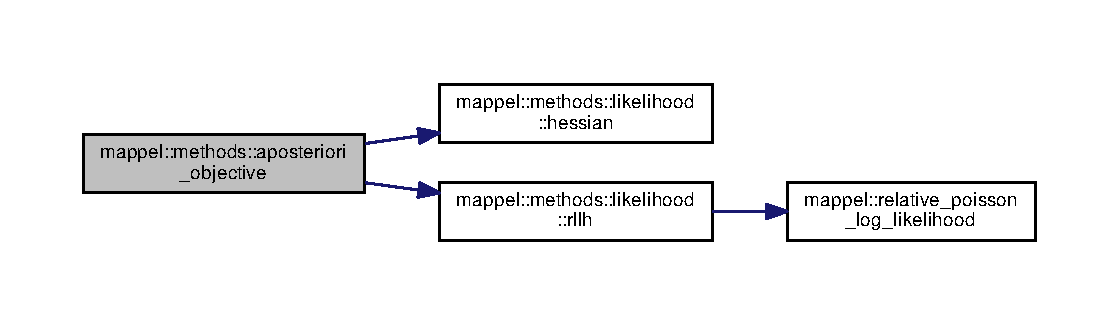
\includegraphics[width=350pt]{namespacemappel_1_1methods_a5227b7c0f1c45c27cbebfcafefcab72b_cgraph}
\end{center}
\end{figure}




Here is the caller graph for this function\+:\nopagebreak
\begin{figure}[H]
\begin{center}
\leavevmode
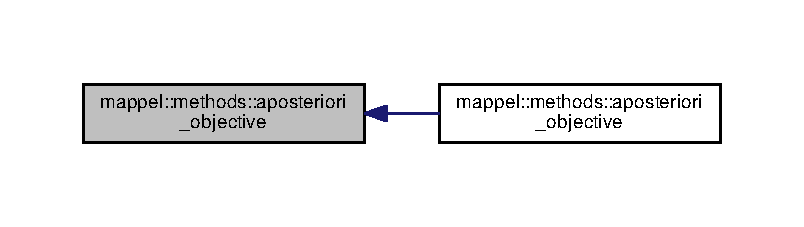
\includegraphics[width=350pt]{namespacemappel_1_1methods_a5227b7c0f1c45c27cbebfcafefcab72b_icgraph}
\end{center}
\end{figure}


\index{mappel\+::methods@{mappel\+::methods}!aposteriori\+\_\+objective@{aposteriori\+\_\+objective}}
\index{aposteriori\+\_\+objective@{aposteriori\+\_\+objective}!mappel\+::methods@{mappel\+::methods}}
\paragraph[{\texorpdfstring{aposteriori\+\_\+objective(const Model \&model, const Model\+Data\+T$<$ Model $>$ \&data\+\_\+im, const Param\+T$<$ Model $>$ \&theta, double \&rllh, Param\+T$<$ Model $>$ \&grad, Mat\+T \&hess)}{aposteriori_objective(const Model &model, const ModelDataT< Model > &data_im, const ParamT< Model > &theta, double &rllh, ParamT< Model > &grad, MatT &hess)}}]{\setlength{\rightskip}{0pt plus 5cm}template$<$class Model $>$ void mappel\+::methods\+::aposteriori\+\_\+objective (
\begin{DoxyParamCaption}
\item[{const Model \&}]{model, }
\item[{const {\bf Model\+DataT}$<$ Model $>$ \&}]{data\+\_\+im, }
\item[{const {\bf ParamT}$<$ Model $>$ \&}]{theta, }
\item[{double \&}]{rllh, }
\item[{{\bf ParamT}$<$ Model $>$ \&}]{grad, }
\item[{{\bf MatT} \&}]{hess}
\end{DoxyParamCaption}
)}\hypertarget{namespacemappel_1_1methods_a3b0e13b783d21c08ba063a210b0a344b}{}\label{namespacemappel_1_1methods_a3b0e13b783d21c08ba063a210b0a344b}


Definition at line 219 of file model\+\_\+methods\+\_\+impl.\+h.



References aposteriori\+\_\+objective(), mappel\+::methods\+::objective\+::grad(), and mappel\+::methods\+::objective\+::rllh().



Here is the call graph for this function\+:\nopagebreak
\begin{figure}[H]
\begin{center}
\leavevmode
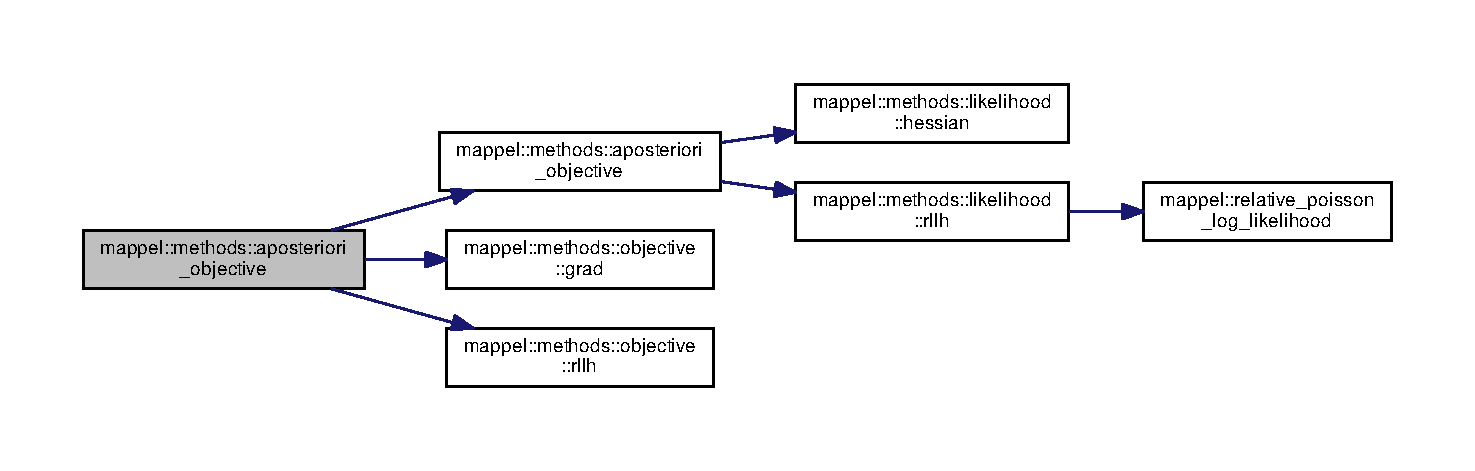
\includegraphics[width=350pt]{namespacemappel_1_1methods_a3b0e13b783d21c08ba063a210b0a344b_cgraph}
\end{center}
\end{figure}


\index{mappel\+::methods@{mappel\+::methods}!cr\+\_\+lower\+\_\+bound@{cr\+\_\+lower\+\_\+bound}}
\index{cr\+\_\+lower\+\_\+bound@{cr\+\_\+lower\+\_\+bound}!mappel\+::methods@{mappel\+::methods}}
\paragraph[{\texorpdfstring{cr\+\_\+lower\+\_\+bound(const Model \&model, const typename Model\+::\+Stencil \&s)}{cr_lower_bound(const Model &model, const typename Model::Stencil &s)}}]{\setlength{\rightskip}{0pt plus 5cm}template$<$class Model $>$ {\bf ParamT}$<$ Model $>$ mappel\+::methods\+::cr\+\_\+lower\+\_\+bound (
\begin{DoxyParamCaption}
\item[{const Model \&}]{model, }
\item[{const typename Model\+::\+Stencil \&}]{s}
\end{DoxyParamCaption}
)}\hypertarget{namespacemappel_1_1methods_ac1fe2927bc882d9a76138010f41df115}{}\label{namespacemappel_1_1methods_ac1fe2927bc882d9a76138010f41df115}


Calculate the Cramer-\/\+Rao lower bound at the given parameters. 


\begin{DoxyParams}[1]{Parameters}
\mbox{\tt in}  & {\em theta} & The parameters to evaluate the C\+R\+LB at \\
\hline
\mbox{\tt out}  & {\em crlb} & The calculated parameters \\
\hline
\end{DoxyParams}


Definition at line 234 of file model\+\_\+methods\+\_\+impl.\+h.



References expected\+\_\+information().



Referenced by cr\+\_\+lower\+\_\+bound(), mappel\+::cr\+\_\+lower\+\_\+bound\+\_\+stack(), and error\+\_\+bounds\+\_\+expected().



Here is the call graph for this function\+:\nopagebreak
\begin{figure}[H]
\begin{center}
\leavevmode
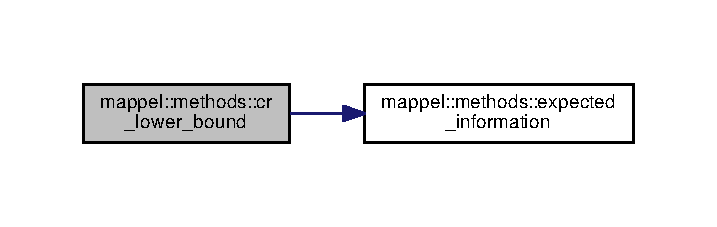
\includegraphics[width=344pt]{namespacemappel_1_1methods_ac1fe2927bc882d9a76138010f41df115_cgraph}
\end{center}
\end{figure}




Here is the caller graph for this function\+:\nopagebreak
\begin{figure}[H]
\begin{center}
\leavevmode
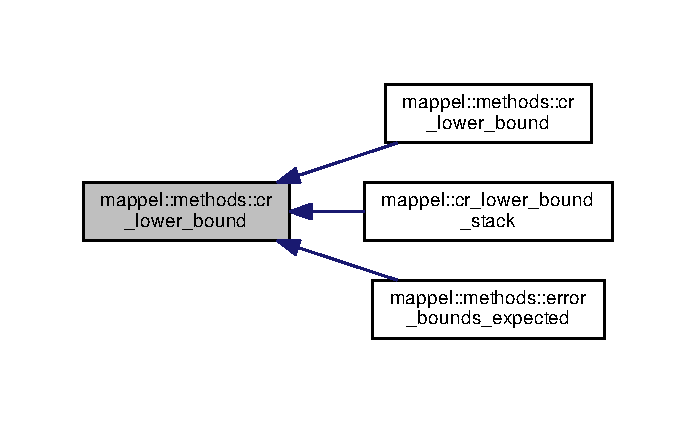
\includegraphics[width=334pt]{namespacemappel_1_1methods_ac1fe2927bc882d9a76138010f41df115_icgraph}
\end{center}
\end{figure}


\index{mappel\+::methods@{mappel\+::methods}!cr\+\_\+lower\+\_\+bound@{cr\+\_\+lower\+\_\+bound}}
\index{cr\+\_\+lower\+\_\+bound@{cr\+\_\+lower\+\_\+bound}!mappel\+::methods@{mappel\+::methods}}
\paragraph[{\texorpdfstring{cr\+\_\+lower\+\_\+bound(const Model \&model, const Param\+T$<$ Model $>$ \&theta)}{cr_lower_bound(const Model &model, const ParamT< Model > &theta)}}]{\setlength{\rightskip}{0pt plus 5cm}template$<$class Model $>$ {\bf ParamT}$<$ Model $>$ mappel\+::methods\+::cr\+\_\+lower\+\_\+bound (
\begin{DoxyParamCaption}
\item[{const Model \&}]{model, }
\item[{const {\bf ParamT}$<$ Model $>$ \&}]{theta}
\end{DoxyParamCaption}
)}\hypertarget{namespacemappel_1_1methods_a30d0f08f37d8f412a2677280cb39c588}{}\label{namespacemappel_1_1methods_a30d0f08f37d8f412a2677280cb39c588}


Definition at line 246 of file model\+\_\+methods\+\_\+impl.\+h.



References cr\+\_\+lower\+\_\+bound().



Here is the call graph for this function\+:\nopagebreak
\begin{figure}[H]
\begin{center}
\leavevmode
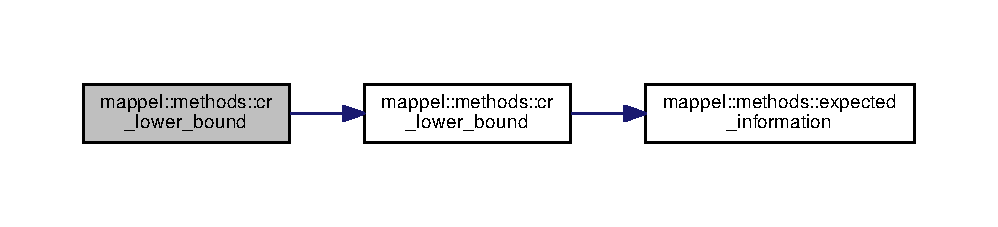
\includegraphics[width=350pt]{namespacemappel_1_1methods_a30d0f08f37d8f412a2677280cb39c588_cgraph}
\end{center}
\end{figure}


\index{mappel\+::methods@{mappel\+::methods}!error\+\_\+bounds\+\_\+expected@{error\+\_\+bounds\+\_\+expected}}
\index{error\+\_\+bounds\+\_\+expected@{error\+\_\+bounds\+\_\+expected}!mappel\+::methods@{mappel\+::methods}}
\paragraph[{\texorpdfstring{error\+\_\+bounds\+\_\+expected(const Model \&model, const Param\+T$<$ Model $>$ \&theta\+\_\+est, double confidence, Param\+T$<$ Model $>$ \&theta\+\_\+lb, Param\+T$<$ Model $>$ \&theta\+\_\+ub)}{error_bounds_expected(const Model &model, const ParamT< Model > &theta_est, double confidence, ParamT< Model > &theta_lb, ParamT< Model > &theta_ub)}}]{\setlength{\rightskip}{0pt plus 5cm}template$<$class Model $>$ void mappel\+::methods\+::error\+\_\+bounds\+\_\+expected (
\begin{DoxyParamCaption}
\item[{const Model \&}]{model, }
\item[{const {\bf ParamT}$<$ Model $>$ \&}]{theta\+\_\+est, }
\item[{double}]{confidence, }
\item[{{\bf ParamT}$<$ Model $>$ \&}]{theta\+\_\+lb, }
\item[{{\bf ParamT}$<$ Model $>$ \&}]{theta\+\_\+ub}
\end{DoxyParamCaption}
)}\hypertarget{namespacemappel_1_1methods_a40f38c9be75ed5bbcc4066a289894ea1}{}\label{namespacemappel_1_1methods_a40f38c9be75ed5bbcc4066a289894ea1}


Definition at line 390 of file model\+\_\+methods\+\_\+impl.\+h.



References cr\+\_\+lower\+\_\+bound(), and mappel\+::normal\+\_\+quantile\+\_\+twosided().



Here is the call graph for this function\+:\nopagebreak
\begin{figure}[H]
\begin{center}
\leavevmode
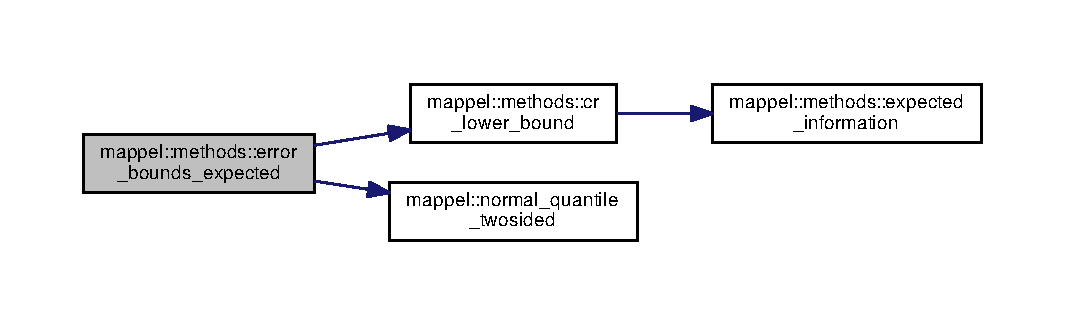
\includegraphics[width=350pt]{namespacemappel_1_1methods_a40f38c9be75ed5bbcc4066a289894ea1_cgraph}
\end{center}
\end{figure}


\index{mappel\+::methods@{mappel\+::methods}!error\+\_\+bounds\+\_\+observed@{error\+\_\+bounds\+\_\+observed}}
\index{error\+\_\+bounds\+\_\+observed@{error\+\_\+bounds\+\_\+observed}!mappel\+::methods@{mappel\+::methods}}
\paragraph[{\texorpdfstring{error\+\_\+bounds\+\_\+observed(const Model \&model, const Param\+T$<$ Model $>$ \&theta\+\_\+est, Mat\+T \&obs\+I, double confidence, Param\+T$<$ Model $>$ \&theta\+\_\+lb, Param\+T$<$ Model $>$ \&theta\+\_\+ub)}{error_bounds_observed(const Model &model, const ParamT< Model > &theta_est, MatT &obsI, double confidence, ParamT< Model > &theta_lb, ParamT< Model > &theta_ub)}}]{\setlength{\rightskip}{0pt plus 5cm}template$<$class Model $>$ void mappel\+::methods\+::error\+\_\+bounds\+\_\+observed (
\begin{DoxyParamCaption}
\item[{const Model \&}]{model, }
\item[{const {\bf ParamT}$<$ Model $>$ \&}]{theta\+\_\+est, }
\item[{{\bf MatT} \&}]{obsI, }
\item[{double}]{confidence, }
\item[{{\bf ParamT}$<$ Model $>$ \&}]{theta\+\_\+lb, }
\item[{{\bf ParamT}$<$ Model $>$ \&}]{theta\+\_\+ub}
\end{DoxyParamCaption}
)}\hypertarget{namespacemappel_1_1methods_afa9582bf7c7354506ba4976a70172ba7}{}\label{namespacemappel_1_1methods_afa9582bf7c7354506ba4976a70172ba7}


Definition at line 401 of file model\+\_\+methods\+\_\+impl.\+h.



References mappel\+::normal\+\_\+quantile\+\_\+twosided().



Here is the call graph for this function\+:\nopagebreak
\begin{figure}[H]
\begin{center}
\leavevmode
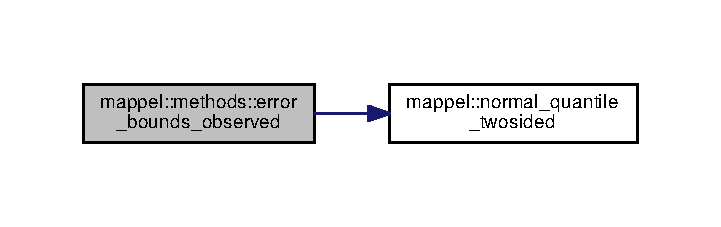
\includegraphics[width=346pt]{namespacemappel_1_1methods_afa9582bf7c7354506ba4976a70172ba7_cgraph}
\end{center}
\end{figure}


\index{mappel\+::methods@{mappel\+::methods}!error\+\_\+bounds\+\_\+posterior\+\_\+credible@{error\+\_\+bounds\+\_\+posterior\+\_\+credible}}
\index{error\+\_\+bounds\+\_\+posterior\+\_\+credible@{error\+\_\+bounds\+\_\+posterior\+\_\+credible}!mappel\+::methods@{mappel\+::methods}}
\paragraph[{\texorpdfstring{error\+\_\+bounds\+\_\+posterior\+\_\+credible(const Model \&model, const Mat\+T \&sample, double confidence, Param\+T$<$ Model $>$ \&theta\+\_\+mean, Param\+T$<$ Model $>$ \&theta\+\_\+lb, Param\+T$<$ Model $>$ \&theta\+\_\+ub)}{error_bounds_posterior_credible(const Model &model, const MatT &sample, double confidence, ParamT< Model > &theta_mean, ParamT< Model > &theta_lb, ParamT< Model > &theta_ub)}}]{\setlength{\rightskip}{0pt plus 5cm}template$<$class Model $>$ void mappel\+::methods\+::error\+\_\+bounds\+\_\+posterior\+\_\+credible (
\begin{DoxyParamCaption}
\item[{const Model \&}]{model, }
\item[{const {\bf MatT} \&}]{sample, }
\item[{double}]{confidence, }
\item[{{\bf ParamT}$<$ Model $>$ \&}]{theta\+\_\+mean, }
\item[{{\bf ParamT}$<$ Model $>$ \&}]{theta\+\_\+lb, }
\item[{{\bf ParamT}$<$ Model $>$ \&}]{theta\+\_\+ub}
\end{DoxyParamCaption}
)}\hypertarget{namespacemappel_1_1methods_a18420d9682150122165a2dfdf43c273a}{}\label{namespacemappel_1_1methods_a18420d9682150122165a2dfdf43c273a}


Definition at line 417 of file model\+\_\+methods\+\_\+impl.\+h.

\index{mappel\+::methods@{mappel\+::methods}!estimate\+\_\+max@{estimate\+\_\+max}}
\index{estimate\+\_\+max@{estimate\+\_\+max}!mappel\+::methods@{mappel\+::methods}}
\paragraph[{\texorpdfstring{estimate\+\_\+max(\+Model \&model, const Model\+Data\+T$<$ Model $>$ \&data, const std\+::string \&method)}{estimate_max(Model &model, const ModelDataT< Model > &data, const std::string &method)}}]{\setlength{\rightskip}{0pt plus 5cm}template$<$class Model $>$ {\bf StencilT}$<$ Model $>$ mappel\+::methods\+::estimate\+\_\+max (
\begin{DoxyParamCaption}
\item[{Model \&}]{model, }
\item[{const {\bf Model\+DataT}$<$ Model $>$ \&}]{data, }
\item[{const std\+::string \&}]{method}
\end{DoxyParamCaption}
)}\hypertarget{namespacemappel_1_1methods_a7f4a5561497c243edaa6f55fddf0ec4e}{}\label{namespacemappel_1_1methods_a7f4a5561497c243edaa6f55fddf0ec4e}


Definition at line 273 of file model\+\_\+methods\+\_\+impl.\+h.



References make\+\_\+estimator().



Referenced by mappel\+::\+Estimator$<$ Model $>$\+::estimate\+\_\+max(), mappel\+::\+Gauss2\+D\+Model\+::initial\+\_\+theta\+\_\+estimate(), and mappel\+::\+Gauss2\+Ds\+Model\+::initial\+\_\+theta\+\_\+estimate().



Here is the call graph for this function\+:\nopagebreak
\begin{figure}[H]
\begin{center}
\leavevmode
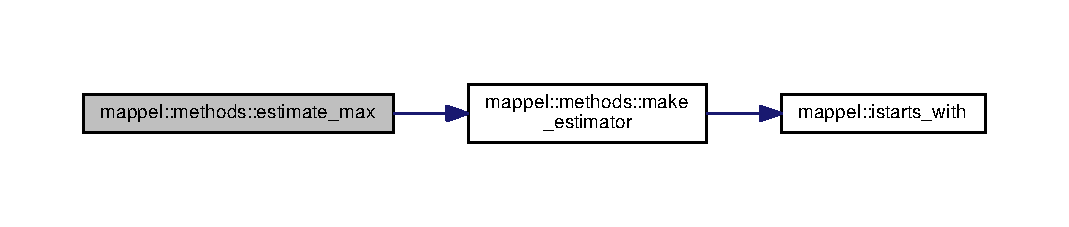
\includegraphics[width=350pt]{namespacemappel_1_1methods_a7f4a5561497c243edaa6f55fddf0ec4e_cgraph}
\end{center}
\end{figure}




Here is the caller graph for this function\+:\nopagebreak
\begin{figure}[H]
\begin{center}
\leavevmode
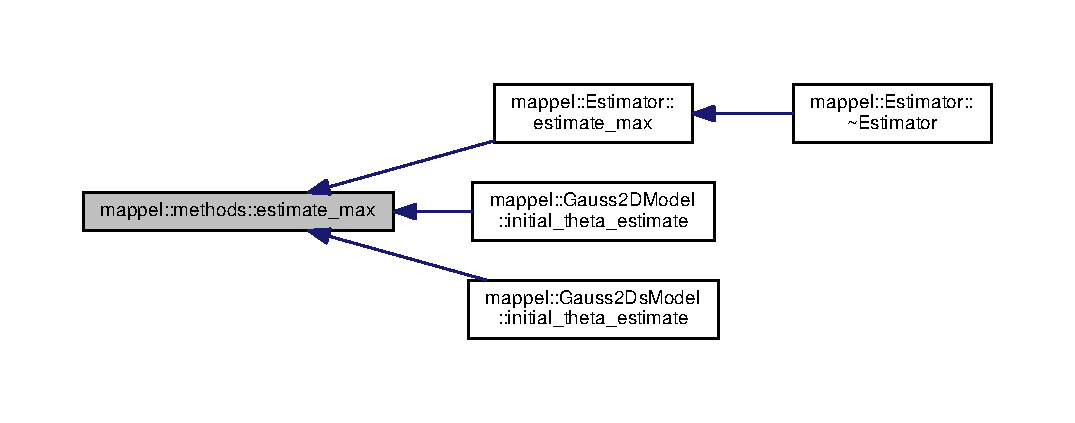
\includegraphics[width=350pt]{namespacemappel_1_1methods_a7f4a5561497c243edaa6f55fddf0ec4e_icgraph}
\end{center}
\end{figure}


\index{mappel\+::methods@{mappel\+::methods}!estimate\+\_\+max@{estimate\+\_\+max}}
\index{estimate\+\_\+max@{estimate\+\_\+max}!mappel\+::methods@{mappel\+::methods}}
\paragraph[{\texorpdfstring{estimate\+\_\+max(\+Model \&model, const Model\+Data\+T$<$ Model $>$ \&data, const std\+::string \&method, const Param\+T$<$ Model $>$ \&theta\+\_\+init, double \&rllh)}{estimate_max(Model &model, const ModelDataT< Model > &data, const std::string &method, const ParamT< Model > &theta_init, double &rllh)}}]{\setlength{\rightskip}{0pt plus 5cm}template$<$class Model $>$ {\bf StencilT}$<$ Model $>$ mappel\+::methods\+::estimate\+\_\+max (
\begin{DoxyParamCaption}
\item[{Model \&}]{model, }
\item[{const {\bf Model\+DataT}$<$ Model $>$ \&}]{data, }
\item[{const std\+::string \&}]{method, }
\item[{const {\bf ParamT}$<$ Model $>$ \&}]{theta\+\_\+init, }
\item[{double \&}]{rllh}
\end{DoxyParamCaption}
)}\hypertarget{namespacemappel_1_1methods_abde9a4b10690b8eefe709d730fac69d9}{}\label{namespacemappel_1_1methods_abde9a4b10690b8eefe709d730fac69d9}


Definition at line 280 of file model\+\_\+methods\+\_\+impl.\+h.



References make\+\_\+estimator().



Here is the call graph for this function\+:\nopagebreak
\begin{figure}[H]
\begin{center}
\leavevmode
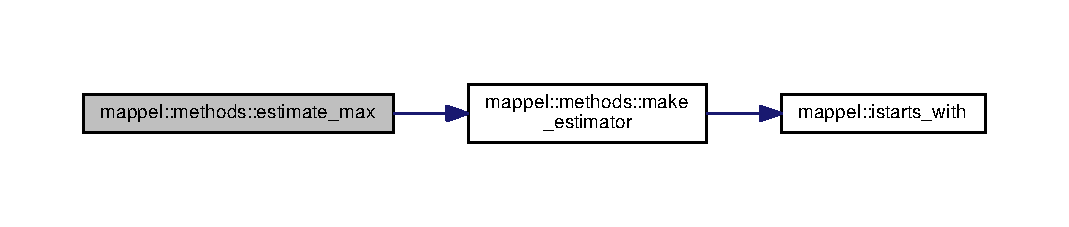
\includegraphics[width=350pt]{namespacemappel_1_1methods_abde9a4b10690b8eefe709d730fac69d9_cgraph}
\end{center}
\end{figure}


\index{mappel\+::methods@{mappel\+::methods}!estimate\+\_\+max@{estimate\+\_\+max}}
\index{estimate\+\_\+max@{estimate\+\_\+max}!mappel\+::methods@{mappel\+::methods}}
\paragraph[{\texorpdfstring{estimate\+\_\+max(\+Model \&model, const Model\+Data\+T$<$ Model $>$ \&data, const std\+::string \&method, Param\+T$<$ Model $>$ \&theta\+\_\+max, double \&theta\+\_\+max\+\_\+llh, Mat\+T \&obs\+I)}{estimate_max(Model &model, const ModelDataT< Model > &data, const std::string &method, ParamT< Model > &theta_max, double &theta_max_llh, MatT &obsI)}}]{\setlength{\rightskip}{0pt plus 5cm}template$<$class Model $>$ void mappel\+::methods\+::estimate\+\_\+max (
\begin{DoxyParamCaption}
\item[{Model \&}]{model, }
\item[{const {\bf Model\+DataT}$<$ Model $>$ \&}]{data, }
\item[{const std\+::string \&}]{method, }
\item[{{\bf ParamT}$<$ Model $>$ \&}]{theta\+\_\+max, }
\item[{double \&}]{theta\+\_\+max\+\_\+llh, }
\item[{{\bf MatT} \&}]{obsI}
\end{DoxyParamCaption}
)}\hypertarget{namespacemappel_1_1methods_a9494d0ddea2acc25bd92100b7587a1c1}{}\label{namespacemappel_1_1methods_a9494d0ddea2acc25bd92100b7587a1c1}


Definition at line 288 of file model\+\_\+methods\+\_\+impl.\+h.



References make\+\_\+estimator().



Here is the call graph for this function\+:\nopagebreak
\begin{figure}[H]
\begin{center}
\leavevmode
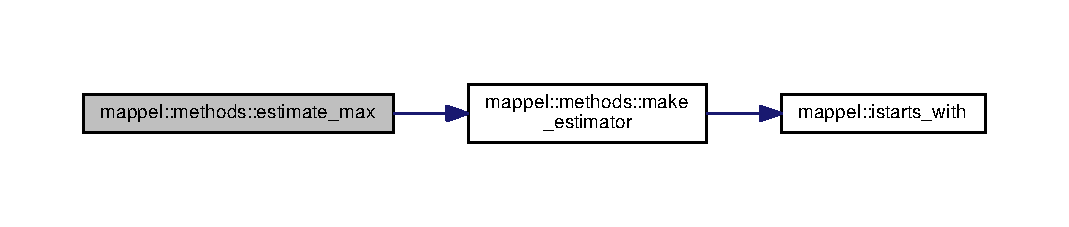
\includegraphics[width=350pt]{namespacemappel_1_1methods_a9494d0ddea2acc25bd92100b7587a1c1_cgraph}
\end{center}
\end{figure}


\index{mappel\+::methods@{mappel\+::methods}!estimate\+\_\+max@{estimate\+\_\+max}}
\index{estimate\+\_\+max@{estimate\+\_\+max}!mappel\+::methods@{mappel\+::methods}}
\paragraph[{\texorpdfstring{estimate\+\_\+max(\+Model \&model, const Model\+Data\+T$<$ Model $>$ \&data, const std\+::string \&method, Param\+T$<$ Model $>$ \&theta\+\_\+max, double \&theta\+\_\+max\+\_\+llh, Mat\+T \&obs\+I, Stats\+T \&stats)}{estimate_max(Model &model, const ModelDataT< Model > &data, const std::string &method, ParamT< Model > &theta_max, double &theta_max_llh, MatT &obsI, StatsT &stats)}}]{\setlength{\rightskip}{0pt plus 5cm}template$<$class Model $>$ void mappel\+::methods\+::estimate\+\_\+max (
\begin{DoxyParamCaption}
\item[{Model \&}]{model, }
\item[{const {\bf Model\+DataT}$<$ Model $>$ \&}]{data, }
\item[{const std\+::string \&}]{method, }
\item[{{\bf ParamT}$<$ Model $>$ \&}]{theta\+\_\+max, }
\item[{double \&}]{theta\+\_\+max\+\_\+llh, }
\item[{{\bf MatT} \&}]{obsI, }
\item[{{\bf StatsT} \&}]{stats}
\end{DoxyParamCaption}
)}\hypertarget{namespacemappel_1_1methods_aee25050c1c9f8cf29d38d8c47d593a3e}{}\label{namespacemappel_1_1methods_aee25050c1c9f8cf29d38d8c47d593a3e}


Definition at line 296 of file model\+\_\+methods\+\_\+impl.\+h.



References make\+\_\+estimator().



Here is the call graph for this function\+:\nopagebreak
\begin{figure}[H]
\begin{center}
\leavevmode
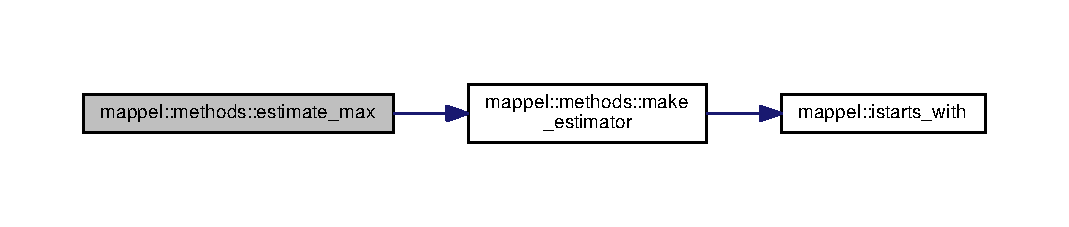
\includegraphics[width=350pt]{namespacemappel_1_1methods_aee25050c1c9f8cf29d38d8c47d593a3e_cgraph}
\end{center}
\end{figure}


\index{mappel\+::methods@{mappel\+::methods}!estimate\+\_\+max@{estimate\+\_\+max}}
\index{estimate\+\_\+max@{estimate\+\_\+max}!mappel\+::methods@{mappel\+::methods}}
\paragraph[{\texorpdfstring{estimate\+\_\+max(\+Model \&model, const Model\+Data\+T$<$ Model $>$ \&data, const std\+::string \&method, const Param\+T$<$ Model $>$ \&theta\+\_\+init, Param\+T$<$ Model $>$ \&theta\+\_\+max, double \&theta\+\_\+max\+\_\+llh, Mat\+T \&obs\+I)}{estimate_max(Model &model, const ModelDataT< Model > &data, const std::string &method, const ParamT< Model > &theta_init, ParamT< Model > &theta_max, double &theta_max_llh, MatT &obsI)}}]{\setlength{\rightskip}{0pt plus 5cm}template$<$class Model $>$ void mappel\+::methods\+::estimate\+\_\+max (
\begin{DoxyParamCaption}
\item[{Model \&}]{model, }
\item[{const {\bf Model\+DataT}$<$ Model $>$ \&}]{data, }
\item[{const std\+::string \&}]{method, }
\item[{const {\bf ParamT}$<$ Model $>$ \&}]{theta\+\_\+init, }
\item[{{\bf ParamT}$<$ Model $>$ \&}]{theta\+\_\+max, }
\item[{double \&}]{theta\+\_\+max\+\_\+llh, }
\item[{{\bf MatT} \&}]{obsI}
\end{DoxyParamCaption}
)}\hypertarget{namespacemappel_1_1methods_a8db06e0816204cdca735bdf498e2bae2}{}\label{namespacemappel_1_1methods_a8db06e0816204cdca735bdf498e2bae2}


Definition at line 305 of file model\+\_\+methods\+\_\+impl.\+h.



References make\+\_\+estimator().



Here is the call graph for this function\+:\nopagebreak
\begin{figure}[H]
\begin{center}
\leavevmode
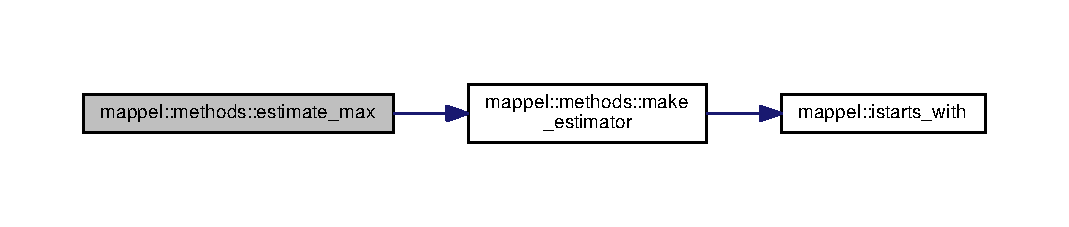
\includegraphics[width=350pt]{namespacemappel_1_1methods_a8db06e0816204cdca735bdf498e2bae2_cgraph}
\end{center}
\end{figure}


\index{mappel\+::methods@{mappel\+::methods}!estimate\+\_\+max@{estimate\+\_\+max}}
\index{estimate\+\_\+max@{estimate\+\_\+max}!mappel\+::methods@{mappel\+::methods}}
\paragraph[{\texorpdfstring{estimate\+\_\+max(\+Model \&model, const Model\+Data\+T$<$ Model $>$ \&data, const std\+::string \&method, const Param\+T$<$ Model $>$ \&theta\+\_\+init, Param\+T$<$ Model $>$ \&theta\+\_\+max, double \&theta\+\_\+max\+\_\+llh, Mat\+T \&obs\+I, Stats\+T \&stats)}{estimate_max(Model &model, const ModelDataT< Model > &data, const std::string &method, const ParamT< Model > &theta_init, ParamT< Model > &theta_max, double &theta_max_llh, MatT &obsI, StatsT &stats)}}]{\setlength{\rightskip}{0pt plus 5cm}template$<$class Model $>$ void mappel\+::methods\+::estimate\+\_\+max (
\begin{DoxyParamCaption}
\item[{Model \&}]{model, }
\item[{const {\bf Model\+DataT}$<$ Model $>$ \&}]{data, }
\item[{const std\+::string \&}]{method, }
\item[{const {\bf ParamT}$<$ Model $>$ \&}]{theta\+\_\+init, }
\item[{{\bf ParamT}$<$ Model $>$ \&}]{theta\+\_\+max, }
\item[{double \&}]{theta\+\_\+max\+\_\+llh, }
\item[{{\bf MatT} \&}]{obsI, }
\item[{{\bf StatsT} \&}]{stats}
\end{DoxyParamCaption}
)}\hypertarget{namespacemappel_1_1methods_a336e74435f33240ea8251bfc21dbe279}{}\label{namespacemappel_1_1methods_a336e74435f33240ea8251bfc21dbe279}


Definition at line 313 of file model\+\_\+methods\+\_\+impl.\+h.



References make\+\_\+estimator().



Here is the call graph for this function\+:\nopagebreak
\begin{figure}[H]
\begin{center}
\leavevmode
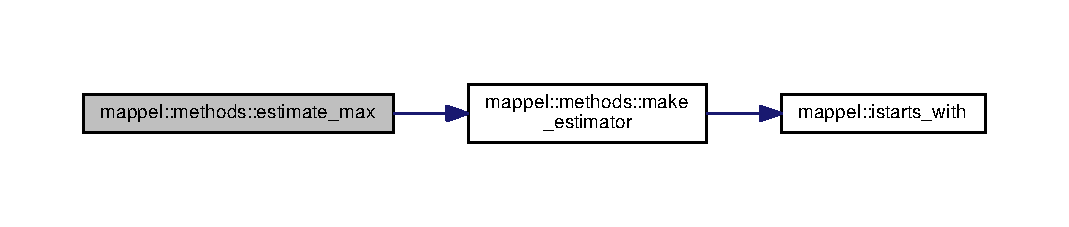
\includegraphics[width=350pt]{namespacemappel_1_1methods_a336e74435f33240ea8251bfc21dbe279_cgraph}
\end{center}
\end{figure}


\index{mappel\+::methods@{mappel\+::methods}!estimate\+\_\+mcmc\+\_\+posterior@{estimate\+\_\+mcmc\+\_\+posterior}}
\index{estimate\+\_\+mcmc\+\_\+posterior@{estimate\+\_\+mcmc\+\_\+posterior}!mappel\+::methods@{mappel\+::methods}}
\paragraph[{\texorpdfstring{estimate\+\_\+mcmc\+\_\+posterior(\+Model \&model, const Model\+Data\+T$<$ Model $>$ \&data, Idx\+T Nsample, Idx\+T Nburnin, Idx\+T thin, Param\+T$<$ Model $>$ \&posterior\+\_\+mean, Mat\+T \&posterior\+\_\+cov)}{estimate_mcmc_posterior(Model &model, const ModelDataT< Model > &data, IdxT Nsample, IdxT Nburnin, IdxT thin, ParamT< Model > &posterior_mean, MatT &posterior_cov)}}]{\setlength{\rightskip}{0pt plus 5cm}template$<$class Model $>$ void mappel\+::methods\+::estimate\+\_\+mcmc\+\_\+posterior (
\begin{DoxyParamCaption}
\item[{Model \&}]{model, }
\item[{const {\bf Model\+DataT}$<$ Model $>$ \&}]{data, }
\item[{{\bf IdxT}}]{Nsample, }
\item[{{\bf IdxT}}]{Nburnin, }
\item[{{\bf IdxT}}]{thin, }
\item[{{\bf ParamT}$<$ Model $>$ \&}]{posterior\+\_\+mean, }
\item[{{\bf MatT} \&}]{posterior\+\_\+cov}
\end{DoxyParamCaption}
)}\hypertarget{namespacemappel_1_1methods_a224995eff4bf3ee7652f2ed9116d8cf7}{}\label{namespacemappel_1_1methods_a224995eff4bf3ee7652f2ed9116d8cf7}


Definition at line 373 of file model\+\_\+methods\+\_\+impl.\+h.



Referenced by estimate\+\_\+mcmc\+\_\+posterior().



Here is the caller graph for this function\+:\nopagebreak
\begin{figure}[H]
\begin{center}
\leavevmode
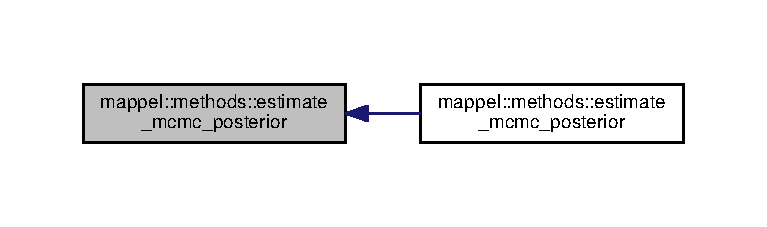
\includegraphics[width=350pt]{namespacemappel_1_1methods_a224995eff4bf3ee7652f2ed9116d8cf7_icgraph}
\end{center}
\end{figure}


\index{mappel\+::methods@{mappel\+::methods}!estimate\+\_\+mcmc\+\_\+posterior@{estimate\+\_\+mcmc\+\_\+posterior}}
\index{estimate\+\_\+mcmc\+\_\+posterior@{estimate\+\_\+mcmc\+\_\+posterior}!mappel\+::methods@{mappel\+::methods}}
\paragraph[{\texorpdfstring{estimate\+\_\+mcmc\+\_\+posterior(\+Model \&model, const Model\+Data\+T$<$ Model $>$ \&data, const Param\+T$<$ Model $>$ \&theta\+\_\+init, Idx\+T Nsample, Idx\+T Nburnin, Idx\+T thin, Param\+T$<$ Model $>$ \&posterior\+\_\+mean, Mat\+T \&posterior\+\_\+cov)}{estimate_mcmc_posterior(Model &model, const ModelDataT< Model > &data, const ParamT< Model > &theta_init, IdxT Nsample, IdxT Nburnin, IdxT thin, ParamT< Model > &posterior_mean, MatT &posterior_cov)}}]{\setlength{\rightskip}{0pt plus 5cm}template$<$class Model $>$ void mappel\+::methods\+::estimate\+\_\+mcmc\+\_\+posterior (
\begin{DoxyParamCaption}
\item[{Model \&}]{model, }
\item[{const {\bf Model\+DataT}$<$ Model $>$ \&}]{data, }
\item[{const {\bf ParamT}$<$ Model $>$ \&}]{theta\+\_\+init, }
\item[{{\bf IdxT}}]{Nsample, }
\item[{{\bf IdxT}}]{Nburnin, }
\item[{{\bf IdxT}}]{thin, }
\item[{{\bf ParamT}$<$ Model $>$ \&}]{posterior\+\_\+mean, }
\item[{{\bf MatT} \&}]{posterior\+\_\+cov}
\end{DoxyParamCaption}
)}\hypertarget{namespacemappel_1_1methods_ab616d99318131c7f70f49581d9c9d77a}{}\label{namespacemappel_1_1methods_ab616d99318131c7f70f49581d9c9d77a}


Definition at line 381 of file model\+\_\+methods\+\_\+impl.\+h.



References estimate\+\_\+mcmc\+\_\+posterior(), and mappel\+::mcmc\+::estimate\+\_\+sample\+\_\+posterior().



Here is the call graph for this function\+:\nopagebreak
\begin{figure}[H]
\begin{center}
\leavevmode
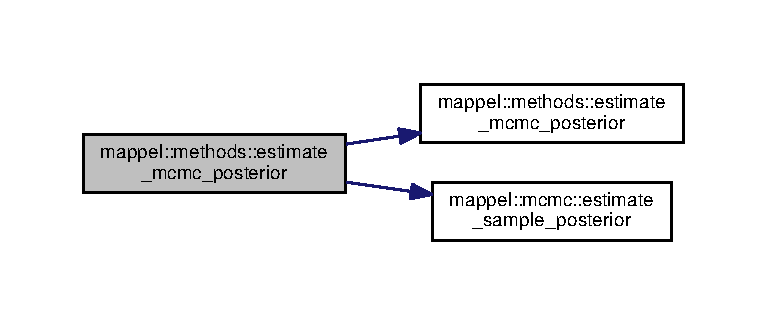
\includegraphics[width=350pt]{namespacemappel_1_1methods_ab616d99318131c7f70f49581d9c9d77a_cgraph}
\end{center}
\end{figure}


\index{mappel\+::methods@{mappel\+::methods}!estimate\+\_\+mcmc\+\_\+sample@{estimate\+\_\+mcmc\+\_\+sample}}
\index{estimate\+\_\+mcmc\+\_\+sample@{estimate\+\_\+mcmc\+\_\+sample}!mappel\+::methods@{mappel\+::methods}}
\paragraph[{\texorpdfstring{estimate\+\_\+mcmc\+\_\+sample(\+Model \&model, const Model\+Data\+T$<$ Model $>$ \&data, Idx\+T Nsample=1000, Idx\+T Nburnin=100, Idx\+T thin=0)}{estimate_mcmc_sample(Model &model, const ModelDataT< Model > &data, IdxT Nsample=1000, IdxT Nburnin=100, IdxT thin=0)}}]{\setlength{\rightskip}{0pt plus 5cm}template$<$class Model $>$ {\bf MatT} mappel\+::methods\+::estimate\+\_\+mcmc\+\_\+sample (
\begin{DoxyParamCaption}
\item[{Model \&}]{model, }
\item[{const {\bf Model\+DataT}$<$ Model $>$ \&}]{data, }
\item[{{\bf IdxT}}]{Nsample = {\ttfamily 1000}, }
\item[{{\bf IdxT}}]{Nburnin = {\ttfamily 100}, }
\item[{{\bf IdxT}}]{thin = {\ttfamily 0}}
\end{DoxyParamCaption}
)}\hypertarget{namespacemappel_1_1methods_a8bec3dcf3172f17383eb5f6693e7e956}{}\label{namespacemappel_1_1methods_a8bec3dcf3172f17383eb5f6693e7e956}


Definition at line 336 of file model\+\_\+methods\+\_\+impl.\+h.

\index{mappel\+::methods@{mappel\+::methods}!estimate\+\_\+mcmc\+\_\+sample@{estimate\+\_\+mcmc\+\_\+sample}}
\index{estimate\+\_\+mcmc\+\_\+sample@{estimate\+\_\+mcmc\+\_\+sample}!mappel\+::methods@{mappel\+::methods}}
\paragraph[{\texorpdfstring{estimate\+\_\+mcmc\+\_\+sample(\+Model \&model, const Model\+Data\+T$<$ Model $>$ \&data, const Param\+T$<$ Model $>$ \&theta\+\_\+init, Idx\+T Nsample=1000, Idx\+T Nburnin=100, Idx\+T thin=0)}{estimate_mcmc_sample(Model &model, const ModelDataT< Model > &data, const ParamT< Model > &theta_init, IdxT Nsample=1000, IdxT Nburnin=100, IdxT thin=0)}}]{\setlength{\rightskip}{0pt plus 5cm}template$<$class Model $>$ {\bf MatT} mappel\+::methods\+::estimate\+\_\+mcmc\+\_\+sample (
\begin{DoxyParamCaption}
\item[{Model \&}]{model, }
\item[{const {\bf Model\+DataT}$<$ Model $>$ \&}]{data, }
\item[{const {\bf ParamT}$<$ Model $>$ \&}]{theta\+\_\+init, }
\item[{{\bf IdxT}}]{Nsample = {\ttfamily 1000}, }
\item[{{\bf IdxT}}]{Nburnin = {\ttfamily 100}, }
\item[{{\bf IdxT}}]{thin = {\ttfamily 0}}
\end{DoxyParamCaption}
)}\hypertarget{namespacemappel_1_1methods_abf7481af94ebff828622ec6b38a271ee}{}\label{namespacemappel_1_1methods_abf7481af94ebff828622ec6b38a271ee}


Definition at line 343 of file model\+\_\+methods\+\_\+impl.\+h.



References mappel\+::mcmc\+::num\+\_\+oversample(), mappel\+::mcmc\+::sample\+\_\+posterior(), and mappel\+::mcmc\+::thin\+\_\+sample().



Here is the call graph for this function\+:\nopagebreak
\begin{figure}[H]
\begin{center}
\leavevmode
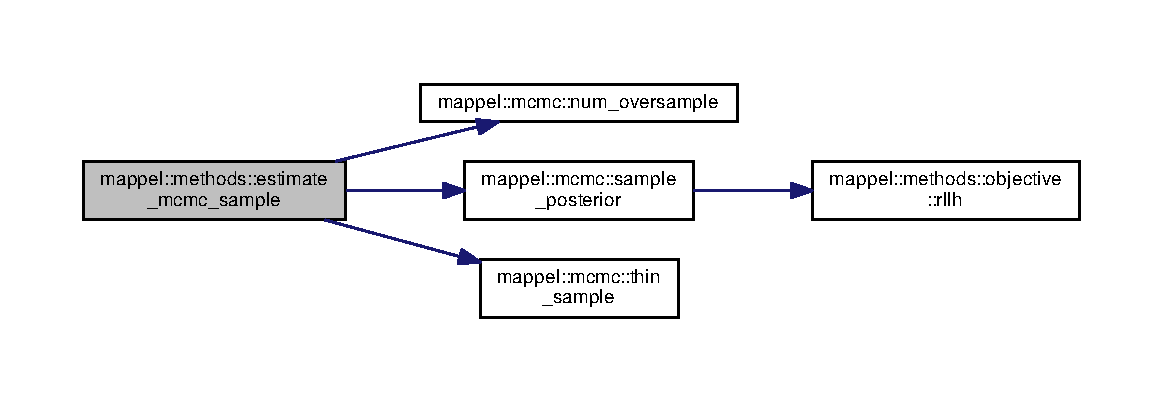
\includegraphics[width=350pt]{namespacemappel_1_1methods_abf7481af94ebff828622ec6b38a271ee_cgraph}
\end{center}
\end{figure}


\index{mappel\+::methods@{mappel\+::methods}!estimate\+\_\+mcmc\+\_\+sample@{estimate\+\_\+mcmc\+\_\+sample}}
\index{estimate\+\_\+mcmc\+\_\+sample@{estimate\+\_\+mcmc\+\_\+sample}!mappel\+::methods@{mappel\+::methods}}
\paragraph[{\texorpdfstring{estimate\+\_\+mcmc\+\_\+sample(\+Model \&model, const Model\+Data\+T$<$ Model $>$ \&data, const Param\+T$<$ Model $>$ \&theta\+\_\+init, Idx\+T Nsample, Idx\+T Nburnin, Idx\+T thin, Mat\+T \&sample, Vec\+T \&sample\+\_\+rllh)}{estimate_mcmc_sample(Model &model, const ModelDataT< Model > &data, const ParamT< Model > &theta_init, IdxT Nsample, IdxT Nburnin, IdxT thin, MatT &sample, VecT &sample_rllh)}}]{\setlength{\rightskip}{0pt plus 5cm}template$<$class Model $>$ void mappel\+::methods\+::estimate\+\_\+mcmc\+\_\+sample (
\begin{DoxyParamCaption}
\item[{Model \&}]{model, }
\item[{const {\bf Model\+DataT}$<$ Model $>$ \&}]{data, }
\item[{const {\bf ParamT}$<$ Model $>$ \&}]{theta\+\_\+init, }
\item[{{\bf IdxT}}]{Nsample, }
\item[{{\bf IdxT}}]{Nburnin, }
\item[{{\bf IdxT}}]{thin, }
\item[{{\bf MatT} \&}]{sample, }
\item[{{\bf VecT} \&}]{sample\+\_\+rllh}
\end{DoxyParamCaption}
)}\hypertarget{namespacemappel_1_1methods_a5b0c8018510cec5dec285ea4cad912c5}{}\label{namespacemappel_1_1methods_a5b0c8018510cec5dec285ea4cad912c5}


Definition at line 356 of file model\+\_\+methods\+\_\+impl.\+h.



References mappel\+::mcmc\+::num\+\_\+oversample(), mappel\+::mcmc\+::sample\+\_\+posterior(), and mappel\+::mcmc\+::thin\+\_\+sample().



Here is the call graph for this function\+:\nopagebreak
\begin{figure}[H]
\begin{center}
\leavevmode
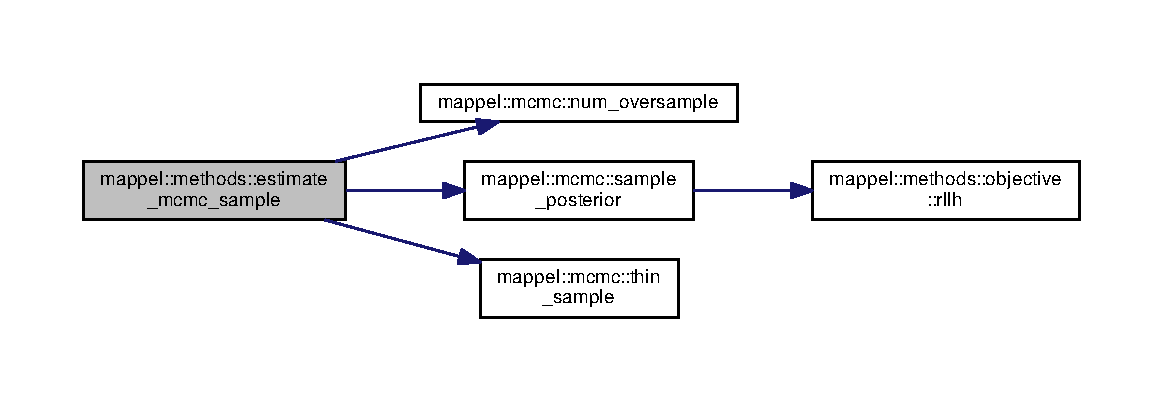
\includegraphics[width=350pt]{namespacemappel_1_1methods_a5b0c8018510cec5dec285ea4cad912c5_cgraph}
\end{center}
\end{figure}


\index{mappel\+::methods@{mappel\+::methods}!expected\+\_\+information@{expected\+\_\+information}}
\index{expected\+\_\+information@{expected\+\_\+information}!mappel\+::methods@{mappel\+::methods}}
\paragraph[{\texorpdfstring{expected\+\_\+information(const Model \&model, const Stencil\+T$<$ Model $>$ \&s)}{expected_information(const Model &model, const StencilT< Model > &s)}}]{\setlength{\rightskip}{0pt plus 5cm}template$<$class Model $>$ {\bf Return\+If\+SubclassT}$<${\bf MatT}, Model, {\bf Poisson\+Noise1\+D\+Objective}$>$ mappel\+::methods\+::expected\+\_\+information (
\begin{DoxyParamCaption}
\item[{const Model \&}]{model, }
\item[{const {\bf StencilT}$<$ Model $>$ \&}]{s}
\end{DoxyParamCaption}
)}\hypertarget{namespacemappel_1_1methods_a07072e1c0c19cbffa6878362056f5758}{}\label{namespacemappel_1_1methods_a07072e1c0c19cbffa6878362056f5758}


Compute the expected information (Fisher information at theta). Note\+: Expected information is an average quantity and is independent of the data. Enabled for \hyperlink{classmappel_1_1PoissonNoise1DObjective}{Poisson\+Noise1\+D\+Objective}. 


\begin{DoxyParams}{Parameters}
{\em model} & \hyperlink{classmappel_1_1PointEmitterModel}{Point\+Emitter\+Model} \\
\hline
{\em s} & Stencil at desired theta \\
\hline
\end{DoxyParams}
\begin{DoxyReturn}{Returns}
The fisher information matrix as an symmetric matrix in upper-\/triangular format 
\end{DoxyReturn}


Definition at line 77 of file Poisson\+Noise1\+D\+Objective.\+h.

\index{mappel\+::methods@{mappel\+::methods}!expected\+\_\+information@{expected\+\_\+information}}
\index{expected\+\_\+information@{expected\+\_\+information}!mappel\+::methods@{mappel\+::methods}}
\paragraph[{\texorpdfstring{expected\+\_\+information(const Model \&model, const Stencil\+T$<$ Model $>$ \&s)}{expected_information(const Model &model, const StencilT< Model > &s)}}]{\setlength{\rightskip}{0pt plus 5cm}template$<$class Model $>$ {\bf Return\+If\+SubclassT}$<${\bf MatT}, Model, {\bf Poisson\+Noise2\+D\+Objective}$>$ mappel\+::methods\+::expected\+\_\+information (
\begin{DoxyParamCaption}
\item[{const Model \&}]{model, }
\item[{const {\bf StencilT}$<$ Model $>$ \&}]{s}
\end{DoxyParamCaption}
)}\hypertarget{namespacemappel_1_1methods_abc7bb2a867d157f3adbb71abdd3680d2}{}\label{namespacemappel_1_1methods_abc7bb2a867d157f3adbb71abdd3680d2}


Compute the expected information (Fisher information at theta). Note\+: Expected information is an average quantity and is independent of the data. Enabled for \hyperlink{classmappel_1_1PoissonNoise2DObjective}{Poisson\+Noise2\+D\+Objective}. 


\begin{DoxyParams}{Parameters}
{\em model} & Po\+Image\+Coord\+T\+Emitter\+Model \\
\hline
{\em s} & Stencil at desired theta \\
\hline
\end{DoxyParams}
\begin{DoxyReturn}{Returns}
The fisher information matrix as an symmetric matrix in upper-\/triangular format 
\end{DoxyReturn}


Definition at line 83 of file Poisson\+Noise2\+D\+Objective.\+h.



References mappel\+::\+Image\+Format2\+D\+Base\+::size.

\index{mappel\+::methods@{mappel\+::methods}!expected\+\_\+information@{expected\+\_\+information}}
\index{expected\+\_\+information@{expected\+\_\+information}!mappel\+::methods@{mappel\+::methods}}
\paragraph[{\texorpdfstring{expected\+\_\+information(const Model \&model, const Param\+T$<$ Model $>$ \&theta)}{expected_information(const Model &model, const ParamT< Model > &theta)}}]{\setlength{\rightskip}{0pt plus 5cm}template$<$class Model $>$ {\bf MatT} mappel\+::methods\+::expected\+\_\+information (
\begin{DoxyParamCaption}
\item[{const Model \&}]{model, }
\item[{const {\bf ParamT}$<$ Model $>$ \&}]{theta}
\end{DoxyParamCaption}
)}\hypertarget{namespacemappel_1_1methods_a6632adc36d8b32fd8d198669e268c767}{}\label{namespacemappel_1_1methods_a6632adc36d8b32fd8d198669e268c767}


Definition at line 252 of file model\+\_\+methods\+\_\+impl.\+h.



Referenced by cr\+\_\+lower\+\_\+bound().



Here is the caller graph for this function\+:\nopagebreak
\begin{figure}[H]
\begin{center}
\leavevmode
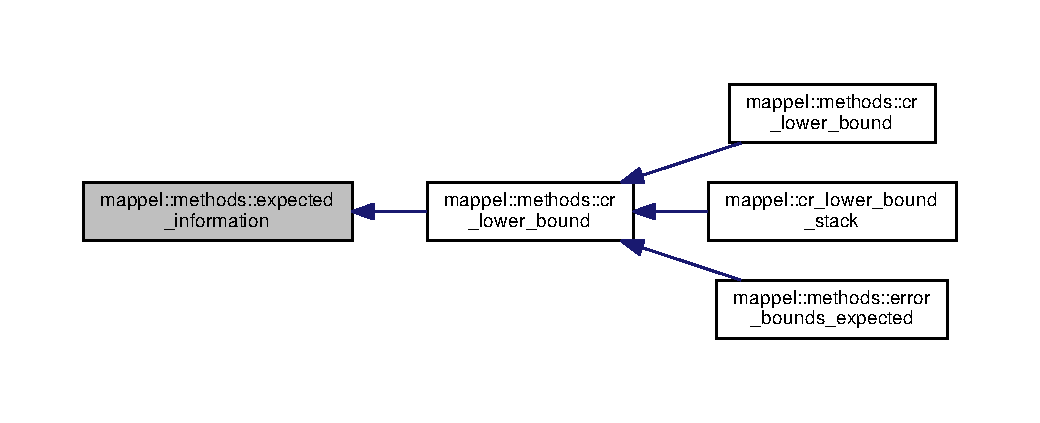
\includegraphics[width=350pt]{namespacemappel_1_1methods_a6632adc36d8b32fd8d198669e268c767_icgraph}
\end{center}
\end{figure}


\index{mappel\+::methods@{mappel\+::methods}!likelihood\+\_\+objective@{likelihood\+\_\+objective}}
\index{likelihood\+\_\+objective@{likelihood\+\_\+objective}!mappel\+::methods@{mappel\+::methods}}
\paragraph[{\texorpdfstring{likelihood\+\_\+objective(const Model \&model, const Model\+Data\+T$<$ Model $>$ \&data\+\_\+im, const Stencil\+T$<$ Model $>$ \&s, double \&rllh, Param\+T$<$ Model $>$ \&grad, Mat\+T \&hess)}{likelihood_objective(const Model &model, const ModelDataT< Model > &data_im, const StencilT< Model > &s, double &rllh, ParamT< Model > &grad, MatT &hess)}}]{\setlength{\rightskip}{0pt plus 5cm}template$<$class Model $>$ void mappel\+::methods\+::likelihood\+\_\+objective (
\begin{DoxyParamCaption}
\item[{const Model \&}]{model, }
\item[{const {\bf Model\+DataT}$<$ Model $>$ \&}]{data\+\_\+im, }
\item[{const {\bf StencilT}$<$ Model $>$ \&}]{s, }
\item[{double \&}]{rllh, }
\item[{{\bf ParamT}$<$ Model $>$ \&}]{grad, }
\item[{{\bf MatT} \&}]{hess}
\end{DoxyParamCaption}
)}\hypertarget{namespacemappel_1_1methods_a82eaea0b938b0daff819da153e1351e2}{}\label{namespacemappel_1_1methods_a82eaea0b938b0daff819da153e1351e2}


Definition at line 210 of file model\+\_\+methods\+\_\+impl.\+h.



References mappel\+::methods\+::likelihood\+::hessian(), and mappel\+::methods\+::likelihood\+::rllh().



Referenced by likelihood\+\_\+objective().



Here is the call graph for this function\+:\nopagebreak
\begin{figure}[H]
\begin{center}
\leavevmode
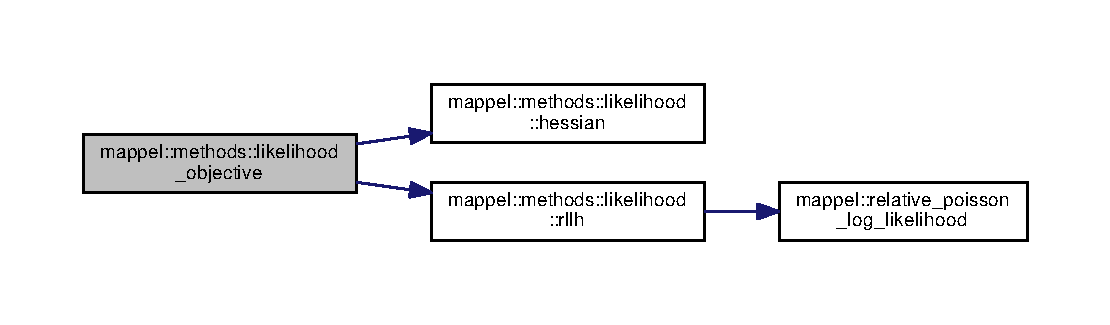
\includegraphics[width=350pt]{namespacemappel_1_1methods_a82eaea0b938b0daff819da153e1351e2_cgraph}
\end{center}
\end{figure}




Here is the caller graph for this function\+:\nopagebreak
\begin{figure}[H]
\begin{center}
\leavevmode
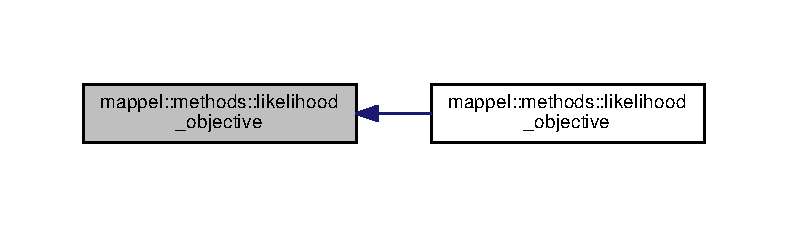
\includegraphics[width=350pt]{namespacemappel_1_1methods_a82eaea0b938b0daff819da153e1351e2_icgraph}
\end{center}
\end{figure}


\index{mappel\+::methods@{mappel\+::methods}!likelihood\+\_\+objective@{likelihood\+\_\+objective}}
\index{likelihood\+\_\+objective@{likelihood\+\_\+objective}!mappel\+::methods@{mappel\+::methods}}
\paragraph[{\texorpdfstring{likelihood\+\_\+objective(const Model \&model, const Model\+Data\+T$<$ Model $>$ \&data\+\_\+im, const Param\+T$<$ Model $>$ \&theta, double \&rllh, Param\+T$<$ Model $>$ \&grad, Mat\+T \&hess)}{likelihood_objective(const Model &model, const ModelDataT< Model > &data_im, const ParamT< Model > &theta, double &rllh, ParamT< Model > &grad, MatT &hess)}}]{\setlength{\rightskip}{0pt plus 5cm}template$<$class Model $>$ void mappel\+::methods\+::likelihood\+\_\+objective (
\begin{DoxyParamCaption}
\item[{const Model \&}]{model, }
\item[{const {\bf Model\+DataT}$<$ Model $>$ \&}]{data\+\_\+im, }
\item[{const {\bf ParamT}$<$ Model $>$ \&}]{theta, }
\item[{double \&}]{rllh, }
\item[{{\bf ParamT}$<$ Model $>$ \&}]{grad, }
\item[{{\bf MatT} \&}]{hess}
\end{DoxyParamCaption}
)}\hypertarget{namespacemappel_1_1methods_a496d45e1db23f89b54ae0bef016a19b0}{}\label{namespacemappel_1_1methods_a496d45e1db23f89b54ae0bef016a19b0}


Definition at line 227 of file model\+\_\+methods\+\_\+impl.\+h.



References mappel\+::methods\+::objective\+::grad(), likelihood\+\_\+objective(), and mappel\+::methods\+::objective\+::rllh().



Here is the call graph for this function\+:\nopagebreak
\begin{figure}[H]
\begin{center}
\leavevmode
\includegraphics[width=350pt]{namespacemappel_1_1methods_a496d45e1db23f89b54ae0bef016a19b0_cgraph}
\end{center}
\end{figure}


\index{mappel\+::methods@{mappel\+::methods}!make\+\_\+estimator@{make\+\_\+estimator}}
\index{make\+\_\+estimator@{make\+\_\+estimator}!mappel\+::methods@{mappel\+::methods}}
\paragraph[{\texorpdfstring{make\+\_\+estimator(\+Model \&model, std\+::string ename)}{make_estimator(Model &model, std::string ename)}}]{\setlength{\rightskip}{0pt plus 5cm}template$<$class Model $>$ {\bf Return\+If\+SubclassT}$<$std\+::unique\+\_\+ptr$<${\bf Estimator}$<$Model$>$ $>$, Model, {\bf Poisson\+Noise1\+D\+Objective}$>$ mappel\+::methods\+::make\+\_\+estimator (
\begin{DoxyParamCaption}
\item[{Model \&}]{model, }
\item[{std\+::string}]{ename}
\end{DoxyParamCaption}
)}\hypertarget{namespacemappel_1_1methods_a0f47a66f366b6e5841f1224e839ed828}{}\label{namespacemappel_1_1methods_a0f47a66f366b6e5841f1224e839ed828}


Definition at line 95 of file Poisson\+Noise1\+D\+Objective.\+h.



References mappel\+::istarts\+\_\+with().



Referenced by estimate\+\_\+max(), mappel\+::methods\+::debug\+::estimate\+\_\+max\+\_\+debug(), mappel\+::methods\+::openmp\+::estimate\+\_\+max\+\_\+stack(), and mappel\+::methods\+::openmp\+::estimate\+\_\+profile\+\_\+likelihood().



Here is the call graph for this function\+:\nopagebreak
\begin{figure}[H]
\begin{center}
\leavevmode
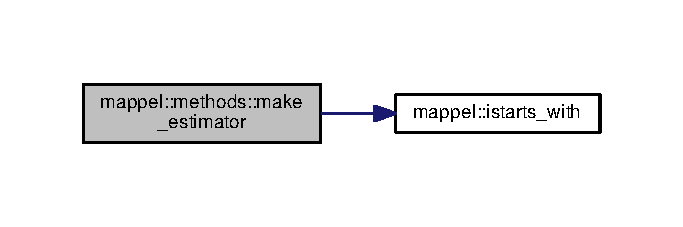
\includegraphics[width=328pt]{namespacemappel_1_1methods_a0f47a66f366b6e5841f1224e839ed828_cgraph}
\end{center}
\end{figure}




Here is the caller graph for this function\+:\nopagebreak
\begin{figure}[H]
\begin{center}
\leavevmode
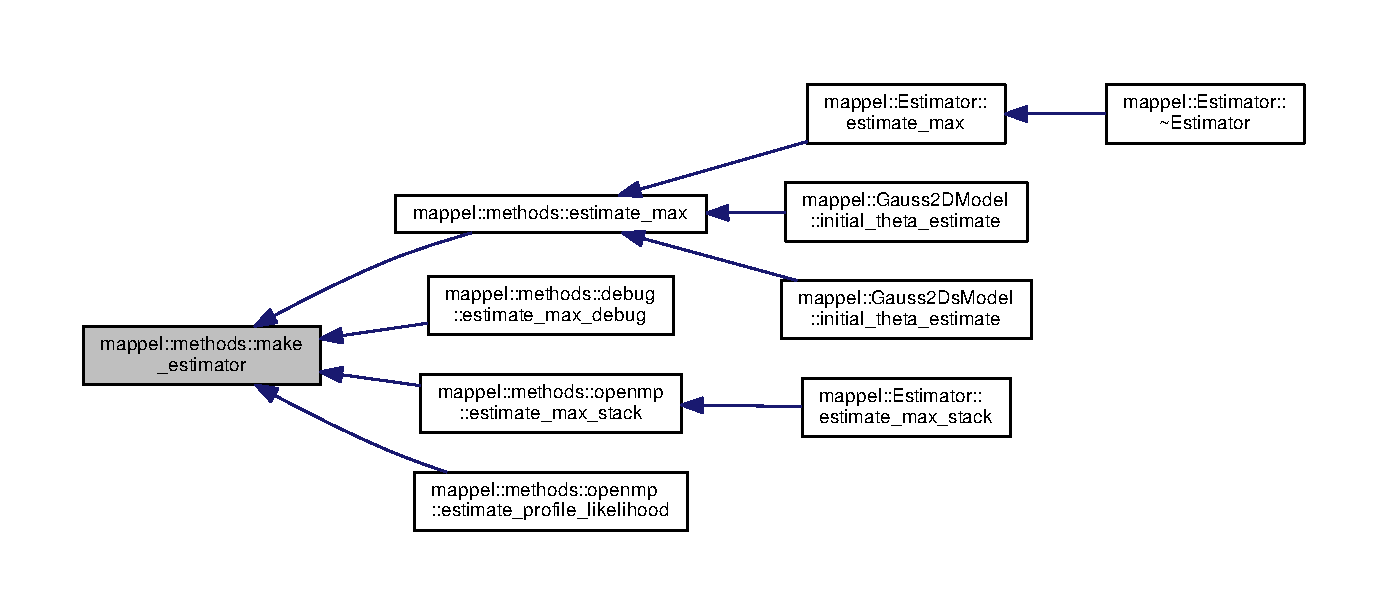
\includegraphics[width=350pt]{namespacemappel_1_1methods_a0f47a66f366b6e5841f1224e839ed828_icgraph}
\end{center}
\end{figure}


\index{mappel\+::methods@{mappel\+::methods}!make\+\_\+estimator@{make\+\_\+estimator}}
\index{make\+\_\+estimator@{make\+\_\+estimator}!mappel\+::methods@{mappel\+::methods}}
\paragraph[{\texorpdfstring{make\+\_\+estimator(\+Model \&model, std\+::string ename)}{make_estimator(Model &model, std::string ename)}}]{\setlength{\rightskip}{0pt plus 5cm}template$<$class Model $>$ {\bf Return\+If\+SubclassT}$<$std\+::unique\+\_\+ptr$<${\bf Estimator}$<$Model$>$ $>$, Model, {\bf Poisson\+Noise2\+D\+Objective}$>$ mappel\+::methods\+::make\+\_\+estimator (
\begin{DoxyParamCaption}
\item[{Model \&}]{model, }
\item[{std\+::string}]{ename}
\end{DoxyParamCaption}
)}\hypertarget{namespacemappel_1_1methods_acf60639ee5928d3a6eb44a017e57f2ec}{}\label{namespacemappel_1_1methods_acf60639ee5928d3a6eb44a017e57f2ec}


Definition at line 100 of file Poisson\+Noise2\+D\+Objective.\+h.



References mappel\+::istarts\+\_\+with().



Here is the call graph for this function\+:\nopagebreak
\begin{figure}[H]
\begin{center}
\leavevmode
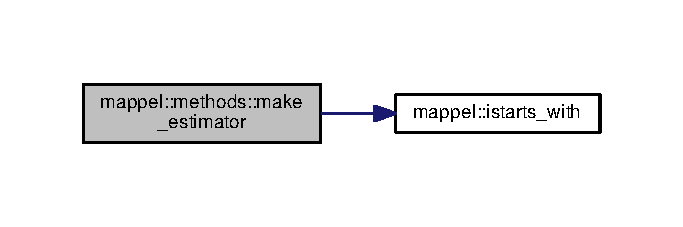
\includegraphics[width=328pt]{namespacemappel_1_1methods_acf60639ee5928d3a6eb44a017e57f2ec_cgraph}
\end{center}
\end{figure}


\index{mappel\+::methods@{mappel\+::methods}!model\+\_\+image@{model\+\_\+image}}
\index{model\+\_\+image@{model\+\_\+image}!mappel\+::methods@{mappel\+::methods}}
\paragraph[{\texorpdfstring{model\+\_\+image(const Model \&model, const Param\+T$<$ Model $>$ \&theta)}{model_image(const Model &model, const ParamT< Model > &theta)}}]{\setlength{\rightskip}{0pt plus 5cm}template$<$class Model $>$ Model\+::\+ImageT mappel\+::methods\+::model\+\_\+image (
\begin{DoxyParamCaption}
\item[{const Model \&}]{model, }
\item[{const {\bf ParamT}$<$ Model $>$ \&}]{theta}
\end{DoxyParamCaption}
)}\hypertarget{namespacemappel_1_1methods_ab7601760f76a0f3d283aaa1b21d4f5b5}{}\label{namespacemappel_1_1methods_ab7601760f76a0f3d283aaa1b21d4f5b5}
Expected number of photons at each pixel in image given the emitter model 

Definition at line 17 of file model\+\_\+methods\+\_\+impl.\+h.



References model\+\_\+image().



Here is the call graph for this function\+:\nopagebreak
\begin{figure}[H]
\begin{center}
\leavevmode
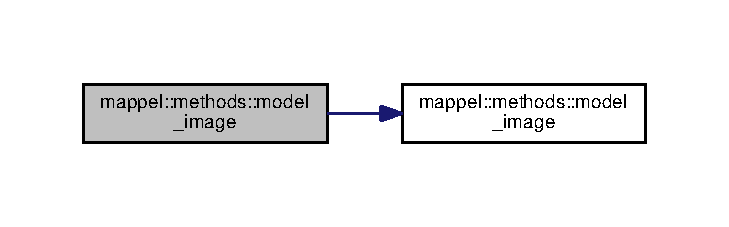
\includegraphics[width=350pt]{namespacemappel_1_1methods_ab7601760f76a0f3d283aaa1b21d4f5b5_cgraph}
\end{center}
\end{figure}


\index{mappel\+::methods@{mappel\+::methods}!model\+\_\+image@{model\+\_\+image}}
\index{model\+\_\+image@{model\+\_\+image}!mappel\+::methods@{mappel\+::methods}}
\paragraph[{\texorpdfstring{model\+\_\+image(const Model \&model, const Param\+T$<$ Model $>$ \&theta)}{model_image(const Model &model, const ParamT< Model > &theta)}}]{\setlength{\rightskip}{0pt plus 5cm}template$<$class Model $>$ {\bf ImageT}$<$Model$>$ mappel\+::methods\+::model\+\_\+image (
\begin{DoxyParamCaption}
\item[{const Model \&}]{model, }
\item[{const {\bf ParamT}$<$ Model $>$ \&}]{theta}
\end{DoxyParamCaption}
)}\hypertarget{namespacemappel_1_1methods_a4243465f0e58305d795497cbb0499433}{}\label{namespacemappel_1_1methods_a4243465f0e58305d795497cbb0499433}
Expected number of photons at each pixel in image given the emitter model 

Definition at line 17 of file model\+\_\+methods\+\_\+impl.\+h.



References model\+\_\+image().



Here is the call graph for this function\+:\nopagebreak
\begin{figure}[H]
\begin{center}
\leavevmode
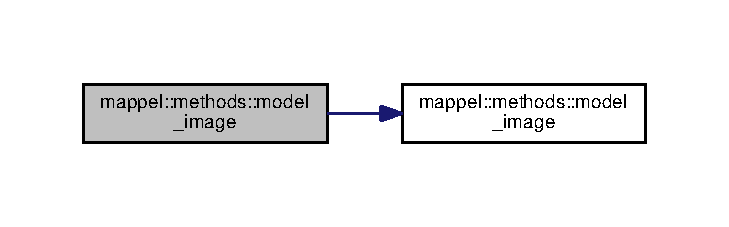
\includegraphics[width=350pt]{namespacemappel_1_1methods_a4243465f0e58305d795497cbb0499433_cgraph}
\end{center}
\end{figure}


\index{mappel\+::methods@{mappel\+::methods}!model\+\_\+image@{model\+\_\+image}}
\index{model\+\_\+image@{model\+\_\+image}!mappel\+::methods@{mappel\+::methods}}
\paragraph[{\texorpdfstring{model\+\_\+image(const Model \&model, const Stencil\+T$<$ Model $>$ \&s)}{model_image(const Model &model, const StencilT< Model > &s)}}]{\setlength{\rightskip}{0pt plus 5cm}template$<$class Model $>$ {\bf Return\+If\+SubclassT}$<${\bf ImageT}$<$Model$>$, Model, {\bf Image\+Format1\+D\+Base}$>$ mappel\+::methods\+::model\+\_\+image (
\begin{DoxyParamCaption}
\item[{const Model \&}]{model, }
\item[{const {\bf StencilT}$<$ Model $>$ \&}]{s}
\end{DoxyParamCaption}
)}\hypertarget{namespacemappel_1_1methods_ae92825adbc9f0eea36c2b0afdbf40d66}{}\label{namespacemappel_1_1methods_ae92825adbc9f0eea36c2b0afdbf40d66}


Definition at line 118 of file Image\+Format1\+D\+Base.\+h.



Referenced by model\+\_\+image(), and mappel\+::methods\+::openmp\+::simulate\+\_\+image\+\_\+stack().



Here is the caller graph for this function\+:\nopagebreak
\begin{figure}[H]
\begin{center}
\leavevmode
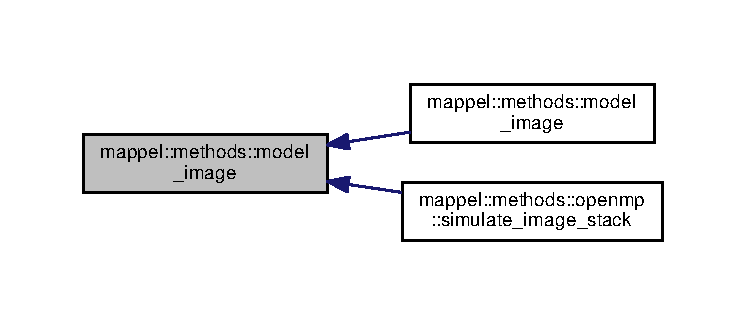
\includegraphics[width=350pt]{namespacemappel_1_1methods_ae92825adbc9f0eea36c2b0afdbf40d66_icgraph}
\end{center}
\end{figure}


\index{mappel\+::methods@{mappel\+::methods}!model\+\_\+image@{model\+\_\+image}}
\index{model\+\_\+image@{model\+\_\+image}!mappel\+::methods@{mappel\+::methods}}
\paragraph[{\texorpdfstring{model\+\_\+image(const Model \&model, const typename Model\+::\+Stencil \&s)}{model_image(const Model &model, const typename Model::Stencil &s)}}]{\setlength{\rightskip}{0pt plus 5cm}template$<$class Model $>$ {\bf Return\+If\+SubclassT}$<${\bf ImageT}$<$Model$>$, Model, {\bf Image\+Format2\+D\+Base}$>$ mappel\+::methods\+::model\+\_\+image (
\begin{DoxyParamCaption}
\item[{const Model \&}]{model, }
\item[{const typename Model\+::\+Stencil \&}]{s}
\end{DoxyParamCaption}
)}\hypertarget{namespacemappel_1_1methods_a864e97c52c849c580bccf04401695d13}{}\label{namespacemappel_1_1methods_a864e97c52c849c580bccf04401695d13}


Definition at line 122 of file Image\+Format2\+D\+Base.\+h.



References mappel\+::\+Image\+Format2\+D\+Base\+::size.

\index{mappel\+::methods@{mappel\+::methods}!observed\+\_\+information@{observed\+\_\+information}}
\index{observed\+\_\+information@{observed\+\_\+information}!mappel\+::methods@{mappel\+::methods}}
\paragraph[{\texorpdfstring{observed\+\_\+information(const Model \&model, const Model\+Data\+T$<$ Model $>$ \&data, const Param\+T$<$ Model $>$ \&theta\+\_\+mode)}{observed_information(const Model &model, const ModelDataT< Model > &data, const ParamT< Model > &theta_mode)}}]{\setlength{\rightskip}{0pt plus 5cm}template$<$class Model $>$ {\bf MatT} mappel\+::methods\+::observed\+\_\+information (
\begin{DoxyParamCaption}
\item[{const Model \&}]{model, }
\item[{const {\bf Model\+DataT}$<$ Model $>$ \&}]{data, }
\item[{const {\bf ParamT}$<$ Model $>$ \&}]{theta\+\_\+mode}
\end{DoxyParamCaption}
)}\hypertarget{namespacemappel_1_1methods_a83244dbe0995e8698475a12d34fb2f35}{}\label{namespacemappel_1_1methods_a83244dbe0995e8698475a12d34fb2f35}


Definition at line 266 of file model\+\_\+methods\+\_\+impl.\+h.



Referenced by mappel\+::\+Estimator$<$ Model $>$\+::compute\+\_\+estimate(), and mappel\+::\+Estimator$<$ Model $>$\+::estimate\+\_\+max\+\_\+debug().



Here is the caller graph for this function\+:\nopagebreak
\begin{figure}[H]
\begin{center}
\leavevmode
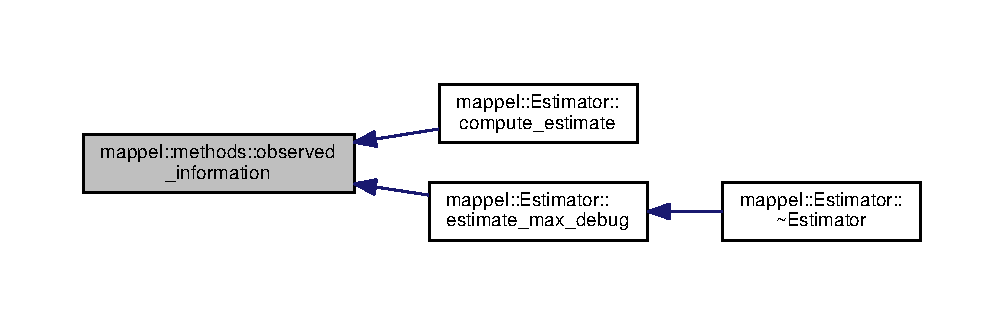
\includegraphics[width=350pt]{namespacemappel_1_1methods_a83244dbe0995e8698475a12d34fb2f35_icgraph}
\end{center}
\end{figure}


\index{mappel\+::methods@{mappel\+::methods}!observed\+\_\+information@{observed\+\_\+information}}
\index{observed\+\_\+information@{observed\+\_\+information}!mappel\+::methods@{mappel\+::methods}}
\paragraph[{\texorpdfstring{observed\+\_\+information(const Model \&model, const Model\+Data\+T$<$ Model $>$ \&data, const Stencil\+T$<$ Model $>$ \&theta\+\_\+mode)}{observed_information(const Model &model, const ModelDataT< Model > &data, const StencilT< Model > &theta_mode)}}]{\setlength{\rightskip}{0pt plus 5cm}template$<$class Model $>$ {\bf MatT} mappel\+::methods\+::observed\+\_\+information (
\begin{DoxyParamCaption}
\item[{const Model \&}]{model, }
\item[{const {\bf Model\+DataT}$<$ Model $>$ \&}]{data, }
\item[{const {\bf StencilT}$<$ Model $>$ \&}]{theta\+\_\+mode}
\end{DoxyParamCaption}
)}\hypertarget{namespacemappel_1_1methods_a0e3bec3c7363eb6005abdeaa151decb9}{}\label{namespacemappel_1_1methods_a0e3bec3c7363eb6005abdeaa151decb9}


Definition at line 258 of file model\+\_\+methods\+\_\+impl.\+h.



References mappel\+::methods\+::objective\+::hessian().



Here is the call graph for this function\+:\nopagebreak
\begin{figure}[H]
\begin{center}
\leavevmode
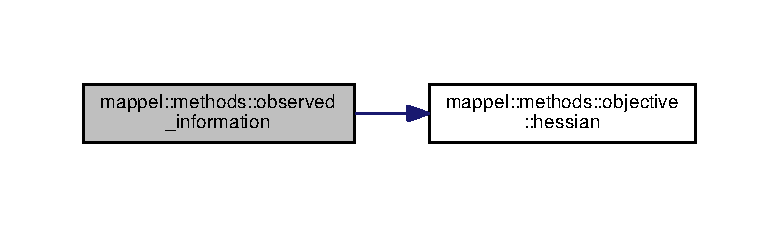
\includegraphics[width=350pt]{namespacemappel_1_1methods_a0e3bec3c7363eb6005abdeaa151decb9_cgraph}
\end{center}
\end{figure}


\index{mappel\+::methods@{mappel\+::methods}!prior\+\_\+objective@{prior\+\_\+objective}}
\index{prior\+\_\+objective@{prior\+\_\+objective}!mappel\+::methods@{mappel\+::methods}}
\paragraph[{\texorpdfstring{prior\+\_\+objective(const Model \&model, const Param\+T$<$ Model $>$ \&theta, double \&rllh, Param\+T$<$ Model $>$ \&grad, Mat\+T \&hess)}{prior_objective(const Model &model, const ParamT< Model > &theta, double &rllh, ParamT< Model > &grad, MatT &hess)}}]{\setlength{\rightskip}{0pt plus 5cm}template$<$class Model $>$ void mappel\+::methods\+::prior\+\_\+objective (
\begin{DoxyParamCaption}
\item[{const Model \&}]{model, }
\item[{const {\bf ParamT}$<$ Model $>$ \&}]{theta, }
\item[{double \&}]{rllh, }
\item[{{\bf ParamT}$<$ Model $>$ \&}]{grad, }
\item[{{\bf MatT} \&}]{hess}
\end{DoxyParamCaption}
)}\hypertarget{namespacemappel_1_1methods_a275f2b0364c48bfc7e6f88e866d593bd}{}\label{namespacemappel_1_1methods_a275f2b0364c48bfc7e6f88e866d593bd}


Definition at line 198 of file model\+\_\+methods\+\_\+impl.\+h.

\index{mappel\+::methods@{mappel\+::methods}!simulate\+\_\+image@{simulate\+\_\+image}}
\index{simulate\+\_\+image@{simulate\+\_\+image}!mappel\+::methods@{mappel\+::methods}}
\paragraph[{\texorpdfstring{simulate\+\_\+image(\+Model \&model, const Param\+T$<$ Model $>$ \&theta)}{simulate_image(Model &model, const ParamT< Model > &theta)}}]{\setlength{\rightskip}{0pt plus 5cm}template$<$class Model $>$ {\bf Model\+DataT}$<$Model$>$ mappel\+::methods\+::simulate\+\_\+image (
\begin{DoxyParamCaption}
\item[{Model \&}]{model, }
\item[{const {\bf ParamT}$<$ Model $>$ \&}]{theta}
\end{DoxyParamCaption}
)}\hypertarget{namespacemappel_1_1methods_a3809077f8bb3dca1fdf43ccc67dde62d}{}\label{namespacemappel_1_1methods_a3809077f8bb3dca1fdf43ccc67dde62d}


Definition at line 23 of file model\+\_\+methods\+\_\+impl.\+h.



References simulate\+\_\+image().



Referenced by simulate\+\_\+image(), mappel\+::simulate\+\_\+image\+\_\+stack(), and mappel\+::methods\+::openmp\+::simulate\+\_\+image\+\_\+stack().



Here is the call graph for this function\+:\nopagebreak
\begin{figure}[H]
\begin{center}
\leavevmode
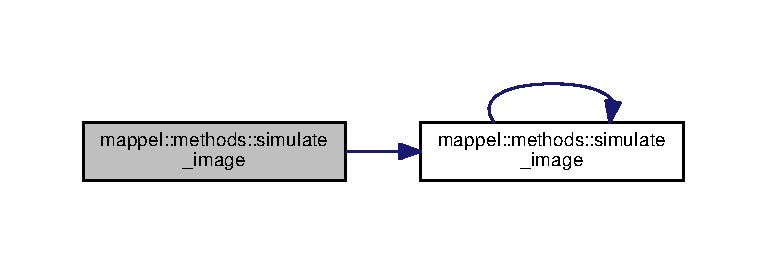
\includegraphics[width=350pt]{namespacemappel_1_1methods_a3809077f8bb3dca1fdf43ccc67dde62d_cgraph}
\end{center}
\end{figure}




Here is the caller graph for this function\+:\nopagebreak
\begin{figure}[H]
\begin{center}
\leavevmode
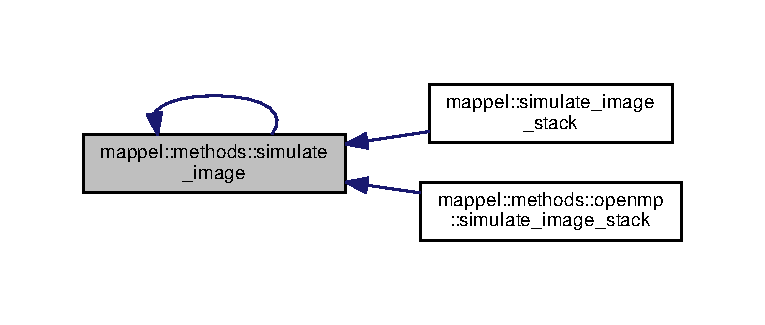
\includegraphics[width=350pt]{namespacemappel_1_1methods_a3809077f8bb3dca1fdf43ccc67dde62d_icgraph}
\end{center}
\end{figure}


\index{mappel\+::methods@{mappel\+::methods}!simulate\+\_\+image@{simulate\+\_\+image}}
\index{simulate\+\_\+image@{simulate\+\_\+image}!mappel\+::methods@{mappel\+::methods}}
\paragraph[{\texorpdfstring{simulate\+\_\+image(\+Model \&model, const Param\+T$<$ Model $>$ \&theta, Rng\+T \&rng)}{simulate_image(Model &model, const ParamT< Model > &theta, RngT &rng)}}]{\setlength{\rightskip}{0pt plus 5cm}template$<$class Model , class RngT $>$ {\bf Model\+DataT}$<$Model$>$ mappel\+::methods\+::simulate\+\_\+image (
\begin{DoxyParamCaption}
\item[{Model \&}]{model, }
\item[{const {\bf ParamT}$<$ Model $>$ \&}]{theta, }
\item[{RngT \&}]{rng}
\end{DoxyParamCaption}
)}\hypertarget{namespacemappel_1_1methods_abd0aa1868ba545867d80bf166aaeed03}{}\label{namespacemappel_1_1methods_abd0aa1868ba545867d80bf166aaeed03}


Definition at line 30 of file model\+\_\+methods\+\_\+impl.\+h.



References simulate\+\_\+image().



Here is the call graph for this function\+:\nopagebreak
\begin{figure}[H]
\begin{center}
\leavevmode
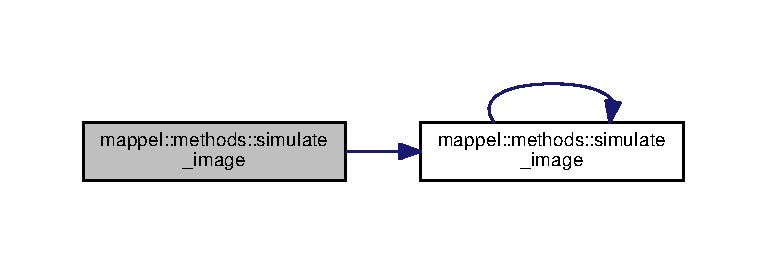
\includegraphics[width=350pt]{namespacemappel_1_1methods_abd0aa1868ba545867d80bf166aaeed03_cgraph}
\end{center}
\end{figure}


\index{mappel\+::methods@{mappel\+::methods}!simulate\+\_\+image@{simulate\+\_\+image}}
\index{simulate\+\_\+image@{simulate\+\_\+image}!mappel\+::methods@{mappel\+::methods}}
\paragraph[{\texorpdfstring{simulate\+\_\+image(\+Model \&model, const Param\+T$<$ Model $>$ \&theta)}{simulate_image(Model &model, const ParamT< Model > &theta)}}]{\setlength{\rightskip}{0pt plus 5cm}template$<$class Model , class rng\+\_\+t $>$ {\bf Model\+DataT}$<$Model$>$ mappel\+::methods\+::simulate\+\_\+image (
\begin{DoxyParamCaption}
\item[{Model \&}]{model, }
\item[{const {\bf ParamT}$<$ Model $>$ \&}]{theta}
\end{DoxyParamCaption}
)}\hypertarget{namespacemappel_1_1methods_a950d7858d6cc0ffb6e651776a24c9e35}{}\label{namespacemappel_1_1methods_a950d7858d6cc0ffb6e651776a24c9e35}


Definition at line 23 of file model\+\_\+methods\+\_\+impl.\+h.



References simulate\+\_\+image().



Referenced by simulate\+\_\+image(), mappel\+::simulate\+\_\+image\+\_\+stack(), and mappel\+::methods\+::openmp\+::simulate\+\_\+image\+\_\+stack().



Here is the call graph for this function\+:\nopagebreak
\begin{figure}[H]
\begin{center}
\leavevmode
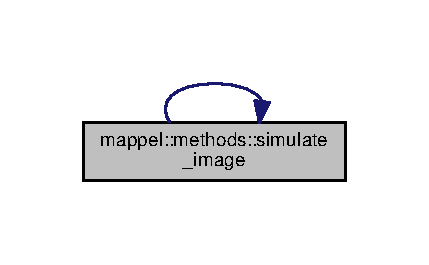
\includegraphics[width=206pt]{namespacemappel_1_1methods_a950d7858d6cc0ffb6e651776a24c9e35_cgraph}
\end{center}
\end{figure}




Here is the caller graph for this function\+:\nopagebreak
\begin{figure}[H]
\begin{center}
\leavevmode
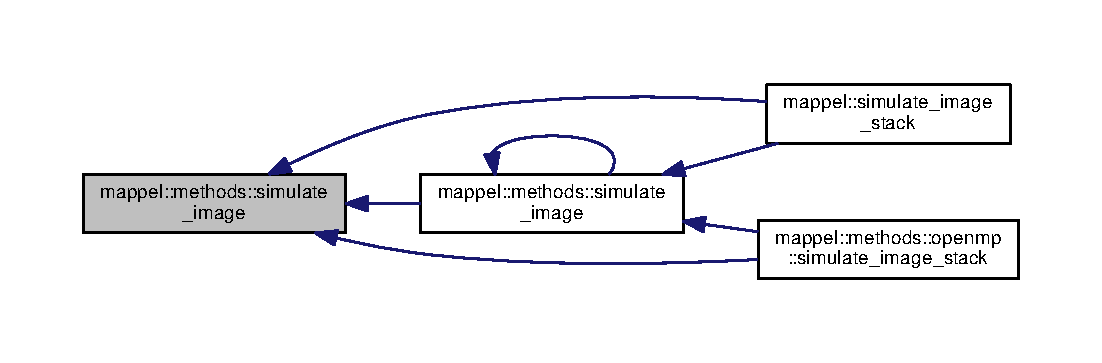
\includegraphics[width=350pt]{namespacemappel_1_1methods_a950d7858d6cc0ffb6e651776a24c9e35_icgraph}
\end{center}
\end{figure}


\index{mappel\+::methods@{mappel\+::methods}!simulate\+\_\+image@{simulate\+\_\+image}}
\index{simulate\+\_\+image@{simulate\+\_\+image}!mappel\+::methods@{mappel\+::methods}}
\paragraph[{\texorpdfstring{simulate\+\_\+image(const Model \&model, const Stencil\+T$<$ Model $>$ \&s, rng\+\_\+t \&rng)}{simulate_image(const Model &model, const StencilT< Model > &s, rng_t &rng)}}]{\setlength{\rightskip}{0pt plus 5cm}template$<$class Model , class rng\+\_\+t $>$ {\bf Return\+If\+SubclassT}$<${\bf Model\+DataT}$<$Model$>$, Model, {\bf Poisson\+Noise1\+D\+Objective}$>$ mappel\+::methods\+::simulate\+\_\+image (
\begin{DoxyParamCaption}
\item[{const Model \&}]{model, }
\item[{const {\bf StencilT}$<$ Model $>$ \&}]{s, }
\item[{rng\+\_\+t \&}]{rng}
\end{DoxyParamCaption}
)}\hypertarget{namespacemappel_1_1methods_abe1122f5c810f1b41c391a7e724fd74d}{}\label{namespacemappel_1_1methods_abe1122f5c810f1b41c391a7e724fd74d}


Simulate an image at a given theta stencil, by generating Poisson noise Enabled for \hyperlink{classmappel_1_1PoissonNoise1DObjective}{Poisson\+Noise1\+D\+Objective}. 


\begin{DoxyParams}[1]{Parameters}
\mbox{\tt in}  & {\em model} & Model object \\
\hline
\mbox{\tt in}  & {\em s} & The stencil computed at theta. \\
\hline
\mbox{\tt in,out}  & {\em rng} & A random number generator \\
\hline
\end{DoxyParams}
\begin{DoxyReturn}{Returns}
A simulated image at theta under the noise model. 
\end{DoxyReturn}


Definition at line 45 of file Poisson\+Noise1\+D\+Objective.\+h.



References mappel\+::generate\+\_\+poisson().



Here is the call graph for this function\+:\nopagebreak
\begin{figure}[H]
\begin{center}
\leavevmode
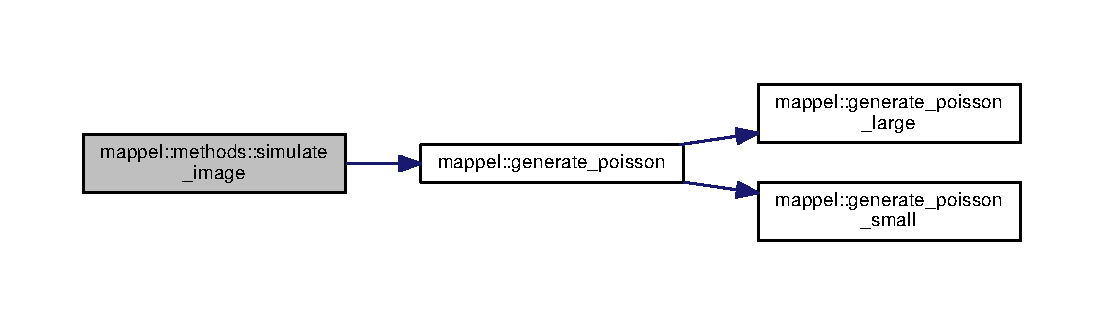
\includegraphics[width=350pt]{namespacemappel_1_1methods_abe1122f5c810f1b41c391a7e724fd74d_cgraph}
\end{center}
\end{figure}


\index{mappel\+::methods@{mappel\+::methods}!simulate\+\_\+image@{simulate\+\_\+image}}
\index{simulate\+\_\+image@{simulate\+\_\+image}!mappel\+::methods@{mappel\+::methods}}
\paragraph[{\texorpdfstring{simulate\+\_\+image(const Model \&model, const Stencil\+T$<$ Model $>$ \&s, rng\+\_\+t \&rng)}{simulate_image(const Model &model, const StencilT< Model > &s, rng_t &rng)}}]{\setlength{\rightskip}{0pt plus 5cm}template$<$class Model , class rng\+\_\+t $>$ {\bf Return\+If\+SubclassT}$<${\bf ImageT}$<$Model$>$, Model, {\bf Poisson\+Noise2\+D\+Objective}$>$ mappel\+::methods\+::simulate\+\_\+image (
\begin{DoxyParamCaption}
\item[{const Model \&}]{model, }
\item[{const {\bf StencilT}$<$ Model $>$ \&}]{s, }
\item[{rng\+\_\+t \&}]{rng}
\end{DoxyParamCaption}
)}\hypertarget{namespacemappel_1_1methods_a2b9a50b06cafb7ac9d857589df8979dc}{}\label{namespacemappel_1_1methods_a2b9a50b06cafb7ac9d857589df8979dc}


Simulate an image at a given theta stencil, by generating Poisson noise Enabled for \hyperlink{classmappel_1_1PoissonNoise2DObjective}{Poisson\+Noise2\+D\+Objective}. 


\begin{DoxyParams}[1]{Parameters}
\mbox{\tt in}  & {\em model} & Model object \\
\hline
\mbox{\tt in}  & {\em s} & The stencil computed at theta. \\
\hline
\mbox{\tt in,out}  & {\em rng} & A random number generator \\
\hline
\end{DoxyParams}
\begin{DoxyReturn}{Returns}
A simulated image at theta under the noise model. 
\end{DoxyReturn}


Definition at line 45 of file Poisson\+Noise2\+D\+Objective.\+h.



References mappel\+::generate\+\_\+poisson(), and mappel\+::\+Image\+Format2\+D\+Base\+::size.



Here is the call graph for this function\+:\nopagebreak
\begin{figure}[H]
\begin{center}
\leavevmode
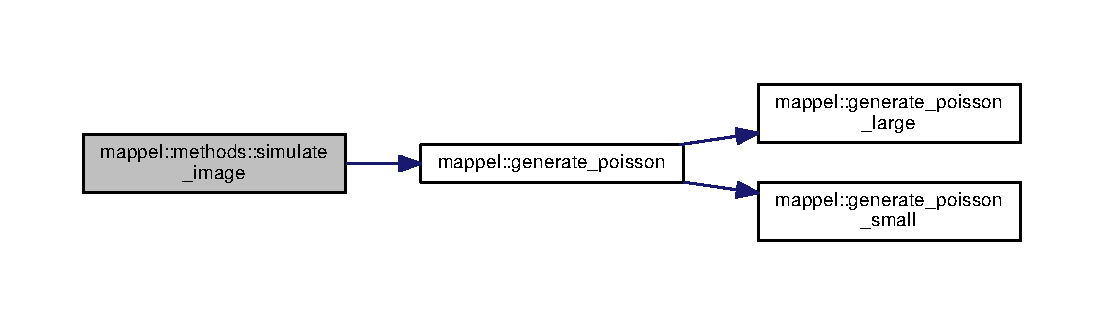
\includegraphics[width=350pt]{namespacemappel_1_1methods_a2b9a50b06cafb7ac9d857589df8979dc_cgraph}
\end{center}
\end{figure}


\index{mappel\+::methods@{mappel\+::methods}!simulate\+\_\+image@{simulate\+\_\+image}}
\index{simulate\+\_\+image@{simulate\+\_\+image}!mappel\+::methods@{mappel\+::methods}}
\paragraph[{\texorpdfstring{simulate\+\_\+image(\+Model \&model, const Param\+T$<$ Model $>$ \&theta, rng\+\_\+t \&rng)}{simulate_image(Model &model, const ParamT< Model > &theta, rng_t &rng)}}]{\setlength{\rightskip}{0pt plus 5cm}template$<$class Model , class rng\+\_\+t $>$ {\bf Model\+DataT}$<$Model$>$ mappel\+::methods\+::simulate\+\_\+image (
\begin{DoxyParamCaption}
\item[{Model \&}]{model, }
\item[{const {\bf ParamT}$<$ Model $>$ \&}]{theta, }
\item[{rng\+\_\+t \&}]{rng}
\end{DoxyParamCaption}
)}\hypertarget{namespacemappel_1_1methods_a74ba8d927de2e6fad2fec49599d4429e}{}\label{namespacemappel_1_1methods_a74ba8d927de2e6fad2fec49599d4429e}
\index{mappel\+::methods@{mappel\+::methods}!simulate\+\_\+image@{simulate\+\_\+image}}
\index{simulate\+\_\+image@{simulate\+\_\+image}!mappel\+::methods@{mappel\+::methods}}
\paragraph[{\texorpdfstring{simulate\+\_\+image(\+Model \&model, const Stencil\+T$<$ Model $>$ \&s)}{simulate_image(Model &model, const StencilT< Model > &s)}}]{\setlength{\rightskip}{0pt plus 5cm}template$<$class Model $>$ {\bf Model\+DataT}$<$ Model $>$ mappel\+::methods\+::simulate\+\_\+image (
\begin{DoxyParamCaption}
\item[{Model \&}]{model, }
\item[{const {\bf StencilT}$<$ Model $>$ \&}]{s}
\end{DoxyParamCaption}
)}\hypertarget{namespacemappel_1_1methods_af3db039a162d71bd04eb08b773035542}{}\label{namespacemappel_1_1methods_af3db039a162d71bd04eb08b773035542}


Definition at line 36 of file model\+\_\+methods\+\_\+impl.\+h.



References simulate\+\_\+image().



Here is the call graph for this function\+:\nopagebreak
\begin{figure}[H]
\begin{center}
\leavevmode
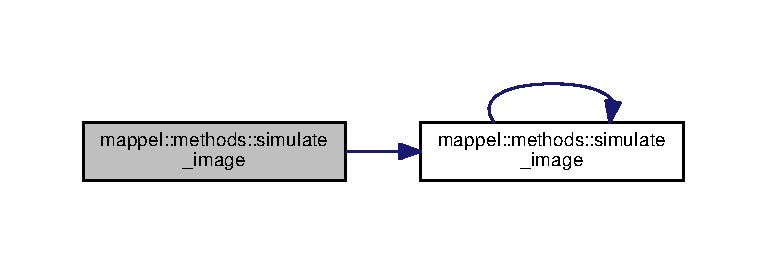
\includegraphics[width=350pt]{namespacemappel_1_1methods_af3db039a162d71bd04eb08b773035542_cgraph}
\end{center}
\end{figure}


\index{mappel\+::methods@{mappel\+::methods}!simulate\+\_\+image\+\_\+from\+\_\+model@{simulate\+\_\+image\+\_\+from\+\_\+model}}
\index{simulate\+\_\+image\+\_\+from\+\_\+model@{simulate\+\_\+image\+\_\+from\+\_\+model}!mappel\+::methods@{mappel\+::methods}}
\paragraph[{\texorpdfstring{simulate\+\_\+image\+\_\+from\+\_\+model(\+Model \&model, const Image\+T$<$ Model $>$ \&model\+\_\+im)}{simulate_image_from_model(Model &model, const ImageT< Model > &model_im)}}]{\setlength{\rightskip}{0pt plus 5cm}template$<$class Model $>$ {\bf Model\+DataT}$<$ Model $>$ mappel\+::methods\+::simulate\+\_\+image\+\_\+from\+\_\+model (
\begin{DoxyParamCaption}
\item[{Model \&}]{model, }
\item[{const {\bf ImageT}$<$ Model $>$ \&}]{model\+\_\+im}
\end{DoxyParamCaption}
)}\hypertarget{namespacemappel_1_1methods_a8ec3a0fdc71eed2a0bdfe33599f23623}{}\label{namespacemappel_1_1methods_a8ec3a0fdc71eed2a0bdfe33599f23623}


Definition at line 42 of file model\+\_\+methods\+\_\+impl.\+h.



Referenced by mappel\+::simulate\+\_\+image\+\_\+stack().



Here is the caller graph for this function\+:\nopagebreak
\begin{figure}[H]
\begin{center}
\leavevmode
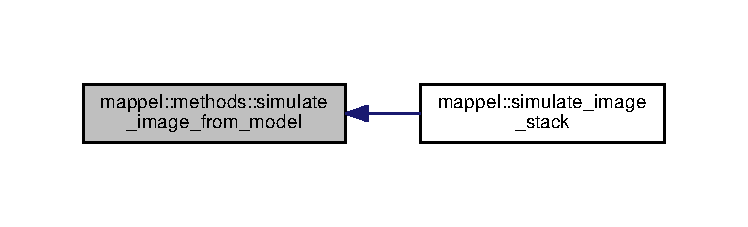
\includegraphics[width=350pt]{namespacemappel_1_1methods_a8ec3a0fdc71eed2a0bdfe33599f23623_icgraph}
\end{center}
\end{figure}


\index{mappel\+::methods@{mappel\+::methods}!simulate\+\_\+image\+\_\+from\+\_\+model@{simulate\+\_\+image\+\_\+from\+\_\+model}}
\index{simulate\+\_\+image\+\_\+from\+\_\+model@{simulate\+\_\+image\+\_\+from\+\_\+model}!mappel\+::methods@{mappel\+::methods}}
\paragraph[{\texorpdfstring{simulate\+\_\+image\+\_\+from\+\_\+model(const Model \&model, const Image\+T$<$ Model $>$ \&model\+\_\+im, rng\+\_\+t \&rng)}{simulate_image_from_model(const Model &model, const ImageT< Model > &model_im, rng_t &rng)}}]{\setlength{\rightskip}{0pt plus 5cm}template$<$class Model , class rng\+\_\+t $>$ {\bf Return\+If\+SubclassT}$<${\bf Model\+DataT}$<$Model$>$, Model, {\bf Poisson\+Noise1\+D\+Objective}$>$ mappel\+::methods\+::simulate\+\_\+image\+\_\+from\+\_\+model (
\begin{DoxyParamCaption}
\item[{const Model \&}]{model, }
\item[{const {\bf ImageT}$<$ Model $>$ \&}]{model\+\_\+im, }
\item[{rng\+\_\+t \&}]{rng}
\end{DoxyParamCaption}
)}\hypertarget{namespacemappel_1_1methods_a4a6ea9893f28e1f5c2604d8c3e7b6852}{}\label{namespacemappel_1_1methods_a4a6ea9893f28e1f5c2604d8c3e7b6852}


Simulate an image at a given theta stencil, by generating Poisson noise Enabled for \hyperlink{classmappel_1_1PoissonNoise1DObjective}{Poisson\+Noise1\+D\+Objective}. 


\begin{DoxyParams}[1]{Parameters}
\mbox{\tt in}  & {\em model} & Model object \\
\hline
\mbox{\tt in}  & {\em model\+\_\+im} & An image representing the expected (mean) at each pixel under the P\+SF model. \\
\hline
\mbox{\tt in,out}  & {\em rng} & A random number generator \\
\hline
\end{DoxyParams}
\begin{DoxyReturn}{Returns}
A simulated image corresponding to model\+\_\+im under the noise model. 
\end{DoxyReturn}


Definition at line 61 of file Poisson\+Noise1\+D\+Objective.\+h.



References mappel\+::generate\+\_\+poisson().



Here is the call graph for this function\+:\nopagebreak
\begin{figure}[H]
\begin{center}
\leavevmode
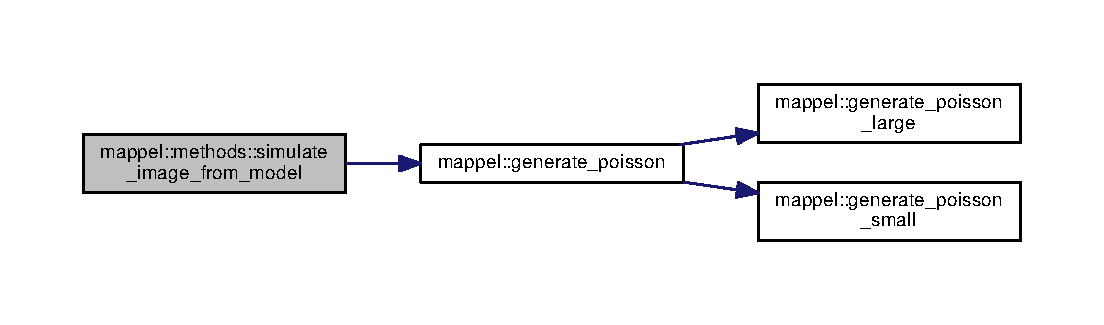
\includegraphics[width=350pt]{namespacemappel_1_1methods_a4a6ea9893f28e1f5c2604d8c3e7b6852_cgraph}
\end{center}
\end{figure}


\index{mappel\+::methods@{mappel\+::methods}!simulate\+\_\+image\+\_\+from\+\_\+model@{simulate\+\_\+image\+\_\+from\+\_\+model}}
\index{simulate\+\_\+image\+\_\+from\+\_\+model@{simulate\+\_\+image\+\_\+from\+\_\+model}!mappel\+::methods@{mappel\+::methods}}
\paragraph[{\texorpdfstring{simulate\+\_\+image\+\_\+from\+\_\+model(const Model \&model, const Image\+T$<$ Model $>$ \&model\+\_\+im, rng\+\_\+t \&rng)}{simulate_image_from_model(const Model &model, const ImageT< Model > &model_im, rng_t &rng)}}]{\setlength{\rightskip}{0pt plus 5cm}template$<$class Model , class rng\+\_\+t $>$ {\bf Return\+If\+SubclassT}$<${\bf ImageT}$<$Model$>$, Model, {\bf Poisson\+Noise2\+D\+Objective}$>$ mappel\+::methods\+::simulate\+\_\+image\+\_\+from\+\_\+model (
\begin{DoxyParamCaption}
\item[{const Model \&}]{model, }
\item[{const {\bf ImageT}$<$ Model $>$ \&}]{model\+\_\+im, }
\item[{rng\+\_\+t \&}]{rng}
\end{DoxyParamCaption}
)}\hypertarget{namespacemappel_1_1methods_a2dd4cb94fa6669d64488ed95bc1c6d02}{}\label{namespacemappel_1_1methods_a2dd4cb94fa6669d64488ed95bc1c6d02}


Simulate an image at a given theta stencil, by generating Poisson noise Enabled for \hyperlink{classmappel_1_1PoissonNoise2DObjective}{Poisson\+Noise2\+D\+Objective}. 


\begin{DoxyParams}[1]{Parameters}
\mbox{\tt in}  & {\em model} & Model object \\
\hline
\mbox{\tt in}  & {\em model\+\_\+im} & An image representing the expected (mean) at each pixel under the P\+SF model. \\
\hline
\mbox{\tt in,out}  & {\em rng} & A random number generator \\
\hline
\end{DoxyParams}
\begin{DoxyReturn}{Returns}
A simulated image corresponding to model\+\_\+im under the noise model. 
\end{DoxyReturn}


Definition at line 64 of file Poisson\+Noise2\+D\+Objective.\+h.



References mappel\+::generate\+\_\+poisson(), and mappel\+::\+Image\+Format2\+D\+Base\+::size.



Here is the call graph for this function\+:\nopagebreak
\begin{figure}[H]
\begin{center}
\leavevmode
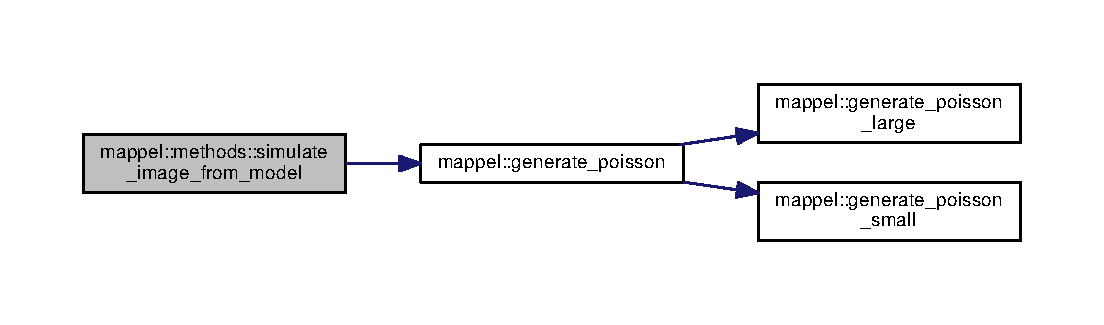
\includegraphics[width=350pt]{namespacemappel_1_1methods_a2dd4cb94fa6669d64488ed95bc1c6d02_cgraph}
\end{center}
\end{figure}



\hypertarget{namespacemappel_1_1methods_1_1debug}{}\subsection{mappel\+:\+:methods\+:\+:debug Namespace Reference}
\label{namespacemappel_1_1methods_1_1debug}\index{mappel\+::methods\+::debug@{mappel\+::methods\+::debug}}
\subsubsection*{Functions}
\begin{DoxyCompactItemize}
\item 
{\footnotesize template$<$class Model $>$ }\\void \hyperlink{namespacemappel_1_1methods_1_1debug_a38de1b4f98bfb724874fec99b53a8554}{estimate\+\_\+max\+\_\+debug} (const Model \&model, const \hyperlink{namespacemappel_a97f050df953605381ae9c901c3b125f1}{Model\+DataT}$<$ Model $>$ \&data, const std\+::string \&method, const \hyperlink{namespacemappel_a667925cb0d6c0e49f2f035cc5a9a6857}{ParamT}$<$ Model $>$ \&theta\+\_\+init, \hyperlink{structmappel_1_1estimator_1_1MLEDebugData}{estimator\+::\+M\+L\+E\+Debug\+Data} \&mle, \hyperlink{namespacemappel_a04ab395b0cf82c4ce68a36b2212649a5}{StatsT} \&stats)
\item 
{\footnotesize template$<$class Model $>$ }\\void \hyperlink{namespacemappel_1_1methods_1_1debug_a3fc6147e9b38e7b8328eb421be81a200}{error\+\_\+bounds\+\_\+profile\+\_\+likelihood\+\_\+debug} (const Model \&model, const \hyperlink{namespacemappel_a97f050df953605381ae9c901c3b125f1}{Model\+DataT}$<$ Model $>$ \&data, \hyperlink{namespacemappel_1_1estimator_structmappel_1_1estimator_1_1ProfileBoundsDebugData}{estimator\+::\+Profile\+Bounds\+Debug\+Data} \&bounds, \hyperlink{namespacemappel_a04ab395b0cf82c4ce68a36b2212649a5}{StatsT} \&stats)
\item 
{\footnotesize template$<$class Model $>$ }\\void \hyperlink{namespacemappel_1_1methods_1_1debug_a5d84632af17af6d244b5a82b9d55f2ba}{estimate\+\_\+posterior\+\_\+debug} (const Model \&model, const \hyperlink{namespacemappel_a97f050df953605381ae9c901c3b125f1}{Model\+DataT}$<$ Model $>$ \&data, const \hyperlink{namespacemappel_a667925cb0d6c0e49f2f035cc5a9a6857}{ParamT}$<$ Model $>$ \&theta\+\_\+init, \hyperlink{structmappel_1_1mcmc_1_1MCMCDebugData}{mcmc\+::\+M\+C\+M\+C\+Debug\+Data} \&mcmc\+\_\+debug\+\_\+sample)
\end{DoxyCompactItemize}


\subsubsection{Function Documentation}
\index{mappel\+::methods\+::debug@{mappel\+::methods\+::debug}!error\+\_\+bounds\+\_\+profile\+\_\+likelihood\+\_\+debug@{error\+\_\+bounds\+\_\+profile\+\_\+likelihood\+\_\+debug}}
\index{error\+\_\+bounds\+\_\+profile\+\_\+likelihood\+\_\+debug@{error\+\_\+bounds\+\_\+profile\+\_\+likelihood\+\_\+debug}!mappel\+::methods\+::debug@{mappel\+::methods\+::debug}}
\paragraph[{\texorpdfstring{error\+\_\+bounds\+\_\+profile\+\_\+likelihood\+\_\+debug(const Model \&model, const Model\+Data\+T$<$ Model $>$ \&data, estimator\+::\+Profile\+Bounds\+Debug\+Data \&bounds, Stats\+T \&stats)}{error_bounds_profile_likelihood_debug(const Model &model, const ModelDataT< Model > &data, estimator::ProfileBoundsDebugData &bounds, StatsT &stats)}}]{\setlength{\rightskip}{0pt plus 5cm}template$<$class Model $>$ void mappel\+::methods\+::debug\+::error\+\_\+bounds\+\_\+profile\+\_\+likelihood\+\_\+debug (
\begin{DoxyParamCaption}
\item[{const Model \&}]{model, }
\item[{const {\bf Model\+DataT}$<$ Model $>$ \&}]{data, }
\item[{{\bf estimator\+::\+Profile\+Bounds\+Debug\+Data} \&}]{bounds, }
\item[{{\bf StatsT} \&}]{stats}
\end{DoxyParamCaption}
)}\hypertarget{namespacemappel_1_1methods_1_1debug_a3fc6147e9b38e7b8328eb421be81a200}{}\label{namespacemappel_1_1methods_1_1debug_a3fc6147e9b38e7b8328eb421be81a200}


Definition at line 461 of file model\+\_\+methods\+\_\+impl.\+h.



References mappel\+::estimator\+::\+Estimator$<$ Model $>$\+::estimate\+\_\+profile\+\_\+bounds\+\_\+debug(), and mappel\+::estimator\+::\+Iterative\+Maximizer$<$ Model $>$\+::get\+\_\+stats().

\index{mappel\+::methods\+::debug@{mappel\+::methods\+::debug}!estimate\+\_\+max\+\_\+debug@{estimate\+\_\+max\+\_\+debug}}
\index{estimate\+\_\+max\+\_\+debug@{estimate\+\_\+max\+\_\+debug}!mappel\+::methods\+::debug@{mappel\+::methods\+::debug}}
\paragraph[{\texorpdfstring{estimate\+\_\+max\+\_\+debug(const Model \&model, const Model\+Data\+T$<$ Model $>$ \&data, const std\+::string \&method, const Param\+T$<$ Model $>$ \&theta\+\_\+init, estimator\+::\+M\+L\+E\+Debug\+Data \&mle, Stats\+T \&stats)}{estimate_max_debug(const Model &model, const ModelDataT< Model > &data, const std::string &method, const ParamT< Model > &theta_init, estimator::MLEDebugData &mle, StatsT &stats)}}]{\setlength{\rightskip}{0pt plus 5cm}template$<$class Model $>$ void mappel\+::methods\+::debug\+::estimate\+\_\+max\+\_\+debug (
\begin{DoxyParamCaption}
\item[{const Model \&}]{model, }
\item[{const {\bf Model\+DataT}$<$ Model $>$ \&}]{data, }
\item[{const std\+::string \&}]{method, }
\item[{const {\bf ParamT}$<$ Model $>$ \&}]{theta\+\_\+init, }
\item[{{\bf estimator\+::\+M\+L\+E\+Debug\+Data} \&}]{mle, }
\item[{{\bf StatsT} \&}]{stats}
\end{DoxyParamCaption}
)}\hypertarget{namespacemappel_1_1methods_1_1debug_a38de1b4f98bfb724874fec99b53a8554}{}\label{namespacemappel_1_1methods_1_1debug_a38de1b4f98bfb724874fec99b53a8554}


Definition at line 452 of file model\+\_\+methods\+\_\+impl.\+h.



References mappel\+::methods\+::make\+\_\+estimator().



Referenced by mappel\+::estimator\+::\+Estimator$<$ Model $>$\+::$\sim$\+Estimator().

\index{mappel\+::methods\+::debug@{mappel\+::methods\+::debug}!estimate\+\_\+posterior\+\_\+debug@{estimate\+\_\+posterior\+\_\+debug}}
\index{estimate\+\_\+posterior\+\_\+debug@{estimate\+\_\+posterior\+\_\+debug}!mappel\+::methods\+::debug@{mappel\+::methods\+::debug}}
\paragraph[{\texorpdfstring{estimate\+\_\+posterior\+\_\+debug(const Model \&model, const Model\+Data\+T$<$ Model $>$ \&data, const Param\+T$<$ Model $>$ \&theta\+\_\+init, mcmc\+::\+M\+C\+M\+C\+Debug\+Data \&mcmc\+\_\+debug\+\_\+sample)}{estimate_posterior_debug(const Model &model, const ModelDataT< Model > &data, const ParamT< Model > &theta_init, mcmc::MCMCDebugData &mcmc_debug_sample)}}]{\setlength{\rightskip}{0pt plus 5cm}template$<$class Model $>$ void mappel\+::methods\+::debug\+::estimate\+\_\+posterior\+\_\+debug (
\begin{DoxyParamCaption}
\item[{const Model \&}]{model, }
\item[{const {\bf Model\+DataT}$<$ Model $>$ \&}]{data, }
\item[{const {\bf ParamT}$<$ Model $>$ \&}]{theta\+\_\+init, }
\item[{{\bf mcmc\+::\+M\+C\+M\+C\+Debug\+Data} \&}]{mcmc\+\_\+debug\+\_\+sample}
\end{DoxyParamCaption}
)}\hypertarget{namespacemappel_1_1methods_1_1debug_a5d84632af17af6d244b5a82b9d55f2ba}{}\label{namespacemappel_1_1methods_1_1debug_a5d84632af17af6d244b5a82b9d55f2ba}


Definition at line 470 of file model\+\_\+methods\+\_\+impl.\+h.



References mappel\+::mcmc\+::\+M\+C\+M\+C\+Debug\+Data\+::candidate, mappel\+::mcmc\+::\+M\+C\+M\+C\+Debug\+Data\+::candidate\+\_\+rllh, mappel\+::mcmc\+::\+M\+C\+M\+C\+Debug\+Data\+::initialize\+\_\+arrays(), mappel\+::mcmc\+::\+M\+C\+M\+C\+Debug\+Data\+::\+Nsample, mappel\+::mcmc\+::\+M\+C\+M\+C\+Debug\+Data\+::sample, mappel\+::mcmc\+::sample\+\_\+posterior\+\_\+debug(), and mappel\+::mcmc\+::\+M\+C\+M\+C\+Debug\+Data\+::sample\+\_\+rllh.


\hypertarget{namespacemappel_1_1methods_1_1likelihood}{}\subsection{mappel\+:\+:methods\+:\+:likelihood Namespace Reference}
\label{namespacemappel_1_1methods_1_1likelihood}\index{mappel\+::methods\+::likelihood@{mappel\+::methods\+::likelihood}}
\subsubsection*{Namespaces}
\begin{DoxyCompactItemize}
\item 
 \hyperlink{namespacemappel_1_1methods_1_1likelihood_1_1debug}{debug}
\end{DoxyCompactItemize}
\subsubsection*{Functions}
\begin{DoxyCompactItemize}
\item 
{\footnotesize template$<$class Model $>$ }\\\hyperlink{namespacemappel_a3b77d227658ba3ba9e16fea6fa6e626d}{Return\+If\+SubclassT}$<$ double, Model, \hyperlink{classmappel_1_1PoissonNoise1DObjective}{Poisson\+Noise1\+D\+Objective} $>$ \hyperlink{namespacemappel_1_1methods_1_1likelihood_a447a9c4b4bdcd45bed3f2df281efc5a5}{llh} (const Model \&model, const \hyperlink{namespacemappel_a97f050df953605381ae9c901c3b125f1}{Model\+DataT}$<$ Model $>$ \&data\+\_\+im, const \hyperlink{namespacemappel_a3a06598240007876f8c4bf834ad86197}{StencilT}$<$ Model $>$ \&s)
\item 
{\footnotesize template$<$class Model $>$ }\\\hyperlink{namespacemappel_a3b77d227658ba3ba9e16fea6fa6e626d}{Return\+If\+SubclassT}$<$ double, Model, \hyperlink{classmappel_1_1PoissonNoise1DObjective}{Poisson\+Noise1\+D\+Objective} $>$ \hyperlink{namespacemappel_1_1methods_1_1likelihood_ae064b0a1e26a5626c62bde870e587ecb}{rllh} (const Model \&model, const \hyperlink{namespacemappel_a97f050df953605381ae9c901c3b125f1}{Model\+DataT}$<$ Model $>$ \&data\+\_\+im, const \hyperlink{namespacemappel_a3a06598240007876f8c4bf834ad86197}{StencilT}$<$ Model $>$ \&s)
\item 
{\footnotesize template$<$class Model $>$ }\\\hyperlink{namespacemappel_a3b77d227658ba3ba9e16fea6fa6e626d}{Return\+If\+SubclassT}$<$ \hyperlink{namespacemappel_a667925cb0d6c0e49f2f035cc5a9a6857}{ParamT}$<$ Model $>$, Model, \hyperlink{classmappel_1_1PoissonNoise1DObjective}{Poisson\+Noise1\+D\+Objective} $>$ \hyperlink{namespacemappel_1_1methods_1_1likelihood_aceae29ce5d5dba7482b49d2ec12d0392}{grad} (const Model \&model, const \hyperlink{namespacemappel_a97f050df953605381ae9c901c3b125f1}{Model\+DataT}$<$ Model $>$ \&im, const \hyperlink{namespacemappel_a3a06598240007876f8c4bf834ad86197}{StencilT}$<$ Model $>$ \&s)
\item 
{\footnotesize template$<$class Model $>$ }\\\hyperlink{namespacemappel_a3b77d227658ba3ba9e16fea6fa6e626d}{Return\+If\+SubclassT}$<$ void, Model, \hyperlink{classmappel_1_1PoissonNoise1DObjective}{Poisson\+Noise1\+D\+Objective} $>$ \hyperlink{namespacemappel_1_1methods_1_1likelihood_a5417cc44455daa0eb6a6b307b1f493a1}{grad2} (const Model \&model, const \hyperlink{namespacemappel_a97f050df953605381ae9c901c3b125f1}{Model\+DataT}$<$ Model $>$ \&im, const \hyperlink{namespacemappel_a3a06598240007876f8c4bf834ad86197}{StencilT}$<$ Model $>$ \&s, \hyperlink{namespacemappel_a667925cb0d6c0e49f2f035cc5a9a6857}{ParamT}$<$ Model $>$ \&grad\+\_\+val, \hyperlink{namespacemappel_a667925cb0d6c0e49f2f035cc5a9a6857}{ParamT}$<$ Model $>$ \&grad2\+\_\+val)
\item 
{\footnotesize template$<$class Model $>$ }\\\hyperlink{namespacemappel_a3b77d227658ba3ba9e16fea6fa6e626d}{Return\+If\+SubclassT}$<$ void, Model, \hyperlink{classmappel_1_1PoissonNoise1DObjective}{Poisson\+Noise1\+D\+Objective} $>$ \hyperlink{namespacemappel_1_1methods_1_1likelihood_a0233341d03d8f8d06cb852068942ba73}{hessian} (const Model \&model, const \hyperlink{namespacemappel_a97f050df953605381ae9c901c3b125f1}{Model\+DataT}$<$ Model $>$ \&im, const \hyperlink{namespacemappel_a3a06598240007876f8c4bf834ad86197}{StencilT}$<$ Model $>$ \&s, \hyperlink{namespacemappel_a667925cb0d6c0e49f2f035cc5a9a6857}{ParamT}$<$ Model $>$ \&grad\+\_\+val, \hyperlink{namespacemappel_a7091ab87c528041f7e2027195fad8915}{MatT} \&hess\+\_\+val)
\item 
{\footnotesize template$<$class Model $>$ }\\\hyperlink{namespacemappel_a3b77d227658ba3ba9e16fea6fa6e626d}{Return\+If\+SubclassT}$<$ double, Model, \hyperlink{classmappel_1_1PoissonNoise2DObjective}{Poisson\+Noise2\+D\+Objective} $>$ \hyperlink{namespacemappel_1_1methods_1_1likelihood_a134b4c6ce6807f342f33464e99512dc6}{llh} (const Model \&model, const \hyperlink{namespacemappel_a97f050df953605381ae9c901c3b125f1}{Model\+DataT}$<$ Model $>$ \&data\+\_\+im, const \hyperlink{namespacemappel_a3a06598240007876f8c4bf834ad86197}{StencilT}$<$ Model $>$ \&s)
\item 
{\footnotesize template$<$class Model $>$ }\\\hyperlink{namespacemappel_a3b77d227658ba3ba9e16fea6fa6e626d}{Return\+If\+SubclassT}$<$ double, Model, \hyperlink{classmappel_1_1PoissonNoise2DObjective}{Poisson\+Noise2\+D\+Objective} $>$ \hyperlink{namespacemappel_1_1methods_1_1likelihood_aa8cbdb607db58f763a8dc70ef48372f1}{rllh} (const Model \&model, const \hyperlink{namespacemappel_a97f050df953605381ae9c901c3b125f1}{Model\+DataT}$<$ Model $>$ \&data\+\_\+im, const \hyperlink{namespacemappel_a3a06598240007876f8c4bf834ad86197}{StencilT}$<$ Model $>$ \&s)
\item 
{\footnotesize template$<$class Model $>$ }\\\hyperlink{namespacemappel_a3b77d227658ba3ba9e16fea6fa6e626d}{Return\+If\+SubclassT}$<$ \hyperlink{namespacemappel_a667925cb0d6c0e49f2f035cc5a9a6857}{ParamT}$<$ Model $>$, Model, \hyperlink{classmappel_1_1PoissonNoise2DObjective}{Poisson\+Noise2\+D\+Objective} $>$ \hyperlink{namespacemappel_1_1methods_1_1likelihood_a708debdd0c44a2bbdcc1deac7d49ab37}{grad} (const Model \&model, const \hyperlink{namespacemappel_a97f050df953605381ae9c901c3b125f1}{Model\+DataT}$<$ Model $>$ \&data\+\_\+im, const \hyperlink{namespacemappel_a3a06598240007876f8c4bf834ad86197}{StencilT}$<$ Model $>$ \&s)
\item 
{\footnotesize template$<$class Model $>$ }\\\hyperlink{namespacemappel_a3b77d227658ba3ba9e16fea6fa6e626d}{Return\+If\+SubclassT}$<$ void, Model, \hyperlink{classmappel_1_1PoissonNoise2DObjective}{Poisson\+Noise2\+D\+Objective} $>$ \hyperlink{namespacemappel_1_1methods_1_1likelihood_af0fade6d3bccc367da5d5d411ad6778b}{grad2} (const Model \&model, const \hyperlink{namespacemappel_a97f050df953605381ae9c901c3b125f1}{Model\+DataT}$<$ Model $>$ \&data\+\_\+im, const \hyperlink{namespacemappel_a3a06598240007876f8c4bf834ad86197}{StencilT}$<$ Model $>$ \&s, \hyperlink{namespacemappel_a667925cb0d6c0e49f2f035cc5a9a6857}{ParamT}$<$ Model $>$ \&grad\+\_\+val, \hyperlink{namespacemappel_a667925cb0d6c0e49f2f035cc5a9a6857}{ParamT}$<$ Model $>$ \&grad2\+\_\+val)
\item 
{\footnotesize template$<$class Model $>$ }\\\hyperlink{namespacemappel_a3b77d227658ba3ba9e16fea6fa6e626d}{Return\+If\+SubclassT}$<$ void, Model, \hyperlink{classmappel_1_1PoissonNoise2DObjective}{Poisson\+Noise2\+D\+Objective} $>$ \hyperlink{namespacemappel_1_1methods_1_1likelihood_ac16ac7a26d0773dc9c074e8ad796e161}{hessian} (const Model \&model, const \hyperlink{namespacemappel_a97f050df953605381ae9c901c3b125f1}{Model\+DataT}$<$ Model $>$ \&data\+\_\+im, const \hyperlink{namespacemappel_a3a06598240007876f8c4bf834ad86197}{StencilT}$<$ Model $>$ \&s, \hyperlink{namespacemappel_a667925cb0d6c0e49f2f035cc5a9a6857}{ParamT}$<$ Model $>$ \&grad\+\_\+val, \hyperlink{namespacemappel_a7091ab87c528041f7e2027195fad8915}{MatT} \&hess\+\_\+val)
\end{DoxyCompactItemize}


\subsubsection{Function Documentation}
\index{mappel\+::methods\+::likelihood@{mappel\+::methods\+::likelihood}!grad@{grad}}
\index{grad@{grad}!mappel\+::methods\+::likelihood@{mappel\+::methods\+::likelihood}}
\paragraph[{\texorpdfstring{grad(const Model \&model, const Model\+Data\+T$<$ Model $>$ \&im, const Stencil\+T$<$ Model $>$ \&s)}{grad(const Model &model, const ModelDataT< Model > &im, const StencilT< Model > &s)}}]{\setlength{\rightskip}{0pt plus 5cm}template$<$class Model $>$ {\bf Return\+If\+SubclassT}$<${\bf ParamT}$<$Model$>$,Model,{\bf Poisson\+Noise1\+D\+Objective}$>$ mappel\+::methods\+::likelihood\+::grad (
\begin{DoxyParamCaption}
\item[{const Model \&}]{model, }
\item[{const {\bf Model\+DataT}$<$ Model $>$ \&}]{im, }
\item[{const {\bf StencilT}$<$ Model $>$ \&}]{s}
\end{DoxyParamCaption}
)}\hypertarget{namespacemappel_1_1methods_1_1likelihood_aceae29ce5d5dba7482b49d2ec12d0392}{}\label{namespacemappel_1_1methods_1_1likelihood_aceae29ce5d5dba7482b49d2ec12d0392}


Definition at line 146 of file Poisson\+Noise1\+D\+Objective.\+h.

\index{mappel\+::methods\+::likelihood@{mappel\+::methods\+::likelihood}!grad@{grad}}
\index{grad@{grad}!mappel\+::methods\+::likelihood@{mappel\+::methods\+::likelihood}}
\paragraph[{\texorpdfstring{grad(const Model \&model, const Model\+Data\+T$<$ Model $>$ \&data\+\_\+im, const Stencil\+T$<$ Model $>$ \&s)}{grad(const Model &model, const ModelDataT< Model > &data_im, const StencilT< Model > &s)}}]{\setlength{\rightskip}{0pt plus 5cm}template$<$class Model $>$ {\bf Return\+If\+SubclassT}$<${\bf ParamT}$<$Model$>$,Model,{\bf Poisson\+Noise2\+D\+Objective}$>$ mappel\+::methods\+::likelihood\+::grad (
\begin{DoxyParamCaption}
\item[{const Model \&}]{model, }
\item[{const {\bf Model\+DataT}$<$ Model $>$ \&}]{data\+\_\+im, }
\item[{const {\bf StencilT}$<$ Model $>$ \&}]{s}
\end{DoxyParamCaption}
)}\hypertarget{namespacemappel_1_1methods_1_1likelihood_a708debdd0c44a2bbdcc1deac7d49ab37}{}\label{namespacemappel_1_1methods_1_1likelihood_a708debdd0c44a2bbdcc1deac7d49ab37}


Definition at line 159 of file Poisson\+Noise2\+D\+Objective.\+h.



References mappel\+::\+Image\+Format2\+D\+Base\+::size.

\index{mappel\+::methods\+::likelihood@{mappel\+::methods\+::likelihood}!grad2@{grad2}}
\index{grad2@{grad2}!mappel\+::methods\+::likelihood@{mappel\+::methods\+::likelihood}}
\paragraph[{\texorpdfstring{grad2(const Model \&model, const Model\+Data\+T$<$ Model $>$ \&im, const Stencil\+T$<$ Model $>$ \&s, Param\+T$<$ Model $>$ \&grad\+\_\+val, Param\+T$<$ Model $>$ \&grad2\+\_\+val)}{grad2(const Model &model, const ModelDataT< Model > &im, const StencilT< Model > &s, ParamT< Model > &grad_val, ParamT< Model > &grad2_val)}}]{\setlength{\rightskip}{0pt plus 5cm}template$<$class Model $>$ {\bf Return\+If\+SubclassT}$<$void,Model,{\bf Poisson\+Noise1\+D\+Objective}$>$ mappel\+::methods\+::likelihood\+::grad2 (
\begin{DoxyParamCaption}
\item[{const Model \&}]{model, }
\item[{const {\bf Model\+DataT}$<$ Model $>$ \&}]{im, }
\item[{const {\bf StencilT}$<$ Model $>$ \&}]{s, }
\item[{{\bf ParamT}$<$ Model $>$ \&}]{grad\+\_\+val, }
\item[{{\bf ParamT}$<$ Model $>$ \&}]{grad2\+\_\+val}
\end{DoxyParamCaption}
)}\hypertarget{namespacemappel_1_1methods_1_1likelihood_a5417cc44455daa0eb6a6b307b1f493a1}{}\label{namespacemappel_1_1methods_1_1likelihood_a5417cc44455daa0eb6a6b307b1f493a1}


Definition at line 163 of file Poisson\+Noise1\+D\+Objective.\+h.

\index{mappel\+::methods\+::likelihood@{mappel\+::methods\+::likelihood}!grad2@{grad2}}
\index{grad2@{grad2}!mappel\+::methods\+::likelihood@{mappel\+::methods\+::likelihood}}
\paragraph[{\texorpdfstring{grad2(const Model \&model, const Model\+Data\+T$<$ Model $>$ \&data\+\_\+im, const Stencil\+T$<$ Model $>$ \&s, Param\+T$<$ Model $>$ \&grad\+\_\+val, Param\+T$<$ Model $>$ \&grad2\+\_\+val)}{grad2(const Model &model, const ModelDataT< Model > &data_im, const StencilT< Model > &s, ParamT< Model > &grad_val, ParamT< Model > &grad2_val)}}]{\setlength{\rightskip}{0pt plus 5cm}template$<$class Model $>$ {\bf Return\+If\+SubclassT}$<$void,Model,{\bf Poisson\+Noise2\+D\+Objective}$>$ mappel\+::methods\+::likelihood\+::grad2 (
\begin{DoxyParamCaption}
\item[{const Model \&}]{model, }
\item[{const {\bf Model\+DataT}$<$ Model $>$ \&}]{data\+\_\+im, }
\item[{const {\bf StencilT}$<$ Model $>$ \&}]{s, }
\item[{{\bf ParamT}$<$ Model $>$ \&}]{grad\+\_\+val, }
\item[{{\bf ParamT}$<$ Model $>$ \&}]{grad2\+\_\+val}
\end{DoxyParamCaption}
)}\hypertarget{namespacemappel_1_1methods_1_1likelihood_af0fade6d3bccc367da5d5d411ad6778b}{}\label{namespacemappel_1_1methods_1_1likelihood_af0fade6d3bccc367da5d5d411ad6778b}


Definition at line 177 of file Poisson\+Noise2\+D\+Objective.\+h.



References mappel\+::\+Image\+Format2\+D\+Base\+::size.

\index{mappel\+::methods\+::likelihood@{mappel\+::methods\+::likelihood}!hessian@{hessian}}
\index{hessian@{hessian}!mappel\+::methods\+::likelihood@{mappel\+::methods\+::likelihood}}
\paragraph[{\texorpdfstring{hessian(const Model \&model, const Model\+Data\+T$<$ Model $>$ \&im, const Stencil\+T$<$ Model $>$ \&s, Param\+T$<$ Model $>$ \&grad\+\_\+val, Mat\+T \&hess\+\_\+val)}{hessian(const Model &model, const ModelDataT< Model > &im, const StencilT< Model > &s, ParamT< Model > &grad_val, MatT &hess_val)}}]{\setlength{\rightskip}{0pt plus 5cm}template$<$class Model $>$ {\bf Return\+If\+SubclassT}$<$void,Model,{\bf Poisson\+Noise1\+D\+Objective}$>$ mappel\+::methods\+::likelihood\+::hessian (
\begin{DoxyParamCaption}
\item[{const Model \&}]{model, }
\item[{const {\bf Model\+DataT}$<$ Model $>$ \&}]{im, }
\item[{const {\bf StencilT}$<$ Model $>$ \&}]{s, }
\item[{{\bf ParamT}$<$ Model $>$ \&}]{grad\+\_\+val, }
\item[{{\bf MatT} \&}]{hess\+\_\+val}
\end{DoxyParamCaption}
)}\hypertarget{namespacemappel_1_1methods_1_1likelihood_a0233341d03d8f8d06cb852068942ba73}{}\label{namespacemappel_1_1methods_1_1likelihood_a0233341d03d8f8d06cb852068942ba73}


Definition at line 186 of file Poisson\+Noise1\+D\+Objective.\+h.



Referenced by mappel\+::methods\+::aposteriori\+\_\+objective(), and mappel\+::methods\+::likelihood\+\_\+objective().



Here is the caller graph for this function\+:\nopagebreak
\begin{figure}[H]
\begin{center}
\leavevmode
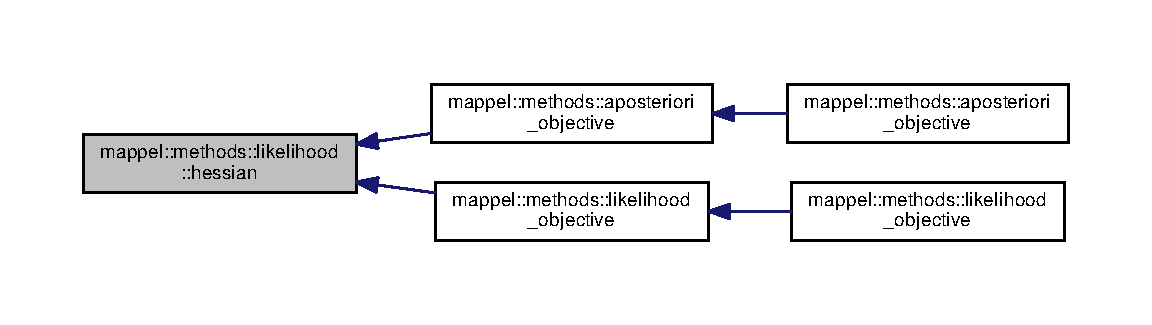
\includegraphics[width=350pt]{namespacemappel_1_1methods_1_1likelihood_a0233341d03d8f8d06cb852068942ba73_icgraph}
\end{center}
\end{figure}


\index{mappel\+::methods\+::likelihood@{mappel\+::methods\+::likelihood}!hessian@{hessian}}
\index{hessian@{hessian}!mappel\+::methods\+::likelihood@{mappel\+::methods\+::likelihood}}
\paragraph[{\texorpdfstring{hessian(const Model \&model, const Model\+Data\+T$<$ Model $>$ \&data\+\_\+im, const Stencil\+T$<$ Model $>$ \&s, Param\+T$<$ Model $>$ \&grad\+\_\+val, Mat\+T \&hess\+\_\+val)}{hessian(const Model &model, const ModelDataT< Model > &data_im, const StencilT< Model > &s, ParamT< Model > &grad_val, MatT &hess_val)}}]{\setlength{\rightskip}{0pt plus 5cm}template$<$class Model $>$ {\bf Return\+If\+SubclassT}$<$void,Model,{\bf Poisson\+Noise2\+D\+Objective}$>$ mappel\+::methods\+::likelihood\+::hessian (
\begin{DoxyParamCaption}
\item[{const Model \&}]{model, }
\item[{const {\bf Model\+DataT}$<$ Model $>$ \&}]{data\+\_\+im, }
\item[{const {\bf StencilT}$<$ Model $>$ \&}]{s, }
\item[{{\bf ParamT}$<$ Model $>$ \&}]{grad\+\_\+val, }
\item[{{\bf MatT} \&}]{hess\+\_\+val}
\end{DoxyParamCaption}
)}\hypertarget{namespacemappel_1_1methods_1_1likelihood_ac16ac7a26d0773dc9c074e8ad796e161}{}\label{namespacemappel_1_1methods_1_1likelihood_ac16ac7a26d0773dc9c074e8ad796e161}


Definition at line 202 of file Poisson\+Noise2\+D\+Objective.\+h.



References mappel\+::\+Image\+Format2\+D\+Base\+::size.

\index{mappel\+::methods\+::likelihood@{mappel\+::methods\+::likelihood}!llh@{llh}}
\index{llh@{llh}!mappel\+::methods\+::likelihood@{mappel\+::methods\+::likelihood}}
\paragraph[{\texorpdfstring{llh(const Model \&model, const Model\+Data\+T$<$ Model $>$ \&data\+\_\+im, const Stencil\+T$<$ Model $>$ \&s)}{llh(const Model &model, const ModelDataT< Model > &data_im, const StencilT< Model > &s)}}]{\setlength{\rightskip}{0pt plus 5cm}template$<$class Model $>$ {\bf Return\+If\+SubclassT}$<$double,Model,{\bf Poisson\+Noise1\+D\+Objective}$>$ mappel\+::methods\+::likelihood\+::llh (
\begin{DoxyParamCaption}
\item[{const Model \&}]{model, }
\item[{const {\bf Model\+DataT}$<$ Model $>$ \&}]{data\+\_\+im, }
\item[{const {\bf StencilT}$<$ Model $>$ \&}]{s}
\end{DoxyParamCaption}
)}\hypertarget{namespacemappel_1_1methods_1_1likelihood_a447a9c4b4bdcd45bed3f2df281efc5a5}{}\label{namespacemappel_1_1methods_1_1likelihood_a447a9c4b4bdcd45bed3f2df281efc5a5}


Definition at line 122 of file Poisson\+Noise1\+D\+Objective.\+h.



References mappel\+::poisson\+\_\+log\+\_\+likelihood().



Here is the call graph for this function\+:\nopagebreak
\begin{figure}[H]
\begin{center}
\leavevmode
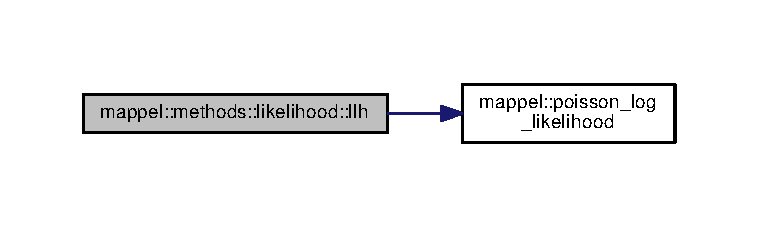
\includegraphics[width=350pt]{namespacemappel_1_1methods_1_1likelihood_a447a9c4b4bdcd45bed3f2df281efc5a5_cgraph}
\end{center}
\end{figure}


\index{mappel\+::methods\+::likelihood@{mappel\+::methods\+::likelihood}!llh@{llh}}
\index{llh@{llh}!mappel\+::methods\+::likelihood@{mappel\+::methods\+::likelihood}}
\paragraph[{\texorpdfstring{llh(const Model \&model, const Model\+Data\+T$<$ Model $>$ \&data\+\_\+im, const Stencil\+T$<$ Model $>$ \&s)}{llh(const Model &model, const ModelDataT< Model > &data_im, const StencilT< Model > &s)}}]{\setlength{\rightskip}{0pt plus 5cm}template$<$class Model $>$ {\bf Return\+If\+SubclassT}$<$double,Model,{\bf Poisson\+Noise2\+D\+Objective}$>$ mappel\+::methods\+::likelihood\+::llh (
\begin{DoxyParamCaption}
\item[{const Model \&}]{model, }
\item[{const {\bf Model\+DataT}$<$ Model $>$ \&}]{data\+\_\+im, }
\item[{const {\bf StencilT}$<$ Model $>$ \&}]{s}
\end{DoxyParamCaption}
)}\hypertarget{namespacemappel_1_1methods_1_1likelihood_a134b4c6ce6807f342f33464e99512dc6}{}\label{namespacemappel_1_1methods_1_1likelihood_a134b4c6ce6807f342f33464e99512dc6}


Definition at line 131 of file Poisson\+Noise2\+D\+Objective.\+h.



References mappel\+::poisson\+\_\+log\+\_\+likelihood(), and mappel\+::\+Image\+Format2\+D\+Base\+::size.



Here is the call graph for this function\+:\nopagebreak
\begin{figure}[H]
\begin{center}
\leavevmode
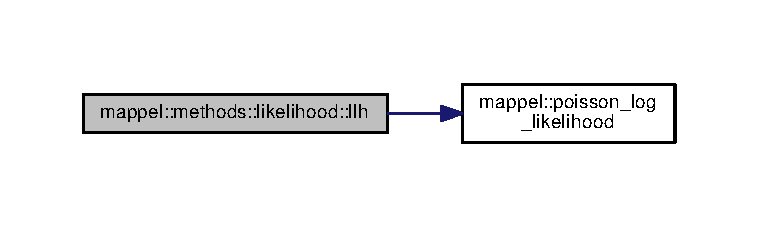
\includegraphics[width=350pt]{namespacemappel_1_1methods_1_1likelihood_a134b4c6ce6807f342f33464e99512dc6_cgraph}
\end{center}
\end{figure}


\index{mappel\+::methods\+::likelihood@{mappel\+::methods\+::likelihood}!rllh@{rllh}}
\index{rllh@{rllh}!mappel\+::methods\+::likelihood@{mappel\+::methods\+::likelihood}}
\paragraph[{\texorpdfstring{rllh(const Model \&model, const Model\+Data\+T$<$ Model $>$ \&data\+\_\+im, const Stencil\+T$<$ Model $>$ \&s)}{rllh(const Model &model, const ModelDataT< Model > &data_im, const StencilT< Model > &s)}}]{\setlength{\rightskip}{0pt plus 5cm}template$<$class Model $>$ {\bf Return\+If\+SubclassT}$<$double,Model,{\bf Poisson\+Noise1\+D\+Objective}$>$ mappel\+::methods\+::likelihood\+::rllh (
\begin{DoxyParamCaption}
\item[{const Model \&}]{model, }
\item[{const {\bf Model\+DataT}$<$ Model $>$ \&}]{data\+\_\+im, }
\item[{const {\bf StencilT}$<$ Model $>$ \&}]{s}
\end{DoxyParamCaption}
)}\hypertarget{namespacemappel_1_1methods_1_1likelihood_ae064b0a1e26a5626c62bde870e587ecb}{}\label{namespacemappel_1_1methods_1_1likelihood_ae064b0a1e26a5626c62bde870e587ecb}


Definition at line 134 of file Poisson\+Noise1\+D\+Objective.\+h.



References mappel\+::relative\+\_\+poisson\+\_\+log\+\_\+likelihood().



Referenced by mappel\+::methods\+::aposteriori\+\_\+objective(), and mappel\+::methods\+::likelihood\+\_\+objective().



Here is the call graph for this function\+:\nopagebreak
\begin{figure}[H]
\begin{center}
\leavevmode
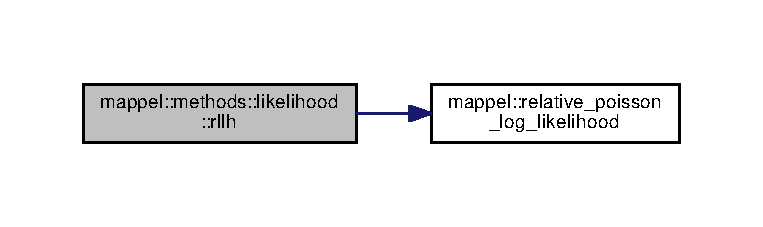
\includegraphics[width=350pt]{namespacemappel_1_1methods_1_1likelihood_ae064b0a1e26a5626c62bde870e587ecb_cgraph}
\end{center}
\end{figure}




Here is the caller graph for this function\+:\nopagebreak
\begin{figure}[H]
\begin{center}
\leavevmode
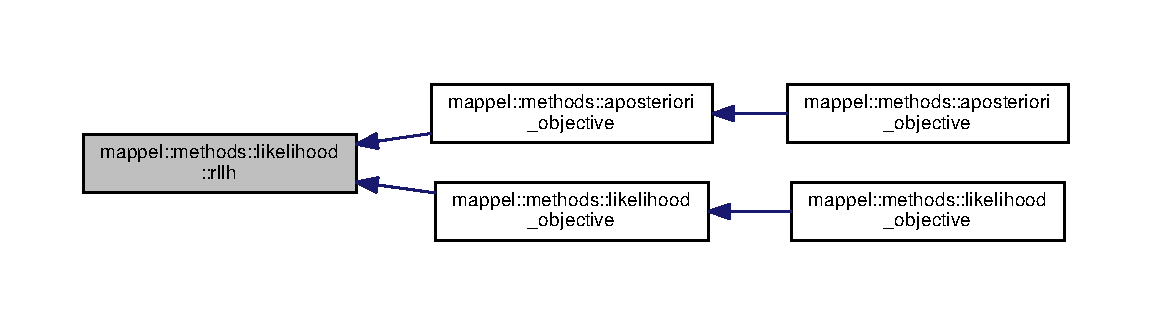
\includegraphics[width=350pt]{namespacemappel_1_1methods_1_1likelihood_ae064b0a1e26a5626c62bde870e587ecb_icgraph}
\end{center}
\end{figure}


\index{mappel\+::methods\+::likelihood@{mappel\+::methods\+::likelihood}!rllh@{rllh}}
\index{rllh@{rllh}!mappel\+::methods\+::likelihood@{mappel\+::methods\+::likelihood}}
\paragraph[{\texorpdfstring{rllh(const Model \&model, const Model\+Data\+T$<$ Model $>$ \&data\+\_\+im, const Stencil\+T$<$ Model $>$ \&s)}{rllh(const Model &model, const ModelDataT< Model > &data_im, const StencilT< Model > &s)}}]{\setlength{\rightskip}{0pt plus 5cm}template$<$class Model $>$ {\bf Return\+If\+SubclassT}$<$double,Model,{\bf Poisson\+Noise2\+D\+Objective}$>$ mappel\+::methods\+::likelihood\+::rllh (
\begin{DoxyParamCaption}
\item[{const Model \&}]{model, }
\item[{const {\bf Model\+DataT}$<$ Model $>$ \&}]{data\+\_\+im, }
\item[{const {\bf StencilT}$<$ Model $>$ \&}]{s}
\end{DoxyParamCaption}
)}\hypertarget{namespacemappel_1_1methods_1_1likelihood_aa8cbdb607db58f763a8dc70ef48372f1}{}\label{namespacemappel_1_1methods_1_1likelihood_aa8cbdb607db58f763a8dc70ef48372f1}


Definition at line 145 of file Poisson\+Noise2\+D\+Objective.\+h.



References mappel\+::relative\+\_\+poisson\+\_\+log\+\_\+likelihood(), and mappel\+::\+Image\+Format2\+D\+Base\+::size.



Here is the call graph for this function\+:\nopagebreak
\begin{figure}[H]
\begin{center}
\leavevmode
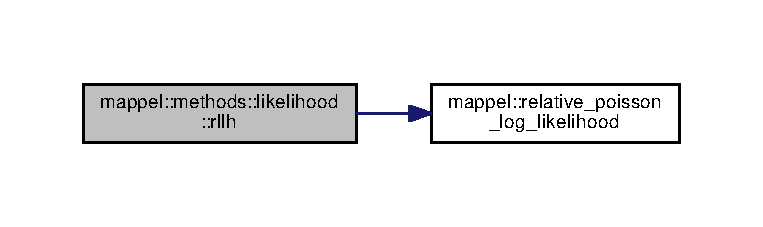
\includegraphics[width=350pt]{namespacemappel_1_1methods_1_1likelihood_aa8cbdb607db58f763a8dc70ef48372f1_cgraph}
\end{center}
\end{figure}



\hypertarget{namespacemappel_1_1methods_1_1likelihood_1_1debug}{}\subsection{mappel\+:\+:methods\+:\+:likelihood\+:\+:debug Namespace Reference}
\label{namespacemappel_1_1methods_1_1likelihood_1_1debug}\index{mappel\+::methods\+::likelihood\+::debug@{mappel\+::methods\+::likelihood\+::debug}}
\subsubsection*{Functions}
\begin{DoxyCompactItemize}
\item 
{\footnotesize template$<$class Model $>$ }\\\hyperlink{namespacemappel_a3b77d227658ba3ba9e16fea6fa6e626d}{Return\+If\+SubclassT}$<$ \hyperlink{namespacemappel_a2225ad69f358daa3f4f99282a35b9a3a}{VecT}, Model, \hyperlink{classmappel_1_1PoissonNoise1DObjective}{Poisson\+Noise1\+D\+Objective} $>$ \hyperlink{namespacemappel_1_1methods_1_1likelihood_1_1debug_a3ebb5c59ce538767de0717dbb543547a}{llh\+\_\+components} (const Model \&model, const \hyperlink{namespacemappel_a97f050df953605381ae9c901c3b125f1}{Model\+DataT}$<$ Model $>$ \&data\+\_\+im, const \hyperlink{namespacemappel_a3a06598240007876f8c4bf834ad86197}{StencilT}$<$ Model $>$ \&s)
\item 
{\footnotesize template$<$class Model $>$ }\\\hyperlink{namespacemappel_a3b77d227658ba3ba9e16fea6fa6e626d}{Return\+If\+SubclassT}$<$ \hyperlink{namespacemappel_a2225ad69f358daa3f4f99282a35b9a3a}{VecT}, Model, \hyperlink{classmappel_1_1PoissonNoise1DObjective}{Poisson\+Noise1\+D\+Objective} $>$ \hyperlink{namespacemappel_1_1methods_1_1likelihood_1_1debug_abee134828904f67b599234ec96a4a907}{rllh\+\_\+components} (const Model \&model, const \hyperlink{namespacemappel_a97f050df953605381ae9c901c3b125f1}{Model\+DataT}$<$ Model $>$ \&data\+\_\+im, const \hyperlink{namespacemappel_a3a06598240007876f8c4bf834ad86197}{StencilT}$<$ Model $>$ \&s)
\item 
{\footnotesize template$<$class Model $>$ }\\\hyperlink{namespacemappel_a3b77d227658ba3ba9e16fea6fa6e626d}{Return\+If\+SubclassT}$<$ \hyperlink{namespacemappel_a7091ab87c528041f7e2027195fad8915}{MatT}, Model, \hyperlink{classmappel_1_1PoissonNoise1DObjective}{Poisson\+Noise1\+D\+Objective} $>$ \hyperlink{namespacemappel_1_1methods_1_1likelihood_1_1debug_a5e367e627cf90895292099ed9d86c2db}{grad\+\_\+components} (const Model \&model, const \hyperlink{namespacemappel_a97f050df953605381ae9c901c3b125f1}{Model\+DataT}$<$ Model $>$ \&data\+\_\+im, const \hyperlink{namespacemappel_a3a06598240007876f8c4bf834ad86197}{StencilT}$<$ Model $>$ \&s)
\item 
{\footnotesize template$<$class Model $>$ }\\\hyperlink{namespacemappel_a3b77d227658ba3ba9e16fea6fa6e626d}{Return\+If\+SubclassT}$<$ \hyperlink{namespacemappel_ab2afab4e6c8805e83946670d882768c2}{CubeT}, Model, \hyperlink{classmappel_1_1PoissonNoise1DObjective}{Poisson\+Noise1\+D\+Objective} $>$ \hyperlink{namespacemappel_1_1methods_1_1likelihood_1_1debug_a3ce1dba1970e94b391b4a60792ee635a}{hessian\+\_\+components} (const Model \&model, const \hyperlink{namespacemappel_a97f050df953605381ae9c901c3b125f1}{Model\+DataT}$<$ Model $>$ \&data\+\_\+im, const \hyperlink{namespacemappel_a3a06598240007876f8c4bf834ad86197}{StencilT}$<$ Model $>$ \&s)
\item 
{\footnotesize template$<$class Model $>$ }\\\hyperlink{namespacemappel_a3b77d227658ba3ba9e16fea6fa6e626d}{Return\+If\+SubclassT}$<$ \hyperlink{namespacemappel_a2225ad69f358daa3f4f99282a35b9a3a}{VecT}, Model, \hyperlink{classmappel_1_1PoissonNoise2DObjective}{Poisson\+Noise2\+D\+Objective} $>$ \hyperlink{namespacemappel_1_1methods_1_1likelihood_1_1debug_a47e4b71af29f5c8d435e5a8880fe254a}{llh\+\_\+components} (const Model \&model, const \hyperlink{namespacemappel_a97f050df953605381ae9c901c3b125f1}{Model\+DataT}$<$ Model $>$ \&data\+\_\+im, const \hyperlink{namespacemappel_a3a06598240007876f8c4bf834ad86197}{StencilT}$<$ Model $>$ \&s)
\item 
{\footnotesize template$<$class Model $>$ }\\\hyperlink{namespacemappel_a3b77d227658ba3ba9e16fea6fa6e626d}{Return\+If\+SubclassT}$<$ \hyperlink{namespacemappel_a2225ad69f358daa3f4f99282a35b9a3a}{VecT}, Model, \hyperlink{classmappel_1_1PoissonNoise2DObjective}{Poisson\+Noise2\+D\+Objective} $>$ \hyperlink{namespacemappel_1_1methods_1_1likelihood_1_1debug_ac91e6c82e246b21c5f6dc2f9d8ce295d}{rllh\+\_\+components} (const Model \&model, const \hyperlink{namespacemappel_a97f050df953605381ae9c901c3b125f1}{Model\+DataT}$<$ Model $>$ \&data\+\_\+im, const \hyperlink{namespacemappel_a3a06598240007876f8c4bf834ad86197}{StencilT}$<$ Model $>$ \&s)
\item 
{\footnotesize template$<$class Model $>$ }\\\hyperlink{namespacemappel_a3b77d227658ba3ba9e16fea6fa6e626d}{Return\+If\+SubclassT}$<$ \hyperlink{namespacemappel_a7091ab87c528041f7e2027195fad8915}{MatT}, Model, \hyperlink{classmappel_1_1PoissonNoise2DObjective}{Poisson\+Noise2\+D\+Objective} $>$ \hyperlink{namespacemappel_1_1methods_1_1likelihood_1_1debug_aeb75ad8daa3b69f3cf800cf38f17656d}{grad\+\_\+components} (const Model \&model, const \hyperlink{namespacemappel_a97f050df953605381ae9c901c3b125f1}{Model\+DataT}$<$ Model $>$ \&data\+\_\+im, const \hyperlink{namespacemappel_a3a06598240007876f8c4bf834ad86197}{StencilT}$<$ Model $>$ \&s)
\item 
{\footnotesize template$<$class Model $>$ }\\\hyperlink{namespacemappel_a3b77d227658ba3ba9e16fea6fa6e626d}{Return\+If\+SubclassT}$<$ \hyperlink{namespacemappel_ab2afab4e6c8805e83946670d882768c2}{CubeT}, Model, \hyperlink{classmappel_1_1PoissonNoise2DObjective}{Poisson\+Noise2\+D\+Objective} $>$ \hyperlink{namespacemappel_1_1methods_1_1likelihood_1_1debug_ab4a28e66a2192d238960defbe85c0d4c}{hessian\+\_\+components} (const Model \&model, const \hyperlink{namespacemappel_a97f050df953605381ae9c901c3b125f1}{Model\+DataT}$<$ Model $>$ \&data\+\_\+im, const \hyperlink{namespacemappel_a3a06598240007876f8c4bf834ad86197}{StencilT}$<$ Model $>$ \&s)
\end{DoxyCompactItemize}


\subsubsection{Function Documentation}
\index{mappel\+::methods\+::likelihood\+::debug@{mappel\+::methods\+::likelihood\+::debug}!grad\+\_\+components@{grad\+\_\+components}}
\index{grad\+\_\+components@{grad\+\_\+components}!mappel\+::methods\+::likelihood\+::debug@{mappel\+::methods\+::likelihood\+::debug}}
\paragraph[{\texorpdfstring{grad\+\_\+components(const Model \&model, const Model\+Data\+T$<$ Model $>$ \&data\+\_\+im, const Stencil\+T$<$ Model $>$ \&s)}{grad_components(const Model &model, const ModelDataT< Model > &data_im, const StencilT< Model > &s)}}]{\setlength{\rightskip}{0pt plus 5cm}template$<$class Model $>$ {\bf Return\+If\+SubclassT}$<${\bf MatT},Model,{\bf Poisson\+Noise1\+D\+Objective}$>$ mappel\+::methods\+::likelihood\+::debug\+::grad\+\_\+components (
\begin{DoxyParamCaption}
\item[{const Model \&}]{model, }
\item[{const {\bf Model\+DataT}$<$ Model $>$ \&}]{data\+\_\+im, }
\item[{const {\bf StencilT}$<$ Model $>$ \&}]{s}
\end{DoxyParamCaption}
)}\hypertarget{namespacemappel_1_1methods_1_1likelihood_1_1debug_a5e367e627cf90895292099ed9d86c2db}{}\label{namespacemappel_1_1methods_1_1likelihood_1_1debug_a5e367e627cf90895292099ed9d86c2db}


Definition at line 230 of file Poisson\+Noise1\+D\+Objective.\+h.

\index{mappel\+::methods\+::likelihood\+::debug@{mappel\+::methods\+::likelihood\+::debug}!grad\+\_\+components@{grad\+\_\+components}}
\index{grad\+\_\+components@{grad\+\_\+components}!mappel\+::methods\+::likelihood\+::debug@{mappel\+::methods\+::likelihood\+::debug}}
\paragraph[{\texorpdfstring{grad\+\_\+components(const Model \&model, const Model\+Data\+T$<$ Model $>$ \&data\+\_\+im, const Stencil\+T$<$ Model $>$ \&s)}{grad_components(const Model &model, const ModelDataT< Model > &data_im, const StencilT< Model > &s)}}]{\setlength{\rightskip}{0pt plus 5cm}template$<$class Model $>$ {\bf Return\+If\+SubclassT}$<${\bf MatT},Model,{\bf Poisson\+Noise2\+D\+Objective}$>$ mappel\+::methods\+::likelihood\+::debug\+::grad\+\_\+components (
\begin{DoxyParamCaption}
\item[{const Model \&}]{model, }
\item[{const {\bf Model\+DataT}$<$ Model $>$ \&}]{data\+\_\+im, }
\item[{const {\bf StencilT}$<$ Model $>$ \&}]{s}
\end{DoxyParamCaption}
)}\hypertarget{namespacemappel_1_1methods_1_1likelihood_1_1debug_aeb75ad8daa3b69f3cf800cf38f17656d}{}\label{namespacemappel_1_1methods_1_1likelihood_1_1debug_aeb75ad8daa3b69f3cf800cf38f17656d}


Definition at line 255 of file Poisson\+Noise2\+D\+Objective.\+h.



References mappel\+::\+Image\+Format2\+D\+Base\+::size.

\index{mappel\+::methods\+::likelihood\+::debug@{mappel\+::methods\+::likelihood\+::debug}!hessian\+\_\+components@{hessian\+\_\+components}}
\index{hessian\+\_\+components@{hessian\+\_\+components}!mappel\+::methods\+::likelihood\+::debug@{mappel\+::methods\+::likelihood\+::debug}}
\paragraph[{\texorpdfstring{hessian\+\_\+components(const Model \&model, const Model\+Data\+T$<$ Model $>$ \&data\+\_\+im, const Stencil\+T$<$ Model $>$ \&s)}{hessian_components(const Model &model, const ModelDataT< Model > &data_im, const StencilT< Model > &s)}}]{\setlength{\rightskip}{0pt plus 5cm}template$<$class Model $>$ {\bf Return\+If\+SubclassT}$<${\bf CubeT},Model,{\bf Poisson\+Noise1\+D\+Objective}$>$ mappel\+::methods\+::likelihood\+::debug\+::hessian\+\_\+components (
\begin{DoxyParamCaption}
\item[{const Model \&}]{model, }
\item[{const {\bf Model\+DataT}$<$ Model $>$ \&}]{data\+\_\+im, }
\item[{const {\bf StencilT}$<$ Model $>$ \&}]{s}
\end{DoxyParamCaption}
)}\hypertarget{namespacemappel_1_1methods_1_1likelihood_1_1debug_a3ce1dba1970e94b391b4a60792ee635a}{}\label{namespacemappel_1_1methods_1_1likelihood_1_1debug_a3ce1dba1970e94b391b4a60792ee635a}


Definition at line 246 of file Poisson\+Noise1\+D\+Objective.\+h.

\index{mappel\+::methods\+::likelihood\+::debug@{mappel\+::methods\+::likelihood\+::debug}!hessian\+\_\+components@{hessian\+\_\+components}}
\index{hessian\+\_\+components@{hessian\+\_\+components}!mappel\+::methods\+::likelihood\+::debug@{mappel\+::methods\+::likelihood\+::debug}}
\paragraph[{\texorpdfstring{hessian\+\_\+components(const Model \&model, const Model\+Data\+T$<$ Model $>$ \&data\+\_\+im, const Stencil\+T$<$ Model $>$ \&s)}{hessian_components(const Model &model, const ModelDataT< Model > &data_im, const StencilT< Model > &s)}}]{\setlength{\rightskip}{0pt plus 5cm}template$<$class Model $>$ {\bf Return\+If\+SubclassT}$<${\bf CubeT},Model,{\bf Poisson\+Noise2\+D\+Objective}$>$ mappel\+::methods\+::likelihood\+::debug\+::hessian\+\_\+components (
\begin{DoxyParamCaption}
\item[{const Model \&}]{model, }
\item[{const {\bf Model\+DataT}$<$ Model $>$ \&}]{data\+\_\+im, }
\item[{const {\bf StencilT}$<$ Model $>$ \&}]{s}
\end{DoxyParamCaption}
)}\hypertarget{namespacemappel_1_1methods_1_1likelihood_1_1debug_ab4a28e66a2192d238960defbe85c0d4c}{}\label{namespacemappel_1_1methods_1_1likelihood_1_1debug_ab4a28e66a2192d238960defbe85c0d4c}


Definition at line 274 of file Poisson\+Noise2\+D\+Objective.\+h.



References mappel\+::\+Image\+Format2\+D\+Base\+::size.

\index{mappel\+::methods\+::likelihood\+::debug@{mappel\+::methods\+::likelihood\+::debug}!llh\+\_\+components@{llh\+\_\+components}}
\index{llh\+\_\+components@{llh\+\_\+components}!mappel\+::methods\+::likelihood\+::debug@{mappel\+::methods\+::likelihood\+::debug}}
\paragraph[{\texorpdfstring{llh\+\_\+components(const Model \&model, const Model\+Data\+T$<$ Model $>$ \&data\+\_\+im, const Stencil\+T$<$ Model $>$ \&s)}{llh_components(const Model &model, const ModelDataT< Model > &data_im, const StencilT< Model > &s)}}]{\setlength{\rightskip}{0pt plus 5cm}template$<$class Model $>$ {\bf Return\+If\+SubclassT}$<${\bf VecT},Model,{\bf Poisson\+Noise1\+D\+Objective}$>$ mappel\+::methods\+::likelihood\+::debug\+::llh\+\_\+components (
\begin{DoxyParamCaption}
\item[{const Model \&}]{model, }
\item[{const {\bf Model\+DataT}$<$ Model $>$ \&}]{data\+\_\+im, }
\item[{const {\bf StencilT}$<$ Model $>$ \&}]{s}
\end{DoxyParamCaption}
)}\hypertarget{namespacemappel_1_1methods_1_1likelihood_1_1debug_a3ebb5c59ce538767de0717dbb543547a}{}\label{namespacemappel_1_1methods_1_1likelihood_1_1debug_a3ebb5c59ce538767de0717dbb543547a}


Definition at line 206 of file Poisson\+Noise1\+D\+Objective.\+h.



References mappel\+::poisson\+\_\+log\+\_\+likelihood().



Here is the call graph for this function\+:\nopagebreak
\begin{figure}[H]
\begin{center}
\leavevmode
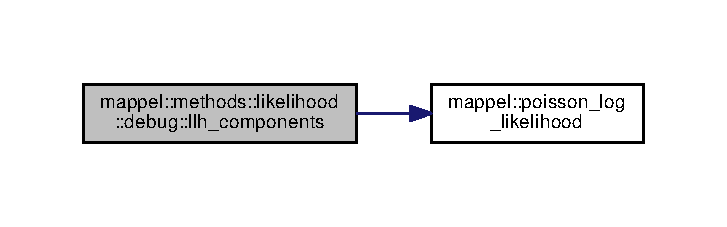
\includegraphics[width=349pt]{namespacemappel_1_1methods_1_1likelihood_1_1debug_a3ebb5c59ce538767de0717dbb543547a_cgraph}
\end{center}
\end{figure}


\index{mappel\+::methods\+::likelihood\+::debug@{mappel\+::methods\+::likelihood\+::debug}!llh\+\_\+components@{llh\+\_\+components}}
\index{llh\+\_\+components@{llh\+\_\+components}!mappel\+::methods\+::likelihood\+::debug@{mappel\+::methods\+::likelihood\+::debug}}
\paragraph[{\texorpdfstring{llh\+\_\+components(const Model \&model, const Model\+Data\+T$<$ Model $>$ \&data\+\_\+im, const Stencil\+T$<$ Model $>$ \&s)}{llh_components(const Model &model, const ModelDataT< Model > &data_im, const StencilT< Model > &s)}}]{\setlength{\rightskip}{0pt plus 5cm}template$<$class Model $>$ {\bf Return\+If\+SubclassT}$<${\bf VecT},Model,{\bf Poisson\+Noise2\+D\+Objective}$>$ mappel\+::methods\+::likelihood\+::debug\+::llh\+\_\+components (
\begin{DoxyParamCaption}
\item[{const Model \&}]{model, }
\item[{const {\bf Model\+DataT}$<$ Model $>$ \&}]{data\+\_\+im, }
\item[{const {\bf StencilT}$<$ Model $>$ \&}]{s}
\end{DoxyParamCaption}
)}\hypertarget{namespacemappel_1_1methods_1_1likelihood_1_1debug_a47e4b71af29f5c8d435e5a8880fe254a}{}\label{namespacemappel_1_1methods_1_1likelihood_1_1debug_a47e4b71af29f5c8d435e5a8880fe254a}


Definition at line 225 of file Poisson\+Noise2\+D\+Objective.\+h.



References mappel\+::poisson\+\_\+log\+\_\+likelihood(), and mappel\+::\+Image\+Format2\+D\+Base\+::size.



Here is the call graph for this function\+:\nopagebreak
\begin{figure}[H]
\begin{center}
\leavevmode
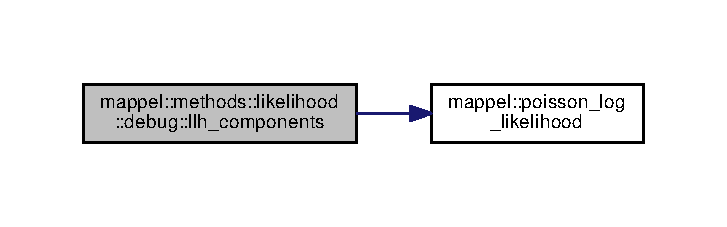
\includegraphics[width=349pt]{namespacemappel_1_1methods_1_1likelihood_1_1debug_a47e4b71af29f5c8d435e5a8880fe254a_cgraph}
\end{center}
\end{figure}


\index{mappel\+::methods\+::likelihood\+::debug@{mappel\+::methods\+::likelihood\+::debug}!rllh\+\_\+components@{rllh\+\_\+components}}
\index{rllh\+\_\+components@{rllh\+\_\+components}!mappel\+::methods\+::likelihood\+::debug@{mappel\+::methods\+::likelihood\+::debug}}
\paragraph[{\texorpdfstring{rllh\+\_\+components(const Model \&model, const Model\+Data\+T$<$ Model $>$ \&data\+\_\+im, const Stencil\+T$<$ Model $>$ \&s)}{rllh_components(const Model &model, const ModelDataT< Model > &data_im, const StencilT< Model > &s)}}]{\setlength{\rightskip}{0pt plus 5cm}template$<$class Model $>$ {\bf Return\+If\+SubclassT}$<${\bf VecT},Model,{\bf Poisson\+Noise1\+D\+Objective}$>$ mappel\+::methods\+::likelihood\+::debug\+::rllh\+\_\+components (
\begin{DoxyParamCaption}
\item[{const Model \&}]{model, }
\item[{const {\bf Model\+DataT}$<$ Model $>$ \&}]{data\+\_\+im, }
\item[{const {\bf StencilT}$<$ Model $>$ \&}]{s}
\end{DoxyParamCaption}
)}\hypertarget{namespacemappel_1_1methods_1_1likelihood_1_1debug_abee134828904f67b599234ec96a4a907}{}\label{namespacemappel_1_1methods_1_1likelihood_1_1debug_abee134828904f67b599234ec96a4a907}


Definition at line 218 of file Poisson\+Noise1\+D\+Objective.\+h.



References mappel\+::relative\+\_\+poisson\+\_\+log\+\_\+likelihood().



Here is the call graph for this function\+:\nopagebreak
\begin{figure}[H]
\begin{center}
\leavevmode
\includegraphics[width=350pt]{namespacemappel_1_1methods_1_1likelihood_1_1debug_abee134828904f67b599234ec96a4a907_cgraph}
\end{center}
\end{figure}


\index{mappel\+::methods\+::likelihood\+::debug@{mappel\+::methods\+::likelihood\+::debug}!rllh\+\_\+components@{rllh\+\_\+components}}
\index{rllh\+\_\+components@{rllh\+\_\+components}!mappel\+::methods\+::likelihood\+::debug@{mappel\+::methods\+::likelihood\+::debug}}
\paragraph[{\texorpdfstring{rllh\+\_\+components(const Model \&model, const Model\+Data\+T$<$ Model $>$ \&data\+\_\+im, const Stencil\+T$<$ Model $>$ \&s)}{rllh_components(const Model &model, const ModelDataT< Model > &data_im, const StencilT< Model > &s)}}]{\setlength{\rightskip}{0pt plus 5cm}template$<$class Model $>$ {\bf Return\+If\+SubclassT}$<${\bf VecT},Model,{\bf Poisson\+Noise2\+D\+Objective}$>$ mappel\+::methods\+::likelihood\+::debug\+::rllh\+\_\+components (
\begin{DoxyParamCaption}
\item[{const Model \&}]{model, }
\item[{const {\bf Model\+DataT}$<$ Model $>$ \&}]{data\+\_\+im, }
\item[{const {\bf StencilT}$<$ Model $>$ \&}]{s}
\end{DoxyParamCaption}
)}\hypertarget{namespacemappel_1_1methods_1_1likelihood_1_1debug_ac91e6c82e246b21c5f6dc2f9d8ce295d}{}\label{namespacemappel_1_1methods_1_1likelihood_1_1debug_ac91e6c82e246b21c5f6dc2f9d8ce295d}


Definition at line 240 of file Poisson\+Noise2\+D\+Objective.\+h.



References mappel\+::relative\+\_\+poisson\+\_\+log\+\_\+likelihood(), and mappel\+::\+Image\+Format2\+D\+Base\+::size.



Here is the call graph for this function\+:\nopagebreak
\begin{figure}[H]
\begin{center}
\leavevmode
\includegraphics[width=350pt]{namespacemappel_1_1methods_1_1likelihood_1_1debug_ac91e6c82e246b21c5f6dc2f9d8ce295d_cgraph}
\end{center}
\end{figure}



\hypertarget{namespacemappel_1_1methods_1_1objective}{}\subsection{mappel\+:\+:methods\+:\+:objective Namespace Reference}
\label{namespacemappel_1_1methods_1_1objective}\index{mappel\+::methods\+::objective@{mappel\+::methods\+::objective}}
\subsubsection*{Namespaces}
\begin{DoxyCompactItemize}
\item 
 \hyperlink{namespacemappel_1_1methods_1_1objective_1_1debug}{debug}
\item 
 \hyperlink{namespacemappel_1_1methods_1_1objective_1_1openmp}{openmp}
\end{DoxyCompactItemize}
\subsubsection*{Functions}
\begin{DoxyCompactItemize}
\item 
{\footnotesize template$<$class Model $>$ }\\\hyperlink{namespacemappel_a3b77d227658ba3ba9e16fea6fa6e626d}{Return\+If\+SubclassT}$<$ double, Model, \hyperlink{classmappel_1_1MAPEstimator}{M\+A\+P\+Estimator} $>$ \hyperlink{namespacemappel_1_1methods_1_1objective_a94105ec313ae34d4b30ef78369056eaa}{llh} (const Model \&model, const \hyperlink{namespacemappel_a97f050df953605381ae9c901c3b125f1}{Model\+DataT}$<$ Model $>$ \&data\+\_\+im, const \hyperlink{namespacemappel_a3a06598240007876f8c4bf834ad86197}{StencilT}$<$ Model $>$ \&s)
\item 
{\footnotesize template$<$class Model $>$ }\\\hyperlink{namespacemappel_a3b77d227658ba3ba9e16fea6fa6e626d}{Return\+If\+SubclassT}$<$ double, Model, \hyperlink{classmappel_1_1MAPEstimator}{M\+A\+P\+Estimator} $>$ \hyperlink{namespacemappel_1_1methods_1_1objective_a293c23ed6a623e59477bb67b6e40f5ad}{rllh} (const Model \&model, const \hyperlink{namespacemappel_a97f050df953605381ae9c901c3b125f1}{Model\+DataT}$<$ Model $>$ \&data\+\_\+im, const \hyperlink{namespacemappel_a3a06598240007876f8c4bf834ad86197}{StencilT}$<$ Model $>$ \&s)
\item 
{\footnotesize template$<$class Model $>$ }\\\hyperlink{namespacemappel_a3b77d227658ba3ba9e16fea6fa6e626d}{Return\+If\+SubclassT}$<$ \hyperlink{namespacemappel_a667925cb0d6c0e49f2f035cc5a9a6857}{ParamT}$<$ Model $>$, Model, \hyperlink{classmappel_1_1MAPEstimator}{M\+A\+P\+Estimator} $>$ \hyperlink{namespacemappel_1_1methods_1_1objective_a8e120e5a79029803453cea5f9f2d8f67}{grad} (const Model \&model, const \hyperlink{namespacemappel_a97f050df953605381ae9c901c3b125f1}{Model\+DataT}$<$ Model $>$ \&data\+\_\+im, const \hyperlink{namespacemappel_a3a06598240007876f8c4bf834ad86197}{StencilT}$<$ Model $>$ \&s)
\item 
{\footnotesize template$<$class Model $>$ }\\\hyperlink{namespacemappel_a3b77d227658ba3ba9e16fea6fa6e626d}{Return\+If\+SubclassT}$<$ void, Model, \hyperlink{classmappel_1_1MAPEstimator}{M\+A\+P\+Estimator} $>$ \hyperlink{namespacemappel_1_1methods_1_1objective_a165388f45fa850f2b12c22053296a0c2}{grad2} (const Model \&model, const \hyperlink{namespacemappel_a97f050df953605381ae9c901c3b125f1}{Model\+DataT}$<$ Model $>$ \&data\+\_\+im, const \hyperlink{namespacemappel_a3a06598240007876f8c4bf834ad86197}{StencilT}$<$ Model $>$ \&s, \hyperlink{namespacemappel_a667925cb0d6c0e49f2f035cc5a9a6857}{ParamT}$<$ Model $>$ \&\hyperlink{namespacemappel_1_1methods_1_1objective_a8e120e5a79029803453cea5f9f2d8f67}{grad}, \hyperlink{namespacemappel_a667925cb0d6c0e49f2f035cc5a9a6857}{ParamT}$<$ Model $>$ \&grad2)
\item 
{\footnotesize template$<$class Model $>$ }\\\hyperlink{namespacemappel_a3b77d227658ba3ba9e16fea6fa6e626d}{Return\+If\+SubclassT}$<$ void, Model, \hyperlink{classmappel_1_1MAPEstimator}{M\+A\+P\+Estimator} $>$ \hyperlink{namespacemappel_1_1methods_1_1objective_afbf93fa446606620d01747af3684f62d}{hessian} (const Model \&model, const \hyperlink{namespacemappel_a97f050df953605381ae9c901c3b125f1}{Model\+DataT}$<$ Model $>$ \&data\+\_\+im, const \hyperlink{namespacemappel_a3a06598240007876f8c4bf834ad86197}{StencilT}$<$ Model $>$ \&s, \hyperlink{namespacemappel_a667925cb0d6c0e49f2f035cc5a9a6857}{ParamT}$<$ Model $>$ \&\hyperlink{namespacemappel_1_1methods_1_1objective_a8e120e5a79029803453cea5f9f2d8f67}{grad}, \hyperlink{namespacemappel_a7091ab87c528041f7e2027195fad8915}{MatT} \&hess)
\item 
{\footnotesize template$<$class Model $>$ }\\\hyperlink{namespacemappel_a3b77d227658ba3ba9e16fea6fa6e626d}{Return\+If\+SubclassT}$<$ double, Model, \hyperlink{classmappel_1_1MLEstimator}{M\+L\+Estimator} $>$ \hyperlink{namespacemappel_1_1methods_1_1objective_ac391c37d46e7f85d67947402d85a72ea}{llh} (const Model \&model, const \hyperlink{namespacemappel_a97f050df953605381ae9c901c3b125f1}{Model\+DataT}$<$ Model $>$ \&data\+\_\+im, const \hyperlink{namespacemappel_a3a06598240007876f8c4bf834ad86197}{StencilT}$<$ Model $>$ \&s)
\item 
{\footnotesize template$<$class Model $>$ }\\\hyperlink{namespacemappel_a3b77d227658ba3ba9e16fea6fa6e626d}{Return\+If\+SubclassT}$<$ double, Model, \hyperlink{classmappel_1_1MLEstimator}{M\+L\+Estimator} $>$ \hyperlink{namespacemappel_1_1methods_1_1objective_ab59f42ad9220e14c55b31c04562e691f}{rllh} (const Model \&model, const \hyperlink{namespacemappel_a97f050df953605381ae9c901c3b125f1}{Model\+DataT}$<$ Model $>$ \&data\+\_\+im, const \hyperlink{namespacemappel_a3a06598240007876f8c4bf834ad86197}{StencilT}$<$ Model $>$ \&s)
\item 
{\footnotesize template$<$class Model $>$ }\\\hyperlink{namespacemappel_a3b77d227658ba3ba9e16fea6fa6e626d}{Return\+If\+SubclassT}$<$ \hyperlink{namespacemappel_a667925cb0d6c0e49f2f035cc5a9a6857}{ParamT}$<$ Model $>$, Model, \hyperlink{classmappel_1_1MLEstimator}{M\+L\+Estimator} $>$ \hyperlink{namespacemappel_1_1methods_1_1objective_a2969893932c9440afbb69645a6a31a63}{grad} (const Model \&model, const \hyperlink{namespacemappel_a97f050df953605381ae9c901c3b125f1}{Model\+DataT}$<$ Model $>$ \&data\+\_\+im, const \hyperlink{namespacemappel_a3a06598240007876f8c4bf834ad86197}{StencilT}$<$ Model $>$ \&s)
\item 
{\footnotesize template$<$class Model $>$ }\\\hyperlink{namespacemappel_a3b77d227658ba3ba9e16fea6fa6e626d}{Return\+If\+SubclassT}$<$ void, Model, \hyperlink{classmappel_1_1MLEstimator}{M\+L\+Estimator} $>$ \hyperlink{namespacemappel_1_1methods_1_1objective_a7bf5acef5f9edd9ddf2c47cb5a90e8db}{grad2} (const Model \&model, const \hyperlink{namespacemappel_a97f050df953605381ae9c901c3b125f1}{Model\+DataT}$<$ Model $>$ \&data\+\_\+im, const \hyperlink{namespacemappel_a3a06598240007876f8c4bf834ad86197}{StencilT}$<$ Model $>$ \&s, \hyperlink{namespacemappel_a667925cb0d6c0e49f2f035cc5a9a6857}{ParamT}$<$ Model $>$ \&\hyperlink{namespacemappel_1_1methods_1_1objective_a8e120e5a79029803453cea5f9f2d8f67}{grad}, \hyperlink{namespacemappel_a667925cb0d6c0e49f2f035cc5a9a6857}{ParamT}$<$ Model $>$ \&grad2)
\item 
{\footnotesize template$<$class Model $>$ }\\\hyperlink{namespacemappel_a3b77d227658ba3ba9e16fea6fa6e626d}{Return\+If\+SubclassT}$<$ void, Model, \hyperlink{classmappel_1_1MLEstimator}{M\+L\+Estimator} $>$ \hyperlink{namespacemappel_1_1methods_1_1objective_ad7242f889fcefed1ec11c238cd3d22e3}{hessian} (const Model \&model, const \hyperlink{namespacemappel_a97f050df953605381ae9c901c3b125f1}{Model\+DataT}$<$ Model $>$ \&data\+\_\+im, const \hyperlink{namespacemappel_a3a06598240007876f8c4bf834ad86197}{StencilT}$<$ Model $>$ \&s, \hyperlink{namespacemappel_a667925cb0d6c0e49f2f035cc5a9a6857}{ParamT}$<$ Model $>$ \&\hyperlink{namespacemappel_1_1methods_1_1objective_a8e120e5a79029803453cea5f9f2d8f67}{grad}, \hyperlink{namespacemappel_a7091ab87c528041f7e2027195fad8915}{MatT} \&hess)
\item 
{\footnotesize template$<$class Model $>$ }\\double \hyperlink{namespacemappel_1_1methods_1_1objective_a6f6dafac3df60b7d1c1dfa1eb7491eb8}{llh} (const Model \&model, const \hyperlink{namespacemappel_a97f050df953605381ae9c901c3b125f1}{Model\+DataT}$<$ Model $>$ \&data\+\_\+im, const \hyperlink{namespacemappel_a667925cb0d6c0e49f2f035cc5a9a6857}{ParamT}$<$ Model $>$ \&theta)
\item 
{\footnotesize template$<$class Model $>$ }\\double \hyperlink{namespacemappel_1_1methods_1_1objective_ae5d28913a8f6ce2c042edd810cb17e13}{rllh} (const Model \&model, const \hyperlink{namespacemappel_a97f050df953605381ae9c901c3b125f1}{Model\+DataT}$<$ Model $>$ \&data\+\_\+im, const \hyperlink{namespacemappel_a667925cb0d6c0e49f2f035cc5a9a6857}{ParamT}$<$ Model $>$ \&theta)
\item 
{\footnotesize template$<$class Model $>$ }\\\hyperlink{namespacemappel_a667925cb0d6c0e49f2f035cc5a9a6857}{ParamT}$<$ Model $>$ \hyperlink{namespacemappel_1_1methods_1_1objective_a7adc23453a6c075227b8bd4d3e7a494b}{grad} (const Model \&model, const \hyperlink{namespacemappel_a97f050df953605381ae9c901c3b125f1}{Model\+DataT}$<$ Model $>$ \&data\+\_\+im, const \hyperlink{namespacemappel_a667925cb0d6c0e49f2f035cc5a9a6857}{ParamT}$<$ Model $>$ \&theta)
\item 
{\footnotesize template$<$class Model $>$ }\\\hyperlink{namespacemappel_a667925cb0d6c0e49f2f035cc5a9a6857}{ParamT}$<$ Model $>$ \hyperlink{namespacemappel_1_1methods_1_1objective_a5a6ea0d3fa967fa2ade437fceb717af6}{grad2} (const Model \&model, const \hyperlink{namespacemappel_a97f050df953605381ae9c901c3b125f1}{Model\+DataT}$<$ Model $>$ \&data\+\_\+im, const \hyperlink{namespacemappel_a667925cb0d6c0e49f2f035cc5a9a6857}{ParamT}$<$ Model $>$ \&theta)
\item 
{\footnotesize template$<$class Model $>$ }\\void \hyperlink{namespacemappel_1_1methods_1_1objective_ab437033475ac0491ae1dd3a2900a5c44}{grad2} (const Model \&model, const \hyperlink{namespacemappel_a97f050df953605381ae9c901c3b125f1}{Model\+DataT}$<$ Model $>$ \&data\+\_\+im, const \hyperlink{namespacemappel_a667925cb0d6c0e49f2f035cc5a9a6857}{ParamT}$<$ Model $>$ \&theta, \hyperlink{namespacemappel_a667925cb0d6c0e49f2f035cc5a9a6857}{ParamT}$<$ Model $>$ \&grad\+\_\+val, \hyperlink{namespacemappel_a667925cb0d6c0e49f2f035cc5a9a6857}{ParamT}$<$ Model $>$ \&grad2\+\_\+val)
\item 
{\footnotesize template$<$class Model $>$ }\\\hyperlink{namespacemappel_a7091ab87c528041f7e2027195fad8915}{MatT} \hyperlink{namespacemappel_1_1methods_1_1objective_aff0530b529e752a4c9039a8aef0eac20}{hessian} (const Model \&model, const \hyperlink{namespacemappel_a97f050df953605381ae9c901c3b125f1}{Model\+DataT}$<$ Model $>$ \&data\+\_\+im, const \hyperlink{namespacemappel_a667925cb0d6c0e49f2f035cc5a9a6857}{ParamT}$<$ Model $>$ \&theta)
\item 
{\footnotesize template$<$class Model $>$ }\\\hyperlink{namespacemappel_a7091ab87c528041f7e2027195fad8915}{MatT} \hyperlink{namespacemappel_1_1methods_1_1objective_a21e579dfc19a06952bf98bd9d684fbdc}{hessian} (const Model \&model, const \hyperlink{namespacemappel_a97f050df953605381ae9c901c3b125f1}{Model\+DataT}$<$ Model $>$ \&data\+\_\+im, const \hyperlink{namespacemappel_a3a06598240007876f8c4bf834ad86197}{StencilT}$<$ Model $>$ \&s)
\item 
{\footnotesize template$<$class Model $>$ }\\void \hyperlink{namespacemappel_1_1methods_1_1objective_a5c451515f6ec9eae7ffd321b9b8f95f1}{hessian} (const Model \&model, const \hyperlink{namespacemappel_a97f050df953605381ae9c901c3b125f1}{Model\+DataT}$<$ Model $>$ \&data\+\_\+im, const \hyperlink{namespacemappel_a667925cb0d6c0e49f2f035cc5a9a6857}{ParamT}$<$ Model $>$ \&theta, \hyperlink{namespacemappel_a667925cb0d6c0e49f2f035cc5a9a6857}{ParamT}$<$ Model $>$ \&\hyperlink{namespacemappel_1_1methods_1_1objective_a8e120e5a79029803453cea5f9f2d8f67}{grad}, \hyperlink{namespacemappel_a7091ab87c528041f7e2027195fad8915}{MatT} \&hess)
\item 
{\footnotesize template$<$class Model $>$ }\\void \hyperlink{namespacemappel_1_1methods_1_1objective_a0c7b3cd5fa4327c8f75e56937b2e616d}{hessian} (const Model \&model, const \hyperlink{namespacemappel_a97f050df953605381ae9c901c3b125f1}{Model\+DataT}$<$ Model $>$ \&data\+\_\+im, const \hyperlink{namespacemappel_a667925cb0d6c0e49f2f035cc5a9a6857}{ParamT}$<$ Model $>$ \&theta, \hyperlink{namespacemappel_a7091ab87c528041f7e2027195fad8915}{MatT} \&hess)
\item 
{\footnotesize template$<$class Model $>$ }\\\hyperlink{namespacemappel_a7091ab87c528041f7e2027195fad8915}{MatT} \hyperlink{namespacemappel_1_1methods_1_1objective_a1ea67c58d320c1634d8c69f834359029}{negative\+\_\+definite\+\_\+hessian} (const Model \&model, const \hyperlink{namespacemappel_a97f050df953605381ae9c901c3b125f1}{Model\+DataT}$<$ Model $>$ \&data\+\_\+im, const \hyperlink{namespacemappel_a667925cb0d6c0e49f2f035cc5a9a6857}{ParamT}$<$ Model $>$ \&theta)
\item 
{\footnotesize template$<$class Model $>$ }\\\hyperlink{namespacemappel_a7091ab87c528041f7e2027195fad8915}{MatT} \hyperlink{namespacemappel_1_1methods_1_1objective_aff95eac9143ee05d2611aa0c5b605f4c}{negative\+\_\+definite\+\_\+hessian} (const Model \&model, const \hyperlink{namespacemappel_a97f050df953605381ae9c901c3b125f1}{Model\+DataT}$<$ Model $>$ \&data\+\_\+im, const \hyperlink{namespacemappel_a3a06598240007876f8c4bf834ad86197}{StencilT}$<$ Model $>$ \&s)
\item 
{\footnotesize template$<$class Model $>$ }\\void \hyperlink{namespacemappel_1_1methods_1_1objective_a5f339b29348c61937b1ae42ef963b592}{negative\+\_\+definite\+\_\+hessian} (const Model \&model, const \hyperlink{namespacemappel_a97f050df953605381ae9c901c3b125f1}{Model\+DataT}$<$ Model $>$ \&data\+\_\+im, const \hyperlink{namespacemappel_a667925cb0d6c0e49f2f035cc5a9a6857}{ParamT}$<$ Model $>$ \&theta, \hyperlink{namespacemappel_a667925cb0d6c0e49f2f035cc5a9a6857}{ParamT}$<$ Model $>$ \&\hyperlink{namespacemappel_1_1methods_1_1objective_a8e120e5a79029803453cea5f9f2d8f67}{grad}, \hyperlink{namespacemappel_a7091ab87c528041f7e2027195fad8915}{MatT} \&hess)
\item 
{\footnotesize template$<$class Model $>$ }\\void \hyperlink{namespacemappel_1_1methods_1_1objective_a8c40861cc75e4165606b495a6c04c62a}{negative\+\_\+definite\+\_\+hessian} (const Model \&model, const \hyperlink{namespacemappel_a97f050df953605381ae9c901c3b125f1}{Model\+DataT}$<$ Model $>$ \&data\+\_\+im, const \hyperlink{namespacemappel_a3a06598240007876f8c4bf834ad86197}{StencilT}$<$ Model $>$ \&s, \hyperlink{namespacemappel_a667925cb0d6c0e49f2f035cc5a9a6857}{ParamT}$<$ Model $>$ \&\hyperlink{namespacemappel_1_1methods_1_1objective_a8e120e5a79029803453cea5f9f2d8f67}{grad}, \hyperlink{namespacemappel_a7091ab87c528041f7e2027195fad8915}{MatT} \&hess)
\end{DoxyCompactItemize}


\subsubsection{Function Documentation}
\index{mappel\+::methods\+::objective@{mappel\+::methods\+::objective}!grad@{grad}}
\index{grad@{grad}!mappel\+::methods\+::objective@{mappel\+::methods\+::objective}}
\paragraph[{\texorpdfstring{grad(const Model \&model, const Model\+Data\+T$<$ Model $>$ \&data\+\_\+im, const Stencil\+T$<$ Model $>$ \&s)}{grad(const Model &model, const ModelDataT< Model > &data_im, const StencilT< Model > &s)}}]{\setlength{\rightskip}{0pt plus 5cm}template$<$class Model $>$ {\bf Return\+If\+SubclassT}$<${\bf ParamT}$<$Model$>$, Model,{\bf M\+L\+Estimator}$>$ mappel\+::methods\+::objective\+::grad (
\begin{DoxyParamCaption}
\item[{const Model \&}]{model, }
\item[{const {\bf Model\+DataT}$<$ Model $>$ \&}]{data\+\_\+im, }
\item[{const {\bf StencilT}$<$ Model $>$ \&}]{s}
\end{DoxyParamCaption}
)}\hypertarget{namespacemappel_1_1methods_1_1objective_a2969893932c9440afbb69645a6a31a63}{}\label{namespacemappel_1_1methods_1_1objective_a2969893932c9440afbb69645a6a31a63}


Definition at line 51 of file M\+L\+Estimator.\+h.

\index{mappel\+::methods\+::objective@{mappel\+::methods\+::objective}!grad@{grad}}
\index{grad@{grad}!mappel\+::methods\+::objective@{mappel\+::methods\+::objective}}
\paragraph[{\texorpdfstring{grad(const Model \&model, const Model\+Data\+T$<$ Model $>$ \&data\+\_\+im, const Stencil\+T$<$ Model $>$ \&s)}{grad(const Model &model, const ModelDataT< Model > &data_im, const StencilT< Model > &s)}}]{\setlength{\rightskip}{0pt plus 5cm}template$<$class Model $>$ {\bf Return\+If\+SubclassT}$<${\bf ParamT}$<$Model$>$,Model,{\bf M\+A\+P\+Estimator}$>$ mappel\+::methods\+::objective\+::grad (
\begin{DoxyParamCaption}
\item[{const Model \&}]{model, }
\item[{const {\bf Model\+DataT}$<$ Model $>$ \&}]{data\+\_\+im, }
\item[{const {\bf StencilT}$<$ Model $>$ \&}]{s}
\end{DoxyParamCaption}
)}\hypertarget{namespacemappel_1_1methods_1_1objective_a8e120e5a79029803453cea5f9f2d8f67}{}\label{namespacemappel_1_1methods_1_1objective_a8e120e5a79029803453cea5f9f2d8f67}


Definition at line 55 of file M\+A\+P\+Estimator.\+h.



Referenced by mappel\+::methods\+::aposteriori\+\_\+objective(), grad(), mappel\+::methods\+::objective\+::openmp\+::grad\+\_\+stack(), hessian(), mappel\+::methods\+::likelihood\+\_\+objective(), mappel\+::\+Quasi\+Newton\+Maximizer$<$ Model $>$\+::maximize(), mappel\+::model\+\_\+grad\+\_\+stack(), mappel\+::model\+\_\+hessian\+\_\+stack(), mappel\+::\+Trust\+Region\+Maximizer$<$ Model $>$\+::name(), negative\+\_\+definite\+\_\+hessian(), mappel\+::\+Prior\+M\+A\+P1\+D\+Objective\+::prior\+\_\+grad\+\_\+update(), and mappel\+::\+Prior\+M\+A\+P1\+D\+Objective\+::set\+\_\+hyperparameters().



Here is the caller graph for this function\+:\nopagebreak
\begin{figure}[H]
\begin{center}
\leavevmode
\includegraphics[width=350pt]{namespacemappel_1_1methods_1_1objective_a8e120e5a79029803453cea5f9f2d8f67_icgraph}
\end{center}
\end{figure}


\index{mappel\+::methods\+::objective@{mappel\+::methods\+::objective}!grad@{grad}}
\index{grad@{grad}!mappel\+::methods\+::objective@{mappel\+::methods\+::objective}}
\paragraph[{\texorpdfstring{grad(const Model \&model, const Model\+Data\+T$<$ Model $>$ \&data\+\_\+im, const Param\+T$<$ Model $>$ \&theta)}{grad(const Model &model, const ModelDataT< Model > &data_im, const ParamT< Model > &theta)}}]{\setlength{\rightskip}{0pt plus 5cm}template$<$class Model $>$ {\bf ParamT}$<$ Model $>$ mappel\+::methods\+::objective\+::grad (
\begin{DoxyParamCaption}
\item[{const Model \&}]{model, }
\item[{const {\bf Model\+DataT}$<$ Model $>$ \&}]{data\+\_\+im, }
\item[{const {\bf ParamT}$<$ Model $>$ \&}]{theta}
\end{DoxyParamCaption}
)}\hypertarget{namespacemappel_1_1methods_1_1objective_a7adc23453a6c075227b8bd4d3e7a494b}{}\label{namespacemappel_1_1methods_1_1objective_a7adc23453a6c075227b8bd4d3e7a494b}


Definition at line 64 of file model\+\_\+methods\+\_\+impl.\+h.



References grad().



Here is the call graph for this function\+:\nopagebreak
\begin{figure}[H]
\begin{center}
\leavevmode
\includegraphics[width=350pt]{namespacemappel_1_1methods_1_1objective_a7adc23453a6c075227b8bd4d3e7a494b_cgraph}
\end{center}
\end{figure}


\index{mappel\+::methods\+::objective@{mappel\+::methods\+::objective}!grad2@{grad2}}
\index{grad2@{grad2}!mappel\+::methods\+::objective@{mappel\+::methods\+::objective}}
\paragraph[{\texorpdfstring{grad2(const Model \&model, const Model\+Data\+T$<$ Model $>$ \&data\+\_\+im, const Stencil\+T$<$ Model $>$ \&s, Param\+T$<$ Model $>$ \&grad, Param\+T$<$ Model $>$ \&grad2)}{grad2(const Model &model, const ModelDataT< Model > &data_im, const StencilT< Model > &s, ParamT< Model > &grad, ParamT< Model > &grad2)}}]{\setlength{\rightskip}{0pt plus 5cm}template$<$class Model $>$ {\bf Return\+If\+SubclassT}$<$void,Model,{\bf M\+L\+Estimator}$>$ mappel\+::methods\+::objective\+::grad2 (
\begin{DoxyParamCaption}
\item[{const Model \&}]{model, }
\item[{const {\bf Model\+DataT}$<$ Model $>$ \&}]{data\+\_\+im, }
\item[{const {\bf StencilT}$<$ Model $>$ \&}]{s, }
\item[{{\bf ParamT}$<$ Model $>$ \&}]{grad, }
\item[{{\bf ParamT}$<$ Model $>$ \&}]{grad2}
\end{DoxyParamCaption}
)}\hypertarget{namespacemappel_1_1methods_1_1objective_a7bf5acef5f9edd9ddf2c47cb5a90e8db}{}\label{namespacemappel_1_1methods_1_1objective_a7bf5acef5f9edd9ddf2c47cb5a90e8db}


Definition at line 58 of file M\+L\+Estimator.\+h.

\index{mappel\+::methods\+::objective@{mappel\+::methods\+::objective}!grad2@{grad2}}
\index{grad2@{grad2}!mappel\+::methods\+::objective@{mappel\+::methods\+::objective}}
\paragraph[{\texorpdfstring{grad2(const Model \&model, const Model\+Data\+T$<$ Model $>$ \&data\+\_\+im, const Stencil\+T$<$ Model $>$ \&s, Param\+T$<$ Model $>$ \&grad, Param\+T$<$ Model $>$ \&grad2)}{grad2(const Model &model, const ModelDataT< Model > &data_im, const StencilT< Model > &s, ParamT< Model > &grad, ParamT< Model > &grad2)}}]{\setlength{\rightskip}{0pt plus 5cm}template$<$class Model $>$ {\bf Return\+If\+SubclassT}$<$void,Model,{\bf M\+A\+P\+Estimator}$>$ mappel\+::methods\+::objective\+::grad2 (
\begin{DoxyParamCaption}
\item[{const Model \&}]{model, }
\item[{const {\bf Model\+DataT}$<$ Model $>$ \&}]{data\+\_\+im, }
\item[{const {\bf StencilT}$<$ Model $>$ \&}]{s, }
\item[{{\bf ParamT}$<$ Model $>$ \&}]{grad, }
\item[{{\bf ParamT}$<$ Model $>$ \&}]{grad2}
\end{DoxyParamCaption}
)}\hypertarget{namespacemappel_1_1methods_1_1objective_a165388f45fa850f2b12c22053296a0c2}{}\label{namespacemappel_1_1methods_1_1objective_a165388f45fa850f2b12c22053296a0c2}


Definition at line 64 of file M\+A\+P\+Estimator.\+h.



Referenced by grad2(), mappel\+::\+Newton\+Diagonal\+Maximizer$<$ Model $>$\+::maximize(), mappel\+::\+Trust\+Region\+Maximizer$<$ Model $>$\+::name(), mappel\+::\+Prior\+M\+A\+P1\+D\+Objective\+::prior\+\_\+grad2\+\_\+update(), and mappel\+::\+Prior\+M\+A\+P1\+D\+Objective\+::set\+\_\+hyperparameters().



Here is the caller graph for this function\+:\nopagebreak
\begin{figure}[H]
\begin{center}
\leavevmode
\includegraphics[width=350pt]{namespacemappel_1_1methods_1_1objective_a165388f45fa850f2b12c22053296a0c2_icgraph}
\end{center}
\end{figure}


\index{mappel\+::methods\+::objective@{mappel\+::methods\+::objective}!grad2@{grad2}}
\index{grad2@{grad2}!mappel\+::methods\+::objective@{mappel\+::methods\+::objective}}
\paragraph[{\texorpdfstring{grad2(const Model \&model, const Model\+Data\+T$<$ Model $>$ \&data\+\_\+im, const Param\+T$<$ Model $>$ \&theta)}{grad2(const Model &model, const ModelDataT< Model > &data_im, const ParamT< Model > &theta)}}]{\setlength{\rightskip}{0pt plus 5cm}template$<$class Model $>$ {\bf ParamT}$<$ Model $>$ mappel\+::methods\+::objective\+::grad2 (
\begin{DoxyParamCaption}
\item[{const Model \&}]{model, }
\item[{const {\bf Model\+DataT}$<$ Model $>$ \&}]{data\+\_\+im, }
\item[{const {\bf ParamT}$<$ Model $>$ \&}]{theta}
\end{DoxyParamCaption}
)}\hypertarget{namespacemappel_1_1methods_1_1objective_a5a6ea0d3fa967fa2ade437fceb717af6}{}\label{namespacemappel_1_1methods_1_1objective_a5a6ea0d3fa967fa2ade437fceb717af6}


Definition at line 71 of file model\+\_\+methods\+\_\+impl.\+h.



References grad2().



Here is the call graph for this function\+:\nopagebreak
\begin{figure}[H]
\begin{center}
\leavevmode
\includegraphics[width=350pt]{namespacemappel_1_1methods_1_1objective_a5a6ea0d3fa967fa2ade437fceb717af6_cgraph}
\end{center}
\end{figure}


\index{mappel\+::methods\+::objective@{mappel\+::methods\+::objective}!grad2@{grad2}}
\index{grad2@{grad2}!mappel\+::methods\+::objective@{mappel\+::methods\+::objective}}
\paragraph[{\texorpdfstring{grad2(const Model \&model, const Model\+Data\+T$<$ Model $>$ \&data\+\_\+im, const Param\+T$<$ Model $>$ \&theta, Param\+T$<$ Model $>$ \&grad\+\_\+val, Param\+T$<$ Model $>$ \&grad2\+\_\+val)}{grad2(const Model &model, const ModelDataT< Model > &data_im, const ParamT< Model > &theta, ParamT< Model > &grad_val, ParamT< Model > &grad2_val)}}]{\setlength{\rightskip}{0pt plus 5cm}template$<$class Model $>$ void mappel\+::methods\+::objective\+::grad2 (
\begin{DoxyParamCaption}
\item[{const Model \&}]{model, }
\item[{const {\bf Model\+DataT}$<$ Model $>$ \&}]{data\+\_\+im, }
\item[{const {\bf ParamT}$<$ Model $>$ \&}]{theta, }
\item[{{\bf ParamT}$<$ Model $>$ \&}]{grad\+\_\+val, }
\item[{{\bf ParamT}$<$ Model $>$ \&}]{grad2\+\_\+val}
\end{DoxyParamCaption}
)}\hypertarget{namespacemappel_1_1methods_1_1objective_ab437033475ac0491ae1dd3a2900a5c44}{}\label{namespacemappel_1_1methods_1_1objective_ab437033475ac0491ae1dd3a2900a5c44}


Definition at line 81 of file model\+\_\+methods\+\_\+impl.\+h.



References grad2().



Here is the call graph for this function\+:\nopagebreak
\begin{figure}[H]
\begin{center}
\leavevmode
\includegraphics[width=350pt]{namespacemappel_1_1methods_1_1objective_ab437033475ac0491ae1dd3a2900a5c44_cgraph}
\end{center}
\end{figure}


\index{mappel\+::methods\+::objective@{mappel\+::methods\+::objective}!hessian@{hessian}}
\index{hessian@{hessian}!mappel\+::methods\+::objective@{mappel\+::methods\+::objective}}
\paragraph[{\texorpdfstring{hessian(const Model \&model, const Model\+Data\+T$<$ Model $>$ \&data\+\_\+im, const Stencil\+T$<$ Model $>$ \&s, Param\+T$<$ Model $>$ \&grad, Mat\+T \&hess)}{hessian(const Model &model, const ModelDataT< Model > &data_im, const StencilT< Model > &s, ParamT< Model > &grad, MatT &hess)}}]{\setlength{\rightskip}{0pt plus 5cm}template$<$class Model $>$ {\bf Return\+If\+SubclassT}$<$void,Model,{\bf M\+L\+Estimator}$>$ mappel\+::methods\+::objective\+::hessian (
\begin{DoxyParamCaption}
\item[{const Model \&}]{model, }
\item[{const {\bf Model\+DataT}$<$ Model $>$ \&}]{data\+\_\+im, }
\item[{const {\bf StencilT}$<$ Model $>$ \&}]{s, }
\item[{{\bf ParamT}$<$ Model $>$ \&}]{grad, }
\item[{{\bf MatT} \&}]{hess}
\end{DoxyParamCaption}
)}\hypertarget{namespacemappel_1_1methods_1_1objective_ad7242f889fcefed1ec11c238cd3d22e3}{}\label{namespacemappel_1_1methods_1_1objective_ad7242f889fcefed1ec11c238cd3d22e3}


Definition at line 65 of file M\+L\+Estimator.\+h.

\index{mappel\+::methods\+::objective@{mappel\+::methods\+::objective}!hessian@{hessian}}
\index{hessian@{hessian}!mappel\+::methods\+::objective@{mappel\+::methods\+::objective}}
\paragraph[{\texorpdfstring{hessian(const Model \&model, const Model\+Data\+T$<$ Model $>$ \&data\+\_\+im, const Stencil\+T$<$ Model $>$ \&s, Param\+T$<$ Model $>$ \&grad, Mat\+T \&hess)}{hessian(const Model &model, const ModelDataT< Model > &data_im, const StencilT< Model > &s, ParamT< Model > &grad, MatT &hess)}}]{\setlength{\rightskip}{0pt plus 5cm}template$<$class Model $>$ {\bf Return\+If\+SubclassT}$<$void,Model,{\bf M\+A\+P\+Estimator}$>$ mappel\+::methods\+::objective\+::hessian (
\begin{DoxyParamCaption}
\item[{const Model \&}]{model, }
\item[{const {\bf Model\+DataT}$<$ Model $>$ \&}]{data\+\_\+im, }
\item[{const {\bf StencilT}$<$ Model $>$ \&}]{s, }
\item[{{\bf ParamT}$<$ Model $>$ \&}]{grad, }
\item[{{\bf MatT} \&}]{hess}
\end{DoxyParamCaption}
)}\hypertarget{namespacemappel_1_1methods_1_1objective_afbf93fa446606620d01747af3684f62d}{}\label{namespacemappel_1_1methods_1_1objective_afbf93fa446606620d01747af3684f62d}


Definition at line 72 of file M\+A\+P\+Estimator.\+h.



Referenced by hessian(), mappel\+::methods\+::objective\+::openmp\+::hessian\+\_\+stack(), mappel\+::\+Newton\+Maximizer$<$ Model $>$\+::maximize(), mappel\+::\+Quasi\+Newton\+Maximizer$<$ Model $>$\+::maximize(), mappel\+::\+Trust\+Region\+Maximizer$<$ Model $>$\+::maximize(), negative\+\_\+definite\+\_\+hessian(), and mappel\+::methods\+::observed\+\_\+information().



Here is the caller graph for this function\+:\nopagebreak
\begin{figure}[H]
\begin{center}
\leavevmode
\includegraphics[width=350pt]{namespacemappel_1_1methods_1_1objective_afbf93fa446606620d01747af3684f62d_icgraph}
\end{center}
\end{figure}


\index{mappel\+::methods\+::objective@{mappel\+::methods\+::objective}!hessian@{hessian}}
\index{hessian@{hessian}!mappel\+::methods\+::objective@{mappel\+::methods\+::objective}}
\paragraph[{\texorpdfstring{hessian(const Model \&model, const Model\+Data\+T$<$ Model $>$ \&data\+\_\+im, const Param\+T$<$ Model $>$ \&theta)}{hessian(const Model &model, const ModelDataT< Model > &data_im, const ParamT< Model > &theta)}}]{\setlength{\rightskip}{0pt plus 5cm}template$<$class Model $>$ {\bf MatT} mappel\+::methods\+::objective\+::hessian (
\begin{DoxyParamCaption}
\item[{const Model \&}]{model, }
\item[{const {\bf Model\+DataT}$<$ Model $>$ \&}]{data\+\_\+im, }
\item[{const {\bf ParamT}$<$ Model $>$ \&}]{theta}
\end{DoxyParamCaption}
)}\hypertarget{namespacemappel_1_1methods_1_1objective_aff0530b529e752a4c9039a8aef0eac20}{}\label{namespacemappel_1_1methods_1_1objective_aff0530b529e752a4c9039a8aef0eac20}


Definition at line 89 of file model\+\_\+methods\+\_\+impl.\+h.



References hessian().



Here is the call graph for this function\+:\nopagebreak
\begin{figure}[H]
\begin{center}
\leavevmode
\includegraphics[width=350pt]{namespacemappel_1_1methods_1_1objective_aff0530b529e752a4c9039a8aef0eac20_cgraph}
\end{center}
\end{figure}


\index{mappel\+::methods\+::objective@{mappel\+::methods\+::objective}!hessian@{hessian}}
\index{hessian@{hessian}!mappel\+::methods\+::objective@{mappel\+::methods\+::objective}}
\paragraph[{\texorpdfstring{hessian(const Model \&model, const Model\+Data\+T$<$ Model $>$ \&data\+\_\+im, const Stencil\+T$<$ Model $>$ \&s)}{hessian(const Model &model, const ModelDataT< Model > &data_im, const StencilT< Model > &s)}}]{\setlength{\rightskip}{0pt plus 5cm}template$<$class Model $>$ {\bf MatT} mappel\+::methods\+::objective\+::hessian (
\begin{DoxyParamCaption}
\item[{const Model \&}]{model, }
\item[{const {\bf Model\+DataT}$<$ Model $>$ \&}]{data\+\_\+im, }
\item[{const {\bf StencilT}$<$ Model $>$ \&}]{s}
\end{DoxyParamCaption}
)}\hypertarget{namespacemappel_1_1methods_1_1objective_a21e579dfc19a06952bf98bd9d684fbdc}{}\label{namespacemappel_1_1methods_1_1objective_a21e579dfc19a06952bf98bd9d684fbdc}


Definition at line 96 of file model\+\_\+methods\+\_\+impl.\+h.



References grad(), and hessian().



Here is the call graph for this function\+:\nopagebreak
\begin{figure}[H]
\begin{center}
\leavevmode
\includegraphics[width=350pt]{namespacemappel_1_1methods_1_1objective_a21e579dfc19a06952bf98bd9d684fbdc_cgraph}
\end{center}
\end{figure}


\index{mappel\+::methods\+::objective@{mappel\+::methods\+::objective}!hessian@{hessian}}
\index{hessian@{hessian}!mappel\+::methods\+::objective@{mappel\+::methods\+::objective}}
\paragraph[{\texorpdfstring{hessian(const Model \&model, const Model\+Data\+T$<$ Model $>$ \&data\+\_\+im, const Param\+T$<$ Model $>$ \&theta, Param\+T$<$ Model $>$ \&grad, Mat\+T \&hess)}{hessian(const Model &model, const ModelDataT< Model > &data_im, const ParamT< Model > &theta, ParamT< Model > &grad, MatT &hess)}}]{\setlength{\rightskip}{0pt plus 5cm}template$<$class Model $>$ void mappel\+::methods\+::objective\+::hessian (
\begin{DoxyParamCaption}
\item[{const Model \&}]{model, }
\item[{const {\bf Model\+DataT}$<$ Model $>$ \&}]{data\+\_\+im, }
\item[{const {\bf ParamT}$<$ Model $>$ \&}]{theta, }
\item[{{\bf ParamT}$<$ Model $>$ \&}]{grad, }
\item[{{\bf MatT} \&}]{hess}
\end{DoxyParamCaption}
)}\hypertarget{namespacemappel_1_1methods_1_1objective_a5c451515f6ec9eae7ffd321b9b8f95f1}{}\label{namespacemappel_1_1methods_1_1objective_a5c451515f6ec9eae7ffd321b9b8f95f1}


Definition at line 106 of file model\+\_\+methods\+\_\+impl.\+h.



References grad(), and hessian().



Here is the call graph for this function\+:\nopagebreak
\begin{figure}[H]
\begin{center}
\leavevmode
\includegraphics[width=350pt]{namespacemappel_1_1methods_1_1objective_a5c451515f6ec9eae7ffd321b9b8f95f1_cgraph}
\end{center}
\end{figure}


\index{mappel\+::methods\+::objective@{mappel\+::methods\+::objective}!hessian@{hessian}}
\index{hessian@{hessian}!mappel\+::methods\+::objective@{mappel\+::methods\+::objective}}
\paragraph[{\texorpdfstring{hessian(const Model \&model, const Model\+Data\+T$<$ Model $>$ \&data\+\_\+im, const Param\+T$<$ Model $>$ \&theta, Mat\+T \&hess)}{hessian(const Model &model, const ModelDataT< Model > &data_im, const ParamT< Model > &theta, MatT &hess)}}]{\setlength{\rightskip}{0pt plus 5cm}template$<$class Model $>$ void mappel\+::methods\+::objective\+::hessian (
\begin{DoxyParamCaption}
\item[{const Model \&}]{model, }
\item[{const {\bf Model\+DataT}$<$ Model $>$ \&}]{data\+\_\+im, }
\item[{const {\bf ParamT}$<$ Model $>$ \&}]{theta, }
\item[{{\bf MatT} \&}]{hess}
\end{DoxyParamCaption}
)}\hypertarget{namespacemappel_1_1methods_1_1objective_a0c7b3cd5fa4327c8f75e56937b2e616d}{}\label{namespacemappel_1_1methods_1_1objective_a0c7b3cd5fa4327c8f75e56937b2e616d}


Definition at line 113 of file model\+\_\+methods\+\_\+impl.\+h.



References grad(), and hessian().



Here is the call graph for this function\+:\nopagebreak
\begin{figure}[H]
\begin{center}
\leavevmode
\includegraphics[width=350pt]{namespacemappel_1_1methods_1_1objective_a0c7b3cd5fa4327c8f75e56937b2e616d_cgraph}
\end{center}
\end{figure}


\index{mappel\+::methods\+::objective@{mappel\+::methods\+::objective}!llh@{llh}}
\index{llh@{llh}!mappel\+::methods\+::objective@{mappel\+::methods\+::objective}}
\paragraph[{\texorpdfstring{llh(const Model \&model, const Model\+Data\+T$<$ Model $>$ \&data\+\_\+im, const Stencil\+T$<$ Model $>$ \&s)}{llh(const Model &model, const ModelDataT< Model > &data_im, const StencilT< Model > &s)}}]{\setlength{\rightskip}{0pt plus 5cm}template$<$class Model $>$ {\bf Return\+If\+SubclassT}$<$double,Model,{\bf M\+A\+P\+Estimator}$>$ mappel\+::methods\+::objective\+::llh (
\begin{DoxyParamCaption}
\item[{const Model \&}]{model, }
\item[{const {\bf Model\+DataT}$<$ Model $>$ \&}]{data\+\_\+im, }
\item[{const {\bf StencilT}$<$ Model $>$ \&}]{s}
\end{DoxyParamCaption}
)}\hypertarget{namespacemappel_1_1methods_1_1objective_a94105ec313ae34d4b30ef78369056eaa}{}\label{namespacemappel_1_1methods_1_1objective_a94105ec313ae34d4b30ef78369056eaa}


Definition at line 36 of file M\+A\+P\+Estimator.\+h.



Referenced by llh(), mappel\+::methods\+::objective\+::openmp\+::llh\+\_\+stack(), and log\+\_\+likelihood().



Here is the caller graph for this function\+:\nopagebreak
\begin{figure}[H]
\begin{center}
\leavevmode
\includegraphics[width=350pt]{namespacemappel_1_1methods_1_1objective_a94105ec313ae34d4b30ef78369056eaa_icgraph}
\end{center}
\end{figure}


\index{mappel\+::methods\+::objective@{mappel\+::methods\+::objective}!llh@{llh}}
\index{llh@{llh}!mappel\+::methods\+::objective@{mappel\+::methods\+::objective}}
\paragraph[{\texorpdfstring{llh(const Model \&model, const Model\+Data\+T$<$ Model $>$ \&data\+\_\+im, const Stencil\+T$<$ Model $>$ \&s)}{llh(const Model &model, const ModelDataT< Model > &data_im, const StencilT< Model > &s)}}]{\setlength{\rightskip}{0pt plus 5cm}template$<$class Model $>$ {\bf Return\+If\+SubclassT}$<$double,Model,{\bf M\+L\+Estimator}$>$ mappel\+::methods\+::objective\+::llh (
\begin{DoxyParamCaption}
\item[{const Model \&}]{model, }
\item[{const {\bf Model\+DataT}$<$ Model $>$ \&}]{data\+\_\+im, }
\item[{const {\bf StencilT}$<$ Model $>$ \&}]{s}
\end{DoxyParamCaption}
)}\hypertarget{namespacemappel_1_1methods_1_1objective_ac391c37d46e7f85d67947402d85a72ea}{}\label{namespacemappel_1_1methods_1_1objective_ac391c37d46e7f85d67947402d85a72ea}


Definition at line 37 of file M\+L\+Estimator.\+h.

\index{mappel\+::methods\+::objective@{mappel\+::methods\+::objective}!llh@{llh}}
\index{llh@{llh}!mappel\+::methods\+::objective@{mappel\+::methods\+::objective}}
\paragraph[{\texorpdfstring{llh(const Model \&model, const Model\+Data\+T$<$ Model $>$ \&data\+\_\+im, const Param\+T$<$ Model $>$ \&theta)}{llh(const Model &model, const ModelDataT< Model > &data_im, const ParamT< Model > &theta)}}]{\setlength{\rightskip}{0pt plus 5cm}template$<$class Model $>$ double mappel\+::methods\+::objective\+::llh (
\begin{DoxyParamCaption}
\item[{const Model \&}]{model, }
\item[{const {\bf Model\+DataT}$<$ Model $>$ \&}]{data\+\_\+im, }
\item[{const {\bf ParamT}$<$ Model $>$ \&}]{theta}
\end{DoxyParamCaption}
)}\hypertarget{namespacemappel_1_1methods_1_1objective_a6f6dafac3df60b7d1c1dfa1eb7491eb8}{}\label{namespacemappel_1_1methods_1_1objective_a6f6dafac3df60b7d1c1dfa1eb7491eb8}


Definition at line 50 of file model\+\_\+methods\+\_\+impl.\+h.



References llh().



Here is the call graph for this function\+:\nopagebreak
\begin{figure}[H]
\begin{center}
\leavevmode
\includegraphics[width=350pt]{namespacemappel_1_1methods_1_1objective_a6f6dafac3df60b7d1c1dfa1eb7491eb8_cgraph}
\end{center}
\end{figure}


\index{mappel\+::methods\+::objective@{mappel\+::methods\+::objective}!negative\+\_\+definite\+\_\+hessian@{negative\+\_\+definite\+\_\+hessian}}
\index{negative\+\_\+definite\+\_\+hessian@{negative\+\_\+definite\+\_\+hessian}!mappel\+::methods\+::objective@{mappel\+::methods\+::objective}}
\paragraph[{\texorpdfstring{negative\+\_\+definite\+\_\+hessian(const Model \&model, const Model\+Data\+T$<$ Model $>$ \&data\+\_\+im, const Param\+T$<$ Model $>$ \&theta)}{negative_definite_hessian(const Model &model, const ModelDataT< Model > &data_im, const ParamT< Model > &theta)}}]{\setlength{\rightskip}{0pt plus 5cm}template$<$class Model $>$ {\bf MatT} mappel\+::methods\+::objective\+::negative\+\_\+definite\+\_\+hessian (
\begin{DoxyParamCaption}
\item[{const Model \&}]{model, }
\item[{const {\bf Model\+DataT}$<$ Model $>$ \&}]{data\+\_\+im, }
\item[{const {\bf ParamT}$<$ Model $>$ \&}]{theta}
\end{DoxyParamCaption}
)}\hypertarget{namespacemappel_1_1methods_1_1objective_a1ea67c58d320c1634d8c69f834359029}{}\label{namespacemappel_1_1methods_1_1objective_a1ea67c58d320c1634d8c69f834359029}


Definition at line 121 of file model\+\_\+methods\+\_\+impl.\+h.



Referenced by negative\+\_\+definite\+\_\+hessian(), and mappel\+::methods\+::objective\+::openmp\+::negative\+\_\+definite\+\_\+hessian\+\_\+stack().



Here is the caller graph for this function\+:\nopagebreak
\begin{figure}[H]
\begin{center}
\leavevmode
\includegraphics[width=350pt]{namespacemappel_1_1methods_1_1objective_a1ea67c58d320c1634d8c69f834359029_icgraph}
\end{center}
\end{figure}


\index{mappel\+::methods\+::objective@{mappel\+::methods\+::objective}!negative\+\_\+definite\+\_\+hessian@{negative\+\_\+definite\+\_\+hessian}}
\index{negative\+\_\+definite\+\_\+hessian@{negative\+\_\+definite\+\_\+hessian}!mappel\+::methods\+::objective@{mappel\+::methods\+::objective}}
\paragraph[{\texorpdfstring{negative\+\_\+definite\+\_\+hessian(const Model \&model, const Model\+Data\+T$<$ Model $>$ \&data\+\_\+im, const Stencil\+T$<$ Model $>$ \&s)}{negative_definite_hessian(const Model &model, const ModelDataT< Model > &data_im, const StencilT< Model > &s)}}]{\setlength{\rightskip}{0pt plus 5cm}template$<$class Model $>$ {\bf MatT} mappel\+::methods\+::objective\+::negative\+\_\+definite\+\_\+hessian (
\begin{DoxyParamCaption}
\item[{const Model \&}]{model, }
\item[{const {\bf Model\+DataT}$<$ Model $>$ \&}]{data\+\_\+im, }
\item[{const {\bf StencilT}$<$ Model $>$ \&}]{s}
\end{DoxyParamCaption}
)}\hypertarget{namespacemappel_1_1methods_1_1objective_aff95eac9143ee05d2611aa0c5b605f4c}{}\label{namespacemappel_1_1methods_1_1objective_aff95eac9143ee05d2611aa0c5b605f4c}


Definition at line 128 of file model\+\_\+methods\+\_\+impl.\+h.



References grad(), and negative\+\_\+definite\+\_\+hessian().



Here is the call graph for this function\+:\nopagebreak
\begin{figure}[H]
\begin{center}
\leavevmode
\includegraphics[width=350pt]{namespacemappel_1_1methods_1_1objective_aff95eac9143ee05d2611aa0c5b605f4c_cgraph}
\end{center}
\end{figure}


\index{mappel\+::methods\+::objective@{mappel\+::methods\+::objective}!negative\+\_\+definite\+\_\+hessian@{negative\+\_\+definite\+\_\+hessian}}
\index{negative\+\_\+definite\+\_\+hessian@{negative\+\_\+definite\+\_\+hessian}!mappel\+::methods\+::objective@{mappel\+::methods\+::objective}}
\paragraph[{\texorpdfstring{negative\+\_\+definite\+\_\+hessian(const Model \&model, const Model\+Data\+T$<$ Model $>$ \&data\+\_\+im, const Param\+T$<$ Model $>$ \&theta, Param\+T$<$ Model $>$ \&grad, Mat\+T \&hess)}{negative_definite_hessian(const Model &model, const ModelDataT< Model > &data_im, const ParamT< Model > &theta, ParamT< Model > &grad, MatT &hess)}}]{\setlength{\rightskip}{0pt plus 5cm}template$<$class Model $>$ void mappel\+::methods\+::objective\+::negative\+\_\+definite\+\_\+hessian (
\begin{DoxyParamCaption}
\item[{const Model \&}]{model, }
\item[{const {\bf Model\+DataT}$<$ Model $>$ \&}]{data\+\_\+im, }
\item[{const {\bf ParamT}$<$ Model $>$ \&}]{theta, }
\item[{{\bf ParamT}$<$ Model $>$ \&}]{grad, }
\item[{{\bf MatT} \&}]{hess}
\end{DoxyParamCaption}
)}\hypertarget{namespacemappel_1_1methods_1_1objective_a5f339b29348c61937b1ae42ef963b592}{}\label{namespacemappel_1_1methods_1_1objective_a5f339b29348c61937b1ae42ef963b592}


Definition at line 138 of file model\+\_\+methods\+\_\+impl.\+h.



References grad(), and negative\+\_\+definite\+\_\+hessian().



Here is the call graph for this function\+:\nopagebreak
\begin{figure}[H]
\begin{center}
\leavevmode
\includegraphics[width=350pt]{namespacemappel_1_1methods_1_1objective_a5f339b29348c61937b1ae42ef963b592_cgraph}
\end{center}
\end{figure}


\index{mappel\+::methods\+::objective@{mappel\+::methods\+::objective}!negative\+\_\+definite\+\_\+hessian@{negative\+\_\+definite\+\_\+hessian}}
\index{negative\+\_\+definite\+\_\+hessian@{negative\+\_\+definite\+\_\+hessian}!mappel\+::methods\+::objective@{mappel\+::methods\+::objective}}
\paragraph[{\texorpdfstring{negative\+\_\+definite\+\_\+hessian(const Model \&model, const Model\+Data\+T$<$ Model $>$ \&data\+\_\+im, const Stencil\+T$<$ Model $>$ \&s, Param\+T$<$ Model $>$ \&grad, Mat\+T \&hess)}{negative_definite_hessian(const Model &model, const ModelDataT< Model > &data_im, const StencilT< Model > &s, ParamT< Model > &grad, MatT &hess)}}]{\setlength{\rightskip}{0pt plus 5cm}template$<$class Model $>$ void mappel\+::methods\+::objective\+::negative\+\_\+definite\+\_\+hessian (
\begin{DoxyParamCaption}
\item[{const Model \&}]{model, }
\item[{const {\bf Model\+DataT}$<$ Model $>$ \&}]{data\+\_\+im, }
\item[{const {\bf StencilT}$<$ Model $>$ \&}]{s, }
\item[{{\bf ParamT}$<$ Model $>$ \&}]{grad, }
\item[{{\bf MatT} \&}]{hess}
\end{DoxyParamCaption}
)}\hypertarget{namespacemappel_1_1methods_1_1objective_a8c40861cc75e4165606b495a6c04c62a}{}\label{namespacemappel_1_1methods_1_1objective_a8c40861cc75e4165606b495a6c04c62a}


Definition at line 146 of file model\+\_\+methods\+\_\+impl.\+h.



References mappel\+::cholesky\+\_\+make\+\_\+negative\+\_\+definite(), and hessian().



Here is the call graph for this function\+:\nopagebreak
\begin{figure}[H]
\begin{center}
\leavevmode
\includegraphics[width=350pt]{namespacemappel_1_1methods_1_1objective_a8c40861cc75e4165606b495a6c04c62a_cgraph}
\end{center}
\end{figure}


\index{mappel\+::methods\+::objective@{mappel\+::methods\+::objective}!rllh@{rllh}}
\index{rllh@{rllh}!mappel\+::methods\+::objective@{mappel\+::methods\+::objective}}
\paragraph[{\texorpdfstring{rllh(const Model \&model, const Model\+Data\+T$<$ Model $>$ \&data\+\_\+im, const Stencil\+T$<$ Model $>$ \&s)}{rllh(const Model &model, const ModelDataT< Model > &data_im, const StencilT< Model > &s)}}]{\setlength{\rightskip}{0pt plus 5cm}template$<$class Model $>$ {\bf Return\+If\+SubclassT}$<$double,Model,{\bf M\+L\+Estimator}$>$ mappel\+::methods\+::objective\+::rllh (
\begin{DoxyParamCaption}
\item[{const Model \&}]{model, }
\item[{const {\bf Model\+DataT}$<$ Model $>$ \&}]{data\+\_\+im, }
\item[{const {\bf StencilT}$<$ Model $>$ \&}]{s}
\end{DoxyParamCaption}
)}\hypertarget{namespacemappel_1_1methods_1_1objective_ab59f42ad9220e14c55b31c04562e691f}{}\label{namespacemappel_1_1methods_1_1objective_ab59f42ad9220e14c55b31c04562e691f}


Definition at line 44 of file M\+L\+Estimator.\+h.

\index{mappel\+::methods\+::objective@{mappel\+::methods\+::objective}!rllh@{rllh}}
\index{rllh@{rllh}!mappel\+::methods\+::objective@{mappel\+::methods\+::objective}}
\paragraph[{\texorpdfstring{rllh(const Model \&model, const Model\+Data\+T$<$ Model $>$ \&data\+\_\+im, const Stencil\+T$<$ Model $>$ \&s)}{rllh(const Model &model, const ModelDataT< Model > &data_im, const StencilT< Model > &s)}}]{\setlength{\rightskip}{0pt plus 5cm}template$<$class Model $>$ {\bf Return\+If\+SubclassT}$<$double,Model,{\bf M\+A\+P\+Estimator}$>$ mappel\+::methods\+::objective\+::rllh (
\begin{DoxyParamCaption}
\item[{const Model \&}]{model, }
\item[{const {\bf Model\+DataT}$<$ Model $>$ \&}]{data\+\_\+im, }
\item[{const {\bf StencilT}$<$ Model $>$ \&}]{s}
\end{DoxyParamCaption}
)}\hypertarget{namespacemappel_1_1methods_1_1objective_a293c23ed6a623e59477bb67b6e40f5ad}{}\label{namespacemappel_1_1methods_1_1objective_a293c23ed6a623e59477bb67b6e40f5ad}


Definition at line 48 of file M\+A\+P\+Estimator.\+h.



Referenced by mappel\+::\+Simulated\+Annealing\+Maximizer$<$ Model $>$\+::anneal(), mappel\+::methods\+::aposteriori\+\_\+objective(), mappel\+::\+Iterative\+Maximizer$<$ Model $>$\+::backtrack(), mappel\+::\+Threaded\+Estimator$<$ Model $>$\+::clear\+\_\+stats(), mappel\+::\+C\+Gauss\+M\+L\+E$<$ Model $>$\+::compute\+\_\+estimate(), mappel\+::\+Estimator$<$ Model $>$\+::estimate\+\_\+max(), mappel\+::\+Estimator$<$ Model $>$\+::estimate\+\_\+max\+\_\+debug(), mappel\+::methods\+::likelihood\+\_\+objective(), mappel\+::\+Trust\+Region\+Maximizer$<$ Model $>$\+::maximize(), mappel\+::\+Heuristic\+Estimator$<$ Model $>$\+::name(), mappel\+::\+C\+Gauss\+Heuristic\+Estimator$<$ Model $>$\+::name(), mappel\+::\+C\+Gauss\+M\+L\+E$<$ Model $>$\+::name(), mappel\+::\+Prior\+M\+A\+P1\+D\+Objective\+::prior\+\_\+log\+\_\+likelihood(), relative\+\_\+log\+\_\+likelihood(), rllh(), mappel\+::methods\+::objective\+::openmp\+::rllh\+\_\+stack(), mappel\+::mcmc\+::sample\+\_\+posterior(), mappel\+::mcmc\+::sample\+\_\+posterior\+\_\+debug(), mappel\+::\+Simulated\+Annealing\+Maximizer$<$ Model $>$\+::\+Simulated\+Annealing\+Maximizer(), and mappel\+::\+Estimator$<$ Model $>$\+::$\sim$\+Estimator().



Here is the caller graph for this function\+:\nopagebreak
\begin{figure}[H]
\begin{center}
\leavevmode
\includegraphics[width=350pt]{namespacemappel_1_1methods_1_1objective_a293c23ed6a623e59477bb67b6e40f5ad_icgraph}
\end{center}
\end{figure}


\index{mappel\+::methods\+::objective@{mappel\+::methods\+::objective}!rllh@{rllh}}
\index{rllh@{rllh}!mappel\+::methods\+::objective@{mappel\+::methods\+::objective}}
\paragraph[{\texorpdfstring{rllh(const Model \&model, const Model\+Data\+T$<$ Model $>$ \&data\+\_\+im, const Param\+T$<$ Model $>$ \&theta)}{rllh(const Model &model, const ModelDataT< Model > &data_im, const ParamT< Model > &theta)}}]{\setlength{\rightskip}{0pt plus 5cm}template$<$class Model $>$ double mappel\+::methods\+::objective\+::rllh (
\begin{DoxyParamCaption}
\item[{const Model \&}]{model, }
\item[{const {\bf Model\+DataT}$<$ Model $>$ \&}]{data\+\_\+im, }
\item[{const {\bf ParamT}$<$ Model $>$ \&}]{theta}
\end{DoxyParamCaption}
)}\hypertarget{namespacemappel_1_1methods_1_1objective_ae5d28913a8f6ce2c042edd810cb17e13}{}\label{namespacemappel_1_1methods_1_1objective_ae5d28913a8f6ce2c042edd810cb17e13}


Definition at line 57 of file model\+\_\+methods\+\_\+impl.\+h.



References rllh().



Here is the call graph for this function\+:\nopagebreak
\begin{figure}[H]
\begin{center}
\leavevmode
\includegraphics[width=350pt]{namespacemappel_1_1methods_1_1objective_ae5d28913a8f6ce2c042edd810cb17e13_cgraph}
\end{center}
\end{figure}



\hypertarget{namespacemappel_1_1methods_1_1objective_1_1debug}{}\subsection{mappel\+:\+:methods\+:\+:objective\+:\+:debug Namespace Reference}
\label{namespacemappel_1_1methods_1_1objective_1_1debug}\index{mappel\+::methods\+::objective\+::debug@{mappel\+::methods\+::objective\+::debug}}
\subsubsection*{Functions}
\begin{DoxyCompactItemize}
\item 
{\footnotesize template$<$class Model $>$ }\\\hyperlink{namespacemappel_a3b77d227658ba3ba9e16fea6fa6e626d}{Return\+If\+SubclassT}$<$ \hyperlink{namespacemappel_a2225ad69f358daa3f4f99282a35b9a3a}{VecT}, Model, \hyperlink{classmappel_1_1MAPEstimator}{M\+A\+P\+Estimator} $>$ \hyperlink{namespacemappel_1_1methods_1_1objective_1_1debug_a9bc19bf6e437dedcd6c1bef675cc8016}{llh\+\_\+components} (const Model \&model, const \hyperlink{namespacemappel_a97f050df953605381ae9c901c3b125f1}{Model\+DataT}$<$ Model $>$ \&data\+\_\+im, const \hyperlink{namespacemappel_a3a06598240007876f8c4bf834ad86197}{StencilT}$<$ Model $>$ \&s)
\item 
{\footnotesize template$<$class Model $>$ }\\\hyperlink{namespacemappel_a3b77d227658ba3ba9e16fea6fa6e626d}{Return\+If\+SubclassT}$<$ \hyperlink{namespacemappel_a2225ad69f358daa3f4f99282a35b9a3a}{VecT}, Model, \hyperlink{classmappel_1_1MAPEstimator}{M\+A\+P\+Estimator} $>$ \hyperlink{namespacemappel_1_1methods_1_1objective_1_1debug_a76c25ee52cb5f0105345127f83d438d4}{rllh\+\_\+components} (const Model \&model, const \hyperlink{namespacemappel_a97f050df953605381ae9c901c3b125f1}{Model\+DataT}$<$ Model $>$ \&data\+\_\+im, const \hyperlink{namespacemappel_a3a06598240007876f8c4bf834ad86197}{StencilT}$<$ Model $>$ \&s)
\item 
{\footnotesize template$<$class Model $>$ }\\\hyperlink{namespacemappel_a3b77d227658ba3ba9e16fea6fa6e626d}{Return\+If\+SubclassT}$<$ \hyperlink{namespacemappel_a7091ab87c528041f7e2027195fad8915}{MatT}, Model, \hyperlink{classmappel_1_1MAPEstimator}{M\+A\+P\+Estimator} $>$ \hyperlink{namespacemappel_1_1methods_1_1objective_1_1debug_a549ad6ea3add9ce94ead1df166aa1412}{grad\+\_\+components} (const Model \&model, const \hyperlink{namespacemappel_a97f050df953605381ae9c901c3b125f1}{Model\+DataT}$<$ Model $>$ \&data\+\_\+im, const \hyperlink{namespacemappel_a3a06598240007876f8c4bf834ad86197}{StencilT}$<$ Model $>$ \&s)
\item 
{\footnotesize template$<$class Model $>$ }\\\hyperlink{namespacemappel_a3b77d227658ba3ba9e16fea6fa6e626d}{Return\+If\+SubclassT}$<$ \hyperlink{namespacemappel_ab2afab4e6c8805e83946670d882768c2}{CubeT}, Model, \hyperlink{classmappel_1_1MAPEstimator}{M\+A\+P\+Estimator} $>$ \hyperlink{namespacemappel_1_1methods_1_1objective_1_1debug_ab6f1cb872d35213373fae3ad7fac035f}{hessian\+\_\+components} (const Model \&model, const \hyperlink{namespacemappel_a97f050df953605381ae9c901c3b125f1}{Model\+DataT}$<$ Model $>$ \&data\+\_\+im, const \hyperlink{namespacemappel_a3a06598240007876f8c4bf834ad86197}{StencilT}$<$ Model $>$ \&s)
\item 
{\footnotesize template$<$class Model $>$ }\\\hyperlink{namespacemappel_a3b77d227658ba3ba9e16fea6fa6e626d}{Return\+If\+SubclassT}$<$ \hyperlink{namespacemappel_a2225ad69f358daa3f4f99282a35b9a3a}{VecT}, Model, \hyperlink{classmappel_1_1MLEstimator}{M\+L\+Estimator} $>$ \hyperlink{namespacemappel_1_1methods_1_1objective_1_1debug_a4c1a85963ef4d11a91b3f717d230f5a3}{llh\+\_\+components} (const Model \&model, const \hyperlink{namespacemappel_a97f050df953605381ae9c901c3b125f1}{Model\+DataT}$<$ Model $>$ \&data\+\_\+im, const \hyperlink{namespacemappel_a3a06598240007876f8c4bf834ad86197}{StencilT}$<$ Model $>$ \&s)
\item 
{\footnotesize template$<$class Model $>$ }\\\hyperlink{namespacemappel_a3b77d227658ba3ba9e16fea6fa6e626d}{Return\+If\+SubclassT}$<$ \hyperlink{namespacemappel_a2225ad69f358daa3f4f99282a35b9a3a}{VecT}, Model, \hyperlink{classmappel_1_1MLEstimator}{M\+L\+Estimator} $>$ \hyperlink{namespacemappel_1_1methods_1_1objective_1_1debug_a7ec8943da4b014006711299a8eebccab}{rllh\+\_\+components} (const Model \&model, const \hyperlink{namespacemappel_a97f050df953605381ae9c901c3b125f1}{Model\+DataT}$<$ Model $>$ \&data\+\_\+im, const \hyperlink{namespacemappel_a3a06598240007876f8c4bf834ad86197}{StencilT}$<$ Model $>$ \&s)
\item 
{\footnotesize template$<$class Model $>$ }\\\hyperlink{namespacemappel_a3b77d227658ba3ba9e16fea6fa6e626d}{Return\+If\+SubclassT}$<$ \hyperlink{namespacemappel_a7091ab87c528041f7e2027195fad8915}{MatT}, Model, \hyperlink{classmappel_1_1MLEstimator}{M\+L\+Estimator} $>$ \hyperlink{namespacemappel_1_1methods_1_1objective_1_1debug_a79653687e63f306852dd988484be56f8}{grad\+\_\+components} (const Model \&model, const \hyperlink{namespacemappel_a97f050df953605381ae9c901c3b125f1}{Model\+DataT}$<$ Model $>$ \&data\+\_\+im, const \hyperlink{namespacemappel_a3a06598240007876f8c4bf834ad86197}{StencilT}$<$ Model $>$ \&s)
\item 
{\footnotesize template$<$class Model $>$ }\\\hyperlink{namespacemappel_a3b77d227658ba3ba9e16fea6fa6e626d}{Return\+If\+SubclassT}$<$ \hyperlink{namespacemappel_ab2afab4e6c8805e83946670d882768c2}{CubeT}, Model, \hyperlink{classmappel_1_1MLEstimator}{M\+L\+Estimator} $>$ \hyperlink{namespacemappel_1_1methods_1_1objective_1_1debug_af8701356bd2b54d5e4c915e443cf95a4}{hessian\+\_\+components} (const Model \&model, const \hyperlink{namespacemappel_a97f050df953605381ae9c901c3b125f1}{Model\+DataT}$<$ Model $>$ \&data\+\_\+im, const \hyperlink{namespacemappel_a3a06598240007876f8c4bf834ad86197}{StencilT}$<$ Model $>$ \&s)
\item 
{\footnotesize template$<$class Model $>$ }\\\hyperlink{namespacemappel_a2225ad69f358daa3f4f99282a35b9a3a}{VecT} \hyperlink{namespacemappel_1_1methods_1_1objective_1_1debug_abc521079f38755daeb93a34e52b144f7}{llh\+\_\+components} (const Model \&model, const \hyperlink{namespacemappel_a97f050df953605381ae9c901c3b125f1}{Model\+DataT}$<$ Model $>$ \&data\+\_\+im, const \hyperlink{namespacemappel_a667925cb0d6c0e49f2f035cc5a9a6857}{ParamT}$<$ Model $>$ \&theta)
\item 
{\footnotesize template$<$class Model $>$ }\\\hyperlink{namespacemappel_a2225ad69f358daa3f4f99282a35b9a3a}{VecT} \hyperlink{namespacemappel_1_1methods_1_1objective_1_1debug_acb5c86698fe86eb0cdec7d3c2282cbb2}{rllh\+\_\+components} (const Model \&model, const \hyperlink{namespacemappel_a97f050df953605381ae9c901c3b125f1}{Model\+DataT}$<$ Model $>$ \&data\+\_\+im, const \hyperlink{namespacemappel_a667925cb0d6c0e49f2f035cc5a9a6857}{ParamT}$<$ Model $>$ \&theta)
\item 
{\footnotesize template$<$class Model $>$ }\\\hyperlink{namespacemappel_a7091ab87c528041f7e2027195fad8915}{MatT} \hyperlink{namespacemappel_1_1methods_1_1objective_1_1debug_a248846fd4bd29d11cac981a3a8b3bdd4}{grad\+\_\+components} (const Model \&model, const \hyperlink{namespacemappel_a97f050df953605381ae9c901c3b125f1}{Model\+DataT}$<$ Model $>$ \&data\+\_\+im, const \hyperlink{namespacemappel_a667925cb0d6c0e49f2f035cc5a9a6857}{ParamT}$<$ Model $>$ \&theta)
\item 
{\footnotesize template$<$class Model $>$ }\\\hyperlink{namespacemappel_ab2afab4e6c8805e83946670d882768c2}{CubeT} \hyperlink{namespacemappel_1_1methods_1_1objective_1_1debug_a70fff3cc898fe86da323c773dba30ab2}{hessian\+\_\+components} (const Model \&model, const \hyperlink{namespacemappel_a97f050df953605381ae9c901c3b125f1}{Model\+DataT}$<$ Model $>$ \&data\+\_\+im, const \hyperlink{namespacemappel_a667925cb0d6c0e49f2f035cc5a9a6857}{ParamT}$<$ Model $>$ \&theta)
\end{DoxyCompactItemize}


\subsubsection{Function Documentation}
\index{mappel\+::methods\+::objective\+::debug@{mappel\+::methods\+::objective\+::debug}!grad\+\_\+components@{grad\+\_\+components}}
\index{grad\+\_\+components@{grad\+\_\+components}!mappel\+::methods\+::objective\+::debug@{mappel\+::methods\+::objective\+::debug}}
\paragraph[{\texorpdfstring{grad\+\_\+components(const Model \&model, const Model\+Data\+T$<$ Model $>$ \&data\+\_\+im, const Stencil\+T$<$ Model $>$ \&s)}{grad_components(const Model &model, const ModelDataT< Model > &data_im, const StencilT< Model > &s)}}]{\setlength{\rightskip}{0pt plus 5cm}template$<$class Model $>$ {\bf Return\+If\+SubclassT}$<${\bf MatT},Model,{\bf M\+L\+Estimator}$>$ mappel\+::methods\+::objective\+::debug\+::grad\+\_\+components (
\begin{DoxyParamCaption}
\item[{const Model \&}]{model, }
\item[{const {\bf Model\+DataT}$<$ Model $>$ \&}]{data\+\_\+im, }
\item[{const {\bf StencilT}$<$ Model $>$ \&}]{s}
\end{DoxyParamCaption}
)}\hypertarget{namespacemappel_1_1methods_1_1objective_1_1debug_a79653687e63f306852dd988484be56f8}{}\label{namespacemappel_1_1methods_1_1objective_1_1debug_a79653687e63f306852dd988484be56f8}


Definition at line 88 of file M\+L\+Estimator.\+h.

\index{mappel\+::methods\+::objective\+::debug@{mappel\+::methods\+::objective\+::debug}!grad\+\_\+components@{grad\+\_\+components}}
\index{grad\+\_\+components@{grad\+\_\+components}!mappel\+::methods\+::objective\+::debug@{mappel\+::methods\+::objective\+::debug}}
\paragraph[{\texorpdfstring{grad\+\_\+components(const Model \&model, const Model\+Data\+T$<$ Model $>$ \&data\+\_\+im, const Stencil\+T$<$ Model $>$ \&s)}{grad_components(const Model &model, const ModelDataT< Model > &data_im, const StencilT< Model > &s)}}]{\setlength{\rightskip}{0pt plus 5cm}template$<$class Model $>$ {\bf Return\+If\+SubclassT}$<${\bf MatT},Model,{\bf M\+A\+P\+Estimator}$>$ mappel\+::methods\+::objective\+::debug\+::grad\+\_\+components (
\begin{DoxyParamCaption}
\item[{const Model \&}]{model, }
\item[{const {\bf Model\+DataT}$<$ Model $>$ \&}]{data\+\_\+im, }
\item[{const {\bf StencilT}$<$ Model $>$ \&}]{s}
\end{DoxyParamCaption}
)}\hypertarget{namespacemappel_1_1methods_1_1objective_1_1debug_a549ad6ea3add9ce94ead1df166aa1412}{}\label{namespacemappel_1_1methods_1_1objective_1_1debug_a549ad6ea3add9ce94ead1df166aa1412}


Definition at line 96 of file M\+A\+P\+Estimator.\+h.



Referenced by grad\+\_\+components().



Here is the caller graph for this function\+:\nopagebreak
\begin{figure}[H]
\begin{center}
\leavevmode
\includegraphics[width=350pt]{namespacemappel_1_1methods_1_1objective_1_1debug_a549ad6ea3add9ce94ead1df166aa1412_icgraph}
\end{center}
\end{figure}


\index{mappel\+::methods\+::objective\+::debug@{mappel\+::methods\+::objective\+::debug}!grad\+\_\+components@{grad\+\_\+components}}
\index{grad\+\_\+components@{grad\+\_\+components}!mappel\+::methods\+::objective\+::debug@{mappel\+::methods\+::objective\+::debug}}
\paragraph[{\texorpdfstring{grad\+\_\+components(const Model \&model, const Model\+Data\+T$<$ Model $>$ \&data\+\_\+im, const Param\+T$<$ Model $>$ \&theta)}{grad_components(const Model &model, const ModelDataT< Model > &data_im, const ParamT< Model > &theta)}}]{\setlength{\rightskip}{0pt plus 5cm}template$<$class Model $>$ {\bf MatT} mappel\+::methods\+::objective\+::debug\+::grad\+\_\+components (
\begin{DoxyParamCaption}
\item[{const Model \&}]{model, }
\item[{const {\bf Model\+DataT}$<$ Model $>$ \&}]{data\+\_\+im, }
\item[{const {\bf ParamT}$<$ Model $>$ \&}]{theta}
\end{DoxyParamCaption}
)}\hypertarget{namespacemappel_1_1methods_1_1objective_1_1debug_a248846fd4bd29d11cac981a3a8b3bdd4}{}\label{namespacemappel_1_1methods_1_1objective_1_1debug_a248846fd4bd29d11cac981a3a8b3bdd4}


Definition at line 170 of file model\+\_\+methods\+\_\+impl.\+h.



References grad\+\_\+components().



Here is the call graph for this function\+:\nopagebreak
\begin{figure}[H]
\begin{center}
\leavevmode
\includegraphics[width=350pt]{namespacemappel_1_1methods_1_1objective_1_1debug_a248846fd4bd29d11cac981a3a8b3bdd4_cgraph}
\end{center}
\end{figure}


\index{mappel\+::methods\+::objective\+::debug@{mappel\+::methods\+::objective\+::debug}!hessian\+\_\+components@{hessian\+\_\+components}}
\index{hessian\+\_\+components@{hessian\+\_\+components}!mappel\+::methods\+::objective\+::debug@{mappel\+::methods\+::objective\+::debug}}
\paragraph[{\texorpdfstring{hessian\+\_\+components(const Model \&model, const Model\+Data\+T$<$ Model $>$ \&data\+\_\+im, const Stencil\+T$<$ Model $>$ \&s)}{hessian_components(const Model &model, const ModelDataT< Model > &data_im, const StencilT< Model > &s)}}]{\setlength{\rightskip}{0pt plus 5cm}template$<$class Model $>$ {\bf Return\+If\+SubclassT}$<${\bf CubeT},Model,{\bf M\+L\+Estimator}$>$ mappel\+::methods\+::objective\+::debug\+::hessian\+\_\+components (
\begin{DoxyParamCaption}
\item[{const Model \&}]{model, }
\item[{const {\bf Model\+DataT}$<$ Model $>$ \&}]{data\+\_\+im, }
\item[{const {\bf StencilT}$<$ Model $>$ \&}]{s}
\end{DoxyParamCaption}
)}\hypertarget{namespacemappel_1_1methods_1_1objective_1_1debug_af8701356bd2b54d5e4c915e443cf95a4}{}\label{namespacemappel_1_1methods_1_1objective_1_1debug_af8701356bd2b54d5e4c915e443cf95a4}


Definition at line 95 of file M\+L\+Estimator.\+h.

\index{mappel\+::methods\+::objective\+::debug@{mappel\+::methods\+::objective\+::debug}!hessian\+\_\+components@{hessian\+\_\+components}}
\index{hessian\+\_\+components@{hessian\+\_\+components}!mappel\+::methods\+::objective\+::debug@{mappel\+::methods\+::objective\+::debug}}
\paragraph[{\texorpdfstring{hessian\+\_\+components(const Model \&model, const Model\+Data\+T$<$ Model $>$ \&data\+\_\+im, const Stencil\+T$<$ Model $>$ \&s)}{hessian_components(const Model &model, const ModelDataT< Model > &data_im, const StencilT< Model > &s)}}]{\setlength{\rightskip}{0pt plus 5cm}template$<$class Model $>$ {\bf Return\+If\+SubclassT}$<${\bf CubeT},Model,{\bf M\+A\+P\+Estimator}$>$ mappel\+::methods\+::objective\+::debug\+::hessian\+\_\+components (
\begin{DoxyParamCaption}
\item[{const Model \&}]{model, }
\item[{const {\bf Model\+DataT}$<$ Model $>$ \&}]{data\+\_\+im, }
\item[{const {\bf StencilT}$<$ Model $>$ \&}]{s}
\end{DoxyParamCaption}
)}\hypertarget{namespacemappel_1_1methods_1_1objective_1_1debug_ab6f1cb872d35213373fae3ad7fac035f}{}\label{namespacemappel_1_1methods_1_1objective_1_1debug_ab6f1cb872d35213373fae3ad7fac035f}


Definition at line 103 of file M\+A\+P\+Estimator.\+h.



Referenced by hessian\+\_\+components().



Here is the caller graph for this function\+:\nopagebreak
\begin{figure}[H]
\begin{center}
\leavevmode
\includegraphics[width=350pt]{namespacemappel_1_1methods_1_1objective_1_1debug_ab6f1cb872d35213373fae3ad7fac035f_icgraph}
\end{center}
\end{figure}


\index{mappel\+::methods\+::objective\+::debug@{mappel\+::methods\+::objective\+::debug}!hessian\+\_\+components@{hessian\+\_\+components}}
\index{hessian\+\_\+components@{hessian\+\_\+components}!mappel\+::methods\+::objective\+::debug@{mappel\+::methods\+::objective\+::debug}}
\paragraph[{\texorpdfstring{hessian\+\_\+components(const Model \&model, const Model\+Data\+T$<$ Model $>$ \&data\+\_\+im, const Param\+T$<$ Model $>$ \&theta)}{hessian_components(const Model &model, const ModelDataT< Model > &data_im, const ParamT< Model > &theta)}}]{\setlength{\rightskip}{0pt plus 5cm}template$<$class Model $>$ {\bf CubeT} mappel\+::methods\+::objective\+::debug\+::hessian\+\_\+components (
\begin{DoxyParamCaption}
\item[{const Model \&}]{model, }
\item[{const {\bf Model\+DataT}$<$ Model $>$ \&}]{data\+\_\+im, }
\item[{const {\bf ParamT}$<$ Model $>$ \&}]{theta}
\end{DoxyParamCaption}
)}\hypertarget{namespacemappel_1_1methods_1_1objective_1_1debug_a70fff3cc898fe86da323c773dba30ab2}{}\label{namespacemappel_1_1methods_1_1objective_1_1debug_a70fff3cc898fe86da323c773dba30ab2}


Definition at line 177 of file model\+\_\+methods\+\_\+impl.\+h.



References hessian\+\_\+components().



Here is the call graph for this function\+:\nopagebreak
\begin{figure}[H]
\begin{center}
\leavevmode
\includegraphics[width=350pt]{namespacemappel_1_1methods_1_1objective_1_1debug_a70fff3cc898fe86da323c773dba30ab2_cgraph}
\end{center}
\end{figure}


\index{mappel\+::methods\+::objective\+::debug@{mappel\+::methods\+::objective\+::debug}!llh\+\_\+components@{llh\+\_\+components}}
\index{llh\+\_\+components@{llh\+\_\+components}!mappel\+::methods\+::objective\+::debug@{mappel\+::methods\+::objective\+::debug}}
\paragraph[{\texorpdfstring{llh\+\_\+components(const Model \&model, const Model\+Data\+T$<$ Model $>$ \&data\+\_\+im, const Stencil\+T$<$ Model $>$ \&s)}{llh_components(const Model &model, const ModelDataT< Model > &data_im, const StencilT< Model > &s)}}]{\setlength{\rightskip}{0pt plus 5cm}template$<$class Model $>$ {\bf Return\+If\+SubclassT}$<${\bf VecT},Model,{\bf M\+L\+Estimator}$>$ mappel\+::methods\+::objective\+::debug\+::llh\+\_\+components (
\begin{DoxyParamCaption}
\item[{const Model \&}]{model, }
\item[{const {\bf Model\+DataT}$<$ Model $>$ \&}]{data\+\_\+im, }
\item[{const {\bf StencilT}$<$ Model $>$ \&}]{s}
\end{DoxyParamCaption}
)}\hypertarget{namespacemappel_1_1methods_1_1objective_1_1debug_a4c1a85963ef4d11a91b3f717d230f5a3}{}\label{namespacemappel_1_1methods_1_1objective_1_1debug_a4c1a85963ef4d11a91b3f717d230f5a3}


Definition at line 74 of file M\+L\+Estimator.\+h.

\index{mappel\+::methods\+::objective\+::debug@{mappel\+::methods\+::objective\+::debug}!llh\+\_\+components@{llh\+\_\+components}}
\index{llh\+\_\+components@{llh\+\_\+components}!mappel\+::methods\+::objective\+::debug@{mappel\+::methods\+::objective\+::debug}}
\paragraph[{\texorpdfstring{llh\+\_\+components(const Model \&model, const Model\+Data\+T$<$ Model $>$ \&data\+\_\+im, const Stencil\+T$<$ Model $>$ \&s)}{llh_components(const Model &model, const ModelDataT< Model > &data_im, const StencilT< Model > &s)}}]{\setlength{\rightskip}{0pt plus 5cm}template$<$class Model $>$ {\bf Return\+If\+SubclassT}$<${\bf VecT},Model,{\bf M\+A\+P\+Estimator}$>$ mappel\+::methods\+::objective\+::debug\+::llh\+\_\+components (
\begin{DoxyParamCaption}
\item[{const Model \&}]{model, }
\item[{const {\bf Model\+DataT}$<$ Model $>$ \&}]{data\+\_\+im, }
\item[{const {\bf StencilT}$<$ Model $>$ \&}]{s}
\end{DoxyParamCaption}
)}\hypertarget{namespacemappel_1_1methods_1_1objective_1_1debug_a9bc19bf6e437dedcd6c1bef675cc8016}{}\label{namespacemappel_1_1methods_1_1objective_1_1debug_a9bc19bf6e437dedcd6c1bef675cc8016}


Definition at line 82 of file M\+A\+P\+Estimator.\+h.



Referenced by llh\+\_\+components().



Here is the caller graph for this function\+:\nopagebreak
\begin{figure}[H]
\begin{center}
\leavevmode
\includegraphics[width=350pt]{namespacemappel_1_1methods_1_1objective_1_1debug_a9bc19bf6e437dedcd6c1bef675cc8016_icgraph}
\end{center}
\end{figure}


\index{mappel\+::methods\+::objective\+::debug@{mappel\+::methods\+::objective\+::debug}!llh\+\_\+components@{llh\+\_\+components}}
\index{llh\+\_\+components@{llh\+\_\+components}!mappel\+::methods\+::objective\+::debug@{mappel\+::methods\+::objective\+::debug}}
\paragraph[{\texorpdfstring{llh\+\_\+components(const Model \&model, const Model\+Data\+T$<$ Model $>$ \&data\+\_\+im, const Param\+T$<$ Model $>$ \&theta)}{llh_components(const Model &model, const ModelDataT< Model > &data_im, const ParamT< Model > &theta)}}]{\setlength{\rightskip}{0pt plus 5cm}template$<$class Model $>$ {\bf VecT} mappel\+::methods\+::objective\+::debug\+::llh\+\_\+components (
\begin{DoxyParamCaption}
\item[{const Model \&}]{model, }
\item[{const {\bf Model\+DataT}$<$ Model $>$ \&}]{data\+\_\+im, }
\item[{const {\bf ParamT}$<$ Model $>$ \&}]{theta}
\end{DoxyParamCaption}
)}\hypertarget{namespacemappel_1_1methods_1_1objective_1_1debug_abc521079f38755daeb93a34e52b144f7}{}\label{namespacemappel_1_1methods_1_1objective_1_1debug_abc521079f38755daeb93a34e52b144f7}


Definition at line 156 of file model\+\_\+methods\+\_\+impl.\+h.



References llh\+\_\+components().



Here is the call graph for this function\+:\nopagebreak
\begin{figure}[H]
\begin{center}
\leavevmode
\includegraphics[width=350pt]{namespacemappel_1_1methods_1_1objective_1_1debug_abc521079f38755daeb93a34e52b144f7_cgraph}
\end{center}
\end{figure}


\index{mappel\+::methods\+::objective\+::debug@{mappel\+::methods\+::objective\+::debug}!rllh\+\_\+components@{rllh\+\_\+components}}
\index{rllh\+\_\+components@{rllh\+\_\+components}!mappel\+::methods\+::objective\+::debug@{mappel\+::methods\+::objective\+::debug}}
\paragraph[{\texorpdfstring{rllh\+\_\+components(const Model \&model, const Model\+Data\+T$<$ Model $>$ \&data\+\_\+im, const Stencil\+T$<$ Model $>$ \&s)}{rllh_components(const Model &model, const ModelDataT< Model > &data_im, const StencilT< Model > &s)}}]{\setlength{\rightskip}{0pt plus 5cm}template$<$class Model $>$ {\bf Return\+If\+SubclassT}$<${\bf VecT},Model,{\bf M\+L\+Estimator}$>$ mappel\+::methods\+::objective\+::debug\+::rllh\+\_\+components (
\begin{DoxyParamCaption}
\item[{const Model \&}]{model, }
\item[{const {\bf Model\+DataT}$<$ Model $>$ \&}]{data\+\_\+im, }
\item[{const {\bf StencilT}$<$ Model $>$ \&}]{s}
\end{DoxyParamCaption}
)}\hypertarget{namespacemappel_1_1methods_1_1objective_1_1debug_a7ec8943da4b014006711299a8eebccab}{}\label{namespacemappel_1_1methods_1_1objective_1_1debug_a7ec8943da4b014006711299a8eebccab}


Definition at line 81 of file M\+L\+Estimator.\+h.

\index{mappel\+::methods\+::objective\+::debug@{mappel\+::methods\+::objective\+::debug}!rllh\+\_\+components@{rllh\+\_\+components}}
\index{rllh\+\_\+components@{rllh\+\_\+components}!mappel\+::methods\+::objective\+::debug@{mappel\+::methods\+::objective\+::debug}}
\paragraph[{\texorpdfstring{rllh\+\_\+components(const Model \&model, const Model\+Data\+T$<$ Model $>$ \&data\+\_\+im, const Stencil\+T$<$ Model $>$ \&s)}{rllh_components(const Model &model, const ModelDataT< Model > &data_im, const StencilT< Model > &s)}}]{\setlength{\rightskip}{0pt plus 5cm}template$<$class Model $>$ {\bf Return\+If\+SubclassT}$<${\bf VecT},Model,{\bf M\+A\+P\+Estimator}$>$ mappel\+::methods\+::objective\+::debug\+::rllh\+\_\+components (
\begin{DoxyParamCaption}
\item[{const Model \&}]{model, }
\item[{const {\bf Model\+DataT}$<$ Model $>$ \&}]{data\+\_\+im, }
\item[{const {\bf StencilT}$<$ Model $>$ \&}]{s}
\end{DoxyParamCaption}
)}\hypertarget{namespacemappel_1_1methods_1_1objective_1_1debug_a76c25ee52cb5f0105345127f83d438d4}{}\label{namespacemappel_1_1methods_1_1objective_1_1debug_a76c25ee52cb5f0105345127f83d438d4}


Definition at line 89 of file M\+A\+P\+Estimator.\+h.



Referenced by rllh\+\_\+components().



Here is the caller graph for this function\+:\nopagebreak
\begin{figure}[H]
\begin{center}
\leavevmode
\includegraphics[width=350pt]{namespacemappel_1_1methods_1_1objective_1_1debug_a76c25ee52cb5f0105345127f83d438d4_icgraph}
\end{center}
\end{figure}


\index{mappel\+::methods\+::objective\+::debug@{mappel\+::methods\+::objective\+::debug}!rllh\+\_\+components@{rllh\+\_\+components}}
\index{rllh\+\_\+components@{rllh\+\_\+components}!mappel\+::methods\+::objective\+::debug@{mappel\+::methods\+::objective\+::debug}}
\paragraph[{\texorpdfstring{rllh\+\_\+components(const Model \&model, const Model\+Data\+T$<$ Model $>$ \&data\+\_\+im, const Param\+T$<$ Model $>$ \&theta)}{rllh_components(const Model &model, const ModelDataT< Model > &data_im, const ParamT< Model > &theta)}}]{\setlength{\rightskip}{0pt plus 5cm}template$<$class Model $>$ {\bf VecT} mappel\+::methods\+::objective\+::debug\+::rllh\+\_\+components (
\begin{DoxyParamCaption}
\item[{const Model \&}]{model, }
\item[{const {\bf Model\+DataT}$<$ Model $>$ \&}]{data\+\_\+im, }
\item[{const {\bf ParamT}$<$ Model $>$ \&}]{theta}
\end{DoxyParamCaption}
)}\hypertarget{namespacemappel_1_1methods_1_1objective_1_1debug_acb5c86698fe86eb0cdec7d3c2282cbb2}{}\label{namespacemappel_1_1methods_1_1objective_1_1debug_acb5c86698fe86eb0cdec7d3c2282cbb2}


Definition at line 163 of file model\+\_\+methods\+\_\+impl.\+h.



References rllh\+\_\+components().



Here is the call graph for this function\+:\nopagebreak
\begin{figure}[H]
\begin{center}
\leavevmode
\includegraphics[width=350pt]{namespacemappel_1_1methods_1_1objective_1_1debug_acb5c86698fe86eb0cdec7d3c2282cbb2_cgraph}
\end{center}
\end{figure}



\hypertarget{namespacemappel_1_1methods_1_1objective_1_1openmp}{}\subsection{mappel\+:\+:methods\+:\+:objective\+:\+:openmp Namespace Reference}
\label{namespacemappel_1_1methods_1_1objective_1_1openmp}\index{mappel\+::methods\+::objective\+::openmp@{mappel\+::methods\+::objective\+::openmp}}
\subsubsection*{Functions}
\begin{DoxyCompactItemize}
\item 
{\footnotesize template$<$class Model $>$ }\\void \hyperlink{namespacemappel_1_1methods_1_1objective_1_1openmp_ac3b3259220fa0dad56adb3db28711c55}{llh\+\_\+stack} (const Model \&model, const \hyperlink{namespacemappel_a14658186b77757f3c35a69cb1be6cf4b}{ImageT}$<$ Model $>$ \&image, const \hyperlink{namespacemappel_a0f86d3153e4e27b095012f140eea58de}{Param\+VecT}$<$ Model $>$ \&theta\+\_\+stack, \hyperlink{namespacemappel_a2225ad69f358daa3f4f99282a35b9a3a}{VecT} \&llh\+\_\+stack)
\begin{DoxyCompactList}\small\item\em Parallel log\+\_\+likelihood calculations for a single image. \end{DoxyCompactList}\item 
{\footnotesize template$<$class Model $>$ }\\void \hyperlink{namespacemappel_1_1methods_1_1objective_1_1openmp_aacd838da9a8dd9462fe970b4e3fae0f0}{llh\+\_\+stack} (const Model \&model, const \hyperlink{namespacemappel_a636dbe5b195c267a5f6a65cd48ff94a6}{Image\+StackT}$<$ Model $>$ \&image\+\_\+stack, const \hyperlink{namespacemappel_a0f86d3153e4e27b095012f140eea58de}{Param\+VecT}$<$ Model $>$ \&theta\+\_\+stack, \hyperlink{namespacemappel_a2225ad69f358daa3f4f99282a35b9a3a}{VecT} \&llh\+\_\+stack)
\begin{DoxyCompactList}\small\item\em Parallel log\+\_\+likelihood calculations for a stack of images. \end{DoxyCompactList}\item 
{\footnotesize template$<$class Model $>$ }\\void \hyperlink{namespacemappel_1_1methods_1_1objective_1_1openmp_a8223d746bf91530f8cff4ec168e50b1d}{rllh\+\_\+stack} (const Model \&model, const \hyperlink{namespacemappel_a636dbe5b195c267a5f6a65cd48ff94a6}{Image\+StackT}$<$ Model $>$ \&image\+\_\+stack, const \hyperlink{namespacemappel_a0f86d3153e4e27b095012f140eea58de}{Param\+VecT}$<$ Model $>$ \&theta\+\_\+stack, \hyperlink{namespacemappel_a2225ad69f358daa3f4f99282a35b9a3a}{VecT} \&rllh\+\_\+stack)
\begin{DoxyCompactList}\small\item\em Parallel relative log\+\_\+likelihood calculations for a stack of images. \end{DoxyCompactList}\item 
{\footnotesize template$<$class Model $>$ }\\void \hyperlink{namespacemappel_1_1methods_1_1objective_1_1openmp_afc8658d8593725d7de99dc533fa74274}{rllh\+\_\+stack} (const Model \&model, const \hyperlink{namespacemappel_a14658186b77757f3c35a69cb1be6cf4b}{ImageT}$<$ Model $>$ \&image, const \hyperlink{namespacemappel_a0f86d3153e4e27b095012f140eea58de}{Param\+VecT}$<$ Model $>$ \&theta\+\_\+stack, \hyperlink{namespacemappel_a2225ad69f358daa3f4f99282a35b9a3a}{VecT} \&rllh\+\_\+stack)
\item 
{\footnotesize template$<$class Model $>$ }\\void \hyperlink{namespacemappel_1_1methods_1_1objective_1_1openmp_aab0aa1ca7dbd172a955148063a112f50}{grad\+\_\+stack} (const Model \&model, const \hyperlink{namespacemappel_a636dbe5b195c267a5f6a65cd48ff94a6}{Image\+StackT}$<$ Model $>$ \&image\+\_\+stack, const \hyperlink{namespacemappel_a0f86d3153e4e27b095012f140eea58de}{Param\+VecT}$<$ Model $>$ \&theta\+\_\+stack, \hyperlink{namespacemappel_a0f86d3153e4e27b095012f140eea58de}{Param\+VecT}$<$ Model $>$ \&grad\+\_\+stack)
\begin{DoxyCompactList}\small\item\em Parallel model gradient calculations for a stack of images. \end{DoxyCompactList}\item 
{\footnotesize template$<$class Model $>$ }\\void \hyperlink{namespacemappel_1_1methods_1_1objective_1_1openmp_a134e673cbfdb9ac4e2d9ebec23ca2841}{hessian\+\_\+stack} (const Model \&model, const \hyperlink{namespacemappel_a636dbe5b195c267a5f6a65cd48ff94a6}{Image\+StackT}$<$ Model $>$ \&image\+\_\+stack, const \hyperlink{namespacemappel_a0f86d3153e4e27b095012f140eea58de}{Param\+VecT}$<$ Model $>$ \&theta\+\_\+stack, \hyperlink{namespacemappel_ab2afab4e6c8805e83946670d882768c2}{CubeT} \&hessian\+\_\+stack)
\begin{DoxyCompactList}\small\item\em Parallel model Hessian calculations for a stack of images. \end{DoxyCompactList}\item 
{\footnotesize template$<$class Model $>$ }\\void \hyperlink{namespacemappel_1_1methods_1_1objective_1_1openmp_ad6a735087d0a6a785be32c3edaff6f1e}{negative\+\_\+definite\+\_\+hessian\+\_\+stack} (const Model \&model, const \hyperlink{namespacemappel_a636dbe5b195c267a5f6a65cd48ff94a6}{Image\+StackT}$<$ Model $>$ \&image\+\_\+stack, const \hyperlink{namespacemappel_a0f86d3153e4e27b095012f140eea58de}{Param\+VecT}$<$ Model $>$ \&theta\+\_\+stack, \hyperlink{namespacemappel_ab2afab4e6c8805e83946670d882768c2}{CubeT} \&\hyperlink{namespacemappel_1_1methods_1_1objective_1_1openmp_a134e673cbfdb9ac4e2d9ebec23ca2841}{hessian\+\_\+stack})
\begin{DoxyCompactList}\small\item\em Parallel model negative\+\_\+definite Hessian approximation calculations for a stack of images. \end{DoxyCompactList}\end{DoxyCompactItemize}


\subsubsection{Function Documentation}
\index{mappel\+::methods\+::objective\+::openmp@{mappel\+::methods\+::objective\+::openmp}!grad\+\_\+stack@{grad\+\_\+stack}}
\index{grad\+\_\+stack@{grad\+\_\+stack}!mappel\+::methods\+::objective\+::openmp@{mappel\+::methods\+::objective\+::openmp}}
\paragraph[{\texorpdfstring{grad\+\_\+stack(const Model \&model, const Image\+Stack\+T$<$ Model $>$ \&image\+\_\+stack, const Param\+Vec\+T$<$ Model $>$ \&theta\+\_\+stack, Param\+Vec\+T$<$ Model $>$ \&grad\+\_\+stack)}{grad_stack(const Model &model, const ImageStackT< Model > &image_stack, const ParamVecT< Model > &theta_stack, ParamVecT< Model > &grad_stack)}}]{\setlength{\rightskip}{0pt plus 5cm}template$<$class Model $>$ void mappel\+::methods\+::objective\+::openmp\+::grad\+\_\+stack (
\begin{DoxyParamCaption}
\item[{const Model \&}]{model, }
\item[{const {\bf Image\+StackT}$<$ Model $>$ \&}]{image\+\_\+stack, }
\item[{const {\bf Param\+VecT}$<$ Model $>$ \&}]{theta\+\_\+stack, }
\item[{{\bf Param\+VecT}$<$ Model $>$ \&}]{grad\+\_\+stack}
\end{DoxyParamCaption}
)}\hypertarget{namespacemappel_1_1methods_1_1objective_1_1openmp_aab0aa1ca7dbd172a955148063a112f50}{}\label{namespacemappel_1_1methods_1_1objective_1_1openmp_aab0aa1ca7dbd172a955148063a112f50}


Parallel model gradient calculations for a stack of images. 

Compute gradient of log-\/likelihood for multiple image, theta pairs.

Use\+: model.\+make\+\_\+param\+\_\+stack() to make a parameter stack of appropriate dimensions for the model gradients. 
\begin{DoxyTemplParams}{Template Parameters}
{\em Model} & A concrete subclass of \hyperlink{classmappel_1_1PointEmitterModel}{Point\+Emitter\+Model} \\
\hline
\end{DoxyTemplParams}

\begin{DoxyParams}[1]{Parameters}
\mbox{\tt in}  & {\em model} & A \hyperlink{classmappel_1_1PointEmitterModel}{Point\+Emitter\+Model} object. \\
\hline
\mbox{\tt in}  & {\em image\+\_\+stack} & Sequence of images. \\
\hline
\mbox{\tt in}  & {\em theta\+\_\+stack} & Sequence of thetas. \\
\hline
\mbox{\tt out}  & {\em grad\+\_\+stack} & Sequence of grad vectors values computed. Size\+: \mbox{[}model.\+num\+\_\+params, n\mbox{]} \\
\hline
\end{DoxyParams}


Definition at line 542 of file openmp\+\_\+methods.\+h.



References mappel\+::methods\+::objective\+::grad().



Here is the call graph for this function\+:\nopagebreak
\begin{figure}[H]
\begin{center}
\leavevmode
\includegraphics[width=350pt]{namespacemappel_1_1methods_1_1objective_1_1openmp_aab0aa1ca7dbd172a955148063a112f50_cgraph}
\end{center}
\end{figure}


\index{mappel\+::methods\+::objective\+::openmp@{mappel\+::methods\+::objective\+::openmp}!hessian\+\_\+stack@{hessian\+\_\+stack}}
\index{hessian\+\_\+stack@{hessian\+\_\+stack}!mappel\+::methods\+::objective\+::openmp@{mappel\+::methods\+::objective\+::openmp}}
\paragraph[{\texorpdfstring{hessian\+\_\+stack(const Model \&model, const Image\+Stack\+T$<$ Model $>$ \&image\+\_\+stack, const Param\+Vec\+T$<$ Model $>$ \&theta\+\_\+stack, Cube\+T \&hessian\+\_\+stack)}{hessian_stack(const Model &model, const ImageStackT< Model > &image_stack, const ParamVecT< Model > &theta_stack, CubeT &hessian_stack)}}]{\setlength{\rightskip}{0pt plus 5cm}template$<$class Model $>$ void mappel\+::methods\+::objective\+::openmp\+::hessian\+\_\+stack (
\begin{DoxyParamCaption}
\item[{const Model \&}]{model, }
\item[{const {\bf Image\+StackT}$<$ Model $>$ \&}]{image\+\_\+stack, }
\item[{const {\bf Param\+VecT}$<$ Model $>$ \&}]{theta\+\_\+stack, }
\item[{{\bf CubeT} \&}]{hessian\+\_\+stack}
\end{DoxyParamCaption}
)}\hypertarget{namespacemappel_1_1methods_1_1objective_1_1openmp_a134e673cbfdb9ac4e2d9ebec23ca2841}{}\label{namespacemappel_1_1methods_1_1objective_1_1openmp_a134e673cbfdb9ac4e2d9ebec23ca2841}


Parallel model Hessian calculations for a stack of images. 

Compute Hessian of log-\/likelihood for multiple image, theta pairs.

Use\+: model.\+make\+\_\+param\+\_\+mat\+\_\+stack() to make a parameter matrix stack of appropriate dimensions for the model Hessian. 
\begin{DoxyTemplParams}{Template Parameters}
{\em Model} & A concrete subclass of \hyperlink{classmappel_1_1PointEmitterModel}{Point\+Emitter\+Model} \\
\hline
\end{DoxyTemplParams}

\begin{DoxyParams}[1]{Parameters}
\mbox{\tt in}  & {\em model} & A \hyperlink{classmappel_1_1PointEmitterModel}{Point\+Emitter\+Model} object. \\
\hline
\mbox{\tt in}  & {\em image\+\_\+stack} & Sequence of images. \\
\hline
\mbox{\tt in}  & {\em theta\+\_\+stack} & Sequence of thetas. Size\+: \mbox{[}model.\+num\+\_\+params, n\+Thetas\mbox{]} \\
\hline
\mbox{\tt out}  & {\em hess\+\_\+stack} & Sequence of Hessian matrices computed. Size\+: \mbox{[}model.\+num\+\_\+params, model.\+num\+\_\+params, n\mbox{]} \\
\hline
\end{DoxyParams}


Definition at line 590 of file openmp\+\_\+methods.\+h.



References mappel\+::methods\+::objective\+::hessian().



Here is the call graph for this function\+:\nopagebreak
\begin{figure}[H]
\begin{center}
\leavevmode
\includegraphics[width=350pt]{namespacemappel_1_1methods_1_1objective_1_1openmp_a134e673cbfdb9ac4e2d9ebec23ca2841_cgraph}
\end{center}
\end{figure}


\index{mappel\+::methods\+::objective\+::openmp@{mappel\+::methods\+::objective\+::openmp}!llh\+\_\+stack@{llh\+\_\+stack}}
\index{llh\+\_\+stack@{llh\+\_\+stack}!mappel\+::methods\+::objective\+::openmp@{mappel\+::methods\+::objective\+::openmp}}
\paragraph[{\texorpdfstring{llh\+\_\+stack(const Model \&model, const Image\+T$<$ Model $>$ \&image, const Param\+Vec\+T$<$ Model $>$ \&theta\+\_\+stack, Vec\+T \&llh\+\_\+stack)}{llh_stack(const Model &model, const ImageT< Model > &image, const ParamVecT< Model > &theta_stack, VecT &llh_stack)}}]{\setlength{\rightskip}{0pt plus 5cm}template$<$class Model $>$ void mappel\+::methods\+::objective\+::openmp\+::llh\+\_\+stack (
\begin{DoxyParamCaption}
\item[{const Model \&}]{model, }
\item[{const {\bf ImageT}$<$ Model $>$ \&}]{image, }
\item[{const {\bf Param\+VecT}$<$ Model $>$ \&}]{theta\+\_\+stack, }
\item[{{\bf VecT} \&}]{llh\+\_\+stack}
\end{DoxyParamCaption}
)}\hypertarget{namespacemappel_1_1methods_1_1objective_1_1openmp_ac3b3259220fa0dad56adb3db28711c55}{}\label{namespacemappel_1_1methods_1_1objective_1_1openmp_ac3b3259220fa0dad56adb3db28711c55}


Parallel log\+\_\+likelihood calculations for a single image. 

Compute log-\/likelihood for multiple thetas using the same image

Use\+: model.\+make\+\_\+param\+\_\+stack() to make a parameter stack of appropriate dimensions for the model 
\begin{DoxyTemplParams}{Template Parameters}
{\em Model} & A concrete subclass of \hyperlink{classmappel_1_1PointEmitterModel}{Point\+Emitter\+Model} \\
\hline
\end{DoxyTemplParams}

\begin{DoxyParams}[1]{Parameters}
\mbox{\tt in}  & {\em model} & A \hyperlink{classmappel_1_1PointEmitterModel}{Point\+Emitter\+Model} object. \\
\hline
\mbox{\tt in}  & {\em image} & An image. \\
\hline
\mbox{\tt in}  & {\em theta\+\_\+stack} & Sequence of thetas. Size\+: \mbox{[}model.\+num\+\_\+params, n\+Thetas\mbox{]} \\
\hline
\mbox{\tt out}  & {\em llh\+\_\+stack} & Sequence of llh values computed. \\
\hline
\end{DoxyParams}


Definition at line 406 of file openmp\+\_\+methods.\+h.



Referenced by mappel\+::log\+\_\+likelihood\+\_\+stack().



Here is the caller graph for this function\+:\nopagebreak
\begin{figure}[H]
\begin{center}
\leavevmode
\includegraphics[width=350pt]{namespacemappel_1_1methods_1_1objective_1_1openmp_ac3b3259220fa0dad56adb3db28711c55_icgraph}
\end{center}
\end{figure}


\index{mappel\+::methods\+::objective\+::openmp@{mappel\+::methods\+::objective\+::openmp}!llh\+\_\+stack@{llh\+\_\+stack}}
\index{llh\+\_\+stack@{llh\+\_\+stack}!mappel\+::methods\+::objective\+::openmp@{mappel\+::methods\+::objective\+::openmp}}
\paragraph[{\texorpdfstring{llh\+\_\+stack(const Model \&model, const Image\+Stack\+T$<$ Model $>$ \&image\+\_\+stack, const Param\+Vec\+T$<$ Model $>$ \&theta\+\_\+stack, Vec\+T \&llh\+\_\+stack)}{llh_stack(const Model &model, const ImageStackT< Model > &image_stack, const ParamVecT< Model > &theta_stack, VecT &llh_stack)}}]{\setlength{\rightskip}{0pt plus 5cm}template$<$class Model $>$ void mappel\+::methods\+::objective\+::openmp\+::llh\+\_\+stack (
\begin{DoxyParamCaption}
\item[{const Model \&}]{model, }
\item[{const {\bf Image\+StackT}$<$ Model $>$ \&}]{image\+\_\+stack, }
\item[{const {\bf Param\+VecT}$<$ Model $>$ \&}]{theta\+\_\+stack, }
\item[{{\bf VecT} \&}]{llh\+\_\+stack}
\end{DoxyParamCaption}
)}\hypertarget{namespacemappel_1_1methods_1_1objective_1_1openmp_aacd838da9a8dd9462fe970b4e3fae0f0}{}\label{namespacemappel_1_1methods_1_1objective_1_1openmp_aacd838da9a8dd9462fe970b4e3fae0f0}


Parallel log\+\_\+likelihood calculations for a stack of images. 

Compute log-\/likelihood for multiple image, theta pairs.

Use\+: model.\+make\+\_\+param\+\_\+stack() to make a parameter stack of appropriate dimensions for the model 
\begin{DoxyTemplParams}{Template Parameters}
{\em Model} & A concrete subclass of \hyperlink{classmappel_1_1PointEmitterModel}{Point\+Emitter\+Model} \\
\hline
\end{DoxyTemplParams}

\begin{DoxyParams}[1]{Parameters}
\mbox{\tt in}  & {\em model} & A \hyperlink{classmappel_1_1PointEmitterModel}{Point\+Emitter\+Model} object. \\
\hline
\mbox{\tt in}  & {\em image\+\_\+stack} & Sequence of images. \\
\hline
\mbox{\tt in}  & {\em theta\+\_\+stack} & Sequence of thetas. Size\+: \mbox{[}model.\+num\+\_\+params, n\+Thetas\mbox{]} \\
\hline
\mbox{\tt out}  & {\em llh\+\_\+stack} & Sequence of llh values computed. Size\+: \mbox{[}n\mbox{]} \\
\hline
\end{DoxyParams}


Definition at line 431 of file openmp\+\_\+methods.\+h.



References mappel\+::methods\+::objective\+::llh().



Here is the call graph for this function\+:\nopagebreak
\begin{figure}[H]
\begin{center}
\leavevmode
\includegraphics[width=350pt]{namespacemappel_1_1methods_1_1objective_1_1openmp_aacd838da9a8dd9462fe970b4e3fae0f0_cgraph}
\end{center}
\end{figure}


\index{mappel\+::methods\+::objective\+::openmp@{mappel\+::methods\+::objective\+::openmp}!negative\+\_\+definite\+\_\+hessian\+\_\+stack@{negative\+\_\+definite\+\_\+hessian\+\_\+stack}}
\index{negative\+\_\+definite\+\_\+hessian\+\_\+stack@{negative\+\_\+definite\+\_\+hessian\+\_\+stack}!mappel\+::methods\+::objective\+::openmp@{mappel\+::methods\+::objective\+::openmp}}
\paragraph[{\texorpdfstring{negative\+\_\+definite\+\_\+hessian\+\_\+stack(const Model \&model, const Image\+Stack\+T$<$ Model $>$ \&image\+\_\+stack, const Param\+Vec\+T$<$ Model $>$ \&theta\+\_\+stack, Cube\+T \&hessian\+\_\+stack)}{negative_definite_hessian_stack(const Model &model, const ImageStackT< Model > &image_stack, const ParamVecT< Model > &theta_stack, CubeT &hessian_stack)}}]{\setlength{\rightskip}{0pt plus 5cm}template$<$class Model $>$ void mappel\+::methods\+::objective\+::openmp\+::negative\+\_\+definite\+\_\+hessian\+\_\+stack (
\begin{DoxyParamCaption}
\item[{const Model \&}]{model, }
\item[{const {\bf Image\+StackT}$<$ Model $>$ \&}]{image\+\_\+stack, }
\item[{const {\bf Param\+VecT}$<$ Model $>$ \&}]{theta\+\_\+stack, }
\item[{{\bf CubeT} \&}]{hessian\+\_\+stack}
\end{DoxyParamCaption}
)}\hypertarget{namespacemappel_1_1methods_1_1objective_1_1openmp_ad6a735087d0a6a785be32c3edaff6f1e}{}\label{namespacemappel_1_1methods_1_1objective_1_1openmp_ad6a735087d0a6a785be32c3edaff6f1e}


Parallel model negative\+\_\+definite Hessian approximation calculations for a stack of images. 

Compute Hessian a negative\+\_\+definite Hessian using a modified cholesky decompositions. Computes for multiple image, theta pairs.

Use\+: model.\+make\+\_\+param\+\_\+mat\+\_\+stack() to make a parameter matrix stack of appropriate dimensions for the model Hessian. 
\begin{DoxyTemplParams}{Template Parameters}
{\em Model} & A concrete subclass of \hyperlink{classmappel_1_1PointEmitterModel}{Point\+Emitter\+Model} \\
\hline
\end{DoxyTemplParams}

\begin{DoxyParams}[1]{Parameters}
\mbox{\tt in}  & {\em model} & A \hyperlink{classmappel_1_1PointEmitterModel}{Point\+Emitter\+Model} object. \\
\hline
\mbox{\tt in}  & {\em image\+\_\+stack} & Sequence of images. \\
\hline
\mbox{\tt in}  & {\em theta\+\_\+stack} & Sequence of thetas. Size\+: \mbox{[}model.\+num\+\_\+params, n\+Thetas\mbox{]} \\
\hline
\mbox{\tt out}  & {\em hess\+\_\+stack} & Sequence of approximate Hessian negative definite matrices computed. Size\+: \mbox{[}model.\+num\+\_\+params, model.\+num\+\_\+params, n\mbox{]} \\
\hline
\end{DoxyParams}


Definition at line 639 of file openmp\+\_\+methods.\+h.



References mappel\+::methods\+::objective\+::negative\+\_\+definite\+\_\+hessian().



Here is the call graph for this function\+:\nopagebreak
\begin{figure}[H]
\begin{center}
\leavevmode
\includegraphics[width=350pt]{namespacemappel_1_1methods_1_1objective_1_1openmp_ad6a735087d0a6a785be32c3edaff6f1e_cgraph}
\end{center}
\end{figure}


\index{mappel\+::methods\+::objective\+::openmp@{mappel\+::methods\+::objective\+::openmp}!rllh\+\_\+stack@{rllh\+\_\+stack}}
\index{rllh\+\_\+stack@{rllh\+\_\+stack}!mappel\+::methods\+::objective\+::openmp@{mappel\+::methods\+::objective\+::openmp}}
\paragraph[{\texorpdfstring{rllh\+\_\+stack(const Model \&model, const Image\+Stack\+T$<$ Model $>$ \&image\+\_\+stack, const Param\+Vec\+T$<$ Model $>$ \&theta\+\_\+stack, Vec\+T \&rllh\+\_\+stack)}{rllh_stack(const Model &model, const ImageStackT< Model > &image_stack, const ParamVecT< Model > &theta_stack, VecT &rllh_stack)}}]{\setlength{\rightskip}{0pt plus 5cm}template$<$class Model $>$ void mappel\+::methods\+::objective\+::openmp\+::rllh\+\_\+stack (
\begin{DoxyParamCaption}
\item[{const Model \&}]{model, }
\item[{const {\bf Image\+StackT}$<$ Model $>$ \&}]{image\+\_\+stack, }
\item[{const {\bf Param\+VecT}$<$ Model $>$ \&}]{theta\+\_\+stack, }
\item[{{\bf VecT} \&}]{rllh\+\_\+stack}
\end{DoxyParamCaption}
)}\hypertarget{namespacemappel_1_1methods_1_1objective_1_1openmp_a8223d746bf91530f8cff4ec168e50b1d}{}\label{namespacemappel_1_1methods_1_1objective_1_1openmp_a8223d746bf91530f8cff4ec168e50b1d}


Parallel relative log\+\_\+likelihood calculations for a stack of images. 

Compute relative log-\/likelihood for multiple image, theta pairs.

Use\+: model.\+make\+\_\+param\+\_\+stack() to make a parameter stack of appropriate dimensions for the model 
\begin{DoxyTemplParams}{Template Parameters}
{\em Model} & A concrete subclass of \hyperlink{classmappel_1_1PointEmitterModel}{Point\+Emitter\+Model} \\
\hline
\end{DoxyTemplParams}

\begin{DoxyParams}[1]{Parameters}
\mbox{\tt in}  & {\em model} & A \hyperlink{classmappel_1_1PointEmitterModel}{Point\+Emitter\+Model} object. \\
\hline
\mbox{\tt in}  & {\em image\+\_\+stack} & Sequence of images. \\
\hline
\mbox{\tt in}  & {\em theta\+\_\+stack} & Sequence of thetas. Size\+: \mbox{[}model.\+num\+\_\+params, n\+Thetas\mbox{]} \\
\hline
\mbox{\tt out}  & {\em rllh\+\_\+stack} & Sequence of rllh values computed. Size\+: \mbox{[}n\mbox{]} \\
\hline
\end{DoxyParams}


Definition at line 478 of file openmp\+\_\+methods.\+h.



References mappel\+::methods\+::objective\+::rllh(), and rllh\+\_\+stack().



Referenced by mappel\+::\+C\+Gauss\+M\+L\+E$<$ Model $>$\+::compute\+\_\+estimate\+\_\+debug(), and mappel\+::\+Estimator$<$ Model $>$\+::$\sim$\+Estimator().



Here is the call graph for this function\+:\nopagebreak
\begin{figure}[H]
\begin{center}
\leavevmode
\includegraphics[width=350pt]{namespacemappel_1_1methods_1_1objective_1_1openmp_a8223d746bf91530f8cff4ec168e50b1d_cgraph}
\end{center}
\end{figure}




Here is the caller graph for this function\+:\nopagebreak
\begin{figure}[H]
\begin{center}
\leavevmode
\includegraphics[width=350pt]{namespacemappel_1_1methods_1_1objective_1_1openmp_a8223d746bf91530f8cff4ec168e50b1d_icgraph}
\end{center}
\end{figure}


\index{mappel\+::methods\+::objective\+::openmp@{mappel\+::methods\+::objective\+::openmp}!rllh\+\_\+stack@{rllh\+\_\+stack}}
\index{rllh\+\_\+stack@{rllh\+\_\+stack}!mappel\+::methods\+::objective\+::openmp@{mappel\+::methods\+::objective\+::openmp}}
\paragraph[{\texorpdfstring{rllh\+\_\+stack(const Model \&model, const Image\+T$<$ Model $>$ \&image, const Param\+Vec\+T$<$ Model $>$ \&theta\+\_\+stack, Vec\+T \&rllh\+\_\+stack)}{rllh_stack(const Model &model, const ImageT< Model > &image, const ParamVecT< Model > &theta_stack, VecT &rllh_stack)}}]{\setlength{\rightskip}{0pt plus 5cm}template$<$class Model $>$ void mappel\+::methods\+::objective\+::openmp\+::rllh\+\_\+stack (
\begin{DoxyParamCaption}
\item[{const Model \&}]{model, }
\item[{const {\bf ImageT}$<$ Model $>$ \&}]{image, }
\item[{const {\bf Param\+VecT}$<$ Model $>$ \&}]{theta\+\_\+stack, }
\item[{{\bf VecT} \&}]{rllh\+\_\+stack}
\end{DoxyParamCaption}
)}\hypertarget{namespacemappel_1_1methods_1_1objective_1_1openmp_afc8658d8593725d7de99dc533fa74274}{}\label{namespacemappel_1_1methods_1_1objective_1_1openmp_afc8658d8593725d7de99dc533fa74274}


Definition at line 514 of file openmp\+\_\+methods.\+h.



Referenced by rllh\+\_\+stack().



Here is the caller graph for this function\+:\nopagebreak
\begin{figure}[H]
\begin{center}
\leavevmode
\includegraphics[width=350pt]{namespacemappel_1_1methods_1_1objective_1_1openmp_afc8658d8593725d7de99dc533fa74274_icgraph}
\end{center}
\end{figure}



\hypertarget{namespacemappel_1_1methods_1_1openmp}{}\subsection{mappel\+:\+:methods\+:\+:openmp Namespace Reference}
\label{namespacemappel_1_1methods_1_1openmp}\index{mappel\+::methods\+::openmp@{mappel\+::methods\+::openmp}}
\subsubsection*{Functions}
\begin{DoxyCompactItemize}
\item 
{\footnotesize template$<$class Model $>$ }\\void \hyperlink{namespacemappel_1_1methods_1_1openmp_a30d60c212568479d6f2b80f12c171d9e}{sample\+\_\+prior\+\_\+stack} (Model \&model, \hyperlink{namespacemappel_a0f86d3153e4e27b095012f140eea58de}{Param\+VecT}$<$ Model $>$ \&theta\+\_\+stack)
\begin{DoxyCompactList}\small\item\em Parallel sampling of the model prior. \end{DoxyCompactList}\item 
{\footnotesize template$<$class Model $>$ }\\void \hyperlink{namespacemappel_1_1methods_1_1openmp_a618f312f9e8b3a5d9972be5d755a7edb}{model\+\_\+image\+\_\+stack} (const Model \&model, const \hyperlink{namespacemappel_a0f86d3153e4e27b095012f140eea58de}{Param\+VecT}$<$ Model $>$ \&theta\+\_\+stack, \hyperlink{namespacemappel_a636dbe5b195c267a5f6a65cd48ff94a6}{Image\+StackT}$<$ Model $>$ \&image\+\_\+stack)
\begin{DoxyCompactList}\small\item\em Parallel computation of the model image. \end{DoxyCompactList}\item 
{\footnotesize template$<$class Model $>$ }\\void \hyperlink{namespacemappel_1_1methods_1_1openmp_a49b53ce5958e1a69e5b4cf8d4b0b1420}{simulate\+\_\+image\+\_\+stack} (Model \&model, const \hyperlink{namespacemappel_a0f86d3153e4e27b095012f140eea58de}{Param\+VecT}$<$ Model $>$ \&theta\+\_\+stack, \hyperlink{namespacemappel_a636dbe5b195c267a5f6a65cd48ff94a6}{Image\+StackT}$<$ Model $>$ \&image\+\_\+stack)
\begin{DoxyCompactList}\small\item\em Parallel simulation of images from one or more theta. \end{DoxyCompactList}\item 
{\footnotesize template$<$class Model $>$ }\\void \hyperlink{namespacemappel_1_1methods_1_1openmp_aba5970f5df4416a3d26c3ca5a86b8da5}{cr\+\_\+lower\+\_\+bound\+\_\+stack} (const Model \&model, const \hyperlink{namespacemappel_a0f86d3153e4e27b095012f140eea58de}{Param\+VecT}$<$ Model $>$ \&theta\+\_\+stack, \hyperlink{namespacemappel_a0f86d3153e4e27b095012f140eea58de}{Param\+VecT}$<$ Model $>$ \&crlb\+\_\+stack)
\item 
{\footnotesize template$<$class Model $>$ }\\void \hyperlink{namespacemappel_1_1methods_1_1openmp_ad58ad93952714ee5b5d7701cdf6032a8}{expected\+\_\+information\+\_\+stack} (const Model \&model, const \hyperlink{namespacemappel_a0f86d3153e4e27b095012f140eea58de}{Param\+VecT}$<$ Model $>$ \&theta\+\_\+stack, \hyperlink{namespacemappel_ab2afab4e6c8805e83946670d882768c2}{CubeT} \&fisher\+I\+\_\+stack)
\item 
{\footnotesize template$<$class Model $>$ }\\void \hyperlink{namespacemappel_1_1methods_1_1openmp_aaf30517efe932ae2e79b740658c1e63e}{estimate\+\_\+max\+\_\+stack} (Model \&model, const \hyperlink{namespacemappel_aaeb6665bc57476dd93c2df6ad8bc4768}{Model\+Data\+StackT}$<$ Model $>$ \&data\+\_\+stack, const std\+::string \&method, \hyperlink{namespacemappel_a0f86d3153e4e27b095012f140eea58de}{Param\+VecT}$<$ Model $>$ \&theta\+\_\+max\+\_\+stack, \hyperlink{namespacemappel_a2225ad69f358daa3f4f99282a35b9a3a}{VecT} \&theta\+\_\+max\+\_\+rllh, \hyperlink{namespacemappel_ab2afab4e6c8805e83946670d882768c2}{CubeT} \&obs\+I\+\_\+stack)
\item 
{\footnotesize template$<$class Model $>$ }\\void \hyperlink{namespacemappel_1_1methods_1_1openmp_a9854c4b2a406b628092b91053e91886c}{estimate\+\_\+max\+\_\+stack} (Model \&model, const \hyperlink{namespacemappel_aaeb6665bc57476dd93c2df6ad8bc4768}{Model\+Data\+StackT}$<$ Model $>$ \&data\+\_\+stack, const std\+::string \&method, \hyperlink{namespacemappel_a0f86d3153e4e27b095012f140eea58de}{Param\+VecT}$<$ Model $>$ \&theta\+\_\+max\+\_\+stack, \hyperlink{namespacemappel_a2225ad69f358daa3f4f99282a35b9a3a}{VecT} \&theta\+\_\+max\+\_\+rllh, \hyperlink{namespacemappel_ab2afab4e6c8805e83946670d882768c2}{CubeT} \&obs\+I\+\_\+stack, \hyperlink{namespacemappel_a04ab395b0cf82c4ce68a36b2212649a5}{StatsT} \&stats)
\item 
{\footnotesize template$<$class Model $>$ }\\void \hyperlink{namespacemappel_1_1methods_1_1openmp_a12da8e623d7d4aab4958232f0ffe0a3e}{estimate\+\_\+max\+\_\+stack} (Model \&model, const \hyperlink{namespacemappel_aaeb6665bc57476dd93c2df6ad8bc4768}{Model\+Data\+StackT}$<$ Model $>$ \&data\+\_\+stack, const std\+::string \&method, \hyperlink{namespacemappel_a0f86d3153e4e27b095012f140eea58de}{Param\+VecT}$<$ Model $>$ \&theta\+\_\+init\+\_\+stack, \hyperlink{namespacemappel_a0f86d3153e4e27b095012f140eea58de}{Param\+VecT}$<$ Model $>$ \&theta\+\_\+max\+\_\+stack, \hyperlink{namespacemappel_a2225ad69f358daa3f4f99282a35b9a3a}{VecT} \&theta\+\_\+max\+\_\+rllh, \hyperlink{namespacemappel_ab2afab4e6c8805e83946670d882768c2}{CubeT} \&obs\+I\+\_\+stack)
\item 
{\footnotesize template$<$class Model $>$ }\\void \hyperlink{namespacemappel_1_1methods_1_1openmp_a642f8ea143c84ec414410596fd6911bb}{estimate\+\_\+max\+\_\+stack} (Model \&model, const \hyperlink{namespacemappel_aaeb6665bc57476dd93c2df6ad8bc4768}{Model\+Data\+StackT}$<$ Model $>$ \&data\+\_\+stack, const std\+::string \&method, \hyperlink{namespacemappel_a0f86d3153e4e27b095012f140eea58de}{Param\+VecT}$<$ Model $>$ \&theta\+\_\+init\+\_\+stack, \hyperlink{namespacemappel_a0f86d3153e4e27b095012f140eea58de}{Param\+VecT}$<$ Model $>$ \&theta\+\_\+max\+\_\+stack, \hyperlink{namespacemappel_a2225ad69f358daa3f4f99282a35b9a3a}{VecT} \&theta\+\_\+max\+\_\+rllh, \hyperlink{namespacemappel_ab2afab4e6c8805e83946670d882768c2}{CubeT} \&obs\+I\+\_\+stack, \hyperlink{namespacemappel_a04ab395b0cf82c4ce68a36b2212649a5}{StatsT} \&stats)
\item 
{\footnotesize template$<$class Model $>$ }\\void \hyperlink{namespacemappel_1_1methods_1_1openmp_a22579301b567235e0f8394de0e499347}{estimate\+\_\+profile\+\_\+likelihood} (Model \&model, const \hyperlink{namespacemappel_a97f050df953605381ae9c901c3b125f1}{Model\+DataT}$<$ Model $>$ \&data, const \hyperlink{namespacemappel_ac63743dcd42180127307cd0e4ecdd784}{Idx\+VecT} \&fixed\+\_\+parameters, const \hyperlink{namespacemappel_a7091ab87c528041f7e2027195fad8915}{MatT} \&fixed\+\_\+values, const std\+::string \&method, \hyperlink{namespacemappel_a2225ad69f358daa3f4f99282a35b9a3a}{VecT} \&profile\+\_\+likelihood, \hyperlink{namespacemappel_a0f86d3153e4e27b095012f140eea58de}{Param\+VecT}$<$ Model $>$ \&profile\+\_\+parameters)
\item 
{\footnotesize template$<$class Model $>$ }\\void \hyperlink{namespacemappel_1_1methods_1_1openmp_a73674d78246aaf6315dc772f88c176be}{estimate\+\_\+profile\+\_\+likelihood} (Model \&model, const \hyperlink{namespacemappel_a97f050df953605381ae9c901c3b125f1}{Model\+DataT}$<$ Model $>$ \&data, const \hyperlink{namespacemappel_ac63743dcd42180127307cd0e4ecdd784}{Idx\+VecT} \&fixed\+\_\+parameters, const \hyperlink{namespacemappel_a7091ab87c528041f7e2027195fad8915}{MatT} \&fixed\+\_\+values, const std\+::string \&method, \hyperlink{namespacemappel_a2225ad69f358daa3f4f99282a35b9a3a}{VecT} \&profile\+\_\+likelihood, \hyperlink{namespacemappel_a0f86d3153e4e27b095012f140eea58de}{Param\+VecT}$<$ Model $>$ \&profile\+\_\+parameters, \hyperlink{namespacemappel_a04ab395b0cf82c4ce68a36b2212649a5}{StatsT} \&stats)
\item 
{\footnotesize template$<$class Model $>$ }\\void \hyperlink{namespacemappel_1_1methods_1_1openmp_a190af7ff01303344aeeb71628f8c9558}{estimate\+\_\+profile\+\_\+likelihood} (Model \&model, const \hyperlink{namespacemappel_a97f050df953605381ae9c901c3b125f1}{Model\+DataT}$<$ Model $>$ \&data, const \hyperlink{namespacemappel_ac63743dcd42180127307cd0e4ecdd784}{Idx\+VecT} \&fixed\+\_\+parameters, const \hyperlink{namespacemappel_a7091ab87c528041f7e2027195fad8915}{MatT} \&fixed\+\_\+values, const std\+::string \&method, const \hyperlink{namespacemappel_a0f86d3153e4e27b095012f140eea58de}{Param\+VecT}$<$ Model $>$ \&theta\+\_\+init, \hyperlink{namespacemappel_a2225ad69f358daa3f4f99282a35b9a3a}{VecT} \&profile\+\_\+likelihood, \hyperlink{namespacemappel_a0f86d3153e4e27b095012f140eea58de}{Param\+VecT}$<$ Model $>$ \&profile\+\_\+parameters)
\item 
{\footnotesize template$<$class Model $>$ }\\void \hyperlink{namespacemappel_1_1methods_1_1openmp_ad47b336b7f0dd9f65e995ad4c035cc19}{estimate\+\_\+profile\+\_\+likelihood} (Model \&model, const \hyperlink{namespacemappel_a97f050df953605381ae9c901c3b125f1}{Model\+DataT}$<$ Model $>$ \&data, const \hyperlink{namespacemappel_ac63743dcd42180127307cd0e4ecdd784}{Idx\+VecT} \&fixed\+\_\+parameters, const \hyperlink{namespacemappel_a7091ab87c528041f7e2027195fad8915}{MatT} \&fixed\+\_\+values, const std\+::string \&method, const \hyperlink{namespacemappel_a0f86d3153e4e27b095012f140eea58de}{Param\+VecT}$<$ Model $>$ \&theta\+\_\+init, \hyperlink{namespacemappel_a2225ad69f358daa3f4f99282a35b9a3a}{VecT} \&profile\+\_\+likelihood, \hyperlink{namespacemappel_a0f86d3153e4e27b095012f140eea58de}{Param\+VecT}$<$ Model $>$ \&profile\+\_\+parameters, \hyperlink{namespacemappel_a04ab395b0cf82c4ce68a36b2212649a5}{StatsT} \&stats)
\item 
{\footnotesize template$<$class Model $>$ }\\void \hyperlink{namespacemappel_1_1methods_1_1openmp_aa09c0723739ee5b65f44f2570289cfa6}{estimate\+\_\+mcmc\+\_\+sample\+\_\+stack} (Model \&model, const \hyperlink{namespacemappel_aaeb6665bc57476dd93c2df6ad8bc4768}{Model\+Data\+StackT}$<$ Model $>$ \&data\+\_\+stack, const \hyperlink{namespacemappel_a0f86d3153e4e27b095012f140eea58de}{Param\+VecT}$<$ Model $>$ \&theta\+\_\+init\+\_\+stack, \hyperlink{namespacemappel_ab17ec0f30b61ece292439d7ece81d3a8}{IdxT} Nsamples, \hyperlink{namespacemappel_ab17ec0f30b61ece292439d7ece81d3a8}{IdxT} Nburnin, \hyperlink{namespacemappel_ab17ec0f30b61ece292439d7ece81d3a8}{IdxT} thin, \hyperlink{namespacemappel_ab2afab4e6c8805e83946670d882768c2}{CubeT} \&sample\+\_\+stack, \hyperlink{namespacemappel_a7091ab87c528041f7e2027195fad8915}{MatT} \&sample\+\_\+rllh\+\_\+stack)
\item 
{\footnotesize template$<$class Model $>$ }\\void \hyperlink{namespacemappel_1_1methods_1_1openmp_af5cc14bf072377f8b6411ea79356b8e5}{estimate\+\_\+mcmc\+\_\+sample\+\_\+stack} (Model \&model, const \hyperlink{namespacemappel_aaeb6665bc57476dd93c2df6ad8bc4768}{Model\+Data\+StackT}$<$ Model $>$ \&data\+\_\+stack, \hyperlink{namespacemappel_ab17ec0f30b61ece292439d7ece81d3a8}{IdxT} Nsamples, \hyperlink{namespacemappel_ab17ec0f30b61ece292439d7ece81d3a8}{IdxT} Nburnin, \hyperlink{namespacemappel_ab17ec0f30b61ece292439d7ece81d3a8}{IdxT} thin, \hyperlink{namespacemappel_ab2afab4e6c8805e83946670d882768c2}{CubeT} \&sample, \hyperlink{namespacemappel_a7091ab87c528041f7e2027195fad8915}{MatT} \&sample\+\_\+rllh)
\item 
{\footnotesize template$<$class Model $>$ }\\void \hyperlink{namespacemappel_1_1methods_1_1openmp_a29a123586d125b8d00613119017f9d7b}{estimate\+\_\+mcmc\+\_\+posterior\+\_\+stack} (Model \&model, const \hyperlink{namespacemappel_aaeb6665bc57476dd93c2df6ad8bc4768}{Model\+Data\+StackT}$<$ Model $>$ \&data\+\_\+stack, const \hyperlink{namespacemappel_a0f86d3153e4e27b095012f140eea58de}{Param\+VecT}$<$ Model $>$ \&theta\+\_\+init\+\_\+stack, \hyperlink{namespacemappel_ab17ec0f30b61ece292439d7ece81d3a8}{IdxT} Nsamples, \hyperlink{namespacemappel_ab17ec0f30b61ece292439d7ece81d3a8}{IdxT} Nburnin, \hyperlink{namespacemappel_ab17ec0f30b61ece292439d7ece81d3a8}{IdxT} thin, \hyperlink{namespacemappel_a7091ab87c528041f7e2027195fad8915}{MatT} \&theta\+\_\+mean\+\_\+stack, \hyperlink{namespacemappel_ab2afab4e6c8805e83946670d882768c2}{CubeT} \&theta\+\_\+cov\+\_\+stack)
\item 
{\footnotesize template$<$class Model $>$ }\\void \hyperlink{namespacemappel_1_1methods_1_1openmp_afb909fac9a2058cf1d6c0e61d531b809}{estimate\+\_\+mcmc\+\_\+posterior\+\_\+stack} (Model \&model, const \hyperlink{namespacemappel_aaeb6665bc57476dd93c2df6ad8bc4768}{Model\+Data\+StackT}$<$ Model $>$ \&data\+\_\+stack, \hyperlink{namespacemappel_ab17ec0f30b61ece292439d7ece81d3a8}{IdxT} Nsamples, \hyperlink{namespacemappel_ab17ec0f30b61ece292439d7ece81d3a8}{IdxT} Nburnin, \hyperlink{namespacemappel_ab17ec0f30b61ece292439d7ece81d3a8}{IdxT} thin, \hyperlink{namespacemappel_a7091ab87c528041f7e2027195fad8915}{MatT} \&theta\+\_\+mean\+\_\+stack, \hyperlink{namespacemappel_ab2afab4e6c8805e83946670d882768c2}{CubeT} \&theta\+\_\+cov\+\_\+stack)
\item 
{\footnotesize template$<$class Model $>$ }\\void \hyperlink{namespacemappel_1_1methods_1_1openmp_ac9aac4b2df768e850bee73aa5c7f2686}{error\+\_\+bounds\+\_\+expected\+\_\+stack} (const Model \&model, const \hyperlink{namespacemappel_a7091ab87c528041f7e2027195fad8915}{MatT} \&theta\+\_\+est\+\_\+stack, double confidence, \hyperlink{namespacemappel_a7091ab87c528041f7e2027195fad8915}{MatT} \&theta\+\_\+lb\+\_\+stack, \hyperlink{namespacemappel_a7091ab87c528041f7e2027195fad8915}{MatT} \&theta\+\_\+ub\+\_\+stack)
\item 
{\footnotesize template$<$class Model $>$ }\\void \hyperlink{namespacemappel_1_1methods_1_1openmp_a82a1f1d04ea0a21f003b35fad25a3442}{error\+\_\+bounds\+\_\+observed\+\_\+stack} (const Model \&model, const \hyperlink{namespacemappel_a7091ab87c528041f7e2027195fad8915}{MatT} \&theta\+\_\+est\+\_\+stack, \hyperlink{namespacemappel_ab2afab4e6c8805e83946670d882768c2}{CubeT} \&obs\+I\+\_\+stack, double confidence, \hyperlink{namespacemappel_a7091ab87c528041f7e2027195fad8915}{MatT} \&theta\+\_\+lb\+\_\+stack, \hyperlink{namespacemappel_a7091ab87c528041f7e2027195fad8915}{MatT} \&theta\+\_\+ub\+\_\+stack)
\item 
{\footnotesize template$<$class Model $>$ }\\void \hyperlink{namespacemappel_1_1methods_1_1openmp_a41b38e201ce475920203f52ac6557f80}{error\+\_\+bounds\+\_\+posterior\+\_\+credible\+\_\+stack} (const Model \&model, const \hyperlink{namespacemappel_ab2afab4e6c8805e83946670d882768c2}{CubeT} \&sample\+\_\+stack, double confidence, \hyperlink{namespacemappel_a7091ab87c528041f7e2027195fad8915}{MatT} \&theta\+\_\+mean\+\_\+stack, \hyperlink{namespacemappel_a7091ab87c528041f7e2027195fad8915}{MatT} \&theta\+\_\+lb\+\_\+stack, \hyperlink{namespacemappel_a7091ab87c528041f7e2027195fad8915}{MatT} \&theta\+\_\+ub\+\_\+stack)
\end{DoxyCompactItemize}


\subsubsection{Function Documentation}
\index{mappel\+::methods\+::openmp@{mappel\+::methods\+::openmp}!cr\+\_\+lower\+\_\+bound\+\_\+stack@{cr\+\_\+lower\+\_\+bound\+\_\+stack}}
\index{cr\+\_\+lower\+\_\+bound\+\_\+stack@{cr\+\_\+lower\+\_\+bound\+\_\+stack}!mappel\+::methods\+::openmp@{mappel\+::methods\+::openmp}}
\paragraph[{\texorpdfstring{cr\+\_\+lower\+\_\+bound\+\_\+stack(const Model \&model, const Param\+Vec\+T$<$ Model $>$ \&theta\+\_\+stack, Param\+Vec\+T$<$ Model $>$ \&crlb\+\_\+stack)}{cr_lower_bound_stack(const Model &model, const ParamVecT< Model > &theta_stack, ParamVecT< Model > &crlb_stack)}}]{\setlength{\rightskip}{0pt plus 5cm}template$<$class Model $>$ void mappel\+::methods\+::openmp\+::cr\+\_\+lower\+\_\+bound\+\_\+stack (
\begin{DoxyParamCaption}
\item[{const Model \&}]{model, }
\item[{const {\bf Param\+VecT}$<$ Model $>$ \&}]{theta\+\_\+stack, }
\item[{{\bf Param\+VecT}$<$ Model $>$ \&}]{crlb\+\_\+stack}
\end{DoxyParamCaption}
)}\hypertarget{namespacemappel_1_1methods_1_1openmp_aba5970f5df4416a3d26c3ca5a86b8da5}{}\label{namespacemappel_1_1methods_1_1openmp_aba5970f5df4416a3d26c3ca5a86b8da5}


Definition at line 135 of file openmp\+\_\+methods.\+h.



References omp\+\_\+exception\+\_\+catcher\+::impl\+\_\+\+::\+O\+M\+P\+Exception\+Catcher$<$ Int\+Type $>$\+::rethrow(), and omp\+\_\+exception\+\_\+catcher\+::impl\+\_\+\+::\+O\+M\+P\+Exception\+Catcher$<$ Int\+Type $>$\+::run().



Referenced by error\+\_\+bounds\+\_\+expected\+\_\+stack().

\index{mappel\+::methods\+::openmp@{mappel\+::methods\+::openmp}!error\+\_\+bounds\+\_\+expected\+\_\+stack@{error\+\_\+bounds\+\_\+expected\+\_\+stack}}
\index{error\+\_\+bounds\+\_\+expected\+\_\+stack@{error\+\_\+bounds\+\_\+expected\+\_\+stack}!mappel\+::methods\+::openmp@{mappel\+::methods\+::openmp}}
\paragraph[{\texorpdfstring{error\+\_\+bounds\+\_\+expected\+\_\+stack(const Model \&model, const Mat\+T \&theta\+\_\+est\+\_\+stack, double confidence, Mat\+T \&theta\+\_\+lb\+\_\+stack, Mat\+T \&theta\+\_\+ub\+\_\+stack)}{error_bounds_expected_stack(const Model &model, const MatT &theta_est_stack, double confidence, MatT &theta_lb_stack, MatT &theta_ub_stack)}}]{\setlength{\rightskip}{0pt plus 5cm}template$<$class Model $>$ void mappel\+::methods\+::openmp\+::error\+\_\+bounds\+\_\+expected\+\_\+stack (
\begin{DoxyParamCaption}
\item[{const Model \&}]{model, }
\item[{const {\bf MatT} \&}]{theta\+\_\+est\+\_\+stack, }
\item[{double}]{confidence, }
\item[{{\bf MatT} \&}]{theta\+\_\+lb\+\_\+stack, }
\item[{{\bf MatT} \&}]{theta\+\_\+ub\+\_\+stack}
\end{DoxyParamCaption}
)}\hypertarget{namespacemappel_1_1methods_1_1openmp_ac9aac4b2df768e850bee73aa5c7f2686}{}\label{namespacemappel_1_1methods_1_1openmp_ac9aac4b2df768e850bee73aa5c7f2686}


Definition at line 312 of file openmp\+\_\+methods.\+h.



References cr\+\_\+lower\+\_\+bound\+\_\+stack(), and mappel\+::normal\+\_\+quantile\+\_\+twosided().

\index{mappel\+::methods\+::openmp@{mappel\+::methods\+::openmp}!error\+\_\+bounds\+\_\+observed\+\_\+stack@{error\+\_\+bounds\+\_\+observed\+\_\+stack}}
\index{error\+\_\+bounds\+\_\+observed\+\_\+stack@{error\+\_\+bounds\+\_\+observed\+\_\+stack}!mappel\+::methods\+::openmp@{mappel\+::methods\+::openmp}}
\paragraph[{\texorpdfstring{error\+\_\+bounds\+\_\+observed\+\_\+stack(const Model \&model, const Mat\+T \&theta\+\_\+est\+\_\+stack, Cube\+T \&obs\+I\+\_\+stack, double confidence, Mat\+T \&theta\+\_\+lb\+\_\+stack, Mat\+T \&theta\+\_\+ub\+\_\+stack)}{error_bounds_observed_stack(const Model &model, const MatT &theta_est_stack, CubeT &obsI_stack, double confidence, MatT &theta_lb_stack, MatT &theta_ub_stack)}}]{\setlength{\rightskip}{0pt plus 5cm}template$<$class Model $>$ void mappel\+::methods\+::openmp\+::error\+\_\+bounds\+\_\+observed\+\_\+stack (
\begin{DoxyParamCaption}
\item[{const Model \&}]{model, }
\item[{const {\bf MatT} \&}]{theta\+\_\+est\+\_\+stack, }
\item[{{\bf CubeT} \&}]{obs\+I\+\_\+stack, }
\item[{double}]{confidence, }
\item[{{\bf MatT} \&}]{theta\+\_\+lb\+\_\+stack, }
\item[{{\bf MatT} \&}]{theta\+\_\+ub\+\_\+stack}
\end{DoxyParamCaption}
)}\hypertarget{namespacemappel_1_1methods_1_1openmp_a82a1f1d04ea0a21f003b35fad25a3442}{}\label{namespacemappel_1_1methods_1_1openmp_a82a1f1d04ea0a21f003b35fad25a3442}


Definition at line 327 of file openmp\+\_\+methods.\+h.



References omp\+\_\+exception\+\_\+catcher\+::impl\+\_\+\+::\+O\+M\+P\+Exception\+Catcher$<$ Int\+Type $>$\+::run().

\index{mappel\+::methods\+::openmp@{mappel\+::methods\+::openmp}!error\+\_\+bounds\+\_\+posterior\+\_\+credible\+\_\+stack@{error\+\_\+bounds\+\_\+posterior\+\_\+credible\+\_\+stack}}
\index{error\+\_\+bounds\+\_\+posterior\+\_\+credible\+\_\+stack@{error\+\_\+bounds\+\_\+posterior\+\_\+credible\+\_\+stack}!mappel\+::methods\+::openmp@{mappel\+::methods\+::openmp}}
\paragraph[{\texorpdfstring{error\+\_\+bounds\+\_\+posterior\+\_\+credible\+\_\+stack(const Model \&model, const Cube\+T \&sample\+\_\+stack, double confidence, Mat\+T \&theta\+\_\+mean\+\_\+stack, Mat\+T \&theta\+\_\+lb\+\_\+stack, Mat\+T \&theta\+\_\+ub\+\_\+stack)}{error_bounds_posterior_credible_stack(const Model &model, const CubeT &sample_stack, double confidence, MatT &theta_mean_stack, MatT &theta_lb_stack, MatT &theta_ub_stack)}}]{\setlength{\rightskip}{0pt plus 5cm}template$<$class Model $>$ void mappel\+::methods\+::openmp\+::error\+\_\+bounds\+\_\+posterior\+\_\+credible\+\_\+stack (
\begin{DoxyParamCaption}
\item[{const Model \&}]{model, }
\item[{const {\bf CubeT} \&}]{sample\+\_\+stack, }
\item[{double}]{confidence, }
\item[{{\bf MatT} \&}]{theta\+\_\+mean\+\_\+stack, }
\item[{{\bf MatT} \&}]{theta\+\_\+lb\+\_\+stack, }
\item[{{\bf MatT} \&}]{theta\+\_\+ub\+\_\+stack}
\end{DoxyParamCaption}
)}\hypertarget{namespacemappel_1_1methods_1_1openmp_a41b38e201ce475920203f52ac6557f80}{}\label{namespacemappel_1_1methods_1_1openmp_a41b38e201ce475920203f52ac6557f80}


Definition at line 358 of file openmp\+\_\+methods.\+h.



References omp\+\_\+exception\+\_\+catcher\+::impl\+\_\+\+::\+O\+M\+P\+Exception\+Catcher$<$ Int\+Type $>$\+::rethrow(), and omp\+\_\+exception\+\_\+catcher\+::impl\+\_\+\+::\+O\+M\+P\+Exception\+Catcher$<$ Int\+Type $>$\+::run().

\index{mappel\+::methods\+::openmp@{mappel\+::methods\+::openmp}!estimate\+\_\+max\+\_\+stack@{estimate\+\_\+max\+\_\+stack}}
\index{estimate\+\_\+max\+\_\+stack@{estimate\+\_\+max\+\_\+stack}!mappel\+::methods\+::openmp@{mappel\+::methods\+::openmp}}
\paragraph[{\texorpdfstring{estimate\+\_\+max\+\_\+stack(\+Model \&model, const Model\+Data\+Stack\+T$<$ Model $>$ \&data\+\_\+stack, const std\+::string \&method, Param\+Vec\+T$<$ Model $>$ \&theta\+\_\+max\+\_\+stack, Vec\+T \&theta\+\_\+max\+\_\+rllh, Cube\+T \&obs\+I\+\_\+stack)}{estimate_max_stack(Model &model, const ModelDataStackT< Model > &data_stack, const std::string &method, ParamVecT< Model > &theta_max_stack, VecT &theta_max_rllh, CubeT &obsI_stack)}}]{\setlength{\rightskip}{0pt plus 5cm}template$<$class Model $>$ void mappel\+::methods\+::openmp\+::estimate\+\_\+max\+\_\+stack (
\begin{DoxyParamCaption}
\item[{Model \&}]{model, }
\item[{const {\bf Model\+Data\+StackT}$<$ Model $>$ \&}]{data\+\_\+stack, }
\item[{const std\+::string \&}]{method, }
\item[{{\bf Param\+VecT}$<$ Model $>$ \&}]{theta\+\_\+max\+\_\+stack, }
\item[{{\bf VecT} \&}]{theta\+\_\+max\+\_\+rllh, }
\item[{{\bf CubeT} \&}]{obs\+I\+\_\+stack}
\end{DoxyParamCaption}
)}\hypertarget{namespacemappel_1_1methods_1_1openmp_aaf30517efe932ae2e79b740658c1e63e}{}\label{namespacemappel_1_1methods_1_1openmp_aaf30517efe932ae2e79b740658c1e63e}


Definition at line 165 of file openmp\+\_\+methods.\+h.



References mappel\+::methods\+::make\+\_\+estimator().

\index{mappel\+::methods\+::openmp@{mappel\+::methods\+::openmp}!estimate\+\_\+max\+\_\+stack@{estimate\+\_\+max\+\_\+stack}}
\index{estimate\+\_\+max\+\_\+stack@{estimate\+\_\+max\+\_\+stack}!mappel\+::methods\+::openmp@{mappel\+::methods\+::openmp}}
\paragraph[{\texorpdfstring{estimate\+\_\+max\+\_\+stack(\+Model \&model, const Model\+Data\+Stack\+T$<$ Model $>$ \&data\+\_\+stack, const std\+::string \&method, Param\+Vec\+T$<$ Model $>$ \&theta\+\_\+max\+\_\+stack, Vec\+T \&theta\+\_\+max\+\_\+rllh, Cube\+T \&obs\+I\+\_\+stack, Stats\+T \&stats)}{estimate_max_stack(Model &model, const ModelDataStackT< Model > &data_stack, const std::string &method, ParamVecT< Model > &theta_max_stack, VecT &theta_max_rllh, CubeT &obsI_stack, StatsT &stats)}}]{\setlength{\rightskip}{0pt plus 5cm}template$<$class Model $>$ void mappel\+::methods\+::openmp\+::estimate\+\_\+max\+\_\+stack (
\begin{DoxyParamCaption}
\item[{Model \&}]{model, }
\item[{const {\bf Model\+Data\+StackT}$<$ Model $>$ \&}]{data\+\_\+stack, }
\item[{const std\+::string \&}]{method, }
\item[{{\bf Param\+VecT}$<$ Model $>$ \&}]{theta\+\_\+max\+\_\+stack, }
\item[{{\bf VecT} \&}]{theta\+\_\+max\+\_\+rllh, }
\item[{{\bf CubeT} \&}]{obs\+I\+\_\+stack, }
\item[{{\bf StatsT} \&}]{stats}
\end{DoxyParamCaption}
)}\hypertarget{namespacemappel_1_1methods_1_1openmp_a9854c4b2a406b628092b91053e91886c}{}\label{namespacemappel_1_1methods_1_1openmp_a9854c4b2a406b628092b91053e91886c}


Definition at line 173 of file openmp\+\_\+methods.\+h.



References mappel\+::methods\+::make\+\_\+estimator().

\index{mappel\+::methods\+::openmp@{mappel\+::methods\+::openmp}!estimate\+\_\+max\+\_\+stack@{estimate\+\_\+max\+\_\+stack}}
\index{estimate\+\_\+max\+\_\+stack@{estimate\+\_\+max\+\_\+stack}!mappel\+::methods\+::openmp@{mappel\+::methods\+::openmp}}
\paragraph[{\texorpdfstring{estimate\+\_\+max\+\_\+stack(\+Model \&model, const Model\+Data\+Stack\+T$<$ Model $>$ \&data\+\_\+stack, const std\+::string \&method, Param\+Vec\+T$<$ Model $>$ \&theta\+\_\+init\+\_\+stack, Param\+Vec\+T$<$ Model $>$ \&theta\+\_\+max\+\_\+stack, Vec\+T \&theta\+\_\+max\+\_\+rllh, Cube\+T \&obs\+I\+\_\+stack)}{estimate_max_stack(Model &model, const ModelDataStackT< Model > &data_stack, const std::string &method, ParamVecT< Model > &theta_init_stack, ParamVecT< Model > &theta_max_stack, VecT &theta_max_rllh, CubeT &obsI_stack)}}]{\setlength{\rightskip}{0pt plus 5cm}template$<$class Model $>$ void mappel\+::methods\+::openmp\+::estimate\+\_\+max\+\_\+stack (
\begin{DoxyParamCaption}
\item[{Model \&}]{model, }
\item[{const {\bf Model\+Data\+StackT}$<$ Model $>$ \&}]{data\+\_\+stack, }
\item[{const std\+::string \&}]{method, }
\item[{{\bf Param\+VecT}$<$ Model $>$ \&}]{theta\+\_\+init\+\_\+stack, }
\item[{{\bf Param\+VecT}$<$ Model $>$ \&}]{theta\+\_\+max\+\_\+stack, }
\item[{{\bf VecT} \&}]{theta\+\_\+max\+\_\+rllh, }
\item[{{\bf CubeT} \&}]{obs\+I\+\_\+stack}
\end{DoxyParamCaption}
)}\hypertarget{namespacemappel_1_1methods_1_1openmp_a12da8e623d7d4aab4958232f0ffe0a3e}{}\label{namespacemappel_1_1methods_1_1openmp_a12da8e623d7d4aab4958232f0ffe0a3e}


Definition at line 182 of file openmp\+\_\+methods.\+h.



References mappel\+::methods\+::make\+\_\+estimator().

\index{mappel\+::methods\+::openmp@{mappel\+::methods\+::openmp}!estimate\+\_\+max\+\_\+stack@{estimate\+\_\+max\+\_\+stack}}
\index{estimate\+\_\+max\+\_\+stack@{estimate\+\_\+max\+\_\+stack}!mappel\+::methods\+::openmp@{mappel\+::methods\+::openmp}}
\paragraph[{\texorpdfstring{estimate\+\_\+max\+\_\+stack(\+Model \&model, const Model\+Data\+Stack\+T$<$ Model $>$ \&data\+\_\+stack, const std\+::string \&method, Param\+Vec\+T$<$ Model $>$ \&theta\+\_\+init\+\_\+stack, Param\+Vec\+T$<$ Model $>$ \&theta\+\_\+max\+\_\+stack, Vec\+T \&theta\+\_\+max\+\_\+rllh, Cube\+T \&obs\+I\+\_\+stack, Stats\+T \&stats)}{estimate_max_stack(Model &model, const ModelDataStackT< Model > &data_stack, const std::string &method, ParamVecT< Model > &theta_init_stack, ParamVecT< Model > &theta_max_stack, VecT &theta_max_rllh, CubeT &obsI_stack, StatsT &stats)}}]{\setlength{\rightskip}{0pt plus 5cm}template$<$class Model $>$ void mappel\+::methods\+::openmp\+::estimate\+\_\+max\+\_\+stack (
\begin{DoxyParamCaption}
\item[{Model \&}]{model, }
\item[{const {\bf Model\+Data\+StackT}$<$ Model $>$ \&}]{data\+\_\+stack, }
\item[{const std\+::string \&}]{method, }
\item[{{\bf Param\+VecT}$<$ Model $>$ \&}]{theta\+\_\+init\+\_\+stack, }
\item[{{\bf Param\+VecT}$<$ Model $>$ \&}]{theta\+\_\+max\+\_\+stack, }
\item[{{\bf VecT} \&}]{theta\+\_\+max\+\_\+rllh, }
\item[{{\bf CubeT} \&}]{obs\+I\+\_\+stack, }
\item[{{\bf StatsT} \&}]{stats}
\end{DoxyParamCaption}
)}\hypertarget{namespacemappel_1_1methods_1_1openmp_a642f8ea143c84ec414410596fd6911bb}{}\label{namespacemappel_1_1methods_1_1openmp_a642f8ea143c84ec414410596fd6911bb}


Definition at line 190 of file openmp\+\_\+methods.\+h.



References mappel\+::methods\+::make\+\_\+estimator().

\index{mappel\+::methods\+::openmp@{mappel\+::methods\+::openmp}!estimate\+\_\+mcmc\+\_\+posterior\+\_\+stack@{estimate\+\_\+mcmc\+\_\+posterior\+\_\+stack}}
\index{estimate\+\_\+mcmc\+\_\+posterior\+\_\+stack@{estimate\+\_\+mcmc\+\_\+posterior\+\_\+stack}!mappel\+::methods\+::openmp@{mappel\+::methods\+::openmp}}
\paragraph[{\texorpdfstring{estimate\+\_\+mcmc\+\_\+posterior\+\_\+stack(\+Model \&model, const Model\+Data\+Stack\+T$<$ Model $>$ \&data\+\_\+stack, const Param\+Vec\+T$<$ Model $>$ \&theta\+\_\+init\+\_\+stack, Idx\+T Nsamples, Idx\+T Nburnin, Idx\+T thin, Mat\+T \&theta\+\_\+mean\+\_\+stack, Cube\+T \&theta\+\_\+cov\+\_\+stack)}{estimate_mcmc_posterior_stack(Model &model, const ModelDataStackT< Model > &data_stack, const ParamVecT< Model > &theta_init_stack, IdxT Nsamples, IdxT Nburnin, IdxT thin, MatT &theta_mean_stack, CubeT &theta_cov_stack)}}]{\setlength{\rightskip}{0pt plus 5cm}template$<$class Model $>$ void mappel\+::methods\+::openmp\+::estimate\+\_\+mcmc\+\_\+posterior\+\_\+stack (
\begin{DoxyParamCaption}
\item[{Model \&}]{model, }
\item[{const {\bf Model\+Data\+StackT}$<$ Model $>$ \&}]{data\+\_\+stack, }
\item[{const {\bf Param\+VecT}$<$ Model $>$ \&}]{theta\+\_\+init\+\_\+stack, }
\item[{{\bf IdxT}}]{Nsamples, }
\item[{{\bf IdxT}}]{Nburnin, }
\item[{{\bf IdxT}}]{thin, }
\item[{{\bf MatT} \&}]{theta\+\_\+mean\+\_\+stack, }
\item[{{\bf CubeT} \&}]{theta\+\_\+cov\+\_\+stack}
\end{DoxyParamCaption}
)}\hypertarget{namespacemappel_1_1methods_1_1openmp_a29a123586d125b8d00613119017f9d7b}{}\label{namespacemappel_1_1methods_1_1openmp_a29a123586d125b8d00613119017f9d7b}


Definition at line 275 of file openmp\+\_\+methods.\+h.



References omp\+\_\+exception\+\_\+catcher\+::impl\+\_\+\+::\+O\+M\+P\+Exception\+Catcher$<$ Int\+Type $>$\+::rethrow(), and omp\+\_\+exception\+\_\+catcher\+::impl\+\_\+\+::\+O\+M\+P\+Exception\+Catcher$<$ Int\+Type $>$\+::run().



Referenced by estimate\+\_\+mcmc\+\_\+posterior\+\_\+stack().

\index{mappel\+::methods\+::openmp@{mappel\+::methods\+::openmp}!estimate\+\_\+mcmc\+\_\+posterior\+\_\+stack@{estimate\+\_\+mcmc\+\_\+posterior\+\_\+stack}}
\index{estimate\+\_\+mcmc\+\_\+posterior\+\_\+stack@{estimate\+\_\+mcmc\+\_\+posterior\+\_\+stack}!mappel\+::methods\+::openmp@{mappel\+::methods\+::openmp}}
\paragraph[{\texorpdfstring{estimate\+\_\+mcmc\+\_\+posterior\+\_\+stack(\+Model \&model, const Model\+Data\+Stack\+T$<$ Model $>$ \&data\+\_\+stack, Idx\+T Nsamples, Idx\+T Nburnin, Idx\+T thin, Mat\+T \&theta\+\_\+mean\+\_\+stack, Cube\+T \&theta\+\_\+cov\+\_\+stack)}{estimate_mcmc_posterior_stack(Model &model, const ModelDataStackT< Model > &data_stack, IdxT Nsamples, IdxT Nburnin, IdxT thin, MatT &theta_mean_stack, CubeT &theta_cov_stack)}}]{\setlength{\rightskip}{0pt plus 5cm}template$<$class Model $>$ void mappel\+::methods\+::openmp\+::estimate\+\_\+mcmc\+\_\+posterior\+\_\+stack (
\begin{DoxyParamCaption}
\item[{Model \&}]{model, }
\item[{const {\bf Model\+Data\+StackT}$<$ Model $>$ \&}]{data\+\_\+stack, }
\item[{{\bf IdxT}}]{Nsamples, }
\item[{{\bf IdxT}}]{Nburnin, }
\item[{{\bf IdxT}}]{thin, }
\item[{{\bf MatT} \&}]{theta\+\_\+mean\+\_\+stack, }
\item[{{\bf CubeT} \&}]{theta\+\_\+cov\+\_\+stack}
\end{DoxyParamCaption}
)}\hypertarget{namespacemappel_1_1methods_1_1openmp_afb909fac9a2058cf1d6c0e61d531b809}{}\label{namespacemappel_1_1methods_1_1openmp_afb909fac9a2058cf1d6c0e61d531b809}


Definition at line 303 of file openmp\+\_\+methods.\+h.



References estimate\+\_\+mcmc\+\_\+posterior\+\_\+stack().

\index{mappel\+::methods\+::openmp@{mappel\+::methods\+::openmp}!estimate\+\_\+mcmc\+\_\+sample\+\_\+stack@{estimate\+\_\+mcmc\+\_\+sample\+\_\+stack}}
\index{estimate\+\_\+mcmc\+\_\+sample\+\_\+stack@{estimate\+\_\+mcmc\+\_\+sample\+\_\+stack}!mappel\+::methods\+::openmp@{mappel\+::methods\+::openmp}}
\paragraph[{\texorpdfstring{estimate\+\_\+mcmc\+\_\+sample\+\_\+stack(\+Model \&model, const Model\+Data\+Stack\+T$<$ Model $>$ \&data\+\_\+stack, const Param\+Vec\+T$<$ Model $>$ \&theta\+\_\+init\+\_\+stack, Idx\+T Nsamples, Idx\+T Nburnin, Idx\+T thin, Cube\+T \&sample\+\_\+stack, Mat\+T \&sample\+\_\+rllh\+\_\+stack)}{estimate_mcmc_sample_stack(Model &model, const ModelDataStackT< Model > &data_stack, const ParamVecT< Model > &theta_init_stack, IdxT Nsamples, IdxT Nburnin, IdxT thin, CubeT &sample_stack, MatT &sample_rllh_stack)}}]{\setlength{\rightskip}{0pt plus 5cm}template$<$class Model $>$ void mappel\+::methods\+::openmp\+::estimate\+\_\+mcmc\+\_\+sample\+\_\+stack (
\begin{DoxyParamCaption}
\item[{Model \&}]{model, }
\item[{const {\bf Model\+Data\+StackT}$<$ Model $>$ \&}]{data\+\_\+stack, }
\item[{const {\bf Param\+VecT}$<$ Model $>$ \&}]{theta\+\_\+init\+\_\+stack, }
\item[{{\bf IdxT}}]{Nsamples, }
\item[{{\bf IdxT}}]{Nburnin, }
\item[{{\bf IdxT}}]{thin, }
\item[{{\bf CubeT} \&}]{sample\+\_\+stack, }
\item[{{\bf MatT} \&}]{sample\+\_\+rllh\+\_\+stack}
\end{DoxyParamCaption}
)}\hypertarget{namespacemappel_1_1methods_1_1openmp_aa09c0723739ee5b65f44f2570289cfa6}{}\label{namespacemappel_1_1methods_1_1openmp_aa09c0723739ee5b65f44f2570289cfa6}


Definition at line 241 of file openmp\+\_\+methods.\+h.



References omp\+\_\+exception\+\_\+catcher\+::impl\+\_\+\+::\+O\+M\+P\+Exception\+Catcher$<$ Int\+Type $>$\+::rethrow(), and omp\+\_\+exception\+\_\+catcher\+::impl\+\_\+\+::\+O\+M\+P\+Exception\+Catcher$<$ Int\+Type $>$\+::run().



Referenced by estimate\+\_\+mcmc\+\_\+sample\+\_\+stack().

\index{mappel\+::methods\+::openmp@{mappel\+::methods\+::openmp}!estimate\+\_\+mcmc\+\_\+sample\+\_\+stack@{estimate\+\_\+mcmc\+\_\+sample\+\_\+stack}}
\index{estimate\+\_\+mcmc\+\_\+sample\+\_\+stack@{estimate\+\_\+mcmc\+\_\+sample\+\_\+stack}!mappel\+::methods\+::openmp@{mappel\+::methods\+::openmp}}
\paragraph[{\texorpdfstring{estimate\+\_\+mcmc\+\_\+sample\+\_\+stack(\+Model \&model, const Model\+Data\+Stack\+T$<$ Model $>$ \&data\+\_\+stack, Idx\+T Nsamples, Idx\+T Nburnin, Idx\+T thin, Cube\+T \&sample, Mat\+T \&sample\+\_\+rllh)}{estimate_mcmc_sample_stack(Model &model, const ModelDataStackT< Model > &data_stack, IdxT Nsamples, IdxT Nburnin, IdxT thin, CubeT &sample, MatT &sample_rllh)}}]{\setlength{\rightskip}{0pt plus 5cm}template$<$class Model $>$ void mappel\+::methods\+::openmp\+::estimate\+\_\+mcmc\+\_\+sample\+\_\+stack (
\begin{DoxyParamCaption}
\item[{Model \&}]{model, }
\item[{const {\bf Model\+Data\+StackT}$<$ Model $>$ \&}]{data\+\_\+stack, }
\item[{{\bf IdxT}}]{Nsamples, }
\item[{{\bf IdxT}}]{Nburnin, }
\item[{{\bf IdxT}}]{thin, }
\item[{{\bf CubeT} \&}]{sample, }
\item[{{\bf MatT} \&}]{sample\+\_\+rllh}
\end{DoxyParamCaption}
)}\hypertarget{namespacemappel_1_1methods_1_1openmp_af5cc14bf072377f8b6411ea79356b8e5}{}\label{namespacemappel_1_1methods_1_1openmp_af5cc14bf072377f8b6411ea79356b8e5}


Definition at line 266 of file openmp\+\_\+methods.\+h.



References estimate\+\_\+mcmc\+\_\+sample\+\_\+stack().

\index{mappel\+::methods\+::openmp@{mappel\+::methods\+::openmp}!estimate\+\_\+profile\+\_\+likelihood@{estimate\+\_\+profile\+\_\+likelihood}}
\index{estimate\+\_\+profile\+\_\+likelihood@{estimate\+\_\+profile\+\_\+likelihood}!mappel\+::methods\+::openmp@{mappel\+::methods\+::openmp}}
\paragraph[{\texorpdfstring{estimate\+\_\+profile\+\_\+likelihood(\+Model \&model, const Model\+Data\+T$<$ Model $>$ \&data, const Idx\+Vec\+T \&fixed\+\_\+parameters, const Mat\+T \&fixed\+\_\+values, const std\+::string \&method, Vec\+T \&profile\+\_\+likelihood, Param\+Vec\+T$<$ Model $>$ \&profile\+\_\+parameters)}{estimate_profile_likelihood(Model &model, const ModelDataT< Model > &data, const IdxVecT &fixed_parameters, const MatT &fixed_values, const std::string &method, VecT &profile_likelihood, ParamVecT< Model > &profile_parameters)}}]{\setlength{\rightskip}{0pt plus 5cm}template$<$class Model $>$ void mappel\+::methods\+::openmp\+::estimate\+\_\+profile\+\_\+likelihood (
\begin{DoxyParamCaption}
\item[{Model \&}]{model, }
\item[{const {\bf Model\+DataT}$<$ Model $>$ \&}]{data, }
\item[{const {\bf Idx\+VecT} \&}]{fixed\+\_\+parameters, }
\item[{const {\bf MatT} \&}]{fixed\+\_\+values, }
\item[{const std\+::string \&}]{method, }
\item[{{\bf VecT} \&}]{profile\+\_\+likelihood, }
\item[{{\bf Param\+VecT}$<$ Model $>$ \&}]{profile\+\_\+parameters}
\end{DoxyParamCaption}
)}\hypertarget{namespacemappel_1_1methods_1_1openmp_a22579301b567235e0f8394de0e499347}{}\label{namespacemappel_1_1methods_1_1openmp_a22579301b567235e0f8394de0e499347}


Definition at line 200 of file openmp\+\_\+methods.\+h.



References mappel\+::methods\+::make\+\_\+estimator().

\index{mappel\+::methods\+::openmp@{mappel\+::methods\+::openmp}!estimate\+\_\+profile\+\_\+likelihood@{estimate\+\_\+profile\+\_\+likelihood}}
\index{estimate\+\_\+profile\+\_\+likelihood@{estimate\+\_\+profile\+\_\+likelihood}!mappel\+::methods\+::openmp@{mappel\+::methods\+::openmp}}
\paragraph[{\texorpdfstring{estimate\+\_\+profile\+\_\+likelihood(\+Model \&model, const Model\+Data\+T$<$ Model $>$ \&data, const Idx\+Vec\+T \&fixed\+\_\+parameters, const Mat\+T \&fixed\+\_\+values, const std\+::string \&method, Vec\+T \&profile\+\_\+likelihood, Param\+Vec\+T$<$ Model $>$ \&profile\+\_\+parameters, Stats\+T \&stats)}{estimate_profile_likelihood(Model &model, const ModelDataT< Model > &data, const IdxVecT &fixed_parameters, const MatT &fixed_values, const std::string &method, VecT &profile_likelihood, ParamVecT< Model > &profile_parameters, StatsT &stats)}}]{\setlength{\rightskip}{0pt plus 5cm}template$<$class Model $>$ void mappel\+::methods\+::openmp\+::estimate\+\_\+profile\+\_\+likelihood (
\begin{DoxyParamCaption}
\item[{Model \&}]{model, }
\item[{const {\bf Model\+DataT}$<$ Model $>$ \&}]{data, }
\item[{const {\bf Idx\+VecT} \&}]{fixed\+\_\+parameters, }
\item[{const {\bf MatT} \&}]{fixed\+\_\+values, }
\item[{const std\+::string \&}]{method, }
\item[{{\bf VecT} \&}]{profile\+\_\+likelihood, }
\item[{{\bf Param\+VecT}$<$ Model $>$ \&}]{profile\+\_\+parameters, }
\item[{{\bf StatsT} \&}]{stats}
\end{DoxyParamCaption}
)}\hypertarget{namespacemappel_1_1methods_1_1openmp_a73674d78246aaf6315dc772f88c176be}{}\label{namespacemappel_1_1methods_1_1openmp_a73674d78246aaf6315dc772f88c176be}


Definition at line 210 of file openmp\+\_\+methods.\+h.



References mappel\+::methods\+::make\+\_\+estimator().

\index{mappel\+::methods\+::openmp@{mappel\+::methods\+::openmp}!estimate\+\_\+profile\+\_\+likelihood@{estimate\+\_\+profile\+\_\+likelihood}}
\index{estimate\+\_\+profile\+\_\+likelihood@{estimate\+\_\+profile\+\_\+likelihood}!mappel\+::methods\+::openmp@{mappel\+::methods\+::openmp}}
\paragraph[{\texorpdfstring{estimate\+\_\+profile\+\_\+likelihood(\+Model \&model, const Model\+Data\+T$<$ Model $>$ \&data, const Idx\+Vec\+T \&fixed\+\_\+parameters, const Mat\+T \&fixed\+\_\+values, const std\+::string \&method, const Param\+Vec\+T$<$ Model $>$ \&theta\+\_\+init, Vec\+T \&profile\+\_\+likelihood, Param\+Vec\+T$<$ Model $>$ \&profile\+\_\+parameters)}{estimate_profile_likelihood(Model &model, const ModelDataT< Model > &data, const IdxVecT &fixed_parameters, const MatT &fixed_values, const std::string &method, const ParamVecT< Model > &theta_init, VecT &profile_likelihood, ParamVecT< Model > &profile_parameters)}}]{\setlength{\rightskip}{0pt plus 5cm}template$<$class Model $>$ void mappel\+::methods\+::openmp\+::estimate\+\_\+profile\+\_\+likelihood (
\begin{DoxyParamCaption}
\item[{Model \&}]{model, }
\item[{const {\bf Model\+DataT}$<$ Model $>$ \&}]{data, }
\item[{const {\bf Idx\+VecT} \&}]{fixed\+\_\+parameters, }
\item[{const {\bf MatT} \&}]{fixed\+\_\+values, }
\item[{const std\+::string \&}]{method, }
\item[{const {\bf Param\+VecT}$<$ Model $>$ \&}]{theta\+\_\+init, }
\item[{{\bf VecT} \&}]{profile\+\_\+likelihood, }
\item[{{\bf Param\+VecT}$<$ Model $>$ \&}]{profile\+\_\+parameters}
\end{DoxyParamCaption}
)}\hypertarget{namespacemappel_1_1methods_1_1openmp_a190af7ff01303344aeeb71628f8c9558}{}\label{namespacemappel_1_1methods_1_1openmp_a190af7ff01303344aeeb71628f8c9558}


Definition at line 221 of file openmp\+\_\+methods.\+h.



References mappel\+::methods\+::make\+\_\+estimator().

\index{mappel\+::methods\+::openmp@{mappel\+::methods\+::openmp}!estimate\+\_\+profile\+\_\+likelihood@{estimate\+\_\+profile\+\_\+likelihood}}
\index{estimate\+\_\+profile\+\_\+likelihood@{estimate\+\_\+profile\+\_\+likelihood}!mappel\+::methods\+::openmp@{mappel\+::methods\+::openmp}}
\paragraph[{\texorpdfstring{estimate\+\_\+profile\+\_\+likelihood(\+Model \&model, const Model\+Data\+T$<$ Model $>$ \&data, const Idx\+Vec\+T \&fixed\+\_\+parameters, const Mat\+T \&fixed\+\_\+values, const std\+::string \&method, const Param\+Vec\+T$<$ Model $>$ \&theta\+\_\+init, Vec\+T \&profile\+\_\+likelihood, Param\+Vec\+T$<$ Model $>$ \&profile\+\_\+parameters, Stats\+T \&stats)}{estimate_profile_likelihood(Model &model, const ModelDataT< Model > &data, const IdxVecT &fixed_parameters, const MatT &fixed_values, const std::string &method, const ParamVecT< Model > &theta_init, VecT &profile_likelihood, ParamVecT< Model > &profile_parameters, StatsT &stats)}}]{\setlength{\rightskip}{0pt plus 5cm}template$<$class Model $>$ void mappel\+::methods\+::openmp\+::estimate\+\_\+profile\+\_\+likelihood (
\begin{DoxyParamCaption}
\item[{Model \&}]{model, }
\item[{const {\bf Model\+DataT}$<$ Model $>$ \&}]{data, }
\item[{const {\bf Idx\+VecT} \&}]{fixed\+\_\+parameters, }
\item[{const {\bf MatT} \&}]{fixed\+\_\+values, }
\item[{const std\+::string \&}]{method, }
\item[{const {\bf Param\+VecT}$<$ Model $>$ \&}]{theta\+\_\+init, }
\item[{{\bf VecT} \&}]{profile\+\_\+likelihood, }
\item[{{\bf Param\+VecT}$<$ Model $>$ \&}]{profile\+\_\+parameters, }
\item[{{\bf StatsT} \&}]{stats}
\end{DoxyParamCaption}
)}\hypertarget{namespacemappel_1_1methods_1_1openmp_ad47b336b7f0dd9f65e995ad4c035cc19}{}\label{namespacemappel_1_1methods_1_1openmp_ad47b336b7f0dd9f65e995ad4c035cc19}


Definition at line 231 of file openmp\+\_\+methods.\+h.



References mappel\+::methods\+::make\+\_\+estimator().

\index{mappel\+::methods\+::openmp@{mappel\+::methods\+::openmp}!expected\+\_\+information\+\_\+stack@{expected\+\_\+information\+\_\+stack}}
\index{expected\+\_\+information\+\_\+stack@{expected\+\_\+information\+\_\+stack}!mappel\+::methods\+::openmp@{mappel\+::methods\+::openmp}}
\paragraph[{\texorpdfstring{expected\+\_\+information\+\_\+stack(const Model \&model, const Param\+Vec\+T$<$ Model $>$ \&theta\+\_\+stack, Cube\+T \&fisher\+I\+\_\+stack)}{expected_information_stack(const Model &model, const ParamVecT< Model > &theta_stack, CubeT &fisherI_stack)}}]{\setlength{\rightskip}{0pt plus 5cm}template$<$class Model $>$ void mappel\+::methods\+::openmp\+::expected\+\_\+information\+\_\+stack (
\begin{DoxyParamCaption}
\item[{const Model \&}]{model, }
\item[{const {\bf Param\+VecT}$<$ Model $>$ \&}]{theta\+\_\+stack, }
\item[{{\bf CubeT} \&}]{fisher\+I\+\_\+stack}
\end{DoxyParamCaption}
)}\hypertarget{namespacemappel_1_1methods_1_1openmp_ad58ad93952714ee5b5d7701cdf6032a8}{}\label{namespacemappel_1_1methods_1_1openmp_ad58ad93952714ee5b5d7701cdf6032a8}


Definition at line 150 of file openmp\+\_\+methods.\+h.



References omp\+\_\+exception\+\_\+catcher\+::impl\+\_\+\+::\+O\+M\+P\+Exception\+Catcher$<$ Int\+Type $>$\+::rethrow(), and omp\+\_\+exception\+\_\+catcher\+::impl\+\_\+\+::\+O\+M\+P\+Exception\+Catcher$<$ Int\+Type $>$\+::run().

\index{mappel\+::methods\+::openmp@{mappel\+::methods\+::openmp}!model\+\_\+image\+\_\+stack@{model\+\_\+image\+\_\+stack}}
\index{model\+\_\+image\+\_\+stack@{model\+\_\+image\+\_\+stack}!mappel\+::methods\+::openmp@{mappel\+::methods\+::openmp}}
\paragraph[{\texorpdfstring{model\+\_\+image\+\_\+stack(const Model \&model, const Param\+Vec\+T$<$ Model $>$ \&theta\+\_\+stack, Image\+Stack\+T$<$ Model $>$ \&image\+\_\+stack)}{model_image_stack(const Model &model, const ParamVecT< Model > &theta_stack, ImageStackT< Model > &image_stack)}}]{\setlength{\rightskip}{0pt plus 5cm}template$<$class Model $>$ void mappel\+::methods\+::openmp\+::model\+\_\+image\+\_\+stack (
\begin{DoxyParamCaption}
\item[{const Model \&}]{model, }
\item[{const {\bf Param\+VecT}$<$ Model $>$ \&}]{theta\+\_\+stack, }
\item[{{\bf Image\+StackT}$<$ Model $>$ \&}]{image\+\_\+stack}
\end{DoxyParamCaption}
)}\hypertarget{namespacemappel_1_1methods_1_1openmp_a618f312f9e8b3a5d9972be5d755a7edb}{}\label{namespacemappel_1_1methods_1_1openmp_a618f312f9e8b3a5d9972be5d755a7edb}


Parallel computation of the model image. 

The model image is the expected photon count at each pixel under parameter theta.

Use\+: model.\+make\+\_\+param\+\_\+stack() to make a parameter stack of appropriate dimensions for the model Use\+: model.\+make\+\_\+image\+\_\+stack() to make an image stack of appropriate dimensions for the model


\begin{DoxyTemplParams}{Template Parameters}
{\em Model} & A concrete subclass of \hyperlink{classmappel_1_1PointEmitterModel}{Point\+Emitter\+Model} \\
\hline
\end{DoxyTemplParams}

\begin{DoxyParams}[1]{Parameters}
\mbox{\tt in}  & {\em model} & A \hyperlink{classmappel_1_1PointEmitterModel}{Point\+Emitter\+Model} object. \\
\hline
\mbox{\tt in}  & {\em theta\+\_\+stack} & Sequence of thetas for which to generate images. Size\+: \mbox{[}model.\+num\+\_\+params, n\+Thetas\mbox{]} \\
\hline
\mbox{\tt out}  & {\em image\+\_\+stack} & Sequence of model images generated. \\
\hline
\end{DoxyParams}


Definition at line 70 of file openmp\+\_\+methods.\+h.



References omp\+\_\+exception\+\_\+catcher\+::impl\+\_\+\+::\+O\+M\+P\+Exception\+Catcher$<$ Int\+Type $>$\+::rethrow(), and omp\+\_\+exception\+\_\+catcher\+::impl\+\_\+\+::\+O\+M\+P\+Exception\+Catcher$<$ Int\+Type $>$\+::run().

\index{mappel\+::methods\+::openmp@{mappel\+::methods\+::openmp}!sample\+\_\+prior\+\_\+stack@{sample\+\_\+prior\+\_\+stack}}
\index{sample\+\_\+prior\+\_\+stack@{sample\+\_\+prior\+\_\+stack}!mappel\+::methods\+::openmp@{mappel\+::methods\+::openmp}}
\paragraph[{\texorpdfstring{sample\+\_\+prior\+\_\+stack(\+Model \&model, Param\+Vec\+T$<$ Model $>$ \&theta\+\_\+stack)}{sample_prior_stack(Model &model, ParamVecT< Model > &theta_stack)}}]{\setlength{\rightskip}{0pt plus 5cm}template$<$class Model $>$ void mappel\+::methods\+::openmp\+::sample\+\_\+prior\+\_\+stack (
\begin{DoxyParamCaption}
\item[{Model \&}]{model, }
\item[{{\bf Param\+VecT}$<$ Model $>$ \&}]{theta\+\_\+stack}
\end{DoxyParamCaption}
)}\hypertarget{namespacemappel_1_1methods_1_1openmp_a30d60c212568479d6f2b80f12c171d9e}{}\label{namespacemappel_1_1methods_1_1openmp_a30d60c212568479d6f2b80f12c171d9e}


Parallel sampling of the model prior. 

Use\+: model.\+make\+\_\+param\+\_\+stack() to make a parameter stack of appropriate dimensions for the model


\begin{DoxyTemplParams}{Template Parameters}
{\em Model} & A concrete subclass of \hyperlink{classmappel_1_1PointEmitterModel}{Point\+Emitter\+Model} \\
\hline
\end{DoxyTemplParams}

\begin{DoxyParams}[1]{Parameters}
\mbox{\tt in}  & {\em model,A} & \hyperlink{classmappel_1_1PointEmitterModel}{Point\+Emitter\+Model} object. \\
\hline
\mbox{\tt out}  & {\em theta\+\_\+stack,A} & sequence of sampled thetas. Size\+: \mbox{[}model.\+num\+\_\+params, n\+Samples\mbox{]} \\
\hline
\end{DoxyParams}


Definition at line 42 of file openmp\+\_\+methods.\+h.



References omp\+\_\+exception\+\_\+catcher\+::impl\+\_\+\+::\+O\+M\+P\+Exception\+Catcher$<$ Int\+Type $>$\+::rethrow(), and omp\+\_\+exception\+\_\+catcher\+::impl\+\_\+\+::\+O\+M\+P\+Exception\+Catcher$<$ Int\+Type $>$\+::run().

\index{mappel\+::methods\+::openmp@{mappel\+::methods\+::openmp}!simulate\+\_\+image\+\_\+stack@{simulate\+\_\+image\+\_\+stack}}
\index{simulate\+\_\+image\+\_\+stack@{simulate\+\_\+image\+\_\+stack}!mappel\+::methods\+::openmp@{mappel\+::methods\+::openmp}}
\paragraph[{\texorpdfstring{simulate\+\_\+image\+\_\+stack(\+Model \&model, const Param\+Vec\+T$<$ Model $>$ \&theta\+\_\+stack, Image\+Stack\+T$<$ Model $>$ \&image\+\_\+stack)}{simulate_image_stack(Model &model, const ParamVecT< Model > &theta_stack, ImageStackT< Model > &image_stack)}}]{\setlength{\rightskip}{0pt plus 5cm}template$<$class Model $>$ void mappel\+::methods\+::openmp\+::simulate\+\_\+image\+\_\+stack (
\begin{DoxyParamCaption}
\item[{Model \&}]{model, }
\item[{const {\bf Param\+VecT}$<$ Model $>$ \&}]{theta\+\_\+stack, }
\item[{{\bf Image\+StackT}$<$ Model $>$ \&}]{image\+\_\+stack}
\end{DoxyParamCaption}
)}\hypertarget{namespacemappel_1_1methods_1_1openmp_a49b53ce5958e1a69e5b4cf8d4b0b1420}{}\label{namespacemappel_1_1methods_1_1openmp_a49b53ce5958e1a69e5b4cf8d4b0b1420}


Parallel simulation of images from one or more theta. 

This accepts either a single theta and a stack of images, or a stack of thetas and a stack of images.

Use\+: model.\+make\+\_\+param\+\_\+stack() to make a parameter stack of appropriate dimensions for the model Use\+: model.\+make\+\_\+image\+\_\+stack() to make an image stack of appropriate dimensions for the model 
\begin{DoxyTemplParams}{Template Parameters}
{\em Model} & A concrete subclass of \hyperlink{classmappel_1_1PointEmitterModel}{Point\+Emitter\+Model} \\
\hline
\end{DoxyTemplParams}

\begin{DoxyParams}[1]{Parameters}
\mbox{\tt in}  & {\em model} & A \hyperlink{classmappel_1_1PointEmitterModel}{Point\+Emitter\+Model} object. \\
\hline
\mbox{\tt in}  & {\em theta\+\_\+stack} & Single theta or a sequence of thetas. Size\+: \mbox{[}model.\+num\+\_\+params, n\+Thetas\mbox{]} \\
\hline
\mbox{\tt out}  & {\em image\+\_\+stack} & Sequence of model images generated. \\
\hline
\end{DoxyParams}


Definition at line 97 of file openmp\+\_\+methods.\+h.



References mappel\+::methods\+::model\+\_\+image(), omp\+\_\+exception\+\_\+catcher\+::impl\+\_\+\+::\+O\+M\+P\+Exception\+Catcher$<$ Int\+Type $>$\+::rethrow(), omp\+\_\+exception\+\_\+catcher\+::impl\+\_\+\+::\+O\+M\+P\+Exception\+Catcher$<$ Int\+Type $>$\+::run(), and mappel\+::methods\+::simulate\+\_\+image().


\section{Class Documentation}
\hypertarget{structmappel_1_1ArrayShapeError}{}\subsection{mappel\+:\+:Array\+Shape\+Error Struct Reference}
\label{structmappel_1_1ArrayShapeError}\index{mappel\+::\+Array\+Shape\+Error@{mappel\+::\+Array\+Shape\+Error}}


Array is not of the right dimensionality.  




{\ttfamily \#include $<$/home/travis/build/markjolah/\+Mappel/include/\+Mappel/util.\+h$>$}

Inheritance diagram for mappel\+:\+:Array\+Shape\+Error\+:\begin{figure}[H]
\begin{center}
\leavevmode
\includegraphics[height=2.000000cm]{structmappel_1_1ArrayShapeError}
\end{center}
\end{figure}
\subsubsection*{Public Member Functions}
\begin{DoxyCompactItemize}
\item 
\hyperlink{structmappel_1_1ArrayShapeError_a7fc11d472962825de0ffd2636f99fe38}{Array\+Shape\+Error} (std\+::string message)
\end{DoxyCompactItemize}


\subsubsection{Detailed Description}
Array is not of the right dimensionality. 

Definition at line 76 of file util.\+h.



\subsubsection{Constructor \& Destructor Documentation}
\index{mappel\+::\+Array\+Shape\+Error@{mappel\+::\+Array\+Shape\+Error}!Array\+Shape\+Error@{Array\+Shape\+Error}}
\index{Array\+Shape\+Error@{Array\+Shape\+Error}!mappel\+::\+Array\+Shape\+Error@{mappel\+::\+Array\+Shape\+Error}}
\paragraph[{\texorpdfstring{Array\+Shape\+Error(std\+::string message)}{ArrayShapeError(std::string message)}}]{\setlength{\rightskip}{0pt plus 5cm}mappel\+::\+Array\+Shape\+Error\+::\+Array\+Shape\+Error (
\begin{DoxyParamCaption}
\item[{std\+::string}]{message}
\end{DoxyParamCaption}
)\hspace{0.3cm}{\ttfamily [inline]}}\hypertarget{structmappel_1_1ArrayShapeError_a7fc11d472962825de0ffd2636f99fe38}{}\label{structmappel_1_1ArrayShapeError_a7fc11d472962825de0ffd2636f99fe38}


Definition at line 78 of file util.\+h.



The documentation for this struct was generated from the following file\+:\begin{DoxyCompactItemize}
\item 
\hyperlink{util_8h}{util.\+h}\end{DoxyCompactItemize}

\hypertarget{structmappel_1_1ArraySizeError}{}\subsection{mappel\+:\+:Array\+Size\+Error Struct Reference}
\label{structmappel_1_1ArraySizeError}\index{mappel\+::\+Array\+Size\+Error@{mappel\+::\+Array\+Size\+Error}}


Array is not of the right size.  




{\ttfamily \#include $<$/home/travis/build/markjolah/\+Mappel/include/\+Mappel/util.\+h$>$}



Inheritance diagram for mappel\+:\+:Array\+Size\+Error\+:\nopagebreak
\begin{figure}[H]
\begin{center}
\leavevmode
\includegraphics[width=192pt]{structmappel_1_1ArraySizeError__inherit__graph}
\end{center}
\end{figure}


Collaboration diagram for mappel\+:\+:Array\+Size\+Error\+:\nopagebreak
\begin{figure}[H]
\begin{center}
\leavevmode
\includegraphics[width=192pt]{structmappel_1_1ArraySizeError__coll__graph}
\end{center}
\end{figure}
\subsubsection*{Public Member Functions}
\begin{DoxyCompactItemize}
\item 
\hyperlink{structmappel_1_1ArraySizeError_a568adee7749d5976dfd63f71a3028a00}{Array\+Size\+Error} (std\+::string message)
\end{DoxyCompactItemize}


\subsubsection{Detailed Description}
Array is not of the right size. 

Definition at line 79 of file util.\+h.



\subsubsection{Constructor \& Destructor Documentation}
\index{mappel\+::\+Array\+Size\+Error@{mappel\+::\+Array\+Size\+Error}!Array\+Size\+Error@{Array\+Size\+Error}}
\index{Array\+Size\+Error@{Array\+Size\+Error}!mappel\+::\+Array\+Size\+Error@{mappel\+::\+Array\+Size\+Error}}
\paragraph[{\texorpdfstring{Array\+Size\+Error(std\+::string message)}{ArraySizeError(std::string message)}}]{\setlength{\rightskip}{0pt plus 5cm}mappel\+::\+Array\+Size\+Error\+::\+Array\+Size\+Error (
\begin{DoxyParamCaption}
\item[{std\+::string}]{message}
\end{DoxyParamCaption}
)\hspace{0.3cm}{\ttfamily [inline]}}\hypertarget{structmappel_1_1ArraySizeError_a568adee7749d5976dfd63f71a3028a00}{}\label{structmappel_1_1ArraySizeError_a568adee7749d5976dfd63f71a3028a00}


Definition at line 81 of file util.\+h.



The documentation for this struct was generated from the following file\+:\begin{DoxyCompactItemize}
\item 
\hyperlink{util_8h}{util.\+h}\end{DoxyCompactItemize}

\hypertarget{classmappel_1_1CGaussHeuristicEstimator}{}\subsection{mappel\+:\+:C\+Gauss\+Heuristic\+Estimator$<$ Model $>$ Class Template Reference}
\label{classmappel_1_1CGaussHeuristicEstimator}\index{mappel\+::\+C\+Gauss\+Heuristic\+Estimator$<$ Model $>$@{mappel\+::\+C\+Gauss\+Heuristic\+Estimator$<$ Model $>$}}


{\ttfamily \#include $<$/home/travis/build/markjolah/\+Mappel/include/\+Mappel/estimator.\+h$>$}



Inheritance diagram for mappel\+:\+:C\+Gauss\+Heuristic\+Estimator$<$ Model $>$\+:\nopagebreak
\begin{figure}[H]
\begin{center}
\leavevmode
\includegraphics[width=239pt]{classmappel_1_1CGaussHeuristicEstimator__inherit__graph}
\end{center}
\end{figure}


Collaboration diagram for mappel\+:\+:C\+Gauss\+Heuristic\+Estimator$<$ Model $>$\+:\nopagebreak
\begin{figure}[H]
\begin{center}
\leavevmode
\includegraphics[width=239pt]{classmappel_1_1CGaussHeuristicEstimator__coll__graph}
\end{center}
\end{figure}
\subsubsection*{Public Member Functions}
\begin{DoxyCompactItemize}
\item 
\hyperlink{classmappel_1_1CGaussHeuristicEstimator_adcfa8fefcef7c16f4a43fb0eeb0787ed}{C\+Gauss\+Heuristic\+Estimator} (Model \&\hyperlink{classmappel_1_1Estimator_a8322546d87ccdf01f8b0dcd9dae509f0}{model})
\item 
std\+::string \hyperlink{classmappel_1_1CGaussHeuristicEstimator_aaff25d03e3c0f6f41d72f161c4d2f78a}{name} () const 
\item 
void \hyperlink{classmappel_1_1ThreadedEstimator_afb7a2e27b4e8dcc2fa604f83344461fe}{estimate\+\_\+max\+\_\+stack} (const \hyperlink{namespacemappel_aaeb6665bc57476dd93c2df6ad8bc4768}{Model\+Data\+StackT}$<$ Model $>$ \&im, const \hyperlink{namespacemappel_a0f86d3153e4e27b095012f140eea58de}{Param\+VecT}$<$ Model $>$ \&theta\+\_\+init, \hyperlink{namespacemappel_a0f86d3153e4e27b095012f140eea58de}{Param\+VecT}$<$ Model $>$ \&theta, \hyperlink{namespacemappel_a2225ad69f358daa3f4f99282a35b9a3a}{VecT} \&rllh, \hyperlink{namespacemappel_ab2afab4e6c8805e83946670d882768c2}{CubeT} \&obsI)
\item 
void \hyperlink{classmappel_1_1Estimator_aa1b1c2677df2c6ea9fcf67b6a0856e46}{estimate\+\_\+max\+\_\+stack} (const \hyperlink{namespacemappel_aaeb6665bc57476dd93c2df6ad8bc4768}{Model\+Data\+StackT}$<$ Model $>$ \&im\+\_\+stack, \hyperlink{namespacemappel_a0f86d3153e4e27b095012f140eea58de}{Param\+VecT}$<$ Model $>$ \&theta\+\_\+est\+\_\+stack, \hyperlink{namespacemappel_a2225ad69f358daa3f4f99282a35b9a3a}{VecT} \&rllh\+\_\+stack, \hyperlink{namespacemappel_ab2afab4e6c8805e83946670d882768c2}{CubeT} \&obs\+I\+\_\+stack)
\item 
void \hyperlink{classmappel_1_1ThreadedEstimator_aebbf686f95be1331ff85cecd5a3c97db}{estimate\+\_\+profile\+\_\+stack} (const \hyperlink{namespacemappel_a97f050df953605381ae9c901c3b125f1}{Model\+DataT}$<$ Model $>$ \&data, const \hyperlink{namespacemappel_ac63743dcd42180127307cd0e4ecdd784}{Idx\+VecT} \&fixed\+\_\+parameters, const \hyperlink{namespacemappel_a7091ab87c528041f7e2027195fad8915}{MatT} \&values, const \hyperlink{namespacemappel_a0f86d3153e4e27b095012f140eea58de}{Param\+VecT}$<$ Model $>$ \&theta\+\_\+init, \hyperlink{namespacemappel_a2225ad69f358daa3f4f99282a35b9a3a}{VecT} \&profile\+\_\+likelihood, \hyperlink{namespacemappel_a0f86d3153e4e27b095012f140eea58de}{Param\+VecT}$<$ Model $>$ \&profile\+\_\+parameters)
\item 
\hyperlink{namespacemappel_a04ab395b0cf82c4ce68a36b2212649a5}{StatsT} \hyperlink{classmappel_1_1ThreadedEstimator_ab216e13ec19785839bc73caf7fac1c91}{get\+\_\+stats} ()
\item 
\hyperlink{namespacemappel_a04ab395b0cf82c4ce68a36b2212649a5}{StatsT} \hyperlink{classmappel_1_1ThreadedEstimator_ab281b131d160352ee949dd33d49cf55e}{get\+\_\+debug\+\_\+stats} ()
\item 
void \hyperlink{classmappel_1_1ThreadedEstimator_a8acce3a5a89128403c97b53bc3698d61}{clear\+\_\+stats} ()
\item 
Model \& \hyperlink{classmappel_1_1Estimator_a6c0b757d89033d70bdf03ad1fe6b03da}{get\+\_\+model} ()
\item 
void \hyperlink{classmappel_1_1Estimator_aacade4f66038545ad196edf7e8596187}{set\+\_\+model} (Model \&new\+\_\+model)
\item 
\hyperlink{namespacemappel_a3a06598240007876f8c4bf834ad86197}{StencilT}$<$ Model $>$ \hyperlink{classmappel_1_1Estimator_a4406c994d5b6239e75628ea5d479bfa2}{estimate\+\_\+max} (const \hyperlink{namespacemappel_a97f050df953605381ae9c901c3b125f1}{Model\+DataT}$<$ Model $>$ \&im)
\item 
\hyperlink{namespacemappel_a3a06598240007876f8c4bf834ad86197}{StencilT}$<$ Model $>$ \hyperlink{classmappel_1_1Estimator_aa8aa62047bfc28b1df3a9261da4f38a1}{estimate\+\_\+max} (const \hyperlink{namespacemappel_a97f050df953605381ae9c901c3b125f1}{Model\+DataT}$<$ Model $>$ \&im, const \hyperlink{namespacemappel_a667925cb0d6c0e49f2f035cc5a9a6857}{ParamT}$<$ Model $>$ \&theta\+\_\+init)
\item 
\hyperlink{namespacemappel_a3a06598240007876f8c4bf834ad86197}{StencilT}$<$ Model $>$ \hyperlink{classmappel_1_1Estimator_ab1be1fb34a71f9a46700c9d455fd5daf}{estimate\+\_\+max} (const \hyperlink{namespacemappel_a97f050df953605381ae9c901c3b125f1}{Model\+DataT}$<$ Model $>$ \&im, double \&rllh)
\item 
\hyperlink{namespacemappel_a3a06598240007876f8c4bf834ad86197}{StencilT}$<$ Model $>$ \hyperlink{classmappel_1_1Estimator_a2544f56248cb0f0763c964ddfaad32cc}{estimate\+\_\+max} (const \hyperlink{namespacemappel_a97f050df953605381ae9c901c3b125f1}{Model\+DataT}$<$ Model $>$ \&im, const \hyperlink{namespacemappel_a667925cb0d6c0e49f2f035cc5a9a6857}{ParamT}$<$ Model $>$ \&theta\+\_\+init, double \&rllh)
\item 
void \hyperlink{classmappel_1_1Estimator_a79f2d1c46789fed681985bb670e5ca37}{estimate\+\_\+max} (const \hyperlink{namespacemappel_a97f050df953605381ae9c901c3b125f1}{Model\+DataT}$<$ Model $>$ \&im, \hyperlink{namespacemappel_a667925cb0d6c0e49f2f035cc5a9a6857}{ParamT}$<$ Model $>$ \&theta, double \&rllh, \hyperlink{namespacemappel_a7091ab87c528041f7e2027195fad8915}{MatT} \&obsI)
\item 
void \hyperlink{classmappel_1_1Estimator_a8f85cf26c72c34d0071ccd2f8bb56abd}{estimate\+\_\+max} (const \hyperlink{namespacemappel_a97f050df953605381ae9c901c3b125f1}{Model\+DataT}$<$ Model $>$ \&im, const \hyperlink{namespacemappel_a667925cb0d6c0e49f2f035cc5a9a6857}{ParamT}$<$ Model $>$ \&theta\+\_\+init, \hyperlink{namespacemappel_a667925cb0d6c0e49f2f035cc5a9a6857}{ParamT}$<$ Model $>$ \&theta, double \&rllh, \hyperlink{namespacemappel_a7091ab87c528041f7e2027195fad8915}{MatT} \&obsI)
\item 
void \hyperlink{classmappel_1_1Estimator_a4a581372a320f1c13eeffacf6309911b}{estimate\+\_\+max\+\_\+debug} (const \hyperlink{namespacemappel_a97f050df953605381ae9c901c3b125f1}{Model\+DataT}$<$ Model $>$ \&im, const \hyperlink{namespacemappel_a667925cb0d6c0e49f2f035cc5a9a6857}{ParamT}$<$ Model $>$ \&theta\+\_\+init, \hyperlink{namespacemappel_a667925cb0d6c0e49f2f035cc5a9a6857}{ParamT}$<$ Model $>$ \&theta\+\_\+est, double \&rllh, \hyperlink{namespacemappel_a7091ab87c528041f7e2027195fad8915}{MatT} \&obsI, \hyperlink{namespacemappel_a7091ab87c528041f7e2027195fad8915}{MatT} \&sequence, \hyperlink{namespacemappel_a2225ad69f358daa3f4f99282a35b9a3a}{VecT} \&sequence\+\_\+rllh)
\end{DoxyCompactItemize}
\subsubsection*{Protected Member Functions}
\begin{DoxyCompactItemize}
\item 
virtual void \hyperlink{classmappel_1_1Estimator_aa46d86cfb5c336c9cb8c106da036d7d1}{compute\+\_\+estimate} (const \hyperlink{namespacemappel_a97f050df953605381ae9c901c3b125f1}{Model\+DataT}$<$ Model $>$ \&im, const \hyperlink{namespacemappel_a667925cb0d6c0e49f2f035cc5a9a6857}{ParamT}$<$ Model $>$ \&theta\+\_\+init, \hyperlink{namespacemappel_a667925cb0d6c0e49f2f035cc5a9a6857}{ParamT}$<$ Model $>$ \&theta\+\_\+est, double \&rllh, \hyperlink{namespacemappel_a7091ab87c528041f7e2027195fad8915}{MatT} \&obsI)
\begin{DoxyCompactList}\small\item\em Default base class implementation computes rllh and obsI seperately from stencil This should be overridden by \hyperlink{classmappel_1_1Estimator}{Estimator} subclasses that already have access to this information. \end{DoxyCompactList}\item 
virtual \hyperlink{namespacemappel_a3a06598240007876f8c4bf834ad86197}{StencilT}$<$ Model $>$ \hyperlink{classmappel_1_1Estimator_a29c41d423941e8b86add3e493cb1375e}{compute\+\_\+estimate\+\_\+debug} (const \hyperlink{namespacemappel_a97f050df953605381ae9c901c3b125f1}{Model\+DataT}$<$ Model $>$ \&im, const \hyperlink{namespacemappel_a667925cb0d6c0e49f2f035cc5a9a6857}{ParamT}$<$ Model $>$ \&theta\+\_\+init, \hyperlink{namespacemappel_a0f86d3153e4e27b095012f140eea58de}{Param\+VecT}$<$ Model $>$ \&sequence, \hyperlink{namespacemappel_a2225ad69f358daa3f4f99282a35b9a3a}{VecT} \&sequence\+\_\+rllh)
\item 
virtual void \hyperlink{classmappel_1_1Estimator_a273f65624e06688cd4b1126e3e7556ae}{compute\+\_\+profile\+\_\+estimate} (const \hyperlink{namespacemappel_a97f050df953605381ae9c901c3b125f1}{Model\+DataT}$<$ Model $>$ \&im, const \hyperlink{namespacemappel_a667925cb0d6c0e49f2f035cc5a9a6857}{ParamT}$<$ Model $>$ \&theta\+\_\+init, const \hyperlink{namespacemappel_ac63743dcd42180127307cd0e4ecdd784}{Idx\+VecT} \&fixed\+\_\+parameters, \hyperlink{namespacemappel_a667925cb0d6c0e49f2f035cc5a9a6857}{ParamT}$<$ Model $>$ \&theta\+\_\+est, double \&rllh)
\item 
void \hyperlink{classmappel_1_1Estimator_a50125572d3b87ebcf1ffb27a8d8c643d}{record\+\_\+walltime} (Clock\+T\+::time\+\_\+point start\+\_\+walltime, int nimages)
\end{DoxyCompactItemize}
\subsubsection*{Protected Attributes}
\begin{DoxyCompactItemize}
\item 
int \hyperlink{classmappel_1_1ThreadedEstimator_a31391f8aaab3484f58bfdedbdb22be42}{max\+\_\+threads}
\item 
int \hyperlink{classmappel_1_1ThreadedEstimator_a6afa05d7d971f3317ce1602de853123b}{num\+\_\+threads}
\item 
std\+::mutex \hyperlink{classmappel_1_1ThreadedEstimator_a4538fd0860243430bfd47e8064c8cfe4}{mtx}
\item 
Model \& \hyperlink{classmappel_1_1Estimator_a8322546d87ccdf01f8b0dcd9dae509f0}{model}
\item 
int \hyperlink{classmappel_1_1Estimator_ab15b88435d6c50a68fac84465d950b12}{num\+\_\+estimations} = 0
\item 
double \hyperlink{classmappel_1_1Estimator_a5a408458a111c5222193871fa6bb6644}{total\+\_\+walltime} = 0.
\end{DoxyCompactItemize}


\subsubsection{Detailed Description}
\subsubsection*{template$<$class Model$>$\\*
class mappel\+::\+C\+Gauss\+Heuristic\+Estimator$<$ Model $>$}



Definition at line 143 of file estimator.\+h.



\subsubsection{Constructor \& Destructor Documentation}
\index{mappel\+::\+C\+Gauss\+Heuristic\+Estimator@{mappel\+::\+C\+Gauss\+Heuristic\+Estimator}!C\+Gauss\+Heuristic\+Estimator@{C\+Gauss\+Heuristic\+Estimator}}
\index{C\+Gauss\+Heuristic\+Estimator@{C\+Gauss\+Heuristic\+Estimator}!mappel\+::\+C\+Gauss\+Heuristic\+Estimator@{mappel\+::\+C\+Gauss\+Heuristic\+Estimator}}
\paragraph[{\texorpdfstring{C\+Gauss\+Heuristic\+Estimator(\+Model \&model)}{CGaussHeuristicEstimator(Model &model)}}]{\setlength{\rightskip}{0pt plus 5cm}template$<$class Model $>$ {\bf mappel\+::\+C\+Gauss\+Heuristic\+Estimator}$<$ Model $>$\+::{\bf C\+Gauss\+Heuristic\+Estimator} (
\begin{DoxyParamCaption}
\item[{Model \&}]{model}
\end{DoxyParamCaption}
)\hspace{0.3cm}{\ttfamily [inline]}}\hypertarget{classmappel_1_1CGaussHeuristicEstimator_adcfa8fefcef7c16f4a43fb0eeb0787ed}{}\label{classmappel_1_1CGaussHeuristicEstimator_adcfa8fefcef7c16f4a43fb0eeb0787ed}


Definition at line 145 of file estimator.\+h.



\subsubsection{Member Function Documentation}
\index{mappel\+::\+C\+Gauss\+Heuristic\+Estimator@{mappel\+::\+C\+Gauss\+Heuristic\+Estimator}!clear\+\_\+stats@{clear\+\_\+stats}}
\index{clear\+\_\+stats@{clear\+\_\+stats}!mappel\+::\+C\+Gauss\+Heuristic\+Estimator@{mappel\+::\+C\+Gauss\+Heuristic\+Estimator}}
\paragraph[{\texorpdfstring{clear\+\_\+stats()}{clear_stats()}}]{\setlength{\rightskip}{0pt plus 5cm}template$<$class Model $>$ void {\bf mappel\+::\+Threaded\+Estimator}$<$ Model $>$\+::clear\+\_\+stats (
\begin{DoxyParamCaption}
{}
\end{DoxyParamCaption}
)\hspace{0.3cm}{\ttfamily [virtual]}, {\ttfamily [inherited]}}\hypertarget{classmappel_1_1ThreadedEstimator_a8acce3a5a89128403c97b53bc3698d61}{}\label{classmappel_1_1ThreadedEstimator_a8acce3a5a89128403c97b53bc3698d61}


Reimplemented from \hyperlink{classmappel_1_1Estimator_a2181f8c34bfc89b5b6b491f4db63a4d8}{mappel\+::\+Estimator$<$ Model $>$}.



Reimplemented in \hyperlink{classmappel_1_1IterativeMaximizer_af709331a98863a0d8a4003047f2b70a2}{mappel\+::\+Iterative\+Maximizer$<$ Model $>$}.



Definition at line 287 of file estimator\+\_\+impl.\+h.



References mappel\+::cgauss\+\_\+heuristic\+\_\+compute\+\_\+estimate(), mappel\+::\+Estimator$<$ Model $>$\+::clear\+\_\+stats(), mappel\+::\+Estimator$<$ Model $>$\+::model, mappel\+::\+Threaded\+Estimator$<$ Model $>$\+::num\+\_\+threads, and mappel\+::methods\+::objective\+::rllh().



Referenced by mappel\+::\+Iterative\+Maximizer$<$ Model $>$\+::clear\+\_\+stats().



Here is the call graph for this function\+:\nopagebreak
\begin{figure}[H]
\begin{center}
\leavevmode
\includegraphics[width=350pt]{classmappel_1_1ThreadedEstimator_a8acce3a5a89128403c97b53bc3698d61_cgraph}
\end{center}
\end{figure}




Here is the caller graph for this function\+:\nopagebreak
\begin{figure}[H]
\begin{center}
\leavevmode
\includegraphics[width=350pt]{classmappel_1_1ThreadedEstimator_a8acce3a5a89128403c97b53bc3698d61_icgraph}
\end{center}
\end{figure}


\index{mappel\+::\+C\+Gauss\+Heuristic\+Estimator@{mappel\+::\+C\+Gauss\+Heuristic\+Estimator}!compute\+\_\+estimate@{compute\+\_\+estimate}}
\index{compute\+\_\+estimate@{compute\+\_\+estimate}!mappel\+::\+C\+Gauss\+Heuristic\+Estimator@{mappel\+::\+C\+Gauss\+Heuristic\+Estimator}}
\paragraph[{\texorpdfstring{compute\+\_\+estimate(const Model\+Data\+T$<$ Model $>$ \&im, const Param\+T$<$ Model $>$ \&theta\+\_\+init, Param\+T$<$ Model $>$ \&theta\+\_\+est, double \&rllh, Mat\+T \&obs\+I)}{compute_estimate(const ModelDataT< Model > &im, const ParamT< Model > &theta_init, ParamT< Model > &theta_est, double &rllh, MatT &obsI)}}]{\setlength{\rightskip}{0pt plus 5cm}template$<$class Model $>$ void {\bf mappel\+::\+Estimator}$<$ Model $>$\+::compute\+\_\+estimate (
\begin{DoxyParamCaption}
\item[{const {\bf Model\+DataT}$<$ Model $>$ \&}]{im, }
\item[{const {\bf ParamT}$<$ Model $>$ \&}]{theta\+\_\+init, }
\item[{{\bf ParamT}$<$ Model $>$ \&}]{theta\+\_\+est, }
\item[{double \&}]{rllh, }
\item[{{\bf MatT} \&}]{obsI}
\end{DoxyParamCaption}
)\hspace{0.3cm}{\ttfamily [protected]}, {\ttfamily [virtual]}, {\ttfamily [inherited]}}\hypertarget{classmappel_1_1Estimator_aa46d86cfb5c336c9cb8c106da036d7d1}{}\label{classmappel_1_1Estimator_aa46d86cfb5c336c9cb8c106da036d7d1}


Default base class implementation computes rllh and obsI seperately from stencil This should be overridden by \hyperlink{classmappel_1_1Estimator}{Estimator} subclasses that already have access to this information. 



Definition at line 142 of file estimator\+\_\+impl.\+h.



References mappel\+::methods\+::observed\+\_\+information().



Here is the call graph for this function\+:\nopagebreak
\begin{figure}[H]
\begin{center}
\leavevmode
\includegraphics[width=341pt]{classmappel_1_1Estimator_aa46d86cfb5c336c9cb8c106da036d7d1_cgraph}
\end{center}
\end{figure}


\index{mappel\+::\+C\+Gauss\+Heuristic\+Estimator@{mappel\+::\+C\+Gauss\+Heuristic\+Estimator}!compute\+\_\+estimate\+\_\+debug@{compute\+\_\+estimate\+\_\+debug}}
\index{compute\+\_\+estimate\+\_\+debug@{compute\+\_\+estimate\+\_\+debug}!mappel\+::\+C\+Gauss\+Heuristic\+Estimator@{mappel\+::\+C\+Gauss\+Heuristic\+Estimator}}
\paragraph[{\texorpdfstring{compute\+\_\+estimate\+\_\+debug(const Model\+Data\+T$<$ Model $>$ \&im, const Param\+T$<$ Model $>$ \&theta\+\_\+init, Param\+Vec\+T$<$ Model $>$ \&sequence, Vec\+T \&sequence\+\_\+rllh)}{compute_estimate_debug(const ModelDataT< Model > &im, const ParamT< Model > &theta_init, ParamVecT< Model > &sequence, VecT &sequence_rllh)}}]{\setlength{\rightskip}{0pt plus 5cm}template$<$class Model $>$ {\bf StencilT}$<$ Model $>$ {\bf mappel\+::\+Estimator}$<$ Model $>$\+::compute\+\_\+estimate\+\_\+debug (
\begin{DoxyParamCaption}
\item[{const {\bf Model\+DataT}$<$ Model $>$ \&}]{im, }
\item[{const {\bf ParamT}$<$ Model $>$ \&}]{theta\+\_\+init, }
\item[{{\bf Param\+VecT}$<$ Model $>$ \&}]{sequence, }
\item[{{\bf VecT} \&}]{sequence\+\_\+rllh}
\end{DoxyParamCaption}
)\hspace{0.3cm}{\ttfamily [inline]}, {\ttfamily [protected]}, {\ttfamily [virtual]}, {\ttfamily [inherited]}}\hypertarget{classmappel_1_1Estimator_a29c41d423941e8b86add3e493cb1375e}{}\label{classmappel_1_1Estimator_a29c41d423941e8b86add3e493cb1375e}
Estimators that produce a sequence of results (e.\+g. Iterative\+Estimators) can override this dummy debug implementation. 

Reimplemented in \hyperlink{classmappel_1_1IterativeMaximizer_aa45c11a399f29985fc9bd3365e809335}{mappel\+::\+Iterative\+Maximizer$<$ Model $>$}, \hyperlink{classmappel_1_1SimulatedAnnealingMaximizer_a146eedb2f0e4b4a6839c16b288ab7f75}{mappel\+::\+Simulated\+Annealing\+Maximizer$<$ Model $>$}, and \hyperlink{classmappel_1_1CGaussMLE_a6bf98b8144f4cd5f548b49f32a95141e}{mappel\+::\+C\+Gauss\+M\+L\+E$<$ Model $>$}.



Definition at line 192 of file estimator\+\_\+impl.\+h.



Referenced by mappel\+::\+C\+Gauss\+M\+L\+E$<$ Model $>$\+::name(), mappel\+::\+Simulated\+Annealing\+Maximizer$<$ Model $>$\+::\+Simulated\+Annealing\+Maximizer(), and mappel\+::\+Estimator$<$ Model $>$\+::$\sim$\+Estimator().



Here is the caller graph for this function\+:\nopagebreak
\begin{figure}[H]
\begin{center}
\leavevmode
\includegraphics[width=350pt]{classmappel_1_1Estimator_a29c41d423941e8b86add3e493cb1375e_icgraph}
\end{center}
\end{figure}


\index{mappel\+::\+C\+Gauss\+Heuristic\+Estimator@{mappel\+::\+C\+Gauss\+Heuristic\+Estimator}!compute\+\_\+profile\+\_\+estimate@{compute\+\_\+profile\+\_\+estimate}}
\index{compute\+\_\+profile\+\_\+estimate@{compute\+\_\+profile\+\_\+estimate}!mappel\+::\+C\+Gauss\+Heuristic\+Estimator@{mappel\+::\+C\+Gauss\+Heuristic\+Estimator}}
\paragraph[{\texorpdfstring{compute\+\_\+profile\+\_\+estimate(const Model\+Data\+T$<$ Model $>$ \&im, const Param\+T$<$ Model $>$ \&theta\+\_\+init, const Idx\+Vec\+T \&fixed\+\_\+parameters, Param\+T$<$ Model $>$ \&theta\+\_\+est, double \&rllh)}{compute_profile_estimate(const ModelDataT< Model > &im, const ParamT< Model > &theta_init, const IdxVecT &fixed_parameters, ParamT< Model > &theta_est, double &rllh)}}]{\setlength{\rightskip}{0pt plus 5cm}template$<$class Model $>$ void {\bf mappel\+::\+Estimator}$<$ Model $>$\+::compute\+\_\+profile\+\_\+estimate (
\begin{DoxyParamCaption}
\item[{const {\bf Model\+DataT}$<$ Model $>$ \&}]{im, }
\item[{const {\bf ParamT}$<$ Model $>$ \&}]{theta\+\_\+init, }
\item[{const {\bf Idx\+VecT} \&}]{fixed\+\_\+parameters, }
\item[{{\bf ParamT}$<$ Model $>$ \&}]{theta\+\_\+est, }
\item[{double \&}]{rllh}
\end{DoxyParamCaption}
)\hspace{0.3cm}{\ttfamily [protected]}, {\ttfamily [virtual]}, {\ttfamily [inherited]}}\hypertarget{classmappel_1_1Estimator_a273f65624e06688cd4b1126e3e7556ae}{}\label{classmappel_1_1Estimator_a273f65624e06688cd4b1126e3e7556ae}


Reimplemented in \hyperlink{classmappel_1_1IterativeMaximizer_a1999fd1fa63c803b3aad87695fc82843}{mappel\+::\+Iterative\+Maximizer$<$ Model $>$}.



Definition at line 151 of file estimator\+\_\+impl.\+h.



References mappel\+::\+Estimator$<$ Model $>$\+::name().



Referenced by mappel\+::\+Estimator$<$ Model $>$\+::$\sim$\+Estimator().



Here is the call graph for this function\+:\nopagebreak
\begin{figure}[H]
\begin{center}
\leavevmode
\includegraphics[width=350pt]{classmappel_1_1Estimator_a273f65624e06688cd4b1126e3e7556ae_cgraph}
\end{center}
\end{figure}




Here is the caller graph for this function\+:\nopagebreak
\begin{figure}[H]
\begin{center}
\leavevmode
\includegraphics[width=333pt]{classmappel_1_1Estimator_a273f65624e06688cd4b1126e3e7556ae_icgraph}
\end{center}
\end{figure}


\index{mappel\+::\+C\+Gauss\+Heuristic\+Estimator@{mappel\+::\+C\+Gauss\+Heuristic\+Estimator}!estimate\+\_\+max@{estimate\+\_\+max}}
\index{estimate\+\_\+max@{estimate\+\_\+max}!mappel\+::\+C\+Gauss\+Heuristic\+Estimator@{mappel\+::\+C\+Gauss\+Heuristic\+Estimator}}
\paragraph[{\texorpdfstring{estimate\+\_\+max(const Model\+Data\+T$<$ Model $>$ \&im)}{estimate_max(const ModelDataT< Model > &im)}}]{\setlength{\rightskip}{0pt plus 5cm}template$<$class Model $>$ {\bf StencilT}$<$ Model $>$ {\bf mappel\+::\+Estimator}$<$ Model $>$\+::estimate\+\_\+max (
\begin{DoxyParamCaption}
\item[{const {\bf Model\+DataT}$<$ Model $>$ \&}]{im}
\end{DoxyParamCaption}
)\hspace{0.3cm}{\ttfamily [inherited]}}\hypertarget{classmappel_1_1Estimator_a4406c994d5b6239e75628ea5d479bfa2}{}\label{classmappel_1_1Estimator_a4406c994d5b6239e75628ea5d479bfa2}


Definition at line 59 of file estimator\+\_\+impl.\+h.



References mappel\+::methods\+::estimate\+\_\+max().



Referenced by mappel\+::\+Estimator$<$ Model $>$\+::$\sim$\+Estimator().



Here is the call graph for this function\+:\nopagebreak
\begin{figure}[H]
\begin{center}
\leavevmode
\includegraphics[width=350pt]{classmappel_1_1Estimator_a4406c994d5b6239e75628ea5d479bfa2_cgraph}
\end{center}
\end{figure}




Here is the caller graph for this function\+:\nopagebreak
\begin{figure}[H]
\begin{center}
\leavevmode
\includegraphics[width=306pt]{classmappel_1_1Estimator_a4406c994d5b6239e75628ea5d479bfa2_icgraph}
\end{center}
\end{figure}


\index{mappel\+::\+C\+Gauss\+Heuristic\+Estimator@{mappel\+::\+C\+Gauss\+Heuristic\+Estimator}!estimate\+\_\+max@{estimate\+\_\+max}}
\index{estimate\+\_\+max@{estimate\+\_\+max}!mappel\+::\+C\+Gauss\+Heuristic\+Estimator@{mappel\+::\+C\+Gauss\+Heuristic\+Estimator}}
\paragraph[{\texorpdfstring{estimate\+\_\+max(const Model\+Data\+T$<$ Model $>$ \&im, const Param\+T$<$ Model $>$ \&theta\+\_\+init)}{estimate_max(const ModelDataT< Model > &im, const ParamT< Model > &theta_init)}}]{\setlength{\rightskip}{0pt plus 5cm}template$<$class Model $>$ {\bf StencilT}$<$ Model $>$ {\bf mappel\+::\+Estimator}$<$ Model $>$\+::estimate\+\_\+max (
\begin{DoxyParamCaption}
\item[{const {\bf Model\+DataT}$<$ Model $>$ \&}]{im, }
\item[{const {\bf ParamT}$<$ Model $>$ \&}]{theta\+\_\+init}
\end{DoxyParamCaption}
)\hspace{0.3cm}{\ttfamily [inherited]}}\hypertarget{classmappel_1_1Estimator_aa8aa62047bfc28b1df3a9261da4f38a1}{}\label{classmappel_1_1Estimator_aa8aa62047bfc28b1df3a9261da4f38a1}


Definition at line 77 of file estimator\+\_\+impl.\+h.



References mappel\+::methods\+::estimate\+\_\+max(), and mappel\+::methods\+::objective\+::rllh().



Here is the call graph for this function\+:\nopagebreak
\begin{figure}[H]
\begin{center}
\leavevmode
\includegraphics[width=350pt]{classmappel_1_1Estimator_aa8aa62047bfc28b1df3a9261da4f38a1_cgraph}
\end{center}
\end{figure}


\index{mappel\+::\+C\+Gauss\+Heuristic\+Estimator@{mappel\+::\+C\+Gauss\+Heuristic\+Estimator}!estimate\+\_\+max@{estimate\+\_\+max}}
\index{estimate\+\_\+max@{estimate\+\_\+max}!mappel\+::\+C\+Gauss\+Heuristic\+Estimator@{mappel\+::\+C\+Gauss\+Heuristic\+Estimator}}
\paragraph[{\texorpdfstring{estimate\+\_\+max(const Model\+Data\+T$<$ Model $>$ \&im, double \&rllh)}{estimate_max(const ModelDataT< Model > &im, double &rllh)}}]{\setlength{\rightskip}{0pt plus 5cm}template$<$class Model $>$ {\bf StencilT}$<$ Model $>$ {\bf mappel\+::\+Estimator}$<$ Model $>$\+::estimate\+\_\+max (
\begin{DoxyParamCaption}
\item[{const {\bf Model\+DataT}$<$ Model $>$ \&}]{im, }
\item[{double \&}]{rllh}
\end{DoxyParamCaption}
)\hspace{0.3cm}{\ttfamily [inherited]}}\hypertarget{classmappel_1_1Estimator_ab1be1fb34a71f9a46700c9d455fd5daf}{}\label{classmappel_1_1Estimator_ab1be1fb34a71f9a46700c9d455fd5daf}


Definition at line 68 of file estimator\+\_\+impl.\+h.



References mappel\+::methods\+::estimate\+\_\+max().



Here is the call graph for this function\+:\nopagebreak
\begin{figure}[H]
\begin{center}
\leavevmode
\includegraphics[width=350pt]{classmappel_1_1Estimator_ab1be1fb34a71f9a46700c9d455fd5daf_cgraph}
\end{center}
\end{figure}


\index{mappel\+::\+C\+Gauss\+Heuristic\+Estimator@{mappel\+::\+C\+Gauss\+Heuristic\+Estimator}!estimate\+\_\+max@{estimate\+\_\+max}}
\index{estimate\+\_\+max@{estimate\+\_\+max}!mappel\+::\+C\+Gauss\+Heuristic\+Estimator@{mappel\+::\+C\+Gauss\+Heuristic\+Estimator}}
\paragraph[{\texorpdfstring{estimate\+\_\+max(const Model\+Data\+T$<$ Model $>$ \&im, const Param\+T$<$ Model $>$ \&theta\+\_\+init, double \&rllh)}{estimate_max(const ModelDataT< Model > &im, const ParamT< Model > &theta_init, double &rllh)}}]{\setlength{\rightskip}{0pt plus 5cm}template$<$class Model $>$ {\bf StencilT}$<$ Model $>$ {\bf mappel\+::\+Estimator}$<$ Model $>$\+::estimate\+\_\+max (
\begin{DoxyParamCaption}
\item[{const {\bf Model\+DataT}$<$ Model $>$ \&}]{im, }
\item[{const {\bf ParamT}$<$ Model $>$ \&}]{theta\+\_\+init, }
\item[{double \&}]{rllh}
\end{DoxyParamCaption}
)\hspace{0.3cm}{\ttfamily [inherited]}}\hypertarget{classmappel_1_1Estimator_a2544f56248cb0f0763c964ddfaad32cc}{}\label{classmappel_1_1Estimator_a2544f56248cb0f0763c964ddfaad32cc}


Definition at line 85 of file estimator\+\_\+impl.\+h.

\index{mappel\+::\+C\+Gauss\+Heuristic\+Estimator@{mappel\+::\+C\+Gauss\+Heuristic\+Estimator}!estimate\+\_\+max@{estimate\+\_\+max}}
\index{estimate\+\_\+max@{estimate\+\_\+max}!mappel\+::\+C\+Gauss\+Heuristic\+Estimator@{mappel\+::\+C\+Gauss\+Heuristic\+Estimator}}
\paragraph[{\texorpdfstring{estimate\+\_\+max(const Model\+Data\+T$<$ Model $>$ \&im, Param\+T$<$ Model $>$ \&theta, double \&rllh, Mat\+T \&obs\+I)}{estimate_max(const ModelDataT< Model > &im, ParamT< Model > &theta, double &rllh, MatT &obsI)}}]{\setlength{\rightskip}{0pt plus 5cm}template$<$class Model $>$ void {\bf mappel\+::\+Estimator}$<$ Model $>$\+::estimate\+\_\+max (
\begin{DoxyParamCaption}
\item[{const {\bf Model\+DataT}$<$ Model $>$ \&}]{im, }
\item[{{\bf ParamT}$<$ Model $>$ \&}]{theta, }
\item[{double \&}]{rllh, }
\item[{{\bf MatT} \&}]{obsI}
\end{DoxyParamCaption}
)\hspace{0.3cm}{\ttfamily [inherited]}}\hypertarget{classmappel_1_1Estimator_a79f2d1c46789fed681985bb670e5ca37}{}\label{classmappel_1_1Estimator_a79f2d1c46789fed681985bb670e5ca37}


Definition at line 97 of file estimator\+\_\+impl.\+h.



References mappel\+::methods\+::estimate\+\_\+max().



Here is the call graph for this function\+:\nopagebreak
\begin{figure}[H]
\begin{center}
\leavevmode
\includegraphics[width=350pt]{classmappel_1_1Estimator_a79f2d1c46789fed681985bb670e5ca37_cgraph}
\end{center}
\end{figure}


\index{mappel\+::\+C\+Gauss\+Heuristic\+Estimator@{mappel\+::\+C\+Gauss\+Heuristic\+Estimator}!estimate\+\_\+max@{estimate\+\_\+max}}
\index{estimate\+\_\+max@{estimate\+\_\+max}!mappel\+::\+C\+Gauss\+Heuristic\+Estimator@{mappel\+::\+C\+Gauss\+Heuristic\+Estimator}}
\paragraph[{\texorpdfstring{estimate\+\_\+max(const Model\+Data\+T$<$ Model $>$ \&im, const Param\+T$<$ Model $>$ \&theta\+\_\+init, Param\+T$<$ Model $>$ \&theta, double \&rllh, Mat\+T \&obs\+I)}{estimate_max(const ModelDataT< Model > &im, const ParamT< Model > &theta_init, ParamT< Model > &theta, double &rllh, MatT &obsI)}}]{\setlength{\rightskip}{0pt plus 5cm}template$<$class Model $>$ void {\bf mappel\+::\+Estimator}$<$ Model $>$\+::estimate\+\_\+max (
\begin{DoxyParamCaption}
\item[{const {\bf Model\+DataT}$<$ Model $>$ \&}]{im, }
\item[{const {\bf ParamT}$<$ Model $>$ \&}]{theta\+\_\+init, }
\item[{{\bf ParamT}$<$ Model $>$ \&}]{theta, }
\item[{double \&}]{rllh, }
\item[{{\bf MatT} \&}]{obsI}
\end{DoxyParamCaption}
)\hspace{0.3cm}{\ttfamily [inherited]}}\hypertarget{classmappel_1_1Estimator_a8f85cf26c72c34d0071ccd2f8bb56abd}{}\label{classmappel_1_1Estimator_a8f85cf26c72c34d0071ccd2f8bb56abd}


Definition at line 106 of file estimator\+\_\+impl.\+h.

\index{mappel\+::\+C\+Gauss\+Heuristic\+Estimator@{mappel\+::\+C\+Gauss\+Heuristic\+Estimator}!estimate\+\_\+max\+\_\+debug@{estimate\+\_\+max\+\_\+debug}}
\index{estimate\+\_\+max\+\_\+debug@{estimate\+\_\+max\+\_\+debug}!mappel\+::\+C\+Gauss\+Heuristic\+Estimator@{mappel\+::\+C\+Gauss\+Heuristic\+Estimator}}
\paragraph[{\texorpdfstring{estimate\+\_\+max\+\_\+debug(const Model\+Data\+T$<$ Model $>$ \&im, const Param\+T$<$ Model $>$ \&theta\+\_\+init, Param\+T$<$ Model $>$ \&theta\+\_\+est, double \&rllh, Mat\+T \&obs\+I, Mat\+T \&sequence, Vec\+T \&sequence\+\_\+rllh)}{estimate_max_debug(const ModelDataT< Model > &im, const ParamT< Model > &theta_init, ParamT< Model > &theta_est, double &rllh, MatT &obsI, MatT &sequence, VecT &sequence_rllh)}}]{\setlength{\rightskip}{0pt plus 5cm}template$<$class Model $>$ void {\bf mappel\+::\+Estimator}$<$ Model $>$\+::estimate\+\_\+max\+\_\+debug (
\begin{DoxyParamCaption}
\item[{const {\bf Model\+DataT}$<$ Model $>$ \&}]{im, }
\item[{const {\bf ParamT}$<$ Model $>$ \&}]{theta\+\_\+init, }
\item[{{\bf ParamT}$<$ Model $>$ \&}]{theta\+\_\+est, }
\item[{double \&}]{rllh, }
\item[{{\bf MatT} \&}]{obsI, }
\item[{{\bf MatT} \&}]{sequence, }
\item[{{\bf VecT} \&}]{sequence\+\_\+rllh}
\end{DoxyParamCaption}
)\hspace{0.3cm}{\ttfamily [inherited]}}\hypertarget{classmappel_1_1Estimator_a4a581372a320f1c13eeffacf6309911b}{}\label{classmappel_1_1Estimator_a4a581372a320f1c13eeffacf6309911b}


Definition at line 117 of file estimator\+\_\+impl.\+h.



References mappel\+::methods\+::observed\+\_\+information(), and mappel\+::methods\+::objective\+::rllh().



Referenced by mappel\+::\+Estimator$<$ Model $>$\+::$\sim$\+Estimator().



Here is the call graph for this function\+:\nopagebreak
\begin{figure}[H]
\begin{center}
\leavevmode
\includegraphics[width=350pt]{classmappel_1_1Estimator_a4a581372a320f1c13eeffacf6309911b_cgraph}
\end{center}
\end{figure}




Here is the caller graph for this function\+:\nopagebreak
\begin{figure}[H]
\begin{center}
\leavevmode
\includegraphics[width=316pt]{classmappel_1_1Estimator_a4a581372a320f1c13eeffacf6309911b_icgraph}
\end{center}
\end{figure}


\index{mappel\+::\+C\+Gauss\+Heuristic\+Estimator@{mappel\+::\+C\+Gauss\+Heuristic\+Estimator}!estimate\+\_\+max\+\_\+stack@{estimate\+\_\+max\+\_\+stack}}
\index{estimate\+\_\+max\+\_\+stack@{estimate\+\_\+max\+\_\+stack}!mappel\+::\+C\+Gauss\+Heuristic\+Estimator@{mappel\+::\+C\+Gauss\+Heuristic\+Estimator}}
\paragraph[{\texorpdfstring{estimate\+\_\+max\+\_\+stack(const Model\+Data\+Stack\+T$<$ Model $>$ \&im\+\_\+stack, Param\+Vec\+T$<$ Model $>$ \&theta\+\_\+est\+\_\+stack, Vec\+T \&rllh\+\_\+stack, Cube\+T \&obs\+I\+\_\+stack)}{estimate_max_stack(const ModelDataStackT< Model > &im_stack, ParamVecT< Model > &theta_est_stack, VecT &rllh_stack, CubeT &obsI_stack)}}]{\setlength{\rightskip}{0pt plus 5cm}template$<$class Model $>$ void {\bf mappel\+::\+Estimator}$<$ Model $>$\+::estimate\+\_\+max\+\_\+stack (
\begin{DoxyParamCaption}
\item[{const {\bf Model\+Data\+StackT}$<$ Model $>$ \&}]{im\+\_\+stack, }
\item[{{\bf Param\+VecT}$<$ Model $>$ \&}]{theta\+\_\+est\+\_\+stack, }
\item[{{\bf VecT} \&}]{rllh\+\_\+stack, }
\item[{{\bf CubeT} \&}]{obs\+I\+\_\+stack}
\end{DoxyParamCaption}
)\hspace{0.3cm}{\ttfamily [inherited]}}\hypertarget{classmappel_1_1Estimator_aa1b1c2677df2c6ea9fcf67b6a0856e46}{}\label{classmappel_1_1Estimator_aa1b1c2677df2c6ea9fcf67b6a0856e46}


Definition at line 129 of file estimator\+\_\+impl.\+h.



References mappel\+::methods\+::openmp\+::estimate\+\_\+max\+\_\+stack().



Here is the call graph for this function\+:\nopagebreak
\begin{figure}[H]
\begin{center}
\leavevmode
\includegraphics[width=350pt]{classmappel_1_1Estimator_aa1b1c2677df2c6ea9fcf67b6a0856e46_cgraph}
\end{center}
\end{figure}


\index{mappel\+::\+C\+Gauss\+Heuristic\+Estimator@{mappel\+::\+C\+Gauss\+Heuristic\+Estimator}!estimate\+\_\+max\+\_\+stack@{estimate\+\_\+max\+\_\+stack}}
\index{estimate\+\_\+max\+\_\+stack@{estimate\+\_\+max\+\_\+stack}!mappel\+::\+C\+Gauss\+Heuristic\+Estimator@{mappel\+::\+C\+Gauss\+Heuristic\+Estimator}}
\paragraph[{\texorpdfstring{estimate\+\_\+max\+\_\+stack(const Model\+Data\+Stack\+T$<$ Model $>$ \&im, const Param\+Vec\+T$<$ Model $>$ \&theta\+\_\+init, Param\+Vec\+T$<$ Model $>$ \&theta, Vec\+T \&rllh, Cube\+T \&obs\+I)}{estimate_max_stack(const ModelDataStackT< Model > &im, const ParamVecT< Model > &theta_init, ParamVecT< Model > &theta, VecT &rllh, CubeT &obsI)}}]{\setlength{\rightskip}{0pt plus 5cm}template$<$class Model $>$ void {\bf mappel\+::\+Threaded\+Estimator}$<$ Model $>$\+::estimate\+\_\+max\+\_\+stack (
\begin{DoxyParamCaption}
\item[{const {\bf Model\+Data\+StackT}$<$ Model $>$ \&}]{im, }
\item[{const {\bf Param\+VecT}$<$ Model $>$ \&}]{theta\+\_\+init, }
\item[{{\bf Param\+VecT}$<$ Model $>$ \&}]{theta, }
\item[{{\bf VecT} \&}]{rllh, }
\item[{{\bf CubeT} \&}]{obsI}
\end{DoxyParamCaption}
)\hspace{0.3cm}{\ttfamily [virtual]}, {\ttfamily [inherited]}}\hypertarget{classmappel_1_1ThreadedEstimator_afb7a2e27b4e8dcc2fa604f83344461fe}{}\label{classmappel_1_1ThreadedEstimator_afb7a2e27b4e8dcc2fa604f83344461fe}


Implements \hyperlink{classmappel_1_1Estimator_a50c0cdffa2b5e7c45180a92dd3b34073}{mappel\+::\+Estimator$<$ Model $>$}.



Definition at line 222 of file estimator\+\_\+impl.\+h.



References mappel\+::\+Estimator$<$ Model $>$\+::model, mappel\+::\+Threaded\+Estimator$<$ Model $>$\+::num\+\_\+threads, and mappel\+::\+Estimator$<$ Model $>$\+::record\+\_\+walltime().



Here is the call graph for this function\+:\nopagebreak
\begin{figure}[H]
\begin{center}
\leavevmode
\includegraphics[width=341pt]{classmappel_1_1ThreadedEstimator_afb7a2e27b4e8dcc2fa604f83344461fe_cgraph}
\end{center}
\end{figure}


\index{mappel\+::\+C\+Gauss\+Heuristic\+Estimator@{mappel\+::\+C\+Gauss\+Heuristic\+Estimator}!estimate\+\_\+profile\+\_\+stack@{estimate\+\_\+profile\+\_\+stack}}
\index{estimate\+\_\+profile\+\_\+stack@{estimate\+\_\+profile\+\_\+stack}!mappel\+::\+C\+Gauss\+Heuristic\+Estimator@{mappel\+::\+C\+Gauss\+Heuristic\+Estimator}}
\paragraph[{\texorpdfstring{estimate\+\_\+profile\+\_\+stack(const Model\+Data\+T$<$ Model $>$ \&data, const Idx\+Vec\+T \&fixed\+\_\+parameters, const Mat\+T \&values, const Param\+Vec\+T$<$ Model $>$ \&theta\+\_\+init, Vec\+T \&profile\+\_\+likelihood, Param\+Vec\+T$<$ Model $>$ \&profile\+\_\+parameters)}{estimate_profile_stack(const ModelDataT< Model > &data, const IdxVecT &fixed_parameters, const MatT &values, const ParamVecT< Model > &theta_init, VecT &profile_likelihood, ParamVecT< Model > &profile_parameters)}}]{\setlength{\rightskip}{0pt plus 5cm}template$<$class Model $>$ void {\bf mappel\+::\+Threaded\+Estimator}$<$ Model $>$\+::estimate\+\_\+profile\+\_\+stack (
\begin{DoxyParamCaption}
\item[{const {\bf Model\+DataT}$<$ Model $>$ \&}]{data, }
\item[{const {\bf Idx\+VecT} \&}]{fixed\+\_\+parameters, }
\item[{const {\bf MatT} \&}]{values, }
\item[{const {\bf Param\+VecT}$<$ Model $>$ \&}]{theta\+\_\+init, }
\item[{{\bf VecT} \&}]{profile\+\_\+likelihood, }
\item[{{\bf Param\+VecT}$<$ Model $>$ \&}]{profile\+\_\+parameters}
\end{DoxyParamCaption}
)\hspace{0.3cm}{\ttfamily [virtual]}, {\ttfamily [inherited]}}\hypertarget{classmappel_1_1ThreadedEstimator_aebbf686f95be1331ff85cecd5a3c97db}{}\label{classmappel_1_1ThreadedEstimator_aebbf686f95be1331ff85cecd5a3c97db}


Implements \hyperlink{classmappel_1_1Estimator_aa86d466843e5dae1e2eaaecb98012ff4}{mappel\+::\+Estimator$<$ Model $>$}.



Definition at line 246 of file estimator\+\_\+impl.\+h.



References mappel\+::\+Estimator$<$ Model $>$\+::model, mappel\+::\+Threaded\+Estimator$<$ Model $>$\+::num\+\_\+threads, and mappel\+::\+Estimator$<$ Model $>$\+::record\+\_\+walltime().



Here is the call graph for this function\+:\nopagebreak
\begin{figure}[H]
\begin{center}
\leavevmode
\includegraphics[width=341pt]{classmappel_1_1ThreadedEstimator_aebbf686f95be1331ff85cecd5a3c97db_cgraph}
\end{center}
\end{figure}


\index{mappel\+::\+C\+Gauss\+Heuristic\+Estimator@{mappel\+::\+C\+Gauss\+Heuristic\+Estimator}!get\+\_\+debug\+\_\+stats@{get\+\_\+debug\+\_\+stats}}
\index{get\+\_\+debug\+\_\+stats@{get\+\_\+debug\+\_\+stats}!mappel\+::\+C\+Gauss\+Heuristic\+Estimator@{mappel\+::\+C\+Gauss\+Heuristic\+Estimator}}
\paragraph[{\texorpdfstring{get\+\_\+debug\+\_\+stats()}{get_debug_stats()}}]{\setlength{\rightskip}{0pt plus 5cm}template$<$class Model $>$ {\bf StatsT} {\bf mappel\+::\+Threaded\+Estimator}$<$ Model $>$\+::get\+\_\+debug\+\_\+stats (
\begin{DoxyParamCaption}
{}
\end{DoxyParamCaption}
)\hspace{0.3cm}{\ttfamily [virtual]}, {\ttfamily [inherited]}}\hypertarget{classmappel_1_1ThreadedEstimator_ab281b131d160352ee949dd33d49cf55e}{}\label{classmappel_1_1ThreadedEstimator_ab281b131d160352ee949dd33d49cf55e}


Implements \hyperlink{classmappel_1_1Estimator_a64b26c846a0e995fe16cd56cbead9f99}{mappel\+::\+Estimator$<$ Model $>$}.



Reimplemented in \hyperlink{classmappel_1_1IterativeMaximizer_a1d9c29b69f468200a90bcd68adfb5643}{mappel\+::\+Iterative\+Maximizer$<$ Model $>$}, and \hyperlink{classmappel_1_1CGaussMLE_aaff3681877cb75e6776be5325adcfea0}{mappel\+::\+C\+Gauss\+M\+L\+E$<$ Model $>$}.



Definition at line 281 of file estimator\+\_\+impl.\+h.



References mappel\+::\+Threaded\+Estimator$<$ Model $>$\+::get\+\_\+stats().



Here is the call graph for this function\+:\nopagebreak
\begin{figure}[H]
\begin{center}
\leavevmode
\includegraphics[width=350pt]{classmappel_1_1ThreadedEstimator_ab281b131d160352ee949dd33d49cf55e_cgraph}
\end{center}
\end{figure}


\index{mappel\+::\+C\+Gauss\+Heuristic\+Estimator@{mappel\+::\+C\+Gauss\+Heuristic\+Estimator}!get\+\_\+model@{get\+\_\+model}}
\index{get\+\_\+model@{get\+\_\+model}!mappel\+::\+C\+Gauss\+Heuristic\+Estimator@{mappel\+::\+C\+Gauss\+Heuristic\+Estimator}}
\paragraph[{\texorpdfstring{get\+\_\+model()}{get_model()}}]{\setlength{\rightskip}{0pt plus 5cm}template$<$class Model $>$ Model \& {\bf mappel\+::\+Estimator}$<$ Model $>$\+::get\+\_\+model (
\begin{DoxyParamCaption}
{}
\end{DoxyParamCaption}
)\hspace{0.3cm}{\ttfamily [inherited]}}\hypertarget{classmappel_1_1Estimator_a6c0b757d89033d70bdf03ad1fe6b03da}{}\label{classmappel_1_1Estimator_a6c0b757d89033d70bdf03ad1fe6b03da}


Definition at line 45 of file estimator\+\_\+impl.\+h.



Referenced by mappel\+::\+Estimator$<$ Model $>$\+::$\sim$\+Estimator().



Here is the caller graph for this function\+:\nopagebreak
\begin{figure}[H]
\begin{center}
\leavevmode
\includegraphics[width=306pt]{classmappel_1_1Estimator_a6c0b757d89033d70bdf03ad1fe6b03da_icgraph}
\end{center}
\end{figure}


\index{mappel\+::\+C\+Gauss\+Heuristic\+Estimator@{mappel\+::\+C\+Gauss\+Heuristic\+Estimator}!get\+\_\+stats@{get\+\_\+stats}}
\index{get\+\_\+stats@{get\+\_\+stats}!mappel\+::\+C\+Gauss\+Heuristic\+Estimator@{mappel\+::\+C\+Gauss\+Heuristic\+Estimator}}
\paragraph[{\texorpdfstring{get\+\_\+stats()}{get_stats()}}]{\setlength{\rightskip}{0pt plus 5cm}template$<$class Model $>$ {\bf StatsT} {\bf mappel\+::\+Threaded\+Estimator}$<$ Model $>$\+::get\+\_\+stats (
\begin{DoxyParamCaption}
{}
\end{DoxyParamCaption}
)\hspace{0.3cm}{\ttfamily [virtual]}, {\ttfamily [inherited]}}\hypertarget{classmappel_1_1ThreadedEstimator_ab216e13ec19785839bc73caf7fac1c91}{}\label{classmappel_1_1ThreadedEstimator_ab216e13ec19785839bc73caf7fac1c91}


Reimplemented from \hyperlink{classmappel_1_1Estimator_a876af9a1a1a6bf174c63716f3348d735}{mappel\+::\+Estimator$<$ Model $>$}.



Reimplemented in \hyperlink{classmappel_1_1IterativeMaximizer_a22783dc49fb4fd6e754b0d0ee161c543}{mappel\+::\+Iterative\+Maximizer$<$ Model $>$}, and \hyperlink{classmappel_1_1CGaussMLE_aafbdebb21652be135801911007d3568b}{mappel\+::\+C\+Gauss\+M\+L\+E$<$ Model $>$}.



Definition at line 271 of file estimator\+\_\+impl.\+h.



References mappel\+::\+Estimator$<$ Model $>$\+::get\+\_\+stats(), mappel\+::\+Estimator$<$ Model $>$\+::num\+\_\+estimations, mappel\+::\+Threaded\+Estimator$<$ Model $>$\+::num\+\_\+threads, and mappel\+::\+Estimator$<$ Model $>$\+::total\+\_\+walltime.



Referenced by mappel\+::\+Threaded\+Estimator$<$ Model $>$\+::get\+\_\+debug\+\_\+stats(), mappel\+::\+C\+Gauss\+M\+L\+E$<$ Model $>$\+::get\+\_\+stats(), and mappel\+::\+Iterative\+Maximizer$<$ Model $>$\+::get\+\_\+stats().



Here is the call graph for this function\+:\nopagebreak
\begin{figure}[H]
\begin{center}
\leavevmode
\includegraphics[width=341pt]{classmappel_1_1ThreadedEstimator_ab216e13ec19785839bc73caf7fac1c91_cgraph}
\end{center}
\end{figure}




Here is the caller graph for this function\+:\nopagebreak
\begin{figure}[H]
\begin{center}
\leavevmode
\includegraphics[width=350pt]{classmappel_1_1ThreadedEstimator_ab216e13ec19785839bc73caf7fac1c91_icgraph}
\end{center}
\end{figure}


\index{mappel\+::\+C\+Gauss\+Heuristic\+Estimator@{mappel\+::\+C\+Gauss\+Heuristic\+Estimator}!name@{name}}
\index{name@{name}!mappel\+::\+C\+Gauss\+Heuristic\+Estimator@{mappel\+::\+C\+Gauss\+Heuristic\+Estimator}}
\paragraph[{\texorpdfstring{name() const }{name() const }}]{\setlength{\rightskip}{0pt plus 5cm}template$<$class Model $>$ std\+::string {\bf mappel\+::\+C\+Gauss\+Heuristic\+Estimator}$<$ Model $>$\+::name (
\begin{DoxyParamCaption}
{}
\end{DoxyParamCaption}
) const\hspace{0.3cm}{\ttfamily [inline]}, {\ttfamily [virtual]}}\hypertarget{classmappel_1_1CGaussHeuristicEstimator_aaff25d03e3c0f6f41d72f161c4d2f78a}{}\label{classmappel_1_1CGaussHeuristicEstimator_aaff25d03e3c0f6f41d72f161c4d2f78a}


Implements \hyperlink{classmappel_1_1Estimator_a403f11575f81e47095e57cc403fd760d}{mappel\+::\+Estimator$<$ Model $>$}.



Definition at line 147 of file estimator.\+h.



References mappel\+::\+Estimator$<$ Model $>$\+::compute\+\_\+estimate(), and mappel\+::methods\+::objective\+::rllh().



Here is the call graph for this function\+:\nopagebreak
\begin{figure}[H]
\begin{center}
\leavevmode
\includegraphics[width=350pt]{classmappel_1_1CGaussHeuristicEstimator_aaff25d03e3c0f6f41d72f161c4d2f78a_cgraph}
\end{center}
\end{figure}


\index{mappel\+::\+C\+Gauss\+Heuristic\+Estimator@{mappel\+::\+C\+Gauss\+Heuristic\+Estimator}!record\+\_\+walltime@{record\+\_\+walltime}}
\index{record\+\_\+walltime@{record\+\_\+walltime}!mappel\+::\+C\+Gauss\+Heuristic\+Estimator@{mappel\+::\+C\+Gauss\+Heuristic\+Estimator}}
\paragraph[{\texorpdfstring{record\+\_\+walltime(\+Clock\+T\+::time\+\_\+point start\+\_\+walltime, int nimages)}{record_walltime(ClockT::time_point start_walltime, int nimages)}}]{\setlength{\rightskip}{0pt plus 5cm}template$<$class Model $>$ void {\bf mappel\+::\+Estimator}$<$ Model $>$\+::record\+\_\+walltime (
\begin{DoxyParamCaption}
\item[{Clock\+T\+::time\+\_\+point}]{start\+\_\+walltime, }
\item[{int}]{nimages}
\end{DoxyParamCaption}
)\hspace{0.3cm}{\ttfamily [protected]}, {\ttfamily [inherited]}}\hypertarget{classmappel_1_1Estimator_a50125572d3b87ebcf1ffb27a8d8c643d}{}\label{classmappel_1_1Estimator_a50125572d3b87ebcf1ffb27a8d8c643d}


Definition at line 203 of file estimator\+\_\+impl.\+h.



Referenced by mappel\+::\+Threaded\+Estimator$<$ Model $>$\+::estimate\+\_\+max\+\_\+stack(), and mappel\+::\+Threaded\+Estimator$<$ Model $>$\+::estimate\+\_\+profile\+\_\+stack().



Here is the caller graph for this function\+:\nopagebreak
\begin{figure}[H]
\begin{center}
\leavevmode
\includegraphics[width=341pt]{classmappel_1_1Estimator_a50125572d3b87ebcf1ffb27a8d8c643d_icgraph}
\end{center}
\end{figure}


\index{mappel\+::\+C\+Gauss\+Heuristic\+Estimator@{mappel\+::\+C\+Gauss\+Heuristic\+Estimator}!set\+\_\+model@{set\+\_\+model}}
\index{set\+\_\+model@{set\+\_\+model}!mappel\+::\+C\+Gauss\+Heuristic\+Estimator@{mappel\+::\+C\+Gauss\+Heuristic\+Estimator}}
\paragraph[{\texorpdfstring{set\+\_\+model(\+Model \&new\+\_\+model)}{set_model(Model &new_model)}}]{\setlength{\rightskip}{0pt plus 5cm}template$<$class Model $>$ void {\bf mappel\+::\+Estimator}$<$ Model $>$\+::set\+\_\+model (
\begin{DoxyParamCaption}
\item[{Model \&}]{new\+\_\+model}
\end{DoxyParamCaption}
)\hspace{0.3cm}{\ttfamily [inherited]}}\hypertarget{classmappel_1_1Estimator_aacade4f66038545ad196edf7e8596187}{}\label{classmappel_1_1Estimator_aacade4f66038545ad196edf7e8596187}


Definition at line 49 of file estimator\+\_\+impl.\+h.



Referenced by mappel\+::\+Estimator$<$ Model $>$\+::$\sim$\+Estimator().



Here is the caller graph for this function\+:\nopagebreak
\begin{figure}[H]
\begin{center}
\leavevmode
\includegraphics[width=306pt]{classmappel_1_1Estimator_aacade4f66038545ad196edf7e8596187_icgraph}
\end{center}
\end{figure}




\subsubsection{Member Data Documentation}
\index{mappel\+::\+C\+Gauss\+Heuristic\+Estimator@{mappel\+::\+C\+Gauss\+Heuristic\+Estimator}!max\+\_\+threads@{max\+\_\+threads}}
\index{max\+\_\+threads@{max\+\_\+threads}!mappel\+::\+C\+Gauss\+Heuristic\+Estimator@{mappel\+::\+C\+Gauss\+Heuristic\+Estimator}}
\paragraph[{\texorpdfstring{max\+\_\+threads}{max_threads}}]{\setlength{\rightskip}{0pt plus 5cm}template$<$class Model $>$ int {\bf mappel\+::\+Threaded\+Estimator}$<$ Model $>$\+::max\+\_\+threads\hspace{0.3cm}{\ttfamily [protected]}, {\ttfamily [inherited]}}\hypertarget{classmappel_1_1ThreadedEstimator_a31391f8aaab3484f58bfdedbdb22be42}{}\label{classmappel_1_1ThreadedEstimator_a31391f8aaab3484f58bfdedbdb22be42}


Definition at line 127 of file estimator.\+h.

\index{mappel\+::\+C\+Gauss\+Heuristic\+Estimator@{mappel\+::\+C\+Gauss\+Heuristic\+Estimator}!model@{model}}
\index{model@{model}!mappel\+::\+C\+Gauss\+Heuristic\+Estimator@{mappel\+::\+C\+Gauss\+Heuristic\+Estimator}}
\paragraph[{\texorpdfstring{model}{model}}]{\setlength{\rightskip}{0pt plus 5cm}template$<$class Model $>$ Model\& {\bf mappel\+::\+Estimator}$<$ Model $>$\+::model\hspace{0.3cm}{\ttfamily [protected]}, {\ttfamily [inherited]}}\hypertarget{classmappel_1_1Estimator_a8322546d87ccdf01f8b0dcd9dae509f0}{}\label{classmappel_1_1Estimator_a8322546d87ccdf01f8b0dcd9dae509f0}


Definition at line 97 of file estimator.\+h.



Referenced by mappel\+::\+Simulated\+Annealing\+Maximizer$<$ Model $>$\+::anneal(), mappel\+::\+Iterative\+Maximizer$<$ Model $>$\+::backtrack(), mappel\+::\+Threaded\+Estimator$<$ Model $>$\+::clear\+\_\+stats(), mappel\+::\+C\+Gauss\+M\+L\+E$<$ Model $>$\+::compute\+\_\+estimate(), mappel\+::\+Simulated\+Annealing\+Maximizer$<$ Model $>$\+::compute\+\_\+estimate(), mappel\+::\+Iterative\+Maximizer$<$ Model $>$\+::compute\+\_\+estimate(), mappel\+::\+C\+Gauss\+M\+L\+E$<$ Model $>$\+::compute\+\_\+estimate\+\_\+debug(), mappel\+::\+Simulated\+Annealing\+Maximizer$<$ Model $>$\+::compute\+\_\+estimate\+\_\+debug(), mappel\+::\+Iterative\+Maximizer$<$ Model $>$\+::compute\+\_\+estimate\+\_\+debug(), mappel\+::\+Iterative\+Maximizer$<$ Model $>$\+::compute\+\_\+profile\+\_\+estimate(), mappel\+::\+Threaded\+Estimator$<$ Model $>$\+::estimate\+\_\+max\+\_\+stack(), mappel\+::\+Threaded\+Estimator$<$ Model $>$\+::estimate\+\_\+profile\+\_\+stack(), mappel\+::\+Iterative\+Maximizer$<$ Model $>$\+::local\+\_\+maximize(), mappel\+::\+Newton\+Diagonal\+Maximizer$<$ Model $>$\+::maximize(), mappel\+::\+Newton\+Maximizer$<$ Model $>$\+::maximize(), mappel\+::\+Quasi\+Newton\+Maximizer$<$ Model $>$\+::maximize(), and mappel\+::\+Trust\+Region\+Maximizer$<$ Model $>$\+::maximize().

\index{mappel\+::\+C\+Gauss\+Heuristic\+Estimator@{mappel\+::\+C\+Gauss\+Heuristic\+Estimator}!mtx@{mtx}}
\index{mtx@{mtx}!mappel\+::\+C\+Gauss\+Heuristic\+Estimator@{mappel\+::\+C\+Gauss\+Heuristic\+Estimator}}
\paragraph[{\texorpdfstring{mtx}{mtx}}]{\setlength{\rightskip}{0pt plus 5cm}template$<$class Model $>$ std\+::mutex {\bf mappel\+::\+Threaded\+Estimator}$<$ Model $>$\+::mtx\hspace{0.3cm}{\ttfamily [protected]}, {\ttfamily [inherited]}}\hypertarget{classmappel_1_1ThreadedEstimator_a4538fd0860243430bfd47e8064c8cfe4}{}\label{classmappel_1_1ThreadedEstimator_a4538fd0860243430bfd47e8064c8cfe4}


Definition at line 129 of file estimator.\+h.



Referenced by mappel\+::\+Iterative\+Maximizer$<$ Model $>$\+::clear\+\_\+stats(), mappel\+::\+Iterative\+Maximizer$<$ Model $>$\+::get\+\_\+stats(), and mappel\+::\+Iterative\+Maximizer$<$ Model $>$\+::record\+\_\+run\+\_\+statistics().

\index{mappel\+::\+C\+Gauss\+Heuristic\+Estimator@{mappel\+::\+C\+Gauss\+Heuristic\+Estimator}!num\+\_\+estimations@{num\+\_\+estimations}}
\index{num\+\_\+estimations@{num\+\_\+estimations}!mappel\+::\+C\+Gauss\+Heuristic\+Estimator@{mappel\+::\+C\+Gauss\+Heuristic\+Estimator}}
\paragraph[{\texorpdfstring{num\+\_\+estimations}{num_estimations}}]{\setlength{\rightskip}{0pt plus 5cm}template$<$class Model $>$ int {\bf mappel\+::\+Estimator}$<$ Model $>$\+::num\+\_\+estimations = 0\hspace{0.3cm}{\ttfamily [protected]}, {\ttfamily [inherited]}}\hypertarget{classmappel_1_1Estimator_ab15b88435d6c50a68fac84465d950b12}{}\label{classmappel_1_1Estimator_ab15b88435d6c50a68fac84465d950b12}


Definition at line 100 of file estimator.\+h.



Referenced by mappel\+::\+Threaded\+Estimator$<$ Model $>$\+::get\+\_\+stats(), and mappel\+::\+Iterative\+Maximizer$<$ Model $>$\+::get\+\_\+stats().

\index{mappel\+::\+C\+Gauss\+Heuristic\+Estimator@{mappel\+::\+C\+Gauss\+Heuristic\+Estimator}!num\+\_\+threads@{num\+\_\+threads}}
\index{num\+\_\+threads@{num\+\_\+threads}!mappel\+::\+C\+Gauss\+Heuristic\+Estimator@{mappel\+::\+C\+Gauss\+Heuristic\+Estimator}}
\paragraph[{\texorpdfstring{num\+\_\+threads}{num_threads}}]{\setlength{\rightskip}{0pt plus 5cm}template$<$class Model $>$ int {\bf mappel\+::\+Threaded\+Estimator}$<$ Model $>$\+::num\+\_\+threads\hspace{0.3cm}{\ttfamily [protected]}, {\ttfamily [inherited]}}\hypertarget{classmappel_1_1ThreadedEstimator_a6afa05d7d971f3317ce1602de853123b}{}\label{classmappel_1_1ThreadedEstimator_a6afa05d7d971f3317ce1602de853123b}


Definition at line 128 of file estimator.\+h.



Referenced by mappel\+::\+Threaded\+Estimator$<$ Model $>$\+::clear\+\_\+stats(), mappel\+::\+Threaded\+Estimator$<$ Model $>$\+::estimate\+\_\+max\+\_\+stack(), mappel\+::\+Threaded\+Estimator$<$ Model $>$\+::estimate\+\_\+profile\+\_\+stack(), and mappel\+::\+Threaded\+Estimator$<$ Model $>$\+::get\+\_\+stats().

\index{mappel\+::\+C\+Gauss\+Heuristic\+Estimator@{mappel\+::\+C\+Gauss\+Heuristic\+Estimator}!total\+\_\+walltime@{total\+\_\+walltime}}
\index{total\+\_\+walltime@{total\+\_\+walltime}!mappel\+::\+C\+Gauss\+Heuristic\+Estimator@{mappel\+::\+C\+Gauss\+Heuristic\+Estimator}}
\paragraph[{\texorpdfstring{total\+\_\+walltime}{total_walltime}}]{\setlength{\rightskip}{0pt plus 5cm}template$<$class Model $>$ double {\bf mappel\+::\+Estimator}$<$ Model $>$\+::total\+\_\+walltime = 0.\hspace{0.3cm}{\ttfamily [protected]}, {\ttfamily [inherited]}}\hypertarget{classmappel_1_1Estimator_a5a408458a111c5222193871fa6bb6644}{}\label{classmappel_1_1Estimator_a5a408458a111c5222193871fa6bb6644}


Definition at line 101 of file estimator.\+h.



Referenced by mappel\+::\+Threaded\+Estimator$<$ Model $>$\+::get\+\_\+stats().



The documentation for this class was generated from the following files\+:\begin{DoxyCompactItemize}
\item 
\hyperlink{estimator_8h}{estimator.\+h}\item 
\hyperlink{estimator__impl_8h}{estimator\+\_\+impl.\+h}\end{DoxyCompactItemize}

\hypertarget{classmappel_1_1CGaussMLE}{}\subsection{mappel\+:\+:C\+Gauss\+M\+LE$<$ Model $>$ Class Template Reference}
\label{classmappel_1_1CGaussMLE}\index{mappel\+::\+C\+Gauss\+M\+L\+E$<$ Model $>$@{mappel\+::\+C\+Gauss\+M\+L\+E$<$ Model $>$}}


{\ttfamily \#include $<$/home/travis/build/markjolah/\+Mappel/include/\+Mappel/estimator.\+h$>$}

Inheritance diagram for mappel\+:\+:C\+Gauss\+M\+LE$<$ Model $>$\+:\begin{figure}[H]
\begin{center}
\leavevmode
\includegraphics[height=3.000000cm]{classmappel_1_1CGaussMLE}
\end{center}
\end{figure}
\subsubsection*{Public Member Functions}
\begin{DoxyCompactItemize}
\item 
\hyperlink{classmappel_1_1CGaussMLE_a97e3a62d35af1279dc29a8b2bfbf8b32}{C\+Gauss\+M\+LE} (Model \&\hyperlink{classmappel_1_1Estimator_a8322546d87ccdf01f8b0dcd9dae509f0}{model}, int \hyperlink{classmappel_1_1CGaussMLE_a3398d222daea58d5bafbed3b9be65a44}{max\+\_\+iterations}=D\+E\+F\+A\+U\+L\+T\+\_\+\+C\+G\+A\+U\+S\+S\+\_\+\+I\+T\+E\+R\+A\+T\+I\+O\+NS)
\item 
\hyperlink{namespacemappel_a04ab395b0cf82c4ce68a36b2212649a5}{StatsT} \hyperlink{classmappel_1_1CGaussMLE_aafbdebb21652be135801911007d3568b}{get\+\_\+stats} ()
\item 
\hyperlink{namespacemappel_a04ab395b0cf82c4ce68a36b2212649a5}{StatsT} \hyperlink{classmappel_1_1CGaussMLE_aaff3681877cb75e6776be5325adcfea0}{get\+\_\+debug\+\_\+stats} ()
\item 
std\+::string \hyperlink{classmappel_1_1CGaussMLE_af18f123ff581a8ef7332c38d66c6bd42}{name} () const 
\item 
void \hyperlink{classmappel_1_1ThreadedEstimator_afb7a2e27b4e8dcc2fa604f83344461fe}{estimate\+\_\+max\+\_\+stack} (const \hyperlink{namespacemappel_aaeb6665bc57476dd93c2df6ad8bc4768}{Model\+Data\+StackT}$<$ Model $>$ \&im, const \hyperlink{namespacemappel_a0f86d3153e4e27b095012f140eea58de}{Param\+VecT}$<$ Model $>$ \&theta\+\_\+init, \hyperlink{namespacemappel_a0f86d3153e4e27b095012f140eea58de}{Param\+VecT}$<$ Model $>$ \&theta, \hyperlink{namespacemappel_a2225ad69f358daa3f4f99282a35b9a3a}{VecT} \&rllh, \hyperlink{namespacemappel_ab2afab4e6c8805e83946670d882768c2}{CubeT} \&obsI)
\item 
void \hyperlink{classmappel_1_1Estimator_aa1b1c2677df2c6ea9fcf67b6a0856e46}{estimate\+\_\+max\+\_\+stack} (const \hyperlink{namespacemappel_aaeb6665bc57476dd93c2df6ad8bc4768}{Model\+Data\+StackT}$<$ Model $>$ \&im\+\_\+stack, \hyperlink{namespacemappel_a0f86d3153e4e27b095012f140eea58de}{Param\+VecT}$<$ Model $>$ \&theta\+\_\+est\+\_\+stack, \hyperlink{namespacemappel_a2225ad69f358daa3f4f99282a35b9a3a}{VecT} \&rllh\+\_\+stack, \hyperlink{namespacemappel_ab2afab4e6c8805e83946670d882768c2}{CubeT} \&obs\+I\+\_\+stack)
\item 
void \hyperlink{classmappel_1_1ThreadedEstimator_aebbf686f95be1331ff85cecd5a3c97db}{estimate\+\_\+profile\+\_\+stack} (const \hyperlink{namespacemappel_a97f050df953605381ae9c901c3b125f1}{Model\+DataT}$<$ Model $>$ \&data, const \hyperlink{namespacemappel_ac63743dcd42180127307cd0e4ecdd784}{Idx\+VecT} \&fixed\+\_\+parameters, const \hyperlink{namespacemappel_a7091ab87c528041f7e2027195fad8915}{MatT} \&values, const \hyperlink{namespacemappel_a0f86d3153e4e27b095012f140eea58de}{Param\+VecT}$<$ Model $>$ \&theta\+\_\+init, \hyperlink{namespacemappel_a2225ad69f358daa3f4f99282a35b9a3a}{VecT} \&profile\+\_\+likelihood, \hyperlink{namespacemappel_a0f86d3153e4e27b095012f140eea58de}{Param\+VecT}$<$ Model $>$ \&profile\+\_\+parameters)
\item 
void \hyperlink{classmappel_1_1ThreadedEstimator_a8acce3a5a89128403c97b53bc3698d61}{clear\+\_\+stats} ()
\item 
Model \& \hyperlink{classmappel_1_1Estimator_a6c0b757d89033d70bdf03ad1fe6b03da}{get\+\_\+model} ()
\item 
void \hyperlink{classmappel_1_1Estimator_aacade4f66038545ad196edf7e8596187}{set\+\_\+model} (Model \&new\+\_\+model)
\item 
\hyperlink{namespacemappel_a3a06598240007876f8c4bf834ad86197}{StencilT}$<$ Model $>$ \hyperlink{classmappel_1_1Estimator_a4406c994d5b6239e75628ea5d479bfa2}{estimate\+\_\+max} (const \hyperlink{namespacemappel_a97f050df953605381ae9c901c3b125f1}{Model\+DataT}$<$ Model $>$ \&im)
\item 
\hyperlink{namespacemappel_a3a06598240007876f8c4bf834ad86197}{StencilT}$<$ Model $>$ \hyperlink{classmappel_1_1Estimator_aa8aa62047bfc28b1df3a9261da4f38a1}{estimate\+\_\+max} (const \hyperlink{namespacemappel_a97f050df953605381ae9c901c3b125f1}{Model\+DataT}$<$ Model $>$ \&im, const \hyperlink{namespacemappel_a667925cb0d6c0e49f2f035cc5a9a6857}{ParamT}$<$ Model $>$ \&theta\+\_\+init)
\item 
\hyperlink{namespacemappel_a3a06598240007876f8c4bf834ad86197}{StencilT}$<$ Model $>$ \hyperlink{classmappel_1_1Estimator_ab1be1fb34a71f9a46700c9d455fd5daf}{estimate\+\_\+max} (const \hyperlink{namespacemappel_a97f050df953605381ae9c901c3b125f1}{Model\+DataT}$<$ Model $>$ \&im, double \&rllh)
\item 
\hyperlink{namespacemappel_a3a06598240007876f8c4bf834ad86197}{StencilT}$<$ Model $>$ \hyperlink{classmappel_1_1Estimator_a2544f56248cb0f0763c964ddfaad32cc}{estimate\+\_\+max} (const \hyperlink{namespacemappel_a97f050df953605381ae9c901c3b125f1}{Model\+DataT}$<$ Model $>$ \&im, const \hyperlink{namespacemappel_a667925cb0d6c0e49f2f035cc5a9a6857}{ParamT}$<$ Model $>$ \&theta\+\_\+init, double \&rllh)
\item 
void \hyperlink{classmappel_1_1Estimator_a79f2d1c46789fed681985bb670e5ca37}{estimate\+\_\+max} (const \hyperlink{namespacemappel_a97f050df953605381ae9c901c3b125f1}{Model\+DataT}$<$ Model $>$ \&im, \hyperlink{namespacemappel_a667925cb0d6c0e49f2f035cc5a9a6857}{ParamT}$<$ Model $>$ \&theta, double \&rllh, \hyperlink{namespacemappel_a7091ab87c528041f7e2027195fad8915}{MatT} \&obsI)
\item 
void \hyperlink{classmappel_1_1Estimator_a8f85cf26c72c34d0071ccd2f8bb56abd}{estimate\+\_\+max} (const \hyperlink{namespacemappel_a97f050df953605381ae9c901c3b125f1}{Model\+DataT}$<$ Model $>$ \&im, const \hyperlink{namespacemappel_a667925cb0d6c0e49f2f035cc5a9a6857}{ParamT}$<$ Model $>$ \&theta\+\_\+init, \hyperlink{namespacemappel_a667925cb0d6c0e49f2f035cc5a9a6857}{ParamT}$<$ Model $>$ \&theta, double \&rllh, \hyperlink{namespacemappel_a7091ab87c528041f7e2027195fad8915}{MatT} \&obsI)
\item 
void \hyperlink{classmappel_1_1Estimator_a4a581372a320f1c13eeffacf6309911b}{estimate\+\_\+max\+\_\+debug} (const \hyperlink{namespacemappel_a97f050df953605381ae9c901c3b125f1}{Model\+DataT}$<$ Model $>$ \&im, const \hyperlink{namespacemappel_a667925cb0d6c0e49f2f035cc5a9a6857}{ParamT}$<$ Model $>$ \&theta\+\_\+init, \hyperlink{namespacemappel_a667925cb0d6c0e49f2f035cc5a9a6857}{ParamT}$<$ Model $>$ \&theta\+\_\+est, double \&rllh, \hyperlink{namespacemappel_a7091ab87c528041f7e2027195fad8915}{MatT} \&obsI, \hyperlink{namespacemappel_a7091ab87c528041f7e2027195fad8915}{MatT} \&sequence, \hyperlink{namespacemappel_a2225ad69f358daa3f4f99282a35b9a3a}{VecT} \&sequence\+\_\+rllh)
\end{DoxyCompactItemize}
\subsubsection*{Public Attributes}
\begin{DoxyCompactItemize}
\item 
int \hyperlink{classmappel_1_1CGaussMLE_a3398d222daea58d5bafbed3b9be65a44}{max\+\_\+iterations}
\end{DoxyCompactItemize}
\subsubsection*{Protected Member Functions}
\begin{DoxyCompactItemize}
\item 
\hyperlink{namespacemappel_a3a06598240007876f8c4bf834ad86197}{StencilT}$<$ Model $>$ \hyperlink{classmappel_1_1CGaussMLE_aa4e4761873c14cfe848f04ec8dc896d6}{compute\+\_\+estimate} (const \hyperlink{namespacemappel_a97f050df953605381ae9c901c3b125f1}{Model\+DataT}$<$ Model $>$ \&im, const \hyperlink{namespacemappel_a667925cb0d6c0e49f2f035cc5a9a6857}{ParamT}$<$ Model $>$ \&theta\+\_\+init, double \&rllh)
\item 
\hyperlink{namespacemappel_a3a06598240007876f8c4bf834ad86197}{StencilT}$<$ Model $>$ \hyperlink{classmappel_1_1CGaussMLE_a6bf98b8144f4cd5f548b49f32a95141e}{compute\+\_\+estimate\+\_\+debug} (const \hyperlink{namespacemappel_a97f050df953605381ae9c901c3b125f1}{Model\+DataT}$<$ Model $>$ \&im, const \hyperlink{namespacemappel_a667925cb0d6c0e49f2f035cc5a9a6857}{ParamT}$<$ Model $>$ \&theta\+\_\+init, \hyperlink{namespacemappel_a0f86d3153e4e27b095012f140eea58de}{Param\+VecT}$<$ Model $>$ \&sequence, \hyperlink{namespacemappel_a2225ad69f358daa3f4f99282a35b9a3a}{VecT} \&sequence\+\_\+rllh)
\item 
virtual void \hyperlink{classmappel_1_1Estimator_aa46d86cfb5c336c9cb8c106da036d7d1}{compute\+\_\+estimate} (const \hyperlink{namespacemappel_a97f050df953605381ae9c901c3b125f1}{Model\+DataT}$<$ Model $>$ \&im, const \hyperlink{namespacemappel_a667925cb0d6c0e49f2f035cc5a9a6857}{ParamT}$<$ Model $>$ \&theta\+\_\+init, \hyperlink{namespacemappel_a667925cb0d6c0e49f2f035cc5a9a6857}{ParamT}$<$ Model $>$ \&theta\+\_\+est, double \&rllh, \hyperlink{namespacemappel_a7091ab87c528041f7e2027195fad8915}{MatT} \&obsI)
\begin{DoxyCompactList}\small\item\em Default base class implementation computes rllh and obsI seperately from stencil This should be overridden by \hyperlink{classmappel_1_1Estimator}{Estimator} subclasses that already have access to this information. \end{DoxyCompactList}\item 
virtual void \hyperlink{classmappel_1_1Estimator_a273f65624e06688cd4b1126e3e7556ae}{compute\+\_\+profile\+\_\+estimate} (const \hyperlink{namespacemappel_a97f050df953605381ae9c901c3b125f1}{Model\+DataT}$<$ Model $>$ \&im, const \hyperlink{namespacemappel_a667925cb0d6c0e49f2f035cc5a9a6857}{ParamT}$<$ Model $>$ \&theta\+\_\+init, const \hyperlink{namespacemappel_ac63743dcd42180127307cd0e4ecdd784}{Idx\+VecT} \&fixed\+\_\+parameters, \hyperlink{namespacemappel_a667925cb0d6c0e49f2f035cc5a9a6857}{ParamT}$<$ Model $>$ \&theta\+\_\+est, double \&rllh)
\item 
void \hyperlink{classmappel_1_1Estimator_a50125572d3b87ebcf1ffb27a8d8c643d}{record\+\_\+walltime} (Clock\+T\+::time\+\_\+point start\+\_\+walltime, int nimages)
\end{DoxyCompactItemize}
\subsubsection*{Protected Attributes}
\begin{DoxyCompactItemize}
\item 
int \hyperlink{classmappel_1_1ThreadedEstimator_a31391f8aaab3484f58bfdedbdb22be42}{max\+\_\+threads}
\item 
int \hyperlink{classmappel_1_1ThreadedEstimator_a6afa05d7d971f3317ce1602de853123b}{num\+\_\+threads}
\item 
std\+::mutex \hyperlink{classmappel_1_1ThreadedEstimator_a4538fd0860243430bfd47e8064c8cfe4}{mtx}
\item 
Model \& \hyperlink{classmappel_1_1Estimator_a8322546d87ccdf01f8b0dcd9dae509f0}{model}
\item 
int \hyperlink{classmappel_1_1Estimator_ab15b88435d6c50a68fac84465d950b12}{num\+\_\+estimations} = 0
\item 
double \hyperlink{classmappel_1_1Estimator_a5a408458a111c5222193871fa6bb6644}{total\+\_\+walltime} = 0.
\end{DoxyCompactItemize}


\subsubsection{Detailed Description}
\subsubsection*{template$<$class Model$>$\\*
class mappel\+::\+C\+Gauss\+M\+L\+E$<$ Model $>$}



Definition at line 155 of file estimator.\+h.



\subsubsection{Constructor \& Destructor Documentation}
\index{mappel\+::\+C\+Gauss\+M\+LE@{mappel\+::\+C\+Gauss\+M\+LE}!C\+Gauss\+M\+LE@{C\+Gauss\+M\+LE}}
\index{C\+Gauss\+M\+LE@{C\+Gauss\+M\+LE}!mappel\+::\+C\+Gauss\+M\+LE@{mappel\+::\+C\+Gauss\+M\+LE}}
\paragraph[{\texorpdfstring{C\+Gauss\+M\+L\+E(\+Model \&model, int max\+\_\+iterations=\+D\+E\+F\+A\+U\+L\+T\+\_\+\+C\+G\+A\+U\+S\+S\+\_\+\+I\+T\+E\+R\+A\+T\+I\+O\+N\+S)}{CGaussMLE(Model &model, int max_iterations=DEFAULT_CGAUSS_ITERATIONS)}}]{\setlength{\rightskip}{0pt plus 5cm}template$<$class Model $>$ {\bf mappel\+::\+C\+Gauss\+M\+LE}$<$ Model $>$\+::{\bf C\+Gauss\+M\+LE} (
\begin{DoxyParamCaption}
\item[{Model \&}]{model, }
\item[{int}]{max\+\_\+iterations = {\ttfamily DEFAULT\+\_\+CGAUSS\+\_\+ITERATIONS}}
\end{DoxyParamCaption}
)\hspace{0.3cm}{\ttfamily [inline]}}\hypertarget{classmappel_1_1CGaussMLE_a97e3a62d35af1279dc29a8b2bfbf8b32}{}\label{classmappel_1_1CGaussMLE_a97e3a62d35af1279dc29a8b2bfbf8b32}


Definition at line 158 of file estimator.\+h.



References mappel\+::\+Estimator$<$ Model $>$\+::get\+\_\+debug\+\_\+stats(), and mappel\+::\+Estimator$<$ Model $>$\+::get\+\_\+stats().



\subsubsection{Member Function Documentation}
\index{mappel\+::\+C\+Gauss\+M\+LE@{mappel\+::\+C\+Gauss\+M\+LE}!clear\+\_\+stats@{clear\+\_\+stats}}
\index{clear\+\_\+stats@{clear\+\_\+stats}!mappel\+::\+C\+Gauss\+M\+LE@{mappel\+::\+C\+Gauss\+M\+LE}}
\paragraph[{\texorpdfstring{clear\+\_\+stats()}{clear_stats()}}]{\setlength{\rightskip}{0pt plus 5cm}template$<$class Model $>$ void {\bf mappel\+::\+Threaded\+Estimator}$<$ Model $>$\+::clear\+\_\+stats (
\begin{DoxyParamCaption}
{}
\end{DoxyParamCaption}
)\hspace{0.3cm}{\ttfamily [virtual]}, {\ttfamily [inherited]}}\hypertarget{classmappel_1_1ThreadedEstimator_a8acce3a5a89128403c97b53bc3698d61}{}\label{classmappel_1_1ThreadedEstimator_a8acce3a5a89128403c97b53bc3698d61}


Reimplemented from \hyperlink{classmappel_1_1Estimator_a2181f8c34bfc89b5b6b491f4db63a4d8}{mappel\+::\+Estimator$<$ Model $>$}.



Reimplemented in \hyperlink{classmappel_1_1IterativeMaximizer_af709331a98863a0d8a4003047f2b70a2}{mappel\+::\+Iterative\+Maximizer$<$ Model $>$}.



Definition at line 287 of file estimator\+\_\+impl.\+h.



References mappel\+::cgauss\+\_\+heuristic\+\_\+compute\+\_\+estimate(), mappel\+::\+Estimator$<$ Model $>$\+::clear\+\_\+stats(), mappel\+::\+Estimator$<$ Model $>$\+::model, mappel\+::\+Threaded\+Estimator$<$ Model $>$\+::num\+\_\+threads, and mappel\+::methods\+::objective\+::rllh().



Referenced by mappel\+::\+Iterative\+Maximizer$<$ Model $>$\+::clear\+\_\+stats().

\index{mappel\+::\+C\+Gauss\+M\+LE@{mappel\+::\+C\+Gauss\+M\+LE}!compute\+\_\+estimate@{compute\+\_\+estimate}}
\index{compute\+\_\+estimate@{compute\+\_\+estimate}!mappel\+::\+C\+Gauss\+M\+LE@{mappel\+::\+C\+Gauss\+M\+LE}}
\paragraph[{\texorpdfstring{compute\+\_\+estimate(const Model\+Data\+T$<$ Model $>$ \&im, const Param\+T$<$ Model $>$ \&theta\+\_\+init, Param\+T$<$ Model $>$ \&theta\+\_\+est, double \&rllh, Mat\+T \&obs\+I)}{compute_estimate(const ModelDataT< Model > &im, const ParamT< Model > &theta_init, ParamT< Model > &theta_est, double &rllh, MatT &obsI)}}]{\setlength{\rightskip}{0pt plus 5cm}template$<$class Model $>$ void {\bf mappel\+::\+Estimator}$<$ Model $>$\+::compute\+\_\+estimate (
\begin{DoxyParamCaption}
\item[{const {\bf Model\+DataT}$<$ Model $>$ \&}]{im, }
\item[{const {\bf ParamT}$<$ Model $>$ \&}]{theta\+\_\+init, }
\item[{{\bf ParamT}$<$ Model $>$ \&}]{theta\+\_\+est, }
\item[{double \&}]{rllh, }
\item[{{\bf MatT} \&}]{obsI}
\end{DoxyParamCaption}
)\hspace{0.3cm}{\ttfamily [protected]}, {\ttfamily [virtual]}, {\ttfamily [inherited]}}\hypertarget{classmappel_1_1Estimator_aa46d86cfb5c336c9cb8c106da036d7d1}{}\label{classmappel_1_1Estimator_aa46d86cfb5c336c9cb8c106da036d7d1}


Default base class implementation computes rllh and obsI seperately from stencil This should be overridden by \hyperlink{classmappel_1_1Estimator}{Estimator} subclasses that already have access to this information. 



Definition at line 142 of file estimator\+\_\+impl.\+h.



References mappel\+::methods\+::observed\+\_\+information().

\index{mappel\+::\+C\+Gauss\+M\+LE@{mappel\+::\+C\+Gauss\+M\+LE}!compute\+\_\+estimate@{compute\+\_\+estimate}}
\index{compute\+\_\+estimate@{compute\+\_\+estimate}!mappel\+::\+C\+Gauss\+M\+LE@{mappel\+::\+C\+Gauss\+M\+LE}}
\paragraph[{\texorpdfstring{compute\+\_\+estimate(const Model\+Data\+T$<$ Model $>$ \&im, const Param\+T$<$ Model $>$ \&theta\+\_\+init, double \&rllh)}{compute_estimate(const ModelDataT< Model > &im, const ParamT< Model > &theta_init, double &rllh)}}]{\setlength{\rightskip}{0pt plus 5cm}template$<$class Model $>$ {\bf StencilT}$<$ Model $>$ {\bf mappel\+::\+C\+Gauss\+M\+LE}$<$ Model $>$\+::compute\+\_\+estimate (
\begin{DoxyParamCaption}
\item[{const {\bf Model\+DataT}$<$ Model $>$ \&}]{im, }
\item[{const {\bf ParamT}$<$ Model $>$ \&}]{theta\+\_\+init, }
\item[{double \&}]{rllh}
\end{DoxyParamCaption}
)\hspace{0.3cm}{\ttfamily [protected]}, {\ttfamily [virtual]}}\hypertarget{classmappel_1_1CGaussMLE_aa4e4761873c14cfe848f04ec8dc896d6}{}\label{classmappel_1_1CGaussMLE_aa4e4761873c14cfe848f04ec8dc896d6}


Implements \hyperlink{classmappel_1_1Estimator_aa8b8c7f835056c94de1f21bff2ef205b}{mappel\+::\+Estimator$<$ Model $>$}.



Definition at line 341 of file estimator\+\_\+impl.\+h.



References mappel\+::cgauss\+\_\+compute\+\_\+estimate(), mappel\+::cgauss\+\_\+heuristic\+\_\+compute\+\_\+estimate(), mappel\+::\+Estimator$<$ Model $>$\+::model, and mappel\+::methods\+::objective\+::rllh().

\index{mappel\+::\+C\+Gauss\+M\+LE@{mappel\+::\+C\+Gauss\+M\+LE}!compute\+\_\+estimate\+\_\+debug@{compute\+\_\+estimate\+\_\+debug}}
\index{compute\+\_\+estimate\+\_\+debug@{compute\+\_\+estimate\+\_\+debug}!mappel\+::\+C\+Gauss\+M\+LE@{mappel\+::\+C\+Gauss\+M\+LE}}
\paragraph[{\texorpdfstring{compute\+\_\+estimate\+\_\+debug(const Model\+Data\+T$<$ Model $>$ \&im, const Param\+T$<$ Model $>$ \&theta\+\_\+init, Param\+Vec\+T$<$ Model $>$ \&sequence, Vec\+T \&sequence\+\_\+rllh)}{compute_estimate_debug(const ModelDataT< Model > &im, const ParamT< Model > &theta_init, ParamVecT< Model > &sequence, VecT &sequence_rllh)}}]{\setlength{\rightskip}{0pt plus 5cm}template$<$class Model $>$ {\bf StencilT}$<$ Model $>$ {\bf mappel\+::\+C\+Gauss\+M\+LE}$<$ Model $>$\+::compute\+\_\+estimate\+\_\+debug (
\begin{DoxyParamCaption}
\item[{const {\bf Model\+DataT}$<$ Model $>$ \&}]{im, }
\item[{const {\bf ParamT}$<$ Model $>$ \&}]{theta\+\_\+init, }
\item[{{\bf Param\+VecT}$<$ Model $>$ \&}]{sequence, }
\item[{{\bf VecT} \&}]{sequence\+\_\+rllh}
\end{DoxyParamCaption}
)\hspace{0.3cm}{\ttfamily [protected]}, {\ttfamily [virtual]}}\hypertarget{classmappel_1_1CGaussMLE_a6bf98b8144f4cd5f548b49f32a95141e}{}\label{classmappel_1_1CGaussMLE_a6bf98b8144f4cd5f548b49f32a95141e}
Estimators that produce a sequence of results (e.\+g. Iterative\+Estimators) can override this dummy debug implementation. 

Reimplemented from \hyperlink{classmappel_1_1Estimator_a29c41d423941e8b86add3e493cb1375e}{mappel\+::\+Estimator$<$ Model $>$}.



Definition at line 366 of file estimator\+\_\+impl.\+h.



References mappel\+::cgauss\+\_\+compute\+\_\+estimate\+\_\+debug(), mappel\+::cgauss\+\_\+heuristic\+\_\+compute\+\_\+estimate(), mappel\+::\+Estimator$<$ Model $>$\+::model, and mappel\+::methods\+::objective\+::openmp\+::rllh\+\_\+stack().

\index{mappel\+::\+C\+Gauss\+M\+LE@{mappel\+::\+C\+Gauss\+M\+LE}!compute\+\_\+profile\+\_\+estimate@{compute\+\_\+profile\+\_\+estimate}}
\index{compute\+\_\+profile\+\_\+estimate@{compute\+\_\+profile\+\_\+estimate}!mappel\+::\+C\+Gauss\+M\+LE@{mappel\+::\+C\+Gauss\+M\+LE}}
\paragraph[{\texorpdfstring{compute\+\_\+profile\+\_\+estimate(const Model\+Data\+T$<$ Model $>$ \&im, const Param\+T$<$ Model $>$ \&theta\+\_\+init, const Idx\+Vec\+T \&fixed\+\_\+parameters, Param\+T$<$ Model $>$ \&theta\+\_\+est, double \&rllh)}{compute_profile_estimate(const ModelDataT< Model > &im, const ParamT< Model > &theta_init, const IdxVecT &fixed_parameters, ParamT< Model > &theta_est, double &rllh)}}]{\setlength{\rightskip}{0pt plus 5cm}template$<$class Model $>$ void {\bf mappel\+::\+Estimator}$<$ Model $>$\+::compute\+\_\+profile\+\_\+estimate (
\begin{DoxyParamCaption}
\item[{const {\bf Model\+DataT}$<$ Model $>$ \&}]{im, }
\item[{const {\bf ParamT}$<$ Model $>$ \&}]{theta\+\_\+init, }
\item[{const {\bf Idx\+VecT} \&}]{fixed\+\_\+parameters, }
\item[{{\bf ParamT}$<$ Model $>$ \&}]{theta\+\_\+est, }
\item[{double \&}]{rllh}
\end{DoxyParamCaption}
)\hspace{0.3cm}{\ttfamily [protected]}, {\ttfamily [virtual]}, {\ttfamily [inherited]}}\hypertarget{classmappel_1_1Estimator_a273f65624e06688cd4b1126e3e7556ae}{}\label{classmappel_1_1Estimator_a273f65624e06688cd4b1126e3e7556ae}


Reimplemented in \hyperlink{classmappel_1_1IterativeMaximizer_a1999fd1fa63c803b3aad87695fc82843}{mappel\+::\+Iterative\+Maximizer$<$ Model $>$}.



Definition at line 151 of file estimator\+\_\+impl.\+h.



References mappel\+::\+Estimator$<$ Model $>$\+::name().



Referenced by mappel\+::\+Estimator$<$ Model $>$\+::$\sim$\+Estimator().

\index{mappel\+::\+C\+Gauss\+M\+LE@{mappel\+::\+C\+Gauss\+M\+LE}!estimate\+\_\+max@{estimate\+\_\+max}}
\index{estimate\+\_\+max@{estimate\+\_\+max}!mappel\+::\+C\+Gauss\+M\+LE@{mappel\+::\+C\+Gauss\+M\+LE}}
\paragraph[{\texorpdfstring{estimate\+\_\+max(const Model\+Data\+T$<$ Model $>$ \&im)}{estimate_max(const ModelDataT< Model > &im)}}]{\setlength{\rightskip}{0pt plus 5cm}template$<$class Model $>$ {\bf StencilT}$<$ Model $>$ {\bf mappel\+::\+Estimator}$<$ Model $>$\+::estimate\+\_\+max (
\begin{DoxyParamCaption}
\item[{const {\bf Model\+DataT}$<$ Model $>$ \&}]{im}
\end{DoxyParamCaption}
)\hspace{0.3cm}{\ttfamily [inherited]}}\hypertarget{classmappel_1_1Estimator_a4406c994d5b6239e75628ea5d479bfa2}{}\label{classmappel_1_1Estimator_a4406c994d5b6239e75628ea5d479bfa2}


Definition at line 59 of file estimator\+\_\+impl.\+h.



References mappel\+::methods\+::estimate\+\_\+max().



Referenced by mappel\+::\+Estimator$<$ Model $>$\+::$\sim$\+Estimator().

\index{mappel\+::\+C\+Gauss\+M\+LE@{mappel\+::\+C\+Gauss\+M\+LE}!estimate\+\_\+max@{estimate\+\_\+max}}
\index{estimate\+\_\+max@{estimate\+\_\+max}!mappel\+::\+C\+Gauss\+M\+LE@{mappel\+::\+C\+Gauss\+M\+LE}}
\paragraph[{\texorpdfstring{estimate\+\_\+max(const Model\+Data\+T$<$ Model $>$ \&im, const Param\+T$<$ Model $>$ \&theta\+\_\+init)}{estimate_max(const ModelDataT< Model > &im, const ParamT< Model > &theta_init)}}]{\setlength{\rightskip}{0pt plus 5cm}template$<$class Model $>$ {\bf StencilT}$<$ Model $>$ {\bf mappel\+::\+Estimator}$<$ Model $>$\+::estimate\+\_\+max (
\begin{DoxyParamCaption}
\item[{const {\bf Model\+DataT}$<$ Model $>$ \&}]{im, }
\item[{const {\bf ParamT}$<$ Model $>$ \&}]{theta\+\_\+init}
\end{DoxyParamCaption}
)\hspace{0.3cm}{\ttfamily [inherited]}}\hypertarget{classmappel_1_1Estimator_aa8aa62047bfc28b1df3a9261da4f38a1}{}\label{classmappel_1_1Estimator_aa8aa62047bfc28b1df3a9261da4f38a1}


Definition at line 77 of file estimator\+\_\+impl.\+h.



References mappel\+::methods\+::estimate\+\_\+max(), and mappel\+::methods\+::objective\+::rllh().

\index{mappel\+::\+C\+Gauss\+M\+LE@{mappel\+::\+C\+Gauss\+M\+LE}!estimate\+\_\+max@{estimate\+\_\+max}}
\index{estimate\+\_\+max@{estimate\+\_\+max}!mappel\+::\+C\+Gauss\+M\+LE@{mappel\+::\+C\+Gauss\+M\+LE}}
\paragraph[{\texorpdfstring{estimate\+\_\+max(const Model\+Data\+T$<$ Model $>$ \&im, double \&rllh)}{estimate_max(const ModelDataT< Model > &im, double &rllh)}}]{\setlength{\rightskip}{0pt plus 5cm}template$<$class Model $>$ {\bf StencilT}$<$ Model $>$ {\bf mappel\+::\+Estimator}$<$ Model $>$\+::estimate\+\_\+max (
\begin{DoxyParamCaption}
\item[{const {\bf Model\+DataT}$<$ Model $>$ \&}]{im, }
\item[{double \&}]{rllh}
\end{DoxyParamCaption}
)\hspace{0.3cm}{\ttfamily [inherited]}}\hypertarget{classmappel_1_1Estimator_ab1be1fb34a71f9a46700c9d455fd5daf}{}\label{classmappel_1_1Estimator_ab1be1fb34a71f9a46700c9d455fd5daf}


Definition at line 68 of file estimator\+\_\+impl.\+h.



References mappel\+::methods\+::estimate\+\_\+max().

\index{mappel\+::\+C\+Gauss\+M\+LE@{mappel\+::\+C\+Gauss\+M\+LE}!estimate\+\_\+max@{estimate\+\_\+max}}
\index{estimate\+\_\+max@{estimate\+\_\+max}!mappel\+::\+C\+Gauss\+M\+LE@{mappel\+::\+C\+Gauss\+M\+LE}}
\paragraph[{\texorpdfstring{estimate\+\_\+max(const Model\+Data\+T$<$ Model $>$ \&im, const Param\+T$<$ Model $>$ \&theta\+\_\+init, double \&rllh)}{estimate_max(const ModelDataT< Model > &im, const ParamT< Model > &theta_init, double &rllh)}}]{\setlength{\rightskip}{0pt plus 5cm}template$<$class Model $>$ {\bf StencilT}$<$ Model $>$ {\bf mappel\+::\+Estimator}$<$ Model $>$\+::estimate\+\_\+max (
\begin{DoxyParamCaption}
\item[{const {\bf Model\+DataT}$<$ Model $>$ \&}]{im, }
\item[{const {\bf ParamT}$<$ Model $>$ \&}]{theta\+\_\+init, }
\item[{double \&}]{rllh}
\end{DoxyParamCaption}
)\hspace{0.3cm}{\ttfamily [inherited]}}\hypertarget{classmappel_1_1Estimator_a2544f56248cb0f0763c964ddfaad32cc}{}\label{classmappel_1_1Estimator_a2544f56248cb0f0763c964ddfaad32cc}


Definition at line 85 of file estimator\+\_\+impl.\+h.

\index{mappel\+::\+C\+Gauss\+M\+LE@{mappel\+::\+C\+Gauss\+M\+LE}!estimate\+\_\+max@{estimate\+\_\+max}}
\index{estimate\+\_\+max@{estimate\+\_\+max}!mappel\+::\+C\+Gauss\+M\+LE@{mappel\+::\+C\+Gauss\+M\+LE}}
\paragraph[{\texorpdfstring{estimate\+\_\+max(const Model\+Data\+T$<$ Model $>$ \&im, Param\+T$<$ Model $>$ \&theta, double \&rllh, Mat\+T \&obs\+I)}{estimate_max(const ModelDataT< Model > &im, ParamT< Model > &theta, double &rllh, MatT &obsI)}}]{\setlength{\rightskip}{0pt plus 5cm}template$<$class Model $>$ void {\bf mappel\+::\+Estimator}$<$ Model $>$\+::estimate\+\_\+max (
\begin{DoxyParamCaption}
\item[{const {\bf Model\+DataT}$<$ Model $>$ \&}]{im, }
\item[{{\bf ParamT}$<$ Model $>$ \&}]{theta, }
\item[{double \&}]{rllh, }
\item[{{\bf MatT} \&}]{obsI}
\end{DoxyParamCaption}
)\hspace{0.3cm}{\ttfamily [inherited]}}\hypertarget{classmappel_1_1Estimator_a79f2d1c46789fed681985bb670e5ca37}{}\label{classmappel_1_1Estimator_a79f2d1c46789fed681985bb670e5ca37}


Definition at line 97 of file estimator\+\_\+impl.\+h.



References mappel\+::methods\+::estimate\+\_\+max().

\index{mappel\+::\+C\+Gauss\+M\+LE@{mappel\+::\+C\+Gauss\+M\+LE}!estimate\+\_\+max@{estimate\+\_\+max}}
\index{estimate\+\_\+max@{estimate\+\_\+max}!mappel\+::\+C\+Gauss\+M\+LE@{mappel\+::\+C\+Gauss\+M\+LE}}
\paragraph[{\texorpdfstring{estimate\+\_\+max(const Model\+Data\+T$<$ Model $>$ \&im, const Param\+T$<$ Model $>$ \&theta\+\_\+init, Param\+T$<$ Model $>$ \&theta, double \&rllh, Mat\+T \&obs\+I)}{estimate_max(const ModelDataT< Model > &im, const ParamT< Model > &theta_init, ParamT< Model > &theta, double &rllh, MatT &obsI)}}]{\setlength{\rightskip}{0pt plus 5cm}template$<$class Model $>$ void {\bf mappel\+::\+Estimator}$<$ Model $>$\+::estimate\+\_\+max (
\begin{DoxyParamCaption}
\item[{const {\bf Model\+DataT}$<$ Model $>$ \&}]{im, }
\item[{const {\bf ParamT}$<$ Model $>$ \&}]{theta\+\_\+init, }
\item[{{\bf ParamT}$<$ Model $>$ \&}]{theta, }
\item[{double \&}]{rllh, }
\item[{{\bf MatT} \&}]{obsI}
\end{DoxyParamCaption}
)\hspace{0.3cm}{\ttfamily [inherited]}}\hypertarget{classmappel_1_1Estimator_a8f85cf26c72c34d0071ccd2f8bb56abd}{}\label{classmappel_1_1Estimator_a8f85cf26c72c34d0071ccd2f8bb56abd}


Definition at line 106 of file estimator\+\_\+impl.\+h.

\index{mappel\+::\+C\+Gauss\+M\+LE@{mappel\+::\+C\+Gauss\+M\+LE}!estimate\+\_\+max\+\_\+debug@{estimate\+\_\+max\+\_\+debug}}
\index{estimate\+\_\+max\+\_\+debug@{estimate\+\_\+max\+\_\+debug}!mappel\+::\+C\+Gauss\+M\+LE@{mappel\+::\+C\+Gauss\+M\+LE}}
\paragraph[{\texorpdfstring{estimate\+\_\+max\+\_\+debug(const Model\+Data\+T$<$ Model $>$ \&im, const Param\+T$<$ Model $>$ \&theta\+\_\+init, Param\+T$<$ Model $>$ \&theta\+\_\+est, double \&rllh, Mat\+T \&obs\+I, Mat\+T \&sequence, Vec\+T \&sequence\+\_\+rllh)}{estimate_max_debug(const ModelDataT< Model > &im, const ParamT< Model > &theta_init, ParamT< Model > &theta_est, double &rllh, MatT &obsI, MatT &sequence, VecT &sequence_rllh)}}]{\setlength{\rightskip}{0pt plus 5cm}template$<$class Model $>$ void {\bf mappel\+::\+Estimator}$<$ Model $>$\+::estimate\+\_\+max\+\_\+debug (
\begin{DoxyParamCaption}
\item[{const {\bf Model\+DataT}$<$ Model $>$ \&}]{im, }
\item[{const {\bf ParamT}$<$ Model $>$ \&}]{theta\+\_\+init, }
\item[{{\bf ParamT}$<$ Model $>$ \&}]{theta\+\_\+est, }
\item[{double \&}]{rllh, }
\item[{{\bf MatT} \&}]{obsI, }
\item[{{\bf MatT} \&}]{sequence, }
\item[{{\bf VecT} \&}]{sequence\+\_\+rllh}
\end{DoxyParamCaption}
)\hspace{0.3cm}{\ttfamily [inherited]}}\hypertarget{classmappel_1_1Estimator_a4a581372a320f1c13eeffacf6309911b}{}\label{classmappel_1_1Estimator_a4a581372a320f1c13eeffacf6309911b}


Definition at line 117 of file estimator\+\_\+impl.\+h.



References mappel\+::methods\+::observed\+\_\+information(), and mappel\+::methods\+::objective\+::rllh().



Referenced by mappel\+::\+Estimator$<$ Model $>$\+::$\sim$\+Estimator().

\index{mappel\+::\+C\+Gauss\+M\+LE@{mappel\+::\+C\+Gauss\+M\+LE}!estimate\+\_\+max\+\_\+stack@{estimate\+\_\+max\+\_\+stack}}
\index{estimate\+\_\+max\+\_\+stack@{estimate\+\_\+max\+\_\+stack}!mappel\+::\+C\+Gauss\+M\+LE@{mappel\+::\+C\+Gauss\+M\+LE}}
\paragraph[{\texorpdfstring{estimate\+\_\+max\+\_\+stack(const Model\+Data\+Stack\+T$<$ Model $>$ \&im\+\_\+stack, Param\+Vec\+T$<$ Model $>$ \&theta\+\_\+est\+\_\+stack, Vec\+T \&rllh\+\_\+stack, Cube\+T \&obs\+I\+\_\+stack)}{estimate_max_stack(const ModelDataStackT< Model > &im_stack, ParamVecT< Model > &theta_est_stack, VecT &rllh_stack, CubeT &obsI_stack)}}]{\setlength{\rightskip}{0pt plus 5cm}template$<$class Model $>$ void {\bf mappel\+::\+Estimator}$<$ Model $>$\+::estimate\+\_\+max\+\_\+stack (
\begin{DoxyParamCaption}
\item[{const {\bf Model\+Data\+StackT}$<$ Model $>$ \&}]{im\+\_\+stack, }
\item[{{\bf Param\+VecT}$<$ Model $>$ \&}]{theta\+\_\+est\+\_\+stack, }
\item[{{\bf VecT} \&}]{rllh\+\_\+stack, }
\item[{{\bf CubeT} \&}]{obs\+I\+\_\+stack}
\end{DoxyParamCaption}
)\hspace{0.3cm}{\ttfamily [inherited]}}\hypertarget{classmappel_1_1Estimator_aa1b1c2677df2c6ea9fcf67b6a0856e46}{}\label{classmappel_1_1Estimator_aa1b1c2677df2c6ea9fcf67b6a0856e46}


Definition at line 129 of file estimator\+\_\+impl.\+h.



References mappel\+::methods\+::openmp\+::estimate\+\_\+max\+\_\+stack().

\index{mappel\+::\+C\+Gauss\+M\+LE@{mappel\+::\+C\+Gauss\+M\+LE}!estimate\+\_\+max\+\_\+stack@{estimate\+\_\+max\+\_\+stack}}
\index{estimate\+\_\+max\+\_\+stack@{estimate\+\_\+max\+\_\+stack}!mappel\+::\+C\+Gauss\+M\+LE@{mappel\+::\+C\+Gauss\+M\+LE}}
\paragraph[{\texorpdfstring{estimate\+\_\+max\+\_\+stack(const Model\+Data\+Stack\+T$<$ Model $>$ \&im, const Param\+Vec\+T$<$ Model $>$ \&theta\+\_\+init, Param\+Vec\+T$<$ Model $>$ \&theta, Vec\+T \&rllh, Cube\+T \&obs\+I)}{estimate_max_stack(const ModelDataStackT< Model > &im, const ParamVecT< Model > &theta_init, ParamVecT< Model > &theta, VecT &rllh, CubeT &obsI)}}]{\setlength{\rightskip}{0pt plus 5cm}template$<$class Model $>$ void {\bf mappel\+::\+Threaded\+Estimator}$<$ Model $>$\+::estimate\+\_\+max\+\_\+stack (
\begin{DoxyParamCaption}
\item[{const {\bf Model\+Data\+StackT}$<$ Model $>$ \&}]{im, }
\item[{const {\bf Param\+VecT}$<$ Model $>$ \&}]{theta\+\_\+init, }
\item[{{\bf Param\+VecT}$<$ Model $>$ \&}]{theta, }
\item[{{\bf VecT} \&}]{rllh, }
\item[{{\bf CubeT} \&}]{obsI}
\end{DoxyParamCaption}
)\hspace{0.3cm}{\ttfamily [virtual]}, {\ttfamily [inherited]}}\hypertarget{classmappel_1_1ThreadedEstimator_afb7a2e27b4e8dcc2fa604f83344461fe}{}\label{classmappel_1_1ThreadedEstimator_afb7a2e27b4e8dcc2fa604f83344461fe}


Implements \hyperlink{classmappel_1_1Estimator_a50c0cdffa2b5e7c45180a92dd3b34073}{mappel\+::\+Estimator$<$ Model $>$}.



Definition at line 222 of file estimator\+\_\+impl.\+h.



References mappel\+::\+Estimator$<$ Model $>$\+::model, mappel\+::\+Threaded\+Estimator$<$ Model $>$\+::num\+\_\+threads, mappel\+::\+Estimator$<$ Model $>$\+::record\+\_\+walltime(), omp\+\_\+exception\+\_\+catcher\+::impl\+\_\+\+::\+O\+M\+P\+Exception\+Catcher$<$ Int\+Type $>$\+::rethrow(), and omp\+\_\+exception\+\_\+catcher\+::impl\+\_\+\+::\+O\+M\+P\+Exception\+Catcher$<$ Int\+Type $>$\+::run().

\index{mappel\+::\+C\+Gauss\+M\+LE@{mappel\+::\+C\+Gauss\+M\+LE}!estimate\+\_\+profile\+\_\+stack@{estimate\+\_\+profile\+\_\+stack}}
\index{estimate\+\_\+profile\+\_\+stack@{estimate\+\_\+profile\+\_\+stack}!mappel\+::\+C\+Gauss\+M\+LE@{mappel\+::\+C\+Gauss\+M\+LE}}
\paragraph[{\texorpdfstring{estimate\+\_\+profile\+\_\+stack(const Model\+Data\+T$<$ Model $>$ \&data, const Idx\+Vec\+T \&fixed\+\_\+parameters, const Mat\+T \&values, const Param\+Vec\+T$<$ Model $>$ \&theta\+\_\+init, Vec\+T \&profile\+\_\+likelihood, Param\+Vec\+T$<$ Model $>$ \&profile\+\_\+parameters)}{estimate_profile_stack(const ModelDataT< Model > &data, const IdxVecT &fixed_parameters, const MatT &values, const ParamVecT< Model > &theta_init, VecT &profile_likelihood, ParamVecT< Model > &profile_parameters)}}]{\setlength{\rightskip}{0pt plus 5cm}template$<$class Model $>$ void {\bf mappel\+::\+Threaded\+Estimator}$<$ Model $>$\+::estimate\+\_\+profile\+\_\+stack (
\begin{DoxyParamCaption}
\item[{const {\bf Model\+DataT}$<$ Model $>$ \&}]{data, }
\item[{const {\bf Idx\+VecT} \&}]{fixed\+\_\+parameters, }
\item[{const {\bf MatT} \&}]{values, }
\item[{const {\bf Param\+VecT}$<$ Model $>$ \&}]{theta\+\_\+init, }
\item[{{\bf VecT} \&}]{profile\+\_\+likelihood, }
\item[{{\bf Param\+VecT}$<$ Model $>$ \&}]{profile\+\_\+parameters}
\end{DoxyParamCaption}
)\hspace{0.3cm}{\ttfamily [virtual]}, {\ttfamily [inherited]}}\hypertarget{classmappel_1_1ThreadedEstimator_aebbf686f95be1331ff85cecd5a3c97db}{}\label{classmappel_1_1ThreadedEstimator_aebbf686f95be1331ff85cecd5a3c97db}


Implements \hyperlink{classmappel_1_1Estimator_aa86d466843e5dae1e2eaaecb98012ff4}{mappel\+::\+Estimator$<$ Model $>$}.



Definition at line 246 of file estimator\+\_\+impl.\+h.



References mappel\+::\+Estimator$<$ Model $>$\+::model, mappel\+::\+Threaded\+Estimator$<$ Model $>$\+::num\+\_\+threads, mappel\+::\+Estimator$<$ Model $>$\+::record\+\_\+walltime(), omp\+\_\+exception\+\_\+catcher\+::impl\+\_\+\+::\+O\+M\+P\+Exception\+Catcher$<$ Int\+Type $>$\+::rethrow(), and omp\+\_\+exception\+\_\+catcher\+::impl\+\_\+\+::\+O\+M\+P\+Exception\+Catcher$<$ Int\+Type $>$\+::run().

\index{mappel\+::\+C\+Gauss\+M\+LE@{mappel\+::\+C\+Gauss\+M\+LE}!get\+\_\+debug\+\_\+stats@{get\+\_\+debug\+\_\+stats}}
\index{get\+\_\+debug\+\_\+stats@{get\+\_\+debug\+\_\+stats}!mappel\+::\+C\+Gauss\+M\+LE@{mappel\+::\+C\+Gauss\+M\+LE}}
\paragraph[{\texorpdfstring{get\+\_\+debug\+\_\+stats()}{get_debug_stats()}}]{\setlength{\rightskip}{0pt plus 5cm}template$<$class Model $>$ {\bf StatsT} {\bf mappel\+::\+C\+Gauss\+M\+LE}$<$ Model $>$\+::get\+\_\+debug\+\_\+stats (
\begin{DoxyParamCaption}
{}
\end{DoxyParamCaption}
)\hspace{0.3cm}{\ttfamily [virtual]}}\hypertarget{classmappel_1_1CGaussMLE_aaff3681877cb75e6776be5325adcfea0}{}\label{classmappel_1_1CGaussMLE_aaff3681877cb75e6776be5325adcfea0}


Reimplemented from \hyperlink{classmappel_1_1ThreadedEstimator_ab281b131d160352ee949dd33d49cf55e}{mappel\+::\+Threaded\+Estimator$<$ Model $>$}.



Definition at line 332 of file estimator\+\_\+impl.\+h.



References mappel\+::\+C\+Gauss\+M\+L\+E$<$ Model $>$\+::get\+\_\+stats().

\index{mappel\+::\+C\+Gauss\+M\+LE@{mappel\+::\+C\+Gauss\+M\+LE}!get\+\_\+model@{get\+\_\+model}}
\index{get\+\_\+model@{get\+\_\+model}!mappel\+::\+C\+Gauss\+M\+LE@{mappel\+::\+C\+Gauss\+M\+LE}}
\paragraph[{\texorpdfstring{get\+\_\+model()}{get_model()}}]{\setlength{\rightskip}{0pt plus 5cm}template$<$class Model $>$ Model \& {\bf mappel\+::\+Estimator}$<$ Model $>$\+::get\+\_\+model (
\begin{DoxyParamCaption}
{}
\end{DoxyParamCaption}
)\hspace{0.3cm}{\ttfamily [inherited]}}\hypertarget{classmappel_1_1Estimator_a6c0b757d89033d70bdf03ad1fe6b03da}{}\label{classmappel_1_1Estimator_a6c0b757d89033d70bdf03ad1fe6b03da}


Definition at line 45 of file estimator\+\_\+impl.\+h.



Referenced by mappel\+::\+Estimator$<$ Model $>$\+::$\sim$\+Estimator().

\index{mappel\+::\+C\+Gauss\+M\+LE@{mappel\+::\+C\+Gauss\+M\+LE}!get\+\_\+stats@{get\+\_\+stats}}
\index{get\+\_\+stats@{get\+\_\+stats}!mappel\+::\+C\+Gauss\+M\+LE@{mappel\+::\+C\+Gauss\+M\+LE}}
\paragraph[{\texorpdfstring{get\+\_\+stats()}{get_stats()}}]{\setlength{\rightskip}{0pt plus 5cm}template$<$class Model $>$ {\bf StatsT} {\bf mappel\+::\+C\+Gauss\+M\+LE}$<$ Model $>$\+::get\+\_\+stats (
\begin{DoxyParamCaption}
{}
\end{DoxyParamCaption}
)\hspace{0.3cm}{\ttfamily [virtual]}}\hypertarget{classmappel_1_1CGaussMLE_aafbdebb21652be135801911007d3568b}{}\label{classmappel_1_1CGaussMLE_aafbdebb21652be135801911007d3568b}


Reimplemented from \hyperlink{classmappel_1_1ThreadedEstimator_ab216e13ec19785839bc73caf7fac1c91}{mappel\+::\+Threaded\+Estimator$<$ Model $>$}.



Definition at line 321 of file estimator\+\_\+impl.\+h.



References mappel\+::\+Threaded\+Estimator$<$ Model $>$\+::get\+\_\+stats().



Referenced by mappel\+::\+C\+Gauss\+M\+L\+E$<$ Model $>$\+::get\+\_\+debug\+\_\+stats().

\index{mappel\+::\+C\+Gauss\+M\+LE@{mappel\+::\+C\+Gauss\+M\+LE}!name@{name}}
\index{name@{name}!mappel\+::\+C\+Gauss\+M\+LE@{mappel\+::\+C\+Gauss\+M\+LE}}
\paragraph[{\texorpdfstring{name() const }{name() const }}]{\setlength{\rightskip}{0pt plus 5cm}template$<$class Model $>$ std\+::string {\bf mappel\+::\+C\+Gauss\+M\+LE}$<$ Model $>$\+::name (
\begin{DoxyParamCaption}
{}
\end{DoxyParamCaption}
) const\hspace{0.3cm}{\ttfamily [inline]}, {\ttfamily [virtual]}}\hypertarget{classmappel_1_1CGaussMLE_af18f123ff581a8ef7332c38d66c6bd42}{}\label{classmappel_1_1CGaussMLE_af18f123ff581a8ef7332c38d66c6bd42}


Implements \hyperlink{classmappel_1_1Estimator_a403f11575f81e47095e57cc403fd760d}{mappel\+::\+Estimator$<$ Model $>$}.



Definition at line 164 of file estimator.\+h.



References mappel\+::\+Estimator$<$ Model $>$\+::compute\+\_\+estimate(), mappel\+::\+Estimator$<$ Model $>$\+::compute\+\_\+estimate\+\_\+debug(), and mappel\+::methods\+::objective\+::rllh().

\index{mappel\+::\+C\+Gauss\+M\+LE@{mappel\+::\+C\+Gauss\+M\+LE}!record\+\_\+walltime@{record\+\_\+walltime}}
\index{record\+\_\+walltime@{record\+\_\+walltime}!mappel\+::\+C\+Gauss\+M\+LE@{mappel\+::\+C\+Gauss\+M\+LE}}
\paragraph[{\texorpdfstring{record\+\_\+walltime(\+Clock\+T\+::time\+\_\+point start\+\_\+walltime, int nimages)}{record_walltime(ClockT::time_point start_walltime, int nimages)}}]{\setlength{\rightskip}{0pt plus 5cm}template$<$class Model $>$ void {\bf mappel\+::\+Estimator}$<$ Model $>$\+::record\+\_\+walltime (
\begin{DoxyParamCaption}
\item[{Clock\+T\+::time\+\_\+point}]{start\+\_\+walltime, }
\item[{int}]{nimages}
\end{DoxyParamCaption}
)\hspace{0.3cm}{\ttfamily [protected]}, {\ttfamily [inherited]}}\hypertarget{classmappel_1_1Estimator_a50125572d3b87ebcf1ffb27a8d8c643d}{}\label{classmappel_1_1Estimator_a50125572d3b87ebcf1ffb27a8d8c643d}


Definition at line 203 of file estimator\+\_\+impl.\+h.



Referenced by mappel\+::\+Threaded\+Estimator$<$ Model $>$\+::estimate\+\_\+max\+\_\+stack(), and mappel\+::\+Threaded\+Estimator$<$ Model $>$\+::estimate\+\_\+profile\+\_\+stack().

\index{mappel\+::\+C\+Gauss\+M\+LE@{mappel\+::\+C\+Gauss\+M\+LE}!set\+\_\+model@{set\+\_\+model}}
\index{set\+\_\+model@{set\+\_\+model}!mappel\+::\+C\+Gauss\+M\+LE@{mappel\+::\+C\+Gauss\+M\+LE}}
\paragraph[{\texorpdfstring{set\+\_\+model(\+Model \&new\+\_\+model)}{set_model(Model &new_model)}}]{\setlength{\rightskip}{0pt plus 5cm}template$<$class Model $>$ void {\bf mappel\+::\+Estimator}$<$ Model $>$\+::set\+\_\+model (
\begin{DoxyParamCaption}
\item[{Model \&}]{new\+\_\+model}
\end{DoxyParamCaption}
)\hspace{0.3cm}{\ttfamily [inherited]}}\hypertarget{classmappel_1_1Estimator_aacade4f66038545ad196edf7e8596187}{}\label{classmappel_1_1Estimator_aacade4f66038545ad196edf7e8596187}


Definition at line 49 of file estimator\+\_\+impl.\+h.



Referenced by mappel\+::\+Estimator$<$ Model $>$\+::$\sim$\+Estimator().



\subsubsection{Member Data Documentation}
\index{mappel\+::\+C\+Gauss\+M\+LE@{mappel\+::\+C\+Gauss\+M\+LE}!max\+\_\+iterations@{max\+\_\+iterations}}
\index{max\+\_\+iterations@{max\+\_\+iterations}!mappel\+::\+C\+Gauss\+M\+LE@{mappel\+::\+C\+Gauss\+M\+LE}}
\paragraph[{\texorpdfstring{max\+\_\+iterations}{max_iterations}}]{\setlength{\rightskip}{0pt plus 5cm}template$<$class Model $>$ int {\bf mappel\+::\+C\+Gauss\+M\+LE}$<$ Model $>$\+::max\+\_\+iterations}\hypertarget{classmappel_1_1CGaussMLE_a3398d222daea58d5bafbed3b9be65a44}{}\label{classmappel_1_1CGaussMLE_a3398d222daea58d5bafbed3b9be65a44}


Definition at line 157 of file estimator.\+h.

\index{mappel\+::\+C\+Gauss\+M\+LE@{mappel\+::\+C\+Gauss\+M\+LE}!max\+\_\+threads@{max\+\_\+threads}}
\index{max\+\_\+threads@{max\+\_\+threads}!mappel\+::\+C\+Gauss\+M\+LE@{mappel\+::\+C\+Gauss\+M\+LE}}
\paragraph[{\texorpdfstring{max\+\_\+threads}{max_threads}}]{\setlength{\rightskip}{0pt plus 5cm}template$<$class Model $>$ int {\bf mappel\+::\+Threaded\+Estimator}$<$ Model $>$\+::max\+\_\+threads\hspace{0.3cm}{\ttfamily [protected]}, {\ttfamily [inherited]}}\hypertarget{classmappel_1_1ThreadedEstimator_a31391f8aaab3484f58bfdedbdb22be42}{}\label{classmappel_1_1ThreadedEstimator_a31391f8aaab3484f58bfdedbdb22be42}


Definition at line 127 of file estimator.\+h.

\index{mappel\+::\+C\+Gauss\+M\+LE@{mappel\+::\+C\+Gauss\+M\+LE}!model@{model}}
\index{model@{model}!mappel\+::\+C\+Gauss\+M\+LE@{mappel\+::\+C\+Gauss\+M\+LE}}
\paragraph[{\texorpdfstring{model}{model}}]{\setlength{\rightskip}{0pt plus 5cm}template$<$class Model $>$ Model\& {\bf mappel\+::\+Estimator}$<$ Model $>$\+::model\hspace{0.3cm}{\ttfamily [protected]}, {\ttfamily [inherited]}}\hypertarget{classmappel_1_1Estimator_a8322546d87ccdf01f8b0dcd9dae509f0}{}\label{classmappel_1_1Estimator_a8322546d87ccdf01f8b0dcd9dae509f0}


Definition at line 97 of file estimator.\+h.



Referenced by mappel\+::\+Simulated\+Annealing\+Maximizer$<$ Model $>$\+::anneal(), mappel\+::\+Iterative\+Maximizer$<$ Model $>$\+::backtrack(), mappel\+::\+Threaded\+Estimator$<$ Model $>$\+::clear\+\_\+stats(), mappel\+::\+C\+Gauss\+M\+L\+E$<$ Model $>$\+::compute\+\_\+estimate(), mappel\+::\+Simulated\+Annealing\+Maximizer$<$ Model $>$\+::compute\+\_\+estimate(), mappel\+::\+Iterative\+Maximizer$<$ Model $>$\+::compute\+\_\+estimate(), mappel\+::\+C\+Gauss\+M\+L\+E$<$ Model $>$\+::compute\+\_\+estimate\+\_\+debug(), mappel\+::\+Simulated\+Annealing\+Maximizer$<$ Model $>$\+::compute\+\_\+estimate\+\_\+debug(), mappel\+::\+Iterative\+Maximizer$<$ Model $>$\+::compute\+\_\+estimate\+\_\+debug(), mappel\+::\+Iterative\+Maximizer$<$ Model $>$\+::compute\+\_\+profile\+\_\+estimate(), mappel\+::\+Threaded\+Estimator$<$ Model $>$\+::estimate\+\_\+max\+\_\+stack(), mappel\+::\+Threaded\+Estimator$<$ Model $>$\+::estimate\+\_\+profile\+\_\+stack(), mappel\+::\+Iterative\+Maximizer$<$ Model $>$\+::local\+\_\+maximize(), mappel\+::\+Newton\+Diagonal\+Maximizer$<$ Model $>$\+::maximize(), mappel\+::\+Newton\+Maximizer$<$ Model $>$\+::maximize(), mappel\+::\+Quasi\+Newton\+Maximizer$<$ Model $>$\+::maximize(), and mappel\+::\+Trust\+Region\+Maximizer$<$ Model $>$\+::maximize().

\index{mappel\+::\+C\+Gauss\+M\+LE@{mappel\+::\+C\+Gauss\+M\+LE}!mtx@{mtx}}
\index{mtx@{mtx}!mappel\+::\+C\+Gauss\+M\+LE@{mappel\+::\+C\+Gauss\+M\+LE}}
\paragraph[{\texorpdfstring{mtx}{mtx}}]{\setlength{\rightskip}{0pt plus 5cm}template$<$class Model $>$ std\+::mutex {\bf mappel\+::\+Threaded\+Estimator}$<$ Model $>$\+::mtx\hspace{0.3cm}{\ttfamily [protected]}, {\ttfamily [inherited]}}\hypertarget{classmappel_1_1ThreadedEstimator_a4538fd0860243430bfd47e8064c8cfe4}{}\label{classmappel_1_1ThreadedEstimator_a4538fd0860243430bfd47e8064c8cfe4}


Definition at line 129 of file estimator.\+h.



Referenced by mappel\+::\+Iterative\+Maximizer$<$ Model $>$\+::clear\+\_\+stats(), mappel\+::\+Iterative\+Maximizer$<$ Model $>$\+::get\+\_\+stats(), and mappel\+::\+Iterative\+Maximizer$<$ Model $>$\+::record\+\_\+run\+\_\+statistics().

\index{mappel\+::\+C\+Gauss\+M\+LE@{mappel\+::\+C\+Gauss\+M\+LE}!num\+\_\+estimations@{num\+\_\+estimations}}
\index{num\+\_\+estimations@{num\+\_\+estimations}!mappel\+::\+C\+Gauss\+M\+LE@{mappel\+::\+C\+Gauss\+M\+LE}}
\paragraph[{\texorpdfstring{num\+\_\+estimations}{num_estimations}}]{\setlength{\rightskip}{0pt plus 5cm}template$<$class Model $>$ int {\bf mappel\+::\+Estimator}$<$ Model $>$\+::num\+\_\+estimations = 0\hspace{0.3cm}{\ttfamily [protected]}, {\ttfamily [inherited]}}\hypertarget{classmappel_1_1Estimator_ab15b88435d6c50a68fac84465d950b12}{}\label{classmappel_1_1Estimator_ab15b88435d6c50a68fac84465d950b12}


Definition at line 100 of file estimator.\+h.



Referenced by mappel\+::\+Threaded\+Estimator$<$ Model $>$\+::get\+\_\+stats(), and mappel\+::\+Iterative\+Maximizer$<$ Model $>$\+::get\+\_\+stats().

\index{mappel\+::\+C\+Gauss\+M\+LE@{mappel\+::\+C\+Gauss\+M\+LE}!num\+\_\+threads@{num\+\_\+threads}}
\index{num\+\_\+threads@{num\+\_\+threads}!mappel\+::\+C\+Gauss\+M\+LE@{mappel\+::\+C\+Gauss\+M\+LE}}
\paragraph[{\texorpdfstring{num\+\_\+threads}{num_threads}}]{\setlength{\rightskip}{0pt plus 5cm}template$<$class Model $>$ int {\bf mappel\+::\+Threaded\+Estimator}$<$ Model $>$\+::num\+\_\+threads\hspace{0.3cm}{\ttfamily [protected]}, {\ttfamily [inherited]}}\hypertarget{classmappel_1_1ThreadedEstimator_a6afa05d7d971f3317ce1602de853123b}{}\label{classmappel_1_1ThreadedEstimator_a6afa05d7d971f3317ce1602de853123b}


Definition at line 128 of file estimator.\+h.



Referenced by mappel\+::\+Threaded\+Estimator$<$ Model $>$\+::clear\+\_\+stats(), mappel\+::\+Threaded\+Estimator$<$ Model $>$\+::estimate\+\_\+max\+\_\+stack(), mappel\+::\+Threaded\+Estimator$<$ Model $>$\+::estimate\+\_\+profile\+\_\+stack(), and mappel\+::\+Threaded\+Estimator$<$ Model $>$\+::get\+\_\+stats().

\index{mappel\+::\+C\+Gauss\+M\+LE@{mappel\+::\+C\+Gauss\+M\+LE}!total\+\_\+walltime@{total\+\_\+walltime}}
\index{total\+\_\+walltime@{total\+\_\+walltime}!mappel\+::\+C\+Gauss\+M\+LE@{mappel\+::\+C\+Gauss\+M\+LE}}
\paragraph[{\texorpdfstring{total\+\_\+walltime}{total_walltime}}]{\setlength{\rightskip}{0pt plus 5cm}template$<$class Model $>$ double {\bf mappel\+::\+Estimator}$<$ Model $>$\+::total\+\_\+walltime = 0.\hspace{0.3cm}{\ttfamily [protected]}, {\ttfamily [inherited]}}\hypertarget{classmappel_1_1Estimator_a5a408458a111c5222193871fa6bb6644}{}\label{classmappel_1_1Estimator_a5a408458a111c5222193871fa6bb6644}


Definition at line 101 of file estimator.\+h.



Referenced by mappel\+::\+Threaded\+Estimator$<$ Model $>$\+::get\+\_\+stats().



The documentation for this class was generated from the following files\+:\begin{DoxyCompactItemize}
\item 
\hyperlink{estimator_8h}{estimator.\+h}\item 
\hyperlink{estimator__impl_8h}{estimator\+\_\+impl.\+h}\end{DoxyCompactItemize}

\hypertarget{classmappel_1_1Estimator}{}\subsection{mappel\+:\+:Estimator$<$ Model $>$ Class Template Reference}
\label{classmappel_1_1Estimator}\index{mappel\+::\+Estimator$<$ Model $>$@{mappel\+::\+Estimator$<$ Model $>$}}


{\ttfamily \#include $<$/home/travis/build/markjolah/\+Mappel/include/\+Mappel/estimator.\+h$>$}

Inheritance diagram for mappel\+:\+:Estimator$<$ Model $>$\+:\begin{figure}[H]
\begin{center}
\leavevmode
\includegraphics[height=1.274175cm]{classmappel_1_1Estimator}
\end{center}
\end{figure}
\subsubsection*{Public Types}
\begin{DoxyCompactItemize}
\item 
enum \hyperlink{classmappel_1_1Estimator_a6d599915907ba4d0607fcb958d231edc}{Exit\+Code} \+: IdxT \{ \\*
\hyperlink{classmappel_1_1Estimator_a6d599915907ba4d0607fcb958d231edca3476bf9c3af766198bfbd4f065a51e69}{Exit\+Code\+::\+Unassigned} = 8, 
\hyperlink{classmappel_1_1Estimator_a6d599915907ba4d0607fcb958d231edcabbf52264f7a6e91c48a242f95aeed3db}{Exit\+Code\+::\+Max\+Iter} = 7, 
\hyperlink{classmappel_1_1Estimator_a6d599915907ba4d0607fcb958d231edca9e5d3183756d69b44432394db6b6fd86}{Exit\+Code\+::\+Max\+Backtracks} = 6, 
\hyperlink{classmappel_1_1Estimator_a6d599915907ba4d0607fcb958d231edcaadd208e6fbd6ef5ab84a287f259c3b81}{Exit\+Code\+::\+Trust\+Region\+Radius} = 5, 
\\*
\hyperlink{classmappel_1_1Estimator_a6d599915907ba4d0607fcb958d231edca8d0cc41d71102a7952fefe3c63244fd4}{Exit\+Code\+::\+Grad\+Ratio} = 4, 
\hyperlink{classmappel_1_1Estimator_a6d599915907ba4d0607fcb958d231edca8d75b053f108781c02ac7c22facc4338}{Exit\+Code\+::\+Function\+Change} = 3, 
\hyperlink{classmappel_1_1Estimator_a6d599915907ba4d0607fcb958d231edca071449462d0c247e47313eb8c3129dd0}{Exit\+Code\+::\+Step\+Size} = 2, 
\hyperlink{classmappel_1_1Estimator_a6d599915907ba4d0607fcb958d231edca505a83f220c02df2f85c3810cd9ceb38}{Exit\+Code\+::\+Success} = 1, 
\\*
\hyperlink{classmappel_1_1Estimator_a6d599915907ba4d0607fcb958d231edca902b0d55fddef6f8d651fe1035b7d4bd}{Exit\+Code\+::\+Error} = 0
 \}
\end{DoxyCompactItemize}
\subsubsection*{Public Member Functions}
\begin{DoxyCompactItemize}
\item 
\hyperlink{classmappel_1_1Estimator_a03177042591f1ffbaf377765b5486824}{Estimator} (Model \&\+\_\+model)
\item 
virtual \hyperlink{classmappel_1_1Estimator_a629823fa91d4b461b2b1f607d588e558}{$\sim$\+Estimator} ()
\item 
virtual std\+::string \hyperlink{classmappel_1_1Estimator_a403f11575f81e47095e57cc403fd760d}{name} () const =0
\item 
Model \& \hyperlink{classmappel_1_1Estimator_a6c0b757d89033d70bdf03ad1fe6b03da}{get\+\_\+model} ()
\item 
void \hyperlink{classmappel_1_1Estimator_aacade4f66038545ad196edf7e8596187}{set\+\_\+model} (Model \&new\+\_\+model)
\item 
\hyperlink{namespacemappel_a3a06598240007876f8c4bf834ad86197}{StencilT}$<$ Model $>$ \hyperlink{classmappel_1_1Estimator_a4406c994d5b6239e75628ea5d479bfa2}{estimate\+\_\+max} (const \hyperlink{namespacemappel_a97f050df953605381ae9c901c3b125f1}{Model\+DataT}$<$ Model $>$ \&im)
\item 
\hyperlink{namespacemappel_a3a06598240007876f8c4bf834ad86197}{StencilT}$<$ Model $>$ \hyperlink{classmappel_1_1Estimator_aa8aa62047bfc28b1df3a9261da4f38a1}{estimate\+\_\+max} (const \hyperlink{namespacemappel_a97f050df953605381ae9c901c3b125f1}{Model\+DataT}$<$ Model $>$ \&im, const \hyperlink{namespacemappel_a667925cb0d6c0e49f2f035cc5a9a6857}{ParamT}$<$ Model $>$ \&theta\+\_\+init)
\item 
\hyperlink{namespacemappel_a3a06598240007876f8c4bf834ad86197}{StencilT}$<$ Model $>$ \hyperlink{classmappel_1_1Estimator_ab1be1fb34a71f9a46700c9d455fd5daf}{estimate\+\_\+max} (const \hyperlink{namespacemappel_a97f050df953605381ae9c901c3b125f1}{Model\+DataT}$<$ Model $>$ \&im, double \&rllh)
\item 
\hyperlink{namespacemappel_a3a06598240007876f8c4bf834ad86197}{StencilT}$<$ Model $>$ \hyperlink{classmappel_1_1Estimator_a2544f56248cb0f0763c964ddfaad32cc}{estimate\+\_\+max} (const \hyperlink{namespacemappel_a97f050df953605381ae9c901c3b125f1}{Model\+DataT}$<$ Model $>$ \&im, const \hyperlink{namespacemappel_a667925cb0d6c0e49f2f035cc5a9a6857}{ParamT}$<$ Model $>$ \&theta\+\_\+init, double \&rllh)
\item 
void \hyperlink{classmappel_1_1Estimator_a79f2d1c46789fed681985bb670e5ca37}{estimate\+\_\+max} (const \hyperlink{namespacemappel_a97f050df953605381ae9c901c3b125f1}{Model\+DataT}$<$ Model $>$ \&im, \hyperlink{namespacemappel_a667925cb0d6c0e49f2f035cc5a9a6857}{ParamT}$<$ Model $>$ \&theta, double \&rllh, \hyperlink{namespacemappel_a7091ab87c528041f7e2027195fad8915}{MatT} \&obsI)
\item 
void \hyperlink{classmappel_1_1Estimator_a8f85cf26c72c34d0071ccd2f8bb56abd}{estimate\+\_\+max} (const \hyperlink{namespacemappel_a97f050df953605381ae9c901c3b125f1}{Model\+DataT}$<$ Model $>$ \&im, const \hyperlink{namespacemappel_a667925cb0d6c0e49f2f035cc5a9a6857}{ParamT}$<$ Model $>$ \&theta\+\_\+init, \hyperlink{namespacemappel_a667925cb0d6c0e49f2f035cc5a9a6857}{ParamT}$<$ Model $>$ \&theta, double \&rllh, \hyperlink{namespacemappel_a7091ab87c528041f7e2027195fad8915}{MatT} \&obsI)
\item 
void \hyperlink{classmappel_1_1Estimator_a4a581372a320f1c13eeffacf6309911b}{estimate\+\_\+max\+\_\+debug} (const \hyperlink{namespacemappel_a97f050df953605381ae9c901c3b125f1}{Model\+DataT}$<$ Model $>$ \&im, const \hyperlink{namespacemappel_a667925cb0d6c0e49f2f035cc5a9a6857}{ParamT}$<$ Model $>$ \&theta\+\_\+init, \hyperlink{namespacemappel_a667925cb0d6c0e49f2f035cc5a9a6857}{ParamT}$<$ Model $>$ \&theta\+\_\+est, double \&rllh, \hyperlink{namespacemappel_a7091ab87c528041f7e2027195fad8915}{MatT} \&obsI, \hyperlink{namespacemappel_a7091ab87c528041f7e2027195fad8915}{MatT} \&sequence, \hyperlink{namespacemappel_a2225ad69f358daa3f4f99282a35b9a3a}{VecT} \&sequence\+\_\+rllh)
\item 
virtual void \hyperlink{classmappel_1_1Estimator_a50c0cdffa2b5e7c45180a92dd3b34073}{estimate\+\_\+max\+\_\+stack} (const \hyperlink{namespacemappel_aaeb6665bc57476dd93c2df6ad8bc4768}{Model\+Data\+StackT}$<$ Model $>$ \&im\+\_\+stack, const \hyperlink{namespacemappel_a0f86d3153e4e27b095012f140eea58de}{Param\+VecT}$<$ Model $>$ \&theta\+\_\+init\+\_\+stack, \hyperlink{namespacemappel_a0f86d3153e4e27b095012f140eea58de}{Param\+VecT}$<$ Model $>$ \&theta\+\_\+est\+\_\+stack, \hyperlink{namespacemappel_a2225ad69f358daa3f4f99282a35b9a3a}{VecT} \&rllh\+\_\+stack, \hyperlink{namespacemappel_ab2afab4e6c8805e83946670d882768c2}{CubeT} \&obs\+I\+\_\+stack)=0
\item 
void \hyperlink{classmappel_1_1Estimator_aa1b1c2677df2c6ea9fcf67b6a0856e46}{estimate\+\_\+max\+\_\+stack} (const \hyperlink{namespacemappel_aaeb6665bc57476dd93c2df6ad8bc4768}{Model\+Data\+StackT}$<$ Model $>$ \&im\+\_\+stack, \hyperlink{namespacemappel_a0f86d3153e4e27b095012f140eea58de}{Param\+VecT}$<$ Model $>$ \&theta\+\_\+est\+\_\+stack, \hyperlink{namespacemappel_a2225ad69f358daa3f4f99282a35b9a3a}{VecT} \&rllh\+\_\+stack, \hyperlink{namespacemappel_ab2afab4e6c8805e83946670d882768c2}{CubeT} \&obs\+I\+\_\+stack)
\item 
virtual void \hyperlink{classmappel_1_1Estimator_aa86d466843e5dae1e2eaaecb98012ff4}{estimate\+\_\+profile\+\_\+stack} (const \hyperlink{namespacemappel_a97f050df953605381ae9c901c3b125f1}{Model\+DataT}$<$ Model $>$ \&data, const \hyperlink{namespacemappel_ac63743dcd42180127307cd0e4ecdd784}{Idx\+VecT} \&fixed\+\_\+parameters, const \hyperlink{namespacemappel_a7091ab87c528041f7e2027195fad8915}{MatT} \&values, const \hyperlink{namespacemappel_a0f86d3153e4e27b095012f140eea58de}{Param\+VecT}$<$ Model $>$ \&theta\+\_\+init, \hyperlink{namespacemappel_a2225ad69f358daa3f4f99282a35b9a3a}{VecT} \&profile\+\_\+likelihood, \hyperlink{namespacemappel_a0f86d3153e4e27b095012f140eea58de}{Param\+VecT}$<$ Model $>$ \&profile\+\_\+parameters)=0
\item 
virtual \hyperlink{namespacemappel_a04ab395b0cf82c4ce68a36b2212649a5}{StatsT} \hyperlink{classmappel_1_1Estimator_a876af9a1a1a6bf174c63716f3348d735}{get\+\_\+stats} ()
\item 
virtual \hyperlink{namespacemappel_a04ab395b0cf82c4ce68a36b2212649a5}{StatsT} \hyperlink{classmappel_1_1Estimator_a64b26c846a0e995fe16cd56cbead9f99}{get\+\_\+debug\+\_\+stats} ()=0
\item 
virtual void \hyperlink{classmappel_1_1Estimator_a2181f8c34bfc89b5b6b491f4db63a4d8}{clear\+\_\+stats} ()
\end{DoxyCompactItemize}
\subsubsection*{Static Public Attributes}
\begin{DoxyCompactItemize}
\item 
static constexpr int \hyperlink{classmappel_1_1Estimator_afcec036c4d78c12d427e0a733a00a48e}{Num\+Exit\+Codes} = 9
\end{DoxyCompactItemize}
\subsubsection*{Protected Member Functions}
\begin{DoxyCompactItemize}
\item 
virtual \hyperlink{namespacemappel_a3a06598240007876f8c4bf834ad86197}{StencilT}$<$ Model $>$ \hyperlink{classmappel_1_1Estimator_aa8b8c7f835056c94de1f21bff2ef205b}{compute\+\_\+estimate} (const \hyperlink{namespacemappel_a97f050df953605381ae9c901c3b125f1}{Model\+DataT}$<$ Model $>$ \&im, const \hyperlink{namespacemappel_a667925cb0d6c0e49f2f035cc5a9a6857}{ParamT}$<$ Model $>$ \&theta\+\_\+init, double \&rllh)=0
\item 
virtual \hyperlink{namespacemappel_a3a06598240007876f8c4bf834ad86197}{StencilT}$<$ Model $>$ \hyperlink{classmappel_1_1Estimator_a29c41d423941e8b86add3e493cb1375e}{compute\+\_\+estimate\+\_\+debug} (const \hyperlink{namespacemappel_a97f050df953605381ae9c901c3b125f1}{Model\+DataT}$<$ Model $>$ \&im, const \hyperlink{namespacemappel_a667925cb0d6c0e49f2f035cc5a9a6857}{ParamT}$<$ Model $>$ \&theta\+\_\+init, \hyperlink{namespacemappel_a0f86d3153e4e27b095012f140eea58de}{Param\+VecT}$<$ Model $>$ \&sequence, \hyperlink{namespacemappel_a2225ad69f358daa3f4f99282a35b9a3a}{VecT} \&sequence\+\_\+rllh)
\item 
virtual void \hyperlink{classmappel_1_1Estimator_aa46d86cfb5c336c9cb8c106da036d7d1}{compute\+\_\+estimate} (const \hyperlink{namespacemappel_a97f050df953605381ae9c901c3b125f1}{Model\+DataT}$<$ Model $>$ \&im, const \hyperlink{namespacemappel_a667925cb0d6c0e49f2f035cc5a9a6857}{ParamT}$<$ Model $>$ \&theta\+\_\+init, \hyperlink{namespacemappel_a667925cb0d6c0e49f2f035cc5a9a6857}{ParamT}$<$ Model $>$ \&theta\+\_\+est, double \&rllh, \hyperlink{namespacemappel_a7091ab87c528041f7e2027195fad8915}{MatT} \&obsI)
\begin{DoxyCompactList}\small\item\em Default base class implementation computes rllh and obsI seperately from stencil This should be overridden by \hyperlink{classmappel_1_1Estimator}{Estimator} subclasses that already have access to this information. \end{DoxyCompactList}\item 
virtual void \hyperlink{classmappel_1_1Estimator_a273f65624e06688cd4b1126e3e7556ae}{compute\+\_\+profile\+\_\+estimate} (const \hyperlink{namespacemappel_a97f050df953605381ae9c901c3b125f1}{Model\+DataT}$<$ Model $>$ \&im, const \hyperlink{namespacemappel_a667925cb0d6c0e49f2f035cc5a9a6857}{ParamT}$<$ Model $>$ \&theta\+\_\+init, const \hyperlink{namespacemappel_ac63743dcd42180127307cd0e4ecdd784}{Idx\+VecT} \&fixed\+\_\+parameters, \hyperlink{namespacemappel_a667925cb0d6c0e49f2f035cc5a9a6857}{ParamT}$<$ Model $>$ \&theta\+\_\+est, double \&rllh)
\item 
void \hyperlink{classmappel_1_1Estimator_a50125572d3b87ebcf1ffb27a8d8c643d}{record\+\_\+walltime} (Clock\+T\+::time\+\_\+point start\+\_\+walltime, int nimages)
\item 
virtual void \hyperlink{classmappel_1_1Estimator_abfde3944bbb9d4af107fbafb543f2376}{record\+\_\+exit\+\_\+code} (\hyperlink{classmappel_1_1Estimator_a6d599915907ba4d0607fcb958d231edc}{Exit\+Code} code)=0
\end{DoxyCompactItemize}
\subsubsection*{Protected Attributes}
\begin{DoxyCompactItemize}
\item 
Model \& \hyperlink{classmappel_1_1Estimator_a8322546d87ccdf01f8b0dcd9dae509f0}{model}
\item 
int \hyperlink{classmappel_1_1Estimator_ab15b88435d6c50a68fac84465d950b12}{num\+\_\+estimations} = 0
\item 
double \hyperlink{classmappel_1_1Estimator_a5a408458a111c5222193871fa6bb6644}{total\+\_\+walltime} = 0.
\item 
\hyperlink{namespacemappel_ac63743dcd42180127307cd0e4ecdd784}{Idx\+VecT} \hyperlink{classmappel_1_1Estimator_a490b648fdbd7ddae7ce41fbf26e29b48}{exit\+\_\+counts}
\end{DoxyCompactItemize}
\subsubsection*{Friends}
\begin{DoxyCompactItemize}
\item 
{\footnotesize template$<$class T $>$ }\\std\+::ostream \& \hyperlink{classmappel_1_1Estimator_a362f3d091ead8a826fb320dfa61e5389}{operator$<$$<$} (std\+::ostream \&out, \hyperlink{classmappel_1_1Estimator}{Estimator}$<$ T $>$ \&estimator)
\end{DoxyCompactItemize}


\subsubsection{Detailed Description}
\subsubsection*{template$<$class Model$>$\\*
class mappel\+::\+Estimator$<$ Model $>$}



Definition at line 37 of file estimator.\+h.



\subsubsection{Member Enumeration Documentation}
\index{mappel\+::\+Estimator@{mappel\+::\+Estimator}!Exit\+Code@{Exit\+Code}}
\index{Exit\+Code@{Exit\+Code}!mappel\+::\+Estimator@{mappel\+::\+Estimator}}
\paragraph[{\texorpdfstring{Exit\+Code}{ExitCode}}]{\setlength{\rightskip}{0pt plus 5cm}template$<$class Model $>$ enum {\bf mappel\+::\+Estimator\+::\+Exit\+Code} \+: {\bf IdxT}\hspace{0.3cm}{\ttfamily [strong]}}\hypertarget{classmappel_1_1Estimator_a6d599915907ba4d0607fcb958d231edc}{}\label{classmappel_1_1Estimator_a6d599915907ba4d0607fcb958d231edc}
\begin{Desc}
\item[Enumerator]\par
\begin{description}
\index{Unassigned@{Unassigned}!mappel\+::\+Estimator@{mappel\+::\+Estimator}}\index{mappel\+::\+Estimator@{mappel\+::\+Estimator}!Unassigned@{Unassigned}}\item[{\em 
Unassigned\hypertarget{classmappel_1_1Estimator_a6d599915907ba4d0607fcb958d231edca3476bf9c3af766198bfbd4f065a51e69}{}\label{classmappel_1_1Estimator_a6d599915907ba4d0607fcb958d231edca3476bf9c3af766198bfbd4f065a51e69}
}]\index{Max\+Iter@{Max\+Iter}!mappel\+::\+Estimator@{mappel\+::\+Estimator}}\index{mappel\+::\+Estimator@{mappel\+::\+Estimator}!Max\+Iter@{Max\+Iter}}\item[{\em 
Max\+Iter\hypertarget{classmappel_1_1Estimator_a6d599915907ba4d0607fcb958d231edcabbf52264f7a6e91c48a242f95aeed3db}{}\label{classmappel_1_1Estimator_a6d599915907ba4d0607fcb958d231edcabbf52264f7a6e91c48a242f95aeed3db}
}]\index{Max\+Backtracks@{Max\+Backtracks}!mappel\+::\+Estimator@{mappel\+::\+Estimator}}\index{mappel\+::\+Estimator@{mappel\+::\+Estimator}!Max\+Backtracks@{Max\+Backtracks}}\item[{\em 
Max\+Backtracks\hypertarget{classmappel_1_1Estimator_a6d599915907ba4d0607fcb958d231edca9e5d3183756d69b44432394db6b6fd86}{}\label{classmappel_1_1Estimator_a6d599915907ba4d0607fcb958d231edca9e5d3183756d69b44432394db6b6fd86}
}]\index{Trust\+Region\+Radius@{Trust\+Region\+Radius}!mappel\+::\+Estimator@{mappel\+::\+Estimator}}\index{mappel\+::\+Estimator@{mappel\+::\+Estimator}!Trust\+Region\+Radius@{Trust\+Region\+Radius}}\item[{\em 
Trust\+Region\+Radius\hypertarget{classmappel_1_1Estimator_a6d599915907ba4d0607fcb958d231edcaadd208e6fbd6ef5ab84a287f259c3b81}{}\label{classmappel_1_1Estimator_a6d599915907ba4d0607fcb958d231edcaadd208e6fbd6ef5ab84a287f259c3b81}
}]\index{Grad\+Ratio@{Grad\+Ratio}!mappel\+::\+Estimator@{mappel\+::\+Estimator}}\index{mappel\+::\+Estimator@{mappel\+::\+Estimator}!Grad\+Ratio@{Grad\+Ratio}}\item[{\em 
Grad\+Ratio\hypertarget{classmappel_1_1Estimator_a6d599915907ba4d0607fcb958d231edca8d0cc41d71102a7952fefe3c63244fd4}{}\label{classmappel_1_1Estimator_a6d599915907ba4d0607fcb958d231edca8d0cc41d71102a7952fefe3c63244fd4}
}]\index{Function\+Change@{Function\+Change}!mappel\+::\+Estimator@{mappel\+::\+Estimator}}\index{mappel\+::\+Estimator@{mappel\+::\+Estimator}!Function\+Change@{Function\+Change}}\item[{\em 
Function\+Change\hypertarget{classmappel_1_1Estimator_a6d599915907ba4d0607fcb958d231edca8d75b053f108781c02ac7c22facc4338}{}\label{classmappel_1_1Estimator_a6d599915907ba4d0607fcb958d231edca8d75b053f108781c02ac7c22facc4338}
}]\index{Step\+Size@{Step\+Size}!mappel\+::\+Estimator@{mappel\+::\+Estimator}}\index{mappel\+::\+Estimator@{mappel\+::\+Estimator}!Step\+Size@{Step\+Size}}\item[{\em 
Step\+Size\hypertarget{classmappel_1_1Estimator_a6d599915907ba4d0607fcb958d231edca071449462d0c247e47313eb8c3129dd0}{}\label{classmappel_1_1Estimator_a6d599915907ba4d0607fcb958d231edca071449462d0c247e47313eb8c3129dd0}
}]\index{Success@{Success}!mappel\+::\+Estimator@{mappel\+::\+Estimator}}\index{mappel\+::\+Estimator@{mappel\+::\+Estimator}!Success@{Success}}\item[{\em 
Success\hypertarget{classmappel_1_1Estimator_a6d599915907ba4d0607fcb958d231edca505a83f220c02df2f85c3810cd9ceb38}{}\label{classmappel_1_1Estimator_a6d599915907ba4d0607fcb958d231edca505a83f220c02df2f85c3810cd9ceb38}
}]\index{Error@{Error}!mappel\+::\+Estimator@{mappel\+::\+Estimator}}\index{mappel\+::\+Estimator@{mappel\+::\+Estimator}!Error@{Error}}\item[{\em 
Error\hypertarget{classmappel_1_1Estimator_a6d599915907ba4d0607fcb958d231edca902b0d55fddef6f8d651fe1035b7d4bd}{}\label{classmappel_1_1Estimator_a6d599915907ba4d0607fcb958d231edca902b0d55fddef6f8d651fe1035b7d4bd}
}]\end{description}
\end{Desc}


Definition at line 40 of file estimator.\+h.



\subsubsection{Constructor \& Destructor Documentation}
\index{mappel\+::\+Estimator@{mappel\+::\+Estimator}!Estimator@{Estimator}}
\index{Estimator@{Estimator}!mappel\+::\+Estimator@{mappel\+::\+Estimator}}
\paragraph[{\texorpdfstring{Estimator(\+Model \&\+\_\+model)}{Estimator(Model &_model)}}]{\setlength{\rightskip}{0pt plus 5cm}template$<$class Model $>$ {\bf mappel\+::\+Estimator}$<$ Model $>$\+::{\bf Estimator} (
\begin{DoxyParamCaption}
\item[{Model \&}]{\+\_\+model}
\end{DoxyParamCaption}
)}\hypertarget{classmappel_1_1Estimator_a03177042591f1ffbaf377765b5486824}{}\label{classmappel_1_1Estimator_a03177042591f1ffbaf377765b5486824}


Definition at line 44 of file estimator\+\_\+impl.\+h.

\index{mappel\+::\+Estimator@{mappel\+::\+Estimator}!````~Estimator@{$\sim$\+Estimator}}
\index{````~Estimator@{$\sim$\+Estimator}!mappel\+::\+Estimator@{mappel\+::\+Estimator}}
\paragraph[{\texorpdfstring{$\sim$\+Estimator()}{~Estimator()}}]{\setlength{\rightskip}{0pt plus 5cm}template$<$class Model $>$ virtual {\bf mappel\+::\+Estimator}$<$ Model $>$\+::$\sim${\bf Estimator} (
\begin{DoxyParamCaption}
{}
\end{DoxyParamCaption}
)\hspace{0.3cm}{\ttfamily [inline]}, {\ttfamily [virtual]}}\hypertarget{classmappel_1_1Estimator_a629823fa91d4b461b2b1f607d588e558}{}\label{classmappel_1_1Estimator_a629823fa91d4b461b2b1f607d588e558}


Definition at line 52 of file estimator.\+h.



References mappel\+::\+Estimator$<$ Model $>$\+::clear\+\_\+stats(), mappel\+::\+Estimator$<$ Model $>$\+::compute\+\_\+estimate(), mappel\+::\+Estimator$<$ Model $>$\+::compute\+\_\+estimate\+\_\+debug(), mappel\+::\+Estimator$<$ Model $>$\+::compute\+\_\+profile\+\_\+estimate(), mappel\+::\+Estimator$<$ Model $>$\+::estimate\+\_\+max(), mappel\+::\+Estimator$<$ Model $>$\+::estimate\+\_\+max\+\_\+debug(), mappel\+::\+Estimator$<$ Model $>$\+::estimate\+\_\+max\+\_\+stack(), mappel\+::\+Estimator$<$ Model $>$\+::estimate\+\_\+profile\+\_\+stack(), mappel\+::\+Estimator$<$ Model $>$\+::get\+\_\+debug\+\_\+stats(), mappel\+::\+Estimator$<$ Model $>$\+::get\+\_\+model(), mappel\+::\+Estimator$<$ Model $>$\+::get\+\_\+stats(), mappel\+::\+Estimator$<$ Model $>$\+::name(), mappel\+::methods\+::objective\+::rllh(), mappel\+::methods\+::objective\+::openmp\+::rllh\+\_\+stack(), and mappel\+::\+Estimator$<$ Model $>$\+::set\+\_\+model().



\subsubsection{Member Function Documentation}
\index{mappel\+::\+Estimator@{mappel\+::\+Estimator}!clear\+\_\+stats@{clear\+\_\+stats}}
\index{clear\+\_\+stats@{clear\+\_\+stats}!mappel\+::\+Estimator@{mappel\+::\+Estimator}}
\paragraph[{\texorpdfstring{clear\+\_\+stats()}{clear_stats()}}]{\setlength{\rightskip}{0pt plus 5cm}template$<$class Model $>$ void {\bf mappel\+::\+Estimator}$<$ Model $>$\+::clear\+\_\+stats (
\begin{DoxyParamCaption}
{}
\end{DoxyParamCaption}
)\hspace{0.3cm}{\ttfamily [virtual]}}\hypertarget{classmappel_1_1Estimator_a2181f8c34bfc89b5b6b491f4db63a4d8}{}\label{classmappel_1_1Estimator_a2181f8c34bfc89b5b6b491f4db63a4d8}


Reimplemented in \hyperlink{classmappel_1_1IterativeMaximizer_af709331a98863a0d8a4003047f2b70a2}{mappel\+::\+Iterative\+Maximizer$<$ Model $>$}, and \hyperlink{classmappel_1_1ThreadedEstimator_a8acce3a5a89128403c97b53bc3698d61}{mappel\+::\+Threaded\+Estimator$<$ Model $>$}.



Definition at line 218 of file estimator\+\_\+impl.\+h.



References mappel\+::\+Estimator$<$ Model $>$\+::exit\+\_\+counts, mappel\+::\+Estimator$<$ Model $>$\+::num\+\_\+estimations, and mappel\+::\+Estimator$<$ Model $>$\+::total\+\_\+walltime.



Referenced by mappel\+::\+Threaded\+Estimator$<$ Model $>$\+::clear\+\_\+stats(), and mappel\+::\+Estimator$<$ Model $>$\+::$\sim$\+Estimator().

\index{mappel\+::\+Estimator@{mappel\+::\+Estimator}!compute\+\_\+estimate@{compute\+\_\+estimate}}
\index{compute\+\_\+estimate@{compute\+\_\+estimate}!mappel\+::\+Estimator@{mappel\+::\+Estimator}}
\paragraph[{\texorpdfstring{compute\+\_\+estimate(const Model\+Data\+T$<$ Model $>$ \&im, const Param\+T$<$ Model $>$ \&theta\+\_\+init, double \&rllh)=0}{compute_estimate(const ModelDataT< Model > &im, const ParamT< Model > &theta_init, double &rllh)=0}}]{\setlength{\rightskip}{0pt plus 5cm}template$<$class Model $>$ virtual {\bf StencilT}$<$Model$>$ {\bf mappel\+::\+Estimator}$<$ Model $>$\+::compute\+\_\+estimate (
\begin{DoxyParamCaption}
\item[{const {\bf Model\+DataT}$<$ Model $>$ \&}]{im, }
\item[{const {\bf ParamT}$<$ Model $>$ \&}]{theta\+\_\+init, }
\item[{double \&}]{rllh}
\end{DoxyParamCaption}
)\hspace{0.3cm}{\ttfamily [protected]}, {\ttfamily [pure virtual]}}\hypertarget{classmappel_1_1Estimator_aa8b8c7f835056c94de1f21bff2ef205b}{}\label{classmappel_1_1Estimator_aa8b8c7f835056c94de1f21bff2ef205b}


Implemented in \hyperlink{classmappel_1_1IterativeMaximizer_ad83f7b0a5b4d412f419b6089e73a66e0}{mappel\+::\+Iterative\+Maximizer$<$ Model $>$}, \hyperlink{classmappel_1_1SimulatedAnnealingMaximizer_a8a0c6b0ee9c50254b71577ddb191122b}{mappel\+::\+Simulated\+Annealing\+Maximizer$<$ Model $>$}, and \hyperlink{classmappel_1_1CGaussMLE_aa4e4761873c14cfe848f04ec8dc896d6}{mappel\+::\+C\+Gauss\+M\+L\+E$<$ Model $>$}.



Referenced by mappel\+::\+Estimator$<$ Model $>$\+::compute\+\_\+estimate(), mappel\+::\+Estimator$<$ Model $>$\+::compute\+\_\+estimate\+\_\+debug(), mappel\+::\+Estimator$<$ Model $>$\+::estimate\+\_\+max(), mappel\+::\+Threaded\+Estimator$<$ Model $>$\+::estimate\+\_\+max\+\_\+stack(), mappel\+::\+Heuristic\+Estimator$<$ Model $>$\+::name(), mappel\+::\+C\+Gauss\+Heuristic\+Estimator$<$ Model $>$\+::name(), mappel\+::\+C\+Gauss\+M\+L\+E$<$ Model $>$\+::name(), mappel\+::\+Simulated\+Annealing\+Maximizer$<$ Model $>$\+::name(), and mappel\+::\+Estimator$<$ Model $>$\+::$\sim$\+Estimator().

\index{mappel\+::\+Estimator@{mappel\+::\+Estimator}!compute\+\_\+estimate@{compute\+\_\+estimate}}
\index{compute\+\_\+estimate@{compute\+\_\+estimate}!mappel\+::\+Estimator@{mappel\+::\+Estimator}}
\paragraph[{\texorpdfstring{compute\+\_\+estimate(const Model\+Data\+T$<$ Model $>$ \&im, const Param\+T$<$ Model $>$ \&theta\+\_\+init, Param\+T$<$ Model $>$ \&theta\+\_\+est, double \&rllh, Mat\+T \&obs\+I)}{compute_estimate(const ModelDataT< Model > &im, const ParamT< Model > &theta_init, ParamT< Model > &theta_est, double &rllh, MatT &obsI)}}]{\setlength{\rightskip}{0pt plus 5cm}template$<$class Model $>$ void {\bf mappel\+::\+Estimator}$<$ Model $>$\+::compute\+\_\+estimate (
\begin{DoxyParamCaption}
\item[{const {\bf Model\+DataT}$<$ Model $>$ \&}]{im, }
\item[{const {\bf ParamT}$<$ Model $>$ \&}]{theta\+\_\+init, }
\item[{{\bf ParamT}$<$ Model $>$ \&}]{theta\+\_\+est, }
\item[{double \&}]{rllh, }
\item[{{\bf MatT} \&}]{obsI}
\end{DoxyParamCaption}
)\hspace{0.3cm}{\ttfamily [protected]}, {\ttfamily [virtual]}}\hypertarget{classmappel_1_1Estimator_aa46d86cfb5c336c9cb8c106da036d7d1}{}\label{classmappel_1_1Estimator_aa46d86cfb5c336c9cb8c106da036d7d1}


Default base class implementation computes rllh and obsI seperately from stencil This should be overridden by \hyperlink{classmappel_1_1Estimator}{Estimator} subclasses that already have access to this information. 



Definition at line 183 of file estimator\+\_\+impl.\+h.



References mappel\+::\+Estimator$<$ Model $>$\+::compute\+\_\+estimate(), mappel\+::\+Estimator$<$ Model $>$\+::model, and mappel\+::methods\+::observed\+\_\+information().

\index{mappel\+::\+Estimator@{mappel\+::\+Estimator}!compute\+\_\+estimate\+\_\+debug@{compute\+\_\+estimate\+\_\+debug}}
\index{compute\+\_\+estimate\+\_\+debug@{compute\+\_\+estimate\+\_\+debug}!mappel\+::\+Estimator@{mappel\+::\+Estimator}}
\paragraph[{\texorpdfstring{compute\+\_\+estimate\+\_\+debug(const Model\+Data\+T$<$ Model $>$ \&im, const Param\+T$<$ Model $>$ \&theta\+\_\+init, Param\+Vec\+T$<$ Model $>$ \&sequence, Vec\+T \&sequence\+\_\+rllh)}{compute_estimate_debug(const ModelDataT< Model > &im, const ParamT< Model > &theta_init, ParamVecT< Model > &sequence, VecT &sequence_rllh)}}]{\setlength{\rightskip}{0pt plus 5cm}template$<$class Model $>$ {\bf StencilT}$<$ Model $>$ {\bf mappel\+::\+Estimator}$<$ Model $>$\+::compute\+\_\+estimate\+\_\+debug (
\begin{DoxyParamCaption}
\item[{const {\bf Model\+DataT}$<$ Model $>$ \&}]{im, }
\item[{const {\bf ParamT}$<$ Model $>$ \&}]{theta\+\_\+init, }
\item[{{\bf Param\+VecT}$<$ Model $>$ \&}]{sequence, }
\item[{{\bf VecT} \&}]{sequence\+\_\+rllh}
\end{DoxyParamCaption}
)\hspace{0.3cm}{\ttfamily [protected]}, {\ttfamily [virtual]}}\hypertarget{classmappel_1_1Estimator_a29c41d423941e8b86add3e493cb1375e}{}\label{classmappel_1_1Estimator_a29c41d423941e8b86add3e493cb1375e}
Estimators that produce a sequence of results (e.\+g. Iterative\+Estimators) can override this dummy debug implementation. 

Reimplemented in \hyperlink{classmappel_1_1IterativeMaximizer_aa45c11a399f29985fc9bd3365e809335}{mappel\+::\+Iterative\+Maximizer$<$ Model $>$}, \hyperlink{classmappel_1_1SimulatedAnnealingMaximizer_a146eedb2f0e4b4a6839c16b288ab7f75}{mappel\+::\+Simulated\+Annealing\+Maximizer$<$ Model $>$}, and \hyperlink{classmappel_1_1CGaussMLE_a6bf98b8144f4cd5f548b49f32a95141e}{mappel\+::\+C\+Gauss\+M\+L\+E$<$ Model $>$}.



Definition at line 242 of file estimator\+\_\+impl.\+h.



References mappel\+::\+Estimator$<$ Model $>$\+::compute\+\_\+estimate(), mappel\+::\+Estimator$<$ Model $>$\+::\+Error, mappel\+::\+Estimator$<$ Model $>$\+::model, mappel\+::print\+\_\+image(), and mappel\+::\+Estimator$<$ Model $>$\+::record\+\_\+exit\+\_\+code().



Referenced by mappel\+::\+Estimator$<$ Model $>$\+::estimate\+\_\+max\+\_\+debug(), mappel\+::\+C\+Gauss\+M\+L\+E$<$ Model $>$\+::name(), mappel\+::\+Simulated\+Annealing\+Maximizer$<$ Model $>$\+::name(), and mappel\+::\+Estimator$<$ Model $>$\+::$\sim$\+Estimator().

\index{mappel\+::\+Estimator@{mappel\+::\+Estimator}!compute\+\_\+profile\+\_\+estimate@{compute\+\_\+profile\+\_\+estimate}}
\index{compute\+\_\+profile\+\_\+estimate@{compute\+\_\+profile\+\_\+estimate}!mappel\+::\+Estimator@{mappel\+::\+Estimator}}
\paragraph[{\texorpdfstring{compute\+\_\+profile\+\_\+estimate(const Model\+Data\+T$<$ Model $>$ \&im, const Param\+T$<$ Model $>$ \&theta\+\_\+init, const Idx\+Vec\+T \&fixed\+\_\+parameters, Param\+T$<$ Model $>$ \&theta\+\_\+est, double \&rllh)}{compute_profile_estimate(const ModelDataT< Model > &im, const ParamT< Model > &theta_init, const IdxVecT &fixed_parameters, ParamT< Model > &theta_est, double &rllh)}}]{\setlength{\rightskip}{0pt plus 5cm}template$<$class Model $>$ void {\bf mappel\+::\+Estimator}$<$ Model $>$\+::compute\+\_\+profile\+\_\+estimate (
\begin{DoxyParamCaption}
\item[{const {\bf Model\+DataT}$<$ Model $>$ \&}]{im, }
\item[{const {\bf ParamT}$<$ Model $>$ \&}]{theta\+\_\+init, }
\item[{const {\bf Idx\+VecT} \&}]{fixed\+\_\+parameters, }
\item[{{\bf ParamT}$<$ Model $>$ \&}]{theta\+\_\+est, }
\item[{double \&}]{rllh}
\end{DoxyParamCaption}
)\hspace{0.3cm}{\ttfamily [protected]}, {\ttfamily [virtual]}}\hypertarget{classmappel_1_1Estimator_a273f65624e06688cd4b1126e3e7556ae}{}\label{classmappel_1_1Estimator_a273f65624e06688cd4b1126e3e7556ae}


Reimplemented in \hyperlink{classmappel_1_1IterativeMaximizer_a1999fd1fa63c803b3aad87695fc82843}{mappel\+::\+Iterative\+Maximizer$<$ Model $>$}.



Definition at line 192 of file estimator\+\_\+impl.\+h.



References mappel\+::\+Estimator$<$ Model $>$\+::model.



Referenced by mappel\+::\+Threaded\+Estimator$<$ Model $>$\+::estimate\+\_\+profile\+\_\+stack(), and mappel\+::\+Estimator$<$ Model $>$\+::$\sim$\+Estimator().

\index{mappel\+::\+Estimator@{mappel\+::\+Estimator}!estimate\+\_\+max@{estimate\+\_\+max}}
\index{estimate\+\_\+max@{estimate\+\_\+max}!mappel\+::\+Estimator@{mappel\+::\+Estimator}}
\paragraph[{\texorpdfstring{estimate\+\_\+max(const Model\+Data\+T$<$ Model $>$ \&im)}{estimate_max(const ModelDataT< Model > &im)}}]{\setlength{\rightskip}{0pt plus 5cm}template$<$class Model $>$ {\bf StencilT}$<$ Model $>$ {\bf mappel\+::\+Estimator}$<$ Model $>$\+::estimate\+\_\+max (
\begin{DoxyParamCaption}
\item[{const {\bf Model\+DataT}$<$ Model $>$ \&}]{im}
\end{DoxyParamCaption}
)}\hypertarget{classmappel_1_1Estimator_a4406c994d5b6239e75628ea5d479bfa2}{}\label{classmappel_1_1Estimator_a4406c994d5b6239e75628ea5d479bfa2}


Definition at line 64 of file estimator\+\_\+impl.\+h.



References mappel\+::\+Estimator$<$ Model $>$\+::model.



Referenced by mappel\+::\+Estimator$<$ Model $>$\+::estimate\+\_\+max(), and mappel\+::\+Estimator$<$ Model $>$\+::$\sim$\+Estimator().

\index{mappel\+::\+Estimator@{mappel\+::\+Estimator}!estimate\+\_\+max@{estimate\+\_\+max}}
\index{estimate\+\_\+max@{estimate\+\_\+max}!mappel\+::\+Estimator@{mappel\+::\+Estimator}}
\paragraph[{\texorpdfstring{estimate\+\_\+max(const Model\+Data\+T$<$ Model $>$ \&im, const Param\+T$<$ Model $>$ \&theta\+\_\+init)}{estimate_max(const ModelDataT< Model > &im, const ParamT< Model > &theta_init)}}]{\setlength{\rightskip}{0pt plus 5cm}template$<$class Model $>$ {\bf StencilT}$<$ Model $>$ {\bf mappel\+::\+Estimator}$<$ Model $>$\+::estimate\+\_\+max (
\begin{DoxyParamCaption}
\item[{const {\bf Model\+DataT}$<$ Model $>$ \&}]{im, }
\item[{const {\bf ParamT}$<$ Model $>$ \&}]{theta\+\_\+init}
\end{DoxyParamCaption}
)}\hypertarget{classmappel_1_1Estimator_aa8aa62047bfc28b1df3a9261da4f38a1}{}\label{classmappel_1_1Estimator_aa8aa62047bfc28b1df3a9261da4f38a1}


Definition at line 82 of file estimator\+\_\+impl.\+h.



References mappel\+::\+Estimator$<$ Model $>$\+::estimate\+\_\+max(), and mappel\+::methods\+::objective\+::rllh().

\index{mappel\+::\+Estimator@{mappel\+::\+Estimator}!estimate\+\_\+max@{estimate\+\_\+max}}
\index{estimate\+\_\+max@{estimate\+\_\+max}!mappel\+::\+Estimator@{mappel\+::\+Estimator}}
\paragraph[{\texorpdfstring{estimate\+\_\+max(const Model\+Data\+T$<$ Model $>$ \&im, double \&rllh)}{estimate_max(const ModelDataT< Model > &im, double &rllh)}}]{\setlength{\rightskip}{0pt plus 5cm}template$<$class Model $>$ {\bf StencilT}$<$ Model $>$ {\bf mappel\+::\+Estimator}$<$ Model $>$\+::estimate\+\_\+max (
\begin{DoxyParamCaption}
\item[{const {\bf Model\+DataT}$<$ Model $>$ \&}]{im, }
\item[{double \&}]{rllh}
\end{DoxyParamCaption}
)}\hypertarget{classmappel_1_1Estimator_ab1be1fb34a71f9a46700c9d455fd5daf}{}\label{classmappel_1_1Estimator_ab1be1fb34a71f9a46700c9d455fd5daf}


Definition at line 73 of file estimator\+\_\+impl.\+h.



References mappel\+::\+Estimator$<$ Model $>$\+::estimate\+\_\+max(), and mappel\+::\+Estimator$<$ Model $>$\+::model.

\index{mappel\+::\+Estimator@{mappel\+::\+Estimator}!estimate\+\_\+max@{estimate\+\_\+max}}
\index{estimate\+\_\+max@{estimate\+\_\+max}!mappel\+::\+Estimator@{mappel\+::\+Estimator}}
\paragraph[{\texorpdfstring{estimate\+\_\+max(const Model\+Data\+T$<$ Model $>$ \&im, const Param\+T$<$ Model $>$ \&theta\+\_\+init, double \&rllh)}{estimate_max(const ModelDataT< Model > &im, const ParamT< Model > &theta_init, double &rllh)}}]{\setlength{\rightskip}{0pt plus 5cm}template$<$class Model $>$ {\bf StencilT}$<$ Model $>$ {\bf mappel\+::\+Estimator}$<$ Model $>$\+::estimate\+\_\+max (
\begin{DoxyParamCaption}
\item[{const {\bf Model\+DataT}$<$ Model $>$ \&}]{im, }
\item[{const {\bf ParamT}$<$ Model $>$ \&}]{theta\+\_\+init, }
\item[{double \&}]{rllh}
\end{DoxyParamCaption}
)}\hypertarget{classmappel_1_1Estimator_a2544f56248cb0f0763c964ddfaad32cc}{}\label{classmappel_1_1Estimator_a2544f56248cb0f0763c964ddfaad32cc}


Definition at line 90 of file estimator\+\_\+impl.\+h.



References mappel\+::\+Estimator$<$ Model $>$\+::compute\+\_\+estimate(), mappel\+::\+Estimator$<$ Model $>$\+::\+Error, mappel\+::\+Estimator$<$ Model $>$\+::model, mappel\+::print\+\_\+image(), mappel\+::\+Estimator$<$ Model $>$\+::record\+\_\+exit\+\_\+code(), and mappel\+::\+Estimator$<$ Model $>$\+::record\+\_\+walltime().

\index{mappel\+::\+Estimator@{mappel\+::\+Estimator}!estimate\+\_\+max@{estimate\+\_\+max}}
\index{estimate\+\_\+max@{estimate\+\_\+max}!mappel\+::\+Estimator@{mappel\+::\+Estimator}}
\paragraph[{\texorpdfstring{estimate\+\_\+max(const Model\+Data\+T$<$ Model $>$ \&im, Param\+T$<$ Model $>$ \&theta, double \&rllh, Mat\+T \&obs\+I)}{estimate_max(const ModelDataT< Model > &im, ParamT< Model > &theta, double &rllh, MatT &obsI)}}]{\setlength{\rightskip}{0pt plus 5cm}template$<$class Model $>$ void {\bf mappel\+::\+Estimator}$<$ Model $>$\+::estimate\+\_\+max (
\begin{DoxyParamCaption}
\item[{const {\bf Model\+DataT}$<$ Model $>$ \&}]{im, }
\item[{{\bf ParamT}$<$ Model $>$ \&}]{theta, }
\item[{double \&}]{rllh, }
\item[{{\bf MatT} \&}]{obsI}
\end{DoxyParamCaption}
)}\hypertarget{classmappel_1_1Estimator_a79f2d1c46789fed681985bb670e5ca37}{}\label{classmappel_1_1Estimator_a79f2d1c46789fed681985bb670e5ca37}


Definition at line 119 of file estimator\+\_\+impl.\+h.



References mappel\+::\+Estimator$<$ Model $>$\+::estimate\+\_\+max(), and mappel\+::\+Estimator$<$ Model $>$\+::model.

\index{mappel\+::\+Estimator@{mappel\+::\+Estimator}!estimate\+\_\+max@{estimate\+\_\+max}}
\index{estimate\+\_\+max@{estimate\+\_\+max}!mappel\+::\+Estimator@{mappel\+::\+Estimator}}
\paragraph[{\texorpdfstring{estimate\+\_\+max(const Model\+Data\+T$<$ Model $>$ \&im, const Param\+T$<$ Model $>$ \&theta\+\_\+init, Param\+T$<$ Model $>$ \&theta, double \&rllh, Mat\+T \&obs\+I)}{estimate_max(const ModelDataT< Model > &im, const ParamT< Model > &theta_init, ParamT< Model > &theta, double &rllh, MatT &obsI)}}]{\setlength{\rightskip}{0pt plus 5cm}template$<$class Model $>$ void {\bf mappel\+::\+Estimator}$<$ Model $>$\+::estimate\+\_\+max (
\begin{DoxyParamCaption}
\item[{const {\bf Model\+DataT}$<$ Model $>$ \&}]{im, }
\item[{const {\bf ParamT}$<$ Model $>$ \&}]{theta\+\_\+init, }
\item[{{\bf ParamT}$<$ Model $>$ \&}]{theta, }
\item[{double \&}]{rllh, }
\item[{{\bf MatT} \&}]{obsI}
\end{DoxyParamCaption}
)}\hypertarget{classmappel_1_1Estimator_a8f85cf26c72c34d0071ccd2f8bb56abd}{}\label{classmappel_1_1Estimator_a8f85cf26c72c34d0071ccd2f8bb56abd}


Definition at line 128 of file estimator\+\_\+impl.\+h.



References mappel\+::\+Estimator$<$ Model $>$\+::compute\+\_\+estimate(), mappel\+::\+Estimator$<$ Model $>$\+::\+Error, mappel\+::print\+\_\+image(), mappel\+::\+Estimator$<$ Model $>$\+::record\+\_\+exit\+\_\+code(), mappel\+::\+Estimator$<$ Model $>$\+::record\+\_\+walltime(), and mappel\+::methods\+::objective\+::rllh().

\index{mappel\+::\+Estimator@{mappel\+::\+Estimator}!estimate\+\_\+max\+\_\+debug@{estimate\+\_\+max\+\_\+debug}}
\index{estimate\+\_\+max\+\_\+debug@{estimate\+\_\+max\+\_\+debug}!mappel\+::\+Estimator@{mappel\+::\+Estimator}}
\paragraph[{\texorpdfstring{estimate\+\_\+max\+\_\+debug(const Model\+Data\+T$<$ Model $>$ \&im, const Param\+T$<$ Model $>$ \&theta\+\_\+init, Param\+T$<$ Model $>$ \&theta\+\_\+est, double \&rllh, Mat\+T \&obs\+I, Mat\+T \&sequence, Vec\+T \&sequence\+\_\+rllh)}{estimate_max_debug(const ModelDataT< Model > &im, const ParamT< Model > &theta_init, ParamT< Model > &theta_est, double &rllh, MatT &obsI, MatT &sequence, VecT &sequence_rllh)}}]{\setlength{\rightskip}{0pt plus 5cm}template$<$class Model $>$ void {\bf mappel\+::\+Estimator}$<$ Model $>$\+::estimate\+\_\+max\+\_\+debug (
\begin{DoxyParamCaption}
\item[{const {\bf Model\+DataT}$<$ Model $>$ \&}]{im, }
\item[{const {\bf ParamT}$<$ Model $>$ \&}]{theta\+\_\+init, }
\item[{{\bf ParamT}$<$ Model $>$ \&}]{theta\+\_\+est, }
\item[{double \&}]{rllh, }
\item[{{\bf MatT} \&}]{obsI, }
\item[{{\bf MatT} \&}]{sequence, }
\item[{{\bf VecT} \&}]{sequence\+\_\+rllh}
\end{DoxyParamCaption}
)}\hypertarget{classmappel_1_1Estimator_a4a581372a320f1c13eeffacf6309911b}{}\label{classmappel_1_1Estimator_a4a581372a320f1c13eeffacf6309911b}


Definition at line 158 of file estimator\+\_\+impl.\+h.



References mappel\+::\+Estimator$<$ Model $>$\+::compute\+\_\+estimate\+\_\+debug(), mappel\+::\+Estimator$<$ Model $>$\+::model, mappel\+::methods\+::observed\+\_\+information(), mappel\+::\+Estimator$<$ Model $>$\+::record\+\_\+walltime(), and mappel\+::methods\+::objective\+::rllh().



Referenced by mappel\+::\+Estimator$<$ Model $>$\+::$\sim$\+Estimator().

\index{mappel\+::\+Estimator@{mappel\+::\+Estimator}!estimate\+\_\+max\+\_\+stack@{estimate\+\_\+max\+\_\+stack}}
\index{estimate\+\_\+max\+\_\+stack@{estimate\+\_\+max\+\_\+stack}!mappel\+::\+Estimator@{mappel\+::\+Estimator}}
\paragraph[{\texorpdfstring{estimate\+\_\+max\+\_\+stack(const Model\+Data\+Stack\+T$<$ Model $>$ \&im\+\_\+stack, const Param\+Vec\+T$<$ Model $>$ \&theta\+\_\+init\+\_\+stack, Param\+Vec\+T$<$ Model $>$ \&theta\+\_\+est\+\_\+stack, Vec\+T \&rllh\+\_\+stack, Cube\+T \&obs\+I\+\_\+stack)=0}{estimate_max_stack(const ModelDataStackT< Model > &im_stack, const ParamVecT< Model > &theta_init_stack, ParamVecT< Model > &theta_est_stack, VecT &rllh_stack, CubeT &obsI_stack)=0}}]{\setlength{\rightskip}{0pt plus 5cm}template$<$class Model $>$ virtual void {\bf mappel\+::\+Estimator}$<$ Model $>$\+::estimate\+\_\+max\+\_\+stack (
\begin{DoxyParamCaption}
\item[{const {\bf Model\+Data\+StackT}$<$ Model $>$ \&}]{im\+\_\+stack, }
\item[{const {\bf Param\+VecT}$<$ Model $>$ \&}]{theta\+\_\+init\+\_\+stack, }
\item[{{\bf Param\+VecT}$<$ Model $>$ \&}]{theta\+\_\+est\+\_\+stack, }
\item[{{\bf VecT} \&}]{rllh\+\_\+stack, }
\item[{{\bf CubeT} \&}]{obs\+I\+\_\+stack}
\end{DoxyParamCaption}
)\hspace{0.3cm}{\ttfamily [pure virtual]}}\hypertarget{classmappel_1_1Estimator_a50c0cdffa2b5e7c45180a92dd3b34073}{}\label{classmappel_1_1Estimator_a50c0cdffa2b5e7c45180a92dd3b34073}


Implemented in \hyperlink{classmappel_1_1ThreadedEstimator_afb7a2e27b4e8dcc2fa604f83344461fe}{mappel\+::\+Threaded\+Estimator$<$ Model $>$}.



Referenced by mappel\+::\+Estimator$<$ Model $>$\+::estimate\+\_\+max\+\_\+stack(), and mappel\+::\+Estimator$<$ Model $>$\+::$\sim$\+Estimator().

\index{mappel\+::\+Estimator@{mappel\+::\+Estimator}!estimate\+\_\+max\+\_\+stack@{estimate\+\_\+max\+\_\+stack}}
\index{estimate\+\_\+max\+\_\+stack@{estimate\+\_\+max\+\_\+stack}!mappel\+::\+Estimator@{mappel\+::\+Estimator}}
\paragraph[{\texorpdfstring{estimate\+\_\+max\+\_\+stack(const Model\+Data\+Stack\+T$<$ Model $>$ \&im\+\_\+stack, Param\+Vec\+T$<$ Model $>$ \&theta\+\_\+est\+\_\+stack, Vec\+T \&rllh\+\_\+stack, Cube\+T \&obs\+I\+\_\+stack)}{estimate_max_stack(const ModelDataStackT< Model > &im_stack, ParamVecT< Model > &theta_est_stack, VecT &rllh_stack, CubeT &obsI_stack)}}]{\setlength{\rightskip}{0pt plus 5cm}template$<$class Model $>$ void {\bf mappel\+::\+Estimator}$<$ Model $>$\+::estimate\+\_\+max\+\_\+stack (
\begin{DoxyParamCaption}
\item[{const {\bf Model\+Data\+StackT}$<$ Model $>$ \&}]{im\+\_\+stack, }
\item[{{\bf Param\+VecT}$<$ Model $>$ \&}]{theta\+\_\+est\+\_\+stack, }
\item[{{\bf VecT} \&}]{rllh\+\_\+stack, }
\item[{{\bf CubeT} \&}]{obs\+I\+\_\+stack}
\end{DoxyParamCaption}
)}\hypertarget{classmappel_1_1Estimator_aa1b1c2677df2c6ea9fcf67b6a0856e46}{}\label{classmappel_1_1Estimator_aa1b1c2677df2c6ea9fcf67b6a0856e46}


Definition at line 170 of file estimator\+\_\+impl.\+h.



References mappel\+::\+Estimator$<$ Model $>$\+::estimate\+\_\+max\+\_\+stack(), and mappel\+::\+Estimator$<$ Model $>$\+::model.

\index{mappel\+::\+Estimator@{mappel\+::\+Estimator}!estimate\+\_\+profile\+\_\+stack@{estimate\+\_\+profile\+\_\+stack}}
\index{estimate\+\_\+profile\+\_\+stack@{estimate\+\_\+profile\+\_\+stack}!mappel\+::\+Estimator@{mappel\+::\+Estimator}}
\paragraph[{\texorpdfstring{estimate\+\_\+profile\+\_\+stack(const Model\+Data\+T$<$ Model $>$ \&data, const Idx\+Vec\+T \&fixed\+\_\+parameters, const Mat\+T \&values, const Param\+Vec\+T$<$ Model $>$ \&theta\+\_\+init, Vec\+T \&profile\+\_\+likelihood, Param\+Vec\+T$<$ Model $>$ \&profile\+\_\+parameters)=0}{estimate_profile_stack(const ModelDataT< Model > &data, const IdxVecT &fixed_parameters, const MatT &values, const ParamVecT< Model > &theta_init, VecT &profile_likelihood, ParamVecT< Model > &profile_parameters)=0}}]{\setlength{\rightskip}{0pt plus 5cm}template$<$class Model $>$ virtual void {\bf mappel\+::\+Estimator}$<$ Model $>$\+::estimate\+\_\+profile\+\_\+stack (
\begin{DoxyParamCaption}
\item[{const {\bf Model\+DataT}$<$ Model $>$ \&}]{data, }
\item[{const {\bf Idx\+VecT} \&}]{fixed\+\_\+parameters, }
\item[{const {\bf MatT} \&}]{values, }
\item[{const {\bf Param\+VecT}$<$ Model $>$ \&}]{theta\+\_\+init, }
\item[{{\bf VecT} \&}]{profile\+\_\+likelihood, }
\item[{{\bf Param\+VecT}$<$ Model $>$ \&}]{profile\+\_\+parameters}
\end{DoxyParamCaption}
)\hspace{0.3cm}{\ttfamily [pure virtual]}}\hypertarget{classmappel_1_1Estimator_aa86d466843e5dae1e2eaaecb98012ff4}{}\label{classmappel_1_1Estimator_aa86d466843e5dae1e2eaaecb98012ff4}


Implemented in \hyperlink{classmappel_1_1ThreadedEstimator_aebbf686f95be1331ff85cecd5a3c97db}{mappel\+::\+Threaded\+Estimator$<$ Model $>$}.



Referenced by mappel\+::\+Estimator$<$ Model $>$\+::$\sim$\+Estimator().

\index{mappel\+::\+Estimator@{mappel\+::\+Estimator}!get\+\_\+debug\+\_\+stats@{get\+\_\+debug\+\_\+stats}}
\index{get\+\_\+debug\+\_\+stats@{get\+\_\+debug\+\_\+stats}!mappel\+::\+Estimator@{mappel\+::\+Estimator}}
\paragraph[{\texorpdfstring{get\+\_\+debug\+\_\+stats()=0}{get_debug_stats()=0}}]{\setlength{\rightskip}{0pt plus 5cm}template$<$class Model $>$ virtual {\bf StatsT} {\bf mappel\+::\+Estimator}$<$ Model $>$\+::get\+\_\+debug\+\_\+stats (
\begin{DoxyParamCaption}
{}
\end{DoxyParamCaption}
)\hspace{0.3cm}{\ttfamily [pure virtual]}}\hypertarget{classmappel_1_1Estimator_a64b26c846a0e995fe16cd56cbead9f99}{}\label{classmappel_1_1Estimator_a64b26c846a0e995fe16cd56cbead9f99}


Implemented in \hyperlink{classmappel_1_1IterativeMaximizer_a1d9c29b69f468200a90bcd68adfb5643}{mappel\+::\+Iterative\+Maximizer$<$ Model $>$}, \hyperlink{classmappel_1_1SimulatedAnnealingMaximizer_a72a7ee87c7294976b673dcb89b89a373}{mappel\+::\+Simulated\+Annealing\+Maximizer$<$ Model $>$}, \hyperlink{classmappel_1_1CGaussMLE_aaff3681877cb75e6776be5325adcfea0}{mappel\+::\+C\+Gauss\+M\+L\+E$<$ Model $>$}, \hyperlink{classmappel_1_1CGaussHeuristicEstimator_af3833f7687973da8acd83674fabf4b16}{mappel\+::\+C\+Gauss\+Heuristic\+Estimator$<$ Model $>$}, \hyperlink{classmappel_1_1HeuristicEstimator_a6926009475af3b1dae9043d32cfa6d88}{mappel\+::\+Heuristic\+Estimator$<$ Model $>$}, and \hyperlink{classmappel_1_1ThreadedEstimator_ab281b131d160352ee949dd33d49cf55e}{mappel\+::\+Threaded\+Estimator$<$ Model $>$}.



Referenced by mappel\+::\+C\+Gauss\+Heuristic\+Estimator$<$ Model $>$\+::\+C\+Gauss\+Heuristic\+Estimator(), mappel\+::\+C\+Gauss\+M\+L\+E$<$ Model $>$\+::\+C\+Gauss\+M\+L\+E(), mappel\+::\+Heuristic\+Estimator$<$ Model $>$\+::\+Heuristic\+Estimator(), mappel\+::\+Simulated\+Annealing\+Maximizer$<$ Model $>$\+::\+Simulated\+Annealing\+Maximizer(), and mappel\+::\+Estimator$<$ Model $>$\+::$\sim$\+Estimator().

\index{mappel\+::\+Estimator@{mappel\+::\+Estimator}!get\+\_\+model@{get\+\_\+model}}
\index{get\+\_\+model@{get\+\_\+model}!mappel\+::\+Estimator@{mappel\+::\+Estimator}}
\paragraph[{\texorpdfstring{get\+\_\+model()}{get_model()}}]{\setlength{\rightskip}{0pt plus 5cm}template$<$class Model $>$ Model \& {\bf mappel\+::\+Estimator}$<$ Model $>$\+::get\+\_\+model (
\begin{DoxyParamCaption}
{}
\end{DoxyParamCaption}
)}\hypertarget{classmappel_1_1Estimator_a6c0b757d89033d70bdf03ad1fe6b03da}{}\label{classmappel_1_1Estimator_a6c0b757d89033d70bdf03ad1fe6b03da}


Definition at line 50 of file estimator\+\_\+impl.\+h.



References mappel\+::\+Estimator$<$ Model $>$\+::model.



Referenced by mappel\+::\+Estimator$<$ Model $>$\+::$\sim$\+Estimator().

\index{mappel\+::\+Estimator@{mappel\+::\+Estimator}!get\+\_\+stats@{get\+\_\+stats}}
\index{get\+\_\+stats@{get\+\_\+stats}!mappel\+::\+Estimator@{mappel\+::\+Estimator}}
\paragraph[{\texorpdfstring{get\+\_\+stats()}{get_stats()}}]{\setlength{\rightskip}{0pt plus 5cm}template$<$class Model $>$ {\bf StatsT} {\bf mappel\+::\+Estimator}$<$ Model $>$\+::get\+\_\+stats (
\begin{DoxyParamCaption}
{}
\end{DoxyParamCaption}
)\hspace{0.3cm}{\ttfamily [virtual]}}\hypertarget{classmappel_1_1Estimator_a876af9a1a1a6bf174c63716f3348d735}{}\label{classmappel_1_1Estimator_a876af9a1a1a6bf174c63716f3348d735}


Reimplemented in \hyperlink{classmappel_1_1IterativeMaximizer_a22783dc49fb4fd6e754b0d0ee161c543}{mappel\+::\+Iterative\+Maximizer$<$ Model $>$}, \hyperlink{classmappel_1_1SimulatedAnnealingMaximizer_ab51d52418cec2fe9cfbf7382a8cfd486}{mappel\+::\+Simulated\+Annealing\+Maximizer$<$ Model $>$}, \hyperlink{classmappel_1_1CGaussMLE_aafbdebb21652be135801911007d3568b}{mappel\+::\+C\+Gauss\+M\+L\+E$<$ Model $>$}, \hyperlink{classmappel_1_1CGaussHeuristicEstimator_a2a76627a8d218e6f8fe5df35b429ae71}{mappel\+::\+C\+Gauss\+Heuristic\+Estimator$<$ Model $>$}, \hyperlink{classmappel_1_1HeuristicEstimator_a4417718491c7d3d8f78bd3ba5518307b}{mappel\+::\+Heuristic\+Estimator$<$ Model $>$}, and \hyperlink{classmappel_1_1ThreadedEstimator_ab216e13ec19785839bc73caf7fac1c91}{mappel\+::\+Threaded\+Estimator$<$ Model $>$}.



Definition at line 200 of file estimator\+\_\+impl.\+h.



References mappel\+::\+Estimator$<$ Model $>$\+::\+Error, mappel\+::\+Estimator$<$ Model $>$\+::exit\+\_\+counts, mappel\+::\+Estimator$<$ Model $>$\+::\+Function\+Change, mappel\+::\+Estimator$<$ Model $>$\+::\+Grad\+Ratio, mappel\+::\+Estimator$<$ Model $>$\+::\+Max\+Backtracks, mappel\+::\+Estimator$<$ Model $>$\+::\+Max\+Iter, mappel\+::\+Estimator$<$ Model $>$\+::num\+\_\+estimations, mappel\+::\+Estimator$<$ Model $>$\+::\+Step\+Size, mappel\+::\+Estimator$<$ Model $>$\+::\+Success, mappel\+::\+Estimator$<$ Model $>$\+::total\+\_\+walltime, and mappel\+::\+Estimator$<$ Model $>$\+::\+Trust\+Region\+Radius.



Referenced by mappel\+::\+C\+Gauss\+Heuristic\+Estimator$<$ Model $>$\+::\+C\+Gauss\+Heuristic\+Estimator(), mappel\+::\+C\+Gauss\+M\+L\+E$<$ Model $>$\+::\+C\+Gauss\+M\+L\+E(), mappel\+::\+Threaded\+Estimator$<$ Model $>$\+::get\+\_\+stats(), mappel\+::\+Heuristic\+Estimator$<$ Model $>$\+::\+Heuristic\+Estimator(), mappel\+::\+Simulated\+Annealing\+Maximizer$<$ Model $>$\+::\+Simulated\+Annealing\+Maximizer(), and mappel\+::\+Estimator$<$ Model $>$\+::$\sim$\+Estimator().

\index{mappel\+::\+Estimator@{mappel\+::\+Estimator}!name@{name}}
\index{name@{name}!mappel\+::\+Estimator@{mappel\+::\+Estimator}}
\paragraph[{\texorpdfstring{name() const =0}{name() const =0}}]{\setlength{\rightskip}{0pt plus 5cm}template$<$class Model $>$ virtual std\+::string {\bf mappel\+::\+Estimator}$<$ Model $>$\+::name (
\begin{DoxyParamCaption}
{}
\end{DoxyParamCaption}
) const\hspace{0.3cm}{\ttfamily [pure virtual]}}\hypertarget{classmappel_1_1Estimator_a403f11575f81e47095e57cc403fd760d}{}\label{classmappel_1_1Estimator_a403f11575f81e47095e57cc403fd760d}


Implemented in \hyperlink{classmappel_1_1TrustRegionMaximizer_ac30ffdcd3f25cd0cbb066cdb5d28082a}{mappel\+::\+Trust\+Region\+Maximizer$<$ Model $>$}, \hyperlink{classmappel_1_1QuasiNewtonMaximizer_ae73faf020acbbe1fbf3743ebf8860a38}{mappel\+::\+Quasi\+Newton\+Maximizer$<$ Model $>$}, \hyperlink{classmappel_1_1NewtonMaximizer_aa3383487285e0268946005ddc14a0358}{mappel\+::\+Newton\+Maximizer$<$ Model $>$}, \hyperlink{classmappel_1_1NewtonDiagonalMaximizer_af8c0db30eb3acfdedef1f17dfcefb6e9}{mappel\+::\+Newton\+Diagonal\+Maximizer$<$ Model $>$}, \hyperlink{classmappel_1_1SimulatedAnnealingMaximizer_aac0fdc481666bf76ec4387c9c57c9e71}{mappel\+::\+Simulated\+Annealing\+Maximizer$<$ Model $>$}, \hyperlink{classmappel_1_1CGaussMLE_af18f123ff581a8ef7332c38d66c6bd42}{mappel\+::\+C\+Gauss\+M\+L\+E$<$ Model $>$}, \hyperlink{classmappel_1_1CGaussHeuristicEstimator_aaff25d03e3c0f6f41d72f161c4d2f78a}{mappel\+::\+C\+Gauss\+Heuristic\+Estimator$<$ Model $>$}, and \hyperlink{classmappel_1_1HeuristicEstimator_a6c9efb24639627b3f3b3eb151e02d43b}{mappel\+::\+Heuristic\+Estimator$<$ Model $>$}.



Referenced by mappel\+::\+Estimator$<$ Model $>$\+::$\sim$\+Estimator().

\index{mappel\+::\+Estimator@{mappel\+::\+Estimator}!record\+\_\+exit\+\_\+code@{record\+\_\+exit\+\_\+code}}
\index{record\+\_\+exit\+\_\+code@{record\+\_\+exit\+\_\+code}!mappel\+::\+Estimator@{mappel\+::\+Estimator}}
\paragraph[{\texorpdfstring{record\+\_\+exit\+\_\+code(\+Exit\+Code code)=0}{record_exit_code(ExitCode code)=0}}]{\setlength{\rightskip}{0pt plus 5cm}template$<$class Model $>$ virtual void {\bf mappel\+::\+Estimator}$<$ Model $>$\+::record\+\_\+exit\+\_\+code (
\begin{DoxyParamCaption}
\item[{{\bf Exit\+Code}}]{code}
\end{DoxyParamCaption}
)\hspace{0.3cm}{\ttfamily [protected]}, {\ttfamily [pure virtual]}}\hypertarget{classmappel_1_1Estimator_abfde3944bbb9d4af107fbafb543f2376}{}\label{classmappel_1_1Estimator_abfde3944bbb9d4af107fbafb543f2376}


Implemented in \hyperlink{classmappel_1_1ThreadedEstimator_a8fefc448211f9caa3612ba4f34b006ab}{mappel\+::\+Threaded\+Estimator$<$ Model $>$}.



Referenced by mappel\+::\+Estimator$<$ Model $>$\+::compute\+\_\+estimate\+\_\+debug(), and mappel\+::\+Estimator$<$ Model $>$\+::estimate\+\_\+max().

\index{mappel\+::\+Estimator@{mappel\+::\+Estimator}!record\+\_\+walltime@{record\+\_\+walltime}}
\index{record\+\_\+walltime@{record\+\_\+walltime}!mappel\+::\+Estimator@{mappel\+::\+Estimator}}
\paragraph[{\texorpdfstring{record\+\_\+walltime(\+Clock\+T\+::time\+\_\+point start\+\_\+walltime, int nimages)}{record_walltime(ClockT::time_point start_walltime, int nimages)}}]{\setlength{\rightskip}{0pt plus 5cm}template$<$class Model $>$ void {\bf mappel\+::\+Estimator}$<$ Model $>$\+::record\+\_\+walltime (
\begin{DoxyParamCaption}
\item[{Clock\+T\+::time\+\_\+point}]{start\+\_\+walltime, }
\item[{int}]{nimages}
\end{DoxyParamCaption}
)\hspace{0.3cm}{\ttfamily [protected]}}\hypertarget{classmappel_1_1Estimator_a50125572d3b87ebcf1ffb27a8d8c643d}{}\label{classmappel_1_1Estimator_a50125572d3b87ebcf1ffb27a8d8c643d}


Definition at line 266 of file estimator\+\_\+impl.\+h.



References mappel\+::\+Estimator$<$ Model $>$\+::num\+\_\+estimations, and mappel\+::\+Estimator$<$ Model $>$\+::total\+\_\+walltime.



Referenced by mappel\+::\+Estimator$<$ Model $>$\+::estimate\+\_\+max(), mappel\+::\+Estimator$<$ Model $>$\+::estimate\+\_\+max\+\_\+debug(), mappel\+::\+Threaded\+Estimator$<$ Model $>$\+::estimate\+\_\+max\+\_\+stack(), and mappel\+::\+Threaded\+Estimator$<$ Model $>$\+::estimate\+\_\+profile\+\_\+stack().

\index{mappel\+::\+Estimator@{mappel\+::\+Estimator}!set\+\_\+model@{set\+\_\+model}}
\index{set\+\_\+model@{set\+\_\+model}!mappel\+::\+Estimator@{mappel\+::\+Estimator}}
\paragraph[{\texorpdfstring{set\+\_\+model(\+Model \&new\+\_\+model)}{set_model(Model &new_model)}}]{\setlength{\rightskip}{0pt plus 5cm}template$<$class Model $>$ void {\bf mappel\+::\+Estimator}$<$ Model $>$\+::set\+\_\+model (
\begin{DoxyParamCaption}
\item[{Model \&}]{new\+\_\+model}
\end{DoxyParamCaption}
)}\hypertarget{classmappel_1_1Estimator_aacade4f66038545ad196edf7e8596187}{}\label{classmappel_1_1Estimator_aacade4f66038545ad196edf7e8596187}


Definition at line 54 of file estimator\+\_\+impl.\+h.



References mappel\+::\+Estimator$<$ Model $>$\+::model.



Referenced by mappel\+::\+Estimator$<$ Model $>$\+::$\sim$\+Estimator().



\subsubsection{Friends And Related Function Documentation}
\index{mappel\+::\+Estimator@{mappel\+::\+Estimator}!operator$<$$<$@{operator$<$$<$}}
\index{operator$<$$<$@{operator$<$$<$}!mappel\+::\+Estimator@{mappel\+::\+Estimator}}
\paragraph[{\texorpdfstring{operator$<$$<$}{operator<<}}]{\setlength{\rightskip}{0pt plus 5cm}template$<$class Model $>$ template$<$class T $>$ std\+::ostream\& operator$<$$<$ (
\begin{DoxyParamCaption}
\item[{std\+::ostream \&}]{out, }
\item[{{\bf Estimator}$<$ T $>$ \&}]{estimator}
\end{DoxyParamCaption}
)\hspace{0.3cm}{\ttfamily [friend]}}\hypertarget{classmappel_1_1Estimator_a362f3d091ead8a826fb320dfa61e5389}{}\label{classmappel_1_1Estimator_a362f3d091ead8a826fb320dfa61e5389}


\subsubsection{Member Data Documentation}
\index{mappel\+::\+Estimator@{mappel\+::\+Estimator}!exit\+\_\+counts@{exit\+\_\+counts}}
\index{exit\+\_\+counts@{exit\+\_\+counts}!mappel\+::\+Estimator@{mappel\+::\+Estimator}}
\paragraph[{\texorpdfstring{exit\+\_\+counts}{exit_counts}}]{\setlength{\rightskip}{0pt plus 5cm}template$<$class Model $>$ {\bf Idx\+VecT} {\bf mappel\+::\+Estimator}$<$ Model $>$\+::exit\+\_\+counts\hspace{0.3cm}{\ttfamily [protected]}}\hypertarget{classmappel_1_1Estimator_a490b648fdbd7ddae7ce41fbf26e29b48}{}\label{classmappel_1_1Estimator_a490b648fdbd7ddae7ce41fbf26e29b48}


Definition at line 114 of file estimator.\+h.



Referenced by mappel\+::\+Estimator$<$ Model $>$\+::clear\+\_\+stats(), mappel\+::\+Estimator$<$ Model $>$\+::get\+\_\+stats(), and mappel\+::\+Threaded\+Estimator$<$ Model $>$\+::record\+\_\+exit\+\_\+code().

\index{mappel\+::\+Estimator@{mappel\+::\+Estimator}!model@{model}}
\index{model@{model}!mappel\+::\+Estimator@{mappel\+::\+Estimator}}
\paragraph[{\texorpdfstring{model}{model}}]{\setlength{\rightskip}{0pt plus 5cm}template$<$class Model $>$ Model\& {\bf mappel\+::\+Estimator}$<$ Model $>$\+::model\hspace{0.3cm}{\ttfamily [protected]}}\hypertarget{classmappel_1_1Estimator_a8322546d87ccdf01f8b0dcd9dae509f0}{}\label{classmappel_1_1Estimator_a8322546d87ccdf01f8b0dcd9dae509f0}


Definition at line 109 of file estimator.\+h.



Referenced by mappel\+::\+Simulated\+Annealing\+Maximizer$<$ Model $>$\+::anneal(), mappel\+::\+Iterative\+Maximizer$<$ Model $>$\+::backtrack(), mappel\+::\+Estimator$<$ Model $>$\+::compute\+\_\+estimate(), mappel\+::\+C\+Gauss\+M\+L\+E$<$ Model $>$\+::compute\+\_\+estimate(), mappel\+::\+Simulated\+Annealing\+Maximizer$<$ Model $>$\+::compute\+\_\+estimate(), mappel\+::\+Iterative\+Maximizer$<$ Model $>$\+::compute\+\_\+estimate(), mappel\+::\+Estimator$<$ Model $>$\+::compute\+\_\+estimate\+\_\+debug(), mappel\+::\+C\+Gauss\+M\+L\+E$<$ Model $>$\+::compute\+\_\+estimate\+\_\+debug(), mappel\+::\+Simulated\+Annealing\+Maximizer$<$ Model $>$\+::compute\+\_\+estimate\+\_\+debug(), mappel\+::\+Iterative\+Maximizer$<$ Model $>$\+::compute\+\_\+estimate\+\_\+debug(), mappel\+::\+Estimator$<$ Model $>$\+::compute\+\_\+profile\+\_\+estimate(), mappel\+::\+Iterative\+Maximizer$<$ Model $>$\+::compute\+\_\+profile\+\_\+estimate(), mappel\+::\+Estimator$<$ Model $>$\+::estimate\+\_\+max(), mappel\+::\+Estimator$<$ Model $>$\+::estimate\+\_\+max\+\_\+debug(), mappel\+::\+Estimator$<$ Model $>$\+::estimate\+\_\+max\+\_\+stack(), mappel\+::\+Threaded\+Estimator$<$ Model $>$\+::estimate\+\_\+max\+\_\+stack(), mappel\+::\+Threaded\+Estimator$<$ Model $>$\+::estimate\+\_\+profile\+\_\+stack(), mappel\+::\+Heuristic\+Estimator$<$ Model $>$\+::get\+\_\+debug\+\_\+stats(), mappel\+::\+Estimator$<$ Model $>$\+::get\+\_\+model(), mappel\+::\+Iterative\+Maximizer$<$ Model $>$\+::local\+\_\+maximize(), mappel\+::\+Newton\+Diagonal\+Maximizer$<$ Model $>$\+::maximize(), mappel\+::\+Newton\+Maximizer$<$ Model $>$\+::maximize(), mappel\+::\+Quasi\+Newton\+Maximizer$<$ Model $>$\+::maximize(), mappel\+::\+Trust\+Region\+Maximizer$<$ Model $>$\+::maximize(), mappel\+::\+Threaded\+Estimator$<$ Model $>$\+::record\+\_\+exit\+\_\+code(), and mappel\+::\+Estimator$<$ Model $>$\+::set\+\_\+model().

\index{mappel\+::\+Estimator@{mappel\+::\+Estimator}!num\+\_\+estimations@{num\+\_\+estimations}}
\index{num\+\_\+estimations@{num\+\_\+estimations}!mappel\+::\+Estimator@{mappel\+::\+Estimator}}
\paragraph[{\texorpdfstring{num\+\_\+estimations}{num_estimations}}]{\setlength{\rightskip}{0pt plus 5cm}template$<$class Model $>$ int {\bf mappel\+::\+Estimator}$<$ Model $>$\+::num\+\_\+estimations = 0\hspace{0.3cm}{\ttfamily [protected]}}\hypertarget{classmappel_1_1Estimator_ab15b88435d6c50a68fac84465d950b12}{}\label{classmappel_1_1Estimator_ab15b88435d6c50a68fac84465d950b12}


Definition at line 112 of file estimator.\+h.



Referenced by mappel\+::\+Estimator$<$ Model $>$\+::clear\+\_\+stats(), mappel\+::\+Estimator$<$ Model $>$\+::get\+\_\+stats(), mappel\+::\+Threaded\+Estimator$<$ Model $>$\+::get\+\_\+stats(), mappel\+::\+Iterative\+Maximizer$<$ Model $>$\+::get\+\_\+stats(), and mappel\+::\+Estimator$<$ Model $>$\+::record\+\_\+walltime().

\index{mappel\+::\+Estimator@{mappel\+::\+Estimator}!Num\+Exit\+Codes@{Num\+Exit\+Codes}}
\index{Num\+Exit\+Codes@{Num\+Exit\+Codes}!mappel\+::\+Estimator@{mappel\+::\+Estimator}}
\paragraph[{\texorpdfstring{Num\+Exit\+Codes}{NumExitCodes}}]{\setlength{\rightskip}{0pt plus 5cm}template$<$class Model $>$ constexpr int {\bf mappel\+::\+Estimator}$<$ Model $>$\+::Num\+Exit\+Codes = 9\hspace{0.3cm}{\ttfamily [static]}}\hypertarget{classmappel_1_1Estimator_afcec036c4d78c12d427e0a733a00a48e}{}\label{classmappel_1_1Estimator_afcec036c4d78c12d427e0a733a00a48e}


Definition at line 39 of file estimator.\+h.

\index{mappel\+::\+Estimator@{mappel\+::\+Estimator}!total\+\_\+walltime@{total\+\_\+walltime}}
\index{total\+\_\+walltime@{total\+\_\+walltime}!mappel\+::\+Estimator@{mappel\+::\+Estimator}}
\paragraph[{\texorpdfstring{total\+\_\+walltime}{total_walltime}}]{\setlength{\rightskip}{0pt plus 5cm}template$<$class Model $>$ double {\bf mappel\+::\+Estimator}$<$ Model $>$\+::total\+\_\+walltime = 0.\hspace{0.3cm}{\ttfamily [protected]}}\hypertarget{classmappel_1_1Estimator_a5a408458a111c5222193871fa6bb6644}{}\label{classmappel_1_1Estimator_a5a408458a111c5222193871fa6bb6644}


Definition at line 113 of file estimator.\+h.



Referenced by mappel\+::\+Estimator$<$ Model $>$\+::clear\+\_\+stats(), mappel\+::\+Estimator$<$ Model $>$\+::get\+\_\+stats(), mappel\+::\+Threaded\+Estimator$<$ Model $>$\+::get\+\_\+stats(), and mappel\+::\+Estimator$<$ Model $>$\+::record\+\_\+walltime().



The documentation for this class was generated from the following files\+:\begin{DoxyCompactItemize}
\item 
\hyperlink{estimator_8h}{estimator.\+h}\item 
\hyperlink{estimator__impl_8h}{estimator\+\_\+impl.\+h}\end{DoxyCompactItemize}

\hypertarget{classmappel_1_1Gauss1DMAP}{}\subsection{mappel\+:\+:Gauss1\+D\+M\+AP Class Reference}
\label{classmappel_1_1Gauss1DMAP}\index{mappel\+::\+Gauss1\+D\+M\+AP@{mappel\+::\+Gauss1\+D\+M\+AP}}


A 1D Gaussian with fixed P\+SF under an Poisson Read Noise assumption and M\+AP Objective.  




{\ttfamily \#include $<$/home/travis/build/markjolah/\+Mappel/include/\+Mappel/\+Gauss1\+D\+M\+A\+P.\+h$>$}

Inheritance diagram for mappel\+:\+:Gauss1\+D\+M\+AP\+:\begin{figure}[H]
\begin{center}
\leavevmode
\includegraphics[height=2.113208cm]{classmappel_1_1Gauss1DMAP}
\end{center}
\end{figure}
\subsubsection*{Public Types}
\begin{DoxyCompactItemize}
\item 
using \hyperlink{classmappel_1_1Gauss1DModel_a442a5cb4b21cbb2f5187f327e5c01124}{Stencil\+VecT} = std\+::vector$<$ \hyperlink{classmappel_1_1Gauss1DModel_1_1Stencil}{Stencil} $>$
\item 
using \hyperlink{classmappel_1_1PointEmitterModel_a665ec6aea3aac139bb69a23c06d4b9a1}{ParamT} = arma\+::vec
\item 
using \hyperlink{classmappel_1_1PointEmitterModel_add253b568d763f1513a810aac35de719}{Param\+VecT} = arma\+::mat
\item 
using \hyperlink{classmappel_1_1ImageFormat1DBase_a82ab3168eb1a87eaeb3e7c919188e9fc}{Image\+CoordT} = uint32\+\_\+t
\item 
using \hyperlink{classmappel_1_1ImageFormat1DBase_a156fe500fd249cb4b77bdb0abc0dd0ea}{Image\+PixelT} = double
\item 
{\footnotesize template$<$class CoordT $>$ }\\using \hyperlink{classmappel_1_1ImageFormat1DBase_ab722bbd223963861691ef038721b6e02}{Image\+Size\+ShapeT} = CoordT
\item 
{\footnotesize template$<$class CoordT $>$ }\\using \hyperlink{classmappel_1_1ImageFormat1DBase_a3c584ee68fa44dc10de2edbc3d9882bb}{Image\+Size\+Vec\+ShapeT} = arma\+::\+Col$<$ CoordT $>$
\item 
using \hyperlink{classmappel_1_1ImageFormat1DBase_a6456bab2b26702022ee32ae19e90dcac}{Image\+SizeT} = \hyperlink{classmappel_1_1ImageFormat1DBase_ab722bbd223963861691ef038721b6e02}{Image\+Size\+ShapeT}$<$ \hyperlink{classmappel_1_1ImageFormat1DBase_a82ab3168eb1a87eaeb3e7c919188e9fc}{Image\+CoordT} $>$
\item 
using \hyperlink{classmappel_1_1ImageFormat1DBase_a5114a360a9bfcc4b5bc498c4600452f7}{Image\+Size\+VecT} = \hyperlink{classmappel_1_1ImageFormat1DBase_a3c584ee68fa44dc10de2edbc3d9882bb}{Image\+Size\+Vec\+ShapeT}$<$ \hyperlink{classmappel_1_1ImageFormat1DBase_a82ab3168eb1a87eaeb3e7c919188e9fc}{Image\+CoordT} $>$
\item 
{\footnotesize template$<$class PixelT $>$ }\\using \hyperlink{classmappel_1_1ImageFormat1DBase_a20d315459b83c348b1465614699783b3}{Image\+ShapeT} = arma\+::\+Col$<$ PixelT $>$
\item 
{\footnotesize template$<$class PixelT $>$ }\\using \hyperlink{classmappel_1_1ImageFormat1DBase_ad9d4f0c3d04f3cecf3bf6b4709dcb4a8}{Image\+Stack\+ShapeT} = arma\+::\+Mat$<$ PixelT $>$
\item 
using \hyperlink{classmappel_1_1ImageFormat1DBase_a521a1ff391a52a636fac4aac7c7ba02c}{ImageT} = \hyperlink{classmappel_1_1ImageFormat1DBase_a20d315459b83c348b1465614699783b3}{Image\+ShapeT}$<$ \hyperlink{classmappel_1_1ImageFormat1DBase_a156fe500fd249cb4b77bdb0abc0dd0ea}{Image\+PixelT} $>$
\item 
using \hyperlink{classmappel_1_1ImageFormat1DBase_a81e3246d1c5c37ebf9077b7b5bd25a76}{Image\+StackT} = \hyperlink{classmappel_1_1ImageFormat1DBase_ad9d4f0c3d04f3cecf3bf6b4709dcb4a8}{Image\+Stack\+ShapeT}$<$ \hyperlink{classmappel_1_1ImageFormat1DBase_a156fe500fd249cb4b77bdb0abc0dd0ea}{Image\+PixelT} $>$
\item 
using \hyperlink{classmappel_1_1PoissonNoise1DObjective_a0f72eebcb9fb785a5489fc5489bff9b0}{Model\+DataT} = \hyperlink{classmappel_1_1ImageFormat1DBase_a521a1ff391a52a636fac4aac7c7ba02c}{ImageT}
\item 
using \hyperlink{classmappel_1_1PoissonNoise1DObjective_a62f5cb009e4c0e53fdfbf90b3153b94f}{Model\+Data\+StackT} = \hyperlink{classmappel_1_1ImageFormat1DBase_a81e3246d1c5c37ebf9077b7b5bd25a76}{Image\+StackT}
\end{DoxyCompactItemize}
\subsubsection*{Public Member Functions}
\begin{DoxyCompactItemize}
\item 
\hyperlink{classmappel_1_1Gauss1DMAP_adc8315bd2896d39cd11627555ce81ffa}{Gauss1\+D\+M\+AP} (arma\+::\+Col$<$ \hyperlink{classmappel_1_1ImageFormat1DBase_a82ab3168eb1a87eaeb3e7c919188e9fc}{Image\+CoordT} $>$ \hyperlink{classmappel_1_1ImageFormat1DBase_a8941b4d028e4dd881146a7c1b9039bb1}{size}, \hyperlink{namespacemappel_a2225ad69f358daa3f4f99282a35b9a3a}{VecT} \hyperlink{classmappel_1_1Gauss1DModel_a62c6b2a5d8ab5f5596504a19daed66b2}{psf\+\_\+sigma}, const std\+::string \&prior\+\_\+type=\hyperlink{classmappel_1_1Gauss1DModel_a4186ce131a5cc9a451ecc0011e4e6682}{Default\+Prior\+Type})
\item 
\hyperlink{classmappel_1_1Gauss1DMAP_a9284ca87695b215ee09c5fdd2d0ebcfe}{Gauss1\+D\+M\+AP} (\hyperlink{classmappel_1_1ImageFormat1DBase_a6456bab2b26702022ee32ae19e90dcac}{Image\+SizeT} \hyperlink{classmappel_1_1ImageFormat1DBase_a8941b4d028e4dd881146a7c1b9039bb1}{size}, double \hyperlink{classmappel_1_1Gauss1DModel_a62c6b2a5d8ab5f5596504a19daed66b2}{psf\+\_\+sigma}, const std\+::string \&prior\+\_\+type=\hyperlink{classmappel_1_1Gauss1DModel_a4186ce131a5cc9a451ecc0011e4e6682}{Default\+Prior\+Type})
\item 
\hyperlink{classmappel_1_1Gauss1DMAP_a9b85c2d282329d3f838754ee5c7917d8}{Gauss1\+D\+M\+AP} (\hyperlink{classmappel_1_1ImageFormat1DBase_a6456bab2b26702022ee32ae19e90dcac}{Image\+SizeT} \hyperlink{classmappel_1_1ImageFormat1DBase_a8941b4d028e4dd881146a7c1b9039bb1}{size}, double \hyperlink{classmappel_1_1Gauss1DModel_a62c6b2a5d8ab5f5596504a19daed66b2}{psf\+\_\+sigma}, Composite\+Dist \&\&\hyperlink{classmappel_1_1PointEmitterModel_a393839f8eb1dd3d61c9369377742ba0e}{prior})
\item 
\hyperlink{classmappel_1_1Gauss1DMAP_a9adcd4efe308c8b5e58d8aa5753664a8}{Gauss1\+D\+M\+AP} (\hyperlink{classmappel_1_1ImageFormat1DBase_a6456bab2b26702022ee32ae19e90dcac}{Image\+SizeT} \hyperlink{classmappel_1_1ImageFormat1DBase_a8941b4d028e4dd881146a7c1b9039bb1}{size}, double \hyperlink{classmappel_1_1Gauss1DModel_a62c6b2a5d8ab5f5596504a19daed66b2}{psf\+\_\+sigma}, const Composite\+Dist \&\hyperlink{classmappel_1_1PointEmitterModel_a393839f8eb1dd3d61c9369377742ba0e}{prior})
\item 
\hyperlink{classmappel_1_1Gauss1DMAP_a74a1d670191fec450870e3e904e84b82}{Gauss1\+D\+M\+AP} (const \hyperlink{classmappel_1_1Gauss1DMAP}{Gauss1\+D\+M\+AP} \&o)
\item 
\hyperlink{classmappel_1_1Gauss1DMAP}{Gauss1\+D\+M\+AP} \& \hyperlink{classmappel_1_1Gauss1DMAP_afec3cf3e6adcd8b73100e9dc121198b7}{operator=} (const \hyperlink{classmappel_1_1Gauss1DMAP}{Gauss1\+D\+M\+AP} \&o)
\item 
\hyperlink{classmappel_1_1Gauss1DMAP_a63d9289858c60e5553b975383086b09f}{Gauss1\+D\+M\+AP} (\hyperlink{classmappel_1_1Gauss1DMAP}{Gauss1\+D\+M\+AP} \&\&o)
\item 
\hyperlink{classmappel_1_1Gauss1DMAP}{Gauss1\+D\+M\+AP} \& \hyperlink{classmappel_1_1Gauss1DMAP_af33c269d5aa6f135c2c0efd026f9cf56}{operator=} (\hyperlink{classmappel_1_1Gauss1DMAP}{Gauss1\+D\+M\+AP} \&\&o)
\item 
double \hyperlink{classmappel_1_1Gauss1DModel_a8786ff874e58de054ab3633a5f201192}{get\+\_\+psf\+\_\+sigma} () const 
\item 
double \hyperlink{classmappel_1_1Gauss1DModel_ae7bd64fb97894f9657be0a4b542aa3c6}{get\+\_\+psf\+\_\+sigma} (\hyperlink{namespacemappel_ab17ec0f30b61ece292439d7ece81d3a8}{IdxT} idx) const 
\item 
void \hyperlink{classmappel_1_1Gauss1DModel_a5c09d4cf98de58fb67d881b560e6a3e8}{set\+\_\+psf\+\_\+sigma} (double new\+\_\+psf\+\_\+sigma)
\item 
void \hyperlink{classmappel_1_1Gauss1DModel_accb0aad54534660e5acd2d6fc01268f1}{set\+\_\+psf\+\_\+sigma} (const \hyperlink{namespacemappel_a2225ad69f358daa3f4f99282a35b9a3a}{VecT} \&new\+\_\+psf\+\_\+sigma)
\item 
\hyperlink{namespacemappel_a04ab395b0cf82c4ce68a36b2212649a5}{StatsT} \hyperlink{classmappel_1_1Gauss1DModel_a61904b6e14e7429ee58175cb54259ed9}{get\+\_\+stats} () const 
\item 
\hyperlink{classmappel_1_1Gauss1DModel_1_1Stencil}{Stencil} \hyperlink{classmappel_1_1Gauss1DModel_a3068438846f29467b2df5a8504151c20}{make\+\_\+stencil} (const \hyperlink{classmappel_1_1PointEmitterModel_a665ec6aea3aac139bb69a23c06d4b9a1}{ParamT} \&theta, bool compute\+\_\+derivatives=true) const 
\begin{DoxyCompactList}\small\item\em Make a new Model\+::\+Stencil object at theta. \end{DoxyCompactList}\item 
double \hyperlink{classmappel_1_1Gauss1DModel_af26feda273232841ae28b85b0dbab439}{pixel\+\_\+model\+\_\+value} (\hyperlink{namespacemappel_ab17ec0f30b61ece292439d7ece81d3a8}{IdxT} i, const \hyperlink{classmappel_1_1Gauss1DModel_1_1Stencil}{Stencil} \&s) const 
\item 
void \hyperlink{classmappel_1_1Gauss1DModel_ae17d888bf89ea80c39c9839144015b55}{pixel\+\_\+grad} (\hyperlink{namespacemappel_ab17ec0f30b61ece292439d7ece81d3a8}{IdxT} i, const \hyperlink{classmappel_1_1Gauss1DModel_1_1Stencil}{Stencil} \&s, \hyperlink{classmappel_1_1PointEmitterModel_a665ec6aea3aac139bb69a23c06d4b9a1}{ParamT} \&pgrad) const 
\item 
void \hyperlink{classmappel_1_1Gauss1DModel_aeb6090ca6812629d8b719ed9a45cf7f3}{pixel\+\_\+grad2} (\hyperlink{namespacemappel_ab17ec0f30b61ece292439d7ece81d3a8}{IdxT} i, const \hyperlink{classmappel_1_1Gauss1DModel_1_1Stencil}{Stencil} \&s, \hyperlink{classmappel_1_1PointEmitterModel_a665ec6aea3aac139bb69a23c06d4b9a1}{ParamT} \&pgrad2) const 
\item 
void \hyperlink{classmappel_1_1Gauss1DModel_a407773f7ffe464018fbaa18e8c8fe22a}{pixel\+\_\+hess} (\hyperlink{namespacemappel_ab17ec0f30b61ece292439d7ece81d3a8}{IdxT} i, const \hyperlink{classmappel_1_1Gauss1DModel_1_1Stencil}{Stencil} \&s, \hyperlink{namespacemappel_a7091ab87c528041f7e2027195fad8915}{MatT} \&hess) const 
\item 
void \hyperlink{classmappel_1_1Gauss1DModel_a6b0a57e7620ef80030c94903aae5954f}{pixel\+\_\+hess\+\_\+update} (\hyperlink{namespacemappel_ab17ec0f30b61ece292439d7ece81d3a8}{IdxT} i, const \hyperlink{classmappel_1_1Gauss1DModel_1_1Stencil}{Stencil} \&s, double dm\+\_\+ratio\+\_\+m1, double dmm\+\_\+ratio, \hyperlink{classmappel_1_1PointEmitterModel_a665ec6aea3aac139bb69a23c06d4b9a1}{ParamT} \&grad, \hyperlink{namespacemappel_a7091ab87c528041f7e2027195fad8915}{MatT} \&hess) const 
\begin{DoxyCompactList}\small\item\em pixel derivative inner loop calculations. \end{DoxyCompactList}\item 
\hyperlink{classmappel_1_1Gauss1DModel_1_1Stencil}{Stencil} \hyperlink{classmappel_1_1Gauss1DModel_a055a3bd9bc0ff8540a48a1c6f50ec523}{initial\+\_\+theta\+\_\+estimate} (const \hyperlink{classmappel_1_1ImageFormat1DBase_a521a1ff391a52a636fac4aac7c7ba02c}{ImageT} \&im) const 
\begin{DoxyCompactList}\small\item\em Fast, heuristic estimate of initial theta. \end{DoxyCompactList}\item 
\hyperlink{classmappel_1_1Gauss1DModel_1_1Stencil}{Stencil} \hyperlink{classmappel_1_1Gauss1DModel_a4c4e01a489a6d8f7b119dd50b51610c2}{initial\+\_\+theta\+\_\+estimate} (const \hyperlink{classmappel_1_1ImageFormat1DBase_a521a1ff391a52a636fac4aac7c7ba02c}{ImageT} \&im, const \hyperlink{classmappel_1_1PointEmitterModel_a665ec6aea3aac139bb69a23c06d4b9a1}{ParamT} \&theta\+\_\+init) const 
\item 
\hyperlink{namespacemappel_ab17ec0f30b61ece292439d7ece81d3a8}{IdxT} \hyperlink{classmappel_1_1PointEmitterModel_a6fe8129bd24ab5c6620b3ab106b6c91a}{get\+\_\+num\+\_\+params} () const 
\item 
void \hyperlink{classmappel_1_1PointEmitterModel_a97a868e842302f670ed9f9bd49416771}{check\+\_\+param\+\_\+shape} (const \hyperlink{classmappel_1_1PointEmitterModel_a665ec6aea3aac139bb69a23c06d4b9a1}{ParamT} \&theta) const 
\item 
void \hyperlink{classmappel_1_1PointEmitterModel_a54b341a9bc0e32e2c8bbfe4ec0d8c9a1}{check\+\_\+param\+\_\+shape} (const \hyperlink{classmappel_1_1PointEmitterModel_add253b568d763f1513a810aac35de719}{Param\+VecT} \&theta) const 
\item 
void \hyperlink{classmappel_1_1PointEmitterModel_a01ce8d6358acbd2575be519dff1df89b}{check\+\_\+psf\+\_\+sigma} (double \hyperlink{classmappel_1_1Gauss1DModel_a62c6b2a5d8ab5f5596504a19daed66b2}{psf\+\_\+sigma}) const 
\item 
void \hyperlink{classmappel_1_1PointEmitterModel_a85780ca544a5ef5e0a62e74005081677}{check\+\_\+psf\+\_\+sigma} (const \hyperlink{namespacemappel_a2225ad69f358daa3f4f99282a35b9a3a}{VecT} \&\hyperlink{classmappel_1_1Gauss1DModel_a62c6b2a5d8ab5f5596504a19daed66b2}{psf\+\_\+sigma}) const 
\item 
\hyperlink{classmappel_1_1PointEmitterModel_a665ec6aea3aac139bb69a23c06d4b9a1}{ParamT} \hyperlink{classmappel_1_1PointEmitterModel_a1cd8ff64ce4132b6eaa8655696885749}{make\+\_\+param} () const 
\item 
{\footnotesize template$<$class FillT $>$ }\\\hyperlink{classmappel_1_1PointEmitterModel_a665ec6aea3aac139bb69a23c06d4b9a1}{ParamT} \hyperlink{classmappel_1_1PointEmitterModel_a5638e3df26cf84d7cf0f23112132682e}{make\+\_\+param} (FillT fill) const 
\item 
\hyperlink{classmappel_1_1PointEmitterModel_add253b568d763f1513a810aac35de719}{Param\+VecT} \hyperlink{classmappel_1_1PointEmitterModel_a6c7edc7f2549058df66472cd7647cf9b}{make\+\_\+param\+\_\+stack} (\hyperlink{namespacemappel_ab17ec0f30b61ece292439d7ece81d3a8}{IdxT} n) const 
\item 
{\footnotesize template$<$class FillT $>$ }\\\hyperlink{classmappel_1_1PointEmitterModel_add253b568d763f1513a810aac35de719}{Param\+VecT} \hyperlink{classmappel_1_1PointEmitterModel_abab975b04e09e6336a930b6d8fd8c267}{make\+\_\+param\+\_\+stack} (\hyperlink{namespacemappel_ab17ec0f30b61ece292439d7ece81d3a8}{IdxT} n, FillT fill) const 
\item 
\hyperlink{namespacemappel_a7091ab87c528041f7e2027195fad8915}{MatT} \hyperlink{classmappel_1_1PointEmitterModel_a8ede9fe8e3b6a3e621c2da72e23c7f9d}{make\+\_\+param\+\_\+mat} () const 
\item 
{\footnotesize template$<$class FillT $>$ }\\\hyperlink{namespacemappel_a7091ab87c528041f7e2027195fad8915}{MatT} \hyperlink{classmappel_1_1PointEmitterModel_a68a9c537f2f2725eb8fb9d3e250dd84b}{make\+\_\+param\+\_\+mat} (FillT fill) const 
\item 
\hyperlink{namespacemappel_ab2afab4e6c8805e83946670d882768c2}{CubeT} \hyperlink{classmappel_1_1PointEmitterModel_a57b98d5f8b2b5ed2c455bbf76b632f87}{make\+\_\+param\+\_\+mat\+\_\+stack} (\hyperlink{namespacemappel_ab17ec0f30b61ece292439d7ece81d3a8}{IdxT} n) const 
\item 
{\footnotesize template$<$class FillT $>$ }\\\hyperlink{namespacemappel_ab2afab4e6c8805e83946670d882768c2}{CubeT} \hyperlink{classmappel_1_1PointEmitterModel_a2c11fa045187c7ea9ba382141b5d53c1}{make\+\_\+param\+\_\+mat\+\_\+stack} (\hyperlink{namespacemappel_ab17ec0f30b61ece292439d7ece81d3a8}{IdxT} n, FillT fill) const 
\item 
Composite\+Dist \& \hyperlink{classmappel_1_1PointEmitterModel_a2182c250c15d590b582e76594e5f06b9}{get\+\_\+prior} ()
\item 
const Composite\+Dist \& \hyperlink{classmappel_1_1PointEmitterModel_a239826b8e6b914c0cdaa293f1f5ddfd4}{get\+\_\+prior} () const 
\item 
void \hyperlink{classmappel_1_1PointEmitterModel_a8ee7d3d5b4c1ae4500f802170a958ed7}{set\+\_\+prior} (Composite\+Dist \&\&prior\+\_\+)
\item 
void \hyperlink{classmappel_1_1PointEmitterModel_acf37c5f28dc0c66197162b3408a6b815}{set\+\_\+prior} (const Composite\+Dist \&prior\+\_\+)
\item 
\hyperlink{namespacemappel_ab17ec0f30b61ece292439d7ece81d3a8}{IdxT} \hyperlink{classmappel_1_1PointEmitterModel_a442522cdaaa76be15b00a4f25110d7ec}{get\+\_\+num\+\_\+hyperparams} () const 
\item 
void \hyperlink{classmappel_1_1PointEmitterModel_ac603a33d83a32f5e4dd826399521a28b}{set\+\_\+hyperparams} (const \hyperlink{namespacemappel_a2225ad69f358daa3f4f99282a35b9a3a}{VecT} \&hyperparams)
\item 
\hyperlink{namespacemappel_a2225ad69f358daa3f4f99282a35b9a3a}{VecT} \hyperlink{classmappel_1_1PointEmitterModel_a4085ade54f4b039c647bc9bf7804e007}{get\+\_\+hyperparams} () const 
\item 
bool \hyperlink{classmappel_1_1PointEmitterModel_afba2b17a81a506b0acd41616c8604412}{has\+\_\+hyperparam} (const std\+::string \&\hyperlink{classmappel_1_1Gauss1DMAP_ad6f9d453eec86b3d002909112cbe4b2c}{name}) const 
\item 
double \hyperlink{classmappel_1_1PointEmitterModel_a3282cc59d5c6010a51f671ba72997705}{get\+\_\+hyperparam\+\_\+value} (const std\+::string \&\hyperlink{classmappel_1_1Gauss1DMAP_ad6f9d453eec86b3d002909112cbe4b2c}{name}) const 
\item 
int \hyperlink{classmappel_1_1PointEmitterModel_ae13aa99689266d870b659d1045d595f1}{get\+\_\+hyperparam\+\_\+index} (const std\+::string \&\hyperlink{classmappel_1_1Gauss1DMAP_ad6f9d453eec86b3d002909112cbe4b2c}{name}) const 
\item 
void \hyperlink{classmappel_1_1PointEmitterModel_ade3e56cc00c43e9b7a521d8c4778d3b7}{set\+\_\+hyperparam\+\_\+value} (const std\+::string \&\hyperlink{classmappel_1_1Gauss1DMAP_ad6f9d453eec86b3d002909112cbe4b2c}{name}, double value)
\item 
void \hyperlink{classmappel_1_1PointEmitterModel_a447c83f0769e6dea2bfad68d957287d0}{rename\+\_\+hyperparam} (const std\+::string \&old\+\_\+name, const std\+::string \&new\+\_\+name)
\item 
\hyperlink{namespacemappel_aae88cf18bccfbb789a6019bcfbbfca68}{String\+VecT} \hyperlink{classmappel_1_1PointEmitterModel_aa910d1137d808041c0601f2dd3db96f0}{get\+\_\+param\+\_\+names} () const 
\item 
void \hyperlink{classmappel_1_1PointEmitterModel_a2abccbca47fc60700d73244e6c4dbe30}{set\+\_\+param\+\_\+names} (const \hyperlink{namespacemappel_aae88cf18bccfbb789a6019bcfbbfca68}{String\+VecT} \&desc)
\item 
\hyperlink{namespacemappel_aae88cf18bccfbb789a6019bcfbbfca68}{String\+VecT} \hyperlink{classmappel_1_1PointEmitterModel_a1b8bbd4bdddfb8f5236e8e50fe546c36}{get\+\_\+hyperparam\+\_\+names} () const 
\item 
void \hyperlink{classmappel_1_1PointEmitterModel_a6cdba258bda50cff162dc16a49383bb0}{set\+\_\+hyperparam\+\_\+names} (const \hyperlink{namespacemappel_aae88cf18bccfbb789a6019bcfbbfca68}{String\+VecT} \&desc)
\item 
{\footnotesize template$<$class RngT $>$ }\\\hyperlink{classmappel_1_1PointEmitterModel_a665ec6aea3aac139bb69a23c06d4b9a1}{ParamT} \hyperlink{classmappel_1_1PointEmitterModel_ae69bf3df2c94b351015bbf81e52dfe03}{sample\+\_\+prior} (RngT \&rng) const 
\item 
\hyperlink{classmappel_1_1PointEmitterModel_a665ec6aea3aac139bb69a23c06d4b9a1}{ParamT} \hyperlink{classmappel_1_1PointEmitterModel_abd9d2923ca9a838897a9b26bfb3ce073}{sample\+\_\+prior} () const 
\item 
void \hyperlink{classmappel_1_1PointEmitterModel_a31f139d9eb58f210f3359a9f5be9dd15}{set\+\_\+bounds} (const \hyperlink{classmappel_1_1PointEmitterModel_a665ec6aea3aac139bb69a23c06d4b9a1}{ParamT} \&\hyperlink{classmappel_1_1PointEmitterModel_a889bc82f74cfa654da121e5770296ab2}{lbound}, const \hyperlink{classmappel_1_1PointEmitterModel_a665ec6aea3aac139bb69a23c06d4b9a1}{ParamT} \&\hyperlink{classmappel_1_1PointEmitterModel_a35b883e84b6a2e0093bdf482c623beef}{ubound})
\item 
void \hyperlink{classmappel_1_1PointEmitterModel_a737fa5857415b9830fa2e5ccdff48541}{set\+\_\+lbound} (const \hyperlink{classmappel_1_1PointEmitterModel_a665ec6aea3aac139bb69a23c06d4b9a1}{ParamT} \&\hyperlink{classmappel_1_1PointEmitterModel_a889bc82f74cfa654da121e5770296ab2}{lbound})
\item 
void \hyperlink{classmappel_1_1PointEmitterModel_a7363961cc405e585b39e81a7ad85c8d6}{set\+\_\+ubound} (const \hyperlink{classmappel_1_1PointEmitterModel_a665ec6aea3aac139bb69a23c06d4b9a1}{ParamT} \&\hyperlink{classmappel_1_1PointEmitterModel_a35b883e84b6a2e0093bdf482c623beef}{ubound})
\item 
const \hyperlink{classmappel_1_1PointEmitterModel_a665ec6aea3aac139bb69a23c06d4b9a1}{ParamT} \& \hyperlink{classmappel_1_1PointEmitterModel_aeb486e8f6f6fa694e3746e84eebcf848}{get\+\_\+lbound} () const 
\item 
const \hyperlink{classmappel_1_1PointEmitterModel_a665ec6aea3aac139bb69a23c06d4b9a1}{ParamT} \& \hyperlink{classmappel_1_1PointEmitterModel_a0dfb473c48d177a4540d328abb03cd55}{get\+\_\+ubound} () const 
\item 
bool \hyperlink{classmappel_1_1PointEmitterModel_ad50dfc29b6e7167fb4caf8683353079d}{theta\+\_\+in\+\_\+bounds} (const \hyperlink{classmappel_1_1PointEmitterModel_a665ec6aea3aac139bb69a23c06d4b9a1}{ParamT} \&theta) const 
\item 
void \hyperlink{classmappel_1_1PointEmitterModel_a789dfcc9ea1df17a0282fca5705ade85}{bound\+\_\+theta} (\hyperlink{classmappel_1_1PointEmitterModel_a665ec6aea3aac139bb69a23c06d4b9a1}{ParamT} \&theta, double epsilon=\hyperlink{classmappel_1_1PointEmitterModel_ac987a119137b85a27704b1c40e3fab8c}{bounds\+\_\+epsilon}) const 
\item 
\hyperlink{classmappel_1_1PointEmitterModel_a665ec6aea3aac139bb69a23c06d4b9a1}{ParamT} \hyperlink{classmappel_1_1PointEmitterModel_ac342b21db8970dfa0b2809ffe5e73d06}{bounded\+\_\+theta} (const \hyperlink{classmappel_1_1PointEmitterModel_a665ec6aea3aac139bb69a23c06d4b9a1}{ParamT} \&theta, double epsilon=\hyperlink{classmappel_1_1PointEmitterModel_ac987a119137b85a27704b1c40e3fab8c}{bounds\+\_\+epsilon}) const 
\item 
\hyperlink{classmappel_1_1PointEmitterModel_a665ec6aea3aac139bb69a23c06d4b9a1}{ParamT} \hyperlink{classmappel_1_1PointEmitterModel_a7dd386776870462e8f20c646b6fed1e3}{reflected\+\_\+theta} (const \hyperlink{classmappel_1_1PointEmitterModel_a665ec6aea3aac139bb69a23c06d4b9a1}{ParamT} \&theta) const 
\item 
\hyperlink{namespacemappel_a167d761ecce3cafb6f98c00c16bdb523}{Bool\+VecT} \hyperlink{classmappel_1_1PointEmitterModel_a7b6a59b4bc796b440025cffb7a6159f8}{theta\+\_\+stack\+\_\+in\+\_\+bounds} (const \hyperlink{classmappel_1_1PointEmitterModel_add253b568d763f1513a810aac35de719}{Param\+VecT} \&theta) const 
\item 
\hyperlink{classmappel_1_1PointEmitterModel_add253b568d763f1513a810aac35de719}{Param\+VecT} \hyperlink{classmappel_1_1PointEmitterModel_a6671c06d391ae9a09dd5de78dcc636fe}{bounded\+\_\+theta\+\_\+stack} (const \hyperlink{classmappel_1_1PointEmitterModel_add253b568d763f1513a810aac35de719}{Param\+VecT} \&theta, double epsilon=\hyperlink{classmappel_1_1PointEmitterModel_ac987a119137b85a27704b1c40e3fab8c}{bounds\+\_\+epsilon}) const 
\item 
\hyperlink{classmappel_1_1PointEmitterModel_add253b568d763f1513a810aac35de719}{Param\+VecT} \hyperlink{classmappel_1_1PointEmitterModel_ae24c17017ff5e37e1dd9ea9a1aeefa7f}{reflected\+\_\+theta\+\_\+stack} (const \hyperlink{classmappel_1_1PointEmitterModel_add253b568d763f1513a810aac35de719}{Param\+VecT} \&theta) const 
\item 
\hyperlink{classmappel_1_1ImageFormat1DBase_a521a1ff391a52a636fac4aac7c7ba02c}{ImageT} \hyperlink{classmappel_1_1ImageFormat1DBase_afa59b2dd9ba997262fa17ef7d1122996}{make\+\_\+image} () const 
\item 
\hyperlink{classmappel_1_1ImageFormat1DBase_a81e3246d1c5c37ebf9077b7b5bd25a76}{Image\+StackT} \hyperlink{classmappel_1_1ImageFormat1DBase_ab2c4470c335a6abb2d3b9c442339ca0c}{make\+\_\+image\+\_\+stack} (\hyperlink{classmappel_1_1ImageFormat1DBase_a82ab3168eb1a87eaeb3e7c919188e9fc}{Image\+CoordT} n) const 
\item 
\hyperlink{classmappel_1_1ImageFormat1DBase_a82ab3168eb1a87eaeb3e7c919188e9fc}{Image\+CoordT} \hyperlink{classmappel_1_1ImageFormat1DBase_afa0e79b58955f5ecfd39c8f8d06f22ad}{get\+\_\+size\+\_\+image\+\_\+stack} (const \hyperlink{classmappel_1_1ImageFormat1DBase_a81e3246d1c5c37ebf9077b7b5bd25a76}{Image\+StackT} \&stack) const 
\item 
\hyperlink{classmappel_1_1ImageFormat1DBase_a521a1ff391a52a636fac4aac7c7ba02c}{ImageT} \hyperlink{classmappel_1_1ImageFormat1DBase_a92d3d803a82402adcca516b53e8d5100}{get\+\_\+image\+\_\+from\+\_\+stack} (const \hyperlink{classmappel_1_1ImageFormat1DBase_a81e3246d1c5c37ebf9077b7b5bd25a76}{Image\+StackT} \&stack, \hyperlink{classmappel_1_1ImageFormat1DBase_a82ab3168eb1a87eaeb3e7c919188e9fc}{Image\+CoordT} n) const 
\item 
{\footnotesize template$<$class ImT $>$ }\\void \hyperlink{classmappel_1_1ImageFormat1DBase_a90fcfb6e39374e4372ec1cedf3c2cb91}{set\+\_\+image\+\_\+in\+\_\+stack} (\hyperlink{classmappel_1_1ImageFormat1DBase_a81e3246d1c5c37ebf9077b7b5bd25a76}{Image\+StackT} \&stack, \hyperlink{classmappel_1_1ImageFormat1DBase_a82ab3168eb1a87eaeb3e7c919188e9fc}{Image\+CoordT} n, const ImT \&im) const 
\item 
\hyperlink{classmappel_1_1ImageFormat1DBase_a6456bab2b26702022ee32ae19e90dcac}{Image\+SizeT} \hyperlink{classmappel_1_1ImageFormat1DBase_aea1194302eccc0d8ad62394176aa6b0c}{get\+\_\+size} () const 
\item 
\hyperlink{classmappel_1_1ImageFormat1DBase_a82ab3168eb1a87eaeb3e7c919188e9fc}{Image\+CoordT} \hyperlink{classmappel_1_1ImageFormat1DBase_a995bdd3b1be616d8d87af3a4a51fbad8}{get\+\_\+size} (\hyperlink{namespacemappel_ab17ec0f30b61ece292439d7ece81d3a8}{IdxT} idx) const 
\item 
\hyperlink{classmappel_1_1ImageFormat1DBase_a82ab3168eb1a87eaeb3e7c919188e9fc}{Image\+CoordT} \hyperlink{classmappel_1_1ImageFormat1DBase_a96644883bef9d230eea893ece4578e96}{get\+\_\+num\+\_\+pixels} () const 
\item 
void \hyperlink{classmappel_1_1ImageFormat1DBase_ad169407f15bd43b0cec18fa2c88725b7}{set\+\_\+size} (const \hyperlink{classmappel_1_1ImageFormat1DBase_a6456bab2b26702022ee32ae19e90dcac}{Image\+SizeT} \&size\+\_\+)
\item 
void \hyperlink{classmappel_1_1ImageFormat1DBase_ae35eebe826c2ffdb6e0b599806c88667}{set\+\_\+size} (const arma\+::\+Col$<$ \hyperlink{classmappel_1_1ImageFormat1DBase_a82ab3168eb1a87eaeb3e7c919188e9fc}{Image\+CoordT} $>$ \&sz)
\item 
void \hyperlink{classmappel_1_1ImageFormat1DBase_af308ca86f413f65e72ea7b8c890bd87a}{check\+\_\+image\+\_\+shape} (const \hyperlink{classmappel_1_1ImageFormat1DBase_a521a1ff391a52a636fac4aac7c7ba02c}{ImageT} \&im) const 
\begin{DoxyCompactList}\small\item\em Check the shape of a single images is correct for model size. \end{DoxyCompactList}\item 
void \hyperlink{classmappel_1_1ImageFormat1DBase_a8d5c0744643bf0bbbf30dd3122f98190}{check\+\_\+image\+\_\+shape} (const \hyperlink{classmappel_1_1ImageFormat1DBase_a81e3246d1c5c37ebf9077b7b5bd25a76}{Image\+StackT} \&ims) const 
\begin{DoxyCompactList}\small\item\em Check the shape of a stack of images is correct for model size. \end{DoxyCompactList}\item 
void \hyperlink{classmappel_1_1MCMCAdaptor1D_af99aecf740294e4945315a835ef5247a}{sample\+\_\+mcmc\+\_\+candidate} (\hyperlink{namespacemappel_ab17ec0f30b61ece292439d7ece81d3a8}{IdxT} sample\+\_\+index, \hyperlink{classmappel_1_1PointEmitterModel_a665ec6aea3aac139bb69a23c06d4b9a1}{ParamT} \&candidate, double step\+\_\+scale=1.\+0) const 
\item 
void \hyperlink{classmappel_1_1MCMCAdaptor1D_af3e25b902a397fb5cbd2cbe32103d46f}{sample\+\_\+mcmc\+\_\+candidate} (\hyperlink{namespacemappel_ab17ec0f30b61ece292439d7ece81d3a8}{IdxT} sample\+\_\+index, \hyperlink{classmappel_1_1PointEmitterModel_a665ec6aea3aac139bb69a23c06d4b9a1}{ParamT} \&candidate, const \hyperlink{namespacemappel_ac63743dcd42180127307cd0e4ecdd784}{Idx\+VecT} \&fixed\+\_\+parameters\+\_\+mask, double step\+\_\+scale=1.\+0) const 
\item 
void \hyperlink{classmappel_1_1MCMCAdaptor1D_ac70f768928859b1e9449b0ec1a141c4c}{set\+\_\+intensity\+\_\+mcmc\+\_\+sampling} (double \hyperlink{classmappel_1_1MCMCAdaptor1D_a5780d326be0c40e10d6c91777cfffbd3}{eta\+\_\+I}=-\/1)
\item 
void \hyperlink{classmappel_1_1MCMCAdaptor1D_ae79ee3845fbdd0e378f00eeebf8ccef1}{set\+\_\+background\+\_\+mcmc\+\_\+sampling} (double \hyperlink{classmappel_1_1MCMCAdaptor1D_af54c93421b8e298289cbb92743c6b3d5}{eta\+\_\+bg}=-\/1)
\item 
void \hyperlink{classmappel_1_1MCMCAdaptorBase_aa6b8eea136bf1f34f0c50bf8d1937a58}{set\+\_\+mcmc\+\_\+sigma\+\_\+scale} (double scale)
\item 
double \hyperlink{classmappel_1_1MCMCAdaptorBase_a9de5ee52bbf5c8fd3c1e3bd00836801a}{get\+\_\+mcmc\+\_\+sigma\+\_\+scale} () const 
\item 
\hyperlink{namespacemappel_ab17ec0f30b61ece292439d7ece81d3a8}{IdxT} \hyperlink{classmappel_1_1MCMCAdaptorBase_adb9997f1dc774f3a169c61cdb730a85f}{get\+\_\+mcmc\+\_\+num\+\_\+phases} () const 
\end{DoxyCompactItemize}
\subsubsection*{Static Public Member Functions}
\begin{DoxyCompactItemize}
\item 
static Composite\+Dist \hyperlink{classmappel_1_1Gauss1DModel_ab9aeff0d5e4f065e81b1d49183ca3fcb}{make\+\_\+default\+\_\+prior} (\hyperlink{namespacemappel_ab17ec0f30b61ece292439d7ece81d3a8}{IdxT} \hyperlink{classmappel_1_1ImageFormat1DBase_a8941b4d028e4dd881146a7c1b9039bb1}{size}, const std\+::string \&prior\+\_\+type)
\item 
static Composite\+Dist \hyperlink{classmappel_1_1Gauss1DModel_a539665592706f1d18966ce7fff974f92}{make\+\_\+default\+\_\+prior\+\_\+beta\+\_\+position} (\hyperlink{namespacemappel_ab17ec0f30b61ece292439d7ece81d3a8}{IdxT} \hyperlink{classmappel_1_1ImageFormat1DBase_a8941b4d028e4dd881146a7c1b9039bb1}{size})
\item 
static Composite\+Dist \hyperlink{classmappel_1_1Gauss1DModel_a456b984f2309b0d5a72516361e4e18d0}{make\+\_\+default\+\_\+prior\+\_\+normal\+\_\+position} (\hyperlink{namespacemappel_ab17ec0f30b61ece292439d7ece81d3a8}{IdxT} \hyperlink{classmappel_1_1ImageFormat1DBase_a8941b4d028e4dd881146a7c1b9039bb1}{size})
\item 
static Composite\+Dist \hyperlink{classmappel_1_1Gauss1DModel_a808fde22a0fb00140b4ba60e7df685eb}{make\+\_\+prior\+\_\+beta\+\_\+position} (\hyperlink{namespacemappel_ab17ec0f30b61ece292439d7ece81d3a8}{IdxT} \hyperlink{classmappel_1_1ImageFormat1DBase_a8941b4d028e4dd881146a7c1b9039bb1}{size}, double beta\+\_\+xpos, double mean\+\_\+I, double kappa\+\_\+I, double mean\+\_\+bg, double kappa\+\_\+bg)
\item 
static Composite\+Dist \hyperlink{classmappel_1_1Gauss1DModel_ab4fc9aafd94b2dd6532ef71f2ea47619}{make\+\_\+prior\+\_\+normal\+\_\+position} (\hyperlink{namespacemappel_ab17ec0f30b61ece292439d7ece81d3a8}{IdxT} \hyperlink{classmappel_1_1ImageFormat1DBase_a8941b4d028e4dd881146a7c1b9039bb1}{size}, double sigma\+\_\+xpos, double mean\+\_\+I, double kappa\+\_\+I, double mean\+\_\+bg, double kappa\+\_\+bg)
\item 
static prior\+\_\+hessian\+::\+Truncated\+Normal\+Dist \hyperlink{classmappel_1_1PointEmitterModel_a70b1a5c81d227dce0ffb5910ffbf7387}{make\+\_\+prior\+\_\+component\+\_\+position\+\_\+normal} (\hyperlink{namespacemappel_ab17ec0f30b61ece292439d7ece81d3a8}{IdxT} \hyperlink{classmappel_1_1ImageFormat1DBase_a8941b4d028e4dd881146a7c1b9039bb1}{size}, double pos\+\_\+sigma=\hyperlink{classmappel_1_1PointEmitterModel_a38b73a91eaae7b5fd0977b88ea844280}{Default\+Prior\+Sigma\+Pos})
\item 
static prior\+\_\+hessian\+::\+Scaled\+Symmetric\+Beta\+Dist \hyperlink{classmappel_1_1PointEmitterModel_a1f6f12bdf0e6fc374bf217172fc0ccef}{make\+\_\+prior\+\_\+component\+\_\+position\+\_\+beta} (\hyperlink{namespacemappel_ab17ec0f30b61ece292439d7ece81d3a8}{IdxT} \hyperlink{classmappel_1_1ImageFormat1DBase_a8941b4d028e4dd881146a7c1b9039bb1}{size}, double pos\+\_\+beta=\hyperlink{classmappel_1_1PointEmitterModel_a2771dc4415f351862619cd9671b5310d}{Default\+Prior\+Beta\+Pos})
\item 
static prior\+\_\+hessian\+::\+Truncated\+Gamma\+Dist \hyperlink{classmappel_1_1PointEmitterModel_a41deeb728d8fae68ca474e97ea73d429}{make\+\_\+prior\+\_\+component\+\_\+intensity} (double mean=\hyperlink{classmappel_1_1PointEmitterModel_a607fcdea787b0cc3c6ac8804d378d1b1}{Default\+Prior\+MeanI}, double kappa=\hyperlink{classmappel_1_1PointEmitterModel_a03d9f90c130df2d42d0d31c9337e914c}{Default\+Prior\+Intensity\+Kappa})
\item 
static prior\+\_\+hessian\+::\+Truncated\+Pareto\+Dist \hyperlink{classmappel_1_1PointEmitterModel_a7506af8d9e430e63a56972eb64709fca}{make\+\_\+prior\+\_\+component\+\_\+sigma} (double min\+\_\+sigma, double max\+\_\+sigma, double alpha=\hyperlink{classmappel_1_1PointEmitterModel_a2b06111eaa1ff284851c2e67a3827220}{Default\+Prior\+P\+S\+F\+Sigma\+Alpha})
\item 
static void \hyperlink{classmappel_1_1PointEmitterModel_a046d5bd901c8dfde61f082c2634beec0}{set\+\_\+rng\+\_\+seed} (\hyperlink{namespacemappel_a318bca259a7add5979160939a3f4e60b}{Rng\+SeedT} seed)
\item 
static \hyperlink{namespacemappel_acf276a4212f07b1ed4cb2ddce379ba1d}{Parallel\+Rng\+ManagerT} \& \hyperlink{classmappel_1_1PointEmitterModel_ae876f0fa81613161a064452973bfb558}{get\+\_\+rng\+\_\+manager} ()
\item 
static \hyperlink{namespacemappel_ad1e99b214465229065d30f881a89d1cc}{Parallel\+Rng\+GeneratorT} \& \hyperlink{classmappel_1_1PointEmitterModel_af9f6630e9d496bb83e151f00522ecc2d}{get\+\_\+rng\+\_\+generator} ()
\item 
static void \hyperlink{classmappel_1_1ImageFormat1DBase_a2eb986335c4d1405de65217456735ba4}{check\+\_\+size} (const \hyperlink{classmappel_1_1ImageFormat1DBase_a6456bab2b26702022ee32ae19e90dcac}{Image\+SizeT} \&size\+\_\+)
\begin{DoxyCompactList}\small\item\em Check the size argument for the model. \end{DoxyCompactList}\end{DoxyCompactItemize}
\subsubsection*{Static Public Attributes}
\begin{DoxyCompactItemize}
\item 
static const std\+::string \hyperlink{classmappel_1_1Gauss1DMAP_ad6f9d453eec86b3d002909112cbe4b2c}{name}
\item 
static const \hyperlink{namespacemappel_aae88cf18bccfbb789a6019bcfbbfca68}{String\+VecT} \hyperlink{classmappel_1_1Gauss1DModel_a2f72a3c4729aa81d8ffdd96a60374cd6}{prior\+\_\+types}
\item 
static const std\+::string \hyperlink{classmappel_1_1Gauss1DModel_a4186ce131a5cc9a451ecc0011e4e6682}{Default\+Prior\+Type} = \char`\"{}Normal\char`\"{}
\item 
static const std\+::string \hyperlink{classmappel_1_1PointEmitterModel_aa90f02cfd2af6acf4d8ba3bbfbe906e5}{Default\+Estimator\+Method} = \char`\"{}Trust\+Region\char`\"{}
\begin{DoxyCompactList}\small\item\em Default optimization method for M\+L\+E/\+M\+AP estimation. \end{DoxyCompactList}\item 
static const std\+::string \hyperlink{classmappel_1_1PointEmitterModel_a5240568f2d7c7bad84e900d283b299dc}{Default\+Profile\+Bounds\+Estimator\+Method} = \char`\"{}Newton\char`\"{}
\begin{DoxyCompactList}\small\item\em Default optimization method for profile bounds optimizations. \end{DoxyCompactList}\item 
static const std\+::string \hyperlink{classmappel_1_1PointEmitterModel_ad8c3dc629d75d22f25855a5f1ba8729f}{Default\+Seperable\+Init\+Estimator} = \char`\"{}Trust\+Region\char`\"{}
\item 
static const \hyperlink{namespacemappel_ab17ec0f30b61ece292439d7ece81d3a8}{IdxT} \hyperlink{classmappel_1_1PointEmitterModel_a9bbed2f2e91f1e5f0f4f9389cd2de333}{Default\+M\+C\+M\+C\+Num\+Samples} = 300
\begin{DoxyCompactList}\small\item\em Number of final samples to use in estimation of posterior properties (mean, credible interval, cov, etc.) \end{DoxyCompactList}\item 
static const \hyperlink{namespacemappel_ab17ec0f30b61ece292439d7ece81d3a8}{IdxT} \hyperlink{classmappel_1_1PointEmitterModel_a6fc96e398771a33d5586c2af10a2e6d8}{Default\+M\+C\+M\+C\+Burnin} = 10
\begin{DoxyCompactList}\small\item\em Number of samples to throw away (burn-\/in) on initialization. \end{DoxyCompactList}\item 
static const \hyperlink{namespacemappel_ab17ec0f30b61ece292439d7ece81d3a8}{IdxT} \hyperlink{classmappel_1_1PointEmitterModel_aac243ab7c6862c3d9ce3af8ca8a17e6c}{Default\+M\+C\+M\+C\+Thin} = 0
\begin{DoxyCompactList}\small\item\em Keep every \# samples. \mbox{[}Value of 0 indicates use the model default. This is suggested.\mbox{]}. \end{DoxyCompactList}\item 
static const double \hyperlink{classmappel_1_1PointEmitterModel_ac57f7550589dcdbf3b6281e91d3e24ff}{Default\+Confidence\+Level} = 0.\+95
\begin{DoxyCompactList}\small\item\em Default level at which to estimate confidence intervals must be in range (0,1). \end{DoxyCompactList}\item 
static const double \hyperlink{classmappel_1_1PointEmitterModel_a2771dc4415f351862619cd9671b5310d}{Default\+Prior\+Beta\+Pos} = 3
\item 
static const double \hyperlink{classmappel_1_1PointEmitterModel_a38b73a91eaae7b5fd0977b88ea844280}{Default\+Prior\+Sigma\+Pos} = 1
\item 
static const double \hyperlink{classmappel_1_1PointEmitterModel_a607fcdea787b0cc3c6ac8804d378d1b1}{Default\+Prior\+MeanI} = 300
\item 
static const double \hyperlink{classmappel_1_1PointEmitterModel_a4ad3422744bdac162e905d5615bf5b66}{Default\+Prior\+MaxI} = I\+N\+F\+I\+N\+I\+TY
\item 
static const double \hyperlink{classmappel_1_1PointEmitterModel_a03d9f90c130df2d42d0d31c9337e914c}{Default\+Prior\+Intensity\+Kappa} = 2
\item 
static const double \hyperlink{classmappel_1_1PointEmitterModel_a72efb3ee01fa548683d510288266fea5}{Default\+Prior\+Pixel\+Mean\+BG} = 4
\item 
static const double \hyperlink{classmappel_1_1PointEmitterModel_a2b06111eaa1ff284851c2e67a3827220}{Default\+Prior\+P\+S\+F\+Sigma\+Alpha} = 2
\item 
static const double \hyperlink{classmappel_1_1PointEmitterModel_ac987a119137b85a27704b1c40e3fab8c}{bounds\+\_\+epsilon} = 1.\+0\+E-\/6
\item 
static const double \hyperlink{classmappel_1_1PointEmitterModel_a77d0ca98d77cb8b94117ece2a5b182a4}{global\+\_\+min\+\_\+psf\+\_\+sigma} = 1\+E-\/1
\item 
static const double \hyperlink{classmappel_1_1PointEmitterModel_a5e79dba8966c25c4e9c675cd1a2cab70}{global\+\_\+max\+\_\+psf\+\_\+sigma} = 1\+E2
\item 
static const \hyperlink{classmappel_1_1ImageFormat1DBase_a82ab3168eb1a87eaeb3e7c919188e9fc}{Image\+CoordT} \hyperlink{classmappel_1_1ImageFormat1DBase_af81159de9010c3618d2f69349c1f2368}{num\+\_\+dim} = 1
\item 
static const \hyperlink{classmappel_1_1ImageFormat1DBase_a82ab3168eb1a87eaeb3e7c919188e9fc}{Image\+CoordT} \hyperlink{classmappel_1_1ImageFormat1DBase_a27c75df8b3d83856d7c2c42ee987af89}{global\+\_\+min\+\_\+size} = 3
\item 
static const \hyperlink{classmappel_1_1ImageFormat1DBase_a82ab3168eb1a87eaeb3e7c919188e9fc}{Image\+CoordT} \hyperlink{classmappel_1_1ImageFormat1DBase_a5aafad20e635eae6f3609af56abad3ad}{global\+\_\+max\+\_\+size} = 512
\item 
static const double \hyperlink{classmappel_1_1MCMCAdaptorBase_a44cebca0e27135c854fa8430d2d89929}{global\+\_\+default\+\_\+mcmc\+\_\+sigma\+\_\+scale} = 0.\+05
\item 
static const double \hyperlink{classmappel_1_1MCMCAdaptorBase_aebc93881ca351e67de867238a62579eb}{global\+\_\+max\+\_\+mcmc\+\_\+sigma\+\_\+scale} = 0.\+5
\item 
static const std\+::vector$<$ std\+::string $>$ \hyperlink{classmappel_1_1PoissonNoise1DObjective_a985200133fb3e5bfdf8755296cf700eb}{estimator\+\_\+names}
\end{DoxyCompactItemize}
\subsubsection*{Protected Member Functions}
\begin{DoxyCompactItemize}
\item 
void \hyperlink{classmappel_1_1MCMCAdaptorBase_ad6c75e327e8732abc2654492f372563a}{set\+\_\+mcmc\+\_\+num\+\_\+phases} (\hyperlink{namespacemappel_ab17ec0f30b61ece292439d7ece81d3a8}{IdxT} \hyperlink{classmappel_1_1MCMCAdaptorBase_a44b90a984ace712584074dc17831fe25}{num\+\_\+phases})
\end{DoxyCompactItemize}
\subsubsection*{Protected Attributes}
\begin{DoxyCompactItemize}
\item 
double \hyperlink{classmappel_1_1Gauss1DModel_a62c6b2a5d8ab5f5596504a19daed66b2}{psf\+\_\+sigma}
\item 
Composite\+Dist \hyperlink{classmappel_1_1PointEmitterModel_a393839f8eb1dd3d61c9369377742ba0e}{prior}
\item 
\hyperlink{namespacemappel_ab17ec0f30b61ece292439d7ece81d3a8}{IdxT} \hyperlink{classmappel_1_1PointEmitterModel_a9af0484391bd6021ddc04ac666ab49ad}{num\+\_\+params}
\item 
\hyperlink{namespacemappel_ab17ec0f30b61ece292439d7ece81d3a8}{IdxT} \hyperlink{classmappel_1_1PointEmitterModel_ab2423214fdd81c8212118770b5b17b1f}{num\+\_\+hyperparams}
\item 
\hyperlink{classmappel_1_1PointEmitterModel_a665ec6aea3aac139bb69a23c06d4b9a1}{ParamT} \hyperlink{classmappel_1_1PointEmitterModel_a889bc82f74cfa654da121e5770296ab2}{lbound}
\item 
\hyperlink{classmappel_1_1PointEmitterModel_a665ec6aea3aac139bb69a23c06d4b9a1}{ParamT} \hyperlink{classmappel_1_1PointEmitterModel_a35b883e84b6a2e0093bdf482c623beef}{ubound}
\item 
\hyperlink{classmappel_1_1ImageFormat1DBase_a6456bab2b26702022ee32ae19e90dcac}{Image\+SizeT} \hyperlink{classmappel_1_1ImageFormat1DBase_a8941b4d028e4dd881146a7c1b9039bb1}{size}
\item 
double \hyperlink{classmappel_1_1MCMCAdaptor1D_ae5787e38c9cef6168acf6fc5d3216693}{eta\+\_\+x} =0
\item 
double \hyperlink{classmappel_1_1MCMCAdaptor1D_a5780d326be0c40e10d6c91777cfffbd3}{eta\+\_\+I} =0
\item 
double \hyperlink{classmappel_1_1MCMCAdaptor1D_af54c93421b8e298289cbb92743c6b3d5}{eta\+\_\+bg} =0
\item 
\hyperlink{namespacemappel_ab17ec0f30b61ece292439d7ece81d3a8}{IdxT} \hyperlink{classmappel_1_1MCMCAdaptorBase_a44b90a984ace712584074dc17831fe25}{num\+\_\+phases}
\item 
double \hyperlink{classmappel_1_1MCMCAdaptorBase_a76312f7d589bf3f3e754beca174b884b}{sigma\+\_\+scale}
\end{DoxyCompactItemize}


\subsubsection{Detailed Description}
A 1D Gaussian with fixed P\+SF under an Poisson Read Noise assumption and M\+AP Objective. 

Model\+: \hyperlink{classmappel_1_1Gauss1DModel}{Gauss1\+D\+Model} -\/ 1D Gaussian P\+SF with fixed P\+SF sigma Objective\+: \hyperlink{classmappel_1_1PoissonNoise1DObjective}{Poisson\+Noise1\+D\+Objective} -\/ Poisson noise model for 1D Estimator\+: M\+A\+Pstimator -\/ Maximum a-\/posteriori estimator 

Definition at line 23 of file Gauss1\+D\+M\+A\+P.\+h.



\subsubsection{Member Typedef Documentation}
\index{mappel\+::\+Gauss1\+D\+M\+AP@{mappel\+::\+Gauss1\+D\+M\+AP}!Image\+CoordT@{Image\+CoordT}}
\index{Image\+CoordT@{Image\+CoordT}!mappel\+::\+Gauss1\+D\+M\+AP@{mappel\+::\+Gauss1\+D\+M\+AP}}
\paragraph[{\texorpdfstring{Image\+CoordT}{ImageCoordT}}]{\setlength{\rightskip}{0pt plus 5cm}using {\bf mappel\+::\+Image\+Format1\+D\+Base\+::\+Image\+CoordT} =  uint32\+\_\+t\hspace{0.3cm}{\ttfamily [inherited]}}\hypertarget{classmappel_1_1ImageFormat1DBase_a82ab3168eb1a87eaeb3e7c919188e9fc}{}\label{classmappel_1_1ImageFormat1DBase_a82ab3168eb1a87eaeb3e7c919188e9fc}
Image size coordinate storage type 

Definition at line 25 of file Image\+Format1\+D\+Base.\+h.

\index{mappel\+::\+Gauss1\+D\+M\+AP@{mappel\+::\+Gauss1\+D\+M\+AP}!Image\+PixelT@{Image\+PixelT}}
\index{Image\+PixelT@{Image\+PixelT}!mappel\+::\+Gauss1\+D\+M\+AP@{mappel\+::\+Gauss1\+D\+M\+AP}}
\paragraph[{\texorpdfstring{Image\+PixelT}{ImagePixelT}}]{\setlength{\rightskip}{0pt plus 5cm}using {\bf mappel\+::\+Image\+Format1\+D\+Base\+::\+Image\+PixelT} =  double\hspace{0.3cm}{\ttfamily [inherited]}}\hypertarget{classmappel_1_1ImageFormat1DBase_a156fe500fd249cb4b77bdb0abc0dd0ea}{}\label{classmappel_1_1ImageFormat1DBase_a156fe500fd249cb4b77bdb0abc0dd0ea}
Image pixel storage type 

Definition at line 26 of file Image\+Format1\+D\+Base.\+h.

\index{mappel\+::\+Gauss1\+D\+M\+AP@{mappel\+::\+Gauss1\+D\+M\+AP}!Image\+ShapeT@{Image\+ShapeT}}
\index{Image\+ShapeT@{Image\+ShapeT}!mappel\+::\+Gauss1\+D\+M\+AP@{mappel\+::\+Gauss1\+D\+M\+AP}}
\paragraph[{\texorpdfstring{Image\+ShapeT}{ImageShapeT}}]{\setlength{\rightskip}{0pt plus 5cm}template$<$class PixelT $>$ using {\bf mappel\+::\+Image\+Format1\+D\+Base\+::\+Image\+ShapeT} =  arma\+::\+Col$<$PixelT$>$\hspace{0.3cm}{\ttfamily [inherited]}}\hypertarget{classmappel_1_1ImageFormat1DBase_a20d315459b83c348b1465614699783b3}{}\label{classmappel_1_1ImageFormat1DBase_a20d315459b83c348b1465614699783b3}
Shape of the data type for a single image 

Definition at line 33 of file Image\+Format1\+D\+Base.\+h.

\index{mappel\+::\+Gauss1\+D\+M\+AP@{mappel\+::\+Gauss1\+D\+M\+AP}!Image\+Size\+ShapeT@{Image\+Size\+ShapeT}}
\index{Image\+Size\+ShapeT@{Image\+Size\+ShapeT}!mappel\+::\+Gauss1\+D\+M\+AP@{mappel\+::\+Gauss1\+D\+M\+AP}}
\paragraph[{\texorpdfstring{Image\+Size\+ShapeT}{ImageSizeShapeT}}]{\setlength{\rightskip}{0pt plus 5cm}template$<$class CoordT $>$ using {\bf mappel\+::\+Image\+Format1\+D\+Base\+::\+Image\+Size\+ShapeT} =  CoordT\hspace{0.3cm}{\ttfamily [inherited]}}\hypertarget{classmappel_1_1ImageFormat1DBase_ab722bbd223963861691ef038721b6e02}{}\label{classmappel_1_1ImageFormat1DBase_ab722bbd223963861691ef038721b6e02}
Shape of the data type to store 1-\/image\textquotesingle{}s coordinates 

Definition at line 28 of file Image\+Format1\+D\+Base.\+h.

\index{mappel\+::\+Gauss1\+D\+M\+AP@{mappel\+::\+Gauss1\+D\+M\+AP}!Image\+SizeT@{Image\+SizeT}}
\index{Image\+SizeT@{Image\+SizeT}!mappel\+::\+Gauss1\+D\+M\+AP@{mappel\+::\+Gauss1\+D\+M\+AP}}
\paragraph[{\texorpdfstring{Image\+SizeT}{ImageSizeT}}]{\setlength{\rightskip}{0pt plus 5cm}using {\bf mappel\+::\+Image\+Format1\+D\+Base\+::\+Image\+SizeT} =  {\bf Image\+Size\+ShapeT}$<${\bf Image\+CoordT}$>$\hspace{0.3cm}{\ttfamily [inherited]}}\hypertarget{classmappel_1_1ImageFormat1DBase_a6456bab2b26702022ee32ae19e90dcac}{}\label{classmappel_1_1ImageFormat1DBase_a6456bab2b26702022ee32ae19e90dcac}
Data type for a single image size 

Definition at line 30 of file Image\+Format1\+D\+Base.\+h.

\index{mappel\+::\+Gauss1\+D\+M\+AP@{mappel\+::\+Gauss1\+D\+M\+AP}!Image\+Size\+Vec\+ShapeT@{Image\+Size\+Vec\+ShapeT}}
\index{Image\+Size\+Vec\+ShapeT@{Image\+Size\+Vec\+ShapeT}!mappel\+::\+Gauss1\+D\+M\+AP@{mappel\+::\+Gauss1\+D\+M\+AP}}
\paragraph[{\texorpdfstring{Image\+Size\+Vec\+ShapeT}{ImageSizeVecShapeT}}]{\setlength{\rightskip}{0pt plus 5cm}template$<$class CoordT $>$ using {\bf mappel\+::\+Image\+Format1\+D\+Base\+::\+Image\+Size\+Vec\+ShapeT} =  arma\+::\+Col$<$CoordT$>$\hspace{0.3cm}{\ttfamily [inherited]}}\hypertarget{classmappel_1_1ImageFormat1DBase_a3c584ee68fa44dc10de2edbc3d9882bb}{}\label{classmappel_1_1ImageFormat1DBase_a3c584ee68fa44dc10de2edbc3d9882bb}
Shape of the data type to store a vector of image\textquotesingle{}s coordinates 

Definition at line 29 of file Image\+Format1\+D\+Base.\+h.

\index{mappel\+::\+Gauss1\+D\+M\+AP@{mappel\+::\+Gauss1\+D\+M\+AP}!Image\+Size\+VecT@{Image\+Size\+VecT}}
\index{Image\+Size\+VecT@{Image\+Size\+VecT}!mappel\+::\+Gauss1\+D\+M\+AP@{mappel\+::\+Gauss1\+D\+M\+AP}}
\paragraph[{\texorpdfstring{Image\+Size\+VecT}{ImageSizeVecT}}]{\setlength{\rightskip}{0pt plus 5cm}using {\bf mappel\+::\+Image\+Format1\+D\+Base\+::\+Image\+Size\+VecT} =  {\bf Image\+Size\+Vec\+ShapeT}$<${\bf Image\+CoordT}$>$\hspace{0.3cm}{\ttfamily [inherited]}}\hypertarget{classmappel_1_1ImageFormat1DBase_a5114a360a9bfcc4b5bc498c4600452f7}{}\label{classmappel_1_1ImageFormat1DBase_a5114a360a9bfcc4b5bc498c4600452f7}
Data type for a sequence of image sizes 

Definition at line 31 of file Image\+Format1\+D\+Base.\+h.

\index{mappel\+::\+Gauss1\+D\+M\+AP@{mappel\+::\+Gauss1\+D\+M\+AP}!Image\+Stack\+ShapeT@{Image\+Stack\+ShapeT}}
\index{Image\+Stack\+ShapeT@{Image\+Stack\+ShapeT}!mappel\+::\+Gauss1\+D\+M\+AP@{mappel\+::\+Gauss1\+D\+M\+AP}}
\paragraph[{\texorpdfstring{Image\+Stack\+ShapeT}{ImageStackShapeT}}]{\setlength{\rightskip}{0pt plus 5cm}template$<$class PixelT $>$ using {\bf mappel\+::\+Image\+Format1\+D\+Base\+::\+Image\+Stack\+ShapeT} =  arma\+::\+Mat$<$PixelT$>$\hspace{0.3cm}{\ttfamily [inherited]}}\hypertarget{classmappel_1_1ImageFormat1DBase_ad9d4f0c3d04f3cecf3bf6b4709dcb4a8}{}\label{classmappel_1_1ImageFormat1DBase_ad9d4f0c3d04f3cecf3bf6b4709dcb4a8}
Shape of the data type for a sequence of images 

Definition at line 34 of file Image\+Format1\+D\+Base.\+h.

\index{mappel\+::\+Gauss1\+D\+M\+AP@{mappel\+::\+Gauss1\+D\+M\+AP}!Image\+StackT@{Image\+StackT}}
\index{Image\+StackT@{Image\+StackT}!mappel\+::\+Gauss1\+D\+M\+AP@{mappel\+::\+Gauss1\+D\+M\+AP}}
\paragraph[{\texorpdfstring{Image\+StackT}{ImageStackT}}]{\setlength{\rightskip}{0pt plus 5cm}using {\bf mappel\+::\+Image\+Format1\+D\+Base\+::\+Image\+StackT} =  {\bf Image\+Stack\+ShapeT}$<${\bf Image\+PixelT}$>$\hspace{0.3cm}{\ttfamily [inherited]}}\hypertarget{classmappel_1_1ImageFormat1DBase_a81e3246d1c5c37ebf9077b7b5bd25a76}{}\label{classmappel_1_1ImageFormat1DBase_a81e3246d1c5c37ebf9077b7b5bd25a76}
Data type to represent a sequence of images 

Definition at line 36 of file Image\+Format1\+D\+Base.\+h.

\index{mappel\+::\+Gauss1\+D\+M\+AP@{mappel\+::\+Gauss1\+D\+M\+AP}!ImageT@{ImageT}}
\index{ImageT@{ImageT}!mappel\+::\+Gauss1\+D\+M\+AP@{mappel\+::\+Gauss1\+D\+M\+AP}}
\paragraph[{\texorpdfstring{ImageT}{ImageT}}]{\setlength{\rightskip}{0pt plus 5cm}using {\bf mappel\+::\+Image\+Format1\+D\+Base\+::\+ImageT} =  {\bf Image\+ShapeT}$<${\bf Image\+PixelT}$>$\hspace{0.3cm}{\ttfamily [inherited]}}\hypertarget{classmappel_1_1ImageFormat1DBase_a521a1ff391a52a636fac4aac7c7ba02c}{}\label{classmappel_1_1ImageFormat1DBase_a521a1ff391a52a636fac4aac7c7ba02c}
Data type to represent single image 

Definition at line 35 of file Image\+Format1\+D\+Base.\+h.

\index{mappel\+::\+Gauss1\+D\+M\+AP@{mappel\+::\+Gauss1\+D\+M\+AP}!Model\+Data\+StackT@{Model\+Data\+StackT}}
\index{Model\+Data\+StackT@{Model\+Data\+StackT}!mappel\+::\+Gauss1\+D\+M\+AP@{mappel\+::\+Gauss1\+D\+M\+AP}}
\paragraph[{\texorpdfstring{Model\+Data\+StackT}{ModelDataStackT}}]{\setlength{\rightskip}{0pt plus 5cm}using {\bf mappel\+::\+Poisson\+Noise1\+D\+Objective\+::\+Model\+Data\+StackT} =  {\bf Image\+StackT}\hspace{0.3cm}{\ttfamily [inherited]}}\hypertarget{classmappel_1_1PoissonNoise1DObjective_a62f5cb009e4c0e53fdfbf90b3153b94f}{}\label{classmappel_1_1PoissonNoise1DObjective_a62f5cb009e4c0e53fdfbf90b3153b94f}
Objective function data stack type\+: 1D double precision image stack, of images gain-\/corrected to approximate photons counts 

Definition at line 26 of file Poisson\+Noise1\+D\+Objective.\+h.

\index{mappel\+::\+Gauss1\+D\+M\+AP@{mappel\+::\+Gauss1\+D\+M\+AP}!Model\+DataT@{Model\+DataT}}
\index{Model\+DataT@{Model\+DataT}!mappel\+::\+Gauss1\+D\+M\+AP@{mappel\+::\+Gauss1\+D\+M\+AP}}
\paragraph[{\texorpdfstring{Model\+DataT}{ModelDataT}}]{\setlength{\rightskip}{0pt plus 5cm}using {\bf mappel\+::\+Poisson\+Noise1\+D\+Objective\+::\+Model\+DataT} =  {\bf ImageT}\hspace{0.3cm}{\ttfamily [inherited]}}\hypertarget{classmappel_1_1PoissonNoise1DObjective_a0f72eebcb9fb785a5489fc5489bff9b0}{}\label{classmappel_1_1PoissonNoise1DObjective_a0f72eebcb9fb785a5489fc5489bff9b0}
Objective function data type\+: 1D double precision image, gain-\/corrected to approximate photons counts 

Definition at line 25 of file Poisson\+Noise1\+D\+Objective.\+h.

\index{mappel\+::\+Gauss1\+D\+M\+AP@{mappel\+::\+Gauss1\+D\+M\+AP}!ParamT@{ParamT}}
\index{ParamT@{ParamT}!mappel\+::\+Gauss1\+D\+M\+AP@{mappel\+::\+Gauss1\+D\+M\+AP}}
\paragraph[{\texorpdfstring{ParamT}{ParamT}}]{\setlength{\rightskip}{0pt plus 5cm}using {\bf mappel\+::\+Point\+Emitter\+Model\+::\+ParamT} =  arma\+::vec\hspace{0.3cm}{\ttfamily [inherited]}}\hypertarget{classmappel_1_1PointEmitterModel_a665ec6aea3aac139bb69a23c06d4b9a1}{}\label{classmappel_1_1PointEmitterModel_a665ec6aea3aac139bb69a23c06d4b9a1}
Parameter vector 

Definition at line 47 of file Point\+Emitter\+Model.\+h.

\index{mappel\+::\+Gauss1\+D\+M\+AP@{mappel\+::\+Gauss1\+D\+M\+AP}!Param\+VecT@{Param\+VecT}}
\index{Param\+VecT@{Param\+VecT}!mappel\+::\+Gauss1\+D\+M\+AP@{mappel\+::\+Gauss1\+D\+M\+AP}}
\paragraph[{\texorpdfstring{Param\+VecT}{ParamVecT}}]{\setlength{\rightskip}{0pt plus 5cm}using {\bf mappel\+::\+Point\+Emitter\+Model\+::\+Param\+VecT} =  arma\+::mat\hspace{0.3cm}{\ttfamily [inherited]}}\hypertarget{classmappel_1_1PointEmitterModel_add253b568d763f1513a810aac35de719}{}\label{classmappel_1_1PointEmitterModel_add253b568d763f1513a810aac35de719}
Vector of parameter vectors 

Definition at line 48 of file Point\+Emitter\+Model.\+h.

\index{mappel\+::\+Gauss1\+D\+M\+AP@{mappel\+::\+Gauss1\+D\+M\+AP}!Stencil\+VecT@{Stencil\+VecT}}
\index{Stencil\+VecT@{Stencil\+VecT}!mappel\+::\+Gauss1\+D\+M\+AP@{mappel\+::\+Gauss1\+D\+M\+AP}}
\paragraph[{\texorpdfstring{Stencil\+VecT}{StencilVecT}}]{\setlength{\rightskip}{0pt plus 5cm}using {\bf mappel\+::\+Gauss1\+D\+Model\+::\+Stencil\+VecT} =  std\+::vector$<${\bf Stencil}$>$\hspace{0.3cm}{\ttfamily [inherited]}}\hypertarget{classmappel_1_1Gauss1DModel_a442a5cb4b21cbb2f5187f327e5c01124}{}\label{classmappel_1_1Gauss1DModel_a442a5cb4b21cbb2f5187f327e5c01124}


Definition at line 49 of file Gauss1\+D\+Model.\+h.



\subsubsection{Constructor \& Destructor Documentation}
\index{mappel\+::\+Gauss1\+D\+M\+AP@{mappel\+::\+Gauss1\+D\+M\+AP}!Gauss1\+D\+M\+AP@{Gauss1\+D\+M\+AP}}
\index{Gauss1\+D\+M\+AP@{Gauss1\+D\+M\+AP}!mappel\+::\+Gauss1\+D\+M\+AP@{mappel\+::\+Gauss1\+D\+M\+AP}}
\paragraph[{\texorpdfstring{Gauss1\+D\+M\+A\+P(arma\+::\+Col$<$ Image\+Coord\+T $>$ size, Vec\+T psf\+\_\+sigma, const std\+::string \&prior\+\_\+type=\+Default\+Prior\+Type)}{Gauss1DMAP(arma::Col< ImageCoordT > size, VecT psf_sigma, const std::string &prior_type=DefaultPriorType)}}]{\setlength{\rightskip}{0pt plus 5cm}mappel\+::\+Gauss1\+D\+M\+A\+P\+::\+Gauss1\+D\+M\+AP (
\begin{DoxyParamCaption}
\item[{arma\+::\+Col$<$ {\bf Image\+CoordT} $>$}]{size, }
\item[{{\bf VecT}}]{psf\+\_\+sigma, }
\item[{const std\+::string \&}]{prior\+\_\+type = {\ttfamily {\bf Default\+Prior\+Type}}}
\end{DoxyParamCaption}
)}\hypertarget{classmappel_1_1Gauss1DMAP_adc8315bd2896d39cd11627555ce81ffa}{}\label{classmappel_1_1Gauss1DMAP_adc8315bd2896d39cd11627555ce81ffa}


Definition at line 11 of file Gauss1\+D\+M\+A\+P.\+cpp.

\index{mappel\+::\+Gauss1\+D\+M\+AP@{mappel\+::\+Gauss1\+D\+M\+AP}!Gauss1\+D\+M\+AP@{Gauss1\+D\+M\+AP}}
\index{Gauss1\+D\+M\+AP@{Gauss1\+D\+M\+AP}!mappel\+::\+Gauss1\+D\+M\+AP@{mappel\+::\+Gauss1\+D\+M\+AP}}
\paragraph[{\texorpdfstring{Gauss1\+D\+M\+A\+P(\+Image\+Size\+T size, double psf\+\_\+sigma, const std\+::string \&prior\+\_\+type=\+Default\+Prior\+Type)}{Gauss1DMAP(ImageSizeT size, double psf_sigma, const std::string &prior_type=DefaultPriorType)}}]{\setlength{\rightskip}{0pt plus 5cm}mappel\+::\+Gauss1\+D\+M\+A\+P\+::\+Gauss1\+D\+M\+AP (
\begin{DoxyParamCaption}
\item[{{\bf Image\+SizeT}}]{size, }
\item[{double}]{psf\+\_\+sigma, }
\item[{const std\+::string \&}]{prior\+\_\+type = {\ttfamily {\bf Default\+Prior\+Type}}}
\end{DoxyParamCaption}
)}\hypertarget{classmappel_1_1Gauss1DMAP_a9284ca87695b215ee09c5fdd2d0ebcfe}{}\label{classmappel_1_1Gauss1DMAP_a9284ca87695b215ee09c5fdd2d0ebcfe}


Definition at line 15 of file Gauss1\+D\+M\+A\+P.\+cpp.

\index{mappel\+::\+Gauss1\+D\+M\+AP@{mappel\+::\+Gauss1\+D\+M\+AP}!Gauss1\+D\+M\+AP@{Gauss1\+D\+M\+AP}}
\index{Gauss1\+D\+M\+AP@{Gauss1\+D\+M\+AP}!mappel\+::\+Gauss1\+D\+M\+AP@{mappel\+::\+Gauss1\+D\+M\+AP}}
\paragraph[{\texorpdfstring{Gauss1\+D\+M\+A\+P(\+Image\+Size\+T size, double psf\+\_\+sigma, Composite\+Dist \&\&prior)}{Gauss1DMAP(ImageSizeT size, double psf_sigma, CompositeDist &&prior)}}]{\setlength{\rightskip}{0pt plus 5cm}mappel\+::\+Gauss1\+D\+M\+A\+P\+::\+Gauss1\+D\+M\+AP (
\begin{DoxyParamCaption}
\item[{{\bf Image\+SizeT}}]{size, }
\item[{double}]{psf\+\_\+sigma, }
\item[{Composite\+Dist \&\&}]{prior}
\end{DoxyParamCaption}
)}\hypertarget{classmappel_1_1Gauss1DMAP_a9b85c2d282329d3f838754ee5c7917d8}{}\label{classmappel_1_1Gauss1DMAP_a9b85c2d282329d3f838754ee5c7917d8}


Definition at line 19 of file Gauss1\+D\+M\+A\+P.\+cpp.

\index{mappel\+::\+Gauss1\+D\+M\+AP@{mappel\+::\+Gauss1\+D\+M\+AP}!Gauss1\+D\+M\+AP@{Gauss1\+D\+M\+AP}}
\index{Gauss1\+D\+M\+AP@{Gauss1\+D\+M\+AP}!mappel\+::\+Gauss1\+D\+M\+AP@{mappel\+::\+Gauss1\+D\+M\+AP}}
\paragraph[{\texorpdfstring{Gauss1\+D\+M\+A\+P(\+Image\+Size\+T size, double psf\+\_\+sigma, const Composite\+Dist \&prior)}{Gauss1DMAP(ImageSizeT size, double psf_sigma, const CompositeDist &prior)}}]{\setlength{\rightskip}{0pt plus 5cm}mappel\+::\+Gauss1\+D\+M\+A\+P\+::\+Gauss1\+D\+M\+AP (
\begin{DoxyParamCaption}
\item[{{\bf Image\+SizeT}}]{size, }
\item[{double}]{psf\+\_\+sigma, }
\item[{const Composite\+Dist \&}]{prior}
\end{DoxyParamCaption}
)}\hypertarget{classmappel_1_1Gauss1DMAP_a9adcd4efe308c8b5e58d8aa5753664a8}{}\label{classmappel_1_1Gauss1DMAP_a9adcd4efe308c8b5e58d8aa5753664a8}


Definition at line 27 of file Gauss1\+D\+M\+A\+P.\+cpp.

\index{mappel\+::\+Gauss1\+D\+M\+AP@{mappel\+::\+Gauss1\+D\+M\+AP}!Gauss1\+D\+M\+AP@{Gauss1\+D\+M\+AP}}
\index{Gauss1\+D\+M\+AP@{Gauss1\+D\+M\+AP}!mappel\+::\+Gauss1\+D\+M\+AP@{mappel\+::\+Gauss1\+D\+M\+AP}}
\paragraph[{\texorpdfstring{Gauss1\+D\+M\+A\+P(const Gauss1\+D\+M\+A\+P \&o)}{Gauss1DMAP(const Gauss1DMAP &o)}}]{\setlength{\rightskip}{0pt plus 5cm}mappel\+::\+Gauss1\+D\+M\+A\+P\+::\+Gauss1\+D\+M\+AP (
\begin{DoxyParamCaption}
\item[{const {\bf Gauss1\+D\+M\+AP} \&}]{o}
\end{DoxyParamCaption}
)}\hypertarget{classmappel_1_1Gauss1DMAP_a74a1d670191fec450870e3e904e84b82}{}\label{classmappel_1_1Gauss1DMAP_a74a1d670191fec450870e3e904e84b82}


Definition at line 35 of file Gauss1\+D\+M\+A\+P.\+cpp.

\index{mappel\+::\+Gauss1\+D\+M\+AP@{mappel\+::\+Gauss1\+D\+M\+AP}!Gauss1\+D\+M\+AP@{Gauss1\+D\+M\+AP}}
\index{Gauss1\+D\+M\+AP@{Gauss1\+D\+M\+AP}!mappel\+::\+Gauss1\+D\+M\+AP@{mappel\+::\+Gauss1\+D\+M\+AP}}
\paragraph[{\texorpdfstring{Gauss1\+D\+M\+A\+P(\+Gauss1\+D\+M\+A\+P \&\&o)}{Gauss1DMAP(Gauss1DMAP &&o)}}]{\setlength{\rightskip}{0pt plus 5cm}mappel\+::\+Gauss1\+D\+M\+A\+P\+::\+Gauss1\+D\+M\+AP (
\begin{DoxyParamCaption}
\item[{{\bf Gauss1\+D\+M\+AP} \&\&}]{o}
\end{DoxyParamCaption}
)}\hypertarget{classmappel_1_1Gauss1DMAP_a63d9289858c60e5553b975383086b09f}{}\label{classmappel_1_1Gauss1DMAP_a63d9289858c60e5553b975383086b09f}


Definition at line 43 of file Gauss1\+D\+M\+A\+P.\+cpp.



\subsubsection{Member Function Documentation}
\index{mappel\+::\+Gauss1\+D\+M\+AP@{mappel\+::\+Gauss1\+D\+M\+AP}!bound\+\_\+theta@{bound\+\_\+theta}}
\index{bound\+\_\+theta@{bound\+\_\+theta}!mappel\+::\+Gauss1\+D\+M\+AP@{mappel\+::\+Gauss1\+D\+M\+AP}}
\paragraph[{\texorpdfstring{bound\+\_\+theta(\+Param\+T \&theta, double epsilon=bounds\+\_\+epsilon) const }{bound_theta(ParamT &theta, double epsilon=bounds_epsilon) const }}]{\setlength{\rightskip}{0pt plus 5cm}void mappel\+::\+Point\+Emitter\+Model\+::bound\+\_\+theta (
\begin{DoxyParamCaption}
\item[{{\bf ParamT} \&}]{theta, }
\item[{double}]{epsilon = {\ttfamily {\bf bounds\+\_\+epsilon}}}
\end{DoxyParamCaption}
) const\hspace{0.3cm}{\ttfamily [inherited]}}\hypertarget{classmappel_1_1PointEmitterModel_a789dfcc9ea1df17a0282fca5705ade85}{}\label{classmappel_1_1PointEmitterModel_a789dfcc9ea1df17a0282fca5705ade85}


Definition at line 255 of file Point\+Emitter\+Model.\+cpp.



References mappel\+::\+Point\+Emitter\+Model\+::check\+\_\+param\+\_\+shape(), mappel\+::\+Point\+Emitter\+Model\+::lbound, mappel\+::\+Point\+Emitter\+Model\+::num\+\_\+params, and mappel\+::\+Point\+Emitter\+Model\+::ubound.

\index{mappel\+::\+Gauss1\+D\+M\+AP@{mappel\+::\+Gauss1\+D\+M\+AP}!bounded\+\_\+theta@{bounded\+\_\+theta}}
\index{bounded\+\_\+theta@{bounded\+\_\+theta}!mappel\+::\+Gauss1\+D\+M\+AP@{mappel\+::\+Gauss1\+D\+M\+AP}}
\paragraph[{\texorpdfstring{bounded\+\_\+theta(const Param\+T \&theta, double epsilon=bounds\+\_\+epsilon) const }{bounded_theta(const ParamT &theta, double epsilon=bounds_epsilon) const }}]{\setlength{\rightskip}{0pt plus 5cm}{\bf Point\+Emitter\+Model\+::\+ParamT} mappel\+::\+Point\+Emitter\+Model\+::bounded\+\_\+theta (
\begin{DoxyParamCaption}
\item[{const {\bf ParamT} \&}]{theta, }
\item[{double}]{epsilon = {\ttfamily {\bf bounds\+\_\+epsilon}}}
\end{DoxyParamCaption}
) const\hspace{0.3cm}{\ttfamily [inherited]}}\hypertarget{classmappel_1_1PointEmitterModel_ac342b21db8970dfa0b2809ffe5e73d06}{}\label{classmappel_1_1PointEmitterModel_ac342b21db8970dfa0b2809ffe5e73d06}


Definition at line 272 of file Point\+Emitter\+Model.\+cpp.



References mappel\+::\+Point\+Emitter\+Model\+::check\+\_\+param\+\_\+shape(), mappel\+::\+Point\+Emitter\+Model\+::lbound, mappel\+::\+Point\+Emitter\+Model\+::num\+\_\+params, and mappel\+::\+Point\+Emitter\+Model\+::ubound.



Referenced by mappel\+::\+Point\+Emitter\+Model\+::bounded\+\_\+theta\+\_\+stack().

\index{mappel\+::\+Gauss1\+D\+M\+AP@{mappel\+::\+Gauss1\+D\+M\+AP}!bounded\+\_\+theta\+\_\+stack@{bounded\+\_\+theta\+\_\+stack}}
\index{bounded\+\_\+theta\+\_\+stack@{bounded\+\_\+theta\+\_\+stack}!mappel\+::\+Gauss1\+D\+M\+AP@{mappel\+::\+Gauss1\+D\+M\+AP}}
\paragraph[{\texorpdfstring{bounded\+\_\+theta\+\_\+stack(const Param\+Vec\+T \&theta, double epsilon=bounds\+\_\+epsilon) const }{bounded_theta_stack(const ParamVecT &theta, double epsilon=bounds_epsilon) const }}]{\setlength{\rightskip}{0pt plus 5cm}{\bf Point\+Emitter\+Model\+::\+Param\+VecT} mappel\+::\+Point\+Emitter\+Model\+::bounded\+\_\+theta\+\_\+stack (
\begin{DoxyParamCaption}
\item[{const {\bf Param\+VecT} \&}]{theta, }
\item[{double}]{epsilon = {\ttfamily {\bf bounds\+\_\+epsilon}}}
\end{DoxyParamCaption}
) const\hspace{0.3cm}{\ttfamily [inherited]}}\hypertarget{classmappel_1_1PointEmitterModel_a6671c06d391ae9a09dd5de78dcc636fe}{}\label{classmappel_1_1PointEmitterModel_a6671c06d391ae9a09dd5de78dcc636fe}


Definition at line 313 of file Point\+Emitter\+Model.\+cpp.



References mappel\+::\+Point\+Emitter\+Model\+::bounded\+\_\+theta(), mappel\+::\+Point\+Emitter\+Model\+::check\+\_\+param\+\_\+shape(), and mappel\+::\+Point\+Emitter\+Model\+::make\+\_\+param\+\_\+stack().

\index{mappel\+::\+Gauss1\+D\+M\+AP@{mappel\+::\+Gauss1\+D\+M\+AP}!check\+\_\+image\+\_\+shape@{check\+\_\+image\+\_\+shape}}
\index{check\+\_\+image\+\_\+shape@{check\+\_\+image\+\_\+shape}!mappel\+::\+Gauss1\+D\+M\+AP@{mappel\+::\+Gauss1\+D\+M\+AP}}
\paragraph[{\texorpdfstring{check\+\_\+image\+\_\+shape(const Image\+T \&im) const }{check_image_shape(const ImageT &im) const }}]{\setlength{\rightskip}{0pt plus 5cm}void Image\+Format1\+D\+Base\+::check\+\_\+image\+\_\+shape (
\begin{DoxyParamCaption}
\item[{const {\bf ImageT} \&}]{im}
\end{DoxyParamCaption}
) const\hspace{0.3cm}{\ttfamily [inherited]}}\hypertarget{classmappel_1_1ImageFormat1DBase_af308ca86f413f65e72ea7b8c890bd87a}{}\label{classmappel_1_1ImageFormat1DBase_af308ca86f413f65e72ea7b8c890bd87a}


Check the shape of a single images is correct for model size. 



Definition at line 59 of file Image\+Format1\+D\+Base.\+cpp.



References mappel\+::\+Image\+Format1\+D\+Base\+::size.

\index{mappel\+::\+Gauss1\+D\+M\+AP@{mappel\+::\+Gauss1\+D\+M\+AP}!check\+\_\+image\+\_\+shape@{check\+\_\+image\+\_\+shape}}
\index{check\+\_\+image\+\_\+shape@{check\+\_\+image\+\_\+shape}!mappel\+::\+Gauss1\+D\+M\+AP@{mappel\+::\+Gauss1\+D\+M\+AP}}
\paragraph[{\texorpdfstring{check\+\_\+image\+\_\+shape(const Image\+Stack\+T \&ims) const }{check_image_shape(const ImageStackT &ims) const }}]{\setlength{\rightskip}{0pt plus 5cm}void Image\+Format1\+D\+Base\+::check\+\_\+image\+\_\+shape (
\begin{DoxyParamCaption}
\item[{const {\bf Image\+StackT} \&}]{ims}
\end{DoxyParamCaption}
) const\hspace{0.3cm}{\ttfamily [inherited]}}\hypertarget{classmappel_1_1ImageFormat1DBase_a8d5c0744643bf0bbbf30dd3122f98190}{}\label{classmappel_1_1ImageFormat1DBase_a8d5c0744643bf0bbbf30dd3122f98190}


Check the shape of a stack of images is correct for model size. 



Definition at line 71 of file Image\+Format1\+D\+Base.\+cpp.



References mappel\+::\+Image\+Format1\+D\+Base\+::size.

\index{mappel\+::\+Gauss1\+D\+M\+AP@{mappel\+::\+Gauss1\+D\+M\+AP}!check\+\_\+param\+\_\+shape@{check\+\_\+param\+\_\+shape}}
\index{check\+\_\+param\+\_\+shape@{check\+\_\+param\+\_\+shape}!mappel\+::\+Gauss1\+D\+M\+AP@{mappel\+::\+Gauss1\+D\+M\+AP}}
\paragraph[{\texorpdfstring{check\+\_\+param\+\_\+shape(const Param\+T \&theta) const }{check_param_shape(const ParamT &theta) const }}]{\setlength{\rightskip}{0pt plus 5cm}void mappel\+::\+Point\+Emitter\+Model\+::check\+\_\+param\+\_\+shape (
\begin{DoxyParamCaption}
\item[{const {\bf ParamT} \&}]{theta}
\end{DoxyParamCaption}
) const\hspace{0.3cm}{\ttfamily [inherited]}}\hypertarget{classmappel_1_1PointEmitterModel_a97a868e842302f670ed9f9bd49416771}{}\label{classmappel_1_1PointEmitterModel_a97a868e842302f670ed9f9bd49416771}


Definition at line 174 of file Point\+Emitter\+Model.\+cpp.



References mappel\+::\+Point\+Emitter\+Model\+::num\+\_\+params.



Referenced by mappel\+::\+Point\+Emitter\+Model\+::bound\+\_\+theta(), mappel\+::\+Point\+Emitter\+Model\+::bounded\+\_\+theta(), mappel\+::\+Point\+Emitter\+Model\+::bounded\+\_\+theta\+\_\+stack(), mappel\+::\+Point\+Emitter\+Model\+::reflected\+\_\+theta(), mappel\+::\+Point\+Emitter\+Model\+::reflected\+\_\+theta\+\_\+stack(), mappel\+::\+Point\+Emitter\+Model\+::theta\+\_\+in\+\_\+bounds(), and mappel\+::\+Point\+Emitter\+Model\+::theta\+\_\+stack\+\_\+in\+\_\+bounds().

\index{mappel\+::\+Gauss1\+D\+M\+AP@{mappel\+::\+Gauss1\+D\+M\+AP}!check\+\_\+param\+\_\+shape@{check\+\_\+param\+\_\+shape}}
\index{check\+\_\+param\+\_\+shape@{check\+\_\+param\+\_\+shape}!mappel\+::\+Gauss1\+D\+M\+AP@{mappel\+::\+Gauss1\+D\+M\+AP}}
\paragraph[{\texorpdfstring{check\+\_\+param\+\_\+shape(const Param\+Vec\+T \&theta) const }{check_param_shape(const ParamVecT &theta) const }}]{\setlength{\rightskip}{0pt plus 5cm}void mappel\+::\+Point\+Emitter\+Model\+::check\+\_\+param\+\_\+shape (
\begin{DoxyParamCaption}
\item[{const {\bf Param\+VecT} \&}]{theta}
\end{DoxyParamCaption}
) const\hspace{0.3cm}{\ttfamily [inherited]}}\hypertarget{classmappel_1_1PointEmitterModel_a54b341a9bc0e32e2c8bbfe4ec0d8c9a1}{}\label{classmappel_1_1PointEmitterModel_a54b341a9bc0e32e2c8bbfe4ec0d8c9a1}


Definition at line 183 of file Point\+Emitter\+Model.\+cpp.



References mappel\+::\+Point\+Emitter\+Model\+::num\+\_\+params.

\index{mappel\+::\+Gauss1\+D\+M\+AP@{mappel\+::\+Gauss1\+D\+M\+AP}!check\+\_\+psf\+\_\+sigma@{check\+\_\+psf\+\_\+sigma}}
\index{check\+\_\+psf\+\_\+sigma@{check\+\_\+psf\+\_\+sigma}!mappel\+::\+Gauss1\+D\+M\+AP@{mappel\+::\+Gauss1\+D\+M\+AP}}
\paragraph[{\texorpdfstring{check\+\_\+psf\+\_\+sigma(double psf\+\_\+sigma) const }{check_psf_sigma(double psf_sigma) const }}]{\setlength{\rightskip}{0pt plus 5cm}void mappel\+::\+Point\+Emitter\+Model\+::check\+\_\+psf\+\_\+sigma (
\begin{DoxyParamCaption}
\item[{double}]{psf\+\_\+sigma}
\end{DoxyParamCaption}
) const\hspace{0.3cm}{\ttfamily [inherited]}}\hypertarget{classmappel_1_1PointEmitterModel_a01ce8d6358acbd2575be519dff1df89b}{}\label{classmappel_1_1PointEmitterModel_a01ce8d6358acbd2575be519dff1df89b}


Definition at line 192 of file Point\+Emitter\+Model.\+cpp.



References mappel\+::\+Point\+Emitter\+Model\+::global\+\_\+max\+\_\+psf\+\_\+sigma, and mappel\+::\+Point\+Emitter\+Model\+::global\+\_\+min\+\_\+psf\+\_\+sigma.



Referenced by mappel\+::\+Gauss1\+D\+Model\+::\+Gauss1\+D\+Model(), mappel\+::\+Gauss2\+D\+Model\+::\+Gauss2\+D\+Model(), mappel\+::\+Gauss2\+Ds\+Model\+::\+Gauss2\+Ds\+Model(), mappel\+::\+Gauss1\+Ds\+Model\+::set\+\_\+max\+\_\+sigma(), mappel\+::\+Gauss2\+Ds\+Model\+::set\+\_\+max\+\_\+sigma(), mappel\+::\+Gauss1\+Ds\+Model\+::set\+\_\+min\+\_\+sigma(), mappel\+::\+Gauss2\+Ds\+Model\+::set\+\_\+min\+\_\+sigma(), mappel\+::\+Gauss1\+D\+Model\+::set\+\_\+psf\+\_\+sigma(), and mappel\+::\+Gauss2\+D\+Model\+::set\+\_\+psf\+\_\+sigma().

\index{mappel\+::\+Gauss1\+D\+M\+AP@{mappel\+::\+Gauss1\+D\+M\+AP}!check\+\_\+psf\+\_\+sigma@{check\+\_\+psf\+\_\+sigma}}
\index{check\+\_\+psf\+\_\+sigma@{check\+\_\+psf\+\_\+sigma}!mappel\+::\+Gauss1\+D\+M\+AP@{mappel\+::\+Gauss1\+D\+M\+AP}}
\paragraph[{\texorpdfstring{check\+\_\+psf\+\_\+sigma(const Vec\+T \&psf\+\_\+sigma) const }{check_psf_sigma(const VecT &psf_sigma) const }}]{\setlength{\rightskip}{0pt plus 5cm}void mappel\+::\+Point\+Emitter\+Model\+::check\+\_\+psf\+\_\+sigma (
\begin{DoxyParamCaption}
\item[{const {\bf VecT} \&}]{psf\+\_\+sigma}
\end{DoxyParamCaption}
) const\hspace{0.3cm}{\ttfamily [inherited]}}\hypertarget{classmappel_1_1PointEmitterModel_a85780ca544a5ef5e0a62e74005081677}{}\label{classmappel_1_1PointEmitterModel_a85780ca544a5ef5e0a62e74005081677}


Definition at line 204 of file Point\+Emitter\+Model.\+cpp.



References mappel\+::\+Point\+Emitter\+Model\+::global\+\_\+max\+\_\+psf\+\_\+sigma, and mappel\+::\+Point\+Emitter\+Model\+::global\+\_\+min\+\_\+psf\+\_\+sigma.

\index{mappel\+::\+Gauss1\+D\+M\+AP@{mappel\+::\+Gauss1\+D\+M\+AP}!check\+\_\+size@{check\+\_\+size}}
\index{check\+\_\+size@{check\+\_\+size}!mappel\+::\+Gauss1\+D\+M\+AP@{mappel\+::\+Gauss1\+D\+M\+AP}}
\paragraph[{\texorpdfstring{check\+\_\+size(const Image\+Size\+T \&size\+\_\+)}{check_size(const ImageSizeT &size_)}}]{\setlength{\rightskip}{0pt plus 5cm}void Image\+Format1\+D\+Base\+::check\+\_\+size (
\begin{DoxyParamCaption}
\item[{const {\bf Image\+SizeT} \&}]{size\+\_\+}
\end{DoxyParamCaption}
)\hspace{0.3cm}{\ttfamily [static]}, {\ttfamily [inherited]}}\hypertarget{classmappel_1_1ImageFormat1DBase_a2eb986335c4d1405de65217456735ba4}{}\label{classmappel_1_1ImageFormat1DBase_a2eb986335c4d1405de65217456735ba4}


Check the size argument for the model. 



Definition at line 39 of file Image\+Format1\+D\+Base.\+cpp.



References mappel\+::\+Image\+Format1\+D\+Base\+::global\+\_\+max\+\_\+size, and mappel\+::\+Image\+Format1\+D\+Base\+::global\+\_\+min\+\_\+size.



Referenced by mappel\+::\+Image\+Format1\+D\+Base\+::\+Image\+Format1\+D\+Base(), and mappel\+::\+Image\+Format1\+D\+Base\+::set\+\_\+size().

\index{mappel\+::\+Gauss1\+D\+M\+AP@{mappel\+::\+Gauss1\+D\+M\+AP}!get\+\_\+hyperparam\+\_\+index@{get\+\_\+hyperparam\+\_\+index}}
\index{get\+\_\+hyperparam\+\_\+index@{get\+\_\+hyperparam\+\_\+index}!mappel\+::\+Gauss1\+D\+M\+AP@{mappel\+::\+Gauss1\+D\+M\+AP}}
\paragraph[{\texorpdfstring{get\+\_\+hyperparam\+\_\+index(const std\+::string \&name) const }{get_hyperparam_index(const std::string &name) const }}]{\setlength{\rightskip}{0pt plus 5cm}int mappel\+::\+Point\+Emitter\+Model\+::get\+\_\+hyperparam\+\_\+index (
\begin{DoxyParamCaption}
\item[{const std\+::string \&}]{name}
\end{DoxyParamCaption}
) const\hspace{0.3cm}{\ttfamily [inline]}, {\ttfamily [inherited]}}\hypertarget{classmappel_1_1PointEmitterModel_ae13aa99689266d870b659d1045d595f1}{}\label{classmappel_1_1PointEmitterModel_ae13aa99689266d870b659d1045d595f1}


Definition at line 243 of file Point\+Emitter\+Model.\+h.



References mappel\+::\+Point\+Emitter\+Model\+::prior.

\index{mappel\+::\+Gauss1\+D\+M\+AP@{mappel\+::\+Gauss1\+D\+M\+AP}!get\+\_\+hyperparam\+\_\+names@{get\+\_\+hyperparam\+\_\+names}}
\index{get\+\_\+hyperparam\+\_\+names@{get\+\_\+hyperparam\+\_\+names}!mappel\+::\+Gauss1\+D\+M\+AP@{mappel\+::\+Gauss1\+D\+M\+AP}}
\paragraph[{\texorpdfstring{get\+\_\+hyperparam\+\_\+names() const }{get_hyperparam_names() const }}]{\setlength{\rightskip}{0pt plus 5cm}{\bf String\+VecT} mappel\+::\+Point\+Emitter\+Model\+::get\+\_\+hyperparam\+\_\+names (
\begin{DoxyParamCaption}
{}
\end{DoxyParamCaption}
) const\hspace{0.3cm}{\ttfamily [inline]}, {\ttfamily [inherited]}}\hypertarget{classmappel_1_1PointEmitterModel_a1b8bbd4bdddfb8f5236e8e50fe546c36}{}\label{classmappel_1_1PointEmitterModel_a1b8bbd4bdddfb8f5236e8e50fe546c36}


Definition at line 263 of file Point\+Emitter\+Model.\+h.



References mappel\+::\+Point\+Emitter\+Model\+::prior.

\index{mappel\+::\+Gauss1\+D\+M\+AP@{mappel\+::\+Gauss1\+D\+M\+AP}!get\+\_\+hyperparam\+\_\+value@{get\+\_\+hyperparam\+\_\+value}}
\index{get\+\_\+hyperparam\+\_\+value@{get\+\_\+hyperparam\+\_\+value}!mappel\+::\+Gauss1\+D\+M\+AP@{mappel\+::\+Gauss1\+D\+M\+AP}}
\paragraph[{\texorpdfstring{get\+\_\+hyperparam\+\_\+value(const std\+::string \&name) const }{get_hyperparam_value(const std::string &name) const }}]{\setlength{\rightskip}{0pt plus 5cm}double mappel\+::\+Point\+Emitter\+Model\+::get\+\_\+hyperparam\+\_\+value (
\begin{DoxyParamCaption}
\item[{const std\+::string \&}]{name}
\end{DoxyParamCaption}
) const\hspace{0.3cm}{\ttfamily [inline]}, {\ttfamily [inherited]}}\hypertarget{classmappel_1_1PointEmitterModel_a3282cc59d5c6010a51f671ba72997705}{}\label{classmappel_1_1PointEmitterModel_a3282cc59d5c6010a51f671ba72997705}


Definition at line 239 of file Point\+Emitter\+Model.\+h.



References mappel\+::\+Point\+Emitter\+Model\+::prior.



Referenced by mappel\+::\+M\+C\+M\+C\+Adaptor1\+D\+::set\+\_\+background\+\_\+mcmc\+\_\+sampling(), and mappel\+::\+M\+C\+M\+C\+Adaptor1\+D\+::set\+\_\+intensity\+\_\+mcmc\+\_\+sampling().

\index{mappel\+::\+Gauss1\+D\+M\+AP@{mappel\+::\+Gauss1\+D\+M\+AP}!get\+\_\+hyperparams@{get\+\_\+hyperparams}}
\index{get\+\_\+hyperparams@{get\+\_\+hyperparams}!mappel\+::\+Gauss1\+D\+M\+AP@{mappel\+::\+Gauss1\+D\+M\+AP}}
\paragraph[{\texorpdfstring{get\+\_\+hyperparams() const }{get_hyperparams() const }}]{\setlength{\rightskip}{0pt plus 5cm}{\bf Point\+Emitter\+Model\+::\+ParamT} mappel\+::\+Point\+Emitter\+Model\+::get\+\_\+hyperparams (
\begin{DoxyParamCaption}
{}
\end{DoxyParamCaption}
) const\hspace{0.3cm}{\ttfamily [inline]}, {\ttfamily [inherited]}}\hypertarget{classmappel_1_1PointEmitterModel_a4085ade54f4b039c647bc9bf7804e007}{}\label{classmappel_1_1PointEmitterModel_a4085ade54f4b039c647bc9bf7804e007}


Definition at line 231 of file Point\+Emitter\+Model.\+h.



References mappel\+::\+Point\+Emitter\+Model\+::prior.

\index{mappel\+::\+Gauss1\+D\+M\+AP@{mappel\+::\+Gauss1\+D\+M\+AP}!get\+\_\+image\+\_\+from\+\_\+stack@{get\+\_\+image\+\_\+from\+\_\+stack}}
\index{get\+\_\+image\+\_\+from\+\_\+stack@{get\+\_\+image\+\_\+from\+\_\+stack}!mappel\+::\+Gauss1\+D\+M\+AP@{mappel\+::\+Gauss1\+D\+M\+AP}}
\paragraph[{\texorpdfstring{get\+\_\+image\+\_\+from\+\_\+stack(const Image\+Stack\+T \&stack, Image\+Coord\+T n) const }{get_image_from_stack(const ImageStackT &stack, ImageCoordT n) const }}]{\setlength{\rightskip}{0pt plus 5cm}{\bf Image\+Format1\+D\+Base\+::\+ImageT} Image\+Format1\+D\+Base\+::get\+\_\+image\+\_\+from\+\_\+stack (
\begin{DoxyParamCaption}
\item[{const {\bf Image\+StackT} \&}]{stack, }
\item[{{\bf Image\+CoordT}}]{n}
\end{DoxyParamCaption}
) const\hspace{0.3cm}{\ttfamily [inline]}, {\ttfamily [inherited]}}\hypertarget{classmappel_1_1ImageFormat1DBase_a92d3d803a82402adcca516b53e8d5100}{}\label{classmappel_1_1ImageFormat1DBase_a92d3d803a82402adcca516b53e8d5100}


Definition at line 108 of file Image\+Format1\+D\+Base.\+h.

\index{mappel\+::\+Gauss1\+D\+M\+AP@{mappel\+::\+Gauss1\+D\+M\+AP}!get\+\_\+lbound@{get\+\_\+lbound}}
\index{get\+\_\+lbound@{get\+\_\+lbound}!mappel\+::\+Gauss1\+D\+M\+AP@{mappel\+::\+Gauss1\+D\+M\+AP}}
\paragraph[{\texorpdfstring{get\+\_\+lbound() const }{get_lbound() const }}]{\setlength{\rightskip}{0pt plus 5cm}const {\bf Point\+Emitter\+Model\+::\+ParamT} \& mappel\+::\+Point\+Emitter\+Model\+::get\+\_\+lbound (
\begin{DoxyParamCaption}
{}
\end{DoxyParamCaption}
) const\hspace{0.3cm}{\ttfamily [inline]}, {\ttfamily [inherited]}}\hypertarget{classmappel_1_1PointEmitterModel_aeb486e8f6f6fa694e3746e84eebcf848}{}\label{classmappel_1_1PointEmitterModel_aeb486e8f6f6fa694e3746e84eebcf848}


Definition at line 219 of file Point\+Emitter\+Model.\+h.



References mappel\+::\+Point\+Emitter\+Model\+::lbound.



Referenced by mappel\+::\+M\+C\+M\+C\+Adaptor1\+D\+::\+M\+C\+M\+C\+Adaptor1\+D(), mappel\+::\+M\+C\+M\+C\+Adaptor2\+D\+::\+M\+C\+M\+C\+Adaptor2\+D(), and mappel\+::\+M\+C\+M\+C\+Adaptor1\+D\+::set\+\_\+background\+\_\+mcmc\+\_\+sampling().

\index{mappel\+::\+Gauss1\+D\+M\+AP@{mappel\+::\+Gauss1\+D\+M\+AP}!get\+\_\+mcmc\+\_\+num\+\_\+phases@{get\+\_\+mcmc\+\_\+num\+\_\+phases}}
\index{get\+\_\+mcmc\+\_\+num\+\_\+phases@{get\+\_\+mcmc\+\_\+num\+\_\+phases}!mappel\+::\+Gauss1\+D\+M\+AP@{mappel\+::\+Gauss1\+D\+M\+AP}}
\paragraph[{\texorpdfstring{get\+\_\+mcmc\+\_\+num\+\_\+phases() const }{get_mcmc_num_phases() const }}]{\setlength{\rightskip}{0pt plus 5cm}{\bf IdxT} mappel\+::\+M\+C\+M\+C\+Adaptor\+Base\+::get\+\_\+mcmc\+\_\+num\+\_\+phases (
\begin{DoxyParamCaption}
{}
\end{DoxyParamCaption}
) const\hspace{0.3cm}{\ttfamily [inherited]}}\hypertarget{classmappel_1_1MCMCAdaptorBase_adb9997f1dc774f3a169c61cdb730a85f}{}\label{classmappel_1_1MCMCAdaptorBase_adb9997f1dc774f3a169c61cdb730a85f}


Definition at line 56 of file M\+C\+M\+C\+Adaptor\+Base.\+cpp.



References mappel\+::\+M\+C\+M\+C\+Adaptor\+Base\+::num\+\_\+phases.

\index{mappel\+::\+Gauss1\+D\+M\+AP@{mappel\+::\+Gauss1\+D\+M\+AP}!get\+\_\+mcmc\+\_\+sigma\+\_\+scale@{get\+\_\+mcmc\+\_\+sigma\+\_\+scale}}
\index{get\+\_\+mcmc\+\_\+sigma\+\_\+scale@{get\+\_\+mcmc\+\_\+sigma\+\_\+scale}!mappel\+::\+Gauss1\+D\+M\+AP@{mappel\+::\+Gauss1\+D\+M\+AP}}
\paragraph[{\texorpdfstring{get\+\_\+mcmc\+\_\+sigma\+\_\+scale() const }{get_mcmc_sigma_scale() const }}]{\setlength{\rightskip}{0pt plus 5cm}double mappel\+::\+M\+C\+M\+C\+Adaptor\+Base\+::get\+\_\+mcmc\+\_\+sigma\+\_\+scale (
\begin{DoxyParamCaption}
{}
\end{DoxyParamCaption}
) const\hspace{0.3cm}{\ttfamily [inherited]}}\hypertarget{classmappel_1_1MCMCAdaptorBase_a9de5ee52bbf5c8fd3c1e3bd00836801a}{}\label{classmappel_1_1MCMCAdaptorBase_a9de5ee52bbf5c8fd3c1e3bd00836801a}


Definition at line 53 of file M\+C\+M\+C\+Adaptor\+Base.\+cpp.



References mappel\+::\+M\+C\+M\+C\+Adaptor\+Base\+::sigma\+\_\+scale.

\index{mappel\+::\+Gauss1\+D\+M\+AP@{mappel\+::\+Gauss1\+D\+M\+AP}!get\+\_\+num\+\_\+hyperparams@{get\+\_\+num\+\_\+hyperparams}}
\index{get\+\_\+num\+\_\+hyperparams@{get\+\_\+num\+\_\+hyperparams}!mappel\+::\+Gauss1\+D\+M\+AP@{mappel\+::\+Gauss1\+D\+M\+AP}}
\paragraph[{\texorpdfstring{get\+\_\+num\+\_\+hyperparams() const }{get_num_hyperparams() const }}]{\setlength{\rightskip}{0pt plus 5cm}{\bf IdxT} mappel\+::\+Point\+Emitter\+Model\+::get\+\_\+num\+\_\+hyperparams (
\begin{DoxyParamCaption}
{}
\end{DoxyParamCaption}
) const\hspace{0.3cm}{\ttfamily [inline]}, {\ttfamily [inherited]}}\hypertarget{classmappel_1_1PointEmitterModel_a442522cdaaa76be15b00a4f25110d7ec}{}\label{classmappel_1_1PointEmitterModel_a442522cdaaa76be15b00a4f25110d7ec}


Definition at line 215 of file Point\+Emitter\+Model.\+h.



References mappel\+::\+Point\+Emitter\+Model\+::num\+\_\+hyperparams.

\index{mappel\+::\+Gauss1\+D\+M\+AP@{mappel\+::\+Gauss1\+D\+M\+AP}!get\+\_\+num\+\_\+params@{get\+\_\+num\+\_\+params}}
\index{get\+\_\+num\+\_\+params@{get\+\_\+num\+\_\+params}!mappel\+::\+Gauss1\+D\+M\+AP@{mappel\+::\+Gauss1\+D\+M\+AP}}
\paragraph[{\texorpdfstring{get\+\_\+num\+\_\+params() const }{get_num_params() const }}]{\setlength{\rightskip}{0pt plus 5cm}{\bf IdxT} mappel\+::\+Point\+Emitter\+Model\+::get\+\_\+num\+\_\+params (
\begin{DoxyParamCaption}
{}
\end{DoxyParamCaption}
) const\hspace{0.3cm}{\ttfamily [inline]}, {\ttfamily [inherited]}}\hypertarget{classmappel_1_1PointEmitterModel_a6fe8129bd24ab5c6620b3ab106b6c91a}{}\label{classmappel_1_1PointEmitterModel_a6fe8129bd24ab5c6620b3ab106b6c91a}


Definition at line 167 of file Point\+Emitter\+Model.\+h.



References mappel\+::\+Point\+Emitter\+Model\+::num\+\_\+params.

\index{mappel\+::\+Gauss1\+D\+M\+AP@{mappel\+::\+Gauss1\+D\+M\+AP}!get\+\_\+num\+\_\+pixels@{get\+\_\+num\+\_\+pixels}}
\index{get\+\_\+num\+\_\+pixels@{get\+\_\+num\+\_\+pixels}!mappel\+::\+Gauss1\+D\+M\+AP@{mappel\+::\+Gauss1\+D\+M\+AP}}
\paragraph[{\texorpdfstring{get\+\_\+num\+\_\+pixels() const }{get_num_pixels() const }}]{\setlength{\rightskip}{0pt plus 5cm}{\bf Image\+Format1\+D\+Base\+::\+Image\+CoordT} Image\+Format1\+D\+Base\+::get\+\_\+num\+\_\+pixels (
\begin{DoxyParamCaption}
{}
\end{DoxyParamCaption}
) const\hspace{0.3cm}{\ttfamily [inline]}, {\ttfamily [inherited]}}\hypertarget{classmappel_1_1ImageFormat1DBase_a96644883bef9d230eea893ece4578e96}{}\label{classmappel_1_1ImageFormat1DBase_a96644883bef9d230eea893ece4578e96}


Definition at line 82 of file Image\+Format1\+D\+Base.\+h.



References mappel\+::\+Image\+Format1\+D\+Base\+::size.



Referenced by mappel\+::\+Image\+Format1\+D\+Base\+::get\+\_\+stats().

\index{mappel\+::\+Gauss1\+D\+M\+AP@{mappel\+::\+Gauss1\+D\+M\+AP}!get\+\_\+param\+\_\+names@{get\+\_\+param\+\_\+names}}
\index{get\+\_\+param\+\_\+names@{get\+\_\+param\+\_\+names}!mappel\+::\+Gauss1\+D\+M\+AP@{mappel\+::\+Gauss1\+D\+M\+AP}}
\paragraph[{\texorpdfstring{get\+\_\+param\+\_\+names() const }{get_param_names() const }}]{\setlength{\rightskip}{0pt plus 5cm}{\bf String\+VecT} mappel\+::\+Point\+Emitter\+Model\+::get\+\_\+param\+\_\+names (
\begin{DoxyParamCaption}
{}
\end{DoxyParamCaption}
) const\hspace{0.3cm}{\ttfamily [inline]}, {\ttfamily [inherited]}}\hypertarget{classmappel_1_1PointEmitterModel_aa910d1137d808041c0601f2dd3db96f0}{}\label{classmappel_1_1PointEmitterModel_aa910d1137d808041c0601f2dd3db96f0}


Definition at line 255 of file Point\+Emitter\+Model.\+h.



References mappel\+::\+Point\+Emitter\+Model\+::prior.

\index{mappel\+::\+Gauss1\+D\+M\+AP@{mappel\+::\+Gauss1\+D\+M\+AP}!get\+\_\+prior@{get\+\_\+prior}}
\index{get\+\_\+prior@{get\+\_\+prior}!mappel\+::\+Gauss1\+D\+M\+AP@{mappel\+::\+Gauss1\+D\+M\+AP}}
\paragraph[{\texorpdfstring{get\+\_\+prior()}{get_prior()}}]{\setlength{\rightskip}{0pt plus 5cm}Composite\+Dist \& mappel\+::\+Point\+Emitter\+Model\+::get\+\_\+prior (
\begin{DoxyParamCaption}
{}
\end{DoxyParamCaption}
)\hspace{0.3cm}{\ttfamily [inline]}, {\ttfamily [inherited]}}\hypertarget{classmappel_1_1PointEmitterModel_a2182c250c15d590b582e76594e5f06b9}{}\label{classmappel_1_1PointEmitterModel_a2182c250c15d590b582e76594e5f06b9}


Definition at line 207 of file Point\+Emitter\+Model.\+h.



References mappel\+::\+Point\+Emitter\+Model\+::prior.



Referenced by mappel\+::\+Gauss2\+D\+Model\+::update\+\_\+internal\+\_\+1\+Dsum\+\_\+estimators(), and mappel\+::\+Gauss2\+Ds\+Model\+::update\+\_\+internal\+\_\+1\+Dsum\+\_\+estimators().

\index{mappel\+::\+Gauss1\+D\+M\+AP@{mappel\+::\+Gauss1\+D\+M\+AP}!get\+\_\+prior@{get\+\_\+prior}}
\index{get\+\_\+prior@{get\+\_\+prior}!mappel\+::\+Gauss1\+D\+M\+AP@{mappel\+::\+Gauss1\+D\+M\+AP}}
\paragraph[{\texorpdfstring{get\+\_\+prior() const }{get_prior() const }}]{\setlength{\rightskip}{0pt plus 5cm}const Composite\+Dist \& mappel\+::\+Point\+Emitter\+Model\+::get\+\_\+prior (
\begin{DoxyParamCaption}
{}
\end{DoxyParamCaption}
) const\hspace{0.3cm}{\ttfamily [inline]}, {\ttfamily [inherited]}}\hypertarget{classmappel_1_1PointEmitterModel_a239826b8e6b914c0cdaa293f1f5ddfd4}{}\label{classmappel_1_1PointEmitterModel_a239826b8e6b914c0cdaa293f1f5ddfd4}


Definition at line 211 of file Point\+Emitter\+Model.\+h.



References mappel\+::\+Point\+Emitter\+Model\+::prior.

\index{mappel\+::\+Gauss1\+D\+M\+AP@{mappel\+::\+Gauss1\+D\+M\+AP}!get\+\_\+psf\+\_\+sigma@{get\+\_\+psf\+\_\+sigma}}
\index{get\+\_\+psf\+\_\+sigma@{get\+\_\+psf\+\_\+sigma}!mappel\+::\+Gauss1\+D\+M\+AP@{mappel\+::\+Gauss1\+D\+M\+AP}}
\paragraph[{\texorpdfstring{get\+\_\+psf\+\_\+sigma() const }{get_psf_sigma() const }}]{\setlength{\rightskip}{0pt plus 5cm}double mappel\+::\+Gauss1\+D\+Model\+::get\+\_\+psf\+\_\+sigma (
\begin{DoxyParamCaption}
{}
\end{DoxyParamCaption}
) const\hspace{0.3cm}{\ttfamily [inline]}, {\ttfamily [inherited]}}\hypertarget{classmappel_1_1Gauss1DModel_a8786ff874e58de054ab3633a5f201192}{}\label{classmappel_1_1Gauss1DModel_a8786ff874e58de054ab3633a5f201192}


Definition at line 127 of file Gauss1\+D\+Model.\+h.



References mappel\+::\+Gauss1\+D\+Model\+::psf\+\_\+sigma.



Referenced by mappel\+::\+Gauss1\+D\+Model\+::get\+\_\+stats().

\index{mappel\+::\+Gauss1\+D\+M\+AP@{mappel\+::\+Gauss1\+D\+M\+AP}!get\+\_\+psf\+\_\+sigma@{get\+\_\+psf\+\_\+sigma}}
\index{get\+\_\+psf\+\_\+sigma@{get\+\_\+psf\+\_\+sigma}!mappel\+::\+Gauss1\+D\+M\+AP@{mappel\+::\+Gauss1\+D\+M\+AP}}
\paragraph[{\texorpdfstring{get\+\_\+psf\+\_\+sigma(\+Idx\+T idx) const }{get_psf_sigma(IdxT idx) const }}]{\setlength{\rightskip}{0pt plus 5cm}double mappel\+::\+Gauss1\+D\+Model\+::get\+\_\+psf\+\_\+sigma (
\begin{DoxyParamCaption}
\item[{{\bf IdxT}}]{idx}
\end{DoxyParamCaption}
) const\hspace{0.3cm}{\ttfamily [inherited]}}\hypertarget{classmappel_1_1Gauss1DModel_ae7bd64fb97894f9657be0a4b542aa3c6}{}\label{classmappel_1_1Gauss1DModel_ae7bd64fb97894f9657be0a4b542aa3c6}


Definition at line 131 of file Gauss1\+D\+Model.\+cpp.



References mappel\+::\+Gauss1\+D\+Model\+::psf\+\_\+sigma.

\index{mappel\+::\+Gauss1\+D\+M\+AP@{mappel\+::\+Gauss1\+D\+M\+AP}!get\+\_\+rng\+\_\+generator@{get\+\_\+rng\+\_\+generator}}
\index{get\+\_\+rng\+\_\+generator@{get\+\_\+rng\+\_\+generator}!mappel\+::\+Gauss1\+D\+M\+AP@{mappel\+::\+Gauss1\+D\+M\+AP}}
\paragraph[{\texorpdfstring{get\+\_\+rng\+\_\+generator()}{get_rng_generator()}}]{\setlength{\rightskip}{0pt plus 5cm}{\bf Parallel\+Rng\+GeneratorT} \& mappel\+::\+Point\+Emitter\+Model\+::get\+\_\+rng\+\_\+generator (
\begin{DoxyParamCaption}
{}
\end{DoxyParamCaption}
)\hspace{0.3cm}{\ttfamily [static]}, {\ttfamily [inherited]}}\hypertarget{classmappel_1_1PointEmitterModel_af9f6630e9d496bb83e151f00522ecc2d}{}\label{classmappel_1_1PointEmitterModel_af9f6630e9d496bb83e151f00522ecc2d}


Definition at line 127 of file Point\+Emitter\+Model.\+cpp.



References mappel\+::rng\+\_\+manager.

\index{mappel\+::\+Gauss1\+D\+M\+AP@{mappel\+::\+Gauss1\+D\+M\+AP}!get\+\_\+rng\+\_\+manager@{get\+\_\+rng\+\_\+manager}}
\index{get\+\_\+rng\+\_\+manager@{get\+\_\+rng\+\_\+manager}!mappel\+::\+Gauss1\+D\+M\+AP@{mappel\+::\+Gauss1\+D\+M\+AP}}
\paragraph[{\texorpdfstring{get\+\_\+rng\+\_\+manager()}{get_rng_manager()}}]{\setlength{\rightskip}{0pt plus 5cm}{\bf Parallel\+Rng\+ManagerT} \& mappel\+::\+Point\+Emitter\+Model\+::get\+\_\+rng\+\_\+manager (
\begin{DoxyParamCaption}
{}
\end{DoxyParamCaption}
)\hspace{0.3cm}{\ttfamily [static]}, {\ttfamily [inherited]}}\hypertarget{classmappel_1_1PointEmitterModel_ae876f0fa81613161a064452973bfb558}{}\label{classmappel_1_1PointEmitterModel_ae876f0fa81613161a064452973bfb558}


Definition at line 122 of file Point\+Emitter\+Model.\+cpp.



References mappel\+::rng\+\_\+manager.

\index{mappel\+::\+Gauss1\+D\+M\+AP@{mappel\+::\+Gauss1\+D\+M\+AP}!get\+\_\+size@{get\+\_\+size}}
\index{get\+\_\+size@{get\+\_\+size}!mappel\+::\+Gauss1\+D\+M\+AP@{mappel\+::\+Gauss1\+D\+M\+AP}}
\paragraph[{\texorpdfstring{get\+\_\+size() const }{get_size() const }}]{\setlength{\rightskip}{0pt plus 5cm}{\bf Image\+Format1\+D\+Base\+::\+Image\+SizeT} Image\+Format1\+D\+Base\+::get\+\_\+size (
\begin{DoxyParamCaption}
{}
\end{DoxyParamCaption}
) const\hspace{0.3cm}{\ttfamily [inline]}, {\ttfamily [inherited]}}\hypertarget{classmappel_1_1ImageFormat1DBase_aea1194302eccc0d8ad62394176aa6b0c}{}\label{classmappel_1_1ImageFormat1DBase_aea1194302eccc0d8ad62394176aa6b0c}


Definition at line 71 of file Image\+Format1\+D\+Base.\+h.



References mappel\+::\+Image\+Format1\+D\+Base\+::size.



Referenced by mappel\+::\+Image\+Format1\+D\+Base\+::get\+\_\+stats().

\index{mappel\+::\+Gauss1\+D\+M\+AP@{mappel\+::\+Gauss1\+D\+M\+AP}!get\+\_\+size@{get\+\_\+size}}
\index{get\+\_\+size@{get\+\_\+size}!mappel\+::\+Gauss1\+D\+M\+AP@{mappel\+::\+Gauss1\+D\+M\+AP}}
\paragraph[{\texorpdfstring{get\+\_\+size(\+Idx\+T idx) const }{get_size(IdxT idx) const }}]{\setlength{\rightskip}{0pt plus 5cm}{\bf Image\+Format1\+D\+Base\+::\+Image\+CoordT} Image\+Format1\+D\+Base\+::get\+\_\+size (
\begin{DoxyParamCaption}
\item[{{\bf IdxT}}]{idx}
\end{DoxyParamCaption}
) const\hspace{0.3cm}{\ttfamily [inherited]}}\hypertarget{classmappel_1_1ImageFormat1DBase_a995bdd3b1be616d8d87af3a4a51fbad8}{}\label{classmappel_1_1ImageFormat1DBase_a995bdd3b1be616d8d87af3a4a51fbad8}


Definition at line 20 of file Image\+Format1\+D\+Base.\+cpp.



References mappel\+::\+Image\+Format1\+D\+Base\+::size.

\index{mappel\+::\+Gauss1\+D\+M\+AP@{mappel\+::\+Gauss1\+D\+M\+AP}!get\+\_\+size\+\_\+image\+\_\+stack@{get\+\_\+size\+\_\+image\+\_\+stack}}
\index{get\+\_\+size\+\_\+image\+\_\+stack@{get\+\_\+size\+\_\+image\+\_\+stack}!mappel\+::\+Gauss1\+D\+M\+AP@{mappel\+::\+Gauss1\+D\+M\+AP}}
\paragraph[{\texorpdfstring{get\+\_\+size\+\_\+image\+\_\+stack(const Image\+Stack\+T \&stack) const }{get_size_image_stack(const ImageStackT &stack) const }}]{\setlength{\rightskip}{0pt plus 5cm}{\bf Image\+Format1\+D\+Base\+::\+Image\+CoordT} Image\+Format1\+D\+Base\+::get\+\_\+size\+\_\+image\+\_\+stack (
\begin{DoxyParamCaption}
\item[{const {\bf Image\+StackT} \&}]{stack}
\end{DoxyParamCaption}
) const\hspace{0.3cm}{\ttfamily [inline]}, {\ttfamily [inherited]}}\hypertarget{classmappel_1_1ImageFormat1DBase_afa0e79b58955f5ecfd39c8f8d06f22ad}{}\label{classmappel_1_1ImageFormat1DBase_afa0e79b58955f5ecfd39c8f8d06f22ad}


Definition at line 101 of file Image\+Format1\+D\+Base.\+h.

\index{mappel\+::\+Gauss1\+D\+M\+AP@{mappel\+::\+Gauss1\+D\+M\+AP}!get\+\_\+stats@{get\+\_\+stats}}
\index{get\+\_\+stats@{get\+\_\+stats}!mappel\+::\+Gauss1\+D\+M\+AP@{mappel\+::\+Gauss1\+D\+M\+AP}}
\paragraph[{\texorpdfstring{get\+\_\+stats() const }{get_stats() const }}]{\setlength{\rightskip}{0pt plus 5cm}{\bf StatsT} mappel\+::\+Gauss1\+D\+Model\+::get\+\_\+stats (
\begin{DoxyParamCaption}
{}
\end{DoxyParamCaption}
) const\hspace{0.3cm}{\ttfamily [inherited]}}\hypertarget{classmappel_1_1Gauss1DModel_a61904b6e14e7429ee58175cb54259ed9}{}\label{classmappel_1_1Gauss1DModel_a61904b6e14e7429ee58175cb54259ed9}


Definition at line 178 of file Gauss1\+D\+Model.\+cpp.



References mappel\+::\+Gauss1\+D\+Model\+::get\+\_\+psf\+\_\+sigma(), mappel\+::\+M\+C\+M\+C\+Adaptor1\+D\+::get\+\_\+stats(), mappel\+::\+Image\+Format1\+D\+Base\+::get\+\_\+stats(), and mappel\+::\+Point\+Emitter\+Model\+::get\+\_\+stats().

\index{mappel\+::\+Gauss1\+D\+M\+AP@{mappel\+::\+Gauss1\+D\+M\+AP}!get\+\_\+ubound@{get\+\_\+ubound}}
\index{get\+\_\+ubound@{get\+\_\+ubound}!mappel\+::\+Gauss1\+D\+M\+AP@{mappel\+::\+Gauss1\+D\+M\+AP}}
\paragraph[{\texorpdfstring{get\+\_\+ubound() const }{get_ubound() const }}]{\setlength{\rightskip}{0pt plus 5cm}const {\bf Point\+Emitter\+Model\+::\+ParamT} \& mappel\+::\+Point\+Emitter\+Model\+::get\+\_\+ubound (
\begin{DoxyParamCaption}
{}
\end{DoxyParamCaption}
) const\hspace{0.3cm}{\ttfamily [inline]}, {\ttfamily [inherited]}}\hypertarget{classmappel_1_1PointEmitterModel_a0dfb473c48d177a4540d328abb03cd55}{}\label{classmappel_1_1PointEmitterModel_a0dfb473c48d177a4540d328abb03cd55}


Definition at line 223 of file Point\+Emitter\+Model.\+h.



References mappel\+::\+Point\+Emitter\+Model\+::ubound.



Referenced by mappel\+::\+Gauss2\+Dsxy\+Model\+::get\+\_\+max\+\_\+sigma\+\_\+ratio(), mappel\+::\+Gauss2\+Ds\+Model\+::get\+\_\+max\+\_\+sigma\+\_\+ratio(), mappel\+::\+M\+C\+M\+C\+Adaptor1\+D\+::\+M\+C\+M\+C\+Adaptor1\+D(), mappel\+::\+M\+C\+M\+C\+Adaptor2\+D\+::\+M\+C\+M\+C\+Adaptor2\+D(), mappel\+::\+M\+C\+M\+C\+Adaptor1\+D\+::set\+\_\+background\+\_\+mcmc\+\_\+sampling(), and mappel\+::\+Gauss2\+Ds\+Model\+::set\+\_\+max\+\_\+sigma\+\_\+ratio().

\index{mappel\+::\+Gauss1\+D\+M\+AP@{mappel\+::\+Gauss1\+D\+M\+AP}!has\+\_\+hyperparam@{has\+\_\+hyperparam}}
\index{has\+\_\+hyperparam@{has\+\_\+hyperparam}!mappel\+::\+Gauss1\+D\+M\+AP@{mappel\+::\+Gauss1\+D\+M\+AP}}
\paragraph[{\texorpdfstring{has\+\_\+hyperparam(const std\+::string \&name) const }{has_hyperparam(const std::string &name) const }}]{\setlength{\rightskip}{0pt plus 5cm}bool mappel\+::\+Point\+Emitter\+Model\+::has\+\_\+hyperparam (
\begin{DoxyParamCaption}
\item[{const std\+::string \&}]{name}
\end{DoxyParamCaption}
) const\hspace{0.3cm}{\ttfamily [inline]}, {\ttfamily [inherited]}}\hypertarget{classmappel_1_1PointEmitterModel_afba2b17a81a506b0acd41616c8604412}{}\label{classmappel_1_1PointEmitterModel_afba2b17a81a506b0acd41616c8604412}


Definition at line 235 of file Point\+Emitter\+Model.\+h.



References mappel\+::\+Point\+Emitter\+Model\+::prior.

\index{mappel\+::\+Gauss1\+D\+M\+AP@{mappel\+::\+Gauss1\+D\+M\+AP}!initial\+\_\+theta\+\_\+estimate@{initial\+\_\+theta\+\_\+estimate}}
\index{initial\+\_\+theta\+\_\+estimate@{initial\+\_\+theta\+\_\+estimate}!mappel\+::\+Gauss1\+D\+M\+AP@{mappel\+::\+Gauss1\+D\+M\+AP}}
\paragraph[{\texorpdfstring{initial\+\_\+theta\+\_\+estimate(const Image\+T \&im) const }{initial_theta_estimate(const ImageT &im) const }}]{\setlength{\rightskip}{0pt plus 5cm}{\bf Gauss1\+D\+Model\+::\+Stencil} mappel\+::\+Gauss1\+D\+Model\+::initial\+\_\+theta\+\_\+estimate (
\begin{DoxyParamCaption}
\item[{const {\bf ImageT} \&}]{im}
\end{DoxyParamCaption}
) const\hspace{0.3cm}{\ttfamily [inline]}, {\ttfamily [inherited]}}\hypertarget{classmappel_1_1Gauss1DModel_a055a3bd9bc0ff8540a48a1c6f50ec523}{}\label{classmappel_1_1Gauss1DModel_a055a3bd9bc0ff8540a48a1c6f50ec523}


Fast, heuristic estimate of initial theta. 



Definition at line 169 of file Gauss1\+D\+Model.\+h.



References mappel\+::\+Point\+Emitter\+Model\+::make\+\_\+param(), and mappel\+::\+Gauss1\+D\+Model\+::\+Stencil\+::theta.

\index{mappel\+::\+Gauss1\+D\+M\+AP@{mappel\+::\+Gauss1\+D\+M\+AP}!initial\+\_\+theta\+\_\+estimate@{initial\+\_\+theta\+\_\+estimate}}
\index{initial\+\_\+theta\+\_\+estimate@{initial\+\_\+theta\+\_\+estimate}!mappel\+::\+Gauss1\+D\+M\+AP@{mappel\+::\+Gauss1\+D\+M\+AP}}
\paragraph[{\texorpdfstring{initial\+\_\+theta\+\_\+estimate(const Image\+T \&im, const Param\+T \&theta\+\_\+init) const }{initial_theta_estimate(const ImageT &im, const ParamT &theta_init) const }}]{\setlength{\rightskip}{0pt plus 5cm}{\bf Gauss1\+D\+Model\+::\+Stencil} mappel\+::\+Gauss1\+D\+Model\+::initial\+\_\+theta\+\_\+estimate (
\begin{DoxyParamCaption}
\item[{const {\bf ImageT} \&}]{im, }
\item[{const {\bf ParamT} \&}]{theta\+\_\+init}
\end{DoxyParamCaption}
) const\hspace{0.3cm}{\ttfamily [inherited]}}\hypertarget{classmappel_1_1Gauss1DModel_a4c4e01a489a6d8f7b119dd50b51610c2}{}\label{classmappel_1_1Gauss1DModel_a4c4e01a489a6d8f7b119dd50b51610c2}


Definition at line 207 of file Gauss1\+D\+Model.\+cpp.



References mappel\+::\+Gauss1\+D\+Model\+::\+Stencil\+::bg(), mappel\+::\+Gauss1\+D\+Model\+::\+Stencil\+::\+I(), mappel\+::\+Gauss1\+D\+Model\+::make\+\_\+stencil(), mappel\+::\+Point\+Emitter\+Model\+::num\+\_\+params, and mappel\+::\+Image\+Format1\+D\+Base\+::size.

\index{mappel\+::\+Gauss1\+D\+M\+AP@{mappel\+::\+Gauss1\+D\+M\+AP}!make\+\_\+default\+\_\+prior@{make\+\_\+default\+\_\+prior}}
\index{make\+\_\+default\+\_\+prior@{make\+\_\+default\+\_\+prior}!mappel\+::\+Gauss1\+D\+M\+AP@{mappel\+::\+Gauss1\+D\+M\+AP}}
\paragraph[{\texorpdfstring{make\+\_\+default\+\_\+prior(\+Idx\+T size, const std\+::string \&prior\+\_\+type)}{make_default_prior(IdxT size, const std::string &prior_type)}}]{\setlength{\rightskip}{0pt plus 5cm}Composite\+Dist mappel\+::\+Gauss1\+D\+Model\+::make\+\_\+default\+\_\+prior (
\begin{DoxyParamCaption}
\item[{{\bf IdxT}}]{size, }
\item[{const std\+::string \&}]{prior\+\_\+type}
\end{DoxyParamCaption}
)\hspace{0.3cm}{\ttfamily [static]}, {\ttfamily [inherited]}}\hypertarget{classmappel_1_1Gauss1DModel_ab9aeff0d5e4f065e81b1d49183ca3fcb}{}\label{classmappel_1_1Gauss1DModel_ab9aeff0d5e4f065e81b1d49183ca3fcb}


Definition at line 59 of file Gauss1\+D\+Model.\+cpp.



References mappel\+::istarts\+\_\+with(), mappel\+::\+Gauss1\+D\+Model\+::make\+\_\+default\+\_\+prior\+\_\+beta\+\_\+position(), and mappel\+::\+Gauss1\+D\+Model\+::make\+\_\+default\+\_\+prior\+\_\+normal\+\_\+position().

\index{mappel\+::\+Gauss1\+D\+M\+AP@{mappel\+::\+Gauss1\+D\+M\+AP}!make\+\_\+default\+\_\+prior\+\_\+beta\+\_\+position@{make\+\_\+default\+\_\+prior\+\_\+beta\+\_\+position}}
\index{make\+\_\+default\+\_\+prior\+\_\+beta\+\_\+position@{make\+\_\+default\+\_\+prior\+\_\+beta\+\_\+position}!mappel\+::\+Gauss1\+D\+M\+AP@{mappel\+::\+Gauss1\+D\+M\+AP}}
\paragraph[{\texorpdfstring{make\+\_\+default\+\_\+prior\+\_\+beta\+\_\+position(\+Idx\+T size)}{make_default_prior_beta_position(IdxT size)}}]{\setlength{\rightskip}{0pt plus 5cm}Composite\+Dist mappel\+::\+Gauss1\+D\+Model\+::make\+\_\+default\+\_\+prior\+\_\+beta\+\_\+position (
\begin{DoxyParamCaption}
\item[{{\bf IdxT}}]{size}
\end{DoxyParamCaption}
)\hspace{0.3cm}{\ttfamily [static]}, {\ttfamily [inherited]}}\hypertarget{classmappel_1_1Gauss1DModel_a539665592706f1d18966ce7fff974f92}{}\label{classmappel_1_1Gauss1DModel_a539665592706f1d18966ce7fff974f92}


Definition at line 80 of file Gauss1\+D\+Model.\+cpp.



References mappel\+::\+Point\+Emitter\+Model\+::\+Default\+Prior\+Pixel\+Mean\+BG, mappel\+::\+Point\+Emitter\+Model\+::make\+\_\+prior\+\_\+component\+\_\+intensity(), and mappel\+::\+Point\+Emitter\+Model\+::make\+\_\+prior\+\_\+component\+\_\+position\+\_\+beta().



Referenced by mappel\+::\+Gauss1\+D\+Model\+::make\+\_\+default\+\_\+prior().

\index{mappel\+::\+Gauss1\+D\+M\+AP@{mappel\+::\+Gauss1\+D\+M\+AP}!make\+\_\+default\+\_\+prior\+\_\+normal\+\_\+position@{make\+\_\+default\+\_\+prior\+\_\+normal\+\_\+position}}
\index{make\+\_\+default\+\_\+prior\+\_\+normal\+\_\+position@{make\+\_\+default\+\_\+prior\+\_\+normal\+\_\+position}!mappel\+::\+Gauss1\+D\+M\+AP@{mappel\+::\+Gauss1\+D\+M\+AP}}
\paragraph[{\texorpdfstring{make\+\_\+default\+\_\+prior\+\_\+normal\+\_\+position(\+Idx\+T size)}{make_default_prior_normal_position(IdxT size)}}]{\setlength{\rightskip}{0pt plus 5cm}Composite\+Dist mappel\+::\+Gauss1\+D\+Model\+::make\+\_\+default\+\_\+prior\+\_\+normal\+\_\+position (
\begin{DoxyParamCaption}
\item[{{\bf IdxT}}]{size}
\end{DoxyParamCaption}
)\hspace{0.3cm}{\ttfamily [static]}, {\ttfamily [inherited]}}\hypertarget{classmappel_1_1Gauss1DModel_a456b984f2309b0d5a72516361e4e18d0}{}\label{classmappel_1_1Gauss1DModel_a456b984f2309b0d5a72516361e4e18d0}


Definition at line 90 of file Gauss1\+D\+Model.\+cpp.



References mappel\+::\+Point\+Emitter\+Model\+::\+Default\+Prior\+Pixel\+Mean\+BG, mappel\+::\+Point\+Emitter\+Model\+::make\+\_\+prior\+\_\+component\+\_\+intensity(), and mappel\+::\+Point\+Emitter\+Model\+::make\+\_\+prior\+\_\+component\+\_\+position\+\_\+normal().



Referenced by mappel\+::\+Gauss1\+D\+Model\+::make\+\_\+default\+\_\+prior().

\index{mappel\+::\+Gauss1\+D\+M\+AP@{mappel\+::\+Gauss1\+D\+M\+AP}!make\+\_\+image@{make\+\_\+image}}
\index{make\+\_\+image@{make\+\_\+image}!mappel\+::\+Gauss1\+D\+M\+AP@{mappel\+::\+Gauss1\+D\+M\+AP}}
\paragraph[{\texorpdfstring{make\+\_\+image() const }{make_image() const }}]{\setlength{\rightskip}{0pt plus 5cm}{\bf Image\+Format1\+D\+Base\+::\+ImageT} Image\+Format1\+D\+Base\+::make\+\_\+image (
\begin{DoxyParamCaption}
{}
\end{DoxyParamCaption}
) const\hspace{0.3cm}{\ttfamily [inline]}, {\ttfamily [inherited]}}\hypertarget{classmappel_1_1ImageFormat1DBase_afa59b2dd9ba997262fa17ef7d1122996}{}\label{classmappel_1_1ImageFormat1DBase_afa59b2dd9ba997262fa17ef7d1122996}


Definition at line 87 of file Image\+Format1\+D\+Base.\+h.



References mappel\+::\+Image\+Format1\+D\+Base\+::size.

\index{mappel\+::\+Gauss1\+D\+M\+AP@{mappel\+::\+Gauss1\+D\+M\+AP}!make\+\_\+image\+\_\+stack@{make\+\_\+image\+\_\+stack}}
\index{make\+\_\+image\+\_\+stack@{make\+\_\+image\+\_\+stack}!mappel\+::\+Gauss1\+D\+M\+AP@{mappel\+::\+Gauss1\+D\+M\+AP}}
\paragraph[{\texorpdfstring{make\+\_\+image\+\_\+stack(\+Image\+Coord\+T n) const }{make_image_stack(ImageCoordT n) const }}]{\setlength{\rightskip}{0pt plus 5cm}{\bf Image\+Format1\+D\+Base\+::\+Image\+StackT} Image\+Format1\+D\+Base\+::make\+\_\+image\+\_\+stack (
\begin{DoxyParamCaption}
\item[{{\bf Image\+CoordT}}]{n}
\end{DoxyParamCaption}
) const\hspace{0.3cm}{\ttfamily [inline]}, {\ttfamily [inherited]}}\hypertarget{classmappel_1_1ImageFormat1DBase_ab2c4470c335a6abb2d3b9c442339ca0c}{}\label{classmappel_1_1ImageFormat1DBase_ab2c4470c335a6abb2d3b9c442339ca0c}


Definition at line 94 of file Image\+Format1\+D\+Base.\+h.



References mappel\+::\+Image\+Format1\+D\+Base\+::size.

\index{mappel\+::\+Gauss1\+D\+M\+AP@{mappel\+::\+Gauss1\+D\+M\+AP}!make\+\_\+param@{make\+\_\+param}}
\index{make\+\_\+param@{make\+\_\+param}!mappel\+::\+Gauss1\+D\+M\+AP@{mappel\+::\+Gauss1\+D\+M\+AP}}
\paragraph[{\texorpdfstring{make\+\_\+param() const }{make_param() const }}]{\setlength{\rightskip}{0pt plus 5cm}{\bf Point\+Emitter\+Model\+::\+ParamT} mappel\+::\+Point\+Emitter\+Model\+::make\+\_\+param (
\begin{DoxyParamCaption}
{}
\end{DoxyParamCaption}
) const\hspace{0.3cm}{\ttfamily [inline]}, {\ttfamily [inherited]}}\hypertarget{classmappel_1_1PointEmitterModel_a1cd8ff64ce4132b6eaa8655696885749}{}\label{classmappel_1_1PointEmitterModel_a1cd8ff64ce4132b6eaa8655696885749}


Definition at line 171 of file Point\+Emitter\+Model.\+h.



References mappel\+::\+Point\+Emitter\+Model\+::num\+\_\+params.



Referenced by mappel\+::\+Gauss1\+D\+Model\+::initial\+\_\+theta\+\_\+estimate(), mappel\+::\+Gauss1\+Ds\+Model\+::initial\+\_\+theta\+\_\+estimate(), mappel\+::\+Gauss2\+D\+Model\+::initial\+\_\+theta\+\_\+estimate(), mappel\+::\+Gauss2\+Dsxy\+Model\+::initial\+\_\+theta\+\_\+estimate(), mappel\+::\+Gauss2\+Ds\+Model\+::initial\+\_\+theta\+\_\+estimate(), mappel\+::\+Gauss1\+D\+Model\+::pixel\+\_\+hess\+\_\+update(), mappel\+::\+Gauss1\+Ds\+Model\+::pixel\+\_\+hess\+\_\+update(), mappel\+::\+Gauss2\+D\+Model\+::pixel\+\_\+hess\+\_\+update(), and mappel\+::\+Gauss2\+Ds\+Model\+::pixel\+\_\+hess\+\_\+update().

\index{mappel\+::\+Gauss1\+D\+M\+AP@{mappel\+::\+Gauss1\+D\+M\+AP}!make\+\_\+param@{make\+\_\+param}}
\index{make\+\_\+param@{make\+\_\+param}!mappel\+::\+Gauss1\+D\+M\+AP@{mappel\+::\+Gauss1\+D\+M\+AP}}
\paragraph[{\texorpdfstring{make\+\_\+param(\+Fill\+T fill) const }{make_param(FillT fill) const }}]{\setlength{\rightskip}{0pt plus 5cm}template$<$class FillT $>$ {\bf Point\+Emitter\+Model\+::\+ParamT} mappel\+::\+Point\+Emitter\+Model\+::make\+\_\+param (
\begin{DoxyParamCaption}
\item[{FillT}]{fill}
\end{DoxyParamCaption}
) const\hspace{0.3cm}{\ttfamily [inherited]}}\hypertarget{classmappel_1_1PointEmitterModel_a5638e3df26cf84d7cf0f23112132682e}{}\label{classmappel_1_1PointEmitterModel_a5638e3df26cf84d7cf0f23112132682e}


Definition at line 188 of file Point\+Emitter\+Model.\+h.



References mappel\+::\+Point\+Emitter\+Model\+::num\+\_\+params.

\index{mappel\+::\+Gauss1\+D\+M\+AP@{mappel\+::\+Gauss1\+D\+M\+AP}!make\+\_\+param\+\_\+mat@{make\+\_\+param\+\_\+mat}}
\index{make\+\_\+param\+\_\+mat@{make\+\_\+param\+\_\+mat}!mappel\+::\+Gauss1\+D\+M\+AP@{mappel\+::\+Gauss1\+D\+M\+AP}}
\paragraph[{\texorpdfstring{make\+\_\+param\+\_\+mat() const }{make_param_mat() const }}]{\setlength{\rightskip}{0pt plus 5cm}{\bf MatT} mappel\+::\+Point\+Emitter\+Model\+::make\+\_\+param\+\_\+mat (
\begin{DoxyParamCaption}
{}
\end{DoxyParamCaption}
) const\hspace{0.3cm}{\ttfamily [inline]}, {\ttfamily [inherited]}}\hypertarget{classmappel_1_1PointEmitterModel_a8ede9fe8e3b6a3e621c2da72e23c7f9d}{}\label{classmappel_1_1PointEmitterModel_a8ede9fe8e3b6a3e621c2da72e23c7f9d}


Definition at line 179 of file Point\+Emitter\+Model.\+h.



References mappel\+::\+Point\+Emitter\+Model\+::num\+\_\+params.

\index{mappel\+::\+Gauss1\+D\+M\+AP@{mappel\+::\+Gauss1\+D\+M\+AP}!make\+\_\+param\+\_\+mat@{make\+\_\+param\+\_\+mat}}
\index{make\+\_\+param\+\_\+mat@{make\+\_\+param\+\_\+mat}!mappel\+::\+Gauss1\+D\+M\+AP@{mappel\+::\+Gauss1\+D\+M\+AP}}
\paragraph[{\texorpdfstring{make\+\_\+param\+\_\+mat(\+Fill\+T fill) const }{make_param_mat(FillT fill) const }}]{\setlength{\rightskip}{0pt plus 5cm}template$<$class FillT $>$ {\bf MatT} mappel\+::\+Point\+Emitter\+Model\+::make\+\_\+param\+\_\+mat (
\begin{DoxyParamCaption}
\item[{FillT}]{fill}
\end{DoxyParamCaption}
) const\hspace{0.3cm}{\ttfamily [inherited]}}\hypertarget{classmappel_1_1PointEmitterModel_a68a9c537f2f2725eb8fb9d3e250dd84b}{}\label{classmappel_1_1PointEmitterModel_a68a9c537f2f2725eb8fb9d3e250dd84b}


Definition at line 198 of file Point\+Emitter\+Model.\+h.



References mappel\+::\+Point\+Emitter\+Model\+::num\+\_\+params.

\index{mappel\+::\+Gauss1\+D\+M\+AP@{mappel\+::\+Gauss1\+D\+M\+AP}!make\+\_\+param\+\_\+mat\+\_\+stack@{make\+\_\+param\+\_\+mat\+\_\+stack}}
\index{make\+\_\+param\+\_\+mat\+\_\+stack@{make\+\_\+param\+\_\+mat\+\_\+stack}!mappel\+::\+Gauss1\+D\+M\+AP@{mappel\+::\+Gauss1\+D\+M\+AP}}
\paragraph[{\texorpdfstring{make\+\_\+param\+\_\+mat\+\_\+stack(\+Idx\+T n) const }{make_param_mat_stack(IdxT n) const }}]{\setlength{\rightskip}{0pt plus 5cm}{\bf CubeT} mappel\+::\+Point\+Emitter\+Model\+::make\+\_\+param\+\_\+mat\+\_\+stack (
\begin{DoxyParamCaption}
\item[{{\bf IdxT}}]{n}
\end{DoxyParamCaption}
) const\hspace{0.3cm}{\ttfamily [inline]}, {\ttfamily [inherited]}}\hypertarget{classmappel_1_1PointEmitterModel_a57b98d5f8b2b5ed2c455bbf76b632f87}{}\label{classmappel_1_1PointEmitterModel_a57b98d5f8b2b5ed2c455bbf76b632f87}


Definition at line 183 of file Point\+Emitter\+Model.\+h.



References mappel\+::\+Point\+Emitter\+Model\+::num\+\_\+params.

\index{mappel\+::\+Gauss1\+D\+M\+AP@{mappel\+::\+Gauss1\+D\+M\+AP}!make\+\_\+param\+\_\+mat\+\_\+stack@{make\+\_\+param\+\_\+mat\+\_\+stack}}
\index{make\+\_\+param\+\_\+mat\+\_\+stack@{make\+\_\+param\+\_\+mat\+\_\+stack}!mappel\+::\+Gauss1\+D\+M\+AP@{mappel\+::\+Gauss1\+D\+M\+AP}}
\paragraph[{\texorpdfstring{make\+\_\+param\+\_\+mat\+\_\+stack(\+Idx\+T n, Fill\+T fill) const }{make_param_mat_stack(IdxT n, FillT fill) const }}]{\setlength{\rightskip}{0pt plus 5cm}template$<$class FillT $>$ {\bf CubeT} mappel\+::\+Point\+Emitter\+Model\+::make\+\_\+param\+\_\+mat\+\_\+stack (
\begin{DoxyParamCaption}
\item[{{\bf IdxT}}]{n, }
\item[{FillT}]{fill}
\end{DoxyParamCaption}
) const\hspace{0.3cm}{\ttfamily [inherited]}}\hypertarget{classmappel_1_1PointEmitterModel_a2c11fa045187c7ea9ba382141b5d53c1}{}\label{classmappel_1_1PointEmitterModel_a2c11fa045187c7ea9ba382141b5d53c1}


Definition at line 203 of file Point\+Emitter\+Model.\+h.



References mappel\+::\+Point\+Emitter\+Model\+::num\+\_\+params.

\index{mappel\+::\+Gauss1\+D\+M\+AP@{mappel\+::\+Gauss1\+D\+M\+AP}!make\+\_\+param\+\_\+stack@{make\+\_\+param\+\_\+stack}}
\index{make\+\_\+param\+\_\+stack@{make\+\_\+param\+\_\+stack}!mappel\+::\+Gauss1\+D\+M\+AP@{mappel\+::\+Gauss1\+D\+M\+AP}}
\paragraph[{\texorpdfstring{make\+\_\+param\+\_\+stack(\+Idx\+T n) const }{make_param_stack(IdxT n) const }}]{\setlength{\rightskip}{0pt plus 5cm}{\bf Point\+Emitter\+Model\+::\+Param\+VecT} mappel\+::\+Point\+Emitter\+Model\+::make\+\_\+param\+\_\+stack (
\begin{DoxyParamCaption}
\item[{{\bf IdxT}}]{n}
\end{DoxyParamCaption}
) const\hspace{0.3cm}{\ttfamily [inline]}, {\ttfamily [inherited]}}\hypertarget{classmappel_1_1PointEmitterModel_a6c7edc7f2549058df66472cd7647cf9b}{}\label{classmappel_1_1PointEmitterModel_a6c7edc7f2549058df66472cd7647cf9b}


Definition at line 175 of file Point\+Emitter\+Model.\+h.



References mappel\+::\+Point\+Emitter\+Model\+::num\+\_\+params.



Referenced by mappel\+::\+Point\+Emitter\+Model\+::bounded\+\_\+theta\+\_\+stack(), and mappel\+::\+Point\+Emitter\+Model\+::reflected\+\_\+theta\+\_\+stack().

\index{mappel\+::\+Gauss1\+D\+M\+AP@{mappel\+::\+Gauss1\+D\+M\+AP}!make\+\_\+param\+\_\+stack@{make\+\_\+param\+\_\+stack}}
\index{make\+\_\+param\+\_\+stack@{make\+\_\+param\+\_\+stack}!mappel\+::\+Gauss1\+D\+M\+AP@{mappel\+::\+Gauss1\+D\+M\+AP}}
\paragraph[{\texorpdfstring{make\+\_\+param\+\_\+stack(\+Idx\+T n, Fill\+T fill) const }{make_param_stack(IdxT n, FillT fill) const }}]{\setlength{\rightskip}{0pt plus 5cm}template$<$class FillT $>$ {\bf Point\+Emitter\+Model\+::\+Param\+VecT} mappel\+::\+Point\+Emitter\+Model\+::make\+\_\+param\+\_\+stack (
\begin{DoxyParamCaption}
\item[{{\bf IdxT}}]{n, }
\item[{FillT}]{fill}
\end{DoxyParamCaption}
) const\hspace{0.3cm}{\ttfamily [inherited]}}\hypertarget{classmappel_1_1PointEmitterModel_abab975b04e09e6336a930b6d8fd8c267}{}\label{classmappel_1_1PointEmitterModel_abab975b04e09e6336a930b6d8fd8c267}


Definition at line 193 of file Point\+Emitter\+Model.\+h.



References mappel\+::\+Point\+Emitter\+Model\+::num\+\_\+params.

\index{mappel\+::\+Gauss1\+D\+M\+AP@{mappel\+::\+Gauss1\+D\+M\+AP}!make\+\_\+prior\+\_\+beta\+\_\+position@{make\+\_\+prior\+\_\+beta\+\_\+position}}
\index{make\+\_\+prior\+\_\+beta\+\_\+position@{make\+\_\+prior\+\_\+beta\+\_\+position}!mappel\+::\+Gauss1\+D\+M\+AP@{mappel\+::\+Gauss1\+D\+M\+AP}}
\paragraph[{\texorpdfstring{make\+\_\+prior\+\_\+beta\+\_\+position(\+Idx\+T size, double beta\+\_\+xpos, double mean\+\_\+\+I, double kappa\+\_\+\+I, double mean\+\_\+bg, double kappa\+\_\+bg)}{make_prior_beta_position(IdxT size, double beta_xpos, double mean_I, double kappa_I, double mean_bg, double kappa_bg)}}]{\setlength{\rightskip}{0pt plus 5cm}Composite\+Dist mappel\+::\+Gauss1\+D\+Model\+::make\+\_\+prior\+\_\+beta\+\_\+position (
\begin{DoxyParamCaption}
\item[{{\bf IdxT}}]{size, }
\item[{double}]{beta\+\_\+xpos, }
\item[{double}]{mean\+\_\+I, }
\item[{double}]{kappa\+\_\+I, }
\item[{double}]{mean\+\_\+bg, }
\item[{double}]{kappa\+\_\+bg}
\end{DoxyParamCaption}
)\hspace{0.3cm}{\ttfamily [static]}, {\ttfamily [inherited]}}\hypertarget{classmappel_1_1Gauss1DModel_a808fde22a0fb00140b4ba60e7df685eb}{}\label{classmappel_1_1Gauss1DModel_a808fde22a0fb00140b4ba60e7df685eb}


Definition at line 101 of file Gauss1\+D\+Model.\+cpp.



References mappel\+::\+Point\+Emitter\+Model\+::make\+\_\+prior\+\_\+component\+\_\+intensity(), and mappel\+::\+Point\+Emitter\+Model\+::make\+\_\+prior\+\_\+component\+\_\+position\+\_\+beta().



Referenced by mappel\+::\+Gauss2\+D\+Model\+::make\+\_\+internal\+\_\+1\+Dsum\+\_\+estimator().

\index{mappel\+::\+Gauss1\+D\+M\+AP@{mappel\+::\+Gauss1\+D\+M\+AP}!make\+\_\+prior\+\_\+component\+\_\+intensity@{make\+\_\+prior\+\_\+component\+\_\+intensity}}
\index{make\+\_\+prior\+\_\+component\+\_\+intensity@{make\+\_\+prior\+\_\+component\+\_\+intensity}!mappel\+::\+Gauss1\+D\+M\+AP@{mappel\+::\+Gauss1\+D\+M\+AP}}
\paragraph[{\texorpdfstring{make\+\_\+prior\+\_\+component\+\_\+intensity(double mean=\+Default\+Prior\+Mean\+I, double kappa=\+Default\+Prior\+Intensity\+Kappa)}{make_prior_component_intensity(double mean=DefaultPriorMeanI, double kappa=DefaultPriorIntensityKappa)}}]{\setlength{\rightskip}{0pt plus 5cm}prior\+\_\+hessian\+::\+Truncated\+Gamma\+Dist mappel\+::\+Point\+Emitter\+Model\+::make\+\_\+prior\+\_\+component\+\_\+intensity (
\begin{DoxyParamCaption}
\item[{double}]{mean = {\ttfamily {\bf Default\+Prior\+MeanI}}, }
\item[{double}]{kappa = {\ttfamily {\bf Default\+Prior\+Intensity\+Kappa}}}
\end{DoxyParamCaption}
)\hspace{0.3cm}{\ttfamily [static]}, {\ttfamily [inherited]}}\hypertarget{classmappel_1_1PointEmitterModel_a41deeb728d8fae68ca474e97ea73d429}{}\label{classmappel_1_1PointEmitterModel_a41deeb728d8fae68ca474e97ea73d429}


Definition at line 105 of file Point\+Emitter\+Model.\+cpp.



References mappel\+::\+Point\+Emitter\+Model\+::\+Default\+Prior\+MaxI.



Referenced by mappel\+::\+Gauss1\+Ds\+Model\+::make\+\_\+default\+\_\+prior\+\_\+beta\+\_\+position(), mappel\+::\+Gauss2\+D\+Model\+::make\+\_\+default\+\_\+prior\+\_\+beta\+\_\+position(), mappel\+::\+Gauss1\+D\+Model\+::make\+\_\+default\+\_\+prior\+\_\+beta\+\_\+position(), mappel\+::\+Gauss2\+Ds\+Model\+::make\+\_\+default\+\_\+prior\+\_\+beta\+\_\+position(), mappel\+::\+Gauss2\+D\+Model\+::make\+\_\+default\+\_\+prior\+\_\+normal\+\_\+position(), mappel\+::\+Gauss1\+Ds\+Model\+::make\+\_\+default\+\_\+prior\+\_\+normal\+\_\+position(), mappel\+::\+Gauss1\+D\+Model\+::make\+\_\+default\+\_\+prior\+\_\+normal\+\_\+position(), mappel\+::\+Gauss2\+Ds\+Model\+::make\+\_\+default\+\_\+prior\+\_\+normal\+\_\+position(), mappel\+::\+Gauss2\+D\+Model\+::make\+\_\+prior\+\_\+beta\+\_\+position(), mappel\+::\+Gauss1\+Ds\+Model\+::make\+\_\+prior\+\_\+beta\+\_\+position(), mappel\+::\+Gauss1\+D\+Model\+::make\+\_\+prior\+\_\+beta\+\_\+position(), mappel\+::\+Gauss2\+Ds\+Model\+::make\+\_\+prior\+\_\+beta\+\_\+position(), mappel\+::\+Gauss2\+D\+Model\+::make\+\_\+prior\+\_\+normal\+\_\+position(), mappel\+::\+Gauss1\+Ds\+Model\+::make\+\_\+prior\+\_\+normal\+\_\+position(), mappel\+::\+Gauss1\+D\+Model\+::make\+\_\+prior\+\_\+normal\+\_\+position(), and mappel\+::\+Gauss2\+Ds\+Model\+::make\+\_\+prior\+\_\+normal\+\_\+position().

\index{mappel\+::\+Gauss1\+D\+M\+AP@{mappel\+::\+Gauss1\+D\+M\+AP}!make\+\_\+prior\+\_\+component\+\_\+position\+\_\+beta@{make\+\_\+prior\+\_\+component\+\_\+position\+\_\+beta}}
\index{make\+\_\+prior\+\_\+component\+\_\+position\+\_\+beta@{make\+\_\+prior\+\_\+component\+\_\+position\+\_\+beta}!mappel\+::\+Gauss1\+D\+M\+AP@{mappel\+::\+Gauss1\+D\+M\+AP}}
\paragraph[{\texorpdfstring{make\+\_\+prior\+\_\+component\+\_\+position\+\_\+beta(\+Idx\+T size, double pos\+\_\+beta=\+Default\+Prior\+Beta\+Pos)}{make_prior_component_position_beta(IdxT size, double pos_beta=DefaultPriorBetaPos)}}]{\setlength{\rightskip}{0pt plus 5cm}prior\+\_\+hessian\+::\+Scaled\+Symmetric\+Beta\+Dist mappel\+::\+Point\+Emitter\+Model\+::make\+\_\+prior\+\_\+component\+\_\+position\+\_\+beta (
\begin{DoxyParamCaption}
\item[{{\bf IdxT}}]{size, }
\item[{double}]{pos\+\_\+beta = {\ttfamily {\bf Default\+Prior\+Beta\+Pos}}}
\end{DoxyParamCaption}
)\hspace{0.3cm}{\ttfamily [static]}, {\ttfamily [inherited]}}\hypertarget{classmappel_1_1PointEmitterModel_a1f6f12bdf0e6fc374bf217172fc0ccef}{}\label{classmappel_1_1PointEmitterModel_a1f6f12bdf0e6fc374bf217172fc0ccef}


Definition at line 99 of file Point\+Emitter\+Model.\+cpp.



Referenced by mappel\+::\+Gauss1\+Ds\+Model\+::make\+\_\+default\+\_\+prior\+\_\+beta\+\_\+position(), mappel\+::\+Gauss2\+D\+Model\+::make\+\_\+default\+\_\+prior\+\_\+beta\+\_\+position(), mappel\+::\+Gauss1\+D\+Model\+::make\+\_\+default\+\_\+prior\+\_\+beta\+\_\+position(), mappel\+::\+Gauss2\+Ds\+Model\+::make\+\_\+default\+\_\+prior\+\_\+beta\+\_\+position(), mappel\+::\+Gauss1\+Ds\+Model\+::make\+\_\+prior\+\_\+beta\+\_\+position(), mappel\+::\+Gauss2\+D\+Model\+::make\+\_\+prior\+\_\+beta\+\_\+position(), mappel\+::\+Gauss1\+D\+Model\+::make\+\_\+prior\+\_\+beta\+\_\+position(), and mappel\+::\+Gauss2\+Ds\+Model\+::make\+\_\+prior\+\_\+beta\+\_\+position().

\index{mappel\+::\+Gauss1\+D\+M\+AP@{mappel\+::\+Gauss1\+D\+M\+AP}!make\+\_\+prior\+\_\+component\+\_\+position\+\_\+normal@{make\+\_\+prior\+\_\+component\+\_\+position\+\_\+normal}}
\index{make\+\_\+prior\+\_\+component\+\_\+position\+\_\+normal@{make\+\_\+prior\+\_\+component\+\_\+position\+\_\+normal}!mappel\+::\+Gauss1\+D\+M\+AP@{mappel\+::\+Gauss1\+D\+M\+AP}}
\paragraph[{\texorpdfstring{make\+\_\+prior\+\_\+component\+\_\+position\+\_\+normal(\+Idx\+T size, double pos\+\_\+sigma=\+Default\+Prior\+Sigma\+Pos)}{make_prior_component_position_normal(IdxT size, double pos_sigma=DefaultPriorSigmaPos)}}]{\setlength{\rightskip}{0pt plus 5cm}prior\+\_\+hessian\+::\+Truncated\+Normal\+Dist mappel\+::\+Point\+Emitter\+Model\+::make\+\_\+prior\+\_\+component\+\_\+position\+\_\+normal (
\begin{DoxyParamCaption}
\item[{{\bf IdxT}}]{size, }
\item[{double}]{pos\+\_\+sigma = {\ttfamily {\bf Default\+Prior\+Sigma\+Pos}}}
\end{DoxyParamCaption}
)\hspace{0.3cm}{\ttfamily [static]}, {\ttfamily [inherited]}}\hypertarget{classmappel_1_1PointEmitterModel_a70b1a5c81d227dce0ffb5910ffbf7387}{}\label{classmappel_1_1PointEmitterModel_a70b1a5c81d227dce0ffb5910ffbf7387}


Definition at line 92 of file Point\+Emitter\+Model.\+cpp.



Referenced by mappel\+::\+Gauss1\+Ds\+Model\+::make\+\_\+default\+\_\+prior\+\_\+normal\+\_\+position(), mappel\+::\+Gauss2\+D\+Model\+::make\+\_\+default\+\_\+prior\+\_\+normal\+\_\+position(), mappel\+::\+Gauss1\+D\+Model\+::make\+\_\+default\+\_\+prior\+\_\+normal\+\_\+position(), mappel\+::\+Gauss2\+Ds\+Model\+::make\+\_\+default\+\_\+prior\+\_\+normal\+\_\+position(), mappel\+::\+Gauss2\+D\+Model\+::make\+\_\+prior\+\_\+normal\+\_\+position(), mappel\+::\+Gauss1\+Ds\+Model\+::make\+\_\+prior\+\_\+normal\+\_\+position(), mappel\+::\+Gauss1\+D\+Model\+::make\+\_\+prior\+\_\+normal\+\_\+position(), and mappel\+::\+Gauss2\+Ds\+Model\+::make\+\_\+prior\+\_\+normal\+\_\+position().

\index{mappel\+::\+Gauss1\+D\+M\+AP@{mappel\+::\+Gauss1\+D\+M\+AP}!make\+\_\+prior\+\_\+component\+\_\+sigma@{make\+\_\+prior\+\_\+component\+\_\+sigma}}
\index{make\+\_\+prior\+\_\+component\+\_\+sigma@{make\+\_\+prior\+\_\+component\+\_\+sigma}!mappel\+::\+Gauss1\+D\+M\+AP@{mappel\+::\+Gauss1\+D\+M\+AP}}
\paragraph[{\texorpdfstring{make\+\_\+prior\+\_\+component\+\_\+sigma(double min\+\_\+sigma, double max\+\_\+sigma, double alpha=\+Default\+Prior\+P\+S\+F\+Sigma\+Alpha)}{make_prior_component_sigma(double min_sigma, double max_sigma, double alpha=DefaultPriorPSFSigmaAlpha)}}]{\setlength{\rightskip}{0pt plus 5cm}prior\+\_\+hessian\+::\+Truncated\+Pareto\+Dist mappel\+::\+Point\+Emitter\+Model\+::make\+\_\+prior\+\_\+component\+\_\+sigma (
\begin{DoxyParamCaption}
\item[{double}]{min\+\_\+sigma, }
\item[{double}]{max\+\_\+sigma, }
\item[{double}]{alpha = {\ttfamily {\bf Default\+Prior\+P\+S\+F\+Sigma\+Alpha}}}
\end{DoxyParamCaption}
)\hspace{0.3cm}{\ttfamily [static]}, {\ttfamily [inherited]}}\hypertarget{classmappel_1_1PointEmitterModel_a7506af8d9e430e63a56972eb64709fca}{}\label{classmappel_1_1PointEmitterModel_a7506af8d9e430e63a56972eb64709fca}


Definition at line 111 of file Point\+Emitter\+Model.\+cpp.



Referenced by mappel\+::\+Gauss1\+Ds\+Model\+::make\+\_\+default\+\_\+prior\+\_\+beta\+\_\+position(), mappel\+::\+Gauss2\+Ds\+Model\+::make\+\_\+default\+\_\+prior\+\_\+beta\+\_\+position(), mappel\+::\+Gauss1\+Ds\+Model\+::make\+\_\+default\+\_\+prior\+\_\+normal\+\_\+position(), mappel\+::\+Gauss2\+Ds\+Model\+::make\+\_\+default\+\_\+prior\+\_\+normal\+\_\+position(), mappel\+::\+Gauss1\+Ds\+Model\+::make\+\_\+prior\+\_\+beta\+\_\+position(), mappel\+::\+Gauss2\+Ds\+Model\+::make\+\_\+prior\+\_\+beta\+\_\+position(), mappel\+::\+Gauss1\+Ds\+Model\+::make\+\_\+prior\+\_\+normal\+\_\+position(), and mappel\+::\+Gauss2\+Ds\+Model\+::make\+\_\+prior\+\_\+normal\+\_\+position().

\index{mappel\+::\+Gauss1\+D\+M\+AP@{mappel\+::\+Gauss1\+D\+M\+AP}!make\+\_\+prior\+\_\+normal\+\_\+position@{make\+\_\+prior\+\_\+normal\+\_\+position}}
\index{make\+\_\+prior\+\_\+normal\+\_\+position@{make\+\_\+prior\+\_\+normal\+\_\+position}!mappel\+::\+Gauss1\+D\+M\+AP@{mappel\+::\+Gauss1\+D\+M\+AP}}
\paragraph[{\texorpdfstring{make\+\_\+prior\+\_\+normal\+\_\+position(\+Idx\+T size, double sigma\+\_\+xpos, double mean\+\_\+\+I, double kappa\+\_\+\+I, double mean\+\_\+bg, double kappa\+\_\+bg)}{make_prior_normal_position(IdxT size, double sigma_xpos, double mean_I, double kappa_I, double mean_bg, double kappa_bg)}}]{\setlength{\rightskip}{0pt plus 5cm}Composite\+Dist mappel\+::\+Gauss1\+D\+Model\+::make\+\_\+prior\+\_\+normal\+\_\+position (
\begin{DoxyParamCaption}
\item[{{\bf IdxT}}]{size, }
\item[{double}]{sigma\+\_\+xpos, }
\item[{double}]{mean\+\_\+I, }
\item[{double}]{kappa\+\_\+I, }
\item[{double}]{mean\+\_\+bg, }
\item[{double}]{kappa\+\_\+bg}
\end{DoxyParamCaption}
)\hspace{0.3cm}{\ttfamily [static]}, {\ttfamily [inherited]}}\hypertarget{classmappel_1_1Gauss1DModel_ab4fc9aafd94b2dd6532ef71f2ea47619}{}\label{classmappel_1_1Gauss1DModel_ab4fc9aafd94b2dd6532ef71f2ea47619}


Definition at line 114 of file Gauss1\+D\+Model.\+cpp.



References mappel\+::\+Point\+Emitter\+Model\+::make\+\_\+prior\+\_\+component\+\_\+intensity(), and mappel\+::\+Point\+Emitter\+Model\+::make\+\_\+prior\+\_\+component\+\_\+position\+\_\+normal().



Referenced by mappel\+::\+Gauss2\+D\+Model\+::make\+\_\+internal\+\_\+1\+Dsum\+\_\+estimator().

\index{mappel\+::\+Gauss1\+D\+M\+AP@{mappel\+::\+Gauss1\+D\+M\+AP}!make\+\_\+stencil@{make\+\_\+stencil}}
\index{make\+\_\+stencil@{make\+\_\+stencil}!mappel\+::\+Gauss1\+D\+M\+AP@{mappel\+::\+Gauss1\+D\+M\+AP}}
\paragraph[{\texorpdfstring{make\+\_\+stencil(const Param\+T \&theta, bool compute\+\_\+derivatives=true) const }{make_stencil(const ParamT &theta, bool compute_derivatives=true) const }}]{\setlength{\rightskip}{0pt plus 5cm}{\bf Gauss1\+D\+Model\+::\+Stencil} mappel\+::\+Gauss1\+D\+Model\+::make\+\_\+stencil (
\begin{DoxyParamCaption}
\item[{const {\bf ParamT} \&}]{theta, }
\item[{bool}]{compute\+\_\+derivatives = {\ttfamily true}}
\end{DoxyParamCaption}
) const\hspace{0.3cm}{\ttfamily [inline]}, {\ttfamily [inherited]}}\hypertarget{classmappel_1_1Gauss1DModel_a3068438846f29467b2df5a8504151c20}{}\label{classmappel_1_1Gauss1DModel_a3068438846f29467b2df5a8504151c20}


Make a new Model\+::\+Stencil object at theta. 

Stencils store all of the important calculations necessary for evaluating the log-\/likelihood and its derivatives at a particular theta (parameter) value.

This allows re-\/use of the most expensive computations. Stencils can be easily passed around by reference, and most functions in the \hyperlink{namespacemappel_1_1methods}{mappel\+::methods} namespace accept a const \hyperlink{classmappel_1_1Gauss1DModel_1_1Stencil}{Stencil} reference in place of the model parameter.

Throws \hyperlink{structmappel_1_1ModelBoundsError}{mappel\+::\+Model\+Bounds\+Error} if not model.\+theta\+\_\+in\+\_\+bounds(theta).

If derivatives will not be computed with this stencil set compute\+\_\+derivatives=false


\begin{DoxyParams}{Parameters}
{\em theta} & Prameter to evaluate at \\
\hline
{\em compute\+\_\+derivatives} & True to also prepare for derivative computations \\
\hline
\end{DoxyParams}
\begin{DoxyReturn}{Returns}
A new \hyperlink{classmappel_1_1Gauss1DModel_1_1Stencil}{Stencil} object ready to compute with 
\end{DoxyReturn}


Definition at line 116 of file Gauss1\+D\+Model.\+h.



References mappel\+::\+Gauss1\+D\+Model\+::\+Stencil\+::\+Stencil(), and mappel\+::\+Point\+Emitter\+Model\+::theta\+\_\+in\+\_\+bounds().



Referenced by mappel\+::\+Gauss1\+D\+Model\+::initial\+\_\+theta\+\_\+estimate().

\index{mappel\+::\+Gauss1\+D\+M\+AP@{mappel\+::\+Gauss1\+D\+M\+AP}!operator=@{operator=}}
\index{operator=@{operator=}!mappel\+::\+Gauss1\+D\+M\+AP@{mappel\+::\+Gauss1\+D\+M\+AP}}
\paragraph[{\texorpdfstring{operator=(const Gauss1\+D\+M\+A\+P \&o)}{operator=(const Gauss1DMAP &o)}}]{\setlength{\rightskip}{0pt plus 5cm}{\bf Gauss1\+D\+M\+AP} \& mappel\+::\+Gauss1\+D\+M\+A\+P\+::operator= (
\begin{DoxyParamCaption}
\item[{const {\bf Gauss1\+D\+M\+AP} \&}]{o}
\end{DoxyParamCaption}
)}\hypertarget{classmappel_1_1Gauss1DMAP_afec3cf3e6adcd8b73100e9dc121198b7}{}\label{classmappel_1_1Gauss1DMAP_afec3cf3e6adcd8b73100e9dc121198b7}


Definition at line 51 of file Gauss1\+D\+M\+A\+P.\+cpp.



References mappel\+::\+M\+A\+P\+Estimator\+::operator=(), mappel\+::\+Poisson\+Noise1\+D\+Objective\+::operator=(), mappel\+::\+Gauss1\+D\+Model\+::operator=(), and mappel\+::\+Point\+Emitter\+Model\+::operator=().

\index{mappel\+::\+Gauss1\+D\+M\+AP@{mappel\+::\+Gauss1\+D\+M\+AP}!operator=@{operator=}}
\index{operator=@{operator=}!mappel\+::\+Gauss1\+D\+M\+AP@{mappel\+::\+Gauss1\+D\+M\+AP}}
\paragraph[{\texorpdfstring{operator=(\+Gauss1\+D\+M\+A\+P \&\&o)}{operator=(Gauss1DMAP &&o)}}]{\setlength{\rightskip}{0pt plus 5cm}{\bf Gauss1\+D\+M\+AP} \& mappel\+::\+Gauss1\+D\+M\+A\+P\+::operator= (
\begin{DoxyParamCaption}
\item[{{\bf Gauss1\+D\+M\+AP} \&\&}]{o}
\end{DoxyParamCaption}
)}\hypertarget{classmappel_1_1Gauss1DMAP_af33c269d5aa6f135c2c0efd026f9cf56}{}\label{classmappel_1_1Gauss1DMAP_af33c269d5aa6f135c2c0efd026f9cf56}


Definition at line 62 of file Gauss1\+D\+M\+A\+P.\+cpp.



References mappel\+::\+M\+A\+P\+Estimator\+::operator=(), mappel\+::\+Poisson\+Noise1\+D\+Objective\+::operator=(), mappel\+::\+Gauss1\+D\+Model\+::operator=(), and mappel\+::\+Point\+Emitter\+Model\+::operator=().

\index{mappel\+::\+Gauss1\+D\+M\+AP@{mappel\+::\+Gauss1\+D\+M\+AP}!pixel\+\_\+grad@{pixel\+\_\+grad}}
\index{pixel\+\_\+grad@{pixel\+\_\+grad}!mappel\+::\+Gauss1\+D\+M\+AP@{mappel\+::\+Gauss1\+D\+M\+AP}}
\paragraph[{\texorpdfstring{pixel\+\_\+grad(\+Idx\+T i, const Stencil \&s, Param\+T \&pgrad) const }{pixel_grad(IdxT i, const Stencil &s, ParamT &pgrad) const }}]{\setlength{\rightskip}{0pt plus 5cm}void mappel\+::\+Gauss1\+D\+Model\+::pixel\+\_\+grad (
\begin{DoxyParamCaption}
\item[{{\bf IdxT}}]{i, }
\item[{const {\bf Stencil} \&}]{s, }
\item[{{\bf ParamT} \&}]{pgrad}
\end{DoxyParamCaption}
) const\hspace{0.3cm}{\ttfamily [inline]}, {\ttfamily [inherited]}}\hypertarget{classmappel_1_1Gauss1DModel_ae17d888bf89ea80c39c9839144015b55}{}\label{classmappel_1_1Gauss1DModel_ae17d888bf89ea80c39c9839144015b55}


Definition at line 141 of file Gauss1\+D\+Model.\+h.



References mappel\+::\+Gauss1\+D\+Model\+::\+Stencil\+::\+DX, mappel\+::\+Gauss1\+D\+Model\+::\+Stencil\+::\+I(), and mappel\+::\+Gauss1\+D\+Model\+::\+Stencil\+::X.



Referenced by mappel\+::\+Gauss1\+D\+Model\+::pixel\+\_\+hess\+\_\+update().

\index{mappel\+::\+Gauss1\+D\+M\+AP@{mappel\+::\+Gauss1\+D\+M\+AP}!pixel\+\_\+grad2@{pixel\+\_\+grad2}}
\index{pixel\+\_\+grad2@{pixel\+\_\+grad2}!mappel\+::\+Gauss1\+D\+M\+AP@{mappel\+::\+Gauss1\+D\+M\+AP}}
\paragraph[{\texorpdfstring{pixel\+\_\+grad2(\+Idx\+T i, const Stencil \&s, Param\+T \&pgrad2) const }{pixel_grad2(IdxT i, const Stencil &s, ParamT &pgrad2) const }}]{\setlength{\rightskip}{0pt plus 5cm}void mappel\+::\+Gauss1\+D\+Model\+::pixel\+\_\+grad2 (
\begin{DoxyParamCaption}
\item[{{\bf IdxT}}]{i, }
\item[{const {\bf Stencil} \&}]{s, }
\item[{{\bf ParamT} \&}]{pgrad2}
\end{DoxyParamCaption}
) const\hspace{0.3cm}{\ttfamily [inline]}, {\ttfamily [inherited]}}\hypertarget{classmappel_1_1Gauss1DModel_aeb6090ca6812629d8b719ed9a45cf7f3}{}\label{classmappel_1_1Gauss1DModel_aeb6090ca6812629d8b719ed9a45cf7f3}


Definition at line 150 of file Gauss1\+D\+Model.\+h.



References mappel\+::\+Gauss1\+D\+Model\+::\+Stencil\+::\+D\+XS, mappel\+::\+Gauss1\+D\+Model\+::\+Stencil\+::\+I(), and mappel\+::\+Gauss1\+D\+Model\+::psf\+\_\+sigma.

\index{mappel\+::\+Gauss1\+D\+M\+AP@{mappel\+::\+Gauss1\+D\+M\+AP}!pixel\+\_\+hess@{pixel\+\_\+hess}}
\index{pixel\+\_\+hess@{pixel\+\_\+hess}!mappel\+::\+Gauss1\+D\+M\+AP@{mappel\+::\+Gauss1\+D\+M\+AP}}
\paragraph[{\texorpdfstring{pixel\+\_\+hess(\+Idx\+T i, const Stencil \&s, Mat\+T \&hess) const }{pixel_hess(IdxT i, const Stencil &s, MatT &hess) const }}]{\setlength{\rightskip}{0pt plus 5cm}void mappel\+::\+Gauss1\+D\+Model\+::pixel\+\_\+hess (
\begin{DoxyParamCaption}
\item[{{\bf IdxT}}]{i, }
\item[{const {\bf Stencil} \&}]{s, }
\item[{{\bf MatT} \&}]{hess}
\end{DoxyParamCaption}
) const\hspace{0.3cm}{\ttfamily [inline]}, {\ttfamily [inherited]}}\hypertarget{classmappel_1_1Gauss1DModel_a407773f7ffe464018fbaa18e8c8fe22a}{}\label{classmappel_1_1Gauss1DModel_a407773f7ffe464018fbaa18e8c8fe22a}


Definition at line 159 of file Gauss1\+D\+Model.\+h.



References mappel\+::\+Gauss1\+D\+Model\+::\+Stencil\+::\+DX, mappel\+::\+Gauss1\+D\+Model\+::\+Stencil\+::\+D\+XS, mappel\+::\+Gauss1\+D\+Model\+::\+Stencil\+::\+I(), and mappel\+::\+Gauss1\+D\+Model\+::psf\+\_\+sigma.

\index{mappel\+::\+Gauss1\+D\+M\+AP@{mappel\+::\+Gauss1\+D\+M\+AP}!pixel\+\_\+hess\+\_\+update@{pixel\+\_\+hess\+\_\+update}}
\index{pixel\+\_\+hess\+\_\+update@{pixel\+\_\+hess\+\_\+update}!mappel\+::\+Gauss1\+D\+M\+AP@{mappel\+::\+Gauss1\+D\+M\+AP}}
\paragraph[{\texorpdfstring{pixel\+\_\+hess\+\_\+update(\+Idx\+T i, const Stencil \&s, double dm\+\_\+ratio\+\_\+m1, double dmm\+\_\+ratio, Param\+T \&grad, Mat\+T \&hess) const }{pixel_hess_update(IdxT i, const Stencil &s, double dm_ratio_m1, double dmm_ratio, ParamT &grad, MatT &hess) const }}]{\setlength{\rightskip}{0pt plus 5cm}void mappel\+::\+Gauss1\+D\+Model\+::pixel\+\_\+hess\+\_\+update (
\begin{DoxyParamCaption}
\item[{{\bf IdxT}}]{i, }
\item[{const {\bf Stencil} \&}]{s, }
\item[{double}]{dm\+\_\+ratio\+\_\+m1, }
\item[{double}]{dmm\+\_\+ratio, }
\item[{{\bf ParamT} \&}]{grad, }
\item[{{\bf MatT} \&}]{hess}
\end{DoxyParamCaption}
) const\hspace{0.3cm}{\ttfamily [inherited]}}\hypertarget{classmappel_1_1Gauss1DModel_a6b0a57e7620ef80030c94903aae5954f}{}\label{classmappel_1_1Gauss1DModel_a6b0a57e7620ef80030c94903aae5954f}


pixel derivative inner loop calculations. 



Definition at line 191 of file Gauss1\+D\+Model.\+cpp.



References mappel\+::\+Gauss1\+D\+Model\+::\+Stencil\+::\+D\+XS, mappel\+::\+Gauss1\+D\+Model\+::\+Stencil\+::\+I(), mappel\+::\+Point\+Emitter\+Model\+::make\+\_\+param(), mappel\+::\+Gauss1\+D\+Model\+::pixel\+\_\+grad(), and mappel\+::\+Gauss1\+D\+Model\+::psf\+\_\+sigma.

\index{mappel\+::\+Gauss1\+D\+M\+AP@{mappel\+::\+Gauss1\+D\+M\+AP}!pixel\+\_\+model\+\_\+value@{pixel\+\_\+model\+\_\+value}}
\index{pixel\+\_\+model\+\_\+value@{pixel\+\_\+model\+\_\+value}!mappel\+::\+Gauss1\+D\+M\+AP@{mappel\+::\+Gauss1\+D\+M\+AP}}
\paragraph[{\texorpdfstring{pixel\+\_\+model\+\_\+value(\+Idx\+T i, const Stencil \&s) const }{pixel_model_value(IdxT i, const Stencil &s) const }}]{\setlength{\rightskip}{0pt plus 5cm}double mappel\+::\+Gauss1\+D\+Model\+::pixel\+\_\+model\+\_\+value (
\begin{DoxyParamCaption}
\item[{{\bf IdxT}}]{i, }
\item[{const {\bf Stencil} \&}]{s}
\end{DoxyParamCaption}
) const\hspace{0.3cm}{\ttfamily [inline]}, {\ttfamily [inherited]}}\hypertarget{classmappel_1_1Gauss1DModel_af26feda273232841ae28b85b0dbab439}{}\label{classmappel_1_1Gauss1DModel_af26feda273232841ae28b85b0dbab439}


Definition at line 135 of file Gauss1\+D\+Model.\+h.



References mappel\+::\+Gauss1\+D\+Model\+::\+Stencil\+::bg(), mappel\+::\+Gauss1\+D\+Model\+::\+Stencil\+::\+I(), and mappel\+::\+Gauss1\+D\+Model\+::\+Stencil\+::X.

\index{mappel\+::\+Gauss1\+D\+M\+AP@{mappel\+::\+Gauss1\+D\+M\+AP}!reflected\+\_\+theta@{reflected\+\_\+theta}}
\index{reflected\+\_\+theta@{reflected\+\_\+theta}!mappel\+::\+Gauss1\+D\+M\+AP@{mappel\+::\+Gauss1\+D\+M\+AP}}
\paragraph[{\texorpdfstring{reflected\+\_\+theta(const Param\+T \&theta) const }{reflected_theta(const ParamT &theta) const }}]{\setlength{\rightskip}{0pt plus 5cm}{\bf Point\+Emitter\+Model\+::\+ParamT} mappel\+::\+Point\+Emitter\+Model\+::reflected\+\_\+theta (
\begin{DoxyParamCaption}
\item[{const {\bf ParamT} \&}]{theta}
\end{DoxyParamCaption}
) const\hspace{0.3cm}{\ttfamily [inherited]}}\hypertarget{classmappel_1_1PointEmitterModel_a7dd386776870462e8f20c646b6fed1e3}{}\label{classmappel_1_1PointEmitterModel_a7dd386776870462e8f20c646b6fed1e3}


Definition at line 283 of file Point\+Emitter\+Model.\+cpp.



References mappel\+::\+Point\+Emitter\+Model\+::check\+\_\+param\+\_\+shape(), mappel\+::\+Point\+Emitter\+Model\+::lbound, mappel\+::\+Point\+Emitter\+Model\+::num\+\_\+params, and mappel\+::\+Point\+Emitter\+Model\+::ubound.



Referenced by mappel\+::\+Point\+Emitter\+Model\+::reflected\+\_\+theta\+\_\+stack().

\index{mappel\+::\+Gauss1\+D\+M\+AP@{mappel\+::\+Gauss1\+D\+M\+AP}!reflected\+\_\+theta\+\_\+stack@{reflected\+\_\+theta\+\_\+stack}}
\index{reflected\+\_\+theta\+\_\+stack@{reflected\+\_\+theta\+\_\+stack}!mappel\+::\+Gauss1\+D\+M\+AP@{mappel\+::\+Gauss1\+D\+M\+AP}}
\paragraph[{\texorpdfstring{reflected\+\_\+theta\+\_\+stack(const Param\+Vec\+T \&theta) const }{reflected_theta_stack(const ParamVecT &theta) const }}]{\setlength{\rightskip}{0pt plus 5cm}{\bf Point\+Emitter\+Model\+::\+Param\+VecT} mappel\+::\+Point\+Emitter\+Model\+::reflected\+\_\+theta\+\_\+stack (
\begin{DoxyParamCaption}
\item[{const {\bf Param\+VecT} \&}]{theta}
\end{DoxyParamCaption}
) const\hspace{0.3cm}{\ttfamily [inherited]}}\hypertarget{classmappel_1_1PointEmitterModel_ae24c17017ff5e37e1dd9ea9a1aeefa7f}{}\label{classmappel_1_1PointEmitterModel_ae24c17017ff5e37e1dd9ea9a1aeefa7f}


Definition at line 323 of file Point\+Emitter\+Model.\+cpp.



References mappel\+::\+Point\+Emitter\+Model\+::check\+\_\+param\+\_\+shape(), mappel\+::\+Point\+Emitter\+Model\+::make\+\_\+param\+\_\+stack(), and mappel\+::\+Point\+Emitter\+Model\+::reflected\+\_\+theta().

\index{mappel\+::\+Gauss1\+D\+M\+AP@{mappel\+::\+Gauss1\+D\+M\+AP}!rename\+\_\+hyperparam@{rename\+\_\+hyperparam}}
\index{rename\+\_\+hyperparam@{rename\+\_\+hyperparam}!mappel\+::\+Gauss1\+D\+M\+AP@{mappel\+::\+Gauss1\+D\+M\+AP}}
\paragraph[{\texorpdfstring{rename\+\_\+hyperparam(const std\+::string \&old\+\_\+name, const std\+::string \&new\+\_\+name)}{rename_hyperparam(const std::string &old_name, const std::string &new_name)}}]{\setlength{\rightskip}{0pt plus 5cm}void mappel\+::\+Point\+Emitter\+Model\+::rename\+\_\+hyperparam (
\begin{DoxyParamCaption}
\item[{const std\+::string \&}]{old\+\_\+name, }
\item[{const std\+::string \&}]{new\+\_\+name}
\end{DoxyParamCaption}
)\hspace{0.3cm}{\ttfamily [inline]}, {\ttfamily [inherited]}}\hypertarget{classmappel_1_1PointEmitterModel_a447c83f0769e6dea2bfad68d957287d0}{}\label{classmappel_1_1PointEmitterModel_a447c83f0769e6dea2bfad68d957287d0}


Definition at line 251 of file Point\+Emitter\+Model.\+h.



References mappel\+::\+Point\+Emitter\+Model\+::prior.

\index{mappel\+::\+Gauss1\+D\+M\+AP@{mappel\+::\+Gauss1\+D\+M\+AP}!sample\+\_\+mcmc\+\_\+candidate@{sample\+\_\+mcmc\+\_\+candidate}}
\index{sample\+\_\+mcmc\+\_\+candidate@{sample\+\_\+mcmc\+\_\+candidate}!mappel\+::\+Gauss1\+D\+M\+AP@{mappel\+::\+Gauss1\+D\+M\+AP}}
\paragraph[{\texorpdfstring{sample\+\_\+mcmc\+\_\+candidate(\+Idx\+T sample\+\_\+index, Param\+T \&candidate, double step\+\_\+scale=1.\+0) const }{sample_mcmc_candidate(IdxT sample_index, ParamT &candidate, double step_scale=1.0) const }}]{\setlength{\rightskip}{0pt plus 5cm}void mappel\+::\+M\+C\+M\+C\+Adaptor1\+D\+::sample\+\_\+mcmc\+\_\+candidate (
\begin{DoxyParamCaption}
\item[{{\bf IdxT}}]{sample\+\_\+index, }
\item[{{\bf ParamT} \&}]{candidate, }
\item[{double}]{step\+\_\+scale = {\ttfamily 1.0}}
\end{DoxyParamCaption}
) const\hspace{0.3cm}{\ttfamily [inherited]}}\hypertarget{classmappel_1_1MCMCAdaptor1D_af99aecf740294e4945315a835ef5247a}{}\label{classmappel_1_1MCMCAdaptor1D_af99aecf740294e4945315a835ef5247a}


Definition at line 108 of file M\+C\+M\+C\+Adaptor1\+D.\+cpp.



References mappel\+::\+M\+C\+M\+C\+Adaptor1\+D\+::eta\+\_\+bg, mappel\+::\+M\+C\+M\+C\+Adaptor1\+D\+::eta\+\_\+I, mappel\+::\+M\+C\+M\+C\+Adaptor1\+D\+::eta\+\_\+x, mappel\+::\+M\+C\+M\+C\+Adaptor\+Base\+::num\+\_\+phases, and mappel\+::rng\+\_\+manager.

\index{mappel\+::\+Gauss1\+D\+M\+AP@{mappel\+::\+Gauss1\+D\+M\+AP}!sample\+\_\+mcmc\+\_\+candidate@{sample\+\_\+mcmc\+\_\+candidate}}
\index{sample\+\_\+mcmc\+\_\+candidate@{sample\+\_\+mcmc\+\_\+candidate}!mappel\+::\+Gauss1\+D\+M\+AP@{mappel\+::\+Gauss1\+D\+M\+AP}}
\paragraph[{\texorpdfstring{sample\+\_\+mcmc\+\_\+candidate(\+Idx\+T sample\+\_\+index, Param\+T \&candidate, const Idx\+Vec\+T \&fixed\+\_\+parameters\+\_\+mask, double step\+\_\+scale=1.\+0) const }{sample_mcmc_candidate(IdxT sample_index, ParamT &candidate, const IdxVecT &fixed_parameters_mask, double step_scale=1.0) const }}]{\setlength{\rightskip}{0pt plus 5cm}void mappel\+::\+M\+C\+M\+C\+Adaptor1\+D\+::sample\+\_\+mcmc\+\_\+candidate (
\begin{DoxyParamCaption}
\item[{{\bf IdxT}}]{sample\+\_\+index, }
\item[{{\bf ParamT} \&}]{candidate, }
\item[{const {\bf Idx\+VecT} \&}]{fixed\+\_\+parameters\+\_\+mask, }
\item[{double}]{step\+\_\+scale = {\ttfamily 1.0}}
\end{DoxyParamCaption}
) const\hspace{0.3cm}{\ttfamily [inherited]}}\hypertarget{classmappel_1_1MCMCAdaptor1D_af3e25b902a397fb5cbd2cbe32103d46f}{}\label{classmappel_1_1MCMCAdaptor1D_af3e25b902a397fb5cbd2cbe32103d46f}


Definition at line 122 of file M\+C\+M\+C\+Adaptor1\+D.\+cpp.



References mappel\+::\+M\+C\+M\+C\+Adaptor1\+D\+::eta\+\_\+bg, mappel\+::\+M\+C\+M\+C\+Adaptor1\+D\+::eta\+\_\+I, mappel\+::\+M\+C\+M\+C\+Adaptor1\+D\+::eta\+\_\+x, mappel\+::\+M\+C\+M\+C\+Adaptor\+Base\+::num\+\_\+phases, and mappel\+::rng\+\_\+manager.

\index{mappel\+::\+Gauss1\+D\+M\+AP@{mappel\+::\+Gauss1\+D\+M\+AP}!sample\+\_\+prior@{sample\+\_\+prior}}
\index{sample\+\_\+prior@{sample\+\_\+prior}!mappel\+::\+Gauss1\+D\+M\+AP@{mappel\+::\+Gauss1\+D\+M\+AP}}
\paragraph[{\texorpdfstring{sample\+\_\+prior(\+Rng\+T \&rng) const }{sample_prior(RngT &rng) const }}]{\setlength{\rightskip}{0pt plus 5cm}template$<$class RngT $>$ {\bf Point\+Emitter\+Model\+::\+ParamT} mappel\+::\+Point\+Emitter\+Model\+::sample\+\_\+prior (
\begin{DoxyParamCaption}
\item[{RngT \&}]{rng}
\end{DoxyParamCaption}
) const\hspace{0.3cm}{\ttfamily [inherited]}}\hypertarget{classmappel_1_1PointEmitterModel_ae69bf3df2c94b351015bbf81e52dfe03}{}\label{classmappel_1_1PointEmitterModel_ae69bf3df2c94b351015bbf81e52dfe03}


Definition at line 271 of file Point\+Emitter\+Model.\+h.



References mappel\+::\+Point\+Emitter\+Model\+::prior.

\index{mappel\+::\+Gauss1\+D\+M\+AP@{mappel\+::\+Gauss1\+D\+M\+AP}!sample\+\_\+prior@{sample\+\_\+prior}}
\index{sample\+\_\+prior@{sample\+\_\+prior}!mappel\+::\+Gauss1\+D\+M\+AP@{mappel\+::\+Gauss1\+D\+M\+AP}}
\paragraph[{\texorpdfstring{sample\+\_\+prior() const }{sample_prior() const }}]{\setlength{\rightskip}{0pt plus 5cm}{\bf Point\+Emitter\+Model\+::\+ParamT} mappel\+::\+Point\+Emitter\+Model\+::sample\+\_\+prior (
\begin{DoxyParamCaption}
{}
\end{DoxyParamCaption}
) const\hspace{0.3cm}{\ttfamily [inline]}, {\ttfamily [inherited]}}\hypertarget{classmappel_1_1PointEmitterModel_abd9d2923ca9a838897a9b26bfb3ce073}{}\label{classmappel_1_1PointEmitterModel_abd9d2923ca9a838897a9b26bfb3ce073}


Definition at line 275 of file Point\+Emitter\+Model.\+h.



References mappel\+::\+Point\+Emitter\+Model\+::prior, and mappel\+::rng\+\_\+manager.

\index{mappel\+::\+Gauss1\+D\+M\+AP@{mappel\+::\+Gauss1\+D\+M\+AP}!set\+\_\+background\+\_\+mcmc\+\_\+sampling@{set\+\_\+background\+\_\+mcmc\+\_\+sampling}}
\index{set\+\_\+background\+\_\+mcmc\+\_\+sampling@{set\+\_\+background\+\_\+mcmc\+\_\+sampling}!mappel\+::\+Gauss1\+D\+M\+AP@{mappel\+::\+Gauss1\+D\+M\+AP}}
\paragraph[{\texorpdfstring{set\+\_\+background\+\_\+mcmc\+\_\+sampling(double eta\+\_\+bg=-\/1)}{set_background_mcmc_sampling(double eta_bg=-1)}}]{\setlength{\rightskip}{0pt plus 5cm}void mappel\+::\+M\+C\+M\+C\+Adaptor1\+D\+::set\+\_\+background\+\_\+mcmc\+\_\+sampling (
\begin{DoxyParamCaption}
\item[{double}]{eta\+\_\+bg = {\ttfamily -\/1}}
\end{DoxyParamCaption}
)\hspace{0.3cm}{\ttfamily [inherited]}}\hypertarget{classmappel_1_1MCMCAdaptor1D_ae79ee3845fbdd0e378f00eeebf8ccef1}{}\label{classmappel_1_1MCMCAdaptor1D_ae79ee3845fbdd0e378f00eeebf8ccef1}


Definition at line 81 of file M\+C\+M\+C\+Adaptor1\+D.\+cpp.



References mappel\+::\+Point\+Emitter\+Model\+::\+Default\+Prior\+Pixel\+Mean\+BG, mappel\+::\+M\+C\+M\+C\+Adaptor1\+D\+::eta\+\_\+bg, mappel\+::\+Point\+Emitter\+Model\+::get\+\_\+hyperparam\+\_\+value(), mappel\+::\+Point\+Emitter\+Model\+::get\+\_\+lbound(), mappel\+::\+Point\+Emitter\+Model\+::get\+\_\+ubound(), and mappel\+::\+M\+C\+M\+C\+Adaptor\+Base\+::sigma\+\_\+scale.



Referenced by mappel\+::\+M\+C\+M\+C\+Adaptor1\+D\+::\+M\+C\+M\+C\+Adaptor1\+D().

\index{mappel\+::\+Gauss1\+D\+M\+AP@{mappel\+::\+Gauss1\+D\+M\+AP}!set\+\_\+bounds@{set\+\_\+bounds}}
\index{set\+\_\+bounds@{set\+\_\+bounds}!mappel\+::\+Gauss1\+D\+M\+AP@{mappel\+::\+Gauss1\+D\+M\+AP}}
\paragraph[{\texorpdfstring{set\+\_\+bounds(const Param\+T \&lbound, const Param\+T \&ubound)}{set_bounds(const ParamT &lbound, const ParamT &ubound)}}]{\setlength{\rightskip}{0pt plus 5cm}void mappel\+::\+Point\+Emitter\+Model\+::set\+\_\+bounds (
\begin{DoxyParamCaption}
\item[{const {\bf ParamT} \&}]{lbound\+\_\+, }
\item[{const {\bf ParamT} \&}]{ubound\+\_\+}
\end{DoxyParamCaption}
)\hspace{0.3cm}{\ttfamily [inherited]}}\hypertarget{classmappel_1_1PointEmitterModel_a31f139d9eb58f210f3359a9f5be9dd15}{}\label{classmappel_1_1PointEmitterModel_a31f139d9eb58f210f3359a9f5be9dd15}
Box-\/type parameter bounds

Modifies the prior bounds to prevent sampling outside the valid box-\/constraints. 

Definition at line 220 of file Point\+Emitter\+Model.\+cpp.



References mappel\+::\+Point\+Emitter\+Model\+::bounds\+\_\+epsilon, mappel\+::\+Point\+Emitter\+Model\+::lbound, mappel\+::\+Point\+Emitter\+Model\+::num\+\_\+params, mappel\+::\+Point\+Emitter\+Model\+::prior, and mappel\+::\+Point\+Emitter\+Model\+::ubound.

\index{mappel\+::\+Gauss1\+D\+M\+AP@{mappel\+::\+Gauss1\+D\+M\+AP}!set\+\_\+hyperparam\+\_\+names@{set\+\_\+hyperparam\+\_\+names}}
\index{set\+\_\+hyperparam\+\_\+names@{set\+\_\+hyperparam\+\_\+names}!mappel\+::\+Gauss1\+D\+M\+AP@{mappel\+::\+Gauss1\+D\+M\+AP}}
\paragraph[{\texorpdfstring{set\+\_\+hyperparam\+\_\+names(const String\+Vec\+T \&desc)}{set_hyperparam_names(const StringVecT &desc)}}]{\setlength{\rightskip}{0pt plus 5cm}void mappel\+::\+Point\+Emitter\+Model\+::set\+\_\+hyperparam\+\_\+names (
\begin{DoxyParamCaption}
\item[{const {\bf String\+VecT} \&}]{desc}
\end{DoxyParamCaption}
)\hspace{0.3cm}{\ttfamily [inline]}, {\ttfamily [inherited]}}\hypertarget{classmappel_1_1PointEmitterModel_a6cdba258bda50cff162dc16a49383bb0}{}\label{classmappel_1_1PointEmitterModel_a6cdba258bda50cff162dc16a49383bb0}


Definition at line 267 of file Point\+Emitter\+Model.\+h.



References mappel\+::\+Point\+Emitter\+Model\+::prior.

\index{mappel\+::\+Gauss1\+D\+M\+AP@{mappel\+::\+Gauss1\+D\+M\+AP}!set\+\_\+hyperparam\+\_\+value@{set\+\_\+hyperparam\+\_\+value}}
\index{set\+\_\+hyperparam\+\_\+value@{set\+\_\+hyperparam\+\_\+value}!mappel\+::\+Gauss1\+D\+M\+AP@{mappel\+::\+Gauss1\+D\+M\+AP}}
\paragraph[{\texorpdfstring{set\+\_\+hyperparam\+\_\+value(const std\+::string \&name, double value)}{set_hyperparam_value(const std::string &name, double value)}}]{\setlength{\rightskip}{0pt plus 5cm}void mappel\+::\+Point\+Emitter\+Model\+::set\+\_\+hyperparam\+\_\+value (
\begin{DoxyParamCaption}
\item[{const std\+::string \&}]{name, }
\item[{double}]{value}
\end{DoxyParamCaption}
)\hspace{0.3cm}{\ttfamily [inline]}, {\ttfamily [inherited]}}\hypertarget{classmappel_1_1PointEmitterModel_ade3e56cc00c43e9b7a521d8c4778d3b7}{}\label{classmappel_1_1PointEmitterModel_ade3e56cc00c43e9b7a521d8c4778d3b7}


Definition at line 247 of file Point\+Emitter\+Model.\+h.



References mappel\+::\+Point\+Emitter\+Model\+::prior.

\index{mappel\+::\+Gauss1\+D\+M\+AP@{mappel\+::\+Gauss1\+D\+M\+AP}!set\+\_\+hyperparams@{set\+\_\+hyperparams}}
\index{set\+\_\+hyperparams@{set\+\_\+hyperparams}!mappel\+::\+Gauss1\+D\+M\+AP@{mappel\+::\+Gauss1\+D\+M\+AP}}
\paragraph[{\texorpdfstring{set\+\_\+hyperparams(const Vec\+T \&hyperparams)}{set_hyperparams(const VecT &hyperparams)}}]{\setlength{\rightskip}{0pt plus 5cm}void mappel\+::\+Point\+Emitter\+Model\+::set\+\_\+hyperparams (
\begin{DoxyParamCaption}
\item[{const {\bf VecT} \&}]{hyperparams}
\end{DoxyParamCaption}
)\hspace{0.3cm}{\ttfamily [inline]}, {\ttfamily [inherited]}}\hypertarget{classmappel_1_1PointEmitterModel_ac603a33d83a32f5e4dd826399521a28b}{}\label{classmappel_1_1PointEmitterModel_ac603a33d83a32f5e4dd826399521a28b}


Definition at line 227 of file Point\+Emitter\+Model.\+h.



References mappel\+::\+Point\+Emitter\+Model\+::prior.



Referenced by mappel\+::\+Gauss2\+D\+Model\+::set\+\_\+hyperparams(), and mappel\+::\+Gauss2\+Ds\+Model\+::set\+\_\+hyperparams().

\index{mappel\+::\+Gauss1\+D\+M\+AP@{mappel\+::\+Gauss1\+D\+M\+AP}!set\+\_\+image\+\_\+in\+\_\+stack@{set\+\_\+image\+\_\+in\+\_\+stack}}
\index{set\+\_\+image\+\_\+in\+\_\+stack@{set\+\_\+image\+\_\+in\+\_\+stack}!mappel\+::\+Gauss1\+D\+M\+AP@{mappel\+::\+Gauss1\+D\+M\+AP}}
\paragraph[{\texorpdfstring{set\+\_\+image\+\_\+in\+\_\+stack(\+Image\+Stack\+T \&stack, Image\+Coord\+T n, const Im\+T \&im) const }{set_image_in_stack(ImageStackT &stack, ImageCoordT n, const ImT &im) const }}]{\setlength{\rightskip}{0pt plus 5cm}template$<$class ImT $>$ void Image\+Format1\+D\+Base\+::set\+\_\+image\+\_\+in\+\_\+stack (
\begin{DoxyParamCaption}
\item[{{\bf Image\+StackT} \&}]{stack, }
\item[{{\bf Image\+CoordT}}]{n, }
\item[{const ImT \&}]{im}
\end{DoxyParamCaption}
) const\hspace{0.3cm}{\ttfamily [inherited]}}\hypertarget{classmappel_1_1ImageFormat1DBase_a90fcfb6e39374e4372ec1cedf3c2cb91}{}\label{classmappel_1_1ImageFormat1DBase_a90fcfb6e39374e4372ec1cedf3c2cb91}


Definition at line 115 of file Image\+Format1\+D\+Base.\+h.

\index{mappel\+::\+Gauss1\+D\+M\+AP@{mappel\+::\+Gauss1\+D\+M\+AP}!set\+\_\+intensity\+\_\+mcmc\+\_\+sampling@{set\+\_\+intensity\+\_\+mcmc\+\_\+sampling}}
\index{set\+\_\+intensity\+\_\+mcmc\+\_\+sampling@{set\+\_\+intensity\+\_\+mcmc\+\_\+sampling}!mappel\+::\+Gauss1\+D\+M\+AP@{mappel\+::\+Gauss1\+D\+M\+AP}}
\paragraph[{\texorpdfstring{set\+\_\+intensity\+\_\+mcmc\+\_\+sampling(double eta\+\_\+\+I=-\/1)}{set_intensity_mcmc_sampling(double eta_I=-1)}}]{\setlength{\rightskip}{0pt plus 5cm}void mappel\+::\+M\+C\+M\+C\+Adaptor1\+D\+::set\+\_\+intensity\+\_\+mcmc\+\_\+sampling (
\begin{DoxyParamCaption}
\item[{double}]{eta\+\_\+I = {\ttfamily -\/1}}
\end{DoxyParamCaption}
)\hspace{0.3cm}{\ttfamily [inherited]}}\hypertarget{classmappel_1_1MCMCAdaptor1D_ac70f768928859b1e9449b0ec1a141c4c}{}\label{classmappel_1_1MCMCAdaptor1D_ac70f768928859b1e9449b0ec1a141c4c}


Definition at line 65 of file M\+C\+M\+C\+Adaptor1\+D.\+cpp.



References mappel\+::\+Point\+Emitter\+Model\+::\+Default\+Prior\+MeanI, mappel\+::\+M\+C\+M\+C\+Adaptor1\+D\+::eta\+\_\+I, mappel\+::\+Point\+Emitter\+Model\+::get\+\_\+hyperparam\+\_\+value(), and mappel\+::\+M\+C\+M\+C\+Adaptor\+Base\+::sigma\+\_\+scale.



Referenced by mappel\+::\+M\+C\+M\+C\+Adaptor1\+D\+::\+M\+C\+M\+C\+Adaptor1\+D().

\index{mappel\+::\+Gauss1\+D\+M\+AP@{mappel\+::\+Gauss1\+D\+M\+AP}!set\+\_\+lbound@{set\+\_\+lbound}}
\index{set\+\_\+lbound@{set\+\_\+lbound}!mappel\+::\+Gauss1\+D\+M\+AP@{mappel\+::\+Gauss1\+D\+M\+AP}}
\paragraph[{\texorpdfstring{set\+\_\+lbound(const Param\+T \&lbound)}{set_lbound(const ParamT &lbound)}}]{\setlength{\rightskip}{0pt plus 5cm}void mappel\+::\+Point\+Emitter\+Model\+::set\+\_\+lbound (
\begin{DoxyParamCaption}
\item[{const {\bf ParamT} \&}]{lbound}
\end{DoxyParamCaption}
)\hspace{0.3cm}{\ttfamily [inherited]}}\hypertarget{classmappel_1_1PointEmitterModel_a737fa5857415b9830fa2e5ccdff48541}{}\label{classmappel_1_1PointEmitterModel_a737fa5857415b9830fa2e5ccdff48541}


Definition at line 233 of file Point\+Emitter\+Model.\+cpp.



References mappel\+::\+Point\+Emitter\+Model\+::bounds\+\_\+epsilon, mappel\+::\+Point\+Emitter\+Model\+::lbound, mappel\+::\+Point\+Emitter\+Model\+::num\+\_\+params, mappel\+::\+Point\+Emitter\+Model\+::prior, and mappel\+::\+Point\+Emitter\+Model\+::ubound.



Referenced by mappel\+::\+Gauss1\+Ds\+Model\+::set\+\_\+min\+\_\+sigma().

\index{mappel\+::\+Gauss1\+D\+M\+AP@{mappel\+::\+Gauss1\+D\+M\+AP}!set\+\_\+mcmc\+\_\+num\+\_\+phases@{set\+\_\+mcmc\+\_\+num\+\_\+phases}}
\index{set\+\_\+mcmc\+\_\+num\+\_\+phases@{set\+\_\+mcmc\+\_\+num\+\_\+phases}!mappel\+::\+Gauss1\+D\+M\+AP@{mappel\+::\+Gauss1\+D\+M\+AP}}
\paragraph[{\texorpdfstring{set\+\_\+mcmc\+\_\+num\+\_\+phases(\+Idx\+T num\+\_\+phases)}{set_mcmc_num_phases(IdxT num_phases)}}]{\setlength{\rightskip}{0pt plus 5cm}void mappel\+::\+M\+C\+M\+C\+Adaptor\+Base\+::set\+\_\+mcmc\+\_\+num\+\_\+phases (
\begin{DoxyParamCaption}
\item[{{\bf IdxT}}]{num\+\_\+phases}
\end{DoxyParamCaption}
)\hspace{0.3cm}{\ttfamily [protected]}, {\ttfamily [inherited]}}\hypertarget{classmappel_1_1MCMCAdaptorBase_ad6c75e327e8732abc2654492f372563a}{}\label{classmappel_1_1MCMCAdaptorBase_ad6c75e327e8732abc2654492f372563a}


Definition at line 59 of file M\+C\+M\+C\+Adaptor\+Base.\+cpp.



References mappel\+::\+M\+C\+M\+C\+Adaptor\+Base\+::num\+\_\+phases.



Referenced by mappel\+::\+M\+C\+M\+C\+Adaptor1\+Ds\+::\+M\+C\+M\+C\+Adaptor1\+Ds(), and mappel\+::\+M\+C\+M\+C\+Adaptor2\+Ds\+::\+M\+C\+M\+C\+Adaptor2\+Ds().

\index{mappel\+::\+Gauss1\+D\+M\+AP@{mappel\+::\+Gauss1\+D\+M\+AP}!set\+\_\+mcmc\+\_\+sigma\+\_\+scale@{set\+\_\+mcmc\+\_\+sigma\+\_\+scale}}
\index{set\+\_\+mcmc\+\_\+sigma\+\_\+scale@{set\+\_\+mcmc\+\_\+sigma\+\_\+scale}!mappel\+::\+Gauss1\+D\+M\+AP@{mappel\+::\+Gauss1\+D\+M\+AP}}
\paragraph[{\texorpdfstring{set\+\_\+mcmc\+\_\+sigma\+\_\+scale(double scale)}{set_mcmc_sigma_scale(double scale)}}]{\setlength{\rightskip}{0pt plus 5cm}void mappel\+::\+M\+C\+M\+C\+Adaptor\+Base\+::set\+\_\+mcmc\+\_\+sigma\+\_\+scale (
\begin{DoxyParamCaption}
\item[{double}]{scale}
\end{DoxyParamCaption}
)\hspace{0.3cm}{\ttfamily [inherited]}}\hypertarget{classmappel_1_1MCMCAdaptorBase_aa6b8eea136bf1f34f0c50bf8d1937a58}{}\label{classmappel_1_1MCMCAdaptorBase_aa6b8eea136bf1f34f0c50bf8d1937a58}


Definition at line 39 of file M\+C\+M\+C\+Adaptor\+Base.\+cpp.



References mappel\+::\+M\+C\+M\+C\+Adaptor\+Base\+::global\+\_\+max\+\_\+mcmc\+\_\+sigma\+\_\+scale, and mappel\+::\+M\+C\+M\+C\+Adaptor\+Base\+::sigma\+\_\+scale.

\index{mappel\+::\+Gauss1\+D\+M\+AP@{mappel\+::\+Gauss1\+D\+M\+AP}!set\+\_\+param\+\_\+names@{set\+\_\+param\+\_\+names}}
\index{set\+\_\+param\+\_\+names@{set\+\_\+param\+\_\+names}!mappel\+::\+Gauss1\+D\+M\+AP@{mappel\+::\+Gauss1\+D\+M\+AP}}
\paragraph[{\texorpdfstring{set\+\_\+param\+\_\+names(const String\+Vec\+T \&desc)}{set_param_names(const StringVecT &desc)}}]{\setlength{\rightskip}{0pt plus 5cm}void mappel\+::\+Point\+Emitter\+Model\+::set\+\_\+param\+\_\+names (
\begin{DoxyParamCaption}
\item[{const {\bf String\+VecT} \&}]{desc}
\end{DoxyParamCaption}
)\hspace{0.3cm}{\ttfamily [inline]}, {\ttfamily [inherited]}}\hypertarget{classmappel_1_1PointEmitterModel_a2abccbca47fc60700d73244e6c4dbe30}{}\label{classmappel_1_1PointEmitterModel_a2abccbca47fc60700d73244e6c4dbe30}


Definition at line 259 of file Point\+Emitter\+Model.\+h.



References mappel\+::\+Point\+Emitter\+Model\+::prior.

\index{mappel\+::\+Gauss1\+D\+M\+AP@{mappel\+::\+Gauss1\+D\+M\+AP}!set\+\_\+prior@{set\+\_\+prior}}
\index{set\+\_\+prior@{set\+\_\+prior}!mappel\+::\+Gauss1\+D\+M\+AP@{mappel\+::\+Gauss1\+D\+M\+AP}}
\paragraph[{\texorpdfstring{set\+\_\+prior(\+Composite\+Dist \&\&prior\+\_\+)}{set_prior(CompositeDist &&prior_)}}]{\setlength{\rightskip}{0pt plus 5cm}void mappel\+::\+Point\+Emitter\+Model\+::set\+\_\+prior (
\begin{DoxyParamCaption}
\item[{Composite\+Dist \&\&}]{prior\+\_\+}
\end{DoxyParamCaption}
)\hspace{0.3cm}{\ttfamily [inherited]}}\hypertarget{classmappel_1_1PointEmitterModel_a8ee7d3d5b4c1ae4500f802170a958ed7}{}\label{classmappel_1_1PointEmitterModel_a8ee7d3d5b4c1ae4500f802170a958ed7}


Definition at line 165 of file Point\+Emitter\+Model.\+cpp.



References mappel\+::\+Point\+Emitter\+Model\+::lbound, mappel\+::\+Point\+Emitter\+Model\+::num\+\_\+hyperparams, mappel\+::\+Point\+Emitter\+Model\+::num\+\_\+params, mappel\+::\+Point\+Emitter\+Model\+::prior, and mappel\+::\+Point\+Emitter\+Model\+::ubound.



Referenced by mappel\+::\+Gauss2\+D\+Model\+::set\+\_\+prior(), and mappel\+::\+Gauss2\+Ds\+Model\+::set\+\_\+prior().

\index{mappel\+::\+Gauss1\+D\+M\+AP@{mappel\+::\+Gauss1\+D\+M\+AP}!set\+\_\+prior@{set\+\_\+prior}}
\index{set\+\_\+prior@{set\+\_\+prior}!mappel\+::\+Gauss1\+D\+M\+AP@{mappel\+::\+Gauss1\+D\+M\+AP}}
\paragraph[{\texorpdfstring{set\+\_\+prior(const Composite\+Dist \&prior\+\_\+)}{set_prior(const CompositeDist &prior_)}}]{\setlength{\rightskip}{0pt plus 5cm}void mappel\+::\+Point\+Emitter\+Model\+::set\+\_\+prior (
\begin{DoxyParamCaption}
\item[{const Composite\+Dist \&}]{prior\+\_\+}
\end{DoxyParamCaption}
)\hspace{0.3cm}{\ttfamily [inherited]}}\hypertarget{classmappel_1_1PointEmitterModel_acf37c5f28dc0c66197162b3408a6b815}{}\label{classmappel_1_1PointEmitterModel_acf37c5f28dc0c66197162b3408a6b815}


Definition at line 156 of file Point\+Emitter\+Model.\+cpp.



References mappel\+::\+Point\+Emitter\+Model\+::lbound, mappel\+::\+Point\+Emitter\+Model\+::num\+\_\+hyperparams, mappel\+::\+Point\+Emitter\+Model\+::num\+\_\+params, mappel\+::\+Point\+Emitter\+Model\+::prior, and mappel\+::\+Point\+Emitter\+Model\+::ubound.

\index{mappel\+::\+Gauss1\+D\+M\+AP@{mappel\+::\+Gauss1\+D\+M\+AP}!set\+\_\+psf\+\_\+sigma@{set\+\_\+psf\+\_\+sigma}}
\index{set\+\_\+psf\+\_\+sigma@{set\+\_\+psf\+\_\+sigma}!mappel\+::\+Gauss1\+D\+M\+AP@{mappel\+::\+Gauss1\+D\+M\+AP}}
\paragraph[{\texorpdfstring{set\+\_\+psf\+\_\+sigma(double new\+\_\+psf\+\_\+sigma)}{set_psf_sigma(double new_psf_sigma)}}]{\setlength{\rightskip}{0pt plus 5cm}void mappel\+::\+Gauss1\+D\+Model\+::set\+\_\+psf\+\_\+sigma (
\begin{DoxyParamCaption}
\item[{double}]{new\+\_\+psf\+\_\+sigma}
\end{DoxyParamCaption}
)\hspace{0.3cm}{\ttfamily [inherited]}}\hypertarget{classmappel_1_1Gauss1DModel_a5c09d4cf98de58fb67d881b560e6a3e8}{}\label{classmappel_1_1Gauss1DModel_a5c09d4cf98de58fb67d881b560e6a3e8}


Definition at line 125 of file Gauss1\+D\+Model.\+cpp.



References mappel\+::\+Point\+Emitter\+Model\+::check\+\_\+psf\+\_\+sigma(), and mappel\+::\+Gauss1\+D\+Model\+::psf\+\_\+sigma.



Referenced by mappel\+::\+Gauss1\+D\+Model\+::set\+\_\+psf\+\_\+sigma(), and mappel\+::\+Gauss2\+D\+Model\+::set\+\_\+psf\+\_\+sigma().

\index{mappel\+::\+Gauss1\+D\+M\+AP@{mappel\+::\+Gauss1\+D\+M\+AP}!set\+\_\+psf\+\_\+sigma@{set\+\_\+psf\+\_\+sigma}}
\index{set\+\_\+psf\+\_\+sigma@{set\+\_\+psf\+\_\+sigma}!mappel\+::\+Gauss1\+D\+M\+AP@{mappel\+::\+Gauss1\+D\+M\+AP}}
\paragraph[{\texorpdfstring{set\+\_\+psf\+\_\+sigma(const Vec\+T \&new\+\_\+psf\+\_\+sigma)}{set_psf_sigma(const VecT &new_psf_sigma)}}]{\setlength{\rightskip}{0pt plus 5cm}void mappel\+::\+Gauss1\+D\+Model\+::set\+\_\+psf\+\_\+sigma (
\begin{DoxyParamCaption}
\item[{const {\bf VecT} \&}]{new\+\_\+psf\+\_\+sigma}
\end{DoxyParamCaption}
)\hspace{0.3cm}{\ttfamily [inline]}, {\ttfamily [inherited]}}\hypertarget{classmappel_1_1Gauss1DModel_accb0aad54534660e5acd2d6fc01268f1}{}\label{classmappel_1_1Gauss1DModel_accb0aad54534660e5acd2d6fc01268f1}


Definition at line 131 of file Gauss1\+D\+Model.\+h.



References mappel\+::\+Gauss1\+D\+Model\+::set\+\_\+psf\+\_\+sigma().

\index{mappel\+::\+Gauss1\+D\+M\+AP@{mappel\+::\+Gauss1\+D\+M\+AP}!set\+\_\+rng\+\_\+seed@{set\+\_\+rng\+\_\+seed}}
\index{set\+\_\+rng\+\_\+seed@{set\+\_\+rng\+\_\+seed}!mappel\+::\+Gauss1\+D\+M\+AP@{mappel\+::\+Gauss1\+D\+M\+AP}}
\paragraph[{\texorpdfstring{set\+\_\+rng\+\_\+seed(\+Rng\+Seed\+T seed)}{set_rng_seed(RngSeedT seed)}}]{\setlength{\rightskip}{0pt plus 5cm}void mappel\+::\+Point\+Emitter\+Model\+::set\+\_\+rng\+\_\+seed (
\begin{DoxyParamCaption}
\item[{{\bf Rng\+SeedT}}]{seed}
\end{DoxyParamCaption}
)\hspace{0.3cm}{\ttfamily [static]}, {\ttfamily [inherited]}}\hypertarget{classmappel_1_1PointEmitterModel_a046d5bd901c8dfde61f082c2634beec0}{}\label{classmappel_1_1PointEmitterModel_a046d5bd901c8dfde61f082c2634beec0}


Definition at line 117 of file Point\+Emitter\+Model.\+cpp.



References mappel\+::rng\+\_\+manager.

\index{mappel\+::\+Gauss1\+D\+M\+AP@{mappel\+::\+Gauss1\+D\+M\+AP}!set\+\_\+size@{set\+\_\+size}}
\index{set\+\_\+size@{set\+\_\+size}!mappel\+::\+Gauss1\+D\+M\+AP@{mappel\+::\+Gauss1\+D\+M\+AP}}
\paragraph[{\texorpdfstring{set\+\_\+size(const Image\+Size\+T \&size\+\_\+)}{set_size(const ImageSizeT &size_)}}]{\setlength{\rightskip}{0pt plus 5cm}void Image\+Format1\+D\+Base\+::set\+\_\+size (
\begin{DoxyParamCaption}
\item[{const {\bf Image\+SizeT} \&}]{size\+\_\+}
\end{DoxyParamCaption}
)\hspace{0.3cm}{\ttfamily [inherited]}}\hypertarget{classmappel_1_1ImageFormat1DBase_ad169407f15bd43b0cec18fa2c88725b7}{}\label{classmappel_1_1ImageFormat1DBase_ad169407f15bd43b0cec18fa2c88725b7}


Definition at line 30 of file Image\+Format1\+D\+Base.\+cpp.



References mappel\+::\+Image\+Format1\+D\+Base\+::check\+\_\+size(), and mappel\+::\+Image\+Format1\+D\+Base\+::size.



Referenced by mappel\+::\+Image\+Format1\+D\+Base\+::set\+\_\+size(), mappel\+::\+Gauss2\+D\+Model\+::set\+\_\+size(), and mappel\+::\+Gauss2\+Ds\+Model\+::set\+\_\+size().

\index{mappel\+::\+Gauss1\+D\+M\+AP@{mappel\+::\+Gauss1\+D\+M\+AP}!set\+\_\+size@{set\+\_\+size}}
\index{set\+\_\+size@{set\+\_\+size}!mappel\+::\+Gauss1\+D\+M\+AP@{mappel\+::\+Gauss1\+D\+M\+AP}}
\paragraph[{\texorpdfstring{set\+\_\+size(const arma\+::\+Col$<$ Image\+Coord\+T $>$ \&sz)}{set_size(const arma::Col< ImageCoordT > &sz)}}]{\setlength{\rightskip}{0pt plus 5cm}void Image\+Format1\+D\+Base\+::set\+\_\+size (
\begin{DoxyParamCaption}
\item[{const arma\+::\+Col$<$ {\bf Image\+CoordT} $>$ \&}]{sz}
\end{DoxyParamCaption}
)\hspace{0.3cm}{\ttfamily [inline]}, {\ttfamily [inherited]}}\hypertarget{classmappel_1_1ImageFormat1DBase_ae35eebe826c2ffdb6e0b599806c88667}{}\label{classmappel_1_1ImageFormat1DBase_ae35eebe826c2ffdb6e0b599806c88667}


Definition at line 75 of file Image\+Format1\+D\+Base.\+h.



References mappel\+::\+Image\+Format1\+D\+Base\+::set\+\_\+size().

\index{mappel\+::\+Gauss1\+D\+M\+AP@{mappel\+::\+Gauss1\+D\+M\+AP}!set\+\_\+ubound@{set\+\_\+ubound}}
\index{set\+\_\+ubound@{set\+\_\+ubound}!mappel\+::\+Gauss1\+D\+M\+AP@{mappel\+::\+Gauss1\+D\+M\+AP}}
\paragraph[{\texorpdfstring{set\+\_\+ubound(const Param\+T \&ubound)}{set_ubound(const ParamT &ubound)}}]{\setlength{\rightskip}{0pt plus 5cm}void mappel\+::\+Point\+Emitter\+Model\+::set\+\_\+ubound (
\begin{DoxyParamCaption}
\item[{const {\bf ParamT} \&}]{ubound}
\end{DoxyParamCaption}
)\hspace{0.3cm}{\ttfamily [inherited]}}\hypertarget{classmappel_1_1PointEmitterModel_a7363961cc405e585b39e81a7ad85c8d6}{}\label{classmappel_1_1PointEmitterModel_a7363961cc405e585b39e81a7ad85c8d6}


Definition at line 244 of file Point\+Emitter\+Model.\+cpp.



References mappel\+::\+Point\+Emitter\+Model\+::bounds\+\_\+epsilon, mappel\+::\+Point\+Emitter\+Model\+::lbound, mappel\+::\+Point\+Emitter\+Model\+::num\+\_\+params, mappel\+::\+Point\+Emitter\+Model\+::prior, and mappel\+::\+Point\+Emitter\+Model\+::ubound.



Referenced by mappel\+::\+Gauss1\+Ds\+Model\+::set\+\_\+max\+\_\+sigma(), and mappel\+::\+Gauss2\+Ds\+Model\+::set\+\_\+max\+\_\+sigma\+\_\+ratio().

\index{mappel\+::\+Gauss1\+D\+M\+AP@{mappel\+::\+Gauss1\+D\+M\+AP}!theta\+\_\+in\+\_\+bounds@{theta\+\_\+in\+\_\+bounds}}
\index{theta\+\_\+in\+\_\+bounds@{theta\+\_\+in\+\_\+bounds}!mappel\+::\+Gauss1\+D\+M\+AP@{mappel\+::\+Gauss1\+D\+M\+AP}}
\paragraph[{\texorpdfstring{theta\+\_\+in\+\_\+bounds(const Param\+T \&theta) const }{theta_in_bounds(const ParamT &theta) const }}]{\setlength{\rightskip}{0pt plus 5cm}bool mappel\+::\+Point\+Emitter\+Model\+::theta\+\_\+in\+\_\+bounds (
\begin{DoxyParamCaption}
\item[{const {\bf ParamT} \&}]{theta}
\end{DoxyParamCaption}
) const\hspace{0.3cm}{\ttfamily [inherited]}}\hypertarget{classmappel_1_1PointEmitterModel_ad50dfc29b6e7167fb4caf8683353079d}{}\label{classmappel_1_1PointEmitterModel_ad50dfc29b6e7167fb4caf8683353079d}


Definition at line 264 of file Point\+Emitter\+Model.\+cpp.



References mappel\+::\+Point\+Emitter\+Model\+::check\+\_\+param\+\_\+shape(), mappel\+::\+Point\+Emitter\+Model\+::lbound, mappel\+::\+Point\+Emitter\+Model\+::num\+\_\+params, and mappel\+::\+Point\+Emitter\+Model\+::ubound.



Referenced by mappel\+::\+Gauss2\+D\+Model\+::initial\+\_\+theta\+\_\+estimate(), mappel\+::\+Gauss2\+Ds\+Model\+::initial\+\_\+theta\+\_\+estimate(), mappel\+::\+Gauss1\+D\+Model\+::make\+\_\+stencil(), mappel\+::\+Gauss1\+Ds\+Model\+::make\+\_\+stencil(), mappel\+::\+Gauss2\+D\+Model\+::make\+\_\+stencil(), mappel\+::\+Gauss2\+Dsxy\+Model\+::make\+\_\+stencil(), mappel\+::\+Gauss2\+Ds\+Model\+::make\+\_\+stencil(), and mappel\+::\+Point\+Emitter\+Model\+::theta\+\_\+stack\+\_\+in\+\_\+bounds().

\index{mappel\+::\+Gauss1\+D\+M\+AP@{mappel\+::\+Gauss1\+D\+M\+AP}!theta\+\_\+stack\+\_\+in\+\_\+bounds@{theta\+\_\+stack\+\_\+in\+\_\+bounds}}
\index{theta\+\_\+stack\+\_\+in\+\_\+bounds@{theta\+\_\+stack\+\_\+in\+\_\+bounds}!mappel\+::\+Gauss1\+D\+M\+AP@{mappel\+::\+Gauss1\+D\+M\+AP}}
\paragraph[{\texorpdfstring{theta\+\_\+stack\+\_\+in\+\_\+bounds(const Param\+Vec\+T \&theta) const }{theta_stack_in_bounds(const ParamVecT &theta) const }}]{\setlength{\rightskip}{0pt plus 5cm}{\bf Bool\+VecT} mappel\+::\+Point\+Emitter\+Model\+::theta\+\_\+stack\+\_\+in\+\_\+bounds (
\begin{DoxyParamCaption}
\item[{const {\bf Param\+VecT} \&}]{theta}
\end{DoxyParamCaption}
) const\hspace{0.3cm}{\ttfamily [inherited]}}\hypertarget{classmappel_1_1PointEmitterModel_a7b6a59b4bc796b440025cffb7a6159f8}{}\label{classmappel_1_1PointEmitterModel_a7b6a59b4bc796b440025cffb7a6159f8}


Definition at line 303 of file Point\+Emitter\+Model.\+cpp.



References mappel\+::\+Point\+Emitter\+Model\+::check\+\_\+param\+\_\+shape(), and mappel\+::\+Point\+Emitter\+Model\+::theta\+\_\+in\+\_\+bounds().



\subsubsection{Member Data Documentation}
\index{mappel\+::\+Gauss1\+D\+M\+AP@{mappel\+::\+Gauss1\+D\+M\+AP}!bounds\+\_\+epsilon@{bounds\+\_\+epsilon}}
\index{bounds\+\_\+epsilon@{bounds\+\_\+epsilon}!mappel\+::\+Gauss1\+D\+M\+AP@{mappel\+::\+Gauss1\+D\+M\+AP}}
\paragraph[{\texorpdfstring{bounds\+\_\+epsilon}{bounds_epsilon}}]{\setlength{\rightskip}{0pt plus 5cm}const double mappel\+::\+Point\+Emitter\+Model\+::bounds\+\_\+epsilon = 1.\+0\+E-\/6\hspace{0.3cm}{\ttfamily [static]}, {\ttfamily [inherited]}}\hypertarget{classmappel_1_1PointEmitterModel_ac987a119137b85a27704b1c40e3fab8c}{}\label{classmappel_1_1PointEmitterModel_ac987a119137b85a27704b1c40e3fab8c}
Distance from the boundary to constrain in bound\+\_\+theta and bounded\+\_\+theta methods 

Definition at line 67 of file Point\+Emitter\+Model.\+h.



Referenced by mappel\+::\+Point\+Emitter\+Model\+::set\+\_\+bounds(), mappel\+::\+Point\+Emitter\+Model\+::set\+\_\+lbound(), mappel\+::\+Gauss2\+Ds\+Model\+::set\+\_\+max\+\_\+sigma\+\_\+ratio(), and mappel\+::\+Point\+Emitter\+Model\+::set\+\_\+ubound().

\index{mappel\+::\+Gauss1\+D\+M\+AP@{mappel\+::\+Gauss1\+D\+M\+AP}!Default\+Confidence\+Level@{Default\+Confidence\+Level}}
\index{Default\+Confidence\+Level@{Default\+Confidence\+Level}!mappel\+::\+Gauss1\+D\+M\+AP@{mappel\+::\+Gauss1\+D\+M\+AP}}
\paragraph[{\texorpdfstring{Default\+Confidence\+Level}{DefaultConfidenceLevel}}]{\setlength{\rightskip}{0pt plus 5cm}const double mappel\+::\+Point\+Emitter\+Model\+::\+Default\+Confidence\+Level = 0.\+95\hspace{0.3cm}{\ttfamily [static]}, {\ttfamily [inherited]}}\hypertarget{classmappel_1_1PointEmitterModel_ac57f7550589dcdbf3b6281e91d3e24ff}{}\label{classmappel_1_1PointEmitterModel_ac57f7550589dcdbf3b6281e91d3e24ff}


Default level at which to estimate confidence intervals must be in range (0,1). 



Definition at line 57 of file Point\+Emitter\+Model.\+h.

\index{mappel\+::\+Gauss1\+D\+M\+AP@{mappel\+::\+Gauss1\+D\+M\+AP}!Default\+Estimator\+Method@{Default\+Estimator\+Method}}
\index{Default\+Estimator\+Method@{Default\+Estimator\+Method}!mappel\+::\+Gauss1\+D\+M\+AP@{mappel\+::\+Gauss1\+D\+M\+AP}}
\paragraph[{\texorpdfstring{Default\+Estimator\+Method}{DefaultEstimatorMethod}}]{\setlength{\rightskip}{0pt plus 5cm}const std\+::string mappel\+::\+Point\+Emitter\+Model\+::\+Default\+Estimator\+Method = \char`\"{}Trust\+Region\char`\"{}\hspace{0.3cm}{\ttfamily [static]}, {\ttfamily [inherited]}}\hypertarget{classmappel_1_1PointEmitterModel_aa90f02cfd2af6acf4d8ba3bbfbe906e5}{}\label{classmappel_1_1PointEmitterModel_aa90f02cfd2af6acf4d8ba3bbfbe906e5}


Default optimization method for M\+L\+E/\+M\+AP estimation. 



Definition at line 51 of file Point\+Emitter\+Model.\+h.

\index{mappel\+::\+Gauss1\+D\+M\+AP@{mappel\+::\+Gauss1\+D\+M\+AP}!Default\+M\+C\+M\+C\+Burnin@{Default\+M\+C\+M\+C\+Burnin}}
\index{Default\+M\+C\+M\+C\+Burnin@{Default\+M\+C\+M\+C\+Burnin}!mappel\+::\+Gauss1\+D\+M\+AP@{mappel\+::\+Gauss1\+D\+M\+AP}}
\paragraph[{\texorpdfstring{Default\+M\+C\+M\+C\+Burnin}{DefaultMCMCBurnin}}]{\setlength{\rightskip}{0pt plus 5cm}const {\bf IdxT} mappel\+::\+Point\+Emitter\+Model\+::\+Default\+M\+C\+M\+C\+Burnin = 10\hspace{0.3cm}{\ttfamily [static]}, {\ttfamily [inherited]}}\hypertarget{classmappel_1_1PointEmitterModel_a6fc96e398771a33d5586c2af10a2e6d8}{}\label{classmappel_1_1PointEmitterModel_a6fc96e398771a33d5586c2af10a2e6d8}


Number of samples to throw away (burn-\/in) on initialization. 



Definition at line 55 of file Point\+Emitter\+Model.\+h.

\index{mappel\+::\+Gauss1\+D\+M\+AP@{mappel\+::\+Gauss1\+D\+M\+AP}!Default\+M\+C\+M\+C\+Num\+Samples@{Default\+M\+C\+M\+C\+Num\+Samples}}
\index{Default\+M\+C\+M\+C\+Num\+Samples@{Default\+M\+C\+M\+C\+Num\+Samples}!mappel\+::\+Gauss1\+D\+M\+AP@{mappel\+::\+Gauss1\+D\+M\+AP}}
\paragraph[{\texorpdfstring{Default\+M\+C\+M\+C\+Num\+Samples}{DefaultMCMCNumSamples}}]{\setlength{\rightskip}{0pt plus 5cm}const {\bf IdxT} mappel\+::\+Point\+Emitter\+Model\+::\+Default\+M\+C\+M\+C\+Num\+Samples = 300\hspace{0.3cm}{\ttfamily [static]}, {\ttfamily [inherited]}}\hypertarget{classmappel_1_1PointEmitterModel_a9bbed2f2e91f1e5f0f4f9389cd2de333}{}\label{classmappel_1_1PointEmitterModel_a9bbed2f2e91f1e5f0f4f9389cd2de333}


Number of final samples to use in estimation of posterior properties (mean, credible interval, cov, etc.) 



Definition at line 54 of file Point\+Emitter\+Model.\+h.

\index{mappel\+::\+Gauss1\+D\+M\+AP@{mappel\+::\+Gauss1\+D\+M\+AP}!Default\+M\+C\+M\+C\+Thin@{Default\+M\+C\+M\+C\+Thin}}
\index{Default\+M\+C\+M\+C\+Thin@{Default\+M\+C\+M\+C\+Thin}!mappel\+::\+Gauss1\+D\+M\+AP@{mappel\+::\+Gauss1\+D\+M\+AP}}
\paragraph[{\texorpdfstring{Default\+M\+C\+M\+C\+Thin}{DefaultMCMCThin}}]{\setlength{\rightskip}{0pt plus 5cm}const {\bf IdxT} mappel\+::\+Point\+Emitter\+Model\+::\+Default\+M\+C\+M\+C\+Thin = 0\hspace{0.3cm}{\ttfamily [static]}, {\ttfamily [inherited]}}\hypertarget{classmappel_1_1PointEmitterModel_aac243ab7c6862c3d9ce3af8ca8a17e6c}{}\label{classmappel_1_1PointEmitterModel_aac243ab7c6862c3d9ce3af8ca8a17e6c}


Keep every \# samples. \mbox{[}Value of 0 indicates use the model default. This is suggested.\mbox{]}. 



Definition at line 56 of file Point\+Emitter\+Model.\+h.

\index{mappel\+::\+Gauss1\+D\+M\+AP@{mappel\+::\+Gauss1\+D\+M\+AP}!Default\+Prior\+Beta\+Pos@{Default\+Prior\+Beta\+Pos}}
\index{Default\+Prior\+Beta\+Pos@{Default\+Prior\+Beta\+Pos}!mappel\+::\+Gauss1\+D\+M\+AP@{mappel\+::\+Gauss1\+D\+M\+AP}}
\paragraph[{\texorpdfstring{Default\+Prior\+Beta\+Pos}{DefaultPriorBetaPos}}]{\setlength{\rightskip}{0pt plus 5cm}const double mappel\+::\+Point\+Emitter\+Model\+::\+Default\+Prior\+Beta\+Pos = 3\hspace{0.3cm}{\ttfamily [static]}, {\ttfamily [inherited]}}\hypertarget{classmappel_1_1PointEmitterModel_a2771dc4415f351862619cd9671b5310d}{}\label{classmappel_1_1PointEmitterModel_a2771dc4415f351862619cd9671b5310d}
Default position parameter in symmetric beta-\/distributions 

Definition at line 59 of file Point\+Emitter\+Model.\+h.

\index{mappel\+::\+Gauss1\+D\+M\+AP@{mappel\+::\+Gauss1\+D\+M\+AP}!Default\+Prior\+Intensity\+Kappa@{Default\+Prior\+Intensity\+Kappa}}
\index{Default\+Prior\+Intensity\+Kappa@{Default\+Prior\+Intensity\+Kappa}!mappel\+::\+Gauss1\+D\+M\+AP@{mappel\+::\+Gauss1\+D\+M\+AP}}
\paragraph[{\texorpdfstring{Default\+Prior\+Intensity\+Kappa}{DefaultPriorIntensityKappa}}]{\setlength{\rightskip}{0pt plus 5cm}const double mappel\+::\+Point\+Emitter\+Model\+::\+Default\+Prior\+Intensity\+Kappa = 2\hspace{0.3cm}{\ttfamily [static]}, {\ttfamily [inherited]}}\hypertarget{classmappel_1_1PointEmitterModel_a03d9f90c130df2d42d0d31c9337e914c}{}\label{classmappel_1_1PointEmitterModel_a03d9f90c130df2d42d0d31c9337e914c}
Default shape for intensity gamma distributions 

Definition at line 63 of file Point\+Emitter\+Model.\+h.

\index{mappel\+::\+Gauss1\+D\+M\+AP@{mappel\+::\+Gauss1\+D\+M\+AP}!Default\+Prior\+MaxI@{Default\+Prior\+MaxI}}
\index{Default\+Prior\+MaxI@{Default\+Prior\+MaxI}!mappel\+::\+Gauss1\+D\+M\+AP@{mappel\+::\+Gauss1\+D\+M\+AP}}
\paragraph[{\texorpdfstring{Default\+Prior\+MaxI}{DefaultPriorMaxI}}]{\setlength{\rightskip}{0pt plus 5cm}const double mappel\+::\+Point\+Emitter\+Model\+::\+Default\+Prior\+MaxI = I\+N\+F\+I\+N\+I\+TY\hspace{0.3cm}{\ttfamily [static]}, {\ttfamily [inherited]}}\hypertarget{classmappel_1_1PointEmitterModel_a4ad3422744bdac162e905d5615bf5b66}{}\label{classmappel_1_1PointEmitterModel_a4ad3422744bdac162e905d5615bf5b66}
Default maximum emitter intensity 

Definition at line 62 of file Point\+Emitter\+Model.\+h.



Referenced by mappel\+::\+Point\+Emitter\+Model\+::make\+\_\+prior\+\_\+component\+\_\+intensity().

\index{mappel\+::\+Gauss1\+D\+M\+AP@{mappel\+::\+Gauss1\+D\+M\+AP}!Default\+Prior\+MeanI@{Default\+Prior\+MeanI}}
\index{Default\+Prior\+MeanI@{Default\+Prior\+MeanI}!mappel\+::\+Gauss1\+D\+M\+AP@{mappel\+::\+Gauss1\+D\+M\+AP}}
\paragraph[{\texorpdfstring{Default\+Prior\+MeanI}{DefaultPriorMeanI}}]{\setlength{\rightskip}{0pt plus 5cm}const double mappel\+::\+Point\+Emitter\+Model\+::\+Default\+Prior\+MeanI = 300\hspace{0.3cm}{\ttfamily [static]}, {\ttfamily [inherited]}}\hypertarget{classmappel_1_1PointEmitterModel_a607fcdea787b0cc3c6ac8804d378d1b1}{}\label{classmappel_1_1PointEmitterModel_a607fcdea787b0cc3c6ac8804d378d1b1}
Default emitter intensity mean 

Definition at line 61 of file Point\+Emitter\+Model.\+h.



Referenced by mappel\+::\+M\+C\+M\+C\+Adaptor1\+D\+::set\+\_\+intensity\+\_\+mcmc\+\_\+sampling().

\index{mappel\+::\+Gauss1\+D\+M\+AP@{mappel\+::\+Gauss1\+D\+M\+AP}!Default\+Prior\+Pixel\+Mean\+BG@{Default\+Prior\+Pixel\+Mean\+BG}}
\index{Default\+Prior\+Pixel\+Mean\+BG@{Default\+Prior\+Pixel\+Mean\+BG}!mappel\+::\+Gauss1\+D\+M\+AP@{mappel\+::\+Gauss1\+D\+M\+AP}}
\paragraph[{\texorpdfstring{Default\+Prior\+Pixel\+Mean\+BG}{DefaultPriorPixelMeanBG}}]{\setlength{\rightskip}{0pt plus 5cm}const double mappel\+::\+Point\+Emitter\+Model\+::\+Default\+Prior\+Pixel\+Mean\+BG = 4\hspace{0.3cm}{\ttfamily [static]}, {\ttfamily [inherited]}}\hypertarget{classmappel_1_1PointEmitterModel_a72efb3ee01fa548683d510288266fea5}{}\label{classmappel_1_1PointEmitterModel_a72efb3ee01fa548683d510288266fea5}
Default per-\/pixel mean background counts 

Definition at line 64 of file Point\+Emitter\+Model.\+h.



Referenced by mappel\+::\+Gauss1\+Ds\+Model\+::make\+\_\+default\+\_\+prior\+\_\+beta\+\_\+position(), mappel\+::\+Gauss2\+D\+Model\+::make\+\_\+default\+\_\+prior\+\_\+beta\+\_\+position(), mappel\+::\+Gauss1\+D\+Model\+::make\+\_\+default\+\_\+prior\+\_\+beta\+\_\+position(), mappel\+::\+Gauss2\+Ds\+Model\+::make\+\_\+default\+\_\+prior\+\_\+beta\+\_\+position(), mappel\+::\+Gauss1\+Ds\+Model\+::make\+\_\+default\+\_\+prior\+\_\+normal\+\_\+position(), mappel\+::\+Gauss2\+D\+Model\+::make\+\_\+default\+\_\+prior\+\_\+normal\+\_\+position(), mappel\+::\+Gauss1\+D\+Model\+::make\+\_\+default\+\_\+prior\+\_\+normal\+\_\+position(), mappel\+::\+Gauss2\+Ds\+Model\+::make\+\_\+default\+\_\+prior\+\_\+normal\+\_\+position(), and mappel\+::\+M\+C\+M\+C\+Adaptor1\+D\+::set\+\_\+background\+\_\+mcmc\+\_\+sampling().

\index{mappel\+::\+Gauss1\+D\+M\+AP@{mappel\+::\+Gauss1\+D\+M\+AP}!Default\+Prior\+P\+S\+F\+Sigma\+Alpha@{Default\+Prior\+P\+S\+F\+Sigma\+Alpha}}
\index{Default\+Prior\+P\+S\+F\+Sigma\+Alpha@{Default\+Prior\+P\+S\+F\+Sigma\+Alpha}!mappel\+::\+Gauss1\+D\+M\+AP@{mappel\+::\+Gauss1\+D\+M\+AP}}
\paragraph[{\texorpdfstring{Default\+Prior\+P\+S\+F\+Sigma\+Alpha}{DefaultPriorPSFSigmaAlpha}}]{\setlength{\rightskip}{0pt plus 5cm}const double mappel\+::\+Point\+Emitter\+Model\+::\+Default\+Prior\+P\+S\+F\+Sigma\+Alpha = 2\hspace{0.3cm}{\ttfamily [static]}, {\ttfamily [inherited]}}\hypertarget{classmappel_1_1PointEmitterModel_a2b06111eaa1ff284851c2e67a3827220}{}\label{classmappel_1_1PointEmitterModel_a2b06111eaa1ff284851c2e67a3827220}
Default per-\/pixel background gamma distribution shape 

Definition at line 65 of file Point\+Emitter\+Model.\+h.

\index{mappel\+::\+Gauss1\+D\+M\+AP@{mappel\+::\+Gauss1\+D\+M\+AP}!Default\+Prior\+Sigma\+Pos@{Default\+Prior\+Sigma\+Pos}}
\index{Default\+Prior\+Sigma\+Pos@{Default\+Prior\+Sigma\+Pos}!mappel\+::\+Gauss1\+D\+M\+AP@{mappel\+::\+Gauss1\+D\+M\+AP}}
\paragraph[{\texorpdfstring{Default\+Prior\+Sigma\+Pos}{DefaultPriorSigmaPos}}]{\setlength{\rightskip}{0pt plus 5cm}const double mappel\+::\+Point\+Emitter\+Model\+::\+Default\+Prior\+Sigma\+Pos = 1\hspace{0.3cm}{\ttfamily [static]}, {\ttfamily [inherited]}}\hypertarget{classmappel_1_1PointEmitterModel_a38b73a91eaae7b5fd0977b88ea844280}{}\label{classmappel_1_1PointEmitterModel_a38b73a91eaae7b5fd0977b88ea844280}
Default position parameter in symmetric beta-\/distributions 

Definition at line 60 of file Point\+Emitter\+Model.\+h.

\index{mappel\+::\+Gauss1\+D\+M\+AP@{mappel\+::\+Gauss1\+D\+M\+AP}!Default\+Prior\+Type@{Default\+Prior\+Type}}
\index{Default\+Prior\+Type@{Default\+Prior\+Type}!mappel\+::\+Gauss1\+D\+M\+AP@{mappel\+::\+Gauss1\+D\+M\+AP}}
\paragraph[{\texorpdfstring{Default\+Prior\+Type}{DefaultPriorType}}]{\setlength{\rightskip}{0pt plus 5cm}const std\+::string mappel\+::\+Gauss1\+D\+Model\+::\+Default\+Prior\+Type = \char`\"{}Normal\char`\"{}\hspace{0.3cm}{\ttfamily [static]}, {\ttfamily [inherited]}}\hypertarget{classmappel_1_1Gauss1DModel_a4186ce131a5cc9a451ecc0011e4e6682}{}\label{classmappel_1_1Gauss1DModel_a4186ce131a5cc9a451ecc0011e4e6682}


Definition at line 53 of file Gauss1\+D\+Model.\+h.



Referenced by mappel\+::\+Gauss1\+D\+Model\+::operator=().

\index{mappel\+::\+Gauss1\+D\+M\+AP@{mappel\+::\+Gauss1\+D\+M\+AP}!Default\+Profile\+Bounds\+Estimator\+Method@{Default\+Profile\+Bounds\+Estimator\+Method}}
\index{Default\+Profile\+Bounds\+Estimator\+Method@{Default\+Profile\+Bounds\+Estimator\+Method}!mappel\+::\+Gauss1\+D\+M\+AP@{mappel\+::\+Gauss1\+D\+M\+AP}}
\paragraph[{\texorpdfstring{Default\+Profile\+Bounds\+Estimator\+Method}{DefaultProfileBoundsEstimatorMethod}}]{\setlength{\rightskip}{0pt plus 5cm}const std\+::string mappel\+::\+Point\+Emitter\+Model\+::\+Default\+Profile\+Bounds\+Estimator\+Method = \char`\"{}Newton\char`\"{}\hspace{0.3cm}{\ttfamily [static]}, {\ttfamily [inherited]}}\hypertarget{classmappel_1_1PointEmitterModel_a5240568f2d7c7bad84e900d283b299dc}{}\label{classmappel_1_1PointEmitterModel_a5240568f2d7c7bad84e900d283b299dc}


Default optimization method for profile bounds optimizations. 



Definition at line 52 of file Point\+Emitter\+Model.\+h.

\index{mappel\+::\+Gauss1\+D\+M\+AP@{mappel\+::\+Gauss1\+D\+M\+AP}!Default\+Seperable\+Init\+Estimator@{Default\+Seperable\+Init\+Estimator}}
\index{Default\+Seperable\+Init\+Estimator@{Default\+Seperable\+Init\+Estimator}!mappel\+::\+Gauss1\+D\+M\+AP@{mappel\+::\+Gauss1\+D\+M\+AP}}
\paragraph[{\texorpdfstring{Default\+Seperable\+Init\+Estimator}{DefaultSeperableInitEstimator}}]{\setlength{\rightskip}{0pt plus 5cm}const std\+::string mappel\+::\+Point\+Emitter\+Model\+::\+Default\+Seperable\+Init\+Estimator = \char`\"{}Trust\+Region\char`\"{}\hspace{0.3cm}{\ttfamily [static]}, {\ttfamily [inherited]}}\hypertarget{classmappel_1_1PointEmitterModel_ad8c3dc629d75d22f25855a5f1ba8729f}{}\label{classmappel_1_1PointEmitterModel_ad8c3dc629d75d22f25855a5f1ba8729f}
Estimator name to use in 1D separable initializations 

Definition at line 53 of file Point\+Emitter\+Model.\+h.



Referenced by mappel\+::\+Gauss2\+D\+Model\+::initial\+\_\+theta\+\_\+estimate(), mappel\+::\+Gauss2\+Dsxy\+Model\+::initial\+\_\+theta\+\_\+estimate(), and mappel\+::\+Gauss2\+Ds\+Model\+::initial\+\_\+theta\+\_\+estimate().

\index{mappel\+::\+Gauss1\+D\+M\+AP@{mappel\+::\+Gauss1\+D\+M\+AP}!estimator\+\_\+names@{estimator\+\_\+names}}
\index{estimator\+\_\+names@{estimator\+\_\+names}!mappel\+::\+Gauss1\+D\+M\+AP@{mappel\+::\+Gauss1\+D\+M\+AP}}
\paragraph[{\texorpdfstring{estimator\+\_\+names}{estimator_names}}]{\setlength{\rightskip}{0pt plus 5cm}const std\+::vector$<$ std\+::string $>$ mappel\+::\+Poisson\+Noise1\+D\+Objective\+::estimator\+\_\+names\hspace{0.3cm}{\ttfamily [static]}, {\ttfamily [inherited]}}\hypertarget{classmappel_1_1PoissonNoise1DObjective_a985200133fb3e5bfdf8755296cf700eb}{}\label{classmappel_1_1PoissonNoise1DObjective_a985200133fb3e5bfdf8755296cf700eb}


Definition at line 24 of file Poisson\+Noise1\+D\+Objective.\+h.

\index{mappel\+::\+Gauss1\+D\+M\+AP@{mappel\+::\+Gauss1\+D\+M\+AP}!eta\+\_\+bg@{eta\+\_\+bg}}
\index{eta\+\_\+bg@{eta\+\_\+bg}!mappel\+::\+Gauss1\+D\+M\+AP@{mappel\+::\+Gauss1\+D\+M\+AP}}
\paragraph[{\texorpdfstring{eta\+\_\+bg}{eta_bg}}]{\setlength{\rightskip}{0pt plus 5cm}double mappel\+::\+M\+C\+M\+C\+Adaptor1\+D\+::eta\+\_\+bg =0\hspace{0.3cm}{\ttfamily [protected]}, {\ttfamily [inherited]}}\hypertarget{classmappel_1_1MCMCAdaptor1D_af54c93421b8e298289cbb92743c6b3d5}{}\label{classmappel_1_1MCMCAdaptor1D_af54c93421b8e298289cbb92743c6b3d5}
The standard deviation for the normally distributed perturbation to theta\+\_\+bg in the random walk M\+C\+MC sampling 

Definition at line 33 of file M\+C\+M\+C\+Adaptor1\+D.\+h.



Referenced by mappel\+::\+M\+C\+M\+C\+Adaptor1\+D\+::get\+\_\+stats(), mappel\+::\+M\+C\+M\+C\+Adaptor1\+D\+::\+M\+C\+M\+C\+Adaptor1\+D(), mappel\+::\+M\+C\+M\+C\+Adaptor1\+D\+::operator=(), mappel\+::\+M\+C\+M\+C\+Adaptor2\+D\+::sample\+\_\+mcmc\+\_\+candidate(), mappel\+::\+M\+C\+M\+C\+Adaptor2\+Ds\+::sample\+\_\+mcmc\+\_\+candidate(), mappel\+::\+M\+C\+M\+C\+Adaptor1\+Ds\+::sample\+\_\+mcmc\+\_\+candidate(), mappel\+::\+M\+C\+M\+C\+Adaptor1\+D\+::sample\+\_\+mcmc\+\_\+candidate(), and mappel\+::\+M\+C\+M\+C\+Adaptor1\+D\+::set\+\_\+background\+\_\+mcmc\+\_\+sampling().

\index{mappel\+::\+Gauss1\+D\+M\+AP@{mappel\+::\+Gauss1\+D\+M\+AP}!eta\+\_\+I@{eta\+\_\+I}}
\index{eta\+\_\+I@{eta\+\_\+I}!mappel\+::\+Gauss1\+D\+M\+AP@{mappel\+::\+Gauss1\+D\+M\+AP}}
\paragraph[{\texorpdfstring{eta\+\_\+I}{eta_I}}]{\setlength{\rightskip}{0pt plus 5cm}double mappel\+::\+M\+C\+M\+C\+Adaptor1\+D\+::eta\+\_\+I =0\hspace{0.3cm}{\ttfamily [protected]}, {\ttfamily [inherited]}}\hypertarget{classmappel_1_1MCMCAdaptor1D_a5780d326be0c40e10d6c91777cfffbd3}{}\label{classmappel_1_1MCMCAdaptor1D_a5780d326be0c40e10d6c91777cfffbd3}
The standard deviation for the normally distributed perturbation to theta\+\_\+I in the random walk M\+C\+MC sampling 

Definition at line 32 of file M\+C\+M\+C\+Adaptor1\+D.\+h.



Referenced by mappel\+::\+M\+C\+M\+C\+Adaptor1\+D\+::get\+\_\+stats(), mappel\+::\+M\+C\+M\+C\+Adaptor1\+D\+::\+M\+C\+M\+C\+Adaptor1\+D(), mappel\+::\+M\+C\+M\+C\+Adaptor1\+D\+::operator=(), mappel\+::\+M\+C\+M\+C\+Adaptor2\+D\+::sample\+\_\+mcmc\+\_\+candidate(), mappel\+::\+M\+C\+M\+C\+Adaptor2\+Ds\+::sample\+\_\+mcmc\+\_\+candidate(), mappel\+::\+M\+C\+M\+C\+Adaptor1\+Ds\+::sample\+\_\+mcmc\+\_\+candidate(), mappel\+::\+M\+C\+M\+C\+Adaptor1\+D\+::sample\+\_\+mcmc\+\_\+candidate(), and mappel\+::\+M\+C\+M\+C\+Adaptor1\+D\+::set\+\_\+intensity\+\_\+mcmc\+\_\+sampling().

\index{mappel\+::\+Gauss1\+D\+M\+AP@{mappel\+::\+Gauss1\+D\+M\+AP}!eta\+\_\+x@{eta\+\_\+x}}
\index{eta\+\_\+x@{eta\+\_\+x}!mappel\+::\+Gauss1\+D\+M\+AP@{mappel\+::\+Gauss1\+D\+M\+AP}}
\paragraph[{\texorpdfstring{eta\+\_\+x}{eta_x}}]{\setlength{\rightskip}{0pt plus 5cm}double mappel\+::\+M\+C\+M\+C\+Adaptor1\+D\+::eta\+\_\+x =0\hspace{0.3cm}{\ttfamily [protected]}, {\ttfamily [inherited]}}\hypertarget{classmappel_1_1MCMCAdaptor1D_ae5787e38c9cef6168acf6fc5d3216693}{}\label{classmappel_1_1MCMCAdaptor1D_ae5787e38c9cef6168acf6fc5d3216693}
The standard deviation for the normally distributed perturbation to theta\+\_\+x in the random walk M\+C\+MC sampling 

Definition at line 31 of file M\+C\+M\+C\+Adaptor1\+D.\+h.



Referenced by mappel\+::\+M\+C\+M\+C\+Adaptor1\+D\+::get\+\_\+stats(), mappel\+::\+M\+C\+M\+C\+Adaptor1\+D\+::\+M\+C\+M\+C\+Adaptor1\+D(), mappel\+::\+M\+C\+M\+C\+Adaptor1\+D\+::operator=(), mappel\+::\+M\+C\+M\+C\+Adaptor1\+Ds\+::sample\+\_\+mcmc\+\_\+candidate(), mappel\+::\+M\+C\+M\+C\+Adaptor2\+D\+::sample\+\_\+mcmc\+\_\+candidate(), mappel\+::\+M\+C\+M\+C\+Adaptor2\+Ds\+::sample\+\_\+mcmc\+\_\+candidate(), and mappel\+::\+M\+C\+M\+C\+Adaptor1\+D\+::sample\+\_\+mcmc\+\_\+candidate().

\index{mappel\+::\+Gauss1\+D\+M\+AP@{mappel\+::\+Gauss1\+D\+M\+AP}!global\+\_\+default\+\_\+mcmc\+\_\+sigma\+\_\+scale@{global\+\_\+default\+\_\+mcmc\+\_\+sigma\+\_\+scale}}
\index{global\+\_\+default\+\_\+mcmc\+\_\+sigma\+\_\+scale@{global\+\_\+default\+\_\+mcmc\+\_\+sigma\+\_\+scale}!mappel\+::\+Gauss1\+D\+M\+AP@{mappel\+::\+Gauss1\+D\+M\+AP}}
\paragraph[{\texorpdfstring{global\+\_\+default\+\_\+mcmc\+\_\+sigma\+\_\+scale}{global_default_mcmc_sigma_scale}}]{\setlength{\rightskip}{0pt plus 5cm}const double mappel\+::\+M\+C\+M\+C\+Adaptor\+Base\+::global\+\_\+default\+\_\+mcmc\+\_\+sigma\+\_\+scale = 0.\+05\hspace{0.3cm}{\ttfamily [static]}, {\ttfamily [inherited]}}\hypertarget{classmappel_1_1MCMCAdaptorBase_a44cebca0e27135c854fa8430d2d89929}{}\label{classmappel_1_1MCMCAdaptorBase_a44cebca0e27135c854fa8430d2d89929}


Definition at line 16 of file M\+C\+M\+C\+Adaptor\+Base.\+h.



Referenced by mappel\+::\+M\+C\+M\+C\+Adaptor1\+Ds\+::\+M\+C\+M\+C\+Adaptor1\+Ds(), mappel\+::\+M\+C\+M\+C\+Adaptor2\+D\+::\+M\+C\+M\+C\+Adaptor2\+D(), and mappel\+::\+M\+C\+M\+C\+Adaptor2\+Ds\+::\+M\+C\+M\+C\+Adaptor2\+Ds().

\index{mappel\+::\+Gauss1\+D\+M\+AP@{mappel\+::\+Gauss1\+D\+M\+AP}!global\+\_\+max\+\_\+mcmc\+\_\+sigma\+\_\+scale@{global\+\_\+max\+\_\+mcmc\+\_\+sigma\+\_\+scale}}
\index{global\+\_\+max\+\_\+mcmc\+\_\+sigma\+\_\+scale@{global\+\_\+max\+\_\+mcmc\+\_\+sigma\+\_\+scale}!mappel\+::\+Gauss1\+D\+M\+AP@{mappel\+::\+Gauss1\+D\+M\+AP}}
\paragraph[{\texorpdfstring{global\+\_\+max\+\_\+mcmc\+\_\+sigma\+\_\+scale}{global_max_mcmc_sigma_scale}}]{\setlength{\rightskip}{0pt plus 5cm}const double mappel\+::\+M\+C\+M\+C\+Adaptor\+Base\+::global\+\_\+max\+\_\+mcmc\+\_\+sigma\+\_\+scale = 0.\+5\hspace{0.3cm}{\ttfamily [static]}, {\ttfamily [inherited]}}\hypertarget{classmappel_1_1MCMCAdaptorBase_aebc93881ca351e67de867238a62579eb}{}\label{classmappel_1_1MCMCAdaptorBase_aebc93881ca351e67de867238a62579eb}


Definition at line 17 of file M\+C\+M\+C\+Adaptor\+Base.\+h.



Referenced by mappel\+::\+M\+C\+M\+C\+Adaptor\+Base\+::\+M\+C\+M\+C\+Adaptor\+Base(), and mappel\+::\+M\+C\+M\+C\+Adaptor\+Base\+::set\+\_\+mcmc\+\_\+sigma\+\_\+scale().

\index{mappel\+::\+Gauss1\+D\+M\+AP@{mappel\+::\+Gauss1\+D\+M\+AP}!global\+\_\+max\+\_\+psf\+\_\+sigma@{global\+\_\+max\+\_\+psf\+\_\+sigma}}
\index{global\+\_\+max\+\_\+psf\+\_\+sigma@{global\+\_\+max\+\_\+psf\+\_\+sigma}!mappel\+::\+Gauss1\+D\+M\+AP@{mappel\+::\+Gauss1\+D\+M\+AP}}
\paragraph[{\texorpdfstring{global\+\_\+max\+\_\+psf\+\_\+sigma}{global_max_psf_sigma}}]{\setlength{\rightskip}{0pt plus 5cm}const double mappel\+::\+Point\+Emitter\+Model\+::global\+\_\+max\+\_\+psf\+\_\+sigma = 1\+E2\hspace{0.3cm}{\ttfamily [static]}, {\ttfamily [inherited]}}\hypertarget{classmappel_1_1PointEmitterModel_a5e79dba8966c25c4e9c675cd1a2cab70}{}\label{classmappel_1_1PointEmitterModel_a5e79dba8966c25c4e9c675cd1a2cab70}
Global maxmimum for any psf\+\_\+sigma. Sizes above this value are invalid, and nowhere near useful for practical point emitter localization 

Definition at line 69 of file Point\+Emitter\+Model.\+h.



Referenced by mappel\+::\+Point\+Emitter\+Model\+::check\+\_\+psf\+\_\+sigma().

\index{mappel\+::\+Gauss1\+D\+M\+AP@{mappel\+::\+Gauss1\+D\+M\+AP}!global\+\_\+max\+\_\+size@{global\+\_\+max\+\_\+size}}
\index{global\+\_\+max\+\_\+size@{global\+\_\+max\+\_\+size}!mappel\+::\+Gauss1\+D\+M\+AP@{mappel\+::\+Gauss1\+D\+M\+AP}}
\paragraph[{\texorpdfstring{global\+\_\+max\+\_\+size}{global_max_size}}]{\setlength{\rightskip}{0pt plus 5cm}const {\bf Image\+Format1\+D\+Base\+::\+Image\+CoordT} Image\+Format1\+D\+Base\+::global\+\_\+max\+\_\+size = 512\hspace{0.3cm}{\ttfamily [static]}, {\ttfamily [inherited]}}\hypertarget{classmappel_1_1ImageFormat1DBase_a5aafad20e635eae6f3609af56abad3ad}{}\label{classmappel_1_1ImageFormat1DBase_a5aafad20e635eae6f3609af56abad3ad}
Maximum size along any dimension of the image. This is insanely big to catch obvious errors 

Definition at line 40 of file Image\+Format1\+D\+Base.\+h.



Referenced by mappel\+::\+Image\+Format1\+D\+Base\+::check\+\_\+size().

\index{mappel\+::\+Gauss1\+D\+M\+AP@{mappel\+::\+Gauss1\+D\+M\+AP}!global\+\_\+min\+\_\+psf\+\_\+sigma@{global\+\_\+min\+\_\+psf\+\_\+sigma}}
\index{global\+\_\+min\+\_\+psf\+\_\+sigma@{global\+\_\+min\+\_\+psf\+\_\+sigma}!mappel\+::\+Gauss1\+D\+M\+AP@{mappel\+::\+Gauss1\+D\+M\+AP}}
\paragraph[{\texorpdfstring{global\+\_\+min\+\_\+psf\+\_\+sigma}{global_min_psf_sigma}}]{\setlength{\rightskip}{0pt plus 5cm}const double mappel\+::\+Point\+Emitter\+Model\+::global\+\_\+min\+\_\+psf\+\_\+sigma = 1\+E-\/1\hspace{0.3cm}{\ttfamily [static]}, {\ttfamily [inherited]}}\hypertarget{classmappel_1_1PointEmitterModel_a77d0ca98d77cb8b94117ece2a5b182a4}{}\label{classmappel_1_1PointEmitterModel_a77d0ca98d77cb8b94117ece2a5b182a4}
Global minimum for any psf\+\_\+sigma. Sizes below this value are invalid, and nowhere near useful for practical point emitter localization 

Definition at line 68 of file Point\+Emitter\+Model.\+h.



Referenced by mappel\+::\+Point\+Emitter\+Model\+::check\+\_\+psf\+\_\+sigma().

\index{mappel\+::\+Gauss1\+D\+M\+AP@{mappel\+::\+Gauss1\+D\+M\+AP}!global\+\_\+min\+\_\+size@{global\+\_\+min\+\_\+size}}
\index{global\+\_\+min\+\_\+size@{global\+\_\+min\+\_\+size}!mappel\+::\+Gauss1\+D\+M\+AP@{mappel\+::\+Gauss1\+D\+M\+AP}}
\paragraph[{\texorpdfstring{global\+\_\+min\+\_\+size}{global_min_size}}]{\setlength{\rightskip}{0pt plus 5cm}const {\bf Image\+Format1\+D\+Base\+::\+Image\+CoordT} Image\+Format1\+D\+Base\+::global\+\_\+min\+\_\+size = 3\hspace{0.3cm}{\ttfamily [static]}, {\ttfamily [inherited]}}\hypertarget{classmappel_1_1ImageFormat1DBase_a27c75df8b3d83856d7c2c42ee987af89}{}\label{classmappel_1_1ImageFormat1DBase_a27c75df8b3d83856d7c2c42ee987af89}
Minimum size along any dimension of the image. 

Definition at line 39 of file Image\+Format1\+D\+Base.\+h.



Referenced by mappel\+::\+Image\+Format1\+D\+Base\+::check\+\_\+size().

\index{mappel\+::\+Gauss1\+D\+M\+AP@{mappel\+::\+Gauss1\+D\+M\+AP}!lbound@{lbound}}
\index{lbound@{lbound}!mappel\+::\+Gauss1\+D\+M\+AP@{mappel\+::\+Gauss1\+D\+M\+AP}}
\paragraph[{\texorpdfstring{lbound}{lbound}}]{\setlength{\rightskip}{0pt plus 5cm}{\bf ParamT} mappel\+::\+Point\+Emitter\+Model\+::lbound\hspace{0.3cm}{\ttfamily [protected]}, {\ttfamily [inherited]}}\hypertarget{classmappel_1_1PointEmitterModel_a889bc82f74cfa654da121e5770296ab2}{}\label{classmappel_1_1PointEmitterModel_a889bc82f74cfa654da121e5770296ab2}


Definition at line 155 of file Point\+Emitter\+Model.\+h.



Referenced by mappel\+::\+Point\+Emitter\+Model\+::bound\+\_\+theta(), mappel\+::\+Point\+Emitter\+Model\+::bounded\+\_\+theta(), mappel\+::\+Point\+Emitter\+Model\+::get\+\_\+lbound(), mappel\+::\+Point\+Emitter\+Model\+::get\+\_\+stats(), mappel\+::\+Gauss1\+Ds\+Model\+::initial\+\_\+theta\+\_\+estimate(), mappel\+::\+Gauss2\+D\+Model\+::initial\+\_\+theta\+\_\+estimate(), mappel\+::\+Gauss2\+Ds\+Model\+::initial\+\_\+theta\+\_\+estimate(), mappel\+::\+Point\+Emitter\+Model\+::operator=(), mappel\+::\+Point\+Emitter\+Model\+::reflected\+\_\+theta(), mappel\+::\+Point\+Emitter\+Model\+::set\+\_\+bounds(), mappel\+::\+Point\+Emitter\+Model\+::set\+\_\+lbound(), mappel\+::\+Point\+Emitter\+Model\+::set\+\_\+prior(), mappel\+::\+Point\+Emitter\+Model\+::set\+\_\+ubound(), and mappel\+::\+Point\+Emitter\+Model\+::theta\+\_\+in\+\_\+bounds().

\index{mappel\+::\+Gauss1\+D\+M\+AP@{mappel\+::\+Gauss1\+D\+M\+AP}!name@{name}}
\index{name@{name}!mappel\+::\+Gauss1\+D\+M\+AP@{mappel\+::\+Gauss1\+D\+M\+AP}}
\paragraph[{\texorpdfstring{name}{name}}]{\setlength{\rightskip}{0pt plus 5cm}const std\+::string mappel\+::\+Gauss1\+D\+M\+A\+P\+::name\hspace{0.3cm}{\ttfamily [static]}}\hypertarget{classmappel_1_1Gauss1DMAP_ad6f9d453eec86b3d002909112cbe4b2c}{}\label{classmappel_1_1Gauss1DMAP_ad6f9d453eec86b3d002909112cbe4b2c}


Definition at line 34 of file Gauss1\+D\+M\+A\+P.\+h.

\index{mappel\+::\+Gauss1\+D\+M\+AP@{mappel\+::\+Gauss1\+D\+M\+AP}!num\+\_\+dim@{num\+\_\+dim}}
\index{num\+\_\+dim@{num\+\_\+dim}!mappel\+::\+Gauss1\+D\+M\+AP@{mappel\+::\+Gauss1\+D\+M\+AP}}
\paragraph[{\texorpdfstring{num\+\_\+dim}{num_dim}}]{\setlength{\rightskip}{0pt plus 5cm}const {\bf Image\+Format1\+D\+Base\+::\+Image\+CoordT} Image\+Format1\+D\+Base\+::num\+\_\+dim = 1\hspace{0.3cm}{\ttfamily [static]}, {\ttfamily [inherited]}}\hypertarget{classmappel_1_1ImageFormat1DBase_af81159de9010c3618d2f69349c1f2368}{}\label{classmappel_1_1ImageFormat1DBase_af81159de9010c3618d2f69349c1f2368}
Number of image dimensions. 

Definition at line 38 of file Image\+Format1\+D\+Base.\+h.



Referenced by mappel\+::\+Image\+Format1\+D\+Base\+::get\+\_\+stats().

\index{mappel\+::\+Gauss1\+D\+M\+AP@{mappel\+::\+Gauss1\+D\+M\+AP}!num\+\_\+hyperparams@{num\+\_\+hyperparams}}
\index{num\+\_\+hyperparams@{num\+\_\+hyperparams}!mappel\+::\+Gauss1\+D\+M\+AP@{mappel\+::\+Gauss1\+D\+M\+AP}}
\paragraph[{\texorpdfstring{num\+\_\+hyperparams}{num_hyperparams}}]{\setlength{\rightskip}{0pt plus 5cm}{\bf IdxT} mappel\+::\+Point\+Emitter\+Model\+::num\+\_\+hyperparams\hspace{0.3cm}{\ttfamily [protected]}, {\ttfamily [inherited]}}\hypertarget{classmappel_1_1PointEmitterModel_ab2423214fdd81c8212118770b5b17b1f}{}\label{classmappel_1_1PointEmitterModel_ab2423214fdd81c8212118770b5b17b1f}


Definition at line 154 of file Point\+Emitter\+Model.\+h.



Referenced by mappel\+::\+Point\+Emitter\+Model\+::get\+\_\+num\+\_\+hyperparams(), mappel\+::\+Point\+Emitter\+Model\+::get\+\_\+stats(), mappel\+::\+Point\+Emitter\+Model\+::operator=(), and mappel\+::\+Point\+Emitter\+Model\+::set\+\_\+prior().

\index{mappel\+::\+Gauss1\+D\+M\+AP@{mappel\+::\+Gauss1\+D\+M\+AP}!num\+\_\+params@{num\+\_\+params}}
\index{num\+\_\+params@{num\+\_\+params}!mappel\+::\+Gauss1\+D\+M\+AP@{mappel\+::\+Gauss1\+D\+M\+AP}}
\paragraph[{\texorpdfstring{num\+\_\+params}{num_params}}]{\setlength{\rightskip}{0pt plus 5cm}{\bf IdxT} mappel\+::\+Point\+Emitter\+Model\+::num\+\_\+params\hspace{0.3cm}{\ttfamily [protected]}, {\ttfamily [inherited]}}\hypertarget{classmappel_1_1PointEmitterModel_a9af0484391bd6021ddc04ac666ab49ad}{}\label{classmappel_1_1PointEmitterModel_a9af0484391bd6021ddc04ac666ab49ad}


Definition at line 153 of file Point\+Emitter\+Model.\+h.



Referenced by mappel\+::\+Point\+Emitter\+Model\+::bound\+\_\+theta(), mappel\+::\+Point\+Emitter\+Model\+::bounded\+\_\+theta(), mappel\+::\+Point\+Emitter\+Model\+::check\+\_\+param\+\_\+shape(), mappel\+::\+Point\+Emitter\+Model\+::get\+\_\+num\+\_\+params(), mappel\+::\+Point\+Emitter\+Model\+::get\+\_\+stats(), mappel\+::\+Gauss1\+D\+Model\+::initial\+\_\+theta\+\_\+estimate(), mappel\+::\+Gauss2\+D\+Model\+::initial\+\_\+theta\+\_\+estimate(), mappel\+::\+Gauss2\+Ds\+Model\+::initial\+\_\+theta\+\_\+estimate(), mappel\+::\+Point\+Emitter\+Model\+::make\+\_\+param(), mappel\+::\+Point\+Emitter\+Model\+::make\+\_\+param\+\_\+mat(), mappel\+::\+Point\+Emitter\+Model\+::make\+\_\+param\+\_\+mat\+\_\+stack(), mappel\+::\+Point\+Emitter\+Model\+::make\+\_\+param\+\_\+stack(), mappel\+::\+Point\+Emitter\+Model\+::operator=(), mappel\+::\+Point\+Emitter\+Model\+::reflected\+\_\+theta(), mappel\+::\+Point\+Emitter\+Model\+::set\+\_\+bounds(), mappel\+::\+Point\+Emitter\+Model\+::set\+\_\+lbound(), mappel\+::\+Point\+Emitter\+Model\+::set\+\_\+prior(), mappel\+::\+Point\+Emitter\+Model\+::set\+\_\+ubound(), and mappel\+::\+Point\+Emitter\+Model\+::theta\+\_\+in\+\_\+bounds().

\index{mappel\+::\+Gauss1\+D\+M\+AP@{mappel\+::\+Gauss1\+D\+M\+AP}!num\+\_\+phases@{num\+\_\+phases}}
\index{num\+\_\+phases@{num\+\_\+phases}!mappel\+::\+Gauss1\+D\+M\+AP@{mappel\+::\+Gauss1\+D\+M\+AP}}
\paragraph[{\texorpdfstring{num\+\_\+phases}{num_phases}}]{\setlength{\rightskip}{0pt plus 5cm}{\bf IdxT} mappel\+::\+M\+C\+M\+C\+Adaptor\+Base\+::num\+\_\+phases\hspace{0.3cm}{\ttfamily [protected]}, {\ttfamily [inherited]}}\hypertarget{classmappel_1_1MCMCAdaptorBase_a44b90a984ace712584074dc17831fe25}{}\label{classmappel_1_1MCMCAdaptorBase_a44b90a984ace712584074dc17831fe25}
The number of different sampling phases for candidate selection M\+C\+MC. Each phase changes a different subset of variables. 

Definition at line 29 of file M\+C\+M\+C\+Adaptor\+Base.\+h.



Referenced by mappel\+::\+M\+C\+M\+C\+Adaptor\+Base\+::get\+\_\+mcmc\+\_\+num\+\_\+phases(), mappel\+::\+M\+C\+M\+C\+Adaptor\+Base\+::get\+\_\+stats(), mappel\+::\+M\+C\+M\+C\+Adaptor1\+Ds\+::sample\+\_\+mcmc\+\_\+candidate(), mappel\+::\+M\+C\+M\+C\+Adaptor2\+Ds\+::sample\+\_\+mcmc\+\_\+candidate(), mappel\+::\+M\+C\+M\+C\+Adaptor2\+D\+::sample\+\_\+mcmc\+\_\+candidate(), mappel\+::\+M\+C\+M\+C\+Adaptor1\+D\+::sample\+\_\+mcmc\+\_\+candidate(), and mappel\+::\+M\+C\+M\+C\+Adaptor\+Base\+::set\+\_\+mcmc\+\_\+num\+\_\+phases().

\index{mappel\+::\+Gauss1\+D\+M\+AP@{mappel\+::\+Gauss1\+D\+M\+AP}!prior@{prior}}
\index{prior@{prior}!mappel\+::\+Gauss1\+D\+M\+AP@{mappel\+::\+Gauss1\+D\+M\+AP}}
\paragraph[{\texorpdfstring{prior}{prior}}]{\setlength{\rightskip}{0pt plus 5cm}Composite\+Dist mappel\+::\+Point\+Emitter\+Model\+::prior\hspace{0.3cm}{\ttfamily [protected]}, {\ttfamily [inherited]}}\hypertarget{classmappel_1_1PointEmitterModel_a393839f8eb1dd3d61c9369377742ba0e}{}\label{classmappel_1_1PointEmitterModel_a393839f8eb1dd3d61c9369377742ba0e}


Definition at line 152 of file Point\+Emitter\+Model.\+h.



Referenced by mappel\+::\+Gauss2\+D\+Model\+::debug\+\_\+internal\+\_\+sum\+\_\+model\+\_\+y(), mappel\+::\+Gauss2\+Ds\+Model\+::debug\+\_\+internal\+\_\+sum\+\_\+model\+\_\+y(), mappel\+::\+Gauss2\+D\+Model\+::\+Gauss2\+D\+Model(), mappel\+::\+Gauss2\+Ds\+Model\+::\+Gauss2\+Ds\+Model(), mappel\+::\+Point\+Emitter\+Model\+::get\+\_\+hyperparam\+\_\+index(), mappel\+::\+Point\+Emitter\+Model\+::get\+\_\+hyperparam\+\_\+names(), mappel\+::\+Point\+Emitter\+Model\+::get\+\_\+hyperparam\+\_\+value(), mappel\+::\+Point\+Emitter\+Model\+::get\+\_\+hyperparams(), mappel\+::\+Gauss1\+Ds\+Model\+::get\+\_\+max\+\_\+sigma(), mappel\+::\+Gauss1\+Ds\+Model\+::get\+\_\+min\+\_\+sigma(), mappel\+::\+Point\+Emitter\+Model\+::get\+\_\+param\+\_\+names(), mappel\+::\+Point\+Emitter\+Model\+::get\+\_\+prior(), mappel\+::\+Point\+Emitter\+Model\+::get\+\_\+stats(), mappel\+::\+Point\+Emitter\+Model\+::has\+\_\+hyperparam(), mappel\+::\+Point\+Emitter\+Model\+::operator=(), mappel\+::\+Point\+Emitter\+Model\+::\+Point\+Emitter\+Model(), mappel\+::\+Point\+Emitter\+Model\+::rename\+\_\+hyperparam(), mappel\+::\+Point\+Emitter\+Model\+::sample\+\_\+prior(), mappel\+::\+Point\+Emitter\+Model\+::set\+\_\+bounds(), mappel\+::\+Point\+Emitter\+Model\+::set\+\_\+hyperparam\+\_\+names(), mappel\+::\+Point\+Emitter\+Model\+::set\+\_\+hyperparam\+\_\+value(), mappel\+::\+Point\+Emitter\+Model\+::set\+\_\+hyperparams(), mappel\+::\+Point\+Emitter\+Model\+::set\+\_\+lbound(), mappel\+::\+Gauss1\+Ds\+Model\+::set\+\_\+max\+\_\+sigma(), mappel\+::\+Gauss1\+Ds\+Model\+::set\+\_\+min\+\_\+sigma(), mappel\+::\+Point\+Emitter\+Model\+::set\+\_\+param\+\_\+names(), mappel\+::\+Point\+Emitter\+Model\+::set\+\_\+prior(), and mappel\+::\+Point\+Emitter\+Model\+::set\+\_\+ubound().

\index{mappel\+::\+Gauss1\+D\+M\+AP@{mappel\+::\+Gauss1\+D\+M\+AP}!prior\+\_\+types@{prior\+\_\+types}}
\index{prior\+\_\+types@{prior\+\_\+types}!mappel\+::\+Gauss1\+D\+M\+AP@{mappel\+::\+Gauss1\+D\+M\+AP}}
\paragraph[{\texorpdfstring{prior\+\_\+types}{prior_types}}]{\setlength{\rightskip}{0pt plus 5cm}const {\bf String\+VecT} mappel\+::\+Gauss1\+D\+Model\+::prior\+\_\+types\hspace{0.3cm}{\ttfamily [static]}, {\ttfamily [inherited]}}\hypertarget{classmappel_1_1Gauss1DModel_a2f72a3c4729aa81d8ffdd96a60374cd6}{}\label{classmappel_1_1Gauss1DModel_a2f72a3c4729aa81d8ffdd96a60374cd6}
{\bfseries Initial value\+:}
\begin{DoxyCode}
= \{ \textcolor{stringliteral}{"Beta"}, 
                                                       \textcolor{stringliteral}{"Normal"}  
                                                      \}
\end{DoxyCode}


Definition at line 52 of file Gauss1\+D\+Model.\+h.



Referenced by mappel\+::\+Gauss1\+D\+Model\+::operator=().

\index{mappel\+::\+Gauss1\+D\+M\+AP@{mappel\+::\+Gauss1\+D\+M\+AP}!psf\+\_\+sigma@{psf\+\_\+sigma}}
\index{psf\+\_\+sigma@{psf\+\_\+sigma}!mappel\+::\+Gauss1\+D\+M\+AP@{mappel\+::\+Gauss1\+D\+M\+AP}}
\paragraph[{\texorpdfstring{psf\+\_\+sigma}{psf_sigma}}]{\setlength{\rightskip}{0pt plus 5cm}double mappel\+::\+Gauss1\+D\+Model\+::psf\+\_\+sigma\hspace{0.3cm}{\ttfamily [protected]}, {\ttfamily [inherited]}}\hypertarget{classmappel_1_1Gauss1DModel_a62c6b2a5d8ab5f5596504a19daed66b2}{}\label{classmappel_1_1Gauss1DModel_a62c6b2a5d8ab5f5596504a19daed66b2}
Standard deviation of the fixed-\/sigma 1D Gaussian P\+SF in pixels 

Definition at line 90 of file Gauss1\+D\+Model.\+h.



Referenced by mappel\+::\+Gauss1\+D\+Model\+::\+Stencil\+::compute\+\_\+derivatives(), mappel\+::\+Gauss1\+D\+Model\+::get\+\_\+psf\+\_\+sigma(), mappel\+::\+Gauss1\+D\+Model\+::operator=(), mappel\+::\+Gauss1\+D\+Model\+::pixel\+\_\+grad2(), mappel\+::\+Gauss1\+D\+Model\+::pixel\+\_\+hess(), mappel\+::\+Gauss1\+D\+Model\+::pixel\+\_\+hess\+\_\+update(), mappel\+::\+Gauss1\+D\+Model\+::set\+\_\+psf\+\_\+sigma(), and mappel\+::\+Gauss1\+D\+Model\+::\+Stencil\+::\+Stencil().

\index{mappel\+::\+Gauss1\+D\+M\+AP@{mappel\+::\+Gauss1\+D\+M\+AP}!sigma\+\_\+scale@{sigma\+\_\+scale}}
\index{sigma\+\_\+scale@{sigma\+\_\+scale}!mappel\+::\+Gauss1\+D\+M\+AP@{mappel\+::\+Gauss1\+D\+M\+AP}}
\paragraph[{\texorpdfstring{sigma\+\_\+scale}{sigma_scale}}]{\setlength{\rightskip}{0pt plus 5cm}double mappel\+::\+M\+C\+M\+C\+Adaptor\+Base\+::sigma\+\_\+scale\hspace{0.3cm}{\ttfamily [protected]}, {\ttfamily [inherited]}}\hypertarget{classmappel_1_1MCMCAdaptorBase_a76312f7d589bf3f3e754beca174b884b}{}\label{classmappel_1_1MCMCAdaptorBase_a76312f7d589bf3f3e754beca174b884b}
A scaling factor for step sizes as a fraction of the size of the domain dimension we are walking in. (0.\+05 default) 

Definition at line 30 of file M\+C\+M\+C\+Adaptor\+Base.\+h.



Referenced by mappel\+::\+M\+C\+M\+C\+Adaptor\+Base\+::get\+\_\+mcmc\+\_\+sigma\+\_\+scale(), mappel\+::\+M\+C\+M\+C\+Adaptor\+Base\+::get\+\_\+stats(), mappel\+::\+M\+C\+M\+C\+Adaptor1\+D\+::\+M\+C\+M\+C\+Adaptor1\+D(), mappel\+::\+M\+C\+M\+C\+Adaptor1\+Ds\+::\+M\+C\+M\+C\+Adaptor1\+Ds(), mappel\+::\+M\+C\+M\+C\+Adaptor2\+D\+::\+M\+C\+M\+C\+Adaptor2\+D(), mappel\+::\+M\+C\+M\+C\+Adaptor2\+Ds\+::\+M\+C\+M\+C\+Adaptor2\+Ds(), mappel\+::\+M\+C\+M\+C\+Adaptor1\+D\+::set\+\_\+background\+\_\+mcmc\+\_\+sampling(), mappel\+::\+M\+C\+M\+C\+Adaptor1\+D\+::set\+\_\+intensity\+\_\+mcmc\+\_\+sampling(), and mappel\+::\+M\+C\+M\+C\+Adaptor\+Base\+::set\+\_\+mcmc\+\_\+sigma\+\_\+scale().

\index{mappel\+::\+Gauss1\+D\+M\+AP@{mappel\+::\+Gauss1\+D\+M\+AP}!size@{size}}
\index{size@{size}!mappel\+::\+Gauss1\+D\+M\+AP@{mappel\+::\+Gauss1\+D\+M\+AP}}
\paragraph[{\texorpdfstring{size}{size}}]{\setlength{\rightskip}{0pt plus 5cm}{\bf Image\+SizeT} mappel\+::\+Image\+Format1\+D\+Base\+::size\hspace{0.3cm}{\ttfamily [protected]}, {\ttfamily [inherited]}}\hypertarget{classmappel_1_1ImageFormat1DBase_a8941b4d028e4dd881146a7c1b9039bb1}{}\label{classmappel_1_1ImageFormat1DBase_a8941b4d028e4dd881146a7c1b9039bb1}
Number of pixels in X dimension for 1D image 

Definition at line 65 of file Image\+Format1\+D\+Base.\+h.



Referenced by mappel\+::\+Image\+Format1\+D\+Base\+::check\+\_\+image\+\_\+shape(), mappel\+::\+Gauss1\+Ds\+Model\+::\+Stencil\+::compute\+\_\+derivatives(), mappel\+::\+Gauss1\+D\+Model\+::\+Stencil\+::compute\+\_\+derivatives(), mappel\+::\+Image\+Format1\+D\+Base\+::get\+\_\+num\+\_\+pixels(), mappel\+::\+Image\+Format1\+D\+Base\+::get\+\_\+size(), mappel\+::\+Gauss1\+D\+Model\+::initial\+\_\+theta\+\_\+estimate(), mappel\+::\+Gauss1\+Ds\+Model\+::initial\+\_\+theta\+\_\+estimate(), mappel\+::\+Image\+Format1\+D\+Base\+::make\+\_\+image(), mappel\+::\+Image\+Format1\+D\+Base\+::make\+\_\+image\+\_\+stack(), mappel\+::\+Image\+Format1\+D\+Base\+::set\+\_\+size(), mappel\+::\+Gauss1\+Ds\+Model\+::\+Stencil\+::\+Stencil(), and mappel\+::\+Gauss1\+D\+Model\+::\+Stencil\+::\+Stencil().

\index{mappel\+::\+Gauss1\+D\+M\+AP@{mappel\+::\+Gauss1\+D\+M\+AP}!ubound@{ubound}}
\index{ubound@{ubound}!mappel\+::\+Gauss1\+D\+M\+AP@{mappel\+::\+Gauss1\+D\+M\+AP}}
\paragraph[{\texorpdfstring{ubound}{ubound}}]{\setlength{\rightskip}{0pt plus 5cm}{\bf ParamT} mappel\+::\+Point\+Emitter\+Model\+::ubound\hspace{0.3cm}{\ttfamily [protected]}, {\ttfamily [inherited]}}\hypertarget{classmappel_1_1PointEmitterModel_a35b883e84b6a2e0093bdf482c623beef}{}\label{classmappel_1_1PointEmitterModel_a35b883e84b6a2e0093bdf482c623beef}


Definition at line 155 of file Point\+Emitter\+Model.\+h.



Referenced by mappel\+::\+Point\+Emitter\+Model\+::bound\+\_\+theta(), mappel\+::\+Point\+Emitter\+Model\+::bounded\+\_\+theta(), mappel\+::\+Point\+Emitter\+Model\+::get\+\_\+stats(), mappel\+::\+Point\+Emitter\+Model\+::get\+\_\+ubound(), mappel\+::\+Gauss1\+Ds\+Model\+::initial\+\_\+theta\+\_\+estimate(), mappel\+::\+Gauss2\+D\+Model\+::initial\+\_\+theta\+\_\+estimate(), mappel\+::\+Gauss2\+Ds\+Model\+::initial\+\_\+theta\+\_\+estimate(), mappel\+::\+Point\+Emitter\+Model\+::operator=(), mappel\+::\+Point\+Emitter\+Model\+::reflected\+\_\+theta(), mappel\+::\+Point\+Emitter\+Model\+::set\+\_\+bounds(), mappel\+::\+Point\+Emitter\+Model\+::set\+\_\+lbound(), mappel\+::\+Point\+Emitter\+Model\+::set\+\_\+prior(), mappel\+::\+Point\+Emitter\+Model\+::set\+\_\+ubound(), and mappel\+::\+Point\+Emitter\+Model\+::theta\+\_\+in\+\_\+bounds().



The documentation for this class was generated from the following files\+:\begin{DoxyCompactItemize}
\item 
\hyperlink{Gauss1DMAP_8h}{Gauss1\+D\+M\+A\+P.\+h}\item 
\hyperlink{Gauss1DMAP_8cpp}{Gauss1\+D\+M\+A\+P.\+cpp}\end{DoxyCompactItemize}

\hypertarget{classmappel_1_1Gauss1DMLE}{}\subsection{mappel\+:\+:Gauss1\+D\+M\+LE Class Reference}
\label{classmappel_1_1Gauss1DMLE}\index{mappel\+::\+Gauss1\+D\+M\+LE@{mappel\+::\+Gauss1\+D\+M\+LE}}


A 1D Gaussian with fixed P\+SF under an Poisson noise assumption and maximum-\/likelihood objective.  




{\ttfamily \#include $<$/home/travis/build/markjolah/\+Mappel/include/\+Mappel/\+Gauss1\+D\+M\+L\+E.\+h$>$}

Inheritance diagram for mappel\+:\+:Gauss1\+D\+M\+LE\+:\begin{figure}[H]
\begin{center}
\leavevmode
\includegraphics[height=2.113208cm]{classmappel_1_1Gauss1DMLE}
\end{center}
\end{figure}
\subsubsection*{Public Types}
\begin{DoxyCompactItemize}
\item 
using \hyperlink{classmappel_1_1Gauss1DModel_a442a5cb4b21cbb2f5187f327e5c01124}{Stencil\+VecT} = std\+::vector$<$ \hyperlink{classmappel_1_1Gauss1DModel_1_1Stencil}{Stencil} $>$
\item 
using \hyperlink{classmappel_1_1PointEmitterModel_a665ec6aea3aac139bb69a23c06d4b9a1}{ParamT} = arma\+::vec
\item 
using \hyperlink{classmappel_1_1PointEmitterModel_add253b568d763f1513a810aac35de719}{Param\+VecT} = arma\+::mat
\item 
using \hyperlink{classmappel_1_1ImageFormat1DBase_a82ab3168eb1a87eaeb3e7c919188e9fc}{Image\+CoordT} = uint32\+\_\+t
\item 
using \hyperlink{classmappel_1_1ImageFormat1DBase_a156fe500fd249cb4b77bdb0abc0dd0ea}{Image\+PixelT} = double
\item 
{\footnotesize template$<$class CoordT $>$ }\\using \hyperlink{classmappel_1_1ImageFormat1DBase_ab722bbd223963861691ef038721b6e02}{Image\+Size\+ShapeT} = CoordT
\item 
{\footnotesize template$<$class CoordT $>$ }\\using \hyperlink{classmappel_1_1ImageFormat1DBase_a3c584ee68fa44dc10de2edbc3d9882bb}{Image\+Size\+Vec\+ShapeT} = arma\+::\+Col$<$ CoordT $>$
\item 
using \hyperlink{classmappel_1_1ImageFormat1DBase_a6456bab2b26702022ee32ae19e90dcac}{Image\+SizeT} = \hyperlink{classmappel_1_1ImageFormat1DBase_ab722bbd223963861691ef038721b6e02}{Image\+Size\+ShapeT}$<$ \hyperlink{classmappel_1_1ImageFormat1DBase_a82ab3168eb1a87eaeb3e7c919188e9fc}{Image\+CoordT} $>$
\item 
using \hyperlink{classmappel_1_1ImageFormat1DBase_a5114a360a9bfcc4b5bc498c4600452f7}{Image\+Size\+VecT} = \hyperlink{classmappel_1_1ImageFormat1DBase_a3c584ee68fa44dc10de2edbc3d9882bb}{Image\+Size\+Vec\+ShapeT}$<$ \hyperlink{classmappel_1_1ImageFormat1DBase_a82ab3168eb1a87eaeb3e7c919188e9fc}{Image\+CoordT} $>$
\item 
{\footnotesize template$<$class PixelT $>$ }\\using \hyperlink{classmappel_1_1ImageFormat1DBase_a20d315459b83c348b1465614699783b3}{Image\+ShapeT} = arma\+::\+Col$<$ PixelT $>$
\item 
{\footnotesize template$<$class PixelT $>$ }\\using \hyperlink{classmappel_1_1ImageFormat1DBase_ad9d4f0c3d04f3cecf3bf6b4709dcb4a8}{Image\+Stack\+ShapeT} = arma\+::\+Mat$<$ PixelT $>$
\item 
using \hyperlink{classmappel_1_1ImageFormat1DBase_a521a1ff391a52a636fac4aac7c7ba02c}{ImageT} = \hyperlink{classmappel_1_1ImageFormat1DBase_a20d315459b83c348b1465614699783b3}{Image\+ShapeT}$<$ \hyperlink{classmappel_1_1ImageFormat1DBase_a156fe500fd249cb4b77bdb0abc0dd0ea}{Image\+PixelT} $>$
\item 
using \hyperlink{classmappel_1_1ImageFormat1DBase_a81e3246d1c5c37ebf9077b7b5bd25a76}{Image\+StackT} = \hyperlink{classmappel_1_1ImageFormat1DBase_ad9d4f0c3d04f3cecf3bf6b4709dcb4a8}{Image\+Stack\+ShapeT}$<$ \hyperlink{classmappel_1_1ImageFormat1DBase_a156fe500fd249cb4b77bdb0abc0dd0ea}{Image\+PixelT} $>$
\item 
using \hyperlink{classmappel_1_1PoissonNoise1DObjective_a0f72eebcb9fb785a5489fc5489bff9b0}{Model\+DataT} = \hyperlink{classmappel_1_1ImageFormat1DBase_a521a1ff391a52a636fac4aac7c7ba02c}{ImageT}
\item 
using \hyperlink{classmappel_1_1PoissonNoise1DObjective_a62f5cb009e4c0e53fdfbf90b3153b94f}{Model\+Data\+StackT} = \hyperlink{classmappel_1_1ImageFormat1DBase_a81e3246d1c5c37ebf9077b7b5bd25a76}{Image\+StackT}
\end{DoxyCompactItemize}
\subsubsection*{Public Member Functions}
\begin{DoxyCompactItemize}
\item 
\hyperlink{classmappel_1_1Gauss1DMLE_aa555754fba2a8e4088be834987718cb7}{Gauss1\+D\+M\+LE} (arma\+::\+Col$<$ \hyperlink{classmappel_1_1ImageFormat1DBase_a82ab3168eb1a87eaeb3e7c919188e9fc}{Image\+CoordT} $>$ \hyperlink{classmappel_1_1ImageFormat1DBase_a8941b4d028e4dd881146a7c1b9039bb1}{size}, \hyperlink{namespacemappel_a2225ad69f358daa3f4f99282a35b9a3a}{VecT} \hyperlink{classmappel_1_1Gauss1DModel_a62c6b2a5d8ab5f5596504a19daed66b2}{psf\+\_\+sigma}, const std\+::string \&prior\+\_\+type=\hyperlink{classmappel_1_1Gauss1DModel_a4186ce131a5cc9a451ecc0011e4e6682}{Default\+Prior\+Type})
\item 
\hyperlink{classmappel_1_1Gauss1DMLE_a5a587de72dcdf27e04b689d4a2cdb5d1}{Gauss1\+D\+M\+LE} (\hyperlink{classmappel_1_1ImageFormat1DBase_a6456bab2b26702022ee32ae19e90dcac}{Image\+SizeT} \hyperlink{classmappel_1_1ImageFormat1DBase_a8941b4d028e4dd881146a7c1b9039bb1}{size}, double \hyperlink{classmappel_1_1Gauss1DModel_a62c6b2a5d8ab5f5596504a19daed66b2}{psf\+\_\+sigma}, const std\+::string \&prior\+\_\+type=\hyperlink{classmappel_1_1Gauss1DModel_a4186ce131a5cc9a451ecc0011e4e6682}{Default\+Prior\+Type})
\item 
\hyperlink{classmappel_1_1Gauss1DMLE_adaa0203ec78a3bf850457c13b98ed2a4}{Gauss1\+D\+M\+LE} (\hyperlink{classmappel_1_1ImageFormat1DBase_a6456bab2b26702022ee32ae19e90dcac}{Image\+SizeT} \hyperlink{classmappel_1_1ImageFormat1DBase_a8941b4d028e4dd881146a7c1b9039bb1}{size}, double \hyperlink{classmappel_1_1Gauss1DModel_a62c6b2a5d8ab5f5596504a19daed66b2}{psf\+\_\+sigma}, Composite\+Dist \&\&\hyperlink{classmappel_1_1PointEmitterModel_a393839f8eb1dd3d61c9369377742ba0e}{prior})
\item 
\hyperlink{classmappel_1_1Gauss1DMLE_a81cf4d720a9de4b0966f7237d2fa52f3}{Gauss1\+D\+M\+LE} (\hyperlink{classmappel_1_1ImageFormat1DBase_a6456bab2b26702022ee32ae19e90dcac}{Image\+SizeT} \hyperlink{classmappel_1_1ImageFormat1DBase_a8941b4d028e4dd881146a7c1b9039bb1}{size}, double \hyperlink{classmappel_1_1Gauss1DModel_a62c6b2a5d8ab5f5596504a19daed66b2}{psf\+\_\+sigma}, const Composite\+Dist \&\hyperlink{classmappel_1_1PointEmitterModel_a393839f8eb1dd3d61c9369377742ba0e}{prior})
\item 
\hyperlink{classmappel_1_1Gauss1DMLE_a47407d92aa5a449873e57d63a61a35b5}{Gauss1\+D\+M\+LE} (const \hyperlink{classmappel_1_1Gauss1DMLE}{Gauss1\+D\+M\+LE} \&o)
\item 
\hyperlink{classmappel_1_1Gauss1DMLE}{Gauss1\+D\+M\+LE} \& \hyperlink{classmappel_1_1Gauss1DMLE_abdf5e62ce76f3df65b1aab2033a06841}{operator=} (const \hyperlink{classmappel_1_1Gauss1DMLE}{Gauss1\+D\+M\+LE} \&o)
\item 
\hyperlink{classmappel_1_1Gauss1DMLE_ae34c323a2ed446809e12c7048668de8f}{Gauss1\+D\+M\+LE} (\hyperlink{classmappel_1_1Gauss1DMLE}{Gauss1\+D\+M\+LE} \&\&o)
\item 
\hyperlink{classmappel_1_1Gauss1DMLE}{Gauss1\+D\+M\+LE} \& \hyperlink{classmappel_1_1Gauss1DMLE_ac12500176f211a6331c18470c009de81}{operator=} (\hyperlink{classmappel_1_1Gauss1DMLE}{Gauss1\+D\+M\+LE} \&\&o)
\item 
double \hyperlink{classmappel_1_1Gauss1DModel_a8786ff874e58de054ab3633a5f201192}{get\+\_\+psf\+\_\+sigma} () const 
\item 
double \hyperlink{classmappel_1_1Gauss1DModel_ae7bd64fb97894f9657be0a4b542aa3c6}{get\+\_\+psf\+\_\+sigma} (\hyperlink{namespacemappel_ab17ec0f30b61ece292439d7ece81d3a8}{IdxT} idx) const 
\item 
void \hyperlink{classmappel_1_1Gauss1DModel_a5c09d4cf98de58fb67d881b560e6a3e8}{set\+\_\+psf\+\_\+sigma} (double new\+\_\+psf\+\_\+sigma)
\item 
void \hyperlink{classmappel_1_1Gauss1DModel_accb0aad54534660e5acd2d6fc01268f1}{set\+\_\+psf\+\_\+sigma} (const \hyperlink{namespacemappel_a2225ad69f358daa3f4f99282a35b9a3a}{VecT} \&new\+\_\+psf\+\_\+sigma)
\item 
\hyperlink{namespacemappel_a04ab395b0cf82c4ce68a36b2212649a5}{StatsT} \hyperlink{classmappel_1_1Gauss1DModel_a61904b6e14e7429ee58175cb54259ed9}{get\+\_\+stats} () const 
\item 
\hyperlink{classmappel_1_1Gauss1DModel_1_1Stencil}{Stencil} \hyperlink{classmappel_1_1Gauss1DModel_a3068438846f29467b2df5a8504151c20}{make\+\_\+stencil} (const \hyperlink{classmappel_1_1PointEmitterModel_a665ec6aea3aac139bb69a23c06d4b9a1}{ParamT} \&theta, bool compute\+\_\+derivatives=true) const 
\begin{DoxyCompactList}\small\item\em Make a new Model\+::\+Stencil object at theta. \end{DoxyCompactList}\item 
double \hyperlink{classmappel_1_1Gauss1DModel_af26feda273232841ae28b85b0dbab439}{pixel\+\_\+model\+\_\+value} (\hyperlink{namespacemappel_ab17ec0f30b61ece292439d7ece81d3a8}{IdxT} i, const \hyperlink{classmappel_1_1Gauss1DModel_1_1Stencil}{Stencil} \&s) const 
\item 
void \hyperlink{classmappel_1_1Gauss1DModel_ae17d888bf89ea80c39c9839144015b55}{pixel\+\_\+grad} (\hyperlink{namespacemappel_ab17ec0f30b61ece292439d7ece81d3a8}{IdxT} i, const \hyperlink{classmappel_1_1Gauss1DModel_1_1Stencil}{Stencil} \&s, \hyperlink{classmappel_1_1PointEmitterModel_a665ec6aea3aac139bb69a23c06d4b9a1}{ParamT} \&pgrad) const 
\item 
void \hyperlink{classmappel_1_1Gauss1DModel_aeb6090ca6812629d8b719ed9a45cf7f3}{pixel\+\_\+grad2} (\hyperlink{namespacemappel_ab17ec0f30b61ece292439d7ece81d3a8}{IdxT} i, const \hyperlink{classmappel_1_1Gauss1DModel_1_1Stencil}{Stencil} \&s, \hyperlink{classmappel_1_1PointEmitterModel_a665ec6aea3aac139bb69a23c06d4b9a1}{ParamT} \&pgrad2) const 
\item 
void \hyperlink{classmappel_1_1Gauss1DModel_a407773f7ffe464018fbaa18e8c8fe22a}{pixel\+\_\+hess} (\hyperlink{namespacemappel_ab17ec0f30b61ece292439d7ece81d3a8}{IdxT} i, const \hyperlink{classmappel_1_1Gauss1DModel_1_1Stencil}{Stencil} \&s, \hyperlink{namespacemappel_a7091ab87c528041f7e2027195fad8915}{MatT} \&hess) const 
\item 
void \hyperlink{classmappel_1_1Gauss1DModel_a6b0a57e7620ef80030c94903aae5954f}{pixel\+\_\+hess\+\_\+update} (\hyperlink{namespacemappel_ab17ec0f30b61ece292439d7ece81d3a8}{IdxT} i, const \hyperlink{classmappel_1_1Gauss1DModel_1_1Stencil}{Stencil} \&s, double dm\+\_\+ratio\+\_\+m1, double dmm\+\_\+ratio, \hyperlink{classmappel_1_1PointEmitterModel_a665ec6aea3aac139bb69a23c06d4b9a1}{ParamT} \&grad, \hyperlink{namespacemappel_a7091ab87c528041f7e2027195fad8915}{MatT} \&hess) const 
\begin{DoxyCompactList}\small\item\em pixel derivative inner loop calculations. \end{DoxyCompactList}\item 
\hyperlink{classmappel_1_1Gauss1DModel_1_1Stencil}{Stencil} \hyperlink{classmappel_1_1Gauss1DModel_a055a3bd9bc0ff8540a48a1c6f50ec523}{initial\+\_\+theta\+\_\+estimate} (const \hyperlink{classmappel_1_1ImageFormat1DBase_a521a1ff391a52a636fac4aac7c7ba02c}{ImageT} \&im) const 
\begin{DoxyCompactList}\small\item\em Fast, heuristic estimate of initial theta. \end{DoxyCompactList}\item 
\hyperlink{classmappel_1_1Gauss1DModel_1_1Stencil}{Stencil} \hyperlink{classmappel_1_1Gauss1DModel_a4c4e01a489a6d8f7b119dd50b51610c2}{initial\+\_\+theta\+\_\+estimate} (const \hyperlink{classmappel_1_1ImageFormat1DBase_a521a1ff391a52a636fac4aac7c7ba02c}{ImageT} \&im, const \hyperlink{classmappel_1_1PointEmitterModel_a665ec6aea3aac139bb69a23c06d4b9a1}{ParamT} \&theta\+\_\+init) const 
\item 
\hyperlink{namespacemappel_ab17ec0f30b61ece292439d7ece81d3a8}{IdxT} \hyperlink{classmappel_1_1PointEmitterModel_a6fe8129bd24ab5c6620b3ab106b6c91a}{get\+\_\+num\+\_\+params} () const 
\item 
void \hyperlink{classmappel_1_1PointEmitterModel_a97a868e842302f670ed9f9bd49416771}{check\+\_\+param\+\_\+shape} (const \hyperlink{classmappel_1_1PointEmitterModel_a665ec6aea3aac139bb69a23c06d4b9a1}{ParamT} \&theta) const 
\item 
void \hyperlink{classmappel_1_1PointEmitterModel_a54b341a9bc0e32e2c8bbfe4ec0d8c9a1}{check\+\_\+param\+\_\+shape} (const \hyperlink{classmappel_1_1PointEmitterModel_add253b568d763f1513a810aac35de719}{Param\+VecT} \&theta) const 
\item 
void \hyperlink{classmappel_1_1PointEmitterModel_a01ce8d6358acbd2575be519dff1df89b}{check\+\_\+psf\+\_\+sigma} (double \hyperlink{classmappel_1_1Gauss1DModel_a62c6b2a5d8ab5f5596504a19daed66b2}{psf\+\_\+sigma}) const 
\item 
void \hyperlink{classmappel_1_1PointEmitterModel_a85780ca544a5ef5e0a62e74005081677}{check\+\_\+psf\+\_\+sigma} (const \hyperlink{namespacemappel_a2225ad69f358daa3f4f99282a35b9a3a}{VecT} \&\hyperlink{classmappel_1_1Gauss1DModel_a62c6b2a5d8ab5f5596504a19daed66b2}{psf\+\_\+sigma}) const 
\item 
\hyperlink{classmappel_1_1PointEmitterModel_a665ec6aea3aac139bb69a23c06d4b9a1}{ParamT} \hyperlink{classmappel_1_1PointEmitterModel_a1cd8ff64ce4132b6eaa8655696885749}{make\+\_\+param} () const 
\item 
{\footnotesize template$<$class FillT $>$ }\\\hyperlink{classmappel_1_1PointEmitterModel_a665ec6aea3aac139bb69a23c06d4b9a1}{ParamT} \hyperlink{classmappel_1_1PointEmitterModel_a5638e3df26cf84d7cf0f23112132682e}{make\+\_\+param} (FillT fill) const 
\item 
\hyperlink{classmappel_1_1PointEmitterModel_add253b568d763f1513a810aac35de719}{Param\+VecT} \hyperlink{classmappel_1_1PointEmitterModel_a6c7edc7f2549058df66472cd7647cf9b}{make\+\_\+param\+\_\+stack} (\hyperlink{namespacemappel_ab17ec0f30b61ece292439d7ece81d3a8}{IdxT} n) const 
\item 
{\footnotesize template$<$class FillT $>$ }\\\hyperlink{classmappel_1_1PointEmitterModel_add253b568d763f1513a810aac35de719}{Param\+VecT} \hyperlink{classmappel_1_1PointEmitterModel_abab975b04e09e6336a930b6d8fd8c267}{make\+\_\+param\+\_\+stack} (\hyperlink{namespacemappel_ab17ec0f30b61ece292439d7ece81d3a8}{IdxT} n, FillT fill) const 
\item 
\hyperlink{namespacemappel_a7091ab87c528041f7e2027195fad8915}{MatT} \hyperlink{classmappel_1_1PointEmitterModel_a8ede9fe8e3b6a3e621c2da72e23c7f9d}{make\+\_\+param\+\_\+mat} () const 
\item 
{\footnotesize template$<$class FillT $>$ }\\\hyperlink{namespacemappel_a7091ab87c528041f7e2027195fad8915}{MatT} \hyperlink{classmappel_1_1PointEmitterModel_a68a9c537f2f2725eb8fb9d3e250dd84b}{make\+\_\+param\+\_\+mat} (FillT fill) const 
\item 
\hyperlink{namespacemappel_ab2afab4e6c8805e83946670d882768c2}{CubeT} \hyperlink{classmappel_1_1PointEmitterModel_a57b98d5f8b2b5ed2c455bbf76b632f87}{make\+\_\+param\+\_\+mat\+\_\+stack} (\hyperlink{namespacemappel_ab17ec0f30b61ece292439d7ece81d3a8}{IdxT} n) const 
\item 
{\footnotesize template$<$class FillT $>$ }\\\hyperlink{namespacemappel_ab2afab4e6c8805e83946670d882768c2}{CubeT} \hyperlink{classmappel_1_1PointEmitterModel_a2c11fa045187c7ea9ba382141b5d53c1}{make\+\_\+param\+\_\+mat\+\_\+stack} (\hyperlink{namespacemappel_ab17ec0f30b61ece292439d7ece81d3a8}{IdxT} n, FillT fill) const 
\item 
Composite\+Dist \& \hyperlink{classmappel_1_1PointEmitterModel_a2182c250c15d590b582e76594e5f06b9}{get\+\_\+prior} ()
\item 
const Composite\+Dist \& \hyperlink{classmappel_1_1PointEmitterModel_a239826b8e6b914c0cdaa293f1f5ddfd4}{get\+\_\+prior} () const 
\item 
void \hyperlink{classmappel_1_1PointEmitterModel_a8ee7d3d5b4c1ae4500f802170a958ed7}{set\+\_\+prior} (Composite\+Dist \&\&prior\+\_\+)
\item 
void \hyperlink{classmappel_1_1PointEmitterModel_acf37c5f28dc0c66197162b3408a6b815}{set\+\_\+prior} (const Composite\+Dist \&prior\+\_\+)
\item 
\hyperlink{namespacemappel_ab17ec0f30b61ece292439d7ece81d3a8}{IdxT} \hyperlink{classmappel_1_1PointEmitterModel_a442522cdaaa76be15b00a4f25110d7ec}{get\+\_\+num\+\_\+hyperparams} () const 
\item 
void \hyperlink{classmappel_1_1PointEmitterModel_ac603a33d83a32f5e4dd826399521a28b}{set\+\_\+hyperparams} (const \hyperlink{namespacemappel_a2225ad69f358daa3f4f99282a35b9a3a}{VecT} \&hyperparams)
\item 
\hyperlink{namespacemappel_a2225ad69f358daa3f4f99282a35b9a3a}{VecT} \hyperlink{classmappel_1_1PointEmitterModel_a4085ade54f4b039c647bc9bf7804e007}{get\+\_\+hyperparams} () const 
\item 
bool \hyperlink{classmappel_1_1PointEmitterModel_afba2b17a81a506b0acd41616c8604412}{has\+\_\+hyperparam} (const std\+::string \&\hyperlink{classmappel_1_1Gauss1DMLE_a3a9dfff075fc614cceb82b9665b226c5}{name}) const 
\item 
double \hyperlink{classmappel_1_1PointEmitterModel_a3282cc59d5c6010a51f671ba72997705}{get\+\_\+hyperparam\+\_\+value} (const std\+::string \&\hyperlink{classmappel_1_1Gauss1DMLE_a3a9dfff075fc614cceb82b9665b226c5}{name}) const 
\item 
int \hyperlink{classmappel_1_1PointEmitterModel_ae13aa99689266d870b659d1045d595f1}{get\+\_\+hyperparam\+\_\+index} (const std\+::string \&\hyperlink{classmappel_1_1Gauss1DMLE_a3a9dfff075fc614cceb82b9665b226c5}{name}) const 
\item 
void \hyperlink{classmappel_1_1PointEmitterModel_ade3e56cc00c43e9b7a521d8c4778d3b7}{set\+\_\+hyperparam\+\_\+value} (const std\+::string \&\hyperlink{classmappel_1_1Gauss1DMLE_a3a9dfff075fc614cceb82b9665b226c5}{name}, double value)
\item 
void \hyperlink{classmappel_1_1PointEmitterModel_a447c83f0769e6dea2bfad68d957287d0}{rename\+\_\+hyperparam} (const std\+::string \&old\+\_\+name, const std\+::string \&new\+\_\+name)
\item 
\hyperlink{namespacemappel_aae88cf18bccfbb789a6019bcfbbfca68}{String\+VecT} \hyperlink{classmappel_1_1PointEmitterModel_aa910d1137d808041c0601f2dd3db96f0}{get\+\_\+param\+\_\+names} () const 
\item 
void \hyperlink{classmappel_1_1PointEmitterModel_a2abccbca47fc60700d73244e6c4dbe30}{set\+\_\+param\+\_\+names} (const \hyperlink{namespacemappel_aae88cf18bccfbb789a6019bcfbbfca68}{String\+VecT} \&desc)
\item 
\hyperlink{namespacemappel_aae88cf18bccfbb789a6019bcfbbfca68}{String\+VecT} \hyperlink{classmappel_1_1PointEmitterModel_a1b8bbd4bdddfb8f5236e8e50fe546c36}{get\+\_\+hyperparam\+\_\+names} () const 
\item 
void \hyperlink{classmappel_1_1PointEmitterModel_a6cdba258bda50cff162dc16a49383bb0}{set\+\_\+hyperparam\+\_\+names} (const \hyperlink{namespacemappel_aae88cf18bccfbb789a6019bcfbbfca68}{String\+VecT} \&desc)
\item 
{\footnotesize template$<$class RngT $>$ }\\\hyperlink{classmappel_1_1PointEmitterModel_a665ec6aea3aac139bb69a23c06d4b9a1}{ParamT} \hyperlink{classmappel_1_1PointEmitterModel_ae69bf3df2c94b351015bbf81e52dfe03}{sample\+\_\+prior} (RngT \&rng) const 
\item 
\hyperlink{classmappel_1_1PointEmitterModel_a665ec6aea3aac139bb69a23c06d4b9a1}{ParamT} \hyperlink{classmappel_1_1PointEmitterModel_abd9d2923ca9a838897a9b26bfb3ce073}{sample\+\_\+prior} () const 
\item 
void \hyperlink{classmappel_1_1PointEmitterModel_a31f139d9eb58f210f3359a9f5be9dd15}{set\+\_\+bounds} (const \hyperlink{classmappel_1_1PointEmitterModel_a665ec6aea3aac139bb69a23c06d4b9a1}{ParamT} \&\hyperlink{classmappel_1_1PointEmitterModel_a889bc82f74cfa654da121e5770296ab2}{lbound}, const \hyperlink{classmappel_1_1PointEmitterModel_a665ec6aea3aac139bb69a23c06d4b9a1}{ParamT} \&\hyperlink{classmappel_1_1PointEmitterModel_a35b883e84b6a2e0093bdf482c623beef}{ubound})
\item 
void \hyperlink{classmappel_1_1PointEmitterModel_a737fa5857415b9830fa2e5ccdff48541}{set\+\_\+lbound} (const \hyperlink{classmappel_1_1PointEmitterModel_a665ec6aea3aac139bb69a23c06d4b9a1}{ParamT} \&\hyperlink{classmappel_1_1PointEmitterModel_a889bc82f74cfa654da121e5770296ab2}{lbound})
\item 
void \hyperlink{classmappel_1_1PointEmitterModel_a7363961cc405e585b39e81a7ad85c8d6}{set\+\_\+ubound} (const \hyperlink{classmappel_1_1PointEmitterModel_a665ec6aea3aac139bb69a23c06d4b9a1}{ParamT} \&\hyperlink{classmappel_1_1PointEmitterModel_a35b883e84b6a2e0093bdf482c623beef}{ubound})
\item 
const \hyperlink{classmappel_1_1PointEmitterModel_a665ec6aea3aac139bb69a23c06d4b9a1}{ParamT} \& \hyperlink{classmappel_1_1PointEmitterModel_aeb486e8f6f6fa694e3746e84eebcf848}{get\+\_\+lbound} () const 
\item 
const \hyperlink{classmappel_1_1PointEmitterModel_a665ec6aea3aac139bb69a23c06d4b9a1}{ParamT} \& \hyperlink{classmappel_1_1PointEmitterModel_a0dfb473c48d177a4540d328abb03cd55}{get\+\_\+ubound} () const 
\item 
bool \hyperlink{classmappel_1_1PointEmitterModel_ad50dfc29b6e7167fb4caf8683353079d}{theta\+\_\+in\+\_\+bounds} (const \hyperlink{classmappel_1_1PointEmitterModel_a665ec6aea3aac139bb69a23c06d4b9a1}{ParamT} \&theta) const 
\item 
void \hyperlink{classmappel_1_1PointEmitterModel_a789dfcc9ea1df17a0282fca5705ade85}{bound\+\_\+theta} (\hyperlink{classmappel_1_1PointEmitterModel_a665ec6aea3aac139bb69a23c06d4b9a1}{ParamT} \&theta, double epsilon=\hyperlink{classmappel_1_1PointEmitterModel_ac987a119137b85a27704b1c40e3fab8c}{bounds\+\_\+epsilon}) const 
\item 
\hyperlink{classmappel_1_1PointEmitterModel_a665ec6aea3aac139bb69a23c06d4b9a1}{ParamT} \hyperlink{classmappel_1_1PointEmitterModel_ac342b21db8970dfa0b2809ffe5e73d06}{bounded\+\_\+theta} (const \hyperlink{classmappel_1_1PointEmitterModel_a665ec6aea3aac139bb69a23c06d4b9a1}{ParamT} \&theta, double epsilon=\hyperlink{classmappel_1_1PointEmitterModel_ac987a119137b85a27704b1c40e3fab8c}{bounds\+\_\+epsilon}) const 
\item 
\hyperlink{classmappel_1_1PointEmitterModel_a665ec6aea3aac139bb69a23c06d4b9a1}{ParamT} \hyperlink{classmappel_1_1PointEmitterModel_a7dd386776870462e8f20c646b6fed1e3}{reflected\+\_\+theta} (const \hyperlink{classmappel_1_1PointEmitterModel_a665ec6aea3aac139bb69a23c06d4b9a1}{ParamT} \&theta) const 
\item 
\hyperlink{namespacemappel_a167d761ecce3cafb6f98c00c16bdb523}{Bool\+VecT} \hyperlink{classmappel_1_1PointEmitterModel_a7b6a59b4bc796b440025cffb7a6159f8}{theta\+\_\+stack\+\_\+in\+\_\+bounds} (const \hyperlink{classmappel_1_1PointEmitterModel_add253b568d763f1513a810aac35de719}{Param\+VecT} \&theta) const 
\item 
\hyperlink{classmappel_1_1PointEmitterModel_add253b568d763f1513a810aac35de719}{Param\+VecT} \hyperlink{classmappel_1_1PointEmitterModel_a6671c06d391ae9a09dd5de78dcc636fe}{bounded\+\_\+theta\+\_\+stack} (const \hyperlink{classmappel_1_1PointEmitterModel_add253b568d763f1513a810aac35de719}{Param\+VecT} \&theta, double epsilon=\hyperlink{classmappel_1_1PointEmitterModel_ac987a119137b85a27704b1c40e3fab8c}{bounds\+\_\+epsilon}) const 
\item 
\hyperlink{classmappel_1_1PointEmitterModel_add253b568d763f1513a810aac35de719}{Param\+VecT} \hyperlink{classmappel_1_1PointEmitterModel_ae24c17017ff5e37e1dd9ea9a1aeefa7f}{reflected\+\_\+theta\+\_\+stack} (const \hyperlink{classmappel_1_1PointEmitterModel_add253b568d763f1513a810aac35de719}{Param\+VecT} \&theta) const 
\item 
\hyperlink{classmappel_1_1ImageFormat1DBase_a521a1ff391a52a636fac4aac7c7ba02c}{ImageT} \hyperlink{classmappel_1_1ImageFormat1DBase_afa59b2dd9ba997262fa17ef7d1122996}{make\+\_\+image} () const 
\item 
\hyperlink{classmappel_1_1ImageFormat1DBase_a81e3246d1c5c37ebf9077b7b5bd25a76}{Image\+StackT} \hyperlink{classmappel_1_1ImageFormat1DBase_ab2c4470c335a6abb2d3b9c442339ca0c}{make\+\_\+image\+\_\+stack} (\hyperlink{classmappel_1_1ImageFormat1DBase_a82ab3168eb1a87eaeb3e7c919188e9fc}{Image\+CoordT} n) const 
\item 
\hyperlink{classmappel_1_1ImageFormat1DBase_a82ab3168eb1a87eaeb3e7c919188e9fc}{Image\+CoordT} \hyperlink{classmappel_1_1ImageFormat1DBase_afa0e79b58955f5ecfd39c8f8d06f22ad}{get\+\_\+size\+\_\+image\+\_\+stack} (const \hyperlink{classmappel_1_1ImageFormat1DBase_a81e3246d1c5c37ebf9077b7b5bd25a76}{Image\+StackT} \&stack) const 
\item 
\hyperlink{classmappel_1_1ImageFormat1DBase_a521a1ff391a52a636fac4aac7c7ba02c}{ImageT} \hyperlink{classmappel_1_1ImageFormat1DBase_a92d3d803a82402adcca516b53e8d5100}{get\+\_\+image\+\_\+from\+\_\+stack} (const \hyperlink{classmappel_1_1ImageFormat1DBase_a81e3246d1c5c37ebf9077b7b5bd25a76}{Image\+StackT} \&stack, \hyperlink{classmappel_1_1ImageFormat1DBase_a82ab3168eb1a87eaeb3e7c919188e9fc}{Image\+CoordT} n) const 
\item 
{\footnotesize template$<$class ImT $>$ }\\void \hyperlink{classmappel_1_1ImageFormat1DBase_a90fcfb6e39374e4372ec1cedf3c2cb91}{set\+\_\+image\+\_\+in\+\_\+stack} (\hyperlink{classmappel_1_1ImageFormat1DBase_a81e3246d1c5c37ebf9077b7b5bd25a76}{Image\+StackT} \&stack, \hyperlink{classmappel_1_1ImageFormat1DBase_a82ab3168eb1a87eaeb3e7c919188e9fc}{Image\+CoordT} n, const ImT \&im) const 
\item 
\hyperlink{classmappel_1_1ImageFormat1DBase_a6456bab2b26702022ee32ae19e90dcac}{Image\+SizeT} \hyperlink{classmappel_1_1ImageFormat1DBase_aea1194302eccc0d8ad62394176aa6b0c}{get\+\_\+size} () const 
\item 
\hyperlink{classmappel_1_1ImageFormat1DBase_a82ab3168eb1a87eaeb3e7c919188e9fc}{Image\+CoordT} \hyperlink{classmappel_1_1ImageFormat1DBase_a995bdd3b1be616d8d87af3a4a51fbad8}{get\+\_\+size} (\hyperlink{namespacemappel_ab17ec0f30b61ece292439d7ece81d3a8}{IdxT} idx) const 
\item 
\hyperlink{classmappel_1_1ImageFormat1DBase_a82ab3168eb1a87eaeb3e7c919188e9fc}{Image\+CoordT} \hyperlink{classmappel_1_1ImageFormat1DBase_a96644883bef9d230eea893ece4578e96}{get\+\_\+num\+\_\+pixels} () const 
\item 
void \hyperlink{classmappel_1_1ImageFormat1DBase_ad169407f15bd43b0cec18fa2c88725b7}{set\+\_\+size} (const \hyperlink{classmappel_1_1ImageFormat1DBase_a6456bab2b26702022ee32ae19e90dcac}{Image\+SizeT} \&size\+\_\+)
\item 
void \hyperlink{classmappel_1_1ImageFormat1DBase_ae35eebe826c2ffdb6e0b599806c88667}{set\+\_\+size} (const arma\+::\+Col$<$ \hyperlink{classmappel_1_1ImageFormat1DBase_a82ab3168eb1a87eaeb3e7c919188e9fc}{Image\+CoordT} $>$ \&sz)
\item 
void \hyperlink{classmappel_1_1ImageFormat1DBase_af308ca86f413f65e72ea7b8c890bd87a}{check\+\_\+image\+\_\+shape} (const \hyperlink{classmappel_1_1ImageFormat1DBase_a521a1ff391a52a636fac4aac7c7ba02c}{ImageT} \&im) const 
\begin{DoxyCompactList}\small\item\em Check the shape of a single images is correct for model size. \end{DoxyCompactList}\item 
void \hyperlink{classmappel_1_1ImageFormat1DBase_a8d5c0744643bf0bbbf30dd3122f98190}{check\+\_\+image\+\_\+shape} (const \hyperlink{classmappel_1_1ImageFormat1DBase_a81e3246d1c5c37ebf9077b7b5bd25a76}{Image\+StackT} \&ims) const 
\begin{DoxyCompactList}\small\item\em Check the shape of a stack of images is correct for model size. \end{DoxyCompactList}\item 
void \hyperlink{classmappel_1_1MCMCAdaptor1D_af99aecf740294e4945315a835ef5247a}{sample\+\_\+mcmc\+\_\+candidate} (\hyperlink{namespacemappel_ab17ec0f30b61ece292439d7ece81d3a8}{IdxT} sample\+\_\+index, \hyperlink{classmappel_1_1PointEmitterModel_a665ec6aea3aac139bb69a23c06d4b9a1}{ParamT} \&candidate, double step\+\_\+scale=1.\+0) const 
\item 
void \hyperlink{classmappel_1_1MCMCAdaptor1D_af3e25b902a397fb5cbd2cbe32103d46f}{sample\+\_\+mcmc\+\_\+candidate} (\hyperlink{namespacemappel_ab17ec0f30b61ece292439d7ece81d3a8}{IdxT} sample\+\_\+index, \hyperlink{classmappel_1_1PointEmitterModel_a665ec6aea3aac139bb69a23c06d4b9a1}{ParamT} \&candidate, const \hyperlink{namespacemappel_ac63743dcd42180127307cd0e4ecdd784}{Idx\+VecT} \&fixed\+\_\+parameters\+\_\+mask, double step\+\_\+scale=1.\+0) const 
\item 
void \hyperlink{classmappel_1_1MCMCAdaptor1D_ac70f768928859b1e9449b0ec1a141c4c}{set\+\_\+intensity\+\_\+mcmc\+\_\+sampling} (double \hyperlink{classmappel_1_1MCMCAdaptor1D_a5780d326be0c40e10d6c91777cfffbd3}{eta\+\_\+I}=-\/1)
\item 
void \hyperlink{classmappel_1_1MCMCAdaptor1D_ae79ee3845fbdd0e378f00eeebf8ccef1}{set\+\_\+background\+\_\+mcmc\+\_\+sampling} (double \hyperlink{classmappel_1_1MCMCAdaptor1D_af54c93421b8e298289cbb92743c6b3d5}{eta\+\_\+bg}=-\/1)
\item 
void \hyperlink{classmappel_1_1MCMCAdaptorBase_aa6b8eea136bf1f34f0c50bf8d1937a58}{set\+\_\+mcmc\+\_\+sigma\+\_\+scale} (double scale)
\item 
double \hyperlink{classmappel_1_1MCMCAdaptorBase_a9de5ee52bbf5c8fd3c1e3bd00836801a}{get\+\_\+mcmc\+\_\+sigma\+\_\+scale} () const 
\item 
\hyperlink{namespacemappel_ab17ec0f30b61ece292439d7ece81d3a8}{IdxT} \hyperlink{classmappel_1_1MCMCAdaptorBase_adb9997f1dc774f3a169c61cdb730a85f}{get\+\_\+mcmc\+\_\+num\+\_\+phases} () const 
\end{DoxyCompactItemize}
\subsubsection*{Static Public Member Functions}
\begin{DoxyCompactItemize}
\item 
static Composite\+Dist \hyperlink{classmappel_1_1Gauss1DModel_ab9aeff0d5e4f065e81b1d49183ca3fcb}{make\+\_\+default\+\_\+prior} (\hyperlink{namespacemappel_ab17ec0f30b61ece292439d7ece81d3a8}{IdxT} \hyperlink{classmappel_1_1ImageFormat1DBase_a8941b4d028e4dd881146a7c1b9039bb1}{size}, const std\+::string \&prior\+\_\+type)
\item 
static Composite\+Dist \hyperlink{classmappel_1_1Gauss1DModel_a539665592706f1d18966ce7fff974f92}{make\+\_\+default\+\_\+prior\+\_\+beta\+\_\+position} (\hyperlink{namespacemappel_ab17ec0f30b61ece292439d7ece81d3a8}{IdxT} \hyperlink{classmappel_1_1ImageFormat1DBase_a8941b4d028e4dd881146a7c1b9039bb1}{size})
\item 
static Composite\+Dist \hyperlink{classmappel_1_1Gauss1DModel_a456b984f2309b0d5a72516361e4e18d0}{make\+\_\+default\+\_\+prior\+\_\+normal\+\_\+position} (\hyperlink{namespacemappel_ab17ec0f30b61ece292439d7ece81d3a8}{IdxT} \hyperlink{classmappel_1_1ImageFormat1DBase_a8941b4d028e4dd881146a7c1b9039bb1}{size})
\item 
static Composite\+Dist \hyperlink{classmappel_1_1Gauss1DModel_a808fde22a0fb00140b4ba60e7df685eb}{make\+\_\+prior\+\_\+beta\+\_\+position} (\hyperlink{namespacemappel_ab17ec0f30b61ece292439d7ece81d3a8}{IdxT} \hyperlink{classmappel_1_1ImageFormat1DBase_a8941b4d028e4dd881146a7c1b9039bb1}{size}, double beta\+\_\+xpos, double mean\+\_\+I, double kappa\+\_\+I, double mean\+\_\+bg, double kappa\+\_\+bg)
\item 
static Composite\+Dist \hyperlink{classmappel_1_1Gauss1DModel_ab4fc9aafd94b2dd6532ef71f2ea47619}{make\+\_\+prior\+\_\+normal\+\_\+position} (\hyperlink{namespacemappel_ab17ec0f30b61ece292439d7ece81d3a8}{IdxT} \hyperlink{classmappel_1_1ImageFormat1DBase_a8941b4d028e4dd881146a7c1b9039bb1}{size}, double sigma\+\_\+xpos, double mean\+\_\+I, double kappa\+\_\+I, double mean\+\_\+bg, double kappa\+\_\+bg)
\item 
static prior\+\_\+hessian\+::\+Truncated\+Normal\+Dist \hyperlink{classmappel_1_1PointEmitterModel_ab99350cf74097c558f7a93b79e7a44c3}{make\+\_\+prior\+\_\+component\+\_\+position\+\_\+normal} (\hyperlink{namespacemappel_ab17ec0f30b61ece292439d7ece81d3a8}{IdxT} \hyperlink{classmappel_1_1ImageFormat1DBase_a8941b4d028e4dd881146a7c1b9039bb1}{size}, double pos\+\_\+sigma=\hyperlink{classmappel_1_1PointEmitterModel_aa98a73b9e3937c00b07596d3928df3ca}{default\+\_\+sigma\+\_\+pos})
\item 
static prior\+\_\+hessian\+::\+Scaled\+Symmetric\+Beta\+Dist \hyperlink{classmappel_1_1PointEmitterModel_ad4d563dd11df8c3daf83890374807185}{make\+\_\+prior\+\_\+component\+\_\+position\+\_\+beta} (\hyperlink{namespacemappel_ab17ec0f30b61ece292439d7ece81d3a8}{IdxT} \hyperlink{classmappel_1_1ImageFormat1DBase_a8941b4d028e4dd881146a7c1b9039bb1}{size}, double pos\+\_\+beta=\hyperlink{classmappel_1_1PointEmitterModel_a9b64c3b4b97ac2805340c0779c71398c}{default\+\_\+beta\+\_\+pos})
\item 
static prior\+\_\+hessian\+::\+Truncated\+Gamma\+Dist \hyperlink{classmappel_1_1PointEmitterModel_a4517e887a22007bd2e03650dcb853c92}{make\+\_\+prior\+\_\+component\+\_\+intensity} (double mean=\hyperlink{classmappel_1_1PointEmitterModel_a575dd30a0afb886db82ac725c8cc8df3}{default\+\_\+mean\+\_\+I}, double kappa=\hyperlink{classmappel_1_1PointEmitterModel_ad1f21ed3be543deed3c78a0494cb2984}{default\+\_\+intensity\+\_\+kappa})
\item 
static prior\+\_\+hessian\+::\+Truncated\+Pareto\+Dist \hyperlink{classmappel_1_1PointEmitterModel_a6fa9641db2d58329c5225e76427e3219}{make\+\_\+prior\+\_\+component\+\_\+sigma} (double min\+\_\+sigma, double max\+\_\+sigma, double alpha=\hyperlink{classmappel_1_1PointEmitterModel_a0d9f2c5438940f329e75708987e8b343}{default\+\_\+alpha\+\_\+sigma})
\item 
static void \hyperlink{classmappel_1_1PointEmitterModel_a046d5bd901c8dfde61f082c2634beec0}{set\+\_\+rng\+\_\+seed} (\hyperlink{namespacemappel_a318bca259a7add5979160939a3f4e60b}{Rng\+SeedT} seed)
\item 
static \hyperlink{namespacemappel_acf276a4212f07b1ed4cb2ddce379ba1d}{Parallel\+Rng\+ManagerT} \& \hyperlink{classmappel_1_1PointEmitterModel_ae876f0fa81613161a064452973bfb558}{get\+\_\+rng\+\_\+manager} ()
\item 
static \hyperlink{namespacemappel_ad1e99b214465229065d30f881a89d1cc}{Parallel\+Rng\+GeneratorT} \& \hyperlink{classmappel_1_1PointEmitterModel_af9f6630e9d496bb83e151f00522ecc2d}{get\+\_\+rng\+\_\+generator} ()
\item 
static void \hyperlink{classmappel_1_1ImageFormat1DBase_a2eb986335c4d1405de65217456735ba4}{check\+\_\+size} (const \hyperlink{classmappel_1_1ImageFormat1DBase_a6456bab2b26702022ee32ae19e90dcac}{Image\+SizeT} \&size\+\_\+)
\begin{DoxyCompactList}\small\item\em Check the size argument for the model. \end{DoxyCompactList}\end{DoxyCompactItemize}
\subsubsection*{Static Public Attributes}
\begin{DoxyCompactItemize}
\item 
static const std\+::string \hyperlink{classmappel_1_1Gauss1DMLE_a3a9dfff075fc614cceb82b9665b226c5}{name}
\item 
static const \hyperlink{namespacemappel_aae88cf18bccfbb789a6019bcfbbfca68}{String\+VecT} \hyperlink{classmappel_1_1Gauss1DModel_a2f72a3c4729aa81d8ffdd96a60374cd6}{prior\+\_\+types}
\item 
static const std\+::string \hyperlink{classmappel_1_1Gauss1DModel_a4186ce131a5cc9a451ecc0011e4e6682}{Default\+Prior\+Type} = \char`\"{}Normal\char`\"{}
\item 
static const std\+::string \hyperlink{classmappel_1_1PointEmitterModel_ad8c3dc629d75d22f25855a5f1ba8729f}{Default\+Seperable\+Init\+Estimator} = \char`\"{}Trust\+Region\char`\"{}
\item 
static const double \hyperlink{classmappel_1_1PointEmitterModel_ac987a119137b85a27704b1c40e3fab8c}{bounds\+\_\+epsilon} = 1.\+0\+E-\/6
\item 
static const double \hyperlink{classmappel_1_1PointEmitterModel_a77d0ca98d77cb8b94117ece2a5b182a4}{global\+\_\+min\+\_\+psf\+\_\+sigma} = 1\+E-\/1
\item 
static const double \hyperlink{classmappel_1_1PointEmitterModel_a5e79dba8966c25c4e9c675cd1a2cab70}{global\+\_\+max\+\_\+psf\+\_\+sigma} = 1\+E2
\item 
static const double \hyperlink{classmappel_1_1PointEmitterModel_a9b64c3b4b97ac2805340c0779c71398c}{default\+\_\+beta\+\_\+pos} = 3
\item 
static const double \hyperlink{classmappel_1_1PointEmitterModel_aa98a73b9e3937c00b07596d3928df3ca}{default\+\_\+sigma\+\_\+pos} = 1
\item 
static const double \hyperlink{classmappel_1_1PointEmitterModel_a575dd30a0afb886db82ac725c8cc8df3}{default\+\_\+mean\+\_\+I} = 300
\item 
static const double \hyperlink{classmappel_1_1PointEmitterModel_acca80757a9a285a9e6eedea167d038c7}{default\+\_\+max\+\_\+I} = I\+N\+F\+I\+N\+I\+TY
\item 
static const double \hyperlink{classmappel_1_1PointEmitterModel_ad1f21ed3be543deed3c78a0494cb2984}{default\+\_\+intensity\+\_\+kappa} = 2
\item 
static const double \hyperlink{classmappel_1_1PointEmitterModel_abe82d75be8586234657a61e2f137a6c8}{default\+\_\+pixel\+\_\+mean\+\_\+bg} = 4
\item 
static const double \hyperlink{classmappel_1_1PointEmitterModel_a0d9f2c5438940f329e75708987e8b343}{default\+\_\+alpha\+\_\+sigma} = 2
\item 
static const \hyperlink{classmappel_1_1ImageFormat1DBase_a82ab3168eb1a87eaeb3e7c919188e9fc}{Image\+CoordT} \hyperlink{classmappel_1_1ImageFormat1DBase_af81159de9010c3618d2f69349c1f2368}{num\+\_\+dim} = 1
\item 
static const \hyperlink{classmappel_1_1ImageFormat1DBase_a82ab3168eb1a87eaeb3e7c919188e9fc}{Image\+CoordT} \hyperlink{classmappel_1_1ImageFormat1DBase_a27c75df8b3d83856d7c2c42ee987af89}{global\+\_\+min\+\_\+size} = 3
\item 
static const \hyperlink{classmappel_1_1ImageFormat1DBase_a82ab3168eb1a87eaeb3e7c919188e9fc}{Image\+CoordT} \hyperlink{classmappel_1_1ImageFormat1DBase_a5aafad20e635eae6f3609af56abad3ad}{global\+\_\+max\+\_\+size} = 512
\item 
static const double \hyperlink{classmappel_1_1MCMCAdaptorBase_a44cebca0e27135c854fa8430d2d89929}{global\+\_\+default\+\_\+mcmc\+\_\+sigma\+\_\+scale} = 0.\+05
\item 
static const double \hyperlink{classmappel_1_1MCMCAdaptorBase_aebc93881ca351e67de867238a62579eb}{global\+\_\+max\+\_\+mcmc\+\_\+sigma\+\_\+scale} = 0.\+5
\item 
static const std\+::vector$<$ std\+::string $>$ \hyperlink{classmappel_1_1PoissonNoise1DObjective_a985200133fb3e5bfdf8755296cf700eb}{estimator\+\_\+names}
\end{DoxyCompactItemize}
\subsubsection*{Protected Member Functions}
\begin{DoxyCompactItemize}
\item 
void \hyperlink{classmappel_1_1MCMCAdaptorBase_ad6c75e327e8732abc2654492f372563a}{set\+\_\+mcmc\+\_\+num\+\_\+phases} (\hyperlink{namespacemappel_ab17ec0f30b61ece292439d7ece81d3a8}{IdxT} \hyperlink{classmappel_1_1MCMCAdaptorBase_a44b90a984ace712584074dc17831fe25}{num\+\_\+phases})
\end{DoxyCompactItemize}
\subsubsection*{Protected Attributes}
\begin{DoxyCompactItemize}
\item 
double \hyperlink{classmappel_1_1Gauss1DModel_a62c6b2a5d8ab5f5596504a19daed66b2}{psf\+\_\+sigma}
\item 
Composite\+Dist \hyperlink{classmappel_1_1PointEmitterModel_a393839f8eb1dd3d61c9369377742ba0e}{prior}
\item 
\hyperlink{namespacemappel_ab17ec0f30b61ece292439d7ece81d3a8}{IdxT} \hyperlink{classmappel_1_1PointEmitterModel_a9af0484391bd6021ddc04ac666ab49ad}{num\+\_\+params}
\item 
\hyperlink{namespacemappel_ab17ec0f30b61ece292439d7ece81d3a8}{IdxT} \hyperlink{classmappel_1_1PointEmitterModel_ab2423214fdd81c8212118770b5b17b1f}{num\+\_\+hyperparams}
\item 
\hyperlink{classmappel_1_1PointEmitterModel_a665ec6aea3aac139bb69a23c06d4b9a1}{ParamT} \hyperlink{classmappel_1_1PointEmitterModel_a889bc82f74cfa654da121e5770296ab2}{lbound}
\item 
\hyperlink{classmappel_1_1PointEmitterModel_a665ec6aea3aac139bb69a23c06d4b9a1}{ParamT} \hyperlink{classmappel_1_1PointEmitterModel_a35b883e84b6a2e0093bdf482c623beef}{ubound}
\item 
\hyperlink{classmappel_1_1ImageFormat1DBase_a6456bab2b26702022ee32ae19e90dcac}{Image\+SizeT} \hyperlink{classmappel_1_1ImageFormat1DBase_a8941b4d028e4dd881146a7c1b9039bb1}{size}
\item 
double \hyperlink{classmappel_1_1MCMCAdaptor1D_ae5787e38c9cef6168acf6fc5d3216693}{eta\+\_\+x} =0
\item 
double \hyperlink{classmappel_1_1MCMCAdaptor1D_a5780d326be0c40e10d6c91777cfffbd3}{eta\+\_\+I} =0
\item 
double \hyperlink{classmappel_1_1MCMCAdaptor1D_af54c93421b8e298289cbb92743c6b3d5}{eta\+\_\+bg} =0
\item 
\hyperlink{namespacemappel_ab17ec0f30b61ece292439d7ece81d3a8}{IdxT} \hyperlink{classmappel_1_1MCMCAdaptorBase_a44b90a984ace712584074dc17831fe25}{num\+\_\+phases}
\item 
double \hyperlink{classmappel_1_1MCMCAdaptorBase_a76312f7d589bf3f3e754beca174b884b}{sigma\+\_\+scale}
\end{DoxyCompactItemize}


\subsubsection{Detailed Description}
A 1D Gaussian with fixed P\+SF under an Poisson noise assumption and maximum-\/likelihood objective. 

Model\+: \hyperlink{classmappel_1_1Gauss1DModel}{Gauss1\+D\+Model} -\/ 1D Gaussian P\+SF with fixed P\+SF sigma Objective\+: \hyperlink{classmappel_1_1PoissonNoise1DObjective}{Poisson\+Noise1\+D\+Objective} -\/ Poisson noise model for 1D Estimator\+: \hyperlink{classmappel_1_1MLEstimator}{M\+L\+Estimator} -\/ Pure-\/likelihood estimator 

Definition at line 23 of file Gauss1\+D\+M\+L\+E.\+h.



\subsubsection{Member Typedef Documentation}
\index{mappel\+::\+Gauss1\+D\+M\+LE@{mappel\+::\+Gauss1\+D\+M\+LE}!Image\+CoordT@{Image\+CoordT}}
\index{Image\+CoordT@{Image\+CoordT}!mappel\+::\+Gauss1\+D\+M\+LE@{mappel\+::\+Gauss1\+D\+M\+LE}}
\paragraph[{\texorpdfstring{Image\+CoordT}{ImageCoordT}}]{\setlength{\rightskip}{0pt plus 5cm}using {\bf mappel\+::\+Image\+Format1\+D\+Base\+::\+Image\+CoordT} =  uint32\+\_\+t\hspace{0.3cm}{\ttfamily [inherited]}}\hypertarget{classmappel_1_1ImageFormat1DBase_a82ab3168eb1a87eaeb3e7c919188e9fc}{}\label{classmappel_1_1ImageFormat1DBase_a82ab3168eb1a87eaeb3e7c919188e9fc}
Image size coordinate storage type 

Definition at line 25 of file Image\+Format1\+D\+Base.\+h.

\index{mappel\+::\+Gauss1\+D\+M\+LE@{mappel\+::\+Gauss1\+D\+M\+LE}!Image\+PixelT@{Image\+PixelT}}
\index{Image\+PixelT@{Image\+PixelT}!mappel\+::\+Gauss1\+D\+M\+LE@{mappel\+::\+Gauss1\+D\+M\+LE}}
\paragraph[{\texorpdfstring{Image\+PixelT}{ImagePixelT}}]{\setlength{\rightskip}{0pt plus 5cm}using {\bf mappel\+::\+Image\+Format1\+D\+Base\+::\+Image\+PixelT} =  double\hspace{0.3cm}{\ttfamily [inherited]}}\hypertarget{classmappel_1_1ImageFormat1DBase_a156fe500fd249cb4b77bdb0abc0dd0ea}{}\label{classmappel_1_1ImageFormat1DBase_a156fe500fd249cb4b77bdb0abc0dd0ea}
Image pixel storage type 

Definition at line 26 of file Image\+Format1\+D\+Base.\+h.

\index{mappel\+::\+Gauss1\+D\+M\+LE@{mappel\+::\+Gauss1\+D\+M\+LE}!Image\+ShapeT@{Image\+ShapeT}}
\index{Image\+ShapeT@{Image\+ShapeT}!mappel\+::\+Gauss1\+D\+M\+LE@{mappel\+::\+Gauss1\+D\+M\+LE}}
\paragraph[{\texorpdfstring{Image\+ShapeT}{ImageShapeT}}]{\setlength{\rightskip}{0pt plus 5cm}template$<$class PixelT $>$ using {\bf mappel\+::\+Image\+Format1\+D\+Base\+::\+Image\+ShapeT} =  arma\+::\+Col$<$PixelT$>$\hspace{0.3cm}{\ttfamily [inherited]}}\hypertarget{classmappel_1_1ImageFormat1DBase_a20d315459b83c348b1465614699783b3}{}\label{classmappel_1_1ImageFormat1DBase_a20d315459b83c348b1465614699783b3}
Shape of the data type for a single image 

Definition at line 33 of file Image\+Format1\+D\+Base.\+h.

\index{mappel\+::\+Gauss1\+D\+M\+LE@{mappel\+::\+Gauss1\+D\+M\+LE}!Image\+Size\+ShapeT@{Image\+Size\+ShapeT}}
\index{Image\+Size\+ShapeT@{Image\+Size\+ShapeT}!mappel\+::\+Gauss1\+D\+M\+LE@{mappel\+::\+Gauss1\+D\+M\+LE}}
\paragraph[{\texorpdfstring{Image\+Size\+ShapeT}{ImageSizeShapeT}}]{\setlength{\rightskip}{0pt plus 5cm}template$<$class CoordT $>$ using {\bf mappel\+::\+Image\+Format1\+D\+Base\+::\+Image\+Size\+ShapeT} =  CoordT\hspace{0.3cm}{\ttfamily [inherited]}}\hypertarget{classmappel_1_1ImageFormat1DBase_ab722bbd223963861691ef038721b6e02}{}\label{classmappel_1_1ImageFormat1DBase_ab722bbd223963861691ef038721b6e02}
Shape of the data type to store 1-\/image\textquotesingle{}s coordinates 

Definition at line 28 of file Image\+Format1\+D\+Base.\+h.

\index{mappel\+::\+Gauss1\+D\+M\+LE@{mappel\+::\+Gauss1\+D\+M\+LE}!Image\+SizeT@{Image\+SizeT}}
\index{Image\+SizeT@{Image\+SizeT}!mappel\+::\+Gauss1\+D\+M\+LE@{mappel\+::\+Gauss1\+D\+M\+LE}}
\paragraph[{\texorpdfstring{Image\+SizeT}{ImageSizeT}}]{\setlength{\rightskip}{0pt plus 5cm}using {\bf mappel\+::\+Image\+Format1\+D\+Base\+::\+Image\+SizeT} =  {\bf Image\+Size\+ShapeT}$<${\bf Image\+CoordT}$>$\hspace{0.3cm}{\ttfamily [inherited]}}\hypertarget{classmappel_1_1ImageFormat1DBase_a6456bab2b26702022ee32ae19e90dcac}{}\label{classmappel_1_1ImageFormat1DBase_a6456bab2b26702022ee32ae19e90dcac}
Data type for a single image size 

Definition at line 30 of file Image\+Format1\+D\+Base.\+h.

\index{mappel\+::\+Gauss1\+D\+M\+LE@{mappel\+::\+Gauss1\+D\+M\+LE}!Image\+Size\+Vec\+ShapeT@{Image\+Size\+Vec\+ShapeT}}
\index{Image\+Size\+Vec\+ShapeT@{Image\+Size\+Vec\+ShapeT}!mappel\+::\+Gauss1\+D\+M\+LE@{mappel\+::\+Gauss1\+D\+M\+LE}}
\paragraph[{\texorpdfstring{Image\+Size\+Vec\+ShapeT}{ImageSizeVecShapeT}}]{\setlength{\rightskip}{0pt plus 5cm}template$<$class CoordT $>$ using {\bf mappel\+::\+Image\+Format1\+D\+Base\+::\+Image\+Size\+Vec\+ShapeT} =  arma\+::\+Col$<$CoordT$>$\hspace{0.3cm}{\ttfamily [inherited]}}\hypertarget{classmappel_1_1ImageFormat1DBase_a3c584ee68fa44dc10de2edbc3d9882bb}{}\label{classmappel_1_1ImageFormat1DBase_a3c584ee68fa44dc10de2edbc3d9882bb}
Shape of the data type to store a vector of image\textquotesingle{}s coordinates 

Definition at line 29 of file Image\+Format1\+D\+Base.\+h.

\index{mappel\+::\+Gauss1\+D\+M\+LE@{mappel\+::\+Gauss1\+D\+M\+LE}!Image\+Size\+VecT@{Image\+Size\+VecT}}
\index{Image\+Size\+VecT@{Image\+Size\+VecT}!mappel\+::\+Gauss1\+D\+M\+LE@{mappel\+::\+Gauss1\+D\+M\+LE}}
\paragraph[{\texorpdfstring{Image\+Size\+VecT}{ImageSizeVecT}}]{\setlength{\rightskip}{0pt plus 5cm}using {\bf mappel\+::\+Image\+Format1\+D\+Base\+::\+Image\+Size\+VecT} =  {\bf Image\+Size\+Vec\+ShapeT}$<${\bf Image\+CoordT}$>$\hspace{0.3cm}{\ttfamily [inherited]}}\hypertarget{classmappel_1_1ImageFormat1DBase_a5114a360a9bfcc4b5bc498c4600452f7}{}\label{classmappel_1_1ImageFormat1DBase_a5114a360a9bfcc4b5bc498c4600452f7}
Data type for a sequence of image sizes 

Definition at line 31 of file Image\+Format1\+D\+Base.\+h.

\index{mappel\+::\+Gauss1\+D\+M\+LE@{mappel\+::\+Gauss1\+D\+M\+LE}!Image\+Stack\+ShapeT@{Image\+Stack\+ShapeT}}
\index{Image\+Stack\+ShapeT@{Image\+Stack\+ShapeT}!mappel\+::\+Gauss1\+D\+M\+LE@{mappel\+::\+Gauss1\+D\+M\+LE}}
\paragraph[{\texorpdfstring{Image\+Stack\+ShapeT}{ImageStackShapeT}}]{\setlength{\rightskip}{0pt plus 5cm}template$<$class PixelT $>$ using {\bf mappel\+::\+Image\+Format1\+D\+Base\+::\+Image\+Stack\+ShapeT} =  arma\+::\+Mat$<$PixelT$>$\hspace{0.3cm}{\ttfamily [inherited]}}\hypertarget{classmappel_1_1ImageFormat1DBase_ad9d4f0c3d04f3cecf3bf6b4709dcb4a8}{}\label{classmappel_1_1ImageFormat1DBase_ad9d4f0c3d04f3cecf3bf6b4709dcb4a8}
Shape of the data type for a sequence of images 

Definition at line 34 of file Image\+Format1\+D\+Base.\+h.

\index{mappel\+::\+Gauss1\+D\+M\+LE@{mappel\+::\+Gauss1\+D\+M\+LE}!Image\+StackT@{Image\+StackT}}
\index{Image\+StackT@{Image\+StackT}!mappel\+::\+Gauss1\+D\+M\+LE@{mappel\+::\+Gauss1\+D\+M\+LE}}
\paragraph[{\texorpdfstring{Image\+StackT}{ImageStackT}}]{\setlength{\rightskip}{0pt plus 5cm}using {\bf mappel\+::\+Image\+Format1\+D\+Base\+::\+Image\+StackT} =  {\bf Image\+Stack\+ShapeT}$<${\bf Image\+PixelT}$>$\hspace{0.3cm}{\ttfamily [inherited]}}\hypertarget{classmappel_1_1ImageFormat1DBase_a81e3246d1c5c37ebf9077b7b5bd25a76}{}\label{classmappel_1_1ImageFormat1DBase_a81e3246d1c5c37ebf9077b7b5bd25a76}
Data type to represent a sequence of images 

Definition at line 36 of file Image\+Format1\+D\+Base.\+h.

\index{mappel\+::\+Gauss1\+D\+M\+LE@{mappel\+::\+Gauss1\+D\+M\+LE}!ImageT@{ImageT}}
\index{ImageT@{ImageT}!mappel\+::\+Gauss1\+D\+M\+LE@{mappel\+::\+Gauss1\+D\+M\+LE}}
\paragraph[{\texorpdfstring{ImageT}{ImageT}}]{\setlength{\rightskip}{0pt plus 5cm}using {\bf mappel\+::\+Image\+Format1\+D\+Base\+::\+ImageT} =  {\bf Image\+ShapeT}$<${\bf Image\+PixelT}$>$\hspace{0.3cm}{\ttfamily [inherited]}}\hypertarget{classmappel_1_1ImageFormat1DBase_a521a1ff391a52a636fac4aac7c7ba02c}{}\label{classmappel_1_1ImageFormat1DBase_a521a1ff391a52a636fac4aac7c7ba02c}
Data type to represent single image 

Definition at line 35 of file Image\+Format1\+D\+Base.\+h.

\index{mappel\+::\+Gauss1\+D\+M\+LE@{mappel\+::\+Gauss1\+D\+M\+LE}!Model\+Data\+StackT@{Model\+Data\+StackT}}
\index{Model\+Data\+StackT@{Model\+Data\+StackT}!mappel\+::\+Gauss1\+D\+M\+LE@{mappel\+::\+Gauss1\+D\+M\+LE}}
\paragraph[{\texorpdfstring{Model\+Data\+StackT}{ModelDataStackT}}]{\setlength{\rightskip}{0pt plus 5cm}using {\bf mappel\+::\+Poisson\+Noise1\+D\+Objective\+::\+Model\+Data\+StackT} =  {\bf Image\+StackT}\hspace{0.3cm}{\ttfamily [inherited]}}\hypertarget{classmappel_1_1PoissonNoise1DObjective_a62f5cb009e4c0e53fdfbf90b3153b94f}{}\label{classmappel_1_1PoissonNoise1DObjective_a62f5cb009e4c0e53fdfbf90b3153b94f}
Objective function data stack type\+: 1D double precision image stack, of images gain-\/corrected to approximate photons counts 

Definition at line 26 of file Poisson\+Noise1\+D\+Objective.\+h.

\index{mappel\+::\+Gauss1\+D\+M\+LE@{mappel\+::\+Gauss1\+D\+M\+LE}!Model\+DataT@{Model\+DataT}}
\index{Model\+DataT@{Model\+DataT}!mappel\+::\+Gauss1\+D\+M\+LE@{mappel\+::\+Gauss1\+D\+M\+LE}}
\paragraph[{\texorpdfstring{Model\+DataT}{ModelDataT}}]{\setlength{\rightskip}{0pt plus 5cm}using {\bf mappel\+::\+Poisson\+Noise1\+D\+Objective\+::\+Model\+DataT} =  {\bf ImageT}\hspace{0.3cm}{\ttfamily [inherited]}}\hypertarget{classmappel_1_1PoissonNoise1DObjective_a0f72eebcb9fb785a5489fc5489bff9b0}{}\label{classmappel_1_1PoissonNoise1DObjective_a0f72eebcb9fb785a5489fc5489bff9b0}
Objective function data type\+: 1D double precision image, gain-\/corrected to approximate photons counts 

Definition at line 25 of file Poisson\+Noise1\+D\+Objective.\+h.

\index{mappel\+::\+Gauss1\+D\+M\+LE@{mappel\+::\+Gauss1\+D\+M\+LE}!ParamT@{ParamT}}
\index{ParamT@{ParamT}!mappel\+::\+Gauss1\+D\+M\+LE@{mappel\+::\+Gauss1\+D\+M\+LE}}
\paragraph[{\texorpdfstring{ParamT}{ParamT}}]{\setlength{\rightskip}{0pt plus 5cm}using {\bf mappel\+::\+Point\+Emitter\+Model\+::\+ParamT} =  arma\+::vec\hspace{0.3cm}{\ttfamily [inherited]}}\hypertarget{classmappel_1_1PointEmitterModel_a665ec6aea3aac139bb69a23c06d4b9a1}{}\label{classmappel_1_1PointEmitterModel_a665ec6aea3aac139bb69a23c06d4b9a1}
Parameter vector 

Definition at line 47 of file Point\+Emitter\+Model.\+h.

\index{mappel\+::\+Gauss1\+D\+M\+LE@{mappel\+::\+Gauss1\+D\+M\+LE}!Param\+VecT@{Param\+VecT}}
\index{Param\+VecT@{Param\+VecT}!mappel\+::\+Gauss1\+D\+M\+LE@{mappel\+::\+Gauss1\+D\+M\+LE}}
\paragraph[{\texorpdfstring{Param\+VecT}{ParamVecT}}]{\setlength{\rightskip}{0pt plus 5cm}using {\bf mappel\+::\+Point\+Emitter\+Model\+::\+Param\+VecT} =  arma\+::mat\hspace{0.3cm}{\ttfamily [inherited]}}\hypertarget{classmappel_1_1PointEmitterModel_add253b568d763f1513a810aac35de719}{}\label{classmappel_1_1PointEmitterModel_add253b568d763f1513a810aac35de719}
Vector of parameter vectors 

Definition at line 48 of file Point\+Emitter\+Model.\+h.

\index{mappel\+::\+Gauss1\+D\+M\+LE@{mappel\+::\+Gauss1\+D\+M\+LE}!Stencil\+VecT@{Stencil\+VecT}}
\index{Stencil\+VecT@{Stencil\+VecT}!mappel\+::\+Gauss1\+D\+M\+LE@{mappel\+::\+Gauss1\+D\+M\+LE}}
\paragraph[{\texorpdfstring{Stencil\+VecT}{StencilVecT}}]{\setlength{\rightskip}{0pt plus 5cm}using {\bf mappel\+::\+Gauss1\+D\+Model\+::\+Stencil\+VecT} =  std\+::vector$<${\bf Stencil}$>$\hspace{0.3cm}{\ttfamily [inherited]}}\hypertarget{classmappel_1_1Gauss1DModel_a442a5cb4b21cbb2f5187f327e5c01124}{}\label{classmappel_1_1Gauss1DModel_a442a5cb4b21cbb2f5187f327e5c01124}


Definition at line 49 of file Gauss1\+D\+Model.\+h.



\subsubsection{Constructor \& Destructor Documentation}
\index{mappel\+::\+Gauss1\+D\+M\+LE@{mappel\+::\+Gauss1\+D\+M\+LE}!Gauss1\+D\+M\+LE@{Gauss1\+D\+M\+LE}}
\index{Gauss1\+D\+M\+LE@{Gauss1\+D\+M\+LE}!mappel\+::\+Gauss1\+D\+M\+LE@{mappel\+::\+Gauss1\+D\+M\+LE}}
\paragraph[{\texorpdfstring{Gauss1\+D\+M\+L\+E(arma\+::\+Col$<$ Image\+Coord\+T $>$ size, Vec\+T psf\+\_\+sigma, const std\+::string \&prior\+\_\+type=\+Default\+Prior\+Type)}{Gauss1DMLE(arma::Col< ImageCoordT > size, VecT psf_sigma, const std::string &prior_type=DefaultPriorType)}}]{\setlength{\rightskip}{0pt plus 5cm}mappel\+::\+Gauss1\+D\+M\+L\+E\+::\+Gauss1\+D\+M\+LE (
\begin{DoxyParamCaption}
\item[{arma\+::\+Col$<$ {\bf Image\+CoordT} $>$}]{size, }
\item[{{\bf VecT}}]{psf\+\_\+sigma, }
\item[{const std\+::string \&}]{prior\+\_\+type = {\ttfamily {\bf Default\+Prior\+Type}}}
\end{DoxyParamCaption}
)}\hypertarget{classmappel_1_1Gauss1DMLE_aa555754fba2a8e4088be834987718cb7}{}\label{classmappel_1_1Gauss1DMLE_aa555754fba2a8e4088be834987718cb7}


Definition at line 11 of file Gauss1\+D\+M\+L\+E.\+cpp.

\index{mappel\+::\+Gauss1\+D\+M\+LE@{mappel\+::\+Gauss1\+D\+M\+LE}!Gauss1\+D\+M\+LE@{Gauss1\+D\+M\+LE}}
\index{Gauss1\+D\+M\+LE@{Gauss1\+D\+M\+LE}!mappel\+::\+Gauss1\+D\+M\+LE@{mappel\+::\+Gauss1\+D\+M\+LE}}
\paragraph[{\texorpdfstring{Gauss1\+D\+M\+L\+E(\+Image\+Size\+T size, double psf\+\_\+sigma, const std\+::string \&prior\+\_\+type=\+Default\+Prior\+Type)}{Gauss1DMLE(ImageSizeT size, double psf_sigma, const std::string &prior_type=DefaultPriorType)}}]{\setlength{\rightskip}{0pt plus 5cm}mappel\+::\+Gauss1\+D\+M\+L\+E\+::\+Gauss1\+D\+M\+LE (
\begin{DoxyParamCaption}
\item[{{\bf Image\+SizeT}}]{size, }
\item[{double}]{psf\+\_\+sigma, }
\item[{const std\+::string \&}]{prior\+\_\+type = {\ttfamily {\bf Default\+Prior\+Type}}}
\end{DoxyParamCaption}
)}\hypertarget{classmappel_1_1Gauss1DMLE_a5a587de72dcdf27e04b689d4a2cdb5d1}{}\label{classmappel_1_1Gauss1DMLE_a5a587de72dcdf27e04b689d4a2cdb5d1}


Definition at line 15 of file Gauss1\+D\+M\+L\+E.\+cpp.

\index{mappel\+::\+Gauss1\+D\+M\+LE@{mappel\+::\+Gauss1\+D\+M\+LE}!Gauss1\+D\+M\+LE@{Gauss1\+D\+M\+LE}}
\index{Gauss1\+D\+M\+LE@{Gauss1\+D\+M\+LE}!mappel\+::\+Gauss1\+D\+M\+LE@{mappel\+::\+Gauss1\+D\+M\+LE}}
\paragraph[{\texorpdfstring{Gauss1\+D\+M\+L\+E(\+Image\+Size\+T size, double psf\+\_\+sigma, Composite\+Dist \&\&prior)}{Gauss1DMLE(ImageSizeT size, double psf_sigma, CompositeDist &&prior)}}]{\setlength{\rightskip}{0pt plus 5cm}mappel\+::\+Gauss1\+D\+M\+L\+E\+::\+Gauss1\+D\+M\+LE (
\begin{DoxyParamCaption}
\item[{{\bf Image\+SizeT}}]{size, }
\item[{double}]{psf\+\_\+sigma, }
\item[{Composite\+Dist \&\&}]{prior}
\end{DoxyParamCaption}
)}\hypertarget{classmappel_1_1Gauss1DMLE_adaa0203ec78a3bf850457c13b98ed2a4}{}\label{classmappel_1_1Gauss1DMLE_adaa0203ec78a3bf850457c13b98ed2a4}


Definition at line 19 of file Gauss1\+D\+M\+L\+E.\+cpp.

\index{mappel\+::\+Gauss1\+D\+M\+LE@{mappel\+::\+Gauss1\+D\+M\+LE}!Gauss1\+D\+M\+LE@{Gauss1\+D\+M\+LE}}
\index{Gauss1\+D\+M\+LE@{Gauss1\+D\+M\+LE}!mappel\+::\+Gauss1\+D\+M\+LE@{mappel\+::\+Gauss1\+D\+M\+LE}}
\paragraph[{\texorpdfstring{Gauss1\+D\+M\+L\+E(\+Image\+Size\+T size, double psf\+\_\+sigma, const Composite\+Dist \&prior)}{Gauss1DMLE(ImageSizeT size, double psf_sigma, const CompositeDist &prior)}}]{\setlength{\rightskip}{0pt plus 5cm}mappel\+::\+Gauss1\+D\+M\+L\+E\+::\+Gauss1\+D\+M\+LE (
\begin{DoxyParamCaption}
\item[{{\bf Image\+SizeT}}]{size, }
\item[{double}]{psf\+\_\+sigma, }
\item[{const Composite\+Dist \&}]{prior}
\end{DoxyParamCaption}
)}\hypertarget{classmappel_1_1Gauss1DMLE_a81cf4d720a9de4b0966f7237d2fa52f3}{}\label{classmappel_1_1Gauss1DMLE_a81cf4d720a9de4b0966f7237d2fa52f3}


Definition at line 27 of file Gauss1\+D\+M\+L\+E.\+cpp.

\index{mappel\+::\+Gauss1\+D\+M\+LE@{mappel\+::\+Gauss1\+D\+M\+LE}!Gauss1\+D\+M\+LE@{Gauss1\+D\+M\+LE}}
\index{Gauss1\+D\+M\+LE@{Gauss1\+D\+M\+LE}!mappel\+::\+Gauss1\+D\+M\+LE@{mappel\+::\+Gauss1\+D\+M\+LE}}
\paragraph[{\texorpdfstring{Gauss1\+D\+M\+L\+E(const Gauss1\+D\+M\+L\+E \&o)}{Gauss1DMLE(const Gauss1DMLE &o)}}]{\setlength{\rightskip}{0pt plus 5cm}mappel\+::\+Gauss1\+D\+M\+L\+E\+::\+Gauss1\+D\+M\+LE (
\begin{DoxyParamCaption}
\item[{const {\bf Gauss1\+D\+M\+LE} \&}]{o}
\end{DoxyParamCaption}
)}\hypertarget{classmappel_1_1Gauss1DMLE_a47407d92aa5a449873e57d63a61a35b5}{}\label{classmappel_1_1Gauss1DMLE_a47407d92aa5a449873e57d63a61a35b5}


Definition at line 35 of file Gauss1\+D\+M\+L\+E.\+cpp.

\index{mappel\+::\+Gauss1\+D\+M\+LE@{mappel\+::\+Gauss1\+D\+M\+LE}!Gauss1\+D\+M\+LE@{Gauss1\+D\+M\+LE}}
\index{Gauss1\+D\+M\+LE@{Gauss1\+D\+M\+LE}!mappel\+::\+Gauss1\+D\+M\+LE@{mappel\+::\+Gauss1\+D\+M\+LE}}
\paragraph[{\texorpdfstring{Gauss1\+D\+M\+L\+E(\+Gauss1\+D\+M\+L\+E \&\&o)}{Gauss1DMLE(Gauss1DMLE &&o)}}]{\setlength{\rightskip}{0pt plus 5cm}mappel\+::\+Gauss1\+D\+M\+L\+E\+::\+Gauss1\+D\+M\+LE (
\begin{DoxyParamCaption}
\item[{{\bf Gauss1\+D\+M\+LE} \&\&}]{o}
\end{DoxyParamCaption}
)}\hypertarget{classmappel_1_1Gauss1DMLE_ae34c323a2ed446809e12c7048668de8f}{}\label{classmappel_1_1Gauss1DMLE_ae34c323a2ed446809e12c7048668de8f}


Definition at line 43 of file Gauss1\+D\+M\+L\+E.\+cpp.



\subsubsection{Member Function Documentation}
\index{mappel\+::\+Gauss1\+D\+M\+LE@{mappel\+::\+Gauss1\+D\+M\+LE}!bound\+\_\+theta@{bound\+\_\+theta}}
\index{bound\+\_\+theta@{bound\+\_\+theta}!mappel\+::\+Gauss1\+D\+M\+LE@{mappel\+::\+Gauss1\+D\+M\+LE}}
\paragraph[{\texorpdfstring{bound\+\_\+theta(\+Param\+T \&theta, double epsilon=bounds\+\_\+epsilon) const }{bound_theta(ParamT &theta, double epsilon=bounds_epsilon) const }}]{\setlength{\rightskip}{0pt plus 5cm}void mappel\+::\+Point\+Emitter\+Model\+::bound\+\_\+theta (
\begin{DoxyParamCaption}
\item[{{\bf ParamT} \&}]{theta, }
\item[{double}]{epsilon = {\ttfamily {\bf bounds\+\_\+epsilon}}}
\end{DoxyParamCaption}
) const\hspace{0.3cm}{\ttfamily [inherited]}}\hypertarget{classmappel_1_1PointEmitterModel_a789dfcc9ea1df17a0282fca5705ade85}{}\label{classmappel_1_1PointEmitterModel_a789dfcc9ea1df17a0282fca5705ade85}


Definition at line 248 of file Point\+Emitter\+Model.\+cpp.



References mappel\+::\+Point\+Emitter\+Model\+::check\+\_\+param\+\_\+shape(), mappel\+::\+Point\+Emitter\+Model\+::lbound, mappel\+::\+Point\+Emitter\+Model\+::num\+\_\+params, and mappel\+::\+Point\+Emitter\+Model\+::ubound.

\index{mappel\+::\+Gauss1\+D\+M\+LE@{mappel\+::\+Gauss1\+D\+M\+LE}!bounded\+\_\+theta@{bounded\+\_\+theta}}
\index{bounded\+\_\+theta@{bounded\+\_\+theta}!mappel\+::\+Gauss1\+D\+M\+LE@{mappel\+::\+Gauss1\+D\+M\+LE}}
\paragraph[{\texorpdfstring{bounded\+\_\+theta(const Param\+T \&theta, double epsilon=bounds\+\_\+epsilon) const }{bounded_theta(const ParamT &theta, double epsilon=bounds_epsilon) const }}]{\setlength{\rightskip}{0pt plus 5cm}{\bf Point\+Emitter\+Model\+::\+ParamT} mappel\+::\+Point\+Emitter\+Model\+::bounded\+\_\+theta (
\begin{DoxyParamCaption}
\item[{const {\bf ParamT} \&}]{theta, }
\item[{double}]{epsilon = {\ttfamily {\bf bounds\+\_\+epsilon}}}
\end{DoxyParamCaption}
) const\hspace{0.3cm}{\ttfamily [inherited]}}\hypertarget{classmappel_1_1PointEmitterModel_ac342b21db8970dfa0b2809ffe5e73d06}{}\label{classmappel_1_1PointEmitterModel_ac342b21db8970dfa0b2809ffe5e73d06}


Definition at line 265 of file Point\+Emitter\+Model.\+cpp.



References mappel\+::\+Point\+Emitter\+Model\+::check\+\_\+param\+\_\+shape(), mappel\+::\+Point\+Emitter\+Model\+::lbound, mappel\+::\+Point\+Emitter\+Model\+::num\+\_\+params, and mappel\+::\+Point\+Emitter\+Model\+::ubound.



Referenced by mappel\+::\+Point\+Emitter\+Model\+::bounded\+\_\+theta\+\_\+stack().

\index{mappel\+::\+Gauss1\+D\+M\+LE@{mappel\+::\+Gauss1\+D\+M\+LE}!bounded\+\_\+theta\+\_\+stack@{bounded\+\_\+theta\+\_\+stack}}
\index{bounded\+\_\+theta\+\_\+stack@{bounded\+\_\+theta\+\_\+stack}!mappel\+::\+Gauss1\+D\+M\+LE@{mappel\+::\+Gauss1\+D\+M\+LE}}
\paragraph[{\texorpdfstring{bounded\+\_\+theta\+\_\+stack(const Param\+Vec\+T \&theta, double epsilon=bounds\+\_\+epsilon) const }{bounded_theta_stack(const ParamVecT &theta, double epsilon=bounds_epsilon) const }}]{\setlength{\rightskip}{0pt plus 5cm}{\bf Point\+Emitter\+Model\+::\+Param\+VecT} mappel\+::\+Point\+Emitter\+Model\+::bounded\+\_\+theta\+\_\+stack (
\begin{DoxyParamCaption}
\item[{const {\bf Param\+VecT} \&}]{theta, }
\item[{double}]{epsilon = {\ttfamily {\bf bounds\+\_\+epsilon}}}
\end{DoxyParamCaption}
) const\hspace{0.3cm}{\ttfamily [inherited]}}\hypertarget{classmappel_1_1PointEmitterModel_a6671c06d391ae9a09dd5de78dcc636fe}{}\label{classmappel_1_1PointEmitterModel_a6671c06d391ae9a09dd5de78dcc636fe}


Definition at line 306 of file Point\+Emitter\+Model.\+cpp.



References mappel\+::\+Point\+Emitter\+Model\+::bounded\+\_\+theta(), mappel\+::\+Point\+Emitter\+Model\+::check\+\_\+param\+\_\+shape(), and mappel\+::\+Point\+Emitter\+Model\+::make\+\_\+param\+\_\+stack().

\index{mappel\+::\+Gauss1\+D\+M\+LE@{mappel\+::\+Gauss1\+D\+M\+LE}!check\+\_\+image\+\_\+shape@{check\+\_\+image\+\_\+shape}}
\index{check\+\_\+image\+\_\+shape@{check\+\_\+image\+\_\+shape}!mappel\+::\+Gauss1\+D\+M\+LE@{mappel\+::\+Gauss1\+D\+M\+LE}}
\paragraph[{\texorpdfstring{check\+\_\+image\+\_\+shape(const Image\+T \&im) const }{check_image_shape(const ImageT &im) const }}]{\setlength{\rightskip}{0pt plus 5cm}void Image\+Format1\+D\+Base\+::check\+\_\+image\+\_\+shape (
\begin{DoxyParamCaption}
\item[{const {\bf ImageT} \&}]{im}
\end{DoxyParamCaption}
) const\hspace{0.3cm}{\ttfamily [inherited]}}\hypertarget{classmappel_1_1ImageFormat1DBase_af308ca86f413f65e72ea7b8c890bd87a}{}\label{classmappel_1_1ImageFormat1DBase_af308ca86f413f65e72ea7b8c890bd87a}


Check the shape of a single images is correct for model size. 



Definition at line 59 of file Image\+Format1\+D\+Base.\+cpp.



References mappel\+::\+Image\+Format1\+D\+Base\+::size.

\index{mappel\+::\+Gauss1\+D\+M\+LE@{mappel\+::\+Gauss1\+D\+M\+LE}!check\+\_\+image\+\_\+shape@{check\+\_\+image\+\_\+shape}}
\index{check\+\_\+image\+\_\+shape@{check\+\_\+image\+\_\+shape}!mappel\+::\+Gauss1\+D\+M\+LE@{mappel\+::\+Gauss1\+D\+M\+LE}}
\paragraph[{\texorpdfstring{check\+\_\+image\+\_\+shape(const Image\+Stack\+T \&ims) const }{check_image_shape(const ImageStackT &ims) const }}]{\setlength{\rightskip}{0pt plus 5cm}void Image\+Format1\+D\+Base\+::check\+\_\+image\+\_\+shape (
\begin{DoxyParamCaption}
\item[{const {\bf Image\+StackT} \&}]{ims}
\end{DoxyParamCaption}
) const\hspace{0.3cm}{\ttfamily [inherited]}}\hypertarget{classmappel_1_1ImageFormat1DBase_a8d5c0744643bf0bbbf30dd3122f98190}{}\label{classmappel_1_1ImageFormat1DBase_a8d5c0744643bf0bbbf30dd3122f98190}


Check the shape of a stack of images is correct for model size. 



Definition at line 71 of file Image\+Format1\+D\+Base.\+cpp.



References mappel\+::\+Image\+Format1\+D\+Base\+::size.

\index{mappel\+::\+Gauss1\+D\+M\+LE@{mappel\+::\+Gauss1\+D\+M\+LE}!check\+\_\+param\+\_\+shape@{check\+\_\+param\+\_\+shape}}
\index{check\+\_\+param\+\_\+shape@{check\+\_\+param\+\_\+shape}!mappel\+::\+Gauss1\+D\+M\+LE@{mappel\+::\+Gauss1\+D\+M\+LE}}
\paragraph[{\texorpdfstring{check\+\_\+param\+\_\+shape(const Param\+T \&theta) const }{check_param_shape(const ParamT &theta) const }}]{\setlength{\rightskip}{0pt plus 5cm}void mappel\+::\+Point\+Emitter\+Model\+::check\+\_\+param\+\_\+shape (
\begin{DoxyParamCaption}
\item[{const {\bf ParamT} \&}]{theta}
\end{DoxyParamCaption}
) const\hspace{0.3cm}{\ttfamily [inherited]}}\hypertarget{classmappel_1_1PointEmitterModel_a97a868e842302f670ed9f9bd49416771}{}\label{classmappel_1_1PointEmitterModel_a97a868e842302f670ed9f9bd49416771}


Definition at line 167 of file Point\+Emitter\+Model.\+cpp.



References mappel\+::\+Point\+Emitter\+Model\+::num\+\_\+params.



Referenced by mappel\+::\+Point\+Emitter\+Model\+::bound\+\_\+theta(), mappel\+::\+Point\+Emitter\+Model\+::bounded\+\_\+theta(), mappel\+::\+Point\+Emitter\+Model\+::bounded\+\_\+theta\+\_\+stack(), mappel\+::\+Point\+Emitter\+Model\+::reflected\+\_\+theta(), mappel\+::\+Point\+Emitter\+Model\+::reflected\+\_\+theta\+\_\+stack(), mappel\+::\+Point\+Emitter\+Model\+::theta\+\_\+in\+\_\+bounds(), and mappel\+::\+Point\+Emitter\+Model\+::theta\+\_\+stack\+\_\+in\+\_\+bounds().

\index{mappel\+::\+Gauss1\+D\+M\+LE@{mappel\+::\+Gauss1\+D\+M\+LE}!check\+\_\+param\+\_\+shape@{check\+\_\+param\+\_\+shape}}
\index{check\+\_\+param\+\_\+shape@{check\+\_\+param\+\_\+shape}!mappel\+::\+Gauss1\+D\+M\+LE@{mappel\+::\+Gauss1\+D\+M\+LE}}
\paragraph[{\texorpdfstring{check\+\_\+param\+\_\+shape(const Param\+Vec\+T \&theta) const }{check_param_shape(const ParamVecT &theta) const }}]{\setlength{\rightskip}{0pt plus 5cm}void mappel\+::\+Point\+Emitter\+Model\+::check\+\_\+param\+\_\+shape (
\begin{DoxyParamCaption}
\item[{const {\bf Param\+VecT} \&}]{theta}
\end{DoxyParamCaption}
) const\hspace{0.3cm}{\ttfamily [inherited]}}\hypertarget{classmappel_1_1PointEmitterModel_a54b341a9bc0e32e2c8bbfe4ec0d8c9a1}{}\label{classmappel_1_1PointEmitterModel_a54b341a9bc0e32e2c8bbfe4ec0d8c9a1}


Definition at line 176 of file Point\+Emitter\+Model.\+cpp.



References mappel\+::\+Point\+Emitter\+Model\+::num\+\_\+params.

\index{mappel\+::\+Gauss1\+D\+M\+LE@{mappel\+::\+Gauss1\+D\+M\+LE}!check\+\_\+psf\+\_\+sigma@{check\+\_\+psf\+\_\+sigma}}
\index{check\+\_\+psf\+\_\+sigma@{check\+\_\+psf\+\_\+sigma}!mappel\+::\+Gauss1\+D\+M\+LE@{mappel\+::\+Gauss1\+D\+M\+LE}}
\paragraph[{\texorpdfstring{check\+\_\+psf\+\_\+sigma(double psf\+\_\+sigma) const }{check_psf_sigma(double psf_sigma) const }}]{\setlength{\rightskip}{0pt plus 5cm}void mappel\+::\+Point\+Emitter\+Model\+::check\+\_\+psf\+\_\+sigma (
\begin{DoxyParamCaption}
\item[{double}]{psf\+\_\+sigma}
\end{DoxyParamCaption}
) const\hspace{0.3cm}{\ttfamily [inherited]}}\hypertarget{classmappel_1_1PointEmitterModel_a01ce8d6358acbd2575be519dff1df89b}{}\label{classmappel_1_1PointEmitterModel_a01ce8d6358acbd2575be519dff1df89b}


Definition at line 185 of file Point\+Emitter\+Model.\+cpp.



References mappel\+::\+Point\+Emitter\+Model\+::global\+\_\+max\+\_\+psf\+\_\+sigma, and mappel\+::\+Point\+Emitter\+Model\+::global\+\_\+min\+\_\+psf\+\_\+sigma.



Referenced by mappel\+::\+Gauss1\+D\+Model\+::\+Gauss1\+D\+Model(), mappel\+::\+Gauss2\+D\+Model\+::\+Gauss2\+D\+Model(), mappel\+::\+Gauss2\+Ds\+Model\+::\+Gauss2\+Ds\+Model(), mappel\+::\+Gauss1\+Ds\+Model\+::set\+\_\+max\+\_\+sigma(), mappel\+::\+Gauss2\+Ds\+Model\+::set\+\_\+max\+\_\+sigma(), mappel\+::\+Gauss1\+Ds\+Model\+::set\+\_\+min\+\_\+sigma(), mappel\+::\+Gauss2\+Ds\+Model\+::set\+\_\+min\+\_\+sigma(), mappel\+::\+Gauss1\+D\+Model\+::set\+\_\+psf\+\_\+sigma(), and mappel\+::\+Gauss2\+D\+Model\+::set\+\_\+psf\+\_\+sigma().

\index{mappel\+::\+Gauss1\+D\+M\+LE@{mappel\+::\+Gauss1\+D\+M\+LE}!check\+\_\+psf\+\_\+sigma@{check\+\_\+psf\+\_\+sigma}}
\index{check\+\_\+psf\+\_\+sigma@{check\+\_\+psf\+\_\+sigma}!mappel\+::\+Gauss1\+D\+M\+LE@{mappel\+::\+Gauss1\+D\+M\+LE}}
\paragraph[{\texorpdfstring{check\+\_\+psf\+\_\+sigma(const Vec\+T \&psf\+\_\+sigma) const }{check_psf_sigma(const VecT &psf_sigma) const }}]{\setlength{\rightskip}{0pt plus 5cm}void mappel\+::\+Point\+Emitter\+Model\+::check\+\_\+psf\+\_\+sigma (
\begin{DoxyParamCaption}
\item[{const {\bf VecT} \&}]{psf\+\_\+sigma}
\end{DoxyParamCaption}
) const\hspace{0.3cm}{\ttfamily [inherited]}}\hypertarget{classmappel_1_1PointEmitterModel_a85780ca544a5ef5e0a62e74005081677}{}\label{classmappel_1_1PointEmitterModel_a85780ca544a5ef5e0a62e74005081677}


Definition at line 197 of file Point\+Emitter\+Model.\+cpp.



References mappel\+::\+Point\+Emitter\+Model\+::global\+\_\+max\+\_\+psf\+\_\+sigma, and mappel\+::\+Point\+Emitter\+Model\+::global\+\_\+min\+\_\+psf\+\_\+sigma.

\index{mappel\+::\+Gauss1\+D\+M\+LE@{mappel\+::\+Gauss1\+D\+M\+LE}!check\+\_\+size@{check\+\_\+size}}
\index{check\+\_\+size@{check\+\_\+size}!mappel\+::\+Gauss1\+D\+M\+LE@{mappel\+::\+Gauss1\+D\+M\+LE}}
\paragraph[{\texorpdfstring{check\+\_\+size(const Image\+Size\+T \&size\+\_\+)}{check_size(const ImageSizeT &size_)}}]{\setlength{\rightskip}{0pt plus 5cm}void Image\+Format1\+D\+Base\+::check\+\_\+size (
\begin{DoxyParamCaption}
\item[{const {\bf Image\+SizeT} \&}]{size\+\_\+}
\end{DoxyParamCaption}
)\hspace{0.3cm}{\ttfamily [static]}, {\ttfamily [inherited]}}\hypertarget{classmappel_1_1ImageFormat1DBase_a2eb986335c4d1405de65217456735ba4}{}\label{classmappel_1_1ImageFormat1DBase_a2eb986335c4d1405de65217456735ba4}


Check the size argument for the model. 



Definition at line 39 of file Image\+Format1\+D\+Base.\+cpp.



References mappel\+::\+Image\+Format1\+D\+Base\+::global\+\_\+max\+\_\+size, and mappel\+::\+Image\+Format1\+D\+Base\+::global\+\_\+min\+\_\+size.



Referenced by mappel\+::\+Image\+Format1\+D\+Base\+::\+Image\+Format1\+D\+Base(), and mappel\+::\+Image\+Format1\+D\+Base\+::set\+\_\+size().

\index{mappel\+::\+Gauss1\+D\+M\+LE@{mappel\+::\+Gauss1\+D\+M\+LE}!get\+\_\+hyperparam\+\_\+index@{get\+\_\+hyperparam\+\_\+index}}
\index{get\+\_\+hyperparam\+\_\+index@{get\+\_\+hyperparam\+\_\+index}!mappel\+::\+Gauss1\+D\+M\+LE@{mappel\+::\+Gauss1\+D\+M\+LE}}
\paragraph[{\texorpdfstring{get\+\_\+hyperparam\+\_\+index(const std\+::string \&name) const }{get_hyperparam_index(const std::string &name) const }}]{\setlength{\rightskip}{0pt plus 5cm}int mappel\+::\+Point\+Emitter\+Model\+::get\+\_\+hyperparam\+\_\+index (
\begin{DoxyParamCaption}
\item[{const std\+::string \&}]{name}
\end{DoxyParamCaption}
) const\hspace{0.3cm}{\ttfamily [inline]}, {\ttfamily [inherited]}}\hypertarget{classmappel_1_1PointEmitterModel_ae13aa99689266d870b659d1045d595f1}{}\label{classmappel_1_1PointEmitterModel_ae13aa99689266d870b659d1045d595f1}


Definition at line 236 of file Point\+Emitter\+Model.\+h.



References mappel\+::\+Point\+Emitter\+Model\+::prior.

\index{mappel\+::\+Gauss1\+D\+M\+LE@{mappel\+::\+Gauss1\+D\+M\+LE}!get\+\_\+hyperparam\+\_\+names@{get\+\_\+hyperparam\+\_\+names}}
\index{get\+\_\+hyperparam\+\_\+names@{get\+\_\+hyperparam\+\_\+names}!mappel\+::\+Gauss1\+D\+M\+LE@{mappel\+::\+Gauss1\+D\+M\+LE}}
\paragraph[{\texorpdfstring{get\+\_\+hyperparam\+\_\+names() const }{get_hyperparam_names() const }}]{\setlength{\rightskip}{0pt plus 5cm}{\bf String\+VecT} mappel\+::\+Point\+Emitter\+Model\+::get\+\_\+hyperparam\+\_\+names (
\begin{DoxyParamCaption}
{}
\end{DoxyParamCaption}
) const\hspace{0.3cm}{\ttfamily [inline]}, {\ttfamily [inherited]}}\hypertarget{classmappel_1_1PointEmitterModel_a1b8bbd4bdddfb8f5236e8e50fe546c36}{}\label{classmappel_1_1PointEmitterModel_a1b8bbd4bdddfb8f5236e8e50fe546c36}


Definition at line 256 of file Point\+Emitter\+Model.\+h.



References mappel\+::\+Point\+Emitter\+Model\+::prior.

\index{mappel\+::\+Gauss1\+D\+M\+LE@{mappel\+::\+Gauss1\+D\+M\+LE}!get\+\_\+hyperparam\+\_\+value@{get\+\_\+hyperparam\+\_\+value}}
\index{get\+\_\+hyperparam\+\_\+value@{get\+\_\+hyperparam\+\_\+value}!mappel\+::\+Gauss1\+D\+M\+LE@{mappel\+::\+Gauss1\+D\+M\+LE}}
\paragraph[{\texorpdfstring{get\+\_\+hyperparam\+\_\+value(const std\+::string \&name) const }{get_hyperparam_value(const std::string &name) const }}]{\setlength{\rightskip}{0pt plus 5cm}double mappel\+::\+Point\+Emitter\+Model\+::get\+\_\+hyperparam\+\_\+value (
\begin{DoxyParamCaption}
\item[{const std\+::string \&}]{name}
\end{DoxyParamCaption}
) const\hspace{0.3cm}{\ttfamily [inline]}, {\ttfamily [inherited]}}\hypertarget{classmappel_1_1PointEmitterModel_a3282cc59d5c6010a51f671ba72997705}{}\label{classmappel_1_1PointEmitterModel_a3282cc59d5c6010a51f671ba72997705}


Definition at line 232 of file Point\+Emitter\+Model.\+h.



References mappel\+::\+Point\+Emitter\+Model\+::prior.



Referenced by mappel\+::\+M\+C\+M\+C\+Adaptor1\+D\+::set\+\_\+background\+\_\+mcmc\+\_\+sampling(), and mappel\+::\+M\+C\+M\+C\+Adaptor1\+D\+::set\+\_\+intensity\+\_\+mcmc\+\_\+sampling().

\index{mappel\+::\+Gauss1\+D\+M\+LE@{mappel\+::\+Gauss1\+D\+M\+LE}!get\+\_\+hyperparams@{get\+\_\+hyperparams}}
\index{get\+\_\+hyperparams@{get\+\_\+hyperparams}!mappel\+::\+Gauss1\+D\+M\+LE@{mappel\+::\+Gauss1\+D\+M\+LE}}
\paragraph[{\texorpdfstring{get\+\_\+hyperparams() const }{get_hyperparams() const }}]{\setlength{\rightskip}{0pt plus 5cm}{\bf Point\+Emitter\+Model\+::\+ParamT} mappel\+::\+Point\+Emitter\+Model\+::get\+\_\+hyperparams (
\begin{DoxyParamCaption}
{}
\end{DoxyParamCaption}
) const\hspace{0.3cm}{\ttfamily [inline]}, {\ttfamily [inherited]}}\hypertarget{classmappel_1_1PointEmitterModel_a4085ade54f4b039c647bc9bf7804e007}{}\label{classmappel_1_1PointEmitterModel_a4085ade54f4b039c647bc9bf7804e007}


Definition at line 224 of file Point\+Emitter\+Model.\+h.



References mappel\+::\+Point\+Emitter\+Model\+::prior.

\index{mappel\+::\+Gauss1\+D\+M\+LE@{mappel\+::\+Gauss1\+D\+M\+LE}!get\+\_\+image\+\_\+from\+\_\+stack@{get\+\_\+image\+\_\+from\+\_\+stack}}
\index{get\+\_\+image\+\_\+from\+\_\+stack@{get\+\_\+image\+\_\+from\+\_\+stack}!mappel\+::\+Gauss1\+D\+M\+LE@{mappel\+::\+Gauss1\+D\+M\+LE}}
\paragraph[{\texorpdfstring{get\+\_\+image\+\_\+from\+\_\+stack(const Image\+Stack\+T \&stack, Image\+Coord\+T n) const }{get_image_from_stack(const ImageStackT &stack, ImageCoordT n) const }}]{\setlength{\rightskip}{0pt plus 5cm}{\bf Image\+Format1\+D\+Base\+::\+ImageT} Image\+Format1\+D\+Base\+::get\+\_\+image\+\_\+from\+\_\+stack (
\begin{DoxyParamCaption}
\item[{const {\bf Image\+StackT} \&}]{stack, }
\item[{{\bf Image\+CoordT}}]{n}
\end{DoxyParamCaption}
) const\hspace{0.3cm}{\ttfamily [inline]}, {\ttfamily [inherited]}}\hypertarget{classmappel_1_1ImageFormat1DBase_a92d3d803a82402adcca516b53e8d5100}{}\label{classmappel_1_1ImageFormat1DBase_a92d3d803a82402adcca516b53e8d5100}


Definition at line 108 of file Image\+Format1\+D\+Base.\+h.

\index{mappel\+::\+Gauss1\+D\+M\+LE@{mappel\+::\+Gauss1\+D\+M\+LE}!get\+\_\+lbound@{get\+\_\+lbound}}
\index{get\+\_\+lbound@{get\+\_\+lbound}!mappel\+::\+Gauss1\+D\+M\+LE@{mappel\+::\+Gauss1\+D\+M\+LE}}
\paragraph[{\texorpdfstring{get\+\_\+lbound() const }{get_lbound() const }}]{\setlength{\rightskip}{0pt plus 5cm}const {\bf Point\+Emitter\+Model\+::\+ParamT} \& mappel\+::\+Point\+Emitter\+Model\+::get\+\_\+lbound (
\begin{DoxyParamCaption}
{}
\end{DoxyParamCaption}
) const\hspace{0.3cm}{\ttfamily [inline]}, {\ttfamily [inherited]}}\hypertarget{classmappel_1_1PointEmitterModel_aeb486e8f6f6fa694e3746e84eebcf848}{}\label{classmappel_1_1PointEmitterModel_aeb486e8f6f6fa694e3746e84eebcf848}


Definition at line 212 of file Point\+Emitter\+Model.\+h.



References mappel\+::\+Point\+Emitter\+Model\+::lbound.



Referenced by mappel\+::\+M\+C\+M\+C\+Adaptor1\+D\+::\+M\+C\+M\+C\+Adaptor1\+D(), mappel\+::\+M\+C\+M\+C\+Adaptor2\+D\+::\+M\+C\+M\+C\+Adaptor2\+D(), and mappel\+::\+M\+C\+M\+C\+Adaptor1\+D\+::set\+\_\+background\+\_\+mcmc\+\_\+sampling().

\index{mappel\+::\+Gauss1\+D\+M\+LE@{mappel\+::\+Gauss1\+D\+M\+LE}!get\+\_\+mcmc\+\_\+num\+\_\+phases@{get\+\_\+mcmc\+\_\+num\+\_\+phases}}
\index{get\+\_\+mcmc\+\_\+num\+\_\+phases@{get\+\_\+mcmc\+\_\+num\+\_\+phases}!mappel\+::\+Gauss1\+D\+M\+LE@{mappel\+::\+Gauss1\+D\+M\+LE}}
\paragraph[{\texorpdfstring{get\+\_\+mcmc\+\_\+num\+\_\+phases() const }{get_mcmc_num_phases() const }}]{\setlength{\rightskip}{0pt plus 5cm}{\bf IdxT} mappel\+::\+M\+C\+M\+C\+Adaptor\+Base\+::get\+\_\+mcmc\+\_\+num\+\_\+phases (
\begin{DoxyParamCaption}
{}
\end{DoxyParamCaption}
) const\hspace{0.3cm}{\ttfamily [inherited]}}\hypertarget{classmappel_1_1MCMCAdaptorBase_adb9997f1dc774f3a169c61cdb730a85f}{}\label{classmappel_1_1MCMCAdaptorBase_adb9997f1dc774f3a169c61cdb730a85f}


Definition at line 56 of file M\+C\+M\+C\+Adaptor\+Base.\+cpp.



References mappel\+::\+M\+C\+M\+C\+Adaptor\+Base\+::num\+\_\+phases.

\index{mappel\+::\+Gauss1\+D\+M\+LE@{mappel\+::\+Gauss1\+D\+M\+LE}!get\+\_\+mcmc\+\_\+sigma\+\_\+scale@{get\+\_\+mcmc\+\_\+sigma\+\_\+scale}}
\index{get\+\_\+mcmc\+\_\+sigma\+\_\+scale@{get\+\_\+mcmc\+\_\+sigma\+\_\+scale}!mappel\+::\+Gauss1\+D\+M\+LE@{mappel\+::\+Gauss1\+D\+M\+LE}}
\paragraph[{\texorpdfstring{get\+\_\+mcmc\+\_\+sigma\+\_\+scale() const }{get_mcmc_sigma_scale() const }}]{\setlength{\rightskip}{0pt plus 5cm}double mappel\+::\+M\+C\+M\+C\+Adaptor\+Base\+::get\+\_\+mcmc\+\_\+sigma\+\_\+scale (
\begin{DoxyParamCaption}
{}
\end{DoxyParamCaption}
) const\hspace{0.3cm}{\ttfamily [inherited]}}\hypertarget{classmappel_1_1MCMCAdaptorBase_a9de5ee52bbf5c8fd3c1e3bd00836801a}{}\label{classmappel_1_1MCMCAdaptorBase_a9de5ee52bbf5c8fd3c1e3bd00836801a}


Definition at line 53 of file M\+C\+M\+C\+Adaptor\+Base.\+cpp.



References mappel\+::\+M\+C\+M\+C\+Adaptor\+Base\+::sigma\+\_\+scale.

\index{mappel\+::\+Gauss1\+D\+M\+LE@{mappel\+::\+Gauss1\+D\+M\+LE}!get\+\_\+num\+\_\+hyperparams@{get\+\_\+num\+\_\+hyperparams}}
\index{get\+\_\+num\+\_\+hyperparams@{get\+\_\+num\+\_\+hyperparams}!mappel\+::\+Gauss1\+D\+M\+LE@{mappel\+::\+Gauss1\+D\+M\+LE}}
\paragraph[{\texorpdfstring{get\+\_\+num\+\_\+hyperparams() const }{get_num_hyperparams() const }}]{\setlength{\rightskip}{0pt plus 5cm}{\bf IdxT} mappel\+::\+Point\+Emitter\+Model\+::get\+\_\+num\+\_\+hyperparams (
\begin{DoxyParamCaption}
{}
\end{DoxyParamCaption}
) const\hspace{0.3cm}{\ttfamily [inline]}, {\ttfamily [inherited]}}\hypertarget{classmappel_1_1PointEmitterModel_a442522cdaaa76be15b00a4f25110d7ec}{}\label{classmappel_1_1PointEmitterModel_a442522cdaaa76be15b00a4f25110d7ec}


Definition at line 208 of file Point\+Emitter\+Model.\+h.



References mappel\+::\+Point\+Emitter\+Model\+::num\+\_\+hyperparams.

\index{mappel\+::\+Gauss1\+D\+M\+LE@{mappel\+::\+Gauss1\+D\+M\+LE}!get\+\_\+num\+\_\+params@{get\+\_\+num\+\_\+params}}
\index{get\+\_\+num\+\_\+params@{get\+\_\+num\+\_\+params}!mappel\+::\+Gauss1\+D\+M\+LE@{mappel\+::\+Gauss1\+D\+M\+LE}}
\paragraph[{\texorpdfstring{get\+\_\+num\+\_\+params() const }{get_num_params() const }}]{\setlength{\rightskip}{0pt plus 5cm}{\bf IdxT} mappel\+::\+Point\+Emitter\+Model\+::get\+\_\+num\+\_\+params (
\begin{DoxyParamCaption}
{}
\end{DoxyParamCaption}
) const\hspace{0.3cm}{\ttfamily [inline]}, {\ttfamily [inherited]}}\hypertarget{classmappel_1_1PointEmitterModel_a6fe8129bd24ab5c6620b3ab106b6c91a}{}\label{classmappel_1_1PointEmitterModel_a6fe8129bd24ab5c6620b3ab106b6c91a}


Definition at line 160 of file Point\+Emitter\+Model.\+h.



References mappel\+::\+Point\+Emitter\+Model\+::num\+\_\+params.

\index{mappel\+::\+Gauss1\+D\+M\+LE@{mappel\+::\+Gauss1\+D\+M\+LE}!get\+\_\+num\+\_\+pixels@{get\+\_\+num\+\_\+pixels}}
\index{get\+\_\+num\+\_\+pixels@{get\+\_\+num\+\_\+pixels}!mappel\+::\+Gauss1\+D\+M\+LE@{mappel\+::\+Gauss1\+D\+M\+LE}}
\paragraph[{\texorpdfstring{get\+\_\+num\+\_\+pixels() const }{get_num_pixels() const }}]{\setlength{\rightskip}{0pt plus 5cm}{\bf Image\+Format1\+D\+Base\+::\+Image\+CoordT} Image\+Format1\+D\+Base\+::get\+\_\+num\+\_\+pixels (
\begin{DoxyParamCaption}
{}
\end{DoxyParamCaption}
) const\hspace{0.3cm}{\ttfamily [inline]}, {\ttfamily [inherited]}}\hypertarget{classmappel_1_1ImageFormat1DBase_a96644883bef9d230eea893ece4578e96}{}\label{classmappel_1_1ImageFormat1DBase_a96644883bef9d230eea893ece4578e96}


Definition at line 82 of file Image\+Format1\+D\+Base.\+h.



References mappel\+::\+Image\+Format1\+D\+Base\+::size.



Referenced by mappel\+::\+Image\+Format1\+D\+Base\+::get\+\_\+stats().

\index{mappel\+::\+Gauss1\+D\+M\+LE@{mappel\+::\+Gauss1\+D\+M\+LE}!get\+\_\+param\+\_\+names@{get\+\_\+param\+\_\+names}}
\index{get\+\_\+param\+\_\+names@{get\+\_\+param\+\_\+names}!mappel\+::\+Gauss1\+D\+M\+LE@{mappel\+::\+Gauss1\+D\+M\+LE}}
\paragraph[{\texorpdfstring{get\+\_\+param\+\_\+names() const }{get_param_names() const }}]{\setlength{\rightskip}{0pt plus 5cm}{\bf String\+VecT} mappel\+::\+Point\+Emitter\+Model\+::get\+\_\+param\+\_\+names (
\begin{DoxyParamCaption}
{}
\end{DoxyParamCaption}
) const\hspace{0.3cm}{\ttfamily [inline]}, {\ttfamily [inherited]}}\hypertarget{classmappel_1_1PointEmitterModel_aa910d1137d808041c0601f2dd3db96f0}{}\label{classmappel_1_1PointEmitterModel_aa910d1137d808041c0601f2dd3db96f0}


Definition at line 248 of file Point\+Emitter\+Model.\+h.



References mappel\+::\+Point\+Emitter\+Model\+::prior.

\index{mappel\+::\+Gauss1\+D\+M\+LE@{mappel\+::\+Gauss1\+D\+M\+LE}!get\+\_\+prior@{get\+\_\+prior}}
\index{get\+\_\+prior@{get\+\_\+prior}!mappel\+::\+Gauss1\+D\+M\+LE@{mappel\+::\+Gauss1\+D\+M\+LE}}
\paragraph[{\texorpdfstring{get\+\_\+prior()}{get_prior()}}]{\setlength{\rightskip}{0pt plus 5cm}Composite\+Dist \& mappel\+::\+Point\+Emitter\+Model\+::get\+\_\+prior (
\begin{DoxyParamCaption}
{}
\end{DoxyParamCaption}
)\hspace{0.3cm}{\ttfamily [inline]}, {\ttfamily [inherited]}}\hypertarget{classmappel_1_1PointEmitterModel_a2182c250c15d590b582e76594e5f06b9}{}\label{classmappel_1_1PointEmitterModel_a2182c250c15d590b582e76594e5f06b9}


Definition at line 200 of file Point\+Emitter\+Model.\+h.



References mappel\+::\+Point\+Emitter\+Model\+::prior.



Referenced by mappel\+::\+Gauss2\+D\+Model\+::update\+\_\+internal\+\_\+1\+Dsum\+\_\+estimators(), and mappel\+::\+Gauss2\+Ds\+Model\+::update\+\_\+internal\+\_\+1\+Dsum\+\_\+estimators().

\index{mappel\+::\+Gauss1\+D\+M\+LE@{mappel\+::\+Gauss1\+D\+M\+LE}!get\+\_\+prior@{get\+\_\+prior}}
\index{get\+\_\+prior@{get\+\_\+prior}!mappel\+::\+Gauss1\+D\+M\+LE@{mappel\+::\+Gauss1\+D\+M\+LE}}
\paragraph[{\texorpdfstring{get\+\_\+prior() const }{get_prior() const }}]{\setlength{\rightskip}{0pt plus 5cm}const Composite\+Dist \& mappel\+::\+Point\+Emitter\+Model\+::get\+\_\+prior (
\begin{DoxyParamCaption}
{}
\end{DoxyParamCaption}
) const\hspace{0.3cm}{\ttfamily [inline]}, {\ttfamily [inherited]}}\hypertarget{classmappel_1_1PointEmitterModel_a239826b8e6b914c0cdaa293f1f5ddfd4}{}\label{classmappel_1_1PointEmitterModel_a239826b8e6b914c0cdaa293f1f5ddfd4}


Definition at line 204 of file Point\+Emitter\+Model.\+h.



References mappel\+::\+Point\+Emitter\+Model\+::prior.

\index{mappel\+::\+Gauss1\+D\+M\+LE@{mappel\+::\+Gauss1\+D\+M\+LE}!get\+\_\+psf\+\_\+sigma@{get\+\_\+psf\+\_\+sigma}}
\index{get\+\_\+psf\+\_\+sigma@{get\+\_\+psf\+\_\+sigma}!mappel\+::\+Gauss1\+D\+M\+LE@{mappel\+::\+Gauss1\+D\+M\+LE}}
\paragraph[{\texorpdfstring{get\+\_\+psf\+\_\+sigma() const }{get_psf_sigma() const }}]{\setlength{\rightskip}{0pt plus 5cm}double mappel\+::\+Gauss1\+D\+Model\+::get\+\_\+psf\+\_\+sigma (
\begin{DoxyParamCaption}
{}
\end{DoxyParamCaption}
) const\hspace{0.3cm}{\ttfamily [inline]}, {\ttfamily [inherited]}}\hypertarget{classmappel_1_1Gauss1DModel_a8786ff874e58de054ab3633a5f201192}{}\label{classmappel_1_1Gauss1DModel_a8786ff874e58de054ab3633a5f201192}


Definition at line 127 of file Gauss1\+D\+Model.\+h.



References mappel\+::\+Gauss1\+D\+Model\+::psf\+\_\+sigma.



Referenced by mappel\+::\+Gauss1\+D\+Model\+::get\+\_\+stats().

\index{mappel\+::\+Gauss1\+D\+M\+LE@{mappel\+::\+Gauss1\+D\+M\+LE}!get\+\_\+psf\+\_\+sigma@{get\+\_\+psf\+\_\+sigma}}
\index{get\+\_\+psf\+\_\+sigma@{get\+\_\+psf\+\_\+sigma}!mappel\+::\+Gauss1\+D\+M\+LE@{mappel\+::\+Gauss1\+D\+M\+LE}}
\paragraph[{\texorpdfstring{get\+\_\+psf\+\_\+sigma(\+Idx\+T idx) const }{get_psf_sigma(IdxT idx) const }}]{\setlength{\rightskip}{0pt plus 5cm}double mappel\+::\+Gauss1\+D\+Model\+::get\+\_\+psf\+\_\+sigma (
\begin{DoxyParamCaption}
\item[{{\bf IdxT}}]{idx}
\end{DoxyParamCaption}
) const\hspace{0.3cm}{\ttfamily [inherited]}}\hypertarget{classmappel_1_1Gauss1DModel_ae7bd64fb97894f9657be0a4b542aa3c6}{}\label{classmappel_1_1Gauss1DModel_ae7bd64fb97894f9657be0a4b542aa3c6}


Definition at line 131 of file Gauss1\+D\+Model.\+cpp.



References mappel\+::\+Gauss1\+D\+Model\+::psf\+\_\+sigma.

\index{mappel\+::\+Gauss1\+D\+M\+LE@{mappel\+::\+Gauss1\+D\+M\+LE}!get\+\_\+rng\+\_\+generator@{get\+\_\+rng\+\_\+generator}}
\index{get\+\_\+rng\+\_\+generator@{get\+\_\+rng\+\_\+generator}!mappel\+::\+Gauss1\+D\+M\+LE@{mappel\+::\+Gauss1\+D\+M\+LE}}
\paragraph[{\texorpdfstring{get\+\_\+rng\+\_\+generator()}{get_rng_generator()}}]{\setlength{\rightskip}{0pt plus 5cm}{\bf Parallel\+Rng\+GeneratorT} \& mappel\+::\+Point\+Emitter\+Model\+::get\+\_\+rng\+\_\+generator (
\begin{DoxyParamCaption}
{}
\end{DoxyParamCaption}
)\hspace{0.3cm}{\ttfamily [static]}, {\ttfamily [inherited]}}\hypertarget{classmappel_1_1PointEmitterModel_af9f6630e9d496bb83e151f00522ecc2d}{}\label{classmappel_1_1PointEmitterModel_af9f6630e9d496bb83e151f00522ecc2d}


Definition at line 120 of file Point\+Emitter\+Model.\+cpp.



References mappel\+::rng\+\_\+manager.

\index{mappel\+::\+Gauss1\+D\+M\+LE@{mappel\+::\+Gauss1\+D\+M\+LE}!get\+\_\+rng\+\_\+manager@{get\+\_\+rng\+\_\+manager}}
\index{get\+\_\+rng\+\_\+manager@{get\+\_\+rng\+\_\+manager}!mappel\+::\+Gauss1\+D\+M\+LE@{mappel\+::\+Gauss1\+D\+M\+LE}}
\paragraph[{\texorpdfstring{get\+\_\+rng\+\_\+manager()}{get_rng_manager()}}]{\setlength{\rightskip}{0pt plus 5cm}{\bf Parallel\+Rng\+ManagerT} \& mappel\+::\+Point\+Emitter\+Model\+::get\+\_\+rng\+\_\+manager (
\begin{DoxyParamCaption}
{}
\end{DoxyParamCaption}
)\hspace{0.3cm}{\ttfamily [static]}, {\ttfamily [inherited]}}\hypertarget{classmappel_1_1PointEmitterModel_ae876f0fa81613161a064452973bfb558}{}\label{classmappel_1_1PointEmitterModel_ae876f0fa81613161a064452973bfb558}


Definition at line 115 of file Point\+Emitter\+Model.\+cpp.



References mappel\+::rng\+\_\+manager.

\index{mappel\+::\+Gauss1\+D\+M\+LE@{mappel\+::\+Gauss1\+D\+M\+LE}!get\+\_\+size@{get\+\_\+size}}
\index{get\+\_\+size@{get\+\_\+size}!mappel\+::\+Gauss1\+D\+M\+LE@{mappel\+::\+Gauss1\+D\+M\+LE}}
\paragraph[{\texorpdfstring{get\+\_\+size() const }{get_size() const }}]{\setlength{\rightskip}{0pt plus 5cm}{\bf Image\+Format1\+D\+Base\+::\+Image\+SizeT} Image\+Format1\+D\+Base\+::get\+\_\+size (
\begin{DoxyParamCaption}
{}
\end{DoxyParamCaption}
) const\hspace{0.3cm}{\ttfamily [inline]}, {\ttfamily [inherited]}}\hypertarget{classmappel_1_1ImageFormat1DBase_aea1194302eccc0d8ad62394176aa6b0c}{}\label{classmappel_1_1ImageFormat1DBase_aea1194302eccc0d8ad62394176aa6b0c}


Definition at line 71 of file Image\+Format1\+D\+Base.\+h.



References mappel\+::\+Image\+Format1\+D\+Base\+::size.



Referenced by mappel\+::\+Image\+Format1\+D\+Base\+::get\+\_\+stats().

\index{mappel\+::\+Gauss1\+D\+M\+LE@{mappel\+::\+Gauss1\+D\+M\+LE}!get\+\_\+size@{get\+\_\+size}}
\index{get\+\_\+size@{get\+\_\+size}!mappel\+::\+Gauss1\+D\+M\+LE@{mappel\+::\+Gauss1\+D\+M\+LE}}
\paragraph[{\texorpdfstring{get\+\_\+size(\+Idx\+T idx) const }{get_size(IdxT idx) const }}]{\setlength{\rightskip}{0pt plus 5cm}{\bf Image\+Format1\+D\+Base\+::\+Image\+CoordT} Image\+Format1\+D\+Base\+::get\+\_\+size (
\begin{DoxyParamCaption}
\item[{{\bf IdxT}}]{idx}
\end{DoxyParamCaption}
) const\hspace{0.3cm}{\ttfamily [inherited]}}\hypertarget{classmappel_1_1ImageFormat1DBase_a995bdd3b1be616d8d87af3a4a51fbad8}{}\label{classmappel_1_1ImageFormat1DBase_a995bdd3b1be616d8d87af3a4a51fbad8}


Definition at line 20 of file Image\+Format1\+D\+Base.\+cpp.



References mappel\+::\+Image\+Format1\+D\+Base\+::size.

\index{mappel\+::\+Gauss1\+D\+M\+LE@{mappel\+::\+Gauss1\+D\+M\+LE}!get\+\_\+size\+\_\+image\+\_\+stack@{get\+\_\+size\+\_\+image\+\_\+stack}}
\index{get\+\_\+size\+\_\+image\+\_\+stack@{get\+\_\+size\+\_\+image\+\_\+stack}!mappel\+::\+Gauss1\+D\+M\+LE@{mappel\+::\+Gauss1\+D\+M\+LE}}
\paragraph[{\texorpdfstring{get\+\_\+size\+\_\+image\+\_\+stack(const Image\+Stack\+T \&stack) const }{get_size_image_stack(const ImageStackT &stack) const }}]{\setlength{\rightskip}{0pt plus 5cm}{\bf Image\+Format1\+D\+Base\+::\+Image\+CoordT} Image\+Format1\+D\+Base\+::get\+\_\+size\+\_\+image\+\_\+stack (
\begin{DoxyParamCaption}
\item[{const {\bf Image\+StackT} \&}]{stack}
\end{DoxyParamCaption}
) const\hspace{0.3cm}{\ttfamily [inline]}, {\ttfamily [inherited]}}\hypertarget{classmappel_1_1ImageFormat1DBase_afa0e79b58955f5ecfd39c8f8d06f22ad}{}\label{classmappel_1_1ImageFormat1DBase_afa0e79b58955f5ecfd39c8f8d06f22ad}


Definition at line 101 of file Image\+Format1\+D\+Base.\+h.

\index{mappel\+::\+Gauss1\+D\+M\+LE@{mappel\+::\+Gauss1\+D\+M\+LE}!get\+\_\+stats@{get\+\_\+stats}}
\index{get\+\_\+stats@{get\+\_\+stats}!mappel\+::\+Gauss1\+D\+M\+LE@{mappel\+::\+Gauss1\+D\+M\+LE}}
\paragraph[{\texorpdfstring{get\+\_\+stats() const }{get_stats() const }}]{\setlength{\rightskip}{0pt plus 5cm}{\bf StatsT} mappel\+::\+Gauss1\+D\+Model\+::get\+\_\+stats (
\begin{DoxyParamCaption}
{}
\end{DoxyParamCaption}
) const\hspace{0.3cm}{\ttfamily [inherited]}}\hypertarget{classmappel_1_1Gauss1DModel_a61904b6e14e7429ee58175cb54259ed9}{}\label{classmappel_1_1Gauss1DModel_a61904b6e14e7429ee58175cb54259ed9}


Definition at line 178 of file Gauss1\+D\+Model.\+cpp.



References mappel\+::\+Gauss1\+D\+Model\+::get\+\_\+psf\+\_\+sigma(), mappel\+::\+M\+C\+M\+C\+Adaptor1\+D\+::get\+\_\+stats(), mappel\+::\+Image\+Format1\+D\+Base\+::get\+\_\+stats(), and mappel\+::\+Point\+Emitter\+Model\+::get\+\_\+stats().

\index{mappel\+::\+Gauss1\+D\+M\+LE@{mappel\+::\+Gauss1\+D\+M\+LE}!get\+\_\+ubound@{get\+\_\+ubound}}
\index{get\+\_\+ubound@{get\+\_\+ubound}!mappel\+::\+Gauss1\+D\+M\+LE@{mappel\+::\+Gauss1\+D\+M\+LE}}
\paragraph[{\texorpdfstring{get\+\_\+ubound() const }{get_ubound() const }}]{\setlength{\rightskip}{0pt plus 5cm}const {\bf Point\+Emitter\+Model\+::\+ParamT} \& mappel\+::\+Point\+Emitter\+Model\+::get\+\_\+ubound (
\begin{DoxyParamCaption}
{}
\end{DoxyParamCaption}
) const\hspace{0.3cm}{\ttfamily [inline]}, {\ttfamily [inherited]}}\hypertarget{classmappel_1_1PointEmitterModel_a0dfb473c48d177a4540d328abb03cd55}{}\label{classmappel_1_1PointEmitterModel_a0dfb473c48d177a4540d328abb03cd55}


Definition at line 216 of file Point\+Emitter\+Model.\+h.



References mappel\+::\+Point\+Emitter\+Model\+::ubound.



Referenced by mappel\+::\+Gauss2\+Dsxy\+Model\+::get\+\_\+max\+\_\+sigma\+\_\+ratio(), mappel\+::\+Gauss2\+Ds\+Model\+::get\+\_\+max\+\_\+sigma\+\_\+ratio(), mappel\+::\+M\+C\+M\+C\+Adaptor1\+D\+::\+M\+C\+M\+C\+Adaptor1\+D(), mappel\+::\+M\+C\+M\+C\+Adaptor2\+D\+::\+M\+C\+M\+C\+Adaptor2\+D(), mappel\+::\+M\+C\+M\+C\+Adaptor1\+D\+::set\+\_\+background\+\_\+mcmc\+\_\+sampling(), and mappel\+::\+Gauss2\+Ds\+Model\+::set\+\_\+max\+\_\+sigma\+\_\+ratio().

\index{mappel\+::\+Gauss1\+D\+M\+LE@{mappel\+::\+Gauss1\+D\+M\+LE}!has\+\_\+hyperparam@{has\+\_\+hyperparam}}
\index{has\+\_\+hyperparam@{has\+\_\+hyperparam}!mappel\+::\+Gauss1\+D\+M\+LE@{mappel\+::\+Gauss1\+D\+M\+LE}}
\paragraph[{\texorpdfstring{has\+\_\+hyperparam(const std\+::string \&name) const }{has_hyperparam(const std::string &name) const }}]{\setlength{\rightskip}{0pt plus 5cm}bool mappel\+::\+Point\+Emitter\+Model\+::has\+\_\+hyperparam (
\begin{DoxyParamCaption}
\item[{const std\+::string \&}]{name}
\end{DoxyParamCaption}
) const\hspace{0.3cm}{\ttfamily [inline]}, {\ttfamily [inherited]}}\hypertarget{classmappel_1_1PointEmitterModel_afba2b17a81a506b0acd41616c8604412}{}\label{classmappel_1_1PointEmitterModel_afba2b17a81a506b0acd41616c8604412}


Definition at line 228 of file Point\+Emitter\+Model.\+h.



References mappel\+::\+Point\+Emitter\+Model\+::prior.

\index{mappel\+::\+Gauss1\+D\+M\+LE@{mappel\+::\+Gauss1\+D\+M\+LE}!initial\+\_\+theta\+\_\+estimate@{initial\+\_\+theta\+\_\+estimate}}
\index{initial\+\_\+theta\+\_\+estimate@{initial\+\_\+theta\+\_\+estimate}!mappel\+::\+Gauss1\+D\+M\+LE@{mappel\+::\+Gauss1\+D\+M\+LE}}
\paragraph[{\texorpdfstring{initial\+\_\+theta\+\_\+estimate(const Image\+T \&im) const }{initial_theta_estimate(const ImageT &im) const }}]{\setlength{\rightskip}{0pt plus 5cm}{\bf Gauss1\+D\+Model\+::\+Stencil} mappel\+::\+Gauss1\+D\+Model\+::initial\+\_\+theta\+\_\+estimate (
\begin{DoxyParamCaption}
\item[{const {\bf ImageT} \&}]{im}
\end{DoxyParamCaption}
) const\hspace{0.3cm}{\ttfamily [inline]}, {\ttfamily [inherited]}}\hypertarget{classmappel_1_1Gauss1DModel_a055a3bd9bc0ff8540a48a1c6f50ec523}{}\label{classmappel_1_1Gauss1DModel_a055a3bd9bc0ff8540a48a1c6f50ec523}


Fast, heuristic estimate of initial theta. 



Definition at line 169 of file Gauss1\+D\+Model.\+h.



References mappel\+::\+Point\+Emitter\+Model\+::make\+\_\+param(), and mappel\+::\+Gauss1\+D\+Model\+::\+Stencil\+::theta.

\index{mappel\+::\+Gauss1\+D\+M\+LE@{mappel\+::\+Gauss1\+D\+M\+LE}!initial\+\_\+theta\+\_\+estimate@{initial\+\_\+theta\+\_\+estimate}}
\index{initial\+\_\+theta\+\_\+estimate@{initial\+\_\+theta\+\_\+estimate}!mappel\+::\+Gauss1\+D\+M\+LE@{mappel\+::\+Gauss1\+D\+M\+LE}}
\paragraph[{\texorpdfstring{initial\+\_\+theta\+\_\+estimate(const Image\+T \&im, const Param\+T \&theta\+\_\+init) const }{initial_theta_estimate(const ImageT &im, const ParamT &theta_init) const }}]{\setlength{\rightskip}{0pt plus 5cm}{\bf Gauss1\+D\+Model\+::\+Stencil} mappel\+::\+Gauss1\+D\+Model\+::initial\+\_\+theta\+\_\+estimate (
\begin{DoxyParamCaption}
\item[{const {\bf ImageT} \&}]{im, }
\item[{const {\bf ParamT} \&}]{theta\+\_\+init}
\end{DoxyParamCaption}
) const\hspace{0.3cm}{\ttfamily [inherited]}}\hypertarget{classmappel_1_1Gauss1DModel_a4c4e01a489a6d8f7b119dd50b51610c2}{}\label{classmappel_1_1Gauss1DModel_a4c4e01a489a6d8f7b119dd50b51610c2}


Definition at line 207 of file Gauss1\+D\+Model.\+cpp.



References mappel\+::\+Gauss1\+D\+Model\+::\+Stencil\+::bg(), mappel\+::\+Gauss1\+D\+Model\+::\+Stencil\+::\+I(), mappel\+::\+Gauss1\+D\+Model\+::make\+\_\+stencil(), mappel\+::\+Point\+Emitter\+Model\+::num\+\_\+params, and mappel\+::\+Image\+Format1\+D\+Base\+::size.

\index{mappel\+::\+Gauss1\+D\+M\+LE@{mappel\+::\+Gauss1\+D\+M\+LE}!make\+\_\+default\+\_\+prior@{make\+\_\+default\+\_\+prior}}
\index{make\+\_\+default\+\_\+prior@{make\+\_\+default\+\_\+prior}!mappel\+::\+Gauss1\+D\+M\+LE@{mappel\+::\+Gauss1\+D\+M\+LE}}
\paragraph[{\texorpdfstring{make\+\_\+default\+\_\+prior(\+Idx\+T size, const std\+::string \&prior\+\_\+type)}{make_default_prior(IdxT size, const std::string &prior_type)}}]{\setlength{\rightskip}{0pt plus 5cm}Composite\+Dist mappel\+::\+Gauss1\+D\+Model\+::make\+\_\+default\+\_\+prior (
\begin{DoxyParamCaption}
\item[{{\bf IdxT}}]{size, }
\item[{const std\+::string \&}]{prior\+\_\+type}
\end{DoxyParamCaption}
)\hspace{0.3cm}{\ttfamily [static]}, {\ttfamily [inherited]}}\hypertarget{classmappel_1_1Gauss1DModel_ab9aeff0d5e4f065e81b1d49183ca3fcb}{}\label{classmappel_1_1Gauss1DModel_ab9aeff0d5e4f065e81b1d49183ca3fcb}


Definition at line 59 of file Gauss1\+D\+Model.\+cpp.



References mappel\+::istarts\+\_\+with(), mappel\+::\+Gauss1\+D\+Model\+::make\+\_\+default\+\_\+prior\+\_\+beta\+\_\+position(), and mappel\+::\+Gauss1\+D\+Model\+::make\+\_\+default\+\_\+prior\+\_\+normal\+\_\+position().

\index{mappel\+::\+Gauss1\+D\+M\+LE@{mappel\+::\+Gauss1\+D\+M\+LE}!make\+\_\+default\+\_\+prior\+\_\+beta\+\_\+position@{make\+\_\+default\+\_\+prior\+\_\+beta\+\_\+position}}
\index{make\+\_\+default\+\_\+prior\+\_\+beta\+\_\+position@{make\+\_\+default\+\_\+prior\+\_\+beta\+\_\+position}!mappel\+::\+Gauss1\+D\+M\+LE@{mappel\+::\+Gauss1\+D\+M\+LE}}
\paragraph[{\texorpdfstring{make\+\_\+default\+\_\+prior\+\_\+beta\+\_\+position(\+Idx\+T size)}{make_default_prior_beta_position(IdxT size)}}]{\setlength{\rightskip}{0pt plus 5cm}Composite\+Dist mappel\+::\+Gauss1\+D\+Model\+::make\+\_\+default\+\_\+prior\+\_\+beta\+\_\+position (
\begin{DoxyParamCaption}
\item[{{\bf IdxT}}]{size}
\end{DoxyParamCaption}
)\hspace{0.3cm}{\ttfamily [static]}, {\ttfamily [inherited]}}\hypertarget{classmappel_1_1Gauss1DModel_a539665592706f1d18966ce7fff974f92}{}\label{classmappel_1_1Gauss1DModel_a539665592706f1d18966ce7fff974f92}


Definition at line 80 of file Gauss1\+D\+Model.\+cpp.



References mappel\+::\+Point\+Emitter\+Model\+::default\+\_\+pixel\+\_\+mean\+\_\+bg, mappel\+::\+Point\+Emitter\+Model\+::make\+\_\+prior\+\_\+component\+\_\+intensity(), and mappel\+::\+Point\+Emitter\+Model\+::make\+\_\+prior\+\_\+component\+\_\+position\+\_\+beta().



Referenced by mappel\+::\+Gauss1\+D\+Model\+::make\+\_\+default\+\_\+prior().

\index{mappel\+::\+Gauss1\+D\+M\+LE@{mappel\+::\+Gauss1\+D\+M\+LE}!make\+\_\+default\+\_\+prior\+\_\+normal\+\_\+position@{make\+\_\+default\+\_\+prior\+\_\+normal\+\_\+position}}
\index{make\+\_\+default\+\_\+prior\+\_\+normal\+\_\+position@{make\+\_\+default\+\_\+prior\+\_\+normal\+\_\+position}!mappel\+::\+Gauss1\+D\+M\+LE@{mappel\+::\+Gauss1\+D\+M\+LE}}
\paragraph[{\texorpdfstring{make\+\_\+default\+\_\+prior\+\_\+normal\+\_\+position(\+Idx\+T size)}{make_default_prior_normal_position(IdxT size)}}]{\setlength{\rightskip}{0pt plus 5cm}Composite\+Dist mappel\+::\+Gauss1\+D\+Model\+::make\+\_\+default\+\_\+prior\+\_\+normal\+\_\+position (
\begin{DoxyParamCaption}
\item[{{\bf IdxT}}]{size}
\end{DoxyParamCaption}
)\hspace{0.3cm}{\ttfamily [static]}, {\ttfamily [inherited]}}\hypertarget{classmappel_1_1Gauss1DModel_a456b984f2309b0d5a72516361e4e18d0}{}\label{classmappel_1_1Gauss1DModel_a456b984f2309b0d5a72516361e4e18d0}


Definition at line 90 of file Gauss1\+D\+Model.\+cpp.



References mappel\+::\+Point\+Emitter\+Model\+::default\+\_\+pixel\+\_\+mean\+\_\+bg, mappel\+::\+Point\+Emitter\+Model\+::make\+\_\+prior\+\_\+component\+\_\+intensity(), and mappel\+::\+Point\+Emitter\+Model\+::make\+\_\+prior\+\_\+component\+\_\+position\+\_\+normal().



Referenced by mappel\+::\+Gauss1\+D\+Model\+::make\+\_\+default\+\_\+prior().

\index{mappel\+::\+Gauss1\+D\+M\+LE@{mappel\+::\+Gauss1\+D\+M\+LE}!make\+\_\+image@{make\+\_\+image}}
\index{make\+\_\+image@{make\+\_\+image}!mappel\+::\+Gauss1\+D\+M\+LE@{mappel\+::\+Gauss1\+D\+M\+LE}}
\paragraph[{\texorpdfstring{make\+\_\+image() const }{make_image() const }}]{\setlength{\rightskip}{0pt plus 5cm}{\bf Image\+Format1\+D\+Base\+::\+ImageT} Image\+Format1\+D\+Base\+::make\+\_\+image (
\begin{DoxyParamCaption}
{}
\end{DoxyParamCaption}
) const\hspace{0.3cm}{\ttfamily [inline]}, {\ttfamily [inherited]}}\hypertarget{classmappel_1_1ImageFormat1DBase_afa59b2dd9ba997262fa17ef7d1122996}{}\label{classmappel_1_1ImageFormat1DBase_afa59b2dd9ba997262fa17ef7d1122996}


Definition at line 87 of file Image\+Format1\+D\+Base.\+h.



References mappel\+::\+Image\+Format1\+D\+Base\+::size.

\index{mappel\+::\+Gauss1\+D\+M\+LE@{mappel\+::\+Gauss1\+D\+M\+LE}!make\+\_\+image\+\_\+stack@{make\+\_\+image\+\_\+stack}}
\index{make\+\_\+image\+\_\+stack@{make\+\_\+image\+\_\+stack}!mappel\+::\+Gauss1\+D\+M\+LE@{mappel\+::\+Gauss1\+D\+M\+LE}}
\paragraph[{\texorpdfstring{make\+\_\+image\+\_\+stack(\+Image\+Coord\+T n) const }{make_image_stack(ImageCoordT n) const }}]{\setlength{\rightskip}{0pt plus 5cm}{\bf Image\+Format1\+D\+Base\+::\+Image\+StackT} Image\+Format1\+D\+Base\+::make\+\_\+image\+\_\+stack (
\begin{DoxyParamCaption}
\item[{{\bf Image\+CoordT}}]{n}
\end{DoxyParamCaption}
) const\hspace{0.3cm}{\ttfamily [inline]}, {\ttfamily [inherited]}}\hypertarget{classmappel_1_1ImageFormat1DBase_ab2c4470c335a6abb2d3b9c442339ca0c}{}\label{classmappel_1_1ImageFormat1DBase_ab2c4470c335a6abb2d3b9c442339ca0c}


Definition at line 94 of file Image\+Format1\+D\+Base.\+h.



References mappel\+::\+Image\+Format1\+D\+Base\+::size.

\index{mappel\+::\+Gauss1\+D\+M\+LE@{mappel\+::\+Gauss1\+D\+M\+LE}!make\+\_\+param@{make\+\_\+param}}
\index{make\+\_\+param@{make\+\_\+param}!mappel\+::\+Gauss1\+D\+M\+LE@{mappel\+::\+Gauss1\+D\+M\+LE}}
\paragraph[{\texorpdfstring{make\+\_\+param() const }{make_param() const }}]{\setlength{\rightskip}{0pt plus 5cm}{\bf Point\+Emitter\+Model\+::\+ParamT} mappel\+::\+Point\+Emitter\+Model\+::make\+\_\+param (
\begin{DoxyParamCaption}
{}
\end{DoxyParamCaption}
) const\hspace{0.3cm}{\ttfamily [inline]}, {\ttfamily [inherited]}}\hypertarget{classmappel_1_1PointEmitterModel_a1cd8ff64ce4132b6eaa8655696885749}{}\label{classmappel_1_1PointEmitterModel_a1cd8ff64ce4132b6eaa8655696885749}


Definition at line 164 of file Point\+Emitter\+Model.\+h.



References mappel\+::\+Point\+Emitter\+Model\+::num\+\_\+params.



Referenced by mappel\+::\+Gauss1\+D\+Model\+::initial\+\_\+theta\+\_\+estimate(), mappel\+::\+Gauss1\+Ds\+Model\+::initial\+\_\+theta\+\_\+estimate(), mappel\+::\+Gauss2\+D\+Model\+::initial\+\_\+theta\+\_\+estimate(), mappel\+::\+Gauss2\+Dsxy\+Model\+::initial\+\_\+theta\+\_\+estimate(), mappel\+::\+Gauss2\+Ds\+Model\+::initial\+\_\+theta\+\_\+estimate(), mappel\+::\+Gauss1\+D\+Model\+::pixel\+\_\+hess\+\_\+update(), mappel\+::\+Gauss1\+Ds\+Model\+::pixel\+\_\+hess\+\_\+update(), mappel\+::\+Gauss2\+D\+Model\+::pixel\+\_\+hess\+\_\+update(), and mappel\+::\+Gauss2\+Ds\+Model\+::pixel\+\_\+hess\+\_\+update().

\index{mappel\+::\+Gauss1\+D\+M\+LE@{mappel\+::\+Gauss1\+D\+M\+LE}!make\+\_\+param@{make\+\_\+param}}
\index{make\+\_\+param@{make\+\_\+param}!mappel\+::\+Gauss1\+D\+M\+LE@{mappel\+::\+Gauss1\+D\+M\+LE}}
\paragraph[{\texorpdfstring{make\+\_\+param(\+Fill\+T fill) const }{make_param(FillT fill) const }}]{\setlength{\rightskip}{0pt plus 5cm}template$<$class FillT $>$ {\bf Point\+Emitter\+Model\+::\+ParamT} mappel\+::\+Point\+Emitter\+Model\+::make\+\_\+param (
\begin{DoxyParamCaption}
\item[{FillT}]{fill}
\end{DoxyParamCaption}
) const\hspace{0.3cm}{\ttfamily [inherited]}}\hypertarget{classmappel_1_1PointEmitterModel_a5638e3df26cf84d7cf0f23112132682e}{}\label{classmappel_1_1PointEmitterModel_a5638e3df26cf84d7cf0f23112132682e}


Definition at line 181 of file Point\+Emitter\+Model.\+h.



References mappel\+::\+Point\+Emitter\+Model\+::num\+\_\+params.

\index{mappel\+::\+Gauss1\+D\+M\+LE@{mappel\+::\+Gauss1\+D\+M\+LE}!make\+\_\+param\+\_\+mat@{make\+\_\+param\+\_\+mat}}
\index{make\+\_\+param\+\_\+mat@{make\+\_\+param\+\_\+mat}!mappel\+::\+Gauss1\+D\+M\+LE@{mappel\+::\+Gauss1\+D\+M\+LE}}
\paragraph[{\texorpdfstring{make\+\_\+param\+\_\+mat() const }{make_param_mat() const }}]{\setlength{\rightskip}{0pt plus 5cm}{\bf MatT} mappel\+::\+Point\+Emitter\+Model\+::make\+\_\+param\+\_\+mat (
\begin{DoxyParamCaption}
{}
\end{DoxyParamCaption}
) const\hspace{0.3cm}{\ttfamily [inline]}, {\ttfamily [inherited]}}\hypertarget{classmappel_1_1PointEmitterModel_a8ede9fe8e3b6a3e621c2da72e23c7f9d}{}\label{classmappel_1_1PointEmitterModel_a8ede9fe8e3b6a3e621c2da72e23c7f9d}


Definition at line 172 of file Point\+Emitter\+Model.\+h.



References mappel\+::\+Point\+Emitter\+Model\+::num\+\_\+params.

\index{mappel\+::\+Gauss1\+D\+M\+LE@{mappel\+::\+Gauss1\+D\+M\+LE}!make\+\_\+param\+\_\+mat@{make\+\_\+param\+\_\+mat}}
\index{make\+\_\+param\+\_\+mat@{make\+\_\+param\+\_\+mat}!mappel\+::\+Gauss1\+D\+M\+LE@{mappel\+::\+Gauss1\+D\+M\+LE}}
\paragraph[{\texorpdfstring{make\+\_\+param\+\_\+mat(\+Fill\+T fill) const }{make_param_mat(FillT fill) const }}]{\setlength{\rightskip}{0pt plus 5cm}template$<$class FillT $>$ {\bf MatT} mappel\+::\+Point\+Emitter\+Model\+::make\+\_\+param\+\_\+mat (
\begin{DoxyParamCaption}
\item[{FillT}]{fill}
\end{DoxyParamCaption}
) const\hspace{0.3cm}{\ttfamily [inherited]}}\hypertarget{classmappel_1_1PointEmitterModel_a68a9c537f2f2725eb8fb9d3e250dd84b}{}\label{classmappel_1_1PointEmitterModel_a68a9c537f2f2725eb8fb9d3e250dd84b}


Definition at line 191 of file Point\+Emitter\+Model.\+h.



References mappel\+::\+Point\+Emitter\+Model\+::num\+\_\+params.

\index{mappel\+::\+Gauss1\+D\+M\+LE@{mappel\+::\+Gauss1\+D\+M\+LE}!make\+\_\+param\+\_\+mat\+\_\+stack@{make\+\_\+param\+\_\+mat\+\_\+stack}}
\index{make\+\_\+param\+\_\+mat\+\_\+stack@{make\+\_\+param\+\_\+mat\+\_\+stack}!mappel\+::\+Gauss1\+D\+M\+LE@{mappel\+::\+Gauss1\+D\+M\+LE}}
\paragraph[{\texorpdfstring{make\+\_\+param\+\_\+mat\+\_\+stack(\+Idx\+T n) const }{make_param_mat_stack(IdxT n) const }}]{\setlength{\rightskip}{0pt plus 5cm}{\bf CubeT} mappel\+::\+Point\+Emitter\+Model\+::make\+\_\+param\+\_\+mat\+\_\+stack (
\begin{DoxyParamCaption}
\item[{{\bf IdxT}}]{n}
\end{DoxyParamCaption}
) const\hspace{0.3cm}{\ttfamily [inline]}, {\ttfamily [inherited]}}\hypertarget{classmappel_1_1PointEmitterModel_a57b98d5f8b2b5ed2c455bbf76b632f87}{}\label{classmappel_1_1PointEmitterModel_a57b98d5f8b2b5ed2c455bbf76b632f87}


Definition at line 176 of file Point\+Emitter\+Model.\+h.



References mappel\+::\+Point\+Emitter\+Model\+::num\+\_\+params.

\index{mappel\+::\+Gauss1\+D\+M\+LE@{mappel\+::\+Gauss1\+D\+M\+LE}!make\+\_\+param\+\_\+mat\+\_\+stack@{make\+\_\+param\+\_\+mat\+\_\+stack}}
\index{make\+\_\+param\+\_\+mat\+\_\+stack@{make\+\_\+param\+\_\+mat\+\_\+stack}!mappel\+::\+Gauss1\+D\+M\+LE@{mappel\+::\+Gauss1\+D\+M\+LE}}
\paragraph[{\texorpdfstring{make\+\_\+param\+\_\+mat\+\_\+stack(\+Idx\+T n, Fill\+T fill) const }{make_param_mat_stack(IdxT n, FillT fill) const }}]{\setlength{\rightskip}{0pt plus 5cm}template$<$class FillT $>$ {\bf CubeT} mappel\+::\+Point\+Emitter\+Model\+::make\+\_\+param\+\_\+mat\+\_\+stack (
\begin{DoxyParamCaption}
\item[{{\bf IdxT}}]{n, }
\item[{FillT}]{fill}
\end{DoxyParamCaption}
) const\hspace{0.3cm}{\ttfamily [inherited]}}\hypertarget{classmappel_1_1PointEmitterModel_a2c11fa045187c7ea9ba382141b5d53c1}{}\label{classmappel_1_1PointEmitterModel_a2c11fa045187c7ea9ba382141b5d53c1}


Definition at line 196 of file Point\+Emitter\+Model.\+h.



References mappel\+::\+Point\+Emitter\+Model\+::num\+\_\+params.

\index{mappel\+::\+Gauss1\+D\+M\+LE@{mappel\+::\+Gauss1\+D\+M\+LE}!make\+\_\+param\+\_\+stack@{make\+\_\+param\+\_\+stack}}
\index{make\+\_\+param\+\_\+stack@{make\+\_\+param\+\_\+stack}!mappel\+::\+Gauss1\+D\+M\+LE@{mappel\+::\+Gauss1\+D\+M\+LE}}
\paragraph[{\texorpdfstring{make\+\_\+param\+\_\+stack(\+Idx\+T n) const }{make_param_stack(IdxT n) const }}]{\setlength{\rightskip}{0pt plus 5cm}{\bf Point\+Emitter\+Model\+::\+Param\+VecT} mappel\+::\+Point\+Emitter\+Model\+::make\+\_\+param\+\_\+stack (
\begin{DoxyParamCaption}
\item[{{\bf IdxT}}]{n}
\end{DoxyParamCaption}
) const\hspace{0.3cm}{\ttfamily [inline]}, {\ttfamily [inherited]}}\hypertarget{classmappel_1_1PointEmitterModel_a6c7edc7f2549058df66472cd7647cf9b}{}\label{classmappel_1_1PointEmitterModel_a6c7edc7f2549058df66472cd7647cf9b}


Definition at line 168 of file Point\+Emitter\+Model.\+h.



References mappel\+::\+Point\+Emitter\+Model\+::num\+\_\+params.



Referenced by mappel\+::\+Point\+Emitter\+Model\+::bounded\+\_\+theta\+\_\+stack(), and mappel\+::\+Point\+Emitter\+Model\+::reflected\+\_\+theta\+\_\+stack().

\index{mappel\+::\+Gauss1\+D\+M\+LE@{mappel\+::\+Gauss1\+D\+M\+LE}!make\+\_\+param\+\_\+stack@{make\+\_\+param\+\_\+stack}}
\index{make\+\_\+param\+\_\+stack@{make\+\_\+param\+\_\+stack}!mappel\+::\+Gauss1\+D\+M\+LE@{mappel\+::\+Gauss1\+D\+M\+LE}}
\paragraph[{\texorpdfstring{make\+\_\+param\+\_\+stack(\+Idx\+T n, Fill\+T fill) const }{make_param_stack(IdxT n, FillT fill) const }}]{\setlength{\rightskip}{0pt plus 5cm}template$<$class FillT $>$ {\bf Point\+Emitter\+Model\+::\+Param\+VecT} mappel\+::\+Point\+Emitter\+Model\+::make\+\_\+param\+\_\+stack (
\begin{DoxyParamCaption}
\item[{{\bf IdxT}}]{n, }
\item[{FillT}]{fill}
\end{DoxyParamCaption}
) const\hspace{0.3cm}{\ttfamily [inherited]}}\hypertarget{classmappel_1_1PointEmitterModel_abab975b04e09e6336a930b6d8fd8c267}{}\label{classmappel_1_1PointEmitterModel_abab975b04e09e6336a930b6d8fd8c267}


Definition at line 186 of file Point\+Emitter\+Model.\+h.



References mappel\+::\+Point\+Emitter\+Model\+::num\+\_\+params.

\index{mappel\+::\+Gauss1\+D\+M\+LE@{mappel\+::\+Gauss1\+D\+M\+LE}!make\+\_\+prior\+\_\+beta\+\_\+position@{make\+\_\+prior\+\_\+beta\+\_\+position}}
\index{make\+\_\+prior\+\_\+beta\+\_\+position@{make\+\_\+prior\+\_\+beta\+\_\+position}!mappel\+::\+Gauss1\+D\+M\+LE@{mappel\+::\+Gauss1\+D\+M\+LE}}
\paragraph[{\texorpdfstring{make\+\_\+prior\+\_\+beta\+\_\+position(\+Idx\+T size, double beta\+\_\+xpos, double mean\+\_\+\+I, double kappa\+\_\+\+I, double mean\+\_\+bg, double kappa\+\_\+bg)}{make_prior_beta_position(IdxT size, double beta_xpos, double mean_I, double kappa_I, double mean_bg, double kappa_bg)}}]{\setlength{\rightskip}{0pt plus 5cm}Composite\+Dist mappel\+::\+Gauss1\+D\+Model\+::make\+\_\+prior\+\_\+beta\+\_\+position (
\begin{DoxyParamCaption}
\item[{{\bf IdxT}}]{size, }
\item[{double}]{beta\+\_\+xpos, }
\item[{double}]{mean\+\_\+I, }
\item[{double}]{kappa\+\_\+I, }
\item[{double}]{mean\+\_\+bg, }
\item[{double}]{kappa\+\_\+bg}
\end{DoxyParamCaption}
)\hspace{0.3cm}{\ttfamily [static]}, {\ttfamily [inherited]}}\hypertarget{classmappel_1_1Gauss1DModel_a808fde22a0fb00140b4ba60e7df685eb}{}\label{classmappel_1_1Gauss1DModel_a808fde22a0fb00140b4ba60e7df685eb}


Definition at line 101 of file Gauss1\+D\+Model.\+cpp.



References mappel\+::\+Point\+Emitter\+Model\+::make\+\_\+prior\+\_\+component\+\_\+intensity(), and mappel\+::\+Point\+Emitter\+Model\+::make\+\_\+prior\+\_\+component\+\_\+position\+\_\+beta().



Referenced by mappel\+::\+Gauss2\+D\+Model\+::make\+\_\+internal\+\_\+1\+Dsum\+\_\+estimator().

\index{mappel\+::\+Gauss1\+D\+M\+LE@{mappel\+::\+Gauss1\+D\+M\+LE}!make\+\_\+prior\+\_\+component\+\_\+intensity@{make\+\_\+prior\+\_\+component\+\_\+intensity}}
\index{make\+\_\+prior\+\_\+component\+\_\+intensity@{make\+\_\+prior\+\_\+component\+\_\+intensity}!mappel\+::\+Gauss1\+D\+M\+LE@{mappel\+::\+Gauss1\+D\+M\+LE}}
\paragraph[{\texorpdfstring{make\+\_\+prior\+\_\+component\+\_\+intensity(double mean=default\+\_\+mean\+\_\+\+I, double kappa=default\+\_\+intensity\+\_\+kappa)}{make_prior_component_intensity(double mean=default_mean_I, double kappa=default_intensity_kappa)}}]{\setlength{\rightskip}{0pt plus 5cm}prior\+\_\+hessian\+::\+Truncated\+Gamma\+Dist mappel\+::\+Point\+Emitter\+Model\+::make\+\_\+prior\+\_\+component\+\_\+intensity (
\begin{DoxyParamCaption}
\item[{double}]{mean = {\ttfamily {\bf default\+\_\+mean\+\_\+I}}, }
\item[{double}]{kappa = {\ttfamily {\bf default\+\_\+intensity\+\_\+kappa}}}
\end{DoxyParamCaption}
)\hspace{0.3cm}{\ttfamily [static]}, {\ttfamily [inherited]}}\hypertarget{classmappel_1_1PointEmitterModel_a4517e887a22007bd2e03650dcb853c92}{}\label{classmappel_1_1PointEmitterModel_a4517e887a22007bd2e03650dcb853c92}


Definition at line 98 of file Point\+Emitter\+Model.\+cpp.



References mappel\+::\+Point\+Emitter\+Model\+::default\+\_\+max\+\_\+I.



Referenced by mappel\+::\+Gauss1\+Ds\+Model\+::make\+\_\+default\+\_\+prior\+\_\+beta\+\_\+position(), mappel\+::\+Gauss2\+D\+Model\+::make\+\_\+default\+\_\+prior\+\_\+beta\+\_\+position(), mappel\+::\+Gauss1\+D\+Model\+::make\+\_\+default\+\_\+prior\+\_\+beta\+\_\+position(), mappel\+::\+Gauss2\+Ds\+Model\+::make\+\_\+default\+\_\+prior\+\_\+beta\+\_\+position(), mappel\+::\+Gauss2\+D\+Model\+::make\+\_\+default\+\_\+prior\+\_\+normal\+\_\+position(), mappel\+::\+Gauss1\+Ds\+Model\+::make\+\_\+default\+\_\+prior\+\_\+normal\+\_\+position(), mappel\+::\+Gauss1\+D\+Model\+::make\+\_\+default\+\_\+prior\+\_\+normal\+\_\+position(), mappel\+::\+Gauss2\+Ds\+Model\+::make\+\_\+default\+\_\+prior\+\_\+normal\+\_\+position(), mappel\+::\+Gauss2\+D\+Model\+::make\+\_\+prior\+\_\+beta\+\_\+position(), mappel\+::\+Gauss1\+Ds\+Model\+::make\+\_\+prior\+\_\+beta\+\_\+position(), mappel\+::\+Gauss1\+D\+Model\+::make\+\_\+prior\+\_\+beta\+\_\+position(), mappel\+::\+Gauss2\+Ds\+Model\+::make\+\_\+prior\+\_\+beta\+\_\+position(), mappel\+::\+Gauss2\+D\+Model\+::make\+\_\+prior\+\_\+normal\+\_\+position(), mappel\+::\+Gauss1\+Ds\+Model\+::make\+\_\+prior\+\_\+normal\+\_\+position(), mappel\+::\+Gauss1\+D\+Model\+::make\+\_\+prior\+\_\+normal\+\_\+position(), and mappel\+::\+Gauss2\+Ds\+Model\+::make\+\_\+prior\+\_\+normal\+\_\+position().

\index{mappel\+::\+Gauss1\+D\+M\+LE@{mappel\+::\+Gauss1\+D\+M\+LE}!make\+\_\+prior\+\_\+component\+\_\+position\+\_\+beta@{make\+\_\+prior\+\_\+component\+\_\+position\+\_\+beta}}
\index{make\+\_\+prior\+\_\+component\+\_\+position\+\_\+beta@{make\+\_\+prior\+\_\+component\+\_\+position\+\_\+beta}!mappel\+::\+Gauss1\+D\+M\+LE@{mappel\+::\+Gauss1\+D\+M\+LE}}
\paragraph[{\texorpdfstring{make\+\_\+prior\+\_\+component\+\_\+position\+\_\+beta(\+Idx\+T size, double pos\+\_\+beta=default\+\_\+beta\+\_\+pos)}{make_prior_component_position_beta(IdxT size, double pos_beta=default_beta_pos)}}]{\setlength{\rightskip}{0pt plus 5cm}prior\+\_\+hessian\+::\+Scaled\+Symmetric\+Beta\+Dist mappel\+::\+Point\+Emitter\+Model\+::make\+\_\+prior\+\_\+component\+\_\+position\+\_\+beta (
\begin{DoxyParamCaption}
\item[{{\bf IdxT}}]{size, }
\item[{double}]{pos\+\_\+beta = {\ttfamily {\bf default\+\_\+beta\+\_\+pos}}}
\end{DoxyParamCaption}
)\hspace{0.3cm}{\ttfamily [static]}, {\ttfamily [inherited]}}\hypertarget{classmappel_1_1PointEmitterModel_ad4d563dd11df8c3daf83890374807185}{}\label{classmappel_1_1PointEmitterModel_ad4d563dd11df8c3daf83890374807185}


Definition at line 92 of file Point\+Emitter\+Model.\+cpp.



Referenced by mappel\+::\+Gauss1\+Ds\+Model\+::make\+\_\+default\+\_\+prior\+\_\+beta\+\_\+position(), mappel\+::\+Gauss2\+D\+Model\+::make\+\_\+default\+\_\+prior\+\_\+beta\+\_\+position(), mappel\+::\+Gauss1\+D\+Model\+::make\+\_\+default\+\_\+prior\+\_\+beta\+\_\+position(), mappel\+::\+Gauss2\+Ds\+Model\+::make\+\_\+default\+\_\+prior\+\_\+beta\+\_\+position(), mappel\+::\+Gauss1\+Ds\+Model\+::make\+\_\+prior\+\_\+beta\+\_\+position(), mappel\+::\+Gauss2\+D\+Model\+::make\+\_\+prior\+\_\+beta\+\_\+position(), mappel\+::\+Gauss1\+D\+Model\+::make\+\_\+prior\+\_\+beta\+\_\+position(), and mappel\+::\+Gauss2\+Ds\+Model\+::make\+\_\+prior\+\_\+beta\+\_\+position().

\index{mappel\+::\+Gauss1\+D\+M\+LE@{mappel\+::\+Gauss1\+D\+M\+LE}!make\+\_\+prior\+\_\+component\+\_\+position\+\_\+normal@{make\+\_\+prior\+\_\+component\+\_\+position\+\_\+normal}}
\index{make\+\_\+prior\+\_\+component\+\_\+position\+\_\+normal@{make\+\_\+prior\+\_\+component\+\_\+position\+\_\+normal}!mappel\+::\+Gauss1\+D\+M\+LE@{mappel\+::\+Gauss1\+D\+M\+LE}}
\paragraph[{\texorpdfstring{make\+\_\+prior\+\_\+component\+\_\+position\+\_\+normal(\+Idx\+T size, double pos\+\_\+sigma=default\+\_\+sigma\+\_\+pos)}{make_prior_component_position_normal(IdxT size, double pos_sigma=default_sigma_pos)}}]{\setlength{\rightskip}{0pt plus 5cm}prior\+\_\+hessian\+::\+Truncated\+Normal\+Dist mappel\+::\+Point\+Emitter\+Model\+::make\+\_\+prior\+\_\+component\+\_\+position\+\_\+normal (
\begin{DoxyParamCaption}
\item[{{\bf IdxT}}]{size, }
\item[{double}]{pos\+\_\+sigma = {\ttfamily {\bf default\+\_\+sigma\+\_\+pos}}}
\end{DoxyParamCaption}
)\hspace{0.3cm}{\ttfamily [static]}, {\ttfamily [inherited]}}\hypertarget{classmappel_1_1PointEmitterModel_ab99350cf74097c558f7a93b79e7a44c3}{}\label{classmappel_1_1PointEmitterModel_ab99350cf74097c558f7a93b79e7a44c3}


Definition at line 85 of file Point\+Emitter\+Model.\+cpp.



Referenced by mappel\+::\+Gauss1\+Ds\+Model\+::make\+\_\+default\+\_\+prior\+\_\+normal\+\_\+position(), mappel\+::\+Gauss2\+D\+Model\+::make\+\_\+default\+\_\+prior\+\_\+normal\+\_\+position(), mappel\+::\+Gauss1\+D\+Model\+::make\+\_\+default\+\_\+prior\+\_\+normal\+\_\+position(), mappel\+::\+Gauss2\+Ds\+Model\+::make\+\_\+default\+\_\+prior\+\_\+normal\+\_\+position(), mappel\+::\+Gauss2\+D\+Model\+::make\+\_\+prior\+\_\+normal\+\_\+position(), mappel\+::\+Gauss1\+Ds\+Model\+::make\+\_\+prior\+\_\+normal\+\_\+position(), mappel\+::\+Gauss1\+D\+Model\+::make\+\_\+prior\+\_\+normal\+\_\+position(), and mappel\+::\+Gauss2\+Ds\+Model\+::make\+\_\+prior\+\_\+normal\+\_\+position().

\index{mappel\+::\+Gauss1\+D\+M\+LE@{mappel\+::\+Gauss1\+D\+M\+LE}!make\+\_\+prior\+\_\+component\+\_\+sigma@{make\+\_\+prior\+\_\+component\+\_\+sigma}}
\index{make\+\_\+prior\+\_\+component\+\_\+sigma@{make\+\_\+prior\+\_\+component\+\_\+sigma}!mappel\+::\+Gauss1\+D\+M\+LE@{mappel\+::\+Gauss1\+D\+M\+LE}}
\paragraph[{\texorpdfstring{make\+\_\+prior\+\_\+component\+\_\+sigma(double min\+\_\+sigma, double max\+\_\+sigma, double alpha=default\+\_\+alpha\+\_\+sigma)}{make_prior_component_sigma(double min_sigma, double max_sigma, double alpha=default_alpha_sigma)}}]{\setlength{\rightskip}{0pt plus 5cm}prior\+\_\+hessian\+::\+Truncated\+Pareto\+Dist mappel\+::\+Point\+Emitter\+Model\+::make\+\_\+prior\+\_\+component\+\_\+sigma (
\begin{DoxyParamCaption}
\item[{double}]{min\+\_\+sigma, }
\item[{double}]{max\+\_\+sigma, }
\item[{double}]{alpha = {\ttfamily {\bf default\+\_\+alpha\+\_\+sigma}}}
\end{DoxyParamCaption}
)\hspace{0.3cm}{\ttfamily [static]}, {\ttfamily [inherited]}}\hypertarget{classmappel_1_1PointEmitterModel_a6fa9641db2d58329c5225e76427e3219}{}\label{classmappel_1_1PointEmitterModel_a6fa9641db2d58329c5225e76427e3219}


Definition at line 104 of file Point\+Emitter\+Model.\+cpp.



Referenced by mappel\+::\+Gauss1\+Ds\+Model\+::make\+\_\+default\+\_\+prior\+\_\+beta\+\_\+position(), mappel\+::\+Gauss2\+Ds\+Model\+::make\+\_\+default\+\_\+prior\+\_\+beta\+\_\+position(), mappel\+::\+Gauss1\+Ds\+Model\+::make\+\_\+default\+\_\+prior\+\_\+normal\+\_\+position(), mappel\+::\+Gauss2\+Ds\+Model\+::make\+\_\+default\+\_\+prior\+\_\+normal\+\_\+position(), mappel\+::\+Gauss1\+Ds\+Model\+::make\+\_\+prior\+\_\+beta\+\_\+position(), mappel\+::\+Gauss2\+Ds\+Model\+::make\+\_\+prior\+\_\+beta\+\_\+position(), mappel\+::\+Gauss1\+Ds\+Model\+::make\+\_\+prior\+\_\+normal\+\_\+position(), and mappel\+::\+Gauss2\+Ds\+Model\+::make\+\_\+prior\+\_\+normal\+\_\+position().

\index{mappel\+::\+Gauss1\+D\+M\+LE@{mappel\+::\+Gauss1\+D\+M\+LE}!make\+\_\+prior\+\_\+normal\+\_\+position@{make\+\_\+prior\+\_\+normal\+\_\+position}}
\index{make\+\_\+prior\+\_\+normal\+\_\+position@{make\+\_\+prior\+\_\+normal\+\_\+position}!mappel\+::\+Gauss1\+D\+M\+LE@{mappel\+::\+Gauss1\+D\+M\+LE}}
\paragraph[{\texorpdfstring{make\+\_\+prior\+\_\+normal\+\_\+position(\+Idx\+T size, double sigma\+\_\+xpos, double mean\+\_\+\+I, double kappa\+\_\+\+I, double mean\+\_\+bg, double kappa\+\_\+bg)}{make_prior_normal_position(IdxT size, double sigma_xpos, double mean_I, double kappa_I, double mean_bg, double kappa_bg)}}]{\setlength{\rightskip}{0pt plus 5cm}Composite\+Dist mappel\+::\+Gauss1\+D\+Model\+::make\+\_\+prior\+\_\+normal\+\_\+position (
\begin{DoxyParamCaption}
\item[{{\bf IdxT}}]{size, }
\item[{double}]{sigma\+\_\+xpos, }
\item[{double}]{mean\+\_\+I, }
\item[{double}]{kappa\+\_\+I, }
\item[{double}]{mean\+\_\+bg, }
\item[{double}]{kappa\+\_\+bg}
\end{DoxyParamCaption}
)\hspace{0.3cm}{\ttfamily [static]}, {\ttfamily [inherited]}}\hypertarget{classmappel_1_1Gauss1DModel_ab4fc9aafd94b2dd6532ef71f2ea47619}{}\label{classmappel_1_1Gauss1DModel_ab4fc9aafd94b2dd6532ef71f2ea47619}


Definition at line 114 of file Gauss1\+D\+Model.\+cpp.



References mappel\+::\+Point\+Emitter\+Model\+::make\+\_\+prior\+\_\+component\+\_\+intensity(), and mappel\+::\+Point\+Emitter\+Model\+::make\+\_\+prior\+\_\+component\+\_\+position\+\_\+normal().



Referenced by mappel\+::\+Gauss2\+D\+Model\+::make\+\_\+internal\+\_\+1\+Dsum\+\_\+estimator().

\index{mappel\+::\+Gauss1\+D\+M\+LE@{mappel\+::\+Gauss1\+D\+M\+LE}!make\+\_\+stencil@{make\+\_\+stencil}}
\index{make\+\_\+stencil@{make\+\_\+stencil}!mappel\+::\+Gauss1\+D\+M\+LE@{mappel\+::\+Gauss1\+D\+M\+LE}}
\paragraph[{\texorpdfstring{make\+\_\+stencil(const Param\+T \&theta, bool compute\+\_\+derivatives=true) const }{make_stencil(const ParamT &theta, bool compute_derivatives=true) const }}]{\setlength{\rightskip}{0pt plus 5cm}{\bf Gauss1\+D\+Model\+::\+Stencil} mappel\+::\+Gauss1\+D\+Model\+::make\+\_\+stencil (
\begin{DoxyParamCaption}
\item[{const {\bf ParamT} \&}]{theta, }
\item[{bool}]{compute\+\_\+derivatives = {\ttfamily true}}
\end{DoxyParamCaption}
) const\hspace{0.3cm}{\ttfamily [inline]}, {\ttfamily [inherited]}}\hypertarget{classmappel_1_1Gauss1DModel_a3068438846f29467b2df5a8504151c20}{}\label{classmappel_1_1Gauss1DModel_a3068438846f29467b2df5a8504151c20}


Make a new Model\+::\+Stencil object at theta. 

Stencils store all of the important calculations necessary for evaluating the log-\/likelihood and its derivatives at a particular theta (parameter) value.

This allows re-\/use of the most expensive computations. Stencils can be easily passed around by reference, and most functions in the \hyperlink{namespacemappel_1_1methods}{mappel\+::methods} namespace accept a const \hyperlink{classmappel_1_1Gauss1DModel_1_1Stencil}{Stencil} reference in place of the model parameter.

Throws \hyperlink{structmappel_1_1ModelBoundsError}{mappel\+::\+Model\+Bounds\+Error} if not model.\+theta\+\_\+in\+\_\+bounds(theta).

If derivatives will not be computed with this stencil set compute\+\_\+derivatives=false


\begin{DoxyParams}{Parameters}
{\em theta} & Prameter to evaluate at \\
\hline
{\em compute\+\_\+derivatives} & True to also prepare for derivative computations \\
\hline
\end{DoxyParams}
\begin{DoxyReturn}{Returns}
A new \hyperlink{classmappel_1_1Gauss1DModel_1_1Stencil}{Stencil} object ready to compute with 
\end{DoxyReturn}


Definition at line 116 of file Gauss1\+D\+Model.\+h.



References mappel\+::\+Gauss1\+D\+Model\+::\+Stencil\+::\+Stencil(), and mappel\+::\+Point\+Emitter\+Model\+::theta\+\_\+in\+\_\+bounds().



Referenced by mappel\+::\+Gauss1\+D\+Model\+::initial\+\_\+theta\+\_\+estimate().

\index{mappel\+::\+Gauss1\+D\+M\+LE@{mappel\+::\+Gauss1\+D\+M\+LE}!operator=@{operator=}}
\index{operator=@{operator=}!mappel\+::\+Gauss1\+D\+M\+LE@{mappel\+::\+Gauss1\+D\+M\+LE}}
\paragraph[{\texorpdfstring{operator=(const Gauss1\+D\+M\+L\+E \&o)}{operator=(const Gauss1DMLE &o)}}]{\setlength{\rightskip}{0pt plus 5cm}{\bf Gauss1\+D\+M\+LE} \& mappel\+::\+Gauss1\+D\+M\+L\+E\+::operator= (
\begin{DoxyParamCaption}
\item[{const {\bf Gauss1\+D\+M\+LE} \&}]{o}
\end{DoxyParamCaption}
)}\hypertarget{classmappel_1_1Gauss1DMLE_abdf5e62ce76f3df65b1aab2033a06841}{}\label{classmappel_1_1Gauss1DMLE_abdf5e62ce76f3df65b1aab2033a06841}


Definition at line 51 of file Gauss1\+D\+M\+L\+E.\+cpp.



References mappel\+::\+M\+L\+Estimator\+::operator=(), mappel\+::\+Poisson\+Noise1\+D\+Objective\+::operator=(), mappel\+::\+Gauss1\+D\+Model\+::operator=(), and mappel\+::\+Point\+Emitter\+Model\+::operator=().

\index{mappel\+::\+Gauss1\+D\+M\+LE@{mappel\+::\+Gauss1\+D\+M\+LE}!operator=@{operator=}}
\index{operator=@{operator=}!mappel\+::\+Gauss1\+D\+M\+LE@{mappel\+::\+Gauss1\+D\+M\+LE}}
\paragraph[{\texorpdfstring{operator=(\+Gauss1\+D\+M\+L\+E \&\&o)}{operator=(Gauss1DMLE &&o)}}]{\setlength{\rightskip}{0pt plus 5cm}{\bf Gauss1\+D\+M\+LE} \& mappel\+::\+Gauss1\+D\+M\+L\+E\+::operator= (
\begin{DoxyParamCaption}
\item[{{\bf Gauss1\+D\+M\+LE} \&\&}]{o}
\end{DoxyParamCaption}
)}\hypertarget{classmappel_1_1Gauss1DMLE_ac12500176f211a6331c18470c009de81}{}\label{classmappel_1_1Gauss1DMLE_ac12500176f211a6331c18470c009de81}


Definition at line 62 of file Gauss1\+D\+M\+L\+E.\+cpp.



References mappel\+::\+M\+L\+Estimator\+::operator=(), mappel\+::\+Poisson\+Noise1\+D\+Objective\+::operator=(), mappel\+::\+Gauss1\+D\+Model\+::operator=(), and mappel\+::\+Point\+Emitter\+Model\+::operator=().

\index{mappel\+::\+Gauss1\+D\+M\+LE@{mappel\+::\+Gauss1\+D\+M\+LE}!pixel\+\_\+grad@{pixel\+\_\+grad}}
\index{pixel\+\_\+grad@{pixel\+\_\+grad}!mappel\+::\+Gauss1\+D\+M\+LE@{mappel\+::\+Gauss1\+D\+M\+LE}}
\paragraph[{\texorpdfstring{pixel\+\_\+grad(\+Idx\+T i, const Stencil \&s, Param\+T \&pgrad) const }{pixel_grad(IdxT i, const Stencil &s, ParamT &pgrad) const }}]{\setlength{\rightskip}{0pt plus 5cm}void mappel\+::\+Gauss1\+D\+Model\+::pixel\+\_\+grad (
\begin{DoxyParamCaption}
\item[{{\bf IdxT}}]{i, }
\item[{const {\bf Stencil} \&}]{s, }
\item[{{\bf ParamT} \&}]{pgrad}
\end{DoxyParamCaption}
) const\hspace{0.3cm}{\ttfamily [inline]}, {\ttfamily [inherited]}}\hypertarget{classmappel_1_1Gauss1DModel_ae17d888bf89ea80c39c9839144015b55}{}\label{classmappel_1_1Gauss1DModel_ae17d888bf89ea80c39c9839144015b55}


Definition at line 141 of file Gauss1\+D\+Model.\+h.



References mappel\+::\+Gauss1\+D\+Model\+::\+Stencil\+::\+DX, mappel\+::\+Gauss1\+D\+Model\+::\+Stencil\+::\+I(), and mappel\+::\+Gauss1\+D\+Model\+::\+Stencil\+::X.



Referenced by mappel\+::\+Gauss1\+D\+Model\+::pixel\+\_\+hess\+\_\+update().

\index{mappel\+::\+Gauss1\+D\+M\+LE@{mappel\+::\+Gauss1\+D\+M\+LE}!pixel\+\_\+grad2@{pixel\+\_\+grad2}}
\index{pixel\+\_\+grad2@{pixel\+\_\+grad2}!mappel\+::\+Gauss1\+D\+M\+LE@{mappel\+::\+Gauss1\+D\+M\+LE}}
\paragraph[{\texorpdfstring{pixel\+\_\+grad2(\+Idx\+T i, const Stencil \&s, Param\+T \&pgrad2) const }{pixel_grad2(IdxT i, const Stencil &s, ParamT &pgrad2) const }}]{\setlength{\rightskip}{0pt plus 5cm}void mappel\+::\+Gauss1\+D\+Model\+::pixel\+\_\+grad2 (
\begin{DoxyParamCaption}
\item[{{\bf IdxT}}]{i, }
\item[{const {\bf Stencil} \&}]{s, }
\item[{{\bf ParamT} \&}]{pgrad2}
\end{DoxyParamCaption}
) const\hspace{0.3cm}{\ttfamily [inline]}, {\ttfamily [inherited]}}\hypertarget{classmappel_1_1Gauss1DModel_aeb6090ca6812629d8b719ed9a45cf7f3}{}\label{classmappel_1_1Gauss1DModel_aeb6090ca6812629d8b719ed9a45cf7f3}


Definition at line 150 of file Gauss1\+D\+Model.\+h.



References mappel\+::\+Gauss1\+D\+Model\+::\+Stencil\+::\+D\+XS, mappel\+::\+Gauss1\+D\+Model\+::\+Stencil\+::\+I(), and mappel\+::\+Gauss1\+D\+Model\+::psf\+\_\+sigma.

\index{mappel\+::\+Gauss1\+D\+M\+LE@{mappel\+::\+Gauss1\+D\+M\+LE}!pixel\+\_\+hess@{pixel\+\_\+hess}}
\index{pixel\+\_\+hess@{pixel\+\_\+hess}!mappel\+::\+Gauss1\+D\+M\+LE@{mappel\+::\+Gauss1\+D\+M\+LE}}
\paragraph[{\texorpdfstring{pixel\+\_\+hess(\+Idx\+T i, const Stencil \&s, Mat\+T \&hess) const }{pixel_hess(IdxT i, const Stencil &s, MatT &hess) const }}]{\setlength{\rightskip}{0pt plus 5cm}void mappel\+::\+Gauss1\+D\+Model\+::pixel\+\_\+hess (
\begin{DoxyParamCaption}
\item[{{\bf IdxT}}]{i, }
\item[{const {\bf Stencil} \&}]{s, }
\item[{{\bf MatT} \&}]{hess}
\end{DoxyParamCaption}
) const\hspace{0.3cm}{\ttfamily [inline]}, {\ttfamily [inherited]}}\hypertarget{classmappel_1_1Gauss1DModel_a407773f7ffe464018fbaa18e8c8fe22a}{}\label{classmappel_1_1Gauss1DModel_a407773f7ffe464018fbaa18e8c8fe22a}


Definition at line 159 of file Gauss1\+D\+Model.\+h.



References mappel\+::\+Gauss1\+D\+Model\+::\+Stencil\+::\+DX, mappel\+::\+Gauss1\+D\+Model\+::\+Stencil\+::\+D\+XS, mappel\+::\+Gauss1\+D\+Model\+::\+Stencil\+::\+I(), and mappel\+::\+Gauss1\+D\+Model\+::psf\+\_\+sigma.

\index{mappel\+::\+Gauss1\+D\+M\+LE@{mappel\+::\+Gauss1\+D\+M\+LE}!pixel\+\_\+hess\+\_\+update@{pixel\+\_\+hess\+\_\+update}}
\index{pixel\+\_\+hess\+\_\+update@{pixel\+\_\+hess\+\_\+update}!mappel\+::\+Gauss1\+D\+M\+LE@{mappel\+::\+Gauss1\+D\+M\+LE}}
\paragraph[{\texorpdfstring{pixel\+\_\+hess\+\_\+update(\+Idx\+T i, const Stencil \&s, double dm\+\_\+ratio\+\_\+m1, double dmm\+\_\+ratio, Param\+T \&grad, Mat\+T \&hess) const }{pixel_hess_update(IdxT i, const Stencil &s, double dm_ratio_m1, double dmm_ratio, ParamT &grad, MatT &hess) const }}]{\setlength{\rightskip}{0pt plus 5cm}void mappel\+::\+Gauss1\+D\+Model\+::pixel\+\_\+hess\+\_\+update (
\begin{DoxyParamCaption}
\item[{{\bf IdxT}}]{i, }
\item[{const {\bf Stencil} \&}]{s, }
\item[{double}]{dm\+\_\+ratio\+\_\+m1, }
\item[{double}]{dmm\+\_\+ratio, }
\item[{{\bf ParamT} \&}]{grad, }
\item[{{\bf MatT} \&}]{hess}
\end{DoxyParamCaption}
) const\hspace{0.3cm}{\ttfamily [inherited]}}\hypertarget{classmappel_1_1Gauss1DModel_a6b0a57e7620ef80030c94903aae5954f}{}\label{classmappel_1_1Gauss1DModel_a6b0a57e7620ef80030c94903aae5954f}


pixel derivative inner loop calculations. 



Definition at line 191 of file Gauss1\+D\+Model.\+cpp.



References mappel\+::\+Gauss1\+D\+Model\+::\+Stencil\+::\+D\+XS, mappel\+::\+Gauss1\+D\+Model\+::\+Stencil\+::\+I(), mappel\+::\+Point\+Emitter\+Model\+::make\+\_\+param(), mappel\+::\+Gauss1\+D\+Model\+::pixel\+\_\+grad(), and mappel\+::\+Gauss1\+D\+Model\+::psf\+\_\+sigma.

\index{mappel\+::\+Gauss1\+D\+M\+LE@{mappel\+::\+Gauss1\+D\+M\+LE}!pixel\+\_\+model\+\_\+value@{pixel\+\_\+model\+\_\+value}}
\index{pixel\+\_\+model\+\_\+value@{pixel\+\_\+model\+\_\+value}!mappel\+::\+Gauss1\+D\+M\+LE@{mappel\+::\+Gauss1\+D\+M\+LE}}
\paragraph[{\texorpdfstring{pixel\+\_\+model\+\_\+value(\+Idx\+T i, const Stencil \&s) const }{pixel_model_value(IdxT i, const Stencil &s) const }}]{\setlength{\rightskip}{0pt plus 5cm}double mappel\+::\+Gauss1\+D\+Model\+::pixel\+\_\+model\+\_\+value (
\begin{DoxyParamCaption}
\item[{{\bf IdxT}}]{i, }
\item[{const {\bf Stencil} \&}]{s}
\end{DoxyParamCaption}
) const\hspace{0.3cm}{\ttfamily [inline]}, {\ttfamily [inherited]}}\hypertarget{classmappel_1_1Gauss1DModel_af26feda273232841ae28b85b0dbab439}{}\label{classmappel_1_1Gauss1DModel_af26feda273232841ae28b85b0dbab439}


Definition at line 135 of file Gauss1\+D\+Model.\+h.



References mappel\+::\+Gauss1\+D\+Model\+::\+Stencil\+::bg(), mappel\+::\+Gauss1\+D\+Model\+::\+Stencil\+::\+I(), and mappel\+::\+Gauss1\+D\+Model\+::\+Stencil\+::X.

\index{mappel\+::\+Gauss1\+D\+M\+LE@{mappel\+::\+Gauss1\+D\+M\+LE}!reflected\+\_\+theta@{reflected\+\_\+theta}}
\index{reflected\+\_\+theta@{reflected\+\_\+theta}!mappel\+::\+Gauss1\+D\+M\+LE@{mappel\+::\+Gauss1\+D\+M\+LE}}
\paragraph[{\texorpdfstring{reflected\+\_\+theta(const Param\+T \&theta) const }{reflected_theta(const ParamT &theta) const }}]{\setlength{\rightskip}{0pt plus 5cm}{\bf Point\+Emitter\+Model\+::\+ParamT} mappel\+::\+Point\+Emitter\+Model\+::reflected\+\_\+theta (
\begin{DoxyParamCaption}
\item[{const {\bf ParamT} \&}]{theta}
\end{DoxyParamCaption}
) const\hspace{0.3cm}{\ttfamily [inherited]}}\hypertarget{classmappel_1_1PointEmitterModel_a7dd386776870462e8f20c646b6fed1e3}{}\label{classmappel_1_1PointEmitterModel_a7dd386776870462e8f20c646b6fed1e3}


Definition at line 276 of file Point\+Emitter\+Model.\+cpp.



References mappel\+::\+Point\+Emitter\+Model\+::check\+\_\+param\+\_\+shape(), mappel\+::\+Point\+Emitter\+Model\+::lbound, mappel\+::\+Point\+Emitter\+Model\+::num\+\_\+params, and mappel\+::\+Point\+Emitter\+Model\+::ubound.



Referenced by mappel\+::\+Point\+Emitter\+Model\+::reflected\+\_\+theta\+\_\+stack().

\index{mappel\+::\+Gauss1\+D\+M\+LE@{mappel\+::\+Gauss1\+D\+M\+LE}!reflected\+\_\+theta\+\_\+stack@{reflected\+\_\+theta\+\_\+stack}}
\index{reflected\+\_\+theta\+\_\+stack@{reflected\+\_\+theta\+\_\+stack}!mappel\+::\+Gauss1\+D\+M\+LE@{mappel\+::\+Gauss1\+D\+M\+LE}}
\paragraph[{\texorpdfstring{reflected\+\_\+theta\+\_\+stack(const Param\+Vec\+T \&theta) const }{reflected_theta_stack(const ParamVecT &theta) const }}]{\setlength{\rightskip}{0pt plus 5cm}{\bf Point\+Emitter\+Model\+::\+Param\+VecT} mappel\+::\+Point\+Emitter\+Model\+::reflected\+\_\+theta\+\_\+stack (
\begin{DoxyParamCaption}
\item[{const {\bf Param\+VecT} \&}]{theta}
\end{DoxyParamCaption}
) const\hspace{0.3cm}{\ttfamily [inherited]}}\hypertarget{classmappel_1_1PointEmitterModel_ae24c17017ff5e37e1dd9ea9a1aeefa7f}{}\label{classmappel_1_1PointEmitterModel_ae24c17017ff5e37e1dd9ea9a1aeefa7f}


Definition at line 316 of file Point\+Emitter\+Model.\+cpp.



References mappel\+::\+Point\+Emitter\+Model\+::check\+\_\+param\+\_\+shape(), mappel\+::\+Point\+Emitter\+Model\+::make\+\_\+param\+\_\+stack(), and mappel\+::\+Point\+Emitter\+Model\+::reflected\+\_\+theta().

\index{mappel\+::\+Gauss1\+D\+M\+LE@{mappel\+::\+Gauss1\+D\+M\+LE}!rename\+\_\+hyperparam@{rename\+\_\+hyperparam}}
\index{rename\+\_\+hyperparam@{rename\+\_\+hyperparam}!mappel\+::\+Gauss1\+D\+M\+LE@{mappel\+::\+Gauss1\+D\+M\+LE}}
\paragraph[{\texorpdfstring{rename\+\_\+hyperparam(const std\+::string \&old\+\_\+name, const std\+::string \&new\+\_\+name)}{rename_hyperparam(const std::string &old_name, const std::string &new_name)}}]{\setlength{\rightskip}{0pt plus 5cm}void mappel\+::\+Point\+Emitter\+Model\+::rename\+\_\+hyperparam (
\begin{DoxyParamCaption}
\item[{const std\+::string \&}]{old\+\_\+name, }
\item[{const std\+::string \&}]{new\+\_\+name}
\end{DoxyParamCaption}
)\hspace{0.3cm}{\ttfamily [inline]}, {\ttfamily [inherited]}}\hypertarget{classmappel_1_1PointEmitterModel_a447c83f0769e6dea2bfad68d957287d0}{}\label{classmappel_1_1PointEmitterModel_a447c83f0769e6dea2bfad68d957287d0}


Definition at line 244 of file Point\+Emitter\+Model.\+h.



References mappel\+::\+Point\+Emitter\+Model\+::prior.

\index{mappel\+::\+Gauss1\+D\+M\+LE@{mappel\+::\+Gauss1\+D\+M\+LE}!sample\+\_\+mcmc\+\_\+candidate@{sample\+\_\+mcmc\+\_\+candidate}}
\index{sample\+\_\+mcmc\+\_\+candidate@{sample\+\_\+mcmc\+\_\+candidate}!mappel\+::\+Gauss1\+D\+M\+LE@{mappel\+::\+Gauss1\+D\+M\+LE}}
\paragraph[{\texorpdfstring{sample\+\_\+mcmc\+\_\+candidate(\+Idx\+T sample\+\_\+index, Param\+T \&candidate, double step\+\_\+scale=1.\+0) const }{sample_mcmc_candidate(IdxT sample_index, ParamT &candidate, double step_scale=1.0) const }}]{\setlength{\rightskip}{0pt plus 5cm}void mappel\+::\+M\+C\+M\+C\+Adaptor1\+D\+::sample\+\_\+mcmc\+\_\+candidate (
\begin{DoxyParamCaption}
\item[{{\bf IdxT}}]{sample\+\_\+index, }
\item[{{\bf ParamT} \&}]{candidate, }
\item[{double}]{step\+\_\+scale = {\ttfamily 1.0}}
\end{DoxyParamCaption}
) const\hspace{0.3cm}{\ttfamily [inherited]}}\hypertarget{classmappel_1_1MCMCAdaptor1D_af99aecf740294e4945315a835ef5247a}{}\label{classmappel_1_1MCMCAdaptor1D_af99aecf740294e4945315a835ef5247a}


Definition at line 108 of file M\+C\+M\+C\+Adaptor1\+D.\+cpp.



References mappel\+::\+M\+C\+M\+C\+Adaptor1\+D\+::eta\+\_\+bg, mappel\+::\+M\+C\+M\+C\+Adaptor1\+D\+::eta\+\_\+I, mappel\+::\+M\+C\+M\+C\+Adaptor1\+D\+::eta\+\_\+x, mappel\+::\+M\+C\+M\+C\+Adaptor\+Base\+::num\+\_\+phases, and mappel\+::rng\+\_\+manager.

\index{mappel\+::\+Gauss1\+D\+M\+LE@{mappel\+::\+Gauss1\+D\+M\+LE}!sample\+\_\+mcmc\+\_\+candidate@{sample\+\_\+mcmc\+\_\+candidate}}
\index{sample\+\_\+mcmc\+\_\+candidate@{sample\+\_\+mcmc\+\_\+candidate}!mappel\+::\+Gauss1\+D\+M\+LE@{mappel\+::\+Gauss1\+D\+M\+LE}}
\paragraph[{\texorpdfstring{sample\+\_\+mcmc\+\_\+candidate(\+Idx\+T sample\+\_\+index, Param\+T \&candidate, const Idx\+Vec\+T \&fixed\+\_\+parameters\+\_\+mask, double step\+\_\+scale=1.\+0) const }{sample_mcmc_candidate(IdxT sample_index, ParamT &candidate, const IdxVecT &fixed_parameters_mask, double step_scale=1.0) const }}]{\setlength{\rightskip}{0pt plus 5cm}void mappel\+::\+M\+C\+M\+C\+Adaptor1\+D\+::sample\+\_\+mcmc\+\_\+candidate (
\begin{DoxyParamCaption}
\item[{{\bf IdxT}}]{sample\+\_\+index, }
\item[{{\bf ParamT} \&}]{candidate, }
\item[{const {\bf Idx\+VecT} \&}]{fixed\+\_\+parameters\+\_\+mask, }
\item[{double}]{step\+\_\+scale = {\ttfamily 1.0}}
\end{DoxyParamCaption}
) const\hspace{0.3cm}{\ttfamily [inherited]}}\hypertarget{classmappel_1_1MCMCAdaptor1D_af3e25b902a397fb5cbd2cbe32103d46f}{}\label{classmappel_1_1MCMCAdaptor1D_af3e25b902a397fb5cbd2cbe32103d46f}


Definition at line 122 of file M\+C\+M\+C\+Adaptor1\+D.\+cpp.



References mappel\+::\+M\+C\+M\+C\+Adaptor1\+D\+::eta\+\_\+bg, mappel\+::\+M\+C\+M\+C\+Adaptor1\+D\+::eta\+\_\+I, mappel\+::\+M\+C\+M\+C\+Adaptor1\+D\+::eta\+\_\+x, mappel\+::\+M\+C\+M\+C\+Adaptor\+Base\+::num\+\_\+phases, and mappel\+::rng\+\_\+manager.

\index{mappel\+::\+Gauss1\+D\+M\+LE@{mappel\+::\+Gauss1\+D\+M\+LE}!sample\+\_\+prior@{sample\+\_\+prior}}
\index{sample\+\_\+prior@{sample\+\_\+prior}!mappel\+::\+Gauss1\+D\+M\+LE@{mappel\+::\+Gauss1\+D\+M\+LE}}
\paragraph[{\texorpdfstring{sample\+\_\+prior(\+Rng\+T \&rng) const }{sample_prior(RngT &rng) const }}]{\setlength{\rightskip}{0pt plus 5cm}template$<$class RngT $>$ {\bf Point\+Emitter\+Model\+::\+ParamT} mappel\+::\+Point\+Emitter\+Model\+::sample\+\_\+prior (
\begin{DoxyParamCaption}
\item[{RngT \&}]{rng}
\end{DoxyParamCaption}
) const\hspace{0.3cm}{\ttfamily [inherited]}}\hypertarget{classmappel_1_1PointEmitterModel_ae69bf3df2c94b351015bbf81e52dfe03}{}\label{classmappel_1_1PointEmitterModel_ae69bf3df2c94b351015bbf81e52dfe03}


Definition at line 264 of file Point\+Emitter\+Model.\+h.



References mappel\+::\+Point\+Emitter\+Model\+::prior.

\index{mappel\+::\+Gauss1\+D\+M\+LE@{mappel\+::\+Gauss1\+D\+M\+LE}!sample\+\_\+prior@{sample\+\_\+prior}}
\index{sample\+\_\+prior@{sample\+\_\+prior}!mappel\+::\+Gauss1\+D\+M\+LE@{mappel\+::\+Gauss1\+D\+M\+LE}}
\paragraph[{\texorpdfstring{sample\+\_\+prior() const }{sample_prior() const }}]{\setlength{\rightskip}{0pt plus 5cm}{\bf Point\+Emitter\+Model\+::\+ParamT} mappel\+::\+Point\+Emitter\+Model\+::sample\+\_\+prior (
\begin{DoxyParamCaption}
{}
\end{DoxyParamCaption}
) const\hspace{0.3cm}{\ttfamily [inline]}, {\ttfamily [inherited]}}\hypertarget{classmappel_1_1PointEmitterModel_abd9d2923ca9a838897a9b26bfb3ce073}{}\label{classmappel_1_1PointEmitterModel_abd9d2923ca9a838897a9b26bfb3ce073}


Definition at line 268 of file Point\+Emitter\+Model.\+h.



References mappel\+::\+Point\+Emitter\+Model\+::prior, and mappel\+::rng\+\_\+manager.

\index{mappel\+::\+Gauss1\+D\+M\+LE@{mappel\+::\+Gauss1\+D\+M\+LE}!set\+\_\+background\+\_\+mcmc\+\_\+sampling@{set\+\_\+background\+\_\+mcmc\+\_\+sampling}}
\index{set\+\_\+background\+\_\+mcmc\+\_\+sampling@{set\+\_\+background\+\_\+mcmc\+\_\+sampling}!mappel\+::\+Gauss1\+D\+M\+LE@{mappel\+::\+Gauss1\+D\+M\+LE}}
\paragraph[{\texorpdfstring{set\+\_\+background\+\_\+mcmc\+\_\+sampling(double eta\+\_\+bg=-\/1)}{set_background_mcmc_sampling(double eta_bg=-1)}}]{\setlength{\rightskip}{0pt plus 5cm}void mappel\+::\+M\+C\+M\+C\+Adaptor1\+D\+::set\+\_\+background\+\_\+mcmc\+\_\+sampling (
\begin{DoxyParamCaption}
\item[{double}]{eta\+\_\+bg = {\ttfamily -\/1}}
\end{DoxyParamCaption}
)\hspace{0.3cm}{\ttfamily [inherited]}}\hypertarget{classmappel_1_1MCMCAdaptor1D_ae79ee3845fbdd0e378f00eeebf8ccef1}{}\label{classmappel_1_1MCMCAdaptor1D_ae79ee3845fbdd0e378f00eeebf8ccef1}


Definition at line 81 of file M\+C\+M\+C\+Adaptor1\+D.\+cpp.



References mappel\+::\+Point\+Emitter\+Model\+::default\+\_\+pixel\+\_\+mean\+\_\+bg, mappel\+::\+M\+C\+M\+C\+Adaptor1\+D\+::eta\+\_\+bg, mappel\+::\+Point\+Emitter\+Model\+::get\+\_\+hyperparam\+\_\+value(), mappel\+::\+Point\+Emitter\+Model\+::get\+\_\+lbound(), mappel\+::\+Point\+Emitter\+Model\+::get\+\_\+ubound(), and mappel\+::\+M\+C\+M\+C\+Adaptor\+Base\+::sigma\+\_\+scale.



Referenced by mappel\+::\+M\+C\+M\+C\+Adaptor1\+D\+::\+M\+C\+M\+C\+Adaptor1\+D().

\index{mappel\+::\+Gauss1\+D\+M\+LE@{mappel\+::\+Gauss1\+D\+M\+LE}!set\+\_\+bounds@{set\+\_\+bounds}}
\index{set\+\_\+bounds@{set\+\_\+bounds}!mappel\+::\+Gauss1\+D\+M\+LE@{mappel\+::\+Gauss1\+D\+M\+LE}}
\paragraph[{\texorpdfstring{set\+\_\+bounds(const Param\+T \&lbound, const Param\+T \&ubound)}{set_bounds(const ParamT &lbound, const ParamT &ubound)}}]{\setlength{\rightskip}{0pt plus 5cm}void mappel\+::\+Point\+Emitter\+Model\+::set\+\_\+bounds (
\begin{DoxyParamCaption}
\item[{const {\bf ParamT} \&}]{lbound\+\_\+, }
\item[{const {\bf ParamT} \&}]{ubound\+\_\+}
\end{DoxyParamCaption}
)\hspace{0.3cm}{\ttfamily [inherited]}}\hypertarget{classmappel_1_1PointEmitterModel_a31f139d9eb58f210f3359a9f5be9dd15}{}\label{classmappel_1_1PointEmitterModel_a31f139d9eb58f210f3359a9f5be9dd15}
Box-\/type parameter bounds

Modifies the prior bounds to prevent sampling outside the valid box-\/constraints. 

Definition at line 213 of file Point\+Emitter\+Model.\+cpp.



References mappel\+::\+Point\+Emitter\+Model\+::bounds\+\_\+epsilon, mappel\+::\+Point\+Emitter\+Model\+::lbound, mappel\+::\+Point\+Emitter\+Model\+::num\+\_\+params, mappel\+::\+Point\+Emitter\+Model\+::prior, and mappel\+::\+Point\+Emitter\+Model\+::ubound.

\index{mappel\+::\+Gauss1\+D\+M\+LE@{mappel\+::\+Gauss1\+D\+M\+LE}!set\+\_\+hyperparam\+\_\+names@{set\+\_\+hyperparam\+\_\+names}}
\index{set\+\_\+hyperparam\+\_\+names@{set\+\_\+hyperparam\+\_\+names}!mappel\+::\+Gauss1\+D\+M\+LE@{mappel\+::\+Gauss1\+D\+M\+LE}}
\paragraph[{\texorpdfstring{set\+\_\+hyperparam\+\_\+names(const String\+Vec\+T \&desc)}{set_hyperparam_names(const StringVecT &desc)}}]{\setlength{\rightskip}{0pt plus 5cm}void mappel\+::\+Point\+Emitter\+Model\+::set\+\_\+hyperparam\+\_\+names (
\begin{DoxyParamCaption}
\item[{const {\bf String\+VecT} \&}]{desc}
\end{DoxyParamCaption}
)\hspace{0.3cm}{\ttfamily [inline]}, {\ttfamily [inherited]}}\hypertarget{classmappel_1_1PointEmitterModel_a6cdba258bda50cff162dc16a49383bb0}{}\label{classmappel_1_1PointEmitterModel_a6cdba258bda50cff162dc16a49383bb0}


Definition at line 260 of file Point\+Emitter\+Model.\+h.



References mappel\+::\+Point\+Emitter\+Model\+::prior.

\index{mappel\+::\+Gauss1\+D\+M\+LE@{mappel\+::\+Gauss1\+D\+M\+LE}!set\+\_\+hyperparam\+\_\+value@{set\+\_\+hyperparam\+\_\+value}}
\index{set\+\_\+hyperparam\+\_\+value@{set\+\_\+hyperparam\+\_\+value}!mappel\+::\+Gauss1\+D\+M\+LE@{mappel\+::\+Gauss1\+D\+M\+LE}}
\paragraph[{\texorpdfstring{set\+\_\+hyperparam\+\_\+value(const std\+::string \&name, double value)}{set_hyperparam_value(const std::string &name, double value)}}]{\setlength{\rightskip}{0pt plus 5cm}void mappel\+::\+Point\+Emitter\+Model\+::set\+\_\+hyperparam\+\_\+value (
\begin{DoxyParamCaption}
\item[{const std\+::string \&}]{name, }
\item[{double}]{value}
\end{DoxyParamCaption}
)\hspace{0.3cm}{\ttfamily [inline]}, {\ttfamily [inherited]}}\hypertarget{classmappel_1_1PointEmitterModel_ade3e56cc00c43e9b7a521d8c4778d3b7}{}\label{classmappel_1_1PointEmitterModel_ade3e56cc00c43e9b7a521d8c4778d3b7}


Definition at line 240 of file Point\+Emitter\+Model.\+h.



References mappel\+::\+Point\+Emitter\+Model\+::prior.

\index{mappel\+::\+Gauss1\+D\+M\+LE@{mappel\+::\+Gauss1\+D\+M\+LE}!set\+\_\+hyperparams@{set\+\_\+hyperparams}}
\index{set\+\_\+hyperparams@{set\+\_\+hyperparams}!mappel\+::\+Gauss1\+D\+M\+LE@{mappel\+::\+Gauss1\+D\+M\+LE}}
\paragraph[{\texorpdfstring{set\+\_\+hyperparams(const Vec\+T \&hyperparams)}{set_hyperparams(const VecT &hyperparams)}}]{\setlength{\rightskip}{0pt plus 5cm}void mappel\+::\+Point\+Emitter\+Model\+::set\+\_\+hyperparams (
\begin{DoxyParamCaption}
\item[{const {\bf VecT} \&}]{hyperparams}
\end{DoxyParamCaption}
)\hspace{0.3cm}{\ttfamily [inline]}, {\ttfamily [inherited]}}\hypertarget{classmappel_1_1PointEmitterModel_ac603a33d83a32f5e4dd826399521a28b}{}\label{classmappel_1_1PointEmitterModel_ac603a33d83a32f5e4dd826399521a28b}


Definition at line 220 of file Point\+Emitter\+Model.\+h.



References mappel\+::\+Point\+Emitter\+Model\+::prior.



Referenced by mappel\+::\+Gauss2\+D\+Model\+::set\+\_\+hyperparams(), and mappel\+::\+Gauss2\+Ds\+Model\+::set\+\_\+hyperparams().

\index{mappel\+::\+Gauss1\+D\+M\+LE@{mappel\+::\+Gauss1\+D\+M\+LE}!set\+\_\+image\+\_\+in\+\_\+stack@{set\+\_\+image\+\_\+in\+\_\+stack}}
\index{set\+\_\+image\+\_\+in\+\_\+stack@{set\+\_\+image\+\_\+in\+\_\+stack}!mappel\+::\+Gauss1\+D\+M\+LE@{mappel\+::\+Gauss1\+D\+M\+LE}}
\paragraph[{\texorpdfstring{set\+\_\+image\+\_\+in\+\_\+stack(\+Image\+Stack\+T \&stack, Image\+Coord\+T n, const Im\+T \&im) const }{set_image_in_stack(ImageStackT &stack, ImageCoordT n, const ImT &im) const }}]{\setlength{\rightskip}{0pt plus 5cm}template$<$class ImT $>$ void Image\+Format1\+D\+Base\+::set\+\_\+image\+\_\+in\+\_\+stack (
\begin{DoxyParamCaption}
\item[{{\bf Image\+StackT} \&}]{stack, }
\item[{{\bf Image\+CoordT}}]{n, }
\item[{const ImT \&}]{im}
\end{DoxyParamCaption}
) const\hspace{0.3cm}{\ttfamily [inherited]}}\hypertarget{classmappel_1_1ImageFormat1DBase_a90fcfb6e39374e4372ec1cedf3c2cb91}{}\label{classmappel_1_1ImageFormat1DBase_a90fcfb6e39374e4372ec1cedf3c2cb91}


Definition at line 115 of file Image\+Format1\+D\+Base.\+h.

\index{mappel\+::\+Gauss1\+D\+M\+LE@{mappel\+::\+Gauss1\+D\+M\+LE}!set\+\_\+intensity\+\_\+mcmc\+\_\+sampling@{set\+\_\+intensity\+\_\+mcmc\+\_\+sampling}}
\index{set\+\_\+intensity\+\_\+mcmc\+\_\+sampling@{set\+\_\+intensity\+\_\+mcmc\+\_\+sampling}!mappel\+::\+Gauss1\+D\+M\+LE@{mappel\+::\+Gauss1\+D\+M\+LE}}
\paragraph[{\texorpdfstring{set\+\_\+intensity\+\_\+mcmc\+\_\+sampling(double eta\+\_\+\+I=-\/1)}{set_intensity_mcmc_sampling(double eta_I=-1)}}]{\setlength{\rightskip}{0pt plus 5cm}void mappel\+::\+M\+C\+M\+C\+Adaptor1\+D\+::set\+\_\+intensity\+\_\+mcmc\+\_\+sampling (
\begin{DoxyParamCaption}
\item[{double}]{eta\+\_\+I = {\ttfamily -\/1}}
\end{DoxyParamCaption}
)\hspace{0.3cm}{\ttfamily [inherited]}}\hypertarget{classmappel_1_1MCMCAdaptor1D_ac70f768928859b1e9449b0ec1a141c4c}{}\label{classmappel_1_1MCMCAdaptor1D_ac70f768928859b1e9449b0ec1a141c4c}


Definition at line 65 of file M\+C\+M\+C\+Adaptor1\+D.\+cpp.



References mappel\+::\+Point\+Emitter\+Model\+::default\+\_\+mean\+\_\+I, mappel\+::\+M\+C\+M\+C\+Adaptor1\+D\+::eta\+\_\+I, mappel\+::\+Point\+Emitter\+Model\+::get\+\_\+hyperparam\+\_\+value(), and mappel\+::\+M\+C\+M\+C\+Adaptor\+Base\+::sigma\+\_\+scale.



Referenced by mappel\+::\+M\+C\+M\+C\+Adaptor1\+D\+::\+M\+C\+M\+C\+Adaptor1\+D().

\index{mappel\+::\+Gauss1\+D\+M\+LE@{mappel\+::\+Gauss1\+D\+M\+LE}!set\+\_\+lbound@{set\+\_\+lbound}}
\index{set\+\_\+lbound@{set\+\_\+lbound}!mappel\+::\+Gauss1\+D\+M\+LE@{mappel\+::\+Gauss1\+D\+M\+LE}}
\paragraph[{\texorpdfstring{set\+\_\+lbound(const Param\+T \&lbound)}{set_lbound(const ParamT &lbound)}}]{\setlength{\rightskip}{0pt plus 5cm}void mappel\+::\+Point\+Emitter\+Model\+::set\+\_\+lbound (
\begin{DoxyParamCaption}
\item[{const {\bf ParamT} \&}]{lbound}
\end{DoxyParamCaption}
)\hspace{0.3cm}{\ttfamily [inherited]}}\hypertarget{classmappel_1_1PointEmitterModel_a737fa5857415b9830fa2e5ccdff48541}{}\label{classmappel_1_1PointEmitterModel_a737fa5857415b9830fa2e5ccdff48541}


Definition at line 226 of file Point\+Emitter\+Model.\+cpp.



References mappel\+::\+Point\+Emitter\+Model\+::bounds\+\_\+epsilon, mappel\+::\+Point\+Emitter\+Model\+::lbound, mappel\+::\+Point\+Emitter\+Model\+::num\+\_\+params, mappel\+::\+Point\+Emitter\+Model\+::prior, and mappel\+::\+Point\+Emitter\+Model\+::ubound.



Referenced by mappel\+::\+Gauss1\+Ds\+Model\+::set\+\_\+min\+\_\+sigma().

\index{mappel\+::\+Gauss1\+D\+M\+LE@{mappel\+::\+Gauss1\+D\+M\+LE}!set\+\_\+mcmc\+\_\+num\+\_\+phases@{set\+\_\+mcmc\+\_\+num\+\_\+phases}}
\index{set\+\_\+mcmc\+\_\+num\+\_\+phases@{set\+\_\+mcmc\+\_\+num\+\_\+phases}!mappel\+::\+Gauss1\+D\+M\+LE@{mappel\+::\+Gauss1\+D\+M\+LE}}
\paragraph[{\texorpdfstring{set\+\_\+mcmc\+\_\+num\+\_\+phases(\+Idx\+T num\+\_\+phases)}{set_mcmc_num_phases(IdxT num_phases)}}]{\setlength{\rightskip}{0pt plus 5cm}void mappel\+::\+M\+C\+M\+C\+Adaptor\+Base\+::set\+\_\+mcmc\+\_\+num\+\_\+phases (
\begin{DoxyParamCaption}
\item[{{\bf IdxT}}]{num\+\_\+phases}
\end{DoxyParamCaption}
)\hspace{0.3cm}{\ttfamily [protected]}, {\ttfamily [inherited]}}\hypertarget{classmappel_1_1MCMCAdaptorBase_ad6c75e327e8732abc2654492f372563a}{}\label{classmappel_1_1MCMCAdaptorBase_ad6c75e327e8732abc2654492f372563a}


Definition at line 59 of file M\+C\+M\+C\+Adaptor\+Base.\+cpp.



References mappel\+::\+M\+C\+M\+C\+Adaptor\+Base\+::num\+\_\+phases.



Referenced by mappel\+::\+M\+C\+M\+C\+Adaptor1\+Ds\+::\+M\+C\+M\+C\+Adaptor1\+Ds(), and mappel\+::\+M\+C\+M\+C\+Adaptor2\+Ds\+::\+M\+C\+M\+C\+Adaptor2\+Ds().

\index{mappel\+::\+Gauss1\+D\+M\+LE@{mappel\+::\+Gauss1\+D\+M\+LE}!set\+\_\+mcmc\+\_\+sigma\+\_\+scale@{set\+\_\+mcmc\+\_\+sigma\+\_\+scale}}
\index{set\+\_\+mcmc\+\_\+sigma\+\_\+scale@{set\+\_\+mcmc\+\_\+sigma\+\_\+scale}!mappel\+::\+Gauss1\+D\+M\+LE@{mappel\+::\+Gauss1\+D\+M\+LE}}
\paragraph[{\texorpdfstring{set\+\_\+mcmc\+\_\+sigma\+\_\+scale(double scale)}{set_mcmc_sigma_scale(double scale)}}]{\setlength{\rightskip}{0pt plus 5cm}void mappel\+::\+M\+C\+M\+C\+Adaptor\+Base\+::set\+\_\+mcmc\+\_\+sigma\+\_\+scale (
\begin{DoxyParamCaption}
\item[{double}]{scale}
\end{DoxyParamCaption}
)\hspace{0.3cm}{\ttfamily [inherited]}}\hypertarget{classmappel_1_1MCMCAdaptorBase_aa6b8eea136bf1f34f0c50bf8d1937a58}{}\label{classmappel_1_1MCMCAdaptorBase_aa6b8eea136bf1f34f0c50bf8d1937a58}


Definition at line 39 of file M\+C\+M\+C\+Adaptor\+Base.\+cpp.



References mappel\+::\+M\+C\+M\+C\+Adaptor\+Base\+::global\+\_\+max\+\_\+mcmc\+\_\+sigma\+\_\+scale, and mappel\+::\+M\+C\+M\+C\+Adaptor\+Base\+::sigma\+\_\+scale.

\index{mappel\+::\+Gauss1\+D\+M\+LE@{mappel\+::\+Gauss1\+D\+M\+LE}!set\+\_\+param\+\_\+names@{set\+\_\+param\+\_\+names}}
\index{set\+\_\+param\+\_\+names@{set\+\_\+param\+\_\+names}!mappel\+::\+Gauss1\+D\+M\+LE@{mappel\+::\+Gauss1\+D\+M\+LE}}
\paragraph[{\texorpdfstring{set\+\_\+param\+\_\+names(const String\+Vec\+T \&desc)}{set_param_names(const StringVecT &desc)}}]{\setlength{\rightskip}{0pt plus 5cm}void mappel\+::\+Point\+Emitter\+Model\+::set\+\_\+param\+\_\+names (
\begin{DoxyParamCaption}
\item[{const {\bf String\+VecT} \&}]{desc}
\end{DoxyParamCaption}
)\hspace{0.3cm}{\ttfamily [inline]}, {\ttfamily [inherited]}}\hypertarget{classmappel_1_1PointEmitterModel_a2abccbca47fc60700d73244e6c4dbe30}{}\label{classmappel_1_1PointEmitterModel_a2abccbca47fc60700d73244e6c4dbe30}


Definition at line 252 of file Point\+Emitter\+Model.\+h.



References mappel\+::\+Point\+Emitter\+Model\+::prior.

\index{mappel\+::\+Gauss1\+D\+M\+LE@{mappel\+::\+Gauss1\+D\+M\+LE}!set\+\_\+prior@{set\+\_\+prior}}
\index{set\+\_\+prior@{set\+\_\+prior}!mappel\+::\+Gauss1\+D\+M\+LE@{mappel\+::\+Gauss1\+D\+M\+LE}}
\paragraph[{\texorpdfstring{set\+\_\+prior(\+Composite\+Dist \&\&prior\+\_\+)}{set_prior(CompositeDist &&prior_)}}]{\setlength{\rightskip}{0pt plus 5cm}void mappel\+::\+Point\+Emitter\+Model\+::set\+\_\+prior (
\begin{DoxyParamCaption}
\item[{Composite\+Dist \&\&}]{prior\+\_\+}
\end{DoxyParamCaption}
)\hspace{0.3cm}{\ttfamily [inherited]}}\hypertarget{classmappel_1_1PointEmitterModel_a8ee7d3d5b4c1ae4500f802170a958ed7}{}\label{classmappel_1_1PointEmitterModel_a8ee7d3d5b4c1ae4500f802170a958ed7}


Definition at line 158 of file Point\+Emitter\+Model.\+cpp.



References mappel\+::\+Point\+Emitter\+Model\+::lbound, mappel\+::\+Point\+Emitter\+Model\+::num\+\_\+hyperparams, mappel\+::\+Point\+Emitter\+Model\+::num\+\_\+params, mappel\+::\+Point\+Emitter\+Model\+::prior, and mappel\+::\+Point\+Emitter\+Model\+::ubound.



Referenced by mappel\+::\+Gauss2\+D\+Model\+::set\+\_\+prior(), and mappel\+::\+Gauss2\+Ds\+Model\+::set\+\_\+prior().

\index{mappel\+::\+Gauss1\+D\+M\+LE@{mappel\+::\+Gauss1\+D\+M\+LE}!set\+\_\+prior@{set\+\_\+prior}}
\index{set\+\_\+prior@{set\+\_\+prior}!mappel\+::\+Gauss1\+D\+M\+LE@{mappel\+::\+Gauss1\+D\+M\+LE}}
\paragraph[{\texorpdfstring{set\+\_\+prior(const Composite\+Dist \&prior\+\_\+)}{set_prior(const CompositeDist &prior_)}}]{\setlength{\rightskip}{0pt plus 5cm}void mappel\+::\+Point\+Emitter\+Model\+::set\+\_\+prior (
\begin{DoxyParamCaption}
\item[{const Composite\+Dist \&}]{prior\+\_\+}
\end{DoxyParamCaption}
)\hspace{0.3cm}{\ttfamily [inherited]}}\hypertarget{classmappel_1_1PointEmitterModel_acf37c5f28dc0c66197162b3408a6b815}{}\label{classmappel_1_1PointEmitterModel_acf37c5f28dc0c66197162b3408a6b815}


Definition at line 149 of file Point\+Emitter\+Model.\+cpp.



References mappel\+::\+Point\+Emitter\+Model\+::lbound, mappel\+::\+Point\+Emitter\+Model\+::num\+\_\+hyperparams, mappel\+::\+Point\+Emitter\+Model\+::num\+\_\+params, mappel\+::\+Point\+Emitter\+Model\+::prior, and mappel\+::\+Point\+Emitter\+Model\+::ubound.

\index{mappel\+::\+Gauss1\+D\+M\+LE@{mappel\+::\+Gauss1\+D\+M\+LE}!set\+\_\+psf\+\_\+sigma@{set\+\_\+psf\+\_\+sigma}}
\index{set\+\_\+psf\+\_\+sigma@{set\+\_\+psf\+\_\+sigma}!mappel\+::\+Gauss1\+D\+M\+LE@{mappel\+::\+Gauss1\+D\+M\+LE}}
\paragraph[{\texorpdfstring{set\+\_\+psf\+\_\+sigma(double new\+\_\+psf\+\_\+sigma)}{set_psf_sigma(double new_psf_sigma)}}]{\setlength{\rightskip}{0pt plus 5cm}void mappel\+::\+Gauss1\+D\+Model\+::set\+\_\+psf\+\_\+sigma (
\begin{DoxyParamCaption}
\item[{double}]{new\+\_\+psf\+\_\+sigma}
\end{DoxyParamCaption}
)\hspace{0.3cm}{\ttfamily [inherited]}}\hypertarget{classmappel_1_1Gauss1DModel_a5c09d4cf98de58fb67d881b560e6a3e8}{}\label{classmappel_1_1Gauss1DModel_a5c09d4cf98de58fb67d881b560e6a3e8}


Definition at line 125 of file Gauss1\+D\+Model.\+cpp.



References mappel\+::\+Point\+Emitter\+Model\+::check\+\_\+psf\+\_\+sigma(), and mappel\+::\+Gauss1\+D\+Model\+::psf\+\_\+sigma.



Referenced by mappel\+::\+Gauss1\+D\+Model\+::set\+\_\+psf\+\_\+sigma(), and mappel\+::\+Gauss2\+D\+Model\+::set\+\_\+psf\+\_\+sigma().

\index{mappel\+::\+Gauss1\+D\+M\+LE@{mappel\+::\+Gauss1\+D\+M\+LE}!set\+\_\+psf\+\_\+sigma@{set\+\_\+psf\+\_\+sigma}}
\index{set\+\_\+psf\+\_\+sigma@{set\+\_\+psf\+\_\+sigma}!mappel\+::\+Gauss1\+D\+M\+LE@{mappel\+::\+Gauss1\+D\+M\+LE}}
\paragraph[{\texorpdfstring{set\+\_\+psf\+\_\+sigma(const Vec\+T \&new\+\_\+psf\+\_\+sigma)}{set_psf_sigma(const VecT &new_psf_sigma)}}]{\setlength{\rightskip}{0pt plus 5cm}void mappel\+::\+Gauss1\+D\+Model\+::set\+\_\+psf\+\_\+sigma (
\begin{DoxyParamCaption}
\item[{const {\bf VecT} \&}]{new\+\_\+psf\+\_\+sigma}
\end{DoxyParamCaption}
)\hspace{0.3cm}{\ttfamily [inline]}, {\ttfamily [inherited]}}\hypertarget{classmappel_1_1Gauss1DModel_accb0aad54534660e5acd2d6fc01268f1}{}\label{classmappel_1_1Gauss1DModel_accb0aad54534660e5acd2d6fc01268f1}


Definition at line 131 of file Gauss1\+D\+Model.\+h.



References mappel\+::\+Gauss1\+D\+Model\+::set\+\_\+psf\+\_\+sigma().

\index{mappel\+::\+Gauss1\+D\+M\+LE@{mappel\+::\+Gauss1\+D\+M\+LE}!set\+\_\+rng\+\_\+seed@{set\+\_\+rng\+\_\+seed}}
\index{set\+\_\+rng\+\_\+seed@{set\+\_\+rng\+\_\+seed}!mappel\+::\+Gauss1\+D\+M\+LE@{mappel\+::\+Gauss1\+D\+M\+LE}}
\paragraph[{\texorpdfstring{set\+\_\+rng\+\_\+seed(\+Rng\+Seed\+T seed)}{set_rng_seed(RngSeedT seed)}}]{\setlength{\rightskip}{0pt plus 5cm}void mappel\+::\+Point\+Emitter\+Model\+::set\+\_\+rng\+\_\+seed (
\begin{DoxyParamCaption}
\item[{{\bf Rng\+SeedT}}]{seed}
\end{DoxyParamCaption}
)\hspace{0.3cm}{\ttfamily [static]}, {\ttfamily [inherited]}}\hypertarget{classmappel_1_1PointEmitterModel_a046d5bd901c8dfde61f082c2634beec0}{}\label{classmappel_1_1PointEmitterModel_a046d5bd901c8dfde61f082c2634beec0}


Definition at line 110 of file Point\+Emitter\+Model.\+cpp.



References mappel\+::rng\+\_\+manager.

\index{mappel\+::\+Gauss1\+D\+M\+LE@{mappel\+::\+Gauss1\+D\+M\+LE}!set\+\_\+size@{set\+\_\+size}}
\index{set\+\_\+size@{set\+\_\+size}!mappel\+::\+Gauss1\+D\+M\+LE@{mappel\+::\+Gauss1\+D\+M\+LE}}
\paragraph[{\texorpdfstring{set\+\_\+size(const Image\+Size\+T \&size\+\_\+)}{set_size(const ImageSizeT &size_)}}]{\setlength{\rightskip}{0pt plus 5cm}void Image\+Format1\+D\+Base\+::set\+\_\+size (
\begin{DoxyParamCaption}
\item[{const {\bf Image\+SizeT} \&}]{size\+\_\+}
\end{DoxyParamCaption}
)\hspace{0.3cm}{\ttfamily [inherited]}}\hypertarget{classmappel_1_1ImageFormat1DBase_ad169407f15bd43b0cec18fa2c88725b7}{}\label{classmappel_1_1ImageFormat1DBase_ad169407f15bd43b0cec18fa2c88725b7}


Definition at line 30 of file Image\+Format1\+D\+Base.\+cpp.



References mappel\+::\+Image\+Format1\+D\+Base\+::check\+\_\+size(), and mappel\+::\+Image\+Format1\+D\+Base\+::size.



Referenced by mappel\+::\+Image\+Format1\+D\+Base\+::set\+\_\+size(), mappel\+::\+Gauss2\+D\+Model\+::set\+\_\+size(), and mappel\+::\+Gauss2\+Ds\+Model\+::set\+\_\+size().

\index{mappel\+::\+Gauss1\+D\+M\+LE@{mappel\+::\+Gauss1\+D\+M\+LE}!set\+\_\+size@{set\+\_\+size}}
\index{set\+\_\+size@{set\+\_\+size}!mappel\+::\+Gauss1\+D\+M\+LE@{mappel\+::\+Gauss1\+D\+M\+LE}}
\paragraph[{\texorpdfstring{set\+\_\+size(const arma\+::\+Col$<$ Image\+Coord\+T $>$ \&sz)}{set_size(const arma::Col< ImageCoordT > &sz)}}]{\setlength{\rightskip}{0pt plus 5cm}void Image\+Format1\+D\+Base\+::set\+\_\+size (
\begin{DoxyParamCaption}
\item[{const arma\+::\+Col$<$ {\bf Image\+CoordT} $>$ \&}]{sz}
\end{DoxyParamCaption}
)\hspace{0.3cm}{\ttfamily [inline]}, {\ttfamily [inherited]}}\hypertarget{classmappel_1_1ImageFormat1DBase_ae35eebe826c2ffdb6e0b599806c88667}{}\label{classmappel_1_1ImageFormat1DBase_ae35eebe826c2ffdb6e0b599806c88667}


Definition at line 75 of file Image\+Format1\+D\+Base.\+h.



References mappel\+::\+Image\+Format1\+D\+Base\+::set\+\_\+size().

\index{mappel\+::\+Gauss1\+D\+M\+LE@{mappel\+::\+Gauss1\+D\+M\+LE}!set\+\_\+ubound@{set\+\_\+ubound}}
\index{set\+\_\+ubound@{set\+\_\+ubound}!mappel\+::\+Gauss1\+D\+M\+LE@{mappel\+::\+Gauss1\+D\+M\+LE}}
\paragraph[{\texorpdfstring{set\+\_\+ubound(const Param\+T \&ubound)}{set_ubound(const ParamT &ubound)}}]{\setlength{\rightskip}{0pt plus 5cm}void mappel\+::\+Point\+Emitter\+Model\+::set\+\_\+ubound (
\begin{DoxyParamCaption}
\item[{const {\bf ParamT} \&}]{ubound}
\end{DoxyParamCaption}
)\hspace{0.3cm}{\ttfamily [inherited]}}\hypertarget{classmappel_1_1PointEmitterModel_a7363961cc405e585b39e81a7ad85c8d6}{}\label{classmappel_1_1PointEmitterModel_a7363961cc405e585b39e81a7ad85c8d6}


Definition at line 237 of file Point\+Emitter\+Model.\+cpp.



References mappel\+::\+Point\+Emitter\+Model\+::bounds\+\_\+epsilon, mappel\+::\+Point\+Emitter\+Model\+::lbound, mappel\+::\+Point\+Emitter\+Model\+::num\+\_\+params, mappel\+::\+Point\+Emitter\+Model\+::prior, and mappel\+::\+Point\+Emitter\+Model\+::ubound.



Referenced by mappel\+::\+Gauss1\+Ds\+Model\+::set\+\_\+max\+\_\+sigma(), and mappel\+::\+Gauss2\+Ds\+Model\+::set\+\_\+max\+\_\+sigma\+\_\+ratio().

\index{mappel\+::\+Gauss1\+D\+M\+LE@{mappel\+::\+Gauss1\+D\+M\+LE}!theta\+\_\+in\+\_\+bounds@{theta\+\_\+in\+\_\+bounds}}
\index{theta\+\_\+in\+\_\+bounds@{theta\+\_\+in\+\_\+bounds}!mappel\+::\+Gauss1\+D\+M\+LE@{mappel\+::\+Gauss1\+D\+M\+LE}}
\paragraph[{\texorpdfstring{theta\+\_\+in\+\_\+bounds(const Param\+T \&theta) const }{theta_in_bounds(const ParamT &theta) const }}]{\setlength{\rightskip}{0pt plus 5cm}bool mappel\+::\+Point\+Emitter\+Model\+::theta\+\_\+in\+\_\+bounds (
\begin{DoxyParamCaption}
\item[{const {\bf ParamT} \&}]{theta}
\end{DoxyParamCaption}
) const\hspace{0.3cm}{\ttfamily [inherited]}}\hypertarget{classmappel_1_1PointEmitterModel_ad50dfc29b6e7167fb4caf8683353079d}{}\label{classmappel_1_1PointEmitterModel_ad50dfc29b6e7167fb4caf8683353079d}


Definition at line 257 of file Point\+Emitter\+Model.\+cpp.



References mappel\+::\+Point\+Emitter\+Model\+::check\+\_\+param\+\_\+shape(), mappel\+::\+Point\+Emitter\+Model\+::lbound, mappel\+::\+Point\+Emitter\+Model\+::num\+\_\+params, and mappel\+::\+Point\+Emitter\+Model\+::ubound.



Referenced by mappel\+::\+Gauss2\+D\+Model\+::initial\+\_\+theta\+\_\+estimate(), mappel\+::\+Gauss2\+Ds\+Model\+::initial\+\_\+theta\+\_\+estimate(), mappel\+::\+Gauss1\+D\+Model\+::make\+\_\+stencil(), mappel\+::\+Gauss1\+Ds\+Model\+::make\+\_\+stencil(), mappel\+::\+Gauss2\+D\+Model\+::make\+\_\+stencil(), mappel\+::\+Gauss2\+Dsxy\+Model\+::make\+\_\+stencil(), mappel\+::\+Gauss2\+Ds\+Model\+::make\+\_\+stencil(), and mappel\+::\+Point\+Emitter\+Model\+::theta\+\_\+stack\+\_\+in\+\_\+bounds().

\index{mappel\+::\+Gauss1\+D\+M\+LE@{mappel\+::\+Gauss1\+D\+M\+LE}!theta\+\_\+stack\+\_\+in\+\_\+bounds@{theta\+\_\+stack\+\_\+in\+\_\+bounds}}
\index{theta\+\_\+stack\+\_\+in\+\_\+bounds@{theta\+\_\+stack\+\_\+in\+\_\+bounds}!mappel\+::\+Gauss1\+D\+M\+LE@{mappel\+::\+Gauss1\+D\+M\+LE}}
\paragraph[{\texorpdfstring{theta\+\_\+stack\+\_\+in\+\_\+bounds(const Param\+Vec\+T \&theta) const }{theta_stack_in_bounds(const ParamVecT &theta) const }}]{\setlength{\rightskip}{0pt plus 5cm}{\bf Bool\+VecT} mappel\+::\+Point\+Emitter\+Model\+::theta\+\_\+stack\+\_\+in\+\_\+bounds (
\begin{DoxyParamCaption}
\item[{const {\bf Param\+VecT} \&}]{theta}
\end{DoxyParamCaption}
) const\hspace{0.3cm}{\ttfamily [inherited]}}\hypertarget{classmappel_1_1PointEmitterModel_a7b6a59b4bc796b440025cffb7a6159f8}{}\label{classmappel_1_1PointEmitterModel_a7b6a59b4bc796b440025cffb7a6159f8}


Definition at line 296 of file Point\+Emitter\+Model.\+cpp.



References mappel\+::\+Point\+Emitter\+Model\+::check\+\_\+param\+\_\+shape(), and mappel\+::\+Point\+Emitter\+Model\+::theta\+\_\+in\+\_\+bounds().



\subsubsection{Member Data Documentation}
\index{mappel\+::\+Gauss1\+D\+M\+LE@{mappel\+::\+Gauss1\+D\+M\+LE}!bounds\+\_\+epsilon@{bounds\+\_\+epsilon}}
\index{bounds\+\_\+epsilon@{bounds\+\_\+epsilon}!mappel\+::\+Gauss1\+D\+M\+LE@{mappel\+::\+Gauss1\+D\+M\+LE}}
\paragraph[{\texorpdfstring{bounds\+\_\+epsilon}{bounds_epsilon}}]{\setlength{\rightskip}{0pt plus 5cm}const double mappel\+::\+Point\+Emitter\+Model\+::bounds\+\_\+epsilon = 1.\+0\+E-\/6\hspace{0.3cm}{\ttfamily [static]}, {\ttfamily [inherited]}}\hypertarget{classmappel_1_1PointEmitterModel_ac987a119137b85a27704b1c40e3fab8c}{}\label{classmappel_1_1PointEmitterModel_ac987a119137b85a27704b1c40e3fab8c}
Distance from the boundary to constrain in bound\+\_\+theta and bounded\+\_\+theta methods 

Definition at line 52 of file Point\+Emitter\+Model.\+h.



Referenced by mappel\+::\+Point\+Emitter\+Model\+::set\+\_\+bounds(), mappel\+::\+Point\+Emitter\+Model\+::set\+\_\+lbound(), mappel\+::\+Gauss2\+Ds\+Model\+::set\+\_\+max\+\_\+sigma\+\_\+ratio(), and mappel\+::\+Point\+Emitter\+Model\+::set\+\_\+ubound().

\index{mappel\+::\+Gauss1\+D\+M\+LE@{mappel\+::\+Gauss1\+D\+M\+LE}!default\+\_\+alpha\+\_\+sigma@{default\+\_\+alpha\+\_\+sigma}}
\index{default\+\_\+alpha\+\_\+sigma@{default\+\_\+alpha\+\_\+sigma}!mappel\+::\+Gauss1\+D\+M\+LE@{mappel\+::\+Gauss1\+D\+M\+LE}}
\paragraph[{\texorpdfstring{default\+\_\+alpha\+\_\+sigma}{default_alpha_sigma}}]{\setlength{\rightskip}{0pt plus 5cm}const double mappel\+::\+Point\+Emitter\+Model\+::default\+\_\+alpha\+\_\+sigma = 2\hspace{0.3cm}{\ttfamily [static]}, {\ttfamily [inherited]}}\hypertarget{classmappel_1_1PointEmitterModel_a0d9f2c5438940f329e75708987e8b343}{}\label{classmappel_1_1PointEmitterModel_a0d9f2c5438940f329e75708987e8b343}
Default per-\/pixel background gamma distribution shape 

Definition at line 62 of file Point\+Emitter\+Model.\+h.

\index{mappel\+::\+Gauss1\+D\+M\+LE@{mappel\+::\+Gauss1\+D\+M\+LE}!default\+\_\+beta\+\_\+pos@{default\+\_\+beta\+\_\+pos}}
\index{default\+\_\+beta\+\_\+pos@{default\+\_\+beta\+\_\+pos}!mappel\+::\+Gauss1\+D\+M\+LE@{mappel\+::\+Gauss1\+D\+M\+LE}}
\paragraph[{\texorpdfstring{default\+\_\+beta\+\_\+pos}{default_beta_pos}}]{\setlength{\rightskip}{0pt plus 5cm}const double mappel\+::\+Point\+Emitter\+Model\+::default\+\_\+beta\+\_\+pos = 3\hspace{0.3cm}{\ttfamily [static]}, {\ttfamily [inherited]}}\hypertarget{classmappel_1_1PointEmitterModel_a9b64c3b4b97ac2805340c0779c71398c}{}\label{classmappel_1_1PointEmitterModel_a9b64c3b4b97ac2805340c0779c71398c}
Default position parameter in symmetric beta-\/distributions 

Definition at line 56 of file Point\+Emitter\+Model.\+h.

\index{mappel\+::\+Gauss1\+D\+M\+LE@{mappel\+::\+Gauss1\+D\+M\+LE}!default\+\_\+intensity\+\_\+kappa@{default\+\_\+intensity\+\_\+kappa}}
\index{default\+\_\+intensity\+\_\+kappa@{default\+\_\+intensity\+\_\+kappa}!mappel\+::\+Gauss1\+D\+M\+LE@{mappel\+::\+Gauss1\+D\+M\+LE}}
\paragraph[{\texorpdfstring{default\+\_\+intensity\+\_\+kappa}{default_intensity_kappa}}]{\setlength{\rightskip}{0pt plus 5cm}const double mappel\+::\+Point\+Emitter\+Model\+::default\+\_\+intensity\+\_\+kappa = 2\hspace{0.3cm}{\ttfamily [static]}, {\ttfamily [inherited]}}\hypertarget{classmappel_1_1PointEmitterModel_ad1f21ed3be543deed3c78a0494cb2984}{}\label{classmappel_1_1PointEmitterModel_ad1f21ed3be543deed3c78a0494cb2984}
Default shape for intensity gamma distributions 

Definition at line 60 of file Point\+Emitter\+Model.\+h.

\index{mappel\+::\+Gauss1\+D\+M\+LE@{mappel\+::\+Gauss1\+D\+M\+LE}!default\+\_\+max\+\_\+I@{default\+\_\+max\+\_\+I}}
\index{default\+\_\+max\+\_\+I@{default\+\_\+max\+\_\+I}!mappel\+::\+Gauss1\+D\+M\+LE@{mappel\+::\+Gauss1\+D\+M\+LE}}
\paragraph[{\texorpdfstring{default\+\_\+max\+\_\+I}{default_max_I}}]{\setlength{\rightskip}{0pt plus 5cm}const double mappel\+::\+Point\+Emitter\+Model\+::default\+\_\+max\+\_\+I = I\+N\+F\+I\+N\+I\+TY\hspace{0.3cm}{\ttfamily [static]}, {\ttfamily [inherited]}}\hypertarget{classmappel_1_1PointEmitterModel_acca80757a9a285a9e6eedea167d038c7}{}\label{classmappel_1_1PointEmitterModel_acca80757a9a285a9e6eedea167d038c7}
Default maximum emitter intensity 

Definition at line 59 of file Point\+Emitter\+Model.\+h.



Referenced by mappel\+::\+Point\+Emitter\+Model\+::make\+\_\+prior\+\_\+component\+\_\+intensity().

\index{mappel\+::\+Gauss1\+D\+M\+LE@{mappel\+::\+Gauss1\+D\+M\+LE}!default\+\_\+mean\+\_\+I@{default\+\_\+mean\+\_\+I}}
\index{default\+\_\+mean\+\_\+I@{default\+\_\+mean\+\_\+I}!mappel\+::\+Gauss1\+D\+M\+LE@{mappel\+::\+Gauss1\+D\+M\+LE}}
\paragraph[{\texorpdfstring{default\+\_\+mean\+\_\+I}{default_mean_I}}]{\setlength{\rightskip}{0pt plus 5cm}const double mappel\+::\+Point\+Emitter\+Model\+::default\+\_\+mean\+\_\+I = 300\hspace{0.3cm}{\ttfamily [static]}, {\ttfamily [inherited]}}\hypertarget{classmappel_1_1PointEmitterModel_a575dd30a0afb886db82ac725c8cc8df3}{}\label{classmappel_1_1PointEmitterModel_a575dd30a0afb886db82ac725c8cc8df3}
Default emitter intensity mean 

Definition at line 58 of file Point\+Emitter\+Model.\+h.



Referenced by mappel\+::\+M\+C\+M\+C\+Adaptor1\+D\+::set\+\_\+intensity\+\_\+mcmc\+\_\+sampling().

\index{mappel\+::\+Gauss1\+D\+M\+LE@{mappel\+::\+Gauss1\+D\+M\+LE}!default\+\_\+pixel\+\_\+mean\+\_\+bg@{default\+\_\+pixel\+\_\+mean\+\_\+bg}}
\index{default\+\_\+pixel\+\_\+mean\+\_\+bg@{default\+\_\+pixel\+\_\+mean\+\_\+bg}!mappel\+::\+Gauss1\+D\+M\+LE@{mappel\+::\+Gauss1\+D\+M\+LE}}
\paragraph[{\texorpdfstring{default\+\_\+pixel\+\_\+mean\+\_\+bg}{default_pixel_mean_bg}}]{\setlength{\rightskip}{0pt plus 5cm}const double mappel\+::\+Point\+Emitter\+Model\+::default\+\_\+pixel\+\_\+mean\+\_\+bg = 4\hspace{0.3cm}{\ttfamily [static]}, {\ttfamily [inherited]}}\hypertarget{classmappel_1_1PointEmitterModel_abe82d75be8586234657a61e2f137a6c8}{}\label{classmappel_1_1PointEmitterModel_abe82d75be8586234657a61e2f137a6c8}
Default per-\/pixel mean background counts 

Definition at line 61 of file Point\+Emitter\+Model.\+h.



Referenced by mappel\+::\+Gauss1\+Ds\+Model\+::make\+\_\+default\+\_\+prior\+\_\+beta\+\_\+position(), mappel\+::\+Gauss2\+D\+Model\+::make\+\_\+default\+\_\+prior\+\_\+beta\+\_\+position(), mappel\+::\+Gauss1\+D\+Model\+::make\+\_\+default\+\_\+prior\+\_\+beta\+\_\+position(), mappel\+::\+Gauss2\+Ds\+Model\+::make\+\_\+default\+\_\+prior\+\_\+beta\+\_\+position(), mappel\+::\+Gauss1\+Ds\+Model\+::make\+\_\+default\+\_\+prior\+\_\+normal\+\_\+position(), mappel\+::\+Gauss2\+D\+Model\+::make\+\_\+default\+\_\+prior\+\_\+normal\+\_\+position(), mappel\+::\+Gauss1\+D\+Model\+::make\+\_\+default\+\_\+prior\+\_\+normal\+\_\+position(), mappel\+::\+Gauss2\+Ds\+Model\+::make\+\_\+default\+\_\+prior\+\_\+normal\+\_\+position(), and mappel\+::\+M\+C\+M\+C\+Adaptor1\+D\+::set\+\_\+background\+\_\+mcmc\+\_\+sampling().

\index{mappel\+::\+Gauss1\+D\+M\+LE@{mappel\+::\+Gauss1\+D\+M\+LE}!default\+\_\+sigma\+\_\+pos@{default\+\_\+sigma\+\_\+pos}}
\index{default\+\_\+sigma\+\_\+pos@{default\+\_\+sigma\+\_\+pos}!mappel\+::\+Gauss1\+D\+M\+LE@{mappel\+::\+Gauss1\+D\+M\+LE}}
\paragraph[{\texorpdfstring{default\+\_\+sigma\+\_\+pos}{default_sigma_pos}}]{\setlength{\rightskip}{0pt plus 5cm}const double mappel\+::\+Point\+Emitter\+Model\+::default\+\_\+sigma\+\_\+pos = 1\hspace{0.3cm}{\ttfamily [static]}, {\ttfamily [inherited]}}\hypertarget{classmappel_1_1PointEmitterModel_aa98a73b9e3937c00b07596d3928df3ca}{}\label{classmappel_1_1PointEmitterModel_aa98a73b9e3937c00b07596d3928df3ca}
Default position parameter in symmetric beta-\/distributions 

Definition at line 57 of file Point\+Emitter\+Model.\+h.

\index{mappel\+::\+Gauss1\+D\+M\+LE@{mappel\+::\+Gauss1\+D\+M\+LE}!Default\+Prior\+Type@{Default\+Prior\+Type}}
\index{Default\+Prior\+Type@{Default\+Prior\+Type}!mappel\+::\+Gauss1\+D\+M\+LE@{mappel\+::\+Gauss1\+D\+M\+LE}}
\paragraph[{\texorpdfstring{Default\+Prior\+Type}{DefaultPriorType}}]{\setlength{\rightskip}{0pt plus 5cm}const std\+::string mappel\+::\+Gauss1\+D\+Model\+::\+Default\+Prior\+Type = \char`\"{}Normal\char`\"{}\hspace{0.3cm}{\ttfamily [static]}, {\ttfamily [inherited]}}\hypertarget{classmappel_1_1Gauss1DModel_a4186ce131a5cc9a451ecc0011e4e6682}{}\label{classmappel_1_1Gauss1DModel_a4186ce131a5cc9a451ecc0011e4e6682}


Definition at line 53 of file Gauss1\+D\+Model.\+h.



Referenced by mappel\+::\+Gauss1\+D\+Model\+::operator=().

\index{mappel\+::\+Gauss1\+D\+M\+LE@{mappel\+::\+Gauss1\+D\+M\+LE}!Default\+Seperable\+Init\+Estimator@{Default\+Seperable\+Init\+Estimator}}
\index{Default\+Seperable\+Init\+Estimator@{Default\+Seperable\+Init\+Estimator}!mappel\+::\+Gauss1\+D\+M\+LE@{mappel\+::\+Gauss1\+D\+M\+LE}}
\paragraph[{\texorpdfstring{Default\+Seperable\+Init\+Estimator}{DefaultSeperableInitEstimator}}]{\setlength{\rightskip}{0pt plus 5cm}const std\+::string mappel\+::\+Point\+Emitter\+Model\+::\+Default\+Seperable\+Init\+Estimator = \char`\"{}Trust\+Region\char`\"{}\hspace{0.3cm}{\ttfamily [static]}, {\ttfamily [inherited]}}\hypertarget{classmappel_1_1PointEmitterModel_ad8c3dc629d75d22f25855a5f1ba8729f}{}\label{classmappel_1_1PointEmitterModel_ad8c3dc629d75d22f25855a5f1ba8729f}
Estimator name to use in 1D separable initializations 

Definition at line 49 of file Point\+Emitter\+Model.\+h.



Referenced by mappel\+::\+Gauss2\+D\+Model\+::initial\+\_\+theta\+\_\+estimate(), mappel\+::\+Gauss2\+Dsxy\+Model\+::initial\+\_\+theta\+\_\+estimate(), and mappel\+::\+Gauss2\+Ds\+Model\+::initial\+\_\+theta\+\_\+estimate().

\index{mappel\+::\+Gauss1\+D\+M\+LE@{mappel\+::\+Gauss1\+D\+M\+LE}!estimator\+\_\+names@{estimator\+\_\+names}}
\index{estimator\+\_\+names@{estimator\+\_\+names}!mappel\+::\+Gauss1\+D\+M\+LE@{mappel\+::\+Gauss1\+D\+M\+LE}}
\paragraph[{\texorpdfstring{estimator\+\_\+names}{estimator_names}}]{\setlength{\rightskip}{0pt plus 5cm}const std\+::vector$<$ std\+::string $>$ mappel\+::\+Poisson\+Noise1\+D\+Objective\+::estimator\+\_\+names\hspace{0.3cm}{\ttfamily [static]}, {\ttfamily [inherited]}}\hypertarget{classmappel_1_1PoissonNoise1DObjective_a985200133fb3e5bfdf8755296cf700eb}{}\label{classmappel_1_1PoissonNoise1DObjective_a985200133fb3e5bfdf8755296cf700eb}


Definition at line 24 of file Poisson\+Noise1\+D\+Objective.\+h.

\index{mappel\+::\+Gauss1\+D\+M\+LE@{mappel\+::\+Gauss1\+D\+M\+LE}!eta\+\_\+bg@{eta\+\_\+bg}}
\index{eta\+\_\+bg@{eta\+\_\+bg}!mappel\+::\+Gauss1\+D\+M\+LE@{mappel\+::\+Gauss1\+D\+M\+LE}}
\paragraph[{\texorpdfstring{eta\+\_\+bg}{eta_bg}}]{\setlength{\rightskip}{0pt plus 5cm}double mappel\+::\+M\+C\+M\+C\+Adaptor1\+D\+::eta\+\_\+bg =0\hspace{0.3cm}{\ttfamily [protected]}, {\ttfamily [inherited]}}\hypertarget{classmappel_1_1MCMCAdaptor1D_af54c93421b8e298289cbb92743c6b3d5}{}\label{classmappel_1_1MCMCAdaptor1D_af54c93421b8e298289cbb92743c6b3d5}
The standard deviation for the normally distributed perturbation to theta\+\_\+bg in the random walk M\+C\+MC sampling 

Definition at line 33 of file M\+C\+M\+C\+Adaptor1\+D.\+h.



Referenced by mappel\+::\+M\+C\+M\+C\+Adaptor1\+D\+::get\+\_\+stats(), mappel\+::\+M\+C\+M\+C\+Adaptor1\+D\+::\+M\+C\+M\+C\+Adaptor1\+D(), mappel\+::\+M\+C\+M\+C\+Adaptor1\+D\+::operator=(), mappel\+::\+M\+C\+M\+C\+Adaptor2\+D\+::sample\+\_\+mcmc\+\_\+candidate(), mappel\+::\+M\+C\+M\+C\+Adaptor2\+Ds\+::sample\+\_\+mcmc\+\_\+candidate(), mappel\+::\+M\+C\+M\+C\+Adaptor1\+Ds\+::sample\+\_\+mcmc\+\_\+candidate(), mappel\+::\+M\+C\+M\+C\+Adaptor1\+D\+::sample\+\_\+mcmc\+\_\+candidate(), and mappel\+::\+M\+C\+M\+C\+Adaptor1\+D\+::set\+\_\+background\+\_\+mcmc\+\_\+sampling().

\index{mappel\+::\+Gauss1\+D\+M\+LE@{mappel\+::\+Gauss1\+D\+M\+LE}!eta\+\_\+I@{eta\+\_\+I}}
\index{eta\+\_\+I@{eta\+\_\+I}!mappel\+::\+Gauss1\+D\+M\+LE@{mappel\+::\+Gauss1\+D\+M\+LE}}
\paragraph[{\texorpdfstring{eta\+\_\+I}{eta_I}}]{\setlength{\rightskip}{0pt plus 5cm}double mappel\+::\+M\+C\+M\+C\+Adaptor1\+D\+::eta\+\_\+I =0\hspace{0.3cm}{\ttfamily [protected]}, {\ttfamily [inherited]}}\hypertarget{classmappel_1_1MCMCAdaptor1D_a5780d326be0c40e10d6c91777cfffbd3}{}\label{classmappel_1_1MCMCAdaptor1D_a5780d326be0c40e10d6c91777cfffbd3}
The standard deviation for the normally distributed perturbation to theta\+\_\+I in the random walk M\+C\+MC sampling 

Definition at line 32 of file M\+C\+M\+C\+Adaptor1\+D.\+h.



Referenced by mappel\+::\+M\+C\+M\+C\+Adaptor1\+D\+::get\+\_\+stats(), mappel\+::\+M\+C\+M\+C\+Adaptor1\+D\+::\+M\+C\+M\+C\+Adaptor1\+D(), mappel\+::\+M\+C\+M\+C\+Adaptor1\+D\+::operator=(), mappel\+::\+M\+C\+M\+C\+Adaptor2\+D\+::sample\+\_\+mcmc\+\_\+candidate(), mappel\+::\+M\+C\+M\+C\+Adaptor2\+Ds\+::sample\+\_\+mcmc\+\_\+candidate(), mappel\+::\+M\+C\+M\+C\+Adaptor1\+Ds\+::sample\+\_\+mcmc\+\_\+candidate(), mappel\+::\+M\+C\+M\+C\+Adaptor1\+D\+::sample\+\_\+mcmc\+\_\+candidate(), and mappel\+::\+M\+C\+M\+C\+Adaptor1\+D\+::set\+\_\+intensity\+\_\+mcmc\+\_\+sampling().

\index{mappel\+::\+Gauss1\+D\+M\+LE@{mappel\+::\+Gauss1\+D\+M\+LE}!eta\+\_\+x@{eta\+\_\+x}}
\index{eta\+\_\+x@{eta\+\_\+x}!mappel\+::\+Gauss1\+D\+M\+LE@{mappel\+::\+Gauss1\+D\+M\+LE}}
\paragraph[{\texorpdfstring{eta\+\_\+x}{eta_x}}]{\setlength{\rightskip}{0pt plus 5cm}double mappel\+::\+M\+C\+M\+C\+Adaptor1\+D\+::eta\+\_\+x =0\hspace{0.3cm}{\ttfamily [protected]}, {\ttfamily [inherited]}}\hypertarget{classmappel_1_1MCMCAdaptor1D_ae5787e38c9cef6168acf6fc5d3216693}{}\label{classmappel_1_1MCMCAdaptor1D_ae5787e38c9cef6168acf6fc5d3216693}
The standard deviation for the normally distributed perturbation to theta\+\_\+x in the random walk M\+C\+MC sampling 

Definition at line 31 of file M\+C\+M\+C\+Adaptor1\+D.\+h.



Referenced by mappel\+::\+M\+C\+M\+C\+Adaptor1\+D\+::get\+\_\+stats(), mappel\+::\+M\+C\+M\+C\+Adaptor1\+D\+::\+M\+C\+M\+C\+Adaptor1\+D(), mappel\+::\+M\+C\+M\+C\+Adaptor1\+D\+::operator=(), mappel\+::\+M\+C\+M\+C\+Adaptor2\+D\+::sample\+\_\+mcmc\+\_\+candidate(), mappel\+::\+M\+C\+M\+C\+Adaptor1\+Ds\+::sample\+\_\+mcmc\+\_\+candidate(), mappel\+::\+M\+C\+M\+C\+Adaptor2\+Ds\+::sample\+\_\+mcmc\+\_\+candidate(), and mappel\+::\+M\+C\+M\+C\+Adaptor1\+D\+::sample\+\_\+mcmc\+\_\+candidate().

\index{mappel\+::\+Gauss1\+D\+M\+LE@{mappel\+::\+Gauss1\+D\+M\+LE}!global\+\_\+default\+\_\+mcmc\+\_\+sigma\+\_\+scale@{global\+\_\+default\+\_\+mcmc\+\_\+sigma\+\_\+scale}}
\index{global\+\_\+default\+\_\+mcmc\+\_\+sigma\+\_\+scale@{global\+\_\+default\+\_\+mcmc\+\_\+sigma\+\_\+scale}!mappel\+::\+Gauss1\+D\+M\+LE@{mappel\+::\+Gauss1\+D\+M\+LE}}
\paragraph[{\texorpdfstring{global\+\_\+default\+\_\+mcmc\+\_\+sigma\+\_\+scale}{global_default_mcmc_sigma_scale}}]{\setlength{\rightskip}{0pt plus 5cm}const double mappel\+::\+M\+C\+M\+C\+Adaptor\+Base\+::global\+\_\+default\+\_\+mcmc\+\_\+sigma\+\_\+scale = 0.\+05\hspace{0.3cm}{\ttfamily [static]}, {\ttfamily [inherited]}}\hypertarget{classmappel_1_1MCMCAdaptorBase_a44cebca0e27135c854fa8430d2d89929}{}\label{classmappel_1_1MCMCAdaptorBase_a44cebca0e27135c854fa8430d2d89929}


Definition at line 16 of file M\+C\+M\+C\+Adaptor\+Base.\+h.



Referenced by mappel\+::\+M\+C\+M\+C\+Adaptor1\+Ds\+::\+M\+C\+M\+C\+Adaptor1\+Ds(), mappel\+::\+M\+C\+M\+C\+Adaptor2\+D\+::\+M\+C\+M\+C\+Adaptor2\+D(), and mappel\+::\+M\+C\+M\+C\+Adaptor2\+Ds\+::\+M\+C\+M\+C\+Adaptor2\+Ds().

\index{mappel\+::\+Gauss1\+D\+M\+LE@{mappel\+::\+Gauss1\+D\+M\+LE}!global\+\_\+max\+\_\+mcmc\+\_\+sigma\+\_\+scale@{global\+\_\+max\+\_\+mcmc\+\_\+sigma\+\_\+scale}}
\index{global\+\_\+max\+\_\+mcmc\+\_\+sigma\+\_\+scale@{global\+\_\+max\+\_\+mcmc\+\_\+sigma\+\_\+scale}!mappel\+::\+Gauss1\+D\+M\+LE@{mappel\+::\+Gauss1\+D\+M\+LE}}
\paragraph[{\texorpdfstring{global\+\_\+max\+\_\+mcmc\+\_\+sigma\+\_\+scale}{global_max_mcmc_sigma_scale}}]{\setlength{\rightskip}{0pt plus 5cm}const double mappel\+::\+M\+C\+M\+C\+Adaptor\+Base\+::global\+\_\+max\+\_\+mcmc\+\_\+sigma\+\_\+scale = 0.\+5\hspace{0.3cm}{\ttfamily [static]}, {\ttfamily [inherited]}}\hypertarget{classmappel_1_1MCMCAdaptorBase_aebc93881ca351e67de867238a62579eb}{}\label{classmappel_1_1MCMCAdaptorBase_aebc93881ca351e67de867238a62579eb}


Definition at line 17 of file M\+C\+M\+C\+Adaptor\+Base.\+h.



Referenced by mappel\+::\+M\+C\+M\+C\+Adaptor\+Base\+::\+M\+C\+M\+C\+Adaptor\+Base(), and mappel\+::\+M\+C\+M\+C\+Adaptor\+Base\+::set\+\_\+mcmc\+\_\+sigma\+\_\+scale().

\index{mappel\+::\+Gauss1\+D\+M\+LE@{mappel\+::\+Gauss1\+D\+M\+LE}!global\+\_\+max\+\_\+psf\+\_\+sigma@{global\+\_\+max\+\_\+psf\+\_\+sigma}}
\index{global\+\_\+max\+\_\+psf\+\_\+sigma@{global\+\_\+max\+\_\+psf\+\_\+sigma}!mappel\+::\+Gauss1\+D\+M\+LE@{mappel\+::\+Gauss1\+D\+M\+LE}}
\paragraph[{\texorpdfstring{global\+\_\+max\+\_\+psf\+\_\+sigma}{global_max_psf_sigma}}]{\setlength{\rightskip}{0pt plus 5cm}const double mappel\+::\+Point\+Emitter\+Model\+::global\+\_\+max\+\_\+psf\+\_\+sigma = 1\+E2\hspace{0.3cm}{\ttfamily [static]}, {\ttfamily [inherited]}}\hypertarget{classmappel_1_1PointEmitterModel_a5e79dba8966c25c4e9c675cd1a2cab70}{}\label{classmappel_1_1PointEmitterModel_a5e79dba8966c25c4e9c675cd1a2cab70}
Global maxmimum for any psf\+\_\+sigma. Sizes above this value are invalid, and nowhere near useful for practical point emitter localization 

Definition at line 54 of file Point\+Emitter\+Model.\+h.



Referenced by mappel\+::\+Point\+Emitter\+Model\+::check\+\_\+psf\+\_\+sigma().

\index{mappel\+::\+Gauss1\+D\+M\+LE@{mappel\+::\+Gauss1\+D\+M\+LE}!global\+\_\+max\+\_\+size@{global\+\_\+max\+\_\+size}}
\index{global\+\_\+max\+\_\+size@{global\+\_\+max\+\_\+size}!mappel\+::\+Gauss1\+D\+M\+LE@{mappel\+::\+Gauss1\+D\+M\+LE}}
\paragraph[{\texorpdfstring{global\+\_\+max\+\_\+size}{global_max_size}}]{\setlength{\rightskip}{0pt plus 5cm}const {\bf Image\+Format1\+D\+Base\+::\+Image\+CoordT} Image\+Format1\+D\+Base\+::global\+\_\+max\+\_\+size = 512\hspace{0.3cm}{\ttfamily [static]}, {\ttfamily [inherited]}}\hypertarget{classmappel_1_1ImageFormat1DBase_a5aafad20e635eae6f3609af56abad3ad}{}\label{classmappel_1_1ImageFormat1DBase_a5aafad20e635eae6f3609af56abad3ad}
Maximum size along any dimension of the image. This is insanely big to catch obvious errors 

Definition at line 40 of file Image\+Format1\+D\+Base.\+h.



Referenced by mappel\+::\+Image\+Format1\+D\+Base\+::check\+\_\+size().

\index{mappel\+::\+Gauss1\+D\+M\+LE@{mappel\+::\+Gauss1\+D\+M\+LE}!global\+\_\+min\+\_\+psf\+\_\+sigma@{global\+\_\+min\+\_\+psf\+\_\+sigma}}
\index{global\+\_\+min\+\_\+psf\+\_\+sigma@{global\+\_\+min\+\_\+psf\+\_\+sigma}!mappel\+::\+Gauss1\+D\+M\+LE@{mappel\+::\+Gauss1\+D\+M\+LE}}
\paragraph[{\texorpdfstring{global\+\_\+min\+\_\+psf\+\_\+sigma}{global_min_psf_sigma}}]{\setlength{\rightskip}{0pt plus 5cm}const double mappel\+::\+Point\+Emitter\+Model\+::global\+\_\+min\+\_\+psf\+\_\+sigma = 1\+E-\/1\hspace{0.3cm}{\ttfamily [static]}, {\ttfamily [inherited]}}\hypertarget{classmappel_1_1PointEmitterModel_a77d0ca98d77cb8b94117ece2a5b182a4}{}\label{classmappel_1_1PointEmitterModel_a77d0ca98d77cb8b94117ece2a5b182a4}
Global minimum for any psf\+\_\+sigma. Sizes below this value are invalid, and nowhere near useful for practical point emitter localization 

Definition at line 53 of file Point\+Emitter\+Model.\+h.



Referenced by mappel\+::\+Point\+Emitter\+Model\+::check\+\_\+psf\+\_\+sigma().

\index{mappel\+::\+Gauss1\+D\+M\+LE@{mappel\+::\+Gauss1\+D\+M\+LE}!global\+\_\+min\+\_\+size@{global\+\_\+min\+\_\+size}}
\index{global\+\_\+min\+\_\+size@{global\+\_\+min\+\_\+size}!mappel\+::\+Gauss1\+D\+M\+LE@{mappel\+::\+Gauss1\+D\+M\+LE}}
\paragraph[{\texorpdfstring{global\+\_\+min\+\_\+size}{global_min_size}}]{\setlength{\rightskip}{0pt plus 5cm}const {\bf Image\+Format1\+D\+Base\+::\+Image\+CoordT} Image\+Format1\+D\+Base\+::global\+\_\+min\+\_\+size = 3\hspace{0.3cm}{\ttfamily [static]}, {\ttfamily [inherited]}}\hypertarget{classmappel_1_1ImageFormat1DBase_a27c75df8b3d83856d7c2c42ee987af89}{}\label{classmappel_1_1ImageFormat1DBase_a27c75df8b3d83856d7c2c42ee987af89}
Minimum size along any dimension of the image. 

Definition at line 39 of file Image\+Format1\+D\+Base.\+h.



Referenced by mappel\+::\+Image\+Format1\+D\+Base\+::check\+\_\+size().

\index{mappel\+::\+Gauss1\+D\+M\+LE@{mappel\+::\+Gauss1\+D\+M\+LE}!lbound@{lbound}}
\index{lbound@{lbound}!mappel\+::\+Gauss1\+D\+M\+LE@{mappel\+::\+Gauss1\+D\+M\+LE}}
\paragraph[{\texorpdfstring{lbound}{lbound}}]{\setlength{\rightskip}{0pt plus 5cm}{\bf ParamT} mappel\+::\+Point\+Emitter\+Model\+::lbound\hspace{0.3cm}{\ttfamily [protected]}, {\ttfamily [inherited]}}\hypertarget{classmappel_1_1PointEmitterModel_a889bc82f74cfa654da121e5770296ab2}{}\label{classmappel_1_1PointEmitterModel_a889bc82f74cfa654da121e5770296ab2}


Definition at line 148 of file Point\+Emitter\+Model.\+h.



Referenced by mappel\+::\+Point\+Emitter\+Model\+::bound\+\_\+theta(), mappel\+::\+Point\+Emitter\+Model\+::bounded\+\_\+theta(), mappel\+::\+Point\+Emitter\+Model\+::get\+\_\+lbound(), mappel\+::\+Point\+Emitter\+Model\+::get\+\_\+stats(), mappel\+::\+Gauss1\+Ds\+Model\+::initial\+\_\+theta\+\_\+estimate(), mappel\+::\+Gauss2\+D\+Model\+::initial\+\_\+theta\+\_\+estimate(), mappel\+::\+Gauss2\+Ds\+Model\+::initial\+\_\+theta\+\_\+estimate(), mappel\+::\+Point\+Emitter\+Model\+::operator=(), mappel\+::\+Point\+Emitter\+Model\+::reflected\+\_\+theta(), mappel\+::\+Point\+Emitter\+Model\+::set\+\_\+bounds(), mappel\+::\+Point\+Emitter\+Model\+::set\+\_\+lbound(), mappel\+::\+Point\+Emitter\+Model\+::set\+\_\+prior(), mappel\+::\+Point\+Emitter\+Model\+::set\+\_\+ubound(), and mappel\+::\+Point\+Emitter\+Model\+::theta\+\_\+in\+\_\+bounds().

\index{mappel\+::\+Gauss1\+D\+M\+LE@{mappel\+::\+Gauss1\+D\+M\+LE}!name@{name}}
\index{name@{name}!mappel\+::\+Gauss1\+D\+M\+LE@{mappel\+::\+Gauss1\+D\+M\+LE}}
\paragraph[{\texorpdfstring{name}{name}}]{\setlength{\rightskip}{0pt plus 5cm}const std\+::string mappel\+::\+Gauss1\+D\+M\+L\+E\+::name\hspace{0.3cm}{\ttfamily [static]}}\hypertarget{classmappel_1_1Gauss1DMLE_a3a9dfff075fc614cceb82b9665b226c5}{}\label{classmappel_1_1Gauss1DMLE_a3a9dfff075fc614cceb82b9665b226c5}


Definition at line 34 of file Gauss1\+D\+M\+L\+E.\+h.

\index{mappel\+::\+Gauss1\+D\+M\+LE@{mappel\+::\+Gauss1\+D\+M\+LE}!num\+\_\+dim@{num\+\_\+dim}}
\index{num\+\_\+dim@{num\+\_\+dim}!mappel\+::\+Gauss1\+D\+M\+LE@{mappel\+::\+Gauss1\+D\+M\+LE}}
\paragraph[{\texorpdfstring{num\+\_\+dim}{num_dim}}]{\setlength{\rightskip}{0pt plus 5cm}const {\bf Image\+Format1\+D\+Base\+::\+Image\+CoordT} Image\+Format1\+D\+Base\+::num\+\_\+dim = 1\hspace{0.3cm}{\ttfamily [static]}, {\ttfamily [inherited]}}\hypertarget{classmappel_1_1ImageFormat1DBase_af81159de9010c3618d2f69349c1f2368}{}\label{classmappel_1_1ImageFormat1DBase_af81159de9010c3618d2f69349c1f2368}
Number of image dimensions. 

Definition at line 38 of file Image\+Format1\+D\+Base.\+h.



Referenced by mappel\+::\+Image\+Format1\+D\+Base\+::get\+\_\+stats().

\index{mappel\+::\+Gauss1\+D\+M\+LE@{mappel\+::\+Gauss1\+D\+M\+LE}!num\+\_\+hyperparams@{num\+\_\+hyperparams}}
\index{num\+\_\+hyperparams@{num\+\_\+hyperparams}!mappel\+::\+Gauss1\+D\+M\+LE@{mappel\+::\+Gauss1\+D\+M\+LE}}
\paragraph[{\texorpdfstring{num\+\_\+hyperparams}{num_hyperparams}}]{\setlength{\rightskip}{0pt plus 5cm}{\bf IdxT} mappel\+::\+Point\+Emitter\+Model\+::num\+\_\+hyperparams\hspace{0.3cm}{\ttfamily [protected]}, {\ttfamily [inherited]}}\hypertarget{classmappel_1_1PointEmitterModel_ab2423214fdd81c8212118770b5b17b1f}{}\label{classmappel_1_1PointEmitterModel_ab2423214fdd81c8212118770b5b17b1f}


Definition at line 147 of file Point\+Emitter\+Model.\+h.



Referenced by mappel\+::\+Point\+Emitter\+Model\+::get\+\_\+num\+\_\+hyperparams(), mappel\+::\+Point\+Emitter\+Model\+::get\+\_\+stats(), mappel\+::\+Point\+Emitter\+Model\+::operator=(), and mappel\+::\+Point\+Emitter\+Model\+::set\+\_\+prior().

\index{mappel\+::\+Gauss1\+D\+M\+LE@{mappel\+::\+Gauss1\+D\+M\+LE}!num\+\_\+params@{num\+\_\+params}}
\index{num\+\_\+params@{num\+\_\+params}!mappel\+::\+Gauss1\+D\+M\+LE@{mappel\+::\+Gauss1\+D\+M\+LE}}
\paragraph[{\texorpdfstring{num\+\_\+params}{num_params}}]{\setlength{\rightskip}{0pt plus 5cm}{\bf IdxT} mappel\+::\+Point\+Emitter\+Model\+::num\+\_\+params\hspace{0.3cm}{\ttfamily [protected]}, {\ttfamily [inherited]}}\hypertarget{classmappel_1_1PointEmitterModel_a9af0484391bd6021ddc04ac666ab49ad}{}\label{classmappel_1_1PointEmitterModel_a9af0484391bd6021ddc04ac666ab49ad}


Definition at line 146 of file Point\+Emitter\+Model.\+h.



Referenced by mappel\+::\+Point\+Emitter\+Model\+::bound\+\_\+theta(), mappel\+::\+Point\+Emitter\+Model\+::bounded\+\_\+theta(), mappel\+::\+Point\+Emitter\+Model\+::check\+\_\+param\+\_\+shape(), mappel\+::\+Point\+Emitter\+Model\+::get\+\_\+num\+\_\+params(), mappel\+::\+Point\+Emitter\+Model\+::get\+\_\+stats(), mappel\+::\+Gauss1\+D\+Model\+::initial\+\_\+theta\+\_\+estimate(), mappel\+::\+Gauss2\+D\+Model\+::initial\+\_\+theta\+\_\+estimate(), mappel\+::\+Gauss2\+Ds\+Model\+::initial\+\_\+theta\+\_\+estimate(), mappel\+::\+Point\+Emitter\+Model\+::make\+\_\+param(), mappel\+::\+Point\+Emitter\+Model\+::make\+\_\+param\+\_\+mat(), mappel\+::\+Point\+Emitter\+Model\+::make\+\_\+param\+\_\+mat\+\_\+stack(), mappel\+::\+Point\+Emitter\+Model\+::make\+\_\+param\+\_\+stack(), mappel\+::\+Point\+Emitter\+Model\+::operator=(), mappel\+::\+Point\+Emitter\+Model\+::reflected\+\_\+theta(), mappel\+::\+Point\+Emitter\+Model\+::set\+\_\+bounds(), mappel\+::\+Point\+Emitter\+Model\+::set\+\_\+lbound(), mappel\+::\+Point\+Emitter\+Model\+::set\+\_\+prior(), mappel\+::\+Point\+Emitter\+Model\+::set\+\_\+ubound(), and mappel\+::\+Point\+Emitter\+Model\+::theta\+\_\+in\+\_\+bounds().

\index{mappel\+::\+Gauss1\+D\+M\+LE@{mappel\+::\+Gauss1\+D\+M\+LE}!num\+\_\+phases@{num\+\_\+phases}}
\index{num\+\_\+phases@{num\+\_\+phases}!mappel\+::\+Gauss1\+D\+M\+LE@{mappel\+::\+Gauss1\+D\+M\+LE}}
\paragraph[{\texorpdfstring{num\+\_\+phases}{num_phases}}]{\setlength{\rightskip}{0pt plus 5cm}{\bf IdxT} mappel\+::\+M\+C\+M\+C\+Adaptor\+Base\+::num\+\_\+phases\hspace{0.3cm}{\ttfamily [protected]}, {\ttfamily [inherited]}}\hypertarget{classmappel_1_1MCMCAdaptorBase_a44b90a984ace712584074dc17831fe25}{}\label{classmappel_1_1MCMCAdaptorBase_a44b90a984ace712584074dc17831fe25}
The number of different sampling phases for candidate selection M\+C\+MC. Each phase changes a different subset of variables. 

Definition at line 29 of file M\+C\+M\+C\+Adaptor\+Base.\+h.



Referenced by mappel\+::\+M\+C\+M\+C\+Adaptor\+Base\+::get\+\_\+mcmc\+\_\+num\+\_\+phases(), mappel\+::\+M\+C\+M\+C\+Adaptor\+Base\+::get\+\_\+stats(), mappel\+::\+M\+C\+M\+C\+Adaptor2\+Ds\+::sample\+\_\+mcmc\+\_\+candidate(), mappel\+::\+M\+C\+M\+C\+Adaptor2\+D\+::sample\+\_\+mcmc\+\_\+candidate(), mappel\+::\+M\+C\+M\+C\+Adaptor1\+Ds\+::sample\+\_\+mcmc\+\_\+candidate(), mappel\+::\+M\+C\+M\+C\+Adaptor1\+D\+::sample\+\_\+mcmc\+\_\+candidate(), and mappel\+::\+M\+C\+M\+C\+Adaptor\+Base\+::set\+\_\+mcmc\+\_\+num\+\_\+phases().

\index{mappel\+::\+Gauss1\+D\+M\+LE@{mappel\+::\+Gauss1\+D\+M\+LE}!prior@{prior}}
\index{prior@{prior}!mappel\+::\+Gauss1\+D\+M\+LE@{mappel\+::\+Gauss1\+D\+M\+LE}}
\paragraph[{\texorpdfstring{prior}{prior}}]{\setlength{\rightskip}{0pt plus 5cm}Composite\+Dist mappel\+::\+Point\+Emitter\+Model\+::prior\hspace{0.3cm}{\ttfamily [protected]}, {\ttfamily [inherited]}}\hypertarget{classmappel_1_1PointEmitterModel_a393839f8eb1dd3d61c9369377742ba0e}{}\label{classmappel_1_1PointEmitterModel_a393839f8eb1dd3d61c9369377742ba0e}


Definition at line 145 of file Point\+Emitter\+Model.\+h.



Referenced by mappel\+::\+Gauss2\+D\+Model\+::debug\+\_\+internal\+\_\+sum\+\_\+model\+\_\+y(), mappel\+::\+Gauss2\+Ds\+Model\+::debug\+\_\+internal\+\_\+sum\+\_\+model\+\_\+y(), mappel\+::\+Gauss2\+D\+Model\+::\+Gauss2\+D\+Model(), mappel\+::\+Gauss2\+Ds\+Model\+::\+Gauss2\+Ds\+Model(), mappel\+::\+Point\+Emitter\+Model\+::get\+\_\+hyperparam\+\_\+index(), mappel\+::\+Point\+Emitter\+Model\+::get\+\_\+hyperparam\+\_\+names(), mappel\+::\+Point\+Emitter\+Model\+::get\+\_\+hyperparam\+\_\+value(), mappel\+::\+Point\+Emitter\+Model\+::get\+\_\+hyperparams(), mappel\+::\+Gauss1\+Ds\+Model\+::get\+\_\+max\+\_\+sigma(), mappel\+::\+Gauss1\+Ds\+Model\+::get\+\_\+min\+\_\+sigma(), mappel\+::\+Point\+Emitter\+Model\+::get\+\_\+param\+\_\+names(), mappel\+::\+Point\+Emitter\+Model\+::get\+\_\+prior(), mappel\+::\+Point\+Emitter\+Model\+::get\+\_\+stats(), mappel\+::\+Point\+Emitter\+Model\+::has\+\_\+hyperparam(), mappel\+::\+Point\+Emitter\+Model\+::operator=(), mappel\+::\+Point\+Emitter\+Model\+::\+Point\+Emitter\+Model(), mappel\+::\+Point\+Emitter\+Model\+::rename\+\_\+hyperparam(), mappel\+::\+Point\+Emitter\+Model\+::sample\+\_\+prior(), mappel\+::\+Point\+Emitter\+Model\+::set\+\_\+bounds(), mappel\+::\+Point\+Emitter\+Model\+::set\+\_\+hyperparam\+\_\+names(), mappel\+::\+Point\+Emitter\+Model\+::set\+\_\+hyperparam\+\_\+value(), mappel\+::\+Point\+Emitter\+Model\+::set\+\_\+hyperparams(), mappel\+::\+Point\+Emitter\+Model\+::set\+\_\+lbound(), mappel\+::\+Gauss1\+Ds\+Model\+::set\+\_\+max\+\_\+sigma(), mappel\+::\+Gauss1\+Ds\+Model\+::set\+\_\+min\+\_\+sigma(), mappel\+::\+Point\+Emitter\+Model\+::set\+\_\+param\+\_\+names(), mappel\+::\+Point\+Emitter\+Model\+::set\+\_\+prior(), and mappel\+::\+Point\+Emitter\+Model\+::set\+\_\+ubound().

\index{mappel\+::\+Gauss1\+D\+M\+LE@{mappel\+::\+Gauss1\+D\+M\+LE}!prior\+\_\+types@{prior\+\_\+types}}
\index{prior\+\_\+types@{prior\+\_\+types}!mappel\+::\+Gauss1\+D\+M\+LE@{mappel\+::\+Gauss1\+D\+M\+LE}}
\paragraph[{\texorpdfstring{prior\+\_\+types}{prior_types}}]{\setlength{\rightskip}{0pt plus 5cm}const {\bf String\+VecT} mappel\+::\+Gauss1\+D\+Model\+::prior\+\_\+types\hspace{0.3cm}{\ttfamily [static]}, {\ttfamily [inherited]}}\hypertarget{classmappel_1_1Gauss1DModel_a2f72a3c4729aa81d8ffdd96a60374cd6}{}\label{classmappel_1_1Gauss1DModel_a2f72a3c4729aa81d8ffdd96a60374cd6}
{\bfseries Initial value\+:}
\begin{DoxyCode}
= \{ \textcolor{stringliteral}{"Beta"}, 
                                                       \textcolor{stringliteral}{"Normal"}  
                                                      \}
\end{DoxyCode}


Definition at line 52 of file Gauss1\+D\+Model.\+h.



Referenced by mappel\+::\+Gauss1\+D\+Model\+::operator=().

\index{mappel\+::\+Gauss1\+D\+M\+LE@{mappel\+::\+Gauss1\+D\+M\+LE}!psf\+\_\+sigma@{psf\+\_\+sigma}}
\index{psf\+\_\+sigma@{psf\+\_\+sigma}!mappel\+::\+Gauss1\+D\+M\+LE@{mappel\+::\+Gauss1\+D\+M\+LE}}
\paragraph[{\texorpdfstring{psf\+\_\+sigma}{psf_sigma}}]{\setlength{\rightskip}{0pt plus 5cm}double mappel\+::\+Gauss1\+D\+Model\+::psf\+\_\+sigma\hspace{0.3cm}{\ttfamily [protected]}, {\ttfamily [inherited]}}\hypertarget{classmappel_1_1Gauss1DModel_a62c6b2a5d8ab5f5596504a19daed66b2}{}\label{classmappel_1_1Gauss1DModel_a62c6b2a5d8ab5f5596504a19daed66b2}
Standard deviation of the fixed-\/sigma 1D Gaussian P\+SF in pixels 

Definition at line 90 of file Gauss1\+D\+Model.\+h.



Referenced by mappel\+::\+Gauss1\+D\+Model\+::\+Stencil\+::compute\+\_\+derivatives(), mappel\+::\+Gauss1\+D\+Model\+::get\+\_\+psf\+\_\+sigma(), mappel\+::\+Gauss1\+D\+Model\+::operator=(), mappel\+::\+Gauss1\+D\+Model\+::pixel\+\_\+grad2(), mappel\+::\+Gauss1\+D\+Model\+::pixel\+\_\+hess(), mappel\+::\+Gauss1\+D\+Model\+::pixel\+\_\+hess\+\_\+update(), mappel\+::\+Gauss1\+D\+Model\+::set\+\_\+psf\+\_\+sigma(), and mappel\+::\+Gauss1\+D\+Model\+::\+Stencil\+::\+Stencil().

\index{mappel\+::\+Gauss1\+D\+M\+LE@{mappel\+::\+Gauss1\+D\+M\+LE}!sigma\+\_\+scale@{sigma\+\_\+scale}}
\index{sigma\+\_\+scale@{sigma\+\_\+scale}!mappel\+::\+Gauss1\+D\+M\+LE@{mappel\+::\+Gauss1\+D\+M\+LE}}
\paragraph[{\texorpdfstring{sigma\+\_\+scale}{sigma_scale}}]{\setlength{\rightskip}{0pt plus 5cm}double mappel\+::\+M\+C\+M\+C\+Adaptor\+Base\+::sigma\+\_\+scale\hspace{0.3cm}{\ttfamily [protected]}, {\ttfamily [inherited]}}\hypertarget{classmappel_1_1MCMCAdaptorBase_a76312f7d589bf3f3e754beca174b884b}{}\label{classmappel_1_1MCMCAdaptorBase_a76312f7d589bf3f3e754beca174b884b}
A scaling factor for step sizes as a fraction of the size of the domain dimension we are walking in. (0.\+05 default) 

Definition at line 30 of file M\+C\+M\+C\+Adaptor\+Base.\+h.



Referenced by mappel\+::\+M\+C\+M\+C\+Adaptor\+Base\+::get\+\_\+mcmc\+\_\+sigma\+\_\+scale(), mappel\+::\+M\+C\+M\+C\+Adaptor\+Base\+::get\+\_\+stats(), mappel\+::\+M\+C\+M\+C\+Adaptor1\+D\+::\+M\+C\+M\+C\+Adaptor1\+D(), mappel\+::\+M\+C\+M\+C\+Adaptor1\+Ds\+::\+M\+C\+M\+C\+Adaptor1\+Ds(), mappel\+::\+M\+C\+M\+C\+Adaptor2\+D\+::\+M\+C\+M\+C\+Adaptor2\+D(), mappel\+::\+M\+C\+M\+C\+Adaptor2\+Ds\+::\+M\+C\+M\+C\+Adaptor2\+Ds(), mappel\+::\+M\+C\+M\+C\+Adaptor1\+D\+::set\+\_\+background\+\_\+mcmc\+\_\+sampling(), mappel\+::\+M\+C\+M\+C\+Adaptor1\+D\+::set\+\_\+intensity\+\_\+mcmc\+\_\+sampling(), and mappel\+::\+M\+C\+M\+C\+Adaptor\+Base\+::set\+\_\+mcmc\+\_\+sigma\+\_\+scale().

\index{mappel\+::\+Gauss1\+D\+M\+LE@{mappel\+::\+Gauss1\+D\+M\+LE}!size@{size}}
\index{size@{size}!mappel\+::\+Gauss1\+D\+M\+LE@{mappel\+::\+Gauss1\+D\+M\+LE}}
\paragraph[{\texorpdfstring{size}{size}}]{\setlength{\rightskip}{0pt plus 5cm}{\bf Image\+SizeT} mappel\+::\+Image\+Format1\+D\+Base\+::size\hspace{0.3cm}{\ttfamily [protected]}, {\ttfamily [inherited]}}\hypertarget{classmappel_1_1ImageFormat1DBase_a8941b4d028e4dd881146a7c1b9039bb1}{}\label{classmappel_1_1ImageFormat1DBase_a8941b4d028e4dd881146a7c1b9039bb1}
Number of pixels in X dimension for 1D image 

Definition at line 65 of file Image\+Format1\+D\+Base.\+h.



Referenced by mappel\+::\+Image\+Format1\+D\+Base\+::check\+\_\+image\+\_\+shape(), mappel\+::\+Gauss1\+Ds\+Model\+::\+Stencil\+::compute\+\_\+derivatives(), mappel\+::\+Gauss1\+D\+Model\+::\+Stencil\+::compute\+\_\+derivatives(), mappel\+::\+Image\+Format1\+D\+Base\+::get\+\_\+num\+\_\+pixels(), mappel\+::\+Image\+Format1\+D\+Base\+::get\+\_\+size(), mappel\+::\+Gauss1\+D\+Model\+::initial\+\_\+theta\+\_\+estimate(), mappel\+::\+Gauss1\+Ds\+Model\+::initial\+\_\+theta\+\_\+estimate(), mappel\+::\+Image\+Format1\+D\+Base\+::make\+\_\+image(), mappel\+::\+Image\+Format1\+D\+Base\+::make\+\_\+image\+\_\+stack(), mappel\+::\+Image\+Format1\+D\+Base\+::set\+\_\+size(), mappel\+::\+Gauss1\+Ds\+Model\+::\+Stencil\+::\+Stencil(), and mappel\+::\+Gauss1\+D\+Model\+::\+Stencil\+::\+Stencil().

\index{mappel\+::\+Gauss1\+D\+M\+LE@{mappel\+::\+Gauss1\+D\+M\+LE}!ubound@{ubound}}
\index{ubound@{ubound}!mappel\+::\+Gauss1\+D\+M\+LE@{mappel\+::\+Gauss1\+D\+M\+LE}}
\paragraph[{\texorpdfstring{ubound}{ubound}}]{\setlength{\rightskip}{0pt plus 5cm}{\bf ParamT} mappel\+::\+Point\+Emitter\+Model\+::ubound\hspace{0.3cm}{\ttfamily [protected]}, {\ttfamily [inherited]}}\hypertarget{classmappel_1_1PointEmitterModel_a35b883e84b6a2e0093bdf482c623beef}{}\label{classmappel_1_1PointEmitterModel_a35b883e84b6a2e0093bdf482c623beef}


Definition at line 148 of file Point\+Emitter\+Model.\+h.



Referenced by mappel\+::\+Point\+Emitter\+Model\+::bound\+\_\+theta(), mappel\+::\+Point\+Emitter\+Model\+::bounded\+\_\+theta(), mappel\+::\+Point\+Emitter\+Model\+::get\+\_\+stats(), mappel\+::\+Point\+Emitter\+Model\+::get\+\_\+ubound(), mappel\+::\+Gauss1\+Ds\+Model\+::initial\+\_\+theta\+\_\+estimate(), mappel\+::\+Gauss2\+D\+Model\+::initial\+\_\+theta\+\_\+estimate(), mappel\+::\+Gauss2\+Ds\+Model\+::initial\+\_\+theta\+\_\+estimate(), mappel\+::\+Point\+Emitter\+Model\+::operator=(), mappel\+::\+Point\+Emitter\+Model\+::reflected\+\_\+theta(), mappel\+::\+Point\+Emitter\+Model\+::set\+\_\+bounds(), mappel\+::\+Point\+Emitter\+Model\+::set\+\_\+lbound(), mappel\+::\+Point\+Emitter\+Model\+::set\+\_\+prior(), mappel\+::\+Point\+Emitter\+Model\+::set\+\_\+ubound(), and mappel\+::\+Point\+Emitter\+Model\+::theta\+\_\+in\+\_\+bounds().



The documentation for this class was generated from the following files\+:\begin{DoxyCompactItemize}
\item 
\hyperlink{Gauss1DMLE_8h}{Gauss1\+D\+M\+L\+E.\+h}\item 
\hyperlink{Gauss1DMLE_8cpp}{Gauss1\+D\+M\+L\+E.\+cpp}\end{DoxyCompactItemize}

\hypertarget{classmappel_1_1Gauss1DModel}{}\subsection{mappel\+:\+:Gauss1\+D\+Model Class Reference}
\label{classmappel_1_1Gauss1DModel}\index{mappel\+::\+Gauss1\+D\+Model@{mappel\+::\+Gauss1\+D\+Model}}


A base class for 1D Gaussian P\+SF with a fixed sigma (standard dev.)  




{\ttfamily \#include $<$/home/travis/build/markjolah/\+Mappel/include/\+Mappel/\+Gauss1\+D\+Model.\+h$>$}

Inheritance diagram for mappel\+:\+:Gauss1\+D\+Model\+:\begin{figure}[H]
\begin{center}
\leavevmode
\includegraphics[height=3.076923cm]{classmappel_1_1Gauss1DModel}
\end{center}
\end{figure}
\subsubsection*{Classes}
\begin{DoxyCompactItemize}
\item 
class \hyperlink{classmappel_1_1Gauss1DModel_1_1Stencil}{Stencil}
\begin{DoxyCompactList}\small\item\em \hyperlink{classmappel_1_1Gauss1DModel_1_1Stencil}{Stencil} for 1D fixed-\/sigma models. \end{DoxyCompactList}\end{DoxyCompactItemize}
\subsubsection*{Public Types}
\begin{DoxyCompactItemize}
\item 
using \hyperlink{classmappel_1_1Gauss1DModel_a442a5cb4b21cbb2f5187f327e5c01124}{Stencil\+VecT} = std\+::vector$<$ \hyperlink{classmappel_1_1Gauss1DModel_1_1Stencil}{Stencil} $>$
\item 
using \hyperlink{classmappel_1_1PointEmitterModel_a665ec6aea3aac139bb69a23c06d4b9a1}{ParamT} = arma\+::vec
\item 
using \hyperlink{classmappel_1_1PointEmitterModel_add253b568d763f1513a810aac35de719}{Param\+VecT} = arma\+::mat
\item 
using \hyperlink{classmappel_1_1ImageFormat1DBase_a82ab3168eb1a87eaeb3e7c919188e9fc}{Image\+CoordT} = uint32\+\_\+t
\item 
using \hyperlink{classmappel_1_1ImageFormat1DBase_a156fe500fd249cb4b77bdb0abc0dd0ea}{Image\+PixelT} = double
\item 
{\footnotesize template$<$class CoordT $>$ }\\using \hyperlink{classmappel_1_1ImageFormat1DBase_ab722bbd223963861691ef038721b6e02}{Image\+Size\+ShapeT} = CoordT
\item 
{\footnotesize template$<$class CoordT $>$ }\\using \hyperlink{classmappel_1_1ImageFormat1DBase_a3c584ee68fa44dc10de2edbc3d9882bb}{Image\+Size\+Vec\+ShapeT} = arma\+::\+Col$<$ CoordT $>$
\item 
using \hyperlink{classmappel_1_1ImageFormat1DBase_a6456bab2b26702022ee32ae19e90dcac}{Image\+SizeT} = \hyperlink{classmappel_1_1ImageFormat1DBase_ab722bbd223963861691ef038721b6e02}{Image\+Size\+ShapeT}$<$ \hyperlink{classmappel_1_1ImageFormat1DBase_a82ab3168eb1a87eaeb3e7c919188e9fc}{Image\+CoordT} $>$
\item 
using \hyperlink{classmappel_1_1ImageFormat1DBase_a5114a360a9bfcc4b5bc498c4600452f7}{Image\+Size\+VecT} = \hyperlink{classmappel_1_1ImageFormat1DBase_a3c584ee68fa44dc10de2edbc3d9882bb}{Image\+Size\+Vec\+ShapeT}$<$ \hyperlink{classmappel_1_1ImageFormat1DBase_a82ab3168eb1a87eaeb3e7c919188e9fc}{Image\+CoordT} $>$
\item 
{\footnotesize template$<$class PixelT $>$ }\\using \hyperlink{classmappel_1_1ImageFormat1DBase_a20d315459b83c348b1465614699783b3}{Image\+ShapeT} = arma\+::\+Col$<$ PixelT $>$
\item 
{\footnotesize template$<$class PixelT $>$ }\\using \hyperlink{classmappel_1_1ImageFormat1DBase_ad9d4f0c3d04f3cecf3bf6b4709dcb4a8}{Image\+Stack\+ShapeT} = arma\+::\+Mat$<$ PixelT $>$
\item 
using \hyperlink{classmappel_1_1ImageFormat1DBase_a521a1ff391a52a636fac4aac7c7ba02c}{ImageT} = \hyperlink{classmappel_1_1ImageFormat1DBase_a20d315459b83c348b1465614699783b3}{Image\+ShapeT}$<$ \hyperlink{classmappel_1_1ImageFormat1DBase_a156fe500fd249cb4b77bdb0abc0dd0ea}{Image\+PixelT} $>$
\item 
using \hyperlink{classmappel_1_1ImageFormat1DBase_a81e3246d1c5c37ebf9077b7b5bd25a76}{Image\+StackT} = \hyperlink{classmappel_1_1ImageFormat1DBase_ad9d4f0c3d04f3cecf3bf6b4709dcb4a8}{Image\+Stack\+ShapeT}$<$ \hyperlink{classmappel_1_1ImageFormat1DBase_a156fe500fd249cb4b77bdb0abc0dd0ea}{Image\+PixelT} $>$
\end{DoxyCompactItemize}
\subsubsection*{Public Member Functions}
\begin{DoxyCompactItemize}
\item 
double \hyperlink{classmappel_1_1Gauss1DModel_a8786ff874e58de054ab3633a5f201192}{get\+\_\+psf\+\_\+sigma} () const 
\item 
double \hyperlink{classmappel_1_1Gauss1DModel_ae7bd64fb97894f9657be0a4b542aa3c6}{get\+\_\+psf\+\_\+sigma} (\hyperlink{namespacemappel_ab17ec0f30b61ece292439d7ece81d3a8}{IdxT} idx) const 
\item 
void \hyperlink{classmappel_1_1Gauss1DModel_a5c09d4cf98de58fb67d881b560e6a3e8}{set\+\_\+psf\+\_\+sigma} (double new\+\_\+psf\+\_\+sigma)
\item 
void \hyperlink{classmappel_1_1Gauss1DModel_accb0aad54534660e5acd2d6fc01268f1}{set\+\_\+psf\+\_\+sigma} (const \hyperlink{namespacemappel_a2225ad69f358daa3f4f99282a35b9a3a}{VecT} \&new\+\_\+psf\+\_\+sigma)
\item 
\hyperlink{namespacemappel_a04ab395b0cf82c4ce68a36b2212649a5}{StatsT} \hyperlink{classmappel_1_1Gauss1DModel_a61904b6e14e7429ee58175cb54259ed9}{get\+\_\+stats} () const 
\item 
\hyperlink{classmappel_1_1Gauss1DModel_1_1Stencil}{Stencil} \hyperlink{classmappel_1_1Gauss1DModel_a3068438846f29467b2df5a8504151c20}{make\+\_\+stencil} (const \hyperlink{classmappel_1_1PointEmitterModel_a665ec6aea3aac139bb69a23c06d4b9a1}{ParamT} \&theta, bool compute\+\_\+derivatives=true) const 
\begin{DoxyCompactList}\small\item\em Make a new Model\+::\+Stencil object at theta. \end{DoxyCompactList}\item 
double \hyperlink{classmappel_1_1Gauss1DModel_af26feda273232841ae28b85b0dbab439}{pixel\+\_\+model\+\_\+value} (\hyperlink{namespacemappel_ab17ec0f30b61ece292439d7ece81d3a8}{IdxT} i, const \hyperlink{classmappel_1_1Gauss1DModel_1_1Stencil}{Stencil} \&s) const 
\item 
void \hyperlink{classmappel_1_1Gauss1DModel_ae17d888bf89ea80c39c9839144015b55}{pixel\+\_\+grad} (\hyperlink{namespacemappel_ab17ec0f30b61ece292439d7ece81d3a8}{IdxT} i, const \hyperlink{classmappel_1_1Gauss1DModel_1_1Stencil}{Stencil} \&s, \hyperlink{classmappel_1_1PointEmitterModel_a665ec6aea3aac139bb69a23c06d4b9a1}{ParamT} \&pgrad) const 
\item 
void \hyperlink{classmappel_1_1Gauss1DModel_aeb6090ca6812629d8b719ed9a45cf7f3}{pixel\+\_\+grad2} (\hyperlink{namespacemappel_ab17ec0f30b61ece292439d7ece81d3a8}{IdxT} i, const \hyperlink{classmappel_1_1Gauss1DModel_1_1Stencil}{Stencil} \&s, \hyperlink{classmappel_1_1PointEmitterModel_a665ec6aea3aac139bb69a23c06d4b9a1}{ParamT} \&pgrad2) const 
\item 
void \hyperlink{classmappel_1_1Gauss1DModel_a407773f7ffe464018fbaa18e8c8fe22a}{pixel\+\_\+hess} (\hyperlink{namespacemappel_ab17ec0f30b61ece292439d7ece81d3a8}{IdxT} i, const \hyperlink{classmappel_1_1Gauss1DModel_1_1Stencil}{Stencil} \&s, \hyperlink{namespacemappel_a7091ab87c528041f7e2027195fad8915}{MatT} \&hess) const 
\item 
void \hyperlink{classmappel_1_1Gauss1DModel_a6b0a57e7620ef80030c94903aae5954f}{pixel\+\_\+hess\+\_\+update} (\hyperlink{namespacemappel_ab17ec0f30b61ece292439d7ece81d3a8}{IdxT} i, const \hyperlink{classmappel_1_1Gauss1DModel_1_1Stencil}{Stencil} \&s, double dm\+\_\+ratio\+\_\+m1, double dmm\+\_\+ratio, \hyperlink{classmappel_1_1PointEmitterModel_a665ec6aea3aac139bb69a23c06d4b9a1}{ParamT} \&grad, \hyperlink{namespacemappel_a7091ab87c528041f7e2027195fad8915}{MatT} \&hess) const 
\begin{DoxyCompactList}\small\item\em pixel derivative inner loop calculations. \end{DoxyCompactList}\item 
\hyperlink{classmappel_1_1Gauss1DModel_1_1Stencil}{Stencil} \hyperlink{classmappel_1_1Gauss1DModel_a055a3bd9bc0ff8540a48a1c6f50ec523}{initial\+\_\+theta\+\_\+estimate} (const \hyperlink{classmappel_1_1ImageFormat1DBase_a521a1ff391a52a636fac4aac7c7ba02c}{ImageT} \&im) const 
\begin{DoxyCompactList}\small\item\em Fast, heuristic estimate of initial theta. \end{DoxyCompactList}\item 
\hyperlink{classmappel_1_1Gauss1DModel_1_1Stencil}{Stencil} \hyperlink{classmappel_1_1Gauss1DModel_a4c4e01a489a6d8f7b119dd50b51610c2}{initial\+\_\+theta\+\_\+estimate} (const \hyperlink{classmappel_1_1ImageFormat1DBase_a521a1ff391a52a636fac4aac7c7ba02c}{ImageT} \&im, const \hyperlink{classmappel_1_1PointEmitterModel_a665ec6aea3aac139bb69a23c06d4b9a1}{ParamT} \&theta\+\_\+init) const 
\item 
\hyperlink{namespacemappel_ab17ec0f30b61ece292439d7ece81d3a8}{IdxT} \hyperlink{classmappel_1_1PointEmitterModel_a6fe8129bd24ab5c6620b3ab106b6c91a}{get\+\_\+num\+\_\+params} () const 
\item 
void \hyperlink{classmappel_1_1PointEmitterModel_a97a868e842302f670ed9f9bd49416771}{check\+\_\+param\+\_\+shape} (const \hyperlink{classmappel_1_1PointEmitterModel_a665ec6aea3aac139bb69a23c06d4b9a1}{ParamT} \&theta) const 
\item 
void \hyperlink{classmappel_1_1PointEmitterModel_a54b341a9bc0e32e2c8bbfe4ec0d8c9a1}{check\+\_\+param\+\_\+shape} (const \hyperlink{classmappel_1_1PointEmitterModel_add253b568d763f1513a810aac35de719}{Param\+VecT} \&theta) const 
\item 
void \hyperlink{classmappel_1_1PointEmitterModel_a01ce8d6358acbd2575be519dff1df89b}{check\+\_\+psf\+\_\+sigma} (double \hyperlink{classmappel_1_1Gauss1DModel_a62c6b2a5d8ab5f5596504a19daed66b2}{psf\+\_\+sigma}) const 
\item 
void \hyperlink{classmappel_1_1PointEmitterModel_a85780ca544a5ef5e0a62e74005081677}{check\+\_\+psf\+\_\+sigma} (const \hyperlink{namespacemappel_a2225ad69f358daa3f4f99282a35b9a3a}{VecT} \&\hyperlink{classmappel_1_1Gauss1DModel_a62c6b2a5d8ab5f5596504a19daed66b2}{psf\+\_\+sigma}) const 
\item 
\hyperlink{classmappel_1_1PointEmitterModel_a665ec6aea3aac139bb69a23c06d4b9a1}{ParamT} \hyperlink{classmappel_1_1PointEmitterModel_a1cd8ff64ce4132b6eaa8655696885749}{make\+\_\+param} () const 
\item 
{\footnotesize template$<$class FillT $>$ }\\\hyperlink{classmappel_1_1PointEmitterModel_a665ec6aea3aac139bb69a23c06d4b9a1}{ParamT} \hyperlink{classmappel_1_1PointEmitterModel_a5638e3df26cf84d7cf0f23112132682e}{make\+\_\+param} (FillT fill) const 
\item 
\hyperlink{classmappel_1_1PointEmitterModel_add253b568d763f1513a810aac35de719}{Param\+VecT} \hyperlink{classmappel_1_1PointEmitterModel_a6c7edc7f2549058df66472cd7647cf9b}{make\+\_\+param\+\_\+stack} (\hyperlink{namespacemappel_ab17ec0f30b61ece292439d7ece81d3a8}{IdxT} n) const 
\item 
{\footnotesize template$<$class FillT $>$ }\\\hyperlink{classmappel_1_1PointEmitterModel_add253b568d763f1513a810aac35de719}{Param\+VecT} \hyperlink{classmappel_1_1PointEmitterModel_abab975b04e09e6336a930b6d8fd8c267}{make\+\_\+param\+\_\+stack} (\hyperlink{namespacemappel_ab17ec0f30b61ece292439d7ece81d3a8}{IdxT} n, FillT fill) const 
\item 
\hyperlink{namespacemappel_a7091ab87c528041f7e2027195fad8915}{MatT} \hyperlink{classmappel_1_1PointEmitterModel_a8ede9fe8e3b6a3e621c2da72e23c7f9d}{make\+\_\+param\+\_\+mat} () const 
\item 
{\footnotesize template$<$class FillT $>$ }\\\hyperlink{namespacemappel_a7091ab87c528041f7e2027195fad8915}{MatT} \hyperlink{classmappel_1_1PointEmitterModel_a68a9c537f2f2725eb8fb9d3e250dd84b}{make\+\_\+param\+\_\+mat} (FillT fill) const 
\item 
\hyperlink{namespacemappel_ab2afab4e6c8805e83946670d882768c2}{CubeT} \hyperlink{classmappel_1_1PointEmitterModel_a57b98d5f8b2b5ed2c455bbf76b632f87}{make\+\_\+param\+\_\+mat\+\_\+stack} (\hyperlink{namespacemappel_ab17ec0f30b61ece292439d7ece81d3a8}{IdxT} n) const 
\item 
{\footnotesize template$<$class FillT $>$ }\\\hyperlink{namespacemappel_ab2afab4e6c8805e83946670d882768c2}{CubeT} \hyperlink{classmappel_1_1PointEmitterModel_a2c11fa045187c7ea9ba382141b5d53c1}{make\+\_\+param\+\_\+mat\+\_\+stack} (\hyperlink{namespacemappel_ab17ec0f30b61ece292439d7ece81d3a8}{IdxT} n, FillT fill) const 
\item 
Composite\+Dist \& \hyperlink{classmappel_1_1PointEmitterModel_a2182c250c15d590b582e76594e5f06b9}{get\+\_\+prior} ()
\item 
const Composite\+Dist \& \hyperlink{classmappel_1_1PointEmitterModel_a239826b8e6b914c0cdaa293f1f5ddfd4}{get\+\_\+prior} () const 
\item 
void \hyperlink{classmappel_1_1PointEmitterModel_a8ee7d3d5b4c1ae4500f802170a958ed7}{set\+\_\+prior} (Composite\+Dist \&\&prior\+\_\+)
\item 
void \hyperlink{classmappel_1_1PointEmitterModel_acf37c5f28dc0c66197162b3408a6b815}{set\+\_\+prior} (const Composite\+Dist \&prior\+\_\+)
\item 
\hyperlink{namespacemappel_ab17ec0f30b61ece292439d7ece81d3a8}{IdxT} \hyperlink{classmappel_1_1PointEmitterModel_a442522cdaaa76be15b00a4f25110d7ec}{get\+\_\+num\+\_\+hyperparams} () const 
\item 
void \hyperlink{classmappel_1_1PointEmitterModel_ac603a33d83a32f5e4dd826399521a28b}{set\+\_\+hyperparams} (const \hyperlink{namespacemappel_a2225ad69f358daa3f4f99282a35b9a3a}{VecT} \&hyperparams)
\item 
\hyperlink{namespacemappel_a2225ad69f358daa3f4f99282a35b9a3a}{VecT} \hyperlink{classmappel_1_1PointEmitterModel_a4085ade54f4b039c647bc9bf7804e007}{get\+\_\+hyperparams} () const 
\item 
bool \hyperlink{classmappel_1_1PointEmitterModel_afba2b17a81a506b0acd41616c8604412}{has\+\_\+hyperparam} (const std\+::string \&name) const 
\item 
double \hyperlink{classmappel_1_1PointEmitterModel_a3282cc59d5c6010a51f671ba72997705}{get\+\_\+hyperparam\+\_\+value} (const std\+::string \&name) const 
\item 
int \hyperlink{classmappel_1_1PointEmitterModel_ae13aa99689266d870b659d1045d595f1}{get\+\_\+hyperparam\+\_\+index} (const std\+::string \&name) const 
\item 
void \hyperlink{classmappel_1_1PointEmitterModel_ade3e56cc00c43e9b7a521d8c4778d3b7}{set\+\_\+hyperparam\+\_\+value} (const std\+::string \&name, double value)
\item 
void \hyperlink{classmappel_1_1PointEmitterModel_a447c83f0769e6dea2bfad68d957287d0}{rename\+\_\+hyperparam} (const std\+::string \&old\+\_\+name, const std\+::string \&new\+\_\+name)
\item 
\hyperlink{namespacemappel_aae88cf18bccfbb789a6019bcfbbfca68}{String\+VecT} \hyperlink{classmappel_1_1PointEmitterModel_aa910d1137d808041c0601f2dd3db96f0}{get\+\_\+param\+\_\+names} () const 
\item 
void \hyperlink{classmappel_1_1PointEmitterModel_a2abccbca47fc60700d73244e6c4dbe30}{set\+\_\+param\+\_\+names} (const \hyperlink{namespacemappel_aae88cf18bccfbb789a6019bcfbbfca68}{String\+VecT} \&desc)
\item 
\hyperlink{namespacemappel_aae88cf18bccfbb789a6019bcfbbfca68}{String\+VecT} \hyperlink{classmappel_1_1PointEmitterModel_a1b8bbd4bdddfb8f5236e8e50fe546c36}{get\+\_\+hyperparam\+\_\+names} () const 
\item 
void \hyperlink{classmappel_1_1PointEmitterModel_a6cdba258bda50cff162dc16a49383bb0}{set\+\_\+hyperparam\+\_\+names} (const \hyperlink{namespacemappel_aae88cf18bccfbb789a6019bcfbbfca68}{String\+VecT} \&desc)
\item 
{\footnotesize template$<$class RngT $>$ }\\\hyperlink{classmappel_1_1PointEmitterModel_a665ec6aea3aac139bb69a23c06d4b9a1}{ParamT} \hyperlink{classmappel_1_1PointEmitterModel_a031ef6c978371ce3774dffe811060842}{sample\+\_\+prior} (RngT \&rng)
\item 
\hyperlink{classmappel_1_1PointEmitterModel_a665ec6aea3aac139bb69a23c06d4b9a1}{ParamT} \hyperlink{classmappel_1_1PointEmitterModel_a481a8021b13918c01f7ff5b657418227}{sample\+\_\+prior} ()
\item 
void \hyperlink{classmappel_1_1PointEmitterModel_a31f139d9eb58f210f3359a9f5be9dd15}{set\+\_\+bounds} (const \hyperlink{classmappel_1_1PointEmitterModel_a665ec6aea3aac139bb69a23c06d4b9a1}{ParamT} \&\hyperlink{classmappel_1_1PointEmitterModel_a889bc82f74cfa654da121e5770296ab2}{lbound}, const \hyperlink{classmappel_1_1PointEmitterModel_a665ec6aea3aac139bb69a23c06d4b9a1}{ParamT} \&\hyperlink{classmappel_1_1PointEmitterModel_a35b883e84b6a2e0093bdf482c623beef}{ubound})
\item 
void \hyperlink{classmappel_1_1PointEmitterModel_a737fa5857415b9830fa2e5ccdff48541}{set\+\_\+lbound} (const \hyperlink{classmappel_1_1PointEmitterModel_a665ec6aea3aac139bb69a23c06d4b9a1}{ParamT} \&\hyperlink{classmappel_1_1PointEmitterModel_a889bc82f74cfa654da121e5770296ab2}{lbound})
\item 
void \hyperlink{classmappel_1_1PointEmitterModel_a7363961cc405e585b39e81a7ad85c8d6}{set\+\_\+ubound} (const \hyperlink{classmappel_1_1PointEmitterModel_a665ec6aea3aac139bb69a23c06d4b9a1}{ParamT} \&\hyperlink{classmappel_1_1PointEmitterModel_a35b883e84b6a2e0093bdf482c623beef}{ubound})
\item 
const \hyperlink{classmappel_1_1PointEmitterModel_a665ec6aea3aac139bb69a23c06d4b9a1}{ParamT} \& \hyperlink{classmappel_1_1PointEmitterModel_aeb486e8f6f6fa694e3746e84eebcf848}{get\+\_\+lbound} () const 
\item 
const \hyperlink{classmappel_1_1PointEmitterModel_a665ec6aea3aac139bb69a23c06d4b9a1}{ParamT} \& \hyperlink{classmappel_1_1PointEmitterModel_a0dfb473c48d177a4540d328abb03cd55}{get\+\_\+ubound} () const 
\item 
bool \hyperlink{classmappel_1_1PointEmitterModel_ad50dfc29b6e7167fb4caf8683353079d}{theta\+\_\+in\+\_\+bounds} (const \hyperlink{classmappel_1_1PointEmitterModel_a665ec6aea3aac139bb69a23c06d4b9a1}{ParamT} \&theta) const 
\item 
void \hyperlink{classmappel_1_1PointEmitterModel_a789dfcc9ea1df17a0282fca5705ade85}{bound\+\_\+theta} (\hyperlink{classmappel_1_1PointEmitterModel_a665ec6aea3aac139bb69a23c06d4b9a1}{ParamT} \&theta, double epsilon=\hyperlink{classmappel_1_1PointEmitterModel_ac987a119137b85a27704b1c40e3fab8c}{bounds\+\_\+epsilon}) const 
\item 
\hyperlink{classmappel_1_1PointEmitterModel_a665ec6aea3aac139bb69a23c06d4b9a1}{ParamT} \hyperlink{classmappel_1_1PointEmitterModel_ac342b21db8970dfa0b2809ffe5e73d06}{bounded\+\_\+theta} (const \hyperlink{classmappel_1_1PointEmitterModel_a665ec6aea3aac139bb69a23c06d4b9a1}{ParamT} \&theta, double epsilon=\hyperlink{classmappel_1_1PointEmitterModel_ac987a119137b85a27704b1c40e3fab8c}{bounds\+\_\+epsilon}) const 
\item 
\hyperlink{classmappel_1_1PointEmitterModel_a665ec6aea3aac139bb69a23c06d4b9a1}{ParamT} \hyperlink{classmappel_1_1PointEmitterModel_a7dd386776870462e8f20c646b6fed1e3}{reflected\+\_\+theta} (const \hyperlink{classmappel_1_1PointEmitterModel_a665ec6aea3aac139bb69a23c06d4b9a1}{ParamT} \&theta) const 
\item 
\hyperlink{namespacemappel_a167d761ecce3cafb6f98c00c16bdb523}{Bool\+VecT} \hyperlink{classmappel_1_1PointEmitterModel_a7b6a59b4bc796b440025cffb7a6159f8}{theta\+\_\+stack\+\_\+in\+\_\+bounds} (const \hyperlink{classmappel_1_1PointEmitterModel_add253b568d763f1513a810aac35de719}{Param\+VecT} \&theta) const 
\item 
\hyperlink{classmappel_1_1PointEmitterModel_add253b568d763f1513a810aac35de719}{Param\+VecT} \hyperlink{classmappel_1_1PointEmitterModel_a6671c06d391ae9a09dd5de78dcc636fe}{bounded\+\_\+theta\+\_\+stack} (const \hyperlink{classmappel_1_1PointEmitterModel_add253b568d763f1513a810aac35de719}{Param\+VecT} \&theta, double epsilon=\hyperlink{classmappel_1_1PointEmitterModel_ac987a119137b85a27704b1c40e3fab8c}{bounds\+\_\+epsilon}) const 
\item 
\hyperlink{classmappel_1_1PointEmitterModel_add253b568d763f1513a810aac35de719}{Param\+VecT} \hyperlink{classmappel_1_1PointEmitterModel_ae24c17017ff5e37e1dd9ea9a1aeefa7f}{reflected\+\_\+theta\+\_\+stack} (const \hyperlink{classmappel_1_1PointEmitterModel_add253b568d763f1513a810aac35de719}{Param\+VecT} \&theta) const 
\item 
\hyperlink{classmappel_1_1ImageFormat1DBase_a521a1ff391a52a636fac4aac7c7ba02c}{ImageT} \hyperlink{classmappel_1_1ImageFormat1DBase_afa59b2dd9ba997262fa17ef7d1122996}{make\+\_\+image} () const 
\item 
\hyperlink{classmappel_1_1ImageFormat1DBase_a81e3246d1c5c37ebf9077b7b5bd25a76}{Image\+StackT} \hyperlink{classmappel_1_1ImageFormat1DBase_ab2c4470c335a6abb2d3b9c442339ca0c}{make\+\_\+image\+\_\+stack} (\hyperlink{classmappel_1_1ImageFormat1DBase_a82ab3168eb1a87eaeb3e7c919188e9fc}{Image\+CoordT} n) const 
\item 
\hyperlink{classmappel_1_1ImageFormat1DBase_a82ab3168eb1a87eaeb3e7c919188e9fc}{Image\+CoordT} \hyperlink{classmappel_1_1ImageFormat1DBase_afa0e79b58955f5ecfd39c8f8d06f22ad}{get\+\_\+size\+\_\+image\+\_\+stack} (const \hyperlink{classmappel_1_1ImageFormat1DBase_a81e3246d1c5c37ebf9077b7b5bd25a76}{Image\+StackT} \&stack) const 
\item 
\hyperlink{classmappel_1_1ImageFormat1DBase_a521a1ff391a52a636fac4aac7c7ba02c}{ImageT} \hyperlink{classmappel_1_1ImageFormat1DBase_a92d3d803a82402adcca516b53e8d5100}{get\+\_\+image\+\_\+from\+\_\+stack} (const \hyperlink{classmappel_1_1ImageFormat1DBase_a81e3246d1c5c37ebf9077b7b5bd25a76}{Image\+StackT} \&stack, \hyperlink{classmappel_1_1ImageFormat1DBase_a82ab3168eb1a87eaeb3e7c919188e9fc}{Image\+CoordT} n) const 
\item 
{\footnotesize template$<$class ImT $>$ }\\void \hyperlink{classmappel_1_1ImageFormat1DBase_a90fcfb6e39374e4372ec1cedf3c2cb91}{set\+\_\+image\+\_\+in\+\_\+stack} (\hyperlink{classmappel_1_1ImageFormat1DBase_a81e3246d1c5c37ebf9077b7b5bd25a76}{Image\+StackT} \&stack, \hyperlink{classmappel_1_1ImageFormat1DBase_a82ab3168eb1a87eaeb3e7c919188e9fc}{Image\+CoordT} n, const ImT \&im) const 
\item 
\hyperlink{classmappel_1_1ImageFormat1DBase_a6456bab2b26702022ee32ae19e90dcac}{Image\+SizeT} \hyperlink{classmappel_1_1ImageFormat1DBase_aea1194302eccc0d8ad62394176aa6b0c}{get\+\_\+size} () const 
\item 
\hyperlink{classmappel_1_1ImageFormat1DBase_a82ab3168eb1a87eaeb3e7c919188e9fc}{Image\+CoordT} \hyperlink{classmappel_1_1ImageFormat1DBase_a995bdd3b1be616d8d87af3a4a51fbad8}{get\+\_\+size} (\hyperlink{namespacemappel_ab17ec0f30b61ece292439d7ece81d3a8}{IdxT} idx) const 
\item 
\hyperlink{classmappel_1_1ImageFormat1DBase_a82ab3168eb1a87eaeb3e7c919188e9fc}{Image\+CoordT} \hyperlink{classmappel_1_1ImageFormat1DBase_a96644883bef9d230eea893ece4578e96}{get\+\_\+num\+\_\+pixels} () const 
\item 
void \hyperlink{classmappel_1_1ImageFormat1DBase_ad169407f15bd43b0cec18fa2c88725b7}{set\+\_\+size} (const \hyperlink{classmappel_1_1ImageFormat1DBase_a6456bab2b26702022ee32ae19e90dcac}{Image\+SizeT} \&size\+\_\+)
\item 
void \hyperlink{classmappel_1_1ImageFormat1DBase_ae35eebe826c2ffdb6e0b599806c88667}{set\+\_\+size} (const arma\+::\+Col$<$ \hyperlink{classmappel_1_1ImageFormat1DBase_a82ab3168eb1a87eaeb3e7c919188e9fc}{Image\+CoordT} $>$ \&sz)
\item 
void \hyperlink{classmappel_1_1ImageFormat1DBase_af308ca86f413f65e72ea7b8c890bd87a}{check\+\_\+image\+\_\+shape} (const \hyperlink{classmappel_1_1ImageFormat1DBase_a521a1ff391a52a636fac4aac7c7ba02c}{ImageT} \&im) const 
\begin{DoxyCompactList}\small\item\em Check the shape of a single images is correct for model size. \end{DoxyCompactList}\item 
void \hyperlink{classmappel_1_1ImageFormat1DBase_a8d5c0744643bf0bbbf30dd3122f98190}{check\+\_\+image\+\_\+shape} (const \hyperlink{classmappel_1_1ImageFormat1DBase_a81e3246d1c5c37ebf9077b7b5bd25a76}{Image\+StackT} \&ims) const 
\begin{DoxyCompactList}\small\item\em Check the shape of a stack of images is correct for model size. \end{DoxyCompactList}\item 
void \hyperlink{classmappel_1_1MCMCAdaptor1D_a009fcf597dbc4a97d234d6948a4a42ec}{sample\+\_\+mcmc\+\_\+candidate} (\hyperlink{namespacemappel_ab17ec0f30b61ece292439d7ece81d3a8}{IdxT} sample\+\_\+index, \hyperlink{classmappel_1_1PointEmitterModel_a665ec6aea3aac139bb69a23c06d4b9a1}{ParamT} \&candidate, double step\+\_\+scale=1.\+0)
\item 
void \hyperlink{classmappel_1_1MCMCAdaptor1D_ac70f768928859b1e9449b0ec1a141c4c}{set\+\_\+intensity\+\_\+mcmc\+\_\+sampling} (double \hyperlink{classmappel_1_1MCMCAdaptor1D_a5780d326be0c40e10d6c91777cfffbd3}{eta\+\_\+I}=-\/1)
\item 
void \hyperlink{classmappel_1_1MCMCAdaptor1D_ae79ee3845fbdd0e378f00eeebf8ccef1}{set\+\_\+background\+\_\+mcmc\+\_\+sampling} (double \hyperlink{classmappel_1_1MCMCAdaptor1D_af54c93421b8e298289cbb92743c6b3d5}{eta\+\_\+bg}=-\/1)
\item 
void \hyperlink{classmappel_1_1MCMCAdaptorBase_aa6b8eea136bf1f34f0c50bf8d1937a58}{set\+\_\+mcmc\+\_\+sigma\+\_\+scale} (double scale)
\item 
double \hyperlink{classmappel_1_1MCMCAdaptorBase_a9de5ee52bbf5c8fd3c1e3bd00836801a}{get\+\_\+mcmc\+\_\+sigma\+\_\+scale} () const 
\item 
\hyperlink{namespacemappel_ab17ec0f30b61ece292439d7ece81d3a8}{IdxT} \hyperlink{classmappel_1_1MCMCAdaptorBase_adb9997f1dc774f3a169c61cdb730a85f}{get\+\_\+mcmc\+\_\+num\+\_\+phases} () const 
\end{DoxyCompactItemize}
\subsubsection*{Static Public Member Functions}
\begin{DoxyCompactItemize}
\item 
static Composite\+Dist \hyperlink{classmappel_1_1Gauss1DModel_ab9aeff0d5e4f065e81b1d49183ca3fcb}{make\+\_\+default\+\_\+prior} (\hyperlink{namespacemappel_ab17ec0f30b61ece292439d7ece81d3a8}{IdxT} \hyperlink{classmappel_1_1ImageFormat1DBase_a8941b4d028e4dd881146a7c1b9039bb1}{size}, const std\+::string \&prior\+\_\+type)
\item 
static Composite\+Dist \hyperlink{classmappel_1_1Gauss1DModel_a539665592706f1d18966ce7fff974f92}{make\+\_\+default\+\_\+prior\+\_\+beta\+\_\+position} (\hyperlink{namespacemappel_ab17ec0f30b61ece292439d7ece81d3a8}{IdxT} \hyperlink{classmappel_1_1ImageFormat1DBase_a8941b4d028e4dd881146a7c1b9039bb1}{size})
\item 
static Composite\+Dist \hyperlink{classmappel_1_1Gauss1DModel_a456b984f2309b0d5a72516361e4e18d0}{make\+\_\+default\+\_\+prior\+\_\+normal\+\_\+position} (\hyperlink{namespacemappel_ab17ec0f30b61ece292439d7ece81d3a8}{IdxT} \hyperlink{classmappel_1_1ImageFormat1DBase_a8941b4d028e4dd881146a7c1b9039bb1}{size})
\item 
static Composite\+Dist \hyperlink{classmappel_1_1Gauss1DModel_a808fde22a0fb00140b4ba60e7df685eb}{make\+\_\+prior\+\_\+beta\+\_\+position} (\hyperlink{namespacemappel_ab17ec0f30b61ece292439d7ece81d3a8}{IdxT} \hyperlink{classmappel_1_1ImageFormat1DBase_a8941b4d028e4dd881146a7c1b9039bb1}{size}, double beta\+\_\+xpos, double mean\+\_\+I, double kappa\+\_\+I, double mean\+\_\+bg, double kappa\+\_\+bg)
\item 
static Composite\+Dist \hyperlink{classmappel_1_1Gauss1DModel_ab4fc9aafd94b2dd6532ef71f2ea47619}{make\+\_\+prior\+\_\+normal\+\_\+position} (\hyperlink{namespacemappel_ab17ec0f30b61ece292439d7ece81d3a8}{IdxT} \hyperlink{classmappel_1_1ImageFormat1DBase_a8941b4d028e4dd881146a7c1b9039bb1}{size}, double sigma\+\_\+xpos, double mean\+\_\+I, double kappa\+\_\+I, double mean\+\_\+bg, double kappa\+\_\+bg)
\item 
static prior\+\_\+hessian\+::\+Truncated\+Normal\+Dist \hyperlink{classmappel_1_1PointEmitterModel_ab99350cf74097c558f7a93b79e7a44c3}{make\+\_\+prior\+\_\+component\+\_\+position\+\_\+normal} (\hyperlink{namespacemappel_ab17ec0f30b61ece292439d7ece81d3a8}{IdxT} \hyperlink{classmappel_1_1ImageFormat1DBase_a8941b4d028e4dd881146a7c1b9039bb1}{size}, double pos\+\_\+sigma=\hyperlink{classmappel_1_1PointEmitterModel_aa98a73b9e3937c00b07596d3928df3ca}{default\+\_\+sigma\+\_\+pos})
\item 
static prior\+\_\+hessian\+::\+Scaled\+Symmetric\+Beta\+Dist \hyperlink{classmappel_1_1PointEmitterModel_ad4d563dd11df8c3daf83890374807185}{make\+\_\+prior\+\_\+component\+\_\+position\+\_\+beta} (\hyperlink{namespacemappel_ab17ec0f30b61ece292439d7ece81d3a8}{IdxT} \hyperlink{classmappel_1_1ImageFormat1DBase_a8941b4d028e4dd881146a7c1b9039bb1}{size}, double pos\+\_\+beta=\hyperlink{classmappel_1_1PointEmitterModel_a9b64c3b4b97ac2805340c0779c71398c}{default\+\_\+beta\+\_\+pos})
\item 
static prior\+\_\+hessian\+::\+Truncated\+Gamma\+Dist \hyperlink{classmappel_1_1PointEmitterModel_a4517e887a22007bd2e03650dcb853c92}{make\+\_\+prior\+\_\+component\+\_\+intensity} (double mean=\hyperlink{classmappel_1_1PointEmitterModel_a575dd30a0afb886db82ac725c8cc8df3}{default\+\_\+mean\+\_\+I}, double kappa=\hyperlink{classmappel_1_1PointEmitterModel_ad1f21ed3be543deed3c78a0494cb2984}{default\+\_\+intensity\+\_\+kappa})
\item 
static prior\+\_\+hessian\+::\+Truncated\+Pareto\+Dist \hyperlink{classmappel_1_1PointEmitterModel_a6fa9641db2d58329c5225e76427e3219}{make\+\_\+prior\+\_\+component\+\_\+sigma} (double min\+\_\+sigma, double max\+\_\+sigma, double alpha=\hyperlink{classmappel_1_1PointEmitterModel_a0d9f2c5438940f329e75708987e8b343}{default\+\_\+alpha\+\_\+sigma})
\item 
static void \hyperlink{classmappel_1_1PointEmitterModel_a046d5bd901c8dfde61f082c2634beec0}{set\+\_\+rng\+\_\+seed} (\hyperlink{namespacemappel_a318bca259a7add5979160939a3f4e60b}{Rng\+SeedT} seed)
\item 
static \hyperlink{namespacemappel_acf276a4212f07b1ed4cb2ddce379ba1d}{Parallel\+Rng\+ManagerT} \& \hyperlink{classmappel_1_1PointEmitterModel_ae876f0fa81613161a064452973bfb558}{get\+\_\+rng\+\_\+manager} ()
\item 
static \hyperlink{namespacemappel_ad1e99b214465229065d30f881a89d1cc}{Parallel\+Rng\+GeneratorT} \& \hyperlink{classmappel_1_1PointEmitterModel_af9f6630e9d496bb83e151f00522ecc2d}{get\+\_\+rng\+\_\+generator} ()
\item 
static void \hyperlink{classmappel_1_1ImageFormat1DBase_a2eb986335c4d1405de65217456735ba4}{check\+\_\+size} (const \hyperlink{classmappel_1_1ImageFormat1DBase_a6456bab2b26702022ee32ae19e90dcac}{Image\+SizeT} \&size\+\_\+)
\begin{DoxyCompactList}\small\item\em Check the size argument for the model. \end{DoxyCompactList}\end{DoxyCompactItemize}
\subsubsection*{Static Public Attributes}
\begin{DoxyCompactItemize}
\item 
static const \hyperlink{namespacemappel_aae88cf18bccfbb789a6019bcfbbfca68}{String\+VecT} \hyperlink{classmappel_1_1Gauss1DModel_a2f72a3c4729aa81d8ffdd96a60374cd6}{prior\+\_\+types}
\item 
static const std\+::string \hyperlink{classmappel_1_1Gauss1DModel_a4186ce131a5cc9a451ecc0011e4e6682}{Default\+Prior\+Type} = \char`\"{}Normal\char`\"{}
\item 
static const std\+::string \hyperlink{classmappel_1_1PointEmitterModel_ad8c3dc629d75d22f25855a5f1ba8729f}{Default\+Seperable\+Init\+Estimator} = \char`\"{}Trust\+Region\char`\"{}
\item 
static const double \hyperlink{classmappel_1_1PointEmitterModel_ac987a119137b85a27704b1c40e3fab8c}{bounds\+\_\+epsilon} = 1.\+0\+E-\/6
\item 
static const double \hyperlink{classmappel_1_1PointEmitterModel_a77d0ca98d77cb8b94117ece2a5b182a4}{global\+\_\+min\+\_\+psf\+\_\+sigma} = 1\+E-\/1
\item 
static const double \hyperlink{classmappel_1_1PointEmitterModel_a5e79dba8966c25c4e9c675cd1a2cab70}{global\+\_\+max\+\_\+psf\+\_\+sigma} = 1\+E2
\item 
static const double \hyperlink{classmappel_1_1PointEmitterModel_a9b64c3b4b97ac2805340c0779c71398c}{default\+\_\+beta\+\_\+pos} = 3
\item 
static const double \hyperlink{classmappel_1_1PointEmitterModel_aa98a73b9e3937c00b07596d3928df3ca}{default\+\_\+sigma\+\_\+pos} = 1
\item 
static const double \hyperlink{classmappel_1_1PointEmitterModel_a575dd30a0afb886db82ac725c8cc8df3}{default\+\_\+mean\+\_\+I} = 300
\item 
static const double \hyperlink{classmappel_1_1PointEmitterModel_acca80757a9a285a9e6eedea167d038c7}{default\+\_\+max\+\_\+I} = I\+N\+F\+I\+N\+I\+TY
\item 
static const double \hyperlink{classmappel_1_1PointEmitterModel_ad1f21ed3be543deed3c78a0494cb2984}{default\+\_\+intensity\+\_\+kappa} = 2
\item 
static const double \hyperlink{classmappel_1_1PointEmitterModel_abe82d75be8586234657a61e2f137a6c8}{default\+\_\+pixel\+\_\+mean\+\_\+bg} = 4
\item 
static const double \hyperlink{classmappel_1_1PointEmitterModel_a0d9f2c5438940f329e75708987e8b343}{default\+\_\+alpha\+\_\+sigma} = 2
\item 
static const \hyperlink{classmappel_1_1ImageFormat1DBase_a82ab3168eb1a87eaeb3e7c919188e9fc}{Image\+CoordT} \hyperlink{classmappel_1_1ImageFormat1DBase_af81159de9010c3618d2f69349c1f2368}{num\+\_\+dim} = 1
\item 
static const \hyperlink{classmappel_1_1ImageFormat1DBase_a82ab3168eb1a87eaeb3e7c919188e9fc}{Image\+CoordT} \hyperlink{classmappel_1_1ImageFormat1DBase_a27c75df8b3d83856d7c2c42ee987af89}{global\+\_\+min\+\_\+size} = 3
\item 
static const \hyperlink{classmappel_1_1ImageFormat1DBase_a82ab3168eb1a87eaeb3e7c919188e9fc}{Image\+CoordT} \hyperlink{classmappel_1_1ImageFormat1DBase_a5aafad20e635eae6f3609af56abad3ad}{global\+\_\+max\+\_\+size} = 512
\item 
static const double \hyperlink{classmappel_1_1MCMCAdaptorBase_a44cebca0e27135c854fa8430d2d89929}{global\+\_\+default\+\_\+mcmc\+\_\+sigma\+\_\+scale} = 0.\+05
\item 
static const double \hyperlink{classmappel_1_1MCMCAdaptorBase_aebc93881ca351e67de867238a62579eb}{global\+\_\+max\+\_\+mcmc\+\_\+sigma\+\_\+scale} = 0.\+5
\end{DoxyCompactItemize}
\subsubsection*{Protected Member Functions}
\begin{DoxyCompactItemize}
\item 
\hyperlink{classmappel_1_1Gauss1DModel_ac4d64dccdf5ec50e53538ee4cef23e39}{Gauss1\+D\+Model} (\hyperlink{namespacemappel_ab17ec0f30b61ece292439d7ece81d3a8}{IdxT} \hyperlink{classmappel_1_1ImageFormat1DBase_a8941b4d028e4dd881146a7c1b9039bb1}{size}, double \hyperlink{classmappel_1_1Gauss1DModel_a62c6b2a5d8ab5f5596504a19daed66b2}{psf\+\_\+sigma})
\item 
\hyperlink{classmappel_1_1Gauss1DModel_a7ae1d38dcb890c6b98c287fb2a1575b2}{Gauss1\+D\+Model} (const \hyperlink{classmappel_1_1Gauss1DModel}{Gauss1\+D\+Model} \&o)
\item 
\hyperlink{classmappel_1_1Gauss1DModel_a3085c37d52754ff25a52e042bc7ecc3b}{Gauss1\+D\+Model} (\hyperlink{classmappel_1_1Gauss1DModel}{Gauss1\+D\+Model} \&\&o)
\item 
\hyperlink{classmappel_1_1Gauss1DModel}{Gauss1\+D\+Model} \& \hyperlink{classmappel_1_1Gauss1DModel_ae26f69421bc365c8b5928276508cc25d}{operator=} (const \hyperlink{classmappel_1_1Gauss1DModel}{Gauss1\+D\+Model} \&o)
\item 
\hyperlink{classmappel_1_1Gauss1DModel}{Gauss1\+D\+Model} \& \hyperlink{classmappel_1_1Gauss1DModel_a27ea4274b62c73a8431129e6d1d38451}{operator=} (\hyperlink{classmappel_1_1Gauss1DModel}{Gauss1\+D\+Model} \&\&o)
\item 
void \hyperlink{classmappel_1_1MCMCAdaptorBase_ad6c75e327e8732abc2654492f372563a}{set\+\_\+mcmc\+\_\+num\+\_\+phases} (\hyperlink{namespacemappel_ab17ec0f30b61ece292439d7ece81d3a8}{IdxT} \hyperlink{classmappel_1_1MCMCAdaptorBase_a44b90a984ace712584074dc17831fe25}{num\+\_\+phases})
\end{DoxyCompactItemize}
\subsubsection*{Protected Attributes}
\begin{DoxyCompactItemize}
\item 
double \hyperlink{classmappel_1_1Gauss1DModel_a62c6b2a5d8ab5f5596504a19daed66b2}{psf\+\_\+sigma}
\item 
Composite\+Dist \hyperlink{classmappel_1_1PointEmitterModel_a393839f8eb1dd3d61c9369377742ba0e}{prior}
\item 
\hyperlink{namespacemappel_ab17ec0f30b61ece292439d7ece81d3a8}{IdxT} \hyperlink{classmappel_1_1PointEmitterModel_a9af0484391bd6021ddc04ac666ab49ad}{num\+\_\+params}
\item 
\hyperlink{namespacemappel_ab17ec0f30b61ece292439d7ece81d3a8}{IdxT} \hyperlink{classmappel_1_1PointEmitterModel_ab2423214fdd81c8212118770b5b17b1f}{num\+\_\+hyperparams}
\item 
\hyperlink{classmappel_1_1PointEmitterModel_a665ec6aea3aac139bb69a23c06d4b9a1}{ParamT} \hyperlink{classmappel_1_1PointEmitterModel_a889bc82f74cfa654da121e5770296ab2}{lbound}
\item 
\hyperlink{classmappel_1_1PointEmitterModel_a665ec6aea3aac139bb69a23c06d4b9a1}{ParamT} \hyperlink{classmappel_1_1PointEmitterModel_a35b883e84b6a2e0093bdf482c623beef}{ubound}
\item 
\hyperlink{classmappel_1_1ImageFormat1DBase_a6456bab2b26702022ee32ae19e90dcac}{Image\+SizeT} \hyperlink{classmappel_1_1ImageFormat1DBase_a8941b4d028e4dd881146a7c1b9039bb1}{size}
\item 
double \hyperlink{classmappel_1_1MCMCAdaptor1D_ae5787e38c9cef6168acf6fc5d3216693}{eta\+\_\+x} =0
\item 
double \hyperlink{classmappel_1_1MCMCAdaptor1D_a5780d326be0c40e10d6c91777cfffbd3}{eta\+\_\+I} =0
\item 
double \hyperlink{classmappel_1_1MCMCAdaptor1D_af54c93421b8e298289cbb92743c6b3d5}{eta\+\_\+bg} =0
\item 
\hyperlink{namespacemappel_ab17ec0f30b61ece292439d7ece81d3a8}{IdxT} \hyperlink{classmappel_1_1MCMCAdaptorBase_a44b90a984ace712584074dc17831fe25}{num\+\_\+phases}
\item 
double \hyperlink{classmappel_1_1MCMCAdaptorBase_a76312f7d589bf3f3e754beca174b884b}{sigma\+\_\+scale}
\end{DoxyCompactItemize}


\subsubsection{Detailed Description}
A base class for 1D Gaussian P\+SF with a fixed sigma (standard dev.) 

This base class defines the \hyperlink{classmappel_1_1Gauss1DModel_1_1Stencil}{Stencil} type for 1D Gaussian P\+SF as well as the prior shape and parameters.

Initialized by an integer, size, and double, psf\+\_\+sigma. 

Definition at line 24 of file Gauss1\+D\+Model.\+h.



\subsubsection{Member Typedef Documentation}
\index{mappel\+::\+Gauss1\+D\+Model@{mappel\+::\+Gauss1\+D\+Model}!Image\+CoordT@{Image\+CoordT}}
\index{Image\+CoordT@{Image\+CoordT}!mappel\+::\+Gauss1\+D\+Model@{mappel\+::\+Gauss1\+D\+Model}}
\paragraph[{\texorpdfstring{Image\+CoordT}{ImageCoordT}}]{\setlength{\rightskip}{0pt plus 5cm}using {\bf mappel\+::\+Image\+Format1\+D\+Base\+::\+Image\+CoordT} =  uint32\+\_\+t\hspace{0.3cm}{\ttfamily [inherited]}}\hypertarget{classmappel_1_1ImageFormat1DBase_a82ab3168eb1a87eaeb3e7c919188e9fc}{}\label{classmappel_1_1ImageFormat1DBase_a82ab3168eb1a87eaeb3e7c919188e9fc}
Image size coordinate storage type 

Definition at line 25 of file Image\+Format1\+D\+Base.\+h.

\index{mappel\+::\+Gauss1\+D\+Model@{mappel\+::\+Gauss1\+D\+Model}!Image\+PixelT@{Image\+PixelT}}
\index{Image\+PixelT@{Image\+PixelT}!mappel\+::\+Gauss1\+D\+Model@{mappel\+::\+Gauss1\+D\+Model}}
\paragraph[{\texorpdfstring{Image\+PixelT}{ImagePixelT}}]{\setlength{\rightskip}{0pt plus 5cm}using {\bf mappel\+::\+Image\+Format1\+D\+Base\+::\+Image\+PixelT} =  double\hspace{0.3cm}{\ttfamily [inherited]}}\hypertarget{classmappel_1_1ImageFormat1DBase_a156fe500fd249cb4b77bdb0abc0dd0ea}{}\label{classmappel_1_1ImageFormat1DBase_a156fe500fd249cb4b77bdb0abc0dd0ea}
Image pixel storage type 

Definition at line 26 of file Image\+Format1\+D\+Base.\+h.

\index{mappel\+::\+Gauss1\+D\+Model@{mappel\+::\+Gauss1\+D\+Model}!Image\+ShapeT@{Image\+ShapeT}}
\index{Image\+ShapeT@{Image\+ShapeT}!mappel\+::\+Gauss1\+D\+Model@{mappel\+::\+Gauss1\+D\+Model}}
\paragraph[{\texorpdfstring{Image\+ShapeT}{ImageShapeT}}]{\setlength{\rightskip}{0pt plus 5cm}template$<$class PixelT $>$ using {\bf mappel\+::\+Image\+Format1\+D\+Base\+::\+Image\+ShapeT} =  arma\+::\+Col$<$PixelT$>$\hspace{0.3cm}{\ttfamily [inherited]}}\hypertarget{classmappel_1_1ImageFormat1DBase_a20d315459b83c348b1465614699783b3}{}\label{classmappel_1_1ImageFormat1DBase_a20d315459b83c348b1465614699783b3}
Shape of the data type for a single image 

Definition at line 33 of file Image\+Format1\+D\+Base.\+h.

\index{mappel\+::\+Gauss1\+D\+Model@{mappel\+::\+Gauss1\+D\+Model}!Image\+Size\+ShapeT@{Image\+Size\+ShapeT}}
\index{Image\+Size\+ShapeT@{Image\+Size\+ShapeT}!mappel\+::\+Gauss1\+D\+Model@{mappel\+::\+Gauss1\+D\+Model}}
\paragraph[{\texorpdfstring{Image\+Size\+ShapeT}{ImageSizeShapeT}}]{\setlength{\rightskip}{0pt plus 5cm}template$<$class CoordT $>$ using {\bf mappel\+::\+Image\+Format1\+D\+Base\+::\+Image\+Size\+ShapeT} =  CoordT\hspace{0.3cm}{\ttfamily [inherited]}}\hypertarget{classmappel_1_1ImageFormat1DBase_ab722bbd223963861691ef038721b6e02}{}\label{classmappel_1_1ImageFormat1DBase_ab722bbd223963861691ef038721b6e02}
Shape of the data type to store 1-\/image\textquotesingle{}s coordinates 

Definition at line 28 of file Image\+Format1\+D\+Base.\+h.

\index{mappel\+::\+Gauss1\+D\+Model@{mappel\+::\+Gauss1\+D\+Model}!Image\+SizeT@{Image\+SizeT}}
\index{Image\+SizeT@{Image\+SizeT}!mappel\+::\+Gauss1\+D\+Model@{mappel\+::\+Gauss1\+D\+Model}}
\paragraph[{\texorpdfstring{Image\+SizeT}{ImageSizeT}}]{\setlength{\rightskip}{0pt plus 5cm}using {\bf mappel\+::\+Image\+Format1\+D\+Base\+::\+Image\+SizeT} =  {\bf Image\+Size\+ShapeT}$<${\bf Image\+CoordT}$>$\hspace{0.3cm}{\ttfamily [inherited]}}\hypertarget{classmappel_1_1ImageFormat1DBase_a6456bab2b26702022ee32ae19e90dcac}{}\label{classmappel_1_1ImageFormat1DBase_a6456bab2b26702022ee32ae19e90dcac}
Data type for a single image size 

Definition at line 30 of file Image\+Format1\+D\+Base.\+h.

\index{mappel\+::\+Gauss1\+D\+Model@{mappel\+::\+Gauss1\+D\+Model}!Image\+Size\+Vec\+ShapeT@{Image\+Size\+Vec\+ShapeT}}
\index{Image\+Size\+Vec\+ShapeT@{Image\+Size\+Vec\+ShapeT}!mappel\+::\+Gauss1\+D\+Model@{mappel\+::\+Gauss1\+D\+Model}}
\paragraph[{\texorpdfstring{Image\+Size\+Vec\+ShapeT}{ImageSizeVecShapeT}}]{\setlength{\rightskip}{0pt plus 5cm}template$<$class CoordT $>$ using {\bf mappel\+::\+Image\+Format1\+D\+Base\+::\+Image\+Size\+Vec\+ShapeT} =  arma\+::\+Col$<$CoordT$>$\hspace{0.3cm}{\ttfamily [inherited]}}\hypertarget{classmappel_1_1ImageFormat1DBase_a3c584ee68fa44dc10de2edbc3d9882bb}{}\label{classmappel_1_1ImageFormat1DBase_a3c584ee68fa44dc10de2edbc3d9882bb}
Shape of the data type to store a vector of image\textquotesingle{}s coordinates 

Definition at line 29 of file Image\+Format1\+D\+Base.\+h.

\index{mappel\+::\+Gauss1\+D\+Model@{mappel\+::\+Gauss1\+D\+Model}!Image\+Size\+VecT@{Image\+Size\+VecT}}
\index{Image\+Size\+VecT@{Image\+Size\+VecT}!mappel\+::\+Gauss1\+D\+Model@{mappel\+::\+Gauss1\+D\+Model}}
\paragraph[{\texorpdfstring{Image\+Size\+VecT}{ImageSizeVecT}}]{\setlength{\rightskip}{0pt plus 5cm}using {\bf mappel\+::\+Image\+Format1\+D\+Base\+::\+Image\+Size\+VecT} =  {\bf Image\+Size\+Vec\+ShapeT}$<${\bf Image\+CoordT}$>$\hspace{0.3cm}{\ttfamily [inherited]}}\hypertarget{classmappel_1_1ImageFormat1DBase_a5114a360a9bfcc4b5bc498c4600452f7}{}\label{classmappel_1_1ImageFormat1DBase_a5114a360a9bfcc4b5bc498c4600452f7}
Data type for a sequence of image sizes 

Definition at line 31 of file Image\+Format1\+D\+Base.\+h.

\index{mappel\+::\+Gauss1\+D\+Model@{mappel\+::\+Gauss1\+D\+Model}!Image\+Stack\+ShapeT@{Image\+Stack\+ShapeT}}
\index{Image\+Stack\+ShapeT@{Image\+Stack\+ShapeT}!mappel\+::\+Gauss1\+D\+Model@{mappel\+::\+Gauss1\+D\+Model}}
\paragraph[{\texorpdfstring{Image\+Stack\+ShapeT}{ImageStackShapeT}}]{\setlength{\rightskip}{0pt plus 5cm}template$<$class PixelT $>$ using {\bf mappel\+::\+Image\+Format1\+D\+Base\+::\+Image\+Stack\+ShapeT} =  arma\+::\+Mat$<$PixelT$>$\hspace{0.3cm}{\ttfamily [inherited]}}\hypertarget{classmappel_1_1ImageFormat1DBase_ad9d4f0c3d04f3cecf3bf6b4709dcb4a8}{}\label{classmappel_1_1ImageFormat1DBase_ad9d4f0c3d04f3cecf3bf6b4709dcb4a8}
Shape of the data type for a sequence of images 

Definition at line 34 of file Image\+Format1\+D\+Base.\+h.

\index{mappel\+::\+Gauss1\+D\+Model@{mappel\+::\+Gauss1\+D\+Model}!Image\+StackT@{Image\+StackT}}
\index{Image\+StackT@{Image\+StackT}!mappel\+::\+Gauss1\+D\+Model@{mappel\+::\+Gauss1\+D\+Model}}
\paragraph[{\texorpdfstring{Image\+StackT}{ImageStackT}}]{\setlength{\rightskip}{0pt plus 5cm}using {\bf mappel\+::\+Image\+Format1\+D\+Base\+::\+Image\+StackT} =  {\bf Image\+Stack\+ShapeT}$<${\bf Image\+PixelT}$>$\hspace{0.3cm}{\ttfamily [inherited]}}\hypertarget{classmappel_1_1ImageFormat1DBase_a81e3246d1c5c37ebf9077b7b5bd25a76}{}\label{classmappel_1_1ImageFormat1DBase_a81e3246d1c5c37ebf9077b7b5bd25a76}
Data type to represent a sequence of images 

Definition at line 36 of file Image\+Format1\+D\+Base.\+h.

\index{mappel\+::\+Gauss1\+D\+Model@{mappel\+::\+Gauss1\+D\+Model}!ImageT@{ImageT}}
\index{ImageT@{ImageT}!mappel\+::\+Gauss1\+D\+Model@{mappel\+::\+Gauss1\+D\+Model}}
\paragraph[{\texorpdfstring{ImageT}{ImageT}}]{\setlength{\rightskip}{0pt plus 5cm}using {\bf mappel\+::\+Image\+Format1\+D\+Base\+::\+ImageT} =  {\bf Image\+ShapeT}$<${\bf Image\+PixelT}$>$\hspace{0.3cm}{\ttfamily [inherited]}}\hypertarget{classmappel_1_1ImageFormat1DBase_a521a1ff391a52a636fac4aac7c7ba02c}{}\label{classmappel_1_1ImageFormat1DBase_a521a1ff391a52a636fac4aac7c7ba02c}
Data type to represent single image 

Definition at line 35 of file Image\+Format1\+D\+Base.\+h.

\index{mappel\+::\+Gauss1\+D\+Model@{mappel\+::\+Gauss1\+D\+Model}!ParamT@{ParamT}}
\index{ParamT@{ParamT}!mappel\+::\+Gauss1\+D\+Model@{mappel\+::\+Gauss1\+D\+Model}}
\paragraph[{\texorpdfstring{ParamT}{ParamT}}]{\setlength{\rightskip}{0pt plus 5cm}using {\bf mappel\+::\+Point\+Emitter\+Model\+::\+ParamT} =  arma\+::vec\hspace{0.3cm}{\ttfamily [inherited]}}\hypertarget{classmappel_1_1PointEmitterModel_a665ec6aea3aac139bb69a23c06d4b9a1}{}\label{classmappel_1_1PointEmitterModel_a665ec6aea3aac139bb69a23c06d4b9a1}
Parameter vector 

Definition at line 47 of file Point\+Emitter\+Model.\+h.

\index{mappel\+::\+Gauss1\+D\+Model@{mappel\+::\+Gauss1\+D\+Model}!Param\+VecT@{Param\+VecT}}
\index{Param\+VecT@{Param\+VecT}!mappel\+::\+Gauss1\+D\+Model@{mappel\+::\+Gauss1\+D\+Model}}
\paragraph[{\texorpdfstring{Param\+VecT}{ParamVecT}}]{\setlength{\rightskip}{0pt plus 5cm}using {\bf mappel\+::\+Point\+Emitter\+Model\+::\+Param\+VecT} =  arma\+::mat\hspace{0.3cm}{\ttfamily [inherited]}}\hypertarget{classmappel_1_1PointEmitterModel_add253b568d763f1513a810aac35de719}{}\label{classmappel_1_1PointEmitterModel_add253b568d763f1513a810aac35de719}
Vector of parameter vectors 

Definition at line 48 of file Point\+Emitter\+Model.\+h.

\index{mappel\+::\+Gauss1\+D\+Model@{mappel\+::\+Gauss1\+D\+Model}!Stencil\+VecT@{Stencil\+VecT}}
\index{Stencil\+VecT@{Stencil\+VecT}!mappel\+::\+Gauss1\+D\+Model@{mappel\+::\+Gauss1\+D\+Model}}
\paragraph[{\texorpdfstring{Stencil\+VecT}{StencilVecT}}]{\setlength{\rightskip}{0pt plus 5cm}using {\bf mappel\+::\+Gauss1\+D\+Model\+::\+Stencil\+VecT} =  std\+::vector$<${\bf Stencil}$>$}\hypertarget{classmappel_1_1Gauss1DModel_a442a5cb4b21cbb2f5187f327e5c01124}{}\label{classmappel_1_1Gauss1DModel_a442a5cb4b21cbb2f5187f327e5c01124}


Definition at line 49 of file Gauss1\+D\+Model.\+h.



\subsubsection{Constructor \& Destructor Documentation}
\index{mappel\+::\+Gauss1\+D\+Model@{mappel\+::\+Gauss1\+D\+Model}!Gauss1\+D\+Model@{Gauss1\+D\+Model}}
\index{Gauss1\+D\+Model@{Gauss1\+D\+Model}!mappel\+::\+Gauss1\+D\+Model@{mappel\+::\+Gauss1\+D\+Model}}
\paragraph[{\texorpdfstring{Gauss1\+D\+Model(\+Idx\+T size, double psf\+\_\+sigma)}{Gauss1DModel(IdxT size, double psf_sigma)}}]{\setlength{\rightskip}{0pt plus 5cm}mappel\+::\+Gauss1\+D\+Model\+::\+Gauss1\+D\+Model (
\begin{DoxyParamCaption}
\item[{{\bf IdxT}}]{size, }
\item[{double}]{psf\+\_\+sigma}
\end{DoxyParamCaption}
)\hspace{0.3cm}{\ttfamily [protected]}}\hypertarget{classmappel_1_1Gauss1DModel_ac4d64dccdf5ec50e53538ee4cef23e39}{}\label{classmappel_1_1Gauss1DModel_ac4d64dccdf5ec50e53538ee4cef23e39}


Definition at line 12 of file Gauss1\+D\+Model.\+cpp.



References mappel\+::\+Point\+Emitter\+Model\+::check\+\_\+psf\+\_\+sigma().

\index{mappel\+::\+Gauss1\+D\+Model@{mappel\+::\+Gauss1\+D\+Model}!Gauss1\+D\+Model@{Gauss1\+D\+Model}}
\index{Gauss1\+D\+Model@{Gauss1\+D\+Model}!mappel\+::\+Gauss1\+D\+Model@{mappel\+::\+Gauss1\+D\+Model}}
\paragraph[{\texorpdfstring{Gauss1\+D\+Model(const Gauss1\+D\+Model \&o)}{Gauss1DModel(const Gauss1DModel &o)}}]{\setlength{\rightskip}{0pt plus 5cm}mappel\+::\+Gauss1\+D\+Model\+::\+Gauss1\+D\+Model (
\begin{DoxyParamCaption}
\item[{const {\bf Gauss1\+D\+Model} \&}]{o}
\end{DoxyParamCaption}
)\hspace{0.3cm}{\ttfamily [protected]}}\hypertarget{classmappel_1_1Gauss1DModel_a7ae1d38dcb890c6b98c287fb2a1575b2}{}\label{classmappel_1_1Gauss1DModel_a7ae1d38dcb890c6b98c287fb2a1575b2}


Definition at line 20 of file Gauss1\+D\+Model.\+cpp.

\index{mappel\+::\+Gauss1\+D\+Model@{mappel\+::\+Gauss1\+D\+Model}!Gauss1\+D\+Model@{Gauss1\+D\+Model}}
\index{Gauss1\+D\+Model@{Gauss1\+D\+Model}!mappel\+::\+Gauss1\+D\+Model@{mappel\+::\+Gauss1\+D\+Model}}
\paragraph[{\texorpdfstring{Gauss1\+D\+Model(\+Gauss1\+D\+Model \&\&o)}{Gauss1DModel(Gauss1DModel &&o)}}]{\setlength{\rightskip}{0pt plus 5cm}mappel\+::\+Gauss1\+D\+Model\+::\+Gauss1\+D\+Model (
\begin{DoxyParamCaption}
\item[{{\bf Gauss1\+D\+Model} \&\&}]{o}
\end{DoxyParamCaption}
)\hspace{0.3cm}{\ttfamily [protected]}}\hypertarget{classmappel_1_1Gauss1DModel_a3085c37d52754ff25a52e042bc7ecc3b}{}\label{classmappel_1_1Gauss1DModel_a3085c37d52754ff25a52e042bc7ecc3b}


Definition at line 26 of file Gauss1\+D\+Model.\+cpp.



\subsubsection{Member Function Documentation}
\index{mappel\+::\+Gauss1\+D\+Model@{mappel\+::\+Gauss1\+D\+Model}!bound\+\_\+theta@{bound\+\_\+theta}}
\index{bound\+\_\+theta@{bound\+\_\+theta}!mappel\+::\+Gauss1\+D\+Model@{mappel\+::\+Gauss1\+D\+Model}}
\paragraph[{\texorpdfstring{bound\+\_\+theta(\+Param\+T \&theta, double epsilon=bounds\+\_\+epsilon) const }{bound_theta(ParamT &theta, double epsilon=bounds_epsilon) const }}]{\setlength{\rightskip}{0pt plus 5cm}void mappel\+::\+Point\+Emitter\+Model\+::bound\+\_\+theta (
\begin{DoxyParamCaption}
\item[{{\bf ParamT} \&}]{theta, }
\item[{double}]{epsilon = {\ttfamily {\bf bounds\+\_\+epsilon}}}
\end{DoxyParamCaption}
) const\hspace{0.3cm}{\ttfamily [inherited]}}\hypertarget{classmappel_1_1PointEmitterModel_a789dfcc9ea1df17a0282fca5705ade85}{}\label{classmappel_1_1PointEmitterModel_a789dfcc9ea1df17a0282fca5705ade85}


Definition at line 247 of file Point\+Emitter\+Model.\+cpp.



References mappel\+::\+Point\+Emitter\+Model\+::check\+\_\+param\+\_\+shape(), mappel\+::\+Point\+Emitter\+Model\+::lbound, mappel\+::\+Point\+Emitter\+Model\+::num\+\_\+params, and mappel\+::\+Point\+Emitter\+Model\+::ubound.

\index{mappel\+::\+Gauss1\+D\+Model@{mappel\+::\+Gauss1\+D\+Model}!bounded\+\_\+theta@{bounded\+\_\+theta}}
\index{bounded\+\_\+theta@{bounded\+\_\+theta}!mappel\+::\+Gauss1\+D\+Model@{mappel\+::\+Gauss1\+D\+Model}}
\paragraph[{\texorpdfstring{bounded\+\_\+theta(const Param\+T \&theta, double epsilon=bounds\+\_\+epsilon) const }{bounded_theta(const ParamT &theta, double epsilon=bounds_epsilon) const }}]{\setlength{\rightskip}{0pt plus 5cm}{\bf Point\+Emitter\+Model\+::\+ParamT} mappel\+::\+Point\+Emitter\+Model\+::bounded\+\_\+theta (
\begin{DoxyParamCaption}
\item[{const {\bf ParamT} \&}]{theta, }
\item[{double}]{epsilon = {\ttfamily {\bf bounds\+\_\+epsilon}}}
\end{DoxyParamCaption}
) const\hspace{0.3cm}{\ttfamily [inherited]}}\hypertarget{classmappel_1_1PointEmitterModel_ac342b21db8970dfa0b2809ffe5e73d06}{}\label{classmappel_1_1PointEmitterModel_ac342b21db8970dfa0b2809ffe5e73d06}


Definition at line 264 of file Point\+Emitter\+Model.\+cpp.



References mappel\+::\+Point\+Emitter\+Model\+::check\+\_\+param\+\_\+shape(), mappel\+::\+Point\+Emitter\+Model\+::lbound, mappel\+::\+Point\+Emitter\+Model\+::num\+\_\+params, and mappel\+::\+Point\+Emitter\+Model\+::ubound.



Referenced by mappel\+::\+Point\+Emitter\+Model\+::bounded\+\_\+theta\+\_\+stack().

\index{mappel\+::\+Gauss1\+D\+Model@{mappel\+::\+Gauss1\+D\+Model}!bounded\+\_\+theta\+\_\+stack@{bounded\+\_\+theta\+\_\+stack}}
\index{bounded\+\_\+theta\+\_\+stack@{bounded\+\_\+theta\+\_\+stack}!mappel\+::\+Gauss1\+D\+Model@{mappel\+::\+Gauss1\+D\+Model}}
\paragraph[{\texorpdfstring{bounded\+\_\+theta\+\_\+stack(const Param\+Vec\+T \&theta, double epsilon=bounds\+\_\+epsilon) const }{bounded_theta_stack(const ParamVecT &theta, double epsilon=bounds_epsilon) const }}]{\setlength{\rightskip}{0pt plus 5cm}{\bf Point\+Emitter\+Model\+::\+Param\+VecT} mappel\+::\+Point\+Emitter\+Model\+::bounded\+\_\+theta\+\_\+stack (
\begin{DoxyParamCaption}
\item[{const {\bf Param\+VecT} \&}]{theta, }
\item[{double}]{epsilon = {\ttfamily {\bf bounds\+\_\+epsilon}}}
\end{DoxyParamCaption}
) const\hspace{0.3cm}{\ttfamily [inherited]}}\hypertarget{classmappel_1_1PointEmitterModel_a6671c06d391ae9a09dd5de78dcc636fe}{}\label{classmappel_1_1PointEmitterModel_a6671c06d391ae9a09dd5de78dcc636fe}


Definition at line 306 of file Point\+Emitter\+Model.\+cpp.



References mappel\+::\+Point\+Emitter\+Model\+::bounded\+\_\+theta(), and mappel\+::\+Point\+Emitter\+Model\+::check\+\_\+param\+\_\+shape().

\index{mappel\+::\+Gauss1\+D\+Model@{mappel\+::\+Gauss1\+D\+Model}!check\+\_\+image\+\_\+shape@{check\+\_\+image\+\_\+shape}}
\index{check\+\_\+image\+\_\+shape@{check\+\_\+image\+\_\+shape}!mappel\+::\+Gauss1\+D\+Model@{mappel\+::\+Gauss1\+D\+Model}}
\paragraph[{\texorpdfstring{check\+\_\+image\+\_\+shape(const Image\+T \&im) const }{check_image_shape(const ImageT &im) const }}]{\setlength{\rightskip}{0pt plus 5cm}void Image\+Format1\+D\+Base\+::check\+\_\+image\+\_\+shape (
\begin{DoxyParamCaption}
\item[{const {\bf ImageT} \&}]{im}
\end{DoxyParamCaption}
) const\hspace{0.3cm}{\ttfamily [inherited]}}\hypertarget{classmappel_1_1ImageFormat1DBase_af308ca86f413f65e72ea7b8c890bd87a}{}\label{classmappel_1_1ImageFormat1DBase_af308ca86f413f65e72ea7b8c890bd87a}


Check the shape of a single images is correct for model size. 



Definition at line 59 of file Image\+Format1\+D\+Base.\+cpp.



References mappel\+::\+Image\+Format1\+D\+Base\+::size.

\index{mappel\+::\+Gauss1\+D\+Model@{mappel\+::\+Gauss1\+D\+Model}!check\+\_\+image\+\_\+shape@{check\+\_\+image\+\_\+shape}}
\index{check\+\_\+image\+\_\+shape@{check\+\_\+image\+\_\+shape}!mappel\+::\+Gauss1\+D\+Model@{mappel\+::\+Gauss1\+D\+Model}}
\paragraph[{\texorpdfstring{check\+\_\+image\+\_\+shape(const Image\+Stack\+T \&ims) const }{check_image_shape(const ImageStackT &ims) const }}]{\setlength{\rightskip}{0pt plus 5cm}void Image\+Format1\+D\+Base\+::check\+\_\+image\+\_\+shape (
\begin{DoxyParamCaption}
\item[{const {\bf Image\+StackT} \&}]{ims}
\end{DoxyParamCaption}
) const\hspace{0.3cm}{\ttfamily [inherited]}}\hypertarget{classmappel_1_1ImageFormat1DBase_a8d5c0744643bf0bbbf30dd3122f98190}{}\label{classmappel_1_1ImageFormat1DBase_a8d5c0744643bf0bbbf30dd3122f98190}


Check the shape of a stack of images is correct for model size. 



Definition at line 71 of file Image\+Format1\+D\+Base.\+cpp.



References mappel\+::\+Image\+Format1\+D\+Base\+::size.

\index{mappel\+::\+Gauss1\+D\+Model@{mappel\+::\+Gauss1\+D\+Model}!check\+\_\+param\+\_\+shape@{check\+\_\+param\+\_\+shape}}
\index{check\+\_\+param\+\_\+shape@{check\+\_\+param\+\_\+shape}!mappel\+::\+Gauss1\+D\+Model@{mappel\+::\+Gauss1\+D\+Model}}
\paragraph[{\texorpdfstring{check\+\_\+param\+\_\+shape(const Param\+T \&theta) const }{check_param_shape(const ParamT &theta) const }}]{\setlength{\rightskip}{0pt plus 5cm}void mappel\+::\+Point\+Emitter\+Model\+::check\+\_\+param\+\_\+shape (
\begin{DoxyParamCaption}
\item[{const {\bf ParamT} \&}]{theta}
\end{DoxyParamCaption}
) const\hspace{0.3cm}{\ttfamily [inherited]}}\hypertarget{classmappel_1_1PointEmitterModel_a97a868e842302f670ed9f9bd49416771}{}\label{classmappel_1_1PointEmitterModel_a97a868e842302f670ed9f9bd49416771}


Definition at line 166 of file Point\+Emitter\+Model.\+cpp.



References mappel\+::\+Point\+Emitter\+Model\+::num\+\_\+params.



Referenced by mappel\+::\+Point\+Emitter\+Model\+::bound\+\_\+theta(), mappel\+::\+Point\+Emitter\+Model\+::bounded\+\_\+theta(), mappel\+::\+Point\+Emitter\+Model\+::bounded\+\_\+theta\+\_\+stack(), mappel\+::\+Point\+Emitter\+Model\+::reflected\+\_\+theta(), mappel\+::\+Point\+Emitter\+Model\+::reflected\+\_\+theta\+\_\+stack(), mappel\+::\+Point\+Emitter\+Model\+::theta\+\_\+in\+\_\+bounds(), and mappel\+::\+Point\+Emitter\+Model\+::theta\+\_\+stack\+\_\+in\+\_\+bounds().

\index{mappel\+::\+Gauss1\+D\+Model@{mappel\+::\+Gauss1\+D\+Model}!check\+\_\+param\+\_\+shape@{check\+\_\+param\+\_\+shape}}
\index{check\+\_\+param\+\_\+shape@{check\+\_\+param\+\_\+shape}!mappel\+::\+Gauss1\+D\+Model@{mappel\+::\+Gauss1\+D\+Model}}
\paragraph[{\texorpdfstring{check\+\_\+param\+\_\+shape(const Param\+Vec\+T \&theta) const }{check_param_shape(const ParamVecT &theta) const }}]{\setlength{\rightskip}{0pt plus 5cm}void mappel\+::\+Point\+Emitter\+Model\+::check\+\_\+param\+\_\+shape (
\begin{DoxyParamCaption}
\item[{const {\bf Param\+VecT} \&}]{theta}
\end{DoxyParamCaption}
) const\hspace{0.3cm}{\ttfamily [inherited]}}\hypertarget{classmappel_1_1PointEmitterModel_a54b341a9bc0e32e2c8bbfe4ec0d8c9a1}{}\label{classmappel_1_1PointEmitterModel_a54b341a9bc0e32e2c8bbfe4ec0d8c9a1}


Definition at line 175 of file Point\+Emitter\+Model.\+cpp.



References mappel\+::\+Point\+Emitter\+Model\+::num\+\_\+params.

\index{mappel\+::\+Gauss1\+D\+Model@{mappel\+::\+Gauss1\+D\+Model}!check\+\_\+psf\+\_\+sigma@{check\+\_\+psf\+\_\+sigma}}
\index{check\+\_\+psf\+\_\+sigma@{check\+\_\+psf\+\_\+sigma}!mappel\+::\+Gauss1\+D\+Model@{mappel\+::\+Gauss1\+D\+Model}}
\paragraph[{\texorpdfstring{check\+\_\+psf\+\_\+sigma(double psf\+\_\+sigma) const }{check_psf_sigma(double psf_sigma) const }}]{\setlength{\rightskip}{0pt plus 5cm}void mappel\+::\+Point\+Emitter\+Model\+::check\+\_\+psf\+\_\+sigma (
\begin{DoxyParamCaption}
\item[{double}]{psf\+\_\+sigma}
\end{DoxyParamCaption}
) const\hspace{0.3cm}{\ttfamily [inherited]}}\hypertarget{classmappel_1_1PointEmitterModel_a01ce8d6358acbd2575be519dff1df89b}{}\label{classmappel_1_1PointEmitterModel_a01ce8d6358acbd2575be519dff1df89b}


Definition at line 184 of file Point\+Emitter\+Model.\+cpp.



References mappel\+::\+Point\+Emitter\+Model\+::global\+\_\+max\+\_\+psf\+\_\+sigma, and mappel\+::\+Point\+Emitter\+Model\+::global\+\_\+min\+\_\+psf\+\_\+sigma.



Referenced by Gauss1\+D\+Model(), mappel\+::\+Gauss2\+D\+Model\+::\+Gauss2\+D\+Model(), mappel\+::\+Gauss2\+Ds\+Model\+::\+Gauss2\+Ds\+Model(), mappel\+::\+Gauss1\+Ds\+Model\+::set\+\_\+max\+\_\+sigma(), mappel\+::\+Gauss2\+Ds\+Model\+::set\+\_\+max\+\_\+sigma(), mappel\+::\+Gauss1\+Ds\+Model\+::set\+\_\+min\+\_\+sigma(), mappel\+::\+Gauss2\+Ds\+Model\+::set\+\_\+min\+\_\+sigma(), set\+\_\+psf\+\_\+sigma(), and mappel\+::\+Gauss2\+D\+Model\+::set\+\_\+psf\+\_\+sigma().

\index{mappel\+::\+Gauss1\+D\+Model@{mappel\+::\+Gauss1\+D\+Model}!check\+\_\+psf\+\_\+sigma@{check\+\_\+psf\+\_\+sigma}}
\index{check\+\_\+psf\+\_\+sigma@{check\+\_\+psf\+\_\+sigma}!mappel\+::\+Gauss1\+D\+Model@{mappel\+::\+Gauss1\+D\+Model}}
\paragraph[{\texorpdfstring{check\+\_\+psf\+\_\+sigma(const Vec\+T \&psf\+\_\+sigma) const }{check_psf_sigma(const VecT &psf_sigma) const }}]{\setlength{\rightskip}{0pt plus 5cm}void mappel\+::\+Point\+Emitter\+Model\+::check\+\_\+psf\+\_\+sigma (
\begin{DoxyParamCaption}
\item[{const {\bf VecT} \&}]{psf\+\_\+sigma}
\end{DoxyParamCaption}
) const\hspace{0.3cm}{\ttfamily [inherited]}}\hypertarget{classmappel_1_1PointEmitterModel_a85780ca544a5ef5e0a62e74005081677}{}\label{classmappel_1_1PointEmitterModel_a85780ca544a5ef5e0a62e74005081677}


Definition at line 196 of file Point\+Emitter\+Model.\+cpp.



References mappel\+::\+Point\+Emitter\+Model\+::global\+\_\+max\+\_\+psf\+\_\+sigma, and mappel\+::\+Point\+Emitter\+Model\+::global\+\_\+min\+\_\+psf\+\_\+sigma.

\index{mappel\+::\+Gauss1\+D\+Model@{mappel\+::\+Gauss1\+D\+Model}!check\+\_\+size@{check\+\_\+size}}
\index{check\+\_\+size@{check\+\_\+size}!mappel\+::\+Gauss1\+D\+Model@{mappel\+::\+Gauss1\+D\+Model}}
\paragraph[{\texorpdfstring{check\+\_\+size(const Image\+Size\+T \&size\+\_\+)}{check_size(const ImageSizeT &size_)}}]{\setlength{\rightskip}{0pt plus 5cm}void Image\+Format1\+D\+Base\+::check\+\_\+size (
\begin{DoxyParamCaption}
\item[{const {\bf Image\+SizeT} \&}]{size\+\_\+}
\end{DoxyParamCaption}
)\hspace{0.3cm}{\ttfamily [static]}, {\ttfamily [inherited]}}\hypertarget{classmappel_1_1ImageFormat1DBase_a2eb986335c4d1405de65217456735ba4}{}\label{classmappel_1_1ImageFormat1DBase_a2eb986335c4d1405de65217456735ba4}


Check the size argument for the model. 



Definition at line 39 of file Image\+Format1\+D\+Base.\+cpp.



References mappel\+::\+Image\+Format1\+D\+Base\+::global\+\_\+max\+\_\+size, and mappel\+::\+Image\+Format1\+D\+Base\+::global\+\_\+min\+\_\+size.



Referenced by mappel\+::\+Image\+Format1\+D\+Base\+::\+Image\+Format1\+D\+Base(), and mappel\+::\+Image\+Format1\+D\+Base\+::set\+\_\+size().

\index{mappel\+::\+Gauss1\+D\+Model@{mappel\+::\+Gauss1\+D\+Model}!get\+\_\+hyperparam\+\_\+index@{get\+\_\+hyperparam\+\_\+index}}
\index{get\+\_\+hyperparam\+\_\+index@{get\+\_\+hyperparam\+\_\+index}!mappel\+::\+Gauss1\+D\+Model@{mappel\+::\+Gauss1\+D\+Model}}
\paragraph[{\texorpdfstring{get\+\_\+hyperparam\+\_\+index(const std\+::string \&name) const }{get_hyperparam_index(const std::string &name) const }}]{\setlength{\rightskip}{0pt plus 5cm}int mappel\+::\+Point\+Emitter\+Model\+::get\+\_\+hyperparam\+\_\+index (
\begin{DoxyParamCaption}
\item[{const std\+::string \&}]{name}
\end{DoxyParamCaption}
) const\hspace{0.3cm}{\ttfamily [inline]}, {\ttfamily [inherited]}}\hypertarget{classmappel_1_1PointEmitterModel_ae13aa99689266d870b659d1045d595f1}{}\label{classmappel_1_1PointEmitterModel_ae13aa99689266d870b659d1045d595f1}


Definition at line 236 of file Point\+Emitter\+Model.\+h.



References mappel\+::\+Point\+Emitter\+Model\+::prior.

\index{mappel\+::\+Gauss1\+D\+Model@{mappel\+::\+Gauss1\+D\+Model}!get\+\_\+hyperparam\+\_\+names@{get\+\_\+hyperparam\+\_\+names}}
\index{get\+\_\+hyperparam\+\_\+names@{get\+\_\+hyperparam\+\_\+names}!mappel\+::\+Gauss1\+D\+Model@{mappel\+::\+Gauss1\+D\+Model}}
\paragraph[{\texorpdfstring{get\+\_\+hyperparam\+\_\+names() const }{get_hyperparam_names() const }}]{\setlength{\rightskip}{0pt plus 5cm}{\bf String\+VecT} mappel\+::\+Point\+Emitter\+Model\+::get\+\_\+hyperparam\+\_\+names (
\begin{DoxyParamCaption}
{}
\end{DoxyParamCaption}
) const\hspace{0.3cm}{\ttfamily [inline]}, {\ttfamily [inherited]}}\hypertarget{classmappel_1_1PointEmitterModel_a1b8bbd4bdddfb8f5236e8e50fe546c36}{}\label{classmappel_1_1PointEmitterModel_a1b8bbd4bdddfb8f5236e8e50fe546c36}


Definition at line 256 of file Point\+Emitter\+Model.\+h.



References mappel\+::\+Point\+Emitter\+Model\+::prior.

\index{mappel\+::\+Gauss1\+D\+Model@{mappel\+::\+Gauss1\+D\+Model}!get\+\_\+hyperparam\+\_\+value@{get\+\_\+hyperparam\+\_\+value}}
\index{get\+\_\+hyperparam\+\_\+value@{get\+\_\+hyperparam\+\_\+value}!mappel\+::\+Gauss1\+D\+Model@{mappel\+::\+Gauss1\+D\+Model}}
\paragraph[{\texorpdfstring{get\+\_\+hyperparam\+\_\+value(const std\+::string \&name) const }{get_hyperparam_value(const std::string &name) const }}]{\setlength{\rightskip}{0pt plus 5cm}double mappel\+::\+Point\+Emitter\+Model\+::get\+\_\+hyperparam\+\_\+value (
\begin{DoxyParamCaption}
\item[{const std\+::string \&}]{name}
\end{DoxyParamCaption}
) const\hspace{0.3cm}{\ttfamily [inline]}, {\ttfamily [inherited]}}\hypertarget{classmappel_1_1PointEmitterModel_a3282cc59d5c6010a51f671ba72997705}{}\label{classmappel_1_1PointEmitterModel_a3282cc59d5c6010a51f671ba72997705}


Definition at line 232 of file Point\+Emitter\+Model.\+h.



References mappel\+::\+Point\+Emitter\+Model\+::prior.



Referenced by mappel\+::\+M\+C\+M\+C\+Adaptor1\+D\+::set\+\_\+background\+\_\+mcmc\+\_\+sampling(), and mappel\+::\+M\+C\+M\+C\+Adaptor1\+D\+::set\+\_\+intensity\+\_\+mcmc\+\_\+sampling().

\index{mappel\+::\+Gauss1\+D\+Model@{mappel\+::\+Gauss1\+D\+Model}!get\+\_\+hyperparams@{get\+\_\+hyperparams}}
\index{get\+\_\+hyperparams@{get\+\_\+hyperparams}!mappel\+::\+Gauss1\+D\+Model@{mappel\+::\+Gauss1\+D\+Model}}
\paragraph[{\texorpdfstring{get\+\_\+hyperparams() const }{get_hyperparams() const }}]{\setlength{\rightskip}{0pt plus 5cm}{\bf Point\+Emitter\+Model\+::\+ParamT} mappel\+::\+Point\+Emitter\+Model\+::get\+\_\+hyperparams (
\begin{DoxyParamCaption}
{}
\end{DoxyParamCaption}
) const\hspace{0.3cm}{\ttfamily [inline]}, {\ttfamily [inherited]}}\hypertarget{classmappel_1_1PointEmitterModel_a4085ade54f4b039c647bc9bf7804e007}{}\label{classmappel_1_1PointEmitterModel_a4085ade54f4b039c647bc9bf7804e007}


Definition at line 224 of file Point\+Emitter\+Model.\+h.



References mappel\+::\+Point\+Emitter\+Model\+::prior.

\index{mappel\+::\+Gauss1\+D\+Model@{mappel\+::\+Gauss1\+D\+Model}!get\+\_\+image\+\_\+from\+\_\+stack@{get\+\_\+image\+\_\+from\+\_\+stack}}
\index{get\+\_\+image\+\_\+from\+\_\+stack@{get\+\_\+image\+\_\+from\+\_\+stack}!mappel\+::\+Gauss1\+D\+Model@{mappel\+::\+Gauss1\+D\+Model}}
\paragraph[{\texorpdfstring{get\+\_\+image\+\_\+from\+\_\+stack(const Image\+Stack\+T \&stack, Image\+Coord\+T n) const }{get_image_from_stack(const ImageStackT &stack, ImageCoordT n) const }}]{\setlength{\rightskip}{0pt plus 5cm}{\bf Image\+Format1\+D\+Base\+::\+ImageT} Image\+Format1\+D\+Base\+::get\+\_\+image\+\_\+from\+\_\+stack (
\begin{DoxyParamCaption}
\item[{const {\bf Image\+StackT} \&}]{stack, }
\item[{{\bf Image\+CoordT}}]{n}
\end{DoxyParamCaption}
) const\hspace{0.3cm}{\ttfamily [inline]}, {\ttfamily [inherited]}}\hypertarget{classmappel_1_1ImageFormat1DBase_a92d3d803a82402adcca516b53e8d5100}{}\label{classmappel_1_1ImageFormat1DBase_a92d3d803a82402adcca516b53e8d5100}


Definition at line 108 of file Image\+Format1\+D\+Base.\+h.

\index{mappel\+::\+Gauss1\+D\+Model@{mappel\+::\+Gauss1\+D\+Model}!get\+\_\+lbound@{get\+\_\+lbound}}
\index{get\+\_\+lbound@{get\+\_\+lbound}!mappel\+::\+Gauss1\+D\+Model@{mappel\+::\+Gauss1\+D\+Model}}
\paragraph[{\texorpdfstring{get\+\_\+lbound() const }{get_lbound() const }}]{\setlength{\rightskip}{0pt plus 5cm}const {\bf Point\+Emitter\+Model\+::\+ParamT} \& mappel\+::\+Point\+Emitter\+Model\+::get\+\_\+lbound (
\begin{DoxyParamCaption}
{}
\end{DoxyParamCaption}
) const\hspace{0.3cm}{\ttfamily [inline]}, {\ttfamily [inherited]}}\hypertarget{classmappel_1_1PointEmitterModel_aeb486e8f6f6fa694e3746e84eebcf848}{}\label{classmappel_1_1PointEmitterModel_aeb486e8f6f6fa694e3746e84eebcf848}


Definition at line 212 of file Point\+Emitter\+Model.\+h.



References mappel\+::\+Point\+Emitter\+Model\+::lbound.



Referenced by mappel\+::\+M\+C\+M\+C\+Adaptor1\+D\+::\+M\+C\+M\+C\+Adaptor1\+D(), mappel\+::\+M\+C\+M\+C\+Adaptor2\+D\+::\+M\+C\+M\+C\+Adaptor2\+D(), and mappel\+::\+M\+C\+M\+C\+Adaptor1\+D\+::set\+\_\+background\+\_\+mcmc\+\_\+sampling().

\index{mappel\+::\+Gauss1\+D\+Model@{mappel\+::\+Gauss1\+D\+Model}!get\+\_\+mcmc\+\_\+num\+\_\+phases@{get\+\_\+mcmc\+\_\+num\+\_\+phases}}
\index{get\+\_\+mcmc\+\_\+num\+\_\+phases@{get\+\_\+mcmc\+\_\+num\+\_\+phases}!mappel\+::\+Gauss1\+D\+Model@{mappel\+::\+Gauss1\+D\+Model}}
\paragraph[{\texorpdfstring{get\+\_\+mcmc\+\_\+num\+\_\+phases() const }{get_mcmc_num_phases() const }}]{\setlength{\rightskip}{0pt plus 5cm}{\bf IdxT} mappel\+::\+M\+C\+M\+C\+Adaptor\+Base\+::get\+\_\+mcmc\+\_\+num\+\_\+phases (
\begin{DoxyParamCaption}
{}
\end{DoxyParamCaption}
) const\hspace{0.3cm}{\ttfamily [inherited]}}\hypertarget{classmappel_1_1MCMCAdaptorBase_adb9997f1dc774f3a169c61cdb730a85f}{}\label{classmappel_1_1MCMCAdaptorBase_adb9997f1dc774f3a169c61cdb730a85f}


Definition at line 56 of file M\+C\+M\+C\+Adaptor\+Base.\+cpp.



References mappel\+::\+M\+C\+M\+C\+Adaptor\+Base\+::num\+\_\+phases.

\index{mappel\+::\+Gauss1\+D\+Model@{mappel\+::\+Gauss1\+D\+Model}!get\+\_\+mcmc\+\_\+sigma\+\_\+scale@{get\+\_\+mcmc\+\_\+sigma\+\_\+scale}}
\index{get\+\_\+mcmc\+\_\+sigma\+\_\+scale@{get\+\_\+mcmc\+\_\+sigma\+\_\+scale}!mappel\+::\+Gauss1\+D\+Model@{mappel\+::\+Gauss1\+D\+Model}}
\paragraph[{\texorpdfstring{get\+\_\+mcmc\+\_\+sigma\+\_\+scale() const }{get_mcmc_sigma_scale() const }}]{\setlength{\rightskip}{0pt plus 5cm}double mappel\+::\+M\+C\+M\+C\+Adaptor\+Base\+::get\+\_\+mcmc\+\_\+sigma\+\_\+scale (
\begin{DoxyParamCaption}
{}
\end{DoxyParamCaption}
) const\hspace{0.3cm}{\ttfamily [inherited]}}\hypertarget{classmappel_1_1MCMCAdaptorBase_a9de5ee52bbf5c8fd3c1e3bd00836801a}{}\label{classmappel_1_1MCMCAdaptorBase_a9de5ee52bbf5c8fd3c1e3bd00836801a}


Definition at line 53 of file M\+C\+M\+C\+Adaptor\+Base.\+cpp.



References mappel\+::\+M\+C\+M\+C\+Adaptor\+Base\+::sigma\+\_\+scale.

\index{mappel\+::\+Gauss1\+D\+Model@{mappel\+::\+Gauss1\+D\+Model}!get\+\_\+num\+\_\+hyperparams@{get\+\_\+num\+\_\+hyperparams}}
\index{get\+\_\+num\+\_\+hyperparams@{get\+\_\+num\+\_\+hyperparams}!mappel\+::\+Gauss1\+D\+Model@{mappel\+::\+Gauss1\+D\+Model}}
\paragraph[{\texorpdfstring{get\+\_\+num\+\_\+hyperparams() const }{get_num_hyperparams() const }}]{\setlength{\rightskip}{0pt plus 5cm}{\bf IdxT} mappel\+::\+Point\+Emitter\+Model\+::get\+\_\+num\+\_\+hyperparams (
\begin{DoxyParamCaption}
{}
\end{DoxyParamCaption}
) const\hspace{0.3cm}{\ttfamily [inline]}, {\ttfamily [inherited]}}\hypertarget{classmappel_1_1PointEmitterModel_a442522cdaaa76be15b00a4f25110d7ec}{}\label{classmappel_1_1PointEmitterModel_a442522cdaaa76be15b00a4f25110d7ec}


Definition at line 208 of file Point\+Emitter\+Model.\+h.



References mappel\+::\+Point\+Emitter\+Model\+::num\+\_\+hyperparams.

\index{mappel\+::\+Gauss1\+D\+Model@{mappel\+::\+Gauss1\+D\+Model}!get\+\_\+num\+\_\+params@{get\+\_\+num\+\_\+params}}
\index{get\+\_\+num\+\_\+params@{get\+\_\+num\+\_\+params}!mappel\+::\+Gauss1\+D\+Model@{mappel\+::\+Gauss1\+D\+Model}}
\paragraph[{\texorpdfstring{get\+\_\+num\+\_\+params() const }{get_num_params() const }}]{\setlength{\rightskip}{0pt plus 5cm}{\bf IdxT} mappel\+::\+Point\+Emitter\+Model\+::get\+\_\+num\+\_\+params (
\begin{DoxyParamCaption}
{}
\end{DoxyParamCaption}
) const\hspace{0.3cm}{\ttfamily [inline]}, {\ttfamily [inherited]}}\hypertarget{classmappel_1_1PointEmitterModel_a6fe8129bd24ab5c6620b3ab106b6c91a}{}\label{classmappel_1_1PointEmitterModel_a6fe8129bd24ab5c6620b3ab106b6c91a}


Definition at line 160 of file Point\+Emitter\+Model.\+h.



References mappel\+::\+Point\+Emitter\+Model\+::num\+\_\+params.

\index{mappel\+::\+Gauss1\+D\+Model@{mappel\+::\+Gauss1\+D\+Model}!get\+\_\+num\+\_\+pixels@{get\+\_\+num\+\_\+pixels}}
\index{get\+\_\+num\+\_\+pixels@{get\+\_\+num\+\_\+pixels}!mappel\+::\+Gauss1\+D\+Model@{mappel\+::\+Gauss1\+D\+Model}}
\paragraph[{\texorpdfstring{get\+\_\+num\+\_\+pixels() const }{get_num_pixels() const }}]{\setlength{\rightskip}{0pt plus 5cm}{\bf Image\+Format1\+D\+Base\+::\+Image\+CoordT} Image\+Format1\+D\+Base\+::get\+\_\+num\+\_\+pixels (
\begin{DoxyParamCaption}
{}
\end{DoxyParamCaption}
) const\hspace{0.3cm}{\ttfamily [inline]}, {\ttfamily [inherited]}}\hypertarget{classmappel_1_1ImageFormat1DBase_a96644883bef9d230eea893ece4578e96}{}\label{classmappel_1_1ImageFormat1DBase_a96644883bef9d230eea893ece4578e96}


Definition at line 82 of file Image\+Format1\+D\+Base.\+h.



References mappel\+::\+Image\+Format1\+D\+Base\+::size.



Referenced by mappel\+::\+Image\+Format1\+D\+Base\+::get\+\_\+stats().

\index{mappel\+::\+Gauss1\+D\+Model@{mappel\+::\+Gauss1\+D\+Model}!get\+\_\+param\+\_\+names@{get\+\_\+param\+\_\+names}}
\index{get\+\_\+param\+\_\+names@{get\+\_\+param\+\_\+names}!mappel\+::\+Gauss1\+D\+Model@{mappel\+::\+Gauss1\+D\+Model}}
\paragraph[{\texorpdfstring{get\+\_\+param\+\_\+names() const }{get_param_names() const }}]{\setlength{\rightskip}{0pt plus 5cm}{\bf String\+VecT} mappel\+::\+Point\+Emitter\+Model\+::get\+\_\+param\+\_\+names (
\begin{DoxyParamCaption}
{}
\end{DoxyParamCaption}
) const\hspace{0.3cm}{\ttfamily [inline]}, {\ttfamily [inherited]}}\hypertarget{classmappel_1_1PointEmitterModel_aa910d1137d808041c0601f2dd3db96f0}{}\label{classmappel_1_1PointEmitterModel_aa910d1137d808041c0601f2dd3db96f0}


Definition at line 248 of file Point\+Emitter\+Model.\+h.



References mappel\+::\+Point\+Emitter\+Model\+::prior.

\index{mappel\+::\+Gauss1\+D\+Model@{mappel\+::\+Gauss1\+D\+Model}!get\+\_\+prior@{get\+\_\+prior}}
\index{get\+\_\+prior@{get\+\_\+prior}!mappel\+::\+Gauss1\+D\+Model@{mappel\+::\+Gauss1\+D\+Model}}
\paragraph[{\texorpdfstring{get\+\_\+prior()}{get_prior()}}]{\setlength{\rightskip}{0pt plus 5cm}Composite\+Dist \& mappel\+::\+Point\+Emitter\+Model\+::get\+\_\+prior (
\begin{DoxyParamCaption}
{}
\end{DoxyParamCaption}
)\hspace{0.3cm}{\ttfamily [inline]}, {\ttfamily [inherited]}}\hypertarget{classmappel_1_1PointEmitterModel_a2182c250c15d590b582e76594e5f06b9}{}\label{classmappel_1_1PointEmitterModel_a2182c250c15d590b582e76594e5f06b9}


Definition at line 200 of file Point\+Emitter\+Model.\+h.



References mappel\+::\+Point\+Emitter\+Model\+::prior.



Referenced by mappel\+::\+Gauss2\+D\+Model\+::update\+\_\+internal\+\_\+1\+Dsum\+\_\+estimators(), and mappel\+::\+Gauss2\+Ds\+Model\+::update\+\_\+internal\+\_\+1\+Dsum\+\_\+estimators().

\index{mappel\+::\+Gauss1\+D\+Model@{mappel\+::\+Gauss1\+D\+Model}!get\+\_\+prior@{get\+\_\+prior}}
\index{get\+\_\+prior@{get\+\_\+prior}!mappel\+::\+Gauss1\+D\+Model@{mappel\+::\+Gauss1\+D\+Model}}
\paragraph[{\texorpdfstring{get\+\_\+prior() const }{get_prior() const }}]{\setlength{\rightskip}{0pt plus 5cm}const Composite\+Dist \& mappel\+::\+Point\+Emitter\+Model\+::get\+\_\+prior (
\begin{DoxyParamCaption}
{}
\end{DoxyParamCaption}
) const\hspace{0.3cm}{\ttfamily [inline]}, {\ttfamily [inherited]}}\hypertarget{classmappel_1_1PointEmitterModel_a239826b8e6b914c0cdaa293f1f5ddfd4}{}\label{classmappel_1_1PointEmitterModel_a239826b8e6b914c0cdaa293f1f5ddfd4}


Definition at line 204 of file Point\+Emitter\+Model.\+h.



References mappel\+::\+Point\+Emitter\+Model\+::prior.

\index{mappel\+::\+Gauss1\+D\+Model@{mappel\+::\+Gauss1\+D\+Model}!get\+\_\+psf\+\_\+sigma@{get\+\_\+psf\+\_\+sigma}}
\index{get\+\_\+psf\+\_\+sigma@{get\+\_\+psf\+\_\+sigma}!mappel\+::\+Gauss1\+D\+Model@{mappel\+::\+Gauss1\+D\+Model}}
\paragraph[{\texorpdfstring{get\+\_\+psf\+\_\+sigma() const }{get_psf_sigma() const }}]{\setlength{\rightskip}{0pt plus 5cm}double mappel\+::\+Gauss1\+D\+Model\+::get\+\_\+psf\+\_\+sigma (
\begin{DoxyParamCaption}
{}
\end{DoxyParamCaption}
) const\hspace{0.3cm}{\ttfamily [inline]}}\hypertarget{classmappel_1_1Gauss1DModel_a8786ff874e58de054ab3633a5f201192}{}\label{classmappel_1_1Gauss1DModel_a8786ff874e58de054ab3633a5f201192}


Definition at line 127 of file Gauss1\+D\+Model.\+h.



References psf\+\_\+sigma.



Referenced by get\+\_\+stats().

\index{mappel\+::\+Gauss1\+D\+Model@{mappel\+::\+Gauss1\+D\+Model}!get\+\_\+psf\+\_\+sigma@{get\+\_\+psf\+\_\+sigma}}
\index{get\+\_\+psf\+\_\+sigma@{get\+\_\+psf\+\_\+sigma}!mappel\+::\+Gauss1\+D\+Model@{mappel\+::\+Gauss1\+D\+Model}}
\paragraph[{\texorpdfstring{get\+\_\+psf\+\_\+sigma(\+Idx\+T idx) const }{get_psf_sigma(IdxT idx) const }}]{\setlength{\rightskip}{0pt plus 5cm}double mappel\+::\+Gauss1\+D\+Model\+::get\+\_\+psf\+\_\+sigma (
\begin{DoxyParamCaption}
\item[{{\bf IdxT}}]{idx}
\end{DoxyParamCaption}
) const}\hypertarget{classmappel_1_1Gauss1DModel_ae7bd64fb97894f9657be0a4b542aa3c6}{}\label{classmappel_1_1Gauss1DModel_ae7bd64fb97894f9657be0a4b542aa3c6}


Definition at line 131 of file Gauss1\+D\+Model.\+cpp.



References psf\+\_\+sigma.

\index{mappel\+::\+Gauss1\+D\+Model@{mappel\+::\+Gauss1\+D\+Model}!get\+\_\+rng\+\_\+generator@{get\+\_\+rng\+\_\+generator}}
\index{get\+\_\+rng\+\_\+generator@{get\+\_\+rng\+\_\+generator}!mappel\+::\+Gauss1\+D\+Model@{mappel\+::\+Gauss1\+D\+Model}}
\paragraph[{\texorpdfstring{get\+\_\+rng\+\_\+generator()}{get_rng_generator()}}]{\setlength{\rightskip}{0pt plus 5cm}{\bf Parallel\+Rng\+GeneratorT} \& mappel\+::\+Point\+Emitter\+Model\+::get\+\_\+rng\+\_\+generator (
\begin{DoxyParamCaption}
{}
\end{DoxyParamCaption}
)\hspace{0.3cm}{\ttfamily [static]}, {\ttfamily [inherited]}}\hypertarget{classmappel_1_1PointEmitterModel_af9f6630e9d496bb83e151f00522ecc2d}{}\label{classmappel_1_1PointEmitterModel_af9f6630e9d496bb83e151f00522ecc2d}


Definition at line 119 of file Point\+Emitter\+Model.\+cpp.



References mappel\+::rng\+\_\+manager.

\index{mappel\+::\+Gauss1\+D\+Model@{mappel\+::\+Gauss1\+D\+Model}!get\+\_\+rng\+\_\+manager@{get\+\_\+rng\+\_\+manager}}
\index{get\+\_\+rng\+\_\+manager@{get\+\_\+rng\+\_\+manager}!mappel\+::\+Gauss1\+D\+Model@{mappel\+::\+Gauss1\+D\+Model}}
\paragraph[{\texorpdfstring{get\+\_\+rng\+\_\+manager()}{get_rng_manager()}}]{\setlength{\rightskip}{0pt plus 5cm}{\bf Parallel\+Rng\+ManagerT} \& mappel\+::\+Point\+Emitter\+Model\+::get\+\_\+rng\+\_\+manager (
\begin{DoxyParamCaption}
{}
\end{DoxyParamCaption}
)\hspace{0.3cm}{\ttfamily [static]}, {\ttfamily [inherited]}}\hypertarget{classmappel_1_1PointEmitterModel_ae876f0fa81613161a064452973bfb558}{}\label{classmappel_1_1PointEmitterModel_ae876f0fa81613161a064452973bfb558}


Definition at line 114 of file Point\+Emitter\+Model.\+cpp.



References mappel\+::rng\+\_\+manager.

\index{mappel\+::\+Gauss1\+D\+Model@{mappel\+::\+Gauss1\+D\+Model}!get\+\_\+size@{get\+\_\+size}}
\index{get\+\_\+size@{get\+\_\+size}!mappel\+::\+Gauss1\+D\+Model@{mappel\+::\+Gauss1\+D\+Model}}
\paragraph[{\texorpdfstring{get\+\_\+size() const }{get_size() const }}]{\setlength{\rightskip}{0pt plus 5cm}{\bf Image\+Format1\+D\+Base\+::\+Image\+SizeT} Image\+Format1\+D\+Base\+::get\+\_\+size (
\begin{DoxyParamCaption}
{}
\end{DoxyParamCaption}
) const\hspace{0.3cm}{\ttfamily [inline]}, {\ttfamily [inherited]}}\hypertarget{classmappel_1_1ImageFormat1DBase_aea1194302eccc0d8ad62394176aa6b0c}{}\label{classmappel_1_1ImageFormat1DBase_aea1194302eccc0d8ad62394176aa6b0c}


Definition at line 71 of file Image\+Format1\+D\+Base.\+h.



References mappel\+::\+Image\+Format1\+D\+Base\+::size.



Referenced by mappel\+::\+Image\+Format1\+D\+Base\+::get\+\_\+stats().

\index{mappel\+::\+Gauss1\+D\+Model@{mappel\+::\+Gauss1\+D\+Model}!get\+\_\+size@{get\+\_\+size}}
\index{get\+\_\+size@{get\+\_\+size}!mappel\+::\+Gauss1\+D\+Model@{mappel\+::\+Gauss1\+D\+Model}}
\paragraph[{\texorpdfstring{get\+\_\+size(\+Idx\+T idx) const }{get_size(IdxT idx) const }}]{\setlength{\rightskip}{0pt plus 5cm}{\bf Image\+Format1\+D\+Base\+::\+Image\+CoordT} Image\+Format1\+D\+Base\+::get\+\_\+size (
\begin{DoxyParamCaption}
\item[{{\bf IdxT}}]{idx}
\end{DoxyParamCaption}
) const\hspace{0.3cm}{\ttfamily [inherited]}}\hypertarget{classmappel_1_1ImageFormat1DBase_a995bdd3b1be616d8d87af3a4a51fbad8}{}\label{classmappel_1_1ImageFormat1DBase_a995bdd3b1be616d8d87af3a4a51fbad8}


Definition at line 20 of file Image\+Format1\+D\+Base.\+cpp.



References mappel\+::\+Image\+Format1\+D\+Base\+::size.

\index{mappel\+::\+Gauss1\+D\+Model@{mappel\+::\+Gauss1\+D\+Model}!get\+\_\+size\+\_\+image\+\_\+stack@{get\+\_\+size\+\_\+image\+\_\+stack}}
\index{get\+\_\+size\+\_\+image\+\_\+stack@{get\+\_\+size\+\_\+image\+\_\+stack}!mappel\+::\+Gauss1\+D\+Model@{mappel\+::\+Gauss1\+D\+Model}}
\paragraph[{\texorpdfstring{get\+\_\+size\+\_\+image\+\_\+stack(const Image\+Stack\+T \&stack) const }{get_size_image_stack(const ImageStackT &stack) const }}]{\setlength{\rightskip}{0pt plus 5cm}{\bf Image\+Format1\+D\+Base\+::\+Image\+CoordT} Image\+Format1\+D\+Base\+::get\+\_\+size\+\_\+image\+\_\+stack (
\begin{DoxyParamCaption}
\item[{const {\bf Image\+StackT} \&}]{stack}
\end{DoxyParamCaption}
) const\hspace{0.3cm}{\ttfamily [inline]}, {\ttfamily [inherited]}}\hypertarget{classmappel_1_1ImageFormat1DBase_afa0e79b58955f5ecfd39c8f8d06f22ad}{}\label{classmappel_1_1ImageFormat1DBase_afa0e79b58955f5ecfd39c8f8d06f22ad}


Definition at line 101 of file Image\+Format1\+D\+Base.\+h.

\index{mappel\+::\+Gauss1\+D\+Model@{mappel\+::\+Gauss1\+D\+Model}!get\+\_\+stats@{get\+\_\+stats}}
\index{get\+\_\+stats@{get\+\_\+stats}!mappel\+::\+Gauss1\+D\+Model@{mappel\+::\+Gauss1\+D\+Model}}
\paragraph[{\texorpdfstring{get\+\_\+stats() const }{get_stats() const }}]{\setlength{\rightskip}{0pt plus 5cm}{\bf StatsT} mappel\+::\+Gauss1\+D\+Model\+::get\+\_\+stats (
\begin{DoxyParamCaption}
{}
\end{DoxyParamCaption}
) const}\hypertarget{classmappel_1_1Gauss1DModel_a61904b6e14e7429ee58175cb54259ed9}{}\label{classmappel_1_1Gauss1DModel_a61904b6e14e7429ee58175cb54259ed9}


Definition at line 178 of file Gauss1\+D\+Model.\+cpp.



References get\+\_\+psf\+\_\+sigma(), mappel\+::\+M\+C\+M\+C\+Adaptor1\+D\+::get\+\_\+stats(), mappel\+::\+Image\+Format1\+D\+Base\+::get\+\_\+stats(), and mappel\+::\+Point\+Emitter\+Model\+::get\+\_\+stats().

\index{mappel\+::\+Gauss1\+D\+Model@{mappel\+::\+Gauss1\+D\+Model}!get\+\_\+ubound@{get\+\_\+ubound}}
\index{get\+\_\+ubound@{get\+\_\+ubound}!mappel\+::\+Gauss1\+D\+Model@{mappel\+::\+Gauss1\+D\+Model}}
\paragraph[{\texorpdfstring{get\+\_\+ubound() const }{get_ubound() const }}]{\setlength{\rightskip}{0pt plus 5cm}const {\bf Point\+Emitter\+Model\+::\+ParamT} \& mappel\+::\+Point\+Emitter\+Model\+::get\+\_\+ubound (
\begin{DoxyParamCaption}
{}
\end{DoxyParamCaption}
) const\hspace{0.3cm}{\ttfamily [inline]}, {\ttfamily [inherited]}}\hypertarget{classmappel_1_1PointEmitterModel_a0dfb473c48d177a4540d328abb03cd55}{}\label{classmappel_1_1PointEmitterModel_a0dfb473c48d177a4540d328abb03cd55}


Definition at line 216 of file Point\+Emitter\+Model.\+h.



References mappel\+::\+Point\+Emitter\+Model\+::ubound.



Referenced by mappel\+::\+Gauss2\+Dsxy\+Model\+::get\+\_\+max\+\_\+sigma\+\_\+ratio(), mappel\+::\+Gauss2\+Ds\+Model\+::get\+\_\+max\+\_\+sigma\+\_\+ratio(), mappel\+::\+M\+C\+M\+C\+Adaptor1\+D\+::\+M\+C\+M\+C\+Adaptor1\+D(), mappel\+::\+M\+C\+M\+C\+Adaptor2\+D\+::\+M\+C\+M\+C\+Adaptor2\+D(), mappel\+::\+M\+C\+M\+C\+Adaptor1\+D\+::set\+\_\+background\+\_\+mcmc\+\_\+sampling(), and mappel\+::\+Gauss2\+Ds\+Model\+::set\+\_\+max\+\_\+sigma\+\_\+ratio().

\index{mappel\+::\+Gauss1\+D\+Model@{mappel\+::\+Gauss1\+D\+Model}!has\+\_\+hyperparam@{has\+\_\+hyperparam}}
\index{has\+\_\+hyperparam@{has\+\_\+hyperparam}!mappel\+::\+Gauss1\+D\+Model@{mappel\+::\+Gauss1\+D\+Model}}
\paragraph[{\texorpdfstring{has\+\_\+hyperparam(const std\+::string \&name) const }{has_hyperparam(const std::string &name) const }}]{\setlength{\rightskip}{0pt plus 5cm}bool mappel\+::\+Point\+Emitter\+Model\+::has\+\_\+hyperparam (
\begin{DoxyParamCaption}
\item[{const std\+::string \&}]{name}
\end{DoxyParamCaption}
) const\hspace{0.3cm}{\ttfamily [inline]}, {\ttfamily [inherited]}}\hypertarget{classmappel_1_1PointEmitterModel_afba2b17a81a506b0acd41616c8604412}{}\label{classmappel_1_1PointEmitterModel_afba2b17a81a506b0acd41616c8604412}


Definition at line 228 of file Point\+Emitter\+Model.\+h.



References mappel\+::\+Point\+Emitter\+Model\+::prior.

\index{mappel\+::\+Gauss1\+D\+Model@{mappel\+::\+Gauss1\+D\+Model}!initial\+\_\+theta\+\_\+estimate@{initial\+\_\+theta\+\_\+estimate}}
\index{initial\+\_\+theta\+\_\+estimate@{initial\+\_\+theta\+\_\+estimate}!mappel\+::\+Gauss1\+D\+Model@{mappel\+::\+Gauss1\+D\+Model}}
\paragraph[{\texorpdfstring{initial\+\_\+theta\+\_\+estimate(const Image\+T \&im) const }{initial_theta_estimate(const ImageT &im) const }}]{\setlength{\rightskip}{0pt plus 5cm}{\bf Gauss1\+D\+Model\+::\+Stencil} mappel\+::\+Gauss1\+D\+Model\+::initial\+\_\+theta\+\_\+estimate (
\begin{DoxyParamCaption}
\item[{const {\bf ImageT} \&}]{im}
\end{DoxyParamCaption}
) const\hspace{0.3cm}{\ttfamily [inline]}}\hypertarget{classmappel_1_1Gauss1DModel_a055a3bd9bc0ff8540a48a1c6f50ec523}{}\label{classmappel_1_1Gauss1DModel_a055a3bd9bc0ff8540a48a1c6f50ec523}


Fast, heuristic estimate of initial theta. 



Definition at line 169 of file Gauss1\+D\+Model.\+h.



References mappel\+::\+Point\+Emitter\+Model\+::make\+\_\+param(), and mappel\+::\+Gauss1\+D\+Model\+::\+Stencil\+::theta.

\index{mappel\+::\+Gauss1\+D\+Model@{mappel\+::\+Gauss1\+D\+Model}!initial\+\_\+theta\+\_\+estimate@{initial\+\_\+theta\+\_\+estimate}}
\index{initial\+\_\+theta\+\_\+estimate@{initial\+\_\+theta\+\_\+estimate}!mappel\+::\+Gauss1\+D\+Model@{mappel\+::\+Gauss1\+D\+Model}}
\paragraph[{\texorpdfstring{initial\+\_\+theta\+\_\+estimate(const Image\+T \&im, const Param\+T \&theta\+\_\+init) const }{initial_theta_estimate(const ImageT &im, const ParamT &theta_init) const }}]{\setlength{\rightskip}{0pt plus 5cm}{\bf Gauss1\+D\+Model\+::\+Stencil} mappel\+::\+Gauss1\+D\+Model\+::initial\+\_\+theta\+\_\+estimate (
\begin{DoxyParamCaption}
\item[{const {\bf ImageT} \&}]{im, }
\item[{const {\bf ParamT} \&}]{theta\+\_\+init}
\end{DoxyParamCaption}
) const}\hypertarget{classmappel_1_1Gauss1DModel_a4c4e01a489a6d8f7b119dd50b51610c2}{}\label{classmappel_1_1Gauss1DModel_a4c4e01a489a6d8f7b119dd50b51610c2}


Definition at line 207 of file Gauss1\+D\+Model.\+cpp.



References mappel\+::\+Gauss1\+D\+Model\+::\+Stencil\+::bg(), mappel\+::\+Gauss1\+D\+Model\+::\+Stencil\+::\+I(), make\+\_\+stencil(), mappel\+::\+Point\+Emitter\+Model\+::num\+\_\+params, and mappel\+::\+Image\+Format1\+D\+Base\+::size.

\index{mappel\+::\+Gauss1\+D\+Model@{mappel\+::\+Gauss1\+D\+Model}!make\+\_\+default\+\_\+prior@{make\+\_\+default\+\_\+prior}}
\index{make\+\_\+default\+\_\+prior@{make\+\_\+default\+\_\+prior}!mappel\+::\+Gauss1\+D\+Model@{mappel\+::\+Gauss1\+D\+Model}}
\paragraph[{\texorpdfstring{make\+\_\+default\+\_\+prior(\+Idx\+T size, const std\+::string \&prior\+\_\+type)}{make_default_prior(IdxT size, const std::string &prior_type)}}]{\setlength{\rightskip}{0pt plus 5cm}Composite\+Dist mappel\+::\+Gauss1\+D\+Model\+::make\+\_\+default\+\_\+prior (
\begin{DoxyParamCaption}
\item[{{\bf IdxT}}]{size, }
\item[{const std\+::string \&}]{prior\+\_\+type}
\end{DoxyParamCaption}
)\hspace{0.3cm}{\ttfamily [static]}}\hypertarget{classmappel_1_1Gauss1DModel_ab9aeff0d5e4f065e81b1d49183ca3fcb}{}\label{classmappel_1_1Gauss1DModel_ab9aeff0d5e4f065e81b1d49183ca3fcb}


Definition at line 59 of file Gauss1\+D\+Model.\+cpp.



References mappel\+::istarts\+\_\+with(), make\+\_\+default\+\_\+prior\+\_\+beta\+\_\+position(), and make\+\_\+default\+\_\+prior\+\_\+normal\+\_\+position().

\index{mappel\+::\+Gauss1\+D\+Model@{mappel\+::\+Gauss1\+D\+Model}!make\+\_\+default\+\_\+prior\+\_\+beta\+\_\+position@{make\+\_\+default\+\_\+prior\+\_\+beta\+\_\+position}}
\index{make\+\_\+default\+\_\+prior\+\_\+beta\+\_\+position@{make\+\_\+default\+\_\+prior\+\_\+beta\+\_\+position}!mappel\+::\+Gauss1\+D\+Model@{mappel\+::\+Gauss1\+D\+Model}}
\paragraph[{\texorpdfstring{make\+\_\+default\+\_\+prior\+\_\+beta\+\_\+position(\+Idx\+T size)}{make_default_prior_beta_position(IdxT size)}}]{\setlength{\rightskip}{0pt plus 5cm}Composite\+Dist mappel\+::\+Gauss1\+D\+Model\+::make\+\_\+default\+\_\+prior\+\_\+beta\+\_\+position (
\begin{DoxyParamCaption}
\item[{{\bf IdxT}}]{size}
\end{DoxyParamCaption}
)\hspace{0.3cm}{\ttfamily [static]}}\hypertarget{classmappel_1_1Gauss1DModel_a539665592706f1d18966ce7fff974f92}{}\label{classmappel_1_1Gauss1DModel_a539665592706f1d18966ce7fff974f92}


Definition at line 80 of file Gauss1\+D\+Model.\+cpp.



References mappel\+::\+Point\+Emitter\+Model\+::default\+\_\+pixel\+\_\+mean\+\_\+bg, mappel\+::\+Point\+Emitter\+Model\+::make\+\_\+prior\+\_\+component\+\_\+intensity(), and mappel\+::\+Point\+Emitter\+Model\+::make\+\_\+prior\+\_\+component\+\_\+position\+\_\+beta().



Referenced by make\+\_\+default\+\_\+prior().

\index{mappel\+::\+Gauss1\+D\+Model@{mappel\+::\+Gauss1\+D\+Model}!make\+\_\+default\+\_\+prior\+\_\+normal\+\_\+position@{make\+\_\+default\+\_\+prior\+\_\+normal\+\_\+position}}
\index{make\+\_\+default\+\_\+prior\+\_\+normal\+\_\+position@{make\+\_\+default\+\_\+prior\+\_\+normal\+\_\+position}!mappel\+::\+Gauss1\+D\+Model@{mappel\+::\+Gauss1\+D\+Model}}
\paragraph[{\texorpdfstring{make\+\_\+default\+\_\+prior\+\_\+normal\+\_\+position(\+Idx\+T size)}{make_default_prior_normal_position(IdxT size)}}]{\setlength{\rightskip}{0pt plus 5cm}Composite\+Dist mappel\+::\+Gauss1\+D\+Model\+::make\+\_\+default\+\_\+prior\+\_\+normal\+\_\+position (
\begin{DoxyParamCaption}
\item[{{\bf IdxT}}]{size}
\end{DoxyParamCaption}
)\hspace{0.3cm}{\ttfamily [static]}}\hypertarget{classmappel_1_1Gauss1DModel_a456b984f2309b0d5a72516361e4e18d0}{}\label{classmappel_1_1Gauss1DModel_a456b984f2309b0d5a72516361e4e18d0}


Definition at line 90 of file Gauss1\+D\+Model.\+cpp.



References mappel\+::\+Point\+Emitter\+Model\+::default\+\_\+pixel\+\_\+mean\+\_\+bg, mappel\+::\+Point\+Emitter\+Model\+::make\+\_\+prior\+\_\+component\+\_\+intensity(), and mappel\+::\+Point\+Emitter\+Model\+::make\+\_\+prior\+\_\+component\+\_\+position\+\_\+normal().



Referenced by make\+\_\+default\+\_\+prior().

\index{mappel\+::\+Gauss1\+D\+Model@{mappel\+::\+Gauss1\+D\+Model}!make\+\_\+image@{make\+\_\+image}}
\index{make\+\_\+image@{make\+\_\+image}!mappel\+::\+Gauss1\+D\+Model@{mappel\+::\+Gauss1\+D\+Model}}
\paragraph[{\texorpdfstring{make\+\_\+image() const }{make_image() const }}]{\setlength{\rightskip}{0pt plus 5cm}{\bf Image\+Format1\+D\+Base\+::\+ImageT} Image\+Format1\+D\+Base\+::make\+\_\+image (
\begin{DoxyParamCaption}
{}
\end{DoxyParamCaption}
) const\hspace{0.3cm}{\ttfamily [inline]}, {\ttfamily [inherited]}}\hypertarget{classmappel_1_1ImageFormat1DBase_afa59b2dd9ba997262fa17ef7d1122996}{}\label{classmappel_1_1ImageFormat1DBase_afa59b2dd9ba997262fa17ef7d1122996}


Definition at line 87 of file Image\+Format1\+D\+Base.\+h.



References mappel\+::\+Image\+Format1\+D\+Base\+::size.

\index{mappel\+::\+Gauss1\+D\+Model@{mappel\+::\+Gauss1\+D\+Model}!make\+\_\+image\+\_\+stack@{make\+\_\+image\+\_\+stack}}
\index{make\+\_\+image\+\_\+stack@{make\+\_\+image\+\_\+stack}!mappel\+::\+Gauss1\+D\+Model@{mappel\+::\+Gauss1\+D\+Model}}
\paragraph[{\texorpdfstring{make\+\_\+image\+\_\+stack(\+Image\+Coord\+T n) const }{make_image_stack(ImageCoordT n) const }}]{\setlength{\rightskip}{0pt plus 5cm}{\bf Image\+Format1\+D\+Base\+::\+Image\+StackT} Image\+Format1\+D\+Base\+::make\+\_\+image\+\_\+stack (
\begin{DoxyParamCaption}
\item[{{\bf Image\+CoordT}}]{n}
\end{DoxyParamCaption}
) const\hspace{0.3cm}{\ttfamily [inline]}, {\ttfamily [inherited]}}\hypertarget{classmappel_1_1ImageFormat1DBase_ab2c4470c335a6abb2d3b9c442339ca0c}{}\label{classmappel_1_1ImageFormat1DBase_ab2c4470c335a6abb2d3b9c442339ca0c}


Definition at line 94 of file Image\+Format1\+D\+Base.\+h.



References mappel\+::\+Image\+Format1\+D\+Base\+::size.

\index{mappel\+::\+Gauss1\+D\+Model@{mappel\+::\+Gauss1\+D\+Model}!make\+\_\+param@{make\+\_\+param}}
\index{make\+\_\+param@{make\+\_\+param}!mappel\+::\+Gauss1\+D\+Model@{mappel\+::\+Gauss1\+D\+Model}}
\paragraph[{\texorpdfstring{make\+\_\+param() const }{make_param() const }}]{\setlength{\rightskip}{0pt plus 5cm}{\bf Point\+Emitter\+Model\+::\+ParamT} mappel\+::\+Point\+Emitter\+Model\+::make\+\_\+param (
\begin{DoxyParamCaption}
{}
\end{DoxyParamCaption}
) const\hspace{0.3cm}{\ttfamily [inline]}, {\ttfamily [inherited]}}\hypertarget{classmappel_1_1PointEmitterModel_a1cd8ff64ce4132b6eaa8655696885749}{}\label{classmappel_1_1PointEmitterModel_a1cd8ff64ce4132b6eaa8655696885749}


Definition at line 164 of file Point\+Emitter\+Model.\+h.



References mappel\+::\+Point\+Emitter\+Model\+::num\+\_\+params.



Referenced by initial\+\_\+theta\+\_\+estimate(), mappel\+::\+Gauss1\+Ds\+Model\+::initial\+\_\+theta\+\_\+estimate(), mappel\+::\+Gauss2\+D\+Model\+::initial\+\_\+theta\+\_\+estimate(), mappel\+::\+Gauss2\+Dsxy\+Model\+::initial\+\_\+theta\+\_\+estimate(), mappel\+::\+Gauss2\+Ds\+Model\+::initial\+\_\+theta\+\_\+estimate(), pixel\+\_\+hess\+\_\+update(), mappel\+::\+Gauss1\+Ds\+Model\+::pixel\+\_\+hess\+\_\+update(), mappel\+::\+Gauss2\+D\+Model\+::pixel\+\_\+hess\+\_\+update(), and mappel\+::\+Gauss2\+Ds\+Model\+::pixel\+\_\+hess\+\_\+update().

\index{mappel\+::\+Gauss1\+D\+Model@{mappel\+::\+Gauss1\+D\+Model}!make\+\_\+param@{make\+\_\+param}}
\index{make\+\_\+param@{make\+\_\+param}!mappel\+::\+Gauss1\+D\+Model@{mappel\+::\+Gauss1\+D\+Model}}
\paragraph[{\texorpdfstring{make\+\_\+param(\+Fill\+T fill) const }{make_param(FillT fill) const }}]{\setlength{\rightskip}{0pt plus 5cm}template$<$class FillT $>$ {\bf Point\+Emitter\+Model\+::\+ParamT} mappel\+::\+Point\+Emitter\+Model\+::make\+\_\+param (
\begin{DoxyParamCaption}
\item[{FillT}]{fill}
\end{DoxyParamCaption}
) const\hspace{0.3cm}{\ttfamily [inherited]}}\hypertarget{classmappel_1_1PointEmitterModel_a5638e3df26cf84d7cf0f23112132682e}{}\label{classmappel_1_1PointEmitterModel_a5638e3df26cf84d7cf0f23112132682e}


Definition at line 181 of file Point\+Emitter\+Model.\+h.



References mappel\+::\+Point\+Emitter\+Model\+::num\+\_\+params.

\index{mappel\+::\+Gauss1\+D\+Model@{mappel\+::\+Gauss1\+D\+Model}!make\+\_\+param\+\_\+mat@{make\+\_\+param\+\_\+mat}}
\index{make\+\_\+param\+\_\+mat@{make\+\_\+param\+\_\+mat}!mappel\+::\+Gauss1\+D\+Model@{mappel\+::\+Gauss1\+D\+Model}}
\paragraph[{\texorpdfstring{make\+\_\+param\+\_\+mat() const }{make_param_mat() const }}]{\setlength{\rightskip}{0pt plus 5cm}{\bf MatT} mappel\+::\+Point\+Emitter\+Model\+::make\+\_\+param\+\_\+mat (
\begin{DoxyParamCaption}
{}
\end{DoxyParamCaption}
) const\hspace{0.3cm}{\ttfamily [inline]}, {\ttfamily [inherited]}}\hypertarget{classmappel_1_1PointEmitterModel_a8ede9fe8e3b6a3e621c2da72e23c7f9d}{}\label{classmappel_1_1PointEmitterModel_a8ede9fe8e3b6a3e621c2da72e23c7f9d}


Definition at line 172 of file Point\+Emitter\+Model.\+h.



References mappel\+::\+Point\+Emitter\+Model\+::num\+\_\+params.

\index{mappel\+::\+Gauss1\+D\+Model@{mappel\+::\+Gauss1\+D\+Model}!make\+\_\+param\+\_\+mat@{make\+\_\+param\+\_\+mat}}
\index{make\+\_\+param\+\_\+mat@{make\+\_\+param\+\_\+mat}!mappel\+::\+Gauss1\+D\+Model@{mappel\+::\+Gauss1\+D\+Model}}
\paragraph[{\texorpdfstring{make\+\_\+param\+\_\+mat(\+Fill\+T fill) const }{make_param_mat(FillT fill) const }}]{\setlength{\rightskip}{0pt plus 5cm}template$<$class FillT $>$ {\bf MatT} mappel\+::\+Point\+Emitter\+Model\+::make\+\_\+param\+\_\+mat (
\begin{DoxyParamCaption}
\item[{FillT}]{fill}
\end{DoxyParamCaption}
) const\hspace{0.3cm}{\ttfamily [inherited]}}\hypertarget{classmappel_1_1PointEmitterModel_a68a9c537f2f2725eb8fb9d3e250dd84b}{}\label{classmappel_1_1PointEmitterModel_a68a9c537f2f2725eb8fb9d3e250dd84b}


Definition at line 191 of file Point\+Emitter\+Model.\+h.



References mappel\+::\+Point\+Emitter\+Model\+::num\+\_\+params.

\index{mappel\+::\+Gauss1\+D\+Model@{mappel\+::\+Gauss1\+D\+Model}!make\+\_\+param\+\_\+mat\+\_\+stack@{make\+\_\+param\+\_\+mat\+\_\+stack}}
\index{make\+\_\+param\+\_\+mat\+\_\+stack@{make\+\_\+param\+\_\+mat\+\_\+stack}!mappel\+::\+Gauss1\+D\+Model@{mappel\+::\+Gauss1\+D\+Model}}
\paragraph[{\texorpdfstring{make\+\_\+param\+\_\+mat\+\_\+stack(\+Idx\+T n) const }{make_param_mat_stack(IdxT n) const }}]{\setlength{\rightskip}{0pt plus 5cm}{\bf CubeT} mappel\+::\+Point\+Emitter\+Model\+::make\+\_\+param\+\_\+mat\+\_\+stack (
\begin{DoxyParamCaption}
\item[{{\bf IdxT}}]{n}
\end{DoxyParamCaption}
) const\hspace{0.3cm}{\ttfamily [inline]}, {\ttfamily [inherited]}}\hypertarget{classmappel_1_1PointEmitterModel_a57b98d5f8b2b5ed2c455bbf76b632f87}{}\label{classmappel_1_1PointEmitterModel_a57b98d5f8b2b5ed2c455bbf76b632f87}


Definition at line 176 of file Point\+Emitter\+Model.\+h.



References mappel\+::\+Point\+Emitter\+Model\+::num\+\_\+params.

\index{mappel\+::\+Gauss1\+D\+Model@{mappel\+::\+Gauss1\+D\+Model}!make\+\_\+param\+\_\+mat\+\_\+stack@{make\+\_\+param\+\_\+mat\+\_\+stack}}
\index{make\+\_\+param\+\_\+mat\+\_\+stack@{make\+\_\+param\+\_\+mat\+\_\+stack}!mappel\+::\+Gauss1\+D\+Model@{mappel\+::\+Gauss1\+D\+Model}}
\paragraph[{\texorpdfstring{make\+\_\+param\+\_\+mat\+\_\+stack(\+Idx\+T n, Fill\+T fill) const }{make_param_mat_stack(IdxT n, FillT fill) const }}]{\setlength{\rightskip}{0pt plus 5cm}template$<$class FillT $>$ {\bf CubeT} mappel\+::\+Point\+Emitter\+Model\+::make\+\_\+param\+\_\+mat\+\_\+stack (
\begin{DoxyParamCaption}
\item[{{\bf IdxT}}]{n, }
\item[{FillT}]{fill}
\end{DoxyParamCaption}
) const\hspace{0.3cm}{\ttfamily [inherited]}}\hypertarget{classmappel_1_1PointEmitterModel_a2c11fa045187c7ea9ba382141b5d53c1}{}\label{classmappel_1_1PointEmitterModel_a2c11fa045187c7ea9ba382141b5d53c1}


Definition at line 196 of file Point\+Emitter\+Model.\+h.



References mappel\+::\+Point\+Emitter\+Model\+::num\+\_\+params.

\index{mappel\+::\+Gauss1\+D\+Model@{mappel\+::\+Gauss1\+D\+Model}!make\+\_\+param\+\_\+stack@{make\+\_\+param\+\_\+stack}}
\index{make\+\_\+param\+\_\+stack@{make\+\_\+param\+\_\+stack}!mappel\+::\+Gauss1\+D\+Model@{mappel\+::\+Gauss1\+D\+Model}}
\paragraph[{\texorpdfstring{make\+\_\+param\+\_\+stack(\+Idx\+T n) const }{make_param_stack(IdxT n) const }}]{\setlength{\rightskip}{0pt plus 5cm}{\bf Point\+Emitter\+Model\+::\+Param\+VecT} mappel\+::\+Point\+Emitter\+Model\+::make\+\_\+param\+\_\+stack (
\begin{DoxyParamCaption}
\item[{{\bf IdxT}}]{n}
\end{DoxyParamCaption}
) const\hspace{0.3cm}{\ttfamily [inline]}, {\ttfamily [inherited]}}\hypertarget{classmappel_1_1PointEmitterModel_a6c7edc7f2549058df66472cd7647cf9b}{}\label{classmappel_1_1PointEmitterModel_a6c7edc7f2549058df66472cd7647cf9b}


Definition at line 168 of file Point\+Emitter\+Model.\+h.



References mappel\+::\+Point\+Emitter\+Model\+::num\+\_\+params.

\index{mappel\+::\+Gauss1\+D\+Model@{mappel\+::\+Gauss1\+D\+Model}!make\+\_\+param\+\_\+stack@{make\+\_\+param\+\_\+stack}}
\index{make\+\_\+param\+\_\+stack@{make\+\_\+param\+\_\+stack}!mappel\+::\+Gauss1\+D\+Model@{mappel\+::\+Gauss1\+D\+Model}}
\paragraph[{\texorpdfstring{make\+\_\+param\+\_\+stack(\+Idx\+T n, Fill\+T fill) const }{make_param_stack(IdxT n, FillT fill) const }}]{\setlength{\rightskip}{0pt plus 5cm}template$<$class FillT $>$ {\bf Point\+Emitter\+Model\+::\+Param\+VecT} mappel\+::\+Point\+Emitter\+Model\+::make\+\_\+param\+\_\+stack (
\begin{DoxyParamCaption}
\item[{{\bf IdxT}}]{n, }
\item[{FillT}]{fill}
\end{DoxyParamCaption}
) const\hspace{0.3cm}{\ttfamily [inherited]}}\hypertarget{classmappel_1_1PointEmitterModel_abab975b04e09e6336a930b6d8fd8c267}{}\label{classmappel_1_1PointEmitterModel_abab975b04e09e6336a930b6d8fd8c267}


Definition at line 186 of file Point\+Emitter\+Model.\+h.



References mappel\+::\+Point\+Emitter\+Model\+::num\+\_\+params.

\index{mappel\+::\+Gauss1\+D\+Model@{mappel\+::\+Gauss1\+D\+Model}!make\+\_\+prior\+\_\+beta\+\_\+position@{make\+\_\+prior\+\_\+beta\+\_\+position}}
\index{make\+\_\+prior\+\_\+beta\+\_\+position@{make\+\_\+prior\+\_\+beta\+\_\+position}!mappel\+::\+Gauss1\+D\+Model@{mappel\+::\+Gauss1\+D\+Model}}
\paragraph[{\texorpdfstring{make\+\_\+prior\+\_\+beta\+\_\+position(\+Idx\+T size, double beta\+\_\+xpos, double mean\+\_\+\+I, double kappa\+\_\+\+I, double mean\+\_\+bg, double kappa\+\_\+bg)}{make_prior_beta_position(IdxT size, double beta_xpos, double mean_I, double kappa_I, double mean_bg, double kappa_bg)}}]{\setlength{\rightskip}{0pt plus 5cm}Composite\+Dist mappel\+::\+Gauss1\+D\+Model\+::make\+\_\+prior\+\_\+beta\+\_\+position (
\begin{DoxyParamCaption}
\item[{{\bf IdxT}}]{size, }
\item[{double}]{beta\+\_\+xpos, }
\item[{double}]{mean\+\_\+I, }
\item[{double}]{kappa\+\_\+I, }
\item[{double}]{mean\+\_\+bg, }
\item[{double}]{kappa\+\_\+bg}
\end{DoxyParamCaption}
)\hspace{0.3cm}{\ttfamily [static]}}\hypertarget{classmappel_1_1Gauss1DModel_a808fde22a0fb00140b4ba60e7df685eb}{}\label{classmappel_1_1Gauss1DModel_a808fde22a0fb00140b4ba60e7df685eb}


Definition at line 101 of file Gauss1\+D\+Model.\+cpp.



References mappel\+::\+Point\+Emitter\+Model\+::make\+\_\+prior\+\_\+component\+\_\+intensity(), and mappel\+::\+Point\+Emitter\+Model\+::make\+\_\+prior\+\_\+component\+\_\+position\+\_\+beta().



Referenced by mappel\+::\+Gauss2\+D\+Model\+::make\+\_\+internal\+\_\+1\+Dsum\+\_\+estimator().

\index{mappel\+::\+Gauss1\+D\+Model@{mappel\+::\+Gauss1\+D\+Model}!make\+\_\+prior\+\_\+component\+\_\+intensity@{make\+\_\+prior\+\_\+component\+\_\+intensity}}
\index{make\+\_\+prior\+\_\+component\+\_\+intensity@{make\+\_\+prior\+\_\+component\+\_\+intensity}!mappel\+::\+Gauss1\+D\+Model@{mappel\+::\+Gauss1\+D\+Model}}
\paragraph[{\texorpdfstring{make\+\_\+prior\+\_\+component\+\_\+intensity(double mean=default\+\_\+mean\+\_\+\+I, double kappa=default\+\_\+intensity\+\_\+kappa)}{make_prior_component_intensity(double mean=default_mean_I, double kappa=default_intensity_kappa)}}]{\setlength{\rightskip}{0pt plus 5cm}prior\+\_\+hessian\+::\+Truncated\+Gamma\+Dist mappel\+::\+Point\+Emitter\+Model\+::make\+\_\+prior\+\_\+component\+\_\+intensity (
\begin{DoxyParamCaption}
\item[{double}]{mean = {\ttfamily {\bf default\+\_\+mean\+\_\+I}}, }
\item[{double}]{kappa = {\ttfamily {\bf default\+\_\+intensity\+\_\+kappa}}}
\end{DoxyParamCaption}
)\hspace{0.3cm}{\ttfamily [static]}, {\ttfamily [inherited]}}\hypertarget{classmappel_1_1PointEmitterModel_a4517e887a22007bd2e03650dcb853c92}{}\label{classmappel_1_1PointEmitterModel_a4517e887a22007bd2e03650dcb853c92}


Definition at line 97 of file Point\+Emitter\+Model.\+cpp.



References mappel\+::\+Point\+Emitter\+Model\+::default\+\_\+max\+\_\+I.



Referenced by mappel\+::\+Gauss1\+Ds\+Model\+::make\+\_\+default\+\_\+prior\+\_\+beta\+\_\+position(), mappel\+::\+Gauss2\+D\+Model\+::make\+\_\+default\+\_\+prior\+\_\+beta\+\_\+position(), make\+\_\+default\+\_\+prior\+\_\+beta\+\_\+position(), mappel\+::\+Gauss2\+Ds\+Model\+::make\+\_\+default\+\_\+prior\+\_\+beta\+\_\+position(), mappel\+::\+Gauss2\+D\+Model\+::make\+\_\+default\+\_\+prior\+\_\+normal\+\_\+position(), mappel\+::\+Gauss1\+Ds\+Model\+::make\+\_\+default\+\_\+prior\+\_\+normal\+\_\+position(), make\+\_\+default\+\_\+prior\+\_\+normal\+\_\+position(), mappel\+::\+Gauss2\+Ds\+Model\+::make\+\_\+default\+\_\+prior\+\_\+normal\+\_\+position(), mappel\+::\+Gauss2\+D\+Model\+::make\+\_\+prior\+\_\+beta\+\_\+position(), mappel\+::\+Gauss1\+Ds\+Model\+::make\+\_\+prior\+\_\+beta\+\_\+position(), make\+\_\+prior\+\_\+beta\+\_\+position(), mappel\+::\+Gauss2\+Ds\+Model\+::make\+\_\+prior\+\_\+beta\+\_\+position(), mappel\+::\+Gauss2\+D\+Model\+::make\+\_\+prior\+\_\+normal\+\_\+position(), mappel\+::\+Gauss1\+Ds\+Model\+::make\+\_\+prior\+\_\+normal\+\_\+position(), make\+\_\+prior\+\_\+normal\+\_\+position(), and mappel\+::\+Gauss2\+Ds\+Model\+::make\+\_\+prior\+\_\+normal\+\_\+position().

\index{mappel\+::\+Gauss1\+D\+Model@{mappel\+::\+Gauss1\+D\+Model}!make\+\_\+prior\+\_\+component\+\_\+position\+\_\+beta@{make\+\_\+prior\+\_\+component\+\_\+position\+\_\+beta}}
\index{make\+\_\+prior\+\_\+component\+\_\+position\+\_\+beta@{make\+\_\+prior\+\_\+component\+\_\+position\+\_\+beta}!mappel\+::\+Gauss1\+D\+Model@{mappel\+::\+Gauss1\+D\+Model}}
\paragraph[{\texorpdfstring{make\+\_\+prior\+\_\+component\+\_\+position\+\_\+beta(\+Idx\+T size, double pos\+\_\+beta=default\+\_\+beta\+\_\+pos)}{make_prior_component_position_beta(IdxT size, double pos_beta=default_beta_pos)}}]{\setlength{\rightskip}{0pt plus 5cm}prior\+\_\+hessian\+::\+Scaled\+Symmetric\+Beta\+Dist mappel\+::\+Point\+Emitter\+Model\+::make\+\_\+prior\+\_\+component\+\_\+position\+\_\+beta (
\begin{DoxyParamCaption}
\item[{{\bf IdxT}}]{size, }
\item[{double}]{pos\+\_\+beta = {\ttfamily {\bf default\+\_\+beta\+\_\+pos}}}
\end{DoxyParamCaption}
)\hspace{0.3cm}{\ttfamily [static]}, {\ttfamily [inherited]}}\hypertarget{classmappel_1_1PointEmitterModel_ad4d563dd11df8c3daf83890374807185}{}\label{classmappel_1_1PointEmitterModel_ad4d563dd11df8c3daf83890374807185}


Definition at line 91 of file Point\+Emitter\+Model.\+cpp.



Referenced by mappel\+::\+Gauss1\+Ds\+Model\+::make\+\_\+default\+\_\+prior\+\_\+beta\+\_\+position(), mappel\+::\+Gauss2\+D\+Model\+::make\+\_\+default\+\_\+prior\+\_\+beta\+\_\+position(), make\+\_\+default\+\_\+prior\+\_\+beta\+\_\+position(), mappel\+::\+Gauss2\+Ds\+Model\+::make\+\_\+default\+\_\+prior\+\_\+beta\+\_\+position(), mappel\+::\+Gauss1\+Ds\+Model\+::make\+\_\+prior\+\_\+beta\+\_\+position(), mappel\+::\+Gauss2\+D\+Model\+::make\+\_\+prior\+\_\+beta\+\_\+position(), make\+\_\+prior\+\_\+beta\+\_\+position(), and mappel\+::\+Gauss2\+Ds\+Model\+::make\+\_\+prior\+\_\+beta\+\_\+position().

\index{mappel\+::\+Gauss1\+D\+Model@{mappel\+::\+Gauss1\+D\+Model}!make\+\_\+prior\+\_\+component\+\_\+position\+\_\+normal@{make\+\_\+prior\+\_\+component\+\_\+position\+\_\+normal}}
\index{make\+\_\+prior\+\_\+component\+\_\+position\+\_\+normal@{make\+\_\+prior\+\_\+component\+\_\+position\+\_\+normal}!mappel\+::\+Gauss1\+D\+Model@{mappel\+::\+Gauss1\+D\+Model}}
\paragraph[{\texorpdfstring{make\+\_\+prior\+\_\+component\+\_\+position\+\_\+normal(\+Idx\+T size, double pos\+\_\+sigma=default\+\_\+sigma\+\_\+pos)}{make_prior_component_position_normal(IdxT size, double pos_sigma=default_sigma_pos)}}]{\setlength{\rightskip}{0pt plus 5cm}prior\+\_\+hessian\+::\+Truncated\+Normal\+Dist mappel\+::\+Point\+Emitter\+Model\+::make\+\_\+prior\+\_\+component\+\_\+position\+\_\+normal (
\begin{DoxyParamCaption}
\item[{{\bf IdxT}}]{size, }
\item[{double}]{pos\+\_\+sigma = {\ttfamily {\bf default\+\_\+sigma\+\_\+pos}}}
\end{DoxyParamCaption}
)\hspace{0.3cm}{\ttfamily [static]}, {\ttfamily [inherited]}}\hypertarget{classmappel_1_1PointEmitterModel_ab99350cf74097c558f7a93b79e7a44c3}{}\label{classmappel_1_1PointEmitterModel_ab99350cf74097c558f7a93b79e7a44c3}


Definition at line 84 of file Point\+Emitter\+Model.\+cpp.



Referenced by mappel\+::\+Gauss1\+Ds\+Model\+::make\+\_\+default\+\_\+prior\+\_\+normal\+\_\+position(), mappel\+::\+Gauss2\+D\+Model\+::make\+\_\+default\+\_\+prior\+\_\+normal\+\_\+position(), make\+\_\+default\+\_\+prior\+\_\+normal\+\_\+position(), mappel\+::\+Gauss2\+Ds\+Model\+::make\+\_\+default\+\_\+prior\+\_\+normal\+\_\+position(), mappel\+::\+Gauss2\+D\+Model\+::make\+\_\+prior\+\_\+normal\+\_\+position(), mappel\+::\+Gauss1\+Ds\+Model\+::make\+\_\+prior\+\_\+normal\+\_\+position(), make\+\_\+prior\+\_\+normal\+\_\+position(), and mappel\+::\+Gauss2\+Ds\+Model\+::make\+\_\+prior\+\_\+normal\+\_\+position().

\index{mappel\+::\+Gauss1\+D\+Model@{mappel\+::\+Gauss1\+D\+Model}!make\+\_\+prior\+\_\+component\+\_\+sigma@{make\+\_\+prior\+\_\+component\+\_\+sigma}}
\index{make\+\_\+prior\+\_\+component\+\_\+sigma@{make\+\_\+prior\+\_\+component\+\_\+sigma}!mappel\+::\+Gauss1\+D\+Model@{mappel\+::\+Gauss1\+D\+Model}}
\paragraph[{\texorpdfstring{make\+\_\+prior\+\_\+component\+\_\+sigma(double min\+\_\+sigma, double max\+\_\+sigma, double alpha=default\+\_\+alpha\+\_\+sigma)}{make_prior_component_sigma(double min_sigma, double max_sigma, double alpha=default_alpha_sigma)}}]{\setlength{\rightskip}{0pt plus 5cm}prior\+\_\+hessian\+::\+Truncated\+Pareto\+Dist mappel\+::\+Point\+Emitter\+Model\+::make\+\_\+prior\+\_\+component\+\_\+sigma (
\begin{DoxyParamCaption}
\item[{double}]{min\+\_\+sigma, }
\item[{double}]{max\+\_\+sigma, }
\item[{double}]{alpha = {\ttfamily {\bf default\+\_\+alpha\+\_\+sigma}}}
\end{DoxyParamCaption}
)\hspace{0.3cm}{\ttfamily [static]}, {\ttfamily [inherited]}}\hypertarget{classmappel_1_1PointEmitterModel_a6fa9641db2d58329c5225e76427e3219}{}\label{classmappel_1_1PointEmitterModel_a6fa9641db2d58329c5225e76427e3219}


Definition at line 103 of file Point\+Emitter\+Model.\+cpp.



Referenced by mappel\+::\+Gauss1\+Ds\+Model\+::make\+\_\+default\+\_\+prior\+\_\+beta\+\_\+position(), mappel\+::\+Gauss2\+Ds\+Model\+::make\+\_\+default\+\_\+prior\+\_\+beta\+\_\+position(), mappel\+::\+Gauss1\+Ds\+Model\+::make\+\_\+default\+\_\+prior\+\_\+normal\+\_\+position(), mappel\+::\+Gauss2\+Ds\+Model\+::make\+\_\+default\+\_\+prior\+\_\+normal\+\_\+position(), mappel\+::\+Gauss1\+Ds\+Model\+::make\+\_\+prior\+\_\+beta\+\_\+position(), mappel\+::\+Gauss2\+Ds\+Model\+::make\+\_\+prior\+\_\+beta\+\_\+position(), mappel\+::\+Gauss1\+Ds\+Model\+::make\+\_\+prior\+\_\+normal\+\_\+position(), and mappel\+::\+Gauss2\+Ds\+Model\+::make\+\_\+prior\+\_\+normal\+\_\+position().

\index{mappel\+::\+Gauss1\+D\+Model@{mappel\+::\+Gauss1\+D\+Model}!make\+\_\+prior\+\_\+normal\+\_\+position@{make\+\_\+prior\+\_\+normal\+\_\+position}}
\index{make\+\_\+prior\+\_\+normal\+\_\+position@{make\+\_\+prior\+\_\+normal\+\_\+position}!mappel\+::\+Gauss1\+D\+Model@{mappel\+::\+Gauss1\+D\+Model}}
\paragraph[{\texorpdfstring{make\+\_\+prior\+\_\+normal\+\_\+position(\+Idx\+T size, double sigma\+\_\+xpos, double mean\+\_\+\+I, double kappa\+\_\+\+I, double mean\+\_\+bg, double kappa\+\_\+bg)}{make_prior_normal_position(IdxT size, double sigma_xpos, double mean_I, double kappa_I, double mean_bg, double kappa_bg)}}]{\setlength{\rightskip}{0pt plus 5cm}Composite\+Dist mappel\+::\+Gauss1\+D\+Model\+::make\+\_\+prior\+\_\+normal\+\_\+position (
\begin{DoxyParamCaption}
\item[{{\bf IdxT}}]{size, }
\item[{double}]{sigma\+\_\+xpos, }
\item[{double}]{mean\+\_\+I, }
\item[{double}]{kappa\+\_\+I, }
\item[{double}]{mean\+\_\+bg, }
\item[{double}]{kappa\+\_\+bg}
\end{DoxyParamCaption}
)\hspace{0.3cm}{\ttfamily [static]}}\hypertarget{classmappel_1_1Gauss1DModel_ab4fc9aafd94b2dd6532ef71f2ea47619}{}\label{classmappel_1_1Gauss1DModel_ab4fc9aafd94b2dd6532ef71f2ea47619}


Definition at line 114 of file Gauss1\+D\+Model.\+cpp.



References mappel\+::\+Point\+Emitter\+Model\+::make\+\_\+prior\+\_\+component\+\_\+intensity(), and mappel\+::\+Point\+Emitter\+Model\+::make\+\_\+prior\+\_\+component\+\_\+position\+\_\+normal().



Referenced by mappel\+::\+Gauss2\+D\+Model\+::make\+\_\+internal\+\_\+1\+Dsum\+\_\+estimator().

\index{mappel\+::\+Gauss1\+D\+Model@{mappel\+::\+Gauss1\+D\+Model}!make\+\_\+stencil@{make\+\_\+stencil}}
\index{make\+\_\+stencil@{make\+\_\+stencil}!mappel\+::\+Gauss1\+D\+Model@{mappel\+::\+Gauss1\+D\+Model}}
\paragraph[{\texorpdfstring{make\+\_\+stencil(const Param\+T \&theta, bool compute\+\_\+derivatives=true) const }{make_stencil(const ParamT &theta, bool compute_derivatives=true) const }}]{\setlength{\rightskip}{0pt plus 5cm}{\bf Gauss1\+D\+Model\+::\+Stencil} mappel\+::\+Gauss1\+D\+Model\+::make\+\_\+stencil (
\begin{DoxyParamCaption}
\item[{const {\bf ParamT} \&}]{theta, }
\item[{bool}]{compute\+\_\+derivatives = {\ttfamily true}}
\end{DoxyParamCaption}
) const\hspace{0.3cm}{\ttfamily [inline]}}\hypertarget{classmappel_1_1Gauss1DModel_a3068438846f29467b2df5a8504151c20}{}\label{classmappel_1_1Gauss1DModel_a3068438846f29467b2df5a8504151c20}


Make a new Model\+::\+Stencil object at theta. 

Stencils store all of the important calculations necessary for evaluating the log-\/likelihood and its derivatives at a particular theta (parameter) value.

This allows re-\/use of the most expensive computations. Stencils can be easily passed around by reference, and most functions in the \hyperlink{namespacemappel_1_1methods}{mappel\+::methods} namespace accept a const \hyperlink{classmappel_1_1Gauss1DModel_1_1Stencil}{Stencil} reference in place of the model parameter.

Throws \hyperlink{structmappel_1_1ModelBoundsError}{mappel\+::\+Model\+Bounds\+Error} if not model.\+theta\+\_\+in\+\_\+bounds(theta).

If derivatives will not be computed with this stencil set compute\+\_\+derivatives=false


\begin{DoxyParams}{Parameters}
{\em theta} & Prameter to evaluate at \\
\hline
{\em compute\+\_\+derivatives} & True to also prepare for derivative computations \\
\hline
\end{DoxyParams}
\begin{DoxyReturn}{Returns}
A new \hyperlink{classmappel_1_1Gauss1DModel_1_1Stencil}{Stencil} object ready to compute with 
\end{DoxyReturn}


Definition at line 116 of file Gauss1\+D\+Model.\+h.



References mappel\+::\+Gauss1\+D\+Model\+::\+Stencil\+::\+Stencil(), and mappel\+::\+Point\+Emitter\+Model\+::theta\+\_\+in\+\_\+bounds().



Referenced by initial\+\_\+theta\+\_\+estimate().

\index{mappel\+::\+Gauss1\+D\+Model@{mappel\+::\+Gauss1\+D\+Model}!operator=@{operator=}}
\index{operator=@{operator=}!mappel\+::\+Gauss1\+D\+Model@{mappel\+::\+Gauss1\+D\+Model}}
\paragraph[{\texorpdfstring{operator=(const Gauss1\+D\+Model \&o)}{operator=(const Gauss1DModel &o)}}]{\setlength{\rightskip}{0pt plus 5cm}{\bf Gauss1\+D\+Model} \& mappel\+::\+Gauss1\+D\+Model\+::operator= (
\begin{DoxyParamCaption}
\item[{const {\bf Gauss1\+D\+Model} \&}]{o}
\end{DoxyParamCaption}
)\hspace{0.3cm}{\ttfamily [protected]}}\hypertarget{classmappel_1_1Gauss1DModel_ae26f69421bc365c8b5928276508cc25d}{}\label{classmappel_1_1Gauss1DModel_ae26f69421bc365c8b5928276508cc25d}


Definition at line 32 of file Gauss1\+D\+Model.\+cpp.



References mappel\+::\+M\+C\+M\+C\+Adaptor1\+D\+::operator=(), and psf\+\_\+sigma.



Referenced by mappel\+::\+Gauss1\+D\+M\+A\+P\+::operator=(), and mappel\+::\+Gauss1\+D\+M\+L\+E\+::operator=().

\index{mappel\+::\+Gauss1\+D\+Model@{mappel\+::\+Gauss1\+D\+Model}!operator=@{operator=}}
\index{operator=@{operator=}!mappel\+::\+Gauss1\+D\+Model@{mappel\+::\+Gauss1\+D\+Model}}
\paragraph[{\texorpdfstring{operator=(\+Gauss1\+D\+Model \&\&o)}{operator=(Gauss1DModel &&o)}}]{\setlength{\rightskip}{0pt plus 5cm}{\bf Gauss1\+D\+Model} \& mappel\+::\+Gauss1\+D\+Model\+::operator= (
\begin{DoxyParamCaption}
\item[{{\bf Gauss1\+D\+Model} \&\&}]{o}
\end{DoxyParamCaption}
)\hspace{0.3cm}{\ttfamily [protected]}}\hypertarget{classmappel_1_1Gauss1DModel_a27ea4274b62c73a8431129e6d1d38451}{}\label{classmappel_1_1Gauss1DModel_a27ea4274b62c73a8431129e6d1d38451}


Definition at line 41 of file Gauss1\+D\+Model.\+cpp.



References Default\+Prior\+Type, mappel\+::\+M\+C\+M\+C\+Adaptor1\+D\+::operator=(), prior\+\_\+types, and psf\+\_\+sigma.

\index{mappel\+::\+Gauss1\+D\+Model@{mappel\+::\+Gauss1\+D\+Model}!pixel\+\_\+grad@{pixel\+\_\+grad}}
\index{pixel\+\_\+grad@{pixel\+\_\+grad}!mappel\+::\+Gauss1\+D\+Model@{mappel\+::\+Gauss1\+D\+Model}}
\paragraph[{\texorpdfstring{pixel\+\_\+grad(\+Idx\+T i, const Stencil \&s, Param\+T \&pgrad) const }{pixel_grad(IdxT i, const Stencil &s, ParamT &pgrad) const }}]{\setlength{\rightskip}{0pt plus 5cm}void mappel\+::\+Gauss1\+D\+Model\+::pixel\+\_\+grad (
\begin{DoxyParamCaption}
\item[{{\bf IdxT}}]{i, }
\item[{const {\bf Stencil} \&}]{s, }
\item[{{\bf ParamT} \&}]{pgrad}
\end{DoxyParamCaption}
) const\hspace{0.3cm}{\ttfamily [inline]}}\hypertarget{classmappel_1_1Gauss1DModel_ae17d888bf89ea80c39c9839144015b55}{}\label{classmappel_1_1Gauss1DModel_ae17d888bf89ea80c39c9839144015b55}


Definition at line 141 of file Gauss1\+D\+Model.\+h.



References mappel\+::\+Gauss1\+D\+Model\+::\+Stencil\+::\+DX, mappel\+::\+Gauss1\+D\+Model\+::\+Stencil\+::\+I(), and mappel\+::\+Gauss1\+D\+Model\+::\+Stencil\+::X.



Referenced by pixel\+\_\+hess\+\_\+update().

\index{mappel\+::\+Gauss1\+D\+Model@{mappel\+::\+Gauss1\+D\+Model}!pixel\+\_\+grad2@{pixel\+\_\+grad2}}
\index{pixel\+\_\+grad2@{pixel\+\_\+grad2}!mappel\+::\+Gauss1\+D\+Model@{mappel\+::\+Gauss1\+D\+Model}}
\paragraph[{\texorpdfstring{pixel\+\_\+grad2(\+Idx\+T i, const Stencil \&s, Param\+T \&pgrad2) const }{pixel_grad2(IdxT i, const Stencil &s, ParamT &pgrad2) const }}]{\setlength{\rightskip}{0pt plus 5cm}void mappel\+::\+Gauss1\+D\+Model\+::pixel\+\_\+grad2 (
\begin{DoxyParamCaption}
\item[{{\bf IdxT}}]{i, }
\item[{const {\bf Stencil} \&}]{s, }
\item[{{\bf ParamT} \&}]{pgrad2}
\end{DoxyParamCaption}
) const\hspace{0.3cm}{\ttfamily [inline]}}\hypertarget{classmappel_1_1Gauss1DModel_aeb6090ca6812629d8b719ed9a45cf7f3}{}\label{classmappel_1_1Gauss1DModel_aeb6090ca6812629d8b719ed9a45cf7f3}


Definition at line 150 of file Gauss1\+D\+Model.\+h.



References mappel\+::\+Gauss1\+D\+Model\+::\+Stencil\+::\+D\+XS, mappel\+::\+Gauss1\+D\+Model\+::\+Stencil\+::\+I(), and psf\+\_\+sigma.

\index{mappel\+::\+Gauss1\+D\+Model@{mappel\+::\+Gauss1\+D\+Model}!pixel\+\_\+hess@{pixel\+\_\+hess}}
\index{pixel\+\_\+hess@{pixel\+\_\+hess}!mappel\+::\+Gauss1\+D\+Model@{mappel\+::\+Gauss1\+D\+Model}}
\paragraph[{\texorpdfstring{pixel\+\_\+hess(\+Idx\+T i, const Stencil \&s, Mat\+T \&hess) const }{pixel_hess(IdxT i, const Stencil &s, MatT &hess) const }}]{\setlength{\rightskip}{0pt plus 5cm}void mappel\+::\+Gauss1\+D\+Model\+::pixel\+\_\+hess (
\begin{DoxyParamCaption}
\item[{{\bf IdxT}}]{i, }
\item[{const {\bf Stencil} \&}]{s, }
\item[{{\bf MatT} \&}]{hess}
\end{DoxyParamCaption}
) const\hspace{0.3cm}{\ttfamily [inline]}}\hypertarget{classmappel_1_1Gauss1DModel_a407773f7ffe464018fbaa18e8c8fe22a}{}\label{classmappel_1_1Gauss1DModel_a407773f7ffe464018fbaa18e8c8fe22a}


Definition at line 159 of file Gauss1\+D\+Model.\+h.



References mappel\+::\+Gauss1\+D\+Model\+::\+Stencil\+::\+DX, mappel\+::\+Gauss1\+D\+Model\+::\+Stencil\+::\+D\+XS, mappel\+::\+Gauss1\+D\+Model\+::\+Stencil\+::\+I(), and psf\+\_\+sigma.

\index{mappel\+::\+Gauss1\+D\+Model@{mappel\+::\+Gauss1\+D\+Model}!pixel\+\_\+hess\+\_\+update@{pixel\+\_\+hess\+\_\+update}}
\index{pixel\+\_\+hess\+\_\+update@{pixel\+\_\+hess\+\_\+update}!mappel\+::\+Gauss1\+D\+Model@{mappel\+::\+Gauss1\+D\+Model}}
\paragraph[{\texorpdfstring{pixel\+\_\+hess\+\_\+update(\+Idx\+T i, const Stencil \&s, double dm\+\_\+ratio\+\_\+m1, double dmm\+\_\+ratio, Param\+T \&grad, Mat\+T \&hess) const }{pixel_hess_update(IdxT i, const Stencil &s, double dm_ratio_m1, double dmm_ratio, ParamT &grad, MatT &hess) const }}]{\setlength{\rightskip}{0pt plus 5cm}void mappel\+::\+Gauss1\+D\+Model\+::pixel\+\_\+hess\+\_\+update (
\begin{DoxyParamCaption}
\item[{{\bf IdxT}}]{i, }
\item[{const {\bf Stencil} \&}]{s, }
\item[{double}]{dm\+\_\+ratio\+\_\+m1, }
\item[{double}]{dmm\+\_\+ratio, }
\item[{{\bf ParamT} \&}]{grad, }
\item[{{\bf MatT} \&}]{hess}
\end{DoxyParamCaption}
) const}\hypertarget{classmappel_1_1Gauss1DModel_a6b0a57e7620ef80030c94903aae5954f}{}\label{classmappel_1_1Gauss1DModel_a6b0a57e7620ef80030c94903aae5954f}


pixel derivative inner loop calculations. 



Definition at line 191 of file Gauss1\+D\+Model.\+cpp.



References mappel\+::\+Gauss1\+D\+Model\+::\+Stencil\+::\+D\+XS, mappel\+::\+Gauss1\+D\+Model\+::\+Stencil\+::\+I(), mappel\+::\+Point\+Emitter\+Model\+::make\+\_\+param(), pixel\+\_\+grad(), and psf\+\_\+sigma.

\index{mappel\+::\+Gauss1\+D\+Model@{mappel\+::\+Gauss1\+D\+Model}!pixel\+\_\+model\+\_\+value@{pixel\+\_\+model\+\_\+value}}
\index{pixel\+\_\+model\+\_\+value@{pixel\+\_\+model\+\_\+value}!mappel\+::\+Gauss1\+D\+Model@{mappel\+::\+Gauss1\+D\+Model}}
\paragraph[{\texorpdfstring{pixel\+\_\+model\+\_\+value(\+Idx\+T i, const Stencil \&s) const }{pixel_model_value(IdxT i, const Stencil &s) const }}]{\setlength{\rightskip}{0pt plus 5cm}double mappel\+::\+Gauss1\+D\+Model\+::pixel\+\_\+model\+\_\+value (
\begin{DoxyParamCaption}
\item[{{\bf IdxT}}]{i, }
\item[{const {\bf Stencil} \&}]{s}
\end{DoxyParamCaption}
) const\hspace{0.3cm}{\ttfamily [inline]}}\hypertarget{classmappel_1_1Gauss1DModel_af26feda273232841ae28b85b0dbab439}{}\label{classmappel_1_1Gauss1DModel_af26feda273232841ae28b85b0dbab439}


Definition at line 135 of file Gauss1\+D\+Model.\+h.



References mappel\+::\+Gauss1\+D\+Model\+::\+Stencil\+::bg(), mappel\+::\+Gauss1\+D\+Model\+::\+Stencil\+::\+I(), and mappel\+::\+Gauss1\+D\+Model\+::\+Stencil\+::X.

\index{mappel\+::\+Gauss1\+D\+Model@{mappel\+::\+Gauss1\+D\+Model}!reflected\+\_\+theta@{reflected\+\_\+theta}}
\index{reflected\+\_\+theta@{reflected\+\_\+theta}!mappel\+::\+Gauss1\+D\+Model@{mappel\+::\+Gauss1\+D\+Model}}
\paragraph[{\texorpdfstring{reflected\+\_\+theta(const Param\+T \&theta) const }{reflected_theta(const ParamT &theta) const }}]{\setlength{\rightskip}{0pt plus 5cm}{\bf Point\+Emitter\+Model\+::\+ParamT} mappel\+::\+Point\+Emitter\+Model\+::reflected\+\_\+theta (
\begin{DoxyParamCaption}
\item[{const {\bf ParamT} \&}]{theta}
\end{DoxyParamCaption}
) const\hspace{0.3cm}{\ttfamily [inherited]}}\hypertarget{classmappel_1_1PointEmitterModel_a7dd386776870462e8f20c646b6fed1e3}{}\label{classmappel_1_1PointEmitterModel_a7dd386776870462e8f20c646b6fed1e3}


Definition at line 275 of file Point\+Emitter\+Model.\+cpp.



References mappel\+::\+Point\+Emitter\+Model\+::check\+\_\+param\+\_\+shape(), mappel\+::\+Point\+Emitter\+Model\+::lbound, mappel\+::\+Point\+Emitter\+Model\+::num\+\_\+params, and mappel\+::\+Point\+Emitter\+Model\+::ubound.



Referenced by mappel\+::\+Point\+Emitter\+Model\+::reflected\+\_\+theta\+\_\+stack().

\index{mappel\+::\+Gauss1\+D\+Model@{mappel\+::\+Gauss1\+D\+Model}!reflected\+\_\+theta\+\_\+stack@{reflected\+\_\+theta\+\_\+stack}}
\index{reflected\+\_\+theta\+\_\+stack@{reflected\+\_\+theta\+\_\+stack}!mappel\+::\+Gauss1\+D\+Model@{mappel\+::\+Gauss1\+D\+Model}}
\paragraph[{\texorpdfstring{reflected\+\_\+theta\+\_\+stack(const Param\+Vec\+T \&theta) const }{reflected_theta_stack(const ParamVecT &theta) const }}]{\setlength{\rightskip}{0pt plus 5cm}{\bf Point\+Emitter\+Model\+::\+Param\+VecT} mappel\+::\+Point\+Emitter\+Model\+::reflected\+\_\+theta\+\_\+stack (
\begin{DoxyParamCaption}
\item[{const {\bf Param\+VecT} \&}]{theta}
\end{DoxyParamCaption}
) const\hspace{0.3cm}{\ttfamily [inherited]}}\hypertarget{classmappel_1_1PointEmitterModel_ae24c17017ff5e37e1dd9ea9a1aeefa7f}{}\label{classmappel_1_1PointEmitterModel_ae24c17017ff5e37e1dd9ea9a1aeefa7f}


Definition at line 316 of file Point\+Emitter\+Model.\+cpp.



References mappel\+::\+Point\+Emitter\+Model\+::check\+\_\+param\+\_\+shape(), and mappel\+::\+Point\+Emitter\+Model\+::reflected\+\_\+theta().

\index{mappel\+::\+Gauss1\+D\+Model@{mappel\+::\+Gauss1\+D\+Model}!rename\+\_\+hyperparam@{rename\+\_\+hyperparam}}
\index{rename\+\_\+hyperparam@{rename\+\_\+hyperparam}!mappel\+::\+Gauss1\+D\+Model@{mappel\+::\+Gauss1\+D\+Model}}
\paragraph[{\texorpdfstring{rename\+\_\+hyperparam(const std\+::string \&old\+\_\+name, const std\+::string \&new\+\_\+name)}{rename_hyperparam(const std::string &old_name, const std::string &new_name)}}]{\setlength{\rightskip}{0pt plus 5cm}void mappel\+::\+Point\+Emitter\+Model\+::rename\+\_\+hyperparam (
\begin{DoxyParamCaption}
\item[{const std\+::string \&}]{old\+\_\+name, }
\item[{const std\+::string \&}]{new\+\_\+name}
\end{DoxyParamCaption}
)\hspace{0.3cm}{\ttfamily [inline]}, {\ttfamily [inherited]}}\hypertarget{classmappel_1_1PointEmitterModel_a447c83f0769e6dea2bfad68d957287d0}{}\label{classmappel_1_1PointEmitterModel_a447c83f0769e6dea2bfad68d957287d0}


Definition at line 244 of file Point\+Emitter\+Model.\+h.



References mappel\+::\+Point\+Emitter\+Model\+::prior.

\index{mappel\+::\+Gauss1\+D\+Model@{mappel\+::\+Gauss1\+D\+Model}!sample\+\_\+mcmc\+\_\+candidate@{sample\+\_\+mcmc\+\_\+candidate}}
\index{sample\+\_\+mcmc\+\_\+candidate@{sample\+\_\+mcmc\+\_\+candidate}!mappel\+::\+Gauss1\+D\+Model@{mappel\+::\+Gauss1\+D\+Model}}
\paragraph[{\texorpdfstring{sample\+\_\+mcmc\+\_\+candidate(\+Idx\+T sample\+\_\+index, Param\+T \&candidate, double step\+\_\+scale=1.\+0)}{sample_mcmc_candidate(IdxT sample_index, ParamT &candidate, double step_scale=1.0)}}]{\setlength{\rightskip}{0pt plus 5cm}void mappel\+::\+M\+C\+M\+C\+Adaptor1\+D\+::sample\+\_\+mcmc\+\_\+candidate (
\begin{DoxyParamCaption}
\item[{{\bf IdxT}}]{sample\+\_\+index, }
\item[{{\bf ParamT} \&}]{candidate, }
\item[{double}]{step\+\_\+scale = {\ttfamily 1.0}}
\end{DoxyParamCaption}
)\hspace{0.3cm}{\ttfamily [inherited]}}\hypertarget{classmappel_1_1MCMCAdaptor1D_a009fcf597dbc4a97d234d6948a4a42ec}{}\label{classmappel_1_1MCMCAdaptor1D_a009fcf597dbc4a97d234d6948a4a42ec}


Definition at line 108 of file M\+C\+M\+C\+Adaptor1\+D.\+cpp.



References mappel\+::\+M\+C\+M\+C\+Adaptor1\+D\+::eta\+\_\+bg, mappel\+::\+M\+C\+M\+C\+Adaptor1\+D\+::eta\+\_\+I, mappel\+::\+M\+C\+M\+C\+Adaptor1\+D\+::eta\+\_\+x, mappel\+::\+M\+C\+M\+C\+Adaptor\+Base\+::num\+\_\+phases, and mappel\+::rng\+\_\+manager.

\index{mappel\+::\+Gauss1\+D\+Model@{mappel\+::\+Gauss1\+D\+Model}!sample\+\_\+prior@{sample\+\_\+prior}}
\index{sample\+\_\+prior@{sample\+\_\+prior}!mappel\+::\+Gauss1\+D\+Model@{mappel\+::\+Gauss1\+D\+Model}}
\paragraph[{\texorpdfstring{sample\+\_\+prior(\+Rng\+T \&rng)}{sample_prior(RngT &rng)}}]{\setlength{\rightskip}{0pt plus 5cm}template$<$class RngT $>$ {\bf Point\+Emitter\+Model\+::\+ParamT} mappel\+::\+Point\+Emitter\+Model\+::sample\+\_\+prior (
\begin{DoxyParamCaption}
\item[{RngT \&}]{rng}
\end{DoxyParamCaption}
)\hspace{0.3cm}{\ttfamily [inherited]}}\hypertarget{classmappel_1_1PointEmitterModel_a031ef6c978371ce3774dffe811060842}{}\label{classmappel_1_1PointEmitterModel_a031ef6c978371ce3774dffe811060842}


Definition at line 264 of file Point\+Emitter\+Model.\+h.



References mappel\+::\+Point\+Emitter\+Model\+::prior.

\index{mappel\+::\+Gauss1\+D\+Model@{mappel\+::\+Gauss1\+D\+Model}!sample\+\_\+prior@{sample\+\_\+prior}}
\index{sample\+\_\+prior@{sample\+\_\+prior}!mappel\+::\+Gauss1\+D\+Model@{mappel\+::\+Gauss1\+D\+Model}}
\paragraph[{\texorpdfstring{sample\+\_\+prior()}{sample_prior()}}]{\setlength{\rightskip}{0pt plus 5cm}{\bf Point\+Emitter\+Model\+::\+ParamT} mappel\+::\+Point\+Emitter\+Model\+::sample\+\_\+prior (
\begin{DoxyParamCaption}
{}
\end{DoxyParamCaption}
)\hspace{0.3cm}{\ttfamily [inline]}, {\ttfamily [inherited]}}\hypertarget{classmappel_1_1PointEmitterModel_a481a8021b13918c01f7ff5b657418227}{}\label{classmappel_1_1PointEmitterModel_a481a8021b13918c01f7ff5b657418227}


Definition at line 268 of file Point\+Emitter\+Model.\+h.



References mappel\+::\+Point\+Emitter\+Model\+::prior, and mappel\+::rng\+\_\+manager.

\index{mappel\+::\+Gauss1\+D\+Model@{mappel\+::\+Gauss1\+D\+Model}!set\+\_\+background\+\_\+mcmc\+\_\+sampling@{set\+\_\+background\+\_\+mcmc\+\_\+sampling}}
\index{set\+\_\+background\+\_\+mcmc\+\_\+sampling@{set\+\_\+background\+\_\+mcmc\+\_\+sampling}!mappel\+::\+Gauss1\+D\+Model@{mappel\+::\+Gauss1\+D\+Model}}
\paragraph[{\texorpdfstring{set\+\_\+background\+\_\+mcmc\+\_\+sampling(double eta\+\_\+bg=-\/1)}{set_background_mcmc_sampling(double eta_bg=-1)}}]{\setlength{\rightskip}{0pt plus 5cm}void mappel\+::\+M\+C\+M\+C\+Adaptor1\+D\+::set\+\_\+background\+\_\+mcmc\+\_\+sampling (
\begin{DoxyParamCaption}
\item[{double}]{eta\+\_\+bg = {\ttfamily -\/1}}
\end{DoxyParamCaption}
)\hspace{0.3cm}{\ttfamily [inherited]}}\hypertarget{classmappel_1_1MCMCAdaptor1D_ae79ee3845fbdd0e378f00eeebf8ccef1}{}\label{classmappel_1_1MCMCAdaptor1D_ae79ee3845fbdd0e378f00eeebf8ccef1}


Definition at line 81 of file M\+C\+M\+C\+Adaptor1\+D.\+cpp.



References mappel\+::\+Point\+Emitter\+Model\+::default\+\_\+pixel\+\_\+mean\+\_\+bg, mappel\+::\+M\+C\+M\+C\+Adaptor1\+D\+::eta\+\_\+bg, mappel\+::\+Point\+Emitter\+Model\+::get\+\_\+hyperparam\+\_\+value(), mappel\+::\+Point\+Emitter\+Model\+::get\+\_\+lbound(), mappel\+::\+Point\+Emitter\+Model\+::get\+\_\+ubound(), and mappel\+::\+M\+C\+M\+C\+Adaptor\+Base\+::sigma\+\_\+scale.



Referenced by mappel\+::\+M\+C\+M\+C\+Adaptor1\+D\+::\+M\+C\+M\+C\+Adaptor1\+D().

\index{mappel\+::\+Gauss1\+D\+Model@{mappel\+::\+Gauss1\+D\+Model}!set\+\_\+bounds@{set\+\_\+bounds}}
\index{set\+\_\+bounds@{set\+\_\+bounds}!mappel\+::\+Gauss1\+D\+Model@{mappel\+::\+Gauss1\+D\+Model}}
\paragraph[{\texorpdfstring{set\+\_\+bounds(const Param\+T \&lbound, const Param\+T \&ubound)}{set_bounds(const ParamT &lbound, const ParamT &ubound)}}]{\setlength{\rightskip}{0pt plus 5cm}void mappel\+::\+Point\+Emitter\+Model\+::set\+\_\+bounds (
\begin{DoxyParamCaption}
\item[{const {\bf ParamT} \&}]{lbound\+\_\+, }
\item[{const {\bf ParamT} \&}]{ubound\+\_\+}
\end{DoxyParamCaption}
)\hspace{0.3cm}{\ttfamily [inherited]}}\hypertarget{classmappel_1_1PointEmitterModel_a31f139d9eb58f210f3359a9f5be9dd15}{}\label{classmappel_1_1PointEmitterModel_a31f139d9eb58f210f3359a9f5be9dd15}
Box-\/type parameter bounds

Modifies the prior bounds to prevent sampling outside the valid box-\/constraints. 

Definition at line 212 of file Point\+Emitter\+Model.\+cpp.



References mappel\+::\+Point\+Emitter\+Model\+::bounds\+\_\+epsilon, mappel\+::\+Point\+Emitter\+Model\+::lbound, mappel\+::\+Point\+Emitter\+Model\+::num\+\_\+params, mappel\+::\+Point\+Emitter\+Model\+::prior, and mappel\+::\+Point\+Emitter\+Model\+::ubound.

\index{mappel\+::\+Gauss1\+D\+Model@{mappel\+::\+Gauss1\+D\+Model}!set\+\_\+hyperparam\+\_\+names@{set\+\_\+hyperparam\+\_\+names}}
\index{set\+\_\+hyperparam\+\_\+names@{set\+\_\+hyperparam\+\_\+names}!mappel\+::\+Gauss1\+D\+Model@{mappel\+::\+Gauss1\+D\+Model}}
\paragraph[{\texorpdfstring{set\+\_\+hyperparam\+\_\+names(const String\+Vec\+T \&desc)}{set_hyperparam_names(const StringVecT &desc)}}]{\setlength{\rightskip}{0pt plus 5cm}void mappel\+::\+Point\+Emitter\+Model\+::set\+\_\+hyperparam\+\_\+names (
\begin{DoxyParamCaption}
\item[{const {\bf String\+VecT} \&}]{desc}
\end{DoxyParamCaption}
)\hspace{0.3cm}{\ttfamily [inline]}, {\ttfamily [inherited]}}\hypertarget{classmappel_1_1PointEmitterModel_a6cdba258bda50cff162dc16a49383bb0}{}\label{classmappel_1_1PointEmitterModel_a6cdba258bda50cff162dc16a49383bb0}


Definition at line 260 of file Point\+Emitter\+Model.\+h.



References mappel\+::\+Point\+Emitter\+Model\+::prior.

\index{mappel\+::\+Gauss1\+D\+Model@{mappel\+::\+Gauss1\+D\+Model}!set\+\_\+hyperparam\+\_\+value@{set\+\_\+hyperparam\+\_\+value}}
\index{set\+\_\+hyperparam\+\_\+value@{set\+\_\+hyperparam\+\_\+value}!mappel\+::\+Gauss1\+D\+Model@{mappel\+::\+Gauss1\+D\+Model}}
\paragraph[{\texorpdfstring{set\+\_\+hyperparam\+\_\+value(const std\+::string \&name, double value)}{set_hyperparam_value(const std::string &name, double value)}}]{\setlength{\rightskip}{0pt plus 5cm}void mappel\+::\+Point\+Emitter\+Model\+::set\+\_\+hyperparam\+\_\+value (
\begin{DoxyParamCaption}
\item[{const std\+::string \&}]{name, }
\item[{double}]{value}
\end{DoxyParamCaption}
)\hspace{0.3cm}{\ttfamily [inline]}, {\ttfamily [inherited]}}\hypertarget{classmappel_1_1PointEmitterModel_ade3e56cc00c43e9b7a521d8c4778d3b7}{}\label{classmappel_1_1PointEmitterModel_ade3e56cc00c43e9b7a521d8c4778d3b7}


Definition at line 240 of file Point\+Emitter\+Model.\+h.



References mappel\+::\+Point\+Emitter\+Model\+::prior.

\index{mappel\+::\+Gauss1\+D\+Model@{mappel\+::\+Gauss1\+D\+Model}!set\+\_\+hyperparams@{set\+\_\+hyperparams}}
\index{set\+\_\+hyperparams@{set\+\_\+hyperparams}!mappel\+::\+Gauss1\+D\+Model@{mappel\+::\+Gauss1\+D\+Model}}
\paragraph[{\texorpdfstring{set\+\_\+hyperparams(const Vec\+T \&hyperparams)}{set_hyperparams(const VecT &hyperparams)}}]{\setlength{\rightskip}{0pt plus 5cm}void mappel\+::\+Point\+Emitter\+Model\+::set\+\_\+hyperparams (
\begin{DoxyParamCaption}
\item[{const {\bf VecT} \&}]{hyperparams}
\end{DoxyParamCaption}
)\hspace{0.3cm}{\ttfamily [inline]}, {\ttfamily [inherited]}}\hypertarget{classmappel_1_1PointEmitterModel_ac603a33d83a32f5e4dd826399521a28b}{}\label{classmappel_1_1PointEmitterModel_ac603a33d83a32f5e4dd826399521a28b}


Definition at line 220 of file Point\+Emitter\+Model.\+h.



References mappel\+::\+Point\+Emitter\+Model\+::prior.



Referenced by mappel\+::\+Gauss2\+D\+Model\+::set\+\_\+hyperparams(), and mappel\+::\+Gauss2\+Ds\+Model\+::set\+\_\+hyperparams().

\index{mappel\+::\+Gauss1\+D\+Model@{mappel\+::\+Gauss1\+D\+Model}!set\+\_\+image\+\_\+in\+\_\+stack@{set\+\_\+image\+\_\+in\+\_\+stack}}
\index{set\+\_\+image\+\_\+in\+\_\+stack@{set\+\_\+image\+\_\+in\+\_\+stack}!mappel\+::\+Gauss1\+D\+Model@{mappel\+::\+Gauss1\+D\+Model}}
\paragraph[{\texorpdfstring{set\+\_\+image\+\_\+in\+\_\+stack(\+Image\+Stack\+T \&stack, Image\+Coord\+T n, const Im\+T \&im) const }{set_image_in_stack(ImageStackT &stack, ImageCoordT n, const ImT &im) const }}]{\setlength{\rightskip}{0pt plus 5cm}template$<$class ImT $>$ void Image\+Format1\+D\+Base\+::set\+\_\+image\+\_\+in\+\_\+stack (
\begin{DoxyParamCaption}
\item[{{\bf Image\+StackT} \&}]{stack, }
\item[{{\bf Image\+CoordT}}]{n, }
\item[{const ImT \&}]{im}
\end{DoxyParamCaption}
) const\hspace{0.3cm}{\ttfamily [inherited]}}\hypertarget{classmappel_1_1ImageFormat1DBase_a90fcfb6e39374e4372ec1cedf3c2cb91}{}\label{classmappel_1_1ImageFormat1DBase_a90fcfb6e39374e4372ec1cedf3c2cb91}


Definition at line 115 of file Image\+Format1\+D\+Base.\+h.

\index{mappel\+::\+Gauss1\+D\+Model@{mappel\+::\+Gauss1\+D\+Model}!set\+\_\+intensity\+\_\+mcmc\+\_\+sampling@{set\+\_\+intensity\+\_\+mcmc\+\_\+sampling}}
\index{set\+\_\+intensity\+\_\+mcmc\+\_\+sampling@{set\+\_\+intensity\+\_\+mcmc\+\_\+sampling}!mappel\+::\+Gauss1\+D\+Model@{mappel\+::\+Gauss1\+D\+Model}}
\paragraph[{\texorpdfstring{set\+\_\+intensity\+\_\+mcmc\+\_\+sampling(double eta\+\_\+\+I=-\/1)}{set_intensity_mcmc_sampling(double eta_I=-1)}}]{\setlength{\rightskip}{0pt plus 5cm}void mappel\+::\+M\+C\+M\+C\+Adaptor1\+D\+::set\+\_\+intensity\+\_\+mcmc\+\_\+sampling (
\begin{DoxyParamCaption}
\item[{double}]{eta\+\_\+I = {\ttfamily -\/1}}
\end{DoxyParamCaption}
)\hspace{0.3cm}{\ttfamily [inherited]}}\hypertarget{classmappel_1_1MCMCAdaptor1D_ac70f768928859b1e9449b0ec1a141c4c}{}\label{classmappel_1_1MCMCAdaptor1D_ac70f768928859b1e9449b0ec1a141c4c}


Definition at line 65 of file M\+C\+M\+C\+Adaptor1\+D.\+cpp.



References mappel\+::\+Point\+Emitter\+Model\+::default\+\_\+mean\+\_\+I, mappel\+::\+M\+C\+M\+C\+Adaptor1\+D\+::eta\+\_\+I, mappel\+::\+Point\+Emitter\+Model\+::get\+\_\+hyperparam\+\_\+value(), and mappel\+::\+M\+C\+M\+C\+Adaptor\+Base\+::sigma\+\_\+scale.



Referenced by mappel\+::\+M\+C\+M\+C\+Adaptor1\+D\+::\+M\+C\+M\+C\+Adaptor1\+D().

\index{mappel\+::\+Gauss1\+D\+Model@{mappel\+::\+Gauss1\+D\+Model}!set\+\_\+lbound@{set\+\_\+lbound}}
\index{set\+\_\+lbound@{set\+\_\+lbound}!mappel\+::\+Gauss1\+D\+Model@{mappel\+::\+Gauss1\+D\+Model}}
\paragraph[{\texorpdfstring{set\+\_\+lbound(const Param\+T \&lbound)}{set_lbound(const ParamT &lbound)}}]{\setlength{\rightskip}{0pt plus 5cm}void mappel\+::\+Point\+Emitter\+Model\+::set\+\_\+lbound (
\begin{DoxyParamCaption}
\item[{const {\bf ParamT} \&}]{lbound}
\end{DoxyParamCaption}
)\hspace{0.3cm}{\ttfamily [inherited]}}\hypertarget{classmappel_1_1PointEmitterModel_a737fa5857415b9830fa2e5ccdff48541}{}\label{classmappel_1_1PointEmitterModel_a737fa5857415b9830fa2e5ccdff48541}


Definition at line 225 of file Point\+Emitter\+Model.\+cpp.



References mappel\+::\+Point\+Emitter\+Model\+::bounds\+\_\+epsilon, mappel\+::\+Point\+Emitter\+Model\+::lbound, mappel\+::\+Point\+Emitter\+Model\+::num\+\_\+params, mappel\+::\+Point\+Emitter\+Model\+::prior, and mappel\+::\+Point\+Emitter\+Model\+::ubound.



Referenced by mappel\+::\+Gauss1\+Ds\+Model\+::set\+\_\+min\+\_\+sigma().

\index{mappel\+::\+Gauss1\+D\+Model@{mappel\+::\+Gauss1\+D\+Model}!set\+\_\+mcmc\+\_\+num\+\_\+phases@{set\+\_\+mcmc\+\_\+num\+\_\+phases}}
\index{set\+\_\+mcmc\+\_\+num\+\_\+phases@{set\+\_\+mcmc\+\_\+num\+\_\+phases}!mappel\+::\+Gauss1\+D\+Model@{mappel\+::\+Gauss1\+D\+Model}}
\paragraph[{\texorpdfstring{set\+\_\+mcmc\+\_\+num\+\_\+phases(\+Idx\+T num\+\_\+phases)}{set_mcmc_num_phases(IdxT num_phases)}}]{\setlength{\rightskip}{0pt plus 5cm}void mappel\+::\+M\+C\+M\+C\+Adaptor\+Base\+::set\+\_\+mcmc\+\_\+num\+\_\+phases (
\begin{DoxyParamCaption}
\item[{{\bf IdxT}}]{num\+\_\+phases}
\end{DoxyParamCaption}
)\hspace{0.3cm}{\ttfamily [protected]}, {\ttfamily [inherited]}}\hypertarget{classmappel_1_1MCMCAdaptorBase_ad6c75e327e8732abc2654492f372563a}{}\label{classmappel_1_1MCMCAdaptorBase_ad6c75e327e8732abc2654492f372563a}


Definition at line 59 of file M\+C\+M\+C\+Adaptor\+Base.\+cpp.



References mappel\+::\+M\+C\+M\+C\+Adaptor\+Base\+::num\+\_\+phases.



Referenced by mappel\+::\+M\+C\+M\+C\+Adaptor1\+Ds\+::\+M\+C\+M\+C\+Adaptor1\+Ds(), and mappel\+::\+M\+C\+M\+C\+Adaptor2\+Ds\+::\+M\+C\+M\+C\+Adaptor2\+Ds().

\index{mappel\+::\+Gauss1\+D\+Model@{mappel\+::\+Gauss1\+D\+Model}!set\+\_\+mcmc\+\_\+sigma\+\_\+scale@{set\+\_\+mcmc\+\_\+sigma\+\_\+scale}}
\index{set\+\_\+mcmc\+\_\+sigma\+\_\+scale@{set\+\_\+mcmc\+\_\+sigma\+\_\+scale}!mappel\+::\+Gauss1\+D\+Model@{mappel\+::\+Gauss1\+D\+Model}}
\paragraph[{\texorpdfstring{set\+\_\+mcmc\+\_\+sigma\+\_\+scale(double scale)}{set_mcmc_sigma_scale(double scale)}}]{\setlength{\rightskip}{0pt plus 5cm}void mappel\+::\+M\+C\+M\+C\+Adaptor\+Base\+::set\+\_\+mcmc\+\_\+sigma\+\_\+scale (
\begin{DoxyParamCaption}
\item[{double}]{scale}
\end{DoxyParamCaption}
)\hspace{0.3cm}{\ttfamily [inherited]}}\hypertarget{classmappel_1_1MCMCAdaptorBase_aa6b8eea136bf1f34f0c50bf8d1937a58}{}\label{classmappel_1_1MCMCAdaptorBase_aa6b8eea136bf1f34f0c50bf8d1937a58}


Definition at line 39 of file M\+C\+M\+C\+Adaptor\+Base.\+cpp.



References mappel\+::\+M\+C\+M\+C\+Adaptor\+Base\+::global\+\_\+max\+\_\+mcmc\+\_\+sigma\+\_\+scale, and mappel\+::\+M\+C\+M\+C\+Adaptor\+Base\+::sigma\+\_\+scale.

\index{mappel\+::\+Gauss1\+D\+Model@{mappel\+::\+Gauss1\+D\+Model}!set\+\_\+param\+\_\+names@{set\+\_\+param\+\_\+names}}
\index{set\+\_\+param\+\_\+names@{set\+\_\+param\+\_\+names}!mappel\+::\+Gauss1\+D\+Model@{mappel\+::\+Gauss1\+D\+Model}}
\paragraph[{\texorpdfstring{set\+\_\+param\+\_\+names(const String\+Vec\+T \&desc)}{set_param_names(const StringVecT &desc)}}]{\setlength{\rightskip}{0pt plus 5cm}void mappel\+::\+Point\+Emitter\+Model\+::set\+\_\+param\+\_\+names (
\begin{DoxyParamCaption}
\item[{const {\bf String\+VecT} \&}]{desc}
\end{DoxyParamCaption}
)\hspace{0.3cm}{\ttfamily [inline]}, {\ttfamily [inherited]}}\hypertarget{classmappel_1_1PointEmitterModel_a2abccbca47fc60700d73244e6c4dbe30}{}\label{classmappel_1_1PointEmitterModel_a2abccbca47fc60700d73244e6c4dbe30}


Definition at line 252 of file Point\+Emitter\+Model.\+h.



References mappel\+::\+Point\+Emitter\+Model\+::prior.

\index{mappel\+::\+Gauss1\+D\+Model@{mappel\+::\+Gauss1\+D\+Model}!set\+\_\+prior@{set\+\_\+prior}}
\index{set\+\_\+prior@{set\+\_\+prior}!mappel\+::\+Gauss1\+D\+Model@{mappel\+::\+Gauss1\+D\+Model}}
\paragraph[{\texorpdfstring{set\+\_\+prior(\+Composite\+Dist \&\&prior\+\_\+)}{set_prior(CompositeDist &&prior_)}}]{\setlength{\rightskip}{0pt plus 5cm}void mappel\+::\+Point\+Emitter\+Model\+::set\+\_\+prior (
\begin{DoxyParamCaption}
\item[{Composite\+Dist \&\&}]{prior\+\_\+}
\end{DoxyParamCaption}
)\hspace{0.3cm}{\ttfamily [inherited]}}\hypertarget{classmappel_1_1PointEmitterModel_a8ee7d3d5b4c1ae4500f802170a958ed7}{}\label{classmappel_1_1PointEmitterModel_a8ee7d3d5b4c1ae4500f802170a958ed7}


Definition at line 157 of file Point\+Emitter\+Model.\+cpp.



References mappel\+::\+Point\+Emitter\+Model\+::lbound, mappel\+::\+Point\+Emitter\+Model\+::num\+\_\+hyperparams, mappel\+::\+Point\+Emitter\+Model\+::num\+\_\+params, mappel\+::\+Point\+Emitter\+Model\+::prior, and mappel\+::\+Point\+Emitter\+Model\+::ubound.



Referenced by mappel\+::\+Gauss2\+D\+Model\+::set\+\_\+prior(), and mappel\+::\+Gauss2\+Ds\+Model\+::set\+\_\+prior().

\index{mappel\+::\+Gauss1\+D\+Model@{mappel\+::\+Gauss1\+D\+Model}!set\+\_\+prior@{set\+\_\+prior}}
\index{set\+\_\+prior@{set\+\_\+prior}!mappel\+::\+Gauss1\+D\+Model@{mappel\+::\+Gauss1\+D\+Model}}
\paragraph[{\texorpdfstring{set\+\_\+prior(const Composite\+Dist \&prior\+\_\+)}{set_prior(const CompositeDist &prior_)}}]{\setlength{\rightskip}{0pt plus 5cm}void mappel\+::\+Point\+Emitter\+Model\+::set\+\_\+prior (
\begin{DoxyParamCaption}
\item[{const Composite\+Dist \&}]{prior\+\_\+}
\end{DoxyParamCaption}
)\hspace{0.3cm}{\ttfamily [inherited]}}\hypertarget{classmappel_1_1PointEmitterModel_acf37c5f28dc0c66197162b3408a6b815}{}\label{classmappel_1_1PointEmitterModel_acf37c5f28dc0c66197162b3408a6b815}


Definition at line 148 of file Point\+Emitter\+Model.\+cpp.



References mappel\+::\+Point\+Emitter\+Model\+::lbound, mappel\+::\+Point\+Emitter\+Model\+::num\+\_\+hyperparams, mappel\+::\+Point\+Emitter\+Model\+::num\+\_\+params, mappel\+::\+Point\+Emitter\+Model\+::prior, and mappel\+::\+Point\+Emitter\+Model\+::ubound.

\index{mappel\+::\+Gauss1\+D\+Model@{mappel\+::\+Gauss1\+D\+Model}!set\+\_\+psf\+\_\+sigma@{set\+\_\+psf\+\_\+sigma}}
\index{set\+\_\+psf\+\_\+sigma@{set\+\_\+psf\+\_\+sigma}!mappel\+::\+Gauss1\+D\+Model@{mappel\+::\+Gauss1\+D\+Model}}
\paragraph[{\texorpdfstring{set\+\_\+psf\+\_\+sigma(double new\+\_\+psf\+\_\+sigma)}{set_psf_sigma(double new_psf_sigma)}}]{\setlength{\rightskip}{0pt plus 5cm}void mappel\+::\+Gauss1\+D\+Model\+::set\+\_\+psf\+\_\+sigma (
\begin{DoxyParamCaption}
\item[{double}]{new\+\_\+psf\+\_\+sigma}
\end{DoxyParamCaption}
)}\hypertarget{classmappel_1_1Gauss1DModel_a5c09d4cf98de58fb67d881b560e6a3e8}{}\label{classmappel_1_1Gauss1DModel_a5c09d4cf98de58fb67d881b560e6a3e8}


Definition at line 125 of file Gauss1\+D\+Model.\+cpp.



References mappel\+::\+Point\+Emitter\+Model\+::check\+\_\+psf\+\_\+sigma(), and psf\+\_\+sigma.



Referenced by set\+\_\+psf\+\_\+sigma(), and mappel\+::\+Gauss2\+D\+Model\+::set\+\_\+psf\+\_\+sigma().

\index{mappel\+::\+Gauss1\+D\+Model@{mappel\+::\+Gauss1\+D\+Model}!set\+\_\+psf\+\_\+sigma@{set\+\_\+psf\+\_\+sigma}}
\index{set\+\_\+psf\+\_\+sigma@{set\+\_\+psf\+\_\+sigma}!mappel\+::\+Gauss1\+D\+Model@{mappel\+::\+Gauss1\+D\+Model}}
\paragraph[{\texorpdfstring{set\+\_\+psf\+\_\+sigma(const Vec\+T \&new\+\_\+psf\+\_\+sigma)}{set_psf_sigma(const VecT &new_psf_sigma)}}]{\setlength{\rightskip}{0pt plus 5cm}void mappel\+::\+Gauss1\+D\+Model\+::set\+\_\+psf\+\_\+sigma (
\begin{DoxyParamCaption}
\item[{const {\bf VecT} \&}]{new\+\_\+psf\+\_\+sigma}
\end{DoxyParamCaption}
)\hspace{0.3cm}{\ttfamily [inline]}}\hypertarget{classmappel_1_1Gauss1DModel_accb0aad54534660e5acd2d6fc01268f1}{}\label{classmappel_1_1Gauss1DModel_accb0aad54534660e5acd2d6fc01268f1}


Definition at line 131 of file Gauss1\+D\+Model.\+h.



References set\+\_\+psf\+\_\+sigma().

\index{mappel\+::\+Gauss1\+D\+Model@{mappel\+::\+Gauss1\+D\+Model}!set\+\_\+rng\+\_\+seed@{set\+\_\+rng\+\_\+seed}}
\index{set\+\_\+rng\+\_\+seed@{set\+\_\+rng\+\_\+seed}!mappel\+::\+Gauss1\+D\+Model@{mappel\+::\+Gauss1\+D\+Model}}
\paragraph[{\texorpdfstring{set\+\_\+rng\+\_\+seed(\+Rng\+Seed\+T seed)}{set_rng_seed(RngSeedT seed)}}]{\setlength{\rightskip}{0pt plus 5cm}void mappel\+::\+Point\+Emitter\+Model\+::set\+\_\+rng\+\_\+seed (
\begin{DoxyParamCaption}
\item[{{\bf Rng\+SeedT}}]{seed}
\end{DoxyParamCaption}
)\hspace{0.3cm}{\ttfamily [static]}, {\ttfamily [inherited]}}\hypertarget{classmappel_1_1PointEmitterModel_a046d5bd901c8dfde61f082c2634beec0}{}\label{classmappel_1_1PointEmitterModel_a046d5bd901c8dfde61f082c2634beec0}


Definition at line 109 of file Point\+Emitter\+Model.\+cpp.



References mappel\+::rng\+\_\+manager.

\index{mappel\+::\+Gauss1\+D\+Model@{mappel\+::\+Gauss1\+D\+Model}!set\+\_\+size@{set\+\_\+size}}
\index{set\+\_\+size@{set\+\_\+size}!mappel\+::\+Gauss1\+D\+Model@{mappel\+::\+Gauss1\+D\+Model}}
\paragraph[{\texorpdfstring{set\+\_\+size(const Image\+Size\+T \&size\+\_\+)}{set_size(const ImageSizeT &size_)}}]{\setlength{\rightskip}{0pt plus 5cm}void Image\+Format1\+D\+Base\+::set\+\_\+size (
\begin{DoxyParamCaption}
\item[{const {\bf Image\+SizeT} \&}]{size\+\_\+}
\end{DoxyParamCaption}
)\hspace{0.3cm}{\ttfamily [inherited]}}\hypertarget{classmappel_1_1ImageFormat1DBase_ad169407f15bd43b0cec18fa2c88725b7}{}\label{classmappel_1_1ImageFormat1DBase_ad169407f15bd43b0cec18fa2c88725b7}


Definition at line 30 of file Image\+Format1\+D\+Base.\+cpp.



References mappel\+::\+Image\+Format1\+D\+Base\+::check\+\_\+size(), and mappel\+::\+Image\+Format1\+D\+Base\+::size.



Referenced by mappel\+::\+Image\+Format1\+D\+Base\+::set\+\_\+size(), mappel\+::\+Gauss2\+D\+Model\+::set\+\_\+size(), and mappel\+::\+Gauss2\+Ds\+Model\+::set\+\_\+size().

\index{mappel\+::\+Gauss1\+D\+Model@{mappel\+::\+Gauss1\+D\+Model}!set\+\_\+size@{set\+\_\+size}}
\index{set\+\_\+size@{set\+\_\+size}!mappel\+::\+Gauss1\+D\+Model@{mappel\+::\+Gauss1\+D\+Model}}
\paragraph[{\texorpdfstring{set\+\_\+size(const arma\+::\+Col$<$ Image\+Coord\+T $>$ \&sz)}{set_size(const arma::Col< ImageCoordT > &sz)}}]{\setlength{\rightskip}{0pt plus 5cm}void Image\+Format1\+D\+Base\+::set\+\_\+size (
\begin{DoxyParamCaption}
\item[{const arma\+::\+Col$<$ {\bf Image\+CoordT} $>$ \&}]{sz}
\end{DoxyParamCaption}
)\hspace{0.3cm}{\ttfamily [inline]}, {\ttfamily [inherited]}}\hypertarget{classmappel_1_1ImageFormat1DBase_ae35eebe826c2ffdb6e0b599806c88667}{}\label{classmappel_1_1ImageFormat1DBase_ae35eebe826c2ffdb6e0b599806c88667}


Definition at line 75 of file Image\+Format1\+D\+Base.\+h.



References mappel\+::\+Image\+Format1\+D\+Base\+::set\+\_\+size().

\index{mappel\+::\+Gauss1\+D\+Model@{mappel\+::\+Gauss1\+D\+Model}!set\+\_\+ubound@{set\+\_\+ubound}}
\index{set\+\_\+ubound@{set\+\_\+ubound}!mappel\+::\+Gauss1\+D\+Model@{mappel\+::\+Gauss1\+D\+Model}}
\paragraph[{\texorpdfstring{set\+\_\+ubound(const Param\+T \&ubound)}{set_ubound(const ParamT &ubound)}}]{\setlength{\rightskip}{0pt plus 5cm}void mappel\+::\+Point\+Emitter\+Model\+::set\+\_\+ubound (
\begin{DoxyParamCaption}
\item[{const {\bf ParamT} \&}]{ubound}
\end{DoxyParamCaption}
)\hspace{0.3cm}{\ttfamily [inherited]}}\hypertarget{classmappel_1_1PointEmitterModel_a7363961cc405e585b39e81a7ad85c8d6}{}\label{classmappel_1_1PointEmitterModel_a7363961cc405e585b39e81a7ad85c8d6}


Definition at line 236 of file Point\+Emitter\+Model.\+cpp.



References mappel\+::\+Point\+Emitter\+Model\+::bounds\+\_\+epsilon, mappel\+::\+Point\+Emitter\+Model\+::lbound, mappel\+::\+Point\+Emitter\+Model\+::num\+\_\+params, mappel\+::\+Point\+Emitter\+Model\+::prior, and mappel\+::\+Point\+Emitter\+Model\+::ubound.



Referenced by mappel\+::\+Gauss1\+Ds\+Model\+::set\+\_\+max\+\_\+sigma(), and mappel\+::\+Gauss2\+Ds\+Model\+::set\+\_\+max\+\_\+sigma\+\_\+ratio().

\index{mappel\+::\+Gauss1\+D\+Model@{mappel\+::\+Gauss1\+D\+Model}!theta\+\_\+in\+\_\+bounds@{theta\+\_\+in\+\_\+bounds}}
\index{theta\+\_\+in\+\_\+bounds@{theta\+\_\+in\+\_\+bounds}!mappel\+::\+Gauss1\+D\+Model@{mappel\+::\+Gauss1\+D\+Model}}
\paragraph[{\texorpdfstring{theta\+\_\+in\+\_\+bounds(const Param\+T \&theta) const }{theta_in_bounds(const ParamT &theta) const }}]{\setlength{\rightskip}{0pt plus 5cm}bool mappel\+::\+Point\+Emitter\+Model\+::theta\+\_\+in\+\_\+bounds (
\begin{DoxyParamCaption}
\item[{const {\bf ParamT} \&}]{theta}
\end{DoxyParamCaption}
) const\hspace{0.3cm}{\ttfamily [inherited]}}\hypertarget{classmappel_1_1PointEmitterModel_ad50dfc29b6e7167fb4caf8683353079d}{}\label{classmappel_1_1PointEmitterModel_ad50dfc29b6e7167fb4caf8683353079d}


Definition at line 256 of file Point\+Emitter\+Model.\+cpp.



References mappel\+::\+Point\+Emitter\+Model\+::check\+\_\+param\+\_\+shape(), mappel\+::\+Point\+Emitter\+Model\+::lbound, mappel\+::\+Point\+Emitter\+Model\+::num\+\_\+params, and mappel\+::\+Point\+Emitter\+Model\+::ubound.



Referenced by mappel\+::\+Gauss2\+D\+Model\+::initial\+\_\+theta\+\_\+estimate(), mappel\+::\+Gauss2\+Ds\+Model\+::initial\+\_\+theta\+\_\+estimate(), make\+\_\+stencil(), mappel\+::\+Gauss1\+Ds\+Model\+::make\+\_\+stencil(), mappel\+::\+Gauss2\+D\+Model\+::make\+\_\+stencil(), mappel\+::\+Gauss2\+Dsxy\+Model\+::make\+\_\+stencil(), mappel\+::\+Gauss2\+Ds\+Model\+::make\+\_\+stencil(), and mappel\+::\+Point\+Emitter\+Model\+::theta\+\_\+stack\+\_\+in\+\_\+bounds().

\index{mappel\+::\+Gauss1\+D\+Model@{mappel\+::\+Gauss1\+D\+Model}!theta\+\_\+stack\+\_\+in\+\_\+bounds@{theta\+\_\+stack\+\_\+in\+\_\+bounds}}
\index{theta\+\_\+stack\+\_\+in\+\_\+bounds@{theta\+\_\+stack\+\_\+in\+\_\+bounds}!mappel\+::\+Gauss1\+D\+Model@{mappel\+::\+Gauss1\+D\+Model}}
\paragraph[{\texorpdfstring{theta\+\_\+stack\+\_\+in\+\_\+bounds(const Param\+Vec\+T \&theta) const }{theta_stack_in_bounds(const ParamVecT &theta) const }}]{\setlength{\rightskip}{0pt plus 5cm}{\bf Bool\+VecT} mappel\+::\+Point\+Emitter\+Model\+::theta\+\_\+stack\+\_\+in\+\_\+bounds (
\begin{DoxyParamCaption}
\item[{const {\bf Param\+VecT} \&}]{theta}
\end{DoxyParamCaption}
) const\hspace{0.3cm}{\ttfamily [inherited]}}\hypertarget{classmappel_1_1PointEmitterModel_a7b6a59b4bc796b440025cffb7a6159f8}{}\label{classmappel_1_1PointEmitterModel_a7b6a59b4bc796b440025cffb7a6159f8}


Definition at line 296 of file Point\+Emitter\+Model.\+cpp.



References mappel\+::\+Point\+Emitter\+Model\+::check\+\_\+param\+\_\+shape(), and mappel\+::\+Point\+Emitter\+Model\+::theta\+\_\+in\+\_\+bounds().



\subsubsection{Member Data Documentation}
\index{mappel\+::\+Gauss1\+D\+Model@{mappel\+::\+Gauss1\+D\+Model}!bounds\+\_\+epsilon@{bounds\+\_\+epsilon}}
\index{bounds\+\_\+epsilon@{bounds\+\_\+epsilon}!mappel\+::\+Gauss1\+D\+Model@{mappel\+::\+Gauss1\+D\+Model}}
\paragraph[{\texorpdfstring{bounds\+\_\+epsilon}{bounds_epsilon}}]{\setlength{\rightskip}{0pt plus 5cm}const double mappel\+::\+Point\+Emitter\+Model\+::bounds\+\_\+epsilon = 1.\+0\+E-\/6\hspace{0.3cm}{\ttfamily [static]}, {\ttfamily [inherited]}}\hypertarget{classmappel_1_1PointEmitterModel_ac987a119137b85a27704b1c40e3fab8c}{}\label{classmappel_1_1PointEmitterModel_ac987a119137b85a27704b1c40e3fab8c}
Distance from the boundary to constrain in bound\+\_\+theta and bounded\+\_\+theta methods 

Definition at line 52 of file Point\+Emitter\+Model.\+h.



Referenced by mappel\+::\+Point\+Emitter\+Model\+::set\+\_\+bounds(), mappel\+::\+Point\+Emitter\+Model\+::set\+\_\+lbound(), mappel\+::\+Gauss2\+Ds\+Model\+::set\+\_\+max\+\_\+sigma\+\_\+ratio(), and mappel\+::\+Point\+Emitter\+Model\+::set\+\_\+ubound().

\index{mappel\+::\+Gauss1\+D\+Model@{mappel\+::\+Gauss1\+D\+Model}!default\+\_\+alpha\+\_\+sigma@{default\+\_\+alpha\+\_\+sigma}}
\index{default\+\_\+alpha\+\_\+sigma@{default\+\_\+alpha\+\_\+sigma}!mappel\+::\+Gauss1\+D\+Model@{mappel\+::\+Gauss1\+D\+Model}}
\paragraph[{\texorpdfstring{default\+\_\+alpha\+\_\+sigma}{default_alpha_sigma}}]{\setlength{\rightskip}{0pt plus 5cm}const double mappel\+::\+Point\+Emitter\+Model\+::default\+\_\+alpha\+\_\+sigma = 2\hspace{0.3cm}{\ttfamily [static]}, {\ttfamily [inherited]}}\hypertarget{classmappel_1_1PointEmitterModel_a0d9f2c5438940f329e75708987e8b343}{}\label{classmappel_1_1PointEmitterModel_a0d9f2c5438940f329e75708987e8b343}
Default per-\/pixel background gamma distribution shape 

Definition at line 62 of file Point\+Emitter\+Model.\+h.

\index{mappel\+::\+Gauss1\+D\+Model@{mappel\+::\+Gauss1\+D\+Model}!default\+\_\+beta\+\_\+pos@{default\+\_\+beta\+\_\+pos}}
\index{default\+\_\+beta\+\_\+pos@{default\+\_\+beta\+\_\+pos}!mappel\+::\+Gauss1\+D\+Model@{mappel\+::\+Gauss1\+D\+Model}}
\paragraph[{\texorpdfstring{default\+\_\+beta\+\_\+pos}{default_beta_pos}}]{\setlength{\rightskip}{0pt plus 5cm}const double mappel\+::\+Point\+Emitter\+Model\+::default\+\_\+beta\+\_\+pos = 3\hspace{0.3cm}{\ttfamily [static]}, {\ttfamily [inherited]}}\hypertarget{classmappel_1_1PointEmitterModel_a9b64c3b4b97ac2805340c0779c71398c}{}\label{classmappel_1_1PointEmitterModel_a9b64c3b4b97ac2805340c0779c71398c}
Default position parameter in symmetric beta-\/distributions 

Definition at line 56 of file Point\+Emitter\+Model.\+h.

\index{mappel\+::\+Gauss1\+D\+Model@{mappel\+::\+Gauss1\+D\+Model}!default\+\_\+intensity\+\_\+kappa@{default\+\_\+intensity\+\_\+kappa}}
\index{default\+\_\+intensity\+\_\+kappa@{default\+\_\+intensity\+\_\+kappa}!mappel\+::\+Gauss1\+D\+Model@{mappel\+::\+Gauss1\+D\+Model}}
\paragraph[{\texorpdfstring{default\+\_\+intensity\+\_\+kappa}{default_intensity_kappa}}]{\setlength{\rightskip}{0pt plus 5cm}const double mappel\+::\+Point\+Emitter\+Model\+::default\+\_\+intensity\+\_\+kappa = 2\hspace{0.3cm}{\ttfamily [static]}, {\ttfamily [inherited]}}\hypertarget{classmappel_1_1PointEmitterModel_ad1f21ed3be543deed3c78a0494cb2984}{}\label{classmappel_1_1PointEmitterModel_ad1f21ed3be543deed3c78a0494cb2984}
Default shape for intensity gamma distributions 

Definition at line 60 of file Point\+Emitter\+Model.\+h.

\index{mappel\+::\+Gauss1\+D\+Model@{mappel\+::\+Gauss1\+D\+Model}!default\+\_\+max\+\_\+I@{default\+\_\+max\+\_\+I}}
\index{default\+\_\+max\+\_\+I@{default\+\_\+max\+\_\+I}!mappel\+::\+Gauss1\+D\+Model@{mappel\+::\+Gauss1\+D\+Model}}
\paragraph[{\texorpdfstring{default\+\_\+max\+\_\+I}{default_max_I}}]{\setlength{\rightskip}{0pt plus 5cm}const double mappel\+::\+Point\+Emitter\+Model\+::default\+\_\+max\+\_\+I = I\+N\+F\+I\+N\+I\+TY\hspace{0.3cm}{\ttfamily [static]}, {\ttfamily [inherited]}}\hypertarget{classmappel_1_1PointEmitterModel_acca80757a9a285a9e6eedea167d038c7}{}\label{classmappel_1_1PointEmitterModel_acca80757a9a285a9e6eedea167d038c7}
Default emitter intensity mean 

Definition at line 59 of file Point\+Emitter\+Model.\+h.



Referenced by mappel\+::\+Point\+Emitter\+Model\+::make\+\_\+prior\+\_\+component\+\_\+intensity().

\index{mappel\+::\+Gauss1\+D\+Model@{mappel\+::\+Gauss1\+D\+Model}!default\+\_\+mean\+\_\+I@{default\+\_\+mean\+\_\+I}}
\index{default\+\_\+mean\+\_\+I@{default\+\_\+mean\+\_\+I}!mappel\+::\+Gauss1\+D\+Model@{mappel\+::\+Gauss1\+D\+Model}}
\paragraph[{\texorpdfstring{default\+\_\+mean\+\_\+I}{default_mean_I}}]{\setlength{\rightskip}{0pt plus 5cm}const double mappel\+::\+Point\+Emitter\+Model\+::default\+\_\+mean\+\_\+I = 300\hspace{0.3cm}{\ttfamily [static]}, {\ttfamily [inherited]}}\hypertarget{classmappel_1_1PointEmitterModel_a575dd30a0afb886db82ac725c8cc8df3}{}\label{classmappel_1_1PointEmitterModel_a575dd30a0afb886db82ac725c8cc8df3}
Default emitter intensity mean 

Definition at line 58 of file Point\+Emitter\+Model.\+h.



Referenced by mappel\+::\+M\+C\+M\+C\+Adaptor1\+D\+::set\+\_\+intensity\+\_\+mcmc\+\_\+sampling().

\index{mappel\+::\+Gauss1\+D\+Model@{mappel\+::\+Gauss1\+D\+Model}!default\+\_\+pixel\+\_\+mean\+\_\+bg@{default\+\_\+pixel\+\_\+mean\+\_\+bg}}
\index{default\+\_\+pixel\+\_\+mean\+\_\+bg@{default\+\_\+pixel\+\_\+mean\+\_\+bg}!mappel\+::\+Gauss1\+D\+Model@{mappel\+::\+Gauss1\+D\+Model}}
\paragraph[{\texorpdfstring{default\+\_\+pixel\+\_\+mean\+\_\+bg}{default_pixel_mean_bg}}]{\setlength{\rightskip}{0pt plus 5cm}const double mappel\+::\+Point\+Emitter\+Model\+::default\+\_\+pixel\+\_\+mean\+\_\+bg = 4\hspace{0.3cm}{\ttfamily [static]}, {\ttfamily [inherited]}}\hypertarget{classmappel_1_1PointEmitterModel_abe82d75be8586234657a61e2f137a6c8}{}\label{classmappel_1_1PointEmitterModel_abe82d75be8586234657a61e2f137a6c8}
Default per-\/pixel mean background counts 

Definition at line 61 of file Point\+Emitter\+Model.\+h.



Referenced by mappel\+::\+Gauss1\+Ds\+Model\+::make\+\_\+default\+\_\+prior\+\_\+beta\+\_\+position(), mappel\+::\+Gauss2\+D\+Model\+::make\+\_\+default\+\_\+prior\+\_\+beta\+\_\+position(), make\+\_\+default\+\_\+prior\+\_\+beta\+\_\+position(), mappel\+::\+Gauss2\+Ds\+Model\+::make\+\_\+default\+\_\+prior\+\_\+beta\+\_\+position(), mappel\+::\+Gauss1\+Ds\+Model\+::make\+\_\+default\+\_\+prior\+\_\+normal\+\_\+position(), mappel\+::\+Gauss2\+D\+Model\+::make\+\_\+default\+\_\+prior\+\_\+normal\+\_\+position(), make\+\_\+default\+\_\+prior\+\_\+normal\+\_\+position(), mappel\+::\+Gauss2\+Ds\+Model\+::make\+\_\+default\+\_\+prior\+\_\+normal\+\_\+position(), and mappel\+::\+M\+C\+M\+C\+Adaptor1\+D\+::set\+\_\+background\+\_\+mcmc\+\_\+sampling().

\index{mappel\+::\+Gauss1\+D\+Model@{mappel\+::\+Gauss1\+D\+Model}!default\+\_\+sigma\+\_\+pos@{default\+\_\+sigma\+\_\+pos}}
\index{default\+\_\+sigma\+\_\+pos@{default\+\_\+sigma\+\_\+pos}!mappel\+::\+Gauss1\+D\+Model@{mappel\+::\+Gauss1\+D\+Model}}
\paragraph[{\texorpdfstring{default\+\_\+sigma\+\_\+pos}{default_sigma_pos}}]{\setlength{\rightskip}{0pt plus 5cm}const double mappel\+::\+Point\+Emitter\+Model\+::default\+\_\+sigma\+\_\+pos = 1\hspace{0.3cm}{\ttfamily [static]}, {\ttfamily [inherited]}}\hypertarget{classmappel_1_1PointEmitterModel_aa98a73b9e3937c00b07596d3928df3ca}{}\label{classmappel_1_1PointEmitterModel_aa98a73b9e3937c00b07596d3928df3ca}
Default position parameter in symmetric beta-\/distributions 

Definition at line 57 of file Point\+Emitter\+Model.\+h.

\index{mappel\+::\+Gauss1\+D\+Model@{mappel\+::\+Gauss1\+D\+Model}!Default\+Prior\+Type@{Default\+Prior\+Type}}
\index{Default\+Prior\+Type@{Default\+Prior\+Type}!mappel\+::\+Gauss1\+D\+Model@{mappel\+::\+Gauss1\+D\+Model}}
\paragraph[{\texorpdfstring{Default\+Prior\+Type}{DefaultPriorType}}]{\setlength{\rightskip}{0pt plus 5cm}const std\+::string mappel\+::\+Gauss1\+D\+Model\+::\+Default\+Prior\+Type = \char`\"{}Normal\char`\"{}\hspace{0.3cm}{\ttfamily [static]}}\hypertarget{classmappel_1_1Gauss1DModel_a4186ce131a5cc9a451ecc0011e4e6682}{}\label{classmappel_1_1Gauss1DModel_a4186ce131a5cc9a451ecc0011e4e6682}


Definition at line 53 of file Gauss1\+D\+Model.\+h.



Referenced by operator=().

\index{mappel\+::\+Gauss1\+D\+Model@{mappel\+::\+Gauss1\+D\+Model}!Default\+Seperable\+Init\+Estimator@{Default\+Seperable\+Init\+Estimator}}
\index{Default\+Seperable\+Init\+Estimator@{Default\+Seperable\+Init\+Estimator}!mappel\+::\+Gauss1\+D\+Model@{mappel\+::\+Gauss1\+D\+Model}}
\paragraph[{\texorpdfstring{Default\+Seperable\+Init\+Estimator}{DefaultSeperableInitEstimator}}]{\setlength{\rightskip}{0pt plus 5cm}const std\+::string mappel\+::\+Point\+Emitter\+Model\+::\+Default\+Seperable\+Init\+Estimator = \char`\"{}Trust\+Region\char`\"{}\hspace{0.3cm}{\ttfamily [static]}, {\ttfamily [inherited]}}\hypertarget{classmappel_1_1PointEmitterModel_ad8c3dc629d75d22f25855a5f1ba8729f}{}\label{classmappel_1_1PointEmitterModel_ad8c3dc629d75d22f25855a5f1ba8729f}
\hyperlink{classmappel_1_1Estimator}{Estimator} name to use in 1D separable initializations 

Definition at line 49 of file Point\+Emitter\+Model.\+h.



Referenced by mappel\+::\+Gauss2\+D\+Model\+::initial\+\_\+theta\+\_\+estimate(), mappel\+::\+Gauss2\+Dsxy\+Model\+::initial\+\_\+theta\+\_\+estimate(), and mappel\+::\+Gauss2\+Ds\+Model\+::initial\+\_\+theta\+\_\+estimate().

\index{mappel\+::\+Gauss1\+D\+Model@{mappel\+::\+Gauss1\+D\+Model}!eta\+\_\+bg@{eta\+\_\+bg}}
\index{eta\+\_\+bg@{eta\+\_\+bg}!mappel\+::\+Gauss1\+D\+Model@{mappel\+::\+Gauss1\+D\+Model}}
\paragraph[{\texorpdfstring{eta\+\_\+bg}{eta_bg}}]{\setlength{\rightskip}{0pt plus 5cm}double mappel\+::\+M\+C\+M\+C\+Adaptor1\+D\+::eta\+\_\+bg =0\hspace{0.3cm}{\ttfamily [protected]}, {\ttfamily [inherited]}}\hypertarget{classmappel_1_1MCMCAdaptor1D_af54c93421b8e298289cbb92743c6b3d5}{}\label{classmappel_1_1MCMCAdaptor1D_af54c93421b8e298289cbb92743c6b3d5}
The standard deviation for the normally distributed perturbation to theta\+\_\+bg in the random walk M\+C\+MC sampling 

Definition at line 32 of file M\+C\+M\+C\+Adaptor1\+D.\+h.



Referenced by mappel\+::\+M\+C\+M\+C\+Adaptor1\+D\+::get\+\_\+stats(), mappel\+::\+M\+C\+M\+C\+Adaptor1\+D\+::\+M\+C\+M\+C\+Adaptor1\+D(), mappel\+::\+M\+C\+M\+C\+Adaptor1\+D\+::operator=(), mappel\+::\+M\+C\+M\+C\+Adaptor2\+D\+::sample\+\_\+mcmc\+\_\+candidate(), mappel\+::\+M\+C\+M\+C\+Adaptor2\+Ds\+::sample\+\_\+mcmc\+\_\+candidate(), mappel\+::\+M\+C\+M\+C\+Adaptor1\+Ds\+::sample\+\_\+mcmc\+\_\+candidate(), mappel\+::\+M\+C\+M\+C\+Adaptor1\+D\+::sample\+\_\+mcmc\+\_\+candidate(), and mappel\+::\+M\+C\+M\+C\+Adaptor1\+D\+::set\+\_\+background\+\_\+mcmc\+\_\+sampling().

\index{mappel\+::\+Gauss1\+D\+Model@{mappel\+::\+Gauss1\+D\+Model}!eta\+\_\+I@{eta\+\_\+I}}
\index{eta\+\_\+I@{eta\+\_\+I}!mappel\+::\+Gauss1\+D\+Model@{mappel\+::\+Gauss1\+D\+Model}}
\paragraph[{\texorpdfstring{eta\+\_\+I}{eta_I}}]{\setlength{\rightskip}{0pt plus 5cm}double mappel\+::\+M\+C\+M\+C\+Adaptor1\+D\+::eta\+\_\+I =0\hspace{0.3cm}{\ttfamily [protected]}, {\ttfamily [inherited]}}\hypertarget{classmappel_1_1MCMCAdaptor1D_a5780d326be0c40e10d6c91777cfffbd3}{}\label{classmappel_1_1MCMCAdaptor1D_a5780d326be0c40e10d6c91777cfffbd3}
The standard deviation for the normally distributed perturbation to theta\+\_\+I in the random walk M\+C\+MC sampling 

Definition at line 31 of file M\+C\+M\+C\+Adaptor1\+D.\+h.



Referenced by mappel\+::\+M\+C\+M\+C\+Adaptor1\+D\+::get\+\_\+stats(), mappel\+::\+M\+C\+M\+C\+Adaptor1\+D\+::\+M\+C\+M\+C\+Adaptor1\+D(), mappel\+::\+M\+C\+M\+C\+Adaptor1\+D\+::operator=(), mappel\+::\+M\+C\+M\+C\+Adaptor2\+D\+::sample\+\_\+mcmc\+\_\+candidate(), mappel\+::\+M\+C\+M\+C\+Adaptor2\+Ds\+::sample\+\_\+mcmc\+\_\+candidate(), mappel\+::\+M\+C\+M\+C\+Adaptor1\+Ds\+::sample\+\_\+mcmc\+\_\+candidate(), mappel\+::\+M\+C\+M\+C\+Adaptor1\+D\+::sample\+\_\+mcmc\+\_\+candidate(), and mappel\+::\+M\+C\+M\+C\+Adaptor1\+D\+::set\+\_\+intensity\+\_\+mcmc\+\_\+sampling().

\index{mappel\+::\+Gauss1\+D\+Model@{mappel\+::\+Gauss1\+D\+Model}!eta\+\_\+x@{eta\+\_\+x}}
\index{eta\+\_\+x@{eta\+\_\+x}!mappel\+::\+Gauss1\+D\+Model@{mappel\+::\+Gauss1\+D\+Model}}
\paragraph[{\texorpdfstring{eta\+\_\+x}{eta_x}}]{\setlength{\rightskip}{0pt plus 5cm}double mappel\+::\+M\+C\+M\+C\+Adaptor1\+D\+::eta\+\_\+x =0\hspace{0.3cm}{\ttfamily [protected]}, {\ttfamily [inherited]}}\hypertarget{classmappel_1_1MCMCAdaptor1D_ae5787e38c9cef6168acf6fc5d3216693}{}\label{classmappel_1_1MCMCAdaptor1D_ae5787e38c9cef6168acf6fc5d3216693}
The standard deviation for the normally distributed perturbation to theta\+\_\+x in the random walk M\+C\+MC sampling 

Definition at line 30 of file M\+C\+M\+C\+Adaptor1\+D.\+h.



Referenced by mappel\+::\+M\+C\+M\+C\+Adaptor1\+D\+::get\+\_\+stats(), mappel\+::\+M\+C\+M\+C\+Adaptor1\+D\+::\+M\+C\+M\+C\+Adaptor1\+D(), mappel\+::\+M\+C\+M\+C\+Adaptor1\+D\+::operator=(), mappel\+::\+M\+C\+M\+C\+Adaptor1\+Ds\+::sample\+\_\+mcmc\+\_\+candidate(), mappel\+::\+M\+C\+M\+C\+Adaptor2\+D\+::sample\+\_\+mcmc\+\_\+candidate(), mappel\+::\+M\+C\+M\+C\+Adaptor2\+Ds\+::sample\+\_\+mcmc\+\_\+candidate(), and mappel\+::\+M\+C\+M\+C\+Adaptor1\+D\+::sample\+\_\+mcmc\+\_\+candidate().

\index{mappel\+::\+Gauss1\+D\+Model@{mappel\+::\+Gauss1\+D\+Model}!global\+\_\+default\+\_\+mcmc\+\_\+sigma\+\_\+scale@{global\+\_\+default\+\_\+mcmc\+\_\+sigma\+\_\+scale}}
\index{global\+\_\+default\+\_\+mcmc\+\_\+sigma\+\_\+scale@{global\+\_\+default\+\_\+mcmc\+\_\+sigma\+\_\+scale}!mappel\+::\+Gauss1\+D\+Model@{mappel\+::\+Gauss1\+D\+Model}}
\paragraph[{\texorpdfstring{global\+\_\+default\+\_\+mcmc\+\_\+sigma\+\_\+scale}{global_default_mcmc_sigma_scale}}]{\setlength{\rightskip}{0pt plus 5cm}const double mappel\+::\+M\+C\+M\+C\+Adaptor\+Base\+::global\+\_\+default\+\_\+mcmc\+\_\+sigma\+\_\+scale = 0.\+05\hspace{0.3cm}{\ttfamily [static]}, {\ttfamily [inherited]}}\hypertarget{classmappel_1_1MCMCAdaptorBase_a44cebca0e27135c854fa8430d2d89929}{}\label{classmappel_1_1MCMCAdaptorBase_a44cebca0e27135c854fa8430d2d89929}


Definition at line 16 of file M\+C\+M\+C\+Adaptor\+Base.\+h.



Referenced by mappel\+::\+M\+C\+M\+C\+Adaptor1\+Ds\+::\+M\+C\+M\+C\+Adaptor1\+Ds(), mappel\+::\+M\+C\+M\+C\+Adaptor2\+D\+::\+M\+C\+M\+C\+Adaptor2\+D(), and mappel\+::\+M\+C\+M\+C\+Adaptor2\+Ds\+::\+M\+C\+M\+C\+Adaptor2\+Ds().

\index{mappel\+::\+Gauss1\+D\+Model@{mappel\+::\+Gauss1\+D\+Model}!global\+\_\+max\+\_\+mcmc\+\_\+sigma\+\_\+scale@{global\+\_\+max\+\_\+mcmc\+\_\+sigma\+\_\+scale}}
\index{global\+\_\+max\+\_\+mcmc\+\_\+sigma\+\_\+scale@{global\+\_\+max\+\_\+mcmc\+\_\+sigma\+\_\+scale}!mappel\+::\+Gauss1\+D\+Model@{mappel\+::\+Gauss1\+D\+Model}}
\paragraph[{\texorpdfstring{global\+\_\+max\+\_\+mcmc\+\_\+sigma\+\_\+scale}{global_max_mcmc_sigma_scale}}]{\setlength{\rightskip}{0pt plus 5cm}const double mappel\+::\+M\+C\+M\+C\+Adaptor\+Base\+::global\+\_\+max\+\_\+mcmc\+\_\+sigma\+\_\+scale = 0.\+5\hspace{0.3cm}{\ttfamily [static]}, {\ttfamily [inherited]}}\hypertarget{classmappel_1_1MCMCAdaptorBase_aebc93881ca351e67de867238a62579eb}{}\label{classmappel_1_1MCMCAdaptorBase_aebc93881ca351e67de867238a62579eb}


Definition at line 17 of file M\+C\+M\+C\+Adaptor\+Base.\+h.



Referenced by mappel\+::\+M\+C\+M\+C\+Adaptor\+Base\+::\+M\+C\+M\+C\+Adaptor\+Base(), and mappel\+::\+M\+C\+M\+C\+Adaptor\+Base\+::set\+\_\+mcmc\+\_\+sigma\+\_\+scale().

\index{mappel\+::\+Gauss1\+D\+Model@{mappel\+::\+Gauss1\+D\+Model}!global\+\_\+max\+\_\+psf\+\_\+sigma@{global\+\_\+max\+\_\+psf\+\_\+sigma}}
\index{global\+\_\+max\+\_\+psf\+\_\+sigma@{global\+\_\+max\+\_\+psf\+\_\+sigma}!mappel\+::\+Gauss1\+D\+Model@{mappel\+::\+Gauss1\+D\+Model}}
\paragraph[{\texorpdfstring{global\+\_\+max\+\_\+psf\+\_\+sigma}{global_max_psf_sigma}}]{\setlength{\rightskip}{0pt plus 5cm}const double mappel\+::\+Point\+Emitter\+Model\+::global\+\_\+max\+\_\+psf\+\_\+sigma = 1\+E2\hspace{0.3cm}{\ttfamily [static]}, {\ttfamily [inherited]}}\hypertarget{classmappel_1_1PointEmitterModel_a5e79dba8966c25c4e9c675cd1a2cab70}{}\label{classmappel_1_1PointEmitterModel_a5e79dba8966c25c4e9c675cd1a2cab70}
Global maxmimum for any psf\+\_\+sigma. Sizes above this value are invalid, and nowhere near useful for practical point emitter localization 

Definition at line 54 of file Point\+Emitter\+Model.\+h.



Referenced by mappel\+::\+Point\+Emitter\+Model\+::check\+\_\+psf\+\_\+sigma().

\index{mappel\+::\+Gauss1\+D\+Model@{mappel\+::\+Gauss1\+D\+Model}!global\+\_\+max\+\_\+size@{global\+\_\+max\+\_\+size}}
\index{global\+\_\+max\+\_\+size@{global\+\_\+max\+\_\+size}!mappel\+::\+Gauss1\+D\+Model@{mappel\+::\+Gauss1\+D\+Model}}
\paragraph[{\texorpdfstring{global\+\_\+max\+\_\+size}{global_max_size}}]{\setlength{\rightskip}{0pt plus 5cm}const {\bf Image\+Format1\+D\+Base\+::\+Image\+CoordT} Image\+Format1\+D\+Base\+::global\+\_\+max\+\_\+size = 512\hspace{0.3cm}{\ttfamily [static]}, {\ttfamily [inherited]}}\hypertarget{classmappel_1_1ImageFormat1DBase_a5aafad20e635eae6f3609af56abad3ad}{}\label{classmappel_1_1ImageFormat1DBase_a5aafad20e635eae6f3609af56abad3ad}
Maximum size along any dimension of the image. This is insanely big to catch obvious errors 

Definition at line 40 of file Image\+Format1\+D\+Base.\+h.



Referenced by mappel\+::\+Image\+Format1\+D\+Base\+::check\+\_\+size().

\index{mappel\+::\+Gauss1\+D\+Model@{mappel\+::\+Gauss1\+D\+Model}!global\+\_\+min\+\_\+psf\+\_\+sigma@{global\+\_\+min\+\_\+psf\+\_\+sigma}}
\index{global\+\_\+min\+\_\+psf\+\_\+sigma@{global\+\_\+min\+\_\+psf\+\_\+sigma}!mappel\+::\+Gauss1\+D\+Model@{mappel\+::\+Gauss1\+D\+Model}}
\paragraph[{\texorpdfstring{global\+\_\+min\+\_\+psf\+\_\+sigma}{global_min_psf_sigma}}]{\setlength{\rightskip}{0pt plus 5cm}const double mappel\+::\+Point\+Emitter\+Model\+::global\+\_\+min\+\_\+psf\+\_\+sigma = 1\+E-\/1\hspace{0.3cm}{\ttfamily [static]}, {\ttfamily [inherited]}}\hypertarget{classmappel_1_1PointEmitterModel_a77d0ca98d77cb8b94117ece2a5b182a4}{}\label{classmappel_1_1PointEmitterModel_a77d0ca98d77cb8b94117ece2a5b182a4}
Global minimum for any psf\+\_\+sigma. Sizes below this value are invalid, and nowhere near useful for practical point emitter localization 

Definition at line 53 of file Point\+Emitter\+Model.\+h.



Referenced by mappel\+::\+Point\+Emitter\+Model\+::check\+\_\+psf\+\_\+sigma().

\index{mappel\+::\+Gauss1\+D\+Model@{mappel\+::\+Gauss1\+D\+Model}!global\+\_\+min\+\_\+size@{global\+\_\+min\+\_\+size}}
\index{global\+\_\+min\+\_\+size@{global\+\_\+min\+\_\+size}!mappel\+::\+Gauss1\+D\+Model@{mappel\+::\+Gauss1\+D\+Model}}
\paragraph[{\texorpdfstring{global\+\_\+min\+\_\+size}{global_min_size}}]{\setlength{\rightskip}{0pt plus 5cm}const {\bf Image\+Format1\+D\+Base\+::\+Image\+CoordT} Image\+Format1\+D\+Base\+::global\+\_\+min\+\_\+size = 3\hspace{0.3cm}{\ttfamily [static]}, {\ttfamily [inherited]}}\hypertarget{classmappel_1_1ImageFormat1DBase_a27c75df8b3d83856d7c2c42ee987af89}{}\label{classmappel_1_1ImageFormat1DBase_a27c75df8b3d83856d7c2c42ee987af89}
Minimum size along any dimension of the image. 

Definition at line 39 of file Image\+Format1\+D\+Base.\+h.



Referenced by mappel\+::\+Image\+Format1\+D\+Base\+::check\+\_\+size().

\index{mappel\+::\+Gauss1\+D\+Model@{mappel\+::\+Gauss1\+D\+Model}!lbound@{lbound}}
\index{lbound@{lbound}!mappel\+::\+Gauss1\+D\+Model@{mappel\+::\+Gauss1\+D\+Model}}
\paragraph[{\texorpdfstring{lbound}{lbound}}]{\setlength{\rightskip}{0pt plus 5cm}{\bf ParamT} mappel\+::\+Point\+Emitter\+Model\+::lbound\hspace{0.3cm}{\ttfamily [protected]}, {\ttfamily [inherited]}}\hypertarget{classmappel_1_1PointEmitterModel_a889bc82f74cfa654da121e5770296ab2}{}\label{classmappel_1_1PointEmitterModel_a889bc82f74cfa654da121e5770296ab2}


Definition at line 148 of file Point\+Emitter\+Model.\+h.



Referenced by mappel\+::\+Point\+Emitter\+Model\+::bound\+\_\+theta(), mappel\+::\+Point\+Emitter\+Model\+::bounded\+\_\+theta(), mappel\+::\+Point\+Emitter\+Model\+::get\+\_\+lbound(), mappel\+::\+Point\+Emitter\+Model\+::get\+\_\+stats(), mappel\+::\+Gauss1\+Ds\+Model\+::initial\+\_\+theta\+\_\+estimate(), mappel\+::\+Gauss2\+D\+Model\+::initial\+\_\+theta\+\_\+estimate(), mappel\+::\+Gauss2\+Ds\+Model\+::initial\+\_\+theta\+\_\+estimate(), mappel\+::\+Point\+Emitter\+Model\+::operator=(), mappel\+::\+Point\+Emitter\+Model\+::reflected\+\_\+theta(), mappel\+::\+Point\+Emitter\+Model\+::set\+\_\+bounds(), mappel\+::\+Point\+Emitter\+Model\+::set\+\_\+lbound(), mappel\+::\+Point\+Emitter\+Model\+::set\+\_\+prior(), mappel\+::\+Point\+Emitter\+Model\+::set\+\_\+ubound(), and mappel\+::\+Point\+Emitter\+Model\+::theta\+\_\+in\+\_\+bounds().

\index{mappel\+::\+Gauss1\+D\+Model@{mappel\+::\+Gauss1\+D\+Model}!num\+\_\+dim@{num\+\_\+dim}}
\index{num\+\_\+dim@{num\+\_\+dim}!mappel\+::\+Gauss1\+D\+Model@{mappel\+::\+Gauss1\+D\+Model}}
\paragraph[{\texorpdfstring{num\+\_\+dim}{num_dim}}]{\setlength{\rightskip}{0pt plus 5cm}const {\bf Image\+Format1\+D\+Base\+::\+Image\+CoordT} Image\+Format1\+D\+Base\+::num\+\_\+dim = 1\hspace{0.3cm}{\ttfamily [static]}, {\ttfamily [inherited]}}\hypertarget{classmappel_1_1ImageFormat1DBase_af81159de9010c3618d2f69349c1f2368}{}\label{classmappel_1_1ImageFormat1DBase_af81159de9010c3618d2f69349c1f2368}
Number of image dimensions. 

Definition at line 38 of file Image\+Format1\+D\+Base.\+h.



Referenced by mappel\+::\+Image\+Format1\+D\+Base\+::get\+\_\+stats().

\index{mappel\+::\+Gauss1\+D\+Model@{mappel\+::\+Gauss1\+D\+Model}!num\+\_\+hyperparams@{num\+\_\+hyperparams}}
\index{num\+\_\+hyperparams@{num\+\_\+hyperparams}!mappel\+::\+Gauss1\+D\+Model@{mappel\+::\+Gauss1\+D\+Model}}
\paragraph[{\texorpdfstring{num\+\_\+hyperparams}{num_hyperparams}}]{\setlength{\rightskip}{0pt plus 5cm}{\bf IdxT} mappel\+::\+Point\+Emitter\+Model\+::num\+\_\+hyperparams\hspace{0.3cm}{\ttfamily [protected]}, {\ttfamily [inherited]}}\hypertarget{classmappel_1_1PointEmitterModel_ab2423214fdd81c8212118770b5b17b1f}{}\label{classmappel_1_1PointEmitterModel_ab2423214fdd81c8212118770b5b17b1f}


Definition at line 147 of file Point\+Emitter\+Model.\+h.



Referenced by mappel\+::\+Point\+Emitter\+Model\+::get\+\_\+num\+\_\+hyperparams(), mappel\+::\+Point\+Emitter\+Model\+::get\+\_\+stats(), mappel\+::\+Point\+Emitter\+Model\+::operator=(), and mappel\+::\+Point\+Emitter\+Model\+::set\+\_\+prior().

\index{mappel\+::\+Gauss1\+D\+Model@{mappel\+::\+Gauss1\+D\+Model}!num\+\_\+params@{num\+\_\+params}}
\index{num\+\_\+params@{num\+\_\+params}!mappel\+::\+Gauss1\+D\+Model@{mappel\+::\+Gauss1\+D\+Model}}
\paragraph[{\texorpdfstring{num\+\_\+params}{num_params}}]{\setlength{\rightskip}{0pt plus 5cm}{\bf IdxT} mappel\+::\+Point\+Emitter\+Model\+::num\+\_\+params\hspace{0.3cm}{\ttfamily [protected]}, {\ttfamily [inherited]}}\hypertarget{classmappel_1_1PointEmitterModel_a9af0484391bd6021ddc04ac666ab49ad}{}\label{classmappel_1_1PointEmitterModel_a9af0484391bd6021ddc04ac666ab49ad}


Definition at line 146 of file Point\+Emitter\+Model.\+h.



Referenced by mappel\+::\+Point\+Emitter\+Model\+::bound\+\_\+theta(), mappel\+::\+Point\+Emitter\+Model\+::bounded\+\_\+theta(), mappel\+::\+Point\+Emitter\+Model\+::check\+\_\+param\+\_\+shape(), mappel\+::\+Point\+Emitter\+Model\+::get\+\_\+num\+\_\+params(), mappel\+::\+Point\+Emitter\+Model\+::get\+\_\+stats(), initial\+\_\+theta\+\_\+estimate(), mappel\+::\+Gauss2\+D\+Model\+::initial\+\_\+theta\+\_\+estimate(), mappel\+::\+Gauss2\+Ds\+Model\+::initial\+\_\+theta\+\_\+estimate(), mappel\+::\+Point\+Emitter\+Model\+::make\+\_\+param(), mappel\+::\+Point\+Emitter\+Model\+::make\+\_\+param\+\_\+mat(), mappel\+::\+Point\+Emitter\+Model\+::make\+\_\+param\+\_\+mat\+\_\+stack(), mappel\+::\+Point\+Emitter\+Model\+::make\+\_\+param\+\_\+stack(), mappel\+::\+Point\+Emitter\+Model\+::operator=(), mappel\+::\+Point\+Emitter\+Model\+::reflected\+\_\+theta(), mappel\+::\+Point\+Emitter\+Model\+::set\+\_\+bounds(), mappel\+::\+Point\+Emitter\+Model\+::set\+\_\+lbound(), mappel\+::\+Point\+Emitter\+Model\+::set\+\_\+prior(), mappel\+::\+Point\+Emitter\+Model\+::set\+\_\+ubound(), and mappel\+::\+Point\+Emitter\+Model\+::theta\+\_\+in\+\_\+bounds().

\index{mappel\+::\+Gauss1\+D\+Model@{mappel\+::\+Gauss1\+D\+Model}!num\+\_\+phases@{num\+\_\+phases}}
\index{num\+\_\+phases@{num\+\_\+phases}!mappel\+::\+Gauss1\+D\+Model@{mappel\+::\+Gauss1\+D\+Model}}
\paragraph[{\texorpdfstring{num\+\_\+phases}{num_phases}}]{\setlength{\rightskip}{0pt plus 5cm}{\bf IdxT} mappel\+::\+M\+C\+M\+C\+Adaptor\+Base\+::num\+\_\+phases\hspace{0.3cm}{\ttfamily [protected]}, {\ttfamily [inherited]}}\hypertarget{classmappel_1_1MCMCAdaptorBase_a44b90a984ace712584074dc17831fe25}{}\label{classmappel_1_1MCMCAdaptorBase_a44b90a984ace712584074dc17831fe25}
The number of different sampling phases for candidate selection M\+C\+MC. Each phase changes a different subset of variables. 

Definition at line 29 of file M\+C\+M\+C\+Adaptor\+Base.\+h.



Referenced by mappel\+::\+M\+C\+M\+C\+Adaptor\+Base\+::get\+\_\+mcmc\+\_\+num\+\_\+phases(), mappel\+::\+M\+C\+M\+C\+Adaptor\+Base\+::get\+\_\+stats(), mappel\+::\+M\+C\+M\+C\+Adaptor2\+D\+::sample\+\_\+mcmc\+\_\+candidate(), mappel\+::\+M\+C\+M\+C\+Adaptor1\+Ds\+::sample\+\_\+mcmc\+\_\+candidate(), mappel\+::\+M\+C\+M\+C\+Adaptor2\+Ds\+::sample\+\_\+mcmc\+\_\+candidate(), mappel\+::\+M\+C\+M\+C\+Adaptor1\+D\+::sample\+\_\+mcmc\+\_\+candidate(), and mappel\+::\+M\+C\+M\+C\+Adaptor\+Base\+::set\+\_\+mcmc\+\_\+num\+\_\+phases().

\index{mappel\+::\+Gauss1\+D\+Model@{mappel\+::\+Gauss1\+D\+Model}!prior@{prior}}
\index{prior@{prior}!mappel\+::\+Gauss1\+D\+Model@{mappel\+::\+Gauss1\+D\+Model}}
\paragraph[{\texorpdfstring{prior}{prior}}]{\setlength{\rightskip}{0pt plus 5cm}Composite\+Dist mappel\+::\+Point\+Emitter\+Model\+::prior\hspace{0.3cm}{\ttfamily [protected]}, {\ttfamily [inherited]}}\hypertarget{classmappel_1_1PointEmitterModel_a393839f8eb1dd3d61c9369377742ba0e}{}\label{classmappel_1_1PointEmitterModel_a393839f8eb1dd3d61c9369377742ba0e}


Definition at line 145 of file Point\+Emitter\+Model.\+h.



Referenced by mappel\+::\+Gauss2\+D\+Model\+::debug\+\_\+internal\+\_\+sum\+\_\+model\+\_\+y(), mappel\+::\+Gauss2\+Ds\+Model\+::debug\+\_\+internal\+\_\+sum\+\_\+model\+\_\+y(), mappel\+::\+Gauss2\+D\+Model\+::\+Gauss2\+D\+Model(), mappel\+::\+Gauss2\+Ds\+Model\+::\+Gauss2\+Ds\+Model(), mappel\+::\+Point\+Emitter\+Model\+::get\+\_\+hyperparam\+\_\+index(), mappel\+::\+Point\+Emitter\+Model\+::get\+\_\+hyperparam\+\_\+names(), mappel\+::\+Point\+Emitter\+Model\+::get\+\_\+hyperparam\+\_\+value(), mappel\+::\+Point\+Emitter\+Model\+::get\+\_\+hyperparams(), mappel\+::\+Gauss1\+Ds\+Model\+::get\+\_\+max\+\_\+sigma(), mappel\+::\+Gauss1\+Ds\+Model\+::get\+\_\+min\+\_\+sigma(), mappel\+::\+Point\+Emitter\+Model\+::get\+\_\+param\+\_\+names(), mappel\+::\+Point\+Emitter\+Model\+::get\+\_\+prior(), mappel\+::\+Point\+Emitter\+Model\+::get\+\_\+stats(), mappel\+::\+Point\+Emitter\+Model\+::has\+\_\+hyperparam(), mappel\+::\+Point\+Emitter\+Model\+::operator=(), mappel\+::\+Point\+Emitter\+Model\+::\+Point\+Emitter\+Model(), mappel\+::\+Point\+Emitter\+Model\+::rename\+\_\+hyperparam(), mappel\+::\+Point\+Emitter\+Model\+::sample\+\_\+prior(), mappel\+::\+Point\+Emitter\+Model\+::set\+\_\+bounds(), mappel\+::\+Point\+Emitter\+Model\+::set\+\_\+hyperparam\+\_\+names(), mappel\+::\+Point\+Emitter\+Model\+::set\+\_\+hyperparam\+\_\+value(), mappel\+::\+Point\+Emitter\+Model\+::set\+\_\+hyperparams(), mappel\+::\+Point\+Emitter\+Model\+::set\+\_\+lbound(), mappel\+::\+Gauss1\+Ds\+Model\+::set\+\_\+max\+\_\+sigma(), mappel\+::\+Gauss1\+Ds\+Model\+::set\+\_\+min\+\_\+sigma(), mappel\+::\+Point\+Emitter\+Model\+::set\+\_\+param\+\_\+names(), mappel\+::\+Point\+Emitter\+Model\+::set\+\_\+prior(), and mappel\+::\+Point\+Emitter\+Model\+::set\+\_\+ubound().

\index{mappel\+::\+Gauss1\+D\+Model@{mappel\+::\+Gauss1\+D\+Model}!prior\+\_\+types@{prior\+\_\+types}}
\index{prior\+\_\+types@{prior\+\_\+types}!mappel\+::\+Gauss1\+D\+Model@{mappel\+::\+Gauss1\+D\+Model}}
\paragraph[{\texorpdfstring{prior\+\_\+types}{prior_types}}]{\setlength{\rightskip}{0pt plus 5cm}const {\bf String\+VecT} mappel\+::\+Gauss1\+D\+Model\+::prior\+\_\+types\hspace{0.3cm}{\ttfamily [static]}}\hypertarget{classmappel_1_1Gauss1DModel_a2f72a3c4729aa81d8ffdd96a60374cd6}{}\label{classmappel_1_1Gauss1DModel_a2f72a3c4729aa81d8ffdd96a60374cd6}
{\bfseries Initial value\+:}
\begin{DoxyCode}
= \{ \textcolor{stringliteral}{"Beta"}, 
                                                       \textcolor{stringliteral}{"Normal"}  
                                                      \}
\end{DoxyCode}


Definition at line 52 of file Gauss1\+D\+Model.\+h.



Referenced by operator=().

\index{mappel\+::\+Gauss1\+D\+Model@{mappel\+::\+Gauss1\+D\+Model}!psf\+\_\+sigma@{psf\+\_\+sigma}}
\index{psf\+\_\+sigma@{psf\+\_\+sigma}!mappel\+::\+Gauss1\+D\+Model@{mappel\+::\+Gauss1\+D\+Model}}
\paragraph[{\texorpdfstring{psf\+\_\+sigma}{psf_sigma}}]{\setlength{\rightskip}{0pt plus 5cm}double mappel\+::\+Gauss1\+D\+Model\+::psf\+\_\+sigma\hspace{0.3cm}{\ttfamily [protected]}}\hypertarget{classmappel_1_1Gauss1DModel_a62c6b2a5d8ab5f5596504a19daed66b2}{}\label{classmappel_1_1Gauss1DModel_a62c6b2a5d8ab5f5596504a19daed66b2}
Standard deviation of the fixed-\/sigma 1D Gaussian P\+SF in pixels 

Definition at line 90 of file Gauss1\+D\+Model.\+h.



Referenced by mappel\+::\+Gauss1\+D\+Model\+::\+Stencil\+::compute\+\_\+derivatives(), get\+\_\+psf\+\_\+sigma(), operator=(), pixel\+\_\+grad2(), pixel\+\_\+hess(), pixel\+\_\+hess\+\_\+update(), set\+\_\+psf\+\_\+sigma(), and mappel\+::\+Gauss1\+D\+Model\+::\+Stencil\+::\+Stencil().

\index{mappel\+::\+Gauss1\+D\+Model@{mappel\+::\+Gauss1\+D\+Model}!sigma\+\_\+scale@{sigma\+\_\+scale}}
\index{sigma\+\_\+scale@{sigma\+\_\+scale}!mappel\+::\+Gauss1\+D\+Model@{mappel\+::\+Gauss1\+D\+Model}}
\paragraph[{\texorpdfstring{sigma\+\_\+scale}{sigma_scale}}]{\setlength{\rightskip}{0pt plus 5cm}double mappel\+::\+M\+C\+M\+C\+Adaptor\+Base\+::sigma\+\_\+scale\hspace{0.3cm}{\ttfamily [protected]}, {\ttfamily [inherited]}}\hypertarget{classmappel_1_1MCMCAdaptorBase_a76312f7d589bf3f3e754beca174b884b}{}\label{classmappel_1_1MCMCAdaptorBase_a76312f7d589bf3f3e754beca174b884b}
A scaling factor for step sizes as a fraction of the size of the domain dimension we are walking in. (0.\+05 default) 

Definition at line 30 of file M\+C\+M\+C\+Adaptor\+Base.\+h.



Referenced by mappel\+::\+M\+C\+M\+C\+Adaptor\+Base\+::get\+\_\+mcmc\+\_\+sigma\+\_\+scale(), mappel\+::\+M\+C\+M\+C\+Adaptor\+Base\+::get\+\_\+stats(), mappel\+::\+M\+C\+M\+C\+Adaptor1\+D\+::\+M\+C\+M\+C\+Adaptor1\+D(), mappel\+::\+M\+C\+M\+C\+Adaptor1\+Ds\+::\+M\+C\+M\+C\+Adaptor1\+Ds(), mappel\+::\+M\+C\+M\+C\+Adaptor2\+D\+::\+M\+C\+M\+C\+Adaptor2\+D(), mappel\+::\+M\+C\+M\+C\+Adaptor2\+Ds\+::\+M\+C\+M\+C\+Adaptor2\+Ds(), mappel\+::\+M\+C\+M\+C\+Adaptor1\+D\+::set\+\_\+background\+\_\+mcmc\+\_\+sampling(), mappel\+::\+M\+C\+M\+C\+Adaptor1\+D\+::set\+\_\+intensity\+\_\+mcmc\+\_\+sampling(), and mappel\+::\+M\+C\+M\+C\+Adaptor\+Base\+::set\+\_\+mcmc\+\_\+sigma\+\_\+scale().

\index{mappel\+::\+Gauss1\+D\+Model@{mappel\+::\+Gauss1\+D\+Model}!size@{size}}
\index{size@{size}!mappel\+::\+Gauss1\+D\+Model@{mappel\+::\+Gauss1\+D\+Model}}
\paragraph[{\texorpdfstring{size}{size}}]{\setlength{\rightskip}{0pt plus 5cm}{\bf Image\+SizeT} mappel\+::\+Image\+Format1\+D\+Base\+::size\hspace{0.3cm}{\ttfamily [protected]}, {\ttfamily [inherited]}}\hypertarget{classmappel_1_1ImageFormat1DBase_a8941b4d028e4dd881146a7c1b9039bb1}{}\label{classmappel_1_1ImageFormat1DBase_a8941b4d028e4dd881146a7c1b9039bb1}
Number of pixels in X dimension for 1D image 

Definition at line 65 of file Image\+Format1\+D\+Base.\+h.



Referenced by mappel\+::\+Image\+Format1\+D\+Base\+::check\+\_\+image\+\_\+shape(), mappel\+::\+Gauss1\+Ds\+Model\+::\+Stencil\+::compute\+\_\+derivatives(), mappel\+::\+Gauss1\+D\+Model\+::\+Stencil\+::compute\+\_\+derivatives(), mappel\+::\+Image\+Format1\+D\+Base\+::get\+\_\+num\+\_\+pixels(), mappel\+::\+Image\+Format1\+D\+Base\+::get\+\_\+size(), initial\+\_\+theta\+\_\+estimate(), mappel\+::\+Gauss1\+Ds\+Model\+::initial\+\_\+theta\+\_\+estimate(), mappel\+::\+Image\+Format1\+D\+Base\+::make\+\_\+image(), mappel\+::\+Image\+Format1\+D\+Base\+::make\+\_\+image\+\_\+stack(), mappel\+::\+Image\+Format1\+D\+Base\+::set\+\_\+size(), mappel\+::\+Gauss1\+Ds\+Model\+::\+Stencil\+::\+Stencil(), and mappel\+::\+Gauss1\+D\+Model\+::\+Stencil\+::\+Stencil().

\index{mappel\+::\+Gauss1\+D\+Model@{mappel\+::\+Gauss1\+D\+Model}!ubound@{ubound}}
\index{ubound@{ubound}!mappel\+::\+Gauss1\+D\+Model@{mappel\+::\+Gauss1\+D\+Model}}
\paragraph[{\texorpdfstring{ubound}{ubound}}]{\setlength{\rightskip}{0pt plus 5cm}{\bf ParamT} mappel\+::\+Point\+Emitter\+Model\+::ubound\hspace{0.3cm}{\ttfamily [protected]}, {\ttfamily [inherited]}}\hypertarget{classmappel_1_1PointEmitterModel_a35b883e84b6a2e0093bdf482c623beef}{}\label{classmappel_1_1PointEmitterModel_a35b883e84b6a2e0093bdf482c623beef}


Definition at line 148 of file Point\+Emitter\+Model.\+h.



Referenced by mappel\+::\+Point\+Emitter\+Model\+::bound\+\_\+theta(), mappel\+::\+Point\+Emitter\+Model\+::bounded\+\_\+theta(), mappel\+::\+Point\+Emitter\+Model\+::get\+\_\+stats(), mappel\+::\+Point\+Emitter\+Model\+::get\+\_\+ubound(), mappel\+::\+Gauss1\+Ds\+Model\+::initial\+\_\+theta\+\_\+estimate(), mappel\+::\+Gauss2\+D\+Model\+::initial\+\_\+theta\+\_\+estimate(), mappel\+::\+Gauss2\+Ds\+Model\+::initial\+\_\+theta\+\_\+estimate(), mappel\+::\+Point\+Emitter\+Model\+::operator=(), mappel\+::\+Point\+Emitter\+Model\+::reflected\+\_\+theta(), mappel\+::\+Point\+Emitter\+Model\+::set\+\_\+bounds(), mappel\+::\+Point\+Emitter\+Model\+::set\+\_\+lbound(), mappel\+::\+Point\+Emitter\+Model\+::set\+\_\+prior(), mappel\+::\+Point\+Emitter\+Model\+::set\+\_\+ubound(), and mappel\+::\+Point\+Emitter\+Model\+::theta\+\_\+in\+\_\+bounds().



The documentation for this class was generated from the following files\+:\begin{DoxyCompactItemize}
\item 
\hyperlink{Gauss1DModel_8h}{Gauss1\+D\+Model.\+h}\item 
\hyperlink{Gauss1DModel_8cpp}{Gauss1\+D\+Model.\+cpp}\end{DoxyCompactItemize}

\hypertarget{classmappel_1_1Gauss1DsMAP}{}\subsection{mappel\+:\+:Gauss1\+Ds\+M\+AP Class Reference}
\label{classmappel_1_1Gauss1DsMAP}\index{mappel\+::\+Gauss1\+Ds\+M\+AP@{mappel\+::\+Gauss1\+Ds\+M\+AP}}


A 1D Gaussian with variable P\+SF sigma under an Poisson read noise assumption and M\+AP Objective.  




{\ttfamily \#include $<$/home/travis/build/markjolah/\+Mappel/include/\+Mappel/\+Gauss1\+Ds\+M\+A\+P.\+h$>$}

Inheritance diagram for mappel\+:\+:Gauss1\+Ds\+M\+AP\+:\begin{figure}[H]
\begin{center}
\leavevmode
\includegraphics[height=2.641510cm]{classmappel_1_1Gauss1DsMAP}
\end{center}
\end{figure}
\subsubsection*{Public Types}
\begin{DoxyCompactItemize}
\item 
using \hyperlink{classmappel_1_1Gauss1DsModel_a7dac75269ec38358997deb1fdfd69837}{Stencil\+VecT} = std\+::vector$<$ \hyperlink{classmappel_1_1Gauss1DsModel_1_1Stencil}{Stencil} $>$
\item 
using \hyperlink{classmappel_1_1PointEmitterModel_a665ec6aea3aac139bb69a23c06d4b9a1}{ParamT} = arma\+::vec
\item 
using \hyperlink{classmappel_1_1PointEmitterModel_add253b568d763f1513a810aac35de719}{Param\+VecT} = arma\+::mat
\item 
using \hyperlink{classmappel_1_1ImageFormat1DBase_a82ab3168eb1a87eaeb3e7c919188e9fc}{Image\+CoordT} = uint32\+\_\+t
\item 
using \hyperlink{classmappel_1_1ImageFormat1DBase_a156fe500fd249cb4b77bdb0abc0dd0ea}{Image\+PixelT} = double
\item 
{\footnotesize template$<$class CoordT $>$ }\\using \hyperlink{classmappel_1_1ImageFormat1DBase_ab722bbd223963861691ef038721b6e02}{Image\+Size\+ShapeT} = CoordT
\item 
{\footnotesize template$<$class CoordT $>$ }\\using \hyperlink{classmappel_1_1ImageFormat1DBase_a3c584ee68fa44dc10de2edbc3d9882bb}{Image\+Size\+Vec\+ShapeT} = arma\+::\+Col$<$ CoordT $>$
\item 
using \hyperlink{classmappel_1_1ImageFormat1DBase_a6456bab2b26702022ee32ae19e90dcac}{Image\+SizeT} = \hyperlink{classmappel_1_1ImageFormat1DBase_ab722bbd223963861691ef038721b6e02}{Image\+Size\+ShapeT}$<$ \hyperlink{classmappel_1_1ImageFormat1DBase_a82ab3168eb1a87eaeb3e7c919188e9fc}{Image\+CoordT} $>$
\item 
using \hyperlink{classmappel_1_1ImageFormat1DBase_a5114a360a9bfcc4b5bc498c4600452f7}{Image\+Size\+VecT} = \hyperlink{classmappel_1_1ImageFormat1DBase_a3c584ee68fa44dc10de2edbc3d9882bb}{Image\+Size\+Vec\+ShapeT}$<$ \hyperlink{classmappel_1_1ImageFormat1DBase_a82ab3168eb1a87eaeb3e7c919188e9fc}{Image\+CoordT} $>$
\item 
{\footnotesize template$<$class PixelT $>$ }\\using \hyperlink{classmappel_1_1ImageFormat1DBase_a20d315459b83c348b1465614699783b3}{Image\+ShapeT} = arma\+::\+Col$<$ PixelT $>$
\item 
{\footnotesize template$<$class PixelT $>$ }\\using \hyperlink{classmappel_1_1ImageFormat1DBase_ad9d4f0c3d04f3cecf3bf6b4709dcb4a8}{Image\+Stack\+ShapeT} = arma\+::\+Mat$<$ PixelT $>$
\item 
using \hyperlink{classmappel_1_1ImageFormat1DBase_a521a1ff391a52a636fac4aac7c7ba02c}{ImageT} = \hyperlink{classmappel_1_1ImageFormat1DBase_a20d315459b83c348b1465614699783b3}{Image\+ShapeT}$<$ \hyperlink{classmappel_1_1ImageFormat1DBase_a156fe500fd249cb4b77bdb0abc0dd0ea}{Image\+PixelT} $>$
\item 
using \hyperlink{classmappel_1_1ImageFormat1DBase_a81e3246d1c5c37ebf9077b7b5bd25a76}{Image\+StackT} = \hyperlink{classmappel_1_1ImageFormat1DBase_ad9d4f0c3d04f3cecf3bf6b4709dcb4a8}{Image\+Stack\+ShapeT}$<$ \hyperlink{classmappel_1_1ImageFormat1DBase_a156fe500fd249cb4b77bdb0abc0dd0ea}{Image\+PixelT} $>$
\item 
using \hyperlink{classmappel_1_1PoissonNoise1DObjective_a0f72eebcb9fb785a5489fc5489bff9b0}{Model\+DataT} = \hyperlink{classmappel_1_1ImageFormat1DBase_a521a1ff391a52a636fac4aac7c7ba02c}{ImageT}
\item 
using \hyperlink{classmappel_1_1PoissonNoise1DObjective_a62f5cb009e4c0e53fdfbf90b3153b94f}{Model\+Data\+StackT} = \hyperlink{classmappel_1_1ImageFormat1DBase_a81e3246d1c5c37ebf9077b7b5bd25a76}{Image\+StackT}
\end{DoxyCompactItemize}
\subsubsection*{Public Member Functions}
\begin{DoxyCompactItemize}
\item 
\hyperlink{classmappel_1_1Gauss1DsMAP_ac41acc75d8e541c081edbe424e2ac80b}{Gauss1\+Ds\+M\+AP} (arma\+::\+Col$<$ \hyperlink{classmappel_1_1ImageFormat1DBase_a82ab3168eb1a87eaeb3e7c919188e9fc}{Image\+CoordT} $>$ \hyperlink{classmappel_1_1ImageFormat1DBase_a8941b4d028e4dd881146a7c1b9039bb1}{size}, \hyperlink{namespacemappel_a2225ad69f358daa3f4f99282a35b9a3a}{VecT} min\+\_\+sigma, \hyperlink{namespacemappel_a2225ad69f358daa3f4f99282a35b9a3a}{VecT} max\+\_\+sigma, const std\+::string \&prior\+\_\+type=\hyperlink{classmappel_1_1Gauss1DsModel_ab850f0b41788a838116b882ecd22227b}{Default\+Prior\+Type})
\item 
\hyperlink{classmappel_1_1Gauss1DsMAP_a3f63d8b58d492bb9fc6333099d51921c}{Gauss1\+Ds\+M\+AP} (\hyperlink{classmappel_1_1ImageFormat1DBase_a6456bab2b26702022ee32ae19e90dcac}{Image\+SizeT} \hyperlink{classmappel_1_1ImageFormat1DBase_a8941b4d028e4dd881146a7c1b9039bb1}{size}, double min\+\_\+sigma, double max\+\_\+sigma, const std\+::string \&prior\+\_\+type=\hyperlink{classmappel_1_1Gauss1DsModel_ab850f0b41788a838116b882ecd22227b}{Default\+Prior\+Type})
\item 
\hyperlink{classmappel_1_1Gauss1DsMAP_a7a41db6f18d18f01d597c17a339a27d9}{Gauss1\+Ds\+M\+AP} (\hyperlink{classmappel_1_1ImageFormat1DBase_a6456bab2b26702022ee32ae19e90dcac}{Image\+SizeT} \hyperlink{classmappel_1_1ImageFormat1DBase_a8941b4d028e4dd881146a7c1b9039bb1}{size}, Composite\+Dist \&\&\hyperlink{classmappel_1_1PointEmitterModel_a393839f8eb1dd3d61c9369377742ba0e}{prior})
\item 
\hyperlink{classmappel_1_1Gauss1DsMAP_a68c1af8b13380d6cb58a759625905bf7}{Gauss1\+Ds\+M\+AP} (\hyperlink{classmappel_1_1ImageFormat1DBase_a6456bab2b26702022ee32ae19e90dcac}{Image\+SizeT} \hyperlink{classmappel_1_1ImageFormat1DBase_a8941b4d028e4dd881146a7c1b9039bb1}{size}, const Composite\+Dist \&\hyperlink{classmappel_1_1PointEmitterModel_a393839f8eb1dd3d61c9369377742ba0e}{prior})
\item 
\hyperlink{classmappel_1_1Gauss1DsMAP_aa0aab40da38da453bc54d767d4f34dc1}{Gauss1\+Ds\+M\+AP} (const \hyperlink{classmappel_1_1Gauss1DsMAP}{Gauss1\+Ds\+M\+AP} \&o)
\item 
\hyperlink{classmappel_1_1Gauss1DsMAP}{Gauss1\+Ds\+M\+AP} \& \hyperlink{classmappel_1_1Gauss1DsMAP_afb1fe11ca22dd139f873256f7fb6c960}{operator=} (const \hyperlink{classmappel_1_1Gauss1DsMAP}{Gauss1\+Ds\+M\+AP} \&o)
\item 
\hyperlink{classmappel_1_1Gauss1DsMAP_a7f317934f5fc5a1f068ed7ee1d5b0dfe}{Gauss1\+Ds\+M\+AP} (\hyperlink{classmappel_1_1Gauss1DsMAP}{Gauss1\+Ds\+M\+AP} \&\&o)
\item 
\hyperlink{classmappel_1_1Gauss1DsMAP}{Gauss1\+Ds\+M\+AP} \& \hyperlink{classmappel_1_1Gauss1DsMAP_a15ac513aff3fc47cc8c4f92bc8fbb29f}{operator=} (\hyperlink{classmappel_1_1Gauss1DsMAP}{Gauss1\+Ds\+M\+AP} \&\&o)
\item 
double \hyperlink{classmappel_1_1Gauss1DsModel_ab77513553950b5fa5e3c8254b75a564e}{get\+\_\+min\+\_\+sigma} () const 
\item 
double \hyperlink{classmappel_1_1Gauss1DsModel_aac5607105b0014d286fd419d0f1741e6}{get\+\_\+max\+\_\+sigma} () const 
\item 
void \hyperlink{classmappel_1_1Gauss1DsModel_ab57025e678a631f4311f33aae1a1674b}{set\+\_\+min\+\_\+sigma} (double min\+\_\+sigma)
\item 
void \hyperlink{classmappel_1_1Gauss1DsModel_a32cda067f5c42abf042ed749fc3104c5}{set\+\_\+min\+\_\+sigma} (const \hyperlink{namespacemappel_a2225ad69f358daa3f4f99282a35b9a3a}{VecT} \&min\+\_\+sigma)
\item 
void \hyperlink{classmappel_1_1Gauss1DsModel_abcaaecd43be1f8c005b65e74482a7d86}{set\+\_\+max\+\_\+sigma} (double max\+\_\+sigma)
\item 
void \hyperlink{classmappel_1_1Gauss1DsModel_a28c6e621043d53c5273e277266453de9}{set\+\_\+max\+\_\+sigma} (const \hyperlink{namespacemappel_a2225ad69f358daa3f4f99282a35b9a3a}{VecT} \&max\+\_\+sigma)
\item 
\hyperlink{namespacemappel_a04ab395b0cf82c4ce68a36b2212649a5}{StatsT} \hyperlink{classmappel_1_1Gauss1DsModel_a3332a06f7288311ec560427e360c00be}{get\+\_\+stats} () const 
\item 
\hyperlink{classmappel_1_1Gauss1DsModel_1_1Stencil}{Stencil} \hyperlink{classmappel_1_1Gauss1DsModel_a6c252dd37b7e6b317a9815cda4ef8d5e}{make\+\_\+stencil} (const \hyperlink{classmappel_1_1PointEmitterModel_a665ec6aea3aac139bb69a23c06d4b9a1}{ParamT} \&theta, bool compute\+\_\+derivatives=true) const 
\begin{DoxyCompactList}\small\item\em Make a new Model\+::\+Stencil object at theta. \end{DoxyCompactList}\item 
double \hyperlink{classmappel_1_1Gauss1DsModel_a2c1c6c8b86fbf992c6816d7ca3ac767f}{pixel\+\_\+model\+\_\+value} (\hyperlink{namespacemappel_ab17ec0f30b61ece292439d7ece81d3a8}{IdxT} i, const \hyperlink{classmappel_1_1Gauss1DsModel_1_1Stencil}{Stencil} \&s) const 
\item 
void \hyperlink{classmappel_1_1Gauss1DsModel_a03b7f5f6e8511fa8f1947cb6e15f3a25}{pixel\+\_\+grad} (\hyperlink{namespacemappel_ab17ec0f30b61ece292439d7ece81d3a8}{IdxT} i, const \hyperlink{classmappel_1_1Gauss1DsModel_1_1Stencil}{Stencil} \&s, \hyperlink{classmappel_1_1PointEmitterModel_a665ec6aea3aac139bb69a23c06d4b9a1}{ParamT} \&pgrad) const 
\item 
void \hyperlink{classmappel_1_1Gauss1DsModel_a1e60df620a31b1fa5619c5aca8d082ad}{pixel\+\_\+grad2} (\hyperlink{namespacemappel_ab17ec0f30b61ece292439d7ece81d3a8}{IdxT} i, const \hyperlink{classmappel_1_1Gauss1DsModel_1_1Stencil}{Stencil} \&s, \hyperlink{classmappel_1_1PointEmitterModel_a665ec6aea3aac139bb69a23c06d4b9a1}{ParamT} \&pgrad2) const 
\item 
void \hyperlink{classmappel_1_1Gauss1DsModel_ae28133465cec4427bdc9ed769d8a324a}{pixel\+\_\+hess} (\hyperlink{namespacemappel_ab17ec0f30b61ece292439d7ece81d3a8}{IdxT} i, const \hyperlink{classmappel_1_1Gauss1DsModel_1_1Stencil}{Stencil} \&s, \hyperlink{namespacemappel_a7091ab87c528041f7e2027195fad8915}{MatT} \&hess) const 
\item 
void \hyperlink{classmappel_1_1Gauss1DsModel_ad7909d3b050709cd2a6d93b4114c5ff8}{pixel\+\_\+hess\+\_\+update} (\hyperlink{namespacemappel_ab17ec0f30b61ece292439d7ece81d3a8}{IdxT} i, const \hyperlink{classmappel_1_1Gauss1DsModel_1_1Stencil}{Stencil} \&s, double dm\+\_\+ratio\+\_\+m1, double dmm\+\_\+ratio, \hyperlink{classmappel_1_1PointEmitterModel_a665ec6aea3aac139bb69a23c06d4b9a1}{ParamT} \&grad, \hyperlink{namespacemappel_a7091ab87c528041f7e2027195fad8915}{MatT} \&hess) const 
\item 
\hyperlink{classmappel_1_1Gauss1DsModel_1_1Stencil}{Stencil} \hyperlink{classmappel_1_1Gauss1DsModel_acd86dd83dc88fae355f6e6bc18255d49}{initial\+\_\+theta\+\_\+estimate} (const \hyperlink{classmappel_1_1ImageFormat1DBase_a521a1ff391a52a636fac4aac7c7ba02c}{ImageT} \&im) const 
\begin{DoxyCompactList}\small\item\em Fast, heuristic estimate of initial theta. \end{DoxyCompactList}\item 
\hyperlink{classmappel_1_1Gauss1DsModel_1_1Stencil}{Stencil} \hyperlink{classmappel_1_1Gauss1DsModel_ad987432d37b221f7fa01605d1bef0bbe}{initial\+\_\+theta\+\_\+estimate} (const \hyperlink{classmappel_1_1ImageFormat1DBase_a521a1ff391a52a636fac4aac7c7ba02c}{ImageT} \&im, const \hyperlink{classmappel_1_1PointEmitterModel_a665ec6aea3aac139bb69a23c06d4b9a1}{ParamT} \&theta\+\_\+init) const 
\item 
\hyperlink{namespacemappel_ab17ec0f30b61ece292439d7ece81d3a8}{IdxT} \hyperlink{classmappel_1_1PointEmitterModel_a6fe8129bd24ab5c6620b3ab106b6c91a}{get\+\_\+num\+\_\+params} () const 
\item 
void \hyperlink{classmappel_1_1PointEmitterModel_a97a868e842302f670ed9f9bd49416771}{check\+\_\+param\+\_\+shape} (const \hyperlink{classmappel_1_1PointEmitterModel_a665ec6aea3aac139bb69a23c06d4b9a1}{ParamT} \&theta) const 
\item 
void \hyperlink{classmappel_1_1PointEmitterModel_a54b341a9bc0e32e2c8bbfe4ec0d8c9a1}{check\+\_\+param\+\_\+shape} (const \hyperlink{classmappel_1_1PointEmitterModel_add253b568d763f1513a810aac35de719}{Param\+VecT} \&theta) const 
\item 
void \hyperlink{classmappel_1_1PointEmitterModel_a01ce8d6358acbd2575be519dff1df89b}{check\+\_\+psf\+\_\+sigma} (double psf\+\_\+sigma) const 
\item 
void \hyperlink{classmappel_1_1PointEmitterModel_a85780ca544a5ef5e0a62e74005081677}{check\+\_\+psf\+\_\+sigma} (const \hyperlink{namespacemappel_a2225ad69f358daa3f4f99282a35b9a3a}{VecT} \&psf\+\_\+sigma) const 
\item 
\hyperlink{classmappel_1_1PointEmitterModel_a665ec6aea3aac139bb69a23c06d4b9a1}{ParamT} \hyperlink{classmappel_1_1PointEmitterModel_a1cd8ff64ce4132b6eaa8655696885749}{make\+\_\+param} () const 
\item 
{\footnotesize template$<$class FillT $>$ }\\\hyperlink{classmappel_1_1PointEmitterModel_a665ec6aea3aac139bb69a23c06d4b9a1}{ParamT} \hyperlink{classmappel_1_1PointEmitterModel_a5638e3df26cf84d7cf0f23112132682e}{make\+\_\+param} (FillT fill) const 
\item 
\hyperlink{classmappel_1_1PointEmitterModel_add253b568d763f1513a810aac35de719}{Param\+VecT} \hyperlink{classmappel_1_1PointEmitterModel_a6c7edc7f2549058df66472cd7647cf9b}{make\+\_\+param\+\_\+stack} (\hyperlink{namespacemappel_ab17ec0f30b61ece292439d7ece81d3a8}{IdxT} n) const 
\item 
{\footnotesize template$<$class FillT $>$ }\\\hyperlink{classmappel_1_1PointEmitterModel_add253b568d763f1513a810aac35de719}{Param\+VecT} \hyperlink{classmappel_1_1PointEmitterModel_abab975b04e09e6336a930b6d8fd8c267}{make\+\_\+param\+\_\+stack} (\hyperlink{namespacemappel_ab17ec0f30b61ece292439d7ece81d3a8}{IdxT} n, FillT fill) const 
\item 
\hyperlink{namespacemappel_a7091ab87c528041f7e2027195fad8915}{MatT} \hyperlink{classmappel_1_1PointEmitterModel_a8ede9fe8e3b6a3e621c2da72e23c7f9d}{make\+\_\+param\+\_\+mat} () const 
\item 
{\footnotesize template$<$class FillT $>$ }\\\hyperlink{namespacemappel_a7091ab87c528041f7e2027195fad8915}{MatT} \hyperlink{classmappel_1_1PointEmitterModel_a68a9c537f2f2725eb8fb9d3e250dd84b}{make\+\_\+param\+\_\+mat} (FillT fill) const 
\item 
\hyperlink{namespacemappel_ab2afab4e6c8805e83946670d882768c2}{CubeT} \hyperlink{classmappel_1_1PointEmitterModel_a57b98d5f8b2b5ed2c455bbf76b632f87}{make\+\_\+param\+\_\+mat\+\_\+stack} (\hyperlink{namespacemappel_ab17ec0f30b61ece292439d7ece81d3a8}{IdxT} n) const 
\item 
{\footnotesize template$<$class FillT $>$ }\\\hyperlink{namespacemappel_ab2afab4e6c8805e83946670d882768c2}{CubeT} \hyperlink{classmappel_1_1PointEmitterModel_a2c11fa045187c7ea9ba382141b5d53c1}{make\+\_\+param\+\_\+mat\+\_\+stack} (\hyperlink{namespacemappel_ab17ec0f30b61ece292439d7ece81d3a8}{IdxT} n, FillT fill) const 
\item 
Composite\+Dist \& \hyperlink{classmappel_1_1PointEmitterModel_a2182c250c15d590b582e76594e5f06b9}{get\+\_\+prior} ()
\item 
const Composite\+Dist \& \hyperlink{classmappel_1_1PointEmitterModel_a239826b8e6b914c0cdaa293f1f5ddfd4}{get\+\_\+prior} () const 
\item 
void \hyperlink{classmappel_1_1PointEmitterModel_a8ee7d3d5b4c1ae4500f802170a958ed7}{set\+\_\+prior} (Composite\+Dist \&\&prior\+\_\+)
\item 
void \hyperlink{classmappel_1_1PointEmitterModel_acf37c5f28dc0c66197162b3408a6b815}{set\+\_\+prior} (const Composite\+Dist \&prior\+\_\+)
\item 
\hyperlink{namespacemappel_ab17ec0f30b61ece292439d7ece81d3a8}{IdxT} \hyperlink{classmappel_1_1PointEmitterModel_a442522cdaaa76be15b00a4f25110d7ec}{get\+\_\+num\+\_\+hyperparams} () const 
\item 
void \hyperlink{classmappel_1_1PointEmitterModel_ac603a33d83a32f5e4dd826399521a28b}{set\+\_\+hyperparams} (const \hyperlink{namespacemappel_a2225ad69f358daa3f4f99282a35b9a3a}{VecT} \&hyperparams)
\item 
\hyperlink{namespacemappel_a2225ad69f358daa3f4f99282a35b9a3a}{VecT} \hyperlink{classmappel_1_1PointEmitterModel_a4085ade54f4b039c647bc9bf7804e007}{get\+\_\+hyperparams} () const 
\item 
bool \hyperlink{classmappel_1_1PointEmitterModel_afba2b17a81a506b0acd41616c8604412}{has\+\_\+hyperparam} (const std\+::string \&\hyperlink{classmappel_1_1Gauss1DsMAP_a355197f0759f61b7e696b07feb92c06e}{name}) const 
\item 
double \hyperlink{classmappel_1_1PointEmitterModel_a3282cc59d5c6010a51f671ba72997705}{get\+\_\+hyperparam\+\_\+value} (const std\+::string \&\hyperlink{classmappel_1_1Gauss1DsMAP_a355197f0759f61b7e696b07feb92c06e}{name}) const 
\item 
int \hyperlink{classmappel_1_1PointEmitterModel_ae13aa99689266d870b659d1045d595f1}{get\+\_\+hyperparam\+\_\+index} (const std\+::string \&\hyperlink{classmappel_1_1Gauss1DsMAP_a355197f0759f61b7e696b07feb92c06e}{name}) const 
\item 
void \hyperlink{classmappel_1_1PointEmitterModel_ade3e56cc00c43e9b7a521d8c4778d3b7}{set\+\_\+hyperparam\+\_\+value} (const std\+::string \&\hyperlink{classmappel_1_1Gauss1DsMAP_a355197f0759f61b7e696b07feb92c06e}{name}, double value)
\item 
void \hyperlink{classmappel_1_1PointEmitterModel_a447c83f0769e6dea2bfad68d957287d0}{rename\+\_\+hyperparam} (const std\+::string \&old\+\_\+name, const std\+::string \&new\+\_\+name)
\item 
\hyperlink{namespacemappel_aae88cf18bccfbb789a6019bcfbbfca68}{String\+VecT} \hyperlink{classmappel_1_1PointEmitterModel_aa910d1137d808041c0601f2dd3db96f0}{get\+\_\+param\+\_\+names} () const 
\item 
void \hyperlink{classmappel_1_1PointEmitterModel_a2abccbca47fc60700d73244e6c4dbe30}{set\+\_\+param\+\_\+names} (const \hyperlink{namespacemappel_aae88cf18bccfbb789a6019bcfbbfca68}{String\+VecT} \&desc)
\item 
\hyperlink{namespacemappel_aae88cf18bccfbb789a6019bcfbbfca68}{String\+VecT} \hyperlink{classmappel_1_1PointEmitterModel_a1b8bbd4bdddfb8f5236e8e50fe546c36}{get\+\_\+hyperparam\+\_\+names} () const 
\item 
void \hyperlink{classmappel_1_1PointEmitterModel_a6cdba258bda50cff162dc16a49383bb0}{set\+\_\+hyperparam\+\_\+names} (const \hyperlink{namespacemappel_aae88cf18bccfbb789a6019bcfbbfca68}{String\+VecT} \&desc)
\item 
{\footnotesize template$<$class RngT $>$ }\\\hyperlink{classmappel_1_1PointEmitterModel_a665ec6aea3aac139bb69a23c06d4b9a1}{ParamT} \hyperlink{classmappel_1_1PointEmitterModel_ae69bf3df2c94b351015bbf81e52dfe03}{sample\+\_\+prior} (RngT \&rng) const 
\item 
\hyperlink{classmappel_1_1PointEmitterModel_a665ec6aea3aac139bb69a23c06d4b9a1}{ParamT} \hyperlink{classmappel_1_1PointEmitterModel_abd9d2923ca9a838897a9b26bfb3ce073}{sample\+\_\+prior} () const 
\item 
void \hyperlink{classmappel_1_1PointEmitterModel_a31f139d9eb58f210f3359a9f5be9dd15}{set\+\_\+bounds} (const \hyperlink{classmappel_1_1PointEmitterModel_a665ec6aea3aac139bb69a23c06d4b9a1}{ParamT} \&\hyperlink{classmappel_1_1PointEmitterModel_a889bc82f74cfa654da121e5770296ab2}{lbound}, const \hyperlink{classmappel_1_1PointEmitterModel_a665ec6aea3aac139bb69a23c06d4b9a1}{ParamT} \&\hyperlink{classmappel_1_1PointEmitterModel_a35b883e84b6a2e0093bdf482c623beef}{ubound})
\item 
void \hyperlink{classmappel_1_1PointEmitterModel_a737fa5857415b9830fa2e5ccdff48541}{set\+\_\+lbound} (const \hyperlink{classmappel_1_1PointEmitterModel_a665ec6aea3aac139bb69a23c06d4b9a1}{ParamT} \&\hyperlink{classmappel_1_1PointEmitterModel_a889bc82f74cfa654da121e5770296ab2}{lbound})
\item 
void \hyperlink{classmappel_1_1PointEmitterModel_a7363961cc405e585b39e81a7ad85c8d6}{set\+\_\+ubound} (const \hyperlink{classmappel_1_1PointEmitterModel_a665ec6aea3aac139bb69a23c06d4b9a1}{ParamT} \&\hyperlink{classmappel_1_1PointEmitterModel_a35b883e84b6a2e0093bdf482c623beef}{ubound})
\item 
const \hyperlink{classmappel_1_1PointEmitterModel_a665ec6aea3aac139bb69a23c06d4b9a1}{ParamT} \& \hyperlink{classmappel_1_1PointEmitterModel_aeb486e8f6f6fa694e3746e84eebcf848}{get\+\_\+lbound} () const 
\item 
const \hyperlink{classmappel_1_1PointEmitterModel_a665ec6aea3aac139bb69a23c06d4b9a1}{ParamT} \& \hyperlink{classmappel_1_1PointEmitterModel_a0dfb473c48d177a4540d328abb03cd55}{get\+\_\+ubound} () const 
\item 
bool \hyperlink{classmappel_1_1PointEmitterModel_ad50dfc29b6e7167fb4caf8683353079d}{theta\+\_\+in\+\_\+bounds} (const \hyperlink{classmappel_1_1PointEmitterModel_a665ec6aea3aac139bb69a23c06d4b9a1}{ParamT} \&theta) const 
\item 
void \hyperlink{classmappel_1_1PointEmitterModel_a789dfcc9ea1df17a0282fca5705ade85}{bound\+\_\+theta} (\hyperlink{classmappel_1_1PointEmitterModel_a665ec6aea3aac139bb69a23c06d4b9a1}{ParamT} \&theta, double epsilon=\hyperlink{classmappel_1_1PointEmitterModel_ac987a119137b85a27704b1c40e3fab8c}{bounds\+\_\+epsilon}) const 
\item 
\hyperlink{classmappel_1_1PointEmitterModel_a665ec6aea3aac139bb69a23c06d4b9a1}{ParamT} \hyperlink{classmappel_1_1PointEmitterModel_ac342b21db8970dfa0b2809ffe5e73d06}{bounded\+\_\+theta} (const \hyperlink{classmappel_1_1PointEmitterModel_a665ec6aea3aac139bb69a23c06d4b9a1}{ParamT} \&theta, double epsilon=\hyperlink{classmappel_1_1PointEmitterModel_ac987a119137b85a27704b1c40e3fab8c}{bounds\+\_\+epsilon}) const 
\item 
\hyperlink{classmappel_1_1PointEmitterModel_a665ec6aea3aac139bb69a23c06d4b9a1}{ParamT} \hyperlink{classmappel_1_1PointEmitterModel_a7dd386776870462e8f20c646b6fed1e3}{reflected\+\_\+theta} (const \hyperlink{classmappel_1_1PointEmitterModel_a665ec6aea3aac139bb69a23c06d4b9a1}{ParamT} \&theta) const 
\item 
\hyperlink{namespacemappel_a167d761ecce3cafb6f98c00c16bdb523}{Bool\+VecT} \hyperlink{classmappel_1_1PointEmitterModel_a7b6a59b4bc796b440025cffb7a6159f8}{theta\+\_\+stack\+\_\+in\+\_\+bounds} (const \hyperlink{classmappel_1_1PointEmitterModel_add253b568d763f1513a810aac35de719}{Param\+VecT} \&theta) const 
\item 
\hyperlink{classmappel_1_1PointEmitterModel_add253b568d763f1513a810aac35de719}{Param\+VecT} \hyperlink{classmappel_1_1PointEmitterModel_a6671c06d391ae9a09dd5de78dcc636fe}{bounded\+\_\+theta\+\_\+stack} (const \hyperlink{classmappel_1_1PointEmitterModel_add253b568d763f1513a810aac35de719}{Param\+VecT} \&theta, double epsilon=\hyperlink{classmappel_1_1PointEmitterModel_ac987a119137b85a27704b1c40e3fab8c}{bounds\+\_\+epsilon}) const 
\item 
\hyperlink{classmappel_1_1PointEmitterModel_add253b568d763f1513a810aac35de719}{Param\+VecT} \hyperlink{classmappel_1_1PointEmitterModel_ae24c17017ff5e37e1dd9ea9a1aeefa7f}{reflected\+\_\+theta\+\_\+stack} (const \hyperlink{classmappel_1_1PointEmitterModel_add253b568d763f1513a810aac35de719}{Param\+VecT} \&theta) const 
\item 
\hyperlink{classmappel_1_1ImageFormat1DBase_a521a1ff391a52a636fac4aac7c7ba02c}{ImageT} \hyperlink{classmappel_1_1ImageFormat1DBase_afa59b2dd9ba997262fa17ef7d1122996}{make\+\_\+image} () const 
\item 
\hyperlink{classmappel_1_1ImageFormat1DBase_a81e3246d1c5c37ebf9077b7b5bd25a76}{Image\+StackT} \hyperlink{classmappel_1_1ImageFormat1DBase_ab2c4470c335a6abb2d3b9c442339ca0c}{make\+\_\+image\+\_\+stack} (\hyperlink{classmappel_1_1ImageFormat1DBase_a82ab3168eb1a87eaeb3e7c919188e9fc}{Image\+CoordT} n) const 
\item 
\hyperlink{classmappel_1_1ImageFormat1DBase_a82ab3168eb1a87eaeb3e7c919188e9fc}{Image\+CoordT} \hyperlink{classmappel_1_1ImageFormat1DBase_afa0e79b58955f5ecfd39c8f8d06f22ad}{get\+\_\+size\+\_\+image\+\_\+stack} (const \hyperlink{classmappel_1_1ImageFormat1DBase_a81e3246d1c5c37ebf9077b7b5bd25a76}{Image\+StackT} \&stack) const 
\item 
\hyperlink{classmappel_1_1ImageFormat1DBase_a521a1ff391a52a636fac4aac7c7ba02c}{ImageT} \hyperlink{classmappel_1_1ImageFormat1DBase_a92d3d803a82402adcca516b53e8d5100}{get\+\_\+image\+\_\+from\+\_\+stack} (const \hyperlink{classmappel_1_1ImageFormat1DBase_a81e3246d1c5c37ebf9077b7b5bd25a76}{Image\+StackT} \&stack, \hyperlink{classmappel_1_1ImageFormat1DBase_a82ab3168eb1a87eaeb3e7c919188e9fc}{Image\+CoordT} n) const 
\item 
{\footnotesize template$<$class ImT $>$ }\\void \hyperlink{classmappel_1_1ImageFormat1DBase_a90fcfb6e39374e4372ec1cedf3c2cb91}{set\+\_\+image\+\_\+in\+\_\+stack} (\hyperlink{classmappel_1_1ImageFormat1DBase_a81e3246d1c5c37ebf9077b7b5bd25a76}{Image\+StackT} \&stack, \hyperlink{classmappel_1_1ImageFormat1DBase_a82ab3168eb1a87eaeb3e7c919188e9fc}{Image\+CoordT} n, const ImT \&im) const 
\item 
\hyperlink{classmappel_1_1ImageFormat1DBase_a6456bab2b26702022ee32ae19e90dcac}{Image\+SizeT} \hyperlink{classmappel_1_1ImageFormat1DBase_aea1194302eccc0d8ad62394176aa6b0c}{get\+\_\+size} () const 
\item 
\hyperlink{classmappel_1_1ImageFormat1DBase_a82ab3168eb1a87eaeb3e7c919188e9fc}{Image\+CoordT} \hyperlink{classmappel_1_1ImageFormat1DBase_a995bdd3b1be616d8d87af3a4a51fbad8}{get\+\_\+size} (\hyperlink{namespacemappel_ab17ec0f30b61ece292439d7ece81d3a8}{IdxT} idx) const 
\item 
\hyperlink{classmappel_1_1ImageFormat1DBase_a82ab3168eb1a87eaeb3e7c919188e9fc}{Image\+CoordT} \hyperlink{classmappel_1_1ImageFormat1DBase_a96644883bef9d230eea893ece4578e96}{get\+\_\+num\+\_\+pixels} () const 
\item 
void \hyperlink{classmappel_1_1ImageFormat1DBase_ad169407f15bd43b0cec18fa2c88725b7}{set\+\_\+size} (const \hyperlink{classmappel_1_1ImageFormat1DBase_a6456bab2b26702022ee32ae19e90dcac}{Image\+SizeT} \&size\+\_\+)
\item 
void \hyperlink{classmappel_1_1ImageFormat1DBase_ae35eebe826c2ffdb6e0b599806c88667}{set\+\_\+size} (const arma\+::\+Col$<$ \hyperlink{classmappel_1_1ImageFormat1DBase_a82ab3168eb1a87eaeb3e7c919188e9fc}{Image\+CoordT} $>$ \&sz)
\item 
void \hyperlink{classmappel_1_1ImageFormat1DBase_af308ca86f413f65e72ea7b8c890bd87a}{check\+\_\+image\+\_\+shape} (const \hyperlink{classmappel_1_1ImageFormat1DBase_a521a1ff391a52a636fac4aac7c7ba02c}{ImageT} \&im) const 
\begin{DoxyCompactList}\small\item\em Check the shape of a single images is correct for model size. \end{DoxyCompactList}\item 
void \hyperlink{classmappel_1_1ImageFormat1DBase_a8d5c0744643bf0bbbf30dd3122f98190}{check\+\_\+image\+\_\+shape} (const \hyperlink{classmappel_1_1ImageFormat1DBase_a81e3246d1c5c37ebf9077b7b5bd25a76}{Image\+StackT} \&ims) const 
\begin{DoxyCompactList}\small\item\em Check the shape of a stack of images is correct for model size. \end{DoxyCompactList}\item 
void \hyperlink{classmappel_1_1MCMCAdaptor1Ds_aad04833b3a3a5a20f1f2621e234d557d}{sample\+\_\+mcmc\+\_\+candidate} (\hyperlink{namespacemappel_ab17ec0f30b61ece292439d7ece81d3a8}{IdxT} sample\+\_\+index, \hyperlink{classmappel_1_1PointEmitterModel_a665ec6aea3aac139bb69a23c06d4b9a1}{ParamT} \&candidate, double step\+\_\+scale=1.\+0) const 
\item 
void \hyperlink{classmappel_1_1MCMCAdaptor1Ds_adb0424e12d92d5712f8812297579029e}{sample\+\_\+mcmc\+\_\+candidate} (\hyperlink{namespacemappel_ab17ec0f30b61ece292439d7ece81d3a8}{IdxT} sample\+\_\+index, \hyperlink{classmappel_1_1PointEmitterModel_a665ec6aea3aac139bb69a23c06d4b9a1}{ParamT} \&candidate, const \hyperlink{namespacemappel_ac63743dcd42180127307cd0e4ecdd784}{Idx\+VecT} \&fixed\+\_\+parameters\+\_\+mask, double step\+\_\+scale=1.\+0) const 
\item 
void \hyperlink{classmappel_1_1MCMCAdaptor1D_ac70f768928859b1e9449b0ec1a141c4c}{set\+\_\+intensity\+\_\+mcmc\+\_\+sampling} (double \hyperlink{classmappel_1_1MCMCAdaptor1D_a5780d326be0c40e10d6c91777cfffbd3}{eta\+\_\+I}=-\/1)
\item 
void \hyperlink{classmappel_1_1MCMCAdaptor1D_ae79ee3845fbdd0e378f00eeebf8ccef1}{set\+\_\+background\+\_\+mcmc\+\_\+sampling} (double \hyperlink{classmappel_1_1MCMCAdaptor1D_af54c93421b8e298289cbb92743c6b3d5}{eta\+\_\+bg}=-\/1)
\item 
void \hyperlink{classmappel_1_1MCMCAdaptorBase_aa6b8eea136bf1f34f0c50bf8d1937a58}{set\+\_\+mcmc\+\_\+sigma\+\_\+scale} (double scale)
\item 
double \hyperlink{classmappel_1_1MCMCAdaptorBase_a9de5ee52bbf5c8fd3c1e3bd00836801a}{get\+\_\+mcmc\+\_\+sigma\+\_\+scale} () const 
\item 
\hyperlink{namespacemappel_ab17ec0f30b61ece292439d7ece81d3a8}{IdxT} \hyperlink{classmappel_1_1MCMCAdaptorBase_adb9997f1dc774f3a169c61cdb730a85f}{get\+\_\+mcmc\+\_\+num\+\_\+phases} () const 
\end{DoxyCompactItemize}
\subsubsection*{Static Public Member Functions}
\begin{DoxyCompactItemize}
\item 
static Composite\+Dist \hyperlink{classmappel_1_1Gauss1DsModel_a35300bd3e01596220b5630853da3d9ce}{make\+\_\+default\+\_\+prior} (\hyperlink{namespacemappel_ab17ec0f30b61ece292439d7ece81d3a8}{IdxT} \hyperlink{classmappel_1_1ImageFormat1DBase_a8941b4d028e4dd881146a7c1b9039bb1}{size}, double min\+\_\+sigma, double max\+\_\+sigma, const std\+::string \&prior\+\_\+type)
\item 
static Composite\+Dist \hyperlink{classmappel_1_1Gauss1DsModel_ad0bdb31a8bcc5a83e9f8653d0ad238ff}{make\+\_\+default\+\_\+prior\+\_\+beta\+\_\+position} (\hyperlink{namespacemappel_ab17ec0f30b61ece292439d7ece81d3a8}{IdxT} \hyperlink{classmappel_1_1ImageFormat1DBase_a8941b4d028e4dd881146a7c1b9039bb1}{size}, double min\+\_\+sigma, double max\+\_\+sigma)
\item 
static Composite\+Dist \hyperlink{classmappel_1_1Gauss1DsModel_ace3513b4d77a0e29488f8ff4a66f64cf}{make\+\_\+default\+\_\+prior\+\_\+normal\+\_\+position} (\hyperlink{namespacemappel_ab17ec0f30b61ece292439d7ece81d3a8}{IdxT} \hyperlink{classmappel_1_1ImageFormat1DBase_a8941b4d028e4dd881146a7c1b9039bb1}{size}, double min\+\_\+sigma, double max\+\_\+sigma)
\item 
static Composite\+Dist \hyperlink{classmappel_1_1Gauss1DsModel_a2022044169be5c62bba0db37c2352792}{make\+\_\+prior\+\_\+beta\+\_\+position} (\hyperlink{namespacemappel_ab17ec0f30b61ece292439d7ece81d3a8}{IdxT} \hyperlink{classmappel_1_1ImageFormat1DBase_a8941b4d028e4dd881146a7c1b9039bb1}{size}, double beta\+\_\+xpos, double mean\+\_\+I, double kappa\+\_\+I, double mean\+\_\+bg, double kappa\+\_\+bg, double min\+\_\+sigma, double max\+\_\+sigma, double alpha\+\_\+sigma)
\item 
static Composite\+Dist \hyperlink{classmappel_1_1Gauss1DsModel_a80bebfae37071515edfde5cd41ae375d}{make\+\_\+prior\+\_\+normal\+\_\+position} (\hyperlink{namespacemappel_ab17ec0f30b61ece292439d7ece81d3a8}{IdxT} \hyperlink{classmappel_1_1ImageFormat1DBase_a8941b4d028e4dd881146a7c1b9039bb1}{size}, double sigma\+\_\+xpos, double mean\+\_\+I, double kappa\+\_\+I, double mean\+\_\+bg, double kappa\+\_\+bg, double min\+\_\+sigma, double max\+\_\+sigma, double alpha\+\_\+sigma)
\item 
static prior\+\_\+hessian\+::\+Truncated\+Normal\+Dist \hyperlink{classmappel_1_1PointEmitterModel_ab99350cf74097c558f7a93b79e7a44c3}{make\+\_\+prior\+\_\+component\+\_\+position\+\_\+normal} (\hyperlink{namespacemappel_ab17ec0f30b61ece292439d7ece81d3a8}{IdxT} \hyperlink{classmappel_1_1ImageFormat1DBase_a8941b4d028e4dd881146a7c1b9039bb1}{size}, double pos\+\_\+sigma=\hyperlink{classmappel_1_1PointEmitterModel_aa98a73b9e3937c00b07596d3928df3ca}{default\+\_\+sigma\+\_\+pos})
\item 
static prior\+\_\+hessian\+::\+Scaled\+Symmetric\+Beta\+Dist \hyperlink{classmappel_1_1PointEmitterModel_ad4d563dd11df8c3daf83890374807185}{make\+\_\+prior\+\_\+component\+\_\+position\+\_\+beta} (\hyperlink{namespacemappel_ab17ec0f30b61ece292439d7ece81d3a8}{IdxT} \hyperlink{classmappel_1_1ImageFormat1DBase_a8941b4d028e4dd881146a7c1b9039bb1}{size}, double pos\+\_\+beta=\hyperlink{classmappel_1_1PointEmitterModel_a9b64c3b4b97ac2805340c0779c71398c}{default\+\_\+beta\+\_\+pos})
\item 
static prior\+\_\+hessian\+::\+Truncated\+Gamma\+Dist \hyperlink{classmappel_1_1PointEmitterModel_a4517e887a22007bd2e03650dcb853c92}{make\+\_\+prior\+\_\+component\+\_\+intensity} (double mean=\hyperlink{classmappel_1_1PointEmitterModel_a575dd30a0afb886db82ac725c8cc8df3}{default\+\_\+mean\+\_\+I}, double kappa=\hyperlink{classmappel_1_1PointEmitterModel_ad1f21ed3be543deed3c78a0494cb2984}{default\+\_\+intensity\+\_\+kappa})
\item 
static prior\+\_\+hessian\+::\+Truncated\+Pareto\+Dist \hyperlink{classmappel_1_1PointEmitterModel_a6fa9641db2d58329c5225e76427e3219}{make\+\_\+prior\+\_\+component\+\_\+sigma} (double min\+\_\+sigma, double max\+\_\+sigma, double alpha=\hyperlink{classmappel_1_1PointEmitterModel_a0d9f2c5438940f329e75708987e8b343}{default\+\_\+alpha\+\_\+sigma})
\item 
static void \hyperlink{classmappel_1_1PointEmitterModel_a046d5bd901c8dfde61f082c2634beec0}{set\+\_\+rng\+\_\+seed} (\hyperlink{namespacemappel_a318bca259a7add5979160939a3f4e60b}{Rng\+SeedT} seed)
\item 
static \hyperlink{namespacemappel_acf276a4212f07b1ed4cb2ddce379ba1d}{Parallel\+Rng\+ManagerT} \& \hyperlink{classmappel_1_1PointEmitterModel_ae876f0fa81613161a064452973bfb558}{get\+\_\+rng\+\_\+manager} ()
\item 
static \hyperlink{namespacemappel_ad1e99b214465229065d30f881a89d1cc}{Parallel\+Rng\+GeneratorT} \& \hyperlink{classmappel_1_1PointEmitterModel_af9f6630e9d496bb83e151f00522ecc2d}{get\+\_\+rng\+\_\+generator} ()
\item 
static void \hyperlink{classmappel_1_1ImageFormat1DBase_a2eb986335c4d1405de65217456735ba4}{check\+\_\+size} (const \hyperlink{classmappel_1_1ImageFormat1DBase_a6456bab2b26702022ee32ae19e90dcac}{Image\+SizeT} \&size\+\_\+)
\begin{DoxyCompactList}\small\item\em Check the size argument for the model. \end{DoxyCompactList}\end{DoxyCompactItemize}
\subsubsection*{Static Public Attributes}
\begin{DoxyCompactItemize}
\item 
static const std\+::string \hyperlink{classmappel_1_1Gauss1DsMAP_a355197f0759f61b7e696b07feb92c06e}{name}
\item 
static const \hyperlink{namespacemappel_aae88cf18bccfbb789a6019bcfbbfca68}{String\+VecT} \hyperlink{classmappel_1_1Gauss1DsModel_a7fb57e5b291eb52497d7e25ec01f97d3}{prior\+\_\+types}
\item 
static const std\+::string \hyperlink{classmappel_1_1Gauss1DsModel_ab850f0b41788a838116b882ecd22227b}{Default\+Prior\+Type} = \char`\"{}Normal\char`\"{}
\item 
static const std\+::string \hyperlink{classmappel_1_1PointEmitterModel_ad8c3dc629d75d22f25855a5f1ba8729f}{Default\+Seperable\+Init\+Estimator} = \char`\"{}Trust\+Region\char`\"{}
\item 
static const double \hyperlink{classmappel_1_1PointEmitterModel_ac987a119137b85a27704b1c40e3fab8c}{bounds\+\_\+epsilon} = 1.\+0\+E-\/6
\item 
static const double \hyperlink{classmappel_1_1PointEmitterModel_a77d0ca98d77cb8b94117ece2a5b182a4}{global\+\_\+min\+\_\+psf\+\_\+sigma} = 1\+E-\/1
\item 
static const double \hyperlink{classmappel_1_1PointEmitterModel_a5e79dba8966c25c4e9c675cd1a2cab70}{global\+\_\+max\+\_\+psf\+\_\+sigma} = 1\+E2
\item 
static const double \hyperlink{classmappel_1_1PointEmitterModel_a9b64c3b4b97ac2805340c0779c71398c}{default\+\_\+beta\+\_\+pos} = 3
\item 
static const double \hyperlink{classmappel_1_1PointEmitterModel_aa98a73b9e3937c00b07596d3928df3ca}{default\+\_\+sigma\+\_\+pos} = 1
\item 
static const double \hyperlink{classmappel_1_1PointEmitterModel_a575dd30a0afb886db82ac725c8cc8df3}{default\+\_\+mean\+\_\+I} = 300
\item 
static const double \hyperlink{classmappel_1_1PointEmitterModel_acca80757a9a285a9e6eedea167d038c7}{default\+\_\+max\+\_\+I} = I\+N\+F\+I\+N\+I\+TY
\item 
static const double \hyperlink{classmappel_1_1PointEmitterModel_ad1f21ed3be543deed3c78a0494cb2984}{default\+\_\+intensity\+\_\+kappa} = 2
\item 
static const double \hyperlink{classmappel_1_1PointEmitterModel_abe82d75be8586234657a61e2f137a6c8}{default\+\_\+pixel\+\_\+mean\+\_\+bg} = 4
\item 
static const double \hyperlink{classmappel_1_1PointEmitterModel_a0d9f2c5438940f329e75708987e8b343}{default\+\_\+alpha\+\_\+sigma} = 2
\item 
static const \hyperlink{classmappel_1_1ImageFormat1DBase_a82ab3168eb1a87eaeb3e7c919188e9fc}{Image\+CoordT} \hyperlink{classmappel_1_1ImageFormat1DBase_af81159de9010c3618d2f69349c1f2368}{num\+\_\+dim} = 1
\item 
static const \hyperlink{classmappel_1_1ImageFormat1DBase_a82ab3168eb1a87eaeb3e7c919188e9fc}{Image\+CoordT} \hyperlink{classmappel_1_1ImageFormat1DBase_a27c75df8b3d83856d7c2c42ee987af89}{global\+\_\+min\+\_\+size} = 3
\item 
static const \hyperlink{classmappel_1_1ImageFormat1DBase_a82ab3168eb1a87eaeb3e7c919188e9fc}{Image\+CoordT} \hyperlink{classmappel_1_1ImageFormat1DBase_a5aafad20e635eae6f3609af56abad3ad}{global\+\_\+max\+\_\+size} = 512
\item 
static const double \hyperlink{classmappel_1_1MCMCAdaptorBase_a44cebca0e27135c854fa8430d2d89929}{global\+\_\+default\+\_\+mcmc\+\_\+sigma\+\_\+scale} = 0.\+05
\item 
static const double \hyperlink{classmappel_1_1MCMCAdaptorBase_aebc93881ca351e67de867238a62579eb}{global\+\_\+max\+\_\+mcmc\+\_\+sigma\+\_\+scale} = 0.\+5
\item 
static const std\+::vector$<$ std\+::string $>$ \hyperlink{classmappel_1_1PoissonNoise1DObjective_a985200133fb3e5bfdf8755296cf700eb}{estimator\+\_\+names}
\end{DoxyCompactItemize}
\subsubsection*{Protected Member Functions}
\begin{DoxyCompactItemize}
\item 
void \hyperlink{classmappel_1_1MCMCAdaptorBase_ad6c75e327e8732abc2654492f372563a}{set\+\_\+mcmc\+\_\+num\+\_\+phases} (\hyperlink{namespacemappel_ab17ec0f30b61ece292439d7ece81d3a8}{IdxT} \hyperlink{classmappel_1_1MCMCAdaptorBase_a44b90a984ace712584074dc17831fe25}{num\+\_\+phases})
\end{DoxyCompactItemize}
\subsubsection*{Protected Attributes}
\begin{DoxyCompactItemize}
\item 
Composite\+Dist \hyperlink{classmappel_1_1PointEmitterModel_a393839f8eb1dd3d61c9369377742ba0e}{prior}
\item 
\hyperlink{namespacemappel_ab17ec0f30b61ece292439d7ece81d3a8}{IdxT} \hyperlink{classmappel_1_1PointEmitterModel_a9af0484391bd6021ddc04ac666ab49ad}{num\+\_\+params}
\item 
\hyperlink{namespacemappel_ab17ec0f30b61ece292439d7ece81d3a8}{IdxT} \hyperlink{classmappel_1_1PointEmitterModel_ab2423214fdd81c8212118770b5b17b1f}{num\+\_\+hyperparams}
\item 
\hyperlink{classmappel_1_1PointEmitterModel_a665ec6aea3aac139bb69a23c06d4b9a1}{ParamT} \hyperlink{classmappel_1_1PointEmitterModel_a889bc82f74cfa654da121e5770296ab2}{lbound}
\item 
\hyperlink{classmappel_1_1PointEmitterModel_a665ec6aea3aac139bb69a23c06d4b9a1}{ParamT} \hyperlink{classmappel_1_1PointEmitterModel_a35b883e84b6a2e0093bdf482c623beef}{ubound}
\item 
\hyperlink{classmappel_1_1ImageFormat1DBase_a6456bab2b26702022ee32ae19e90dcac}{Image\+SizeT} \hyperlink{classmappel_1_1ImageFormat1DBase_a8941b4d028e4dd881146a7c1b9039bb1}{size}
\item 
double \hyperlink{classmappel_1_1MCMCAdaptor1Ds_adecf7d63c176c03493f914b544895c1c}{eta\+\_\+sigma} =-\/1
\item 
double \hyperlink{classmappel_1_1MCMCAdaptor1D_ae5787e38c9cef6168acf6fc5d3216693}{eta\+\_\+x} =0
\item 
double \hyperlink{classmappel_1_1MCMCAdaptor1D_a5780d326be0c40e10d6c91777cfffbd3}{eta\+\_\+I} =0
\item 
double \hyperlink{classmappel_1_1MCMCAdaptor1D_af54c93421b8e298289cbb92743c6b3d5}{eta\+\_\+bg} =0
\item 
\hyperlink{namespacemappel_ab17ec0f30b61ece292439d7ece81d3a8}{IdxT} \hyperlink{classmappel_1_1MCMCAdaptorBase_a44b90a984ace712584074dc17831fe25}{num\+\_\+phases}
\item 
double \hyperlink{classmappel_1_1MCMCAdaptorBase_a76312f7d589bf3f3e754beca174b884b}{sigma\+\_\+scale}
\end{DoxyCompactItemize}


\subsubsection{Detailed Description}
A 1D Gaussian with variable P\+SF sigma under an Poisson read noise assumption and M\+AP Objective. 

Model\+: \hyperlink{classmappel_1_1Gauss1DsModel}{Gauss1\+Ds\+Model} a 1D gaussian P\+SF with variable psf\+\_\+sigma Objective\+: \hyperlink{classmappel_1_1PoissonNoise1DObjective}{Poisson\+Noise1\+D\+Objective} -\/ Poisson noise model for 1D Estimator\+: M\+A\+Pstimator -\/ Maximum a-\/posteriori estimator 

Definition at line 24 of file Gauss1\+Ds\+M\+A\+P.\+h.



\subsubsection{Member Typedef Documentation}
\index{mappel\+::\+Gauss1\+Ds\+M\+AP@{mappel\+::\+Gauss1\+Ds\+M\+AP}!Image\+CoordT@{Image\+CoordT}}
\index{Image\+CoordT@{Image\+CoordT}!mappel\+::\+Gauss1\+Ds\+M\+AP@{mappel\+::\+Gauss1\+Ds\+M\+AP}}
\paragraph[{\texorpdfstring{Image\+CoordT}{ImageCoordT}}]{\setlength{\rightskip}{0pt plus 5cm}using {\bf mappel\+::\+Image\+Format1\+D\+Base\+::\+Image\+CoordT} =  uint32\+\_\+t\hspace{0.3cm}{\ttfamily [inherited]}}\hypertarget{classmappel_1_1ImageFormat1DBase_a82ab3168eb1a87eaeb3e7c919188e9fc}{}\label{classmappel_1_1ImageFormat1DBase_a82ab3168eb1a87eaeb3e7c919188e9fc}
Image size coordinate storage type 

Definition at line 25 of file Image\+Format1\+D\+Base.\+h.

\index{mappel\+::\+Gauss1\+Ds\+M\+AP@{mappel\+::\+Gauss1\+Ds\+M\+AP}!Image\+PixelT@{Image\+PixelT}}
\index{Image\+PixelT@{Image\+PixelT}!mappel\+::\+Gauss1\+Ds\+M\+AP@{mappel\+::\+Gauss1\+Ds\+M\+AP}}
\paragraph[{\texorpdfstring{Image\+PixelT}{ImagePixelT}}]{\setlength{\rightskip}{0pt plus 5cm}using {\bf mappel\+::\+Image\+Format1\+D\+Base\+::\+Image\+PixelT} =  double\hspace{0.3cm}{\ttfamily [inherited]}}\hypertarget{classmappel_1_1ImageFormat1DBase_a156fe500fd249cb4b77bdb0abc0dd0ea}{}\label{classmappel_1_1ImageFormat1DBase_a156fe500fd249cb4b77bdb0abc0dd0ea}
Image pixel storage type 

Definition at line 26 of file Image\+Format1\+D\+Base.\+h.

\index{mappel\+::\+Gauss1\+Ds\+M\+AP@{mappel\+::\+Gauss1\+Ds\+M\+AP}!Image\+ShapeT@{Image\+ShapeT}}
\index{Image\+ShapeT@{Image\+ShapeT}!mappel\+::\+Gauss1\+Ds\+M\+AP@{mappel\+::\+Gauss1\+Ds\+M\+AP}}
\paragraph[{\texorpdfstring{Image\+ShapeT}{ImageShapeT}}]{\setlength{\rightskip}{0pt plus 5cm}template$<$class PixelT $>$ using {\bf mappel\+::\+Image\+Format1\+D\+Base\+::\+Image\+ShapeT} =  arma\+::\+Col$<$PixelT$>$\hspace{0.3cm}{\ttfamily [inherited]}}\hypertarget{classmappel_1_1ImageFormat1DBase_a20d315459b83c348b1465614699783b3}{}\label{classmappel_1_1ImageFormat1DBase_a20d315459b83c348b1465614699783b3}
Shape of the data type for a single image 

Definition at line 33 of file Image\+Format1\+D\+Base.\+h.

\index{mappel\+::\+Gauss1\+Ds\+M\+AP@{mappel\+::\+Gauss1\+Ds\+M\+AP}!Image\+Size\+ShapeT@{Image\+Size\+ShapeT}}
\index{Image\+Size\+ShapeT@{Image\+Size\+ShapeT}!mappel\+::\+Gauss1\+Ds\+M\+AP@{mappel\+::\+Gauss1\+Ds\+M\+AP}}
\paragraph[{\texorpdfstring{Image\+Size\+ShapeT}{ImageSizeShapeT}}]{\setlength{\rightskip}{0pt plus 5cm}template$<$class CoordT $>$ using {\bf mappel\+::\+Image\+Format1\+D\+Base\+::\+Image\+Size\+ShapeT} =  CoordT\hspace{0.3cm}{\ttfamily [inherited]}}\hypertarget{classmappel_1_1ImageFormat1DBase_ab722bbd223963861691ef038721b6e02}{}\label{classmappel_1_1ImageFormat1DBase_ab722bbd223963861691ef038721b6e02}
Shape of the data type to store 1-\/image\textquotesingle{}s coordinates 

Definition at line 28 of file Image\+Format1\+D\+Base.\+h.

\index{mappel\+::\+Gauss1\+Ds\+M\+AP@{mappel\+::\+Gauss1\+Ds\+M\+AP}!Image\+SizeT@{Image\+SizeT}}
\index{Image\+SizeT@{Image\+SizeT}!mappel\+::\+Gauss1\+Ds\+M\+AP@{mappel\+::\+Gauss1\+Ds\+M\+AP}}
\paragraph[{\texorpdfstring{Image\+SizeT}{ImageSizeT}}]{\setlength{\rightskip}{0pt plus 5cm}using {\bf mappel\+::\+Image\+Format1\+D\+Base\+::\+Image\+SizeT} =  {\bf Image\+Size\+ShapeT}$<${\bf Image\+CoordT}$>$\hspace{0.3cm}{\ttfamily [inherited]}}\hypertarget{classmappel_1_1ImageFormat1DBase_a6456bab2b26702022ee32ae19e90dcac}{}\label{classmappel_1_1ImageFormat1DBase_a6456bab2b26702022ee32ae19e90dcac}
Data type for a single image size 

Definition at line 30 of file Image\+Format1\+D\+Base.\+h.

\index{mappel\+::\+Gauss1\+Ds\+M\+AP@{mappel\+::\+Gauss1\+Ds\+M\+AP}!Image\+Size\+Vec\+ShapeT@{Image\+Size\+Vec\+ShapeT}}
\index{Image\+Size\+Vec\+ShapeT@{Image\+Size\+Vec\+ShapeT}!mappel\+::\+Gauss1\+Ds\+M\+AP@{mappel\+::\+Gauss1\+Ds\+M\+AP}}
\paragraph[{\texorpdfstring{Image\+Size\+Vec\+ShapeT}{ImageSizeVecShapeT}}]{\setlength{\rightskip}{0pt plus 5cm}template$<$class CoordT $>$ using {\bf mappel\+::\+Image\+Format1\+D\+Base\+::\+Image\+Size\+Vec\+ShapeT} =  arma\+::\+Col$<$CoordT$>$\hspace{0.3cm}{\ttfamily [inherited]}}\hypertarget{classmappel_1_1ImageFormat1DBase_a3c584ee68fa44dc10de2edbc3d9882bb}{}\label{classmappel_1_1ImageFormat1DBase_a3c584ee68fa44dc10de2edbc3d9882bb}
Shape of the data type to store a vector of image\textquotesingle{}s coordinates 

Definition at line 29 of file Image\+Format1\+D\+Base.\+h.

\index{mappel\+::\+Gauss1\+Ds\+M\+AP@{mappel\+::\+Gauss1\+Ds\+M\+AP}!Image\+Size\+VecT@{Image\+Size\+VecT}}
\index{Image\+Size\+VecT@{Image\+Size\+VecT}!mappel\+::\+Gauss1\+Ds\+M\+AP@{mappel\+::\+Gauss1\+Ds\+M\+AP}}
\paragraph[{\texorpdfstring{Image\+Size\+VecT}{ImageSizeVecT}}]{\setlength{\rightskip}{0pt plus 5cm}using {\bf mappel\+::\+Image\+Format1\+D\+Base\+::\+Image\+Size\+VecT} =  {\bf Image\+Size\+Vec\+ShapeT}$<${\bf Image\+CoordT}$>$\hspace{0.3cm}{\ttfamily [inherited]}}\hypertarget{classmappel_1_1ImageFormat1DBase_a5114a360a9bfcc4b5bc498c4600452f7}{}\label{classmappel_1_1ImageFormat1DBase_a5114a360a9bfcc4b5bc498c4600452f7}
Data type for a sequence of image sizes 

Definition at line 31 of file Image\+Format1\+D\+Base.\+h.

\index{mappel\+::\+Gauss1\+Ds\+M\+AP@{mappel\+::\+Gauss1\+Ds\+M\+AP}!Image\+Stack\+ShapeT@{Image\+Stack\+ShapeT}}
\index{Image\+Stack\+ShapeT@{Image\+Stack\+ShapeT}!mappel\+::\+Gauss1\+Ds\+M\+AP@{mappel\+::\+Gauss1\+Ds\+M\+AP}}
\paragraph[{\texorpdfstring{Image\+Stack\+ShapeT}{ImageStackShapeT}}]{\setlength{\rightskip}{0pt plus 5cm}template$<$class PixelT $>$ using {\bf mappel\+::\+Image\+Format1\+D\+Base\+::\+Image\+Stack\+ShapeT} =  arma\+::\+Mat$<$PixelT$>$\hspace{0.3cm}{\ttfamily [inherited]}}\hypertarget{classmappel_1_1ImageFormat1DBase_ad9d4f0c3d04f3cecf3bf6b4709dcb4a8}{}\label{classmappel_1_1ImageFormat1DBase_ad9d4f0c3d04f3cecf3bf6b4709dcb4a8}
Shape of the data type for a sequence of images 

Definition at line 34 of file Image\+Format1\+D\+Base.\+h.

\index{mappel\+::\+Gauss1\+Ds\+M\+AP@{mappel\+::\+Gauss1\+Ds\+M\+AP}!Image\+StackT@{Image\+StackT}}
\index{Image\+StackT@{Image\+StackT}!mappel\+::\+Gauss1\+Ds\+M\+AP@{mappel\+::\+Gauss1\+Ds\+M\+AP}}
\paragraph[{\texorpdfstring{Image\+StackT}{ImageStackT}}]{\setlength{\rightskip}{0pt plus 5cm}using {\bf mappel\+::\+Image\+Format1\+D\+Base\+::\+Image\+StackT} =  {\bf Image\+Stack\+ShapeT}$<${\bf Image\+PixelT}$>$\hspace{0.3cm}{\ttfamily [inherited]}}\hypertarget{classmappel_1_1ImageFormat1DBase_a81e3246d1c5c37ebf9077b7b5bd25a76}{}\label{classmappel_1_1ImageFormat1DBase_a81e3246d1c5c37ebf9077b7b5bd25a76}
Data type to represent a sequence of images 

Definition at line 36 of file Image\+Format1\+D\+Base.\+h.

\index{mappel\+::\+Gauss1\+Ds\+M\+AP@{mappel\+::\+Gauss1\+Ds\+M\+AP}!ImageT@{ImageT}}
\index{ImageT@{ImageT}!mappel\+::\+Gauss1\+Ds\+M\+AP@{mappel\+::\+Gauss1\+Ds\+M\+AP}}
\paragraph[{\texorpdfstring{ImageT}{ImageT}}]{\setlength{\rightskip}{0pt plus 5cm}using {\bf mappel\+::\+Image\+Format1\+D\+Base\+::\+ImageT} =  {\bf Image\+ShapeT}$<${\bf Image\+PixelT}$>$\hspace{0.3cm}{\ttfamily [inherited]}}\hypertarget{classmappel_1_1ImageFormat1DBase_a521a1ff391a52a636fac4aac7c7ba02c}{}\label{classmappel_1_1ImageFormat1DBase_a521a1ff391a52a636fac4aac7c7ba02c}
Data type to represent single image 

Definition at line 35 of file Image\+Format1\+D\+Base.\+h.

\index{mappel\+::\+Gauss1\+Ds\+M\+AP@{mappel\+::\+Gauss1\+Ds\+M\+AP}!Model\+Data\+StackT@{Model\+Data\+StackT}}
\index{Model\+Data\+StackT@{Model\+Data\+StackT}!mappel\+::\+Gauss1\+Ds\+M\+AP@{mappel\+::\+Gauss1\+Ds\+M\+AP}}
\paragraph[{\texorpdfstring{Model\+Data\+StackT}{ModelDataStackT}}]{\setlength{\rightskip}{0pt plus 5cm}using {\bf mappel\+::\+Poisson\+Noise1\+D\+Objective\+::\+Model\+Data\+StackT} =  {\bf Image\+StackT}\hspace{0.3cm}{\ttfamily [inherited]}}\hypertarget{classmappel_1_1PoissonNoise1DObjective_a62f5cb009e4c0e53fdfbf90b3153b94f}{}\label{classmappel_1_1PoissonNoise1DObjective_a62f5cb009e4c0e53fdfbf90b3153b94f}
Objective function data stack type\+: 1D double precision image stack, of images gain-\/corrected to approximate photons counts 

Definition at line 26 of file Poisson\+Noise1\+D\+Objective.\+h.

\index{mappel\+::\+Gauss1\+Ds\+M\+AP@{mappel\+::\+Gauss1\+Ds\+M\+AP}!Model\+DataT@{Model\+DataT}}
\index{Model\+DataT@{Model\+DataT}!mappel\+::\+Gauss1\+Ds\+M\+AP@{mappel\+::\+Gauss1\+Ds\+M\+AP}}
\paragraph[{\texorpdfstring{Model\+DataT}{ModelDataT}}]{\setlength{\rightskip}{0pt plus 5cm}using {\bf mappel\+::\+Poisson\+Noise1\+D\+Objective\+::\+Model\+DataT} =  {\bf ImageT}\hspace{0.3cm}{\ttfamily [inherited]}}\hypertarget{classmappel_1_1PoissonNoise1DObjective_a0f72eebcb9fb785a5489fc5489bff9b0}{}\label{classmappel_1_1PoissonNoise1DObjective_a0f72eebcb9fb785a5489fc5489bff9b0}
Objective function data type\+: 1D double precision image, gain-\/corrected to approximate photons counts 

Definition at line 25 of file Poisson\+Noise1\+D\+Objective.\+h.

\index{mappel\+::\+Gauss1\+Ds\+M\+AP@{mappel\+::\+Gauss1\+Ds\+M\+AP}!ParamT@{ParamT}}
\index{ParamT@{ParamT}!mappel\+::\+Gauss1\+Ds\+M\+AP@{mappel\+::\+Gauss1\+Ds\+M\+AP}}
\paragraph[{\texorpdfstring{ParamT}{ParamT}}]{\setlength{\rightskip}{0pt plus 5cm}using {\bf mappel\+::\+Point\+Emitter\+Model\+::\+ParamT} =  arma\+::vec\hspace{0.3cm}{\ttfamily [inherited]}}\hypertarget{classmappel_1_1PointEmitterModel_a665ec6aea3aac139bb69a23c06d4b9a1}{}\label{classmappel_1_1PointEmitterModel_a665ec6aea3aac139bb69a23c06d4b9a1}
Parameter vector 

Definition at line 47 of file Point\+Emitter\+Model.\+h.

\index{mappel\+::\+Gauss1\+Ds\+M\+AP@{mappel\+::\+Gauss1\+Ds\+M\+AP}!Param\+VecT@{Param\+VecT}}
\index{Param\+VecT@{Param\+VecT}!mappel\+::\+Gauss1\+Ds\+M\+AP@{mappel\+::\+Gauss1\+Ds\+M\+AP}}
\paragraph[{\texorpdfstring{Param\+VecT}{ParamVecT}}]{\setlength{\rightskip}{0pt plus 5cm}using {\bf mappel\+::\+Point\+Emitter\+Model\+::\+Param\+VecT} =  arma\+::mat\hspace{0.3cm}{\ttfamily [inherited]}}\hypertarget{classmappel_1_1PointEmitterModel_add253b568d763f1513a810aac35de719}{}\label{classmappel_1_1PointEmitterModel_add253b568d763f1513a810aac35de719}
Vector of parameter vectors 

Definition at line 48 of file Point\+Emitter\+Model.\+h.

\index{mappel\+::\+Gauss1\+Ds\+M\+AP@{mappel\+::\+Gauss1\+Ds\+M\+AP}!Stencil\+VecT@{Stencil\+VecT}}
\index{Stencil\+VecT@{Stencil\+VecT}!mappel\+::\+Gauss1\+Ds\+M\+AP@{mappel\+::\+Gauss1\+Ds\+M\+AP}}
\paragraph[{\texorpdfstring{Stencil\+VecT}{StencilVecT}}]{\setlength{\rightskip}{0pt plus 5cm}using {\bf mappel\+::\+Gauss1\+Ds\+Model\+::\+Stencil\+VecT} =  std\+::vector$<${\bf Stencil}$>$\hspace{0.3cm}{\ttfamily [inherited]}}\hypertarget{classmappel_1_1Gauss1DsModel_a7dac75269ec38358997deb1fdfd69837}{}\label{classmappel_1_1Gauss1DsModel_a7dac75269ec38358997deb1fdfd69837}


Definition at line 47 of file Gauss1\+Ds\+Model.\+h.



\subsubsection{Constructor \& Destructor Documentation}
\index{mappel\+::\+Gauss1\+Ds\+M\+AP@{mappel\+::\+Gauss1\+Ds\+M\+AP}!Gauss1\+Ds\+M\+AP@{Gauss1\+Ds\+M\+AP}}
\index{Gauss1\+Ds\+M\+AP@{Gauss1\+Ds\+M\+AP}!mappel\+::\+Gauss1\+Ds\+M\+AP@{mappel\+::\+Gauss1\+Ds\+M\+AP}}
\paragraph[{\texorpdfstring{Gauss1\+Ds\+M\+A\+P(arma\+::\+Col$<$ Image\+Coord\+T $>$ size, Vec\+T min\+\_\+sigma, Vec\+T max\+\_\+sigma, const std\+::string \&prior\+\_\+type=\+Default\+Prior\+Type)}{Gauss1DsMAP(arma::Col< ImageCoordT > size, VecT min_sigma, VecT max_sigma, const std::string &prior_type=DefaultPriorType)}}]{\setlength{\rightskip}{0pt plus 5cm}mappel\+::\+Gauss1\+Ds\+M\+A\+P\+::\+Gauss1\+Ds\+M\+AP (
\begin{DoxyParamCaption}
\item[{arma\+::\+Col$<$ {\bf Image\+CoordT} $>$}]{size, }
\item[{{\bf VecT}}]{min\+\_\+sigma, }
\item[{{\bf VecT}}]{max\+\_\+sigma, }
\item[{const std\+::string \&}]{prior\+\_\+type = {\ttfamily {\bf Default\+Prior\+Type}}}
\end{DoxyParamCaption}
)}\hypertarget{classmappel_1_1Gauss1DsMAP_ac41acc75d8e541c081edbe424e2ac80b}{}\label{classmappel_1_1Gauss1DsMAP_ac41acc75d8e541c081edbe424e2ac80b}


Definition at line 12 of file Gauss1\+Ds\+M\+A\+P.\+cpp.

\index{mappel\+::\+Gauss1\+Ds\+M\+AP@{mappel\+::\+Gauss1\+Ds\+M\+AP}!Gauss1\+Ds\+M\+AP@{Gauss1\+Ds\+M\+AP}}
\index{Gauss1\+Ds\+M\+AP@{Gauss1\+Ds\+M\+AP}!mappel\+::\+Gauss1\+Ds\+M\+AP@{mappel\+::\+Gauss1\+Ds\+M\+AP}}
\paragraph[{\texorpdfstring{Gauss1\+Ds\+M\+A\+P(\+Image\+Size\+T size, double min\+\_\+sigma, double max\+\_\+sigma, const std\+::string \&prior\+\_\+type=\+Default\+Prior\+Type)}{Gauss1DsMAP(ImageSizeT size, double min_sigma, double max_sigma, const std::string &prior_type=DefaultPriorType)}}]{\setlength{\rightskip}{0pt plus 5cm}mappel\+::\+Gauss1\+Ds\+M\+A\+P\+::\+Gauss1\+Ds\+M\+AP (
\begin{DoxyParamCaption}
\item[{{\bf Image\+SizeT}}]{size, }
\item[{double}]{min\+\_\+sigma, }
\item[{double}]{max\+\_\+sigma, }
\item[{const std\+::string \&}]{prior\+\_\+type = {\ttfamily {\bf Default\+Prior\+Type}}}
\end{DoxyParamCaption}
)}\hypertarget{classmappel_1_1Gauss1DsMAP_a3f63d8b58d492bb9fc6333099d51921c}{}\label{classmappel_1_1Gauss1DsMAP_a3f63d8b58d492bb9fc6333099d51921c}


Definition at line 16 of file Gauss1\+Ds\+M\+A\+P.\+cpp.

\index{mappel\+::\+Gauss1\+Ds\+M\+AP@{mappel\+::\+Gauss1\+Ds\+M\+AP}!Gauss1\+Ds\+M\+AP@{Gauss1\+Ds\+M\+AP}}
\index{Gauss1\+Ds\+M\+AP@{Gauss1\+Ds\+M\+AP}!mappel\+::\+Gauss1\+Ds\+M\+AP@{mappel\+::\+Gauss1\+Ds\+M\+AP}}
\paragraph[{\texorpdfstring{Gauss1\+Ds\+M\+A\+P(\+Image\+Size\+T size, Composite\+Dist \&\&prior)}{Gauss1DsMAP(ImageSizeT size, CompositeDist &&prior)}}]{\setlength{\rightskip}{0pt plus 5cm}mappel\+::\+Gauss1\+Ds\+M\+A\+P\+::\+Gauss1\+Ds\+M\+AP (
\begin{DoxyParamCaption}
\item[{{\bf Image\+SizeT}}]{size, }
\item[{Composite\+Dist \&\&}]{prior}
\end{DoxyParamCaption}
)}\hypertarget{classmappel_1_1Gauss1DsMAP_a7a41db6f18d18f01d597c17a339a27d9}{}\label{classmappel_1_1Gauss1DsMAP_a7a41db6f18d18f01d597c17a339a27d9}


Definition at line 20 of file Gauss1\+Ds\+M\+A\+P.\+cpp.

\index{mappel\+::\+Gauss1\+Ds\+M\+AP@{mappel\+::\+Gauss1\+Ds\+M\+AP}!Gauss1\+Ds\+M\+AP@{Gauss1\+Ds\+M\+AP}}
\index{Gauss1\+Ds\+M\+AP@{Gauss1\+Ds\+M\+AP}!mappel\+::\+Gauss1\+Ds\+M\+AP@{mappel\+::\+Gauss1\+Ds\+M\+AP}}
\paragraph[{\texorpdfstring{Gauss1\+Ds\+M\+A\+P(\+Image\+Size\+T size, const Composite\+Dist \&prior)}{Gauss1DsMAP(ImageSizeT size, const CompositeDist &prior)}}]{\setlength{\rightskip}{0pt plus 5cm}mappel\+::\+Gauss1\+Ds\+M\+A\+P\+::\+Gauss1\+Ds\+M\+AP (
\begin{DoxyParamCaption}
\item[{{\bf Image\+SizeT}}]{size, }
\item[{const Composite\+Dist \&}]{prior}
\end{DoxyParamCaption}
)}\hypertarget{classmappel_1_1Gauss1DsMAP_a68c1af8b13380d6cb58a759625905bf7}{}\label{classmappel_1_1Gauss1DsMAP_a68c1af8b13380d6cb58a759625905bf7}


Definition at line 28 of file Gauss1\+Ds\+M\+A\+P.\+cpp.

\index{mappel\+::\+Gauss1\+Ds\+M\+AP@{mappel\+::\+Gauss1\+Ds\+M\+AP}!Gauss1\+Ds\+M\+AP@{Gauss1\+Ds\+M\+AP}}
\index{Gauss1\+Ds\+M\+AP@{Gauss1\+Ds\+M\+AP}!mappel\+::\+Gauss1\+Ds\+M\+AP@{mappel\+::\+Gauss1\+Ds\+M\+AP}}
\paragraph[{\texorpdfstring{Gauss1\+Ds\+M\+A\+P(const Gauss1\+Ds\+M\+A\+P \&o)}{Gauss1DsMAP(const Gauss1DsMAP &o)}}]{\setlength{\rightskip}{0pt plus 5cm}mappel\+::\+Gauss1\+Ds\+M\+A\+P\+::\+Gauss1\+Ds\+M\+AP (
\begin{DoxyParamCaption}
\item[{const {\bf Gauss1\+Ds\+M\+AP} \&}]{o}
\end{DoxyParamCaption}
)}\hypertarget{classmappel_1_1Gauss1DsMAP_aa0aab40da38da453bc54d767d4f34dc1}{}\label{classmappel_1_1Gauss1DsMAP_aa0aab40da38da453bc54d767d4f34dc1}


Definition at line 36 of file Gauss1\+Ds\+M\+A\+P.\+cpp.

\index{mappel\+::\+Gauss1\+Ds\+M\+AP@{mappel\+::\+Gauss1\+Ds\+M\+AP}!Gauss1\+Ds\+M\+AP@{Gauss1\+Ds\+M\+AP}}
\index{Gauss1\+Ds\+M\+AP@{Gauss1\+Ds\+M\+AP}!mappel\+::\+Gauss1\+Ds\+M\+AP@{mappel\+::\+Gauss1\+Ds\+M\+AP}}
\paragraph[{\texorpdfstring{Gauss1\+Ds\+M\+A\+P(\+Gauss1\+Ds\+M\+A\+P \&\&o)}{Gauss1DsMAP(Gauss1DsMAP &&o)}}]{\setlength{\rightskip}{0pt plus 5cm}mappel\+::\+Gauss1\+Ds\+M\+A\+P\+::\+Gauss1\+Ds\+M\+AP (
\begin{DoxyParamCaption}
\item[{{\bf Gauss1\+Ds\+M\+AP} \&\&}]{o}
\end{DoxyParamCaption}
)}\hypertarget{classmappel_1_1Gauss1DsMAP_a7f317934f5fc5a1f068ed7ee1d5b0dfe}{}\label{classmappel_1_1Gauss1DsMAP_a7f317934f5fc5a1f068ed7ee1d5b0dfe}


Definition at line 44 of file Gauss1\+Ds\+M\+A\+P.\+cpp.



\subsubsection{Member Function Documentation}
\index{mappel\+::\+Gauss1\+Ds\+M\+AP@{mappel\+::\+Gauss1\+Ds\+M\+AP}!bound\+\_\+theta@{bound\+\_\+theta}}
\index{bound\+\_\+theta@{bound\+\_\+theta}!mappel\+::\+Gauss1\+Ds\+M\+AP@{mappel\+::\+Gauss1\+Ds\+M\+AP}}
\paragraph[{\texorpdfstring{bound\+\_\+theta(\+Param\+T \&theta, double epsilon=bounds\+\_\+epsilon) const }{bound_theta(ParamT &theta, double epsilon=bounds_epsilon) const }}]{\setlength{\rightskip}{0pt plus 5cm}void mappel\+::\+Point\+Emitter\+Model\+::bound\+\_\+theta (
\begin{DoxyParamCaption}
\item[{{\bf ParamT} \&}]{theta, }
\item[{double}]{epsilon = {\ttfamily {\bf bounds\+\_\+epsilon}}}
\end{DoxyParamCaption}
) const\hspace{0.3cm}{\ttfamily [inherited]}}\hypertarget{classmappel_1_1PointEmitterModel_a789dfcc9ea1df17a0282fca5705ade85}{}\label{classmappel_1_1PointEmitterModel_a789dfcc9ea1df17a0282fca5705ade85}


Definition at line 248 of file Point\+Emitter\+Model.\+cpp.



References mappel\+::\+Point\+Emitter\+Model\+::check\+\_\+param\+\_\+shape(), mappel\+::\+Point\+Emitter\+Model\+::lbound, mappel\+::\+Point\+Emitter\+Model\+::num\+\_\+params, and mappel\+::\+Point\+Emitter\+Model\+::ubound.

\index{mappel\+::\+Gauss1\+Ds\+M\+AP@{mappel\+::\+Gauss1\+Ds\+M\+AP}!bounded\+\_\+theta@{bounded\+\_\+theta}}
\index{bounded\+\_\+theta@{bounded\+\_\+theta}!mappel\+::\+Gauss1\+Ds\+M\+AP@{mappel\+::\+Gauss1\+Ds\+M\+AP}}
\paragraph[{\texorpdfstring{bounded\+\_\+theta(const Param\+T \&theta, double epsilon=bounds\+\_\+epsilon) const }{bounded_theta(const ParamT &theta, double epsilon=bounds_epsilon) const }}]{\setlength{\rightskip}{0pt plus 5cm}{\bf Point\+Emitter\+Model\+::\+ParamT} mappel\+::\+Point\+Emitter\+Model\+::bounded\+\_\+theta (
\begin{DoxyParamCaption}
\item[{const {\bf ParamT} \&}]{theta, }
\item[{double}]{epsilon = {\ttfamily {\bf bounds\+\_\+epsilon}}}
\end{DoxyParamCaption}
) const\hspace{0.3cm}{\ttfamily [inherited]}}\hypertarget{classmappel_1_1PointEmitterModel_ac342b21db8970dfa0b2809ffe5e73d06}{}\label{classmappel_1_1PointEmitterModel_ac342b21db8970dfa0b2809ffe5e73d06}


Definition at line 265 of file Point\+Emitter\+Model.\+cpp.



References mappel\+::\+Point\+Emitter\+Model\+::check\+\_\+param\+\_\+shape(), mappel\+::\+Point\+Emitter\+Model\+::lbound, mappel\+::\+Point\+Emitter\+Model\+::num\+\_\+params, and mappel\+::\+Point\+Emitter\+Model\+::ubound.



Referenced by mappel\+::\+Point\+Emitter\+Model\+::bounded\+\_\+theta\+\_\+stack().

\index{mappel\+::\+Gauss1\+Ds\+M\+AP@{mappel\+::\+Gauss1\+Ds\+M\+AP}!bounded\+\_\+theta\+\_\+stack@{bounded\+\_\+theta\+\_\+stack}}
\index{bounded\+\_\+theta\+\_\+stack@{bounded\+\_\+theta\+\_\+stack}!mappel\+::\+Gauss1\+Ds\+M\+AP@{mappel\+::\+Gauss1\+Ds\+M\+AP}}
\paragraph[{\texorpdfstring{bounded\+\_\+theta\+\_\+stack(const Param\+Vec\+T \&theta, double epsilon=bounds\+\_\+epsilon) const }{bounded_theta_stack(const ParamVecT &theta, double epsilon=bounds_epsilon) const }}]{\setlength{\rightskip}{0pt plus 5cm}{\bf Point\+Emitter\+Model\+::\+Param\+VecT} mappel\+::\+Point\+Emitter\+Model\+::bounded\+\_\+theta\+\_\+stack (
\begin{DoxyParamCaption}
\item[{const {\bf Param\+VecT} \&}]{theta, }
\item[{double}]{epsilon = {\ttfamily {\bf bounds\+\_\+epsilon}}}
\end{DoxyParamCaption}
) const\hspace{0.3cm}{\ttfamily [inherited]}}\hypertarget{classmappel_1_1PointEmitterModel_a6671c06d391ae9a09dd5de78dcc636fe}{}\label{classmappel_1_1PointEmitterModel_a6671c06d391ae9a09dd5de78dcc636fe}


Definition at line 306 of file Point\+Emitter\+Model.\+cpp.



References mappel\+::\+Point\+Emitter\+Model\+::bounded\+\_\+theta(), mappel\+::\+Point\+Emitter\+Model\+::check\+\_\+param\+\_\+shape(), and mappel\+::\+Point\+Emitter\+Model\+::make\+\_\+param\+\_\+stack().

\index{mappel\+::\+Gauss1\+Ds\+M\+AP@{mappel\+::\+Gauss1\+Ds\+M\+AP}!check\+\_\+image\+\_\+shape@{check\+\_\+image\+\_\+shape}}
\index{check\+\_\+image\+\_\+shape@{check\+\_\+image\+\_\+shape}!mappel\+::\+Gauss1\+Ds\+M\+AP@{mappel\+::\+Gauss1\+Ds\+M\+AP}}
\paragraph[{\texorpdfstring{check\+\_\+image\+\_\+shape(const Image\+T \&im) const }{check_image_shape(const ImageT &im) const }}]{\setlength{\rightskip}{0pt plus 5cm}void Image\+Format1\+D\+Base\+::check\+\_\+image\+\_\+shape (
\begin{DoxyParamCaption}
\item[{const {\bf ImageT} \&}]{im}
\end{DoxyParamCaption}
) const\hspace{0.3cm}{\ttfamily [inherited]}}\hypertarget{classmappel_1_1ImageFormat1DBase_af308ca86f413f65e72ea7b8c890bd87a}{}\label{classmappel_1_1ImageFormat1DBase_af308ca86f413f65e72ea7b8c890bd87a}


Check the shape of a single images is correct for model size. 



Definition at line 59 of file Image\+Format1\+D\+Base.\+cpp.



References mappel\+::\+Image\+Format1\+D\+Base\+::size.

\index{mappel\+::\+Gauss1\+Ds\+M\+AP@{mappel\+::\+Gauss1\+Ds\+M\+AP}!check\+\_\+image\+\_\+shape@{check\+\_\+image\+\_\+shape}}
\index{check\+\_\+image\+\_\+shape@{check\+\_\+image\+\_\+shape}!mappel\+::\+Gauss1\+Ds\+M\+AP@{mappel\+::\+Gauss1\+Ds\+M\+AP}}
\paragraph[{\texorpdfstring{check\+\_\+image\+\_\+shape(const Image\+Stack\+T \&ims) const }{check_image_shape(const ImageStackT &ims) const }}]{\setlength{\rightskip}{0pt plus 5cm}void Image\+Format1\+D\+Base\+::check\+\_\+image\+\_\+shape (
\begin{DoxyParamCaption}
\item[{const {\bf Image\+StackT} \&}]{ims}
\end{DoxyParamCaption}
) const\hspace{0.3cm}{\ttfamily [inherited]}}\hypertarget{classmappel_1_1ImageFormat1DBase_a8d5c0744643bf0bbbf30dd3122f98190}{}\label{classmappel_1_1ImageFormat1DBase_a8d5c0744643bf0bbbf30dd3122f98190}


Check the shape of a stack of images is correct for model size. 



Definition at line 71 of file Image\+Format1\+D\+Base.\+cpp.



References mappel\+::\+Image\+Format1\+D\+Base\+::size.

\index{mappel\+::\+Gauss1\+Ds\+M\+AP@{mappel\+::\+Gauss1\+Ds\+M\+AP}!check\+\_\+param\+\_\+shape@{check\+\_\+param\+\_\+shape}}
\index{check\+\_\+param\+\_\+shape@{check\+\_\+param\+\_\+shape}!mappel\+::\+Gauss1\+Ds\+M\+AP@{mappel\+::\+Gauss1\+Ds\+M\+AP}}
\paragraph[{\texorpdfstring{check\+\_\+param\+\_\+shape(const Param\+T \&theta) const }{check_param_shape(const ParamT &theta) const }}]{\setlength{\rightskip}{0pt plus 5cm}void mappel\+::\+Point\+Emitter\+Model\+::check\+\_\+param\+\_\+shape (
\begin{DoxyParamCaption}
\item[{const {\bf ParamT} \&}]{theta}
\end{DoxyParamCaption}
) const\hspace{0.3cm}{\ttfamily [inherited]}}\hypertarget{classmappel_1_1PointEmitterModel_a97a868e842302f670ed9f9bd49416771}{}\label{classmappel_1_1PointEmitterModel_a97a868e842302f670ed9f9bd49416771}


Definition at line 167 of file Point\+Emitter\+Model.\+cpp.



References mappel\+::\+Point\+Emitter\+Model\+::num\+\_\+params.



Referenced by mappel\+::\+Point\+Emitter\+Model\+::bound\+\_\+theta(), mappel\+::\+Point\+Emitter\+Model\+::bounded\+\_\+theta(), mappel\+::\+Point\+Emitter\+Model\+::bounded\+\_\+theta\+\_\+stack(), mappel\+::\+Point\+Emitter\+Model\+::reflected\+\_\+theta(), mappel\+::\+Point\+Emitter\+Model\+::reflected\+\_\+theta\+\_\+stack(), mappel\+::\+Point\+Emitter\+Model\+::theta\+\_\+in\+\_\+bounds(), and mappel\+::\+Point\+Emitter\+Model\+::theta\+\_\+stack\+\_\+in\+\_\+bounds().

\index{mappel\+::\+Gauss1\+Ds\+M\+AP@{mappel\+::\+Gauss1\+Ds\+M\+AP}!check\+\_\+param\+\_\+shape@{check\+\_\+param\+\_\+shape}}
\index{check\+\_\+param\+\_\+shape@{check\+\_\+param\+\_\+shape}!mappel\+::\+Gauss1\+Ds\+M\+AP@{mappel\+::\+Gauss1\+Ds\+M\+AP}}
\paragraph[{\texorpdfstring{check\+\_\+param\+\_\+shape(const Param\+Vec\+T \&theta) const }{check_param_shape(const ParamVecT &theta) const }}]{\setlength{\rightskip}{0pt plus 5cm}void mappel\+::\+Point\+Emitter\+Model\+::check\+\_\+param\+\_\+shape (
\begin{DoxyParamCaption}
\item[{const {\bf Param\+VecT} \&}]{theta}
\end{DoxyParamCaption}
) const\hspace{0.3cm}{\ttfamily [inherited]}}\hypertarget{classmappel_1_1PointEmitterModel_a54b341a9bc0e32e2c8bbfe4ec0d8c9a1}{}\label{classmappel_1_1PointEmitterModel_a54b341a9bc0e32e2c8bbfe4ec0d8c9a1}


Definition at line 176 of file Point\+Emitter\+Model.\+cpp.



References mappel\+::\+Point\+Emitter\+Model\+::num\+\_\+params.

\index{mappel\+::\+Gauss1\+Ds\+M\+AP@{mappel\+::\+Gauss1\+Ds\+M\+AP}!check\+\_\+psf\+\_\+sigma@{check\+\_\+psf\+\_\+sigma}}
\index{check\+\_\+psf\+\_\+sigma@{check\+\_\+psf\+\_\+sigma}!mappel\+::\+Gauss1\+Ds\+M\+AP@{mappel\+::\+Gauss1\+Ds\+M\+AP}}
\paragraph[{\texorpdfstring{check\+\_\+psf\+\_\+sigma(double psf\+\_\+sigma) const }{check_psf_sigma(double psf_sigma) const }}]{\setlength{\rightskip}{0pt plus 5cm}void mappel\+::\+Point\+Emitter\+Model\+::check\+\_\+psf\+\_\+sigma (
\begin{DoxyParamCaption}
\item[{double}]{psf\+\_\+sigma}
\end{DoxyParamCaption}
) const\hspace{0.3cm}{\ttfamily [inherited]}}\hypertarget{classmappel_1_1PointEmitterModel_a01ce8d6358acbd2575be519dff1df89b}{}\label{classmappel_1_1PointEmitterModel_a01ce8d6358acbd2575be519dff1df89b}


Definition at line 185 of file Point\+Emitter\+Model.\+cpp.



References mappel\+::\+Point\+Emitter\+Model\+::global\+\_\+max\+\_\+psf\+\_\+sigma, and mappel\+::\+Point\+Emitter\+Model\+::global\+\_\+min\+\_\+psf\+\_\+sigma.



Referenced by mappel\+::\+Gauss1\+D\+Model\+::\+Gauss1\+D\+Model(), mappel\+::\+Gauss2\+D\+Model\+::\+Gauss2\+D\+Model(), mappel\+::\+Gauss2\+Ds\+Model\+::\+Gauss2\+Ds\+Model(), mappel\+::\+Gauss1\+Ds\+Model\+::set\+\_\+max\+\_\+sigma(), mappel\+::\+Gauss2\+Ds\+Model\+::set\+\_\+max\+\_\+sigma(), mappel\+::\+Gauss1\+Ds\+Model\+::set\+\_\+min\+\_\+sigma(), mappel\+::\+Gauss2\+Ds\+Model\+::set\+\_\+min\+\_\+sigma(), mappel\+::\+Gauss1\+D\+Model\+::set\+\_\+psf\+\_\+sigma(), and mappel\+::\+Gauss2\+D\+Model\+::set\+\_\+psf\+\_\+sigma().

\index{mappel\+::\+Gauss1\+Ds\+M\+AP@{mappel\+::\+Gauss1\+Ds\+M\+AP}!check\+\_\+psf\+\_\+sigma@{check\+\_\+psf\+\_\+sigma}}
\index{check\+\_\+psf\+\_\+sigma@{check\+\_\+psf\+\_\+sigma}!mappel\+::\+Gauss1\+Ds\+M\+AP@{mappel\+::\+Gauss1\+Ds\+M\+AP}}
\paragraph[{\texorpdfstring{check\+\_\+psf\+\_\+sigma(const Vec\+T \&psf\+\_\+sigma) const }{check_psf_sigma(const VecT &psf_sigma) const }}]{\setlength{\rightskip}{0pt plus 5cm}void mappel\+::\+Point\+Emitter\+Model\+::check\+\_\+psf\+\_\+sigma (
\begin{DoxyParamCaption}
\item[{const {\bf VecT} \&}]{psf\+\_\+sigma}
\end{DoxyParamCaption}
) const\hspace{0.3cm}{\ttfamily [inherited]}}\hypertarget{classmappel_1_1PointEmitterModel_a85780ca544a5ef5e0a62e74005081677}{}\label{classmappel_1_1PointEmitterModel_a85780ca544a5ef5e0a62e74005081677}


Definition at line 197 of file Point\+Emitter\+Model.\+cpp.



References mappel\+::\+Point\+Emitter\+Model\+::global\+\_\+max\+\_\+psf\+\_\+sigma, and mappel\+::\+Point\+Emitter\+Model\+::global\+\_\+min\+\_\+psf\+\_\+sigma.

\index{mappel\+::\+Gauss1\+Ds\+M\+AP@{mappel\+::\+Gauss1\+Ds\+M\+AP}!check\+\_\+size@{check\+\_\+size}}
\index{check\+\_\+size@{check\+\_\+size}!mappel\+::\+Gauss1\+Ds\+M\+AP@{mappel\+::\+Gauss1\+Ds\+M\+AP}}
\paragraph[{\texorpdfstring{check\+\_\+size(const Image\+Size\+T \&size\+\_\+)}{check_size(const ImageSizeT &size_)}}]{\setlength{\rightskip}{0pt plus 5cm}void Image\+Format1\+D\+Base\+::check\+\_\+size (
\begin{DoxyParamCaption}
\item[{const {\bf Image\+SizeT} \&}]{size\+\_\+}
\end{DoxyParamCaption}
)\hspace{0.3cm}{\ttfamily [static]}, {\ttfamily [inherited]}}\hypertarget{classmappel_1_1ImageFormat1DBase_a2eb986335c4d1405de65217456735ba4}{}\label{classmappel_1_1ImageFormat1DBase_a2eb986335c4d1405de65217456735ba4}


Check the size argument for the model. 



Definition at line 39 of file Image\+Format1\+D\+Base.\+cpp.



References mappel\+::\+Image\+Format1\+D\+Base\+::global\+\_\+max\+\_\+size, and mappel\+::\+Image\+Format1\+D\+Base\+::global\+\_\+min\+\_\+size.



Referenced by mappel\+::\+Image\+Format1\+D\+Base\+::\+Image\+Format1\+D\+Base(), and mappel\+::\+Image\+Format1\+D\+Base\+::set\+\_\+size().

\index{mappel\+::\+Gauss1\+Ds\+M\+AP@{mappel\+::\+Gauss1\+Ds\+M\+AP}!get\+\_\+hyperparam\+\_\+index@{get\+\_\+hyperparam\+\_\+index}}
\index{get\+\_\+hyperparam\+\_\+index@{get\+\_\+hyperparam\+\_\+index}!mappel\+::\+Gauss1\+Ds\+M\+AP@{mappel\+::\+Gauss1\+Ds\+M\+AP}}
\paragraph[{\texorpdfstring{get\+\_\+hyperparam\+\_\+index(const std\+::string \&name) const }{get_hyperparam_index(const std::string &name) const }}]{\setlength{\rightskip}{0pt plus 5cm}int mappel\+::\+Point\+Emitter\+Model\+::get\+\_\+hyperparam\+\_\+index (
\begin{DoxyParamCaption}
\item[{const std\+::string \&}]{name}
\end{DoxyParamCaption}
) const\hspace{0.3cm}{\ttfamily [inline]}, {\ttfamily [inherited]}}\hypertarget{classmappel_1_1PointEmitterModel_ae13aa99689266d870b659d1045d595f1}{}\label{classmappel_1_1PointEmitterModel_ae13aa99689266d870b659d1045d595f1}


Definition at line 236 of file Point\+Emitter\+Model.\+h.



References mappel\+::\+Point\+Emitter\+Model\+::prior.

\index{mappel\+::\+Gauss1\+Ds\+M\+AP@{mappel\+::\+Gauss1\+Ds\+M\+AP}!get\+\_\+hyperparam\+\_\+names@{get\+\_\+hyperparam\+\_\+names}}
\index{get\+\_\+hyperparam\+\_\+names@{get\+\_\+hyperparam\+\_\+names}!mappel\+::\+Gauss1\+Ds\+M\+AP@{mappel\+::\+Gauss1\+Ds\+M\+AP}}
\paragraph[{\texorpdfstring{get\+\_\+hyperparam\+\_\+names() const }{get_hyperparam_names() const }}]{\setlength{\rightskip}{0pt plus 5cm}{\bf String\+VecT} mappel\+::\+Point\+Emitter\+Model\+::get\+\_\+hyperparam\+\_\+names (
\begin{DoxyParamCaption}
{}
\end{DoxyParamCaption}
) const\hspace{0.3cm}{\ttfamily [inline]}, {\ttfamily [inherited]}}\hypertarget{classmappel_1_1PointEmitterModel_a1b8bbd4bdddfb8f5236e8e50fe546c36}{}\label{classmappel_1_1PointEmitterModel_a1b8bbd4bdddfb8f5236e8e50fe546c36}


Definition at line 256 of file Point\+Emitter\+Model.\+h.



References mappel\+::\+Point\+Emitter\+Model\+::prior.

\index{mappel\+::\+Gauss1\+Ds\+M\+AP@{mappel\+::\+Gauss1\+Ds\+M\+AP}!get\+\_\+hyperparam\+\_\+value@{get\+\_\+hyperparam\+\_\+value}}
\index{get\+\_\+hyperparam\+\_\+value@{get\+\_\+hyperparam\+\_\+value}!mappel\+::\+Gauss1\+Ds\+M\+AP@{mappel\+::\+Gauss1\+Ds\+M\+AP}}
\paragraph[{\texorpdfstring{get\+\_\+hyperparam\+\_\+value(const std\+::string \&name) const }{get_hyperparam_value(const std::string &name) const }}]{\setlength{\rightskip}{0pt plus 5cm}double mappel\+::\+Point\+Emitter\+Model\+::get\+\_\+hyperparam\+\_\+value (
\begin{DoxyParamCaption}
\item[{const std\+::string \&}]{name}
\end{DoxyParamCaption}
) const\hspace{0.3cm}{\ttfamily [inline]}, {\ttfamily [inherited]}}\hypertarget{classmappel_1_1PointEmitterModel_a3282cc59d5c6010a51f671ba72997705}{}\label{classmappel_1_1PointEmitterModel_a3282cc59d5c6010a51f671ba72997705}


Definition at line 232 of file Point\+Emitter\+Model.\+h.



References mappel\+::\+Point\+Emitter\+Model\+::prior.



Referenced by mappel\+::\+M\+C\+M\+C\+Adaptor1\+D\+::set\+\_\+background\+\_\+mcmc\+\_\+sampling(), and mappel\+::\+M\+C\+M\+C\+Adaptor1\+D\+::set\+\_\+intensity\+\_\+mcmc\+\_\+sampling().

\index{mappel\+::\+Gauss1\+Ds\+M\+AP@{mappel\+::\+Gauss1\+Ds\+M\+AP}!get\+\_\+hyperparams@{get\+\_\+hyperparams}}
\index{get\+\_\+hyperparams@{get\+\_\+hyperparams}!mappel\+::\+Gauss1\+Ds\+M\+AP@{mappel\+::\+Gauss1\+Ds\+M\+AP}}
\paragraph[{\texorpdfstring{get\+\_\+hyperparams() const }{get_hyperparams() const }}]{\setlength{\rightskip}{0pt plus 5cm}{\bf Point\+Emitter\+Model\+::\+ParamT} mappel\+::\+Point\+Emitter\+Model\+::get\+\_\+hyperparams (
\begin{DoxyParamCaption}
{}
\end{DoxyParamCaption}
) const\hspace{0.3cm}{\ttfamily [inline]}, {\ttfamily [inherited]}}\hypertarget{classmappel_1_1PointEmitterModel_a4085ade54f4b039c647bc9bf7804e007}{}\label{classmappel_1_1PointEmitterModel_a4085ade54f4b039c647bc9bf7804e007}


Definition at line 224 of file Point\+Emitter\+Model.\+h.



References mappel\+::\+Point\+Emitter\+Model\+::prior.

\index{mappel\+::\+Gauss1\+Ds\+M\+AP@{mappel\+::\+Gauss1\+Ds\+M\+AP}!get\+\_\+image\+\_\+from\+\_\+stack@{get\+\_\+image\+\_\+from\+\_\+stack}}
\index{get\+\_\+image\+\_\+from\+\_\+stack@{get\+\_\+image\+\_\+from\+\_\+stack}!mappel\+::\+Gauss1\+Ds\+M\+AP@{mappel\+::\+Gauss1\+Ds\+M\+AP}}
\paragraph[{\texorpdfstring{get\+\_\+image\+\_\+from\+\_\+stack(const Image\+Stack\+T \&stack, Image\+Coord\+T n) const }{get_image_from_stack(const ImageStackT &stack, ImageCoordT n) const }}]{\setlength{\rightskip}{0pt plus 5cm}{\bf Image\+Format1\+D\+Base\+::\+ImageT} Image\+Format1\+D\+Base\+::get\+\_\+image\+\_\+from\+\_\+stack (
\begin{DoxyParamCaption}
\item[{const {\bf Image\+StackT} \&}]{stack, }
\item[{{\bf Image\+CoordT}}]{n}
\end{DoxyParamCaption}
) const\hspace{0.3cm}{\ttfamily [inline]}, {\ttfamily [inherited]}}\hypertarget{classmappel_1_1ImageFormat1DBase_a92d3d803a82402adcca516b53e8d5100}{}\label{classmappel_1_1ImageFormat1DBase_a92d3d803a82402adcca516b53e8d5100}


Definition at line 108 of file Image\+Format1\+D\+Base.\+h.

\index{mappel\+::\+Gauss1\+Ds\+M\+AP@{mappel\+::\+Gauss1\+Ds\+M\+AP}!get\+\_\+lbound@{get\+\_\+lbound}}
\index{get\+\_\+lbound@{get\+\_\+lbound}!mappel\+::\+Gauss1\+Ds\+M\+AP@{mappel\+::\+Gauss1\+Ds\+M\+AP}}
\paragraph[{\texorpdfstring{get\+\_\+lbound() const }{get_lbound() const }}]{\setlength{\rightskip}{0pt plus 5cm}const {\bf Point\+Emitter\+Model\+::\+ParamT} \& mappel\+::\+Point\+Emitter\+Model\+::get\+\_\+lbound (
\begin{DoxyParamCaption}
{}
\end{DoxyParamCaption}
) const\hspace{0.3cm}{\ttfamily [inline]}, {\ttfamily [inherited]}}\hypertarget{classmappel_1_1PointEmitterModel_aeb486e8f6f6fa694e3746e84eebcf848}{}\label{classmappel_1_1PointEmitterModel_aeb486e8f6f6fa694e3746e84eebcf848}


Definition at line 212 of file Point\+Emitter\+Model.\+h.



References mappel\+::\+Point\+Emitter\+Model\+::lbound.



Referenced by mappel\+::\+M\+C\+M\+C\+Adaptor1\+D\+::\+M\+C\+M\+C\+Adaptor1\+D(), mappel\+::\+M\+C\+M\+C\+Adaptor2\+D\+::\+M\+C\+M\+C\+Adaptor2\+D(), and mappel\+::\+M\+C\+M\+C\+Adaptor1\+D\+::set\+\_\+background\+\_\+mcmc\+\_\+sampling().

\index{mappel\+::\+Gauss1\+Ds\+M\+AP@{mappel\+::\+Gauss1\+Ds\+M\+AP}!get\+\_\+max\+\_\+sigma@{get\+\_\+max\+\_\+sigma}}
\index{get\+\_\+max\+\_\+sigma@{get\+\_\+max\+\_\+sigma}!mappel\+::\+Gauss1\+Ds\+M\+AP@{mappel\+::\+Gauss1\+Ds\+M\+AP}}
\paragraph[{\texorpdfstring{get\+\_\+max\+\_\+sigma() const }{get_max_sigma() const }}]{\setlength{\rightskip}{0pt plus 5cm}double mappel\+::\+Gauss1\+Ds\+Model\+::get\+\_\+max\+\_\+sigma (
\begin{DoxyParamCaption}
{}
\end{DoxyParamCaption}
) const\hspace{0.3cm}{\ttfamily [inline]}, {\ttfamily [inherited]}}\hypertarget{classmappel_1_1Gauss1DsModel_aac5607105b0014d286fd419d0f1741e6}{}\label{classmappel_1_1Gauss1DsModel_aac5607105b0014d286fd419d0f1741e6}


Definition at line 102 of file Gauss1\+Ds\+Model.\+h.



References mappel\+::\+Point\+Emitter\+Model\+::prior.



Referenced by mappel\+::\+Gauss1\+Ds\+Model\+::get\+\_\+stats(), and mappel\+::\+Gauss1\+Ds\+Model\+::set\+\_\+min\+\_\+sigma().

\index{mappel\+::\+Gauss1\+Ds\+M\+AP@{mappel\+::\+Gauss1\+Ds\+M\+AP}!get\+\_\+mcmc\+\_\+num\+\_\+phases@{get\+\_\+mcmc\+\_\+num\+\_\+phases}}
\index{get\+\_\+mcmc\+\_\+num\+\_\+phases@{get\+\_\+mcmc\+\_\+num\+\_\+phases}!mappel\+::\+Gauss1\+Ds\+M\+AP@{mappel\+::\+Gauss1\+Ds\+M\+AP}}
\paragraph[{\texorpdfstring{get\+\_\+mcmc\+\_\+num\+\_\+phases() const }{get_mcmc_num_phases() const }}]{\setlength{\rightskip}{0pt plus 5cm}{\bf IdxT} mappel\+::\+M\+C\+M\+C\+Adaptor\+Base\+::get\+\_\+mcmc\+\_\+num\+\_\+phases (
\begin{DoxyParamCaption}
{}
\end{DoxyParamCaption}
) const\hspace{0.3cm}{\ttfamily [inherited]}}\hypertarget{classmappel_1_1MCMCAdaptorBase_adb9997f1dc774f3a169c61cdb730a85f}{}\label{classmappel_1_1MCMCAdaptorBase_adb9997f1dc774f3a169c61cdb730a85f}


Definition at line 56 of file M\+C\+M\+C\+Adaptor\+Base.\+cpp.



References mappel\+::\+M\+C\+M\+C\+Adaptor\+Base\+::num\+\_\+phases.

\index{mappel\+::\+Gauss1\+Ds\+M\+AP@{mappel\+::\+Gauss1\+Ds\+M\+AP}!get\+\_\+mcmc\+\_\+sigma\+\_\+scale@{get\+\_\+mcmc\+\_\+sigma\+\_\+scale}}
\index{get\+\_\+mcmc\+\_\+sigma\+\_\+scale@{get\+\_\+mcmc\+\_\+sigma\+\_\+scale}!mappel\+::\+Gauss1\+Ds\+M\+AP@{mappel\+::\+Gauss1\+Ds\+M\+AP}}
\paragraph[{\texorpdfstring{get\+\_\+mcmc\+\_\+sigma\+\_\+scale() const }{get_mcmc_sigma_scale() const }}]{\setlength{\rightskip}{0pt plus 5cm}double mappel\+::\+M\+C\+M\+C\+Adaptor\+Base\+::get\+\_\+mcmc\+\_\+sigma\+\_\+scale (
\begin{DoxyParamCaption}
{}
\end{DoxyParamCaption}
) const\hspace{0.3cm}{\ttfamily [inherited]}}\hypertarget{classmappel_1_1MCMCAdaptorBase_a9de5ee52bbf5c8fd3c1e3bd00836801a}{}\label{classmappel_1_1MCMCAdaptorBase_a9de5ee52bbf5c8fd3c1e3bd00836801a}


Definition at line 53 of file M\+C\+M\+C\+Adaptor\+Base.\+cpp.



References mappel\+::\+M\+C\+M\+C\+Adaptor\+Base\+::sigma\+\_\+scale.

\index{mappel\+::\+Gauss1\+Ds\+M\+AP@{mappel\+::\+Gauss1\+Ds\+M\+AP}!get\+\_\+min\+\_\+sigma@{get\+\_\+min\+\_\+sigma}}
\index{get\+\_\+min\+\_\+sigma@{get\+\_\+min\+\_\+sigma}!mappel\+::\+Gauss1\+Ds\+M\+AP@{mappel\+::\+Gauss1\+Ds\+M\+AP}}
\paragraph[{\texorpdfstring{get\+\_\+min\+\_\+sigma() const }{get_min_sigma() const }}]{\setlength{\rightskip}{0pt plus 5cm}double mappel\+::\+Gauss1\+Ds\+Model\+::get\+\_\+min\+\_\+sigma (
\begin{DoxyParamCaption}
{}
\end{DoxyParamCaption}
) const\hspace{0.3cm}{\ttfamily [inline]}, {\ttfamily [inherited]}}\hypertarget{classmappel_1_1Gauss1DsModel_ab77513553950b5fa5e3c8254b75a564e}{}\label{classmappel_1_1Gauss1DsModel_ab77513553950b5fa5e3c8254b75a564e}


Definition at line 98 of file Gauss1\+Ds\+Model.\+h.



References mappel\+::\+Point\+Emitter\+Model\+::prior.



Referenced by mappel\+::\+Gauss1\+Ds\+Model\+::get\+\_\+stats(), and mappel\+::\+Gauss1\+Ds\+Model\+::set\+\_\+max\+\_\+sigma().

\index{mappel\+::\+Gauss1\+Ds\+M\+AP@{mappel\+::\+Gauss1\+Ds\+M\+AP}!get\+\_\+num\+\_\+hyperparams@{get\+\_\+num\+\_\+hyperparams}}
\index{get\+\_\+num\+\_\+hyperparams@{get\+\_\+num\+\_\+hyperparams}!mappel\+::\+Gauss1\+Ds\+M\+AP@{mappel\+::\+Gauss1\+Ds\+M\+AP}}
\paragraph[{\texorpdfstring{get\+\_\+num\+\_\+hyperparams() const }{get_num_hyperparams() const }}]{\setlength{\rightskip}{0pt plus 5cm}{\bf IdxT} mappel\+::\+Point\+Emitter\+Model\+::get\+\_\+num\+\_\+hyperparams (
\begin{DoxyParamCaption}
{}
\end{DoxyParamCaption}
) const\hspace{0.3cm}{\ttfamily [inline]}, {\ttfamily [inherited]}}\hypertarget{classmappel_1_1PointEmitterModel_a442522cdaaa76be15b00a4f25110d7ec}{}\label{classmappel_1_1PointEmitterModel_a442522cdaaa76be15b00a4f25110d7ec}


Definition at line 208 of file Point\+Emitter\+Model.\+h.



References mappel\+::\+Point\+Emitter\+Model\+::num\+\_\+hyperparams.

\index{mappel\+::\+Gauss1\+Ds\+M\+AP@{mappel\+::\+Gauss1\+Ds\+M\+AP}!get\+\_\+num\+\_\+params@{get\+\_\+num\+\_\+params}}
\index{get\+\_\+num\+\_\+params@{get\+\_\+num\+\_\+params}!mappel\+::\+Gauss1\+Ds\+M\+AP@{mappel\+::\+Gauss1\+Ds\+M\+AP}}
\paragraph[{\texorpdfstring{get\+\_\+num\+\_\+params() const }{get_num_params() const }}]{\setlength{\rightskip}{0pt plus 5cm}{\bf IdxT} mappel\+::\+Point\+Emitter\+Model\+::get\+\_\+num\+\_\+params (
\begin{DoxyParamCaption}
{}
\end{DoxyParamCaption}
) const\hspace{0.3cm}{\ttfamily [inline]}, {\ttfamily [inherited]}}\hypertarget{classmappel_1_1PointEmitterModel_a6fe8129bd24ab5c6620b3ab106b6c91a}{}\label{classmappel_1_1PointEmitterModel_a6fe8129bd24ab5c6620b3ab106b6c91a}


Definition at line 160 of file Point\+Emitter\+Model.\+h.



References mappel\+::\+Point\+Emitter\+Model\+::num\+\_\+params.

\index{mappel\+::\+Gauss1\+Ds\+M\+AP@{mappel\+::\+Gauss1\+Ds\+M\+AP}!get\+\_\+num\+\_\+pixels@{get\+\_\+num\+\_\+pixels}}
\index{get\+\_\+num\+\_\+pixels@{get\+\_\+num\+\_\+pixels}!mappel\+::\+Gauss1\+Ds\+M\+AP@{mappel\+::\+Gauss1\+Ds\+M\+AP}}
\paragraph[{\texorpdfstring{get\+\_\+num\+\_\+pixels() const }{get_num_pixels() const }}]{\setlength{\rightskip}{0pt plus 5cm}{\bf Image\+Format1\+D\+Base\+::\+Image\+CoordT} Image\+Format1\+D\+Base\+::get\+\_\+num\+\_\+pixels (
\begin{DoxyParamCaption}
{}
\end{DoxyParamCaption}
) const\hspace{0.3cm}{\ttfamily [inline]}, {\ttfamily [inherited]}}\hypertarget{classmappel_1_1ImageFormat1DBase_a96644883bef9d230eea893ece4578e96}{}\label{classmappel_1_1ImageFormat1DBase_a96644883bef9d230eea893ece4578e96}


Definition at line 82 of file Image\+Format1\+D\+Base.\+h.



References mappel\+::\+Image\+Format1\+D\+Base\+::size.



Referenced by mappel\+::\+Image\+Format1\+D\+Base\+::get\+\_\+stats().

\index{mappel\+::\+Gauss1\+Ds\+M\+AP@{mappel\+::\+Gauss1\+Ds\+M\+AP}!get\+\_\+param\+\_\+names@{get\+\_\+param\+\_\+names}}
\index{get\+\_\+param\+\_\+names@{get\+\_\+param\+\_\+names}!mappel\+::\+Gauss1\+Ds\+M\+AP@{mappel\+::\+Gauss1\+Ds\+M\+AP}}
\paragraph[{\texorpdfstring{get\+\_\+param\+\_\+names() const }{get_param_names() const }}]{\setlength{\rightskip}{0pt plus 5cm}{\bf String\+VecT} mappel\+::\+Point\+Emitter\+Model\+::get\+\_\+param\+\_\+names (
\begin{DoxyParamCaption}
{}
\end{DoxyParamCaption}
) const\hspace{0.3cm}{\ttfamily [inline]}, {\ttfamily [inherited]}}\hypertarget{classmappel_1_1PointEmitterModel_aa910d1137d808041c0601f2dd3db96f0}{}\label{classmappel_1_1PointEmitterModel_aa910d1137d808041c0601f2dd3db96f0}


Definition at line 248 of file Point\+Emitter\+Model.\+h.



References mappel\+::\+Point\+Emitter\+Model\+::prior.

\index{mappel\+::\+Gauss1\+Ds\+M\+AP@{mappel\+::\+Gauss1\+Ds\+M\+AP}!get\+\_\+prior@{get\+\_\+prior}}
\index{get\+\_\+prior@{get\+\_\+prior}!mappel\+::\+Gauss1\+Ds\+M\+AP@{mappel\+::\+Gauss1\+Ds\+M\+AP}}
\paragraph[{\texorpdfstring{get\+\_\+prior()}{get_prior()}}]{\setlength{\rightskip}{0pt plus 5cm}Composite\+Dist \& mappel\+::\+Point\+Emitter\+Model\+::get\+\_\+prior (
\begin{DoxyParamCaption}
{}
\end{DoxyParamCaption}
)\hspace{0.3cm}{\ttfamily [inline]}, {\ttfamily [inherited]}}\hypertarget{classmappel_1_1PointEmitterModel_a2182c250c15d590b582e76594e5f06b9}{}\label{classmappel_1_1PointEmitterModel_a2182c250c15d590b582e76594e5f06b9}


Definition at line 200 of file Point\+Emitter\+Model.\+h.



References mappel\+::\+Point\+Emitter\+Model\+::prior.



Referenced by mappel\+::\+Gauss2\+D\+Model\+::update\+\_\+internal\+\_\+1\+Dsum\+\_\+estimators(), and mappel\+::\+Gauss2\+Ds\+Model\+::update\+\_\+internal\+\_\+1\+Dsum\+\_\+estimators().

\index{mappel\+::\+Gauss1\+Ds\+M\+AP@{mappel\+::\+Gauss1\+Ds\+M\+AP}!get\+\_\+prior@{get\+\_\+prior}}
\index{get\+\_\+prior@{get\+\_\+prior}!mappel\+::\+Gauss1\+Ds\+M\+AP@{mappel\+::\+Gauss1\+Ds\+M\+AP}}
\paragraph[{\texorpdfstring{get\+\_\+prior() const }{get_prior() const }}]{\setlength{\rightskip}{0pt plus 5cm}const Composite\+Dist \& mappel\+::\+Point\+Emitter\+Model\+::get\+\_\+prior (
\begin{DoxyParamCaption}
{}
\end{DoxyParamCaption}
) const\hspace{0.3cm}{\ttfamily [inline]}, {\ttfamily [inherited]}}\hypertarget{classmappel_1_1PointEmitterModel_a239826b8e6b914c0cdaa293f1f5ddfd4}{}\label{classmappel_1_1PointEmitterModel_a239826b8e6b914c0cdaa293f1f5ddfd4}


Definition at line 204 of file Point\+Emitter\+Model.\+h.



References mappel\+::\+Point\+Emitter\+Model\+::prior.

\index{mappel\+::\+Gauss1\+Ds\+M\+AP@{mappel\+::\+Gauss1\+Ds\+M\+AP}!get\+\_\+rng\+\_\+generator@{get\+\_\+rng\+\_\+generator}}
\index{get\+\_\+rng\+\_\+generator@{get\+\_\+rng\+\_\+generator}!mappel\+::\+Gauss1\+Ds\+M\+AP@{mappel\+::\+Gauss1\+Ds\+M\+AP}}
\paragraph[{\texorpdfstring{get\+\_\+rng\+\_\+generator()}{get_rng_generator()}}]{\setlength{\rightskip}{0pt plus 5cm}{\bf Parallel\+Rng\+GeneratorT} \& mappel\+::\+Point\+Emitter\+Model\+::get\+\_\+rng\+\_\+generator (
\begin{DoxyParamCaption}
{}
\end{DoxyParamCaption}
)\hspace{0.3cm}{\ttfamily [static]}, {\ttfamily [inherited]}}\hypertarget{classmappel_1_1PointEmitterModel_af9f6630e9d496bb83e151f00522ecc2d}{}\label{classmappel_1_1PointEmitterModel_af9f6630e9d496bb83e151f00522ecc2d}


Definition at line 120 of file Point\+Emitter\+Model.\+cpp.



References mappel\+::rng\+\_\+manager.

\index{mappel\+::\+Gauss1\+Ds\+M\+AP@{mappel\+::\+Gauss1\+Ds\+M\+AP}!get\+\_\+rng\+\_\+manager@{get\+\_\+rng\+\_\+manager}}
\index{get\+\_\+rng\+\_\+manager@{get\+\_\+rng\+\_\+manager}!mappel\+::\+Gauss1\+Ds\+M\+AP@{mappel\+::\+Gauss1\+Ds\+M\+AP}}
\paragraph[{\texorpdfstring{get\+\_\+rng\+\_\+manager()}{get_rng_manager()}}]{\setlength{\rightskip}{0pt plus 5cm}{\bf Parallel\+Rng\+ManagerT} \& mappel\+::\+Point\+Emitter\+Model\+::get\+\_\+rng\+\_\+manager (
\begin{DoxyParamCaption}
{}
\end{DoxyParamCaption}
)\hspace{0.3cm}{\ttfamily [static]}, {\ttfamily [inherited]}}\hypertarget{classmappel_1_1PointEmitterModel_ae876f0fa81613161a064452973bfb558}{}\label{classmappel_1_1PointEmitterModel_ae876f0fa81613161a064452973bfb558}


Definition at line 115 of file Point\+Emitter\+Model.\+cpp.



References mappel\+::rng\+\_\+manager.

\index{mappel\+::\+Gauss1\+Ds\+M\+AP@{mappel\+::\+Gauss1\+Ds\+M\+AP}!get\+\_\+size@{get\+\_\+size}}
\index{get\+\_\+size@{get\+\_\+size}!mappel\+::\+Gauss1\+Ds\+M\+AP@{mappel\+::\+Gauss1\+Ds\+M\+AP}}
\paragraph[{\texorpdfstring{get\+\_\+size() const }{get_size() const }}]{\setlength{\rightskip}{0pt plus 5cm}{\bf Image\+Format1\+D\+Base\+::\+Image\+SizeT} Image\+Format1\+D\+Base\+::get\+\_\+size (
\begin{DoxyParamCaption}
{}
\end{DoxyParamCaption}
) const\hspace{0.3cm}{\ttfamily [inline]}, {\ttfamily [inherited]}}\hypertarget{classmappel_1_1ImageFormat1DBase_aea1194302eccc0d8ad62394176aa6b0c}{}\label{classmappel_1_1ImageFormat1DBase_aea1194302eccc0d8ad62394176aa6b0c}


Definition at line 71 of file Image\+Format1\+D\+Base.\+h.



References mappel\+::\+Image\+Format1\+D\+Base\+::size.



Referenced by mappel\+::\+Image\+Format1\+D\+Base\+::get\+\_\+stats().

\index{mappel\+::\+Gauss1\+Ds\+M\+AP@{mappel\+::\+Gauss1\+Ds\+M\+AP}!get\+\_\+size@{get\+\_\+size}}
\index{get\+\_\+size@{get\+\_\+size}!mappel\+::\+Gauss1\+Ds\+M\+AP@{mappel\+::\+Gauss1\+Ds\+M\+AP}}
\paragraph[{\texorpdfstring{get\+\_\+size(\+Idx\+T idx) const }{get_size(IdxT idx) const }}]{\setlength{\rightskip}{0pt plus 5cm}{\bf Image\+Format1\+D\+Base\+::\+Image\+CoordT} Image\+Format1\+D\+Base\+::get\+\_\+size (
\begin{DoxyParamCaption}
\item[{{\bf IdxT}}]{idx}
\end{DoxyParamCaption}
) const\hspace{0.3cm}{\ttfamily [inherited]}}\hypertarget{classmappel_1_1ImageFormat1DBase_a995bdd3b1be616d8d87af3a4a51fbad8}{}\label{classmappel_1_1ImageFormat1DBase_a995bdd3b1be616d8d87af3a4a51fbad8}


Definition at line 20 of file Image\+Format1\+D\+Base.\+cpp.



References mappel\+::\+Image\+Format1\+D\+Base\+::size.

\index{mappel\+::\+Gauss1\+Ds\+M\+AP@{mappel\+::\+Gauss1\+Ds\+M\+AP}!get\+\_\+size\+\_\+image\+\_\+stack@{get\+\_\+size\+\_\+image\+\_\+stack}}
\index{get\+\_\+size\+\_\+image\+\_\+stack@{get\+\_\+size\+\_\+image\+\_\+stack}!mappel\+::\+Gauss1\+Ds\+M\+AP@{mappel\+::\+Gauss1\+Ds\+M\+AP}}
\paragraph[{\texorpdfstring{get\+\_\+size\+\_\+image\+\_\+stack(const Image\+Stack\+T \&stack) const }{get_size_image_stack(const ImageStackT &stack) const }}]{\setlength{\rightskip}{0pt plus 5cm}{\bf Image\+Format1\+D\+Base\+::\+Image\+CoordT} Image\+Format1\+D\+Base\+::get\+\_\+size\+\_\+image\+\_\+stack (
\begin{DoxyParamCaption}
\item[{const {\bf Image\+StackT} \&}]{stack}
\end{DoxyParamCaption}
) const\hspace{0.3cm}{\ttfamily [inline]}, {\ttfamily [inherited]}}\hypertarget{classmappel_1_1ImageFormat1DBase_afa0e79b58955f5ecfd39c8f8d06f22ad}{}\label{classmappel_1_1ImageFormat1DBase_afa0e79b58955f5ecfd39c8f8d06f22ad}


Definition at line 101 of file Image\+Format1\+D\+Base.\+h.

\index{mappel\+::\+Gauss1\+Ds\+M\+AP@{mappel\+::\+Gauss1\+Ds\+M\+AP}!get\+\_\+stats@{get\+\_\+stats}}
\index{get\+\_\+stats@{get\+\_\+stats}!mappel\+::\+Gauss1\+Ds\+M\+AP@{mappel\+::\+Gauss1\+Ds\+M\+AP}}
\paragraph[{\texorpdfstring{get\+\_\+stats() const }{get_stats() const }}]{\setlength{\rightskip}{0pt plus 5cm}{\bf StatsT} mappel\+::\+Gauss1\+Ds\+Model\+::get\+\_\+stats (
\begin{DoxyParamCaption}
{}
\end{DoxyParamCaption}
) const\hspace{0.3cm}{\ttfamily [inherited]}}\hypertarget{classmappel_1_1Gauss1DsModel_a3332a06f7288311ec560427e360c00be}{}\label{classmappel_1_1Gauss1DsModel_a3332a06f7288311ec560427e360c00be}


Definition at line 198 of file Gauss1\+Ds\+Model.\+cpp.



References mappel\+::\+Gauss1\+Ds\+Model\+::get\+\_\+max\+\_\+sigma(), mappel\+::\+Gauss1\+Ds\+Model\+::get\+\_\+min\+\_\+sigma(), mappel\+::\+M\+C\+M\+C\+Adaptor1\+Ds\+::get\+\_\+stats(), mappel\+::\+Image\+Format1\+D\+Base\+::get\+\_\+stats(), and mappel\+::\+Point\+Emitter\+Model\+::get\+\_\+stats().

\index{mappel\+::\+Gauss1\+Ds\+M\+AP@{mappel\+::\+Gauss1\+Ds\+M\+AP}!get\+\_\+ubound@{get\+\_\+ubound}}
\index{get\+\_\+ubound@{get\+\_\+ubound}!mappel\+::\+Gauss1\+Ds\+M\+AP@{mappel\+::\+Gauss1\+Ds\+M\+AP}}
\paragraph[{\texorpdfstring{get\+\_\+ubound() const }{get_ubound() const }}]{\setlength{\rightskip}{0pt plus 5cm}const {\bf Point\+Emitter\+Model\+::\+ParamT} \& mappel\+::\+Point\+Emitter\+Model\+::get\+\_\+ubound (
\begin{DoxyParamCaption}
{}
\end{DoxyParamCaption}
) const\hspace{0.3cm}{\ttfamily [inline]}, {\ttfamily [inherited]}}\hypertarget{classmappel_1_1PointEmitterModel_a0dfb473c48d177a4540d328abb03cd55}{}\label{classmappel_1_1PointEmitterModel_a0dfb473c48d177a4540d328abb03cd55}


Definition at line 216 of file Point\+Emitter\+Model.\+h.



References mappel\+::\+Point\+Emitter\+Model\+::ubound.



Referenced by mappel\+::\+Gauss2\+Dsxy\+Model\+::get\+\_\+max\+\_\+sigma\+\_\+ratio(), mappel\+::\+Gauss2\+Ds\+Model\+::get\+\_\+max\+\_\+sigma\+\_\+ratio(), mappel\+::\+M\+C\+M\+C\+Adaptor1\+D\+::\+M\+C\+M\+C\+Adaptor1\+D(), mappel\+::\+M\+C\+M\+C\+Adaptor2\+D\+::\+M\+C\+M\+C\+Adaptor2\+D(), mappel\+::\+M\+C\+M\+C\+Adaptor1\+D\+::set\+\_\+background\+\_\+mcmc\+\_\+sampling(), and mappel\+::\+Gauss2\+Ds\+Model\+::set\+\_\+max\+\_\+sigma\+\_\+ratio().

\index{mappel\+::\+Gauss1\+Ds\+M\+AP@{mappel\+::\+Gauss1\+Ds\+M\+AP}!has\+\_\+hyperparam@{has\+\_\+hyperparam}}
\index{has\+\_\+hyperparam@{has\+\_\+hyperparam}!mappel\+::\+Gauss1\+Ds\+M\+AP@{mappel\+::\+Gauss1\+Ds\+M\+AP}}
\paragraph[{\texorpdfstring{has\+\_\+hyperparam(const std\+::string \&name) const }{has_hyperparam(const std::string &name) const }}]{\setlength{\rightskip}{0pt plus 5cm}bool mappel\+::\+Point\+Emitter\+Model\+::has\+\_\+hyperparam (
\begin{DoxyParamCaption}
\item[{const std\+::string \&}]{name}
\end{DoxyParamCaption}
) const\hspace{0.3cm}{\ttfamily [inline]}, {\ttfamily [inherited]}}\hypertarget{classmappel_1_1PointEmitterModel_afba2b17a81a506b0acd41616c8604412}{}\label{classmappel_1_1PointEmitterModel_afba2b17a81a506b0acd41616c8604412}


Definition at line 228 of file Point\+Emitter\+Model.\+h.



References mappel\+::\+Point\+Emitter\+Model\+::prior.

\index{mappel\+::\+Gauss1\+Ds\+M\+AP@{mappel\+::\+Gauss1\+Ds\+M\+AP}!initial\+\_\+theta\+\_\+estimate@{initial\+\_\+theta\+\_\+estimate}}
\index{initial\+\_\+theta\+\_\+estimate@{initial\+\_\+theta\+\_\+estimate}!mappel\+::\+Gauss1\+Ds\+M\+AP@{mappel\+::\+Gauss1\+Ds\+M\+AP}}
\paragraph[{\texorpdfstring{initial\+\_\+theta\+\_\+estimate(const Image\+T \&im) const }{initial_theta_estimate(const ImageT &im) const }}]{\setlength{\rightskip}{0pt plus 5cm}{\bf Gauss1\+Ds\+Model\+::\+Stencil} mappel\+::\+Gauss1\+Ds\+Model\+::initial\+\_\+theta\+\_\+estimate (
\begin{DoxyParamCaption}
\item[{const {\bf ImageT} \&}]{im}
\end{DoxyParamCaption}
) const\hspace{0.3cm}{\ttfamily [inline]}, {\ttfamily [inherited]}}\hypertarget{classmappel_1_1Gauss1DsModel_acd86dd83dc88fae355f6e6bc18255d49}{}\label{classmappel_1_1Gauss1DsModel_acd86dd83dc88fae355f6e6bc18255d49}


Fast, heuristic estimate of initial theta. 



Definition at line 173 of file Gauss1\+Ds\+Model.\+h.



References mappel\+::\+Point\+Emitter\+Model\+::make\+\_\+param().

\index{mappel\+::\+Gauss1\+Ds\+M\+AP@{mappel\+::\+Gauss1\+Ds\+M\+AP}!initial\+\_\+theta\+\_\+estimate@{initial\+\_\+theta\+\_\+estimate}}
\index{initial\+\_\+theta\+\_\+estimate@{initial\+\_\+theta\+\_\+estimate}!mappel\+::\+Gauss1\+Ds\+M\+AP@{mappel\+::\+Gauss1\+Ds\+M\+AP}}
\paragraph[{\texorpdfstring{initial\+\_\+theta\+\_\+estimate(const Image\+T \&im, const Param\+T \&theta\+\_\+init) const }{initial_theta_estimate(const ImageT &im, const ParamT &theta_init) const }}]{\setlength{\rightskip}{0pt plus 5cm}{\bf Gauss1\+Ds\+Model\+::\+Stencil} mappel\+::\+Gauss1\+Ds\+Model\+::initial\+\_\+theta\+\_\+estimate (
\begin{DoxyParamCaption}
\item[{const {\bf ImageT} \&}]{im, }
\item[{const {\bf ParamT} \&}]{theta\+\_\+init}
\end{DoxyParamCaption}
) const\hspace{0.3cm}{\ttfamily [inherited]}}\hypertarget{classmappel_1_1Gauss1DsModel_ad987432d37b221f7fa01605d1bef0bbe}{}\label{classmappel_1_1Gauss1DsModel_ad987432d37b221f7fa01605d1bef0bbe}


Definition at line 231 of file Gauss1\+Ds\+Model.\+cpp.



References mappel\+::\+Gauss1\+Ds\+Model\+::\+Stencil\+::bg(), mappel\+::\+Gauss1\+Ds\+Model\+::\+Stencil\+::\+I(), mappel\+::\+Point\+Emitter\+Model\+::lbound, mappel\+::\+Gauss1\+Ds\+Model\+::make\+\_\+stencil(), mappel\+::\+Gauss1\+Ds\+Model\+::\+Stencil\+::sigma(), mappel\+::\+Image\+Format1\+D\+Base\+::size, and mappel\+::\+Point\+Emitter\+Model\+::ubound.

\index{mappel\+::\+Gauss1\+Ds\+M\+AP@{mappel\+::\+Gauss1\+Ds\+M\+AP}!make\+\_\+default\+\_\+prior@{make\+\_\+default\+\_\+prior}}
\index{make\+\_\+default\+\_\+prior@{make\+\_\+default\+\_\+prior}!mappel\+::\+Gauss1\+Ds\+M\+AP@{mappel\+::\+Gauss1\+Ds\+M\+AP}}
\paragraph[{\texorpdfstring{make\+\_\+default\+\_\+prior(\+Idx\+T size, double min\+\_\+sigma, double max\+\_\+sigma, const std\+::string \&prior\+\_\+type)}{make_default_prior(IdxT size, double min_sigma, double max_sigma, const std::string &prior_type)}}]{\setlength{\rightskip}{0pt plus 5cm}Composite\+Dist mappel\+::\+Gauss1\+Ds\+Model\+::make\+\_\+default\+\_\+prior (
\begin{DoxyParamCaption}
\item[{{\bf IdxT}}]{size, }
\item[{double}]{min\+\_\+sigma, }
\item[{double}]{max\+\_\+sigma, }
\item[{const std\+::string \&}]{prior\+\_\+type}
\end{DoxyParamCaption}
)\hspace{0.3cm}{\ttfamily [static]}, {\ttfamily [inherited]}}\hypertarget{classmappel_1_1Gauss1DsModel_a35300bd3e01596220b5630853da3d9ce}{}\label{classmappel_1_1Gauss1DsModel_a35300bd3e01596220b5630853da3d9ce}


Definition at line 50 of file Gauss1\+Ds\+Model.\+cpp.



References mappel\+::istarts\+\_\+with(), mappel\+::\+Gauss1\+Ds\+Model\+::make\+\_\+default\+\_\+prior\+\_\+beta\+\_\+position(), and mappel\+::\+Gauss1\+Ds\+Model\+::make\+\_\+default\+\_\+prior\+\_\+normal\+\_\+position().

\index{mappel\+::\+Gauss1\+Ds\+M\+AP@{mappel\+::\+Gauss1\+Ds\+M\+AP}!make\+\_\+default\+\_\+prior\+\_\+beta\+\_\+position@{make\+\_\+default\+\_\+prior\+\_\+beta\+\_\+position}}
\index{make\+\_\+default\+\_\+prior\+\_\+beta\+\_\+position@{make\+\_\+default\+\_\+prior\+\_\+beta\+\_\+position}!mappel\+::\+Gauss1\+Ds\+M\+AP@{mappel\+::\+Gauss1\+Ds\+M\+AP}}
\paragraph[{\texorpdfstring{make\+\_\+default\+\_\+prior\+\_\+beta\+\_\+position(\+Idx\+T size, double min\+\_\+sigma, double max\+\_\+sigma)}{make_default_prior_beta_position(IdxT size, double min_sigma, double max_sigma)}}]{\setlength{\rightskip}{0pt plus 5cm}Composite\+Dist mappel\+::\+Gauss1\+Ds\+Model\+::make\+\_\+default\+\_\+prior\+\_\+beta\+\_\+position (
\begin{DoxyParamCaption}
\item[{{\bf IdxT}}]{size, }
\item[{double}]{min\+\_\+sigma, }
\item[{double}]{max\+\_\+sigma}
\end{DoxyParamCaption}
)\hspace{0.3cm}{\ttfamily [static]}, {\ttfamily [inherited]}}\hypertarget{classmappel_1_1Gauss1DsModel_ad0bdb31a8bcc5a83e9f8653d0ad238ff}{}\label{classmappel_1_1Gauss1DsModel_ad0bdb31a8bcc5a83e9f8653d0ad238ff}


Definition at line 72 of file Gauss1\+Ds\+Model.\+cpp.



References mappel\+::\+Point\+Emitter\+Model\+::default\+\_\+pixel\+\_\+mean\+\_\+bg, mappel\+::\+Point\+Emitter\+Model\+::make\+\_\+prior\+\_\+component\+\_\+intensity(), mappel\+::\+Point\+Emitter\+Model\+::make\+\_\+prior\+\_\+component\+\_\+position\+\_\+beta(), and mappel\+::\+Point\+Emitter\+Model\+::make\+\_\+prior\+\_\+component\+\_\+sigma().



Referenced by mappel\+::\+Gauss1\+Ds\+Model\+::make\+\_\+default\+\_\+prior().

\index{mappel\+::\+Gauss1\+Ds\+M\+AP@{mappel\+::\+Gauss1\+Ds\+M\+AP}!make\+\_\+default\+\_\+prior\+\_\+normal\+\_\+position@{make\+\_\+default\+\_\+prior\+\_\+normal\+\_\+position}}
\index{make\+\_\+default\+\_\+prior\+\_\+normal\+\_\+position@{make\+\_\+default\+\_\+prior\+\_\+normal\+\_\+position}!mappel\+::\+Gauss1\+Ds\+M\+AP@{mappel\+::\+Gauss1\+Ds\+M\+AP}}
\paragraph[{\texorpdfstring{make\+\_\+default\+\_\+prior\+\_\+normal\+\_\+position(\+Idx\+T size, double min\+\_\+sigma, double max\+\_\+sigma)}{make_default_prior_normal_position(IdxT size, double min_sigma, double max_sigma)}}]{\setlength{\rightskip}{0pt plus 5cm}Composite\+Dist mappel\+::\+Gauss1\+Ds\+Model\+::make\+\_\+default\+\_\+prior\+\_\+normal\+\_\+position (
\begin{DoxyParamCaption}
\item[{{\bf IdxT}}]{size, }
\item[{double}]{min\+\_\+sigma, }
\item[{double}]{max\+\_\+sigma}
\end{DoxyParamCaption}
)\hspace{0.3cm}{\ttfamily [static]}, {\ttfamily [inherited]}}\hypertarget{classmappel_1_1Gauss1DsModel_ace3513b4d77a0e29488f8ff4a66f64cf}{}\label{classmappel_1_1Gauss1DsModel_ace3513b4d77a0e29488f8ff4a66f64cf}


Definition at line 83 of file Gauss1\+Ds\+Model.\+cpp.



References mappel\+::\+Point\+Emitter\+Model\+::default\+\_\+pixel\+\_\+mean\+\_\+bg, mappel\+::\+Point\+Emitter\+Model\+::make\+\_\+prior\+\_\+component\+\_\+intensity(), mappel\+::\+Point\+Emitter\+Model\+::make\+\_\+prior\+\_\+component\+\_\+position\+\_\+normal(), and mappel\+::\+Point\+Emitter\+Model\+::make\+\_\+prior\+\_\+component\+\_\+sigma().



Referenced by mappel\+::\+Gauss1\+Ds\+Model\+::make\+\_\+default\+\_\+prior().

\index{mappel\+::\+Gauss1\+Ds\+M\+AP@{mappel\+::\+Gauss1\+Ds\+M\+AP}!make\+\_\+image@{make\+\_\+image}}
\index{make\+\_\+image@{make\+\_\+image}!mappel\+::\+Gauss1\+Ds\+M\+AP@{mappel\+::\+Gauss1\+Ds\+M\+AP}}
\paragraph[{\texorpdfstring{make\+\_\+image() const }{make_image() const }}]{\setlength{\rightskip}{0pt plus 5cm}{\bf Image\+Format1\+D\+Base\+::\+ImageT} Image\+Format1\+D\+Base\+::make\+\_\+image (
\begin{DoxyParamCaption}
{}
\end{DoxyParamCaption}
) const\hspace{0.3cm}{\ttfamily [inline]}, {\ttfamily [inherited]}}\hypertarget{classmappel_1_1ImageFormat1DBase_afa59b2dd9ba997262fa17ef7d1122996}{}\label{classmappel_1_1ImageFormat1DBase_afa59b2dd9ba997262fa17ef7d1122996}


Definition at line 87 of file Image\+Format1\+D\+Base.\+h.



References mappel\+::\+Image\+Format1\+D\+Base\+::size.

\index{mappel\+::\+Gauss1\+Ds\+M\+AP@{mappel\+::\+Gauss1\+Ds\+M\+AP}!make\+\_\+image\+\_\+stack@{make\+\_\+image\+\_\+stack}}
\index{make\+\_\+image\+\_\+stack@{make\+\_\+image\+\_\+stack}!mappel\+::\+Gauss1\+Ds\+M\+AP@{mappel\+::\+Gauss1\+Ds\+M\+AP}}
\paragraph[{\texorpdfstring{make\+\_\+image\+\_\+stack(\+Image\+Coord\+T n) const }{make_image_stack(ImageCoordT n) const }}]{\setlength{\rightskip}{0pt plus 5cm}{\bf Image\+Format1\+D\+Base\+::\+Image\+StackT} Image\+Format1\+D\+Base\+::make\+\_\+image\+\_\+stack (
\begin{DoxyParamCaption}
\item[{{\bf Image\+CoordT}}]{n}
\end{DoxyParamCaption}
) const\hspace{0.3cm}{\ttfamily [inline]}, {\ttfamily [inherited]}}\hypertarget{classmappel_1_1ImageFormat1DBase_ab2c4470c335a6abb2d3b9c442339ca0c}{}\label{classmappel_1_1ImageFormat1DBase_ab2c4470c335a6abb2d3b9c442339ca0c}


Definition at line 94 of file Image\+Format1\+D\+Base.\+h.



References mappel\+::\+Image\+Format1\+D\+Base\+::size.

\index{mappel\+::\+Gauss1\+Ds\+M\+AP@{mappel\+::\+Gauss1\+Ds\+M\+AP}!make\+\_\+param@{make\+\_\+param}}
\index{make\+\_\+param@{make\+\_\+param}!mappel\+::\+Gauss1\+Ds\+M\+AP@{mappel\+::\+Gauss1\+Ds\+M\+AP}}
\paragraph[{\texorpdfstring{make\+\_\+param() const }{make_param() const }}]{\setlength{\rightskip}{0pt plus 5cm}{\bf Point\+Emitter\+Model\+::\+ParamT} mappel\+::\+Point\+Emitter\+Model\+::make\+\_\+param (
\begin{DoxyParamCaption}
{}
\end{DoxyParamCaption}
) const\hspace{0.3cm}{\ttfamily [inline]}, {\ttfamily [inherited]}}\hypertarget{classmappel_1_1PointEmitterModel_a1cd8ff64ce4132b6eaa8655696885749}{}\label{classmappel_1_1PointEmitterModel_a1cd8ff64ce4132b6eaa8655696885749}


Definition at line 164 of file Point\+Emitter\+Model.\+h.



References mappel\+::\+Point\+Emitter\+Model\+::num\+\_\+params.



Referenced by mappel\+::\+Gauss1\+D\+Model\+::initial\+\_\+theta\+\_\+estimate(), mappel\+::\+Gauss1\+Ds\+Model\+::initial\+\_\+theta\+\_\+estimate(), mappel\+::\+Gauss2\+D\+Model\+::initial\+\_\+theta\+\_\+estimate(), mappel\+::\+Gauss2\+Dsxy\+Model\+::initial\+\_\+theta\+\_\+estimate(), mappel\+::\+Gauss2\+Ds\+Model\+::initial\+\_\+theta\+\_\+estimate(), mappel\+::\+Gauss1\+D\+Model\+::pixel\+\_\+hess\+\_\+update(), mappel\+::\+Gauss1\+Ds\+Model\+::pixel\+\_\+hess\+\_\+update(), mappel\+::\+Gauss2\+D\+Model\+::pixel\+\_\+hess\+\_\+update(), and mappel\+::\+Gauss2\+Ds\+Model\+::pixel\+\_\+hess\+\_\+update().

\index{mappel\+::\+Gauss1\+Ds\+M\+AP@{mappel\+::\+Gauss1\+Ds\+M\+AP}!make\+\_\+param@{make\+\_\+param}}
\index{make\+\_\+param@{make\+\_\+param}!mappel\+::\+Gauss1\+Ds\+M\+AP@{mappel\+::\+Gauss1\+Ds\+M\+AP}}
\paragraph[{\texorpdfstring{make\+\_\+param(\+Fill\+T fill) const }{make_param(FillT fill) const }}]{\setlength{\rightskip}{0pt plus 5cm}template$<$class FillT $>$ {\bf Point\+Emitter\+Model\+::\+ParamT} mappel\+::\+Point\+Emitter\+Model\+::make\+\_\+param (
\begin{DoxyParamCaption}
\item[{FillT}]{fill}
\end{DoxyParamCaption}
) const\hspace{0.3cm}{\ttfamily [inherited]}}\hypertarget{classmappel_1_1PointEmitterModel_a5638e3df26cf84d7cf0f23112132682e}{}\label{classmappel_1_1PointEmitterModel_a5638e3df26cf84d7cf0f23112132682e}


Definition at line 181 of file Point\+Emitter\+Model.\+h.



References mappel\+::\+Point\+Emitter\+Model\+::num\+\_\+params.

\index{mappel\+::\+Gauss1\+Ds\+M\+AP@{mappel\+::\+Gauss1\+Ds\+M\+AP}!make\+\_\+param\+\_\+mat@{make\+\_\+param\+\_\+mat}}
\index{make\+\_\+param\+\_\+mat@{make\+\_\+param\+\_\+mat}!mappel\+::\+Gauss1\+Ds\+M\+AP@{mappel\+::\+Gauss1\+Ds\+M\+AP}}
\paragraph[{\texorpdfstring{make\+\_\+param\+\_\+mat() const }{make_param_mat() const }}]{\setlength{\rightskip}{0pt plus 5cm}{\bf MatT} mappel\+::\+Point\+Emitter\+Model\+::make\+\_\+param\+\_\+mat (
\begin{DoxyParamCaption}
{}
\end{DoxyParamCaption}
) const\hspace{0.3cm}{\ttfamily [inline]}, {\ttfamily [inherited]}}\hypertarget{classmappel_1_1PointEmitterModel_a8ede9fe8e3b6a3e621c2da72e23c7f9d}{}\label{classmappel_1_1PointEmitterModel_a8ede9fe8e3b6a3e621c2da72e23c7f9d}


Definition at line 172 of file Point\+Emitter\+Model.\+h.



References mappel\+::\+Point\+Emitter\+Model\+::num\+\_\+params.

\index{mappel\+::\+Gauss1\+Ds\+M\+AP@{mappel\+::\+Gauss1\+Ds\+M\+AP}!make\+\_\+param\+\_\+mat@{make\+\_\+param\+\_\+mat}}
\index{make\+\_\+param\+\_\+mat@{make\+\_\+param\+\_\+mat}!mappel\+::\+Gauss1\+Ds\+M\+AP@{mappel\+::\+Gauss1\+Ds\+M\+AP}}
\paragraph[{\texorpdfstring{make\+\_\+param\+\_\+mat(\+Fill\+T fill) const }{make_param_mat(FillT fill) const }}]{\setlength{\rightskip}{0pt plus 5cm}template$<$class FillT $>$ {\bf MatT} mappel\+::\+Point\+Emitter\+Model\+::make\+\_\+param\+\_\+mat (
\begin{DoxyParamCaption}
\item[{FillT}]{fill}
\end{DoxyParamCaption}
) const\hspace{0.3cm}{\ttfamily [inherited]}}\hypertarget{classmappel_1_1PointEmitterModel_a68a9c537f2f2725eb8fb9d3e250dd84b}{}\label{classmappel_1_1PointEmitterModel_a68a9c537f2f2725eb8fb9d3e250dd84b}


Definition at line 191 of file Point\+Emitter\+Model.\+h.



References mappel\+::\+Point\+Emitter\+Model\+::num\+\_\+params.

\index{mappel\+::\+Gauss1\+Ds\+M\+AP@{mappel\+::\+Gauss1\+Ds\+M\+AP}!make\+\_\+param\+\_\+mat\+\_\+stack@{make\+\_\+param\+\_\+mat\+\_\+stack}}
\index{make\+\_\+param\+\_\+mat\+\_\+stack@{make\+\_\+param\+\_\+mat\+\_\+stack}!mappel\+::\+Gauss1\+Ds\+M\+AP@{mappel\+::\+Gauss1\+Ds\+M\+AP}}
\paragraph[{\texorpdfstring{make\+\_\+param\+\_\+mat\+\_\+stack(\+Idx\+T n) const }{make_param_mat_stack(IdxT n) const }}]{\setlength{\rightskip}{0pt plus 5cm}{\bf CubeT} mappel\+::\+Point\+Emitter\+Model\+::make\+\_\+param\+\_\+mat\+\_\+stack (
\begin{DoxyParamCaption}
\item[{{\bf IdxT}}]{n}
\end{DoxyParamCaption}
) const\hspace{0.3cm}{\ttfamily [inline]}, {\ttfamily [inherited]}}\hypertarget{classmappel_1_1PointEmitterModel_a57b98d5f8b2b5ed2c455bbf76b632f87}{}\label{classmappel_1_1PointEmitterModel_a57b98d5f8b2b5ed2c455bbf76b632f87}


Definition at line 176 of file Point\+Emitter\+Model.\+h.



References mappel\+::\+Point\+Emitter\+Model\+::num\+\_\+params.

\index{mappel\+::\+Gauss1\+Ds\+M\+AP@{mappel\+::\+Gauss1\+Ds\+M\+AP}!make\+\_\+param\+\_\+mat\+\_\+stack@{make\+\_\+param\+\_\+mat\+\_\+stack}}
\index{make\+\_\+param\+\_\+mat\+\_\+stack@{make\+\_\+param\+\_\+mat\+\_\+stack}!mappel\+::\+Gauss1\+Ds\+M\+AP@{mappel\+::\+Gauss1\+Ds\+M\+AP}}
\paragraph[{\texorpdfstring{make\+\_\+param\+\_\+mat\+\_\+stack(\+Idx\+T n, Fill\+T fill) const }{make_param_mat_stack(IdxT n, FillT fill) const }}]{\setlength{\rightskip}{0pt plus 5cm}template$<$class FillT $>$ {\bf CubeT} mappel\+::\+Point\+Emitter\+Model\+::make\+\_\+param\+\_\+mat\+\_\+stack (
\begin{DoxyParamCaption}
\item[{{\bf IdxT}}]{n, }
\item[{FillT}]{fill}
\end{DoxyParamCaption}
) const\hspace{0.3cm}{\ttfamily [inherited]}}\hypertarget{classmappel_1_1PointEmitterModel_a2c11fa045187c7ea9ba382141b5d53c1}{}\label{classmappel_1_1PointEmitterModel_a2c11fa045187c7ea9ba382141b5d53c1}


Definition at line 196 of file Point\+Emitter\+Model.\+h.



References mappel\+::\+Point\+Emitter\+Model\+::num\+\_\+params.

\index{mappel\+::\+Gauss1\+Ds\+M\+AP@{mappel\+::\+Gauss1\+Ds\+M\+AP}!make\+\_\+param\+\_\+stack@{make\+\_\+param\+\_\+stack}}
\index{make\+\_\+param\+\_\+stack@{make\+\_\+param\+\_\+stack}!mappel\+::\+Gauss1\+Ds\+M\+AP@{mappel\+::\+Gauss1\+Ds\+M\+AP}}
\paragraph[{\texorpdfstring{make\+\_\+param\+\_\+stack(\+Idx\+T n) const }{make_param_stack(IdxT n) const }}]{\setlength{\rightskip}{0pt plus 5cm}{\bf Point\+Emitter\+Model\+::\+Param\+VecT} mappel\+::\+Point\+Emitter\+Model\+::make\+\_\+param\+\_\+stack (
\begin{DoxyParamCaption}
\item[{{\bf IdxT}}]{n}
\end{DoxyParamCaption}
) const\hspace{0.3cm}{\ttfamily [inline]}, {\ttfamily [inherited]}}\hypertarget{classmappel_1_1PointEmitterModel_a6c7edc7f2549058df66472cd7647cf9b}{}\label{classmappel_1_1PointEmitterModel_a6c7edc7f2549058df66472cd7647cf9b}


Definition at line 168 of file Point\+Emitter\+Model.\+h.



References mappel\+::\+Point\+Emitter\+Model\+::num\+\_\+params.



Referenced by mappel\+::\+Point\+Emitter\+Model\+::bounded\+\_\+theta\+\_\+stack(), and mappel\+::\+Point\+Emitter\+Model\+::reflected\+\_\+theta\+\_\+stack().

\index{mappel\+::\+Gauss1\+Ds\+M\+AP@{mappel\+::\+Gauss1\+Ds\+M\+AP}!make\+\_\+param\+\_\+stack@{make\+\_\+param\+\_\+stack}}
\index{make\+\_\+param\+\_\+stack@{make\+\_\+param\+\_\+stack}!mappel\+::\+Gauss1\+Ds\+M\+AP@{mappel\+::\+Gauss1\+Ds\+M\+AP}}
\paragraph[{\texorpdfstring{make\+\_\+param\+\_\+stack(\+Idx\+T n, Fill\+T fill) const }{make_param_stack(IdxT n, FillT fill) const }}]{\setlength{\rightskip}{0pt plus 5cm}template$<$class FillT $>$ {\bf Point\+Emitter\+Model\+::\+Param\+VecT} mappel\+::\+Point\+Emitter\+Model\+::make\+\_\+param\+\_\+stack (
\begin{DoxyParamCaption}
\item[{{\bf IdxT}}]{n, }
\item[{FillT}]{fill}
\end{DoxyParamCaption}
) const\hspace{0.3cm}{\ttfamily [inherited]}}\hypertarget{classmappel_1_1PointEmitterModel_abab975b04e09e6336a930b6d8fd8c267}{}\label{classmappel_1_1PointEmitterModel_abab975b04e09e6336a930b6d8fd8c267}


Definition at line 186 of file Point\+Emitter\+Model.\+h.



References mappel\+::\+Point\+Emitter\+Model\+::num\+\_\+params.

\index{mappel\+::\+Gauss1\+Ds\+M\+AP@{mappel\+::\+Gauss1\+Ds\+M\+AP}!make\+\_\+prior\+\_\+beta\+\_\+position@{make\+\_\+prior\+\_\+beta\+\_\+position}}
\index{make\+\_\+prior\+\_\+beta\+\_\+position@{make\+\_\+prior\+\_\+beta\+\_\+position}!mappel\+::\+Gauss1\+Ds\+M\+AP@{mappel\+::\+Gauss1\+Ds\+M\+AP}}
\paragraph[{\texorpdfstring{make\+\_\+prior\+\_\+beta\+\_\+position(\+Idx\+T size, double beta\+\_\+xpos, double mean\+\_\+\+I, double kappa\+\_\+\+I, double mean\+\_\+bg, double kappa\+\_\+bg, double min\+\_\+sigma, double max\+\_\+sigma, double alpha\+\_\+sigma)}{make_prior_beta_position(IdxT size, double beta_xpos, double mean_I, double kappa_I, double mean_bg, double kappa_bg, double min_sigma, double max_sigma, double alpha_sigma)}}]{\setlength{\rightskip}{0pt plus 5cm}Composite\+Dist mappel\+::\+Gauss1\+Ds\+Model\+::make\+\_\+prior\+\_\+beta\+\_\+position (
\begin{DoxyParamCaption}
\item[{{\bf IdxT}}]{size, }
\item[{double}]{beta\+\_\+xpos, }
\item[{double}]{mean\+\_\+I, }
\item[{double}]{kappa\+\_\+I, }
\item[{double}]{mean\+\_\+bg, }
\item[{double}]{kappa\+\_\+bg, }
\item[{double}]{min\+\_\+sigma, }
\item[{double}]{max\+\_\+sigma, }
\item[{double}]{alpha\+\_\+sigma}
\end{DoxyParamCaption}
)\hspace{0.3cm}{\ttfamily [static]}, {\ttfamily [inherited]}}\hypertarget{classmappel_1_1Gauss1DsModel_a2022044169be5c62bba0db37c2352792}{}\label{classmappel_1_1Gauss1DsModel_a2022044169be5c62bba0db37c2352792}


Definition at line 94 of file Gauss1\+Ds\+Model.\+cpp.



References mappel\+::\+Point\+Emitter\+Model\+::make\+\_\+prior\+\_\+component\+\_\+intensity(), mappel\+::\+Point\+Emitter\+Model\+::make\+\_\+prior\+\_\+component\+\_\+position\+\_\+beta(), and mappel\+::\+Point\+Emitter\+Model\+::make\+\_\+prior\+\_\+component\+\_\+sigma().



Referenced by mappel\+::\+Gauss2\+Ds\+Model\+::make\+\_\+internal\+\_\+1\+Dsum\+\_\+estimator().

\index{mappel\+::\+Gauss1\+Ds\+M\+AP@{mappel\+::\+Gauss1\+Ds\+M\+AP}!make\+\_\+prior\+\_\+component\+\_\+intensity@{make\+\_\+prior\+\_\+component\+\_\+intensity}}
\index{make\+\_\+prior\+\_\+component\+\_\+intensity@{make\+\_\+prior\+\_\+component\+\_\+intensity}!mappel\+::\+Gauss1\+Ds\+M\+AP@{mappel\+::\+Gauss1\+Ds\+M\+AP}}
\paragraph[{\texorpdfstring{make\+\_\+prior\+\_\+component\+\_\+intensity(double mean=default\+\_\+mean\+\_\+\+I, double kappa=default\+\_\+intensity\+\_\+kappa)}{make_prior_component_intensity(double mean=default_mean_I, double kappa=default_intensity_kappa)}}]{\setlength{\rightskip}{0pt plus 5cm}prior\+\_\+hessian\+::\+Truncated\+Gamma\+Dist mappel\+::\+Point\+Emitter\+Model\+::make\+\_\+prior\+\_\+component\+\_\+intensity (
\begin{DoxyParamCaption}
\item[{double}]{mean = {\ttfamily {\bf default\+\_\+mean\+\_\+I}}, }
\item[{double}]{kappa = {\ttfamily {\bf default\+\_\+intensity\+\_\+kappa}}}
\end{DoxyParamCaption}
)\hspace{0.3cm}{\ttfamily [static]}, {\ttfamily [inherited]}}\hypertarget{classmappel_1_1PointEmitterModel_a4517e887a22007bd2e03650dcb853c92}{}\label{classmappel_1_1PointEmitterModel_a4517e887a22007bd2e03650dcb853c92}


Definition at line 98 of file Point\+Emitter\+Model.\+cpp.



References mappel\+::\+Point\+Emitter\+Model\+::default\+\_\+max\+\_\+I.



Referenced by mappel\+::\+Gauss1\+Ds\+Model\+::make\+\_\+default\+\_\+prior\+\_\+beta\+\_\+position(), mappel\+::\+Gauss2\+D\+Model\+::make\+\_\+default\+\_\+prior\+\_\+beta\+\_\+position(), mappel\+::\+Gauss1\+D\+Model\+::make\+\_\+default\+\_\+prior\+\_\+beta\+\_\+position(), mappel\+::\+Gauss2\+Ds\+Model\+::make\+\_\+default\+\_\+prior\+\_\+beta\+\_\+position(), mappel\+::\+Gauss2\+D\+Model\+::make\+\_\+default\+\_\+prior\+\_\+normal\+\_\+position(), mappel\+::\+Gauss1\+Ds\+Model\+::make\+\_\+default\+\_\+prior\+\_\+normal\+\_\+position(), mappel\+::\+Gauss1\+D\+Model\+::make\+\_\+default\+\_\+prior\+\_\+normal\+\_\+position(), mappel\+::\+Gauss2\+Ds\+Model\+::make\+\_\+default\+\_\+prior\+\_\+normal\+\_\+position(), mappel\+::\+Gauss2\+D\+Model\+::make\+\_\+prior\+\_\+beta\+\_\+position(), mappel\+::\+Gauss1\+Ds\+Model\+::make\+\_\+prior\+\_\+beta\+\_\+position(), mappel\+::\+Gauss1\+D\+Model\+::make\+\_\+prior\+\_\+beta\+\_\+position(), mappel\+::\+Gauss2\+Ds\+Model\+::make\+\_\+prior\+\_\+beta\+\_\+position(), mappel\+::\+Gauss2\+D\+Model\+::make\+\_\+prior\+\_\+normal\+\_\+position(), mappel\+::\+Gauss1\+Ds\+Model\+::make\+\_\+prior\+\_\+normal\+\_\+position(), mappel\+::\+Gauss1\+D\+Model\+::make\+\_\+prior\+\_\+normal\+\_\+position(), and mappel\+::\+Gauss2\+Ds\+Model\+::make\+\_\+prior\+\_\+normal\+\_\+position().

\index{mappel\+::\+Gauss1\+Ds\+M\+AP@{mappel\+::\+Gauss1\+Ds\+M\+AP}!make\+\_\+prior\+\_\+component\+\_\+position\+\_\+beta@{make\+\_\+prior\+\_\+component\+\_\+position\+\_\+beta}}
\index{make\+\_\+prior\+\_\+component\+\_\+position\+\_\+beta@{make\+\_\+prior\+\_\+component\+\_\+position\+\_\+beta}!mappel\+::\+Gauss1\+Ds\+M\+AP@{mappel\+::\+Gauss1\+Ds\+M\+AP}}
\paragraph[{\texorpdfstring{make\+\_\+prior\+\_\+component\+\_\+position\+\_\+beta(\+Idx\+T size, double pos\+\_\+beta=default\+\_\+beta\+\_\+pos)}{make_prior_component_position_beta(IdxT size, double pos_beta=default_beta_pos)}}]{\setlength{\rightskip}{0pt plus 5cm}prior\+\_\+hessian\+::\+Scaled\+Symmetric\+Beta\+Dist mappel\+::\+Point\+Emitter\+Model\+::make\+\_\+prior\+\_\+component\+\_\+position\+\_\+beta (
\begin{DoxyParamCaption}
\item[{{\bf IdxT}}]{size, }
\item[{double}]{pos\+\_\+beta = {\ttfamily {\bf default\+\_\+beta\+\_\+pos}}}
\end{DoxyParamCaption}
)\hspace{0.3cm}{\ttfamily [static]}, {\ttfamily [inherited]}}\hypertarget{classmappel_1_1PointEmitterModel_ad4d563dd11df8c3daf83890374807185}{}\label{classmappel_1_1PointEmitterModel_ad4d563dd11df8c3daf83890374807185}


Definition at line 92 of file Point\+Emitter\+Model.\+cpp.



Referenced by mappel\+::\+Gauss1\+Ds\+Model\+::make\+\_\+default\+\_\+prior\+\_\+beta\+\_\+position(), mappel\+::\+Gauss2\+D\+Model\+::make\+\_\+default\+\_\+prior\+\_\+beta\+\_\+position(), mappel\+::\+Gauss1\+D\+Model\+::make\+\_\+default\+\_\+prior\+\_\+beta\+\_\+position(), mappel\+::\+Gauss2\+Ds\+Model\+::make\+\_\+default\+\_\+prior\+\_\+beta\+\_\+position(), mappel\+::\+Gauss1\+Ds\+Model\+::make\+\_\+prior\+\_\+beta\+\_\+position(), mappel\+::\+Gauss2\+D\+Model\+::make\+\_\+prior\+\_\+beta\+\_\+position(), mappel\+::\+Gauss1\+D\+Model\+::make\+\_\+prior\+\_\+beta\+\_\+position(), and mappel\+::\+Gauss2\+Ds\+Model\+::make\+\_\+prior\+\_\+beta\+\_\+position().

\index{mappel\+::\+Gauss1\+Ds\+M\+AP@{mappel\+::\+Gauss1\+Ds\+M\+AP}!make\+\_\+prior\+\_\+component\+\_\+position\+\_\+normal@{make\+\_\+prior\+\_\+component\+\_\+position\+\_\+normal}}
\index{make\+\_\+prior\+\_\+component\+\_\+position\+\_\+normal@{make\+\_\+prior\+\_\+component\+\_\+position\+\_\+normal}!mappel\+::\+Gauss1\+Ds\+M\+AP@{mappel\+::\+Gauss1\+Ds\+M\+AP}}
\paragraph[{\texorpdfstring{make\+\_\+prior\+\_\+component\+\_\+position\+\_\+normal(\+Idx\+T size, double pos\+\_\+sigma=default\+\_\+sigma\+\_\+pos)}{make_prior_component_position_normal(IdxT size, double pos_sigma=default_sigma_pos)}}]{\setlength{\rightskip}{0pt plus 5cm}prior\+\_\+hessian\+::\+Truncated\+Normal\+Dist mappel\+::\+Point\+Emitter\+Model\+::make\+\_\+prior\+\_\+component\+\_\+position\+\_\+normal (
\begin{DoxyParamCaption}
\item[{{\bf IdxT}}]{size, }
\item[{double}]{pos\+\_\+sigma = {\ttfamily {\bf default\+\_\+sigma\+\_\+pos}}}
\end{DoxyParamCaption}
)\hspace{0.3cm}{\ttfamily [static]}, {\ttfamily [inherited]}}\hypertarget{classmappel_1_1PointEmitterModel_ab99350cf74097c558f7a93b79e7a44c3}{}\label{classmappel_1_1PointEmitterModel_ab99350cf74097c558f7a93b79e7a44c3}


Definition at line 85 of file Point\+Emitter\+Model.\+cpp.



Referenced by mappel\+::\+Gauss1\+Ds\+Model\+::make\+\_\+default\+\_\+prior\+\_\+normal\+\_\+position(), mappel\+::\+Gauss2\+D\+Model\+::make\+\_\+default\+\_\+prior\+\_\+normal\+\_\+position(), mappel\+::\+Gauss1\+D\+Model\+::make\+\_\+default\+\_\+prior\+\_\+normal\+\_\+position(), mappel\+::\+Gauss2\+Ds\+Model\+::make\+\_\+default\+\_\+prior\+\_\+normal\+\_\+position(), mappel\+::\+Gauss2\+D\+Model\+::make\+\_\+prior\+\_\+normal\+\_\+position(), mappel\+::\+Gauss1\+Ds\+Model\+::make\+\_\+prior\+\_\+normal\+\_\+position(), mappel\+::\+Gauss1\+D\+Model\+::make\+\_\+prior\+\_\+normal\+\_\+position(), and mappel\+::\+Gauss2\+Ds\+Model\+::make\+\_\+prior\+\_\+normal\+\_\+position().

\index{mappel\+::\+Gauss1\+Ds\+M\+AP@{mappel\+::\+Gauss1\+Ds\+M\+AP}!make\+\_\+prior\+\_\+component\+\_\+sigma@{make\+\_\+prior\+\_\+component\+\_\+sigma}}
\index{make\+\_\+prior\+\_\+component\+\_\+sigma@{make\+\_\+prior\+\_\+component\+\_\+sigma}!mappel\+::\+Gauss1\+Ds\+M\+AP@{mappel\+::\+Gauss1\+Ds\+M\+AP}}
\paragraph[{\texorpdfstring{make\+\_\+prior\+\_\+component\+\_\+sigma(double min\+\_\+sigma, double max\+\_\+sigma, double alpha=default\+\_\+alpha\+\_\+sigma)}{make_prior_component_sigma(double min_sigma, double max_sigma, double alpha=default_alpha_sigma)}}]{\setlength{\rightskip}{0pt plus 5cm}prior\+\_\+hessian\+::\+Truncated\+Pareto\+Dist mappel\+::\+Point\+Emitter\+Model\+::make\+\_\+prior\+\_\+component\+\_\+sigma (
\begin{DoxyParamCaption}
\item[{double}]{min\+\_\+sigma, }
\item[{double}]{max\+\_\+sigma, }
\item[{double}]{alpha = {\ttfamily {\bf default\+\_\+alpha\+\_\+sigma}}}
\end{DoxyParamCaption}
)\hspace{0.3cm}{\ttfamily [static]}, {\ttfamily [inherited]}}\hypertarget{classmappel_1_1PointEmitterModel_a6fa9641db2d58329c5225e76427e3219}{}\label{classmappel_1_1PointEmitterModel_a6fa9641db2d58329c5225e76427e3219}


Definition at line 104 of file Point\+Emitter\+Model.\+cpp.



Referenced by mappel\+::\+Gauss1\+Ds\+Model\+::make\+\_\+default\+\_\+prior\+\_\+beta\+\_\+position(), mappel\+::\+Gauss2\+Ds\+Model\+::make\+\_\+default\+\_\+prior\+\_\+beta\+\_\+position(), mappel\+::\+Gauss1\+Ds\+Model\+::make\+\_\+default\+\_\+prior\+\_\+normal\+\_\+position(), mappel\+::\+Gauss2\+Ds\+Model\+::make\+\_\+default\+\_\+prior\+\_\+normal\+\_\+position(), mappel\+::\+Gauss1\+Ds\+Model\+::make\+\_\+prior\+\_\+beta\+\_\+position(), mappel\+::\+Gauss2\+Ds\+Model\+::make\+\_\+prior\+\_\+beta\+\_\+position(), mappel\+::\+Gauss1\+Ds\+Model\+::make\+\_\+prior\+\_\+normal\+\_\+position(), and mappel\+::\+Gauss2\+Ds\+Model\+::make\+\_\+prior\+\_\+normal\+\_\+position().

\index{mappel\+::\+Gauss1\+Ds\+M\+AP@{mappel\+::\+Gauss1\+Ds\+M\+AP}!make\+\_\+prior\+\_\+normal\+\_\+position@{make\+\_\+prior\+\_\+normal\+\_\+position}}
\index{make\+\_\+prior\+\_\+normal\+\_\+position@{make\+\_\+prior\+\_\+normal\+\_\+position}!mappel\+::\+Gauss1\+Ds\+M\+AP@{mappel\+::\+Gauss1\+Ds\+M\+AP}}
\paragraph[{\texorpdfstring{make\+\_\+prior\+\_\+normal\+\_\+position(\+Idx\+T size, double sigma\+\_\+xpos, double mean\+\_\+\+I, double kappa\+\_\+\+I, double mean\+\_\+bg, double kappa\+\_\+bg, double min\+\_\+sigma, double max\+\_\+sigma, double alpha\+\_\+sigma)}{make_prior_normal_position(IdxT size, double sigma_xpos, double mean_I, double kappa_I, double mean_bg, double kappa_bg, double min_sigma, double max_sigma, double alpha_sigma)}}]{\setlength{\rightskip}{0pt plus 5cm}Composite\+Dist mappel\+::\+Gauss1\+Ds\+Model\+::make\+\_\+prior\+\_\+normal\+\_\+position (
\begin{DoxyParamCaption}
\item[{{\bf IdxT}}]{size, }
\item[{double}]{sigma\+\_\+xpos, }
\item[{double}]{mean\+\_\+I, }
\item[{double}]{kappa\+\_\+I, }
\item[{double}]{mean\+\_\+bg, }
\item[{double}]{kappa\+\_\+bg, }
\item[{double}]{min\+\_\+sigma, }
\item[{double}]{max\+\_\+sigma, }
\item[{double}]{alpha\+\_\+sigma}
\end{DoxyParamCaption}
)\hspace{0.3cm}{\ttfamily [static]}, {\ttfamily [inherited]}}\hypertarget{classmappel_1_1Gauss1DsModel_a80bebfae37071515edfde5cd41ae375d}{}\label{classmappel_1_1Gauss1DsModel_a80bebfae37071515edfde5cd41ae375d}


Definition at line 108 of file Gauss1\+Ds\+Model.\+cpp.



References mappel\+::\+Point\+Emitter\+Model\+::make\+\_\+prior\+\_\+component\+\_\+intensity(), mappel\+::\+Point\+Emitter\+Model\+::make\+\_\+prior\+\_\+component\+\_\+position\+\_\+normal(), and mappel\+::\+Point\+Emitter\+Model\+::make\+\_\+prior\+\_\+component\+\_\+sigma().



Referenced by mappel\+::\+Gauss2\+Ds\+Model\+::make\+\_\+internal\+\_\+1\+Dsum\+\_\+estimator().

\index{mappel\+::\+Gauss1\+Ds\+M\+AP@{mappel\+::\+Gauss1\+Ds\+M\+AP}!make\+\_\+stencil@{make\+\_\+stencil}}
\index{make\+\_\+stencil@{make\+\_\+stencil}!mappel\+::\+Gauss1\+Ds\+M\+AP@{mappel\+::\+Gauss1\+Ds\+M\+AP}}
\paragraph[{\texorpdfstring{make\+\_\+stencil(const Param\+T \&theta, bool compute\+\_\+derivatives=true) const }{make_stencil(const ParamT &theta, bool compute_derivatives=true) const }}]{\setlength{\rightskip}{0pt plus 5cm}{\bf Gauss1\+Ds\+Model\+::\+Stencil} mappel\+::\+Gauss1\+Ds\+Model\+::make\+\_\+stencil (
\begin{DoxyParamCaption}
\item[{const {\bf ParamT} \&}]{theta, }
\item[{bool}]{compute\+\_\+derivatives = {\ttfamily true}}
\end{DoxyParamCaption}
) const\hspace{0.3cm}{\ttfamily [inline]}, {\ttfamily [inherited]}}\hypertarget{classmappel_1_1Gauss1DsModel_a6c252dd37b7e6b317a9815cda4ef8d5e}{}\label{classmappel_1_1Gauss1DsModel_a6c252dd37b7e6b317a9815cda4ef8d5e}


Make a new Model\+::\+Stencil object at theta. 

Stencils store all of the important calculations necessary for evaluating the log-\/likelihood and its derivatives at a particular theta (parameter) value.

This allows re-\/use of the most expensive computations. Stencils can be easily passed around by reference, and most functions in the \hyperlink{namespacemappel_1_1methods}{mappel\+::methods} namespace accept a const \hyperlink{classmappel_1_1Gauss1DsModel_1_1Stencil}{Stencil} reference in place of the model parameter.

Throws \hyperlink{structmappel_1_1ModelBoundsError}{mappel\+::\+Model\+Bounds\+Error} if not model.\+theta\+\_\+in\+\_\+bounds(theta).

If derivatives will not be computed with this stencil set compute\+\_\+derivatives=false


\begin{DoxyParams}{Parameters}
{\em theta} & Prameter to evaluate at \\
\hline
{\em compute\+\_\+derivatives} & True to also prepare for derivative computations \\
\hline
\end{DoxyParams}
\begin{DoxyReturn}{Returns}
A new \hyperlink{classmappel_1_1Gauss1DsModel_1_1Stencil}{Stencil} object ready to compute with 
\end{DoxyReturn}


Definition at line 123 of file Gauss1\+Ds\+Model.\+h.



References mappel\+::\+Gauss1\+Ds\+Model\+::\+Stencil\+::\+Stencil(), and mappel\+::\+Point\+Emitter\+Model\+::theta\+\_\+in\+\_\+bounds().



Referenced by mappel\+::\+Gauss1\+Ds\+Model\+::initial\+\_\+theta\+\_\+estimate().

\index{mappel\+::\+Gauss1\+Ds\+M\+AP@{mappel\+::\+Gauss1\+Ds\+M\+AP}!operator=@{operator=}}
\index{operator=@{operator=}!mappel\+::\+Gauss1\+Ds\+M\+AP@{mappel\+::\+Gauss1\+Ds\+M\+AP}}
\paragraph[{\texorpdfstring{operator=(const Gauss1\+Ds\+M\+A\+P \&o)}{operator=(const Gauss1DsMAP &o)}}]{\setlength{\rightskip}{0pt plus 5cm}{\bf Gauss1\+Ds\+M\+AP} \& mappel\+::\+Gauss1\+Ds\+M\+A\+P\+::operator= (
\begin{DoxyParamCaption}
\item[{const {\bf Gauss1\+Ds\+M\+AP} \&}]{o}
\end{DoxyParamCaption}
)}\hypertarget{classmappel_1_1Gauss1DsMAP_afb1fe11ca22dd139f873256f7fb6c960}{}\label{classmappel_1_1Gauss1DsMAP_afb1fe11ca22dd139f873256f7fb6c960}


Definition at line 52 of file Gauss1\+Ds\+M\+A\+P.\+cpp.



References mappel\+::\+M\+A\+P\+Estimator\+::operator=(), mappel\+::\+Poisson\+Noise1\+D\+Objective\+::operator=(), mappel\+::\+Gauss1\+Ds\+Model\+::operator=(), and mappel\+::\+Point\+Emitter\+Model\+::operator=().

\index{mappel\+::\+Gauss1\+Ds\+M\+AP@{mappel\+::\+Gauss1\+Ds\+M\+AP}!operator=@{operator=}}
\index{operator=@{operator=}!mappel\+::\+Gauss1\+Ds\+M\+AP@{mappel\+::\+Gauss1\+Ds\+M\+AP}}
\paragraph[{\texorpdfstring{operator=(\+Gauss1\+Ds\+M\+A\+P \&\&o)}{operator=(Gauss1DsMAP &&o)}}]{\setlength{\rightskip}{0pt plus 5cm}{\bf Gauss1\+Ds\+M\+AP} \& mappel\+::\+Gauss1\+Ds\+M\+A\+P\+::operator= (
\begin{DoxyParamCaption}
\item[{{\bf Gauss1\+Ds\+M\+AP} \&\&}]{o}
\end{DoxyParamCaption}
)}\hypertarget{classmappel_1_1Gauss1DsMAP_a15ac513aff3fc47cc8c4f92bc8fbb29f}{}\label{classmappel_1_1Gauss1DsMAP_a15ac513aff3fc47cc8c4f92bc8fbb29f}


Definition at line 63 of file Gauss1\+Ds\+M\+A\+P.\+cpp.



References mappel\+::\+M\+A\+P\+Estimator\+::operator=(), mappel\+::\+Poisson\+Noise1\+D\+Objective\+::operator=(), mappel\+::\+Gauss1\+Ds\+Model\+::operator=(), and mappel\+::\+Point\+Emitter\+Model\+::operator=().

\index{mappel\+::\+Gauss1\+Ds\+M\+AP@{mappel\+::\+Gauss1\+Ds\+M\+AP}!pixel\+\_\+grad@{pixel\+\_\+grad}}
\index{pixel\+\_\+grad@{pixel\+\_\+grad}!mappel\+::\+Gauss1\+Ds\+M\+AP@{mappel\+::\+Gauss1\+Ds\+M\+AP}}
\paragraph[{\texorpdfstring{pixel\+\_\+grad(\+Idx\+T i, const Stencil \&s, Param\+T \&pgrad) const }{pixel_grad(IdxT i, const Stencil &s, ParamT &pgrad) const }}]{\setlength{\rightskip}{0pt plus 5cm}void mappel\+::\+Gauss1\+Ds\+Model\+::pixel\+\_\+grad (
\begin{DoxyParamCaption}
\item[{{\bf IdxT}}]{i, }
\item[{const {\bf Stencil} \&}]{s, }
\item[{{\bf ParamT} \&}]{pgrad}
\end{DoxyParamCaption}
) const\hspace{0.3cm}{\ttfamily [inline]}, {\ttfamily [inherited]}}\hypertarget{classmappel_1_1Gauss1DsModel_a03b7f5f6e8511fa8f1947cb6e15f3a25}{}\label{classmappel_1_1Gauss1DsModel_a03b7f5f6e8511fa8f1947cb6e15f3a25}


Definition at line 140 of file Gauss1\+Ds\+Model.\+h.



References mappel\+::\+Gauss1\+Ds\+Model\+::\+Stencil\+::\+DX, mappel\+::\+Gauss1\+Ds\+Model\+::\+Stencil\+::\+D\+XS, mappel\+::\+Gauss1\+Ds\+Model\+::\+Stencil\+::\+I(), and mappel\+::\+Gauss1\+Ds\+Model\+::\+Stencil\+::X.



Referenced by mappel\+::\+Gauss1\+Ds\+Model\+::pixel\+\_\+hess\+\_\+update().

\index{mappel\+::\+Gauss1\+Ds\+M\+AP@{mappel\+::\+Gauss1\+Ds\+M\+AP}!pixel\+\_\+grad2@{pixel\+\_\+grad2}}
\index{pixel\+\_\+grad2@{pixel\+\_\+grad2}!mappel\+::\+Gauss1\+Ds\+M\+AP@{mappel\+::\+Gauss1\+Ds\+M\+AP}}
\paragraph[{\texorpdfstring{pixel\+\_\+grad2(\+Idx\+T i, const Stencil \&s, Param\+T \&pgrad2) const }{pixel_grad2(IdxT i, const Stencil &s, ParamT &pgrad2) const }}]{\setlength{\rightskip}{0pt plus 5cm}void mappel\+::\+Gauss1\+Ds\+Model\+::pixel\+\_\+grad2 (
\begin{DoxyParamCaption}
\item[{{\bf IdxT}}]{i, }
\item[{const {\bf Stencil} \&}]{s, }
\item[{{\bf ParamT} \&}]{pgrad2}
\end{DoxyParamCaption}
) const\hspace{0.3cm}{\ttfamily [inline]}, {\ttfamily [inherited]}}\hypertarget{classmappel_1_1Gauss1DsModel_a1e60df620a31b1fa5619c5aca8d082ad}{}\label{classmappel_1_1Gauss1DsModel_a1e60df620a31b1fa5619c5aca8d082ad}


Definition at line 150 of file Gauss1\+Ds\+Model.\+h.



References mappel\+::\+Gauss1\+Ds\+Model\+::\+Stencil\+::\+D\+XS, mappel\+::\+Gauss1\+Ds\+Model\+::\+Stencil\+::\+D\+X\+S2, mappel\+::\+Gauss1\+Ds\+Model\+::\+Stencil\+::\+I(), and mappel\+::\+Gauss1\+Ds\+Model\+::\+Stencil\+::sigma().

\index{mappel\+::\+Gauss1\+Ds\+M\+AP@{mappel\+::\+Gauss1\+Ds\+M\+AP}!pixel\+\_\+hess@{pixel\+\_\+hess}}
\index{pixel\+\_\+hess@{pixel\+\_\+hess}!mappel\+::\+Gauss1\+Ds\+M\+AP@{mappel\+::\+Gauss1\+Ds\+M\+AP}}
\paragraph[{\texorpdfstring{pixel\+\_\+hess(\+Idx\+T i, const Stencil \&s, Mat\+T \&hess) const }{pixel_hess(IdxT i, const Stencil &s, MatT &hess) const }}]{\setlength{\rightskip}{0pt plus 5cm}void mappel\+::\+Gauss1\+Ds\+Model\+::pixel\+\_\+hess (
\begin{DoxyParamCaption}
\item[{{\bf IdxT}}]{i, }
\item[{const {\bf Stencil} \&}]{s, }
\item[{{\bf MatT} \&}]{hess}
\end{DoxyParamCaption}
) const\hspace{0.3cm}{\ttfamily [inline]}, {\ttfamily [inherited]}}\hypertarget{classmappel_1_1Gauss1DsModel_ae28133465cec4427bdc9ed769d8a324a}{}\label{classmappel_1_1Gauss1DsModel_ae28133465cec4427bdc9ed769d8a324a}


Definition at line 160 of file Gauss1\+Ds\+Model.\+h.



References mappel\+::\+Gauss1\+Ds\+Model\+::\+Stencil\+::\+DX, mappel\+::\+Gauss1\+Ds\+Model\+::\+Stencil\+::\+D\+XS, mappel\+::\+Gauss1\+Ds\+Model\+::\+Stencil\+::\+D\+X\+S2, mappel\+::\+Gauss1\+Ds\+Model\+::\+Stencil\+::\+D\+X\+SX, mappel\+::\+Gauss1\+Ds\+Model\+::\+Stencil\+::\+I(), and mappel\+::\+Gauss1\+Ds\+Model\+::\+Stencil\+::sigma().

\index{mappel\+::\+Gauss1\+Ds\+M\+AP@{mappel\+::\+Gauss1\+Ds\+M\+AP}!pixel\+\_\+hess\+\_\+update@{pixel\+\_\+hess\+\_\+update}}
\index{pixel\+\_\+hess\+\_\+update@{pixel\+\_\+hess\+\_\+update}!mappel\+::\+Gauss1\+Ds\+M\+AP@{mappel\+::\+Gauss1\+Ds\+M\+AP}}
\paragraph[{\texorpdfstring{pixel\+\_\+hess\+\_\+update(\+Idx\+T i, const Stencil \&s, double dm\+\_\+ratio\+\_\+m1, double dmm\+\_\+ratio, Param\+T \&grad, Mat\+T \&hess) const }{pixel_hess_update(IdxT i, const Stencil &s, double dm_ratio_m1, double dmm_ratio, ParamT &grad, MatT &hess) const }}]{\setlength{\rightskip}{0pt plus 5cm}void mappel\+::\+Gauss1\+Ds\+Model\+::pixel\+\_\+hess\+\_\+update (
\begin{DoxyParamCaption}
\item[{{\bf IdxT}}]{i, }
\item[{const {\bf Stencil} \&}]{s, }
\item[{double}]{dm\+\_\+ratio\+\_\+m1, }
\item[{double}]{dmm\+\_\+ratio, }
\item[{{\bf ParamT} \&}]{grad, }
\item[{{\bf MatT} \&}]{hess}
\end{DoxyParamCaption}
) const\hspace{0.3cm}{\ttfamily [inherited]}}\hypertarget{classmappel_1_1Gauss1DsModel_ad7909d3b050709cd2a6d93b4114c5ff8}{}\label{classmappel_1_1Gauss1DsModel_ad7909d3b050709cd2a6d93b4114c5ff8}


Definition at line 211 of file Gauss1\+Ds\+Model.\+cpp.



References mappel\+::\+Gauss1\+Ds\+Model\+::\+Stencil\+::\+DX, mappel\+::\+Gauss1\+Ds\+Model\+::\+Stencil\+::\+D\+XS, mappel\+::\+Gauss1\+Ds\+Model\+::\+Stencil\+::\+D\+X\+S2, mappel\+::\+Gauss1\+Ds\+Model\+::\+Stencil\+::\+D\+X\+SX, mappel\+::\+Gauss1\+Ds\+Model\+::\+Stencil\+::\+I(), mappel\+::\+Point\+Emitter\+Model\+::make\+\_\+param(), mappel\+::\+Gauss1\+Ds\+Model\+::pixel\+\_\+grad(), and mappel\+::\+Gauss1\+Ds\+Model\+::\+Stencil\+::sigma().

\index{mappel\+::\+Gauss1\+Ds\+M\+AP@{mappel\+::\+Gauss1\+Ds\+M\+AP}!pixel\+\_\+model\+\_\+value@{pixel\+\_\+model\+\_\+value}}
\index{pixel\+\_\+model\+\_\+value@{pixel\+\_\+model\+\_\+value}!mappel\+::\+Gauss1\+Ds\+M\+AP@{mappel\+::\+Gauss1\+Ds\+M\+AP}}
\paragraph[{\texorpdfstring{pixel\+\_\+model\+\_\+value(\+Idx\+T i, const Stencil \&s) const }{pixel_model_value(IdxT i, const Stencil &s) const }}]{\setlength{\rightskip}{0pt plus 5cm}double mappel\+::\+Gauss1\+Ds\+Model\+::pixel\+\_\+model\+\_\+value (
\begin{DoxyParamCaption}
\item[{{\bf IdxT}}]{i, }
\item[{const {\bf Stencil} \&}]{s}
\end{DoxyParamCaption}
) const\hspace{0.3cm}{\ttfamily [inline]}, {\ttfamily [inherited]}}\hypertarget{classmappel_1_1Gauss1DsModel_a2c1c6c8b86fbf992c6816d7ca3ac767f}{}\label{classmappel_1_1Gauss1DsModel_a2c1c6c8b86fbf992c6816d7ca3ac767f}


Definition at line 134 of file Gauss1\+Ds\+Model.\+h.



References mappel\+::\+Gauss1\+Ds\+Model\+::\+Stencil\+::bg(), mappel\+::\+Gauss1\+Ds\+Model\+::\+Stencil\+::\+I(), and mappel\+::\+Gauss1\+Ds\+Model\+::\+Stencil\+::X.

\index{mappel\+::\+Gauss1\+Ds\+M\+AP@{mappel\+::\+Gauss1\+Ds\+M\+AP}!reflected\+\_\+theta@{reflected\+\_\+theta}}
\index{reflected\+\_\+theta@{reflected\+\_\+theta}!mappel\+::\+Gauss1\+Ds\+M\+AP@{mappel\+::\+Gauss1\+Ds\+M\+AP}}
\paragraph[{\texorpdfstring{reflected\+\_\+theta(const Param\+T \&theta) const }{reflected_theta(const ParamT &theta) const }}]{\setlength{\rightskip}{0pt plus 5cm}{\bf Point\+Emitter\+Model\+::\+ParamT} mappel\+::\+Point\+Emitter\+Model\+::reflected\+\_\+theta (
\begin{DoxyParamCaption}
\item[{const {\bf ParamT} \&}]{theta}
\end{DoxyParamCaption}
) const\hspace{0.3cm}{\ttfamily [inherited]}}\hypertarget{classmappel_1_1PointEmitterModel_a7dd386776870462e8f20c646b6fed1e3}{}\label{classmappel_1_1PointEmitterModel_a7dd386776870462e8f20c646b6fed1e3}


Definition at line 276 of file Point\+Emitter\+Model.\+cpp.



References mappel\+::\+Point\+Emitter\+Model\+::check\+\_\+param\+\_\+shape(), mappel\+::\+Point\+Emitter\+Model\+::lbound, mappel\+::\+Point\+Emitter\+Model\+::num\+\_\+params, and mappel\+::\+Point\+Emitter\+Model\+::ubound.



Referenced by mappel\+::\+Point\+Emitter\+Model\+::reflected\+\_\+theta\+\_\+stack().

\index{mappel\+::\+Gauss1\+Ds\+M\+AP@{mappel\+::\+Gauss1\+Ds\+M\+AP}!reflected\+\_\+theta\+\_\+stack@{reflected\+\_\+theta\+\_\+stack}}
\index{reflected\+\_\+theta\+\_\+stack@{reflected\+\_\+theta\+\_\+stack}!mappel\+::\+Gauss1\+Ds\+M\+AP@{mappel\+::\+Gauss1\+Ds\+M\+AP}}
\paragraph[{\texorpdfstring{reflected\+\_\+theta\+\_\+stack(const Param\+Vec\+T \&theta) const }{reflected_theta_stack(const ParamVecT &theta) const }}]{\setlength{\rightskip}{0pt plus 5cm}{\bf Point\+Emitter\+Model\+::\+Param\+VecT} mappel\+::\+Point\+Emitter\+Model\+::reflected\+\_\+theta\+\_\+stack (
\begin{DoxyParamCaption}
\item[{const {\bf Param\+VecT} \&}]{theta}
\end{DoxyParamCaption}
) const\hspace{0.3cm}{\ttfamily [inherited]}}\hypertarget{classmappel_1_1PointEmitterModel_ae24c17017ff5e37e1dd9ea9a1aeefa7f}{}\label{classmappel_1_1PointEmitterModel_ae24c17017ff5e37e1dd9ea9a1aeefa7f}


Definition at line 316 of file Point\+Emitter\+Model.\+cpp.



References mappel\+::\+Point\+Emitter\+Model\+::check\+\_\+param\+\_\+shape(), mappel\+::\+Point\+Emitter\+Model\+::make\+\_\+param\+\_\+stack(), and mappel\+::\+Point\+Emitter\+Model\+::reflected\+\_\+theta().

\index{mappel\+::\+Gauss1\+Ds\+M\+AP@{mappel\+::\+Gauss1\+Ds\+M\+AP}!rename\+\_\+hyperparam@{rename\+\_\+hyperparam}}
\index{rename\+\_\+hyperparam@{rename\+\_\+hyperparam}!mappel\+::\+Gauss1\+Ds\+M\+AP@{mappel\+::\+Gauss1\+Ds\+M\+AP}}
\paragraph[{\texorpdfstring{rename\+\_\+hyperparam(const std\+::string \&old\+\_\+name, const std\+::string \&new\+\_\+name)}{rename_hyperparam(const std::string &old_name, const std::string &new_name)}}]{\setlength{\rightskip}{0pt plus 5cm}void mappel\+::\+Point\+Emitter\+Model\+::rename\+\_\+hyperparam (
\begin{DoxyParamCaption}
\item[{const std\+::string \&}]{old\+\_\+name, }
\item[{const std\+::string \&}]{new\+\_\+name}
\end{DoxyParamCaption}
)\hspace{0.3cm}{\ttfamily [inline]}, {\ttfamily [inherited]}}\hypertarget{classmappel_1_1PointEmitterModel_a447c83f0769e6dea2bfad68d957287d0}{}\label{classmappel_1_1PointEmitterModel_a447c83f0769e6dea2bfad68d957287d0}


Definition at line 244 of file Point\+Emitter\+Model.\+h.



References mappel\+::\+Point\+Emitter\+Model\+::prior.

\index{mappel\+::\+Gauss1\+Ds\+M\+AP@{mappel\+::\+Gauss1\+Ds\+M\+AP}!sample\+\_\+mcmc\+\_\+candidate@{sample\+\_\+mcmc\+\_\+candidate}}
\index{sample\+\_\+mcmc\+\_\+candidate@{sample\+\_\+mcmc\+\_\+candidate}!mappel\+::\+Gauss1\+Ds\+M\+AP@{mappel\+::\+Gauss1\+Ds\+M\+AP}}
\paragraph[{\texorpdfstring{sample\+\_\+mcmc\+\_\+candidate(\+Idx\+T sample\+\_\+index, Param\+T \&candidate, double step\+\_\+scale=1.\+0) const }{sample_mcmc_candidate(IdxT sample_index, ParamT &candidate, double step_scale=1.0) const }}]{\setlength{\rightskip}{0pt plus 5cm}void mappel\+::\+M\+C\+M\+C\+Adaptor1\+Ds\+::sample\+\_\+mcmc\+\_\+candidate (
\begin{DoxyParamCaption}
\item[{{\bf IdxT}}]{sample\+\_\+index, }
\item[{{\bf ParamT} \&}]{candidate, }
\item[{double}]{step\+\_\+scale = {\ttfamily 1.0}}
\end{DoxyParamCaption}
) const\hspace{0.3cm}{\ttfamily [inherited]}}\hypertarget{classmappel_1_1MCMCAdaptor1Ds_aad04833b3a3a5a20f1f2621e234d557d}{}\label{classmappel_1_1MCMCAdaptor1Ds_aad04833b3a3a5a20f1f2621e234d557d}


Definition at line 59 of file M\+C\+M\+C\+Adaptor1\+Ds.\+cpp.



References mappel\+::\+M\+C\+M\+C\+Adaptor1\+D\+::eta\+\_\+bg, mappel\+::\+M\+C\+M\+C\+Adaptor1\+D\+::eta\+\_\+I, mappel\+::\+M\+C\+M\+C\+Adaptor1\+Ds\+::eta\+\_\+sigma, mappel\+::\+M\+C\+M\+C\+Adaptor1\+D\+::eta\+\_\+x, mappel\+::\+M\+C\+M\+C\+Adaptor\+Base\+::num\+\_\+phases, and mappel\+::rng\+\_\+manager.

\index{mappel\+::\+Gauss1\+Ds\+M\+AP@{mappel\+::\+Gauss1\+Ds\+M\+AP}!sample\+\_\+mcmc\+\_\+candidate@{sample\+\_\+mcmc\+\_\+candidate}}
\index{sample\+\_\+mcmc\+\_\+candidate@{sample\+\_\+mcmc\+\_\+candidate}!mappel\+::\+Gauss1\+Ds\+M\+AP@{mappel\+::\+Gauss1\+Ds\+M\+AP}}
\paragraph[{\texorpdfstring{sample\+\_\+mcmc\+\_\+candidate(\+Idx\+T sample\+\_\+index, Param\+T \&candidate, const Idx\+Vec\+T \&fixed\+\_\+parameters\+\_\+mask, double step\+\_\+scale=1.\+0) const }{sample_mcmc_candidate(IdxT sample_index, ParamT &candidate, const IdxVecT &fixed_parameters_mask, double step_scale=1.0) const }}]{\setlength{\rightskip}{0pt plus 5cm}void mappel\+::\+M\+C\+M\+C\+Adaptor1\+Ds\+::sample\+\_\+mcmc\+\_\+candidate (
\begin{DoxyParamCaption}
\item[{{\bf IdxT}}]{sample\+\_\+index, }
\item[{{\bf ParamT} \&}]{candidate, }
\item[{const {\bf Idx\+VecT} \&}]{fixed\+\_\+parameters\+\_\+mask, }
\item[{double}]{step\+\_\+scale = {\ttfamily 1.0}}
\end{DoxyParamCaption}
) const\hspace{0.3cm}{\ttfamily [inherited]}}\hypertarget{classmappel_1_1MCMCAdaptor1Ds_adb0424e12d92d5712f8812297579029e}{}\label{classmappel_1_1MCMCAdaptor1Ds_adb0424e12d92d5712f8812297579029e}


Definition at line 77 of file M\+C\+M\+C\+Adaptor1\+Ds.\+cpp.



References mappel\+::\+M\+C\+M\+C\+Adaptor1\+D\+::eta\+\_\+bg, mappel\+::\+M\+C\+M\+C\+Adaptor1\+D\+::eta\+\_\+I, mappel\+::\+M\+C\+M\+C\+Adaptor1\+Ds\+::eta\+\_\+sigma, mappel\+::\+M\+C\+M\+C\+Adaptor1\+D\+::eta\+\_\+x, mappel\+::\+M\+C\+M\+C\+Adaptor\+Base\+::num\+\_\+phases, and mappel\+::rng\+\_\+manager.

\index{mappel\+::\+Gauss1\+Ds\+M\+AP@{mappel\+::\+Gauss1\+Ds\+M\+AP}!sample\+\_\+prior@{sample\+\_\+prior}}
\index{sample\+\_\+prior@{sample\+\_\+prior}!mappel\+::\+Gauss1\+Ds\+M\+AP@{mappel\+::\+Gauss1\+Ds\+M\+AP}}
\paragraph[{\texorpdfstring{sample\+\_\+prior(\+Rng\+T \&rng) const }{sample_prior(RngT &rng) const }}]{\setlength{\rightskip}{0pt plus 5cm}template$<$class RngT $>$ {\bf Point\+Emitter\+Model\+::\+ParamT} mappel\+::\+Point\+Emitter\+Model\+::sample\+\_\+prior (
\begin{DoxyParamCaption}
\item[{RngT \&}]{rng}
\end{DoxyParamCaption}
) const\hspace{0.3cm}{\ttfamily [inherited]}}\hypertarget{classmappel_1_1PointEmitterModel_ae69bf3df2c94b351015bbf81e52dfe03}{}\label{classmappel_1_1PointEmitterModel_ae69bf3df2c94b351015bbf81e52dfe03}


Definition at line 264 of file Point\+Emitter\+Model.\+h.



References mappel\+::\+Point\+Emitter\+Model\+::prior.

\index{mappel\+::\+Gauss1\+Ds\+M\+AP@{mappel\+::\+Gauss1\+Ds\+M\+AP}!sample\+\_\+prior@{sample\+\_\+prior}}
\index{sample\+\_\+prior@{sample\+\_\+prior}!mappel\+::\+Gauss1\+Ds\+M\+AP@{mappel\+::\+Gauss1\+Ds\+M\+AP}}
\paragraph[{\texorpdfstring{sample\+\_\+prior() const }{sample_prior() const }}]{\setlength{\rightskip}{0pt plus 5cm}{\bf Point\+Emitter\+Model\+::\+ParamT} mappel\+::\+Point\+Emitter\+Model\+::sample\+\_\+prior (
\begin{DoxyParamCaption}
{}
\end{DoxyParamCaption}
) const\hspace{0.3cm}{\ttfamily [inline]}, {\ttfamily [inherited]}}\hypertarget{classmappel_1_1PointEmitterModel_abd9d2923ca9a838897a9b26bfb3ce073}{}\label{classmappel_1_1PointEmitterModel_abd9d2923ca9a838897a9b26bfb3ce073}


Definition at line 268 of file Point\+Emitter\+Model.\+h.



References mappel\+::\+Point\+Emitter\+Model\+::prior, and mappel\+::rng\+\_\+manager.

\index{mappel\+::\+Gauss1\+Ds\+M\+AP@{mappel\+::\+Gauss1\+Ds\+M\+AP}!set\+\_\+background\+\_\+mcmc\+\_\+sampling@{set\+\_\+background\+\_\+mcmc\+\_\+sampling}}
\index{set\+\_\+background\+\_\+mcmc\+\_\+sampling@{set\+\_\+background\+\_\+mcmc\+\_\+sampling}!mappel\+::\+Gauss1\+Ds\+M\+AP@{mappel\+::\+Gauss1\+Ds\+M\+AP}}
\paragraph[{\texorpdfstring{set\+\_\+background\+\_\+mcmc\+\_\+sampling(double eta\+\_\+bg=-\/1)}{set_background_mcmc_sampling(double eta_bg=-1)}}]{\setlength{\rightskip}{0pt plus 5cm}void mappel\+::\+M\+C\+M\+C\+Adaptor1\+D\+::set\+\_\+background\+\_\+mcmc\+\_\+sampling (
\begin{DoxyParamCaption}
\item[{double}]{eta\+\_\+bg = {\ttfamily -\/1}}
\end{DoxyParamCaption}
)\hspace{0.3cm}{\ttfamily [inherited]}}\hypertarget{classmappel_1_1MCMCAdaptor1D_ae79ee3845fbdd0e378f00eeebf8ccef1}{}\label{classmappel_1_1MCMCAdaptor1D_ae79ee3845fbdd0e378f00eeebf8ccef1}


Definition at line 81 of file M\+C\+M\+C\+Adaptor1\+D.\+cpp.



References mappel\+::\+Point\+Emitter\+Model\+::default\+\_\+pixel\+\_\+mean\+\_\+bg, mappel\+::\+M\+C\+M\+C\+Adaptor1\+D\+::eta\+\_\+bg, mappel\+::\+Point\+Emitter\+Model\+::get\+\_\+hyperparam\+\_\+value(), mappel\+::\+Point\+Emitter\+Model\+::get\+\_\+lbound(), mappel\+::\+Point\+Emitter\+Model\+::get\+\_\+ubound(), and mappel\+::\+M\+C\+M\+C\+Adaptor\+Base\+::sigma\+\_\+scale.



Referenced by mappel\+::\+M\+C\+M\+C\+Adaptor1\+D\+::\+M\+C\+M\+C\+Adaptor1\+D().

\index{mappel\+::\+Gauss1\+Ds\+M\+AP@{mappel\+::\+Gauss1\+Ds\+M\+AP}!set\+\_\+bounds@{set\+\_\+bounds}}
\index{set\+\_\+bounds@{set\+\_\+bounds}!mappel\+::\+Gauss1\+Ds\+M\+AP@{mappel\+::\+Gauss1\+Ds\+M\+AP}}
\paragraph[{\texorpdfstring{set\+\_\+bounds(const Param\+T \&lbound, const Param\+T \&ubound)}{set_bounds(const ParamT &lbound, const ParamT &ubound)}}]{\setlength{\rightskip}{0pt plus 5cm}void mappel\+::\+Point\+Emitter\+Model\+::set\+\_\+bounds (
\begin{DoxyParamCaption}
\item[{const {\bf ParamT} \&}]{lbound\+\_\+, }
\item[{const {\bf ParamT} \&}]{ubound\+\_\+}
\end{DoxyParamCaption}
)\hspace{0.3cm}{\ttfamily [inherited]}}\hypertarget{classmappel_1_1PointEmitterModel_a31f139d9eb58f210f3359a9f5be9dd15}{}\label{classmappel_1_1PointEmitterModel_a31f139d9eb58f210f3359a9f5be9dd15}
Box-\/type parameter bounds

Modifies the prior bounds to prevent sampling outside the valid box-\/constraints. 

Definition at line 213 of file Point\+Emitter\+Model.\+cpp.



References mappel\+::\+Point\+Emitter\+Model\+::bounds\+\_\+epsilon, mappel\+::\+Point\+Emitter\+Model\+::lbound, mappel\+::\+Point\+Emitter\+Model\+::num\+\_\+params, mappel\+::\+Point\+Emitter\+Model\+::prior, and mappel\+::\+Point\+Emitter\+Model\+::ubound.

\index{mappel\+::\+Gauss1\+Ds\+M\+AP@{mappel\+::\+Gauss1\+Ds\+M\+AP}!set\+\_\+hyperparam\+\_\+names@{set\+\_\+hyperparam\+\_\+names}}
\index{set\+\_\+hyperparam\+\_\+names@{set\+\_\+hyperparam\+\_\+names}!mappel\+::\+Gauss1\+Ds\+M\+AP@{mappel\+::\+Gauss1\+Ds\+M\+AP}}
\paragraph[{\texorpdfstring{set\+\_\+hyperparam\+\_\+names(const String\+Vec\+T \&desc)}{set_hyperparam_names(const StringVecT &desc)}}]{\setlength{\rightskip}{0pt plus 5cm}void mappel\+::\+Point\+Emitter\+Model\+::set\+\_\+hyperparam\+\_\+names (
\begin{DoxyParamCaption}
\item[{const {\bf String\+VecT} \&}]{desc}
\end{DoxyParamCaption}
)\hspace{0.3cm}{\ttfamily [inline]}, {\ttfamily [inherited]}}\hypertarget{classmappel_1_1PointEmitterModel_a6cdba258bda50cff162dc16a49383bb0}{}\label{classmappel_1_1PointEmitterModel_a6cdba258bda50cff162dc16a49383bb0}


Definition at line 260 of file Point\+Emitter\+Model.\+h.



References mappel\+::\+Point\+Emitter\+Model\+::prior.

\index{mappel\+::\+Gauss1\+Ds\+M\+AP@{mappel\+::\+Gauss1\+Ds\+M\+AP}!set\+\_\+hyperparam\+\_\+value@{set\+\_\+hyperparam\+\_\+value}}
\index{set\+\_\+hyperparam\+\_\+value@{set\+\_\+hyperparam\+\_\+value}!mappel\+::\+Gauss1\+Ds\+M\+AP@{mappel\+::\+Gauss1\+Ds\+M\+AP}}
\paragraph[{\texorpdfstring{set\+\_\+hyperparam\+\_\+value(const std\+::string \&name, double value)}{set_hyperparam_value(const std::string &name, double value)}}]{\setlength{\rightskip}{0pt plus 5cm}void mappel\+::\+Point\+Emitter\+Model\+::set\+\_\+hyperparam\+\_\+value (
\begin{DoxyParamCaption}
\item[{const std\+::string \&}]{name, }
\item[{double}]{value}
\end{DoxyParamCaption}
)\hspace{0.3cm}{\ttfamily [inline]}, {\ttfamily [inherited]}}\hypertarget{classmappel_1_1PointEmitterModel_ade3e56cc00c43e9b7a521d8c4778d3b7}{}\label{classmappel_1_1PointEmitterModel_ade3e56cc00c43e9b7a521d8c4778d3b7}


Definition at line 240 of file Point\+Emitter\+Model.\+h.



References mappel\+::\+Point\+Emitter\+Model\+::prior.

\index{mappel\+::\+Gauss1\+Ds\+M\+AP@{mappel\+::\+Gauss1\+Ds\+M\+AP}!set\+\_\+hyperparams@{set\+\_\+hyperparams}}
\index{set\+\_\+hyperparams@{set\+\_\+hyperparams}!mappel\+::\+Gauss1\+Ds\+M\+AP@{mappel\+::\+Gauss1\+Ds\+M\+AP}}
\paragraph[{\texorpdfstring{set\+\_\+hyperparams(const Vec\+T \&hyperparams)}{set_hyperparams(const VecT &hyperparams)}}]{\setlength{\rightskip}{0pt plus 5cm}void mappel\+::\+Point\+Emitter\+Model\+::set\+\_\+hyperparams (
\begin{DoxyParamCaption}
\item[{const {\bf VecT} \&}]{hyperparams}
\end{DoxyParamCaption}
)\hspace{0.3cm}{\ttfamily [inline]}, {\ttfamily [inherited]}}\hypertarget{classmappel_1_1PointEmitterModel_ac603a33d83a32f5e4dd826399521a28b}{}\label{classmappel_1_1PointEmitterModel_ac603a33d83a32f5e4dd826399521a28b}


Definition at line 220 of file Point\+Emitter\+Model.\+h.



References mappel\+::\+Point\+Emitter\+Model\+::prior.



Referenced by mappel\+::\+Gauss2\+D\+Model\+::set\+\_\+hyperparams(), and mappel\+::\+Gauss2\+Ds\+Model\+::set\+\_\+hyperparams().

\index{mappel\+::\+Gauss1\+Ds\+M\+AP@{mappel\+::\+Gauss1\+Ds\+M\+AP}!set\+\_\+image\+\_\+in\+\_\+stack@{set\+\_\+image\+\_\+in\+\_\+stack}}
\index{set\+\_\+image\+\_\+in\+\_\+stack@{set\+\_\+image\+\_\+in\+\_\+stack}!mappel\+::\+Gauss1\+Ds\+M\+AP@{mappel\+::\+Gauss1\+Ds\+M\+AP}}
\paragraph[{\texorpdfstring{set\+\_\+image\+\_\+in\+\_\+stack(\+Image\+Stack\+T \&stack, Image\+Coord\+T n, const Im\+T \&im) const }{set_image_in_stack(ImageStackT &stack, ImageCoordT n, const ImT &im) const }}]{\setlength{\rightskip}{0pt plus 5cm}template$<$class ImT $>$ void Image\+Format1\+D\+Base\+::set\+\_\+image\+\_\+in\+\_\+stack (
\begin{DoxyParamCaption}
\item[{{\bf Image\+StackT} \&}]{stack, }
\item[{{\bf Image\+CoordT}}]{n, }
\item[{const ImT \&}]{im}
\end{DoxyParamCaption}
) const\hspace{0.3cm}{\ttfamily [inherited]}}\hypertarget{classmappel_1_1ImageFormat1DBase_a90fcfb6e39374e4372ec1cedf3c2cb91}{}\label{classmappel_1_1ImageFormat1DBase_a90fcfb6e39374e4372ec1cedf3c2cb91}


Definition at line 115 of file Image\+Format1\+D\+Base.\+h.

\index{mappel\+::\+Gauss1\+Ds\+M\+AP@{mappel\+::\+Gauss1\+Ds\+M\+AP}!set\+\_\+intensity\+\_\+mcmc\+\_\+sampling@{set\+\_\+intensity\+\_\+mcmc\+\_\+sampling}}
\index{set\+\_\+intensity\+\_\+mcmc\+\_\+sampling@{set\+\_\+intensity\+\_\+mcmc\+\_\+sampling}!mappel\+::\+Gauss1\+Ds\+M\+AP@{mappel\+::\+Gauss1\+Ds\+M\+AP}}
\paragraph[{\texorpdfstring{set\+\_\+intensity\+\_\+mcmc\+\_\+sampling(double eta\+\_\+\+I=-\/1)}{set_intensity_mcmc_sampling(double eta_I=-1)}}]{\setlength{\rightskip}{0pt plus 5cm}void mappel\+::\+M\+C\+M\+C\+Adaptor1\+D\+::set\+\_\+intensity\+\_\+mcmc\+\_\+sampling (
\begin{DoxyParamCaption}
\item[{double}]{eta\+\_\+I = {\ttfamily -\/1}}
\end{DoxyParamCaption}
)\hspace{0.3cm}{\ttfamily [inherited]}}\hypertarget{classmappel_1_1MCMCAdaptor1D_ac70f768928859b1e9449b0ec1a141c4c}{}\label{classmappel_1_1MCMCAdaptor1D_ac70f768928859b1e9449b0ec1a141c4c}


Definition at line 65 of file M\+C\+M\+C\+Adaptor1\+D.\+cpp.



References mappel\+::\+Point\+Emitter\+Model\+::default\+\_\+mean\+\_\+I, mappel\+::\+M\+C\+M\+C\+Adaptor1\+D\+::eta\+\_\+I, mappel\+::\+Point\+Emitter\+Model\+::get\+\_\+hyperparam\+\_\+value(), and mappel\+::\+M\+C\+M\+C\+Adaptor\+Base\+::sigma\+\_\+scale.



Referenced by mappel\+::\+M\+C\+M\+C\+Adaptor1\+D\+::\+M\+C\+M\+C\+Adaptor1\+D().

\index{mappel\+::\+Gauss1\+Ds\+M\+AP@{mappel\+::\+Gauss1\+Ds\+M\+AP}!set\+\_\+lbound@{set\+\_\+lbound}}
\index{set\+\_\+lbound@{set\+\_\+lbound}!mappel\+::\+Gauss1\+Ds\+M\+AP@{mappel\+::\+Gauss1\+Ds\+M\+AP}}
\paragraph[{\texorpdfstring{set\+\_\+lbound(const Param\+T \&lbound)}{set_lbound(const ParamT &lbound)}}]{\setlength{\rightskip}{0pt plus 5cm}void mappel\+::\+Point\+Emitter\+Model\+::set\+\_\+lbound (
\begin{DoxyParamCaption}
\item[{const {\bf ParamT} \&}]{lbound}
\end{DoxyParamCaption}
)\hspace{0.3cm}{\ttfamily [inherited]}}\hypertarget{classmappel_1_1PointEmitterModel_a737fa5857415b9830fa2e5ccdff48541}{}\label{classmappel_1_1PointEmitterModel_a737fa5857415b9830fa2e5ccdff48541}


Definition at line 226 of file Point\+Emitter\+Model.\+cpp.



References mappel\+::\+Point\+Emitter\+Model\+::bounds\+\_\+epsilon, mappel\+::\+Point\+Emitter\+Model\+::lbound, mappel\+::\+Point\+Emitter\+Model\+::num\+\_\+params, mappel\+::\+Point\+Emitter\+Model\+::prior, and mappel\+::\+Point\+Emitter\+Model\+::ubound.



Referenced by mappel\+::\+Gauss1\+Ds\+Model\+::set\+\_\+min\+\_\+sigma().

\index{mappel\+::\+Gauss1\+Ds\+M\+AP@{mappel\+::\+Gauss1\+Ds\+M\+AP}!set\+\_\+max\+\_\+sigma@{set\+\_\+max\+\_\+sigma}}
\index{set\+\_\+max\+\_\+sigma@{set\+\_\+max\+\_\+sigma}!mappel\+::\+Gauss1\+Ds\+M\+AP@{mappel\+::\+Gauss1\+Ds\+M\+AP}}
\paragraph[{\texorpdfstring{set\+\_\+max\+\_\+sigma(double max\+\_\+sigma)}{set_max_sigma(double max_sigma)}}]{\setlength{\rightskip}{0pt plus 5cm}void mappel\+::\+Gauss1\+Ds\+Model\+::set\+\_\+max\+\_\+sigma (
\begin{DoxyParamCaption}
\item[{double}]{max\+\_\+sigma}
\end{DoxyParamCaption}
)\hspace{0.3cm}{\ttfamily [inherited]}}\hypertarget{classmappel_1_1Gauss1DsModel_abcaaecd43be1f8c005b65e74482a7d86}{}\label{classmappel_1_1Gauss1DsModel_abcaaecd43be1f8c005b65e74482a7d86}


Definition at line 135 of file Gauss1\+Ds\+Model.\+cpp.



References mappel\+::\+Point\+Emitter\+Model\+::check\+\_\+psf\+\_\+sigma(), mappel\+::\+Gauss1\+Ds\+Model\+::get\+\_\+min\+\_\+sigma(), mappel\+::\+Point\+Emitter\+Model\+::prior, and mappel\+::\+Point\+Emitter\+Model\+::set\+\_\+ubound().



Referenced by mappel\+::\+Gauss1\+Ds\+Model\+::set\+\_\+max\+\_\+sigma(), mappel\+::\+Gauss2\+Ds\+Model\+::set\+\_\+max\+\_\+sigma\+\_\+ratio(), and mappel\+::\+Gauss2\+Ds\+Model\+::set\+\_\+min\+\_\+sigma().

\index{mappel\+::\+Gauss1\+Ds\+M\+AP@{mappel\+::\+Gauss1\+Ds\+M\+AP}!set\+\_\+max\+\_\+sigma@{set\+\_\+max\+\_\+sigma}}
\index{set\+\_\+max\+\_\+sigma@{set\+\_\+max\+\_\+sigma}!mappel\+::\+Gauss1\+Ds\+M\+AP@{mappel\+::\+Gauss1\+Ds\+M\+AP}}
\paragraph[{\texorpdfstring{set\+\_\+max\+\_\+sigma(const Vec\+T \&max\+\_\+sigma)}{set_max_sigma(const VecT &max_sigma)}}]{\setlength{\rightskip}{0pt plus 5cm}void mappel\+::\+Gauss1\+Ds\+Model\+::set\+\_\+max\+\_\+sigma (
\begin{DoxyParamCaption}
\item[{const {\bf VecT} \&}]{max\+\_\+sigma}
\end{DoxyParamCaption}
)\hspace{0.3cm}{\ttfamily [inherited]}}\hypertarget{classmappel_1_1Gauss1DsModel_a28c6e621043d53c5273e277266453de9}{}\label{classmappel_1_1Gauss1DsModel_a28c6e621043d53c5273e277266453de9}


Definition at line 153 of file Gauss1\+Ds\+Model.\+cpp.



References mappel\+::\+Gauss1\+Ds\+Model\+::set\+\_\+max\+\_\+sigma().

\index{mappel\+::\+Gauss1\+Ds\+M\+AP@{mappel\+::\+Gauss1\+Ds\+M\+AP}!set\+\_\+mcmc\+\_\+num\+\_\+phases@{set\+\_\+mcmc\+\_\+num\+\_\+phases}}
\index{set\+\_\+mcmc\+\_\+num\+\_\+phases@{set\+\_\+mcmc\+\_\+num\+\_\+phases}!mappel\+::\+Gauss1\+Ds\+M\+AP@{mappel\+::\+Gauss1\+Ds\+M\+AP}}
\paragraph[{\texorpdfstring{set\+\_\+mcmc\+\_\+num\+\_\+phases(\+Idx\+T num\+\_\+phases)}{set_mcmc_num_phases(IdxT num_phases)}}]{\setlength{\rightskip}{0pt plus 5cm}void mappel\+::\+M\+C\+M\+C\+Adaptor\+Base\+::set\+\_\+mcmc\+\_\+num\+\_\+phases (
\begin{DoxyParamCaption}
\item[{{\bf IdxT}}]{num\+\_\+phases}
\end{DoxyParamCaption}
)\hspace{0.3cm}{\ttfamily [protected]}, {\ttfamily [inherited]}}\hypertarget{classmappel_1_1MCMCAdaptorBase_ad6c75e327e8732abc2654492f372563a}{}\label{classmappel_1_1MCMCAdaptorBase_ad6c75e327e8732abc2654492f372563a}


Definition at line 59 of file M\+C\+M\+C\+Adaptor\+Base.\+cpp.



References mappel\+::\+M\+C\+M\+C\+Adaptor\+Base\+::num\+\_\+phases.



Referenced by mappel\+::\+M\+C\+M\+C\+Adaptor1\+Ds\+::\+M\+C\+M\+C\+Adaptor1\+Ds(), and mappel\+::\+M\+C\+M\+C\+Adaptor2\+Ds\+::\+M\+C\+M\+C\+Adaptor2\+Ds().

\index{mappel\+::\+Gauss1\+Ds\+M\+AP@{mappel\+::\+Gauss1\+Ds\+M\+AP}!set\+\_\+mcmc\+\_\+sigma\+\_\+scale@{set\+\_\+mcmc\+\_\+sigma\+\_\+scale}}
\index{set\+\_\+mcmc\+\_\+sigma\+\_\+scale@{set\+\_\+mcmc\+\_\+sigma\+\_\+scale}!mappel\+::\+Gauss1\+Ds\+M\+AP@{mappel\+::\+Gauss1\+Ds\+M\+AP}}
\paragraph[{\texorpdfstring{set\+\_\+mcmc\+\_\+sigma\+\_\+scale(double scale)}{set_mcmc_sigma_scale(double scale)}}]{\setlength{\rightskip}{0pt plus 5cm}void mappel\+::\+M\+C\+M\+C\+Adaptor\+Base\+::set\+\_\+mcmc\+\_\+sigma\+\_\+scale (
\begin{DoxyParamCaption}
\item[{double}]{scale}
\end{DoxyParamCaption}
)\hspace{0.3cm}{\ttfamily [inherited]}}\hypertarget{classmappel_1_1MCMCAdaptorBase_aa6b8eea136bf1f34f0c50bf8d1937a58}{}\label{classmappel_1_1MCMCAdaptorBase_aa6b8eea136bf1f34f0c50bf8d1937a58}


Definition at line 39 of file M\+C\+M\+C\+Adaptor\+Base.\+cpp.



References mappel\+::\+M\+C\+M\+C\+Adaptor\+Base\+::global\+\_\+max\+\_\+mcmc\+\_\+sigma\+\_\+scale, and mappel\+::\+M\+C\+M\+C\+Adaptor\+Base\+::sigma\+\_\+scale.

\index{mappel\+::\+Gauss1\+Ds\+M\+AP@{mappel\+::\+Gauss1\+Ds\+M\+AP}!set\+\_\+min\+\_\+sigma@{set\+\_\+min\+\_\+sigma}}
\index{set\+\_\+min\+\_\+sigma@{set\+\_\+min\+\_\+sigma}!mappel\+::\+Gauss1\+Ds\+M\+AP@{mappel\+::\+Gauss1\+Ds\+M\+AP}}
\paragraph[{\texorpdfstring{set\+\_\+min\+\_\+sigma(double min\+\_\+sigma)}{set_min_sigma(double min_sigma)}}]{\setlength{\rightskip}{0pt plus 5cm}void mappel\+::\+Gauss1\+Ds\+Model\+::set\+\_\+min\+\_\+sigma (
\begin{DoxyParamCaption}
\item[{double}]{min\+\_\+sigma}
\end{DoxyParamCaption}
)\hspace{0.3cm}{\ttfamily [inherited]}}\hypertarget{classmappel_1_1Gauss1DsModel_ab57025e678a631f4311f33aae1a1674b}{}\label{classmappel_1_1Gauss1DsModel_ab57025e678a631f4311f33aae1a1674b}


Definition at line 122 of file Gauss1\+Ds\+Model.\+cpp.



References mappel\+::\+Point\+Emitter\+Model\+::check\+\_\+psf\+\_\+sigma(), mappel\+::\+Gauss1\+Ds\+Model\+::get\+\_\+max\+\_\+sigma(), mappel\+::\+Point\+Emitter\+Model\+::prior, and mappel\+::\+Point\+Emitter\+Model\+::set\+\_\+lbound().



Referenced by mappel\+::\+Gauss1\+Ds\+Model\+::set\+\_\+min\+\_\+sigma(), and mappel\+::\+Gauss2\+Ds\+Model\+::set\+\_\+min\+\_\+sigma().

\index{mappel\+::\+Gauss1\+Ds\+M\+AP@{mappel\+::\+Gauss1\+Ds\+M\+AP}!set\+\_\+min\+\_\+sigma@{set\+\_\+min\+\_\+sigma}}
\index{set\+\_\+min\+\_\+sigma@{set\+\_\+min\+\_\+sigma}!mappel\+::\+Gauss1\+Ds\+M\+AP@{mappel\+::\+Gauss1\+Ds\+M\+AP}}
\paragraph[{\texorpdfstring{set\+\_\+min\+\_\+sigma(const Vec\+T \&min\+\_\+sigma)}{set_min_sigma(const VecT &min_sigma)}}]{\setlength{\rightskip}{0pt plus 5cm}void mappel\+::\+Gauss1\+Ds\+Model\+::set\+\_\+min\+\_\+sigma (
\begin{DoxyParamCaption}
\item[{const {\bf VecT} \&}]{min\+\_\+sigma}
\end{DoxyParamCaption}
)\hspace{0.3cm}{\ttfamily [inherited]}}\hypertarget{classmappel_1_1Gauss1DsModel_a32cda067f5c42abf042ed749fc3104c5}{}\label{classmappel_1_1Gauss1DsModel_a32cda067f5c42abf042ed749fc3104c5}


Definition at line 148 of file Gauss1\+Ds\+Model.\+cpp.



References mappel\+::\+Gauss1\+Ds\+Model\+::set\+\_\+min\+\_\+sigma().

\index{mappel\+::\+Gauss1\+Ds\+M\+AP@{mappel\+::\+Gauss1\+Ds\+M\+AP}!set\+\_\+param\+\_\+names@{set\+\_\+param\+\_\+names}}
\index{set\+\_\+param\+\_\+names@{set\+\_\+param\+\_\+names}!mappel\+::\+Gauss1\+Ds\+M\+AP@{mappel\+::\+Gauss1\+Ds\+M\+AP}}
\paragraph[{\texorpdfstring{set\+\_\+param\+\_\+names(const String\+Vec\+T \&desc)}{set_param_names(const StringVecT &desc)}}]{\setlength{\rightskip}{0pt plus 5cm}void mappel\+::\+Point\+Emitter\+Model\+::set\+\_\+param\+\_\+names (
\begin{DoxyParamCaption}
\item[{const {\bf String\+VecT} \&}]{desc}
\end{DoxyParamCaption}
)\hspace{0.3cm}{\ttfamily [inline]}, {\ttfamily [inherited]}}\hypertarget{classmappel_1_1PointEmitterModel_a2abccbca47fc60700d73244e6c4dbe30}{}\label{classmappel_1_1PointEmitterModel_a2abccbca47fc60700d73244e6c4dbe30}


Definition at line 252 of file Point\+Emitter\+Model.\+h.



References mappel\+::\+Point\+Emitter\+Model\+::prior.

\index{mappel\+::\+Gauss1\+Ds\+M\+AP@{mappel\+::\+Gauss1\+Ds\+M\+AP}!set\+\_\+prior@{set\+\_\+prior}}
\index{set\+\_\+prior@{set\+\_\+prior}!mappel\+::\+Gauss1\+Ds\+M\+AP@{mappel\+::\+Gauss1\+Ds\+M\+AP}}
\paragraph[{\texorpdfstring{set\+\_\+prior(\+Composite\+Dist \&\&prior\+\_\+)}{set_prior(CompositeDist &&prior_)}}]{\setlength{\rightskip}{0pt plus 5cm}void mappel\+::\+Point\+Emitter\+Model\+::set\+\_\+prior (
\begin{DoxyParamCaption}
\item[{Composite\+Dist \&\&}]{prior\+\_\+}
\end{DoxyParamCaption}
)\hspace{0.3cm}{\ttfamily [inherited]}}\hypertarget{classmappel_1_1PointEmitterModel_a8ee7d3d5b4c1ae4500f802170a958ed7}{}\label{classmappel_1_1PointEmitterModel_a8ee7d3d5b4c1ae4500f802170a958ed7}


Definition at line 158 of file Point\+Emitter\+Model.\+cpp.



References mappel\+::\+Point\+Emitter\+Model\+::lbound, mappel\+::\+Point\+Emitter\+Model\+::num\+\_\+hyperparams, mappel\+::\+Point\+Emitter\+Model\+::num\+\_\+params, mappel\+::\+Point\+Emitter\+Model\+::prior, and mappel\+::\+Point\+Emitter\+Model\+::ubound.



Referenced by mappel\+::\+Gauss2\+D\+Model\+::set\+\_\+prior(), and mappel\+::\+Gauss2\+Ds\+Model\+::set\+\_\+prior().

\index{mappel\+::\+Gauss1\+Ds\+M\+AP@{mappel\+::\+Gauss1\+Ds\+M\+AP}!set\+\_\+prior@{set\+\_\+prior}}
\index{set\+\_\+prior@{set\+\_\+prior}!mappel\+::\+Gauss1\+Ds\+M\+AP@{mappel\+::\+Gauss1\+Ds\+M\+AP}}
\paragraph[{\texorpdfstring{set\+\_\+prior(const Composite\+Dist \&prior\+\_\+)}{set_prior(const CompositeDist &prior_)}}]{\setlength{\rightskip}{0pt plus 5cm}void mappel\+::\+Point\+Emitter\+Model\+::set\+\_\+prior (
\begin{DoxyParamCaption}
\item[{const Composite\+Dist \&}]{prior\+\_\+}
\end{DoxyParamCaption}
)\hspace{0.3cm}{\ttfamily [inherited]}}\hypertarget{classmappel_1_1PointEmitterModel_acf37c5f28dc0c66197162b3408a6b815}{}\label{classmappel_1_1PointEmitterModel_acf37c5f28dc0c66197162b3408a6b815}


Definition at line 149 of file Point\+Emitter\+Model.\+cpp.



References mappel\+::\+Point\+Emitter\+Model\+::lbound, mappel\+::\+Point\+Emitter\+Model\+::num\+\_\+hyperparams, mappel\+::\+Point\+Emitter\+Model\+::num\+\_\+params, mappel\+::\+Point\+Emitter\+Model\+::prior, and mappel\+::\+Point\+Emitter\+Model\+::ubound.

\index{mappel\+::\+Gauss1\+Ds\+M\+AP@{mappel\+::\+Gauss1\+Ds\+M\+AP}!set\+\_\+rng\+\_\+seed@{set\+\_\+rng\+\_\+seed}}
\index{set\+\_\+rng\+\_\+seed@{set\+\_\+rng\+\_\+seed}!mappel\+::\+Gauss1\+Ds\+M\+AP@{mappel\+::\+Gauss1\+Ds\+M\+AP}}
\paragraph[{\texorpdfstring{set\+\_\+rng\+\_\+seed(\+Rng\+Seed\+T seed)}{set_rng_seed(RngSeedT seed)}}]{\setlength{\rightskip}{0pt plus 5cm}void mappel\+::\+Point\+Emitter\+Model\+::set\+\_\+rng\+\_\+seed (
\begin{DoxyParamCaption}
\item[{{\bf Rng\+SeedT}}]{seed}
\end{DoxyParamCaption}
)\hspace{0.3cm}{\ttfamily [static]}, {\ttfamily [inherited]}}\hypertarget{classmappel_1_1PointEmitterModel_a046d5bd901c8dfde61f082c2634beec0}{}\label{classmappel_1_1PointEmitterModel_a046d5bd901c8dfde61f082c2634beec0}


Definition at line 110 of file Point\+Emitter\+Model.\+cpp.



References mappel\+::rng\+\_\+manager.

\index{mappel\+::\+Gauss1\+Ds\+M\+AP@{mappel\+::\+Gauss1\+Ds\+M\+AP}!set\+\_\+size@{set\+\_\+size}}
\index{set\+\_\+size@{set\+\_\+size}!mappel\+::\+Gauss1\+Ds\+M\+AP@{mappel\+::\+Gauss1\+Ds\+M\+AP}}
\paragraph[{\texorpdfstring{set\+\_\+size(const Image\+Size\+T \&size\+\_\+)}{set_size(const ImageSizeT &size_)}}]{\setlength{\rightskip}{0pt plus 5cm}void Image\+Format1\+D\+Base\+::set\+\_\+size (
\begin{DoxyParamCaption}
\item[{const {\bf Image\+SizeT} \&}]{size\+\_\+}
\end{DoxyParamCaption}
)\hspace{0.3cm}{\ttfamily [inherited]}}\hypertarget{classmappel_1_1ImageFormat1DBase_ad169407f15bd43b0cec18fa2c88725b7}{}\label{classmappel_1_1ImageFormat1DBase_ad169407f15bd43b0cec18fa2c88725b7}


Definition at line 30 of file Image\+Format1\+D\+Base.\+cpp.



References mappel\+::\+Image\+Format1\+D\+Base\+::check\+\_\+size(), and mappel\+::\+Image\+Format1\+D\+Base\+::size.



Referenced by mappel\+::\+Image\+Format1\+D\+Base\+::set\+\_\+size(), mappel\+::\+Gauss2\+D\+Model\+::set\+\_\+size(), and mappel\+::\+Gauss2\+Ds\+Model\+::set\+\_\+size().

\index{mappel\+::\+Gauss1\+Ds\+M\+AP@{mappel\+::\+Gauss1\+Ds\+M\+AP}!set\+\_\+size@{set\+\_\+size}}
\index{set\+\_\+size@{set\+\_\+size}!mappel\+::\+Gauss1\+Ds\+M\+AP@{mappel\+::\+Gauss1\+Ds\+M\+AP}}
\paragraph[{\texorpdfstring{set\+\_\+size(const arma\+::\+Col$<$ Image\+Coord\+T $>$ \&sz)}{set_size(const arma::Col< ImageCoordT > &sz)}}]{\setlength{\rightskip}{0pt plus 5cm}void Image\+Format1\+D\+Base\+::set\+\_\+size (
\begin{DoxyParamCaption}
\item[{const arma\+::\+Col$<$ {\bf Image\+CoordT} $>$ \&}]{sz}
\end{DoxyParamCaption}
)\hspace{0.3cm}{\ttfamily [inline]}, {\ttfamily [inherited]}}\hypertarget{classmappel_1_1ImageFormat1DBase_ae35eebe826c2ffdb6e0b599806c88667}{}\label{classmappel_1_1ImageFormat1DBase_ae35eebe826c2ffdb6e0b599806c88667}


Definition at line 75 of file Image\+Format1\+D\+Base.\+h.



References mappel\+::\+Image\+Format1\+D\+Base\+::set\+\_\+size().

\index{mappel\+::\+Gauss1\+Ds\+M\+AP@{mappel\+::\+Gauss1\+Ds\+M\+AP}!set\+\_\+ubound@{set\+\_\+ubound}}
\index{set\+\_\+ubound@{set\+\_\+ubound}!mappel\+::\+Gauss1\+Ds\+M\+AP@{mappel\+::\+Gauss1\+Ds\+M\+AP}}
\paragraph[{\texorpdfstring{set\+\_\+ubound(const Param\+T \&ubound)}{set_ubound(const ParamT &ubound)}}]{\setlength{\rightskip}{0pt plus 5cm}void mappel\+::\+Point\+Emitter\+Model\+::set\+\_\+ubound (
\begin{DoxyParamCaption}
\item[{const {\bf ParamT} \&}]{ubound}
\end{DoxyParamCaption}
)\hspace{0.3cm}{\ttfamily [inherited]}}\hypertarget{classmappel_1_1PointEmitterModel_a7363961cc405e585b39e81a7ad85c8d6}{}\label{classmappel_1_1PointEmitterModel_a7363961cc405e585b39e81a7ad85c8d6}


Definition at line 237 of file Point\+Emitter\+Model.\+cpp.



References mappel\+::\+Point\+Emitter\+Model\+::bounds\+\_\+epsilon, mappel\+::\+Point\+Emitter\+Model\+::lbound, mappel\+::\+Point\+Emitter\+Model\+::num\+\_\+params, mappel\+::\+Point\+Emitter\+Model\+::prior, and mappel\+::\+Point\+Emitter\+Model\+::ubound.



Referenced by mappel\+::\+Gauss1\+Ds\+Model\+::set\+\_\+max\+\_\+sigma(), and mappel\+::\+Gauss2\+Ds\+Model\+::set\+\_\+max\+\_\+sigma\+\_\+ratio().

\index{mappel\+::\+Gauss1\+Ds\+M\+AP@{mappel\+::\+Gauss1\+Ds\+M\+AP}!theta\+\_\+in\+\_\+bounds@{theta\+\_\+in\+\_\+bounds}}
\index{theta\+\_\+in\+\_\+bounds@{theta\+\_\+in\+\_\+bounds}!mappel\+::\+Gauss1\+Ds\+M\+AP@{mappel\+::\+Gauss1\+Ds\+M\+AP}}
\paragraph[{\texorpdfstring{theta\+\_\+in\+\_\+bounds(const Param\+T \&theta) const }{theta_in_bounds(const ParamT &theta) const }}]{\setlength{\rightskip}{0pt plus 5cm}bool mappel\+::\+Point\+Emitter\+Model\+::theta\+\_\+in\+\_\+bounds (
\begin{DoxyParamCaption}
\item[{const {\bf ParamT} \&}]{theta}
\end{DoxyParamCaption}
) const\hspace{0.3cm}{\ttfamily [inherited]}}\hypertarget{classmappel_1_1PointEmitterModel_ad50dfc29b6e7167fb4caf8683353079d}{}\label{classmappel_1_1PointEmitterModel_ad50dfc29b6e7167fb4caf8683353079d}


Definition at line 257 of file Point\+Emitter\+Model.\+cpp.



References mappel\+::\+Point\+Emitter\+Model\+::check\+\_\+param\+\_\+shape(), mappel\+::\+Point\+Emitter\+Model\+::lbound, mappel\+::\+Point\+Emitter\+Model\+::num\+\_\+params, and mappel\+::\+Point\+Emitter\+Model\+::ubound.



Referenced by mappel\+::\+Gauss2\+D\+Model\+::initial\+\_\+theta\+\_\+estimate(), mappel\+::\+Gauss2\+Ds\+Model\+::initial\+\_\+theta\+\_\+estimate(), mappel\+::\+Gauss1\+D\+Model\+::make\+\_\+stencil(), mappel\+::\+Gauss1\+Ds\+Model\+::make\+\_\+stencil(), mappel\+::\+Gauss2\+D\+Model\+::make\+\_\+stencil(), mappel\+::\+Gauss2\+Dsxy\+Model\+::make\+\_\+stencil(), mappel\+::\+Gauss2\+Ds\+Model\+::make\+\_\+stencil(), and mappel\+::\+Point\+Emitter\+Model\+::theta\+\_\+stack\+\_\+in\+\_\+bounds().

\index{mappel\+::\+Gauss1\+Ds\+M\+AP@{mappel\+::\+Gauss1\+Ds\+M\+AP}!theta\+\_\+stack\+\_\+in\+\_\+bounds@{theta\+\_\+stack\+\_\+in\+\_\+bounds}}
\index{theta\+\_\+stack\+\_\+in\+\_\+bounds@{theta\+\_\+stack\+\_\+in\+\_\+bounds}!mappel\+::\+Gauss1\+Ds\+M\+AP@{mappel\+::\+Gauss1\+Ds\+M\+AP}}
\paragraph[{\texorpdfstring{theta\+\_\+stack\+\_\+in\+\_\+bounds(const Param\+Vec\+T \&theta) const }{theta_stack_in_bounds(const ParamVecT &theta) const }}]{\setlength{\rightskip}{0pt plus 5cm}{\bf Bool\+VecT} mappel\+::\+Point\+Emitter\+Model\+::theta\+\_\+stack\+\_\+in\+\_\+bounds (
\begin{DoxyParamCaption}
\item[{const {\bf Param\+VecT} \&}]{theta}
\end{DoxyParamCaption}
) const\hspace{0.3cm}{\ttfamily [inherited]}}\hypertarget{classmappel_1_1PointEmitterModel_a7b6a59b4bc796b440025cffb7a6159f8}{}\label{classmappel_1_1PointEmitterModel_a7b6a59b4bc796b440025cffb7a6159f8}


Definition at line 296 of file Point\+Emitter\+Model.\+cpp.



References mappel\+::\+Point\+Emitter\+Model\+::check\+\_\+param\+\_\+shape(), and mappel\+::\+Point\+Emitter\+Model\+::theta\+\_\+in\+\_\+bounds().



\subsubsection{Member Data Documentation}
\index{mappel\+::\+Gauss1\+Ds\+M\+AP@{mappel\+::\+Gauss1\+Ds\+M\+AP}!bounds\+\_\+epsilon@{bounds\+\_\+epsilon}}
\index{bounds\+\_\+epsilon@{bounds\+\_\+epsilon}!mappel\+::\+Gauss1\+Ds\+M\+AP@{mappel\+::\+Gauss1\+Ds\+M\+AP}}
\paragraph[{\texorpdfstring{bounds\+\_\+epsilon}{bounds_epsilon}}]{\setlength{\rightskip}{0pt plus 5cm}const double mappel\+::\+Point\+Emitter\+Model\+::bounds\+\_\+epsilon = 1.\+0\+E-\/6\hspace{0.3cm}{\ttfamily [static]}, {\ttfamily [inherited]}}\hypertarget{classmappel_1_1PointEmitterModel_ac987a119137b85a27704b1c40e3fab8c}{}\label{classmappel_1_1PointEmitterModel_ac987a119137b85a27704b1c40e3fab8c}
Distance from the boundary to constrain in bound\+\_\+theta and bounded\+\_\+theta methods 

Definition at line 52 of file Point\+Emitter\+Model.\+h.



Referenced by mappel\+::\+Point\+Emitter\+Model\+::set\+\_\+bounds(), mappel\+::\+Point\+Emitter\+Model\+::set\+\_\+lbound(), mappel\+::\+Gauss2\+Ds\+Model\+::set\+\_\+max\+\_\+sigma\+\_\+ratio(), and mappel\+::\+Point\+Emitter\+Model\+::set\+\_\+ubound().

\index{mappel\+::\+Gauss1\+Ds\+M\+AP@{mappel\+::\+Gauss1\+Ds\+M\+AP}!default\+\_\+alpha\+\_\+sigma@{default\+\_\+alpha\+\_\+sigma}}
\index{default\+\_\+alpha\+\_\+sigma@{default\+\_\+alpha\+\_\+sigma}!mappel\+::\+Gauss1\+Ds\+M\+AP@{mappel\+::\+Gauss1\+Ds\+M\+AP}}
\paragraph[{\texorpdfstring{default\+\_\+alpha\+\_\+sigma}{default_alpha_sigma}}]{\setlength{\rightskip}{0pt plus 5cm}const double mappel\+::\+Point\+Emitter\+Model\+::default\+\_\+alpha\+\_\+sigma = 2\hspace{0.3cm}{\ttfamily [static]}, {\ttfamily [inherited]}}\hypertarget{classmappel_1_1PointEmitterModel_a0d9f2c5438940f329e75708987e8b343}{}\label{classmappel_1_1PointEmitterModel_a0d9f2c5438940f329e75708987e8b343}
Default per-\/pixel background gamma distribution shape 

Definition at line 62 of file Point\+Emitter\+Model.\+h.

\index{mappel\+::\+Gauss1\+Ds\+M\+AP@{mappel\+::\+Gauss1\+Ds\+M\+AP}!default\+\_\+beta\+\_\+pos@{default\+\_\+beta\+\_\+pos}}
\index{default\+\_\+beta\+\_\+pos@{default\+\_\+beta\+\_\+pos}!mappel\+::\+Gauss1\+Ds\+M\+AP@{mappel\+::\+Gauss1\+Ds\+M\+AP}}
\paragraph[{\texorpdfstring{default\+\_\+beta\+\_\+pos}{default_beta_pos}}]{\setlength{\rightskip}{0pt plus 5cm}const double mappel\+::\+Point\+Emitter\+Model\+::default\+\_\+beta\+\_\+pos = 3\hspace{0.3cm}{\ttfamily [static]}, {\ttfamily [inherited]}}\hypertarget{classmappel_1_1PointEmitterModel_a9b64c3b4b97ac2805340c0779c71398c}{}\label{classmappel_1_1PointEmitterModel_a9b64c3b4b97ac2805340c0779c71398c}
Default position parameter in symmetric beta-\/distributions 

Definition at line 56 of file Point\+Emitter\+Model.\+h.

\index{mappel\+::\+Gauss1\+Ds\+M\+AP@{mappel\+::\+Gauss1\+Ds\+M\+AP}!default\+\_\+intensity\+\_\+kappa@{default\+\_\+intensity\+\_\+kappa}}
\index{default\+\_\+intensity\+\_\+kappa@{default\+\_\+intensity\+\_\+kappa}!mappel\+::\+Gauss1\+Ds\+M\+AP@{mappel\+::\+Gauss1\+Ds\+M\+AP}}
\paragraph[{\texorpdfstring{default\+\_\+intensity\+\_\+kappa}{default_intensity_kappa}}]{\setlength{\rightskip}{0pt plus 5cm}const double mappel\+::\+Point\+Emitter\+Model\+::default\+\_\+intensity\+\_\+kappa = 2\hspace{0.3cm}{\ttfamily [static]}, {\ttfamily [inherited]}}\hypertarget{classmappel_1_1PointEmitterModel_ad1f21ed3be543deed3c78a0494cb2984}{}\label{classmappel_1_1PointEmitterModel_ad1f21ed3be543deed3c78a0494cb2984}
Default shape for intensity gamma distributions 

Definition at line 60 of file Point\+Emitter\+Model.\+h.

\index{mappel\+::\+Gauss1\+Ds\+M\+AP@{mappel\+::\+Gauss1\+Ds\+M\+AP}!default\+\_\+max\+\_\+I@{default\+\_\+max\+\_\+I}}
\index{default\+\_\+max\+\_\+I@{default\+\_\+max\+\_\+I}!mappel\+::\+Gauss1\+Ds\+M\+AP@{mappel\+::\+Gauss1\+Ds\+M\+AP}}
\paragraph[{\texorpdfstring{default\+\_\+max\+\_\+I}{default_max_I}}]{\setlength{\rightskip}{0pt plus 5cm}const double mappel\+::\+Point\+Emitter\+Model\+::default\+\_\+max\+\_\+I = I\+N\+F\+I\+N\+I\+TY\hspace{0.3cm}{\ttfamily [static]}, {\ttfamily [inherited]}}\hypertarget{classmappel_1_1PointEmitterModel_acca80757a9a285a9e6eedea167d038c7}{}\label{classmappel_1_1PointEmitterModel_acca80757a9a285a9e6eedea167d038c7}
Default maximum emitter intensity 

Definition at line 59 of file Point\+Emitter\+Model.\+h.



Referenced by mappel\+::\+Point\+Emitter\+Model\+::make\+\_\+prior\+\_\+component\+\_\+intensity().

\index{mappel\+::\+Gauss1\+Ds\+M\+AP@{mappel\+::\+Gauss1\+Ds\+M\+AP}!default\+\_\+mean\+\_\+I@{default\+\_\+mean\+\_\+I}}
\index{default\+\_\+mean\+\_\+I@{default\+\_\+mean\+\_\+I}!mappel\+::\+Gauss1\+Ds\+M\+AP@{mappel\+::\+Gauss1\+Ds\+M\+AP}}
\paragraph[{\texorpdfstring{default\+\_\+mean\+\_\+I}{default_mean_I}}]{\setlength{\rightskip}{0pt plus 5cm}const double mappel\+::\+Point\+Emitter\+Model\+::default\+\_\+mean\+\_\+I = 300\hspace{0.3cm}{\ttfamily [static]}, {\ttfamily [inherited]}}\hypertarget{classmappel_1_1PointEmitterModel_a575dd30a0afb886db82ac725c8cc8df3}{}\label{classmappel_1_1PointEmitterModel_a575dd30a0afb886db82ac725c8cc8df3}
Default emitter intensity mean 

Definition at line 58 of file Point\+Emitter\+Model.\+h.



Referenced by mappel\+::\+M\+C\+M\+C\+Adaptor1\+D\+::set\+\_\+intensity\+\_\+mcmc\+\_\+sampling().

\index{mappel\+::\+Gauss1\+Ds\+M\+AP@{mappel\+::\+Gauss1\+Ds\+M\+AP}!default\+\_\+pixel\+\_\+mean\+\_\+bg@{default\+\_\+pixel\+\_\+mean\+\_\+bg}}
\index{default\+\_\+pixel\+\_\+mean\+\_\+bg@{default\+\_\+pixel\+\_\+mean\+\_\+bg}!mappel\+::\+Gauss1\+Ds\+M\+AP@{mappel\+::\+Gauss1\+Ds\+M\+AP}}
\paragraph[{\texorpdfstring{default\+\_\+pixel\+\_\+mean\+\_\+bg}{default_pixel_mean_bg}}]{\setlength{\rightskip}{0pt plus 5cm}const double mappel\+::\+Point\+Emitter\+Model\+::default\+\_\+pixel\+\_\+mean\+\_\+bg = 4\hspace{0.3cm}{\ttfamily [static]}, {\ttfamily [inherited]}}\hypertarget{classmappel_1_1PointEmitterModel_abe82d75be8586234657a61e2f137a6c8}{}\label{classmappel_1_1PointEmitterModel_abe82d75be8586234657a61e2f137a6c8}
Default per-\/pixel mean background counts 

Definition at line 61 of file Point\+Emitter\+Model.\+h.



Referenced by mappel\+::\+Gauss1\+Ds\+Model\+::make\+\_\+default\+\_\+prior\+\_\+beta\+\_\+position(), mappel\+::\+Gauss2\+D\+Model\+::make\+\_\+default\+\_\+prior\+\_\+beta\+\_\+position(), mappel\+::\+Gauss1\+D\+Model\+::make\+\_\+default\+\_\+prior\+\_\+beta\+\_\+position(), mappel\+::\+Gauss2\+Ds\+Model\+::make\+\_\+default\+\_\+prior\+\_\+beta\+\_\+position(), mappel\+::\+Gauss1\+Ds\+Model\+::make\+\_\+default\+\_\+prior\+\_\+normal\+\_\+position(), mappel\+::\+Gauss2\+D\+Model\+::make\+\_\+default\+\_\+prior\+\_\+normal\+\_\+position(), mappel\+::\+Gauss1\+D\+Model\+::make\+\_\+default\+\_\+prior\+\_\+normal\+\_\+position(), mappel\+::\+Gauss2\+Ds\+Model\+::make\+\_\+default\+\_\+prior\+\_\+normal\+\_\+position(), and mappel\+::\+M\+C\+M\+C\+Adaptor1\+D\+::set\+\_\+background\+\_\+mcmc\+\_\+sampling().

\index{mappel\+::\+Gauss1\+Ds\+M\+AP@{mappel\+::\+Gauss1\+Ds\+M\+AP}!default\+\_\+sigma\+\_\+pos@{default\+\_\+sigma\+\_\+pos}}
\index{default\+\_\+sigma\+\_\+pos@{default\+\_\+sigma\+\_\+pos}!mappel\+::\+Gauss1\+Ds\+M\+AP@{mappel\+::\+Gauss1\+Ds\+M\+AP}}
\paragraph[{\texorpdfstring{default\+\_\+sigma\+\_\+pos}{default_sigma_pos}}]{\setlength{\rightskip}{0pt plus 5cm}const double mappel\+::\+Point\+Emitter\+Model\+::default\+\_\+sigma\+\_\+pos = 1\hspace{0.3cm}{\ttfamily [static]}, {\ttfamily [inherited]}}\hypertarget{classmappel_1_1PointEmitterModel_aa98a73b9e3937c00b07596d3928df3ca}{}\label{classmappel_1_1PointEmitterModel_aa98a73b9e3937c00b07596d3928df3ca}
Default position parameter in symmetric beta-\/distributions 

Definition at line 57 of file Point\+Emitter\+Model.\+h.

\index{mappel\+::\+Gauss1\+Ds\+M\+AP@{mappel\+::\+Gauss1\+Ds\+M\+AP}!Default\+Prior\+Type@{Default\+Prior\+Type}}
\index{Default\+Prior\+Type@{Default\+Prior\+Type}!mappel\+::\+Gauss1\+Ds\+M\+AP@{mappel\+::\+Gauss1\+Ds\+M\+AP}}
\paragraph[{\texorpdfstring{Default\+Prior\+Type}{DefaultPriorType}}]{\setlength{\rightskip}{0pt plus 5cm}const std\+::string mappel\+::\+Gauss1\+Ds\+Model\+::\+Default\+Prior\+Type = \char`\"{}Normal\char`\"{}\hspace{0.3cm}{\ttfamily [static]}, {\ttfamily [inherited]}}\hypertarget{classmappel_1_1Gauss1DsModel_ab850f0b41788a838116b882ecd22227b}{}\label{classmappel_1_1Gauss1DsModel_ab850f0b41788a838116b882ecd22227b}


Definition at line 51 of file Gauss1\+Ds\+Model.\+h.



Referenced by mappel\+::\+Gauss1\+Ds\+Model\+::operator=().

\index{mappel\+::\+Gauss1\+Ds\+M\+AP@{mappel\+::\+Gauss1\+Ds\+M\+AP}!Default\+Seperable\+Init\+Estimator@{Default\+Seperable\+Init\+Estimator}}
\index{Default\+Seperable\+Init\+Estimator@{Default\+Seperable\+Init\+Estimator}!mappel\+::\+Gauss1\+Ds\+M\+AP@{mappel\+::\+Gauss1\+Ds\+M\+AP}}
\paragraph[{\texorpdfstring{Default\+Seperable\+Init\+Estimator}{DefaultSeperableInitEstimator}}]{\setlength{\rightskip}{0pt plus 5cm}const std\+::string mappel\+::\+Point\+Emitter\+Model\+::\+Default\+Seperable\+Init\+Estimator = \char`\"{}Trust\+Region\char`\"{}\hspace{0.3cm}{\ttfamily [static]}, {\ttfamily [inherited]}}\hypertarget{classmappel_1_1PointEmitterModel_ad8c3dc629d75d22f25855a5f1ba8729f}{}\label{classmappel_1_1PointEmitterModel_ad8c3dc629d75d22f25855a5f1ba8729f}
Estimator name to use in 1D separable initializations 

Definition at line 49 of file Point\+Emitter\+Model.\+h.



Referenced by mappel\+::\+Gauss2\+D\+Model\+::initial\+\_\+theta\+\_\+estimate(), mappel\+::\+Gauss2\+Dsxy\+Model\+::initial\+\_\+theta\+\_\+estimate(), and mappel\+::\+Gauss2\+Ds\+Model\+::initial\+\_\+theta\+\_\+estimate().

\index{mappel\+::\+Gauss1\+Ds\+M\+AP@{mappel\+::\+Gauss1\+Ds\+M\+AP}!estimator\+\_\+names@{estimator\+\_\+names}}
\index{estimator\+\_\+names@{estimator\+\_\+names}!mappel\+::\+Gauss1\+Ds\+M\+AP@{mappel\+::\+Gauss1\+Ds\+M\+AP}}
\paragraph[{\texorpdfstring{estimator\+\_\+names}{estimator_names}}]{\setlength{\rightskip}{0pt plus 5cm}const std\+::vector$<$ std\+::string $>$ mappel\+::\+Poisson\+Noise1\+D\+Objective\+::estimator\+\_\+names\hspace{0.3cm}{\ttfamily [static]}, {\ttfamily [inherited]}}\hypertarget{classmappel_1_1PoissonNoise1DObjective_a985200133fb3e5bfdf8755296cf700eb}{}\label{classmappel_1_1PoissonNoise1DObjective_a985200133fb3e5bfdf8755296cf700eb}


Definition at line 24 of file Poisson\+Noise1\+D\+Objective.\+h.

\index{mappel\+::\+Gauss1\+Ds\+M\+AP@{mappel\+::\+Gauss1\+Ds\+M\+AP}!eta\+\_\+bg@{eta\+\_\+bg}}
\index{eta\+\_\+bg@{eta\+\_\+bg}!mappel\+::\+Gauss1\+Ds\+M\+AP@{mappel\+::\+Gauss1\+Ds\+M\+AP}}
\paragraph[{\texorpdfstring{eta\+\_\+bg}{eta_bg}}]{\setlength{\rightskip}{0pt plus 5cm}double mappel\+::\+M\+C\+M\+C\+Adaptor1\+D\+::eta\+\_\+bg =0\hspace{0.3cm}{\ttfamily [protected]}, {\ttfamily [inherited]}}\hypertarget{classmappel_1_1MCMCAdaptor1D_af54c93421b8e298289cbb92743c6b3d5}{}\label{classmappel_1_1MCMCAdaptor1D_af54c93421b8e298289cbb92743c6b3d5}
The standard deviation for the normally distributed perturbation to theta\+\_\+bg in the random walk M\+C\+MC sampling 

Definition at line 33 of file M\+C\+M\+C\+Adaptor1\+D.\+h.



Referenced by mappel\+::\+M\+C\+M\+C\+Adaptor1\+D\+::get\+\_\+stats(), mappel\+::\+M\+C\+M\+C\+Adaptor1\+D\+::\+M\+C\+M\+C\+Adaptor1\+D(), mappel\+::\+M\+C\+M\+C\+Adaptor1\+D\+::operator=(), mappel\+::\+M\+C\+M\+C\+Adaptor2\+D\+::sample\+\_\+mcmc\+\_\+candidate(), mappel\+::\+M\+C\+M\+C\+Adaptor2\+Ds\+::sample\+\_\+mcmc\+\_\+candidate(), mappel\+::\+M\+C\+M\+C\+Adaptor1\+Ds\+::sample\+\_\+mcmc\+\_\+candidate(), mappel\+::\+M\+C\+M\+C\+Adaptor1\+D\+::sample\+\_\+mcmc\+\_\+candidate(), and mappel\+::\+M\+C\+M\+C\+Adaptor1\+D\+::set\+\_\+background\+\_\+mcmc\+\_\+sampling().

\index{mappel\+::\+Gauss1\+Ds\+M\+AP@{mappel\+::\+Gauss1\+Ds\+M\+AP}!eta\+\_\+I@{eta\+\_\+I}}
\index{eta\+\_\+I@{eta\+\_\+I}!mappel\+::\+Gauss1\+Ds\+M\+AP@{mappel\+::\+Gauss1\+Ds\+M\+AP}}
\paragraph[{\texorpdfstring{eta\+\_\+I}{eta_I}}]{\setlength{\rightskip}{0pt plus 5cm}double mappel\+::\+M\+C\+M\+C\+Adaptor1\+D\+::eta\+\_\+I =0\hspace{0.3cm}{\ttfamily [protected]}, {\ttfamily [inherited]}}\hypertarget{classmappel_1_1MCMCAdaptor1D_a5780d326be0c40e10d6c91777cfffbd3}{}\label{classmappel_1_1MCMCAdaptor1D_a5780d326be0c40e10d6c91777cfffbd3}
The standard deviation for the normally distributed perturbation to theta\+\_\+I in the random walk M\+C\+MC sampling 

Definition at line 32 of file M\+C\+M\+C\+Adaptor1\+D.\+h.



Referenced by mappel\+::\+M\+C\+M\+C\+Adaptor1\+D\+::get\+\_\+stats(), mappel\+::\+M\+C\+M\+C\+Adaptor1\+D\+::\+M\+C\+M\+C\+Adaptor1\+D(), mappel\+::\+M\+C\+M\+C\+Adaptor1\+D\+::operator=(), mappel\+::\+M\+C\+M\+C\+Adaptor2\+D\+::sample\+\_\+mcmc\+\_\+candidate(), mappel\+::\+M\+C\+M\+C\+Adaptor2\+Ds\+::sample\+\_\+mcmc\+\_\+candidate(), mappel\+::\+M\+C\+M\+C\+Adaptor1\+Ds\+::sample\+\_\+mcmc\+\_\+candidate(), mappel\+::\+M\+C\+M\+C\+Adaptor1\+D\+::sample\+\_\+mcmc\+\_\+candidate(), and mappel\+::\+M\+C\+M\+C\+Adaptor1\+D\+::set\+\_\+intensity\+\_\+mcmc\+\_\+sampling().

\index{mappel\+::\+Gauss1\+Ds\+M\+AP@{mappel\+::\+Gauss1\+Ds\+M\+AP}!eta\+\_\+sigma@{eta\+\_\+sigma}}
\index{eta\+\_\+sigma@{eta\+\_\+sigma}!mappel\+::\+Gauss1\+Ds\+M\+AP@{mappel\+::\+Gauss1\+Ds\+M\+AP}}
\paragraph[{\texorpdfstring{eta\+\_\+sigma}{eta_sigma}}]{\setlength{\rightskip}{0pt plus 5cm}double mappel\+::\+M\+C\+M\+C\+Adaptor1\+Ds\+::eta\+\_\+sigma =-\/1\hspace{0.3cm}{\ttfamily [protected]}, {\ttfamily [inherited]}}\hypertarget{classmappel_1_1MCMCAdaptor1Ds_adecf7d63c176c03493f914b544895c1c}{}\label{classmappel_1_1MCMCAdaptor1Ds_adecf7d63c176c03493f914b544895c1c}
The standard deviation for the normally distributed perturbation to theta\+\_\+bg in the random walk M\+C\+MC sampling 

Definition at line 28 of file M\+C\+M\+C\+Adaptor1\+Ds.\+h.



Referenced by mappel\+::\+M\+C\+M\+C\+Adaptor1\+Ds\+::get\+\_\+stats(), mappel\+::\+M\+C\+M\+C\+Adaptor1\+Ds\+::\+M\+C\+M\+C\+Adaptor1\+Ds(), mappel\+::\+M\+C\+M\+C\+Adaptor1\+Ds\+::operator=(), and mappel\+::\+M\+C\+M\+C\+Adaptor1\+Ds\+::sample\+\_\+mcmc\+\_\+candidate().

\index{mappel\+::\+Gauss1\+Ds\+M\+AP@{mappel\+::\+Gauss1\+Ds\+M\+AP}!eta\+\_\+x@{eta\+\_\+x}}
\index{eta\+\_\+x@{eta\+\_\+x}!mappel\+::\+Gauss1\+Ds\+M\+AP@{mappel\+::\+Gauss1\+Ds\+M\+AP}}
\paragraph[{\texorpdfstring{eta\+\_\+x}{eta_x}}]{\setlength{\rightskip}{0pt plus 5cm}double mappel\+::\+M\+C\+M\+C\+Adaptor1\+D\+::eta\+\_\+x =0\hspace{0.3cm}{\ttfamily [protected]}, {\ttfamily [inherited]}}\hypertarget{classmappel_1_1MCMCAdaptor1D_ae5787e38c9cef6168acf6fc5d3216693}{}\label{classmappel_1_1MCMCAdaptor1D_ae5787e38c9cef6168acf6fc5d3216693}
The standard deviation for the normally distributed perturbation to theta\+\_\+x in the random walk M\+C\+MC sampling 

Definition at line 31 of file M\+C\+M\+C\+Adaptor1\+D.\+h.



Referenced by mappel\+::\+M\+C\+M\+C\+Adaptor1\+D\+::get\+\_\+stats(), mappel\+::\+M\+C\+M\+C\+Adaptor1\+D\+::\+M\+C\+M\+C\+Adaptor1\+D(), mappel\+::\+M\+C\+M\+C\+Adaptor1\+D\+::operator=(), mappel\+::\+M\+C\+M\+C\+Adaptor2\+D\+::sample\+\_\+mcmc\+\_\+candidate(), mappel\+::\+M\+C\+M\+C\+Adaptor1\+Ds\+::sample\+\_\+mcmc\+\_\+candidate(), mappel\+::\+M\+C\+M\+C\+Adaptor2\+Ds\+::sample\+\_\+mcmc\+\_\+candidate(), and mappel\+::\+M\+C\+M\+C\+Adaptor1\+D\+::sample\+\_\+mcmc\+\_\+candidate().

\index{mappel\+::\+Gauss1\+Ds\+M\+AP@{mappel\+::\+Gauss1\+Ds\+M\+AP}!global\+\_\+default\+\_\+mcmc\+\_\+sigma\+\_\+scale@{global\+\_\+default\+\_\+mcmc\+\_\+sigma\+\_\+scale}}
\index{global\+\_\+default\+\_\+mcmc\+\_\+sigma\+\_\+scale@{global\+\_\+default\+\_\+mcmc\+\_\+sigma\+\_\+scale}!mappel\+::\+Gauss1\+Ds\+M\+AP@{mappel\+::\+Gauss1\+Ds\+M\+AP}}
\paragraph[{\texorpdfstring{global\+\_\+default\+\_\+mcmc\+\_\+sigma\+\_\+scale}{global_default_mcmc_sigma_scale}}]{\setlength{\rightskip}{0pt plus 5cm}const double mappel\+::\+M\+C\+M\+C\+Adaptor\+Base\+::global\+\_\+default\+\_\+mcmc\+\_\+sigma\+\_\+scale = 0.\+05\hspace{0.3cm}{\ttfamily [static]}, {\ttfamily [inherited]}}\hypertarget{classmappel_1_1MCMCAdaptorBase_a44cebca0e27135c854fa8430d2d89929}{}\label{classmappel_1_1MCMCAdaptorBase_a44cebca0e27135c854fa8430d2d89929}


Definition at line 16 of file M\+C\+M\+C\+Adaptor\+Base.\+h.



Referenced by mappel\+::\+M\+C\+M\+C\+Adaptor1\+Ds\+::\+M\+C\+M\+C\+Adaptor1\+Ds(), mappel\+::\+M\+C\+M\+C\+Adaptor2\+D\+::\+M\+C\+M\+C\+Adaptor2\+D(), and mappel\+::\+M\+C\+M\+C\+Adaptor2\+Ds\+::\+M\+C\+M\+C\+Adaptor2\+Ds().

\index{mappel\+::\+Gauss1\+Ds\+M\+AP@{mappel\+::\+Gauss1\+Ds\+M\+AP}!global\+\_\+max\+\_\+mcmc\+\_\+sigma\+\_\+scale@{global\+\_\+max\+\_\+mcmc\+\_\+sigma\+\_\+scale}}
\index{global\+\_\+max\+\_\+mcmc\+\_\+sigma\+\_\+scale@{global\+\_\+max\+\_\+mcmc\+\_\+sigma\+\_\+scale}!mappel\+::\+Gauss1\+Ds\+M\+AP@{mappel\+::\+Gauss1\+Ds\+M\+AP}}
\paragraph[{\texorpdfstring{global\+\_\+max\+\_\+mcmc\+\_\+sigma\+\_\+scale}{global_max_mcmc_sigma_scale}}]{\setlength{\rightskip}{0pt plus 5cm}const double mappel\+::\+M\+C\+M\+C\+Adaptor\+Base\+::global\+\_\+max\+\_\+mcmc\+\_\+sigma\+\_\+scale = 0.\+5\hspace{0.3cm}{\ttfamily [static]}, {\ttfamily [inherited]}}\hypertarget{classmappel_1_1MCMCAdaptorBase_aebc93881ca351e67de867238a62579eb}{}\label{classmappel_1_1MCMCAdaptorBase_aebc93881ca351e67de867238a62579eb}


Definition at line 17 of file M\+C\+M\+C\+Adaptor\+Base.\+h.



Referenced by mappel\+::\+M\+C\+M\+C\+Adaptor\+Base\+::\+M\+C\+M\+C\+Adaptor\+Base(), and mappel\+::\+M\+C\+M\+C\+Adaptor\+Base\+::set\+\_\+mcmc\+\_\+sigma\+\_\+scale().

\index{mappel\+::\+Gauss1\+Ds\+M\+AP@{mappel\+::\+Gauss1\+Ds\+M\+AP}!global\+\_\+max\+\_\+psf\+\_\+sigma@{global\+\_\+max\+\_\+psf\+\_\+sigma}}
\index{global\+\_\+max\+\_\+psf\+\_\+sigma@{global\+\_\+max\+\_\+psf\+\_\+sigma}!mappel\+::\+Gauss1\+Ds\+M\+AP@{mappel\+::\+Gauss1\+Ds\+M\+AP}}
\paragraph[{\texorpdfstring{global\+\_\+max\+\_\+psf\+\_\+sigma}{global_max_psf_sigma}}]{\setlength{\rightskip}{0pt plus 5cm}const double mappel\+::\+Point\+Emitter\+Model\+::global\+\_\+max\+\_\+psf\+\_\+sigma = 1\+E2\hspace{0.3cm}{\ttfamily [static]}, {\ttfamily [inherited]}}\hypertarget{classmappel_1_1PointEmitterModel_a5e79dba8966c25c4e9c675cd1a2cab70}{}\label{classmappel_1_1PointEmitterModel_a5e79dba8966c25c4e9c675cd1a2cab70}
Global maxmimum for any psf\+\_\+sigma. Sizes above this value are invalid, and nowhere near useful for practical point emitter localization 

Definition at line 54 of file Point\+Emitter\+Model.\+h.



Referenced by mappel\+::\+Point\+Emitter\+Model\+::check\+\_\+psf\+\_\+sigma().

\index{mappel\+::\+Gauss1\+Ds\+M\+AP@{mappel\+::\+Gauss1\+Ds\+M\+AP}!global\+\_\+max\+\_\+size@{global\+\_\+max\+\_\+size}}
\index{global\+\_\+max\+\_\+size@{global\+\_\+max\+\_\+size}!mappel\+::\+Gauss1\+Ds\+M\+AP@{mappel\+::\+Gauss1\+Ds\+M\+AP}}
\paragraph[{\texorpdfstring{global\+\_\+max\+\_\+size}{global_max_size}}]{\setlength{\rightskip}{0pt plus 5cm}const {\bf Image\+Format1\+D\+Base\+::\+Image\+CoordT} Image\+Format1\+D\+Base\+::global\+\_\+max\+\_\+size = 512\hspace{0.3cm}{\ttfamily [static]}, {\ttfamily [inherited]}}\hypertarget{classmappel_1_1ImageFormat1DBase_a5aafad20e635eae6f3609af56abad3ad}{}\label{classmappel_1_1ImageFormat1DBase_a5aafad20e635eae6f3609af56abad3ad}
Maximum size along any dimension of the image. This is insanely big to catch obvious errors 

Definition at line 40 of file Image\+Format1\+D\+Base.\+h.



Referenced by mappel\+::\+Image\+Format1\+D\+Base\+::check\+\_\+size().

\index{mappel\+::\+Gauss1\+Ds\+M\+AP@{mappel\+::\+Gauss1\+Ds\+M\+AP}!global\+\_\+min\+\_\+psf\+\_\+sigma@{global\+\_\+min\+\_\+psf\+\_\+sigma}}
\index{global\+\_\+min\+\_\+psf\+\_\+sigma@{global\+\_\+min\+\_\+psf\+\_\+sigma}!mappel\+::\+Gauss1\+Ds\+M\+AP@{mappel\+::\+Gauss1\+Ds\+M\+AP}}
\paragraph[{\texorpdfstring{global\+\_\+min\+\_\+psf\+\_\+sigma}{global_min_psf_sigma}}]{\setlength{\rightskip}{0pt plus 5cm}const double mappel\+::\+Point\+Emitter\+Model\+::global\+\_\+min\+\_\+psf\+\_\+sigma = 1\+E-\/1\hspace{0.3cm}{\ttfamily [static]}, {\ttfamily [inherited]}}\hypertarget{classmappel_1_1PointEmitterModel_a77d0ca98d77cb8b94117ece2a5b182a4}{}\label{classmappel_1_1PointEmitterModel_a77d0ca98d77cb8b94117ece2a5b182a4}
Global minimum for any psf\+\_\+sigma. Sizes below this value are invalid, and nowhere near useful for practical point emitter localization 

Definition at line 53 of file Point\+Emitter\+Model.\+h.



Referenced by mappel\+::\+Point\+Emitter\+Model\+::check\+\_\+psf\+\_\+sigma().

\index{mappel\+::\+Gauss1\+Ds\+M\+AP@{mappel\+::\+Gauss1\+Ds\+M\+AP}!global\+\_\+min\+\_\+size@{global\+\_\+min\+\_\+size}}
\index{global\+\_\+min\+\_\+size@{global\+\_\+min\+\_\+size}!mappel\+::\+Gauss1\+Ds\+M\+AP@{mappel\+::\+Gauss1\+Ds\+M\+AP}}
\paragraph[{\texorpdfstring{global\+\_\+min\+\_\+size}{global_min_size}}]{\setlength{\rightskip}{0pt plus 5cm}const {\bf Image\+Format1\+D\+Base\+::\+Image\+CoordT} Image\+Format1\+D\+Base\+::global\+\_\+min\+\_\+size = 3\hspace{0.3cm}{\ttfamily [static]}, {\ttfamily [inherited]}}\hypertarget{classmappel_1_1ImageFormat1DBase_a27c75df8b3d83856d7c2c42ee987af89}{}\label{classmappel_1_1ImageFormat1DBase_a27c75df8b3d83856d7c2c42ee987af89}
Minimum size along any dimension of the image. 

Definition at line 39 of file Image\+Format1\+D\+Base.\+h.



Referenced by mappel\+::\+Image\+Format1\+D\+Base\+::check\+\_\+size().

\index{mappel\+::\+Gauss1\+Ds\+M\+AP@{mappel\+::\+Gauss1\+Ds\+M\+AP}!lbound@{lbound}}
\index{lbound@{lbound}!mappel\+::\+Gauss1\+Ds\+M\+AP@{mappel\+::\+Gauss1\+Ds\+M\+AP}}
\paragraph[{\texorpdfstring{lbound}{lbound}}]{\setlength{\rightskip}{0pt plus 5cm}{\bf ParamT} mappel\+::\+Point\+Emitter\+Model\+::lbound\hspace{0.3cm}{\ttfamily [protected]}, {\ttfamily [inherited]}}\hypertarget{classmappel_1_1PointEmitterModel_a889bc82f74cfa654da121e5770296ab2}{}\label{classmappel_1_1PointEmitterModel_a889bc82f74cfa654da121e5770296ab2}


Definition at line 148 of file Point\+Emitter\+Model.\+h.



Referenced by mappel\+::\+Point\+Emitter\+Model\+::bound\+\_\+theta(), mappel\+::\+Point\+Emitter\+Model\+::bounded\+\_\+theta(), mappel\+::\+Point\+Emitter\+Model\+::get\+\_\+lbound(), mappel\+::\+Point\+Emitter\+Model\+::get\+\_\+stats(), mappel\+::\+Gauss1\+Ds\+Model\+::initial\+\_\+theta\+\_\+estimate(), mappel\+::\+Gauss2\+D\+Model\+::initial\+\_\+theta\+\_\+estimate(), mappel\+::\+Gauss2\+Ds\+Model\+::initial\+\_\+theta\+\_\+estimate(), mappel\+::\+Point\+Emitter\+Model\+::operator=(), mappel\+::\+Point\+Emitter\+Model\+::reflected\+\_\+theta(), mappel\+::\+Point\+Emitter\+Model\+::set\+\_\+bounds(), mappel\+::\+Point\+Emitter\+Model\+::set\+\_\+lbound(), mappel\+::\+Point\+Emitter\+Model\+::set\+\_\+prior(), mappel\+::\+Point\+Emitter\+Model\+::set\+\_\+ubound(), and mappel\+::\+Point\+Emitter\+Model\+::theta\+\_\+in\+\_\+bounds().

\index{mappel\+::\+Gauss1\+Ds\+M\+AP@{mappel\+::\+Gauss1\+Ds\+M\+AP}!name@{name}}
\index{name@{name}!mappel\+::\+Gauss1\+Ds\+M\+AP@{mappel\+::\+Gauss1\+Ds\+M\+AP}}
\paragraph[{\texorpdfstring{name}{name}}]{\setlength{\rightskip}{0pt plus 5cm}const std\+::string mappel\+::\+Gauss1\+Ds\+M\+A\+P\+::name\hspace{0.3cm}{\ttfamily [static]}}\hypertarget{classmappel_1_1Gauss1DsMAP_a355197f0759f61b7e696b07feb92c06e}{}\label{classmappel_1_1Gauss1DsMAP_a355197f0759f61b7e696b07feb92c06e}


Definition at line 35 of file Gauss1\+Ds\+M\+A\+P.\+h.

\index{mappel\+::\+Gauss1\+Ds\+M\+AP@{mappel\+::\+Gauss1\+Ds\+M\+AP}!num\+\_\+dim@{num\+\_\+dim}}
\index{num\+\_\+dim@{num\+\_\+dim}!mappel\+::\+Gauss1\+Ds\+M\+AP@{mappel\+::\+Gauss1\+Ds\+M\+AP}}
\paragraph[{\texorpdfstring{num\+\_\+dim}{num_dim}}]{\setlength{\rightskip}{0pt plus 5cm}const {\bf Image\+Format1\+D\+Base\+::\+Image\+CoordT} Image\+Format1\+D\+Base\+::num\+\_\+dim = 1\hspace{0.3cm}{\ttfamily [static]}, {\ttfamily [inherited]}}\hypertarget{classmappel_1_1ImageFormat1DBase_af81159de9010c3618d2f69349c1f2368}{}\label{classmappel_1_1ImageFormat1DBase_af81159de9010c3618d2f69349c1f2368}
Number of image dimensions. 

Definition at line 38 of file Image\+Format1\+D\+Base.\+h.



Referenced by mappel\+::\+Image\+Format1\+D\+Base\+::get\+\_\+stats().

\index{mappel\+::\+Gauss1\+Ds\+M\+AP@{mappel\+::\+Gauss1\+Ds\+M\+AP}!num\+\_\+hyperparams@{num\+\_\+hyperparams}}
\index{num\+\_\+hyperparams@{num\+\_\+hyperparams}!mappel\+::\+Gauss1\+Ds\+M\+AP@{mappel\+::\+Gauss1\+Ds\+M\+AP}}
\paragraph[{\texorpdfstring{num\+\_\+hyperparams}{num_hyperparams}}]{\setlength{\rightskip}{0pt plus 5cm}{\bf IdxT} mappel\+::\+Point\+Emitter\+Model\+::num\+\_\+hyperparams\hspace{0.3cm}{\ttfamily [protected]}, {\ttfamily [inherited]}}\hypertarget{classmappel_1_1PointEmitterModel_ab2423214fdd81c8212118770b5b17b1f}{}\label{classmappel_1_1PointEmitterModel_ab2423214fdd81c8212118770b5b17b1f}


Definition at line 147 of file Point\+Emitter\+Model.\+h.



Referenced by mappel\+::\+Point\+Emitter\+Model\+::get\+\_\+num\+\_\+hyperparams(), mappel\+::\+Point\+Emitter\+Model\+::get\+\_\+stats(), mappel\+::\+Point\+Emitter\+Model\+::operator=(), and mappel\+::\+Point\+Emitter\+Model\+::set\+\_\+prior().

\index{mappel\+::\+Gauss1\+Ds\+M\+AP@{mappel\+::\+Gauss1\+Ds\+M\+AP}!num\+\_\+params@{num\+\_\+params}}
\index{num\+\_\+params@{num\+\_\+params}!mappel\+::\+Gauss1\+Ds\+M\+AP@{mappel\+::\+Gauss1\+Ds\+M\+AP}}
\paragraph[{\texorpdfstring{num\+\_\+params}{num_params}}]{\setlength{\rightskip}{0pt plus 5cm}{\bf IdxT} mappel\+::\+Point\+Emitter\+Model\+::num\+\_\+params\hspace{0.3cm}{\ttfamily [protected]}, {\ttfamily [inherited]}}\hypertarget{classmappel_1_1PointEmitterModel_a9af0484391bd6021ddc04ac666ab49ad}{}\label{classmappel_1_1PointEmitterModel_a9af0484391bd6021ddc04ac666ab49ad}


Definition at line 146 of file Point\+Emitter\+Model.\+h.



Referenced by mappel\+::\+Point\+Emitter\+Model\+::bound\+\_\+theta(), mappel\+::\+Point\+Emitter\+Model\+::bounded\+\_\+theta(), mappel\+::\+Point\+Emitter\+Model\+::check\+\_\+param\+\_\+shape(), mappel\+::\+Point\+Emitter\+Model\+::get\+\_\+num\+\_\+params(), mappel\+::\+Point\+Emitter\+Model\+::get\+\_\+stats(), mappel\+::\+Gauss1\+D\+Model\+::initial\+\_\+theta\+\_\+estimate(), mappel\+::\+Gauss2\+D\+Model\+::initial\+\_\+theta\+\_\+estimate(), mappel\+::\+Gauss2\+Ds\+Model\+::initial\+\_\+theta\+\_\+estimate(), mappel\+::\+Point\+Emitter\+Model\+::make\+\_\+param(), mappel\+::\+Point\+Emitter\+Model\+::make\+\_\+param\+\_\+mat(), mappel\+::\+Point\+Emitter\+Model\+::make\+\_\+param\+\_\+mat\+\_\+stack(), mappel\+::\+Point\+Emitter\+Model\+::make\+\_\+param\+\_\+stack(), mappel\+::\+Point\+Emitter\+Model\+::operator=(), mappel\+::\+Point\+Emitter\+Model\+::reflected\+\_\+theta(), mappel\+::\+Point\+Emitter\+Model\+::set\+\_\+bounds(), mappel\+::\+Point\+Emitter\+Model\+::set\+\_\+lbound(), mappel\+::\+Point\+Emitter\+Model\+::set\+\_\+prior(), mappel\+::\+Point\+Emitter\+Model\+::set\+\_\+ubound(), and mappel\+::\+Point\+Emitter\+Model\+::theta\+\_\+in\+\_\+bounds().

\index{mappel\+::\+Gauss1\+Ds\+M\+AP@{mappel\+::\+Gauss1\+Ds\+M\+AP}!num\+\_\+phases@{num\+\_\+phases}}
\index{num\+\_\+phases@{num\+\_\+phases}!mappel\+::\+Gauss1\+Ds\+M\+AP@{mappel\+::\+Gauss1\+Ds\+M\+AP}}
\paragraph[{\texorpdfstring{num\+\_\+phases}{num_phases}}]{\setlength{\rightskip}{0pt plus 5cm}{\bf IdxT} mappel\+::\+M\+C\+M\+C\+Adaptor\+Base\+::num\+\_\+phases\hspace{0.3cm}{\ttfamily [protected]}, {\ttfamily [inherited]}}\hypertarget{classmappel_1_1MCMCAdaptorBase_a44b90a984ace712584074dc17831fe25}{}\label{classmappel_1_1MCMCAdaptorBase_a44b90a984ace712584074dc17831fe25}
The number of different sampling phases for candidate selection M\+C\+MC. Each phase changes a different subset of variables. 

Definition at line 29 of file M\+C\+M\+C\+Adaptor\+Base.\+h.



Referenced by mappel\+::\+M\+C\+M\+C\+Adaptor\+Base\+::get\+\_\+mcmc\+\_\+num\+\_\+phases(), mappel\+::\+M\+C\+M\+C\+Adaptor\+Base\+::get\+\_\+stats(), mappel\+::\+M\+C\+M\+C\+Adaptor1\+Ds\+::sample\+\_\+mcmc\+\_\+candidate(), mappel\+::\+M\+C\+M\+C\+Adaptor2\+Ds\+::sample\+\_\+mcmc\+\_\+candidate(), mappel\+::\+M\+C\+M\+C\+Adaptor2\+D\+::sample\+\_\+mcmc\+\_\+candidate(), mappel\+::\+M\+C\+M\+C\+Adaptor1\+D\+::sample\+\_\+mcmc\+\_\+candidate(), and mappel\+::\+M\+C\+M\+C\+Adaptor\+Base\+::set\+\_\+mcmc\+\_\+num\+\_\+phases().

\index{mappel\+::\+Gauss1\+Ds\+M\+AP@{mappel\+::\+Gauss1\+Ds\+M\+AP}!prior@{prior}}
\index{prior@{prior}!mappel\+::\+Gauss1\+Ds\+M\+AP@{mappel\+::\+Gauss1\+Ds\+M\+AP}}
\paragraph[{\texorpdfstring{prior}{prior}}]{\setlength{\rightskip}{0pt plus 5cm}Composite\+Dist mappel\+::\+Point\+Emitter\+Model\+::prior\hspace{0.3cm}{\ttfamily [protected]}, {\ttfamily [inherited]}}\hypertarget{classmappel_1_1PointEmitterModel_a393839f8eb1dd3d61c9369377742ba0e}{}\label{classmappel_1_1PointEmitterModel_a393839f8eb1dd3d61c9369377742ba0e}


Definition at line 145 of file Point\+Emitter\+Model.\+h.



Referenced by mappel\+::\+Gauss2\+D\+Model\+::debug\+\_\+internal\+\_\+sum\+\_\+model\+\_\+y(), mappel\+::\+Gauss2\+Ds\+Model\+::debug\+\_\+internal\+\_\+sum\+\_\+model\+\_\+y(), mappel\+::\+Gauss2\+D\+Model\+::\+Gauss2\+D\+Model(), mappel\+::\+Gauss2\+Ds\+Model\+::\+Gauss2\+Ds\+Model(), mappel\+::\+Point\+Emitter\+Model\+::get\+\_\+hyperparam\+\_\+index(), mappel\+::\+Point\+Emitter\+Model\+::get\+\_\+hyperparam\+\_\+names(), mappel\+::\+Point\+Emitter\+Model\+::get\+\_\+hyperparam\+\_\+value(), mappel\+::\+Point\+Emitter\+Model\+::get\+\_\+hyperparams(), mappel\+::\+Gauss1\+Ds\+Model\+::get\+\_\+max\+\_\+sigma(), mappel\+::\+Gauss1\+Ds\+Model\+::get\+\_\+min\+\_\+sigma(), mappel\+::\+Point\+Emitter\+Model\+::get\+\_\+param\+\_\+names(), mappel\+::\+Point\+Emitter\+Model\+::get\+\_\+prior(), mappel\+::\+Point\+Emitter\+Model\+::get\+\_\+stats(), mappel\+::\+Point\+Emitter\+Model\+::has\+\_\+hyperparam(), mappel\+::\+Point\+Emitter\+Model\+::operator=(), mappel\+::\+Point\+Emitter\+Model\+::\+Point\+Emitter\+Model(), mappel\+::\+Point\+Emitter\+Model\+::rename\+\_\+hyperparam(), mappel\+::\+Point\+Emitter\+Model\+::sample\+\_\+prior(), mappel\+::\+Point\+Emitter\+Model\+::set\+\_\+bounds(), mappel\+::\+Point\+Emitter\+Model\+::set\+\_\+hyperparam\+\_\+names(), mappel\+::\+Point\+Emitter\+Model\+::set\+\_\+hyperparam\+\_\+value(), mappel\+::\+Point\+Emitter\+Model\+::set\+\_\+hyperparams(), mappel\+::\+Point\+Emitter\+Model\+::set\+\_\+lbound(), mappel\+::\+Gauss1\+Ds\+Model\+::set\+\_\+max\+\_\+sigma(), mappel\+::\+Gauss1\+Ds\+Model\+::set\+\_\+min\+\_\+sigma(), mappel\+::\+Point\+Emitter\+Model\+::set\+\_\+param\+\_\+names(), mappel\+::\+Point\+Emitter\+Model\+::set\+\_\+prior(), and mappel\+::\+Point\+Emitter\+Model\+::set\+\_\+ubound().

\index{mappel\+::\+Gauss1\+Ds\+M\+AP@{mappel\+::\+Gauss1\+Ds\+M\+AP}!prior\+\_\+types@{prior\+\_\+types}}
\index{prior\+\_\+types@{prior\+\_\+types}!mappel\+::\+Gauss1\+Ds\+M\+AP@{mappel\+::\+Gauss1\+Ds\+M\+AP}}
\paragraph[{\texorpdfstring{prior\+\_\+types}{prior_types}}]{\setlength{\rightskip}{0pt plus 5cm}const {\bf String\+VecT} mappel\+::\+Gauss1\+Ds\+Model\+::prior\+\_\+types\hspace{0.3cm}{\ttfamily [static]}, {\ttfamily [inherited]}}\hypertarget{classmappel_1_1Gauss1DsModel_a7fb57e5b291eb52497d7e25ec01f97d3}{}\label{classmappel_1_1Gauss1DsModel_a7fb57e5b291eb52497d7e25ec01f97d3}
{\bfseries Initial value\+:}
\begin{DoxyCode}
= \{ \textcolor{stringliteral}{"Beta"}, 
                                                       \textcolor{stringliteral}{"Normal"}  
                                                      \}
\end{DoxyCode}


Definition at line 50 of file Gauss1\+Ds\+Model.\+h.



Referenced by mappel\+::\+Gauss1\+Ds\+Model\+::operator=().

\index{mappel\+::\+Gauss1\+Ds\+M\+AP@{mappel\+::\+Gauss1\+Ds\+M\+AP}!sigma\+\_\+scale@{sigma\+\_\+scale}}
\index{sigma\+\_\+scale@{sigma\+\_\+scale}!mappel\+::\+Gauss1\+Ds\+M\+AP@{mappel\+::\+Gauss1\+Ds\+M\+AP}}
\paragraph[{\texorpdfstring{sigma\+\_\+scale}{sigma_scale}}]{\setlength{\rightskip}{0pt plus 5cm}double mappel\+::\+M\+C\+M\+C\+Adaptor\+Base\+::sigma\+\_\+scale\hspace{0.3cm}{\ttfamily [protected]}, {\ttfamily [inherited]}}\hypertarget{classmappel_1_1MCMCAdaptorBase_a76312f7d589bf3f3e754beca174b884b}{}\label{classmappel_1_1MCMCAdaptorBase_a76312f7d589bf3f3e754beca174b884b}
A scaling factor for step sizes as a fraction of the size of the domain dimension we are walking in. (0.\+05 default) 

Definition at line 30 of file M\+C\+M\+C\+Adaptor\+Base.\+h.



Referenced by mappel\+::\+M\+C\+M\+C\+Adaptor\+Base\+::get\+\_\+mcmc\+\_\+sigma\+\_\+scale(), mappel\+::\+M\+C\+M\+C\+Adaptor\+Base\+::get\+\_\+stats(), mappel\+::\+M\+C\+M\+C\+Adaptor1\+D\+::\+M\+C\+M\+C\+Adaptor1\+D(), mappel\+::\+M\+C\+M\+C\+Adaptor1\+Ds\+::\+M\+C\+M\+C\+Adaptor1\+Ds(), mappel\+::\+M\+C\+M\+C\+Adaptor2\+D\+::\+M\+C\+M\+C\+Adaptor2\+D(), mappel\+::\+M\+C\+M\+C\+Adaptor2\+Ds\+::\+M\+C\+M\+C\+Adaptor2\+Ds(), mappel\+::\+M\+C\+M\+C\+Adaptor1\+D\+::set\+\_\+background\+\_\+mcmc\+\_\+sampling(), mappel\+::\+M\+C\+M\+C\+Adaptor1\+D\+::set\+\_\+intensity\+\_\+mcmc\+\_\+sampling(), and mappel\+::\+M\+C\+M\+C\+Adaptor\+Base\+::set\+\_\+mcmc\+\_\+sigma\+\_\+scale().

\index{mappel\+::\+Gauss1\+Ds\+M\+AP@{mappel\+::\+Gauss1\+Ds\+M\+AP}!size@{size}}
\index{size@{size}!mappel\+::\+Gauss1\+Ds\+M\+AP@{mappel\+::\+Gauss1\+Ds\+M\+AP}}
\paragraph[{\texorpdfstring{size}{size}}]{\setlength{\rightskip}{0pt plus 5cm}{\bf Image\+SizeT} mappel\+::\+Image\+Format1\+D\+Base\+::size\hspace{0.3cm}{\ttfamily [protected]}, {\ttfamily [inherited]}}\hypertarget{classmappel_1_1ImageFormat1DBase_a8941b4d028e4dd881146a7c1b9039bb1}{}\label{classmappel_1_1ImageFormat1DBase_a8941b4d028e4dd881146a7c1b9039bb1}
Number of pixels in X dimension for 1D image 

Definition at line 65 of file Image\+Format1\+D\+Base.\+h.



Referenced by mappel\+::\+Image\+Format1\+D\+Base\+::check\+\_\+image\+\_\+shape(), mappel\+::\+Gauss1\+Ds\+Model\+::\+Stencil\+::compute\+\_\+derivatives(), mappel\+::\+Gauss1\+D\+Model\+::\+Stencil\+::compute\+\_\+derivatives(), mappel\+::\+Image\+Format1\+D\+Base\+::get\+\_\+num\+\_\+pixels(), mappel\+::\+Image\+Format1\+D\+Base\+::get\+\_\+size(), mappel\+::\+Gauss1\+D\+Model\+::initial\+\_\+theta\+\_\+estimate(), mappel\+::\+Gauss1\+Ds\+Model\+::initial\+\_\+theta\+\_\+estimate(), mappel\+::\+Image\+Format1\+D\+Base\+::make\+\_\+image(), mappel\+::\+Image\+Format1\+D\+Base\+::make\+\_\+image\+\_\+stack(), mappel\+::\+Image\+Format1\+D\+Base\+::set\+\_\+size(), mappel\+::\+Gauss1\+Ds\+Model\+::\+Stencil\+::\+Stencil(), and mappel\+::\+Gauss1\+D\+Model\+::\+Stencil\+::\+Stencil().

\index{mappel\+::\+Gauss1\+Ds\+M\+AP@{mappel\+::\+Gauss1\+Ds\+M\+AP}!ubound@{ubound}}
\index{ubound@{ubound}!mappel\+::\+Gauss1\+Ds\+M\+AP@{mappel\+::\+Gauss1\+Ds\+M\+AP}}
\paragraph[{\texorpdfstring{ubound}{ubound}}]{\setlength{\rightskip}{0pt plus 5cm}{\bf ParamT} mappel\+::\+Point\+Emitter\+Model\+::ubound\hspace{0.3cm}{\ttfamily [protected]}, {\ttfamily [inherited]}}\hypertarget{classmappel_1_1PointEmitterModel_a35b883e84b6a2e0093bdf482c623beef}{}\label{classmappel_1_1PointEmitterModel_a35b883e84b6a2e0093bdf482c623beef}


Definition at line 148 of file Point\+Emitter\+Model.\+h.



Referenced by mappel\+::\+Point\+Emitter\+Model\+::bound\+\_\+theta(), mappel\+::\+Point\+Emitter\+Model\+::bounded\+\_\+theta(), mappel\+::\+Point\+Emitter\+Model\+::get\+\_\+stats(), mappel\+::\+Point\+Emitter\+Model\+::get\+\_\+ubound(), mappel\+::\+Gauss1\+Ds\+Model\+::initial\+\_\+theta\+\_\+estimate(), mappel\+::\+Gauss2\+D\+Model\+::initial\+\_\+theta\+\_\+estimate(), mappel\+::\+Gauss2\+Ds\+Model\+::initial\+\_\+theta\+\_\+estimate(), mappel\+::\+Point\+Emitter\+Model\+::operator=(), mappel\+::\+Point\+Emitter\+Model\+::reflected\+\_\+theta(), mappel\+::\+Point\+Emitter\+Model\+::set\+\_\+bounds(), mappel\+::\+Point\+Emitter\+Model\+::set\+\_\+lbound(), mappel\+::\+Point\+Emitter\+Model\+::set\+\_\+prior(), mappel\+::\+Point\+Emitter\+Model\+::set\+\_\+ubound(), and mappel\+::\+Point\+Emitter\+Model\+::theta\+\_\+in\+\_\+bounds().



The documentation for this class was generated from the following files\+:\begin{DoxyCompactItemize}
\item 
\hyperlink{Gauss1DsMAP_8h}{Gauss1\+Ds\+M\+A\+P.\+h}\item 
\hyperlink{Gauss1DsMAP_8cpp}{Gauss1\+Ds\+M\+A\+P.\+cpp}\end{DoxyCompactItemize}

\hypertarget{classmappel_1_1Gauss1DsMLE}{}\subsection{mappel\+:\+:Gauss1\+Ds\+M\+LE Class Reference}
\label{classmappel_1_1Gauss1DsMLE}\index{mappel\+::\+Gauss1\+Ds\+M\+LE@{mappel\+::\+Gauss1\+Ds\+M\+LE}}


A 1D Gaussian with variable P\+SF under an Poisson noise assumption and maximum-\/likelihood estimator.  




{\ttfamily \#include $<$/home/travis/build/markjolah/\+Mappel/include/\+Mappel/\+Gauss1\+Ds\+M\+L\+E.\+h$>$}

Inheritance diagram for mappel\+:\+:Gauss1\+Ds\+M\+LE\+:\begin{figure}[H]
\begin{center}
\leavevmode
\includegraphics[height=2.641510cm]{classmappel_1_1Gauss1DsMLE}
\end{center}
\end{figure}
\subsubsection*{Public Types}
\begin{DoxyCompactItemize}
\item 
using \hyperlink{classmappel_1_1Gauss1DsModel_a7dac75269ec38358997deb1fdfd69837}{Stencil\+VecT} = std\+::vector$<$ \hyperlink{classmappel_1_1Gauss1DsModel_1_1Stencil}{Stencil} $>$
\item 
using \hyperlink{classmappel_1_1PointEmitterModel_a665ec6aea3aac139bb69a23c06d4b9a1}{ParamT} = arma\+::vec
\item 
using \hyperlink{classmappel_1_1PointEmitterModel_add253b568d763f1513a810aac35de719}{Param\+VecT} = arma\+::mat
\item 
using \hyperlink{classmappel_1_1ImageFormat1DBase_a82ab3168eb1a87eaeb3e7c919188e9fc}{Image\+CoordT} = uint32\+\_\+t
\item 
using \hyperlink{classmappel_1_1ImageFormat1DBase_a156fe500fd249cb4b77bdb0abc0dd0ea}{Image\+PixelT} = double
\item 
{\footnotesize template$<$class CoordT $>$ }\\using \hyperlink{classmappel_1_1ImageFormat1DBase_ab722bbd223963861691ef038721b6e02}{Image\+Size\+ShapeT} = CoordT
\item 
{\footnotesize template$<$class CoordT $>$ }\\using \hyperlink{classmappel_1_1ImageFormat1DBase_a3c584ee68fa44dc10de2edbc3d9882bb}{Image\+Size\+Vec\+ShapeT} = arma\+::\+Col$<$ CoordT $>$
\item 
using \hyperlink{classmappel_1_1ImageFormat1DBase_a6456bab2b26702022ee32ae19e90dcac}{Image\+SizeT} = \hyperlink{classmappel_1_1ImageFormat1DBase_ab722bbd223963861691ef038721b6e02}{Image\+Size\+ShapeT}$<$ \hyperlink{classmappel_1_1ImageFormat1DBase_a82ab3168eb1a87eaeb3e7c919188e9fc}{Image\+CoordT} $>$
\item 
using \hyperlink{classmappel_1_1ImageFormat1DBase_a5114a360a9bfcc4b5bc498c4600452f7}{Image\+Size\+VecT} = \hyperlink{classmappel_1_1ImageFormat1DBase_a3c584ee68fa44dc10de2edbc3d9882bb}{Image\+Size\+Vec\+ShapeT}$<$ \hyperlink{classmappel_1_1ImageFormat1DBase_a82ab3168eb1a87eaeb3e7c919188e9fc}{Image\+CoordT} $>$
\item 
{\footnotesize template$<$class PixelT $>$ }\\using \hyperlink{classmappel_1_1ImageFormat1DBase_a20d315459b83c348b1465614699783b3}{Image\+ShapeT} = arma\+::\+Col$<$ PixelT $>$
\item 
{\footnotesize template$<$class PixelT $>$ }\\using \hyperlink{classmappel_1_1ImageFormat1DBase_ad9d4f0c3d04f3cecf3bf6b4709dcb4a8}{Image\+Stack\+ShapeT} = arma\+::\+Mat$<$ PixelT $>$
\item 
using \hyperlink{classmappel_1_1ImageFormat1DBase_a521a1ff391a52a636fac4aac7c7ba02c}{ImageT} = \hyperlink{classmappel_1_1ImageFormat1DBase_a20d315459b83c348b1465614699783b3}{Image\+ShapeT}$<$ \hyperlink{classmappel_1_1ImageFormat1DBase_a156fe500fd249cb4b77bdb0abc0dd0ea}{Image\+PixelT} $>$
\item 
using \hyperlink{classmappel_1_1ImageFormat1DBase_a81e3246d1c5c37ebf9077b7b5bd25a76}{Image\+StackT} = \hyperlink{classmappel_1_1ImageFormat1DBase_ad9d4f0c3d04f3cecf3bf6b4709dcb4a8}{Image\+Stack\+ShapeT}$<$ \hyperlink{classmappel_1_1ImageFormat1DBase_a156fe500fd249cb4b77bdb0abc0dd0ea}{Image\+PixelT} $>$
\item 
using \hyperlink{classmappel_1_1PoissonNoise1DObjective_a0f72eebcb9fb785a5489fc5489bff9b0}{Model\+DataT} = \hyperlink{classmappel_1_1ImageFormat1DBase_a521a1ff391a52a636fac4aac7c7ba02c}{ImageT}
\item 
using \hyperlink{classmappel_1_1PoissonNoise1DObjective_a62f5cb009e4c0e53fdfbf90b3153b94f}{Model\+Data\+StackT} = \hyperlink{classmappel_1_1ImageFormat1DBase_a81e3246d1c5c37ebf9077b7b5bd25a76}{Image\+StackT}
\end{DoxyCompactItemize}
\subsubsection*{Public Member Functions}
\begin{DoxyCompactItemize}
\item 
\hyperlink{classmappel_1_1Gauss1DsMLE_a57841a772a5f37c102be25412115a8e7}{Gauss1\+Ds\+M\+LE} (arma\+::\+Col$<$ \hyperlink{classmappel_1_1ImageFormat1DBase_a82ab3168eb1a87eaeb3e7c919188e9fc}{Image\+CoordT} $>$ \hyperlink{classmappel_1_1ImageFormat1DBase_a8941b4d028e4dd881146a7c1b9039bb1}{size}, \hyperlink{namespacemappel_a2225ad69f358daa3f4f99282a35b9a3a}{VecT} min\+\_\+sigma, \hyperlink{namespacemappel_a2225ad69f358daa3f4f99282a35b9a3a}{VecT} max\+\_\+sigma, const std\+::string \&prior\+\_\+type=\hyperlink{classmappel_1_1Gauss1DsModel_ab850f0b41788a838116b882ecd22227b}{Default\+Prior\+Type})
\item 
\hyperlink{classmappel_1_1Gauss1DsMLE_aec87fc26090f6a9e7b9ee8289bb55803}{Gauss1\+Ds\+M\+LE} (\hyperlink{classmappel_1_1ImageFormat1DBase_a6456bab2b26702022ee32ae19e90dcac}{Image\+SizeT} \hyperlink{classmappel_1_1ImageFormat1DBase_a8941b4d028e4dd881146a7c1b9039bb1}{size}, double min\+\_\+sigma, double max\+\_\+sigma, const std\+::string \&prior\+\_\+type=\hyperlink{classmappel_1_1Gauss1DsModel_ab850f0b41788a838116b882ecd22227b}{Default\+Prior\+Type})
\item 
\hyperlink{classmappel_1_1Gauss1DsMLE_ab641c42a4b8f8bf10e28c46f28d3b07b}{Gauss1\+Ds\+M\+LE} (\hyperlink{classmappel_1_1ImageFormat1DBase_a6456bab2b26702022ee32ae19e90dcac}{Image\+SizeT} \hyperlink{classmappel_1_1ImageFormat1DBase_a8941b4d028e4dd881146a7c1b9039bb1}{size}, Composite\+Dist \&\&\hyperlink{classmappel_1_1PointEmitterModel_a393839f8eb1dd3d61c9369377742ba0e}{prior})
\item 
\hyperlink{classmappel_1_1Gauss1DsMLE_a3566ef40d2f892b66d6c1f122a64f70e}{Gauss1\+Ds\+M\+LE} (\hyperlink{classmappel_1_1ImageFormat1DBase_a6456bab2b26702022ee32ae19e90dcac}{Image\+SizeT} \hyperlink{classmappel_1_1ImageFormat1DBase_a8941b4d028e4dd881146a7c1b9039bb1}{size}, const Composite\+Dist \&\hyperlink{classmappel_1_1PointEmitterModel_a393839f8eb1dd3d61c9369377742ba0e}{prior})
\item 
\hyperlink{classmappel_1_1Gauss1DsMLE_a3a16cc1321dd66fe85c8f69a6b0fbf45}{Gauss1\+Ds\+M\+LE} (const \hyperlink{classmappel_1_1Gauss1DsMLE}{Gauss1\+Ds\+M\+LE} \&o)
\item 
\hyperlink{classmappel_1_1Gauss1DsMLE}{Gauss1\+Ds\+M\+LE} \& \hyperlink{classmappel_1_1Gauss1DsMLE_ac7cb6d3c242f1df583c0f894c3e3febb}{operator=} (const \hyperlink{classmappel_1_1Gauss1DsMLE}{Gauss1\+Ds\+M\+LE} \&o)
\item 
\hyperlink{classmappel_1_1Gauss1DsMLE_a6736d1fe13e6e7e24ba0b0de0d063719}{Gauss1\+Ds\+M\+LE} (\hyperlink{classmappel_1_1Gauss1DsMLE}{Gauss1\+Ds\+M\+LE} \&\&o)
\item 
\hyperlink{classmappel_1_1Gauss1DsMLE}{Gauss1\+Ds\+M\+LE} \& \hyperlink{classmappel_1_1Gauss1DsMLE_a5e3b1f08c8cb57e4caa58ed62338eefc}{operator=} (\hyperlink{classmappel_1_1Gauss1DsMLE}{Gauss1\+Ds\+M\+LE} \&\&o)
\item 
double \hyperlink{classmappel_1_1Gauss1DsModel_ab77513553950b5fa5e3c8254b75a564e}{get\+\_\+min\+\_\+sigma} () const 
\item 
double \hyperlink{classmappel_1_1Gauss1DsModel_aac5607105b0014d286fd419d0f1741e6}{get\+\_\+max\+\_\+sigma} () const 
\item 
void \hyperlink{classmappel_1_1Gauss1DsModel_ab57025e678a631f4311f33aae1a1674b}{set\+\_\+min\+\_\+sigma} (double min\+\_\+sigma)
\item 
void \hyperlink{classmappel_1_1Gauss1DsModel_a32cda067f5c42abf042ed749fc3104c5}{set\+\_\+min\+\_\+sigma} (const \hyperlink{namespacemappel_a2225ad69f358daa3f4f99282a35b9a3a}{VecT} \&min\+\_\+sigma)
\item 
void \hyperlink{classmappel_1_1Gauss1DsModel_abcaaecd43be1f8c005b65e74482a7d86}{set\+\_\+max\+\_\+sigma} (double max\+\_\+sigma)
\item 
void \hyperlink{classmappel_1_1Gauss1DsModel_a28c6e621043d53c5273e277266453de9}{set\+\_\+max\+\_\+sigma} (const \hyperlink{namespacemappel_a2225ad69f358daa3f4f99282a35b9a3a}{VecT} \&max\+\_\+sigma)
\item 
\hyperlink{namespacemappel_a04ab395b0cf82c4ce68a36b2212649a5}{StatsT} \hyperlink{classmappel_1_1Gauss1DsModel_a3332a06f7288311ec560427e360c00be}{get\+\_\+stats} () const 
\item 
\hyperlink{classmappel_1_1Gauss1DsModel_1_1Stencil}{Stencil} \hyperlink{classmappel_1_1Gauss1DsModel_a6c252dd37b7e6b317a9815cda4ef8d5e}{make\+\_\+stencil} (const \hyperlink{classmappel_1_1PointEmitterModel_a665ec6aea3aac139bb69a23c06d4b9a1}{ParamT} \&theta, bool compute\+\_\+derivatives=true) const 
\begin{DoxyCompactList}\small\item\em Make a new Model\+::\+Stencil object at theta. \end{DoxyCompactList}\item 
double \hyperlink{classmappel_1_1Gauss1DsModel_a2c1c6c8b86fbf992c6816d7ca3ac767f}{pixel\+\_\+model\+\_\+value} (\hyperlink{namespacemappel_ab17ec0f30b61ece292439d7ece81d3a8}{IdxT} i, const \hyperlink{classmappel_1_1Gauss1DsModel_1_1Stencil}{Stencil} \&s) const 
\item 
void \hyperlink{classmappel_1_1Gauss1DsModel_a03b7f5f6e8511fa8f1947cb6e15f3a25}{pixel\+\_\+grad} (\hyperlink{namespacemappel_ab17ec0f30b61ece292439d7ece81d3a8}{IdxT} i, const \hyperlink{classmappel_1_1Gauss1DsModel_1_1Stencil}{Stencil} \&s, \hyperlink{classmappel_1_1PointEmitterModel_a665ec6aea3aac139bb69a23c06d4b9a1}{ParamT} \&pgrad) const 
\item 
void \hyperlink{classmappel_1_1Gauss1DsModel_a1e60df620a31b1fa5619c5aca8d082ad}{pixel\+\_\+grad2} (\hyperlink{namespacemappel_ab17ec0f30b61ece292439d7ece81d3a8}{IdxT} i, const \hyperlink{classmappel_1_1Gauss1DsModel_1_1Stencil}{Stencil} \&s, \hyperlink{classmappel_1_1PointEmitterModel_a665ec6aea3aac139bb69a23c06d4b9a1}{ParamT} \&pgrad2) const 
\item 
void \hyperlink{classmappel_1_1Gauss1DsModel_ae28133465cec4427bdc9ed769d8a324a}{pixel\+\_\+hess} (\hyperlink{namespacemappel_ab17ec0f30b61ece292439d7ece81d3a8}{IdxT} i, const \hyperlink{classmappel_1_1Gauss1DsModel_1_1Stencil}{Stencil} \&s, \hyperlink{namespacemappel_a7091ab87c528041f7e2027195fad8915}{MatT} \&hess) const 
\item 
void \hyperlink{classmappel_1_1Gauss1DsModel_ad7909d3b050709cd2a6d93b4114c5ff8}{pixel\+\_\+hess\+\_\+update} (\hyperlink{namespacemappel_ab17ec0f30b61ece292439d7ece81d3a8}{IdxT} i, const \hyperlink{classmappel_1_1Gauss1DsModel_1_1Stencil}{Stencil} \&s, double dm\+\_\+ratio\+\_\+m1, double dmm\+\_\+ratio, \hyperlink{classmappel_1_1PointEmitterModel_a665ec6aea3aac139bb69a23c06d4b9a1}{ParamT} \&grad, \hyperlink{namespacemappel_a7091ab87c528041f7e2027195fad8915}{MatT} \&hess) const 
\item 
\hyperlink{classmappel_1_1Gauss1DsModel_1_1Stencil}{Stencil} \hyperlink{classmappel_1_1Gauss1DsModel_acd86dd83dc88fae355f6e6bc18255d49}{initial\+\_\+theta\+\_\+estimate} (const \hyperlink{classmappel_1_1ImageFormat1DBase_a521a1ff391a52a636fac4aac7c7ba02c}{ImageT} \&im) const 
\begin{DoxyCompactList}\small\item\em Fast, heuristic estimate of initial theta. \end{DoxyCompactList}\item 
\hyperlink{classmappel_1_1Gauss1DsModel_1_1Stencil}{Stencil} \hyperlink{classmappel_1_1Gauss1DsModel_ad987432d37b221f7fa01605d1bef0bbe}{initial\+\_\+theta\+\_\+estimate} (const \hyperlink{classmappel_1_1ImageFormat1DBase_a521a1ff391a52a636fac4aac7c7ba02c}{ImageT} \&im, const \hyperlink{classmappel_1_1PointEmitterModel_a665ec6aea3aac139bb69a23c06d4b9a1}{ParamT} \&theta\+\_\+init) const 
\item 
\hyperlink{namespacemappel_ab17ec0f30b61ece292439d7ece81d3a8}{IdxT} \hyperlink{classmappel_1_1PointEmitterModel_a6fe8129bd24ab5c6620b3ab106b6c91a}{get\+\_\+num\+\_\+params} () const 
\item 
void \hyperlink{classmappel_1_1PointEmitterModel_a97a868e842302f670ed9f9bd49416771}{check\+\_\+param\+\_\+shape} (const \hyperlink{classmappel_1_1PointEmitterModel_a665ec6aea3aac139bb69a23c06d4b9a1}{ParamT} \&theta) const 
\item 
void \hyperlink{classmappel_1_1PointEmitterModel_a54b341a9bc0e32e2c8bbfe4ec0d8c9a1}{check\+\_\+param\+\_\+shape} (const \hyperlink{classmappel_1_1PointEmitterModel_add253b568d763f1513a810aac35de719}{Param\+VecT} \&theta) const 
\item 
void \hyperlink{classmappel_1_1PointEmitterModel_a01ce8d6358acbd2575be519dff1df89b}{check\+\_\+psf\+\_\+sigma} (double psf\+\_\+sigma) const 
\item 
void \hyperlink{classmappel_1_1PointEmitterModel_a85780ca544a5ef5e0a62e74005081677}{check\+\_\+psf\+\_\+sigma} (const \hyperlink{namespacemappel_a2225ad69f358daa3f4f99282a35b9a3a}{VecT} \&psf\+\_\+sigma) const 
\item 
\hyperlink{classmappel_1_1PointEmitterModel_a665ec6aea3aac139bb69a23c06d4b9a1}{ParamT} \hyperlink{classmappel_1_1PointEmitterModel_a1cd8ff64ce4132b6eaa8655696885749}{make\+\_\+param} () const 
\item 
{\footnotesize template$<$class FillT $>$ }\\\hyperlink{classmappel_1_1PointEmitterModel_a665ec6aea3aac139bb69a23c06d4b9a1}{ParamT} \hyperlink{classmappel_1_1PointEmitterModel_a5638e3df26cf84d7cf0f23112132682e}{make\+\_\+param} (FillT fill) const 
\item 
\hyperlink{classmappel_1_1PointEmitterModel_add253b568d763f1513a810aac35de719}{Param\+VecT} \hyperlink{classmappel_1_1PointEmitterModel_a6c7edc7f2549058df66472cd7647cf9b}{make\+\_\+param\+\_\+stack} (\hyperlink{namespacemappel_ab17ec0f30b61ece292439d7ece81d3a8}{IdxT} n) const 
\item 
{\footnotesize template$<$class FillT $>$ }\\\hyperlink{classmappel_1_1PointEmitterModel_add253b568d763f1513a810aac35de719}{Param\+VecT} \hyperlink{classmappel_1_1PointEmitterModel_abab975b04e09e6336a930b6d8fd8c267}{make\+\_\+param\+\_\+stack} (\hyperlink{namespacemappel_ab17ec0f30b61ece292439d7ece81d3a8}{IdxT} n, FillT fill) const 
\item 
\hyperlink{namespacemappel_a7091ab87c528041f7e2027195fad8915}{MatT} \hyperlink{classmappel_1_1PointEmitterModel_a8ede9fe8e3b6a3e621c2da72e23c7f9d}{make\+\_\+param\+\_\+mat} () const 
\item 
{\footnotesize template$<$class FillT $>$ }\\\hyperlink{namespacemappel_a7091ab87c528041f7e2027195fad8915}{MatT} \hyperlink{classmappel_1_1PointEmitterModel_a68a9c537f2f2725eb8fb9d3e250dd84b}{make\+\_\+param\+\_\+mat} (FillT fill) const 
\item 
\hyperlink{namespacemappel_ab2afab4e6c8805e83946670d882768c2}{CubeT} \hyperlink{classmappel_1_1PointEmitterModel_a57b98d5f8b2b5ed2c455bbf76b632f87}{make\+\_\+param\+\_\+mat\+\_\+stack} (\hyperlink{namespacemappel_ab17ec0f30b61ece292439d7ece81d3a8}{IdxT} n) const 
\item 
{\footnotesize template$<$class FillT $>$ }\\\hyperlink{namespacemappel_ab2afab4e6c8805e83946670d882768c2}{CubeT} \hyperlink{classmappel_1_1PointEmitterModel_a2c11fa045187c7ea9ba382141b5d53c1}{make\+\_\+param\+\_\+mat\+\_\+stack} (\hyperlink{namespacemappel_ab17ec0f30b61ece292439d7ece81d3a8}{IdxT} n, FillT fill) const 
\item 
Composite\+Dist \& \hyperlink{classmappel_1_1PointEmitterModel_a2182c250c15d590b582e76594e5f06b9}{get\+\_\+prior} ()
\item 
const Composite\+Dist \& \hyperlink{classmappel_1_1PointEmitterModel_a239826b8e6b914c0cdaa293f1f5ddfd4}{get\+\_\+prior} () const 
\item 
void \hyperlink{classmappel_1_1PointEmitterModel_a8ee7d3d5b4c1ae4500f802170a958ed7}{set\+\_\+prior} (Composite\+Dist \&\&prior\+\_\+)
\item 
void \hyperlink{classmappel_1_1PointEmitterModel_acf37c5f28dc0c66197162b3408a6b815}{set\+\_\+prior} (const Composite\+Dist \&prior\+\_\+)
\item 
\hyperlink{namespacemappel_ab17ec0f30b61ece292439d7ece81d3a8}{IdxT} \hyperlink{classmappel_1_1PointEmitterModel_a442522cdaaa76be15b00a4f25110d7ec}{get\+\_\+num\+\_\+hyperparams} () const 
\item 
void \hyperlink{classmappel_1_1PointEmitterModel_ac603a33d83a32f5e4dd826399521a28b}{set\+\_\+hyperparams} (const \hyperlink{namespacemappel_a2225ad69f358daa3f4f99282a35b9a3a}{VecT} \&hyperparams)
\item 
\hyperlink{namespacemappel_a2225ad69f358daa3f4f99282a35b9a3a}{VecT} \hyperlink{classmappel_1_1PointEmitterModel_a4085ade54f4b039c647bc9bf7804e007}{get\+\_\+hyperparams} () const 
\item 
bool \hyperlink{classmappel_1_1PointEmitterModel_afba2b17a81a506b0acd41616c8604412}{has\+\_\+hyperparam} (const std\+::string \&\hyperlink{classmappel_1_1Gauss1DsMLE_ac8773dd297d18ac3fbfd648d09b8b7c1}{name}) const 
\item 
double \hyperlink{classmappel_1_1PointEmitterModel_a3282cc59d5c6010a51f671ba72997705}{get\+\_\+hyperparam\+\_\+value} (const std\+::string \&\hyperlink{classmappel_1_1Gauss1DsMLE_ac8773dd297d18ac3fbfd648d09b8b7c1}{name}) const 
\item 
int \hyperlink{classmappel_1_1PointEmitterModel_ae13aa99689266d870b659d1045d595f1}{get\+\_\+hyperparam\+\_\+index} (const std\+::string \&\hyperlink{classmappel_1_1Gauss1DsMLE_ac8773dd297d18ac3fbfd648d09b8b7c1}{name}) const 
\item 
void \hyperlink{classmappel_1_1PointEmitterModel_ade3e56cc00c43e9b7a521d8c4778d3b7}{set\+\_\+hyperparam\+\_\+value} (const std\+::string \&\hyperlink{classmappel_1_1Gauss1DsMLE_ac8773dd297d18ac3fbfd648d09b8b7c1}{name}, double value)
\item 
void \hyperlink{classmappel_1_1PointEmitterModel_a447c83f0769e6dea2bfad68d957287d0}{rename\+\_\+hyperparam} (const std\+::string \&old\+\_\+name, const std\+::string \&new\+\_\+name)
\item 
\hyperlink{namespacemappel_aae88cf18bccfbb789a6019bcfbbfca68}{String\+VecT} \hyperlink{classmappel_1_1PointEmitterModel_aa910d1137d808041c0601f2dd3db96f0}{get\+\_\+param\+\_\+names} () const 
\item 
void \hyperlink{classmappel_1_1PointEmitterModel_a2abccbca47fc60700d73244e6c4dbe30}{set\+\_\+param\+\_\+names} (const \hyperlink{namespacemappel_aae88cf18bccfbb789a6019bcfbbfca68}{String\+VecT} \&desc)
\item 
\hyperlink{namespacemappel_aae88cf18bccfbb789a6019bcfbbfca68}{String\+VecT} \hyperlink{classmappel_1_1PointEmitterModel_a1b8bbd4bdddfb8f5236e8e50fe546c36}{get\+\_\+hyperparam\+\_\+names} () const 
\item 
void \hyperlink{classmappel_1_1PointEmitterModel_a6cdba258bda50cff162dc16a49383bb0}{set\+\_\+hyperparam\+\_\+names} (const \hyperlink{namespacemappel_aae88cf18bccfbb789a6019bcfbbfca68}{String\+VecT} \&desc)
\item 
{\footnotesize template$<$class RngT $>$ }\\\hyperlink{classmappel_1_1PointEmitterModel_a665ec6aea3aac139bb69a23c06d4b9a1}{ParamT} \hyperlink{classmappel_1_1PointEmitterModel_a031ef6c978371ce3774dffe811060842}{sample\+\_\+prior} (RngT \&rng)
\item 
\hyperlink{classmappel_1_1PointEmitterModel_a665ec6aea3aac139bb69a23c06d4b9a1}{ParamT} \hyperlink{classmappel_1_1PointEmitterModel_a481a8021b13918c01f7ff5b657418227}{sample\+\_\+prior} ()
\item 
void \hyperlink{classmappel_1_1PointEmitterModel_a31f139d9eb58f210f3359a9f5be9dd15}{set\+\_\+bounds} (const \hyperlink{classmappel_1_1PointEmitterModel_a665ec6aea3aac139bb69a23c06d4b9a1}{ParamT} \&\hyperlink{classmappel_1_1PointEmitterModel_a889bc82f74cfa654da121e5770296ab2}{lbound}, const \hyperlink{classmappel_1_1PointEmitterModel_a665ec6aea3aac139bb69a23c06d4b9a1}{ParamT} \&\hyperlink{classmappel_1_1PointEmitterModel_a35b883e84b6a2e0093bdf482c623beef}{ubound})
\item 
void \hyperlink{classmappel_1_1PointEmitterModel_a737fa5857415b9830fa2e5ccdff48541}{set\+\_\+lbound} (const \hyperlink{classmappel_1_1PointEmitterModel_a665ec6aea3aac139bb69a23c06d4b9a1}{ParamT} \&\hyperlink{classmappel_1_1PointEmitterModel_a889bc82f74cfa654da121e5770296ab2}{lbound})
\item 
void \hyperlink{classmappel_1_1PointEmitterModel_a7363961cc405e585b39e81a7ad85c8d6}{set\+\_\+ubound} (const \hyperlink{classmappel_1_1PointEmitterModel_a665ec6aea3aac139bb69a23c06d4b9a1}{ParamT} \&\hyperlink{classmappel_1_1PointEmitterModel_a35b883e84b6a2e0093bdf482c623beef}{ubound})
\item 
const \hyperlink{classmappel_1_1PointEmitterModel_a665ec6aea3aac139bb69a23c06d4b9a1}{ParamT} \& \hyperlink{classmappel_1_1PointEmitterModel_aeb486e8f6f6fa694e3746e84eebcf848}{get\+\_\+lbound} () const 
\item 
const \hyperlink{classmappel_1_1PointEmitterModel_a665ec6aea3aac139bb69a23c06d4b9a1}{ParamT} \& \hyperlink{classmappel_1_1PointEmitterModel_a0dfb473c48d177a4540d328abb03cd55}{get\+\_\+ubound} () const 
\item 
bool \hyperlink{classmappel_1_1PointEmitterModel_ad50dfc29b6e7167fb4caf8683353079d}{theta\+\_\+in\+\_\+bounds} (const \hyperlink{classmappel_1_1PointEmitterModel_a665ec6aea3aac139bb69a23c06d4b9a1}{ParamT} \&theta) const 
\item 
void \hyperlink{classmappel_1_1PointEmitterModel_a789dfcc9ea1df17a0282fca5705ade85}{bound\+\_\+theta} (\hyperlink{classmappel_1_1PointEmitterModel_a665ec6aea3aac139bb69a23c06d4b9a1}{ParamT} \&theta, double epsilon=\hyperlink{classmappel_1_1PointEmitterModel_ac987a119137b85a27704b1c40e3fab8c}{bounds\+\_\+epsilon}) const 
\item 
\hyperlink{classmappel_1_1PointEmitterModel_a665ec6aea3aac139bb69a23c06d4b9a1}{ParamT} \hyperlink{classmappel_1_1PointEmitterModel_ac342b21db8970dfa0b2809ffe5e73d06}{bounded\+\_\+theta} (const \hyperlink{classmappel_1_1PointEmitterModel_a665ec6aea3aac139bb69a23c06d4b9a1}{ParamT} \&theta, double epsilon=\hyperlink{classmappel_1_1PointEmitterModel_ac987a119137b85a27704b1c40e3fab8c}{bounds\+\_\+epsilon}) const 
\item 
\hyperlink{classmappel_1_1PointEmitterModel_a665ec6aea3aac139bb69a23c06d4b9a1}{ParamT} \hyperlink{classmappel_1_1PointEmitterModel_a7dd386776870462e8f20c646b6fed1e3}{reflected\+\_\+theta} (const \hyperlink{classmappel_1_1PointEmitterModel_a665ec6aea3aac139bb69a23c06d4b9a1}{ParamT} \&theta) const 
\item 
\hyperlink{namespacemappel_a167d761ecce3cafb6f98c00c16bdb523}{Bool\+VecT} \hyperlink{classmappel_1_1PointEmitterModel_a7b6a59b4bc796b440025cffb7a6159f8}{theta\+\_\+stack\+\_\+in\+\_\+bounds} (const \hyperlink{classmappel_1_1PointEmitterModel_add253b568d763f1513a810aac35de719}{Param\+VecT} \&theta) const 
\item 
\hyperlink{classmappel_1_1PointEmitterModel_add253b568d763f1513a810aac35de719}{Param\+VecT} \hyperlink{classmappel_1_1PointEmitterModel_a6671c06d391ae9a09dd5de78dcc636fe}{bounded\+\_\+theta\+\_\+stack} (const \hyperlink{classmappel_1_1PointEmitterModel_add253b568d763f1513a810aac35de719}{Param\+VecT} \&theta, double epsilon=\hyperlink{classmappel_1_1PointEmitterModel_ac987a119137b85a27704b1c40e3fab8c}{bounds\+\_\+epsilon}) const 
\item 
\hyperlink{classmappel_1_1PointEmitterModel_add253b568d763f1513a810aac35de719}{Param\+VecT} \hyperlink{classmappel_1_1PointEmitterModel_ae24c17017ff5e37e1dd9ea9a1aeefa7f}{reflected\+\_\+theta\+\_\+stack} (const \hyperlink{classmappel_1_1PointEmitterModel_add253b568d763f1513a810aac35de719}{Param\+VecT} \&theta) const 
\item 
\hyperlink{classmappel_1_1ImageFormat1DBase_a521a1ff391a52a636fac4aac7c7ba02c}{ImageT} \hyperlink{classmappel_1_1ImageFormat1DBase_afa59b2dd9ba997262fa17ef7d1122996}{make\+\_\+image} () const 
\item 
\hyperlink{classmappel_1_1ImageFormat1DBase_a81e3246d1c5c37ebf9077b7b5bd25a76}{Image\+StackT} \hyperlink{classmappel_1_1ImageFormat1DBase_ab2c4470c335a6abb2d3b9c442339ca0c}{make\+\_\+image\+\_\+stack} (\hyperlink{classmappel_1_1ImageFormat1DBase_a82ab3168eb1a87eaeb3e7c919188e9fc}{Image\+CoordT} n) const 
\item 
\hyperlink{classmappel_1_1ImageFormat1DBase_a82ab3168eb1a87eaeb3e7c919188e9fc}{Image\+CoordT} \hyperlink{classmappel_1_1ImageFormat1DBase_afa0e79b58955f5ecfd39c8f8d06f22ad}{get\+\_\+size\+\_\+image\+\_\+stack} (const \hyperlink{classmappel_1_1ImageFormat1DBase_a81e3246d1c5c37ebf9077b7b5bd25a76}{Image\+StackT} \&stack) const 
\item 
\hyperlink{classmappel_1_1ImageFormat1DBase_a521a1ff391a52a636fac4aac7c7ba02c}{ImageT} \hyperlink{classmappel_1_1ImageFormat1DBase_a92d3d803a82402adcca516b53e8d5100}{get\+\_\+image\+\_\+from\+\_\+stack} (const \hyperlink{classmappel_1_1ImageFormat1DBase_a81e3246d1c5c37ebf9077b7b5bd25a76}{Image\+StackT} \&stack, \hyperlink{classmappel_1_1ImageFormat1DBase_a82ab3168eb1a87eaeb3e7c919188e9fc}{Image\+CoordT} n) const 
\item 
{\footnotesize template$<$class ImT $>$ }\\void \hyperlink{classmappel_1_1ImageFormat1DBase_a90fcfb6e39374e4372ec1cedf3c2cb91}{set\+\_\+image\+\_\+in\+\_\+stack} (\hyperlink{classmappel_1_1ImageFormat1DBase_a81e3246d1c5c37ebf9077b7b5bd25a76}{Image\+StackT} \&stack, \hyperlink{classmappel_1_1ImageFormat1DBase_a82ab3168eb1a87eaeb3e7c919188e9fc}{Image\+CoordT} n, const ImT \&im) const 
\item 
\hyperlink{classmappel_1_1ImageFormat1DBase_a6456bab2b26702022ee32ae19e90dcac}{Image\+SizeT} \hyperlink{classmappel_1_1ImageFormat1DBase_aea1194302eccc0d8ad62394176aa6b0c}{get\+\_\+size} () const 
\item 
\hyperlink{classmappel_1_1ImageFormat1DBase_a82ab3168eb1a87eaeb3e7c919188e9fc}{Image\+CoordT} \hyperlink{classmappel_1_1ImageFormat1DBase_a995bdd3b1be616d8d87af3a4a51fbad8}{get\+\_\+size} (\hyperlink{namespacemappel_ab17ec0f30b61ece292439d7ece81d3a8}{IdxT} idx) const 
\item 
\hyperlink{classmappel_1_1ImageFormat1DBase_a82ab3168eb1a87eaeb3e7c919188e9fc}{Image\+CoordT} \hyperlink{classmappel_1_1ImageFormat1DBase_a96644883bef9d230eea893ece4578e96}{get\+\_\+num\+\_\+pixels} () const 
\item 
void \hyperlink{classmappel_1_1ImageFormat1DBase_ad169407f15bd43b0cec18fa2c88725b7}{set\+\_\+size} (const \hyperlink{classmappel_1_1ImageFormat1DBase_a6456bab2b26702022ee32ae19e90dcac}{Image\+SizeT} \&size\+\_\+)
\item 
void \hyperlink{classmappel_1_1ImageFormat1DBase_ae35eebe826c2ffdb6e0b599806c88667}{set\+\_\+size} (const arma\+::\+Col$<$ \hyperlink{classmappel_1_1ImageFormat1DBase_a82ab3168eb1a87eaeb3e7c919188e9fc}{Image\+CoordT} $>$ \&sz)
\item 
void \hyperlink{classmappel_1_1ImageFormat1DBase_af308ca86f413f65e72ea7b8c890bd87a}{check\+\_\+image\+\_\+shape} (const \hyperlink{classmappel_1_1ImageFormat1DBase_a521a1ff391a52a636fac4aac7c7ba02c}{ImageT} \&im) const 
\begin{DoxyCompactList}\small\item\em Check the shape of a single images is correct for model size. \end{DoxyCompactList}\item 
void \hyperlink{classmappel_1_1ImageFormat1DBase_a8d5c0744643bf0bbbf30dd3122f98190}{check\+\_\+image\+\_\+shape} (const \hyperlink{classmappel_1_1ImageFormat1DBase_a81e3246d1c5c37ebf9077b7b5bd25a76}{Image\+StackT} \&ims) const 
\begin{DoxyCompactList}\small\item\em Check the shape of a stack of images is correct for model size. \end{DoxyCompactList}\item 
void \hyperlink{classmappel_1_1MCMCAdaptor1Ds_a27673f909d9f70eff58c9d7616311333}{sample\+\_\+mcmc\+\_\+candidate} (\hyperlink{namespacemappel_ab17ec0f30b61ece292439d7ece81d3a8}{IdxT} sample\+\_\+index, \hyperlink{classmappel_1_1PointEmitterModel_a665ec6aea3aac139bb69a23c06d4b9a1}{ParamT} \&candidate, double step\+\_\+scale=1.\+0)
\item 
void \hyperlink{classmappel_1_1MCMCAdaptor1D_ac70f768928859b1e9449b0ec1a141c4c}{set\+\_\+intensity\+\_\+mcmc\+\_\+sampling} (double \hyperlink{classmappel_1_1MCMCAdaptor1D_a5780d326be0c40e10d6c91777cfffbd3}{eta\+\_\+I}=-\/1)
\item 
void \hyperlink{classmappel_1_1MCMCAdaptor1D_ae79ee3845fbdd0e378f00eeebf8ccef1}{set\+\_\+background\+\_\+mcmc\+\_\+sampling} (double \hyperlink{classmappel_1_1MCMCAdaptor1D_af54c93421b8e298289cbb92743c6b3d5}{eta\+\_\+bg}=-\/1)
\item 
void \hyperlink{classmappel_1_1MCMCAdaptorBase_aa6b8eea136bf1f34f0c50bf8d1937a58}{set\+\_\+mcmc\+\_\+sigma\+\_\+scale} (double scale)
\item 
double \hyperlink{classmappel_1_1MCMCAdaptorBase_a9de5ee52bbf5c8fd3c1e3bd00836801a}{get\+\_\+mcmc\+\_\+sigma\+\_\+scale} () const 
\item 
\hyperlink{namespacemappel_ab17ec0f30b61ece292439d7ece81d3a8}{IdxT} \hyperlink{classmappel_1_1MCMCAdaptorBase_adb9997f1dc774f3a169c61cdb730a85f}{get\+\_\+mcmc\+\_\+num\+\_\+phases} () const 
\end{DoxyCompactItemize}
\subsubsection*{Static Public Member Functions}
\begin{DoxyCompactItemize}
\item 
static Composite\+Dist \hyperlink{classmappel_1_1Gauss1DsModel_a35300bd3e01596220b5630853da3d9ce}{make\+\_\+default\+\_\+prior} (\hyperlink{namespacemappel_ab17ec0f30b61ece292439d7ece81d3a8}{IdxT} \hyperlink{classmappel_1_1ImageFormat1DBase_a8941b4d028e4dd881146a7c1b9039bb1}{size}, double min\+\_\+sigma, double max\+\_\+sigma, const std\+::string \&prior\+\_\+type)
\item 
static Composite\+Dist \hyperlink{classmappel_1_1Gauss1DsModel_ad0bdb31a8bcc5a83e9f8653d0ad238ff}{make\+\_\+default\+\_\+prior\+\_\+beta\+\_\+position} (\hyperlink{namespacemappel_ab17ec0f30b61ece292439d7ece81d3a8}{IdxT} \hyperlink{classmappel_1_1ImageFormat1DBase_a8941b4d028e4dd881146a7c1b9039bb1}{size}, double min\+\_\+sigma, double max\+\_\+sigma)
\item 
static Composite\+Dist \hyperlink{classmappel_1_1Gauss1DsModel_ace3513b4d77a0e29488f8ff4a66f64cf}{make\+\_\+default\+\_\+prior\+\_\+normal\+\_\+position} (\hyperlink{namespacemappel_ab17ec0f30b61ece292439d7ece81d3a8}{IdxT} \hyperlink{classmappel_1_1ImageFormat1DBase_a8941b4d028e4dd881146a7c1b9039bb1}{size}, double min\+\_\+sigma, double max\+\_\+sigma)
\item 
static Composite\+Dist \hyperlink{classmappel_1_1Gauss1DsModel_a2022044169be5c62bba0db37c2352792}{make\+\_\+prior\+\_\+beta\+\_\+position} (\hyperlink{namespacemappel_ab17ec0f30b61ece292439d7ece81d3a8}{IdxT} \hyperlink{classmappel_1_1ImageFormat1DBase_a8941b4d028e4dd881146a7c1b9039bb1}{size}, double beta\+\_\+xpos, double mean\+\_\+I, double kappa\+\_\+I, double mean\+\_\+bg, double kappa\+\_\+bg, double min\+\_\+sigma, double max\+\_\+sigma, double alpha\+\_\+sigma)
\item 
static Composite\+Dist \hyperlink{classmappel_1_1Gauss1DsModel_a80bebfae37071515edfde5cd41ae375d}{make\+\_\+prior\+\_\+normal\+\_\+position} (\hyperlink{namespacemappel_ab17ec0f30b61ece292439d7ece81d3a8}{IdxT} \hyperlink{classmappel_1_1ImageFormat1DBase_a8941b4d028e4dd881146a7c1b9039bb1}{size}, double sigma\+\_\+xpos, double mean\+\_\+I, double kappa\+\_\+I, double mean\+\_\+bg, double kappa\+\_\+bg, double min\+\_\+sigma, double max\+\_\+sigma, double alpha\+\_\+sigma)
\item 
static prior\+\_\+hessian\+::\+Truncated\+Normal\+Dist \hyperlink{classmappel_1_1PointEmitterModel_ab99350cf74097c558f7a93b79e7a44c3}{make\+\_\+prior\+\_\+component\+\_\+position\+\_\+normal} (\hyperlink{namespacemappel_ab17ec0f30b61ece292439d7ece81d3a8}{IdxT} \hyperlink{classmappel_1_1ImageFormat1DBase_a8941b4d028e4dd881146a7c1b9039bb1}{size}, double pos\+\_\+sigma=\hyperlink{classmappel_1_1PointEmitterModel_aa98a73b9e3937c00b07596d3928df3ca}{default\+\_\+sigma\+\_\+pos})
\item 
static prior\+\_\+hessian\+::\+Scaled\+Symmetric\+Beta\+Dist \hyperlink{classmappel_1_1PointEmitterModel_ad4d563dd11df8c3daf83890374807185}{make\+\_\+prior\+\_\+component\+\_\+position\+\_\+beta} (\hyperlink{namespacemappel_ab17ec0f30b61ece292439d7ece81d3a8}{IdxT} \hyperlink{classmappel_1_1ImageFormat1DBase_a8941b4d028e4dd881146a7c1b9039bb1}{size}, double pos\+\_\+beta=\hyperlink{classmappel_1_1PointEmitterModel_a9b64c3b4b97ac2805340c0779c71398c}{default\+\_\+beta\+\_\+pos})
\item 
static prior\+\_\+hessian\+::\+Truncated\+Gamma\+Dist \hyperlink{classmappel_1_1PointEmitterModel_a4517e887a22007bd2e03650dcb853c92}{make\+\_\+prior\+\_\+component\+\_\+intensity} (double mean=\hyperlink{classmappel_1_1PointEmitterModel_a575dd30a0afb886db82ac725c8cc8df3}{default\+\_\+mean\+\_\+I}, double kappa=\hyperlink{classmappel_1_1PointEmitterModel_ad1f21ed3be543deed3c78a0494cb2984}{default\+\_\+intensity\+\_\+kappa})
\item 
static prior\+\_\+hessian\+::\+Truncated\+Pareto\+Dist \hyperlink{classmappel_1_1PointEmitterModel_a6fa9641db2d58329c5225e76427e3219}{make\+\_\+prior\+\_\+component\+\_\+sigma} (double min\+\_\+sigma, double max\+\_\+sigma, double alpha=\hyperlink{classmappel_1_1PointEmitterModel_a0d9f2c5438940f329e75708987e8b343}{default\+\_\+alpha\+\_\+sigma})
\item 
static void \hyperlink{classmappel_1_1PointEmitterModel_a046d5bd901c8dfde61f082c2634beec0}{set\+\_\+rng\+\_\+seed} (\hyperlink{namespacemappel_a318bca259a7add5979160939a3f4e60b}{Rng\+SeedT} seed)
\item 
static \hyperlink{namespacemappel_acf276a4212f07b1ed4cb2ddce379ba1d}{Parallel\+Rng\+ManagerT} \& \hyperlink{classmappel_1_1PointEmitterModel_ae876f0fa81613161a064452973bfb558}{get\+\_\+rng\+\_\+manager} ()
\item 
static \hyperlink{namespacemappel_ad1e99b214465229065d30f881a89d1cc}{Parallel\+Rng\+GeneratorT} \& \hyperlink{classmappel_1_1PointEmitterModel_af9f6630e9d496bb83e151f00522ecc2d}{get\+\_\+rng\+\_\+generator} ()
\item 
static void \hyperlink{classmappel_1_1ImageFormat1DBase_a2eb986335c4d1405de65217456735ba4}{check\+\_\+size} (const \hyperlink{classmappel_1_1ImageFormat1DBase_a6456bab2b26702022ee32ae19e90dcac}{Image\+SizeT} \&size\+\_\+)
\begin{DoxyCompactList}\small\item\em Check the size argument for the model. \end{DoxyCompactList}\end{DoxyCompactItemize}
\subsubsection*{Static Public Attributes}
\begin{DoxyCompactItemize}
\item 
static const std\+::string \hyperlink{classmappel_1_1Gauss1DsMLE_ac8773dd297d18ac3fbfd648d09b8b7c1}{name}
\item 
static const \hyperlink{namespacemappel_aae88cf18bccfbb789a6019bcfbbfca68}{String\+VecT} \hyperlink{classmappel_1_1Gauss1DsModel_a7fb57e5b291eb52497d7e25ec01f97d3}{prior\+\_\+types}
\item 
static const std\+::string \hyperlink{classmappel_1_1Gauss1DsModel_ab850f0b41788a838116b882ecd22227b}{Default\+Prior\+Type} = \char`\"{}Normal\char`\"{}
\item 
static const std\+::string \hyperlink{classmappel_1_1PointEmitterModel_ad8c3dc629d75d22f25855a5f1ba8729f}{Default\+Seperable\+Init\+Estimator} = \char`\"{}Trust\+Region\char`\"{}
\item 
static const double \hyperlink{classmappel_1_1PointEmitterModel_ac987a119137b85a27704b1c40e3fab8c}{bounds\+\_\+epsilon} = 1.\+0\+E-\/6
\item 
static const double \hyperlink{classmappel_1_1PointEmitterModel_a77d0ca98d77cb8b94117ece2a5b182a4}{global\+\_\+min\+\_\+psf\+\_\+sigma} = 1\+E-\/1
\item 
static const double \hyperlink{classmappel_1_1PointEmitterModel_a5e79dba8966c25c4e9c675cd1a2cab70}{global\+\_\+max\+\_\+psf\+\_\+sigma} = 1\+E2
\item 
static const double \hyperlink{classmappel_1_1PointEmitterModel_a9b64c3b4b97ac2805340c0779c71398c}{default\+\_\+beta\+\_\+pos} = 3
\item 
static const double \hyperlink{classmappel_1_1PointEmitterModel_aa98a73b9e3937c00b07596d3928df3ca}{default\+\_\+sigma\+\_\+pos} = 1
\item 
static const double \hyperlink{classmappel_1_1PointEmitterModel_a575dd30a0afb886db82ac725c8cc8df3}{default\+\_\+mean\+\_\+I} = 300
\item 
static const double \hyperlink{classmappel_1_1PointEmitterModel_acca80757a9a285a9e6eedea167d038c7}{default\+\_\+max\+\_\+I} = I\+N\+F\+I\+N\+I\+TY
\item 
static const double \hyperlink{classmappel_1_1PointEmitterModel_ad1f21ed3be543deed3c78a0494cb2984}{default\+\_\+intensity\+\_\+kappa} = 2
\item 
static const double \hyperlink{classmappel_1_1PointEmitterModel_abe82d75be8586234657a61e2f137a6c8}{default\+\_\+pixel\+\_\+mean\+\_\+bg} = 4
\item 
static const double \hyperlink{classmappel_1_1PointEmitterModel_a0d9f2c5438940f329e75708987e8b343}{default\+\_\+alpha\+\_\+sigma} = 2
\item 
static const \hyperlink{classmappel_1_1ImageFormat1DBase_a82ab3168eb1a87eaeb3e7c919188e9fc}{Image\+CoordT} \hyperlink{classmappel_1_1ImageFormat1DBase_af81159de9010c3618d2f69349c1f2368}{num\+\_\+dim} = 1
\item 
static const \hyperlink{classmappel_1_1ImageFormat1DBase_a82ab3168eb1a87eaeb3e7c919188e9fc}{Image\+CoordT} \hyperlink{classmappel_1_1ImageFormat1DBase_a27c75df8b3d83856d7c2c42ee987af89}{global\+\_\+min\+\_\+size} = 3
\item 
static const \hyperlink{classmappel_1_1ImageFormat1DBase_a82ab3168eb1a87eaeb3e7c919188e9fc}{Image\+CoordT} \hyperlink{classmappel_1_1ImageFormat1DBase_a5aafad20e635eae6f3609af56abad3ad}{global\+\_\+max\+\_\+size} = 512
\item 
static const double \hyperlink{classmappel_1_1MCMCAdaptorBase_a44cebca0e27135c854fa8430d2d89929}{global\+\_\+default\+\_\+mcmc\+\_\+sigma\+\_\+scale} = 0.\+05
\item 
static const double \hyperlink{classmappel_1_1MCMCAdaptorBase_aebc93881ca351e67de867238a62579eb}{global\+\_\+max\+\_\+mcmc\+\_\+sigma\+\_\+scale} = 0.\+5
\item 
static const std\+::vector$<$ std\+::string $>$ \hyperlink{classmappel_1_1PoissonNoise1DObjective_a985200133fb3e5bfdf8755296cf700eb}{estimator\+\_\+names}
\end{DoxyCompactItemize}
\subsubsection*{Protected Member Functions}
\begin{DoxyCompactItemize}
\item 
void \hyperlink{classmappel_1_1MCMCAdaptorBase_ad6c75e327e8732abc2654492f372563a}{set\+\_\+mcmc\+\_\+num\+\_\+phases} (\hyperlink{namespacemappel_ab17ec0f30b61ece292439d7ece81d3a8}{IdxT} \hyperlink{classmappel_1_1MCMCAdaptorBase_a44b90a984ace712584074dc17831fe25}{num\+\_\+phases})
\end{DoxyCompactItemize}
\subsubsection*{Protected Attributes}
\begin{DoxyCompactItemize}
\item 
Composite\+Dist \hyperlink{classmappel_1_1PointEmitterModel_a393839f8eb1dd3d61c9369377742ba0e}{prior}
\item 
\hyperlink{namespacemappel_ab17ec0f30b61ece292439d7ece81d3a8}{IdxT} \hyperlink{classmappel_1_1PointEmitterModel_a9af0484391bd6021ddc04ac666ab49ad}{num\+\_\+params}
\item 
\hyperlink{namespacemappel_ab17ec0f30b61ece292439d7ece81d3a8}{IdxT} \hyperlink{classmappel_1_1PointEmitterModel_ab2423214fdd81c8212118770b5b17b1f}{num\+\_\+hyperparams}
\item 
\hyperlink{classmappel_1_1PointEmitterModel_a665ec6aea3aac139bb69a23c06d4b9a1}{ParamT} \hyperlink{classmappel_1_1PointEmitterModel_a889bc82f74cfa654da121e5770296ab2}{lbound}
\item 
\hyperlink{classmappel_1_1PointEmitterModel_a665ec6aea3aac139bb69a23c06d4b9a1}{ParamT} \hyperlink{classmappel_1_1PointEmitterModel_a35b883e84b6a2e0093bdf482c623beef}{ubound}
\item 
\hyperlink{classmappel_1_1ImageFormat1DBase_a6456bab2b26702022ee32ae19e90dcac}{Image\+SizeT} \hyperlink{classmappel_1_1ImageFormat1DBase_a8941b4d028e4dd881146a7c1b9039bb1}{size}
\item 
double \hyperlink{classmappel_1_1MCMCAdaptor1Ds_adecf7d63c176c03493f914b544895c1c}{eta\+\_\+sigma} =-\/1
\item 
double \hyperlink{classmappel_1_1MCMCAdaptor1D_ae5787e38c9cef6168acf6fc5d3216693}{eta\+\_\+x} =0
\item 
double \hyperlink{classmappel_1_1MCMCAdaptor1D_a5780d326be0c40e10d6c91777cfffbd3}{eta\+\_\+I} =0
\item 
double \hyperlink{classmappel_1_1MCMCAdaptor1D_af54c93421b8e298289cbb92743c6b3d5}{eta\+\_\+bg} =0
\item 
\hyperlink{namespacemappel_ab17ec0f30b61ece292439d7ece81d3a8}{IdxT} \hyperlink{classmappel_1_1MCMCAdaptorBase_a44b90a984ace712584074dc17831fe25}{num\+\_\+phases}
\item 
double \hyperlink{classmappel_1_1MCMCAdaptorBase_a76312f7d589bf3f3e754beca174b884b}{sigma\+\_\+scale}
\end{DoxyCompactItemize}


\subsubsection{Detailed Description}
A 1D Gaussian with variable P\+SF under an Poisson noise assumption and maximum-\/likelihood estimator. 

Model\+: \hyperlink{classmappel_1_1Gauss1DsModel}{Gauss1\+Ds\+Model} -\/ 1D Gaussian P\+SF with variable P\+SF sigma Objective\+: \hyperlink{classmappel_1_1PoissonNoise1DObjective}{Poisson\+Noise1\+D\+Objective} -\/ Poisson noise model for 1D \hyperlink{classmappel_1_1Estimator}{Estimator}\+: \hyperlink{classmappel_1_1MLEstimator}{M\+L\+Estimator} -\/ Pure-\/likelihood estimator 

Definition at line 24 of file Gauss1\+Ds\+M\+L\+E.\+h.



\subsubsection{Member Typedef Documentation}
\index{mappel\+::\+Gauss1\+Ds\+M\+LE@{mappel\+::\+Gauss1\+Ds\+M\+LE}!Image\+CoordT@{Image\+CoordT}}
\index{Image\+CoordT@{Image\+CoordT}!mappel\+::\+Gauss1\+Ds\+M\+LE@{mappel\+::\+Gauss1\+Ds\+M\+LE}}
\paragraph[{\texorpdfstring{Image\+CoordT}{ImageCoordT}}]{\setlength{\rightskip}{0pt plus 5cm}using {\bf mappel\+::\+Image\+Format1\+D\+Base\+::\+Image\+CoordT} =  uint32\+\_\+t\hspace{0.3cm}{\ttfamily [inherited]}}\hypertarget{classmappel_1_1ImageFormat1DBase_a82ab3168eb1a87eaeb3e7c919188e9fc}{}\label{classmappel_1_1ImageFormat1DBase_a82ab3168eb1a87eaeb3e7c919188e9fc}
Image size coordinate storage type 

Definition at line 25 of file Image\+Format1\+D\+Base.\+h.

\index{mappel\+::\+Gauss1\+Ds\+M\+LE@{mappel\+::\+Gauss1\+Ds\+M\+LE}!Image\+PixelT@{Image\+PixelT}}
\index{Image\+PixelT@{Image\+PixelT}!mappel\+::\+Gauss1\+Ds\+M\+LE@{mappel\+::\+Gauss1\+Ds\+M\+LE}}
\paragraph[{\texorpdfstring{Image\+PixelT}{ImagePixelT}}]{\setlength{\rightskip}{0pt plus 5cm}using {\bf mappel\+::\+Image\+Format1\+D\+Base\+::\+Image\+PixelT} =  double\hspace{0.3cm}{\ttfamily [inherited]}}\hypertarget{classmappel_1_1ImageFormat1DBase_a156fe500fd249cb4b77bdb0abc0dd0ea}{}\label{classmappel_1_1ImageFormat1DBase_a156fe500fd249cb4b77bdb0abc0dd0ea}
Image pixel storage type 

Definition at line 26 of file Image\+Format1\+D\+Base.\+h.

\index{mappel\+::\+Gauss1\+Ds\+M\+LE@{mappel\+::\+Gauss1\+Ds\+M\+LE}!Image\+ShapeT@{Image\+ShapeT}}
\index{Image\+ShapeT@{Image\+ShapeT}!mappel\+::\+Gauss1\+Ds\+M\+LE@{mappel\+::\+Gauss1\+Ds\+M\+LE}}
\paragraph[{\texorpdfstring{Image\+ShapeT}{ImageShapeT}}]{\setlength{\rightskip}{0pt plus 5cm}template$<$class PixelT $>$ using {\bf mappel\+::\+Image\+Format1\+D\+Base\+::\+Image\+ShapeT} =  arma\+::\+Col$<$PixelT$>$\hspace{0.3cm}{\ttfamily [inherited]}}\hypertarget{classmappel_1_1ImageFormat1DBase_a20d315459b83c348b1465614699783b3}{}\label{classmappel_1_1ImageFormat1DBase_a20d315459b83c348b1465614699783b3}
Shape of the data type for a single image 

Definition at line 33 of file Image\+Format1\+D\+Base.\+h.

\index{mappel\+::\+Gauss1\+Ds\+M\+LE@{mappel\+::\+Gauss1\+Ds\+M\+LE}!Image\+Size\+ShapeT@{Image\+Size\+ShapeT}}
\index{Image\+Size\+ShapeT@{Image\+Size\+ShapeT}!mappel\+::\+Gauss1\+Ds\+M\+LE@{mappel\+::\+Gauss1\+Ds\+M\+LE}}
\paragraph[{\texorpdfstring{Image\+Size\+ShapeT}{ImageSizeShapeT}}]{\setlength{\rightskip}{0pt plus 5cm}template$<$class CoordT $>$ using {\bf mappel\+::\+Image\+Format1\+D\+Base\+::\+Image\+Size\+ShapeT} =  CoordT\hspace{0.3cm}{\ttfamily [inherited]}}\hypertarget{classmappel_1_1ImageFormat1DBase_ab722bbd223963861691ef038721b6e02}{}\label{classmappel_1_1ImageFormat1DBase_ab722bbd223963861691ef038721b6e02}
Shape of the data type to store 1-\/image\textquotesingle{}s coordinates 

Definition at line 28 of file Image\+Format1\+D\+Base.\+h.

\index{mappel\+::\+Gauss1\+Ds\+M\+LE@{mappel\+::\+Gauss1\+Ds\+M\+LE}!Image\+SizeT@{Image\+SizeT}}
\index{Image\+SizeT@{Image\+SizeT}!mappel\+::\+Gauss1\+Ds\+M\+LE@{mappel\+::\+Gauss1\+Ds\+M\+LE}}
\paragraph[{\texorpdfstring{Image\+SizeT}{ImageSizeT}}]{\setlength{\rightskip}{0pt plus 5cm}using {\bf mappel\+::\+Image\+Format1\+D\+Base\+::\+Image\+SizeT} =  {\bf Image\+Size\+ShapeT}$<${\bf Image\+CoordT}$>$\hspace{0.3cm}{\ttfamily [inherited]}}\hypertarget{classmappel_1_1ImageFormat1DBase_a6456bab2b26702022ee32ae19e90dcac}{}\label{classmappel_1_1ImageFormat1DBase_a6456bab2b26702022ee32ae19e90dcac}
Data type for a single image size 

Definition at line 30 of file Image\+Format1\+D\+Base.\+h.

\index{mappel\+::\+Gauss1\+Ds\+M\+LE@{mappel\+::\+Gauss1\+Ds\+M\+LE}!Image\+Size\+Vec\+ShapeT@{Image\+Size\+Vec\+ShapeT}}
\index{Image\+Size\+Vec\+ShapeT@{Image\+Size\+Vec\+ShapeT}!mappel\+::\+Gauss1\+Ds\+M\+LE@{mappel\+::\+Gauss1\+Ds\+M\+LE}}
\paragraph[{\texorpdfstring{Image\+Size\+Vec\+ShapeT}{ImageSizeVecShapeT}}]{\setlength{\rightskip}{0pt plus 5cm}template$<$class CoordT $>$ using {\bf mappel\+::\+Image\+Format1\+D\+Base\+::\+Image\+Size\+Vec\+ShapeT} =  arma\+::\+Col$<$CoordT$>$\hspace{0.3cm}{\ttfamily [inherited]}}\hypertarget{classmappel_1_1ImageFormat1DBase_a3c584ee68fa44dc10de2edbc3d9882bb}{}\label{classmappel_1_1ImageFormat1DBase_a3c584ee68fa44dc10de2edbc3d9882bb}
Shape of the data type to store a vector of image\textquotesingle{}s coordinates 

Definition at line 29 of file Image\+Format1\+D\+Base.\+h.

\index{mappel\+::\+Gauss1\+Ds\+M\+LE@{mappel\+::\+Gauss1\+Ds\+M\+LE}!Image\+Size\+VecT@{Image\+Size\+VecT}}
\index{Image\+Size\+VecT@{Image\+Size\+VecT}!mappel\+::\+Gauss1\+Ds\+M\+LE@{mappel\+::\+Gauss1\+Ds\+M\+LE}}
\paragraph[{\texorpdfstring{Image\+Size\+VecT}{ImageSizeVecT}}]{\setlength{\rightskip}{0pt plus 5cm}using {\bf mappel\+::\+Image\+Format1\+D\+Base\+::\+Image\+Size\+VecT} =  {\bf Image\+Size\+Vec\+ShapeT}$<${\bf Image\+CoordT}$>$\hspace{0.3cm}{\ttfamily [inherited]}}\hypertarget{classmappel_1_1ImageFormat1DBase_a5114a360a9bfcc4b5bc498c4600452f7}{}\label{classmappel_1_1ImageFormat1DBase_a5114a360a9bfcc4b5bc498c4600452f7}
Data type for a sequence of image sizes 

Definition at line 31 of file Image\+Format1\+D\+Base.\+h.

\index{mappel\+::\+Gauss1\+Ds\+M\+LE@{mappel\+::\+Gauss1\+Ds\+M\+LE}!Image\+Stack\+ShapeT@{Image\+Stack\+ShapeT}}
\index{Image\+Stack\+ShapeT@{Image\+Stack\+ShapeT}!mappel\+::\+Gauss1\+Ds\+M\+LE@{mappel\+::\+Gauss1\+Ds\+M\+LE}}
\paragraph[{\texorpdfstring{Image\+Stack\+ShapeT}{ImageStackShapeT}}]{\setlength{\rightskip}{0pt plus 5cm}template$<$class PixelT $>$ using {\bf mappel\+::\+Image\+Format1\+D\+Base\+::\+Image\+Stack\+ShapeT} =  arma\+::\+Mat$<$PixelT$>$\hspace{0.3cm}{\ttfamily [inherited]}}\hypertarget{classmappel_1_1ImageFormat1DBase_ad9d4f0c3d04f3cecf3bf6b4709dcb4a8}{}\label{classmappel_1_1ImageFormat1DBase_ad9d4f0c3d04f3cecf3bf6b4709dcb4a8}
Shape of the data type for a sequence of images 

Definition at line 34 of file Image\+Format1\+D\+Base.\+h.

\index{mappel\+::\+Gauss1\+Ds\+M\+LE@{mappel\+::\+Gauss1\+Ds\+M\+LE}!Image\+StackT@{Image\+StackT}}
\index{Image\+StackT@{Image\+StackT}!mappel\+::\+Gauss1\+Ds\+M\+LE@{mappel\+::\+Gauss1\+Ds\+M\+LE}}
\paragraph[{\texorpdfstring{Image\+StackT}{ImageStackT}}]{\setlength{\rightskip}{0pt plus 5cm}using {\bf mappel\+::\+Image\+Format1\+D\+Base\+::\+Image\+StackT} =  {\bf Image\+Stack\+ShapeT}$<${\bf Image\+PixelT}$>$\hspace{0.3cm}{\ttfamily [inherited]}}\hypertarget{classmappel_1_1ImageFormat1DBase_a81e3246d1c5c37ebf9077b7b5bd25a76}{}\label{classmappel_1_1ImageFormat1DBase_a81e3246d1c5c37ebf9077b7b5bd25a76}
Data type to represent a sequence of images 

Definition at line 36 of file Image\+Format1\+D\+Base.\+h.

\index{mappel\+::\+Gauss1\+Ds\+M\+LE@{mappel\+::\+Gauss1\+Ds\+M\+LE}!ImageT@{ImageT}}
\index{ImageT@{ImageT}!mappel\+::\+Gauss1\+Ds\+M\+LE@{mappel\+::\+Gauss1\+Ds\+M\+LE}}
\paragraph[{\texorpdfstring{ImageT}{ImageT}}]{\setlength{\rightskip}{0pt plus 5cm}using {\bf mappel\+::\+Image\+Format1\+D\+Base\+::\+ImageT} =  {\bf Image\+ShapeT}$<${\bf Image\+PixelT}$>$\hspace{0.3cm}{\ttfamily [inherited]}}\hypertarget{classmappel_1_1ImageFormat1DBase_a521a1ff391a52a636fac4aac7c7ba02c}{}\label{classmappel_1_1ImageFormat1DBase_a521a1ff391a52a636fac4aac7c7ba02c}
Data type to represent single image 

Definition at line 35 of file Image\+Format1\+D\+Base.\+h.

\index{mappel\+::\+Gauss1\+Ds\+M\+LE@{mappel\+::\+Gauss1\+Ds\+M\+LE}!Model\+Data\+StackT@{Model\+Data\+StackT}}
\index{Model\+Data\+StackT@{Model\+Data\+StackT}!mappel\+::\+Gauss1\+Ds\+M\+LE@{mappel\+::\+Gauss1\+Ds\+M\+LE}}
\paragraph[{\texorpdfstring{Model\+Data\+StackT}{ModelDataStackT}}]{\setlength{\rightskip}{0pt plus 5cm}using {\bf mappel\+::\+Poisson\+Noise1\+D\+Objective\+::\+Model\+Data\+StackT} =  {\bf Image\+StackT}\hspace{0.3cm}{\ttfamily [inherited]}}\hypertarget{classmappel_1_1PoissonNoise1DObjective_a62f5cb009e4c0e53fdfbf90b3153b94f}{}\label{classmappel_1_1PoissonNoise1DObjective_a62f5cb009e4c0e53fdfbf90b3153b94f}
Objective function data stack type\+: 1D double precision image stack, of images gain-\/corrected to approximate photons counts 

Definition at line 26 of file Poisson\+Noise1\+D\+Objective.\+h.

\index{mappel\+::\+Gauss1\+Ds\+M\+LE@{mappel\+::\+Gauss1\+Ds\+M\+LE}!Model\+DataT@{Model\+DataT}}
\index{Model\+DataT@{Model\+DataT}!mappel\+::\+Gauss1\+Ds\+M\+LE@{mappel\+::\+Gauss1\+Ds\+M\+LE}}
\paragraph[{\texorpdfstring{Model\+DataT}{ModelDataT}}]{\setlength{\rightskip}{0pt plus 5cm}using {\bf mappel\+::\+Poisson\+Noise1\+D\+Objective\+::\+Model\+DataT} =  {\bf ImageT}\hspace{0.3cm}{\ttfamily [inherited]}}\hypertarget{classmappel_1_1PoissonNoise1DObjective_a0f72eebcb9fb785a5489fc5489bff9b0}{}\label{classmappel_1_1PoissonNoise1DObjective_a0f72eebcb9fb785a5489fc5489bff9b0}
Objective function data type\+: 1D double precision image, gain-\/corrected to approximate photons counts 

Definition at line 25 of file Poisson\+Noise1\+D\+Objective.\+h.

\index{mappel\+::\+Gauss1\+Ds\+M\+LE@{mappel\+::\+Gauss1\+Ds\+M\+LE}!ParamT@{ParamT}}
\index{ParamT@{ParamT}!mappel\+::\+Gauss1\+Ds\+M\+LE@{mappel\+::\+Gauss1\+Ds\+M\+LE}}
\paragraph[{\texorpdfstring{ParamT}{ParamT}}]{\setlength{\rightskip}{0pt plus 5cm}using {\bf mappel\+::\+Point\+Emitter\+Model\+::\+ParamT} =  arma\+::vec\hspace{0.3cm}{\ttfamily [inherited]}}\hypertarget{classmappel_1_1PointEmitterModel_a665ec6aea3aac139bb69a23c06d4b9a1}{}\label{classmappel_1_1PointEmitterModel_a665ec6aea3aac139bb69a23c06d4b9a1}
Parameter vector 

Definition at line 47 of file Point\+Emitter\+Model.\+h.

\index{mappel\+::\+Gauss1\+Ds\+M\+LE@{mappel\+::\+Gauss1\+Ds\+M\+LE}!Param\+VecT@{Param\+VecT}}
\index{Param\+VecT@{Param\+VecT}!mappel\+::\+Gauss1\+Ds\+M\+LE@{mappel\+::\+Gauss1\+Ds\+M\+LE}}
\paragraph[{\texorpdfstring{Param\+VecT}{ParamVecT}}]{\setlength{\rightskip}{0pt plus 5cm}using {\bf mappel\+::\+Point\+Emitter\+Model\+::\+Param\+VecT} =  arma\+::mat\hspace{0.3cm}{\ttfamily [inherited]}}\hypertarget{classmappel_1_1PointEmitterModel_add253b568d763f1513a810aac35de719}{}\label{classmappel_1_1PointEmitterModel_add253b568d763f1513a810aac35de719}
Vector of parameter vectors 

Definition at line 48 of file Point\+Emitter\+Model.\+h.

\index{mappel\+::\+Gauss1\+Ds\+M\+LE@{mappel\+::\+Gauss1\+Ds\+M\+LE}!Stencil\+VecT@{Stencil\+VecT}}
\index{Stencil\+VecT@{Stencil\+VecT}!mappel\+::\+Gauss1\+Ds\+M\+LE@{mappel\+::\+Gauss1\+Ds\+M\+LE}}
\paragraph[{\texorpdfstring{Stencil\+VecT}{StencilVecT}}]{\setlength{\rightskip}{0pt plus 5cm}using {\bf mappel\+::\+Gauss1\+Ds\+Model\+::\+Stencil\+VecT} =  std\+::vector$<${\bf Stencil}$>$\hspace{0.3cm}{\ttfamily [inherited]}}\hypertarget{classmappel_1_1Gauss1DsModel_a7dac75269ec38358997deb1fdfd69837}{}\label{classmappel_1_1Gauss1DsModel_a7dac75269ec38358997deb1fdfd69837}


Definition at line 47 of file Gauss1\+Ds\+Model.\+h.



\subsubsection{Constructor \& Destructor Documentation}
\index{mappel\+::\+Gauss1\+Ds\+M\+LE@{mappel\+::\+Gauss1\+Ds\+M\+LE}!Gauss1\+Ds\+M\+LE@{Gauss1\+Ds\+M\+LE}}
\index{Gauss1\+Ds\+M\+LE@{Gauss1\+Ds\+M\+LE}!mappel\+::\+Gauss1\+Ds\+M\+LE@{mappel\+::\+Gauss1\+Ds\+M\+LE}}
\paragraph[{\texorpdfstring{Gauss1\+Ds\+M\+L\+E(arma\+::\+Col$<$ Image\+Coord\+T $>$ size, Vec\+T min\+\_\+sigma, Vec\+T max\+\_\+sigma, const std\+::string \&prior\+\_\+type=\+Default\+Prior\+Type)}{Gauss1DsMLE(arma::Col< ImageCoordT > size, VecT min_sigma, VecT max_sigma, const std::string &prior_type=DefaultPriorType)}}]{\setlength{\rightskip}{0pt plus 5cm}mappel\+::\+Gauss1\+Ds\+M\+L\+E\+::\+Gauss1\+Ds\+M\+LE (
\begin{DoxyParamCaption}
\item[{arma\+::\+Col$<$ {\bf Image\+CoordT} $>$}]{size, }
\item[{{\bf VecT}}]{min\+\_\+sigma, }
\item[{{\bf VecT}}]{max\+\_\+sigma, }
\item[{const std\+::string \&}]{prior\+\_\+type = {\ttfamily {\bf Default\+Prior\+Type}}}
\end{DoxyParamCaption}
)}\hypertarget{classmappel_1_1Gauss1DsMLE_a57841a772a5f37c102be25412115a8e7}{}\label{classmappel_1_1Gauss1DsMLE_a57841a772a5f37c102be25412115a8e7}


Definition at line 12 of file Gauss1\+Ds\+M\+L\+E.\+cpp.

\index{mappel\+::\+Gauss1\+Ds\+M\+LE@{mappel\+::\+Gauss1\+Ds\+M\+LE}!Gauss1\+Ds\+M\+LE@{Gauss1\+Ds\+M\+LE}}
\index{Gauss1\+Ds\+M\+LE@{Gauss1\+Ds\+M\+LE}!mappel\+::\+Gauss1\+Ds\+M\+LE@{mappel\+::\+Gauss1\+Ds\+M\+LE}}
\paragraph[{\texorpdfstring{Gauss1\+Ds\+M\+L\+E(\+Image\+Size\+T size, double min\+\_\+sigma, double max\+\_\+sigma, const std\+::string \&prior\+\_\+type=\+Default\+Prior\+Type)}{Gauss1DsMLE(ImageSizeT size, double min_sigma, double max_sigma, const std::string &prior_type=DefaultPriorType)}}]{\setlength{\rightskip}{0pt plus 5cm}mappel\+::\+Gauss1\+Ds\+M\+L\+E\+::\+Gauss1\+Ds\+M\+LE (
\begin{DoxyParamCaption}
\item[{{\bf Image\+SizeT}}]{size, }
\item[{double}]{min\+\_\+sigma, }
\item[{double}]{max\+\_\+sigma, }
\item[{const std\+::string \&}]{prior\+\_\+type = {\ttfamily {\bf Default\+Prior\+Type}}}
\end{DoxyParamCaption}
)}\hypertarget{classmappel_1_1Gauss1DsMLE_aec87fc26090f6a9e7b9ee8289bb55803}{}\label{classmappel_1_1Gauss1DsMLE_aec87fc26090f6a9e7b9ee8289bb55803}


Definition at line 16 of file Gauss1\+Ds\+M\+L\+E.\+cpp.

\index{mappel\+::\+Gauss1\+Ds\+M\+LE@{mappel\+::\+Gauss1\+Ds\+M\+LE}!Gauss1\+Ds\+M\+LE@{Gauss1\+Ds\+M\+LE}}
\index{Gauss1\+Ds\+M\+LE@{Gauss1\+Ds\+M\+LE}!mappel\+::\+Gauss1\+Ds\+M\+LE@{mappel\+::\+Gauss1\+Ds\+M\+LE}}
\paragraph[{\texorpdfstring{Gauss1\+Ds\+M\+L\+E(\+Image\+Size\+T size, Composite\+Dist \&\&prior)}{Gauss1DsMLE(ImageSizeT size, CompositeDist &&prior)}}]{\setlength{\rightskip}{0pt plus 5cm}mappel\+::\+Gauss1\+Ds\+M\+L\+E\+::\+Gauss1\+Ds\+M\+LE (
\begin{DoxyParamCaption}
\item[{{\bf Image\+SizeT}}]{size, }
\item[{Composite\+Dist \&\&}]{prior}
\end{DoxyParamCaption}
)}\hypertarget{classmappel_1_1Gauss1DsMLE_ab641c42a4b8f8bf10e28c46f28d3b07b}{}\label{classmappel_1_1Gauss1DsMLE_ab641c42a4b8f8bf10e28c46f28d3b07b}


Definition at line 20 of file Gauss1\+Ds\+M\+L\+E.\+cpp.

\index{mappel\+::\+Gauss1\+Ds\+M\+LE@{mappel\+::\+Gauss1\+Ds\+M\+LE}!Gauss1\+Ds\+M\+LE@{Gauss1\+Ds\+M\+LE}}
\index{Gauss1\+Ds\+M\+LE@{Gauss1\+Ds\+M\+LE}!mappel\+::\+Gauss1\+Ds\+M\+LE@{mappel\+::\+Gauss1\+Ds\+M\+LE}}
\paragraph[{\texorpdfstring{Gauss1\+Ds\+M\+L\+E(\+Image\+Size\+T size, const Composite\+Dist \&prior)}{Gauss1DsMLE(ImageSizeT size, const CompositeDist &prior)}}]{\setlength{\rightskip}{0pt plus 5cm}mappel\+::\+Gauss1\+Ds\+M\+L\+E\+::\+Gauss1\+Ds\+M\+LE (
\begin{DoxyParamCaption}
\item[{{\bf Image\+SizeT}}]{size, }
\item[{const Composite\+Dist \&}]{prior}
\end{DoxyParamCaption}
)}\hypertarget{classmappel_1_1Gauss1DsMLE_a3566ef40d2f892b66d6c1f122a64f70e}{}\label{classmappel_1_1Gauss1DsMLE_a3566ef40d2f892b66d6c1f122a64f70e}


Definition at line 28 of file Gauss1\+Ds\+M\+L\+E.\+cpp.

\index{mappel\+::\+Gauss1\+Ds\+M\+LE@{mappel\+::\+Gauss1\+Ds\+M\+LE}!Gauss1\+Ds\+M\+LE@{Gauss1\+Ds\+M\+LE}}
\index{Gauss1\+Ds\+M\+LE@{Gauss1\+Ds\+M\+LE}!mappel\+::\+Gauss1\+Ds\+M\+LE@{mappel\+::\+Gauss1\+Ds\+M\+LE}}
\paragraph[{\texorpdfstring{Gauss1\+Ds\+M\+L\+E(const Gauss1\+Ds\+M\+L\+E \&o)}{Gauss1DsMLE(const Gauss1DsMLE &o)}}]{\setlength{\rightskip}{0pt plus 5cm}mappel\+::\+Gauss1\+Ds\+M\+L\+E\+::\+Gauss1\+Ds\+M\+LE (
\begin{DoxyParamCaption}
\item[{const {\bf Gauss1\+Ds\+M\+LE} \&}]{o}
\end{DoxyParamCaption}
)}\hypertarget{classmappel_1_1Gauss1DsMLE_a3a16cc1321dd66fe85c8f69a6b0fbf45}{}\label{classmappel_1_1Gauss1DsMLE_a3a16cc1321dd66fe85c8f69a6b0fbf45}


Definition at line 36 of file Gauss1\+Ds\+M\+L\+E.\+cpp.

\index{mappel\+::\+Gauss1\+Ds\+M\+LE@{mappel\+::\+Gauss1\+Ds\+M\+LE}!Gauss1\+Ds\+M\+LE@{Gauss1\+Ds\+M\+LE}}
\index{Gauss1\+Ds\+M\+LE@{Gauss1\+Ds\+M\+LE}!mappel\+::\+Gauss1\+Ds\+M\+LE@{mappel\+::\+Gauss1\+Ds\+M\+LE}}
\paragraph[{\texorpdfstring{Gauss1\+Ds\+M\+L\+E(\+Gauss1\+Ds\+M\+L\+E \&\&o)}{Gauss1DsMLE(Gauss1DsMLE &&o)}}]{\setlength{\rightskip}{0pt plus 5cm}mappel\+::\+Gauss1\+Ds\+M\+L\+E\+::\+Gauss1\+Ds\+M\+LE (
\begin{DoxyParamCaption}
\item[{{\bf Gauss1\+Ds\+M\+LE} \&\&}]{o}
\end{DoxyParamCaption}
)}\hypertarget{classmappel_1_1Gauss1DsMLE_a6736d1fe13e6e7e24ba0b0de0d063719}{}\label{classmappel_1_1Gauss1DsMLE_a6736d1fe13e6e7e24ba0b0de0d063719}


Definition at line 44 of file Gauss1\+Ds\+M\+L\+E.\+cpp.



\subsubsection{Member Function Documentation}
\index{mappel\+::\+Gauss1\+Ds\+M\+LE@{mappel\+::\+Gauss1\+Ds\+M\+LE}!bound\+\_\+theta@{bound\+\_\+theta}}
\index{bound\+\_\+theta@{bound\+\_\+theta}!mappel\+::\+Gauss1\+Ds\+M\+LE@{mappel\+::\+Gauss1\+Ds\+M\+LE}}
\paragraph[{\texorpdfstring{bound\+\_\+theta(\+Param\+T \&theta, double epsilon=bounds\+\_\+epsilon) const }{bound_theta(ParamT &theta, double epsilon=bounds_epsilon) const }}]{\setlength{\rightskip}{0pt plus 5cm}void mappel\+::\+Point\+Emitter\+Model\+::bound\+\_\+theta (
\begin{DoxyParamCaption}
\item[{{\bf ParamT} \&}]{theta, }
\item[{double}]{epsilon = {\ttfamily {\bf bounds\+\_\+epsilon}}}
\end{DoxyParamCaption}
) const\hspace{0.3cm}{\ttfamily [inherited]}}\hypertarget{classmappel_1_1PointEmitterModel_a789dfcc9ea1df17a0282fca5705ade85}{}\label{classmappel_1_1PointEmitterModel_a789dfcc9ea1df17a0282fca5705ade85}


Definition at line 247 of file Point\+Emitter\+Model.\+cpp.



References mappel\+::\+Point\+Emitter\+Model\+::check\+\_\+param\+\_\+shape(), mappel\+::\+Point\+Emitter\+Model\+::lbound, mappel\+::\+Point\+Emitter\+Model\+::num\+\_\+params, and mappel\+::\+Point\+Emitter\+Model\+::ubound.

\index{mappel\+::\+Gauss1\+Ds\+M\+LE@{mappel\+::\+Gauss1\+Ds\+M\+LE}!bounded\+\_\+theta@{bounded\+\_\+theta}}
\index{bounded\+\_\+theta@{bounded\+\_\+theta}!mappel\+::\+Gauss1\+Ds\+M\+LE@{mappel\+::\+Gauss1\+Ds\+M\+LE}}
\paragraph[{\texorpdfstring{bounded\+\_\+theta(const Param\+T \&theta, double epsilon=bounds\+\_\+epsilon) const }{bounded_theta(const ParamT &theta, double epsilon=bounds_epsilon) const }}]{\setlength{\rightskip}{0pt plus 5cm}{\bf Point\+Emitter\+Model\+::\+ParamT} mappel\+::\+Point\+Emitter\+Model\+::bounded\+\_\+theta (
\begin{DoxyParamCaption}
\item[{const {\bf ParamT} \&}]{theta, }
\item[{double}]{epsilon = {\ttfamily {\bf bounds\+\_\+epsilon}}}
\end{DoxyParamCaption}
) const\hspace{0.3cm}{\ttfamily [inherited]}}\hypertarget{classmappel_1_1PointEmitterModel_ac342b21db8970dfa0b2809ffe5e73d06}{}\label{classmappel_1_1PointEmitterModel_ac342b21db8970dfa0b2809ffe5e73d06}


Definition at line 264 of file Point\+Emitter\+Model.\+cpp.



References mappel\+::\+Point\+Emitter\+Model\+::check\+\_\+param\+\_\+shape(), mappel\+::\+Point\+Emitter\+Model\+::lbound, mappel\+::\+Point\+Emitter\+Model\+::num\+\_\+params, and mappel\+::\+Point\+Emitter\+Model\+::ubound.



Referenced by mappel\+::\+Point\+Emitter\+Model\+::bounded\+\_\+theta\+\_\+stack().

\index{mappel\+::\+Gauss1\+Ds\+M\+LE@{mappel\+::\+Gauss1\+Ds\+M\+LE}!bounded\+\_\+theta\+\_\+stack@{bounded\+\_\+theta\+\_\+stack}}
\index{bounded\+\_\+theta\+\_\+stack@{bounded\+\_\+theta\+\_\+stack}!mappel\+::\+Gauss1\+Ds\+M\+LE@{mappel\+::\+Gauss1\+Ds\+M\+LE}}
\paragraph[{\texorpdfstring{bounded\+\_\+theta\+\_\+stack(const Param\+Vec\+T \&theta, double epsilon=bounds\+\_\+epsilon) const }{bounded_theta_stack(const ParamVecT &theta, double epsilon=bounds_epsilon) const }}]{\setlength{\rightskip}{0pt plus 5cm}{\bf Point\+Emitter\+Model\+::\+Param\+VecT} mappel\+::\+Point\+Emitter\+Model\+::bounded\+\_\+theta\+\_\+stack (
\begin{DoxyParamCaption}
\item[{const {\bf Param\+VecT} \&}]{theta, }
\item[{double}]{epsilon = {\ttfamily {\bf bounds\+\_\+epsilon}}}
\end{DoxyParamCaption}
) const\hspace{0.3cm}{\ttfamily [inherited]}}\hypertarget{classmappel_1_1PointEmitterModel_a6671c06d391ae9a09dd5de78dcc636fe}{}\label{classmappel_1_1PointEmitterModel_a6671c06d391ae9a09dd5de78dcc636fe}


Definition at line 306 of file Point\+Emitter\+Model.\+cpp.



References mappel\+::\+Point\+Emitter\+Model\+::bounded\+\_\+theta(), mappel\+::\+Point\+Emitter\+Model\+::check\+\_\+param\+\_\+shape(), and mappel\+::\+Point\+Emitter\+Model\+::make\+\_\+param\+\_\+stack().

\index{mappel\+::\+Gauss1\+Ds\+M\+LE@{mappel\+::\+Gauss1\+Ds\+M\+LE}!check\+\_\+image\+\_\+shape@{check\+\_\+image\+\_\+shape}}
\index{check\+\_\+image\+\_\+shape@{check\+\_\+image\+\_\+shape}!mappel\+::\+Gauss1\+Ds\+M\+LE@{mappel\+::\+Gauss1\+Ds\+M\+LE}}
\paragraph[{\texorpdfstring{check\+\_\+image\+\_\+shape(const Image\+T \&im) const }{check_image_shape(const ImageT &im) const }}]{\setlength{\rightskip}{0pt plus 5cm}void Image\+Format1\+D\+Base\+::check\+\_\+image\+\_\+shape (
\begin{DoxyParamCaption}
\item[{const {\bf ImageT} \&}]{im}
\end{DoxyParamCaption}
) const\hspace{0.3cm}{\ttfamily [inherited]}}\hypertarget{classmappel_1_1ImageFormat1DBase_af308ca86f413f65e72ea7b8c890bd87a}{}\label{classmappel_1_1ImageFormat1DBase_af308ca86f413f65e72ea7b8c890bd87a}


Check the shape of a single images is correct for model size. 



Definition at line 59 of file Image\+Format1\+D\+Base.\+cpp.



References mappel\+::\+Image\+Format1\+D\+Base\+::size.

\index{mappel\+::\+Gauss1\+Ds\+M\+LE@{mappel\+::\+Gauss1\+Ds\+M\+LE}!check\+\_\+image\+\_\+shape@{check\+\_\+image\+\_\+shape}}
\index{check\+\_\+image\+\_\+shape@{check\+\_\+image\+\_\+shape}!mappel\+::\+Gauss1\+Ds\+M\+LE@{mappel\+::\+Gauss1\+Ds\+M\+LE}}
\paragraph[{\texorpdfstring{check\+\_\+image\+\_\+shape(const Image\+Stack\+T \&ims) const }{check_image_shape(const ImageStackT &ims) const }}]{\setlength{\rightskip}{0pt plus 5cm}void Image\+Format1\+D\+Base\+::check\+\_\+image\+\_\+shape (
\begin{DoxyParamCaption}
\item[{const {\bf Image\+StackT} \&}]{ims}
\end{DoxyParamCaption}
) const\hspace{0.3cm}{\ttfamily [inherited]}}\hypertarget{classmappel_1_1ImageFormat1DBase_a8d5c0744643bf0bbbf30dd3122f98190}{}\label{classmappel_1_1ImageFormat1DBase_a8d5c0744643bf0bbbf30dd3122f98190}


Check the shape of a stack of images is correct for model size. 



Definition at line 71 of file Image\+Format1\+D\+Base.\+cpp.



References mappel\+::\+Image\+Format1\+D\+Base\+::size.

\index{mappel\+::\+Gauss1\+Ds\+M\+LE@{mappel\+::\+Gauss1\+Ds\+M\+LE}!check\+\_\+param\+\_\+shape@{check\+\_\+param\+\_\+shape}}
\index{check\+\_\+param\+\_\+shape@{check\+\_\+param\+\_\+shape}!mappel\+::\+Gauss1\+Ds\+M\+LE@{mappel\+::\+Gauss1\+Ds\+M\+LE}}
\paragraph[{\texorpdfstring{check\+\_\+param\+\_\+shape(const Param\+T \&theta) const }{check_param_shape(const ParamT &theta) const }}]{\setlength{\rightskip}{0pt plus 5cm}void mappel\+::\+Point\+Emitter\+Model\+::check\+\_\+param\+\_\+shape (
\begin{DoxyParamCaption}
\item[{const {\bf ParamT} \&}]{theta}
\end{DoxyParamCaption}
) const\hspace{0.3cm}{\ttfamily [inherited]}}\hypertarget{classmappel_1_1PointEmitterModel_a97a868e842302f670ed9f9bd49416771}{}\label{classmappel_1_1PointEmitterModel_a97a868e842302f670ed9f9bd49416771}


Definition at line 166 of file Point\+Emitter\+Model.\+cpp.



References mappel\+::\+Point\+Emitter\+Model\+::num\+\_\+params.



Referenced by mappel\+::\+Point\+Emitter\+Model\+::bound\+\_\+theta(), mappel\+::\+Point\+Emitter\+Model\+::bounded\+\_\+theta(), mappel\+::\+Point\+Emitter\+Model\+::bounded\+\_\+theta\+\_\+stack(), mappel\+::\+Point\+Emitter\+Model\+::reflected\+\_\+theta(), mappel\+::\+Point\+Emitter\+Model\+::reflected\+\_\+theta\+\_\+stack(), mappel\+::\+Point\+Emitter\+Model\+::theta\+\_\+in\+\_\+bounds(), and mappel\+::\+Point\+Emitter\+Model\+::theta\+\_\+stack\+\_\+in\+\_\+bounds().

\index{mappel\+::\+Gauss1\+Ds\+M\+LE@{mappel\+::\+Gauss1\+Ds\+M\+LE}!check\+\_\+param\+\_\+shape@{check\+\_\+param\+\_\+shape}}
\index{check\+\_\+param\+\_\+shape@{check\+\_\+param\+\_\+shape}!mappel\+::\+Gauss1\+Ds\+M\+LE@{mappel\+::\+Gauss1\+Ds\+M\+LE}}
\paragraph[{\texorpdfstring{check\+\_\+param\+\_\+shape(const Param\+Vec\+T \&theta) const }{check_param_shape(const ParamVecT &theta) const }}]{\setlength{\rightskip}{0pt plus 5cm}void mappel\+::\+Point\+Emitter\+Model\+::check\+\_\+param\+\_\+shape (
\begin{DoxyParamCaption}
\item[{const {\bf Param\+VecT} \&}]{theta}
\end{DoxyParamCaption}
) const\hspace{0.3cm}{\ttfamily [inherited]}}\hypertarget{classmappel_1_1PointEmitterModel_a54b341a9bc0e32e2c8bbfe4ec0d8c9a1}{}\label{classmappel_1_1PointEmitterModel_a54b341a9bc0e32e2c8bbfe4ec0d8c9a1}


Definition at line 175 of file Point\+Emitter\+Model.\+cpp.



References mappel\+::\+Point\+Emitter\+Model\+::num\+\_\+params.

\index{mappel\+::\+Gauss1\+Ds\+M\+LE@{mappel\+::\+Gauss1\+Ds\+M\+LE}!check\+\_\+psf\+\_\+sigma@{check\+\_\+psf\+\_\+sigma}}
\index{check\+\_\+psf\+\_\+sigma@{check\+\_\+psf\+\_\+sigma}!mappel\+::\+Gauss1\+Ds\+M\+LE@{mappel\+::\+Gauss1\+Ds\+M\+LE}}
\paragraph[{\texorpdfstring{check\+\_\+psf\+\_\+sigma(double psf\+\_\+sigma) const }{check_psf_sigma(double psf_sigma) const }}]{\setlength{\rightskip}{0pt plus 5cm}void mappel\+::\+Point\+Emitter\+Model\+::check\+\_\+psf\+\_\+sigma (
\begin{DoxyParamCaption}
\item[{double}]{psf\+\_\+sigma}
\end{DoxyParamCaption}
) const\hspace{0.3cm}{\ttfamily [inherited]}}\hypertarget{classmappel_1_1PointEmitterModel_a01ce8d6358acbd2575be519dff1df89b}{}\label{classmappel_1_1PointEmitterModel_a01ce8d6358acbd2575be519dff1df89b}


Definition at line 184 of file Point\+Emitter\+Model.\+cpp.



References mappel\+::\+Point\+Emitter\+Model\+::global\+\_\+max\+\_\+psf\+\_\+sigma, and mappel\+::\+Point\+Emitter\+Model\+::global\+\_\+min\+\_\+psf\+\_\+sigma.



Referenced by mappel\+::\+Gauss1\+D\+Model\+::\+Gauss1\+D\+Model(), mappel\+::\+Gauss2\+D\+Model\+::\+Gauss2\+D\+Model(), mappel\+::\+Gauss2\+Ds\+Model\+::\+Gauss2\+Ds\+Model(), mappel\+::\+Gauss1\+Ds\+Model\+::set\+\_\+max\+\_\+sigma(), mappel\+::\+Gauss2\+Ds\+Model\+::set\+\_\+max\+\_\+sigma(), mappel\+::\+Gauss1\+Ds\+Model\+::set\+\_\+min\+\_\+sigma(), mappel\+::\+Gauss2\+Ds\+Model\+::set\+\_\+min\+\_\+sigma(), mappel\+::\+Gauss1\+D\+Model\+::set\+\_\+psf\+\_\+sigma(), and mappel\+::\+Gauss2\+D\+Model\+::set\+\_\+psf\+\_\+sigma().

\index{mappel\+::\+Gauss1\+Ds\+M\+LE@{mappel\+::\+Gauss1\+Ds\+M\+LE}!check\+\_\+psf\+\_\+sigma@{check\+\_\+psf\+\_\+sigma}}
\index{check\+\_\+psf\+\_\+sigma@{check\+\_\+psf\+\_\+sigma}!mappel\+::\+Gauss1\+Ds\+M\+LE@{mappel\+::\+Gauss1\+Ds\+M\+LE}}
\paragraph[{\texorpdfstring{check\+\_\+psf\+\_\+sigma(const Vec\+T \&psf\+\_\+sigma) const }{check_psf_sigma(const VecT &psf_sigma) const }}]{\setlength{\rightskip}{0pt plus 5cm}void mappel\+::\+Point\+Emitter\+Model\+::check\+\_\+psf\+\_\+sigma (
\begin{DoxyParamCaption}
\item[{const {\bf VecT} \&}]{psf\+\_\+sigma}
\end{DoxyParamCaption}
) const\hspace{0.3cm}{\ttfamily [inherited]}}\hypertarget{classmappel_1_1PointEmitterModel_a85780ca544a5ef5e0a62e74005081677}{}\label{classmappel_1_1PointEmitterModel_a85780ca544a5ef5e0a62e74005081677}


Definition at line 196 of file Point\+Emitter\+Model.\+cpp.



References mappel\+::\+Point\+Emitter\+Model\+::global\+\_\+max\+\_\+psf\+\_\+sigma, and mappel\+::\+Point\+Emitter\+Model\+::global\+\_\+min\+\_\+psf\+\_\+sigma.

\index{mappel\+::\+Gauss1\+Ds\+M\+LE@{mappel\+::\+Gauss1\+Ds\+M\+LE}!check\+\_\+size@{check\+\_\+size}}
\index{check\+\_\+size@{check\+\_\+size}!mappel\+::\+Gauss1\+Ds\+M\+LE@{mappel\+::\+Gauss1\+Ds\+M\+LE}}
\paragraph[{\texorpdfstring{check\+\_\+size(const Image\+Size\+T \&size\+\_\+)}{check_size(const ImageSizeT &size_)}}]{\setlength{\rightskip}{0pt plus 5cm}void Image\+Format1\+D\+Base\+::check\+\_\+size (
\begin{DoxyParamCaption}
\item[{const {\bf Image\+SizeT} \&}]{size\+\_\+}
\end{DoxyParamCaption}
)\hspace{0.3cm}{\ttfamily [static]}, {\ttfamily [inherited]}}\hypertarget{classmappel_1_1ImageFormat1DBase_a2eb986335c4d1405de65217456735ba4}{}\label{classmappel_1_1ImageFormat1DBase_a2eb986335c4d1405de65217456735ba4}


Check the size argument for the model. 



Definition at line 39 of file Image\+Format1\+D\+Base.\+cpp.



References mappel\+::\+Image\+Format1\+D\+Base\+::global\+\_\+max\+\_\+size, and mappel\+::\+Image\+Format1\+D\+Base\+::global\+\_\+min\+\_\+size.



Referenced by mappel\+::\+Image\+Format1\+D\+Base\+::\+Image\+Format1\+D\+Base(), and mappel\+::\+Image\+Format1\+D\+Base\+::set\+\_\+size().

\index{mappel\+::\+Gauss1\+Ds\+M\+LE@{mappel\+::\+Gauss1\+Ds\+M\+LE}!get\+\_\+hyperparam\+\_\+index@{get\+\_\+hyperparam\+\_\+index}}
\index{get\+\_\+hyperparam\+\_\+index@{get\+\_\+hyperparam\+\_\+index}!mappel\+::\+Gauss1\+Ds\+M\+LE@{mappel\+::\+Gauss1\+Ds\+M\+LE}}
\paragraph[{\texorpdfstring{get\+\_\+hyperparam\+\_\+index(const std\+::string \&name) const }{get_hyperparam_index(const std::string &name) const }}]{\setlength{\rightskip}{0pt plus 5cm}int mappel\+::\+Point\+Emitter\+Model\+::get\+\_\+hyperparam\+\_\+index (
\begin{DoxyParamCaption}
\item[{const std\+::string \&}]{name}
\end{DoxyParamCaption}
) const\hspace{0.3cm}{\ttfamily [inline]}, {\ttfamily [inherited]}}\hypertarget{classmappel_1_1PointEmitterModel_ae13aa99689266d870b659d1045d595f1}{}\label{classmappel_1_1PointEmitterModel_ae13aa99689266d870b659d1045d595f1}


Definition at line 236 of file Point\+Emitter\+Model.\+h.



References mappel\+::\+Point\+Emitter\+Model\+::prior.

\index{mappel\+::\+Gauss1\+Ds\+M\+LE@{mappel\+::\+Gauss1\+Ds\+M\+LE}!get\+\_\+hyperparam\+\_\+names@{get\+\_\+hyperparam\+\_\+names}}
\index{get\+\_\+hyperparam\+\_\+names@{get\+\_\+hyperparam\+\_\+names}!mappel\+::\+Gauss1\+Ds\+M\+LE@{mappel\+::\+Gauss1\+Ds\+M\+LE}}
\paragraph[{\texorpdfstring{get\+\_\+hyperparam\+\_\+names() const }{get_hyperparam_names() const }}]{\setlength{\rightskip}{0pt plus 5cm}{\bf String\+VecT} mappel\+::\+Point\+Emitter\+Model\+::get\+\_\+hyperparam\+\_\+names (
\begin{DoxyParamCaption}
{}
\end{DoxyParamCaption}
) const\hspace{0.3cm}{\ttfamily [inline]}, {\ttfamily [inherited]}}\hypertarget{classmappel_1_1PointEmitterModel_a1b8bbd4bdddfb8f5236e8e50fe546c36}{}\label{classmappel_1_1PointEmitterModel_a1b8bbd4bdddfb8f5236e8e50fe546c36}


Definition at line 256 of file Point\+Emitter\+Model.\+h.



References mappel\+::\+Point\+Emitter\+Model\+::prior.

\index{mappel\+::\+Gauss1\+Ds\+M\+LE@{mappel\+::\+Gauss1\+Ds\+M\+LE}!get\+\_\+hyperparam\+\_\+value@{get\+\_\+hyperparam\+\_\+value}}
\index{get\+\_\+hyperparam\+\_\+value@{get\+\_\+hyperparam\+\_\+value}!mappel\+::\+Gauss1\+Ds\+M\+LE@{mappel\+::\+Gauss1\+Ds\+M\+LE}}
\paragraph[{\texorpdfstring{get\+\_\+hyperparam\+\_\+value(const std\+::string \&name) const }{get_hyperparam_value(const std::string &name) const }}]{\setlength{\rightskip}{0pt plus 5cm}double mappel\+::\+Point\+Emitter\+Model\+::get\+\_\+hyperparam\+\_\+value (
\begin{DoxyParamCaption}
\item[{const std\+::string \&}]{name}
\end{DoxyParamCaption}
) const\hspace{0.3cm}{\ttfamily [inline]}, {\ttfamily [inherited]}}\hypertarget{classmappel_1_1PointEmitterModel_a3282cc59d5c6010a51f671ba72997705}{}\label{classmappel_1_1PointEmitterModel_a3282cc59d5c6010a51f671ba72997705}


Definition at line 232 of file Point\+Emitter\+Model.\+h.



References mappel\+::\+Point\+Emitter\+Model\+::prior.



Referenced by mappel\+::\+M\+C\+M\+C\+Adaptor1\+D\+::set\+\_\+background\+\_\+mcmc\+\_\+sampling(), and mappel\+::\+M\+C\+M\+C\+Adaptor1\+D\+::set\+\_\+intensity\+\_\+mcmc\+\_\+sampling().

\index{mappel\+::\+Gauss1\+Ds\+M\+LE@{mappel\+::\+Gauss1\+Ds\+M\+LE}!get\+\_\+hyperparams@{get\+\_\+hyperparams}}
\index{get\+\_\+hyperparams@{get\+\_\+hyperparams}!mappel\+::\+Gauss1\+Ds\+M\+LE@{mappel\+::\+Gauss1\+Ds\+M\+LE}}
\paragraph[{\texorpdfstring{get\+\_\+hyperparams() const }{get_hyperparams() const }}]{\setlength{\rightskip}{0pt plus 5cm}{\bf Point\+Emitter\+Model\+::\+ParamT} mappel\+::\+Point\+Emitter\+Model\+::get\+\_\+hyperparams (
\begin{DoxyParamCaption}
{}
\end{DoxyParamCaption}
) const\hspace{0.3cm}{\ttfamily [inline]}, {\ttfamily [inherited]}}\hypertarget{classmappel_1_1PointEmitterModel_a4085ade54f4b039c647bc9bf7804e007}{}\label{classmappel_1_1PointEmitterModel_a4085ade54f4b039c647bc9bf7804e007}


Definition at line 224 of file Point\+Emitter\+Model.\+h.



References mappel\+::\+Point\+Emitter\+Model\+::prior.

\index{mappel\+::\+Gauss1\+Ds\+M\+LE@{mappel\+::\+Gauss1\+Ds\+M\+LE}!get\+\_\+image\+\_\+from\+\_\+stack@{get\+\_\+image\+\_\+from\+\_\+stack}}
\index{get\+\_\+image\+\_\+from\+\_\+stack@{get\+\_\+image\+\_\+from\+\_\+stack}!mappel\+::\+Gauss1\+Ds\+M\+LE@{mappel\+::\+Gauss1\+Ds\+M\+LE}}
\paragraph[{\texorpdfstring{get\+\_\+image\+\_\+from\+\_\+stack(const Image\+Stack\+T \&stack, Image\+Coord\+T n) const }{get_image_from_stack(const ImageStackT &stack, ImageCoordT n) const }}]{\setlength{\rightskip}{0pt plus 5cm}{\bf Image\+Format1\+D\+Base\+::\+ImageT} Image\+Format1\+D\+Base\+::get\+\_\+image\+\_\+from\+\_\+stack (
\begin{DoxyParamCaption}
\item[{const {\bf Image\+StackT} \&}]{stack, }
\item[{{\bf Image\+CoordT}}]{n}
\end{DoxyParamCaption}
) const\hspace{0.3cm}{\ttfamily [inline]}, {\ttfamily [inherited]}}\hypertarget{classmappel_1_1ImageFormat1DBase_a92d3d803a82402adcca516b53e8d5100}{}\label{classmappel_1_1ImageFormat1DBase_a92d3d803a82402adcca516b53e8d5100}


Definition at line 108 of file Image\+Format1\+D\+Base.\+h.

\index{mappel\+::\+Gauss1\+Ds\+M\+LE@{mappel\+::\+Gauss1\+Ds\+M\+LE}!get\+\_\+lbound@{get\+\_\+lbound}}
\index{get\+\_\+lbound@{get\+\_\+lbound}!mappel\+::\+Gauss1\+Ds\+M\+LE@{mappel\+::\+Gauss1\+Ds\+M\+LE}}
\paragraph[{\texorpdfstring{get\+\_\+lbound() const }{get_lbound() const }}]{\setlength{\rightskip}{0pt plus 5cm}const {\bf Point\+Emitter\+Model\+::\+ParamT} \& mappel\+::\+Point\+Emitter\+Model\+::get\+\_\+lbound (
\begin{DoxyParamCaption}
{}
\end{DoxyParamCaption}
) const\hspace{0.3cm}{\ttfamily [inline]}, {\ttfamily [inherited]}}\hypertarget{classmappel_1_1PointEmitterModel_aeb486e8f6f6fa694e3746e84eebcf848}{}\label{classmappel_1_1PointEmitterModel_aeb486e8f6f6fa694e3746e84eebcf848}


Definition at line 212 of file Point\+Emitter\+Model.\+h.



References mappel\+::\+Point\+Emitter\+Model\+::lbound.



Referenced by mappel\+::\+M\+C\+M\+C\+Adaptor1\+D\+::\+M\+C\+M\+C\+Adaptor1\+D(), mappel\+::\+M\+C\+M\+C\+Adaptor2\+D\+::\+M\+C\+M\+C\+Adaptor2\+D(), and mappel\+::\+M\+C\+M\+C\+Adaptor1\+D\+::set\+\_\+background\+\_\+mcmc\+\_\+sampling().

\index{mappel\+::\+Gauss1\+Ds\+M\+LE@{mappel\+::\+Gauss1\+Ds\+M\+LE}!get\+\_\+max\+\_\+sigma@{get\+\_\+max\+\_\+sigma}}
\index{get\+\_\+max\+\_\+sigma@{get\+\_\+max\+\_\+sigma}!mappel\+::\+Gauss1\+Ds\+M\+LE@{mappel\+::\+Gauss1\+Ds\+M\+LE}}
\paragraph[{\texorpdfstring{get\+\_\+max\+\_\+sigma() const }{get_max_sigma() const }}]{\setlength{\rightskip}{0pt plus 5cm}double mappel\+::\+Gauss1\+Ds\+Model\+::get\+\_\+max\+\_\+sigma (
\begin{DoxyParamCaption}
{}
\end{DoxyParamCaption}
) const\hspace{0.3cm}{\ttfamily [inline]}, {\ttfamily [inherited]}}\hypertarget{classmappel_1_1Gauss1DsModel_aac5607105b0014d286fd419d0f1741e6}{}\label{classmappel_1_1Gauss1DsModel_aac5607105b0014d286fd419d0f1741e6}


Definition at line 102 of file Gauss1\+Ds\+Model.\+h.



References mappel\+::\+Point\+Emitter\+Model\+::prior.



Referenced by mappel\+::\+Gauss1\+Ds\+Model\+::get\+\_\+stats(), and mappel\+::\+Gauss1\+Ds\+Model\+::set\+\_\+min\+\_\+sigma().

\index{mappel\+::\+Gauss1\+Ds\+M\+LE@{mappel\+::\+Gauss1\+Ds\+M\+LE}!get\+\_\+mcmc\+\_\+num\+\_\+phases@{get\+\_\+mcmc\+\_\+num\+\_\+phases}}
\index{get\+\_\+mcmc\+\_\+num\+\_\+phases@{get\+\_\+mcmc\+\_\+num\+\_\+phases}!mappel\+::\+Gauss1\+Ds\+M\+LE@{mappel\+::\+Gauss1\+Ds\+M\+LE}}
\paragraph[{\texorpdfstring{get\+\_\+mcmc\+\_\+num\+\_\+phases() const }{get_mcmc_num_phases() const }}]{\setlength{\rightskip}{0pt plus 5cm}{\bf IdxT} mappel\+::\+M\+C\+M\+C\+Adaptor\+Base\+::get\+\_\+mcmc\+\_\+num\+\_\+phases (
\begin{DoxyParamCaption}
{}
\end{DoxyParamCaption}
) const\hspace{0.3cm}{\ttfamily [inherited]}}\hypertarget{classmappel_1_1MCMCAdaptorBase_adb9997f1dc774f3a169c61cdb730a85f}{}\label{classmappel_1_1MCMCAdaptorBase_adb9997f1dc774f3a169c61cdb730a85f}


Definition at line 56 of file M\+C\+M\+C\+Adaptor\+Base.\+cpp.



References mappel\+::\+M\+C\+M\+C\+Adaptor\+Base\+::num\+\_\+phases.

\index{mappel\+::\+Gauss1\+Ds\+M\+LE@{mappel\+::\+Gauss1\+Ds\+M\+LE}!get\+\_\+mcmc\+\_\+sigma\+\_\+scale@{get\+\_\+mcmc\+\_\+sigma\+\_\+scale}}
\index{get\+\_\+mcmc\+\_\+sigma\+\_\+scale@{get\+\_\+mcmc\+\_\+sigma\+\_\+scale}!mappel\+::\+Gauss1\+Ds\+M\+LE@{mappel\+::\+Gauss1\+Ds\+M\+LE}}
\paragraph[{\texorpdfstring{get\+\_\+mcmc\+\_\+sigma\+\_\+scale() const }{get_mcmc_sigma_scale() const }}]{\setlength{\rightskip}{0pt plus 5cm}double mappel\+::\+M\+C\+M\+C\+Adaptor\+Base\+::get\+\_\+mcmc\+\_\+sigma\+\_\+scale (
\begin{DoxyParamCaption}
{}
\end{DoxyParamCaption}
) const\hspace{0.3cm}{\ttfamily [inherited]}}\hypertarget{classmappel_1_1MCMCAdaptorBase_a9de5ee52bbf5c8fd3c1e3bd00836801a}{}\label{classmappel_1_1MCMCAdaptorBase_a9de5ee52bbf5c8fd3c1e3bd00836801a}


Definition at line 53 of file M\+C\+M\+C\+Adaptor\+Base.\+cpp.



References mappel\+::\+M\+C\+M\+C\+Adaptor\+Base\+::sigma\+\_\+scale.

\index{mappel\+::\+Gauss1\+Ds\+M\+LE@{mappel\+::\+Gauss1\+Ds\+M\+LE}!get\+\_\+min\+\_\+sigma@{get\+\_\+min\+\_\+sigma}}
\index{get\+\_\+min\+\_\+sigma@{get\+\_\+min\+\_\+sigma}!mappel\+::\+Gauss1\+Ds\+M\+LE@{mappel\+::\+Gauss1\+Ds\+M\+LE}}
\paragraph[{\texorpdfstring{get\+\_\+min\+\_\+sigma() const }{get_min_sigma() const }}]{\setlength{\rightskip}{0pt plus 5cm}double mappel\+::\+Gauss1\+Ds\+Model\+::get\+\_\+min\+\_\+sigma (
\begin{DoxyParamCaption}
{}
\end{DoxyParamCaption}
) const\hspace{0.3cm}{\ttfamily [inline]}, {\ttfamily [inherited]}}\hypertarget{classmappel_1_1Gauss1DsModel_ab77513553950b5fa5e3c8254b75a564e}{}\label{classmappel_1_1Gauss1DsModel_ab77513553950b5fa5e3c8254b75a564e}


Definition at line 98 of file Gauss1\+Ds\+Model.\+h.



References mappel\+::\+Point\+Emitter\+Model\+::prior.



Referenced by mappel\+::\+Gauss1\+Ds\+Model\+::get\+\_\+stats(), and mappel\+::\+Gauss1\+Ds\+Model\+::set\+\_\+max\+\_\+sigma().

\index{mappel\+::\+Gauss1\+Ds\+M\+LE@{mappel\+::\+Gauss1\+Ds\+M\+LE}!get\+\_\+num\+\_\+hyperparams@{get\+\_\+num\+\_\+hyperparams}}
\index{get\+\_\+num\+\_\+hyperparams@{get\+\_\+num\+\_\+hyperparams}!mappel\+::\+Gauss1\+Ds\+M\+LE@{mappel\+::\+Gauss1\+Ds\+M\+LE}}
\paragraph[{\texorpdfstring{get\+\_\+num\+\_\+hyperparams() const }{get_num_hyperparams() const }}]{\setlength{\rightskip}{0pt plus 5cm}{\bf IdxT} mappel\+::\+Point\+Emitter\+Model\+::get\+\_\+num\+\_\+hyperparams (
\begin{DoxyParamCaption}
{}
\end{DoxyParamCaption}
) const\hspace{0.3cm}{\ttfamily [inline]}, {\ttfamily [inherited]}}\hypertarget{classmappel_1_1PointEmitterModel_a442522cdaaa76be15b00a4f25110d7ec}{}\label{classmappel_1_1PointEmitterModel_a442522cdaaa76be15b00a4f25110d7ec}


Definition at line 208 of file Point\+Emitter\+Model.\+h.



References mappel\+::\+Point\+Emitter\+Model\+::num\+\_\+hyperparams.

\index{mappel\+::\+Gauss1\+Ds\+M\+LE@{mappel\+::\+Gauss1\+Ds\+M\+LE}!get\+\_\+num\+\_\+params@{get\+\_\+num\+\_\+params}}
\index{get\+\_\+num\+\_\+params@{get\+\_\+num\+\_\+params}!mappel\+::\+Gauss1\+Ds\+M\+LE@{mappel\+::\+Gauss1\+Ds\+M\+LE}}
\paragraph[{\texorpdfstring{get\+\_\+num\+\_\+params() const }{get_num_params() const }}]{\setlength{\rightskip}{0pt plus 5cm}{\bf IdxT} mappel\+::\+Point\+Emitter\+Model\+::get\+\_\+num\+\_\+params (
\begin{DoxyParamCaption}
{}
\end{DoxyParamCaption}
) const\hspace{0.3cm}{\ttfamily [inline]}, {\ttfamily [inherited]}}\hypertarget{classmappel_1_1PointEmitterModel_a6fe8129bd24ab5c6620b3ab106b6c91a}{}\label{classmappel_1_1PointEmitterModel_a6fe8129bd24ab5c6620b3ab106b6c91a}


Definition at line 160 of file Point\+Emitter\+Model.\+h.



References mappel\+::\+Point\+Emitter\+Model\+::num\+\_\+params.

\index{mappel\+::\+Gauss1\+Ds\+M\+LE@{mappel\+::\+Gauss1\+Ds\+M\+LE}!get\+\_\+num\+\_\+pixels@{get\+\_\+num\+\_\+pixels}}
\index{get\+\_\+num\+\_\+pixels@{get\+\_\+num\+\_\+pixels}!mappel\+::\+Gauss1\+Ds\+M\+LE@{mappel\+::\+Gauss1\+Ds\+M\+LE}}
\paragraph[{\texorpdfstring{get\+\_\+num\+\_\+pixels() const }{get_num_pixels() const }}]{\setlength{\rightskip}{0pt plus 5cm}{\bf Image\+Format1\+D\+Base\+::\+Image\+CoordT} Image\+Format1\+D\+Base\+::get\+\_\+num\+\_\+pixels (
\begin{DoxyParamCaption}
{}
\end{DoxyParamCaption}
) const\hspace{0.3cm}{\ttfamily [inline]}, {\ttfamily [inherited]}}\hypertarget{classmappel_1_1ImageFormat1DBase_a96644883bef9d230eea893ece4578e96}{}\label{classmappel_1_1ImageFormat1DBase_a96644883bef9d230eea893ece4578e96}


Definition at line 82 of file Image\+Format1\+D\+Base.\+h.



References mappel\+::\+Image\+Format1\+D\+Base\+::size.



Referenced by mappel\+::\+Image\+Format1\+D\+Base\+::get\+\_\+stats().

\index{mappel\+::\+Gauss1\+Ds\+M\+LE@{mappel\+::\+Gauss1\+Ds\+M\+LE}!get\+\_\+param\+\_\+names@{get\+\_\+param\+\_\+names}}
\index{get\+\_\+param\+\_\+names@{get\+\_\+param\+\_\+names}!mappel\+::\+Gauss1\+Ds\+M\+LE@{mappel\+::\+Gauss1\+Ds\+M\+LE}}
\paragraph[{\texorpdfstring{get\+\_\+param\+\_\+names() const }{get_param_names() const }}]{\setlength{\rightskip}{0pt plus 5cm}{\bf String\+VecT} mappel\+::\+Point\+Emitter\+Model\+::get\+\_\+param\+\_\+names (
\begin{DoxyParamCaption}
{}
\end{DoxyParamCaption}
) const\hspace{0.3cm}{\ttfamily [inline]}, {\ttfamily [inherited]}}\hypertarget{classmappel_1_1PointEmitterModel_aa910d1137d808041c0601f2dd3db96f0}{}\label{classmappel_1_1PointEmitterModel_aa910d1137d808041c0601f2dd3db96f0}


Definition at line 248 of file Point\+Emitter\+Model.\+h.



References mappel\+::\+Point\+Emitter\+Model\+::prior.

\index{mappel\+::\+Gauss1\+Ds\+M\+LE@{mappel\+::\+Gauss1\+Ds\+M\+LE}!get\+\_\+prior@{get\+\_\+prior}}
\index{get\+\_\+prior@{get\+\_\+prior}!mappel\+::\+Gauss1\+Ds\+M\+LE@{mappel\+::\+Gauss1\+Ds\+M\+LE}}
\paragraph[{\texorpdfstring{get\+\_\+prior()}{get_prior()}}]{\setlength{\rightskip}{0pt plus 5cm}Composite\+Dist \& mappel\+::\+Point\+Emitter\+Model\+::get\+\_\+prior (
\begin{DoxyParamCaption}
{}
\end{DoxyParamCaption}
)\hspace{0.3cm}{\ttfamily [inline]}, {\ttfamily [inherited]}}\hypertarget{classmappel_1_1PointEmitterModel_a2182c250c15d590b582e76594e5f06b9}{}\label{classmappel_1_1PointEmitterModel_a2182c250c15d590b582e76594e5f06b9}


Definition at line 200 of file Point\+Emitter\+Model.\+h.



References mappel\+::\+Point\+Emitter\+Model\+::prior.



Referenced by mappel\+::\+Gauss2\+D\+Model\+::update\+\_\+internal\+\_\+1\+Dsum\+\_\+estimators(), and mappel\+::\+Gauss2\+Ds\+Model\+::update\+\_\+internal\+\_\+1\+Dsum\+\_\+estimators().

\index{mappel\+::\+Gauss1\+Ds\+M\+LE@{mappel\+::\+Gauss1\+Ds\+M\+LE}!get\+\_\+prior@{get\+\_\+prior}}
\index{get\+\_\+prior@{get\+\_\+prior}!mappel\+::\+Gauss1\+Ds\+M\+LE@{mappel\+::\+Gauss1\+Ds\+M\+LE}}
\paragraph[{\texorpdfstring{get\+\_\+prior() const }{get_prior() const }}]{\setlength{\rightskip}{0pt plus 5cm}const Composite\+Dist \& mappel\+::\+Point\+Emitter\+Model\+::get\+\_\+prior (
\begin{DoxyParamCaption}
{}
\end{DoxyParamCaption}
) const\hspace{0.3cm}{\ttfamily [inline]}, {\ttfamily [inherited]}}\hypertarget{classmappel_1_1PointEmitterModel_a239826b8e6b914c0cdaa293f1f5ddfd4}{}\label{classmappel_1_1PointEmitterModel_a239826b8e6b914c0cdaa293f1f5ddfd4}


Definition at line 204 of file Point\+Emitter\+Model.\+h.



References mappel\+::\+Point\+Emitter\+Model\+::prior.

\index{mappel\+::\+Gauss1\+Ds\+M\+LE@{mappel\+::\+Gauss1\+Ds\+M\+LE}!get\+\_\+rng\+\_\+generator@{get\+\_\+rng\+\_\+generator}}
\index{get\+\_\+rng\+\_\+generator@{get\+\_\+rng\+\_\+generator}!mappel\+::\+Gauss1\+Ds\+M\+LE@{mappel\+::\+Gauss1\+Ds\+M\+LE}}
\paragraph[{\texorpdfstring{get\+\_\+rng\+\_\+generator()}{get_rng_generator()}}]{\setlength{\rightskip}{0pt plus 5cm}{\bf Parallel\+Rng\+GeneratorT} \& mappel\+::\+Point\+Emitter\+Model\+::get\+\_\+rng\+\_\+generator (
\begin{DoxyParamCaption}
{}
\end{DoxyParamCaption}
)\hspace{0.3cm}{\ttfamily [static]}, {\ttfamily [inherited]}}\hypertarget{classmappel_1_1PointEmitterModel_af9f6630e9d496bb83e151f00522ecc2d}{}\label{classmappel_1_1PointEmitterModel_af9f6630e9d496bb83e151f00522ecc2d}


Definition at line 119 of file Point\+Emitter\+Model.\+cpp.



References mappel\+::rng\+\_\+manager.

\index{mappel\+::\+Gauss1\+Ds\+M\+LE@{mappel\+::\+Gauss1\+Ds\+M\+LE}!get\+\_\+rng\+\_\+manager@{get\+\_\+rng\+\_\+manager}}
\index{get\+\_\+rng\+\_\+manager@{get\+\_\+rng\+\_\+manager}!mappel\+::\+Gauss1\+Ds\+M\+LE@{mappel\+::\+Gauss1\+Ds\+M\+LE}}
\paragraph[{\texorpdfstring{get\+\_\+rng\+\_\+manager()}{get_rng_manager()}}]{\setlength{\rightskip}{0pt plus 5cm}{\bf Parallel\+Rng\+ManagerT} \& mappel\+::\+Point\+Emitter\+Model\+::get\+\_\+rng\+\_\+manager (
\begin{DoxyParamCaption}
{}
\end{DoxyParamCaption}
)\hspace{0.3cm}{\ttfamily [static]}, {\ttfamily [inherited]}}\hypertarget{classmappel_1_1PointEmitterModel_ae876f0fa81613161a064452973bfb558}{}\label{classmappel_1_1PointEmitterModel_ae876f0fa81613161a064452973bfb558}


Definition at line 114 of file Point\+Emitter\+Model.\+cpp.



References mappel\+::rng\+\_\+manager.

\index{mappel\+::\+Gauss1\+Ds\+M\+LE@{mappel\+::\+Gauss1\+Ds\+M\+LE}!get\+\_\+size@{get\+\_\+size}}
\index{get\+\_\+size@{get\+\_\+size}!mappel\+::\+Gauss1\+Ds\+M\+LE@{mappel\+::\+Gauss1\+Ds\+M\+LE}}
\paragraph[{\texorpdfstring{get\+\_\+size() const }{get_size() const }}]{\setlength{\rightskip}{0pt plus 5cm}{\bf Image\+Format1\+D\+Base\+::\+Image\+SizeT} Image\+Format1\+D\+Base\+::get\+\_\+size (
\begin{DoxyParamCaption}
{}
\end{DoxyParamCaption}
) const\hspace{0.3cm}{\ttfamily [inline]}, {\ttfamily [inherited]}}\hypertarget{classmappel_1_1ImageFormat1DBase_aea1194302eccc0d8ad62394176aa6b0c}{}\label{classmappel_1_1ImageFormat1DBase_aea1194302eccc0d8ad62394176aa6b0c}


Definition at line 71 of file Image\+Format1\+D\+Base.\+h.



References mappel\+::\+Image\+Format1\+D\+Base\+::size.



Referenced by mappel\+::\+Image\+Format1\+D\+Base\+::get\+\_\+stats().

\index{mappel\+::\+Gauss1\+Ds\+M\+LE@{mappel\+::\+Gauss1\+Ds\+M\+LE}!get\+\_\+size@{get\+\_\+size}}
\index{get\+\_\+size@{get\+\_\+size}!mappel\+::\+Gauss1\+Ds\+M\+LE@{mappel\+::\+Gauss1\+Ds\+M\+LE}}
\paragraph[{\texorpdfstring{get\+\_\+size(\+Idx\+T idx) const }{get_size(IdxT idx) const }}]{\setlength{\rightskip}{0pt plus 5cm}{\bf Image\+Format1\+D\+Base\+::\+Image\+CoordT} Image\+Format1\+D\+Base\+::get\+\_\+size (
\begin{DoxyParamCaption}
\item[{{\bf IdxT}}]{idx}
\end{DoxyParamCaption}
) const\hspace{0.3cm}{\ttfamily [inherited]}}\hypertarget{classmappel_1_1ImageFormat1DBase_a995bdd3b1be616d8d87af3a4a51fbad8}{}\label{classmappel_1_1ImageFormat1DBase_a995bdd3b1be616d8d87af3a4a51fbad8}


Definition at line 20 of file Image\+Format1\+D\+Base.\+cpp.



References mappel\+::\+Image\+Format1\+D\+Base\+::size.

\index{mappel\+::\+Gauss1\+Ds\+M\+LE@{mappel\+::\+Gauss1\+Ds\+M\+LE}!get\+\_\+size\+\_\+image\+\_\+stack@{get\+\_\+size\+\_\+image\+\_\+stack}}
\index{get\+\_\+size\+\_\+image\+\_\+stack@{get\+\_\+size\+\_\+image\+\_\+stack}!mappel\+::\+Gauss1\+Ds\+M\+LE@{mappel\+::\+Gauss1\+Ds\+M\+LE}}
\paragraph[{\texorpdfstring{get\+\_\+size\+\_\+image\+\_\+stack(const Image\+Stack\+T \&stack) const }{get_size_image_stack(const ImageStackT &stack) const }}]{\setlength{\rightskip}{0pt plus 5cm}{\bf Image\+Format1\+D\+Base\+::\+Image\+CoordT} Image\+Format1\+D\+Base\+::get\+\_\+size\+\_\+image\+\_\+stack (
\begin{DoxyParamCaption}
\item[{const {\bf Image\+StackT} \&}]{stack}
\end{DoxyParamCaption}
) const\hspace{0.3cm}{\ttfamily [inline]}, {\ttfamily [inherited]}}\hypertarget{classmappel_1_1ImageFormat1DBase_afa0e79b58955f5ecfd39c8f8d06f22ad}{}\label{classmappel_1_1ImageFormat1DBase_afa0e79b58955f5ecfd39c8f8d06f22ad}


Definition at line 101 of file Image\+Format1\+D\+Base.\+h.

\index{mappel\+::\+Gauss1\+Ds\+M\+LE@{mappel\+::\+Gauss1\+Ds\+M\+LE}!get\+\_\+stats@{get\+\_\+stats}}
\index{get\+\_\+stats@{get\+\_\+stats}!mappel\+::\+Gauss1\+Ds\+M\+LE@{mappel\+::\+Gauss1\+Ds\+M\+LE}}
\paragraph[{\texorpdfstring{get\+\_\+stats() const }{get_stats() const }}]{\setlength{\rightskip}{0pt plus 5cm}{\bf StatsT} mappel\+::\+Gauss1\+Ds\+Model\+::get\+\_\+stats (
\begin{DoxyParamCaption}
{}
\end{DoxyParamCaption}
) const\hspace{0.3cm}{\ttfamily [inherited]}}\hypertarget{classmappel_1_1Gauss1DsModel_a3332a06f7288311ec560427e360c00be}{}\label{classmappel_1_1Gauss1DsModel_a3332a06f7288311ec560427e360c00be}


Definition at line 198 of file Gauss1\+Ds\+Model.\+cpp.



References mappel\+::\+Gauss1\+Ds\+Model\+::get\+\_\+max\+\_\+sigma(), mappel\+::\+Gauss1\+Ds\+Model\+::get\+\_\+min\+\_\+sigma(), mappel\+::\+M\+C\+M\+C\+Adaptor1\+Ds\+::get\+\_\+stats(), mappel\+::\+Image\+Format1\+D\+Base\+::get\+\_\+stats(), and mappel\+::\+Point\+Emitter\+Model\+::get\+\_\+stats().

\index{mappel\+::\+Gauss1\+Ds\+M\+LE@{mappel\+::\+Gauss1\+Ds\+M\+LE}!get\+\_\+ubound@{get\+\_\+ubound}}
\index{get\+\_\+ubound@{get\+\_\+ubound}!mappel\+::\+Gauss1\+Ds\+M\+LE@{mappel\+::\+Gauss1\+Ds\+M\+LE}}
\paragraph[{\texorpdfstring{get\+\_\+ubound() const }{get_ubound() const }}]{\setlength{\rightskip}{0pt plus 5cm}const {\bf Point\+Emitter\+Model\+::\+ParamT} \& mappel\+::\+Point\+Emitter\+Model\+::get\+\_\+ubound (
\begin{DoxyParamCaption}
{}
\end{DoxyParamCaption}
) const\hspace{0.3cm}{\ttfamily [inline]}, {\ttfamily [inherited]}}\hypertarget{classmappel_1_1PointEmitterModel_a0dfb473c48d177a4540d328abb03cd55}{}\label{classmappel_1_1PointEmitterModel_a0dfb473c48d177a4540d328abb03cd55}


Definition at line 216 of file Point\+Emitter\+Model.\+h.



References mappel\+::\+Point\+Emitter\+Model\+::ubound.



Referenced by mappel\+::\+Gauss2\+Dsxy\+Model\+::get\+\_\+max\+\_\+sigma\+\_\+ratio(), mappel\+::\+Gauss2\+Ds\+Model\+::get\+\_\+max\+\_\+sigma\+\_\+ratio(), mappel\+::\+M\+C\+M\+C\+Adaptor1\+D\+::\+M\+C\+M\+C\+Adaptor1\+D(), mappel\+::\+M\+C\+M\+C\+Adaptor2\+D\+::\+M\+C\+M\+C\+Adaptor2\+D(), mappel\+::\+M\+C\+M\+C\+Adaptor1\+D\+::set\+\_\+background\+\_\+mcmc\+\_\+sampling(), and mappel\+::\+Gauss2\+Ds\+Model\+::set\+\_\+max\+\_\+sigma\+\_\+ratio().

\index{mappel\+::\+Gauss1\+Ds\+M\+LE@{mappel\+::\+Gauss1\+Ds\+M\+LE}!has\+\_\+hyperparam@{has\+\_\+hyperparam}}
\index{has\+\_\+hyperparam@{has\+\_\+hyperparam}!mappel\+::\+Gauss1\+Ds\+M\+LE@{mappel\+::\+Gauss1\+Ds\+M\+LE}}
\paragraph[{\texorpdfstring{has\+\_\+hyperparam(const std\+::string \&name) const }{has_hyperparam(const std::string &name) const }}]{\setlength{\rightskip}{0pt plus 5cm}bool mappel\+::\+Point\+Emitter\+Model\+::has\+\_\+hyperparam (
\begin{DoxyParamCaption}
\item[{const std\+::string \&}]{name}
\end{DoxyParamCaption}
) const\hspace{0.3cm}{\ttfamily [inline]}, {\ttfamily [inherited]}}\hypertarget{classmappel_1_1PointEmitterModel_afba2b17a81a506b0acd41616c8604412}{}\label{classmappel_1_1PointEmitterModel_afba2b17a81a506b0acd41616c8604412}


Definition at line 228 of file Point\+Emitter\+Model.\+h.



References mappel\+::\+Point\+Emitter\+Model\+::prior.

\index{mappel\+::\+Gauss1\+Ds\+M\+LE@{mappel\+::\+Gauss1\+Ds\+M\+LE}!initial\+\_\+theta\+\_\+estimate@{initial\+\_\+theta\+\_\+estimate}}
\index{initial\+\_\+theta\+\_\+estimate@{initial\+\_\+theta\+\_\+estimate}!mappel\+::\+Gauss1\+Ds\+M\+LE@{mappel\+::\+Gauss1\+Ds\+M\+LE}}
\paragraph[{\texorpdfstring{initial\+\_\+theta\+\_\+estimate(const Image\+T \&im) const }{initial_theta_estimate(const ImageT &im) const }}]{\setlength{\rightskip}{0pt plus 5cm}{\bf Gauss1\+Ds\+Model\+::\+Stencil} mappel\+::\+Gauss1\+Ds\+Model\+::initial\+\_\+theta\+\_\+estimate (
\begin{DoxyParamCaption}
\item[{const {\bf ImageT} \&}]{im}
\end{DoxyParamCaption}
) const\hspace{0.3cm}{\ttfamily [inline]}, {\ttfamily [inherited]}}\hypertarget{classmappel_1_1Gauss1DsModel_acd86dd83dc88fae355f6e6bc18255d49}{}\label{classmappel_1_1Gauss1DsModel_acd86dd83dc88fae355f6e6bc18255d49}


Fast, heuristic estimate of initial theta. 



Definition at line 173 of file Gauss1\+Ds\+Model.\+h.



References mappel\+::\+Point\+Emitter\+Model\+::make\+\_\+param().

\index{mappel\+::\+Gauss1\+Ds\+M\+LE@{mappel\+::\+Gauss1\+Ds\+M\+LE}!initial\+\_\+theta\+\_\+estimate@{initial\+\_\+theta\+\_\+estimate}}
\index{initial\+\_\+theta\+\_\+estimate@{initial\+\_\+theta\+\_\+estimate}!mappel\+::\+Gauss1\+Ds\+M\+LE@{mappel\+::\+Gauss1\+Ds\+M\+LE}}
\paragraph[{\texorpdfstring{initial\+\_\+theta\+\_\+estimate(const Image\+T \&im, const Param\+T \&theta\+\_\+init) const }{initial_theta_estimate(const ImageT &im, const ParamT &theta_init) const }}]{\setlength{\rightskip}{0pt plus 5cm}{\bf Gauss1\+Ds\+Model\+::\+Stencil} mappel\+::\+Gauss1\+Ds\+Model\+::initial\+\_\+theta\+\_\+estimate (
\begin{DoxyParamCaption}
\item[{const {\bf ImageT} \&}]{im, }
\item[{const {\bf ParamT} \&}]{theta\+\_\+init}
\end{DoxyParamCaption}
) const\hspace{0.3cm}{\ttfamily [inherited]}}\hypertarget{classmappel_1_1Gauss1DsModel_ad987432d37b221f7fa01605d1bef0bbe}{}\label{classmappel_1_1Gauss1DsModel_ad987432d37b221f7fa01605d1bef0bbe}


Definition at line 231 of file Gauss1\+Ds\+Model.\+cpp.



References mappel\+::\+Gauss1\+Ds\+Model\+::\+Stencil\+::bg(), mappel\+::\+Gauss1\+Ds\+Model\+::\+Stencil\+::\+I(), mappel\+::\+Point\+Emitter\+Model\+::lbound, mappel\+::\+Gauss1\+Ds\+Model\+::make\+\_\+stencil(), mappel\+::\+Gauss1\+Ds\+Model\+::\+Stencil\+::sigma(), mappel\+::\+Image\+Format1\+D\+Base\+::size, and mappel\+::\+Point\+Emitter\+Model\+::ubound.

\index{mappel\+::\+Gauss1\+Ds\+M\+LE@{mappel\+::\+Gauss1\+Ds\+M\+LE}!make\+\_\+default\+\_\+prior@{make\+\_\+default\+\_\+prior}}
\index{make\+\_\+default\+\_\+prior@{make\+\_\+default\+\_\+prior}!mappel\+::\+Gauss1\+Ds\+M\+LE@{mappel\+::\+Gauss1\+Ds\+M\+LE}}
\paragraph[{\texorpdfstring{make\+\_\+default\+\_\+prior(\+Idx\+T size, double min\+\_\+sigma, double max\+\_\+sigma, const std\+::string \&prior\+\_\+type)}{make_default_prior(IdxT size, double min_sigma, double max_sigma, const std::string &prior_type)}}]{\setlength{\rightskip}{0pt plus 5cm}Composite\+Dist mappel\+::\+Gauss1\+Ds\+Model\+::make\+\_\+default\+\_\+prior (
\begin{DoxyParamCaption}
\item[{{\bf IdxT}}]{size, }
\item[{double}]{min\+\_\+sigma, }
\item[{double}]{max\+\_\+sigma, }
\item[{const std\+::string \&}]{prior\+\_\+type}
\end{DoxyParamCaption}
)\hspace{0.3cm}{\ttfamily [static]}, {\ttfamily [inherited]}}\hypertarget{classmappel_1_1Gauss1DsModel_a35300bd3e01596220b5630853da3d9ce}{}\label{classmappel_1_1Gauss1DsModel_a35300bd3e01596220b5630853da3d9ce}


Definition at line 50 of file Gauss1\+Ds\+Model.\+cpp.



References mappel\+::istarts\+\_\+with(), mappel\+::\+Gauss1\+Ds\+Model\+::make\+\_\+default\+\_\+prior\+\_\+beta\+\_\+position(), and mappel\+::\+Gauss1\+Ds\+Model\+::make\+\_\+default\+\_\+prior\+\_\+normal\+\_\+position().

\index{mappel\+::\+Gauss1\+Ds\+M\+LE@{mappel\+::\+Gauss1\+Ds\+M\+LE}!make\+\_\+default\+\_\+prior\+\_\+beta\+\_\+position@{make\+\_\+default\+\_\+prior\+\_\+beta\+\_\+position}}
\index{make\+\_\+default\+\_\+prior\+\_\+beta\+\_\+position@{make\+\_\+default\+\_\+prior\+\_\+beta\+\_\+position}!mappel\+::\+Gauss1\+Ds\+M\+LE@{mappel\+::\+Gauss1\+Ds\+M\+LE}}
\paragraph[{\texorpdfstring{make\+\_\+default\+\_\+prior\+\_\+beta\+\_\+position(\+Idx\+T size, double min\+\_\+sigma, double max\+\_\+sigma)}{make_default_prior_beta_position(IdxT size, double min_sigma, double max_sigma)}}]{\setlength{\rightskip}{0pt plus 5cm}Composite\+Dist mappel\+::\+Gauss1\+Ds\+Model\+::make\+\_\+default\+\_\+prior\+\_\+beta\+\_\+position (
\begin{DoxyParamCaption}
\item[{{\bf IdxT}}]{size, }
\item[{double}]{min\+\_\+sigma, }
\item[{double}]{max\+\_\+sigma}
\end{DoxyParamCaption}
)\hspace{0.3cm}{\ttfamily [static]}, {\ttfamily [inherited]}}\hypertarget{classmappel_1_1Gauss1DsModel_ad0bdb31a8bcc5a83e9f8653d0ad238ff}{}\label{classmappel_1_1Gauss1DsModel_ad0bdb31a8bcc5a83e9f8653d0ad238ff}


Definition at line 72 of file Gauss1\+Ds\+Model.\+cpp.



References mappel\+::\+Point\+Emitter\+Model\+::default\+\_\+pixel\+\_\+mean\+\_\+bg, mappel\+::\+Point\+Emitter\+Model\+::make\+\_\+prior\+\_\+component\+\_\+intensity(), mappel\+::\+Point\+Emitter\+Model\+::make\+\_\+prior\+\_\+component\+\_\+position\+\_\+beta(), and mappel\+::\+Point\+Emitter\+Model\+::make\+\_\+prior\+\_\+component\+\_\+sigma().



Referenced by mappel\+::\+Gauss1\+Ds\+Model\+::make\+\_\+default\+\_\+prior().

\index{mappel\+::\+Gauss1\+Ds\+M\+LE@{mappel\+::\+Gauss1\+Ds\+M\+LE}!make\+\_\+default\+\_\+prior\+\_\+normal\+\_\+position@{make\+\_\+default\+\_\+prior\+\_\+normal\+\_\+position}}
\index{make\+\_\+default\+\_\+prior\+\_\+normal\+\_\+position@{make\+\_\+default\+\_\+prior\+\_\+normal\+\_\+position}!mappel\+::\+Gauss1\+Ds\+M\+LE@{mappel\+::\+Gauss1\+Ds\+M\+LE}}
\paragraph[{\texorpdfstring{make\+\_\+default\+\_\+prior\+\_\+normal\+\_\+position(\+Idx\+T size, double min\+\_\+sigma, double max\+\_\+sigma)}{make_default_prior_normal_position(IdxT size, double min_sigma, double max_sigma)}}]{\setlength{\rightskip}{0pt plus 5cm}Composite\+Dist mappel\+::\+Gauss1\+Ds\+Model\+::make\+\_\+default\+\_\+prior\+\_\+normal\+\_\+position (
\begin{DoxyParamCaption}
\item[{{\bf IdxT}}]{size, }
\item[{double}]{min\+\_\+sigma, }
\item[{double}]{max\+\_\+sigma}
\end{DoxyParamCaption}
)\hspace{0.3cm}{\ttfamily [static]}, {\ttfamily [inherited]}}\hypertarget{classmappel_1_1Gauss1DsModel_ace3513b4d77a0e29488f8ff4a66f64cf}{}\label{classmappel_1_1Gauss1DsModel_ace3513b4d77a0e29488f8ff4a66f64cf}


Definition at line 83 of file Gauss1\+Ds\+Model.\+cpp.



References mappel\+::\+Point\+Emitter\+Model\+::default\+\_\+pixel\+\_\+mean\+\_\+bg, mappel\+::\+Point\+Emitter\+Model\+::make\+\_\+prior\+\_\+component\+\_\+intensity(), mappel\+::\+Point\+Emitter\+Model\+::make\+\_\+prior\+\_\+component\+\_\+position\+\_\+normal(), and mappel\+::\+Point\+Emitter\+Model\+::make\+\_\+prior\+\_\+component\+\_\+sigma().



Referenced by mappel\+::\+Gauss1\+Ds\+Model\+::make\+\_\+default\+\_\+prior().

\index{mappel\+::\+Gauss1\+Ds\+M\+LE@{mappel\+::\+Gauss1\+Ds\+M\+LE}!make\+\_\+image@{make\+\_\+image}}
\index{make\+\_\+image@{make\+\_\+image}!mappel\+::\+Gauss1\+Ds\+M\+LE@{mappel\+::\+Gauss1\+Ds\+M\+LE}}
\paragraph[{\texorpdfstring{make\+\_\+image() const }{make_image() const }}]{\setlength{\rightskip}{0pt plus 5cm}{\bf Image\+Format1\+D\+Base\+::\+ImageT} Image\+Format1\+D\+Base\+::make\+\_\+image (
\begin{DoxyParamCaption}
{}
\end{DoxyParamCaption}
) const\hspace{0.3cm}{\ttfamily [inline]}, {\ttfamily [inherited]}}\hypertarget{classmappel_1_1ImageFormat1DBase_afa59b2dd9ba997262fa17ef7d1122996}{}\label{classmappel_1_1ImageFormat1DBase_afa59b2dd9ba997262fa17ef7d1122996}


Definition at line 87 of file Image\+Format1\+D\+Base.\+h.



References mappel\+::\+Image\+Format1\+D\+Base\+::size.

\index{mappel\+::\+Gauss1\+Ds\+M\+LE@{mappel\+::\+Gauss1\+Ds\+M\+LE}!make\+\_\+image\+\_\+stack@{make\+\_\+image\+\_\+stack}}
\index{make\+\_\+image\+\_\+stack@{make\+\_\+image\+\_\+stack}!mappel\+::\+Gauss1\+Ds\+M\+LE@{mappel\+::\+Gauss1\+Ds\+M\+LE}}
\paragraph[{\texorpdfstring{make\+\_\+image\+\_\+stack(\+Image\+Coord\+T n) const }{make_image_stack(ImageCoordT n) const }}]{\setlength{\rightskip}{0pt plus 5cm}{\bf Image\+Format1\+D\+Base\+::\+Image\+StackT} Image\+Format1\+D\+Base\+::make\+\_\+image\+\_\+stack (
\begin{DoxyParamCaption}
\item[{{\bf Image\+CoordT}}]{n}
\end{DoxyParamCaption}
) const\hspace{0.3cm}{\ttfamily [inline]}, {\ttfamily [inherited]}}\hypertarget{classmappel_1_1ImageFormat1DBase_ab2c4470c335a6abb2d3b9c442339ca0c}{}\label{classmappel_1_1ImageFormat1DBase_ab2c4470c335a6abb2d3b9c442339ca0c}


Definition at line 94 of file Image\+Format1\+D\+Base.\+h.



References mappel\+::\+Image\+Format1\+D\+Base\+::size.

\index{mappel\+::\+Gauss1\+Ds\+M\+LE@{mappel\+::\+Gauss1\+Ds\+M\+LE}!make\+\_\+param@{make\+\_\+param}}
\index{make\+\_\+param@{make\+\_\+param}!mappel\+::\+Gauss1\+Ds\+M\+LE@{mappel\+::\+Gauss1\+Ds\+M\+LE}}
\paragraph[{\texorpdfstring{make\+\_\+param() const }{make_param() const }}]{\setlength{\rightskip}{0pt plus 5cm}{\bf Point\+Emitter\+Model\+::\+ParamT} mappel\+::\+Point\+Emitter\+Model\+::make\+\_\+param (
\begin{DoxyParamCaption}
{}
\end{DoxyParamCaption}
) const\hspace{0.3cm}{\ttfamily [inline]}, {\ttfamily [inherited]}}\hypertarget{classmappel_1_1PointEmitterModel_a1cd8ff64ce4132b6eaa8655696885749}{}\label{classmappel_1_1PointEmitterModel_a1cd8ff64ce4132b6eaa8655696885749}


Definition at line 164 of file Point\+Emitter\+Model.\+h.



References mappel\+::\+Point\+Emitter\+Model\+::num\+\_\+params.



Referenced by mappel\+::\+Gauss1\+D\+Model\+::initial\+\_\+theta\+\_\+estimate(), mappel\+::\+Gauss1\+Ds\+Model\+::initial\+\_\+theta\+\_\+estimate(), mappel\+::\+Gauss2\+D\+Model\+::initial\+\_\+theta\+\_\+estimate(), mappel\+::\+Gauss2\+Dsxy\+Model\+::initial\+\_\+theta\+\_\+estimate(), mappel\+::\+Gauss2\+Ds\+Model\+::initial\+\_\+theta\+\_\+estimate(), mappel\+::\+Gauss1\+D\+Model\+::pixel\+\_\+hess\+\_\+update(), mappel\+::\+Gauss1\+Ds\+Model\+::pixel\+\_\+hess\+\_\+update(), mappel\+::\+Gauss2\+D\+Model\+::pixel\+\_\+hess\+\_\+update(), and mappel\+::\+Gauss2\+Ds\+Model\+::pixel\+\_\+hess\+\_\+update().

\index{mappel\+::\+Gauss1\+Ds\+M\+LE@{mappel\+::\+Gauss1\+Ds\+M\+LE}!make\+\_\+param@{make\+\_\+param}}
\index{make\+\_\+param@{make\+\_\+param}!mappel\+::\+Gauss1\+Ds\+M\+LE@{mappel\+::\+Gauss1\+Ds\+M\+LE}}
\paragraph[{\texorpdfstring{make\+\_\+param(\+Fill\+T fill) const }{make_param(FillT fill) const }}]{\setlength{\rightskip}{0pt plus 5cm}template$<$class FillT $>$ {\bf Point\+Emitter\+Model\+::\+ParamT} mappel\+::\+Point\+Emitter\+Model\+::make\+\_\+param (
\begin{DoxyParamCaption}
\item[{FillT}]{fill}
\end{DoxyParamCaption}
) const\hspace{0.3cm}{\ttfamily [inherited]}}\hypertarget{classmappel_1_1PointEmitterModel_a5638e3df26cf84d7cf0f23112132682e}{}\label{classmappel_1_1PointEmitterModel_a5638e3df26cf84d7cf0f23112132682e}


Definition at line 181 of file Point\+Emitter\+Model.\+h.



References mappel\+::\+Point\+Emitter\+Model\+::num\+\_\+params.

\index{mappel\+::\+Gauss1\+Ds\+M\+LE@{mappel\+::\+Gauss1\+Ds\+M\+LE}!make\+\_\+param\+\_\+mat@{make\+\_\+param\+\_\+mat}}
\index{make\+\_\+param\+\_\+mat@{make\+\_\+param\+\_\+mat}!mappel\+::\+Gauss1\+Ds\+M\+LE@{mappel\+::\+Gauss1\+Ds\+M\+LE}}
\paragraph[{\texorpdfstring{make\+\_\+param\+\_\+mat() const }{make_param_mat() const }}]{\setlength{\rightskip}{0pt plus 5cm}{\bf MatT} mappel\+::\+Point\+Emitter\+Model\+::make\+\_\+param\+\_\+mat (
\begin{DoxyParamCaption}
{}
\end{DoxyParamCaption}
) const\hspace{0.3cm}{\ttfamily [inline]}, {\ttfamily [inherited]}}\hypertarget{classmappel_1_1PointEmitterModel_a8ede9fe8e3b6a3e621c2da72e23c7f9d}{}\label{classmappel_1_1PointEmitterModel_a8ede9fe8e3b6a3e621c2da72e23c7f9d}


Definition at line 172 of file Point\+Emitter\+Model.\+h.



References mappel\+::\+Point\+Emitter\+Model\+::num\+\_\+params.

\index{mappel\+::\+Gauss1\+Ds\+M\+LE@{mappel\+::\+Gauss1\+Ds\+M\+LE}!make\+\_\+param\+\_\+mat@{make\+\_\+param\+\_\+mat}}
\index{make\+\_\+param\+\_\+mat@{make\+\_\+param\+\_\+mat}!mappel\+::\+Gauss1\+Ds\+M\+LE@{mappel\+::\+Gauss1\+Ds\+M\+LE}}
\paragraph[{\texorpdfstring{make\+\_\+param\+\_\+mat(\+Fill\+T fill) const }{make_param_mat(FillT fill) const }}]{\setlength{\rightskip}{0pt plus 5cm}template$<$class FillT $>$ {\bf MatT} mappel\+::\+Point\+Emitter\+Model\+::make\+\_\+param\+\_\+mat (
\begin{DoxyParamCaption}
\item[{FillT}]{fill}
\end{DoxyParamCaption}
) const\hspace{0.3cm}{\ttfamily [inherited]}}\hypertarget{classmappel_1_1PointEmitterModel_a68a9c537f2f2725eb8fb9d3e250dd84b}{}\label{classmappel_1_1PointEmitterModel_a68a9c537f2f2725eb8fb9d3e250dd84b}


Definition at line 191 of file Point\+Emitter\+Model.\+h.



References mappel\+::\+Point\+Emitter\+Model\+::num\+\_\+params.

\index{mappel\+::\+Gauss1\+Ds\+M\+LE@{mappel\+::\+Gauss1\+Ds\+M\+LE}!make\+\_\+param\+\_\+mat\+\_\+stack@{make\+\_\+param\+\_\+mat\+\_\+stack}}
\index{make\+\_\+param\+\_\+mat\+\_\+stack@{make\+\_\+param\+\_\+mat\+\_\+stack}!mappel\+::\+Gauss1\+Ds\+M\+LE@{mappel\+::\+Gauss1\+Ds\+M\+LE}}
\paragraph[{\texorpdfstring{make\+\_\+param\+\_\+mat\+\_\+stack(\+Idx\+T n) const }{make_param_mat_stack(IdxT n) const }}]{\setlength{\rightskip}{0pt plus 5cm}{\bf CubeT} mappel\+::\+Point\+Emitter\+Model\+::make\+\_\+param\+\_\+mat\+\_\+stack (
\begin{DoxyParamCaption}
\item[{{\bf IdxT}}]{n}
\end{DoxyParamCaption}
) const\hspace{0.3cm}{\ttfamily [inline]}, {\ttfamily [inherited]}}\hypertarget{classmappel_1_1PointEmitterModel_a57b98d5f8b2b5ed2c455bbf76b632f87}{}\label{classmappel_1_1PointEmitterModel_a57b98d5f8b2b5ed2c455bbf76b632f87}


Definition at line 176 of file Point\+Emitter\+Model.\+h.



References mappel\+::\+Point\+Emitter\+Model\+::num\+\_\+params.

\index{mappel\+::\+Gauss1\+Ds\+M\+LE@{mappel\+::\+Gauss1\+Ds\+M\+LE}!make\+\_\+param\+\_\+mat\+\_\+stack@{make\+\_\+param\+\_\+mat\+\_\+stack}}
\index{make\+\_\+param\+\_\+mat\+\_\+stack@{make\+\_\+param\+\_\+mat\+\_\+stack}!mappel\+::\+Gauss1\+Ds\+M\+LE@{mappel\+::\+Gauss1\+Ds\+M\+LE}}
\paragraph[{\texorpdfstring{make\+\_\+param\+\_\+mat\+\_\+stack(\+Idx\+T n, Fill\+T fill) const }{make_param_mat_stack(IdxT n, FillT fill) const }}]{\setlength{\rightskip}{0pt plus 5cm}template$<$class FillT $>$ {\bf CubeT} mappel\+::\+Point\+Emitter\+Model\+::make\+\_\+param\+\_\+mat\+\_\+stack (
\begin{DoxyParamCaption}
\item[{{\bf IdxT}}]{n, }
\item[{FillT}]{fill}
\end{DoxyParamCaption}
) const\hspace{0.3cm}{\ttfamily [inherited]}}\hypertarget{classmappel_1_1PointEmitterModel_a2c11fa045187c7ea9ba382141b5d53c1}{}\label{classmappel_1_1PointEmitterModel_a2c11fa045187c7ea9ba382141b5d53c1}


Definition at line 196 of file Point\+Emitter\+Model.\+h.



References mappel\+::\+Point\+Emitter\+Model\+::num\+\_\+params.

\index{mappel\+::\+Gauss1\+Ds\+M\+LE@{mappel\+::\+Gauss1\+Ds\+M\+LE}!make\+\_\+param\+\_\+stack@{make\+\_\+param\+\_\+stack}}
\index{make\+\_\+param\+\_\+stack@{make\+\_\+param\+\_\+stack}!mappel\+::\+Gauss1\+Ds\+M\+LE@{mappel\+::\+Gauss1\+Ds\+M\+LE}}
\paragraph[{\texorpdfstring{make\+\_\+param\+\_\+stack(\+Idx\+T n) const }{make_param_stack(IdxT n) const }}]{\setlength{\rightskip}{0pt plus 5cm}{\bf Point\+Emitter\+Model\+::\+Param\+VecT} mappel\+::\+Point\+Emitter\+Model\+::make\+\_\+param\+\_\+stack (
\begin{DoxyParamCaption}
\item[{{\bf IdxT}}]{n}
\end{DoxyParamCaption}
) const\hspace{0.3cm}{\ttfamily [inline]}, {\ttfamily [inherited]}}\hypertarget{classmappel_1_1PointEmitterModel_a6c7edc7f2549058df66472cd7647cf9b}{}\label{classmappel_1_1PointEmitterModel_a6c7edc7f2549058df66472cd7647cf9b}


Definition at line 168 of file Point\+Emitter\+Model.\+h.



References mappel\+::\+Point\+Emitter\+Model\+::num\+\_\+params.



Referenced by mappel\+::\+Point\+Emitter\+Model\+::bounded\+\_\+theta\+\_\+stack(), and mappel\+::\+Point\+Emitter\+Model\+::reflected\+\_\+theta\+\_\+stack().

\index{mappel\+::\+Gauss1\+Ds\+M\+LE@{mappel\+::\+Gauss1\+Ds\+M\+LE}!make\+\_\+param\+\_\+stack@{make\+\_\+param\+\_\+stack}}
\index{make\+\_\+param\+\_\+stack@{make\+\_\+param\+\_\+stack}!mappel\+::\+Gauss1\+Ds\+M\+LE@{mappel\+::\+Gauss1\+Ds\+M\+LE}}
\paragraph[{\texorpdfstring{make\+\_\+param\+\_\+stack(\+Idx\+T n, Fill\+T fill) const }{make_param_stack(IdxT n, FillT fill) const }}]{\setlength{\rightskip}{0pt plus 5cm}template$<$class FillT $>$ {\bf Point\+Emitter\+Model\+::\+Param\+VecT} mappel\+::\+Point\+Emitter\+Model\+::make\+\_\+param\+\_\+stack (
\begin{DoxyParamCaption}
\item[{{\bf IdxT}}]{n, }
\item[{FillT}]{fill}
\end{DoxyParamCaption}
) const\hspace{0.3cm}{\ttfamily [inherited]}}\hypertarget{classmappel_1_1PointEmitterModel_abab975b04e09e6336a930b6d8fd8c267}{}\label{classmappel_1_1PointEmitterModel_abab975b04e09e6336a930b6d8fd8c267}


Definition at line 186 of file Point\+Emitter\+Model.\+h.



References mappel\+::\+Point\+Emitter\+Model\+::num\+\_\+params.

\index{mappel\+::\+Gauss1\+Ds\+M\+LE@{mappel\+::\+Gauss1\+Ds\+M\+LE}!make\+\_\+prior\+\_\+beta\+\_\+position@{make\+\_\+prior\+\_\+beta\+\_\+position}}
\index{make\+\_\+prior\+\_\+beta\+\_\+position@{make\+\_\+prior\+\_\+beta\+\_\+position}!mappel\+::\+Gauss1\+Ds\+M\+LE@{mappel\+::\+Gauss1\+Ds\+M\+LE}}
\paragraph[{\texorpdfstring{make\+\_\+prior\+\_\+beta\+\_\+position(\+Idx\+T size, double beta\+\_\+xpos, double mean\+\_\+\+I, double kappa\+\_\+\+I, double mean\+\_\+bg, double kappa\+\_\+bg, double min\+\_\+sigma, double max\+\_\+sigma, double alpha\+\_\+sigma)}{make_prior_beta_position(IdxT size, double beta_xpos, double mean_I, double kappa_I, double mean_bg, double kappa_bg, double min_sigma, double max_sigma, double alpha_sigma)}}]{\setlength{\rightskip}{0pt plus 5cm}Composite\+Dist mappel\+::\+Gauss1\+Ds\+Model\+::make\+\_\+prior\+\_\+beta\+\_\+position (
\begin{DoxyParamCaption}
\item[{{\bf IdxT}}]{size, }
\item[{double}]{beta\+\_\+xpos, }
\item[{double}]{mean\+\_\+I, }
\item[{double}]{kappa\+\_\+I, }
\item[{double}]{mean\+\_\+bg, }
\item[{double}]{kappa\+\_\+bg, }
\item[{double}]{min\+\_\+sigma, }
\item[{double}]{max\+\_\+sigma, }
\item[{double}]{alpha\+\_\+sigma}
\end{DoxyParamCaption}
)\hspace{0.3cm}{\ttfamily [static]}, {\ttfamily [inherited]}}\hypertarget{classmappel_1_1Gauss1DsModel_a2022044169be5c62bba0db37c2352792}{}\label{classmappel_1_1Gauss1DsModel_a2022044169be5c62bba0db37c2352792}


Definition at line 94 of file Gauss1\+Ds\+Model.\+cpp.



References mappel\+::\+Point\+Emitter\+Model\+::make\+\_\+prior\+\_\+component\+\_\+intensity(), mappel\+::\+Point\+Emitter\+Model\+::make\+\_\+prior\+\_\+component\+\_\+position\+\_\+beta(), and mappel\+::\+Point\+Emitter\+Model\+::make\+\_\+prior\+\_\+component\+\_\+sigma().



Referenced by mappel\+::\+Gauss2\+Ds\+Model\+::make\+\_\+internal\+\_\+1\+Dsum\+\_\+estimator().

\index{mappel\+::\+Gauss1\+Ds\+M\+LE@{mappel\+::\+Gauss1\+Ds\+M\+LE}!make\+\_\+prior\+\_\+component\+\_\+intensity@{make\+\_\+prior\+\_\+component\+\_\+intensity}}
\index{make\+\_\+prior\+\_\+component\+\_\+intensity@{make\+\_\+prior\+\_\+component\+\_\+intensity}!mappel\+::\+Gauss1\+Ds\+M\+LE@{mappel\+::\+Gauss1\+Ds\+M\+LE}}
\paragraph[{\texorpdfstring{make\+\_\+prior\+\_\+component\+\_\+intensity(double mean=default\+\_\+mean\+\_\+\+I, double kappa=default\+\_\+intensity\+\_\+kappa)}{make_prior_component_intensity(double mean=default_mean_I, double kappa=default_intensity_kappa)}}]{\setlength{\rightskip}{0pt plus 5cm}prior\+\_\+hessian\+::\+Truncated\+Gamma\+Dist mappel\+::\+Point\+Emitter\+Model\+::make\+\_\+prior\+\_\+component\+\_\+intensity (
\begin{DoxyParamCaption}
\item[{double}]{mean = {\ttfamily {\bf default\+\_\+mean\+\_\+I}}, }
\item[{double}]{kappa = {\ttfamily {\bf default\+\_\+intensity\+\_\+kappa}}}
\end{DoxyParamCaption}
)\hspace{0.3cm}{\ttfamily [static]}, {\ttfamily [inherited]}}\hypertarget{classmappel_1_1PointEmitterModel_a4517e887a22007bd2e03650dcb853c92}{}\label{classmappel_1_1PointEmitterModel_a4517e887a22007bd2e03650dcb853c92}


Definition at line 97 of file Point\+Emitter\+Model.\+cpp.



References mappel\+::\+Point\+Emitter\+Model\+::default\+\_\+max\+\_\+I.



Referenced by mappel\+::\+Gauss1\+Ds\+Model\+::make\+\_\+default\+\_\+prior\+\_\+beta\+\_\+position(), mappel\+::\+Gauss2\+D\+Model\+::make\+\_\+default\+\_\+prior\+\_\+beta\+\_\+position(), mappel\+::\+Gauss1\+D\+Model\+::make\+\_\+default\+\_\+prior\+\_\+beta\+\_\+position(), mappel\+::\+Gauss2\+Ds\+Model\+::make\+\_\+default\+\_\+prior\+\_\+beta\+\_\+position(), mappel\+::\+Gauss2\+D\+Model\+::make\+\_\+default\+\_\+prior\+\_\+normal\+\_\+position(), mappel\+::\+Gauss1\+Ds\+Model\+::make\+\_\+default\+\_\+prior\+\_\+normal\+\_\+position(), mappel\+::\+Gauss1\+D\+Model\+::make\+\_\+default\+\_\+prior\+\_\+normal\+\_\+position(), mappel\+::\+Gauss2\+Ds\+Model\+::make\+\_\+default\+\_\+prior\+\_\+normal\+\_\+position(), mappel\+::\+Gauss2\+D\+Model\+::make\+\_\+prior\+\_\+beta\+\_\+position(), mappel\+::\+Gauss1\+Ds\+Model\+::make\+\_\+prior\+\_\+beta\+\_\+position(), mappel\+::\+Gauss1\+D\+Model\+::make\+\_\+prior\+\_\+beta\+\_\+position(), mappel\+::\+Gauss2\+Ds\+Model\+::make\+\_\+prior\+\_\+beta\+\_\+position(), mappel\+::\+Gauss2\+D\+Model\+::make\+\_\+prior\+\_\+normal\+\_\+position(), mappel\+::\+Gauss1\+Ds\+Model\+::make\+\_\+prior\+\_\+normal\+\_\+position(), mappel\+::\+Gauss1\+D\+Model\+::make\+\_\+prior\+\_\+normal\+\_\+position(), and mappel\+::\+Gauss2\+Ds\+Model\+::make\+\_\+prior\+\_\+normal\+\_\+position().

\index{mappel\+::\+Gauss1\+Ds\+M\+LE@{mappel\+::\+Gauss1\+Ds\+M\+LE}!make\+\_\+prior\+\_\+component\+\_\+position\+\_\+beta@{make\+\_\+prior\+\_\+component\+\_\+position\+\_\+beta}}
\index{make\+\_\+prior\+\_\+component\+\_\+position\+\_\+beta@{make\+\_\+prior\+\_\+component\+\_\+position\+\_\+beta}!mappel\+::\+Gauss1\+Ds\+M\+LE@{mappel\+::\+Gauss1\+Ds\+M\+LE}}
\paragraph[{\texorpdfstring{make\+\_\+prior\+\_\+component\+\_\+position\+\_\+beta(\+Idx\+T size, double pos\+\_\+beta=default\+\_\+beta\+\_\+pos)}{make_prior_component_position_beta(IdxT size, double pos_beta=default_beta_pos)}}]{\setlength{\rightskip}{0pt plus 5cm}prior\+\_\+hessian\+::\+Scaled\+Symmetric\+Beta\+Dist mappel\+::\+Point\+Emitter\+Model\+::make\+\_\+prior\+\_\+component\+\_\+position\+\_\+beta (
\begin{DoxyParamCaption}
\item[{{\bf IdxT}}]{size, }
\item[{double}]{pos\+\_\+beta = {\ttfamily {\bf default\+\_\+beta\+\_\+pos}}}
\end{DoxyParamCaption}
)\hspace{0.3cm}{\ttfamily [static]}, {\ttfamily [inherited]}}\hypertarget{classmappel_1_1PointEmitterModel_ad4d563dd11df8c3daf83890374807185}{}\label{classmappel_1_1PointEmitterModel_ad4d563dd11df8c3daf83890374807185}


Definition at line 91 of file Point\+Emitter\+Model.\+cpp.



Referenced by mappel\+::\+Gauss1\+Ds\+Model\+::make\+\_\+default\+\_\+prior\+\_\+beta\+\_\+position(), mappel\+::\+Gauss2\+D\+Model\+::make\+\_\+default\+\_\+prior\+\_\+beta\+\_\+position(), mappel\+::\+Gauss1\+D\+Model\+::make\+\_\+default\+\_\+prior\+\_\+beta\+\_\+position(), mappel\+::\+Gauss2\+Ds\+Model\+::make\+\_\+default\+\_\+prior\+\_\+beta\+\_\+position(), mappel\+::\+Gauss1\+Ds\+Model\+::make\+\_\+prior\+\_\+beta\+\_\+position(), mappel\+::\+Gauss2\+D\+Model\+::make\+\_\+prior\+\_\+beta\+\_\+position(), mappel\+::\+Gauss1\+D\+Model\+::make\+\_\+prior\+\_\+beta\+\_\+position(), and mappel\+::\+Gauss2\+Ds\+Model\+::make\+\_\+prior\+\_\+beta\+\_\+position().

\index{mappel\+::\+Gauss1\+Ds\+M\+LE@{mappel\+::\+Gauss1\+Ds\+M\+LE}!make\+\_\+prior\+\_\+component\+\_\+position\+\_\+normal@{make\+\_\+prior\+\_\+component\+\_\+position\+\_\+normal}}
\index{make\+\_\+prior\+\_\+component\+\_\+position\+\_\+normal@{make\+\_\+prior\+\_\+component\+\_\+position\+\_\+normal}!mappel\+::\+Gauss1\+Ds\+M\+LE@{mappel\+::\+Gauss1\+Ds\+M\+LE}}
\paragraph[{\texorpdfstring{make\+\_\+prior\+\_\+component\+\_\+position\+\_\+normal(\+Idx\+T size, double pos\+\_\+sigma=default\+\_\+sigma\+\_\+pos)}{make_prior_component_position_normal(IdxT size, double pos_sigma=default_sigma_pos)}}]{\setlength{\rightskip}{0pt plus 5cm}prior\+\_\+hessian\+::\+Truncated\+Normal\+Dist mappel\+::\+Point\+Emitter\+Model\+::make\+\_\+prior\+\_\+component\+\_\+position\+\_\+normal (
\begin{DoxyParamCaption}
\item[{{\bf IdxT}}]{size, }
\item[{double}]{pos\+\_\+sigma = {\ttfamily {\bf default\+\_\+sigma\+\_\+pos}}}
\end{DoxyParamCaption}
)\hspace{0.3cm}{\ttfamily [static]}, {\ttfamily [inherited]}}\hypertarget{classmappel_1_1PointEmitterModel_ab99350cf74097c558f7a93b79e7a44c3}{}\label{classmappel_1_1PointEmitterModel_ab99350cf74097c558f7a93b79e7a44c3}


Definition at line 84 of file Point\+Emitter\+Model.\+cpp.



Referenced by mappel\+::\+Gauss1\+Ds\+Model\+::make\+\_\+default\+\_\+prior\+\_\+normal\+\_\+position(), mappel\+::\+Gauss2\+D\+Model\+::make\+\_\+default\+\_\+prior\+\_\+normal\+\_\+position(), mappel\+::\+Gauss1\+D\+Model\+::make\+\_\+default\+\_\+prior\+\_\+normal\+\_\+position(), mappel\+::\+Gauss2\+Ds\+Model\+::make\+\_\+default\+\_\+prior\+\_\+normal\+\_\+position(), mappel\+::\+Gauss2\+D\+Model\+::make\+\_\+prior\+\_\+normal\+\_\+position(), mappel\+::\+Gauss1\+Ds\+Model\+::make\+\_\+prior\+\_\+normal\+\_\+position(), mappel\+::\+Gauss1\+D\+Model\+::make\+\_\+prior\+\_\+normal\+\_\+position(), and mappel\+::\+Gauss2\+Ds\+Model\+::make\+\_\+prior\+\_\+normal\+\_\+position().

\index{mappel\+::\+Gauss1\+Ds\+M\+LE@{mappel\+::\+Gauss1\+Ds\+M\+LE}!make\+\_\+prior\+\_\+component\+\_\+sigma@{make\+\_\+prior\+\_\+component\+\_\+sigma}}
\index{make\+\_\+prior\+\_\+component\+\_\+sigma@{make\+\_\+prior\+\_\+component\+\_\+sigma}!mappel\+::\+Gauss1\+Ds\+M\+LE@{mappel\+::\+Gauss1\+Ds\+M\+LE}}
\paragraph[{\texorpdfstring{make\+\_\+prior\+\_\+component\+\_\+sigma(double min\+\_\+sigma, double max\+\_\+sigma, double alpha=default\+\_\+alpha\+\_\+sigma)}{make_prior_component_sigma(double min_sigma, double max_sigma, double alpha=default_alpha_sigma)}}]{\setlength{\rightskip}{0pt plus 5cm}prior\+\_\+hessian\+::\+Truncated\+Pareto\+Dist mappel\+::\+Point\+Emitter\+Model\+::make\+\_\+prior\+\_\+component\+\_\+sigma (
\begin{DoxyParamCaption}
\item[{double}]{min\+\_\+sigma, }
\item[{double}]{max\+\_\+sigma, }
\item[{double}]{alpha = {\ttfamily {\bf default\+\_\+alpha\+\_\+sigma}}}
\end{DoxyParamCaption}
)\hspace{0.3cm}{\ttfamily [static]}, {\ttfamily [inherited]}}\hypertarget{classmappel_1_1PointEmitterModel_a6fa9641db2d58329c5225e76427e3219}{}\label{classmappel_1_1PointEmitterModel_a6fa9641db2d58329c5225e76427e3219}


Definition at line 103 of file Point\+Emitter\+Model.\+cpp.



Referenced by mappel\+::\+Gauss1\+Ds\+Model\+::make\+\_\+default\+\_\+prior\+\_\+beta\+\_\+position(), mappel\+::\+Gauss2\+Ds\+Model\+::make\+\_\+default\+\_\+prior\+\_\+beta\+\_\+position(), mappel\+::\+Gauss1\+Ds\+Model\+::make\+\_\+default\+\_\+prior\+\_\+normal\+\_\+position(), mappel\+::\+Gauss2\+Ds\+Model\+::make\+\_\+default\+\_\+prior\+\_\+normal\+\_\+position(), mappel\+::\+Gauss1\+Ds\+Model\+::make\+\_\+prior\+\_\+beta\+\_\+position(), mappel\+::\+Gauss2\+Ds\+Model\+::make\+\_\+prior\+\_\+beta\+\_\+position(), mappel\+::\+Gauss1\+Ds\+Model\+::make\+\_\+prior\+\_\+normal\+\_\+position(), and mappel\+::\+Gauss2\+Ds\+Model\+::make\+\_\+prior\+\_\+normal\+\_\+position().

\index{mappel\+::\+Gauss1\+Ds\+M\+LE@{mappel\+::\+Gauss1\+Ds\+M\+LE}!make\+\_\+prior\+\_\+normal\+\_\+position@{make\+\_\+prior\+\_\+normal\+\_\+position}}
\index{make\+\_\+prior\+\_\+normal\+\_\+position@{make\+\_\+prior\+\_\+normal\+\_\+position}!mappel\+::\+Gauss1\+Ds\+M\+LE@{mappel\+::\+Gauss1\+Ds\+M\+LE}}
\paragraph[{\texorpdfstring{make\+\_\+prior\+\_\+normal\+\_\+position(\+Idx\+T size, double sigma\+\_\+xpos, double mean\+\_\+\+I, double kappa\+\_\+\+I, double mean\+\_\+bg, double kappa\+\_\+bg, double min\+\_\+sigma, double max\+\_\+sigma, double alpha\+\_\+sigma)}{make_prior_normal_position(IdxT size, double sigma_xpos, double mean_I, double kappa_I, double mean_bg, double kappa_bg, double min_sigma, double max_sigma, double alpha_sigma)}}]{\setlength{\rightskip}{0pt plus 5cm}Composite\+Dist mappel\+::\+Gauss1\+Ds\+Model\+::make\+\_\+prior\+\_\+normal\+\_\+position (
\begin{DoxyParamCaption}
\item[{{\bf IdxT}}]{size, }
\item[{double}]{sigma\+\_\+xpos, }
\item[{double}]{mean\+\_\+I, }
\item[{double}]{kappa\+\_\+I, }
\item[{double}]{mean\+\_\+bg, }
\item[{double}]{kappa\+\_\+bg, }
\item[{double}]{min\+\_\+sigma, }
\item[{double}]{max\+\_\+sigma, }
\item[{double}]{alpha\+\_\+sigma}
\end{DoxyParamCaption}
)\hspace{0.3cm}{\ttfamily [static]}, {\ttfamily [inherited]}}\hypertarget{classmappel_1_1Gauss1DsModel_a80bebfae37071515edfde5cd41ae375d}{}\label{classmappel_1_1Gauss1DsModel_a80bebfae37071515edfde5cd41ae375d}


Definition at line 108 of file Gauss1\+Ds\+Model.\+cpp.



References mappel\+::\+Point\+Emitter\+Model\+::make\+\_\+prior\+\_\+component\+\_\+intensity(), mappel\+::\+Point\+Emitter\+Model\+::make\+\_\+prior\+\_\+component\+\_\+position\+\_\+normal(), and mappel\+::\+Point\+Emitter\+Model\+::make\+\_\+prior\+\_\+component\+\_\+sigma().



Referenced by mappel\+::\+Gauss2\+Ds\+Model\+::make\+\_\+internal\+\_\+1\+Dsum\+\_\+estimator().

\index{mappel\+::\+Gauss1\+Ds\+M\+LE@{mappel\+::\+Gauss1\+Ds\+M\+LE}!make\+\_\+stencil@{make\+\_\+stencil}}
\index{make\+\_\+stencil@{make\+\_\+stencil}!mappel\+::\+Gauss1\+Ds\+M\+LE@{mappel\+::\+Gauss1\+Ds\+M\+LE}}
\paragraph[{\texorpdfstring{make\+\_\+stencil(const Param\+T \&theta, bool compute\+\_\+derivatives=true) const }{make_stencil(const ParamT &theta, bool compute_derivatives=true) const }}]{\setlength{\rightskip}{0pt plus 5cm}{\bf Gauss1\+Ds\+Model\+::\+Stencil} mappel\+::\+Gauss1\+Ds\+Model\+::make\+\_\+stencil (
\begin{DoxyParamCaption}
\item[{const {\bf ParamT} \&}]{theta, }
\item[{bool}]{compute\+\_\+derivatives = {\ttfamily true}}
\end{DoxyParamCaption}
) const\hspace{0.3cm}{\ttfamily [inline]}, {\ttfamily [inherited]}}\hypertarget{classmappel_1_1Gauss1DsModel_a6c252dd37b7e6b317a9815cda4ef8d5e}{}\label{classmappel_1_1Gauss1DsModel_a6c252dd37b7e6b317a9815cda4ef8d5e}


Make a new Model\+::\+Stencil object at theta. 

Stencils store all of the important calculations necessary for evaluating the log-\/likelihood and its derivatives at a particular theta (parameter) value.

This allows re-\/use of the most expensive computations. Stencils can be easily passed around by reference, and most functions in the \hyperlink{namespacemappel_1_1methods}{mappel\+::methods} namespace accept a const \hyperlink{classmappel_1_1Gauss1DsModel_1_1Stencil}{Stencil} reference in place of the model parameter.

Throws \hyperlink{structmappel_1_1ModelBoundsError}{mappel\+::\+Model\+Bounds\+Error} if not model.\+theta\+\_\+in\+\_\+bounds(theta).

If derivatives will not be computed with this stencil set compute\+\_\+derivatives=false


\begin{DoxyParams}{Parameters}
{\em theta} & Prameter to evaluate at \\
\hline
{\em compute\+\_\+derivatives} & True to also prepare for derivative computations \\
\hline
\end{DoxyParams}
\begin{DoxyReturn}{Returns}
A new \hyperlink{classmappel_1_1Gauss1DsModel_1_1Stencil}{Stencil} object ready to compute with 
\end{DoxyReturn}


Definition at line 123 of file Gauss1\+Ds\+Model.\+h.



References mappel\+::\+Gauss1\+Ds\+Model\+::\+Stencil\+::\+Stencil(), and mappel\+::\+Point\+Emitter\+Model\+::theta\+\_\+in\+\_\+bounds().



Referenced by mappel\+::\+Gauss1\+Ds\+Model\+::initial\+\_\+theta\+\_\+estimate().

\index{mappel\+::\+Gauss1\+Ds\+M\+LE@{mappel\+::\+Gauss1\+Ds\+M\+LE}!operator=@{operator=}}
\index{operator=@{operator=}!mappel\+::\+Gauss1\+Ds\+M\+LE@{mappel\+::\+Gauss1\+Ds\+M\+LE}}
\paragraph[{\texorpdfstring{operator=(const Gauss1\+Ds\+M\+L\+E \&o)}{operator=(const Gauss1DsMLE &o)}}]{\setlength{\rightskip}{0pt plus 5cm}{\bf Gauss1\+Ds\+M\+LE} \& mappel\+::\+Gauss1\+Ds\+M\+L\+E\+::operator= (
\begin{DoxyParamCaption}
\item[{const {\bf Gauss1\+Ds\+M\+LE} \&}]{o}
\end{DoxyParamCaption}
)}\hypertarget{classmappel_1_1Gauss1DsMLE_ac7cb6d3c242f1df583c0f894c3e3febb}{}\label{classmappel_1_1Gauss1DsMLE_ac7cb6d3c242f1df583c0f894c3e3febb}


Definition at line 52 of file Gauss1\+Ds\+M\+L\+E.\+cpp.



References mappel\+::\+M\+L\+Estimator\+::operator=(), mappel\+::\+Poisson\+Noise1\+D\+Objective\+::operator=(), mappel\+::\+Gauss1\+Ds\+Model\+::operator=(), and mappel\+::\+Point\+Emitter\+Model\+::operator=().

\index{mappel\+::\+Gauss1\+Ds\+M\+LE@{mappel\+::\+Gauss1\+Ds\+M\+LE}!operator=@{operator=}}
\index{operator=@{operator=}!mappel\+::\+Gauss1\+Ds\+M\+LE@{mappel\+::\+Gauss1\+Ds\+M\+LE}}
\paragraph[{\texorpdfstring{operator=(\+Gauss1\+Ds\+M\+L\+E \&\&o)}{operator=(Gauss1DsMLE &&o)}}]{\setlength{\rightskip}{0pt plus 5cm}{\bf Gauss1\+Ds\+M\+LE} \& mappel\+::\+Gauss1\+Ds\+M\+L\+E\+::operator= (
\begin{DoxyParamCaption}
\item[{{\bf Gauss1\+Ds\+M\+LE} \&\&}]{o}
\end{DoxyParamCaption}
)}\hypertarget{classmappel_1_1Gauss1DsMLE_a5e3b1f08c8cb57e4caa58ed62338eefc}{}\label{classmappel_1_1Gauss1DsMLE_a5e3b1f08c8cb57e4caa58ed62338eefc}


Definition at line 63 of file Gauss1\+Ds\+M\+L\+E.\+cpp.



References mappel\+::\+M\+L\+Estimator\+::operator=(), mappel\+::\+Poisson\+Noise1\+D\+Objective\+::operator=(), mappel\+::\+Gauss1\+Ds\+Model\+::operator=(), and mappel\+::\+Point\+Emitter\+Model\+::operator=().

\index{mappel\+::\+Gauss1\+Ds\+M\+LE@{mappel\+::\+Gauss1\+Ds\+M\+LE}!pixel\+\_\+grad@{pixel\+\_\+grad}}
\index{pixel\+\_\+grad@{pixel\+\_\+grad}!mappel\+::\+Gauss1\+Ds\+M\+LE@{mappel\+::\+Gauss1\+Ds\+M\+LE}}
\paragraph[{\texorpdfstring{pixel\+\_\+grad(\+Idx\+T i, const Stencil \&s, Param\+T \&pgrad) const }{pixel_grad(IdxT i, const Stencil &s, ParamT &pgrad) const }}]{\setlength{\rightskip}{0pt plus 5cm}void mappel\+::\+Gauss1\+Ds\+Model\+::pixel\+\_\+grad (
\begin{DoxyParamCaption}
\item[{{\bf IdxT}}]{i, }
\item[{const {\bf Stencil} \&}]{s, }
\item[{{\bf ParamT} \&}]{pgrad}
\end{DoxyParamCaption}
) const\hspace{0.3cm}{\ttfamily [inline]}, {\ttfamily [inherited]}}\hypertarget{classmappel_1_1Gauss1DsModel_a03b7f5f6e8511fa8f1947cb6e15f3a25}{}\label{classmappel_1_1Gauss1DsModel_a03b7f5f6e8511fa8f1947cb6e15f3a25}


Definition at line 140 of file Gauss1\+Ds\+Model.\+h.



References mappel\+::\+Gauss1\+Ds\+Model\+::\+Stencil\+::\+DX, mappel\+::\+Gauss1\+Ds\+Model\+::\+Stencil\+::\+D\+XS, mappel\+::\+Gauss1\+Ds\+Model\+::\+Stencil\+::\+I(), and mappel\+::\+Gauss1\+Ds\+Model\+::\+Stencil\+::X.



Referenced by mappel\+::\+Gauss1\+Ds\+Model\+::pixel\+\_\+hess\+\_\+update().

\index{mappel\+::\+Gauss1\+Ds\+M\+LE@{mappel\+::\+Gauss1\+Ds\+M\+LE}!pixel\+\_\+grad2@{pixel\+\_\+grad2}}
\index{pixel\+\_\+grad2@{pixel\+\_\+grad2}!mappel\+::\+Gauss1\+Ds\+M\+LE@{mappel\+::\+Gauss1\+Ds\+M\+LE}}
\paragraph[{\texorpdfstring{pixel\+\_\+grad2(\+Idx\+T i, const Stencil \&s, Param\+T \&pgrad2) const }{pixel_grad2(IdxT i, const Stencil &s, ParamT &pgrad2) const }}]{\setlength{\rightskip}{0pt plus 5cm}void mappel\+::\+Gauss1\+Ds\+Model\+::pixel\+\_\+grad2 (
\begin{DoxyParamCaption}
\item[{{\bf IdxT}}]{i, }
\item[{const {\bf Stencil} \&}]{s, }
\item[{{\bf ParamT} \&}]{pgrad2}
\end{DoxyParamCaption}
) const\hspace{0.3cm}{\ttfamily [inline]}, {\ttfamily [inherited]}}\hypertarget{classmappel_1_1Gauss1DsModel_a1e60df620a31b1fa5619c5aca8d082ad}{}\label{classmappel_1_1Gauss1DsModel_a1e60df620a31b1fa5619c5aca8d082ad}


Definition at line 150 of file Gauss1\+Ds\+Model.\+h.



References mappel\+::\+Gauss1\+Ds\+Model\+::\+Stencil\+::\+D\+XS, mappel\+::\+Gauss1\+Ds\+Model\+::\+Stencil\+::\+D\+X\+S2, mappel\+::\+Gauss1\+Ds\+Model\+::\+Stencil\+::\+I(), and mappel\+::\+Gauss1\+Ds\+Model\+::\+Stencil\+::sigma().

\index{mappel\+::\+Gauss1\+Ds\+M\+LE@{mappel\+::\+Gauss1\+Ds\+M\+LE}!pixel\+\_\+hess@{pixel\+\_\+hess}}
\index{pixel\+\_\+hess@{pixel\+\_\+hess}!mappel\+::\+Gauss1\+Ds\+M\+LE@{mappel\+::\+Gauss1\+Ds\+M\+LE}}
\paragraph[{\texorpdfstring{pixel\+\_\+hess(\+Idx\+T i, const Stencil \&s, Mat\+T \&hess) const }{pixel_hess(IdxT i, const Stencil &s, MatT &hess) const }}]{\setlength{\rightskip}{0pt plus 5cm}void mappel\+::\+Gauss1\+Ds\+Model\+::pixel\+\_\+hess (
\begin{DoxyParamCaption}
\item[{{\bf IdxT}}]{i, }
\item[{const {\bf Stencil} \&}]{s, }
\item[{{\bf MatT} \&}]{hess}
\end{DoxyParamCaption}
) const\hspace{0.3cm}{\ttfamily [inline]}, {\ttfamily [inherited]}}\hypertarget{classmappel_1_1Gauss1DsModel_ae28133465cec4427bdc9ed769d8a324a}{}\label{classmappel_1_1Gauss1DsModel_ae28133465cec4427bdc9ed769d8a324a}


Definition at line 160 of file Gauss1\+Ds\+Model.\+h.



References mappel\+::\+Gauss1\+Ds\+Model\+::\+Stencil\+::\+DX, mappel\+::\+Gauss1\+Ds\+Model\+::\+Stencil\+::\+D\+XS, mappel\+::\+Gauss1\+Ds\+Model\+::\+Stencil\+::\+D\+X\+S2, mappel\+::\+Gauss1\+Ds\+Model\+::\+Stencil\+::\+D\+X\+SX, mappel\+::\+Gauss1\+Ds\+Model\+::\+Stencil\+::\+I(), and mappel\+::\+Gauss1\+Ds\+Model\+::\+Stencil\+::sigma().

\index{mappel\+::\+Gauss1\+Ds\+M\+LE@{mappel\+::\+Gauss1\+Ds\+M\+LE}!pixel\+\_\+hess\+\_\+update@{pixel\+\_\+hess\+\_\+update}}
\index{pixel\+\_\+hess\+\_\+update@{pixel\+\_\+hess\+\_\+update}!mappel\+::\+Gauss1\+Ds\+M\+LE@{mappel\+::\+Gauss1\+Ds\+M\+LE}}
\paragraph[{\texorpdfstring{pixel\+\_\+hess\+\_\+update(\+Idx\+T i, const Stencil \&s, double dm\+\_\+ratio\+\_\+m1, double dmm\+\_\+ratio, Param\+T \&grad, Mat\+T \&hess) const }{pixel_hess_update(IdxT i, const Stencil &s, double dm_ratio_m1, double dmm_ratio, ParamT &grad, MatT &hess) const }}]{\setlength{\rightskip}{0pt plus 5cm}void mappel\+::\+Gauss1\+Ds\+Model\+::pixel\+\_\+hess\+\_\+update (
\begin{DoxyParamCaption}
\item[{{\bf IdxT}}]{i, }
\item[{const {\bf Stencil} \&}]{s, }
\item[{double}]{dm\+\_\+ratio\+\_\+m1, }
\item[{double}]{dmm\+\_\+ratio, }
\item[{{\bf ParamT} \&}]{grad, }
\item[{{\bf MatT} \&}]{hess}
\end{DoxyParamCaption}
) const\hspace{0.3cm}{\ttfamily [inherited]}}\hypertarget{classmappel_1_1Gauss1DsModel_ad7909d3b050709cd2a6d93b4114c5ff8}{}\label{classmappel_1_1Gauss1DsModel_ad7909d3b050709cd2a6d93b4114c5ff8}


Definition at line 211 of file Gauss1\+Ds\+Model.\+cpp.



References mappel\+::\+Gauss1\+Ds\+Model\+::\+Stencil\+::\+DX, mappel\+::\+Gauss1\+Ds\+Model\+::\+Stencil\+::\+D\+XS, mappel\+::\+Gauss1\+Ds\+Model\+::\+Stencil\+::\+D\+X\+S2, mappel\+::\+Gauss1\+Ds\+Model\+::\+Stencil\+::\+D\+X\+SX, mappel\+::\+Gauss1\+Ds\+Model\+::\+Stencil\+::\+I(), mappel\+::\+Point\+Emitter\+Model\+::make\+\_\+param(), mappel\+::\+Gauss1\+Ds\+Model\+::pixel\+\_\+grad(), and mappel\+::\+Gauss1\+Ds\+Model\+::\+Stencil\+::sigma().

\index{mappel\+::\+Gauss1\+Ds\+M\+LE@{mappel\+::\+Gauss1\+Ds\+M\+LE}!pixel\+\_\+model\+\_\+value@{pixel\+\_\+model\+\_\+value}}
\index{pixel\+\_\+model\+\_\+value@{pixel\+\_\+model\+\_\+value}!mappel\+::\+Gauss1\+Ds\+M\+LE@{mappel\+::\+Gauss1\+Ds\+M\+LE}}
\paragraph[{\texorpdfstring{pixel\+\_\+model\+\_\+value(\+Idx\+T i, const Stencil \&s) const }{pixel_model_value(IdxT i, const Stencil &s) const }}]{\setlength{\rightskip}{0pt plus 5cm}double mappel\+::\+Gauss1\+Ds\+Model\+::pixel\+\_\+model\+\_\+value (
\begin{DoxyParamCaption}
\item[{{\bf IdxT}}]{i, }
\item[{const {\bf Stencil} \&}]{s}
\end{DoxyParamCaption}
) const\hspace{0.3cm}{\ttfamily [inline]}, {\ttfamily [inherited]}}\hypertarget{classmappel_1_1Gauss1DsModel_a2c1c6c8b86fbf992c6816d7ca3ac767f}{}\label{classmappel_1_1Gauss1DsModel_a2c1c6c8b86fbf992c6816d7ca3ac767f}


Definition at line 134 of file Gauss1\+Ds\+Model.\+h.



References mappel\+::\+Gauss1\+Ds\+Model\+::\+Stencil\+::bg(), mappel\+::\+Gauss1\+Ds\+Model\+::\+Stencil\+::\+I(), and mappel\+::\+Gauss1\+Ds\+Model\+::\+Stencil\+::X.

\index{mappel\+::\+Gauss1\+Ds\+M\+LE@{mappel\+::\+Gauss1\+Ds\+M\+LE}!reflected\+\_\+theta@{reflected\+\_\+theta}}
\index{reflected\+\_\+theta@{reflected\+\_\+theta}!mappel\+::\+Gauss1\+Ds\+M\+LE@{mappel\+::\+Gauss1\+Ds\+M\+LE}}
\paragraph[{\texorpdfstring{reflected\+\_\+theta(const Param\+T \&theta) const }{reflected_theta(const ParamT &theta) const }}]{\setlength{\rightskip}{0pt plus 5cm}{\bf Point\+Emitter\+Model\+::\+ParamT} mappel\+::\+Point\+Emitter\+Model\+::reflected\+\_\+theta (
\begin{DoxyParamCaption}
\item[{const {\bf ParamT} \&}]{theta}
\end{DoxyParamCaption}
) const\hspace{0.3cm}{\ttfamily [inherited]}}\hypertarget{classmappel_1_1PointEmitterModel_a7dd386776870462e8f20c646b6fed1e3}{}\label{classmappel_1_1PointEmitterModel_a7dd386776870462e8f20c646b6fed1e3}


Definition at line 275 of file Point\+Emitter\+Model.\+cpp.



References mappel\+::\+Point\+Emitter\+Model\+::check\+\_\+param\+\_\+shape(), mappel\+::\+Point\+Emitter\+Model\+::lbound, mappel\+::\+Point\+Emitter\+Model\+::num\+\_\+params, and mappel\+::\+Point\+Emitter\+Model\+::ubound.



Referenced by mappel\+::\+Point\+Emitter\+Model\+::reflected\+\_\+theta\+\_\+stack().

\index{mappel\+::\+Gauss1\+Ds\+M\+LE@{mappel\+::\+Gauss1\+Ds\+M\+LE}!reflected\+\_\+theta\+\_\+stack@{reflected\+\_\+theta\+\_\+stack}}
\index{reflected\+\_\+theta\+\_\+stack@{reflected\+\_\+theta\+\_\+stack}!mappel\+::\+Gauss1\+Ds\+M\+LE@{mappel\+::\+Gauss1\+Ds\+M\+LE}}
\paragraph[{\texorpdfstring{reflected\+\_\+theta\+\_\+stack(const Param\+Vec\+T \&theta) const }{reflected_theta_stack(const ParamVecT &theta) const }}]{\setlength{\rightskip}{0pt plus 5cm}{\bf Point\+Emitter\+Model\+::\+Param\+VecT} mappel\+::\+Point\+Emitter\+Model\+::reflected\+\_\+theta\+\_\+stack (
\begin{DoxyParamCaption}
\item[{const {\bf Param\+VecT} \&}]{theta}
\end{DoxyParamCaption}
) const\hspace{0.3cm}{\ttfamily [inherited]}}\hypertarget{classmappel_1_1PointEmitterModel_ae24c17017ff5e37e1dd9ea9a1aeefa7f}{}\label{classmappel_1_1PointEmitterModel_ae24c17017ff5e37e1dd9ea9a1aeefa7f}


Definition at line 316 of file Point\+Emitter\+Model.\+cpp.



References mappel\+::\+Point\+Emitter\+Model\+::check\+\_\+param\+\_\+shape(), mappel\+::\+Point\+Emitter\+Model\+::make\+\_\+param\+\_\+stack(), and mappel\+::\+Point\+Emitter\+Model\+::reflected\+\_\+theta().

\index{mappel\+::\+Gauss1\+Ds\+M\+LE@{mappel\+::\+Gauss1\+Ds\+M\+LE}!rename\+\_\+hyperparam@{rename\+\_\+hyperparam}}
\index{rename\+\_\+hyperparam@{rename\+\_\+hyperparam}!mappel\+::\+Gauss1\+Ds\+M\+LE@{mappel\+::\+Gauss1\+Ds\+M\+LE}}
\paragraph[{\texorpdfstring{rename\+\_\+hyperparam(const std\+::string \&old\+\_\+name, const std\+::string \&new\+\_\+name)}{rename_hyperparam(const std::string &old_name, const std::string &new_name)}}]{\setlength{\rightskip}{0pt plus 5cm}void mappel\+::\+Point\+Emitter\+Model\+::rename\+\_\+hyperparam (
\begin{DoxyParamCaption}
\item[{const std\+::string \&}]{old\+\_\+name, }
\item[{const std\+::string \&}]{new\+\_\+name}
\end{DoxyParamCaption}
)\hspace{0.3cm}{\ttfamily [inline]}, {\ttfamily [inherited]}}\hypertarget{classmappel_1_1PointEmitterModel_a447c83f0769e6dea2bfad68d957287d0}{}\label{classmappel_1_1PointEmitterModel_a447c83f0769e6dea2bfad68d957287d0}


Definition at line 244 of file Point\+Emitter\+Model.\+h.



References mappel\+::\+Point\+Emitter\+Model\+::prior.

\index{mappel\+::\+Gauss1\+Ds\+M\+LE@{mappel\+::\+Gauss1\+Ds\+M\+LE}!sample\+\_\+mcmc\+\_\+candidate@{sample\+\_\+mcmc\+\_\+candidate}}
\index{sample\+\_\+mcmc\+\_\+candidate@{sample\+\_\+mcmc\+\_\+candidate}!mappel\+::\+Gauss1\+Ds\+M\+LE@{mappel\+::\+Gauss1\+Ds\+M\+LE}}
\paragraph[{\texorpdfstring{sample\+\_\+mcmc\+\_\+candidate(\+Idx\+T sample\+\_\+index, Param\+T \&candidate, double step\+\_\+scale=1.\+0)}{sample_mcmc_candidate(IdxT sample_index, ParamT &candidate, double step_scale=1.0)}}]{\setlength{\rightskip}{0pt plus 5cm}void mappel\+::\+M\+C\+M\+C\+Adaptor1\+Ds\+::sample\+\_\+mcmc\+\_\+candidate (
\begin{DoxyParamCaption}
\item[{{\bf IdxT}}]{sample\+\_\+index, }
\item[{{\bf ParamT} \&}]{candidate, }
\item[{double}]{step\+\_\+scale = {\ttfamily 1.0}}
\end{DoxyParamCaption}
)\hspace{0.3cm}{\ttfamily [inherited]}}\hypertarget{classmappel_1_1MCMCAdaptor1Ds_a27673f909d9f70eff58c9d7616311333}{}\label{classmappel_1_1MCMCAdaptor1Ds_a27673f909d9f70eff58c9d7616311333}


Definition at line 59 of file M\+C\+M\+C\+Adaptor1\+Ds.\+cpp.



References mappel\+::\+M\+C\+M\+C\+Adaptor1\+D\+::eta\+\_\+bg, mappel\+::\+M\+C\+M\+C\+Adaptor1\+D\+::eta\+\_\+I, mappel\+::\+M\+C\+M\+C\+Adaptor1\+Ds\+::eta\+\_\+sigma, mappel\+::\+M\+C\+M\+C\+Adaptor1\+D\+::eta\+\_\+x, mappel\+::\+M\+C\+M\+C\+Adaptor\+Base\+::num\+\_\+phases, and mappel\+::rng\+\_\+manager.

\index{mappel\+::\+Gauss1\+Ds\+M\+LE@{mappel\+::\+Gauss1\+Ds\+M\+LE}!sample\+\_\+prior@{sample\+\_\+prior}}
\index{sample\+\_\+prior@{sample\+\_\+prior}!mappel\+::\+Gauss1\+Ds\+M\+LE@{mappel\+::\+Gauss1\+Ds\+M\+LE}}
\paragraph[{\texorpdfstring{sample\+\_\+prior(\+Rng\+T \&rng)}{sample_prior(RngT &rng)}}]{\setlength{\rightskip}{0pt plus 5cm}template$<$class RngT $>$ {\bf Point\+Emitter\+Model\+::\+ParamT} mappel\+::\+Point\+Emitter\+Model\+::sample\+\_\+prior (
\begin{DoxyParamCaption}
\item[{RngT \&}]{rng}
\end{DoxyParamCaption}
)\hspace{0.3cm}{\ttfamily [inherited]}}\hypertarget{classmappel_1_1PointEmitterModel_a031ef6c978371ce3774dffe811060842}{}\label{classmappel_1_1PointEmitterModel_a031ef6c978371ce3774dffe811060842}


Definition at line 264 of file Point\+Emitter\+Model.\+h.



References mappel\+::\+Point\+Emitter\+Model\+::prior.

\index{mappel\+::\+Gauss1\+Ds\+M\+LE@{mappel\+::\+Gauss1\+Ds\+M\+LE}!sample\+\_\+prior@{sample\+\_\+prior}}
\index{sample\+\_\+prior@{sample\+\_\+prior}!mappel\+::\+Gauss1\+Ds\+M\+LE@{mappel\+::\+Gauss1\+Ds\+M\+LE}}
\paragraph[{\texorpdfstring{sample\+\_\+prior()}{sample_prior()}}]{\setlength{\rightskip}{0pt plus 5cm}{\bf Point\+Emitter\+Model\+::\+ParamT} mappel\+::\+Point\+Emitter\+Model\+::sample\+\_\+prior (
\begin{DoxyParamCaption}
{}
\end{DoxyParamCaption}
)\hspace{0.3cm}{\ttfamily [inline]}, {\ttfamily [inherited]}}\hypertarget{classmappel_1_1PointEmitterModel_a481a8021b13918c01f7ff5b657418227}{}\label{classmappel_1_1PointEmitterModel_a481a8021b13918c01f7ff5b657418227}


Definition at line 268 of file Point\+Emitter\+Model.\+h.



References mappel\+::\+Point\+Emitter\+Model\+::prior, and mappel\+::rng\+\_\+manager.

\index{mappel\+::\+Gauss1\+Ds\+M\+LE@{mappel\+::\+Gauss1\+Ds\+M\+LE}!set\+\_\+background\+\_\+mcmc\+\_\+sampling@{set\+\_\+background\+\_\+mcmc\+\_\+sampling}}
\index{set\+\_\+background\+\_\+mcmc\+\_\+sampling@{set\+\_\+background\+\_\+mcmc\+\_\+sampling}!mappel\+::\+Gauss1\+Ds\+M\+LE@{mappel\+::\+Gauss1\+Ds\+M\+LE}}
\paragraph[{\texorpdfstring{set\+\_\+background\+\_\+mcmc\+\_\+sampling(double eta\+\_\+bg=-\/1)}{set_background_mcmc_sampling(double eta_bg=-1)}}]{\setlength{\rightskip}{0pt plus 5cm}void mappel\+::\+M\+C\+M\+C\+Adaptor1\+D\+::set\+\_\+background\+\_\+mcmc\+\_\+sampling (
\begin{DoxyParamCaption}
\item[{double}]{eta\+\_\+bg = {\ttfamily -\/1}}
\end{DoxyParamCaption}
)\hspace{0.3cm}{\ttfamily [inherited]}}\hypertarget{classmappel_1_1MCMCAdaptor1D_ae79ee3845fbdd0e378f00eeebf8ccef1}{}\label{classmappel_1_1MCMCAdaptor1D_ae79ee3845fbdd0e378f00eeebf8ccef1}


Definition at line 81 of file M\+C\+M\+C\+Adaptor1\+D.\+cpp.



References mappel\+::\+Point\+Emitter\+Model\+::default\+\_\+pixel\+\_\+mean\+\_\+bg, mappel\+::\+M\+C\+M\+C\+Adaptor1\+D\+::eta\+\_\+bg, mappel\+::\+Point\+Emitter\+Model\+::get\+\_\+hyperparam\+\_\+value(), mappel\+::\+Point\+Emitter\+Model\+::get\+\_\+lbound(), mappel\+::\+Point\+Emitter\+Model\+::get\+\_\+ubound(), and mappel\+::\+M\+C\+M\+C\+Adaptor\+Base\+::sigma\+\_\+scale.



Referenced by mappel\+::\+M\+C\+M\+C\+Adaptor1\+D\+::\+M\+C\+M\+C\+Adaptor1\+D().

\index{mappel\+::\+Gauss1\+Ds\+M\+LE@{mappel\+::\+Gauss1\+Ds\+M\+LE}!set\+\_\+bounds@{set\+\_\+bounds}}
\index{set\+\_\+bounds@{set\+\_\+bounds}!mappel\+::\+Gauss1\+Ds\+M\+LE@{mappel\+::\+Gauss1\+Ds\+M\+LE}}
\paragraph[{\texorpdfstring{set\+\_\+bounds(const Param\+T \&lbound, const Param\+T \&ubound)}{set_bounds(const ParamT &lbound, const ParamT &ubound)}}]{\setlength{\rightskip}{0pt plus 5cm}void mappel\+::\+Point\+Emitter\+Model\+::set\+\_\+bounds (
\begin{DoxyParamCaption}
\item[{const {\bf ParamT} \&}]{lbound\+\_\+, }
\item[{const {\bf ParamT} \&}]{ubound\+\_\+}
\end{DoxyParamCaption}
)\hspace{0.3cm}{\ttfamily [inherited]}}\hypertarget{classmappel_1_1PointEmitterModel_a31f139d9eb58f210f3359a9f5be9dd15}{}\label{classmappel_1_1PointEmitterModel_a31f139d9eb58f210f3359a9f5be9dd15}
Box-\/type parameter bounds

Modifies the prior bounds to prevent sampling outside the valid box-\/constraints. 

Definition at line 212 of file Point\+Emitter\+Model.\+cpp.



References mappel\+::\+Point\+Emitter\+Model\+::bounds\+\_\+epsilon, mappel\+::\+Point\+Emitter\+Model\+::lbound, mappel\+::\+Point\+Emitter\+Model\+::num\+\_\+params, mappel\+::\+Point\+Emitter\+Model\+::prior, and mappel\+::\+Point\+Emitter\+Model\+::ubound.

\index{mappel\+::\+Gauss1\+Ds\+M\+LE@{mappel\+::\+Gauss1\+Ds\+M\+LE}!set\+\_\+hyperparam\+\_\+names@{set\+\_\+hyperparam\+\_\+names}}
\index{set\+\_\+hyperparam\+\_\+names@{set\+\_\+hyperparam\+\_\+names}!mappel\+::\+Gauss1\+Ds\+M\+LE@{mappel\+::\+Gauss1\+Ds\+M\+LE}}
\paragraph[{\texorpdfstring{set\+\_\+hyperparam\+\_\+names(const String\+Vec\+T \&desc)}{set_hyperparam_names(const StringVecT &desc)}}]{\setlength{\rightskip}{0pt plus 5cm}void mappel\+::\+Point\+Emitter\+Model\+::set\+\_\+hyperparam\+\_\+names (
\begin{DoxyParamCaption}
\item[{const {\bf String\+VecT} \&}]{desc}
\end{DoxyParamCaption}
)\hspace{0.3cm}{\ttfamily [inline]}, {\ttfamily [inherited]}}\hypertarget{classmappel_1_1PointEmitterModel_a6cdba258bda50cff162dc16a49383bb0}{}\label{classmappel_1_1PointEmitterModel_a6cdba258bda50cff162dc16a49383bb0}


Definition at line 260 of file Point\+Emitter\+Model.\+h.



References mappel\+::\+Point\+Emitter\+Model\+::prior.

\index{mappel\+::\+Gauss1\+Ds\+M\+LE@{mappel\+::\+Gauss1\+Ds\+M\+LE}!set\+\_\+hyperparam\+\_\+value@{set\+\_\+hyperparam\+\_\+value}}
\index{set\+\_\+hyperparam\+\_\+value@{set\+\_\+hyperparam\+\_\+value}!mappel\+::\+Gauss1\+Ds\+M\+LE@{mappel\+::\+Gauss1\+Ds\+M\+LE}}
\paragraph[{\texorpdfstring{set\+\_\+hyperparam\+\_\+value(const std\+::string \&name, double value)}{set_hyperparam_value(const std::string &name, double value)}}]{\setlength{\rightskip}{0pt plus 5cm}void mappel\+::\+Point\+Emitter\+Model\+::set\+\_\+hyperparam\+\_\+value (
\begin{DoxyParamCaption}
\item[{const std\+::string \&}]{name, }
\item[{double}]{value}
\end{DoxyParamCaption}
)\hspace{0.3cm}{\ttfamily [inline]}, {\ttfamily [inherited]}}\hypertarget{classmappel_1_1PointEmitterModel_ade3e56cc00c43e9b7a521d8c4778d3b7}{}\label{classmappel_1_1PointEmitterModel_ade3e56cc00c43e9b7a521d8c4778d3b7}


Definition at line 240 of file Point\+Emitter\+Model.\+h.



References mappel\+::\+Point\+Emitter\+Model\+::prior.

\index{mappel\+::\+Gauss1\+Ds\+M\+LE@{mappel\+::\+Gauss1\+Ds\+M\+LE}!set\+\_\+hyperparams@{set\+\_\+hyperparams}}
\index{set\+\_\+hyperparams@{set\+\_\+hyperparams}!mappel\+::\+Gauss1\+Ds\+M\+LE@{mappel\+::\+Gauss1\+Ds\+M\+LE}}
\paragraph[{\texorpdfstring{set\+\_\+hyperparams(const Vec\+T \&hyperparams)}{set_hyperparams(const VecT &hyperparams)}}]{\setlength{\rightskip}{0pt plus 5cm}void mappel\+::\+Point\+Emitter\+Model\+::set\+\_\+hyperparams (
\begin{DoxyParamCaption}
\item[{const {\bf VecT} \&}]{hyperparams}
\end{DoxyParamCaption}
)\hspace{0.3cm}{\ttfamily [inline]}, {\ttfamily [inherited]}}\hypertarget{classmappel_1_1PointEmitterModel_ac603a33d83a32f5e4dd826399521a28b}{}\label{classmappel_1_1PointEmitterModel_ac603a33d83a32f5e4dd826399521a28b}


Definition at line 220 of file Point\+Emitter\+Model.\+h.



References mappel\+::\+Point\+Emitter\+Model\+::prior.



Referenced by mappel\+::\+Gauss2\+D\+Model\+::set\+\_\+hyperparams(), and mappel\+::\+Gauss2\+Ds\+Model\+::set\+\_\+hyperparams().

\index{mappel\+::\+Gauss1\+Ds\+M\+LE@{mappel\+::\+Gauss1\+Ds\+M\+LE}!set\+\_\+image\+\_\+in\+\_\+stack@{set\+\_\+image\+\_\+in\+\_\+stack}}
\index{set\+\_\+image\+\_\+in\+\_\+stack@{set\+\_\+image\+\_\+in\+\_\+stack}!mappel\+::\+Gauss1\+Ds\+M\+LE@{mappel\+::\+Gauss1\+Ds\+M\+LE}}
\paragraph[{\texorpdfstring{set\+\_\+image\+\_\+in\+\_\+stack(\+Image\+Stack\+T \&stack, Image\+Coord\+T n, const Im\+T \&im) const }{set_image_in_stack(ImageStackT &stack, ImageCoordT n, const ImT &im) const }}]{\setlength{\rightskip}{0pt plus 5cm}template$<$class ImT $>$ void Image\+Format1\+D\+Base\+::set\+\_\+image\+\_\+in\+\_\+stack (
\begin{DoxyParamCaption}
\item[{{\bf Image\+StackT} \&}]{stack, }
\item[{{\bf Image\+CoordT}}]{n, }
\item[{const ImT \&}]{im}
\end{DoxyParamCaption}
) const\hspace{0.3cm}{\ttfamily [inherited]}}\hypertarget{classmappel_1_1ImageFormat1DBase_a90fcfb6e39374e4372ec1cedf3c2cb91}{}\label{classmappel_1_1ImageFormat1DBase_a90fcfb6e39374e4372ec1cedf3c2cb91}


Definition at line 115 of file Image\+Format1\+D\+Base.\+h.

\index{mappel\+::\+Gauss1\+Ds\+M\+LE@{mappel\+::\+Gauss1\+Ds\+M\+LE}!set\+\_\+intensity\+\_\+mcmc\+\_\+sampling@{set\+\_\+intensity\+\_\+mcmc\+\_\+sampling}}
\index{set\+\_\+intensity\+\_\+mcmc\+\_\+sampling@{set\+\_\+intensity\+\_\+mcmc\+\_\+sampling}!mappel\+::\+Gauss1\+Ds\+M\+LE@{mappel\+::\+Gauss1\+Ds\+M\+LE}}
\paragraph[{\texorpdfstring{set\+\_\+intensity\+\_\+mcmc\+\_\+sampling(double eta\+\_\+\+I=-\/1)}{set_intensity_mcmc_sampling(double eta_I=-1)}}]{\setlength{\rightskip}{0pt plus 5cm}void mappel\+::\+M\+C\+M\+C\+Adaptor1\+D\+::set\+\_\+intensity\+\_\+mcmc\+\_\+sampling (
\begin{DoxyParamCaption}
\item[{double}]{eta\+\_\+I = {\ttfamily -\/1}}
\end{DoxyParamCaption}
)\hspace{0.3cm}{\ttfamily [inherited]}}\hypertarget{classmappel_1_1MCMCAdaptor1D_ac70f768928859b1e9449b0ec1a141c4c}{}\label{classmappel_1_1MCMCAdaptor1D_ac70f768928859b1e9449b0ec1a141c4c}


Definition at line 65 of file M\+C\+M\+C\+Adaptor1\+D.\+cpp.



References mappel\+::\+Point\+Emitter\+Model\+::default\+\_\+mean\+\_\+I, mappel\+::\+M\+C\+M\+C\+Adaptor1\+D\+::eta\+\_\+I, mappel\+::\+Point\+Emitter\+Model\+::get\+\_\+hyperparam\+\_\+value(), and mappel\+::\+M\+C\+M\+C\+Adaptor\+Base\+::sigma\+\_\+scale.



Referenced by mappel\+::\+M\+C\+M\+C\+Adaptor1\+D\+::\+M\+C\+M\+C\+Adaptor1\+D().

\index{mappel\+::\+Gauss1\+Ds\+M\+LE@{mappel\+::\+Gauss1\+Ds\+M\+LE}!set\+\_\+lbound@{set\+\_\+lbound}}
\index{set\+\_\+lbound@{set\+\_\+lbound}!mappel\+::\+Gauss1\+Ds\+M\+LE@{mappel\+::\+Gauss1\+Ds\+M\+LE}}
\paragraph[{\texorpdfstring{set\+\_\+lbound(const Param\+T \&lbound)}{set_lbound(const ParamT &lbound)}}]{\setlength{\rightskip}{0pt plus 5cm}void mappel\+::\+Point\+Emitter\+Model\+::set\+\_\+lbound (
\begin{DoxyParamCaption}
\item[{const {\bf ParamT} \&}]{lbound}
\end{DoxyParamCaption}
)\hspace{0.3cm}{\ttfamily [inherited]}}\hypertarget{classmappel_1_1PointEmitterModel_a737fa5857415b9830fa2e5ccdff48541}{}\label{classmappel_1_1PointEmitterModel_a737fa5857415b9830fa2e5ccdff48541}


Definition at line 225 of file Point\+Emitter\+Model.\+cpp.



References mappel\+::\+Point\+Emitter\+Model\+::bounds\+\_\+epsilon, mappel\+::\+Point\+Emitter\+Model\+::lbound, mappel\+::\+Point\+Emitter\+Model\+::num\+\_\+params, mappel\+::\+Point\+Emitter\+Model\+::prior, and mappel\+::\+Point\+Emitter\+Model\+::ubound.



Referenced by mappel\+::\+Gauss1\+Ds\+Model\+::set\+\_\+min\+\_\+sigma().

\index{mappel\+::\+Gauss1\+Ds\+M\+LE@{mappel\+::\+Gauss1\+Ds\+M\+LE}!set\+\_\+max\+\_\+sigma@{set\+\_\+max\+\_\+sigma}}
\index{set\+\_\+max\+\_\+sigma@{set\+\_\+max\+\_\+sigma}!mappel\+::\+Gauss1\+Ds\+M\+LE@{mappel\+::\+Gauss1\+Ds\+M\+LE}}
\paragraph[{\texorpdfstring{set\+\_\+max\+\_\+sigma(double max\+\_\+sigma)}{set_max_sigma(double max_sigma)}}]{\setlength{\rightskip}{0pt plus 5cm}void mappel\+::\+Gauss1\+Ds\+Model\+::set\+\_\+max\+\_\+sigma (
\begin{DoxyParamCaption}
\item[{double}]{max\+\_\+sigma}
\end{DoxyParamCaption}
)\hspace{0.3cm}{\ttfamily [inherited]}}\hypertarget{classmappel_1_1Gauss1DsModel_abcaaecd43be1f8c005b65e74482a7d86}{}\label{classmappel_1_1Gauss1DsModel_abcaaecd43be1f8c005b65e74482a7d86}


Definition at line 135 of file Gauss1\+Ds\+Model.\+cpp.



References mappel\+::\+Point\+Emitter\+Model\+::check\+\_\+psf\+\_\+sigma(), mappel\+::\+Gauss1\+Ds\+Model\+::get\+\_\+min\+\_\+sigma(), mappel\+::\+Point\+Emitter\+Model\+::prior, and mappel\+::\+Point\+Emitter\+Model\+::set\+\_\+ubound().



Referenced by mappel\+::\+Gauss1\+Ds\+Model\+::set\+\_\+max\+\_\+sigma(), mappel\+::\+Gauss2\+Ds\+Model\+::set\+\_\+max\+\_\+sigma\+\_\+ratio(), and mappel\+::\+Gauss2\+Ds\+Model\+::set\+\_\+min\+\_\+sigma().

\index{mappel\+::\+Gauss1\+Ds\+M\+LE@{mappel\+::\+Gauss1\+Ds\+M\+LE}!set\+\_\+max\+\_\+sigma@{set\+\_\+max\+\_\+sigma}}
\index{set\+\_\+max\+\_\+sigma@{set\+\_\+max\+\_\+sigma}!mappel\+::\+Gauss1\+Ds\+M\+LE@{mappel\+::\+Gauss1\+Ds\+M\+LE}}
\paragraph[{\texorpdfstring{set\+\_\+max\+\_\+sigma(const Vec\+T \&max\+\_\+sigma)}{set_max_sigma(const VecT &max_sigma)}}]{\setlength{\rightskip}{0pt plus 5cm}void mappel\+::\+Gauss1\+Ds\+Model\+::set\+\_\+max\+\_\+sigma (
\begin{DoxyParamCaption}
\item[{const {\bf VecT} \&}]{max\+\_\+sigma}
\end{DoxyParamCaption}
)\hspace{0.3cm}{\ttfamily [inherited]}}\hypertarget{classmappel_1_1Gauss1DsModel_a28c6e621043d53c5273e277266453de9}{}\label{classmappel_1_1Gauss1DsModel_a28c6e621043d53c5273e277266453de9}


Definition at line 153 of file Gauss1\+Ds\+Model.\+cpp.



References mappel\+::\+Gauss1\+Ds\+Model\+::set\+\_\+max\+\_\+sigma().

\index{mappel\+::\+Gauss1\+Ds\+M\+LE@{mappel\+::\+Gauss1\+Ds\+M\+LE}!set\+\_\+mcmc\+\_\+num\+\_\+phases@{set\+\_\+mcmc\+\_\+num\+\_\+phases}}
\index{set\+\_\+mcmc\+\_\+num\+\_\+phases@{set\+\_\+mcmc\+\_\+num\+\_\+phases}!mappel\+::\+Gauss1\+Ds\+M\+LE@{mappel\+::\+Gauss1\+Ds\+M\+LE}}
\paragraph[{\texorpdfstring{set\+\_\+mcmc\+\_\+num\+\_\+phases(\+Idx\+T num\+\_\+phases)}{set_mcmc_num_phases(IdxT num_phases)}}]{\setlength{\rightskip}{0pt plus 5cm}void mappel\+::\+M\+C\+M\+C\+Adaptor\+Base\+::set\+\_\+mcmc\+\_\+num\+\_\+phases (
\begin{DoxyParamCaption}
\item[{{\bf IdxT}}]{num\+\_\+phases}
\end{DoxyParamCaption}
)\hspace{0.3cm}{\ttfamily [protected]}, {\ttfamily [inherited]}}\hypertarget{classmappel_1_1MCMCAdaptorBase_ad6c75e327e8732abc2654492f372563a}{}\label{classmappel_1_1MCMCAdaptorBase_ad6c75e327e8732abc2654492f372563a}


Definition at line 59 of file M\+C\+M\+C\+Adaptor\+Base.\+cpp.



References mappel\+::\+M\+C\+M\+C\+Adaptor\+Base\+::num\+\_\+phases.



Referenced by mappel\+::\+M\+C\+M\+C\+Adaptor1\+Ds\+::\+M\+C\+M\+C\+Adaptor1\+Ds(), and mappel\+::\+M\+C\+M\+C\+Adaptor2\+Ds\+::\+M\+C\+M\+C\+Adaptor2\+Ds().

\index{mappel\+::\+Gauss1\+Ds\+M\+LE@{mappel\+::\+Gauss1\+Ds\+M\+LE}!set\+\_\+mcmc\+\_\+sigma\+\_\+scale@{set\+\_\+mcmc\+\_\+sigma\+\_\+scale}}
\index{set\+\_\+mcmc\+\_\+sigma\+\_\+scale@{set\+\_\+mcmc\+\_\+sigma\+\_\+scale}!mappel\+::\+Gauss1\+Ds\+M\+LE@{mappel\+::\+Gauss1\+Ds\+M\+LE}}
\paragraph[{\texorpdfstring{set\+\_\+mcmc\+\_\+sigma\+\_\+scale(double scale)}{set_mcmc_sigma_scale(double scale)}}]{\setlength{\rightskip}{0pt plus 5cm}void mappel\+::\+M\+C\+M\+C\+Adaptor\+Base\+::set\+\_\+mcmc\+\_\+sigma\+\_\+scale (
\begin{DoxyParamCaption}
\item[{double}]{scale}
\end{DoxyParamCaption}
)\hspace{0.3cm}{\ttfamily [inherited]}}\hypertarget{classmappel_1_1MCMCAdaptorBase_aa6b8eea136bf1f34f0c50bf8d1937a58}{}\label{classmappel_1_1MCMCAdaptorBase_aa6b8eea136bf1f34f0c50bf8d1937a58}


Definition at line 39 of file M\+C\+M\+C\+Adaptor\+Base.\+cpp.



References mappel\+::\+M\+C\+M\+C\+Adaptor\+Base\+::global\+\_\+max\+\_\+mcmc\+\_\+sigma\+\_\+scale, and mappel\+::\+M\+C\+M\+C\+Adaptor\+Base\+::sigma\+\_\+scale.

\index{mappel\+::\+Gauss1\+Ds\+M\+LE@{mappel\+::\+Gauss1\+Ds\+M\+LE}!set\+\_\+min\+\_\+sigma@{set\+\_\+min\+\_\+sigma}}
\index{set\+\_\+min\+\_\+sigma@{set\+\_\+min\+\_\+sigma}!mappel\+::\+Gauss1\+Ds\+M\+LE@{mappel\+::\+Gauss1\+Ds\+M\+LE}}
\paragraph[{\texorpdfstring{set\+\_\+min\+\_\+sigma(double min\+\_\+sigma)}{set_min_sigma(double min_sigma)}}]{\setlength{\rightskip}{0pt plus 5cm}void mappel\+::\+Gauss1\+Ds\+Model\+::set\+\_\+min\+\_\+sigma (
\begin{DoxyParamCaption}
\item[{double}]{min\+\_\+sigma}
\end{DoxyParamCaption}
)\hspace{0.3cm}{\ttfamily [inherited]}}\hypertarget{classmappel_1_1Gauss1DsModel_ab57025e678a631f4311f33aae1a1674b}{}\label{classmappel_1_1Gauss1DsModel_ab57025e678a631f4311f33aae1a1674b}


Definition at line 122 of file Gauss1\+Ds\+Model.\+cpp.



References mappel\+::\+Point\+Emitter\+Model\+::check\+\_\+psf\+\_\+sigma(), mappel\+::\+Gauss1\+Ds\+Model\+::get\+\_\+max\+\_\+sigma(), mappel\+::\+Point\+Emitter\+Model\+::prior, and mappel\+::\+Point\+Emitter\+Model\+::set\+\_\+lbound().



Referenced by mappel\+::\+Gauss1\+Ds\+Model\+::set\+\_\+min\+\_\+sigma(), and mappel\+::\+Gauss2\+Ds\+Model\+::set\+\_\+min\+\_\+sigma().

\index{mappel\+::\+Gauss1\+Ds\+M\+LE@{mappel\+::\+Gauss1\+Ds\+M\+LE}!set\+\_\+min\+\_\+sigma@{set\+\_\+min\+\_\+sigma}}
\index{set\+\_\+min\+\_\+sigma@{set\+\_\+min\+\_\+sigma}!mappel\+::\+Gauss1\+Ds\+M\+LE@{mappel\+::\+Gauss1\+Ds\+M\+LE}}
\paragraph[{\texorpdfstring{set\+\_\+min\+\_\+sigma(const Vec\+T \&min\+\_\+sigma)}{set_min_sigma(const VecT &min_sigma)}}]{\setlength{\rightskip}{0pt plus 5cm}void mappel\+::\+Gauss1\+Ds\+Model\+::set\+\_\+min\+\_\+sigma (
\begin{DoxyParamCaption}
\item[{const {\bf VecT} \&}]{min\+\_\+sigma}
\end{DoxyParamCaption}
)\hspace{0.3cm}{\ttfamily [inherited]}}\hypertarget{classmappel_1_1Gauss1DsModel_a32cda067f5c42abf042ed749fc3104c5}{}\label{classmappel_1_1Gauss1DsModel_a32cda067f5c42abf042ed749fc3104c5}


Definition at line 148 of file Gauss1\+Ds\+Model.\+cpp.



References mappel\+::\+Gauss1\+Ds\+Model\+::set\+\_\+min\+\_\+sigma().

\index{mappel\+::\+Gauss1\+Ds\+M\+LE@{mappel\+::\+Gauss1\+Ds\+M\+LE}!set\+\_\+param\+\_\+names@{set\+\_\+param\+\_\+names}}
\index{set\+\_\+param\+\_\+names@{set\+\_\+param\+\_\+names}!mappel\+::\+Gauss1\+Ds\+M\+LE@{mappel\+::\+Gauss1\+Ds\+M\+LE}}
\paragraph[{\texorpdfstring{set\+\_\+param\+\_\+names(const String\+Vec\+T \&desc)}{set_param_names(const StringVecT &desc)}}]{\setlength{\rightskip}{0pt plus 5cm}void mappel\+::\+Point\+Emitter\+Model\+::set\+\_\+param\+\_\+names (
\begin{DoxyParamCaption}
\item[{const {\bf String\+VecT} \&}]{desc}
\end{DoxyParamCaption}
)\hspace{0.3cm}{\ttfamily [inline]}, {\ttfamily [inherited]}}\hypertarget{classmappel_1_1PointEmitterModel_a2abccbca47fc60700d73244e6c4dbe30}{}\label{classmappel_1_1PointEmitterModel_a2abccbca47fc60700d73244e6c4dbe30}


Definition at line 252 of file Point\+Emitter\+Model.\+h.



References mappel\+::\+Point\+Emitter\+Model\+::prior.

\index{mappel\+::\+Gauss1\+Ds\+M\+LE@{mappel\+::\+Gauss1\+Ds\+M\+LE}!set\+\_\+prior@{set\+\_\+prior}}
\index{set\+\_\+prior@{set\+\_\+prior}!mappel\+::\+Gauss1\+Ds\+M\+LE@{mappel\+::\+Gauss1\+Ds\+M\+LE}}
\paragraph[{\texorpdfstring{set\+\_\+prior(\+Composite\+Dist \&\&prior\+\_\+)}{set_prior(CompositeDist &&prior_)}}]{\setlength{\rightskip}{0pt plus 5cm}void mappel\+::\+Point\+Emitter\+Model\+::set\+\_\+prior (
\begin{DoxyParamCaption}
\item[{Composite\+Dist \&\&}]{prior\+\_\+}
\end{DoxyParamCaption}
)\hspace{0.3cm}{\ttfamily [inherited]}}\hypertarget{classmappel_1_1PointEmitterModel_a8ee7d3d5b4c1ae4500f802170a958ed7}{}\label{classmappel_1_1PointEmitterModel_a8ee7d3d5b4c1ae4500f802170a958ed7}


Definition at line 157 of file Point\+Emitter\+Model.\+cpp.



References mappel\+::\+Point\+Emitter\+Model\+::lbound, mappel\+::\+Point\+Emitter\+Model\+::num\+\_\+hyperparams, mappel\+::\+Point\+Emitter\+Model\+::num\+\_\+params, mappel\+::\+Point\+Emitter\+Model\+::prior, and mappel\+::\+Point\+Emitter\+Model\+::ubound.



Referenced by mappel\+::\+Gauss2\+D\+Model\+::set\+\_\+prior(), and mappel\+::\+Gauss2\+Ds\+Model\+::set\+\_\+prior().

\index{mappel\+::\+Gauss1\+Ds\+M\+LE@{mappel\+::\+Gauss1\+Ds\+M\+LE}!set\+\_\+prior@{set\+\_\+prior}}
\index{set\+\_\+prior@{set\+\_\+prior}!mappel\+::\+Gauss1\+Ds\+M\+LE@{mappel\+::\+Gauss1\+Ds\+M\+LE}}
\paragraph[{\texorpdfstring{set\+\_\+prior(const Composite\+Dist \&prior\+\_\+)}{set_prior(const CompositeDist &prior_)}}]{\setlength{\rightskip}{0pt plus 5cm}void mappel\+::\+Point\+Emitter\+Model\+::set\+\_\+prior (
\begin{DoxyParamCaption}
\item[{const Composite\+Dist \&}]{prior\+\_\+}
\end{DoxyParamCaption}
)\hspace{0.3cm}{\ttfamily [inherited]}}\hypertarget{classmappel_1_1PointEmitterModel_acf37c5f28dc0c66197162b3408a6b815}{}\label{classmappel_1_1PointEmitterModel_acf37c5f28dc0c66197162b3408a6b815}


Definition at line 148 of file Point\+Emitter\+Model.\+cpp.



References mappel\+::\+Point\+Emitter\+Model\+::lbound, mappel\+::\+Point\+Emitter\+Model\+::num\+\_\+hyperparams, mappel\+::\+Point\+Emitter\+Model\+::num\+\_\+params, mappel\+::\+Point\+Emitter\+Model\+::prior, and mappel\+::\+Point\+Emitter\+Model\+::ubound.

\index{mappel\+::\+Gauss1\+Ds\+M\+LE@{mappel\+::\+Gauss1\+Ds\+M\+LE}!set\+\_\+rng\+\_\+seed@{set\+\_\+rng\+\_\+seed}}
\index{set\+\_\+rng\+\_\+seed@{set\+\_\+rng\+\_\+seed}!mappel\+::\+Gauss1\+Ds\+M\+LE@{mappel\+::\+Gauss1\+Ds\+M\+LE}}
\paragraph[{\texorpdfstring{set\+\_\+rng\+\_\+seed(\+Rng\+Seed\+T seed)}{set_rng_seed(RngSeedT seed)}}]{\setlength{\rightskip}{0pt plus 5cm}void mappel\+::\+Point\+Emitter\+Model\+::set\+\_\+rng\+\_\+seed (
\begin{DoxyParamCaption}
\item[{{\bf Rng\+SeedT}}]{seed}
\end{DoxyParamCaption}
)\hspace{0.3cm}{\ttfamily [static]}, {\ttfamily [inherited]}}\hypertarget{classmappel_1_1PointEmitterModel_a046d5bd901c8dfde61f082c2634beec0}{}\label{classmappel_1_1PointEmitterModel_a046d5bd901c8dfde61f082c2634beec0}


Definition at line 109 of file Point\+Emitter\+Model.\+cpp.



References mappel\+::rng\+\_\+manager.

\index{mappel\+::\+Gauss1\+Ds\+M\+LE@{mappel\+::\+Gauss1\+Ds\+M\+LE}!set\+\_\+size@{set\+\_\+size}}
\index{set\+\_\+size@{set\+\_\+size}!mappel\+::\+Gauss1\+Ds\+M\+LE@{mappel\+::\+Gauss1\+Ds\+M\+LE}}
\paragraph[{\texorpdfstring{set\+\_\+size(const Image\+Size\+T \&size\+\_\+)}{set_size(const ImageSizeT &size_)}}]{\setlength{\rightskip}{0pt plus 5cm}void Image\+Format1\+D\+Base\+::set\+\_\+size (
\begin{DoxyParamCaption}
\item[{const {\bf Image\+SizeT} \&}]{size\+\_\+}
\end{DoxyParamCaption}
)\hspace{0.3cm}{\ttfamily [inherited]}}\hypertarget{classmappel_1_1ImageFormat1DBase_ad169407f15bd43b0cec18fa2c88725b7}{}\label{classmappel_1_1ImageFormat1DBase_ad169407f15bd43b0cec18fa2c88725b7}


Definition at line 30 of file Image\+Format1\+D\+Base.\+cpp.



References mappel\+::\+Image\+Format1\+D\+Base\+::check\+\_\+size(), and mappel\+::\+Image\+Format1\+D\+Base\+::size.



Referenced by mappel\+::\+Image\+Format1\+D\+Base\+::set\+\_\+size(), mappel\+::\+Gauss2\+D\+Model\+::set\+\_\+size(), and mappel\+::\+Gauss2\+Ds\+Model\+::set\+\_\+size().

\index{mappel\+::\+Gauss1\+Ds\+M\+LE@{mappel\+::\+Gauss1\+Ds\+M\+LE}!set\+\_\+size@{set\+\_\+size}}
\index{set\+\_\+size@{set\+\_\+size}!mappel\+::\+Gauss1\+Ds\+M\+LE@{mappel\+::\+Gauss1\+Ds\+M\+LE}}
\paragraph[{\texorpdfstring{set\+\_\+size(const arma\+::\+Col$<$ Image\+Coord\+T $>$ \&sz)}{set_size(const arma::Col< ImageCoordT > &sz)}}]{\setlength{\rightskip}{0pt plus 5cm}void Image\+Format1\+D\+Base\+::set\+\_\+size (
\begin{DoxyParamCaption}
\item[{const arma\+::\+Col$<$ {\bf Image\+CoordT} $>$ \&}]{sz}
\end{DoxyParamCaption}
)\hspace{0.3cm}{\ttfamily [inline]}, {\ttfamily [inherited]}}\hypertarget{classmappel_1_1ImageFormat1DBase_ae35eebe826c2ffdb6e0b599806c88667}{}\label{classmappel_1_1ImageFormat1DBase_ae35eebe826c2ffdb6e0b599806c88667}


Definition at line 75 of file Image\+Format1\+D\+Base.\+h.



References mappel\+::\+Image\+Format1\+D\+Base\+::set\+\_\+size().

\index{mappel\+::\+Gauss1\+Ds\+M\+LE@{mappel\+::\+Gauss1\+Ds\+M\+LE}!set\+\_\+ubound@{set\+\_\+ubound}}
\index{set\+\_\+ubound@{set\+\_\+ubound}!mappel\+::\+Gauss1\+Ds\+M\+LE@{mappel\+::\+Gauss1\+Ds\+M\+LE}}
\paragraph[{\texorpdfstring{set\+\_\+ubound(const Param\+T \&ubound)}{set_ubound(const ParamT &ubound)}}]{\setlength{\rightskip}{0pt plus 5cm}void mappel\+::\+Point\+Emitter\+Model\+::set\+\_\+ubound (
\begin{DoxyParamCaption}
\item[{const {\bf ParamT} \&}]{ubound}
\end{DoxyParamCaption}
)\hspace{0.3cm}{\ttfamily [inherited]}}\hypertarget{classmappel_1_1PointEmitterModel_a7363961cc405e585b39e81a7ad85c8d6}{}\label{classmappel_1_1PointEmitterModel_a7363961cc405e585b39e81a7ad85c8d6}


Definition at line 236 of file Point\+Emitter\+Model.\+cpp.



References mappel\+::\+Point\+Emitter\+Model\+::bounds\+\_\+epsilon, mappel\+::\+Point\+Emitter\+Model\+::lbound, mappel\+::\+Point\+Emitter\+Model\+::num\+\_\+params, mappel\+::\+Point\+Emitter\+Model\+::prior, and mappel\+::\+Point\+Emitter\+Model\+::ubound.



Referenced by mappel\+::\+Gauss1\+Ds\+Model\+::set\+\_\+max\+\_\+sigma(), and mappel\+::\+Gauss2\+Ds\+Model\+::set\+\_\+max\+\_\+sigma\+\_\+ratio().

\index{mappel\+::\+Gauss1\+Ds\+M\+LE@{mappel\+::\+Gauss1\+Ds\+M\+LE}!theta\+\_\+in\+\_\+bounds@{theta\+\_\+in\+\_\+bounds}}
\index{theta\+\_\+in\+\_\+bounds@{theta\+\_\+in\+\_\+bounds}!mappel\+::\+Gauss1\+Ds\+M\+LE@{mappel\+::\+Gauss1\+Ds\+M\+LE}}
\paragraph[{\texorpdfstring{theta\+\_\+in\+\_\+bounds(const Param\+T \&theta) const }{theta_in_bounds(const ParamT &theta) const }}]{\setlength{\rightskip}{0pt plus 5cm}bool mappel\+::\+Point\+Emitter\+Model\+::theta\+\_\+in\+\_\+bounds (
\begin{DoxyParamCaption}
\item[{const {\bf ParamT} \&}]{theta}
\end{DoxyParamCaption}
) const\hspace{0.3cm}{\ttfamily [inherited]}}\hypertarget{classmappel_1_1PointEmitterModel_ad50dfc29b6e7167fb4caf8683353079d}{}\label{classmappel_1_1PointEmitterModel_ad50dfc29b6e7167fb4caf8683353079d}


Definition at line 256 of file Point\+Emitter\+Model.\+cpp.



References mappel\+::\+Point\+Emitter\+Model\+::check\+\_\+param\+\_\+shape(), mappel\+::\+Point\+Emitter\+Model\+::lbound, mappel\+::\+Point\+Emitter\+Model\+::num\+\_\+params, and mappel\+::\+Point\+Emitter\+Model\+::ubound.



Referenced by mappel\+::\+Gauss2\+D\+Model\+::initial\+\_\+theta\+\_\+estimate(), mappel\+::\+Gauss2\+Ds\+Model\+::initial\+\_\+theta\+\_\+estimate(), mappel\+::\+Gauss1\+D\+Model\+::make\+\_\+stencil(), mappel\+::\+Gauss1\+Ds\+Model\+::make\+\_\+stencil(), mappel\+::\+Gauss2\+D\+Model\+::make\+\_\+stencil(), mappel\+::\+Gauss2\+Dsxy\+Model\+::make\+\_\+stencil(), mappel\+::\+Gauss2\+Ds\+Model\+::make\+\_\+stencil(), and mappel\+::\+Point\+Emitter\+Model\+::theta\+\_\+stack\+\_\+in\+\_\+bounds().

\index{mappel\+::\+Gauss1\+Ds\+M\+LE@{mappel\+::\+Gauss1\+Ds\+M\+LE}!theta\+\_\+stack\+\_\+in\+\_\+bounds@{theta\+\_\+stack\+\_\+in\+\_\+bounds}}
\index{theta\+\_\+stack\+\_\+in\+\_\+bounds@{theta\+\_\+stack\+\_\+in\+\_\+bounds}!mappel\+::\+Gauss1\+Ds\+M\+LE@{mappel\+::\+Gauss1\+Ds\+M\+LE}}
\paragraph[{\texorpdfstring{theta\+\_\+stack\+\_\+in\+\_\+bounds(const Param\+Vec\+T \&theta) const }{theta_stack_in_bounds(const ParamVecT &theta) const }}]{\setlength{\rightskip}{0pt plus 5cm}{\bf Bool\+VecT} mappel\+::\+Point\+Emitter\+Model\+::theta\+\_\+stack\+\_\+in\+\_\+bounds (
\begin{DoxyParamCaption}
\item[{const {\bf Param\+VecT} \&}]{theta}
\end{DoxyParamCaption}
) const\hspace{0.3cm}{\ttfamily [inherited]}}\hypertarget{classmappel_1_1PointEmitterModel_a7b6a59b4bc796b440025cffb7a6159f8}{}\label{classmappel_1_1PointEmitterModel_a7b6a59b4bc796b440025cffb7a6159f8}


Definition at line 296 of file Point\+Emitter\+Model.\+cpp.



References mappel\+::\+Point\+Emitter\+Model\+::check\+\_\+param\+\_\+shape(), and mappel\+::\+Point\+Emitter\+Model\+::theta\+\_\+in\+\_\+bounds().



\subsubsection{Member Data Documentation}
\index{mappel\+::\+Gauss1\+Ds\+M\+LE@{mappel\+::\+Gauss1\+Ds\+M\+LE}!bounds\+\_\+epsilon@{bounds\+\_\+epsilon}}
\index{bounds\+\_\+epsilon@{bounds\+\_\+epsilon}!mappel\+::\+Gauss1\+Ds\+M\+LE@{mappel\+::\+Gauss1\+Ds\+M\+LE}}
\paragraph[{\texorpdfstring{bounds\+\_\+epsilon}{bounds_epsilon}}]{\setlength{\rightskip}{0pt plus 5cm}const double mappel\+::\+Point\+Emitter\+Model\+::bounds\+\_\+epsilon = 1.\+0\+E-\/6\hspace{0.3cm}{\ttfamily [static]}, {\ttfamily [inherited]}}\hypertarget{classmappel_1_1PointEmitterModel_ac987a119137b85a27704b1c40e3fab8c}{}\label{classmappel_1_1PointEmitterModel_ac987a119137b85a27704b1c40e3fab8c}
Distance from the boundary to constrain in bound\+\_\+theta and bounded\+\_\+theta methods 

Definition at line 52 of file Point\+Emitter\+Model.\+h.



Referenced by mappel\+::\+Point\+Emitter\+Model\+::set\+\_\+bounds(), mappel\+::\+Point\+Emitter\+Model\+::set\+\_\+lbound(), mappel\+::\+Gauss2\+Ds\+Model\+::set\+\_\+max\+\_\+sigma\+\_\+ratio(), and mappel\+::\+Point\+Emitter\+Model\+::set\+\_\+ubound().

\index{mappel\+::\+Gauss1\+Ds\+M\+LE@{mappel\+::\+Gauss1\+Ds\+M\+LE}!default\+\_\+alpha\+\_\+sigma@{default\+\_\+alpha\+\_\+sigma}}
\index{default\+\_\+alpha\+\_\+sigma@{default\+\_\+alpha\+\_\+sigma}!mappel\+::\+Gauss1\+Ds\+M\+LE@{mappel\+::\+Gauss1\+Ds\+M\+LE}}
\paragraph[{\texorpdfstring{default\+\_\+alpha\+\_\+sigma}{default_alpha_sigma}}]{\setlength{\rightskip}{0pt plus 5cm}const double mappel\+::\+Point\+Emitter\+Model\+::default\+\_\+alpha\+\_\+sigma = 2\hspace{0.3cm}{\ttfamily [static]}, {\ttfamily [inherited]}}\hypertarget{classmappel_1_1PointEmitterModel_a0d9f2c5438940f329e75708987e8b343}{}\label{classmappel_1_1PointEmitterModel_a0d9f2c5438940f329e75708987e8b343}
Default per-\/pixel background gamma distribution shape 

Definition at line 62 of file Point\+Emitter\+Model.\+h.

\index{mappel\+::\+Gauss1\+Ds\+M\+LE@{mappel\+::\+Gauss1\+Ds\+M\+LE}!default\+\_\+beta\+\_\+pos@{default\+\_\+beta\+\_\+pos}}
\index{default\+\_\+beta\+\_\+pos@{default\+\_\+beta\+\_\+pos}!mappel\+::\+Gauss1\+Ds\+M\+LE@{mappel\+::\+Gauss1\+Ds\+M\+LE}}
\paragraph[{\texorpdfstring{default\+\_\+beta\+\_\+pos}{default_beta_pos}}]{\setlength{\rightskip}{0pt plus 5cm}const double mappel\+::\+Point\+Emitter\+Model\+::default\+\_\+beta\+\_\+pos = 3\hspace{0.3cm}{\ttfamily [static]}, {\ttfamily [inherited]}}\hypertarget{classmappel_1_1PointEmitterModel_a9b64c3b4b97ac2805340c0779c71398c}{}\label{classmappel_1_1PointEmitterModel_a9b64c3b4b97ac2805340c0779c71398c}
Default position parameter in symmetric beta-\/distributions 

Definition at line 56 of file Point\+Emitter\+Model.\+h.

\index{mappel\+::\+Gauss1\+Ds\+M\+LE@{mappel\+::\+Gauss1\+Ds\+M\+LE}!default\+\_\+intensity\+\_\+kappa@{default\+\_\+intensity\+\_\+kappa}}
\index{default\+\_\+intensity\+\_\+kappa@{default\+\_\+intensity\+\_\+kappa}!mappel\+::\+Gauss1\+Ds\+M\+LE@{mappel\+::\+Gauss1\+Ds\+M\+LE}}
\paragraph[{\texorpdfstring{default\+\_\+intensity\+\_\+kappa}{default_intensity_kappa}}]{\setlength{\rightskip}{0pt plus 5cm}const double mappel\+::\+Point\+Emitter\+Model\+::default\+\_\+intensity\+\_\+kappa = 2\hspace{0.3cm}{\ttfamily [static]}, {\ttfamily [inherited]}}\hypertarget{classmappel_1_1PointEmitterModel_ad1f21ed3be543deed3c78a0494cb2984}{}\label{classmappel_1_1PointEmitterModel_ad1f21ed3be543deed3c78a0494cb2984}
Default shape for intensity gamma distributions 

Definition at line 60 of file Point\+Emitter\+Model.\+h.

\index{mappel\+::\+Gauss1\+Ds\+M\+LE@{mappel\+::\+Gauss1\+Ds\+M\+LE}!default\+\_\+max\+\_\+I@{default\+\_\+max\+\_\+I}}
\index{default\+\_\+max\+\_\+I@{default\+\_\+max\+\_\+I}!mappel\+::\+Gauss1\+Ds\+M\+LE@{mappel\+::\+Gauss1\+Ds\+M\+LE}}
\paragraph[{\texorpdfstring{default\+\_\+max\+\_\+I}{default_max_I}}]{\setlength{\rightskip}{0pt plus 5cm}const double mappel\+::\+Point\+Emitter\+Model\+::default\+\_\+max\+\_\+I = I\+N\+F\+I\+N\+I\+TY\hspace{0.3cm}{\ttfamily [static]}, {\ttfamily [inherited]}}\hypertarget{classmappel_1_1PointEmitterModel_acca80757a9a285a9e6eedea167d038c7}{}\label{classmappel_1_1PointEmitterModel_acca80757a9a285a9e6eedea167d038c7}
Default emitter intensity mean 

Definition at line 59 of file Point\+Emitter\+Model.\+h.



Referenced by mappel\+::\+Point\+Emitter\+Model\+::make\+\_\+prior\+\_\+component\+\_\+intensity().

\index{mappel\+::\+Gauss1\+Ds\+M\+LE@{mappel\+::\+Gauss1\+Ds\+M\+LE}!default\+\_\+mean\+\_\+I@{default\+\_\+mean\+\_\+I}}
\index{default\+\_\+mean\+\_\+I@{default\+\_\+mean\+\_\+I}!mappel\+::\+Gauss1\+Ds\+M\+LE@{mappel\+::\+Gauss1\+Ds\+M\+LE}}
\paragraph[{\texorpdfstring{default\+\_\+mean\+\_\+I}{default_mean_I}}]{\setlength{\rightskip}{0pt plus 5cm}const double mappel\+::\+Point\+Emitter\+Model\+::default\+\_\+mean\+\_\+I = 300\hspace{0.3cm}{\ttfamily [static]}, {\ttfamily [inherited]}}\hypertarget{classmappel_1_1PointEmitterModel_a575dd30a0afb886db82ac725c8cc8df3}{}\label{classmappel_1_1PointEmitterModel_a575dd30a0afb886db82ac725c8cc8df3}
Default emitter intensity mean 

Definition at line 58 of file Point\+Emitter\+Model.\+h.



Referenced by mappel\+::\+M\+C\+M\+C\+Adaptor1\+D\+::set\+\_\+intensity\+\_\+mcmc\+\_\+sampling().

\index{mappel\+::\+Gauss1\+Ds\+M\+LE@{mappel\+::\+Gauss1\+Ds\+M\+LE}!default\+\_\+pixel\+\_\+mean\+\_\+bg@{default\+\_\+pixel\+\_\+mean\+\_\+bg}}
\index{default\+\_\+pixel\+\_\+mean\+\_\+bg@{default\+\_\+pixel\+\_\+mean\+\_\+bg}!mappel\+::\+Gauss1\+Ds\+M\+LE@{mappel\+::\+Gauss1\+Ds\+M\+LE}}
\paragraph[{\texorpdfstring{default\+\_\+pixel\+\_\+mean\+\_\+bg}{default_pixel_mean_bg}}]{\setlength{\rightskip}{0pt plus 5cm}const double mappel\+::\+Point\+Emitter\+Model\+::default\+\_\+pixel\+\_\+mean\+\_\+bg = 4\hspace{0.3cm}{\ttfamily [static]}, {\ttfamily [inherited]}}\hypertarget{classmappel_1_1PointEmitterModel_abe82d75be8586234657a61e2f137a6c8}{}\label{classmappel_1_1PointEmitterModel_abe82d75be8586234657a61e2f137a6c8}
Default per-\/pixel mean background counts 

Definition at line 61 of file Point\+Emitter\+Model.\+h.



Referenced by mappel\+::\+Gauss1\+Ds\+Model\+::make\+\_\+default\+\_\+prior\+\_\+beta\+\_\+position(), mappel\+::\+Gauss2\+D\+Model\+::make\+\_\+default\+\_\+prior\+\_\+beta\+\_\+position(), mappel\+::\+Gauss1\+D\+Model\+::make\+\_\+default\+\_\+prior\+\_\+beta\+\_\+position(), mappel\+::\+Gauss2\+Ds\+Model\+::make\+\_\+default\+\_\+prior\+\_\+beta\+\_\+position(), mappel\+::\+Gauss1\+Ds\+Model\+::make\+\_\+default\+\_\+prior\+\_\+normal\+\_\+position(), mappel\+::\+Gauss2\+D\+Model\+::make\+\_\+default\+\_\+prior\+\_\+normal\+\_\+position(), mappel\+::\+Gauss1\+D\+Model\+::make\+\_\+default\+\_\+prior\+\_\+normal\+\_\+position(), mappel\+::\+Gauss2\+Ds\+Model\+::make\+\_\+default\+\_\+prior\+\_\+normal\+\_\+position(), and mappel\+::\+M\+C\+M\+C\+Adaptor1\+D\+::set\+\_\+background\+\_\+mcmc\+\_\+sampling().

\index{mappel\+::\+Gauss1\+Ds\+M\+LE@{mappel\+::\+Gauss1\+Ds\+M\+LE}!default\+\_\+sigma\+\_\+pos@{default\+\_\+sigma\+\_\+pos}}
\index{default\+\_\+sigma\+\_\+pos@{default\+\_\+sigma\+\_\+pos}!mappel\+::\+Gauss1\+Ds\+M\+LE@{mappel\+::\+Gauss1\+Ds\+M\+LE}}
\paragraph[{\texorpdfstring{default\+\_\+sigma\+\_\+pos}{default_sigma_pos}}]{\setlength{\rightskip}{0pt plus 5cm}const double mappel\+::\+Point\+Emitter\+Model\+::default\+\_\+sigma\+\_\+pos = 1\hspace{0.3cm}{\ttfamily [static]}, {\ttfamily [inherited]}}\hypertarget{classmappel_1_1PointEmitterModel_aa98a73b9e3937c00b07596d3928df3ca}{}\label{classmappel_1_1PointEmitterModel_aa98a73b9e3937c00b07596d3928df3ca}
Default position parameter in symmetric beta-\/distributions 

Definition at line 57 of file Point\+Emitter\+Model.\+h.

\index{mappel\+::\+Gauss1\+Ds\+M\+LE@{mappel\+::\+Gauss1\+Ds\+M\+LE}!Default\+Prior\+Type@{Default\+Prior\+Type}}
\index{Default\+Prior\+Type@{Default\+Prior\+Type}!mappel\+::\+Gauss1\+Ds\+M\+LE@{mappel\+::\+Gauss1\+Ds\+M\+LE}}
\paragraph[{\texorpdfstring{Default\+Prior\+Type}{DefaultPriorType}}]{\setlength{\rightskip}{0pt plus 5cm}const std\+::string mappel\+::\+Gauss1\+Ds\+Model\+::\+Default\+Prior\+Type = \char`\"{}Normal\char`\"{}\hspace{0.3cm}{\ttfamily [static]}, {\ttfamily [inherited]}}\hypertarget{classmappel_1_1Gauss1DsModel_ab850f0b41788a838116b882ecd22227b}{}\label{classmappel_1_1Gauss1DsModel_ab850f0b41788a838116b882ecd22227b}


Definition at line 51 of file Gauss1\+Ds\+Model.\+h.



Referenced by mappel\+::\+Gauss1\+Ds\+Model\+::operator=().

\index{mappel\+::\+Gauss1\+Ds\+M\+LE@{mappel\+::\+Gauss1\+Ds\+M\+LE}!Default\+Seperable\+Init\+Estimator@{Default\+Seperable\+Init\+Estimator}}
\index{Default\+Seperable\+Init\+Estimator@{Default\+Seperable\+Init\+Estimator}!mappel\+::\+Gauss1\+Ds\+M\+LE@{mappel\+::\+Gauss1\+Ds\+M\+LE}}
\paragraph[{\texorpdfstring{Default\+Seperable\+Init\+Estimator}{DefaultSeperableInitEstimator}}]{\setlength{\rightskip}{0pt plus 5cm}const std\+::string mappel\+::\+Point\+Emitter\+Model\+::\+Default\+Seperable\+Init\+Estimator = \char`\"{}Trust\+Region\char`\"{}\hspace{0.3cm}{\ttfamily [static]}, {\ttfamily [inherited]}}\hypertarget{classmappel_1_1PointEmitterModel_ad8c3dc629d75d22f25855a5f1ba8729f}{}\label{classmappel_1_1PointEmitterModel_ad8c3dc629d75d22f25855a5f1ba8729f}
\hyperlink{classmappel_1_1Estimator}{Estimator} name to use in 1D separable initializations 

Definition at line 49 of file Point\+Emitter\+Model.\+h.



Referenced by mappel\+::\+Gauss2\+D\+Model\+::initial\+\_\+theta\+\_\+estimate(), mappel\+::\+Gauss2\+Dsxy\+Model\+::initial\+\_\+theta\+\_\+estimate(), and mappel\+::\+Gauss2\+Ds\+Model\+::initial\+\_\+theta\+\_\+estimate().

\index{mappel\+::\+Gauss1\+Ds\+M\+LE@{mappel\+::\+Gauss1\+Ds\+M\+LE}!estimator\+\_\+names@{estimator\+\_\+names}}
\index{estimator\+\_\+names@{estimator\+\_\+names}!mappel\+::\+Gauss1\+Ds\+M\+LE@{mappel\+::\+Gauss1\+Ds\+M\+LE}}
\paragraph[{\texorpdfstring{estimator\+\_\+names}{estimator_names}}]{\setlength{\rightskip}{0pt plus 5cm}const std\+::vector$<$ std\+::string $>$ mappel\+::\+Poisson\+Noise1\+D\+Objective\+::estimator\+\_\+names\hspace{0.3cm}{\ttfamily [static]}, {\ttfamily [inherited]}}\hypertarget{classmappel_1_1PoissonNoise1DObjective_a985200133fb3e5bfdf8755296cf700eb}{}\label{classmappel_1_1PoissonNoise1DObjective_a985200133fb3e5bfdf8755296cf700eb}


Definition at line 24 of file Poisson\+Noise1\+D\+Objective.\+h.

\index{mappel\+::\+Gauss1\+Ds\+M\+LE@{mappel\+::\+Gauss1\+Ds\+M\+LE}!eta\+\_\+bg@{eta\+\_\+bg}}
\index{eta\+\_\+bg@{eta\+\_\+bg}!mappel\+::\+Gauss1\+Ds\+M\+LE@{mappel\+::\+Gauss1\+Ds\+M\+LE}}
\paragraph[{\texorpdfstring{eta\+\_\+bg}{eta_bg}}]{\setlength{\rightskip}{0pt plus 5cm}double mappel\+::\+M\+C\+M\+C\+Adaptor1\+D\+::eta\+\_\+bg =0\hspace{0.3cm}{\ttfamily [protected]}, {\ttfamily [inherited]}}\hypertarget{classmappel_1_1MCMCAdaptor1D_af54c93421b8e298289cbb92743c6b3d5}{}\label{classmappel_1_1MCMCAdaptor1D_af54c93421b8e298289cbb92743c6b3d5}
The standard deviation for the normally distributed perturbation to theta\+\_\+bg in the random walk M\+C\+MC sampling 

Definition at line 32 of file M\+C\+M\+C\+Adaptor1\+D.\+h.



Referenced by mappel\+::\+M\+C\+M\+C\+Adaptor1\+D\+::get\+\_\+stats(), mappel\+::\+M\+C\+M\+C\+Adaptor1\+D\+::\+M\+C\+M\+C\+Adaptor1\+D(), mappel\+::\+M\+C\+M\+C\+Adaptor1\+D\+::operator=(), mappel\+::\+M\+C\+M\+C\+Adaptor2\+D\+::sample\+\_\+mcmc\+\_\+candidate(), mappel\+::\+M\+C\+M\+C\+Adaptor2\+Ds\+::sample\+\_\+mcmc\+\_\+candidate(), mappel\+::\+M\+C\+M\+C\+Adaptor1\+Ds\+::sample\+\_\+mcmc\+\_\+candidate(), mappel\+::\+M\+C\+M\+C\+Adaptor1\+D\+::sample\+\_\+mcmc\+\_\+candidate(), and mappel\+::\+M\+C\+M\+C\+Adaptor1\+D\+::set\+\_\+background\+\_\+mcmc\+\_\+sampling().

\index{mappel\+::\+Gauss1\+Ds\+M\+LE@{mappel\+::\+Gauss1\+Ds\+M\+LE}!eta\+\_\+I@{eta\+\_\+I}}
\index{eta\+\_\+I@{eta\+\_\+I}!mappel\+::\+Gauss1\+Ds\+M\+LE@{mappel\+::\+Gauss1\+Ds\+M\+LE}}
\paragraph[{\texorpdfstring{eta\+\_\+I}{eta_I}}]{\setlength{\rightskip}{0pt plus 5cm}double mappel\+::\+M\+C\+M\+C\+Adaptor1\+D\+::eta\+\_\+I =0\hspace{0.3cm}{\ttfamily [protected]}, {\ttfamily [inherited]}}\hypertarget{classmappel_1_1MCMCAdaptor1D_a5780d326be0c40e10d6c91777cfffbd3}{}\label{classmappel_1_1MCMCAdaptor1D_a5780d326be0c40e10d6c91777cfffbd3}
The standard deviation for the normally distributed perturbation to theta\+\_\+I in the random walk M\+C\+MC sampling 

Definition at line 31 of file M\+C\+M\+C\+Adaptor1\+D.\+h.



Referenced by mappel\+::\+M\+C\+M\+C\+Adaptor1\+D\+::get\+\_\+stats(), mappel\+::\+M\+C\+M\+C\+Adaptor1\+D\+::\+M\+C\+M\+C\+Adaptor1\+D(), mappel\+::\+M\+C\+M\+C\+Adaptor1\+D\+::operator=(), mappel\+::\+M\+C\+M\+C\+Adaptor2\+D\+::sample\+\_\+mcmc\+\_\+candidate(), mappel\+::\+M\+C\+M\+C\+Adaptor2\+Ds\+::sample\+\_\+mcmc\+\_\+candidate(), mappel\+::\+M\+C\+M\+C\+Adaptor1\+Ds\+::sample\+\_\+mcmc\+\_\+candidate(), mappel\+::\+M\+C\+M\+C\+Adaptor1\+D\+::sample\+\_\+mcmc\+\_\+candidate(), and mappel\+::\+M\+C\+M\+C\+Adaptor1\+D\+::set\+\_\+intensity\+\_\+mcmc\+\_\+sampling().

\index{mappel\+::\+Gauss1\+Ds\+M\+LE@{mappel\+::\+Gauss1\+Ds\+M\+LE}!eta\+\_\+sigma@{eta\+\_\+sigma}}
\index{eta\+\_\+sigma@{eta\+\_\+sigma}!mappel\+::\+Gauss1\+Ds\+M\+LE@{mappel\+::\+Gauss1\+Ds\+M\+LE}}
\paragraph[{\texorpdfstring{eta\+\_\+sigma}{eta_sigma}}]{\setlength{\rightskip}{0pt plus 5cm}double mappel\+::\+M\+C\+M\+C\+Adaptor1\+Ds\+::eta\+\_\+sigma =-\/1\hspace{0.3cm}{\ttfamily [protected]}, {\ttfamily [inherited]}}\hypertarget{classmappel_1_1MCMCAdaptor1Ds_adecf7d63c176c03493f914b544895c1c}{}\label{classmappel_1_1MCMCAdaptor1Ds_adecf7d63c176c03493f914b544895c1c}
The standard deviation for the normally distributed perturbation to theta\+\_\+bg in the random walk M\+C\+MC sampling 

Definition at line 27 of file M\+C\+M\+C\+Adaptor1\+Ds.\+h.



Referenced by mappel\+::\+M\+C\+M\+C\+Adaptor1\+Ds\+::get\+\_\+stats(), mappel\+::\+M\+C\+M\+C\+Adaptor1\+Ds\+::\+M\+C\+M\+C\+Adaptor1\+Ds(), mappel\+::\+M\+C\+M\+C\+Adaptor1\+Ds\+::operator=(), and mappel\+::\+M\+C\+M\+C\+Adaptor1\+Ds\+::sample\+\_\+mcmc\+\_\+candidate().

\index{mappel\+::\+Gauss1\+Ds\+M\+LE@{mappel\+::\+Gauss1\+Ds\+M\+LE}!eta\+\_\+x@{eta\+\_\+x}}
\index{eta\+\_\+x@{eta\+\_\+x}!mappel\+::\+Gauss1\+Ds\+M\+LE@{mappel\+::\+Gauss1\+Ds\+M\+LE}}
\paragraph[{\texorpdfstring{eta\+\_\+x}{eta_x}}]{\setlength{\rightskip}{0pt plus 5cm}double mappel\+::\+M\+C\+M\+C\+Adaptor1\+D\+::eta\+\_\+x =0\hspace{0.3cm}{\ttfamily [protected]}, {\ttfamily [inherited]}}\hypertarget{classmappel_1_1MCMCAdaptor1D_ae5787e38c9cef6168acf6fc5d3216693}{}\label{classmappel_1_1MCMCAdaptor1D_ae5787e38c9cef6168acf6fc5d3216693}
The standard deviation for the normally distributed perturbation to theta\+\_\+x in the random walk M\+C\+MC sampling 

Definition at line 30 of file M\+C\+M\+C\+Adaptor1\+D.\+h.



Referenced by mappel\+::\+M\+C\+M\+C\+Adaptor1\+D\+::get\+\_\+stats(), mappel\+::\+M\+C\+M\+C\+Adaptor1\+D\+::\+M\+C\+M\+C\+Adaptor1\+D(), mappel\+::\+M\+C\+M\+C\+Adaptor1\+D\+::operator=(), mappel\+::\+M\+C\+M\+C\+Adaptor1\+Ds\+::sample\+\_\+mcmc\+\_\+candidate(), mappel\+::\+M\+C\+M\+C\+Adaptor2\+D\+::sample\+\_\+mcmc\+\_\+candidate(), mappel\+::\+M\+C\+M\+C\+Adaptor2\+Ds\+::sample\+\_\+mcmc\+\_\+candidate(), and mappel\+::\+M\+C\+M\+C\+Adaptor1\+D\+::sample\+\_\+mcmc\+\_\+candidate().

\index{mappel\+::\+Gauss1\+Ds\+M\+LE@{mappel\+::\+Gauss1\+Ds\+M\+LE}!global\+\_\+default\+\_\+mcmc\+\_\+sigma\+\_\+scale@{global\+\_\+default\+\_\+mcmc\+\_\+sigma\+\_\+scale}}
\index{global\+\_\+default\+\_\+mcmc\+\_\+sigma\+\_\+scale@{global\+\_\+default\+\_\+mcmc\+\_\+sigma\+\_\+scale}!mappel\+::\+Gauss1\+Ds\+M\+LE@{mappel\+::\+Gauss1\+Ds\+M\+LE}}
\paragraph[{\texorpdfstring{global\+\_\+default\+\_\+mcmc\+\_\+sigma\+\_\+scale}{global_default_mcmc_sigma_scale}}]{\setlength{\rightskip}{0pt plus 5cm}const double mappel\+::\+M\+C\+M\+C\+Adaptor\+Base\+::global\+\_\+default\+\_\+mcmc\+\_\+sigma\+\_\+scale = 0.\+05\hspace{0.3cm}{\ttfamily [static]}, {\ttfamily [inherited]}}\hypertarget{classmappel_1_1MCMCAdaptorBase_a44cebca0e27135c854fa8430d2d89929}{}\label{classmappel_1_1MCMCAdaptorBase_a44cebca0e27135c854fa8430d2d89929}


Definition at line 16 of file M\+C\+M\+C\+Adaptor\+Base.\+h.



Referenced by mappel\+::\+M\+C\+M\+C\+Adaptor1\+Ds\+::\+M\+C\+M\+C\+Adaptor1\+Ds(), mappel\+::\+M\+C\+M\+C\+Adaptor2\+D\+::\+M\+C\+M\+C\+Adaptor2\+D(), and mappel\+::\+M\+C\+M\+C\+Adaptor2\+Ds\+::\+M\+C\+M\+C\+Adaptor2\+Ds().

\index{mappel\+::\+Gauss1\+Ds\+M\+LE@{mappel\+::\+Gauss1\+Ds\+M\+LE}!global\+\_\+max\+\_\+mcmc\+\_\+sigma\+\_\+scale@{global\+\_\+max\+\_\+mcmc\+\_\+sigma\+\_\+scale}}
\index{global\+\_\+max\+\_\+mcmc\+\_\+sigma\+\_\+scale@{global\+\_\+max\+\_\+mcmc\+\_\+sigma\+\_\+scale}!mappel\+::\+Gauss1\+Ds\+M\+LE@{mappel\+::\+Gauss1\+Ds\+M\+LE}}
\paragraph[{\texorpdfstring{global\+\_\+max\+\_\+mcmc\+\_\+sigma\+\_\+scale}{global_max_mcmc_sigma_scale}}]{\setlength{\rightskip}{0pt plus 5cm}const double mappel\+::\+M\+C\+M\+C\+Adaptor\+Base\+::global\+\_\+max\+\_\+mcmc\+\_\+sigma\+\_\+scale = 0.\+5\hspace{0.3cm}{\ttfamily [static]}, {\ttfamily [inherited]}}\hypertarget{classmappel_1_1MCMCAdaptorBase_aebc93881ca351e67de867238a62579eb}{}\label{classmappel_1_1MCMCAdaptorBase_aebc93881ca351e67de867238a62579eb}


Definition at line 17 of file M\+C\+M\+C\+Adaptor\+Base.\+h.



Referenced by mappel\+::\+M\+C\+M\+C\+Adaptor\+Base\+::\+M\+C\+M\+C\+Adaptor\+Base(), and mappel\+::\+M\+C\+M\+C\+Adaptor\+Base\+::set\+\_\+mcmc\+\_\+sigma\+\_\+scale().

\index{mappel\+::\+Gauss1\+Ds\+M\+LE@{mappel\+::\+Gauss1\+Ds\+M\+LE}!global\+\_\+max\+\_\+psf\+\_\+sigma@{global\+\_\+max\+\_\+psf\+\_\+sigma}}
\index{global\+\_\+max\+\_\+psf\+\_\+sigma@{global\+\_\+max\+\_\+psf\+\_\+sigma}!mappel\+::\+Gauss1\+Ds\+M\+LE@{mappel\+::\+Gauss1\+Ds\+M\+LE}}
\paragraph[{\texorpdfstring{global\+\_\+max\+\_\+psf\+\_\+sigma}{global_max_psf_sigma}}]{\setlength{\rightskip}{0pt plus 5cm}const double mappel\+::\+Point\+Emitter\+Model\+::global\+\_\+max\+\_\+psf\+\_\+sigma = 1\+E2\hspace{0.3cm}{\ttfamily [static]}, {\ttfamily [inherited]}}\hypertarget{classmappel_1_1PointEmitterModel_a5e79dba8966c25c4e9c675cd1a2cab70}{}\label{classmappel_1_1PointEmitterModel_a5e79dba8966c25c4e9c675cd1a2cab70}
Global maxmimum for any psf\+\_\+sigma. Sizes above this value are invalid, and nowhere near useful for practical point emitter localization 

Definition at line 54 of file Point\+Emitter\+Model.\+h.



Referenced by mappel\+::\+Point\+Emitter\+Model\+::check\+\_\+psf\+\_\+sigma().

\index{mappel\+::\+Gauss1\+Ds\+M\+LE@{mappel\+::\+Gauss1\+Ds\+M\+LE}!global\+\_\+max\+\_\+size@{global\+\_\+max\+\_\+size}}
\index{global\+\_\+max\+\_\+size@{global\+\_\+max\+\_\+size}!mappel\+::\+Gauss1\+Ds\+M\+LE@{mappel\+::\+Gauss1\+Ds\+M\+LE}}
\paragraph[{\texorpdfstring{global\+\_\+max\+\_\+size}{global_max_size}}]{\setlength{\rightskip}{0pt plus 5cm}const {\bf Image\+Format1\+D\+Base\+::\+Image\+CoordT} Image\+Format1\+D\+Base\+::global\+\_\+max\+\_\+size = 512\hspace{0.3cm}{\ttfamily [static]}, {\ttfamily [inherited]}}\hypertarget{classmappel_1_1ImageFormat1DBase_a5aafad20e635eae6f3609af56abad3ad}{}\label{classmappel_1_1ImageFormat1DBase_a5aafad20e635eae6f3609af56abad3ad}
Maximum size along any dimension of the image. This is insanely big to catch obvious errors 

Definition at line 40 of file Image\+Format1\+D\+Base.\+h.



Referenced by mappel\+::\+Image\+Format1\+D\+Base\+::check\+\_\+size().

\index{mappel\+::\+Gauss1\+Ds\+M\+LE@{mappel\+::\+Gauss1\+Ds\+M\+LE}!global\+\_\+min\+\_\+psf\+\_\+sigma@{global\+\_\+min\+\_\+psf\+\_\+sigma}}
\index{global\+\_\+min\+\_\+psf\+\_\+sigma@{global\+\_\+min\+\_\+psf\+\_\+sigma}!mappel\+::\+Gauss1\+Ds\+M\+LE@{mappel\+::\+Gauss1\+Ds\+M\+LE}}
\paragraph[{\texorpdfstring{global\+\_\+min\+\_\+psf\+\_\+sigma}{global_min_psf_sigma}}]{\setlength{\rightskip}{0pt plus 5cm}const double mappel\+::\+Point\+Emitter\+Model\+::global\+\_\+min\+\_\+psf\+\_\+sigma = 1\+E-\/1\hspace{0.3cm}{\ttfamily [static]}, {\ttfamily [inherited]}}\hypertarget{classmappel_1_1PointEmitterModel_a77d0ca98d77cb8b94117ece2a5b182a4}{}\label{classmappel_1_1PointEmitterModel_a77d0ca98d77cb8b94117ece2a5b182a4}
Global minimum for any psf\+\_\+sigma. Sizes below this value are invalid, and nowhere near useful for practical point emitter localization 

Definition at line 53 of file Point\+Emitter\+Model.\+h.



Referenced by mappel\+::\+Point\+Emitter\+Model\+::check\+\_\+psf\+\_\+sigma().

\index{mappel\+::\+Gauss1\+Ds\+M\+LE@{mappel\+::\+Gauss1\+Ds\+M\+LE}!global\+\_\+min\+\_\+size@{global\+\_\+min\+\_\+size}}
\index{global\+\_\+min\+\_\+size@{global\+\_\+min\+\_\+size}!mappel\+::\+Gauss1\+Ds\+M\+LE@{mappel\+::\+Gauss1\+Ds\+M\+LE}}
\paragraph[{\texorpdfstring{global\+\_\+min\+\_\+size}{global_min_size}}]{\setlength{\rightskip}{0pt plus 5cm}const {\bf Image\+Format1\+D\+Base\+::\+Image\+CoordT} Image\+Format1\+D\+Base\+::global\+\_\+min\+\_\+size = 3\hspace{0.3cm}{\ttfamily [static]}, {\ttfamily [inherited]}}\hypertarget{classmappel_1_1ImageFormat1DBase_a27c75df8b3d83856d7c2c42ee987af89}{}\label{classmappel_1_1ImageFormat1DBase_a27c75df8b3d83856d7c2c42ee987af89}
Minimum size along any dimension of the image. 

Definition at line 39 of file Image\+Format1\+D\+Base.\+h.



Referenced by mappel\+::\+Image\+Format1\+D\+Base\+::check\+\_\+size().

\index{mappel\+::\+Gauss1\+Ds\+M\+LE@{mappel\+::\+Gauss1\+Ds\+M\+LE}!lbound@{lbound}}
\index{lbound@{lbound}!mappel\+::\+Gauss1\+Ds\+M\+LE@{mappel\+::\+Gauss1\+Ds\+M\+LE}}
\paragraph[{\texorpdfstring{lbound}{lbound}}]{\setlength{\rightskip}{0pt plus 5cm}{\bf ParamT} mappel\+::\+Point\+Emitter\+Model\+::lbound\hspace{0.3cm}{\ttfamily [protected]}, {\ttfamily [inherited]}}\hypertarget{classmappel_1_1PointEmitterModel_a889bc82f74cfa654da121e5770296ab2}{}\label{classmappel_1_1PointEmitterModel_a889bc82f74cfa654da121e5770296ab2}


Definition at line 148 of file Point\+Emitter\+Model.\+h.



Referenced by mappel\+::\+Point\+Emitter\+Model\+::bound\+\_\+theta(), mappel\+::\+Point\+Emitter\+Model\+::bounded\+\_\+theta(), mappel\+::\+Point\+Emitter\+Model\+::get\+\_\+lbound(), mappel\+::\+Point\+Emitter\+Model\+::get\+\_\+stats(), mappel\+::\+Gauss1\+Ds\+Model\+::initial\+\_\+theta\+\_\+estimate(), mappel\+::\+Gauss2\+D\+Model\+::initial\+\_\+theta\+\_\+estimate(), mappel\+::\+Gauss2\+Ds\+Model\+::initial\+\_\+theta\+\_\+estimate(), mappel\+::\+Point\+Emitter\+Model\+::operator=(), mappel\+::\+Point\+Emitter\+Model\+::reflected\+\_\+theta(), mappel\+::\+Point\+Emitter\+Model\+::set\+\_\+bounds(), mappel\+::\+Point\+Emitter\+Model\+::set\+\_\+lbound(), mappel\+::\+Point\+Emitter\+Model\+::set\+\_\+prior(), mappel\+::\+Point\+Emitter\+Model\+::set\+\_\+ubound(), and mappel\+::\+Point\+Emitter\+Model\+::theta\+\_\+in\+\_\+bounds().

\index{mappel\+::\+Gauss1\+Ds\+M\+LE@{mappel\+::\+Gauss1\+Ds\+M\+LE}!name@{name}}
\index{name@{name}!mappel\+::\+Gauss1\+Ds\+M\+LE@{mappel\+::\+Gauss1\+Ds\+M\+LE}}
\paragraph[{\texorpdfstring{name}{name}}]{\setlength{\rightskip}{0pt plus 5cm}const std\+::string mappel\+::\+Gauss1\+Ds\+M\+L\+E\+::name\hspace{0.3cm}{\ttfamily [static]}}\hypertarget{classmappel_1_1Gauss1DsMLE_ac8773dd297d18ac3fbfd648d09b8b7c1}{}\label{classmappel_1_1Gauss1DsMLE_ac8773dd297d18ac3fbfd648d09b8b7c1}


Definition at line 35 of file Gauss1\+Ds\+M\+L\+E.\+h.

\index{mappel\+::\+Gauss1\+Ds\+M\+LE@{mappel\+::\+Gauss1\+Ds\+M\+LE}!num\+\_\+dim@{num\+\_\+dim}}
\index{num\+\_\+dim@{num\+\_\+dim}!mappel\+::\+Gauss1\+Ds\+M\+LE@{mappel\+::\+Gauss1\+Ds\+M\+LE}}
\paragraph[{\texorpdfstring{num\+\_\+dim}{num_dim}}]{\setlength{\rightskip}{0pt plus 5cm}const {\bf Image\+Format1\+D\+Base\+::\+Image\+CoordT} Image\+Format1\+D\+Base\+::num\+\_\+dim = 1\hspace{0.3cm}{\ttfamily [static]}, {\ttfamily [inherited]}}\hypertarget{classmappel_1_1ImageFormat1DBase_af81159de9010c3618d2f69349c1f2368}{}\label{classmappel_1_1ImageFormat1DBase_af81159de9010c3618d2f69349c1f2368}
Number of image dimensions. 

Definition at line 38 of file Image\+Format1\+D\+Base.\+h.



Referenced by mappel\+::\+Image\+Format1\+D\+Base\+::get\+\_\+stats().

\index{mappel\+::\+Gauss1\+Ds\+M\+LE@{mappel\+::\+Gauss1\+Ds\+M\+LE}!num\+\_\+hyperparams@{num\+\_\+hyperparams}}
\index{num\+\_\+hyperparams@{num\+\_\+hyperparams}!mappel\+::\+Gauss1\+Ds\+M\+LE@{mappel\+::\+Gauss1\+Ds\+M\+LE}}
\paragraph[{\texorpdfstring{num\+\_\+hyperparams}{num_hyperparams}}]{\setlength{\rightskip}{0pt plus 5cm}{\bf IdxT} mappel\+::\+Point\+Emitter\+Model\+::num\+\_\+hyperparams\hspace{0.3cm}{\ttfamily [protected]}, {\ttfamily [inherited]}}\hypertarget{classmappel_1_1PointEmitterModel_ab2423214fdd81c8212118770b5b17b1f}{}\label{classmappel_1_1PointEmitterModel_ab2423214fdd81c8212118770b5b17b1f}


Definition at line 147 of file Point\+Emitter\+Model.\+h.



Referenced by mappel\+::\+Point\+Emitter\+Model\+::get\+\_\+num\+\_\+hyperparams(), mappel\+::\+Point\+Emitter\+Model\+::get\+\_\+stats(), mappel\+::\+Point\+Emitter\+Model\+::operator=(), and mappel\+::\+Point\+Emitter\+Model\+::set\+\_\+prior().

\index{mappel\+::\+Gauss1\+Ds\+M\+LE@{mappel\+::\+Gauss1\+Ds\+M\+LE}!num\+\_\+params@{num\+\_\+params}}
\index{num\+\_\+params@{num\+\_\+params}!mappel\+::\+Gauss1\+Ds\+M\+LE@{mappel\+::\+Gauss1\+Ds\+M\+LE}}
\paragraph[{\texorpdfstring{num\+\_\+params}{num_params}}]{\setlength{\rightskip}{0pt plus 5cm}{\bf IdxT} mappel\+::\+Point\+Emitter\+Model\+::num\+\_\+params\hspace{0.3cm}{\ttfamily [protected]}, {\ttfamily [inherited]}}\hypertarget{classmappel_1_1PointEmitterModel_a9af0484391bd6021ddc04ac666ab49ad}{}\label{classmappel_1_1PointEmitterModel_a9af0484391bd6021ddc04ac666ab49ad}


Definition at line 146 of file Point\+Emitter\+Model.\+h.



Referenced by mappel\+::\+Point\+Emitter\+Model\+::bound\+\_\+theta(), mappel\+::\+Point\+Emitter\+Model\+::bounded\+\_\+theta(), mappel\+::\+Point\+Emitter\+Model\+::check\+\_\+param\+\_\+shape(), mappel\+::\+Point\+Emitter\+Model\+::get\+\_\+num\+\_\+params(), mappel\+::\+Point\+Emitter\+Model\+::get\+\_\+stats(), mappel\+::\+Gauss1\+D\+Model\+::initial\+\_\+theta\+\_\+estimate(), mappel\+::\+Gauss2\+D\+Model\+::initial\+\_\+theta\+\_\+estimate(), mappel\+::\+Gauss2\+Ds\+Model\+::initial\+\_\+theta\+\_\+estimate(), mappel\+::\+Point\+Emitter\+Model\+::make\+\_\+param(), mappel\+::\+Point\+Emitter\+Model\+::make\+\_\+param\+\_\+mat(), mappel\+::\+Point\+Emitter\+Model\+::make\+\_\+param\+\_\+mat\+\_\+stack(), mappel\+::\+Point\+Emitter\+Model\+::make\+\_\+param\+\_\+stack(), mappel\+::\+Point\+Emitter\+Model\+::operator=(), mappel\+::\+Point\+Emitter\+Model\+::reflected\+\_\+theta(), mappel\+::\+Point\+Emitter\+Model\+::set\+\_\+bounds(), mappel\+::\+Point\+Emitter\+Model\+::set\+\_\+lbound(), mappel\+::\+Point\+Emitter\+Model\+::set\+\_\+prior(), mappel\+::\+Point\+Emitter\+Model\+::set\+\_\+ubound(), and mappel\+::\+Point\+Emitter\+Model\+::theta\+\_\+in\+\_\+bounds().

\index{mappel\+::\+Gauss1\+Ds\+M\+LE@{mappel\+::\+Gauss1\+Ds\+M\+LE}!num\+\_\+phases@{num\+\_\+phases}}
\index{num\+\_\+phases@{num\+\_\+phases}!mappel\+::\+Gauss1\+Ds\+M\+LE@{mappel\+::\+Gauss1\+Ds\+M\+LE}}
\paragraph[{\texorpdfstring{num\+\_\+phases}{num_phases}}]{\setlength{\rightskip}{0pt plus 5cm}{\bf IdxT} mappel\+::\+M\+C\+M\+C\+Adaptor\+Base\+::num\+\_\+phases\hspace{0.3cm}{\ttfamily [protected]}, {\ttfamily [inherited]}}\hypertarget{classmappel_1_1MCMCAdaptorBase_a44b90a984ace712584074dc17831fe25}{}\label{classmappel_1_1MCMCAdaptorBase_a44b90a984ace712584074dc17831fe25}
The number of different sampling phases for candidate selection M\+C\+MC. Each phase changes a different subset of variables. 

Definition at line 29 of file M\+C\+M\+C\+Adaptor\+Base.\+h.



Referenced by mappel\+::\+M\+C\+M\+C\+Adaptor\+Base\+::get\+\_\+mcmc\+\_\+num\+\_\+phases(), mappel\+::\+M\+C\+M\+C\+Adaptor\+Base\+::get\+\_\+stats(), mappel\+::\+M\+C\+M\+C\+Adaptor2\+Ds\+::sample\+\_\+mcmc\+\_\+candidate(), mappel\+::\+M\+C\+M\+C\+Adaptor2\+D\+::sample\+\_\+mcmc\+\_\+candidate(), mappel\+::\+M\+C\+M\+C\+Adaptor1\+Ds\+::sample\+\_\+mcmc\+\_\+candidate(), mappel\+::\+M\+C\+M\+C\+Adaptor1\+D\+::sample\+\_\+mcmc\+\_\+candidate(), and mappel\+::\+M\+C\+M\+C\+Adaptor\+Base\+::set\+\_\+mcmc\+\_\+num\+\_\+phases().

\index{mappel\+::\+Gauss1\+Ds\+M\+LE@{mappel\+::\+Gauss1\+Ds\+M\+LE}!prior@{prior}}
\index{prior@{prior}!mappel\+::\+Gauss1\+Ds\+M\+LE@{mappel\+::\+Gauss1\+Ds\+M\+LE}}
\paragraph[{\texorpdfstring{prior}{prior}}]{\setlength{\rightskip}{0pt plus 5cm}Composite\+Dist mappel\+::\+Point\+Emitter\+Model\+::prior\hspace{0.3cm}{\ttfamily [protected]}, {\ttfamily [inherited]}}\hypertarget{classmappel_1_1PointEmitterModel_a393839f8eb1dd3d61c9369377742ba0e}{}\label{classmappel_1_1PointEmitterModel_a393839f8eb1dd3d61c9369377742ba0e}


Definition at line 145 of file Point\+Emitter\+Model.\+h.



Referenced by mappel\+::\+Gauss2\+D\+Model\+::debug\+\_\+internal\+\_\+sum\+\_\+model\+\_\+y(), mappel\+::\+Gauss2\+Ds\+Model\+::debug\+\_\+internal\+\_\+sum\+\_\+model\+\_\+y(), mappel\+::\+Gauss2\+D\+Model\+::\+Gauss2\+D\+Model(), mappel\+::\+Gauss2\+Ds\+Model\+::\+Gauss2\+Ds\+Model(), mappel\+::\+Point\+Emitter\+Model\+::get\+\_\+hyperparam\+\_\+index(), mappel\+::\+Point\+Emitter\+Model\+::get\+\_\+hyperparam\+\_\+names(), mappel\+::\+Point\+Emitter\+Model\+::get\+\_\+hyperparam\+\_\+value(), mappel\+::\+Point\+Emitter\+Model\+::get\+\_\+hyperparams(), mappel\+::\+Gauss1\+Ds\+Model\+::get\+\_\+max\+\_\+sigma(), mappel\+::\+Gauss1\+Ds\+Model\+::get\+\_\+min\+\_\+sigma(), mappel\+::\+Point\+Emitter\+Model\+::get\+\_\+param\+\_\+names(), mappel\+::\+Point\+Emitter\+Model\+::get\+\_\+prior(), mappel\+::\+Point\+Emitter\+Model\+::get\+\_\+stats(), mappel\+::\+Point\+Emitter\+Model\+::has\+\_\+hyperparam(), mappel\+::\+Point\+Emitter\+Model\+::operator=(), mappel\+::\+Point\+Emitter\+Model\+::\+Point\+Emitter\+Model(), mappel\+::\+Point\+Emitter\+Model\+::rename\+\_\+hyperparam(), mappel\+::\+Point\+Emitter\+Model\+::sample\+\_\+prior(), mappel\+::\+Point\+Emitter\+Model\+::set\+\_\+bounds(), mappel\+::\+Point\+Emitter\+Model\+::set\+\_\+hyperparam\+\_\+names(), mappel\+::\+Point\+Emitter\+Model\+::set\+\_\+hyperparam\+\_\+value(), mappel\+::\+Point\+Emitter\+Model\+::set\+\_\+hyperparams(), mappel\+::\+Point\+Emitter\+Model\+::set\+\_\+lbound(), mappel\+::\+Gauss1\+Ds\+Model\+::set\+\_\+max\+\_\+sigma(), mappel\+::\+Gauss1\+Ds\+Model\+::set\+\_\+min\+\_\+sigma(), mappel\+::\+Point\+Emitter\+Model\+::set\+\_\+param\+\_\+names(), mappel\+::\+Point\+Emitter\+Model\+::set\+\_\+prior(), and mappel\+::\+Point\+Emitter\+Model\+::set\+\_\+ubound().

\index{mappel\+::\+Gauss1\+Ds\+M\+LE@{mappel\+::\+Gauss1\+Ds\+M\+LE}!prior\+\_\+types@{prior\+\_\+types}}
\index{prior\+\_\+types@{prior\+\_\+types}!mappel\+::\+Gauss1\+Ds\+M\+LE@{mappel\+::\+Gauss1\+Ds\+M\+LE}}
\paragraph[{\texorpdfstring{prior\+\_\+types}{prior_types}}]{\setlength{\rightskip}{0pt plus 5cm}const {\bf String\+VecT} mappel\+::\+Gauss1\+Ds\+Model\+::prior\+\_\+types\hspace{0.3cm}{\ttfamily [static]}, {\ttfamily [inherited]}}\hypertarget{classmappel_1_1Gauss1DsModel_a7fb57e5b291eb52497d7e25ec01f97d3}{}\label{classmappel_1_1Gauss1DsModel_a7fb57e5b291eb52497d7e25ec01f97d3}
{\bfseries Initial value\+:}
\begin{DoxyCode}
= \{ \textcolor{stringliteral}{"Beta"}, 
                                                       \textcolor{stringliteral}{"Normal"}  
                                                      \}
\end{DoxyCode}


Definition at line 50 of file Gauss1\+Ds\+Model.\+h.



Referenced by mappel\+::\+Gauss1\+Ds\+Model\+::operator=().

\index{mappel\+::\+Gauss1\+Ds\+M\+LE@{mappel\+::\+Gauss1\+Ds\+M\+LE}!sigma\+\_\+scale@{sigma\+\_\+scale}}
\index{sigma\+\_\+scale@{sigma\+\_\+scale}!mappel\+::\+Gauss1\+Ds\+M\+LE@{mappel\+::\+Gauss1\+Ds\+M\+LE}}
\paragraph[{\texorpdfstring{sigma\+\_\+scale}{sigma_scale}}]{\setlength{\rightskip}{0pt plus 5cm}double mappel\+::\+M\+C\+M\+C\+Adaptor\+Base\+::sigma\+\_\+scale\hspace{0.3cm}{\ttfamily [protected]}, {\ttfamily [inherited]}}\hypertarget{classmappel_1_1MCMCAdaptorBase_a76312f7d589bf3f3e754beca174b884b}{}\label{classmappel_1_1MCMCAdaptorBase_a76312f7d589bf3f3e754beca174b884b}
A scaling factor for step sizes as a fraction of the size of the domain dimension we are walking in. (0.\+05 default) 

Definition at line 30 of file M\+C\+M\+C\+Adaptor\+Base.\+h.



Referenced by mappel\+::\+M\+C\+M\+C\+Adaptor\+Base\+::get\+\_\+mcmc\+\_\+sigma\+\_\+scale(), mappel\+::\+M\+C\+M\+C\+Adaptor\+Base\+::get\+\_\+stats(), mappel\+::\+M\+C\+M\+C\+Adaptor1\+D\+::\+M\+C\+M\+C\+Adaptor1\+D(), mappel\+::\+M\+C\+M\+C\+Adaptor1\+Ds\+::\+M\+C\+M\+C\+Adaptor1\+Ds(), mappel\+::\+M\+C\+M\+C\+Adaptor2\+D\+::\+M\+C\+M\+C\+Adaptor2\+D(), mappel\+::\+M\+C\+M\+C\+Adaptor2\+Ds\+::\+M\+C\+M\+C\+Adaptor2\+Ds(), mappel\+::\+M\+C\+M\+C\+Adaptor1\+D\+::set\+\_\+background\+\_\+mcmc\+\_\+sampling(), mappel\+::\+M\+C\+M\+C\+Adaptor1\+D\+::set\+\_\+intensity\+\_\+mcmc\+\_\+sampling(), and mappel\+::\+M\+C\+M\+C\+Adaptor\+Base\+::set\+\_\+mcmc\+\_\+sigma\+\_\+scale().

\index{mappel\+::\+Gauss1\+Ds\+M\+LE@{mappel\+::\+Gauss1\+Ds\+M\+LE}!size@{size}}
\index{size@{size}!mappel\+::\+Gauss1\+Ds\+M\+LE@{mappel\+::\+Gauss1\+Ds\+M\+LE}}
\paragraph[{\texorpdfstring{size}{size}}]{\setlength{\rightskip}{0pt plus 5cm}{\bf Image\+SizeT} mappel\+::\+Image\+Format1\+D\+Base\+::size\hspace{0.3cm}{\ttfamily [protected]}, {\ttfamily [inherited]}}\hypertarget{classmappel_1_1ImageFormat1DBase_a8941b4d028e4dd881146a7c1b9039bb1}{}\label{classmappel_1_1ImageFormat1DBase_a8941b4d028e4dd881146a7c1b9039bb1}
Number of pixels in X dimension for 1D image 

Definition at line 65 of file Image\+Format1\+D\+Base.\+h.



Referenced by mappel\+::\+Image\+Format1\+D\+Base\+::check\+\_\+image\+\_\+shape(), mappel\+::\+Gauss1\+Ds\+Model\+::\+Stencil\+::compute\+\_\+derivatives(), mappel\+::\+Gauss1\+D\+Model\+::\+Stencil\+::compute\+\_\+derivatives(), mappel\+::\+Image\+Format1\+D\+Base\+::get\+\_\+num\+\_\+pixels(), mappel\+::\+Image\+Format1\+D\+Base\+::get\+\_\+size(), mappel\+::\+Gauss1\+D\+Model\+::initial\+\_\+theta\+\_\+estimate(), mappel\+::\+Gauss1\+Ds\+Model\+::initial\+\_\+theta\+\_\+estimate(), mappel\+::\+Image\+Format1\+D\+Base\+::make\+\_\+image(), mappel\+::\+Image\+Format1\+D\+Base\+::make\+\_\+image\+\_\+stack(), mappel\+::\+Image\+Format1\+D\+Base\+::set\+\_\+size(), mappel\+::\+Gauss1\+Ds\+Model\+::\+Stencil\+::\+Stencil(), and mappel\+::\+Gauss1\+D\+Model\+::\+Stencil\+::\+Stencil().

\index{mappel\+::\+Gauss1\+Ds\+M\+LE@{mappel\+::\+Gauss1\+Ds\+M\+LE}!ubound@{ubound}}
\index{ubound@{ubound}!mappel\+::\+Gauss1\+Ds\+M\+LE@{mappel\+::\+Gauss1\+Ds\+M\+LE}}
\paragraph[{\texorpdfstring{ubound}{ubound}}]{\setlength{\rightskip}{0pt plus 5cm}{\bf ParamT} mappel\+::\+Point\+Emitter\+Model\+::ubound\hspace{0.3cm}{\ttfamily [protected]}, {\ttfamily [inherited]}}\hypertarget{classmappel_1_1PointEmitterModel_a35b883e84b6a2e0093bdf482c623beef}{}\label{classmappel_1_1PointEmitterModel_a35b883e84b6a2e0093bdf482c623beef}


Definition at line 148 of file Point\+Emitter\+Model.\+h.



Referenced by mappel\+::\+Point\+Emitter\+Model\+::bound\+\_\+theta(), mappel\+::\+Point\+Emitter\+Model\+::bounded\+\_\+theta(), mappel\+::\+Point\+Emitter\+Model\+::get\+\_\+stats(), mappel\+::\+Point\+Emitter\+Model\+::get\+\_\+ubound(), mappel\+::\+Gauss1\+Ds\+Model\+::initial\+\_\+theta\+\_\+estimate(), mappel\+::\+Gauss2\+D\+Model\+::initial\+\_\+theta\+\_\+estimate(), mappel\+::\+Gauss2\+Ds\+Model\+::initial\+\_\+theta\+\_\+estimate(), mappel\+::\+Point\+Emitter\+Model\+::operator=(), mappel\+::\+Point\+Emitter\+Model\+::reflected\+\_\+theta(), mappel\+::\+Point\+Emitter\+Model\+::set\+\_\+bounds(), mappel\+::\+Point\+Emitter\+Model\+::set\+\_\+lbound(), mappel\+::\+Point\+Emitter\+Model\+::set\+\_\+prior(), mappel\+::\+Point\+Emitter\+Model\+::set\+\_\+ubound(), and mappel\+::\+Point\+Emitter\+Model\+::theta\+\_\+in\+\_\+bounds().



The documentation for this class was generated from the following files\+:\begin{DoxyCompactItemize}
\item 
\hyperlink{Gauss1DsMLE_8h}{Gauss1\+Ds\+M\+L\+E.\+h}\item 
\hyperlink{Gauss1DsMLE_8cpp}{Gauss1\+Ds\+M\+L\+E.\+cpp}\end{DoxyCompactItemize}

\hypertarget{classmappel_1_1Gauss1DsModel}{}\subsection{mappel\+:\+:Gauss1\+Ds\+Model Class Reference}
\label{classmappel_1_1Gauss1DsModel}\index{mappel\+::\+Gauss1\+Ds\+Model@{mappel\+::\+Gauss1\+Ds\+Model}}


Base class for 1D Gaussian P\+SF with variable Gaussian sigma (standard deviation) measured in units of pixels.  




{\ttfamily \#include $<$/home/travis/build/markjolah/\+Mappel/include/\+Mappel/\+Gauss1\+Ds\+Model.\+h$>$}

Inheritance diagram for mappel\+:\+:Gauss1\+Ds\+Model\+:\begin{figure}[H]
\begin{center}
\leavevmode
\includegraphics[height=3.846154cm]{classmappel_1_1Gauss1DsModel}
\end{center}
\end{figure}
\subsubsection*{Classes}
\begin{DoxyCompactItemize}
\item 
class \hyperlink{classmappel_1_1Gauss1DsModel_1_1Stencil}{Stencil}
\begin{DoxyCompactList}\small\item\em \hyperlink{classmappel_1_1Gauss1DsModel_1_1Stencil}{Stencil} for 1D variable-\/sigma models. \end{DoxyCompactList}\end{DoxyCompactItemize}
\subsubsection*{Public Types}
\begin{DoxyCompactItemize}
\item 
using \hyperlink{classmappel_1_1Gauss1DsModel_a7dac75269ec38358997deb1fdfd69837}{Stencil\+VecT} = std\+::vector$<$ \hyperlink{classmappel_1_1Gauss1DsModel_1_1Stencil}{Stencil} $>$
\item 
using \hyperlink{classmappel_1_1PointEmitterModel_a665ec6aea3aac139bb69a23c06d4b9a1}{ParamT} = arma\+::vec
\item 
using \hyperlink{classmappel_1_1PointEmitterModel_add253b568d763f1513a810aac35de719}{Param\+VecT} = arma\+::mat
\item 
using \hyperlink{classmappel_1_1ImageFormat1DBase_a82ab3168eb1a87eaeb3e7c919188e9fc}{Image\+CoordT} = uint32\+\_\+t
\item 
using \hyperlink{classmappel_1_1ImageFormat1DBase_a156fe500fd249cb4b77bdb0abc0dd0ea}{Image\+PixelT} = double
\item 
{\footnotesize template$<$class CoordT $>$ }\\using \hyperlink{classmappel_1_1ImageFormat1DBase_ab722bbd223963861691ef038721b6e02}{Image\+Size\+ShapeT} = CoordT
\item 
{\footnotesize template$<$class CoordT $>$ }\\using \hyperlink{classmappel_1_1ImageFormat1DBase_a3c584ee68fa44dc10de2edbc3d9882bb}{Image\+Size\+Vec\+ShapeT} = arma\+::\+Col$<$ CoordT $>$
\item 
using \hyperlink{classmappel_1_1ImageFormat1DBase_a6456bab2b26702022ee32ae19e90dcac}{Image\+SizeT} = \hyperlink{classmappel_1_1ImageFormat1DBase_ab722bbd223963861691ef038721b6e02}{Image\+Size\+ShapeT}$<$ \hyperlink{classmappel_1_1ImageFormat1DBase_a82ab3168eb1a87eaeb3e7c919188e9fc}{Image\+CoordT} $>$
\item 
using \hyperlink{classmappel_1_1ImageFormat1DBase_a5114a360a9bfcc4b5bc498c4600452f7}{Image\+Size\+VecT} = \hyperlink{classmappel_1_1ImageFormat1DBase_a3c584ee68fa44dc10de2edbc3d9882bb}{Image\+Size\+Vec\+ShapeT}$<$ \hyperlink{classmappel_1_1ImageFormat1DBase_a82ab3168eb1a87eaeb3e7c919188e9fc}{Image\+CoordT} $>$
\item 
{\footnotesize template$<$class PixelT $>$ }\\using \hyperlink{classmappel_1_1ImageFormat1DBase_a20d315459b83c348b1465614699783b3}{Image\+ShapeT} = arma\+::\+Col$<$ PixelT $>$
\item 
{\footnotesize template$<$class PixelT $>$ }\\using \hyperlink{classmappel_1_1ImageFormat1DBase_ad9d4f0c3d04f3cecf3bf6b4709dcb4a8}{Image\+Stack\+ShapeT} = arma\+::\+Mat$<$ PixelT $>$
\item 
using \hyperlink{classmappel_1_1ImageFormat1DBase_a521a1ff391a52a636fac4aac7c7ba02c}{ImageT} = \hyperlink{classmappel_1_1ImageFormat1DBase_a20d315459b83c348b1465614699783b3}{Image\+ShapeT}$<$ \hyperlink{classmappel_1_1ImageFormat1DBase_a156fe500fd249cb4b77bdb0abc0dd0ea}{Image\+PixelT} $>$
\item 
using \hyperlink{classmappel_1_1ImageFormat1DBase_a81e3246d1c5c37ebf9077b7b5bd25a76}{Image\+StackT} = \hyperlink{classmappel_1_1ImageFormat1DBase_ad9d4f0c3d04f3cecf3bf6b4709dcb4a8}{Image\+Stack\+ShapeT}$<$ \hyperlink{classmappel_1_1ImageFormat1DBase_a156fe500fd249cb4b77bdb0abc0dd0ea}{Image\+PixelT} $>$
\end{DoxyCompactItemize}
\subsubsection*{Public Member Functions}
\begin{DoxyCompactItemize}
\item 
double \hyperlink{classmappel_1_1Gauss1DsModel_ab77513553950b5fa5e3c8254b75a564e}{get\+\_\+min\+\_\+sigma} () const 
\item 
double \hyperlink{classmappel_1_1Gauss1DsModel_aac5607105b0014d286fd419d0f1741e6}{get\+\_\+max\+\_\+sigma} () const 
\item 
void \hyperlink{classmappel_1_1Gauss1DsModel_ab57025e678a631f4311f33aae1a1674b}{set\+\_\+min\+\_\+sigma} (double min\+\_\+sigma)
\item 
void \hyperlink{classmappel_1_1Gauss1DsModel_abcaaecd43be1f8c005b65e74482a7d86}{set\+\_\+max\+\_\+sigma} (double max\+\_\+sigma)
\item 
void \hyperlink{classmappel_1_1Gauss1DsModel_a32cda067f5c42abf042ed749fc3104c5}{set\+\_\+min\+\_\+sigma} (const \hyperlink{namespacemappel_a2225ad69f358daa3f4f99282a35b9a3a}{VecT} \&min\+\_\+sigma)
\item 
void \hyperlink{classmappel_1_1Gauss1DsModel_a28c6e621043d53c5273e277266453de9}{set\+\_\+max\+\_\+sigma} (const \hyperlink{namespacemappel_a2225ad69f358daa3f4f99282a35b9a3a}{VecT} \&max\+\_\+sigma)
\item 
\hyperlink{namespacemappel_a04ab395b0cf82c4ce68a36b2212649a5}{StatsT} \hyperlink{classmappel_1_1Gauss1DsModel_a3332a06f7288311ec560427e360c00be}{get\+\_\+stats} () const 
\item 
\hyperlink{classmappel_1_1Gauss1DsModel_1_1Stencil}{Stencil} \hyperlink{classmappel_1_1Gauss1DsModel_a6c252dd37b7e6b317a9815cda4ef8d5e}{make\+\_\+stencil} (const \hyperlink{classmappel_1_1PointEmitterModel_a665ec6aea3aac139bb69a23c06d4b9a1}{ParamT} \&theta, bool compute\+\_\+derivatives=true) const 
\begin{DoxyCompactList}\small\item\em Make a new Model\+::\+Stencil object at theta. \end{DoxyCompactList}\item 
double \hyperlink{classmappel_1_1Gauss1DsModel_a2c1c6c8b86fbf992c6816d7ca3ac767f}{pixel\+\_\+model\+\_\+value} (\hyperlink{namespacemappel_ab17ec0f30b61ece292439d7ece81d3a8}{IdxT} i, const \hyperlink{classmappel_1_1Gauss1DsModel_1_1Stencil}{Stencil} \&s) const 
\item 
void \hyperlink{classmappel_1_1Gauss1DsModel_a03b7f5f6e8511fa8f1947cb6e15f3a25}{pixel\+\_\+grad} (\hyperlink{namespacemappel_ab17ec0f30b61ece292439d7ece81d3a8}{IdxT} i, const \hyperlink{classmappel_1_1Gauss1DsModel_1_1Stencil}{Stencil} \&s, \hyperlink{classmappel_1_1PointEmitterModel_a665ec6aea3aac139bb69a23c06d4b9a1}{ParamT} \&pgrad) const 
\item 
void \hyperlink{classmappel_1_1Gauss1DsModel_a1e60df620a31b1fa5619c5aca8d082ad}{pixel\+\_\+grad2} (\hyperlink{namespacemappel_ab17ec0f30b61ece292439d7ece81d3a8}{IdxT} i, const \hyperlink{classmappel_1_1Gauss1DsModel_1_1Stencil}{Stencil} \&s, \hyperlink{classmappel_1_1PointEmitterModel_a665ec6aea3aac139bb69a23c06d4b9a1}{ParamT} \&pgrad2) const 
\item 
void \hyperlink{classmappel_1_1Gauss1DsModel_ae28133465cec4427bdc9ed769d8a324a}{pixel\+\_\+hess} (\hyperlink{namespacemappel_ab17ec0f30b61ece292439d7ece81d3a8}{IdxT} i, const \hyperlink{classmappel_1_1Gauss1DsModel_1_1Stencil}{Stencil} \&s, \hyperlink{namespacemappel_a7091ab87c528041f7e2027195fad8915}{MatT} \&hess) const 
\item 
void \hyperlink{classmappel_1_1Gauss1DsModel_ad7909d3b050709cd2a6d93b4114c5ff8}{pixel\+\_\+hess\+\_\+update} (\hyperlink{namespacemappel_ab17ec0f30b61ece292439d7ece81d3a8}{IdxT} i, const \hyperlink{classmappel_1_1Gauss1DsModel_1_1Stencil}{Stencil} \&s, double dm\+\_\+ratio\+\_\+m1, double dmm\+\_\+ratio, \hyperlink{classmappel_1_1PointEmitterModel_a665ec6aea3aac139bb69a23c06d4b9a1}{ParamT} \&grad, \hyperlink{namespacemappel_a7091ab87c528041f7e2027195fad8915}{MatT} \&hess) const 
\item 
\hyperlink{classmappel_1_1Gauss1DsModel_1_1Stencil}{Stencil} \hyperlink{classmappel_1_1Gauss1DsModel_acd86dd83dc88fae355f6e6bc18255d49}{initial\+\_\+theta\+\_\+estimate} (const \hyperlink{classmappel_1_1ImageFormat1DBase_a521a1ff391a52a636fac4aac7c7ba02c}{ImageT} \&im) const 
\begin{DoxyCompactList}\small\item\em Fast, heuristic estimate of initial theta. \end{DoxyCompactList}\item 
\hyperlink{classmappel_1_1Gauss1DsModel_1_1Stencil}{Stencil} \hyperlink{classmappel_1_1Gauss1DsModel_ad987432d37b221f7fa01605d1bef0bbe}{initial\+\_\+theta\+\_\+estimate} (const \hyperlink{classmappel_1_1ImageFormat1DBase_a521a1ff391a52a636fac4aac7c7ba02c}{ImageT} \&im, const \hyperlink{classmappel_1_1PointEmitterModel_a665ec6aea3aac139bb69a23c06d4b9a1}{ParamT} \&theta\+\_\+init) const 
\item 
\hyperlink{namespacemappel_ab17ec0f30b61ece292439d7ece81d3a8}{IdxT} \hyperlink{classmappel_1_1PointEmitterModel_a6fe8129bd24ab5c6620b3ab106b6c91a}{get\+\_\+num\+\_\+params} () const 
\item 
void \hyperlink{classmappel_1_1PointEmitterModel_a97a868e842302f670ed9f9bd49416771}{check\+\_\+param\+\_\+shape} (const \hyperlink{classmappel_1_1PointEmitterModel_a665ec6aea3aac139bb69a23c06d4b9a1}{ParamT} \&theta) const 
\item 
void \hyperlink{classmappel_1_1PointEmitterModel_a54b341a9bc0e32e2c8bbfe4ec0d8c9a1}{check\+\_\+param\+\_\+shape} (const \hyperlink{classmappel_1_1PointEmitterModel_add253b568d763f1513a810aac35de719}{Param\+VecT} \&theta) const 
\item 
void \hyperlink{classmappel_1_1PointEmitterModel_a01ce8d6358acbd2575be519dff1df89b}{check\+\_\+psf\+\_\+sigma} (double psf\+\_\+sigma) const 
\item 
void \hyperlink{classmappel_1_1PointEmitterModel_a85780ca544a5ef5e0a62e74005081677}{check\+\_\+psf\+\_\+sigma} (const \hyperlink{namespacemappel_a2225ad69f358daa3f4f99282a35b9a3a}{VecT} \&psf\+\_\+sigma) const 
\item 
\hyperlink{classmappel_1_1PointEmitterModel_a665ec6aea3aac139bb69a23c06d4b9a1}{ParamT} \hyperlink{classmappel_1_1PointEmitterModel_a1cd8ff64ce4132b6eaa8655696885749}{make\+\_\+param} () const 
\item 
{\footnotesize template$<$class FillT $>$ }\\\hyperlink{classmappel_1_1PointEmitterModel_a665ec6aea3aac139bb69a23c06d4b9a1}{ParamT} \hyperlink{classmappel_1_1PointEmitterModel_a5638e3df26cf84d7cf0f23112132682e}{make\+\_\+param} (FillT fill) const 
\item 
\hyperlink{classmappel_1_1PointEmitterModel_add253b568d763f1513a810aac35de719}{Param\+VecT} \hyperlink{classmappel_1_1PointEmitterModel_a6c7edc7f2549058df66472cd7647cf9b}{make\+\_\+param\+\_\+stack} (\hyperlink{namespacemappel_ab17ec0f30b61ece292439d7ece81d3a8}{IdxT} n) const 
\item 
{\footnotesize template$<$class FillT $>$ }\\\hyperlink{classmappel_1_1PointEmitterModel_add253b568d763f1513a810aac35de719}{Param\+VecT} \hyperlink{classmappel_1_1PointEmitterModel_abab975b04e09e6336a930b6d8fd8c267}{make\+\_\+param\+\_\+stack} (\hyperlink{namespacemappel_ab17ec0f30b61ece292439d7ece81d3a8}{IdxT} n, FillT fill) const 
\item 
\hyperlink{namespacemappel_a7091ab87c528041f7e2027195fad8915}{MatT} \hyperlink{classmappel_1_1PointEmitterModel_a8ede9fe8e3b6a3e621c2da72e23c7f9d}{make\+\_\+param\+\_\+mat} () const 
\item 
{\footnotesize template$<$class FillT $>$ }\\\hyperlink{namespacemappel_a7091ab87c528041f7e2027195fad8915}{MatT} \hyperlink{classmappel_1_1PointEmitterModel_a68a9c537f2f2725eb8fb9d3e250dd84b}{make\+\_\+param\+\_\+mat} (FillT fill) const 
\item 
\hyperlink{namespacemappel_ab2afab4e6c8805e83946670d882768c2}{CubeT} \hyperlink{classmappel_1_1PointEmitterModel_a57b98d5f8b2b5ed2c455bbf76b632f87}{make\+\_\+param\+\_\+mat\+\_\+stack} (\hyperlink{namespacemappel_ab17ec0f30b61ece292439d7ece81d3a8}{IdxT} n) const 
\item 
{\footnotesize template$<$class FillT $>$ }\\\hyperlink{namespacemappel_ab2afab4e6c8805e83946670d882768c2}{CubeT} \hyperlink{classmappel_1_1PointEmitterModel_a2c11fa045187c7ea9ba382141b5d53c1}{make\+\_\+param\+\_\+mat\+\_\+stack} (\hyperlink{namespacemappel_ab17ec0f30b61ece292439d7ece81d3a8}{IdxT} n, FillT fill) const 
\item 
Composite\+Dist \& \hyperlink{classmappel_1_1PointEmitterModel_a2182c250c15d590b582e76594e5f06b9}{get\+\_\+prior} ()
\item 
const Composite\+Dist \& \hyperlink{classmappel_1_1PointEmitterModel_a239826b8e6b914c0cdaa293f1f5ddfd4}{get\+\_\+prior} () const 
\item 
void \hyperlink{classmappel_1_1PointEmitterModel_a8ee7d3d5b4c1ae4500f802170a958ed7}{set\+\_\+prior} (Composite\+Dist \&\&prior\+\_\+)
\item 
void \hyperlink{classmappel_1_1PointEmitterModel_acf37c5f28dc0c66197162b3408a6b815}{set\+\_\+prior} (const Composite\+Dist \&prior\+\_\+)
\item 
\hyperlink{namespacemappel_ab17ec0f30b61ece292439d7ece81d3a8}{IdxT} \hyperlink{classmappel_1_1PointEmitterModel_a442522cdaaa76be15b00a4f25110d7ec}{get\+\_\+num\+\_\+hyperparams} () const 
\item 
void \hyperlink{classmappel_1_1PointEmitterModel_ac603a33d83a32f5e4dd826399521a28b}{set\+\_\+hyperparams} (const \hyperlink{namespacemappel_a2225ad69f358daa3f4f99282a35b9a3a}{VecT} \&hyperparams)
\item 
\hyperlink{namespacemappel_a2225ad69f358daa3f4f99282a35b9a3a}{VecT} \hyperlink{classmappel_1_1PointEmitterModel_a4085ade54f4b039c647bc9bf7804e007}{get\+\_\+hyperparams} () const 
\item 
bool \hyperlink{classmappel_1_1PointEmitterModel_afba2b17a81a506b0acd41616c8604412}{has\+\_\+hyperparam} (const std\+::string \&name) const 
\item 
double \hyperlink{classmappel_1_1PointEmitterModel_a3282cc59d5c6010a51f671ba72997705}{get\+\_\+hyperparam\+\_\+value} (const std\+::string \&name) const 
\item 
int \hyperlink{classmappel_1_1PointEmitterModel_ae13aa99689266d870b659d1045d595f1}{get\+\_\+hyperparam\+\_\+index} (const std\+::string \&name) const 
\item 
void \hyperlink{classmappel_1_1PointEmitterModel_ade3e56cc00c43e9b7a521d8c4778d3b7}{set\+\_\+hyperparam\+\_\+value} (const std\+::string \&name, double value)
\item 
void \hyperlink{classmappel_1_1PointEmitterModel_a447c83f0769e6dea2bfad68d957287d0}{rename\+\_\+hyperparam} (const std\+::string \&old\+\_\+name, const std\+::string \&new\+\_\+name)
\item 
\hyperlink{namespacemappel_aae88cf18bccfbb789a6019bcfbbfca68}{String\+VecT} \hyperlink{classmappel_1_1PointEmitterModel_aa910d1137d808041c0601f2dd3db96f0}{get\+\_\+param\+\_\+names} () const 
\item 
void \hyperlink{classmappel_1_1PointEmitterModel_a2abccbca47fc60700d73244e6c4dbe30}{set\+\_\+param\+\_\+names} (const \hyperlink{namespacemappel_aae88cf18bccfbb789a6019bcfbbfca68}{String\+VecT} \&desc)
\item 
\hyperlink{namespacemappel_aae88cf18bccfbb789a6019bcfbbfca68}{String\+VecT} \hyperlink{classmappel_1_1PointEmitterModel_a1b8bbd4bdddfb8f5236e8e50fe546c36}{get\+\_\+hyperparam\+\_\+names} () const 
\item 
void \hyperlink{classmappel_1_1PointEmitterModel_a6cdba258bda50cff162dc16a49383bb0}{set\+\_\+hyperparam\+\_\+names} (const \hyperlink{namespacemappel_aae88cf18bccfbb789a6019bcfbbfca68}{String\+VecT} \&desc)
\item 
{\footnotesize template$<$class RngT $>$ }\\\hyperlink{classmappel_1_1PointEmitterModel_a665ec6aea3aac139bb69a23c06d4b9a1}{ParamT} \hyperlink{classmappel_1_1PointEmitterModel_a031ef6c978371ce3774dffe811060842}{sample\+\_\+prior} (RngT \&rng)
\item 
\hyperlink{classmappel_1_1PointEmitterModel_a665ec6aea3aac139bb69a23c06d4b9a1}{ParamT} \hyperlink{classmappel_1_1PointEmitterModel_a481a8021b13918c01f7ff5b657418227}{sample\+\_\+prior} ()
\item 
void \hyperlink{classmappel_1_1PointEmitterModel_a31f139d9eb58f210f3359a9f5be9dd15}{set\+\_\+bounds} (const \hyperlink{classmappel_1_1PointEmitterModel_a665ec6aea3aac139bb69a23c06d4b9a1}{ParamT} \&\hyperlink{classmappel_1_1PointEmitterModel_a889bc82f74cfa654da121e5770296ab2}{lbound}, const \hyperlink{classmappel_1_1PointEmitterModel_a665ec6aea3aac139bb69a23c06d4b9a1}{ParamT} \&\hyperlink{classmappel_1_1PointEmitterModel_a35b883e84b6a2e0093bdf482c623beef}{ubound})
\item 
void \hyperlink{classmappel_1_1PointEmitterModel_a737fa5857415b9830fa2e5ccdff48541}{set\+\_\+lbound} (const \hyperlink{classmappel_1_1PointEmitterModel_a665ec6aea3aac139bb69a23c06d4b9a1}{ParamT} \&\hyperlink{classmappel_1_1PointEmitterModel_a889bc82f74cfa654da121e5770296ab2}{lbound})
\item 
void \hyperlink{classmappel_1_1PointEmitterModel_a7363961cc405e585b39e81a7ad85c8d6}{set\+\_\+ubound} (const \hyperlink{classmappel_1_1PointEmitterModel_a665ec6aea3aac139bb69a23c06d4b9a1}{ParamT} \&\hyperlink{classmappel_1_1PointEmitterModel_a35b883e84b6a2e0093bdf482c623beef}{ubound})
\item 
const \hyperlink{classmappel_1_1PointEmitterModel_a665ec6aea3aac139bb69a23c06d4b9a1}{ParamT} \& \hyperlink{classmappel_1_1PointEmitterModel_aeb486e8f6f6fa694e3746e84eebcf848}{get\+\_\+lbound} () const 
\item 
const \hyperlink{classmappel_1_1PointEmitterModel_a665ec6aea3aac139bb69a23c06d4b9a1}{ParamT} \& \hyperlink{classmappel_1_1PointEmitterModel_a0dfb473c48d177a4540d328abb03cd55}{get\+\_\+ubound} () const 
\item 
bool \hyperlink{classmappel_1_1PointEmitterModel_ad50dfc29b6e7167fb4caf8683353079d}{theta\+\_\+in\+\_\+bounds} (const \hyperlink{classmappel_1_1PointEmitterModel_a665ec6aea3aac139bb69a23c06d4b9a1}{ParamT} \&theta) const 
\item 
void \hyperlink{classmappel_1_1PointEmitterModel_a789dfcc9ea1df17a0282fca5705ade85}{bound\+\_\+theta} (\hyperlink{classmappel_1_1PointEmitterModel_a665ec6aea3aac139bb69a23c06d4b9a1}{ParamT} \&theta, double epsilon=\hyperlink{classmappel_1_1PointEmitterModel_ac987a119137b85a27704b1c40e3fab8c}{bounds\+\_\+epsilon}) const 
\item 
\hyperlink{classmappel_1_1PointEmitterModel_a665ec6aea3aac139bb69a23c06d4b9a1}{ParamT} \hyperlink{classmappel_1_1PointEmitterModel_ac342b21db8970dfa0b2809ffe5e73d06}{bounded\+\_\+theta} (const \hyperlink{classmappel_1_1PointEmitterModel_a665ec6aea3aac139bb69a23c06d4b9a1}{ParamT} \&theta, double epsilon=\hyperlink{classmappel_1_1PointEmitterModel_ac987a119137b85a27704b1c40e3fab8c}{bounds\+\_\+epsilon}) const 
\item 
\hyperlink{classmappel_1_1PointEmitterModel_a665ec6aea3aac139bb69a23c06d4b9a1}{ParamT} \hyperlink{classmappel_1_1PointEmitterModel_a7dd386776870462e8f20c646b6fed1e3}{reflected\+\_\+theta} (const \hyperlink{classmappel_1_1PointEmitterModel_a665ec6aea3aac139bb69a23c06d4b9a1}{ParamT} \&theta) const 
\item 
\hyperlink{namespacemappel_a167d761ecce3cafb6f98c00c16bdb523}{Bool\+VecT} \hyperlink{classmappel_1_1PointEmitterModel_a7b6a59b4bc796b440025cffb7a6159f8}{theta\+\_\+stack\+\_\+in\+\_\+bounds} (const \hyperlink{classmappel_1_1PointEmitterModel_add253b568d763f1513a810aac35de719}{Param\+VecT} \&theta) const 
\item 
\hyperlink{classmappel_1_1PointEmitterModel_add253b568d763f1513a810aac35de719}{Param\+VecT} \hyperlink{classmappel_1_1PointEmitterModel_a6671c06d391ae9a09dd5de78dcc636fe}{bounded\+\_\+theta\+\_\+stack} (const \hyperlink{classmappel_1_1PointEmitterModel_add253b568d763f1513a810aac35de719}{Param\+VecT} \&theta, double epsilon=\hyperlink{classmappel_1_1PointEmitterModel_ac987a119137b85a27704b1c40e3fab8c}{bounds\+\_\+epsilon}) const 
\item 
\hyperlink{classmappel_1_1PointEmitterModel_add253b568d763f1513a810aac35de719}{Param\+VecT} \hyperlink{classmappel_1_1PointEmitterModel_ae24c17017ff5e37e1dd9ea9a1aeefa7f}{reflected\+\_\+theta\+\_\+stack} (const \hyperlink{classmappel_1_1PointEmitterModel_add253b568d763f1513a810aac35de719}{Param\+VecT} \&theta) const 
\item 
\hyperlink{classmappel_1_1ImageFormat1DBase_a521a1ff391a52a636fac4aac7c7ba02c}{ImageT} \hyperlink{classmappel_1_1ImageFormat1DBase_afa59b2dd9ba997262fa17ef7d1122996}{make\+\_\+image} () const 
\item 
\hyperlink{classmappel_1_1ImageFormat1DBase_a81e3246d1c5c37ebf9077b7b5bd25a76}{Image\+StackT} \hyperlink{classmappel_1_1ImageFormat1DBase_ab2c4470c335a6abb2d3b9c442339ca0c}{make\+\_\+image\+\_\+stack} (\hyperlink{classmappel_1_1ImageFormat1DBase_a82ab3168eb1a87eaeb3e7c919188e9fc}{Image\+CoordT} n) const 
\item 
\hyperlink{classmappel_1_1ImageFormat1DBase_a82ab3168eb1a87eaeb3e7c919188e9fc}{Image\+CoordT} \hyperlink{classmappel_1_1ImageFormat1DBase_afa0e79b58955f5ecfd39c8f8d06f22ad}{get\+\_\+size\+\_\+image\+\_\+stack} (const \hyperlink{classmappel_1_1ImageFormat1DBase_a81e3246d1c5c37ebf9077b7b5bd25a76}{Image\+StackT} \&stack) const 
\item 
\hyperlink{classmappel_1_1ImageFormat1DBase_a521a1ff391a52a636fac4aac7c7ba02c}{ImageT} \hyperlink{classmappel_1_1ImageFormat1DBase_a92d3d803a82402adcca516b53e8d5100}{get\+\_\+image\+\_\+from\+\_\+stack} (const \hyperlink{classmappel_1_1ImageFormat1DBase_a81e3246d1c5c37ebf9077b7b5bd25a76}{Image\+StackT} \&stack, \hyperlink{classmappel_1_1ImageFormat1DBase_a82ab3168eb1a87eaeb3e7c919188e9fc}{Image\+CoordT} n) const 
\item 
{\footnotesize template$<$class ImT $>$ }\\void \hyperlink{classmappel_1_1ImageFormat1DBase_a90fcfb6e39374e4372ec1cedf3c2cb91}{set\+\_\+image\+\_\+in\+\_\+stack} (\hyperlink{classmappel_1_1ImageFormat1DBase_a81e3246d1c5c37ebf9077b7b5bd25a76}{Image\+StackT} \&stack, \hyperlink{classmappel_1_1ImageFormat1DBase_a82ab3168eb1a87eaeb3e7c919188e9fc}{Image\+CoordT} n, const ImT \&im) const 
\item 
\hyperlink{classmappel_1_1ImageFormat1DBase_a6456bab2b26702022ee32ae19e90dcac}{Image\+SizeT} \hyperlink{classmappel_1_1ImageFormat1DBase_aea1194302eccc0d8ad62394176aa6b0c}{get\+\_\+size} () const 
\item 
\hyperlink{classmappel_1_1ImageFormat1DBase_a82ab3168eb1a87eaeb3e7c919188e9fc}{Image\+CoordT} \hyperlink{classmappel_1_1ImageFormat1DBase_a995bdd3b1be616d8d87af3a4a51fbad8}{get\+\_\+size} (\hyperlink{namespacemappel_ab17ec0f30b61ece292439d7ece81d3a8}{IdxT} idx) const 
\item 
\hyperlink{classmappel_1_1ImageFormat1DBase_a82ab3168eb1a87eaeb3e7c919188e9fc}{Image\+CoordT} \hyperlink{classmappel_1_1ImageFormat1DBase_a96644883bef9d230eea893ece4578e96}{get\+\_\+num\+\_\+pixels} () const 
\item 
void \hyperlink{classmappel_1_1ImageFormat1DBase_ad169407f15bd43b0cec18fa2c88725b7}{set\+\_\+size} (const \hyperlink{classmappel_1_1ImageFormat1DBase_a6456bab2b26702022ee32ae19e90dcac}{Image\+SizeT} \&size\+\_\+)
\item 
void \hyperlink{classmappel_1_1ImageFormat1DBase_ae35eebe826c2ffdb6e0b599806c88667}{set\+\_\+size} (const arma\+::\+Col$<$ \hyperlink{classmappel_1_1ImageFormat1DBase_a82ab3168eb1a87eaeb3e7c919188e9fc}{Image\+CoordT} $>$ \&sz)
\item 
void \hyperlink{classmappel_1_1ImageFormat1DBase_af308ca86f413f65e72ea7b8c890bd87a}{check\+\_\+image\+\_\+shape} (const \hyperlink{classmappel_1_1ImageFormat1DBase_a521a1ff391a52a636fac4aac7c7ba02c}{ImageT} \&im) const 
\begin{DoxyCompactList}\small\item\em Check the shape of a single images is correct for model size. \end{DoxyCompactList}\item 
void \hyperlink{classmappel_1_1ImageFormat1DBase_a8d5c0744643bf0bbbf30dd3122f98190}{check\+\_\+image\+\_\+shape} (const \hyperlink{classmappel_1_1ImageFormat1DBase_a81e3246d1c5c37ebf9077b7b5bd25a76}{Image\+StackT} \&ims) const 
\begin{DoxyCompactList}\small\item\em Check the shape of a stack of images is correct for model size. \end{DoxyCompactList}\item 
void \hyperlink{classmappel_1_1MCMCAdaptor1Ds_a27673f909d9f70eff58c9d7616311333}{sample\+\_\+mcmc\+\_\+candidate} (\hyperlink{namespacemappel_ab17ec0f30b61ece292439d7ece81d3a8}{IdxT} sample\+\_\+index, \hyperlink{classmappel_1_1PointEmitterModel_a665ec6aea3aac139bb69a23c06d4b9a1}{ParamT} \&candidate, double step\+\_\+scale=1.\+0)
\item 
void \hyperlink{classmappel_1_1MCMCAdaptor1D_ac70f768928859b1e9449b0ec1a141c4c}{set\+\_\+intensity\+\_\+mcmc\+\_\+sampling} (double \hyperlink{classmappel_1_1MCMCAdaptor1D_a5780d326be0c40e10d6c91777cfffbd3}{eta\+\_\+I}=-\/1)
\item 
void \hyperlink{classmappel_1_1MCMCAdaptor1D_ae79ee3845fbdd0e378f00eeebf8ccef1}{set\+\_\+background\+\_\+mcmc\+\_\+sampling} (double \hyperlink{classmappel_1_1MCMCAdaptor1D_af54c93421b8e298289cbb92743c6b3d5}{eta\+\_\+bg}=-\/1)
\item 
void \hyperlink{classmappel_1_1MCMCAdaptorBase_aa6b8eea136bf1f34f0c50bf8d1937a58}{set\+\_\+mcmc\+\_\+sigma\+\_\+scale} (double scale)
\item 
double \hyperlink{classmappel_1_1MCMCAdaptorBase_a9de5ee52bbf5c8fd3c1e3bd00836801a}{get\+\_\+mcmc\+\_\+sigma\+\_\+scale} () const 
\item 
\hyperlink{namespacemappel_ab17ec0f30b61ece292439d7ece81d3a8}{IdxT} \hyperlink{classmappel_1_1MCMCAdaptorBase_adb9997f1dc774f3a169c61cdb730a85f}{get\+\_\+mcmc\+\_\+num\+\_\+phases} () const 
\end{DoxyCompactItemize}
\subsubsection*{Static Public Member Functions}
\begin{DoxyCompactItemize}
\item 
static Composite\+Dist \hyperlink{classmappel_1_1Gauss1DsModel_a35300bd3e01596220b5630853da3d9ce}{make\+\_\+default\+\_\+prior} (\hyperlink{namespacemappel_ab17ec0f30b61ece292439d7ece81d3a8}{IdxT} \hyperlink{classmappel_1_1ImageFormat1DBase_a8941b4d028e4dd881146a7c1b9039bb1}{size}, double min\+\_\+sigma, double max\+\_\+sigma, const std\+::string \&prior\+\_\+type)
\item 
static Composite\+Dist \hyperlink{classmappel_1_1Gauss1DsModel_ad0bdb31a8bcc5a83e9f8653d0ad238ff}{make\+\_\+default\+\_\+prior\+\_\+beta\+\_\+position} (\hyperlink{namespacemappel_ab17ec0f30b61ece292439d7ece81d3a8}{IdxT} \hyperlink{classmappel_1_1ImageFormat1DBase_a8941b4d028e4dd881146a7c1b9039bb1}{size}, double min\+\_\+sigma, double max\+\_\+sigma)
\item 
static Composite\+Dist \hyperlink{classmappel_1_1Gauss1DsModel_ace3513b4d77a0e29488f8ff4a66f64cf}{make\+\_\+default\+\_\+prior\+\_\+normal\+\_\+position} (\hyperlink{namespacemappel_ab17ec0f30b61ece292439d7ece81d3a8}{IdxT} \hyperlink{classmappel_1_1ImageFormat1DBase_a8941b4d028e4dd881146a7c1b9039bb1}{size}, double min\+\_\+sigma, double max\+\_\+sigma)
\item 
static Composite\+Dist \hyperlink{classmappel_1_1Gauss1DsModel_a2022044169be5c62bba0db37c2352792}{make\+\_\+prior\+\_\+beta\+\_\+position} (\hyperlink{namespacemappel_ab17ec0f30b61ece292439d7ece81d3a8}{IdxT} \hyperlink{classmappel_1_1ImageFormat1DBase_a8941b4d028e4dd881146a7c1b9039bb1}{size}, double beta\+\_\+xpos, double mean\+\_\+I, double kappa\+\_\+I, double mean\+\_\+bg, double kappa\+\_\+bg, double min\+\_\+sigma, double max\+\_\+sigma, double alpha\+\_\+sigma)
\item 
static Composite\+Dist \hyperlink{classmappel_1_1Gauss1DsModel_a80bebfae37071515edfde5cd41ae375d}{make\+\_\+prior\+\_\+normal\+\_\+position} (\hyperlink{namespacemappel_ab17ec0f30b61ece292439d7ece81d3a8}{IdxT} \hyperlink{classmappel_1_1ImageFormat1DBase_a8941b4d028e4dd881146a7c1b9039bb1}{size}, double sigma\+\_\+xpos, double mean\+\_\+I, double kappa\+\_\+I, double mean\+\_\+bg, double kappa\+\_\+bg, double min\+\_\+sigma, double max\+\_\+sigma, double alpha\+\_\+sigma)
\item 
static prior\+\_\+hessian\+::\+Truncated\+Normal\+Dist \hyperlink{classmappel_1_1PointEmitterModel_ab99350cf74097c558f7a93b79e7a44c3}{make\+\_\+prior\+\_\+component\+\_\+position\+\_\+normal} (\hyperlink{namespacemappel_ab17ec0f30b61ece292439d7ece81d3a8}{IdxT} \hyperlink{classmappel_1_1ImageFormat1DBase_a8941b4d028e4dd881146a7c1b9039bb1}{size}, double pos\+\_\+sigma=\hyperlink{classmappel_1_1PointEmitterModel_aa98a73b9e3937c00b07596d3928df3ca}{default\+\_\+sigma\+\_\+pos})
\item 
static prior\+\_\+hessian\+::\+Scaled\+Symmetric\+Beta\+Dist \hyperlink{classmappel_1_1PointEmitterModel_ad4d563dd11df8c3daf83890374807185}{make\+\_\+prior\+\_\+component\+\_\+position\+\_\+beta} (\hyperlink{namespacemappel_ab17ec0f30b61ece292439d7ece81d3a8}{IdxT} \hyperlink{classmappel_1_1ImageFormat1DBase_a8941b4d028e4dd881146a7c1b9039bb1}{size}, double pos\+\_\+beta=\hyperlink{classmappel_1_1PointEmitterModel_a9b64c3b4b97ac2805340c0779c71398c}{default\+\_\+beta\+\_\+pos})
\item 
static prior\+\_\+hessian\+::\+Truncated\+Gamma\+Dist \hyperlink{classmappel_1_1PointEmitterModel_a4517e887a22007bd2e03650dcb853c92}{make\+\_\+prior\+\_\+component\+\_\+intensity} (double mean=\hyperlink{classmappel_1_1PointEmitterModel_a575dd30a0afb886db82ac725c8cc8df3}{default\+\_\+mean\+\_\+I}, double kappa=\hyperlink{classmappel_1_1PointEmitterModel_ad1f21ed3be543deed3c78a0494cb2984}{default\+\_\+intensity\+\_\+kappa})
\item 
static prior\+\_\+hessian\+::\+Truncated\+Pareto\+Dist \hyperlink{classmappel_1_1PointEmitterModel_a6fa9641db2d58329c5225e76427e3219}{make\+\_\+prior\+\_\+component\+\_\+sigma} (double min\+\_\+sigma, double max\+\_\+sigma, double alpha=\hyperlink{classmappel_1_1PointEmitterModel_a0d9f2c5438940f329e75708987e8b343}{default\+\_\+alpha\+\_\+sigma})
\item 
static void \hyperlink{classmappel_1_1PointEmitterModel_a046d5bd901c8dfde61f082c2634beec0}{set\+\_\+rng\+\_\+seed} (\hyperlink{namespacemappel_a318bca259a7add5979160939a3f4e60b}{Rng\+SeedT} seed)
\item 
static \hyperlink{namespacemappel_acf276a4212f07b1ed4cb2ddce379ba1d}{Parallel\+Rng\+ManagerT} \& \hyperlink{classmappel_1_1PointEmitterModel_ae876f0fa81613161a064452973bfb558}{get\+\_\+rng\+\_\+manager} ()
\item 
static \hyperlink{namespacemappel_ad1e99b214465229065d30f881a89d1cc}{Parallel\+Rng\+GeneratorT} \& \hyperlink{classmappel_1_1PointEmitterModel_af9f6630e9d496bb83e151f00522ecc2d}{get\+\_\+rng\+\_\+generator} ()
\item 
static void \hyperlink{classmappel_1_1ImageFormat1DBase_a2eb986335c4d1405de65217456735ba4}{check\+\_\+size} (const \hyperlink{classmappel_1_1ImageFormat1DBase_a6456bab2b26702022ee32ae19e90dcac}{Image\+SizeT} \&size\+\_\+)
\begin{DoxyCompactList}\small\item\em Check the size argument for the model. \end{DoxyCompactList}\end{DoxyCompactItemize}
\subsubsection*{Static Public Attributes}
\begin{DoxyCompactItemize}
\item 
static const \hyperlink{namespacemappel_aae88cf18bccfbb789a6019bcfbbfca68}{String\+VecT} \hyperlink{classmappel_1_1Gauss1DsModel_a7fb57e5b291eb52497d7e25ec01f97d3}{prior\+\_\+types}
\item 
static const std\+::string \hyperlink{classmappel_1_1Gauss1DsModel_ab850f0b41788a838116b882ecd22227b}{Default\+Prior\+Type} = \char`\"{}Normal\char`\"{}
\item 
static const std\+::string \hyperlink{classmappel_1_1PointEmitterModel_ad8c3dc629d75d22f25855a5f1ba8729f}{Default\+Seperable\+Init\+Estimator} = \char`\"{}Trust\+Region\char`\"{}
\item 
static const double \hyperlink{classmappel_1_1PointEmitterModel_ac987a119137b85a27704b1c40e3fab8c}{bounds\+\_\+epsilon} = 1.\+0\+E-\/6
\item 
static const double \hyperlink{classmappel_1_1PointEmitterModel_a77d0ca98d77cb8b94117ece2a5b182a4}{global\+\_\+min\+\_\+psf\+\_\+sigma} = 1\+E-\/1
\item 
static const double \hyperlink{classmappel_1_1PointEmitterModel_a5e79dba8966c25c4e9c675cd1a2cab70}{global\+\_\+max\+\_\+psf\+\_\+sigma} = 1\+E2
\item 
static const double \hyperlink{classmappel_1_1PointEmitterModel_a9b64c3b4b97ac2805340c0779c71398c}{default\+\_\+beta\+\_\+pos} = 3
\item 
static const double \hyperlink{classmappel_1_1PointEmitterModel_aa98a73b9e3937c00b07596d3928df3ca}{default\+\_\+sigma\+\_\+pos} = 1
\item 
static const double \hyperlink{classmappel_1_1PointEmitterModel_a575dd30a0afb886db82ac725c8cc8df3}{default\+\_\+mean\+\_\+I} = 300
\item 
static const double \hyperlink{classmappel_1_1PointEmitterModel_acca80757a9a285a9e6eedea167d038c7}{default\+\_\+max\+\_\+I} = I\+N\+F\+I\+N\+I\+TY
\item 
static const double \hyperlink{classmappel_1_1PointEmitterModel_ad1f21ed3be543deed3c78a0494cb2984}{default\+\_\+intensity\+\_\+kappa} = 2
\item 
static const double \hyperlink{classmappel_1_1PointEmitterModel_abe82d75be8586234657a61e2f137a6c8}{default\+\_\+pixel\+\_\+mean\+\_\+bg} = 4
\item 
static const double \hyperlink{classmappel_1_1PointEmitterModel_a0d9f2c5438940f329e75708987e8b343}{default\+\_\+alpha\+\_\+sigma} = 2
\item 
static const \hyperlink{classmappel_1_1ImageFormat1DBase_a82ab3168eb1a87eaeb3e7c919188e9fc}{Image\+CoordT} \hyperlink{classmappel_1_1ImageFormat1DBase_af81159de9010c3618d2f69349c1f2368}{num\+\_\+dim} = 1
\item 
static const \hyperlink{classmappel_1_1ImageFormat1DBase_a82ab3168eb1a87eaeb3e7c919188e9fc}{Image\+CoordT} \hyperlink{classmappel_1_1ImageFormat1DBase_a27c75df8b3d83856d7c2c42ee987af89}{global\+\_\+min\+\_\+size} = 3
\item 
static const \hyperlink{classmappel_1_1ImageFormat1DBase_a82ab3168eb1a87eaeb3e7c919188e9fc}{Image\+CoordT} \hyperlink{classmappel_1_1ImageFormat1DBase_a5aafad20e635eae6f3609af56abad3ad}{global\+\_\+max\+\_\+size} = 512
\item 
static const double \hyperlink{classmappel_1_1MCMCAdaptorBase_a44cebca0e27135c854fa8430d2d89929}{global\+\_\+default\+\_\+mcmc\+\_\+sigma\+\_\+scale} = 0.\+05
\item 
static const double \hyperlink{classmappel_1_1MCMCAdaptorBase_aebc93881ca351e67de867238a62579eb}{global\+\_\+max\+\_\+mcmc\+\_\+sigma\+\_\+scale} = 0.\+5
\end{DoxyCompactItemize}
\subsubsection*{Protected Member Functions}
\begin{DoxyCompactItemize}
\item 
\hyperlink{classmappel_1_1Gauss1DsModel_a40b8aede44e6db852d79bfab599df34e}{Gauss1\+Ds\+Model} (\hyperlink{namespacemappel_ab17ec0f30b61ece292439d7ece81d3a8}{IdxT} size\+\_\+)
\item 
\hyperlink{classmappel_1_1Gauss1DsModel_aff59b01420718df063ea6dd402f4b832}{Gauss1\+Ds\+Model} (const \hyperlink{classmappel_1_1Gauss1DsModel}{Gauss1\+Ds\+Model} \&o)
\item 
\hyperlink{classmappel_1_1Gauss1DsModel_aebfeb6ea6cd0b1a63fb58972781883a0}{Gauss1\+Ds\+Model} (\hyperlink{classmappel_1_1Gauss1DsModel}{Gauss1\+Ds\+Model} \&\&o)
\item 
\hyperlink{classmappel_1_1Gauss1DsModel}{Gauss1\+Ds\+Model} \& \hyperlink{classmappel_1_1Gauss1DsModel_ac0ca672043394ef61ed11792345cd052}{operator=} (const \hyperlink{classmappel_1_1Gauss1DsModel}{Gauss1\+Ds\+Model} \&o)
\item 
\hyperlink{classmappel_1_1Gauss1DsModel}{Gauss1\+Ds\+Model} \& \hyperlink{classmappel_1_1Gauss1DsModel_a247c3eeda75da8875979dea4f0370a43}{operator=} (\hyperlink{classmappel_1_1Gauss1DsModel}{Gauss1\+Ds\+Model} \&\&o)
\item 
void \hyperlink{classmappel_1_1MCMCAdaptorBase_ad6c75e327e8732abc2654492f372563a}{set\+\_\+mcmc\+\_\+num\+\_\+phases} (\hyperlink{namespacemappel_ab17ec0f30b61ece292439d7ece81d3a8}{IdxT} \hyperlink{classmappel_1_1MCMCAdaptorBase_a44b90a984ace712584074dc17831fe25}{num\+\_\+phases})
\end{DoxyCompactItemize}
\subsubsection*{Protected Attributes}
\begin{DoxyCompactItemize}
\item 
Composite\+Dist \hyperlink{classmappel_1_1PointEmitterModel_a393839f8eb1dd3d61c9369377742ba0e}{prior}
\item 
\hyperlink{namespacemappel_ab17ec0f30b61ece292439d7ece81d3a8}{IdxT} \hyperlink{classmappel_1_1PointEmitterModel_a9af0484391bd6021ddc04ac666ab49ad}{num\+\_\+params}
\item 
\hyperlink{namespacemappel_ab17ec0f30b61ece292439d7ece81d3a8}{IdxT} \hyperlink{classmappel_1_1PointEmitterModel_ab2423214fdd81c8212118770b5b17b1f}{num\+\_\+hyperparams}
\item 
\hyperlink{classmappel_1_1PointEmitterModel_a665ec6aea3aac139bb69a23c06d4b9a1}{ParamT} \hyperlink{classmappel_1_1PointEmitterModel_a889bc82f74cfa654da121e5770296ab2}{lbound}
\item 
\hyperlink{classmappel_1_1PointEmitterModel_a665ec6aea3aac139bb69a23c06d4b9a1}{ParamT} \hyperlink{classmappel_1_1PointEmitterModel_a35b883e84b6a2e0093bdf482c623beef}{ubound}
\item 
\hyperlink{classmappel_1_1ImageFormat1DBase_a6456bab2b26702022ee32ae19e90dcac}{Image\+SizeT} \hyperlink{classmappel_1_1ImageFormat1DBase_a8941b4d028e4dd881146a7c1b9039bb1}{size}
\item 
double \hyperlink{classmappel_1_1MCMCAdaptor1Ds_adecf7d63c176c03493f914b544895c1c}{eta\+\_\+sigma} =-\/1
\item 
double \hyperlink{classmappel_1_1MCMCAdaptor1D_ae5787e38c9cef6168acf6fc5d3216693}{eta\+\_\+x} =0
\item 
double \hyperlink{classmappel_1_1MCMCAdaptor1D_a5780d326be0c40e10d6c91777cfffbd3}{eta\+\_\+I} =0
\item 
double \hyperlink{classmappel_1_1MCMCAdaptor1D_af54c93421b8e298289cbb92743c6b3d5}{eta\+\_\+bg} =0
\item 
\hyperlink{namespacemappel_ab17ec0f30b61ece292439d7ece81d3a8}{IdxT} \hyperlink{classmappel_1_1MCMCAdaptorBase_a44b90a984ace712584074dc17831fe25}{num\+\_\+phases}
\item 
double \hyperlink{classmappel_1_1MCMCAdaptorBase_a76312f7d589bf3f3e754beca174b884b}{sigma\+\_\+scale}
\end{DoxyCompactItemize}


\subsubsection{Detailed Description}
Base class for 1D Gaussian P\+SF with variable Gaussian sigma (standard deviation) measured in units of pixels. 



Definition at line 19 of file Gauss1\+Ds\+Model.\+h.



\subsubsection{Member Typedef Documentation}
\index{mappel\+::\+Gauss1\+Ds\+Model@{mappel\+::\+Gauss1\+Ds\+Model}!Image\+CoordT@{Image\+CoordT}}
\index{Image\+CoordT@{Image\+CoordT}!mappel\+::\+Gauss1\+Ds\+Model@{mappel\+::\+Gauss1\+Ds\+Model}}
\paragraph[{\texorpdfstring{Image\+CoordT}{ImageCoordT}}]{\setlength{\rightskip}{0pt plus 5cm}using {\bf mappel\+::\+Image\+Format1\+D\+Base\+::\+Image\+CoordT} =  uint32\+\_\+t\hspace{0.3cm}{\ttfamily [inherited]}}\hypertarget{classmappel_1_1ImageFormat1DBase_a82ab3168eb1a87eaeb3e7c919188e9fc}{}\label{classmappel_1_1ImageFormat1DBase_a82ab3168eb1a87eaeb3e7c919188e9fc}
Image size coordinate storage type 

Definition at line 25 of file Image\+Format1\+D\+Base.\+h.

\index{mappel\+::\+Gauss1\+Ds\+Model@{mappel\+::\+Gauss1\+Ds\+Model}!Image\+PixelT@{Image\+PixelT}}
\index{Image\+PixelT@{Image\+PixelT}!mappel\+::\+Gauss1\+Ds\+Model@{mappel\+::\+Gauss1\+Ds\+Model}}
\paragraph[{\texorpdfstring{Image\+PixelT}{ImagePixelT}}]{\setlength{\rightskip}{0pt plus 5cm}using {\bf mappel\+::\+Image\+Format1\+D\+Base\+::\+Image\+PixelT} =  double\hspace{0.3cm}{\ttfamily [inherited]}}\hypertarget{classmappel_1_1ImageFormat1DBase_a156fe500fd249cb4b77bdb0abc0dd0ea}{}\label{classmappel_1_1ImageFormat1DBase_a156fe500fd249cb4b77bdb0abc0dd0ea}
Image pixel storage type 

Definition at line 26 of file Image\+Format1\+D\+Base.\+h.

\index{mappel\+::\+Gauss1\+Ds\+Model@{mappel\+::\+Gauss1\+Ds\+Model}!Image\+ShapeT@{Image\+ShapeT}}
\index{Image\+ShapeT@{Image\+ShapeT}!mappel\+::\+Gauss1\+Ds\+Model@{mappel\+::\+Gauss1\+Ds\+Model}}
\paragraph[{\texorpdfstring{Image\+ShapeT}{ImageShapeT}}]{\setlength{\rightskip}{0pt plus 5cm}template$<$class PixelT $>$ using {\bf mappel\+::\+Image\+Format1\+D\+Base\+::\+Image\+ShapeT} =  arma\+::\+Col$<$PixelT$>$\hspace{0.3cm}{\ttfamily [inherited]}}\hypertarget{classmappel_1_1ImageFormat1DBase_a20d315459b83c348b1465614699783b3}{}\label{classmappel_1_1ImageFormat1DBase_a20d315459b83c348b1465614699783b3}
Shape of the data type for a single image 

Definition at line 33 of file Image\+Format1\+D\+Base.\+h.

\index{mappel\+::\+Gauss1\+Ds\+Model@{mappel\+::\+Gauss1\+Ds\+Model}!Image\+Size\+ShapeT@{Image\+Size\+ShapeT}}
\index{Image\+Size\+ShapeT@{Image\+Size\+ShapeT}!mappel\+::\+Gauss1\+Ds\+Model@{mappel\+::\+Gauss1\+Ds\+Model}}
\paragraph[{\texorpdfstring{Image\+Size\+ShapeT}{ImageSizeShapeT}}]{\setlength{\rightskip}{0pt plus 5cm}template$<$class CoordT $>$ using {\bf mappel\+::\+Image\+Format1\+D\+Base\+::\+Image\+Size\+ShapeT} =  CoordT\hspace{0.3cm}{\ttfamily [inherited]}}\hypertarget{classmappel_1_1ImageFormat1DBase_ab722bbd223963861691ef038721b6e02}{}\label{classmappel_1_1ImageFormat1DBase_ab722bbd223963861691ef038721b6e02}
Shape of the data type to store 1-\/image\textquotesingle{}s coordinates 

Definition at line 28 of file Image\+Format1\+D\+Base.\+h.

\index{mappel\+::\+Gauss1\+Ds\+Model@{mappel\+::\+Gauss1\+Ds\+Model}!Image\+SizeT@{Image\+SizeT}}
\index{Image\+SizeT@{Image\+SizeT}!mappel\+::\+Gauss1\+Ds\+Model@{mappel\+::\+Gauss1\+Ds\+Model}}
\paragraph[{\texorpdfstring{Image\+SizeT}{ImageSizeT}}]{\setlength{\rightskip}{0pt plus 5cm}using {\bf mappel\+::\+Image\+Format1\+D\+Base\+::\+Image\+SizeT} =  {\bf Image\+Size\+ShapeT}$<${\bf Image\+CoordT}$>$\hspace{0.3cm}{\ttfamily [inherited]}}\hypertarget{classmappel_1_1ImageFormat1DBase_a6456bab2b26702022ee32ae19e90dcac}{}\label{classmappel_1_1ImageFormat1DBase_a6456bab2b26702022ee32ae19e90dcac}
Data type for a single image size 

Definition at line 30 of file Image\+Format1\+D\+Base.\+h.

\index{mappel\+::\+Gauss1\+Ds\+Model@{mappel\+::\+Gauss1\+Ds\+Model}!Image\+Size\+Vec\+ShapeT@{Image\+Size\+Vec\+ShapeT}}
\index{Image\+Size\+Vec\+ShapeT@{Image\+Size\+Vec\+ShapeT}!mappel\+::\+Gauss1\+Ds\+Model@{mappel\+::\+Gauss1\+Ds\+Model}}
\paragraph[{\texorpdfstring{Image\+Size\+Vec\+ShapeT}{ImageSizeVecShapeT}}]{\setlength{\rightskip}{0pt plus 5cm}template$<$class CoordT $>$ using {\bf mappel\+::\+Image\+Format1\+D\+Base\+::\+Image\+Size\+Vec\+ShapeT} =  arma\+::\+Col$<$CoordT$>$\hspace{0.3cm}{\ttfamily [inherited]}}\hypertarget{classmappel_1_1ImageFormat1DBase_a3c584ee68fa44dc10de2edbc3d9882bb}{}\label{classmappel_1_1ImageFormat1DBase_a3c584ee68fa44dc10de2edbc3d9882bb}
Shape of the data type to store a vector of image\textquotesingle{}s coordinates 

Definition at line 29 of file Image\+Format1\+D\+Base.\+h.

\index{mappel\+::\+Gauss1\+Ds\+Model@{mappel\+::\+Gauss1\+Ds\+Model}!Image\+Size\+VecT@{Image\+Size\+VecT}}
\index{Image\+Size\+VecT@{Image\+Size\+VecT}!mappel\+::\+Gauss1\+Ds\+Model@{mappel\+::\+Gauss1\+Ds\+Model}}
\paragraph[{\texorpdfstring{Image\+Size\+VecT}{ImageSizeVecT}}]{\setlength{\rightskip}{0pt plus 5cm}using {\bf mappel\+::\+Image\+Format1\+D\+Base\+::\+Image\+Size\+VecT} =  {\bf Image\+Size\+Vec\+ShapeT}$<${\bf Image\+CoordT}$>$\hspace{0.3cm}{\ttfamily [inherited]}}\hypertarget{classmappel_1_1ImageFormat1DBase_a5114a360a9bfcc4b5bc498c4600452f7}{}\label{classmappel_1_1ImageFormat1DBase_a5114a360a9bfcc4b5bc498c4600452f7}
Data type for a sequence of image sizes 

Definition at line 31 of file Image\+Format1\+D\+Base.\+h.

\index{mappel\+::\+Gauss1\+Ds\+Model@{mappel\+::\+Gauss1\+Ds\+Model}!Image\+Stack\+ShapeT@{Image\+Stack\+ShapeT}}
\index{Image\+Stack\+ShapeT@{Image\+Stack\+ShapeT}!mappel\+::\+Gauss1\+Ds\+Model@{mappel\+::\+Gauss1\+Ds\+Model}}
\paragraph[{\texorpdfstring{Image\+Stack\+ShapeT}{ImageStackShapeT}}]{\setlength{\rightskip}{0pt plus 5cm}template$<$class PixelT $>$ using {\bf mappel\+::\+Image\+Format1\+D\+Base\+::\+Image\+Stack\+ShapeT} =  arma\+::\+Mat$<$PixelT$>$\hspace{0.3cm}{\ttfamily [inherited]}}\hypertarget{classmappel_1_1ImageFormat1DBase_ad9d4f0c3d04f3cecf3bf6b4709dcb4a8}{}\label{classmappel_1_1ImageFormat1DBase_ad9d4f0c3d04f3cecf3bf6b4709dcb4a8}
Shape of the data type for a sequence of images 

Definition at line 34 of file Image\+Format1\+D\+Base.\+h.

\index{mappel\+::\+Gauss1\+Ds\+Model@{mappel\+::\+Gauss1\+Ds\+Model}!Image\+StackT@{Image\+StackT}}
\index{Image\+StackT@{Image\+StackT}!mappel\+::\+Gauss1\+Ds\+Model@{mappel\+::\+Gauss1\+Ds\+Model}}
\paragraph[{\texorpdfstring{Image\+StackT}{ImageStackT}}]{\setlength{\rightskip}{0pt plus 5cm}using {\bf mappel\+::\+Image\+Format1\+D\+Base\+::\+Image\+StackT} =  {\bf Image\+Stack\+ShapeT}$<${\bf Image\+PixelT}$>$\hspace{0.3cm}{\ttfamily [inherited]}}\hypertarget{classmappel_1_1ImageFormat1DBase_a81e3246d1c5c37ebf9077b7b5bd25a76}{}\label{classmappel_1_1ImageFormat1DBase_a81e3246d1c5c37ebf9077b7b5bd25a76}
Data type to represent a sequence of images 

Definition at line 36 of file Image\+Format1\+D\+Base.\+h.

\index{mappel\+::\+Gauss1\+Ds\+Model@{mappel\+::\+Gauss1\+Ds\+Model}!ImageT@{ImageT}}
\index{ImageT@{ImageT}!mappel\+::\+Gauss1\+Ds\+Model@{mappel\+::\+Gauss1\+Ds\+Model}}
\paragraph[{\texorpdfstring{ImageT}{ImageT}}]{\setlength{\rightskip}{0pt plus 5cm}using {\bf mappel\+::\+Image\+Format1\+D\+Base\+::\+ImageT} =  {\bf Image\+ShapeT}$<${\bf Image\+PixelT}$>$\hspace{0.3cm}{\ttfamily [inherited]}}\hypertarget{classmappel_1_1ImageFormat1DBase_a521a1ff391a52a636fac4aac7c7ba02c}{}\label{classmappel_1_1ImageFormat1DBase_a521a1ff391a52a636fac4aac7c7ba02c}
Data type to represent single image 

Definition at line 35 of file Image\+Format1\+D\+Base.\+h.

\index{mappel\+::\+Gauss1\+Ds\+Model@{mappel\+::\+Gauss1\+Ds\+Model}!ParamT@{ParamT}}
\index{ParamT@{ParamT}!mappel\+::\+Gauss1\+Ds\+Model@{mappel\+::\+Gauss1\+Ds\+Model}}
\paragraph[{\texorpdfstring{ParamT}{ParamT}}]{\setlength{\rightskip}{0pt plus 5cm}using {\bf mappel\+::\+Point\+Emitter\+Model\+::\+ParamT} =  arma\+::vec\hspace{0.3cm}{\ttfamily [inherited]}}\hypertarget{classmappel_1_1PointEmitterModel_a665ec6aea3aac139bb69a23c06d4b9a1}{}\label{classmappel_1_1PointEmitterModel_a665ec6aea3aac139bb69a23c06d4b9a1}
Parameter vector 

Definition at line 47 of file Point\+Emitter\+Model.\+h.

\index{mappel\+::\+Gauss1\+Ds\+Model@{mappel\+::\+Gauss1\+Ds\+Model}!Param\+VecT@{Param\+VecT}}
\index{Param\+VecT@{Param\+VecT}!mappel\+::\+Gauss1\+Ds\+Model@{mappel\+::\+Gauss1\+Ds\+Model}}
\paragraph[{\texorpdfstring{Param\+VecT}{ParamVecT}}]{\setlength{\rightskip}{0pt plus 5cm}using {\bf mappel\+::\+Point\+Emitter\+Model\+::\+Param\+VecT} =  arma\+::mat\hspace{0.3cm}{\ttfamily [inherited]}}\hypertarget{classmappel_1_1PointEmitterModel_add253b568d763f1513a810aac35de719}{}\label{classmappel_1_1PointEmitterModel_add253b568d763f1513a810aac35de719}
Vector of parameter vectors 

Definition at line 48 of file Point\+Emitter\+Model.\+h.

\index{mappel\+::\+Gauss1\+Ds\+Model@{mappel\+::\+Gauss1\+Ds\+Model}!Stencil\+VecT@{Stencil\+VecT}}
\index{Stencil\+VecT@{Stencil\+VecT}!mappel\+::\+Gauss1\+Ds\+Model@{mappel\+::\+Gauss1\+Ds\+Model}}
\paragraph[{\texorpdfstring{Stencil\+VecT}{StencilVecT}}]{\setlength{\rightskip}{0pt plus 5cm}using {\bf mappel\+::\+Gauss1\+Ds\+Model\+::\+Stencil\+VecT} =  std\+::vector$<${\bf Stencil}$>$}\hypertarget{classmappel_1_1Gauss1DsModel_a7dac75269ec38358997deb1fdfd69837}{}\label{classmappel_1_1Gauss1DsModel_a7dac75269ec38358997deb1fdfd69837}


Definition at line 47 of file Gauss1\+Ds\+Model.\+h.



\subsubsection{Constructor \& Destructor Documentation}
\index{mappel\+::\+Gauss1\+Ds\+Model@{mappel\+::\+Gauss1\+Ds\+Model}!Gauss1\+Ds\+Model@{Gauss1\+Ds\+Model}}
\index{Gauss1\+Ds\+Model@{Gauss1\+Ds\+Model}!mappel\+::\+Gauss1\+Ds\+Model@{mappel\+::\+Gauss1\+Ds\+Model}}
\paragraph[{\texorpdfstring{Gauss1\+Ds\+Model(\+Idx\+T size\+\_\+)}{Gauss1DsModel(IdxT size_)}}]{\setlength{\rightskip}{0pt plus 5cm}mappel\+::\+Gauss1\+Ds\+Model\+::\+Gauss1\+Ds\+Model (
\begin{DoxyParamCaption}
\item[{{\bf IdxT}}]{size\+\_\+}
\end{DoxyParamCaption}
)\hspace{0.3cm}{\ttfamily [explicit]}, {\ttfamily [protected]}}\hypertarget{classmappel_1_1Gauss1DsModel_a40b8aede44e6db852d79bfab599df34e}{}\label{classmappel_1_1Gauss1DsModel_a40b8aede44e6db852d79bfab599df34e}


Definition at line 12 of file Gauss1\+Ds\+Model.\+cpp.

\index{mappel\+::\+Gauss1\+Ds\+Model@{mappel\+::\+Gauss1\+Ds\+Model}!Gauss1\+Ds\+Model@{Gauss1\+Ds\+Model}}
\index{Gauss1\+Ds\+Model@{Gauss1\+Ds\+Model}!mappel\+::\+Gauss1\+Ds\+Model@{mappel\+::\+Gauss1\+Ds\+Model}}
\paragraph[{\texorpdfstring{Gauss1\+Ds\+Model(const Gauss1\+Ds\+Model \&o)}{Gauss1DsModel(const Gauss1DsModel &o)}}]{\setlength{\rightskip}{0pt plus 5cm}mappel\+::\+Gauss1\+Ds\+Model\+::\+Gauss1\+Ds\+Model (
\begin{DoxyParamCaption}
\item[{const {\bf Gauss1\+Ds\+Model} \&}]{o}
\end{DoxyParamCaption}
)\hspace{0.3cm}{\ttfamily [protected]}}\hypertarget{classmappel_1_1Gauss1DsModel_aff59b01420718df063ea6dd402f4b832}{}\label{classmappel_1_1Gauss1DsModel_aff59b01420718df063ea6dd402f4b832}


Definition at line 17 of file Gauss1\+Ds\+Model.\+cpp.

\index{mappel\+::\+Gauss1\+Ds\+Model@{mappel\+::\+Gauss1\+Ds\+Model}!Gauss1\+Ds\+Model@{Gauss1\+Ds\+Model}}
\index{Gauss1\+Ds\+Model@{Gauss1\+Ds\+Model}!mappel\+::\+Gauss1\+Ds\+Model@{mappel\+::\+Gauss1\+Ds\+Model}}
\paragraph[{\texorpdfstring{Gauss1\+Ds\+Model(\+Gauss1\+Ds\+Model \&\&o)}{Gauss1DsModel(Gauss1DsModel &&o)}}]{\setlength{\rightskip}{0pt plus 5cm}mappel\+::\+Gauss1\+Ds\+Model\+::\+Gauss1\+Ds\+Model (
\begin{DoxyParamCaption}
\item[{{\bf Gauss1\+Ds\+Model} \&\&}]{o}
\end{DoxyParamCaption}
)\hspace{0.3cm}{\ttfamily [protected]}}\hypertarget{classmappel_1_1Gauss1DsModel_aebfeb6ea6cd0b1a63fb58972781883a0}{}\label{classmappel_1_1Gauss1DsModel_aebfeb6ea6cd0b1a63fb58972781883a0}


Definition at line 22 of file Gauss1\+Ds\+Model.\+cpp.



\subsubsection{Member Function Documentation}
\index{mappel\+::\+Gauss1\+Ds\+Model@{mappel\+::\+Gauss1\+Ds\+Model}!bound\+\_\+theta@{bound\+\_\+theta}}
\index{bound\+\_\+theta@{bound\+\_\+theta}!mappel\+::\+Gauss1\+Ds\+Model@{mappel\+::\+Gauss1\+Ds\+Model}}
\paragraph[{\texorpdfstring{bound\+\_\+theta(\+Param\+T \&theta, double epsilon=bounds\+\_\+epsilon) const }{bound_theta(ParamT &theta, double epsilon=bounds_epsilon) const }}]{\setlength{\rightskip}{0pt plus 5cm}void mappel\+::\+Point\+Emitter\+Model\+::bound\+\_\+theta (
\begin{DoxyParamCaption}
\item[{{\bf ParamT} \&}]{theta, }
\item[{double}]{epsilon = {\ttfamily {\bf bounds\+\_\+epsilon}}}
\end{DoxyParamCaption}
) const\hspace{0.3cm}{\ttfamily [inherited]}}\hypertarget{classmappel_1_1PointEmitterModel_a789dfcc9ea1df17a0282fca5705ade85}{}\label{classmappel_1_1PointEmitterModel_a789dfcc9ea1df17a0282fca5705ade85}


Definition at line 248 of file Point\+Emitter\+Model.\+cpp.



References mappel\+::\+Point\+Emitter\+Model\+::check\+\_\+param\+\_\+shape(), mappel\+::\+Point\+Emitter\+Model\+::lbound, mappel\+::\+Point\+Emitter\+Model\+::num\+\_\+params, and mappel\+::\+Point\+Emitter\+Model\+::ubound.

\index{mappel\+::\+Gauss1\+Ds\+Model@{mappel\+::\+Gauss1\+Ds\+Model}!bounded\+\_\+theta@{bounded\+\_\+theta}}
\index{bounded\+\_\+theta@{bounded\+\_\+theta}!mappel\+::\+Gauss1\+Ds\+Model@{mappel\+::\+Gauss1\+Ds\+Model}}
\paragraph[{\texorpdfstring{bounded\+\_\+theta(const Param\+T \&theta, double epsilon=bounds\+\_\+epsilon) const }{bounded_theta(const ParamT &theta, double epsilon=bounds_epsilon) const }}]{\setlength{\rightskip}{0pt plus 5cm}{\bf Point\+Emitter\+Model\+::\+ParamT} mappel\+::\+Point\+Emitter\+Model\+::bounded\+\_\+theta (
\begin{DoxyParamCaption}
\item[{const {\bf ParamT} \&}]{theta, }
\item[{double}]{epsilon = {\ttfamily {\bf bounds\+\_\+epsilon}}}
\end{DoxyParamCaption}
) const\hspace{0.3cm}{\ttfamily [inherited]}}\hypertarget{classmappel_1_1PointEmitterModel_ac342b21db8970dfa0b2809ffe5e73d06}{}\label{classmappel_1_1PointEmitterModel_ac342b21db8970dfa0b2809ffe5e73d06}


Definition at line 265 of file Point\+Emitter\+Model.\+cpp.



References mappel\+::\+Point\+Emitter\+Model\+::check\+\_\+param\+\_\+shape(), mappel\+::\+Point\+Emitter\+Model\+::lbound, mappel\+::\+Point\+Emitter\+Model\+::num\+\_\+params, and mappel\+::\+Point\+Emitter\+Model\+::ubound.



Referenced by mappel\+::\+Point\+Emitter\+Model\+::bounded\+\_\+theta\+\_\+stack().

\index{mappel\+::\+Gauss1\+Ds\+Model@{mappel\+::\+Gauss1\+Ds\+Model}!bounded\+\_\+theta\+\_\+stack@{bounded\+\_\+theta\+\_\+stack}}
\index{bounded\+\_\+theta\+\_\+stack@{bounded\+\_\+theta\+\_\+stack}!mappel\+::\+Gauss1\+Ds\+Model@{mappel\+::\+Gauss1\+Ds\+Model}}
\paragraph[{\texorpdfstring{bounded\+\_\+theta\+\_\+stack(const Param\+Vec\+T \&theta, double epsilon=bounds\+\_\+epsilon) const }{bounded_theta_stack(const ParamVecT &theta, double epsilon=bounds_epsilon) const }}]{\setlength{\rightskip}{0pt plus 5cm}{\bf Point\+Emitter\+Model\+::\+Param\+VecT} mappel\+::\+Point\+Emitter\+Model\+::bounded\+\_\+theta\+\_\+stack (
\begin{DoxyParamCaption}
\item[{const {\bf Param\+VecT} \&}]{theta, }
\item[{double}]{epsilon = {\ttfamily {\bf bounds\+\_\+epsilon}}}
\end{DoxyParamCaption}
) const\hspace{0.3cm}{\ttfamily [inherited]}}\hypertarget{classmappel_1_1PointEmitterModel_a6671c06d391ae9a09dd5de78dcc636fe}{}\label{classmappel_1_1PointEmitterModel_a6671c06d391ae9a09dd5de78dcc636fe}


Definition at line 307 of file Point\+Emitter\+Model.\+cpp.



References mappel\+::\+Point\+Emitter\+Model\+::bounded\+\_\+theta(), mappel\+::\+Point\+Emitter\+Model\+::check\+\_\+param\+\_\+shape(), and mappel\+::\+Point\+Emitter\+Model\+::make\+\_\+param\+\_\+stack().

\index{mappel\+::\+Gauss1\+Ds\+Model@{mappel\+::\+Gauss1\+Ds\+Model}!check\+\_\+image\+\_\+shape@{check\+\_\+image\+\_\+shape}}
\index{check\+\_\+image\+\_\+shape@{check\+\_\+image\+\_\+shape}!mappel\+::\+Gauss1\+Ds\+Model@{mappel\+::\+Gauss1\+Ds\+Model}}
\paragraph[{\texorpdfstring{check\+\_\+image\+\_\+shape(const Image\+T \&im) const }{check_image_shape(const ImageT &im) const }}]{\setlength{\rightskip}{0pt plus 5cm}void Image\+Format1\+D\+Base\+::check\+\_\+image\+\_\+shape (
\begin{DoxyParamCaption}
\item[{const {\bf ImageT} \&}]{im}
\end{DoxyParamCaption}
) const\hspace{0.3cm}{\ttfamily [inherited]}}\hypertarget{classmappel_1_1ImageFormat1DBase_af308ca86f413f65e72ea7b8c890bd87a}{}\label{classmappel_1_1ImageFormat1DBase_af308ca86f413f65e72ea7b8c890bd87a}


Check the shape of a single images is correct for model size. 



Definition at line 59 of file Image\+Format1\+D\+Base.\+cpp.



References mappel\+::\+Image\+Format1\+D\+Base\+::size.

\index{mappel\+::\+Gauss1\+Ds\+Model@{mappel\+::\+Gauss1\+Ds\+Model}!check\+\_\+image\+\_\+shape@{check\+\_\+image\+\_\+shape}}
\index{check\+\_\+image\+\_\+shape@{check\+\_\+image\+\_\+shape}!mappel\+::\+Gauss1\+Ds\+Model@{mappel\+::\+Gauss1\+Ds\+Model}}
\paragraph[{\texorpdfstring{check\+\_\+image\+\_\+shape(const Image\+Stack\+T \&ims) const }{check_image_shape(const ImageStackT &ims) const }}]{\setlength{\rightskip}{0pt plus 5cm}void Image\+Format1\+D\+Base\+::check\+\_\+image\+\_\+shape (
\begin{DoxyParamCaption}
\item[{const {\bf Image\+StackT} \&}]{ims}
\end{DoxyParamCaption}
) const\hspace{0.3cm}{\ttfamily [inherited]}}\hypertarget{classmappel_1_1ImageFormat1DBase_a8d5c0744643bf0bbbf30dd3122f98190}{}\label{classmappel_1_1ImageFormat1DBase_a8d5c0744643bf0bbbf30dd3122f98190}


Check the shape of a stack of images is correct for model size. 



Definition at line 71 of file Image\+Format1\+D\+Base.\+cpp.



References mappel\+::\+Image\+Format1\+D\+Base\+::size.

\index{mappel\+::\+Gauss1\+Ds\+Model@{mappel\+::\+Gauss1\+Ds\+Model}!check\+\_\+param\+\_\+shape@{check\+\_\+param\+\_\+shape}}
\index{check\+\_\+param\+\_\+shape@{check\+\_\+param\+\_\+shape}!mappel\+::\+Gauss1\+Ds\+Model@{mappel\+::\+Gauss1\+Ds\+Model}}
\paragraph[{\texorpdfstring{check\+\_\+param\+\_\+shape(const Param\+T \&theta) const }{check_param_shape(const ParamT &theta) const }}]{\setlength{\rightskip}{0pt plus 5cm}void mappel\+::\+Point\+Emitter\+Model\+::check\+\_\+param\+\_\+shape (
\begin{DoxyParamCaption}
\item[{const {\bf ParamT} \&}]{theta}
\end{DoxyParamCaption}
) const\hspace{0.3cm}{\ttfamily [inherited]}}\hypertarget{classmappel_1_1PointEmitterModel_a97a868e842302f670ed9f9bd49416771}{}\label{classmappel_1_1PointEmitterModel_a97a868e842302f670ed9f9bd49416771}


Definition at line 167 of file Point\+Emitter\+Model.\+cpp.



References mappel\+::\+Point\+Emitter\+Model\+::num\+\_\+params.



Referenced by mappel\+::\+Point\+Emitter\+Model\+::bound\+\_\+theta(), mappel\+::\+Point\+Emitter\+Model\+::bounded\+\_\+theta(), mappel\+::\+Point\+Emitter\+Model\+::bounded\+\_\+theta\+\_\+stack(), mappel\+::\+Point\+Emitter\+Model\+::reflected\+\_\+theta(), mappel\+::\+Point\+Emitter\+Model\+::reflected\+\_\+theta\+\_\+stack(), mappel\+::\+Point\+Emitter\+Model\+::theta\+\_\+in\+\_\+bounds(), and mappel\+::\+Point\+Emitter\+Model\+::theta\+\_\+stack\+\_\+in\+\_\+bounds().

\index{mappel\+::\+Gauss1\+Ds\+Model@{mappel\+::\+Gauss1\+Ds\+Model}!check\+\_\+param\+\_\+shape@{check\+\_\+param\+\_\+shape}}
\index{check\+\_\+param\+\_\+shape@{check\+\_\+param\+\_\+shape}!mappel\+::\+Gauss1\+Ds\+Model@{mappel\+::\+Gauss1\+Ds\+Model}}
\paragraph[{\texorpdfstring{check\+\_\+param\+\_\+shape(const Param\+Vec\+T \&theta) const }{check_param_shape(const ParamVecT &theta) const }}]{\setlength{\rightskip}{0pt plus 5cm}void mappel\+::\+Point\+Emitter\+Model\+::check\+\_\+param\+\_\+shape (
\begin{DoxyParamCaption}
\item[{const {\bf Param\+VecT} \&}]{theta}
\end{DoxyParamCaption}
) const\hspace{0.3cm}{\ttfamily [inherited]}}\hypertarget{classmappel_1_1PointEmitterModel_a54b341a9bc0e32e2c8bbfe4ec0d8c9a1}{}\label{classmappel_1_1PointEmitterModel_a54b341a9bc0e32e2c8bbfe4ec0d8c9a1}


Definition at line 176 of file Point\+Emitter\+Model.\+cpp.



References mappel\+::\+Point\+Emitter\+Model\+::num\+\_\+params.

\index{mappel\+::\+Gauss1\+Ds\+Model@{mappel\+::\+Gauss1\+Ds\+Model}!check\+\_\+psf\+\_\+sigma@{check\+\_\+psf\+\_\+sigma}}
\index{check\+\_\+psf\+\_\+sigma@{check\+\_\+psf\+\_\+sigma}!mappel\+::\+Gauss1\+Ds\+Model@{mappel\+::\+Gauss1\+Ds\+Model}}
\paragraph[{\texorpdfstring{check\+\_\+psf\+\_\+sigma(double psf\+\_\+sigma) const }{check_psf_sigma(double psf_sigma) const }}]{\setlength{\rightskip}{0pt plus 5cm}void mappel\+::\+Point\+Emitter\+Model\+::check\+\_\+psf\+\_\+sigma (
\begin{DoxyParamCaption}
\item[{double}]{psf\+\_\+sigma}
\end{DoxyParamCaption}
) const\hspace{0.3cm}{\ttfamily [inherited]}}\hypertarget{classmappel_1_1PointEmitterModel_a01ce8d6358acbd2575be519dff1df89b}{}\label{classmappel_1_1PointEmitterModel_a01ce8d6358acbd2575be519dff1df89b}


Definition at line 185 of file Point\+Emitter\+Model.\+cpp.



References mappel\+::\+Point\+Emitter\+Model\+::global\+\_\+max\+\_\+psf\+\_\+sigma, and mappel\+::\+Point\+Emitter\+Model\+::global\+\_\+min\+\_\+psf\+\_\+sigma.



Referenced by mappel\+::\+Gauss1\+D\+Model\+::\+Gauss1\+D\+Model(), mappel\+::\+Gauss2\+D\+Model\+::\+Gauss2\+D\+Model(), mappel\+::\+Gauss2\+Ds\+Model\+::\+Gauss2\+Ds\+Model(), set\+\_\+max\+\_\+sigma(), mappel\+::\+Gauss2\+Ds\+Model\+::set\+\_\+max\+\_\+sigma(), set\+\_\+min\+\_\+sigma(), mappel\+::\+Gauss2\+Ds\+Model\+::set\+\_\+min\+\_\+sigma(), mappel\+::\+Gauss1\+D\+Model\+::set\+\_\+psf\+\_\+sigma(), and mappel\+::\+Gauss2\+D\+Model\+::set\+\_\+psf\+\_\+sigma().

\index{mappel\+::\+Gauss1\+Ds\+Model@{mappel\+::\+Gauss1\+Ds\+Model}!check\+\_\+psf\+\_\+sigma@{check\+\_\+psf\+\_\+sigma}}
\index{check\+\_\+psf\+\_\+sigma@{check\+\_\+psf\+\_\+sigma}!mappel\+::\+Gauss1\+Ds\+Model@{mappel\+::\+Gauss1\+Ds\+Model}}
\paragraph[{\texorpdfstring{check\+\_\+psf\+\_\+sigma(const Vec\+T \&psf\+\_\+sigma) const }{check_psf_sigma(const VecT &psf_sigma) const }}]{\setlength{\rightskip}{0pt plus 5cm}void mappel\+::\+Point\+Emitter\+Model\+::check\+\_\+psf\+\_\+sigma (
\begin{DoxyParamCaption}
\item[{const {\bf VecT} \&}]{psf\+\_\+sigma}
\end{DoxyParamCaption}
) const\hspace{0.3cm}{\ttfamily [inherited]}}\hypertarget{classmappel_1_1PointEmitterModel_a85780ca544a5ef5e0a62e74005081677}{}\label{classmappel_1_1PointEmitterModel_a85780ca544a5ef5e0a62e74005081677}


Definition at line 197 of file Point\+Emitter\+Model.\+cpp.



References mappel\+::\+Point\+Emitter\+Model\+::global\+\_\+max\+\_\+psf\+\_\+sigma, and mappel\+::\+Point\+Emitter\+Model\+::global\+\_\+min\+\_\+psf\+\_\+sigma.

\index{mappel\+::\+Gauss1\+Ds\+Model@{mappel\+::\+Gauss1\+Ds\+Model}!check\+\_\+size@{check\+\_\+size}}
\index{check\+\_\+size@{check\+\_\+size}!mappel\+::\+Gauss1\+Ds\+Model@{mappel\+::\+Gauss1\+Ds\+Model}}
\paragraph[{\texorpdfstring{check\+\_\+size(const Image\+Size\+T \&size\+\_\+)}{check_size(const ImageSizeT &size_)}}]{\setlength{\rightskip}{0pt plus 5cm}void Image\+Format1\+D\+Base\+::check\+\_\+size (
\begin{DoxyParamCaption}
\item[{const {\bf Image\+SizeT} \&}]{size\+\_\+}
\end{DoxyParamCaption}
)\hspace{0.3cm}{\ttfamily [static]}, {\ttfamily [inherited]}}\hypertarget{classmappel_1_1ImageFormat1DBase_a2eb986335c4d1405de65217456735ba4}{}\label{classmappel_1_1ImageFormat1DBase_a2eb986335c4d1405de65217456735ba4}


Check the size argument for the model. 



Definition at line 39 of file Image\+Format1\+D\+Base.\+cpp.



References mappel\+::\+Image\+Format1\+D\+Base\+::global\+\_\+max\+\_\+size, and mappel\+::\+Image\+Format1\+D\+Base\+::global\+\_\+min\+\_\+size.



Referenced by mappel\+::\+Image\+Format1\+D\+Base\+::\+Image\+Format1\+D\+Base(), and mappel\+::\+Image\+Format1\+D\+Base\+::set\+\_\+size().

\index{mappel\+::\+Gauss1\+Ds\+Model@{mappel\+::\+Gauss1\+Ds\+Model}!get\+\_\+hyperparam\+\_\+index@{get\+\_\+hyperparam\+\_\+index}}
\index{get\+\_\+hyperparam\+\_\+index@{get\+\_\+hyperparam\+\_\+index}!mappel\+::\+Gauss1\+Ds\+Model@{mappel\+::\+Gauss1\+Ds\+Model}}
\paragraph[{\texorpdfstring{get\+\_\+hyperparam\+\_\+index(const std\+::string \&name) const }{get_hyperparam_index(const std::string &name) const }}]{\setlength{\rightskip}{0pt plus 5cm}int mappel\+::\+Point\+Emitter\+Model\+::get\+\_\+hyperparam\+\_\+index (
\begin{DoxyParamCaption}
\item[{const std\+::string \&}]{name}
\end{DoxyParamCaption}
) const\hspace{0.3cm}{\ttfamily [inline]}, {\ttfamily [inherited]}}\hypertarget{classmappel_1_1PointEmitterModel_ae13aa99689266d870b659d1045d595f1}{}\label{classmappel_1_1PointEmitterModel_ae13aa99689266d870b659d1045d595f1}


Definition at line 236 of file Point\+Emitter\+Model.\+h.



References mappel\+::\+Point\+Emitter\+Model\+::prior.

\index{mappel\+::\+Gauss1\+Ds\+Model@{mappel\+::\+Gauss1\+Ds\+Model}!get\+\_\+hyperparam\+\_\+names@{get\+\_\+hyperparam\+\_\+names}}
\index{get\+\_\+hyperparam\+\_\+names@{get\+\_\+hyperparam\+\_\+names}!mappel\+::\+Gauss1\+Ds\+Model@{mappel\+::\+Gauss1\+Ds\+Model}}
\paragraph[{\texorpdfstring{get\+\_\+hyperparam\+\_\+names() const }{get_hyperparam_names() const }}]{\setlength{\rightskip}{0pt plus 5cm}{\bf String\+VecT} mappel\+::\+Point\+Emitter\+Model\+::get\+\_\+hyperparam\+\_\+names (
\begin{DoxyParamCaption}
{}
\end{DoxyParamCaption}
) const\hspace{0.3cm}{\ttfamily [inline]}, {\ttfamily [inherited]}}\hypertarget{classmappel_1_1PointEmitterModel_a1b8bbd4bdddfb8f5236e8e50fe546c36}{}\label{classmappel_1_1PointEmitterModel_a1b8bbd4bdddfb8f5236e8e50fe546c36}


Definition at line 256 of file Point\+Emitter\+Model.\+h.



References mappel\+::\+Point\+Emitter\+Model\+::prior.

\index{mappel\+::\+Gauss1\+Ds\+Model@{mappel\+::\+Gauss1\+Ds\+Model}!get\+\_\+hyperparam\+\_\+value@{get\+\_\+hyperparam\+\_\+value}}
\index{get\+\_\+hyperparam\+\_\+value@{get\+\_\+hyperparam\+\_\+value}!mappel\+::\+Gauss1\+Ds\+Model@{mappel\+::\+Gauss1\+Ds\+Model}}
\paragraph[{\texorpdfstring{get\+\_\+hyperparam\+\_\+value(const std\+::string \&name) const }{get_hyperparam_value(const std::string &name) const }}]{\setlength{\rightskip}{0pt plus 5cm}double mappel\+::\+Point\+Emitter\+Model\+::get\+\_\+hyperparam\+\_\+value (
\begin{DoxyParamCaption}
\item[{const std\+::string \&}]{name}
\end{DoxyParamCaption}
) const\hspace{0.3cm}{\ttfamily [inline]}, {\ttfamily [inherited]}}\hypertarget{classmappel_1_1PointEmitterModel_a3282cc59d5c6010a51f671ba72997705}{}\label{classmappel_1_1PointEmitterModel_a3282cc59d5c6010a51f671ba72997705}


Definition at line 232 of file Point\+Emitter\+Model.\+h.



References mappel\+::\+Point\+Emitter\+Model\+::prior.



Referenced by mappel\+::\+M\+C\+M\+C\+Adaptor1\+D\+::set\+\_\+background\+\_\+mcmc\+\_\+sampling(), and mappel\+::\+M\+C\+M\+C\+Adaptor1\+D\+::set\+\_\+intensity\+\_\+mcmc\+\_\+sampling().

\index{mappel\+::\+Gauss1\+Ds\+Model@{mappel\+::\+Gauss1\+Ds\+Model}!get\+\_\+hyperparams@{get\+\_\+hyperparams}}
\index{get\+\_\+hyperparams@{get\+\_\+hyperparams}!mappel\+::\+Gauss1\+Ds\+Model@{mappel\+::\+Gauss1\+Ds\+Model}}
\paragraph[{\texorpdfstring{get\+\_\+hyperparams() const }{get_hyperparams() const }}]{\setlength{\rightskip}{0pt plus 5cm}{\bf Point\+Emitter\+Model\+::\+ParamT} mappel\+::\+Point\+Emitter\+Model\+::get\+\_\+hyperparams (
\begin{DoxyParamCaption}
{}
\end{DoxyParamCaption}
) const\hspace{0.3cm}{\ttfamily [inline]}, {\ttfamily [inherited]}}\hypertarget{classmappel_1_1PointEmitterModel_a4085ade54f4b039c647bc9bf7804e007}{}\label{classmappel_1_1PointEmitterModel_a4085ade54f4b039c647bc9bf7804e007}


Definition at line 224 of file Point\+Emitter\+Model.\+h.



References mappel\+::\+Point\+Emitter\+Model\+::prior.

\index{mappel\+::\+Gauss1\+Ds\+Model@{mappel\+::\+Gauss1\+Ds\+Model}!get\+\_\+image\+\_\+from\+\_\+stack@{get\+\_\+image\+\_\+from\+\_\+stack}}
\index{get\+\_\+image\+\_\+from\+\_\+stack@{get\+\_\+image\+\_\+from\+\_\+stack}!mappel\+::\+Gauss1\+Ds\+Model@{mappel\+::\+Gauss1\+Ds\+Model}}
\paragraph[{\texorpdfstring{get\+\_\+image\+\_\+from\+\_\+stack(const Image\+Stack\+T \&stack, Image\+Coord\+T n) const }{get_image_from_stack(const ImageStackT &stack, ImageCoordT n) const }}]{\setlength{\rightskip}{0pt plus 5cm}{\bf Image\+Format1\+D\+Base\+::\+ImageT} Image\+Format1\+D\+Base\+::get\+\_\+image\+\_\+from\+\_\+stack (
\begin{DoxyParamCaption}
\item[{const {\bf Image\+StackT} \&}]{stack, }
\item[{{\bf Image\+CoordT}}]{n}
\end{DoxyParamCaption}
) const\hspace{0.3cm}{\ttfamily [inline]}, {\ttfamily [inherited]}}\hypertarget{classmappel_1_1ImageFormat1DBase_a92d3d803a82402adcca516b53e8d5100}{}\label{classmappel_1_1ImageFormat1DBase_a92d3d803a82402adcca516b53e8d5100}


Definition at line 108 of file Image\+Format1\+D\+Base.\+h.

\index{mappel\+::\+Gauss1\+Ds\+Model@{mappel\+::\+Gauss1\+Ds\+Model}!get\+\_\+lbound@{get\+\_\+lbound}}
\index{get\+\_\+lbound@{get\+\_\+lbound}!mappel\+::\+Gauss1\+Ds\+Model@{mappel\+::\+Gauss1\+Ds\+Model}}
\paragraph[{\texorpdfstring{get\+\_\+lbound() const }{get_lbound() const }}]{\setlength{\rightskip}{0pt plus 5cm}const {\bf Point\+Emitter\+Model\+::\+ParamT} \& mappel\+::\+Point\+Emitter\+Model\+::get\+\_\+lbound (
\begin{DoxyParamCaption}
{}
\end{DoxyParamCaption}
) const\hspace{0.3cm}{\ttfamily [inline]}, {\ttfamily [inherited]}}\hypertarget{classmappel_1_1PointEmitterModel_aeb486e8f6f6fa694e3746e84eebcf848}{}\label{classmappel_1_1PointEmitterModel_aeb486e8f6f6fa694e3746e84eebcf848}


Definition at line 212 of file Point\+Emitter\+Model.\+h.



References mappel\+::\+Point\+Emitter\+Model\+::lbound.



Referenced by mappel\+::\+M\+C\+M\+C\+Adaptor1\+D\+::\+M\+C\+M\+C\+Adaptor1\+D(), mappel\+::\+M\+C\+M\+C\+Adaptor2\+D\+::\+M\+C\+M\+C\+Adaptor2\+D(), and mappel\+::\+M\+C\+M\+C\+Adaptor1\+D\+::set\+\_\+background\+\_\+mcmc\+\_\+sampling().

\index{mappel\+::\+Gauss1\+Ds\+Model@{mappel\+::\+Gauss1\+Ds\+Model}!get\+\_\+max\+\_\+sigma@{get\+\_\+max\+\_\+sigma}}
\index{get\+\_\+max\+\_\+sigma@{get\+\_\+max\+\_\+sigma}!mappel\+::\+Gauss1\+Ds\+Model@{mappel\+::\+Gauss1\+Ds\+Model}}
\paragraph[{\texorpdfstring{get\+\_\+max\+\_\+sigma() const }{get_max_sigma() const }}]{\setlength{\rightskip}{0pt plus 5cm}double mappel\+::\+Gauss1\+Ds\+Model\+::get\+\_\+max\+\_\+sigma (
\begin{DoxyParamCaption}
{}
\end{DoxyParamCaption}
) const\hspace{0.3cm}{\ttfamily [inline]}}\hypertarget{classmappel_1_1Gauss1DsModel_aac5607105b0014d286fd419d0f1741e6}{}\label{classmappel_1_1Gauss1DsModel_aac5607105b0014d286fd419d0f1741e6}


Definition at line 102 of file Gauss1\+Ds\+Model.\+h.



References mappel\+::\+Point\+Emitter\+Model\+::prior.



Referenced by get\+\_\+stats(), and set\+\_\+min\+\_\+sigma().

\index{mappel\+::\+Gauss1\+Ds\+Model@{mappel\+::\+Gauss1\+Ds\+Model}!get\+\_\+mcmc\+\_\+num\+\_\+phases@{get\+\_\+mcmc\+\_\+num\+\_\+phases}}
\index{get\+\_\+mcmc\+\_\+num\+\_\+phases@{get\+\_\+mcmc\+\_\+num\+\_\+phases}!mappel\+::\+Gauss1\+Ds\+Model@{mappel\+::\+Gauss1\+Ds\+Model}}
\paragraph[{\texorpdfstring{get\+\_\+mcmc\+\_\+num\+\_\+phases() const }{get_mcmc_num_phases() const }}]{\setlength{\rightskip}{0pt plus 5cm}{\bf IdxT} mappel\+::\+M\+C\+M\+C\+Adaptor\+Base\+::get\+\_\+mcmc\+\_\+num\+\_\+phases (
\begin{DoxyParamCaption}
{}
\end{DoxyParamCaption}
) const\hspace{0.3cm}{\ttfamily [inherited]}}\hypertarget{classmappel_1_1MCMCAdaptorBase_adb9997f1dc774f3a169c61cdb730a85f}{}\label{classmappel_1_1MCMCAdaptorBase_adb9997f1dc774f3a169c61cdb730a85f}


Definition at line 56 of file M\+C\+M\+C\+Adaptor\+Base.\+cpp.



References mappel\+::\+M\+C\+M\+C\+Adaptor\+Base\+::num\+\_\+phases.

\index{mappel\+::\+Gauss1\+Ds\+Model@{mappel\+::\+Gauss1\+Ds\+Model}!get\+\_\+mcmc\+\_\+sigma\+\_\+scale@{get\+\_\+mcmc\+\_\+sigma\+\_\+scale}}
\index{get\+\_\+mcmc\+\_\+sigma\+\_\+scale@{get\+\_\+mcmc\+\_\+sigma\+\_\+scale}!mappel\+::\+Gauss1\+Ds\+Model@{mappel\+::\+Gauss1\+Ds\+Model}}
\paragraph[{\texorpdfstring{get\+\_\+mcmc\+\_\+sigma\+\_\+scale() const }{get_mcmc_sigma_scale() const }}]{\setlength{\rightskip}{0pt plus 5cm}double mappel\+::\+M\+C\+M\+C\+Adaptor\+Base\+::get\+\_\+mcmc\+\_\+sigma\+\_\+scale (
\begin{DoxyParamCaption}
{}
\end{DoxyParamCaption}
) const\hspace{0.3cm}{\ttfamily [inherited]}}\hypertarget{classmappel_1_1MCMCAdaptorBase_a9de5ee52bbf5c8fd3c1e3bd00836801a}{}\label{classmappel_1_1MCMCAdaptorBase_a9de5ee52bbf5c8fd3c1e3bd00836801a}


Definition at line 53 of file M\+C\+M\+C\+Adaptor\+Base.\+cpp.



References mappel\+::\+M\+C\+M\+C\+Adaptor\+Base\+::sigma\+\_\+scale.

\index{mappel\+::\+Gauss1\+Ds\+Model@{mappel\+::\+Gauss1\+Ds\+Model}!get\+\_\+min\+\_\+sigma@{get\+\_\+min\+\_\+sigma}}
\index{get\+\_\+min\+\_\+sigma@{get\+\_\+min\+\_\+sigma}!mappel\+::\+Gauss1\+Ds\+Model@{mappel\+::\+Gauss1\+Ds\+Model}}
\paragraph[{\texorpdfstring{get\+\_\+min\+\_\+sigma() const }{get_min_sigma() const }}]{\setlength{\rightskip}{0pt plus 5cm}double mappel\+::\+Gauss1\+Ds\+Model\+::get\+\_\+min\+\_\+sigma (
\begin{DoxyParamCaption}
{}
\end{DoxyParamCaption}
) const\hspace{0.3cm}{\ttfamily [inline]}}\hypertarget{classmappel_1_1Gauss1DsModel_ab77513553950b5fa5e3c8254b75a564e}{}\label{classmappel_1_1Gauss1DsModel_ab77513553950b5fa5e3c8254b75a564e}


Definition at line 98 of file Gauss1\+Ds\+Model.\+h.



References mappel\+::\+Point\+Emitter\+Model\+::prior.



Referenced by get\+\_\+stats(), and set\+\_\+max\+\_\+sigma().

\index{mappel\+::\+Gauss1\+Ds\+Model@{mappel\+::\+Gauss1\+Ds\+Model}!get\+\_\+num\+\_\+hyperparams@{get\+\_\+num\+\_\+hyperparams}}
\index{get\+\_\+num\+\_\+hyperparams@{get\+\_\+num\+\_\+hyperparams}!mappel\+::\+Gauss1\+Ds\+Model@{mappel\+::\+Gauss1\+Ds\+Model}}
\paragraph[{\texorpdfstring{get\+\_\+num\+\_\+hyperparams() const }{get_num_hyperparams() const }}]{\setlength{\rightskip}{0pt plus 5cm}{\bf IdxT} mappel\+::\+Point\+Emitter\+Model\+::get\+\_\+num\+\_\+hyperparams (
\begin{DoxyParamCaption}
{}
\end{DoxyParamCaption}
) const\hspace{0.3cm}{\ttfamily [inline]}, {\ttfamily [inherited]}}\hypertarget{classmappel_1_1PointEmitterModel_a442522cdaaa76be15b00a4f25110d7ec}{}\label{classmappel_1_1PointEmitterModel_a442522cdaaa76be15b00a4f25110d7ec}


Definition at line 208 of file Point\+Emitter\+Model.\+h.



References mappel\+::\+Point\+Emitter\+Model\+::num\+\_\+hyperparams.

\index{mappel\+::\+Gauss1\+Ds\+Model@{mappel\+::\+Gauss1\+Ds\+Model}!get\+\_\+num\+\_\+params@{get\+\_\+num\+\_\+params}}
\index{get\+\_\+num\+\_\+params@{get\+\_\+num\+\_\+params}!mappel\+::\+Gauss1\+Ds\+Model@{mappel\+::\+Gauss1\+Ds\+Model}}
\paragraph[{\texorpdfstring{get\+\_\+num\+\_\+params() const }{get_num_params() const }}]{\setlength{\rightskip}{0pt plus 5cm}{\bf IdxT} mappel\+::\+Point\+Emitter\+Model\+::get\+\_\+num\+\_\+params (
\begin{DoxyParamCaption}
{}
\end{DoxyParamCaption}
) const\hspace{0.3cm}{\ttfamily [inline]}, {\ttfamily [inherited]}}\hypertarget{classmappel_1_1PointEmitterModel_a6fe8129bd24ab5c6620b3ab106b6c91a}{}\label{classmappel_1_1PointEmitterModel_a6fe8129bd24ab5c6620b3ab106b6c91a}


Definition at line 160 of file Point\+Emitter\+Model.\+h.



References mappel\+::\+Point\+Emitter\+Model\+::num\+\_\+params.

\index{mappel\+::\+Gauss1\+Ds\+Model@{mappel\+::\+Gauss1\+Ds\+Model}!get\+\_\+num\+\_\+pixels@{get\+\_\+num\+\_\+pixels}}
\index{get\+\_\+num\+\_\+pixels@{get\+\_\+num\+\_\+pixels}!mappel\+::\+Gauss1\+Ds\+Model@{mappel\+::\+Gauss1\+Ds\+Model}}
\paragraph[{\texorpdfstring{get\+\_\+num\+\_\+pixels() const }{get_num_pixels() const }}]{\setlength{\rightskip}{0pt plus 5cm}{\bf Image\+Format1\+D\+Base\+::\+Image\+CoordT} Image\+Format1\+D\+Base\+::get\+\_\+num\+\_\+pixels (
\begin{DoxyParamCaption}
{}
\end{DoxyParamCaption}
) const\hspace{0.3cm}{\ttfamily [inline]}, {\ttfamily [inherited]}}\hypertarget{classmappel_1_1ImageFormat1DBase_a96644883bef9d230eea893ece4578e96}{}\label{classmappel_1_1ImageFormat1DBase_a96644883bef9d230eea893ece4578e96}


Definition at line 82 of file Image\+Format1\+D\+Base.\+h.



References mappel\+::\+Image\+Format1\+D\+Base\+::size.



Referenced by mappel\+::\+Image\+Format1\+D\+Base\+::get\+\_\+stats().

\index{mappel\+::\+Gauss1\+Ds\+Model@{mappel\+::\+Gauss1\+Ds\+Model}!get\+\_\+param\+\_\+names@{get\+\_\+param\+\_\+names}}
\index{get\+\_\+param\+\_\+names@{get\+\_\+param\+\_\+names}!mappel\+::\+Gauss1\+Ds\+Model@{mappel\+::\+Gauss1\+Ds\+Model}}
\paragraph[{\texorpdfstring{get\+\_\+param\+\_\+names() const }{get_param_names() const }}]{\setlength{\rightskip}{0pt plus 5cm}{\bf String\+VecT} mappel\+::\+Point\+Emitter\+Model\+::get\+\_\+param\+\_\+names (
\begin{DoxyParamCaption}
{}
\end{DoxyParamCaption}
) const\hspace{0.3cm}{\ttfamily [inline]}, {\ttfamily [inherited]}}\hypertarget{classmappel_1_1PointEmitterModel_aa910d1137d808041c0601f2dd3db96f0}{}\label{classmappel_1_1PointEmitterModel_aa910d1137d808041c0601f2dd3db96f0}


Definition at line 248 of file Point\+Emitter\+Model.\+h.



References mappel\+::\+Point\+Emitter\+Model\+::prior.

\index{mappel\+::\+Gauss1\+Ds\+Model@{mappel\+::\+Gauss1\+Ds\+Model}!get\+\_\+prior@{get\+\_\+prior}}
\index{get\+\_\+prior@{get\+\_\+prior}!mappel\+::\+Gauss1\+Ds\+Model@{mappel\+::\+Gauss1\+Ds\+Model}}
\paragraph[{\texorpdfstring{get\+\_\+prior()}{get_prior()}}]{\setlength{\rightskip}{0pt plus 5cm}Composite\+Dist \& mappel\+::\+Point\+Emitter\+Model\+::get\+\_\+prior (
\begin{DoxyParamCaption}
{}
\end{DoxyParamCaption}
)\hspace{0.3cm}{\ttfamily [inline]}, {\ttfamily [inherited]}}\hypertarget{classmappel_1_1PointEmitterModel_a2182c250c15d590b582e76594e5f06b9}{}\label{classmappel_1_1PointEmitterModel_a2182c250c15d590b582e76594e5f06b9}


Definition at line 200 of file Point\+Emitter\+Model.\+h.



References mappel\+::\+Point\+Emitter\+Model\+::prior.



Referenced by mappel\+::\+Gauss2\+D\+Model\+::update\+\_\+internal\+\_\+1\+Dsum\+\_\+estimators(), and mappel\+::\+Gauss2\+Ds\+Model\+::update\+\_\+internal\+\_\+1\+Dsum\+\_\+estimators().

\index{mappel\+::\+Gauss1\+Ds\+Model@{mappel\+::\+Gauss1\+Ds\+Model}!get\+\_\+prior@{get\+\_\+prior}}
\index{get\+\_\+prior@{get\+\_\+prior}!mappel\+::\+Gauss1\+Ds\+Model@{mappel\+::\+Gauss1\+Ds\+Model}}
\paragraph[{\texorpdfstring{get\+\_\+prior() const }{get_prior() const }}]{\setlength{\rightskip}{0pt plus 5cm}const Composite\+Dist \& mappel\+::\+Point\+Emitter\+Model\+::get\+\_\+prior (
\begin{DoxyParamCaption}
{}
\end{DoxyParamCaption}
) const\hspace{0.3cm}{\ttfamily [inline]}, {\ttfamily [inherited]}}\hypertarget{classmappel_1_1PointEmitterModel_a239826b8e6b914c0cdaa293f1f5ddfd4}{}\label{classmappel_1_1PointEmitterModel_a239826b8e6b914c0cdaa293f1f5ddfd4}


Definition at line 204 of file Point\+Emitter\+Model.\+h.



References mappel\+::\+Point\+Emitter\+Model\+::prior.

\index{mappel\+::\+Gauss1\+Ds\+Model@{mappel\+::\+Gauss1\+Ds\+Model}!get\+\_\+rng\+\_\+generator@{get\+\_\+rng\+\_\+generator}}
\index{get\+\_\+rng\+\_\+generator@{get\+\_\+rng\+\_\+generator}!mappel\+::\+Gauss1\+Ds\+Model@{mappel\+::\+Gauss1\+Ds\+Model}}
\paragraph[{\texorpdfstring{get\+\_\+rng\+\_\+generator()}{get_rng_generator()}}]{\setlength{\rightskip}{0pt plus 5cm}{\bf Parallel\+Rng\+GeneratorT} \& mappel\+::\+Point\+Emitter\+Model\+::get\+\_\+rng\+\_\+generator (
\begin{DoxyParamCaption}
{}
\end{DoxyParamCaption}
)\hspace{0.3cm}{\ttfamily [static]}, {\ttfamily [inherited]}}\hypertarget{classmappel_1_1PointEmitterModel_af9f6630e9d496bb83e151f00522ecc2d}{}\label{classmappel_1_1PointEmitterModel_af9f6630e9d496bb83e151f00522ecc2d}


Definition at line 120 of file Point\+Emitter\+Model.\+cpp.



References mappel\+::rng\+\_\+manager.

\index{mappel\+::\+Gauss1\+Ds\+Model@{mappel\+::\+Gauss1\+Ds\+Model}!get\+\_\+rng\+\_\+manager@{get\+\_\+rng\+\_\+manager}}
\index{get\+\_\+rng\+\_\+manager@{get\+\_\+rng\+\_\+manager}!mappel\+::\+Gauss1\+Ds\+Model@{mappel\+::\+Gauss1\+Ds\+Model}}
\paragraph[{\texorpdfstring{get\+\_\+rng\+\_\+manager()}{get_rng_manager()}}]{\setlength{\rightskip}{0pt plus 5cm}{\bf Parallel\+Rng\+ManagerT} \& mappel\+::\+Point\+Emitter\+Model\+::get\+\_\+rng\+\_\+manager (
\begin{DoxyParamCaption}
{}
\end{DoxyParamCaption}
)\hspace{0.3cm}{\ttfamily [static]}, {\ttfamily [inherited]}}\hypertarget{classmappel_1_1PointEmitterModel_ae876f0fa81613161a064452973bfb558}{}\label{classmappel_1_1PointEmitterModel_ae876f0fa81613161a064452973bfb558}


Definition at line 115 of file Point\+Emitter\+Model.\+cpp.



References mappel\+::rng\+\_\+manager.

\index{mappel\+::\+Gauss1\+Ds\+Model@{mappel\+::\+Gauss1\+Ds\+Model}!get\+\_\+size@{get\+\_\+size}}
\index{get\+\_\+size@{get\+\_\+size}!mappel\+::\+Gauss1\+Ds\+Model@{mappel\+::\+Gauss1\+Ds\+Model}}
\paragraph[{\texorpdfstring{get\+\_\+size() const }{get_size() const }}]{\setlength{\rightskip}{0pt plus 5cm}{\bf Image\+Format1\+D\+Base\+::\+Image\+SizeT} Image\+Format1\+D\+Base\+::get\+\_\+size (
\begin{DoxyParamCaption}
{}
\end{DoxyParamCaption}
) const\hspace{0.3cm}{\ttfamily [inline]}, {\ttfamily [inherited]}}\hypertarget{classmappel_1_1ImageFormat1DBase_aea1194302eccc0d8ad62394176aa6b0c}{}\label{classmappel_1_1ImageFormat1DBase_aea1194302eccc0d8ad62394176aa6b0c}


Definition at line 71 of file Image\+Format1\+D\+Base.\+h.



References mappel\+::\+Image\+Format1\+D\+Base\+::size.



Referenced by mappel\+::\+Image\+Format1\+D\+Base\+::get\+\_\+stats().

\index{mappel\+::\+Gauss1\+Ds\+Model@{mappel\+::\+Gauss1\+Ds\+Model}!get\+\_\+size@{get\+\_\+size}}
\index{get\+\_\+size@{get\+\_\+size}!mappel\+::\+Gauss1\+Ds\+Model@{mappel\+::\+Gauss1\+Ds\+Model}}
\paragraph[{\texorpdfstring{get\+\_\+size(\+Idx\+T idx) const }{get_size(IdxT idx) const }}]{\setlength{\rightskip}{0pt plus 5cm}{\bf Image\+Format1\+D\+Base\+::\+Image\+CoordT} Image\+Format1\+D\+Base\+::get\+\_\+size (
\begin{DoxyParamCaption}
\item[{{\bf IdxT}}]{idx}
\end{DoxyParamCaption}
) const\hspace{0.3cm}{\ttfamily [inherited]}}\hypertarget{classmappel_1_1ImageFormat1DBase_a995bdd3b1be616d8d87af3a4a51fbad8}{}\label{classmappel_1_1ImageFormat1DBase_a995bdd3b1be616d8d87af3a4a51fbad8}


Definition at line 20 of file Image\+Format1\+D\+Base.\+cpp.



References mappel\+::\+Image\+Format1\+D\+Base\+::size.

\index{mappel\+::\+Gauss1\+Ds\+Model@{mappel\+::\+Gauss1\+Ds\+Model}!get\+\_\+size\+\_\+image\+\_\+stack@{get\+\_\+size\+\_\+image\+\_\+stack}}
\index{get\+\_\+size\+\_\+image\+\_\+stack@{get\+\_\+size\+\_\+image\+\_\+stack}!mappel\+::\+Gauss1\+Ds\+Model@{mappel\+::\+Gauss1\+Ds\+Model}}
\paragraph[{\texorpdfstring{get\+\_\+size\+\_\+image\+\_\+stack(const Image\+Stack\+T \&stack) const }{get_size_image_stack(const ImageStackT &stack) const }}]{\setlength{\rightskip}{0pt plus 5cm}{\bf Image\+Format1\+D\+Base\+::\+Image\+CoordT} Image\+Format1\+D\+Base\+::get\+\_\+size\+\_\+image\+\_\+stack (
\begin{DoxyParamCaption}
\item[{const {\bf Image\+StackT} \&}]{stack}
\end{DoxyParamCaption}
) const\hspace{0.3cm}{\ttfamily [inline]}, {\ttfamily [inherited]}}\hypertarget{classmappel_1_1ImageFormat1DBase_afa0e79b58955f5ecfd39c8f8d06f22ad}{}\label{classmappel_1_1ImageFormat1DBase_afa0e79b58955f5ecfd39c8f8d06f22ad}


Definition at line 101 of file Image\+Format1\+D\+Base.\+h.

\index{mappel\+::\+Gauss1\+Ds\+Model@{mappel\+::\+Gauss1\+Ds\+Model}!get\+\_\+stats@{get\+\_\+stats}}
\index{get\+\_\+stats@{get\+\_\+stats}!mappel\+::\+Gauss1\+Ds\+Model@{mappel\+::\+Gauss1\+Ds\+Model}}
\paragraph[{\texorpdfstring{get\+\_\+stats() const }{get_stats() const }}]{\setlength{\rightskip}{0pt plus 5cm}{\bf StatsT} mappel\+::\+Gauss1\+Ds\+Model\+::get\+\_\+stats (
\begin{DoxyParamCaption}
{}
\end{DoxyParamCaption}
) const}\hypertarget{classmappel_1_1Gauss1DsModel_a3332a06f7288311ec560427e360c00be}{}\label{classmappel_1_1Gauss1DsModel_a3332a06f7288311ec560427e360c00be}


Definition at line 198 of file Gauss1\+Ds\+Model.\+cpp.



References get\+\_\+max\+\_\+sigma(), get\+\_\+min\+\_\+sigma(), mappel\+::\+M\+C\+M\+C\+Adaptor1\+Ds\+::get\+\_\+stats(), mappel\+::\+Image\+Format1\+D\+Base\+::get\+\_\+stats(), and mappel\+::\+Point\+Emitter\+Model\+::get\+\_\+stats().

\index{mappel\+::\+Gauss1\+Ds\+Model@{mappel\+::\+Gauss1\+Ds\+Model}!get\+\_\+ubound@{get\+\_\+ubound}}
\index{get\+\_\+ubound@{get\+\_\+ubound}!mappel\+::\+Gauss1\+Ds\+Model@{mappel\+::\+Gauss1\+Ds\+Model}}
\paragraph[{\texorpdfstring{get\+\_\+ubound() const }{get_ubound() const }}]{\setlength{\rightskip}{0pt plus 5cm}const {\bf Point\+Emitter\+Model\+::\+ParamT} \& mappel\+::\+Point\+Emitter\+Model\+::get\+\_\+ubound (
\begin{DoxyParamCaption}
{}
\end{DoxyParamCaption}
) const\hspace{0.3cm}{\ttfamily [inline]}, {\ttfamily [inherited]}}\hypertarget{classmappel_1_1PointEmitterModel_a0dfb473c48d177a4540d328abb03cd55}{}\label{classmappel_1_1PointEmitterModel_a0dfb473c48d177a4540d328abb03cd55}


Definition at line 216 of file Point\+Emitter\+Model.\+h.



References mappel\+::\+Point\+Emitter\+Model\+::ubound.



Referenced by mappel\+::\+Gauss2\+Dsxy\+Model\+::get\+\_\+max\+\_\+sigma\+\_\+ratio(), mappel\+::\+Gauss2\+Ds\+Model\+::get\+\_\+max\+\_\+sigma\+\_\+ratio(), mappel\+::\+M\+C\+M\+C\+Adaptor1\+D\+::\+M\+C\+M\+C\+Adaptor1\+D(), mappel\+::\+M\+C\+M\+C\+Adaptor2\+D\+::\+M\+C\+M\+C\+Adaptor2\+D(), mappel\+::\+M\+C\+M\+C\+Adaptor1\+D\+::set\+\_\+background\+\_\+mcmc\+\_\+sampling(), and mappel\+::\+Gauss2\+Ds\+Model\+::set\+\_\+max\+\_\+sigma\+\_\+ratio().

\index{mappel\+::\+Gauss1\+Ds\+Model@{mappel\+::\+Gauss1\+Ds\+Model}!has\+\_\+hyperparam@{has\+\_\+hyperparam}}
\index{has\+\_\+hyperparam@{has\+\_\+hyperparam}!mappel\+::\+Gauss1\+Ds\+Model@{mappel\+::\+Gauss1\+Ds\+Model}}
\paragraph[{\texorpdfstring{has\+\_\+hyperparam(const std\+::string \&name) const }{has_hyperparam(const std::string &name) const }}]{\setlength{\rightskip}{0pt plus 5cm}bool mappel\+::\+Point\+Emitter\+Model\+::has\+\_\+hyperparam (
\begin{DoxyParamCaption}
\item[{const std\+::string \&}]{name}
\end{DoxyParamCaption}
) const\hspace{0.3cm}{\ttfamily [inline]}, {\ttfamily [inherited]}}\hypertarget{classmappel_1_1PointEmitterModel_afba2b17a81a506b0acd41616c8604412}{}\label{classmappel_1_1PointEmitterModel_afba2b17a81a506b0acd41616c8604412}


Definition at line 228 of file Point\+Emitter\+Model.\+h.



References mappel\+::\+Point\+Emitter\+Model\+::prior.

\index{mappel\+::\+Gauss1\+Ds\+Model@{mappel\+::\+Gauss1\+Ds\+Model}!initial\+\_\+theta\+\_\+estimate@{initial\+\_\+theta\+\_\+estimate}}
\index{initial\+\_\+theta\+\_\+estimate@{initial\+\_\+theta\+\_\+estimate}!mappel\+::\+Gauss1\+Ds\+Model@{mappel\+::\+Gauss1\+Ds\+Model}}
\paragraph[{\texorpdfstring{initial\+\_\+theta\+\_\+estimate(const Image\+T \&im) const }{initial_theta_estimate(const ImageT &im) const }}]{\setlength{\rightskip}{0pt plus 5cm}{\bf Gauss1\+Ds\+Model\+::\+Stencil} mappel\+::\+Gauss1\+Ds\+Model\+::initial\+\_\+theta\+\_\+estimate (
\begin{DoxyParamCaption}
\item[{const {\bf ImageT} \&}]{im}
\end{DoxyParamCaption}
) const\hspace{0.3cm}{\ttfamily [inline]}}\hypertarget{classmappel_1_1Gauss1DsModel_acd86dd83dc88fae355f6e6bc18255d49}{}\label{classmappel_1_1Gauss1DsModel_acd86dd83dc88fae355f6e6bc18255d49}


Fast, heuristic estimate of initial theta. 



Definition at line 173 of file Gauss1\+Ds\+Model.\+h.



References mappel\+::\+Point\+Emitter\+Model\+::make\+\_\+param().

\index{mappel\+::\+Gauss1\+Ds\+Model@{mappel\+::\+Gauss1\+Ds\+Model}!initial\+\_\+theta\+\_\+estimate@{initial\+\_\+theta\+\_\+estimate}}
\index{initial\+\_\+theta\+\_\+estimate@{initial\+\_\+theta\+\_\+estimate}!mappel\+::\+Gauss1\+Ds\+Model@{mappel\+::\+Gauss1\+Ds\+Model}}
\paragraph[{\texorpdfstring{initial\+\_\+theta\+\_\+estimate(const Image\+T \&im, const Param\+T \&theta\+\_\+init) const }{initial_theta_estimate(const ImageT &im, const ParamT &theta_init) const }}]{\setlength{\rightskip}{0pt plus 5cm}{\bf Gauss1\+Ds\+Model\+::\+Stencil} mappel\+::\+Gauss1\+Ds\+Model\+::initial\+\_\+theta\+\_\+estimate (
\begin{DoxyParamCaption}
\item[{const {\bf ImageT} \&}]{im, }
\item[{const {\bf ParamT} \&}]{theta\+\_\+init}
\end{DoxyParamCaption}
) const}\hypertarget{classmappel_1_1Gauss1DsModel_ad987432d37b221f7fa01605d1bef0bbe}{}\label{classmappel_1_1Gauss1DsModel_ad987432d37b221f7fa01605d1bef0bbe}


Definition at line 231 of file Gauss1\+Ds\+Model.\+cpp.



References mappel\+::\+Gauss1\+Ds\+Model\+::\+Stencil\+::bg(), mappel\+::\+Gauss1\+Ds\+Model\+::\+Stencil\+::\+I(), mappel\+::\+Point\+Emitter\+Model\+::lbound, make\+\_\+stencil(), mappel\+::\+Gauss1\+Ds\+Model\+::\+Stencil\+::sigma(), mappel\+::\+Image\+Format1\+D\+Base\+::size, and mappel\+::\+Point\+Emitter\+Model\+::ubound.

\index{mappel\+::\+Gauss1\+Ds\+Model@{mappel\+::\+Gauss1\+Ds\+Model}!make\+\_\+default\+\_\+prior@{make\+\_\+default\+\_\+prior}}
\index{make\+\_\+default\+\_\+prior@{make\+\_\+default\+\_\+prior}!mappel\+::\+Gauss1\+Ds\+Model@{mappel\+::\+Gauss1\+Ds\+Model}}
\paragraph[{\texorpdfstring{make\+\_\+default\+\_\+prior(\+Idx\+T size, double min\+\_\+sigma, double max\+\_\+sigma, const std\+::string \&prior\+\_\+type)}{make_default_prior(IdxT size, double min_sigma, double max_sigma, const std::string &prior_type)}}]{\setlength{\rightskip}{0pt plus 5cm}Composite\+Dist mappel\+::\+Gauss1\+Ds\+Model\+::make\+\_\+default\+\_\+prior (
\begin{DoxyParamCaption}
\item[{{\bf IdxT}}]{size, }
\item[{double}]{min\+\_\+sigma, }
\item[{double}]{max\+\_\+sigma, }
\item[{const std\+::string \&}]{prior\+\_\+type}
\end{DoxyParamCaption}
)\hspace{0.3cm}{\ttfamily [static]}}\hypertarget{classmappel_1_1Gauss1DsModel_a35300bd3e01596220b5630853da3d9ce}{}\label{classmappel_1_1Gauss1DsModel_a35300bd3e01596220b5630853da3d9ce}


Definition at line 50 of file Gauss1\+Ds\+Model.\+cpp.



References mappel\+::istarts\+\_\+with(), make\+\_\+default\+\_\+prior\+\_\+beta\+\_\+position(), and make\+\_\+default\+\_\+prior\+\_\+normal\+\_\+position().

\index{mappel\+::\+Gauss1\+Ds\+Model@{mappel\+::\+Gauss1\+Ds\+Model}!make\+\_\+default\+\_\+prior\+\_\+beta\+\_\+position@{make\+\_\+default\+\_\+prior\+\_\+beta\+\_\+position}}
\index{make\+\_\+default\+\_\+prior\+\_\+beta\+\_\+position@{make\+\_\+default\+\_\+prior\+\_\+beta\+\_\+position}!mappel\+::\+Gauss1\+Ds\+Model@{mappel\+::\+Gauss1\+Ds\+Model}}
\paragraph[{\texorpdfstring{make\+\_\+default\+\_\+prior\+\_\+beta\+\_\+position(\+Idx\+T size, double min\+\_\+sigma, double max\+\_\+sigma)}{make_default_prior_beta_position(IdxT size, double min_sigma, double max_sigma)}}]{\setlength{\rightskip}{0pt plus 5cm}Composite\+Dist mappel\+::\+Gauss1\+Ds\+Model\+::make\+\_\+default\+\_\+prior\+\_\+beta\+\_\+position (
\begin{DoxyParamCaption}
\item[{{\bf IdxT}}]{size, }
\item[{double}]{min\+\_\+sigma, }
\item[{double}]{max\+\_\+sigma}
\end{DoxyParamCaption}
)\hspace{0.3cm}{\ttfamily [static]}}\hypertarget{classmappel_1_1Gauss1DsModel_ad0bdb31a8bcc5a83e9f8653d0ad238ff}{}\label{classmappel_1_1Gauss1DsModel_ad0bdb31a8bcc5a83e9f8653d0ad238ff}


Definition at line 72 of file Gauss1\+Ds\+Model.\+cpp.



References mappel\+::\+Point\+Emitter\+Model\+::default\+\_\+pixel\+\_\+mean\+\_\+bg, mappel\+::\+Point\+Emitter\+Model\+::make\+\_\+prior\+\_\+component\+\_\+intensity(), mappel\+::\+Point\+Emitter\+Model\+::make\+\_\+prior\+\_\+component\+\_\+position\+\_\+beta(), and mappel\+::\+Point\+Emitter\+Model\+::make\+\_\+prior\+\_\+component\+\_\+sigma().



Referenced by make\+\_\+default\+\_\+prior().

\index{mappel\+::\+Gauss1\+Ds\+Model@{mappel\+::\+Gauss1\+Ds\+Model}!make\+\_\+default\+\_\+prior\+\_\+normal\+\_\+position@{make\+\_\+default\+\_\+prior\+\_\+normal\+\_\+position}}
\index{make\+\_\+default\+\_\+prior\+\_\+normal\+\_\+position@{make\+\_\+default\+\_\+prior\+\_\+normal\+\_\+position}!mappel\+::\+Gauss1\+Ds\+Model@{mappel\+::\+Gauss1\+Ds\+Model}}
\paragraph[{\texorpdfstring{make\+\_\+default\+\_\+prior\+\_\+normal\+\_\+position(\+Idx\+T size, double min\+\_\+sigma, double max\+\_\+sigma)}{make_default_prior_normal_position(IdxT size, double min_sigma, double max_sigma)}}]{\setlength{\rightskip}{0pt plus 5cm}Composite\+Dist mappel\+::\+Gauss1\+Ds\+Model\+::make\+\_\+default\+\_\+prior\+\_\+normal\+\_\+position (
\begin{DoxyParamCaption}
\item[{{\bf IdxT}}]{size, }
\item[{double}]{min\+\_\+sigma, }
\item[{double}]{max\+\_\+sigma}
\end{DoxyParamCaption}
)\hspace{0.3cm}{\ttfamily [static]}}\hypertarget{classmappel_1_1Gauss1DsModel_ace3513b4d77a0e29488f8ff4a66f64cf}{}\label{classmappel_1_1Gauss1DsModel_ace3513b4d77a0e29488f8ff4a66f64cf}


Definition at line 83 of file Gauss1\+Ds\+Model.\+cpp.



References mappel\+::\+Point\+Emitter\+Model\+::default\+\_\+pixel\+\_\+mean\+\_\+bg, mappel\+::\+Point\+Emitter\+Model\+::make\+\_\+prior\+\_\+component\+\_\+intensity(), mappel\+::\+Point\+Emitter\+Model\+::make\+\_\+prior\+\_\+component\+\_\+position\+\_\+normal(), and mappel\+::\+Point\+Emitter\+Model\+::make\+\_\+prior\+\_\+component\+\_\+sigma().



Referenced by make\+\_\+default\+\_\+prior().

\index{mappel\+::\+Gauss1\+Ds\+Model@{mappel\+::\+Gauss1\+Ds\+Model}!make\+\_\+image@{make\+\_\+image}}
\index{make\+\_\+image@{make\+\_\+image}!mappel\+::\+Gauss1\+Ds\+Model@{mappel\+::\+Gauss1\+Ds\+Model}}
\paragraph[{\texorpdfstring{make\+\_\+image() const }{make_image() const }}]{\setlength{\rightskip}{0pt plus 5cm}{\bf Image\+Format1\+D\+Base\+::\+ImageT} Image\+Format1\+D\+Base\+::make\+\_\+image (
\begin{DoxyParamCaption}
{}
\end{DoxyParamCaption}
) const\hspace{0.3cm}{\ttfamily [inline]}, {\ttfamily [inherited]}}\hypertarget{classmappel_1_1ImageFormat1DBase_afa59b2dd9ba997262fa17ef7d1122996}{}\label{classmappel_1_1ImageFormat1DBase_afa59b2dd9ba997262fa17ef7d1122996}


Definition at line 87 of file Image\+Format1\+D\+Base.\+h.



References mappel\+::\+Image\+Format1\+D\+Base\+::size.

\index{mappel\+::\+Gauss1\+Ds\+Model@{mappel\+::\+Gauss1\+Ds\+Model}!make\+\_\+image\+\_\+stack@{make\+\_\+image\+\_\+stack}}
\index{make\+\_\+image\+\_\+stack@{make\+\_\+image\+\_\+stack}!mappel\+::\+Gauss1\+Ds\+Model@{mappel\+::\+Gauss1\+Ds\+Model}}
\paragraph[{\texorpdfstring{make\+\_\+image\+\_\+stack(\+Image\+Coord\+T n) const }{make_image_stack(ImageCoordT n) const }}]{\setlength{\rightskip}{0pt plus 5cm}{\bf Image\+Format1\+D\+Base\+::\+Image\+StackT} Image\+Format1\+D\+Base\+::make\+\_\+image\+\_\+stack (
\begin{DoxyParamCaption}
\item[{{\bf Image\+CoordT}}]{n}
\end{DoxyParamCaption}
) const\hspace{0.3cm}{\ttfamily [inline]}, {\ttfamily [inherited]}}\hypertarget{classmappel_1_1ImageFormat1DBase_ab2c4470c335a6abb2d3b9c442339ca0c}{}\label{classmappel_1_1ImageFormat1DBase_ab2c4470c335a6abb2d3b9c442339ca0c}


Definition at line 94 of file Image\+Format1\+D\+Base.\+h.



References mappel\+::\+Image\+Format1\+D\+Base\+::size.

\index{mappel\+::\+Gauss1\+Ds\+Model@{mappel\+::\+Gauss1\+Ds\+Model}!make\+\_\+param@{make\+\_\+param}}
\index{make\+\_\+param@{make\+\_\+param}!mappel\+::\+Gauss1\+Ds\+Model@{mappel\+::\+Gauss1\+Ds\+Model}}
\paragraph[{\texorpdfstring{make\+\_\+param() const }{make_param() const }}]{\setlength{\rightskip}{0pt plus 5cm}{\bf Point\+Emitter\+Model\+::\+ParamT} mappel\+::\+Point\+Emitter\+Model\+::make\+\_\+param (
\begin{DoxyParamCaption}
{}
\end{DoxyParamCaption}
) const\hspace{0.3cm}{\ttfamily [inline]}, {\ttfamily [inherited]}}\hypertarget{classmappel_1_1PointEmitterModel_a1cd8ff64ce4132b6eaa8655696885749}{}\label{classmappel_1_1PointEmitterModel_a1cd8ff64ce4132b6eaa8655696885749}


Definition at line 164 of file Point\+Emitter\+Model.\+h.



References mappel\+::\+Point\+Emitter\+Model\+::num\+\_\+params.



Referenced by mappel\+::\+Gauss1\+D\+Model\+::initial\+\_\+theta\+\_\+estimate(), initial\+\_\+theta\+\_\+estimate(), mappel\+::\+Gauss2\+D\+Model\+::initial\+\_\+theta\+\_\+estimate(), mappel\+::\+Gauss2\+Dsxy\+Model\+::initial\+\_\+theta\+\_\+estimate(), mappel\+::\+Gauss2\+Ds\+Model\+::initial\+\_\+theta\+\_\+estimate(), mappel\+::\+Gauss1\+D\+Model\+::pixel\+\_\+hess\+\_\+update(), pixel\+\_\+hess\+\_\+update(), mappel\+::\+Gauss2\+D\+Model\+::pixel\+\_\+hess\+\_\+update(), and mappel\+::\+Gauss2\+Ds\+Model\+::pixel\+\_\+hess\+\_\+update().

\index{mappel\+::\+Gauss1\+Ds\+Model@{mappel\+::\+Gauss1\+Ds\+Model}!make\+\_\+param@{make\+\_\+param}}
\index{make\+\_\+param@{make\+\_\+param}!mappel\+::\+Gauss1\+Ds\+Model@{mappel\+::\+Gauss1\+Ds\+Model}}
\paragraph[{\texorpdfstring{make\+\_\+param(\+Fill\+T fill) const }{make_param(FillT fill) const }}]{\setlength{\rightskip}{0pt plus 5cm}template$<$class FillT $>$ {\bf Point\+Emitter\+Model\+::\+ParamT} mappel\+::\+Point\+Emitter\+Model\+::make\+\_\+param (
\begin{DoxyParamCaption}
\item[{FillT}]{fill}
\end{DoxyParamCaption}
) const\hspace{0.3cm}{\ttfamily [inherited]}}\hypertarget{classmappel_1_1PointEmitterModel_a5638e3df26cf84d7cf0f23112132682e}{}\label{classmappel_1_1PointEmitterModel_a5638e3df26cf84d7cf0f23112132682e}


Definition at line 181 of file Point\+Emitter\+Model.\+h.



References mappel\+::\+Point\+Emitter\+Model\+::num\+\_\+params.

\index{mappel\+::\+Gauss1\+Ds\+Model@{mappel\+::\+Gauss1\+Ds\+Model}!make\+\_\+param\+\_\+mat@{make\+\_\+param\+\_\+mat}}
\index{make\+\_\+param\+\_\+mat@{make\+\_\+param\+\_\+mat}!mappel\+::\+Gauss1\+Ds\+Model@{mappel\+::\+Gauss1\+Ds\+Model}}
\paragraph[{\texorpdfstring{make\+\_\+param\+\_\+mat() const }{make_param_mat() const }}]{\setlength{\rightskip}{0pt plus 5cm}{\bf MatT} mappel\+::\+Point\+Emitter\+Model\+::make\+\_\+param\+\_\+mat (
\begin{DoxyParamCaption}
{}
\end{DoxyParamCaption}
) const\hspace{0.3cm}{\ttfamily [inline]}, {\ttfamily [inherited]}}\hypertarget{classmappel_1_1PointEmitterModel_a8ede9fe8e3b6a3e621c2da72e23c7f9d}{}\label{classmappel_1_1PointEmitterModel_a8ede9fe8e3b6a3e621c2da72e23c7f9d}


Definition at line 172 of file Point\+Emitter\+Model.\+h.



References mappel\+::\+Point\+Emitter\+Model\+::num\+\_\+params.

\index{mappel\+::\+Gauss1\+Ds\+Model@{mappel\+::\+Gauss1\+Ds\+Model}!make\+\_\+param\+\_\+mat@{make\+\_\+param\+\_\+mat}}
\index{make\+\_\+param\+\_\+mat@{make\+\_\+param\+\_\+mat}!mappel\+::\+Gauss1\+Ds\+Model@{mappel\+::\+Gauss1\+Ds\+Model}}
\paragraph[{\texorpdfstring{make\+\_\+param\+\_\+mat(\+Fill\+T fill) const }{make_param_mat(FillT fill) const }}]{\setlength{\rightskip}{0pt plus 5cm}template$<$class FillT $>$ {\bf MatT} mappel\+::\+Point\+Emitter\+Model\+::make\+\_\+param\+\_\+mat (
\begin{DoxyParamCaption}
\item[{FillT}]{fill}
\end{DoxyParamCaption}
) const\hspace{0.3cm}{\ttfamily [inherited]}}\hypertarget{classmappel_1_1PointEmitterModel_a68a9c537f2f2725eb8fb9d3e250dd84b}{}\label{classmappel_1_1PointEmitterModel_a68a9c537f2f2725eb8fb9d3e250dd84b}


Definition at line 191 of file Point\+Emitter\+Model.\+h.



References mappel\+::\+Point\+Emitter\+Model\+::num\+\_\+params.

\index{mappel\+::\+Gauss1\+Ds\+Model@{mappel\+::\+Gauss1\+Ds\+Model}!make\+\_\+param\+\_\+mat\+\_\+stack@{make\+\_\+param\+\_\+mat\+\_\+stack}}
\index{make\+\_\+param\+\_\+mat\+\_\+stack@{make\+\_\+param\+\_\+mat\+\_\+stack}!mappel\+::\+Gauss1\+Ds\+Model@{mappel\+::\+Gauss1\+Ds\+Model}}
\paragraph[{\texorpdfstring{make\+\_\+param\+\_\+mat\+\_\+stack(\+Idx\+T n) const }{make_param_mat_stack(IdxT n) const }}]{\setlength{\rightskip}{0pt plus 5cm}{\bf CubeT} mappel\+::\+Point\+Emitter\+Model\+::make\+\_\+param\+\_\+mat\+\_\+stack (
\begin{DoxyParamCaption}
\item[{{\bf IdxT}}]{n}
\end{DoxyParamCaption}
) const\hspace{0.3cm}{\ttfamily [inline]}, {\ttfamily [inherited]}}\hypertarget{classmappel_1_1PointEmitterModel_a57b98d5f8b2b5ed2c455bbf76b632f87}{}\label{classmappel_1_1PointEmitterModel_a57b98d5f8b2b5ed2c455bbf76b632f87}


Definition at line 176 of file Point\+Emitter\+Model.\+h.



References mappel\+::\+Point\+Emitter\+Model\+::num\+\_\+params.

\index{mappel\+::\+Gauss1\+Ds\+Model@{mappel\+::\+Gauss1\+Ds\+Model}!make\+\_\+param\+\_\+mat\+\_\+stack@{make\+\_\+param\+\_\+mat\+\_\+stack}}
\index{make\+\_\+param\+\_\+mat\+\_\+stack@{make\+\_\+param\+\_\+mat\+\_\+stack}!mappel\+::\+Gauss1\+Ds\+Model@{mappel\+::\+Gauss1\+Ds\+Model}}
\paragraph[{\texorpdfstring{make\+\_\+param\+\_\+mat\+\_\+stack(\+Idx\+T n, Fill\+T fill) const }{make_param_mat_stack(IdxT n, FillT fill) const }}]{\setlength{\rightskip}{0pt plus 5cm}template$<$class FillT $>$ {\bf CubeT} mappel\+::\+Point\+Emitter\+Model\+::make\+\_\+param\+\_\+mat\+\_\+stack (
\begin{DoxyParamCaption}
\item[{{\bf IdxT}}]{n, }
\item[{FillT}]{fill}
\end{DoxyParamCaption}
) const\hspace{0.3cm}{\ttfamily [inherited]}}\hypertarget{classmappel_1_1PointEmitterModel_a2c11fa045187c7ea9ba382141b5d53c1}{}\label{classmappel_1_1PointEmitterModel_a2c11fa045187c7ea9ba382141b5d53c1}


Definition at line 196 of file Point\+Emitter\+Model.\+h.



References mappel\+::\+Point\+Emitter\+Model\+::num\+\_\+params.

\index{mappel\+::\+Gauss1\+Ds\+Model@{mappel\+::\+Gauss1\+Ds\+Model}!make\+\_\+param\+\_\+stack@{make\+\_\+param\+\_\+stack}}
\index{make\+\_\+param\+\_\+stack@{make\+\_\+param\+\_\+stack}!mappel\+::\+Gauss1\+Ds\+Model@{mappel\+::\+Gauss1\+Ds\+Model}}
\paragraph[{\texorpdfstring{make\+\_\+param\+\_\+stack(\+Idx\+T n) const }{make_param_stack(IdxT n) const }}]{\setlength{\rightskip}{0pt plus 5cm}{\bf Point\+Emitter\+Model\+::\+Param\+VecT} mappel\+::\+Point\+Emitter\+Model\+::make\+\_\+param\+\_\+stack (
\begin{DoxyParamCaption}
\item[{{\bf IdxT}}]{n}
\end{DoxyParamCaption}
) const\hspace{0.3cm}{\ttfamily [inline]}, {\ttfamily [inherited]}}\hypertarget{classmappel_1_1PointEmitterModel_a6c7edc7f2549058df66472cd7647cf9b}{}\label{classmappel_1_1PointEmitterModel_a6c7edc7f2549058df66472cd7647cf9b}


Definition at line 168 of file Point\+Emitter\+Model.\+h.



References mappel\+::\+Point\+Emitter\+Model\+::num\+\_\+params.



Referenced by mappel\+::\+Point\+Emitter\+Model\+::bounded\+\_\+theta\+\_\+stack(), and mappel\+::\+Point\+Emitter\+Model\+::reflected\+\_\+theta\+\_\+stack().

\index{mappel\+::\+Gauss1\+Ds\+Model@{mappel\+::\+Gauss1\+Ds\+Model}!make\+\_\+param\+\_\+stack@{make\+\_\+param\+\_\+stack}}
\index{make\+\_\+param\+\_\+stack@{make\+\_\+param\+\_\+stack}!mappel\+::\+Gauss1\+Ds\+Model@{mappel\+::\+Gauss1\+Ds\+Model}}
\paragraph[{\texorpdfstring{make\+\_\+param\+\_\+stack(\+Idx\+T n, Fill\+T fill) const }{make_param_stack(IdxT n, FillT fill) const }}]{\setlength{\rightskip}{0pt plus 5cm}template$<$class FillT $>$ {\bf Point\+Emitter\+Model\+::\+Param\+VecT} mappel\+::\+Point\+Emitter\+Model\+::make\+\_\+param\+\_\+stack (
\begin{DoxyParamCaption}
\item[{{\bf IdxT}}]{n, }
\item[{FillT}]{fill}
\end{DoxyParamCaption}
) const\hspace{0.3cm}{\ttfamily [inherited]}}\hypertarget{classmappel_1_1PointEmitterModel_abab975b04e09e6336a930b6d8fd8c267}{}\label{classmappel_1_1PointEmitterModel_abab975b04e09e6336a930b6d8fd8c267}


Definition at line 186 of file Point\+Emitter\+Model.\+h.



References mappel\+::\+Point\+Emitter\+Model\+::num\+\_\+params.

\index{mappel\+::\+Gauss1\+Ds\+Model@{mappel\+::\+Gauss1\+Ds\+Model}!make\+\_\+prior\+\_\+beta\+\_\+position@{make\+\_\+prior\+\_\+beta\+\_\+position}}
\index{make\+\_\+prior\+\_\+beta\+\_\+position@{make\+\_\+prior\+\_\+beta\+\_\+position}!mappel\+::\+Gauss1\+Ds\+Model@{mappel\+::\+Gauss1\+Ds\+Model}}
\paragraph[{\texorpdfstring{make\+\_\+prior\+\_\+beta\+\_\+position(\+Idx\+T size, double beta\+\_\+xpos, double mean\+\_\+\+I, double kappa\+\_\+\+I, double mean\+\_\+bg, double kappa\+\_\+bg, double min\+\_\+sigma, double max\+\_\+sigma, double alpha\+\_\+sigma)}{make_prior_beta_position(IdxT size, double beta_xpos, double mean_I, double kappa_I, double mean_bg, double kappa_bg, double min_sigma, double max_sigma, double alpha_sigma)}}]{\setlength{\rightskip}{0pt plus 5cm}Composite\+Dist mappel\+::\+Gauss1\+Ds\+Model\+::make\+\_\+prior\+\_\+beta\+\_\+position (
\begin{DoxyParamCaption}
\item[{{\bf IdxT}}]{size, }
\item[{double}]{beta\+\_\+xpos, }
\item[{double}]{mean\+\_\+I, }
\item[{double}]{kappa\+\_\+I, }
\item[{double}]{mean\+\_\+bg, }
\item[{double}]{kappa\+\_\+bg, }
\item[{double}]{min\+\_\+sigma, }
\item[{double}]{max\+\_\+sigma, }
\item[{double}]{alpha\+\_\+sigma}
\end{DoxyParamCaption}
)\hspace{0.3cm}{\ttfamily [static]}}\hypertarget{classmappel_1_1Gauss1DsModel_a2022044169be5c62bba0db37c2352792}{}\label{classmappel_1_1Gauss1DsModel_a2022044169be5c62bba0db37c2352792}


Definition at line 94 of file Gauss1\+Ds\+Model.\+cpp.



References mappel\+::\+Point\+Emitter\+Model\+::make\+\_\+prior\+\_\+component\+\_\+intensity(), mappel\+::\+Point\+Emitter\+Model\+::make\+\_\+prior\+\_\+component\+\_\+position\+\_\+beta(), and mappel\+::\+Point\+Emitter\+Model\+::make\+\_\+prior\+\_\+component\+\_\+sigma().



Referenced by mappel\+::\+Gauss2\+Ds\+Model\+::make\+\_\+internal\+\_\+1\+Dsum\+\_\+estimator().

\index{mappel\+::\+Gauss1\+Ds\+Model@{mappel\+::\+Gauss1\+Ds\+Model}!make\+\_\+prior\+\_\+component\+\_\+intensity@{make\+\_\+prior\+\_\+component\+\_\+intensity}}
\index{make\+\_\+prior\+\_\+component\+\_\+intensity@{make\+\_\+prior\+\_\+component\+\_\+intensity}!mappel\+::\+Gauss1\+Ds\+Model@{mappel\+::\+Gauss1\+Ds\+Model}}
\paragraph[{\texorpdfstring{make\+\_\+prior\+\_\+component\+\_\+intensity(double mean=default\+\_\+mean\+\_\+\+I, double kappa=default\+\_\+intensity\+\_\+kappa)}{make_prior_component_intensity(double mean=default_mean_I, double kappa=default_intensity_kappa)}}]{\setlength{\rightskip}{0pt plus 5cm}prior\+\_\+hessian\+::\+Truncated\+Gamma\+Dist mappel\+::\+Point\+Emitter\+Model\+::make\+\_\+prior\+\_\+component\+\_\+intensity (
\begin{DoxyParamCaption}
\item[{double}]{mean = {\ttfamily {\bf default\+\_\+mean\+\_\+I}}, }
\item[{double}]{kappa = {\ttfamily {\bf default\+\_\+intensity\+\_\+kappa}}}
\end{DoxyParamCaption}
)\hspace{0.3cm}{\ttfamily [static]}, {\ttfamily [inherited]}}\hypertarget{classmappel_1_1PointEmitterModel_a4517e887a22007bd2e03650dcb853c92}{}\label{classmappel_1_1PointEmitterModel_a4517e887a22007bd2e03650dcb853c92}


Definition at line 98 of file Point\+Emitter\+Model.\+cpp.



References mappel\+::\+Point\+Emitter\+Model\+::default\+\_\+max\+\_\+I.



Referenced by make\+\_\+default\+\_\+prior\+\_\+beta\+\_\+position(), mappel\+::\+Gauss2\+D\+Model\+::make\+\_\+default\+\_\+prior\+\_\+beta\+\_\+position(), mappel\+::\+Gauss1\+D\+Model\+::make\+\_\+default\+\_\+prior\+\_\+beta\+\_\+position(), mappel\+::\+Gauss2\+Ds\+Model\+::make\+\_\+default\+\_\+prior\+\_\+beta\+\_\+position(), mappel\+::\+Gauss2\+D\+Model\+::make\+\_\+default\+\_\+prior\+\_\+normal\+\_\+position(), make\+\_\+default\+\_\+prior\+\_\+normal\+\_\+position(), mappel\+::\+Gauss1\+D\+Model\+::make\+\_\+default\+\_\+prior\+\_\+normal\+\_\+position(), mappel\+::\+Gauss2\+Ds\+Model\+::make\+\_\+default\+\_\+prior\+\_\+normal\+\_\+position(), mappel\+::\+Gauss2\+D\+Model\+::make\+\_\+prior\+\_\+beta\+\_\+position(), make\+\_\+prior\+\_\+beta\+\_\+position(), mappel\+::\+Gauss1\+D\+Model\+::make\+\_\+prior\+\_\+beta\+\_\+position(), mappel\+::\+Gauss2\+Ds\+Model\+::make\+\_\+prior\+\_\+beta\+\_\+position(), mappel\+::\+Gauss2\+D\+Model\+::make\+\_\+prior\+\_\+normal\+\_\+position(), make\+\_\+prior\+\_\+normal\+\_\+position(), mappel\+::\+Gauss1\+D\+Model\+::make\+\_\+prior\+\_\+normal\+\_\+position(), and mappel\+::\+Gauss2\+Ds\+Model\+::make\+\_\+prior\+\_\+normal\+\_\+position().

\index{mappel\+::\+Gauss1\+Ds\+Model@{mappel\+::\+Gauss1\+Ds\+Model}!make\+\_\+prior\+\_\+component\+\_\+position\+\_\+beta@{make\+\_\+prior\+\_\+component\+\_\+position\+\_\+beta}}
\index{make\+\_\+prior\+\_\+component\+\_\+position\+\_\+beta@{make\+\_\+prior\+\_\+component\+\_\+position\+\_\+beta}!mappel\+::\+Gauss1\+Ds\+Model@{mappel\+::\+Gauss1\+Ds\+Model}}
\paragraph[{\texorpdfstring{make\+\_\+prior\+\_\+component\+\_\+position\+\_\+beta(\+Idx\+T size, double pos\+\_\+beta=default\+\_\+beta\+\_\+pos)}{make_prior_component_position_beta(IdxT size, double pos_beta=default_beta_pos)}}]{\setlength{\rightskip}{0pt plus 5cm}prior\+\_\+hessian\+::\+Scaled\+Symmetric\+Beta\+Dist mappel\+::\+Point\+Emitter\+Model\+::make\+\_\+prior\+\_\+component\+\_\+position\+\_\+beta (
\begin{DoxyParamCaption}
\item[{{\bf IdxT}}]{size, }
\item[{double}]{pos\+\_\+beta = {\ttfamily {\bf default\+\_\+beta\+\_\+pos}}}
\end{DoxyParamCaption}
)\hspace{0.3cm}{\ttfamily [static]}, {\ttfamily [inherited]}}\hypertarget{classmappel_1_1PointEmitterModel_ad4d563dd11df8c3daf83890374807185}{}\label{classmappel_1_1PointEmitterModel_ad4d563dd11df8c3daf83890374807185}


Definition at line 92 of file Point\+Emitter\+Model.\+cpp.



Referenced by make\+\_\+default\+\_\+prior\+\_\+beta\+\_\+position(), mappel\+::\+Gauss2\+D\+Model\+::make\+\_\+default\+\_\+prior\+\_\+beta\+\_\+position(), mappel\+::\+Gauss1\+D\+Model\+::make\+\_\+default\+\_\+prior\+\_\+beta\+\_\+position(), mappel\+::\+Gauss2\+Ds\+Model\+::make\+\_\+default\+\_\+prior\+\_\+beta\+\_\+position(), make\+\_\+prior\+\_\+beta\+\_\+position(), mappel\+::\+Gauss2\+D\+Model\+::make\+\_\+prior\+\_\+beta\+\_\+position(), mappel\+::\+Gauss1\+D\+Model\+::make\+\_\+prior\+\_\+beta\+\_\+position(), and mappel\+::\+Gauss2\+Ds\+Model\+::make\+\_\+prior\+\_\+beta\+\_\+position().

\index{mappel\+::\+Gauss1\+Ds\+Model@{mappel\+::\+Gauss1\+Ds\+Model}!make\+\_\+prior\+\_\+component\+\_\+position\+\_\+normal@{make\+\_\+prior\+\_\+component\+\_\+position\+\_\+normal}}
\index{make\+\_\+prior\+\_\+component\+\_\+position\+\_\+normal@{make\+\_\+prior\+\_\+component\+\_\+position\+\_\+normal}!mappel\+::\+Gauss1\+Ds\+Model@{mappel\+::\+Gauss1\+Ds\+Model}}
\paragraph[{\texorpdfstring{make\+\_\+prior\+\_\+component\+\_\+position\+\_\+normal(\+Idx\+T size, double pos\+\_\+sigma=default\+\_\+sigma\+\_\+pos)}{make_prior_component_position_normal(IdxT size, double pos_sigma=default_sigma_pos)}}]{\setlength{\rightskip}{0pt plus 5cm}prior\+\_\+hessian\+::\+Truncated\+Normal\+Dist mappel\+::\+Point\+Emitter\+Model\+::make\+\_\+prior\+\_\+component\+\_\+position\+\_\+normal (
\begin{DoxyParamCaption}
\item[{{\bf IdxT}}]{size, }
\item[{double}]{pos\+\_\+sigma = {\ttfamily {\bf default\+\_\+sigma\+\_\+pos}}}
\end{DoxyParamCaption}
)\hspace{0.3cm}{\ttfamily [static]}, {\ttfamily [inherited]}}\hypertarget{classmappel_1_1PointEmitterModel_ab99350cf74097c558f7a93b79e7a44c3}{}\label{classmappel_1_1PointEmitterModel_ab99350cf74097c558f7a93b79e7a44c3}


Definition at line 85 of file Point\+Emitter\+Model.\+cpp.



Referenced by make\+\_\+default\+\_\+prior\+\_\+normal\+\_\+position(), mappel\+::\+Gauss2\+D\+Model\+::make\+\_\+default\+\_\+prior\+\_\+normal\+\_\+position(), mappel\+::\+Gauss1\+D\+Model\+::make\+\_\+default\+\_\+prior\+\_\+normal\+\_\+position(), mappel\+::\+Gauss2\+Ds\+Model\+::make\+\_\+default\+\_\+prior\+\_\+normal\+\_\+position(), mappel\+::\+Gauss2\+D\+Model\+::make\+\_\+prior\+\_\+normal\+\_\+position(), make\+\_\+prior\+\_\+normal\+\_\+position(), mappel\+::\+Gauss1\+D\+Model\+::make\+\_\+prior\+\_\+normal\+\_\+position(), and mappel\+::\+Gauss2\+Ds\+Model\+::make\+\_\+prior\+\_\+normal\+\_\+position().

\index{mappel\+::\+Gauss1\+Ds\+Model@{mappel\+::\+Gauss1\+Ds\+Model}!make\+\_\+prior\+\_\+component\+\_\+sigma@{make\+\_\+prior\+\_\+component\+\_\+sigma}}
\index{make\+\_\+prior\+\_\+component\+\_\+sigma@{make\+\_\+prior\+\_\+component\+\_\+sigma}!mappel\+::\+Gauss1\+Ds\+Model@{mappel\+::\+Gauss1\+Ds\+Model}}
\paragraph[{\texorpdfstring{make\+\_\+prior\+\_\+component\+\_\+sigma(double min\+\_\+sigma, double max\+\_\+sigma, double alpha=default\+\_\+alpha\+\_\+sigma)}{make_prior_component_sigma(double min_sigma, double max_sigma, double alpha=default_alpha_sigma)}}]{\setlength{\rightskip}{0pt plus 5cm}prior\+\_\+hessian\+::\+Truncated\+Pareto\+Dist mappel\+::\+Point\+Emitter\+Model\+::make\+\_\+prior\+\_\+component\+\_\+sigma (
\begin{DoxyParamCaption}
\item[{double}]{min\+\_\+sigma, }
\item[{double}]{max\+\_\+sigma, }
\item[{double}]{alpha = {\ttfamily {\bf default\+\_\+alpha\+\_\+sigma}}}
\end{DoxyParamCaption}
)\hspace{0.3cm}{\ttfamily [static]}, {\ttfamily [inherited]}}\hypertarget{classmappel_1_1PointEmitterModel_a6fa9641db2d58329c5225e76427e3219}{}\label{classmappel_1_1PointEmitterModel_a6fa9641db2d58329c5225e76427e3219}


Definition at line 104 of file Point\+Emitter\+Model.\+cpp.



Referenced by make\+\_\+default\+\_\+prior\+\_\+beta\+\_\+position(), mappel\+::\+Gauss2\+Ds\+Model\+::make\+\_\+default\+\_\+prior\+\_\+beta\+\_\+position(), make\+\_\+default\+\_\+prior\+\_\+normal\+\_\+position(), mappel\+::\+Gauss2\+Ds\+Model\+::make\+\_\+default\+\_\+prior\+\_\+normal\+\_\+position(), make\+\_\+prior\+\_\+beta\+\_\+position(), mappel\+::\+Gauss2\+Ds\+Model\+::make\+\_\+prior\+\_\+beta\+\_\+position(), make\+\_\+prior\+\_\+normal\+\_\+position(), and mappel\+::\+Gauss2\+Ds\+Model\+::make\+\_\+prior\+\_\+normal\+\_\+position().

\index{mappel\+::\+Gauss1\+Ds\+Model@{mappel\+::\+Gauss1\+Ds\+Model}!make\+\_\+prior\+\_\+normal\+\_\+position@{make\+\_\+prior\+\_\+normal\+\_\+position}}
\index{make\+\_\+prior\+\_\+normal\+\_\+position@{make\+\_\+prior\+\_\+normal\+\_\+position}!mappel\+::\+Gauss1\+Ds\+Model@{mappel\+::\+Gauss1\+Ds\+Model}}
\paragraph[{\texorpdfstring{make\+\_\+prior\+\_\+normal\+\_\+position(\+Idx\+T size, double sigma\+\_\+xpos, double mean\+\_\+\+I, double kappa\+\_\+\+I, double mean\+\_\+bg, double kappa\+\_\+bg, double min\+\_\+sigma, double max\+\_\+sigma, double alpha\+\_\+sigma)}{make_prior_normal_position(IdxT size, double sigma_xpos, double mean_I, double kappa_I, double mean_bg, double kappa_bg, double min_sigma, double max_sigma, double alpha_sigma)}}]{\setlength{\rightskip}{0pt plus 5cm}Composite\+Dist mappel\+::\+Gauss1\+Ds\+Model\+::make\+\_\+prior\+\_\+normal\+\_\+position (
\begin{DoxyParamCaption}
\item[{{\bf IdxT}}]{size, }
\item[{double}]{sigma\+\_\+xpos, }
\item[{double}]{mean\+\_\+I, }
\item[{double}]{kappa\+\_\+I, }
\item[{double}]{mean\+\_\+bg, }
\item[{double}]{kappa\+\_\+bg, }
\item[{double}]{min\+\_\+sigma, }
\item[{double}]{max\+\_\+sigma, }
\item[{double}]{alpha\+\_\+sigma}
\end{DoxyParamCaption}
)\hspace{0.3cm}{\ttfamily [static]}}\hypertarget{classmappel_1_1Gauss1DsModel_a80bebfae37071515edfde5cd41ae375d}{}\label{classmappel_1_1Gauss1DsModel_a80bebfae37071515edfde5cd41ae375d}


Definition at line 108 of file Gauss1\+Ds\+Model.\+cpp.



References mappel\+::\+Point\+Emitter\+Model\+::make\+\_\+prior\+\_\+component\+\_\+intensity(), mappel\+::\+Point\+Emitter\+Model\+::make\+\_\+prior\+\_\+component\+\_\+position\+\_\+normal(), and mappel\+::\+Point\+Emitter\+Model\+::make\+\_\+prior\+\_\+component\+\_\+sigma().



Referenced by mappel\+::\+Gauss2\+Ds\+Model\+::make\+\_\+internal\+\_\+1\+Dsum\+\_\+estimator().

\index{mappel\+::\+Gauss1\+Ds\+Model@{mappel\+::\+Gauss1\+Ds\+Model}!make\+\_\+stencil@{make\+\_\+stencil}}
\index{make\+\_\+stencil@{make\+\_\+stencil}!mappel\+::\+Gauss1\+Ds\+Model@{mappel\+::\+Gauss1\+Ds\+Model}}
\paragraph[{\texorpdfstring{make\+\_\+stencil(const Param\+T \&theta, bool compute\+\_\+derivatives=true) const }{make_stencil(const ParamT &theta, bool compute_derivatives=true) const }}]{\setlength{\rightskip}{0pt plus 5cm}{\bf Gauss1\+Ds\+Model\+::\+Stencil} mappel\+::\+Gauss1\+Ds\+Model\+::make\+\_\+stencil (
\begin{DoxyParamCaption}
\item[{const {\bf ParamT} \&}]{theta, }
\item[{bool}]{compute\+\_\+derivatives = {\ttfamily true}}
\end{DoxyParamCaption}
) const\hspace{0.3cm}{\ttfamily [inline]}}\hypertarget{classmappel_1_1Gauss1DsModel_a6c252dd37b7e6b317a9815cda4ef8d5e}{}\label{classmappel_1_1Gauss1DsModel_a6c252dd37b7e6b317a9815cda4ef8d5e}


Make a new Model\+::\+Stencil object at theta. 

Stencils store all of the important calculations necessary for evaluating the log-\/likelihood and its derivatives at a particular theta (parameter) value.

This allows re-\/use of the most expensive computations. Stencils can be easily passed around by reference, and most functions in the \hyperlink{namespacemappel_1_1methods}{mappel\+::methods} namespace accept a const \hyperlink{classmappel_1_1Gauss1DsModel_1_1Stencil}{Stencil} reference in place of the model parameter.

Throws \hyperlink{structmappel_1_1ModelBoundsError}{mappel\+::\+Model\+Bounds\+Error} if not model.\+theta\+\_\+in\+\_\+bounds(theta).

If derivatives will not be computed with this stencil set compute\+\_\+derivatives=false


\begin{DoxyParams}{Parameters}
{\em theta} & Prameter to evaluate at \\
\hline
{\em compute\+\_\+derivatives} & True to also prepare for derivative computations \\
\hline
\end{DoxyParams}
\begin{DoxyReturn}{Returns}
A new \hyperlink{classmappel_1_1Gauss1DsModel_1_1Stencil}{Stencil} object ready to compute with 
\end{DoxyReturn}


Definition at line 123 of file Gauss1\+Ds\+Model.\+h.



References mappel\+::\+Gauss1\+Ds\+Model\+::\+Stencil\+::\+Stencil(), and mappel\+::\+Point\+Emitter\+Model\+::theta\+\_\+in\+\_\+bounds().



Referenced by initial\+\_\+theta\+\_\+estimate().

\index{mappel\+::\+Gauss1\+Ds\+Model@{mappel\+::\+Gauss1\+Ds\+Model}!operator=@{operator=}}
\index{operator=@{operator=}!mappel\+::\+Gauss1\+Ds\+Model@{mappel\+::\+Gauss1\+Ds\+Model}}
\paragraph[{\texorpdfstring{operator=(const Gauss1\+Ds\+Model \&o)}{operator=(const Gauss1DsModel &o)}}]{\setlength{\rightskip}{0pt plus 5cm}{\bf Gauss1\+Ds\+Model} \& mappel\+::\+Gauss1\+Ds\+Model\+::operator= (
\begin{DoxyParamCaption}
\item[{const {\bf Gauss1\+Ds\+Model} \&}]{o}
\end{DoxyParamCaption}
)\hspace{0.3cm}{\ttfamily [protected]}}\hypertarget{classmappel_1_1Gauss1DsModel_ac0ca672043394ef61ed11792345cd052}{}\label{classmappel_1_1Gauss1DsModel_ac0ca672043394ef61ed11792345cd052}


Definition at line 27 of file Gauss1\+Ds\+Model.\+cpp.



References mappel\+::\+M\+C\+M\+C\+Adaptor1\+Ds\+::operator=().



Referenced by mappel\+::\+Gauss1\+Ds\+M\+A\+P\+::operator=(), and mappel\+::\+Gauss1\+Ds\+M\+L\+E\+::operator=().

\index{mappel\+::\+Gauss1\+Ds\+Model@{mappel\+::\+Gauss1\+Ds\+Model}!operator=@{operator=}}
\index{operator=@{operator=}!mappel\+::\+Gauss1\+Ds\+Model@{mappel\+::\+Gauss1\+Ds\+Model}}
\paragraph[{\texorpdfstring{operator=(\+Gauss1\+Ds\+Model \&\&o)}{operator=(Gauss1DsModel &&o)}}]{\setlength{\rightskip}{0pt plus 5cm}{\bf Gauss1\+Ds\+Model} \& mappel\+::\+Gauss1\+Ds\+Model\+::operator= (
\begin{DoxyParamCaption}
\item[{{\bf Gauss1\+Ds\+Model} \&\&}]{o}
\end{DoxyParamCaption}
)\hspace{0.3cm}{\ttfamily [protected]}}\hypertarget{classmappel_1_1Gauss1DsModel_a247c3eeda75da8875979dea4f0370a43}{}\label{classmappel_1_1Gauss1DsModel_a247c3eeda75da8875979dea4f0370a43}


Definition at line 35 of file Gauss1\+Ds\+Model.\+cpp.



References Default\+Prior\+Type, mappel\+::\+M\+C\+M\+C\+Adaptor1\+Ds\+::operator=(), and prior\+\_\+types.

\index{mappel\+::\+Gauss1\+Ds\+Model@{mappel\+::\+Gauss1\+Ds\+Model}!pixel\+\_\+grad@{pixel\+\_\+grad}}
\index{pixel\+\_\+grad@{pixel\+\_\+grad}!mappel\+::\+Gauss1\+Ds\+Model@{mappel\+::\+Gauss1\+Ds\+Model}}
\paragraph[{\texorpdfstring{pixel\+\_\+grad(\+Idx\+T i, const Stencil \&s, Param\+T \&pgrad) const }{pixel_grad(IdxT i, const Stencil &s, ParamT &pgrad) const }}]{\setlength{\rightskip}{0pt plus 5cm}void mappel\+::\+Gauss1\+Ds\+Model\+::pixel\+\_\+grad (
\begin{DoxyParamCaption}
\item[{{\bf IdxT}}]{i, }
\item[{const {\bf Stencil} \&}]{s, }
\item[{{\bf ParamT} \&}]{pgrad}
\end{DoxyParamCaption}
) const\hspace{0.3cm}{\ttfamily [inline]}}\hypertarget{classmappel_1_1Gauss1DsModel_a03b7f5f6e8511fa8f1947cb6e15f3a25}{}\label{classmappel_1_1Gauss1DsModel_a03b7f5f6e8511fa8f1947cb6e15f3a25}


Definition at line 140 of file Gauss1\+Ds\+Model.\+h.



References mappel\+::\+Gauss1\+Ds\+Model\+::\+Stencil\+::\+DX, mappel\+::\+Gauss1\+Ds\+Model\+::\+Stencil\+::\+D\+XS, mappel\+::\+Gauss1\+Ds\+Model\+::\+Stencil\+::\+I(), and mappel\+::\+Gauss1\+Ds\+Model\+::\+Stencil\+::X.



Referenced by pixel\+\_\+hess\+\_\+update().

\index{mappel\+::\+Gauss1\+Ds\+Model@{mappel\+::\+Gauss1\+Ds\+Model}!pixel\+\_\+grad2@{pixel\+\_\+grad2}}
\index{pixel\+\_\+grad2@{pixel\+\_\+grad2}!mappel\+::\+Gauss1\+Ds\+Model@{mappel\+::\+Gauss1\+Ds\+Model}}
\paragraph[{\texorpdfstring{pixel\+\_\+grad2(\+Idx\+T i, const Stencil \&s, Param\+T \&pgrad2) const }{pixel_grad2(IdxT i, const Stencil &s, ParamT &pgrad2) const }}]{\setlength{\rightskip}{0pt plus 5cm}void mappel\+::\+Gauss1\+Ds\+Model\+::pixel\+\_\+grad2 (
\begin{DoxyParamCaption}
\item[{{\bf IdxT}}]{i, }
\item[{const {\bf Stencil} \&}]{s, }
\item[{{\bf ParamT} \&}]{pgrad2}
\end{DoxyParamCaption}
) const\hspace{0.3cm}{\ttfamily [inline]}}\hypertarget{classmappel_1_1Gauss1DsModel_a1e60df620a31b1fa5619c5aca8d082ad}{}\label{classmappel_1_1Gauss1DsModel_a1e60df620a31b1fa5619c5aca8d082ad}


Definition at line 150 of file Gauss1\+Ds\+Model.\+h.



References mappel\+::\+Gauss1\+Ds\+Model\+::\+Stencil\+::\+D\+XS, mappel\+::\+Gauss1\+Ds\+Model\+::\+Stencil\+::\+D\+X\+S2, mappel\+::\+Gauss1\+Ds\+Model\+::\+Stencil\+::\+I(), and mappel\+::\+Gauss1\+Ds\+Model\+::\+Stencil\+::sigma().

\index{mappel\+::\+Gauss1\+Ds\+Model@{mappel\+::\+Gauss1\+Ds\+Model}!pixel\+\_\+hess@{pixel\+\_\+hess}}
\index{pixel\+\_\+hess@{pixel\+\_\+hess}!mappel\+::\+Gauss1\+Ds\+Model@{mappel\+::\+Gauss1\+Ds\+Model}}
\paragraph[{\texorpdfstring{pixel\+\_\+hess(\+Idx\+T i, const Stencil \&s, Mat\+T \&hess) const }{pixel_hess(IdxT i, const Stencil &s, MatT &hess) const }}]{\setlength{\rightskip}{0pt plus 5cm}void mappel\+::\+Gauss1\+Ds\+Model\+::pixel\+\_\+hess (
\begin{DoxyParamCaption}
\item[{{\bf IdxT}}]{i, }
\item[{const {\bf Stencil} \&}]{s, }
\item[{{\bf MatT} \&}]{hess}
\end{DoxyParamCaption}
) const\hspace{0.3cm}{\ttfamily [inline]}}\hypertarget{classmappel_1_1Gauss1DsModel_ae28133465cec4427bdc9ed769d8a324a}{}\label{classmappel_1_1Gauss1DsModel_ae28133465cec4427bdc9ed769d8a324a}


Definition at line 160 of file Gauss1\+Ds\+Model.\+h.



References mappel\+::\+Gauss1\+Ds\+Model\+::\+Stencil\+::\+DX, mappel\+::\+Gauss1\+Ds\+Model\+::\+Stencil\+::\+D\+XS, mappel\+::\+Gauss1\+Ds\+Model\+::\+Stencil\+::\+D\+X\+S2, mappel\+::\+Gauss1\+Ds\+Model\+::\+Stencil\+::\+D\+X\+SX, mappel\+::\+Gauss1\+Ds\+Model\+::\+Stencil\+::\+I(), and mappel\+::\+Gauss1\+Ds\+Model\+::\+Stencil\+::sigma().

\index{mappel\+::\+Gauss1\+Ds\+Model@{mappel\+::\+Gauss1\+Ds\+Model}!pixel\+\_\+hess\+\_\+update@{pixel\+\_\+hess\+\_\+update}}
\index{pixel\+\_\+hess\+\_\+update@{pixel\+\_\+hess\+\_\+update}!mappel\+::\+Gauss1\+Ds\+Model@{mappel\+::\+Gauss1\+Ds\+Model}}
\paragraph[{\texorpdfstring{pixel\+\_\+hess\+\_\+update(\+Idx\+T i, const Stencil \&s, double dm\+\_\+ratio\+\_\+m1, double dmm\+\_\+ratio, Param\+T \&grad, Mat\+T \&hess) const }{pixel_hess_update(IdxT i, const Stencil &s, double dm_ratio_m1, double dmm_ratio, ParamT &grad, MatT &hess) const }}]{\setlength{\rightskip}{0pt plus 5cm}void mappel\+::\+Gauss1\+Ds\+Model\+::pixel\+\_\+hess\+\_\+update (
\begin{DoxyParamCaption}
\item[{{\bf IdxT}}]{i, }
\item[{const {\bf Stencil} \&}]{s, }
\item[{double}]{dm\+\_\+ratio\+\_\+m1, }
\item[{double}]{dmm\+\_\+ratio, }
\item[{{\bf ParamT} \&}]{grad, }
\item[{{\bf MatT} \&}]{hess}
\end{DoxyParamCaption}
) const}\hypertarget{classmappel_1_1Gauss1DsModel_ad7909d3b050709cd2a6d93b4114c5ff8}{}\label{classmappel_1_1Gauss1DsModel_ad7909d3b050709cd2a6d93b4114c5ff8}


Definition at line 211 of file Gauss1\+Ds\+Model.\+cpp.



References mappel\+::\+Gauss1\+Ds\+Model\+::\+Stencil\+::\+DX, mappel\+::\+Gauss1\+Ds\+Model\+::\+Stencil\+::\+D\+XS, mappel\+::\+Gauss1\+Ds\+Model\+::\+Stencil\+::\+D\+X\+S2, mappel\+::\+Gauss1\+Ds\+Model\+::\+Stencil\+::\+D\+X\+SX, mappel\+::\+Gauss1\+Ds\+Model\+::\+Stencil\+::\+I(), mappel\+::\+Point\+Emitter\+Model\+::make\+\_\+param(), pixel\+\_\+grad(), and mappel\+::\+Gauss1\+Ds\+Model\+::\+Stencil\+::sigma().

\index{mappel\+::\+Gauss1\+Ds\+Model@{mappel\+::\+Gauss1\+Ds\+Model}!pixel\+\_\+model\+\_\+value@{pixel\+\_\+model\+\_\+value}}
\index{pixel\+\_\+model\+\_\+value@{pixel\+\_\+model\+\_\+value}!mappel\+::\+Gauss1\+Ds\+Model@{mappel\+::\+Gauss1\+Ds\+Model}}
\paragraph[{\texorpdfstring{pixel\+\_\+model\+\_\+value(\+Idx\+T i, const Stencil \&s) const }{pixel_model_value(IdxT i, const Stencil &s) const }}]{\setlength{\rightskip}{0pt plus 5cm}double mappel\+::\+Gauss1\+Ds\+Model\+::pixel\+\_\+model\+\_\+value (
\begin{DoxyParamCaption}
\item[{{\bf IdxT}}]{i, }
\item[{const {\bf Stencil} \&}]{s}
\end{DoxyParamCaption}
) const\hspace{0.3cm}{\ttfamily [inline]}}\hypertarget{classmappel_1_1Gauss1DsModel_a2c1c6c8b86fbf992c6816d7ca3ac767f}{}\label{classmappel_1_1Gauss1DsModel_a2c1c6c8b86fbf992c6816d7ca3ac767f}


Definition at line 134 of file Gauss1\+Ds\+Model.\+h.



References mappel\+::\+Gauss1\+Ds\+Model\+::\+Stencil\+::bg(), mappel\+::\+Gauss1\+Ds\+Model\+::\+Stencil\+::\+I(), and mappel\+::\+Gauss1\+Ds\+Model\+::\+Stencil\+::X.

\index{mappel\+::\+Gauss1\+Ds\+Model@{mappel\+::\+Gauss1\+Ds\+Model}!reflected\+\_\+theta@{reflected\+\_\+theta}}
\index{reflected\+\_\+theta@{reflected\+\_\+theta}!mappel\+::\+Gauss1\+Ds\+Model@{mappel\+::\+Gauss1\+Ds\+Model}}
\paragraph[{\texorpdfstring{reflected\+\_\+theta(const Param\+T \&theta) const }{reflected_theta(const ParamT &theta) const }}]{\setlength{\rightskip}{0pt plus 5cm}{\bf Point\+Emitter\+Model\+::\+ParamT} mappel\+::\+Point\+Emitter\+Model\+::reflected\+\_\+theta (
\begin{DoxyParamCaption}
\item[{const {\bf ParamT} \&}]{theta}
\end{DoxyParamCaption}
) const\hspace{0.3cm}{\ttfamily [inherited]}}\hypertarget{classmappel_1_1PointEmitterModel_a7dd386776870462e8f20c646b6fed1e3}{}\label{classmappel_1_1PointEmitterModel_a7dd386776870462e8f20c646b6fed1e3}


Definition at line 276 of file Point\+Emitter\+Model.\+cpp.



References mappel\+::\+Point\+Emitter\+Model\+::check\+\_\+param\+\_\+shape(), mappel\+::\+Point\+Emitter\+Model\+::lbound, mappel\+::\+Point\+Emitter\+Model\+::num\+\_\+params, and mappel\+::\+Point\+Emitter\+Model\+::ubound.



Referenced by mappel\+::\+Point\+Emitter\+Model\+::reflected\+\_\+theta\+\_\+stack().

\index{mappel\+::\+Gauss1\+Ds\+Model@{mappel\+::\+Gauss1\+Ds\+Model}!reflected\+\_\+theta\+\_\+stack@{reflected\+\_\+theta\+\_\+stack}}
\index{reflected\+\_\+theta\+\_\+stack@{reflected\+\_\+theta\+\_\+stack}!mappel\+::\+Gauss1\+Ds\+Model@{mappel\+::\+Gauss1\+Ds\+Model}}
\paragraph[{\texorpdfstring{reflected\+\_\+theta\+\_\+stack(const Param\+Vec\+T \&theta) const }{reflected_theta_stack(const ParamVecT &theta) const }}]{\setlength{\rightskip}{0pt plus 5cm}{\bf Point\+Emitter\+Model\+::\+Param\+VecT} mappel\+::\+Point\+Emitter\+Model\+::reflected\+\_\+theta\+\_\+stack (
\begin{DoxyParamCaption}
\item[{const {\bf Param\+VecT} \&}]{theta}
\end{DoxyParamCaption}
) const\hspace{0.3cm}{\ttfamily [inherited]}}\hypertarget{classmappel_1_1PointEmitterModel_ae24c17017ff5e37e1dd9ea9a1aeefa7f}{}\label{classmappel_1_1PointEmitterModel_ae24c17017ff5e37e1dd9ea9a1aeefa7f}


Definition at line 317 of file Point\+Emitter\+Model.\+cpp.



References mappel\+::\+Point\+Emitter\+Model\+::check\+\_\+param\+\_\+shape(), mappel\+::\+Point\+Emitter\+Model\+::make\+\_\+param\+\_\+stack(), and mappel\+::\+Point\+Emitter\+Model\+::reflected\+\_\+theta().

\index{mappel\+::\+Gauss1\+Ds\+Model@{mappel\+::\+Gauss1\+Ds\+Model}!rename\+\_\+hyperparam@{rename\+\_\+hyperparam}}
\index{rename\+\_\+hyperparam@{rename\+\_\+hyperparam}!mappel\+::\+Gauss1\+Ds\+Model@{mappel\+::\+Gauss1\+Ds\+Model}}
\paragraph[{\texorpdfstring{rename\+\_\+hyperparam(const std\+::string \&old\+\_\+name, const std\+::string \&new\+\_\+name)}{rename_hyperparam(const std::string &old_name, const std::string &new_name)}}]{\setlength{\rightskip}{0pt plus 5cm}void mappel\+::\+Point\+Emitter\+Model\+::rename\+\_\+hyperparam (
\begin{DoxyParamCaption}
\item[{const std\+::string \&}]{old\+\_\+name, }
\item[{const std\+::string \&}]{new\+\_\+name}
\end{DoxyParamCaption}
)\hspace{0.3cm}{\ttfamily [inline]}, {\ttfamily [inherited]}}\hypertarget{classmappel_1_1PointEmitterModel_a447c83f0769e6dea2bfad68d957287d0}{}\label{classmappel_1_1PointEmitterModel_a447c83f0769e6dea2bfad68d957287d0}


Definition at line 244 of file Point\+Emitter\+Model.\+h.



References mappel\+::\+Point\+Emitter\+Model\+::prior.

\index{mappel\+::\+Gauss1\+Ds\+Model@{mappel\+::\+Gauss1\+Ds\+Model}!sample\+\_\+mcmc\+\_\+candidate@{sample\+\_\+mcmc\+\_\+candidate}}
\index{sample\+\_\+mcmc\+\_\+candidate@{sample\+\_\+mcmc\+\_\+candidate}!mappel\+::\+Gauss1\+Ds\+Model@{mappel\+::\+Gauss1\+Ds\+Model}}
\paragraph[{\texorpdfstring{sample\+\_\+mcmc\+\_\+candidate(\+Idx\+T sample\+\_\+index, Param\+T \&candidate, double step\+\_\+scale=1.\+0)}{sample_mcmc_candidate(IdxT sample_index, ParamT &candidate, double step_scale=1.0)}}]{\setlength{\rightskip}{0pt plus 5cm}void mappel\+::\+M\+C\+M\+C\+Adaptor1\+Ds\+::sample\+\_\+mcmc\+\_\+candidate (
\begin{DoxyParamCaption}
\item[{{\bf IdxT}}]{sample\+\_\+index, }
\item[{{\bf ParamT} \&}]{candidate, }
\item[{double}]{step\+\_\+scale = {\ttfamily 1.0}}
\end{DoxyParamCaption}
)\hspace{0.3cm}{\ttfamily [inherited]}}\hypertarget{classmappel_1_1MCMCAdaptor1Ds_a27673f909d9f70eff58c9d7616311333}{}\label{classmappel_1_1MCMCAdaptor1Ds_a27673f909d9f70eff58c9d7616311333}


Definition at line 59 of file M\+C\+M\+C\+Adaptor1\+Ds.\+cpp.



References mappel\+::\+M\+C\+M\+C\+Adaptor1\+D\+::eta\+\_\+bg, mappel\+::\+M\+C\+M\+C\+Adaptor1\+D\+::eta\+\_\+I, mappel\+::\+M\+C\+M\+C\+Adaptor1\+Ds\+::eta\+\_\+sigma, mappel\+::\+M\+C\+M\+C\+Adaptor1\+D\+::eta\+\_\+x, mappel\+::\+M\+C\+M\+C\+Adaptor\+Base\+::num\+\_\+phases, and mappel\+::rng\+\_\+manager.

\index{mappel\+::\+Gauss1\+Ds\+Model@{mappel\+::\+Gauss1\+Ds\+Model}!sample\+\_\+prior@{sample\+\_\+prior}}
\index{sample\+\_\+prior@{sample\+\_\+prior}!mappel\+::\+Gauss1\+Ds\+Model@{mappel\+::\+Gauss1\+Ds\+Model}}
\paragraph[{\texorpdfstring{sample\+\_\+prior(\+Rng\+T \&rng)}{sample_prior(RngT &rng)}}]{\setlength{\rightskip}{0pt plus 5cm}template$<$class RngT $>$ {\bf Point\+Emitter\+Model\+::\+ParamT} mappel\+::\+Point\+Emitter\+Model\+::sample\+\_\+prior (
\begin{DoxyParamCaption}
\item[{RngT \&}]{rng}
\end{DoxyParamCaption}
)\hspace{0.3cm}{\ttfamily [inherited]}}\hypertarget{classmappel_1_1PointEmitterModel_a031ef6c978371ce3774dffe811060842}{}\label{classmappel_1_1PointEmitterModel_a031ef6c978371ce3774dffe811060842}


Definition at line 264 of file Point\+Emitter\+Model.\+h.



References mappel\+::\+Point\+Emitter\+Model\+::prior.

\index{mappel\+::\+Gauss1\+Ds\+Model@{mappel\+::\+Gauss1\+Ds\+Model}!sample\+\_\+prior@{sample\+\_\+prior}}
\index{sample\+\_\+prior@{sample\+\_\+prior}!mappel\+::\+Gauss1\+Ds\+Model@{mappel\+::\+Gauss1\+Ds\+Model}}
\paragraph[{\texorpdfstring{sample\+\_\+prior()}{sample_prior()}}]{\setlength{\rightskip}{0pt plus 5cm}{\bf Point\+Emitter\+Model\+::\+ParamT} mappel\+::\+Point\+Emitter\+Model\+::sample\+\_\+prior (
\begin{DoxyParamCaption}
{}
\end{DoxyParamCaption}
)\hspace{0.3cm}{\ttfamily [inline]}, {\ttfamily [inherited]}}\hypertarget{classmappel_1_1PointEmitterModel_a481a8021b13918c01f7ff5b657418227}{}\label{classmappel_1_1PointEmitterModel_a481a8021b13918c01f7ff5b657418227}


Definition at line 268 of file Point\+Emitter\+Model.\+h.



References mappel\+::\+Point\+Emitter\+Model\+::prior, and mappel\+::rng\+\_\+manager.

\index{mappel\+::\+Gauss1\+Ds\+Model@{mappel\+::\+Gauss1\+Ds\+Model}!set\+\_\+background\+\_\+mcmc\+\_\+sampling@{set\+\_\+background\+\_\+mcmc\+\_\+sampling}}
\index{set\+\_\+background\+\_\+mcmc\+\_\+sampling@{set\+\_\+background\+\_\+mcmc\+\_\+sampling}!mappel\+::\+Gauss1\+Ds\+Model@{mappel\+::\+Gauss1\+Ds\+Model}}
\paragraph[{\texorpdfstring{set\+\_\+background\+\_\+mcmc\+\_\+sampling(double eta\+\_\+bg=-\/1)}{set_background_mcmc_sampling(double eta_bg=-1)}}]{\setlength{\rightskip}{0pt plus 5cm}void mappel\+::\+M\+C\+M\+C\+Adaptor1\+D\+::set\+\_\+background\+\_\+mcmc\+\_\+sampling (
\begin{DoxyParamCaption}
\item[{double}]{eta\+\_\+bg = {\ttfamily -\/1}}
\end{DoxyParamCaption}
)\hspace{0.3cm}{\ttfamily [inherited]}}\hypertarget{classmappel_1_1MCMCAdaptor1D_ae79ee3845fbdd0e378f00eeebf8ccef1}{}\label{classmappel_1_1MCMCAdaptor1D_ae79ee3845fbdd0e378f00eeebf8ccef1}


Definition at line 81 of file M\+C\+M\+C\+Adaptor1\+D.\+cpp.



References mappel\+::\+Point\+Emitter\+Model\+::default\+\_\+pixel\+\_\+mean\+\_\+bg, mappel\+::\+M\+C\+M\+C\+Adaptor1\+D\+::eta\+\_\+bg, mappel\+::\+Point\+Emitter\+Model\+::get\+\_\+hyperparam\+\_\+value(), mappel\+::\+Point\+Emitter\+Model\+::get\+\_\+lbound(), mappel\+::\+Point\+Emitter\+Model\+::get\+\_\+ubound(), and mappel\+::\+M\+C\+M\+C\+Adaptor\+Base\+::sigma\+\_\+scale.



Referenced by mappel\+::\+M\+C\+M\+C\+Adaptor1\+D\+::\+M\+C\+M\+C\+Adaptor1\+D().

\index{mappel\+::\+Gauss1\+Ds\+Model@{mappel\+::\+Gauss1\+Ds\+Model}!set\+\_\+bounds@{set\+\_\+bounds}}
\index{set\+\_\+bounds@{set\+\_\+bounds}!mappel\+::\+Gauss1\+Ds\+Model@{mappel\+::\+Gauss1\+Ds\+Model}}
\paragraph[{\texorpdfstring{set\+\_\+bounds(const Param\+T \&lbound, const Param\+T \&ubound)}{set_bounds(const ParamT &lbound, const ParamT &ubound)}}]{\setlength{\rightskip}{0pt plus 5cm}void mappel\+::\+Point\+Emitter\+Model\+::set\+\_\+bounds (
\begin{DoxyParamCaption}
\item[{const {\bf ParamT} \&}]{lbound\+\_\+, }
\item[{const {\bf ParamT} \&}]{ubound\+\_\+}
\end{DoxyParamCaption}
)\hspace{0.3cm}{\ttfamily [inherited]}}\hypertarget{classmappel_1_1PointEmitterModel_a31f139d9eb58f210f3359a9f5be9dd15}{}\label{classmappel_1_1PointEmitterModel_a31f139d9eb58f210f3359a9f5be9dd15}
Box-\/type parameter bounds

Modifies the prior bounds to prevent sampling outside the valid box-\/constraints. 

Definition at line 213 of file Point\+Emitter\+Model.\+cpp.



References mappel\+::\+Point\+Emitter\+Model\+::bounds\+\_\+epsilon, mappel\+::\+Point\+Emitter\+Model\+::lbound, mappel\+::\+Point\+Emitter\+Model\+::num\+\_\+params, mappel\+::\+Point\+Emitter\+Model\+::prior, and mappel\+::\+Point\+Emitter\+Model\+::ubound.

\index{mappel\+::\+Gauss1\+Ds\+Model@{mappel\+::\+Gauss1\+Ds\+Model}!set\+\_\+hyperparam\+\_\+names@{set\+\_\+hyperparam\+\_\+names}}
\index{set\+\_\+hyperparam\+\_\+names@{set\+\_\+hyperparam\+\_\+names}!mappel\+::\+Gauss1\+Ds\+Model@{mappel\+::\+Gauss1\+Ds\+Model}}
\paragraph[{\texorpdfstring{set\+\_\+hyperparam\+\_\+names(const String\+Vec\+T \&desc)}{set_hyperparam_names(const StringVecT &desc)}}]{\setlength{\rightskip}{0pt plus 5cm}void mappel\+::\+Point\+Emitter\+Model\+::set\+\_\+hyperparam\+\_\+names (
\begin{DoxyParamCaption}
\item[{const {\bf String\+VecT} \&}]{desc}
\end{DoxyParamCaption}
)\hspace{0.3cm}{\ttfamily [inline]}, {\ttfamily [inherited]}}\hypertarget{classmappel_1_1PointEmitterModel_a6cdba258bda50cff162dc16a49383bb0}{}\label{classmappel_1_1PointEmitterModel_a6cdba258bda50cff162dc16a49383bb0}


Definition at line 260 of file Point\+Emitter\+Model.\+h.



References mappel\+::\+Point\+Emitter\+Model\+::prior.

\index{mappel\+::\+Gauss1\+Ds\+Model@{mappel\+::\+Gauss1\+Ds\+Model}!set\+\_\+hyperparam\+\_\+value@{set\+\_\+hyperparam\+\_\+value}}
\index{set\+\_\+hyperparam\+\_\+value@{set\+\_\+hyperparam\+\_\+value}!mappel\+::\+Gauss1\+Ds\+Model@{mappel\+::\+Gauss1\+Ds\+Model}}
\paragraph[{\texorpdfstring{set\+\_\+hyperparam\+\_\+value(const std\+::string \&name, double value)}{set_hyperparam_value(const std::string &name, double value)}}]{\setlength{\rightskip}{0pt plus 5cm}void mappel\+::\+Point\+Emitter\+Model\+::set\+\_\+hyperparam\+\_\+value (
\begin{DoxyParamCaption}
\item[{const std\+::string \&}]{name, }
\item[{double}]{value}
\end{DoxyParamCaption}
)\hspace{0.3cm}{\ttfamily [inline]}, {\ttfamily [inherited]}}\hypertarget{classmappel_1_1PointEmitterModel_ade3e56cc00c43e9b7a521d8c4778d3b7}{}\label{classmappel_1_1PointEmitterModel_ade3e56cc00c43e9b7a521d8c4778d3b7}


Definition at line 240 of file Point\+Emitter\+Model.\+h.



References mappel\+::\+Point\+Emitter\+Model\+::prior.

\index{mappel\+::\+Gauss1\+Ds\+Model@{mappel\+::\+Gauss1\+Ds\+Model}!set\+\_\+hyperparams@{set\+\_\+hyperparams}}
\index{set\+\_\+hyperparams@{set\+\_\+hyperparams}!mappel\+::\+Gauss1\+Ds\+Model@{mappel\+::\+Gauss1\+Ds\+Model}}
\paragraph[{\texorpdfstring{set\+\_\+hyperparams(const Vec\+T \&hyperparams)}{set_hyperparams(const VecT &hyperparams)}}]{\setlength{\rightskip}{0pt plus 5cm}void mappel\+::\+Point\+Emitter\+Model\+::set\+\_\+hyperparams (
\begin{DoxyParamCaption}
\item[{const {\bf VecT} \&}]{hyperparams}
\end{DoxyParamCaption}
)\hspace{0.3cm}{\ttfamily [inline]}, {\ttfamily [inherited]}}\hypertarget{classmappel_1_1PointEmitterModel_ac603a33d83a32f5e4dd826399521a28b}{}\label{classmappel_1_1PointEmitterModel_ac603a33d83a32f5e4dd826399521a28b}


Definition at line 220 of file Point\+Emitter\+Model.\+h.



References mappel\+::\+Point\+Emitter\+Model\+::prior.



Referenced by mappel\+::\+Gauss2\+D\+Model\+::set\+\_\+hyperparams(), and mappel\+::\+Gauss2\+Ds\+Model\+::set\+\_\+hyperparams().

\index{mappel\+::\+Gauss1\+Ds\+Model@{mappel\+::\+Gauss1\+Ds\+Model}!set\+\_\+image\+\_\+in\+\_\+stack@{set\+\_\+image\+\_\+in\+\_\+stack}}
\index{set\+\_\+image\+\_\+in\+\_\+stack@{set\+\_\+image\+\_\+in\+\_\+stack}!mappel\+::\+Gauss1\+Ds\+Model@{mappel\+::\+Gauss1\+Ds\+Model}}
\paragraph[{\texorpdfstring{set\+\_\+image\+\_\+in\+\_\+stack(\+Image\+Stack\+T \&stack, Image\+Coord\+T n, const Im\+T \&im) const }{set_image_in_stack(ImageStackT &stack, ImageCoordT n, const ImT &im) const }}]{\setlength{\rightskip}{0pt plus 5cm}template$<$class ImT $>$ void Image\+Format1\+D\+Base\+::set\+\_\+image\+\_\+in\+\_\+stack (
\begin{DoxyParamCaption}
\item[{{\bf Image\+StackT} \&}]{stack, }
\item[{{\bf Image\+CoordT}}]{n, }
\item[{const ImT \&}]{im}
\end{DoxyParamCaption}
) const\hspace{0.3cm}{\ttfamily [inherited]}}\hypertarget{classmappel_1_1ImageFormat1DBase_a90fcfb6e39374e4372ec1cedf3c2cb91}{}\label{classmappel_1_1ImageFormat1DBase_a90fcfb6e39374e4372ec1cedf3c2cb91}


Definition at line 115 of file Image\+Format1\+D\+Base.\+h.

\index{mappel\+::\+Gauss1\+Ds\+Model@{mappel\+::\+Gauss1\+Ds\+Model}!set\+\_\+intensity\+\_\+mcmc\+\_\+sampling@{set\+\_\+intensity\+\_\+mcmc\+\_\+sampling}}
\index{set\+\_\+intensity\+\_\+mcmc\+\_\+sampling@{set\+\_\+intensity\+\_\+mcmc\+\_\+sampling}!mappel\+::\+Gauss1\+Ds\+Model@{mappel\+::\+Gauss1\+Ds\+Model}}
\paragraph[{\texorpdfstring{set\+\_\+intensity\+\_\+mcmc\+\_\+sampling(double eta\+\_\+\+I=-\/1)}{set_intensity_mcmc_sampling(double eta_I=-1)}}]{\setlength{\rightskip}{0pt plus 5cm}void mappel\+::\+M\+C\+M\+C\+Adaptor1\+D\+::set\+\_\+intensity\+\_\+mcmc\+\_\+sampling (
\begin{DoxyParamCaption}
\item[{double}]{eta\+\_\+I = {\ttfamily -\/1}}
\end{DoxyParamCaption}
)\hspace{0.3cm}{\ttfamily [inherited]}}\hypertarget{classmappel_1_1MCMCAdaptor1D_ac70f768928859b1e9449b0ec1a141c4c}{}\label{classmappel_1_1MCMCAdaptor1D_ac70f768928859b1e9449b0ec1a141c4c}


Definition at line 65 of file M\+C\+M\+C\+Adaptor1\+D.\+cpp.



References mappel\+::\+Point\+Emitter\+Model\+::default\+\_\+mean\+\_\+I, mappel\+::\+M\+C\+M\+C\+Adaptor1\+D\+::eta\+\_\+I, mappel\+::\+Point\+Emitter\+Model\+::get\+\_\+hyperparam\+\_\+value(), and mappel\+::\+M\+C\+M\+C\+Adaptor\+Base\+::sigma\+\_\+scale.



Referenced by mappel\+::\+M\+C\+M\+C\+Adaptor1\+D\+::\+M\+C\+M\+C\+Adaptor1\+D().

\index{mappel\+::\+Gauss1\+Ds\+Model@{mappel\+::\+Gauss1\+Ds\+Model}!set\+\_\+lbound@{set\+\_\+lbound}}
\index{set\+\_\+lbound@{set\+\_\+lbound}!mappel\+::\+Gauss1\+Ds\+Model@{mappel\+::\+Gauss1\+Ds\+Model}}
\paragraph[{\texorpdfstring{set\+\_\+lbound(const Param\+T \&lbound)}{set_lbound(const ParamT &lbound)}}]{\setlength{\rightskip}{0pt plus 5cm}void mappel\+::\+Point\+Emitter\+Model\+::set\+\_\+lbound (
\begin{DoxyParamCaption}
\item[{const {\bf ParamT} \&}]{lbound}
\end{DoxyParamCaption}
)\hspace{0.3cm}{\ttfamily [inherited]}}\hypertarget{classmappel_1_1PointEmitterModel_a737fa5857415b9830fa2e5ccdff48541}{}\label{classmappel_1_1PointEmitterModel_a737fa5857415b9830fa2e5ccdff48541}


Definition at line 226 of file Point\+Emitter\+Model.\+cpp.



References mappel\+::\+Point\+Emitter\+Model\+::bounds\+\_\+epsilon, mappel\+::\+Point\+Emitter\+Model\+::lbound, mappel\+::\+Point\+Emitter\+Model\+::num\+\_\+params, mappel\+::\+Point\+Emitter\+Model\+::prior, and mappel\+::\+Point\+Emitter\+Model\+::ubound.



Referenced by set\+\_\+min\+\_\+sigma().

\index{mappel\+::\+Gauss1\+Ds\+Model@{mappel\+::\+Gauss1\+Ds\+Model}!set\+\_\+max\+\_\+sigma@{set\+\_\+max\+\_\+sigma}}
\index{set\+\_\+max\+\_\+sigma@{set\+\_\+max\+\_\+sigma}!mappel\+::\+Gauss1\+Ds\+Model@{mappel\+::\+Gauss1\+Ds\+Model}}
\paragraph[{\texorpdfstring{set\+\_\+max\+\_\+sigma(double max\+\_\+sigma)}{set_max_sigma(double max_sigma)}}]{\setlength{\rightskip}{0pt plus 5cm}void mappel\+::\+Gauss1\+Ds\+Model\+::set\+\_\+max\+\_\+sigma (
\begin{DoxyParamCaption}
\item[{double}]{max\+\_\+sigma}
\end{DoxyParamCaption}
)}\hypertarget{classmappel_1_1Gauss1DsModel_abcaaecd43be1f8c005b65e74482a7d86}{}\label{classmappel_1_1Gauss1DsModel_abcaaecd43be1f8c005b65e74482a7d86}


Definition at line 135 of file Gauss1\+Ds\+Model.\+cpp.



References mappel\+::\+Point\+Emitter\+Model\+::check\+\_\+psf\+\_\+sigma(), get\+\_\+min\+\_\+sigma(), mappel\+::\+Point\+Emitter\+Model\+::prior, and mappel\+::\+Point\+Emitter\+Model\+::set\+\_\+ubound().



Referenced by set\+\_\+max\+\_\+sigma(), mappel\+::\+Gauss2\+Ds\+Model\+::set\+\_\+max\+\_\+sigma\+\_\+ratio(), and mappel\+::\+Gauss2\+Ds\+Model\+::set\+\_\+min\+\_\+sigma().

\index{mappel\+::\+Gauss1\+Ds\+Model@{mappel\+::\+Gauss1\+Ds\+Model}!set\+\_\+max\+\_\+sigma@{set\+\_\+max\+\_\+sigma}}
\index{set\+\_\+max\+\_\+sigma@{set\+\_\+max\+\_\+sigma}!mappel\+::\+Gauss1\+Ds\+Model@{mappel\+::\+Gauss1\+Ds\+Model}}
\paragraph[{\texorpdfstring{set\+\_\+max\+\_\+sigma(const Vec\+T \&max\+\_\+sigma)}{set_max_sigma(const VecT &max_sigma)}}]{\setlength{\rightskip}{0pt plus 5cm}void mappel\+::\+Gauss1\+Ds\+Model\+::set\+\_\+max\+\_\+sigma (
\begin{DoxyParamCaption}
\item[{const {\bf VecT} \&}]{max\+\_\+sigma}
\end{DoxyParamCaption}
)}\hypertarget{classmappel_1_1Gauss1DsModel_a28c6e621043d53c5273e277266453de9}{}\label{classmappel_1_1Gauss1DsModel_a28c6e621043d53c5273e277266453de9}


Definition at line 153 of file Gauss1\+Ds\+Model.\+cpp.



References set\+\_\+max\+\_\+sigma().

\index{mappel\+::\+Gauss1\+Ds\+Model@{mappel\+::\+Gauss1\+Ds\+Model}!set\+\_\+mcmc\+\_\+num\+\_\+phases@{set\+\_\+mcmc\+\_\+num\+\_\+phases}}
\index{set\+\_\+mcmc\+\_\+num\+\_\+phases@{set\+\_\+mcmc\+\_\+num\+\_\+phases}!mappel\+::\+Gauss1\+Ds\+Model@{mappel\+::\+Gauss1\+Ds\+Model}}
\paragraph[{\texorpdfstring{set\+\_\+mcmc\+\_\+num\+\_\+phases(\+Idx\+T num\+\_\+phases)}{set_mcmc_num_phases(IdxT num_phases)}}]{\setlength{\rightskip}{0pt plus 5cm}void mappel\+::\+M\+C\+M\+C\+Adaptor\+Base\+::set\+\_\+mcmc\+\_\+num\+\_\+phases (
\begin{DoxyParamCaption}
\item[{{\bf IdxT}}]{num\+\_\+phases}
\end{DoxyParamCaption}
)\hspace{0.3cm}{\ttfamily [protected]}, {\ttfamily [inherited]}}\hypertarget{classmappel_1_1MCMCAdaptorBase_ad6c75e327e8732abc2654492f372563a}{}\label{classmappel_1_1MCMCAdaptorBase_ad6c75e327e8732abc2654492f372563a}


Definition at line 59 of file M\+C\+M\+C\+Adaptor\+Base.\+cpp.



References mappel\+::\+M\+C\+M\+C\+Adaptor\+Base\+::num\+\_\+phases.



Referenced by mappel\+::\+M\+C\+M\+C\+Adaptor1\+Ds\+::\+M\+C\+M\+C\+Adaptor1\+Ds(), and mappel\+::\+M\+C\+M\+C\+Adaptor2\+Ds\+::\+M\+C\+M\+C\+Adaptor2\+Ds().

\index{mappel\+::\+Gauss1\+Ds\+Model@{mappel\+::\+Gauss1\+Ds\+Model}!set\+\_\+mcmc\+\_\+sigma\+\_\+scale@{set\+\_\+mcmc\+\_\+sigma\+\_\+scale}}
\index{set\+\_\+mcmc\+\_\+sigma\+\_\+scale@{set\+\_\+mcmc\+\_\+sigma\+\_\+scale}!mappel\+::\+Gauss1\+Ds\+Model@{mappel\+::\+Gauss1\+Ds\+Model}}
\paragraph[{\texorpdfstring{set\+\_\+mcmc\+\_\+sigma\+\_\+scale(double scale)}{set_mcmc_sigma_scale(double scale)}}]{\setlength{\rightskip}{0pt plus 5cm}void mappel\+::\+M\+C\+M\+C\+Adaptor\+Base\+::set\+\_\+mcmc\+\_\+sigma\+\_\+scale (
\begin{DoxyParamCaption}
\item[{double}]{scale}
\end{DoxyParamCaption}
)\hspace{0.3cm}{\ttfamily [inherited]}}\hypertarget{classmappel_1_1MCMCAdaptorBase_aa6b8eea136bf1f34f0c50bf8d1937a58}{}\label{classmappel_1_1MCMCAdaptorBase_aa6b8eea136bf1f34f0c50bf8d1937a58}


Definition at line 39 of file M\+C\+M\+C\+Adaptor\+Base.\+cpp.



References mappel\+::\+M\+C\+M\+C\+Adaptor\+Base\+::global\+\_\+max\+\_\+mcmc\+\_\+sigma\+\_\+scale, and mappel\+::\+M\+C\+M\+C\+Adaptor\+Base\+::sigma\+\_\+scale.

\index{mappel\+::\+Gauss1\+Ds\+Model@{mappel\+::\+Gauss1\+Ds\+Model}!set\+\_\+min\+\_\+sigma@{set\+\_\+min\+\_\+sigma}}
\index{set\+\_\+min\+\_\+sigma@{set\+\_\+min\+\_\+sigma}!mappel\+::\+Gauss1\+Ds\+Model@{mappel\+::\+Gauss1\+Ds\+Model}}
\paragraph[{\texorpdfstring{set\+\_\+min\+\_\+sigma(double min\+\_\+sigma)}{set_min_sigma(double min_sigma)}}]{\setlength{\rightskip}{0pt plus 5cm}void mappel\+::\+Gauss1\+Ds\+Model\+::set\+\_\+min\+\_\+sigma (
\begin{DoxyParamCaption}
\item[{double}]{min\+\_\+sigma}
\end{DoxyParamCaption}
)}\hypertarget{classmappel_1_1Gauss1DsModel_ab57025e678a631f4311f33aae1a1674b}{}\label{classmappel_1_1Gauss1DsModel_ab57025e678a631f4311f33aae1a1674b}


Definition at line 122 of file Gauss1\+Ds\+Model.\+cpp.



References mappel\+::\+Point\+Emitter\+Model\+::check\+\_\+psf\+\_\+sigma(), get\+\_\+max\+\_\+sigma(), mappel\+::\+Point\+Emitter\+Model\+::prior, and mappel\+::\+Point\+Emitter\+Model\+::set\+\_\+lbound().



Referenced by set\+\_\+min\+\_\+sigma(), and mappel\+::\+Gauss2\+Ds\+Model\+::set\+\_\+min\+\_\+sigma().

\index{mappel\+::\+Gauss1\+Ds\+Model@{mappel\+::\+Gauss1\+Ds\+Model}!set\+\_\+min\+\_\+sigma@{set\+\_\+min\+\_\+sigma}}
\index{set\+\_\+min\+\_\+sigma@{set\+\_\+min\+\_\+sigma}!mappel\+::\+Gauss1\+Ds\+Model@{mappel\+::\+Gauss1\+Ds\+Model}}
\paragraph[{\texorpdfstring{set\+\_\+min\+\_\+sigma(const Vec\+T \&min\+\_\+sigma)}{set_min_sigma(const VecT &min_sigma)}}]{\setlength{\rightskip}{0pt plus 5cm}void mappel\+::\+Gauss1\+Ds\+Model\+::set\+\_\+min\+\_\+sigma (
\begin{DoxyParamCaption}
\item[{const {\bf VecT} \&}]{min\+\_\+sigma}
\end{DoxyParamCaption}
)}\hypertarget{classmappel_1_1Gauss1DsModel_a32cda067f5c42abf042ed749fc3104c5}{}\label{classmappel_1_1Gauss1DsModel_a32cda067f5c42abf042ed749fc3104c5}


Definition at line 148 of file Gauss1\+Ds\+Model.\+cpp.



References set\+\_\+min\+\_\+sigma().

\index{mappel\+::\+Gauss1\+Ds\+Model@{mappel\+::\+Gauss1\+Ds\+Model}!set\+\_\+param\+\_\+names@{set\+\_\+param\+\_\+names}}
\index{set\+\_\+param\+\_\+names@{set\+\_\+param\+\_\+names}!mappel\+::\+Gauss1\+Ds\+Model@{mappel\+::\+Gauss1\+Ds\+Model}}
\paragraph[{\texorpdfstring{set\+\_\+param\+\_\+names(const String\+Vec\+T \&desc)}{set_param_names(const StringVecT &desc)}}]{\setlength{\rightskip}{0pt plus 5cm}void mappel\+::\+Point\+Emitter\+Model\+::set\+\_\+param\+\_\+names (
\begin{DoxyParamCaption}
\item[{const {\bf String\+VecT} \&}]{desc}
\end{DoxyParamCaption}
)\hspace{0.3cm}{\ttfamily [inline]}, {\ttfamily [inherited]}}\hypertarget{classmappel_1_1PointEmitterModel_a2abccbca47fc60700d73244e6c4dbe30}{}\label{classmappel_1_1PointEmitterModel_a2abccbca47fc60700d73244e6c4dbe30}


Definition at line 252 of file Point\+Emitter\+Model.\+h.



References mappel\+::\+Point\+Emitter\+Model\+::prior.

\index{mappel\+::\+Gauss1\+Ds\+Model@{mappel\+::\+Gauss1\+Ds\+Model}!set\+\_\+prior@{set\+\_\+prior}}
\index{set\+\_\+prior@{set\+\_\+prior}!mappel\+::\+Gauss1\+Ds\+Model@{mappel\+::\+Gauss1\+Ds\+Model}}
\paragraph[{\texorpdfstring{set\+\_\+prior(\+Composite\+Dist \&\&prior\+\_\+)}{set_prior(CompositeDist &&prior_)}}]{\setlength{\rightskip}{0pt plus 5cm}void mappel\+::\+Point\+Emitter\+Model\+::set\+\_\+prior (
\begin{DoxyParamCaption}
\item[{Composite\+Dist \&\&}]{prior\+\_\+}
\end{DoxyParamCaption}
)\hspace{0.3cm}{\ttfamily [inherited]}}\hypertarget{classmappel_1_1PointEmitterModel_a8ee7d3d5b4c1ae4500f802170a958ed7}{}\label{classmappel_1_1PointEmitterModel_a8ee7d3d5b4c1ae4500f802170a958ed7}


Definition at line 158 of file Point\+Emitter\+Model.\+cpp.



References mappel\+::\+Point\+Emitter\+Model\+::lbound, mappel\+::\+Point\+Emitter\+Model\+::num\+\_\+hyperparams, mappel\+::\+Point\+Emitter\+Model\+::num\+\_\+params, mappel\+::\+Point\+Emitter\+Model\+::prior, and mappel\+::\+Point\+Emitter\+Model\+::ubound.



Referenced by mappel\+::\+Gauss2\+D\+Model\+::set\+\_\+prior(), and mappel\+::\+Gauss2\+Ds\+Model\+::set\+\_\+prior().

\index{mappel\+::\+Gauss1\+Ds\+Model@{mappel\+::\+Gauss1\+Ds\+Model}!set\+\_\+prior@{set\+\_\+prior}}
\index{set\+\_\+prior@{set\+\_\+prior}!mappel\+::\+Gauss1\+Ds\+Model@{mappel\+::\+Gauss1\+Ds\+Model}}
\paragraph[{\texorpdfstring{set\+\_\+prior(const Composite\+Dist \&prior\+\_\+)}{set_prior(const CompositeDist &prior_)}}]{\setlength{\rightskip}{0pt plus 5cm}void mappel\+::\+Point\+Emitter\+Model\+::set\+\_\+prior (
\begin{DoxyParamCaption}
\item[{const Composite\+Dist \&}]{prior\+\_\+}
\end{DoxyParamCaption}
)\hspace{0.3cm}{\ttfamily [inherited]}}\hypertarget{classmappel_1_1PointEmitterModel_acf37c5f28dc0c66197162b3408a6b815}{}\label{classmappel_1_1PointEmitterModel_acf37c5f28dc0c66197162b3408a6b815}


Definition at line 149 of file Point\+Emitter\+Model.\+cpp.



References mappel\+::\+Point\+Emitter\+Model\+::lbound, mappel\+::\+Point\+Emitter\+Model\+::num\+\_\+hyperparams, mappel\+::\+Point\+Emitter\+Model\+::num\+\_\+params, mappel\+::\+Point\+Emitter\+Model\+::prior, and mappel\+::\+Point\+Emitter\+Model\+::ubound.

\index{mappel\+::\+Gauss1\+Ds\+Model@{mappel\+::\+Gauss1\+Ds\+Model}!set\+\_\+rng\+\_\+seed@{set\+\_\+rng\+\_\+seed}}
\index{set\+\_\+rng\+\_\+seed@{set\+\_\+rng\+\_\+seed}!mappel\+::\+Gauss1\+Ds\+Model@{mappel\+::\+Gauss1\+Ds\+Model}}
\paragraph[{\texorpdfstring{set\+\_\+rng\+\_\+seed(\+Rng\+Seed\+T seed)}{set_rng_seed(RngSeedT seed)}}]{\setlength{\rightskip}{0pt plus 5cm}void mappel\+::\+Point\+Emitter\+Model\+::set\+\_\+rng\+\_\+seed (
\begin{DoxyParamCaption}
\item[{{\bf Rng\+SeedT}}]{seed}
\end{DoxyParamCaption}
)\hspace{0.3cm}{\ttfamily [static]}, {\ttfamily [inherited]}}\hypertarget{classmappel_1_1PointEmitterModel_a046d5bd901c8dfde61f082c2634beec0}{}\label{classmappel_1_1PointEmitterModel_a046d5bd901c8dfde61f082c2634beec0}


Definition at line 110 of file Point\+Emitter\+Model.\+cpp.



References mappel\+::rng\+\_\+manager.

\index{mappel\+::\+Gauss1\+Ds\+Model@{mappel\+::\+Gauss1\+Ds\+Model}!set\+\_\+size@{set\+\_\+size}}
\index{set\+\_\+size@{set\+\_\+size}!mappel\+::\+Gauss1\+Ds\+Model@{mappel\+::\+Gauss1\+Ds\+Model}}
\paragraph[{\texorpdfstring{set\+\_\+size(const Image\+Size\+T \&size\+\_\+)}{set_size(const ImageSizeT &size_)}}]{\setlength{\rightskip}{0pt plus 5cm}void Image\+Format1\+D\+Base\+::set\+\_\+size (
\begin{DoxyParamCaption}
\item[{const {\bf Image\+SizeT} \&}]{size\+\_\+}
\end{DoxyParamCaption}
)\hspace{0.3cm}{\ttfamily [inherited]}}\hypertarget{classmappel_1_1ImageFormat1DBase_ad169407f15bd43b0cec18fa2c88725b7}{}\label{classmappel_1_1ImageFormat1DBase_ad169407f15bd43b0cec18fa2c88725b7}


Definition at line 30 of file Image\+Format1\+D\+Base.\+cpp.



References mappel\+::\+Image\+Format1\+D\+Base\+::check\+\_\+size(), and mappel\+::\+Image\+Format1\+D\+Base\+::size.



Referenced by mappel\+::\+Image\+Format1\+D\+Base\+::set\+\_\+size(), mappel\+::\+Gauss2\+D\+Model\+::set\+\_\+size(), and mappel\+::\+Gauss2\+Ds\+Model\+::set\+\_\+size().

\index{mappel\+::\+Gauss1\+Ds\+Model@{mappel\+::\+Gauss1\+Ds\+Model}!set\+\_\+size@{set\+\_\+size}}
\index{set\+\_\+size@{set\+\_\+size}!mappel\+::\+Gauss1\+Ds\+Model@{mappel\+::\+Gauss1\+Ds\+Model}}
\paragraph[{\texorpdfstring{set\+\_\+size(const arma\+::\+Col$<$ Image\+Coord\+T $>$ \&sz)}{set_size(const arma::Col< ImageCoordT > &sz)}}]{\setlength{\rightskip}{0pt plus 5cm}void Image\+Format1\+D\+Base\+::set\+\_\+size (
\begin{DoxyParamCaption}
\item[{const arma\+::\+Col$<$ {\bf Image\+CoordT} $>$ \&}]{sz}
\end{DoxyParamCaption}
)\hspace{0.3cm}{\ttfamily [inline]}, {\ttfamily [inherited]}}\hypertarget{classmappel_1_1ImageFormat1DBase_ae35eebe826c2ffdb6e0b599806c88667}{}\label{classmappel_1_1ImageFormat1DBase_ae35eebe826c2ffdb6e0b599806c88667}


Definition at line 75 of file Image\+Format1\+D\+Base.\+h.



References mappel\+::\+Image\+Format1\+D\+Base\+::set\+\_\+size().

\index{mappel\+::\+Gauss1\+Ds\+Model@{mappel\+::\+Gauss1\+Ds\+Model}!set\+\_\+ubound@{set\+\_\+ubound}}
\index{set\+\_\+ubound@{set\+\_\+ubound}!mappel\+::\+Gauss1\+Ds\+Model@{mappel\+::\+Gauss1\+Ds\+Model}}
\paragraph[{\texorpdfstring{set\+\_\+ubound(const Param\+T \&ubound)}{set_ubound(const ParamT &ubound)}}]{\setlength{\rightskip}{0pt plus 5cm}void mappel\+::\+Point\+Emitter\+Model\+::set\+\_\+ubound (
\begin{DoxyParamCaption}
\item[{const {\bf ParamT} \&}]{ubound}
\end{DoxyParamCaption}
)\hspace{0.3cm}{\ttfamily [inherited]}}\hypertarget{classmappel_1_1PointEmitterModel_a7363961cc405e585b39e81a7ad85c8d6}{}\label{classmappel_1_1PointEmitterModel_a7363961cc405e585b39e81a7ad85c8d6}


Definition at line 237 of file Point\+Emitter\+Model.\+cpp.



References mappel\+::\+Point\+Emitter\+Model\+::bounds\+\_\+epsilon, mappel\+::\+Point\+Emitter\+Model\+::lbound, mappel\+::\+Point\+Emitter\+Model\+::num\+\_\+params, mappel\+::\+Point\+Emitter\+Model\+::prior, and mappel\+::\+Point\+Emitter\+Model\+::ubound.



Referenced by set\+\_\+max\+\_\+sigma(), and mappel\+::\+Gauss2\+Ds\+Model\+::set\+\_\+max\+\_\+sigma\+\_\+ratio().

\index{mappel\+::\+Gauss1\+Ds\+Model@{mappel\+::\+Gauss1\+Ds\+Model}!theta\+\_\+in\+\_\+bounds@{theta\+\_\+in\+\_\+bounds}}
\index{theta\+\_\+in\+\_\+bounds@{theta\+\_\+in\+\_\+bounds}!mappel\+::\+Gauss1\+Ds\+Model@{mappel\+::\+Gauss1\+Ds\+Model}}
\paragraph[{\texorpdfstring{theta\+\_\+in\+\_\+bounds(const Param\+T \&theta) const }{theta_in_bounds(const ParamT &theta) const }}]{\setlength{\rightskip}{0pt plus 5cm}bool mappel\+::\+Point\+Emitter\+Model\+::theta\+\_\+in\+\_\+bounds (
\begin{DoxyParamCaption}
\item[{const {\bf ParamT} \&}]{theta}
\end{DoxyParamCaption}
) const\hspace{0.3cm}{\ttfamily [inherited]}}\hypertarget{classmappel_1_1PointEmitterModel_ad50dfc29b6e7167fb4caf8683353079d}{}\label{classmappel_1_1PointEmitterModel_ad50dfc29b6e7167fb4caf8683353079d}


Definition at line 257 of file Point\+Emitter\+Model.\+cpp.



References mappel\+::\+Point\+Emitter\+Model\+::check\+\_\+param\+\_\+shape(), mappel\+::\+Point\+Emitter\+Model\+::lbound, mappel\+::\+Point\+Emitter\+Model\+::num\+\_\+params, and mappel\+::\+Point\+Emitter\+Model\+::ubound.



Referenced by mappel\+::\+Gauss2\+D\+Model\+::initial\+\_\+theta\+\_\+estimate(), mappel\+::\+Gauss2\+Ds\+Model\+::initial\+\_\+theta\+\_\+estimate(), mappel\+::\+Gauss1\+D\+Model\+::make\+\_\+stencil(), make\+\_\+stencil(), mappel\+::\+Gauss2\+D\+Model\+::make\+\_\+stencil(), mappel\+::\+Gauss2\+Dsxy\+Model\+::make\+\_\+stencil(), mappel\+::\+Gauss2\+Ds\+Model\+::make\+\_\+stencil(), and mappel\+::\+Point\+Emitter\+Model\+::theta\+\_\+stack\+\_\+in\+\_\+bounds().

\index{mappel\+::\+Gauss1\+Ds\+Model@{mappel\+::\+Gauss1\+Ds\+Model}!theta\+\_\+stack\+\_\+in\+\_\+bounds@{theta\+\_\+stack\+\_\+in\+\_\+bounds}}
\index{theta\+\_\+stack\+\_\+in\+\_\+bounds@{theta\+\_\+stack\+\_\+in\+\_\+bounds}!mappel\+::\+Gauss1\+Ds\+Model@{mappel\+::\+Gauss1\+Ds\+Model}}
\paragraph[{\texorpdfstring{theta\+\_\+stack\+\_\+in\+\_\+bounds(const Param\+Vec\+T \&theta) const }{theta_stack_in_bounds(const ParamVecT &theta) const }}]{\setlength{\rightskip}{0pt plus 5cm}{\bf Bool\+VecT} mappel\+::\+Point\+Emitter\+Model\+::theta\+\_\+stack\+\_\+in\+\_\+bounds (
\begin{DoxyParamCaption}
\item[{const {\bf Param\+VecT} \&}]{theta}
\end{DoxyParamCaption}
) const\hspace{0.3cm}{\ttfamily [inherited]}}\hypertarget{classmappel_1_1PointEmitterModel_a7b6a59b4bc796b440025cffb7a6159f8}{}\label{classmappel_1_1PointEmitterModel_a7b6a59b4bc796b440025cffb7a6159f8}


Definition at line 297 of file Point\+Emitter\+Model.\+cpp.



References mappel\+::\+Point\+Emitter\+Model\+::check\+\_\+param\+\_\+shape(), and mappel\+::\+Point\+Emitter\+Model\+::theta\+\_\+in\+\_\+bounds().



\subsubsection{Member Data Documentation}
\index{mappel\+::\+Gauss1\+Ds\+Model@{mappel\+::\+Gauss1\+Ds\+Model}!bounds\+\_\+epsilon@{bounds\+\_\+epsilon}}
\index{bounds\+\_\+epsilon@{bounds\+\_\+epsilon}!mappel\+::\+Gauss1\+Ds\+Model@{mappel\+::\+Gauss1\+Ds\+Model}}
\paragraph[{\texorpdfstring{bounds\+\_\+epsilon}{bounds_epsilon}}]{\setlength{\rightskip}{0pt plus 5cm}const double mappel\+::\+Point\+Emitter\+Model\+::bounds\+\_\+epsilon = 1.\+0\+E-\/6\hspace{0.3cm}{\ttfamily [static]}, {\ttfamily [inherited]}}\hypertarget{classmappel_1_1PointEmitterModel_ac987a119137b85a27704b1c40e3fab8c}{}\label{classmappel_1_1PointEmitterModel_ac987a119137b85a27704b1c40e3fab8c}
Distance from the boundary to constrain in bound\+\_\+theta and bounded\+\_\+theta methods 

Definition at line 52 of file Point\+Emitter\+Model.\+h.



Referenced by mappel\+::\+Point\+Emitter\+Model\+::set\+\_\+bounds(), mappel\+::\+Point\+Emitter\+Model\+::set\+\_\+lbound(), mappel\+::\+Gauss2\+Ds\+Model\+::set\+\_\+max\+\_\+sigma\+\_\+ratio(), and mappel\+::\+Point\+Emitter\+Model\+::set\+\_\+ubound().

\index{mappel\+::\+Gauss1\+Ds\+Model@{mappel\+::\+Gauss1\+Ds\+Model}!default\+\_\+alpha\+\_\+sigma@{default\+\_\+alpha\+\_\+sigma}}
\index{default\+\_\+alpha\+\_\+sigma@{default\+\_\+alpha\+\_\+sigma}!mappel\+::\+Gauss1\+Ds\+Model@{mappel\+::\+Gauss1\+Ds\+Model}}
\paragraph[{\texorpdfstring{default\+\_\+alpha\+\_\+sigma}{default_alpha_sigma}}]{\setlength{\rightskip}{0pt plus 5cm}const double mappel\+::\+Point\+Emitter\+Model\+::default\+\_\+alpha\+\_\+sigma = 2\hspace{0.3cm}{\ttfamily [static]}, {\ttfamily [inherited]}}\hypertarget{classmappel_1_1PointEmitterModel_a0d9f2c5438940f329e75708987e8b343}{}\label{classmappel_1_1PointEmitterModel_a0d9f2c5438940f329e75708987e8b343}
Default per-\/pixel background gamma distribution shape 

Definition at line 62 of file Point\+Emitter\+Model.\+h.

\index{mappel\+::\+Gauss1\+Ds\+Model@{mappel\+::\+Gauss1\+Ds\+Model}!default\+\_\+beta\+\_\+pos@{default\+\_\+beta\+\_\+pos}}
\index{default\+\_\+beta\+\_\+pos@{default\+\_\+beta\+\_\+pos}!mappel\+::\+Gauss1\+Ds\+Model@{mappel\+::\+Gauss1\+Ds\+Model}}
\paragraph[{\texorpdfstring{default\+\_\+beta\+\_\+pos}{default_beta_pos}}]{\setlength{\rightskip}{0pt plus 5cm}const double mappel\+::\+Point\+Emitter\+Model\+::default\+\_\+beta\+\_\+pos = 3\hspace{0.3cm}{\ttfamily [static]}, {\ttfamily [inherited]}}\hypertarget{classmappel_1_1PointEmitterModel_a9b64c3b4b97ac2805340c0779c71398c}{}\label{classmappel_1_1PointEmitterModel_a9b64c3b4b97ac2805340c0779c71398c}
Default position parameter in symmetric beta-\/distributions 

Definition at line 56 of file Point\+Emitter\+Model.\+h.

\index{mappel\+::\+Gauss1\+Ds\+Model@{mappel\+::\+Gauss1\+Ds\+Model}!default\+\_\+intensity\+\_\+kappa@{default\+\_\+intensity\+\_\+kappa}}
\index{default\+\_\+intensity\+\_\+kappa@{default\+\_\+intensity\+\_\+kappa}!mappel\+::\+Gauss1\+Ds\+Model@{mappel\+::\+Gauss1\+Ds\+Model}}
\paragraph[{\texorpdfstring{default\+\_\+intensity\+\_\+kappa}{default_intensity_kappa}}]{\setlength{\rightskip}{0pt plus 5cm}const double mappel\+::\+Point\+Emitter\+Model\+::default\+\_\+intensity\+\_\+kappa = 2\hspace{0.3cm}{\ttfamily [static]}, {\ttfamily [inherited]}}\hypertarget{classmappel_1_1PointEmitterModel_ad1f21ed3be543deed3c78a0494cb2984}{}\label{classmappel_1_1PointEmitterModel_ad1f21ed3be543deed3c78a0494cb2984}
Default shape for intensity gamma distributions 

Definition at line 60 of file Point\+Emitter\+Model.\+h.

\index{mappel\+::\+Gauss1\+Ds\+Model@{mappel\+::\+Gauss1\+Ds\+Model}!default\+\_\+max\+\_\+I@{default\+\_\+max\+\_\+I}}
\index{default\+\_\+max\+\_\+I@{default\+\_\+max\+\_\+I}!mappel\+::\+Gauss1\+Ds\+Model@{mappel\+::\+Gauss1\+Ds\+Model}}
\paragraph[{\texorpdfstring{default\+\_\+max\+\_\+I}{default_max_I}}]{\setlength{\rightskip}{0pt plus 5cm}const double mappel\+::\+Point\+Emitter\+Model\+::default\+\_\+max\+\_\+I = I\+N\+F\+I\+N\+I\+TY\hspace{0.3cm}{\ttfamily [static]}, {\ttfamily [inherited]}}\hypertarget{classmappel_1_1PointEmitterModel_acca80757a9a285a9e6eedea167d038c7}{}\label{classmappel_1_1PointEmitterModel_acca80757a9a285a9e6eedea167d038c7}
Default maximum emitter intensity 

Definition at line 59 of file Point\+Emitter\+Model.\+h.



Referenced by mappel\+::\+Point\+Emitter\+Model\+::make\+\_\+prior\+\_\+component\+\_\+intensity().

\index{mappel\+::\+Gauss1\+Ds\+Model@{mappel\+::\+Gauss1\+Ds\+Model}!default\+\_\+mean\+\_\+I@{default\+\_\+mean\+\_\+I}}
\index{default\+\_\+mean\+\_\+I@{default\+\_\+mean\+\_\+I}!mappel\+::\+Gauss1\+Ds\+Model@{mappel\+::\+Gauss1\+Ds\+Model}}
\paragraph[{\texorpdfstring{default\+\_\+mean\+\_\+I}{default_mean_I}}]{\setlength{\rightskip}{0pt plus 5cm}const double mappel\+::\+Point\+Emitter\+Model\+::default\+\_\+mean\+\_\+I = 300\hspace{0.3cm}{\ttfamily [static]}, {\ttfamily [inherited]}}\hypertarget{classmappel_1_1PointEmitterModel_a575dd30a0afb886db82ac725c8cc8df3}{}\label{classmappel_1_1PointEmitterModel_a575dd30a0afb886db82ac725c8cc8df3}
Default emitter intensity mean 

Definition at line 58 of file Point\+Emitter\+Model.\+h.



Referenced by mappel\+::\+M\+C\+M\+C\+Adaptor1\+D\+::set\+\_\+intensity\+\_\+mcmc\+\_\+sampling().

\index{mappel\+::\+Gauss1\+Ds\+Model@{mappel\+::\+Gauss1\+Ds\+Model}!default\+\_\+pixel\+\_\+mean\+\_\+bg@{default\+\_\+pixel\+\_\+mean\+\_\+bg}}
\index{default\+\_\+pixel\+\_\+mean\+\_\+bg@{default\+\_\+pixel\+\_\+mean\+\_\+bg}!mappel\+::\+Gauss1\+Ds\+Model@{mappel\+::\+Gauss1\+Ds\+Model}}
\paragraph[{\texorpdfstring{default\+\_\+pixel\+\_\+mean\+\_\+bg}{default_pixel_mean_bg}}]{\setlength{\rightskip}{0pt plus 5cm}const double mappel\+::\+Point\+Emitter\+Model\+::default\+\_\+pixel\+\_\+mean\+\_\+bg = 4\hspace{0.3cm}{\ttfamily [static]}, {\ttfamily [inherited]}}\hypertarget{classmappel_1_1PointEmitterModel_abe82d75be8586234657a61e2f137a6c8}{}\label{classmappel_1_1PointEmitterModel_abe82d75be8586234657a61e2f137a6c8}
Default per-\/pixel mean background counts 

Definition at line 61 of file Point\+Emitter\+Model.\+h.



Referenced by make\+\_\+default\+\_\+prior\+\_\+beta\+\_\+position(), mappel\+::\+Gauss2\+D\+Model\+::make\+\_\+default\+\_\+prior\+\_\+beta\+\_\+position(), mappel\+::\+Gauss1\+D\+Model\+::make\+\_\+default\+\_\+prior\+\_\+beta\+\_\+position(), mappel\+::\+Gauss2\+Ds\+Model\+::make\+\_\+default\+\_\+prior\+\_\+beta\+\_\+position(), make\+\_\+default\+\_\+prior\+\_\+normal\+\_\+position(), mappel\+::\+Gauss2\+D\+Model\+::make\+\_\+default\+\_\+prior\+\_\+normal\+\_\+position(), mappel\+::\+Gauss1\+D\+Model\+::make\+\_\+default\+\_\+prior\+\_\+normal\+\_\+position(), mappel\+::\+Gauss2\+Ds\+Model\+::make\+\_\+default\+\_\+prior\+\_\+normal\+\_\+position(), and mappel\+::\+M\+C\+M\+C\+Adaptor1\+D\+::set\+\_\+background\+\_\+mcmc\+\_\+sampling().

\index{mappel\+::\+Gauss1\+Ds\+Model@{mappel\+::\+Gauss1\+Ds\+Model}!default\+\_\+sigma\+\_\+pos@{default\+\_\+sigma\+\_\+pos}}
\index{default\+\_\+sigma\+\_\+pos@{default\+\_\+sigma\+\_\+pos}!mappel\+::\+Gauss1\+Ds\+Model@{mappel\+::\+Gauss1\+Ds\+Model}}
\paragraph[{\texorpdfstring{default\+\_\+sigma\+\_\+pos}{default_sigma_pos}}]{\setlength{\rightskip}{0pt plus 5cm}const double mappel\+::\+Point\+Emitter\+Model\+::default\+\_\+sigma\+\_\+pos = 1\hspace{0.3cm}{\ttfamily [static]}, {\ttfamily [inherited]}}\hypertarget{classmappel_1_1PointEmitterModel_aa98a73b9e3937c00b07596d3928df3ca}{}\label{classmappel_1_1PointEmitterModel_aa98a73b9e3937c00b07596d3928df3ca}
Default position parameter in symmetric beta-\/distributions 

Definition at line 57 of file Point\+Emitter\+Model.\+h.

\index{mappel\+::\+Gauss1\+Ds\+Model@{mappel\+::\+Gauss1\+Ds\+Model}!Default\+Prior\+Type@{Default\+Prior\+Type}}
\index{Default\+Prior\+Type@{Default\+Prior\+Type}!mappel\+::\+Gauss1\+Ds\+Model@{mappel\+::\+Gauss1\+Ds\+Model}}
\paragraph[{\texorpdfstring{Default\+Prior\+Type}{DefaultPriorType}}]{\setlength{\rightskip}{0pt plus 5cm}const std\+::string mappel\+::\+Gauss1\+Ds\+Model\+::\+Default\+Prior\+Type = \char`\"{}Normal\char`\"{}\hspace{0.3cm}{\ttfamily [static]}}\hypertarget{classmappel_1_1Gauss1DsModel_ab850f0b41788a838116b882ecd22227b}{}\label{classmappel_1_1Gauss1DsModel_ab850f0b41788a838116b882ecd22227b}


Definition at line 51 of file Gauss1\+Ds\+Model.\+h.



Referenced by operator=().

\index{mappel\+::\+Gauss1\+Ds\+Model@{mappel\+::\+Gauss1\+Ds\+Model}!Default\+Seperable\+Init\+Estimator@{Default\+Seperable\+Init\+Estimator}}
\index{Default\+Seperable\+Init\+Estimator@{Default\+Seperable\+Init\+Estimator}!mappel\+::\+Gauss1\+Ds\+Model@{mappel\+::\+Gauss1\+Ds\+Model}}
\paragraph[{\texorpdfstring{Default\+Seperable\+Init\+Estimator}{DefaultSeperableInitEstimator}}]{\setlength{\rightskip}{0pt plus 5cm}const std\+::string mappel\+::\+Point\+Emitter\+Model\+::\+Default\+Seperable\+Init\+Estimator = \char`\"{}Trust\+Region\char`\"{}\hspace{0.3cm}{\ttfamily [static]}, {\ttfamily [inherited]}}\hypertarget{classmappel_1_1PointEmitterModel_ad8c3dc629d75d22f25855a5f1ba8729f}{}\label{classmappel_1_1PointEmitterModel_ad8c3dc629d75d22f25855a5f1ba8729f}
\hyperlink{classmappel_1_1Estimator}{Estimator} name to use in 1D separable initializations 

Definition at line 49 of file Point\+Emitter\+Model.\+h.



Referenced by mappel\+::\+Gauss2\+D\+Model\+::initial\+\_\+theta\+\_\+estimate(), mappel\+::\+Gauss2\+Dsxy\+Model\+::initial\+\_\+theta\+\_\+estimate(), and mappel\+::\+Gauss2\+Ds\+Model\+::initial\+\_\+theta\+\_\+estimate().

\index{mappel\+::\+Gauss1\+Ds\+Model@{mappel\+::\+Gauss1\+Ds\+Model}!eta\+\_\+bg@{eta\+\_\+bg}}
\index{eta\+\_\+bg@{eta\+\_\+bg}!mappel\+::\+Gauss1\+Ds\+Model@{mappel\+::\+Gauss1\+Ds\+Model}}
\paragraph[{\texorpdfstring{eta\+\_\+bg}{eta_bg}}]{\setlength{\rightskip}{0pt plus 5cm}double mappel\+::\+M\+C\+M\+C\+Adaptor1\+D\+::eta\+\_\+bg =0\hspace{0.3cm}{\ttfamily [protected]}, {\ttfamily [inherited]}}\hypertarget{classmappel_1_1MCMCAdaptor1D_af54c93421b8e298289cbb92743c6b3d5}{}\label{classmappel_1_1MCMCAdaptor1D_af54c93421b8e298289cbb92743c6b3d5}
The standard deviation for the normally distributed perturbation to theta\+\_\+bg in the random walk M\+C\+MC sampling 

Definition at line 32 of file M\+C\+M\+C\+Adaptor1\+D.\+h.



Referenced by mappel\+::\+M\+C\+M\+C\+Adaptor1\+D\+::get\+\_\+stats(), mappel\+::\+M\+C\+M\+C\+Adaptor1\+D\+::\+M\+C\+M\+C\+Adaptor1\+D(), mappel\+::\+M\+C\+M\+C\+Adaptor1\+D\+::operator=(), mappel\+::\+M\+C\+M\+C\+Adaptor2\+D\+::sample\+\_\+mcmc\+\_\+candidate(), mappel\+::\+M\+C\+M\+C\+Adaptor2\+Ds\+::sample\+\_\+mcmc\+\_\+candidate(), mappel\+::\+M\+C\+M\+C\+Adaptor1\+Ds\+::sample\+\_\+mcmc\+\_\+candidate(), mappel\+::\+M\+C\+M\+C\+Adaptor1\+D\+::sample\+\_\+mcmc\+\_\+candidate(), and mappel\+::\+M\+C\+M\+C\+Adaptor1\+D\+::set\+\_\+background\+\_\+mcmc\+\_\+sampling().

\index{mappel\+::\+Gauss1\+Ds\+Model@{mappel\+::\+Gauss1\+Ds\+Model}!eta\+\_\+I@{eta\+\_\+I}}
\index{eta\+\_\+I@{eta\+\_\+I}!mappel\+::\+Gauss1\+Ds\+Model@{mappel\+::\+Gauss1\+Ds\+Model}}
\paragraph[{\texorpdfstring{eta\+\_\+I}{eta_I}}]{\setlength{\rightskip}{0pt plus 5cm}double mappel\+::\+M\+C\+M\+C\+Adaptor1\+D\+::eta\+\_\+I =0\hspace{0.3cm}{\ttfamily [protected]}, {\ttfamily [inherited]}}\hypertarget{classmappel_1_1MCMCAdaptor1D_a5780d326be0c40e10d6c91777cfffbd3}{}\label{classmappel_1_1MCMCAdaptor1D_a5780d326be0c40e10d6c91777cfffbd3}
The standard deviation for the normally distributed perturbation to theta\+\_\+I in the random walk M\+C\+MC sampling 

Definition at line 31 of file M\+C\+M\+C\+Adaptor1\+D.\+h.



Referenced by mappel\+::\+M\+C\+M\+C\+Adaptor1\+D\+::get\+\_\+stats(), mappel\+::\+M\+C\+M\+C\+Adaptor1\+D\+::\+M\+C\+M\+C\+Adaptor1\+D(), mappel\+::\+M\+C\+M\+C\+Adaptor1\+D\+::operator=(), mappel\+::\+M\+C\+M\+C\+Adaptor2\+D\+::sample\+\_\+mcmc\+\_\+candidate(), mappel\+::\+M\+C\+M\+C\+Adaptor2\+Ds\+::sample\+\_\+mcmc\+\_\+candidate(), mappel\+::\+M\+C\+M\+C\+Adaptor1\+Ds\+::sample\+\_\+mcmc\+\_\+candidate(), mappel\+::\+M\+C\+M\+C\+Adaptor1\+D\+::sample\+\_\+mcmc\+\_\+candidate(), and mappel\+::\+M\+C\+M\+C\+Adaptor1\+D\+::set\+\_\+intensity\+\_\+mcmc\+\_\+sampling().

\index{mappel\+::\+Gauss1\+Ds\+Model@{mappel\+::\+Gauss1\+Ds\+Model}!eta\+\_\+sigma@{eta\+\_\+sigma}}
\index{eta\+\_\+sigma@{eta\+\_\+sigma}!mappel\+::\+Gauss1\+Ds\+Model@{mappel\+::\+Gauss1\+Ds\+Model}}
\paragraph[{\texorpdfstring{eta\+\_\+sigma}{eta_sigma}}]{\setlength{\rightskip}{0pt plus 5cm}double mappel\+::\+M\+C\+M\+C\+Adaptor1\+Ds\+::eta\+\_\+sigma =-\/1\hspace{0.3cm}{\ttfamily [protected]}, {\ttfamily [inherited]}}\hypertarget{classmappel_1_1MCMCAdaptor1Ds_adecf7d63c176c03493f914b544895c1c}{}\label{classmappel_1_1MCMCAdaptor1Ds_adecf7d63c176c03493f914b544895c1c}
The standard deviation for the normally distributed perturbation to theta\+\_\+bg in the random walk M\+C\+MC sampling 

Definition at line 27 of file M\+C\+M\+C\+Adaptor1\+Ds.\+h.



Referenced by mappel\+::\+M\+C\+M\+C\+Adaptor1\+Ds\+::get\+\_\+stats(), mappel\+::\+M\+C\+M\+C\+Adaptor1\+Ds\+::\+M\+C\+M\+C\+Adaptor1\+Ds(), mappel\+::\+M\+C\+M\+C\+Adaptor1\+Ds\+::operator=(), and mappel\+::\+M\+C\+M\+C\+Adaptor1\+Ds\+::sample\+\_\+mcmc\+\_\+candidate().

\index{mappel\+::\+Gauss1\+Ds\+Model@{mappel\+::\+Gauss1\+Ds\+Model}!eta\+\_\+x@{eta\+\_\+x}}
\index{eta\+\_\+x@{eta\+\_\+x}!mappel\+::\+Gauss1\+Ds\+Model@{mappel\+::\+Gauss1\+Ds\+Model}}
\paragraph[{\texorpdfstring{eta\+\_\+x}{eta_x}}]{\setlength{\rightskip}{0pt plus 5cm}double mappel\+::\+M\+C\+M\+C\+Adaptor1\+D\+::eta\+\_\+x =0\hspace{0.3cm}{\ttfamily [protected]}, {\ttfamily [inherited]}}\hypertarget{classmappel_1_1MCMCAdaptor1D_ae5787e38c9cef6168acf6fc5d3216693}{}\label{classmappel_1_1MCMCAdaptor1D_ae5787e38c9cef6168acf6fc5d3216693}
The standard deviation for the normally distributed perturbation to theta\+\_\+x in the random walk M\+C\+MC sampling 

Definition at line 30 of file M\+C\+M\+C\+Adaptor1\+D.\+h.



Referenced by mappel\+::\+M\+C\+M\+C\+Adaptor1\+D\+::get\+\_\+stats(), mappel\+::\+M\+C\+M\+C\+Adaptor1\+D\+::\+M\+C\+M\+C\+Adaptor1\+D(), mappel\+::\+M\+C\+M\+C\+Adaptor1\+D\+::operator=(), mappel\+::\+M\+C\+M\+C\+Adaptor2\+D\+::sample\+\_\+mcmc\+\_\+candidate(), mappel\+::\+M\+C\+M\+C\+Adaptor1\+Ds\+::sample\+\_\+mcmc\+\_\+candidate(), mappel\+::\+M\+C\+M\+C\+Adaptor2\+Ds\+::sample\+\_\+mcmc\+\_\+candidate(), and mappel\+::\+M\+C\+M\+C\+Adaptor1\+D\+::sample\+\_\+mcmc\+\_\+candidate().

\index{mappel\+::\+Gauss1\+Ds\+Model@{mappel\+::\+Gauss1\+Ds\+Model}!global\+\_\+default\+\_\+mcmc\+\_\+sigma\+\_\+scale@{global\+\_\+default\+\_\+mcmc\+\_\+sigma\+\_\+scale}}
\index{global\+\_\+default\+\_\+mcmc\+\_\+sigma\+\_\+scale@{global\+\_\+default\+\_\+mcmc\+\_\+sigma\+\_\+scale}!mappel\+::\+Gauss1\+Ds\+Model@{mappel\+::\+Gauss1\+Ds\+Model}}
\paragraph[{\texorpdfstring{global\+\_\+default\+\_\+mcmc\+\_\+sigma\+\_\+scale}{global_default_mcmc_sigma_scale}}]{\setlength{\rightskip}{0pt plus 5cm}const double mappel\+::\+M\+C\+M\+C\+Adaptor\+Base\+::global\+\_\+default\+\_\+mcmc\+\_\+sigma\+\_\+scale = 0.\+05\hspace{0.3cm}{\ttfamily [static]}, {\ttfamily [inherited]}}\hypertarget{classmappel_1_1MCMCAdaptorBase_a44cebca0e27135c854fa8430d2d89929}{}\label{classmappel_1_1MCMCAdaptorBase_a44cebca0e27135c854fa8430d2d89929}


Definition at line 16 of file M\+C\+M\+C\+Adaptor\+Base.\+h.



Referenced by mappel\+::\+M\+C\+M\+C\+Adaptor1\+Ds\+::\+M\+C\+M\+C\+Adaptor1\+Ds(), mappel\+::\+M\+C\+M\+C\+Adaptor2\+D\+::\+M\+C\+M\+C\+Adaptor2\+D(), and mappel\+::\+M\+C\+M\+C\+Adaptor2\+Ds\+::\+M\+C\+M\+C\+Adaptor2\+Ds().

\index{mappel\+::\+Gauss1\+Ds\+Model@{mappel\+::\+Gauss1\+Ds\+Model}!global\+\_\+max\+\_\+mcmc\+\_\+sigma\+\_\+scale@{global\+\_\+max\+\_\+mcmc\+\_\+sigma\+\_\+scale}}
\index{global\+\_\+max\+\_\+mcmc\+\_\+sigma\+\_\+scale@{global\+\_\+max\+\_\+mcmc\+\_\+sigma\+\_\+scale}!mappel\+::\+Gauss1\+Ds\+Model@{mappel\+::\+Gauss1\+Ds\+Model}}
\paragraph[{\texorpdfstring{global\+\_\+max\+\_\+mcmc\+\_\+sigma\+\_\+scale}{global_max_mcmc_sigma_scale}}]{\setlength{\rightskip}{0pt plus 5cm}const double mappel\+::\+M\+C\+M\+C\+Adaptor\+Base\+::global\+\_\+max\+\_\+mcmc\+\_\+sigma\+\_\+scale = 0.\+5\hspace{0.3cm}{\ttfamily [static]}, {\ttfamily [inherited]}}\hypertarget{classmappel_1_1MCMCAdaptorBase_aebc93881ca351e67de867238a62579eb}{}\label{classmappel_1_1MCMCAdaptorBase_aebc93881ca351e67de867238a62579eb}


Definition at line 17 of file M\+C\+M\+C\+Adaptor\+Base.\+h.



Referenced by mappel\+::\+M\+C\+M\+C\+Adaptor\+Base\+::\+M\+C\+M\+C\+Adaptor\+Base(), and mappel\+::\+M\+C\+M\+C\+Adaptor\+Base\+::set\+\_\+mcmc\+\_\+sigma\+\_\+scale().

\index{mappel\+::\+Gauss1\+Ds\+Model@{mappel\+::\+Gauss1\+Ds\+Model}!global\+\_\+max\+\_\+psf\+\_\+sigma@{global\+\_\+max\+\_\+psf\+\_\+sigma}}
\index{global\+\_\+max\+\_\+psf\+\_\+sigma@{global\+\_\+max\+\_\+psf\+\_\+sigma}!mappel\+::\+Gauss1\+Ds\+Model@{mappel\+::\+Gauss1\+Ds\+Model}}
\paragraph[{\texorpdfstring{global\+\_\+max\+\_\+psf\+\_\+sigma}{global_max_psf_sigma}}]{\setlength{\rightskip}{0pt plus 5cm}const double mappel\+::\+Point\+Emitter\+Model\+::global\+\_\+max\+\_\+psf\+\_\+sigma = 1\+E2\hspace{0.3cm}{\ttfamily [static]}, {\ttfamily [inherited]}}\hypertarget{classmappel_1_1PointEmitterModel_a5e79dba8966c25c4e9c675cd1a2cab70}{}\label{classmappel_1_1PointEmitterModel_a5e79dba8966c25c4e9c675cd1a2cab70}
Global maxmimum for any psf\+\_\+sigma. Sizes above this value are invalid, and nowhere near useful for practical point emitter localization 

Definition at line 54 of file Point\+Emitter\+Model.\+h.



Referenced by mappel\+::\+Point\+Emitter\+Model\+::check\+\_\+psf\+\_\+sigma().

\index{mappel\+::\+Gauss1\+Ds\+Model@{mappel\+::\+Gauss1\+Ds\+Model}!global\+\_\+max\+\_\+size@{global\+\_\+max\+\_\+size}}
\index{global\+\_\+max\+\_\+size@{global\+\_\+max\+\_\+size}!mappel\+::\+Gauss1\+Ds\+Model@{mappel\+::\+Gauss1\+Ds\+Model}}
\paragraph[{\texorpdfstring{global\+\_\+max\+\_\+size}{global_max_size}}]{\setlength{\rightskip}{0pt plus 5cm}const {\bf Image\+Format1\+D\+Base\+::\+Image\+CoordT} Image\+Format1\+D\+Base\+::global\+\_\+max\+\_\+size = 512\hspace{0.3cm}{\ttfamily [static]}, {\ttfamily [inherited]}}\hypertarget{classmappel_1_1ImageFormat1DBase_a5aafad20e635eae6f3609af56abad3ad}{}\label{classmappel_1_1ImageFormat1DBase_a5aafad20e635eae6f3609af56abad3ad}
Maximum size along any dimension of the image. This is insanely big to catch obvious errors 

Definition at line 40 of file Image\+Format1\+D\+Base.\+h.



Referenced by mappel\+::\+Image\+Format1\+D\+Base\+::check\+\_\+size().

\index{mappel\+::\+Gauss1\+Ds\+Model@{mappel\+::\+Gauss1\+Ds\+Model}!global\+\_\+min\+\_\+psf\+\_\+sigma@{global\+\_\+min\+\_\+psf\+\_\+sigma}}
\index{global\+\_\+min\+\_\+psf\+\_\+sigma@{global\+\_\+min\+\_\+psf\+\_\+sigma}!mappel\+::\+Gauss1\+Ds\+Model@{mappel\+::\+Gauss1\+Ds\+Model}}
\paragraph[{\texorpdfstring{global\+\_\+min\+\_\+psf\+\_\+sigma}{global_min_psf_sigma}}]{\setlength{\rightskip}{0pt plus 5cm}const double mappel\+::\+Point\+Emitter\+Model\+::global\+\_\+min\+\_\+psf\+\_\+sigma = 1\+E-\/1\hspace{0.3cm}{\ttfamily [static]}, {\ttfamily [inherited]}}\hypertarget{classmappel_1_1PointEmitterModel_a77d0ca98d77cb8b94117ece2a5b182a4}{}\label{classmappel_1_1PointEmitterModel_a77d0ca98d77cb8b94117ece2a5b182a4}
Global minimum for any psf\+\_\+sigma. Sizes below this value are invalid, and nowhere near useful for practical point emitter localization 

Definition at line 53 of file Point\+Emitter\+Model.\+h.



Referenced by mappel\+::\+Point\+Emitter\+Model\+::check\+\_\+psf\+\_\+sigma().

\index{mappel\+::\+Gauss1\+Ds\+Model@{mappel\+::\+Gauss1\+Ds\+Model}!global\+\_\+min\+\_\+size@{global\+\_\+min\+\_\+size}}
\index{global\+\_\+min\+\_\+size@{global\+\_\+min\+\_\+size}!mappel\+::\+Gauss1\+Ds\+Model@{mappel\+::\+Gauss1\+Ds\+Model}}
\paragraph[{\texorpdfstring{global\+\_\+min\+\_\+size}{global_min_size}}]{\setlength{\rightskip}{0pt plus 5cm}const {\bf Image\+Format1\+D\+Base\+::\+Image\+CoordT} Image\+Format1\+D\+Base\+::global\+\_\+min\+\_\+size = 3\hspace{0.3cm}{\ttfamily [static]}, {\ttfamily [inherited]}}\hypertarget{classmappel_1_1ImageFormat1DBase_a27c75df8b3d83856d7c2c42ee987af89}{}\label{classmappel_1_1ImageFormat1DBase_a27c75df8b3d83856d7c2c42ee987af89}
Minimum size along any dimension of the image. 

Definition at line 39 of file Image\+Format1\+D\+Base.\+h.



Referenced by mappel\+::\+Image\+Format1\+D\+Base\+::check\+\_\+size().

\index{mappel\+::\+Gauss1\+Ds\+Model@{mappel\+::\+Gauss1\+Ds\+Model}!lbound@{lbound}}
\index{lbound@{lbound}!mappel\+::\+Gauss1\+Ds\+Model@{mappel\+::\+Gauss1\+Ds\+Model}}
\paragraph[{\texorpdfstring{lbound}{lbound}}]{\setlength{\rightskip}{0pt plus 5cm}{\bf ParamT} mappel\+::\+Point\+Emitter\+Model\+::lbound\hspace{0.3cm}{\ttfamily [protected]}, {\ttfamily [inherited]}}\hypertarget{classmappel_1_1PointEmitterModel_a889bc82f74cfa654da121e5770296ab2}{}\label{classmappel_1_1PointEmitterModel_a889bc82f74cfa654da121e5770296ab2}


Definition at line 148 of file Point\+Emitter\+Model.\+h.



Referenced by mappel\+::\+Point\+Emitter\+Model\+::bound\+\_\+theta(), mappel\+::\+Point\+Emitter\+Model\+::bounded\+\_\+theta(), mappel\+::\+Point\+Emitter\+Model\+::get\+\_\+lbound(), mappel\+::\+Point\+Emitter\+Model\+::get\+\_\+stats(), initial\+\_\+theta\+\_\+estimate(), mappel\+::\+Gauss2\+D\+Model\+::initial\+\_\+theta\+\_\+estimate(), mappel\+::\+Gauss2\+Ds\+Model\+::initial\+\_\+theta\+\_\+estimate(), mappel\+::\+Point\+Emitter\+Model\+::operator=(), mappel\+::\+Point\+Emitter\+Model\+::reflected\+\_\+theta(), mappel\+::\+Point\+Emitter\+Model\+::set\+\_\+bounds(), mappel\+::\+Point\+Emitter\+Model\+::set\+\_\+lbound(), mappel\+::\+Point\+Emitter\+Model\+::set\+\_\+prior(), mappel\+::\+Point\+Emitter\+Model\+::set\+\_\+ubound(), and mappel\+::\+Point\+Emitter\+Model\+::theta\+\_\+in\+\_\+bounds().

\index{mappel\+::\+Gauss1\+Ds\+Model@{mappel\+::\+Gauss1\+Ds\+Model}!num\+\_\+dim@{num\+\_\+dim}}
\index{num\+\_\+dim@{num\+\_\+dim}!mappel\+::\+Gauss1\+Ds\+Model@{mappel\+::\+Gauss1\+Ds\+Model}}
\paragraph[{\texorpdfstring{num\+\_\+dim}{num_dim}}]{\setlength{\rightskip}{0pt plus 5cm}const {\bf Image\+Format1\+D\+Base\+::\+Image\+CoordT} Image\+Format1\+D\+Base\+::num\+\_\+dim = 1\hspace{0.3cm}{\ttfamily [static]}, {\ttfamily [inherited]}}\hypertarget{classmappel_1_1ImageFormat1DBase_af81159de9010c3618d2f69349c1f2368}{}\label{classmappel_1_1ImageFormat1DBase_af81159de9010c3618d2f69349c1f2368}
Number of image dimensions. 

Definition at line 38 of file Image\+Format1\+D\+Base.\+h.



Referenced by mappel\+::\+Image\+Format1\+D\+Base\+::get\+\_\+stats().

\index{mappel\+::\+Gauss1\+Ds\+Model@{mappel\+::\+Gauss1\+Ds\+Model}!num\+\_\+hyperparams@{num\+\_\+hyperparams}}
\index{num\+\_\+hyperparams@{num\+\_\+hyperparams}!mappel\+::\+Gauss1\+Ds\+Model@{mappel\+::\+Gauss1\+Ds\+Model}}
\paragraph[{\texorpdfstring{num\+\_\+hyperparams}{num_hyperparams}}]{\setlength{\rightskip}{0pt plus 5cm}{\bf IdxT} mappel\+::\+Point\+Emitter\+Model\+::num\+\_\+hyperparams\hspace{0.3cm}{\ttfamily [protected]}, {\ttfamily [inherited]}}\hypertarget{classmappel_1_1PointEmitterModel_ab2423214fdd81c8212118770b5b17b1f}{}\label{classmappel_1_1PointEmitterModel_ab2423214fdd81c8212118770b5b17b1f}


Definition at line 147 of file Point\+Emitter\+Model.\+h.



Referenced by mappel\+::\+Point\+Emitter\+Model\+::get\+\_\+num\+\_\+hyperparams(), mappel\+::\+Point\+Emitter\+Model\+::get\+\_\+stats(), mappel\+::\+Point\+Emitter\+Model\+::operator=(), and mappel\+::\+Point\+Emitter\+Model\+::set\+\_\+prior().

\index{mappel\+::\+Gauss1\+Ds\+Model@{mappel\+::\+Gauss1\+Ds\+Model}!num\+\_\+params@{num\+\_\+params}}
\index{num\+\_\+params@{num\+\_\+params}!mappel\+::\+Gauss1\+Ds\+Model@{mappel\+::\+Gauss1\+Ds\+Model}}
\paragraph[{\texorpdfstring{num\+\_\+params}{num_params}}]{\setlength{\rightskip}{0pt plus 5cm}{\bf IdxT} mappel\+::\+Point\+Emitter\+Model\+::num\+\_\+params\hspace{0.3cm}{\ttfamily [protected]}, {\ttfamily [inherited]}}\hypertarget{classmappel_1_1PointEmitterModel_a9af0484391bd6021ddc04ac666ab49ad}{}\label{classmappel_1_1PointEmitterModel_a9af0484391bd6021ddc04ac666ab49ad}


Definition at line 146 of file Point\+Emitter\+Model.\+h.



Referenced by mappel\+::\+Point\+Emitter\+Model\+::bound\+\_\+theta(), mappel\+::\+Point\+Emitter\+Model\+::bounded\+\_\+theta(), mappel\+::\+Point\+Emitter\+Model\+::check\+\_\+param\+\_\+shape(), mappel\+::\+Point\+Emitter\+Model\+::get\+\_\+num\+\_\+params(), mappel\+::\+Point\+Emitter\+Model\+::get\+\_\+stats(), mappel\+::\+Gauss1\+D\+Model\+::initial\+\_\+theta\+\_\+estimate(), mappel\+::\+Gauss2\+D\+Model\+::initial\+\_\+theta\+\_\+estimate(), mappel\+::\+Gauss2\+Ds\+Model\+::initial\+\_\+theta\+\_\+estimate(), mappel\+::\+Point\+Emitter\+Model\+::make\+\_\+param(), mappel\+::\+Point\+Emitter\+Model\+::make\+\_\+param\+\_\+mat(), mappel\+::\+Point\+Emitter\+Model\+::make\+\_\+param\+\_\+mat\+\_\+stack(), mappel\+::\+Point\+Emitter\+Model\+::make\+\_\+param\+\_\+stack(), mappel\+::\+Point\+Emitter\+Model\+::operator=(), mappel\+::\+Point\+Emitter\+Model\+::reflected\+\_\+theta(), mappel\+::\+Point\+Emitter\+Model\+::set\+\_\+bounds(), mappel\+::\+Point\+Emitter\+Model\+::set\+\_\+lbound(), mappel\+::\+Point\+Emitter\+Model\+::set\+\_\+prior(), mappel\+::\+Point\+Emitter\+Model\+::set\+\_\+ubound(), and mappel\+::\+Point\+Emitter\+Model\+::theta\+\_\+in\+\_\+bounds().

\index{mappel\+::\+Gauss1\+Ds\+Model@{mappel\+::\+Gauss1\+Ds\+Model}!num\+\_\+phases@{num\+\_\+phases}}
\index{num\+\_\+phases@{num\+\_\+phases}!mappel\+::\+Gauss1\+Ds\+Model@{mappel\+::\+Gauss1\+Ds\+Model}}
\paragraph[{\texorpdfstring{num\+\_\+phases}{num_phases}}]{\setlength{\rightskip}{0pt plus 5cm}{\bf IdxT} mappel\+::\+M\+C\+M\+C\+Adaptor\+Base\+::num\+\_\+phases\hspace{0.3cm}{\ttfamily [protected]}, {\ttfamily [inherited]}}\hypertarget{classmappel_1_1MCMCAdaptorBase_a44b90a984ace712584074dc17831fe25}{}\label{classmappel_1_1MCMCAdaptorBase_a44b90a984ace712584074dc17831fe25}
The number of different sampling phases for candidate selection M\+C\+MC. Each phase changes a different subset of variables. 

Definition at line 29 of file M\+C\+M\+C\+Adaptor\+Base.\+h.



Referenced by mappel\+::\+M\+C\+M\+C\+Adaptor\+Base\+::get\+\_\+mcmc\+\_\+num\+\_\+phases(), mappel\+::\+M\+C\+M\+C\+Adaptor\+Base\+::get\+\_\+stats(), mappel\+::\+M\+C\+M\+C\+Adaptor2\+D\+::sample\+\_\+mcmc\+\_\+candidate(), mappel\+::\+M\+C\+M\+C\+Adaptor1\+Ds\+::sample\+\_\+mcmc\+\_\+candidate(), mappel\+::\+M\+C\+M\+C\+Adaptor2\+Ds\+::sample\+\_\+mcmc\+\_\+candidate(), mappel\+::\+M\+C\+M\+C\+Adaptor1\+D\+::sample\+\_\+mcmc\+\_\+candidate(), and mappel\+::\+M\+C\+M\+C\+Adaptor\+Base\+::set\+\_\+mcmc\+\_\+num\+\_\+phases().

\index{mappel\+::\+Gauss1\+Ds\+Model@{mappel\+::\+Gauss1\+Ds\+Model}!prior@{prior}}
\index{prior@{prior}!mappel\+::\+Gauss1\+Ds\+Model@{mappel\+::\+Gauss1\+Ds\+Model}}
\paragraph[{\texorpdfstring{prior}{prior}}]{\setlength{\rightskip}{0pt plus 5cm}Composite\+Dist mappel\+::\+Point\+Emitter\+Model\+::prior\hspace{0.3cm}{\ttfamily [protected]}, {\ttfamily [inherited]}}\hypertarget{classmappel_1_1PointEmitterModel_a393839f8eb1dd3d61c9369377742ba0e}{}\label{classmappel_1_1PointEmitterModel_a393839f8eb1dd3d61c9369377742ba0e}


Definition at line 145 of file Point\+Emitter\+Model.\+h.



Referenced by mappel\+::\+Gauss2\+D\+Model\+::debug\+\_\+internal\+\_\+sum\+\_\+model\+\_\+y(), mappel\+::\+Gauss2\+Ds\+Model\+::debug\+\_\+internal\+\_\+sum\+\_\+model\+\_\+y(), mappel\+::\+Gauss2\+D\+Model\+::\+Gauss2\+D\+Model(), mappel\+::\+Gauss2\+Ds\+Model\+::\+Gauss2\+Ds\+Model(), mappel\+::\+Point\+Emitter\+Model\+::get\+\_\+hyperparam\+\_\+index(), mappel\+::\+Point\+Emitter\+Model\+::get\+\_\+hyperparam\+\_\+names(), mappel\+::\+Point\+Emitter\+Model\+::get\+\_\+hyperparam\+\_\+value(), mappel\+::\+Point\+Emitter\+Model\+::get\+\_\+hyperparams(), get\+\_\+max\+\_\+sigma(), get\+\_\+min\+\_\+sigma(), mappel\+::\+Point\+Emitter\+Model\+::get\+\_\+param\+\_\+names(), mappel\+::\+Point\+Emitter\+Model\+::get\+\_\+prior(), mappel\+::\+Point\+Emitter\+Model\+::get\+\_\+stats(), mappel\+::\+Point\+Emitter\+Model\+::has\+\_\+hyperparam(), mappel\+::\+Point\+Emitter\+Model\+::operator=(), mappel\+::\+Point\+Emitter\+Model\+::\+Point\+Emitter\+Model(), mappel\+::\+Point\+Emitter\+Model\+::rename\+\_\+hyperparam(), mappel\+::\+Point\+Emitter\+Model\+::sample\+\_\+prior(), mappel\+::\+Point\+Emitter\+Model\+::set\+\_\+bounds(), mappel\+::\+Point\+Emitter\+Model\+::set\+\_\+hyperparam\+\_\+names(), mappel\+::\+Point\+Emitter\+Model\+::set\+\_\+hyperparam\+\_\+value(), mappel\+::\+Point\+Emitter\+Model\+::set\+\_\+hyperparams(), mappel\+::\+Point\+Emitter\+Model\+::set\+\_\+lbound(), set\+\_\+max\+\_\+sigma(), set\+\_\+min\+\_\+sigma(), mappel\+::\+Point\+Emitter\+Model\+::set\+\_\+param\+\_\+names(), mappel\+::\+Point\+Emitter\+Model\+::set\+\_\+prior(), and mappel\+::\+Point\+Emitter\+Model\+::set\+\_\+ubound().

\index{mappel\+::\+Gauss1\+Ds\+Model@{mappel\+::\+Gauss1\+Ds\+Model}!prior\+\_\+types@{prior\+\_\+types}}
\index{prior\+\_\+types@{prior\+\_\+types}!mappel\+::\+Gauss1\+Ds\+Model@{mappel\+::\+Gauss1\+Ds\+Model}}
\paragraph[{\texorpdfstring{prior\+\_\+types}{prior_types}}]{\setlength{\rightskip}{0pt plus 5cm}const {\bf String\+VecT} mappel\+::\+Gauss1\+Ds\+Model\+::prior\+\_\+types\hspace{0.3cm}{\ttfamily [static]}}\hypertarget{classmappel_1_1Gauss1DsModel_a7fb57e5b291eb52497d7e25ec01f97d3}{}\label{classmappel_1_1Gauss1DsModel_a7fb57e5b291eb52497d7e25ec01f97d3}
{\bfseries Initial value\+:}
\begin{DoxyCode}
= \{ \textcolor{stringliteral}{"Beta"}, 
                                                       \textcolor{stringliteral}{"Normal"}  
                                                      \}
\end{DoxyCode}


Definition at line 50 of file Gauss1\+Ds\+Model.\+h.



Referenced by operator=().

\index{mappel\+::\+Gauss1\+Ds\+Model@{mappel\+::\+Gauss1\+Ds\+Model}!sigma\+\_\+scale@{sigma\+\_\+scale}}
\index{sigma\+\_\+scale@{sigma\+\_\+scale}!mappel\+::\+Gauss1\+Ds\+Model@{mappel\+::\+Gauss1\+Ds\+Model}}
\paragraph[{\texorpdfstring{sigma\+\_\+scale}{sigma_scale}}]{\setlength{\rightskip}{0pt plus 5cm}double mappel\+::\+M\+C\+M\+C\+Adaptor\+Base\+::sigma\+\_\+scale\hspace{0.3cm}{\ttfamily [protected]}, {\ttfamily [inherited]}}\hypertarget{classmappel_1_1MCMCAdaptorBase_a76312f7d589bf3f3e754beca174b884b}{}\label{classmappel_1_1MCMCAdaptorBase_a76312f7d589bf3f3e754beca174b884b}
A scaling factor for step sizes as a fraction of the size of the domain dimension we are walking in. (0.\+05 default) 

Definition at line 30 of file M\+C\+M\+C\+Adaptor\+Base.\+h.



Referenced by mappel\+::\+M\+C\+M\+C\+Adaptor\+Base\+::get\+\_\+mcmc\+\_\+sigma\+\_\+scale(), mappel\+::\+M\+C\+M\+C\+Adaptor\+Base\+::get\+\_\+stats(), mappel\+::\+M\+C\+M\+C\+Adaptor1\+D\+::\+M\+C\+M\+C\+Adaptor1\+D(), mappel\+::\+M\+C\+M\+C\+Adaptor1\+Ds\+::\+M\+C\+M\+C\+Adaptor1\+Ds(), mappel\+::\+M\+C\+M\+C\+Adaptor2\+D\+::\+M\+C\+M\+C\+Adaptor2\+D(), mappel\+::\+M\+C\+M\+C\+Adaptor2\+Ds\+::\+M\+C\+M\+C\+Adaptor2\+Ds(), mappel\+::\+M\+C\+M\+C\+Adaptor1\+D\+::set\+\_\+background\+\_\+mcmc\+\_\+sampling(), mappel\+::\+M\+C\+M\+C\+Adaptor1\+D\+::set\+\_\+intensity\+\_\+mcmc\+\_\+sampling(), and mappel\+::\+M\+C\+M\+C\+Adaptor\+Base\+::set\+\_\+mcmc\+\_\+sigma\+\_\+scale().

\index{mappel\+::\+Gauss1\+Ds\+Model@{mappel\+::\+Gauss1\+Ds\+Model}!size@{size}}
\index{size@{size}!mappel\+::\+Gauss1\+Ds\+Model@{mappel\+::\+Gauss1\+Ds\+Model}}
\paragraph[{\texorpdfstring{size}{size}}]{\setlength{\rightskip}{0pt plus 5cm}{\bf Image\+SizeT} mappel\+::\+Image\+Format1\+D\+Base\+::size\hspace{0.3cm}{\ttfamily [protected]}, {\ttfamily [inherited]}}\hypertarget{classmappel_1_1ImageFormat1DBase_a8941b4d028e4dd881146a7c1b9039bb1}{}\label{classmappel_1_1ImageFormat1DBase_a8941b4d028e4dd881146a7c1b9039bb1}
Number of pixels in X dimension for 1D image 

Definition at line 65 of file Image\+Format1\+D\+Base.\+h.



Referenced by mappel\+::\+Image\+Format1\+D\+Base\+::check\+\_\+image\+\_\+shape(), mappel\+::\+Gauss1\+Ds\+Model\+::\+Stencil\+::compute\+\_\+derivatives(), mappel\+::\+Gauss1\+D\+Model\+::\+Stencil\+::compute\+\_\+derivatives(), mappel\+::\+Image\+Format1\+D\+Base\+::get\+\_\+num\+\_\+pixels(), mappel\+::\+Image\+Format1\+D\+Base\+::get\+\_\+size(), mappel\+::\+Gauss1\+D\+Model\+::initial\+\_\+theta\+\_\+estimate(), initial\+\_\+theta\+\_\+estimate(), mappel\+::\+Image\+Format1\+D\+Base\+::make\+\_\+image(), mappel\+::\+Image\+Format1\+D\+Base\+::make\+\_\+image\+\_\+stack(), mappel\+::\+Image\+Format1\+D\+Base\+::set\+\_\+size(), mappel\+::\+Gauss1\+Ds\+Model\+::\+Stencil\+::\+Stencil(), and mappel\+::\+Gauss1\+D\+Model\+::\+Stencil\+::\+Stencil().

\index{mappel\+::\+Gauss1\+Ds\+Model@{mappel\+::\+Gauss1\+Ds\+Model}!ubound@{ubound}}
\index{ubound@{ubound}!mappel\+::\+Gauss1\+Ds\+Model@{mappel\+::\+Gauss1\+Ds\+Model}}
\paragraph[{\texorpdfstring{ubound}{ubound}}]{\setlength{\rightskip}{0pt plus 5cm}{\bf ParamT} mappel\+::\+Point\+Emitter\+Model\+::ubound\hspace{0.3cm}{\ttfamily [protected]}, {\ttfamily [inherited]}}\hypertarget{classmappel_1_1PointEmitterModel_a35b883e84b6a2e0093bdf482c623beef}{}\label{classmappel_1_1PointEmitterModel_a35b883e84b6a2e0093bdf482c623beef}


Definition at line 148 of file Point\+Emitter\+Model.\+h.



Referenced by mappel\+::\+Point\+Emitter\+Model\+::bound\+\_\+theta(), mappel\+::\+Point\+Emitter\+Model\+::bounded\+\_\+theta(), mappel\+::\+Point\+Emitter\+Model\+::get\+\_\+stats(), mappel\+::\+Point\+Emitter\+Model\+::get\+\_\+ubound(), initial\+\_\+theta\+\_\+estimate(), mappel\+::\+Gauss2\+D\+Model\+::initial\+\_\+theta\+\_\+estimate(), mappel\+::\+Gauss2\+Ds\+Model\+::initial\+\_\+theta\+\_\+estimate(), mappel\+::\+Point\+Emitter\+Model\+::operator=(), mappel\+::\+Point\+Emitter\+Model\+::reflected\+\_\+theta(), mappel\+::\+Point\+Emitter\+Model\+::set\+\_\+bounds(), mappel\+::\+Point\+Emitter\+Model\+::set\+\_\+lbound(), mappel\+::\+Point\+Emitter\+Model\+::set\+\_\+prior(), mappel\+::\+Point\+Emitter\+Model\+::set\+\_\+ubound(), and mappel\+::\+Point\+Emitter\+Model\+::theta\+\_\+in\+\_\+bounds().



The documentation for this class was generated from the following files\+:\begin{DoxyCompactItemize}
\item 
\hyperlink{Gauss1DsModel_8h}{Gauss1\+Ds\+Model.\+h}\item 
\hyperlink{Gauss1DsModel_8cpp}{Gauss1\+Ds\+Model.\+cpp}\end{DoxyCompactItemize}

\hypertarget{classmappel_1_1Gauss2DMAP}{}\subsection{mappel\+:\+:Gauss2\+D\+M\+AP Class Reference}
\label{classmappel_1_1Gauss2DMAP}\index{mappel\+::\+Gauss2\+D\+M\+AP@{mappel\+::\+Gauss2\+D\+M\+AP}}


A 2D Gaussian with fixed P\+SF under an Poisson Read Noise assumption and M\+AP Objective.  




{\ttfamily \#include $<$/home/travis/build/markjolah/\+Mappel/include/\+Mappel/\+Gauss2\+D\+M\+A\+P.\+h$>$}

Inheritance diagram for mappel\+:\+:Gauss2\+D\+M\+AP\+:\begin{figure}[H]
\begin{center}
\leavevmode
\includegraphics[height=2.641510cm]{classmappel_1_1Gauss2DMAP}
\end{center}
\end{figure}
\subsubsection*{Public Types}
\begin{DoxyCompactItemize}
\item 
using \hyperlink{classmappel_1_1Gauss2DModel_a6e41ec1749814a91648caf394edd4385}{Gauss1\+D\+Sum\+ModelT} = \hyperlink{classmappel_1_1Gauss1DMAP}{Gauss1\+D\+M\+AP}
\item 
using \hyperlink{classmappel_1_1Gauss2DModel_acd9bb0363c841eaa629f68677ed2f214}{Stencil\+VecT} = std\+::vector$<$ \hyperlink{classmappel_1_1Gauss2DModel_1_1Stencil}{Stencil} $>$
\item 
using \hyperlink{classmappel_1_1PointEmitterModel_a665ec6aea3aac139bb69a23c06d4b9a1}{ParamT} = arma\+::vec
\item 
using \hyperlink{classmappel_1_1PointEmitterModel_add253b568d763f1513a810aac35de719}{Param\+VecT} = arma\+::mat
\item 
using \hyperlink{classmappel_1_1ImageFormat2DBase_a45e9234d63c357f34ca56c72c12b9e9c}{Image\+CoordT} = uint32\+\_\+t
\item 
using \hyperlink{classmappel_1_1ImageFormat2DBase_af6bae6f78398ab1eacb39726a05adeef}{Image\+PixelT} = double
\item 
{\footnotesize template$<$class CoordT $>$ }\\using \hyperlink{classmappel_1_1ImageFormat2DBase_a23c1a9e9f1482852aa0cf4951efe7c48}{Image\+Size\+ShapeT} = arma\+::\+Col$<$ CoordT $>$
\item 
{\footnotesize template$<$class CoordT $>$ }\\using \hyperlink{classmappel_1_1ImageFormat2DBase_afe9ededf04942330121003e3dd8f9311}{Image\+Size\+Vec\+ShapeT} = arma\+::\+Mat$<$ CoordT $>$
\item 
using \hyperlink{classmappel_1_1ImageFormat2DBase_a49cccf61eb2a768a202634d27fcd81d5}{Image\+SizeT} = \hyperlink{classmappel_1_1ImageFormat2DBase_a23c1a9e9f1482852aa0cf4951efe7c48}{Image\+Size\+ShapeT}$<$ \hyperlink{classmappel_1_1ImageFormat2DBase_a45e9234d63c357f34ca56c72c12b9e9c}{Image\+CoordT} $>$
\item 
using \hyperlink{classmappel_1_1ImageFormat2DBase_aa88536c52195a927cf32558856f05a13}{Image\+Size\+VecT} = \hyperlink{classmappel_1_1ImageFormat2DBase_afe9ededf04942330121003e3dd8f9311}{Image\+Size\+Vec\+ShapeT}$<$ \hyperlink{classmappel_1_1ImageFormat2DBase_a45e9234d63c357f34ca56c72c12b9e9c}{Image\+CoordT} $>$
\item 
{\footnotesize template$<$class PixelT $>$ }\\using \hyperlink{classmappel_1_1ImageFormat2DBase_ac40fc3773b5668601c63905876cca732}{Image\+ShapeT} = arma\+::\+Mat$<$ PixelT $>$
\item 
{\footnotesize template$<$class PixelT $>$ }\\using \hyperlink{classmappel_1_1ImageFormat2DBase_ae2e123c8a5a5ab00f89eaea04d2431cb}{Image\+Stack\+ShapeT} = arma\+::\+Cube$<$ PixelT $>$
\item 
using \hyperlink{classmappel_1_1ImageFormat2DBase_a667ea5016648958e507e7db8eaa041b0}{ImageT} = \hyperlink{classmappel_1_1ImageFormat2DBase_ac40fc3773b5668601c63905876cca732}{Image\+ShapeT}$<$ \hyperlink{classmappel_1_1ImageFormat2DBase_af6bae6f78398ab1eacb39726a05adeef}{Image\+PixelT} $>$
\item 
using \hyperlink{classmappel_1_1ImageFormat2DBase_a8f0276e94ff242fa4740a718642f5e14}{Image\+StackT} = \hyperlink{classmappel_1_1ImageFormat2DBase_ae2e123c8a5a5ab00f89eaea04d2431cb}{Image\+Stack\+ShapeT}$<$ \hyperlink{classmappel_1_1ImageFormat2DBase_af6bae6f78398ab1eacb39726a05adeef}{Image\+PixelT} $>$
\item 
using \hyperlink{classmappel_1_1PoissonNoise2DObjective_afe2da04c65d68529e79e41002d4f7827}{Model\+DataT} = \hyperlink{classmappel_1_1ImageFormat2DBase_a667ea5016648958e507e7db8eaa041b0}{ImageT}
\item 
using \hyperlink{classmappel_1_1PoissonNoise2DObjective_a889b543eb0ba9494f749a4d1b17b59b4}{Model\+Data\+StackT} = \hyperlink{classmappel_1_1ImageFormat2DBase_a8f0276e94ff242fa4740a718642f5e14}{Image\+StackT}
\end{DoxyCompactItemize}
\subsubsection*{Public Member Functions}
\begin{DoxyCompactItemize}
\item 
\hyperlink{classmappel_1_1Gauss2DMAP_a4c58624b9f032c724b22c031fb627447}{Gauss2\+D\+M\+AP} (\hyperlink{classmappel_1_1ImageFormat2DBase_a45e9234d63c357f34ca56c72c12b9e9c}{Image\+CoordT} \hyperlink{classmappel_1_1ImageFormat2DBase_a3be77d2aa6ec9f3815322732950c2a60}{size}, double \hyperlink{classmappel_1_1Gauss2DModel_acb73f86ea080515e843f47be9502b271}{psf\+\_\+sigma}, const std\+::string \&prior\+\_\+type=\hyperlink{classmappel_1_1Gauss2DModel_af4b934d290782da4f5f7e8e7e5090a94}{Default\+Prior\+Type})
\item 
\hyperlink{classmappel_1_1Gauss2DMAP_a27c22bc08e0ecae87c49ced230b5bf3d}{Gauss2\+D\+M\+AP} (const \hyperlink{classmappel_1_1ImageFormat2DBase_a49cccf61eb2a768a202634d27fcd81d5}{Image\+SizeT} \&\hyperlink{classmappel_1_1ImageFormat2DBase_a3be77d2aa6ec9f3815322732950c2a60}{size}, double \hyperlink{classmappel_1_1Gauss2DModel_acb73f86ea080515e843f47be9502b271}{psf\+\_\+sigma}, const std\+::string \&prior\+\_\+type=\hyperlink{classmappel_1_1Gauss2DModel_af4b934d290782da4f5f7e8e7e5090a94}{Default\+Prior\+Type})
\item 
{\footnotesize template$<$class Int\+Type , class Float\+Type $>$ }\\\hyperlink{classmappel_1_1Gauss2DMAP_a07076fe8fa59c043fba1d42886942dbe}{Gauss2\+D\+M\+AP} (const arma\+::\+Col$<$ Int\+Type $>$ \&\hyperlink{classmappel_1_1ImageFormat2DBase_a3be77d2aa6ec9f3815322732950c2a60}{size}, const arma\+::\+Col$<$ Float\+Type $>$ \&\hyperlink{classmappel_1_1Gauss2DModel_acb73f86ea080515e843f47be9502b271}{psf\+\_\+sigma}, const std\+::string \&prior\+\_\+type=\hyperlink{classmappel_1_1Gauss2DModel_af4b934d290782da4f5f7e8e7e5090a94}{Default\+Prior\+Type})
\item 
\hyperlink{classmappel_1_1Gauss2DMAP_a2988beb550bd9fdc60f3a5f724e9b167}{Gauss2\+D\+M\+AP} (const \hyperlink{classmappel_1_1ImageFormat2DBase_a49cccf61eb2a768a202634d27fcd81d5}{Image\+SizeT} \&\hyperlink{classmappel_1_1ImageFormat2DBase_a3be77d2aa6ec9f3815322732950c2a60}{size}, const \hyperlink{namespacemappel_a2225ad69f358daa3f4f99282a35b9a3a}{VecT} \&\hyperlink{classmappel_1_1Gauss2DModel_acb73f86ea080515e843f47be9502b271}{psf\+\_\+sigma}, Composite\+Dist \&\&\hyperlink{classmappel_1_1PointEmitterModel_a393839f8eb1dd3d61c9369377742ba0e}{prior})
\item 
\hyperlink{classmappel_1_1Gauss2DMAP_aec9a838e1def6259651230de5665a8ef}{Gauss2\+D\+M\+AP} (\hyperlink{classmappel_1_1ImageFormat2DBase_a49cccf61eb2a768a202634d27fcd81d5}{Image\+SizeT} \&\&\hyperlink{classmappel_1_1ImageFormat2DBase_a3be77d2aa6ec9f3815322732950c2a60}{size}, \hyperlink{namespacemappel_a2225ad69f358daa3f4f99282a35b9a3a}{VecT} \&\&\hyperlink{classmappel_1_1Gauss2DModel_acb73f86ea080515e843f47be9502b271}{psf\+\_\+sigma}, Composite\+Dist \&\&\hyperlink{classmappel_1_1PointEmitterModel_a393839f8eb1dd3d61c9369377742ba0e}{prior})
\item 
\hyperlink{classmappel_1_1Gauss2DMAP_a86a00b36c16cac408ea9abc3115ad8bf}{Gauss2\+D\+M\+AP} (const \hyperlink{classmappel_1_1ImageFormat2DBase_a49cccf61eb2a768a202634d27fcd81d5}{Image\+SizeT} \&\hyperlink{classmappel_1_1ImageFormat2DBase_a3be77d2aa6ec9f3815322732950c2a60}{size}, const \hyperlink{namespacemappel_a2225ad69f358daa3f4f99282a35b9a3a}{VecT} \&\hyperlink{classmappel_1_1Gauss2DModel_acb73f86ea080515e843f47be9502b271}{psf\+\_\+sigma}, const Composite\+Dist \&\hyperlink{classmappel_1_1PointEmitterModel_a393839f8eb1dd3d61c9369377742ba0e}{prior})
\item 
\hyperlink{classmappel_1_1Gauss2DMAP_a0f6dfe906770e8a4475806c26f4ba1ef}{Gauss2\+D\+M\+AP} (const \hyperlink{classmappel_1_1Gauss2DMAP}{Gauss2\+D\+M\+AP} \&o)
\item 
\hyperlink{classmappel_1_1Gauss2DMAP}{Gauss2\+D\+M\+AP} \& \hyperlink{classmappel_1_1Gauss2DMAP_a45164f58c91c8eefffc0df248a7e8b7e}{operator=} (const \hyperlink{classmappel_1_1Gauss2DMAP}{Gauss2\+D\+M\+AP} \&o)
\item 
\hyperlink{classmappel_1_1Gauss2DMAP_a6af3dbf9969dc4d05428e6824e3be1df}{Gauss2\+D\+M\+AP} (\hyperlink{classmappel_1_1Gauss2DMAP}{Gauss2\+D\+M\+AP} \&\&o)
\item 
\hyperlink{classmappel_1_1Gauss2DMAP}{Gauss2\+D\+M\+AP} \& \hyperlink{classmappel_1_1Gauss2DMAP_ad2e3cada903e15bb83be941daaffcbc8}{operator=} (\hyperlink{classmappel_1_1Gauss2DMAP}{Gauss2\+D\+M\+AP} \&\&o)
\item 
void \hyperlink{classmappel_1_1Gauss2DModel_a7041d1f38f1141773b046489ce6e6b11}{set\+\_\+hyperparams} (const \hyperlink{namespacemappel_a2225ad69f358daa3f4f99282a35b9a3a}{VecT} \&hyperparams)
\item 
void \hyperlink{classmappel_1_1Gauss2DModel_a41a5b18b3f3779562c0dbd19e1b6e29b}{set\+\_\+prior} (Composite\+Dist \&\&prior\+\_\+)
\item 
void \hyperlink{classmappel_1_1Gauss2DModel_a3c9d7cb15022f51ee4138feff10f930c}{set\+\_\+prior} (const Composite\+Dist \&prior\+\_\+)
\item 
void \hyperlink{classmappel_1_1Gauss2DModel_a8d92d03d6801a59de097d599c798dc79}{set\+\_\+size} (const \hyperlink{classmappel_1_1ImageFormat2DBase_a49cccf61eb2a768a202634d27fcd81d5}{Image\+SizeT} \&size\+\_\+)
\item 
const \hyperlink{namespacemappel_a2225ad69f358daa3f4f99282a35b9a3a}{VecT} \& \hyperlink{classmappel_1_1Gauss2DModel_a8c486209390a402c96e6816b794cd0e6}{get\+\_\+psf\+\_\+sigma} () const 
\item 
double \hyperlink{classmappel_1_1Gauss2DModel_a723817b4af0498e9e1fe0baeed865132}{get\+\_\+psf\+\_\+sigma} (\hyperlink{namespacemappel_ab17ec0f30b61ece292439d7ece81d3a8}{IdxT} idx) const 
\item 
void \hyperlink{classmappel_1_1Gauss2DModel_ae089ec4fb64b04d2bbefe6506f1f8085}{set\+\_\+psf\+\_\+sigma} (double new\+\_\+psf\+\_\+sigma)
\item 
void \hyperlink{classmappel_1_1Gauss2DModel_abe39c2b7eb4eaaca9e67cdf6cfe441dc}{set\+\_\+psf\+\_\+sigma} (const \hyperlink{namespacemappel_a2225ad69f358daa3f4f99282a35b9a3a}{VecT} \&new\+\_\+psf\+\_\+sigma)
\item 
\hyperlink{namespacemappel_a04ab395b0cf82c4ce68a36b2212649a5}{StatsT} \hyperlink{classmappel_1_1Gauss2DModel_a8aecb8960e94b03499110e08f5d18c7f}{get\+\_\+stats} () const 
\item 
\hyperlink{classmappel_1_1Gauss2DModel_1_1Stencil}{Stencil} \hyperlink{classmappel_1_1Gauss2DModel_a584652e2d4ac0b27e870a21150c035a2}{make\+\_\+stencil} (const \hyperlink{classmappel_1_1PointEmitterModel_a665ec6aea3aac139bb69a23c06d4b9a1}{ParamT} \&theta, bool compute\+\_\+derivatives=true) const 
\begin{DoxyCompactList}\small\item\em Make a new Model\+::\+Stencil object at theta. \end{DoxyCompactList}\item 
double \hyperlink{classmappel_1_1Gauss2DModel_a13cf02af379a7b2f7060008a9a7dfc82}{pixel\+\_\+model\+\_\+value} (int i, int j, const \hyperlink{classmappel_1_1Gauss2DModel_1_1Stencil}{Stencil} \&s) const 
\item 
void \hyperlink{classmappel_1_1Gauss2DModel_ae1c726836b5e437721a73183fbf349d7}{pixel\+\_\+grad} (int i, int j, const \hyperlink{classmappel_1_1Gauss2DModel_1_1Stencil}{Stencil} \&s, \hyperlink{classmappel_1_1PointEmitterModel_a665ec6aea3aac139bb69a23c06d4b9a1}{ParamT} \&pgrad) const 
\item 
void \hyperlink{classmappel_1_1Gauss2DModel_a608d40cbec10a7dcfd82913c619748ae}{pixel\+\_\+grad2} (int i, int j, const \hyperlink{classmappel_1_1Gauss2DModel_1_1Stencil}{Stencil} \&s, \hyperlink{classmappel_1_1PointEmitterModel_a665ec6aea3aac139bb69a23c06d4b9a1}{ParamT} \&pgrad2) const 
\item 
void \hyperlink{classmappel_1_1Gauss2DModel_a8d9e4d4cb049e5ebf2649fd073060191}{pixel\+\_\+hess} (int i, int j, const \hyperlink{classmappel_1_1Gauss2DModel_1_1Stencil}{Stencil} \&s, \hyperlink{namespacemappel_a7091ab87c528041f7e2027195fad8915}{MatT} \&hess) const 
\item 
void \hyperlink{classmappel_1_1Gauss2DModel_aa4ada829604d1a79ef92d0df4fdff94c}{pixel\+\_\+hess\+\_\+update} (int i, int j, const \hyperlink{classmappel_1_1Gauss2DModel_1_1Stencil}{Stencil} \&s, double dm\+\_\+ratio\+\_\+m1, double dmm\+\_\+ratio, \hyperlink{classmappel_1_1PointEmitterModel_a665ec6aea3aac139bb69a23c06d4b9a1}{ParamT} \&grad, \hyperlink{namespacemappel_a7091ab87c528041f7e2027195fad8915}{MatT} \&hess) const 
\begin{DoxyCompactList}\small\item\em pixel derivative inner loop calculations. \end{DoxyCompactList}\item 
\hyperlink{classmappel_1_1Gauss2DModel_1_1Stencil}{Stencil} \hyperlink{classmappel_1_1Gauss2DModel_a41572cfae5f8f77ee731a291848fc1c4}{initial\+\_\+theta\+\_\+estimate} (const \hyperlink{classmappel_1_1ImageFormat2DBase_a667ea5016648958e507e7db8eaa041b0}{ImageT} \&im)
\begin{DoxyCompactList}\small\item\em Fast, heuristic estimate of initial theta. \end{DoxyCompactList}\item 
\hyperlink{classmappel_1_1Gauss2DModel_1_1Stencil}{Stencil} \hyperlink{classmappel_1_1Gauss2DModel_ae058886a3f8328a340ea8fe2332113dd}{initial\+\_\+theta\+\_\+estimate} (const \hyperlink{classmappel_1_1ImageFormat2DBase_a667ea5016648958e507e7db8eaa041b0}{ImageT} \&im, const \hyperlink{classmappel_1_1PointEmitterModel_a665ec6aea3aac139bb69a23c06d4b9a1}{ParamT} \&theta\+\_\+init)
\item 
\hyperlink{classmappel_1_1Gauss2DModel_1_1Stencil}{Stencil} \hyperlink{classmappel_1_1Gauss2DModel_a4bb4e53073e2c45b9a63b942214b787c}{initial\+\_\+theta\+\_\+estimate} (const \hyperlink{classmappel_1_1ImageFormat2DBase_a667ea5016648958e507e7db8eaa041b0}{ImageT} \&im, const \hyperlink{classmappel_1_1PointEmitterModel_a665ec6aea3aac139bb69a23c06d4b9a1}{ParamT} \&theta\+\_\+init, const std\+::string \&estimator)
\item 
\hyperlink{classmappel_1_1Gauss2DModel_a6e41ec1749814a91648caf394edd4385}{Gauss1\+D\+Sum\+ModelT} \hyperlink{classmappel_1_1Gauss2DModel_a74584ea8a12deee6fe3ec3343228f920}{debug\+\_\+internal\+\_\+sum\+\_\+model\+\_\+x} () const 
\item 
\hyperlink{classmappel_1_1Gauss2DModel_a6e41ec1749814a91648caf394edd4385}{Gauss1\+D\+Sum\+ModelT} \hyperlink{classmappel_1_1Gauss2DModel_a07e9c13f8a164f26f337fcc0c2f70374}{debug\+\_\+internal\+\_\+sum\+\_\+model\+\_\+y} () const 
\item 
\hyperlink{namespacemappel_ab17ec0f30b61ece292439d7ece81d3a8}{IdxT} \hyperlink{classmappel_1_1PointEmitterModel_a6fe8129bd24ab5c6620b3ab106b6c91a}{get\+\_\+num\+\_\+params} () const 
\item 
void \hyperlink{classmappel_1_1PointEmitterModel_a97a868e842302f670ed9f9bd49416771}{check\+\_\+param\+\_\+shape} (const \hyperlink{classmappel_1_1PointEmitterModel_a665ec6aea3aac139bb69a23c06d4b9a1}{ParamT} \&theta) const 
\item 
void \hyperlink{classmappel_1_1PointEmitterModel_a54b341a9bc0e32e2c8bbfe4ec0d8c9a1}{check\+\_\+param\+\_\+shape} (const \hyperlink{classmappel_1_1PointEmitterModel_add253b568d763f1513a810aac35de719}{Param\+VecT} \&theta) const 
\item 
void \hyperlink{classmappel_1_1PointEmitterModel_a01ce8d6358acbd2575be519dff1df89b}{check\+\_\+psf\+\_\+sigma} (double \hyperlink{classmappel_1_1Gauss2DModel_acb73f86ea080515e843f47be9502b271}{psf\+\_\+sigma}) const 
\item 
void \hyperlink{classmappel_1_1PointEmitterModel_a85780ca544a5ef5e0a62e74005081677}{check\+\_\+psf\+\_\+sigma} (const \hyperlink{namespacemappel_a2225ad69f358daa3f4f99282a35b9a3a}{VecT} \&\hyperlink{classmappel_1_1Gauss2DModel_acb73f86ea080515e843f47be9502b271}{psf\+\_\+sigma}) const 
\item 
\hyperlink{classmappel_1_1PointEmitterModel_a665ec6aea3aac139bb69a23c06d4b9a1}{ParamT} \hyperlink{classmappel_1_1PointEmitterModel_a1cd8ff64ce4132b6eaa8655696885749}{make\+\_\+param} () const 
\item 
{\footnotesize template$<$class FillT $>$ }\\\hyperlink{classmappel_1_1PointEmitterModel_a665ec6aea3aac139bb69a23c06d4b9a1}{ParamT} \hyperlink{classmappel_1_1PointEmitterModel_a5638e3df26cf84d7cf0f23112132682e}{make\+\_\+param} (FillT fill) const 
\item 
\hyperlink{classmappel_1_1PointEmitterModel_add253b568d763f1513a810aac35de719}{Param\+VecT} \hyperlink{classmappel_1_1PointEmitterModel_a6c7edc7f2549058df66472cd7647cf9b}{make\+\_\+param\+\_\+stack} (\hyperlink{namespacemappel_ab17ec0f30b61ece292439d7ece81d3a8}{IdxT} n) const 
\item 
{\footnotesize template$<$class FillT $>$ }\\\hyperlink{classmappel_1_1PointEmitterModel_add253b568d763f1513a810aac35de719}{Param\+VecT} \hyperlink{classmappel_1_1PointEmitterModel_abab975b04e09e6336a930b6d8fd8c267}{make\+\_\+param\+\_\+stack} (\hyperlink{namespacemappel_ab17ec0f30b61ece292439d7ece81d3a8}{IdxT} n, FillT fill) const 
\item 
\hyperlink{namespacemappel_a7091ab87c528041f7e2027195fad8915}{MatT} \hyperlink{classmappel_1_1PointEmitterModel_a8ede9fe8e3b6a3e621c2da72e23c7f9d}{make\+\_\+param\+\_\+mat} () const 
\item 
{\footnotesize template$<$class FillT $>$ }\\\hyperlink{namespacemappel_a7091ab87c528041f7e2027195fad8915}{MatT} \hyperlink{classmappel_1_1PointEmitterModel_a68a9c537f2f2725eb8fb9d3e250dd84b}{make\+\_\+param\+\_\+mat} (FillT fill) const 
\item 
\hyperlink{namespacemappel_ab2afab4e6c8805e83946670d882768c2}{CubeT} \hyperlink{classmappel_1_1PointEmitterModel_a57b98d5f8b2b5ed2c455bbf76b632f87}{make\+\_\+param\+\_\+mat\+\_\+stack} (\hyperlink{namespacemappel_ab17ec0f30b61ece292439d7ece81d3a8}{IdxT} n) const 
\item 
{\footnotesize template$<$class FillT $>$ }\\\hyperlink{namespacemappel_ab2afab4e6c8805e83946670d882768c2}{CubeT} \hyperlink{classmappel_1_1PointEmitterModel_a2c11fa045187c7ea9ba382141b5d53c1}{make\+\_\+param\+\_\+mat\+\_\+stack} (\hyperlink{namespacemappel_ab17ec0f30b61ece292439d7ece81d3a8}{IdxT} n, FillT fill) const 
\item 
Composite\+Dist \& \hyperlink{classmappel_1_1PointEmitterModel_a2182c250c15d590b582e76594e5f06b9}{get\+\_\+prior} ()
\item 
const Composite\+Dist \& \hyperlink{classmappel_1_1PointEmitterModel_a239826b8e6b914c0cdaa293f1f5ddfd4}{get\+\_\+prior} () const 
\item 
\hyperlink{namespacemappel_ab17ec0f30b61ece292439d7ece81d3a8}{IdxT} \hyperlink{classmappel_1_1PointEmitterModel_a442522cdaaa76be15b00a4f25110d7ec}{get\+\_\+num\+\_\+hyperparams} () const 
\item 
\hyperlink{namespacemappel_a2225ad69f358daa3f4f99282a35b9a3a}{VecT} \hyperlink{classmappel_1_1PointEmitterModel_a4085ade54f4b039c647bc9bf7804e007}{get\+\_\+hyperparams} () const 
\item 
bool \hyperlink{classmappel_1_1PointEmitterModel_afba2b17a81a506b0acd41616c8604412}{has\+\_\+hyperparam} (const std\+::string \&\hyperlink{classmappel_1_1Gauss2DMAP_ab108b36b4172e55b3e53cefb645199a6}{name}) const 
\item 
double \hyperlink{classmappel_1_1PointEmitterModel_a3282cc59d5c6010a51f671ba72997705}{get\+\_\+hyperparam\+\_\+value} (const std\+::string \&\hyperlink{classmappel_1_1Gauss2DMAP_ab108b36b4172e55b3e53cefb645199a6}{name}) const 
\item 
int \hyperlink{classmappel_1_1PointEmitterModel_ae13aa99689266d870b659d1045d595f1}{get\+\_\+hyperparam\+\_\+index} (const std\+::string \&\hyperlink{classmappel_1_1Gauss2DMAP_ab108b36b4172e55b3e53cefb645199a6}{name}) const 
\item 
void \hyperlink{classmappel_1_1PointEmitterModel_ade3e56cc00c43e9b7a521d8c4778d3b7}{set\+\_\+hyperparam\+\_\+value} (const std\+::string \&\hyperlink{classmappel_1_1Gauss2DMAP_ab108b36b4172e55b3e53cefb645199a6}{name}, double value)
\item 
void \hyperlink{classmappel_1_1PointEmitterModel_a447c83f0769e6dea2bfad68d957287d0}{rename\+\_\+hyperparam} (const std\+::string \&old\+\_\+name, const std\+::string \&new\+\_\+name)
\item 
\hyperlink{namespacemappel_aae88cf18bccfbb789a6019bcfbbfca68}{String\+VecT} \hyperlink{classmappel_1_1PointEmitterModel_aa910d1137d808041c0601f2dd3db96f0}{get\+\_\+param\+\_\+names} () const 
\item 
void \hyperlink{classmappel_1_1PointEmitterModel_a2abccbca47fc60700d73244e6c4dbe30}{set\+\_\+param\+\_\+names} (const \hyperlink{namespacemappel_aae88cf18bccfbb789a6019bcfbbfca68}{String\+VecT} \&desc)
\item 
\hyperlink{namespacemappel_aae88cf18bccfbb789a6019bcfbbfca68}{String\+VecT} \hyperlink{classmappel_1_1PointEmitterModel_a1b8bbd4bdddfb8f5236e8e50fe546c36}{get\+\_\+hyperparam\+\_\+names} () const 
\item 
void \hyperlink{classmappel_1_1PointEmitterModel_a6cdba258bda50cff162dc16a49383bb0}{set\+\_\+hyperparam\+\_\+names} (const \hyperlink{namespacemappel_aae88cf18bccfbb789a6019bcfbbfca68}{String\+VecT} \&desc)
\item 
{\footnotesize template$<$class RngT $>$ }\\\hyperlink{classmappel_1_1PointEmitterModel_a665ec6aea3aac139bb69a23c06d4b9a1}{ParamT} \hyperlink{classmappel_1_1PointEmitterModel_a031ef6c978371ce3774dffe811060842}{sample\+\_\+prior} (RngT \&rng)
\item 
\hyperlink{classmappel_1_1PointEmitterModel_a665ec6aea3aac139bb69a23c06d4b9a1}{ParamT} \hyperlink{classmappel_1_1PointEmitterModel_a481a8021b13918c01f7ff5b657418227}{sample\+\_\+prior} ()
\item 
void \hyperlink{classmappel_1_1PointEmitterModel_a31f139d9eb58f210f3359a9f5be9dd15}{set\+\_\+bounds} (const \hyperlink{classmappel_1_1PointEmitterModel_a665ec6aea3aac139bb69a23c06d4b9a1}{ParamT} \&\hyperlink{classmappel_1_1PointEmitterModel_a889bc82f74cfa654da121e5770296ab2}{lbound}, const \hyperlink{classmappel_1_1PointEmitterModel_a665ec6aea3aac139bb69a23c06d4b9a1}{ParamT} \&\hyperlink{classmappel_1_1PointEmitterModel_a35b883e84b6a2e0093bdf482c623beef}{ubound})
\item 
void \hyperlink{classmappel_1_1PointEmitterModel_a737fa5857415b9830fa2e5ccdff48541}{set\+\_\+lbound} (const \hyperlink{classmappel_1_1PointEmitterModel_a665ec6aea3aac139bb69a23c06d4b9a1}{ParamT} \&\hyperlink{classmappel_1_1PointEmitterModel_a889bc82f74cfa654da121e5770296ab2}{lbound})
\item 
void \hyperlink{classmappel_1_1PointEmitterModel_a7363961cc405e585b39e81a7ad85c8d6}{set\+\_\+ubound} (const \hyperlink{classmappel_1_1PointEmitterModel_a665ec6aea3aac139bb69a23c06d4b9a1}{ParamT} \&\hyperlink{classmappel_1_1PointEmitterModel_a35b883e84b6a2e0093bdf482c623beef}{ubound})
\item 
const \hyperlink{classmappel_1_1PointEmitterModel_a665ec6aea3aac139bb69a23c06d4b9a1}{ParamT} \& \hyperlink{classmappel_1_1PointEmitterModel_aeb486e8f6f6fa694e3746e84eebcf848}{get\+\_\+lbound} () const 
\item 
const \hyperlink{classmappel_1_1PointEmitterModel_a665ec6aea3aac139bb69a23c06d4b9a1}{ParamT} \& \hyperlink{classmappel_1_1PointEmitterModel_a0dfb473c48d177a4540d328abb03cd55}{get\+\_\+ubound} () const 
\item 
bool \hyperlink{classmappel_1_1PointEmitterModel_ad50dfc29b6e7167fb4caf8683353079d}{theta\+\_\+in\+\_\+bounds} (const \hyperlink{classmappel_1_1PointEmitterModel_a665ec6aea3aac139bb69a23c06d4b9a1}{ParamT} \&theta) const 
\item 
void \hyperlink{classmappel_1_1PointEmitterModel_a789dfcc9ea1df17a0282fca5705ade85}{bound\+\_\+theta} (\hyperlink{classmappel_1_1PointEmitterModel_a665ec6aea3aac139bb69a23c06d4b9a1}{ParamT} \&theta, double epsilon=\hyperlink{classmappel_1_1PointEmitterModel_ac987a119137b85a27704b1c40e3fab8c}{bounds\+\_\+epsilon}) const 
\item 
\hyperlink{classmappel_1_1PointEmitterModel_a665ec6aea3aac139bb69a23c06d4b9a1}{ParamT} \hyperlink{classmappel_1_1PointEmitterModel_ac342b21db8970dfa0b2809ffe5e73d06}{bounded\+\_\+theta} (const \hyperlink{classmappel_1_1PointEmitterModel_a665ec6aea3aac139bb69a23c06d4b9a1}{ParamT} \&theta, double epsilon=\hyperlink{classmappel_1_1PointEmitterModel_ac987a119137b85a27704b1c40e3fab8c}{bounds\+\_\+epsilon}) const 
\item 
\hyperlink{classmappel_1_1PointEmitterModel_a665ec6aea3aac139bb69a23c06d4b9a1}{ParamT} \hyperlink{classmappel_1_1PointEmitterModel_a7dd386776870462e8f20c646b6fed1e3}{reflected\+\_\+theta} (const \hyperlink{classmappel_1_1PointEmitterModel_a665ec6aea3aac139bb69a23c06d4b9a1}{ParamT} \&theta) const 
\item 
\hyperlink{namespacemappel_a167d761ecce3cafb6f98c00c16bdb523}{Bool\+VecT} \hyperlink{classmappel_1_1PointEmitterModel_a7b6a59b4bc796b440025cffb7a6159f8}{theta\+\_\+stack\+\_\+in\+\_\+bounds} (const \hyperlink{classmappel_1_1PointEmitterModel_add253b568d763f1513a810aac35de719}{Param\+VecT} \&theta) const 
\item 
\hyperlink{classmappel_1_1PointEmitterModel_add253b568d763f1513a810aac35de719}{Param\+VecT} \hyperlink{classmappel_1_1PointEmitterModel_a6671c06d391ae9a09dd5de78dcc636fe}{bounded\+\_\+theta\+\_\+stack} (const \hyperlink{classmappel_1_1PointEmitterModel_add253b568d763f1513a810aac35de719}{Param\+VecT} \&theta, double epsilon=\hyperlink{classmappel_1_1PointEmitterModel_ac987a119137b85a27704b1c40e3fab8c}{bounds\+\_\+epsilon}) const 
\item 
\hyperlink{classmappel_1_1PointEmitterModel_add253b568d763f1513a810aac35de719}{Param\+VecT} \hyperlink{classmappel_1_1PointEmitterModel_ae24c17017ff5e37e1dd9ea9a1aeefa7f}{reflected\+\_\+theta\+\_\+stack} (const \hyperlink{classmappel_1_1PointEmitterModel_add253b568d763f1513a810aac35de719}{Param\+VecT} \&theta) const 
\item 
\hyperlink{classmappel_1_1ImageFormat2DBase_a667ea5016648958e507e7db8eaa041b0}{ImageT} \hyperlink{classmappel_1_1ImageFormat2DBase_ab5d6c4f7f3818f4652fcf8d54351c981}{make\+\_\+image} () const 
\item 
\hyperlink{classmappel_1_1ImageFormat2DBase_a8f0276e94ff242fa4740a718642f5e14}{Image\+StackT} \hyperlink{classmappel_1_1ImageFormat2DBase_a76f8b347ce6c104973dec235398a4f32}{make\+\_\+image\+\_\+stack} (\hyperlink{classmappel_1_1ImageFormat2DBase_a45e9234d63c357f34ca56c72c12b9e9c}{Image\+CoordT} n) const 
\item 
\hyperlink{classmappel_1_1ImageFormat2DBase_a45e9234d63c357f34ca56c72c12b9e9c}{Image\+CoordT} \hyperlink{classmappel_1_1ImageFormat2DBase_a8ac2ce73a9b353b92a688224ccc4d217}{get\+\_\+size\+\_\+image\+\_\+stack} (const \hyperlink{classmappel_1_1ImageFormat2DBase_a8f0276e94ff242fa4740a718642f5e14}{Image\+StackT} \&stack) const 
\item 
\hyperlink{classmappel_1_1ImageFormat2DBase_a667ea5016648958e507e7db8eaa041b0}{ImageT} \hyperlink{classmappel_1_1ImageFormat2DBase_a22701571228f52dd6cfeac72ab18908c}{get\+\_\+image\+\_\+from\+\_\+stack} (const \hyperlink{classmappel_1_1ImageFormat2DBase_a8f0276e94ff242fa4740a718642f5e14}{Image\+StackT} \&stack, \hyperlink{classmappel_1_1ImageFormat2DBase_a45e9234d63c357f34ca56c72c12b9e9c}{Image\+CoordT} n) const 
\item 
{\footnotesize template$<$class ImT $>$ }\\void \hyperlink{classmappel_1_1ImageFormat2DBase_aaae78a9b02452eb3538af34fcdcc3ad2}{set\+\_\+image\+\_\+in\+\_\+stack} (\hyperlink{classmappel_1_1ImageFormat2DBase_a8f0276e94ff242fa4740a718642f5e14}{Image\+StackT} \&stack, \hyperlink{classmappel_1_1ImageFormat2DBase_a45e9234d63c357f34ca56c72c12b9e9c}{Image\+CoordT} n, const ImT \&im) const 
\item 
const \hyperlink{classmappel_1_1ImageFormat2DBase_a49cccf61eb2a768a202634d27fcd81d5}{Image\+SizeT} \& \hyperlink{classmappel_1_1ImageFormat2DBase_a4497fe096f82ccb3af3c3632921081a5}{get\+\_\+size} () const 
\item 
\hyperlink{classmappel_1_1ImageFormat2DBase_a45e9234d63c357f34ca56c72c12b9e9c}{Image\+CoordT} \hyperlink{classmappel_1_1ImageFormat2DBase_a07ad97af7e697240ee359ae6a4821a2f}{get\+\_\+size} (\hyperlink{namespacemappel_ab17ec0f30b61ece292439d7ece81d3a8}{IdxT} idx) const 
\item 
\hyperlink{classmappel_1_1ImageFormat2DBase_a45e9234d63c357f34ca56c72c12b9e9c}{Image\+CoordT} \hyperlink{classmappel_1_1ImageFormat2DBase_a4f9e0d332462ff53678c03700666a564}{get\+\_\+num\+\_\+pixels} () const 
\item 
void \hyperlink{classmappel_1_1ImageFormat2DBase_aa5f3936c1c0b250fa1df17d53161a991}{check\+\_\+image\+\_\+shape} (const \hyperlink{classmappel_1_1ImageFormat2DBase_a667ea5016648958e507e7db8eaa041b0}{ImageT} \&im) const 
\begin{DoxyCompactList}\small\item\em Check the shape of a single images is correct for model size. \end{DoxyCompactList}\item 
void \hyperlink{classmappel_1_1ImageFormat2DBase_ab40faca8bf94a6e59765da5c3185c19b}{check\+\_\+image\+\_\+shape} (const \hyperlink{classmappel_1_1ImageFormat2DBase_a8f0276e94ff242fa4740a718642f5e14}{Image\+StackT} \&ims) const 
\begin{DoxyCompactList}\small\item\em Check the shape of a stack of images is correct for model size. \end{DoxyCompactList}\item 
void \hyperlink{classmappel_1_1MCMCAdaptor2D_af758ccc07ef163fd94a835dc1a39dcd3}{sample\+\_\+mcmc\+\_\+candidate} (\hyperlink{namespacemappel_ab17ec0f30b61ece292439d7ece81d3a8}{IdxT} sample\+\_\+index, \hyperlink{classmappel_1_1PointEmitterModel_a665ec6aea3aac139bb69a23c06d4b9a1}{ParamT} \&candidate, double step\+\_\+scale=1.\+0)
\item 
void \hyperlink{classmappel_1_1MCMCAdaptor1D_ac70f768928859b1e9449b0ec1a141c4c}{set\+\_\+intensity\+\_\+mcmc\+\_\+sampling} (double \hyperlink{classmappel_1_1MCMCAdaptor1D_a5780d326be0c40e10d6c91777cfffbd3}{eta\+\_\+I}=-\/1)
\item 
void \hyperlink{classmappel_1_1MCMCAdaptor1D_ae79ee3845fbdd0e378f00eeebf8ccef1}{set\+\_\+background\+\_\+mcmc\+\_\+sampling} (double \hyperlink{classmappel_1_1MCMCAdaptor1D_af54c93421b8e298289cbb92743c6b3d5}{eta\+\_\+bg}=-\/1)
\item 
void \hyperlink{classmappel_1_1MCMCAdaptorBase_aa6b8eea136bf1f34f0c50bf8d1937a58}{set\+\_\+mcmc\+\_\+sigma\+\_\+scale} (double scale)
\item 
double \hyperlink{classmappel_1_1MCMCAdaptorBase_a9de5ee52bbf5c8fd3c1e3bd00836801a}{get\+\_\+mcmc\+\_\+sigma\+\_\+scale} () const 
\item 
\hyperlink{namespacemappel_ab17ec0f30b61ece292439d7ece81d3a8}{IdxT} \hyperlink{classmappel_1_1MCMCAdaptorBase_adb9997f1dc774f3a169c61cdb730a85f}{get\+\_\+mcmc\+\_\+num\+\_\+phases} () const 
\end{DoxyCompactItemize}
\subsubsection*{Static Public Member Functions}
\begin{DoxyCompactItemize}
\item 
static Composite\+Dist \hyperlink{classmappel_1_1Gauss2DModel_a47f4b70d887066e1d73c0544e0a9690c}{make\+\_\+default\+\_\+prior} (const \hyperlink{classmappel_1_1ImageFormat2DBase_a49cccf61eb2a768a202634d27fcd81d5}{Image\+SizeT} \&\hyperlink{classmappel_1_1ImageFormat2DBase_a3be77d2aa6ec9f3815322732950c2a60}{size}, const std\+::string \&prior\+\_\+type)
\item 
static Composite\+Dist \hyperlink{classmappel_1_1Gauss2DModel_a47208116565b1960bc0bd84ee91dee1d}{make\+\_\+default\+\_\+prior\+\_\+beta\+\_\+position} (const \hyperlink{classmappel_1_1ImageFormat2DBase_a49cccf61eb2a768a202634d27fcd81d5}{Image\+SizeT} \&\hyperlink{classmappel_1_1ImageFormat2DBase_a3be77d2aa6ec9f3815322732950c2a60}{size})
\item 
static Composite\+Dist \hyperlink{classmappel_1_1Gauss2DModel_a22735422ebc24803eb51f2be72a67009}{make\+\_\+default\+\_\+prior\+\_\+normal\+\_\+position} (const \hyperlink{classmappel_1_1ImageFormat2DBase_a49cccf61eb2a768a202634d27fcd81d5}{Image\+SizeT} \&\hyperlink{classmappel_1_1ImageFormat2DBase_a3be77d2aa6ec9f3815322732950c2a60}{size})
\item 
static Composite\+Dist \hyperlink{classmappel_1_1Gauss2DModel_a78470247a902315915ad8af1770ea466}{make\+\_\+prior\+\_\+beta\+\_\+position} (const \hyperlink{classmappel_1_1ImageFormat2DBase_a49cccf61eb2a768a202634d27fcd81d5}{Image\+SizeT} \&\hyperlink{classmappel_1_1ImageFormat2DBase_a3be77d2aa6ec9f3815322732950c2a60}{size}, double beta\+\_\+xpos, double beta\+\_\+ypos, double mean\+\_\+I, double kappa\+\_\+I, double mean\+\_\+bg, double kappa\+\_\+bg)
\item 
static Composite\+Dist \hyperlink{classmappel_1_1Gauss2DModel_af60537cc3f45472202602e95d1e75f65}{make\+\_\+prior\+\_\+normal\+\_\+position} (const \hyperlink{classmappel_1_1ImageFormat2DBase_a49cccf61eb2a768a202634d27fcd81d5}{Image\+SizeT} \&\hyperlink{classmappel_1_1ImageFormat2DBase_a3be77d2aa6ec9f3815322732950c2a60}{size}, double sigma\+\_\+xpos, double beta\+\_\+ypos, double mean\+\_\+I, double kappa\+\_\+I, double mean\+\_\+bg, double kappa\+\_\+bg)
\item 
static prior\+\_\+hessian\+::\+Truncated\+Normal\+Dist \hyperlink{classmappel_1_1PointEmitterModel_ab99350cf74097c558f7a93b79e7a44c3}{make\+\_\+prior\+\_\+component\+\_\+position\+\_\+normal} (\hyperlink{namespacemappel_ab17ec0f30b61ece292439d7ece81d3a8}{IdxT} \hyperlink{classmappel_1_1ImageFormat2DBase_a3be77d2aa6ec9f3815322732950c2a60}{size}, double pos\+\_\+sigma=\hyperlink{classmappel_1_1PointEmitterModel_aa98a73b9e3937c00b07596d3928df3ca}{default\+\_\+sigma\+\_\+pos})
\item 
static prior\+\_\+hessian\+::\+Scaled\+Symmetric\+Beta\+Dist \hyperlink{classmappel_1_1PointEmitterModel_ad4d563dd11df8c3daf83890374807185}{make\+\_\+prior\+\_\+component\+\_\+position\+\_\+beta} (\hyperlink{namespacemappel_ab17ec0f30b61ece292439d7ece81d3a8}{IdxT} \hyperlink{classmappel_1_1ImageFormat2DBase_a3be77d2aa6ec9f3815322732950c2a60}{size}, double pos\+\_\+beta=\hyperlink{classmappel_1_1PointEmitterModel_a9b64c3b4b97ac2805340c0779c71398c}{default\+\_\+beta\+\_\+pos})
\item 
static prior\+\_\+hessian\+::\+Truncated\+Gamma\+Dist \hyperlink{classmappel_1_1PointEmitterModel_a4517e887a22007bd2e03650dcb853c92}{make\+\_\+prior\+\_\+component\+\_\+intensity} (double mean=\hyperlink{classmappel_1_1PointEmitterModel_a575dd30a0afb886db82ac725c8cc8df3}{default\+\_\+mean\+\_\+I}, double kappa=\hyperlink{classmappel_1_1PointEmitterModel_ad1f21ed3be543deed3c78a0494cb2984}{default\+\_\+intensity\+\_\+kappa})
\item 
static prior\+\_\+hessian\+::\+Truncated\+Pareto\+Dist \hyperlink{classmappel_1_1PointEmitterModel_a6fa9641db2d58329c5225e76427e3219}{make\+\_\+prior\+\_\+component\+\_\+sigma} (double min\+\_\+sigma, double max\+\_\+sigma, double alpha=\hyperlink{classmappel_1_1PointEmitterModel_a0d9f2c5438940f329e75708987e8b343}{default\+\_\+alpha\+\_\+sigma})
\item 
static void \hyperlink{classmappel_1_1PointEmitterModel_a046d5bd901c8dfde61f082c2634beec0}{set\+\_\+rng\+\_\+seed} (\hyperlink{namespacemappel_a318bca259a7add5979160939a3f4e60b}{Rng\+SeedT} seed)
\item 
static \hyperlink{namespacemappel_acf276a4212f07b1ed4cb2ddce379ba1d}{Parallel\+Rng\+ManagerT} \& \hyperlink{classmappel_1_1PointEmitterModel_ae876f0fa81613161a064452973bfb558}{get\+\_\+rng\+\_\+manager} ()
\item 
static \hyperlink{namespacemappel_ad1e99b214465229065d30f881a89d1cc}{Parallel\+Rng\+GeneratorT} \& \hyperlink{classmappel_1_1PointEmitterModel_af9f6630e9d496bb83e151f00522ecc2d}{get\+\_\+rng\+\_\+generator} ()
\item 
static void \hyperlink{classmappel_1_1ImageFormat2DBase_a9c90f6a165348629be4bcf956e3010f3}{check\+\_\+size} (const \hyperlink{classmappel_1_1ImageFormat2DBase_a49cccf61eb2a768a202634d27fcd81d5}{Image\+SizeT} \&size\+\_\+)
\begin{DoxyCompactList}\small\item\em Check the size argument for the model. \end{DoxyCompactList}\end{DoxyCompactItemize}
\subsubsection*{Static Public Attributes}
\begin{DoxyCompactItemize}
\item 
static const std\+::string \hyperlink{classmappel_1_1Gauss2DMAP_ab108b36b4172e55b3e53cefb645199a6}{name}
\item 
static const \hyperlink{namespacemappel_aae88cf18bccfbb789a6019bcfbbfca68}{String\+VecT} \hyperlink{classmappel_1_1Gauss2DModel_a3bd9cb65f8d41f7b7707e3c4e1299dc2}{prior\+\_\+types}
\item 
static const std\+::string \hyperlink{classmappel_1_1Gauss2DModel_af4b934d290782da4f5f7e8e7e5090a94}{Default\+Prior\+Type} = \char`\"{}Normal\char`\"{}
\item 
static const std\+::string \hyperlink{classmappel_1_1PointEmitterModel_ad8c3dc629d75d22f25855a5f1ba8729f}{Default\+Seperable\+Init\+Estimator} = \char`\"{}Trust\+Region\char`\"{}
\item 
static const double \hyperlink{classmappel_1_1PointEmitterModel_ac987a119137b85a27704b1c40e3fab8c}{bounds\+\_\+epsilon} = 1.\+0\+E-\/6
\item 
static const double \hyperlink{classmappel_1_1PointEmitterModel_a77d0ca98d77cb8b94117ece2a5b182a4}{global\+\_\+min\+\_\+psf\+\_\+sigma} = 1\+E-\/1
\item 
static const double \hyperlink{classmappel_1_1PointEmitterModel_a5e79dba8966c25c4e9c675cd1a2cab70}{global\+\_\+max\+\_\+psf\+\_\+sigma} = 1\+E2
\item 
static const double \hyperlink{classmappel_1_1PointEmitterModel_a9b64c3b4b97ac2805340c0779c71398c}{default\+\_\+beta\+\_\+pos} = 3
\item 
static const double \hyperlink{classmappel_1_1PointEmitterModel_aa98a73b9e3937c00b07596d3928df3ca}{default\+\_\+sigma\+\_\+pos} = 1
\item 
static const double \hyperlink{classmappel_1_1PointEmitterModel_a575dd30a0afb886db82ac725c8cc8df3}{default\+\_\+mean\+\_\+I} = 300
\item 
static const double \hyperlink{classmappel_1_1PointEmitterModel_acca80757a9a285a9e6eedea167d038c7}{default\+\_\+max\+\_\+I} = I\+N\+F\+I\+N\+I\+TY
\item 
static const double \hyperlink{classmappel_1_1PointEmitterModel_ad1f21ed3be543deed3c78a0494cb2984}{default\+\_\+intensity\+\_\+kappa} = 2
\item 
static const double \hyperlink{classmappel_1_1PointEmitterModel_abe82d75be8586234657a61e2f137a6c8}{default\+\_\+pixel\+\_\+mean\+\_\+bg} = 4
\item 
static const double \hyperlink{classmappel_1_1PointEmitterModel_a0d9f2c5438940f329e75708987e8b343}{default\+\_\+alpha\+\_\+sigma} = 2
\item 
static const \hyperlink{classmappel_1_1ImageFormat2DBase_a45e9234d63c357f34ca56c72c12b9e9c}{Image\+CoordT} \hyperlink{classmappel_1_1ImageFormat2DBase_a9c29fcaf30faffc77b41ba556ebb0127}{num\+\_\+dim} =2
\item 
static const \hyperlink{classmappel_1_1ImageFormat2DBase_a45e9234d63c357f34ca56c72c12b9e9c}{Image\+CoordT} \hyperlink{classmappel_1_1ImageFormat2DBase_a1149e8545d3cfaa40c2f3bc02e3223b2}{global\+\_\+min\+\_\+size} =3
\item 
static const \hyperlink{classmappel_1_1ImageFormat2DBase_a45e9234d63c357f34ca56c72c12b9e9c}{Image\+CoordT} \hyperlink{classmappel_1_1ImageFormat2DBase_a11c9bb87930f597dff17e9923b73bf5e}{global\+\_\+max\+\_\+size} =512
\item 
static const double \hyperlink{classmappel_1_1MCMCAdaptorBase_a44cebca0e27135c854fa8430d2d89929}{global\+\_\+default\+\_\+mcmc\+\_\+sigma\+\_\+scale} = 0.\+05
\item 
static const double \hyperlink{classmappel_1_1MCMCAdaptorBase_aebc93881ca351e67de867238a62579eb}{global\+\_\+max\+\_\+mcmc\+\_\+sigma\+\_\+scale} = 0.\+5
\item 
static const std\+::vector$<$ std\+::string $>$ \hyperlink{classmappel_1_1PoissonNoise2DObjective_ac661699516dcee8b4e8a440e9b8b62d1}{estimator\+\_\+names}
\end{DoxyCompactItemize}
\subsubsection*{Protected Member Functions}
\begin{DoxyCompactItemize}
\item 
void \hyperlink{classmappel_1_1Gauss2DModel_a221f765c48f478177f150c08733e9d29}{update\+\_\+internal\+\_\+1\+Dsum\+\_\+estimators} ()
\item 
void \hyperlink{classmappel_1_1MCMCAdaptorBase_ad6c75e327e8732abc2654492f372563a}{set\+\_\+mcmc\+\_\+num\+\_\+phases} (\hyperlink{namespacemappel_ab17ec0f30b61ece292439d7ece81d3a8}{IdxT} \hyperlink{classmappel_1_1MCMCAdaptorBase_a44b90a984ace712584074dc17831fe25}{num\+\_\+phases})
\end{DoxyCompactItemize}
\subsubsection*{Static Protected Member Functions}
\begin{DoxyCompactItemize}
\item 
static \hyperlink{classmappel_1_1Gauss2DModel_a6e41ec1749814a91648caf394edd4385}{Gauss1\+D\+Sum\+ModelT} \hyperlink{classmappel_1_1Gauss2DModel_a0981f99341c0f6f63554680ce165df66}{make\+\_\+internal\+\_\+1\+Dsum\+\_\+estimator} (\hyperlink{namespacemappel_ab17ec0f30b61ece292439d7ece81d3a8}{IdxT} dim, const \hyperlink{classmappel_1_1ImageFormat2DBase_a49cccf61eb2a768a202634d27fcd81d5}{Image\+SizeT} \&\hyperlink{classmappel_1_1ImageFormat2DBase_a3be77d2aa6ec9f3815322732950c2a60}{size}, const \hyperlink{namespacemappel_a2225ad69f358daa3f4f99282a35b9a3a}{VecT} \&\hyperlink{classmappel_1_1Gauss2DModel_acb73f86ea080515e843f47be9502b271}{psf\+\_\+sigma}, const Composite\+Dist \&\hyperlink{classmappel_1_1PointEmitterModel_a393839f8eb1dd3d61c9369377742ba0e}{prior})
\end{DoxyCompactItemize}
\subsubsection*{Protected Attributes}
\begin{DoxyCompactItemize}
\item 
\hyperlink{namespacemappel_a2225ad69f358daa3f4f99282a35b9a3a}{VecT} \hyperlink{classmappel_1_1Gauss2DModel_acb73f86ea080515e843f47be9502b271}{psf\+\_\+sigma}
\item 
\hyperlink{classmappel_1_1Gauss2DModel_a6e41ec1749814a91648caf394edd4385}{Gauss1\+D\+Sum\+ModelT} \hyperlink{classmappel_1_1Gauss2DModel_a2ed99bc290decb31ad1f6b7d106aad38}{x\+\_\+model}
\item 
\hyperlink{classmappel_1_1Gauss2DModel_a6e41ec1749814a91648caf394edd4385}{Gauss1\+D\+Sum\+ModelT} \hyperlink{classmappel_1_1Gauss2DModel_ae6b9107d70f810534ad2c65213aae340}{y\+\_\+model}
\item 
Composite\+Dist \hyperlink{classmappel_1_1PointEmitterModel_a393839f8eb1dd3d61c9369377742ba0e}{prior}
\item 
\hyperlink{namespacemappel_ab17ec0f30b61ece292439d7ece81d3a8}{IdxT} \hyperlink{classmappel_1_1PointEmitterModel_a9af0484391bd6021ddc04ac666ab49ad}{num\+\_\+params}
\item 
\hyperlink{namespacemappel_ab17ec0f30b61ece292439d7ece81d3a8}{IdxT} \hyperlink{classmappel_1_1PointEmitterModel_ab2423214fdd81c8212118770b5b17b1f}{num\+\_\+hyperparams}
\item 
\hyperlink{classmappel_1_1PointEmitterModel_a665ec6aea3aac139bb69a23c06d4b9a1}{ParamT} \hyperlink{classmappel_1_1PointEmitterModel_a889bc82f74cfa654da121e5770296ab2}{lbound}
\item 
\hyperlink{classmappel_1_1PointEmitterModel_a665ec6aea3aac139bb69a23c06d4b9a1}{ParamT} \hyperlink{classmappel_1_1PointEmitterModel_a35b883e84b6a2e0093bdf482c623beef}{ubound}
\item 
\hyperlink{classmappel_1_1ImageFormat2DBase_a49cccf61eb2a768a202634d27fcd81d5}{Image\+SizeT} \hyperlink{classmappel_1_1ImageFormat2DBase_a3be77d2aa6ec9f3815322732950c2a60}{size}
\item 
double \hyperlink{classmappel_1_1MCMCAdaptor2D_a8e49652147538fe2a12943522f1a8b30}{eta\+\_\+y} =0
\item 
double \hyperlink{classmappel_1_1MCMCAdaptor1D_ae5787e38c9cef6168acf6fc5d3216693}{eta\+\_\+x} =0
\item 
double \hyperlink{classmappel_1_1MCMCAdaptor1D_a5780d326be0c40e10d6c91777cfffbd3}{eta\+\_\+I} =0
\item 
double \hyperlink{classmappel_1_1MCMCAdaptor1D_af54c93421b8e298289cbb92743c6b3d5}{eta\+\_\+bg} =0
\item 
\hyperlink{namespacemappel_ab17ec0f30b61ece292439d7ece81d3a8}{IdxT} \hyperlink{classmappel_1_1MCMCAdaptorBase_a44b90a984ace712584074dc17831fe25}{num\+\_\+phases}
\item 
double \hyperlink{classmappel_1_1MCMCAdaptorBase_a76312f7d589bf3f3e754beca174b884b}{sigma\+\_\+scale}
\end{DoxyCompactItemize}


\subsubsection{Detailed Description}
A 2D Gaussian with fixed P\+SF under an Poisson Read Noise assumption and M\+AP Objective. 

Model\+: \hyperlink{classmappel_1_1Gauss2DModel}{Gauss2\+D\+Model} a 2D gaussian P\+SF with fixed psf\+\_\+sigma Objective\+: \hyperlink{classmappel_1_1PoissonNoise2DObjective}{Poisson\+Noise2\+D\+Objective} -\/ Poisson noise model for 2D \hyperlink{classmappel_1_1Estimator}{Estimator}\+: \hyperlink{classmappel_1_1MAPEstimator}{M\+A\+P\+Estimator} -\/ Maximum a-\/posteriori estimator 

Definition at line 23 of file Gauss2\+D\+M\+A\+P.\+h.



\subsubsection{Member Typedef Documentation}
\index{mappel\+::\+Gauss2\+D\+M\+AP@{mappel\+::\+Gauss2\+D\+M\+AP}!Gauss1\+D\+Sum\+ModelT@{Gauss1\+D\+Sum\+ModelT}}
\index{Gauss1\+D\+Sum\+ModelT@{Gauss1\+D\+Sum\+ModelT}!mappel\+::\+Gauss2\+D\+M\+AP@{mappel\+::\+Gauss2\+D\+M\+AP}}
\paragraph[{\texorpdfstring{Gauss1\+D\+Sum\+ModelT}{Gauss1DSumModelT}}]{\setlength{\rightskip}{0pt plus 5cm}using {\bf mappel\+::\+Gauss2\+D\+Model\+::\+Gauss1\+D\+Sum\+ModelT} =  {\bf Gauss1\+D\+M\+AP}\hspace{0.3cm}{\ttfamily [inherited]}}\hypertarget{classmappel_1_1Gauss2DModel_a6e41ec1749814a91648caf394edd4385}{}\label{classmappel_1_1Gauss2DModel_a6e41ec1749814a91648caf394edd4385}


Definition at line 23 of file Gauss2\+D\+Model.\+h.

\index{mappel\+::\+Gauss2\+D\+M\+AP@{mappel\+::\+Gauss2\+D\+M\+AP}!Image\+CoordT@{Image\+CoordT}}
\index{Image\+CoordT@{Image\+CoordT}!mappel\+::\+Gauss2\+D\+M\+AP@{mappel\+::\+Gauss2\+D\+M\+AP}}
\paragraph[{\texorpdfstring{Image\+CoordT}{ImageCoordT}}]{\setlength{\rightskip}{0pt plus 5cm}using {\bf mappel\+::\+Image\+Format2\+D\+Base\+::\+Image\+CoordT} =  uint32\+\_\+t\hspace{0.3cm}{\ttfamily [inherited]}}\hypertarget{classmappel_1_1ImageFormat2DBase_a45e9234d63c357f34ca56c72c12b9e9c}{}\label{classmappel_1_1ImageFormat2DBase_a45e9234d63c357f34ca56c72c12b9e9c}
Image size coordinate storage type 

Definition at line 24 of file Image\+Format2\+D\+Base.\+h.

\index{mappel\+::\+Gauss2\+D\+M\+AP@{mappel\+::\+Gauss2\+D\+M\+AP}!Image\+PixelT@{Image\+PixelT}}
\index{Image\+PixelT@{Image\+PixelT}!mappel\+::\+Gauss2\+D\+M\+AP@{mappel\+::\+Gauss2\+D\+M\+AP}}
\paragraph[{\texorpdfstring{Image\+PixelT}{ImagePixelT}}]{\setlength{\rightskip}{0pt plus 5cm}using {\bf mappel\+::\+Image\+Format2\+D\+Base\+::\+Image\+PixelT} =  double\hspace{0.3cm}{\ttfamily [inherited]}}\hypertarget{classmappel_1_1ImageFormat2DBase_af6bae6f78398ab1eacb39726a05adeef}{}\label{classmappel_1_1ImageFormat2DBase_af6bae6f78398ab1eacb39726a05adeef}
Image pixel storage type 

Definition at line 25 of file Image\+Format2\+D\+Base.\+h.

\index{mappel\+::\+Gauss2\+D\+M\+AP@{mappel\+::\+Gauss2\+D\+M\+AP}!Image\+ShapeT@{Image\+ShapeT}}
\index{Image\+ShapeT@{Image\+ShapeT}!mappel\+::\+Gauss2\+D\+M\+AP@{mappel\+::\+Gauss2\+D\+M\+AP}}
\paragraph[{\texorpdfstring{Image\+ShapeT}{ImageShapeT}}]{\setlength{\rightskip}{0pt plus 5cm}template$<$class PixelT $>$ using {\bf mappel\+::\+Image\+Format2\+D\+Base\+::\+Image\+ShapeT} =  arma\+::\+Mat$<$PixelT$>$\hspace{0.3cm}{\ttfamily [inherited]}}\hypertarget{classmappel_1_1ImageFormat2DBase_ac40fc3773b5668601c63905876cca732}{}\label{classmappel_1_1ImageFormat2DBase_ac40fc3773b5668601c63905876cca732}
Shape of the data type for a single image 

Definition at line 32 of file Image\+Format2\+D\+Base.\+h.

\index{mappel\+::\+Gauss2\+D\+M\+AP@{mappel\+::\+Gauss2\+D\+M\+AP}!Image\+Size\+ShapeT@{Image\+Size\+ShapeT}}
\index{Image\+Size\+ShapeT@{Image\+Size\+ShapeT}!mappel\+::\+Gauss2\+D\+M\+AP@{mappel\+::\+Gauss2\+D\+M\+AP}}
\paragraph[{\texorpdfstring{Image\+Size\+ShapeT}{ImageSizeShapeT}}]{\setlength{\rightskip}{0pt plus 5cm}template$<$class CoordT $>$ using {\bf mappel\+::\+Image\+Format2\+D\+Base\+::\+Image\+Size\+ShapeT} =  arma\+::\+Col$<$CoordT$>$\hspace{0.3cm}{\ttfamily [inherited]}}\hypertarget{classmappel_1_1ImageFormat2DBase_a23c1a9e9f1482852aa0cf4951efe7c48}{}\label{classmappel_1_1ImageFormat2DBase_a23c1a9e9f1482852aa0cf4951efe7c48}
Shape of the data type to store a single image\textquotesingle{}s coordinates 

Definition at line 27 of file Image\+Format2\+D\+Base.\+h.

\index{mappel\+::\+Gauss2\+D\+M\+AP@{mappel\+::\+Gauss2\+D\+M\+AP}!Image\+SizeT@{Image\+SizeT}}
\index{Image\+SizeT@{Image\+SizeT}!mappel\+::\+Gauss2\+D\+M\+AP@{mappel\+::\+Gauss2\+D\+M\+AP}}
\paragraph[{\texorpdfstring{Image\+SizeT}{ImageSizeT}}]{\setlength{\rightskip}{0pt plus 5cm}using {\bf mappel\+::\+Image\+Format2\+D\+Base\+::\+Image\+SizeT} =  {\bf Image\+Size\+ShapeT}$<${\bf Image\+CoordT}$>$\hspace{0.3cm}{\ttfamily [inherited]}}\hypertarget{classmappel_1_1ImageFormat2DBase_a49cccf61eb2a768a202634d27fcd81d5}{}\label{classmappel_1_1ImageFormat2DBase_a49cccf61eb2a768a202634d27fcd81d5}
Data type for a single image size 

Definition at line 29 of file Image\+Format2\+D\+Base.\+h.

\index{mappel\+::\+Gauss2\+D\+M\+AP@{mappel\+::\+Gauss2\+D\+M\+AP}!Image\+Size\+Vec\+ShapeT@{Image\+Size\+Vec\+ShapeT}}
\index{Image\+Size\+Vec\+ShapeT@{Image\+Size\+Vec\+ShapeT}!mappel\+::\+Gauss2\+D\+M\+AP@{mappel\+::\+Gauss2\+D\+M\+AP}}
\paragraph[{\texorpdfstring{Image\+Size\+Vec\+ShapeT}{ImageSizeVecShapeT}}]{\setlength{\rightskip}{0pt plus 5cm}template$<$class CoordT $>$ using {\bf mappel\+::\+Image\+Format2\+D\+Base\+::\+Image\+Size\+Vec\+ShapeT} =  arma\+::\+Mat$<$CoordT$>$\hspace{0.3cm}{\ttfamily [inherited]}}\hypertarget{classmappel_1_1ImageFormat2DBase_afe9ededf04942330121003e3dd8f9311}{}\label{classmappel_1_1ImageFormat2DBase_afe9ededf04942330121003e3dd8f9311}
Shape of the data type to store a vector of image\textquotesingle{}s coordinates 

Definition at line 28 of file Image\+Format2\+D\+Base.\+h.

\index{mappel\+::\+Gauss2\+D\+M\+AP@{mappel\+::\+Gauss2\+D\+M\+AP}!Image\+Size\+VecT@{Image\+Size\+VecT}}
\index{Image\+Size\+VecT@{Image\+Size\+VecT}!mappel\+::\+Gauss2\+D\+M\+AP@{mappel\+::\+Gauss2\+D\+M\+AP}}
\paragraph[{\texorpdfstring{Image\+Size\+VecT}{ImageSizeVecT}}]{\setlength{\rightskip}{0pt plus 5cm}using {\bf mappel\+::\+Image\+Format2\+D\+Base\+::\+Image\+Size\+VecT} =  {\bf Image\+Size\+Vec\+ShapeT}$<${\bf Image\+CoordT}$>$\hspace{0.3cm}{\ttfamily [inherited]}}\hypertarget{classmappel_1_1ImageFormat2DBase_aa88536c52195a927cf32558856f05a13}{}\label{classmappel_1_1ImageFormat2DBase_aa88536c52195a927cf32558856f05a13}
Data type for a sequence of image sizes 

Definition at line 30 of file Image\+Format2\+D\+Base.\+h.

\index{mappel\+::\+Gauss2\+D\+M\+AP@{mappel\+::\+Gauss2\+D\+M\+AP}!Image\+Stack\+ShapeT@{Image\+Stack\+ShapeT}}
\index{Image\+Stack\+ShapeT@{Image\+Stack\+ShapeT}!mappel\+::\+Gauss2\+D\+M\+AP@{mappel\+::\+Gauss2\+D\+M\+AP}}
\paragraph[{\texorpdfstring{Image\+Stack\+ShapeT}{ImageStackShapeT}}]{\setlength{\rightskip}{0pt plus 5cm}template$<$class PixelT $>$ using {\bf mappel\+::\+Image\+Format2\+D\+Base\+::\+Image\+Stack\+ShapeT} =  arma\+::\+Cube$<$PixelT$>$\hspace{0.3cm}{\ttfamily [inherited]}}\hypertarget{classmappel_1_1ImageFormat2DBase_ae2e123c8a5a5ab00f89eaea04d2431cb}{}\label{classmappel_1_1ImageFormat2DBase_ae2e123c8a5a5ab00f89eaea04d2431cb}
Shape of the data type for a sequence of images 

Definition at line 33 of file Image\+Format2\+D\+Base.\+h.

\index{mappel\+::\+Gauss2\+D\+M\+AP@{mappel\+::\+Gauss2\+D\+M\+AP}!Image\+StackT@{Image\+StackT}}
\index{Image\+StackT@{Image\+StackT}!mappel\+::\+Gauss2\+D\+M\+AP@{mappel\+::\+Gauss2\+D\+M\+AP}}
\paragraph[{\texorpdfstring{Image\+StackT}{ImageStackT}}]{\setlength{\rightskip}{0pt plus 5cm}using {\bf mappel\+::\+Image\+Format2\+D\+Base\+::\+Image\+StackT} =  {\bf Image\+Stack\+ShapeT}$<${\bf Image\+PixelT}$>$\hspace{0.3cm}{\ttfamily [inherited]}}\hypertarget{classmappel_1_1ImageFormat2DBase_a8f0276e94ff242fa4740a718642f5e14}{}\label{classmappel_1_1ImageFormat2DBase_a8f0276e94ff242fa4740a718642f5e14}
Data type to represent a sequence of images 

Definition at line 35 of file Image\+Format2\+D\+Base.\+h.

\index{mappel\+::\+Gauss2\+D\+M\+AP@{mappel\+::\+Gauss2\+D\+M\+AP}!ImageT@{ImageT}}
\index{ImageT@{ImageT}!mappel\+::\+Gauss2\+D\+M\+AP@{mappel\+::\+Gauss2\+D\+M\+AP}}
\paragraph[{\texorpdfstring{ImageT}{ImageT}}]{\setlength{\rightskip}{0pt plus 5cm}using {\bf mappel\+::\+Image\+Format2\+D\+Base\+::\+ImageT} =  {\bf Image\+ShapeT}$<${\bf Image\+PixelT}$>$\hspace{0.3cm}{\ttfamily [inherited]}}\hypertarget{classmappel_1_1ImageFormat2DBase_a667ea5016648958e507e7db8eaa041b0}{}\label{classmappel_1_1ImageFormat2DBase_a667ea5016648958e507e7db8eaa041b0}
Data type to represent single image 

Definition at line 34 of file Image\+Format2\+D\+Base.\+h.

\index{mappel\+::\+Gauss2\+D\+M\+AP@{mappel\+::\+Gauss2\+D\+M\+AP}!Model\+Data\+StackT@{Model\+Data\+StackT}}
\index{Model\+Data\+StackT@{Model\+Data\+StackT}!mappel\+::\+Gauss2\+D\+M\+AP@{mappel\+::\+Gauss2\+D\+M\+AP}}
\paragraph[{\texorpdfstring{Model\+Data\+StackT}{ModelDataStackT}}]{\setlength{\rightskip}{0pt plus 5cm}using {\bf mappel\+::\+Poisson\+Noise2\+D\+Objective\+::\+Model\+Data\+StackT} =  {\bf Image\+StackT}\hspace{0.3cm}{\ttfamily [inherited]}}\hypertarget{classmappel_1_1PoissonNoise2DObjective_a889b543eb0ba9494f749a4d1b17b59b4}{}\label{classmappel_1_1PoissonNoise2DObjective_a889b543eb0ba9494f749a4d1b17b59b4}
Objective function data stack type\+: 2D double precision image stack, of images gain-\/corrected to approximate photons counts 

Definition at line 25 of file Poisson\+Noise2\+D\+Objective.\+h.

\index{mappel\+::\+Gauss2\+D\+M\+AP@{mappel\+::\+Gauss2\+D\+M\+AP}!Model\+DataT@{Model\+DataT}}
\index{Model\+DataT@{Model\+DataT}!mappel\+::\+Gauss2\+D\+M\+AP@{mappel\+::\+Gauss2\+D\+M\+AP}}
\paragraph[{\texorpdfstring{Model\+DataT}{ModelDataT}}]{\setlength{\rightskip}{0pt plus 5cm}using {\bf mappel\+::\+Poisson\+Noise2\+D\+Objective\+::\+Model\+DataT} =  {\bf ImageT}\hspace{0.3cm}{\ttfamily [inherited]}}\hypertarget{classmappel_1_1PoissonNoise2DObjective_afe2da04c65d68529e79e41002d4f7827}{}\label{classmappel_1_1PoissonNoise2DObjective_afe2da04c65d68529e79e41002d4f7827}
Objective function data type\+: 2D double precision image, gain-\/corrected to approximate photons counts 

Definition at line 24 of file Poisson\+Noise2\+D\+Objective.\+h.

\index{mappel\+::\+Gauss2\+D\+M\+AP@{mappel\+::\+Gauss2\+D\+M\+AP}!ParamT@{ParamT}}
\index{ParamT@{ParamT}!mappel\+::\+Gauss2\+D\+M\+AP@{mappel\+::\+Gauss2\+D\+M\+AP}}
\paragraph[{\texorpdfstring{ParamT}{ParamT}}]{\setlength{\rightskip}{0pt plus 5cm}using {\bf mappel\+::\+Point\+Emitter\+Model\+::\+ParamT} =  arma\+::vec\hspace{0.3cm}{\ttfamily [inherited]}}\hypertarget{classmappel_1_1PointEmitterModel_a665ec6aea3aac139bb69a23c06d4b9a1}{}\label{classmappel_1_1PointEmitterModel_a665ec6aea3aac139bb69a23c06d4b9a1}
Parameter vector 

Definition at line 47 of file Point\+Emitter\+Model.\+h.

\index{mappel\+::\+Gauss2\+D\+M\+AP@{mappel\+::\+Gauss2\+D\+M\+AP}!Param\+VecT@{Param\+VecT}}
\index{Param\+VecT@{Param\+VecT}!mappel\+::\+Gauss2\+D\+M\+AP@{mappel\+::\+Gauss2\+D\+M\+AP}}
\paragraph[{\texorpdfstring{Param\+VecT}{ParamVecT}}]{\setlength{\rightskip}{0pt plus 5cm}using {\bf mappel\+::\+Point\+Emitter\+Model\+::\+Param\+VecT} =  arma\+::mat\hspace{0.3cm}{\ttfamily [inherited]}}\hypertarget{classmappel_1_1PointEmitterModel_add253b568d763f1513a810aac35de719}{}\label{classmappel_1_1PointEmitterModel_add253b568d763f1513a810aac35de719}
Vector of parameter vectors 

Definition at line 48 of file Point\+Emitter\+Model.\+h.

\index{mappel\+::\+Gauss2\+D\+M\+AP@{mappel\+::\+Gauss2\+D\+M\+AP}!Stencil\+VecT@{Stencil\+VecT}}
\index{Stencil\+VecT@{Stencil\+VecT}!mappel\+::\+Gauss2\+D\+M\+AP@{mappel\+::\+Gauss2\+D\+M\+AP}}
\paragraph[{\texorpdfstring{Stencil\+VecT}{StencilVecT}}]{\setlength{\rightskip}{0pt plus 5cm}using {\bf mappel\+::\+Gauss2\+D\+Model\+::\+Stencil\+VecT} =  std\+::vector$<${\bf Stencil}$>$\hspace{0.3cm}{\ttfamily [inherited]}}\hypertarget{classmappel_1_1Gauss2DModel_acd9bb0363c841eaa629f68677ed2f214}{}\label{classmappel_1_1Gauss2DModel_acd9bb0363c841eaa629f68677ed2f214}


Definition at line 47 of file Gauss2\+D\+Model.\+h.



\subsubsection{Constructor \& Destructor Documentation}
\index{mappel\+::\+Gauss2\+D\+M\+AP@{mappel\+::\+Gauss2\+D\+M\+AP}!Gauss2\+D\+M\+AP@{Gauss2\+D\+M\+AP}}
\index{Gauss2\+D\+M\+AP@{Gauss2\+D\+M\+AP}!mappel\+::\+Gauss2\+D\+M\+AP@{mappel\+::\+Gauss2\+D\+M\+AP}}
\paragraph[{\texorpdfstring{Gauss2\+D\+M\+A\+P(\+Image\+Coord\+T size, double psf\+\_\+sigma, const std\+::string \&prior\+\_\+type=\+Default\+Prior\+Type)}{Gauss2DMAP(ImageCoordT size, double psf_sigma, const std::string &prior_type=DefaultPriorType)}}]{\setlength{\rightskip}{0pt plus 5cm}mappel\+::\+Gauss2\+D\+M\+A\+P\+::\+Gauss2\+D\+M\+AP (
\begin{DoxyParamCaption}
\item[{{\bf Image\+CoordT}}]{size, }
\item[{double}]{psf\+\_\+sigma, }
\item[{const std\+::string \&}]{prior\+\_\+type = {\ttfamily {\bf Default\+Prior\+Type}}}
\end{DoxyParamCaption}
)}\hypertarget{classmappel_1_1Gauss2DMAP_a4c58624b9f032c724b22c031fb627447}{}\label{classmappel_1_1Gauss2DMAP_a4c58624b9f032c724b22c031fb627447}


Definition at line 11 of file Gauss2\+D\+M\+A\+P.\+cpp.

\index{mappel\+::\+Gauss2\+D\+M\+AP@{mappel\+::\+Gauss2\+D\+M\+AP}!Gauss2\+D\+M\+AP@{Gauss2\+D\+M\+AP}}
\index{Gauss2\+D\+M\+AP@{Gauss2\+D\+M\+AP}!mappel\+::\+Gauss2\+D\+M\+AP@{mappel\+::\+Gauss2\+D\+M\+AP}}
\paragraph[{\texorpdfstring{Gauss2\+D\+M\+A\+P(const Image\+Size\+T \&size, double psf\+\_\+sigma, const std\+::string \&prior\+\_\+type=\+Default\+Prior\+Type)}{Gauss2DMAP(const ImageSizeT &size, double psf_sigma, const std::string &prior_type=DefaultPriorType)}}]{\setlength{\rightskip}{0pt plus 5cm}mappel\+::\+Gauss2\+D\+M\+A\+P\+::\+Gauss2\+D\+M\+AP (
\begin{DoxyParamCaption}
\item[{const {\bf Image\+SizeT} \&}]{size, }
\item[{double}]{psf\+\_\+sigma, }
\item[{const std\+::string \&}]{prior\+\_\+type = {\ttfamily {\bf Default\+Prior\+Type}}}
\end{DoxyParamCaption}
)}\hypertarget{classmappel_1_1Gauss2DMAP_a27c22bc08e0ecae87c49ced230b5bf3d}{}\label{classmappel_1_1Gauss2DMAP_a27c22bc08e0ecae87c49ced230b5bf3d}


Definition at line 15 of file Gauss2\+D\+M\+A\+P.\+cpp.

\index{mappel\+::\+Gauss2\+D\+M\+AP@{mappel\+::\+Gauss2\+D\+M\+AP}!Gauss2\+D\+M\+AP@{Gauss2\+D\+M\+AP}}
\index{Gauss2\+D\+M\+AP@{Gauss2\+D\+M\+AP}!mappel\+::\+Gauss2\+D\+M\+AP@{mappel\+::\+Gauss2\+D\+M\+AP}}
\paragraph[{\texorpdfstring{Gauss2\+D\+M\+A\+P(const arma\+::\+Col$<$ Int\+Type $>$ \&size, const arma\+::\+Col$<$ Float\+Type $>$ \&psf\+\_\+sigma, const std\+::string \&prior\+\_\+type=\+Default\+Prior\+Type)}{Gauss2DMAP(const arma::Col< IntType > &size, const arma::Col< FloatType > &psf_sigma, const std::string &prior_type=DefaultPriorType)}}]{\setlength{\rightskip}{0pt plus 5cm}template$<$class Int\+Type , class Float\+Type $>$ mappel\+::\+Gauss2\+D\+M\+A\+P\+::\+Gauss2\+D\+M\+AP (
\begin{DoxyParamCaption}
\item[{const arma\+::\+Col$<$ Int\+Type $>$ \&}]{size, }
\item[{const arma\+::\+Col$<$ Float\+Type $>$ \&}]{psf\+\_\+sigma, }
\item[{const std\+::string \&}]{prior\+\_\+type = {\ttfamily {\bf Default\+Prior\+Type}}}
\end{DoxyParamCaption}
)}\hypertarget{classmappel_1_1Gauss2DMAP_a07076fe8fa59c043fba1d42886942dbe}{}\label{classmappel_1_1Gauss2DMAP_a07076fe8fa59c043fba1d42886942dbe}


Definition at line 41 of file Gauss2\+D\+M\+A\+P.\+h.

\index{mappel\+::\+Gauss2\+D\+M\+AP@{mappel\+::\+Gauss2\+D\+M\+AP}!Gauss2\+D\+M\+AP@{Gauss2\+D\+M\+AP}}
\index{Gauss2\+D\+M\+AP@{Gauss2\+D\+M\+AP}!mappel\+::\+Gauss2\+D\+M\+AP@{mappel\+::\+Gauss2\+D\+M\+AP}}
\paragraph[{\texorpdfstring{Gauss2\+D\+M\+A\+P(const Image\+Size\+T \&size, const Vec\+T \&psf\+\_\+sigma, Composite\+Dist \&\&prior)}{Gauss2DMAP(const ImageSizeT &size, const VecT &psf_sigma, CompositeDist &&prior)}}]{\setlength{\rightskip}{0pt plus 5cm}mappel\+::\+Gauss2\+D\+M\+A\+P\+::\+Gauss2\+D\+M\+AP (
\begin{DoxyParamCaption}
\item[{const {\bf Image\+SizeT} \&}]{size, }
\item[{const {\bf VecT} \&}]{psf\+\_\+sigma, }
\item[{Composite\+Dist \&\&}]{prior}
\end{DoxyParamCaption}
)}\hypertarget{classmappel_1_1Gauss2DMAP_a2988beb550bd9fdc60f3a5f724e9b167}{}\label{classmappel_1_1Gauss2DMAP_a2988beb550bd9fdc60f3a5f724e9b167}


Definition at line 27 of file Gauss2\+D\+M\+A\+P.\+cpp.

\index{mappel\+::\+Gauss2\+D\+M\+AP@{mappel\+::\+Gauss2\+D\+M\+AP}!Gauss2\+D\+M\+AP@{Gauss2\+D\+M\+AP}}
\index{Gauss2\+D\+M\+AP@{Gauss2\+D\+M\+AP}!mappel\+::\+Gauss2\+D\+M\+AP@{mappel\+::\+Gauss2\+D\+M\+AP}}
\paragraph[{\texorpdfstring{Gauss2\+D\+M\+A\+P(\+Image\+Size\+T \&\&size, Vec\+T \&\&psf\+\_\+sigma, Composite\+Dist \&\&prior)}{Gauss2DMAP(ImageSizeT &&size, VecT &&psf_sigma, CompositeDist &&prior)}}]{\setlength{\rightskip}{0pt plus 5cm}mappel\+::\+Gauss2\+D\+M\+A\+P\+::\+Gauss2\+D\+M\+AP (
\begin{DoxyParamCaption}
\item[{{\bf Image\+SizeT} \&\&}]{size, }
\item[{{\bf VecT} \&\&}]{psf\+\_\+sigma, }
\item[{Composite\+Dist \&\&}]{prior}
\end{DoxyParamCaption}
)}\hypertarget{classmappel_1_1Gauss2DMAP_aec9a838e1def6259651230de5665a8ef}{}\label{classmappel_1_1Gauss2DMAP_aec9a838e1def6259651230de5665a8ef}


Definition at line 19 of file Gauss2\+D\+M\+A\+P.\+cpp.

\index{mappel\+::\+Gauss2\+D\+M\+AP@{mappel\+::\+Gauss2\+D\+M\+AP}!Gauss2\+D\+M\+AP@{Gauss2\+D\+M\+AP}}
\index{Gauss2\+D\+M\+AP@{Gauss2\+D\+M\+AP}!mappel\+::\+Gauss2\+D\+M\+AP@{mappel\+::\+Gauss2\+D\+M\+AP}}
\paragraph[{\texorpdfstring{Gauss2\+D\+M\+A\+P(const Image\+Size\+T \&size, const Vec\+T \&psf\+\_\+sigma, const Composite\+Dist \&prior)}{Gauss2DMAP(const ImageSizeT &size, const VecT &psf_sigma, const CompositeDist &prior)}}]{\setlength{\rightskip}{0pt plus 5cm}mappel\+::\+Gauss2\+D\+M\+A\+P\+::\+Gauss2\+D\+M\+AP (
\begin{DoxyParamCaption}
\item[{const {\bf Image\+SizeT} \&}]{size, }
\item[{const {\bf VecT} \&}]{psf\+\_\+sigma, }
\item[{const Composite\+Dist \&}]{prior}
\end{DoxyParamCaption}
)}\hypertarget{classmappel_1_1Gauss2DMAP_a86a00b36c16cac408ea9abc3115ad8bf}{}\label{classmappel_1_1Gauss2DMAP_a86a00b36c16cac408ea9abc3115ad8bf}


Definition at line 35 of file Gauss2\+D\+M\+A\+P.\+cpp.

\index{mappel\+::\+Gauss2\+D\+M\+AP@{mappel\+::\+Gauss2\+D\+M\+AP}!Gauss2\+D\+M\+AP@{Gauss2\+D\+M\+AP}}
\index{Gauss2\+D\+M\+AP@{Gauss2\+D\+M\+AP}!mappel\+::\+Gauss2\+D\+M\+AP@{mappel\+::\+Gauss2\+D\+M\+AP}}
\paragraph[{\texorpdfstring{Gauss2\+D\+M\+A\+P(const Gauss2\+D\+M\+A\+P \&o)}{Gauss2DMAP(const Gauss2DMAP &o)}}]{\setlength{\rightskip}{0pt plus 5cm}mappel\+::\+Gauss2\+D\+M\+A\+P\+::\+Gauss2\+D\+M\+AP (
\begin{DoxyParamCaption}
\item[{const {\bf Gauss2\+D\+M\+AP} \&}]{o}
\end{DoxyParamCaption}
)}\hypertarget{classmappel_1_1Gauss2DMAP_a0f6dfe906770e8a4475806c26f4ba1ef}{}\label{classmappel_1_1Gauss2DMAP_a0f6dfe906770e8a4475806c26f4ba1ef}


Definition at line 43 of file Gauss2\+D\+M\+A\+P.\+cpp.

\index{mappel\+::\+Gauss2\+D\+M\+AP@{mappel\+::\+Gauss2\+D\+M\+AP}!Gauss2\+D\+M\+AP@{Gauss2\+D\+M\+AP}}
\index{Gauss2\+D\+M\+AP@{Gauss2\+D\+M\+AP}!mappel\+::\+Gauss2\+D\+M\+AP@{mappel\+::\+Gauss2\+D\+M\+AP}}
\paragraph[{\texorpdfstring{Gauss2\+D\+M\+A\+P(\+Gauss2\+D\+M\+A\+P \&\&o)}{Gauss2DMAP(Gauss2DMAP &&o)}}]{\setlength{\rightskip}{0pt plus 5cm}mappel\+::\+Gauss2\+D\+M\+A\+P\+::\+Gauss2\+D\+M\+AP (
\begin{DoxyParamCaption}
\item[{{\bf Gauss2\+D\+M\+AP} \&\&}]{o}
\end{DoxyParamCaption}
)}\hypertarget{classmappel_1_1Gauss2DMAP_a6af3dbf9969dc4d05428e6824e3be1df}{}\label{classmappel_1_1Gauss2DMAP_a6af3dbf9969dc4d05428e6824e3be1df}


Definition at line 51 of file Gauss2\+D\+M\+A\+P.\+cpp.



\subsubsection{Member Function Documentation}
\index{mappel\+::\+Gauss2\+D\+M\+AP@{mappel\+::\+Gauss2\+D\+M\+AP}!bound\+\_\+theta@{bound\+\_\+theta}}
\index{bound\+\_\+theta@{bound\+\_\+theta}!mappel\+::\+Gauss2\+D\+M\+AP@{mappel\+::\+Gauss2\+D\+M\+AP}}
\paragraph[{\texorpdfstring{bound\+\_\+theta(\+Param\+T \&theta, double epsilon=bounds\+\_\+epsilon) const }{bound_theta(ParamT &theta, double epsilon=bounds_epsilon) const }}]{\setlength{\rightskip}{0pt plus 5cm}void mappel\+::\+Point\+Emitter\+Model\+::bound\+\_\+theta (
\begin{DoxyParamCaption}
\item[{{\bf ParamT} \&}]{theta, }
\item[{double}]{epsilon = {\ttfamily {\bf bounds\+\_\+epsilon}}}
\end{DoxyParamCaption}
) const\hspace{0.3cm}{\ttfamily [inherited]}}\hypertarget{classmappel_1_1PointEmitterModel_a789dfcc9ea1df17a0282fca5705ade85}{}\label{classmappel_1_1PointEmitterModel_a789dfcc9ea1df17a0282fca5705ade85}


Definition at line 247 of file Point\+Emitter\+Model.\+cpp.



References mappel\+::\+Point\+Emitter\+Model\+::check\+\_\+param\+\_\+shape(), mappel\+::\+Point\+Emitter\+Model\+::lbound, mappel\+::\+Point\+Emitter\+Model\+::num\+\_\+params, and mappel\+::\+Point\+Emitter\+Model\+::ubound.

\index{mappel\+::\+Gauss2\+D\+M\+AP@{mappel\+::\+Gauss2\+D\+M\+AP}!bounded\+\_\+theta@{bounded\+\_\+theta}}
\index{bounded\+\_\+theta@{bounded\+\_\+theta}!mappel\+::\+Gauss2\+D\+M\+AP@{mappel\+::\+Gauss2\+D\+M\+AP}}
\paragraph[{\texorpdfstring{bounded\+\_\+theta(const Param\+T \&theta, double epsilon=bounds\+\_\+epsilon) const }{bounded_theta(const ParamT &theta, double epsilon=bounds_epsilon) const }}]{\setlength{\rightskip}{0pt plus 5cm}{\bf Point\+Emitter\+Model\+::\+ParamT} mappel\+::\+Point\+Emitter\+Model\+::bounded\+\_\+theta (
\begin{DoxyParamCaption}
\item[{const {\bf ParamT} \&}]{theta, }
\item[{double}]{epsilon = {\ttfamily {\bf bounds\+\_\+epsilon}}}
\end{DoxyParamCaption}
) const\hspace{0.3cm}{\ttfamily [inherited]}}\hypertarget{classmappel_1_1PointEmitterModel_ac342b21db8970dfa0b2809ffe5e73d06}{}\label{classmappel_1_1PointEmitterModel_ac342b21db8970dfa0b2809ffe5e73d06}


Definition at line 264 of file Point\+Emitter\+Model.\+cpp.



References mappel\+::\+Point\+Emitter\+Model\+::check\+\_\+param\+\_\+shape(), mappel\+::\+Point\+Emitter\+Model\+::lbound, mappel\+::\+Point\+Emitter\+Model\+::num\+\_\+params, and mappel\+::\+Point\+Emitter\+Model\+::ubound.



Referenced by mappel\+::\+Point\+Emitter\+Model\+::bounded\+\_\+theta\+\_\+stack().

\index{mappel\+::\+Gauss2\+D\+M\+AP@{mappel\+::\+Gauss2\+D\+M\+AP}!bounded\+\_\+theta\+\_\+stack@{bounded\+\_\+theta\+\_\+stack}}
\index{bounded\+\_\+theta\+\_\+stack@{bounded\+\_\+theta\+\_\+stack}!mappel\+::\+Gauss2\+D\+M\+AP@{mappel\+::\+Gauss2\+D\+M\+AP}}
\paragraph[{\texorpdfstring{bounded\+\_\+theta\+\_\+stack(const Param\+Vec\+T \&theta, double epsilon=bounds\+\_\+epsilon) const }{bounded_theta_stack(const ParamVecT &theta, double epsilon=bounds_epsilon) const }}]{\setlength{\rightskip}{0pt plus 5cm}{\bf Point\+Emitter\+Model\+::\+Param\+VecT} mappel\+::\+Point\+Emitter\+Model\+::bounded\+\_\+theta\+\_\+stack (
\begin{DoxyParamCaption}
\item[{const {\bf Param\+VecT} \&}]{theta, }
\item[{double}]{epsilon = {\ttfamily {\bf bounds\+\_\+epsilon}}}
\end{DoxyParamCaption}
) const\hspace{0.3cm}{\ttfamily [inherited]}}\hypertarget{classmappel_1_1PointEmitterModel_a6671c06d391ae9a09dd5de78dcc636fe}{}\label{classmappel_1_1PointEmitterModel_a6671c06d391ae9a09dd5de78dcc636fe}


Definition at line 306 of file Point\+Emitter\+Model.\+cpp.



References mappel\+::\+Point\+Emitter\+Model\+::bounded\+\_\+theta(), mappel\+::\+Point\+Emitter\+Model\+::check\+\_\+param\+\_\+shape(), and mappel\+::\+Point\+Emitter\+Model\+::make\+\_\+param\+\_\+stack().

\index{mappel\+::\+Gauss2\+D\+M\+AP@{mappel\+::\+Gauss2\+D\+M\+AP}!check\+\_\+image\+\_\+shape@{check\+\_\+image\+\_\+shape}}
\index{check\+\_\+image\+\_\+shape@{check\+\_\+image\+\_\+shape}!mappel\+::\+Gauss2\+D\+M\+AP@{mappel\+::\+Gauss2\+D\+M\+AP}}
\paragraph[{\texorpdfstring{check\+\_\+image\+\_\+shape(const Image\+T \&im) const }{check_image_shape(const ImageT &im) const }}]{\setlength{\rightskip}{0pt plus 5cm}void mappel\+::\+Image\+Format2\+D\+Base\+::check\+\_\+image\+\_\+shape (
\begin{DoxyParamCaption}
\item[{const {\bf ImageT} \&}]{im}
\end{DoxyParamCaption}
) const\hspace{0.3cm}{\ttfamily [inherited]}}\hypertarget{classmappel_1_1ImageFormat2DBase_aa5f3936c1c0b250fa1df17d53161a991}{}\label{classmappel_1_1ImageFormat2DBase_aa5f3936c1c0b250fa1df17d53161a991}


Check the shape of a single images is correct for model size. 



Definition at line 80 of file Image\+Format2\+D\+Base.\+cpp.



References mappel\+::\+Image\+Format2\+D\+Base\+::size.

\index{mappel\+::\+Gauss2\+D\+M\+AP@{mappel\+::\+Gauss2\+D\+M\+AP}!check\+\_\+image\+\_\+shape@{check\+\_\+image\+\_\+shape}}
\index{check\+\_\+image\+\_\+shape@{check\+\_\+image\+\_\+shape}!mappel\+::\+Gauss2\+D\+M\+AP@{mappel\+::\+Gauss2\+D\+M\+AP}}
\paragraph[{\texorpdfstring{check\+\_\+image\+\_\+shape(const Image\+Stack\+T \&ims) const }{check_image_shape(const ImageStackT &ims) const }}]{\setlength{\rightskip}{0pt plus 5cm}void mappel\+::\+Image\+Format2\+D\+Base\+::check\+\_\+image\+\_\+shape (
\begin{DoxyParamCaption}
\item[{const {\bf Image\+StackT} \&}]{ims}
\end{DoxyParamCaption}
) const\hspace{0.3cm}{\ttfamily [inherited]}}\hypertarget{classmappel_1_1ImageFormat2DBase_ab40faca8bf94a6e59765da5c3185c19b}{}\label{classmappel_1_1ImageFormat2DBase_ab40faca8bf94a6e59765da5c3185c19b}


Check the shape of a stack of images is correct for model size. 



Definition at line 93 of file Image\+Format2\+D\+Base.\+cpp.



References mappel\+::\+Image\+Format2\+D\+Base\+::size.

\index{mappel\+::\+Gauss2\+D\+M\+AP@{mappel\+::\+Gauss2\+D\+M\+AP}!check\+\_\+param\+\_\+shape@{check\+\_\+param\+\_\+shape}}
\index{check\+\_\+param\+\_\+shape@{check\+\_\+param\+\_\+shape}!mappel\+::\+Gauss2\+D\+M\+AP@{mappel\+::\+Gauss2\+D\+M\+AP}}
\paragraph[{\texorpdfstring{check\+\_\+param\+\_\+shape(const Param\+T \&theta) const }{check_param_shape(const ParamT &theta) const }}]{\setlength{\rightskip}{0pt plus 5cm}void mappel\+::\+Point\+Emitter\+Model\+::check\+\_\+param\+\_\+shape (
\begin{DoxyParamCaption}
\item[{const {\bf ParamT} \&}]{theta}
\end{DoxyParamCaption}
) const\hspace{0.3cm}{\ttfamily [inherited]}}\hypertarget{classmappel_1_1PointEmitterModel_a97a868e842302f670ed9f9bd49416771}{}\label{classmappel_1_1PointEmitterModel_a97a868e842302f670ed9f9bd49416771}


Definition at line 166 of file Point\+Emitter\+Model.\+cpp.



References mappel\+::\+Point\+Emitter\+Model\+::num\+\_\+params.



Referenced by mappel\+::\+Point\+Emitter\+Model\+::bound\+\_\+theta(), mappel\+::\+Point\+Emitter\+Model\+::bounded\+\_\+theta(), mappel\+::\+Point\+Emitter\+Model\+::bounded\+\_\+theta\+\_\+stack(), mappel\+::\+Point\+Emitter\+Model\+::reflected\+\_\+theta(), mappel\+::\+Point\+Emitter\+Model\+::reflected\+\_\+theta\+\_\+stack(), mappel\+::\+Point\+Emitter\+Model\+::theta\+\_\+in\+\_\+bounds(), and mappel\+::\+Point\+Emitter\+Model\+::theta\+\_\+stack\+\_\+in\+\_\+bounds().

\index{mappel\+::\+Gauss2\+D\+M\+AP@{mappel\+::\+Gauss2\+D\+M\+AP}!check\+\_\+param\+\_\+shape@{check\+\_\+param\+\_\+shape}}
\index{check\+\_\+param\+\_\+shape@{check\+\_\+param\+\_\+shape}!mappel\+::\+Gauss2\+D\+M\+AP@{mappel\+::\+Gauss2\+D\+M\+AP}}
\paragraph[{\texorpdfstring{check\+\_\+param\+\_\+shape(const Param\+Vec\+T \&theta) const }{check_param_shape(const ParamVecT &theta) const }}]{\setlength{\rightskip}{0pt plus 5cm}void mappel\+::\+Point\+Emitter\+Model\+::check\+\_\+param\+\_\+shape (
\begin{DoxyParamCaption}
\item[{const {\bf Param\+VecT} \&}]{theta}
\end{DoxyParamCaption}
) const\hspace{0.3cm}{\ttfamily [inherited]}}\hypertarget{classmappel_1_1PointEmitterModel_a54b341a9bc0e32e2c8bbfe4ec0d8c9a1}{}\label{classmappel_1_1PointEmitterModel_a54b341a9bc0e32e2c8bbfe4ec0d8c9a1}


Definition at line 175 of file Point\+Emitter\+Model.\+cpp.



References mappel\+::\+Point\+Emitter\+Model\+::num\+\_\+params.

\index{mappel\+::\+Gauss2\+D\+M\+AP@{mappel\+::\+Gauss2\+D\+M\+AP}!check\+\_\+psf\+\_\+sigma@{check\+\_\+psf\+\_\+sigma}}
\index{check\+\_\+psf\+\_\+sigma@{check\+\_\+psf\+\_\+sigma}!mappel\+::\+Gauss2\+D\+M\+AP@{mappel\+::\+Gauss2\+D\+M\+AP}}
\paragraph[{\texorpdfstring{check\+\_\+psf\+\_\+sigma(double psf\+\_\+sigma) const }{check_psf_sigma(double psf_sigma) const }}]{\setlength{\rightskip}{0pt plus 5cm}void mappel\+::\+Point\+Emitter\+Model\+::check\+\_\+psf\+\_\+sigma (
\begin{DoxyParamCaption}
\item[{double}]{psf\+\_\+sigma}
\end{DoxyParamCaption}
) const\hspace{0.3cm}{\ttfamily [inherited]}}\hypertarget{classmappel_1_1PointEmitterModel_a01ce8d6358acbd2575be519dff1df89b}{}\label{classmappel_1_1PointEmitterModel_a01ce8d6358acbd2575be519dff1df89b}


Definition at line 184 of file Point\+Emitter\+Model.\+cpp.



References mappel\+::\+Point\+Emitter\+Model\+::global\+\_\+max\+\_\+psf\+\_\+sigma, and mappel\+::\+Point\+Emitter\+Model\+::global\+\_\+min\+\_\+psf\+\_\+sigma.



Referenced by mappel\+::\+Gauss1\+D\+Model\+::\+Gauss1\+D\+Model(), mappel\+::\+Gauss2\+D\+Model\+::\+Gauss2\+D\+Model(), mappel\+::\+Gauss2\+Ds\+Model\+::\+Gauss2\+Ds\+Model(), mappel\+::\+Gauss1\+Ds\+Model\+::set\+\_\+max\+\_\+sigma(), mappel\+::\+Gauss2\+Ds\+Model\+::set\+\_\+max\+\_\+sigma(), mappel\+::\+Gauss1\+Ds\+Model\+::set\+\_\+min\+\_\+sigma(), mappel\+::\+Gauss2\+Ds\+Model\+::set\+\_\+min\+\_\+sigma(), mappel\+::\+Gauss1\+D\+Model\+::set\+\_\+psf\+\_\+sigma(), and mappel\+::\+Gauss2\+D\+Model\+::set\+\_\+psf\+\_\+sigma().

\index{mappel\+::\+Gauss2\+D\+M\+AP@{mappel\+::\+Gauss2\+D\+M\+AP}!check\+\_\+psf\+\_\+sigma@{check\+\_\+psf\+\_\+sigma}}
\index{check\+\_\+psf\+\_\+sigma@{check\+\_\+psf\+\_\+sigma}!mappel\+::\+Gauss2\+D\+M\+AP@{mappel\+::\+Gauss2\+D\+M\+AP}}
\paragraph[{\texorpdfstring{check\+\_\+psf\+\_\+sigma(const Vec\+T \&psf\+\_\+sigma) const }{check_psf_sigma(const VecT &psf_sigma) const }}]{\setlength{\rightskip}{0pt plus 5cm}void mappel\+::\+Point\+Emitter\+Model\+::check\+\_\+psf\+\_\+sigma (
\begin{DoxyParamCaption}
\item[{const {\bf VecT} \&}]{psf\+\_\+sigma}
\end{DoxyParamCaption}
) const\hspace{0.3cm}{\ttfamily [inherited]}}\hypertarget{classmappel_1_1PointEmitterModel_a85780ca544a5ef5e0a62e74005081677}{}\label{classmappel_1_1PointEmitterModel_a85780ca544a5ef5e0a62e74005081677}


Definition at line 196 of file Point\+Emitter\+Model.\+cpp.



References mappel\+::\+Point\+Emitter\+Model\+::global\+\_\+max\+\_\+psf\+\_\+sigma, and mappel\+::\+Point\+Emitter\+Model\+::global\+\_\+min\+\_\+psf\+\_\+sigma.

\index{mappel\+::\+Gauss2\+D\+M\+AP@{mappel\+::\+Gauss2\+D\+M\+AP}!check\+\_\+size@{check\+\_\+size}}
\index{check\+\_\+size@{check\+\_\+size}!mappel\+::\+Gauss2\+D\+M\+AP@{mappel\+::\+Gauss2\+D\+M\+AP}}
\paragraph[{\texorpdfstring{check\+\_\+size(const Image\+Size\+T \&size\+\_\+)}{check_size(const ImageSizeT &size_)}}]{\setlength{\rightskip}{0pt plus 5cm}void mappel\+::\+Image\+Format2\+D\+Base\+::check\+\_\+size (
\begin{DoxyParamCaption}
\item[{const {\bf Image\+SizeT} \&}]{size\+\_\+}
\end{DoxyParamCaption}
)\hspace{0.3cm}{\ttfamily [static]}, {\ttfamily [inherited]}}\hypertarget{classmappel_1_1ImageFormat2DBase_a9c90f6a165348629be4bcf956e3010f3}{}\label{classmappel_1_1ImageFormat2DBase_a9c90f6a165348629be4bcf956e3010f3}


Check the size argument for the model. 



Definition at line 60 of file Image\+Format2\+D\+Base.\+cpp.



References mappel\+::\+Image\+Format2\+D\+Base\+::global\+\_\+max\+\_\+size, and mappel\+::\+Image\+Format2\+D\+Base\+::global\+\_\+min\+\_\+size.



Referenced by mappel\+::\+Image\+Format2\+D\+Base\+::\+Image\+Format2\+D\+Base(), and mappel\+::\+Image\+Format2\+D\+Base\+::set\+\_\+size().

\index{mappel\+::\+Gauss2\+D\+M\+AP@{mappel\+::\+Gauss2\+D\+M\+AP}!debug\+\_\+internal\+\_\+sum\+\_\+model\+\_\+x@{debug\+\_\+internal\+\_\+sum\+\_\+model\+\_\+x}}
\index{debug\+\_\+internal\+\_\+sum\+\_\+model\+\_\+x@{debug\+\_\+internal\+\_\+sum\+\_\+model\+\_\+x}!mappel\+::\+Gauss2\+D\+M\+AP@{mappel\+::\+Gauss2\+D\+M\+AP}}
\paragraph[{\texorpdfstring{debug\+\_\+internal\+\_\+sum\+\_\+model\+\_\+x() const }{debug_internal_sum_model_x() const }}]{\setlength{\rightskip}{0pt plus 5cm}{\bf Gauss1\+D\+Sum\+ModelT} mappel\+::\+Gauss2\+D\+Model\+::debug\+\_\+internal\+\_\+sum\+\_\+model\+\_\+x (
\begin{DoxyParamCaption}
{}
\end{DoxyParamCaption}
) const\hspace{0.3cm}{\ttfamily [inline]}, {\ttfamily [inherited]}}\hypertarget{classmappel_1_1Gauss2DModel_a74584ea8a12deee6fe3ec3343228f920}{}\label{classmappel_1_1Gauss2DModel_a74584ea8a12deee6fe3ec3343228f920}


Definition at line 89 of file Gauss2\+D\+Model.\+h.



References mappel\+::\+Gauss2\+D\+Model\+::x\+\_\+model.

\index{mappel\+::\+Gauss2\+D\+M\+AP@{mappel\+::\+Gauss2\+D\+M\+AP}!debug\+\_\+internal\+\_\+sum\+\_\+model\+\_\+y@{debug\+\_\+internal\+\_\+sum\+\_\+model\+\_\+y}}
\index{debug\+\_\+internal\+\_\+sum\+\_\+model\+\_\+y@{debug\+\_\+internal\+\_\+sum\+\_\+model\+\_\+y}!mappel\+::\+Gauss2\+D\+M\+AP@{mappel\+::\+Gauss2\+D\+M\+AP}}
\paragraph[{\texorpdfstring{debug\+\_\+internal\+\_\+sum\+\_\+model\+\_\+y() const }{debug_internal_sum_model_y() const }}]{\setlength{\rightskip}{0pt plus 5cm}{\bf Gauss1\+D\+Sum\+ModelT} mappel\+::\+Gauss2\+D\+Model\+::debug\+\_\+internal\+\_\+sum\+\_\+model\+\_\+y (
\begin{DoxyParamCaption}
{}
\end{DoxyParamCaption}
) const\hspace{0.3cm}{\ttfamily [inline]}, {\ttfamily [inherited]}}\hypertarget{classmappel_1_1Gauss2DModel_a07e9c13f8a164f26f337fcc0c2f70374}{}\label{classmappel_1_1Gauss2DModel_a07e9c13f8a164f26f337fcc0c2f70374}


Definition at line 90 of file Gauss2\+D\+Model.\+h.



References mappel\+::\+Gauss2\+D\+Model\+::\+Gauss2\+D\+Model(), mappel\+::\+Gauss2\+D\+Model\+::make\+\_\+internal\+\_\+1\+Dsum\+\_\+estimator(), mappel\+::\+Gauss2\+D\+Model\+::operator=(), mappel\+::\+Point\+Emitter\+Model\+::prior, mappel\+::\+Gauss2\+D\+Model\+::psf\+\_\+sigma, mappel\+::\+Image\+Format2\+D\+Base\+::size, mappel\+::\+Gauss2\+D\+Model\+::update\+\_\+internal\+\_\+1\+Dsum\+\_\+estimators(), and mappel\+::\+Gauss2\+D\+Model\+::y\+\_\+model.

\index{mappel\+::\+Gauss2\+D\+M\+AP@{mappel\+::\+Gauss2\+D\+M\+AP}!get\+\_\+hyperparam\+\_\+index@{get\+\_\+hyperparam\+\_\+index}}
\index{get\+\_\+hyperparam\+\_\+index@{get\+\_\+hyperparam\+\_\+index}!mappel\+::\+Gauss2\+D\+M\+AP@{mappel\+::\+Gauss2\+D\+M\+AP}}
\paragraph[{\texorpdfstring{get\+\_\+hyperparam\+\_\+index(const std\+::string \&name) const }{get_hyperparam_index(const std::string &name) const }}]{\setlength{\rightskip}{0pt plus 5cm}int mappel\+::\+Point\+Emitter\+Model\+::get\+\_\+hyperparam\+\_\+index (
\begin{DoxyParamCaption}
\item[{const std\+::string \&}]{name}
\end{DoxyParamCaption}
) const\hspace{0.3cm}{\ttfamily [inline]}, {\ttfamily [inherited]}}\hypertarget{classmappel_1_1PointEmitterModel_ae13aa99689266d870b659d1045d595f1}{}\label{classmappel_1_1PointEmitterModel_ae13aa99689266d870b659d1045d595f1}


Definition at line 236 of file Point\+Emitter\+Model.\+h.



References mappel\+::\+Point\+Emitter\+Model\+::prior.

\index{mappel\+::\+Gauss2\+D\+M\+AP@{mappel\+::\+Gauss2\+D\+M\+AP}!get\+\_\+hyperparam\+\_\+names@{get\+\_\+hyperparam\+\_\+names}}
\index{get\+\_\+hyperparam\+\_\+names@{get\+\_\+hyperparam\+\_\+names}!mappel\+::\+Gauss2\+D\+M\+AP@{mappel\+::\+Gauss2\+D\+M\+AP}}
\paragraph[{\texorpdfstring{get\+\_\+hyperparam\+\_\+names() const }{get_hyperparam_names() const }}]{\setlength{\rightskip}{0pt plus 5cm}{\bf String\+VecT} mappel\+::\+Point\+Emitter\+Model\+::get\+\_\+hyperparam\+\_\+names (
\begin{DoxyParamCaption}
{}
\end{DoxyParamCaption}
) const\hspace{0.3cm}{\ttfamily [inline]}, {\ttfamily [inherited]}}\hypertarget{classmappel_1_1PointEmitterModel_a1b8bbd4bdddfb8f5236e8e50fe546c36}{}\label{classmappel_1_1PointEmitterModel_a1b8bbd4bdddfb8f5236e8e50fe546c36}


Definition at line 256 of file Point\+Emitter\+Model.\+h.



References mappel\+::\+Point\+Emitter\+Model\+::prior.

\index{mappel\+::\+Gauss2\+D\+M\+AP@{mappel\+::\+Gauss2\+D\+M\+AP}!get\+\_\+hyperparam\+\_\+value@{get\+\_\+hyperparam\+\_\+value}}
\index{get\+\_\+hyperparam\+\_\+value@{get\+\_\+hyperparam\+\_\+value}!mappel\+::\+Gauss2\+D\+M\+AP@{mappel\+::\+Gauss2\+D\+M\+AP}}
\paragraph[{\texorpdfstring{get\+\_\+hyperparam\+\_\+value(const std\+::string \&name) const }{get_hyperparam_value(const std::string &name) const }}]{\setlength{\rightskip}{0pt plus 5cm}double mappel\+::\+Point\+Emitter\+Model\+::get\+\_\+hyperparam\+\_\+value (
\begin{DoxyParamCaption}
\item[{const std\+::string \&}]{name}
\end{DoxyParamCaption}
) const\hspace{0.3cm}{\ttfamily [inline]}, {\ttfamily [inherited]}}\hypertarget{classmappel_1_1PointEmitterModel_a3282cc59d5c6010a51f671ba72997705}{}\label{classmappel_1_1PointEmitterModel_a3282cc59d5c6010a51f671ba72997705}


Definition at line 232 of file Point\+Emitter\+Model.\+h.



References mappel\+::\+Point\+Emitter\+Model\+::prior.



Referenced by mappel\+::\+M\+C\+M\+C\+Adaptor1\+D\+::set\+\_\+background\+\_\+mcmc\+\_\+sampling(), and mappel\+::\+M\+C\+M\+C\+Adaptor1\+D\+::set\+\_\+intensity\+\_\+mcmc\+\_\+sampling().

\index{mappel\+::\+Gauss2\+D\+M\+AP@{mappel\+::\+Gauss2\+D\+M\+AP}!get\+\_\+hyperparams@{get\+\_\+hyperparams}}
\index{get\+\_\+hyperparams@{get\+\_\+hyperparams}!mappel\+::\+Gauss2\+D\+M\+AP@{mappel\+::\+Gauss2\+D\+M\+AP}}
\paragraph[{\texorpdfstring{get\+\_\+hyperparams() const }{get_hyperparams() const }}]{\setlength{\rightskip}{0pt plus 5cm}{\bf Point\+Emitter\+Model\+::\+ParamT} mappel\+::\+Point\+Emitter\+Model\+::get\+\_\+hyperparams (
\begin{DoxyParamCaption}
{}
\end{DoxyParamCaption}
) const\hspace{0.3cm}{\ttfamily [inline]}, {\ttfamily [inherited]}}\hypertarget{classmappel_1_1PointEmitterModel_a4085ade54f4b039c647bc9bf7804e007}{}\label{classmappel_1_1PointEmitterModel_a4085ade54f4b039c647bc9bf7804e007}


Definition at line 224 of file Point\+Emitter\+Model.\+h.



References mappel\+::\+Point\+Emitter\+Model\+::prior.

\index{mappel\+::\+Gauss2\+D\+M\+AP@{mappel\+::\+Gauss2\+D\+M\+AP}!get\+\_\+image\+\_\+from\+\_\+stack@{get\+\_\+image\+\_\+from\+\_\+stack}}
\index{get\+\_\+image\+\_\+from\+\_\+stack@{get\+\_\+image\+\_\+from\+\_\+stack}!mappel\+::\+Gauss2\+D\+M\+AP@{mappel\+::\+Gauss2\+D\+M\+AP}}
\paragraph[{\texorpdfstring{get\+\_\+image\+\_\+from\+\_\+stack(const Image\+Stack\+T \&stack, Image\+Coord\+T n) const }{get_image_from_stack(const ImageStackT &stack, ImageCoordT n) const }}]{\setlength{\rightskip}{0pt plus 5cm}{\bf Image\+Format2\+D\+Base\+::\+ImageT} mappel\+::\+Image\+Format2\+D\+Base\+::get\+\_\+image\+\_\+from\+\_\+stack (
\begin{DoxyParamCaption}
\item[{const {\bf Image\+StackT} \&}]{stack, }
\item[{{\bf Image\+CoordT}}]{n}
\end{DoxyParamCaption}
) const\hspace{0.3cm}{\ttfamily [inline]}, {\ttfamily [inherited]}}\hypertarget{classmappel_1_1ImageFormat2DBase_a22701571228f52dd6cfeac72ab18908c}{}\label{classmappel_1_1ImageFormat2DBase_a22701571228f52dd6cfeac72ab18908c}


Definition at line 106 of file Image\+Format2\+D\+Base.\+h.

\index{mappel\+::\+Gauss2\+D\+M\+AP@{mappel\+::\+Gauss2\+D\+M\+AP}!get\+\_\+lbound@{get\+\_\+lbound}}
\index{get\+\_\+lbound@{get\+\_\+lbound}!mappel\+::\+Gauss2\+D\+M\+AP@{mappel\+::\+Gauss2\+D\+M\+AP}}
\paragraph[{\texorpdfstring{get\+\_\+lbound() const }{get_lbound() const }}]{\setlength{\rightskip}{0pt plus 5cm}const {\bf Point\+Emitter\+Model\+::\+ParamT} \& mappel\+::\+Point\+Emitter\+Model\+::get\+\_\+lbound (
\begin{DoxyParamCaption}
{}
\end{DoxyParamCaption}
) const\hspace{0.3cm}{\ttfamily [inline]}, {\ttfamily [inherited]}}\hypertarget{classmappel_1_1PointEmitterModel_aeb486e8f6f6fa694e3746e84eebcf848}{}\label{classmappel_1_1PointEmitterModel_aeb486e8f6f6fa694e3746e84eebcf848}


Definition at line 212 of file Point\+Emitter\+Model.\+h.



References mappel\+::\+Point\+Emitter\+Model\+::lbound.



Referenced by mappel\+::\+M\+C\+M\+C\+Adaptor1\+D\+::\+M\+C\+M\+C\+Adaptor1\+D(), mappel\+::\+M\+C\+M\+C\+Adaptor2\+D\+::\+M\+C\+M\+C\+Adaptor2\+D(), and mappel\+::\+M\+C\+M\+C\+Adaptor1\+D\+::set\+\_\+background\+\_\+mcmc\+\_\+sampling().

\index{mappel\+::\+Gauss2\+D\+M\+AP@{mappel\+::\+Gauss2\+D\+M\+AP}!get\+\_\+mcmc\+\_\+num\+\_\+phases@{get\+\_\+mcmc\+\_\+num\+\_\+phases}}
\index{get\+\_\+mcmc\+\_\+num\+\_\+phases@{get\+\_\+mcmc\+\_\+num\+\_\+phases}!mappel\+::\+Gauss2\+D\+M\+AP@{mappel\+::\+Gauss2\+D\+M\+AP}}
\paragraph[{\texorpdfstring{get\+\_\+mcmc\+\_\+num\+\_\+phases() const }{get_mcmc_num_phases() const }}]{\setlength{\rightskip}{0pt plus 5cm}{\bf IdxT} mappel\+::\+M\+C\+M\+C\+Adaptor\+Base\+::get\+\_\+mcmc\+\_\+num\+\_\+phases (
\begin{DoxyParamCaption}
{}
\end{DoxyParamCaption}
) const\hspace{0.3cm}{\ttfamily [inherited]}}\hypertarget{classmappel_1_1MCMCAdaptorBase_adb9997f1dc774f3a169c61cdb730a85f}{}\label{classmappel_1_1MCMCAdaptorBase_adb9997f1dc774f3a169c61cdb730a85f}


Definition at line 56 of file M\+C\+M\+C\+Adaptor\+Base.\+cpp.



References mappel\+::\+M\+C\+M\+C\+Adaptor\+Base\+::num\+\_\+phases.

\index{mappel\+::\+Gauss2\+D\+M\+AP@{mappel\+::\+Gauss2\+D\+M\+AP}!get\+\_\+mcmc\+\_\+sigma\+\_\+scale@{get\+\_\+mcmc\+\_\+sigma\+\_\+scale}}
\index{get\+\_\+mcmc\+\_\+sigma\+\_\+scale@{get\+\_\+mcmc\+\_\+sigma\+\_\+scale}!mappel\+::\+Gauss2\+D\+M\+AP@{mappel\+::\+Gauss2\+D\+M\+AP}}
\paragraph[{\texorpdfstring{get\+\_\+mcmc\+\_\+sigma\+\_\+scale() const }{get_mcmc_sigma_scale() const }}]{\setlength{\rightskip}{0pt plus 5cm}double mappel\+::\+M\+C\+M\+C\+Adaptor\+Base\+::get\+\_\+mcmc\+\_\+sigma\+\_\+scale (
\begin{DoxyParamCaption}
{}
\end{DoxyParamCaption}
) const\hspace{0.3cm}{\ttfamily [inherited]}}\hypertarget{classmappel_1_1MCMCAdaptorBase_a9de5ee52bbf5c8fd3c1e3bd00836801a}{}\label{classmappel_1_1MCMCAdaptorBase_a9de5ee52bbf5c8fd3c1e3bd00836801a}


Definition at line 53 of file M\+C\+M\+C\+Adaptor\+Base.\+cpp.



References mappel\+::\+M\+C\+M\+C\+Adaptor\+Base\+::sigma\+\_\+scale.

\index{mappel\+::\+Gauss2\+D\+M\+AP@{mappel\+::\+Gauss2\+D\+M\+AP}!get\+\_\+num\+\_\+hyperparams@{get\+\_\+num\+\_\+hyperparams}}
\index{get\+\_\+num\+\_\+hyperparams@{get\+\_\+num\+\_\+hyperparams}!mappel\+::\+Gauss2\+D\+M\+AP@{mappel\+::\+Gauss2\+D\+M\+AP}}
\paragraph[{\texorpdfstring{get\+\_\+num\+\_\+hyperparams() const }{get_num_hyperparams() const }}]{\setlength{\rightskip}{0pt plus 5cm}{\bf IdxT} mappel\+::\+Point\+Emitter\+Model\+::get\+\_\+num\+\_\+hyperparams (
\begin{DoxyParamCaption}
{}
\end{DoxyParamCaption}
) const\hspace{0.3cm}{\ttfamily [inline]}, {\ttfamily [inherited]}}\hypertarget{classmappel_1_1PointEmitterModel_a442522cdaaa76be15b00a4f25110d7ec}{}\label{classmappel_1_1PointEmitterModel_a442522cdaaa76be15b00a4f25110d7ec}


Definition at line 208 of file Point\+Emitter\+Model.\+h.



References mappel\+::\+Point\+Emitter\+Model\+::num\+\_\+hyperparams.

\index{mappel\+::\+Gauss2\+D\+M\+AP@{mappel\+::\+Gauss2\+D\+M\+AP}!get\+\_\+num\+\_\+params@{get\+\_\+num\+\_\+params}}
\index{get\+\_\+num\+\_\+params@{get\+\_\+num\+\_\+params}!mappel\+::\+Gauss2\+D\+M\+AP@{mappel\+::\+Gauss2\+D\+M\+AP}}
\paragraph[{\texorpdfstring{get\+\_\+num\+\_\+params() const }{get_num_params() const }}]{\setlength{\rightskip}{0pt plus 5cm}{\bf IdxT} mappel\+::\+Point\+Emitter\+Model\+::get\+\_\+num\+\_\+params (
\begin{DoxyParamCaption}
{}
\end{DoxyParamCaption}
) const\hspace{0.3cm}{\ttfamily [inline]}, {\ttfamily [inherited]}}\hypertarget{classmappel_1_1PointEmitterModel_a6fe8129bd24ab5c6620b3ab106b6c91a}{}\label{classmappel_1_1PointEmitterModel_a6fe8129bd24ab5c6620b3ab106b6c91a}


Definition at line 160 of file Point\+Emitter\+Model.\+h.



References mappel\+::\+Point\+Emitter\+Model\+::num\+\_\+params.

\index{mappel\+::\+Gauss2\+D\+M\+AP@{mappel\+::\+Gauss2\+D\+M\+AP}!get\+\_\+num\+\_\+pixels@{get\+\_\+num\+\_\+pixels}}
\index{get\+\_\+num\+\_\+pixels@{get\+\_\+num\+\_\+pixels}!mappel\+::\+Gauss2\+D\+M\+AP@{mappel\+::\+Gauss2\+D\+M\+AP}}
\paragraph[{\texorpdfstring{get\+\_\+num\+\_\+pixels() const }{get_num_pixels() const }}]{\setlength{\rightskip}{0pt plus 5cm}{\bf Image\+Format2\+D\+Base\+::\+Image\+CoordT} mappel\+::\+Image\+Format2\+D\+Base\+::get\+\_\+num\+\_\+pixels (
\begin{DoxyParamCaption}
{}
\end{DoxyParamCaption}
) const\hspace{0.3cm}{\ttfamily [inline]}, {\ttfamily [inherited]}}\hypertarget{classmappel_1_1ImageFormat2DBase_a4f9e0d332462ff53678c03700666a564}{}\label{classmappel_1_1ImageFormat2DBase_a4f9e0d332462ff53678c03700666a564}


Definition at line 79 of file Image\+Format2\+D\+Base.\+h.



References mappel\+::\+Image\+Format2\+D\+Base\+::size.



Referenced by mappel\+::\+Image\+Format2\+D\+Base\+::get\+\_\+stats().

\index{mappel\+::\+Gauss2\+D\+M\+AP@{mappel\+::\+Gauss2\+D\+M\+AP}!get\+\_\+param\+\_\+names@{get\+\_\+param\+\_\+names}}
\index{get\+\_\+param\+\_\+names@{get\+\_\+param\+\_\+names}!mappel\+::\+Gauss2\+D\+M\+AP@{mappel\+::\+Gauss2\+D\+M\+AP}}
\paragraph[{\texorpdfstring{get\+\_\+param\+\_\+names() const }{get_param_names() const }}]{\setlength{\rightskip}{0pt plus 5cm}{\bf String\+VecT} mappel\+::\+Point\+Emitter\+Model\+::get\+\_\+param\+\_\+names (
\begin{DoxyParamCaption}
{}
\end{DoxyParamCaption}
) const\hspace{0.3cm}{\ttfamily [inline]}, {\ttfamily [inherited]}}\hypertarget{classmappel_1_1PointEmitterModel_aa910d1137d808041c0601f2dd3db96f0}{}\label{classmappel_1_1PointEmitterModel_aa910d1137d808041c0601f2dd3db96f0}


Definition at line 248 of file Point\+Emitter\+Model.\+h.



References mappel\+::\+Point\+Emitter\+Model\+::prior.

\index{mappel\+::\+Gauss2\+D\+M\+AP@{mappel\+::\+Gauss2\+D\+M\+AP}!get\+\_\+prior@{get\+\_\+prior}}
\index{get\+\_\+prior@{get\+\_\+prior}!mappel\+::\+Gauss2\+D\+M\+AP@{mappel\+::\+Gauss2\+D\+M\+AP}}
\paragraph[{\texorpdfstring{get\+\_\+prior()}{get_prior()}}]{\setlength{\rightskip}{0pt plus 5cm}Composite\+Dist \& mappel\+::\+Point\+Emitter\+Model\+::get\+\_\+prior (
\begin{DoxyParamCaption}
{}
\end{DoxyParamCaption}
)\hspace{0.3cm}{\ttfamily [inline]}, {\ttfamily [inherited]}}\hypertarget{classmappel_1_1PointEmitterModel_a2182c250c15d590b582e76594e5f06b9}{}\label{classmappel_1_1PointEmitterModel_a2182c250c15d590b582e76594e5f06b9}


Definition at line 200 of file Point\+Emitter\+Model.\+h.



References mappel\+::\+Point\+Emitter\+Model\+::prior.



Referenced by mappel\+::\+Gauss2\+D\+Model\+::update\+\_\+internal\+\_\+1\+Dsum\+\_\+estimators(), and mappel\+::\+Gauss2\+Ds\+Model\+::update\+\_\+internal\+\_\+1\+Dsum\+\_\+estimators().

\index{mappel\+::\+Gauss2\+D\+M\+AP@{mappel\+::\+Gauss2\+D\+M\+AP}!get\+\_\+prior@{get\+\_\+prior}}
\index{get\+\_\+prior@{get\+\_\+prior}!mappel\+::\+Gauss2\+D\+M\+AP@{mappel\+::\+Gauss2\+D\+M\+AP}}
\paragraph[{\texorpdfstring{get\+\_\+prior() const }{get_prior() const }}]{\setlength{\rightskip}{0pt plus 5cm}const Composite\+Dist \& mappel\+::\+Point\+Emitter\+Model\+::get\+\_\+prior (
\begin{DoxyParamCaption}
{}
\end{DoxyParamCaption}
) const\hspace{0.3cm}{\ttfamily [inline]}, {\ttfamily [inherited]}}\hypertarget{classmappel_1_1PointEmitterModel_a239826b8e6b914c0cdaa293f1f5ddfd4}{}\label{classmappel_1_1PointEmitterModel_a239826b8e6b914c0cdaa293f1f5ddfd4}


Definition at line 204 of file Point\+Emitter\+Model.\+h.



References mappel\+::\+Point\+Emitter\+Model\+::prior.

\index{mappel\+::\+Gauss2\+D\+M\+AP@{mappel\+::\+Gauss2\+D\+M\+AP}!get\+\_\+psf\+\_\+sigma@{get\+\_\+psf\+\_\+sigma}}
\index{get\+\_\+psf\+\_\+sigma@{get\+\_\+psf\+\_\+sigma}!mappel\+::\+Gauss2\+D\+M\+AP@{mappel\+::\+Gauss2\+D\+M\+AP}}
\paragraph[{\texorpdfstring{get\+\_\+psf\+\_\+sigma() const }{get_psf_sigma() const }}]{\setlength{\rightskip}{0pt plus 5cm}const {\bf VecT} \& mappel\+::\+Gauss2\+D\+Model\+::get\+\_\+psf\+\_\+sigma (
\begin{DoxyParamCaption}
{}
\end{DoxyParamCaption}
) const\hspace{0.3cm}{\ttfamily [inline]}, {\ttfamily [inherited]}}\hypertarget{classmappel_1_1Gauss2DModel_a8c486209390a402c96e6816b794cd0e6}{}\label{classmappel_1_1Gauss2DModel_a8c486209390a402c96e6816b794cd0e6}


Definition at line 142 of file Gauss2\+D\+Model.\+h.



References mappel\+::\+Gauss2\+D\+Model\+::psf\+\_\+sigma.



Referenced by mappel\+::\+Gauss2\+D\+Model\+::get\+\_\+stats().

\index{mappel\+::\+Gauss2\+D\+M\+AP@{mappel\+::\+Gauss2\+D\+M\+AP}!get\+\_\+psf\+\_\+sigma@{get\+\_\+psf\+\_\+sigma}}
\index{get\+\_\+psf\+\_\+sigma@{get\+\_\+psf\+\_\+sigma}!mappel\+::\+Gauss2\+D\+M\+AP@{mappel\+::\+Gauss2\+D\+M\+AP}}
\paragraph[{\texorpdfstring{get\+\_\+psf\+\_\+sigma(\+Idx\+T idx) const }{get_psf_sigma(IdxT idx) const }}]{\setlength{\rightskip}{0pt plus 5cm}double mappel\+::\+Gauss2\+D\+Model\+::get\+\_\+psf\+\_\+sigma (
\begin{DoxyParamCaption}
\item[{{\bf IdxT}}]{idx}
\end{DoxyParamCaption}
) const\hspace{0.3cm}{\ttfamily [inherited]}}\hypertarget{classmappel_1_1Gauss2DModel_a723817b4af0498e9e1fe0baeed865132}{}\label{classmappel_1_1Gauss2DModel_a723817b4af0498e9e1fe0baeed865132}


Definition at line 132 of file Gauss2\+D\+Model.\+cpp.



References mappel\+::\+Gauss2\+D\+Model\+::\+Default\+Prior\+Type, mappel\+::\+Gauss2\+D\+Model\+::prior\+\_\+types, and mappel\+::\+Gauss2\+D\+Model\+::psf\+\_\+sigma.

\index{mappel\+::\+Gauss2\+D\+M\+AP@{mappel\+::\+Gauss2\+D\+M\+AP}!get\+\_\+rng\+\_\+generator@{get\+\_\+rng\+\_\+generator}}
\index{get\+\_\+rng\+\_\+generator@{get\+\_\+rng\+\_\+generator}!mappel\+::\+Gauss2\+D\+M\+AP@{mappel\+::\+Gauss2\+D\+M\+AP}}
\paragraph[{\texorpdfstring{get\+\_\+rng\+\_\+generator()}{get_rng_generator()}}]{\setlength{\rightskip}{0pt plus 5cm}{\bf Parallel\+Rng\+GeneratorT} \& mappel\+::\+Point\+Emitter\+Model\+::get\+\_\+rng\+\_\+generator (
\begin{DoxyParamCaption}
{}
\end{DoxyParamCaption}
)\hspace{0.3cm}{\ttfamily [static]}, {\ttfamily [inherited]}}\hypertarget{classmappel_1_1PointEmitterModel_af9f6630e9d496bb83e151f00522ecc2d}{}\label{classmappel_1_1PointEmitterModel_af9f6630e9d496bb83e151f00522ecc2d}


Definition at line 119 of file Point\+Emitter\+Model.\+cpp.



References mappel\+::rng\+\_\+manager.

\index{mappel\+::\+Gauss2\+D\+M\+AP@{mappel\+::\+Gauss2\+D\+M\+AP}!get\+\_\+rng\+\_\+manager@{get\+\_\+rng\+\_\+manager}}
\index{get\+\_\+rng\+\_\+manager@{get\+\_\+rng\+\_\+manager}!mappel\+::\+Gauss2\+D\+M\+AP@{mappel\+::\+Gauss2\+D\+M\+AP}}
\paragraph[{\texorpdfstring{get\+\_\+rng\+\_\+manager()}{get_rng_manager()}}]{\setlength{\rightskip}{0pt plus 5cm}{\bf Parallel\+Rng\+ManagerT} \& mappel\+::\+Point\+Emitter\+Model\+::get\+\_\+rng\+\_\+manager (
\begin{DoxyParamCaption}
{}
\end{DoxyParamCaption}
)\hspace{0.3cm}{\ttfamily [static]}, {\ttfamily [inherited]}}\hypertarget{classmappel_1_1PointEmitterModel_ae876f0fa81613161a064452973bfb558}{}\label{classmappel_1_1PointEmitterModel_ae876f0fa81613161a064452973bfb558}


Definition at line 114 of file Point\+Emitter\+Model.\+cpp.



References mappel\+::rng\+\_\+manager.

\index{mappel\+::\+Gauss2\+D\+M\+AP@{mappel\+::\+Gauss2\+D\+M\+AP}!get\+\_\+size@{get\+\_\+size}}
\index{get\+\_\+size@{get\+\_\+size}!mappel\+::\+Gauss2\+D\+M\+AP@{mappel\+::\+Gauss2\+D\+M\+AP}}
\paragraph[{\texorpdfstring{get\+\_\+size() const }{get_size() const }}]{\setlength{\rightskip}{0pt plus 5cm}const {\bf Image\+Format2\+D\+Base\+::\+Image\+SizeT} \& mappel\+::\+Image\+Format2\+D\+Base\+::get\+\_\+size (
\begin{DoxyParamCaption}
{}
\end{DoxyParamCaption}
) const\hspace{0.3cm}{\ttfamily [inline]}, {\ttfamily [inherited]}}\hypertarget{classmappel_1_1ImageFormat2DBase_a4497fe096f82ccb3af3c3632921081a5}{}\label{classmappel_1_1ImageFormat2DBase_a4497fe096f82ccb3af3c3632921081a5}


Definition at line 74 of file Image\+Format2\+D\+Base.\+h.



References mappel\+::\+Image\+Format2\+D\+Base\+::size.

\index{mappel\+::\+Gauss2\+D\+M\+AP@{mappel\+::\+Gauss2\+D\+M\+AP}!get\+\_\+size@{get\+\_\+size}}
\index{get\+\_\+size@{get\+\_\+size}!mappel\+::\+Gauss2\+D\+M\+AP@{mappel\+::\+Gauss2\+D\+M\+AP}}
\paragraph[{\texorpdfstring{get\+\_\+size(\+Idx\+T idx) const }{get_size(IdxT idx) const }}]{\setlength{\rightskip}{0pt plus 5cm}{\bf Image\+Format2\+D\+Base\+::\+Image\+CoordT} mappel\+::\+Image\+Format2\+D\+Base\+::get\+\_\+size (
\begin{DoxyParamCaption}
\item[{{\bf IdxT}}]{idx}
\end{DoxyParamCaption}
) const\hspace{0.3cm}{\ttfamily [inherited]}}\hypertarget{classmappel_1_1ImageFormat2DBase_a07ad97af7e697240ee359ae6a4821a2f}{}\label{classmappel_1_1ImageFormat2DBase_a07ad97af7e697240ee359ae6a4821a2f}


Definition at line 41 of file Image\+Format2\+D\+Base.\+cpp.



References mappel\+::\+Image\+Format2\+D\+Base\+::size.

\index{mappel\+::\+Gauss2\+D\+M\+AP@{mappel\+::\+Gauss2\+D\+M\+AP}!get\+\_\+size\+\_\+image\+\_\+stack@{get\+\_\+size\+\_\+image\+\_\+stack}}
\index{get\+\_\+size\+\_\+image\+\_\+stack@{get\+\_\+size\+\_\+image\+\_\+stack}!mappel\+::\+Gauss2\+D\+M\+AP@{mappel\+::\+Gauss2\+D\+M\+AP}}
\paragraph[{\texorpdfstring{get\+\_\+size\+\_\+image\+\_\+stack(const Image\+Stack\+T \&stack) const }{get_size_image_stack(const ImageStackT &stack) const }}]{\setlength{\rightskip}{0pt plus 5cm}{\bf Image\+Format2\+D\+Base\+::\+Image\+CoordT} mappel\+::\+Image\+Format2\+D\+Base\+::get\+\_\+size\+\_\+image\+\_\+stack (
\begin{DoxyParamCaption}
\item[{const {\bf Image\+StackT} \&}]{stack}
\end{DoxyParamCaption}
) const\hspace{0.3cm}{\ttfamily [inline]}, {\ttfamily [inherited]}}\hypertarget{classmappel_1_1ImageFormat2DBase_a8ac2ce73a9b353b92a688224ccc4d217}{}\label{classmappel_1_1ImageFormat2DBase_a8ac2ce73a9b353b92a688224ccc4d217}


Definition at line 99 of file Image\+Format2\+D\+Base.\+h.

\index{mappel\+::\+Gauss2\+D\+M\+AP@{mappel\+::\+Gauss2\+D\+M\+AP}!get\+\_\+stats@{get\+\_\+stats}}
\index{get\+\_\+stats@{get\+\_\+stats}!mappel\+::\+Gauss2\+D\+M\+AP@{mappel\+::\+Gauss2\+D\+M\+AP}}
\paragraph[{\texorpdfstring{get\+\_\+stats() const }{get_stats() const }}]{\setlength{\rightskip}{0pt plus 5cm}{\bf StatsT} mappel\+::\+Gauss2\+D\+Model\+::get\+\_\+stats (
\begin{DoxyParamCaption}
{}
\end{DoxyParamCaption}
) const\hspace{0.3cm}{\ttfamily [inherited]}}\hypertarget{classmappel_1_1Gauss2DModel_a8aecb8960e94b03499110e08f5d18c7f}{}\label{classmappel_1_1Gauss2DModel_a8aecb8960e94b03499110e08f5d18c7f}


Definition at line 268 of file Gauss2\+D\+Model.\+cpp.



References mappel\+::\+Gauss2\+D\+Model\+::get\+\_\+psf\+\_\+sigma(), mappel\+::\+M\+C\+M\+C\+Adaptor2\+D\+::get\+\_\+stats(), mappel\+::\+Image\+Format2\+D\+Base\+::get\+\_\+stats(), and mappel\+::\+Point\+Emitter\+Model\+::get\+\_\+stats().

\index{mappel\+::\+Gauss2\+D\+M\+AP@{mappel\+::\+Gauss2\+D\+M\+AP}!get\+\_\+ubound@{get\+\_\+ubound}}
\index{get\+\_\+ubound@{get\+\_\+ubound}!mappel\+::\+Gauss2\+D\+M\+AP@{mappel\+::\+Gauss2\+D\+M\+AP}}
\paragraph[{\texorpdfstring{get\+\_\+ubound() const }{get_ubound() const }}]{\setlength{\rightskip}{0pt plus 5cm}const {\bf Point\+Emitter\+Model\+::\+ParamT} \& mappel\+::\+Point\+Emitter\+Model\+::get\+\_\+ubound (
\begin{DoxyParamCaption}
{}
\end{DoxyParamCaption}
) const\hspace{0.3cm}{\ttfamily [inline]}, {\ttfamily [inherited]}}\hypertarget{classmappel_1_1PointEmitterModel_a0dfb473c48d177a4540d328abb03cd55}{}\label{classmappel_1_1PointEmitterModel_a0dfb473c48d177a4540d328abb03cd55}


Definition at line 216 of file Point\+Emitter\+Model.\+h.



References mappel\+::\+Point\+Emitter\+Model\+::ubound.



Referenced by mappel\+::\+Gauss2\+Dsxy\+Model\+::get\+\_\+max\+\_\+sigma\+\_\+ratio(), mappel\+::\+Gauss2\+Ds\+Model\+::get\+\_\+max\+\_\+sigma\+\_\+ratio(), mappel\+::\+M\+C\+M\+C\+Adaptor1\+D\+::\+M\+C\+M\+C\+Adaptor1\+D(), mappel\+::\+M\+C\+M\+C\+Adaptor2\+D\+::\+M\+C\+M\+C\+Adaptor2\+D(), mappel\+::\+M\+C\+M\+C\+Adaptor1\+D\+::set\+\_\+background\+\_\+mcmc\+\_\+sampling(), and mappel\+::\+Gauss2\+Ds\+Model\+::set\+\_\+max\+\_\+sigma\+\_\+ratio().

\index{mappel\+::\+Gauss2\+D\+M\+AP@{mappel\+::\+Gauss2\+D\+M\+AP}!has\+\_\+hyperparam@{has\+\_\+hyperparam}}
\index{has\+\_\+hyperparam@{has\+\_\+hyperparam}!mappel\+::\+Gauss2\+D\+M\+AP@{mappel\+::\+Gauss2\+D\+M\+AP}}
\paragraph[{\texorpdfstring{has\+\_\+hyperparam(const std\+::string \&name) const }{has_hyperparam(const std::string &name) const }}]{\setlength{\rightskip}{0pt plus 5cm}bool mappel\+::\+Point\+Emitter\+Model\+::has\+\_\+hyperparam (
\begin{DoxyParamCaption}
\item[{const std\+::string \&}]{name}
\end{DoxyParamCaption}
) const\hspace{0.3cm}{\ttfamily [inline]}, {\ttfamily [inherited]}}\hypertarget{classmappel_1_1PointEmitterModel_afba2b17a81a506b0acd41616c8604412}{}\label{classmappel_1_1PointEmitterModel_afba2b17a81a506b0acd41616c8604412}


Definition at line 228 of file Point\+Emitter\+Model.\+h.



References mappel\+::\+Point\+Emitter\+Model\+::prior.

\index{mappel\+::\+Gauss2\+D\+M\+AP@{mappel\+::\+Gauss2\+D\+M\+AP}!initial\+\_\+theta\+\_\+estimate@{initial\+\_\+theta\+\_\+estimate}}
\index{initial\+\_\+theta\+\_\+estimate@{initial\+\_\+theta\+\_\+estimate}!mappel\+::\+Gauss2\+D\+M\+AP@{mappel\+::\+Gauss2\+D\+M\+AP}}
\paragraph[{\texorpdfstring{initial\+\_\+theta\+\_\+estimate(const Image\+T \&im)}{initial_theta_estimate(const ImageT &im)}}]{\setlength{\rightskip}{0pt plus 5cm}{\bf Gauss2\+D\+Model\+::\+Stencil} mappel\+::\+Gauss2\+D\+Model\+::initial\+\_\+theta\+\_\+estimate (
\begin{DoxyParamCaption}
\item[{const {\bf ImageT} \&}]{im}
\end{DoxyParamCaption}
)\hspace{0.3cm}{\ttfamily [inline]}, {\ttfamily [inherited]}}\hypertarget{classmappel_1_1Gauss2DModel_a41572cfae5f8f77ee731a291848fc1c4}{}\label{classmappel_1_1Gauss2DModel_a41572cfae5f8f77ee731a291848fc1c4}


Fast, heuristic estimate of initial theta. 



Definition at line 194 of file Gauss2\+D\+Model.\+h.



References mappel\+::\+Point\+Emitter\+Model\+::\+Default\+Seperable\+Init\+Estimator, and mappel\+::\+Point\+Emitter\+Model\+::make\+\_\+param().



Referenced by mappel\+::\+Gauss2\+D\+Model\+::initial\+\_\+theta\+\_\+estimate().

\index{mappel\+::\+Gauss2\+D\+M\+AP@{mappel\+::\+Gauss2\+D\+M\+AP}!initial\+\_\+theta\+\_\+estimate@{initial\+\_\+theta\+\_\+estimate}}
\index{initial\+\_\+theta\+\_\+estimate@{initial\+\_\+theta\+\_\+estimate}!mappel\+::\+Gauss2\+D\+M\+AP@{mappel\+::\+Gauss2\+D\+M\+AP}}
\paragraph[{\texorpdfstring{initial\+\_\+theta\+\_\+estimate(const Image\+T \&im, const Param\+T \&theta\+\_\+init)}{initial_theta_estimate(const ImageT &im, const ParamT &theta_init)}}]{\setlength{\rightskip}{0pt plus 5cm}{\bf Gauss2\+D\+Model\+::\+Stencil} mappel\+::\+Gauss2\+D\+Model\+::initial\+\_\+theta\+\_\+estimate (
\begin{DoxyParamCaption}
\item[{const {\bf ImageT} \&}]{im, }
\item[{const {\bf ParamT} \&}]{theta\+\_\+init}
\end{DoxyParamCaption}
)\hspace{0.3cm}{\ttfamily [inline]}, {\ttfamily [inherited]}}\hypertarget{classmappel_1_1Gauss2DModel_ae058886a3f8328a340ea8fe2332113dd}{}\label{classmappel_1_1Gauss2DModel_ae058886a3f8328a340ea8fe2332113dd}


Definition at line 201 of file Gauss2\+D\+Model.\+h.



References mappel\+::\+Point\+Emitter\+Model\+::\+Default\+Seperable\+Init\+Estimator, and mappel\+::\+Gauss2\+D\+Model\+::initial\+\_\+theta\+\_\+estimate().

\index{mappel\+::\+Gauss2\+D\+M\+AP@{mappel\+::\+Gauss2\+D\+M\+AP}!initial\+\_\+theta\+\_\+estimate@{initial\+\_\+theta\+\_\+estimate}}
\index{initial\+\_\+theta\+\_\+estimate@{initial\+\_\+theta\+\_\+estimate}!mappel\+::\+Gauss2\+D\+M\+AP@{mappel\+::\+Gauss2\+D\+M\+AP}}
\paragraph[{\texorpdfstring{initial\+\_\+theta\+\_\+estimate(const Image\+T \&im, const Param\+T \&theta\+\_\+init, const std\+::string \&estimator)}{initial_theta_estimate(const ImageT &im, const ParamT &theta_init, const std::string &estimator)}}]{\setlength{\rightskip}{0pt plus 5cm}{\bf Gauss2\+D\+Model\+::\+Stencil} mappel\+::\+Gauss2\+D\+Model\+::initial\+\_\+theta\+\_\+estimate (
\begin{DoxyParamCaption}
\item[{const {\bf ImageT} \&}]{im, }
\item[{const {\bf ParamT} \&}]{theta\+\_\+init, }
\item[{const std\+::string \&}]{estimator}
\end{DoxyParamCaption}
)\hspace{0.3cm}{\ttfamily [inherited]}}\hypertarget{classmappel_1_1Gauss2DModel_a4bb4e53073e2c45b9a63b942214b787c}{}\label{classmappel_1_1Gauss2DModel_a4bb4e53073e2c45b9a63b942214b787c}


Definition at line 303 of file Gauss2\+D\+Model.\+cpp.



References mappel\+::\+Gauss2\+D\+Model\+::\+Stencil\+::bg(), mappel\+::methods\+::estimate\+\_\+max(), mappel\+::\+Gauss2\+D\+Model\+::\+Stencil\+::\+I(), mappel\+::\+Point\+Emitter\+Model\+::lbound, mappel\+::\+Gauss2\+D\+Model\+::make\+\_\+stencil(), mappel\+::\+Point\+Emitter\+Model\+::num\+\_\+params, mappel\+::\+Image\+Format2\+D\+Base\+::size, mappel\+::\+Point\+Emitter\+Model\+::theta\+\_\+in\+\_\+bounds(), mappel\+::\+Point\+Emitter\+Model\+::ubound, mappel\+::\+Gauss2\+D\+Model\+::x\+\_\+model, and mappel\+::\+Gauss2\+D\+Model\+::y\+\_\+model.

\index{mappel\+::\+Gauss2\+D\+M\+AP@{mappel\+::\+Gauss2\+D\+M\+AP}!make\+\_\+default\+\_\+prior@{make\+\_\+default\+\_\+prior}}
\index{make\+\_\+default\+\_\+prior@{make\+\_\+default\+\_\+prior}!mappel\+::\+Gauss2\+D\+M\+AP@{mappel\+::\+Gauss2\+D\+M\+AP}}
\paragraph[{\texorpdfstring{make\+\_\+default\+\_\+prior(const Image\+Size\+T \&size, const std\+::string \&prior\+\_\+type)}{make_default_prior(const ImageSizeT &size, const std::string &prior_type)}}]{\setlength{\rightskip}{0pt plus 5cm}Composite\+Dist mappel\+::\+Gauss2\+D\+Model\+::make\+\_\+default\+\_\+prior (
\begin{DoxyParamCaption}
\item[{const {\bf Image\+SizeT} \&}]{size, }
\item[{const std\+::string \&}]{prior\+\_\+type}
\end{DoxyParamCaption}
)\hspace{0.3cm}{\ttfamily [static]}, {\ttfamily [inherited]}}\hypertarget{classmappel_1_1Gauss2DModel_a47f4b70d887066e1d73c0544e0a9690c}{}\label{classmappel_1_1Gauss2DModel_a47f4b70d887066e1d73c0544e0a9690c}


Definition at line 150 of file Gauss2\+D\+Model.\+cpp.



References mappel\+::istarts\+\_\+with(), mappel\+::\+Gauss2\+D\+Model\+::make\+\_\+default\+\_\+prior\+\_\+beta\+\_\+position(), and mappel\+::\+Gauss2\+D\+Model\+::make\+\_\+default\+\_\+prior\+\_\+normal\+\_\+position().

\index{mappel\+::\+Gauss2\+D\+M\+AP@{mappel\+::\+Gauss2\+D\+M\+AP}!make\+\_\+default\+\_\+prior\+\_\+beta\+\_\+position@{make\+\_\+default\+\_\+prior\+\_\+beta\+\_\+position}}
\index{make\+\_\+default\+\_\+prior\+\_\+beta\+\_\+position@{make\+\_\+default\+\_\+prior\+\_\+beta\+\_\+position}!mappel\+::\+Gauss2\+D\+M\+AP@{mappel\+::\+Gauss2\+D\+M\+AP}}
\paragraph[{\texorpdfstring{make\+\_\+default\+\_\+prior\+\_\+beta\+\_\+position(const Image\+Size\+T \&size)}{make_default_prior_beta_position(const ImageSizeT &size)}}]{\setlength{\rightskip}{0pt plus 5cm}Composite\+Dist mappel\+::\+Gauss2\+D\+Model\+::make\+\_\+default\+\_\+prior\+\_\+beta\+\_\+position (
\begin{DoxyParamCaption}
\item[{const {\bf Image\+SizeT} \&}]{size}
\end{DoxyParamCaption}
)\hspace{0.3cm}{\ttfamily [static]}, {\ttfamily [inherited]}}\hypertarget{classmappel_1_1Gauss2DModel_a47208116565b1960bc0bd84ee91dee1d}{}\label{classmappel_1_1Gauss2DModel_a47208116565b1960bc0bd84ee91dee1d}


Definition at line 171 of file Gauss2\+D\+Model.\+cpp.



References mappel\+::\+Point\+Emitter\+Model\+::default\+\_\+pixel\+\_\+mean\+\_\+bg, mappel\+::\+Point\+Emitter\+Model\+::make\+\_\+prior\+\_\+component\+\_\+intensity(), mappel\+::\+Point\+Emitter\+Model\+::make\+\_\+prior\+\_\+component\+\_\+position\+\_\+beta(), and mappel\+::\+Image\+Format2\+D\+Base\+::size.



Referenced by mappel\+::\+Gauss2\+D\+Model\+::make\+\_\+default\+\_\+prior().

\index{mappel\+::\+Gauss2\+D\+M\+AP@{mappel\+::\+Gauss2\+D\+M\+AP}!make\+\_\+default\+\_\+prior\+\_\+normal\+\_\+position@{make\+\_\+default\+\_\+prior\+\_\+normal\+\_\+position}}
\index{make\+\_\+default\+\_\+prior\+\_\+normal\+\_\+position@{make\+\_\+default\+\_\+prior\+\_\+normal\+\_\+position}!mappel\+::\+Gauss2\+D\+M\+AP@{mappel\+::\+Gauss2\+D\+M\+AP}}
\paragraph[{\texorpdfstring{make\+\_\+default\+\_\+prior\+\_\+normal\+\_\+position(const Image\+Size\+T \&size)}{make_default_prior_normal_position(const ImageSizeT &size)}}]{\setlength{\rightskip}{0pt plus 5cm}Composite\+Dist mappel\+::\+Gauss2\+D\+Model\+::make\+\_\+default\+\_\+prior\+\_\+normal\+\_\+position (
\begin{DoxyParamCaption}
\item[{const {\bf Image\+SizeT} \&}]{size}
\end{DoxyParamCaption}
)\hspace{0.3cm}{\ttfamily [static]}, {\ttfamily [inherited]}}\hypertarget{classmappel_1_1Gauss2DModel_a22735422ebc24803eb51f2be72a67009}{}\label{classmappel_1_1Gauss2DModel_a22735422ebc24803eb51f2be72a67009}


Definition at line 182 of file Gauss2\+D\+Model.\+cpp.



References mappel\+::\+Point\+Emitter\+Model\+::default\+\_\+pixel\+\_\+mean\+\_\+bg, mappel\+::\+Point\+Emitter\+Model\+::make\+\_\+prior\+\_\+component\+\_\+intensity(), mappel\+::\+Point\+Emitter\+Model\+::make\+\_\+prior\+\_\+component\+\_\+position\+\_\+normal(), and mappel\+::\+Image\+Format2\+D\+Base\+::size.



Referenced by mappel\+::\+Gauss2\+D\+Model\+::make\+\_\+default\+\_\+prior().

\index{mappel\+::\+Gauss2\+D\+M\+AP@{mappel\+::\+Gauss2\+D\+M\+AP}!make\+\_\+image@{make\+\_\+image}}
\index{make\+\_\+image@{make\+\_\+image}!mappel\+::\+Gauss2\+D\+M\+AP@{mappel\+::\+Gauss2\+D\+M\+AP}}
\paragraph[{\texorpdfstring{make\+\_\+image() const }{make_image() const }}]{\setlength{\rightskip}{0pt plus 5cm}{\bf Image\+Format2\+D\+Base\+::\+ImageT} mappel\+::\+Image\+Format2\+D\+Base\+::make\+\_\+image (
\begin{DoxyParamCaption}
{}
\end{DoxyParamCaption}
) const\hspace{0.3cm}{\ttfamily [inline]}, {\ttfamily [inherited]}}\hypertarget{classmappel_1_1ImageFormat2DBase_ab5d6c4f7f3818f4652fcf8d54351c981}{}\label{classmappel_1_1ImageFormat2DBase_ab5d6c4f7f3818f4652fcf8d54351c981}


Definition at line 85 of file Image\+Format2\+D\+Base.\+h.



References mappel\+::\+Image\+Format2\+D\+Base\+::size.

\index{mappel\+::\+Gauss2\+D\+M\+AP@{mappel\+::\+Gauss2\+D\+M\+AP}!make\+\_\+image\+\_\+stack@{make\+\_\+image\+\_\+stack}}
\index{make\+\_\+image\+\_\+stack@{make\+\_\+image\+\_\+stack}!mappel\+::\+Gauss2\+D\+M\+AP@{mappel\+::\+Gauss2\+D\+M\+AP}}
\paragraph[{\texorpdfstring{make\+\_\+image\+\_\+stack(\+Image\+Coord\+T n) const }{make_image_stack(ImageCoordT n) const }}]{\setlength{\rightskip}{0pt plus 5cm}{\bf Image\+Format2\+D\+Base\+::\+Image\+StackT} mappel\+::\+Image\+Format2\+D\+Base\+::make\+\_\+image\+\_\+stack (
\begin{DoxyParamCaption}
\item[{{\bf Image\+CoordT}}]{n}
\end{DoxyParamCaption}
) const\hspace{0.3cm}{\ttfamily [inline]}, {\ttfamily [inherited]}}\hypertarget{classmappel_1_1ImageFormat2DBase_a76f8b347ce6c104973dec235398a4f32}{}\label{classmappel_1_1ImageFormat2DBase_a76f8b347ce6c104973dec235398a4f32}


Definition at line 92 of file Image\+Format2\+D\+Base.\+h.



References mappel\+::\+Image\+Format2\+D\+Base\+::size.

\index{mappel\+::\+Gauss2\+D\+M\+AP@{mappel\+::\+Gauss2\+D\+M\+AP}!make\+\_\+internal\+\_\+1\+Dsum\+\_\+estimator@{make\+\_\+internal\+\_\+1\+Dsum\+\_\+estimator}}
\index{make\+\_\+internal\+\_\+1\+Dsum\+\_\+estimator@{make\+\_\+internal\+\_\+1\+Dsum\+\_\+estimator}!mappel\+::\+Gauss2\+D\+M\+AP@{mappel\+::\+Gauss2\+D\+M\+AP}}
\paragraph[{\texorpdfstring{make\+\_\+internal\+\_\+1\+Dsum\+\_\+estimator(\+Idx\+T dim, const Image\+Size\+T \&size, const Vec\+T \&psf\+\_\+sigma, const Composite\+Dist \&prior)}{make_internal_1Dsum_estimator(IdxT dim, const ImageSizeT &size, const VecT &psf_sigma, const CompositeDist &prior)}}]{\setlength{\rightskip}{0pt plus 5cm}{\bf Gauss2\+D\+Model\+::\+Gauss1\+D\+Sum\+ModelT} mappel\+::\+Gauss2\+D\+Model\+::make\+\_\+internal\+\_\+1\+Dsum\+\_\+estimator (
\begin{DoxyParamCaption}
\item[{{\bf IdxT}}]{dim, }
\item[{const {\bf Image\+SizeT} \&}]{size, }
\item[{const {\bf VecT} \&}]{psf\+\_\+sigma, }
\item[{const Composite\+Dist \&}]{prior}
\end{DoxyParamCaption}
)\hspace{0.3cm}{\ttfamily [static]}, {\ttfamily [protected]}, {\ttfamily [inherited]}}\hypertarget{classmappel_1_1Gauss2DModel_a0981f99341c0f6f63554680ce165df66}{}\label{classmappel_1_1Gauss2DModel_a0981f99341c0f6f63554680ce165df66}


Definition at line 62 of file Gauss2\+D\+Model.\+cpp.



References mappel\+::\+Gauss1\+D\+Model\+::make\+\_\+prior\+\_\+beta\+\_\+position(), mappel\+::\+Gauss1\+D\+Model\+::make\+\_\+prior\+\_\+normal\+\_\+position(), mappel\+::\+Gauss2\+D\+Model\+::psf\+\_\+sigma, and mappel\+::\+Image\+Format2\+D\+Base\+::size.



Referenced by mappel\+::\+Gauss2\+D\+Model\+::debug\+\_\+internal\+\_\+sum\+\_\+model\+\_\+y(), mappel\+::\+Gauss2\+D\+Model\+::\+Gauss2\+D\+Model(), and mappel\+::\+Gauss2\+D\+Model\+::update\+\_\+internal\+\_\+1\+Dsum\+\_\+estimators().

\index{mappel\+::\+Gauss2\+D\+M\+AP@{mappel\+::\+Gauss2\+D\+M\+AP}!make\+\_\+param@{make\+\_\+param}}
\index{make\+\_\+param@{make\+\_\+param}!mappel\+::\+Gauss2\+D\+M\+AP@{mappel\+::\+Gauss2\+D\+M\+AP}}
\paragraph[{\texorpdfstring{make\+\_\+param() const }{make_param() const }}]{\setlength{\rightskip}{0pt plus 5cm}{\bf Point\+Emitter\+Model\+::\+ParamT} mappel\+::\+Point\+Emitter\+Model\+::make\+\_\+param (
\begin{DoxyParamCaption}
{}
\end{DoxyParamCaption}
) const\hspace{0.3cm}{\ttfamily [inline]}, {\ttfamily [inherited]}}\hypertarget{classmappel_1_1PointEmitterModel_a1cd8ff64ce4132b6eaa8655696885749}{}\label{classmappel_1_1PointEmitterModel_a1cd8ff64ce4132b6eaa8655696885749}


Definition at line 164 of file Point\+Emitter\+Model.\+h.



References mappel\+::\+Point\+Emitter\+Model\+::num\+\_\+params.



Referenced by mappel\+::\+Gauss1\+D\+Model\+::initial\+\_\+theta\+\_\+estimate(), mappel\+::\+Gauss1\+Ds\+Model\+::initial\+\_\+theta\+\_\+estimate(), mappel\+::\+Gauss2\+D\+Model\+::initial\+\_\+theta\+\_\+estimate(), mappel\+::\+Gauss2\+Dsxy\+Model\+::initial\+\_\+theta\+\_\+estimate(), mappel\+::\+Gauss2\+Ds\+Model\+::initial\+\_\+theta\+\_\+estimate(), mappel\+::\+Gauss1\+D\+Model\+::pixel\+\_\+hess\+\_\+update(), mappel\+::\+Gauss1\+Ds\+Model\+::pixel\+\_\+hess\+\_\+update(), mappel\+::\+Gauss2\+D\+Model\+::pixel\+\_\+hess\+\_\+update(), and mappel\+::\+Gauss2\+Ds\+Model\+::pixel\+\_\+hess\+\_\+update().

\index{mappel\+::\+Gauss2\+D\+M\+AP@{mappel\+::\+Gauss2\+D\+M\+AP}!make\+\_\+param@{make\+\_\+param}}
\index{make\+\_\+param@{make\+\_\+param}!mappel\+::\+Gauss2\+D\+M\+AP@{mappel\+::\+Gauss2\+D\+M\+AP}}
\paragraph[{\texorpdfstring{make\+\_\+param(\+Fill\+T fill) const }{make_param(FillT fill) const }}]{\setlength{\rightskip}{0pt plus 5cm}template$<$class FillT $>$ {\bf Point\+Emitter\+Model\+::\+ParamT} mappel\+::\+Point\+Emitter\+Model\+::make\+\_\+param (
\begin{DoxyParamCaption}
\item[{FillT}]{fill}
\end{DoxyParamCaption}
) const\hspace{0.3cm}{\ttfamily [inherited]}}\hypertarget{classmappel_1_1PointEmitterModel_a5638e3df26cf84d7cf0f23112132682e}{}\label{classmappel_1_1PointEmitterModel_a5638e3df26cf84d7cf0f23112132682e}


Definition at line 181 of file Point\+Emitter\+Model.\+h.



References mappel\+::\+Point\+Emitter\+Model\+::num\+\_\+params.

\index{mappel\+::\+Gauss2\+D\+M\+AP@{mappel\+::\+Gauss2\+D\+M\+AP}!make\+\_\+param\+\_\+mat@{make\+\_\+param\+\_\+mat}}
\index{make\+\_\+param\+\_\+mat@{make\+\_\+param\+\_\+mat}!mappel\+::\+Gauss2\+D\+M\+AP@{mappel\+::\+Gauss2\+D\+M\+AP}}
\paragraph[{\texorpdfstring{make\+\_\+param\+\_\+mat() const }{make_param_mat() const }}]{\setlength{\rightskip}{0pt plus 5cm}{\bf MatT} mappel\+::\+Point\+Emitter\+Model\+::make\+\_\+param\+\_\+mat (
\begin{DoxyParamCaption}
{}
\end{DoxyParamCaption}
) const\hspace{0.3cm}{\ttfamily [inline]}, {\ttfamily [inherited]}}\hypertarget{classmappel_1_1PointEmitterModel_a8ede9fe8e3b6a3e621c2da72e23c7f9d}{}\label{classmappel_1_1PointEmitterModel_a8ede9fe8e3b6a3e621c2da72e23c7f9d}


Definition at line 172 of file Point\+Emitter\+Model.\+h.



References mappel\+::\+Point\+Emitter\+Model\+::num\+\_\+params.

\index{mappel\+::\+Gauss2\+D\+M\+AP@{mappel\+::\+Gauss2\+D\+M\+AP}!make\+\_\+param\+\_\+mat@{make\+\_\+param\+\_\+mat}}
\index{make\+\_\+param\+\_\+mat@{make\+\_\+param\+\_\+mat}!mappel\+::\+Gauss2\+D\+M\+AP@{mappel\+::\+Gauss2\+D\+M\+AP}}
\paragraph[{\texorpdfstring{make\+\_\+param\+\_\+mat(\+Fill\+T fill) const }{make_param_mat(FillT fill) const }}]{\setlength{\rightskip}{0pt plus 5cm}template$<$class FillT $>$ {\bf MatT} mappel\+::\+Point\+Emitter\+Model\+::make\+\_\+param\+\_\+mat (
\begin{DoxyParamCaption}
\item[{FillT}]{fill}
\end{DoxyParamCaption}
) const\hspace{0.3cm}{\ttfamily [inherited]}}\hypertarget{classmappel_1_1PointEmitterModel_a68a9c537f2f2725eb8fb9d3e250dd84b}{}\label{classmappel_1_1PointEmitterModel_a68a9c537f2f2725eb8fb9d3e250dd84b}


Definition at line 191 of file Point\+Emitter\+Model.\+h.



References mappel\+::\+Point\+Emitter\+Model\+::num\+\_\+params.

\index{mappel\+::\+Gauss2\+D\+M\+AP@{mappel\+::\+Gauss2\+D\+M\+AP}!make\+\_\+param\+\_\+mat\+\_\+stack@{make\+\_\+param\+\_\+mat\+\_\+stack}}
\index{make\+\_\+param\+\_\+mat\+\_\+stack@{make\+\_\+param\+\_\+mat\+\_\+stack}!mappel\+::\+Gauss2\+D\+M\+AP@{mappel\+::\+Gauss2\+D\+M\+AP}}
\paragraph[{\texorpdfstring{make\+\_\+param\+\_\+mat\+\_\+stack(\+Idx\+T n) const }{make_param_mat_stack(IdxT n) const }}]{\setlength{\rightskip}{0pt plus 5cm}{\bf CubeT} mappel\+::\+Point\+Emitter\+Model\+::make\+\_\+param\+\_\+mat\+\_\+stack (
\begin{DoxyParamCaption}
\item[{{\bf IdxT}}]{n}
\end{DoxyParamCaption}
) const\hspace{0.3cm}{\ttfamily [inline]}, {\ttfamily [inherited]}}\hypertarget{classmappel_1_1PointEmitterModel_a57b98d5f8b2b5ed2c455bbf76b632f87}{}\label{classmappel_1_1PointEmitterModel_a57b98d5f8b2b5ed2c455bbf76b632f87}


Definition at line 176 of file Point\+Emitter\+Model.\+h.



References mappel\+::\+Point\+Emitter\+Model\+::num\+\_\+params.

\index{mappel\+::\+Gauss2\+D\+M\+AP@{mappel\+::\+Gauss2\+D\+M\+AP}!make\+\_\+param\+\_\+mat\+\_\+stack@{make\+\_\+param\+\_\+mat\+\_\+stack}}
\index{make\+\_\+param\+\_\+mat\+\_\+stack@{make\+\_\+param\+\_\+mat\+\_\+stack}!mappel\+::\+Gauss2\+D\+M\+AP@{mappel\+::\+Gauss2\+D\+M\+AP}}
\paragraph[{\texorpdfstring{make\+\_\+param\+\_\+mat\+\_\+stack(\+Idx\+T n, Fill\+T fill) const }{make_param_mat_stack(IdxT n, FillT fill) const }}]{\setlength{\rightskip}{0pt plus 5cm}template$<$class FillT $>$ {\bf CubeT} mappel\+::\+Point\+Emitter\+Model\+::make\+\_\+param\+\_\+mat\+\_\+stack (
\begin{DoxyParamCaption}
\item[{{\bf IdxT}}]{n, }
\item[{FillT}]{fill}
\end{DoxyParamCaption}
) const\hspace{0.3cm}{\ttfamily [inherited]}}\hypertarget{classmappel_1_1PointEmitterModel_a2c11fa045187c7ea9ba382141b5d53c1}{}\label{classmappel_1_1PointEmitterModel_a2c11fa045187c7ea9ba382141b5d53c1}


Definition at line 196 of file Point\+Emitter\+Model.\+h.



References mappel\+::\+Point\+Emitter\+Model\+::num\+\_\+params.

\index{mappel\+::\+Gauss2\+D\+M\+AP@{mappel\+::\+Gauss2\+D\+M\+AP}!make\+\_\+param\+\_\+stack@{make\+\_\+param\+\_\+stack}}
\index{make\+\_\+param\+\_\+stack@{make\+\_\+param\+\_\+stack}!mappel\+::\+Gauss2\+D\+M\+AP@{mappel\+::\+Gauss2\+D\+M\+AP}}
\paragraph[{\texorpdfstring{make\+\_\+param\+\_\+stack(\+Idx\+T n) const }{make_param_stack(IdxT n) const }}]{\setlength{\rightskip}{0pt plus 5cm}{\bf Point\+Emitter\+Model\+::\+Param\+VecT} mappel\+::\+Point\+Emitter\+Model\+::make\+\_\+param\+\_\+stack (
\begin{DoxyParamCaption}
\item[{{\bf IdxT}}]{n}
\end{DoxyParamCaption}
) const\hspace{0.3cm}{\ttfamily [inline]}, {\ttfamily [inherited]}}\hypertarget{classmappel_1_1PointEmitterModel_a6c7edc7f2549058df66472cd7647cf9b}{}\label{classmappel_1_1PointEmitterModel_a6c7edc7f2549058df66472cd7647cf9b}


Definition at line 168 of file Point\+Emitter\+Model.\+h.



References mappel\+::\+Point\+Emitter\+Model\+::num\+\_\+params.



Referenced by mappel\+::\+Point\+Emitter\+Model\+::bounded\+\_\+theta\+\_\+stack(), and mappel\+::\+Point\+Emitter\+Model\+::reflected\+\_\+theta\+\_\+stack().

\index{mappel\+::\+Gauss2\+D\+M\+AP@{mappel\+::\+Gauss2\+D\+M\+AP}!make\+\_\+param\+\_\+stack@{make\+\_\+param\+\_\+stack}}
\index{make\+\_\+param\+\_\+stack@{make\+\_\+param\+\_\+stack}!mappel\+::\+Gauss2\+D\+M\+AP@{mappel\+::\+Gauss2\+D\+M\+AP}}
\paragraph[{\texorpdfstring{make\+\_\+param\+\_\+stack(\+Idx\+T n, Fill\+T fill) const }{make_param_stack(IdxT n, FillT fill) const }}]{\setlength{\rightskip}{0pt plus 5cm}template$<$class FillT $>$ {\bf Point\+Emitter\+Model\+::\+Param\+VecT} mappel\+::\+Point\+Emitter\+Model\+::make\+\_\+param\+\_\+stack (
\begin{DoxyParamCaption}
\item[{{\bf IdxT}}]{n, }
\item[{FillT}]{fill}
\end{DoxyParamCaption}
) const\hspace{0.3cm}{\ttfamily [inherited]}}\hypertarget{classmappel_1_1PointEmitterModel_abab975b04e09e6336a930b6d8fd8c267}{}\label{classmappel_1_1PointEmitterModel_abab975b04e09e6336a930b6d8fd8c267}


Definition at line 186 of file Point\+Emitter\+Model.\+h.



References mappel\+::\+Point\+Emitter\+Model\+::num\+\_\+params.

\index{mappel\+::\+Gauss2\+D\+M\+AP@{mappel\+::\+Gauss2\+D\+M\+AP}!make\+\_\+prior\+\_\+beta\+\_\+position@{make\+\_\+prior\+\_\+beta\+\_\+position}}
\index{make\+\_\+prior\+\_\+beta\+\_\+position@{make\+\_\+prior\+\_\+beta\+\_\+position}!mappel\+::\+Gauss2\+D\+M\+AP@{mappel\+::\+Gauss2\+D\+M\+AP}}
\paragraph[{\texorpdfstring{make\+\_\+prior\+\_\+beta\+\_\+position(const Image\+Size\+T \&size, double beta\+\_\+xpos, double beta\+\_\+ypos, double mean\+\_\+\+I, double kappa\+\_\+\+I, double mean\+\_\+bg, double kappa\+\_\+bg)}{make_prior_beta_position(const ImageSizeT &size, double beta_xpos, double beta_ypos, double mean_I, double kappa_I, double mean_bg, double kappa_bg)}}]{\setlength{\rightskip}{0pt plus 5cm}Composite\+Dist mappel\+::\+Gauss2\+D\+Model\+::make\+\_\+prior\+\_\+beta\+\_\+position (
\begin{DoxyParamCaption}
\item[{const {\bf Image\+SizeT} \&}]{size, }
\item[{double}]{beta\+\_\+xpos, }
\item[{double}]{beta\+\_\+ypos, }
\item[{double}]{mean\+\_\+I, }
\item[{double}]{kappa\+\_\+I, }
\item[{double}]{mean\+\_\+bg, }
\item[{double}]{kappa\+\_\+bg}
\end{DoxyParamCaption}
)\hspace{0.3cm}{\ttfamily [static]}, {\ttfamily [inherited]}}\hypertarget{classmappel_1_1Gauss2DModel_a78470247a902315915ad8af1770ea466}{}\label{classmappel_1_1Gauss2DModel_a78470247a902315915ad8af1770ea466}


Definition at line 193 of file Gauss2\+D\+Model.\+cpp.



References mappel\+::\+Point\+Emitter\+Model\+::make\+\_\+prior\+\_\+component\+\_\+intensity(), mappel\+::\+Point\+Emitter\+Model\+::make\+\_\+prior\+\_\+component\+\_\+position\+\_\+beta(), and mappel\+::\+Image\+Format2\+D\+Base\+::size.

\index{mappel\+::\+Gauss2\+D\+M\+AP@{mappel\+::\+Gauss2\+D\+M\+AP}!make\+\_\+prior\+\_\+component\+\_\+intensity@{make\+\_\+prior\+\_\+component\+\_\+intensity}}
\index{make\+\_\+prior\+\_\+component\+\_\+intensity@{make\+\_\+prior\+\_\+component\+\_\+intensity}!mappel\+::\+Gauss2\+D\+M\+AP@{mappel\+::\+Gauss2\+D\+M\+AP}}
\paragraph[{\texorpdfstring{make\+\_\+prior\+\_\+component\+\_\+intensity(double mean=default\+\_\+mean\+\_\+\+I, double kappa=default\+\_\+intensity\+\_\+kappa)}{make_prior_component_intensity(double mean=default_mean_I, double kappa=default_intensity_kappa)}}]{\setlength{\rightskip}{0pt plus 5cm}prior\+\_\+hessian\+::\+Truncated\+Gamma\+Dist mappel\+::\+Point\+Emitter\+Model\+::make\+\_\+prior\+\_\+component\+\_\+intensity (
\begin{DoxyParamCaption}
\item[{double}]{mean = {\ttfamily {\bf default\+\_\+mean\+\_\+I}}, }
\item[{double}]{kappa = {\ttfamily {\bf default\+\_\+intensity\+\_\+kappa}}}
\end{DoxyParamCaption}
)\hspace{0.3cm}{\ttfamily [static]}, {\ttfamily [inherited]}}\hypertarget{classmappel_1_1PointEmitterModel_a4517e887a22007bd2e03650dcb853c92}{}\label{classmappel_1_1PointEmitterModel_a4517e887a22007bd2e03650dcb853c92}


Definition at line 97 of file Point\+Emitter\+Model.\+cpp.



References mappel\+::\+Point\+Emitter\+Model\+::default\+\_\+max\+\_\+I.



Referenced by mappel\+::\+Gauss1\+Ds\+Model\+::make\+\_\+default\+\_\+prior\+\_\+beta\+\_\+position(), mappel\+::\+Gauss2\+D\+Model\+::make\+\_\+default\+\_\+prior\+\_\+beta\+\_\+position(), mappel\+::\+Gauss1\+D\+Model\+::make\+\_\+default\+\_\+prior\+\_\+beta\+\_\+position(), mappel\+::\+Gauss2\+Ds\+Model\+::make\+\_\+default\+\_\+prior\+\_\+beta\+\_\+position(), mappel\+::\+Gauss2\+D\+Model\+::make\+\_\+default\+\_\+prior\+\_\+normal\+\_\+position(), mappel\+::\+Gauss1\+Ds\+Model\+::make\+\_\+default\+\_\+prior\+\_\+normal\+\_\+position(), mappel\+::\+Gauss1\+D\+Model\+::make\+\_\+default\+\_\+prior\+\_\+normal\+\_\+position(), mappel\+::\+Gauss2\+Ds\+Model\+::make\+\_\+default\+\_\+prior\+\_\+normal\+\_\+position(), mappel\+::\+Gauss2\+D\+Model\+::make\+\_\+prior\+\_\+beta\+\_\+position(), mappel\+::\+Gauss1\+Ds\+Model\+::make\+\_\+prior\+\_\+beta\+\_\+position(), mappel\+::\+Gauss1\+D\+Model\+::make\+\_\+prior\+\_\+beta\+\_\+position(), mappel\+::\+Gauss2\+Ds\+Model\+::make\+\_\+prior\+\_\+beta\+\_\+position(), mappel\+::\+Gauss2\+D\+Model\+::make\+\_\+prior\+\_\+normal\+\_\+position(), mappel\+::\+Gauss1\+Ds\+Model\+::make\+\_\+prior\+\_\+normal\+\_\+position(), mappel\+::\+Gauss1\+D\+Model\+::make\+\_\+prior\+\_\+normal\+\_\+position(), and mappel\+::\+Gauss2\+Ds\+Model\+::make\+\_\+prior\+\_\+normal\+\_\+position().

\index{mappel\+::\+Gauss2\+D\+M\+AP@{mappel\+::\+Gauss2\+D\+M\+AP}!make\+\_\+prior\+\_\+component\+\_\+position\+\_\+beta@{make\+\_\+prior\+\_\+component\+\_\+position\+\_\+beta}}
\index{make\+\_\+prior\+\_\+component\+\_\+position\+\_\+beta@{make\+\_\+prior\+\_\+component\+\_\+position\+\_\+beta}!mappel\+::\+Gauss2\+D\+M\+AP@{mappel\+::\+Gauss2\+D\+M\+AP}}
\paragraph[{\texorpdfstring{make\+\_\+prior\+\_\+component\+\_\+position\+\_\+beta(\+Idx\+T size, double pos\+\_\+beta=default\+\_\+beta\+\_\+pos)}{make_prior_component_position_beta(IdxT size, double pos_beta=default_beta_pos)}}]{\setlength{\rightskip}{0pt plus 5cm}prior\+\_\+hessian\+::\+Scaled\+Symmetric\+Beta\+Dist mappel\+::\+Point\+Emitter\+Model\+::make\+\_\+prior\+\_\+component\+\_\+position\+\_\+beta (
\begin{DoxyParamCaption}
\item[{{\bf IdxT}}]{size, }
\item[{double}]{pos\+\_\+beta = {\ttfamily {\bf default\+\_\+beta\+\_\+pos}}}
\end{DoxyParamCaption}
)\hspace{0.3cm}{\ttfamily [static]}, {\ttfamily [inherited]}}\hypertarget{classmappel_1_1PointEmitterModel_ad4d563dd11df8c3daf83890374807185}{}\label{classmappel_1_1PointEmitterModel_ad4d563dd11df8c3daf83890374807185}


Definition at line 91 of file Point\+Emitter\+Model.\+cpp.



Referenced by mappel\+::\+Gauss1\+Ds\+Model\+::make\+\_\+default\+\_\+prior\+\_\+beta\+\_\+position(), mappel\+::\+Gauss2\+D\+Model\+::make\+\_\+default\+\_\+prior\+\_\+beta\+\_\+position(), mappel\+::\+Gauss1\+D\+Model\+::make\+\_\+default\+\_\+prior\+\_\+beta\+\_\+position(), mappel\+::\+Gauss2\+Ds\+Model\+::make\+\_\+default\+\_\+prior\+\_\+beta\+\_\+position(), mappel\+::\+Gauss1\+Ds\+Model\+::make\+\_\+prior\+\_\+beta\+\_\+position(), mappel\+::\+Gauss2\+D\+Model\+::make\+\_\+prior\+\_\+beta\+\_\+position(), mappel\+::\+Gauss1\+D\+Model\+::make\+\_\+prior\+\_\+beta\+\_\+position(), and mappel\+::\+Gauss2\+Ds\+Model\+::make\+\_\+prior\+\_\+beta\+\_\+position().

\index{mappel\+::\+Gauss2\+D\+M\+AP@{mappel\+::\+Gauss2\+D\+M\+AP}!make\+\_\+prior\+\_\+component\+\_\+position\+\_\+normal@{make\+\_\+prior\+\_\+component\+\_\+position\+\_\+normal}}
\index{make\+\_\+prior\+\_\+component\+\_\+position\+\_\+normal@{make\+\_\+prior\+\_\+component\+\_\+position\+\_\+normal}!mappel\+::\+Gauss2\+D\+M\+AP@{mappel\+::\+Gauss2\+D\+M\+AP}}
\paragraph[{\texorpdfstring{make\+\_\+prior\+\_\+component\+\_\+position\+\_\+normal(\+Idx\+T size, double pos\+\_\+sigma=default\+\_\+sigma\+\_\+pos)}{make_prior_component_position_normal(IdxT size, double pos_sigma=default_sigma_pos)}}]{\setlength{\rightskip}{0pt plus 5cm}prior\+\_\+hessian\+::\+Truncated\+Normal\+Dist mappel\+::\+Point\+Emitter\+Model\+::make\+\_\+prior\+\_\+component\+\_\+position\+\_\+normal (
\begin{DoxyParamCaption}
\item[{{\bf IdxT}}]{size, }
\item[{double}]{pos\+\_\+sigma = {\ttfamily {\bf default\+\_\+sigma\+\_\+pos}}}
\end{DoxyParamCaption}
)\hspace{0.3cm}{\ttfamily [static]}, {\ttfamily [inherited]}}\hypertarget{classmappel_1_1PointEmitterModel_ab99350cf74097c558f7a93b79e7a44c3}{}\label{classmappel_1_1PointEmitterModel_ab99350cf74097c558f7a93b79e7a44c3}


Definition at line 84 of file Point\+Emitter\+Model.\+cpp.



Referenced by mappel\+::\+Gauss1\+Ds\+Model\+::make\+\_\+default\+\_\+prior\+\_\+normal\+\_\+position(), mappel\+::\+Gauss2\+D\+Model\+::make\+\_\+default\+\_\+prior\+\_\+normal\+\_\+position(), mappel\+::\+Gauss1\+D\+Model\+::make\+\_\+default\+\_\+prior\+\_\+normal\+\_\+position(), mappel\+::\+Gauss2\+Ds\+Model\+::make\+\_\+default\+\_\+prior\+\_\+normal\+\_\+position(), mappel\+::\+Gauss2\+D\+Model\+::make\+\_\+prior\+\_\+normal\+\_\+position(), mappel\+::\+Gauss1\+Ds\+Model\+::make\+\_\+prior\+\_\+normal\+\_\+position(), mappel\+::\+Gauss1\+D\+Model\+::make\+\_\+prior\+\_\+normal\+\_\+position(), and mappel\+::\+Gauss2\+Ds\+Model\+::make\+\_\+prior\+\_\+normal\+\_\+position().

\index{mappel\+::\+Gauss2\+D\+M\+AP@{mappel\+::\+Gauss2\+D\+M\+AP}!make\+\_\+prior\+\_\+component\+\_\+sigma@{make\+\_\+prior\+\_\+component\+\_\+sigma}}
\index{make\+\_\+prior\+\_\+component\+\_\+sigma@{make\+\_\+prior\+\_\+component\+\_\+sigma}!mappel\+::\+Gauss2\+D\+M\+AP@{mappel\+::\+Gauss2\+D\+M\+AP}}
\paragraph[{\texorpdfstring{make\+\_\+prior\+\_\+component\+\_\+sigma(double min\+\_\+sigma, double max\+\_\+sigma, double alpha=default\+\_\+alpha\+\_\+sigma)}{make_prior_component_sigma(double min_sigma, double max_sigma, double alpha=default_alpha_sigma)}}]{\setlength{\rightskip}{0pt plus 5cm}prior\+\_\+hessian\+::\+Truncated\+Pareto\+Dist mappel\+::\+Point\+Emitter\+Model\+::make\+\_\+prior\+\_\+component\+\_\+sigma (
\begin{DoxyParamCaption}
\item[{double}]{min\+\_\+sigma, }
\item[{double}]{max\+\_\+sigma, }
\item[{double}]{alpha = {\ttfamily {\bf default\+\_\+alpha\+\_\+sigma}}}
\end{DoxyParamCaption}
)\hspace{0.3cm}{\ttfamily [static]}, {\ttfamily [inherited]}}\hypertarget{classmappel_1_1PointEmitterModel_a6fa9641db2d58329c5225e76427e3219}{}\label{classmappel_1_1PointEmitterModel_a6fa9641db2d58329c5225e76427e3219}


Definition at line 103 of file Point\+Emitter\+Model.\+cpp.



Referenced by mappel\+::\+Gauss1\+Ds\+Model\+::make\+\_\+default\+\_\+prior\+\_\+beta\+\_\+position(), mappel\+::\+Gauss2\+Ds\+Model\+::make\+\_\+default\+\_\+prior\+\_\+beta\+\_\+position(), mappel\+::\+Gauss1\+Ds\+Model\+::make\+\_\+default\+\_\+prior\+\_\+normal\+\_\+position(), mappel\+::\+Gauss2\+Ds\+Model\+::make\+\_\+default\+\_\+prior\+\_\+normal\+\_\+position(), mappel\+::\+Gauss1\+Ds\+Model\+::make\+\_\+prior\+\_\+beta\+\_\+position(), mappel\+::\+Gauss2\+Ds\+Model\+::make\+\_\+prior\+\_\+beta\+\_\+position(), mappel\+::\+Gauss1\+Ds\+Model\+::make\+\_\+prior\+\_\+normal\+\_\+position(), and mappel\+::\+Gauss2\+Ds\+Model\+::make\+\_\+prior\+\_\+normal\+\_\+position().

\index{mappel\+::\+Gauss2\+D\+M\+AP@{mappel\+::\+Gauss2\+D\+M\+AP}!make\+\_\+prior\+\_\+normal\+\_\+position@{make\+\_\+prior\+\_\+normal\+\_\+position}}
\index{make\+\_\+prior\+\_\+normal\+\_\+position@{make\+\_\+prior\+\_\+normal\+\_\+position}!mappel\+::\+Gauss2\+D\+M\+AP@{mappel\+::\+Gauss2\+D\+M\+AP}}
\paragraph[{\texorpdfstring{make\+\_\+prior\+\_\+normal\+\_\+position(const Image\+Size\+T \&size, double sigma\+\_\+xpos, double beta\+\_\+ypos, double mean\+\_\+\+I, double kappa\+\_\+\+I, double mean\+\_\+bg, double kappa\+\_\+bg)}{make_prior_normal_position(const ImageSizeT &size, double sigma_xpos, double beta_ypos, double mean_I, double kappa_I, double mean_bg, double kappa_bg)}}]{\setlength{\rightskip}{0pt plus 5cm}Composite\+Dist mappel\+::\+Gauss2\+D\+Model\+::make\+\_\+prior\+\_\+normal\+\_\+position (
\begin{DoxyParamCaption}
\item[{const {\bf Image\+SizeT} \&}]{size, }
\item[{double}]{sigma\+\_\+xpos, }
\item[{double}]{beta\+\_\+ypos, }
\item[{double}]{mean\+\_\+I, }
\item[{double}]{kappa\+\_\+I, }
\item[{double}]{mean\+\_\+bg, }
\item[{double}]{kappa\+\_\+bg}
\end{DoxyParamCaption}
)\hspace{0.3cm}{\ttfamily [static]}, {\ttfamily [inherited]}}\hypertarget{classmappel_1_1Gauss2DModel_af60537cc3f45472202602e95d1e75f65}{}\label{classmappel_1_1Gauss2DModel_af60537cc3f45472202602e95d1e75f65}


Definition at line 206 of file Gauss2\+D\+Model.\+cpp.



References mappel\+::\+Point\+Emitter\+Model\+::make\+\_\+prior\+\_\+component\+\_\+intensity(), mappel\+::\+Point\+Emitter\+Model\+::make\+\_\+prior\+\_\+component\+\_\+position\+\_\+normal(), and mappel\+::\+Image\+Format2\+D\+Base\+::size.

\index{mappel\+::\+Gauss2\+D\+M\+AP@{mappel\+::\+Gauss2\+D\+M\+AP}!make\+\_\+stencil@{make\+\_\+stencil}}
\index{make\+\_\+stencil@{make\+\_\+stencil}!mappel\+::\+Gauss2\+D\+M\+AP@{mappel\+::\+Gauss2\+D\+M\+AP}}
\paragraph[{\texorpdfstring{make\+\_\+stencil(const Param\+T \&theta, bool compute\+\_\+derivatives=true) const }{make_stencil(const ParamT &theta, bool compute_derivatives=true) const }}]{\setlength{\rightskip}{0pt plus 5cm}{\bf Gauss2\+D\+Model\+::\+Stencil} mappel\+::\+Gauss2\+D\+Model\+::make\+\_\+stencil (
\begin{DoxyParamCaption}
\item[{const {\bf ParamT} \&}]{theta, }
\item[{bool}]{compute\+\_\+derivatives = {\ttfamily true}}
\end{DoxyParamCaption}
) const\hspace{0.3cm}{\ttfamily [inline]}, {\ttfamily [inherited]}}\hypertarget{classmappel_1_1Gauss2DModel_a584652e2d4ac0b27e870a21150c035a2}{}\label{classmappel_1_1Gauss2DModel_a584652e2d4ac0b27e870a21150c035a2}


Make a new Model\+::\+Stencil object at theta. 

Stencils store all of the important calculations necessary for evaluating the log-\/likelihood and its derivatives at a particular theta (parameter) value.

This allows re-\/use of the most expensive computations. Stencils can be easily passed around by reference, and most functions in the \hyperlink{namespacemappel_1_1methods}{mappel\+::methods} namespace accept a const \hyperlink{classmappel_1_1Gauss2DModel_1_1Stencil}{Stencil} reference in place of the model parameter.

Throws \hyperlink{structmappel_1_1ModelBoundsError}{mappel\+::\+Model\+Bounds\+Error} if not model.\+theta\+\_\+in\+\_\+bounds(theta).

If derivatives will not be computed with this stencil set compute\+\_\+derivatives=false


\begin{DoxyParams}{Parameters}
{\em theta} & Prameter to evaluate at \\
\hline
{\em compute\+\_\+derivatives} & True to also prepare for derivative computations \\
\hline
\end{DoxyParams}
\begin{DoxyReturn}{Returns}
A new \hyperlink{classmappel_1_1Gauss2DModel_1_1Stencil}{Stencil} object ready to compute with 
\end{DoxyReturn}


Definition at line 131 of file Gauss2\+D\+Model.\+h.



References mappel\+::\+Gauss2\+D\+Model\+::\+Stencil\+::\+Stencil(), and mappel\+::\+Point\+Emitter\+Model\+::theta\+\_\+in\+\_\+bounds().



Referenced by mappel\+::\+Gauss2\+D\+Model\+::initial\+\_\+theta\+\_\+estimate().

\index{mappel\+::\+Gauss2\+D\+M\+AP@{mappel\+::\+Gauss2\+D\+M\+AP}!operator=@{operator=}}
\index{operator=@{operator=}!mappel\+::\+Gauss2\+D\+M\+AP@{mappel\+::\+Gauss2\+D\+M\+AP}}
\paragraph[{\texorpdfstring{operator=(const Gauss2\+D\+M\+A\+P \&o)}{operator=(const Gauss2DMAP &o)}}]{\setlength{\rightskip}{0pt plus 5cm}{\bf Gauss2\+D\+M\+AP} \& mappel\+::\+Gauss2\+D\+M\+A\+P\+::operator= (
\begin{DoxyParamCaption}
\item[{const {\bf Gauss2\+D\+M\+AP} \&}]{o}
\end{DoxyParamCaption}
)}\hypertarget{classmappel_1_1Gauss2DMAP_a45164f58c91c8eefffc0df248a7e8b7e}{}\label{classmappel_1_1Gauss2DMAP_a45164f58c91c8eefffc0df248a7e8b7e}


Definition at line 59 of file Gauss2\+D\+M\+A\+P.\+cpp.



References mappel\+::\+M\+A\+P\+Estimator\+::operator=(), mappel\+::\+Poisson\+Noise2\+D\+Objective\+::operator=(), mappel\+::\+Image\+Format2\+D\+Base\+::operator=(), mappel\+::\+Gauss2\+D\+Model\+::operator=(), and mappel\+::\+Point\+Emitter\+Model\+::operator=().

\index{mappel\+::\+Gauss2\+D\+M\+AP@{mappel\+::\+Gauss2\+D\+M\+AP}!operator=@{operator=}}
\index{operator=@{operator=}!mappel\+::\+Gauss2\+D\+M\+AP@{mappel\+::\+Gauss2\+D\+M\+AP}}
\paragraph[{\texorpdfstring{operator=(\+Gauss2\+D\+M\+A\+P \&\&o)}{operator=(Gauss2DMAP &&o)}}]{\setlength{\rightskip}{0pt plus 5cm}{\bf Gauss2\+D\+M\+AP} \& mappel\+::\+Gauss2\+D\+M\+A\+P\+::operator= (
\begin{DoxyParamCaption}
\item[{{\bf Gauss2\+D\+M\+AP} \&\&}]{o}
\end{DoxyParamCaption}
)}\hypertarget{classmappel_1_1Gauss2DMAP_ad2e3cada903e15bb83be941daaffcbc8}{}\label{classmappel_1_1Gauss2DMAP_ad2e3cada903e15bb83be941daaffcbc8}


Definition at line 70 of file Gauss2\+D\+M\+A\+P.\+cpp.



References mappel\+::\+M\+A\+P\+Estimator\+::operator=(), mappel\+::\+Poisson\+Noise2\+D\+Objective\+::operator=(), mappel\+::\+Image\+Format2\+D\+Base\+::operator=(), mappel\+::\+Gauss2\+D\+Model\+::operator=(), and mappel\+::\+Point\+Emitter\+Model\+::operator=().

\index{mappel\+::\+Gauss2\+D\+M\+AP@{mappel\+::\+Gauss2\+D\+M\+AP}!pixel\+\_\+grad@{pixel\+\_\+grad}}
\index{pixel\+\_\+grad@{pixel\+\_\+grad}!mappel\+::\+Gauss2\+D\+M\+AP@{mappel\+::\+Gauss2\+D\+M\+AP}}
\paragraph[{\texorpdfstring{pixel\+\_\+grad(int i, int j, const Stencil \&s, Param\+T \&pgrad) const }{pixel_grad(int i, int j, const Stencil &s, ParamT &pgrad) const }}]{\setlength{\rightskip}{0pt plus 5cm}void mappel\+::\+Gauss2\+D\+Model\+::pixel\+\_\+grad (
\begin{DoxyParamCaption}
\item[{int}]{i, }
\item[{int}]{j, }
\item[{const {\bf Stencil} \&}]{s, }
\item[{{\bf ParamT} \&}]{pgrad}
\end{DoxyParamCaption}
) const\hspace{0.3cm}{\ttfamily [inline]}, {\ttfamily [inherited]}}\hypertarget{classmappel_1_1Gauss2DModel_ae1c726836b5e437721a73183fbf349d7}{}\label{classmappel_1_1Gauss2DModel_ae1c726836b5e437721a73183fbf349d7}


Definition at line 159 of file Gauss2\+D\+Model.\+h.



References mappel\+::\+Gauss2\+D\+Model\+::\+Stencil\+::\+DX, mappel\+::\+Gauss2\+D\+Model\+::\+Stencil\+::\+DY, mappel\+::\+Gauss2\+D\+Model\+::\+Stencil\+::\+I(), mappel\+::\+Gauss2\+D\+Model\+::\+Stencil\+::X, and mappel\+::\+Gauss2\+D\+Model\+::\+Stencil\+::Y.



Referenced by mappel\+::\+Gauss2\+D\+Model\+::pixel\+\_\+hess\+\_\+update().

\index{mappel\+::\+Gauss2\+D\+M\+AP@{mappel\+::\+Gauss2\+D\+M\+AP}!pixel\+\_\+grad2@{pixel\+\_\+grad2}}
\index{pixel\+\_\+grad2@{pixel\+\_\+grad2}!mappel\+::\+Gauss2\+D\+M\+AP@{mappel\+::\+Gauss2\+D\+M\+AP}}
\paragraph[{\texorpdfstring{pixel\+\_\+grad2(int i, int j, const Stencil \&s, Param\+T \&pgrad2) const }{pixel_grad2(int i, int j, const Stencil &s, ParamT &pgrad2) const }}]{\setlength{\rightskip}{0pt plus 5cm}void mappel\+::\+Gauss2\+D\+Model\+::pixel\+\_\+grad2 (
\begin{DoxyParamCaption}
\item[{int}]{i, }
\item[{int}]{j, }
\item[{const {\bf Stencil} \&}]{s, }
\item[{{\bf ParamT} \&}]{pgrad2}
\end{DoxyParamCaption}
) const\hspace{0.3cm}{\ttfamily [inline]}, {\ttfamily [inherited]}}\hypertarget{classmappel_1_1Gauss2DModel_a608d40cbec10a7dcfd82913c619748ae}{}\label{classmappel_1_1Gauss2DModel_a608d40cbec10a7dcfd82913c619748ae}


Definition at line 170 of file Gauss2\+D\+Model.\+h.



References mappel\+::\+Gauss2\+D\+Model\+::\+Stencil\+::\+D\+XS, mappel\+::\+Gauss2\+D\+Model\+::\+Stencil\+::\+D\+YS, mappel\+::\+Gauss2\+D\+Model\+::\+Stencil\+::\+I(), mappel\+::\+Gauss2\+D\+Model\+::psf\+\_\+sigma, mappel\+::\+Gauss2\+D\+Model\+::\+Stencil\+::X, and mappel\+::\+Gauss2\+D\+Model\+::\+Stencil\+::Y.

\index{mappel\+::\+Gauss2\+D\+M\+AP@{mappel\+::\+Gauss2\+D\+M\+AP}!pixel\+\_\+hess@{pixel\+\_\+hess}}
\index{pixel\+\_\+hess@{pixel\+\_\+hess}!mappel\+::\+Gauss2\+D\+M\+AP@{mappel\+::\+Gauss2\+D\+M\+AP}}
\paragraph[{\texorpdfstring{pixel\+\_\+hess(int i, int j, const Stencil \&s, Mat\+T \&hess) const }{pixel_hess(int i, int j, const Stencil &s, MatT &hess) const }}]{\setlength{\rightskip}{0pt plus 5cm}void mappel\+::\+Gauss2\+D\+Model\+::pixel\+\_\+hess (
\begin{DoxyParamCaption}
\item[{int}]{i, }
\item[{int}]{j, }
\item[{const {\bf Stencil} \&}]{s, }
\item[{{\bf MatT} \&}]{hess}
\end{DoxyParamCaption}
) const\hspace{0.3cm}{\ttfamily [inline]}, {\ttfamily [inherited]}}\hypertarget{classmappel_1_1Gauss2DModel_a8d9e4d4cb049e5ebf2649fd073060191}{}\label{classmappel_1_1Gauss2DModel_a8d9e4d4cb049e5ebf2649fd073060191}


Definition at line 181 of file Gauss2\+D\+Model.\+h.



References mappel\+::\+Gauss2\+D\+Model\+::\+Stencil\+::\+DX, mappel\+::\+Gauss2\+D\+Model\+::\+Stencil\+::\+D\+XS, mappel\+::\+Gauss2\+D\+Model\+::\+Stencil\+::\+DY, mappel\+::\+Gauss2\+D\+Model\+::\+Stencil\+::\+D\+YS, mappel\+::\+Gauss2\+D\+Model\+::\+Stencil\+::\+I(), mappel\+::\+Gauss2\+D\+Model\+::psf\+\_\+sigma, mappel\+::\+Gauss2\+D\+Model\+::\+Stencil\+::X, and mappel\+::\+Gauss2\+D\+Model\+::\+Stencil\+::Y.

\index{mappel\+::\+Gauss2\+D\+M\+AP@{mappel\+::\+Gauss2\+D\+M\+AP}!pixel\+\_\+hess\+\_\+update@{pixel\+\_\+hess\+\_\+update}}
\index{pixel\+\_\+hess\+\_\+update@{pixel\+\_\+hess\+\_\+update}!mappel\+::\+Gauss2\+D\+M\+AP@{mappel\+::\+Gauss2\+D\+M\+AP}}
\paragraph[{\texorpdfstring{pixel\+\_\+hess\+\_\+update(int i, int j, const Stencil \&s, double dm\+\_\+ratio\+\_\+m1, double dmm\+\_\+ratio, Param\+T \&grad, Mat\+T \&hess) const }{pixel_hess_update(int i, int j, const Stencil &s, double dm_ratio_m1, double dmm_ratio, ParamT &grad, MatT &hess) const }}]{\setlength{\rightskip}{0pt plus 5cm}void mappel\+::\+Gauss2\+D\+Model\+::pixel\+\_\+hess\+\_\+update (
\begin{DoxyParamCaption}
\item[{int}]{i, }
\item[{int}]{j, }
\item[{const {\bf Stencil} \&}]{s, }
\item[{double}]{dm\+\_\+ratio\+\_\+m1, }
\item[{double}]{dmm\+\_\+ratio, }
\item[{{\bf ParamT} \&}]{grad, }
\item[{{\bf MatT} \&}]{hess}
\end{DoxyParamCaption}
) const\hspace{0.3cm}{\ttfamily [inherited]}}\hypertarget{classmappel_1_1Gauss2DModel_aa4ada829604d1a79ef92d0df4fdff94c}{}\label{classmappel_1_1Gauss2DModel_aa4ada829604d1a79ef92d0df4fdff94c}


pixel derivative inner loop calculations. 



Definition at line 282 of file Gauss2\+D\+Model.\+cpp.



References mappel\+::\+Gauss2\+D\+Model\+::\+Stencil\+::\+DX, mappel\+::\+Gauss2\+D\+Model\+::\+Stencil\+::\+D\+XS, mappel\+::\+Gauss2\+D\+Model\+::\+Stencil\+::\+DY, mappel\+::\+Gauss2\+D\+Model\+::\+Stencil\+::\+D\+YS, mappel\+::\+Gauss2\+D\+Model\+::\+Stencil\+::\+I(), mappel\+::\+Point\+Emitter\+Model\+::make\+\_\+param(), mappel\+::\+Gauss2\+D\+Model\+::pixel\+\_\+grad(), mappel\+::\+Gauss2\+D\+Model\+::psf\+\_\+sigma, mappel\+::\+Gauss2\+D\+Model\+::\+Stencil\+::X, and mappel\+::\+Gauss2\+D\+Model\+::\+Stencil\+::Y.

\index{mappel\+::\+Gauss2\+D\+M\+AP@{mappel\+::\+Gauss2\+D\+M\+AP}!pixel\+\_\+model\+\_\+value@{pixel\+\_\+model\+\_\+value}}
\index{pixel\+\_\+model\+\_\+value@{pixel\+\_\+model\+\_\+value}!mappel\+::\+Gauss2\+D\+M\+AP@{mappel\+::\+Gauss2\+D\+M\+AP}}
\paragraph[{\texorpdfstring{pixel\+\_\+model\+\_\+value(int i, int j, const Stencil \&s) const }{pixel_model_value(int i, int j, const Stencil &s) const }}]{\setlength{\rightskip}{0pt plus 5cm}double mappel\+::\+Gauss2\+D\+Model\+::pixel\+\_\+model\+\_\+value (
\begin{DoxyParamCaption}
\item[{int}]{i, }
\item[{int}]{j, }
\item[{const {\bf Stencil} \&}]{s}
\end{DoxyParamCaption}
) const\hspace{0.3cm}{\ttfamily [inline]}, {\ttfamily [inherited]}}\hypertarget{classmappel_1_1Gauss2DModel_a13cf02af379a7b2f7060008a9a7dfc82}{}\label{classmappel_1_1Gauss2DModel_a13cf02af379a7b2f7060008a9a7dfc82}


Definition at line 152 of file Gauss2\+D\+Model.\+h.



References mappel\+::\+Gauss2\+D\+Model\+::\+Stencil\+::bg(), mappel\+::\+Gauss2\+D\+Model\+::\+Stencil\+::\+I(), mappel\+::\+Gauss2\+D\+Model\+::\+Stencil\+::X, and mappel\+::\+Gauss2\+D\+Model\+::\+Stencil\+::Y.

\index{mappel\+::\+Gauss2\+D\+M\+AP@{mappel\+::\+Gauss2\+D\+M\+AP}!reflected\+\_\+theta@{reflected\+\_\+theta}}
\index{reflected\+\_\+theta@{reflected\+\_\+theta}!mappel\+::\+Gauss2\+D\+M\+AP@{mappel\+::\+Gauss2\+D\+M\+AP}}
\paragraph[{\texorpdfstring{reflected\+\_\+theta(const Param\+T \&theta) const }{reflected_theta(const ParamT &theta) const }}]{\setlength{\rightskip}{0pt plus 5cm}{\bf Point\+Emitter\+Model\+::\+ParamT} mappel\+::\+Point\+Emitter\+Model\+::reflected\+\_\+theta (
\begin{DoxyParamCaption}
\item[{const {\bf ParamT} \&}]{theta}
\end{DoxyParamCaption}
) const\hspace{0.3cm}{\ttfamily [inherited]}}\hypertarget{classmappel_1_1PointEmitterModel_a7dd386776870462e8f20c646b6fed1e3}{}\label{classmappel_1_1PointEmitterModel_a7dd386776870462e8f20c646b6fed1e3}


Definition at line 275 of file Point\+Emitter\+Model.\+cpp.



References mappel\+::\+Point\+Emitter\+Model\+::check\+\_\+param\+\_\+shape(), mappel\+::\+Point\+Emitter\+Model\+::lbound, mappel\+::\+Point\+Emitter\+Model\+::num\+\_\+params, and mappel\+::\+Point\+Emitter\+Model\+::ubound.



Referenced by mappel\+::\+Point\+Emitter\+Model\+::reflected\+\_\+theta\+\_\+stack().

\index{mappel\+::\+Gauss2\+D\+M\+AP@{mappel\+::\+Gauss2\+D\+M\+AP}!reflected\+\_\+theta\+\_\+stack@{reflected\+\_\+theta\+\_\+stack}}
\index{reflected\+\_\+theta\+\_\+stack@{reflected\+\_\+theta\+\_\+stack}!mappel\+::\+Gauss2\+D\+M\+AP@{mappel\+::\+Gauss2\+D\+M\+AP}}
\paragraph[{\texorpdfstring{reflected\+\_\+theta\+\_\+stack(const Param\+Vec\+T \&theta) const }{reflected_theta_stack(const ParamVecT &theta) const }}]{\setlength{\rightskip}{0pt plus 5cm}{\bf Point\+Emitter\+Model\+::\+Param\+VecT} mappel\+::\+Point\+Emitter\+Model\+::reflected\+\_\+theta\+\_\+stack (
\begin{DoxyParamCaption}
\item[{const {\bf Param\+VecT} \&}]{theta}
\end{DoxyParamCaption}
) const\hspace{0.3cm}{\ttfamily [inherited]}}\hypertarget{classmappel_1_1PointEmitterModel_ae24c17017ff5e37e1dd9ea9a1aeefa7f}{}\label{classmappel_1_1PointEmitterModel_ae24c17017ff5e37e1dd9ea9a1aeefa7f}


Definition at line 316 of file Point\+Emitter\+Model.\+cpp.



References mappel\+::\+Point\+Emitter\+Model\+::check\+\_\+param\+\_\+shape(), mappel\+::\+Point\+Emitter\+Model\+::make\+\_\+param\+\_\+stack(), and mappel\+::\+Point\+Emitter\+Model\+::reflected\+\_\+theta().

\index{mappel\+::\+Gauss2\+D\+M\+AP@{mappel\+::\+Gauss2\+D\+M\+AP}!rename\+\_\+hyperparam@{rename\+\_\+hyperparam}}
\index{rename\+\_\+hyperparam@{rename\+\_\+hyperparam}!mappel\+::\+Gauss2\+D\+M\+AP@{mappel\+::\+Gauss2\+D\+M\+AP}}
\paragraph[{\texorpdfstring{rename\+\_\+hyperparam(const std\+::string \&old\+\_\+name, const std\+::string \&new\+\_\+name)}{rename_hyperparam(const std::string &old_name, const std::string &new_name)}}]{\setlength{\rightskip}{0pt plus 5cm}void mappel\+::\+Point\+Emitter\+Model\+::rename\+\_\+hyperparam (
\begin{DoxyParamCaption}
\item[{const std\+::string \&}]{old\+\_\+name, }
\item[{const std\+::string \&}]{new\+\_\+name}
\end{DoxyParamCaption}
)\hspace{0.3cm}{\ttfamily [inline]}, {\ttfamily [inherited]}}\hypertarget{classmappel_1_1PointEmitterModel_a447c83f0769e6dea2bfad68d957287d0}{}\label{classmappel_1_1PointEmitterModel_a447c83f0769e6dea2bfad68d957287d0}


Definition at line 244 of file Point\+Emitter\+Model.\+h.



References mappel\+::\+Point\+Emitter\+Model\+::prior.

\index{mappel\+::\+Gauss2\+D\+M\+AP@{mappel\+::\+Gauss2\+D\+M\+AP}!sample\+\_\+mcmc\+\_\+candidate@{sample\+\_\+mcmc\+\_\+candidate}}
\index{sample\+\_\+mcmc\+\_\+candidate@{sample\+\_\+mcmc\+\_\+candidate}!mappel\+::\+Gauss2\+D\+M\+AP@{mappel\+::\+Gauss2\+D\+M\+AP}}
\paragraph[{\texorpdfstring{sample\+\_\+mcmc\+\_\+candidate(\+Idx\+T sample\+\_\+index, Param\+T \&candidate, double step\+\_\+scale=1.\+0)}{sample_mcmc_candidate(IdxT sample_index, ParamT &candidate, double step_scale=1.0)}}]{\setlength{\rightskip}{0pt plus 5cm}void mappel\+::\+M\+C\+M\+C\+Adaptor2\+D\+::sample\+\_\+mcmc\+\_\+candidate (
\begin{DoxyParamCaption}
\item[{{\bf IdxT}}]{sample\+\_\+index, }
\item[{{\bf ParamT} \&}]{candidate, }
\item[{double}]{step\+\_\+scale = {\ttfamily 1.0}}
\end{DoxyParamCaption}
)\hspace{0.3cm}{\ttfamily [inherited]}}\hypertarget{classmappel_1_1MCMCAdaptor2D_af758ccc07ef163fd94a835dc1a39dcd3}{}\label{classmappel_1_1MCMCAdaptor2D_af758ccc07ef163fd94a835dc1a39dcd3}


Definition at line 59 of file M\+C\+M\+C\+Adaptor2\+D.\+cpp.



References mappel\+::\+M\+C\+M\+C\+Adaptor1\+D\+::eta\+\_\+bg, mappel\+::\+M\+C\+M\+C\+Adaptor1\+D\+::eta\+\_\+I, mappel\+::\+M\+C\+M\+C\+Adaptor1\+D\+::eta\+\_\+x, mappel\+::\+M\+C\+M\+C\+Adaptor2\+D\+::eta\+\_\+y, mappel\+::\+M\+C\+M\+C\+Adaptor\+Base\+::num\+\_\+phases, and mappel\+::rng\+\_\+manager.

\index{mappel\+::\+Gauss2\+D\+M\+AP@{mappel\+::\+Gauss2\+D\+M\+AP}!sample\+\_\+prior@{sample\+\_\+prior}}
\index{sample\+\_\+prior@{sample\+\_\+prior}!mappel\+::\+Gauss2\+D\+M\+AP@{mappel\+::\+Gauss2\+D\+M\+AP}}
\paragraph[{\texorpdfstring{sample\+\_\+prior(\+Rng\+T \&rng)}{sample_prior(RngT &rng)}}]{\setlength{\rightskip}{0pt plus 5cm}template$<$class RngT $>$ {\bf Point\+Emitter\+Model\+::\+ParamT} mappel\+::\+Point\+Emitter\+Model\+::sample\+\_\+prior (
\begin{DoxyParamCaption}
\item[{RngT \&}]{rng}
\end{DoxyParamCaption}
)\hspace{0.3cm}{\ttfamily [inherited]}}\hypertarget{classmappel_1_1PointEmitterModel_a031ef6c978371ce3774dffe811060842}{}\label{classmappel_1_1PointEmitterModel_a031ef6c978371ce3774dffe811060842}


Definition at line 264 of file Point\+Emitter\+Model.\+h.



References mappel\+::\+Point\+Emitter\+Model\+::prior.

\index{mappel\+::\+Gauss2\+D\+M\+AP@{mappel\+::\+Gauss2\+D\+M\+AP}!sample\+\_\+prior@{sample\+\_\+prior}}
\index{sample\+\_\+prior@{sample\+\_\+prior}!mappel\+::\+Gauss2\+D\+M\+AP@{mappel\+::\+Gauss2\+D\+M\+AP}}
\paragraph[{\texorpdfstring{sample\+\_\+prior()}{sample_prior()}}]{\setlength{\rightskip}{0pt plus 5cm}{\bf Point\+Emitter\+Model\+::\+ParamT} mappel\+::\+Point\+Emitter\+Model\+::sample\+\_\+prior (
\begin{DoxyParamCaption}
{}
\end{DoxyParamCaption}
)\hspace{0.3cm}{\ttfamily [inline]}, {\ttfamily [inherited]}}\hypertarget{classmappel_1_1PointEmitterModel_a481a8021b13918c01f7ff5b657418227}{}\label{classmappel_1_1PointEmitterModel_a481a8021b13918c01f7ff5b657418227}


Definition at line 268 of file Point\+Emitter\+Model.\+h.



References mappel\+::\+Point\+Emitter\+Model\+::prior, and mappel\+::rng\+\_\+manager.

\index{mappel\+::\+Gauss2\+D\+M\+AP@{mappel\+::\+Gauss2\+D\+M\+AP}!set\+\_\+background\+\_\+mcmc\+\_\+sampling@{set\+\_\+background\+\_\+mcmc\+\_\+sampling}}
\index{set\+\_\+background\+\_\+mcmc\+\_\+sampling@{set\+\_\+background\+\_\+mcmc\+\_\+sampling}!mappel\+::\+Gauss2\+D\+M\+AP@{mappel\+::\+Gauss2\+D\+M\+AP}}
\paragraph[{\texorpdfstring{set\+\_\+background\+\_\+mcmc\+\_\+sampling(double eta\+\_\+bg=-\/1)}{set_background_mcmc_sampling(double eta_bg=-1)}}]{\setlength{\rightskip}{0pt plus 5cm}void mappel\+::\+M\+C\+M\+C\+Adaptor1\+D\+::set\+\_\+background\+\_\+mcmc\+\_\+sampling (
\begin{DoxyParamCaption}
\item[{double}]{eta\+\_\+bg = {\ttfamily -\/1}}
\end{DoxyParamCaption}
)\hspace{0.3cm}{\ttfamily [inherited]}}\hypertarget{classmappel_1_1MCMCAdaptor1D_ae79ee3845fbdd0e378f00eeebf8ccef1}{}\label{classmappel_1_1MCMCAdaptor1D_ae79ee3845fbdd0e378f00eeebf8ccef1}


Definition at line 81 of file M\+C\+M\+C\+Adaptor1\+D.\+cpp.



References mappel\+::\+Point\+Emitter\+Model\+::default\+\_\+pixel\+\_\+mean\+\_\+bg, mappel\+::\+M\+C\+M\+C\+Adaptor1\+D\+::eta\+\_\+bg, mappel\+::\+Point\+Emitter\+Model\+::get\+\_\+hyperparam\+\_\+value(), mappel\+::\+Point\+Emitter\+Model\+::get\+\_\+lbound(), mappel\+::\+Point\+Emitter\+Model\+::get\+\_\+ubound(), and mappel\+::\+M\+C\+M\+C\+Adaptor\+Base\+::sigma\+\_\+scale.



Referenced by mappel\+::\+M\+C\+M\+C\+Adaptor1\+D\+::\+M\+C\+M\+C\+Adaptor1\+D().

\index{mappel\+::\+Gauss2\+D\+M\+AP@{mappel\+::\+Gauss2\+D\+M\+AP}!set\+\_\+bounds@{set\+\_\+bounds}}
\index{set\+\_\+bounds@{set\+\_\+bounds}!mappel\+::\+Gauss2\+D\+M\+AP@{mappel\+::\+Gauss2\+D\+M\+AP}}
\paragraph[{\texorpdfstring{set\+\_\+bounds(const Param\+T \&lbound, const Param\+T \&ubound)}{set_bounds(const ParamT &lbound, const ParamT &ubound)}}]{\setlength{\rightskip}{0pt plus 5cm}void mappel\+::\+Point\+Emitter\+Model\+::set\+\_\+bounds (
\begin{DoxyParamCaption}
\item[{const {\bf ParamT} \&}]{lbound\+\_\+, }
\item[{const {\bf ParamT} \&}]{ubound\+\_\+}
\end{DoxyParamCaption}
)\hspace{0.3cm}{\ttfamily [inherited]}}\hypertarget{classmappel_1_1PointEmitterModel_a31f139d9eb58f210f3359a9f5be9dd15}{}\label{classmappel_1_1PointEmitterModel_a31f139d9eb58f210f3359a9f5be9dd15}
Box-\/type parameter bounds

Modifies the prior bounds to prevent sampling outside the valid box-\/constraints. 

Definition at line 212 of file Point\+Emitter\+Model.\+cpp.



References mappel\+::\+Point\+Emitter\+Model\+::bounds\+\_\+epsilon, mappel\+::\+Point\+Emitter\+Model\+::lbound, mappel\+::\+Point\+Emitter\+Model\+::num\+\_\+params, mappel\+::\+Point\+Emitter\+Model\+::prior, and mappel\+::\+Point\+Emitter\+Model\+::ubound.

\index{mappel\+::\+Gauss2\+D\+M\+AP@{mappel\+::\+Gauss2\+D\+M\+AP}!set\+\_\+hyperparam\+\_\+names@{set\+\_\+hyperparam\+\_\+names}}
\index{set\+\_\+hyperparam\+\_\+names@{set\+\_\+hyperparam\+\_\+names}!mappel\+::\+Gauss2\+D\+M\+AP@{mappel\+::\+Gauss2\+D\+M\+AP}}
\paragraph[{\texorpdfstring{set\+\_\+hyperparam\+\_\+names(const String\+Vec\+T \&desc)}{set_hyperparam_names(const StringVecT &desc)}}]{\setlength{\rightskip}{0pt plus 5cm}void mappel\+::\+Point\+Emitter\+Model\+::set\+\_\+hyperparam\+\_\+names (
\begin{DoxyParamCaption}
\item[{const {\bf String\+VecT} \&}]{desc}
\end{DoxyParamCaption}
)\hspace{0.3cm}{\ttfamily [inline]}, {\ttfamily [inherited]}}\hypertarget{classmappel_1_1PointEmitterModel_a6cdba258bda50cff162dc16a49383bb0}{}\label{classmappel_1_1PointEmitterModel_a6cdba258bda50cff162dc16a49383bb0}


Definition at line 260 of file Point\+Emitter\+Model.\+h.



References mappel\+::\+Point\+Emitter\+Model\+::prior.

\index{mappel\+::\+Gauss2\+D\+M\+AP@{mappel\+::\+Gauss2\+D\+M\+AP}!set\+\_\+hyperparam\+\_\+value@{set\+\_\+hyperparam\+\_\+value}}
\index{set\+\_\+hyperparam\+\_\+value@{set\+\_\+hyperparam\+\_\+value}!mappel\+::\+Gauss2\+D\+M\+AP@{mappel\+::\+Gauss2\+D\+M\+AP}}
\paragraph[{\texorpdfstring{set\+\_\+hyperparam\+\_\+value(const std\+::string \&name, double value)}{set_hyperparam_value(const std::string &name, double value)}}]{\setlength{\rightskip}{0pt plus 5cm}void mappel\+::\+Point\+Emitter\+Model\+::set\+\_\+hyperparam\+\_\+value (
\begin{DoxyParamCaption}
\item[{const std\+::string \&}]{name, }
\item[{double}]{value}
\end{DoxyParamCaption}
)\hspace{0.3cm}{\ttfamily [inline]}, {\ttfamily [inherited]}}\hypertarget{classmappel_1_1PointEmitterModel_ade3e56cc00c43e9b7a521d8c4778d3b7}{}\label{classmappel_1_1PointEmitterModel_ade3e56cc00c43e9b7a521d8c4778d3b7}


Definition at line 240 of file Point\+Emitter\+Model.\+h.



References mappel\+::\+Point\+Emitter\+Model\+::prior.

\index{mappel\+::\+Gauss2\+D\+M\+AP@{mappel\+::\+Gauss2\+D\+M\+AP}!set\+\_\+hyperparams@{set\+\_\+hyperparams}}
\index{set\+\_\+hyperparams@{set\+\_\+hyperparams}!mappel\+::\+Gauss2\+D\+M\+AP@{mappel\+::\+Gauss2\+D\+M\+AP}}
\paragraph[{\texorpdfstring{set\+\_\+hyperparams(const Vec\+T \&hyperparams)}{set_hyperparams(const VecT &hyperparams)}}]{\setlength{\rightskip}{0pt plus 5cm}void mappel\+::\+Gauss2\+D\+Model\+::set\+\_\+hyperparams (
\begin{DoxyParamCaption}
\item[{const {\bf VecT} \&}]{hyperparams}
\end{DoxyParamCaption}
)\hspace{0.3cm}{\ttfamily [inherited]}}\hypertarget{classmappel_1_1Gauss2DModel_a7041d1f38f1141773b046489ce6e6b11}{}\label{classmappel_1_1Gauss2DModel_a7041d1f38f1141773b046489ce6e6b11}


Definition at line 109 of file Gauss2\+D\+Model.\+cpp.



References mappel\+::\+Point\+Emitter\+Model\+::set\+\_\+hyperparams(), and mappel\+::\+Gauss2\+D\+Model\+::update\+\_\+internal\+\_\+1\+Dsum\+\_\+estimators().

\index{mappel\+::\+Gauss2\+D\+M\+AP@{mappel\+::\+Gauss2\+D\+M\+AP}!set\+\_\+image\+\_\+in\+\_\+stack@{set\+\_\+image\+\_\+in\+\_\+stack}}
\index{set\+\_\+image\+\_\+in\+\_\+stack@{set\+\_\+image\+\_\+in\+\_\+stack}!mappel\+::\+Gauss2\+D\+M\+AP@{mappel\+::\+Gauss2\+D\+M\+AP}}
\paragraph[{\texorpdfstring{set\+\_\+image\+\_\+in\+\_\+stack(\+Image\+Stack\+T \&stack, Image\+Coord\+T n, const Im\+T \&im) const }{set_image_in_stack(ImageStackT &stack, ImageCoordT n, const ImT &im) const }}]{\setlength{\rightskip}{0pt plus 5cm}template$<$class ImT $>$ void mappel\+::\+Image\+Format2\+D\+Base\+::set\+\_\+image\+\_\+in\+\_\+stack (
\begin{DoxyParamCaption}
\item[{{\bf Image\+StackT} \&}]{stack, }
\item[{{\bf Image\+CoordT}}]{n, }
\item[{const ImT \&}]{im}
\end{DoxyParamCaption}
) const\hspace{0.3cm}{\ttfamily [inherited]}}\hypertarget{classmappel_1_1ImageFormat2DBase_aaae78a9b02452eb3538af34fcdcc3ad2}{}\label{classmappel_1_1ImageFormat2DBase_aaae78a9b02452eb3538af34fcdcc3ad2}


Definition at line 113 of file Image\+Format2\+D\+Base.\+h.

\index{mappel\+::\+Gauss2\+D\+M\+AP@{mappel\+::\+Gauss2\+D\+M\+AP}!set\+\_\+intensity\+\_\+mcmc\+\_\+sampling@{set\+\_\+intensity\+\_\+mcmc\+\_\+sampling}}
\index{set\+\_\+intensity\+\_\+mcmc\+\_\+sampling@{set\+\_\+intensity\+\_\+mcmc\+\_\+sampling}!mappel\+::\+Gauss2\+D\+M\+AP@{mappel\+::\+Gauss2\+D\+M\+AP}}
\paragraph[{\texorpdfstring{set\+\_\+intensity\+\_\+mcmc\+\_\+sampling(double eta\+\_\+\+I=-\/1)}{set_intensity_mcmc_sampling(double eta_I=-1)}}]{\setlength{\rightskip}{0pt plus 5cm}void mappel\+::\+M\+C\+M\+C\+Adaptor1\+D\+::set\+\_\+intensity\+\_\+mcmc\+\_\+sampling (
\begin{DoxyParamCaption}
\item[{double}]{eta\+\_\+I = {\ttfamily -\/1}}
\end{DoxyParamCaption}
)\hspace{0.3cm}{\ttfamily [inherited]}}\hypertarget{classmappel_1_1MCMCAdaptor1D_ac70f768928859b1e9449b0ec1a141c4c}{}\label{classmappel_1_1MCMCAdaptor1D_ac70f768928859b1e9449b0ec1a141c4c}


Definition at line 65 of file M\+C\+M\+C\+Adaptor1\+D.\+cpp.



References mappel\+::\+Point\+Emitter\+Model\+::default\+\_\+mean\+\_\+I, mappel\+::\+M\+C\+M\+C\+Adaptor1\+D\+::eta\+\_\+I, mappel\+::\+Point\+Emitter\+Model\+::get\+\_\+hyperparam\+\_\+value(), and mappel\+::\+M\+C\+M\+C\+Adaptor\+Base\+::sigma\+\_\+scale.



Referenced by mappel\+::\+M\+C\+M\+C\+Adaptor1\+D\+::\+M\+C\+M\+C\+Adaptor1\+D().

\index{mappel\+::\+Gauss2\+D\+M\+AP@{mappel\+::\+Gauss2\+D\+M\+AP}!set\+\_\+lbound@{set\+\_\+lbound}}
\index{set\+\_\+lbound@{set\+\_\+lbound}!mappel\+::\+Gauss2\+D\+M\+AP@{mappel\+::\+Gauss2\+D\+M\+AP}}
\paragraph[{\texorpdfstring{set\+\_\+lbound(const Param\+T \&lbound)}{set_lbound(const ParamT &lbound)}}]{\setlength{\rightskip}{0pt plus 5cm}void mappel\+::\+Point\+Emitter\+Model\+::set\+\_\+lbound (
\begin{DoxyParamCaption}
\item[{const {\bf ParamT} \&}]{lbound}
\end{DoxyParamCaption}
)\hspace{0.3cm}{\ttfamily [inherited]}}\hypertarget{classmappel_1_1PointEmitterModel_a737fa5857415b9830fa2e5ccdff48541}{}\label{classmappel_1_1PointEmitterModel_a737fa5857415b9830fa2e5ccdff48541}


Definition at line 225 of file Point\+Emitter\+Model.\+cpp.



References mappel\+::\+Point\+Emitter\+Model\+::bounds\+\_\+epsilon, mappel\+::\+Point\+Emitter\+Model\+::lbound, mappel\+::\+Point\+Emitter\+Model\+::num\+\_\+params, mappel\+::\+Point\+Emitter\+Model\+::prior, and mappel\+::\+Point\+Emitter\+Model\+::ubound.



Referenced by mappel\+::\+Gauss1\+Ds\+Model\+::set\+\_\+min\+\_\+sigma().

\index{mappel\+::\+Gauss2\+D\+M\+AP@{mappel\+::\+Gauss2\+D\+M\+AP}!set\+\_\+mcmc\+\_\+num\+\_\+phases@{set\+\_\+mcmc\+\_\+num\+\_\+phases}}
\index{set\+\_\+mcmc\+\_\+num\+\_\+phases@{set\+\_\+mcmc\+\_\+num\+\_\+phases}!mappel\+::\+Gauss2\+D\+M\+AP@{mappel\+::\+Gauss2\+D\+M\+AP}}
\paragraph[{\texorpdfstring{set\+\_\+mcmc\+\_\+num\+\_\+phases(\+Idx\+T num\+\_\+phases)}{set_mcmc_num_phases(IdxT num_phases)}}]{\setlength{\rightskip}{0pt plus 5cm}void mappel\+::\+M\+C\+M\+C\+Adaptor\+Base\+::set\+\_\+mcmc\+\_\+num\+\_\+phases (
\begin{DoxyParamCaption}
\item[{{\bf IdxT}}]{num\+\_\+phases}
\end{DoxyParamCaption}
)\hspace{0.3cm}{\ttfamily [protected]}, {\ttfamily [inherited]}}\hypertarget{classmappel_1_1MCMCAdaptorBase_ad6c75e327e8732abc2654492f372563a}{}\label{classmappel_1_1MCMCAdaptorBase_ad6c75e327e8732abc2654492f372563a}


Definition at line 59 of file M\+C\+M\+C\+Adaptor\+Base.\+cpp.



References mappel\+::\+M\+C\+M\+C\+Adaptor\+Base\+::num\+\_\+phases.



Referenced by mappel\+::\+M\+C\+M\+C\+Adaptor1\+Ds\+::\+M\+C\+M\+C\+Adaptor1\+Ds(), and mappel\+::\+M\+C\+M\+C\+Adaptor2\+Ds\+::\+M\+C\+M\+C\+Adaptor2\+Ds().

\index{mappel\+::\+Gauss2\+D\+M\+AP@{mappel\+::\+Gauss2\+D\+M\+AP}!set\+\_\+mcmc\+\_\+sigma\+\_\+scale@{set\+\_\+mcmc\+\_\+sigma\+\_\+scale}}
\index{set\+\_\+mcmc\+\_\+sigma\+\_\+scale@{set\+\_\+mcmc\+\_\+sigma\+\_\+scale}!mappel\+::\+Gauss2\+D\+M\+AP@{mappel\+::\+Gauss2\+D\+M\+AP}}
\paragraph[{\texorpdfstring{set\+\_\+mcmc\+\_\+sigma\+\_\+scale(double scale)}{set_mcmc_sigma_scale(double scale)}}]{\setlength{\rightskip}{0pt plus 5cm}void mappel\+::\+M\+C\+M\+C\+Adaptor\+Base\+::set\+\_\+mcmc\+\_\+sigma\+\_\+scale (
\begin{DoxyParamCaption}
\item[{double}]{scale}
\end{DoxyParamCaption}
)\hspace{0.3cm}{\ttfamily [inherited]}}\hypertarget{classmappel_1_1MCMCAdaptorBase_aa6b8eea136bf1f34f0c50bf8d1937a58}{}\label{classmappel_1_1MCMCAdaptorBase_aa6b8eea136bf1f34f0c50bf8d1937a58}


Definition at line 39 of file M\+C\+M\+C\+Adaptor\+Base.\+cpp.



References mappel\+::\+M\+C\+M\+C\+Adaptor\+Base\+::global\+\_\+max\+\_\+mcmc\+\_\+sigma\+\_\+scale, and mappel\+::\+M\+C\+M\+C\+Adaptor\+Base\+::sigma\+\_\+scale.

\index{mappel\+::\+Gauss2\+D\+M\+AP@{mappel\+::\+Gauss2\+D\+M\+AP}!set\+\_\+param\+\_\+names@{set\+\_\+param\+\_\+names}}
\index{set\+\_\+param\+\_\+names@{set\+\_\+param\+\_\+names}!mappel\+::\+Gauss2\+D\+M\+AP@{mappel\+::\+Gauss2\+D\+M\+AP}}
\paragraph[{\texorpdfstring{set\+\_\+param\+\_\+names(const String\+Vec\+T \&desc)}{set_param_names(const StringVecT &desc)}}]{\setlength{\rightskip}{0pt plus 5cm}void mappel\+::\+Point\+Emitter\+Model\+::set\+\_\+param\+\_\+names (
\begin{DoxyParamCaption}
\item[{const {\bf String\+VecT} \&}]{desc}
\end{DoxyParamCaption}
)\hspace{0.3cm}{\ttfamily [inline]}, {\ttfamily [inherited]}}\hypertarget{classmappel_1_1PointEmitterModel_a2abccbca47fc60700d73244e6c4dbe30}{}\label{classmappel_1_1PointEmitterModel_a2abccbca47fc60700d73244e6c4dbe30}


Definition at line 252 of file Point\+Emitter\+Model.\+h.



References mappel\+::\+Point\+Emitter\+Model\+::prior.

\index{mappel\+::\+Gauss2\+D\+M\+AP@{mappel\+::\+Gauss2\+D\+M\+AP}!set\+\_\+prior@{set\+\_\+prior}}
\index{set\+\_\+prior@{set\+\_\+prior}!mappel\+::\+Gauss2\+D\+M\+AP@{mappel\+::\+Gauss2\+D\+M\+AP}}
\paragraph[{\texorpdfstring{set\+\_\+prior(\+Composite\+Dist \&\&prior\+\_\+)}{set_prior(CompositeDist &&prior_)}}]{\setlength{\rightskip}{0pt plus 5cm}void mappel\+::\+Gauss2\+D\+Model\+::set\+\_\+prior (
\begin{DoxyParamCaption}
\item[{Composite\+Dist \&\&}]{prior\+\_\+}
\end{DoxyParamCaption}
)\hspace{0.3cm}{\ttfamily [inherited]}}\hypertarget{classmappel_1_1Gauss2DModel_a41a5b18b3f3779562c0dbd19e1b6e29b}{}\label{classmappel_1_1Gauss2DModel_a41a5b18b3f3779562c0dbd19e1b6e29b}


Definition at line 97 of file Gauss2\+D\+Model.\+cpp.



References mappel\+::\+Point\+Emitter\+Model\+::set\+\_\+prior(), and mappel\+::\+Gauss2\+D\+Model\+::update\+\_\+internal\+\_\+1\+Dsum\+\_\+estimators().

\index{mappel\+::\+Gauss2\+D\+M\+AP@{mappel\+::\+Gauss2\+D\+M\+AP}!set\+\_\+prior@{set\+\_\+prior}}
\index{set\+\_\+prior@{set\+\_\+prior}!mappel\+::\+Gauss2\+D\+M\+AP@{mappel\+::\+Gauss2\+D\+M\+AP}}
\paragraph[{\texorpdfstring{set\+\_\+prior(const Composite\+Dist \&prior\+\_\+)}{set_prior(const CompositeDist &prior_)}}]{\setlength{\rightskip}{0pt plus 5cm}void mappel\+::\+Gauss2\+D\+Model\+::set\+\_\+prior (
\begin{DoxyParamCaption}
\item[{const Composite\+Dist \&}]{prior\+\_\+}
\end{DoxyParamCaption}
)\hspace{0.3cm}{\ttfamily [inherited]}}\hypertarget{classmappel_1_1Gauss2DModel_a3c9d7cb15022f51ee4138feff10f930c}{}\label{classmappel_1_1Gauss2DModel_a3c9d7cb15022f51ee4138feff10f930c}


Definition at line 103 of file Gauss2\+D\+Model.\+cpp.



References mappel\+::\+Point\+Emitter\+Model\+::set\+\_\+prior(), and mappel\+::\+Gauss2\+D\+Model\+::update\+\_\+internal\+\_\+1\+Dsum\+\_\+estimators().

\index{mappel\+::\+Gauss2\+D\+M\+AP@{mappel\+::\+Gauss2\+D\+M\+AP}!set\+\_\+psf\+\_\+sigma@{set\+\_\+psf\+\_\+sigma}}
\index{set\+\_\+psf\+\_\+sigma@{set\+\_\+psf\+\_\+sigma}!mappel\+::\+Gauss2\+D\+M\+AP@{mappel\+::\+Gauss2\+D\+M\+AP}}
\paragraph[{\texorpdfstring{set\+\_\+psf\+\_\+sigma(double new\+\_\+psf\+\_\+sigma)}{set_psf_sigma(double new_psf_sigma)}}]{\setlength{\rightskip}{0pt plus 5cm}void mappel\+::\+Gauss2\+D\+Model\+::set\+\_\+psf\+\_\+sigma (
\begin{DoxyParamCaption}
\item[{double}]{new\+\_\+psf\+\_\+sigma}
\end{DoxyParamCaption}
)\hspace{0.3cm}{\ttfamily [inline]}, {\ttfamily [inherited]}}\hypertarget{classmappel_1_1Gauss2DModel_ae089ec4fb64b04d2bbefe6506f1f8085}{}\label{classmappel_1_1Gauss2DModel_ae089ec4fb64b04d2bbefe6506f1f8085}


Definition at line 146 of file Gauss2\+D\+Model.\+h.

\index{mappel\+::\+Gauss2\+D\+M\+AP@{mappel\+::\+Gauss2\+D\+M\+AP}!set\+\_\+psf\+\_\+sigma@{set\+\_\+psf\+\_\+sigma}}
\index{set\+\_\+psf\+\_\+sigma@{set\+\_\+psf\+\_\+sigma}!mappel\+::\+Gauss2\+D\+M\+AP@{mappel\+::\+Gauss2\+D\+M\+AP}}
\paragraph[{\texorpdfstring{set\+\_\+psf\+\_\+sigma(const Vec\+T \&new\+\_\+psf\+\_\+sigma)}{set_psf_sigma(const VecT &new_psf_sigma)}}]{\setlength{\rightskip}{0pt plus 5cm}void mappel\+::\+Gauss2\+D\+Model\+::set\+\_\+psf\+\_\+sigma (
\begin{DoxyParamCaption}
\item[{const {\bf VecT} \&}]{new\+\_\+psf\+\_\+sigma}
\end{DoxyParamCaption}
)\hspace{0.3cm}{\ttfamily [inherited]}}\hypertarget{classmappel_1_1Gauss2DModel_abe39c2b7eb4eaaca9e67cdf6cfe441dc}{}\label{classmappel_1_1Gauss2DModel_abe39c2b7eb4eaaca9e67cdf6cfe441dc}


Definition at line 123 of file Gauss2\+D\+Model.\+cpp.



References mappel\+::\+Point\+Emitter\+Model\+::check\+\_\+psf\+\_\+sigma(), mappel\+::\+Gauss2\+D\+Model\+::psf\+\_\+sigma, mappel\+::\+Gauss1\+D\+Model\+::set\+\_\+psf\+\_\+sigma(), mappel\+::\+Gauss2\+D\+Model\+::x\+\_\+model, and mappel\+::\+Gauss2\+D\+Model\+::y\+\_\+model.

\index{mappel\+::\+Gauss2\+D\+M\+AP@{mappel\+::\+Gauss2\+D\+M\+AP}!set\+\_\+rng\+\_\+seed@{set\+\_\+rng\+\_\+seed}}
\index{set\+\_\+rng\+\_\+seed@{set\+\_\+rng\+\_\+seed}!mappel\+::\+Gauss2\+D\+M\+AP@{mappel\+::\+Gauss2\+D\+M\+AP}}
\paragraph[{\texorpdfstring{set\+\_\+rng\+\_\+seed(\+Rng\+Seed\+T seed)}{set_rng_seed(RngSeedT seed)}}]{\setlength{\rightskip}{0pt plus 5cm}void mappel\+::\+Point\+Emitter\+Model\+::set\+\_\+rng\+\_\+seed (
\begin{DoxyParamCaption}
\item[{{\bf Rng\+SeedT}}]{seed}
\end{DoxyParamCaption}
)\hspace{0.3cm}{\ttfamily [static]}, {\ttfamily [inherited]}}\hypertarget{classmappel_1_1PointEmitterModel_a046d5bd901c8dfde61f082c2634beec0}{}\label{classmappel_1_1PointEmitterModel_a046d5bd901c8dfde61f082c2634beec0}


Definition at line 109 of file Point\+Emitter\+Model.\+cpp.



References mappel\+::rng\+\_\+manager.

\index{mappel\+::\+Gauss2\+D\+M\+AP@{mappel\+::\+Gauss2\+D\+M\+AP}!set\+\_\+size@{set\+\_\+size}}
\index{set\+\_\+size@{set\+\_\+size}!mappel\+::\+Gauss2\+D\+M\+AP@{mappel\+::\+Gauss2\+D\+M\+AP}}
\paragraph[{\texorpdfstring{set\+\_\+size(const Image\+Size\+T \&size\+\_\+)}{set_size(const ImageSizeT &size_)}}]{\setlength{\rightskip}{0pt plus 5cm}void mappel\+::\+Gauss2\+D\+Model\+::set\+\_\+size (
\begin{DoxyParamCaption}
\item[{const {\bf Image\+SizeT} \&}]{size\+\_\+}
\end{DoxyParamCaption}
)\hspace{0.3cm}{\ttfamily [inherited]}}\hypertarget{classmappel_1_1Gauss2DModel_a8d92d03d6801a59de097d599c798dc79}{}\label{classmappel_1_1Gauss2DModel_a8d92d03d6801a59de097d599c798dc79}


Definition at line 115 of file Gauss2\+D\+Model.\+cpp.



References mappel\+::\+Image\+Format2\+D\+Base\+::set\+\_\+size(), mappel\+::\+Image\+Format1\+D\+Base\+::set\+\_\+size(), mappel\+::\+Image\+Format2\+D\+Base\+::size, mappel\+::\+Gauss2\+D\+Model\+::x\+\_\+model, and mappel\+::\+Gauss2\+D\+Model\+::y\+\_\+model.

\index{mappel\+::\+Gauss2\+D\+M\+AP@{mappel\+::\+Gauss2\+D\+M\+AP}!set\+\_\+ubound@{set\+\_\+ubound}}
\index{set\+\_\+ubound@{set\+\_\+ubound}!mappel\+::\+Gauss2\+D\+M\+AP@{mappel\+::\+Gauss2\+D\+M\+AP}}
\paragraph[{\texorpdfstring{set\+\_\+ubound(const Param\+T \&ubound)}{set_ubound(const ParamT &ubound)}}]{\setlength{\rightskip}{0pt plus 5cm}void mappel\+::\+Point\+Emitter\+Model\+::set\+\_\+ubound (
\begin{DoxyParamCaption}
\item[{const {\bf ParamT} \&}]{ubound}
\end{DoxyParamCaption}
)\hspace{0.3cm}{\ttfamily [inherited]}}\hypertarget{classmappel_1_1PointEmitterModel_a7363961cc405e585b39e81a7ad85c8d6}{}\label{classmappel_1_1PointEmitterModel_a7363961cc405e585b39e81a7ad85c8d6}


Definition at line 236 of file Point\+Emitter\+Model.\+cpp.



References mappel\+::\+Point\+Emitter\+Model\+::bounds\+\_\+epsilon, mappel\+::\+Point\+Emitter\+Model\+::lbound, mappel\+::\+Point\+Emitter\+Model\+::num\+\_\+params, mappel\+::\+Point\+Emitter\+Model\+::prior, and mappel\+::\+Point\+Emitter\+Model\+::ubound.



Referenced by mappel\+::\+Gauss1\+Ds\+Model\+::set\+\_\+max\+\_\+sigma(), and mappel\+::\+Gauss2\+Ds\+Model\+::set\+\_\+max\+\_\+sigma\+\_\+ratio().

\index{mappel\+::\+Gauss2\+D\+M\+AP@{mappel\+::\+Gauss2\+D\+M\+AP}!theta\+\_\+in\+\_\+bounds@{theta\+\_\+in\+\_\+bounds}}
\index{theta\+\_\+in\+\_\+bounds@{theta\+\_\+in\+\_\+bounds}!mappel\+::\+Gauss2\+D\+M\+AP@{mappel\+::\+Gauss2\+D\+M\+AP}}
\paragraph[{\texorpdfstring{theta\+\_\+in\+\_\+bounds(const Param\+T \&theta) const }{theta_in_bounds(const ParamT &theta) const }}]{\setlength{\rightskip}{0pt plus 5cm}bool mappel\+::\+Point\+Emitter\+Model\+::theta\+\_\+in\+\_\+bounds (
\begin{DoxyParamCaption}
\item[{const {\bf ParamT} \&}]{theta}
\end{DoxyParamCaption}
) const\hspace{0.3cm}{\ttfamily [inherited]}}\hypertarget{classmappel_1_1PointEmitterModel_ad50dfc29b6e7167fb4caf8683353079d}{}\label{classmappel_1_1PointEmitterModel_ad50dfc29b6e7167fb4caf8683353079d}


Definition at line 256 of file Point\+Emitter\+Model.\+cpp.



References mappel\+::\+Point\+Emitter\+Model\+::check\+\_\+param\+\_\+shape(), mappel\+::\+Point\+Emitter\+Model\+::lbound, mappel\+::\+Point\+Emitter\+Model\+::num\+\_\+params, and mappel\+::\+Point\+Emitter\+Model\+::ubound.



Referenced by mappel\+::\+Gauss2\+D\+Model\+::initial\+\_\+theta\+\_\+estimate(), mappel\+::\+Gauss2\+Ds\+Model\+::initial\+\_\+theta\+\_\+estimate(), mappel\+::\+Gauss1\+D\+Model\+::make\+\_\+stencil(), mappel\+::\+Gauss1\+Ds\+Model\+::make\+\_\+stencil(), mappel\+::\+Gauss2\+D\+Model\+::make\+\_\+stencil(), mappel\+::\+Gauss2\+Dsxy\+Model\+::make\+\_\+stencil(), mappel\+::\+Gauss2\+Ds\+Model\+::make\+\_\+stencil(), and mappel\+::\+Point\+Emitter\+Model\+::theta\+\_\+stack\+\_\+in\+\_\+bounds().

\index{mappel\+::\+Gauss2\+D\+M\+AP@{mappel\+::\+Gauss2\+D\+M\+AP}!theta\+\_\+stack\+\_\+in\+\_\+bounds@{theta\+\_\+stack\+\_\+in\+\_\+bounds}}
\index{theta\+\_\+stack\+\_\+in\+\_\+bounds@{theta\+\_\+stack\+\_\+in\+\_\+bounds}!mappel\+::\+Gauss2\+D\+M\+AP@{mappel\+::\+Gauss2\+D\+M\+AP}}
\paragraph[{\texorpdfstring{theta\+\_\+stack\+\_\+in\+\_\+bounds(const Param\+Vec\+T \&theta) const }{theta_stack_in_bounds(const ParamVecT &theta) const }}]{\setlength{\rightskip}{0pt plus 5cm}{\bf Bool\+VecT} mappel\+::\+Point\+Emitter\+Model\+::theta\+\_\+stack\+\_\+in\+\_\+bounds (
\begin{DoxyParamCaption}
\item[{const {\bf Param\+VecT} \&}]{theta}
\end{DoxyParamCaption}
) const\hspace{0.3cm}{\ttfamily [inherited]}}\hypertarget{classmappel_1_1PointEmitterModel_a7b6a59b4bc796b440025cffb7a6159f8}{}\label{classmappel_1_1PointEmitterModel_a7b6a59b4bc796b440025cffb7a6159f8}


Definition at line 296 of file Point\+Emitter\+Model.\+cpp.



References mappel\+::\+Point\+Emitter\+Model\+::check\+\_\+param\+\_\+shape(), and mappel\+::\+Point\+Emitter\+Model\+::theta\+\_\+in\+\_\+bounds().

\index{mappel\+::\+Gauss2\+D\+M\+AP@{mappel\+::\+Gauss2\+D\+M\+AP}!update\+\_\+internal\+\_\+1\+Dsum\+\_\+estimators@{update\+\_\+internal\+\_\+1\+Dsum\+\_\+estimators}}
\index{update\+\_\+internal\+\_\+1\+Dsum\+\_\+estimators@{update\+\_\+internal\+\_\+1\+Dsum\+\_\+estimators}!mappel\+::\+Gauss2\+D\+M\+AP@{mappel\+::\+Gauss2\+D\+M\+AP}}
\paragraph[{\texorpdfstring{update\+\_\+internal\+\_\+1\+Dsum\+\_\+estimators()}{update_internal_1Dsum_estimators()}}]{\setlength{\rightskip}{0pt plus 5cm}void mappel\+::\+Gauss2\+D\+Model\+::update\+\_\+internal\+\_\+1\+Dsum\+\_\+estimators (
\begin{DoxyParamCaption}
{}
\end{DoxyParamCaption}
)\hspace{0.3cm}{\ttfamily [protected]}, {\ttfamily [inherited]}}\hypertarget{classmappel_1_1Gauss2DModel_a221f765c48f478177f150c08733e9d29}{}\label{classmappel_1_1Gauss2DModel_a221f765c48f478177f150c08733e9d29}


Definition at line 91 of file Gauss2\+D\+Model.\+cpp.



References mappel\+::\+Point\+Emitter\+Model\+::get\+\_\+prior(), mappel\+::\+Gauss2\+D\+Model\+::make\+\_\+internal\+\_\+1\+Dsum\+\_\+estimator(), mappel\+::\+Gauss2\+D\+Model\+::psf\+\_\+sigma, mappel\+::\+Image\+Format2\+D\+Base\+::size, mappel\+::\+Gauss2\+D\+Model\+::x\+\_\+model, and mappel\+::\+Gauss2\+D\+Model\+::y\+\_\+model.



Referenced by mappel\+::\+Gauss2\+D\+Model\+::debug\+\_\+internal\+\_\+sum\+\_\+model\+\_\+y(), mappel\+::\+Gauss2\+D\+Model\+::set\+\_\+hyperparams(), and mappel\+::\+Gauss2\+D\+Model\+::set\+\_\+prior().



\subsubsection{Member Data Documentation}
\index{mappel\+::\+Gauss2\+D\+M\+AP@{mappel\+::\+Gauss2\+D\+M\+AP}!bounds\+\_\+epsilon@{bounds\+\_\+epsilon}}
\index{bounds\+\_\+epsilon@{bounds\+\_\+epsilon}!mappel\+::\+Gauss2\+D\+M\+AP@{mappel\+::\+Gauss2\+D\+M\+AP}}
\paragraph[{\texorpdfstring{bounds\+\_\+epsilon}{bounds_epsilon}}]{\setlength{\rightskip}{0pt plus 5cm}const double mappel\+::\+Point\+Emitter\+Model\+::bounds\+\_\+epsilon = 1.\+0\+E-\/6\hspace{0.3cm}{\ttfamily [static]}, {\ttfamily [inherited]}}\hypertarget{classmappel_1_1PointEmitterModel_ac987a119137b85a27704b1c40e3fab8c}{}\label{classmappel_1_1PointEmitterModel_ac987a119137b85a27704b1c40e3fab8c}
Distance from the boundary to constrain in bound\+\_\+theta and bounded\+\_\+theta methods 

Definition at line 52 of file Point\+Emitter\+Model.\+h.



Referenced by mappel\+::\+Point\+Emitter\+Model\+::set\+\_\+bounds(), mappel\+::\+Point\+Emitter\+Model\+::set\+\_\+lbound(), mappel\+::\+Gauss2\+Ds\+Model\+::set\+\_\+max\+\_\+sigma\+\_\+ratio(), and mappel\+::\+Point\+Emitter\+Model\+::set\+\_\+ubound().

\index{mappel\+::\+Gauss2\+D\+M\+AP@{mappel\+::\+Gauss2\+D\+M\+AP}!default\+\_\+alpha\+\_\+sigma@{default\+\_\+alpha\+\_\+sigma}}
\index{default\+\_\+alpha\+\_\+sigma@{default\+\_\+alpha\+\_\+sigma}!mappel\+::\+Gauss2\+D\+M\+AP@{mappel\+::\+Gauss2\+D\+M\+AP}}
\paragraph[{\texorpdfstring{default\+\_\+alpha\+\_\+sigma}{default_alpha_sigma}}]{\setlength{\rightskip}{0pt plus 5cm}const double mappel\+::\+Point\+Emitter\+Model\+::default\+\_\+alpha\+\_\+sigma = 2\hspace{0.3cm}{\ttfamily [static]}, {\ttfamily [inherited]}}\hypertarget{classmappel_1_1PointEmitterModel_a0d9f2c5438940f329e75708987e8b343}{}\label{classmappel_1_1PointEmitterModel_a0d9f2c5438940f329e75708987e8b343}
Default per-\/pixel background gamma distribution shape 

Definition at line 62 of file Point\+Emitter\+Model.\+h.

\index{mappel\+::\+Gauss2\+D\+M\+AP@{mappel\+::\+Gauss2\+D\+M\+AP}!default\+\_\+beta\+\_\+pos@{default\+\_\+beta\+\_\+pos}}
\index{default\+\_\+beta\+\_\+pos@{default\+\_\+beta\+\_\+pos}!mappel\+::\+Gauss2\+D\+M\+AP@{mappel\+::\+Gauss2\+D\+M\+AP}}
\paragraph[{\texorpdfstring{default\+\_\+beta\+\_\+pos}{default_beta_pos}}]{\setlength{\rightskip}{0pt plus 5cm}const double mappel\+::\+Point\+Emitter\+Model\+::default\+\_\+beta\+\_\+pos = 3\hspace{0.3cm}{\ttfamily [static]}, {\ttfamily [inherited]}}\hypertarget{classmappel_1_1PointEmitterModel_a9b64c3b4b97ac2805340c0779c71398c}{}\label{classmappel_1_1PointEmitterModel_a9b64c3b4b97ac2805340c0779c71398c}
Default position parameter in symmetric beta-\/distributions 

Definition at line 56 of file Point\+Emitter\+Model.\+h.

\index{mappel\+::\+Gauss2\+D\+M\+AP@{mappel\+::\+Gauss2\+D\+M\+AP}!default\+\_\+intensity\+\_\+kappa@{default\+\_\+intensity\+\_\+kappa}}
\index{default\+\_\+intensity\+\_\+kappa@{default\+\_\+intensity\+\_\+kappa}!mappel\+::\+Gauss2\+D\+M\+AP@{mappel\+::\+Gauss2\+D\+M\+AP}}
\paragraph[{\texorpdfstring{default\+\_\+intensity\+\_\+kappa}{default_intensity_kappa}}]{\setlength{\rightskip}{0pt plus 5cm}const double mappel\+::\+Point\+Emitter\+Model\+::default\+\_\+intensity\+\_\+kappa = 2\hspace{0.3cm}{\ttfamily [static]}, {\ttfamily [inherited]}}\hypertarget{classmappel_1_1PointEmitterModel_ad1f21ed3be543deed3c78a0494cb2984}{}\label{classmappel_1_1PointEmitterModel_ad1f21ed3be543deed3c78a0494cb2984}
Default shape for intensity gamma distributions 

Definition at line 60 of file Point\+Emitter\+Model.\+h.

\index{mappel\+::\+Gauss2\+D\+M\+AP@{mappel\+::\+Gauss2\+D\+M\+AP}!default\+\_\+max\+\_\+I@{default\+\_\+max\+\_\+I}}
\index{default\+\_\+max\+\_\+I@{default\+\_\+max\+\_\+I}!mappel\+::\+Gauss2\+D\+M\+AP@{mappel\+::\+Gauss2\+D\+M\+AP}}
\paragraph[{\texorpdfstring{default\+\_\+max\+\_\+I}{default_max_I}}]{\setlength{\rightskip}{0pt plus 5cm}const double mappel\+::\+Point\+Emitter\+Model\+::default\+\_\+max\+\_\+I = I\+N\+F\+I\+N\+I\+TY\hspace{0.3cm}{\ttfamily [static]}, {\ttfamily [inherited]}}\hypertarget{classmappel_1_1PointEmitterModel_acca80757a9a285a9e6eedea167d038c7}{}\label{classmappel_1_1PointEmitterModel_acca80757a9a285a9e6eedea167d038c7}
Default emitter intensity mean 

Definition at line 59 of file Point\+Emitter\+Model.\+h.



Referenced by mappel\+::\+Point\+Emitter\+Model\+::make\+\_\+prior\+\_\+component\+\_\+intensity().

\index{mappel\+::\+Gauss2\+D\+M\+AP@{mappel\+::\+Gauss2\+D\+M\+AP}!default\+\_\+mean\+\_\+I@{default\+\_\+mean\+\_\+I}}
\index{default\+\_\+mean\+\_\+I@{default\+\_\+mean\+\_\+I}!mappel\+::\+Gauss2\+D\+M\+AP@{mappel\+::\+Gauss2\+D\+M\+AP}}
\paragraph[{\texorpdfstring{default\+\_\+mean\+\_\+I}{default_mean_I}}]{\setlength{\rightskip}{0pt plus 5cm}const double mappel\+::\+Point\+Emitter\+Model\+::default\+\_\+mean\+\_\+I = 300\hspace{0.3cm}{\ttfamily [static]}, {\ttfamily [inherited]}}\hypertarget{classmappel_1_1PointEmitterModel_a575dd30a0afb886db82ac725c8cc8df3}{}\label{classmappel_1_1PointEmitterModel_a575dd30a0afb886db82ac725c8cc8df3}
Default emitter intensity mean 

Definition at line 58 of file Point\+Emitter\+Model.\+h.



Referenced by mappel\+::\+M\+C\+M\+C\+Adaptor1\+D\+::set\+\_\+intensity\+\_\+mcmc\+\_\+sampling().

\index{mappel\+::\+Gauss2\+D\+M\+AP@{mappel\+::\+Gauss2\+D\+M\+AP}!default\+\_\+pixel\+\_\+mean\+\_\+bg@{default\+\_\+pixel\+\_\+mean\+\_\+bg}}
\index{default\+\_\+pixel\+\_\+mean\+\_\+bg@{default\+\_\+pixel\+\_\+mean\+\_\+bg}!mappel\+::\+Gauss2\+D\+M\+AP@{mappel\+::\+Gauss2\+D\+M\+AP}}
\paragraph[{\texorpdfstring{default\+\_\+pixel\+\_\+mean\+\_\+bg}{default_pixel_mean_bg}}]{\setlength{\rightskip}{0pt plus 5cm}const double mappel\+::\+Point\+Emitter\+Model\+::default\+\_\+pixel\+\_\+mean\+\_\+bg = 4\hspace{0.3cm}{\ttfamily [static]}, {\ttfamily [inherited]}}\hypertarget{classmappel_1_1PointEmitterModel_abe82d75be8586234657a61e2f137a6c8}{}\label{classmappel_1_1PointEmitterModel_abe82d75be8586234657a61e2f137a6c8}
Default per-\/pixel mean background counts 

Definition at line 61 of file Point\+Emitter\+Model.\+h.



Referenced by mappel\+::\+Gauss1\+Ds\+Model\+::make\+\_\+default\+\_\+prior\+\_\+beta\+\_\+position(), mappel\+::\+Gauss2\+D\+Model\+::make\+\_\+default\+\_\+prior\+\_\+beta\+\_\+position(), mappel\+::\+Gauss1\+D\+Model\+::make\+\_\+default\+\_\+prior\+\_\+beta\+\_\+position(), mappel\+::\+Gauss2\+Ds\+Model\+::make\+\_\+default\+\_\+prior\+\_\+beta\+\_\+position(), mappel\+::\+Gauss1\+Ds\+Model\+::make\+\_\+default\+\_\+prior\+\_\+normal\+\_\+position(), mappel\+::\+Gauss2\+D\+Model\+::make\+\_\+default\+\_\+prior\+\_\+normal\+\_\+position(), mappel\+::\+Gauss1\+D\+Model\+::make\+\_\+default\+\_\+prior\+\_\+normal\+\_\+position(), mappel\+::\+Gauss2\+Ds\+Model\+::make\+\_\+default\+\_\+prior\+\_\+normal\+\_\+position(), and mappel\+::\+M\+C\+M\+C\+Adaptor1\+D\+::set\+\_\+background\+\_\+mcmc\+\_\+sampling().

\index{mappel\+::\+Gauss2\+D\+M\+AP@{mappel\+::\+Gauss2\+D\+M\+AP}!default\+\_\+sigma\+\_\+pos@{default\+\_\+sigma\+\_\+pos}}
\index{default\+\_\+sigma\+\_\+pos@{default\+\_\+sigma\+\_\+pos}!mappel\+::\+Gauss2\+D\+M\+AP@{mappel\+::\+Gauss2\+D\+M\+AP}}
\paragraph[{\texorpdfstring{default\+\_\+sigma\+\_\+pos}{default_sigma_pos}}]{\setlength{\rightskip}{0pt plus 5cm}const double mappel\+::\+Point\+Emitter\+Model\+::default\+\_\+sigma\+\_\+pos = 1\hspace{0.3cm}{\ttfamily [static]}, {\ttfamily [inherited]}}\hypertarget{classmappel_1_1PointEmitterModel_aa98a73b9e3937c00b07596d3928df3ca}{}\label{classmappel_1_1PointEmitterModel_aa98a73b9e3937c00b07596d3928df3ca}
Default position parameter in symmetric beta-\/distributions 

Definition at line 57 of file Point\+Emitter\+Model.\+h.

\index{mappel\+::\+Gauss2\+D\+M\+AP@{mappel\+::\+Gauss2\+D\+M\+AP}!Default\+Prior\+Type@{Default\+Prior\+Type}}
\index{Default\+Prior\+Type@{Default\+Prior\+Type}!mappel\+::\+Gauss2\+D\+M\+AP@{mappel\+::\+Gauss2\+D\+M\+AP}}
\paragraph[{\texorpdfstring{Default\+Prior\+Type}{DefaultPriorType}}]{\setlength{\rightskip}{0pt plus 5cm}const std\+::string mappel\+::\+Gauss2\+D\+Model\+::\+Default\+Prior\+Type = \char`\"{}Normal\char`\"{}\hspace{0.3cm}{\ttfamily [static]}, {\ttfamily [inherited]}}\hypertarget{classmappel_1_1Gauss2DModel_af4b934d290782da4f5f7e8e7e5090a94}{}\label{classmappel_1_1Gauss2DModel_af4b934d290782da4f5f7e8e7e5090a94}


Definition at line 51 of file Gauss2\+D\+Model.\+h.



Referenced by mappel\+::\+Gauss2\+D\+Model\+::get\+\_\+psf\+\_\+sigma().

\index{mappel\+::\+Gauss2\+D\+M\+AP@{mappel\+::\+Gauss2\+D\+M\+AP}!Default\+Seperable\+Init\+Estimator@{Default\+Seperable\+Init\+Estimator}}
\index{Default\+Seperable\+Init\+Estimator@{Default\+Seperable\+Init\+Estimator}!mappel\+::\+Gauss2\+D\+M\+AP@{mappel\+::\+Gauss2\+D\+M\+AP}}
\paragraph[{\texorpdfstring{Default\+Seperable\+Init\+Estimator}{DefaultSeperableInitEstimator}}]{\setlength{\rightskip}{0pt plus 5cm}const std\+::string mappel\+::\+Point\+Emitter\+Model\+::\+Default\+Seperable\+Init\+Estimator = \char`\"{}Trust\+Region\char`\"{}\hspace{0.3cm}{\ttfamily [static]}, {\ttfamily [inherited]}}\hypertarget{classmappel_1_1PointEmitterModel_ad8c3dc629d75d22f25855a5f1ba8729f}{}\label{classmappel_1_1PointEmitterModel_ad8c3dc629d75d22f25855a5f1ba8729f}
\hyperlink{classmappel_1_1Estimator}{Estimator} name to use in 1D separable initializations 

Definition at line 49 of file Point\+Emitter\+Model.\+h.



Referenced by mappel\+::\+Gauss2\+D\+Model\+::initial\+\_\+theta\+\_\+estimate(), mappel\+::\+Gauss2\+Dsxy\+Model\+::initial\+\_\+theta\+\_\+estimate(), and mappel\+::\+Gauss2\+Ds\+Model\+::initial\+\_\+theta\+\_\+estimate().

\index{mappel\+::\+Gauss2\+D\+M\+AP@{mappel\+::\+Gauss2\+D\+M\+AP}!estimator\+\_\+names@{estimator\+\_\+names}}
\index{estimator\+\_\+names@{estimator\+\_\+names}!mappel\+::\+Gauss2\+D\+M\+AP@{mappel\+::\+Gauss2\+D\+M\+AP}}
\paragraph[{\texorpdfstring{estimator\+\_\+names}{estimator_names}}]{\setlength{\rightskip}{0pt plus 5cm}const std\+::vector$<$ std\+::string $>$ mappel\+::\+Poisson\+Noise2\+D\+Objective\+::estimator\+\_\+names\hspace{0.3cm}{\ttfamily [static]}, {\ttfamily [inherited]}}\hypertarget{classmappel_1_1PoissonNoise2DObjective_ac661699516dcee8b4e8a440e9b8b62d1}{}\label{classmappel_1_1PoissonNoise2DObjective_ac661699516dcee8b4e8a440e9b8b62d1}


Definition at line 23 of file Poisson\+Noise2\+D\+Objective.\+h.

\index{mappel\+::\+Gauss2\+D\+M\+AP@{mappel\+::\+Gauss2\+D\+M\+AP}!eta\+\_\+bg@{eta\+\_\+bg}}
\index{eta\+\_\+bg@{eta\+\_\+bg}!mappel\+::\+Gauss2\+D\+M\+AP@{mappel\+::\+Gauss2\+D\+M\+AP}}
\paragraph[{\texorpdfstring{eta\+\_\+bg}{eta_bg}}]{\setlength{\rightskip}{0pt plus 5cm}double mappel\+::\+M\+C\+M\+C\+Adaptor1\+D\+::eta\+\_\+bg =0\hspace{0.3cm}{\ttfamily [protected]}, {\ttfamily [inherited]}}\hypertarget{classmappel_1_1MCMCAdaptor1D_af54c93421b8e298289cbb92743c6b3d5}{}\label{classmappel_1_1MCMCAdaptor1D_af54c93421b8e298289cbb92743c6b3d5}
The standard deviation for the normally distributed perturbation to theta\+\_\+bg in the random walk M\+C\+MC sampling 

Definition at line 32 of file M\+C\+M\+C\+Adaptor1\+D.\+h.



Referenced by mappel\+::\+M\+C\+M\+C\+Adaptor1\+D\+::get\+\_\+stats(), mappel\+::\+M\+C\+M\+C\+Adaptor1\+D\+::\+M\+C\+M\+C\+Adaptor1\+D(), mappel\+::\+M\+C\+M\+C\+Adaptor1\+D\+::operator=(), mappel\+::\+M\+C\+M\+C\+Adaptor2\+D\+::sample\+\_\+mcmc\+\_\+candidate(), mappel\+::\+M\+C\+M\+C\+Adaptor2\+Ds\+::sample\+\_\+mcmc\+\_\+candidate(), mappel\+::\+M\+C\+M\+C\+Adaptor1\+Ds\+::sample\+\_\+mcmc\+\_\+candidate(), mappel\+::\+M\+C\+M\+C\+Adaptor1\+D\+::sample\+\_\+mcmc\+\_\+candidate(), and mappel\+::\+M\+C\+M\+C\+Adaptor1\+D\+::set\+\_\+background\+\_\+mcmc\+\_\+sampling().

\index{mappel\+::\+Gauss2\+D\+M\+AP@{mappel\+::\+Gauss2\+D\+M\+AP}!eta\+\_\+I@{eta\+\_\+I}}
\index{eta\+\_\+I@{eta\+\_\+I}!mappel\+::\+Gauss2\+D\+M\+AP@{mappel\+::\+Gauss2\+D\+M\+AP}}
\paragraph[{\texorpdfstring{eta\+\_\+I}{eta_I}}]{\setlength{\rightskip}{0pt plus 5cm}double mappel\+::\+M\+C\+M\+C\+Adaptor1\+D\+::eta\+\_\+I =0\hspace{0.3cm}{\ttfamily [protected]}, {\ttfamily [inherited]}}\hypertarget{classmappel_1_1MCMCAdaptor1D_a5780d326be0c40e10d6c91777cfffbd3}{}\label{classmappel_1_1MCMCAdaptor1D_a5780d326be0c40e10d6c91777cfffbd3}
The standard deviation for the normally distributed perturbation to theta\+\_\+I in the random walk M\+C\+MC sampling 

Definition at line 31 of file M\+C\+M\+C\+Adaptor1\+D.\+h.



Referenced by mappel\+::\+M\+C\+M\+C\+Adaptor1\+D\+::get\+\_\+stats(), mappel\+::\+M\+C\+M\+C\+Adaptor1\+D\+::\+M\+C\+M\+C\+Adaptor1\+D(), mappel\+::\+M\+C\+M\+C\+Adaptor1\+D\+::operator=(), mappel\+::\+M\+C\+M\+C\+Adaptor2\+D\+::sample\+\_\+mcmc\+\_\+candidate(), mappel\+::\+M\+C\+M\+C\+Adaptor2\+Ds\+::sample\+\_\+mcmc\+\_\+candidate(), mappel\+::\+M\+C\+M\+C\+Adaptor1\+Ds\+::sample\+\_\+mcmc\+\_\+candidate(), mappel\+::\+M\+C\+M\+C\+Adaptor1\+D\+::sample\+\_\+mcmc\+\_\+candidate(), and mappel\+::\+M\+C\+M\+C\+Adaptor1\+D\+::set\+\_\+intensity\+\_\+mcmc\+\_\+sampling().

\index{mappel\+::\+Gauss2\+D\+M\+AP@{mappel\+::\+Gauss2\+D\+M\+AP}!eta\+\_\+x@{eta\+\_\+x}}
\index{eta\+\_\+x@{eta\+\_\+x}!mappel\+::\+Gauss2\+D\+M\+AP@{mappel\+::\+Gauss2\+D\+M\+AP}}
\paragraph[{\texorpdfstring{eta\+\_\+x}{eta_x}}]{\setlength{\rightskip}{0pt plus 5cm}double mappel\+::\+M\+C\+M\+C\+Adaptor1\+D\+::eta\+\_\+x =0\hspace{0.3cm}{\ttfamily [protected]}, {\ttfamily [inherited]}}\hypertarget{classmappel_1_1MCMCAdaptor1D_ae5787e38c9cef6168acf6fc5d3216693}{}\label{classmappel_1_1MCMCAdaptor1D_ae5787e38c9cef6168acf6fc5d3216693}
The standard deviation for the normally distributed perturbation to theta\+\_\+x in the random walk M\+C\+MC sampling 

Definition at line 30 of file M\+C\+M\+C\+Adaptor1\+D.\+h.



Referenced by mappel\+::\+M\+C\+M\+C\+Adaptor1\+D\+::get\+\_\+stats(), mappel\+::\+M\+C\+M\+C\+Adaptor1\+D\+::\+M\+C\+M\+C\+Adaptor1\+D(), mappel\+::\+M\+C\+M\+C\+Adaptor1\+D\+::operator=(), mappel\+::\+M\+C\+M\+C\+Adaptor1\+Ds\+::sample\+\_\+mcmc\+\_\+candidate(), mappel\+::\+M\+C\+M\+C\+Adaptor2\+D\+::sample\+\_\+mcmc\+\_\+candidate(), mappel\+::\+M\+C\+M\+C\+Adaptor2\+Ds\+::sample\+\_\+mcmc\+\_\+candidate(), and mappel\+::\+M\+C\+M\+C\+Adaptor1\+D\+::sample\+\_\+mcmc\+\_\+candidate().

\index{mappel\+::\+Gauss2\+D\+M\+AP@{mappel\+::\+Gauss2\+D\+M\+AP}!eta\+\_\+y@{eta\+\_\+y}}
\index{eta\+\_\+y@{eta\+\_\+y}!mappel\+::\+Gauss2\+D\+M\+AP@{mappel\+::\+Gauss2\+D\+M\+AP}}
\paragraph[{\texorpdfstring{eta\+\_\+y}{eta_y}}]{\setlength{\rightskip}{0pt plus 5cm}double mappel\+::\+M\+C\+M\+C\+Adaptor2\+D\+::eta\+\_\+y =0\hspace{0.3cm}{\ttfamily [protected]}, {\ttfamily [inherited]}}\hypertarget{classmappel_1_1MCMCAdaptor2D_a8e49652147538fe2a12943522f1a8b30}{}\label{classmappel_1_1MCMCAdaptor2D_a8e49652147538fe2a12943522f1a8b30}
The standard deviation for the normally distributed perturbation to theta\+\_\+y in the random walk M\+C\+MC sampling 

Definition at line 27 of file M\+C\+M\+C\+Adaptor2\+D.\+h.



Referenced by mappel\+::\+M\+C\+M\+C\+Adaptor2\+D\+::get\+\_\+stats(), mappel\+::\+M\+C\+M\+C\+Adaptor2\+D\+::\+M\+C\+M\+C\+Adaptor2\+D(), mappel\+::\+M\+C\+M\+C\+Adaptor2\+D\+::operator=(), mappel\+::\+M\+C\+M\+C\+Adaptor2\+Ds\+::sample\+\_\+mcmc\+\_\+candidate(), and mappel\+::\+M\+C\+M\+C\+Adaptor2\+D\+::sample\+\_\+mcmc\+\_\+candidate().

\index{mappel\+::\+Gauss2\+D\+M\+AP@{mappel\+::\+Gauss2\+D\+M\+AP}!global\+\_\+default\+\_\+mcmc\+\_\+sigma\+\_\+scale@{global\+\_\+default\+\_\+mcmc\+\_\+sigma\+\_\+scale}}
\index{global\+\_\+default\+\_\+mcmc\+\_\+sigma\+\_\+scale@{global\+\_\+default\+\_\+mcmc\+\_\+sigma\+\_\+scale}!mappel\+::\+Gauss2\+D\+M\+AP@{mappel\+::\+Gauss2\+D\+M\+AP}}
\paragraph[{\texorpdfstring{global\+\_\+default\+\_\+mcmc\+\_\+sigma\+\_\+scale}{global_default_mcmc_sigma_scale}}]{\setlength{\rightskip}{0pt plus 5cm}const double mappel\+::\+M\+C\+M\+C\+Adaptor\+Base\+::global\+\_\+default\+\_\+mcmc\+\_\+sigma\+\_\+scale = 0.\+05\hspace{0.3cm}{\ttfamily [static]}, {\ttfamily [inherited]}}\hypertarget{classmappel_1_1MCMCAdaptorBase_a44cebca0e27135c854fa8430d2d89929}{}\label{classmappel_1_1MCMCAdaptorBase_a44cebca0e27135c854fa8430d2d89929}


Definition at line 16 of file M\+C\+M\+C\+Adaptor\+Base.\+h.



Referenced by mappel\+::\+M\+C\+M\+C\+Adaptor1\+Ds\+::\+M\+C\+M\+C\+Adaptor1\+Ds(), mappel\+::\+M\+C\+M\+C\+Adaptor2\+D\+::\+M\+C\+M\+C\+Adaptor2\+D(), and mappel\+::\+M\+C\+M\+C\+Adaptor2\+Ds\+::\+M\+C\+M\+C\+Adaptor2\+Ds().

\index{mappel\+::\+Gauss2\+D\+M\+AP@{mappel\+::\+Gauss2\+D\+M\+AP}!global\+\_\+max\+\_\+mcmc\+\_\+sigma\+\_\+scale@{global\+\_\+max\+\_\+mcmc\+\_\+sigma\+\_\+scale}}
\index{global\+\_\+max\+\_\+mcmc\+\_\+sigma\+\_\+scale@{global\+\_\+max\+\_\+mcmc\+\_\+sigma\+\_\+scale}!mappel\+::\+Gauss2\+D\+M\+AP@{mappel\+::\+Gauss2\+D\+M\+AP}}
\paragraph[{\texorpdfstring{global\+\_\+max\+\_\+mcmc\+\_\+sigma\+\_\+scale}{global_max_mcmc_sigma_scale}}]{\setlength{\rightskip}{0pt plus 5cm}const double mappel\+::\+M\+C\+M\+C\+Adaptor\+Base\+::global\+\_\+max\+\_\+mcmc\+\_\+sigma\+\_\+scale = 0.\+5\hspace{0.3cm}{\ttfamily [static]}, {\ttfamily [inherited]}}\hypertarget{classmappel_1_1MCMCAdaptorBase_aebc93881ca351e67de867238a62579eb}{}\label{classmappel_1_1MCMCAdaptorBase_aebc93881ca351e67de867238a62579eb}


Definition at line 17 of file M\+C\+M\+C\+Adaptor\+Base.\+h.



Referenced by mappel\+::\+M\+C\+M\+C\+Adaptor\+Base\+::\+M\+C\+M\+C\+Adaptor\+Base(), and mappel\+::\+M\+C\+M\+C\+Adaptor\+Base\+::set\+\_\+mcmc\+\_\+sigma\+\_\+scale().

\index{mappel\+::\+Gauss2\+D\+M\+AP@{mappel\+::\+Gauss2\+D\+M\+AP}!global\+\_\+max\+\_\+psf\+\_\+sigma@{global\+\_\+max\+\_\+psf\+\_\+sigma}}
\index{global\+\_\+max\+\_\+psf\+\_\+sigma@{global\+\_\+max\+\_\+psf\+\_\+sigma}!mappel\+::\+Gauss2\+D\+M\+AP@{mappel\+::\+Gauss2\+D\+M\+AP}}
\paragraph[{\texorpdfstring{global\+\_\+max\+\_\+psf\+\_\+sigma}{global_max_psf_sigma}}]{\setlength{\rightskip}{0pt plus 5cm}const double mappel\+::\+Point\+Emitter\+Model\+::global\+\_\+max\+\_\+psf\+\_\+sigma = 1\+E2\hspace{0.3cm}{\ttfamily [static]}, {\ttfamily [inherited]}}\hypertarget{classmappel_1_1PointEmitterModel_a5e79dba8966c25c4e9c675cd1a2cab70}{}\label{classmappel_1_1PointEmitterModel_a5e79dba8966c25c4e9c675cd1a2cab70}
Global maxmimum for any psf\+\_\+sigma. Sizes above this value are invalid, and nowhere near useful for practical point emitter localization 

Definition at line 54 of file Point\+Emitter\+Model.\+h.



Referenced by mappel\+::\+Point\+Emitter\+Model\+::check\+\_\+psf\+\_\+sigma().

\index{mappel\+::\+Gauss2\+D\+M\+AP@{mappel\+::\+Gauss2\+D\+M\+AP}!global\+\_\+max\+\_\+size@{global\+\_\+max\+\_\+size}}
\index{global\+\_\+max\+\_\+size@{global\+\_\+max\+\_\+size}!mappel\+::\+Gauss2\+D\+M\+AP@{mappel\+::\+Gauss2\+D\+M\+AP}}
\paragraph[{\texorpdfstring{global\+\_\+max\+\_\+size}{global_max_size}}]{\setlength{\rightskip}{0pt plus 5cm}const {\bf Image\+Format2\+D\+Base\+::\+Image\+CoordT} mappel\+::\+Image\+Format2\+D\+Base\+::global\+\_\+max\+\_\+size =512\hspace{0.3cm}{\ttfamily [static]}, {\ttfamily [inherited]}}\hypertarget{classmappel_1_1ImageFormat2DBase_a11c9bb87930f597dff17e9923b73bf5e}{}\label{classmappel_1_1ImageFormat2DBase_a11c9bb87930f597dff17e9923b73bf5e}
Maximum size along any dimension of the image. This is insanely big to catch obvious errors 

Definition at line 39 of file Image\+Format2\+D\+Base.\+h.



Referenced by mappel\+::\+Image\+Format2\+D\+Base\+::check\+\_\+size().

\index{mappel\+::\+Gauss2\+D\+M\+AP@{mappel\+::\+Gauss2\+D\+M\+AP}!global\+\_\+min\+\_\+psf\+\_\+sigma@{global\+\_\+min\+\_\+psf\+\_\+sigma}}
\index{global\+\_\+min\+\_\+psf\+\_\+sigma@{global\+\_\+min\+\_\+psf\+\_\+sigma}!mappel\+::\+Gauss2\+D\+M\+AP@{mappel\+::\+Gauss2\+D\+M\+AP}}
\paragraph[{\texorpdfstring{global\+\_\+min\+\_\+psf\+\_\+sigma}{global_min_psf_sigma}}]{\setlength{\rightskip}{0pt plus 5cm}const double mappel\+::\+Point\+Emitter\+Model\+::global\+\_\+min\+\_\+psf\+\_\+sigma = 1\+E-\/1\hspace{0.3cm}{\ttfamily [static]}, {\ttfamily [inherited]}}\hypertarget{classmappel_1_1PointEmitterModel_a77d0ca98d77cb8b94117ece2a5b182a4}{}\label{classmappel_1_1PointEmitterModel_a77d0ca98d77cb8b94117ece2a5b182a4}
Global minimum for any psf\+\_\+sigma. Sizes below this value are invalid, and nowhere near useful for practical point emitter localization 

Definition at line 53 of file Point\+Emitter\+Model.\+h.



Referenced by mappel\+::\+Point\+Emitter\+Model\+::check\+\_\+psf\+\_\+sigma().

\index{mappel\+::\+Gauss2\+D\+M\+AP@{mappel\+::\+Gauss2\+D\+M\+AP}!global\+\_\+min\+\_\+size@{global\+\_\+min\+\_\+size}}
\index{global\+\_\+min\+\_\+size@{global\+\_\+min\+\_\+size}!mappel\+::\+Gauss2\+D\+M\+AP@{mappel\+::\+Gauss2\+D\+M\+AP}}
\paragraph[{\texorpdfstring{global\+\_\+min\+\_\+size}{global_min_size}}]{\setlength{\rightskip}{0pt plus 5cm}const {\bf Image\+Format2\+D\+Base\+::\+Image\+CoordT} mappel\+::\+Image\+Format2\+D\+Base\+::global\+\_\+min\+\_\+size =3\hspace{0.3cm}{\ttfamily [static]}, {\ttfamily [inherited]}}\hypertarget{classmappel_1_1ImageFormat2DBase_a1149e8545d3cfaa40c2f3bc02e3223b2}{}\label{classmappel_1_1ImageFormat2DBase_a1149e8545d3cfaa40c2f3bc02e3223b2}
Minimum size along any dimension of the image. 

Definition at line 38 of file Image\+Format2\+D\+Base.\+h.



Referenced by mappel\+::\+Image\+Format2\+D\+Base\+::check\+\_\+size().

\index{mappel\+::\+Gauss2\+D\+M\+AP@{mappel\+::\+Gauss2\+D\+M\+AP}!lbound@{lbound}}
\index{lbound@{lbound}!mappel\+::\+Gauss2\+D\+M\+AP@{mappel\+::\+Gauss2\+D\+M\+AP}}
\paragraph[{\texorpdfstring{lbound}{lbound}}]{\setlength{\rightskip}{0pt plus 5cm}{\bf ParamT} mappel\+::\+Point\+Emitter\+Model\+::lbound\hspace{0.3cm}{\ttfamily [protected]}, {\ttfamily [inherited]}}\hypertarget{classmappel_1_1PointEmitterModel_a889bc82f74cfa654da121e5770296ab2}{}\label{classmappel_1_1PointEmitterModel_a889bc82f74cfa654da121e5770296ab2}


Definition at line 148 of file Point\+Emitter\+Model.\+h.



Referenced by mappel\+::\+Point\+Emitter\+Model\+::bound\+\_\+theta(), mappel\+::\+Point\+Emitter\+Model\+::bounded\+\_\+theta(), mappel\+::\+Point\+Emitter\+Model\+::get\+\_\+lbound(), mappel\+::\+Point\+Emitter\+Model\+::get\+\_\+stats(), mappel\+::\+Gauss1\+Ds\+Model\+::initial\+\_\+theta\+\_\+estimate(), mappel\+::\+Gauss2\+D\+Model\+::initial\+\_\+theta\+\_\+estimate(), mappel\+::\+Gauss2\+Ds\+Model\+::initial\+\_\+theta\+\_\+estimate(), mappel\+::\+Point\+Emitter\+Model\+::operator=(), mappel\+::\+Point\+Emitter\+Model\+::reflected\+\_\+theta(), mappel\+::\+Point\+Emitter\+Model\+::set\+\_\+bounds(), mappel\+::\+Point\+Emitter\+Model\+::set\+\_\+lbound(), mappel\+::\+Point\+Emitter\+Model\+::set\+\_\+prior(), mappel\+::\+Point\+Emitter\+Model\+::set\+\_\+ubound(), and mappel\+::\+Point\+Emitter\+Model\+::theta\+\_\+in\+\_\+bounds().

\index{mappel\+::\+Gauss2\+D\+M\+AP@{mappel\+::\+Gauss2\+D\+M\+AP}!name@{name}}
\index{name@{name}!mappel\+::\+Gauss2\+D\+M\+AP@{mappel\+::\+Gauss2\+D\+M\+AP}}
\paragraph[{\texorpdfstring{name}{name}}]{\setlength{\rightskip}{0pt plus 5cm}const std\+::string mappel\+::\+Gauss2\+D\+M\+A\+P\+::name\hspace{0.3cm}{\ttfamily [static]}}\hypertarget{classmappel_1_1Gauss2DMAP_ab108b36b4172e55b3e53cefb645199a6}{}\label{classmappel_1_1Gauss2DMAP_ab108b36b4172e55b3e53cefb645199a6}


Definition at line 37 of file Gauss2\+D\+M\+A\+P.\+h.

\index{mappel\+::\+Gauss2\+D\+M\+AP@{mappel\+::\+Gauss2\+D\+M\+AP}!num\+\_\+dim@{num\+\_\+dim}}
\index{num\+\_\+dim@{num\+\_\+dim}!mappel\+::\+Gauss2\+D\+M\+AP@{mappel\+::\+Gauss2\+D\+M\+AP}}
\paragraph[{\texorpdfstring{num\+\_\+dim}{num_dim}}]{\setlength{\rightskip}{0pt plus 5cm}const {\bf Image\+Format2\+D\+Base\+::\+Image\+CoordT} mappel\+::\+Image\+Format2\+D\+Base\+::num\+\_\+dim =2\hspace{0.3cm}{\ttfamily [static]}, {\ttfamily [inherited]}}\hypertarget{classmappel_1_1ImageFormat2DBase_a9c29fcaf30faffc77b41ba556ebb0127}{}\label{classmappel_1_1ImageFormat2DBase_a9c29fcaf30faffc77b41ba556ebb0127}
Number of image dimensions. 

Definition at line 37 of file Image\+Format2\+D\+Base.\+h.



Referenced by mappel\+::\+Image\+Format2\+D\+Base\+::get\+\_\+stats().

\index{mappel\+::\+Gauss2\+D\+M\+AP@{mappel\+::\+Gauss2\+D\+M\+AP}!num\+\_\+hyperparams@{num\+\_\+hyperparams}}
\index{num\+\_\+hyperparams@{num\+\_\+hyperparams}!mappel\+::\+Gauss2\+D\+M\+AP@{mappel\+::\+Gauss2\+D\+M\+AP}}
\paragraph[{\texorpdfstring{num\+\_\+hyperparams}{num_hyperparams}}]{\setlength{\rightskip}{0pt plus 5cm}{\bf IdxT} mappel\+::\+Point\+Emitter\+Model\+::num\+\_\+hyperparams\hspace{0.3cm}{\ttfamily [protected]}, {\ttfamily [inherited]}}\hypertarget{classmappel_1_1PointEmitterModel_ab2423214fdd81c8212118770b5b17b1f}{}\label{classmappel_1_1PointEmitterModel_ab2423214fdd81c8212118770b5b17b1f}


Definition at line 147 of file Point\+Emitter\+Model.\+h.



Referenced by mappel\+::\+Point\+Emitter\+Model\+::get\+\_\+num\+\_\+hyperparams(), mappel\+::\+Point\+Emitter\+Model\+::get\+\_\+stats(), mappel\+::\+Point\+Emitter\+Model\+::operator=(), and mappel\+::\+Point\+Emitter\+Model\+::set\+\_\+prior().

\index{mappel\+::\+Gauss2\+D\+M\+AP@{mappel\+::\+Gauss2\+D\+M\+AP}!num\+\_\+params@{num\+\_\+params}}
\index{num\+\_\+params@{num\+\_\+params}!mappel\+::\+Gauss2\+D\+M\+AP@{mappel\+::\+Gauss2\+D\+M\+AP}}
\paragraph[{\texorpdfstring{num\+\_\+params}{num_params}}]{\setlength{\rightskip}{0pt plus 5cm}{\bf IdxT} mappel\+::\+Point\+Emitter\+Model\+::num\+\_\+params\hspace{0.3cm}{\ttfamily [protected]}, {\ttfamily [inherited]}}\hypertarget{classmappel_1_1PointEmitterModel_a9af0484391bd6021ddc04ac666ab49ad}{}\label{classmappel_1_1PointEmitterModel_a9af0484391bd6021ddc04ac666ab49ad}


Definition at line 146 of file Point\+Emitter\+Model.\+h.



Referenced by mappel\+::\+Point\+Emitter\+Model\+::bound\+\_\+theta(), mappel\+::\+Point\+Emitter\+Model\+::bounded\+\_\+theta(), mappel\+::\+Point\+Emitter\+Model\+::check\+\_\+param\+\_\+shape(), mappel\+::\+Point\+Emitter\+Model\+::get\+\_\+num\+\_\+params(), mappel\+::\+Point\+Emitter\+Model\+::get\+\_\+stats(), mappel\+::\+Gauss1\+D\+Model\+::initial\+\_\+theta\+\_\+estimate(), mappel\+::\+Gauss2\+D\+Model\+::initial\+\_\+theta\+\_\+estimate(), mappel\+::\+Gauss2\+Ds\+Model\+::initial\+\_\+theta\+\_\+estimate(), mappel\+::\+Point\+Emitter\+Model\+::make\+\_\+param(), mappel\+::\+Point\+Emitter\+Model\+::make\+\_\+param\+\_\+mat(), mappel\+::\+Point\+Emitter\+Model\+::make\+\_\+param\+\_\+mat\+\_\+stack(), mappel\+::\+Point\+Emitter\+Model\+::make\+\_\+param\+\_\+stack(), mappel\+::\+Point\+Emitter\+Model\+::operator=(), mappel\+::\+Point\+Emitter\+Model\+::reflected\+\_\+theta(), mappel\+::\+Point\+Emitter\+Model\+::set\+\_\+bounds(), mappel\+::\+Point\+Emitter\+Model\+::set\+\_\+lbound(), mappel\+::\+Point\+Emitter\+Model\+::set\+\_\+prior(), mappel\+::\+Point\+Emitter\+Model\+::set\+\_\+ubound(), and mappel\+::\+Point\+Emitter\+Model\+::theta\+\_\+in\+\_\+bounds().

\index{mappel\+::\+Gauss2\+D\+M\+AP@{mappel\+::\+Gauss2\+D\+M\+AP}!num\+\_\+phases@{num\+\_\+phases}}
\index{num\+\_\+phases@{num\+\_\+phases}!mappel\+::\+Gauss2\+D\+M\+AP@{mappel\+::\+Gauss2\+D\+M\+AP}}
\paragraph[{\texorpdfstring{num\+\_\+phases}{num_phases}}]{\setlength{\rightskip}{0pt plus 5cm}{\bf IdxT} mappel\+::\+M\+C\+M\+C\+Adaptor\+Base\+::num\+\_\+phases\hspace{0.3cm}{\ttfamily [protected]}, {\ttfamily [inherited]}}\hypertarget{classmappel_1_1MCMCAdaptorBase_a44b90a984ace712584074dc17831fe25}{}\label{classmappel_1_1MCMCAdaptorBase_a44b90a984ace712584074dc17831fe25}
The number of different sampling phases for candidate selection M\+C\+MC. Each phase changes a different subset of variables. 

Definition at line 29 of file M\+C\+M\+C\+Adaptor\+Base.\+h.



Referenced by mappel\+::\+M\+C\+M\+C\+Adaptor\+Base\+::get\+\_\+mcmc\+\_\+num\+\_\+phases(), mappel\+::\+M\+C\+M\+C\+Adaptor\+Base\+::get\+\_\+stats(), mappel\+::\+M\+C\+M\+C\+Adaptor1\+Ds\+::sample\+\_\+mcmc\+\_\+candidate(), mappel\+::\+M\+C\+M\+C\+Adaptor2\+Ds\+::sample\+\_\+mcmc\+\_\+candidate(), mappel\+::\+M\+C\+M\+C\+Adaptor2\+D\+::sample\+\_\+mcmc\+\_\+candidate(), mappel\+::\+M\+C\+M\+C\+Adaptor1\+D\+::sample\+\_\+mcmc\+\_\+candidate(), and mappel\+::\+M\+C\+M\+C\+Adaptor\+Base\+::set\+\_\+mcmc\+\_\+num\+\_\+phases().

\index{mappel\+::\+Gauss2\+D\+M\+AP@{mappel\+::\+Gauss2\+D\+M\+AP}!prior@{prior}}
\index{prior@{prior}!mappel\+::\+Gauss2\+D\+M\+AP@{mappel\+::\+Gauss2\+D\+M\+AP}}
\paragraph[{\texorpdfstring{prior}{prior}}]{\setlength{\rightskip}{0pt plus 5cm}Composite\+Dist mappel\+::\+Point\+Emitter\+Model\+::prior\hspace{0.3cm}{\ttfamily [protected]}, {\ttfamily [inherited]}}\hypertarget{classmappel_1_1PointEmitterModel_a393839f8eb1dd3d61c9369377742ba0e}{}\label{classmappel_1_1PointEmitterModel_a393839f8eb1dd3d61c9369377742ba0e}


Definition at line 145 of file Point\+Emitter\+Model.\+h.



Referenced by mappel\+::\+Gauss2\+D\+Model\+::debug\+\_\+internal\+\_\+sum\+\_\+model\+\_\+y(), mappel\+::\+Gauss2\+Ds\+Model\+::debug\+\_\+internal\+\_\+sum\+\_\+model\+\_\+y(), mappel\+::\+Gauss2\+D\+Model\+::\+Gauss2\+D\+Model(), mappel\+::\+Gauss2\+Ds\+Model\+::\+Gauss2\+Ds\+Model(), mappel\+::\+Point\+Emitter\+Model\+::get\+\_\+hyperparam\+\_\+index(), mappel\+::\+Point\+Emitter\+Model\+::get\+\_\+hyperparam\+\_\+names(), mappel\+::\+Point\+Emitter\+Model\+::get\+\_\+hyperparam\+\_\+value(), mappel\+::\+Point\+Emitter\+Model\+::get\+\_\+hyperparams(), mappel\+::\+Gauss1\+Ds\+Model\+::get\+\_\+max\+\_\+sigma(), mappel\+::\+Gauss1\+Ds\+Model\+::get\+\_\+min\+\_\+sigma(), mappel\+::\+Point\+Emitter\+Model\+::get\+\_\+param\+\_\+names(), mappel\+::\+Point\+Emitter\+Model\+::get\+\_\+prior(), mappel\+::\+Point\+Emitter\+Model\+::get\+\_\+stats(), mappel\+::\+Point\+Emitter\+Model\+::has\+\_\+hyperparam(), mappel\+::\+Point\+Emitter\+Model\+::operator=(), mappel\+::\+Point\+Emitter\+Model\+::\+Point\+Emitter\+Model(), mappel\+::\+Point\+Emitter\+Model\+::rename\+\_\+hyperparam(), mappel\+::\+Point\+Emitter\+Model\+::sample\+\_\+prior(), mappel\+::\+Point\+Emitter\+Model\+::set\+\_\+bounds(), mappel\+::\+Point\+Emitter\+Model\+::set\+\_\+hyperparam\+\_\+names(), mappel\+::\+Point\+Emitter\+Model\+::set\+\_\+hyperparam\+\_\+value(), mappel\+::\+Point\+Emitter\+Model\+::set\+\_\+hyperparams(), mappel\+::\+Point\+Emitter\+Model\+::set\+\_\+lbound(), mappel\+::\+Gauss1\+Ds\+Model\+::set\+\_\+max\+\_\+sigma(), mappel\+::\+Gauss1\+Ds\+Model\+::set\+\_\+min\+\_\+sigma(), mappel\+::\+Point\+Emitter\+Model\+::set\+\_\+param\+\_\+names(), mappel\+::\+Point\+Emitter\+Model\+::set\+\_\+prior(), and mappel\+::\+Point\+Emitter\+Model\+::set\+\_\+ubound().

\index{mappel\+::\+Gauss2\+D\+M\+AP@{mappel\+::\+Gauss2\+D\+M\+AP}!prior\+\_\+types@{prior\+\_\+types}}
\index{prior\+\_\+types@{prior\+\_\+types}!mappel\+::\+Gauss2\+D\+M\+AP@{mappel\+::\+Gauss2\+D\+M\+AP}}
\paragraph[{\texorpdfstring{prior\+\_\+types}{prior_types}}]{\setlength{\rightskip}{0pt plus 5cm}const {\bf String\+VecT} mappel\+::\+Gauss2\+D\+Model\+::prior\+\_\+types\hspace{0.3cm}{\ttfamily [static]}, {\ttfamily [inherited]}}\hypertarget{classmappel_1_1Gauss2DModel_a3bd9cb65f8d41f7b7707e3c4e1299dc2}{}\label{classmappel_1_1Gauss2DModel_a3bd9cb65f8d41f7b7707e3c4e1299dc2}
{\bfseries Initial value\+:}
\begin{DoxyCode}
= \{ \textcolor{stringliteral}{"Beta"}, 
                                                       \textcolor{stringliteral}{"Normal"}  
                                                      \}
\end{DoxyCode}


Definition at line 50 of file Gauss2\+D\+Model.\+h.



Referenced by mappel\+::\+Gauss2\+D\+Model\+::get\+\_\+psf\+\_\+sigma().

\index{mappel\+::\+Gauss2\+D\+M\+AP@{mappel\+::\+Gauss2\+D\+M\+AP}!psf\+\_\+sigma@{psf\+\_\+sigma}}
\index{psf\+\_\+sigma@{psf\+\_\+sigma}!mappel\+::\+Gauss2\+D\+M\+AP@{mappel\+::\+Gauss2\+D\+M\+AP}}
\paragraph[{\texorpdfstring{psf\+\_\+sigma}{psf_sigma}}]{\setlength{\rightskip}{0pt plus 5cm}{\bf VecT} mappel\+::\+Gauss2\+D\+Model\+::psf\+\_\+sigma\hspace{0.3cm}{\ttfamily [protected]}, {\ttfamily [inherited]}}\hypertarget{classmappel_1_1Gauss2DModel_acb73f86ea080515e843f47be9502b271}{}\label{classmappel_1_1Gauss2DModel_acb73f86ea080515e843f47be9502b271}
Standard deviation of the fixed-\/sigma 1D Gaussian P\+SF in pixels 

Definition at line 104 of file Gauss2\+D\+Model.\+h.



Referenced by mappel\+::cgauss\+\_\+compute\+\_\+estimate(), mappel\+::cgauss\+\_\+compute\+\_\+estimate\+\_\+debug(), mappel\+::cgauss\+\_\+heuristic\+\_\+compute\+\_\+estimate(), mappel\+::\+Gauss2\+D\+Model\+::\+Stencil\+::compute\+\_\+derivatives(), mappel\+::\+Gauss2\+D\+Model\+::debug\+\_\+internal\+\_\+sum\+\_\+model\+\_\+y(), mappel\+::\+Gauss2\+D\+Model\+::\+Gauss2\+D\+Model(), mappel\+::\+Gauss2\+D\+Model\+::get\+\_\+psf\+\_\+sigma(), mappel\+::\+Gauss2\+D\+Model\+::make\+\_\+internal\+\_\+1\+Dsum\+\_\+estimator(), mappel\+::\+Gauss2\+D\+Model\+::operator=(), mappel\+::\+Gauss2\+D\+Model\+::pixel\+\_\+grad2(), mappel\+::\+Gauss2\+D\+Model\+::pixel\+\_\+hess(), mappel\+::\+Gauss2\+D\+Model\+::pixel\+\_\+hess\+\_\+update(), mappel\+::\+Gauss2\+D\+Model\+::set\+\_\+psf\+\_\+sigma(), mappel\+::\+Gauss2\+D\+Model\+::\+Stencil\+::\+Stencil(), and mappel\+::\+Gauss2\+D\+Model\+::update\+\_\+internal\+\_\+1\+Dsum\+\_\+estimators().

\index{mappel\+::\+Gauss2\+D\+M\+AP@{mappel\+::\+Gauss2\+D\+M\+AP}!sigma\+\_\+scale@{sigma\+\_\+scale}}
\index{sigma\+\_\+scale@{sigma\+\_\+scale}!mappel\+::\+Gauss2\+D\+M\+AP@{mappel\+::\+Gauss2\+D\+M\+AP}}
\paragraph[{\texorpdfstring{sigma\+\_\+scale}{sigma_scale}}]{\setlength{\rightskip}{0pt plus 5cm}double mappel\+::\+M\+C\+M\+C\+Adaptor\+Base\+::sigma\+\_\+scale\hspace{0.3cm}{\ttfamily [protected]}, {\ttfamily [inherited]}}\hypertarget{classmappel_1_1MCMCAdaptorBase_a76312f7d589bf3f3e754beca174b884b}{}\label{classmappel_1_1MCMCAdaptorBase_a76312f7d589bf3f3e754beca174b884b}
A scaling factor for step sizes as a fraction of the size of the domain dimension we are walking in. (0.\+05 default) 

Definition at line 30 of file M\+C\+M\+C\+Adaptor\+Base.\+h.



Referenced by mappel\+::\+M\+C\+M\+C\+Adaptor\+Base\+::get\+\_\+mcmc\+\_\+sigma\+\_\+scale(), mappel\+::\+M\+C\+M\+C\+Adaptor\+Base\+::get\+\_\+stats(), mappel\+::\+M\+C\+M\+C\+Adaptor1\+D\+::\+M\+C\+M\+C\+Adaptor1\+D(), mappel\+::\+M\+C\+M\+C\+Adaptor1\+Ds\+::\+M\+C\+M\+C\+Adaptor1\+Ds(), mappel\+::\+M\+C\+M\+C\+Adaptor2\+D\+::\+M\+C\+M\+C\+Adaptor2\+D(), mappel\+::\+M\+C\+M\+C\+Adaptor2\+Ds\+::\+M\+C\+M\+C\+Adaptor2\+Ds(), mappel\+::\+M\+C\+M\+C\+Adaptor1\+D\+::set\+\_\+background\+\_\+mcmc\+\_\+sampling(), mappel\+::\+M\+C\+M\+C\+Adaptor1\+D\+::set\+\_\+intensity\+\_\+mcmc\+\_\+sampling(), and mappel\+::\+M\+C\+M\+C\+Adaptor\+Base\+::set\+\_\+mcmc\+\_\+sigma\+\_\+scale().

\index{mappel\+::\+Gauss2\+D\+M\+AP@{mappel\+::\+Gauss2\+D\+M\+AP}!size@{size}}
\index{size@{size}!mappel\+::\+Gauss2\+D\+M\+AP@{mappel\+::\+Gauss2\+D\+M\+AP}}
\paragraph[{\texorpdfstring{size}{size}}]{\setlength{\rightskip}{0pt plus 5cm}{\bf Image\+SizeT} mappel\+::\+Image\+Format2\+D\+Base\+::size\hspace{0.3cm}{\ttfamily [protected]}, {\ttfamily [inherited]}}\hypertarget{classmappel_1_1ImageFormat2DBase_a3be77d2aa6ec9f3815322732950c2a60}{}\label{classmappel_1_1ImageFormat2DBase_a3be77d2aa6ec9f3815322732950c2a60}
Number of pixels in X dimension for 1D image 

Definition at line 67 of file Image\+Format2\+D\+Base.\+h.



Referenced by mappel\+::cgauss\+\_\+compute\+\_\+estimate(), mappel\+::cgauss\+\_\+compute\+\_\+estimate\+\_\+debug(), mappel\+::cgauss\+\_\+heuristic\+\_\+compute\+\_\+estimate(), mappel\+::\+Image\+Format2\+D\+Base\+::check\+\_\+image\+\_\+shape(), mappel\+::\+Gauss2\+D\+Model\+::\+Stencil\+::compute\+\_\+derivatives(), mappel\+::\+Gauss2\+Ds\+Model\+::\+Stencil\+::compute\+\_\+derivatives(), mappel\+::\+Gauss2\+D\+Model\+::debug\+\_\+internal\+\_\+sum\+\_\+model\+\_\+y(), mappel\+::\+Gauss2\+Ds\+Model\+::debug\+\_\+internal\+\_\+sum\+\_\+model\+\_\+y(), mappel\+::methods\+::expected\+\_\+information(), mappel\+::\+Gauss2\+D\+Model\+::\+Gauss2\+D\+Model(), mappel\+::\+Gauss2\+Ds\+M\+A\+P\+::\+Gauss2\+Ds\+M\+A\+P(), mappel\+::\+Gauss2\+Ds\+M\+L\+E\+::\+Gauss2\+Ds\+M\+L\+E(), mappel\+::\+Gauss2\+Ds\+Model\+::\+Gauss2\+Ds\+Model(), mappel\+::\+Image\+Format2\+D\+Base\+::get\+\_\+num\+\_\+pixels(), mappel\+::\+Image\+Format2\+D\+Base\+::get\+\_\+size(), mappel\+::\+Image\+Format2\+D\+Base\+::get\+\_\+stats(), mappel\+::methods\+::likelihood\+::grad(), mappel\+::methods\+::likelihood\+::grad2(), mappel\+::methods\+::likelihood\+::debug\+::grad\+\_\+components(), mappel\+::methods\+::likelihood\+::hessian(), mappel\+::methods\+::likelihood\+::debug\+::hessian\+\_\+components(), mappel\+::\+Gauss2\+D\+Model\+::initial\+\_\+theta\+\_\+estimate(), mappel\+::\+Gauss2\+Ds\+Model\+::initial\+\_\+theta\+\_\+estimate(), mappel\+::methods\+::likelihood\+::llh(), mappel\+::methods\+::likelihood\+::debug\+::llh\+\_\+components(), mappel\+::\+Gauss2\+D\+Model\+::make\+\_\+default\+\_\+prior\+\_\+beta\+\_\+position(), mappel\+::\+Gauss2\+Ds\+Model\+::make\+\_\+default\+\_\+prior\+\_\+beta\+\_\+position(), mappel\+::\+Gauss2\+D\+Model\+::make\+\_\+default\+\_\+prior\+\_\+normal\+\_\+position(), mappel\+::\+Gauss2\+Ds\+Model\+::make\+\_\+default\+\_\+prior\+\_\+normal\+\_\+position(), mappel\+::\+Image\+Format2\+D\+Base\+::make\+\_\+image(), mappel\+::\+Image\+Format2\+D\+Base\+::make\+\_\+image\+\_\+stack(), mappel\+::\+Gauss2\+D\+Model\+::make\+\_\+internal\+\_\+1\+Dsum\+\_\+estimator(), mappel\+::\+Gauss2\+Ds\+Model\+::make\+\_\+internal\+\_\+1\+Dsum\+\_\+estimator(), mappel\+::\+Gauss2\+D\+Model\+::make\+\_\+prior\+\_\+beta\+\_\+position(), mappel\+::\+Gauss2\+Ds\+Model\+::make\+\_\+prior\+\_\+beta\+\_\+position(), mappel\+::\+Gauss2\+D\+Model\+::make\+\_\+prior\+\_\+normal\+\_\+position(), mappel\+::\+Gauss2\+Ds\+Model\+::make\+\_\+prior\+\_\+normal\+\_\+position(), mappel\+::methods\+::model\+\_\+image(), mappel\+::\+Image\+Format2\+D\+Base\+::operator=(), mappel\+::methods\+::likelihood\+::rllh(), mappel\+::methods\+::likelihood\+::debug\+::rllh\+\_\+components(), mappel\+::\+Image\+Format2\+D\+Base\+::set\+\_\+size(), mappel\+::\+Gauss2\+D\+Model\+::set\+\_\+size(), mappel\+::\+Gauss2\+Ds\+Model\+::set\+\_\+size(), mappel\+::methods\+::simulate\+\_\+image(), mappel\+::methods\+::simulate\+\_\+image\+\_\+from\+\_\+model(), mappel\+::\+Gauss2\+D\+Model\+::\+Stencil\+::\+Stencil(), mappel\+::\+Gauss2\+Ds\+Model\+::\+Stencil\+::\+Stencil(), mappel\+::\+Gauss2\+D\+Model\+::update\+\_\+internal\+\_\+1\+Dsum\+\_\+estimators(), and mappel\+::\+Gauss2\+Ds\+Model\+::update\+\_\+internal\+\_\+1\+Dsum\+\_\+estimators().

\index{mappel\+::\+Gauss2\+D\+M\+AP@{mappel\+::\+Gauss2\+D\+M\+AP}!ubound@{ubound}}
\index{ubound@{ubound}!mappel\+::\+Gauss2\+D\+M\+AP@{mappel\+::\+Gauss2\+D\+M\+AP}}
\paragraph[{\texorpdfstring{ubound}{ubound}}]{\setlength{\rightskip}{0pt plus 5cm}{\bf ParamT} mappel\+::\+Point\+Emitter\+Model\+::ubound\hspace{0.3cm}{\ttfamily [protected]}, {\ttfamily [inherited]}}\hypertarget{classmappel_1_1PointEmitterModel_a35b883e84b6a2e0093bdf482c623beef}{}\label{classmappel_1_1PointEmitterModel_a35b883e84b6a2e0093bdf482c623beef}


Definition at line 148 of file Point\+Emitter\+Model.\+h.



Referenced by mappel\+::\+Point\+Emitter\+Model\+::bound\+\_\+theta(), mappel\+::\+Point\+Emitter\+Model\+::bounded\+\_\+theta(), mappel\+::\+Point\+Emitter\+Model\+::get\+\_\+stats(), mappel\+::\+Point\+Emitter\+Model\+::get\+\_\+ubound(), mappel\+::\+Gauss1\+Ds\+Model\+::initial\+\_\+theta\+\_\+estimate(), mappel\+::\+Gauss2\+D\+Model\+::initial\+\_\+theta\+\_\+estimate(), mappel\+::\+Gauss2\+Ds\+Model\+::initial\+\_\+theta\+\_\+estimate(), mappel\+::\+Point\+Emitter\+Model\+::operator=(), mappel\+::\+Point\+Emitter\+Model\+::reflected\+\_\+theta(), mappel\+::\+Point\+Emitter\+Model\+::set\+\_\+bounds(), mappel\+::\+Point\+Emitter\+Model\+::set\+\_\+lbound(), mappel\+::\+Point\+Emitter\+Model\+::set\+\_\+prior(), mappel\+::\+Point\+Emitter\+Model\+::set\+\_\+ubound(), and mappel\+::\+Point\+Emitter\+Model\+::theta\+\_\+in\+\_\+bounds().

\index{mappel\+::\+Gauss2\+D\+M\+AP@{mappel\+::\+Gauss2\+D\+M\+AP}!x\+\_\+model@{x\+\_\+model}}
\index{x\+\_\+model@{x\+\_\+model}!mappel\+::\+Gauss2\+D\+M\+AP@{mappel\+::\+Gauss2\+D\+M\+AP}}
\paragraph[{\texorpdfstring{x\+\_\+model}{x_model}}]{\setlength{\rightskip}{0pt plus 5cm}{\bf Gauss1\+D\+Sum\+ModelT} mappel\+::\+Gauss2\+D\+Model\+::x\+\_\+model\hspace{0.3cm}{\ttfamily [protected]}, {\ttfamily [inherited]}}\hypertarget{classmappel_1_1Gauss2DModel_a2ed99bc290decb31ad1f6b7d106aad38}{}\label{classmappel_1_1Gauss2DModel_a2ed99bc290decb31ad1f6b7d106aad38}
X-\/model fits 2D images X-\/axis (column sum) 

Definition at line 105 of file Gauss2\+D\+Model.\+h.



Referenced by mappel\+::\+Gauss2\+D\+Model\+::debug\+\_\+internal\+\_\+sum\+\_\+model\+\_\+x(), mappel\+::\+Gauss2\+D\+Model\+::initial\+\_\+theta\+\_\+estimate(), mappel\+::\+Gauss2\+D\+Model\+::operator=(), mappel\+::\+Gauss2\+D\+Model\+::set\+\_\+psf\+\_\+sigma(), mappel\+::\+Gauss2\+D\+Model\+::set\+\_\+size(), and mappel\+::\+Gauss2\+D\+Model\+::update\+\_\+internal\+\_\+1\+Dsum\+\_\+estimators().

\index{mappel\+::\+Gauss2\+D\+M\+AP@{mappel\+::\+Gauss2\+D\+M\+AP}!y\+\_\+model@{y\+\_\+model}}
\index{y\+\_\+model@{y\+\_\+model}!mappel\+::\+Gauss2\+D\+M\+AP@{mappel\+::\+Gauss2\+D\+M\+AP}}
\paragraph[{\texorpdfstring{y\+\_\+model}{y_model}}]{\setlength{\rightskip}{0pt plus 5cm}{\bf Gauss1\+D\+Sum\+ModelT} mappel\+::\+Gauss2\+D\+Model\+::y\+\_\+model\hspace{0.3cm}{\ttfamily [protected]}, {\ttfamily [inherited]}}\hypertarget{classmappel_1_1Gauss2DModel_ae6b9107d70f810534ad2c65213aae340}{}\label{classmappel_1_1Gauss2DModel_ae6b9107d70f810534ad2c65213aae340}
Y-\/model fits 2D images Y-\/axis (row sum) 

Definition at line 106 of file Gauss2\+D\+Model.\+h.



Referenced by mappel\+::\+Gauss2\+D\+Model\+::debug\+\_\+internal\+\_\+sum\+\_\+model\+\_\+y(), mappel\+::\+Gauss2\+D\+Model\+::\+Gauss2\+D\+Model(), mappel\+::\+Gauss2\+D\+Model\+::initial\+\_\+theta\+\_\+estimate(), mappel\+::\+Gauss2\+D\+Model\+::operator=(), mappel\+::\+Gauss2\+D\+Model\+::set\+\_\+psf\+\_\+sigma(), mappel\+::\+Gauss2\+D\+Model\+::set\+\_\+size(), and mappel\+::\+Gauss2\+D\+Model\+::update\+\_\+internal\+\_\+1\+Dsum\+\_\+estimators().



The documentation for this class was generated from the following files\+:\begin{DoxyCompactItemize}
\item 
\hyperlink{Gauss2DMAP_8h}{Gauss2\+D\+M\+A\+P.\+h}\item 
\hyperlink{Gauss2DMAP_8cpp}{Gauss2\+D\+M\+A\+P.\+cpp}\end{DoxyCompactItemize}

\hypertarget{classmappel_1_1Gauss2DMLE}{}\subsection{mappel\+:\+:Gauss2\+D\+M\+LE Class Reference}
\label{classmappel_1_1Gauss2DMLE}\index{mappel\+::\+Gauss2\+D\+M\+LE@{mappel\+::\+Gauss2\+D\+M\+LE}}


A 2D Gaussian with fixed P\+SF under an Poisson noise assumption and maximum-\/likelihood objective.  




{\ttfamily \#include $<$/home/travis/build/markjolah/\+Mappel/include/\+Mappel/\+Gauss2\+D\+M\+L\+E.\+h$>$}

Inheritance diagram for mappel\+:\+:Gauss2\+D\+M\+LE\+:\begin{figure}[H]
\begin{center}
\leavevmode
\includegraphics[height=2.641510cm]{classmappel_1_1Gauss2DMLE}
\end{center}
\end{figure}
\subsubsection*{Public Types}
\begin{DoxyCompactItemize}
\item 
using \hyperlink{classmappel_1_1Gauss2DModel_a6e41ec1749814a91648caf394edd4385}{Gauss1\+D\+Sum\+ModelT} = \hyperlink{classmappel_1_1Gauss1DMAP}{Gauss1\+D\+M\+AP}
\item 
using \hyperlink{classmappel_1_1Gauss2DModel_acd9bb0363c841eaa629f68677ed2f214}{Stencil\+VecT} = std\+::vector$<$ \hyperlink{classmappel_1_1Gauss2DModel_1_1Stencil}{Stencil} $>$
\item 
using \hyperlink{classmappel_1_1PointEmitterModel_a665ec6aea3aac139bb69a23c06d4b9a1}{ParamT} = arma\+::vec
\item 
using \hyperlink{classmappel_1_1PointEmitterModel_add253b568d763f1513a810aac35de719}{Param\+VecT} = arma\+::mat
\item 
using \hyperlink{classmappel_1_1ImageFormat2DBase_a45e9234d63c357f34ca56c72c12b9e9c}{Image\+CoordT} = uint32\+\_\+t
\item 
using \hyperlink{classmappel_1_1ImageFormat2DBase_af6bae6f78398ab1eacb39726a05adeef}{Image\+PixelT} = double
\item 
{\footnotesize template$<$class CoordT $>$ }\\using \hyperlink{classmappel_1_1ImageFormat2DBase_a23c1a9e9f1482852aa0cf4951efe7c48}{Image\+Size\+ShapeT} = arma\+::\+Col$<$ CoordT $>$
\item 
{\footnotesize template$<$class CoordT $>$ }\\using \hyperlink{classmappel_1_1ImageFormat2DBase_afe9ededf04942330121003e3dd8f9311}{Image\+Size\+Vec\+ShapeT} = arma\+::\+Mat$<$ CoordT $>$
\item 
using \hyperlink{classmappel_1_1ImageFormat2DBase_a49cccf61eb2a768a202634d27fcd81d5}{Image\+SizeT} = \hyperlink{classmappel_1_1ImageFormat2DBase_a23c1a9e9f1482852aa0cf4951efe7c48}{Image\+Size\+ShapeT}$<$ \hyperlink{classmappel_1_1ImageFormat2DBase_a45e9234d63c357f34ca56c72c12b9e9c}{Image\+CoordT} $>$
\item 
using \hyperlink{classmappel_1_1ImageFormat2DBase_aa88536c52195a927cf32558856f05a13}{Image\+Size\+VecT} = \hyperlink{classmappel_1_1ImageFormat2DBase_afe9ededf04942330121003e3dd8f9311}{Image\+Size\+Vec\+ShapeT}$<$ \hyperlink{classmappel_1_1ImageFormat2DBase_a45e9234d63c357f34ca56c72c12b9e9c}{Image\+CoordT} $>$
\item 
{\footnotesize template$<$class PixelT $>$ }\\using \hyperlink{classmappel_1_1ImageFormat2DBase_ac40fc3773b5668601c63905876cca732}{Image\+ShapeT} = arma\+::\+Mat$<$ PixelT $>$
\item 
{\footnotesize template$<$class PixelT $>$ }\\using \hyperlink{classmappel_1_1ImageFormat2DBase_ae2e123c8a5a5ab00f89eaea04d2431cb}{Image\+Stack\+ShapeT} = arma\+::\+Cube$<$ PixelT $>$
\item 
using \hyperlink{classmappel_1_1ImageFormat2DBase_a667ea5016648958e507e7db8eaa041b0}{ImageT} = \hyperlink{classmappel_1_1ImageFormat2DBase_ac40fc3773b5668601c63905876cca732}{Image\+ShapeT}$<$ \hyperlink{classmappel_1_1ImageFormat2DBase_af6bae6f78398ab1eacb39726a05adeef}{Image\+PixelT} $>$
\item 
using \hyperlink{classmappel_1_1ImageFormat2DBase_a8f0276e94ff242fa4740a718642f5e14}{Image\+StackT} = \hyperlink{classmappel_1_1ImageFormat2DBase_ae2e123c8a5a5ab00f89eaea04d2431cb}{Image\+Stack\+ShapeT}$<$ \hyperlink{classmappel_1_1ImageFormat2DBase_af6bae6f78398ab1eacb39726a05adeef}{Image\+PixelT} $>$
\item 
using \hyperlink{classmappel_1_1PoissonNoise2DObjective_afe2da04c65d68529e79e41002d4f7827}{Model\+DataT} = \hyperlink{classmappel_1_1ImageFormat2DBase_a667ea5016648958e507e7db8eaa041b0}{ImageT}
\item 
using \hyperlink{classmappel_1_1PoissonNoise2DObjective_a889b543eb0ba9494f749a4d1b17b59b4}{Model\+Data\+StackT} = \hyperlink{classmappel_1_1ImageFormat2DBase_a8f0276e94ff242fa4740a718642f5e14}{Image\+StackT}
\end{DoxyCompactItemize}
\subsubsection*{Public Member Functions}
\begin{DoxyCompactItemize}
\item 
\hyperlink{classmappel_1_1Gauss2DMLE_a793fdc43b057d06cd1360585b0246648}{Gauss2\+D\+M\+LE} (\hyperlink{classmappel_1_1ImageFormat2DBase_a45e9234d63c357f34ca56c72c12b9e9c}{Image\+CoordT} \hyperlink{classmappel_1_1ImageFormat2DBase_a3be77d2aa6ec9f3815322732950c2a60}{size}, double \hyperlink{classmappel_1_1Gauss2DModel_acb73f86ea080515e843f47be9502b271}{psf\+\_\+sigma}, const std\+::string \&prior\+\_\+type=\hyperlink{classmappel_1_1Gauss2DModel_af4b934d290782da4f5f7e8e7e5090a94}{Default\+Prior\+Type})
\item 
\hyperlink{classmappel_1_1Gauss2DMLE_a7d38efb53b2995f926e70257a686ff2b}{Gauss2\+D\+M\+LE} (const \hyperlink{classmappel_1_1ImageFormat2DBase_a49cccf61eb2a768a202634d27fcd81d5}{Image\+SizeT} \&\hyperlink{classmappel_1_1ImageFormat2DBase_a3be77d2aa6ec9f3815322732950c2a60}{size}, double \hyperlink{classmappel_1_1Gauss2DModel_acb73f86ea080515e843f47be9502b271}{psf\+\_\+sigma}, const std\+::string \&prior\+\_\+type=\hyperlink{classmappel_1_1Gauss2DModel_af4b934d290782da4f5f7e8e7e5090a94}{Default\+Prior\+Type})
\item 
\hyperlink{classmappel_1_1Gauss2DMLE_a0fdcf258085d9762ac95036b9aa7c178}{Gauss2\+D\+M\+LE} (const \hyperlink{classmappel_1_1ImageFormat2DBase_a49cccf61eb2a768a202634d27fcd81d5}{Image\+SizeT} \&\hyperlink{classmappel_1_1ImageFormat2DBase_a3be77d2aa6ec9f3815322732950c2a60}{size}, const \hyperlink{namespacemappel_a2225ad69f358daa3f4f99282a35b9a3a}{VecT} \&\hyperlink{classmappel_1_1Gauss2DModel_acb73f86ea080515e843f47be9502b271}{psf\+\_\+sigma}, const std\+::string \&prior\+\_\+type=\hyperlink{classmappel_1_1Gauss2DModel_af4b934d290782da4f5f7e8e7e5090a94}{Default\+Prior\+Type})
\item 
\hyperlink{classmappel_1_1Gauss2DMLE_a698eab694ba00710e3a79b7714f8115a}{Gauss2\+D\+M\+LE} (const \hyperlink{classmappel_1_1ImageFormat2DBase_a49cccf61eb2a768a202634d27fcd81d5}{Image\+SizeT} \&\hyperlink{classmappel_1_1ImageFormat2DBase_a3be77d2aa6ec9f3815322732950c2a60}{size}, const \hyperlink{namespacemappel_a2225ad69f358daa3f4f99282a35b9a3a}{VecT} \&\hyperlink{classmappel_1_1Gauss2DModel_acb73f86ea080515e843f47be9502b271}{psf\+\_\+sigma}, Composite\+Dist \&\&\hyperlink{classmappel_1_1PointEmitterModel_a393839f8eb1dd3d61c9369377742ba0e}{prior})
\item 
\hyperlink{classmappel_1_1Gauss2DMLE_a06303fa9ec5cdf7971ed8aa96678f34b}{Gauss2\+D\+M\+LE} (const \hyperlink{classmappel_1_1ImageFormat2DBase_a49cccf61eb2a768a202634d27fcd81d5}{Image\+SizeT} \&\hyperlink{classmappel_1_1ImageFormat2DBase_a3be77d2aa6ec9f3815322732950c2a60}{size}, const \hyperlink{namespacemappel_a2225ad69f358daa3f4f99282a35b9a3a}{VecT} \&\hyperlink{classmappel_1_1Gauss2DModel_acb73f86ea080515e843f47be9502b271}{psf\+\_\+sigma}, const Composite\+Dist \&\hyperlink{classmappel_1_1PointEmitterModel_a393839f8eb1dd3d61c9369377742ba0e}{prior})
\item 
\hyperlink{classmappel_1_1Gauss2DMLE_ac8b9502a84b9235c0fa7ba234c8e4ab5}{Gauss2\+D\+M\+LE} (const \hyperlink{classmappel_1_1Gauss2DMLE}{Gauss2\+D\+M\+LE} \&o)
\item 
\hyperlink{classmappel_1_1Gauss2DMLE}{Gauss2\+D\+M\+LE} \& \hyperlink{classmappel_1_1Gauss2DMLE_a31e347e3ff70644f76a5ffd69656a43f}{operator=} (const \hyperlink{classmappel_1_1Gauss2DMLE}{Gauss2\+D\+M\+LE} \&o)
\item 
\hyperlink{classmappel_1_1Gauss2DMLE_aa6c6e87cc9e338ecfc97f8d51e508dce}{Gauss2\+D\+M\+LE} (\hyperlink{classmappel_1_1Gauss2DMLE}{Gauss2\+D\+M\+LE} \&\&o)
\item 
\hyperlink{classmappel_1_1Gauss2DMLE}{Gauss2\+D\+M\+LE} \& \hyperlink{classmappel_1_1Gauss2DMLE_a16b8972877dbf56364a48f8816945537}{operator=} (\hyperlink{classmappel_1_1Gauss2DMLE}{Gauss2\+D\+M\+LE} \&\&o)
\item 
void \hyperlink{classmappel_1_1Gauss2DModel_a7041d1f38f1141773b046489ce6e6b11}{set\+\_\+hyperparams} (const \hyperlink{namespacemappel_a2225ad69f358daa3f4f99282a35b9a3a}{VecT} \&hyperparams)
\item 
void \hyperlink{classmappel_1_1Gauss2DModel_a41a5b18b3f3779562c0dbd19e1b6e29b}{set\+\_\+prior} (Composite\+Dist \&\&prior\+\_\+)
\item 
void \hyperlink{classmappel_1_1Gauss2DModel_a3c9d7cb15022f51ee4138feff10f930c}{set\+\_\+prior} (const Composite\+Dist \&prior\+\_\+)
\item 
void \hyperlink{classmappel_1_1Gauss2DModel_a8d92d03d6801a59de097d599c798dc79}{set\+\_\+size} (const \hyperlink{classmappel_1_1ImageFormat2DBase_a49cccf61eb2a768a202634d27fcd81d5}{Image\+SizeT} \&size\+\_\+)
\item 
const \hyperlink{namespacemappel_a2225ad69f358daa3f4f99282a35b9a3a}{VecT} \& \hyperlink{classmappel_1_1Gauss2DModel_a8c486209390a402c96e6816b794cd0e6}{get\+\_\+psf\+\_\+sigma} () const 
\item 
double \hyperlink{classmappel_1_1Gauss2DModel_a723817b4af0498e9e1fe0baeed865132}{get\+\_\+psf\+\_\+sigma} (\hyperlink{namespacemappel_ab17ec0f30b61ece292439d7ece81d3a8}{IdxT} idx) const 
\item 
void \hyperlink{classmappel_1_1Gauss2DModel_ae089ec4fb64b04d2bbefe6506f1f8085}{set\+\_\+psf\+\_\+sigma} (double new\+\_\+psf\+\_\+sigma)
\item 
void \hyperlink{classmappel_1_1Gauss2DModel_abe39c2b7eb4eaaca9e67cdf6cfe441dc}{set\+\_\+psf\+\_\+sigma} (const \hyperlink{namespacemappel_a2225ad69f358daa3f4f99282a35b9a3a}{VecT} \&new\+\_\+psf\+\_\+sigma)
\item 
\hyperlink{namespacemappel_a04ab395b0cf82c4ce68a36b2212649a5}{StatsT} \hyperlink{classmappel_1_1Gauss2DModel_a8aecb8960e94b03499110e08f5d18c7f}{get\+\_\+stats} () const 
\item 
\hyperlink{classmappel_1_1Gauss2DModel_1_1Stencil}{Stencil} \hyperlink{classmappel_1_1Gauss2DModel_a584652e2d4ac0b27e870a21150c035a2}{make\+\_\+stencil} (const \hyperlink{classmappel_1_1PointEmitterModel_a665ec6aea3aac139bb69a23c06d4b9a1}{ParamT} \&theta, bool compute\+\_\+derivatives=true) const 
\begin{DoxyCompactList}\small\item\em Make a new Model\+::\+Stencil object at theta. \end{DoxyCompactList}\item 
double \hyperlink{classmappel_1_1Gauss2DModel_a13cf02af379a7b2f7060008a9a7dfc82}{pixel\+\_\+model\+\_\+value} (int i, int j, const \hyperlink{classmappel_1_1Gauss2DModel_1_1Stencil}{Stencil} \&s) const 
\item 
void \hyperlink{classmappel_1_1Gauss2DModel_ae1c726836b5e437721a73183fbf349d7}{pixel\+\_\+grad} (int i, int j, const \hyperlink{classmappel_1_1Gauss2DModel_1_1Stencil}{Stencil} \&s, \hyperlink{classmappel_1_1PointEmitterModel_a665ec6aea3aac139bb69a23c06d4b9a1}{ParamT} \&pgrad) const 
\item 
void \hyperlink{classmappel_1_1Gauss2DModel_a608d40cbec10a7dcfd82913c619748ae}{pixel\+\_\+grad2} (int i, int j, const \hyperlink{classmappel_1_1Gauss2DModel_1_1Stencil}{Stencil} \&s, \hyperlink{classmappel_1_1PointEmitterModel_a665ec6aea3aac139bb69a23c06d4b9a1}{ParamT} \&pgrad2) const 
\item 
void \hyperlink{classmappel_1_1Gauss2DModel_a8d9e4d4cb049e5ebf2649fd073060191}{pixel\+\_\+hess} (int i, int j, const \hyperlink{classmappel_1_1Gauss2DModel_1_1Stencil}{Stencil} \&s, \hyperlink{namespacemappel_a7091ab87c528041f7e2027195fad8915}{MatT} \&hess) const 
\item 
void \hyperlink{classmappel_1_1Gauss2DModel_aa4ada829604d1a79ef92d0df4fdff94c}{pixel\+\_\+hess\+\_\+update} (int i, int j, const \hyperlink{classmappel_1_1Gauss2DModel_1_1Stencil}{Stencil} \&s, double dm\+\_\+ratio\+\_\+m1, double dmm\+\_\+ratio, \hyperlink{classmappel_1_1PointEmitterModel_a665ec6aea3aac139bb69a23c06d4b9a1}{ParamT} \&grad, \hyperlink{namespacemappel_a7091ab87c528041f7e2027195fad8915}{MatT} \&hess) const 
\begin{DoxyCompactList}\small\item\em pixel derivative inner loop calculations. \end{DoxyCompactList}\item 
\hyperlink{classmappel_1_1Gauss2DModel_1_1Stencil}{Stencil} \hyperlink{classmappel_1_1Gauss2DModel_a41572cfae5f8f77ee731a291848fc1c4}{initial\+\_\+theta\+\_\+estimate} (const \hyperlink{classmappel_1_1ImageFormat2DBase_a667ea5016648958e507e7db8eaa041b0}{ImageT} \&im)
\begin{DoxyCompactList}\small\item\em Fast, heuristic estimate of initial theta. \end{DoxyCompactList}\item 
\hyperlink{classmappel_1_1Gauss2DModel_1_1Stencil}{Stencil} \hyperlink{classmappel_1_1Gauss2DModel_ae058886a3f8328a340ea8fe2332113dd}{initial\+\_\+theta\+\_\+estimate} (const \hyperlink{classmappel_1_1ImageFormat2DBase_a667ea5016648958e507e7db8eaa041b0}{ImageT} \&im, const \hyperlink{classmappel_1_1PointEmitterModel_a665ec6aea3aac139bb69a23c06d4b9a1}{ParamT} \&theta\+\_\+init)
\item 
\hyperlink{classmappel_1_1Gauss2DModel_1_1Stencil}{Stencil} \hyperlink{classmappel_1_1Gauss2DModel_a4bb4e53073e2c45b9a63b942214b787c}{initial\+\_\+theta\+\_\+estimate} (const \hyperlink{classmappel_1_1ImageFormat2DBase_a667ea5016648958e507e7db8eaa041b0}{ImageT} \&im, const \hyperlink{classmappel_1_1PointEmitterModel_a665ec6aea3aac139bb69a23c06d4b9a1}{ParamT} \&theta\+\_\+init, const std\+::string \&estimator)
\item 
\hyperlink{classmappel_1_1Gauss2DModel_a6e41ec1749814a91648caf394edd4385}{Gauss1\+D\+Sum\+ModelT} \hyperlink{classmappel_1_1Gauss2DModel_a74584ea8a12deee6fe3ec3343228f920}{debug\+\_\+internal\+\_\+sum\+\_\+model\+\_\+x} () const 
\item 
\hyperlink{classmappel_1_1Gauss2DModel_a6e41ec1749814a91648caf394edd4385}{Gauss1\+D\+Sum\+ModelT} \hyperlink{classmappel_1_1Gauss2DModel_a07e9c13f8a164f26f337fcc0c2f70374}{debug\+\_\+internal\+\_\+sum\+\_\+model\+\_\+y} () const 
\item 
\hyperlink{namespacemappel_ab17ec0f30b61ece292439d7ece81d3a8}{IdxT} \hyperlink{classmappel_1_1PointEmitterModel_a6fe8129bd24ab5c6620b3ab106b6c91a}{get\+\_\+num\+\_\+params} () const 
\item 
void \hyperlink{classmappel_1_1PointEmitterModel_a97a868e842302f670ed9f9bd49416771}{check\+\_\+param\+\_\+shape} (const \hyperlink{classmappel_1_1PointEmitterModel_a665ec6aea3aac139bb69a23c06d4b9a1}{ParamT} \&theta) const 
\item 
void \hyperlink{classmappel_1_1PointEmitterModel_a54b341a9bc0e32e2c8bbfe4ec0d8c9a1}{check\+\_\+param\+\_\+shape} (const \hyperlink{classmappel_1_1PointEmitterModel_add253b568d763f1513a810aac35de719}{Param\+VecT} \&theta) const 
\item 
void \hyperlink{classmappel_1_1PointEmitterModel_a01ce8d6358acbd2575be519dff1df89b}{check\+\_\+psf\+\_\+sigma} (double \hyperlink{classmappel_1_1Gauss2DModel_acb73f86ea080515e843f47be9502b271}{psf\+\_\+sigma}) const 
\item 
void \hyperlink{classmappel_1_1PointEmitterModel_a85780ca544a5ef5e0a62e74005081677}{check\+\_\+psf\+\_\+sigma} (const \hyperlink{namespacemappel_a2225ad69f358daa3f4f99282a35b9a3a}{VecT} \&\hyperlink{classmappel_1_1Gauss2DModel_acb73f86ea080515e843f47be9502b271}{psf\+\_\+sigma}) const 
\item 
\hyperlink{classmappel_1_1PointEmitterModel_a665ec6aea3aac139bb69a23c06d4b9a1}{ParamT} \hyperlink{classmappel_1_1PointEmitterModel_a1cd8ff64ce4132b6eaa8655696885749}{make\+\_\+param} () const 
\item 
{\footnotesize template$<$class FillT $>$ }\\\hyperlink{classmappel_1_1PointEmitterModel_a665ec6aea3aac139bb69a23c06d4b9a1}{ParamT} \hyperlink{classmappel_1_1PointEmitterModel_a5638e3df26cf84d7cf0f23112132682e}{make\+\_\+param} (FillT fill) const 
\item 
\hyperlink{classmappel_1_1PointEmitterModel_add253b568d763f1513a810aac35de719}{Param\+VecT} \hyperlink{classmappel_1_1PointEmitterModel_a6c7edc7f2549058df66472cd7647cf9b}{make\+\_\+param\+\_\+stack} (\hyperlink{namespacemappel_ab17ec0f30b61ece292439d7ece81d3a8}{IdxT} n) const 
\item 
{\footnotesize template$<$class FillT $>$ }\\\hyperlink{classmappel_1_1PointEmitterModel_add253b568d763f1513a810aac35de719}{Param\+VecT} \hyperlink{classmappel_1_1PointEmitterModel_abab975b04e09e6336a930b6d8fd8c267}{make\+\_\+param\+\_\+stack} (\hyperlink{namespacemappel_ab17ec0f30b61ece292439d7ece81d3a8}{IdxT} n, FillT fill) const 
\item 
\hyperlink{namespacemappel_a7091ab87c528041f7e2027195fad8915}{MatT} \hyperlink{classmappel_1_1PointEmitterModel_a8ede9fe8e3b6a3e621c2da72e23c7f9d}{make\+\_\+param\+\_\+mat} () const 
\item 
{\footnotesize template$<$class FillT $>$ }\\\hyperlink{namespacemappel_a7091ab87c528041f7e2027195fad8915}{MatT} \hyperlink{classmappel_1_1PointEmitterModel_a68a9c537f2f2725eb8fb9d3e250dd84b}{make\+\_\+param\+\_\+mat} (FillT fill) const 
\item 
\hyperlink{namespacemappel_ab2afab4e6c8805e83946670d882768c2}{CubeT} \hyperlink{classmappel_1_1PointEmitterModel_a57b98d5f8b2b5ed2c455bbf76b632f87}{make\+\_\+param\+\_\+mat\+\_\+stack} (\hyperlink{namespacemappel_ab17ec0f30b61ece292439d7ece81d3a8}{IdxT} n) const 
\item 
{\footnotesize template$<$class FillT $>$ }\\\hyperlink{namespacemappel_ab2afab4e6c8805e83946670d882768c2}{CubeT} \hyperlink{classmappel_1_1PointEmitterModel_a2c11fa045187c7ea9ba382141b5d53c1}{make\+\_\+param\+\_\+mat\+\_\+stack} (\hyperlink{namespacemappel_ab17ec0f30b61ece292439d7ece81d3a8}{IdxT} n, FillT fill) const 
\item 
Composite\+Dist \& \hyperlink{classmappel_1_1PointEmitterModel_a2182c250c15d590b582e76594e5f06b9}{get\+\_\+prior} ()
\item 
const Composite\+Dist \& \hyperlink{classmappel_1_1PointEmitterModel_a239826b8e6b914c0cdaa293f1f5ddfd4}{get\+\_\+prior} () const 
\item 
\hyperlink{namespacemappel_ab17ec0f30b61ece292439d7ece81d3a8}{IdxT} \hyperlink{classmappel_1_1PointEmitterModel_a442522cdaaa76be15b00a4f25110d7ec}{get\+\_\+num\+\_\+hyperparams} () const 
\item 
\hyperlink{namespacemappel_a2225ad69f358daa3f4f99282a35b9a3a}{VecT} \hyperlink{classmappel_1_1PointEmitterModel_a4085ade54f4b039c647bc9bf7804e007}{get\+\_\+hyperparams} () const 
\item 
bool \hyperlink{classmappel_1_1PointEmitterModel_afba2b17a81a506b0acd41616c8604412}{has\+\_\+hyperparam} (const std\+::string \&\hyperlink{classmappel_1_1Gauss2DMLE_acfe4a0bdd6d469460ead3a7c8b81e14c}{name}) const 
\item 
double \hyperlink{classmappel_1_1PointEmitterModel_a3282cc59d5c6010a51f671ba72997705}{get\+\_\+hyperparam\+\_\+value} (const std\+::string \&\hyperlink{classmappel_1_1Gauss2DMLE_acfe4a0bdd6d469460ead3a7c8b81e14c}{name}) const 
\item 
int \hyperlink{classmappel_1_1PointEmitterModel_ae13aa99689266d870b659d1045d595f1}{get\+\_\+hyperparam\+\_\+index} (const std\+::string \&\hyperlink{classmappel_1_1Gauss2DMLE_acfe4a0bdd6d469460ead3a7c8b81e14c}{name}) const 
\item 
void \hyperlink{classmappel_1_1PointEmitterModel_ade3e56cc00c43e9b7a521d8c4778d3b7}{set\+\_\+hyperparam\+\_\+value} (const std\+::string \&\hyperlink{classmappel_1_1Gauss2DMLE_acfe4a0bdd6d469460ead3a7c8b81e14c}{name}, double value)
\item 
void \hyperlink{classmappel_1_1PointEmitterModel_a447c83f0769e6dea2bfad68d957287d0}{rename\+\_\+hyperparam} (const std\+::string \&old\+\_\+name, const std\+::string \&new\+\_\+name)
\item 
\hyperlink{namespacemappel_aae88cf18bccfbb789a6019bcfbbfca68}{String\+VecT} \hyperlink{classmappel_1_1PointEmitterModel_aa910d1137d808041c0601f2dd3db96f0}{get\+\_\+param\+\_\+names} () const 
\item 
void \hyperlink{classmappel_1_1PointEmitterModel_a2abccbca47fc60700d73244e6c4dbe30}{set\+\_\+param\+\_\+names} (const \hyperlink{namespacemappel_aae88cf18bccfbb789a6019bcfbbfca68}{String\+VecT} \&desc)
\item 
\hyperlink{namespacemappel_aae88cf18bccfbb789a6019bcfbbfca68}{String\+VecT} \hyperlink{classmappel_1_1PointEmitterModel_a1b8bbd4bdddfb8f5236e8e50fe546c36}{get\+\_\+hyperparam\+\_\+names} () const 
\item 
void \hyperlink{classmappel_1_1PointEmitterModel_a6cdba258bda50cff162dc16a49383bb0}{set\+\_\+hyperparam\+\_\+names} (const \hyperlink{namespacemappel_aae88cf18bccfbb789a6019bcfbbfca68}{String\+VecT} \&desc)
\item 
{\footnotesize template$<$class RngT $>$ }\\\hyperlink{classmappel_1_1PointEmitterModel_a665ec6aea3aac139bb69a23c06d4b9a1}{ParamT} \hyperlink{classmappel_1_1PointEmitterModel_a031ef6c978371ce3774dffe811060842}{sample\+\_\+prior} (RngT \&rng)
\item 
\hyperlink{classmappel_1_1PointEmitterModel_a665ec6aea3aac139bb69a23c06d4b9a1}{ParamT} \hyperlink{classmappel_1_1PointEmitterModel_a481a8021b13918c01f7ff5b657418227}{sample\+\_\+prior} ()
\item 
void \hyperlink{classmappel_1_1PointEmitterModel_a31f139d9eb58f210f3359a9f5be9dd15}{set\+\_\+bounds} (const \hyperlink{classmappel_1_1PointEmitterModel_a665ec6aea3aac139bb69a23c06d4b9a1}{ParamT} \&\hyperlink{classmappel_1_1PointEmitterModel_a889bc82f74cfa654da121e5770296ab2}{lbound}, const \hyperlink{classmappel_1_1PointEmitterModel_a665ec6aea3aac139bb69a23c06d4b9a1}{ParamT} \&\hyperlink{classmappel_1_1PointEmitterModel_a35b883e84b6a2e0093bdf482c623beef}{ubound})
\item 
void \hyperlink{classmappel_1_1PointEmitterModel_a737fa5857415b9830fa2e5ccdff48541}{set\+\_\+lbound} (const \hyperlink{classmappel_1_1PointEmitterModel_a665ec6aea3aac139bb69a23c06d4b9a1}{ParamT} \&\hyperlink{classmappel_1_1PointEmitterModel_a889bc82f74cfa654da121e5770296ab2}{lbound})
\item 
void \hyperlink{classmappel_1_1PointEmitterModel_a7363961cc405e585b39e81a7ad85c8d6}{set\+\_\+ubound} (const \hyperlink{classmappel_1_1PointEmitterModel_a665ec6aea3aac139bb69a23c06d4b9a1}{ParamT} \&\hyperlink{classmappel_1_1PointEmitterModel_a35b883e84b6a2e0093bdf482c623beef}{ubound})
\item 
const \hyperlink{classmappel_1_1PointEmitterModel_a665ec6aea3aac139bb69a23c06d4b9a1}{ParamT} \& \hyperlink{classmappel_1_1PointEmitterModel_aeb486e8f6f6fa694e3746e84eebcf848}{get\+\_\+lbound} () const 
\item 
const \hyperlink{classmappel_1_1PointEmitterModel_a665ec6aea3aac139bb69a23c06d4b9a1}{ParamT} \& \hyperlink{classmappel_1_1PointEmitterModel_a0dfb473c48d177a4540d328abb03cd55}{get\+\_\+ubound} () const 
\item 
bool \hyperlink{classmappel_1_1PointEmitterModel_ad50dfc29b6e7167fb4caf8683353079d}{theta\+\_\+in\+\_\+bounds} (const \hyperlink{classmappel_1_1PointEmitterModel_a665ec6aea3aac139bb69a23c06d4b9a1}{ParamT} \&theta) const 
\item 
void \hyperlink{classmappel_1_1PointEmitterModel_a789dfcc9ea1df17a0282fca5705ade85}{bound\+\_\+theta} (\hyperlink{classmappel_1_1PointEmitterModel_a665ec6aea3aac139bb69a23c06d4b9a1}{ParamT} \&theta, double epsilon=\hyperlink{classmappel_1_1PointEmitterModel_ac987a119137b85a27704b1c40e3fab8c}{bounds\+\_\+epsilon}) const 
\item 
\hyperlink{classmappel_1_1PointEmitterModel_a665ec6aea3aac139bb69a23c06d4b9a1}{ParamT} \hyperlink{classmappel_1_1PointEmitterModel_ac342b21db8970dfa0b2809ffe5e73d06}{bounded\+\_\+theta} (const \hyperlink{classmappel_1_1PointEmitterModel_a665ec6aea3aac139bb69a23c06d4b9a1}{ParamT} \&theta, double epsilon=\hyperlink{classmappel_1_1PointEmitterModel_ac987a119137b85a27704b1c40e3fab8c}{bounds\+\_\+epsilon}) const 
\item 
\hyperlink{classmappel_1_1PointEmitterModel_a665ec6aea3aac139bb69a23c06d4b9a1}{ParamT} \hyperlink{classmappel_1_1PointEmitterModel_a7dd386776870462e8f20c646b6fed1e3}{reflected\+\_\+theta} (const \hyperlink{classmappel_1_1PointEmitterModel_a665ec6aea3aac139bb69a23c06d4b9a1}{ParamT} \&theta) const 
\item 
\hyperlink{namespacemappel_a167d761ecce3cafb6f98c00c16bdb523}{Bool\+VecT} \hyperlink{classmappel_1_1PointEmitterModel_a7b6a59b4bc796b440025cffb7a6159f8}{theta\+\_\+stack\+\_\+in\+\_\+bounds} (const \hyperlink{classmappel_1_1PointEmitterModel_add253b568d763f1513a810aac35de719}{Param\+VecT} \&theta) const 
\item 
\hyperlink{classmappel_1_1PointEmitterModel_add253b568d763f1513a810aac35de719}{Param\+VecT} \hyperlink{classmappel_1_1PointEmitterModel_a6671c06d391ae9a09dd5de78dcc636fe}{bounded\+\_\+theta\+\_\+stack} (const \hyperlink{classmappel_1_1PointEmitterModel_add253b568d763f1513a810aac35de719}{Param\+VecT} \&theta, double epsilon=\hyperlink{classmappel_1_1PointEmitterModel_ac987a119137b85a27704b1c40e3fab8c}{bounds\+\_\+epsilon}) const 
\item 
\hyperlink{classmappel_1_1PointEmitterModel_add253b568d763f1513a810aac35de719}{Param\+VecT} \hyperlink{classmappel_1_1PointEmitterModel_ae24c17017ff5e37e1dd9ea9a1aeefa7f}{reflected\+\_\+theta\+\_\+stack} (const \hyperlink{classmappel_1_1PointEmitterModel_add253b568d763f1513a810aac35de719}{Param\+VecT} \&theta) const 
\item 
\hyperlink{classmappel_1_1ImageFormat2DBase_a667ea5016648958e507e7db8eaa041b0}{ImageT} \hyperlink{classmappel_1_1ImageFormat2DBase_ab5d6c4f7f3818f4652fcf8d54351c981}{make\+\_\+image} () const 
\item 
\hyperlink{classmappel_1_1ImageFormat2DBase_a8f0276e94ff242fa4740a718642f5e14}{Image\+StackT} \hyperlink{classmappel_1_1ImageFormat2DBase_a76f8b347ce6c104973dec235398a4f32}{make\+\_\+image\+\_\+stack} (\hyperlink{classmappel_1_1ImageFormat2DBase_a45e9234d63c357f34ca56c72c12b9e9c}{Image\+CoordT} n) const 
\item 
\hyperlink{classmappel_1_1ImageFormat2DBase_a45e9234d63c357f34ca56c72c12b9e9c}{Image\+CoordT} \hyperlink{classmappel_1_1ImageFormat2DBase_a8ac2ce73a9b353b92a688224ccc4d217}{get\+\_\+size\+\_\+image\+\_\+stack} (const \hyperlink{classmappel_1_1ImageFormat2DBase_a8f0276e94ff242fa4740a718642f5e14}{Image\+StackT} \&stack) const 
\item 
\hyperlink{classmappel_1_1ImageFormat2DBase_a667ea5016648958e507e7db8eaa041b0}{ImageT} \hyperlink{classmappel_1_1ImageFormat2DBase_a22701571228f52dd6cfeac72ab18908c}{get\+\_\+image\+\_\+from\+\_\+stack} (const \hyperlink{classmappel_1_1ImageFormat2DBase_a8f0276e94ff242fa4740a718642f5e14}{Image\+StackT} \&stack, \hyperlink{classmappel_1_1ImageFormat2DBase_a45e9234d63c357f34ca56c72c12b9e9c}{Image\+CoordT} n) const 
\item 
{\footnotesize template$<$class ImT $>$ }\\void \hyperlink{classmappel_1_1ImageFormat2DBase_aaae78a9b02452eb3538af34fcdcc3ad2}{set\+\_\+image\+\_\+in\+\_\+stack} (\hyperlink{classmappel_1_1ImageFormat2DBase_a8f0276e94ff242fa4740a718642f5e14}{Image\+StackT} \&stack, \hyperlink{classmappel_1_1ImageFormat2DBase_a45e9234d63c357f34ca56c72c12b9e9c}{Image\+CoordT} n, const ImT \&im) const 
\item 
const \hyperlink{classmappel_1_1ImageFormat2DBase_a49cccf61eb2a768a202634d27fcd81d5}{Image\+SizeT} \& \hyperlink{classmappel_1_1ImageFormat2DBase_a4497fe096f82ccb3af3c3632921081a5}{get\+\_\+size} () const 
\item 
\hyperlink{classmappel_1_1ImageFormat2DBase_a45e9234d63c357f34ca56c72c12b9e9c}{Image\+CoordT} \hyperlink{classmappel_1_1ImageFormat2DBase_a07ad97af7e697240ee359ae6a4821a2f}{get\+\_\+size} (\hyperlink{namespacemappel_ab17ec0f30b61ece292439d7ece81d3a8}{IdxT} idx) const 
\item 
\hyperlink{classmappel_1_1ImageFormat2DBase_a45e9234d63c357f34ca56c72c12b9e9c}{Image\+CoordT} \hyperlink{classmappel_1_1ImageFormat2DBase_a4f9e0d332462ff53678c03700666a564}{get\+\_\+num\+\_\+pixels} () const 
\item 
void \hyperlink{classmappel_1_1ImageFormat2DBase_aa5f3936c1c0b250fa1df17d53161a991}{check\+\_\+image\+\_\+shape} (const \hyperlink{classmappel_1_1ImageFormat2DBase_a667ea5016648958e507e7db8eaa041b0}{ImageT} \&im) const 
\begin{DoxyCompactList}\small\item\em Check the shape of a single images is correct for model size. \end{DoxyCompactList}\item 
void \hyperlink{classmappel_1_1ImageFormat2DBase_ab40faca8bf94a6e59765da5c3185c19b}{check\+\_\+image\+\_\+shape} (const \hyperlink{classmappel_1_1ImageFormat2DBase_a8f0276e94ff242fa4740a718642f5e14}{Image\+StackT} \&ims) const 
\begin{DoxyCompactList}\small\item\em Check the shape of a stack of images is correct for model size. \end{DoxyCompactList}\item 
void \hyperlink{classmappel_1_1MCMCAdaptor2D_af758ccc07ef163fd94a835dc1a39dcd3}{sample\+\_\+mcmc\+\_\+candidate} (\hyperlink{namespacemappel_ab17ec0f30b61ece292439d7ece81d3a8}{IdxT} sample\+\_\+index, \hyperlink{classmappel_1_1PointEmitterModel_a665ec6aea3aac139bb69a23c06d4b9a1}{ParamT} \&candidate, double step\+\_\+scale=1.\+0)
\item 
void \hyperlink{classmappel_1_1MCMCAdaptor1D_ac70f768928859b1e9449b0ec1a141c4c}{set\+\_\+intensity\+\_\+mcmc\+\_\+sampling} (double \hyperlink{classmappel_1_1MCMCAdaptor1D_a5780d326be0c40e10d6c91777cfffbd3}{eta\+\_\+I}=-\/1)
\item 
void \hyperlink{classmappel_1_1MCMCAdaptor1D_ae79ee3845fbdd0e378f00eeebf8ccef1}{set\+\_\+background\+\_\+mcmc\+\_\+sampling} (double \hyperlink{classmappel_1_1MCMCAdaptor1D_af54c93421b8e298289cbb92743c6b3d5}{eta\+\_\+bg}=-\/1)
\item 
void \hyperlink{classmappel_1_1MCMCAdaptorBase_aa6b8eea136bf1f34f0c50bf8d1937a58}{set\+\_\+mcmc\+\_\+sigma\+\_\+scale} (double scale)
\item 
double \hyperlink{classmappel_1_1MCMCAdaptorBase_a9de5ee52bbf5c8fd3c1e3bd00836801a}{get\+\_\+mcmc\+\_\+sigma\+\_\+scale} () const 
\item 
\hyperlink{namespacemappel_ab17ec0f30b61ece292439d7ece81d3a8}{IdxT} \hyperlink{classmappel_1_1MCMCAdaptorBase_adb9997f1dc774f3a169c61cdb730a85f}{get\+\_\+mcmc\+\_\+num\+\_\+phases} () const 
\end{DoxyCompactItemize}
\subsubsection*{Static Public Member Functions}
\begin{DoxyCompactItemize}
\item 
static Composite\+Dist \hyperlink{classmappel_1_1Gauss2DModel_a47f4b70d887066e1d73c0544e0a9690c}{make\+\_\+default\+\_\+prior} (const \hyperlink{classmappel_1_1ImageFormat2DBase_a49cccf61eb2a768a202634d27fcd81d5}{Image\+SizeT} \&\hyperlink{classmappel_1_1ImageFormat2DBase_a3be77d2aa6ec9f3815322732950c2a60}{size}, const std\+::string \&prior\+\_\+type)
\item 
static Composite\+Dist \hyperlink{classmappel_1_1Gauss2DModel_a47208116565b1960bc0bd84ee91dee1d}{make\+\_\+default\+\_\+prior\+\_\+beta\+\_\+position} (const \hyperlink{classmappel_1_1ImageFormat2DBase_a49cccf61eb2a768a202634d27fcd81d5}{Image\+SizeT} \&\hyperlink{classmappel_1_1ImageFormat2DBase_a3be77d2aa6ec9f3815322732950c2a60}{size})
\item 
static Composite\+Dist \hyperlink{classmappel_1_1Gauss2DModel_a22735422ebc24803eb51f2be72a67009}{make\+\_\+default\+\_\+prior\+\_\+normal\+\_\+position} (const \hyperlink{classmappel_1_1ImageFormat2DBase_a49cccf61eb2a768a202634d27fcd81d5}{Image\+SizeT} \&\hyperlink{classmappel_1_1ImageFormat2DBase_a3be77d2aa6ec9f3815322732950c2a60}{size})
\item 
static Composite\+Dist \hyperlink{classmappel_1_1Gauss2DModel_a78470247a902315915ad8af1770ea466}{make\+\_\+prior\+\_\+beta\+\_\+position} (const \hyperlink{classmappel_1_1ImageFormat2DBase_a49cccf61eb2a768a202634d27fcd81d5}{Image\+SizeT} \&\hyperlink{classmappel_1_1ImageFormat2DBase_a3be77d2aa6ec9f3815322732950c2a60}{size}, double beta\+\_\+xpos, double beta\+\_\+ypos, double mean\+\_\+I, double kappa\+\_\+I, double mean\+\_\+bg, double kappa\+\_\+bg)
\item 
static Composite\+Dist \hyperlink{classmappel_1_1Gauss2DModel_af60537cc3f45472202602e95d1e75f65}{make\+\_\+prior\+\_\+normal\+\_\+position} (const \hyperlink{classmappel_1_1ImageFormat2DBase_a49cccf61eb2a768a202634d27fcd81d5}{Image\+SizeT} \&\hyperlink{classmappel_1_1ImageFormat2DBase_a3be77d2aa6ec9f3815322732950c2a60}{size}, double sigma\+\_\+xpos, double beta\+\_\+ypos, double mean\+\_\+I, double kappa\+\_\+I, double mean\+\_\+bg, double kappa\+\_\+bg)
\item 
static prior\+\_\+hessian\+::\+Truncated\+Normal\+Dist \hyperlink{classmappel_1_1PointEmitterModel_ab99350cf74097c558f7a93b79e7a44c3}{make\+\_\+prior\+\_\+component\+\_\+position\+\_\+normal} (\hyperlink{namespacemappel_ab17ec0f30b61ece292439d7ece81d3a8}{IdxT} \hyperlink{classmappel_1_1ImageFormat2DBase_a3be77d2aa6ec9f3815322732950c2a60}{size}, double pos\+\_\+sigma=\hyperlink{classmappel_1_1PointEmitterModel_aa98a73b9e3937c00b07596d3928df3ca}{default\+\_\+sigma\+\_\+pos})
\item 
static prior\+\_\+hessian\+::\+Scaled\+Symmetric\+Beta\+Dist \hyperlink{classmappel_1_1PointEmitterModel_ad4d563dd11df8c3daf83890374807185}{make\+\_\+prior\+\_\+component\+\_\+position\+\_\+beta} (\hyperlink{namespacemappel_ab17ec0f30b61ece292439d7ece81d3a8}{IdxT} \hyperlink{classmappel_1_1ImageFormat2DBase_a3be77d2aa6ec9f3815322732950c2a60}{size}, double pos\+\_\+beta=\hyperlink{classmappel_1_1PointEmitterModel_a9b64c3b4b97ac2805340c0779c71398c}{default\+\_\+beta\+\_\+pos})
\item 
static prior\+\_\+hessian\+::\+Truncated\+Gamma\+Dist \hyperlink{classmappel_1_1PointEmitterModel_a4517e887a22007bd2e03650dcb853c92}{make\+\_\+prior\+\_\+component\+\_\+intensity} (double mean=\hyperlink{classmappel_1_1PointEmitterModel_a575dd30a0afb886db82ac725c8cc8df3}{default\+\_\+mean\+\_\+I}, double kappa=\hyperlink{classmappel_1_1PointEmitterModel_ad1f21ed3be543deed3c78a0494cb2984}{default\+\_\+intensity\+\_\+kappa})
\item 
static prior\+\_\+hessian\+::\+Truncated\+Pareto\+Dist \hyperlink{classmappel_1_1PointEmitterModel_a6fa9641db2d58329c5225e76427e3219}{make\+\_\+prior\+\_\+component\+\_\+sigma} (double min\+\_\+sigma, double max\+\_\+sigma, double alpha=\hyperlink{classmappel_1_1PointEmitterModel_a0d9f2c5438940f329e75708987e8b343}{default\+\_\+alpha\+\_\+sigma})
\item 
static void \hyperlink{classmappel_1_1PointEmitterModel_a046d5bd901c8dfde61f082c2634beec0}{set\+\_\+rng\+\_\+seed} (\hyperlink{namespacemappel_a318bca259a7add5979160939a3f4e60b}{Rng\+SeedT} seed)
\item 
static \hyperlink{namespacemappel_acf276a4212f07b1ed4cb2ddce379ba1d}{Parallel\+Rng\+ManagerT} \& \hyperlink{classmappel_1_1PointEmitterModel_ae876f0fa81613161a064452973bfb558}{get\+\_\+rng\+\_\+manager} ()
\item 
static \hyperlink{namespacemappel_ad1e99b214465229065d30f881a89d1cc}{Parallel\+Rng\+GeneratorT} \& \hyperlink{classmappel_1_1PointEmitterModel_af9f6630e9d496bb83e151f00522ecc2d}{get\+\_\+rng\+\_\+generator} ()
\item 
static void \hyperlink{classmappel_1_1ImageFormat2DBase_a9c90f6a165348629be4bcf956e3010f3}{check\+\_\+size} (const \hyperlink{classmappel_1_1ImageFormat2DBase_a49cccf61eb2a768a202634d27fcd81d5}{Image\+SizeT} \&size\+\_\+)
\begin{DoxyCompactList}\small\item\em Check the size argument for the model. \end{DoxyCompactList}\end{DoxyCompactItemize}
\subsubsection*{Static Public Attributes}
\begin{DoxyCompactItemize}
\item 
static const std\+::string \hyperlink{classmappel_1_1Gauss2DMLE_acfe4a0bdd6d469460ead3a7c8b81e14c}{name}
\item 
static const \hyperlink{namespacemappel_aae88cf18bccfbb789a6019bcfbbfca68}{String\+VecT} \hyperlink{classmappel_1_1Gauss2DModel_a3bd9cb65f8d41f7b7707e3c4e1299dc2}{prior\+\_\+types}
\item 
static const std\+::string \hyperlink{classmappel_1_1Gauss2DModel_af4b934d290782da4f5f7e8e7e5090a94}{Default\+Prior\+Type} = \char`\"{}Normal\char`\"{}
\item 
static const std\+::string \hyperlink{classmappel_1_1PointEmitterModel_ad8c3dc629d75d22f25855a5f1ba8729f}{Default\+Seperable\+Init\+Estimator} = \char`\"{}Trust\+Region\char`\"{}
\item 
static const double \hyperlink{classmappel_1_1PointEmitterModel_ac987a119137b85a27704b1c40e3fab8c}{bounds\+\_\+epsilon} = 1.\+0\+E-\/6
\item 
static const double \hyperlink{classmappel_1_1PointEmitterModel_a77d0ca98d77cb8b94117ece2a5b182a4}{global\+\_\+min\+\_\+psf\+\_\+sigma} = 1\+E-\/1
\item 
static const double \hyperlink{classmappel_1_1PointEmitterModel_a5e79dba8966c25c4e9c675cd1a2cab70}{global\+\_\+max\+\_\+psf\+\_\+sigma} = 1\+E2
\item 
static const double \hyperlink{classmappel_1_1PointEmitterModel_a9b64c3b4b97ac2805340c0779c71398c}{default\+\_\+beta\+\_\+pos} = 3
\item 
static const double \hyperlink{classmappel_1_1PointEmitterModel_aa98a73b9e3937c00b07596d3928df3ca}{default\+\_\+sigma\+\_\+pos} = 1
\item 
static const double \hyperlink{classmappel_1_1PointEmitterModel_a575dd30a0afb886db82ac725c8cc8df3}{default\+\_\+mean\+\_\+I} = 300
\item 
static const double \hyperlink{classmappel_1_1PointEmitterModel_acca80757a9a285a9e6eedea167d038c7}{default\+\_\+max\+\_\+I} = I\+N\+F\+I\+N\+I\+TY
\item 
static const double \hyperlink{classmappel_1_1PointEmitterModel_ad1f21ed3be543deed3c78a0494cb2984}{default\+\_\+intensity\+\_\+kappa} = 2
\item 
static const double \hyperlink{classmappel_1_1PointEmitterModel_abe82d75be8586234657a61e2f137a6c8}{default\+\_\+pixel\+\_\+mean\+\_\+bg} = 4
\item 
static const double \hyperlink{classmappel_1_1PointEmitterModel_a0d9f2c5438940f329e75708987e8b343}{default\+\_\+alpha\+\_\+sigma} = 2
\item 
static const \hyperlink{classmappel_1_1ImageFormat2DBase_a45e9234d63c357f34ca56c72c12b9e9c}{Image\+CoordT} \hyperlink{classmappel_1_1ImageFormat2DBase_a9c29fcaf30faffc77b41ba556ebb0127}{num\+\_\+dim} =2
\item 
static const \hyperlink{classmappel_1_1ImageFormat2DBase_a45e9234d63c357f34ca56c72c12b9e9c}{Image\+CoordT} \hyperlink{classmappel_1_1ImageFormat2DBase_a1149e8545d3cfaa40c2f3bc02e3223b2}{global\+\_\+min\+\_\+size} =3
\item 
static const \hyperlink{classmappel_1_1ImageFormat2DBase_a45e9234d63c357f34ca56c72c12b9e9c}{Image\+CoordT} \hyperlink{classmappel_1_1ImageFormat2DBase_a11c9bb87930f597dff17e9923b73bf5e}{global\+\_\+max\+\_\+size} =512
\item 
static const double \hyperlink{classmappel_1_1MCMCAdaptorBase_a44cebca0e27135c854fa8430d2d89929}{global\+\_\+default\+\_\+mcmc\+\_\+sigma\+\_\+scale} = 0.\+05
\item 
static const double \hyperlink{classmappel_1_1MCMCAdaptorBase_aebc93881ca351e67de867238a62579eb}{global\+\_\+max\+\_\+mcmc\+\_\+sigma\+\_\+scale} = 0.\+5
\item 
static const std\+::vector$<$ std\+::string $>$ \hyperlink{classmappel_1_1PoissonNoise2DObjective_ac661699516dcee8b4e8a440e9b8b62d1}{estimator\+\_\+names}
\end{DoxyCompactItemize}
\subsubsection*{Protected Member Functions}
\begin{DoxyCompactItemize}
\item 
void \hyperlink{classmappel_1_1Gauss2DModel_a221f765c48f478177f150c08733e9d29}{update\+\_\+internal\+\_\+1\+Dsum\+\_\+estimators} ()
\item 
void \hyperlink{classmappel_1_1MCMCAdaptorBase_ad6c75e327e8732abc2654492f372563a}{set\+\_\+mcmc\+\_\+num\+\_\+phases} (\hyperlink{namespacemappel_ab17ec0f30b61ece292439d7ece81d3a8}{IdxT} \hyperlink{classmappel_1_1MCMCAdaptorBase_a44b90a984ace712584074dc17831fe25}{num\+\_\+phases})
\end{DoxyCompactItemize}
\subsubsection*{Static Protected Member Functions}
\begin{DoxyCompactItemize}
\item 
static \hyperlink{classmappel_1_1Gauss2DModel_a6e41ec1749814a91648caf394edd4385}{Gauss1\+D\+Sum\+ModelT} \hyperlink{classmappel_1_1Gauss2DModel_a0981f99341c0f6f63554680ce165df66}{make\+\_\+internal\+\_\+1\+Dsum\+\_\+estimator} (\hyperlink{namespacemappel_ab17ec0f30b61ece292439d7ece81d3a8}{IdxT} dim, const \hyperlink{classmappel_1_1ImageFormat2DBase_a49cccf61eb2a768a202634d27fcd81d5}{Image\+SizeT} \&\hyperlink{classmappel_1_1ImageFormat2DBase_a3be77d2aa6ec9f3815322732950c2a60}{size}, const \hyperlink{namespacemappel_a2225ad69f358daa3f4f99282a35b9a3a}{VecT} \&\hyperlink{classmappel_1_1Gauss2DModel_acb73f86ea080515e843f47be9502b271}{psf\+\_\+sigma}, const Composite\+Dist \&\hyperlink{classmappel_1_1PointEmitterModel_a393839f8eb1dd3d61c9369377742ba0e}{prior})
\end{DoxyCompactItemize}
\subsubsection*{Protected Attributes}
\begin{DoxyCompactItemize}
\item 
\hyperlink{namespacemappel_a2225ad69f358daa3f4f99282a35b9a3a}{VecT} \hyperlink{classmappel_1_1Gauss2DModel_acb73f86ea080515e843f47be9502b271}{psf\+\_\+sigma}
\item 
\hyperlink{classmappel_1_1Gauss2DModel_a6e41ec1749814a91648caf394edd4385}{Gauss1\+D\+Sum\+ModelT} \hyperlink{classmappel_1_1Gauss2DModel_a2ed99bc290decb31ad1f6b7d106aad38}{x\+\_\+model}
\item 
\hyperlink{classmappel_1_1Gauss2DModel_a6e41ec1749814a91648caf394edd4385}{Gauss1\+D\+Sum\+ModelT} \hyperlink{classmappel_1_1Gauss2DModel_ae6b9107d70f810534ad2c65213aae340}{y\+\_\+model}
\item 
Composite\+Dist \hyperlink{classmappel_1_1PointEmitterModel_a393839f8eb1dd3d61c9369377742ba0e}{prior}
\item 
\hyperlink{namespacemappel_ab17ec0f30b61ece292439d7ece81d3a8}{IdxT} \hyperlink{classmappel_1_1PointEmitterModel_a9af0484391bd6021ddc04ac666ab49ad}{num\+\_\+params}
\item 
\hyperlink{namespacemappel_ab17ec0f30b61ece292439d7ece81d3a8}{IdxT} \hyperlink{classmappel_1_1PointEmitterModel_ab2423214fdd81c8212118770b5b17b1f}{num\+\_\+hyperparams}
\item 
\hyperlink{classmappel_1_1PointEmitterModel_a665ec6aea3aac139bb69a23c06d4b9a1}{ParamT} \hyperlink{classmappel_1_1PointEmitterModel_a889bc82f74cfa654da121e5770296ab2}{lbound}
\item 
\hyperlink{classmappel_1_1PointEmitterModel_a665ec6aea3aac139bb69a23c06d4b9a1}{ParamT} \hyperlink{classmappel_1_1PointEmitterModel_a35b883e84b6a2e0093bdf482c623beef}{ubound}
\item 
\hyperlink{classmappel_1_1ImageFormat2DBase_a49cccf61eb2a768a202634d27fcd81d5}{Image\+SizeT} \hyperlink{classmappel_1_1ImageFormat2DBase_a3be77d2aa6ec9f3815322732950c2a60}{size}
\item 
double \hyperlink{classmappel_1_1MCMCAdaptor2D_a8e49652147538fe2a12943522f1a8b30}{eta\+\_\+y} =0
\item 
double \hyperlink{classmappel_1_1MCMCAdaptor1D_ae5787e38c9cef6168acf6fc5d3216693}{eta\+\_\+x} =0
\item 
double \hyperlink{classmappel_1_1MCMCAdaptor1D_a5780d326be0c40e10d6c91777cfffbd3}{eta\+\_\+I} =0
\item 
double \hyperlink{classmappel_1_1MCMCAdaptor1D_af54c93421b8e298289cbb92743c6b3d5}{eta\+\_\+bg} =0
\item 
\hyperlink{namespacemappel_ab17ec0f30b61ece292439d7ece81d3a8}{IdxT} \hyperlink{classmappel_1_1MCMCAdaptorBase_a44b90a984ace712584074dc17831fe25}{num\+\_\+phases}
\item 
double \hyperlink{classmappel_1_1MCMCAdaptorBase_a76312f7d589bf3f3e754beca174b884b}{sigma\+\_\+scale}
\end{DoxyCompactItemize}


\subsubsection{Detailed Description}
A 2D Gaussian with fixed P\+SF under an Poisson noise assumption and maximum-\/likelihood objective. 

Model\+: \hyperlink{classmappel_1_1Gauss2DModel}{Gauss2\+D\+Model} -\/ 2D Gaussian P\+SF with fixed P\+SF sigma Objective\+: \hyperlink{classmappel_1_1PoissonNoise2DObjective}{Poisson\+Noise2\+D\+Objective} -\/ Poisson noise model for 2D \hyperlink{classmappel_1_1Estimator}{Estimator}\+: \hyperlink{classmappel_1_1MLEstimator}{M\+L\+Estimator} -\/ Pure-\/likelihood estimator 

Definition at line 24 of file Gauss2\+D\+M\+L\+E.\+h.



\subsubsection{Member Typedef Documentation}
\index{mappel\+::\+Gauss2\+D\+M\+LE@{mappel\+::\+Gauss2\+D\+M\+LE}!Gauss1\+D\+Sum\+ModelT@{Gauss1\+D\+Sum\+ModelT}}
\index{Gauss1\+D\+Sum\+ModelT@{Gauss1\+D\+Sum\+ModelT}!mappel\+::\+Gauss2\+D\+M\+LE@{mappel\+::\+Gauss2\+D\+M\+LE}}
\paragraph[{\texorpdfstring{Gauss1\+D\+Sum\+ModelT}{Gauss1DSumModelT}}]{\setlength{\rightskip}{0pt plus 5cm}using {\bf mappel\+::\+Gauss2\+D\+Model\+::\+Gauss1\+D\+Sum\+ModelT} =  {\bf Gauss1\+D\+M\+AP}\hspace{0.3cm}{\ttfamily [inherited]}}\hypertarget{classmappel_1_1Gauss2DModel_a6e41ec1749814a91648caf394edd4385}{}\label{classmappel_1_1Gauss2DModel_a6e41ec1749814a91648caf394edd4385}


Definition at line 23 of file Gauss2\+D\+Model.\+h.

\index{mappel\+::\+Gauss2\+D\+M\+LE@{mappel\+::\+Gauss2\+D\+M\+LE}!Image\+CoordT@{Image\+CoordT}}
\index{Image\+CoordT@{Image\+CoordT}!mappel\+::\+Gauss2\+D\+M\+LE@{mappel\+::\+Gauss2\+D\+M\+LE}}
\paragraph[{\texorpdfstring{Image\+CoordT}{ImageCoordT}}]{\setlength{\rightskip}{0pt plus 5cm}using {\bf mappel\+::\+Image\+Format2\+D\+Base\+::\+Image\+CoordT} =  uint32\+\_\+t\hspace{0.3cm}{\ttfamily [inherited]}}\hypertarget{classmappel_1_1ImageFormat2DBase_a45e9234d63c357f34ca56c72c12b9e9c}{}\label{classmappel_1_1ImageFormat2DBase_a45e9234d63c357f34ca56c72c12b9e9c}
Image size coordinate storage type 

Definition at line 24 of file Image\+Format2\+D\+Base.\+h.

\index{mappel\+::\+Gauss2\+D\+M\+LE@{mappel\+::\+Gauss2\+D\+M\+LE}!Image\+PixelT@{Image\+PixelT}}
\index{Image\+PixelT@{Image\+PixelT}!mappel\+::\+Gauss2\+D\+M\+LE@{mappel\+::\+Gauss2\+D\+M\+LE}}
\paragraph[{\texorpdfstring{Image\+PixelT}{ImagePixelT}}]{\setlength{\rightskip}{0pt plus 5cm}using {\bf mappel\+::\+Image\+Format2\+D\+Base\+::\+Image\+PixelT} =  double\hspace{0.3cm}{\ttfamily [inherited]}}\hypertarget{classmappel_1_1ImageFormat2DBase_af6bae6f78398ab1eacb39726a05adeef}{}\label{classmappel_1_1ImageFormat2DBase_af6bae6f78398ab1eacb39726a05adeef}
Image pixel storage type 

Definition at line 25 of file Image\+Format2\+D\+Base.\+h.

\index{mappel\+::\+Gauss2\+D\+M\+LE@{mappel\+::\+Gauss2\+D\+M\+LE}!Image\+ShapeT@{Image\+ShapeT}}
\index{Image\+ShapeT@{Image\+ShapeT}!mappel\+::\+Gauss2\+D\+M\+LE@{mappel\+::\+Gauss2\+D\+M\+LE}}
\paragraph[{\texorpdfstring{Image\+ShapeT}{ImageShapeT}}]{\setlength{\rightskip}{0pt plus 5cm}template$<$class PixelT $>$ using {\bf mappel\+::\+Image\+Format2\+D\+Base\+::\+Image\+ShapeT} =  arma\+::\+Mat$<$PixelT$>$\hspace{0.3cm}{\ttfamily [inherited]}}\hypertarget{classmappel_1_1ImageFormat2DBase_ac40fc3773b5668601c63905876cca732}{}\label{classmappel_1_1ImageFormat2DBase_ac40fc3773b5668601c63905876cca732}
Shape of the data type for a single image 

Definition at line 32 of file Image\+Format2\+D\+Base.\+h.

\index{mappel\+::\+Gauss2\+D\+M\+LE@{mappel\+::\+Gauss2\+D\+M\+LE}!Image\+Size\+ShapeT@{Image\+Size\+ShapeT}}
\index{Image\+Size\+ShapeT@{Image\+Size\+ShapeT}!mappel\+::\+Gauss2\+D\+M\+LE@{mappel\+::\+Gauss2\+D\+M\+LE}}
\paragraph[{\texorpdfstring{Image\+Size\+ShapeT}{ImageSizeShapeT}}]{\setlength{\rightskip}{0pt plus 5cm}template$<$class CoordT $>$ using {\bf mappel\+::\+Image\+Format2\+D\+Base\+::\+Image\+Size\+ShapeT} =  arma\+::\+Col$<$CoordT$>$\hspace{0.3cm}{\ttfamily [inherited]}}\hypertarget{classmappel_1_1ImageFormat2DBase_a23c1a9e9f1482852aa0cf4951efe7c48}{}\label{classmappel_1_1ImageFormat2DBase_a23c1a9e9f1482852aa0cf4951efe7c48}
Shape of the data type to store a single image\textquotesingle{}s coordinates 

Definition at line 27 of file Image\+Format2\+D\+Base.\+h.

\index{mappel\+::\+Gauss2\+D\+M\+LE@{mappel\+::\+Gauss2\+D\+M\+LE}!Image\+SizeT@{Image\+SizeT}}
\index{Image\+SizeT@{Image\+SizeT}!mappel\+::\+Gauss2\+D\+M\+LE@{mappel\+::\+Gauss2\+D\+M\+LE}}
\paragraph[{\texorpdfstring{Image\+SizeT}{ImageSizeT}}]{\setlength{\rightskip}{0pt plus 5cm}using {\bf mappel\+::\+Image\+Format2\+D\+Base\+::\+Image\+SizeT} =  {\bf Image\+Size\+ShapeT}$<${\bf Image\+CoordT}$>$\hspace{0.3cm}{\ttfamily [inherited]}}\hypertarget{classmappel_1_1ImageFormat2DBase_a49cccf61eb2a768a202634d27fcd81d5}{}\label{classmappel_1_1ImageFormat2DBase_a49cccf61eb2a768a202634d27fcd81d5}
Data type for a single image size 

Definition at line 29 of file Image\+Format2\+D\+Base.\+h.

\index{mappel\+::\+Gauss2\+D\+M\+LE@{mappel\+::\+Gauss2\+D\+M\+LE}!Image\+Size\+Vec\+ShapeT@{Image\+Size\+Vec\+ShapeT}}
\index{Image\+Size\+Vec\+ShapeT@{Image\+Size\+Vec\+ShapeT}!mappel\+::\+Gauss2\+D\+M\+LE@{mappel\+::\+Gauss2\+D\+M\+LE}}
\paragraph[{\texorpdfstring{Image\+Size\+Vec\+ShapeT}{ImageSizeVecShapeT}}]{\setlength{\rightskip}{0pt plus 5cm}template$<$class CoordT $>$ using {\bf mappel\+::\+Image\+Format2\+D\+Base\+::\+Image\+Size\+Vec\+ShapeT} =  arma\+::\+Mat$<$CoordT$>$\hspace{0.3cm}{\ttfamily [inherited]}}\hypertarget{classmappel_1_1ImageFormat2DBase_afe9ededf04942330121003e3dd8f9311}{}\label{classmappel_1_1ImageFormat2DBase_afe9ededf04942330121003e3dd8f9311}
Shape of the data type to store a vector of image\textquotesingle{}s coordinates 

Definition at line 28 of file Image\+Format2\+D\+Base.\+h.

\index{mappel\+::\+Gauss2\+D\+M\+LE@{mappel\+::\+Gauss2\+D\+M\+LE}!Image\+Size\+VecT@{Image\+Size\+VecT}}
\index{Image\+Size\+VecT@{Image\+Size\+VecT}!mappel\+::\+Gauss2\+D\+M\+LE@{mappel\+::\+Gauss2\+D\+M\+LE}}
\paragraph[{\texorpdfstring{Image\+Size\+VecT}{ImageSizeVecT}}]{\setlength{\rightskip}{0pt plus 5cm}using {\bf mappel\+::\+Image\+Format2\+D\+Base\+::\+Image\+Size\+VecT} =  {\bf Image\+Size\+Vec\+ShapeT}$<${\bf Image\+CoordT}$>$\hspace{0.3cm}{\ttfamily [inherited]}}\hypertarget{classmappel_1_1ImageFormat2DBase_aa88536c52195a927cf32558856f05a13}{}\label{classmappel_1_1ImageFormat2DBase_aa88536c52195a927cf32558856f05a13}
Data type for a sequence of image sizes 

Definition at line 30 of file Image\+Format2\+D\+Base.\+h.

\index{mappel\+::\+Gauss2\+D\+M\+LE@{mappel\+::\+Gauss2\+D\+M\+LE}!Image\+Stack\+ShapeT@{Image\+Stack\+ShapeT}}
\index{Image\+Stack\+ShapeT@{Image\+Stack\+ShapeT}!mappel\+::\+Gauss2\+D\+M\+LE@{mappel\+::\+Gauss2\+D\+M\+LE}}
\paragraph[{\texorpdfstring{Image\+Stack\+ShapeT}{ImageStackShapeT}}]{\setlength{\rightskip}{0pt plus 5cm}template$<$class PixelT $>$ using {\bf mappel\+::\+Image\+Format2\+D\+Base\+::\+Image\+Stack\+ShapeT} =  arma\+::\+Cube$<$PixelT$>$\hspace{0.3cm}{\ttfamily [inherited]}}\hypertarget{classmappel_1_1ImageFormat2DBase_ae2e123c8a5a5ab00f89eaea04d2431cb}{}\label{classmappel_1_1ImageFormat2DBase_ae2e123c8a5a5ab00f89eaea04d2431cb}
Shape of the data type for a sequence of images 

Definition at line 33 of file Image\+Format2\+D\+Base.\+h.

\index{mappel\+::\+Gauss2\+D\+M\+LE@{mappel\+::\+Gauss2\+D\+M\+LE}!Image\+StackT@{Image\+StackT}}
\index{Image\+StackT@{Image\+StackT}!mappel\+::\+Gauss2\+D\+M\+LE@{mappel\+::\+Gauss2\+D\+M\+LE}}
\paragraph[{\texorpdfstring{Image\+StackT}{ImageStackT}}]{\setlength{\rightskip}{0pt plus 5cm}using {\bf mappel\+::\+Image\+Format2\+D\+Base\+::\+Image\+StackT} =  {\bf Image\+Stack\+ShapeT}$<${\bf Image\+PixelT}$>$\hspace{0.3cm}{\ttfamily [inherited]}}\hypertarget{classmappel_1_1ImageFormat2DBase_a8f0276e94ff242fa4740a718642f5e14}{}\label{classmappel_1_1ImageFormat2DBase_a8f0276e94ff242fa4740a718642f5e14}
Data type to represent a sequence of images 

Definition at line 35 of file Image\+Format2\+D\+Base.\+h.

\index{mappel\+::\+Gauss2\+D\+M\+LE@{mappel\+::\+Gauss2\+D\+M\+LE}!ImageT@{ImageT}}
\index{ImageT@{ImageT}!mappel\+::\+Gauss2\+D\+M\+LE@{mappel\+::\+Gauss2\+D\+M\+LE}}
\paragraph[{\texorpdfstring{ImageT}{ImageT}}]{\setlength{\rightskip}{0pt plus 5cm}using {\bf mappel\+::\+Image\+Format2\+D\+Base\+::\+ImageT} =  {\bf Image\+ShapeT}$<${\bf Image\+PixelT}$>$\hspace{0.3cm}{\ttfamily [inherited]}}\hypertarget{classmappel_1_1ImageFormat2DBase_a667ea5016648958e507e7db8eaa041b0}{}\label{classmappel_1_1ImageFormat2DBase_a667ea5016648958e507e7db8eaa041b0}
Data type to represent single image 

Definition at line 34 of file Image\+Format2\+D\+Base.\+h.

\index{mappel\+::\+Gauss2\+D\+M\+LE@{mappel\+::\+Gauss2\+D\+M\+LE}!Model\+Data\+StackT@{Model\+Data\+StackT}}
\index{Model\+Data\+StackT@{Model\+Data\+StackT}!mappel\+::\+Gauss2\+D\+M\+LE@{mappel\+::\+Gauss2\+D\+M\+LE}}
\paragraph[{\texorpdfstring{Model\+Data\+StackT}{ModelDataStackT}}]{\setlength{\rightskip}{0pt plus 5cm}using {\bf mappel\+::\+Poisson\+Noise2\+D\+Objective\+::\+Model\+Data\+StackT} =  {\bf Image\+StackT}\hspace{0.3cm}{\ttfamily [inherited]}}\hypertarget{classmappel_1_1PoissonNoise2DObjective_a889b543eb0ba9494f749a4d1b17b59b4}{}\label{classmappel_1_1PoissonNoise2DObjective_a889b543eb0ba9494f749a4d1b17b59b4}
Objective function data stack type\+: 2D double precision image stack, of images gain-\/corrected to approximate photons counts 

Definition at line 25 of file Poisson\+Noise2\+D\+Objective.\+h.

\index{mappel\+::\+Gauss2\+D\+M\+LE@{mappel\+::\+Gauss2\+D\+M\+LE}!Model\+DataT@{Model\+DataT}}
\index{Model\+DataT@{Model\+DataT}!mappel\+::\+Gauss2\+D\+M\+LE@{mappel\+::\+Gauss2\+D\+M\+LE}}
\paragraph[{\texorpdfstring{Model\+DataT}{ModelDataT}}]{\setlength{\rightskip}{0pt plus 5cm}using {\bf mappel\+::\+Poisson\+Noise2\+D\+Objective\+::\+Model\+DataT} =  {\bf ImageT}\hspace{0.3cm}{\ttfamily [inherited]}}\hypertarget{classmappel_1_1PoissonNoise2DObjective_afe2da04c65d68529e79e41002d4f7827}{}\label{classmappel_1_1PoissonNoise2DObjective_afe2da04c65d68529e79e41002d4f7827}
Objective function data type\+: 2D double precision image, gain-\/corrected to approximate photons counts 

Definition at line 24 of file Poisson\+Noise2\+D\+Objective.\+h.

\index{mappel\+::\+Gauss2\+D\+M\+LE@{mappel\+::\+Gauss2\+D\+M\+LE}!ParamT@{ParamT}}
\index{ParamT@{ParamT}!mappel\+::\+Gauss2\+D\+M\+LE@{mappel\+::\+Gauss2\+D\+M\+LE}}
\paragraph[{\texorpdfstring{ParamT}{ParamT}}]{\setlength{\rightskip}{0pt plus 5cm}using {\bf mappel\+::\+Point\+Emitter\+Model\+::\+ParamT} =  arma\+::vec\hspace{0.3cm}{\ttfamily [inherited]}}\hypertarget{classmappel_1_1PointEmitterModel_a665ec6aea3aac139bb69a23c06d4b9a1}{}\label{classmappel_1_1PointEmitterModel_a665ec6aea3aac139bb69a23c06d4b9a1}
Parameter vector 

Definition at line 47 of file Point\+Emitter\+Model.\+h.

\index{mappel\+::\+Gauss2\+D\+M\+LE@{mappel\+::\+Gauss2\+D\+M\+LE}!Param\+VecT@{Param\+VecT}}
\index{Param\+VecT@{Param\+VecT}!mappel\+::\+Gauss2\+D\+M\+LE@{mappel\+::\+Gauss2\+D\+M\+LE}}
\paragraph[{\texorpdfstring{Param\+VecT}{ParamVecT}}]{\setlength{\rightskip}{0pt plus 5cm}using {\bf mappel\+::\+Point\+Emitter\+Model\+::\+Param\+VecT} =  arma\+::mat\hspace{0.3cm}{\ttfamily [inherited]}}\hypertarget{classmappel_1_1PointEmitterModel_add253b568d763f1513a810aac35de719}{}\label{classmappel_1_1PointEmitterModel_add253b568d763f1513a810aac35de719}
Vector of parameter vectors 

Definition at line 48 of file Point\+Emitter\+Model.\+h.

\index{mappel\+::\+Gauss2\+D\+M\+LE@{mappel\+::\+Gauss2\+D\+M\+LE}!Stencil\+VecT@{Stencil\+VecT}}
\index{Stencil\+VecT@{Stencil\+VecT}!mappel\+::\+Gauss2\+D\+M\+LE@{mappel\+::\+Gauss2\+D\+M\+LE}}
\paragraph[{\texorpdfstring{Stencil\+VecT}{StencilVecT}}]{\setlength{\rightskip}{0pt plus 5cm}using {\bf mappel\+::\+Gauss2\+D\+Model\+::\+Stencil\+VecT} =  std\+::vector$<${\bf Stencil}$>$\hspace{0.3cm}{\ttfamily [inherited]}}\hypertarget{classmappel_1_1Gauss2DModel_acd9bb0363c841eaa629f68677ed2f214}{}\label{classmappel_1_1Gauss2DModel_acd9bb0363c841eaa629f68677ed2f214}


Definition at line 47 of file Gauss2\+D\+Model.\+h.



\subsubsection{Constructor \& Destructor Documentation}
\index{mappel\+::\+Gauss2\+D\+M\+LE@{mappel\+::\+Gauss2\+D\+M\+LE}!Gauss2\+D\+M\+LE@{Gauss2\+D\+M\+LE}}
\index{Gauss2\+D\+M\+LE@{Gauss2\+D\+M\+LE}!mappel\+::\+Gauss2\+D\+M\+LE@{mappel\+::\+Gauss2\+D\+M\+LE}}
\paragraph[{\texorpdfstring{Gauss2\+D\+M\+L\+E(\+Image\+Coord\+T size, double psf\+\_\+sigma, const std\+::string \&prior\+\_\+type=\+Default\+Prior\+Type)}{Gauss2DMLE(ImageCoordT size, double psf_sigma, const std::string &prior_type=DefaultPriorType)}}]{\setlength{\rightskip}{0pt plus 5cm}mappel\+::\+Gauss2\+D\+M\+L\+E\+::\+Gauss2\+D\+M\+LE (
\begin{DoxyParamCaption}
\item[{{\bf Image\+CoordT}}]{size, }
\item[{double}]{psf\+\_\+sigma, }
\item[{const std\+::string \&}]{prior\+\_\+type = {\ttfamily {\bf Default\+Prior\+Type}}}
\end{DoxyParamCaption}
)}\hypertarget{classmappel_1_1Gauss2DMLE_a793fdc43b057d06cd1360585b0246648}{}\label{classmappel_1_1Gauss2DMLE_a793fdc43b057d06cd1360585b0246648}


Definition at line 11 of file Gauss2\+D\+M\+L\+E.\+cpp.

\index{mappel\+::\+Gauss2\+D\+M\+LE@{mappel\+::\+Gauss2\+D\+M\+LE}!Gauss2\+D\+M\+LE@{Gauss2\+D\+M\+LE}}
\index{Gauss2\+D\+M\+LE@{Gauss2\+D\+M\+LE}!mappel\+::\+Gauss2\+D\+M\+LE@{mappel\+::\+Gauss2\+D\+M\+LE}}
\paragraph[{\texorpdfstring{Gauss2\+D\+M\+L\+E(const Image\+Size\+T \&size, double psf\+\_\+sigma, const std\+::string \&prior\+\_\+type=\+Default\+Prior\+Type)}{Gauss2DMLE(const ImageSizeT &size, double psf_sigma, const std::string &prior_type=DefaultPriorType)}}]{\setlength{\rightskip}{0pt plus 5cm}mappel\+::\+Gauss2\+D\+M\+L\+E\+::\+Gauss2\+D\+M\+LE (
\begin{DoxyParamCaption}
\item[{const {\bf Image\+SizeT} \&}]{size, }
\item[{double}]{psf\+\_\+sigma, }
\item[{const std\+::string \&}]{prior\+\_\+type = {\ttfamily {\bf Default\+Prior\+Type}}}
\end{DoxyParamCaption}
)}\hypertarget{classmappel_1_1Gauss2DMLE_a7d38efb53b2995f926e70257a686ff2b}{}\label{classmappel_1_1Gauss2DMLE_a7d38efb53b2995f926e70257a686ff2b}


Definition at line 15 of file Gauss2\+D\+M\+L\+E.\+cpp.

\index{mappel\+::\+Gauss2\+D\+M\+LE@{mappel\+::\+Gauss2\+D\+M\+LE}!Gauss2\+D\+M\+LE@{Gauss2\+D\+M\+LE}}
\index{Gauss2\+D\+M\+LE@{Gauss2\+D\+M\+LE}!mappel\+::\+Gauss2\+D\+M\+LE@{mappel\+::\+Gauss2\+D\+M\+LE}}
\paragraph[{\texorpdfstring{Gauss2\+D\+M\+L\+E(const Image\+Size\+T \&size, const Vec\+T \&psf\+\_\+sigma, const std\+::string \&prior\+\_\+type=\+Default\+Prior\+Type)}{Gauss2DMLE(const ImageSizeT &size, const VecT &psf_sigma, const std::string &prior_type=DefaultPriorType)}}]{\setlength{\rightskip}{0pt plus 5cm}mappel\+::\+Gauss2\+D\+M\+L\+E\+::\+Gauss2\+D\+M\+LE (
\begin{DoxyParamCaption}
\item[{const {\bf Image\+SizeT} \&}]{size, }
\item[{const {\bf VecT} \&}]{psf\+\_\+sigma, }
\item[{const std\+::string \&}]{prior\+\_\+type = {\ttfamily {\bf Default\+Prior\+Type}}}
\end{DoxyParamCaption}
)}\hypertarget{classmappel_1_1Gauss2DMLE_a0fdcf258085d9762ac95036b9aa7c178}{}\label{classmappel_1_1Gauss2DMLE_a0fdcf258085d9762ac95036b9aa7c178}


Definition at line 19 of file Gauss2\+D\+M\+L\+E.\+cpp.

\index{mappel\+::\+Gauss2\+D\+M\+LE@{mappel\+::\+Gauss2\+D\+M\+LE}!Gauss2\+D\+M\+LE@{Gauss2\+D\+M\+LE}}
\index{Gauss2\+D\+M\+LE@{Gauss2\+D\+M\+LE}!mappel\+::\+Gauss2\+D\+M\+LE@{mappel\+::\+Gauss2\+D\+M\+LE}}
\paragraph[{\texorpdfstring{Gauss2\+D\+M\+L\+E(const Image\+Size\+T \&size, const Vec\+T \&psf\+\_\+sigma, Composite\+Dist \&\&prior)}{Gauss2DMLE(const ImageSizeT &size, const VecT &psf_sigma, CompositeDist &&prior)}}]{\setlength{\rightskip}{0pt plus 5cm}mappel\+::\+Gauss2\+D\+M\+L\+E\+::\+Gauss2\+D\+M\+LE (
\begin{DoxyParamCaption}
\item[{const {\bf Image\+SizeT} \&}]{size, }
\item[{const {\bf VecT} \&}]{psf\+\_\+sigma, }
\item[{Composite\+Dist \&\&}]{prior}
\end{DoxyParamCaption}
)}\hypertarget{classmappel_1_1Gauss2DMLE_a698eab694ba00710e3a79b7714f8115a}{}\label{classmappel_1_1Gauss2DMLE_a698eab694ba00710e3a79b7714f8115a}


Definition at line 23 of file Gauss2\+D\+M\+L\+E.\+cpp.

\index{mappel\+::\+Gauss2\+D\+M\+LE@{mappel\+::\+Gauss2\+D\+M\+LE}!Gauss2\+D\+M\+LE@{Gauss2\+D\+M\+LE}}
\index{Gauss2\+D\+M\+LE@{Gauss2\+D\+M\+LE}!mappel\+::\+Gauss2\+D\+M\+LE@{mappel\+::\+Gauss2\+D\+M\+LE}}
\paragraph[{\texorpdfstring{Gauss2\+D\+M\+L\+E(const Image\+Size\+T \&size, const Vec\+T \&psf\+\_\+sigma, const Composite\+Dist \&prior)}{Gauss2DMLE(const ImageSizeT &size, const VecT &psf_sigma, const CompositeDist &prior)}}]{\setlength{\rightskip}{0pt plus 5cm}mappel\+::\+Gauss2\+D\+M\+L\+E\+::\+Gauss2\+D\+M\+LE (
\begin{DoxyParamCaption}
\item[{const {\bf Image\+SizeT} \&}]{size, }
\item[{const {\bf VecT} \&}]{psf\+\_\+sigma, }
\item[{const Composite\+Dist \&}]{prior}
\end{DoxyParamCaption}
)}\hypertarget{classmappel_1_1Gauss2DMLE_a06303fa9ec5cdf7971ed8aa96678f34b}{}\label{classmappel_1_1Gauss2DMLE_a06303fa9ec5cdf7971ed8aa96678f34b}


Definition at line 31 of file Gauss2\+D\+M\+L\+E.\+cpp.

\index{mappel\+::\+Gauss2\+D\+M\+LE@{mappel\+::\+Gauss2\+D\+M\+LE}!Gauss2\+D\+M\+LE@{Gauss2\+D\+M\+LE}}
\index{Gauss2\+D\+M\+LE@{Gauss2\+D\+M\+LE}!mappel\+::\+Gauss2\+D\+M\+LE@{mappel\+::\+Gauss2\+D\+M\+LE}}
\paragraph[{\texorpdfstring{Gauss2\+D\+M\+L\+E(const Gauss2\+D\+M\+L\+E \&o)}{Gauss2DMLE(const Gauss2DMLE &o)}}]{\setlength{\rightskip}{0pt plus 5cm}mappel\+::\+Gauss2\+D\+M\+L\+E\+::\+Gauss2\+D\+M\+LE (
\begin{DoxyParamCaption}
\item[{const {\bf Gauss2\+D\+M\+LE} \&}]{o}
\end{DoxyParamCaption}
)}\hypertarget{classmappel_1_1Gauss2DMLE_ac8b9502a84b9235c0fa7ba234c8e4ab5}{}\label{classmappel_1_1Gauss2DMLE_ac8b9502a84b9235c0fa7ba234c8e4ab5}


Definition at line 39 of file Gauss2\+D\+M\+L\+E.\+cpp.

\index{mappel\+::\+Gauss2\+D\+M\+LE@{mappel\+::\+Gauss2\+D\+M\+LE}!Gauss2\+D\+M\+LE@{Gauss2\+D\+M\+LE}}
\index{Gauss2\+D\+M\+LE@{Gauss2\+D\+M\+LE}!mappel\+::\+Gauss2\+D\+M\+LE@{mappel\+::\+Gauss2\+D\+M\+LE}}
\paragraph[{\texorpdfstring{Gauss2\+D\+M\+L\+E(\+Gauss2\+D\+M\+L\+E \&\&o)}{Gauss2DMLE(Gauss2DMLE &&o)}}]{\setlength{\rightskip}{0pt plus 5cm}mappel\+::\+Gauss2\+D\+M\+L\+E\+::\+Gauss2\+D\+M\+LE (
\begin{DoxyParamCaption}
\item[{{\bf Gauss2\+D\+M\+LE} \&\&}]{o}
\end{DoxyParamCaption}
)}\hypertarget{classmappel_1_1Gauss2DMLE_aa6c6e87cc9e338ecfc97f8d51e508dce}{}\label{classmappel_1_1Gauss2DMLE_aa6c6e87cc9e338ecfc97f8d51e508dce}


Definition at line 47 of file Gauss2\+D\+M\+L\+E.\+cpp.



\subsubsection{Member Function Documentation}
\index{mappel\+::\+Gauss2\+D\+M\+LE@{mappel\+::\+Gauss2\+D\+M\+LE}!bound\+\_\+theta@{bound\+\_\+theta}}
\index{bound\+\_\+theta@{bound\+\_\+theta}!mappel\+::\+Gauss2\+D\+M\+LE@{mappel\+::\+Gauss2\+D\+M\+LE}}
\paragraph[{\texorpdfstring{bound\+\_\+theta(\+Param\+T \&theta, double epsilon=bounds\+\_\+epsilon) const }{bound_theta(ParamT &theta, double epsilon=bounds_epsilon) const }}]{\setlength{\rightskip}{0pt plus 5cm}void mappel\+::\+Point\+Emitter\+Model\+::bound\+\_\+theta (
\begin{DoxyParamCaption}
\item[{{\bf ParamT} \&}]{theta, }
\item[{double}]{epsilon = {\ttfamily {\bf bounds\+\_\+epsilon}}}
\end{DoxyParamCaption}
) const\hspace{0.3cm}{\ttfamily [inherited]}}\hypertarget{classmappel_1_1PointEmitterModel_a789dfcc9ea1df17a0282fca5705ade85}{}\label{classmappel_1_1PointEmitterModel_a789dfcc9ea1df17a0282fca5705ade85}


Definition at line 248 of file Point\+Emitter\+Model.\+cpp.



References mappel\+::\+Point\+Emitter\+Model\+::check\+\_\+param\+\_\+shape(), mappel\+::\+Point\+Emitter\+Model\+::lbound, mappel\+::\+Point\+Emitter\+Model\+::num\+\_\+params, and mappel\+::\+Point\+Emitter\+Model\+::ubound.

\index{mappel\+::\+Gauss2\+D\+M\+LE@{mappel\+::\+Gauss2\+D\+M\+LE}!bounded\+\_\+theta@{bounded\+\_\+theta}}
\index{bounded\+\_\+theta@{bounded\+\_\+theta}!mappel\+::\+Gauss2\+D\+M\+LE@{mappel\+::\+Gauss2\+D\+M\+LE}}
\paragraph[{\texorpdfstring{bounded\+\_\+theta(const Param\+T \&theta, double epsilon=bounds\+\_\+epsilon) const }{bounded_theta(const ParamT &theta, double epsilon=bounds_epsilon) const }}]{\setlength{\rightskip}{0pt plus 5cm}{\bf Point\+Emitter\+Model\+::\+ParamT} mappel\+::\+Point\+Emitter\+Model\+::bounded\+\_\+theta (
\begin{DoxyParamCaption}
\item[{const {\bf ParamT} \&}]{theta, }
\item[{double}]{epsilon = {\ttfamily {\bf bounds\+\_\+epsilon}}}
\end{DoxyParamCaption}
) const\hspace{0.3cm}{\ttfamily [inherited]}}\hypertarget{classmappel_1_1PointEmitterModel_ac342b21db8970dfa0b2809ffe5e73d06}{}\label{classmappel_1_1PointEmitterModel_ac342b21db8970dfa0b2809ffe5e73d06}


Definition at line 265 of file Point\+Emitter\+Model.\+cpp.



References mappel\+::\+Point\+Emitter\+Model\+::check\+\_\+param\+\_\+shape(), mappel\+::\+Point\+Emitter\+Model\+::lbound, mappel\+::\+Point\+Emitter\+Model\+::num\+\_\+params, and mappel\+::\+Point\+Emitter\+Model\+::ubound.



Referenced by mappel\+::\+Point\+Emitter\+Model\+::bounded\+\_\+theta\+\_\+stack().

\index{mappel\+::\+Gauss2\+D\+M\+LE@{mappel\+::\+Gauss2\+D\+M\+LE}!bounded\+\_\+theta\+\_\+stack@{bounded\+\_\+theta\+\_\+stack}}
\index{bounded\+\_\+theta\+\_\+stack@{bounded\+\_\+theta\+\_\+stack}!mappel\+::\+Gauss2\+D\+M\+LE@{mappel\+::\+Gauss2\+D\+M\+LE}}
\paragraph[{\texorpdfstring{bounded\+\_\+theta\+\_\+stack(const Param\+Vec\+T \&theta, double epsilon=bounds\+\_\+epsilon) const }{bounded_theta_stack(const ParamVecT &theta, double epsilon=bounds_epsilon) const }}]{\setlength{\rightskip}{0pt plus 5cm}{\bf Point\+Emitter\+Model\+::\+Param\+VecT} mappel\+::\+Point\+Emitter\+Model\+::bounded\+\_\+theta\+\_\+stack (
\begin{DoxyParamCaption}
\item[{const {\bf Param\+VecT} \&}]{theta, }
\item[{double}]{epsilon = {\ttfamily {\bf bounds\+\_\+epsilon}}}
\end{DoxyParamCaption}
) const\hspace{0.3cm}{\ttfamily [inherited]}}\hypertarget{classmappel_1_1PointEmitterModel_a6671c06d391ae9a09dd5de78dcc636fe}{}\label{classmappel_1_1PointEmitterModel_a6671c06d391ae9a09dd5de78dcc636fe}


Definition at line 307 of file Point\+Emitter\+Model.\+cpp.



References mappel\+::\+Point\+Emitter\+Model\+::bounded\+\_\+theta(), mappel\+::\+Point\+Emitter\+Model\+::check\+\_\+param\+\_\+shape(), and mappel\+::\+Point\+Emitter\+Model\+::make\+\_\+param\+\_\+stack().

\index{mappel\+::\+Gauss2\+D\+M\+LE@{mappel\+::\+Gauss2\+D\+M\+LE}!check\+\_\+image\+\_\+shape@{check\+\_\+image\+\_\+shape}}
\index{check\+\_\+image\+\_\+shape@{check\+\_\+image\+\_\+shape}!mappel\+::\+Gauss2\+D\+M\+LE@{mappel\+::\+Gauss2\+D\+M\+LE}}
\paragraph[{\texorpdfstring{check\+\_\+image\+\_\+shape(const Image\+T \&im) const }{check_image_shape(const ImageT &im) const }}]{\setlength{\rightskip}{0pt plus 5cm}void mappel\+::\+Image\+Format2\+D\+Base\+::check\+\_\+image\+\_\+shape (
\begin{DoxyParamCaption}
\item[{const {\bf ImageT} \&}]{im}
\end{DoxyParamCaption}
) const\hspace{0.3cm}{\ttfamily [inherited]}}\hypertarget{classmappel_1_1ImageFormat2DBase_aa5f3936c1c0b250fa1df17d53161a991}{}\label{classmappel_1_1ImageFormat2DBase_aa5f3936c1c0b250fa1df17d53161a991}


Check the shape of a single images is correct for model size. 



Definition at line 80 of file Image\+Format2\+D\+Base.\+cpp.



References mappel\+::\+Image\+Format2\+D\+Base\+::size.

\index{mappel\+::\+Gauss2\+D\+M\+LE@{mappel\+::\+Gauss2\+D\+M\+LE}!check\+\_\+image\+\_\+shape@{check\+\_\+image\+\_\+shape}}
\index{check\+\_\+image\+\_\+shape@{check\+\_\+image\+\_\+shape}!mappel\+::\+Gauss2\+D\+M\+LE@{mappel\+::\+Gauss2\+D\+M\+LE}}
\paragraph[{\texorpdfstring{check\+\_\+image\+\_\+shape(const Image\+Stack\+T \&ims) const }{check_image_shape(const ImageStackT &ims) const }}]{\setlength{\rightskip}{0pt plus 5cm}void mappel\+::\+Image\+Format2\+D\+Base\+::check\+\_\+image\+\_\+shape (
\begin{DoxyParamCaption}
\item[{const {\bf Image\+StackT} \&}]{ims}
\end{DoxyParamCaption}
) const\hspace{0.3cm}{\ttfamily [inherited]}}\hypertarget{classmappel_1_1ImageFormat2DBase_ab40faca8bf94a6e59765da5c3185c19b}{}\label{classmappel_1_1ImageFormat2DBase_ab40faca8bf94a6e59765da5c3185c19b}


Check the shape of a stack of images is correct for model size. 



Definition at line 93 of file Image\+Format2\+D\+Base.\+cpp.



References mappel\+::\+Image\+Format2\+D\+Base\+::size.

\index{mappel\+::\+Gauss2\+D\+M\+LE@{mappel\+::\+Gauss2\+D\+M\+LE}!check\+\_\+param\+\_\+shape@{check\+\_\+param\+\_\+shape}}
\index{check\+\_\+param\+\_\+shape@{check\+\_\+param\+\_\+shape}!mappel\+::\+Gauss2\+D\+M\+LE@{mappel\+::\+Gauss2\+D\+M\+LE}}
\paragraph[{\texorpdfstring{check\+\_\+param\+\_\+shape(const Param\+T \&theta) const }{check_param_shape(const ParamT &theta) const }}]{\setlength{\rightskip}{0pt plus 5cm}void mappel\+::\+Point\+Emitter\+Model\+::check\+\_\+param\+\_\+shape (
\begin{DoxyParamCaption}
\item[{const {\bf ParamT} \&}]{theta}
\end{DoxyParamCaption}
) const\hspace{0.3cm}{\ttfamily [inherited]}}\hypertarget{classmappel_1_1PointEmitterModel_a97a868e842302f670ed9f9bd49416771}{}\label{classmappel_1_1PointEmitterModel_a97a868e842302f670ed9f9bd49416771}


Definition at line 167 of file Point\+Emitter\+Model.\+cpp.



References mappel\+::\+Point\+Emitter\+Model\+::num\+\_\+params.



Referenced by mappel\+::\+Point\+Emitter\+Model\+::bound\+\_\+theta(), mappel\+::\+Point\+Emitter\+Model\+::bounded\+\_\+theta(), mappel\+::\+Point\+Emitter\+Model\+::bounded\+\_\+theta\+\_\+stack(), mappel\+::\+Point\+Emitter\+Model\+::reflected\+\_\+theta(), mappel\+::\+Point\+Emitter\+Model\+::reflected\+\_\+theta\+\_\+stack(), mappel\+::\+Point\+Emitter\+Model\+::theta\+\_\+in\+\_\+bounds(), and mappel\+::\+Point\+Emitter\+Model\+::theta\+\_\+stack\+\_\+in\+\_\+bounds().

\index{mappel\+::\+Gauss2\+D\+M\+LE@{mappel\+::\+Gauss2\+D\+M\+LE}!check\+\_\+param\+\_\+shape@{check\+\_\+param\+\_\+shape}}
\index{check\+\_\+param\+\_\+shape@{check\+\_\+param\+\_\+shape}!mappel\+::\+Gauss2\+D\+M\+LE@{mappel\+::\+Gauss2\+D\+M\+LE}}
\paragraph[{\texorpdfstring{check\+\_\+param\+\_\+shape(const Param\+Vec\+T \&theta) const }{check_param_shape(const ParamVecT &theta) const }}]{\setlength{\rightskip}{0pt plus 5cm}void mappel\+::\+Point\+Emitter\+Model\+::check\+\_\+param\+\_\+shape (
\begin{DoxyParamCaption}
\item[{const {\bf Param\+VecT} \&}]{theta}
\end{DoxyParamCaption}
) const\hspace{0.3cm}{\ttfamily [inherited]}}\hypertarget{classmappel_1_1PointEmitterModel_a54b341a9bc0e32e2c8bbfe4ec0d8c9a1}{}\label{classmappel_1_1PointEmitterModel_a54b341a9bc0e32e2c8bbfe4ec0d8c9a1}


Definition at line 176 of file Point\+Emitter\+Model.\+cpp.



References mappel\+::\+Point\+Emitter\+Model\+::num\+\_\+params.

\index{mappel\+::\+Gauss2\+D\+M\+LE@{mappel\+::\+Gauss2\+D\+M\+LE}!check\+\_\+psf\+\_\+sigma@{check\+\_\+psf\+\_\+sigma}}
\index{check\+\_\+psf\+\_\+sigma@{check\+\_\+psf\+\_\+sigma}!mappel\+::\+Gauss2\+D\+M\+LE@{mappel\+::\+Gauss2\+D\+M\+LE}}
\paragraph[{\texorpdfstring{check\+\_\+psf\+\_\+sigma(double psf\+\_\+sigma) const }{check_psf_sigma(double psf_sigma) const }}]{\setlength{\rightskip}{0pt plus 5cm}void mappel\+::\+Point\+Emitter\+Model\+::check\+\_\+psf\+\_\+sigma (
\begin{DoxyParamCaption}
\item[{double}]{psf\+\_\+sigma}
\end{DoxyParamCaption}
) const\hspace{0.3cm}{\ttfamily [inherited]}}\hypertarget{classmappel_1_1PointEmitterModel_a01ce8d6358acbd2575be519dff1df89b}{}\label{classmappel_1_1PointEmitterModel_a01ce8d6358acbd2575be519dff1df89b}


Definition at line 185 of file Point\+Emitter\+Model.\+cpp.



References mappel\+::\+Point\+Emitter\+Model\+::global\+\_\+max\+\_\+psf\+\_\+sigma, and mappel\+::\+Point\+Emitter\+Model\+::global\+\_\+min\+\_\+psf\+\_\+sigma.



Referenced by mappel\+::\+Gauss1\+D\+Model\+::\+Gauss1\+D\+Model(), mappel\+::\+Gauss2\+D\+Model\+::\+Gauss2\+D\+Model(), mappel\+::\+Gauss2\+Ds\+Model\+::\+Gauss2\+Ds\+Model(), mappel\+::\+Gauss1\+Ds\+Model\+::set\+\_\+max\+\_\+sigma(), mappel\+::\+Gauss2\+Ds\+Model\+::set\+\_\+max\+\_\+sigma(), mappel\+::\+Gauss1\+Ds\+Model\+::set\+\_\+min\+\_\+sigma(), mappel\+::\+Gauss2\+Ds\+Model\+::set\+\_\+min\+\_\+sigma(), mappel\+::\+Gauss1\+D\+Model\+::set\+\_\+psf\+\_\+sigma(), and mappel\+::\+Gauss2\+D\+Model\+::set\+\_\+psf\+\_\+sigma().

\index{mappel\+::\+Gauss2\+D\+M\+LE@{mappel\+::\+Gauss2\+D\+M\+LE}!check\+\_\+psf\+\_\+sigma@{check\+\_\+psf\+\_\+sigma}}
\index{check\+\_\+psf\+\_\+sigma@{check\+\_\+psf\+\_\+sigma}!mappel\+::\+Gauss2\+D\+M\+LE@{mappel\+::\+Gauss2\+D\+M\+LE}}
\paragraph[{\texorpdfstring{check\+\_\+psf\+\_\+sigma(const Vec\+T \&psf\+\_\+sigma) const }{check_psf_sigma(const VecT &psf_sigma) const }}]{\setlength{\rightskip}{0pt plus 5cm}void mappel\+::\+Point\+Emitter\+Model\+::check\+\_\+psf\+\_\+sigma (
\begin{DoxyParamCaption}
\item[{const {\bf VecT} \&}]{psf\+\_\+sigma}
\end{DoxyParamCaption}
) const\hspace{0.3cm}{\ttfamily [inherited]}}\hypertarget{classmappel_1_1PointEmitterModel_a85780ca544a5ef5e0a62e74005081677}{}\label{classmappel_1_1PointEmitterModel_a85780ca544a5ef5e0a62e74005081677}


Definition at line 197 of file Point\+Emitter\+Model.\+cpp.



References mappel\+::\+Point\+Emitter\+Model\+::global\+\_\+max\+\_\+psf\+\_\+sigma, and mappel\+::\+Point\+Emitter\+Model\+::global\+\_\+min\+\_\+psf\+\_\+sigma.

\index{mappel\+::\+Gauss2\+D\+M\+LE@{mappel\+::\+Gauss2\+D\+M\+LE}!check\+\_\+size@{check\+\_\+size}}
\index{check\+\_\+size@{check\+\_\+size}!mappel\+::\+Gauss2\+D\+M\+LE@{mappel\+::\+Gauss2\+D\+M\+LE}}
\paragraph[{\texorpdfstring{check\+\_\+size(const Image\+Size\+T \&size\+\_\+)}{check_size(const ImageSizeT &size_)}}]{\setlength{\rightskip}{0pt plus 5cm}void mappel\+::\+Image\+Format2\+D\+Base\+::check\+\_\+size (
\begin{DoxyParamCaption}
\item[{const {\bf Image\+SizeT} \&}]{size\+\_\+}
\end{DoxyParamCaption}
)\hspace{0.3cm}{\ttfamily [static]}, {\ttfamily [inherited]}}\hypertarget{classmappel_1_1ImageFormat2DBase_a9c90f6a165348629be4bcf956e3010f3}{}\label{classmappel_1_1ImageFormat2DBase_a9c90f6a165348629be4bcf956e3010f3}


Check the size argument for the model. 



Definition at line 60 of file Image\+Format2\+D\+Base.\+cpp.



References mappel\+::\+Image\+Format2\+D\+Base\+::global\+\_\+max\+\_\+size, and mappel\+::\+Image\+Format2\+D\+Base\+::global\+\_\+min\+\_\+size.



Referenced by mappel\+::\+Image\+Format2\+D\+Base\+::\+Image\+Format2\+D\+Base(), and mappel\+::\+Image\+Format2\+D\+Base\+::set\+\_\+size().

\index{mappel\+::\+Gauss2\+D\+M\+LE@{mappel\+::\+Gauss2\+D\+M\+LE}!debug\+\_\+internal\+\_\+sum\+\_\+model\+\_\+x@{debug\+\_\+internal\+\_\+sum\+\_\+model\+\_\+x}}
\index{debug\+\_\+internal\+\_\+sum\+\_\+model\+\_\+x@{debug\+\_\+internal\+\_\+sum\+\_\+model\+\_\+x}!mappel\+::\+Gauss2\+D\+M\+LE@{mappel\+::\+Gauss2\+D\+M\+LE}}
\paragraph[{\texorpdfstring{debug\+\_\+internal\+\_\+sum\+\_\+model\+\_\+x() const }{debug_internal_sum_model_x() const }}]{\setlength{\rightskip}{0pt plus 5cm}{\bf Gauss1\+D\+Sum\+ModelT} mappel\+::\+Gauss2\+D\+Model\+::debug\+\_\+internal\+\_\+sum\+\_\+model\+\_\+x (
\begin{DoxyParamCaption}
{}
\end{DoxyParamCaption}
) const\hspace{0.3cm}{\ttfamily [inline]}, {\ttfamily [inherited]}}\hypertarget{classmappel_1_1Gauss2DModel_a74584ea8a12deee6fe3ec3343228f920}{}\label{classmappel_1_1Gauss2DModel_a74584ea8a12deee6fe3ec3343228f920}


Definition at line 89 of file Gauss2\+D\+Model.\+h.



References mappel\+::\+Gauss2\+D\+Model\+::x\+\_\+model.

\index{mappel\+::\+Gauss2\+D\+M\+LE@{mappel\+::\+Gauss2\+D\+M\+LE}!debug\+\_\+internal\+\_\+sum\+\_\+model\+\_\+y@{debug\+\_\+internal\+\_\+sum\+\_\+model\+\_\+y}}
\index{debug\+\_\+internal\+\_\+sum\+\_\+model\+\_\+y@{debug\+\_\+internal\+\_\+sum\+\_\+model\+\_\+y}!mappel\+::\+Gauss2\+D\+M\+LE@{mappel\+::\+Gauss2\+D\+M\+LE}}
\paragraph[{\texorpdfstring{debug\+\_\+internal\+\_\+sum\+\_\+model\+\_\+y() const }{debug_internal_sum_model_y() const }}]{\setlength{\rightskip}{0pt plus 5cm}{\bf Gauss1\+D\+Sum\+ModelT} mappel\+::\+Gauss2\+D\+Model\+::debug\+\_\+internal\+\_\+sum\+\_\+model\+\_\+y (
\begin{DoxyParamCaption}
{}
\end{DoxyParamCaption}
) const\hspace{0.3cm}{\ttfamily [inline]}, {\ttfamily [inherited]}}\hypertarget{classmappel_1_1Gauss2DModel_a07e9c13f8a164f26f337fcc0c2f70374}{}\label{classmappel_1_1Gauss2DModel_a07e9c13f8a164f26f337fcc0c2f70374}


Definition at line 90 of file Gauss2\+D\+Model.\+h.



References mappel\+::\+Gauss2\+D\+Model\+::\+Gauss2\+D\+Model(), mappel\+::\+Gauss2\+D\+Model\+::make\+\_\+internal\+\_\+1\+Dsum\+\_\+estimator(), mappel\+::\+Gauss2\+D\+Model\+::operator=(), mappel\+::\+Point\+Emitter\+Model\+::prior, mappel\+::\+Gauss2\+D\+Model\+::psf\+\_\+sigma, mappel\+::\+Image\+Format2\+D\+Base\+::size, mappel\+::\+Gauss2\+D\+Model\+::update\+\_\+internal\+\_\+1\+Dsum\+\_\+estimators(), and mappel\+::\+Gauss2\+D\+Model\+::y\+\_\+model.

\index{mappel\+::\+Gauss2\+D\+M\+LE@{mappel\+::\+Gauss2\+D\+M\+LE}!get\+\_\+hyperparam\+\_\+index@{get\+\_\+hyperparam\+\_\+index}}
\index{get\+\_\+hyperparam\+\_\+index@{get\+\_\+hyperparam\+\_\+index}!mappel\+::\+Gauss2\+D\+M\+LE@{mappel\+::\+Gauss2\+D\+M\+LE}}
\paragraph[{\texorpdfstring{get\+\_\+hyperparam\+\_\+index(const std\+::string \&name) const }{get_hyperparam_index(const std::string &name) const }}]{\setlength{\rightskip}{0pt plus 5cm}int mappel\+::\+Point\+Emitter\+Model\+::get\+\_\+hyperparam\+\_\+index (
\begin{DoxyParamCaption}
\item[{const std\+::string \&}]{name}
\end{DoxyParamCaption}
) const\hspace{0.3cm}{\ttfamily [inline]}, {\ttfamily [inherited]}}\hypertarget{classmappel_1_1PointEmitterModel_ae13aa99689266d870b659d1045d595f1}{}\label{classmappel_1_1PointEmitterModel_ae13aa99689266d870b659d1045d595f1}


Definition at line 236 of file Point\+Emitter\+Model.\+h.



References mappel\+::\+Point\+Emitter\+Model\+::prior.

\index{mappel\+::\+Gauss2\+D\+M\+LE@{mappel\+::\+Gauss2\+D\+M\+LE}!get\+\_\+hyperparam\+\_\+names@{get\+\_\+hyperparam\+\_\+names}}
\index{get\+\_\+hyperparam\+\_\+names@{get\+\_\+hyperparam\+\_\+names}!mappel\+::\+Gauss2\+D\+M\+LE@{mappel\+::\+Gauss2\+D\+M\+LE}}
\paragraph[{\texorpdfstring{get\+\_\+hyperparam\+\_\+names() const }{get_hyperparam_names() const }}]{\setlength{\rightskip}{0pt plus 5cm}{\bf String\+VecT} mappel\+::\+Point\+Emitter\+Model\+::get\+\_\+hyperparam\+\_\+names (
\begin{DoxyParamCaption}
{}
\end{DoxyParamCaption}
) const\hspace{0.3cm}{\ttfamily [inline]}, {\ttfamily [inherited]}}\hypertarget{classmappel_1_1PointEmitterModel_a1b8bbd4bdddfb8f5236e8e50fe546c36}{}\label{classmappel_1_1PointEmitterModel_a1b8bbd4bdddfb8f5236e8e50fe546c36}


Definition at line 256 of file Point\+Emitter\+Model.\+h.



References mappel\+::\+Point\+Emitter\+Model\+::prior.

\index{mappel\+::\+Gauss2\+D\+M\+LE@{mappel\+::\+Gauss2\+D\+M\+LE}!get\+\_\+hyperparam\+\_\+value@{get\+\_\+hyperparam\+\_\+value}}
\index{get\+\_\+hyperparam\+\_\+value@{get\+\_\+hyperparam\+\_\+value}!mappel\+::\+Gauss2\+D\+M\+LE@{mappel\+::\+Gauss2\+D\+M\+LE}}
\paragraph[{\texorpdfstring{get\+\_\+hyperparam\+\_\+value(const std\+::string \&name) const }{get_hyperparam_value(const std::string &name) const }}]{\setlength{\rightskip}{0pt plus 5cm}double mappel\+::\+Point\+Emitter\+Model\+::get\+\_\+hyperparam\+\_\+value (
\begin{DoxyParamCaption}
\item[{const std\+::string \&}]{name}
\end{DoxyParamCaption}
) const\hspace{0.3cm}{\ttfamily [inline]}, {\ttfamily [inherited]}}\hypertarget{classmappel_1_1PointEmitterModel_a3282cc59d5c6010a51f671ba72997705}{}\label{classmappel_1_1PointEmitterModel_a3282cc59d5c6010a51f671ba72997705}


Definition at line 232 of file Point\+Emitter\+Model.\+h.



References mappel\+::\+Point\+Emitter\+Model\+::prior.



Referenced by mappel\+::\+M\+C\+M\+C\+Adaptor1\+D\+::set\+\_\+background\+\_\+mcmc\+\_\+sampling(), and mappel\+::\+M\+C\+M\+C\+Adaptor1\+D\+::set\+\_\+intensity\+\_\+mcmc\+\_\+sampling().

\index{mappel\+::\+Gauss2\+D\+M\+LE@{mappel\+::\+Gauss2\+D\+M\+LE}!get\+\_\+hyperparams@{get\+\_\+hyperparams}}
\index{get\+\_\+hyperparams@{get\+\_\+hyperparams}!mappel\+::\+Gauss2\+D\+M\+LE@{mappel\+::\+Gauss2\+D\+M\+LE}}
\paragraph[{\texorpdfstring{get\+\_\+hyperparams() const }{get_hyperparams() const }}]{\setlength{\rightskip}{0pt plus 5cm}{\bf Point\+Emitter\+Model\+::\+ParamT} mappel\+::\+Point\+Emitter\+Model\+::get\+\_\+hyperparams (
\begin{DoxyParamCaption}
{}
\end{DoxyParamCaption}
) const\hspace{0.3cm}{\ttfamily [inline]}, {\ttfamily [inherited]}}\hypertarget{classmappel_1_1PointEmitterModel_a4085ade54f4b039c647bc9bf7804e007}{}\label{classmappel_1_1PointEmitterModel_a4085ade54f4b039c647bc9bf7804e007}


Definition at line 224 of file Point\+Emitter\+Model.\+h.



References mappel\+::\+Point\+Emitter\+Model\+::prior.

\index{mappel\+::\+Gauss2\+D\+M\+LE@{mappel\+::\+Gauss2\+D\+M\+LE}!get\+\_\+image\+\_\+from\+\_\+stack@{get\+\_\+image\+\_\+from\+\_\+stack}}
\index{get\+\_\+image\+\_\+from\+\_\+stack@{get\+\_\+image\+\_\+from\+\_\+stack}!mappel\+::\+Gauss2\+D\+M\+LE@{mappel\+::\+Gauss2\+D\+M\+LE}}
\paragraph[{\texorpdfstring{get\+\_\+image\+\_\+from\+\_\+stack(const Image\+Stack\+T \&stack, Image\+Coord\+T n) const }{get_image_from_stack(const ImageStackT &stack, ImageCoordT n) const }}]{\setlength{\rightskip}{0pt plus 5cm}{\bf Image\+Format2\+D\+Base\+::\+ImageT} mappel\+::\+Image\+Format2\+D\+Base\+::get\+\_\+image\+\_\+from\+\_\+stack (
\begin{DoxyParamCaption}
\item[{const {\bf Image\+StackT} \&}]{stack, }
\item[{{\bf Image\+CoordT}}]{n}
\end{DoxyParamCaption}
) const\hspace{0.3cm}{\ttfamily [inline]}, {\ttfamily [inherited]}}\hypertarget{classmappel_1_1ImageFormat2DBase_a22701571228f52dd6cfeac72ab18908c}{}\label{classmappel_1_1ImageFormat2DBase_a22701571228f52dd6cfeac72ab18908c}


Definition at line 106 of file Image\+Format2\+D\+Base.\+h.

\index{mappel\+::\+Gauss2\+D\+M\+LE@{mappel\+::\+Gauss2\+D\+M\+LE}!get\+\_\+lbound@{get\+\_\+lbound}}
\index{get\+\_\+lbound@{get\+\_\+lbound}!mappel\+::\+Gauss2\+D\+M\+LE@{mappel\+::\+Gauss2\+D\+M\+LE}}
\paragraph[{\texorpdfstring{get\+\_\+lbound() const }{get_lbound() const }}]{\setlength{\rightskip}{0pt plus 5cm}const {\bf Point\+Emitter\+Model\+::\+ParamT} \& mappel\+::\+Point\+Emitter\+Model\+::get\+\_\+lbound (
\begin{DoxyParamCaption}
{}
\end{DoxyParamCaption}
) const\hspace{0.3cm}{\ttfamily [inline]}, {\ttfamily [inherited]}}\hypertarget{classmappel_1_1PointEmitterModel_aeb486e8f6f6fa694e3746e84eebcf848}{}\label{classmappel_1_1PointEmitterModel_aeb486e8f6f6fa694e3746e84eebcf848}


Definition at line 212 of file Point\+Emitter\+Model.\+h.



References mappel\+::\+Point\+Emitter\+Model\+::lbound.



Referenced by mappel\+::\+M\+C\+M\+C\+Adaptor1\+D\+::\+M\+C\+M\+C\+Adaptor1\+D(), mappel\+::\+M\+C\+M\+C\+Adaptor2\+D\+::\+M\+C\+M\+C\+Adaptor2\+D(), and mappel\+::\+M\+C\+M\+C\+Adaptor1\+D\+::set\+\_\+background\+\_\+mcmc\+\_\+sampling().

\index{mappel\+::\+Gauss2\+D\+M\+LE@{mappel\+::\+Gauss2\+D\+M\+LE}!get\+\_\+mcmc\+\_\+num\+\_\+phases@{get\+\_\+mcmc\+\_\+num\+\_\+phases}}
\index{get\+\_\+mcmc\+\_\+num\+\_\+phases@{get\+\_\+mcmc\+\_\+num\+\_\+phases}!mappel\+::\+Gauss2\+D\+M\+LE@{mappel\+::\+Gauss2\+D\+M\+LE}}
\paragraph[{\texorpdfstring{get\+\_\+mcmc\+\_\+num\+\_\+phases() const }{get_mcmc_num_phases() const }}]{\setlength{\rightskip}{0pt plus 5cm}{\bf IdxT} mappel\+::\+M\+C\+M\+C\+Adaptor\+Base\+::get\+\_\+mcmc\+\_\+num\+\_\+phases (
\begin{DoxyParamCaption}
{}
\end{DoxyParamCaption}
) const\hspace{0.3cm}{\ttfamily [inherited]}}\hypertarget{classmappel_1_1MCMCAdaptorBase_adb9997f1dc774f3a169c61cdb730a85f}{}\label{classmappel_1_1MCMCAdaptorBase_adb9997f1dc774f3a169c61cdb730a85f}


Definition at line 56 of file M\+C\+M\+C\+Adaptor\+Base.\+cpp.



References mappel\+::\+M\+C\+M\+C\+Adaptor\+Base\+::num\+\_\+phases.

\index{mappel\+::\+Gauss2\+D\+M\+LE@{mappel\+::\+Gauss2\+D\+M\+LE}!get\+\_\+mcmc\+\_\+sigma\+\_\+scale@{get\+\_\+mcmc\+\_\+sigma\+\_\+scale}}
\index{get\+\_\+mcmc\+\_\+sigma\+\_\+scale@{get\+\_\+mcmc\+\_\+sigma\+\_\+scale}!mappel\+::\+Gauss2\+D\+M\+LE@{mappel\+::\+Gauss2\+D\+M\+LE}}
\paragraph[{\texorpdfstring{get\+\_\+mcmc\+\_\+sigma\+\_\+scale() const }{get_mcmc_sigma_scale() const }}]{\setlength{\rightskip}{0pt plus 5cm}double mappel\+::\+M\+C\+M\+C\+Adaptor\+Base\+::get\+\_\+mcmc\+\_\+sigma\+\_\+scale (
\begin{DoxyParamCaption}
{}
\end{DoxyParamCaption}
) const\hspace{0.3cm}{\ttfamily [inherited]}}\hypertarget{classmappel_1_1MCMCAdaptorBase_a9de5ee52bbf5c8fd3c1e3bd00836801a}{}\label{classmappel_1_1MCMCAdaptorBase_a9de5ee52bbf5c8fd3c1e3bd00836801a}


Definition at line 53 of file M\+C\+M\+C\+Adaptor\+Base.\+cpp.



References mappel\+::\+M\+C\+M\+C\+Adaptor\+Base\+::sigma\+\_\+scale.

\index{mappel\+::\+Gauss2\+D\+M\+LE@{mappel\+::\+Gauss2\+D\+M\+LE}!get\+\_\+num\+\_\+hyperparams@{get\+\_\+num\+\_\+hyperparams}}
\index{get\+\_\+num\+\_\+hyperparams@{get\+\_\+num\+\_\+hyperparams}!mappel\+::\+Gauss2\+D\+M\+LE@{mappel\+::\+Gauss2\+D\+M\+LE}}
\paragraph[{\texorpdfstring{get\+\_\+num\+\_\+hyperparams() const }{get_num_hyperparams() const }}]{\setlength{\rightskip}{0pt plus 5cm}{\bf IdxT} mappel\+::\+Point\+Emitter\+Model\+::get\+\_\+num\+\_\+hyperparams (
\begin{DoxyParamCaption}
{}
\end{DoxyParamCaption}
) const\hspace{0.3cm}{\ttfamily [inline]}, {\ttfamily [inherited]}}\hypertarget{classmappel_1_1PointEmitterModel_a442522cdaaa76be15b00a4f25110d7ec}{}\label{classmappel_1_1PointEmitterModel_a442522cdaaa76be15b00a4f25110d7ec}


Definition at line 208 of file Point\+Emitter\+Model.\+h.



References mappel\+::\+Point\+Emitter\+Model\+::num\+\_\+hyperparams.

\index{mappel\+::\+Gauss2\+D\+M\+LE@{mappel\+::\+Gauss2\+D\+M\+LE}!get\+\_\+num\+\_\+params@{get\+\_\+num\+\_\+params}}
\index{get\+\_\+num\+\_\+params@{get\+\_\+num\+\_\+params}!mappel\+::\+Gauss2\+D\+M\+LE@{mappel\+::\+Gauss2\+D\+M\+LE}}
\paragraph[{\texorpdfstring{get\+\_\+num\+\_\+params() const }{get_num_params() const }}]{\setlength{\rightskip}{0pt plus 5cm}{\bf IdxT} mappel\+::\+Point\+Emitter\+Model\+::get\+\_\+num\+\_\+params (
\begin{DoxyParamCaption}
{}
\end{DoxyParamCaption}
) const\hspace{0.3cm}{\ttfamily [inline]}, {\ttfamily [inherited]}}\hypertarget{classmappel_1_1PointEmitterModel_a6fe8129bd24ab5c6620b3ab106b6c91a}{}\label{classmappel_1_1PointEmitterModel_a6fe8129bd24ab5c6620b3ab106b6c91a}


Definition at line 160 of file Point\+Emitter\+Model.\+h.



References mappel\+::\+Point\+Emitter\+Model\+::num\+\_\+params.

\index{mappel\+::\+Gauss2\+D\+M\+LE@{mappel\+::\+Gauss2\+D\+M\+LE}!get\+\_\+num\+\_\+pixels@{get\+\_\+num\+\_\+pixels}}
\index{get\+\_\+num\+\_\+pixels@{get\+\_\+num\+\_\+pixels}!mappel\+::\+Gauss2\+D\+M\+LE@{mappel\+::\+Gauss2\+D\+M\+LE}}
\paragraph[{\texorpdfstring{get\+\_\+num\+\_\+pixels() const }{get_num_pixels() const }}]{\setlength{\rightskip}{0pt plus 5cm}{\bf Image\+Format2\+D\+Base\+::\+Image\+CoordT} mappel\+::\+Image\+Format2\+D\+Base\+::get\+\_\+num\+\_\+pixels (
\begin{DoxyParamCaption}
{}
\end{DoxyParamCaption}
) const\hspace{0.3cm}{\ttfamily [inline]}, {\ttfamily [inherited]}}\hypertarget{classmappel_1_1ImageFormat2DBase_a4f9e0d332462ff53678c03700666a564}{}\label{classmappel_1_1ImageFormat2DBase_a4f9e0d332462ff53678c03700666a564}


Definition at line 79 of file Image\+Format2\+D\+Base.\+h.



References mappel\+::\+Image\+Format2\+D\+Base\+::size.



Referenced by mappel\+::\+Image\+Format2\+D\+Base\+::get\+\_\+stats().

\index{mappel\+::\+Gauss2\+D\+M\+LE@{mappel\+::\+Gauss2\+D\+M\+LE}!get\+\_\+param\+\_\+names@{get\+\_\+param\+\_\+names}}
\index{get\+\_\+param\+\_\+names@{get\+\_\+param\+\_\+names}!mappel\+::\+Gauss2\+D\+M\+LE@{mappel\+::\+Gauss2\+D\+M\+LE}}
\paragraph[{\texorpdfstring{get\+\_\+param\+\_\+names() const }{get_param_names() const }}]{\setlength{\rightskip}{0pt plus 5cm}{\bf String\+VecT} mappel\+::\+Point\+Emitter\+Model\+::get\+\_\+param\+\_\+names (
\begin{DoxyParamCaption}
{}
\end{DoxyParamCaption}
) const\hspace{0.3cm}{\ttfamily [inline]}, {\ttfamily [inherited]}}\hypertarget{classmappel_1_1PointEmitterModel_aa910d1137d808041c0601f2dd3db96f0}{}\label{classmappel_1_1PointEmitterModel_aa910d1137d808041c0601f2dd3db96f0}


Definition at line 248 of file Point\+Emitter\+Model.\+h.



References mappel\+::\+Point\+Emitter\+Model\+::prior.

\index{mappel\+::\+Gauss2\+D\+M\+LE@{mappel\+::\+Gauss2\+D\+M\+LE}!get\+\_\+prior@{get\+\_\+prior}}
\index{get\+\_\+prior@{get\+\_\+prior}!mappel\+::\+Gauss2\+D\+M\+LE@{mappel\+::\+Gauss2\+D\+M\+LE}}
\paragraph[{\texorpdfstring{get\+\_\+prior()}{get_prior()}}]{\setlength{\rightskip}{0pt plus 5cm}Composite\+Dist \& mappel\+::\+Point\+Emitter\+Model\+::get\+\_\+prior (
\begin{DoxyParamCaption}
{}
\end{DoxyParamCaption}
)\hspace{0.3cm}{\ttfamily [inline]}, {\ttfamily [inherited]}}\hypertarget{classmappel_1_1PointEmitterModel_a2182c250c15d590b582e76594e5f06b9}{}\label{classmappel_1_1PointEmitterModel_a2182c250c15d590b582e76594e5f06b9}


Definition at line 200 of file Point\+Emitter\+Model.\+h.



References mappel\+::\+Point\+Emitter\+Model\+::prior.



Referenced by mappel\+::\+Gauss2\+D\+Model\+::update\+\_\+internal\+\_\+1\+Dsum\+\_\+estimators(), and mappel\+::\+Gauss2\+Ds\+Model\+::update\+\_\+internal\+\_\+1\+Dsum\+\_\+estimators().

\index{mappel\+::\+Gauss2\+D\+M\+LE@{mappel\+::\+Gauss2\+D\+M\+LE}!get\+\_\+prior@{get\+\_\+prior}}
\index{get\+\_\+prior@{get\+\_\+prior}!mappel\+::\+Gauss2\+D\+M\+LE@{mappel\+::\+Gauss2\+D\+M\+LE}}
\paragraph[{\texorpdfstring{get\+\_\+prior() const }{get_prior() const }}]{\setlength{\rightskip}{0pt plus 5cm}const Composite\+Dist \& mappel\+::\+Point\+Emitter\+Model\+::get\+\_\+prior (
\begin{DoxyParamCaption}
{}
\end{DoxyParamCaption}
) const\hspace{0.3cm}{\ttfamily [inline]}, {\ttfamily [inherited]}}\hypertarget{classmappel_1_1PointEmitterModel_a239826b8e6b914c0cdaa293f1f5ddfd4}{}\label{classmappel_1_1PointEmitterModel_a239826b8e6b914c0cdaa293f1f5ddfd4}


Definition at line 204 of file Point\+Emitter\+Model.\+h.



References mappel\+::\+Point\+Emitter\+Model\+::prior.

\index{mappel\+::\+Gauss2\+D\+M\+LE@{mappel\+::\+Gauss2\+D\+M\+LE}!get\+\_\+psf\+\_\+sigma@{get\+\_\+psf\+\_\+sigma}}
\index{get\+\_\+psf\+\_\+sigma@{get\+\_\+psf\+\_\+sigma}!mappel\+::\+Gauss2\+D\+M\+LE@{mappel\+::\+Gauss2\+D\+M\+LE}}
\paragraph[{\texorpdfstring{get\+\_\+psf\+\_\+sigma() const }{get_psf_sigma() const }}]{\setlength{\rightskip}{0pt plus 5cm}const {\bf VecT} \& mappel\+::\+Gauss2\+D\+Model\+::get\+\_\+psf\+\_\+sigma (
\begin{DoxyParamCaption}
{}
\end{DoxyParamCaption}
) const\hspace{0.3cm}{\ttfamily [inline]}, {\ttfamily [inherited]}}\hypertarget{classmappel_1_1Gauss2DModel_a8c486209390a402c96e6816b794cd0e6}{}\label{classmappel_1_1Gauss2DModel_a8c486209390a402c96e6816b794cd0e6}


Definition at line 142 of file Gauss2\+D\+Model.\+h.



References mappel\+::\+Gauss2\+D\+Model\+::psf\+\_\+sigma.



Referenced by mappel\+::\+Gauss2\+D\+Model\+::get\+\_\+stats().

\index{mappel\+::\+Gauss2\+D\+M\+LE@{mappel\+::\+Gauss2\+D\+M\+LE}!get\+\_\+psf\+\_\+sigma@{get\+\_\+psf\+\_\+sigma}}
\index{get\+\_\+psf\+\_\+sigma@{get\+\_\+psf\+\_\+sigma}!mappel\+::\+Gauss2\+D\+M\+LE@{mappel\+::\+Gauss2\+D\+M\+LE}}
\paragraph[{\texorpdfstring{get\+\_\+psf\+\_\+sigma(\+Idx\+T idx) const }{get_psf_sigma(IdxT idx) const }}]{\setlength{\rightskip}{0pt plus 5cm}double mappel\+::\+Gauss2\+D\+Model\+::get\+\_\+psf\+\_\+sigma (
\begin{DoxyParamCaption}
\item[{{\bf IdxT}}]{idx}
\end{DoxyParamCaption}
) const\hspace{0.3cm}{\ttfamily [inherited]}}\hypertarget{classmappel_1_1Gauss2DModel_a723817b4af0498e9e1fe0baeed865132}{}\label{classmappel_1_1Gauss2DModel_a723817b4af0498e9e1fe0baeed865132}


Definition at line 132 of file Gauss2\+D\+Model.\+cpp.



References mappel\+::\+Gauss2\+D\+Model\+::\+Default\+Prior\+Type, mappel\+::\+Gauss2\+D\+Model\+::prior\+\_\+types, and mappel\+::\+Gauss2\+D\+Model\+::psf\+\_\+sigma.

\index{mappel\+::\+Gauss2\+D\+M\+LE@{mappel\+::\+Gauss2\+D\+M\+LE}!get\+\_\+rng\+\_\+generator@{get\+\_\+rng\+\_\+generator}}
\index{get\+\_\+rng\+\_\+generator@{get\+\_\+rng\+\_\+generator}!mappel\+::\+Gauss2\+D\+M\+LE@{mappel\+::\+Gauss2\+D\+M\+LE}}
\paragraph[{\texorpdfstring{get\+\_\+rng\+\_\+generator()}{get_rng_generator()}}]{\setlength{\rightskip}{0pt plus 5cm}{\bf Parallel\+Rng\+GeneratorT} \& mappel\+::\+Point\+Emitter\+Model\+::get\+\_\+rng\+\_\+generator (
\begin{DoxyParamCaption}
{}
\end{DoxyParamCaption}
)\hspace{0.3cm}{\ttfamily [static]}, {\ttfamily [inherited]}}\hypertarget{classmappel_1_1PointEmitterModel_af9f6630e9d496bb83e151f00522ecc2d}{}\label{classmappel_1_1PointEmitterModel_af9f6630e9d496bb83e151f00522ecc2d}


Definition at line 120 of file Point\+Emitter\+Model.\+cpp.



References mappel\+::rng\+\_\+manager.

\index{mappel\+::\+Gauss2\+D\+M\+LE@{mappel\+::\+Gauss2\+D\+M\+LE}!get\+\_\+rng\+\_\+manager@{get\+\_\+rng\+\_\+manager}}
\index{get\+\_\+rng\+\_\+manager@{get\+\_\+rng\+\_\+manager}!mappel\+::\+Gauss2\+D\+M\+LE@{mappel\+::\+Gauss2\+D\+M\+LE}}
\paragraph[{\texorpdfstring{get\+\_\+rng\+\_\+manager()}{get_rng_manager()}}]{\setlength{\rightskip}{0pt plus 5cm}{\bf Parallel\+Rng\+ManagerT} \& mappel\+::\+Point\+Emitter\+Model\+::get\+\_\+rng\+\_\+manager (
\begin{DoxyParamCaption}
{}
\end{DoxyParamCaption}
)\hspace{0.3cm}{\ttfamily [static]}, {\ttfamily [inherited]}}\hypertarget{classmappel_1_1PointEmitterModel_ae876f0fa81613161a064452973bfb558}{}\label{classmappel_1_1PointEmitterModel_ae876f0fa81613161a064452973bfb558}


Definition at line 115 of file Point\+Emitter\+Model.\+cpp.



References mappel\+::rng\+\_\+manager.

\index{mappel\+::\+Gauss2\+D\+M\+LE@{mappel\+::\+Gauss2\+D\+M\+LE}!get\+\_\+size@{get\+\_\+size}}
\index{get\+\_\+size@{get\+\_\+size}!mappel\+::\+Gauss2\+D\+M\+LE@{mappel\+::\+Gauss2\+D\+M\+LE}}
\paragraph[{\texorpdfstring{get\+\_\+size() const }{get_size() const }}]{\setlength{\rightskip}{0pt plus 5cm}const {\bf Image\+Format2\+D\+Base\+::\+Image\+SizeT} \& mappel\+::\+Image\+Format2\+D\+Base\+::get\+\_\+size (
\begin{DoxyParamCaption}
{}
\end{DoxyParamCaption}
) const\hspace{0.3cm}{\ttfamily [inline]}, {\ttfamily [inherited]}}\hypertarget{classmappel_1_1ImageFormat2DBase_a4497fe096f82ccb3af3c3632921081a5}{}\label{classmappel_1_1ImageFormat2DBase_a4497fe096f82ccb3af3c3632921081a5}


Definition at line 74 of file Image\+Format2\+D\+Base.\+h.



References mappel\+::\+Image\+Format2\+D\+Base\+::size.

\index{mappel\+::\+Gauss2\+D\+M\+LE@{mappel\+::\+Gauss2\+D\+M\+LE}!get\+\_\+size@{get\+\_\+size}}
\index{get\+\_\+size@{get\+\_\+size}!mappel\+::\+Gauss2\+D\+M\+LE@{mappel\+::\+Gauss2\+D\+M\+LE}}
\paragraph[{\texorpdfstring{get\+\_\+size(\+Idx\+T idx) const }{get_size(IdxT idx) const }}]{\setlength{\rightskip}{0pt plus 5cm}{\bf Image\+Format2\+D\+Base\+::\+Image\+CoordT} mappel\+::\+Image\+Format2\+D\+Base\+::get\+\_\+size (
\begin{DoxyParamCaption}
\item[{{\bf IdxT}}]{idx}
\end{DoxyParamCaption}
) const\hspace{0.3cm}{\ttfamily [inherited]}}\hypertarget{classmappel_1_1ImageFormat2DBase_a07ad97af7e697240ee359ae6a4821a2f}{}\label{classmappel_1_1ImageFormat2DBase_a07ad97af7e697240ee359ae6a4821a2f}


Definition at line 41 of file Image\+Format2\+D\+Base.\+cpp.



References mappel\+::\+Image\+Format2\+D\+Base\+::size.

\index{mappel\+::\+Gauss2\+D\+M\+LE@{mappel\+::\+Gauss2\+D\+M\+LE}!get\+\_\+size\+\_\+image\+\_\+stack@{get\+\_\+size\+\_\+image\+\_\+stack}}
\index{get\+\_\+size\+\_\+image\+\_\+stack@{get\+\_\+size\+\_\+image\+\_\+stack}!mappel\+::\+Gauss2\+D\+M\+LE@{mappel\+::\+Gauss2\+D\+M\+LE}}
\paragraph[{\texorpdfstring{get\+\_\+size\+\_\+image\+\_\+stack(const Image\+Stack\+T \&stack) const }{get_size_image_stack(const ImageStackT &stack) const }}]{\setlength{\rightskip}{0pt plus 5cm}{\bf Image\+Format2\+D\+Base\+::\+Image\+CoordT} mappel\+::\+Image\+Format2\+D\+Base\+::get\+\_\+size\+\_\+image\+\_\+stack (
\begin{DoxyParamCaption}
\item[{const {\bf Image\+StackT} \&}]{stack}
\end{DoxyParamCaption}
) const\hspace{0.3cm}{\ttfamily [inline]}, {\ttfamily [inherited]}}\hypertarget{classmappel_1_1ImageFormat2DBase_a8ac2ce73a9b353b92a688224ccc4d217}{}\label{classmappel_1_1ImageFormat2DBase_a8ac2ce73a9b353b92a688224ccc4d217}


Definition at line 99 of file Image\+Format2\+D\+Base.\+h.

\index{mappel\+::\+Gauss2\+D\+M\+LE@{mappel\+::\+Gauss2\+D\+M\+LE}!get\+\_\+stats@{get\+\_\+stats}}
\index{get\+\_\+stats@{get\+\_\+stats}!mappel\+::\+Gauss2\+D\+M\+LE@{mappel\+::\+Gauss2\+D\+M\+LE}}
\paragraph[{\texorpdfstring{get\+\_\+stats() const }{get_stats() const }}]{\setlength{\rightskip}{0pt plus 5cm}{\bf StatsT} mappel\+::\+Gauss2\+D\+Model\+::get\+\_\+stats (
\begin{DoxyParamCaption}
{}
\end{DoxyParamCaption}
) const\hspace{0.3cm}{\ttfamily [inherited]}}\hypertarget{classmappel_1_1Gauss2DModel_a8aecb8960e94b03499110e08f5d18c7f}{}\label{classmappel_1_1Gauss2DModel_a8aecb8960e94b03499110e08f5d18c7f}


Definition at line 268 of file Gauss2\+D\+Model.\+cpp.



References mappel\+::\+Gauss2\+D\+Model\+::get\+\_\+psf\+\_\+sigma(), mappel\+::\+M\+C\+M\+C\+Adaptor2\+D\+::get\+\_\+stats(), mappel\+::\+Image\+Format2\+D\+Base\+::get\+\_\+stats(), and mappel\+::\+Point\+Emitter\+Model\+::get\+\_\+stats().

\index{mappel\+::\+Gauss2\+D\+M\+LE@{mappel\+::\+Gauss2\+D\+M\+LE}!get\+\_\+ubound@{get\+\_\+ubound}}
\index{get\+\_\+ubound@{get\+\_\+ubound}!mappel\+::\+Gauss2\+D\+M\+LE@{mappel\+::\+Gauss2\+D\+M\+LE}}
\paragraph[{\texorpdfstring{get\+\_\+ubound() const }{get_ubound() const }}]{\setlength{\rightskip}{0pt plus 5cm}const {\bf Point\+Emitter\+Model\+::\+ParamT} \& mappel\+::\+Point\+Emitter\+Model\+::get\+\_\+ubound (
\begin{DoxyParamCaption}
{}
\end{DoxyParamCaption}
) const\hspace{0.3cm}{\ttfamily [inline]}, {\ttfamily [inherited]}}\hypertarget{classmappel_1_1PointEmitterModel_a0dfb473c48d177a4540d328abb03cd55}{}\label{classmappel_1_1PointEmitterModel_a0dfb473c48d177a4540d328abb03cd55}


Definition at line 216 of file Point\+Emitter\+Model.\+h.



References mappel\+::\+Point\+Emitter\+Model\+::ubound.



Referenced by mappel\+::\+Gauss2\+Dsxy\+Model\+::get\+\_\+max\+\_\+sigma\+\_\+ratio(), mappel\+::\+Gauss2\+Ds\+Model\+::get\+\_\+max\+\_\+sigma\+\_\+ratio(), mappel\+::\+M\+C\+M\+C\+Adaptor1\+D\+::\+M\+C\+M\+C\+Adaptor1\+D(), mappel\+::\+M\+C\+M\+C\+Adaptor2\+D\+::\+M\+C\+M\+C\+Adaptor2\+D(), mappel\+::\+M\+C\+M\+C\+Adaptor1\+D\+::set\+\_\+background\+\_\+mcmc\+\_\+sampling(), and mappel\+::\+Gauss2\+Ds\+Model\+::set\+\_\+max\+\_\+sigma\+\_\+ratio().

\index{mappel\+::\+Gauss2\+D\+M\+LE@{mappel\+::\+Gauss2\+D\+M\+LE}!has\+\_\+hyperparam@{has\+\_\+hyperparam}}
\index{has\+\_\+hyperparam@{has\+\_\+hyperparam}!mappel\+::\+Gauss2\+D\+M\+LE@{mappel\+::\+Gauss2\+D\+M\+LE}}
\paragraph[{\texorpdfstring{has\+\_\+hyperparam(const std\+::string \&name) const }{has_hyperparam(const std::string &name) const }}]{\setlength{\rightskip}{0pt plus 5cm}bool mappel\+::\+Point\+Emitter\+Model\+::has\+\_\+hyperparam (
\begin{DoxyParamCaption}
\item[{const std\+::string \&}]{name}
\end{DoxyParamCaption}
) const\hspace{0.3cm}{\ttfamily [inline]}, {\ttfamily [inherited]}}\hypertarget{classmappel_1_1PointEmitterModel_afba2b17a81a506b0acd41616c8604412}{}\label{classmappel_1_1PointEmitterModel_afba2b17a81a506b0acd41616c8604412}


Definition at line 228 of file Point\+Emitter\+Model.\+h.



References mappel\+::\+Point\+Emitter\+Model\+::prior.

\index{mappel\+::\+Gauss2\+D\+M\+LE@{mappel\+::\+Gauss2\+D\+M\+LE}!initial\+\_\+theta\+\_\+estimate@{initial\+\_\+theta\+\_\+estimate}}
\index{initial\+\_\+theta\+\_\+estimate@{initial\+\_\+theta\+\_\+estimate}!mappel\+::\+Gauss2\+D\+M\+LE@{mappel\+::\+Gauss2\+D\+M\+LE}}
\paragraph[{\texorpdfstring{initial\+\_\+theta\+\_\+estimate(const Image\+T \&im)}{initial_theta_estimate(const ImageT &im)}}]{\setlength{\rightskip}{0pt plus 5cm}{\bf Gauss2\+D\+Model\+::\+Stencil} mappel\+::\+Gauss2\+D\+Model\+::initial\+\_\+theta\+\_\+estimate (
\begin{DoxyParamCaption}
\item[{const {\bf ImageT} \&}]{im}
\end{DoxyParamCaption}
)\hspace{0.3cm}{\ttfamily [inline]}, {\ttfamily [inherited]}}\hypertarget{classmappel_1_1Gauss2DModel_a41572cfae5f8f77ee731a291848fc1c4}{}\label{classmappel_1_1Gauss2DModel_a41572cfae5f8f77ee731a291848fc1c4}


Fast, heuristic estimate of initial theta. 



Definition at line 194 of file Gauss2\+D\+Model.\+h.



References mappel\+::\+Point\+Emitter\+Model\+::\+Default\+Seperable\+Init\+Estimator, and mappel\+::\+Point\+Emitter\+Model\+::make\+\_\+param().



Referenced by mappel\+::\+Gauss2\+D\+Model\+::initial\+\_\+theta\+\_\+estimate().

\index{mappel\+::\+Gauss2\+D\+M\+LE@{mappel\+::\+Gauss2\+D\+M\+LE}!initial\+\_\+theta\+\_\+estimate@{initial\+\_\+theta\+\_\+estimate}}
\index{initial\+\_\+theta\+\_\+estimate@{initial\+\_\+theta\+\_\+estimate}!mappel\+::\+Gauss2\+D\+M\+LE@{mappel\+::\+Gauss2\+D\+M\+LE}}
\paragraph[{\texorpdfstring{initial\+\_\+theta\+\_\+estimate(const Image\+T \&im, const Param\+T \&theta\+\_\+init)}{initial_theta_estimate(const ImageT &im, const ParamT &theta_init)}}]{\setlength{\rightskip}{0pt plus 5cm}{\bf Gauss2\+D\+Model\+::\+Stencil} mappel\+::\+Gauss2\+D\+Model\+::initial\+\_\+theta\+\_\+estimate (
\begin{DoxyParamCaption}
\item[{const {\bf ImageT} \&}]{im, }
\item[{const {\bf ParamT} \&}]{theta\+\_\+init}
\end{DoxyParamCaption}
)\hspace{0.3cm}{\ttfamily [inline]}, {\ttfamily [inherited]}}\hypertarget{classmappel_1_1Gauss2DModel_ae058886a3f8328a340ea8fe2332113dd}{}\label{classmappel_1_1Gauss2DModel_ae058886a3f8328a340ea8fe2332113dd}


Definition at line 201 of file Gauss2\+D\+Model.\+h.



References mappel\+::\+Point\+Emitter\+Model\+::\+Default\+Seperable\+Init\+Estimator, and mappel\+::\+Gauss2\+D\+Model\+::initial\+\_\+theta\+\_\+estimate().

\index{mappel\+::\+Gauss2\+D\+M\+LE@{mappel\+::\+Gauss2\+D\+M\+LE}!initial\+\_\+theta\+\_\+estimate@{initial\+\_\+theta\+\_\+estimate}}
\index{initial\+\_\+theta\+\_\+estimate@{initial\+\_\+theta\+\_\+estimate}!mappel\+::\+Gauss2\+D\+M\+LE@{mappel\+::\+Gauss2\+D\+M\+LE}}
\paragraph[{\texorpdfstring{initial\+\_\+theta\+\_\+estimate(const Image\+T \&im, const Param\+T \&theta\+\_\+init, const std\+::string \&estimator)}{initial_theta_estimate(const ImageT &im, const ParamT &theta_init, const std::string &estimator)}}]{\setlength{\rightskip}{0pt plus 5cm}{\bf Gauss2\+D\+Model\+::\+Stencil} mappel\+::\+Gauss2\+D\+Model\+::initial\+\_\+theta\+\_\+estimate (
\begin{DoxyParamCaption}
\item[{const {\bf ImageT} \&}]{im, }
\item[{const {\bf ParamT} \&}]{theta\+\_\+init, }
\item[{const std\+::string \&}]{estimator}
\end{DoxyParamCaption}
)\hspace{0.3cm}{\ttfamily [inherited]}}\hypertarget{classmappel_1_1Gauss2DModel_a4bb4e53073e2c45b9a63b942214b787c}{}\label{classmappel_1_1Gauss2DModel_a4bb4e53073e2c45b9a63b942214b787c}


Definition at line 303 of file Gauss2\+D\+Model.\+cpp.



References mappel\+::\+Gauss2\+D\+Model\+::\+Stencil\+::bg(), mappel\+::methods\+::estimate\+\_\+max(), mappel\+::\+Gauss2\+D\+Model\+::\+Stencil\+::\+I(), mappel\+::\+Point\+Emitter\+Model\+::lbound, mappel\+::\+Gauss2\+D\+Model\+::make\+\_\+stencil(), mappel\+::\+Point\+Emitter\+Model\+::num\+\_\+params, mappel\+::\+Image\+Format2\+D\+Base\+::size, mappel\+::\+Point\+Emitter\+Model\+::theta\+\_\+in\+\_\+bounds(), mappel\+::\+Point\+Emitter\+Model\+::ubound, mappel\+::\+Gauss2\+D\+Model\+::x\+\_\+model, and mappel\+::\+Gauss2\+D\+Model\+::y\+\_\+model.

\index{mappel\+::\+Gauss2\+D\+M\+LE@{mappel\+::\+Gauss2\+D\+M\+LE}!make\+\_\+default\+\_\+prior@{make\+\_\+default\+\_\+prior}}
\index{make\+\_\+default\+\_\+prior@{make\+\_\+default\+\_\+prior}!mappel\+::\+Gauss2\+D\+M\+LE@{mappel\+::\+Gauss2\+D\+M\+LE}}
\paragraph[{\texorpdfstring{make\+\_\+default\+\_\+prior(const Image\+Size\+T \&size, const std\+::string \&prior\+\_\+type)}{make_default_prior(const ImageSizeT &size, const std::string &prior_type)}}]{\setlength{\rightskip}{0pt plus 5cm}Composite\+Dist mappel\+::\+Gauss2\+D\+Model\+::make\+\_\+default\+\_\+prior (
\begin{DoxyParamCaption}
\item[{const {\bf Image\+SizeT} \&}]{size, }
\item[{const std\+::string \&}]{prior\+\_\+type}
\end{DoxyParamCaption}
)\hspace{0.3cm}{\ttfamily [static]}, {\ttfamily [inherited]}}\hypertarget{classmappel_1_1Gauss2DModel_a47f4b70d887066e1d73c0544e0a9690c}{}\label{classmappel_1_1Gauss2DModel_a47f4b70d887066e1d73c0544e0a9690c}


Definition at line 150 of file Gauss2\+D\+Model.\+cpp.



References mappel\+::istarts\+\_\+with(), mappel\+::\+Gauss2\+D\+Model\+::make\+\_\+default\+\_\+prior\+\_\+beta\+\_\+position(), and mappel\+::\+Gauss2\+D\+Model\+::make\+\_\+default\+\_\+prior\+\_\+normal\+\_\+position().

\index{mappel\+::\+Gauss2\+D\+M\+LE@{mappel\+::\+Gauss2\+D\+M\+LE}!make\+\_\+default\+\_\+prior\+\_\+beta\+\_\+position@{make\+\_\+default\+\_\+prior\+\_\+beta\+\_\+position}}
\index{make\+\_\+default\+\_\+prior\+\_\+beta\+\_\+position@{make\+\_\+default\+\_\+prior\+\_\+beta\+\_\+position}!mappel\+::\+Gauss2\+D\+M\+LE@{mappel\+::\+Gauss2\+D\+M\+LE}}
\paragraph[{\texorpdfstring{make\+\_\+default\+\_\+prior\+\_\+beta\+\_\+position(const Image\+Size\+T \&size)}{make_default_prior_beta_position(const ImageSizeT &size)}}]{\setlength{\rightskip}{0pt plus 5cm}Composite\+Dist mappel\+::\+Gauss2\+D\+Model\+::make\+\_\+default\+\_\+prior\+\_\+beta\+\_\+position (
\begin{DoxyParamCaption}
\item[{const {\bf Image\+SizeT} \&}]{size}
\end{DoxyParamCaption}
)\hspace{0.3cm}{\ttfamily [static]}, {\ttfamily [inherited]}}\hypertarget{classmappel_1_1Gauss2DModel_a47208116565b1960bc0bd84ee91dee1d}{}\label{classmappel_1_1Gauss2DModel_a47208116565b1960bc0bd84ee91dee1d}


Definition at line 171 of file Gauss2\+D\+Model.\+cpp.



References mappel\+::\+Point\+Emitter\+Model\+::default\+\_\+pixel\+\_\+mean\+\_\+bg, mappel\+::\+Point\+Emitter\+Model\+::make\+\_\+prior\+\_\+component\+\_\+intensity(), mappel\+::\+Point\+Emitter\+Model\+::make\+\_\+prior\+\_\+component\+\_\+position\+\_\+beta(), and mappel\+::\+Image\+Format2\+D\+Base\+::size.



Referenced by mappel\+::\+Gauss2\+D\+Model\+::make\+\_\+default\+\_\+prior().

\index{mappel\+::\+Gauss2\+D\+M\+LE@{mappel\+::\+Gauss2\+D\+M\+LE}!make\+\_\+default\+\_\+prior\+\_\+normal\+\_\+position@{make\+\_\+default\+\_\+prior\+\_\+normal\+\_\+position}}
\index{make\+\_\+default\+\_\+prior\+\_\+normal\+\_\+position@{make\+\_\+default\+\_\+prior\+\_\+normal\+\_\+position}!mappel\+::\+Gauss2\+D\+M\+LE@{mappel\+::\+Gauss2\+D\+M\+LE}}
\paragraph[{\texorpdfstring{make\+\_\+default\+\_\+prior\+\_\+normal\+\_\+position(const Image\+Size\+T \&size)}{make_default_prior_normal_position(const ImageSizeT &size)}}]{\setlength{\rightskip}{0pt plus 5cm}Composite\+Dist mappel\+::\+Gauss2\+D\+Model\+::make\+\_\+default\+\_\+prior\+\_\+normal\+\_\+position (
\begin{DoxyParamCaption}
\item[{const {\bf Image\+SizeT} \&}]{size}
\end{DoxyParamCaption}
)\hspace{0.3cm}{\ttfamily [static]}, {\ttfamily [inherited]}}\hypertarget{classmappel_1_1Gauss2DModel_a22735422ebc24803eb51f2be72a67009}{}\label{classmappel_1_1Gauss2DModel_a22735422ebc24803eb51f2be72a67009}


Definition at line 182 of file Gauss2\+D\+Model.\+cpp.



References mappel\+::\+Point\+Emitter\+Model\+::default\+\_\+pixel\+\_\+mean\+\_\+bg, mappel\+::\+Point\+Emitter\+Model\+::make\+\_\+prior\+\_\+component\+\_\+intensity(), mappel\+::\+Point\+Emitter\+Model\+::make\+\_\+prior\+\_\+component\+\_\+position\+\_\+normal(), and mappel\+::\+Image\+Format2\+D\+Base\+::size.



Referenced by mappel\+::\+Gauss2\+D\+Model\+::make\+\_\+default\+\_\+prior().

\index{mappel\+::\+Gauss2\+D\+M\+LE@{mappel\+::\+Gauss2\+D\+M\+LE}!make\+\_\+image@{make\+\_\+image}}
\index{make\+\_\+image@{make\+\_\+image}!mappel\+::\+Gauss2\+D\+M\+LE@{mappel\+::\+Gauss2\+D\+M\+LE}}
\paragraph[{\texorpdfstring{make\+\_\+image() const }{make_image() const }}]{\setlength{\rightskip}{0pt plus 5cm}{\bf Image\+Format2\+D\+Base\+::\+ImageT} mappel\+::\+Image\+Format2\+D\+Base\+::make\+\_\+image (
\begin{DoxyParamCaption}
{}
\end{DoxyParamCaption}
) const\hspace{0.3cm}{\ttfamily [inline]}, {\ttfamily [inherited]}}\hypertarget{classmappel_1_1ImageFormat2DBase_ab5d6c4f7f3818f4652fcf8d54351c981}{}\label{classmappel_1_1ImageFormat2DBase_ab5d6c4f7f3818f4652fcf8d54351c981}


Definition at line 85 of file Image\+Format2\+D\+Base.\+h.



References mappel\+::\+Image\+Format2\+D\+Base\+::size.

\index{mappel\+::\+Gauss2\+D\+M\+LE@{mappel\+::\+Gauss2\+D\+M\+LE}!make\+\_\+image\+\_\+stack@{make\+\_\+image\+\_\+stack}}
\index{make\+\_\+image\+\_\+stack@{make\+\_\+image\+\_\+stack}!mappel\+::\+Gauss2\+D\+M\+LE@{mappel\+::\+Gauss2\+D\+M\+LE}}
\paragraph[{\texorpdfstring{make\+\_\+image\+\_\+stack(\+Image\+Coord\+T n) const }{make_image_stack(ImageCoordT n) const }}]{\setlength{\rightskip}{0pt plus 5cm}{\bf Image\+Format2\+D\+Base\+::\+Image\+StackT} mappel\+::\+Image\+Format2\+D\+Base\+::make\+\_\+image\+\_\+stack (
\begin{DoxyParamCaption}
\item[{{\bf Image\+CoordT}}]{n}
\end{DoxyParamCaption}
) const\hspace{0.3cm}{\ttfamily [inline]}, {\ttfamily [inherited]}}\hypertarget{classmappel_1_1ImageFormat2DBase_a76f8b347ce6c104973dec235398a4f32}{}\label{classmappel_1_1ImageFormat2DBase_a76f8b347ce6c104973dec235398a4f32}


Definition at line 92 of file Image\+Format2\+D\+Base.\+h.



References mappel\+::\+Image\+Format2\+D\+Base\+::size.

\index{mappel\+::\+Gauss2\+D\+M\+LE@{mappel\+::\+Gauss2\+D\+M\+LE}!make\+\_\+internal\+\_\+1\+Dsum\+\_\+estimator@{make\+\_\+internal\+\_\+1\+Dsum\+\_\+estimator}}
\index{make\+\_\+internal\+\_\+1\+Dsum\+\_\+estimator@{make\+\_\+internal\+\_\+1\+Dsum\+\_\+estimator}!mappel\+::\+Gauss2\+D\+M\+LE@{mappel\+::\+Gauss2\+D\+M\+LE}}
\paragraph[{\texorpdfstring{make\+\_\+internal\+\_\+1\+Dsum\+\_\+estimator(\+Idx\+T dim, const Image\+Size\+T \&size, const Vec\+T \&psf\+\_\+sigma, const Composite\+Dist \&prior)}{make_internal_1Dsum_estimator(IdxT dim, const ImageSizeT &size, const VecT &psf_sigma, const CompositeDist &prior)}}]{\setlength{\rightskip}{0pt plus 5cm}{\bf Gauss2\+D\+Model\+::\+Gauss1\+D\+Sum\+ModelT} mappel\+::\+Gauss2\+D\+Model\+::make\+\_\+internal\+\_\+1\+Dsum\+\_\+estimator (
\begin{DoxyParamCaption}
\item[{{\bf IdxT}}]{dim, }
\item[{const {\bf Image\+SizeT} \&}]{size, }
\item[{const {\bf VecT} \&}]{psf\+\_\+sigma, }
\item[{const Composite\+Dist \&}]{prior}
\end{DoxyParamCaption}
)\hspace{0.3cm}{\ttfamily [static]}, {\ttfamily [protected]}, {\ttfamily [inherited]}}\hypertarget{classmappel_1_1Gauss2DModel_a0981f99341c0f6f63554680ce165df66}{}\label{classmappel_1_1Gauss2DModel_a0981f99341c0f6f63554680ce165df66}


Definition at line 62 of file Gauss2\+D\+Model.\+cpp.



References mappel\+::\+Gauss1\+D\+Model\+::make\+\_\+prior\+\_\+beta\+\_\+position(), mappel\+::\+Gauss1\+D\+Model\+::make\+\_\+prior\+\_\+normal\+\_\+position(), mappel\+::\+Gauss2\+D\+Model\+::psf\+\_\+sigma, and mappel\+::\+Image\+Format2\+D\+Base\+::size.



Referenced by mappel\+::\+Gauss2\+D\+Model\+::debug\+\_\+internal\+\_\+sum\+\_\+model\+\_\+y(), mappel\+::\+Gauss2\+D\+Model\+::\+Gauss2\+D\+Model(), and mappel\+::\+Gauss2\+D\+Model\+::update\+\_\+internal\+\_\+1\+Dsum\+\_\+estimators().

\index{mappel\+::\+Gauss2\+D\+M\+LE@{mappel\+::\+Gauss2\+D\+M\+LE}!make\+\_\+param@{make\+\_\+param}}
\index{make\+\_\+param@{make\+\_\+param}!mappel\+::\+Gauss2\+D\+M\+LE@{mappel\+::\+Gauss2\+D\+M\+LE}}
\paragraph[{\texorpdfstring{make\+\_\+param() const }{make_param() const }}]{\setlength{\rightskip}{0pt plus 5cm}{\bf Point\+Emitter\+Model\+::\+ParamT} mappel\+::\+Point\+Emitter\+Model\+::make\+\_\+param (
\begin{DoxyParamCaption}
{}
\end{DoxyParamCaption}
) const\hspace{0.3cm}{\ttfamily [inline]}, {\ttfamily [inherited]}}\hypertarget{classmappel_1_1PointEmitterModel_a1cd8ff64ce4132b6eaa8655696885749}{}\label{classmappel_1_1PointEmitterModel_a1cd8ff64ce4132b6eaa8655696885749}


Definition at line 164 of file Point\+Emitter\+Model.\+h.



References mappel\+::\+Point\+Emitter\+Model\+::num\+\_\+params.



Referenced by mappel\+::\+Gauss1\+D\+Model\+::initial\+\_\+theta\+\_\+estimate(), mappel\+::\+Gauss1\+Ds\+Model\+::initial\+\_\+theta\+\_\+estimate(), mappel\+::\+Gauss2\+D\+Model\+::initial\+\_\+theta\+\_\+estimate(), mappel\+::\+Gauss2\+Dsxy\+Model\+::initial\+\_\+theta\+\_\+estimate(), mappel\+::\+Gauss2\+Ds\+Model\+::initial\+\_\+theta\+\_\+estimate(), mappel\+::\+Gauss1\+D\+Model\+::pixel\+\_\+hess\+\_\+update(), mappel\+::\+Gauss1\+Ds\+Model\+::pixel\+\_\+hess\+\_\+update(), mappel\+::\+Gauss2\+D\+Model\+::pixel\+\_\+hess\+\_\+update(), and mappel\+::\+Gauss2\+Ds\+Model\+::pixel\+\_\+hess\+\_\+update().

\index{mappel\+::\+Gauss2\+D\+M\+LE@{mappel\+::\+Gauss2\+D\+M\+LE}!make\+\_\+param@{make\+\_\+param}}
\index{make\+\_\+param@{make\+\_\+param}!mappel\+::\+Gauss2\+D\+M\+LE@{mappel\+::\+Gauss2\+D\+M\+LE}}
\paragraph[{\texorpdfstring{make\+\_\+param(\+Fill\+T fill) const }{make_param(FillT fill) const }}]{\setlength{\rightskip}{0pt plus 5cm}template$<$class FillT $>$ {\bf Point\+Emitter\+Model\+::\+ParamT} mappel\+::\+Point\+Emitter\+Model\+::make\+\_\+param (
\begin{DoxyParamCaption}
\item[{FillT}]{fill}
\end{DoxyParamCaption}
) const\hspace{0.3cm}{\ttfamily [inherited]}}\hypertarget{classmappel_1_1PointEmitterModel_a5638e3df26cf84d7cf0f23112132682e}{}\label{classmappel_1_1PointEmitterModel_a5638e3df26cf84d7cf0f23112132682e}


Definition at line 181 of file Point\+Emitter\+Model.\+h.



References mappel\+::\+Point\+Emitter\+Model\+::num\+\_\+params.

\index{mappel\+::\+Gauss2\+D\+M\+LE@{mappel\+::\+Gauss2\+D\+M\+LE}!make\+\_\+param\+\_\+mat@{make\+\_\+param\+\_\+mat}}
\index{make\+\_\+param\+\_\+mat@{make\+\_\+param\+\_\+mat}!mappel\+::\+Gauss2\+D\+M\+LE@{mappel\+::\+Gauss2\+D\+M\+LE}}
\paragraph[{\texorpdfstring{make\+\_\+param\+\_\+mat() const }{make_param_mat() const }}]{\setlength{\rightskip}{0pt plus 5cm}{\bf MatT} mappel\+::\+Point\+Emitter\+Model\+::make\+\_\+param\+\_\+mat (
\begin{DoxyParamCaption}
{}
\end{DoxyParamCaption}
) const\hspace{0.3cm}{\ttfamily [inline]}, {\ttfamily [inherited]}}\hypertarget{classmappel_1_1PointEmitterModel_a8ede9fe8e3b6a3e621c2da72e23c7f9d}{}\label{classmappel_1_1PointEmitterModel_a8ede9fe8e3b6a3e621c2da72e23c7f9d}


Definition at line 172 of file Point\+Emitter\+Model.\+h.



References mappel\+::\+Point\+Emitter\+Model\+::num\+\_\+params.

\index{mappel\+::\+Gauss2\+D\+M\+LE@{mappel\+::\+Gauss2\+D\+M\+LE}!make\+\_\+param\+\_\+mat@{make\+\_\+param\+\_\+mat}}
\index{make\+\_\+param\+\_\+mat@{make\+\_\+param\+\_\+mat}!mappel\+::\+Gauss2\+D\+M\+LE@{mappel\+::\+Gauss2\+D\+M\+LE}}
\paragraph[{\texorpdfstring{make\+\_\+param\+\_\+mat(\+Fill\+T fill) const }{make_param_mat(FillT fill) const }}]{\setlength{\rightskip}{0pt plus 5cm}template$<$class FillT $>$ {\bf MatT} mappel\+::\+Point\+Emitter\+Model\+::make\+\_\+param\+\_\+mat (
\begin{DoxyParamCaption}
\item[{FillT}]{fill}
\end{DoxyParamCaption}
) const\hspace{0.3cm}{\ttfamily [inherited]}}\hypertarget{classmappel_1_1PointEmitterModel_a68a9c537f2f2725eb8fb9d3e250dd84b}{}\label{classmappel_1_1PointEmitterModel_a68a9c537f2f2725eb8fb9d3e250dd84b}


Definition at line 191 of file Point\+Emitter\+Model.\+h.



References mappel\+::\+Point\+Emitter\+Model\+::num\+\_\+params.

\index{mappel\+::\+Gauss2\+D\+M\+LE@{mappel\+::\+Gauss2\+D\+M\+LE}!make\+\_\+param\+\_\+mat\+\_\+stack@{make\+\_\+param\+\_\+mat\+\_\+stack}}
\index{make\+\_\+param\+\_\+mat\+\_\+stack@{make\+\_\+param\+\_\+mat\+\_\+stack}!mappel\+::\+Gauss2\+D\+M\+LE@{mappel\+::\+Gauss2\+D\+M\+LE}}
\paragraph[{\texorpdfstring{make\+\_\+param\+\_\+mat\+\_\+stack(\+Idx\+T n) const }{make_param_mat_stack(IdxT n) const }}]{\setlength{\rightskip}{0pt plus 5cm}{\bf CubeT} mappel\+::\+Point\+Emitter\+Model\+::make\+\_\+param\+\_\+mat\+\_\+stack (
\begin{DoxyParamCaption}
\item[{{\bf IdxT}}]{n}
\end{DoxyParamCaption}
) const\hspace{0.3cm}{\ttfamily [inline]}, {\ttfamily [inherited]}}\hypertarget{classmappel_1_1PointEmitterModel_a57b98d5f8b2b5ed2c455bbf76b632f87}{}\label{classmappel_1_1PointEmitterModel_a57b98d5f8b2b5ed2c455bbf76b632f87}


Definition at line 176 of file Point\+Emitter\+Model.\+h.



References mappel\+::\+Point\+Emitter\+Model\+::num\+\_\+params.

\index{mappel\+::\+Gauss2\+D\+M\+LE@{mappel\+::\+Gauss2\+D\+M\+LE}!make\+\_\+param\+\_\+mat\+\_\+stack@{make\+\_\+param\+\_\+mat\+\_\+stack}}
\index{make\+\_\+param\+\_\+mat\+\_\+stack@{make\+\_\+param\+\_\+mat\+\_\+stack}!mappel\+::\+Gauss2\+D\+M\+LE@{mappel\+::\+Gauss2\+D\+M\+LE}}
\paragraph[{\texorpdfstring{make\+\_\+param\+\_\+mat\+\_\+stack(\+Idx\+T n, Fill\+T fill) const }{make_param_mat_stack(IdxT n, FillT fill) const }}]{\setlength{\rightskip}{0pt plus 5cm}template$<$class FillT $>$ {\bf CubeT} mappel\+::\+Point\+Emitter\+Model\+::make\+\_\+param\+\_\+mat\+\_\+stack (
\begin{DoxyParamCaption}
\item[{{\bf IdxT}}]{n, }
\item[{FillT}]{fill}
\end{DoxyParamCaption}
) const\hspace{0.3cm}{\ttfamily [inherited]}}\hypertarget{classmappel_1_1PointEmitterModel_a2c11fa045187c7ea9ba382141b5d53c1}{}\label{classmappel_1_1PointEmitterModel_a2c11fa045187c7ea9ba382141b5d53c1}


Definition at line 196 of file Point\+Emitter\+Model.\+h.



References mappel\+::\+Point\+Emitter\+Model\+::num\+\_\+params.

\index{mappel\+::\+Gauss2\+D\+M\+LE@{mappel\+::\+Gauss2\+D\+M\+LE}!make\+\_\+param\+\_\+stack@{make\+\_\+param\+\_\+stack}}
\index{make\+\_\+param\+\_\+stack@{make\+\_\+param\+\_\+stack}!mappel\+::\+Gauss2\+D\+M\+LE@{mappel\+::\+Gauss2\+D\+M\+LE}}
\paragraph[{\texorpdfstring{make\+\_\+param\+\_\+stack(\+Idx\+T n) const }{make_param_stack(IdxT n) const }}]{\setlength{\rightskip}{0pt plus 5cm}{\bf Point\+Emitter\+Model\+::\+Param\+VecT} mappel\+::\+Point\+Emitter\+Model\+::make\+\_\+param\+\_\+stack (
\begin{DoxyParamCaption}
\item[{{\bf IdxT}}]{n}
\end{DoxyParamCaption}
) const\hspace{0.3cm}{\ttfamily [inline]}, {\ttfamily [inherited]}}\hypertarget{classmappel_1_1PointEmitterModel_a6c7edc7f2549058df66472cd7647cf9b}{}\label{classmappel_1_1PointEmitterModel_a6c7edc7f2549058df66472cd7647cf9b}


Definition at line 168 of file Point\+Emitter\+Model.\+h.



References mappel\+::\+Point\+Emitter\+Model\+::num\+\_\+params.



Referenced by mappel\+::\+Point\+Emitter\+Model\+::bounded\+\_\+theta\+\_\+stack(), and mappel\+::\+Point\+Emitter\+Model\+::reflected\+\_\+theta\+\_\+stack().

\index{mappel\+::\+Gauss2\+D\+M\+LE@{mappel\+::\+Gauss2\+D\+M\+LE}!make\+\_\+param\+\_\+stack@{make\+\_\+param\+\_\+stack}}
\index{make\+\_\+param\+\_\+stack@{make\+\_\+param\+\_\+stack}!mappel\+::\+Gauss2\+D\+M\+LE@{mappel\+::\+Gauss2\+D\+M\+LE}}
\paragraph[{\texorpdfstring{make\+\_\+param\+\_\+stack(\+Idx\+T n, Fill\+T fill) const }{make_param_stack(IdxT n, FillT fill) const }}]{\setlength{\rightskip}{0pt plus 5cm}template$<$class FillT $>$ {\bf Point\+Emitter\+Model\+::\+Param\+VecT} mappel\+::\+Point\+Emitter\+Model\+::make\+\_\+param\+\_\+stack (
\begin{DoxyParamCaption}
\item[{{\bf IdxT}}]{n, }
\item[{FillT}]{fill}
\end{DoxyParamCaption}
) const\hspace{0.3cm}{\ttfamily [inherited]}}\hypertarget{classmappel_1_1PointEmitterModel_abab975b04e09e6336a930b6d8fd8c267}{}\label{classmappel_1_1PointEmitterModel_abab975b04e09e6336a930b6d8fd8c267}


Definition at line 186 of file Point\+Emitter\+Model.\+h.



References mappel\+::\+Point\+Emitter\+Model\+::num\+\_\+params.

\index{mappel\+::\+Gauss2\+D\+M\+LE@{mappel\+::\+Gauss2\+D\+M\+LE}!make\+\_\+prior\+\_\+beta\+\_\+position@{make\+\_\+prior\+\_\+beta\+\_\+position}}
\index{make\+\_\+prior\+\_\+beta\+\_\+position@{make\+\_\+prior\+\_\+beta\+\_\+position}!mappel\+::\+Gauss2\+D\+M\+LE@{mappel\+::\+Gauss2\+D\+M\+LE}}
\paragraph[{\texorpdfstring{make\+\_\+prior\+\_\+beta\+\_\+position(const Image\+Size\+T \&size, double beta\+\_\+xpos, double beta\+\_\+ypos, double mean\+\_\+\+I, double kappa\+\_\+\+I, double mean\+\_\+bg, double kappa\+\_\+bg)}{make_prior_beta_position(const ImageSizeT &size, double beta_xpos, double beta_ypos, double mean_I, double kappa_I, double mean_bg, double kappa_bg)}}]{\setlength{\rightskip}{0pt plus 5cm}Composite\+Dist mappel\+::\+Gauss2\+D\+Model\+::make\+\_\+prior\+\_\+beta\+\_\+position (
\begin{DoxyParamCaption}
\item[{const {\bf Image\+SizeT} \&}]{size, }
\item[{double}]{beta\+\_\+xpos, }
\item[{double}]{beta\+\_\+ypos, }
\item[{double}]{mean\+\_\+I, }
\item[{double}]{kappa\+\_\+I, }
\item[{double}]{mean\+\_\+bg, }
\item[{double}]{kappa\+\_\+bg}
\end{DoxyParamCaption}
)\hspace{0.3cm}{\ttfamily [static]}, {\ttfamily [inherited]}}\hypertarget{classmappel_1_1Gauss2DModel_a78470247a902315915ad8af1770ea466}{}\label{classmappel_1_1Gauss2DModel_a78470247a902315915ad8af1770ea466}


Definition at line 193 of file Gauss2\+D\+Model.\+cpp.



References mappel\+::\+Point\+Emitter\+Model\+::make\+\_\+prior\+\_\+component\+\_\+intensity(), mappel\+::\+Point\+Emitter\+Model\+::make\+\_\+prior\+\_\+component\+\_\+position\+\_\+beta(), and mappel\+::\+Image\+Format2\+D\+Base\+::size.

\index{mappel\+::\+Gauss2\+D\+M\+LE@{mappel\+::\+Gauss2\+D\+M\+LE}!make\+\_\+prior\+\_\+component\+\_\+intensity@{make\+\_\+prior\+\_\+component\+\_\+intensity}}
\index{make\+\_\+prior\+\_\+component\+\_\+intensity@{make\+\_\+prior\+\_\+component\+\_\+intensity}!mappel\+::\+Gauss2\+D\+M\+LE@{mappel\+::\+Gauss2\+D\+M\+LE}}
\paragraph[{\texorpdfstring{make\+\_\+prior\+\_\+component\+\_\+intensity(double mean=default\+\_\+mean\+\_\+\+I, double kappa=default\+\_\+intensity\+\_\+kappa)}{make_prior_component_intensity(double mean=default_mean_I, double kappa=default_intensity_kappa)}}]{\setlength{\rightskip}{0pt plus 5cm}prior\+\_\+hessian\+::\+Truncated\+Gamma\+Dist mappel\+::\+Point\+Emitter\+Model\+::make\+\_\+prior\+\_\+component\+\_\+intensity (
\begin{DoxyParamCaption}
\item[{double}]{mean = {\ttfamily {\bf default\+\_\+mean\+\_\+I}}, }
\item[{double}]{kappa = {\ttfamily {\bf default\+\_\+intensity\+\_\+kappa}}}
\end{DoxyParamCaption}
)\hspace{0.3cm}{\ttfamily [static]}, {\ttfamily [inherited]}}\hypertarget{classmappel_1_1PointEmitterModel_a4517e887a22007bd2e03650dcb853c92}{}\label{classmappel_1_1PointEmitterModel_a4517e887a22007bd2e03650dcb853c92}


Definition at line 98 of file Point\+Emitter\+Model.\+cpp.



References mappel\+::\+Point\+Emitter\+Model\+::default\+\_\+max\+\_\+I.



Referenced by mappel\+::\+Gauss1\+Ds\+Model\+::make\+\_\+default\+\_\+prior\+\_\+beta\+\_\+position(), mappel\+::\+Gauss2\+D\+Model\+::make\+\_\+default\+\_\+prior\+\_\+beta\+\_\+position(), mappel\+::\+Gauss1\+D\+Model\+::make\+\_\+default\+\_\+prior\+\_\+beta\+\_\+position(), mappel\+::\+Gauss2\+Ds\+Model\+::make\+\_\+default\+\_\+prior\+\_\+beta\+\_\+position(), mappel\+::\+Gauss2\+D\+Model\+::make\+\_\+default\+\_\+prior\+\_\+normal\+\_\+position(), mappel\+::\+Gauss1\+Ds\+Model\+::make\+\_\+default\+\_\+prior\+\_\+normal\+\_\+position(), mappel\+::\+Gauss1\+D\+Model\+::make\+\_\+default\+\_\+prior\+\_\+normal\+\_\+position(), mappel\+::\+Gauss2\+Ds\+Model\+::make\+\_\+default\+\_\+prior\+\_\+normal\+\_\+position(), mappel\+::\+Gauss2\+D\+Model\+::make\+\_\+prior\+\_\+beta\+\_\+position(), mappel\+::\+Gauss1\+Ds\+Model\+::make\+\_\+prior\+\_\+beta\+\_\+position(), mappel\+::\+Gauss1\+D\+Model\+::make\+\_\+prior\+\_\+beta\+\_\+position(), mappel\+::\+Gauss2\+Ds\+Model\+::make\+\_\+prior\+\_\+beta\+\_\+position(), mappel\+::\+Gauss2\+D\+Model\+::make\+\_\+prior\+\_\+normal\+\_\+position(), mappel\+::\+Gauss1\+Ds\+Model\+::make\+\_\+prior\+\_\+normal\+\_\+position(), mappel\+::\+Gauss1\+D\+Model\+::make\+\_\+prior\+\_\+normal\+\_\+position(), and mappel\+::\+Gauss2\+Ds\+Model\+::make\+\_\+prior\+\_\+normal\+\_\+position().

\index{mappel\+::\+Gauss2\+D\+M\+LE@{mappel\+::\+Gauss2\+D\+M\+LE}!make\+\_\+prior\+\_\+component\+\_\+position\+\_\+beta@{make\+\_\+prior\+\_\+component\+\_\+position\+\_\+beta}}
\index{make\+\_\+prior\+\_\+component\+\_\+position\+\_\+beta@{make\+\_\+prior\+\_\+component\+\_\+position\+\_\+beta}!mappel\+::\+Gauss2\+D\+M\+LE@{mappel\+::\+Gauss2\+D\+M\+LE}}
\paragraph[{\texorpdfstring{make\+\_\+prior\+\_\+component\+\_\+position\+\_\+beta(\+Idx\+T size, double pos\+\_\+beta=default\+\_\+beta\+\_\+pos)}{make_prior_component_position_beta(IdxT size, double pos_beta=default_beta_pos)}}]{\setlength{\rightskip}{0pt plus 5cm}prior\+\_\+hessian\+::\+Scaled\+Symmetric\+Beta\+Dist mappel\+::\+Point\+Emitter\+Model\+::make\+\_\+prior\+\_\+component\+\_\+position\+\_\+beta (
\begin{DoxyParamCaption}
\item[{{\bf IdxT}}]{size, }
\item[{double}]{pos\+\_\+beta = {\ttfamily {\bf default\+\_\+beta\+\_\+pos}}}
\end{DoxyParamCaption}
)\hspace{0.3cm}{\ttfamily [static]}, {\ttfamily [inherited]}}\hypertarget{classmappel_1_1PointEmitterModel_ad4d563dd11df8c3daf83890374807185}{}\label{classmappel_1_1PointEmitterModel_ad4d563dd11df8c3daf83890374807185}


Definition at line 92 of file Point\+Emitter\+Model.\+cpp.



Referenced by mappel\+::\+Gauss1\+Ds\+Model\+::make\+\_\+default\+\_\+prior\+\_\+beta\+\_\+position(), mappel\+::\+Gauss2\+D\+Model\+::make\+\_\+default\+\_\+prior\+\_\+beta\+\_\+position(), mappel\+::\+Gauss1\+D\+Model\+::make\+\_\+default\+\_\+prior\+\_\+beta\+\_\+position(), mappel\+::\+Gauss2\+Ds\+Model\+::make\+\_\+default\+\_\+prior\+\_\+beta\+\_\+position(), mappel\+::\+Gauss1\+Ds\+Model\+::make\+\_\+prior\+\_\+beta\+\_\+position(), mappel\+::\+Gauss2\+D\+Model\+::make\+\_\+prior\+\_\+beta\+\_\+position(), mappel\+::\+Gauss1\+D\+Model\+::make\+\_\+prior\+\_\+beta\+\_\+position(), and mappel\+::\+Gauss2\+Ds\+Model\+::make\+\_\+prior\+\_\+beta\+\_\+position().

\index{mappel\+::\+Gauss2\+D\+M\+LE@{mappel\+::\+Gauss2\+D\+M\+LE}!make\+\_\+prior\+\_\+component\+\_\+position\+\_\+normal@{make\+\_\+prior\+\_\+component\+\_\+position\+\_\+normal}}
\index{make\+\_\+prior\+\_\+component\+\_\+position\+\_\+normal@{make\+\_\+prior\+\_\+component\+\_\+position\+\_\+normal}!mappel\+::\+Gauss2\+D\+M\+LE@{mappel\+::\+Gauss2\+D\+M\+LE}}
\paragraph[{\texorpdfstring{make\+\_\+prior\+\_\+component\+\_\+position\+\_\+normal(\+Idx\+T size, double pos\+\_\+sigma=default\+\_\+sigma\+\_\+pos)}{make_prior_component_position_normal(IdxT size, double pos_sigma=default_sigma_pos)}}]{\setlength{\rightskip}{0pt plus 5cm}prior\+\_\+hessian\+::\+Truncated\+Normal\+Dist mappel\+::\+Point\+Emitter\+Model\+::make\+\_\+prior\+\_\+component\+\_\+position\+\_\+normal (
\begin{DoxyParamCaption}
\item[{{\bf IdxT}}]{size, }
\item[{double}]{pos\+\_\+sigma = {\ttfamily {\bf default\+\_\+sigma\+\_\+pos}}}
\end{DoxyParamCaption}
)\hspace{0.3cm}{\ttfamily [static]}, {\ttfamily [inherited]}}\hypertarget{classmappel_1_1PointEmitterModel_ab99350cf74097c558f7a93b79e7a44c3}{}\label{classmappel_1_1PointEmitterModel_ab99350cf74097c558f7a93b79e7a44c3}


Definition at line 85 of file Point\+Emitter\+Model.\+cpp.



Referenced by mappel\+::\+Gauss1\+Ds\+Model\+::make\+\_\+default\+\_\+prior\+\_\+normal\+\_\+position(), mappel\+::\+Gauss2\+D\+Model\+::make\+\_\+default\+\_\+prior\+\_\+normal\+\_\+position(), mappel\+::\+Gauss1\+D\+Model\+::make\+\_\+default\+\_\+prior\+\_\+normal\+\_\+position(), mappel\+::\+Gauss2\+Ds\+Model\+::make\+\_\+default\+\_\+prior\+\_\+normal\+\_\+position(), mappel\+::\+Gauss2\+D\+Model\+::make\+\_\+prior\+\_\+normal\+\_\+position(), mappel\+::\+Gauss1\+Ds\+Model\+::make\+\_\+prior\+\_\+normal\+\_\+position(), mappel\+::\+Gauss1\+D\+Model\+::make\+\_\+prior\+\_\+normal\+\_\+position(), and mappel\+::\+Gauss2\+Ds\+Model\+::make\+\_\+prior\+\_\+normal\+\_\+position().

\index{mappel\+::\+Gauss2\+D\+M\+LE@{mappel\+::\+Gauss2\+D\+M\+LE}!make\+\_\+prior\+\_\+component\+\_\+sigma@{make\+\_\+prior\+\_\+component\+\_\+sigma}}
\index{make\+\_\+prior\+\_\+component\+\_\+sigma@{make\+\_\+prior\+\_\+component\+\_\+sigma}!mappel\+::\+Gauss2\+D\+M\+LE@{mappel\+::\+Gauss2\+D\+M\+LE}}
\paragraph[{\texorpdfstring{make\+\_\+prior\+\_\+component\+\_\+sigma(double min\+\_\+sigma, double max\+\_\+sigma, double alpha=default\+\_\+alpha\+\_\+sigma)}{make_prior_component_sigma(double min_sigma, double max_sigma, double alpha=default_alpha_sigma)}}]{\setlength{\rightskip}{0pt plus 5cm}prior\+\_\+hessian\+::\+Truncated\+Pareto\+Dist mappel\+::\+Point\+Emitter\+Model\+::make\+\_\+prior\+\_\+component\+\_\+sigma (
\begin{DoxyParamCaption}
\item[{double}]{min\+\_\+sigma, }
\item[{double}]{max\+\_\+sigma, }
\item[{double}]{alpha = {\ttfamily {\bf default\+\_\+alpha\+\_\+sigma}}}
\end{DoxyParamCaption}
)\hspace{0.3cm}{\ttfamily [static]}, {\ttfamily [inherited]}}\hypertarget{classmappel_1_1PointEmitterModel_a6fa9641db2d58329c5225e76427e3219}{}\label{classmappel_1_1PointEmitterModel_a6fa9641db2d58329c5225e76427e3219}


Definition at line 104 of file Point\+Emitter\+Model.\+cpp.



Referenced by mappel\+::\+Gauss1\+Ds\+Model\+::make\+\_\+default\+\_\+prior\+\_\+beta\+\_\+position(), mappel\+::\+Gauss2\+Ds\+Model\+::make\+\_\+default\+\_\+prior\+\_\+beta\+\_\+position(), mappel\+::\+Gauss1\+Ds\+Model\+::make\+\_\+default\+\_\+prior\+\_\+normal\+\_\+position(), mappel\+::\+Gauss2\+Ds\+Model\+::make\+\_\+default\+\_\+prior\+\_\+normal\+\_\+position(), mappel\+::\+Gauss1\+Ds\+Model\+::make\+\_\+prior\+\_\+beta\+\_\+position(), mappel\+::\+Gauss2\+Ds\+Model\+::make\+\_\+prior\+\_\+beta\+\_\+position(), mappel\+::\+Gauss1\+Ds\+Model\+::make\+\_\+prior\+\_\+normal\+\_\+position(), and mappel\+::\+Gauss2\+Ds\+Model\+::make\+\_\+prior\+\_\+normal\+\_\+position().

\index{mappel\+::\+Gauss2\+D\+M\+LE@{mappel\+::\+Gauss2\+D\+M\+LE}!make\+\_\+prior\+\_\+normal\+\_\+position@{make\+\_\+prior\+\_\+normal\+\_\+position}}
\index{make\+\_\+prior\+\_\+normal\+\_\+position@{make\+\_\+prior\+\_\+normal\+\_\+position}!mappel\+::\+Gauss2\+D\+M\+LE@{mappel\+::\+Gauss2\+D\+M\+LE}}
\paragraph[{\texorpdfstring{make\+\_\+prior\+\_\+normal\+\_\+position(const Image\+Size\+T \&size, double sigma\+\_\+xpos, double beta\+\_\+ypos, double mean\+\_\+\+I, double kappa\+\_\+\+I, double mean\+\_\+bg, double kappa\+\_\+bg)}{make_prior_normal_position(const ImageSizeT &size, double sigma_xpos, double beta_ypos, double mean_I, double kappa_I, double mean_bg, double kappa_bg)}}]{\setlength{\rightskip}{0pt plus 5cm}Composite\+Dist mappel\+::\+Gauss2\+D\+Model\+::make\+\_\+prior\+\_\+normal\+\_\+position (
\begin{DoxyParamCaption}
\item[{const {\bf Image\+SizeT} \&}]{size, }
\item[{double}]{sigma\+\_\+xpos, }
\item[{double}]{beta\+\_\+ypos, }
\item[{double}]{mean\+\_\+I, }
\item[{double}]{kappa\+\_\+I, }
\item[{double}]{mean\+\_\+bg, }
\item[{double}]{kappa\+\_\+bg}
\end{DoxyParamCaption}
)\hspace{0.3cm}{\ttfamily [static]}, {\ttfamily [inherited]}}\hypertarget{classmappel_1_1Gauss2DModel_af60537cc3f45472202602e95d1e75f65}{}\label{classmappel_1_1Gauss2DModel_af60537cc3f45472202602e95d1e75f65}


Definition at line 206 of file Gauss2\+D\+Model.\+cpp.



References mappel\+::\+Point\+Emitter\+Model\+::make\+\_\+prior\+\_\+component\+\_\+intensity(), mappel\+::\+Point\+Emitter\+Model\+::make\+\_\+prior\+\_\+component\+\_\+position\+\_\+normal(), and mappel\+::\+Image\+Format2\+D\+Base\+::size.

\index{mappel\+::\+Gauss2\+D\+M\+LE@{mappel\+::\+Gauss2\+D\+M\+LE}!make\+\_\+stencil@{make\+\_\+stencil}}
\index{make\+\_\+stencil@{make\+\_\+stencil}!mappel\+::\+Gauss2\+D\+M\+LE@{mappel\+::\+Gauss2\+D\+M\+LE}}
\paragraph[{\texorpdfstring{make\+\_\+stencil(const Param\+T \&theta, bool compute\+\_\+derivatives=true) const }{make_stencil(const ParamT &theta, bool compute_derivatives=true) const }}]{\setlength{\rightskip}{0pt plus 5cm}{\bf Gauss2\+D\+Model\+::\+Stencil} mappel\+::\+Gauss2\+D\+Model\+::make\+\_\+stencil (
\begin{DoxyParamCaption}
\item[{const {\bf ParamT} \&}]{theta, }
\item[{bool}]{compute\+\_\+derivatives = {\ttfamily true}}
\end{DoxyParamCaption}
) const\hspace{0.3cm}{\ttfamily [inline]}, {\ttfamily [inherited]}}\hypertarget{classmappel_1_1Gauss2DModel_a584652e2d4ac0b27e870a21150c035a2}{}\label{classmappel_1_1Gauss2DModel_a584652e2d4ac0b27e870a21150c035a2}


Make a new Model\+::\+Stencil object at theta. 

Stencils store all of the important calculations necessary for evaluating the log-\/likelihood and its derivatives at a particular theta (parameter) value.

This allows re-\/use of the most expensive computations. Stencils can be easily passed around by reference, and most functions in the \hyperlink{namespacemappel_1_1methods}{mappel\+::methods} namespace accept a const \hyperlink{classmappel_1_1Gauss2DModel_1_1Stencil}{Stencil} reference in place of the model parameter.

Throws \hyperlink{structmappel_1_1ModelBoundsError}{mappel\+::\+Model\+Bounds\+Error} if not model.\+theta\+\_\+in\+\_\+bounds(theta).

If derivatives will not be computed with this stencil set compute\+\_\+derivatives=false


\begin{DoxyParams}{Parameters}
{\em theta} & Prameter to evaluate at \\
\hline
{\em compute\+\_\+derivatives} & True to also prepare for derivative computations \\
\hline
\end{DoxyParams}
\begin{DoxyReturn}{Returns}
A new \hyperlink{classmappel_1_1Gauss2DModel_1_1Stencil}{Stencil} object ready to compute with 
\end{DoxyReturn}


Definition at line 131 of file Gauss2\+D\+Model.\+h.



References mappel\+::\+Gauss2\+D\+Model\+::\+Stencil\+::\+Stencil(), and mappel\+::\+Point\+Emitter\+Model\+::theta\+\_\+in\+\_\+bounds().



Referenced by mappel\+::\+Gauss2\+D\+Model\+::initial\+\_\+theta\+\_\+estimate().

\index{mappel\+::\+Gauss2\+D\+M\+LE@{mappel\+::\+Gauss2\+D\+M\+LE}!operator=@{operator=}}
\index{operator=@{operator=}!mappel\+::\+Gauss2\+D\+M\+LE@{mappel\+::\+Gauss2\+D\+M\+LE}}
\paragraph[{\texorpdfstring{operator=(const Gauss2\+D\+M\+L\+E \&o)}{operator=(const Gauss2DMLE &o)}}]{\setlength{\rightskip}{0pt plus 5cm}{\bf Gauss2\+D\+M\+LE} \& mappel\+::\+Gauss2\+D\+M\+L\+E\+::operator= (
\begin{DoxyParamCaption}
\item[{const {\bf Gauss2\+D\+M\+LE} \&}]{o}
\end{DoxyParamCaption}
)}\hypertarget{classmappel_1_1Gauss2DMLE_a31e347e3ff70644f76a5ffd69656a43f}{}\label{classmappel_1_1Gauss2DMLE_a31e347e3ff70644f76a5ffd69656a43f}


Definition at line 55 of file Gauss2\+D\+M\+L\+E.\+cpp.



References mappel\+::\+M\+L\+Estimator\+::operator=(), mappel\+::\+Poisson\+Noise2\+D\+Objective\+::operator=(), mappel\+::\+Image\+Format2\+D\+Base\+::operator=(), mappel\+::\+Gauss2\+D\+Model\+::operator=(), and mappel\+::\+Point\+Emitter\+Model\+::operator=().

\index{mappel\+::\+Gauss2\+D\+M\+LE@{mappel\+::\+Gauss2\+D\+M\+LE}!operator=@{operator=}}
\index{operator=@{operator=}!mappel\+::\+Gauss2\+D\+M\+LE@{mappel\+::\+Gauss2\+D\+M\+LE}}
\paragraph[{\texorpdfstring{operator=(\+Gauss2\+D\+M\+L\+E \&\&o)}{operator=(Gauss2DMLE &&o)}}]{\setlength{\rightskip}{0pt plus 5cm}{\bf Gauss2\+D\+M\+LE} \& mappel\+::\+Gauss2\+D\+M\+L\+E\+::operator= (
\begin{DoxyParamCaption}
\item[{{\bf Gauss2\+D\+M\+LE} \&\&}]{o}
\end{DoxyParamCaption}
)}\hypertarget{classmappel_1_1Gauss2DMLE_a16b8972877dbf56364a48f8816945537}{}\label{classmappel_1_1Gauss2DMLE_a16b8972877dbf56364a48f8816945537}


Definition at line 66 of file Gauss2\+D\+M\+L\+E.\+cpp.



References mappel\+::\+M\+L\+Estimator\+::operator=(), mappel\+::\+Poisson\+Noise2\+D\+Objective\+::operator=(), mappel\+::\+Image\+Format2\+D\+Base\+::operator=(), mappel\+::\+Gauss2\+D\+Model\+::operator=(), and mappel\+::\+Point\+Emitter\+Model\+::operator=().

\index{mappel\+::\+Gauss2\+D\+M\+LE@{mappel\+::\+Gauss2\+D\+M\+LE}!pixel\+\_\+grad@{pixel\+\_\+grad}}
\index{pixel\+\_\+grad@{pixel\+\_\+grad}!mappel\+::\+Gauss2\+D\+M\+LE@{mappel\+::\+Gauss2\+D\+M\+LE}}
\paragraph[{\texorpdfstring{pixel\+\_\+grad(int i, int j, const Stencil \&s, Param\+T \&pgrad) const }{pixel_grad(int i, int j, const Stencil &s, ParamT &pgrad) const }}]{\setlength{\rightskip}{0pt plus 5cm}void mappel\+::\+Gauss2\+D\+Model\+::pixel\+\_\+grad (
\begin{DoxyParamCaption}
\item[{int}]{i, }
\item[{int}]{j, }
\item[{const {\bf Stencil} \&}]{s, }
\item[{{\bf ParamT} \&}]{pgrad}
\end{DoxyParamCaption}
) const\hspace{0.3cm}{\ttfamily [inline]}, {\ttfamily [inherited]}}\hypertarget{classmappel_1_1Gauss2DModel_ae1c726836b5e437721a73183fbf349d7}{}\label{classmappel_1_1Gauss2DModel_ae1c726836b5e437721a73183fbf349d7}


Definition at line 159 of file Gauss2\+D\+Model.\+h.



References mappel\+::\+Gauss2\+D\+Model\+::\+Stencil\+::\+DX, mappel\+::\+Gauss2\+D\+Model\+::\+Stencil\+::\+DY, mappel\+::\+Gauss2\+D\+Model\+::\+Stencil\+::\+I(), mappel\+::\+Gauss2\+D\+Model\+::\+Stencil\+::X, and mappel\+::\+Gauss2\+D\+Model\+::\+Stencil\+::Y.



Referenced by mappel\+::\+Gauss2\+D\+Model\+::pixel\+\_\+hess\+\_\+update().

\index{mappel\+::\+Gauss2\+D\+M\+LE@{mappel\+::\+Gauss2\+D\+M\+LE}!pixel\+\_\+grad2@{pixel\+\_\+grad2}}
\index{pixel\+\_\+grad2@{pixel\+\_\+grad2}!mappel\+::\+Gauss2\+D\+M\+LE@{mappel\+::\+Gauss2\+D\+M\+LE}}
\paragraph[{\texorpdfstring{pixel\+\_\+grad2(int i, int j, const Stencil \&s, Param\+T \&pgrad2) const }{pixel_grad2(int i, int j, const Stencil &s, ParamT &pgrad2) const }}]{\setlength{\rightskip}{0pt plus 5cm}void mappel\+::\+Gauss2\+D\+Model\+::pixel\+\_\+grad2 (
\begin{DoxyParamCaption}
\item[{int}]{i, }
\item[{int}]{j, }
\item[{const {\bf Stencil} \&}]{s, }
\item[{{\bf ParamT} \&}]{pgrad2}
\end{DoxyParamCaption}
) const\hspace{0.3cm}{\ttfamily [inline]}, {\ttfamily [inherited]}}\hypertarget{classmappel_1_1Gauss2DModel_a608d40cbec10a7dcfd82913c619748ae}{}\label{classmappel_1_1Gauss2DModel_a608d40cbec10a7dcfd82913c619748ae}


Definition at line 170 of file Gauss2\+D\+Model.\+h.



References mappel\+::\+Gauss2\+D\+Model\+::\+Stencil\+::\+D\+XS, mappel\+::\+Gauss2\+D\+Model\+::\+Stencil\+::\+D\+YS, mappel\+::\+Gauss2\+D\+Model\+::\+Stencil\+::\+I(), mappel\+::\+Gauss2\+D\+Model\+::psf\+\_\+sigma, mappel\+::\+Gauss2\+D\+Model\+::\+Stencil\+::X, and mappel\+::\+Gauss2\+D\+Model\+::\+Stencil\+::Y.

\index{mappel\+::\+Gauss2\+D\+M\+LE@{mappel\+::\+Gauss2\+D\+M\+LE}!pixel\+\_\+hess@{pixel\+\_\+hess}}
\index{pixel\+\_\+hess@{pixel\+\_\+hess}!mappel\+::\+Gauss2\+D\+M\+LE@{mappel\+::\+Gauss2\+D\+M\+LE}}
\paragraph[{\texorpdfstring{pixel\+\_\+hess(int i, int j, const Stencil \&s, Mat\+T \&hess) const }{pixel_hess(int i, int j, const Stencil &s, MatT &hess) const }}]{\setlength{\rightskip}{0pt plus 5cm}void mappel\+::\+Gauss2\+D\+Model\+::pixel\+\_\+hess (
\begin{DoxyParamCaption}
\item[{int}]{i, }
\item[{int}]{j, }
\item[{const {\bf Stencil} \&}]{s, }
\item[{{\bf MatT} \&}]{hess}
\end{DoxyParamCaption}
) const\hspace{0.3cm}{\ttfamily [inline]}, {\ttfamily [inherited]}}\hypertarget{classmappel_1_1Gauss2DModel_a8d9e4d4cb049e5ebf2649fd073060191}{}\label{classmappel_1_1Gauss2DModel_a8d9e4d4cb049e5ebf2649fd073060191}


Definition at line 181 of file Gauss2\+D\+Model.\+h.



References mappel\+::\+Gauss2\+D\+Model\+::\+Stencil\+::\+DX, mappel\+::\+Gauss2\+D\+Model\+::\+Stencil\+::\+D\+XS, mappel\+::\+Gauss2\+D\+Model\+::\+Stencil\+::\+DY, mappel\+::\+Gauss2\+D\+Model\+::\+Stencil\+::\+D\+YS, mappel\+::\+Gauss2\+D\+Model\+::\+Stencil\+::\+I(), mappel\+::\+Gauss2\+D\+Model\+::psf\+\_\+sigma, mappel\+::\+Gauss2\+D\+Model\+::\+Stencil\+::X, and mappel\+::\+Gauss2\+D\+Model\+::\+Stencil\+::Y.

\index{mappel\+::\+Gauss2\+D\+M\+LE@{mappel\+::\+Gauss2\+D\+M\+LE}!pixel\+\_\+hess\+\_\+update@{pixel\+\_\+hess\+\_\+update}}
\index{pixel\+\_\+hess\+\_\+update@{pixel\+\_\+hess\+\_\+update}!mappel\+::\+Gauss2\+D\+M\+LE@{mappel\+::\+Gauss2\+D\+M\+LE}}
\paragraph[{\texorpdfstring{pixel\+\_\+hess\+\_\+update(int i, int j, const Stencil \&s, double dm\+\_\+ratio\+\_\+m1, double dmm\+\_\+ratio, Param\+T \&grad, Mat\+T \&hess) const }{pixel_hess_update(int i, int j, const Stencil &s, double dm_ratio_m1, double dmm_ratio, ParamT &grad, MatT &hess) const }}]{\setlength{\rightskip}{0pt plus 5cm}void mappel\+::\+Gauss2\+D\+Model\+::pixel\+\_\+hess\+\_\+update (
\begin{DoxyParamCaption}
\item[{int}]{i, }
\item[{int}]{j, }
\item[{const {\bf Stencil} \&}]{s, }
\item[{double}]{dm\+\_\+ratio\+\_\+m1, }
\item[{double}]{dmm\+\_\+ratio, }
\item[{{\bf ParamT} \&}]{grad, }
\item[{{\bf MatT} \&}]{hess}
\end{DoxyParamCaption}
) const\hspace{0.3cm}{\ttfamily [inherited]}}\hypertarget{classmappel_1_1Gauss2DModel_aa4ada829604d1a79ef92d0df4fdff94c}{}\label{classmappel_1_1Gauss2DModel_aa4ada829604d1a79ef92d0df4fdff94c}


pixel derivative inner loop calculations. 



Definition at line 282 of file Gauss2\+D\+Model.\+cpp.



References mappel\+::\+Gauss2\+D\+Model\+::\+Stencil\+::\+DX, mappel\+::\+Gauss2\+D\+Model\+::\+Stencil\+::\+D\+XS, mappel\+::\+Gauss2\+D\+Model\+::\+Stencil\+::\+DY, mappel\+::\+Gauss2\+D\+Model\+::\+Stencil\+::\+D\+YS, mappel\+::\+Gauss2\+D\+Model\+::\+Stencil\+::\+I(), mappel\+::\+Point\+Emitter\+Model\+::make\+\_\+param(), mappel\+::\+Gauss2\+D\+Model\+::pixel\+\_\+grad(), mappel\+::\+Gauss2\+D\+Model\+::psf\+\_\+sigma, mappel\+::\+Gauss2\+D\+Model\+::\+Stencil\+::X, and mappel\+::\+Gauss2\+D\+Model\+::\+Stencil\+::Y.

\index{mappel\+::\+Gauss2\+D\+M\+LE@{mappel\+::\+Gauss2\+D\+M\+LE}!pixel\+\_\+model\+\_\+value@{pixel\+\_\+model\+\_\+value}}
\index{pixel\+\_\+model\+\_\+value@{pixel\+\_\+model\+\_\+value}!mappel\+::\+Gauss2\+D\+M\+LE@{mappel\+::\+Gauss2\+D\+M\+LE}}
\paragraph[{\texorpdfstring{pixel\+\_\+model\+\_\+value(int i, int j, const Stencil \&s) const }{pixel_model_value(int i, int j, const Stencil &s) const }}]{\setlength{\rightskip}{0pt plus 5cm}double mappel\+::\+Gauss2\+D\+Model\+::pixel\+\_\+model\+\_\+value (
\begin{DoxyParamCaption}
\item[{int}]{i, }
\item[{int}]{j, }
\item[{const {\bf Stencil} \&}]{s}
\end{DoxyParamCaption}
) const\hspace{0.3cm}{\ttfamily [inline]}, {\ttfamily [inherited]}}\hypertarget{classmappel_1_1Gauss2DModel_a13cf02af379a7b2f7060008a9a7dfc82}{}\label{classmappel_1_1Gauss2DModel_a13cf02af379a7b2f7060008a9a7dfc82}


Definition at line 152 of file Gauss2\+D\+Model.\+h.



References mappel\+::\+Gauss2\+D\+Model\+::\+Stencil\+::bg(), mappel\+::\+Gauss2\+D\+Model\+::\+Stencil\+::\+I(), mappel\+::\+Gauss2\+D\+Model\+::\+Stencil\+::X, and mappel\+::\+Gauss2\+D\+Model\+::\+Stencil\+::Y.

\index{mappel\+::\+Gauss2\+D\+M\+LE@{mappel\+::\+Gauss2\+D\+M\+LE}!reflected\+\_\+theta@{reflected\+\_\+theta}}
\index{reflected\+\_\+theta@{reflected\+\_\+theta}!mappel\+::\+Gauss2\+D\+M\+LE@{mappel\+::\+Gauss2\+D\+M\+LE}}
\paragraph[{\texorpdfstring{reflected\+\_\+theta(const Param\+T \&theta) const }{reflected_theta(const ParamT &theta) const }}]{\setlength{\rightskip}{0pt plus 5cm}{\bf Point\+Emitter\+Model\+::\+ParamT} mappel\+::\+Point\+Emitter\+Model\+::reflected\+\_\+theta (
\begin{DoxyParamCaption}
\item[{const {\bf ParamT} \&}]{theta}
\end{DoxyParamCaption}
) const\hspace{0.3cm}{\ttfamily [inherited]}}\hypertarget{classmappel_1_1PointEmitterModel_a7dd386776870462e8f20c646b6fed1e3}{}\label{classmappel_1_1PointEmitterModel_a7dd386776870462e8f20c646b6fed1e3}


Definition at line 276 of file Point\+Emitter\+Model.\+cpp.



References mappel\+::\+Point\+Emitter\+Model\+::check\+\_\+param\+\_\+shape(), mappel\+::\+Point\+Emitter\+Model\+::lbound, mappel\+::\+Point\+Emitter\+Model\+::num\+\_\+params, and mappel\+::\+Point\+Emitter\+Model\+::ubound.



Referenced by mappel\+::\+Point\+Emitter\+Model\+::reflected\+\_\+theta\+\_\+stack().

\index{mappel\+::\+Gauss2\+D\+M\+LE@{mappel\+::\+Gauss2\+D\+M\+LE}!reflected\+\_\+theta\+\_\+stack@{reflected\+\_\+theta\+\_\+stack}}
\index{reflected\+\_\+theta\+\_\+stack@{reflected\+\_\+theta\+\_\+stack}!mappel\+::\+Gauss2\+D\+M\+LE@{mappel\+::\+Gauss2\+D\+M\+LE}}
\paragraph[{\texorpdfstring{reflected\+\_\+theta\+\_\+stack(const Param\+Vec\+T \&theta) const }{reflected_theta_stack(const ParamVecT &theta) const }}]{\setlength{\rightskip}{0pt plus 5cm}{\bf Point\+Emitter\+Model\+::\+Param\+VecT} mappel\+::\+Point\+Emitter\+Model\+::reflected\+\_\+theta\+\_\+stack (
\begin{DoxyParamCaption}
\item[{const {\bf Param\+VecT} \&}]{theta}
\end{DoxyParamCaption}
) const\hspace{0.3cm}{\ttfamily [inherited]}}\hypertarget{classmappel_1_1PointEmitterModel_ae24c17017ff5e37e1dd9ea9a1aeefa7f}{}\label{classmappel_1_1PointEmitterModel_ae24c17017ff5e37e1dd9ea9a1aeefa7f}


Definition at line 317 of file Point\+Emitter\+Model.\+cpp.



References mappel\+::\+Point\+Emitter\+Model\+::check\+\_\+param\+\_\+shape(), mappel\+::\+Point\+Emitter\+Model\+::make\+\_\+param\+\_\+stack(), and mappel\+::\+Point\+Emitter\+Model\+::reflected\+\_\+theta().

\index{mappel\+::\+Gauss2\+D\+M\+LE@{mappel\+::\+Gauss2\+D\+M\+LE}!rename\+\_\+hyperparam@{rename\+\_\+hyperparam}}
\index{rename\+\_\+hyperparam@{rename\+\_\+hyperparam}!mappel\+::\+Gauss2\+D\+M\+LE@{mappel\+::\+Gauss2\+D\+M\+LE}}
\paragraph[{\texorpdfstring{rename\+\_\+hyperparam(const std\+::string \&old\+\_\+name, const std\+::string \&new\+\_\+name)}{rename_hyperparam(const std::string &old_name, const std::string &new_name)}}]{\setlength{\rightskip}{0pt plus 5cm}void mappel\+::\+Point\+Emitter\+Model\+::rename\+\_\+hyperparam (
\begin{DoxyParamCaption}
\item[{const std\+::string \&}]{old\+\_\+name, }
\item[{const std\+::string \&}]{new\+\_\+name}
\end{DoxyParamCaption}
)\hspace{0.3cm}{\ttfamily [inline]}, {\ttfamily [inherited]}}\hypertarget{classmappel_1_1PointEmitterModel_a447c83f0769e6dea2bfad68d957287d0}{}\label{classmappel_1_1PointEmitterModel_a447c83f0769e6dea2bfad68d957287d0}


Definition at line 244 of file Point\+Emitter\+Model.\+h.



References mappel\+::\+Point\+Emitter\+Model\+::prior.

\index{mappel\+::\+Gauss2\+D\+M\+LE@{mappel\+::\+Gauss2\+D\+M\+LE}!sample\+\_\+mcmc\+\_\+candidate@{sample\+\_\+mcmc\+\_\+candidate}}
\index{sample\+\_\+mcmc\+\_\+candidate@{sample\+\_\+mcmc\+\_\+candidate}!mappel\+::\+Gauss2\+D\+M\+LE@{mappel\+::\+Gauss2\+D\+M\+LE}}
\paragraph[{\texorpdfstring{sample\+\_\+mcmc\+\_\+candidate(\+Idx\+T sample\+\_\+index, Param\+T \&candidate, double step\+\_\+scale=1.\+0)}{sample_mcmc_candidate(IdxT sample_index, ParamT &candidate, double step_scale=1.0)}}]{\setlength{\rightskip}{0pt plus 5cm}void mappel\+::\+M\+C\+M\+C\+Adaptor2\+D\+::sample\+\_\+mcmc\+\_\+candidate (
\begin{DoxyParamCaption}
\item[{{\bf IdxT}}]{sample\+\_\+index, }
\item[{{\bf ParamT} \&}]{candidate, }
\item[{double}]{step\+\_\+scale = {\ttfamily 1.0}}
\end{DoxyParamCaption}
)\hspace{0.3cm}{\ttfamily [inherited]}}\hypertarget{classmappel_1_1MCMCAdaptor2D_af758ccc07ef163fd94a835dc1a39dcd3}{}\label{classmappel_1_1MCMCAdaptor2D_af758ccc07ef163fd94a835dc1a39dcd3}


Definition at line 59 of file M\+C\+M\+C\+Adaptor2\+D.\+cpp.



References mappel\+::\+M\+C\+M\+C\+Adaptor1\+D\+::eta\+\_\+bg, mappel\+::\+M\+C\+M\+C\+Adaptor1\+D\+::eta\+\_\+I, mappel\+::\+M\+C\+M\+C\+Adaptor1\+D\+::eta\+\_\+x, mappel\+::\+M\+C\+M\+C\+Adaptor2\+D\+::eta\+\_\+y, mappel\+::\+M\+C\+M\+C\+Adaptor\+Base\+::num\+\_\+phases, and mappel\+::rng\+\_\+manager.

\index{mappel\+::\+Gauss2\+D\+M\+LE@{mappel\+::\+Gauss2\+D\+M\+LE}!sample\+\_\+prior@{sample\+\_\+prior}}
\index{sample\+\_\+prior@{sample\+\_\+prior}!mappel\+::\+Gauss2\+D\+M\+LE@{mappel\+::\+Gauss2\+D\+M\+LE}}
\paragraph[{\texorpdfstring{sample\+\_\+prior(\+Rng\+T \&rng)}{sample_prior(RngT &rng)}}]{\setlength{\rightskip}{0pt plus 5cm}template$<$class RngT $>$ {\bf Point\+Emitter\+Model\+::\+ParamT} mappel\+::\+Point\+Emitter\+Model\+::sample\+\_\+prior (
\begin{DoxyParamCaption}
\item[{RngT \&}]{rng}
\end{DoxyParamCaption}
)\hspace{0.3cm}{\ttfamily [inherited]}}\hypertarget{classmappel_1_1PointEmitterModel_a031ef6c978371ce3774dffe811060842}{}\label{classmappel_1_1PointEmitterModel_a031ef6c978371ce3774dffe811060842}


Definition at line 264 of file Point\+Emitter\+Model.\+h.



References mappel\+::\+Point\+Emitter\+Model\+::prior.

\index{mappel\+::\+Gauss2\+D\+M\+LE@{mappel\+::\+Gauss2\+D\+M\+LE}!sample\+\_\+prior@{sample\+\_\+prior}}
\index{sample\+\_\+prior@{sample\+\_\+prior}!mappel\+::\+Gauss2\+D\+M\+LE@{mappel\+::\+Gauss2\+D\+M\+LE}}
\paragraph[{\texorpdfstring{sample\+\_\+prior()}{sample_prior()}}]{\setlength{\rightskip}{0pt plus 5cm}{\bf Point\+Emitter\+Model\+::\+ParamT} mappel\+::\+Point\+Emitter\+Model\+::sample\+\_\+prior (
\begin{DoxyParamCaption}
{}
\end{DoxyParamCaption}
)\hspace{0.3cm}{\ttfamily [inline]}, {\ttfamily [inherited]}}\hypertarget{classmappel_1_1PointEmitterModel_a481a8021b13918c01f7ff5b657418227}{}\label{classmappel_1_1PointEmitterModel_a481a8021b13918c01f7ff5b657418227}


Definition at line 268 of file Point\+Emitter\+Model.\+h.



References mappel\+::\+Point\+Emitter\+Model\+::prior, and mappel\+::rng\+\_\+manager.

\index{mappel\+::\+Gauss2\+D\+M\+LE@{mappel\+::\+Gauss2\+D\+M\+LE}!set\+\_\+background\+\_\+mcmc\+\_\+sampling@{set\+\_\+background\+\_\+mcmc\+\_\+sampling}}
\index{set\+\_\+background\+\_\+mcmc\+\_\+sampling@{set\+\_\+background\+\_\+mcmc\+\_\+sampling}!mappel\+::\+Gauss2\+D\+M\+LE@{mappel\+::\+Gauss2\+D\+M\+LE}}
\paragraph[{\texorpdfstring{set\+\_\+background\+\_\+mcmc\+\_\+sampling(double eta\+\_\+bg=-\/1)}{set_background_mcmc_sampling(double eta_bg=-1)}}]{\setlength{\rightskip}{0pt plus 5cm}void mappel\+::\+M\+C\+M\+C\+Adaptor1\+D\+::set\+\_\+background\+\_\+mcmc\+\_\+sampling (
\begin{DoxyParamCaption}
\item[{double}]{eta\+\_\+bg = {\ttfamily -\/1}}
\end{DoxyParamCaption}
)\hspace{0.3cm}{\ttfamily [inherited]}}\hypertarget{classmappel_1_1MCMCAdaptor1D_ae79ee3845fbdd0e378f00eeebf8ccef1}{}\label{classmappel_1_1MCMCAdaptor1D_ae79ee3845fbdd0e378f00eeebf8ccef1}


Definition at line 81 of file M\+C\+M\+C\+Adaptor1\+D.\+cpp.



References mappel\+::\+Point\+Emitter\+Model\+::default\+\_\+pixel\+\_\+mean\+\_\+bg, mappel\+::\+M\+C\+M\+C\+Adaptor1\+D\+::eta\+\_\+bg, mappel\+::\+Point\+Emitter\+Model\+::get\+\_\+hyperparam\+\_\+value(), mappel\+::\+Point\+Emitter\+Model\+::get\+\_\+lbound(), mappel\+::\+Point\+Emitter\+Model\+::get\+\_\+ubound(), and mappel\+::\+M\+C\+M\+C\+Adaptor\+Base\+::sigma\+\_\+scale.



Referenced by mappel\+::\+M\+C\+M\+C\+Adaptor1\+D\+::\+M\+C\+M\+C\+Adaptor1\+D().

\index{mappel\+::\+Gauss2\+D\+M\+LE@{mappel\+::\+Gauss2\+D\+M\+LE}!set\+\_\+bounds@{set\+\_\+bounds}}
\index{set\+\_\+bounds@{set\+\_\+bounds}!mappel\+::\+Gauss2\+D\+M\+LE@{mappel\+::\+Gauss2\+D\+M\+LE}}
\paragraph[{\texorpdfstring{set\+\_\+bounds(const Param\+T \&lbound, const Param\+T \&ubound)}{set_bounds(const ParamT &lbound, const ParamT &ubound)}}]{\setlength{\rightskip}{0pt plus 5cm}void mappel\+::\+Point\+Emitter\+Model\+::set\+\_\+bounds (
\begin{DoxyParamCaption}
\item[{const {\bf ParamT} \&}]{lbound\+\_\+, }
\item[{const {\bf ParamT} \&}]{ubound\+\_\+}
\end{DoxyParamCaption}
)\hspace{0.3cm}{\ttfamily [inherited]}}\hypertarget{classmappel_1_1PointEmitterModel_a31f139d9eb58f210f3359a9f5be9dd15}{}\label{classmappel_1_1PointEmitterModel_a31f139d9eb58f210f3359a9f5be9dd15}
Box-\/type parameter bounds

Modifies the prior bounds to prevent sampling outside the valid box-\/constraints. 

Definition at line 213 of file Point\+Emitter\+Model.\+cpp.



References mappel\+::\+Point\+Emitter\+Model\+::bounds\+\_\+epsilon, mappel\+::\+Point\+Emitter\+Model\+::lbound, mappel\+::\+Point\+Emitter\+Model\+::num\+\_\+params, mappel\+::\+Point\+Emitter\+Model\+::prior, and mappel\+::\+Point\+Emitter\+Model\+::ubound.

\index{mappel\+::\+Gauss2\+D\+M\+LE@{mappel\+::\+Gauss2\+D\+M\+LE}!set\+\_\+hyperparam\+\_\+names@{set\+\_\+hyperparam\+\_\+names}}
\index{set\+\_\+hyperparam\+\_\+names@{set\+\_\+hyperparam\+\_\+names}!mappel\+::\+Gauss2\+D\+M\+LE@{mappel\+::\+Gauss2\+D\+M\+LE}}
\paragraph[{\texorpdfstring{set\+\_\+hyperparam\+\_\+names(const String\+Vec\+T \&desc)}{set_hyperparam_names(const StringVecT &desc)}}]{\setlength{\rightskip}{0pt plus 5cm}void mappel\+::\+Point\+Emitter\+Model\+::set\+\_\+hyperparam\+\_\+names (
\begin{DoxyParamCaption}
\item[{const {\bf String\+VecT} \&}]{desc}
\end{DoxyParamCaption}
)\hspace{0.3cm}{\ttfamily [inline]}, {\ttfamily [inherited]}}\hypertarget{classmappel_1_1PointEmitterModel_a6cdba258bda50cff162dc16a49383bb0}{}\label{classmappel_1_1PointEmitterModel_a6cdba258bda50cff162dc16a49383bb0}


Definition at line 260 of file Point\+Emitter\+Model.\+h.



References mappel\+::\+Point\+Emitter\+Model\+::prior.

\index{mappel\+::\+Gauss2\+D\+M\+LE@{mappel\+::\+Gauss2\+D\+M\+LE}!set\+\_\+hyperparam\+\_\+value@{set\+\_\+hyperparam\+\_\+value}}
\index{set\+\_\+hyperparam\+\_\+value@{set\+\_\+hyperparam\+\_\+value}!mappel\+::\+Gauss2\+D\+M\+LE@{mappel\+::\+Gauss2\+D\+M\+LE}}
\paragraph[{\texorpdfstring{set\+\_\+hyperparam\+\_\+value(const std\+::string \&name, double value)}{set_hyperparam_value(const std::string &name, double value)}}]{\setlength{\rightskip}{0pt plus 5cm}void mappel\+::\+Point\+Emitter\+Model\+::set\+\_\+hyperparam\+\_\+value (
\begin{DoxyParamCaption}
\item[{const std\+::string \&}]{name, }
\item[{double}]{value}
\end{DoxyParamCaption}
)\hspace{0.3cm}{\ttfamily [inline]}, {\ttfamily [inherited]}}\hypertarget{classmappel_1_1PointEmitterModel_ade3e56cc00c43e9b7a521d8c4778d3b7}{}\label{classmappel_1_1PointEmitterModel_ade3e56cc00c43e9b7a521d8c4778d3b7}


Definition at line 240 of file Point\+Emitter\+Model.\+h.



References mappel\+::\+Point\+Emitter\+Model\+::prior.

\index{mappel\+::\+Gauss2\+D\+M\+LE@{mappel\+::\+Gauss2\+D\+M\+LE}!set\+\_\+hyperparams@{set\+\_\+hyperparams}}
\index{set\+\_\+hyperparams@{set\+\_\+hyperparams}!mappel\+::\+Gauss2\+D\+M\+LE@{mappel\+::\+Gauss2\+D\+M\+LE}}
\paragraph[{\texorpdfstring{set\+\_\+hyperparams(const Vec\+T \&hyperparams)}{set_hyperparams(const VecT &hyperparams)}}]{\setlength{\rightskip}{0pt plus 5cm}void mappel\+::\+Gauss2\+D\+Model\+::set\+\_\+hyperparams (
\begin{DoxyParamCaption}
\item[{const {\bf VecT} \&}]{hyperparams}
\end{DoxyParamCaption}
)\hspace{0.3cm}{\ttfamily [inherited]}}\hypertarget{classmappel_1_1Gauss2DModel_a7041d1f38f1141773b046489ce6e6b11}{}\label{classmappel_1_1Gauss2DModel_a7041d1f38f1141773b046489ce6e6b11}


Definition at line 109 of file Gauss2\+D\+Model.\+cpp.



References mappel\+::\+Point\+Emitter\+Model\+::set\+\_\+hyperparams(), and mappel\+::\+Gauss2\+D\+Model\+::update\+\_\+internal\+\_\+1\+Dsum\+\_\+estimators().

\index{mappel\+::\+Gauss2\+D\+M\+LE@{mappel\+::\+Gauss2\+D\+M\+LE}!set\+\_\+image\+\_\+in\+\_\+stack@{set\+\_\+image\+\_\+in\+\_\+stack}}
\index{set\+\_\+image\+\_\+in\+\_\+stack@{set\+\_\+image\+\_\+in\+\_\+stack}!mappel\+::\+Gauss2\+D\+M\+LE@{mappel\+::\+Gauss2\+D\+M\+LE}}
\paragraph[{\texorpdfstring{set\+\_\+image\+\_\+in\+\_\+stack(\+Image\+Stack\+T \&stack, Image\+Coord\+T n, const Im\+T \&im) const }{set_image_in_stack(ImageStackT &stack, ImageCoordT n, const ImT &im) const }}]{\setlength{\rightskip}{0pt plus 5cm}template$<$class ImT $>$ void mappel\+::\+Image\+Format2\+D\+Base\+::set\+\_\+image\+\_\+in\+\_\+stack (
\begin{DoxyParamCaption}
\item[{{\bf Image\+StackT} \&}]{stack, }
\item[{{\bf Image\+CoordT}}]{n, }
\item[{const ImT \&}]{im}
\end{DoxyParamCaption}
) const\hspace{0.3cm}{\ttfamily [inherited]}}\hypertarget{classmappel_1_1ImageFormat2DBase_aaae78a9b02452eb3538af34fcdcc3ad2}{}\label{classmappel_1_1ImageFormat2DBase_aaae78a9b02452eb3538af34fcdcc3ad2}


Definition at line 113 of file Image\+Format2\+D\+Base.\+h.

\index{mappel\+::\+Gauss2\+D\+M\+LE@{mappel\+::\+Gauss2\+D\+M\+LE}!set\+\_\+intensity\+\_\+mcmc\+\_\+sampling@{set\+\_\+intensity\+\_\+mcmc\+\_\+sampling}}
\index{set\+\_\+intensity\+\_\+mcmc\+\_\+sampling@{set\+\_\+intensity\+\_\+mcmc\+\_\+sampling}!mappel\+::\+Gauss2\+D\+M\+LE@{mappel\+::\+Gauss2\+D\+M\+LE}}
\paragraph[{\texorpdfstring{set\+\_\+intensity\+\_\+mcmc\+\_\+sampling(double eta\+\_\+\+I=-\/1)}{set_intensity_mcmc_sampling(double eta_I=-1)}}]{\setlength{\rightskip}{0pt plus 5cm}void mappel\+::\+M\+C\+M\+C\+Adaptor1\+D\+::set\+\_\+intensity\+\_\+mcmc\+\_\+sampling (
\begin{DoxyParamCaption}
\item[{double}]{eta\+\_\+I = {\ttfamily -\/1}}
\end{DoxyParamCaption}
)\hspace{0.3cm}{\ttfamily [inherited]}}\hypertarget{classmappel_1_1MCMCAdaptor1D_ac70f768928859b1e9449b0ec1a141c4c}{}\label{classmappel_1_1MCMCAdaptor1D_ac70f768928859b1e9449b0ec1a141c4c}


Definition at line 65 of file M\+C\+M\+C\+Adaptor1\+D.\+cpp.



References mappel\+::\+Point\+Emitter\+Model\+::default\+\_\+mean\+\_\+I, mappel\+::\+M\+C\+M\+C\+Adaptor1\+D\+::eta\+\_\+I, mappel\+::\+Point\+Emitter\+Model\+::get\+\_\+hyperparam\+\_\+value(), and mappel\+::\+M\+C\+M\+C\+Adaptor\+Base\+::sigma\+\_\+scale.



Referenced by mappel\+::\+M\+C\+M\+C\+Adaptor1\+D\+::\+M\+C\+M\+C\+Adaptor1\+D().

\index{mappel\+::\+Gauss2\+D\+M\+LE@{mappel\+::\+Gauss2\+D\+M\+LE}!set\+\_\+lbound@{set\+\_\+lbound}}
\index{set\+\_\+lbound@{set\+\_\+lbound}!mappel\+::\+Gauss2\+D\+M\+LE@{mappel\+::\+Gauss2\+D\+M\+LE}}
\paragraph[{\texorpdfstring{set\+\_\+lbound(const Param\+T \&lbound)}{set_lbound(const ParamT &lbound)}}]{\setlength{\rightskip}{0pt plus 5cm}void mappel\+::\+Point\+Emitter\+Model\+::set\+\_\+lbound (
\begin{DoxyParamCaption}
\item[{const {\bf ParamT} \&}]{lbound}
\end{DoxyParamCaption}
)\hspace{0.3cm}{\ttfamily [inherited]}}\hypertarget{classmappel_1_1PointEmitterModel_a737fa5857415b9830fa2e5ccdff48541}{}\label{classmappel_1_1PointEmitterModel_a737fa5857415b9830fa2e5ccdff48541}


Definition at line 226 of file Point\+Emitter\+Model.\+cpp.



References mappel\+::\+Point\+Emitter\+Model\+::bounds\+\_\+epsilon, mappel\+::\+Point\+Emitter\+Model\+::lbound, mappel\+::\+Point\+Emitter\+Model\+::num\+\_\+params, mappel\+::\+Point\+Emitter\+Model\+::prior, and mappel\+::\+Point\+Emitter\+Model\+::ubound.



Referenced by mappel\+::\+Gauss1\+Ds\+Model\+::set\+\_\+min\+\_\+sigma().

\index{mappel\+::\+Gauss2\+D\+M\+LE@{mappel\+::\+Gauss2\+D\+M\+LE}!set\+\_\+mcmc\+\_\+num\+\_\+phases@{set\+\_\+mcmc\+\_\+num\+\_\+phases}}
\index{set\+\_\+mcmc\+\_\+num\+\_\+phases@{set\+\_\+mcmc\+\_\+num\+\_\+phases}!mappel\+::\+Gauss2\+D\+M\+LE@{mappel\+::\+Gauss2\+D\+M\+LE}}
\paragraph[{\texorpdfstring{set\+\_\+mcmc\+\_\+num\+\_\+phases(\+Idx\+T num\+\_\+phases)}{set_mcmc_num_phases(IdxT num_phases)}}]{\setlength{\rightskip}{0pt plus 5cm}void mappel\+::\+M\+C\+M\+C\+Adaptor\+Base\+::set\+\_\+mcmc\+\_\+num\+\_\+phases (
\begin{DoxyParamCaption}
\item[{{\bf IdxT}}]{num\+\_\+phases}
\end{DoxyParamCaption}
)\hspace{0.3cm}{\ttfamily [protected]}, {\ttfamily [inherited]}}\hypertarget{classmappel_1_1MCMCAdaptorBase_ad6c75e327e8732abc2654492f372563a}{}\label{classmappel_1_1MCMCAdaptorBase_ad6c75e327e8732abc2654492f372563a}


Definition at line 59 of file M\+C\+M\+C\+Adaptor\+Base.\+cpp.



References mappel\+::\+M\+C\+M\+C\+Adaptor\+Base\+::num\+\_\+phases.



Referenced by mappel\+::\+M\+C\+M\+C\+Adaptor1\+Ds\+::\+M\+C\+M\+C\+Adaptor1\+Ds(), and mappel\+::\+M\+C\+M\+C\+Adaptor2\+Ds\+::\+M\+C\+M\+C\+Adaptor2\+Ds().

\index{mappel\+::\+Gauss2\+D\+M\+LE@{mappel\+::\+Gauss2\+D\+M\+LE}!set\+\_\+mcmc\+\_\+sigma\+\_\+scale@{set\+\_\+mcmc\+\_\+sigma\+\_\+scale}}
\index{set\+\_\+mcmc\+\_\+sigma\+\_\+scale@{set\+\_\+mcmc\+\_\+sigma\+\_\+scale}!mappel\+::\+Gauss2\+D\+M\+LE@{mappel\+::\+Gauss2\+D\+M\+LE}}
\paragraph[{\texorpdfstring{set\+\_\+mcmc\+\_\+sigma\+\_\+scale(double scale)}{set_mcmc_sigma_scale(double scale)}}]{\setlength{\rightskip}{0pt plus 5cm}void mappel\+::\+M\+C\+M\+C\+Adaptor\+Base\+::set\+\_\+mcmc\+\_\+sigma\+\_\+scale (
\begin{DoxyParamCaption}
\item[{double}]{scale}
\end{DoxyParamCaption}
)\hspace{0.3cm}{\ttfamily [inherited]}}\hypertarget{classmappel_1_1MCMCAdaptorBase_aa6b8eea136bf1f34f0c50bf8d1937a58}{}\label{classmappel_1_1MCMCAdaptorBase_aa6b8eea136bf1f34f0c50bf8d1937a58}


Definition at line 39 of file M\+C\+M\+C\+Adaptor\+Base.\+cpp.



References mappel\+::\+M\+C\+M\+C\+Adaptor\+Base\+::global\+\_\+max\+\_\+mcmc\+\_\+sigma\+\_\+scale, and mappel\+::\+M\+C\+M\+C\+Adaptor\+Base\+::sigma\+\_\+scale.

\index{mappel\+::\+Gauss2\+D\+M\+LE@{mappel\+::\+Gauss2\+D\+M\+LE}!set\+\_\+param\+\_\+names@{set\+\_\+param\+\_\+names}}
\index{set\+\_\+param\+\_\+names@{set\+\_\+param\+\_\+names}!mappel\+::\+Gauss2\+D\+M\+LE@{mappel\+::\+Gauss2\+D\+M\+LE}}
\paragraph[{\texorpdfstring{set\+\_\+param\+\_\+names(const String\+Vec\+T \&desc)}{set_param_names(const StringVecT &desc)}}]{\setlength{\rightskip}{0pt plus 5cm}void mappel\+::\+Point\+Emitter\+Model\+::set\+\_\+param\+\_\+names (
\begin{DoxyParamCaption}
\item[{const {\bf String\+VecT} \&}]{desc}
\end{DoxyParamCaption}
)\hspace{0.3cm}{\ttfamily [inline]}, {\ttfamily [inherited]}}\hypertarget{classmappel_1_1PointEmitterModel_a2abccbca47fc60700d73244e6c4dbe30}{}\label{classmappel_1_1PointEmitterModel_a2abccbca47fc60700d73244e6c4dbe30}


Definition at line 252 of file Point\+Emitter\+Model.\+h.



References mappel\+::\+Point\+Emitter\+Model\+::prior.

\index{mappel\+::\+Gauss2\+D\+M\+LE@{mappel\+::\+Gauss2\+D\+M\+LE}!set\+\_\+prior@{set\+\_\+prior}}
\index{set\+\_\+prior@{set\+\_\+prior}!mappel\+::\+Gauss2\+D\+M\+LE@{mappel\+::\+Gauss2\+D\+M\+LE}}
\paragraph[{\texorpdfstring{set\+\_\+prior(\+Composite\+Dist \&\&prior\+\_\+)}{set_prior(CompositeDist &&prior_)}}]{\setlength{\rightskip}{0pt plus 5cm}void mappel\+::\+Gauss2\+D\+Model\+::set\+\_\+prior (
\begin{DoxyParamCaption}
\item[{Composite\+Dist \&\&}]{prior\+\_\+}
\end{DoxyParamCaption}
)\hspace{0.3cm}{\ttfamily [inherited]}}\hypertarget{classmappel_1_1Gauss2DModel_a41a5b18b3f3779562c0dbd19e1b6e29b}{}\label{classmappel_1_1Gauss2DModel_a41a5b18b3f3779562c0dbd19e1b6e29b}


Definition at line 97 of file Gauss2\+D\+Model.\+cpp.



References mappel\+::\+Point\+Emitter\+Model\+::set\+\_\+prior(), and mappel\+::\+Gauss2\+D\+Model\+::update\+\_\+internal\+\_\+1\+Dsum\+\_\+estimators().

\index{mappel\+::\+Gauss2\+D\+M\+LE@{mappel\+::\+Gauss2\+D\+M\+LE}!set\+\_\+prior@{set\+\_\+prior}}
\index{set\+\_\+prior@{set\+\_\+prior}!mappel\+::\+Gauss2\+D\+M\+LE@{mappel\+::\+Gauss2\+D\+M\+LE}}
\paragraph[{\texorpdfstring{set\+\_\+prior(const Composite\+Dist \&prior\+\_\+)}{set_prior(const CompositeDist &prior_)}}]{\setlength{\rightskip}{0pt plus 5cm}void mappel\+::\+Gauss2\+D\+Model\+::set\+\_\+prior (
\begin{DoxyParamCaption}
\item[{const Composite\+Dist \&}]{prior\+\_\+}
\end{DoxyParamCaption}
)\hspace{0.3cm}{\ttfamily [inherited]}}\hypertarget{classmappel_1_1Gauss2DModel_a3c9d7cb15022f51ee4138feff10f930c}{}\label{classmappel_1_1Gauss2DModel_a3c9d7cb15022f51ee4138feff10f930c}


Definition at line 103 of file Gauss2\+D\+Model.\+cpp.



References mappel\+::\+Point\+Emitter\+Model\+::set\+\_\+prior(), and mappel\+::\+Gauss2\+D\+Model\+::update\+\_\+internal\+\_\+1\+Dsum\+\_\+estimators().

\index{mappel\+::\+Gauss2\+D\+M\+LE@{mappel\+::\+Gauss2\+D\+M\+LE}!set\+\_\+psf\+\_\+sigma@{set\+\_\+psf\+\_\+sigma}}
\index{set\+\_\+psf\+\_\+sigma@{set\+\_\+psf\+\_\+sigma}!mappel\+::\+Gauss2\+D\+M\+LE@{mappel\+::\+Gauss2\+D\+M\+LE}}
\paragraph[{\texorpdfstring{set\+\_\+psf\+\_\+sigma(double new\+\_\+psf\+\_\+sigma)}{set_psf_sigma(double new_psf_sigma)}}]{\setlength{\rightskip}{0pt plus 5cm}void mappel\+::\+Gauss2\+D\+Model\+::set\+\_\+psf\+\_\+sigma (
\begin{DoxyParamCaption}
\item[{double}]{new\+\_\+psf\+\_\+sigma}
\end{DoxyParamCaption}
)\hspace{0.3cm}{\ttfamily [inline]}, {\ttfamily [inherited]}}\hypertarget{classmappel_1_1Gauss2DModel_ae089ec4fb64b04d2bbefe6506f1f8085}{}\label{classmappel_1_1Gauss2DModel_ae089ec4fb64b04d2bbefe6506f1f8085}


Definition at line 146 of file Gauss2\+D\+Model.\+h.

\index{mappel\+::\+Gauss2\+D\+M\+LE@{mappel\+::\+Gauss2\+D\+M\+LE}!set\+\_\+psf\+\_\+sigma@{set\+\_\+psf\+\_\+sigma}}
\index{set\+\_\+psf\+\_\+sigma@{set\+\_\+psf\+\_\+sigma}!mappel\+::\+Gauss2\+D\+M\+LE@{mappel\+::\+Gauss2\+D\+M\+LE}}
\paragraph[{\texorpdfstring{set\+\_\+psf\+\_\+sigma(const Vec\+T \&new\+\_\+psf\+\_\+sigma)}{set_psf_sigma(const VecT &new_psf_sigma)}}]{\setlength{\rightskip}{0pt plus 5cm}void mappel\+::\+Gauss2\+D\+Model\+::set\+\_\+psf\+\_\+sigma (
\begin{DoxyParamCaption}
\item[{const {\bf VecT} \&}]{new\+\_\+psf\+\_\+sigma}
\end{DoxyParamCaption}
)\hspace{0.3cm}{\ttfamily [inherited]}}\hypertarget{classmappel_1_1Gauss2DModel_abe39c2b7eb4eaaca9e67cdf6cfe441dc}{}\label{classmappel_1_1Gauss2DModel_abe39c2b7eb4eaaca9e67cdf6cfe441dc}


Definition at line 123 of file Gauss2\+D\+Model.\+cpp.



References mappel\+::\+Point\+Emitter\+Model\+::check\+\_\+psf\+\_\+sigma(), mappel\+::\+Gauss2\+D\+Model\+::psf\+\_\+sigma, mappel\+::\+Gauss1\+D\+Model\+::set\+\_\+psf\+\_\+sigma(), mappel\+::\+Gauss2\+D\+Model\+::x\+\_\+model, and mappel\+::\+Gauss2\+D\+Model\+::y\+\_\+model.

\index{mappel\+::\+Gauss2\+D\+M\+LE@{mappel\+::\+Gauss2\+D\+M\+LE}!set\+\_\+rng\+\_\+seed@{set\+\_\+rng\+\_\+seed}}
\index{set\+\_\+rng\+\_\+seed@{set\+\_\+rng\+\_\+seed}!mappel\+::\+Gauss2\+D\+M\+LE@{mappel\+::\+Gauss2\+D\+M\+LE}}
\paragraph[{\texorpdfstring{set\+\_\+rng\+\_\+seed(\+Rng\+Seed\+T seed)}{set_rng_seed(RngSeedT seed)}}]{\setlength{\rightskip}{0pt plus 5cm}void mappel\+::\+Point\+Emitter\+Model\+::set\+\_\+rng\+\_\+seed (
\begin{DoxyParamCaption}
\item[{{\bf Rng\+SeedT}}]{seed}
\end{DoxyParamCaption}
)\hspace{0.3cm}{\ttfamily [static]}, {\ttfamily [inherited]}}\hypertarget{classmappel_1_1PointEmitterModel_a046d5bd901c8dfde61f082c2634beec0}{}\label{classmappel_1_1PointEmitterModel_a046d5bd901c8dfde61f082c2634beec0}


Definition at line 110 of file Point\+Emitter\+Model.\+cpp.



References mappel\+::rng\+\_\+manager.

\index{mappel\+::\+Gauss2\+D\+M\+LE@{mappel\+::\+Gauss2\+D\+M\+LE}!set\+\_\+size@{set\+\_\+size}}
\index{set\+\_\+size@{set\+\_\+size}!mappel\+::\+Gauss2\+D\+M\+LE@{mappel\+::\+Gauss2\+D\+M\+LE}}
\paragraph[{\texorpdfstring{set\+\_\+size(const Image\+Size\+T \&size\+\_\+)}{set_size(const ImageSizeT &size_)}}]{\setlength{\rightskip}{0pt plus 5cm}void mappel\+::\+Gauss2\+D\+Model\+::set\+\_\+size (
\begin{DoxyParamCaption}
\item[{const {\bf Image\+SizeT} \&}]{size\+\_\+}
\end{DoxyParamCaption}
)\hspace{0.3cm}{\ttfamily [inherited]}}\hypertarget{classmappel_1_1Gauss2DModel_a8d92d03d6801a59de097d599c798dc79}{}\label{classmappel_1_1Gauss2DModel_a8d92d03d6801a59de097d599c798dc79}


Definition at line 115 of file Gauss2\+D\+Model.\+cpp.



References mappel\+::\+Image\+Format2\+D\+Base\+::set\+\_\+size(), mappel\+::\+Image\+Format1\+D\+Base\+::set\+\_\+size(), mappel\+::\+Image\+Format2\+D\+Base\+::size, mappel\+::\+Gauss2\+D\+Model\+::x\+\_\+model, and mappel\+::\+Gauss2\+D\+Model\+::y\+\_\+model.

\index{mappel\+::\+Gauss2\+D\+M\+LE@{mappel\+::\+Gauss2\+D\+M\+LE}!set\+\_\+ubound@{set\+\_\+ubound}}
\index{set\+\_\+ubound@{set\+\_\+ubound}!mappel\+::\+Gauss2\+D\+M\+LE@{mappel\+::\+Gauss2\+D\+M\+LE}}
\paragraph[{\texorpdfstring{set\+\_\+ubound(const Param\+T \&ubound)}{set_ubound(const ParamT &ubound)}}]{\setlength{\rightskip}{0pt plus 5cm}void mappel\+::\+Point\+Emitter\+Model\+::set\+\_\+ubound (
\begin{DoxyParamCaption}
\item[{const {\bf ParamT} \&}]{ubound}
\end{DoxyParamCaption}
)\hspace{0.3cm}{\ttfamily [inherited]}}\hypertarget{classmappel_1_1PointEmitterModel_a7363961cc405e585b39e81a7ad85c8d6}{}\label{classmappel_1_1PointEmitterModel_a7363961cc405e585b39e81a7ad85c8d6}


Definition at line 237 of file Point\+Emitter\+Model.\+cpp.



References mappel\+::\+Point\+Emitter\+Model\+::bounds\+\_\+epsilon, mappel\+::\+Point\+Emitter\+Model\+::lbound, mappel\+::\+Point\+Emitter\+Model\+::num\+\_\+params, mappel\+::\+Point\+Emitter\+Model\+::prior, and mappel\+::\+Point\+Emitter\+Model\+::ubound.



Referenced by mappel\+::\+Gauss1\+Ds\+Model\+::set\+\_\+max\+\_\+sigma(), and mappel\+::\+Gauss2\+Ds\+Model\+::set\+\_\+max\+\_\+sigma\+\_\+ratio().

\index{mappel\+::\+Gauss2\+D\+M\+LE@{mappel\+::\+Gauss2\+D\+M\+LE}!theta\+\_\+in\+\_\+bounds@{theta\+\_\+in\+\_\+bounds}}
\index{theta\+\_\+in\+\_\+bounds@{theta\+\_\+in\+\_\+bounds}!mappel\+::\+Gauss2\+D\+M\+LE@{mappel\+::\+Gauss2\+D\+M\+LE}}
\paragraph[{\texorpdfstring{theta\+\_\+in\+\_\+bounds(const Param\+T \&theta) const }{theta_in_bounds(const ParamT &theta) const }}]{\setlength{\rightskip}{0pt plus 5cm}bool mappel\+::\+Point\+Emitter\+Model\+::theta\+\_\+in\+\_\+bounds (
\begin{DoxyParamCaption}
\item[{const {\bf ParamT} \&}]{theta}
\end{DoxyParamCaption}
) const\hspace{0.3cm}{\ttfamily [inherited]}}\hypertarget{classmappel_1_1PointEmitterModel_ad50dfc29b6e7167fb4caf8683353079d}{}\label{classmappel_1_1PointEmitterModel_ad50dfc29b6e7167fb4caf8683353079d}


Definition at line 257 of file Point\+Emitter\+Model.\+cpp.



References mappel\+::\+Point\+Emitter\+Model\+::check\+\_\+param\+\_\+shape(), mappel\+::\+Point\+Emitter\+Model\+::lbound, mappel\+::\+Point\+Emitter\+Model\+::num\+\_\+params, and mappel\+::\+Point\+Emitter\+Model\+::ubound.



Referenced by mappel\+::\+Gauss2\+D\+Model\+::initial\+\_\+theta\+\_\+estimate(), mappel\+::\+Gauss2\+Ds\+Model\+::initial\+\_\+theta\+\_\+estimate(), mappel\+::\+Gauss1\+D\+Model\+::make\+\_\+stencil(), mappel\+::\+Gauss1\+Ds\+Model\+::make\+\_\+stencil(), mappel\+::\+Gauss2\+D\+Model\+::make\+\_\+stencil(), mappel\+::\+Gauss2\+Dsxy\+Model\+::make\+\_\+stencil(), mappel\+::\+Gauss2\+Ds\+Model\+::make\+\_\+stencil(), and mappel\+::\+Point\+Emitter\+Model\+::theta\+\_\+stack\+\_\+in\+\_\+bounds().

\index{mappel\+::\+Gauss2\+D\+M\+LE@{mappel\+::\+Gauss2\+D\+M\+LE}!theta\+\_\+stack\+\_\+in\+\_\+bounds@{theta\+\_\+stack\+\_\+in\+\_\+bounds}}
\index{theta\+\_\+stack\+\_\+in\+\_\+bounds@{theta\+\_\+stack\+\_\+in\+\_\+bounds}!mappel\+::\+Gauss2\+D\+M\+LE@{mappel\+::\+Gauss2\+D\+M\+LE}}
\paragraph[{\texorpdfstring{theta\+\_\+stack\+\_\+in\+\_\+bounds(const Param\+Vec\+T \&theta) const }{theta_stack_in_bounds(const ParamVecT &theta) const }}]{\setlength{\rightskip}{0pt plus 5cm}{\bf Bool\+VecT} mappel\+::\+Point\+Emitter\+Model\+::theta\+\_\+stack\+\_\+in\+\_\+bounds (
\begin{DoxyParamCaption}
\item[{const {\bf Param\+VecT} \&}]{theta}
\end{DoxyParamCaption}
) const\hspace{0.3cm}{\ttfamily [inherited]}}\hypertarget{classmappel_1_1PointEmitterModel_a7b6a59b4bc796b440025cffb7a6159f8}{}\label{classmappel_1_1PointEmitterModel_a7b6a59b4bc796b440025cffb7a6159f8}


Definition at line 297 of file Point\+Emitter\+Model.\+cpp.



References mappel\+::\+Point\+Emitter\+Model\+::check\+\_\+param\+\_\+shape(), and mappel\+::\+Point\+Emitter\+Model\+::theta\+\_\+in\+\_\+bounds().

\index{mappel\+::\+Gauss2\+D\+M\+LE@{mappel\+::\+Gauss2\+D\+M\+LE}!update\+\_\+internal\+\_\+1\+Dsum\+\_\+estimators@{update\+\_\+internal\+\_\+1\+Dsum\+\_\+estimators}}
\index{update\+\_\+internal\+\_\+1\+Dsum\+\_\+estimators@{update\+\_\+internal\+\_\+1\+Dsum\+\_\+estimators}!mappel\+::\+Gauss2\+D\+M\+LE@{mappel\+::\+Gauss2\+D\+M\+LE}}
\paragraph[{\texorpdfstring{update\+\_\+internal\+\_\+1\+Dsum\+\_\+estimators()}{update_internal_1Dsum_estimators()}}]{\setlength{\rightskip}{0pt plus 5cm}void mappel\+::\+Gauss2\+D\+Model\+::update\+\_\+internal\+\_\+1\+Dsum\+\_\+estimators (
\begin{DoxyParamCaption}
{}
\end{DoxyParamCaption}
)\hspace{0.3cm}{\ttfamily [protected]}, {\ttfamily [inherited]}}\hypertarget{classmappel_1_1Gauss2DModel_a221f765c48f478177f150c08733e9d29}{}\label{classmappel_1_1Gauss2DModel_a221f765c48f478177f150c08733e9d29}


Definition at line 91 of file Gauss2\+D\+Model.\+cpp.



References mappel\+::\+Point\+Emitter\+Model\+::get\+\_\+prior(), mappel\+::\+Gauss2\+D\+Model\+::make\+\_\+internal\+\_\+1\+Dsum\+\_\+estimator(), mappel\+::\+Gauss2\+D\+Model\+::psf\+\_\+sigma, mappel\+::\+Image\+Format2\+D\+Base\+::size, mappel\+::\+Gauss2\+D\+Model\+::x\+\_\+model, and mappel\+::\+Gauss2\+D\+Model\+::y\+\_\+model.



Referenced by mappel\+::\+Gauss2\+D\+Model\+::debug\+\_\+internal\+\_\+sum\+\_\+model\+\_\+y(), mappel\+::\+Gauss2\+D\+Model\+::set\+\_\+hyperparams(), and mappel\+::\+Gauss2\+D\+Model\+::set\+\_\+prior().



\subsubsection{Member Data Documentation}
\index{mappel\+::\+Gauss2\+D\+M\+LE@{mappel\+::\+Gauss2\+D\+M\+LE}!bounds\+\_\+epsilon@{bounds\+\_\+epsilon}}
\index{bounds\+\_\+epsilon@{bounds\+\_\+epsilon}!mappel\+::\+Gauss2\+D\+M\+LE@{mappel\+::\+Gauss2\+D\+M\+LE}}
\paragraph[{\texorpdfstring{bounds\+\_\+epsilon}{bounds_epsilon}}]{\setlength{\rightskip}{0pt plus 5cm}const double mappel\+::\+Point\+Emitter\+Model\+::bounds\+\_\+epsilon = 1.\+0\+E-\/6\hspace{0.3cm}{\ttfamily [static]}, {\ttfamily [inherited]}}\hypertarget{classmappel_1_1PointEmitterModel_ac987a119137b85a27704b1c40e3fab8c}{}\label{classmappel_1_1PointEmitterModel_ac987a119137b85a27704b1c40e3fab8c}
Distance from the boundary to constrain in bound\+\_\+theta and bounded\+\_\+theta methods 

Definition at line 52 of file Point\+Emitter\+Model.\+h.



Referenced by mappel\+::\+Point\+Emitter\+Model\+::set\+\_\+bounds(), mappel\+::\+Point\+Emitter\+Model\+::set\+\_\+lbound(), mappel\+::\+Gauss2\+Ds\+Model\+::set\+\_\+max\+\_\+sigma\+\_\+ratio(), and mappel\+::\+Point\+Emitter\+Model\+::set\+\_\+ubound().

\index{mappel\+::\+Gauss2\+D\+M\+LE@{mappel\+::\+Gauss2\+D\+M\+LE}!default\+\_\+alpha\+\_\+sigma@{default\+\_\+alpha\+\_\+sigma}}
\index{default\+\_\+alpha\+\_\+sigma@{default\+\_\+alpha\+\_\+sigma}!mappel\+::\+Gauss2\+D\+M\+LE@{mappel\+::\+Gauss2\+D\+M\+LE}}
\paragraph[{\texorpdfstring{default\+\_\+alpha\+\_\+sigma}{default_alpha_sigma}}]{\setlength{\rightskip}{0pt plus 5cm}const double mappel\+::\+Point\+Emitter\+Model\+::default\+\_\+alpha\+\_\+sigma = 2\hspace{0.3cm}{\ttfamily [static]}, {\ttfamily [inherited]}}\hypertarget{classmappel_1_1PointEmitterModel_a0d9f2c5438940f329e75708987e8b343}{}\label{classmappel_1_1PointEmitterModel_a0d9f2c5438940f329e75708987e8b343}
Default per-\/pixel background gamma distribution shape 

Definition at line 62 of file Point\+Emitter\+Model.\+h.

\index{mappel\+::\+Gauss2\+D\+M\+LE@{mappel\+::\+Gauss2\+D\+M\+LE}!default\+\_\+beta\+\_\+pos@{default\+\_\+beta\+\_\+pos}}
\index{default\+\_\+beta\+\_\+pos@{default\+\_\+beta\+\_\+pos}!mappel\+::\+Gauss2\+D\+M\+LE@{mappel\+::\+Gauss2\+D\+M\+LE}}
\paragraph[{\texorpdfstring{default\+\_\+beta\+\_\+pos}{default_beta_pos}}]{\setlength{\rightskip}{0pt plus 5cm}const double mappel\+::\+Point\+Emitter\+Model\+::default\+\_\+beta\+\_\+pos = 3\hspace{0.3cm}{\ttfamily [static]}, {\ttfamily [inherited]}}\hypertarget{classmappel_1_1PointEmitterModel_a9b64c3b4b97ac2805340c0779c71398c}{}\label{classmappel_1_1PointEmitterModel_a9b64c3b4b97ac2805340c0779c71398c}
Default position parameter in symmetric beta-\/distributions 

Definition at line 56 of file Point\+Emitter\+Model.\+h.

\index{mappel\+::\+Gauss2\+D\+M\+LE@{mappel\+::\+Gauss2\+D\+M\+LE}!default\+\_\+intensity\+\_\+kappa@{default\+\_\+intensity\+\_\+kappa}}
\index{default\+\_\+intensity\+\_\+kappa@{default\+\_\+intensity\+\_\+kappa}!mappel\+::\+Gauss2\+D\+M\+LE@{mappel\+::\+Gauss2\+D\+M\+LE}}
\paragraph[{\texorpdfstring{default\+\_\+intensity\+\_\+kappa}{default_intensity_kappa}}]{\setlength{\rightskip}{0pt plus 5cm}const double mappel\+::\+Point\+Emitter\+Model\+::default\+\_\+intensity\+\_\+kappa = 2\hspace{0.3cm}{\ttfamily [static]}, {\ttfamily [inherited]}}\hypertarget{classmappel_1_1PointEmitterModel_ad1f21ed3be543deed3c78a0494cb2984}{}\label{classmappel_1_1PointEmitterModel_ad1f21ed3be543deed3c78a0494cb2984}
Default shape for intensity gamma distributions 

Definition at line 60 of file Point\+Emitter\+Model.\+h.

\index{mappel\+::\+Gauss2\+D\+M\+LE@{mappel\+::\+Gauss2\+D\+M\+LE}!default\+\_\+max\+\_\+I@{default\+\_\+max\+\_\+I}}
\index{default\+\_\+max\+\_\+I@{default\+\_\+max\+\_\+I}!mappel\+::\+Gauss2\+D\+M\+LE@{mappel\+::\+Gauss2\+D\+M\+LE}}
\paragraph[{\texorpdfstring{default\+\_\+max\+\_\+I}{default_max_I}}]{\setlength{\rightskip}{0pt plus 5cm}const double mappel\+::\+Point\+Emitter\+Model\+::default\+\_\+max\+\_\+I = I\+N\+F\+I\+N\+I\+TY\hspace{0.3cm}{\ttfamily [static]}, {\ttfamily [inherited]}}\hypertarget{classmappel_1_1PointEmitterModel_acca80757a9a285a9e6eedea167d038c7}{}\label{classmappel_1_1PointEmitterModel_acca80757a9a285a9e6eedea167d038c7}
Default maximum emitter intensity 

Definition at line 59 of file Point\+Emitter\+Model.\+h.



Referenced by mappel\+::\+Point\+Emitter\+Model\+::make\+\_\+prior\+\_\+component\+\_\+intensity().

\index{mappel\+::\+Gauss2\+D\+M\+LE@{mappel\+::\+Gauss2\+D\+M\+LE}!default\+\_\+mean\+\_\+I@{default\+\_\+mean\+\_\+I}}
\index{default\+\_\+mean\+\_\+I@{default\+\_\+mean\+\_\+I}!mappel\+::\+Gauss2\+D\+M\+LE@{mappel\+::\+Gauss2\+D\+M\+LE}}
\paragraph[{\texorpdfstring{default\+\_\+mean\+\_\+I}{default_mean_I}}]{\setlength{\rightskip}{0pt plus 5cm}const double mappel\+::\+Point\+Emitter\+Model\+::default\+\_\+mean\+\_\+I = 300\hspace{0.3cm}{\ttfamily [static]}, {\ttfamily [inherited]}}\hypertarget{classmappel_1_1PointEmitterModel_a575dd30a0afb886db82ac725c8cc8df3}{}\label{classmappel_1_1PointEmitterModel_a575dd30a0afb886db82ac725c8cc8df3}
Default emitter intensity mean 

Definition at line 58 of file Point\+Emitter\+Model.\+h.



Referenced by mappel\+::\+M\+C\+M\+C\+Adaptor1\+D\+::set\+\_\+intensity\+\_\+mcmc\+\_\+sampling().

\index{mappel\+::\+Gauss2\+D\+M\+LE@{mappel\+::\+Gauss2\+D\+M\+LE}!default\+\_\+pixel\+\_\+mean\+\_\+bg@{default\+\_\+pixel\+\_\+mean\+\_\+bg}}
\index{default\+\_\+pixel\+\_\+mean\+\_\+bg@{default\+\_\+pixel\+\_\+mean\+\_\+bg}!mappel\+::\+Gauss2\+D\+M\+LE@{mappel\+::\+Gauss2\+D\+M\+LE}}
\paragraph[{\texorpdfstring{default\+\_\+pixel\+\_\+mean\+\_\+bg}{default_pixel_mean_bg}}]{\setlength{\rightskip}{0pt plus 5cm}const double mappel\+::\+Point\+Emitter\+Model\+::default\+\_\+pixel\+\_\+mean\+\_\+bg = 4\hspace{0.3cm}{\ttfamily [static]}, {\ttfamily [inherited]}}\hypertarget{classmappel_1_1PointEmitterModel_abe82d75be8586234657a61e2f137a6c8}{}\label{classmappel_1_1PointEmitterModel_abe82d75be8586234657a61e2f137a6c8}
Default per-\/pixel mean background counts 

Definition at line 61 of file Point\+Emitter\+Model.\+h.



Referenced by mappel\+::\+Gauss1\+Ds\+Model\+::make\+\_\+default\+\_\+prior\+\_\+beta\+\_\+position(), mappel\+::\+Gauss2\+D\+Model\+::make\+\_\+default\+\_\+prior\+\_\+beta\+\_\+position(), mappel\+::\+Gauss1\+D\+Model\+::make\+\_\+default\+\_\+prior\+\_\+beta\+\_\+position(), mappel\+::\+Gauss2\+Ds\+Model\+::make\+\_\+default\+\_\+prior\+\_\+beta\+\_\+position(), mappel\+::\+Gauss1\+Ds\+Model\+::make\+\_\+default\+\_\+prior\+\_\+normal\+\_\+position(), mappel\+::\+Gauss2\+D\+Model\+::make\+\_\+default\+\_\+prior\+\_\+normal\+\_\+position(), mappel\+::\+Gauss1\+D\+Model\+::make\+\_\+default\+\_\+prior\+\_\+normal\+\_\+position(), mappel\+::\+Gauss2\+Ds\+Model\+::make\+\_\+default\+\_\+prior\+\_\+normal\+\_\+position(), and mappel\+::\+M\+C\+M\+C\+Adaptor1\+D\+::set\+\_\+background\+\_\+mcmc\+\_\+sampling().

\index{mappel\+::\+Gauss2\+D\+M\+LE@{mappel\+::\+Gauss2\+D\+M\+LE}!default\+\_\+sigma\+\_\+pos@{default\+\_\+sigma\+\_\+pos}}
\index{default\+\_\+sigma\+\_\+pos@{default\+\_\+sigma\+\_\+pos}!mappel\+::\+Gauss2\+D\+M\+LE@{mappel\+::\+Gauss2\+D\+M\+LE}}
\paragraph[{\texorpdfstring{default\+\_\+sigma\+\_\+pos}{default_sigma_pos}}]{\setlength{\rightskip}{0pt plus 5cm}const double mappel\+::\+Point\+Emitter\+Model\+::default\+\_\+sigma\+\_\+pos = 1\hspace{0.3cm}{\ttfamily [static]}, {\ttfamily [inherited]}}\hypertarget{classmappel_1_1PointEmitterModel_aa98a73b9e3937c00b07596d3928df3ca}{}\label{classmappel_1_1PointEmitterModel_aa98a73b9e3937c00b07596d3928df3ca}
Default position parameter in symmetric beta-\/distributions 

Definition at line 57 of file Point\+Emitter\+Model.\+h.

\index{mappel\+::\+Gauss2\+D\+M\+LE@{mappel\+::\+Gauss2\+D\+M\+LE}!Default\+Prior\+Type@{Default\+Prior\+Type}}
\index{Default\+Prior\+Type@{Default\+Prior\+Type}!mappel\+::\+Gauss2\+D\+M\+LE@{mappel\+::\+Gauss2\+D\+M\+LE}}
\paragraph[{\texorpdfstring{Default\+Prior\+Type}{DefaultPriorType}}]{\setlength{\rightskip}{0pt plus 5cm}const std\+::string mappel\+::\+Gauss2\+D\+Model\+::\+Default\+Prior\+Type = \char`\"{}Normal\char`\"{}\hspace{0.3cm}{\ttfamily [static]}, {\ttfamily [inherited]}}\hypertarget{classmappel_1_1Gauss2DModel_af4b934d290782da4f5f7e8e7e5090a94}{}\label{classmappel_1_1Gauss2DModel_af4b934d290782da4f5f7e8e7e5090a94}


Definition at line 51 of file Gauss2\+D\+Model.\+h.



Referenced by mappel\+::\+Gauss2\+D\+Model\+::get\+\_\+psf\+\_\+sigma().

\index{mappel\+::\+Gauss2\+D\+M\+LE@{mappel\+::\+Gauss2\+D\+M\+LE}!Default\+Seperable\+Init\+Estimator@{Default\+Seperable\+Init\+Estimator}}
\index{Default\+Seperable\+Init\+Estimator@{Default\+Seperable\+Init\+Estimator}!mappel\+::\+Gauss2\+D\+M\+LE@{mappel\+::\+Gauss2\+D\+M\+LE}}
\paragraph[{\texorpdfstring{Default\+Seperable\+Init\+Estimator}{DefaultSeperableInitEstimator}}]{\setlength{\rightskip}{0pt plus 5cm}const std\+::string mappel\+::\+Point\+Emitter\+Model\+::\+Default\+Seperable\+Init\+Estimator = \char`\"{}Trust\+Region\char`\"{}\hspace{0.3cm}{\ttfamily [static]}, {\ttfamily [inherited]}}\hypertarget{classmappel_1_1PointEmitterModel_ad8c3dc629d75d22f25855a5f1ba8729f}{}\label{classmappel_1_1PointEmitterModel_ad8c3dc629d75d22f25855a5f1ba8729f}
\hyperlink{classmappel_1_1Estimator}{Estimator} name to use in 1D separable initializations 

Definition at line 49 of file Point\+Emitter\+Model.\+h.



Referenced by mappel\+::\+Gauss2\+D\+Model\+::initial\+\_\+theta\+\_\+estimate(), mappel\+::\+Gauss2\+Dsxy\+Model\+::initial\+\_\+theta\+\_\+estimate(), and mappel\+::\+Gauss2\+Ds\+Model\+::initial\+\_\+theta\+\_\+estimate().

\index{mappel\+::\+Gauss2\+D\+M\+LE@{mappel\+::\+Gauss2\+D\+M\+LE}!estimator\+\_\+names@{estimator\+\_\+names}}
\index{estimator\+\_\+names@{estimator\+\_\+names}!mappel\+::\+Gauss2\+D\+M\+LE@{mappel\+::\+Gauss2\+D\+M\+LE}}
\paragraph[{\texorpdfstring{estimator\+\_\+names}{estimator_names}}]{\setlength{\rightskip}{0pt plus 5cm}const std\+::vector$<$ std\+::string $>$ mappel\+::\+Poisson\+Noise2\+D\+Objective\+::estimator\+\_\+names\hspace{0.3cm}{\ttfamily [static]}, {\ttfamily [inherited]}}\hypertarget{classmappel_1_1PoissonNoise2DObjective_ac661699516dcee8b4e8a440e9b8b62d1}{}\label{classmappel_1_1PoissonNoise2DObjective_ac661699516dcee8b4e8a440e9b8b62d1}


Definition at line 23 of file Poisson\+Noise2\+D\+Objective.\+h.

\index{mappel\+::\+Gauss2\+D\+M\+LE@{mappel\+::\+Gauss2\+D\+M\+LE}!eta\+\_\+bg@{eta\+\_\+bg}}
\index{eta\+\_\+bg@{eta\+\_\+bg}!mappel\+::\+Gauss2\+D\+M\+LE@{mappel\+::\+Gauss2\+D\+M\+LE}}
\paragraph[{\texorpdfstring{eta\+\_\+bg}{eta_bg}}]{\setlength{\rightskip}{0pt plus 5cm}double mappel\+::\+M\+C\+M\+C\+Adaptor1\+D\+::eta\+\_\+bg =0\hspace{0.3cm}{\ttfamily [protected]}, {\ttfamily [inherited]}}\hypertarget{classmappel_1_1MCMCAdaptor1D_af54c93421b8e298289cbb92743c6b3d5}{}\label{classmappel_1_1MCMCAdaptor1D_af54c93421b8e298289cbb92743c6b3d5}
The standard deviation for the normally distributed perturbation to theta\+\_\+bg in the random walk M\+C\+MC sampling 

Definition at line 32 of file M\+C\+M\+C\+Adaptor1\+D.\+h.



Referenced by mappel\+::\+M\+C\+M\+C\+Adaptor1\+D\+::get\+\_\+stats(), mappel\+::\+M\+C\+M\+C\+Adaptor1\+D\+::\+M\+C\+M\+C\+Adaptor1\+D(), mappel\+::\+M\+C\+M\+C\+Adaptor1\+D\+::operator=(), mappel\+::\+M\+C\+M\+C\+Adaptor2\+D\+::sample\+\_\+mcmc\+\_\+candidate(), mappel\+::\+M\+C\+M\+C\+Adaptor2\+Ds\+::sample\+\_\+mcmc\+\_\+candidate(), mappel\+::\+M\+C\+M\+C\+Adaptor1\+Ds\+::sample\+\_\+mcmc\+\_\+candidate(), mappel\+::\+M\+C\+M\+C\+Adaptor1\+D\+::sample\+\_\+mcmc\+\_\+candidate(), and mappel\+::\+M\+C\+M\+C\+Adaptor1\+D\+::set\+\_\+background\+\_\+mcmc\+\_\+sampling().

\index{mappel\+::\+Gauss2\+D\+M\+LE@{mappel\+::\+Gauss2\+D\+M\+LE}!eta\+\_\+I@{eta\+\_\+I}}
\index{eta\+\_\+I@{eta\+\_\+I}!mappel\+::\+Gauss2\+D\+M\+LE@{mappel\+::\+Gauss2\+D\+M\+LE}}
\paragraph[{\texorpdfstring{eta\+\_\+I}{eta_I}}]{\setlength{\rightskip}{0pt plus 5cm}double mappel\+::\+M\+C\+M\+C\+Adaptor1\+D\+::eta\+\_\+I =0\hspace{0.3cm}{\ttfamily [protected]}, {\ttfamily [inherited]}}\hypertarget{classmappel_1_1MCMCAdaptor1D_a5780d326be0c40e10d6c91777cfffbd3}{}\label{classmappel_1_1MCMCAdaptor1D_a5780d326be0c40e10d6c91777cfffbd3}
The standard deviation for the normally distributed perturbation to theta\+\_\+I in the random walk M\+C\+MC sampling 

Definition at line 31 of file M\+C\+M\+C\+Adaptor1\+D.\+h.



Referenced by mappel\+::\+M\+C\+M\+C\+Adaptor1\+D\+::get\+\_\+stats(), mappel\+::\+M\+C\+M\+C\+Adaptor1\+D\+::\+M\+C\+M\+C\+Adaptor1\+D(), mappel\+::\+M\+C\+M\+C\+Adaptor1\+D\+::operator=(), mappel\+::\+M\+C\+M\+C\+Adaptor2\+D\+::sample\+\_\+mcmc\+\_\+candidate(), mappel\+::\+M\+C\+M\+C\+Adaptor2\+Ds\+::sample\+\_\+mcmc\+\_\+candidate(), mappel\+::\+M\+C\+M\+C\+Adaptor1\+Ds\+::sample\+\_\+mcmc\+\_\+candidate(), mappel\+::\+M\+C\+M\+C\+Adaptor1\+D\+::sample\+\_\+mcmc\+\_\+candidate(), and mappel\+::\+M\+C\+M\+C\+Adaptor1\+D\+::set\+\_\+intensity\+\_\+mcmc\+\_\+sampling().

\index{mappel\+::\+Gauss2\+D\+M\+LE@{mappel\+::\+Gauss2\+D\+M\+LE}!eta\+\_\+x@{eta\+\_\+x}}
\index{eta\+\_\+x@{eta\+\_\+x}!mappel\+::\+Gauss2\+D\+M\+LE@{mappel\+::\+Gauss2\+D\+M\+LE}}
\paragraph[{\texorpdfstring{eta\+\_\+x}{eta_x}}]{\setlength{\rightskip}{0pt plus 5cm}double mappel\+::\+M\+C\+M\+C\+Adaptor1\+D\+::eta\+\_\+x =0\hspace{0.3cm}{\ttfamily [protected]}, {\ttfamily [inherited]}}\hypertarget{classmappel_1_1MCMCAdaptor1D_ae5787e38c9cef6168acf6fc5d3216693}{}\label{classmappel_1_1MCMCAdaptor1D_ae5787e38c9cef6168acf6fc5d3216693}
The standard deviation for the normally distributed perturbation to theta\+\_\+x in the random walk M\+C\+MC sampling 

Definition at line 30 of file M\+C\+M\+C\+Adaptor1\+D.\+h.



Referenced by mappel\+::\+M\+C\+M\+C\+Adaptor1\+D\+::get\+\_\+stats(), mappel\+::\+M\+C\+M\+C\+Adaptor1\+D\+::\+M\+C\+M\+C\+Adaptor1\+D(), mappel\+::\+M\+C\+M\+C\+Adaptor1\+D\+::operator=(), mappel\+::\+M\+C\+M\+C\+Adaptor2\+D\+::sample\+\_\+mcmc\+\_\+candidate(), mappel\+::\+M\+C\+M\+C\+Adaptor1\+Ds\+::sample\+\_\+mcmc\+\_\+candidate(), mappel\+::\+M\+C\+M\+C\+Adaptor2\+Ds\+::sample\+\_\+mcmc\+\_\+candidate(), and mappel\+::\+M\+C\+M\+C\+Adaptor1\+D\+::sample\+\_\+mcmc\+\_\+candidate().

\index{mappel\+::\+Gauss2\+D\+M\+LE@{mappel\+::\+Gauss2\+D\+M\+LE}!eta\+\_\+y@{eta\+\_\+y}}
\index{eta\+\_\+y@{eta\+\_\+y}!mappel\+::\+Gauss2\+D\+M\+LE@{mappel\+::\+Gauss2\+D\+M\+LE}}
\paragraph[{\texorpdfstring{eta\+\_\+y}{eta_y}}]{\setlength{\rightskip}{0pt plus 5cm}double mappel\+::\+M\+C\+M\+C\+Adaptor2\+D\+::eta\+\_\+y =0\hspace{0.3cm}{\ttfamily [protected]}, {\ttfamily [inherited]}}\hypertarget{classmappel_1_1MCMCAdaptor2D_a8e49652147538fe2a12943522f1a8b30}{}\label{classmappel_1_1MCMCAdaptor2D_a8e49652147538fe2a12943522f1a8b30}
The standard deviation for the normally distributed perturbation to theta\+\_\+y in the random walk M\+C\+MC sampling 

Definition at line 27 of file M\+C\+M\+C\+Adaptor2\+D.\+h.



Referenced by mappel\+::\+M\+C\+M\+C\+Adaptor2\+D\+::get\+\_\+stats(), mappel\+::\+M\+C\+M\+C\+Adaptor2\+D\+::\+M\+C\+M\+C\+Adaptor2\+D(), mappel\+::\+M\+C\+M\+C\+Adaptor2\+D\+::operator=(), mappel\+::\+M\+C\+M\+C\+Adaptor2\+Ds\+::sample\+\_\+mcmc\+\_\+candidate(), and mappel\+::\+M\+C\+M\+C\+Adaptor2\+D\+::sample\+\_\+mcmc\+\_\+candidate().

\index{mappel\+::\+Gauss2\+D\+M\+LE@{mappel\+::\+Gauss2\+D\+M\+LE}!global\+\_\+default\+\_\+mcmc\+\_\+sigma\+\_\+scale@{global\+\_\+default\+\_\+mcmc\+\_\+sigma\+\_\+scale}}
\index{global\+\_\+default\+\_\+mcmc\+\_\+sigma\+\_\+scale@{global\+\_\+default\+\_\+mcmc\+\_\+sigma\+\_\+scale}!mappel\+::\+Gauss2\+D\+M\+LE@{mappel\+::\+Gauss2\+D\+M\+LE}}
\paragraph[{\texorpdfstring{global\+\_\+default\+\_\+mcmc\+\_\+sigma\+\_\+scale}{global_default_mcmc_sigma_scale}}]{\setlength{\rightskip}{0pt plus 5cm}const double mappel\+::\+M\+C\+M\+C\+Adaptor\+Base\+::global\+\_\+default\+\_\+mcmc\+\_\+sigma\+\_\+scale = 0.\+05\hspace{0.3cm}{\ttfamily [static]}, {\ttfamily [inherited]}}\hypertarget{classmappel_1_1MCMCAdaptorBase_a44cebca0e27135c854fa8430d2d89929}{}\label{classmappel_1_1MCMCAdaptorBase_a44cebca0e27135c854fa8430d2d89929}


Definition at line 16 of file M\+C\+M\+C\+Adaptor\+Base.\+h.



Referenced by mappel\+::\+M\+C\+M\+C\+Adaptor1\+Ds\+::\+M\+C\+M\+C\+Adaptor1\+Ds(), mappel\+::\+M\+C\+M\+C\+Adaptor2\+D\+::\+M\+C\+M\+C\+Adaptor2\+D(), and mappel\+::\+M\+C\+M\+C\+Adaptor2\+Ds\+::\+M\+C\+M\+C\+Adaptor2\+Ds().

\index{mappel\+::\+Gauss2\+D\+M\+LE@{mappel\+::\+Gauss2\+D\+M\+LE}!global\+\_\+max\+\_\+mcmc\+\_\+sigma\+\_\+scale@{global\+\_\+max\+\_\+mcmc\+\_\+sigma\+\_\+scale}}
\index{global\+\_\+max\+\_\+mcmc\+\_\+sigma\+\_\+scale@{global\+\_\+max\+\_\+mcmc\+\_\+sigma\+\_\+scale}!mappel\+::\+Gauss2\+D\+M\+LE@{mappel\+::\+Gauss2\+D\+M\+LE}}
\paragraph[{\texorpdfstring{global\+\_\+max\+\_\+mcmc\+\_\+sigma\+\_\+scale}{global_max_mcmc_sigma_scale}}]{\setlength{\rightskip}{0pt plus 5cm}const double mappel\+::\+M\+C\+M\+C\+Adaptor\+Base\+::global\+\_\+max\+\_\+mcmc\+\_\+sigma\+\_\+scale = 0.\+5\hspace{0.3cm}{\ttfamily [static]}, {\ttfamily [inherited]}}\hypertarget{classmappel_1_1MCMCAdaptorBase_aebc93881ca351e67de867238a62579eb}{}\label{classmappel_1_1MCMCAdaptorBase_aebc93881ca351e67de867238a62579eb}


Definition at line 17 of file M\+C\+M\+C\+Adaptor\+Base.\+h.



Referenced by mappel\+::\+M\+C\+M\+C\+Adaptor\+Base\+::\+M\+C\+M\+C\+Adaptor\+Base(), and mappel\+::\+M\+C\+M\+C\+Adaptor\+Base\+::set\+\_\+mcmc\+\_\+sigma\+\_\+scale().

\index{mappel\+::\+Gauss2\+D\+M\+LE@{mappel\+::\+Gauss2\+D\+M\+LE}!global\+\_\+max\+\_\+psf\+\_\+sigma@{global\+\_\+max\+\_\+psf\+\_\+sigma}}
\index{global\+\_\+max\+\_\+psf\+\_\+sigma@{global\+\_\+max\+\_\+psf\+\_\+sigma}!mappel\+::\+Gauss2\+D\+M\+LE@{mappel\+::\+Gauss2\+D\+M\+LE}}
\paragraph[{\texorpdfstring{global\+\_\+max\+\_\+psf\+\_\+sigma}{global_max_psf_sigma}}]{\setlength{\rightskip}{0pt plus 5cm}const double mappel\+::\+Point\+Emitter\+Model\+::global\+\_\+max\+\_\+psf\+\_\+sigma = 1\+E2\hspace{0.3cm}{\ttfamily [static]}, {\ttfamily [inherited]}}\hypertarget{classmappel_1_1PointEmitterModel_a5e79dba8966c25c4e9c675cd1a2cab70}{}\label{classmappel_1_1PointEmitterModel_a5e79dba8966c25c4e9c675cd1a2cab70}
Global maxmimum for any psf\+\_\+sigma. Sizes above this value are invalid, and nowhere near useful for practical point emitter localization 

Definition at line 54 of file Point\+Emitter\+Model.\+h.



Referenced by mappel\+::\+Point\+Emitter\+Model\+::check\+\_\+psf\+\_\+sigma().

\index{mappel\+::\+Gauss2\+D\+M\+LE@{mappel\+::\+Gauss2\+D\+M\+LE}!global\+\_\+max\+\_\+size@{global\+\_\+max\+\_\+size}}
\index{global\+\_\+max\+\_\+size@{global\+\_\+max\+\_\+size}!mappel\+::\+Gauss2\+D\+M\+LE@{mappel\+::\+Gauss2\+D\+M\+LE}}
\paragraph[{\texorpdfstring{global\+\_\+max\+\_\+size}{global_max_size}}]{\setlength{\rightskip}{0pt plus 5cm}const {\bf Image\+Format2\+D\+Base\+::\+Image\+CoordT} mappel\+::\+Image\+Format2\+D\+Base\+::global\+\_\+max\+\_\+size =512\hspace{0.3cm}{\ttfamily [static]}, {\ttfamily [inherited]}}\hypertarget{classmappel_1_1ImageFormat2DBase_a11c9bb87930f597dff17e9923b73bf5e}{}\label{classmappel_1_1ImageFormat2DBase_a11c9bb87930f597dff17e9923b73bf5e}
Maximum size along any dimension of the image. This is insanely big to catch obvious errors 

Definition at line 39 of file Image\+Format2\+D\+Base.\+h.



Referenced by mappel\+::\+Image\+Format2\+D\+Base\+::check\+\_\+size().

\index{mappel\+::\+Gauss2\+D\+M\+LE@{mappel\+::\+Gauss2\+D\+M\+LE}!global\+\_\+min\+\_\+psf\+\_\+sigma@{global\+\_\+min\+\_\+psf\+\_\+sigma}}
\index{global\+\_\+min\+\_\+psf\+\_\+sigma@{global\+\_\+min\+\_\+psf\+\_\+sigma}!mappel\+::\+Gauss2\+D\+M\+LE@{mappel\+::\+Gauss2\+D\+M\+LE}}
\paragraph[{\texorpdfstring{global\+\_\+min\+\_\+psf\+\_\+sigma}{global_min_psf_sigma}}]{\setlength{\rightskip}{0pt plus 5cm}const double mappel\+::\+Point\+Emitter\+Model\+::global\+\_\+min\+\_\+psf\+\_\+sigma = 1\+E-\/1\hspace{0.3cm}{\ttfamily [static]}, {\ttfamily [inherited]}}\hypertarget{classmappel_1_1PointEmitterModel_a77d0ca98d77cb8b94117ece2a5b182a4}{}\label{classmappel_1_1PointEmitterModel_a77d0ca98d77cb8b94117ece2a5b182a4}
Global minimum for any psf\+\_\+sigma. Sizes below this value are invalid, and nowhere near useful for practical point emitter localization 

Definition at line 53 of file Point\+Emitter\+Model.\+h.



Referenced by mappel\+::\+Point\+Emitter\+Model\+::check\+\_\+psf\+\_\+sigma().

\index{mappel\+::\+Gauss2\+D\+M\+LE@{mappel\+::\+Gauss2\+D\+M\+LE}!global\+\_\+min\+\_\+size@{global\+\_\+min\+\_\+size}}
\index{global\+\_\+min\+\_\+size@{global\+\_\+min\+\_\+size}!mappel\+::\+Gauss2\+D\+M\+LE@{mappel\+::\+Gauss2\+D\+M\+LE}}
\paragraph[{\texorpdfstring{global\+\_\+min\+\_\+size}{global_min_size}}]{\setlength{\rightskip}{0pt plus 5cm}const {\bf Image\+Format2\+D\+Base\+::\+Image\+CoordT} mappel\+::\+Image\+Format2\+D\+Base\+::global\+\_\+min\+\_\+size =3\hspace{0.3cm}{\ttfamily [static]}, {\ttfamily [inherited]}}\hypertarget{classmappel_1_1ImageFormat2DBase_a1149e8545d3cfaa40c2f3bc02e3223b2}{}\label{classmappel_1_1ImageFormat2DBase_a1149e8545d3cfaa40c2f3bc02e3223b2}
Minimum size along any dimension of the image. 

Definition at line 38 of file Image\+Format2\+D\+Base.\+h.



Referenced by mappel\+::\+Image\+Format2\+D\+Base\+::check\+\_\+size().

\index{mappel\+::\+Gauss2\+D\+M\+LE@{mappel\+::\+Gauss2\+D\+M\+LE}!lbound@{lbound}}
\index{lbound@{lbound}!mappel\+::\+Gauss2\+D\+M\+LE@{mappel\+::\+Gauss2\+D\+M\+LE}}
\paragraph[{\texorpdfstring{lbound}{lbound}}]{\setlength{\rightskip}{0pt plus 5cm}{\bf ParamT} mappel\+::\+Point\+Emitter\+Model\+::lbound\hspace{0.3cm}{\ttfamily [protected]}, {\ttfamily [inherited]}}\hypertarget{classmappel_1_1PointEmitterModel_a889bc82f74cfa654da121e5770296ab2}{}\label{classmappel_1_1PointEmitterModel_a889bc82f74cfa654da121e5770296ab2}


Definition at line 148 of file Point\+Emitter\+Model.\+h.



Referenced by mappel\+::\+Point\+Emitter\+Model\+::bound\+\_\+theta(), mappel\+::\+Point\+Emitter\+Model\+::bounded\+\_\+theta(), mappel\+::\+Point\+Emitter\+Model\+::get\+\_\+lbound(), mappel\+::\+Point\+Emitter\+Model\+::get\+\_\+stats(), mappel\+::\+Gauss1\+Ds\+Model\+::initial\+\_\+theta\+\_\+estimate(), mappel\+::\+Gauss2\+D\+Model\+::initial\+\_\+theta\+\_\+estimate(), mappel\+::\+Gauss2\+Ds\+Model\+::initial\+\_\+theta\+\_\+estimate(), mappel\+::\+Point\+Emitter\+Model\+::operator=(), mappel\+::\+Point\+Emitter\+Model\+::reflected\+\_\+theta(), mappel\+::\+Point\+Emitter\+Model\+::set\+\_\+bounds(), mappel\+::\+Point\+Emitter\+Model\+::set\+\_\+lbound(), mappel\+::\+Point\+Emitter\+Model\+::set\+\_\+prior(), mappel\+::\+Point\+Emitter\+Model\+::set\+\_\+ubound(), and mappel\+::\+Point\+Emitter\+Model\+::theta\+\_\+in\+\_\+bounds().

\index{mappel\+::\+Gauss2\+D\+M\+LE@{mappel\+::\+Gauss2\+D\+M\+LE}!name@{name}}
\index{name@{name}!mappel\+::\+Gauss2\+D\+M\+LE@{mappel\+::\+Gauss2\+D\+M\+LE}}
\paragraph[{\texorpdfstring{name}{name}}]{\setlength{\rightskip}{0pt plus 5cm}const std\+::string mappel\+::\+Gauss2\+D\+M\+L\+E\+::name\hspace{0.3cm}{\ttfamily [static]}}\hypertarget{classmappel_1_1Gauss2DMLE_acfe4a0bdd6d469460ead3a7c8b81e14c}{}\label{classmappel_1_1Gauss2DMLE_acfe4a0bdd6d469460ead3a7c8b81e14c}


Definition at line 37 of file Gauss2\+D\+M\+L\+E.\+h.

\index{mappel\+::\+Gauss2\+D\+M\+LE@{mappel\+::\+Gauss2\+D\+M\+LE}!num\+\_\+dim@{num\+\_\+dim}}
\index{num\+\_\+dim@{num\+\_\+dim}!mappel\+::\+Gauss2\+D\+M\+LE@{mappel\+::\+Gauss2\+D\+M\+LE}}
\paragraph[{\texorpdfstring{num\+\_\+dim}{num_dim}}]{\setlength{\rightskip}{0pt plus 5cm}const {\bf Image\+Format2\+D\+Base\+::\+Image\+CoordT} mappel\+::\+Image\+Format2\+D\+Base\+::num\+\_\+dim =2\hspace{0.3cm}{\ttfamily [static]}, {\ttfamily [inherited]}}\hypertarget{classmappel_1_1ImageFormat2DBase_a9c29fcaf30faffc77b41ba556ebb0127}{}\label{classmappel_1_1ImageFormat2DBase_a9c29fcaf30faffc77b41ba556ebb0127}
Number of image dimensions. 

Definition at line 37 of file Image\+Format2\+D\+Base.\+h.



Referenced by mappel\+::\+Image\+Format2\+D\+Base\+::get\+\_\+stats().

\index{mappel\+::\+Gauss2\+D\+M\+LE@{mappel\+::\+Gauss2\+D\+M\+LE}!num\+\_\+hyperparams@{num\+\_\+hyperparams}}
\index{num\+\_\+hyperparams@{num\+\_\+hyperparams}!mappel\+::\+Gauss2\+D\+M\+LE@{mappel\+::\+Gauss2\+D\+M\+LE}}
\paragraph[{\texorpdfstring{num\+\_\+hyperparams}{num_hyperparams}}]{\setlength{\rightskip}{0pt plus 5cm}{\bf IdxT} mappel\+::\+Point\+Emitter\+Model\+::num\+\_\+hyperparams\hspace{0.3cm}{\ttfamily [protected]}, {\ttfamily [inherited]}}\hypertarget{classmappel_1_1PointEmitterModel_ab2423214fdd81c8212118770b5b17b1f}{}\label{classmappel_1_1PointEmitterModel_ab2423214fdd81c8212118770b5b17b1f}


Definition at line 147 of file Point\+Emitter\+Model.\+h.



Referenced by mappel\+::\+Point\+Emitter\+Model\+::get\+\_\+num\+\_\+hyperparams(), mappel\+::\+Point\+Emitter\+Model\+::get\+\_\+stats(), mappel\+::\+Point\+Emitter\+Model\+::operator=(), and mappel\+::\+Point\+Emitter\+Model\+::set\+\_\+prior().

\index{mappel\+::\+Gauss2\+D\+M\+LE@{mappel\+::\+Gauss2\+D\+M\+LE}!num\+\_\+params@{num\+\_\+params}}
\index{num\+\_\+params@{num\+\_\+params}!mappel\+::\+Gauss2\+D\+M\+LE@{mappel\+::\+Gauss2\+D\+M\+LE}}
\paragraph[{\texorpdfstring{num\+\_\+params}{num_params}}]{\setlength{\rightskip}{0pt plus 5cm}{\bf IdxT} mappel\+::\+Point\+Emitter\+Model\+::num\+\_\+params\hspace{0.3cm}{\ttfamily [protected]}, {\ttfamily [inherited]}}\hypertarget{classmappel_1_1PointEmitterModel_a9af0484391bd6021ddc04ac666ab49ad}{}\label{classmappel_1_1PointEmitterModel_a9af0484391bd6021ddc04ac666ab49ad}


Definition at line 146 of file Point\+Emitter\+Model.\+h.



Referenced by mappel\+::\+Point\+Emitter\+Model\+::bound\+\_\+theta(), mappel\+::\+Point\+Emitter\+Model\+::bounded\+\_\+theta(), mappel\+::\+Point\+Emitter\+Model\+::check\+\_\+param\+\_\+shape(), mappel\+::\+Point\+Emitter\+Model\+::get\+\_\+num\+\_\+params(), mappel\+::\+Point\+Emitter\+Model\+::get\+\_\+stats(), mappel\+::\+Gauss1\+D\+Model\+::initial\+\_\+theta\+\_\+estimate(), mappel\+::\+Gauss2\+D\+Model\+::initial\+\_\+theta\+\_\+estimate(), mappel\+::\+Gauss2\+Ds\+Model\+::initial\+\_\+theta\+\_\+estimate(), mappel\+::\+Point\+Emitter\+Model\+::make\+\_\+param(), mappel\+::\+Point\+Emitter\+Model\+::make\+\_\+param\+\_\+mat(), mappel\+::\+Point\+Emitter\+Model\+::make\+\_\+param\+\_\+mat\+\_\+stack(), mappel\+::\+Point\+Emitter\+Model\+::make\+\_\+param\+\_\+stack(), mappel\+::\+Point\+Emitter\+Model\+::operator=(), mappel\+::\+Point\+Emitter\+Model\+::reflected\+\_\+theta(), mappel\+::\+Point\+Emitter\+Model\+::set\+\_\+bounds(), mappel\+::\+Point\+Emitter\+Model\+::set\+\_\+lbound(), mappel\+::\+Point\+Emitter\+Model\+::set\+\_\+prior(), mappel\+::\+Point\+Emitter\+Model\+::set\+\_\+ubound(), and mappel\+::\+Point\+Emitter\+Model\+::theta\+\_\+in\+\_\+bounds().

\index{mappel\+::\+Gauss2\+D\+M\+LE@{mappel\+::\+Gauss2\+D\+M\+LE}!num\+\_\+phases@{num\+\_\+phases}}
\index{num\+\_\+phases@{num\+\_\+phases}!mappel\+::\+Gauss2\+D\+M\+LE@{mappel\+::\+Gauss2\+D\+M\+LE}}
\paragraph[{\texorpdfstring{num\+\_\+phases}{num_phases}}]{\setlength{\rightskip}{0pt plus 5cm}{\bf IdxT} mappel\+::\+M\+C\+M\+C\+Adaptor\+Base\+::num\+\_\+phases\hspace{0.3cm}{\ttfamily [protected]}, {\ttfamily [inherited]}}\hypertarget{classmappel_1_1MCMCAdaptorBase_a44b90a984ace712584074dc17831fe25}{}\label{classmappel_1_1MCMCAdaptorBase_a44b90a984ace712584074dc17831fe25}
The number of different sampling phases for candidate selection M\+C\+MC. Each phase changes a different subset of variables. 

Definition at line 29 of file M\+C\+M\+C\+Adaptor\+Base.\+h.



Referenced by mappel\+::\+M\+C\+M\+C\+Adaptor\+Base\+::get\+\_\+mcmc\+\_\+num\+\_\+phases(), mappel\+::\+M\+C\+M\+C\+Adaptor\+Base\+::get\+\_\+stats(), mappel\+::\+M\+C\+M\+C\+Adaptor2\+Ds\+::sample\+\_\+mcmc\+\_\+candidate(), mappel\+::\+M\+C\+M\+C\+Adaptor2\+D\+::sample\+\_\+mcmc\+\_\+candidate(), mappel\+::\+M\+C\+M\+C\+Adaptor1\+Ds\+::sample\+\_\+mcmc\+\_\+candidate(), mappel\+::\+M\+C\+M\+C\+Adaptor1\+D\+::sample\+\_\+mcmc\+\_\+candidate(), and mappel\+::\+M\+C\+M\+C\+Adaptor\+Base\+::set\+\_\+mcmc\+\_\+num\+\_\+phases().

\index{mappel\+::\+Gauss2\+D\+M\+LE@{mappel\+::\+Gauss2\+D\+M\+LE}!prior@{prior}}
\index{prior@{prior}!mappel\+::\+Gauss2\+D\+M\+LE@{mappel\+::\+Gauss2\+D\+M\+LE}}
\paragraph[{\texorpdfstring{prior}{prior}}]{\setlength{\rightskip}{0pt plus 5cm}Composite\+Dist mappel\+::\+Point\+Emitter\+Model\+::prior\hspace{0.3cm}{\ttfamily [protected]}, {\ttfamily [inherited]}}\hypertarget{classmappel_1_1PointEmitterModel_a393839f8eb1dd3d61c9369377742ba0e}{}\label{classmappel_1_1PointEmitterModel_a393839f8eb1dd3d61c9369377742ba0e}


Definition at line 145 of file Point\+Emitter\+Model.\+h.



Referenced by mappel\+::\+Gauss2\+D\+Model\+::debug\+\_\+internal\+\_\+sum\+\_\+model\+\_\+y(), mappel\+::\+Gauss2\+Ds\+Model\+::debug\+\_\+internal\+\_\+sum\+\_\+model\+\_\+y(), mappel\+::\+Gauss2\+D\+Model\+::\+Gauss2\+D\+Model(), mappel\+::\+Gauss2\+Ds\+Model\+::\+Gauss2\+Ds\+Model(), mappel\+::\+Point\+Emitter\+Model\+::get\+\_\+hyperparam\+\_\+index(), mappel\+::\+Point\+Emitter\+Model\+::get\+\_\+hyperparam\+\_\+names(), mappel\+::\+Point\+Emitter\+Model\+::get\+\_\+hyperparam\+\_\+value(), mappel\+::\+Point\+Emitter\+Model\+::get\+\_\+hyperparams(), mappel\+::\+Gauss1\+Ds\+Model\+::get\+\_\+max\+\_\+sigma(), mappel\+::\+Gauss1\+Ds\+Model\+::get\+\_\+min\+\_\+sigma(), mappel\+::\+Point\+Emitter\+Model\+::get\+\_\+param\+\_\+names(), mappel\+::\+Point\+Emitter\+Model\+::get\+\_\+prior(), mappel\+::\+Point\+Emitter\+Model\+::get\+\_\+stats(), mappel\+::\+Point\+Emitter\+Model\+::has\+\_\+hyperparam(), mappel\+::\+Point\+Emitter\+Model\+::operator=(), mappel\+::\+Point\+Emitter\+Model\+::\+Point\+Emitter\+Model(), mappel\+::\+Point\+Emitter\+Model\+::rename\+\_\+hyperparam(), mappel\+::\+Point\+Emitter\+Model\+::sample\+\_\+prior(), mappel\+::\+Point\+Emitter\+Model\+::set\+\_\+bounds(), mappel\+::\+Point\+Emitter\+Model\+::set\+\_\+hyperparam\+\_\+names(), mappel\+::\+Point\+Emitter\+Model\+::set\+\_\+hyperparam\+\_\+value(), mappel\+::\+Point\+Emitter\+Model\+::set\+\_\+hyperparams(), mappel\+::\+Point\+Emitter\+Model\+::set\+\_\+lbound(), mappel\+::\+Gauss1\+Ds\+Model\+::set\+\_\+max\+\_\+sigma(), mappel\+::\+Gauss1\+Ds\+Model\+::set\+\_\+min\+\_\+sigma(), mappel\+::\+Point\+Emitter\+Model\+::set\+\_\+param\+\_\+names(), mappel\+::\+Point\+Emitter\+Model\+::set\+\_\+prior(), and mappel\+::\+Point\+Emitter\+Model\+::set\+\_\+ubound().

\index{mappel\+::\+Gauss2\+D\+M\+LE@{mappel\+::\+Gauss2\+D\+M\+LE}!prior\+\_\+types@{prior\+\_\+types}}
\index{prior\+\_\+types@{prior\+\_\+types}!mappel\+::\+Gauss2\+D\+M\+LE@{mappel\+::\+Gauss2\+D\+M\+LE}}
\paragraph[{\texorpdfstring{prior\+\_\+types}{prior_types}}]{\setlength{\rightskip}{0pt plus 5cm}const {\bf String\+VecT} mappel\+::\+Gauss2\+D\+Model\+::prior\+\_\+types\hspace{0.3cm}{\ttfamily [static]}, {\ttfamily [inherited]}}\hypertarget{classmappel_1_1Gauss2DModel_a3bd9cb65f8d41f7b7707e3c4e1299dc2}{}\label{classmappel_1_1Gauss2DModel_a3bd9cb65f8d41f7b7707e3c4e1299dc2}
{\bfseries Initial value\+:}
\begin{DoxyCode}
= \{ \textcolor{stringliteral}{"Beta"}, 
                                                       \textcolor{stringliteral}{"Normal"}  
                                                      \}
\end{DoxyCode}


Definition at line 50 of file Gauss2\+D\+Model.\+h.



Referenced by mappel\+::\+Gauss2\+D\+Model\+::get\+\_\+psf\+\_\+sigma().

\index{mappel\+::\+Gauss2\+D\+M\+LE@{mappel\+::\+Gauss2\+D\+M\+LE}!psf\+\_\+sigma@{psf\+\_\+sigma}}
\index{psf\+\_\+sigma@{psf\+\_\+sigma}!mappel\+::\+Gauss2\+D\+M\+LE@{mappel\+::\+Gauss2\+D\+M\+LE}}
\paragraph[{\texorpdfstring{psf\+\_\+sigma}{psf_sigma}}]{\setlength{\rightskip}{0pt plus 5cm}{\bf VecT} mappel\+::\+Gauss2\+D\+Model\+::psf\+\_\+sigma\hspace{0.3cm}{\ttfamily [protected]}, {\ttfamily [inherited]}}\hypertarget{classmappel_1_1Gauss2DModel_acb73f86ea080515e843f47be9502b271}{}\label{classmappel_1_1Gauss2DModel_acb73f86ea080515e843f47be9502b271}
Standard deviation of the fixed-\/sigma 1D Gaussian P\+SF in pixels 

Definition at line 104 of file Gauss2\+D\+Model.\+h.



Referenced by mappel\+::cgauss\+\_\+compute\+\_\+estimate(), mappel\+::cgauss\+\_\+compute\+\_\+estimate\+\_\+debug(), mappel\+::cgauss\+\_\+heuristic\+\_\+compute\+\_\+estimate(), mappel\+::\+Gauss2\+D\+Model\+::\+Stencil\+::compute\+\_\+derivatives(), mappel\+::\+Gauss2\+D\+Model\+::debug\+\_\+internal\+\_\+sum\+\_\+model\+\_\+y(), mappel\+::\+Gauss2\+D\+Model\+::\+Gauss2\+D\+Model(), mappel\+::\+Gauss2\+D\+Model\+::get\+\_\+psf\+\_\+sigma(), mappel\+::\+Gauss2\+D\+Model\+::make\+\_\+internal\+\_\+1\+Dsum\+\_\+estimator(), mappel\+::\+Gauss2\+D\+Model\+::operator=(), mappel\+::\+Gauss2\+D\+Model\+::pixel\+\_\+grad2(), mappel\+::\+Gauss2\+D\+Model\+::pixel\+\_\+hess(), mappel\+::\+Gauss2\+D\+Model\+::pixel\+\_\+hess\+\_\+update(), mappel\+::\+Gauss2\+D\+Model\+::set\+\_\+psf\+\_\+sigma(), mappel\+::\+Gauss2\+D\+Model\+::\+Stencil\+::\+Stencil(), and mappel\+::\+Gauss2\+D\+Model\+::update\+\_\+internal\+\_\+1\+Dsum\+\_\+estimators().

\index{mappel\+::\+Gauss2\+D\+M\+LE@{mappel\+::\+Gauss2\+D\+M\+LE}!sigma\+\_\+scale@{sigma\+\_\+scale}}
\index{sigma\+\_\+scale@{sigma\+\_\+scale}!mappel\+::\+Gauss2\+D\+M\+LE@{mappel\+::\+Gauss2\+D\+M\+LE}}
\paragraph[{\texorpdfstring{sigma\+\_\+scale}{sigma_scale}}]{\setlength{\rightskip}{0pt plus 5cm}double mappel\+::\+M\+C\+M\+C\+Adaptor\+Base\+::sigma\+\_\+scale\hspace{0.3cm}{\ttfamily [protected]}, {\ttfamily [inherited]}}\hypertarget{classmappel_1_1MCMCAdaptorBase_a76312f7d589bf3f3e754beca174b884b}{}\label{classmappel_1_1MCMCAdaptorBase_a76312f7d589bf3f3e754beca174b884b}
A scaling factor for step sizes as a fraction of the size of the domain dimension we are walking in. (0.\+05 default) 

Definition at line 30 of file M\+C\+M\+C\+Adaptor\+Base.\+h.



Referenced by mappel\+::\+M\+C\+M\+C\+Adaptor\+Base\+::get\+\_\+mcmc\+\_\+sigma\+\_\+scale(), mappel\+::\+M\+C\+M\+C\+Adaptor\+Base\+::get\+\_\+stats(), mappel\+::\+M\+C\+M\+C\+Adaptor1\+D\+::\+M\+C\+M\+C\+Adaptor1\+D(), mappel\+::\+M\+C\+M\+C\+Adaptor1\+Ds\+::\+M\+C\+M\+C\+Adaptor1\+Ds(), mappel\+::\+M\+C\+M\+C\+Adaptor2\+D\+::\+M\+C\+M\+C\+Adaptor2\+D(), mappel\+::\+M\+C\+M\+C\+Adaptor2\+Ds\+::\+M\+C\+M\+C\+Adaptor2\+Ds(), mappel\+::\+M\+C\+M\+C\+Adaptor1\+D\+::set\+\_\+background\+\_\+mcmc\+\_\+sampling(), mappel\+::\+M\+C\+M\+C\+Adaptor1\+D\+::set\+\_\+intensity\+\_\+mcmc\+\_\+sampling(), and mappel\+::\+M\+C\+M\+C\+Adaptor\+Base\+::set\+\_\+mcmc\+\_\+sigma\+\_\+scale().

\index{mappel\+::\+Gauss2\+D\+M\+LE@{mappel\+::\+Gauss2\+D\+M\+LE}!size@{size}}
\index{size@{size}!mappel\+::\+Gauss2\+D\+M\+LE@{mappel\+::\+Gauss2\+D\+M\+LE}}
\paragraph[{\texorpdfstring{size}{size}}]{\setlength{\rightskip}{0pt plus 5cm}{\bf Image\+SizeT} mappel\+::\+Image\+Format2\+D\+Base\+::size\hspace{0.3cm}{\ttfamily [protected]}, {\ttfamily [inherited]}}\hypertarget{classmappel_1_1ImageFormat2DBase_a3be77d2aa6ec9f3815322732950c2a60}{}\label{classmappel_1_1ImageFormat2DBase_a3be77d2aa6ec9f3815322732950c2a60}
Number of pixels in X dimension for 1D image 

Definition at line 67 of file Image\+Format2\+D\+Base.\+h.



Referenced by mappel\+::cgauss\+\_\+compute\+\_\+estimate(), mappel\+::cgauss\+\_\+compute\+\_\+estimate\+\_\+debug(), mappel\+::cgauss\+\_\+heuristic\+\_\+compute\+\_\+estimate(), mappel\+::\+Image\+Format2\+D\+Base\+::check\+\_\+image\+\_\+shape(), mappel\+::\+Gauss2\+D\+Model\+::\+Stencil\+::compute\+\_\+derivatives(), mappel\+::\+Gauss2\+Ds\+Model\+::\+Stencil\+::compute\+\_\+derivatives(), mappel\+::\+Gauss2\+D\+Model\+::debug\+\_\+internal\+\_\+sum\+\_\+model\+\_\+y(), mappel\+::\+Gauss2\+Ds\+Model\+::debug\+\_\+internal\+\_\+sum\+\_\+model\+\_\+y(), mappel\+::methods\+::expected\+\_\+information(), mappel\+::\+Gauss2\+D\+Model\+::\+Gauss2\+D\+Model(), mappel\+::\+Gauss2\+Ds\+M\+A\+P\+::\+Gauss2\+Ds\+M\+A\+P(), mappel\+::\+Gauss2\+Ds\+M\+L\+E\+::\+Gauss2\+Ds\+M\+L\+E(), mappel\+::\+Gauss2\+Ds\+Model\+::\+Gauss2\+Ds\+Model(), mappel\+::\+Image\+Format2\+D\+Base\+::get\+\_\+num\+\_\+pixels(), mappel\+::\+Image\+Format2\+D\+Base\+::get\+\_\+size(), mappel\+::\+Image\+Format2\+D\+Base\+::get\+\_\+stats(), mappel\+::methods\+::likelihood\+::grad(), mappel\+::methods\+::likelihood\+::grad2(), mappel\+::methods\+::likelihood\+::debug\+::grad\+\_\+components(), mappel\+::methods\+::likelihood\+::hessian(), mappel\+::methods\+::likelihood\+::debug\+::hessian\+\_\+components(), mappel\+::\+Gauss2\+D\+Model\+::initial\+\_\+theta\+\_\+estimate(), mappel\+::\+Gauss2\+Ds\+Model\+::initial\+\_\+theta\+\_\+estimate(), mappel\+::methods\+::likelihood\+::llh(), mappel\+::methods\+::likelihood\+::debug\+::llh\+\_\+components(), mappel\+::\+Gauss2\+D\+Model\+::make\+\_\+default\+\_\+prior\+\_\+beta\+\_\+position(), mappel\+::\+Gauss2\+Ds\+Model\+::make\+\_\+default\+\_\+prior\+\_\+beta\+\_\+position(), mappel\+::\+Gauss2\+D\+Model\+::make\+\_\+default\+\_\+prior\+\_\+normal\+\_\+position(), mappel\+::\+Gauss2\+Ds\+Model\+::make\+\_\+default\+\_\+prior\+\_\+normal\+\_\+position(), mappel\+::\+Image\+Format2\+D\+Base\+::make\+\_\+image(), mappel\+::\+Image\+Format2\+D\+Base\+::make\+\_\+image\+\_\+stack(), mappel\+::\+Gauss2\+D\+Model\+::make\+\_\+internal\+\_\+1\+Dsum\+\_\+estimator(), mappel\+::\+Gauss2\+Ds\+Model\+::make\+\_\+internal\+\_\+1\+Dsum\+\_\+estimator(), mappel\+::\+Gauss2\+D\+Model\+::make\+\_\+prior\+\_\+beta\+\_\+position(), mappel\+::\+Gauss2\+Ds\+Model\+::make\+\_\+prior\+\_\+beta\+\_\+position(), mappel\+::\+Gauss2\+D\+Model\+::make\+\_\+prior\+\_\+normal\+\_\+position(), mappel\+::\+Gauss2\+Ds\+Model\+::make\+\_\+prior\+\_\+normal\+\_\+position(), mappel\+::methods\+::model\+\_\+image(), mappel\+::\+Image\+Format2\+D\+Base\+::operator=(), mappel\+::methods\+::likelihood\+::rllh(), mappel\+::methods\+::likelihood\+::debug\+::rllh\+\_\+components(), mappel\+::\+Image\+Format2\+D\+Base\+::set\+\_\+size(), mappel\+::\+Gauss2\+D\+Model\+::set\+\_\+size(), mappel\+::\+Gauss2\+Ds\+Model\+::set\+\_\+size(), mappel\+::methods\+::simulate\+\_\+image(), mappel\+::methods\+::simulate\+\_\+image\+\_\+from\+\_\+model(), mappel\+::\+Gauss2\+D\+Model\+::\+Stencil\+::\+Stencil(), mappel\+::\+Gauss2\+Ds\+Model\+::\+Stencil\+::\+Stencil(), mappel\+::\+Gauss2\+D\+Model\+::update\+\_\+internal\+\_\+1\+Dsum\+\_\+estimators(), and mappel\+::\+Gauss2\+Ds\+Model\+::update\+\_\+internal\+\_\+1\+Dsum\+\_\+estimators().

\index{mappel\+::\+Gauss2\+D\+M\+LE@{mappel\+::\+Gauss2\+D\+M\+LE}!ubound@{ubound}}
\index{ubound@{ubound}!mappel\+::\+Gauss2\+D\+M\+LE@{mappel\+::\+Gauss2\+D\+M\+LE}}
\paragraph[{\texorpdfstring{ubound}{ubound}}]{\setlength{\rightskip}{0pt plus 5cm}{\bf ParamT} mappel\+::\+Point\+Emitter\+Model\+::ubound\hspace{0.3cm}{\ttfamily [protected]}, {\ttfamily [inherited]}}\hypertarget{classmappel_1_1PointEmitterModel_a35b883e84b6a2e0093bdf482c623beef}{}\label{classmappel_1_1PointEmitterModel_a35b883e84b6a2e0093bdf482c623beef}


Definition at line 148 of file Point\+Emitter\+Model.\+h.



Referenced by mappel\+::\+Point\+Emitter\+Model\+::bound\+\_\+theta(), mappel\+::\+Point\+Emitter\+Model\+::bounded\+\_\+theta(), mappel\+::\+Point\+Emitter\+Model\+::get\+\_\+stats(), mappel\+::\+Point\+Emitter\+Model\+::get\+\_\+ubound(), mappel\+::\+Gauss1\+Ds\+Model\+::initial\+\_\+theta\+\_\+estimate(), mappel\+::\+Gauss2\+D\+Model\+::initial\+\_\+theta\+\_\+estimate(), mappel\+::\+Gauss2\+Ds\+Model\+::initial\+\_\+theta\+\_\+estimate(), mappel\+::\+Point\+Emitter\+Model\+::operator=(), mappel\+::\+Point\+Emitter\+Model\+::reflected\+\_\+theta(), mappel\+::\+Point\+Emitter\+Model\+::set\+\_\+bounds(), mappel\+::\+Point\+Emitter\+Model\+::set\+\_\+lbound(), mappel\+::\+Point\+Emitter\+Model\+::set\+\_\+prior(), mappel\+::\+Point\+Emitter\+Model\+::set\+\_\+ubound(), and mappel\+::\+Point\+Emitter\+Model\+::theta\+\_\+in\+\_\+bounds().

\index{mappel\+::\+Gauss2\+D\+M\+LE@{mappel\+::\+Gauss2\+D\+M\+LE}!x\+\_\+model@{x\+\_\+model}}
\index{x\+\_\+model@{x\+\_\+model}!mappel\+::\+Gauss2\+D\+M\+LE@{mappel\+::\+Gauss2\+D\+M\+LE}}
\paragraph[{\texorpdfstring{x\+\_\+model}{x_model}}]{\setlength{\rightskip}{0pt plus 5cm}{\bf Gauss1\+D\+Sum\+ModelT} mappel\+::\+Gauss2\+D\+Model\+::x\+\_\+model\hspace{0.3cm}{\ttfamily [protected]}, {\ttfamily [inherited]}}\hypertarget{classmappel_1_1Gauss2DModel_a2ed99bc290decb31ad1f6b7d106aad38}{}\label{classmappel_1_1Gauss2DModel_a2ed99bc290decb31ad1f6b7d106aad38}
X-\/model fits 2D images X-\/axis (column sum) 

Definition at line 105 of file Gauss2\+D\+Model.\+h.



Referenced by mappel\+::\+Gauss2\+D\+Model\+::debug\+\_\+internal\+\_\+sum\+\_\+model\+\_\+x(), mappel\+::\+Gauss2\+D\+Model\+::initial\+\_\+theta\+\_\+estimate(), mappel\+::\+Gauss2\+D\+Model\+::operator=(), mappel\+::\+Gauss2\+D\+Model\+::set\+\_\+psf\+\_\+sigma(), mappel\+::\+Gauss2\+D\+Model\+::set\+\_\+size(), and mappel\+::\+Gauss2\+D\+Model\+::update\+\_\+internal\+\_\+1\+Dsum\+\_\+estimators().

\index{mappel\+::\+Gauss2\+D\+M\+LE@{mappel\+::\+Gauss2\+D\+M\+LE}!y\+\_\+model@{y\+\_\+model}}
\index{y\+\_\+model@{y\+\_\+model}!mappel\+::\+Gauss2\+D\+M\+LE@{mappel\+::\+Gauss2\+D\+M\+LE}}
\paragraph[{\texorpdfstring{y\+\_\+model}{y_model}}]{\setlength{\rightskip}{0pt plus 5cm}{\bf Gauss1\+D\+Sum\+ModelT} mappel\+::\+Gauss2\+D\+Model\+::y\+\_\+model\hspace{0.3cm}{\ttfamily [protected]}, {\ttfamily [inherited]}}\hypertarget{classmappel_1_1Gauss2DModel_ae6b9107d70f810534ad2c65213aae340}{}\label{classmappel_1_1Gauss2DModel_ae6b9107d70f810534ad2c65213aae340}
Y-\/model fits 2D images Y-\/axis (row sum) 

Definition at line 106 of file Gauss2\+D\+Model.\+h.



Referenced by mappel\+::\+Gauss2\+D\+Model\+::debug\+\_\+internal\+\_\+sum\+\_\+model\+\_\+y(), mappel\+::\+Gauss2\+D\+Model\+::\+Gauss2\+D\+Model(), mappel\+::\+Gauss2\+D\+Model\+::initial\+\_\+theta\+\_\+estimate(), mappel\+::\+Gauss2\+D\+Model\+::operator=(), mappel\+::\+Gauss2\+D\+Model\+::set\+\_\+psf\+\_\+sigma(), mappel\+::\+Gauss2\+D\+Model\+::set\+\_\+size(), and mappel\+::\+Gauss2\+D\+Model\+::update\+\_\+internal\+\_\+1\+Dsum\+\_\+estimators().



The documentation for this class was generated from the following files\+:\begin{DoxyCompactItemize}
\item 
\hyperlink{Gauss2DMLE_8h}{Gauss2\+D\+M\+L\+E.\+h}\item 
\hyperlink{Gauss2DMLE_8cpp}{Gauss2\+D\+M\+L\+E.\+cpp}\end{DoxyCompactItemize}

\hypertarget{classmappel_1_1Gauss2DModel}{}\subsection{mappel\+:\+:Gauss2\+D\+Model Class Reference}
\label{classmappel_1_1Gauss2DModel}\index{mappel\+::\+Gauss2\+D\+Model@{mappel\+::\+Gauss2\+D\+Model}}


A base class for 2D Gaussian P\+SF with fixed but possibly asymmetric sigma.  




{\ttfamily \#include $<$/home/travis/build/markjolah/\+Mappel/include/\+Mappel/\+Gauss2\+D\+Model.\+h$>$}

Inheritance diagram for mappel\+:\+:Gauss2\+D\+Model\+:\begin{figure}[H]
\begin{center}
\leavevmode
\includegraphics[height=3.846154cm]{classmappel_1_1Gauss2DModel}
\end{center}
\end{figure}
\subsubsection*{Classes}
\begin{DoxyCompactItemize}
\item 
class \hyperlink{classmappel_1_1Gauss2DModel_1_1Stencil}{Stencil}
\begin{DoxyCompactList}\small\item\em \hyperlink{classmappel_1_1Gauss2DModel_1_1Stencil}{Stencil} for 2D fixed-\/sigma models. \end{DoxyCompactList}\end{DoxyCompactItemize}
\subsubsection*{Public Types}
\begin{DoxyCompactItemize}
\item 
using \hyperlink{classmappel_1_1Gauss2DModel_a6e41ec1749814a91648caf394edd4385}{Gauss1\+D\+Sum\+ModelT} = \hyperlink{classmappel_1_1Gauss1DMAP}{Gauss1\+D\+M\+AP}
\item 
using \hyperlink{classmappel_1_1Gauss2DModel_acd9bb0363c841eaa629f68677ed2f214}{Stencil\+VecT} = std\+::vector$<$ \hyperlink{classmappel_1_1Gauss2DModel_1_1Stencil}{Stencil} $>$
\item 
using \hyperlink{classmappel_1_1PointEmitterModel_a665ec6aea3aac139bb69a23c06d4b9a1}{ParamT} = arma\+::vec
\item 
using \hyperlink{classmappel_1_1PointEmitterModel_add253b568d763f1513a810aac35de719}{Param\+VecT} = arma\+::mat
\item 
using \hyperlink{classmappel_1_1ImageFormat2DBase_a45e9234d63c357f34ca56c72c12b9e9c}{Image\+CoordT} = uint32\+\_\+t
\item 
using \hyperlink{classmappel_1_1ImageFormat2DBase_af6bae6f78398ab1eacb39726a05adeef}{Image\+PixelT} = double
\item 
{\footnotesize template$<$class CoordT $>$ }\\using \hyperlink{classmappel_1_1ImageFormat2DBase_a23c1a9e9f1482852aa0cf4951efe7c48}{Image\+Size\+ShapeT} = arma\+::\+Col$<$ CoordT $>$
\item 
{\footnotesize template$<$class CoordT $>$ }\\using \hyperlink{classmappel_1_1ImageFormat2DBase_afe9ededf04942330121003e3dd8f9311}{Image\+Size\+Vec\+ShapeT} = arma\+::\+Mat$<$ CoordT $>$
\item 
using \hyperlink{classmappel_1_1ImageFormat2DBase_a49cccf61eb2a768a202634d27fcd81d5}{Image\+SizeT} = \hyperlink{classmappel_1_1ImageFormat2DBase_a23c1a9e9f1482852aa0cf4951efe7c48}{Image\+Size\+ShapeT}$<$ \hyperlink{classmappel_1_1ImageFormat2DBase_a45e9234d63c357f34ca56c72c12b9e9c}{Image\+CoordT} $>$
\item 
using \hyperlink{classmappel_1_1ImageFormat2DBase_aa88536c52195a927cf32558856f05a13}{Image\+Size\+VecT} = \hyperlink{classmappel_1_1ImageFormat2DBase_afe9ededf04942330121003e3dd8f9311}{Image\+Size\+Vec\+ShapeT}$<$ \hyperlink{classmappel_1_1ImageFormat2DBase_a45e9234d63c357f34ca56c72c12b9e9c}{Image\+CoordT} $>$
\item 
{\footnotesize template$<$class PixelT $>$ }\\using \hyperlink{classmappel_1_1ImageFormat2DBase_ac40fc3773b5668601c63905876cca732}{Image\+ShapeT} = arma\+::\+Mat$<$ PixelT $>$
\item 
{\footnotesize template$<$class PixelT $>$ }\\using \hyperlink{classmappel_1_1ImageFormat2DBase_ae2e123c8a5a5ab00f89eaea04d2431cb}{Image\+Stack\+ShapeT} = arma\+::\+Cube$<$ PixelT $>$
\item 
using \hyperlink{classmappel_1_1ImageFormat2DBase_a667ea5016648958e507e7db8eaa041b0}{ImageT} = \hyperlink{classmappel_1_1ImageFormat2DBase_ac40fc3773b5668601c63905876cca732}{Image\+ShapeT}$<$ \hyperlink{classmappel_1_1ImageFormat2DBase_af6bae6f78398ab1eacb39726a05adeef}{Image\+PixelT} $>$
\item 
using \hyperlink{classmappel_1_1ImageFormat2DBase_a8f0276e94ff242fa4740a718642f5e14}{Image\+StackT} = \hyperlink{classmappel_1_1ImageFormat2DBase_ae2e123c8a5a5ab00f89eaea04d2431cb}{Image\+Stack\+ShapeT}$<$ \hyperlink{classmappel_1_1ImageFormat2DBase_af6bae6f78398ab1eacb39726a05adeef}{Image\+PixelT} $>$
\end{DoxyCompactItemize}
\subsubsection*{Public Member Functions}
\begin{DoxyCompactItemize}
\item 
void \hyperlink{classmappel_1_1Gauss2DModel_a7041d1f38f1141773b046489ce6e6b11}{set\+\_\+hyperparams} (const \hyperlink{namespacemappel_a2225ad69f358daa3f4f99282a35b9a3a}{VecT} \&hyperparams)
\item 
void \hyperlink{classmappel_1_1Gauss2DModel_a41a5b18b3f3779562c0dbd19e1b6e29b}{set\+\_\+prior} (Composite\+Dist \&\&prior\+\_\+)
\item 
void \hyperlink{classmappel_1_1Gauss2DModel_a3c9d7cb15022f51ee4138feff10f930c}{set\+\_\+prior} (const Composite\+Dist \&prior\+\_\+)
\item 
void \hyperlink{classmappel_1_1Gauss2DModel_a8d92d03d6801a59de097d599c798dc79}{set\+\_\+size} (const \hyperlink{classmappel_1_1ImageFormat2DBase_a49cccf61eb2a768a202634d27fcd81d5}{Image\+SizeT} \&size\+\_\+)
\item 
const \hyperlink{namespacemappel_a2225ad69f358daa3f4f99282a35b9a3a}{VecT} \& \hyperlink{classmappel_1_1Gauss2DModel_a8c486209390a402c96e6816b794cd0e6}{get\+\_\+psf\+\_\+sigma} () const 
\item 
double \hyperlink{classmappel_1_1Gauss2DModel_a723817b4af0498e9e1fe0baeed865132}{get\+\_\+psf\+\_\+sigma} (\hyperlink{namespacemappel_ab17ec0f30b61ece292439d7ece81d3a8}{IdxT} idx) const 
\item 
void \hyperlink{classmappel_1_1Gauss2DModel_ae089ec4fb64b04d2bbefe6506f1f8085}{set\+\_\+psf\+\_\+sigma} (double new\+\_\+psf\+\_\+sigma)
\item 
void \hyperlink{classmappel_1_1Gauss2DModel_abe39c2b7eb4eaaca9e67cdf6cfe441dc}{set\+\_\+psf\+\_\+sigma} (const \hyperlink{namespacemappel_a2225ad69f358daa3f4f99282a35b9a3a}{VecT} \&new\+\_\+psf\+\_\+sigma)
\item 
\hyperlink{namespacemappel_a04ab395b0cf82c4ce68a36b2212649a5}{StatsT} \hyperlink{classmappel_1_1Gauss2DModel_a8aecb8960e94b03499110e08f5d18c7f}{get\+\_\+stats} () const 
\item 
\hyperlink{classmappel_1_1Gauss2DModel_1_1Stencil}{Stencil} \hyperlink{classmappel_1_1Gauss2DModel_a584652e2d4ac0b27e870a21150c035a2}{make\+\_\+stencil} (const \hyperlink{classmappel_1_1PointEmitterModel_a665ec6aea3aac139bb69a23c06d4b9a1}{ParamT} \&theta, bool compute\+\_\+derivatives=true) const 
\begin{DoxyCompactList}\small\item\em Make a new Model\+::\+Stencil object at theta. \end{DoxyCompactList}\item 
double \hyperlink{classmappel_1_1Gauss2DModel_a13cf02af379a7b2f7060008a9a7dfc82}{pixel\+\_\+model\+\_\+value} (int i, int j, const \hyperlink{classmappel_1_1Gauss2DModel_1_1Stencil}{Stencil} \&s) const 
\item 
void \hyperlink{classmappel_1_1Gauss2DModel_ae1c726836b5e437721a73183fbf349d7}{pixel\+\_\+grad} (int i, int j, const \hyperlink{classmappel_1_1Gauss2DModel_1_1Stencil}{Stencil} \&s, \hyperlink{classmappel_1_1PointEmitterModel_a665ec6aea3aac139bb69a23c06d4b9a1}{ParamT} \&pgrad) const 
\item 
void \hyperlink{classmappel_1_1Gauss2DModel_a608d40cbec10a7dcfd82913c619748ae}{pixel\+\_\+grad2} (int i, int j, const \hyperlink{classmappel_1_1Gauss2DModel_1_1Stencil}{Stencil} \&s, \hyperlink{classmappel_1_1PointEmitterModel_a665ec6aea3aac139bb69a23c06d4b9a1}{ParamT} \&pgrad2) const 
\item 
void \hyperlink{classmappel_1_1Gauss2DModel_a8d9e4d4cb049e5ebf2649fd073060191}{pixel\+\_\+hess} (int i, int j, const \hyperlink{classmappel_1_1Gauss2DModel_1_1Stencil}{Stencil} \&s, \hyperlink{namespacemappel_a7091ab87c528041f7e2027195fad8915}{MatT} \&hess) const 
\item 
void \hyperlink{classmappel_1_1Gauss2DModel_aa4ada829604d1a79ef92d0df4fdff94c}{pixel\+\_\+hess\+\_\+update} (int i, int j, const \hyperlink{classmappel_1_1Gauss2DModel_1_1Stencil}{Stencil} \&s, double dm\+\_\+ratio\+\_\+m1, double dmm\+\_\+ratio, \hyperlink{classmappel_1_1PointEmitterModel_a665ec6aea3aac139bb69a23c06d4b9a1}{ParamT} \&grad, \hyperlink{namespacemappel_a7091ab87c528041f7e2027195fad8915}{MatT} \&hess) const 
\begin{DoxyCompactList}\small\item\em pixel derivative inner loop calculations. \end{DoxyCompactList}\item 
\hyperlink{classmappel_1_1Gauss2DModel_1_1Stencil}{Stencil} \hyperlink{classmappel_1_1Gauss2DModel_a41572cfae5f8f77ee731a291848fc1c4}{initial\+\_\+theta\+\_\+estimate} (const \hyperlink{classmappel_1_1ImageFormat2DBase_a667ea5016648958e507e7db8eaa041b0}{ImageT} \&im)
\begin{DoxyCompactList}\small\item\em Fast, heuristic estimate of initial theta. \end{DoxyCompactList}\item 
\hyperlink{classmappel_1_1Gauss2DModel_1_1Stencil}{Stencil} \hyperlink{classmappel_1_1Gauss2DModel_ae058886a3f8328a340ea8fe2332113dd}{initial\+\_\+theta\+\_\+estimate} (const \hyperlink{classmappel_1_1ImageFormat2DBase_a667ea5016648958e507e7db8eaa041b0}{ImageT} \&im, const \hyperlink{classmappel_1_1PointEmitterModel_a665ec6aea3aac139bb69a23c06d4b9a1}{ParamT} \&theta\+\_\+init)
\item 
\hyperlink{classmappel_1_1Gauss2DModel_1_1Stencil}{Stencil} \hyperlink{classmappel_1_1Gauss2DModel_a4bb4e53073e2c45b9a63b942214b787c}{initial\+\_\+theta\+\_\+estimate} (const \hyperlink{classmappel_1_1ImageFormat2DBase_a667ea5016648958e507e7db8eaa041b0}{ImageT} \&im, const \hyperlink{classmappel_1_1PointEmitterModel_a665ec6aea3aac139bb69a23c06d4b9a1}{ParamT} \&theta\+\_\+init, const std\+::string \&estimator)
\item 
\hyperlink{classmappel_1_1Gauss2DModel_a6e41ec1749814a91648caf394edd4385}{Gauss1\+D\+Sum\+ModelT} \hyperlink{classmappel_1_1Gauss2DModel_a74584ea8a12deee6fe3ec3343228f920}{debug\+\_\+internal\+\_\+sum\+\_\+model\+\_\+x} () const 
\item 
\hyperlink{classmappel_1_1Gauss2DModel_a6e41ec1749814a91648caf394edd4385}{Gauss1\+D\+Sum\+ModelT} \hyperlink{classmappel_1_1Gauss2DModel_a07e9c13f8a164f26f337fcc0c2f70374}{debug\+\_\+internal\+\_\+sum\+\_\+model\+\_\+y} () const 
\item 
\hyperlink{namespacemappel_ab17ec0f30b61ece292439d7ece81d3a8}{IdxT} \hyperlink{classmappel_1_1PointEmitterModel_a6fe8129bd24ab5c6620b3ab106b6c91a}{get\+\_\+num\+\_\+params} () const 
\item 
void \hyperlink{classmappel_1_1PointEmitterModel_a97a868e842302f670ed9f9bd49416771}{check\+\_\+param\+\_\+shape} (const \hyperlink{classmappel_1_1PointEmitterModel_a665ec6aea3aac139bb69a23c06d4b9a1}{ParamT} \&theta) const 
\item 
void \hyperlink{classmappel_1_1PointEmitterModel_a54b341a9bc0e32e2c8bbfe4ec0d8c9a1}{check\+\_\+param\+\_\+shape} (const \hyperlink{classmappel_1_1PointEmitterModel_add253b568d763f1513a810aac35de719}{Param\+VecT} \&theta) const 
\item 
void \hyperlink{classmappel_1_1PointEmitterModel_a01ce8d6358acbd2575be519dff1df89b}{check\+\_\+psf\+\_\+sigma} (double \hyperlink{classmappel_1_1Gauss2DModel_acb73f86ea080515e843f47be9502b271}{psf\+\_\+sigma}) const 
\item 
void \hyperlink{classmappel_1_1PointEmitterModel_a85780ca544a5ef5e0a62e74005081677}{check\+\_\+psf\+\_\+sigma} (const \hyperlink{namespacemappel_a2225ad69f358daa3f4f99282a35b9a3a}{VecT} \&\hyperlink{classmappel_1_1Gauss2DModel_acb73f86ea080515e843f47be9502b271}{psf\+\_\+sigma}) const 
\item 
\hyperlink{classmappel_1_1PointEmitterModel_a665ec6aea3aac139bb69a23c06d4b9a1}{ParamT} \hyperlink{classmappel_1_1PointEmitterModel_a1cd8ff64ce4132b6eaa8655696885749}{make\+\_\+param} () const 
\item 
{\footnotesize template$<$class FillT $>$ }\\\hyperlink{classmappel_1_1PointEmitterModel_a665ec6aea3aac139bb69a23c06d4b9a1}{ParamT} \hyperlink{classmappel_1_1PointEmitterModel_a5638e3df26cf84d7cf0f23112132682e}{make\+\_\+param} (FillT fill) const 
\item 
\hyperlink{classmappel_1_1PointEmitterModel_add253b568d763f1513a810aac35de719}{Param\+VecT} \hyperlink{classmappel_1_1PointEmitterModel_a6c7edc7f2549058df66472cd7647cf9b}{make\+\_\+param\+\_\+stack} (\hyperlink{namespacemappel_ab17ec0f30b61ece292439d7ece81d3a8}{IdxT} n) const 
\item 
{\footnotesize template$<$class FillT $>$ }\\\hyperlink{classmappel_1_1PointEmitterModel_add253b568d763f1513a810aac35de719}{Param\+VecT} \hyperlink{classmappel_1_1PointEmitterModel_abab975b04e09e6336a930b6d8fd8c267}{make\+\_\+param\+\_\+stack} (\hyperlink{namespacemappel_ab17ec0f30b61ece292439d7ece81d3a8}{IdxT} n, FillT fill) const 
\item 
\hyperlink{namespacemappel_a7091ab87c528041f7e2027195fad8915}{MatT} \hyperlink{classmappel_1_1PointEmitterModel_a8ede9fe8e3b6a3e621c2da72e23c7f9d}{make\+\_\+param\+\_\+mat} () const 
\item 
{\footnotesize template$<$class FillT $>$ }\\\hyperlink{namespacemappel_a7091ab87c528041f7e2027195fad8915}{MatT} \hyperlink{classmappel_1_1PointEmitterModel_a68a9c537f2f2725eb8fb9d3e250dd84b}{make\+\_\+param\+\_\+mat} (FillT fill) const 
\item 
\hyperlink{namespacemappel_ab2afab4e6c8805e83946670d882768c2}{CubeT} \hyperlink{classmappel_1_1PointEmitterModel_a57b98d5f8b2b5ed2c455bbf76b632f87}{make\+\_\+param\+\_\+mat\+\_\+stack} (\hyperlink{namespacemappel_ab17ec0f30b61ece292439d7ece81d3a8}{IdxT} n) const 
\item 
{\footnotesize template$<$class FillT $>$ }\\\hyperlink{namespacemappel_ab2afab4e6c8805e83946670d882768c2}{CubeT} \hyperlink{classmappel_1_1PointEmitterModel_a2c11fa045187c7ea9ba382141b5d53c1}{make\+\_\+param\+\_\+mat\+\_\+stack} (\hyperlink{namespacemappel_ab17ec0f30b61ece292439d7ece81d3a8}{IdxT} n, FillT fill) const 
\item 
Composite\+Dist \& \hyperlink{classmappel_1_1PointEmitterModel_a2182c250c15d590b582e76594e5f06b9}{get\+\_\+prior} ()
\item 
const Composite\+Dist \& \hyperlink{classmappel_1_1PointEmitterModel_a239826b8e6b914c0cdaa293f1f5ddfd4}{get\+\_\+prior} () const 
\item 
\hyperlink{namespacemappel_ab17ec0f30b61ece292439d7ece81d3a8}{IdxT} \hyperlink{classmappel_1_1PointEmitterModel_a442522cdaaa76be15b00a4f25110d7ec}{get\+\_\+num\+\_\+hyperparams} () const 
\item 
\hyperlink{namespacemappel_a2225ad69f358daa3f4f99282a35b9a3a}{VecT} \hyperlink{classmappel_1_1PointEmitterModel_a4085ade54f4b039c647bc9bf7804e007}{get\+\_\+hyperparams} () const 
\item 
bool \hyperlink{classmappel_1_1PointEmitterModel_afba2b17a81a506b0acd41616c8604412}{has\+\_\+hyperparam} (const std\+::string \&name) const 
\item 
double \hyperlink{classmappel_1_1PointEmitterModel_a3282cc59d5c6010a51f671ba72997705}{get\+\_\+hyperparam\+\_\+value} (const std\+::string \&name) const 
\item 
int \hyperlink{classmappel_1_1PointEmitterModel_ae13aa99689266d870b659d1045d595f1}{get\+\_\+hyperparam\+\_\+index} (const std\+::string \&name) const 
\item 
void \hyperlink{classmappel_1_1PointEmitterModel_ade3e56cc00c43e9b7a521d8c4778d3b7}{set\+\_\+hyperparam\+\_\+value} (const std\+::string \&name, double value)
\item 
void \hyperlink{classmappel_1_1PointEmitterModel_a447c83f0769e6dea2bfad68d957287d0}{rename\+\_\+hyperparam} (const std\+::string \&old\+\_\+name, const std\+::string \&new\+\_\+name)
\item 
\hyperlink{namespacemappel_aae88cf18bccfbb789a6019bcfbbfca68}{String\+VecT} \hyperlink{classmappel_1_1PointEmitterModel_aa910d1137d808041c0601f2dd3db96f0}{get\+\_\+param\+\_\+names} () const 
\item 
void \hyperlink{classmappel_1_1PointEmitterModel_a2abccbca47fc60700d73244e6c4dbe30}{set\+\_\+param\+\_\+names} (const \hyperlink{namespacemappel_aae88cf18bccfbb789a6019bcfbbfca68}{String\+VecT} \&desc)
\item 
\hyperlink{namespacemappel_aae88cf18bccfbb789a6019bcfbbfca68}{String\+VecT} \hyperlink{classmappel_1_1PointEmitterModel_a1b8bbd4bdddfb8f5236e8e50fe546c36}{get\+\_\+hyperparam\+\_\+names} () const 
\item 
void \hyperlink{classmappel_1_1PointEmitterModel_a6cdba258bda50cff162dc16a49383bb0}{set\+\_\+hyperparam\+\_\+names} (const \hyperlink{namespacemappel_aae88cf18bccfbb789a6019bcfbbfca68}{String\+VecT} \&desc)
\item 
{\footnotesize template$<$class RngT $>$ }\\\hyperlink{classmappel_1_1PointEmitterModel_a665ec6aea3aac139bb69a23c06d4b9a1}{ParamT} \hyperlink{classmappel_1_1PointEmitterModel_a031ef6c978371ce3774dffe811060842}{sample\+\_\+prior} (RngT \&rng)
\item 
\hyperlink{classmappel_1_1PointEmitterModel_a665ec6aea3aac139bb69a23c06d4b9a1}{ParamT} \hyperlink{classmappel_1_1PointEmitterModel_a481a8021b13918c01f7ff5b657418227}{sample\+\_\+prior} ()
\item 
void \hyperlink{classmappel_1_1PointEmitterModel_a31f139d9eb58f210f3359a9f5be9dd15}{set\+\_\+bounds} (const \hyperlink{classmappel_1_1PointEmitterModel_a665ec6aea3aac139bb69a23c06d4b9a1}{ParamT} \&\hyperlink{classmappel_1_1PointEmitterModel_a889bc82f74cfa654da121e5770296ab2}{lbound}, const \hyperlink{classmappel_1_1PointEmitterModel_a665ec6aea3aac139bb69a23c06d4b9a1}{ParamT} \&\hyperlink{classmappel_1_1PointEmitterModel_a35b883e84b6a2e0093bdf482c623beef}{ubound})
\item 
void \hyperlink{classmappel_1_1PointEmitterModel_a737fa5857415b9830fa2e5ccdff48541}{set\+\_\+lbound} (const \hyperlink{classmappel_1_1PointEmitterModel_a665ec6aea3aac139bb69a23c06d4b9a1}{ParamT} \&\hyperlink{classmappel_1_1PointEmitterModel_a889bc82f74cfa654da121e5770296ab2}{lbound})
\item 
void \hyperlink{classmappel_1_1PointEmitterModel_a7363961cc405e585b39e81a7ad85c8d6}{set\+\_\+ubound} (const \hyperlink{classmappel_1_1PointEmitterModel_a665ec6aea3aac139bb69a23c06d4b9a1}{ParamT} \&\hyperlink{classmappel_1_1PointEmitterModel_a35b883e84b6a2e0093bdf482c623beef}{ubound})
\item 
const \hyperlink{classmappel_1_1PointEmitterModel_a665ec6aea3aac139bb69a23c06d4b9a1}{ParamT} \& \hyperlink{classmappel_1_1PointEmitterModel_aeb486e8f6f6fa694e3746e84eebcf848}{get\+\_\+lbound} () const 
\item 
const \hyperlink{classmappel_1_1PointEmitterModel_a665ec6aea3aac139bb69a23c06d4b9a1}{ParamT} \& \hyperlink{classmappel_1_1PointEmitterModel_a0dfb473c48d177a4540d328abb03cd55}{get\+\_\+ubound} () const 
\item 
bool \hyperlink{classmappel_1_1PointEmitterModel_ad50dfc29b6e7167fb4caf8683353079d}{theta\+\_\+in\+\_\+bounds} (const \hyperlink{classmappel_1_1PointEmitterModel_a665ec6aea3aac139bb69a23c06d4b9a1}{ParamT} \&theta) const 
\item 
void \hyperlink{classmappel_1_1PointEmitterModel_a789dfcc9ea1df17a0282fca5705ade85}{bound\+\_\+theta} (\hyperlink{classmappel_1_1PointEmitterModel_a665ec6aea3aac139bb69a23c06d4b9a1}{ParamT} \&theta, double epsilon=\hyperlink{classmappel_1_1PointEmitterModel_ac987a119137b85a27704b1c40e3fab8c}{bounds\+\_\+epsilon}) const 
\item 
\hyperlink{classmappel_1_1PointEmitterModel_a665ec6aea3aac139bb69a23c06d4b9a1}{ParamT} \hyperlink{classmappel_1_1PointEmitterModel_ac342b21db8970dfa0b2809ffe5e73d06}{bounded\+\_\+theta} (const \hyperlink{classmappel_1_1PointEmitterModel_a665ec6aea3aac139bb69a23c06d4b9a1}{ParamT} \&theta, double epsilon=\hyperlink{classmappel_1_1PointEmitterModel_ac987a119137b85a27704b1c40e3fab8c}{bounds\+\_\+epsilon}) const 
\item 
\hyperlink{classmappel_1_1PointEmitterModel_a665ec6aea3aac139bb69a23c06d4b9a1}{ParamT} \hyperlink{classmappel_1_1PointEmitterModel_a7dd386776870462e8f20c646b6fed1e3}{reflected\+\_\+theta} (const \hyperlink{classmappel_1_1PointEmitterModel_a665ec6aea3aac139bb69a23c06d4b9a1}{ParamT} \&theta) const 
\item 
\hyperlink{namespacemappel_a167d761ecce3cafb6f98c00c16bdb523}{Bool\+VecT} \hyperlink{classmappel_1_1PointEmitterModel_a7b6a59b4bc796b440025cffb7a6159f8}{theta\+\_\+stack\+\_\+in\+\_\+bounds} (const \hyperlink{classmappel_1_1PointEmitterModel_add253b568d763f1513a810aac35de719}{Param\+VecT} \&theta) const 
\item 
\hyperlink{classmappel_1_1PointEmitterModel_add253b568d763f1513a810aac35de719}{Param\+VecT} \hyperlink{classmappel_1_1PointEmitterModel_a6671c06d391ae9a09dd5de78dcc636fe}{bounded\+\_\+theta\+\_\+stack} (const \hyperlink{classmappel_1_1PointEmitterModel_add253b568d763f1513a810aac35de719}{Param\+VecT} \&theta, double epsilon=\hyperlink{classmappel_1_1PointEmitterModel_ac987a119137b85a27704b1c40e3fab8c}{bounds\+\_\+epsilon}) const 
\item 
\hyperlink{classmappel_1_1PointEmitterModel_add253b568d763f1513a810aac35de719}{Param\+VecT} \hyperlink{classmappel_1_1PointEmitterModel_ae24c17017ff5e37e1dd9ea9a1aeefa7f}{reflected\+\_\+theta\+\_\+stack} (const \hyperlink{classmappel_1_1PointEmitterModel_add253b568d763f1513a810aac35de719}{Param\+VecT} \&theta) const 
\item 
\hyperlink{classmappel_1_1ImageFormat2DBase_a667ea5016648958e507e7db8eaa041b0}{ImageT} \hyperlink{classmappel_1_1ImageFormat2DBase_ab5d6c4f7f3818f4652fcf8d54351c981}{make\+\_\+image} () const 
\item 
\hyperlink{classmappel_1_1ImageFormat2DBase_a8f0276e94ff242fa4740a718642f5e14}{Image\+StackT} \hyperlink{classmappel_1_1ImageFormat2DBase_a76f8b347ce6c104973dec235398a4f32}{make\+\_\+image\+\_\+stack} (\hyperlink{classmappel_1_1ImageFormat2DBase_a45e9234d63c357f34ca56c72c12b9e9c}{Image\+CoordT} n) const 
\item 
\hyperlink{classmappel_1_1ImageFormat2DBase_a45e9234d63c357f34ca56c72c12b9e9c}{Image\+CoordT} \hyperlink{classmappel_1_1ImageFormat2DBase_a8ac2ce73a9b353b92a688224ccc4d217}{get\+\_\+size\+\_\+image\+\_\+stack} (const \hyperlink{classmappel_1_1ImageFormat2DBase_a8f0276e94ff242fa4740a718642f5e14}{Image\+StackT} \&stack) const 
\item 
\hyperlink{classmappel_1_1ImageFormat2DBase_a667ea5016648958e507e7db8eaa041b0}{ImageT} \hyperlink{classmappel_1_1ImageFormat2DBase_a22701571228f52dd6cfeac72ab18908c}{get\+\_\+image\+\_\+from\+\_\+stack} (const \hyperlink{classmappel_1_1ImageFormat2DBase_a8f0276e94ff242fa4740a718642f5e14}{Image\+StackT} \&stack, \hyperlink{classmappel_1_1ImageFormat2DBase_a45e9234d63c357f34ca56c72c12b9e9c}{Image\+CoordT} n) const 
\item 
{\footnotesize template$<$class ImT $>$ }\\void \hyperlink{classmappel_1_1ImageFormat2DBase_aaae78a9b02452eb3538af34fcdcc3ad2}{set\+\_\+image\+\_\+in\+\_\+stack} (\hyperlink{classmappel_1_1ImageFormat2DBase_a8f0276e94ff242fa4740a718642f5e14}{Image\+StackT} \&stack, \hyperlink{classmappel_1_1ImageFormat2DBase_a45e9234d63c357f34ca56c72c12b9e9c}{Image\+CoordT} n, const ImT \&im) const 
\item 
const \hyperlink{classmappel_1_1ImageFormat2DBase_a49cccf61eb2a768a202634d27fcd81d5}{Image\+SizeT} \& \hyperlink{classmappel_1_1ImageFormat2DBase_a4497fe096f82ccb3af3c3632921081a5}{get\+\_\+size} () const 
\item 
\hyperlink{classmappel_1_1ImageFormat2DBase_a45e9234d63c357f34ca56c72c12b9e9c}{Image\+CoordT} \hyperlink{classmappel_1_1ImageFormat2DBase_a07ad97af7e697240ee359ae6a4821a2f}{get\+\_\+size} (\hyperlink{namespacemappel_ab17ec0f30b61ece292439d7ece81d3a8}{IdxT} idx) const 
\item 
\hyperlink{classmappel_1_1ImageFormat2DBase_a45e9234d63c357f34ca56c72c12b9e9c}{Image\+CoordT} \hyperlink{classmappel_1_1ImageFormat2DBase_a4f9e0d332462ff53678c03700666a564}{get\+\_\+num\+\_\+pixels} () const 
\item 
void \hyperlink{classmappel_1_1ImageFormat2DBase_aa5f3936c1c0b250fa1df17d53161a991}{check\+\_\+image\+\_\+shape} (const \hyperlink{classmappel_1_1ImageFormat2DBase_a667ea5016648958e507e7db8eaa041b0}{ImageT} \&im) const 
\begin{DoxyCompactList}\small\item\em Check the shape of a single images is correct for model size. \end{DoxyCompactList}\item 
void \hyperlink{classmappel_1_1ImageFormat2DBase_ab40faca8bf94a6e59765da5c3185c19b}{check\+\_\+image\+\_\+shape} (const \hyperlink{classmappel_1_1ImageFormat2DBase_a8f0276e94ff242fa4740a718642f5e14}{Image\+StackT} \&ims) const 
\begin{DoxyCompactList}\small\item\em Check the shape of a stack of images is correct for model size. \end{DoxyCompactList}\item 
void \hyperlink{classmappel_1_1MCMCAdaptor2D_af758ccc07ef163fd94a835dc1a39dcd3}{sample\+\_\+mcmc\+\_\+candidate} (\hyperlink{namespacemappel_ab17ec0f30b61ece292439d7ece81d3a8}{IdxT} sample\+\_\+index, \hyperlink{classmappel_1_1PointEmitterModel_a665ec6aea3aac139bb69a23c06d4b9a1}{ParamT} \&candidate, double step\+\_\+scale=1.\+0)
\item 
void \hyperlink{classmappel_1_1MCMCAdaptor1D_ac70f768928859b1e9449b0ec1a141c4c}{set\+\_\+intensity\+\_\+mcmc\+\_\+sampling} (double \hyperlink{classmappel_1_1MCMCAdaptor1D_a5780d326be0c40e10d6c91777cfffbd3}{eta\+\_\+I}=-\/1)
\item 
void \hyperlink{classmappel_1_1MCMCAdaptor1D_ae79ee3845fbdd0e378f00eeebf8ccef1}{set\+\_\+background\+\_\+mcmc\+\_\+sampling} (double \hyperlink{classmappel_1_1MCMCAdaptor1D_af54c93421b8e298289cbb92743c6b3d5}{eta\+\_\+bg}=-\/1)
\item 
void \hyperlink{classmappel_1_1MCMCAdaptorBase_aa6b8eea136bf1f34f0c50bf8d1937a58}{set\+\_\+mcmc\+\_\+sigma\+\_\+scale} (double scale)
\item 
double \hyperlink{classmappel_1_1MCMCAdaptorBase_a9de5ee52bbf5c8fd3c1e3bd00836801a}{get\+\_\+mcmc\+\_\+sigma\+\_\+scale} () const 
\item 
\hyperlink{namespacemappel_ab17ec0f30b61ece292439d7ece81d3a8}{IdxT} \hyperlink{classmappel_1_1MCMCAdaptorBase_adb9997f1dc774f3a169c61cdb730a85f}{get\+\_\+mcmc\+\_\+num\+\_\+phases} () const 
\end{DoxyCompactItemize}
\subsubsection*{Static Public Member Functions}
\begin{DoxyCompactItemize}
\item 
static Composite\+Dist \hyperlink{classmappel_1_1Gauss2DModel_a47f4b70d887066e1d73c0544e0a9690c}{make\+\_\+default\+\_\+prior} (const \hyperlink{classmappel_1_1ImageFormat2DBase_a49cccf61eb2a768a202634d27fcd81d5}{Image\+SizeT} \&\hyperlink{classmappel_1_1ImageFormat2DBase_a3be77d2aa6ec9f3815322732950c2a60}{size}, const std\+::string \&prior\+\_\+type)
\item 
static Composite\+Dist \hyperlink{classmappel_1_1Gauss2DModel_a47208116565b1960bc0bd84ee91dee1d}{make\+\_\+default\+\_\+prior\+\_\+beta\+\_\+position} (const \hyperlink{classmappel_1_1ImageFormat2DBase_a49cccf61eb2a768a202634d27fcd81d5}{Image\+SizeT} \&\hyperlink{classmappel_1_1ImageFormat2DBase_a3be77d2aa6ec9f3815322732950c2a60}{size})
\item 
static Composite\+Dist \hyperlink{classmappel_1_1Gauss2DModel_a22735422ebc24803eb51f2be72a67009}{make\+\_\+default\+\_\+prior\+\_\+normal\+\_\+position} (const \hyperlink{classmappel_1_1ImageFormat2DBase_a49cccf61eb2a768a202634d27fcd81d5}{Image\+SizeT} \&\hyperlink{classmappel_1_1ImageFormat2DBase_a3be77d2aa6ec9f3815322732950c2a60}{size})
\item 
static Composite\+Dist \hyperlink{classmappel_1_1Gauss2DModel_a78470247a902315915ad8af1770ea466}{make\+\_\+prior\+\_\+beta\+\_\+position} (const \hyperlink{classmappel_1_1ImageFormat2DBase_a49cccf61eb2a768a202634d27fcd81d5}{Image\+SizeT} \&\hyperlink{classmappel_1_1ImageFormat2DBase_a3be77d2aa6ec9f3815322732950c2a60}{size}, double beta\+\_\+xpos, double beta\+\_\+ypos, double mean\+\_\+I, double kappa\+\_\+I, double mean\+\_\+bg, double kappa\+\_\+bg)
\item 
static Composite\+Dist \hyperlink{classmappel_1_1Gauss2DModel_af60537cc3f45472202602e95d1e75f65}{make\+\_\+prior\+\_\+normal\+\_\+position} (const \hyperlink{classmappel_1_1ImageFormat2DBase_a49cccf61eb2a768a202634d27fcd81d5}{Image\+SizeT} \&\hyperlink{classmappel_1_1ImageFormat2DBase_a3be77d2aa6ec9f3815322732950c2a60}{size}, double sigma\+\_\+xpos, double beta\+\_\+ypos, double mean\+\_\+I, double kappa\+\_\+I, double mean\+\_\+bg, double kappa\+\_\+bg)
\item 
static prior\+\_\+hessian\+::\+Truncated\+Normal\+Dist \hyperlink{classmappel_1_1PointEmitterModel_ab99350cf74097c558f7a93b79e7a44c3}{make\+\_\+prior\+\_\+component\+\_\+position\+\_\+normal} (\hyperlink{namespacemappel_ab17ec0f30b61ece292439d7ece81d3a8}{IdxT} \hyperlink{classmappel_1_1ImageFormat2DBase_a3be77d2aa6ec9f3815322732950c2a60}{size}, double pos\+\_\+sigma=\hyperlink{classmappel_1_1PointEmitterModel_aa98a73b9e3937c00b07596d3928df3ca}{default\+\_\+sigma\+\_\+pos})
\item 
static prior\+\_\+hessian\+::\+Scaled\+Symmetric\+Beta\+Dist \hyperlink{classmappel_1_1PointEmitterModel_ad4d563dd11df8c3daf83890374807185}{make\+\_\+prior\+\_\+component\+\_\+position\+\_\+beta} (\hyperlink{namespacemappel_ab17ec0f30b61ece292439d7ece81d3a8}{IdxT} \hyperlink{classmappel_1_1ImageFormat2DBase_a3be77d2aa6ec9f3815322732950c2a60}{size}, double pos\+\_\+beta=\hyperlink{classmappel_1_1PointEmitterModel_a9b64c3b4b97ac2805340c0779c71398c}{default\+\_\+beta\+\_\+pos})
\item 
static prior\+\_\+hessian\+::\+Truncated\+Gamma\+Dist \hyperlink{classmappel_1_1PointEmitterModel_a4517e887a22007bd2e03650dcb853c92}{make\+\_\+prior\+\_\+component\+\_\+intensity} (double mean=\hyperlink{classmappel_1_1PointEmitterModel_a575dd30a0afb886db82ac725c8cc8df3}{default\+\_\+mean\+\_\+I}, double kappa=\hyperlink{classmappel_1_1PointEmitterModel_ad1f21ed3be543deed3c78a0494cb2984}{default\+\_\+intensity\+\_\+kappa})
\item 
static prior\+\_\+hessian\+::\+Truncated\+Pareto\+Dist \hyperlink{classmappel_1_1PointEmitterModel_a6fa9641db2d58329c5225e76427e3219}{make\+\_\+prior\+\_\+component\+\_\+sigma} (double min\+\_\+sigma, double max\+\_\+sigma, double alpha=\hyperlink{classmappel_1_1PointEmitterModel_a0d9f2c5438940f329e75708987e8b343}{default\+\_\+alpha\+\_\+sigma})
\item 
static void \hyperlink{classmappel_1_1PointEmitterModel_a046d5bd901c8dfde61f082c2634beec0}{set\+\_\+rng\+\_\+seed} (\hyperlink{namespacemappel_a318bca259a7add5979160939a3f4e60b}{Rng\+SeedT} seed)
\item 
static \hyperlink{namespacemappel_acf276a4212f07b1ed4cb2ddce379ba1d}{Parallel\+Rng\+ManagerT} \& \hyperlink{classmappel_1_1PointEmitterModel_ae876f0fa81613161a064452973bfb558}{get\+\_\+rng\+\_\+manager} ()
\item 
static \hyperlink{namespacemappel_ad1e99b214465229065d30f881a89d1cc}{Parallel\+Rng\+GeneratorT} \& \hyperlink{classmappel_1_1PointEmitterModel_af9f6630e9d496bb83e151f00522ecc2d}{get\+\_\+rng\+\_\+generator} ()
\item 
static void \hyperlink{classmappel_1_1ImageFormat2DBase_a9c90f6a165348629be4bcf956e3010f3}{check\+\_\+size} (const \hyperlink{classmappel_1_1ImageFormat2DBase_a49cccf61eb2a768a202634d27fcd81d5}{Image\+SizeT} \&size\+\_\+)
\begin{DoxyCompactList}\small\item\em Check the size argument for the model. \end{DoxyCompactList}\end{DoxyCompactItemize}
\subsubsection*{Static Public Attributes}
\begin{DoxyCompactItemize}
\item 
static const \hyperlink{namespacemappel_aae88cf18bccfbb789a6019bcfbbfca68}{String\+VecT} \hyperlink{classmappel_1_1Gauss2DModel_a3bd9cb65f8d41f7b7707e3c4e1299dc2}{prior\+\_\+types}
\item 
static const std\+::string \hyperlink{classmappel_1_1Gauss2DModel_af4b934d290782da4f5f7e8e7e5090a94}{Default\+Prior\+Type} = \char`\"{}Normal\char`\"{}
\item 
static const std\+::string \hyperlink{classmappel_1_1PointEmitterModel_ad8c3dc629d75d22f25855a5f1ba8729f}{Default\+Seperable\+Init\+Estimator} = \char`\"{}Trust\+Region\char`\"{}
\item 
static const double \hyperlink{classmappel_1_1PointEmitterModel_ac987a119137b85a27704b1c40e3fab8c}{bounds\+\_\+epsilon} = 1.\+0\+E-\/6
\item 
static const double \hyperlink{classmappel_1_1PointEmitterModel_a77d0ca98d77cb8b94117ece2a5b182a4}{global\+\_\+min\+\_\+psf\+\_\+sigma} = 1\+E-\/1
\item 
static const double \hyperlink{classmappel_1_1PointEmitterModel_a5e79dba8966c25c4e9c675cd1a2cab70}{global\+\_\+max\+\_\+psf\+\_\+sigma} = 1\+E2
\item 
static const double \hyperlink{classmappel_1_1PointEmitterModel_a9b64c3b4b97ac2805340c0779c71398c}{default\+\_\+beta\+\_\+pos} = 3
\item 
static const double \hyperlink{classmappel_1_1PointEmitterModel_aa98a73b9e3937c00b07596d3928df3ca}{default\+\_\+sigma\+\_\+pos} = 1
\item 
static const double \hyperlink{classmappel_1_1PointEmitterModel_a575dd30a0afb886db82ac725c8cc8df3}{default\+\_\+mean\+\_\+I} = 300
\item 
static const double \hyperlink{classmappel_1_1PointEmitterModel_acca80757a9a285a9e6eedea167d038c7}{default\+\_\+max\+\_\+I} = I\+N\+F\+I\+N\+I\+TY
\item 
static const double \hyperlink{classmappel_1_1PointEmitterModel_ad1f21ed3be543deed3c78a0494cb2984}{default\+\_\+intensity\+\_\+kappa} = 2
\item 
static const double \hyperlink{classmappel_1_1PointEmitterModel_abe82d75be8586234657a61e2f137a6c8}{default\+\_\+pixel\+\_\+mean\+\_\+bg} = 4
\item 
static const double \hyperlink{classmappel_1_1PointEmitterModel_a0d9f2c5438940f329e75708987e8b343}{default\+\_\+alpha\+\_\+sigma} = 2
\item 
static const \hyperlink{classmappel_1_1ImageFormat2DBase_a45e9234d63c357f34ca56c72c12b9e9c}{Image\+CoordT} \hyperlink{classmappel_1_1ImageFormat2DBase_a9c29fcaf30faffc77b41ba556ebb0127}{num\+\_\+dim} =2
\item 
static const \hyperlink{classmappel_1_1ImageFormat2DBase_a45e9234d63c357f34ca56c72c12b9e9c}{Image\+CoordT} \hyperlink{classmappel_1_1ImageFormat2DBase_a1149e8545d3cfaa40c2f3bc02e3223b2}{global\+\_\+min\+\_\+size} =3
\item 
static const \hyperlink{classmappel_1_1ImageFormat2DBase_a45e9234d63c357f34ca56c72c12b9e9c}{Image\+CoordT} \hyperlink{classmappel_1_1ImageFormat2DBase_a11c9bb87930f597dff17e9923b73bf5e}{global\+\_\+max\+\_\+size} =512
\item 
static const double \hyperlink{classmappel_1_1MCMCAdaptorBase_a44cebca0e27135c854fa8430d2d89929}{global\+\_\+default\+\_\+mcmc\+\_\+sigma\+\_\+scale} = 0.\+05
\item 
static const double \hyperlink{classmappel_1_1MCMCAdaptorBase_aebc93881ca351e67de867238a62579eb}{global\+\_\+max\+\_\+mcmc\+\_\+sigma\+\_\+scale} = 0.\+5
\end{DoxyCompactItemize}
\subsubsection*{Protected Member Functions}
\begin{DoxyCompactItemize}
\item 
\hyperlink{classmappel_1_1Gauss2DModel_aa2247488bb3d360e323b9819ccef3429}{Gauss2\+D\+Model} (const \hyperlink{classmappel_1_1ImageFormat2DBase_a49cccf61eb2a768a202634d27fcd81d5}{Image\+SizeT} \&\hyperlink{classmappel_1_1ImageFormat2DBase_a3be77d2aa6ec9f3815322732950c2a60}{size}, const \hyperlink{namespacemappel_a2225ad69f358daa3f4f99282a35b9a3a}{VecT} \&\hyperlink{classmappel_1_1Gauss2DModel_acb73f86ea080515e843f47be9502b271}{psf\+\_\+sigma})
\item 
\hyperlink{classmappel_1_1Gauss2DModel_a9077c30d005e11fd0ac6f4345d371ff8}{Gauss2\+D\+Model} (const \hyperlink{classmappel_1_1Gauss2DModel}{Gauss2\+D\+Model} \&o)
\item 
\hyperlink{classmappel_1_1Gauss2DModel_a682dc3475e6bbd26a4dd7a218f648ce3}{Gauss2\+D\+Model} (\hyperlink{classmappel_1_1Gauss2DModel}{Gauss2\+D\+Model} \&\&o)
\item 
\hyperlink{classmappel_1_1Gauss2DModel}{Gauss2\+D\+Model} \& \hyperlink{classmappel_1_1Gauss2DModel_ac71b6bde6695ad5c3b58c366bc48600d}{operator=} (const \hyperlink{classmappel_1_1Gauss2DModel}{Gauss2\+D\+Model} \&o)
\item 
\hyperlink{classmappel_1_1Gauss2DModel}{Gauss2\+D\+Model} \& \hyperlink{classmappel_1_1Gauss2DModel_aea16d80c55d55478bb0e4d1e465d17af}{operator=} (\hyperlink{classmappel_1_1Gauss2DModel}{Gauss2\+D\+Model} \&\&o)
\item 
void \hyperlink{classmappel_1_1Gauss2DModel_a221f765c48f478177f150c08733e9d29}{update\+\_\+internal\+\_\+1\+Dsum\+\_\+estimators} ()
\item 
void \hyperlink{classmappel_1_1MCMCAdaptorBase_ad6c75e327e8732abc2654492f372563a}{set\+\_\+mcmc\+\_\+num\+\_\+phases} (\hyperlink{namespacemappel_ab17ec0f30b61ece292439d7ece81d3a8}{IdxT} \hyperlink{classmappel_1_1MCMCAdaptorBase_a44b90a984ace712584074dc17831fe25}{num\+\_\+phases})
\end{DoxyCompactItemize}
\subsubsection*{Static Protected Member Functions}
\begin{DoxyCompactItemize}
\item 
static \hyperlink{classmappel_1_1Gauss2DModel_a6e41ec1749814a91648caf394edd4385}{Gauss1\+D\+Sum\+ModelT} \hyperlink{classmappel_1_1Gauss2DModel_a0981f99341c0f6f63554680ce165df66}{make\+\_\+internal\+\_\+1\+Dsum\+\_\+estimator} (\hyperlink{namespacemappel_ab17ec0f30b61ece292439d7ece81d3a8}{IdxT} dim, const \hyperlink{classmappel_1_1ImageFormat2DBase_a49cccf61eb2a768a202634d27fcd81d5}{Image\+SizeT} \&\hyperlink{classmappel_1_1ImageFormat2DBase_a3be77d2aa6ec9f3815322732950c2a60}{size}, const \hyperlink{namespacemappel_a2225ad69f358daa3f4f99282a35b9a3a}{VecT} \&\hyperlink{classmappel_1_1Gauss2DModel_acb73f86ea080515e843f47be9502b271}{psf\+\_\+sigma}, const Composite\+Dist \&\hyperlink{classmappel_1_1PointEmitterModel_a393839f8eb1dd3d61c9369377742ba0e}{prior})
\end{DoxyCompactItemize}
\subsubsection*{Protected Attributes}
\begin{DoxyCompactItemize}
\item 
\hyperlink{namespacemappel_a2225ad69f358daa3f4f99282a35b9a3a}{VecT} \hyperlink{classmappel_1_1Gauss2DModel_acb73f86ea080515e843f47be9502b271}{psf\+\_\+sigma}
\item 
\hyperlink{classmappel_1_1Gauss2DModel_a6e41ec1749814a91648caf394edd4385}{Gauss1\+D\+Sum\+ModelT} \hyperlink{classmappel_1_1Gauss2DModel_a2ed99bc290decb31ad1f6b7d106aad38}{x\+\_\+model}
\item 
\hyperlink{classmappel_1_1Gauss2DModel_a6e41ec1749814a91648caf394edd4385}{Gauss1\+D\+Sum\+ModelT} \hyperlink{classmappel_1_1Gauss2DModel_ae6b9107d70f810534ad2c65213aae340}{y\+\_\+model}
\item 
Composite\+Dist \hyperlink{classmappel_1_1PointEmitterModel_a393839f8eb1dd3d61c9369377742ba0e}{prior}
\item 
\hyperlink{namespacemappel_ab17ec0f30b61ece292439d7ece81d3a8}{IdxT} \hyperlink{classmappel_1_1PointEmitterModel_a9af0484391bd6021ddc04ac666ab49ad}{num\+\_\+params}
\item 
\hyperlink{namespacemappel_ab17ec0f30b61ece292439d7ece81d3a8}{IdxT} \hyperlink{classmappel_1_1PointEmitterModel_ab2423214fdd81c8212118770b5b17b1f}{num\+\_\+hyperparams}
\item 
\hyperlink{classmappel_1_1PointEmitterModel_a665ec6aea3aac139bb69a23c06d4b9a1}{ParamT} \hyperlink{classmappel_1_1PointEmitterModel_a889bc82f74cfa654da121e5770296ab2}{lbound}
\item 
\hyperlink{classmappel_1_1PointEmitterModel_a665ec6aea3aac139bb69a23c06d4b9a1}{ParamT} \hyperlink{classmappel_1_1PointEmitterModel_a35b883e84b6a2e0093bdf482c623beef}{ubound}
\item 
\hyperlink{classmappel_1_1ImageFormat2DBase_a49cccf61eb2a768a202634d27fcd81d5}{Image\+SizeT} \hyperlink{classmappel_1_1ImageFormat2DBase_a3be77d2aa6ec9f3815322732950c2a60}{size}
\item 
double \hyperlink{classmappel_1_1MCMCAdaptor2D_a8e49652147538fe2a12943522f1a8b30}{eta\+\_\+y} =0
\item 
double \hyperlink{classmappel_1_1MCMCAdaptor1D_ae5787e38c9cef6168acf6fc5d3216693}{eta\+\_\+x} =0
\item 
double \hyperlink{classmappel_1_1MCMCAdaptor1D_a5780d326be0c40e10d6c91777cfffbd3}{eta\+\_\+I} =0
\item 
double \hyperlink{classmappel_1_1MCMCAdaptor1D_af54c93421b8e298289cbb92743c6b3d5}{eta\+\_\+bg} =0
\item 
\hyperlink{namespacemappel_ab17ec0f30b61ece292439d7ece81d3a8}{IdxT} \hyperlink{classmappel_1_1MCMCAdaptorBase_a44b90a984ace712584074dc17831fe25}{num\+\_\+phases}
\item 
double \hyperlink{classmappel_1_1MCMCAdaptorBase_a76312f7d589bf3f3e754beca174b884b}{sigma\+\_\+scale}
\end{DoxyCompactItemize}


\subsubsection{Detailed Description}
A base class for 2D Gaussian P\+SF with fixed but possibly asymmetric sigma. 



Definition at line 20 of file Gauss2\+D\+Model.\+h.



\subsubsection{Member Typedef Documentation}
\index{mappel\+::\+Gauss2\+D\+Model@{mappel\+::\+Gauss2\+D\+Model}!Gauss1\+D\+Sum\+ModelT@{Gauss1\+D\+Sum\+ModelT}}
\index{Gauss1\+D\+Sum\+ModelT@{Gauss1\+D\+Sum\+ModelT}!mappel\+::\+Gauss2\+D\+Model@{mappel\+::\+Gauss2\+D\+Model}}
\paragraph[{\texorpdfstring{Gauss1\+D\+Sum\+ModelT}{Gauss1DSumModelT}}]{\setlength{\rightskip}{0pt plus 5cm}using {\bf mappel\+::\+Gauss2\+D\+Model\+::\+Gauss1\+D\+Sum\+ModelT} =  {\bf Gauss1\+D\+M\+AP}}\hypertarget{classmappel_1_1Gauss2DModel_a6e41ec1749814a91648caf394edd4385}{}\label{classmappel_1_1Gauss2DModel_a6e41ec1749814a91648caf394edd4385}


Definition at line 23 of file Gauss2\+D\+Model.\+h.

\index{mappel\+::\+Gauss2\+D\+Model@{mappel\+::\+Gauss2\+D\+Model}!Image\+CoordT@{Image\+CoordT}}
\index{Image\+CoordT@{Image\+CoordT}!mappel\+::\+Gauss2\+D\+Model@{mappel\+::\+Gauss2\+D\+Model}}
\paragraph[{\texorpdfstring{Image\+CoordT}{ImageCoordT}}]{\setlength{\rightskip}{0pt plus 5cm}using {\bf mappel\+::\+Image\+Format2\+D\+Base\+::\+Image\+CoordT} =  uint32\+\_\+t\hspace{0.3cm}{\ttfamily [inherited]}}\hypertarget{classmappel_1_1ImageFormat2DBase_a45e9234d63c357f34ca56c72c12b9e9c}{}\label{classmappel_1_1ImageFormat2DBase_a45e9234d63c357f34ca56c72c12b9e9c}
Image size coordinate storage type 

Definition at line 24 of file Image\+Format2\+D\+Base.\+h.

\index{mappel\+::\+Gauss2\+D\+Model@{mappel\+::\+Gauss2\+D\+Model}!Image\+PixelT@{Image\+PixelT}}
\index{Image\+PixelT@{Image\+PixelT}!mappel\+::\+Gauss2\+D\+Model@{mappel\+::\+Gauss2\+D\+Model}}
\paragraph[{\texorpdfstring{Image\+PixelT}{ImagePixelT}}]{\setlength{\rightskip}{0pt plus 5cm}using {\bf mappel\+::\+Image\+Format2\+D\+Base\+::\+Image\+PixelT} =  double\hspace{0.3cm}{\ttfamily [inherited]}}\hypertarget{classmappel_1_1ImageFormat2DBase_af6bae6f78398ab1eacb39726a05adeef}{}\label{classmappel_1_1ImageFormat2DBase_af6bae6f78398ab1eacb39726a05adeef}
Image pixel storage type 

Definition at line 25 of file Image\+Format2\+D\+Base.\+h.

\index{mappel\+::\+Gauss2\+D\+Model@{mappel\+::\+Gauss2\+D\+Model}!Image\+ShapeT@{Image\+ShapeT}}
\index{Image\+ShapeT@{Image\+ShapeT}!mappel\+::\+Gauss2\+D\+Model@{mappel\+::\+Gauss2\+D\+Model}}
\paragraph[{\texorpdfstring{Image\+ShapeT}{ImageShapeT}}]{\setlength{\rightskip}{0pt plus 5cm}template$<$class PixelT $>$ using {\bf mappel\+::\+Image\+Format2\+D\+Base\+::\+Image\+ShapeT} =  arma\+::\+Mat$<$PixelT$>$\hspace{0.3cm}{\ttfamily [inherited]}}\hypertarget{classmappel_1_1ImageFormat2DBase_ac40fc3773b5668601c63905876cca732}{}\label{classmappel_1_1ImageFormat2DBase_ac40fc3773b5668601c63905876cca732}
Shape of the data type for a single image 

Definition at line 32 of file Image\+Format2\+D\+Base.\+h.

\index{mappel\+::\+Gauss2\+D\+Model@{mappel\+::\+Gauss2\+D\+Model}!Image\+Size\+ShapeT@{Image\+Size\+ShapeT}}
\index{Image\+Size\+ShapeT@{Image\+Size\+ShapeT}!mappel\+::\+Gauss2\+D\+Model@{mappel\+::\+Gauss2\+D\+Model}}
\paragraph[{\texorpdfstring{Image\+Size\+ShapeT}{ImageSizeShapeT}}]{\setlength{\rightskip}{0pt plus 5cm}template$<$class CoordT $>$ using {\bf mappel\+::\+Image\+Format2\+D\+Base\+::\+Image\+Size\+ShapeT} =  arma\+::\+Col$<$CoordT$>$\hspace{0.3cm}{\ttfamily [inherited]}}\hypertarget{classmappel_1_1ImageFormat2DBase_a23c1a9e9f1482852aa0cf4951efe7c48}{}\label{classmappel_1_1ImageFormat2DBase_a23c1a9e9f1482852aa0cf4951efe7c48}
Shape of the data type to store a single image\textquotesingle{}s coordinates 

Definition at line 27 of file Image\+Format2\+D\+Base.\+h.

\index{mappel\+::\+Gauss2\+D\+Model@{mappel\+::\+Gauss2\+D\+Model}!Image\+SizeT@{Image\+SizeT}}
\index{Image\+SizeT@{Image\+SizeT}!mappel\+::\+Gauss2\+D\+Model@{mappel\+::\+Gauss2\+D\+Model}}
\paragraph[{\texorpdfstring{Image\+SizeT}{ImageSizeT}}]{\setlength{\rightskip}{0pt plus 5cm}using {\bf mappel\+::\+Image\+Format2\+D\+Base\+::\+Image\+SizeT} =  {\bf Image\+Size\+ShapeT}$<${\bf Image\+CoordT}$>$\hspace{0.3cm}{\ttfamily [inherited]}}\hypertarget{classmappel_1_1ImageFormat2DBase_a49cccf61eb2a768a202634d27fcd81d5}{}\label{classmappel_1_1ImageFormat2DBase_a49cccf61eb2a768a202634d27fcd81d5}
Data type for a single image size 

Definition at line 29 of file Image\+Format2\+D\+Base.\+h.

\index{mappel\+::\+Gauss2\+D\+Model@{mappel\+::\+Gauss2\+D\+Model}!Image\+Size\+Vec\+ShapeT@{Image\+Size\+Vec\+ShapeT}}
\index{Image\+Size\+Vec\+ShapeT@{Image\+Size\+Vec\+ShapeT}!mappel\+::\+Gauss2\+D\+Model@{mappel\+::\+Gauss2\+D\+Model}}
\paragraph[{\texorpdfstring{Image\+Size\+Vec\+ShapeT}{ImageSizeVecShapeT}}]{\setlength{\rightskip}{0pt plus 5cm}template$<$class CoordT $>$ using {\bf mappel\+::\+Image\+Format2\+D\+Base\+::\+Image\+Size\+Vec\+ShapeT} =  arma\+::\+Mat$<$CoordT$>$\hspace{0.3cm}{\ttfamily [inherited]}}\hypertarget{classmappel_1_1ImageFormat2DBase_afe9ededf04942330121003e3dd8f9311}{}\label{classmappel_1_1ImageFormat2DBase_afe9ededf04942330121003e3dd8f9311}
Shape of the data type to store a vector of image\textquotesingle{}s coordinates 

Definition at line 28 of file Image\+Format2\+D\+Base.\+h.

\index{mappel\+::\+Gauss2\+D\+Model@{mappel\+::\+Gauss2\+D\+Model}!Image\+Size\+VecT@{Image\+Size\+VecT}}
\index{Image\+Size\+VecT@{Image\+Size\+VecT}!mappel\+::\+Gauss2\+D\+Model@{mappel\+::\+Gauss2\+D\+Model}}
\paragraph[{\texorpdfstring{Image\+Size\+VecT}{ImageSizeVecT}}]{\setlength{\rightskip}{0pt plus 5cm}using {\bf mappel\+::\+Image\+Format2\+D\+Base\+::\+Image\+Size\+VecT} =  {\bf Image\+Size\+Vec\+ShapeT}$<${\bf Image\+CoordT}$>$\hspace{0.3cm}{\ttfamily [inherited]}}\hypertarget{classmappel_1_1ImageFormat2DBase_aa88536c52195a927cf32558856f05a13}{}\label{classmappel_1_1ImageFormat2DBase_aa88536c52195a927cf32558856f05a13}
Data type for a sequence of image sizes 

Definition at line 30 of file Image\+Format2\+D\+Base.\+h.

\index{mappel\+::\+Gauss2\+D\+Model@{mappel\+::\+Gauss2\+D\+Model}!Image\+Stack\+ShapeT@{Image\+Stack\+ShapeT}}
\index{Image\+Stack\+ShapeT@{Image\+Stack\+ShapeT}!mappel\+::\+Gauss2\+D\+Model@{mappel\+::\+Gauss2\+D\+Model}}
\paragraph[{\texorpdfstring{Image\+Stack\+ShapeT}{ImageStackShapeT}}]{\setlength{\rightskip}{0pt plus 5cm}template$<$class PixelT $>$ using {\bf mappel\+::\+Image\+Format2\+D\+Base\+::\+Image\+Stack\+ShapeT} =  arma\+::\+Cube$<$PixelT$>$\hspace{0.3cm}{\ttfamily [inherited]}}\hypertarget{classmappel_1_1ImageFormat2DBase_ae2e123c8a5a5ab00f89eaea04d2431cb}{}\label{classmappel_1_1ImageFormat2DBase_ae2e123c8a5a5ab00f89eaea04d2431cb}
Shape of the data type for a sequence of images 

Definition at line 33 of file Image\+Format2\+D\+Base.\+h.

\index{mappel\+::\+Gauss2\+D\+Model@{mappel\+::\+Gauss2\+D\+Model}!Image\+StackT@{Image\+StackT}}
\index{Image\+StackT@{Image\+StackT}!mappel\+::\+Gauss2\+D\+Model@{mappel\+::\+Gauss2\+D\+Model}}
\paragraph[{\texorpdfstring{Image\+StackT}{ImageStackT}}]{\setlength{\rightskip}{0pt plus 5cm}using {\bf mappel\+::\+Image\+Format2\+D\+Base\+::\+Image\+StackT} =  {\bf Image\+Stack\+ShapeT}$<${\bf Image\+PixelT}$>$\hspace{0.3cm}{\ttfamily [inherited]}}\hypertarget{classmappel_1_1ImageFormat2DBase_a8f0276e94ff242fa4740a718642f5e14}{}\label{classmappel_1_1ImageFormat2DBase_a8f0276e94ff242fa4740a718642f5e14}
Data type to represent a sequence of images 

Definition at line 35 of file Image\+Format2\+D\+Base.\+h.

\index{mappel\+::\+Gauss2\+D\+Model@{mappel\+::\+Gauss2\+D\+Model}!ImageT@{ImageT}}
\index{ImageT@{ImageT}!mappel\+::\+Gauss2\+D\+Model@{mappel\+::\+Gauss2\+D\+Model}}
\paragraph[{\texorpdfstring{ImageT}{ImageT}}]{\setlength{\rightskip}{0pt plus 5cm}using {\bf mappel\+::\+Image\+Format2\+D\+Base\+::\+ImageT} =  {\bf Image\+ShapeT}$<${\bf Image\+PixelT}$>$\hspace{0.3cm}{\ttfamily [inherited]}}\hypertarget{classmappel_1_1ImageFormat2DBase_a667ea5016648958e507e7db8eaa041b0}{}\label{classmappel_1_1ImageFormat2DBase_a667ea5016648958e507e7db8eaa041b0}
Data type to represent single image 

Definition at line 34 of file Image\+Format2\+D\+Base.\+h.

\index{mappel\+::\+Gauss2\+D\+Model@{mappel\+::\+Gauss2\+D\+Model}!ParamT@{ParamT}}
\index{ParamT@{ParamT}!mappel\+::\+Gauss2\+D\+Model@{mappel\+::\+Gauss2\+D\+Model}}
\paragraph[{\texorpdfstring{ParamT}{ParamT}}]{\setlength{\rightskip}{0pt plus 5cm}using {\bf mappel\+::\+Point\+Emitter\+Model\+::\+ParamT} =  arma\+::vec\hspace{0.3cm}{\ttfamily [inherited]}}\hypertarget{classmappel_1_1PointEmitterModel_a665ec6aea3aac139bb69a23c06d4b9a1}{}\label{classmappel_1_1PointEmitterModel_a665ec6aea3aac139bb69a23c06d4b9a1}
Parameter vector 

Definition at line 47 of file Point\+Emitter\+Model.\+h.

\index{mappel\+::\+Gauss2\+D\+Model@{mappel\+::\+Gauss2\+D\+Model}!Param\+VecT@{Param\+VecT}}
\index{Param\+VecT@{Param\+VecT}!mappel\+::\+Gauss2\+D\+Model@{mappel\+::\+Gauss2\+D\+Model}}
\paragraph[{\texorpdfstring{Param\+VecT}{ParamVecT}}]{\setlength{\rightskip}{0pt plus 5cm}using {\bf mappel\+::\+Point\+Emitter\+Model\+::\+Param\+VecT} =  arma\+::mat\hspace{0.3cm}{\ttfamily [inherited]}}\hypertarget{classmappel_1_1PointEmitterModel_add253b568d763f1513a810aac35de719}{}\label{classmappel_1_1PointEmitterModel_add253b568d763f1513a810aac35de719}
Vector of parameter vectors 

Definition at line 48 of file Point\+Emitter\+Model.\+h.

\index{mappel\+::\+Gauss2\+D\+Model@{mappel\+::\+Gauss2\+D\+Model}!Stencil\+VecT@{Stencil\+VecT}}
\index{Stencil\+VecT@{Stencil\+VecT}!mappel\+::\+Gauss2\+D\+Model@{mappel\+::\+Gauss2\+D\+Model}}
\paragraph[{\texorpdfstring{Stencil\+VecT}{StencilVecT}}]{\setlength{\rightskip}{0pt plus 5cm}using {\bf mappel\+::\+Gauss2\+D\+Model\+::\+Stencil\+VecT} =  std\+::vector$<${\bf Stencil}$>$}\hypertarget{classmappel_1_1Gauss2DModel_acd9bb0363c841eaa629f68677ed2f214}{}\label{classmappel_1_1Gauss2DModel_acd9bb0363c841eaa629f68677ed2f214}


Definition at line 47 of file Gauss2\+D\+Model.\+h.



\subsubsection{Constructor \& Destructor Documentation}
\index{mappel\+::\+Gauss2\+D\+Model@{mappel\+::\+Gauss2\+D\+Model}!Gauss2\+D\+Model@{Gauss2\+D\+Model}}
\index{Gauss2\+D\+Model@{Gauss2\+D\+Model}!mappel\+::\+Gauss2\+D\+Model@{mappel\+::\+Gauss2\+D\+Model}}
\paragraph[{\texorpdfstring{Gauss2\+D\+Model(const Image\+Size\+T \&size, const Vec\+T \&psf\+\_\+sigma)}{Gauss2DModel(const ImageSizeT &size, const VecT &psf_sigma)}}]{\setlength{\rightskip}{0pt plus 5cm}mappel\+::\+Gauss2\+D\+Model\+::\+Gauss2\+D\+Model (
\begin{DoxyParamCaption}
\item[{const {\bf Image\+SizeT} \&}]{size, }
\item[{const {\bf VecT} \&}]{psf\+\_\+sigma}
\end{DoxyParamCaption}
)\hspace{0.3cm}{\ttfamily [protected]}}\hypertarget{classmappel_1_1Gauss2DModel_aa2247488bb3d360e323b9819ccef3429}{}\label{classmappel_1_1Gauss2DModel_aa2247488bb3d360e323b9819ccef3429}


Definition at line 12 of file Gauss2\+D\+Model.\+cpp.



References mappel\+::\+Point\+Emitter\+Model\+::check\+\_\+psf\+\_\+sigma(), make\+\_\+internal\+\_\+1\+Dsum\+\_\+estimator(), mappel\+::\+Point\+Emitter\+Model\+::prior, psf\+\_\+sigma, mappel\+::\+Image\+Format2\+D\+Base\+::size, and y\+\_\+model.



Referenced by debug\+\_\+internal\+\_\+sum\+\_\+model\+\_\+y().

\index{mappel\+::\+Gauss2\+D\+Model@{mappel\+::\+Gauss2\+D\+Model}!Gauss2\+D\+Model@{Gauss2\+D\+Model}}
\index{Gauss2\+D\+Model@{Gauss2\+D\+Model}!mappel\+::\+Gauss2\+D\+Model@{mappel\+::\+Gauss2\+D\+Model}}
\paragraph[{\texorpdfstring{Gauss2\+D\+Model(const Gauss2\+D\+Model \&o)}{Gauss2DModel(const Gauss2DModel &o)}}]{\setlength{\rightskip}{0pt plus 5cm}mappel\+::\+Gauss2\+D\+Model\+::\+Gauss2\+D\+Model (
\begin{DoxyParamCaption}
\item[{const {\bf Gauss2\+D\+Model} \&}]{o}
\end{DoxyParamCaption}
)\hspace{0.3cm}{\ttfamily [protected]}}\hypertarget{classmappel_1_1Gauss2DModel_a9077c30d005e11fd0ac6f4345d371ff8}{}\label{classmappel_1_1Gauss2DModel_a9077c30d005e11fd0ac6f4345d371ff8}


Definition at line 22 of file Gauss2\+D\+Model.\+cpp.



References make\+\_\+internal\+\_\+1\+Dsum\+\_\+estimator(), mappel\+::\+Point\+Emitter\+Model\+::prior, psf\+\_\+sigma, mappel\+::\+Image\+Format2\+D\+Base\+::size, and y\+\_\+model.

\index{mappel\+::\+Gauss2\+D\+Model@{mappel\+::\+Gauss2\+D\+Model}!Gauss2\+D\+Model@{Gauss2\+D\+Model}}
\index{Gauss2\+D\+Model@{Gauss2\+D\+Model}!mappel\+::\+Gauss2\+D\+Model@{mappel\+::\+Gauss2\+D\+Model}}
\paragraph[{\texorpdfstring{Gauss2\+D\+Model(\+Gauss2\+D\+Model \&\&o)}{Gauss2DModel(Gauss2DModel &&o)}}]{\setlength{\rightskip}{0pt plus 5cm}mappel\+::\+Gauss2\+D\+Model\+::\+Gauss2\+D\+Model (
\begin{DoxyParamCaption}
\item[{{\bf Gauss2\+D\+Model} \&\&}]{o}
\end{DoxyParamCaption}
)\hspace{0.3cm}{\ttfamily [protected]}}\hypertarget{classmappel_1_1Gauss2DModel_a682dc3475e6bbd26a4dd7a218f648ce3}{}\label{classmappel_1_1Gauss2DModel_a682dc3475e6bbd26a4dd7a218f648ce3}


Definition at line 30 of file Gauss2\+D\+Model.\+cpp.



References make\+\_\+internal\+\_\+1\+Dsum\+\_\+estimator(), mappel\+::\+Point\+Emitter\+Model\+::prior, psf\+\_\+sigma, mappel\+::\+Image\+Format2\+D\+Base\+::size, and y\+\_\+model.



\subsubsection{Member Function Documentation}
\index{mappel\+::\+Gauss2\+D\+Model@{mappel\+::\+Gauss2\+D\+Model}!bound\+\_\+theta@{bound\+\_\+theta}}
\index{bound\+\_\+theta@{bound\+\_\+theta}!mappel\+::\+Gauss2\+D\+Model@{mappel\+::\+Gauss2\+D\+Model}}
\paragraph[{\texorpdfstring{bound\+\_\+theta(\+Param\+T \&theta, double epsilon=bounds\+\_\+epsilon) const }{bound_theta(ParamT &theta, double epsilon=bounds_epsilon) const }}]{\setlength{\rightskip}{0pt plus 5cm}void mappel\+::\+Point\+Emitter\+Model\+::bound\+\_\+theta (
\begin{DoxyParamCaption}
\item[{{\bf ParamT} \&}]{theta, }
\item[{double}]{epsilon = {\ttfamily {\bf bounds\+\_\+epsilon}}}
\end{DoxyParamCaption}
) const\hspace{0.3cm}{\ttfamily [inherited]}}\hypertarget{classmappel_1_1PointEmitterModel_a789dfcc9ea1df17a0282fca5705ade85}{}\label{classmappel_1_1PointEmitterModel_a789dfcc9ea1df17a0282fca5705ade85}


Definition at line 247 of file Point\+Emitter\+Model.\+cpp.



References mappel\+::\+Point\+Emitter\+Model\+::check\+\_\+param\+\_\+shape(), mappel\+::\+Point\+Emitter\+Model\+::lbound, mappel\+::\+Point\+Emitter\+Model\+::num\+\_\+params, and mappel\+::\+Point\+Emitter\+Model\+::ubound.

\index{mappel\+::\+Gauss2\+D\+Model@{mappel\+::\+Gauss2\+D\+Model}!bounded\+\_\+theta@{bounded\+\_\+theta}}
\index{bounded\+\_\+theta@{bounded\+\_\+theta}!mappel\+::\+Gauss2\+D\+Model@{mappel\+::\+Gauss2\+D\+Model}}
\paragraph[{\texorpdfstring{bounded\+\_\+theta(const Param\+T \&theta, double epsilon=bounds\+\_\+epsilon) const }{bounded_theta(const ParamT &theta, double epsilon=bounds_epsilon) const }}]{\setlength{\rightskip}{0pt plus 5cm}{\bf Point\+Emitter\+Model\+::\+ParamT} mappel\+::\+Point\+Emitter\+Model\+::bounded\+\_\+theta (
\begin{DoxyParamCaption}
\item[{const {\bf ParamT} \&}]{theta, }
\item[{double}]{epsilon = {\ttfamily {\bf bounds\+\_\+epsilon}}}
\end{DoxyParamCaption}
) const\hspace{0.3cm}{\ttfamily [inherited]}}\hypertarget{classmappel_1_1PointEmitterModel_ac342b21db8970dfa0b2809ffe5e73d06}{}\label{classmappel_1_1PointEmitterModel_ac342b21db8970dfa0b2809ffe5e73d06}


Definition at line 264 of file Point\+Emitter\+Model.\+cpp.



References mappel\+::\+Point\+Emitter\+Model\+::check\+\_\+param\+\_\+shape(), mappel\+::\+Point\+Emitter\+Model\+::lbound, mappel\+::\+Point\+Emitter\+Model\+::num\+\_\+params, and mappel\+::\+Point\+Emitter\+Model\+::ubound.



Referenced by mappel\+::\+Point\+Emitter\+Model\+::bounded\+\_\+theta\+\_\+stack().

\index{mappel\+::\+Gauss2\+D\+Model@{mappel\+::\+Gauss2\+D\+Model}!bounded\+\_\+theta\+\_\+stack@{bounded\+\_\+theta\+\_\+stack}}
\index{bounded\+\_\+theta\+\_\+stack@{bounded\+\_\+theta\+\_\+stack}!mappel\+::\+Gauss2\+D\+Model@{mappel\+::\+Gauss2\+D\+Model}}
\paragraph[{\texorpdfstring{bounded\+\_\+theta\+\_\+stack(const Param\+Vec\+T \&theta, double epsilon=bounds\+\_\+epsilon) const }{bounded_theta_stack(const ParamVecT &theta, double epsilon=bounds_epsilon) const }}]{\setlength{\rightskip}{0pt plus 5cm}{\bf Point\+Emitter\+Model\+::\+Param\+VecT} mappel\+::\+Point\+Emitter\+Model\+::bounded\+\_\+theta\+\_\+stack (
\begin{DoxyParamCaption}
\item[{const {\bf Param\+VecT} \&}]{theta, }
\item[{double}]{epsilon = {\ttfamily {\bf bounds\+\_\+epsilon}}}
\end{DoxyParamCaption}
) const\hspace{0.3cm}{\ttfamily [inherited]}}\hypertarget{classmappel_1_1PointEmitterModel_a6671c06d391ae9a09dd5de78dcc636fe}{}\label{classmappel_1_1PointEmitterModel_a6671c06d391ae9a09dd5de78dcc636fe}


Definition at line 306 of file Point\+Emitter\+Model.\+cpp.



References mappel\+::\+Point\+Emitter\+Model\+::bounded\+\_\+theta(), mappel\+::\+Point\+Emitter\+Model\+::check\+\_\+param\+\_\+shape(), and mappel\+::\+Point\+Emitter\+Model\+::make\+\_\+param\+\_\+stack().

\index{mappel\+::\+Gauss2\+D\+Model@{mappel\+::\+Gauss2\+D\+Model}!check\+\_\+image\+\_\+shape@{check\+\_\+image\+\_\+shape}}
\index{check\+\_\+image\+\_\+shape@{check\+\_\+image\+\_\+shape}!mappel\+::\+Gauss2\+D\+Model@{mappel\+::\+Gauss2\+D\+Model}}
\paragraph[{\texorpdfstring{check\+\_\+image\+\_\+shape(const Image\+T \&im) const }{check_image_shape(const ImageT &im) const }}]{\setlength{\rightskip}{0pt plus 5cm}void mappel\+::\+Image\+Format2\+D\+Base\+::check\+\_\+image\+\_\+shape (
\begin{DoxyParamCaption}
\item[{const {\bf ImageT} \&}]{im}
\end{DoxyParamCaption}
) const\hspace{0.3cm}{\ttfamily [inherited]}}\hypertarget{classmappel_1_1ImageFormat2DBase_aa5f3936c1c0b250fa1df17d53161a991}{}\label{classmappel_1_1ImageFormat2DBase_aa5f3936c1c0b250fa1df17d53161a991}


Check the shape of a single images is correct for model size. 



Definition at line 80 of file Image\+Format2\+D\+Base.\+cpp.



References mappel\+::\+Image\+Format2\+D\+Base\+::size.

\index{mappel\+::\+Gauss2\+D\+Model@{mappel\+::\+Gauss2\+D\+Model}!check\+\_\+image\+\_\+shape@{check\+\_\+image\+\_\+shape}}
\index{check\+\_\+image\+\_\+shape@{check\+\_\+image\+\_\+shape}!mappel\+::\+Gauss2\+D\+Model@{mappel\+::\+Gauss2\+D\+Model}}
\paragraph[{\texorpdfstring{check\+\_\+image\+\_\+shape(const Image\+Stack\+T \&ims) const }{check_image_shape(const ImageStackT &ims) const }}]{\setlength{\rightskip}{0pt plus 5cm}void mappel\+::\+Image\+Format2\+D\+Base\+::check\+\_\+image\+\_\+shape (
\begin{DoxyParamCaption}
\item[{const {\bf Image\+StackT} \&}]{ims}
\end{DoxyParamCaption}
) const\hspace{0.3cm}{\ttfamily [inherited]}}\hypertarget{classmappel_1_1ImageFormat2DBase_ab40faca8bf94a6e59765da5c3185c19b}{}\label{classmappel_1_1ImageFormat2DBase_ab40faca8bf94a6e59765da5c3185c19b}


Check the shape of a stack of images is correct for model size. 



Definition at line 93 of file Image\+Format2\+D\+Base.\+cpp.



References mappel\+::\+Image\+Format2\+D\+Base\+::size.

\index{mappel\+::\+Gauss2\+D\+Model@{mappel\+::\+Gauss2\+D\+Model}!check\+\_\+param\+\_\+shape@{check\+\_\+param\+\_\+shape}}
\index{check\+\_\+param\+\_\+shape@{check\+\_\+param\+\_\+shape}!mappel\+::\+Gauss2\+D\+Model@{mappel\+::\+Gauss2\+D\+Model}}
\paragraph[{\texorpdfstring{check\+\_\+param\+\_\+shape(const Param\+T \&theta) const }{check_param_shape(const ParamT &theta) const }}]{\setlength{\rightskip}{0pt plus 5cm}void mappel\+::\+Point\+Emitter\+Model\+::check\+\_\+param\+\_\+shape (
\begin{DoxyParamCaption}
\item[{const {\bf ParamT} \&}]{theta}
\end{DoxyParamCaption}
) const\hspace{0.3cm}{\ttfamily [inherited]}}\hypertarget{classmappel_1_1PointEmitterModel_a97a868e842302f670ed9f9bd49416771}{}\label{classmappel_1_1PointEmitterModel_a97a868e842302f670ed9f9bd49416771}


Definition at line 166 of file Point\+Emitter\+Model.\+cpp.



References mappel\+::\+Point\+Emitter\+Model\+::num\+\_\+params.



Referenced by mappel\+::\+Point\+Emitter\+Model\+::bound\+\_\+theta(), mappel\+::\+Point\+Emitter\+Model\+::bounded\+\_\+theta(), mappel\+::\+Point\+Emitter\+Model\+::bounded\+\_\+theta\+\_\+stack(), mappel\+::\+Point\+Emitter\+Model\+::reflected\+\_\+theta(), mappel\+::\+Point\+Emitter\+Model\+::reflected\+\_\+theta\+\_\+stack(), mappel\+::\+Point\+Emitter\+Model\+::theta\+\_\+in\+\_\+bounds(), and mappel\+::\+Point\+Emitter\+Model\+::theta\+\_\+stack\+\_\+in\+\_\+bounds().

\index{mappel\+::\+Gauss2\+D\+Model@{mappel\+::\+Gauss2\+D\+Model}!check\+\_\+param\+\_\+shape@{check\+\_\+param\+\_\+shape}}
\index{check\+\_\+param\+\_\+shape@{check\+\_\+param\+\_\+shape}!mappel\+::\+Gauss2\+D\+Model@{mappel\+::\+Gauss2\+D\+Model}}
\paragraph[{\texorpdfstring{check\+\_\+param\+\_\+shape(const Param\+Vec\+T \&theta) const }{check_param_shape(const ParamVecT &theta) const }}]{\setlength{\rightskip}{0pt plus 5cm}void mappel\+::\+Point\+Emitter\+Model\+::check\+\_\+param\+\_\+shape (
\begin{DoxyParamCaption}
\item[{const {\bf Param\+VecT} \&}]{theta}
\end{DoxyParamCaption}
) const\hspace{0.3cm}{\ttfamily [inherited]}}\hypertarget{classmappel_1_1PointEmitterModel_a54b341a9bc0e32e2c8bbfe4ec0d8c9a1}{}\label{classmappel_1_1PointEmitterModel_a54b341a9bc0e32e2c8bbfe4ec0d8c9a1}


Definition at line 175 of file Point\+Emitter\+Model.\+cpp.



References mappel\+::\+Point\+Emitter\+Model\+::num\+\_\+params.

\index{mappel\+::\+Gauss2\+D\+Model@{mappel\+::\+Gauss2\+D\+Model}!check\+\_\+psf\+\_\+sigma@{check\+\_\+psf\+\_\+sigma}}
\index{check\+\_\+psf\+\_\+sigma@{check\+\_\+psf\+\_\+sigma}!mappel\+::\+Gauss2\+D\+Model@{mappel\+::\+Gauss2\+D\+Model}}
\paragraph[{\texorpdfstring{check\+\_\+psf\+\_\+sigma(double psf\+\_\+sigma) const }{check_psf_sigma(double psf_sigma) const }}]{\setlength{\rightskip}{0pt plus 5cm}void mappel\+::\+Point\+Emitter\+Model\+::check\+\_\+psf\+\_\+sigma (
\begin{DoxyParamCaption}
\item[{double}]{psf\+\_\+sigma}
\end{DoxyParamCaption}
) const\hspace{0.3cm}{\ttfamily [inherited]}}\hypertarget{classmappel_1_1PointEmitterModel_a01ce8d6358acbd2575be519dff1df89b}{}\label{classmappel_1_1PointEmitterModel_a01ce8d6358acbd2575be519dff1df89b}


Definition at line 184 of file Point\+Emitter\+Model.\+cpp.



References mappel\+::\+Point\+Emitter\+Model\+::global\+\_\+max\+\_\+psf\+\_\+sigma, and mappel\+::\+Point\+Emitter\+Model\+::global\+\_\+min\+\_\+psf\+\_\+sigma.



Referenced by mappel\+::\+Gauss1\+D\+Model\+::\+Gauss1\+D\+Model(), Gauss2\+D\+Model(), mappel\+::\+Gauss2\+Ds\+Model\+::\+Gauss2\+Ds\+Model(), mappel\+::\+Gauss1\+Ds\+Model\+::set\+\_\+max\+\_\+sigma(), mappel\+::\+Gauss2\+Ds\+Model\+::set\+\_\+max\+\_\+sigma(), mappel\+::\+Gauss1\+Ds\+Model\+::set\+\_\+min\+\_\+sigma(), mappel\+::\+Gauss2\+Ds\+Model\+::set\+\_\+min\+\_\+sigma(), mappel\+::\+Gauss1\+D\+Model\+::set\+\_\+psf\+\_\+sigma(), and set\+\_\+psf\+\_\+sigma().

\index{mappel\+::\+Gauss2\+D\+Model@{mappel\+::\+Gauss2\+D\+Model}!check\+\_\+psf\+\_\+sigma@{check\+\_\+psf\+\_\+sigma}}
\index{check\+\_\+psf\+\_\+sigma@{check\+\_\+psf\+\_\+sigma}!mappel\+::\+Gauss2\+D\+Model@{mappel\+::\+Gauss2\+D\+Model}}
\paragraph[{\texorpdfstring{check\+\_\+psf\+\_\+sigma(const Vec\+T \&psf\+\_\+sigma) const }{check_psf_sigma(const VecT &psf_sigma) const }}]{\setlength{\rightskip}{0pt plus 5cm}void mappel\+::\+Point\+Emitter\+Model\+::check\+\_\+psf\+\_\+sigma (
\begin{DoxyParamCaption}
\item[{const {\bf VecT} \&}]{psf\+\_\+sigma}
\end{DoxyParamCaption}
) const\hspace{0.3cm}{\ttfamily [inherited]}}\hypertarget{classmappel_1_1PointEmitterModel_a85780ca544a5ef5e0a62e74005081677}{}\label{classmappel_1_1PointEmitterModel_a85780ca544a5ef5e0a62e74005081677}


Definition at line 196 of file Point\+Emitter\+Model.\+cpp.



References mappel\+::\+Point\+Emitter\+Model\+::global\+\_\+max\+\_\+psf\+\_\+sigma, and mappel\+::\+Point\+Emitter\+Model\+::global\+\_\+min\+\_\+psf\+\_\+sigma.

\index{mappel\+::\+Gauss2\+D\+Model@{mappel\+::\+Gauss2\+D\+Model}!check\+\_\+size@{check\+\_\+size}}
\index{check\+\_\+size@{check\+\_\+size}!mappel\+::\+Gauss2\+D\+Model@{mappel\+::\+Gauss2\+D\+Model}}
\paragraph[{\texorpdfstring{check\+\_\+size(const Image\+Size\+T \&size\+\_\+)}{check_size(const ImageSizeT &size_)}}]{\setlength{\rightskip}{0pt plus 5cm}void mappel\+::\+Image\+Format2\+D\+Base\+::check\+\_\+size (
\begin{DoxyParamCaption}
\item[{const {\bf Image\+SizeT} \&}]{size\+\_\+}
\end{DoxyParamCaption}
)\hspace{0.3cm}{\ttfamily [static]}, {\ttfamily [inherited]}}\hypertarget{classmappel_1_1ImageFormat2DBase_a9c90f6a165348629be4bcf956e3010f3}{}\label{classmappel_1_1ImageFormat2DBase_a9c90f6a165348629be4bcf956e3010f3}


Check the size argument for the model. 



Definition at line 60 of file Image\+Format2\+D\+Base.\+cpp.



References mappel\+::\+Image\+Format2\+D\+Base\+::global\+\_\+max\+\_\+size, and mappel\+::\+Image\+Format2\+D\+Base\+::global\+\_\+min\+\_\+size.



Referenced by mappel\+::\+Image\+Format2\+D\+Base\+::\+Image\+Format2\+D\+Base(), and mappel\+::\+Image\+Format2\+D\+Base\+::set\+\_\+size().

\index{mappel\+::\+Gauss2\+D\+Model@{mappel\+::\+Gauss2\+D\+Model}!debug\+\_\+internal\+\_\+sum\+\_\+model\+\_\+x@{debug\+\_\+internal\+\_\+sum\+\_\+model\+\_\+x}}
\index{debug\+\_\+internal\+\_\+sum\+\_\+model\+\_\+x@{debug\+\_\+internal\+\_\+sum\+\_\+model\+\_\+x}!mappel\+::\+Gauss2\+D\+Model@{mappel\+::\+Gauss2\+D\+Model}}
\paragraph[{\texorpdfstring{debug\+\_\+internal\+\_\+sum\+\_\+model\+\_\+x() const }{debug_internal_sum_model_x() const }}]{\setlength{\rightskip}{0pt plus 5cm}{\bf Gauss1\+D\+Sum\+ModelT} mappel\+::\+Gauss2\+D\+Model\+::debug\+\_\+internal\+\_\+sum\+\_\+model\+\_\+x (
\begin{DoxyParamCaption}
{}
\end{DoxyParamCaption}
) const\hspace{0.3cm}{\ttfamily [inline]}}\hypertarget{classmappel_1_1Gauss2DModel_a74584ea8a12deee6fe3ec3343228f920}{}\label{classmappel_1_1Gauss2DModel_a74584ea8a12deee6fe3ec3343228f920}


Definition at line 89 of file Gauss2\+D\+Model.\+h.



References x\+\_\+model.

\index{mappel\+::\+Gauss2\+D\+Model@{mappel\+::\+Gauss2\+D\+Model}!debug\+\_\+internal\+\_\+sum\+\_\+model\+\_\+y@{debug\+\_\+internal\+\_\+sum\+\_\+model\+\_\+y}}
\index{debug\+\_\+internal\+\_\+sum\+\_\+model\+\_\+y@{debug\+\_\+internal\+\_\+sum\+\_\+model\+\_\+y}!mappel\+::\+Gauss2\+D\+Model@{mappel\+::\+Gauss2\+D\+Model}}
\paragraph[{\texorpdfstring{debug\+\_\+internal\+\_\+sum\+\_\+model\+\_\+y() const }{debug_internal_sum_model_y() const }}]{\setlength{\rightskip}{0pt plus 5cm}{\bf Gauss1\+D\+Sum\+ModelT} mappel\+::\+Gauss2\+D\+Model\+::debug\+\_\+internal\+\_\+sum\+\_\+model\+\_\+y (
\begin{DoxyParamCaption}
{}
\end{DoxyParamCaption}
) const\hspace{0.3cm}{\ttfamily [inline]}}\hypertarget{classmappel_1_1Gauss2DModel_a07e9c13f8a164f26f337fcc0c2f70374}{}\label{classmappel_1_1Gauss2DModel_a07e9c13f8a164f26f337fcc0c2f70374}


Definition at line 90 of file Gauss2\+D\+Model.\+h.



References Gauss2\+D\+Model(), make\+\_\+internal\+\_\+1\+Dsum\+\_\+estimator(), operator=(), mappel\+::\+Point\+Emitter\+Model\+::prior, psf\+\_\+sigma, mappel\+::\+Image\+Format2\+D\+Base\+::size, update\+\_\+internal\+\_\+1\+Dsum\+\_\+estimators(), and y\+\_\+model.

\index{mappel\+::\+Gauss2\+D\+Model@{mappel\+::\+Gauss2\+D\+Model}!get\+\_\+hyperparam\+\_\+index@{get\+\_\+hyperparam\+\_\+index}}
\index{get\+\_\+hyperparam\+\_\+index@{get\+\_\+hyperparam\+\_\+index}!mappel\+::\+Gauss2\+D\+Model@{mappel\+::\+Gauss2\+D\+Model}}
\paragraph[{\texorpdfstring{get\+\_\+hyperparam\+\_\+index(const std\+::string \&name) const }{get_hyperparam_index(const std::string &name) const }}]{\setlength{\rightskip}{0pt plus 5cm}int mappel\+::\+Point\+Emitter\+Model\+::get\+\_\+hyperparam\+\_\+index (
\begin{DoxyParamCaption}
\item[{const std\+::string \&}]{name}
\end{DoxyParamCaption}
) const\hspace{0.3cm}{\ttfamily [inline]}, {\ttfamily [inherited]}}\hypertarget{classmappel_1_1PointEmitterModel_ae13aa99689266d870b659d1045d595f1}{}\label{classmappel_1_1PointEmitterModel_ae13aa99689266d870b659d1045d595f1}


Definition at line 236 of file Point\+Emitter\+Model.\+h.



References mappel\+::\+Point\+Emitter\+Model\+::prior.

\index{mappel\+::\+Gauss2\+D\+Model@{mappel\+::\+Gauss2\+D\+Model}!get\+\_\+hyperparam\+\_\+names@{get\+\_\+hyperparam\+\_\+names}}
\index{get\+\_\+hyperparam\+\_\+names@{get\+\_\+hyperparam\+\_\+names}!mappel\+::\+Gauss2\+D\+Model@{mappel\+::\+Gauss2\+D\+Model}}
\paragraph[{\texorpdfstring{get\+\_\+hyperparam\+\_\+names() const }{get_hyperparam_names() const }}]{\setlength{\rightskip}{0pt plus 5cm}{\bf String\+VecT} mappel\+::\+Point\+Emitter\+Model\+::get\+\_\+hyperparam\+\_\+names (
\begin{DoxyParamCaption}
{}
\end{DoxyParamCaption}
) const\hspace{0.3cm}{\ttfamily [inline]}, {\ttfamily [inherited]}}\hypertarget{classmappel_1_1PointEmitterModel_a1b8bbd4bdddfb8f5236e8e50fe546c36}{}\label{classmappel_1_1PointEmitterModel_a1b8bbd4bdddfb8f5236e8e50fe546c36}


Definition at line 256 of file Point\+Emitter\+Model.\+h.



References mappel\+::\+Point\+Emitter\+Model\+::prior.

\index{mappel\+::\+Gauss2\+D\+Model@{mappel\+::\+Gauss2\+D\+Model}!get\+\_\+hyperparam\+\_\+value@{get\+\_\+hyperparam\+\_\+value}}
\index{get\+\_\+hyperparam\+\_\+value@{get\+\_\+hyperparam\+\_\+value}!mappel\+::\+Gauss2\+D\+Model@{mappel\+::\+Gauss2\+D\+Model}}
\paragraph[{\texorpdfstring{get\+\_\+hyperparam\+\_\+value(const std\+::string \&name) const }{get_hyperparam_value(const std::string &name) const }}]{\setlength{\rightskip}{0pt plus 5cm}double mappel\+::\+Point\+Emitter\+Model\+::get\+\_\+hyperparam\+\_\+value (
\begin{DoxyParamCaption}
\item[{const std\+::string \&}]{name}
\end{DoxyParamCaption}
) const\hspace{0.3cm}{\ttfamily [inline]}, {\ttfamily [inherited]}}\hypertarget{classmappel_1_1PointEmitterModel_a3282cc59d5c6010a51f671ba72997705}{}\label{classmappel_1_1PointEmitterModel_a3282cc59d5c6010a51f671ba72997705}


Definition at line 232 of file Point\+Emitter\+Model.\+h.



References mappel\+::\+Point\+Emitter\+Model\+::prior.



Referenced by mappel\+::\+M\+C\+M\+C\+Adaptor1\+D\+::set\+\_\+background\+\_\+mcmc\+\_\+sampling(), and mappel\+::\+M\+C\+M\+C\+Adaptor1\+D\+::set\+\_\+intensity\+\_\+mcmc\+\_\+sampling().

\index{mappel\+::\+Gauss2\+D\+Model@{mappel\+::\+Gauss2\+D\+Model}!get\+\_\+hyperparams@{get\+\_\+hyperparams}}
\index{get\+\_\+hyperparams@{get\+\_\+hyperparams}!mappel\+::\+Gauss2\+D\+Model@{mappel\+::\+Gauss2\+D\+Model}}
\paragraph[{\texorpdfstring{get\+\_\+hyperparams() const }{get_hyperparams() const }}]{\setlength{\rightskip}{0pt plus 5cm}{\bf Point\+Emitter\+Model\+::\+ParamT} mappel\+::\+Point\+Emitter\+Model\+::get\+\_\+hyperparams (
\begin{DoxyParamCaption}
{}
\end{DoxyParamCaption}
) const\hspace{0.3cm}{\ttfamily [inline]}, {\ttfamily [inherited]}}\hypertarget{classmappel_1_1PointEmitterModel_a4085ade54f4b039c647bc9bf7804e007}{}\label{classmappel_1_1PointEmitterModel_a4085ade54f4b039c647bc9bf7804e007}


Definition at line 224 of file Point\+Emitter\+Model.\+h.



References mappel\+::\+Point\+Emitter\+Model\+::prior.

\index{mappel\+::\+Gauss2\+D\+Model@{mappel\+::\+Gauss2\+D\+Model}!get\+\_\+image\+\_\+from\+\_\+stack@{get\+\_\+image\+\_\+from\+\_\+stack}}
\index{get\+\_\+image\+\_\+from\+\_\+stack@{get\+\_\+image\+\_\+from\+\_\+stack}!mappel\+::\+Gauss2\+D\+Model@{mappel\+::\+Gauss2\+D\+Model}}
\paragraph[{\texorpdfstring{get\+\_\+image\+\_\+from\+\_\+stack(const Image\+Stack\+T \&stack, Image\+Coord\+T n) const }{get_image_from_stack(const ImageStackT &stack, ImageCoordT n) const }}]{\setlength{\rightskip}{0pt plus 5cm}{\bf Image\+Format2\+D\+Base\+::\+ImageT} mappel\+::\+Image\+Format2\+D\+Base\+::get\+\_\+image\+\_\+from\+\_\+stack (
\begin{DoxyParamCaption}
\item[{const {\bf Image\+StackT} \&}]{stack, }
\item[{{\bf Image\+CoordT}}]{n}
\end{DoxyParamCaption}
) const\hspace{0.3cm}{\ttfamily [inline]}, {\ttfamily [inherited]}}\hypertarget{classmappel_1_1ImageFormat2DBase_a22701571228f52dd6cfeac72ab18908c}{}\label{classmappel_1_1ImageFormat2DBase_a22701571228f52dd6cfeac72ab18908c}


Definition at line 106 of file Image\+Format2\+D\+Base.\+h.

\index{mappel\+::\+Gauss2\+D\+Model@{mappel\+::\+Gauss2\+D\+Model}!get\+\_\+lbound@{get\+\_\+lbound}}
\index{get\+\_\+lbound@{get\+\_\+lbound}!mappel\+::\+Gauss2\+D\+Model@{mappel\+::\+Gauss2\+D\+Model}}
\paragraph[{\texorpdfstring{get\+\_\+lbound() const }{get_lbound() const }}]{\setlength{\rightskip}{0pt plus 5cm}const {\bf Point\+Emitter\+Model\+::\+ParamT} \& mappel\+::\+Point\+Emitter\+Model\+::get\+\_\+lbound (
\begin{DoxyParamCaption}
{}
\end{DoxyParamCaption}
) const\hspace{0.3cm}{\ttfamily [inline]}, {\ttfamily [inherited]}}\hypertarget{classmappel_1_1PointEmitterModel_aeb486e8f6f6fa694e3746e84eebcf848}{}\label{classmappel_1_1PointEmitterModel_aeb486e8f6f6fa694e3746e84eebcf848}


Definition at line 212 of file Point\+Emitter\+Model.\+h.



References mappel\+::\+Point\+Emitter\+Model\+::lbound.



Referenced by mappel\+::\+M\+C\+M\+C\+Adaptor1\+D\+::\+M\+C\+M\+C\+Adaptor1\+D(), mappel\+::\+M\+C\+M\+C\+Adaptor2\+D\+::\+M\+C\+M\+C\+Adaptor2\+D(), and mappel\+::\+M\+C\+M\+C\+Adaptor1\+D\+::set\+\_\+background\+\_\+mcmc\+\_\+sampling().

\index{mappel\+::\+Gauss2\+D\+Model@{mappel\+::\+Gauss2\+D\+Model}!get\+\_\+mcmc\+\_\+num\+\_\+phases@{get\+\_\+mcmc\+\_\+num\+\_\+phases}}
\index{get\+\_\+mcmc\+\_\+num\+\_\+phases@{get\+\_\+mcmc\+\_\+num\+\_\+phases}!mappel\+::\+Gauss2\+D\+Model@{mappel\+::\+Gauss2\+D\+Model}}
\paragraph[{\texorpdfstring{get\+\_\+mcmc\+\_\+num\+\_\+phases() const }{get_mcmc_num_phases() const }}]{\setlength{\rightskip}{0pt plus 5cm}{\bf IdxT} mappel\+::\+M\+C\+M\+C\+Adaptor\+Base\+::get\+\_\+mcmc\+\_\+num\+\_\+phases (
\begin{DoxyParamCaption}
{}
\end{DoxyParamCaption}
) const\hspace{0.3cm}{\ttfamily [inherited]}}\hypertarget{classmappel_1_1MCMCAdaptorBase_adb9997f1dc774f3a169c61cdb730a85f}{}\label{classmappel_1_1MCMCAdaptorBase_adb9997f1dc774f3a169c61cdb730a85f}


Definition at line 56 of file M\+C\+M\+C\+Adaptor\+Base.\+cpp.



References mappel\+::\+M\+C\+M\+C\+Adaptor\+Base\+::num\+\_\+phases.

\index{mappel\+::\+Gauss2\+D\+Model@{mappel\+::\+Gauss2\+D\+Model}!get\+\_\+mcmc\+\_\+sigma\+\_\+scale@{get\+\_\+mcmc\+\_\+sigma\+\_\+scale}}
\index{get\+\_\+mcmc\+\_\+sigma\+\_\+scale@{get\+\_\+mcmc\+\_\+sigma\+\_\+scale}!mappel\+::\+Gauss2\+D\+Model@{mappel\+::\+Gauss2\+D\+Model}}
\paragraph[{\texorpdfstring{get\+\_\+mcmc\+\_\+sigma\+\_\+scale() const }{get_mcmc_sigma_scale() const }}]{\setlength{\rightskip}{0pt plus 5cm}double mappel\+::\+M\+C\+M\+C\+Adaptor\+Base\+::get\+\_\+mcmc\+\_\+sigma\+\_\+scale (
\begin{DoxyParamCaption}
{}
\end{DoxyParamCaption}
) const\hspace{0.3cm}{\ttfamily [inherited]}}\hypertarget{classmappel_1_1MCMCAdaptorBase_a9de5ee52bbf5c8fd3c1e3bd00836801a}{}\label{classmappel_1_1MCMCAdaptorBase_a9de5ee52bbf5c8fd3c1e3bd00836801a}


Definition at line 53 of file M\+C\+M\+C\+Adaptor\+Base.\+cpp.



References mappel\+::\+M\+C\+M\+C\+Adaptor\+Base\+::sigma\+\_\+scale.

\index{mappel\+::\+Gauss2\+D\+Model@{mappel\+::\+Gauss2\+D\+Model}!get\+\_\+num\+\_\+hyperparams@{get\+\_\+num\+\_\+hyperparams}}
\index{get\+\_\+num\+\_\+hyperparams@{get\+\_\+num\+\_\+hyperparams}!mappel\+::\+Gauss2\+D\+Model@{mappel\+::\+Gauss2\+D\+Model}}
\paragraph[{\texorpdfstring{get\+\_\+num\+\_\+hyperparams() const }{get_num_hyperparams() const }}]{\setlength{\rightskip}{0pt plus 5cm}{\bf IdxT} mappel\+::\+Point\+Emitter\+Model\+::get\+\_\+num\+\_\+hyperparams (
\begin{DoxyParamCaption}
{}
\end{DoxyParamCaption}
) const\hspace{0.3cm}{\ttfamily [inline]}, {\ttfamily [inherited]}}\hypertarget{classmappel_1_1PointEmitterModel_a442522cdaaa76be15b00a4f25110d7ec}{}\label{classmappel_1_1PointEmitterModel_a442522cdaaa76be15b00a4f25110d7ec}


Definition at line 208 of file Point\+Emitter\+Model.\+h.



References mappel\+::\+Point\+Emitter\+Model\+::num\+\_\+hyperparams.

\index{mappel\+::\+Gauss2\+D\+Model@{mappel\+::\+Gauss2\+D\+Model}!get\+\_\+num\+\_\+params@{get\+\_\+num\+\_\+params}}
\index{get\+\_\+num\+\_\+params@{get\+\_\+num\+\_\+params}!mappel\+::\+Gauss2\+D\+Model@{mappel\+::\+Gauss2\+D\+Model}}
\paragraph[{\texorpdfstring{get\+\_\+num\+\_\+params() const }{get_num_params() const }}]{\setlength{\rightskip}{0pt plus 5cm}{\bf IdxT} mappel\+::\+Point\+Emitter\+Model\+::get\+\_\+num\+\_\+params (
\begin{DoxyParamCaption}
{}
\end{DoxyParamCaption}
) const\hspace{0.3cm}{\ttfamily [inline]}, {\ttfamily [inherited]}}\hypertarget{classmappel_1_1PointEmitterModel_a6fe8129bd24ab5c6620b3ab106b6c91a}{}\label{classmappel_1_1PointEmitterModel_a6fe8129bd24ab5c6620b3ab106b6c91a}


Definition at line 160 of file Point\+Emitter\+Model.\+h.



References mappel\+::\+Point\+Emitter\+Model\+::num\+\_\+params.

\index{mappel\+::\+Gauss2\+D\+Model@{mappel\+::\+Gauss2\+D\+Model}!get\+\_\+num\+\_\+pixels@{get\+\_\+num\+\_\+pixels}}
\index{get\+\_\+num\+\_\+pixels@{get\+\_\+num\+\_\+pixels}!mappel\+::\+Gauss2\+D\+Model@{mappel\+::\+Gauss2\+D\+Model}}
\paragraph[{\texorpdfstring{get\+\_\+num\+\_\+pixels() const }{get_num_pixels() const }}]{\setlength{\rightskip}{0pt plus 5cm}{\bf Image\+Format2\+D\+Base\+::\+Image\+CoordT} mappel\+::\+Image\+Format2\+D\+Base\+::get\+\_\+num\+\_\+pixels (
\begin{DoxyParamCaption}
{}
\end{DoxyParamCaption}
) const\hspace{0.3cm}{\ttfamily [inline]}, {\ttfamily [inherited]}}\hypertarget{classmappel_1_1ImageFormat2DBase_a4f9e0d332462ff53678c03700666a564}{}\label{classmappel_1_1ImageFormat2DBase_a4f9e0d332462ff53678c03700666a564}


Definition at line 79 of file Image\+Format2\+D\+Base.\+h.



References mappel\+::\+Image\+Format2\+D\+Base\+::size.



Referenced by mappel\+::\+Image\+Format2\+D\+Base\+::get\+\_\+stats().

\index{mappel\+::\+Gauss2\+D\+Model@{mappel\+::\+Gauss2\+D\+Model}!get\+\_\+param\+\_\+names@{get\+\_\+param\+\_\+names}}
\index{get\+\_\+param\+\_\+names@{get\+\_\+param\+\_\+names}!mappel\+::\+Gauss2\+D\+Model@{mappel\+::\+Gauss2\+D\+Model}}
\paragraph[{\texorpdfstring{get\+\_\+param\+\_\+names() const }{get_param_names() const }}]{\setlength{\rightskip}{0pt plus 5cm}{\bf String\+VecT} mappel\+::\+Point\+Emitter\+Model\+::get\+\_\+param\+\_\+names (
\begin{DoxyParamCaption}
{}
\end{DoxyParamCaption}
) const\hspace{0.3cm}{\ttfamily [inline]}, {\ttfamily [inherited]}}\hypertarget{classmappel_1_1PointEmitterModel_aa910d1137d808041c0601f2dd3db96f0}{}\label{classmappel_1_1PointEmitterModel_aa910d1137d808041c0601f2dd3db96f0}


Definition at line 248 of file Point\+Emitter\+Model.\+h.



References mappel\+::\+Point\+Emitter\+Model\+::prior.

\index{mappel\+::\+Gauss2\+D\+Model@{mappel\+::\+Gauss2\+D\+Model}!get\+\_\+prior@{get\+\_\+prior}}
\index{get\+\_\+prior@{get\+\_\+prior}!mappel\+::\+Gauss2\+D\+Model@{mappel\+::\+Gauss2\+D\+Model}}
\paragraph[{\texorpdfstring{get\+\_\+prior()}{get_prior()}}]{\setlength{\rightskip}{0pt plus 5cm}Composite\+Dist \& mappel\+::\+Point\+Emitter\+Model\+::get\+\_\+prior (
\begin{DoxyParamCaption}
{}
\end{DoxyParamCaption}
)\hspace{0.3cm}{\ttfamily [inline]}, {\ttfamily [inherited]}}\hypertarget{classmappel_1_1PointEmitterModel_a2182c250c15d590b582e76594e5f06b9}{}\label{classmappel_1_1PointEmitterModel_a2182c250c15d590b582e76594e5f06b9}


Definition at line 200 of file Point\+Emitter\+Model.\+h.



References mappel\+::\+Point\+Emitter\+Model\+::prior.



Referenced by update\+\_\+internal\+\_\+1\+Dsum\+\_\+estimators(), and mappel\+::\+Gauss2\+Ds\+Model\+::update\+\_\+internal\+\_\+1\+Dsum\+\_\+estimators().

\index{mappel\+::\+Gauss2\+D\+Model@{mappel\+::\+Gauss2\+D\+Model}!get\+\_\+prior@{get\+\_\+prior}}
\index{get\+\_\+prior@{get\+\_\+prior}!mappel\+::\+Gauss2\+D\+Model@{mappel\+::\+Gauss2\+D\+Model}}
\paragraph[{\texorpdfstring{get\+\_\+prior() const }{get_prior() const }}]{\setlength{\rightskip}{0pt plus 5cm}const Composite\+Dist \& mappel\+::\+Point\+Emitter\+Model\+::get\+\_\+prior (
\begin{DoxyParamCaption}
{}
\end{DoxyParamCaption}
) const\hspace{0.3cm}{\ttfamily [inline]}, {\ttfamily [inherited]}}\hypertarget{classmappel_1_1PointEmitterModel_a239826b8e6b914c0cdaa293f1f5ddfd4}{}\label{classmappel_1_1PointEmitterModel_a239826b8e6b914c0cdaa293f1f5ddfd4}


Definition at line 204 of file Point\+Emitter\+Model.\+h.



References mappel\+::\+Point\+Emitter\+Model\+::prior.

\index{mappel\+::\+Gauss2\+D\+Model@{mappel\+::\+Gauss2\+D\+Model}!get\+\_\+psf\+\_\+sigma@{get\+\_\+psf\+\_\+sigma}}
\index{get\+\_\+psf\+\_\+sigma@{get\+\_\+psf\+\_\+sigma}!mappel\+::\+Gauss2\+D\+Model@{mappel\+::\+Gauss2\+D\+Model}}
\paragraph[{\texorpdfstring{get\+\_\+psf\+\_\+sigma() const }{get_psf_sigma() const }}]{\setlength{\rightskip}{0pt plus 5cm}const {\bf VecT} \& mappel\+::\+Gauss2\+D\+Model\+::get\+\_\+psf\+\_\+sigma (
\begin{DoxyParamCaption}
{}
\end{DoxyParamCaption}
) const\hspace{0.3cm}{\ttfamily [inline]}}\hypertarget{classmappel_1_1Gauss2DModel_a8c486209390a402c96e6816b794cd0e6}{}\label{classmappel_1_1Gauss2DModel_a8c486209390a402c96e6816b794cd0e6}


Definition at line 142 of file Gauss2\+D\+Model.\+h.



References psf\+\_\+sigma.



Referenced by get\+\_\+stats().

\index{mappel\+::\+Gauss2\+D\+Model@{mappel\+::\+Gauss2\+D\+Model}!get\+\_\+psf\+\_\+sigma@{get\+\_\+psf\+\_\+sigma}}
\index{get\+\_\+psf\+\_\+sigma@{get\+\_\+psf\+\_\+sigma}!mappel\+::\+Gauss2\+D\+Model@{mappel\+::\+Gauss2\+D\+Model}}
\paragraph[{\texorpdfstring{get\+\_\+psf\+\_\+sigma(\+Idx\+T idx) const }{get_psf_sigma(IdxT idx) const }}]{\setlength{\rightskip}{0pt plus 5cm}double mappel\+::\+Gauss2\+D\+Model\+::get\+\_\+psf\+\_\+sigma (
\begin{DoxyParamCaption}
\item[{{\bf IdxT}}]{idx}
\end{DoxyParamCaption}
) const}\hypertarget{classmappel_1_1Gauss2DModel_a723817b4af0498e9e1fe0baeed865132}{}\label{classmappel_1_1Gauss2DModel_a723817b4af0498e9e1fe0baeed865132}


Definition at line 132 of file Gauss2\+D\+Model.\+cpp.



References Default\+Prior\+Type, prior\+\_\+types, and psf\+\_\+sigma.

\index{mappel\+::\+Gauss2\+D\+Model@{mappel\+::\+Gauss2\+D\+Model}!get\+\_\+rng\+\_\+generator@{get\+\_\+rng\+\_\+generator}}
\index{get\+\_\+rng\+\_\+generator@{get\+\_\+rng\+\_\+generator}!mappel\+::\+Gauss2\+D\+Model@{mappel\+::\+Gauss2\+D\+Model}}
\paragraph[{\texorpdfstring{get\+\_\+rng\+\_\+generator()}{get_rng_generator()}}]{\setlength{\rightskip}{0pt plus 5cm}{\bf Parallel\+Rng\+GeneratorT} \& mappel\+::\+Point\+Emitter\+Model\+::get\+\_\+rng\+\_\+generator (
\begin{DoxyParamCaption}
{}
\end{DoxyParamCaption}
)\hspace{0.3cm}{\ttfamily [static]}, {\ttfamily [inherited]}}\hypertarget{classmappel_1_1PointEmitterModel_af9f6630e9d496bb83e151f00522ecc2d}{}\label{classmappel_1_1PointEmitterModel_af9f6630e9d496bb83e151f00522ecc2d}


Definition at line 119 of file Point\+Emitter\+Model.\+cpp.



References mappel\+::rng\+\_\+manager.

\index{mappel\+::\+Gauss2\+D\+Model@{mappel\+::\+Gauss2\+D\+Model}!get\+\_\+rng\+\_\+manager@{get\+\_\+rng\+\_\+manager}}
\index{get\+\_\+rng\+\_\+manager@{get\+\_\+rng\+\_\+manager}!mappel\+::\+Gauss2\+D\+Model@{mappel\+::\+Gauss2\+D\+Model}}
\paragraph[{\texorpdfstring{get\+\_\+rng\+\_\+manager()}{get_rng_manager()}}]{\setlength{\rightskip}{0pt plus 5cm}{\bf Parallel\+Rng\+ManagerT} \& mappel\+::\+Point\+Emitter\+Model\+::get\+\_\+rng\+\_\+manager (
\begin{DoxyParamCaption}
{}
\end{DoxyParamCaption}
)\hspace{0.3cm}{\ttfamily [static]}, {\ttfamily [inherited]}}\hypertarget{classmappel_1_1PointEmitterModel_ae876f0fa81613161a064452973bfb558}{}\label{classmappel_1_1PointEmitterModel_ae876f0fa81613161a064452973bfb558}


Definition at line 114 of file Point\+Emitter\+Model.\+cpp.



References mappel\+::rng\+\_\+manager.

\index{mappel\+::\+Gauss2\+D\+Model@{mappel\+::\+Gauss2\+D\+Model}!get\+\_\+size@{get\+\_\+size}}
\index{get\+\_\+size@{get\+\_\+size}!mappel\+::\+Gauss2\+D\+Model@{mappel\+::\+Gauss2\+D\+Model}}
\paragraph[{\texorpdfstring{get\+\_\+size() const }{get_size() const }}]{\setlength{\rightskip}{0pt plus 5cm}const {\bf Image\+Format2\+D\+Base\+::\+Image\+SizeT} \& mappel\+::\+Image\+Format2\+D\+Base\+::get\+\_\+size (
\begin{DoxyParamCaption}
{}
\end{DoxyParamCaption}
) const\hspace{0.3cm}{\ttfamily [inline]}, {\ttfamily [inherited]}}\hypertarget{classmappel_1_1ImageFormat2DBase_a4497fe096f82ccb3af3c3632921081a5}{}\label{classmappel_1_1ImageFormat2DBase_a4497fe096f82ccb3af3c3632921081a5}


Definition at line 74 of file Image\+Format2\+D\+Base.\+h.



References mappel\+::\+Image\+Format2\+D\+Base\+::size.

\index{mappel\+::\+Gauss2\+D\+Model@{mappel\+::\+Gauss2\+D\+Model}!get\+\_\+size@{get\+\_\+size}}
\index{get\+\_\+size@{get\+\_\+size}!mappel\+::\+Gauss2\+D\+Model@{mappel\+::\+Gauss2\+D\+Model}}
\paragraph[{\texorpdfstring{get\+\_\+size(\+Idx\+T idx) const }{get_size(IdxT idx) const }}]{\setlength{\rightskip}{0pt plus 5cm}{\bf Image\+Format2\+D\+Base\+::\+Image\+CoordT} mappel\+::\+Image\+Format2\+D\+Base\+::get\+\_\+size (
\begin{DoxyParamCaption}
\item[{{\bf IdxT}}]{idx}
\end{DoxyParamCaption}
) const\hspace{0.3cm}{\ttfamily [inherited]}}\hypertarget{classmappel_1_1ImageFormat2DBase_a07ad97af7e697240ee359ae6a4821a2f}{}\label{classmappel_1_1ImageFormat2DBase_a07ad97af7e697240ee359ae6a4821a2f}


Definition at line 41 of file Image\+Format2\+D\+Base.\+cpp.



References mappel\+::\+Image\+Format2\+D\+Base\+::size.

\index{mappel\+::\+Gauss2\+D\+Model@{mappel\+::\+Gauss2\+D\+Model}!get\+\_\+size\+\_\+image\+\_\+stack@{get\+\_\+size\+\_\+image\+\_\+stack}}
\index{get\+\_\+size\+\_\+image\+\_\+stack@{get\+\_\+size\+\_\+image\+\_\+stack}!mappel\+::\+Gauss2\+D\+Model@{mappel\+::\+Gauss2\+D\+Model}}
\paragraph[{\texorpdfstring{get\+\_\+size\+\_\+image\+\_\+stack(const Image\+Stack\+T \&stack) const }{get_size_image_stack(const ImageStackT &stack) const }}]{\setlength{\rightskip}{0pt plus 5cm}{\bf Image\+Format2\+D\+Base\+::\+Image\+CoordT} mappel\+::\+Image\+Format2\+D\+Base\+::get\+\_\+size\+\_\+image\+\_\+stack (
\begin{DoxyParamCaption}
\item[{const {\bf Image\+StackT} \&}]{stack}
\end{DoxyParamCaption}
) const\hspace{0.3cm}{\ttfamily [inline]}, {\ttfamily [inherited]}}\hypertarget{classmappel_1_1ImageFormat2DBase_a8ac2ce73a9b353b92a688224ccc4d217}{}\label{classmappel_1_1ImageFormat2DBase_a8ac2ce73a9b353b92a688224ccc4d217}


Definition at line 99 of file Image\+Format2\+D\+Base.\+h.

\index{mappel\+::\+Gauss2\+D\+Model@{mappel\+::\+Gauss2\+D\+Model}!get\+\_\+stats@{get\+\_\+stats}}
\index{get\+\_\+stats@{get\+\_\+stats}!mappel\+::\+Gauss2\+D\+Model@{mappel\+::\+Gauss2\+D\+Model}}
\paragraph[{\texorpdfstring{get\+\_\+stats() const }{get_stats() const }}]{\setlength{\rightskip}{0pt plus 5cm}{\bf StatsT} mappel\+::\+Gauss2\+D\+Model\+::get\+\_\+stats (
\begin{DoxyParamCaption}
{}
\end{DoxyParamCaption}
) const}\hypertarget{classmappel_1_1Gauss2DModel_a8aecb8960e94b03499110e08f5d18c7f}{}\label{classmappel_1_1Gauss2DModel_a8aecb8960e94b03499110e08f5d18c7f}


Definition at line 268 of file Gauss2\+D\+Model.\+cpp.



References get\+\_\+psf\+\_\+sigma(), mappel\+::\+M\+C\+M\+C\+Adaptor2\+D\+::get\+\_\+stats(), mappel\+::\+Image\+Format2\+D\+Base\+::get\+\_\+stats(), and mappel\+::\+Point\+Emitter\+Model\+::get\+\_\+stats().

\index{mappel\+::\+Gauss2\+D\+Model@{mappel\+::\+Gauss2\+D\+Model}!get\+\_\+ubound@{get\+\_\+ubound}}
\index{get\+\_\+ubound@{get\+\_\+ubound}!mappel\+::\+Gauss2\+D\+Model@{mappel\+::\+Gauss2\+D\+Model}}
\paragraph[{\texorpdfstring{get\+\_\+ubound() const }{get_ubound() const }}]{\setlength{\rightskip}{0pt plus 5cm}const {\bf Point\+Emitter\+Model\+::\+ParamT} \& mappel\+::\+Point\+Emitter\+Model\+::get\+\_\+ubound (
\begin{DoxyParamCaption}
{}
\end{DoxyParamCaption}
) const\hspace{0.3cm}{\ttfamily [inline]}, {\ttfamily [inherited]}}\hypertarget{classmappel_1_1PointEmitterModel_a0dfb473c48d177a4540d328abb03cd55}{}\label{classmappel_1_1PointEmitterModel_a0dfb473c48d177a4540d328abb03cd55}


Definition at line 216 of file Point\+Emitter\+Model.\+h.



References mappel\+::\+Point\+Emitter\+Model\+::ubound.



Referenced by mappel\+::\+Gauss2\+Dsxy\+Model\+::get\+\_\+max\+\_\+sigma\+\_\+ratio(), mappel\+::\+Gauss2\+Ds\+Model\+::get\+\_\+max\+\_\+sigma\+\_\+ratio(), mappel\+::\+M\+C\+M\+C\+Adaptor1\+D\+::\+M\+C\+M\+C\+Adaptor1\+D(), mappel\+::\+M\+C\+M\+C\+Adaptor2\+D\+::\+M\+C\+M\+C\+Adaptor2\+D(), mappel\+::\+M\+C\+M\+C\+Adaptor1\+D\+::set\+\_\+background\+\_\+mcmc\+\_\+sampling(), and mappel\+::\+Gauss2\+Ds\+Model\+::set\+\_\+max\+\_\+sigma\+\_\+ratio().

\index{mappel\+::\+Gauss2\+D\+Model@{mappel\+::\+Gauss2\+D\+Model}!has\+\_\+hyperparam@{has\+\_\+hyperparam}}
\index{has\+\_\+hyperparam@{has\+\_\+hyperparam}!mappel\+::\+Gauss2\+D\+Model@{mappel\+::\+Gauss2\+D\+Model}}
\paragraph[{\texorpdfstring{has\+\_\+hyperparam(const std\+::string \&name) const }{has_hyperparam(const std::string &name) const }}]{\setlength{\rightskip}{0pt plus 5cm}bool mappel\+::\+Point\+Emitter\+Model\+::has\+\_\+hyperparam (
\begin{DoxyParamCaption}
\item[{const std\+::string \&}]{name}
\end{DoxyParamCaption}
) const\hspace{0.3cm}{\ttfamily [inline]}, {\ttfamily [inherited]}}\hypertarget{classmappel_1_1PointEmitterModel_afba2b17a81a506b0acd41616c8604412}{}\label{classmappel_1_1PointEmitterModel_afba2b17a81a506b0acd41616c8604412}


Definition at line 228 of file Point\+Emitter\+Model.\+h.



References mappel\+::\+Point\+Emitter\+Model\+::prior.

\index{mappel\+::\+Gauss2\+D\+Model@{mappel\+::\+Gauss2\+D\+Model}!initial\+\_\+theta\+\_\+estimate@{initial\+\_\+theta\+\_\+estimate}}
\index{initial\+\_\+theta\+\_\+estimate@{initial\+\_\+theta\+\_\+estimate}!mappel\+::\+Gauss2\+D\+Model@{mappel\+::\+Gauss2\+D\+Model}}
\paragraph[{\texorpdfstring{initial\+\_\+theta\+\_\+estimate(const Image\+T \&im)}{initial_theta_estimate(const ImageT &im)}}]{\setlength{\rightskip}{0pt plus 5cm}{\bf Gauss2\+D\+Model\+::\+Stencil} mappel\+::\+Gauss2\+D\+Model\+::initial\+\_\+theta\+\_\+estimate (
\begin{DoxyParamCaption}
\item[{const {\bf ImageT} \&}]{im}
\end{DoxyParamCaption}
)\hspace{0.3cm}{\ttfamily [inline]}}\hypertarget{classmappel_1_1Gauss2DModel_a41572cfae5f8f77ee731a291848fc1c4}{}\label{classmappel_1_1Gauss2DModel_a41572cfae5f8f77ee731a291848fc1c4}


Fast, heuristic estimate of initial theta. 



Definition at line 194 of file Gauss2\+D\+Model.\+h.



References mappel\+::\+Point\+Emitter\+Model\+::\+Default\+Seperable\+Init\+Estimator, and mappel\+::\+Point\+Emitter\+Model\+::make\+\_\+param().



Referenced by initial\+\_\+theta\+\_\+estimate().

\index{mappel\+::\+Gauss2\+D\+Model@{mappel\+::\+Gauss2\+D\+Model}!initial\+\_\+theta\+\_\+estimate@{initial\+\_\+theta\+\_\+estimate}}
\index{initial\+\_\+theta\+\_\+estimate@{initial\+\_\+theta\+\_\+estimate}!mappel\+::\+Gauss2\+D\+Model@{mappel\+::\+Gauss2\+D\+Model}}
\paragraph[{\texorpdfstring{initial\+\_\+theta\+\_\+estimate(const Image\+T \&im, const Param\+T \&theta\+\_\+init)}{initial_theta_estimate(const ImageT &im, const ParamT &theta_init)}}]{\setlength{\rightskip}{0pt plus 5cm}{\bf Gauss2\+D\+Model\+::\+Stencil} mappel\+::\+Gauss2\+D\+Model\+::initial\+\_\+theta\+\_\+estimate (
\begin{DoxyParamCaption}
\item[{const {\bf ImageT} \&}]{im, }
\item[{const {\bf ParamT} \&}]{theta\+\_\+init}
\end{DoxyParamCaption}
)\hspace{0.3cm}{\ttfamily [inline]}}\hypertarget{classmappel_1_1Gauss2DModel_ae058886a3f8328a340ea8fe2332113dd}{}\label{classmappel_1_1Gauss2DModel_ae058886a3f8328a340ea8fe2332113dd}


Definition at line 201 of file Gauss2\+D\+Model.\+h.



References mappel\+::\+Point\+Emitter\+Model\+::\+Default\+Seperable\+Init\+Estimator, and initial\+\_\+theta\+\_\+estimate().

\index{mappel\+::\+Gauss2\+D\+Model@{mappel\+::\+Gauss2\+D\+Model}!initial\+\_\+theta\+\_\+estimate@{initial\+\_\+theta\+\_\+estimate}}
\index{initial\+\_\+theta\+\_\+estimate@{initial\+\_\+theta\+\_\+estimate}!mappel\+::\+Gauss2\+D\+Model@{mappel\+::\+Gauss2\+D\+Model}}
\paragraph[{\texorpdfstring{initial\+\_\+theta\+\_\+estimate(const Image\+T \&im, const Param\+T \&theta\+\_\+init, const std\+::string \&estimator)}{initial_theta_estimate(const ImageT &im, const ParamT &theta_init, const std::string &estimator)}}]{\setlength{\rightskip}{0pt plus 5cm}{\bf Gauss2\+D\+Model\+::\+Stencil} mappel\+::\+Gauss2\+D\+Model\+::initial\+\_\+theta\+\_\+estimate (
\begin{DoxyParamCaption}
\item[{const {\bf ImageT} \&}]{im, }
\item[{const {\bf ParamT} \&}]{theta\+\_\+init, }
\item[{const std\+::string \&}]{estimator}
\end{DoxyParamCaption}
)}\hypertarget{classmappel_1_1Gauss2DModel_a4bb4e53073e2c45b9a63b942214b787c}{}\label{classmappel_1_1Gauss2DModel_a4bb4e53073e2c45b9a63b942214b787c}


Definition at line 303 of file Gauss2\+D\+Model.\+cpp.



References mappel\+::\+Gauss2\+D\+Model\+::\+Stencil\+::bg(), mappel\+::methods\+::estimate\+\_\+max(), mappel\+::\+Gauss2\+D\+Model\+::\+Stencil\+::\+I(), mappel\+::\+Point\+Emitter\+Model\+::lbound, make\+\_\+stencil(), mappel\+::\+Point\+Emitter\+Model\+::num\+\_\+params, mappel\+::\+Image\+Format2\+D\+Base\+::size, mappel\+::\+Point\+Emitter\+Model\+::theta\+\_\+in\+\_\+bounds(), mappel\+::\+Point\+Emitter\+Model\+::ubound, x\+\_\+model, and y\+\_\+model.

\index{mappel\+::\+Gauss2\+D\+Model@{mappel\+::\+Gauss2\+D\+Model}!make\+\_\+default\+\_\+prior@{make\+\_\+default\+\_\+prior}}
\index{make\+\_\+default\+\_\+prior@{make\+\_\+default\+\_\+prior}!mappel\+::\+Gauss2\+D\+Model@{mappel\+::\+Gauss2\+D\+Model}}
\paragraph[{\texorpdfstring{make\+\_\+default\+\_\+prior(const Image\+Size\+T \&size, const std\+::string \&prior\+\_\+type)}{make_default_prior(const ImageSizeT &size, const std::string &prior_type)}}]{\setlength{\rightskip}{0pt plus 5cm}Composite\+Dist mappel\+::\+Gauss2\+D\+Model\+::make\+\_\+default\+\_\+prior (
\begin{DoxyParamCaption}
\item[{const {\bf Image\+SizeT} \&}]{size, }
\item[{const std\+::string \&}]{prior\+\_\+type}
\end{DoxyParamCaption}
)\hspace{0.3cm}{\ttfamily [static]}}\hypertarget{classmappel_1_1Gauss2DModel_a47f4b70d887066e1d73c0544e0a9690c}{}\label{classmappel_1_1Gauss2DModel_a47f4b70d887066e1d73c0544e0a9690c}


Definition at line 150 of file Gauss2\+D\+Model.\+cpp.



References mappel\+::istarts\+\_\+with(), make\+\_\+default\+\_\+prior\+\_\+beta\+\_\+position(), and make\+\_\+default\+\_\+prior\+\_\+normal\+\_\+position().

\index{mappel\+::\+Gauss2\+D\+Model@{mappel\+::\+Gauss2\+D\+Model}!make\+\_\+default\+\_\+prior\+\_\+beta\+\_\+position@{make\+\_\+default\+\_\+prior\+\_\+beta\+\_\+position}}
\index{make\+\_\+default\+\_\+prior\+\_\+beta\+\_\+position@{make\+\_\+default\+\_\+prior\+\_\+beta\+\_\+position}!mappel\+::\+Gauss2\+D\+Model@{mappel\+::\+Gauss2\+D\+Model}}
\paragraph[{\texorpdfstring{make\+\_\+default\+\_\+prior\+\_\+beta\+\_\+position(const Image\+Size\+T \&size)}{make_default_prior_beta_position(const ImageSizeT &size)}}]{\setlength{\rightskip}{0pt plus 5cm}Composite\+Dist mappel\+::\+Gauss2\+D\+Model\+::make\+\_\+default\+\_\+prior\+\_\+beta\+\_\+position (
\begin{DoxyParamCaption}
\item[{const {\bf Image\+SizeT} \&}]{size}
\end{DoxyParamCaption}
)\hspace{0.3cm}{\ttfamily [static]}}\hypertarget{classmappel_1_1Gauss2DModel_a47208116565b1960bc0bd84ee91dee1d}{}\label{classmappel_1_1Gauss2DModel_a47208116565b1960bc0bd84ee91dee1d}


Definition at line 171 of file Gauss2\+D\+Model.\+cpp.



References mappel\+::\+Point\+Emitter\+Model\+::default\+\_\+pixel\+\_\+mean\+\_\+bg, mappel\+::\+Point\+Emitter\+Model\+::make\+\_\+prior\+\_\+component\+\_\+intensity(), mappel\+::\+Point\+Emitter\+Model\+::make\+\_\+prior\+\_\+component\+\_\+position\+\_\+beta(), and mappel\+::\+Image\+Format2\+D\+Base\+::size.



Referenced by make\+\_\+default\+\_\+prior().

\index{mappel\+::\+Gauss2\+D\+Model@{mappel\+::\+Gauss2\+D\+Model}!make\+\_\+default\+\_\+prior\+\_\+normal\+\_\+position@{make\+\_\+default\+\_\+prior\+\_\+normal\+\_\+position}}
\index{make\+\_\+default\+\_\+prior\+\_\+normal\+\_\+position@{make\+\_\+default\+\_\+prior\+\_\+normal\+\_\+position}!mappel\+::\+Gauss2\+D\+Model@{mappel\+::\+Gauss2\+D\+Model}}
\paragraph[{\texorpdfstring{make\+\_\+default\+\_\+prior\+\_\+normal\+\_\+position(const Image\+Size\+T \&size)}{make_default_prior_normal_position(const ImageSizeT &size)}}]{\setlength{\rightskip}{0pt plus 5cm}Composite\+Dist mappel\+::\+Gauss2\+D\+Model\+::make\+\_\+default\+\_\+prior\+\_\+normal\+\_\+position (
\begin{DoxyParamCaption}
\item[{const {\bf Image\+SizeT} \&}]{size}
\end{DoxyParamCaption}
)\hspace{0.3cm}{\ttfamily [static]}}\hypertarget{classmappel_1_1Gauss2DModel_a22735422ebc24803eb51f2be72a67009}{}\label{classmappel_1_1Gauss2DModel_a22735422ebc24803eb51f2be72a67009}


Definition at line 182 of file Gauss2\+D\+Model.\+cpp.



References mappel\+::\+Point\+Emitter\+Model\+::default\+\_\+pixel\+\_\+mean\+\_\+bg, mappel\+::\+Point\+Emitter\+Model\+::make\+\_\+prior\+\_\+component\+\_\+intensity(), mappel\+::\+Point\+Emitter\+Model\+::make\+\_\+prior\+\_\+component\+\_\+position\+\_\+normal(), and mappel\+::\+Image\+Format2\+D\+Base\+::size.



Referenced by make\+\_\+default\+\_\+prior().

\index{mappel\+::\+Gauss2\+D\+Model@{mappel\+::\+Gauss2\+D\+Model}!make\+\_\+image@{make\+\_\+image}}
\index{make\+\_\+image@{make\+\_\+image}!mappel\+::\+Gauss2\+D\+Model@{mappel\+::\+Gauss2\+D\+Model}}
\paragraph[{\texorpdfstring{make\+\_\+image() const }{make_image() const }}]{\setlength{\rightskip}{0pt plus 5cm}{\bf Image\+Format2\+D\+Base\+::\+ImageT} mappel\+::\+Image\+Format2\+D\+Base\+::make\+\_\+image (
\begin{DoxyParamCaption}
{}
\end{DoxyParamCaption}
) const\hspace{0.3cm}{\ttfamily [inline]}, {\ttfamily [inherited]}}\hypertarget{classmappel_1_1ImageFormat2DBase_ab5d6c4f7f3818f4652fcf8d54351c981}{}\label{classmappel_1_1ImageFormat2DBase_ab5d6c4f7f3818f4652fcf8d54351c981}


Definition at line 85 of file Image\+Format2\+D\+Base.\+h.



References mappel\+::\+Image\+Format2\+D\+Base\+::size.

\index{mappel\+::\+Gauss2\+D\+Model@{mappel\+::\+Gauss2\+D\+Model}!make\+\_\+image\+\_\+stack@{make\+\_\+image\+\_\+stack}}
\index{make\+\_\+image\+\_\+stack@{make\+\_\+image\+\_\+stack}!mappel\+::\+Gauss2\+D\+Model@{mappel\+::\+Gauss2\+D\+Model}}
\paragraph[{\texorpdfstring{make\+\_\+image\+\_\+stack(\+Image\+Coord\+T n) const }{make_image_stack(ImageCoordT n) const }}]{\setlength{\rightskip}{0pt plus 5cm}{\bf Image\+Format2\+D\+Base\+::\+Image\+StackT} mappel\+::\+Image\+Format2\+D\+Base\+::make\+\_\+image\+\_\+stack (
\begin{DoxyParamCaption}
\item[{{\bf Image\+CoordT}}]{n}
\end{DoxyParamCaption}
) const\hspace{0.3cm}{\ttfamily [inline]}, {\ttfamily [inherited]}}\hypertarget{classmappel_1_1ImageFormat2DBase_a76f8b347ce6c104973dec235398a4f32}{}\label{classmappel_1_1ImageFormat2DBase_a76f8b347ce6c104973dec235398a4f32}


Definition at line 92 of file Image\+Format2\+D\+Base.\+h.



References mappel\+::\+Image\+Format2\+D\+Base\+::size.

\index{mappel\+::\+Gauss2\+D\+Model@{mappel\+::\+Gauss2\+D\+Model}!make\+\_\+internal\+\_\+1\+Dsum\+\_\+estimator@{make\+\_\+internal\+\_\+1\+Dsum\+\_\+estimator}}
\index{make\+\_\+internal\+\_\+1\+Dsum\+\_\+estimator@{make\+\_\+internal\+\_\+1\+Dsum\+\_\+estimator}!mappel\+::\+Gauss2\+D\+Model@{mappel\+::\+Gauss2\+D\+Model}}
\paragraph[{\texorpdfstring{make\+\_\+internal\+\_\+1\+Dsum\+\_\+estimator(\+Idx\+T dim, const Image\+Size\+T \&size, const Vec\+T \&psf\+\_\+sigma, const Composite\+Dist \&prior)}{make_internal_1Dsum_estimator(IdxT dim, const ImageSizeT &size, const VecT &psf_sigma, const CompositeDist &prior)}}]{\setlength{\rightskip}{0pt plus 5cm}{\bf Gauss2\+D\+Model\+::\+Gauss1\+D\+Sum\+ModelT} mappel\+::\+Gauss2\+D\+Model\+::make\+\_\+internal\+\_\+1\+Dsum\+\_\+estimator (
\begin{DoxyParamCaption}
\item[{{\bf IdxT}}]{dim, }
\item[{const {\bf Image\+SizeT} \&}]{size, }
\item[{const {\bf VecT} \&}]{psf\+\_\+sigma, }
\item[{const Composite\+Dist \&}]{prior}
\end{DoxyParamCaption}
)\hspace{0.3cm}{\ttfamily [static]}, {\ttfamily [protected]}}\hypertarget{classmappel_1_1Gauss2DModel_a0981f99341c0f6f63554680ce165df66}{}\label{classmappel_1_1Gauss2DModel_a0981f99341c0f6f63554680ce165df66}


Definition at line 62 of file Gauss2\+D\+Model.\+cpp.



References mappel\+::\+Gauss1\+D\+Model\+::make\+\_\+prior\+\_\+beta\+\_\+position(), mappel\+::\+Gauss1\+D\+Model\+::make\+\_\+prior\+\_\+normal\+\_\+position(), psf\+\_\+sigma, and mappel\+::\+Image\+Format2\+D\+Base\+::size.



Referenced by debug\+\_\+internal\+\_\+sum\+\_\+model\+\_\+y(), Gauss2\+D\+Model(), and update\+\_\+internal\+\_\+1\+Dsum\+\_\+estimators().

\index{mappel\+::\+Gauss2\+D\+Model@{mappel\+::\+Gauss2\+D\+Model}!make\+\_\+param@{make\+\_\+param}}
\index{make\+\_\+param@{make\+\_\+param}!mappel\+::\+Gauss2\+D\+Model@{mappel\+::\+Gauss2\+D\+Model}}
\paragraph[{\texorpdfstring{make\+\_\+param() const }{make_param() const }}]{\setlength{\rightskip}{0pt plus 5cm}{\bf Point\+Emitter\+Model\+::\+ParamT} mappel\+::\+Point\+Emitter\+Model\+::make\+\_\+param (
\begin{DoxyParamCaption}
{}
\end{DoxyParamCaption}
) const\hspace{0.3cm}{\ttfamily [inline]}, {\ttfamily [inherited]}}\hypertarget{classmappel_1_1PointEmitterModel_a1cd8ff64ce4132b6eaa8655696885749}{}\label{classmappel_1_1PointEmitterModel_a1cd8ff64ce4132b6eaa8655696885749}


Definition at line 164 of file Point\+Emitter\+Model.\+h.



References mappel\+::\+Point\+Emitter\+Model\+::num\+\_\+params.



Referenced by mappel\+::\+Gauss1\+D\+Model\+::initial\+\_\+theta\+\_\+estimate(), mappel\+::\+Gauss1\+Ds\+Model\+::initial\+\_\+theta\+\_\+estimate(), initial\+\_\+theta\+\_\+estimate(), mappel\+::\+Gauss2\+Dsxy\+Model\+::initial\+\_\+theta\+\_\+estimate(), mappel\+::\+Gauss2\+Ds\+Model\+::initial\+\_\+theta\+\_\+estimate(), mappel\+::\+Gauss1\+D\+Model\+::pixel\+\_\+hess\+\_\+update(), mappel\+::\+Gauss1\+Ds\+Model\+::pixel\+\_\+hess\+\_\+update(), pixel\+\_\+hess\+\_\+update(), and mappel\+::\+Gauss2\+Ds\+Model\+::pixel\+\_\+hess\+\_\+update().

\index{mappel\+::\+Gauss2\+D\+Model@{mappel\+::\+Gauss2\+D\+Model}!make\+\_\+param@{make\+\_\+param}}
\index{make\+\_\+param@{make\+\_\+param}!mappel\+::\+Gauss2\+D\+Model@{mappel\+::\+Gauss2\+D\+Model}}
\paragraph[{\texorpdfstring{make\+\_\+param(\+Fill\+T fill) const }{make_param(FillT fill) const }}]{\setlength{\rightskip}{0pt plus 5cm}template$<$class FillT $>$ {\bf Point\+Emitter\+Model\+::\+ParamT} mappel\+::\+Point\+Emitter\+Model\+::make\+\_\+param (
\begin{DoxyParamCaption}
\item[{FillT}]{fill}
\end{DoxyParamCaption}
) const\hspace{0.3cm}{\ttfamily [inherited]}}\hypertarget{classmappel_1_1PointEmitterModel_a5638e3df26cf84d7cf0f23112132682e}{}\label{classmappel_1_1PointEmitterModel_a5638e3df26cf84d7cf0f23112132682e}


Definition at line 181 of file Point\+Emitter\+Model.\+h.



References mappel\+::\+Point\+Emitter\+Model\+::num\+\_\+params.

\index{mappel\+::\+Gauss2\+D\+Model@{mappel\+::\+Gauss2\+D\+Model}!make\+\_\+param\+\_\+mat@{make\+\_\+param\+\_\+mat}}
\index{make\+\_\+param\+\_\+mat@{make\+\_\+param\+\_\+mat}!mappel\+::\+Gauss2\+D\+Model@{mappel\+::\+Gauss2\+D\+Model}}
\paragraph[{\texorpdfstring{make\+\_\+param\+\_\+mat() const }{make_param_mat() const }}]{\setlength{\rightskip}{0pt plus 5cm}{\bf MatT} mappel\+::\+Point\+Emitter\+Model\+::make\+\_\+param\+\_\+mat (
\begin{DoxyParamCaption}
{}
\end{DoxyParamCaption}
) const\hspace{0.3cm}{\ttfamily [inline]}, {\ttfamily [inherited]}}\hypertarget{classmappel_1_1PointEmitterModel_a8ede9fe8e3b6a3e621c2da72e23c7f9d}{}\label{classmappel_1_1PointEmitterModel_a8ede9fe8e3b6a3e621c2da72e23c7f9d}


Definition at line 172 of file Point\+Emitter\+Model.\+h.



References mappel\+::\+Point\+Emitter\+Model\+::num\+\_\+params.

\index{mappel\+::\+Gauss2\+D\+Model@{mappel\+::\+Gauss2\+D\+Model}!make\+\_\+param\+\_\+mat@{make\+\_\+param\+\_\+mat}}
\index{make\+\_\+param\+\_\+mat@{make\+\_\+param\+\_\+mat}!mappel\+::\+Gauss2\+D\+Model@{mappel\+::\+Gauss2\+D\+Model}}
\paragraph[{\texorpdfstring{make\+\_\+param\+\_\+mat(\+Fill\+T fill) const }{make_param_mat(FillT fill) const }}]{\setlength{\rightskip}{0pt plus 5cm}template$<$class FillT $>$ {\bf MatT} mappel\+::\+Point\+Emitter\+Model\+::make\+\_\+param\+\_\+mat (
\begin{DoxyParamCaption}
\item[{FillT}]{fill}
\end{DoxyParamCaption}
) const\hspace{0.3cm}{\ttfamily [inherited]}}\hypertarget{classmappel_1_1PointEmitterModel_a68a9c537f2f2725eb8fb9d3e250dd84b}{}\label{classmappel_1_1PointEmitterModel_a68a9c537f2f2725eb8fb9d3e250dd84b}


Definition at line 191 of file Point\+Emitter\+Model.\+h.



References mappel\+::\+Point\+Emitter\+Model\+::num\+\_\+params.

\index{mappel\+::\+Gauss2\+D\+Model@{mappel\+::\+Gauss2\+D\+Model}!make\+\_\+param\+\_\+mat\+\_\+stack@{make\+\_\+param\+\_\+mat\+\_\+stack}}
\index{make\+\_\+param\+\_\+mat\+\_\+stack@{make\+\_\+param\+\_\+mat\+\_\+stack}!mappel\+::\+Gauss2\+D\+Model@{mappel\+::\+Gauss2\+D\+Model}}
\paragraph[{\texorpdfstring{make\+\_\+param\+\_\+mat\+\_\+stack(\+Idx\+T n) const }{make_param_mat_stack(IdxT n) const }}]{\setlength{\rightskip}{0pt plus 5cm}{\bf CubeT} mappel\+::\+Point\+Emitter\+Model\+::make\+\_\+param\+\_\+mat\+\_\+stack (
\begin{DoxyParamCaption}
\item[{{\bf IdxT}}]{n}
\end{DoxyParamCaption}
) const\hspace{0.3cm}{\ttfamily [inline]}, {\ttfamily [inherited]}}\hypertarget{classmappel_1_1PointEmitterModel_a57b98d5f8b2b5ed2c455bbf76b632f87}{}\label{classmappel_1_1PointEmitterModel_a57b98d5f8b2b5ed2c455bbf76b632f87}


Definition at line 176 of file Point\+Emitter\+Model.\+h.



References mappel\+::\+Point\+Emitter\+Model\+::num\+\_\+params.

\index{mappel\+::\+Gauss2\+D\+Model@{mappel\+::\+Gauss2\+D\+Model}!make\+\_\+param\+\_\+mat\+\_\+stack@{make\+\_\+param\+\_\+mat\+\_\+stack}}
\index{make\+\_\+param\+\_\+mat\+\_\+stack@{make\+\_\+param\+\_\+mat\+\_\+stack}!mappel\+::\+Gauss2\+D\+Model@{mappel\+::\+Gauss2\+D\+Model}}
\paragraph[{\texorpdfstring{make\+\_\+param\+\_\+mat\+\_\+stack(\+Idx\+T n, Fill\+T fill) const }{make_param_mat_stack(IdxT n, FillT fill) const }}]{\setlength{\rightskip}{0pt plus 5cm}template$<$class FillT $>$ {\bf CubeT} mappel\+::\+Point\+Emitter\+Model\+::make\+\_\+param\+\_\+mat\+\_\+stack (
\begin{DoxyParamCaption}
\item[{{\bf IdxT}}]{n, }
\item[{FillT}]{fill}
\end{DoxyParamCaption}
) const\hspace{0.3cm}{\ttfamily [inherited]}}\hypertarget{classmappel_1_1PointEmitterModel_a2c11fa045187c7ea9ba382141b5d53c1}{}\label{classmappel_1_1PointEmitterModel_a2c11fa045187c7ea9ba382141b5d53c1}


Definition at line 196 of file Point\+Emitter\+Model.\+h.



References mappel\+::\+Point\+Emitter\+Model\+::num\+\_\+params.

\index{mappel\+::\+Gauss2\+D\+Model@{mappel\+::\+Gauss2\+D\+Model}!make\+\_\+param\+\_\+stack@{make\+\_\+param\+\_\+stack}}
\index{make\+\_\+param\+\_\+stack@{make\+\_\+param\+\_\+stack}!mappel\+::\+Gauss2\+D\+Model@{mappel\+::\+Gauss2\+D\+Model}}
\paragraph[{\texorpdfstring{make\+\_\+param\+\_\+stack(\+Idx\+T n) const }{make_param_stack(IdxT n) const }}]{\setlength{\rightskip}{0pt plus 5cm}{\bf Point\+Emitter\+Model\+::\+Param\+VecT} mappel\+::\+Point\+Emitter\+Model\+::make\+\_\+param\+\_\+stack (
\begin{DoxyParamCaption}
\item[{{\bf IdxT}}]{n}
\end{DoxyParamCaption}
) const\hspace{0.3cm}{\ttfamily [inline]}, {\ttfamily [inherited]}}\hypertarget{classmappel_1_1PointEmitterModel_a6c7edc7f2549058df66472cd7647cf9b}{}\label{classmappel_1_1PointEmitterModel_a6c7edc7f2549058df66472cd7647cf9b}


Definition at line 168 of file Point\+Emitter\+Model.\+h.



References mappel\+::\+Point\+Emitter\+Model\+::num\+\_\+params.



Referenced by mappel\+::\+Point\+Emitter\+Model\+::bounded\+\_\+theta\+\_\+stack(), and mappel\+::\+Point\+Emitter\+Model\+::reflected\+\_\+theta\+\_\+stack().

\index{mappel\+::\+Gauss2\+D\+Model@{mappel\+::\+Gauss2\+D\+Model}!make\+\_\+param\+\_\+stack@{make\+\_\+param\+\_\+stack}}
\index{make\+\_\+param\+\_\+stack@{make\+\_\+param\+\_\+stack}!mappel\+::\+Gauss2\+D\+Model@{mappel\+::\+Gauss2\+D\+Model}}
\paragraph[{\texorpdfstring{make\+\_\+param\+\_\+stack(\+Idx\+T n, Fill\+T fill) const }{make_param_stack(IdxT n, FillT fill) const }}]{\setlength{\rightskip}{0pt plus 5cm}template$<$class FillT $>$ {\bf Point\+Emitter\+Model\+::\+Param\+VecT} mappel\+::\+Point\+Emitter\+Model\+::make\+\_\+param\+\_\+stack (
\begin{DoxyParamCaption}
\item[{{\bf IdxT}}]{n, }
\item[{FillT}]{fill}
\end{DoxyParamCaption}
) const\hspace{0.3cm}{\ttfamily [inherited]}}\hypertarget{classmappel_1_1PointEmitterModel_abab975b04e09e6336a930b6d8fd8c267}{}\label{classmappel_1_1PointEmitterModel_abab975b04e09e6336a930b6d8fd8c267}


Definition at line 186 of file Point\+Emitter\+Model.\+h.



References mappel\+::\+Point\+Emitter\+Model\+::num\+\_\+params.

\index{mappel\+::\+Gauss2\+D\+Model@{mappel\+::\+Gauss2\+D\+Model}!make\+\_\+prior\+\_\+beta\+\_\+position@{make\+\_\+prior\+\_\+beta\+\_\+position}}
\index{make\+\_\+prior\+\_\+beta\+\_\+position@{make\+\_\+prior\+\_\+beta\+\_\+position}!mappel\+::\+Gauss2\+D\+Model@{mappel\+::\+Gauss2\+D\+Model}}
\paragraph[{\texorpdfstring{make\+\_\+prior\+\_\+beta\+\_\+position(const Image\+Size\+T \&size, double beta\+\_\+xpos, double beta\+\_\+ypos, double mean\+\_\+\+I, double kappa\+\_\+\+I, double mean\+\_\+bg, double kappa\+\_\+bg)}{make_prior_beta_position(const ImageSizeT &size, double beta_xpos, double beta_ypos, double mean_I, double kappa_I, double mean_bg, double kappa_bg)}}]{\setlength{\rightskip}{0pt plus 5cm}Composite\+Dist mappel\+::\+Gauss2\+D\+Model\+::make\+\_\+prior\+\_\+beta\+\_\+position (
\begin{DoxyParamCaption}
\item[{const {\bf Image\+SizeT} \&}]{size, }
\item[{double}]{beta\+\_\+xpos, }
\item[{double}]{beta\+\_\+ypos, }
\item[{double}]{mean\+\_\+I, }
\item[{double}]{kappa\+\_\+I, }
\item[{double}]{mean\+\_\+bg, }
\item[{double}]{kappa\+\_\+bg}
\end{DoxyParamCaption}
)\hspace{0.3cm}{\ttfamily [static]}}\hypertarget{classmappel_1_1Gauss2DModel_a78470247a902315915ad8af1770ea466}{}\label{classmappel_1_1Gauss2DModel_a78470247a902315915ad8af1770ea466}


Definition at line 193 of file Gauss2\+D\+Model.\+cpp.



References mappel\+::\+Point\+Emitter\+Model\+::make\+\_\+prior\+\_\+component\+\_\+intensity(), mappel\+::\+Point\+Emitter\+Model\+::make\+\_\+prior\+\_\+component\+\_\+position\+\_\+beta(), and mappel\+::\+Image\+Format2\+D\+Base\+::size.

\index{mappel\+::\+Gauss2\+D\+Model@{mappel\+::\+Gauss2\+D\+Model}!make\+\_\+prior\+\_\+component\+\_\+intensity@{make\+\_\+prior\+\_\+component\+\_\+intensity}}
\index{make\+\_\+prior\+\_\+component\+\_\+intensity@{make\+\_\+prior\+\_\+component\+\_\+intensity}!mappel\+::\+Gauss2\+D\+Model@{mappel\+::\+Gauss2\+D\+Model}}
\paragraph[{\texorpdfstring{make\+\_\+prior\+\_\+component\+\_\+intensity(double mean=default\+\_\+mean\+\_\+\+I, double kappa=default\+\_\+intensity\+\_\+kappa)}{make_prior_component_intensity(double mean=default_mean_I, double kappa=default_intensity_kappa)}}]{\setlength{\rightskip}{0pt plus 5cm}prior\+\_\+hessian\+::\+Truncated\+Gamma\+Dist mappel\+::\+Point\+Emitter\+Model\+::make\+\_\+prior\+\_\+component\+\_\+intensity (
\begin{DoxyParamCaption}
\item[{double}]{mean = {\ttfamily {\bf default\+\_\+mean\+\_\+I}}, }
\item[{double}]{kappa = {\ttfamily {\bf default\+\_\+intensity\+\_\+kappa}}}
\end{DoxyParamCaption}
)\hspace{0.3cm}{\ttfamily [static]}, {\ttfamily [inherited]}}\hypertarget{classmappel_1_1PointEmitterModel_a4517e887a22007bd2e03650dcb853c92}{}\label{classmappel_1_1PointEmitterModel_a4517e887a22007bd2e03650dcb853c92}


Definition at line 97 of file Point\+Emitter\+Model.\+cpp.



References mappel\+::\+Point\+Emitter\+Model\+::default\+\_\+max\+\_\+I.



Referenced by mappel\+::\+Gauss1\+Ds\+Model\+::make\+\_\+default\+\_\+prior\+\_\+beta\+\_\+position(), make\+\_\+default\+\_\+prior\+\_\+beta\+\_\+position(), mappel\+::\+Gauss1\+D\+Model\+::make\+\_\+default\+\_\+prior\+\_\+beta\+\_\+position(), mappel\+::\+Gauss2\+Ds\+Model\+::make\+\_\+default\+\_\+prior\+\_\+beta\+\_\+position(), make\+\_\+default\+\_\+prior\+\_\+normal\+\_\+position(), mappel\+::\+Gauss1\+Ds\+Model\+::make\+\_\+default\+\_\+prior\+\_\+normal\+\_\+position(), mappel\+::\+Gauss1\+D\+Model\+::make\+\_\+default\+\_\+prior\+\_\+normal\+\_\+position(), mappel\+::\+Gauss2\+Ds\+Model\+::make\+\_\+default\+\_\+prior\+\_\+normal\+\_\+position(), make\+\_\+prior\+\_\+beta\+\_\+position(), mappel\+::\+Gauss1\+Ds\+Model\+::make\+\_\+prior\+\_\+beta\+\_\+position(), mappel\+::\+Gauss1\+D\+Model\+::make\+\_\+prior\+\_\+beta\+\_\+position(), mappel\+::\+Gauss2\+Ds\+Model\+::make\+\_\+prior\+\_\+beta\+\_\+position(), make\+\_\+prior\+\_\+normal\+\_\+position(), mappel\+::\+Gauss1\+Ds\+Model\+::make\+\_\+prior\+\_\+normal\+\_\+position(), mappel\+::\+Gauss1\+D\+Model\+::make\+\_\+prior\+\_\+normal\+\_\+position(), and mappel\+::\+Gauss2\+Ds\+Model\+::make\+\_\+prior\+\_\+normal\+\_\+position().

\index{mappel\+::\+Gauss2\+D\+Model@{mappel\+::\+Gauss2\+D\+Model}!make\+\_\+prior\+\_\+component\+\_\+position\+\_\+beta@{make\+\_\+prior\+\_\+component\+\_\+position\+\_\+beta}}
\index{make\+\_\+prior\+\_\+component\+\_\+position\+\_\+beta@{make\+\_\+prior\+\_\+component\+\_\+position\+\_\+beta}!mappel\+::\+Gauss2\+D\+Model@{mappel\+::\+Gauss2\+D\+Model}}
\paragraph[{\texorpdfstring{make\+\_\+prior\+\_\+component\+\_\+position\+\_\+beta(\+Idx\+T size, double pos\+\_\+beta=default\+\_\+beta\+\_\+pos)}{make_prior_component_position_beta(IdxT size, double pos_beta=default_beta_pos)}}]{\setlength{\rightskip}{0pt plus 5cm}prior\+\_\+hessian\+::\+Scaled\+Symmetric\+Beta\+Dist mappel\+::\+Point\+Emitter\+Model\+::make\+\_\+prior\+\_\+component\+\_\+position\+\_\+beta (
\begin{DoxyParamCaption}
\item[{{\bf IdxT}}]{size, }
\item[{double}]{pos\+\_\+beta = {\ttfamily {\bf default\+\_\+beta\+\_\+pos}}}
\end{DoxyParamCaption}
)\hspace{0.3cm}{\ttfamily [static]}, {\ttfamily [inherited]}}\hypertarget{classmappel_1_1PointEmitterModel_ad4d563dd11df8c3daf83890374807185}{}\label{classmappel_1_1PointEmitterModel_ad4d563dd11df8c3daf83890374807185}


Definition at line 91 of file Point\+Emitter\+Model.\+cpp.



Referenced by mappel\+::\+Gauss1\+Ds\+Model\+::make\+\_\+default\+\_\+prior\+\_\+beta\+\_\+position(), make\+\_\+default\+\_\+prior\+\_\+beta\+\_\+position(), mappel\+::\+Gauss1\+D\+Model\+::make\+\_\+default\+\_\+prior\+\_\+beta\+\_\+position(), mappel\+::\+Gauss2\+Ds\+Model\+::make\+\_\+default\+\_\+prior\+\_\+beta\+\_\+position(), mappel\+::\+Gauss1\+Ds\+Model\+::make\+\_\+prior\+\_\+beta\+\_\+position(), make\+\_\+prior\+\_\+beta\+\_\+position(), mappel\+::\+Gauss1\+D\+Model\+::make\+\_\+prior\+\_\+beta\+\_\+position(), and mappel\+::\+Gauss2\+Ds\+Model\+::make\+\_\+prior\+\_\+beta\+\_\+position().

\index{mappel\+::\+Gauss2\+D\+Model@{mappel\+::\+Gauss2\+D\+Model}!make\+\_\+prior\+\_\+component\+\_\+position\+\_\+normal@{make\+\_\+prior\+\_\+component\+\_\+position\+\_\+normal}}
\index{make\+\_\+prior\+\_\+component\+\_\+position\+\_\+normal@{make\+\_\+prior\+\_\+component\+\_\+position\+\_\+normal}!mappel\+::\+Gauss2\+D\+Model@{mappel\+::\+Gauss2\+D\+Model}}
\paragraph[{\texorpdfstring{make\+\_\+prior\+\_\+component\+\_\+position\+\_\+normal(\+Idx\+T size, double pos\+\_\+sigma=default\+\_\+sigma\+\_\+pos)}{make_prior_component_position_normal(IdxT size, double pos_sigma=default_sigma_pos)}}]{\setlength{\rightskip}{0pt plus 5cm}prior\+\_\+hessian\+::\+Truncated\+Normal\+Dist mappel\+::\+Point\+Emitter\+Model\+::make\+\_\+prior\+\_\+component\+\_\+position\+\_\+normal (
\begin{DoxyParamCaption}
\item[{{\bf IdxT}}]{size, }
\item[{double}]{pos\+\_\+sigma = {\ttfamily {\bf default\+\_\+sigma\+\_\+pos}}}
\end{DoxyParamCaption}
)\hspace{0.3cm}{\ttfamily [static]}, {\ttfamily [inherited]}}\hypertarget{classmappel_1_1PointEmitterModel_ab99350cf74097c558f7a93b79e7a44c3}{}\label{classmappel_1_1PointEmitterModel_ab99350cf74097c558f7a93b79e7a44c3}


Definition at line 84 of file Point\+Emitter\+Model.\+cpp.



Referenced by mappel\+::\+Gauss1\+Ds\+Model\+::make\+\_\+default\+\_\+prior\+\_\+normal\+\_\+position(), make\+\_\+default\+\_\+prior\+\_\+normal\+\_\+position(), mappel\+::\+Gauss1\+D\+Model\+::make\+\_\+default\+\_\+prior\+\_\+normal\+\_\+position(), mappel\+::\+Gauss2\+Ds\+Model\+::make\+\_\+default\+\_\+prior\+\_\+normal\+\_\+position(), make\+\_\+prior\+\_\+normal\+\_\+position(), mappel\+::\+Gauss1\+Ds\+Model\+::make\+\_\+prior\+\_\+normal\+\_\+position(), mappel\+::\+Gauss1\+D\+Model\+::make\+\_\+prior\+\_\+normal\+\_\+position(), and mappel\+::\+Gauss2\+Ds\+Model\+::make\+\_\+prior\+\_\+normal\+\_\+position().

\index{mappel\+::\+Gauss2\+D\+Model@{mappel\+::\+Gauss2\+D\+Model}!make\+\_\+prior\+\_\+component\+\_\+sigma@{make\+\_\+prior\+\_\+component\+\_\+sigma}}
\index{make\+\_\+prior\+\_\+component\+\_\+sigma@{make\+\_\+prior\+\_\+component\+\_\+sigma}!mappel\+::\+Gauss2\+D\+Model@{mappel\+::\+Gauss2\+D\+Model}}
\paragraph[{\texorpdfstring{make\+\_\+prior\+\_\+component\+\_\+sigma(double min\+\_\+sigma, double max\+\_\+sigma, double alpha=default\+\_\+alpha\+\_\+sigma)}{make_prior_component_sigma(double min_sigma, double max_sigma, double alpha=default_alpha_sigma)}}]{\setlength{\rightskip}{0pt plus 5cm}prior\+\_\+hessian\+::\+Truncated\+Pareto\+Dist mappel\+::\+Point\+Emitter\+Model\+::make\+\_\+prior\+\_\+component\+\_\+sigma (
\begin{DoxyParamCaption}
\item[{double}]{min\+\_\+sigma, }
\item[{double}]{max\+\_\+sigma, }
\item[{double}]{alpha = {\ttfamily {\bf default\+\_\+alpha\+\_\+sigma}}}
\end{DoxyParamCaption}
)\hspace{0.3cm}{\ttfamily [static]}, {\ttfamily [inherited]}}\hypertarget{classmappel_1_1PointEmitterModel_a6fa9641db2d58329c5225e76427e3219}{}\label{classmappel_1_1PointEmitterModel_a6fa9641db2d58329c5225e76427e3219}


Definition at line 103 of file Point\+Emitter\+Model.\+cpp.



Referenced by mappel\+::\+Gauss1\+Ds\+Model\+::make\+\_\+default\+\_\+prior\+\_\+beta\+\_\+position(), mappel\+::\+Gauss2\+Ds\+Model\+::make\+\_\+default\+\_\+prior\+\_\+beta\+\_\+position(), mappel\+::\+Gauss1\+Ds\+Model\+::make\+\_\+default\+\_\+prior\+\_\+normal\+\_\+position(), mappel\+::\+Gauss2\+Ds\+Model\+::make\+\_\+default\+\_\+prior\+\_\+normal\+\_\+position(), mappel\+::\+Gauss1\+Ds\+Model\+::make\+\_\+prior\+\_\+beta\+\_\+position(), mappel\+::\+Gauss2\+Ds\+Model\+::make\+\_\+prior\+\_\+beta\+\_\+position(), mappel\+::\+Gauss1\+Ds\+Model\+::make\+\_\+prior\+\_\+normal\+\_\+position(), and mappel\+::\+Gauss2\+Ds\+Model\+::make\+\_\+prior\+\_\+normal\+\_\+position().

\index{mappel\+::\+Gauss2\+D\+Model@{mappel\+::\+Gauss2\+D\+Model}!make\+\_\+prior\+\_\+normal\+\_\+position@{make\+\_\+prior\+\_\+normal\+\_\+position}}
\index{make\+\_\+prior\+\_\+normal\+\_\+position@{make\+\_\+prior\+\_\+normal\+\_\+position}!mappel\+::\+Gauss2\+D\+Model@{mappel\+::\+Gauss2\+D\+Model}}
\paragraph[{\texorpdfstring{make\+\_\+prior\+\_\+normal\+\_\+position(const Image\+Size\+T \&size, double sigma\+\_\+xpos, double beta\+\_\+ypos, double mean\+\_\+\+I, double kappa\+\_\+\+I, double mean\+\_\+bg, double kappa\+\_\+bg)}{make_prior_normal_position(const ImageSizeT &size, double sigma_xpos, double beta_ypos, double mean_I, double kappa_I, double mean_bg, double kappa_bg)}}]{\setlength{\rightskip}{0pt plus 5cm}Composite\+Dist mappel\+::\+Gauss2\+D\+Model\+::make\+\_\+prior\+\_\+normal\+\_\+position (
\begin{DoxyParamCaption}
\item[{const {\bf Image\+SizeT} \&}]{size, }
\item[{double}]{sigma\+\_\+xpos, }
\item[{double}]{beta\+\_\+ypos, }
\item[{double}]{mean\+\_\+I, }
\item[{double}]{kappa\+\_\+I, }
\item[{double}]{mean\+\_\+bg, }
\item[{double}]{kappa\+\_\+bg}
\end{DoxyParamCaption}
)\hspace{0.3cm}{\ttfamily [static]}}\hypertarget{classmappel_1_1Gauss2DModel_af60537cc3f45472202602e95d1e75f65}{}\label{classmappel_1_1Gauss2DModel_af60537cc3f45472202602e95d1e75f65}


Definition at line 206 of file Gauss2\+D\+Model.\+cpp.



References mappel\+::\+Point\+Emitter\+Model\+::make\+\_\+prior\+\_\+component\+\_\+intensity(), mappel\+::\+Point\+Emitter\+Model\+::make\+\_\+prior\+\_\+component\+\_\+position\+\_\+normal(), and mappel\+::\+Image\+Format2\+D\+Base\+::size.

\index{mappel\+::\+Gauss2\+D\+Model@{mappel\+::\+Gauss2\+D\+Model}!make\+\_\+stencil@{make\+\_\+stencil}}
\index{make\+\_\+stencil@{make\+\_\+stencil}!mappel\+::\+Gauss2\+D\+Model@{mappel\+::\+Gauss2\+D\+Model}}
\paragraph[{\texorpdfstring{make\+\_\+stencil(const Param\+T \&theta, bool compute\+\_\+derivatives=true) const }{make_stencil(const ParamT &theta, bool compute_derivatives=true) const }}]{\setlength{\rightskip}{0pt plus 5cm}{\bf Gauss2\+D\+Model\+::\+Stencil} mappel\+::\+Gauss2\+D\+Model\+::make\+\_\+stencil (
\begin{DoxyParamCaption}
\item[{const {\bf ParamT} \&}]{theta, }
\item[{bool}]{compute\+\_\+derivatives = {\ttfamily true}}
\end{DoxyParamCaption}
) const\hspace{0.3cm}{\ttfamily [inline]}}\hypertarget{classmappel_1_1Gauss2DModel_a584652e2d4ac0b27e870a21150c035a2}{}\label{classmappel_1_1Gauss2DModel_a584652e2d4ac0b27e870a21150c035a2}


Make a new Model\+::\+Stencil object at theta. 

Stencils store all of the important calculations necessary for evaluating the log-\/likelihood and its derivatives at a particular theta (parameter) value.

This allows re-\/use of the most expensive computations. Stencils can be easily passed around by reference, and most functions in the \hyperlink{namespacemappel_1_1methods}{mappel\+::methods} namespace accept a const \hyperlink{classmappel_1_1Gauss2DModel_1_1Stencil}{Stencil} reference in place of the model parameter.

Throws \hyperlink{structmappel_1_1ModelBoundsError}{mappel\+::\+Model\+Bounds\+Error} if not model.\+theta\+\_\+in\+\_\+bounds(theta).

If derivatives will not be computed with this stencil set compute\+\_\+derivatives=false


\begin{DoxyParams}{Parameters}
{\em theta} & Prameter to evaluate at \\
\hline
{\em compute\+\_\+derivatives} & True to also prepare for derivative computations \\
\hline
\end{DoxyParams}
\begin{DoxyReturn}{Returns}
A new \hyperlink{classmappel_1_1Gauss2DModel_1_1Stencil}{Stencil} object ready to compute with 
\end{DoxyReturn}


Definition at line 131 of file Gauss2\+D\+Model.\+h.



References mappel\+::\+Gauss2\+D\+Model\+::\+Stencil\+::\+Stencil(), and mappel\+::\+Point\+Emitter\+Model\+::theta\+\_\+in\+\_\+bounds().



Referenced by initial\+\_\+theta\+\_\+estimate().

\index{mappel\+::\+Gauss2\+D\+Model@{mappel\+::\+Gauss2\+D\+Model}!operator=@{operator=}}
\index{operator=@{operator=}!mappel\+::\+Gauss2\+D\+Model@{mappel\+::\+Gauss2\+D\+Model}}
\paragraph[{\texorpdfstring{operator=(const Gauss2\+D\+Model \&o)}{operator=(const Gauss2DModel &o)}}]{\setlength{\rightskip}{0pt plus 5cm}{\bf Gauss2\+D\+Model} \& mappel\+::\+Gauss2\+D\+Model\+::operator= (
\begin{DoxyParamCaption}
\item[{const {\bf Gauss2\+D\+Model} \&}]{o}
\end{DoxyParamCaption}
)\hspace{0.3cm}{\ttfamily [protected]}}\hypertarget{classmappel_1_1Gauss2DModel_ac71b6bde6695ad5c3b58c366bc48600d}{}\label{classmappel_1_1Gauss2DModel_ac71b6bde6695ad5c3b58c366bc48600d}


Definition at line 38 of file Gauss2\+D\+Model.\+cpp.



References mappel\+::\+M\+C\+M\+C\+Adaptor2\+D\+::operator=(), psf\+\_\+sigma, x\+\_\+model, and y\+\_\+model.



Referenced by debug\+\_\+internal\+\_\+sum\+\_\+model\+\_\+y(), mappel\+::\+Gauss2\+D\+M\+A\+P\+::operator=(), and mappel\+::\+Gauss2\+D\+M\+L\+E\+::operator=().

\index{mappel\+::\+Gauss2\+D\+Model@{mappel\+::\+Gauss2\+D\+Model}!operator=@{operator=}}
\index{operator=@{operator=}!mappel\+::\+Gauss2\+D\+Model@{mappel\+::\+Gauss2\+D\+Model}}
\paragraph[{\texorpdfstring{operator=(\+Gauss2\+D\+Model \&\&o)}{operator=(Gauss2DModel &&o)}}]{\setlength{\rightskip}{0pt plus 5cm}{\bf Gauss2\+D\+Model} \& mappel\+::\+Gauss2\+D\+Model\+::operator= (
\begin{DoxyParamCaption}
\item[{{\bf Gauss2\+D\+Model} \&\&}]{o}
\end{DoxyParamCaption}
)\hspace{0.3cm}{\ttfamily [protected]}}\hypertarget{classmappel_1_1Gauss2DModel_aea16d80c55d55478bb0e4d1e465d17af}{}\label{classmappel_1_1Gauss2DModel_aea16d80c55d55478bb0e4d1e465d17af}


Definition at line 49 of file Gauss2\+D\+Model.\+cpp.



References mappel\+::\+M\+C\+M\+C\+Adaptor2\+D\+::operator=(), psf\+\_\+sigma, x\+\_\+model, and y\+\_\+model.

\index{mappel\+::\+Gauss2\+D\+Model@{mappel\+::\+Gauss2\+D\+Model}!pixel\+\_\+grad@{pixel\+\_\+grad}}
\index{pixel\+\_\+grad@{pixel\+\_\+grad}!mappel\+::\+Gauss2\+D\+Model@{mappel\+::\+Gauss2\+D\+Model}}
\paragraph[{\texorpdfstring{pixel\+\_\+grad(int i, int j, const Stencil \&s, Param\+T \&pgrad) const }{pixel_grad(int i, int j, const Stencil &s, ParamT &pgrad) const }}]{\setlength{\rightskip}{0pt plus 5cm}void mappel\+::\+Gauss2\+D\+Model\+::pixel\+\_\+grad (
\begin{DoxyParamCaption}
\item[{int}]{i, }
\item[{int}]{j, }
\item[{const {\bf Stencil} \&}]{s, }
\item[{{\bf ParamT} \&}]{pgrad}
\end{DoxyParamCaption}
) const\hspace{0.3cm}{\ttfamily [inline]}}\hypertarget{classmappel_1_1Gauss2DModel_ae1c726836b5e437721a73183fbf349d7}{}\label{classmappel_1_1Gauss2DModel_ae1c726836b5e437721a73183fbf349d7}


Definition at line 159 of file Gauss2\+D\+Model.\+h.



References mappel\+::\+Gauss2\+D\+Model\+::\+Stencil\+::\+DX, mappel\+::\+Gauss2\+D\+Model\+::\+Stencil\+::\+DY, mappel\+::\+Gauss2\+D\+Model\+::\+Stencil\+::\+I(), mappel\+::\+Gauss2\+D\+Model\+::\+Stencil\+::X, and mappel\+::\+Gauss2\+D\+Model\+::\+Stencil\+::Y.



Referenced by pixel\+\_\+hess\+\_\+update().

\index{mappel\+::\+Gauss2\+D\+Model@{mappel\+::\+Gauss2\+D\+Model}!pixel\+\_\+grad2@{pixel\+\_\+grad2}}
\index{pixel\+\_\+grad2@{pixel\+\_\+grad2}!mappel\+::\+Gauss2\+D\+Model@{mappel\+::\+Gauss2\+D\+Model}}
\paragraph[{\texorpdfstring{pixel\+\_\+grad2(int i, int j, const Stencil \&s, Param\+T \&pgrad2) const }{pixel_grad2(int i, int j, const Stencil &s, ParamT &pgrad2) const }}]{\setlength{\rightskip}{0pt plus 5cm}void mappel\+::\+Gauss2\+D\+Model\+::pixel\+\_\+grad2 (
\begin{DoxyParamCaption}
\item[{int}]{i, }
\item[{int}]{j, }
\item[{const {\bf Stencil} \&}]{s, }
\item[{{\bf ParamT} \&}]{pgrad2}
\end{DoxyParamCaption}
) const\hspace{0.3cm}{\ttfamily [inline]}}\hypertarget{classmappel_1_1Gauss2DModel_a608d40cbec10a7dcfd82913c619748ae}{}\label{classmappel_1_1Gauss2DModel_a608d40cbec10a7dcfd82913c619748ae}


Definition at line 170 of file Gauss2\+D\+Model.\+h.



References mappel\+::\+Gauss2\+D\+Model\+::\+Stencil\+::\+D\+XS, mappel\+::\+Gauss2\+D\+Model\+::\+Stencil\+::\+D\+YS, mappel\+::\+Gauss2\+D\+Model\+::\+Stencil\+::\+I(), psf\+\_\+sigma, mappel\+::\+Gauss2\+D\+Model\+::\+Stencil\+::X, and mappel\+::\+Gauss2\+D\+Model\+::\+Stencil\+::Y.

\index{mappel\+::\+Gauss2\+D\+Model@{mappel\+::\+Gauss2\+D\+Model}!pixel\+\_\+hess@{pixel\+\_\+hess}}
\index{pixel\+\_\+hess@{pixel\+\_\+hess}!mappel\+::\+Gauss2\+D\+Model@{mappel\+::\+Gauss2\+D\+Model}}
\paragraph[{\texorpdfstring{pixel\+\_\+hess(int i, int j, const Stencil \&s, Mat\+T \&hess) const }{pixel_hess(int i, int j, const Stencil &s, MatT &hess) const }}]{\setlength{\rightskip}{0pt plus 5cm}void mappel\+::\+Gauss2\+D\+Model\+::pixel\+\_\+hess (
\begin{DoxyParamCaption}
\item[{int}]{i, }
\item[{int}]{j, }
\item[{const {\bf Stencil} \&}]{s, }
\item[{{\bf MatT} \&}]{hess}
\end{DoxyParamCaption}
) const\hspace{0.3cm}{\ttfamily [inline]}}\hypertarget{classmappel_1_1Gauss2DModel_a8d9e4d4cb049e5ebf2649fd073060191}{}\label{classmappel_1_1Gauss2DModel_a8d9e4d4cb049e5ebf2649fd073060191}


Definition at line 181 of file Gauss2\+D\+Model.\+h.



References mappel\+::\+Gauss2\+D\+Model\+::\+Stencil\+::\+DX, mappel\+::\+Gauss2\+D\+Model\+::\+Stencil\+::\+D\+XS, mappel\+::\+Gauss2\+D\+Model\+::\+Stencil\+::\+DY, mappel\+::\+Gauss2\+D\+Model\+::\+Stencil\+::\+D\+YS, mappel\+::\+Gauss2\+D\+Model\+::\+Stencil\+::\+I(), psf\+\_\+sigma, mappel\+::\+Gauss2\+D\+Model\+::\+Stencil\+::X, and mappel\+::\+Gauss2\+D\+Model\+::\+Stencil\+::Y.

\index{mappel\+::\+Gauss2\+D\+Model@{mappel\+::\+Gauss2\+D\+Model}!pixel\+\_\+hess\+\_\+update@{pixel\+\_\+hess\+\_\+update}}
\index{pixel\+\_\+hess\+\_\+update@{pixel\+\_\+hess\+\_\+update}!mappel\+::\+Gauss2\+D\+Model@{mappel\+::\+Gauss2\+D\+Model}}
\paragraph[{\texorpdfstring{pixel\+\_\+hess\+\_\+update(int i, int j, const Stencil \&s, double dm\+\_\+ratio\+\_\+m1, double dmm\+\_\+ratio, Param\+T \&grad, Mat\+T \&hess) const }{pixel_hess_update(int i, int j, const Stencil &s, double dm_ratio_m1, double dmm_ratio, ParamT &grad, MatT &hess) const }}]{\setlength{\rightskip}{0pt plus 5cm}void mappel\+::\+Gauss2\+D\+Model\+::pixel\+\_\+hess\+\_\+update (
\begin{DoxyParamCaption}
\item[{int}]{i, }
\item[{int}]{j, }
\item[{const {\bf Stencil} \&}]{s, }
\item[{double}]{dm\+\_\+ratio\+\_\+m1, }
\item[{double}]{dmm\+\_\+ratio, }
\item[{{\bf ParamT} \&}]{grad, }
\item[{{\bf MatT} \&}]{hess}
\end{DoxyParamCaption}
) const}\hypertarget{classmappel_1_1Gauss2DModel_aa4ada829604d1a79ef92d0df4fdff94c}{}\label{classmappel_1_1Gauss2DModel_aa4ada829604d1a79ef92d0df4fdff94c}


pixel derivative inner loop calculations. 



Definition at line 282 of file Gauss2\+D\+Model.\+cpp.



References mappel\+::\+Gauss2\+D\+Model\+::\+Stencil\+::\+DX, mappel\+::\+Gauss2\+D\+Model\+::\+Stencil\+::\+D\+XS, mappel\+::\+Gauss2\+D\+Model\+::\+Stencil\+::\+DY, mappel\+::\+Gauss2\+D\+Model\+::\+Stencil\+::\+D\+YS, mappel\+::\+Gauss2\+D\+Model\+::\+Stencil\+::\+I(), mappel\+::\+Point\+Emitter\+Model\+::make\+\_\+param(), pixel\+\_\+grad(), psf\+\_\+sigma, mappel\+::\+Gauss2\+D\+Model\+::\+Stencil\+::X, and mappel\+::\+Gauss2\+D\+Model\+::\+Stencil\+::Y.

\index{mappel\+::\+Gauss2\+D\+Model@{mappel\+::\+Gauss2\+D\+Model}!pixel\+\_\+model\+\_\+value@{pixel\+\_\+model\+\_\+value}}
\index{pixel\+\_\+model\+\_\+value@{pixel\+\_\+model\+\_\+value}!mappel\+::\+Gauss2\+D\+Model@{mappel\+::\+Gauss2\+D\+Model}}
\paragraph[{\texorpdfstring{pixel\+\_\+model\+\_\+value(int i, int j, const Stencil \&s) const }{pixel_model_value(int i, int j, const Stencil &s) const }}]{\setlength{\rightskip}{0pt plus 5cm}double mappel\+::\+Gauss2\+D\+Model\+::pixel\+\_\+model\+\_\+value (
\begin{DoxyParamCaption}
\item[{int}]{i, }
\item[{int}]{j, }
\item[{const {\bf Stencil} \&}]{s}
\end{DoxyParamCaption}
) const\hspace{0.3cm}{\ttfamily [inline]}}\hypertarget{classmappel_1_1Gauss2DModel_a13cf02af379a7b2f7060008a9a7dfc82}{}\label{classmappel_1_1Gauss2DModel_a13cf02af379a7b2f7060008a9a7dfc82}


Definition at line 152 of file Gauss2\+D\+Model.\+h.



References mappel\+::\+Gauss2\+D\+Model\+::\+Stencil\+::bg(), mappel\+::\+Gauss2\+D\+Model\+::\+Stencil\+::\+I(), mappel\+::\+Gauss2\+D\+Model\+::\+Stencil\+::X, and mappel\+::\+Gauss2\+D\+Model\+::\+Stencil\+::Y.

\index{mappel\+::\+Gauss2\+D\+Model@{mappel\+::\+Gauss2\+D\+Model}!reflected\+\_\+theta@{reflected\+\_\+theta}}
\index{reflected\+\_\+theta@{reflected\+\_\+theta}!mappel\+::\+Gauss2\+D\+Model@{mappel\+::\+Gauss2\+D\+Model}}
\paragraph[{\texorpdfstring{reflected\+\_\+theta(const Param\+T \&theta) const }{reflected_theta(const ParamT &theta) const }}]{\setlength{\rightskip}{0pt plus 5cm}{\bf Point\+Emitter\+Model\+::\+ParamT} mappel\+::\+Point\+Emitter\+Model\+::reflected\+\_\+theta (
\begin{DoxyParamCaption}
\item[{const {\bf ParamT} \&}]{theta}
\end{DoxyParamCaption}
) const\hspace{0.3cm}{\ttfamily [inherited]}}\hypertarget{classmappel_1_1PointEmitterModel_a7dd386776870462e8f20c646b6fed1e3}{}\label{classmappel_1_1PointEmitterModel_a7dd386776870462e8f20c646b6fed1e3}


Definition at line 275 of file Point\+Emitter\+Model.\+cpp.



References mappel\+::\+Point\+Emitter\+Model\+::check\+\_\+param\+\_\+shape(), mappel\+::\+Point\+Emitter\+Model\+::lbound, mappel\+::\+Point\+Emitter\+Model\+::num\+\_\+params, and mappel\+::\+Point\+Emitter\+Model\+::ubound.



Referenced by mappel\+::\+Point\+Emitter\+Model\+::reflected\+\_\+theta\+\_\+stack().

\index{mappel\+::\+Gauss2\+D\+Model@{mappel\+::\+Gauss2\+D\+Model}!reflected\+\_\+theta\+\_\+stack@{reflected\+\_\+theta\+\_\+stack}}
\index{reflected\+\_\+theta\+\_\+stack@{reflected\+\_\+theta\+\_\+stack}!mappel\+::\+Gauss2\+D\+Model@{mappel\+::\+Gauss2\+D\+Model}}
\paragraph[{\texorpdfstring{reflected\+\_\+theta\+\_\+stack(const Param\+Vec\+T \&theta) const }{reflected_theta_stack(const ParamVecT &theta) const }}]{\setlength{\rightskip}{0pt plus 5cm}{\bf Point\+Emitter\+Model\+::\+Param\+VecT} mappel\+::\+Point\+Emitter\+Model\+::reflected\+\_\+theta\+\_\+stack (
\begin{DoxyParamCaption}
\item[{const {\bf Param\+VecT} \&}]{theta}
\end{DoxyParamCaption}
) const\hspace{0.3cm}{\ttfamily [inherited]}}\hypertarget{classmappel_1_1PointEmitterModel_ae24c17017ff5e37e1dd9ea9a1aeefa7f}{}\label{classmappel_1_1PointEmitterModel_ae24c17017ff5e37e1dd9ea9a1aeefa7f}


Definition at line 316 of file Point\+Emitter\+Model.\+cpp.



References mappel\+::\+Point\+Emitter\+Model\+::check\+\_\+param\+\_\+shape(), mappel\+::\+Point\+Emitter\+Model\+::make\+\_\+param\+\_\+stack(), and mappel\+::\+Point\+Emitter\+Model\+::reflected\+\_\+theta().

\index{mappel\+::\+Gauss2\+D\+Model@{mappel\+::\+Gauss2\+D\+Model}!rename\+\_\+hyperparam@{rename\+\_\+hyperparam}}
\index{rename\+\_\+hyperparam@{rename\+\_\+hyperparam}!mappel\+::\+Gauss2\+D\+Model@{mappel\+::\+Gauss2\+D\+Model}}
\paragraph[{\texorpdfstring{rename\+\_\+hyperparam(const std\+::string \&old\+\_\+name, const std\+::string \&new\+\_\+name)}{rename_hyperparam(const std::string &old_name, const std::string &new_name)}}]{\setlength{\rightskip}{0pt plus 5cm}void mappel\+::\+Point\+Emitter\+Model\+::rename\+\_\+hyperparam (
\begin{DoxyParamCaption}
\item[{const std\+::string \&}]{old\+\_\+name, }
\item[{const std\+::string \&}]{new\+\_\+name}
\end{DoxyParamCaption}
)\hspace{0.3cm}{\ttfamily [inline]}, {\ttfamily [inherited]}}\hypertarget{classmappel_1_1PointEmitterModel_a447c83f0769e6dea2bfad68d957287d0}{}\label{classmappel_1_1PointEmitterModel_a447c83f0769e6dea2bfad68d957287d0}


Definition at line 244 of file Point\+Emitter\+Model.\+h.



References mappel\+::\+Point\+Emitter\+Model\+::prior.

\index{mappel\+::\+Gauss2\+D\+Model@{mappel\+::\+Gauss2\+D\+Model}!sample\+\_\+mcmc\+\_\+candidate@{sample\+\_\+mcmc\+\_\+candidate}}
\index{sample\+\_\+mcmc\+\_\+candidate@{sample\+\_\+mcmc\+\_\+candidate}!mappel\+::\+Gauss2\+D\+Model@{mappel\+::\+Gauss2\+D\+Model}}
\paragraph[{\texorpdfstring{sample\+\_\+mcmc\+\_\+candidate(\+Idx\+T sample\+\_\+index, Param\+T \&candidate, double step\+\_\+scale=1.\+0)}{sample_mcmc_candidate(IdxT sample_index, ParamT &candidate, double step_scale=1.0)}}]{\setlength{\rightskip}{0pt plus 5cm}void mappel\+::\+M\+C\+M\+C\+Adaptor2\+D\+::sample\+\_\+mcmc\+\_\+candidate (
\begin{DoxyParamCaption}
\item[{{\bf IdxT}}]{sample\+\_\+index, }
\item[{{\bf ParamT} \&}]{candidate, }
\item[{double}]{step\+\_\+scale = {\ttfamily 1.0}}
\end{DoxyParamCaption}
)\hspace{0.3cm}{\ttfamily [inherited]}}\hypertarget{classmappel_1_1MCMCAdaptor2D_af758ccc07ef163fd94a835dc1a39dcd3}{}\label{classmappel_1_1MCMCAdaptor2D_af758ccc07ef163fd94a835dc1a39dcd3}


Definition at line 59 of file M\+C\+M\+C\+Adaptor2\+D.\+cpp.



References mappel\+::\+M\+C\+M\+C\+Adaptor1\+D\+::eta\+\_\+bg, mappel\+::\+M\+C\+M\+C\+Adaptor1\+D\+::eta\+\_\+I, mappel\+::\+M\+C\+M\+C\+Adaptor1\+D\+::eta\+\_\+x, mappel\+::\+M\+C\+M\+C\+Adaptor2\+D\+::eta\+\_\+y, mappel\+::\+M\+C\+M\+C\+Adaptor\+Base\+::num\+\_\+phases, and mappel\+::rng\+\_\+manager.

\index{mappel\+::\+Gauss2\+D\+Model@{mappel\+::\+Gauss2\+D\+Model}!sample\+\_\+prior@{sample\+\_\+prior}}
\index{sample\+\_\+prior@{sample\+\_\+prior}!mappel\+::\+Gauss2\+D\+Model@{mappel\+::\+Gauss2\+D\+Model}}
\paragraph[{\texorpdfstring{sample\+\_\+prior(\+Rng\+T \&rng)}{sample_prior(RngT &rng)}}]{\setlength{\rightskip}{0pt plus 5cm}template$<$class RngT $>$ {\bf Point\+Emitter\+Model\+::\+ParamT} mappel\+::\+Point\+Emitter\+Model\+::sample\+\_\+prior (
\begin{DoxyParamCaption}
\item[{RngT \&}]{rng}
\end{DoxyParamCaption}
)\hspace{0.3cm}{\ttfamily [inherited]}}\hypertarget{classmappel_1_1PointEmitterModel_a031ef6c978371ce3774dffe811060842}{}\label{classmappel_1_1PointEmitterModel_a031ef6c978371ce3774dffe811060842}


Definition at line 264 of file Point\+Emitter\+Model.\+h.



References mappel\+::\+Point\+Emitter\+Model\+::prior.

\index{mappel\+::\+Gauss2\+D\+Model@{mappel\+::\+Gauss2\+D\+Model}!sample\+\_\+prior@{sample\+\_\+prior}}
\index{sample\+\_\+prior@{sample\+\_\+prior}!mappel\+::\+Gauss2\+D\+Model@{mappel\+::\+Gauss2\+D\+Model}}
\paragraph[{\texorpdfstring{sample\+\_\+prior()}{sample_prior()}}]{\setlength{\rightskip}{0pt plus 5cm}{\bf Point\+Emitter\+Model\+::\+ParamT} mappel\+::\+Point\+Emitter\+Model\+::sample\+\_\+prior (
\begin{DoxyParamCaption}
{}
\end{DoxyParamCaption}
)\hspace{0.3cm}{\ttfamily [inline]}, {\ttfamily [inherited]}}\hypertarget{classmappel_1_1PointEmitterModel_a481a8021b13918c01f7ff5b657418227}{}\label{classmappel_1_1PointEmitterModel_a481a8021b13918c01f7ff5b657418227}


Definition at line 268 of file Point\+Emitter\+Model.\+h.



References mappel\+::\+Point\+Emitter\+Model\+::prior, and mappel\+::rng\+\_\+manager.

\index{mappel\+::\+Gauss2\+D\+Model@{mappel\+::\+Gauss2\+D\+Model}!set\+\_\+background\+\_\+mcmc\+\_\+sampling@{set\+\_\+background\+\_\+mcmc\+\_\+sampling}}
\index{set\+\_\+background\+\_\+mcmc\+\_\+sampling@{set\+\_\+background\+\_\+mcmc\+\_\+sampling}!mappel\+::\+Gauss2\+D\+Model@{mappel\+::\+Gauss2\+D\+Model}}
\paragraph[{\texorpdfstring{set\+\_\+background\+\_\+mcmc\+\_\+sampling(double eta\+\_\+bg=-\/1)}{set_background_mcmc_sampling(double eta_bg=-1)}}]{\setlength{\rightskip}{0pt plus 5cm}void mappel\+::\+M\+C\+M\+C\+Adaptor1\+D\+::set\+\_\+background\+\_\+mcmc\+\_\+sampling (
\begin{DoxyParamCaption}
\item[{double}]{eta\+\_\+bg = {\ttfamily -\/1}}
\end{DoxyParamCaption}
)\hspace{0.3cm}{\ttfamily [inherited]}}\hypertarget{classmappel_1_1MCMCAdaptor1D_ae79ee3845fbdd0e378f00eeebf8ccef1}{}\label{classmappel_1_1MCMCAdaptor1D_ae79ee3845fbdd0e378f00eeebf8ccef1}


Definition at line 81 of file M\+C\+M\+C\+Adaptor1\+D.\+cpp.



References mappel\+::\+Point\+Emitter\+Model\+::default\+\_\+pixel\+\_\+mean\+\_\+bg, mappel\+::\+M\+C\+M\+C\+Adaptor1\+D\+::eta\+\_\+bg, mappel\+::\+Point\+Emitter\+Model\+::get\+\_\+hyperparam\+\_\+value(), mappel\+::\+Point\+Emitter\+Model\+::get\+\_\+lbound(), mappel\+::\+Point\+Emitter\+Model\+::get\+\_\+ubound(), and mappel\+::\+M\+C\+M\+C\+Adaptor\+Base\+::sigma\+\_\+scale.



Referenced by mappel\+::\+M\+C\+M\+C\+Adaptor1\+D\+::\+M\+C\+M\+C\+Adaptor1\+D().

\index{mappel\+::\+Gauss2\+D\+Model@{mappel\+::\+Gauss2\+D\+Model}!set\+\_\+bounds@{set\+\_\+bounds}}
\index{set\+\_\+bounds@{set\+\_\+bounds}!mappel\+::\+Gauss2\+D\+Model@{mappel\+::\+Gauss2\+D\+Model}}
\paragraph[{\texorpdfstring{set\+\_\+bounds(const Param\+T \&lbound, const Param\+T \&ubound)}{set_bounds(const ParamT &lbound, const ParamT &ubound)}}]{\setlength{\rightskip}{0pt plus 5cm}void mappel\+::\+Point\+Emitter\+Model\+::set\+\_\+bounds (
\begin{DoxyParamCaption}
\item[{const {\bf ParamT} \&}]{lbound\+\_\+, }
\item[{const {\bf ParamT} \&}]{ubound\+\_\+}
\end{DoxyParamCaption}
)\hspace{0.3cm}{\ttfamily [inherited]}}\hypertarget{classmappel_1_1PointEmitterModel_a31f139d9eb58f210f3359a9f5be9dd15}{}\label{classmappel_1_1PointEmitterModel_a31f139d9eb58f210f3359a9f5be9dd15}
Box-\/type parameter bounds

Modifies the prior bounds to prevent sampling outside the valid box-\/constraints. 

Definition at line 212 of file Point\+Emitter\+Model.\+cpp.



References mappel\+::\+Point\+Emitter\+Model\+::bounds\+\_\+epsilon, mappel\+::\+Point\+Emitter\+Model\+::lbound, mappel\+::\+Point\+Emitter\+Model\+::num\+\_\+params, mappel\+::\+Point\+Emitter\+Model\+::prior, and mappel\+::\+Point\+Emitter\+Model\+::ubound.

\index{mappel\+::\+Gauss2\+D\+Model@{mappel\+::\+Gauss2\+D\+Model}!set\+\_\+hyperparam\+\_\+names@{set\+\_\+hyperparam\+\_\+names}}
\index{set\+\_\+hyperparam\+\_\+names@{set\+\_\+hyperparam\+\_\+names}!mappel\+::\+Gauss2\+D\+Model@{mappel\+::\+Gauss2\+D\+Model}}
\paragraph[{\texorpdfstring{set\+\_\+hyperparam\+\_\+names(const String\+Vec\+T \&desc)}{set_hyperparam_names(const StringVecT &desc)}}]{\setlength{\rightskip}{0pt plus 5cm}void mappel\+::\+Point\+Emitter\+Model\+::set\+\_\+hyperparam\+\_\+names (
\begin{DoxyParamCaption}
\item[{const {\bf String\+VecT} \&}]{desc}
\end{DoxyParamCaption}
)\hspace{0.3cm}{\ttfamily [inline]}, {\ttfamily [inherited]}}\hypertarget{classmappel_1_1PointEmitterModel_a6cdba258bda50cff162dc16a49383bb0}{}\label{classmappel_1_1PointEmitterModel_a6cdba258bda50cff162dc16a49383bb0}


Definition at line 260 of file Point\+Emitter\+Model.\+h.



References mappel\+::\+Point\+Emitter\+Model\+::prior.

\index{mappel\+::\+Gauss2\+D\+Model@{mappel\+::\+Gauss2\+D\+Model}!set\+\_\+hyperparam\+\_\+value@{set\+\_\+hyperparam\+\_\+value}}
\index{set\+\_\+hyperparam\+\_\+value@{set\+\_\+hyperparam\+\_\+value}!mappel\+::\+Gauss2\+D\+Model@{mappel\+::\+Gauss2\+D\+Model}}
\paragraph[{\texorpdfstring{set\+\_\+hyperparam\+\_\+value(const std\+::string \&name, double value)}{set_hyperparam_value(const std::string &name, double value)}}]{\setlength{\rightskip}{0pt plus 5cm}void mappel\+::\+Point\+Emitter\+Model\+::set\+\_\+hyperparam\+\_\+value (
\begin{DoxyParamCaption}
\item[{const std\+::string \&}]{name, }
\item[{double}]{value}
\end{DoxyParamCaption}
)\hspace{0.3cm}{\ttfamily [inline]}, {\ttfamily [inherited]}}\hypertarget{classmappel_1_1PointEmitterModel_ade3e56cc00c43e9b7a521d8c4778d3b7}{}\label{classmappel_1_1PointEmitterModel_ade3e56cc00c43e9b7a521d8c4778d3b7}


Definition at line 240 of file Point\+Emitter\+Model.\+h.



References mappel\+::\+Point\+Emitter\+Model\+::prior.

\index{mappel\+::\+Gauss2\+D\+Model@{mappel\+::\+Gauss2\+D\+Model}!set\+\_\+hyperparams@{set\+\_\+hyperparams}}
\index{set\+\_\+hyperparams@{set\+\_\+hyperparams}!mappel\+::\+Gauss2\+D\+Model@{mappel\+::\+Gauss2\+D\+Model}}
\paragraph[{\texorpdfstring{set\+\_\+hyperparams(const Vec\+T \&hyperparams)}{set_hyperparams(const VecT &hyperparams)}}]{\setlength{\rightskip}{0pt plus 5cm}void mappel\+::\+Gauss2\+D\+Model\+::set\+\_\+hyperparams (
\begin{DoxyParamCaption}
\item[{const {\bf VecT} \&}]{hyperparams}
\end{DoxyParamCaption}
)}\hypertarget{classmappel_1_1Gauss2DModel_a7041d1f38f1141773b046489ce6e6b11}{}\label{classmappel_1_1Gauss2DModel_a7041d1f38f1141773b046489ce6e6b11}


Definition at line 109 of file Gauss2\+D\+Model.\+cpp.



References mappel\+::\+Point\+Emitter\+Model\+::set\+\_\+hyperparams(), and update\+\_\+internal\+\_\+1\+Dsum\+\_\+estimators().

\index{mappel\+::\+Gauss2\+D\+Model@{mappel\+::\+Gauss2\+D\+Model}!set\+\_\+image\+\_\+in\+\_\+stack@{set\+\_\+image\+\_\+in\+\_\+stack}}
\index{set\+\_\+image\+\_\+in\+\_\+stack@{set\+\_\+image\+\_\+in\+\_\+stack}!mappel\+::\+Gauss2\+D\+Model@{mappel\+::\+Gauss2\+D\+Model}}
\paragraph[{\texorpdfstring{set\+\_\+image\+\_\+in\+\_\+stack(\+Image\+Stack\+T \&stack, Image\+Coord\+T n, const Im\+T \&im) const }{set_image_in_stack(ImageStackT &stack, ImageCoordT n, const ImT &im) const }}]{\setlength{\rightskip}{0pt plus 5cm}template$<$class ImT $>$ void mappel\+::\+Image\+Format2\+D\+Base\+::set\+\_\+image\+\_\+in\+\_\+stack (
\begin{DoxyParamCaption}
\item[{{\bf Image\+StackT} \&}]{stack, }
\item[{{\bf Image\+CoordT}}]{n, }
\item[{const ImT \&}]{im}
\end{DoxyParamCaption}
) const\hspace{0.3cm}{\ttfamily [inherited]}}\hypertarget{classmappel_1_1ImageFormat2DBase_aaae78a9b02452eb3538af34fcdcc3ad2}{}\label{classmappel_1_1ImageFormat2DBase_aaae78a9b02452eb3538af34fcdcc3ad2}


Definition at line 113 of file Image\+Format2\+D\+Base.\+h.

\index{mappel\+::\+Gauss2\+D\+Model@{mappel\+::\+Gauss2\+D\+Model}!set\+\_\+intensity\+\_\+mcmc\+\_\+sampling@{set\+\_\+intensity\+\_\+mcmc\+\_\+sampling}}
\index{set\+\_\+intensity\+\_\+mcmc\+\_\+sampling@{set\+\_\+intensity\+\_\+mcmc\+\_\+sampling}!mappel\+::\+Gauss2\+D\+Model@{mappel\+::\+Gauss2\+D\+Model}}
\paragraph[{\texorpdfstring{set\+\_\+intensity\+\_\+mcmc\+\_\+sampling(double eta\+\_\+\+I=-\/1)}{set_intensity_mcmc_sampling(double eta_I=-1)}}]{\setlength{\rightskip}{0pt plus 5cm}void mappel\+::\+M\+C\+M\+C\+Adaptor1\+D\+::set\+\_\+intensity\+\_\+mcmc\+\_\+sampling (
\begin{DoxyParamCaption}
\item[{double}]{eta\+\_\+I = {\ttfamily -\/1}}
\end{DoxyParamCaption}
)\hspace{0.3cm}{\ttfamily [inherited]}}\hypertarget{classmappel_1_1MCMCAdaptor1D_ac70f768928859b1e9449b0ec1a141c4c}{}\label{classmappel_1_1MCMCAdaptor1D_ac70f768928859b1e9449b0ec1a141c4c}


Definition at line 65 of file M\+C\+M\+C\+Adaptor1\+D.\+cpp.



References mappel\+::\+Point\+Emitter\+Model\+::default\+\_\+mean\+\_\+I, mappel\+::\+M\+C\+M\+C\+Adaptor1\+D\+::eta\+\_\+I, mappel\+::\+Point\+Emitter\+Model\+::get\+\_\+hyperparam\+\_\+value(), and mappel\+::\+M\+C\+M\+C\+Adaptor\+Base\+::sigma\+\_\+scale.



Referenced by mappel\+::\+M\+C\+M\+C\+Adaptor1\+D\+::\+M\+C\+M\+C\+Adaptor1\+D().

\index{mappel\+::\+Gauss2\+D\+Model@{mappel\+::\+Gauss2\+D\+Model}!set\+\_\+lbound@{set\+\_\+lbound}}
\index{set\+\_\+lbound@{set\+\_\+lbound}!mappel\+::\+Gauss2\+D\+Model@{mappel\+::\+Gauss2\+D\+Model}}
\paragraph[{\texorpdfstring{set\+\_\+lbound(const Param\+T \&lbound)}{set_lbound(const ParamT &lbound)}}]{\setlength{\rightskip}{0pt plus 5cm}void mappel\+::\+Point\+Emitter\+Model\+::set\+\_\+lbound (
\begin{DoxyParamCaption}
\item[{const {\bf ParamT} \&}]{lbound}
\end{DoxyParamCaption}
)\hspace{0.3cm}{\ttfamily [inherited]}}\hypertarget{classmappel_1_1PointEmitterModel_a737fa5857415b9830fa2e5ccdff48541}{}\label{classmappel_1_1PointEmitterModel_a737fa5857415b9830fa2e5ccdff48541}


Definition at line 225 of file Point\+Emitter\+Model.\+cpp.



References mappel\+::\+Point\+Emitter\+Model\+::bounds\+\_\+epsilon, mappel\+::\+Point\+Emitter\+Model\+::lbound, mappel\+::\+Point\+Emitter\+Model\+::num\+\_\+params, mappel\+::\+Point\+Emitter\+Model\+::prior, and mappel\+::\+Point\+Emitter\+Model\+::ubound.



Referenced by mappel\+::\+Gauss1\+Ds\+Model\+::set\+\_\+min\+\_\+sigma().

\index{mappel\+::\+Gauss2\+D\+Model@{mappel\+::\+Gauss2\+D\+Model}!set\+\_\+mcmc\+\_\+num\+\_\+phases@{set\+\_\+mcmc\+\_\+num\+\_\+phases}}
\index{set\+\_\+mcmc\+\_\+num\+\_\+phases@{set\+\_\+mcmc\+\_\+num\+\_\+phases}!mappel\+::\+Gauss2\+D\+Model@{mappel\+::\+Gauss2\+D\+Model}}
\paragraph[{\texorpdfstring{set\+\_\+mcmc\+\_\+num\+\_\+phases(\+Idx\+T num\+\_\+phases)}{set_mcmc_num_phases(IdxT num_phases)}}]{\setlength{\rightskip}{0pt plus 5cm}void mappel\+::\+M\+C\+M\+C\+Adaptor\+Base\+::set\+\_\+mcmc\+\_\+num\+\_\+phases (
\begin{DoxyParamCaption}
\item[{{\bf IdxT}}]{num\+\_\+phases}
\end{DoxyParamCaption}
)\hspace{0.3cm}{\ttfamily [protected]}, {\ttfamily [inherited]}}\hypertarget{classmappel_1_1MCMCAdaptorBase_ad6c75e327e8732abc2654492f372563a}{}\label{classmappel_1_1MCMCAdaptorBase_ad6c75e327e8732abc2654492f372563a}


Definition at line 59 of file M\+C\+M\+C\+Adaptor\+Base.\+cpp.



References mappel\+::\+M\+C\+M\+C\+Adaptor\+Base\+::num\+\_\+phases.



Referenced by mappel\+::\+M\+C\+M\+C\+Adaptor1\+Ds\+::\+M\+C\+M\+C\+Adaptor1\+Ds(), and mappel\+::\+M\+C\+M\+C\+Adaptor2\+Ds\+::\+M\+C\+M\+C\+Adaptor2\+Ds().

\index{mappel\+::\+Gauss2\+D\+Model@{mappel\+::\+Gauss2\+D\+Model}!set\+\_\+mcmc\+\_\+sigma\+\_\+scale@{set\+\_\+mcmc\+\_\+sigma\+\_\+scale}}
\index{set\+\_\+mcmc\+\_\+sigma\+\_\+scale@{set\+\_\+mcmc\+\_\+sigma\+\_\+scale}!mappel\+::\+Gauss2\+D\+Model@{mappel\+::\+Gauss2\+D\+Model}}
\paragraph[{\texorpdfstring{set\+\_\+mcmc\+\_\+sigma\+\_\+scale(double scale)}{set_mcmc_sigma_scale(double scale)}}]{\setlength{\rightskip}{0pt plus 5cm}void mappel\+::\+M\+C\+M\+C\+Adaptor\+Base\+::set\+\_\+mcmc\+\_\+sigma\+\_\+scale (
\begin{DoxyParamCaption}
\item[{double}]{scale}
\end{DoxyParamCaption}
)\hspace{0.3cm}{\ttfamily [inherited]}}\hypertarget{classmappel_1_1MCMCAdaptorBase_aa6b8eea136bf1f34f0c50bf8d1937a58}{}\label{classmappel_1_1MCMCAdaptorBase_aa6b8eea136bf1f34f0c50bf8d1937a58}


Definition at line 39 of file M\+C\+M\+C\+Adaptor\+Base.\+cpp.



References mappel\+::\+M\+C\+M\+C\+Adaptor\+Base\+::global\+\_\+max\+\_\+mcmc\+\_\+sigma\+\_\+scale, and mappel\+::\+M\+C\+M\+C\+Adaptor\+Base\+::sigma\+\_\+scale.

\index{mappel\+::\+Gauss2\+D\+Model@{mappel\+::\+Gauss2\+D\+Model}!set\+\_\+param\+\_\+names@{set\+\_\+param\+\_\+names}}
\index{set\+\_\+param\+\_\+names@{set\+\_\+param\+\_\+names}!mappel\+::\+Gauss2\+D\+Model@{mappel\+::\+Gauss2\+D\+Model}}
\paragraph[{\texorpdfstring{set\+\_\+param\+\_\+names(const String\+Vec\+T \&desc)}{set_param_names(const StringVecT &desc)}}]{\setlength{\rightskip}{0pt plus 5cm}void mappel\+::\+Point\+Emitter\+Model\+::set\+\_\+param\+\_\+names (
\begin{DoxyParamCaption}
\item[{const {\bf String\+VecT} \&}]{desc}
\end{DoxyParamCaption}
)\hspace{0.3cm}{\ttfamily [inline]}, {\ttfamily [inherited]}}\hypertarget{classmappel_1_1PointEmitterModel_a2abccbca47fc60700d73244e6c4dbe30}{}\label{classmappel_1_1PointEmitterModel_a2abccbca47fc60700d73244e6c4dbe30}


Definition at line 252 of file Point\+Emitter\+Model.\+h.



References mappel\+::\+Point\+Emitter\+Model\+::prior.

\index{mappel\+::\+Gauss2\+D\+Model@{mappel\+::\+Gauss2\+D\+Model}!set\+\_\+prior@{set\+\_\+prior}}
\index{set\+\_\+prior@{set\+\_\+prior}!mappel\+::\+Gauss2\+D\+Model@{mappel\+::\+Gauss2\+D\+Model}}
\paragraph[{\texorpdfstring{set\+\_\+prior(\+Composite\+Dist \&\&prior\+\_\+)}{set_prior(CompositeDist &&prior_)}}]{\setlength{\rightskip}{0pt plus 5cm}void mappel\+::\+Gauss2\+D\+Model\+::set\+\_\+prior (
\begin{DoxyParamCaption}
\item[{Composite\+Dist \&\&}]{prior\+\_\+}
\end{DoxyParamCaption}
)}\hypertarget{classmappel_1_1Gauss2DModel_a41a5b18b3f3779562c0dbd19e1b6e29b}{}\label{classmappel_1_1Gauss2DModel_a41a5b18b3f3779562c0dbd19e1b6e29b}


Definition at line 97 of file Gauss2\+D\+Model.\+cpp.



References mappel\+::\+Point\+Emitter\+Model\+::set\+\_\+prior(), and update\+\_\+internal\+\_\+1\+Dsum\+\_\+estimators().

\index{mappel\+::\+Gauss2\+D\+Model@{mappel\+::\+Gauss2\+D\+Model}!set\+\_\+prior@{set\+\_\+prior}}
\index{set\+\_\+prior@{set\+\_\+prior}!mappel\+::\+Gauss2\+D\+Model@{mappel\+::\+Gauss2\+D\+Model}}
\paragraph[{\texorpdfstring{set\+\_\+prior(const Composite\+Dist \&prior\+\_\+)}{set_prior(const CompositeDist &prior_)}}]{\setlength{\rightskip}{0pt plus 5cm}void mappel\+::\+Gauss2\+D\+Model\+::set\+\_\+prior (
\begin{DoxyParamCaption}
\item[{const Composite\+Dist \&}]{prior\+\_\+}
\end{DoxyParamCaption}
)}\hypertarget{classmappel_1_1Gauss2DModel_a3c9d7cb15022f51ee4138feff10f930c}{}\label{classmappel_1_1Gauss2DModel_a3c9d7cb15022f51ee4138feff10f930c}


Definition at line 103 of file Gauss2\+D\+Model.\+cpp.



References mappel\+::\+Point\+Emitter\+Model\+::set\+\_\+prior(), and update\+\_\+internal\+\_\+1\+Dsum\+\_\+estimators().

\index{mappel\+::\+Gauss2\+D\+Model@{mappel\+::\+Gauss2\+D\+Model}!set\+\_\+psf\+\_\+sigma@{set\+\_\+psf\+\_\+sigma}}
\index{set\+\_\+psf\+\_\+sigma@{set\+\_\+psf\+\_\+sigma}!mappel\+::\+Gauss2\+D\+Model@{mappel\+::\+Gauss2\+D\+Model}}
\paragraph[{\texorpdfstring{set\+\_\+psf\+\_\+sigma(double new\+\_\+psf\+\_\+sigma)}{set_psf_sigma(double new_psf_sigma)}}]{\setlength{\rightskip}{0pt plus 5cm}void mappel\+::\+Gauss2\+D\+Model\+::set\+\_\+psf\+\_\+sigma (
\begin{DoxyParamCaption}
\item[{double}]{new\+\_\+psf\+\_\+sigma}
\end{DoxyParamCaption}
)\hspace{0.3cm}{\ttfamily [inline]}}\hypertarget{classmappel_1_1Gauss2DModel_ae089ec4fb64b04d2bbefe6506f1f8085}{}\label{classmappel_1_1Gauss2DModel_ae089ec4fb64b04d2bbefe6506f1f8085}


Definition at line 146 of file Gauss2\+D\+Model.\+h.

\index{mappel\+::\+Gauss2\+D\+Model@{mappel\+::\+Gauss2\+D\+Model}!set\+\_\+psf\+\_\+sigma@{set\+\_\+psf\+\_\+sigma}}
\index{set\+\_\+psf\+\_\+sigma@{set\+\_\+psf\+\_\+sigma}!mappel\+::\+Gauss2\+D\+Model@{mappel\+::\+Gauss2\+D\+Model}}
\paragraph[{\texorpdfstring{set\+\_\+psf\+\_\+sigma(const Vec\+T \&new\+\_\+psf\+\_\+sigma)}{set_psf_sigma(const VecT &new_psf_sigma)}}]{\setlength{\rightskip}{0pt plus 5cm}void mappel\+::\+Gauss2\+D\+Model\+::set\+\_\+psf\+\_\+sigma (
\begin{DoxyParamCaption}
\item[{const {\bf VecT} \&}]{new\+\_\+psf\+\_\+sigma}
\end{DoxyParamCaption}
)}\hypertarget{classmappel_1_1Gauss2DModel_abe39c2b7eb4eaaca9e67cdf6cfe441dc}{}\label{classmappel_1_1Gauss2DModel_abe39c2b7eb4eaaca9e67cdf6cfe441dc}


Definition at line 123 of file Gauss2\+D\+Model.\+cpp.



References mappel\+::\+Point\+Emitter\+Model\+::check\+\_\+psf\+\_\+sigma(), psf\+\_\+sigma, mappel\+::\+Gauss1\+D\+Model\+::set\+\_\+psf\+\_\+sigma(), x\+\_\+model, and y\+\_\+model.

\index{mappel\+::\+Gauss2\+D\+Model@{mappel\+::\+Gauss2\+D\+Model}!set\+\_\+rng\+\_\+seed@{set\+\_\+rng\+\_\+seed}}
\index{set\+\_\+rng\+\_\+seed@{set\+\_\+rng\+\_\+seed}!mappel\+::\+Gauss2\+D\+Model@{mappel\+::\+Gauss2\+D\+Model}}
\paragraph[{\texorpdfstring{set\+\_\+rng\+\_\+seed(\+Rng\+Seed\+T seed)}{set_rng_seed(RngSeedT seed)}}]{\setlength{\rightskip}{0pt plus 5cm}void mappel\+::\+Point\+Emitter\+Model\+::set\+\_\+rng\+\_\+seed (
\begin{DoxyParamCaption}
\item[{{\bf Rng\+SeedT}}]{seed}
\end{DoxyParamCaption}
)\hspace{0.3cm}{\ttfamily [static]}, {\ttfamily [inherited]}}\hypertarget{classmappel_1_1PointEmitterModel_a046d5bd901c8dfde61f082c2634beec0}{}\label{classmappel_1_1PointEmitterModel_a046d5bd901c8dfde61f082c2634beec0}


Definition at line 109 of file Point\+Emitter\+Model.\+cpp.



References mappel\+::rng\+\_\+manager.

\index{mappel\+::\+Gauss2\+D\+Model@{mappel\+::\+Gauss2\+D\+Model}!set\+\_\+size@{set\+\_\+size}}
\index{set\+\_\+size@{set\+\_\+size}!mappel\+::\+Gauss2\+D\+Model@{mappel\+::\+Gauss2\+D\+Model}}
\paragraph[{\texorpdfstring{set\+\_\+size(const Image\+Size\+T \&size\+\_\+)}{set_size(const ImageSizeT &size_)}}]{\setlength{\rightskip}{0pt plus 5cm}void mappel\+::\+Gauss2\+D\+Model\+::set\+\_\+size (
\begin{DoxyParamCaption}
\item[{const {\bf Image\+SizeT} \&}]{size\+\_\+}
\end{DoxyParamCaption}
)}\hypertarget{classmappel_1_1Gauss2DModel_a8d92d03d6801a59de097d599c798dc79}{}\label{classmappel_1_1Gauss2DModel_a8d92d03d6801a59de097d599c798dc79}


Definition at line 115 of file Gauss2\+D\+Model.\+cpp.



References mappel\+::\+Image\+Format2\+D\+Base\+::set\+\_\+size(), mappel\+::\+Image\+Format1\+D\+Base\+::set\+\_\+size(), mappel\+::\+Image\+Format2\+D\+Base\+::size, x\+\_\+model, and y\+\_\+model.

\index{mappel\+::\+Gauss2\+D\+Model@{mappel\+::\+Gauss2\+D\+Model}!set\+\_\+ubound@{set\+\_\+ubound}}
\index{set\+\_\+ubound@{set\+\_\+ubound}!mappel\+::\+Gauss2\+D\+Model@{mappel\+::\+Gauss2\+D\+Model}}
\paragraph[{\texorpdfstring{set\+\_\+ubound(const Param\+T \&ubound)}{set_ubound(const ParamT &ubound)}}]{\setlength{\rightskip}{0pt plus 5cm}void mappel\+::\+Point\+Emitter\+Model\+::set\+\_\+ubound (
\begin{DoxyParamCaption}
\item[{const {\bf ParamT} \&}]{ubound}
\end{DoxyParamCaption}
)\hspace{0.3cm}{\ttfamily [inherited]}}\hypertarget{classmappel_1_1PointEmitterModel_a7363961cc405e585b39e81a7ad85c8d6}{}\label{classmappel_1_1PointEmitterModel_a7363961cc405e585b39e81a7ad85c8d6}


Definition at line 236 of file Point\+Emitter\+Model.\+cpp.



References mappel\+::\+Point\+Emitter\+Model\+::bounds\+\_\+epsilon, mappel\+::\+Point\+Emitter\+Model\+::lbound, mappel\+::\+Point\+Emitter\+Model\+::num\+\_\+params, mappel\+::\+Point\+Emitter\+Model\+::prior, and mappel\+::\+Point\+Emitter\+Model\+::ubound.



Referenced by mappel\+::\+Gauss1\+Ds\+Model\+::set\+\_\+max\+\_\+sigma(), and mappel\+::\+Gauss2\+Ds\+Model\+::set\+\_\+max\+\_\+sigma\+\_\+ratio().

\index{mappel\+::\+Gauss2\+D\+Model@{mappel\+::\+Gauss2\+D\+Model}!theta\+\_\+in\+\_\+bounds@{theta\+\_\+in\+\_\+bounds}}
\index{theta\+\_\+in\+\_\+bounds@{theta\+\_\+in\+\_\+bounds}!mappel\+::\+Gauss2\+D\+Model@{mappel\+::\+Gauss2\+D\+Model}}
\paragraph[{\texorpdfstring{theta\+\_\+in\+\_\+bounds(const Param\+T \&theta) const }{theta_in_bounds(const ParamT &theta) const }}]{\setlength{\rightskip}{0pt plus 5cm}bool mappel\+::\+Point\+Emitter\+Model\+::theta\+\_\+in\+\_\+bounds (
\begin{DoxyParamCaption}
\item[{const {\bf ParamT} \&}]{theta}
\end{DoxyParamCaption}
) const\hspace{0.3cm}{\ttfamily [inherited]}}\hypertarget{classmappel_1_1PointEmitterModel_ad50dfc29b6e7167fb4caf8683353079d}{}\label{classmappel_1_1PointEmitterModel_ad50dfc29b6e7167fb4caf8683353079d}


Definition at line 256 of file Point\+Emitter\+Model.\+cpp.



References mappel\+::\+Point\+Emitter\+Model\+::check\+\_\+param\+\_\+shape(), mappel\+::\+Point\+Emitter\+Model\+::lbound, mappel\+::\+Point\+Emitter\+Model\+::num\+\_\+params, and mappel\+::\+Point\+Emitter\+Model\+::ubound.



Referenced by initial\+\_\+theta\+\_\+estimate(), mappel\+::\+Gauss2\+Ds\+Model\+::initial\+\_\+theta\+\_\+estimate(), mappel\+::\+Gauss1\+D\+Model\+::make\+\_\+stencil(), mappel\+::\+Gauss1\+Ds\+Model\+::make\+\_\+stencil(), make\+\_\+stencil(), mappel\+::\+Gauss2\+Dsxy\+Model\+::make\+\_\+stencil(), mappel\+::\+Gauss2\+Ds\+Model\+::make\+\_\+stencil(), and mappel\+::\+Point\+Emitter\+Model\+::theta\+\_\+stack\+\_\+in\+\_\+bounds().

\index{mappel\+::\+Gauss2\+D\+Model@{mappel\+::\+Gauss2\+D\+Model}!theta\+\_\+stack\+\_\+in\+\_\+bounds@{theta\+\_\+stack\+\_\+in\+\_\+bounds}}
\index{theta\+\_\+stack\+\_\+in\+\_\+bounds@{theta\+\_\+stack\+\_\+in\+\_\+bounds}!mappel\+::\+Gauss2\+D\+Model@{mappel\+::\+Gauss2\+D\+Model}}
\paragraph[{\texorpdfstring{theta\+\_\+stack\+\_\+in\+\_\+bounds(const Param\+Vec\+T \&theta) const }{theta_stack_in_bounds(const ParamVecT &theta) const }}]{\setlength{\rightskip}{0pt plus 5cm}{\bf Bool\+VecT} mappel\+::\+Point\+Emitter\+Model\+::theta\+\_\+stack\+\_\+in\+\_\+bounds (
\begin{DoxyParamCaption}
\item[{const {\bf Param\+VecT} \&}]{theta}
\end{DoxyParamCaption}
) const\hspace{0.3cm}{\ttfamily [inherited]}}\hypertarget{classmappel_1_1PointEmitterModel_a7b6a59b4bc796b440025cffb7a6159f8}{}\label{classmappel_1_1PointEmitterModel_a7b6a59b4bc796b440025cffb7a6159f8}


Definition at line 296 of file Point\+Emitter\+Model.\+cpp.



References mappel\+::\+Point\+Emitter\+Model\+::check\+\_\+param\+\_\+shape(), and mappel\+::\+Point\+Emitter\+Model\+::theta\+\_\+in\+\_\+bounds().

\index{mappel\+::\+Gauss2\+D\+Model@{mappel\+::\+Gauss2\+D\+Model}!update\+\_\+internal\+\_\+1\+Dsum\+\_\+estimators@{update\+\_\+internal\+\_\+1\+Dsum\+\_\+estimators}}
\index{update\+\_\+internal\+\_\+1\+Dsum\+\_\+estimators@{update\+\_\+internal\+\_\+1\+Dsum\+\_\+estimators}!mappel\+::\+Gauss2\+D\+Model@{mappel\+::\+Gauss2\+D\+Model}}
\paragraph[{\texorpdfstring{update\+\_\+internal\+\_\+1\+Dsum\+\_\+estimators()}{update_internal_1Dsum_estimators()}}]{\setlength{\rightskip}{0pt plus 5cm}void mappel\+::\+Gauss2\+D\+Model\+::update\+\_\+internal\+\_\+1\+Dsum\+\_\+estimators (
\begin{DoxyParamCaption}
{}
\end{DoxyParamCaption}
)\hspace{0.3cm}{\ttfamily [protected]}}\hypertarget{classmappel_1_1Gauss2DModel_a221f765c48f478177f150c08733e9d29}{}\label{classmappel_1_1Gauss2DModel_a221f765c48f478177f150c08733e9d29}


Definition at line 91 of file Gauss2\+D\+Model.\+cpp.



References mappel\+::\+Point\+Emitter\+Model\+::get\+\_\+prior(), make\+\_\+internal\+\_\+1\+Dsum\+\_\+estimator(), psf\+\_\+sigma, mappel\+::\+Image\+Format2\+D\+Base\+::size, x\+\_\+model, and y\+\_\+model.



Referenced by debug\+\_\+internal\+\_\+sum\+\_\+model\+\_\+y(), set\+\_\+hyperparams(), and set\+\_\+prior().



\subsubsection{Member Data Documentation}
\index{mappel\+::\+Gauss2\+D\+Model@{mappel\+::\+Gauss2\+D\+Model}!bounds\+\_\+epsilon@{bounds\+\_\+epsilon}}
\index{bounds\+\_\+epsilon@{bounds\+\_\+epsilon}!mappel\+::\+Gauss2\+D\+Model@{mappel\+::\+Gauss2\+D\+Model}}
\paragraph[{\texorpdfstring{bounds\+\_\+epsilon}{bounds_epsilon}}]{\setlength{\rightskip}{0pt plus 5cm}const double mappel\+::\+Point\+Emitter\+Model\+::bounds\+\_\+epsilon = 1.\+0\+E-\/6\hspace{0.3cm}{\ttfamily [static]}, {\ttfamily [inherited]}}\hypertarget{classmappel_1_1PointEmitterModel_ac987a119137b85a27704b1c40e3fab8c}{}\label{classmappel_1_1PointEmitterModel_ac987a119137b85a27704b1c40e3fab8c}
Distance from the boundary to constrain in bound\+\_\+theta and bounded\+\_\+theta methods 

Definition at line 52 of file Point\+Emitter\+Model.\+h.



Referenced by mappel\+::\+Point\+Emitter\+Model\+::set\+\_\+bounds(), mappel\+::\+Point\+Emitter\+Model\+::set\+\_\+lbound(), mappel\+::\+Gauss2\+Ds\+Model\+::set\+\_\+max\+\_\+sigma\+\_\+ratio(), and mappel\+::\+Point\+Emitter\+Model\+::set\+\_\+ubound().

\index{mappel\+::\+Gauss2\+D\+Model@{mappel\+::\+Gauss2\+D\+Model}!default\+\_\+alpha\+\_\+sigma@{default\+\_\+alpha\+\_\+sigma}}
\index{default\+\_\+alpha\+\_\+sigma@{default\+\_\+alpha\+\_\+sigma}!mappel\+::\+Gauss2\+D\+Model@{mappel\+::\+Gauss2\+D\+Model}}
\paragraph[{\texorpdfstring{default\+\_\+alpha\+\_\+sigma}{default_alpha_sigma}}]{\setlength{\rightskip}{0pt plus 5cm}const double mappel\+::\+Point\+Emitter\+Model\+::default\+\_\+alpha\+\_\+sigma = 2\hspace{0.3cm}{\ttfamily [static]}, {\ttfamily [inherited]}}\hypertarget{classmappel_1_1PointEmitterModel_a0d9f2c5438940f329e75708987e8b343}{}\label{classmappel_1_1PointEmitterModel_a0d9f2c5438940f329e75708987e8b343}
Default per-\/pixel background gamma distribution shape 

Definition at line 62 of file Point\+Emitter\+Model.\+h.

\index{mappel\+::\+Gauss2\+D\+Model@{mappel\+::\+Gauss2\+D\+Model}!default\+\_\+beta\+\_\+pos@{default\+\_\+beta\+\_\+pos}}
\index{default\+\_\+beta\+\_\+pos@{default\+\_\+beta\+\_\+pos}!mappel\+::\+Gauss2\+D\+Model@{mappel\+::\+Gauss2\+D\+Model}}
\paragraph[{\texorpdfstring{default\+\_\+beta\+\_\+pos}{default_beta_pos}}]{\setlength{\rightskip}{0pt plus 5cm}const double mappel\+::\+Point\+Emitter\+Model\+::default\+\_\+beta\+\_\+pos = 3\hspace{0.3cm}{\ttfamily [static]}, {\ttfamily [inherited]}}\hypertarget{classmappel_1_1PointEmitterModel_a9b64c3b4b97ac2805340c0779c71398c}{}\label{classmappel_1_1PointEmitterModel_a9b64c3b4b97ac2805340c0779c71398c}
Default position parameter in symmetric beta-\/distributions 

Definition at line 56 of file Point\+Emitter\+Model.\+h.

\index{mappel\+::\+Gauss2\+D\+Model@{mappel\+::\+Gauss2\+D\+Model}!default\+\_\+intensity\+\_\+kappa@{default\+\_\+intensity\+\_\+kappa}}
\index{default\+\_\+intensity\+\_\+kappa@{default\+\_\+intensity\+\_\+kappa}!mappel\+::\+Gauss2\+D\+Model@{mappel\+::\+Gauss2\+D\+Model}}
\paragraph[{\texorpdfstring{default\+\_\+intensity\+\_\+kappa}{default_intensity_kappa}}]{\setlength{\rightskip}{0pt plus 5cm}const double mappel\+::\+Point\+Emitter\+Model\+::default\+\_\+intensity\+\_\+kappa = 2\hspace{0.3cm}{\ttfamily [static]}, {\ttfamily [inherited]}}\hypertarget{classmappel_1_1PointEmitterModel_ad1f21ed3be543deed3c78a0494cb2984}{}\label{classmappel_1_1PointEmitterModel_ad1f21ed3be543deed3c78a0494cb2984}
Default shape for intensity gamma distributions 

Definition at line 60 of file Point\+Emitter\+Model.\+h.

\index{mappel\+::\+Gauss2\+D\+Model@{mappel\+::\+Gauss2\+D\+Model}!default\+\_\+max\+\_\+I@{default\+\_\+max\+\_\+I}}
\index{default\+\_\+max\+\_\+I@{default\+\_\+max\+\_\+I}!mappel\+::\+Gauss2\+D\+Model@{mappel\+::\+Gauss2\+D\+Model}}
\paragraph[{\texorpdfstring{default\+\_\+max\+\_\+I}{default_max_I}}]{\setlength{\rightskip}{0pt plus 5cm}const double mappel\+::\+Point\+Emitter\+Model\+::default\+\_\+max\+\_\+I = I\+N\+F\+I\+N\+I\+TY\hspace{0.3cm}{\ttfamily [static]}, {\ttfamily [inherited]}}\hypertarget{classmappel_1_1PointEmitterModel_acca80757a9a285a9e6eedea167d038c7}{}\label{classmappel_1_1PointEmitterModel_acca80757a9a285a9e6eedea167d038c7}
Default emitter intensity mean 

Definition at line 59 of file Point\+Emitter\+Model.\+h.



Referenced by mappel\+::\+Point\+Emitter\+Model\+::make\+\_\+prior\+\_\+component\+\_\+intensity().

\index{mappel\+::\+Gauss2\+D\+Model@{mappel\+::\+Gauss2\+D\+Model}!default\+\_\+mean\+\_\+I@{default\+\_\+mean\+\_\+I}}
\index{default\+\_\+mean\+\_\+I@{default\+\_\+mean\+\_\+I}!mappel\+::\+Gauss2\+D\+Model@{mappel\+::\+Gauss2\+D\+Model}}
\paragraph[{\texorpdfstring{default\+\_\+mean\+\_\+I}{default_mean_I}}]{\setlength{\rightskip}{0pt plus 5cm}const double mappel\+::\+Point\+Emitter\+Model\+::default\+\_\+mean\+\_\+I = 300\hspace{0.3cm}{\ttfamily [static]}, {\ttfamily [inherited]}}\hypertarget{classmappel_1_1PointEmitterModel_a575dd30a0afb886db82ac725c8cc8df3}{}\label{classmappel_1_1PointEmitterModel_a575dd30a0afb886db82ac725c8cc8df3}
Default emitter intensity mean 

Definition at line 58 of file Point\+Emitter\+Model.\+h.



Referenced by mappel\+::\+M\+C\+M\+C\+Adaptor1\+D\+::set\+\_\+intensity\+\_\+mcmc\+\_\+sampling().

\index{mappel\+::\+Gauss2\+D\+Model@{mappel\+::\+Gauss2\+D\+Model}!default\+\_\+pixel\+\_\+mean\+\_\+bg@{default\+\_\+pixel\+\_\+mean\+\_\+bg}}
\index{default\+\_\+pixel\+\_\+mean\+\_\+bg@{default\+\_\+pixel\+\_\+mean\+\_\+bg}!mappel\+::\+Gauss2\+D\+Model@{mappel\+::\+Gauss2\+D\+Model}}
\paragraph[{\texorpdfstring{default\+\_\+pixel\+\_\+mean\+\_\+bg}{default_pixel_mean_bg}}]{\setlength{\rightskip}{0pt plus 5cm}const double mappel\+::\+Point\+Emitter\+Model\+::default\+\_\+pixel\+\_\+mean\+\_\+bg = 4\hspace{0.3cm}{\ttfamily [static]}, {\ttfamily [inherited]}}\hypertarget{classmappel_1_1PointEmitterModel_abe82d75be8586234657a61e2f137a6c8}{}\label{classmappel_1_1PointEmitterModel_abe82d75be8586234657a61e2f137a6c8}
Default per-\/pixel mean background counts 

Definition at line 61 of file Point\+Emitter\+Model.\+h.



Referenced by mappel\+::\+Gauss1\+Ds\+Model\+::make\+\_\+default\+\_\+prior\+\_\+beta\+\_\+position(), make\+\_\+default\+\_\+prior\+\_\+beta\+\_\+position(), mappel\+::\+Gauss1\+D\+Model\+::make\+\_\+default\+\_\+prior\+\_\+beta\+\_\+position(), mappel\+::\+Gauss2\+Ds\+Model\+::make\+\_\+default\+\_\+prior\+\_\+beta\+\_\+position(), mappel\+::\+Gauss1\+Ds\+Model\+::make\+\_\+default\+\_\+prior\+\_\+normal\+\_\+position(), make\+\_\+default\+\_\+prior\+\_\+normal\+\_\+position(), mappel\+::\+Gauss1\+D\+Model\+::make\+\_\+default\+\_\+prior\+\_\+normal\+\_\+position(), mappel\+::\+Gauss2\+Ds\+Model\+::make\+\_\+default\+\_\+prior\+\_\+normal\+\_\+position(), and mappel\+::\+M\+C\+M\+C\+Adaptor1\+D\+::set\+\_\+background\+\_\+mcmc\+\_\+sampling().

\index{mappel\+::\+Gauss2\+D\+Model@{mappel\+::\+Gauss2\+D\+Model}!default\+\_\+sigma\+\_\+pos@{default\+\_\+sigma\+\_\+pos}}
\index{default\+\_\+sigma\+\_\+pos@{default\+\_\+sigma\+\_\+pos}!mappel\+::\+Gauss2\+D\+Model@{mappel\+::\+Gauss2\+D\+Model}}
\paragraph[{\texorpdfstring{default\+\_\+sigma\+\_\+pos}{default_sigma_pos}}]{\setlength{\rightskip}{0pt plus 5cm}const double mappel\+::\+Point\+Emitter\+Model\+::default\+\_\+sigma\+\_\+pos = 1\hspace{0.3cm}{\ttfamily [static]}, {\ttfamily [inherited]}}\hypertarget{classmappel_1_1PointEmitterModel_aa98a73b9e3937c00b07596d3928df3ca}{}\label{classmappel_1_1PointEmitterModel_aa98a73b9e3937c00b07596d3928df3ca}
Default position parameter in symmetric beta-\/distributions 

Definition at line 57 of file Point\+Emitter\+Model.\+h.

\index{mappel\+::\+Gauss2\+D\+Model@{mappel\+::\+Gauss2\+D\+Model}!Default\+Prior\+Type@{Default\+Prior\+Type}}
\index{Default\+Prior\+Type@{Default\+Prior\+Type}!mappel\+::\+Gauss2\+D\+Model@{mappel\+::\+Gauss2\+D\+Model}}
\paragraph[{\texorpdfstring{Default\+Prior\+Type}{DefaultPriorType}}]{\setlength{\rightskip}{0pt plus 5cm}const std\+::string mappel\+::\+Gauss2\+D\+Model\+::\+Default\+Prior\+Type = \char`\"{}Normal\char`\"{}\hspace{0.3cm}{\ttfamily [static]}}\hypertarget{classmappel_1_1Gauss2DModel_af4b934d290782da4f5f7e8e7e5090a94}{}\label{classmappel_1_1Gauss2DModel_af4b934d290782da4f5f7e8e7e5090a94}


Definition at line 51 of file Gauss2\+D\+Model.\+h.



Referenced by get\+\_\+psf\+\_\+sigma().

\index{mappel\+::\+Gauss2\+D\+Model@{mappel\+::\+Gauss2\+D\+Model}!Default\+Seperable\+Init\+Estimator@{Default\+Seperable\+Init\+Estimator}}
\index{Default\+Seperable\+Init\+Estimator@{Default\+Seperable\+Init\+Estimator}!mappel\+::\+Gauss2\+D\+Model@{mappel\+::\+Gauss2\+D\+Model}}
\paragraph[{\texorpdfstring{Default\+Seperable\+Init\+Estimator}{DefaultSeperableInitEstimator}}]{\setlength{\rightskip}{0pt plus 5cm}const std\+::string mappel\+::\+Point\+Emitter\+Model\+::\+Default\+Seperable\+Init\+Estimator = \char`\"{}Trust\+Region\char`\"{}\hspace{0.3cm}{\ttfamily [static]}, {\ttfamily [inherited]}}\hypertarget{classmappel_1_1PointEmitterModel_ad8c3dc629d75d22f25855a5f1ba8729f}{}\label{classmappel_1_1PointEmitterModel_ad8c3dc629d75d22f25855a5f1ba8729f}
\hyperlink{classmappel_1_1Estimator}{Estimator} name to use in 1D separable initializations 

Definition at line 49 of file Point\+Emitter\+Model.\+h.



Referenced by initial\+\_\+theta\+\_\+estimate(), mappel\+::\+Gauss2\+Dsxy\+Model\+::initial\+\_\+theta\+\_\+estimate(), and mappel\+::\+Gauss2\+Ds\+Model\+::initial\+\_\+theta\+\_\+estimate().

\index{mappel\+::\+Gauss2\+D\+Model@{mappel\+::\+Gauss2\+D\+Model}!eta\+\_\+bg@{eta\+\_\+bg}}
\index{eta\+\_\+bg@{eta\+\_\+bg}!mappel\+::\+Gauss2\+D\+Model@{mappel\+::\+Gauss2\+D\+Model}}
\paragraph[{\texorpdfstring{eta\+\_\+bg}{eta_bg}}]{\setlength{\rightskip}{0pt plus 5cm}double mappel\+::\+M\+C\+M\+C\+Adaptor1\+D\+::eta\+\_\+bg =0\hspace{0.3cm}{\ttfamily [protected]}, {\ttfamily [inherited]}}\hypertarget{classmappel_1_1MCMCAdaptor1D_af54c93421b8e298289cbb92743c6b3d5}{}\label{classmappel_1_1MCMCAdaptor1D_af54c93421b8e298289cbb92743c6b3d5}
The standard deviation for the normally distributed perturbation to theta\+\_\+bg in the random walk M\+C\+MC sampling 

Definition at line 32 of file M\+C\+M\+C\+Adaptor1\+D.\+h.



Referenced by mappel\+::\+M\+C\+M\+C\+Adaptor1\+D\+::get\+\_\+stats(), mappel\+::\+M\+C\+M\+C\+Adaptor1\+D\+::\+M\+C\+M\+C\+Adaptor1\+D(), mappel\+::\+M\+C\+M\+C\+Adaptor1\+D\+::operator=(), mappel\+::\+M\+C\+M\+C\+Adaptor2\+D\+::sample\+\_\+mcmc\+\_\+candidate(), mappel\+::\+M\+C\+M\+C\+Adaptor2\+Ds\+::sample\+\_\+mcmc\+\_\+candidate(), mappel\+::\+M\+C\+M\+C\+Adaptor1\+Ds\+::sample\+\_\+mcmc\+\_\+candidate(), mappel\+::\+M\+C\+M\+C\+Adaptor1\+D\+::sample\+\_\+mcmc\+\_\+candidate(), and mappel\+::\+M\+C\+M\+C\+Adaptor1\+D\+::set\+\_\+background\+\_\+mcmc\+\_\+sampling().

\index{mappel\+::\+Gauss2\+D\+Model@{mappel\+::\+Gauss2\+D\+Model}!eta\+\_\+I@{eta\+\_\+I}}
\index{eta\+\_\+I@{eta\+\_\+I}!mappel\+::\+Gauss2\+D\+Model@{mappel\+::\+Gauss2\+D\+Model}}
\paragraph[{\texorpdfstring{eta\+\_\+I}{eta_I}}]{\setlength{\rightskip}{0pt plus 5cm}double mappel\+::\+M\+C\+M\+C\+Adaptor1\+D\+::eta\+\_\+I =0\hspace{0.3cm}{\ttfamily [protected]}, {\ttfamily [inherited]}}\hypertarget{classmappel_1_1MCMCAdaptor1D_a5780d326be0c40e10d6c91777cfffbd3}{}\label{classmappel_1_1MCMCAdaptor1D_a5780d326be0c40e10d6c91777cfffbd3}
The standard deviation for the normally distributed perturbation to theta\+\_\+I in the random walk M\+C\+MC sampling 

Definition at line 31 of file M\+C\+M\+C\+Adaptor1\+D.\+h.



Referenced by mappel\+::\+M\+C\+M\+C\+Adaptor1\+D\+::get\+\_\+stats(), mappel\+::\+M\+C\+M\+C\+Adaptor1\+D\+::\+M\+C\+M\+C\+Adaptor1\+D(), mappel\+::\+M\+C\+M\+C\+Adaptor1\+D\+::operator=(), mappel\+::\+M\+C\+M\+C\+Adaptor2\+D\+::sample\+\_\+mcmc\+\_\+candidate(), mappel\+::\+M\+C\+M\+C\+Adaptor2\+Ds\+::sample\+\_\+mcmc\+\_\+candidate(), mappel\+::\+M\+C\+M\+C\+Adaptor1\+Ds\+::sample\+\_\+mcmc\+\_\+candidate(), mappel\+::\+M\+C\+M\+C\+Adaptor1\+D\+::sample\+\_\+mcmc\+\_\+candidate(), and mappel\+::\+M\+C\+M\+C\+Adaptor1\+D\+::set\+\_\+intensity\+\_\+mcmc\+\_\+sampling().

\index{mappel\+::\+Gauss2\+D\+Model@{mappel\+::\+Gauss2\+D\+Model}!eta\+\_\+x@{eta\+\_\+x}}
\index{eta\+\_\+x@{eta\+\_\+x}!mappel\+::\+Gauss2\+D\+Model@{mappel\+::\+Gauss2\+D\+Model}}
\paragraph[{\texorpdfstring{eta\+\_\+x}{eta_x}}]{\setlength{\rightskip}{0pt plus 5cm}double mappel\+::\+M\+C\+M\+C\+Adaptor1\+D\+::eta\+\_\+x =0\hspace{0.3cm}{\ttfamily [protected]}, {\ttfamily [inherited]}}\hypertarget{classmappel_1_1MCMCAdaptor1D_ae5787e38c9cef6168acf6fc5d3216693}{}\label{classmappel_1_1MCMCAdaptor1D_ae5787e38c9cef6168acf6fc5d3216693}
The standard deviation for the normally distributed perturbation to theta\+\_\+x in the random walk M\+C\+MC sampling 

Definition at line 30 of file M\+C\+M\+C\+Adaptor1\+D.\+h.



Referenced by mappel\+::\+M\+C\+M\+C\+Adaptor1\+D\+::get\+\_\+stats(), mappel\+::\+M\+C\+M\+C\+Adaptor1\+D\+::\+M\+C\+M\+C\+Adaptor1\+D(), mappel\+::\+M\+C\+M\+C\+Adaptor1\+D\+::operator=(), mappel\+::\+M\+C\+M\+C\+Adaptor1\+Ds\+::sample\+\_\+mcmc\+\_\+candidate(), mappel\+::\+M\+C\+M\+C\+Adaptor2\+D\+::sample\+\_\+mcmc\+\_\+candidate(), mappel\+::\+M\+C\+M\+C\+Adaptor2\+Ds\+::sample\+\_\+mcmc\+\_\+candidate(), and mappel\+::\+M\+C\+M\+C\+Adaptor1\+D\+::sample\+\_\+mcmc\+\_\+candidate().

\index{mappel\+::\+Gauss2\+D\+Model@{mappel\+::\+Gauss2\+D\+Model}!eta\+\_\+y@{eta\+\_\+y}}
\index{eta\+\_\+y@{eta\+\_\+y}!mappel\+::\+Gauss2\+D\+Model@{mappel\+::\+Gauss2\+D\+Model}}
\paragraph[{\texorpdfstring{eta\+\_\+y}{eta_y}}]{\setlength{\rightskip}{0pt plus 5cm}double mappel\+::\+M\+C\+M\+C\+Adaptor2\+D\+::eta\+\_\+y =0\hspace{0.3cm}{\ttfamily [protected]}, {\ttfamily [inherited]}}\hypertarget{classmappel_1_1MCMCAdaptor2D_a8e49652147538fe2a12943522f1a8b30}{}\label{classmappel_1_1MCMCAdaptor2D_a8e49652147538fe2a12943522f1a8b30}
The standard deviation for the normally distributed perturbation to theta\+\_\+y in the random walk M\+C\+MC sampling 

Definition at line 27 of file M\+C\+M\+C\+Adaptor2\+D.\+h.



Referenced by mappel\+::\+M\+C\+M\+C\+Adaptor2\+D\+::get\+\_\+stats(), mappel\+::\+M\+C\+M\+C\+Adaptor2\+D\+::\+M\+C\+M\+C\+Adaptor2\+D(), mappel\+::\+M\+C\+M\+C\+Adaptor2\+D\+::operator=(), mappel\+::\+M\+C\+M\+C\+Adaptor2\+Ds\+::sample\+\_\+mcmc\+\_\+candidate(), and mappel\+::\+M\+C\+M\+C\+Adaptor2\+D\+::sample\+\_\+mcmc\+\_\+candidate().

\index{mappel\+::\+Gauss2\+D\+Model@{mappel\+::\+Gauss2\+D\+Model}!global\+\_\+default\+\_\+mcmc\+\_\+sigma\+\_\+scale@{global\+\_\+default\+\_\+mcmc\+\_\+sigma\+\_\+scale}}
\index{global\+\_\+default\+\_\+mcmc\+\_\+sigma\+\_\+scale@{global\+\_\+default\+\_\+mcmc\+\_\+sigma\+\_\+scale}!mappel\+::\+Gauss2\+D\+Model@{mappel\+::\+Gauss2\+D\+Model}}
\paragraph[{\texorpdfstring{global\+\_\+default\+\_\+mcmc\+\_\+sigma\+\_\+scale}{global_default_mcmc_sigma_scale}}]{\setlength{\rightskip}{0pt plus 5cm}const double mappel\+::\+M\+C\+M\+C\+Adaptor\+Base\+::global\+\_\+default\+\_\+mcmc\+\_\+sigma\+\_\+scale = 0.\+05\hspace{0.3cm}{\ttfamily [static]}, {\ttfamily [inherited]}}\hypertarget{classmappel_1_1MCMCAdaptorBase_a44cebca0e27135c854fa8430d2d89929}{}\label{classmappel_1_1MCMCAdaptorBase_a44cebca0e27135c854fa8430d2d89929}


Definition at line 16 of file M\+C\+M\+C\+Adaptor\+Base.\+h.



Referenced by mappel\+::\+M\+C\+M\+C\+Adaptor1\+Ds\+::\+M\+C\+M\+C\+Adaptor1\+Ds(), mappel\+::\+M\+C\+M\+C\+Adaptor2\+D\+::\+M\+C\+M\+C\+Adaptor2\+D(), and mappel\+::\+M\+C\+M\+C\+Adaptor2\+Ds\+::\+M\+C\+M\+C\+Adaptor2\+Ds().

\index{mappel\+::\+Gauss2\+D\+Model@{mappel\+::\+Gauss2\+D\+Model}!global\+\_\+max\+\_\+mcmc\+\_\+sigma\+\_\+scale@{global\+\_\+max\+\_\+mcmc\+\_\+sigma\+\_\+scale}}
\index{global\+\_\+max\+\_\+mcmc\+\_\+sigma\+\_\+scale@{global\+\_\+max\+\_\+mcmc\+\_\+sigma\+\_\+scale}!mappel\+::\+Gauss2\+D\+Model@{mappel\+::\+Gauss2\+D\+Model}}
\paragraph[{\texorpdfstring{global\+\_\+max\+\_\+mcmc\+\_\+sigma\+\_\+scale}{global_max_mcmc_sigma_scale}}]{\setlength{\rightskip}{0pt plus 5cm}const double mappel\+::\+M\+C\+M\+C\+Adaptor\+Base\+::global\+\_\+max\+\_\+mcmc\+\_\+sigma\+\_\+scale = 0.\+5\hspace{0.3cm}{\ttfamily [static]}, {\ttfamily [inherited]}}\hypertarget{classmappel_1_1MCMCAdaptorBase_aebc93881ca351e67de867238a62579eb}{}\label{classmappel_1_1MCMCAdaptorBase_aebc93881ca351e67de867238a62579eb}


Definition at line 17 of file M\+C\+M\+C\+Adaptor\+Base.\+h.



Referenced by mappel\+::\+M\+C\+M\+C\+Adaptor\+Base\+::\+M\+C\+M\+C\+Adaptor\+Base(), and mappel\+::\+M\+C\+M\+C\+Adaptor\+Base\+::set\+\_\+mcmc\+\_\+sigma\+\_\+scale().

\index{mappel\+::\+Gauss2\+D\+Model@{mappel\+::\+Gauss2\+D\+Model}!global\+\_\+max\+\_\+psf\+\_\+sigma@{global\+\_\+max\+\_\+psf\+\_\+sigma}}
\index{global\+\_\+max\+\_\+psf\+\_\+sigma@{global\+\_\+max\+\_\+psf\+\_\+sigma}!mappel\+::\+Gauss2\+D\+Model@{mappel\+::\+Gauss2\+D\+Model}}
\paragraph[{\texorpdfstring{global\+\_\+max\+\_\+psf\+\_\+sigma}{global_max_psf_sigma}}]{\setlength{\rightskip}{0pt plus 5cm}const double mappel\+::\+Point\+Emitter\+Model\+::global\+\_\+max\+\_\+psf\+\_\+sigma = 1\+E2\hspace{0.3cm}{\ttfamily [static]}, {\ttfamily [inherited]}}\hypertarget{classmappel_1_1PointEmitterModel_a5e79dba8966c25c4e9c675cd1a2cab70}{}\label{classmappel_1_1PointEmitterModel_a5e79dba8966c25c4e9c675cd1a2cab70}
Global maxmimum for any psf\+\_\+sigma. Sizes above this value are invalid, and nowhere near useful for practical point emitter localization 

Definition at line 54 of file Point\+Emitter\+Model.\+h.



Referenced by mappel\+::\+Point\+Emitter\+Model\+::check\+\_\+psf\+\_\+sigma().

\index{mappel\+::\+Gauss2\+D\+Model@{mappel\+::\+Gauss2\+D\+Model}!global\+\_\+max\+\_\+size@{global\+\_\+max\+\_\+size}}
\index{global\+\_\+max\+\_\+size@{global\+\_\+max\+\_\+size}!mappel\+::\+Gauss2\+D\+Model@{mappel\+::\+Gauss2\+D\+Model}}
\paragraph[{\texorpdfstring{global\+\_\+max\+\_\+size}{global_max_size}}]{\setlength{\rightskip}{0pt plus 5cm}const {\bf Image\+Format2\+D\+Base\+::\+Image\+CoordT} mappel\+::\+Image\+Format2\+D\+Base\+::global\+\_\+max\+\_\+size =512\hspace{0.3cm}{\ttfamily [static]}, {\ttfamily [inherited]}}\hypertarget{classmappel_1_1ImageFormat2DBase_a11c9bb87930f597dff17e9923b73bf5e}{}\label{classmappel_1_1ImageFormat2DBase_a11c9bb87930f597dff17e9923b73bf5e}
Maximum size along any dimension of the image. This is insanely big to catch obvious errors 

Definition at line 39 of file Image\+Format2\+D\+Base.\+h.



Referenced by mappel\+::\+Image\+Format2\+D\+Base\+::check\+\_\+size().

\index{mappel\+::\+Gauss2\+D\+Model@{mappel\+::\+Gauss2\+D\+Model}!global\+\_\+min\+\_\+psf\+\_\+sigma@{global\+\_\+min\+\_\+psf\+\_\+sigma}}
\index{global\+\_\+min\+\_\+psf\+\_\+sigma@{global\+\_\+min\+\_\+psf\+\_\+sigma}!mappel\+::\+Gauss2\+D\+Model@{mappel\+::\+Gauss2\+D\+Model}}
\paragraph[{\texorpdfstring{global\+\_\+min\+\_\+psf\+\_\+sigma}{global_min_psf_sigma}}]{\setlength{\rightskip}{0pt plus 5cm}const double mappel\+::\+Point\+Emitter\+Model\+::global\+\_\+min\+\_\+psf\+\_\+sigma = 1\+E-\/1\hspace{0.3cm}{\ttfamily [static]}, {\ttfamily [inherited]}}\hypertarget{classmappel_1_1PointEmitterModel_a77d0ca98d77cb8b94117ece2a5b182a4}{}\label{classmappel_1_1PointEmitterModel_a77d0ca98d77cb8b94117ece2a5b182a4}
Global minimum for any psf\+\_\+sigma. Sizes below this value are invalid, and nowhere near useful for practical point emitter localization 

Definition at line 53 of file Point\+Emitter\+Model.\+h.



Referenced by mappel\+::\+Point\+Emitter\+Model\+::check\+\_\+psf\+\_\+sigma().

\index{mappel\+::\+Gauss2\+D\+Model@{mappel\+::\+Gauss2\+D\+Model}!global\+\_\+min\+\_\+size@{global\+\_\+min\+\_\+size}}
\index{global\+\_\+min\+\_\+size@{global\+\_\+min\+\_\+size}!mappel\+::\+Gauss2\+D\+Model@{mappel\+::\+Gauss2\+D\+Model}}
\paragraph[{\texorpdfstring{global\+\_\+min\+\_\+size}{global_min_size}}]{\setlength{\rightskip}{0pt plus 5cm}const {\bf Image\+Format2\+D\+Base\+::\+Image\+CoordT} mappel\+::\+Image\+Format2\+D\+Base\+::global\+\_\+min\+\_\+size =3\hspace{0.3cm}{\ttfamily [static]}, {\ttfamily [inherited]}}\hypertarget{classmappel_1_1ImageFormat2DBase_a1149e8545d3cfaa40c2f3bc02e3223b2}{}\label{classmappel_1_1ImageFormat2DBase_a1149e8545d3cfaa40c2f3bc02e3223b2}
Minimum size along any dimension of the image. 

Definition at line 38 of file Image\+Format2\+D\+Base.\+h.



Referenced by mappel\+::\+Image\+Format2\+D\+Base\+::check\+\_\+size().

\index{mappel\+::\+Gauss2\+D\+Model@{mappel\+::\+Gauss2\+D\+Model}!lbound@{lbound}}
\index{lbound@{lbound}!mappel\+::\+Gauss2\+D\+Model@{mappel\+::\+Gauss2\+D\+Model}}
\paragraph[{\texorpdfstring{lbound}{lbound}}]{\setlength{\rightskip}{0pt plus 5cm}{\bf ParamT} mappel\+::\+Point\+Emitter\+Model\+::lbound\hspace{0.3cm}{\ttfamily [protected]}, {\ttfamily [inherited]}}\hypertarget{classmappel_1_1PointEmitterModel_a889bc82f74cfa654da121e5770296ab2}{}\label{classmappel_1_1PointEmitterModel_a889bc82f74cfa654da121e5770296ab2}


Definition at line 148 of file Point\+Emitter\+Model.\+h.



Referenced by mappel\+::\+Point\+Emitter\+Model\+::bound\+\_\+theta(), mappel\+::\+Point\+Emitter\+Model\+::bounded\+\_\+theta(), mappel\+::\+Point\+Emitter\+Model\+::get\+\_\+lbound(), mappel\+::\+Point\+Emitter\+Model\+::get\+\_\+stats(), mappel\+::\+Gauss1\+Ds\+Model\+::initial\+\_\+theta\+\_\+estimate(), initial\+\_\+theta\+\_\+estimate(), mappel\+::\+Gauss2\+Ds\+Model\+::initial\+\_\+theta\+\_\+estimate(), mappel\+::\+Point\+Emitter\+Model\+::operator=(), mappel\+::\+Point\+Emitter\+Model\+::reflected\+\_\+theta(), mappel\+::\+Point\+Emitter\+Model\+::set\+\_\+bounds(), mappel\+::\+Point\+Emitter\+Model\+::set\+\_\+lbound(), mappel\+::\+Point\+Emitter\+Model\+::set\+\_\+prior(), mappel\+::\+Point\+Emitter\+Model\+::set\+\_\+ubound(), and mappel\+::\+Point\+Emitter\+Model\+::theta\+\_\+in\+\_\+bounds().

\index{mappel\+::\+Gauss2\+D\+Model@{mappel\+::\+Gauss2\+D\+Model}!num\+\_\+dim@{num\+\_\+dim}}
\index{num\+\_\+dim@{num\+\_\+dim}!mappel\+::\+Gauss2\+D\+Model@{mappel\+::\+Gauss2\+D\+Model}}
\paragraph[{\texorpdfstring{num\+\_\+dim}{num_dim}}]{\setlength{\rightskip}{0pt plus 5cm}const {\bf Image\+Format2\+D\+Base\+::\+Image\+CoordT} mappel\+::\+Image\+Format2\+D\+Base\+::num\+\_\+dim =2\hspace{0.3cm}{\ttfamily [static]}, {\ttfamily [inherited]}}\hypertarget{classmappel_1_1ImageFormat2DBase_a9c29fcaf30faffc77b41ba556ebb0127}{}\label{classmappel_1_1ImageFormat2DBase_a9c29fcaf30faffc77b41ba556ebb0127}
Number of image dimensions. 

Definition at line 37 of file Image\+Format2\+D\+Base.\+h.



Referenced by mappel\+::\+Image\+Format2\+D\+Base\+::get\+\_\+stats().

\index{mappel\+::\+Gauss2\+D\+Model@{mappel\+::\+Gauss2\+D\+Model}!num\+\_\+hyperparams@{num\+\_\+hyperparams}}
\index{num\+\_\+hyperparams@{num\+\_\+hyperparams}!mappel\+::\+Gauss2\+D\+Model@{mappel\+::\+Gauss2\+D\+Model}}
\paragraph[{\texorpdfstring{num\+\_\+hyperparams}{num_hyperparams}}]{\setlength{\rightskip}{0pt plus 5cm}{\bf IdxT} mappel\+::\+Point\+Emitter\+Model\+::num\+\_\+hyperparams\hspace{0.3cm}{\ttfamily [protected]}, {\ttfamily [inherited]}}\hypertarget{classmappel_1_1PointEmitterModel_ab2423214fdd81c8212118770b5b17b1f}{}\label{classmappel_1_1PointEmitterModel_ab2423214fdd81c8212118770b5b17b1f}


Definition at line 147 of file Point\+Emitter\+Model.\+h.



Referenced by mappel\+::\+Point\+Emitter\+Model\+::get\+\_\+num\+\_\+hyperparams(), mappel\+::\+Point\+Emitter\+Model\+::get\+\_\+stats(), mappel\+::\+Point\+Emitter\+Model\+::operator=(), and mappel\+::\+Point\+Emitter\+Model\+::set\+\_\+prior().

\index{mappel\+::\+Gauss2\+D\+Model@{mappel\+::\+Gauss2\+D\+Model}!num\+\_\+params@{num\+\_\+params}}
\index{num\+\_\+params@{num\+\_\+params}!mappel\+::\+Gauss2\+D\+Model@{mappel\+::\+Gauss2\+D\+Model}}
\paragraph[{\texorpdfstring{num\+\_\+params}{num_params}}]{\setlength{\rightskip}{0pt plus 5cm}{\bf IdxT} mappel\+::\+Point\+Emitter\+Model\+::num\+\_\+params\hspace{0.3cm}{\ttfamily [protected]}, {\ttfamily [inherited]}}\hypertarget{classmappel_1_1PointEmitterModel_a9af0484391bd6021ddc04ac666ab49ad}{}\label{classmappel_1_1PointEmitterModel_a9af0484391bd6021ddc04ac666ab49ad}


Definition at line 146 of file Point\+Emitter\+Model.\+h.



Referenced by mappel\+::\+Point\+Emitter\+Model\+::bound\+\_\+theta(), mappel\+::\+Point\+Emitter\+Model\+::bounded\+\_\+theta(), mappel\+::\+Point\+Emitter\+Model\+::check\+\_\+param\+\_\+shape(), mappel\+::\+Point\+Emitter\+Model\+::get\+\_\+num\+\_\+params(), mappel\+::\+Point\+Emitter\+Model\+::get\+\_\+stats(), mappel\+::\+Gauss1\+D\+Model\+::initial\+\_\+theta\+\_\+estimate(), initial\+\_\+theta\+\_\+estimate(), mappel\+::\+Gauss2\+Ds\+Model\+::initial\+\_\+theta\+\_\+estimate(), mappel\+::\+Point\+Emitter\+Model\+::make\+\_\+param(), mappel\+::\+Point\+Emitter\+Model\+::make\+\_\+param\+\_\+mat(), mappel\+::\+Point\+Emitter\+Model\+::make\+\_\+param\+\_\+mat\+\_\+stack(), mappel\+::\+Point\+Emitter\+Model\+::make\+\_\+param\+\_\+stack(), mappel\+::\+Point\+Emitter\+Model\+::operator=(), mappel\+::\+Point\+Emitter\+Model\+::reflected\+\_\+theta(), mappel\+::\+Point\+Emitter\+Model\+::set\+\_\+bounds(), mappel\+::\+Point\+Emitter\+Model\+::set\+\_\+lbound(), mappel\+::\+Point\+Emitter\+Model\+::set\+\_\+prior(), mappel\+::\+Point\+Emitter\+Model\+::set\+\_\+ubound(), and mappel\+::\+Point\+Emitter\+Model\+::theta\+\_\+in\+\_\+bounds().

\index{mappel\+::\+Gauss2\+D\+Model@{mappel\+::\+Gauss2\+D\+Model}!num\+\_\+phases@{num\+\_\+phases}}
\index{num\+\_\+phases@{num\+\_\+phases}!mappel\+::\+Gauss2\+D\+Model@{mappel\+::\+Gauss2\+D\+Model}}
\paragraph[{\texorpdfstring{num\+\_\+phases}{num_phases}}]{\setlength{\rightskip}{0pt plus 5cm}{\bf IdxT} mappel\+::\+M\+C\+M\+C\+Adaptor\+Base\+::num\+\_\+phases\hspace{0.3cm}{\ttfamily [protected]}, {\ttfamily [inherited]}}\hypertarget{classmappel_1_1MCMCAdaptorBase_a44b90a984ace712584074dc17831fe25}{}\label{classmappel_1_1MCMCAdaptorBase_a44b90a984ace712584074dc17831fe25}
The number of different sampling phases for candidate selection M\+C\+MC. Each phase changes a different subset of variables. 

Definition at line 29 of file M\+C\+M\+C\+Adaptor\+Base.\+h.



Referenced by mappel\+::\+M\+C\+M\+C\+Adaptor\+Base\+::get\+\_\+mcmc\+\_\+num\+\_\+phases(), mappel\+::\+M\+C\+M\+C\+Adaptor\+Base\+::get\+\_\+stats(), mappel\+::\+M\+C\+M\+C\+Adaptor2\+D\+::sample\+\_\+mcmc\+\_\+candidate(), mappel\+::\+M\+C\+M\+C\+Adaptor1\+Ds\+::sample\+\_\+mcmc\+\_\+candidate(), mappel\+::\+M\+C\+M\+C\+Adaptor2\+Ds\+::sample\+\_\+mcmc\+\_\+candidate(), mappel\+::\+M\+C\+M\+C\+Adaptor1\+D\+::sample\+\_\+mcmc\+\_\+candidate(), and mappel\+::\+M\+C\+M\+C\+Adaptor\+Base\+::set\+\_\+mcmc\+\_\+num\+\_\+phases().

\index{mappel\+::\+Gauss2\+D\+Model@{mappel\+::\+Gauss2\+D\+Model}!prior@{prior}}
\index{prior@{prior}!mappel\+::\+Gauss2\+D\+Model@{mappel\+::\+Gauss2\+D\+Model}}
\paragraph[{\texorpdfstring{prior}{prior}}]{\setlength{\rightskip}{0pt plus 5cm}Composite\+Dist mappel\+::\+Point\+Emitter\+Model\+::prior\hspace{0.3cm}{\ttfamily [protected]}, {\ttfamily [inherited]}}\hypertarget{classmappel_1_1PointEmitterModel_a393839f8eb1dd3d61c9369377742ba0e}{}\label{classmappel_1_1PointEmitterModel_a393839f8eb1dd3d61c9369377742ba0e}


Definition at line 145 of file Point\+Emitter\+Model.\+h.



Referenced by debug\+\_\+internal\+\_\+sum\+\_\+model\+\_\+y(), mappel\+::\+Gauss2\+Ds\+Model\+::debug\+\_\+internal\+\_\+sum\+\_\+model\+\_\+y(), Gauss2\+D\+Model(), mappel\+::\+Gauss2\+Ds\+Model\+::\+Gauss2\+Ds\+Model(), mappel\+::\+Point\+Emitter\+Model\+::get\+\_\+hyperparam\+\_\+index(), mappel\+::\+Point\+Emitter\+Model\+::get\+\_\+hyperparam\+\_\+names(), mappel\+::\+Point\+Emitter\+Model\+::get\+\_\+hyperparam\+\_\+value(), mappel\+::\+Point\+Emitter\+Model\+::get\+\_\+hyperparams(), mappel\+::\+Gauss1\+Ds\+Model\+::get\+\_\+max\+\_\+sigma(), mappel\+::\+Gauss1\+Ds\+Model\+::get\+\_\+min\+\_\+sigma(), mappel\+::\+Point\+Emitter\+Model\+::get\+\_\+param\+\_\+names(), mappel\+::\+Point\+Emitter\+Model\+::get\+\_\+prior(), mappel\+::\+Point\+Emitter\+Model\+::get\+\_\+stats(), mappel\+::\+Point\+Emitter\+Model\+::has\+\_\+hyperparam(), mappel\+::\+Point\+Emitter\+Model\+::operator=(), mappel\+::\+Point\+Emitter\+Model\+::\+Point\+Emitter\+Model(), mappel\+::\+Point\+Emitter\+Model\+::rename\+\_\+hyperparam(), mappel\+::\+Point\+Emitter\+Model\+::sample\+\_\+prior(), mappel\+::\+Point\+Emitter\+Model\+::set\+\_\+bounds(), mappel\+::\+Point\+Emitter\+Model\+::set\+\_\+hyperparam\+\_\+names(), mappel\+::\+Point\+Emitter\+Model\+::set\+\_\+hyperparam\+\_\+value(), mappel\+::\+Point\+Emitter\+Model\+::set\+\_\+hyperparams(), mappel\+::\+Point\+Emitter\+Model\+::set\+\_\+lbound(), mappel\+::\+Gauss1\+Ds\+Model\+::set\+\_\+max\+\_\+sigma(), mappel\+::\+Gauss1\+Ds\+Model\+::set\+\_\+min\+\_\+sigma(), mappel\+::\+Point\+Emitter\+Model\+::set\+\_\+param\+\_\+names(), mappel\+::\+Point\+Emitter\+Model\+::set\+\_\+prior(), and mappel\+::\+Point\+Emitter\+Model\+::set\+\_\+ubound().

\index{mappel\+::\+Gauss2\+D\+Model@{mappel\+::\+Gauss2\+D\+Model}!prior\+\_\+types@{prior\+\_\+types}}
\index{prior\+\_\+types@{prior\+\_\+types}!mappel\+::\+Gauss2\+D\+Model@{mappel\+::\+Gauss2\+D\+Model}}
\paragraph[{\texorpdfstring{prior\+\_\+types}{prior_types}}]{\setlength{\rightskip}{0pt plus 5cm}const {\bf String\+VecT} mappel\+::\+Gauss2\+D\+Model\+::prior\+\_\+types\hspace{0.3cm}{\ttfamily [static]}}\hypertarget{classmappel_1_1Gauss2DModel_a3bd9cb65f8d41f7b7707e3c4e1299dc2}{}\label{classmappel_1_1Gauss2DModel_a3bd9cb65f8d41f7b7707e3c4e1299dc2}
{\bfseries Initial value\+:}
\begin{DoxyCode}
= \{ \textcolor{stringliteral}{"Beta"}, 
                                                       \textcolor{stringliteral}{"Normal"}  
                                                      \}
\end{DoxyCode}


Definition at line 50 of file Gauss2\+D\+Model.\+h.



Referenced by get\+\_\+psf\+\_\+sigma().

\index{mappel\+::\+Gauss2\+D\+Model@{mappel\+::\+Gauss2\+D\+Model}!psf\+\_\+sigma@{psf\+\_\+sigma}}
\index{psf\+\_\+sigma@{psf\+\_\+sigma}!mappel\+::\+Gauss2\+D\+Model@{mappel\+::\+Gauss2\+D\+Model}}
\paragraph[{\texorpdfstring{psf\+\_\+sigma}{psf_sigma}}]{\setlength{\rightskip}{0pt plus 5cm}{\bf VecT} mappel\+::\+Gauss2\+D\+Model\+::psf\+\_\+sigma\hspace{0.3cm}{\ttfamily [protected]}}\hypertarget{classmappel_1_1Gauss2DModel_acb73f86ea080515e843f47be9502b271}{}\label{classmappel_1_1Gauss2DModel_acb73f86ea080515e843f47be9502b271}
Standard deviation of the fixed-\/sigma 1D Gaussian P\+SF in pixels 

Definition at line 104 of file Gauss2\+D\+Model.\+h.



Referenced by mappel\+::cgauss\+\_\+compute\+\_\+estimate(), mappel\+::cgauss\+\_\+compute\+\_\+estimate\+\_\+debug(), mappel\+::cgauss\+\_\+heuristic\+\_\+compute\+\_\+estimate(), mappel\+::\+Gauss2\+D\+Model\+::\+Stencil\+::compute\+\_\+derivatives(), debug\+\_\+internal\+\_\+sum\+\_\+model\+\_\+y(), Gauss2\+D\+Model(), get\+\_\+psf\+\_\+sigma(), make\+\_\+internal\+\_\+1\+Dsum\+\_\+estimator(), operator=(), pixel\+\_\+grad2(), pixel\+\_\+hess(), pixel\+\_\+hess\+\_\+update(), set\+\_\+psf\+\_\+sigma(), mappel\+::\+Gauss2\+D\+Model\+::\+Stencil\+::\+Stencil(), and update\+\_\+internal\+\_\+1\+Dsum\+\_\+estimators().

\index{mappel\+::\+Gauss2\+D\+Model@{mappel\+::\+Gauss2\+D\+Model}!sigma\+\_\+scale@{sigma\+\_\+scale}}
\index{sigma\+\_\+scale@{sigma\+\_\+scale}!mappel\+::\+Gauss2\+D\+Model@{mappel\+::\+Gauss2\+D\+Model}}
\paragraph[{\texorpdfstring{sigma\+\_\+scale}{sigma_scale}}]{\setlength{\rightskip}{0pt plus 5cm}double mappel\+::\+M\+C\+M\+C\+Adaptor\+Base\+::sigma\+\_\+scale\hspace{0.3cm}{\ttfamily [protected]}, {\ttfamily [inherited]}}\hypertarget{classmappel_1_1MCMCAdaptorBase_a76312f7d589bf3f3e754beca174b884b}{}\label{classmappel_1_1MCMCAdaptorBase_a76312f7d589bf3f3e754beca174b884b}
A scaling factor for step sizes as a fraction of the size of the domain dimension we are walking in. (0.\+05 default) 

Definition at line 30 of file M\+C\+M\+C\+Adaptor\+Base.\+h.



Referenced by mappel\+::\+M\+C\+M\+C\+Adaptor\+Base\+::get\+\_\+mcmc\+\_\+sigma\+\_\+scale(), mappel\+::\+M\+C\+M\+C\+Adaptor\+Base\+::get\+\_\+stats(), mappel\+::\+M\+C\+M\+C\+Adaptor1\+D\+::\+M\+C\+M\+C\+Adaptor1\+D(), mappel\+::\+M\+C\+M\+C\+Adaptor1\+Ds\+::\+M\+C\+M\+C\+Adaptor1\+Ds(), mappel\+::\+M\+C\+M\+C\+Adaptor2\+D\+::\+M\+C\+M\+C\+Adaptor2\+D(), mappel\+::\+M\+C\+M\+C\+Adaptor2\+Ds\+::\+M\+C\+M\+C\+Adaptor2\+Ds(), mappel\+::\+M\+C\+M\+C\+Adaptor1\+D\+::set\+\_\+background\+\_\+mcmc\+\_\+sampling(), mappel\+::\+M\+C\+M\+C\+Adaptor1\+D\+::set\+\_\+intensity\+\_\+mcmc\+\_\+sampling(), and mappel\+::\+M\+C\+M\+C\+Adaptor\+Base\+::set\+\_\+mcmc\+\_\+sigma\+\_\+scale().

\index{mappel\+::\+Gauss2\+D\+Model@{mappel\+::\+Gauss2\+D\+Model}!size@{size}}
\index{size@{size}!mappel\+::\+Gauss2\+D\+Model@{mappel\+::\+Gauss2\+D\+Model}}
\paragraph[{\texorpdfstring{size}{size}}]{\setlength{\rightskip}{0pt plus 5cm}{\bf Image\+SizeT} mappel\+::\+Image\+Format2\+D\+Base\+::size\hspace{0.3cm}{\ttfamily [protected]}, {\ttfamily [inherited]}}\hypertarget{classmappel_1_1ImageFormat2DBase_a3be77d2aa6ec9f3815322732950c2a60}{}\label{classmappel_1_1ImageFormat2DBase_a3be77d2aa6ec9f3815322732950c2a60}
Number of pixels in X dimension for 1D image 

Definition at line 67 of file Image\+Format2\+D\+Base.\+h.



Referenced by mappel\+::cgauss\+\_\+compute\+\_\+estimate(), mappel\+::cgauss\+\_\+compute\+\_\+estimate\+\_\+debug(), mappel\+::cgauss\+\_\+heuristic\+\_\+compute\+\_\+estimate(), mappel\+::\+Image\+Format2\+D\+Base\+::check\+\_\+image\+\_\+shape(), mappel\+::\+Gauss2\+D\+Model\+::\+Stencil\+::compute\+\_\+derivatives(), mappel\+::\+Gauss2\+Ds\+Model\+::\+Stencil\+::compute\+\_\+derivatives(), debug\+\_\+internal\+\_\+sum\+\_\+model\+\_\+y(), mappel\+::\+Gauss2\+Ds\+Model\+::debug\+\_\+internal\+\_\+sum\+\_\+model\+\_\+y(), mappel\+::methods\+::expected\+\_\+information(), Gauss2\+D\+Model(), mappel\+::\+Gauss2\+Ds\+M\+A\+P\+::\+Gauss2\+Ds\+M\+A\+P(), mappel\+::\+Gauss2\+Ds\+M\+L\+E\+::\+Gauss2\+Ds\+M\+L\+E(), mappel\+::\+Gauss2\+Ds\+Model\+::\+Gauss2\+Ds\+Model(), mappel\+::\+Image\+Format2\+D\+Base\+::get\+\_\+num\+\_\+pixels(), mappel\+::\+Image\+Format2\+D\+Base\+::get\+\_\+size(), mappel\+::\+Image\+Format2\+D\+Base\+::get\+\_\+stats(), mappel\+::methods\+::likelihood\+::grad(), mappel\+::methods\+::likelihood\+::grad2(), mappel\+::methods\+::likelihood\+::debug\+::grad\+\_\+components(), mappel\+::methods\+::likelihood\+::hessian(), mappel\+::methods\+::likelihood\+::debug\+::hessian\+\_\+components(), initial\+\_\+theta\+\_\+estimate(), mappel\+::\+Gauss2\+Ds\+Model\+::initial\+\_\+theta\+\_\+estimate(), mappel\+::methods\+::likelihood\+::llh(), mappel\+::methods\+::likelihood\+::debug\+::llh\+\_\+components(), make\+\_\+default\+\_\+prior\+\_\+beta\+\_\+position(), mappel\+::\+Gauss2\+Ds\+Model\+::make\+\_\+default\+\_\+prior\+\_\+beta\+\_\+position(), make\+\_\+default\+\_\+prior\+\_\+normal\+\_\+position(), mappel\+::\+Gauss2\+Ds\+Model\+::make\+\_\+default\+\_\+prior\+\_\+normal\+\_\+position(), mappel\+::\+Image\+Format2\+D\+Base\+::make\+\_\+image(), mappel\+::\+Image\+Format2\+D\+Base\+::make\+\_\+image\+\_\+stack(), make\+\_\+internal\+\_\+1\+Dsum\+\_\+estimator(), mappel\+::\+Gauss2\+Ds\+Model\+::make\+\_\+internal\+\_\+1\+Dsum\+\_\+estimator(), make\+\_\+prior\+\_\+beta\+\_\+position(), mappel\+::\+Gauss2\+Ds\+Model\+::make\+\_\+prior\+\_\+beta\+\_\+position(), make\+\_\+prior\+\_\+normal\+\_\+position(), mappel\+::\+Gauss2\+Ds\+Model\+::make\+\_\+prior\+\_\+normal\+\_\+position(), mappel\+::methods\+::model\+\_\+image(), mappel\+::\+Image\+Format2\+D\+Base\+::operator=(), mappel\+::methods\+::likelihood\+::rllh(), mappel\+::methods\+::likelihood\+::debug\+::rllh\+\_\+components(), mappel\+::\+Image\+Format2\+D\+Base\+::set\+\_\+size(), set\+\_\+size(), mappel\+::\+Gauss2\+Ds\+Model\+::set\+\_\+size(), mappel\+::methods\+::simulate\+\_\+image(), mappel\+::methods\+::simulate\+\_\+image\+\_\+from\+\_\+model(), mappel\+::\+Gauss2\+D\+Model\+::\+Stencil\+::\+Stencil(), mappel\+::\+Gauss2\+Ds\+Model\+::\+Stencil\+::\+Stencil(), update\+\_\+internal\+\_\+1\+Dsum\+\_\+estimators(), and mappel\+::\+Gauss2\+Ds\+Model\+::update\+\_\+internal\+\_\+1\+Dsum\+\_\+estimators().

\index{mappel\+::\+Gauss2\+D\+Model@{mappel\+::\+Gauss2\+D\+Model}!ubound@{ubound}}
\index{ubound@{ubound}!mappel\+::\+Gauss2\+D\+Model@{mappel\+::\+Gauss2\+D\+Model}}
\paragraph[{\texorpdfstring{ubound}{ubound}}]{\setlength{\rightskip}{0pt plus 5cm}{\bf ParamT} mappel\+::\+Point\+Emitter\+Model\+::ubound\hspace{0.3cm}{\ttfamily [protected]}, {\ttfamily [inherited]}}\hypertarget{classmappel_1_1PointEmitterModel_a35b883e84b6a2e0093bdf482c623beef}{}\label{classmappel_1_1PointEmitterModel_a35b883e84b6a2e0093bdf482c623beef}


Definition at line 148 of file Point\+Emitter\+Model.\+h.



Referenced by mappel\+::\+Point\+Emitter\+Model\+::bound\+\_\+theta(), mappel\+::\+Point\+Emitter\+Model\+::bounded\+\_\+theta(), mappel\+::\+Point\+Emitter\+Model\+::get\+\_\+stats(), mappel\+::\+Point\+Emitter\+Model\+::get\+\_\+ubound(), mappel\+::\+Gauss1\+Ds\+Model\+::initial\+\_\+theta\+\_\+estimate(), initial\+\_\+theta\+\_\+estimate(), mappel\+::\+Gauss2\+Ds\+Model\+::initial\+\_\+theta\+\_\+estimate(), mappel\+::\+Point\+Emitter\+Model\+::operator=(), mappel\+::\+Point\+Emitter\+Model\+::reflected\+\_\+theta(), mappel\+::\+Point\+Emitter\+Model\+::set\+\_\+bounds(), mappel\+::\+Point\+Emitter\+Model\+::set\+\_\+lbound(), mappel\+::\+Point\+Emitter\+Model\+::set\+\_\+prior(), mappel\+::\+Point\+Emitter\+Model\+::set\+\_\+ubound(), and mappel\+::\+Point\+Emitter\+Model\+::theta\+\_\+in\+\_\+bounds().

\index{mappel\+::\+Gauss2\+D\+Model@{mappel\+::\+Gauss2\+D\+Model}!x\+\_\+model@{x\+\_\+model}}
\index{x\+\_\+model@{x\+\_\+model}!mappel\+::\+Gauss2\+D\+Model@{mappel\+::\+Gauss2\+D\+Model}}
\paragraph[{\texorpdfstring{x\+\_\+model}{x_model}}]{\setlength{\rightskip}{0pt plus 5cm}{\bf Gauss1\+D\+Sum\+ModelT} mappel\+::\+Gauss2\+D\+Model\+::x\+\_\+model\hspace{0.3cm}{\ttfamily [protected]}}\hypertarget{classmappel_1_1Gauss2DModel_a2ed99bc290decb31ad1f6b7d106aad38}{}\label{classmappel_1_1Gauss2DModel_a2ed99bc290decb31ad1f6b7d106aad38}
X-\/model fits 2D images X-\/axis (column sum) 

Definition at line 105 of file Gauss2\+D\+Model.\+h.



Referenced by debug\+\_\+internal\+\_\+sum\+\_\+model\+\_\+x(), initial\+\_\+theta\+\_\+estimate(), operator=(), set\+\_\+psf\+\_\+sigma(), set\+\_\+size(), and update\+\_\+internal\+\_\+1\+Dsum\+\_\+estimators().

\index{mappel\+::\+Gauss2\+D\+Model@{mappel\+::\+Gauss2\+D\+Model}!y\+\_\+model@{y\+\_\+model}}
\index{y\+\_\+model@{y\+\_\+model}!mappel\+::\+Gauss2\+D\+Model@{mappel\+::\+Gauss2\+D\+Model}}
\paragraph[{\texorpdfstring{y\+\_\+model}{y_model}}]{\setlength{\rightskip}{0pt plus 5cm}{\bf Gauss1\+D\+Sum\+ModelT} mappel\+::\+Gauss2\+D\+Model\+::y\+\_\+model\hspace{0.3cm}{\ttfamily [protected]}}\hypertarget{classmappel_1_1Gauss2DModel_ae6b9107d70f810534ad2c65213aae340}{}\label{classmappel_1_1Gauss2DModel_ae6b9107d70f810534ad2c65213aae340}
Y-\/model fits 2D images Y-\/axis (row sum) 

Definition at line 106 of file Gauss2\+D\+Model.\+h.



Referenced by debug\+\_\+internal\+\_\+sum\+\_\+model\+\_\+y(), Gauss2\+D\+Model(), initial\+\_\+theta\+\_\+estimate(), operator=(), set\+\_\+psf\+\_\+sigma(), set\+\_\+size(), and update\+\_\+internal\+\_\+1\+Dsum\+\_\+estimators().



The documentation for this class was generated from the following files\+:\begin{DoxyCompactItemize}
\item 
\hyperlink{Gauss2DModel_8h}{Gauss2\+D\+Model.\+h}\item 
\hyperlink{Gauss2DModel_8cpp}{Gauss2\+D\+Model.\+cpp}\end{DoxyCompactItemize}

\hypertarget{classmappel_1_1Gauss2DsMAP}{}\subsection{mappel\+:\+:Gauss2\+Ds\+M\+AP Class Reference}
\label{classmappel_1_1Gauss2DsMAP}\index{mappel\+::\+Gauss2\+Ds\+M\+AP@{mappel\+::\+Gauss2\+Ds\+M\+AP}}


A 2D Gaussian with a variable scalar P\+SF sigma under a Poisson noise assumption using a maximum a-\/posteriori objective.  




{\ttfamily \#include $<$/home/travis/build/markjolah/\+Mappel/include/\+Mappel/\+Gauss2\+Ds\+M\+A\+P.\+h$>$}

Inheritance diagram for mappel\+:\+:Gauss2\+Ds\+M\+AP\+:\begin{figure}[H]
\begin{center}
\leavevmode
\includegraphics[height=3.169811cm]{classmappel_1_1Gauss2DsMAP}
\end{center}
\end{figure}
\subsubsection*{Public Types}
\begin{DoxyCompactItemize}
\item 
using \hyperlink{classmappel_1_1Gauss2DsModel_a23ae68443a62f76405e6f08f6dec4fb7}{Gauss1\+D\+Sum\+ModelT} = \hyperlink{classmappel_1_1Gauss1DsMAP}{Gauss1\+Ds\+M\+AP}
\item 
using \hyperlink{classmappel_1_1Gauss2DsModel_ad4e1cca4ec2258c99fe7ca32fff3517a}{Stencil\+VecT} = std\+::vector$<$ \hyperlink{classmappel_1_1Gauss2DsModel_1_1Stencil}{Stencil} $>$
\item 
using \hyperlink{classmappel_1_1PointEmitterModel_a665ec6aea3aac139bb69a23c06d4b9a1}{ParamT} = arma\+::vec
\item 
using \hyperlink{classmappel_1_1PointEmitterModel_add253b568d763f1513a810aac35de719}{Param\+VecT} = arma\+::mat
\item 
using \hyperlink{classmappel_1_1ImageFormat2DBase_a45e9234d63c357f34ca56c72c12b9e9c}{Image\+CoordT} = uint32\+\_\+t
\item 
using \hyperlink{classmappel_1_1ImageFormat2DBase_af6bae6f78398ab1eacb39726a05adeef}{Image\+PixelT} = double
\item 
{\footnotesize template$<$class CoordT $>$ }\\using \hyperlink{classmappel_1_1ImageFormat2DBase_a23c1a9e9f1482852aa0cf4951efe7c48}{Image\+Size\+ShapeT} = arma\+::\+Col$<$ CoordT $>$
\item 
{\footnotesize template$<$class CoordT $>$ }\\using \hyperlink{classmappel_1_1ImageFormat2DBase_afe9ededf04942330121003e3dd8f9311}{Image\+Size\+Vec\+ShapeT} = arma\+::\+Mat$<$ CoordT $>$
\item 
using \hyperlink{classmappel_1_1ImageFormat2DBase_a49cccf61eb2a768a202634d27fcd81d5}{Image\+SizeT} = \hyperlink{classmappel_1_1ImageFormat2DBase_a23c1a9e9f1482852aa0cf4951efe7c48}{Image\+Size\+ShapeT}$<$ \hyperlink{classmappel_1_1ImageFormat2DBase_a45e9234d63c357f34ca56c72c12b9e9c}{Image\+CoordT} $>$
\item 
using \hyperlink{classmappel_1_1ImageFormat2DBase_aa88536c52195a927cf32558856f05a13}{Image\+Size\+VecT} = \hyperlink{classmappel_1_1ImageFormat2DBase_afe9ededf04942330121003e3dd8f9311}{Image\+Size\+Vec\+ShapeT}$<$ \hyperlink{classmappel_1_1ImageFormat2DBase_a45e9234d63c357f34ca56c72c12b9e9c}{Image\+CoordT} $>$
\item 
{\footnotesize template$<$class PixelT $>$ }\\using \hyperlink{classmappel_1_1ImageFormat2DBase_ac40fc3773b5668601c63905876cca732}{Image\+ShapeT} = arma\+::\+Mat$<$ PixelT $>$
\item 
{\footnotesize template$<$class PixelT $>$ }\\using \hyperlink{classmappel_1_1ImageFormat2DBase_ae2e123c8a5a5ab00f89eaea04d2431cb}{Image\+Stack\+ShapeT} = arma\+::\+Cube$<$ PixelT $>$
\item 
using \hyperlink{classmappel_1_1ImageFormat2DBase_a667ea5016648958e507e7db8eaa041b0}{ImageT} = \hyperlink{classmappel_1_1ImageFormat2DBase_ac40fc3773b5668601c63905876cca732}{Image\+ShapeT}$<$ \hyperlink{classmappel_1_1ImageFormat2DBase_af6bae6f78398ab1eacb39726a05adeef}{Image\+PixelT} $>$
\item 
using \hyperlink{classmappel_1_1ImageFormat2DBase_a8f0276e94ff242fa4740a718642f5e14}{Image\+StackT} = \hyperlink{classmappel_1_1ImageFormat2DBase_ae2e123c8a5a5ab00f89eaea04d2431cb}{Image\+Stack\+ShapeT}$<$ \hyperlink{classmappel_1_1ImageFormat2DBase_af6bae6f78398ab1eacb39726a05adeef}{Image\+PixelT} $>$
\item 
using \hyperlink{classmappel_1_1PoissonNoise2DObjective_afe2da04c65d68529e79e41002d4f7827}{Model\+DataT} = \hyperlink{classmappel_1_1ImageFormat2DBase_a667ea5016648958e507e7db8eaa041b0}{ImageT}
\item 
using \hyperlink{classmappel_1_1PoissonNoise2DObjective_a889b543eb0ba9494f749a4d1b17b59b4}{Model\+Data\+StackT} = \hyperlink{classmappel_1_1ImageFormat2DBase_a8f0276e94ff242fa4740a718642f5e14}{Image\+StackT}
\end{DoxyCompactItemize}
\subsubsection*{Public Member Functions}
\begin{DoxyCompactItemize}
\item 
\hyperlink{classmappel_1_1Gauss2DsMAP_a24ed09f2ed62bf9e89763e3ff0aaa17c}{Gauss2\+Ds\+M\+AP} (const \hyperlink{classmappel_1_1ImageFormat2DBase_a49cccf61eb2a768a202634d27fcd81d5}{Image\+SizeT} \&\hyperlink{classmappel_1_1ImageFormat2DBase_a3be77d2aa6ec9f3815322732950c2a60}{size}, const \hyperlink{namespacemappel_a2225ad69f358daa3f4f99282a35b9a3a}{VecT} \&\hyperlink{classmappel_1_1Gauss2DsModel_a8a97d37d210c1d161e4bc32c3a7b20dc}{min\+\_\+sigma}, double max\+\_\+sigma\+\_\+ratio, const std\+::string \&prior\+\_\+type=\hyperlink{classmappel_1_1Gauss2DsModel_ac00cce582449c74c64f624ec85c9e164}{Default\+Prior\+Type})
\item 
\hyperlink{classmappel_1_1Gauss2DsMAP_a3060b21e1ba0df3195cc8887919d44ac}{Gauss2\+Ds\+M\+AP} (const \hyperlink{classmappel_1_1ImageFormat2DBase_a49cccf61eb2a768a202634d27fcd81d5}{Image\+SizeT} \&\hyperlink{classmappel_1_1ImageFormat2DBase_a3be77d2aa6ec9f3815322732950c2a60}{size}, const \hyperlink{namespacemappel_a2225ad69f358daa3f4f99282a35b9a3a}{VecT} \&\hyperlink{classmappel_1_1Gauss2DsModel_a8a97d37d210c1d161e4bc32c3a7b20dc}{min\+\_\+sigma}, const \hyperlink{namespacemappel_a2225ad69f358daa3f4f99282a35b9a3a}{VecT} \&max\+\_\+sigma, const std\+::string \&prior\+\_\+type=\hyperlink{classmappel_1_1Gauss2DsModel_ac00cce582449c74c64f624ec85c9e164}{Default\+Prior\+Type})
\item 
\hyperlink{classmappel_1_1Gauss2DsMAP_ad0f2a71ae69b734da5b64836199c7e4e}{Gauss2\+Ds\+M\+AP} (const \hyperlink{classmappel_1_1ImageFormat2DBase_a49cccf61eb2a768a202634d27fcd81d5}{Image\+SizeT} \&\hyperlink{classmappel_1_1ImageFormat2DBase_a3be77d2aa6ec9f3815322732950c2a60}{size}, const \hyperlink{namespacemappel_a2225ad69f358daa3f4f99282a35b9a3a}{VecT} \&\hyperlink{classmappel_1_1Gauss2DsModel_a8a97d37d210c1d161e4bc32c3a7b20dc}{min\+\_\+sigma}, Composite\+Dist \&\&\hyperlink{classmappel_1_1PointEmitterModel_a393839f8eb1dd3d61c9369377742ba0e}{prior})
\item 
\hyperlink{classmappel_1_1Gauss2DsMAP_af8605c22faea7f63eeac4868e5cdc201}{Gauss2\+Ds\+M\+AP} (const \hyperlink{classmappel_1_1ImageFormat2DBase_a49cccf61eb2a768a202634d27fcd81d5}{Image\+SizeT} \&\hyperlink{classmappel_1_1ImageFormat2DBase_a3be77d2aa6ec9f3815322732950c2a60}{size}, const \hyperlink{namespacemappel_a2225ad69f358daa3f4f99282a35b9a3a}{VecT} \&\hyperlink{classmappel_1_1Gauss2DsModel_a8a97d37d210c1d161e4bc32c3a7b20dc}{min\+\_\+sigma}, const Composite\+Dist \&\hyperlink{classmappel_1_1PointEmitterModel_a393839f8eb1dd3d61c9369377742ba0e}{prior})
\item 
\hyperlink{classmappel_1_1Gauss2DsMAP_accd31734a298dbd1582929aca3e4b73c}{Gauss2\+Ds\+M\+AP} (const \hyperlink{classmappel_1_1Gauss2DsMAP}{Gauss2\+Ds\+M\+AP} \&o)
\item 
\hyperlink{classmappel_1_1Gauss2DsMAP}{Gauss2\+Ds\+M\+AP} \& \hyperlink{classmappel_1_1Gauss2DsMAP_ae9a68cb6e29b130082f4e4cf93dfe734}{operator=} (const \hyperlink{classmappel_1_1Gauss2DsMAP}{Gauss2\+Ds\+M\+AP} \&o)
\item 
\hyperlink{classmappel_1_1Gauss2DsMAP_a9015cc6ed105fe404085efc74e79fb9c}{Gauss2\+Ds\+M\+AP} (\hyperlink{classmappel_1_1Gauss2DsMAP}{Gauss2\+Ds\+M\+AP} \&\&o)
\item 
\hyperlink{classmappel_1_1Gauss2DsMAP}{Gauss2\+Ds\+M\+AP} \& \hyperlink{classmappel_1_1Gauss2DsMAP_a617e62b1f0c440c86d0fe566c6e878e6}{operator=} (\hyperlink{classmappel_1_1Gauss2DsMAP}{Gauss2\+Ds\+M\+AP} \&\&o)
\item 
void \hyperlink{classmappel_1_1Gauss2DsModel_a615788e50f97d8c863ec60a5dfee07e3}{set\+\_\+hyperparams} (const \hyperlink{namespacemappel_a2225ad69f358daa3f4f99282a35b9a3a}{VecT} \&hyperparams)
\item 
void \hyperlink{classmappel_1_1Gauss2DsModel_a895bee95db23557189b58f9b1d5e2453}{set\+\_\+prior} (Composite\+Dist \&\&prior\+\_\+)
\item 
void \hyperlink{classmappel_1_1Gauss2DsModel_a440d1378a1b99f2b299a33644d894a57}{set\+\_\+prior} (const Composite\+Dist \&prior\+\_\+)
\item 
void \hyperlink{classmappel_1_1Gauss2DsModel_a4a95f8c149bd5881e01af5207e30e2e9}{set\+\_\+size} (const \hyperlink{classmappel_1_1ImageFormat2DBase_a49cccf61eb2a768a202634d27fcd81d5}{Image\+SizeT} \&size\+\_\+)
\item 
\hyperlink{namespacemappel_a2225ad69f358daa3f4f99282a35b9a3a}{VecT} \hyperlink{classmappel_1_1Gauss2DsModel_af93a5f984a97e23ae1d371c980e48a41}{get\+\_\+min\+\_\+sigma} () const 
\item 
double \hyperlink{classmappel_1_1Gauss2DsModel_abc315bd2db4fc654348a63aaaa1f3df2}{get\+\_\+min\+\_\+sigma} (\hyperlink{namespacemappel_ab17ec0f30b61ece292439d7ece81d3a8}{IdxT} dim) const 
\item 
\hyperlink{namespacemappel_a2225ad69f358daa3f4f99282a35b9a3a}{VecT} \hyperlink{classmappel_1_1Gauss2DsModel_a11f03c648095b6d7dd5c38c3a5eca2dc}{get\+\_\+max\+\_\+sigma} () const 
\item 
double \hyperlink{classmappel_1_1Gauss2DsModel_a66f4ff2b408413df0487bc18d11ca15c}{get\+\_\+max\+\_\+sigma} (\hyperlink{namespacemappel_ab17ec0f30b61ece292439d7ece81d3a8}{IdxT} dim) const 
\item 
double \hyperlink{classmappel_1_1Gauss2DsModel_a46da2752c2d1ca376b72d910818e47ae}{get\+\_\+max\+\_\+sigma\+\_\+ratio} () const 
\item 
void \hyperlink{classmappel_1_1Gauss2DsModel_a63d3481174444ff7f7b603a47aa8dcc1}{set\+\_\+min\+\_\+sigma} (const \hyperlink{namespacemappel_a2225ad69f358daa3f4f99282a35b9a3a}{VecT} \&\hyperlink{classmappel_1_1Gauss2DsModel_a8a97d37d210c1d161e4bc32c3a7b20dc}{min\+\_\+sigma})
\item 
void \hyperlink{classmappel_1_1Gauss2DsModel_a8ef1bc0d4dc27247d88ff2c7300a149d}{set\+\_\+max\+\_\+sigma} (const \hyperlink{namespacemappel_a2225ad69f358daa3f4f99282a35b9a3a}{VecT} \&max\+\_\+sigma)
\item 
void \hyperlink{classmappel_1_1Gauss2DsModel_a85925eaef6d69c5f6b3ceeae3364dd68}{set\+\_\+max\+\_\+sigma\+\_\+ratio} (double max\+\_\+sigma\+\_\+ratio)
\item 
\hyperlink{namespacemappel_a04ab395b0cf82c4ce68a36b2212649a5}{StatsT} \hyperlink{classmappel_1_1Gauss2DsModel_a9c59a143645ffdacd13b1dc332828cfb}{get\+\_\+stats} () const 
\item 
\hyperlink{classmappel_1_1Gauss2DsModel_1_1Stencil}{Stencil} \hyperlink{classmappel_1_1Gauss2DsModel_a797aeb7c17a24a7df89597789a0eacb4}{make\+\_\+stencil} (const \hyperlink{classmappel_1_1PointEmitterModel_a665ec6aea3aac139bb69a23c06d4b9a1}{ParamT} \&theta, bool compute\+\_\+derivatives=true) const 
\begin{DoxyCompactList}\small\item\em Make a new Model\+::\+Stencil object at theta. \end{DoxyCompactList}\item 
double \hyperlink{classmappel_1_1Gauss2DsModel_adab5850638261d71b88e1879fd22ff00}{pixel\+\_\+model\+\_\+value} (int i, int j, const \hyperlink{classmappel_1_1Gauss2DsModel_1_1Stencil}{Stencil} \&s) const 
\item 
void \hyperlink{classmappel_1_1Gauss2DsModel_a8c46a4ca74f2aa48e6607fb998a2e22d}{pixel\+\_\+grad} (int i, int j, const \hyperlink{classmappel_1_1Gauss2DsModel_1_1Stencil}{Stencil} \&s, \hyperlink{classmappel_1_1PointEmitterModel_a665ec6aea3aac139bb69a23c06d4b9a1}{ParamT} \&pgrad) const 
\item 
void \hyperlink{classmappel_1_1Gauss2DsModel_a3775c60f914e1873ecfcd67c64fbc1e8}{pixel\+\_\+grad2} (int i, int j, const \hyperlink{classmappel_1_1Gauss2DsModel_1_1Stencil}{Stencil} \&s, \hyperlink{classmappel_1_1PointEmitterModel_a665ec6aea3aac139bb69a23c06d4b9a1}{ParamT} \&pgrad2) const 
\item 
void \hyperlink{classmappel_1_1Gauss2DsModel_a4f80f81e88e02ce3be7c6e5052236ae2}{pixel\+\_\+hess} (int i, int j, const \hyperlink{classmappel_1_1Gauss2DsModel_1_1Stencil}{Stencil} \&s, \hyperlink{namespacemappel_a7091ab87c528041f7e2027195fad8915}{MatT} \&hess) const 
\item 
void \hyperlink{classmappel_1_1Gauss2DsModel_abc9ec137a0cf5238a34b9c041e3fc3a5}{pixel\+\_\+hess\+\_\+update} (int i, int j, const \hyperlink{classmappel_1_1Gauss2DsModel_1_1Stencil}{Stencil} \&s, double dm\+\_\+ratio\+\_\+m1, double dmm\+\_\+ratio, \hyperlink{classmappel_1_1PointEmitterModel_a665ec6aea3aac139bb69a23c06d4b9a1}{ParamT} \&grad, \hyperlink{namespacemappel_a7091ab87c528041f7e2027195fad8915}{MatT} \&hess) const 
\begin{DoxyCompactList}\small\item\em pixel derivative inner loop calculations. \end{DoxyCompactList}\item 
\hyperlink{classmappel_1_1Gauss2DsModel_1_1Stencil}{Stencil} \hyperlink{classmappel_1_1Gauss2DsModel_a161d46578c6796a7ac669ec8971e89e1}{initial\+\_\+theta\+\_\+estimate} (const \hyperlink{classmappel_1_1ImageFormat2DBase_a667ea5016648958e507e7db8eaa041b0}{ImageT} \&im) const 
\begin{DoxyCompactList}\small\item\em Fast, heuristic estimate of initial theta. \end{DoxyCompactList}\item 
\hyperlink{classmappel_1_1Gauss2DsModel_1_1Stencil}{Stencil} \hyperlink{classmappel_1_1Gauss2DsModel_a20678f6114e65815916aa53937ee5d80}{initial\+\_\+theta\+\_\+estimate} (const \hyperlink{classmappel_1_1ImageFormat2DBase_a667ea5016648958e507e7db8eaa041b0}{ImageT} \&im, const \hyperlink{classmappel_1_1PointEmitterModel_a665ec6aea3aac139bb69a23c06d4b9a1}{ParamT} \&theta\+\_\+init) const 
\item 
\hyperlink{classmappel_1_1Gauss2DsModel_1_1Stencil}{Stencil} \hyperlink{classmappel_1_1Gauss2DsModel_ab268b65a61ef6879b72daf20419ad0cd}{initial\+\_\+theta\+\_\+estimate} (const \hyperlink{classmappel_1_1ImageFormat2DBase_a667ea5016648958e507e7db8eaa041b0}{ImageT} \&im, const \hyperlink{classmappel_1_1PointEmitterModel_a665ec6aea3aac139bb69a23c06d4b9a1}{ParamT} \&theta\+\_\+init, const std\+::string \&estimator) const 
\item 
\hyperlink{classmappel_1_1Gauss2DsModel_a23ae68443a62f76405e6f08f6dec4fb7}{Gauss1\+D\+Sum\+ModelT} \hyperlink{classmappel_1_1Gauss2DsModel_a94ce8fb5e93ba7607f75090e1fe9fe7e}{debug\+\_\+internal\+\_\+sum\+\_\+model\+\_\+x} () const 
\item 
\hyperlink{classmappel_1_1Gauss2DsModel_a23ae68443a62f76405e6f08f6dec4fb7}{Gauss1\+D\+Sum\+ModelT} \hyperlink{classmappel_1_1Gauss2DsModel_a2ce4737beb88367daeb480bf471ad2cf}{debug\+\_\+internal\+\_\+sum\+\_\+model\+\_\+y} () const 
\item 
\hyperlink{namespacemappel_ab17ec0f30b61ece292439d7ece81d3a8}{IdxT} \hyperlink{classmappel_1_1PointEmitterModel_a6fe8129bd24ab5c6620b3ab106b6c91a}{get\+\_\+num\+\_\+params} () const 
\item 
void \hyperlink{classmappel_1_1PointEmitterModel_a97a868e842302f670ed9f9bd49416771}{check\+\_\+param\+\_\+shape} (const \hyperlink{classmappel_1_1PointEmitterModel_a665ec6aea3aac139bb69a23c06d4b9a1}{ParamT} \&theta) const 
\item 
void \hyperlink{classmappel_1_1PointEmitterModel_a54b341a9bc0e32e2c8bbfe4ec0d8c9a1}{check\+\_\+param\+\_\+shape} (const \hyperlink{classmappel_1_1PointEmitterModel_add253b568d763f1513a810aac35de719}{Param\+VecT} \&theta) const 
\item 
void \hyperlink{classmappel_1_1PointEmitterModel_a01ce8d6358acbd2575be519dff1df89b}{check\+\_\+psf\+\_\+sigma} (double psf\+\_\+sigma) const 
\item 
void \hyperlink{classmappel_1_1PointEmitterModel_a85780ca544a5ef5e0a62e74005081677}{check\+\_\+psf\+\_\+sigma} (const \hyperlink{namespacemappel_a2225ad69f358daa3f4f99282a35b9a3a}{VecT} \&psf\+\_\+sigma) const 
\item 
\hyperlink{classmappel_1_1PointEmitterModel_a665ec6aea3aac139bb69a23c06d4b9a1}{ParamT} \hyperlink{classmappel_1_1PointEmitterModel_a1cd8ff64ce4132b6eaa8655696885749}{make\+\_\+param} () const 
\item 
{\footnotesize template$<$class FillT $>$ }\\\hyperlink{classmappel_1_1PointEmitterModel_a665ec6aea3aac139bb69a23c06d4b9a1}{ParamT} \hyperlink{classmappel_1_1PointEmitterModel_a5638e3df26cf84d7cf0f23112132682e}{make\+\_\+param} (FillT fill) const 
\item 
\hyperlink{classmappel_1_1PointEmitterModel_add253b568d763f1513a810aac35de719}{Param\+VecT} \hyperlink{classmappel_1_1PointEmitterModel_a6c7edc7f2549058df66472cd7647cf9b}{make\+\_\+param\+\_\+stack} (\hyperlink{namespacemappel_ab17ec0f30b61ece292439d7ece81d3a8}{IdxT} n) const 
\item 
{\footnotesize template$<$class FillT $>$ }\\\hyperlink{classmappel_1_1PointEmitterModel_add253b568d763f1513a810aac35de719}{Param\+VecT} \hyperlink{classmappel_1_1PointEmitterModel_abab975b04e09e6336a930b6d8fd8c267}{make\+\_\+param\+\_\+stack} (\hyperlink{namespacemappel_ab17ec0f30b61ece292439d7ece81d3a8}{IdxT} n, FillT fill) const 
\item 
\hyperlink{namespacemappel_a7091ab87c528041f7e2027195fad8915}{MatT} \hyperlink{classmappel_1_1PointEmitterModel_a8ede9fe8e3b6a3e621c2da72e23c7f9d}{make\+\_\+param\+\_\+mat} () const 
\item 
{\footnotesize template$<$class FillT $>$ }\\\hyperlink{namespacemappel_a7091ab87c528041f7e2027195fad8915}{MatT} \hyperlink{classmappel_1_1PointEmitterModel_a68a9c537f2f2725eb8fb9d3e250dd84b}{make\+\_\+param\+\_\+mat} (FillT fill) const 
\item 
\hyperlink{namespacemappel_ab2afab4e6c8805e83946670d882768c2}{CubeT} \hyperlink{classmappel_1_1PointEmitterModel_a57b98d5f8b2b5ed2c455bbf76b632f87}{make\+\_\+param\+\_\+mat\+\_\+stack} (\hyperlink{namespacemappel_ab17ec0f30b61ece292439d7ece81d3a8}{IdxT} n) const 
\item 
{\footnotesize template$<$class FillT $>$ }\\\hyperlink{namespacemappel_ab2afab4e6c8805e83946670d882768c2}{CubeT} \hyperlink{classmappel_1_1PointEmitterModel_a2c11fa045187c7ea9ba382141b5d53c1}{make\+\_\+param\+\_\+mat\+\_\+stack} (\hyperlink{namespacemappel_ab17ec0f30b61ece292439d7ece81d3a8}{IdxT} n, FillT fill) const 
\item 
Composite\+Dist \& \hyperlink{classmappel_1_1PointEmitterModel_a2182c250c15d590b582e76594e5f06b9}{get\+\_\+prior} ()
\item 
const Composite\+Dist \& \hyperlink{classmappel_1_1PointEmitterModel_a239826b8e6b914c0cdaa293f1f5ddfd4}{get\+\_\+prior} () const 
\item 
\hyperlink{namespacemappel_ab17ec0f30b61ece292439d7ece81d3a8}{IdxT} \hyperlink{classmappel_1_1PointEmitterModel_a442522cdaaa76be15b00a4f25110d7ec}{get\+\_\+num\+\_\+hyperparams} () const 
\item 
\hyperlink{namespacemappel_a2225ad69f358daa3f4f99282a35b9a3a}{VecT} \hyperlink{classmappel_1_1PointEmitterModel_a4085ade54f4b039c647bc9bf7804e007}{get\+\_\+hyperparams} () const 
\item 
bool \hyperlink{classmappel_1_1PointEmitterModel_afba2b17a81a506b0acd41616c8604412}{has\+\_\+hyperparam} (const std\+::string \&\hyperlink{classmappel_1_1Gauss2DsMAP_adb290940195572b2e22c3c8fce3f11c9}{name}) const 
\item 
double \hyperlink{classmappel_1_1PointEmitterModel_a3282cc59d5c6010a51f671ba72997705}{get\+\_\+hyperparam\+\_\+value} (const std\+::string \&\hyperlink{classmappel_1_1Gauss2DsMAP_adb290940195572b2e22c3c8fce3f11c9}{name}) const 
\item 
int \hyperlink{classmappel_1_1PointEmitterModel_ae13aa99689266d870b659d1045d595f1}{get\+\_\+hyperparam\+\_\+index} (const std\+::string \&\hyperlink{classmappel_1_1Gauss2DsMAP_adb290940195572b2e22c3c8fce3f11c9}{name}) const 
\item 
void \hyperlink{classmappel_1_1PointEmitterModel_ade3e56cc00c43e9b7a521d8c4778d3b7}{set\+\_\+hyperparam\+\_\+value} (const std\+::string \&\hyperlink{classmappel_1_1Gauss2DsMAP_adb290940195572b2e22c3c8fce3f11c9}{name}, double value)
\item 
void \hyperlink{classmappel_1_1PointEmitterModel_a447c83f0769e6dea2bfad68d957287d0}{rename\+\_\+hyperparam} (const std\+::string \&old\+\_\+name, const std\+::string \&new\+\_\+name)
\item 
\hyperlink{namespacemappel_aae88cf18bccfbb789a6019bcfbbfca68}{String\+VecT} \hyperlink{classmappel_1_1PointEmitterModel_aa910d1137d808041c0601f2dd3db96f0}{get\+\_\+param\+\_\+names} () const 
\item 
void \hyperlink{classmappel_1_1PointEmitterModel_a2abccbca47fc60700d73244e6c4dbe30}{set\+\_\+param\+\_\+names} (const \hyperlink{namespacemappel_aae88cf18bccfbb789a6019bcfbbfca68}{String\+VecT} \&desc)
\item 
\hyperlink{namespacemappel_aae88cf18bccfbb789a6019bcfbbfca68}{String\+VecT} \hyperlink{classmappel_1_1PointEmitterModel_a1b8bbd4bdddfb8f5236e8e50fe546c36}{get\+\_\+hyperparam\+\_\+names} () const 
\item 
void \hyperlink{classmappel_1_1PointEmitterModel_a6cdba258bda50cff162dc16a49383bb0}{set\+\_\+hyperparam\+\_\+names} (const \hyperlink{namespacemappel_aae88cf18bccfbb789a6019bcfbbfca68}{String\+VecT} \&desc)
\item 
{\footnotesize template$<$class RngT $>$ }\\\hyperlink{classmappel_1_1PointEmitterModel_a665ec6aea3aac139bb69a23c06d4b9a1}{ParamT} \hyperlink{classmappel_1_1PointEmitterModel_ae69bf3df2c94b351015bbf81e52dfe03}{sample\+\_\+prior} (RngT \&rng) const 
\item 
\hyperlink{classmappel_1_1PointEmitterModel_a665ec6aea3aac139bb69a23c06d4b9a1}{ParamT} \hyperlink{classmappel_1_1PointEmitterModel_abd9d2923ca9a838897a9b26bfb3ce073}{sample\+\_\+prior} () const 
\item 
void \hyperlink{classmappel_1_1PointEmitterModel_a31f139d9eb58f210f3359a9f5be9dd15}{set\+\_\+bounds} (const \hyperlink{classmappel_1_1PointEmitterModel_a665ec6aea3aac139bb69a23c06d4b9a1}{ParamT} \&\hyperlink{classmappel_1_1PointEmitterModel_a889bc82f74cfa654da121e5770296ab2}{lbound}, const \hyperlink{classmappel_1_1PointEmitterModel_a665ec6aea3aac139bb69a23c06d4b9a1}{ParamT} \&\hyperlink{classmappel_1_1PointEmitterModel_a35b883e84b6a2e0093bdf482c623beef}{ubound})
\item 
void \hyperlink{classmappel_1_1PointEmitterModel_a737fa5857415b9830fa2e5ccdff48541}{set\+\_\+lbound} (const \hyperlink{classmappel_1_1PointEmitterModel_a665ec6aea3aac139bb69a23c06d4b9a1}{ParamT} \&\hyperlink{classmappel_1_1PointEmitterModel_a889bc82f74cfa654da121e5770296ab2}{lbound})
\item 
void \hyperlink{classmappel_1_1PointEmitterModel_a7363961cc405e585b39e81a7ad85c8d6}{set\+\_\+ubound} (const \hyperlink{classmappel_1_1PointEmitterModel_a665ec6aea3aac139bb69a23c06d4b9a1}{ParamT} \&\hyperlink{classmappel_1_1PointEmitterModel_a35b883e84b6a2e0093bdf482c623beef}{ubound})
\item 
const \hyperlink{classmappel_1_1PointEmitterModel_a665ec6aea3aac139bb69a23c06d4b9a1}{ParamT} \& \hyperlink{classmappel_1_1PointEmitterModel_aeb486e8f6f6fa694e3746e84eebcf848}{get\+\_\+lbound} () const 
\item 
const \hyperlink{classmappel_1_1PointEmitterModel_a665ec6aea3aac139bb69a23c06d4b9a1}{ParamT} \& \hyperlink{classmappel_1_1PointEmitterModel_a0dfb473c48d177a4540d328abb03cd55}{get\+\_\+ubound} () const 
\item 
bool \hyperlink{classmappel_1_1PointEmitterModel_ad50dfc29b6e7167fb4caf8683353079d}{theta\+\_\+in\+\_\+bounds} (const \hyperlink{classmappel_1_1PointEmitterModel_a665ec6aea3aac139bb69a23c06d4b9a1}{ParamT} \&theta) const 
\item 
void \hyperlink{classmappel_1_1PointEmitterModel_a789dfcc9ea1df17a0282fca5705ade85}{bound\+\_\+theta} (\hyperlink{classmappel_1_1PointEmitterModel_a665ec6aea3aac139bb69a23c06d4b9a1}{ParamT} \&theta, double epsilon=\hyperlink{classmappel_1_1PointEmitterModel_ac987a119137b85a27704b1c40e3fab8c}{bounds\+\_\+epsilon}) const 
\item 
\hyperlink{classmappel_1_1PointEmitterModel_a665ec6aea3aac139bb69a23c06d4b9a1}{ParamT} \hyperlink{classmappel_1_1PointEmitterModel_ac342b21db8970dfa0b2809ffe5e73d06}{bounded\+\_\+theta} (const \hyperlink{classmappel_1_1PointEmitterModel_a665ec6aea3aac139bb69a23c06d4b9a1}{ParamT} \&theta, double epsilon=\hyperlink{classmappel_1_1PointEmitterModel_ac987a119137b85a27704b1c40e3fab8c}{bounds\+\_\+epsilon}) const 
\item 
\hyperlink{classmappel_1_1PointEmitterModel_a665ec6aea3aac139bb69a23c06d4b9a1}{ParamT} \hyperlink{classmappel_1_1PointEmitterModel_a7dd386776870462e8f20c646b6fed1e3}{reflected\+\_\+theta} (const \hyperlink{classmappel_1_1PointEmitterModel_a665ec6aea3aac139bb69a23c06d4b9a1}{ParamT} \&theta) const 
\item 
\hyperlink{namespacemappel_a167d761ecce3cafb6f98c00c16bdb523}{Bool\+VecT} \hyperlink{classmappel_1_1PointEmitterModel_a7b6a59b4bc796b440025cffb7a6159f8}{theta\+\_\+stack\+\_\+in\+\_\+bounds} (const \hyperlink{classmappel_1_1PointEmitterModel_add253b568d763f1513a810aac35de719}{Param\+VecT} \&theta) const 
\item 
\hyperlink{classmappel_1_1PointEmitterModel_add253b568d763f1513a810aac35de719}{Param\+VecT} \hyperlink{classmappel_1_1PointEmitterModel_a6671c06d391ae9a09dd5de78dcc636fe}{bounded\+\_\+theta\+\_\+stack} (const \hyperlink{classmappel_1_1PointEmitterModel_add253b568d763f1513a810aac35de719}{Param\+VecT} \&theta, double epsilon=\hyperlink{classmappel_1_1PointEmitterModel_ac987a119137b85a27704b1c40e3fab8c}{bounds\+\_\+epsilon}) const 
\item 
\hyperlink{classmappel_1_1PointEmitterModel_add253b568d763f1513a810aac35de719}{Param\+VecT} \hyperlink{classmappel_1_1PointEmitterModel_ae24c17017ff5e37e1dd9ea9a1aeefa7f}{reflected\+\_\+theta\+\_\+stack} (const \hyperlink{classmappel_1_1PointEmitterModel_add253b568d763f1513a810aac35de719}{Param\+VecT} \&theta) const 
\item 
\hyperlink{classmappel_1_1ImageFormat2DBase_a667ea5016648958e507e7db8eaa041b0}{ImageT} \hyperlink{classmappel_1_1ImageFormat2DBase_ab5d6c4f7f3818f4652fcf8d54351c981}{make\+\_\+image} () const 
\item 
\hyperlink{classmappel_1_1ImageFormat2DBase_a8f0276e94ff242fa4740a718642f5e14}{Image\+StackT} \hyperlink{classmappel_1_1ImageFormat2DBase_a76f8b347ce6c104973dec235398a4f32}{make\+\_\+image\+\_\+stack} (\hyperlink{classmappel_1_1ImageFormat2DBase_a45e9234d63c357f34ca56c72c12b9e9c}{Image\+CoordT} n) const 
\item 
\hyperlink{classmappel_1_1ImageFormat2DBase_a45e9234d63c357f34ca56c72c12b9e9c}{Image\+CoordT} \hyperlink{classmappel_1_1ImageFormat2DBase_a8ac2ce73a9b353b92a688224ccc4d217}{get\+\_\+size\+\_\+image\+\_\+stack} (const \hyperlink{classmappel_1_1ImageFormat2DBase_a8f0276e94ff242fa4740a718642f5e14}{Image\+StackT} \&stack) const 
\item 
\hyperlink{classmappel_1_1ImageFormat2DBase_a667ea5016648958e507e7db8eaa041b0}{ImageT} \hyperlink{classmappel_1_1ImageFormat2DBase_a22701571228f52dd6cfeac72ab18908c}{get\+\_\+image\+\_\+from\+\_\+stack} (const \hyperlink{classmappel_1_1ImageFormat2DBase_a8f0276e94ff242fa4740a718642f5e14}{Image\+StackT} \&stack, \hyperlink{classmappel_1_1ImageFormat2DBase_a45e9234d63c357f34ca56c72c12b9e9c}{Image\+CoordT} n) const 
\item 
{\footnotesize template$<$class ImT $>$ }\\void \hyperlink{classmappel_1_1ImageFormat2DBase_aaae78a9b02452eb3538af34fcdcc3ad2}{set\+\_\+image\+\_\+in\+\_\+stack} (\hyperlink{classmappel_1_1ImageFormat2DBase_a8f0276e94ff242fa4740a718642f5e14}{Image\+StackT} \&stack, \hyperlink{classmappel_1_1ImageFormat2DBase_a45e9234d63c357f34ca56c72c12b9e9c}{Image\+CoordT} n, const ImT \&im) const 
\item 
const \hyperlink{classmappel_1_1ImageFormat2DBase_a49cccf61eb2a768a202634d27fcd81d5}{Image\+SizeT} \& \hyperlink{classmappel_1_1ImageFormat2DBase_a4497fe096f82ccb3af3c3632921081a5}{get\+\_\+size} () const 
\item 
\hyperlink{classmappel_1_1ImageFormat2DBase_a45e9234d63c357f34ca56c72c12b9e9c}{Image\+CoordT} \hyperlink{classmappel_1_1ImageFormat2DBase_a07ad97af7e697240ee359ae6a4821a2f}{get\+\_\+size} (\hyperlink{namespacemappel_ab17ec0f30b61ece292439d7ece81d3a8}{IdxT} idx) const 
\item 
\hyperlink{classmappel_1_1ImageFormat2DBase_a45e9234d63c357f34ca56c72c12b9e9c}{Image\+CoordT} \hyperlink{classmappel_1_1ImageFormat2DBase_a4f9e0d332462ff53678c03700666a564}{get\+\_\+num\+\_\+pixels} () const 
\item 
void \hyperlink{classmappel_1_1ImageFormat2DBase_aa5f3936c1c0b250fa1df17d53161a991}{check\+\_\+image\+\_\+shape} (const \hyperlink{classmappel_1_1ImageFormat2DBase_a667ea5016648958e507e7db8eaa041b0}{ImageT} \&im) const 
\begin{DoxyCompactList}\small\item\em Check the shape of a single images is correct for model size. \end{DoxyCompactList}\item 
void \hyperlink{classmappel_1_1ImageFormat2DBase_ab40faca8bf94a6e59765da5c3185c19b}{check\+\_\+image\+\_\+shape} (const \hyperlink{classmappel_1_1ImageFormat2DBase_a8f0276e94ff242fa4740a718642f5e14}{Image\+StackT} \&ims) const 
\begin{DoxyCompactList}\small\item\em Check the shape of a stack of images is correct for model size. \end{DoxyCompactList}\item 
void \hyperlink{classmappel_1_1MCMCAdaptor2Ds_a0d9821e431262d6677e814a84f88eb01}{sample\+\_\+mcmc\+\_\+candidate} (\hyperlink{namespacemappel_ab17ec0f30b61ece292439d7ece81d3a8}{IdxT} sample\+\_\+index, \hyperlink{classmappel_1_1PointEmitterModel_a665ec6aea3aac139bb69a23c06d4b9a1}{ParamT} \&candidate, double step\+\_\+scale=1.\+0) const 
\item 
void \hyperlink{classmappel_1_1MCMCAdaptor2Ds_ac9284f30a2b003b5e1381254029da4d1}{sample\+\_\+mcmc\+\_\+candidate} (\hyperlink{namespacemappel_ab17ec0f30b61ece292439d7ece81d3a8}{IdxT} sample\+\_\+index, \hyperlink{classmappel_1_1PointEmitterModel_a665ec6aea3aac139bb69a23c06d4b9a1}{ParamT} \&candidate, const \hyperlink{namespacemappel_ac63743dcd42180127307cd0e4ecdd784}{Idx\+VecT} \&fixed\+\_\+parameters\+\_\+mask, double step\+\_\+scale=1.\+0) const 
\item 
void \hyperlink{classmappel_1_1MCMCAdaptor1D_ac70f768928859b1e9449b0ec1a141c4c}{set\+\_\+intensity\+\_\+mcmc\+\_\+sampling} (double \hyperlink{classmappel_1_1MCMCAdaptor1D_a5780d326be0c40e10d6c91777cfffbd3}{eta\+\_\+I}=-\/1)
\item 
void \hyperlink{classmappel_1_1MCMCAdaptor1D_ae79ee3845fbdd0e378f00eeebf8ccef1}{set\+\_\+background\+\_\+mcmc\+\_\+sampling} (double \hyperlink{classmappel_1_1MCMCAdaptor1D_af54c93421b8e298289cbb92743c6b3d5}{eta\+\_\+bg}=-\/1)
\item 
void \hyperlink{classmappel_1_1MCMCAdaptorBase_aa6b8eea136bf1f34f0c50bf8d1937a58}{set\+\_\+mcmc\+\_\+sigma\+\_\+scale} (double scale)
\item 
double \hyperlink{classmappel_1_1MCMCAdaptorBase_a9de5ee52bbf5c8fd3c1e3bd00836801a}{get\+\_\+mcmc\+\_\+sigma\+\_\+scale} () const 
\item 
\hyperlink{namespacemappel_ab17ec0f30b61ece292439d7ece81d3a8}{IdxT} \hyperlink{classmappel_1_1MCMCAdaptorBase_adb9997f1dc774f3a169c61cdb730a85f}{get\+\_\+mcmc\+\_\+num\+\_\+phases} () const 
\end{DoxyCompactItemize}
\subsubsection*{Static Public Member Functions}
\begin{DoxyCompactItemize}
\item 
static Composite\+Dist \hyperlink{classmappel_1_1Gauss2DsModel_a5f730333cb51b9586892cfd5bb566bf1}{make\+\_\+default\+\_\+prior} (const \hyperlink{classmappel_1_1ImageFormat2DBase_a49cccf61eb2a768a202634d27fcd81d5}{Image\+SizeT} \&\hyperlink{classmappel_1_1ImageFormat2DBase_a3be77d2aa6ec9f3815322732950c2a60}{size}, double max\+\_\+sigma\+\_\+ratio, const std\+::string \&prior\+\_\+type)
\item 
static Composite\+Dist \hyperlink{classmappel_1_1Gauss2DsModel_aaad8b5a9355f37ecac6763acbf60bfe3}{make\+\_\+default\+\_\+prior\+\_\+beta\+\_\+position} (const \hyperlink{classmappel_1_1ImageFormat2DBase_a49cccf61eb2a768a202634d27fcd81d5}{Image\+SizeT} \&\hyperlink{classmappel_1_1ImageFormat2DBase_a3be77d2aa6ec9f3815322732950c2a60}{size}, double max\+\_\+sigma\+\_\+ratio)
\item 
static Composite\+Dist \hyperlink{classmappel_1_1Gauss2DsModel_a19b5d93feda4f83a9b1b8b6df0e2ebc5}{make\+\_\+default\+\_\+prior\+\_\+normal\+\_\+position} (const \hyperlink{classmappel_1_1ImageFormat2DBase_a49cccf61eb2a768a202634d27fcd81d5}{Image\+SizeT} \&\hyperlink{classmappel_1_1ImageFormat2DBase_a3be77d2aa6ec9f3815322732950c2a60}{size}, double max\+\_\+sigma\+\_\+ratio)
\item 
static Composite\+Dist \hyperlink{classmappel_1_1Gauss2DsModel_a027a8dd814e5e3a6588cc1e5f5225059}{make\+\_\+prior\+\_\+beta\+\_\+position} (const \hyperlink{classmappel_1_1ImageFormat2DBase_a49cccf61eb2a768a202634d27fcd81d5}{Image\+SizeT} \&\hyperlink{classmappel_1_1ImageFormat2DBase_a3be77d2aa6ec9f3815322732950c2a60}{size}, double beta\+\_\+xpos, double beta\+\_\+ypos, double mean\+\_\+I, double kappa\+\_\+I, double mean\+\_\+bg, double kappa\+\_\+bg, double max\+\_\+sigma\+\_\+ratio, double alpha\+\_\+sigma)
\item 
static Composite\+Dist \hyperlink{classmappel_1_1Gauss2DsModel_aa30152146e1a52b340950de7f6a058ba}{make\+\_\+prior\+\_\+normal\+\_\+position} (const \hyperlink{classmappel_1_1ImageFormat2DBase_a49cccf61eb2a768a202634d27fcd81d5}{Image\+SizeT} \&\hyperlink{classmappel_1_1ImageFormat2DBase_a3be77d2aa6ec9f3815322732950c2a60}{size}, double sigma\+\_\+xpos, double sigma\+\_\+ypos, double mean\+\_\+I, double kappa\+\_\+I, double mean\+\_\+bg, double kappa\+\_\+bg, double max\+\_\+sigma\+\_\+ratio, double alpha\+\_\+sigma)
\item 
static prior\+\_\+hessian\+::\+Truncated\+Normal\+Dist \hyperlink{classmappel_1_1PointEmitterModel_a70b1a5c81d227dce0ffb5910ffbf7387}{make\+\_\+prior\+\_\+component\+\_\+position\+\_\+normal} (\hyperlink{namespacemappel_ab17ec0f30b61ece292439d7ece81d3a8}{IdxT} \hyperlink{classmappel_1_1ImageFormat2DBase_a3be77d2aa6ec9f3815322732950c2a60}{size}, double pos\+\_\+sigma=\hyperlink{classmappel_1_1PointEmitterModel_a38b73a91eaae7b5fd0977b88ea844280}{Default\+Prior\+Sigma\+Pos})
\item 
static prior\+\_\+hessian\+::\+Scaled\+Symmetric\+Beta\+Dist \hyperlink{classmappel_1_1PointEmitterModel_a1f6f12bdf0e6fc374bf217172fc0ccef}{make\+\_\+prior\+\_\+component\+\_\+position\+\_\+beta} (\hyperlink{namespacemappel_ab17ec0f30b61ece292439d7ece81d3a8}{IdxT} \hyperlink{classmappel_1_1ImageFormat2DBase_a3be77d2aa6ec9f3815322732950c2a60}{size}, double pos\+\_\+beta=\hyperlink{classmappel_1_1PointEmitterModel_a2771dc4415f351862619cd9671b5310d}{Default\+Prior\+Beta\+Pos})
\item 
static prior\+\_\+hessian\+::\+Truncated\+Gamma\+Dist \hyperlink{classmappel_1_1PointEmitterModel_a41deeb728d8fae68ca474e97ea73d429}{make\+\_\+prior\+\_\+component\+\_\+intensity} (double mean=\hyperlink{classmappel_1_1PointEmitterModel_a607fcdea787b0cc3c6ac8804d378d1b1}{Default\+Prior\+MeanI}, double kappa=\hyperlink{classmappel_1_1PointEmitterModel_a03d9f90c130df2d42d0d31c9337e914c}{Default\+Prior\+Intensity\+Kappa})
\item 
static prior\+\_\+hessian\+::\+Truncated\+Pareto\+Dist \hyperlink{classmappel_1_1PointEmitterModel_a7506af8d9e430e63a56972eb64709fca}{make\+\_\+prior\+\_\+component\+\_\+sigma} (double \hyperlink{classmappel_1_1Gauss2DsModel_a8a97d37d210c1d161e4bc32c3a7b20dc}{min\+\_\+sigma}, double max\+\_\+sigma, double alpha=\hyperlink{classmappel_1_1PointEmitterModel_a2b06111eaa1ff284851c2e67a3827220}{Default\+Prior\+P\+S\+F\+Sigma\+Alpha})
\item 
static void \hyperlink{classmappel_1_1PointEmitterModel_a046d5bd901c8dfde61f082c2634beec0}{set\+\_\+rng\+\_\+seed} (\hyperlink{namespacemappel_a318bca259a7add5979160939a3f4e60b}{Rng\+SeedT} seed)
\item 
static \hyperlink{namespacemappel_acf276a4212f07b1ed4cb2ddce379ba1d}{Parallel\+Rng\+ManagerT} \& \hyperlink{classmappel_1_1PointEmitterModel_ae876f0fa81613161a064452973bfb558}{get\+\_\+rng\+\_\+manager} ()
\item 
static \hyperlink{namespacemappel_ad1e99b214465229065d30f881a89d1cc}{Parallel\+Rng\+GeneratorT} \& \hyperlink{classmappel_1_1PointEmitterModel_af9f6630e9d496bb83e151f00522ecc2d}{get\+\_\+rng\+\_\+generator} ()
\item 
static void \hyperlink{classmappel_1_1ImageFormat2DBase_a9c90f6a165348629be4bcf956e3010f3}{check\+\_\+size} (const \hyperlink{classmappel_1_1ImageFormat2DBase_a49cccf61eb2a768a202634d27fcd81d5}{Image\+SizeT} \&size\+\_\+)
\begin{DoxyCompactList}\small\item\em Check the size argument for the model. \end{DoxyCompactList}\end{DoxyCompactItemize}
\subsubsection*{Static Public Attributes}
\begin{DoxyCompactItemize}
\item 
static const std\+::string \hyperlink{classmappel_1_1Gauss2DsMAP_adb290940195572b2e22c3c8fce3f11c9}{name}
\item 
static const \hyperlink{namespacemappel_aae88cf18bccfbb789a6019bcfbbfca68}{String\+VecT} \hyperlink{classmappel_1_1Gauss2DsModel_a9c23ad32b75a80271a0d5ac24138c5ee}{prior\+\_\+types}
\item 
static const std\+::string \hyperlink{classmappel_1_1Gauss2DsModel_ac00cce582449c74c64f624ec85c9e164}{Default\+Prior\+Type} = \char`\"{}Normal\char`\"{}
\item 
static const std\+::string \hyperlink{classmappel_1_1PointEmitterModel_aa90f02cfd2af6acf4d8ba3bbfbe906e5}{Default\+Estimator\+Method} = \char`\"{}Trust\+Region\char`\"{}
\begin{DoxyCompactList}\small\item\em Default optimization method for M\+L\+E/\+M\+AP estimation. \end{DoxyCompactList}\item 
static const std\+::string \hyperlink{classmappel_1_1PointEmitterModel_a5240568f2d7c7bad84e900d283b299dc}{Default\+Profile\+Bounds\+Estimator\+Method} = \char`\"{}Newton\char`\"{}
\begin{DoxyCompactList}\small\item\em Default optimization method for profile bounds optimizations. \end{DoxyCompactList}\item 
static const std\+::string \hyperlink{classmappel_1_1PointEmitterModel_ad8c3dc629d75d22f25855a5f1ba8729f}{Default\+Seperable\+Init\+Estimator} = \char`\"{}Trust\+Region\char`\"{}
\item 
static const \hyperlink{namespacemappel_ab17ec0f30b61ece292439d7ece81d3a8}{IdxT} \hyperlink{classmappel_1_1PointEmitterModel_a9bbed2f2e91f1e5f0f4f9389cd2de333}{Default\+M\+C\+M\+C\+Num\+Samples} = 300
\begin{DoxyCompactList}\small\item\em Number of final samples to use in estimation of posterior properties (mean, credible interval, cov, etc.) \end{DoxyCompactList}\item 
static const \hyperlink{namespacemappel_ab17ec0f30b61ece292439d7ece81d3a8}{IdxT} \hyperlink{classmappel_1_1PointEmitterModel_a6fc96e398771a33d5586c2af10a2e6d8}{Default\+M\+C\+M\+C\+Burnin} = 10
\begin{DoxyCompactList}\small\item\em Number of samples to throw away (burn-\/in) on initialization. \end{DoxyCompactList}\item 
static const \hyperlink{namespacemappel_ab17ec0f30b61ece292439d7ece81d3a8}{IdxT} \hyperlink{classmappel_1_1PointEmitterModel_aac243ab7c6862c3d9ce3af8ca8a17e6c}{Default\+M\+C\+M\+C\+Thin} = 0
\begin{DoxyCompactList}\small\item\em Keep every \# samples. \mbox{[}Value of 0 indicates use the model default. This is suggested.\mbox{]}. \end{DoxyCompactList}\item 
static const double \hyperlink{classmappel_1_1PointEmitterModel_ac57f7550589dcdbf3b6281e91d3e24ff}{Default\+Confidence\+Level} = 0.\+95
\begin{DoxyCompactList}\small\item\em Default level at which to estimate confidence intervals must be in range (0,1). \end{DoxyCompactList}\item 
static const double \hyperlink{classmappel_1_1PointEmitterModel_a2771dc4415f351862619cd9671b5310d}{Default\+Prior\+Beta\+Pos} = 3
\item 
static const double \hyperlink{classmappel_1_1PointEmitterModel_a38b73a91eaae7b5fd0977b88ea844280}{Default\+Prior\+Sigma\+Pos} = 1
\item 
static const double \hyperlink{classmappel_1_1PointEmitterModel_a607fcdea787b0cc3c6ac8804d378d1b1}{Default\+Prior\+MeanI} = 300
\item 
static const double \hyperlink{classmappel_1_1PointEmitterModel_a4ad3422744bdac162e905d5615bf5b66}{Default\+Prior\+MaxI} = I\+N\+F\+I\+N\+I\+TY
\item 
static const double \hyperlink{classmappel_1_1PointEmitterModel_a03d9f90c130df2d42d0d31c9337e914c}{Default\+Prior\+Intensity\+Kappa} = 2
\item 
static const double \hyperlink{classmappel_1_1PointEmitterModel_a72efb3ee01fa548683d510288266fea5}{Default\+Prior\+Pixel\+Mean\+BG} = 4
\item 
static const double \hyperlink{classmappel_1_1PointEmitterModel_a2b06111eaa1ff284851c2e67a3827220}{Default\+Prior\+P\+S\+F\+Sigma\+Alpha} = 2
\item 
static const double \hyperlink{classmappel_1_1PointEmitterModel_ac987a119137b85a27704b1c40e3fab8c}{bounds\+\_\+epsilon} = 1.\+0\+E-\/6
\item 
static const double \hyperlink{classmappel_1_1PointEmitterModel_a77d0ca98d77cb8b94117ece2a5b182a4}{global\+\_\+min\+\_\+psf\+\_\+sigma} = 1\+E-\/1
\item 
static const double \hyperlink{classmappel_1_1PointEmitterModel_a5e79dba8966c25c4e9c675cd1a2cab70}{global\+\_\+max\+\_\+psf\+\_\+sigma} = 1\+E2
\item 
static const \hyperlink{classmappel_1_1ImageFormat2DBase_a45e9234d63c357f34ca56c72c12b9e9c}{Image\+CoordT} \hyperlink{classmappel_1_1ImageFormat2DBase_a9c29fcaf30faffc77b41ba556ebb0127}{num\+\_\+dim} =2
\item 
static const \hyperlink{classmappel_1_1ImageFormat2DBase_a45e9234d63c357f34ca56c72c12b9e9c}{Image\+CoordT} \hyperlink{classmappel_1_1ImageFormat2DBase_a1149e8545d3cfaa40c2f3bc02e3223b2}{global\+\_\+min\+\_\+size} =3
\item 
static const \hyperlink{classmappel_1_1ImageFormat2DBase_a45e9234d63c357f34ca56c72c12b9e9c}{Image\+CoordT} \hyperlink{classmappel_1_1ImageFormat2DBase_a11c9bb87930f597dff17e9923b73bf5e}{global\+\_\+max\+\_\+size} =512
\item 
static const double \hyperlink{classmappel_1_1MCMCAdaptorBase_a44cebca0e27135c854fa8430d2d89929}{global\+\_\+default\+\_\+mcmc\+\_\+sigma\+\_\+scale} = 0.\+05
\item 
static const double \hyperlink{classmappel_1_1MCMCAdaptorBase_aebc93881ca351e67de867238a62579eb}{global\+\_\+max\+\_\+mcmc\+\_\+sigma\+\_\+scale} = 0.\+5
\item 
static const std\+::vector$<$ std\+::string $>$ \hyperlink{classmappel_1_1PoissonNoise2DObjective_ac661699516dcee8b4e8a440e9b8b62d1}{estimator\+\_\+names}
\end{DoxyCompactItemize}
\subsubsection*{Protected Member Functions}
\begin{DoxyCompactItemize}
\item 
void \hyperlink{classmappel_1_1Gauss2DsModel_a6ce7054c0fcdb72394839a0abb2616cb}{update\+\_\+internal\+\_\+1\+Dsum\+\_\+estimators} ()
\item 
void \hyperlink{classmappel_1_1MCMCAdaptorBase_ad6c75e327e8732abc2654492f372563a}{set\+\_\+mcmc\+\_\+num\+\_\+phases} (\hyperlink{namespacemappel_ab17ec0f30b61ece292439d7ece81d3a8}{IdxT} \hyperlink{classmappel_1_1MCMCAdaptorBase_a44b90a984ace712584074dc17831fe25}{num\+\_\+phases})
\end{DoxyCompactItemize}
\subsubsection*{Static Protected Member Functions}
\begin{DoxyCompactItemize}
\item 
static \hyperlink{classmappel_1_1Gauss2DsModel_a23ae68443a62f76405e6f08f6dec4fb7}{Gauss1\+D\+Sum\+ModelT} \hyperlink{classmappel_1_1Gauss2DsModel_a199ce5ccefd43d8bf4b6d0b076fca918}{make\+\_\+internal\+\_\+1\+Dsum\+\_\+estimator} (\hyperlink{namespacemappel_ab17ec0f30b61ece292439d7ece81d3a8}{IdxT} dim, const \hyperlink{classmappel_1_1ImageFormat2DBase_a49cccf61eb2a768a202634d27fcd81d5}{Image\+SizeT} \&\hyperlink{classmappel_1_1ImageFormat2DBase_a3be77d2aa6ec9f3815322732950c2a60}{size}, const \hyperlink{namespacemappel_a2225ad69f358daa3f4f99282a35b9a3a}{VecT} \&\hyperlink{classmappel_1_1Gauss2DsModel_a8a97d37d210c1d161e4bc32c3a7b20dc}{min\+\_\+sigma}, const \hyperlink{namespacemappel_a2225ad69f358daa3f4f99282a35b9a3a}{VecT} \&max\+\_\+sigma, const Composite\+Dist \&\hyperlink{classmappel_1_1PointEmitterModel_a393839f8eb1dd3d61c9369377742ba0e}{prior})
\item 
static double \hyperlink{classmappel_1_1Gauss2DsModel_ad4bdfddccbc2a1053ac1f10199a4cb3b}{compute\+\_\+max\+\_\+sigma\+\_\+ratio} (const \hyperlink{namespacemappel_a2225ad69f358daa3f4f99282a35b9a3a}{VecT} \&\hyperlink{classmappel_1_1Gauss2DsModel_a8a97d37d210c1d161e4bc32c3a7b20dc}{min\+\_\+sigma}, const \hyperlink{namespacemappel_a2225ad69f358daa3f4f99282a35b9a3a}{VecT} \&max\+\_\+sigma)
\end{DoxyCompactItemize}
\subsubsection*{Protected Attributes}
\begin{DoxyCompactItemize}
\item 
\hyperlink{namespacemappel_a2225ad69f358daa3f4f99282a35b9a3a}{VecT} \hyperlink{classmappel_1_1Gauss2DsModel_a8a97d37d210c1d161e4bc32c3a7b20dc}{min\+\_\+sigma}
\item 
\hyperlink{classmappel_1_1Gauss2DsModel_a23ae68443a62f76405e6f08f6dec4fb7}{Gauss1\+D\+Sum\+ModelT} \hyperlink{classmappel_1_1Gauss2DsModel_ab2b2238d5213b2de85897bc60d5dcc4d}{x\+\_\+model}
\item 
\hyperlink{classmappel_1_1Gauss2DsModel_a23ae68443a62f76405e6f08f6dec4fb7}{Gauss1\+D\+Sum\+ModelT} \hyperlink{classmappel_1_1Gauss2DsModel_a6efbb695d2f2285ac1a2f7cff7f67a07}{y\+\_\+model}
\item 
Composite\+Dist \hyperlink{classmappel_1_1PointEmitterModel_a393839f8eb1dd3d61c9369377742ba0e}{prior}
\item 
\hyperlink{namespacemappel_ab17ec0f30b61ece292439d7ece81d3a8}{IdxT} \hyperlink{classmappel_1_1PointEmitterModel_a9af0484391bd6021ddc04ac666ab49ad}{num\+\_\+params}
\item 
\hyperlink{namespacemappel_ab17ec0f30b61ece292439d7ece81d3a8}{IdxT} \hyperlink{classmappel_1_1PointEmitterModel_ab2423214fdd81c8212118770b5b17b1f}{num\+\_\+hyperparams}
\item 
\hyperlink{classmappel_1_1PointEmitterModel_a665ec6aea3aac139bb69a23c06d4b9a1}{ParamT} \hyperlink{classmappel_1_1PointEmitterModel_a889bc82f74cfa654da121e5770296ab2}{lbound}
\item 
\hyperlink{classmappel_1_1PointEmitterModel_a665ec6aea3aac139bb69a23c06d4b9a1}{ParamT} \hyperlink{classmappel_1_1PointEmitterModel_a35b883e84b6a2e0093bdf482c623beef}{ubound}
\item 
\hyperlink{classmappel_1_1ImageFormat2DBase_a49cccf61eb2a768a202634d27fcd81d5}{Image\+SizeT} \hyperlink{classmappel_1_1ImageFormat2DBase_a3be77d2aa6ec9f3815322732950c2a60}{size}
\item 
double \hyperlink{classmappel_1_1MCMCAdaptor2Ds_ae5305087fd5abee9b38324be42d57a70}{eta\+\_\+sigma} =0
\item 
double \hyperlink{classmappel_1_1MCMCAdaptor2D_a8e49652147538fe2a12943522f1a8b30}{eta\+\_\+y} =0
\item 
double \hyperlink{classmappel_1_1MCMCAdaptor1D_ae5787e38c9cef6168acf6fc5d3216693}{eta\+\_\+x} =0
\item 
double \hyperlink{classmappel_1_1MCMCAdaptor1D_a5780d326be0c40e10d6c91777cfffbd3}{eta\+\_\+I} =0
\item 
double \hyperlink{classmappel_1_1MCMCAdaptor1D_af54c93421b8e298289cbb92743c6b3d5}{eta\+\_\+bg} =0
\item 
\hyperlink{namespacemappel_ab17ec0f30b61ece292439d7ece81d3a8}{IdxT} \hyperlink{classmappel_1_1MCMCAdaptorBase_a44b90a984ace712584074dc17831fe25}{num\+\_\+phases}
\item 
double \hyperlink{classmappel_1_1MCMCAdaptorBase_a76312f7d589bf3f3e754beca174b884b}{sigma\+\_\+scale}
\end{DoxyCompactItemize}


\subsubsection{Detailed Description}
A 2D Gaussian with a variable scalar P\+SF sigma under a Poisson noise assumption using a maximum a-\/posteriori objective. 

Model\+: \hyperlink{classmappel_1_1Gauss2DsModel}{Gauss2\+Ds\+Model} -\/ 2D Gaussian variable scalar P\+SF sigma Objective\+: \hyperlink{classmappel_1_1PoissonNoise2DObjective}{Poisson\+Noise2\+D\+Objective} -\/ Poisson noise model for 2D Estimator\+: \hyperlink{classmappel_1_1MAPEstimator}{M\+A\+P\+Estimator} -\/ Maximum a-\/posteriori estimator 

Definition at line 24 of file Gauss2\+Ds\+M\+A\+P.\+h.



\subsubsection{Member Typedef Documentation}
\index{mappel\+::\+Gauss2\+Ds\+M\+AP@{mappel\+::\+Gauss2\+Ds\+M\+AP}!Gauss1\+D\+Sum\+ModelT@{Gauss1\+D\+Sum\+ModelT}}
\index{Gauss1\+D\+Sum\+ModelT@{Gauss1\+D\+Sum\+ModelT}!mappel\+::\+Gauss2\+Ds\+M\+AP@{mappel\+::\+Gauss2\+Ds\+M\+AP}}
\paragraph[{\texorpdfstring{Gauss1\+D\+Sum\+ModelT}{Gauss1DSumModelT}}]{\setlength{\rightskip}{0pt plus 5cm}using {\bf mappel\+::\+Gauss2\+Ds\+Model\+::\+Gauss1\+D\+Sum\+ModelT} =  {\bf Gauss1\+Ds\+M\+AP}\hspace{0.3cm}{\ttfamily [inherited]}}\hypertarget{classmappel_1_1Gauss2DsModel_a23ae68443a62f76405e6f08f6dec4fb7}{}\label{classmappel_1_1Gauss2DsModel_a23ae68443a62f76405e6f08f6dec4fb7}


Definition at line 26 of file Gauss2\+Ds\+Model.\+h.

\index{mappel\+::\+Gauss2\+Ds\+M\+AP@{mappel\+::\+Gauss2\+Ds\+M\+AP}!Image\+CoordT@{Image\+CoordT}}
\index{Image\+CoordT@{Image\+CoordT}!mappel\+::\+Gauss2\+Ds\+M\+AP@{mappel\+::\+Gauss2\+Ds\+M\+AP}}
\paragraph[{\texorpdfstring{Image\+CoordT}{ImageCoordT}}]{\setlength{\rightskip}{0pt plus 5cm}using {\bf mappel\+::\+Image\+Format2\+D\+Base\+::\+Image\+CoordT} =  uint32\+\_\+t\hspace{0.3cm}{\ttfamily [inherited]}}\hypertarget{classmappel_1_1ImageFormat2DBase_a45e9234d63c357f34ca56c72c12b9e9c}{}\label{classmappel_1_1ImageFormat2DBase_a45e9234d63c357f34ca56c72c12b9e9c}
Image size coordinate storage type 

Definition at line 24 of file Image\+Format2\+D\+Base.\+h.

\index{mappel\+::\+Gauss2\+Ds\+M\+AP@{mappel\+::\+Gauss2\+Ds\+M\+AP}!Image\+PixelT@{Image\+PixelT}}
\index{Image\+PixelT@{Image\+PixelT}!mappel\+::\+Gauss2\+Ds\+M\+AP@{mappel\+::\+Gauss2\+Ds\+M\+AP}}
\paragraph[{\texorpdfstring{Image\+PixelT}{ImagePixelT}}]{\setlength{\rightskip}{0pt plus 5cm}using {\bf mappel\+::\+Image\+Format2\+D\+Base\+::\+Image\+PixelT} =  double\hspace{0.3cm}{\ttfamily [inherited]}}\hypertarget{classmappel_1_1ImageFormat2DBase_af6bae6f78398ab1eacb39726a05adeef}{}\label{classmappel_1_1ImageFormat2DBase_af6bae6f78398ab1eacb39726a05adeef}
Image pixel storage type 

Definition at line 25 of file Image\+Format2\+D\+Base.\+h.

\index{mappel\+::\+Gauss2\+Ds\+M\+AP@{mappel\+::\+Gauss2\+Ds\+M\+AP}!Image\+ShapeT@{Image\+ShapeT}}
\index{Image\+ShapeT@{Image\+ShapeT}!mappel\+::\+Gauss2\+Ds\+M\+AP@{mappel\+::\+Gauss2\+Ds\+M\+AP}}
\paragraph[{\texorpdfstring{Image\+ShapeT}{ImageShapeT}}]{\setlength{\rightskip}{0pt plus 5cm}template$<$class PixelT $>$ using {\bf mappel\+::\+Image\+Format2\+D\+Base\+::\+Image\+ShapeT} =  arma\+::\+Mat$<$PixelT$>$\hspace{0.3cm}{\ttfamily [inherited]}}\hypertarget{classmappel_1_1ImageFormat2DBase_ac40fc3773b5668601c63905876cca732}{}\label{classmappel_1_1ImageFormat2DBase_ac40fc3773b5668601c63905876cca732}
Shape of the data type for a single image 

Definition at line 32 of file Image\+Format2\+D\+Base.\+h.

\index{mappel\+::\+Gauss2\+Ds\+M\+AP@{mappel\+::\+Gauss2\+Ds\+M\+AP}!Image\+Size\+ShapeT@{Image\+Size\+ShapeT}}
\index{Image\+Size\+ShapeT@{Image\+Size\+ShapeT}!mappel\+::\+Gauss2\+Ds\+M\+AP@{mappel\+::\+Gauss2\+Ds\+M\+AP}}
\paragraph[{\texorpdfstring{Image\+Size\+ShapeT}{ImageSizeShapeT}}]{\setlength{\rightskip}{0pt plus 5cm}template$<$class CoordT $>$ using {\bf mappel\+::\+Image\+Format2\+D\+Base\+::\+Image\+Size\+ShapeT} =  arma\+::\+Col$<$CoordT$>$\hspace{0.3cm}{\ttfamily [inherited]}}\hypertarget{classmappel_1_1ImageFormat2DBase_a23c1a9e9f1482852aa0cf4951efe7c48}{}\label{classmappel_1_1ImageFormat2DBase_a23c1a9e9f1482852aa0cf4951efe7c48}
Shape of the data type to store a single image\textquotesingle{}s coordinates 

Definition at line 27 of file Image\+Format2\+D\+Base.\+h.

\index{mappel\+::\+Gauss2\+Ds\+M\+AP@{mappel\+::\+Gauss2\+Ds\+M\+AP}!Image\+SizeT@{Image\+SizeT}}
\index{Image\+SizeT@{Image\+SizeT}!mappel\+::\+Gauss2\+Ds\+M\+AP@{mappel\+::\+Gauss2\+Ds\+M\+AP}}
\paragraph[{\texorpdfstring{Image\+SizeT}{ImageSizeT}}]{\setlength{\rightskip}{0pt plus 5cm}using {\bf mappel\+::\+Image\+Format2\+D\+Base\+::\+Image\+SizeT} =  {\bf Image\+Size\+ShapeT}$<${\bf Image\+CoordT}$>$\hspace{0.3cm}{\ttfamily [inherited]}}\hypertarget{classmappel_1_1ImageFormat2DBase_a49cccf61eb2a768a202634d27fcd81d5}{}\label{classmappel_1_1ImageFormat2DBase_a49cccf61eb2a768a202634d27fcd81d5}
Data type for a single image size 

Definition at line 29 of file Image\+Format2\+D\+Base.\+h.

\index{mappel\+::\+Gauss2\+Ds\+M\+AP@{mappel\+::\+Gauss2\+Ds\+M\+AP}!Image\+Size\+Vec\+ShapeT@{Image\+Size\+Vec\+ShapeT}}
\index{Image\+Size\+Vec\+ShapeT@{Image\+Size\+Vec\+ShapeT}!mappel\+::\+Gauss2\+Ds\+M\+AP@{mappel\+::\+Gauss2\+Ds\+M\+AP}}
\paragraph[{\texorpdfstring{Image\+Size\+Vec\+ShapeT}{ImageSizeVecShapeT}}]{\setlength{\rightskip}{0pt plus 5cm}template$<$class CoordT $>$ using {\bf mappel\+::\+Image\+Format2\+D\+Base\+::\+Image\+Size\+Vec\+ShapeT} =  arma\+::\+Mat$<$CoordT$>$\hspace{0.3cm}{\ttfamily [inherited]}}\hypertarget{classmappel_1_1ImageFormat2DBase_afe9ededf04942330121003e3dd8f9311}{}\label{classmappel_1_1ImageFormat2DBase_afe9ededf04942330121003e3dd8f9311}
Shape of the data type to store a vector of image\textquotesingle{}s coordinates 

Definition at line 28 of file Image\+Format2\+D\+Base.\+h.

\index{mappel\+::\+Gauss2\+Ds\+M\+AP@{mappel\+::\+Gauss2\+Ds\+M\+AP}!Image\+Size\+VecT@{Image\+Size\+VecT}}
\index{Image\+Size\+VecT@{Image\+Size\+VecT}!mappel\+::\+Gauss2\+Ds\+M\+AP@{mappel\+::\+Gauss2\+Ds\+M\+AP}}
\paragraph[{\texorpdfstring{Image\+Size\+VecT}{ImageSizeVecT}}]{\setlength{\rightskip}{0pt plus 5cm}using {\bf mappel\+::\+Image\+Format2\+D\+Base\+::\+Image\+Size\+VecT} =  {\bf Image\+Size\+Vec\+ShapeT}$<${\bf Image\+CoordT}$>$\hspace{0.3cm}{\ttfamily [inherited]}}\hypertarget{classmappel_1_1ImageFormat2DBase_aa88536c52195a927cf32558856f05a13}{}\label{classmappel_1_1ImageFormat2DBase_aa88536c52195a927cf32558856f05a13}
Data type for a sequence of image sizes 

Definition at line 30 of file Image\+Format2\+D\+Base.\+h.

\index{mappel\+::\+Gauss2\+Ds\+M\+AP@{mappel\+::\+Gauss2\+Ds\+M\+AP}!Image\+Stack\+ShapeT@{Image\+Stack\+ShapeT}}
\index{Image\+Stack\+ShapeT@{Image\+Stack\+ShapeT}!mappel\+::\+Gauss2\+Ds\+M\+AP@{mappel\+::\+Gauss2\+Ds\+M\+AP}}
\paragraph[{\texorpdfstring{Image\+Stack\+ShapeT}{ImageStackShapeT}}]{\setlength{\rightskip}{0pt plus 5cm}template$<$class PixelT $>$ using {\bf mappel\+::\+Image\+Format2\+D\+Base\+::\+Image\+Stack\+ShapeT} =  arma\+::\+Cube$<$PixelT$>$\hspace{0.3cm}{\ttfamily [inherited]}}\hypertarget{classmappel_1_1ImageFormat2DBase_ae2e123c8a5a5ab00f89eaea04d2431cb}{}\label{classmappel_1_1ImageFormat2DBase_ae2e123c8a5a5ab00f89eaea04d2431cb}
Shape of the data type for a sequence of images 

Definition at line 33 of file Image\+Format2\+D\+Base.\+h.

\index{mappel\+::\+Gauss2\+Ds\+M\+AP@{mappel\+::\+Gauss2\+Ds\+M\+AP}!Image\+StackT@{Image\+StackT}}
\index{Image\+StackT@{Image\+StackT}!mappel\+::\+Gauss2\+Ds\+M\+AP@{mappel\+::\+Gauss2\+Ds\+M\+AP}}
\paragraph[{\texorpdfstring{Image\+StackT}{ImageStackT}}]{\setlength{\rightskip}{0pt plus 5cm}using {\bf mappel\+::\+Image\+Format2\+D\+Base\+::\+Image\+StackT} =  {\bf Image\+Stack\+ShapeT}$<${\bf Image\+PixelT}$>$\hspace{0.3cm}{\ttfamily [inherited]}}\hypertarget{classmappel_1_1ImageFormat2DBase_a8f0276e94ff242fa4740a718642f5e14}{}\label{classmappel_1_1ImageFormat2DBase_a8f0276e94ff242fa4740a718642f5e14}
Data type to represent a sequence of images 

Definition at line 35 of file Image\+Format2\+D\+Base.\+h.

\index{mappel\+::\+Gauss2\+Ds\+M\+AP@{mappel\+::\+Gauss2\+Ds\+M\+AP}!ImageT@{ImageT}}
\index{ImageT@{ImageT}!mappel\+::\+Gauss2\+Ds\+M\+AP@{mappel\+::\+Gauss2\+Ds\+M\+AP}}
\paragraph[{\texorpdfstring{ImageT}{ImageT}}]{\setlength{\rightskip}{0pt plus 5cm}using {\bf mappel\+::\+Image\+Format2\+D\+Base\+::\+ImageT} =  {\bf Image\+ShapeT}$<${\bf Image\+PixelT}$>$\hspace{0.3cm}{\ttfamily [inherited]}}\hypertarget{classmappel_1_1ImageFormat2DBase_a667ea5016648958e507e7db8eaa041b0}{}\label{classmappel_1_1ImageFormat2DBase_a667ea5016648958e507e7db8eaa041b0}
Data type to represent single image 

Definition at line 34 of file Image\+Format2\+D\+Base.\+h.

\index{mappel\+::\+Gauss2\+Ds\+M\+AP@{mappel\+::\+Gauss2\+Ds\+M\+AP}!Model\+Data\+StackT@{Model\+Data\+StackT}}
\index{Model\+Data\+StackT@{Model\+Data\+StackT}!mappel\+::\+Gauss2\+Ds\+M\+AP@{mappel\+::\+Gauss2\+Ds\+M\+AP}}
\paragraph[{\texorpdfstring{Model\+Data\+StackT}{ModelDataStackT}}]{\setlength{\rightskip}{0pt plus 5cm}using {\bf mappel\+::\+Poisson\+Noise2\+D\+Objective\+::\+Model\+Data\+StackT} =  {\bf Image\+StackT}\hspace{0.3cm}{\ttfamily [inherited]}}\hypertarget{classmappel_1_1PoissonNoise2DObjective_a889b543eb0ba9494f749a4d1b17b59b4}{}\label{classmappel_1_1PoissonNoise2DObjective_a889b543eb0ba9494f749a4d1b17b59b4}
Objective function data stack type\+: 2D double precision image stack, of images gain-\/corrected to approximate photons counts 

Definition at line 25 of file Poisson\+Noise2\+D\+Objective.\+h.

\index{mappel\+::\+Gauss2\+Ds\+M\+AP@{mappel\+::\+Gauss2\+Ds\+M\+AP}!Model\+DataT@{Model\+DataT}}
\index{Model\+DataT@{Model\+DataT}!mappel\+::\+Gauss2\+Ds\+M\+AP@{mappel\+::\+Gauss2\+Ds\+M\+AP}}
\paragraph[{\texorpdfstring{Model\+DataT}{ModelDataT}}]{\setlength{\rightskip}{0pt plus 5cm}using {\bf mappel\+::\+Poisson\+Noise2\+D\+Objective\+::\+Model\+DataT} =  {\bf ImageT}\hspace{0.3cm}{\ttfamily [inherited]}}\hypertarget{classmappel_1_1PoissonNoise2DObjective_afe2da04c65d68529e79e41002d4f7827}{}\label{classmappel_1_1PoissonNoise2DObjective_afe2da04c65d68529e79e41002d4f7827}
Objective function data type\+: 2D double precision image, gain-\/corrected to approximate photons counts 

Definition at line 24 of file Poisson\+Noise2\+D\+Objective.\+h.

\index{mappel\+::\+Gauss2\+Ds\+M\+AP@{mappel\+::\+Gauss2\+Ds\+M\+AP}!ParamT@{ParamT}}
\index{ParamT@{ParamT}!mappel\+::\+Gauss2\+Ds\+M\+AP@{mappel\+::\+Gauss2\+Ds\+M\+AP}}
\paragraph[{\texorpdfstring{ParamT}{ParamT}}]{\setlength{\rightskip}{0pt plus 5cm}using {\bf mappel\+::\+Point\+Emitter\+Model\+::\+ParamT} =  arma\+::vec\hspace{0.3cm}{\ttfamily [inherited]}}\hypertarget{classmappel_1_1PointEmitterModel_a665ec6aea3aac139bb69a23c06d4b9a1}{}\label{classmappel_1_1PointEmitterModel_a665ec6aea3aac139bb69a23c06d4b9a1}
Parameter vector 

Definition at line 47 of file Point\+Emitter\+Model.\+h.

\index{mappel\+::\+Gauss2\+Ds\+M\+AP@{mappel\+::\+Gauss2\+Ds\+M\+AP}!Param\+VecT@{Param\+VecT}}
\index{Param\+VecT@{Param\+VecT}!mappel\+::\+Gauss2\+Ds\+M\+AP@{mappel\+::\+Gauss2\+Ds\+M\+AP}}
\paragraph[{\texorpdfstring{Param\+VecT}{ParamVecT}}]{\setlength{\rightskip}{0pt plus 5cm}using {\bf mappel\+::\+Point\+Emitter\+Model\+::\+Param\+VecT} =  arma\+::mat\hspace{0.3cm}{\ttfamily [inherited]}}\hypertarget{classmappel_1_1PointEmitterModel_add253b568d763f1513a810aac35de719}{}\label{classmappel_1_1PointEmitterModel_add253b568d763f1513a810aac35de719}
Vector of parameter vectors 

Definition at line 48 of file Point\+Emitter\+Model.\+h.

\index{mappel\+::\+Gauss2\+Ds\+M\+AP@{mappel\+::\+Gauss2\+Ds\+M\+AP}!Stencil\+VecT@{Stencil\+VecT}}
\index{Stencil\+VecT@{Stencil\+VecT}!mappel\+::\+Gauss2\+Ds\+M\+AP@{mappel\+::\+Gauss2\+Ds\+M\+AP}}
\paragraph[{\texorpdfstring{Stencil\+VecT}{StencilVecT}}]{\setlength{\rightskip}{0pt plus 5cm}using {\bf mappel\+::\+Gauss2\+Ds\+Model\+::\+Stencil\+VecT} =  std\+::vector$<${\bf Stencil}$>$\hspace{0.3cm}{\ttfamily [inherited]}}\hypertarget{classmappel_1_1Gauss2DsModel_ad4e1cca4ec2258c99fe7ca32fff3517a}{}\label{classmappel_1_1Gauss2DsModel_ad4e1cca4ec2258c99fe7ca32fff3517a}


Definition at line 55 of file Gauss2\+Ds\+Model.\+h.



\subsubsection{Constructor \& Destructor Documentation}
\index{mappel\+::\+Gauss2\+Ds\+M\+AP@{mappel\+::\+Gauss2\+Ds\+M\+AP}!Gauss2\+Ds\+M\+AP@{Gauss2\+Ds\+M\+AP}}
\index{Gauss2\+Ds\+M\+AP@{Gauss2\+Ds\+M\+AP}!mappel\+::\+Gauss2\+Ds\+M\+AP@{mappel\+::\+Gauss2\+Ds\+M\+AP}}
\paragraph[{\texorpdfstring{Gauss2\+Ds\+M\+A\+P(const Image\+Size\+T \&size, const Vec\+T \&min\+\_\+sigma, double max\+\_\+sigma\+\_\+ratio, const std\+::string \&prior\+\_\+type=\+Default\+Prior\+Type)}{Gauss2DsMAP(const ImageSizeT &size, const VecT &min_sigma, double max_sigma_ratio, const std::string &prior_type=DefaultPriorType)}}]{\setlength{\rightskip}{0pt plus 5cm}mappel\+::\+Gauss2\+Ds\+M\+A\+P\+::\+Gauss2\+Ds\+M\+AP (
\begin{DoxyParamCaption}
\item[{const {\bf Image\+SizeT} \&}]{size, }
\item[{const {\bf VecT} \&}]{min\+\_\+sigma, }
\item[{double}]{max\+\_\+sigma\+\_\+ratio, }
\item[{const std\+::string \&}]{prior\+\_\+type = {\ttfamily {\bf Default\+Prior\+Type}}}
\end{DoxyParamCaption}
)}\hypertarget{classmappel_1_1Gauss2DsMAP_a24ed09f2ed62bf9e89763e3ff0aaa17c}{}\label{classmappel_1_1Gauss2DsMAP_a24ed09f2ed62bf9e89763e3ff0aaa17c}


Definition at line 11 of file Gauss2\+Ds\+M\+A\+P.\+cpp.



References mappel\+::\+Gauss2\+Ds\+Model\+::min\+\_\+sigma, and mappel\+::\+Image\+Format2\+D\+Base\+::size.

\index{mappel\+::\+Gauss2\+Ds\+M\+AP@{mappel\+::\+Gauss2\+Ds\+M\+AP}!Gauss2\+Ds\+M\+AP@{Gauss2\+Ds\+M\+AP}}
\index{Gauss2\+Ds\+M\+AP@{Gauss2\+Ds\+M\+AP}!mappel\+::\+Gauss2\+Ds\+M\+AP@{mappel\+::\+Gauss2\+Ds\+M\+AP}}
\paragraph[{\texorpdfstring{Gauss2\+Ds\+M\+A\+P(const Image\+Size\+T \&size, const Vec\+T \&min\+\_\+sigma, const Vec\+T \&max\+\_\+sigma, const std\+::string \&prior\+\_\+type=\+Default\+Prior\+Type)}{Gauss2DsMAP(const ImageSizeT &size, const VecT &min_sigma, const VecT &max_sigma, const std::string &prior_type=DefaultPriorType)}}]{\setlength{\rightskip}{0pt plus 5cm}mappel\+::\+Gauss2\+Ds\+M\+A\+P\+::\+Gauss2\+Ds\+M\+AP (
\begin{DoxyParamCaption}
\item[{const {\bf Image\+SizeT} \&}]{size, }
\item[{const {\bf VecT} \&}]{min\+\_\+sigma, }
\item[{const {\bf VecT} \&}]{max\+\_\+sigma, }
\item[{const std\+::string \&}]{prior\+\_\+type = {\ttfamily {\bf Default\+Prior\+Type}}}
\end{DoxyParamCaption}
)}\hypertarget{classmappel_1_1Gauss2DsMAP_a3060b21e1ba0df3195cc8887919d44ac}{}\label{classmappel_1_1Gauss2DsMAP_a3060b21e1ba0df3195cc8887919d44ac}


Definition at line 15 of file Gauss2\+Ds\+M\+A\+P.\+cpp.



References mappel\+::\+Gauss2\+Ds\+Model\+::compute\+\_\+max\+\_\+sigma\+\_\+ratio(), mappel\+::\+Gauss2\+Ds\+Model\+::make\+\_\+default\+\_\+prior(), mappel\+::\+Gauss2\+Ds\+Model\+::min\+\_\+sigma, and mappel\+::\+Image\+Format2\+D\+Base\+::size.

\index{mappel\+::\+Gauss2\+Ds\+M\+AP@{mappel\+::\+Gauss2\+Ds\+M\+AP}!Gauss2\+Ds\+M\+AP@{Gauss2\+Ds\+M\+AP}}
\index{Gauss2\+Ds\+M\+AP@{Gauss2\+Ds\+M\+AP}!mappel\+::\+Gauss2\+Ds\+M\+AP@{mappel\+::\+Gauss2\+Ds\+M\+AP}}
\paragraph[{\texorpdfstring{Gauss2\+Ds\+M\+A\+P(const Image\+Size\+T \&size, const Vec\+T \&min\+\_\+sigma, Composite\+Dist \&\&prior)}{Gauss2DsMAP(const ImageSizeT &size, const VecT &min_sigma, CompositeDist &&prior)}}]{\setlength{\rightskip}{0pt plus 5cm}mappel\+::\+Gauss2\+Ds\+M\+A\+P\+::\+Gauss2\+Ds\+M\+AP (
\begin{DoxyParamCaption}
\item[{const {\bf Image\+SizeT} \&}]{size, }
\item[{const {\bf VecT} \&}]{min\+\_\+sigma, }
\item[{Composite\+Dist \&\&}]{prior}
\end{DoxyParamCaption}
)}\hypertarget{classmappel_1_1Gauss2DsMAP_ad0f2a71ae69b734da5b64836199c7e4e}{}\label{classmappel_1_1Gauss2DsMAP_ad0f2a71ae69b734da5b64836199c7e4e}


Definition at line 19 of file Gauss2\+Ds\+M\+A\+P.\+cpp.

\index{mappel\+::\+Gauss2\+Ds\+M\+AP@{mappel\+::\+Gauss2\+Ds\+M\+AP}!Gauss2\+Ds\+M\+AP@{Gauss2\+Ds\+M\+AP}}
\index{Gauss2\+Ds\+M\+AP@{Gauss2\+Ds\+M\+AP}!mappel\+::\+Gauss2\+Ds\+M\+AP@{mappel\+::\+Gauss2\+Ds\+M\+AP}}
\paragraph[{\texorpdfstring{Gauss2\+Ds\+M\+A\+P(const Image\+Size\+T \&size, const Vec\+T \&min\+\_\+sigma, const Composite\+Dist \&prior)}{Gauss2DsMAP(const ImageSizeT &size, const VecT &min_sigma, const CompositeDist &prior)}}]{\setlength{\rightskip}{0pt plus 5cm}mappel\+::\+Gauss2\+Ds\+M\+A\+P\+::\+Gauss2\+Ds\+M\+AP (
\begin{DoxyParamCaption}
\item[{const {\bf Image\+SizeT} \&}]{size, }
\item[{const {\bf VecT} \&}]{min\+\_\+sigma, }
\item[{const Composite\+Dist \&}]{prior}
\end{DoxyParamCaption}
)}\hypertarget{classmappel_1_1Gauss2DsMAP_af8605c22faea7f63eeac4868e5cdc201}{}\label{classmappel_1_1Gauss2DsMAP_af8605c22faea7f63eeac4868e5cdc201}


Definition at line 27 of file Gauss2\+Ds\+M\+A\+P.\+cpp.

\index{mappel\+::\+Gauss2\+Ds\+M\+AP@{mappel\+::\+Gauss2\+Ds\+M\+AP}!Gauss2\+Ds\+M\+AP@{Gauss2\+Ds\+M\+AP}}
\index{Gauss2\+Ds\+M\+AP@{Gauss2\+Ds\+M\+AP}!mappel\+::\+Gauss2\+Ds\+M\+AP@{mappel\+::\+Gauss2\+Ds\+M\+AP}}
\paragraph[{\texorpdfstring{Gauss2\+Ds\+M\+A\+P(const Gauss2\+Ds\+M\+A\+P \&o)}{Gauss2DsMAP(const Gauss2DsMAP &o)}}]{\setlength{\rightskip}{0pt plus 5cm}mappel\+::\+Gauss2\+Ds\+M\+A\+P\+::\+Gauss2\+Ds\+M\+AP (
\begin{DoxyParamCaption}
\item[{const {\bf Gauss2\+Ds\+M\+AP} \&}]{o}
\end{DoxyParamCaption}
)}\hypertarget{classmappel_1_1Gauss2DsMAP_accd31734a298dbd1582929aca3e4b73c}{}\label{classmappel_1_1Gauss2DsMAP_accd31734a298dbd1582929aca3e4b73c}


Definition at line 35 of file Gauss2\+Ds\+M\+A\+P.\+cpp.

\index{mappel\+::\+Gauss2\+Ds\+M\+AP@{mappel\+::\+Gauss2\+Ds\+M\+AP}!Gauss2\+Ds\+M\+AP@{Gauss2\+Ds\+M\+AP}}
\index{Gauss2\+Ds\+M\+AP@{Gauss2\+Ds\+M\+AP}!mappel\+::\+Gauss2\+Ds\+M\+AP@{mappel\+::\+Gauss2\+Ds\+M\+AP}}
\paragraph[{\texorpdfstring{Gauss2\+Ds\+M\+A\+P(\+Gauss2\+Ds\+M\+A\+P \&\&o)}{Gauss2DsMAP(Gauss2DsMAP &&o)}}]{\setlength{\rightskip}{0pt plus 5cm}mappel\+::\+Gauss2\+Ds\+M\+A\+P\+::\+Gauss2\+Ds\+M\+AP (
\begin{DoxyParamCaption}
\item[{{\bf Gauss2\+Ds\+M\+AP} \&\&}]{o}
\end{DoxyParamCaption}
)}\hypertarget{classmappel_1_1Gauss2DsMAP_a9015cc6ed105fe404085efc74e79fb9c}{}\label{classmappel_1_1Gauss2DsMAP_a9015cc6ed105fe404085efc74e79fb9c}


Definition at line 43 of file Gauss2\+Ds\+M\+A\+P.\+cpp.



\subsubsection{Member Function Documentation}
\index{mappel\+::\+Gauss2\+Ds\+M\+AP@{mappel\+::\+Gauss2\+Ds\+M\+AP}!bound\+\_\+theta@{bound\+\_\+theta}}
\index{bound\+\_\+theta@{bound\+\_\+theta}!mappel\+::\+Gauss2\+Ds\+M\+AP@{mappel\+::\+Gauss2\+Ds\+M\+AP}}
\paragraph[{\texorpdfstring{bound\+\_\+theta(\+Param\+T \&theta, double epsilon=bounds\+\_\+epsilon) const }{bound_theta(ParamT &theta, double epsilon=bounds_epsilon) const }}]{\setlength{\rightskip}{0pt plus 5cm}void mappel\+::\+Point\+Emitter\+Model\+::bound\+\_\+theta (
\begin{DoxyParamCaption}
\item[{{\bf ParamT} \&}]{theta, }
\item[{double}]{epsilon = {\ttfamily {\bf bounds\+\_\+epsilon}}}
\end{DoxyParamCaption}
) const\hspace{0.3cm}{\ttfamily [inherited]}}\hypertarget{classmappel_1_1PointEmitterModel_a789dfcc9ea1df17a0282fca5705ade85}{}\label{classmappel_1_1PointEmitterModel_a789dfcc9ea1df17a0282fca5705ade85}


Definition at line 255 of file Point\+Emitter\+Model.\+cpp.



References mappel\+::\+Point\+Emitter\+Model\+::check\+\_\+param\+\_\+shape(), mappel\+::\+Point\+Emitter\+Model\+::lbound, mappel\+::\+Point\+Emitter\+Model\+::num\+\_\+params, and mappel\+::\+Point\+Emitter\+Model\+::ubound.

\index{mappel\+::\+Gauss2\+Ds\+M\+AP@{mappel\+::\+Gauss2\+Ds\+M\+AP}!bounded\+\_\+theta@{bounded\+\_\+theta}}
\index{bounded\+\_\+theta@{bounded\+\_\+theta}!mappel\+::\+Gauss2\+Ds\+M\+AP@{mappel\+::\+Gauss2\+Ds\+M\+AP}}
\paragraph[{\texorpdfstring{bounded\+\_\+theta(const Param\+T \&theta, double epsilon=bounds\+\_\+epsilon) const }{bounded_theta(const ParamT &theta, double epsilon=bounds_epsilon) const }}]{\setlength{\rightskip}{0pt plus 5cm}{\bf Point\+Emitter\+Model\+::\+ParamT} mappel\+::\+Point\+Emitter\+Model\+::bounded\+\_\+theta (
\begin{DoxyParamCaption}
\item[{const {\bf ParamT} \&}]{theta, }
\item[{double}]{epsilon = {\ttfamily {\bf bounds\+\_\+epsilon}}}
\end{DoxyParamCaption}
) const\hspace{0.3cm}{\ttfamily [inherited]}}\hypertarget{classmappel_1_1PointEmitterModel_ac342b21db8970dfa0b2809ffe5e73d06}{}\label{classmappel_1_1PointEmitterModel_ac342b21db8970dfa0b2809ffe5e73d06}


Definition at line 272 of file Point\+Emitter\+Model.\+cpp.



References mappel\+::\+Point\+Emitter\+Model\+::check\+\_\+param\+\_\+shape(), mappel\+::\+Point\+Emitter\+Model\+::lbound, mappel\+::\+Point\+Emitter\+Model\+::num\+\_\+params, and mappel\+::\+Point\+Emitter\+Model\+::ubound.



Referenced by mappel\+::\+Point\+Emitter\+Model\+::bounded\+\_\+theta\+\_\+stack().

\index{mappel\+::\+Gauss2\+Ds\+M\+AP@{mappel\+::\+Gauss2\+Ds\+M\+AP}!bounded\+\_\+theta\+\_\+stack@{bounded\+\_\+theta\+\_\+stack}}
\index{bounded\+\_\+theta\+\_\+stack@{bounded\+\_\+theta\+\_\+stack}!mappel\+::\+Gauss2\+Ds\+M\+AP@{mappel\+::\+Gauss2\+Ds\+M\+AP}}
\paragraph[{\texorpdfstring{bounded\+\_\+theta\+\_\+stack(const Param\+Vec\+T \&theta, double epsilon=bounds\+\_\+epsilon) const }{bounded_theta_stack(const ParamVecT &theta, double epsilon=bounds_epsilon) const }}]{\setlength{\rightskip}{0pt plus 5cm}{\bf Point\+Emitter\+Model\+::\+Param\+VecT} mappel\+::\+Point\+Emitter\+Model\+::bounded\+\_\+theta\+\_\+stack (
\begin{DoxyParamCaption}
\item[{const {\bf Param\+VecT} \&}]{theta, }
\item[{double}]{epsilon = {\ttfamily {\bf bounds\+\_\+epsilon}}}
\end{DoxyParamCaption}
) const\hspace{0.3cm}{\ttfamily [inherited]}}\hypertarget{classmappel_1_1PointEmitterModel_a6671c06d391ae9a09dd5de78dcc636fe}{}\label{classmappel_1_1PointEmitterModel_a6671c06d391ae9a09dd5de78dcc636fe}


Definition at line 313 of file Point\+Emitter\+Model.\+cpp.



References mappel\+::\+Point\+Emitter\+Model\+::bounded\+\_\+theta(), mappel\+::\+Point\+Emitter\+Model\+::check\+\_\+param\+\_\+shape(), and mappel\+::\+Point\+Emitter\+Model\+::make\+\_\+param\+\_\+stack().

\index{mappel\+::\+Gauss2\+Ds\+M\+AP@{mappel\+::\+Gauss2\+Ds\+M\+AP}!check\+\_\+image\+\_\+shape@{check\+\_\+image\+\_\+shape}}
\index{check\+\_\+image\+\_\+shape@{check\+\_\+image\+\_\+shape}!mappel\+::\+Gauss2\+Ds\+M\+AP@{mappel\+::\+Gauss2\+Ds\+M\+AP}}
\paragraph[{\texorpdfstring{check\+\_\+image\+\_\+shape(const Image\+T \&im) const }{check_image_shape(const ImageT &im) const }}]{\setlength{\rightskip}{0pt plus 5cm}void mappel\+::\+Image\+Format2\+D\+Base\+::check\+\_\+image\+\_\+shape (
\begin{DoxyParamCaption}
\item[{const {\bf ImageT} \&}]{im}
\end{DoxyParamCaption}
) const\hspace{0.3cm}{\ttfamily [inherited]}}\hypertarget{classmappel_1_1ImageFormat2DBase_aa5f3936c1c0b250fa1df17d53161a991}{}\label{classmappel_1_1ImageFormat2DBase_aa5f3936c1c0b250fa1df17d53161a991}


Check the shape of a single images is correct for model size. 



Definition at line 80 of file Image\+Format2\+D\+Base.\+cpp.



References mappel\+::\+Image\+Format2\+D\+Base\+::size.

\index{mappel\+::\+Gauss2\+Ds\+M\+AP@{mappel\+::\+Gauss2\+Ds\+M\+AP}!check\+\_\+image\+\_\+shape@{check\+\_\+image\+\_\+shape}}
\index{check\+\_\+image\+\_\+shape@{check\+\_\+image\+\_\+shape}!mappel\+::\+Gauss2\+Ds\+M\+AP@{mappel\+::\+Gauss2\+Ds\+M\+AP}}
\paragraph[{\texorpdfstring{check\+\_\+image\+\_\+shape(const Image\+Stack\+T \&ims) const }{check_image_shape(const ImageStackT &ims) const }}]{\setlength{\rightskip}{0pt plus 5cm}void mappel\+::\+Image\+Format2\+D\+Base\+::check\+\_\+image\+\_\+shape (
\begin{DoxyParamCaption}
\item[{const {\bf Image\+StackT} \&}]{ims}
\end{DoxyParamCaption}
) const\hspace{0.3cm}{\ttfamily [inherited]}}\hypertarget{classmappel_1_1ImageFormat2DBase_ab40faca8bf94a6e59765da5c3185c19b}{}\label{classmappel_1_1ImageFormat2DBase_ab40faca8bf94a6e59765da5c3185c19b}


Check the shape of a stack of images is correct for model size. 



Definition at line 93 of file Image\+Format2\+D\+Base.\+cpp.



References mappel\+::\+Image\+Format2\+D\+Base\+::size.

\index{mappel\+::\+Gauss2\+Ds\+M\+AP@{mappel\+::\+Gauss2\+Ds\+M\+AP}!check\+\_\+param\+\_\+shape@{check\+\_\+param\+\_\+shape}}
\index{check\+\_\+param\+\_\+shape@{check\+\_\+param\+\_\+shape}!mappel\+::\+Gauss2\+Ds\+M\+AP@{mappel\+::\+Gauss2\+Ds\+M\+AP}}
\paragraph[{\texorpdfstring{check\+\_\+param\+\_\+shape(const Param\+T \&theta) const }{check_param_shape(const ParamT &theta) const }}]{\setlength{\rightskip}{0pt plus 5cm}void mappel\+::\+Point\+Emitter\+Model\+::check\+\_\+param\+\_\+shape (
\begin{DoxyParamCaption}
\item[{const {\bf ParamT} \&}]{theta}
\end{DoxyParamCaption}
) const\hspace{0.3cm}{\ttfamily [inherited]}}\hypertarget{classmappel_1_1PointEmitterModel_a97a868e842302f670ed9f9bd49416771}{}\label{classmappel_1_1PointEmitterModel_a97a868e842302f670ed9f9bd49416771}


Definition at line 174 of file Point\+Emitter\+Model.\+cpp.



References mappel\+::\+Point\+Emitter\+Model\+::num\+\_\+params.



Referenced by mappel\+::\+Point\+Emitter\+Model\+::bound\+\_\+theta(), mappel\+::\+Point\+Emitter\+Model\+::bounded\+\_\+theta(), mappel\+::\+Point\+Emitter\+Model\+::bounded\+\_\+theta\+\_\+stack(), mappel\+::\+Point\+Emitter\+Model\+::reflected\+\_\+theta(), mappel\+::\+Point\+Emitter\+Model\+::reflected\+\_\+theta\+\_\+stack(), mappel\+::\+Point\+Emitter\+Model\+::theta\+\_\+in\+\_\+bounds(), and mappel\+::\+Point\+Emitter\+Model\+::theta\+\_\+stack\+\_\+in\+\_\+bounds().

\index{mappel\+::\+Gauss2\+Ds\+M\+AP@{mappel\+::\+Gauss2\+Ds\+M\+AP}!check\+\_\+param\+\_\+shape@{check\+\_\+param\+\_\+shape}}
\index{check\+\_\+param\+\_\+shape@{check\+\_\+param\+\_\+shape}!mappel\+::\+Gauss2\+Ds\+M\+AP@{mappel\+::\+Gauss2\+Ds\+M\+AP}}
\paragraph[{\texorpdfstring{check\+\_\+param\+\_\+shape(const Param\+Vec\+T \&theta) const }{check_param_shape(const ParamVecT &theta) const }}]{\setlength{\rightskip}{0pt plus 5cm}void mappel\+::\+Point\+Emitter\+Model\+::check\+\_\+param\+\_\+shape (
\begin{DoxyParamCaption}
\item[{const {\bf Param\+VecT} \&}]{theta}
\end{DoxyParamCaption}
) const\hspace{0.3cm}{\ttfamily [inherited]}}\hypertarget{classmappel_1_1PointEmitterModel_a54b341a9bc0e32e2c8bbfe4ec0d8c9a1}{}\label{classmappel_1_1PointEmitterModel_a54b341a9bc0e32e2c8bbfe4ec0d8c9a1}


Definition at line 183 of file Point\+Emitter\+Model.\+cpp.



References mappel\+::\+Point\+Emitter\+Model\+::num\+\_\+params.

\index{mappel\+::\+Gauss2\+Ds\+M\+AP@{mappel\+::\+Gauss2\+Ds\+M\+AP}!check\+\_\+psf\+\_\+sigma@{check\+\_\+psf\+\_\+sigma}}
\index{check\+\_\+psf\+\_\+sigma@{check\+\_\+psf\+\_\+sigma}!mappel\+::\+Gauss2\+Ds\+M\+AP@{mappel\+::\+Gauss2\+Ds\+M\+AP}}
\paragraph[{\texorpdfstring{check\+\_\+psf\+\_\+sigma(double psf\+\_\+sigma) const }{check_psf_sigma(double psf_sigma) const }}]{\setlength{\rightskip}{0pt plus 5cm}void mappel\+::\+Point\+Emitter\+Model\+::check\+\_\+psf\+\_\+sigma (
\begin{DoxyParamCaption}
\item[{double}]{psf\+\_\+sigma}
\end{DoxyParamCaption}
) const\hspace{0.3cm}{\ttfamily [inherited]}}\hypertarget{classmappel_1_1PointEmitterModel_a01ce8d6358acbd2575be519dff1df89b}{}\label{classmappel_1_1PointEmitterModel_a01ce8d6358acbd2575be519dff1df89b}


Definition at line 192 of file Point\+Emitter\+Model.\+cpp.



References mappel\+::\+Point\+Emitter\+Model\+::global\+\_\+max\+\_\+psf\+\_\+sigma, and mappel\+::\+Point\+Emitter\+Model\+::global\+\_\+min\+\_\+psf\+\_\+sigma.



Referenced by mappel\+::\+Gauss1\+D\+Model\+::\+Gauss1\+D\+Model(), mappel\+::\+Gauss2\+D\+Model\+::\+Gauss2\+D\+Model(), mappel\+::\+Gauss2\+Ds\+Model\+::\+Gauss2\+Ds\+Model(), mappel\+::\+Gauss1\+Ds\+Model\+::set\+\_\+max\+\_\+sigma(), mappel\+::\+Gauss2\+Ds\+Model\+::set\+\_\+max\+\_\+sigma(), mappel\+::\+Gauss1\+Ds\+Model\+::set\+\_\+min\+\_\+sigma(), mappel\+::\+Gauss2\+Ds\+Model\+::set\+\_\+min\+\_\+sigma(), mappel\+::\+Gauss1\+D\+Model\+::set\+\_\+psf\+\_\+sigma(), and mappel\+::\+Gauss2\+D\+Model\+::set\+\_\+psf\+\_\+sigma().

\index{mappel\+::\+Gauss2\+Ds\+M\+AP@{mappel\+::\+Gauss2\+Ds\+M\+AP}!check\+\_\+psf\+\_\+sigma@{check\+\_\+psf\+\_\+sigma}}
\index{check\+\_\+psf\+\_\+sigma@{check\+\_\+psf\+\_\+sigma}!mappel\+::\+Gauss2\+Ds\+M\+AP@{mappel\+::\+Gauss2\+Ds\+M\+AP}}
\paragraph[{\texorpdfstring{check\+\_\+psf\+\_\+sigma(const Vec\+T \&psf\+\_\+sigma) const }{check_psf_sigma(const VecT &psf_sigma) const }}]{\setlength{\rightskip}{0pt plus 5cm}void mappel\+::\+Point\+Emitter\+Model\+::check\+\_\+psf\+\_\+sigma (
\begin{DoxyParamCaption}
\item[{const {\bf VecT} \&}]{psf\+\_\+sigma}
\end{DoxyParamCaption}
) const\hspace{0.3cm}{\ttfamily [inherited]}}\hypertarget{classmappel_1_1PointEmitterModel_a85780ca544a5ef5e0a62e74005081677}{}\label{classmappel_1_1PointEmitterModel_a85780ca544a5ef5e0a62e74005081677}


Definition at line 204 of file Point\+Emitter\+Model.\+cpp.



References mappel\+::\+Point\+Emitter\+Model\+::global\+\_\+max\+\_\+psf\+\_\+sigma, and mappel\+::\+Point\+Emitter\+Model\+::global\+\_\+min\+\_\+psf\+\_\+sigma.

\index{mappel\+::\+Gauss2\+Ds\+M\+AP@{mappel\+::\+Gauss2\+Ds\+M\+AP}!check\+\_\+size@{check\+\_\+size}}
\index{check\+\_\+size@{check\+\_\+size}!mappel\+::\+Gauss2\+Ds\+M\+AP@{mappel\+::\+Gauss2\+Ds\+M\+AP}}
\paragraph[{\texorpdfstring{check\+\_\+size(const Image\+Size\+T \&size\+\_\+)}{check_size(const ImageSizeT &size_)}}]{\setlength{\rightskip}{0pt plus 5cm}void mappel\+::\+Image\+Format2\+D\+Base\+::check\+\_\+size (
\begin{DoxyParamCaption}
\item[{const {\bf Image\+SizeT} \&}]{size\+\_\+}
\end{DoxyParamCaption}
)\hspace{0.3cm}{\ttfamily [static]}, {\ttfamily [inherited]}}\hypertarget{classmappel_1_1ImageFormat2DBase_a9c90f6a165348629be4bcf956e3010f3}{}\label{classmappel_1_1ImageFormat2DBase_a9c90f6a165348629be4bcf956e3010f3}


Check the size argument for the model. 



Definition at line 60 of file Image\+Format2\+D\+Base.\+cpp.



References mappel\+::\+Image\+Format2\+D\+Base\+::global\+\_\+max\+\_\+size, and mappel\+::\+Image\+Format2\+D\+Base\+::global\+\_\+min\+\_\+size.



Referenced by mappel\+::\+Image\+Format2\+D\+Base\+::\+Image\+Format2\+D\+Base(), and mappel\+::\+Image\+Format2\+D\+Base\+::set\+\_\+size().

\index{mappel\+::\+Gauss2\+Ds\+M\+AP@{mappel\+::\+Gauss2\+Ds\+M\+AP}!compute\+\_\+max\+\_\+sigma\+\_\+ratio@{compute\+\_\+max\+\_\+sigma\+\_\+ratio}}
\index{compute\+\_\+max\+\_\+sigma\+\_\+ratio@{compute\+\_\+max\+\_\+sigma\+\_\+ratio}!mappel\+::\+Gauss2\+Ds\+M\+AP@{mappel\+::\+Gauss2\+Ds\+M\+AP}}
\paragraph[{\texorpdfstring{compute\+\_\+max\+\_\+sigma\+\_\+ratio(const Vec\+T \&min\+\_\+sigma, const Vec\+T \&max\+\_\+sigma)}{compute_max_sigma_ratio(const VecT &min_sigma, const VecT &max_sigma)}}]{\setlength{\rightskip}{0pt plus 5cm}double mappel\+::\+Gauss2\+Ds\+Model\+::compute\+\_\+max\+\_\+sigma\+\_\+ratio (
\begin{DoxyParamCaption}
\item[{const {\bf VecT} \&}]{min\+\_\+sigma, }
\item[{const {\bf VecT} \&}]{max\+\_\+sigma}
\end{DoxyParamCaption}
)\hspace{0.3cm}{\ttfamily [static]}, {\ttfamily [protected]}, {\ttfamily [inherited]}}\hypertarget{classmappel_1_1Gauss2DsModel_ad4bdfddccbc2a1053ac1f10199a4cb3b}{}\label{classmappel_1_1Gauss2DsModel_ad4bdfddccbc2a1053ac1f10199a4cb3b}


Definition at line 162 of file Gauss2\+Ds\+Model.\+cpp.



References mappel\+::\+Gauss2\+Ds\+Model\+::min\+\_\+sigma.



Referenced by mappel\+::\+Gauss2\+Ds\+Model\+::debug\+\_\+internal\+\_\+sum\+\_\+model\+\_\+y(), Gauss2\+Ds\+M\+A\+P(), mappel\+::\+Gauss2\+Ds\+M\+L\+E\+::\+Gauss2\+Ds\+M\+L\+E(), and mappel\+::\+Gauss2\+Ds\+Model\+::set\+\_\+max\+\_\+sigma().

\index{mappel\+::\+Gauss2\+Ds\+M\+AP@{mappel\+::\+Gauss2\+Ds\+M\+AP}!debug\+\_\+internal\+\_\+sum\+\_\+model\+\_\+x@{debug\+\_\+internal\+\_\+sum\+\_\+model\+\_\+x}}
\index{debug\+\_\+internal\+\_\+sum\+\_\+model\+\_\+x@{debug\+\_\+internal\+\_\+sum\+\_\+model\+\_\+x}!mappel\+::\+Gauss2\+Ds\+M\+AP@{mappel\+::\+Gauss2\+Ds\+M\+AP}}
\paragraph[{\texorpdfstring{debug\+\_\+internal\+\_\+sum\+\_\+model\+\_\+x() const }{debug_internal_sum_model_x() const }}]{\setlength{\rightskip}{0pt plus 5cm}{\bf Gauss1\+D\+Sum\+ModelT} mappel\+::\+Gauss2\+Ds\+Model\+::debug\+\_\+internal\+\_\+sum\+\_\+model\+\_\+x (
\begin{DoxyParamCaption}
{}
\end{DoxyParamCaption}
) const\hspace{0.3cm}{\ttfamily [inline]}, {\ttfamily [inherited]}}\hypertarget{classmappel_1_1Gauss2DsModel_a94ce8fb5e93ba7607f75090e1fe9fe7e}{}\label{classmappel_1_1Gauss2DsModel_a94ce8fb5e93ba7607f75090e1fe9fe7e}


Definition at line 104 of file Gauss2\+Ds\+Model.\+h.



References mappel\+::\+Gauss2\+Ds\+Model\+::x\+\_\+model.

\index{mappel\+::\+Gauss2\+Ds\+M\+AP@{mappel\+::\+Gauss2\+Ds\+M\+AP}!debug\+\_\+internal\+\_\+sum\+\_\+model\+\_\+y@{debug\+\_\+internal\+\_\+sum\+\_\+model\+\_\+y}}
\index{debug\+\_\+internal\+\_\+sum\+\_\+model\+\_\+y@{debug\+\_\+internal\+\_\+sum\+\_\+model\+\_\+y}!mappel\+::\+Gauss2\+Ds\+M\+AP@{mappel\+::\+Gauss2\+Ds\+M\+AP}}
\paragraph[{\texorpdfstring{debug\+\_\+internal\+\_\+sum\+\_\+model\+\_\+y() const }{debug_internal_sum_model_y() const }}]{\setlength{\rightskip}{0pt plus 5cm}{\bf Gauss1\+D\+Sum\+ModelT} mappel\+::\+Gauss2\+Ds\+Model\+::debug\+\_\+internal\+\_\+sum\+\_\+model\+\_\+y (
\begin{DoxyParamCaption}
{}
\end{DoxyParamCaption}
) const\hspace{0.3cm}{\ttfamily [inline]}, {\ttfamily [inherited]}}\hypertarget{classmappel_1_1Gauss2DsModel_a2ce4737beb88367daeb480bf471ad2cf}{}\label{classmappel_1_1Gauss2DsModel_a2ce4737beb88367daeb480bf471ad2cf}


Definition at line 105 of file Gauss2\+Ds\+Model.\+h.



References mappel\+::\+Gauss2\+Ds\+Model\+::compute\+\_\+max\+\_\+sigma\+\_\+ratio(), mappel\+::\+Gauss2\+Ds\+Model\+::\+Gauss2\+Ds\+Model(), mappel\+::\+Gauss2\+Ds\+Model\+::make\+\_\+internal\+\_\+1\+Dsum\+\_\+estimator(), mappel\+::\+Gauss2\+Ds\+Model\+::min\+\_\+sigma, mappel\+::\+Gauss2\+Ds\+Model\+::operator=(), mappel\+::\+Point\+Emitter\+Model\+::prior, mappel\+::\+Image\+Format2\+D\+Base\+::size, mappel\+::\+Gauss2\+Ds\+Model\+::update\+\_\+internal\+\_\+1\+Dsum\+\_\+estimators(), and mappel\+::\+Gauss2\+Ds\+Model\+::y\+\_\+model.

\index{mappel\+::\+Gauss2\+Ds\+M\+AP@{mappel\+::\+Gauss2\+Ds\+M\+AP}!get\+\_\+hyperparam\+\_\+index@{get\+\_\+hyperparam\+\_\+index}}
\index{get\+\_\+hyperparam\+\_\+index@{get\+\_\+hyperparam\+\_\+index}!mappel\+::\+Gauss2\+Ds\+M\+AP@{mappel\+::\+Gauss2\+Ds\+M\+AP}}
\paragraph[{\texorpdfstring{get\+\_\+hyperparam\+\_\+index(const std\+::string \&name) const }{get_hyperparam_index(const std::string &name) const }}]{\setlength{\rightskip}{0pt plus 5cm}int mappel\+::\+Point\+Emitter\+Model\+::get\+\_\+hyperparam\+\_\+index (
\begin{DoxyParamCaption}
\item[{const std\+::string \&}]{name}
\end{DoxyParamCaption}
) const\hspace{0.3cm}{\ttfamily [inline]}, {\ttfamily [inherited]}}\hypertarget{classmappel_1_1PointEmitterModel_ae13aa99689266d870b659d1045d595f1}{}\label{classmappel_1_1PointEmitterModel_ae13aa99689266d870b659d1045d595f1}


Definition at line 243 of file Point\+Emitter\+Model.\+h.



References mappel\+::\+Point\+Emitter\+Model\+::prior.

\index{mappel\+::\+Gauss2\+Ds\+M\+AP@{mappel\+::\+Gauss2\+Ds\+M\+AP}!get\+\_\+hyperparam\+\_\+names@{get\+\_\+hyperparam\+\_\+names}}
\index{get\+\_\+hyperparam\+\_\+names@{get\+\_\+hyperparam\+\_\+names}!mappel\+::\+Gauss2\+Ds\+M\+AP@{mappel\+::\+Gauss2\+Ds\+M\+AP}}
\paragraph[{\texorpdfstring{get\+\_\+hyperparam\+\_\+names() const }{get_hyperparam_names() const }}]{\setlength{\rightskip}{0pt plus 5cm}{\bf String\+VecT} mappel\+::\+Point\+Emitter\+Model\+::get\+\_\+hyperparam\+\_\+names (
\begin{DoxyParamCaption}
{}
\end{DoxyParamCaption}
) const\hspace{0.3cm}{\ttfamily [inline]}, {\ttfamily [inherited]}}\hypertarget{classmappel_1_1PointEmitterModel_a1b8bbd4bdddfb8f5236e8e50fe546c36}{}\label{classmappel_1_1PointEmitterModel_a1b8bbd4bdddfb8f5236e8e50fe546c36}


Definition at line 263 of file Point\+Emitter\+Model.\+h.



References mappel\+::\+Point\+Emitter\+Model\+::prior.

\index{mappel\+::\+Gauss2\+Ds\+M\+AP@{mappel\+::\+Gauss2\+Ds\+M\+AP}!get\+\_\+hyperparam\+\_\+value@{get\+\_\+hyperparam\+\_\+value}}
\index{get\+\_\+hyperparam\+\_\+value@{get\+\_\+hyperparam\+\_\+value}!mappel\+::\+Gauss2\+Ds\+M\+AP@{mappel\+::\+Gauss2\+Ds\+M\+AP}}
\paragraph[{\texorpdfstring{get\+\_\+hyperparam\+\_\+value(const std\+::string \&name) const }{get_hyperparam_value(const std::string &name) const }}]{\setlength{\rightskip}{0pt plus 5cm}double mappel\+::\+Point\+Emitter\+Model\+::get\+\_\+hyperparam\+\_\+value (
\begin{DoxyParamCaption}
\item[{const std\+::string \&}]{name}
\end{DoxyParamCaption}
) const\hspace{0.3cm}{\ttfamily [inline]}, {\ttfamily [inherited]}}\hypertarget{classmappel_1_1PointEmitterModel_a3282cc59d5c6010a51f671ba72997705}{}\label{classmappel_1_1PointEmitterModel_a3282cc59d5c6010a51f671ba72997705}


Definition at line 239 of file Point\+Emitter\+Model.\+h.



References mappel\+::\+Point\+Emitter\+Model\+::prior.



Referenced by mappel\+::\+M\+C\+M\+C\+Adaptor1\+D\+::set\+\_\+background\+\_\+mcmc\+\_\+sampling(), and mappel\+::\+M\+C\+M\+C\+Adaptor1\+D\+::set\+\_\+intensity\+\_\+mcmc\+\_\+sampling().

\index{mappel\+::\+Gauss2\+Ds\+M\+AP@{mappel\+::\+Gauss2\+Ds\+M\+AP}!get\+\_\+hyperparams@{get\+\_\+hyperparams}}
\index{get\+\_\+hyperparams@{get\+\_\+hyperparams}!mappel\+::\+Gauss2\+Ds\+M\+AP@{mappel\+::\+Gauss2\+Ds\+M\+AP}}
\paragraph[{\texorpdfstring{get\+\_\+hyperparams() const }{get_hyperparams() const }}]{\setlength{\rightskip}{0pt plus 5cm}{\bf Point\+Emitter\+Model\+::\+ParamT} mappel\+::\+Point\+Emitter\+Model\+::get\+\_\+hyperparams (
\begin{DoxyParamCaption}
{}
\end{DoxyParamCaption}
) const\hspace{0.3cm}{\ttfamily [inline]}, {\ttfamily [inherited]}}\hypertarget{classmappel_1_1PointEmitterModel_a4085ade54f4b039c647bc9bf7804e007}{}\label{classmappel_1_1PointEmitterModel_a4085ade54f4b039c647bc9bf7804e007}


Definition at line 231 of file Point\+Emitter\+Model.\+h.



References mappel\+::\+Point\+Emitter\+Model\+::prior.

\index{mappel\+::\+Gauss2\+Ds\+M\+AP@{mappel\+::\+Gauss2\+Ds\+M\+AP}!get\+\_\+image\+\_\+from\+\_\+stack@{get\+\_\+image\+\_\+from\+\_\+stack}}
\index{get\+\_\+image\+\_\+from\+\_\+stack@{get\+\_\+image\+\_\+from\+\_\+stack}!mappel\+::\+Gauss2\+Ds\+M\+AP@{mappel\+::\+Gauss2\+Ds\+M\+AP}}
\paragraph[{\texorpdfstring{get\+\_\+image\+\_\+from\+\_\+stack(const Image\+Stack\+T \&stack, Image\+Coord\+T n) const }{get_image_from_stack(const ImageStackT &stack, ImageCoordT n) const }}]{\setlength{\rightskip}{0pt plus 5cm}{\bf Image\+Format2\+D\+Base\+::\+ImageT} mappel\+::\+Image\+Format2\+D\+Base\+::get\+\_\+image\+\_\+from\+\_\+stack (
\begin{DoxyParamCaption}
\item[{const {\bf Image\+StackT} \&}]{stack, }
\item[{{\bf Image\+CoordT}}]{n}
\end{DoxyParamCaption}
) const\hspace{0.3cm}{\ttfamily [inline]}, {\ttfamily [inherited]}}\hypertarget{classmappel_1_1ImageFormat2DBase_a22701571228f52dd6cfeac72ab18908c}{}\label{classmappel_1_1ImageFormat2DBase_a22701571228f52dd6cfeac72ab18908c}


Definition at line 106 of file Image\+Format2\+D\+Base.\+h.

\index{mappel\+::\+Gauss2\+Ds\+M\+AP@{mappel\+::\+Gauss2\+Ds\+M\+AP}!get\+\_\+lbound@{get\+\_\+lbound}}
\index{get\+\_\+lbound@{get\+\_\+lbound}!mappel\+::\+Gauss2\+Ds\+M\+AP@{mappel\+::\+Gauss2\+Ds\+M\+AP}}
\paragraph[{\texorpdfstring{get\+\_\+lbound() const }{get_lbound() const }}]{\setlength{\rightskip}{0pt plus 5cm}const {\bf Point\+Emitter\+Model\+::\+ParamT} \& mappel\+::\+Point\+Emitter\+Model\+::get\+\_\+lbound (
\begin{DoxyParamCaption}
{}
\end{DoxyParamCaption}
) const\hspace{0.3cm}{\ttfamily [inline]}, {\ttfamily [inherited]}}\hypertarget{classmappel_1_1PointEmitterModel_aeb486e8f6f6fa694e3746e84eebcf848}{}\label{classmappel_1_1PointEmitterModel_aeb486e8f6f6fa694e3746e84eebcf848}


Definition at line 219 of file Point\+Emitter\+Model.\+h.



References mappel\+::\+Point\+Emitter\+Model\+::lbound.



Referenced by mappel\+::\+M\+C\+M\+C\+Adaptor1\+D\+::\+M\+C\+M\+C\+Adaptor1\+D(), mappel\+::\+M\+C\+M\+C\+Adaptor2\+D\+::\+M\+C\+M\+C\+Adaptor2\+D(), and mappel\+::\+M\+C\+M\+C\+Adaptor1\+D\+::set\+\_\+background\+\_\+mcmc\+\_\+sampling().

\index{mappel\+::\+Gauss2\+Ds\+M\+AP@{mappel\+::\+Gauss2\+Ds\+M\+AP}!get\+\_\+max\+\_\+sigma@{get\+\_\+max\+\_\+sigma}}
\index{get\+\_\+max\+\_\+sigma@{get\+\_\+max\+\_\+sigma}!mappel\+::\+Gauss2\+Ds\+M\+AP@{mappel\+::\+Gauss2\+Ds\+M\+AP}}
\paragraph[{\texorpdfstring{get\+\_\+max\+\_\+sigma() const }{get_max_sigma() const }}]{\setlength{\rightskip}{0pt plus 5cm}{\bf VecT} mappel\+::\+Gauss2\+Ds\+Model\+::get\+\_\+max\+\_\+sigma (
\begin{DoxyParamCaption}
{}
\end{DoxyParamCaption}
) const\hspace{0.3cm}{\ttfamily [inline]}, {\ttfamily [inherited]}}\hypertarget{classmappel_1_1Gauss2DsModel_a11f03c648095b6d7dd5c38c3a5eca2dc}{}\label{classmappel_1_1Gauss2DsModel_a11f03c648095b6d7dd5c38c3a5eca2dc}


Definition at line 132 of file Gauss2\+Ds\+Model.\+h.



References mappel\+::\+Gauss2\+Ds\+Model\+::get\+\_\+max\+\_\+sigma\+\_\+ratio(), and mappel\+::\+Gauss2\+Ds\+Model\+::get\+\_\+min\+\_\+sigma().



Referenced by mappel\+::\+Gauss2\+Ds\+Model\+::\+Gauss2\+Ds\+Model(), mappel\+::\+Gauss2\+Ds\+Model\+::get\+\_\+stats(), mappel\+::\+Gauss2\+Ds\+Model\+::operator=(), mappel\+::\+Gauss2\+Ds\+Model\+::set\+\_\+max\+\_\+sigma\+\_\+ratio(), mappel\+::\+Gauss2\+Ds\+Model\+::set\+\_\+min\+\_\+sigma(), and mappel\+::\+Gauss2\+Ds\+Model\+::update\+\_\+internal\+\_\+1\+Dsum\+\_\+estimators().

\index{mappel\+::\+Gauss2\+Ds\+M\+AP@{mappel\+::\+Gauss2\+Ds\+M\+AP}!get\+\_\+max\+\_\+sigma@{get\+\_\+max\+\_\+sigma}}
\index{get\+\_\+max\+\_\+sigma@{get\+\_\+max\+\_\+sigma}!mappel\+::\+Gauss2\+Ds\+M\+AP@{mappel\+::\+Gauss2\+Ds\+M\+AP}}
\paragraph[{\texorpdfstring{get\+\_\+max\+\_\+sigma(\+Idx\+T dim) const }{get_max_sigma(IdxT dim) const }}]{\setlength{\rightskip}{0pt plus 5cm}double mappel\+::\+Gauss2\+Ds\+Model\+::get\+\_\+max\+\_\+sigma (
\begin{DoxyParamCaption}
\item[{{\bf IdxT}}]{dim}
\end{DoxyParamCaption}
) const\hspace{0.3cm}{\ttfamily [inline]}, {\ttfamily [inherited]}}\hypertarget{classmappel_1_1Gauss2DsModel_a66f4ff2b408413df0487bc18d11ca15c}{}\label{classmappel_1_1Gauss2DsModel_a66f4ff2b408413df0487bc18d11ca15c}


Definition at line 136 of file Gauss2\+Ds\+Model.\+h.



References mappel\+::\+Gauss2\+Ds\+Model\+::get\+\_\+max\+\_\+sigma\+\_\+ratio(), and mappel\+::\+Gauss2\+Ds\+Model\+::get\+\_\+min\+\_\+sigma().

\index{mappel\+::\+Gauss2\+Ds\+M\+AP@{mappel\+::\+Gauss2\+Ds\+M\+AP}!get\+\_\+max\+\_\+sigma\+\_\+ratio@{get\+\_\+max\+\_\+sigma\+\_\+ratio}}
\index{get\+\_\+max\+\_\+sigma\+\_\+ratio@{get\+\_\+max\+\_\+sigma\+\_\+ratio}!mappel\+::\+Gauss2\+Ds\+M\+AP@{mappel\+::\+Gauss2\+Ds\+M\+AP}}
\paragraph[{\texorpdfstring{get\+\_\+max\+\_\+sigma\+\_\+ratio() const }{get_max_sigma_ratio() const }}]{\setlength{\rightskip}{0pt plus 5cm}double mappel\+::\+Gauss2\+Ds\+Model\+::get\+\_\+max\+\_\+sigma\+\_\+ratio (
\begin{DoxyParamCaption}
{}
\end{DoxyParamCaption}
) const\hspace{0.3cm}{\ttfamily [inline]}, {\ttfamily [inherited]}}\hypertarget{classmappel_1_1Gauss2DsModel_a46da2752c2d1ca376b72d910818e47ae}{}\label{classmappel_1_1Gauss2DsModel_a46da2752c2d1ca376b72d910818e47ae}


Definition at line 140 of file Gauss2\+Ds\+Model.\+h.



References mappel\+::\+Point\+Emitter\+Model\+::get\+\_\+ubound().



Referenced by mappel\+::\+Gauss2\+Ds\+Model\+::get\+\_\+max\+\_\+sigma(), and mappel\+::\+Gauss2\+Ds\+Model\+::get\+\_\+stats().

\index{mappel\+::\+Gauss2\+Ds\+M\+AP@{mappel\+::\+Gauss2\+Ds\+M\+AP}!get\+\_\+mcmc\+\_\+num\+\_\+phases@{get\+\_\+mcmc\+\_\+num\+\_\+phases}}
\index{get\+\_\+mcmc\+\_\+num\+\_\+phases@{get\+\_\+mcmc\+\_\+num\+\_\+phases}!mappel\+::\+Gauss2\+Ds\+M\+AP@{mappel\+::\+Gauss2\+Ds\+M\+AP}}
\paragraph[{\texorpdfstring{get\+\_\+mcmc\+\_\+num\+\_\+phases() const }{get_mcmc_num_phases() const }}]{\setlength{\rightskip}{0pt plus 5cm}{\bf IdxT} mappel\+::\+M\+C\+M\+C\+Adaptor\+Base\+::get\+\_\+mcmc\+\_\+num\+\_\+phases (
\begin{DoxyParamCaption}
{}
\end{DoxyParamCaption}
) const\hspace{0.3cm}{\ttfamily [inherited]}}\hypertarget{classmappel_1_1MCMCAdaptorBase_adb9997f1dc774f3a169c61cdb730a85f}{}\label{classmappel_1_1MCMCAdaptorBase_adb9997f1dc774f3a169c61cdb730a85f}


Definition at line 56 of file M\+C\+M\+C\+Adaptor\+Base.\+cpp.



References mappel\+::\+M\+C\+M\+C\+Adaptor\+Base\+::num\+\_\+phases.

\index{mappel\+::\+Gauss2\+Ds\+M\+AP@{mappel\+::\+Gauss2\+Ds\+M\+AP}!get\+\_\+mcmc\+\_\+sigma\+\_\+scale@{get\+\_\+mcmc\+\_\+sigma\+\_\+scale}}
\index{get\+\_\+mcmc\+\_\+sigma\+\_\+scale@{get\+\_\+mcmc\+\_\+sigma\+\_\+scale}!mappel\+::\+Gauss2\+Ds\+M\+AP@{mappel\+::\+Gauss2\+Ds\+M\+AP}}
\paragraph[{\texorpdfstring{get\+\_\+mcmc\+\_\+sigma\+\_\+scale() const }{get_mcmc_sigma_scale() const }}]{\setlength{\rightskip}{0pt plus 5cm}double mappel\+::\+M\+C\+M\+C\+Adaptor\+Base\+::get\+\_\+mcmc\+\_\+sigma\+\_\+scale (
\begin{DoxyParamCaption}
{}
\end{DoxyParamCaption}
) const\hspace{0.3cm}{\ttfamily [inherited]}}\hypertarget{classmappel_1_1MCMCAdaptorBase_a9de5ee52bbf5c8fd3c1e3bd00836801a}{}\label{classmappel_1_1MCMCAdaptorBase_a9de5ee52bbf5c8fd3c1e3bd00836801a}


Definition at line 53 of file M\+C\+M\+C\+Adaptor\+Base.\+cpp.



References mappel\+::\+M\+C\+M\+C\+Adaptor\+Base\+::sigma\+\_\+scale.

\index{mappel\+::\+Gauss2\+Ds\+M\+AP@{mappel\+::\+Gauss2\+Ds\+M\+AP}!get\+\_\+min\+\_\+sigma@{get\+\_\+min\+\_\+sigma}}
\index{get\+\_\+min\+\_\+sigma@{get\+\_\+min\+\_\+sigma}!mappel\+::\+Gauss2\+Ds\+M\+AP@{mappel\+::\+Gauss2\+Ds\+M\+AP}}
\paragraph[{\texorpdfstring{get\+\_\+min\+\_\+sigma() const }{get_min_sigma() const }}]{\setlength{\rightskip}{0pt plus 5cm}{\bf VecT} mappel\+::\+Gauss2\+Ds\+Model\+::get\+\_\+min\+\_\+sigma (
\begin{DoxyParamCaption}
{}
\end{DoxyParamCaption}
) const\hspace{0.3cm}{\ttfamily [inline]}, {\ttfamily [inherited]}}\hypertarget{classmappel_1_1Gauss2DsModel_af93a5f984a97e23ae1d371c980e48a41}{}\label{classmappel_1_1Gauss2DsModel_af93a5f984a97e23ae1d371c980e48a41}


Definition at line 128 of file Gauss2\+Ds\+Model.\+h.



References mappel\+::\+Gauss2\+Ds\+Model\+::min\+\_\+sigma.



Referenced by mappel\+::\+Gauss2\+Ds\+Model\+::get\+\_\+max\+\_\+sigma(), mappel\+::\+Gauss2\+Ds\+Model\+::get\+\_\+stats(), and mappel\+::\+Gauss2\+Ds\+Model\+::set\+\_\+max\+\_\+sigma().

\index{mappel\+::\+Gauss2\+Ds\+M\+AP@{mappel\+::\+Gauss2\+Ds\+M\+AP}!get\+\_\+min\+\_\+sigma@{get\+\_\+min\+\_\+sigma}}
\index{get\+\_\+min\+\_\+sigma@{get\+\_\+min\+\_\+sigma}!mappel\+::\+Gauss2\+Ds\+M\+AP@{mappel\+::\+Gauss2\+Ds\+M\+AP}}
\paragraph[{\texorpdfstring{get\+\_\+min\+\_\+sigma(\+Idx\+T dim) const }{get_min_sigma(IdxT dim) const }}]{\setlength{\rightskip}{0pt plus 5cm}double mappel\+::\+Gauss2\+Ds\+Model\+::get\+\_\+min\+\_\+sigma (
\begin{DoxyParamCaption}
\item[{{\bf IdxT}}]{dim}
\end{DoxyParamCaption}
) const\hspace{0.3cm}{\ttfamily [inherited]}}\hypertarget{classmappel_1_1Gauss2DsModel_abc315bd2db4fc654348a63aaaa1f3df2}{}\label{classmappel_1_1Gauss2DsModel_abc315bd2db4fc654348a63aaaa1f3df2}


Definition at line 191 of file Gauss2\+Ds\+Model.\+cpp.



References mappel\+::\+Gauss2\+Ds\+Model\+::\+Default\+Prior\+Type, mappel\+::\+Gauss2\+Ds\+Model\+::min\+\_\+sigma, and mappel\+::\+Gauss2\+Ds\+Model\+::prior\+\_\+types.

\index{mappel\+::\+Gauss2\+Ds\+M\+AP@{mappel\+::\+Gauss2\+Ds\+M\+AP}!get\+\_\+num\+\_\+hyperparams@{get\+\_\+num\+\_\+hyperparams}}
\index{get\+\_\+num\+\_\+hyperparams@{get\+\_\+num\+\_\+hyperparams}!mappel\+::\+Gauss2\+Ds\+M\+AP@{mappel\+::\+Gauss2\+Ds\+M\+AP}}
\paragraph[{\texorpdfstring{get\+\_\+num\+\_\+hyperparams() const }{get_num_hyperparams() const }}]{\setlength{\rightskip}{0pt plus 5cm}{\bf IdxT} mappel\+::\+Point\+Emitter\+Model\+::get\+\_\+num\+\_\+hyperparams (
\begin{DoxyParamCaption}
{}
\end{DoxyParamCaption}
) const\hspace{0.3cm}{\ttfamily [inline]}, {\ttfamily [inherited]}}\hypertarget{classmappel_1_1PointEmitterModel_a442522cdaaa76be15b00a4f25110d7ec}{}\label{classmappel_1_1PointEmitterModel_a442522cdaaa76be15b00a4f25110d7ec}


Definition at line 215 of file Point\+Emitter\+Model.\+h.



References mappel\+::\+Point\+Emitter\+Model\+::num\+\_\+hyperparams.

\index{mappel\+::\+Gauss2\+Ds\+M\+AP@{mappel\+::\+Gauss2\+Ds\+M\+AP}!get\+\_\+num\+\_\+params@{get\+\_\+num\+\_\+params}}
\index{get\+\_\+num\+\_\+params@{get\+\_\+num\+\_\+params}!mappel\+::\+Gauss2\+Ds\+M\+AP@{mappel\+::\+Gauss2\+Ds\+M\+AP}}
\paragraph[{\texorpdfstring{get\+\_\+num\+\_\+params() const }{get_num_params() const }}]{\setlength{\rightskip}{0pt plus 5cm}{\bf IdxT} mappel\+::\+Point\+Emitter\+Model\+::get\+\_\+num\+\_\+params (
\begin{DoxyParamCaption}
{}
\end{DoxyParamCaption}
) const\hspace{0.3cm}{\ttfamily [inline]}, {\ttfamily [inherited]}}\hypertarget{classmappel_1_1PointEmitterModel_a6fe8129bd24ab5c6620b3ab106b6c91a}{}\label{classmappel_1_1PointEmitterModel_a6fe8129bd24ab5c6620b3ab106b6c91a}


Definition at line 167 of file Point\+Emitter\+Model.\+h.



References mappel\+::\+Point\+Emitter\+Model\+::num\+\_\+params.

\index{mappel\+::\+Gauss2\+Ds\+M\+AP@{mappel\+::\+Gauss2\+Ds\+M\+AP}!get\+\_\+num\+\_\+pixels@{get\+\_\+num\+\_\+pixels}}
\index{get\+\_\+num\+\_\+pixels@{get\+\_\+num\+\_\+pixels}!mappel\+::\+Gauss2\+Ds\+M\+AP@{mappel\+::\+Gauss2\+Ds\+M\+AP}}
\paragraph[{\texorpdfstring{get\+\_\+num\+\_\+pixels() const }{get_num_pixels() const }}]{\setlength{\rightskip}{0pt plus 5cm}{\bf Image\+Format2\+D\+Base\+::\+Image\+CoordT} mappel\+::\+Image\+Format2\+D\+Base\+::get\+\_\+num\+\_\+pixels (
\begin{DoxyParamCaption}
{}
\end{DoxyParamCaption}
) const\hspace{0.3cm}{\ttfamily [inline]}, {\ttfamily [inherited]}}\hypertarget{classmappel_1_1ImageFormat2DBase_a4f9e0d332462ff53678c03700666a564}{}\label{classmappel_1_1ImageFormat2DBase_a4f9e0d332462ff53678c03700666a564}


Definition at line 79 of file Image\+Format2\+D\+Base.\+h.



References mappel\+::\+Image\+Format2\+D\+Base\+::size.



Referenced by mappel\+::\+Image\+Format2\+D\+Base\+::get\+\_\+stats().

\index{mappel\+::\+Gauss2\+Ds\+M\+AP@{mappel\+::\+Gauss2\+Ds\+M\+AP}!get\+\_\+param\+\_\+names@{get\+\_\+param\+\_\+names}}
\index{get\+\_\+param\+\_\+names@{get\+\_\+param\+\_\+names}!mappel\+::\+Gauss2\+Ds\+M\+AP@{mappel\+::\+Gauss2\+Ds\+M\+AP}}
\paragraph[{\texorpdfstring{get\+\_\+param\+\_\+names() const }{get_param_names() const }}]{\setlength{\rightskip}{0pt plus 5cm}{\bf String\+VecT} mappel\+::\+Point\+Emitter\+Model\+::get\+\_\+param\+\_\+names (
\begin{DoxyParamCaption}
{}
\end{DoxyParamCaption}
) const\hspace{0.3cm}{\ttfamily [inline]}, {\ttfamily [inherited]}}\hypertarget{classmappel_1_1PointEmitterModel_aa910d1137d808041c0601f2dd3db96f0}{}\label{classmappel_1_1PointEmitterModel_aa910d1137d808041c0601f2dd3db96f0}


Definition at line 255 of file Point\+Emitter\+Model.\+h.



References mappel\+::\+Point\+Emitter\+Model\+::prior.

\index{mappel\+::\+Gauss2\+Ds\+M\+AP@{mappel\+::\+Gauss2\+Ds\+M\+AP}!get\+\_\+prior@{get\+\_\+prior}}
\index{get\+\_\+prior@{get\+\_\+prior}!mappel\+::\+Gauss2\+Ds\+M\+AP@{mappel\+::\+Gauss2\+Ds\+M\+AP}}
\paragraph[{\texorpdfstring{get\+\_\+prior()}{get_prior()}}]{\setlength{\rightskip}{0pt plus 5cm}Composite\+Dist \& mappel\+::\+Point\+Emitter\+Model\+::get\+\_\+prior (
\begin{DoxyParamCaption}
{}
\end{DoxyParamCaption}
)\hspace{0.3cm}{\ttfamily [inline]}, {\ttfamily [inherited]}}\hypertarget{classmappel_1_1PointEmitterModel_a2182c250c15d590b582e76594e5f06b9}{}\label{classmappel_1_1PointEmitterModel_a2182c250c15d590b582e76594e5f06b9}


Definition at line 207 of file Point\+Emitter\+Model.\+h.



References mappel\+::\+Point\+Emitter\+Model\+::prior.



Referenced by mappel\+::\+Gauss2\+D\+Model\+::update\+\_\+internal\+\_\+1\+Dsum\+\_\+estimators(), and mappel\+::\+Gauss2\+Ds\+Model\+::update\+\_\+internal\+\_\+1\+Dsum\+\_\+estimators().

\index{mappel\+::\+Gauss2\+Ds\+M\+AP@{mappel\+::\+Gauss2\+Ds\+M\+AP}!get\+\_\+prior@{get\+\_\+prior}}
\index{get\+\_\+prior@{get\+\_\+prior}!mappel\+::\+Gauss2\+Ds\+M\+AP@{mappel\+::\+Gauss2\+Ds\+M\+AP}}
\paragraph[{\texorpdfstring{get\+\_\+prior() const }{get_prior() const }}]{\setlength{\rightskip}{0pt plus 5cm}const Composite\+Dist \& mappel\+::\+Point\+Emitter\+Model\+::get\+\_\+prior (
\begin{DoxyParamCaption}
{}
\end{DoxyParamCaption}
) const\hspace{0.3cm}{\ttfamily [inline]}, {\ttfamily [inherited]}}\hypertarget{classmappel_1_1PointEmitterModel_a239826b8e6b914c0cdaa293f1f5ddfd4}{}\label{classmappel_1_1PointEmitterModel_a239826b8e6b914c0cdaa293f1f5ddfd4}


Definition at line 211 of file Point\+Emitter\+Model.\+h.



References mappel\+::\+Point\+Emitter\+Model\+::prior.

\index{mappel\+::\+Gauss2\+Ds\+M\+AP@{mappel\+::\+Gauss2\+Ds\+M\+AP}!get\+\_\+rng\+\_\+generator@{get\+\_\+rng\+\_\+generator}}
\index{get\+\_\+rng\+\_\+generator@{get\+\_\+rng\+\_\+generator}!mappel\+::\+Gauss2\+Ds\+M\+AP@{mappel\+::\+Gauss2\+Ds\+M\+AP}}
\paragraph[{\texorpdfstring{get\+\_\+rng\+\_\+generator()}{get_rng_generator()}}]{\setlength{\rightskip}{0pt plus 5cm}{\bf Parallel\+Rng\+GeneratorT} \& mappel\+::\+Point\+Emitter\+Model\+::get\+\_\+rng\+\_\+generator (
\begin{DoxyParamCaption}
{}
\end{DoxyParamCaption}
)\hspace{0.3cm}{\ttfamily [static]}, {\ttfamily [inherited]}}\hypertarget{classmappel_1_1PointEmitterModel_af9f6630e9d496bb83e151f00522ecc2d}{}\label{classmappel_1_1PointEmitterModel_af9f6630e9d496bb83e151f00522ecc2d}


Definition at line 127 of file Point\+Emitter\+Model.\+cpp.



References mappel\+::rng\+\_\+manager.

\index{mappel\+::\+Gauss2\+Ds\+M\+AP@{mappel\+::\+Gauss2\+Ds\+M\+AP}!get\+\_\+rng\+\_\+manager@{get\+\_\+rng\+\_\+manager}}
\index{get\+\_\+rng\+\_\+manager@{get\+\_\+rng\+\_\+manager}!mappel\+::\+Gauss2\+Ds\+M\+AP@{mappel\+::\+Gauss2\+Ds\+M\+AP}}
\paragraph[{\texorpdfstring{get\+\_\+rng\+\_\+manager()}{get_rng_manager()}}]{\setlength{\rightskip}{0pt plus 5cm}{\bf Parallel\+Rng\+ManagerT} \& mappel\+::\+Point\+Emitter\+Model\+::get\+\_\+rng\+\_\+manager (
\begin{DoxyParamCaption}
{}
\end{DoxyParamCaption}
)\hspace{0.3cm}{\ttfamily [static]}, {\ttfamily [inherited]}}\hypertarget{classmappel_1_1PointEmitterModel_ae876f0fa81613161a064452973bfb558}{}\label{classmappel_1_1PointEmitterModel_ae876f0fa81613161a064452973bfb558}


Definition at line 122 of file Point\+Emitter\+Model.\+cpp.



References mappel\+::rng\+\_\+manager.

\index{mappel\+::\+Gauss2\+Ds\+M\+AP@{mappel\+::\+Gauss2\+Ds\+M\+AP}!get\+\_\+size@{get\+\_\+size}}
\index{get\+\_\+size@{get\+\_\+size}!mappel\+::\+Gauss2\+Ds\+M\+AP@{mappel\+::\+Gauss2\+Ds\+M\+AP}}
\paragraph[{\texorpdfstring{get\+\_\+size() const }{get_size() const }}]{\setlength{\rightskip}{0pt plus 5cm}const {\bf Image\+Format2\+D\+Base\+::\+Image\+SizeT} \& mappel\+::\+Image\+Format2\+D\+Base\+::get\+\_\+size (
\begin{DoxyParamCaption}
{}
\end{DoxyParamCaption}
) const\hspace{0.3cm}{\ttfamily [inline]}, {\ttfamily [inherited]}}\hypertarget{classmappel_1_1ImageFormat2DBase_a4497fe096f82ccb3af3c3632921081a5}{}\label{classmappel_1_1ImageFormat2DBase_a4497fe096f82ccb3af3c3632921081a5}


Definition at line 74 of file Image\+Format2\+D\+Base.\+h.



References mappel\+::\+Image\+Format2\+D\+Base\+::size.

\index{mappel\+::\+Gauss2\+Ds\+M\+AP@{mappel\+::\+Gauss2\+Ds\+M\+AP}!get\+\_\+size@{get\+\_\+size}}
\index{get\+\_\+size@{get\+\_\+size}!mappel\+::\+Gauss2\+Ds\+M\+AP@{mappel\+::\+Gauss2\+Ds\+M\+AP}}
\paragraph[{\texorpdfstring{get\+\_\+size(\+Idx\+T idx) const }{get_size(IdxT idx) const }}]{\setlength{\rightskip}{0pt plus 5cm}{\bf Image\+Format2\+D\+Base\+::\+Image\+CoordT} mappel\+::\+Image\+Format2\+D\+Base\+::get\+\_\+size (
\begin{DoxyParamCaption}
\item[{{\bf IdxT}}]{idx}
\end{DoxyParamCaption}
) const\hspace{0.3cm}{\ttfamily [inherited]}}\hypertarget{classmappel_1_1ImageFormat2DBase_a07ad97af7e697240ee359ae6a4821a2f}{}\label{classmappel_1_1ImageFormat2DBase_a07ad97af7e697240ee359ae6a4821a2f}


Definition at line 41 of file Image\+Format2\+D\+Base.\+cpp.



References mappel\+::\+Image\+Format2\+D\+Base\+::size.

\index{mappel\+::\+Gauss2\+Ds\+M\+AP@{mappel\+::\+Gauss2\+Ds\+M\+AP}!get\+\_\+size\+\_\+image\+\_\+stack@{get\+\_\+size\+\_\+image\+\_\+stack}}
\index{get\+\_\+size\+\_\+image\+\_\+stack@{get\+\_\+size\+\_\+image\+\_\+stack}!mappel\+::\+Gauss2\+Ds\+M\+AP@{mappel\+::\+Gauss2\+Ds\+M\+AP}}
\paragraph[{\texorpdfstring{get\+\_\+size\+\_\+image\+\_\+stack(const Image\+Stack\+T \&stack) const }{get_size_image_stack(const ImageStackT &stack) const }}]{\setlength{\rightskip}{0pt plus 5cm}{\bf Image\+Format2\+D\+Base\+::\+Image\+CoordT} mappel\+::\+Image\+Format2\+D\+Base\+::get\+\_\+size\+\_\+image\+\_\+stack (
\begin{DoxyParamCaption}
\item[{const {\bf Image\+StackT} \&}]{stack}
\end{DoxyParamCaption}
) const\hspace{0.3cm}{\ttfamily [inline]}, {\ttfamily [inherited]}}\hypertarget{classmappel_1_1ImageFormat2DBase_a8ac2ce73a9b353b92a688224ccc4d217}{}\label{classmappel_1_1ImageFormat2DBase_a8ac2ce73a9b353b92a688224ccc4d217}


Definition at line 99 of file Image\+Format2\+D\+Base.\+h.

\index{mappel\+::\+Gauss2\+Ds\+M\+AP@{mappel\+::\+Gauss2\+Ds\+M\+AP}!get\+\_\+stats@{get\+\_\+stats}}
\index{get\+\_\+stats@{get\+\_\+stats}!mappel\+::\+Gauss2\+Ds\+M\+AP@{mappel\+::\+Gauss2\+Ds\+M\+AP}}
\paragraph[{\texorpdfstring{get\+\_\+stats() const }{get_stats() const }}]{\setlength{\rightskip}{0pt plus 5cm}{\bf StatsT} mappel\+::\+Gauss2\+Ds\+Model\+::get\+\_\+stats (
\begin{DoxyParamCaption}
{}
\end{DoxyParamCaption}
) const\hspace{0.3cm}{\ttfamily [inherited]}}\hypertarget{classmappel_1_1Gauss2DsModel_a9c59a143645ffdacd13b1dc332828cfb}{}\label{classmappel_1_1Gauss2DsModel_a9c59a143645ffdacd13b1dc332828cfb}


Definition at line 337 of file Gauss2\+Ds\+Model.\+cpp.



References mappel\+::\+Gauss2\+Ds\+Model\+::get\+\_\+max\+\_\+sigma(), mappel\+::\+Gauss2\+Ds\+Model\+::get\+\_\+max\+\_\+sigma\+\_\+ratio(), mappel\+::\+Gauss2\+Ds\+Model\+::get\+\_\+min\+\_\+sigma(), mappel\+::\+M\+C\+M\+C\+Adaptor2\+Ds\+::get\+\_\+stats(), mappel\+::\+Image\+Format2\+D\+Base\+::get\+\_\+stats(), and mappel\+::\+Point\+Emitter\+Model\+::get\+\_\+stats().

\index{mappel\+::\+Gauss2\+Ds\+M\+AP@{mappel\+::\+Gauss2\+Ds\+M\+AP}!get\+\_\+ubound@{get\+\_\+ubound}}
\index{get\+\_\+ubound@{get\+\_\+ubound}!mappel\+::\+Gauss2\+Ds\+M\+AP@{mappel\+::\+Gauss2\+Ds\+M\+AP}}
\paragraph[{\texorpdfstring{get\+\_\+ubound() const }{get_ubound() const }}]{\setlength{\rightskip}{0pt plus 5cm}const {\bf Point\+Emitter\+Model\+::\+ParamT} \& mappel\+::\+Point\+Emitter\+Model\+::get\+\_\+ubound (
\begin{DoxyParamCaption}
{}
\end{DoxyParamCaption}
) const\hspace{0.3cm}{\ttfamily [inline]}, {\ttfamily [inherited]}}\hypertarget{classmappel_1_1PointEmitterModel_a0dfb473c48d177a4540d328abb03cd55}{}\label{classmappel_1_1PointEmitterModel_a0dfb473c48d177a4540d328abb03cd55}


Definition at line 223 of file Point\+Emitter\+Model.\+h.



References mappel\+::\+Point\+Emitter\+Model\+::ubound.



Referenced by mappel\+::\+Gauss2\+Dsxy\+Model\+::get\+\_\+max\+\_\+sigma\+\_\+ratio(), mappel\+::\+Gauss2\+Ds\+Model\+::get\+\_\+max\+\_\+sigma\+\_\+ratio(), mappel\+::\+M\+C\+M\+C\+Adaptor1\+D\+::\+M\+C\+M\+C\+Adaptor1\+D(), mappel\+::\+M\+C\+M\+C\+Adaptor2\+D\+::\+M\+C\+M\+C\+Adaptor2\+D(), mappel\+::\+M\+C\+M\+C\+Adaptor1\+D\+::set\+\_\+background\+\_\+mcmc\+\_\+sampling(), and mappel\+::\+Gauss2\+Ds\+Model\+::set\+\_\+max\+\_\+sigma\+\_\+ratio().

\index{mappel\+::\+Gauss2\+Ds\+M\+AP@{mappel\+::\+Gauss2\+Ds\+M\+AP}!has\+\_\+hyperparam@{has\+\_\+hyperparam}}
\index{has\+\_\+hyperparam@{has\+\_\+hyperparam}!mappel\+::\+Gauss2\+Ds\+M\+AP@{mappel\+::\+Gauss2\+Ds\+M\+AP}}
\paragraph[{\texorpdfstring{has\+\_\+hyperparam(const std\+::string \&name) const }{has_hyperparam(const std::string &name) const }}]{\setlength{\rightskip}{0pt plus 5cm}bool mappel\+::\+Point\+Emitter\+Model\+::has\+\_\+hyperparam (
\begin{DoxyParamCaption}
\item[{const std\+::string \&}]{name}
\end{DoxyParamCaption}
) const\hspace{0.3cm}{\ttfamily [inline]}, {\ttfamily [inherited]}}\hypertarget{classmappel_1_1PointEmitterModel_afba2b17a81a506b0acd41616c8604412}{}\label{classmappel_1_1PointEmitterModel_afba2b17a81a506b0acd41616c8604412}


Definition at line 235 of file Point\+Emitter\+Model.\+h.



References mappel\+::\+Point\+Emitter\+Model\+::prior.

\index{mappel\+::\+Gauss2\+Ds\+M\+AP@{mappel\+::\+Gauss2\+Ds\+M\+AP}!initial\+\_\+theta\+\_\+estimate@{initial\+\_\+theta\+\_\+estimate}}
\index{initial\+\_\+theta\+\_\+estimate@{initial\+\_\+theta\+\_\+estimate}!mappel\+::\+Gauss2\+Ds\+M\+AP@{mappel\+::\+Gauss2\+Ds\+M\+AP}}
\paragraph[{\texorpdfstring{initial\+\_\+theta\+\_\+estimate(const Image\+T \&im) const }{initial_theta_estimate(const ImageT &im) const }}]{\setlength{\rightskip}{0pt plus 5cm}{\bf Gauss2\+Ds\+Model\+::\+Stencil} mappel\+::\+Gauss2\+Ds\+Model\+::initial\+\_\+theta\+\_\+estimate (
\begin{DoxyParamCaption}
\item[{const {\bf ImageT} \&}]{im}
\end{DoxyParamCaption}
) const\hspace{0.3cm}{\ttfamily [inline]}, {\ttfamily [inherited]}}\hypertarget{classmappel_1_1Gauss2DsModel_a161d46578c6796a7ac669ec8971e89e1}{}\label{classmappel_1_1Gauss2DsModel_a161d46578c6796a7ac669ec8971e89e1}


Fast, heuristic estimate of initial theta. 



Definition at line 224 of file Gauss2\+Ds\+Model.\+h.



References mappel\+::\+Point\+Emitter\+Model\+::\+Default\+Seperable\+Init\+Estimator, and mappel\+::\+Point\+Emitter\+Model\+::make\+\_\+param().



Referenced by mappel\+::\+Gauss2\+Ds\+Model\+::initial\+\_\+theta\+\_\+estimate().

\index{mappel\+::\+Gauss2\+Ds\+M\+AP@{mappel\+::\+Gauss2\+Ds\+M\+AP}!initial\+\_\+theta\+\_\+estimate@{initial\+\_\+theta\+\_\+estimate}}
\index{initial\+\_\+theta\+\_\+estimate@{initial\+\_\+theta\+\_\+estimate}!mappel\+::\+Gauss2\+Ds\+M\+AP@{mappel\+::\+Gauss2\+Ds\+M\+AP}}
\paragraph[{\texorpdfstring{initial\+\_\+theta\+\_\+estimate(const Image\+T \&im, const Param\+T \&theta\+\_\+init) const }{initial_theta_estimate(const ImageT &im, const ParamT &theta_init) const }}]{\setlength{\rightskip}{0pt plus 5cm}{\bf Gauss2\+Ds\+Model\+::\+Stencil} mappel\+::\+Gauss2\+Ds\+Model\+::initial\+\_\+theta\+\_\+estimate (
\begin{DoxyParamCaption}
\item[{const {\bf ImageT} \&}]{im, }
\item[{const {\bf ParamT} \&}]{theta\+\_\+init}
\end{DoxyParamCaption}
) const\hspace{0.3cm}{\ttfamily [inline]}, {\ttfamily [inherited]}}\hypertarget{classmappel_1_1Gauss2DsModel_a20678f6114e65815916aa53937ee5d80}{}\label{classmappel_1_1Gauss2DsModel_a20678f6114e65815916aa53937ee5d80}


Definition at line 231 of file Gauss2\+Ds\+Model.\+h.



References mappel\+::\+Point\+Emitter\+Model\+::\+Default\+Seperable\+Init\+Estimator, and mappel\+::\+Gauss2\+Ds\+Model\+::initial\+\_\+theta\+\_\+estimate().

\index{mappel\+::\+Gauss2\+Ds\+M\+AP@{mappel\+::\+Gauss2\+Ds\+M\+AP}!initial\+\_\+theta\+\_\+estimate@{initial\+\_\+theta\+\_\+estimate}}
\index{initial\+\_\+theta\+\_\+estimate@{initial\+\_\+theta\+\_\+estimate}!mappel\+::\+Gauss2\+Ds\+M\+AP@{mappel\+::\+Gauss2\+Ds\+M\+AP}}
\paragraph[{\texorpdfstring{initial\+\_\+theta\+\_\+estimate(const Image\+T \&im, const Param\+T \&theta\+\_\+init, const std\+::string \&estimator) const }{initial_theta_estimate(const ImageT &im, const ParamT &theta_init, const std::string &estimator) const }}]{\setlength{\rightskip}{0pt plus 5cm}{\bf Gauss2\+Ds\+Model\+::\+Stencil} mappel\+::\+Gauss2\+Ds\+Model\+::initial\+\_\+theta\+\_\+estimate (
\begin{DoxyParamCaption}
\item[{const {\bf ImageT} \&}]{im, }
\item[{const {\bf ParamT} \&}]{theta\+\_\+init, }
\item[{const std\+::string \&}]{estimator}
\end{DoxyParamCaption}
) const\hspace{0.3cm}{\ttfamily [inherited]}}\hypertarget{classmappel_1_1Gauss2DsModel_ab268b65a61ef6879b72daf20419ad0cd}{}\label{classmappel_1_1Gauss2DsModel_ab268b65a61ef6879b72daf20419ad0cd}


Definition at line 381 of file Gauss2\+Ds\+Model.\+cpp.



References mappel\+::\+Gauss2\+Ds\+Model\+::\+Stencil\+::bg(), mappel\+::methods\+::estimate\+\_\+max(), mappel\+::\+Gauss2\+Ds\+Model\+::\+Stencil\+::\+I(), mappel\+::\+Point\+Emitter\+Model\+::lbound, mappel\+::\+Gauss2\+Ds\+Model\+::make\+\_\+stencil(), mappel\+::\+Gauss2\+Ds\+Model\+::min\+\_\+sigma, mappel\+::\+Point\+Emitter\+Model\+::num\+\_\+params, mappel\+::\+Gauss2\+Ds\+Model\+::\+Stencil\+::sigma\+\_\+ratio(), mappel\+::\+Image\+Format2\+D\+Base\+::size, mappel\+::estimator\+::\+M\+L\+E\+Data\+::theta, mappel\+::\+Point\+Emitter\+Model\+::theta\+\_\+in\+\_\+bounds(), mappel\+::\+Point\+Emitter\+Model\+::ubound, mappel\+::\+Gauss2\+Ds\+Model\+::x\+\_\+model, and mappel\+::\+Gauss2\+Ds\+Model\+::y\+\_\+model.

\index{mappel\+::\+Gauss2\+Ds\+M\+AP@{mappel\+::\+Gauss2\+Ds\+M\+AP}!make\+\_\+default\+\_\+prior@{make\+\_\+default\+\_\+prior}}
\index{make\+\_\+default\+\_\+prior@{make\+\_\+default\+\_\+prior}!mappel\+::\+Gauss2\+Ds\+M\+AP@{mappel\+::\+Gauss2\+Ds\+M\+AP}}
\paragraph[{\texorpdfstring{make\+\_\+default\+\_\+prior(const Image\+Size\+T \&size, double max\+\_\+sigma\+\_\+ratio, const std\+::string \&prior\+\_\+type)}{make_default_prior(const ImageSizeT &size, double max_sigma_ratio, const std::string &prior_type)}}]{\setlength{\rightskip}{0pt plus 5cm}Composite\+Dist mappel\+::\+Gauss2\+Ds\+Model\+::make\+\_\+default\+\_\+prior (
\begin{DoxyParamCaption}
\item[{const {\bf Image\+SizeT} \&}]{size, }
\item[{double}]{max\+\_\+sigma\+\_\+ratio, }
\item[{const std\+::string \&}]{prior\+\_\+type}
\end{DoxyParamCaption}
)\hspace{0.3cm}{\ttfamily [static]}, {\ttfamily [inherited]}}\hypertarget{classmappel_1_1Gauss2DsModel_a5f730333cb51b9586892cfd5bb566bf1}{}\label{classmappel_1_1Gauss2DsModel_a5f730333cb51b9586892cfd5bb566bf1}


Definition at line 208 of file Gauss2\+Ds\+Model.\+cpp.



References mappel\+::istarts\+\_\+with(), mappel\+::\+Gauss2\+Ds\+Model\+::make\+\_\+default\+\_\+prior\+\_\+beta\+\_\+position(), and mappel\+::\+Gauss2\+Ds\+Model\+::make\+\_\+default\+\_\+prior\+\_\+normal\+\_\+position().



Referenced by Gauss2\+Ds\+M\+A\+P(), and mappel\+::\+Gauss2\+Ds\+M\+L\+E\+::\+Gauss2\+Ds\+M\+L\+E().

\index{mappel\+::\+Gauss2\+Ds\+M\+AP@{mappel\+::\+Gauss2\+Ds\+M\+AP}!make\+\_\+default\+\_\+prior\+\_\+beta\+\_\+position@{make\+\_\+default\+\_\+prior\+\_\+beta\+\_\+position}}
\index{make\+\_\+default\+\_\+prior\+\_\+beta\+\_\+position@{make\+\_\+default\+\_\+prior\+\_\+beta\+\_\+position}!mappel\+::\+Gauss2\+Ds\+M\+AP@{mappel\+::\+Gauss2\+Ds\+M\+AP}}
\paragraph[{\texorpdfstring{make\+\_\+default\+\_\+prior\+\_\+beta\+\_\+position(const Image\+Size\+T \&size, double max\+\_\+sigma\+\_\+ratio)}{make_default_prior_beta_position(const ImageSizeT &size, double max_sigma_ratio)}}]{\setlength{\rightskip}{0pt plus 5cm}Composite\+Dist mappel\+::\+Gauss2\+Ds\+Model\+::make\+\_\+default\+\_\+prior\+\_\+beta\+\_\+position (
\begin{DoxyParamCaption}
\item[{const {\bf Image\+SizeT} \&}]{size, }
\item[{double}]{max\+\_\+sigma\+\_\+ratio}
\end{DoxyParamCaption}
)\hspace{0.3cm}{\ttfamily [static]}, {\ttfamily [inherited]}}\hypertarget{classmappel_1_1Gauss2DsModel_aaad8b5a9355f37ecac6763acbf60bfe3}{}\label{classmappel_1_1Gauss2DsModel_aaad8b5a9355f37ecac6763acbf60bfe3}


Definition at line 229 of file Gauss2\+Ds\+Model.\+cpp.



References mappel\+::\+Point\+Emitter\+Model\+::\+Default\+Prior\+Pixel\+Mean\+BG, mappel\+::\+Point\+Emitter\+Model\+::make\+\_\+prior\+\_\+component\+\_\+intensity(), mappel\+::\+Point\+Emitter\+Model\+::make\+\_\+prior\+\_\+component\+\_\+position\+\_\+beta(), mappel\+::\+Point\+Emitter\+Model\+::make\+\_\+prior\+\_\+component\+\_\+sigma(), and mappel\+::\+Image\+Format2\+D\+Base\+::size.



Referenced by mappel\+::\+Gauss2\+Ds\+Model\+::make\+\_\+default\+\_\+prior().

\index{mappel\+::\+Gauss2\+Ds\+M\+AP@{mappel\+::\+Gauss2\+Ds\+M\+AP}!make\+\_\+default\+\_\+prior\+\_\+normal\+\_\+position@{make\+\_\+default\+\_\+prior\+\_\+normal\+\_\+position}}
\index{make\+\_\+default\+\_\+prior\+\_\+normal\+\_\+position@{make\+\_\+default\+\_\+prior\+\_\+normal\+\_\+position}!mappel\+::\+Gauss2\+Ds\+M\+AP@{mappel\+::\+Gauss2\+Ds\+M\+AP}}
\paragraph[{\texorpdfstring{make\+\_\+default\+\_\+prior\+\_\+normal\+\_\+position(const Image\+Size\+T \&size, double max\+\_\+sigma\+\_\+ratio)}{make_default_prior_normal_position(const ImageSizeT &size, double max_sigma_ratio)}}]{\setlength{\rightskip}{0pt plus 5cm}Composite\+Dist mappel\+::\+Gauss2\+Ds\+Model\+::make\+\_\+default\+\_\+prior\+\_\+normal\+\_\+position (
\begin{DoxyParamCaption}
\item[{const {\bf Image\+SizeT} \&}]{size, }
\item[{double}]{max\+\_\+sigma\+\_\+ratio}
\end{DoxyParamCaption}
)\hspace{0.3cm}{\ttfamily [static]}, {\ttfamily [inherited]}}\hypertarget{classmappel_1_1Gauss2DsModel_a19b5d93feda4f83a9b1b8b6df0e2ebc5}{}\label{classmappel_1_1Gauss2DsModel_a19b5d93feda4f83a9b1b8b6df0e2ebc5}


Definition at line 241 of file Gauss2\+Ds\+Model.\+cpp.



References mappel\+::\+Point\+Emitter\+Model\+::\+Default\+Prior\+Pixel\+Mean\+BG, mappel\+::\+Point\+Emitter\+Model\+::make\+\_\+prior\+\_\+component\+\_\+intensity(), mappel\+::\+Point\+Emitter\+Model\+::make\+\_\+prior\+\_\+component\+\_\+position\+\_\+normal(), mappel\+::\+Point\+Emitter\+Model\+::make\+\_\+prior\+\_\+component\+\_\+sigma(), and mappel\+::\+Image\+Format2\+D\+Base\+::size.



Referenced by mappel\+::\+Gauss2\+Ds\+Model\+::make\+\_\+default\+\_\+prior().

\index{mappel\+::\+Gauss2\+Ds\+M\+AP@{mappel\+::\+Gauss2\+Ds\+M\+AP}!make\+\_\+image@{make\+\_\+image}}
\index{make\+\_\+image@{make\+\_\+image}!mappel\+::\+Gauss2\+Ds\+M\+AP@{mappel\+::\+Gauss2\+Ds\+M\+AP}}
\paragraph[{\texorpdfstring{make\+\_\+image() const }{make_image() const }}]{\setlength{\rightskip}{0pt plus 5cm}{\bf Image\+Format2\+D\+Base\+::\+ImageT} mappel\+::\+Image\+Format2\+D\+Base\+::make\+\_\+image (
\begin{DoxyParamCaption}
{}
\end{DoxyParamCaption}
) const\hspace{0.3cm}{\ttfamily [inline]}, {\ttfamily [inherited]}}\hypertarget{classmappel_1_1ImageFormat2DBase_ab5d6c4f7f3818f4652fcf8d54351c981}{}\label{classmappel_1_1ImageFormat2DBase_ab5d6c4f7f3818f4652fcf8d54351c981}


Definition at line 85 of file Image\+Format2\+D\+Base.\+h.



References mappel\+::\+Image\+Format2\+D\+Base\+::size.

\index{mappel\+::\+Gauss2\+Ds\+M\+AP@{mappel\+::\+Gauss2\+Ds\+M\+AP}!make\+\_\+image\+\_\+stack@{make\+\_\+image\+\_\+stack}}
\index{make\+\_\+image\+\_\+stack@{make\+\_\+image\+\_\+stack}!mappel\+::\+Gauss2\+Ds\+M\+AP@{mappel\+::\+Gauss2\+Ds\+M\+AP}}
\paragraph[{\texorpdfstring{make\+\_\+image\+\_\+stack(\+Image\+Coord\+T n) const }{make_image_stack(ImageCoordT n) const }}]{\setlength{\rightskip}{0pt plus 5cm}{\bf Image\+Format2\+D\+Base\+::\+Image\+StackT} mappel\+::\+Image\+Format2\+D\+Base\+::make\+\_\+image\+\_\+stack (
\begin{DoxyParamCaption}
\item[{{\bf Image\+CoordT}}]{n}
\end{DoxyParamCaption}
) const\hspace{0.3cm}{\ttfamily [inline]}, {\ttfamily [inherited]}}\hypertarget{classmappel_1_1ImageFormat2DBase_a76f8b347ce6c104973dec235398a4f32}{}\label{classmappel_1_1ImageFormat2DBase_a76f8b347ce6c104973dec235398a4f32}


Definition at line 92 of file Image\+Format2\+D\+Base.\+h.



References mappel\+::\+Image\+Format2\+D\+Base\+::size.

\index{mappel\+::\+Gauss2\+Ds\+M\+AP@{mappel\+::\+Gauss2\+Ds\+M\+AP}!make\+\_\+internal\+\_\+1\+Dsum\+\_\+estimator@{make\+\_\+internal\+\_\+1\+Dsum\+\_\+estimator}}
\index{make\+\_\+internal\+\_\+1\+Dsum\+\_\+estimator@{make\+\_\+internal\+\_\+1\+Dsum\+\_\+estimator}!mappel\+::\+Gauss2\+Ds\+M\+AP@{mappel\+::\+Gauss2\+Ds\+M\+AP}}
\paragraph[{\texorpdfstring{make\+\_\+internal\+\_\+1\+Dsum\+\_\+estimator(\+Idx\+T dim, const Image\+Size\+T \&size, const Vec\+T \&min\+\_\+sigma, const Vec\+T \&max\+\_\+sigma, const Composite\+Dist \&prior)}{make_internal_1Dsum_estimator(IdxT dim, const ImageSizeT &size, const VecT &min_sigma, const VecT &max_sigma, const CompositeDist &prior)}}]{\setlength{\rightskip}{0pt plus 5cm}{\bf Gauss2\+Ds\+Model\+::\+Gauss1\+D\+Sum\+ModelT} mappel\+::\+Gauss2\+Ds\+Model\+::make\+\_\+internal\+\_\+1\+Dsum\+\_\+estimator (
\begin{DoxyParamCaption}
\item[{{\bf IdxT}}]{dim, }
\item[{const {\bf Image\+SizeT} \&}]{size, }
\item[{const {\bf VecT} \&}]{min\+\_\+sigma, }
\item[{const {\bf VecT} \&}]{max\+\_\+sigma, }
\item[{const Composite\+Dist \&}]{prior}
\end{DoxyParamCaption}
)\hspace{0.3cm}{\ttfamily [static]}, {\ttfamily [protected]}, {\ttfamily [inherited]}}\hypertarget{classmappel_1_1Gauss2DsModel_a199ce5ccefd43d8bf4b6d0b076fca918}{}\label{classmappel_1_1Gauss2DsModel_a199ce5ccefd43d8bf4b6d0b076fca918}


Definition at line 69 of file Gauss2\+Ds\+Model.\+cpp.



References mappel\+::\+Gauss1\+Ds\+Model\+::make\+\_\+prior\+\_\+beta\+\_\+position(), mappel\+::\+Gauss1\+Ds\+Model\+::make\+\_\+prior\+\_\+normal\+\_\+position(), mappel\+::\+Gauss2\+Ds\+Model\+::min\+\_\+sigma, and mappel\+::\+Image\+Format2\+D\+Base\+::size.



Referenced by mappel\+::\+Gauss2\+Ds\+Model\+::debug\+\_\+internal\+\_\+sum\+\_\+model\+\_\+y(), mappel\+::\+Gauss2\+Ds\+Model\+::\+Gauss2\+Ds\+Model(), and mappel\+::\+Gauss2\+Ds\+Model\+::update\+\_\+internal\+\_\+1\+Dsum\+\_\+estimators().

\index{mappel\+::\+Gauss2\+Ds\+M\+AP@{mappel\+::\+Gauss2\+Ds\+M\+AP}!make\+\_\+param@{make\+\_\+param}}
\index{make\+\_\+param@{make\+\_\+param}!mappel\+::\+Gauss2\+Ds\+M\+AP@{mappel\+::\+Gauss2\+Ds\+M\+AP}}
\paragraph[{\texorpdfstring{make\+\_\+param() const }{make_param() const }}]{\setlength{\rightskip}{0pt plus 5cm}{\bf Point\+Emitter\+Model\+::\+ParamT} mappel\+::\+Point\+Emitter\+Model\+::make\+\_\+param (
\begin{DoxyParamCaption}
{}
\end{DoxyParamCaption}
) const\hspace{0.3cm}{\ttfamily [inline]}, {\ttfamily [inherited]}}\hypertarget{classmappel_1_1PointEmitterModel_a1cd8ff64ce4132b6eaa8655696885749}{}\label{classmappel_1_1PointEmitterModel_a1cd8ff64ce4132b6eaa8655696885749}


Definition at line 171 of file Point\+Emitter\+Model.\+h.



References mappel\+::\+Point\+Emitter\+Model\+::num\+\_\+params.



Referenced by mappel\+::\+Gauss1\+D\+Model\+::initial\+\_\+theta\+\_\+estimate(), mappel\+::\+Gauss1\+Ds\+Model\+::initial\+\_\+theta\+\_\+estimate(), mappel\+::\+Gauss2\+D\+Model\+::initial\+\_\+theta\+\_\+estimate(), mappel\+::\+Gauss2\+Dsxy\+Model\+::initial\+\_\+theta\+\_\+estimate(), mappel\+::\+Gauss2\+Ds\+Model\+::initial\+\_\+theta\+\_\+estimate(), mappel\+::\+Gauss1\+D\+Model\+::pixel\+\_\+hess\+\_\+update(), mappel\+::\+Gauss1\+Ds\+Model\+::pixel\+\_\+hess\+\_\+update(), mappel\+::\+Gauss2\+D\+Model\+::pixel\+\_\+hess\+\_\+update(), and mappel\+::\+Gauss2\+Ds\+Model\+::pixel\+\_\+hess\+\_\+update().

\index{mappel\+::\+Gauss2\+Ds\+M\+AP@{mappel\+::\+Gauss2\+Ds\+M\+AP}!make\+\_\+param@{make\+\_\+param}}
\index{make\+\_\+param@{make\+\_\+param}!mappel\+::\+Gauss2\+Ds\+M\+AP@{mappel\+::\+Gauss2\+Ds\+M\+AP}}
\paragraph[{\texorpdfstring{make\+\_\+param(\+Fill\+T fill) const }{make_param(FillT fill) const }}]{\setlength{\rightskip}{0pt plus 5cm}template$<$class FillT $>$ {\bf Point\+Emitter\+Model\+::\+ParamT} mappel\+::\+Point\+Emitter\+Model\+::make\+\_\+param (
\begin{DoxyParamCaption}
\item[{FillT}]{fill}
\end{DoxyParamCaption}
) const\hspace{0.3cm}{\ttfamily [inherited]}}\hypertarget{classmappel_1_1PointEmitterModel_a5638e3df26cf84d7cf0f23112132682e}{}\label{classmappel_1_1PointEmitterModel_a5638e3df26cf84d7cf0f23112132682e}


Definition at line 188 of file Point\+Emitter\+Model.\+h.



References mappel\+::\+Point\+Emitter\+Model\+::num\+\_\+params.

\index{mappel\+::\+Gauss2\+Ds\+M\+AP@{mappel\+::\+Gauss2\+Ds\+M\+AP}!make\+\_\+param\+\_\+mat@{make\+\_\+param\+\_\+mat}}
\index{make\+\_\+param\+\_\+mat@{make\+\_\+param\+\_\+mat}!mappel\+::\+Gauss2\+Ds\+M\+AP@{mappel\+::\+Gauss2\+Ds\+M\+AP}}
\paragraph[{\texorpdfstring{make\+\_\+param\+\_\+mat() const }{make_param_mat() const }}]{\setlength{\rightskip}{0pt plus 5cm}{\bf MatT} mappel\+::\+Point\+Emitter\+Model\+::make\+\_\+param\+\_\+mat (
\begin{DoxyParamCaption}
{}
\end{DoxyParamCaption}
) const\hspace{0.3cm}{\ttfamily [inline]}, {\ttfamily [inherited]}}\hypertarget{classmappel_1_1PointEmitterModel_a8ede9fe8e3b6a3e621c2da72e23c7f9d}{}\label{classmappel_1_1PointEmitterModel_a8ede9fe8e3b6a3e621c2da72e23c7f9d}


Definition at line 179 of file Point\+Emitter\+Model.\+h.



References mappel\+::\+Point\+Emitter\+Model\+::num\+\_\+params.

\index{mappel\+::\+Gauss2\+Ds\+M\+AP@{mappel\+::\+Gauss2\+Ds\+M\+AP}!make\+\_\+param\+\_\+mat@{make\+\_\+param\+\_\+mat}}
\index{make\+\_\+param\+\_\+mat@{make\+\_\+param\+\_\+mat}!mappel\+::\+Gauss2\+Ds\+M\+AP@{mappel\+::\+Gauss2\+Ds\+M\+AP}}
\paragraph[{\texorpdfstring{make\+\_\+param\+\_\+mat(\+Fill\+T fill) const }{make_param_mat(FillT fill) const }}]{\setlength{\rightskip}{0pt plus 5cm}template$<$class FillT $>$ {\bf MatT} mappel\+::\+Point\+Emitter\+Model\+::make\+\_\+param\+\_\+mat (
\begin{DoxyParamCaption}
\item[{FillT}]{fill}
\end{DoxyParamCaption}
) const\hspace{0.3cm}{\ttfamily [inherited]}}\hypertarget{classmappel_1_1PointEmitterModel_a68a9c537f2f2725eb8fb9d3e250dd84b}{}\label{classmappel_1_1PointEmitterModel_a68a9c537f2f2725eb8fb9d3e250dd84b}


Definition at line 198 of file Point\+Emitter\+Model.\+h.



References mappel\+::\+Point\+Emitter\+Model\+::num\+\_\+params.

\index{mappel\+::\+Gauss2\+Ds\+M\+AP@{mappel\+::\+Gauss2\+Ds\+M\+AP}!make\+\_\+param\+\_\+mat\+\_\+stack@{make\+\_\+param\+\_\+mat\+\_\+stack}}
\index{make\+\_\+param\+\_\+mat\+\_\+stack@{make\+\_\+param\+\_\+mat\+\_\+stack}!mappel\+::\+Gauss2\+Ds\+M\+AP@{mappel\+::\+Gauss2\+Ds\+M\+AP}}
\paragraph[{\texorpdfstring{make\+\_\+param\+\_\+mat\+\_\+stack(\+Idx\+T n) const }{make_param_mat_stack(IdxT n) const }}]{\setlength{\rightskip}{0pt plus 5cm}{\bf CubeT} mappel\+::\+Point\+Emitter\+Model\+::make\+\_\+param\+\_\+mat\+\_\+stack (
\begin{DoxyParamCaption}
\item[{{\bf IdxT}}]{n}
\end{DoxyParamCaption}
) const\hspace{0.3cm}{\ttfamily [inline]}, {\ttfamily [inherited]}}\hypertarget{classmappel_1_1PointEmitterModel_a57b98d5f8b2b5ed2c455bbf76b632f87}{}\label{classmappel_1_1PointEmitterModel_a57b98d5f8b2b5ed2c455bbf76b632f87}


Definition at line 183 of file Point\+Emitter\+Model.\+h.



References mappel\+::\+Point\+Emitter\+Model\+::num\+\_\+params.

\index{mappel\+::\+Gauss2\+Ds\+M\+AP@{mappel\+::\+Gauss2\+Ds\+M\+AP}!make\+\_\+param\+\_\+mat\+\_\+stack@{make\+\_\+param\+\_\+mat\+\_\+stack}}
\index{make\+\_\+param\+\_\+mat\+\_\+stack@{make\+\_\+param\+\_\+mat\+\_\+stack}!mappel\+::\+Gauss2\+Ds\+M\+AP@{mappel\+::\+Gauss2\+Ds\+M\+AP}}
\paragraph[{\texorpdfstring{make\+\_\+param\+\_\+mat\+\_\+stack(\+Idx\+T n, Fill\+T fill) const }{make_param_mat_stack(IdxT n, FillT fill) const }}]{\setlength{\rightskip}{0pt plus 5cm}template$<$class FillT $>$ {\bf CubeT} mappel\+::\+Point\+Emitter\+Model\+::make\+\_\+param\+\_\+mat\+\_\+stack (
\begin{DoxyParamCaption}
\item[{{\bf IdxT}}]{n, }
\item[{FillT}]{fill}
\end{DoxyParamCaption}
) const\hspace{0.3cm}{\ttfamily [inherited]}}\hypertarget{classmappel_1_1PointEmitterModel_a2c11fa045187c7ea9ba382141b5d53c1}{}\label{classmappel_1_1PointEmitterModel_a2c11fa045187c7ea9ba382141b5d53c1}


Definition at line 203 of file Point\+Emitter\+Model.\+h.



References mappel\+::\+Point\+Emitter\+Model\+::num\+\_\+params.

\index{mappel\+::\+Gauss2\+Ds\+M\+AP@{mappel\+::\+Gauss2\+Ds\+M\+AP}!make\+\_\+param\+\_\+stack@{make\+\_\+param\+\_\+stack}}
\index{make\+\_\+param\+\_\+stack@{make\+\_\+param\+\_\+stack}!mappel\+::\+Gauss2\+Ds\+M\+AP@{mappel\+::\+Gauss2\+Ds\+M\+AP}}
\paragraph[{\texorpdfstring{make\+\_\+param\+\_\+stack(\+Idx\+T n) const }{make_param_stack(IdxT n) const }}]{\setlength{\rightskip}{0pt plus 5cm}{\bf Point\+Emitter\+Model\+::\+Param\+VecT} mappel\+::\+Point\+Emitter\+Model\+::make\+\_\+param\+\_\+stack (
\begin{DoxyParamCaption}
\item[{{\bf IdxT}}]{n}
\end{DoxyParamCaption}
) const\hspace{0.3cm}{\ttfamily [inline]}, {\ttfamily [inherited]}}\hypertarget{classmappel_1_1PointEmitterModel_a6c7edc7f2549058df66472cd7647cf9b}{}\label{classmappel_1_1PointEmitterModel_a6c7edc7f2549058df66472cd7647cf9b}


Definition at line 175 of file Point\+Emitter\+Model.\+h.



References mappel\+::\+Point\+Emitter\+Model\+::num\+\_\+params.



Referenced by mappel\+::\+Point\+Emitter\+Model\+::bounded\+\_\+theta\+\_\+stack(), and mappel\+::\+Point\+Emitter\+Model\+::reflected\+\_\+theta\+\_\+stack().

\index{mappel\+::\+Gauss2\+Ds\+M\+AP@{mappel\+::\+Gauss2\+Ds\+M\+AP}!make\+\_\+param\+\_\+stack@{make\+\_\+param\+\_\+stack}}
\index{make\+\_\+param\+\_\+stack@{make\+\_\+param\+\_\+stack}!mappel\+::\+Gauss2\+Ds\+M\+AP@{mappel\+::\+Gauss2\+Ds\+M\+AP}}
\paragraph[{\texorpdfstring{make\+\_\+param\+\_\+stack(\+Idx\+T n, Fill\+T fill) const }{make_param_stack(IdxT n, FillT fill) const }}]{\setlength{\rightskip}{0pt plus 5cm}template$<$class FillT $>$ {\bf Point\+Emitter\+Model\+::\+Param\+VecT} mappel\+::\+Point\+Emitter\+Model\+::make\+\_\+param\+\_\+stack (
\begin{DoxyParamCaption}
\item[{{\bf IdxT}}]{n, }
\item[{FillT}]{fill}
\end{DoxyParamCaption}
) const\hspace{0.3cm}{\ttfamily [inherited]}}\hypertarget{classmappel_1_1PointEmitterModel_abab975b04e09e6336a930b6d8fd8c267}{}\label{classmappel_1_1PointEmitterModel_abab975b04e09e6336a930b6d8fd8c267}


Definition at line 193 of file Point\+Emitter\+Model.\+h.



References mappel\+::\+Point\+Emitter\+Model\+::num\+\_\+params.

\index{mappel\+::\+Gauss2\+Ds\+M\+AP@{mappel\+::\+Gauss2\+Ds\+M\+AP}!make\+\_\+prior\+\_\+beta\+\_\+position@{make\+\_\+prior\+\_\+beta\+\_\+position}}
\index{make\+\_\+prior\+\_\+beta\+\_\+position@{make\+\_\+prior\+\_\+beta\+\_\+position}!mappel\+::\+Gauss2\+Ds\+M\+AP@{mappel\+::\+Gauss2\+Ds\+M\+AP}}
\paragraph[{\texorpdfstring{make\+\_\+prior\+\_\+beta\+\_\+position(const Image\+Size\+T \&size, double beta\+\_\+xpos, double beta\+\_\+ypos, double mean\+\_\+\+I, double kappa\+\_\+\+I, double mean\+\_\+bg, double kappa\+\_\+bg, double max\+\_\+sigma\+\_\+ratio, double alpha\+\_\+sigma)}{make_prior_beta_position(const ImageSizeT &size, double beta_xpos, double beta_ypos, double mean_I, double kappa_I, double mean_bg, double kappa_bg, double max_sigma_ratio, double alpha_sigma)}}]{\setlength{\rightskip}{0pt plus 5cm}Composite\+Dist mappel\+::\+Gauss2\+Ds\+Model\+::make\+\_\+prior\+\_\+beta\+\_\+position (
\begin{DoxyParamCaption}
\item[{const {\bf Image\+SizeT} \&}]{size, }
\item[{double}]{beta\+\_\+xpos, }
\item[{double}]{beta\+\_\+ypos, }
\item[{double}]{mean\+\_\+I, }
\item[{double}]{kappa\+\_\+I, }
\item[{double}]{mean\+\_\+bg, }
\item[{double}]{kappa\+\_\+bg, }
\item[{double}]{max\+\_\+sigma\+\_\+ratio, }
\item[{double}]{alpha\+\_\+sigma}
\end{DoxyParamCaption}
)\hspace{0.3cm}{\ttfamily [static]}, {\ttfamily [inherited]}}\hypertarget{classmappel_1_1Gauss2DsModel_a027a8dd814e5e3a6588cc1e5f5225059}{}\label{classmappel_1_1Gauss2DsModel_a027a8dd814e5e3a6588cc1e5f5225059}


Definition at line 253 of file Gauss2\+Ds\+Model.\+cpp.



References mappel\+::\+Point\+Emitter\+Model\+::make\+\_\+prior\+\_\+component\+\_\+intensity(), mappel\+::\+Point\+Emitter\+Model\+::make\+\_\+prior\+\_\+component\+\_\+position\+\_\+beta(), mappel\+::\+Point\+Emitter\+Model\+::make\+\_\+prior\+\_\+component\+\_\+sigma(), and mappel\+::\+Image\+Format2\+D\+Base\+::size.

\index{mappel\+::\+Gauss2\+Ds\+M\+AP@{mappel\+::\+Gauss2\+Ds\+M\+AP}!make\+\_\+prior\+\_\+component\+\_\+intensity@{make\+\_\+prior\+\_\+component\+\_\+intensity}}
\index{make\+\_\+prior\+\_\+component\+\_\+intensity@{make\+\_\+prior\+\_\+component\+\_\+intensity}!mappel\+::\+Gauss2\+Ds\+M\+AP@{mappel\+::\+Gauss2\+Ds\+M\+AP}}
\paragraph[{\texorpdfstring{make\+\_\+prior\+\_\+component\+\_\+intensity(double mean=\+Default\+Prior\+Mean\+I, double kappa=\+Default\+Prior\+Intensity\+Kappa)}{make_prior_component_intensity(double mean=DefaultPriorMeanI, double kappa=DefaultPriorIntensityKappa)}}]{\setlength{\rightskip}{0pt plus 5cm}prior\+\_\+hessian\+::\+Truncated\+Gamma\+Dist mappel\+::\+Point\+Emitter\+Model\+::make\+\_\+prior\+\_\+component\+\_\+intensity (
\begin{DoxyParamCaption}
\item[{double}]{mean = {\ttfamily {\bf Default\+Prior\+MeanI}}, }
\item[{double}]{kappa = {\ttfamily {\bf Default\+Prior\+Intensity\+Kappa}}}
\end{DoxyParamCaption}
)\hspace{0.3cm}{\ttfamily [static]}, {\ttfamily [inherited]}}\hypertarget{classmappel_1_1PointEmitterModel_a41deeb728d8fae68ca474e97ea73d429}{}\label{classmappel_1_1PointEmitterModel_a41deeb728d8fae68ca474e97ea73d429}


Definition at line 105 of file Point\+Emitter\+Model.\+cpp.



References mappel\+::\+Point\+Emitter\+Model\+::\+Default\+Prior\+MaxI.



Referenced by mappel\+::\+Gauss1\+Ds\+Model\+::make\+\_\+default\+\_\+prior\+\_\+beta\+\_\+position(), mappel\+::\+Gauss2\+D\+Model\+::make\+\_\+default\+\_\+prior\+\_\+beta\+\_\+position(), mappel\+::\+Gauss1\+D\+Model\+::make\+\_\+default\+\_\+prior\+\_\+beta\+\_\+position(), mappel\+::\+Gauss2\+Ds\+Model\+::make\+\_\+default\+\_\+prior\+\_\+beta\+\_\+position(), mappel\+::\+Gauss2\+D\+Model\+::make\+\_\+default\+\_\+prior\+\_\+normal\+\_\+position(), mappel\+::\+Gauss1\+Ds\+Model\+::make\+\_\+default\+\_\+prior\+\_\+normal\+\_\+position(), mappel\+::\+Gauss1\+D\+Model\+::make\+\_\+default\+\_\+prior\+\_\+normal\+\_\+position(), mappel\+::\+Gauss2\+Ds\+Model\+::make\+\_\+default\+\_\+prior\+\_\+normal\+\_\+position(), mappel\+::\+Gauss2\+D\+Model\+::make\+\_\+prior\+\_\+beta\+\_\+position(), mappel\+::\+Gauss1\+Ds\+Model\+::make\+\_\+prior\+\_\+beta\+\_\+position(), mappel\+::\+Gauss1\+D\+Model\+::make\+\_\+prior\+\_\+beta\+\_\+position(), mappel\+::\+Gauss2\+Ds\+Model\+::make\+\_\+prior\+\_\+beta\+\_\+position(), mappel\+::\+Gauss2\+D\+Model\+::make\+\_\+prior\+\_\+normal\+\_\+position(), mappel\+::\+Gauss1\+Ds\+Model\+::make\+\_\+prior\+\_\+normal\+\_\+position(), mappel\+::\+Gauss1\+D\+Model\+::make\+\_\+prior\+\_\+normal\+\_\+position(), and mappel\+::\+Gauss2\+Ds\+Model\+::make\+\_\+prior\+\_\+normal\+\_\+position().

\index{mappel\+::\+Gauss2\+Ds\+M\+AP@{mappel\+::\+Gauss2\+Ds\+M\+AP}!make\+\_\+prior\+\_\+component\+\_\+position\+\_\+beta@{make\+\_\+prior\+\_\+component\+\_\+position\+\_\+beta}}
\index{make\+\_\+prior\+\_\+component\+\_\+position\+\_\+beta@{make\+\_\+prior\+\_\+component\+\_\+position\+\_\+beta}!mappel\+::\+Gauss2\+Ds\+M\+AP@{mappel\+::\+Gauss2\+Ds\+M\+AP}}
\paragraph[{\texorpdfstring{make\+\_\+prior\+\_\+component\+\_\+position\+\_\+beta(\+Idx\+T size, double pos\+\_\+beta=\+Default\+Prior\+Beta\+Pos)}{make_prior_component_position_beta(IdxT size, double pos_beta=DefaultPriorBetaPos)}}]{\setlength{\rightskip}{0pt plus 5cm}prior\+\_\+hessian\+::\+Scaled\+Symmetric\+Beta\+Dist mappel\+::\+Point\+Emitter\+Model\+::make\+\_\+prior\+\_\+component\+\_\+position\+\_\+beta (
\begin{DoxyParamCaption}
\item[{{\bf IdxT}}]{size, }
\item[{double}]{pos\+\_\+beta = {\ttfamily {\bf Default\+Prior\+Beta\+Pos}}}
\end{DoxyParamCaption}
)\hspace{0.3cm}{\ttfamily [static]}, {\ttfamily [inherited]}}\hypertarget{classmappel_1_1PointEmitterModel_a1f6f12bdf0e6fc374bf217172fc0ccef}{}\label{classmappel_1_1PointEmitterModel_a1f6f12bdf0e6fc374bf217172fc0ccef}


Definition at line 99 of file Point\+Emitter\+Model.\+cpp.



Referenced by mappel\+::\+Gauss1\+Ds\+Model\+::make\+\_\+default\+\_\+prior\+\_\+beta\+\_\+position(), mappel\+::\+Gauss2\+D\+Model\+::make\+\_\+default\+\_\+prior\+\_\+beta\+\_\+position(), mappel\+::\+Gauss1\+D\+Model\+::make\+\_\+default\+\_\+prior\+\_\+beta\+\_\+position(), mappel\+::\+Gauss2\+Ds\+Model\+::make\+\_\+default\+\_\+prior\+\_\+beta\+\_\+position(), mappel\+::\+Gauss1\+Ds\+Model\+::make\+\_\+prior\+\_\+beta\+\_\+position(), mappel\+::\+Gauss2\+D\+Model\+::make\+\_\+prior\+\_\+beta\+\_\+position(), mappel\+::\+Gauss1\+D\+Model\+::make\+\_\+prior\+\_\+beta\+\_\+position(), and mappel\+::\+Gauss2\+Ds\+Model\+::make\+\_\+prior\+\_\+beta\+\_\+position().

\index{mappel\+::\+Gauss2\+Ds\+M\+AP@{mappel\+::\+Gauss2\+Ds\+M\+AP}!make\+\_\+prior\+\_\+component\+\_\+position\+\_\+normal@{make\+\_\+prior\+\_\+component\+\_\+position\+\_\+normal}}
\index{make\+\_\+prior\+\_\+component\+\_\+position\+\_\+normal@{make\+\_\+prior\+\_\+component\+\_\+position\+\_\+normal}!mappel\+::\+Gauss2\+Ds\+M\+AP@{mappel\+::\+Gauss2\+Ds\+M\+AP}}
\paragraph[{\texorpdfstring{make\+\_\+prior\+\_\+component\+\_\+position\+\_\+normal(\+Idx\+T size, double pos\+\_\+sigma=\+Default\+Prior\+Sigma\+Pos)}{make_prior_component_position_normal(IdxT size, double pos_sigma=DefaultPriorSigmaPos)}}]{\setlength{\rightskip}{0pt plus 5cm}prior\+\_\+hessian\+::\+Truncated\+Normal\+Dist mappel\+::\+Point\+Emitter\+Model\+::make\+\_\+prior\+\_\+component\+\_\+position\+\_\+normal (
\begin{DoxyParamCaption}
\item[{{\bf IdxT}}]{size, }
\item[{double}]{pos\+\_\+sigma = {\ttfamily {\bf Default\+Prior\+Sigma\+Pos}}}
\end{DoxyParamCaption}
)\hspace{0.3cm}{\ttfamily [static]}, {\ttfamily [inherited]}}\hypertarget{classmappel_1_1PointEmitterModel_a70b1a5c81d227dce0ffb5910ffbf7387}{}\label{classmappel_1_1PointEmitterModel_a70b1a5c81d227dce0ffb5910ffbf7387}


Definition at line 92 of file Point\+Emitter\+Model.\+cpp.



Referenced by mappel\+::\+Gauss1\+Ds\+Model\+::make\+\_\+default\+\_\+prior\+\_\+normal\+\_\+position(), mappel\+::\+Gauss2\+D\+Model\+::make\+\_\+default\+\_\+prior\+\_\+normal\+\_\+position(), mappel\+::\+Gauss1\+D\+Model\+::make\+\_\+default\+\_\+prior\+\_\+normal\+\_\+position(), mappel\+::\+Gauss2\+Ds\+Model\+::make\+\_\+default\+\_\+prior\+\_\+normal\+\_\+position(), mappel\+::\+Gauss2\+D\+Model\+::make\+\_\+prior\+\_\+normal\+\_\+position(), mappel\+::\+Gauss1\+Ds\+Model\+::make\+\_\+prior\+\_\+normal\+\_\+position(), mappel\+::\+Gauss1\+D\+Model\+::make\+\_\+prior\+\_\+normal\+\_\+position(), and mappel\+::\+Gauss2\+Ds\+Model\+::make\+\_\+prior\+\_\+normal\+\_\+position().

\index{mappel\+::\+Gauss2\+Ds\+M\+AP@{mappel\+::\+Gauss2\+Ds\+M\+AP}!make\+\_\+prior\+\_\+component\+\_\+sigma@{make\+\_\+prior\+\_\+component\+\_\+sigma}}
\index{make\+\_\+prior\+\_\+component\+\_\+sigma@{make\+\_\+prior\+\_\+component\+\_\+sigma}!mappel\+::\+Gauss2\+Ds\+M\+AP@{mappel\+::\+Gauss2\+Ds\+M\+AP}}
\paragraph[{\texorpdfstring{make\+\_\+prior\+\_\+component\+\_\+sigma(double min\+\_\+sigma, double max\+\_\+sigma, double alpha=\+Default\+Prior\+P\+S\+F\+Sigma\+Alpha)}{make_prior_component_sigma(double min_sigma, double max_sigma, double alpha=DefaultPriorPSFSigmaAlpha)}}]{\setlength{\rightskip}{0pt plus 5cm}prior\+\_\+hessian\+::\+Truncated\+Pareto\+Dist mappel\+::\+Point\+Emitter\+Model\+::make\+\_\+prior\+\_\+component\+\_\+sigma (
\begin{DoxyParamCaption}
\item[{double}]{min\+\_\+sigma, }
\item[{double}]{max\+\_\+sigma, }
\item[{double}]{alpha = {\ttfamily {\bf Default\+Prior\+P\+S\+F\+Sigma\+Alpha}}}
\end{DoxyParamCaption}
)\hspace{0.3cm}{\ttfamily [static]}, {\ttfamily [inherited]}}\hypertarget{classmappel_1_1PointEmitterModel_a7506af8d9e430e63a56972eb64709fca}{}\label{classmappel_1_1PointEmitterModel_a7506af8d9e430e63a56972eb64709fca}


Definition at line 111 of file Point\+Emitter\+Model.\+cpp.



Referenced by mappel\+::\+Gauss1\+Ds\+Model\+::make\+\_\+default\+\_\+prior\+\_\+beta\+\_\+position(), mappel\+::\+Gauss2\+Ds\+Model\+::make\+\_\+default\+\_\+prior\+\_\+beta\+\_\+position(), mappel\+::\+Gauss1\+Ds\+Model\+::make\+\_\+default\+\_\+prior\+\_\+normal\+\_\+position(), mappel\+::\+Gauss2\+Ds\+Model\+::make\+\_\+default\+\_\+prior\+\_\+normal\+\_\+position(), mappel\+::\+Gauss1\+Ds\+Model\+::make\+\_\+prior\+\_\+beta\+\_\+position(), mappel\+::\+Gauss2\+Ds\+Model\+::make\+\_\+prior\+\_\+beta\+\_\+position(), mappel\+::\+Gauss1\+Ds\+Model\+::make\+\_\+prior\+\_\+normal\+\_\+position(), and mappel\+::\+Gauss2\+Ds\+Model\+::make\+\_\+prior\+\_\+normal\+\_\+position().

\index{mappel\+::\+Gauss2\+Ds\+M\+AP@{mappel\+::\+Gauss2\+Ds\+M\+AP}!make\+\_\+prior\+\_\+normal\+\_\+position@{make\+\_\+prior\+\_\+normal\+\_\+position}}
\index{make\+\_\+prior\+\_\+normal\+\_\+position@{make\+\_\+prior\+\_\+normal\+\_\+position}!mappel\+::\+Gauss2\+Ds\+M\+AP@{mappel\+::\+Gauss2\+Ds\+M\+AP}}
\paragraph[{\texorpdfstring{make\+\_\+prior\+\_\+normal\+\_\+position(const Image\+Size\+T \&size, double sigma\+\_\+xpos, double sigma\+\_\+ypos, double mean\+\_\+\+I, double kappa\+\_\+\+I, double mean\+\_\+bg, double kappa\+\_\+bg, double max\+\_\+sigma\+\_\+ratio, double alpha\+\_\+sigma)}{make_prior_normal_position(const ImageSizeT &size, double sigma_xpos, double sigma_ypos, double mean_I, double kappa_I, double mean_bg, double kappa_bg, double max_sigma_ratio, double alpha_sigma)}}]{\setlength{\rightskip}{0pt plus 5cm}Composite\+Dist mappel\+::\+Gauss2\+Ds\+Model\+::make\+\_\+prior\+\_\+normal\+\_\+position (
\begin{DoxyParamCaption}
\item[{const {\bf Image\+SizeT} \&}]{size, }
\item[{double}]{sigma\+\_\+xpos, }
\item[{double}]{sigma\+\_\+ypos, }
\item[{double}]{mean\+\_\+I, }
\item[{double}]{kappa\+\_\+I, }
\item[{double}]{mean\+\_\+bg, }
\item[{double}]{kappa\+\_\+bg, }
\item[{double}]{max\+\_\+sigma\+\_\+ratio, }
\item[{double}]{alpha\+\_\+sigma}
\end{DoxyParamCaption}
)\hspace{0.3cm}{\ttfamily [static]}, {\ttfamily [inherited]}}\hypertarget{classmappel_1_1Gauss2DsModel_aa30152146e1a52b340950de7f6a058ba}{}\label{classmappel_1_1Gauss2DsModel_aa30152146e1a52b340950de7f6a058ba}


Definition at line 268 of file Gauss2\+Ds\+Model.\+cpp.



References mappel\+::\+Point\+Emitter\+Model\+::make\+\_\+prior\+\_\+component\+\_\+intensity(), mappel\+::\+Point\+Emitter\+Model\+::make\+\_\+prior\+\_\+component\+\_\+position\+\_\+normal(), mappel\+::\+Point\+Emitter\+Model\+::make\+\_\+prior\+\_\+component\+\_\+sigma(), and mappel\+::\+Image\+Format2\+D\+Base\+::size.

\index{mappel\+::\+Gauss2\+Ds\+M\+AP@{mappel\+::\+Gauss2\+Ds\+M\+AP}!make\+\_\+stencil@{make\+\_\+stencil}}
\index{make\+\_\+stencil@{make\+\_\+stencil}!mappel\+::\+Gauss2\+Ds\+M\+AP@{mappel\+::\+Gauss2\+Ds\+M\+AP}}
\paragraph[{\texorpdfstring{make\+\_\+stencil(const Param\+T \&theta, bool compute\+\_\+derivatives=true) const }{make_stencil(const ParamT &theta, bool compute_derivatives=true) const }}]{\setlength{\rightskip}{0pt plus 5cm}{\bf Gauss2\+Ds\+Model\+::\+Stencil} mappel\+::\+Gauss2\+Ds\+Model\+::make\+\_\+stencil (
\begin{DoxyParamCaption}
\item[{const {\bf ParamT} \&}]{theta, }
\item[{bool}]{compute\+\_\+derivatives = {\ttfamily true}}
\end{DoxyParamCaption}
) const\hspace{0.3cm}{\ttfamily [inline]}, {\ttfamily [inherited]}}\hypertarget{classmappel_1_1Gauss2DsModel_a797aeb7c17a24a7df89597789a0eacb4}{}\label{classmappel_1_1Gauss2DsModel_a797aeb7c17a24a7df89597789a0eacb4}


Make a new Model\+::\+Stencil object at theta. 

Stencils store all of the important calculations necessary for evaluating the log-\/likelihood and its derivatives at a particular theta (parameter) value.

This allows re-\/use of the most expensive computations. Stencils can be easily passed around by reference, and most functions in the \hyperlink{namespacemappel_1_1methods}{mappel\+::methods} namespace accept a const \hyperlink{classmappel_1_1Gauss2DsModel_1_1Stencil}{Stencil} reference in place of the model parameter.

Throws \hyperlink{structmappel_1_1ModelBoundsError}{mappel\+::\+Model\+Bounds\+Error} if not model.\+theta\+\_\+in\+\_\+bounds(theta).

If derivatives will not be computed with this stencil set compute\+\_\+derivatives=false


\begin{DoxyParams}{Parameters}
{\em theta} & Prameter to evaluate at \\
\hline
{\em compute\+\_\+derivatives} & True to also prepare for derivative computations \\
\hline
\end{DoxyParams}
\begin{DoxyReturn}{Returns}
A new \hyperlink{classmappel_1_1Gauss2DsModel_1_1Stencil}{Stencil} object ready to compute with 
\end{DoxyReturn}


Definition at line 162 of file Gauss2\+Ds\+Model.\+h.



References mappel\+::\+Gauss2\+Ds\+Model\+::\+Stencil\+::\+Stencil(), and mappel\+::\+Point\+Emitter\+Model\+::theta\+\_\+in\+\_\+bounds().



Referenced by mappel\+::\+Gauss2\+Ds\+Model\+::initial\+\_\+theta\+\_\+estimate().

\index{mappel\+::\+Gauss2\+Ds\+M\+AP@{mappel\+::\+Gauss2\+Ds\+M\+AP}!operator=@{operator=}}
\index{operator=@{operator=}!mappel\+::\+Gauss2\+Ds\+M\+AP@{mappel\+::\+Gauss2\+Ds\+M\+AP}}
\paragraph[{\texorpdfstring{operator=(const Gauss2\+Ds\+M\+A\+P \&o)}{operator=(const Gauss2DsMAP &o)}}]{\setlength{\rightskip}{0pt plus 5cm}{\bf Gauss2\+Ds\+M\+AP} \& mappel\+::\+Gauss2\+Ds\+M\+A\+P\+::operator= (
\begin{DoxyParamCaption}
\item[{const {\bf Gauss2\+Ds\+M\+AP} \&}]{o}
\end{DoxyParamCaption}
)}\hypertarget{classmappel_1_1Gauss2DsMAP_ae9a68cb6e29b130082f4e4cf93dfe734}{}\label{classmappel_1_1Gauss2DsMAP_ae9a68cb6e29b130082f4e4cf93dfe734}


Definition at line 51 of file Gauss2\+Ds\+M\+A\+P.\+cpp.



References mappel\+::\+M\+A\+P\+Estimator\+::operator=(), mappel\+::\+Poisson\+Noise2\+D\+Objective\+::operator=(), mappel\+::\+Image\+Format2\+D\+Base\+::operator=(), mappel\+::\+Gauss2\+Ds\+Model\+::operator=(), and mappel\+::\+Point\+Emitter\+Model\+::operator=().

\index{mappel\+::\+Gauss2\+Ds\+M\+AP@{mappel\+::\+Gauss2\+Ds\+M\+AP}!operator=@{operator=}}
\index{operator=@{operator=}!mappel\+::\+Gauss2\+Ds\+M\+AP@{mappel\+::\+Gauss2\+Ds\+M\+AP}}
\paragraph[{\texorpdfstring{operator=(\+Gauss2\+Ds\+M\+A\+P \&\&o)}{operator=(Gauss2DsMAP &&o)}}]{\setlength{\rightskip}{0pt plus 5cm}{\bf Gauss2\+Ds\+M\+AP} \& mappel\+::\+Gauss2\+Ds\+M\+A\+P\+::operator= (
\begin{DoxyParamCaption}
\item[{{\bf Gauss2\+Ds\+M\+AP} \&\&}]{o}
\end{DoxyParamCaption}
)}\hypertarget{classmappel_1_1Gauss2DsMAP_a617e62b1f0c440c86d0fe566c6e878e6}{}\label{classmappel_1_1Gauss2DsMAP_a617e62b1f0c440c86d0fe566c6e878e6}


Definition at line 62 of file Gauss2\+Ds\+M\+A\+P.\+cpp.



References mappel\+::\+M\+A\+P\+Estimator\+::operator=(), mappel\+::\+Poisson\+Noise2\+D\+Objective\+::operator=(), mappel\+::\+Image\+Format2\+D\+Base\+::operator=(), mappel\+::\+Gauss2\+Ds\+Model\+::operator=(), and mappel\+::\+Point\+Emitter\+Model\+::operator=().

\index{mappel\+::\+Gauss2\+Ds\+M\+AP@{mappel\+::\+Gauss2\+Ds\+M\+AP}!pixel\+\_\+grad@{pixel\+\_\+grad}}
\index{pixel\+\_\+grad@{pixel\+\_\+grad}!mappel\+::\+Gauss2\+Ds\+M\+AP@{mappel\+::\+Gauss2\+Ds\+M\+AP}}
\paragraph[{\texorpdfstring{pixel\+\_\+grad(int i, int j, const Stencil \&s, Param\+T \&pgrad) const }{pixel_grad(int i, int j, const Stencil &s, ParamT &pgrad) const }}]{\setlength{\rightskip}{0pt plus 5cm}void mappel\+::\+Gauss2\+Ds\+Model\+::pixel\+\_\+grad (
\begin{DoxyParamCaption}
\item[{int}]{i, }
\item[{int}]{j, }
\item[{const {\bf Stencil} \&}]{s, }
\item[{{\bf ParamT} \&}]{pgrad}
\end{DoxyParamCaption}
) const\hspace{0.3cm}{\ttfamily [inline]}, {\ttfamily [inherited]}}\hypertarget{classmappel_1_1Gauss2DsModel_a8c46a4ca74f2aa48e6607fb998a2e22d}{}\label{classmappel_1_1Gauss2DsModel_a8c46a4ca74f2aa48e6607fb998a2e22d}


Definition at line 180 of file Gauss2\+Ds\+Model.\+h.



References mappel\+::\+Gauss2\+Ds\+Model\+::\+Stencil\+::\+DX, mappel\+::\+Gauss2\+Ds\+Model\+::\+Stencil\+::\+D\+XS, mappel\+::\+Gauss2\+Ds\+Model\+::\+Stencil\+::\+DY, mappel\+::\+Gauss2\+Ds\+Model\+::\+Stencil\+::\+D\+YS, mappel\+::\+Gauss2\+Ds\+Model\+::\+Stencil\+::\+I(), mappel\+::\+Gauss2\+Ds\+Model\+::\+Stencil\+::X, and mappel\+::\+Gauss2\+Ds\+Model\+::\+Stencil\+::Y.



Referenced by mappel\+::\+Gauss2\+Ds\+Model\+::pixel\+\_\+hess\+\_\+update().

\index{mappel\+::\+Gauss2\+Ds\+M\+AP@{mappel\+::\+Gauss2\+Ds\+M\+AP}!pixel\+\_\+grad2@{pixel\+\_\+grad2}}
\index{pixel\+\_\+grad2@{pixel\+\_\+grad2}!mappel\+::\+Gauss2\+Ds\+M\+AP@{mappel\+::\+Gauss2\+Ds\+M\+AP}}
\paragraph[{\texorpdfstring{pixel\+\_\+grad2(int i, int j, const Stencil \&s, Param\+T \&pgrad2) const }{pixel_grad2(int i, int j, const Stencil &s, ParamT &pgrad2) const }}]{\setlength{\rightskip}{0pt plus 5cm}void mappel\+::\+Gauss2\+Ds\+Model\+::pixel\+\_\+grad2 (
\begin{DoxyParamCaption}
\item[{int}]{i, }
\item[{int}]{j, }
\item[{const {\bf Stencil} \&}]{s, }
\item[{{\bf ParamT} \&}]{pgrad2}
\end{DoxyParamCaption}
) const\hspace{0.3cm}{\ttfamily [inline]}, {\ttfamily [inherited]}}\hypertarget{classmappel_1_1Gauss2DsModel_a3775c60f914e1873ecfcd67c64fbc1e8}{}\label{classmappel_1_1Gauss2DsModel_a3775c60f914e1873ecfcd67c64fbc1e8}


Definition at line 192 of file Gauss2\+Ds\+Model.\+h.



References mappel\+::\+Gauss2\+Ds\+Model\+::\+Stencil\+::\+D\+XS, mappel\+::\+Gauss2\+Ds\+Model\+::\+Stencil\+::\+D\+X\+S2, mappel\+::\+Gauss2\+Ds\+Model\+::\+Stencil\+::\+D\+YS, mappel\+::\+Gauss2\+Ds\+Model\+::\+Stencil\+::\+D\+Y\+S2, mappel\+::\+Gauss2\+Ds\+Model\+::\+Stencil\+::\+I(), mappel\+::\+Gauss2\+Ds\+Model\+::\+Stencil\+::sigma\+X(), mappel\+::\+Gauss2\+Ds\+Model\+::\+Stencil\+::sigma\+Y(), mappel\+::\+Gauss2\+Ds\+Model\+::\+Stencil\+::X, and mappel\+::\+Gauss2\+Ds\+Model\+::\+Stencil\+::Y.

\index{mappel\+::\+Gauss2\+Ds\+M\+AP@{mappel\+::\+Gauss2\+Ds\+M\+AP}!pixel\+\_\+hess@{pixel\+\_\+hess}}
\index{pixel\+\_\+hess@{pixel\+\_\+hess}!mappel\+::\+Gauss2\+Ds\+M\+AP@{mappel\+::\+Gauss2\+Ds\+M\+AP}}
\paragraph[{\texorpdfstring{pixel\+\_\+hess(int i, int j, const Stencil \&s, Mat\+T \&hess) const }{pixel_hess(int i, int j, const Stencil &s, MatT &hess) const }}]{\setlength{\rightskip}{0pt plus 5cm}void mappel\+::\+Gauss2\+Ds\+Model\+::pixel\+\_\+hess (
\begin{DoxyParamCaption}
\item[{int}]{i, }
\item[{int}]{j, }
\item[{const {\bf Stencil} \&}]{s, }
\item[{{\bf MatT} \&}]{hess}
\end{DoxyParamCaption}
) const\hspace{0.3cm}{\ttfamily [inline]}, {\ttfamily [inherited]}}\hypertarget{classmappel_1_1Gauss2DsModel_a4f80f81e88e02ce3be7c6e5052236ae2}{}\label{classmappel_1_1Gauss2DsModel_a4f80f81e88e02ce3be7c6e5052236ae2}


Definition at line 204 of file Gauss2\+Ds\+Model.\+h.



References mappel\+::\+Gauss2\+Ds\+Model\+::\+Stencil\+::\+DX, mappel\+::\+Gauss2\+Ds\+Model\+::\+Stencil\+::\+D\+XS, mappel\+::\+Gauss2\+Ds\+Model\+::\+Stencil\+::\+D\+X\+S2, mappel\+::\+Gauss2\+Ds\+Model\+::\+Stencil\+::\+D\+X\+SX, mappel\+::\+Gauss2\+Ds\+Model\+::\+Stencil\+::\+DY, mappel\+::\+Gauss2\+Ds\+Model\+::\+Stencil\+::\+D\+YS, mappel\+::\+Gauss2\+Ds\+Model\+::\+Stencil\+::\+D\+Y\+S2, mappel\+::\+Gauss2\+Ds\+Model\+::\+Stencil\+::\+D\+Y\+SY, mappel\+::\+Gauss2\+Ds\+Model\+::\+Stencil\+::\+I(), mappel\+::\+Gauss2\+Ds\+Model\+::\+Stencil\+::sigma\+X(), mappel\+::\+Gauss2\+Ds\+Model\+::\+Stencil\+::sigma\+Y(), mappel\+::\+Gauss2\+Ds\+Model\+::\+Stencil\+::X, and mappel\+::\+Gauss2\+Ds\+Model\+::\+Stencil\+::Y.

\index{mappel\+::\+Gauss2\+Ds\+M\+AP@{mappel\+::\+Gauss2\+Ds\+M\+AP}!pixel\+\_\+hess\+\_\+update@{pixel\+\_\+hess\+\_\+update}}
\index{pixel\+\_\+hess\+\_\+update@{pixel\+\_\+hess\+\_\+update}!mappel\+::\+Gauss2\+Ds\+M\+AP@{mappel\+::\+Gauss2\+Ds\+M\+AP}}
\paragraph[{\texorpdfstring{pixel\+\_\+hess\+\_\+update(int i, int j, const Stencil \&s, double dm\+\_\+ratio\+\_\+m1, double dmm\+\_\+ratio, Param\+T \&grad, Mat\+T \&hess) const }{pixel_hess_update(int i, int j, const Stencil &s, double dm_ratio_m1, double dmm_ratio, ParamT &grad, MatT &hess) const }}]{\setlength{\rightskip}{0pt plus 5cm}void mappel\+::\+Gauss2\+Ds\+Model\+::pixel\+\_\+hess\+\_\+update (
\begin{DoxyParamCaption}
\item[{int}]{i, }
\item[{int}]{j, }
\item[{const {\bf Stencil} \&}]{s, }
\item[{double}]{dm\+\_\+ratio\+\_\+m1, }
\item[{double}]{dmm\+\_\+ratio, }
\item[{{\bf ParamT} \&}]{grad, }
\item[{{\bf MatT} \&}]{hess}
\end{DoxyParamCaption}
) const\hspace{0.3cm}{\ttfamily [inherited]}}\hypertarget{classmappel_1_1Gauss2DsModel_abc9ec137a0cf5238a34b9c041e3fc3a5}{}\label{classmappel_1_1Gauss2DsModel_abc9ec137a0cf5238a34b9c041e3fc3a5}


pixel derivative inner loop calculations. 



Definition at line 354 of file Gauss2\+Ds\+Model.\+cpp.



References mappel\+::\+Gauss2\+Ds\+Model\+::\+Stencil\+::\+DX, mappel\+::\+Gauss2\+Ds\+Model\+::\+Stencil\+::\+D\+XS, mappel\+::\+Gauss2\+Ds\+Model\+::\+Stencil\+::\+D\+X\+S2, mappel\+::\+Gauss2\+Ds\+Model\+::\+Stencil\+::\+D\+X\+SX, mappel\+::\+Gauss2\+Ds\+Model\+::\+Stencil\+::\+DY, mappel\+::\+Gauss2\+Ds\+Model\+::\+Stencil\+::\+D\+YS, mappel\+::\+Gauss2\+Ds\+Model\+::\+Stencil\+::\+D\+Y\+S2, mappel\+::\+Gauss2\+Ds\+Model\+::\+Stencil\+::\+D\+Y\+SY, mappel\+::\+Gauss2\+Ds\+Model\+::\+Stencil\+::\+I(), mappel\+::\+Point\+Emitter\+Model\+::make\+\_\+param(), mappel\+::\+Gauss2\+Ds\+Model\+::pixel\+\_\+grad(), mappel\+::\+Gauss2\+Ds\+Model\+::\+Stencil\+::sigma\+X(), mappel\+::\+Gauss2\+Ds\+Model\+::\+Stencil\+::sigma\+Y(), mappel\+::\+Gauss2\+Ds\+Model\+::\+Stencil\+::X, and mappel\+::\+Gauss2\+Ds\+Model\+::\+Stencil\+::Y.

\index{mappel\+::\+Gauss2\+Ds\+M\+AP@{mappel\+::\+Gauss2\+Ds\+M\+AP}!pixel\+\_\+model\+\_\+value@{pixel\+\_\+model\+\_\+value}}
\index{pixel\+\_\+model\+\_\+value@{pixel\+\_\+model\+\_\+value}!mappel\+::\+Gauss2\+Ds\+M\+AP@{mappel\+::\+Gauss2\+Ds\+M\+AP}}
\paragraph[{\texorpdfstring{pixel\+\_\+model\+\_\+value(int i, int j, const Stencil \&s) const }{pixel_model_value(int i, int j, const Stencil &s) const }}]{\setlength{\rightskip}{0pt plus 5cm}double mappel\+::\+Gauss2\+Ds\+Model\+::pixel\+\_\+model\+\_\+value (
\begin{DoxyParamCaption}
\item[{int}]{i, }
\item[{int}]{j, }
\item[{const {\bf Stencil} \&}]{s}
\end{DoxyParamCaption}
) const\hspace{0.3cm}{\ttfamily [inline]}, {\ttfamily [inherited]}}\hypertarget{classmappel_1_1Gauss2DsModel_adab5850638261d71b88e1879fd22ff00}{}\label{classmappel_1_1Gauss2DsModel_adab5850638261d71b88e1879fd22ff00}


Definition at line 173 of file Gauss2\+Ds\+Model.\+h.



References mappel\+::\+Gauss2\+Ds\+Model\+::\+Stencil\+::bg(), mappel\+::\+Gauss2\+Ds\+Model\+::\+Stencil\+::\+I(), mappel\+::\+Gauss2\+Ds\+Model\+::\+Stencil\+::X, and mappel\+::\+Gauss2\+Ds\+Model\+::\+Stencil\+::Y.

\index{mappel\+::\+Gauss2\+Ds\+M\+AP@{mappel\+::\+Gauss2\+Ds\+M\+AP}!reflected\+\_\+theta@{reflected\+\_\+theta}}
\index{reflected\+\_\+theta@{reflected\+\_\+theta}!mappel\+::\+Gauss2\+Ds\+M\+AP@{mappel\+::\+Gauss2\+Ds\+M\+AP}}
\paragraph[{\texorpdfstring{reflected\+\_\+theta(const Param\+T \&theta) const }{reflected_theta(const ParamT &theta) const }}]{\setlength{\rightskip}{0pt plus 5cm}{\bf Point\+Emitter\+Model\+::\+ParamT} mappel\+::\+Point\+Emitter\+Model\+::reflected\+\_\+theta (
\begin{DoxyParamCaption}
\item[{const {\bf ParamT} \&}]{theta}
\end{DoxyParamCaption}
) const\hspace{0.3cm}{\ttfamily [inherited]}}\hypertarget{classmappel_1_1PointEmitterModel_a7dd386776870462e8f20c646b6fed1e3}{}\label{classmappel_1_1PointEmitterModel_a7dd386776870462e8f20c646b6fed1e3}


Definition at line 283 of file Point\+Emitter\+Model.\+cpp.



References mappel\+::\+Point\+Emitter\+Model\+::check\+\_\+param\+\_\+shape(), mappel\+::\+Point\+Emitter\+Model\+::lbound, mappel\+::\+Point\+Emitter\+Model\+::num\+\_\+params, and mappel\+::\+Point\+Emitter\+Model\+::ubound.



Referenced by mappel\+::\+Point\+Emitter\+Model\+::reflected\+\_\+theta\+\_\+stack().

\index{mappel\+::\+Gauss2\+Ds\+M\+AP@{mappel\+::\+Gauss2\+Ds\+M\+AP}!reflected\+\_\+theta\+\_\+stack@{reflected\+\_\+theta\+\_\+stack}}
\index{reflected\+\_\+theta\+\_\+stack@{reflected\+\_\+theta\+\_\+stack}!mappel\+::\+Gauss2\+Ds\+M\+AP@{mappel\+::\+Gauss2\+Ds\+M\+AP}}
\paragraph[{\texorpdfstring{reflected\+\_\+theta\+\_\+stack(const Param\+Vec\+T \&theta) const }{reflected_theta_stack(const ParamVecT &theta) const }}]{\setlength{\rightskip}{0pt plus 5cm}{\bf Point\+Emitter\+Model\+::\+Param\+VecT} mappel\+::\+Point\+Emitter\+Model\+::reflected\+\_\+theta\+\_\+stack (
\begin{DoxyParamCaption}
\item[{const {\bf Param\+VecT} \&}]{theta}
\end{DoxyParamCaption}
) const\hspace{0.3cm}{\ttfamily [inherited]}}\hypertarget{classmappel_1_1PointEmitterModel_ae24c17017ff5e37e1dd9ea9a1aeefa7f}{}\label{classmappel_1_1PointEmitterModel_ae24c17017ff5e37e1dd9ea9a1aeefa7f}


Definition at line 323 of file Point\+Emitter\+Model.\+cpp.



References mappel\+::\+Point\+Emitter\+Model\+::check\+\_\+param\+\_\+shape(), mappel\+::\+Point\+Emitter\+Model\+::make\+\_\+param\+\_\+stack(), and mappel\+::\+Point\+Emitter\+Model\+::reflected\+\_\+theta().

\index{mappel\+::\+Gauss2\+Ds\+M\+AP@{mappel\+::\+Gauss2\+Ds\+M\+AP}!rename\+\_\+hyperparam@{rename\+\_\+hyperparam}}
\index{rename\+\_\+hyperparam@{rename\+\_\+hyperparam}!mappel\+::\+Gauss2\+Ds\+M\+AP@{mappel\+::\+Gauss2\+Ds\+M\+AP}}
\paragraph[{\texorpdfstring{rename\+\_\+hyperparam(const std\+::string \&old\+\_\+name, const std\+::string \&new\+\_\+name)}{rename_hyperparam(const std::string &old_name, const std::string &new_name)}}]{\setlength{\rightskip}{0pt plus 5cm}void mappel\+::\+Point\+Emitter\+Model\+::rename\+\_\+hyperparam (
\begin{DoxyParamCaption}
\item[{const std\+::string \&}]{old\+\_\+name, }
\item[{const std\+::string \&}]{new\+\_\+name}
\end{DoxyParamCaption}
)\hspace{0.3cm}{\ttfamily [inline]}, {\ttfamily [inherited]}}\hypertarget{classmappel_1_1PointEmitterModel_a447c83f0769e6dea2bfad68d957287d0}{}\label{classmappel_1_1PointEmitterModel_a447c83f0769e6dea2bfad68d957287d0}


Definition at line 251 of file Point\+Emitter\+Model.\+h.



References mappel\+::\+Point\+Emitter\+Model\+::prior.

\index{mappel\+::\+Gauss2\+Ds\+M\+AP@{mappel\+::\+Gauss2\+Ds\+M\+AP}!sample\+\_\+mcmc\+\_\+candidate@{sample\+\_\+mcmc\+\_\+candidate}}
\index{sample\+\_\+mcmc\+\_\+candidate@{sample\+\_\+mcmc\+\_\+candidate}!mappel\+::\+Gauss2\+Ds\+M\+AP@{mappel\+::\+Gauss2\+Ds\+M\+AP}}
\paragraph[{\texorpdfstring{sample\+\_\+mcmc\+\_\+candidate(\+Idx\+T sample\+\_\+index, Param\+T \&candidate, double step\+\_\+scale=1.\+0) const }{sample_mcmc_candidate(IdxT sample_index, ParamT &candidate, double step_scale=1.0) const }}]{\setlength{\rightskip}{0pt plus 5cm}void mappel\+::\+M\+C\+M\+C\+Adaptor2\+Ds\+::sample\+\_\+mcmc\+\_\+candidate (
\begin{DoxyParamCaption}
\item[{{\bf IdxT}}]{sample\+\_\+index, }
\item[{{\bf ParamT} \&}]{candidate, }
\item[{double}]{step\+\_\+scale = {\ttfamily 1.0}}
\end{DoxyParamCaption}
) const\hspace{0.3cm}{\ttfamily [inherited]}}\hypertarget{classmappel_1_1MCMCAdaptor2Ds_a0d9821e431262d6677e814a84f88eb01}{}\label{classmappel_1_1MCMCAdaptor2Ds_a0d9821e431262d6677e814a84f88eb01}


Definition at line 56 of file M\+C\+M\+C\+Adaptor2\+Ds.\+cpp.



References mappel\+::\+M\+C\+M\+C\+Adaptor1\+D\+::eta\+\_\+bg, mappel\+::\+M\+C\+M\+C\+Adaptor1\+D\+::eta\+\_\+I, mappel\+::\+M\+C\+M\+C\+Adaptor2\+Ds\+::eta\+\_\+sigma, mappel\+::\+M\+C\+M\+C\+Adaptor1\+D\+::eta\+\_\+x, mappel\+::\+M\+C\+M\+C\+Adaptor2\+D\+::eta\+\_\+y, mappel\+::\+M\+C\+M\+C\+Adaptor\+Base\+::num\+\_\+phases, and mappel\+::rng\+\_\+manager.

\index{mappel\+::\+Gauss2\+Ds\+M\+AP@{mappel\+::\+Gauss2\+Ds\+M\+AP}!sample\+\_\+mcmc\+\_\+candidate@{sample\+\_\+mcmc\+\_\+candidate}}
\index{sample\+\_\+mcmc\+\_\+candidate@{sample\+\_\+mcmc\+\_\+candidate}!mappel\+::\+Gauss2\+Ds\+M\+AP@{mappel\+::\+Gauss2\+Ds\+M\+AP}}
\paragraph[{\texorpdfstring{sample\+\_\+mcmc\+\_\+candidate(\+Idx\+T sample\+\_\+index, Param\+T \&candidate, const Idx\+Vec\+T \&fixed\+\_\+parameters\+\_\+mask, double step\+\_\+scale=1.\+0) const }{sample_mcmc_candidate(IdxT sample_index, ParamT &candidate, const IdxVecT &fixed_parameters_mask, double step_scale=1.0) const }}]{\setlength{\rightskip}{0pt plus 5cm}void mappel\+::\+M\+C\+M\+C\+Adaptor2\+Ds\+::sample\+\_\+mcmc\+\_\+candidate (
\begin{DoxyParamCaption}
\item[{{\bf IdxT}}]{sample\+\_\+index, }
\item[{{\bf ParamT} \&}]{candidate, }
\item[{const {\bf Idx\+VecT} \&}]{fixed\+\_\+parameters\+\_\+mask, }
\item[{double}]{step\+\_\+scale = {\ttfamily 1.0}}
\end{DoxyParamCaption}
) const\hspace{0.3cm}{\ttfamily [inherited]}}\hypertarget{classmappel_1_1MCMCAdaptor2Ds_ac9284f30a2b003b5e1381254029da4d1}{}\label{classmappel_1_1MCMCAdaptor2Ds_ac9284f30a2b003b5e1381254029da4d1}


Definition at line 75 of file M\+C\+M\+C\+Adaptor2\+Ds.\+cpp.



References mappel\+::\+M\+C\+M\+C\+Adaptor1\+D\+::eta\+\_\+bg, mappel\+::\+M\+C\+M\+C\+Adaptor1\+D\+::eta\+\_\+I, mappel\+::\+M\+C\+M\+C\+Adaptor2\+Ds\+::eta\+\_\+sigma, mappel\+::\+M\+C\+M\+C\+Adaptor1\+D\+::eta\+\_\+x, mappel\+::\+M\+C\+M\+C\+Adaptor2\+D\+::eta\+\_\+y, mappel\+::\+M\+C\+M\+C\+Adaptor\+Base\+::num\+\_\+phases, and mappel\+::rng\+\_\+manager.

\index{mappel\+::\+Gauss2\+Ds\+M\+AP@{mappel\+::\+Gauss2\+Ds\+M\+AP}!sample\+\_\+prior@{sample\+\_\+prior}}
\index{sample\+\_\+prior@{sample\+\_\+prior}!mappel\+::\+Gauss2\+Ds\+M\+AP@{mappel\+::\+Gauss2\+Ds\+M\+AP}}
\paragraph[{\texorpdfstring{sample\+\_\+prior(\+Rng\+T \&rng) const }{sample_prior(RngT &rng) const }}]{\setlength{\rightskip}{0pt plus 5cm}template$<$class RngT $>$ {\bf Point\+Emitter\+Model\+::\+ParamT} mappel\+::\+Point\+Emitter\+Model\+::sample\+\_\+prior (
\begin{DoxyParamCaption}
\item[{RngT \&}]{rng}
\end{DoxyParamCaption}
) const\hspace{0.3cm}{\ttfamily [inherited]}}\hypertarget{classmappel_1_1PointEmitterModel_ae69bf3df2c94b351015bbf81e52dfe03}{}\label{classmappel_1_1PointEmitterModel_ae69bf3df2c94b351015bbf81e52dfe03}


Definition at line 271 of file Point\+Emitter\+Model.\+h.



References mappel\+::\+Point\+Emitter\+Model\+::prior.

\index{mappel\+::\+Gauss2\+Ds\+M\+AP@{mappel\+::\+Gauss2\+Ds\+M\+AP}!sample\+\_\+prior@{sample\+\_\+prior}}
\index{sample\+\_\+prior@{sample\+\_\+prior}!mappel\+::\+Gauss2\+Ds\+M\+AP@{mappel\+::\+Gauss2\+Ds\+M\+AP}}
\paragraph[{\texorpdfstring{sample\+\_\+prior() const }{sample_prior() const }}]{\setlength{\rightskip}{0pt plus 5cm}{\bf Point\+Emitter\+Model\+::\+ParamT} mappel\+::\+Point\+Emitter\+Model\+::sample\+\_\+prior (
\begin{DoxyParamCaption}
{}
\end{DoxyParamCaption}
) const\hspace{0.3cm}{\ttfamily [inline]}, {\ttfamily [inherited]}}\hypertarget{classmappel_1_1PointEmitterModel_abd9d2923ca9a838897a9b26bfb3ce073}{}\label{classmappel_1_1PointEmitterModel_abd9d2923ca9a838897a9b26bfb3ce073}


Definition at line 275 of file Point\+Emitter\+Model.\+h.



References mappel\+::\+Point\+Emitter\+Model\+::prior, and mappel\+::rng\+\_\+manager.

\index{mappel\+::\+Gauss2\+Ds\+M\+AP@{mappel\+::\+Gauss2\+Ds\+M\+AP}!set\+\_\+background\+\_\+mcmc\+\_\+sampling@{set\+\_\+background\+\_\+mcmc\+\_\+sampling}}
\index{set\+\_\+background\+\_\+mcmc\+\_\+sampling@{set\+\_\+background\+\_\+mcmc\+\_\+sampling}!mappel\+::\+Gauss2\+Ds\+M\+AP@{mappel\+::\+Gauss2\+Ds\+M\+AP}}
\paragraph[{\texorpdfstring{set\+\_\+background\+\_\+mcmc\+\_\+sampling(double eta\+\_\+bg=-\/1)}{set_background_mcmc_sampling(double eta_bg=-1)}}]{\setlength{\rightskip}{0pt plus 5cm}void mappel\+::\+M\+C\+M\+C\+Adaptor1\+D\+::set\+\_\+background\+\_\+mcmc\+\_\+sampling (
\begin{DoxyParamCaption}
\item[{double}]{eta\+\_\+bg = {\ttfamily -\/1}}
\end{DoxyParamCaption}
)\hspace{0.3cm}{\ttfamily [inherited]}}\hypertarget{classmappel_1_1MCMCAdaptor1D_ae79ee3845fbdd0e378f00eeebf8ccef1}{}\label{classmappel_1_1MCMCAdaptor1D_ae79ee3845fbdd0e378f00eeebf8ccef1}


Definition at line 81 of file M\+C\+M\+C\+Adaptor1\+D.\+cpp.



References mappel\+::\+Point\+Emitter\+Model\+::\+Default\+Prior\+Pixel\+Mean\+BG, mappel\+::\+M\+C\+M\+C\+Adaptor1\+D\+::eta\+\_\+bg, mappel\+::\+Point\+Emitter\+Model\+::get\+\_\+hyperparam\+\_\+value(), mappel\+::\+Point\+Emitter\+Model\+::get\+\_\+lbound(), mappel\+::\+Point\+Emitter\+Model\+::get\+\_\+ubound(), and mappel\+::\+M\+C\+M\+C\+Adaptor\+Base\+::sigma\+\_\+scale.



Referenced by mappel\+::\+M\+C\+M\+C\+Adaptor1\+D\+::\+M\+C\+M\+C\+Adaptor1\+D().

\index{mappel\+::\+Gauss2\+Ds\+M\+AP@{mappel\+::\+Gauss2\+Ds\+M\+AP}!set\+\_\+bounds@{set\+\_\+bounds}}
\index{set\+\_\+bounds@{set\+\_\+bounds}!mappel\+::\+Gauss2\+Ds\+M\+AP@{mappel\+::\+Gauss2\+Ds\+M\+AP}}
\paragraph[{\texorpdfstring{set\+\_\+bounds(const Param\+T \&lbound, const Param\+T \&ubound)}{set_bounds(const ParamT &lbound, const ParamT &ubound)}}]{\setlength{\rightskip}{0pt plus 5cm}void mappel\+::\+Point\+Emitter\+Model\+::set\+\_\+bounds (
\begin{DoxyParamCaption}
\item[{const {\bf ParamT} \&}]{lbound\+\_\+, }
\item[{const {\bf ParamT} \&}]{ubound\+\_\+}
\end{DoxyParamCaption}
)\hspace{0.3cm}{\ttfamily [inherited]}}\hypertarget{classmappel_1_1PointEmitterModel_a31f139d9eb58f210f3359a9f5be9dd15}{}\label{classmappel_1_1PointEmitterModel_a31f139d9eb58f210f3359a9f5be9dd15}
Box-\/type parameter bounds

Modifies the prior bounds to prevent sampling outside the valid box-\/constraints. 

Definition at line 220 of file Point\+Emitter\+Model.\+cpp.



References mappel\+::\+Point\+Emitter\+Model\+::bounds\+\_\+epsilon, mappel\+::\+Point\+Emitter\+Model\+::lbound, mappel\+::\+Point\+Emitter\+Model\+::num\+\_\+params, mappel\+::\+Point\+Emitter\+Model\+::prior, and mappel\+::\+Point\+Emitter\+Model\+::ubound.

\index{mappel\+::\+Gauss2\+Ds\+M\+AP@{mappel\+::\+Gauss2\+Ds\+M\+AP}!set\+\_\+hyperparam\+\_\+names@{set\+\_\+hyperparam\+\_\+names}}
\index{set\+\_\+hyperparam\+\_\+names@{set\+\_\+hyperparam\+\_\+names}!mappel\+::\+Gauss2\+Ds\+M\+AP@{mappel\+::\+Gauss2\+Ds\+M\+AP}}
\paragraph[{\texorpdfstring{set\+\_\+hyperparam\+\_\+names(const String\+Vec\+T \&desc)}{set_hyperparam_names(const StringVecT &desc)}}]{\setlength{\rightskip}{0pt plus 5cm}void mappel\+::\+Point\+Emitter\+Model\+::set\+\_\+hyperparam\+\_\+names (
\begin{DoxyParamCaption}
\item[{const {\bf String\+VecT} \&}]{desc}
\end{DoxyParamCaption}
)\hspace{0.3cm}{\ttfamily [inline]}, {\ttfamily [inherited]}}\hypertarget{classmappel_1_1PointEmitterModel_a6cdba258bda50cff162dc16a49383bb0}{}\label{classmappel_1_1PointEmitterModel_a6cdba258bda50cff162dc16a49383bb0}


Definition at line 267 of file Point\+Emitter\+Model.\+h.



References mappel\+::\+Point\+Emitter\+Model\+::prior.

\index{mappel\+::\+Gauss2\+Ds\+M\+AP@{mappel\+::\+Gauss2\+Ds\+M\+AP}!set\+\_\+hyperparam\+\_\+value@{set\+\_\+hyperparam\+\_\+value}}
\index{set\+\_\+hyperparam\+\_\+value@{set\+\_\+hyperparam\+\_\+value}!mappel\+::\+Gauss2\+Ds\+M\+AP@{mappel\+::\+Gauss2\+Ds\+M\+AP}}
\paragraph[{\texorpdfstring{set\+\_\+hyperparam\+\_\+value(const std\+::string \&name, double value)}{set_hyperparam_value(const std::string &name, double value)}}]{\setlength{\rightskip}{0pt plus 5cm}void mappel\+::\+Point\+Emitter\+Model\+::set\+\_\+hyperparam\+\_\+value (
\begin{DoxyParamCaption}
\item[{const std\+::string \&}]{name, }
\item[{double}]{value}
\end{DoxyParamCaption}
)\hspace{0.3cm}{\ttfamily [inline]}, {\ttfamily [inherited]}}\hypertarget{classmappel_1_1PointEmitterModel_ade3e56cc00c43e9b7a521d8c4778d3b7}{}\label{classmappel_1_1PointEmitterModel_ade3e56cc00c43e9b7a521d8c4778d3b7}


Definition at line 247 of file Point\+Emitter\+Model.\+h.



References mappel\+::\+Point\+Emitter\+Model\+::prior.

\index{mappel\+::\+Gauss2\+Ds\+M\+AP@{mappel\+::\+Gauss2\+Ds\+M\+AP}!set\+\_\+hyperparams@{set\+\_\+hyperparams}}
\index{set\+\_\+hyperparams@{set\+\_\+hyperparams}!mappel\+::\+Gauss2\+Ds\+M\+AP@{mappel\+::\+Gauss2\+Ds\+M\+AP}}
\paragraph[{\texorpdfstring{set\+\_\+hyperparams(const Vec\+T \&hyperparams)}{set_hyperparams(const VecT &hyperparams)}}]{\setlength{\rightskip}{0pt plus 5cm}void mappel\+::\+Gauss2\+Ds\+Model\+::set\+\_\+hyperparams (
\begin{DoxyParamCaption}
\item[{const {\bf VecT} \&}]{hyperparams}
\end{DoxyParamCaption}
)\hspace{0.3cm}{\ttfamily [inherited]}}\hypertarget{classmappel_1_1Gauss2DsModel_a615788e50f97d8c863ec60a5dfee07e3}{}\label{classmappel_1_1Gauss2DsModel_a615788e50f97d8c863ec60a5dfee07e3}


Definition at line 119 of file Gauss2\+Ds\+Model.\+cpp.



References mappel\+::\+Point\+Emitter\+Model\+::set\+\_\+hyperparams(), and mappel\+::\+Gauss2\+Ds\+Model\+::update\+\_\+internal\+\_\+1\+Dsum\+\_\+estimators().

\index{mappel\+::\+Gauss2\+Ds\+M\+AP@{mappel\+::\+Gauss2\+Ds\+M\+AP}!set\+\_\+image\+\_\+in\+\_\+stack@{set\+\_\+image\+\_\+in\+\_\+stack}}
\index{set\+\_\+image\+\_\+in\+\_\+stack@{set\+\_\+image\+\_\+in\+\_\+stack}!mappel\+::\+Gauss2\+Ds\+M\+AP@{mappel\+::\+Gauss2\+Ds\+M\+AP}}
\paragraph[{\texorpdfstring{set\+\_\+image\+\_\+in\+\_\+stack(\+Image\+Stack\+T \&stack, Image\+Coord\+T n, const Im\+T \&im) const }{set_image_in_stack(ImageStackT &stack, ImageCoordT n, const ImT &im) const }}]{\setlength{\rightskip}{0pt plus 5cm}template$<$class ImT $>$ void mappel\+::\+Image\+Format2\+D\+Base\+::set\+\_\+image\+\_\+in\+\_\+stack (
\begin{DoxyParamCaption}
\item[{{\bf Image\+StackT} \&}]{stack, }
\item[{{\bf Image\+CoordT}}]{n, }
\item[{const ImT \&}]{im}
\end{DoxyParamCaption}
) const\hspace{0.3cm}{\ttfamily [inherited]}}\hypertarget{classmappel_1_1ImageFormat2DBase_aaae78a9b02452eb3538af34fcdcc3ad2}{}\label{classmappel_1_1ImageFormat2DBase_aaae78a9b02452eb3538af34fcdcc3ad2}


Definition at line 113 of file Image\+Format2\+D\+Base.\+h.

\index{mappel\+::\+Gauss2\+Ds\+M\+AP@{mappel\+::\+Gauss2\+Ds\+M\+AP}!set\+\_\+intensity\+\_\+mcmc\+\_\+sampling@{set\+\_\+intensity\+\_\+mcmc\+\_\+sampling}}
\index{set\+\_\+intensity\+\_\+mcmc\+\_\+sampling@{set\+\_\+intensity\+\_\+mcmc\+\_\+sampling}!mappel\+::\+Gauss2\+Ds\+M\+AP@{mappel\+::\+Gauss2\+Ds\+M\+AP}}
\paragraph[{\texorpdfstring{set\+\_\+intensity\+\_\+mcmc\+\_\+sampling(double eta\+\_\+\+I=-\/1)}{set_intensity_mcmc_sampling(double eta_I=-1)}}]{\setlength{\rightskip}{0pt plus 5cm}void mappel\+::\+M\+C\+M\+C\+Adaptor1\+D\+::set\+\_\+intensity\+\_\+mcmc\+\_\+sampling (
\begin{DoxyParamCaption}
\item[{double}]{eta\+\_\+I = {\ttfamily -\/1}}
\end{DoxyParamCaption}
)\hspace{0.3cm}{\ttfamily [inherited]}}\hypertarget{classmappel_1_1MCMCAdaptor1D_ac70f768928859b1e9449b0ec1a141c4c}{}\label{classmappel_1_1MCMCAdaptor1D_ac70f768928859b1e9449b0ec1a141c4c}


Definition at line 65 of file M\+C\+M\+C\+Adaptor1\+D.\+cpp.



References mappel\+::\+Point\+Emitter\+Model\+::\+Default\+Prior\+MeanI, mappel\+::\+M\+C\+M\+C\+Adaptor1\+D\+::eta\+\_\+I, mappel\+::\+Point\+Emitter\+Model\+::get\+\_\+hyperparam\+\_\+value(), and mappel\+::\+M\+C\+M\+C\+Adaptor\+Base\+::sigma\+\_\+scale.



Referenced by mappel\+::\+M\+C\+M\+C\+Adaptor1\+D\+::\+M\+C\+M\+C\+Adaptor1\+D().

\index{mappel\+::\+Gauss2\+Ds\+M\+AP@{mappel\+::\+Gauss2\+Ds\+M\+AP}!set\+\_\+lbound@{set\+\_\+lbound}}
\index{set\+\_\+lbound@{set\+\_\+lbound}!mappel\+::\+Gauss2\+Ds\+M\+AP@{mappel\+::\+Gauss2\+Ds\+M\+AP}}
\paragraph[{\texorpdfstring{set\+\_\+lbound(const Param\+T \&lbound)}{set_lbound(const ParamT &lbound)}}]{\setlength{\rightskip}{0pt plus 5cm}void mappel\+::\+Point\+Emitter\+Model\+::set\+\_\+lbound (
\begin{DoxyParamCaption}
\item[{const {\bf ParamT} \&}]{lbound}
\end{DoxyParamCaption}
)\hspace{0.3cm}{\ttfamily [inherited]}}\hypertarget{classmappel_1_1PointEmitterModel_a737fa5857415b9830fa2e5ccdff48541}{}\label{classmappel_1_1PointEmitterModel_a737fa5857415b9830fa2e5ccdff48541}


Definition at line 233 of file Point\+Emitter\+Model.\+cpp.



References mappel\+::\+Point\+Emitter\+Model\+::bounds\+\_\+epsilon, mappel\+::\+Point\+Emitter\+Model\+::lbound, mappel\+::\+Point\+Emitter\+Model\+::num\+\_\+params, mappel\+::\+Point\+Emitter\+Model\+::prior, and mappel\+::\+Point\+Emitter\+Model\+::ubound.



Referenced by mappel\+::\+Gauss1\+Ds\+Model\+::set\+\_\+min\+\_\+sigma().

\index{mappel\+::\+Gauss2\+Ds\+M\+AP@{mappel\+::\+Gauss2\+Ds\+M\+AP}!set\+\_\+max\+\_\+sigma@{set\+\_\+max\+\_\+sigma}}
\index{set\+\_\+max\+\_\+sigma@{set\+\_\+max\+\_\+sigma}!mappel\+::\+Gauss2\+Ds\+M\+AP@{mappel\+::\+Gauss2\+Ds\+M\+AP}}
\paragraph[{\texorpdfstring{set\+\_\+max\+\_\+sigma(const Vec\+T \&max\+\_\+sigma)}{set_max_sigma(const VecT &max_sigma)}}]{\setlength{\rightskip}{0pt plus 5cm}void mappel\+::\+Gauss2\+Ds\+Model\+::set\+\_\+max\+\_\+sigma (
\begin{DoxyParamCaption}
\item[{const {\bf VecT} \&}]{new\+\_\+sigma}
\end{DoxyParamCaption}
)\hspace{0.3cm}{\ttfamily [inherited]}}\hypertarget{classmappel_1_1Gauss2DsModel_a8ef1bc0d4dc27247d88ff2c7300a149d}{}\label{classmappel_1_1Gauss2DsModel_a8ef1bc0d4dc27247d88ff2c7300a149d}
Set the max\+\_\+sigma\+\_\+ratio based on the new max\+\_\+sigma\textquotesingle{}s ratio with the current min\+\_\+sigma. 

Definition at line 155 of file Gauss2\+Ds\+Model.\+cpp.



References mappel\+::\+Point\+Emitter\+Model\+::check\+\_\+psf\+\_\+sigma(), mappel\+::\+Gauss2\+Ds\+Model\+::compute\+\_\+max\+\_\+sigma\+\_\+ratio(), mappel\+::\+Gauss2\+Ds\+Model\+::get\+\_\+min\+\_\+sigma(), and mappel\+::\+Gauss2\+Ds\+Model\+::set\+\_\+max\+\_\+sigma\+\_\+ratio().

\index{mappel\+::\+Gauss2\+Ds\+M\+AP@{mappel\+::\+Gauss2\+Ds\+M\+AP}!set\+\_\+max\+\_\+sigma\+\_\+ratio@{set\+\_\+max\+\_\+sigma\+\_\+ratio}}
\index{set\+\_\+max\+\_\+sigma\+\_\+ratio@{set\+\_\+max\+\_\+sigma\+\_\+ratio}!mappel\+::\+Gauss2\+Ds\+M\+AP@{mappel\+::\+Gauss2\+Ds\+M\+AP}}
\paragraph[{\texorpdfstring{set\+\_\+max\+\_\+sigma\+\_\+ratio(double max\+\_\+sigma\+\_\+ratio)}{set_max_sigma_ratio(double max_sigma_ratio)}}]{\setlength{\rightskip}{0pt plus 5cm}void mappel\+::\+Gauss2\+Ds\+Model\+::set\+\_\+max\+\_\+sigma\+\_\+ratio (
\begin{DoxyParamCaption}
\item[{double}]{max\+\_\+sigma\+\_\+ratio}
\end{DoxyParamCaption}
)\hspace{0.3cm}{\ttfamily [inherited]}}\hypertarget{classmappel_1_1Gauss2DsModel_a85925eaef6d69c5f6b3ceeae3364dd68}{}\label{classmappel_1_1Gauss2DsModel_a85925eaef6d69c5f6b3ceeae3364dd68}


Definition at line 176 of file Gauss2\+Ds\+Model.\+cpp.



References mappel\+::\+Point\+Emitter\+Model\+::bounds\+\_\+epsilon, mappel\+::\+Gauss2\+Ds\+Model\+::get\+\_\+max\+\_\+sigma(), mappel\+::\+Point\+Emitter\+Model\+::get\+\_\+ubound(), mappel\+::\+Gauss1\+Ds\+Model\+::set\+\_\+max\+\_\+sigma(), mappel\+::\+Point\+Emitter\+Model\+::set\+\_\+ubound(), mappel\+::\+Gauss2\+Ds\+Model\+::x\+\_\+model, and mappel\+::\+Gauss2\+Ds\+Model\+::y\+\_\+model.



Referenced by mappel\+::\+Gauss2\+Ds\+Model\+::set\+\_\+max\+\_\+sigma().

\index{mappel\+::\+Gauss2\+Ds\+M\+AP@{mappel\+::\+Gauss2\+Ds\+M\+AP}!set\+\_\+mcmc\+\_\+num\+\_\+phases@{set\+\_\+mcmc\+\_\+num\+\_\+phases}}
\index{set\+\_\+mcmc\+\_\+num\+\_\+phases@{set\+\_\+mcmc\+\_\+num\+\_\+phases}!mappel\+::\+Gauss2\+Ds\+M\+AP@{mappel\+::\+Gauss2\+Ds\+M\+AP}}
\paragraph[{\texorpdfstring{set\+\_\+mcmc\+\_\+num\+\_\+phases(\+Idx\+T num\+\_\+phases)}{set_mcmc_num_phases(IdxT num_phases)}}]{\setlength{\rightskip}{0pt plus 5cm}void mappel\+::\+M\+C\+M\+C\+Adaptor\+Base\+::set\+\_\+mcmc\+\_\+num\+\_\+phases (
\begin{DoxyParamCaption}
\item[{{\bf IdxT}}]{num\+\_\+phases}
\end{DoxyParamCaption}
)\hspace{0.3cm}{\ttfamily [protected]}, {\ttfamily [inherited]}}\hypertarget{classmappel_1_1MCMCAdaptorBase_ad6c75e327e8732abc2654492f372563a}{}\label{classmappel_1_1MCMCAdaptorBase_ad6c75e327e8732abc2654492f372563a}


Definition at line 59 of file M\+C\+M\+C\+Adaptor\+Base.\+cpp.



References mappel\+::\+M\+C\+M\+C\+Adaptor\+Base\+::num\+\_\+phases.



Referenced by mappel\+::\+M\+C\+M\+C\+Adaptor1\+Ds\+::\+M\+C\+M\+C\+Adaptor1\+Ds(), and mappel\+::\+M\+C\+M\+C\+Adaptor2\+Ds\+::\+M\+C\+M\+C\+Adaptor2\+Ds().

\index{mappel\+::\+Gauss2\+Ds\+M\+AP@{mappel\+::\+Gauss2\+Ds\+M\+AP}!set\+\_\+mcmc\+\_\+sigma\+\_\+scale@{set\+\_\+mcmc\+\_\+sigma\+\_\+scale}}
\index{set\+\_\+mcmc\+\_\+sigma\+\_\+scale@{set\+\_\+mcmc\+\_\+sigma\+\_\+scale}!mappel\+::\+Gauss2\+Ds\+M\+AP@{mappel\+::\+Gauss2\+Ds\+M\+AP}}
\paragraph[{\texorpdfstring{set\+\_\+mcmc\+\_\+sigma\+\_\+scale(double scale)}{set_mcmc_sigma_scale(double scale)}}]{\setlength{\rightskip}{0pt plus 5cm}void mappel\+::\+M\+C\+M\+C\+Adaptor\+Base\+::set\+\_\+mcmc\+\_\+sigma\+\_\+scale (
\begin{DoxyParamCaption}
\item[{double}]{scale}
\end{DoxyParamCaption}
)\hspace{0.3cm}{\ttfamily [inherited]}}\hypertarget{classmappel_1_1MCMCAdaptorBase_aa6b8eea136bf1f34f0c50bf8d1937a58}{}\label{classmappel_1_1MCMCAdaptorBase_aa6b8eea136bf1f34f0c50bf8d1937a58}


Definition at line 39 of file M\+C\+M\+C\+Adaptor\+Base.\+cpp.



References mappel\+::\+M\+C\+M\+C\+Adaptor\+Base\+::global\+\_\+max\+\_\+mcmc\+\_\+sigma\+\_\+scale, and mappel\+::\+M\+C\+M\+C\+Adaptor\+Base\+::sigma\+\_\+scale.

\index{mappel\+::\+Gauss2\+Ds\+M\+AP@{mappel\+::\+Gauss2\+Ds\+M\+AP}!set\+\_\+min\+\_\+sigma@{set\+\_\+min\+\_\+sigma}}
\index{set\+\_\+min\+\_\+sigma@{set\+\_\+min\+\_\+sigma}!mappel\+::\+Gauss2\+Ds\+M\+AP@{mappel\+::\+Gauss2\+Ds\+M\+AP}}
\paragraph[{\texorpdfstring{set\+\_\+min\+\_\+sigma(const Vec\+T \&min\+\_\+sigma)}{set_min_sigma(const VecT &min_sigma)}}]{\setlength{\rightskip}{0pt plus 5cm}void mappel\+::\+Gauss2\+Ds\+Model\+::set\+\_\+min\+\_\+sigma (
\begin{DoxyParamCaption}
\item[{const {\bf VecT} \&}]{new\+\_\+sigma}
\end{DoxyParamCaption}
)\hspace{0.3cm}{\ttfamily [inherited]}}\hypertarget{classmappel_1_1Gauss2DsModel_a63d3481174444ff7f7b603a47aa8dcc1}{}\label{classmappel_1_1Gauss2DsModel_a63d3481174444ff7f7b603a47aa8dcc1}
Set the minimum sigma, keeping the max\+\_\+sigma\+\_\+ratio the same. 

Definition at line 137 of file Gauss2\+Ds\+Model.\+cpp.



References mappel\+::\+Point\+Emitter\+Model\+::check\+\_\+psf\+\_\+sigma(), mappel\+::\+Gauss2\+Ds\+Model\+::get\+\_\+max\+\_\+sigma(), mappel\+::\+Gauss2\+Ds\+Model\+::min\+\_\+sigma, mappel\+::\+Gauss1\+Ds\+Model\+::set\+\_\+max\+\_\+sigma(), mappel\+::\+Gauss1\+Ds\+Model\+::set\+\_\+min\+\_\+sigma(), mappel\+::\+Gauss2\+Ds\+Model\+::x\+\_\+model, and mappel\+::\+Gauss2\+Ds\+Model\+::y\+\_\+model.

\index{mappel\+::\+Gauss2\+Ds\+M\+AP@{mappel\+::\+Gauss2\+Ds\+M\+AP}!set\+\_\+param\+\_\+names@{set\+\_\+param\+\_\+names}}
\index{set\+\_\+param\+\_\+names@{set\+\_\+param\+\_\+names}!mappel\+::\+Gauss2\+Ds\+M\+AP@{mappel\+::\+Gauss2\+Ds\+M\+AP}}
\paragraph[{\texorpdfstring{set\+\_\+param\+\_\+names(const String\+Vec\+T \&desc)}{set_param_names(const StringVecT &desc)}}]{\setlength{\rightskip}{0pt plus 5cm}void mappel\+::\+Point\+Emitter\+Model\+::set\+\_\+param\+\_\+names (
\begin{DoxyParamCaption}
\item[{const {\bf String\+VecT} \&}]{desc}
\end{DoxyParamCaption}
)\hspace{0.3cm}{\ttfamily [inline]}, {\ttfamily [inherited]}}\hypertarget{classmappel_1_1PointEmitterModel_a2abccbca47fc60700d73244e6c4dbe30}{}\label{classmappel_1_1PointEmitterModel_a2abccbca47fc60700d73244e6c4dbe30}


Definition at line 259 of file Point\+Emitter\+Model.\+h.



References mappel\+::\+Point\+Emitter\+Model\+::prior.

\index{mappel\+::\+Gauss2\+Ds\+M\+AP@{mappel\+::\+Gauss2\+Ds\+M\+AP}!set\+\_\+prior@{set\+\_\+prior}}
\index{set\+\_\+prior@{set\+\_\+prior}!mappel\+::\+Gauss2\+Ds\+M\+AP@{mappel\+::\+Gauss2\+Ds\+M\+AP}}
\paragraph[{\texorpdfstring{set\+\_\+prior(\+Composite\+Dist \&\&prior\+\_\+)}{set_prior(CompositeDist &&prior_)}}]{\setlength{\rightskip}{0pt plus 5cm}void mappel\+::\+Gauss2\+Ds\+Model\+::set\+\_\+prior (
\begin{DoxyParamCaption}
\item[{Composite\+Dist \&\&}]{prior\+\_\+}
\end{DoxyParamCaption}
)\hspace{0.3cm}{\ttfamily [inherited]}}\hypertarget{classmappel_1_1Gauss2DsModel_a895bee95db23557189b58f9b1d5e2453}{}\label{classmappel_1_1Gauss2DsModel_a895bee95db23557189b58f9b1d5e2453}


Definition at line 107 of file Gauss2\+Ds\+Model.\+cpp.



References mappel\+::\+Point\+Emitter\+Model\+::set\+\_\+prior(), and mappel\+::\+Gauss2\+Ds\+Model\+::update\+\_\+internal\+\_\+1\+Dsum\+\_\+estimators().

\index{mappel\+::\+Gauss2\+Ds\+M\+AP@{mappel\+::\+Gauss2\+Ds\+M\+AP}!set\+\_\+prior@{set\+\_\+prior}}
\index{set\+\_\+prior@{set\+\_\+prior}!mappel\+::\+Gauss2\+Ds\+M\+AP@{mappel\+::\+Gauss2\+Ds\+M\+AP}}
\paragraph[{\texorpdfstring{set\+\_\+prior(const Composite\+Dist \&prior\+\_\+)}{set_prior(const CompositeDist &prior_)}}]{\setlength{\rightskip}{0pt plus 5cm}void mappel\+::\+Gauss2\+Ds\+Model\+::set\+\_\+prior (
\begin{DoxyParamCaption}
\item[{const Composite\+Dist \&}]{prior\+\_\+}
\end{DoxyParamCaption}
)\hspace{0.3cm}{\ttfamily [inherited]}}\hypertarget{classmappel_1_1Gauss2DsModel_a440d1378a1b99f2b299a33644d894a57}{}\label{classmappel_1_1Gauss2DsModel_a440d1378a1b99f2b299a33644d894a57}


Definition at line 113 of file Gauss2\+Ds\+Model.\+cpp.



References mappel\+::\+Point\+Emitter\+Model\+::set\+\_\+prior(), and mappel\+::\+Gauss2\+Ds\+Model\+::update\+\_\+internal\+\_\+1\+Dsum\+\_\+estimators().

\index{mappel\+::\+Gauss2\+Ds\+M\+AP@{mappel\+::\+Gauss2\+Ds\+M\+AP}!set\+\_\+rng\+\_\+seed@{set\+\_\+rng\+\_\+seed}}
\index{set\+\_\+rng\+\_\+seed@{set\+\_\+rng\+\_\+seed}!mappel\+::\+Gauss2\+Ds\+M\+AP@{mappel\+::\+Gauss2\+Ds\+M\+AP}}
\paragraph[{\texorpdfstring{set\+\_\+rng\+\_\+seed(\+Rng\+Seed\+T seed)}{set_rng_seed(RngSeedT seed)}}]{\setlength{\rightskip}{0pt plus 5cm}void mappel\+::\+Point\+Emitter\+Model\+::set\+\_\+rng\+\_\+seed (
\begin{DoxyParamCaption}
\item[{{\bf Rng\+SeedT}}]{seed}
\end{DoxyParamCaption}
)\hspace{0.3cm}{\ttfamily [static]}, {\ttfamily [inherited]}}\hypertarget{classmappel_1_1PointEmitterModel_a046d5bd901c8dfde61f082c2634beec0}{}\label{classmappel_1_1PointEmitterModel_a046d5bd901c8dfde61f082c2634beec0}


Definition at line 117 of file Point\+Emitter\+Model.\+cpp.



References mappel\+::rng\+\_\+manager.

\index{mappel\+::\+Gauss2\+Ds\+M\+AP@{mappel\+::\+Gauss2\+Ds\+M\+AP}!set\+\_\+size@{set\+\_\+size}}
\index{set\+\_\+size@{set\+\_\+size}!mappel\+::\+Gauss2\+Ds\+M\+AP@{mappel\+::\+Gauss2\+Ds\+M\+AP}}
\paragraph[{\texorpdfstring{set\+\_\+size(const Image\+Size\+T \&size\+\_\+)}{set_size(const ImageSizeT &size_)}}]{\setlength{\rightskip}{0pt plus 5cm}void mappel\+::\+Gauss2\+Ds\+Model\+::set\+\_\+size (
\begin{DoxyParamCaption}
\item[{const {\bf Image\+SizeT} \&}]{size\+\_\+}
\end{DoxyParamCaption}
)\hspace{0.3cm}{\ttfamily [inherited]}}\hypertarget{classmappel_1_1Gauss2DsModel_a4a95f8c149bd5881e01af5207e30e2e9}{}\label{classmappel_1_1Gauss2DsModel_a4a95f8c149bd5881e01af5207e30e2e9}


Definition at line 125 of file Gauss2\+Ds\+Model.\+cpp.



References mappel\+::\+Image\+Format2\+D\+Base\+::set\+\_\+size(), mappel\+::\+Image\+Format1\+D\+Base\+::set\+\_\+size(), mappel\+::\+Image\+Format2\+D\+Base\+::size, mappel\+::\+Gauss2\+Ds\+Model\+::x\+\_\+model, and mappel\+::\+Gauss2\+Ds\+Model\+::y\+\_\+model.

\index{mappel\+::\+Gauss2\+Ds\+M\+AP@{mappel\+::\+Gauss2\+Ds\+M\+AP}!set\+\_\+ubound@{set\+\_\+ubound}}
\index{set\+\_\+ubound@{set\+\_\+ubound}!mappel\+::\+Gauss2\+Ds\+M\+AP@{mappel\+::\+Gauss2\+Ds\+M\+AP}}
\paragraph[{\texorpdfstring{set\+\_\+ubound(const Param\+T \&ubound)}{set_ubound(const ParamT &ubound)}}]{\setlength{\rightskip}{0pt plus 5cm}void mappel\+::\+Point\+Emitter\+Model\+::set\+\_\+ubound (
\begin{DoxyParamCaption}
\item[{const {\bf ParamT} \&}]{ubound}
\end{DoxyParamCaption}
)\hspace{0.3cm}{\ttfamily [inherited]}}\hypertarget{classmappel_1_1PointEmitterModel_a7363961cc405e585b39e81a7ad85c8d6}{}\label{classmappel_1_1PointEmitterModel_a7363961cc405e585b39e81a7ad85c8d6}


Definition at line 244 of file Point\+Emitter\+Model.\+cpp.



References mappel\+::\+Point\+Emitter\+Model\+::bounds\+\_\+epsilon, mappel\+::\+Point\+Emitter\+Model\+::lbound, mappel\+::\+Point\+Emitter\+Model\+::num\+\_\+params, mappel\+::\+Point\+Emitter\+Model\+::prior, and mappel\+::\+Point\+Emitter\+Model\+::ubound.



Referenced by mappel\+::\+Gauss1\+Ds\+Model\+::set\+\_\+max\+\_\+sigma(), and mappel\+::\+Gauss2\+Ds\+Model\+::set\+\_\+max\+\_\+sigma\+\_\+ratio().

\index{mappel\+::\+Gauss2\+Ds\+M\+AP@{mappel\+::\+Gauss2\+Ds\+M\+AP}!theta\+\_\+in\+\_\+bounds@{theta\+\_\+in\+\_\+bounds}}
\index{theta\+\_\+in\+\_\+bounds@{theta\+\_\+in\+\_\+bounds}!mappel\+::\+Gauss2\+Ds\+M\+AP@{mappel\+::\+Gauss2\+Ds\+M\+AP}}
\paragraph[{\texorpdfstring{theta\+\_\+in\+\_\+bounds(const Param\+T \&theta) const }{theta_in_bounds(const ParamT &theta) const }}]{\setlength{\rightskip}{0pt plus 5cm}bool mappel\+::\+Point\+Emitter\+Model\+::theta\+\_\+in\+\_\+bounds (
\begin{DoxyParamCaption}
\item[{const {\bf ParamT} \&}]{theta}
\end{DoxyParamCaption}
) const\hspace{0.3cm}{\ttfamily [inherited]}}\hypertarget{classmappel_1_1PointEmitterModel_ad50dfc29b6e7167fb4caf8683353079d}{}\label{classmappel_1_1PointEmitterModel_ad50dfc29b6e7167fb4caf8683353079d}


Definition at line 264 of file Point\+Emitter\+Model.\+cpp.



References mappel\+::\+Point\+Emitter\+Model\+::check\+\_\+param\+\_\+shape(), mappel\+::\+Point\+Emitter\+Model\+::lbound, mappel\+::\+Point\+Emitter\+Model\+::num\+\_\+params, and mappel\+::\+Point\+Emitter\+Model\+::ubound.



Referenced by mappel\+::\+Gauss2\+D\+Model\+::initial\+\_\+theta\+\_\+estimate(), mappel\+::\+Gauss2\+Ds\+Model\+::initial\+\_\+theta\+\_\+estimate(), mappel\+::\+Gauss1\+D\+Model\+::make\+\_\+stencil(), mappel\+::\+Gauss1\+Ds\+Model\+::make\+\_\+stencil(), mappel\+::\+Gauss2\+D\+Model\+::make\+\_\+stencil(), mappel\+::\+Gauss2\+Dsxy\+Model\+::make\+\_\+stencil(), mappel\+::\+Gauss2\+Ds\+Model\+::make\+\_\+stencil(), and mappel\+::\+Point\+Emitter\+Model\+::theta\+\_\+stack\+\_\+in\+\_\+bounds().

\index{mappel\+::\+Gauss2\+Ds\+M\+AP@{mappel\+::\+Gauss2\+Ds\+M\+AP}!theta\+\_\+stack\+\_\+in\+\_\+bounds@{theta\+\_\+stack\+\_\+in\+\_\+bounds}}
\index{theta\+\_\+stack\+\_\+in\+\_\+bounds@{theta\+\_\+stack\+\_\+in\+\_\+bounds}!mappel\+::\+Gauss2\+Ds\+M\+AP@{mappel\+::\+Gauss2\+Ds\+M\+AP}}
\paragraph[{\texorpdfstring{theta\+\_\+stack\+\_\+in\+\_\+bounds(const Param\+Vec\+T \&theta) const }{theta_stack_in_bounds(const ParamVecT &theta) const }}]{\setlength{\rightskip}{0pt plus 5cm}{\bf Bool\+VecT} mappel\+::\+Point\+Emitter\+Model\+::theta\+\_\+stack\+\_\+in\+\_\+bounds (
\begin{DoxyParamCaption}
\item[{const {\bf Param\+VecT} \&}]{theta}
\end{DoxyParamCaption}
) const\hspace{0.3cm}{\ttfamily [inherited]}}\hypertarget{classmappel_1_1PointEmitterModel_a7b6a59b4bc796b440025cffb7a6159f8}{}\label{classmappel_1_1PointEmitterModel_a7b6a59b4bc796b440025cffb7a6159f8}


Definition at line 303 of file Point\+Emitter\+Model.\+cpp.



References mappel\+::\+Point\+Emitter\+Model\+::check\+\_\+param\+\_\+shape(), and mappel\+::\+Point\+Emitter\+Model\+::theta\+\_\+in\+\_\+bounds().

\index{mappel\+::\+Gauss2\+Ds\+M\+AP@{mappel\+::\+Gauss2\+Ds\+M\+AP}!update\+\_\+internal\+\_\+1\+Dsum\+\_\+estimators@{update\+\_\+internal\+\_\+1\+Dsum\+\_\+estimators}}
\index{update\+\_\+internal\+\_\+1\+Dsum\+\_\+estimators@{update\+\_\+internal\+\_\+1\+Dsum\+\_\+estimators}!mappel\+::\+Gauss2\+Ds\+M\+AP@{mappel\+::\+Gauss2\+Ds\+M\+AP}}
\paragraph[{\texorpdfstring{update\+\_\+internal\+\_\+1\+Dsum\+\_\+estimators()}{update_internal_1Dsum_estimators()}}]{\setlength{\rightskip}{0pt plus 5cm}void mappel\+::\+Gauss2\+Ds\+Model\+::update\+\_\+internal\+\_\+1\+Dsum\+\_\+estimators (
\begin{DoxyParamCaption}
{}
\end{DoxyParamCaption}
)\hspace{0.3cm}{\ttfamily [protected]}, {\ttfamily [inherited]}}\hypertarget{classmappel_1_1Gauss2DsModel_a6ce7054c0fcdb72394839a0abb2616cb}{}\label{classmappel_1_1Gauss2DsModel_a6ce7054c0fcdb72394839a0abb2616cb}


Definition at line 100 of file Gauss2\+Ds\+Model.\+cpp.



References mappel\+::\+Gauss2\+Ds\+Model\+::get\+\_\+max\+\_\+sigma(), mappel\+::\+Point\+Emitter\+Model\+::get\+\_\+prior(), mappel\+::\+Gauss2\+Ds\+Model\+::make\+\_\+internal\+\_\+1\+Dsum\+\_\+estimator(), mappel\+::\+Gauss2\+Ds\+Model\+::min\+\_\+sigma, mappel\+::\+Image\+Format2\+D\+Base\+::size, mappel\+::\+Gauss2\+Ds\+Model\+::x\+\_\+model, and mappel\+::\+Gauss2\+Ds\+Model\+::y\+\_\+model.



Referenced by mappel\+::\+Gauss2\+Ds\+Model\+::debug\+\_\+internal\+\_\+sum\+\_\+model\+\_\+y(), mappel\+::\+Gauss2\+Ds\+Model\+::set\+\_\+hyperparams(), and mappel\+::\+Gauss2\+Ds\+Model\+::set\+\_\+prior().



\subsubsection{Member Data Documentation}
\index{mappel\+::\+Gauss2\+Ds\+M\+AP@{mappel\+::\+Gauss2\+Ds\+M\+AP}!bounds\+\_\+epsilon@{bounds\+\_\+epsilon}}
\index{bounds\+\_\+epsilon@{bounds\+\_\+epsilon}!mappel\+::\+Gauss2\+Ds\+M\+AP@{mappel\+::\+Gauss2\+Ds\+M\+AP}}
\paragraph[{\texorpdfstring{bounds\+\_\+epsilon}{bounds_epsilon}}]{\setlength{\rightskip}{0pt plus 5cm}const double mappel\+::\+Point\+Emitter\+Model\+::bounds\+\_\+epsilon = 1.\+0\+E-\/6\hspace{0.3cm}{\ttfamily [static]}, {\ttfamily [inherited]}}\hypertarget{classmappel_1_1PointEmitterModel_ac987a119137b85a27704b1c40e3fab8c}{}\label{classmappel_1_1PointEmitterModel_ac987a119137b85a27704b1c40e3fab8c}
Distance from the boundary to constrain in bound\+\_\+theta and bounded\+\_\+theta methods 

Definition at line 67 of file Point\+Emitter\+Model.\+h.



Referenced by mappel\+::\+Point\+Emitter\+Model\+::set\+\_\+bounds(), mappel\+::\+Point\+Emitter\+Model\+::set\+\_\+lbound(), mappel\+::\+Gauss2\+Ds\+Model\+::set\+\_\+max\+\_\+sigma\+\_\+ratio(), and mappel\+::\+Point\+Emitter\+Model\+::set\+\_\+ubound().

\index{mappel\+::\+Gauss2\+Ds\+M\+AP@{mappel\+::\+Gauss2\+Ds\+M\+AP}!Default\+Confidence\+Level@{Default\+Confidence\+Level}}
\index{Default\+Confidence\+Level@{Default\+Confidence\+Level}!mappel\+::\+Gauss2\+Ds\+M\+AP@{mappel\+::\+Gauss2\+Ds\+M\+AP}}
\paragraph[{\texorpdfstring{Default\+Confidence\+Level}{DefaultConfidenceLevel}}]{\setlength{\rightskip}{0pt plus 5cm}const double mappel\+::\+Point\+Emitter\+Model\+::\+Default\+Confidence\+Level = 0.\+95\hspace{0.3cm}{\ttfamily [static]}, {\ttfamily [inherited]}}\hypertarget{classmappel_1_1PointEmitterModel_ac57f7550589dcdbf3b6281e91d3e24ff}{}\label{classmappel_1_1PointEmitterModel_ac57f7550589dcdbf3b6281e91d3e24ff}


Default level at which to estimate confidence intervals must be in range (0,1). 



Definition at line 57 of file Point\+Emitter\+Model.\+h.

\index{mappel\+::\+Gauss2\+Ds\+M\+AP@{mappel\+::\+Gauss2\+Ds\+M\+AP}!Default\+Estimator\+Method@{Default\+Estimator\+Method}}
\index{Default\+Estimator\+Method@{Default\+Estimator\+Method}!mappel\+::\+Gauss2\+Ds\+M\+AP@{mappel\+::\+Gauss2\+Ds\+M\+AP}}
\paragraph[{\texorpdfstring{Default\+Estimator\+Method}{DefaultEstimatorMethod}}]{\setlength{\rightskip}{0pt plus 5cm}const std\+::string mappel\+::\+Point\+Emitter\+Model\+::\+Default\+Estimator\+Method = \char`\"{}Trust\+Region\char`\"{}\hspace{0.3cm}{\ttfamily [static]}, {\ttfamily [inherited]}}\hypertarget{classmappel_1_1PointEmitterModel_aa90f02cfd2af6acf4d8ba3bbfbe906e5}{}\label{classmappel_1_1PointEmitterModel_aa90f02cfd2af6acf4d8ba3bbfbe906e5}


Default optimization method for M\+L\+E/\+M\+AP estimation. 



Definition at line 51 of file Point\+Emitter\+Model.\+h.

\index{mappel\+::\+Gauss2\+Ds\+M\+AP@{mappel\+::\+Gauss2\+Ds\+M\+AP}!Default\+M\+C\+M\+C\+Burnin@{Default\+M\+C\+M\+C\+Burnin}}
\index{Default\+M\+C\+M\+C\+Burnin@{Default\+M\+C\+M\+C\+Burnin}!mappel\+::\+Gauss2\+Ds\+M\+AP@{mappel\+::\+Gauss2\+Ds\+M\+AP}}
\paragraph[{\texorpdfstring{Default\+M\+C\+M\+C\+Burnin}{DefaultMCMCBurnin}}]{\setlength{\rightskip}{0pt plus 5cm}const {\bf IdxT} mappel\+::\+Point\+Emitter\+Model\+::\+Default\+M\+C\+M\+C\+Burnin = 10\hspace{0.3cm}{\ttfamily [static]}, {\ttfamily [inherited]}}\hypertarget{classmappel_1_1PointEmitterModel_a6fc96e398771a33d5586c2af10a2e6d8}{}\label{classmappel_1_1PointEmitterModel_a6fc96e398771a33d5586c2af10a2e6d8}


Number of samples to throw away (burn-\/in) on initialization. 



Definition at line 55 of file Point\+Emitter\+Model.\+h.

\index{mappel\+::\+Gauss2\+Ds\+M\+AP@{mappel\+::\+Gauss2\+Ds\+M\+AP}!Default\+M\+C\+M\+C\+Num\+Samples@{Default\+M\+C\+M\+C\+Num\+Samples}}
\index{Default\+M\+C\+M\+C\+Num\+Samples@{Default\+M\+C\+M\+C\+Num\+Samples}!mappel\+::\+Gauss2\+Ds\+M\+AP@{mappel\+::\+Gauss2\+Ds\+M\+AP}}
\paragraph[{\texorpdfstring{Default\+M\+C\+M\+C\+Num\+Samples}{DefaultMCMCNumSamples}}]{\setlength{\rightskip}{0pt plus 5cm}const {\bf IdxT} mappel\+::\+Point\+Emitter\+Model\+::\+Default\+M\+C\+M\+C\+Num\+Samples = 300\hspace{0.3cm}{\ttfamily [static]}, {\ttfamily [inherited]}}\hypertarget{classmappel_1_1PointEmitterModel_a9bbed2f2e91f1e5f0f4f9389cd2de333}{}\label{classmappel_1_1PointEmitterModel_a9bbed2f2e91f1e5f0f4f9389cd2de333}


Number of final samples to use in estimation of posterior properties (mean, credible interval, cov, etc.) 



Definition at line 54 of file Point\+Emitter\+Model.\+h.

\index{mappel\+::\+Gauss2\+Ds\+M\+AP@{mappel\+::\+Gauss2\+Ds\+M\+AP}!Default\+M\+C\+M\+C\+Thin@{Default\+M\+C\+M\+C\+Thin}}
\index{Default\+M\+C\+M\+C\+Thin@{Default\+M\+C\+M\+C\+Thin}!mappel\+::\+Gauss2\+Ds\+M\+AP@{mappel\+::\+Gauss2\+Ds\+M\+AP}}
\paragraph[{\texorpdfstring{Default\+M\+C\+M\+C\+Thin}{DefaultMCMCThin}}]{\setlength{\rightskip}{0pt plus 5cm}const {\bf IdxT} mappel\+::\+Point\+Emitter\+Model\+::\+Default\+M\+C\+M\+C\+Thin = 0\hspace{0.3cm}{\ttfamily [static]}, {\ttfamily [inherited]}}\hypertarget{classmappel_1_1PointEmitterModel_aac243ab7c6862c3d9ce3af8ca8a17e6c}{}\label{classmappel_1_1PointEmitterModel_aac243ab7c6862c3d9ce3af8ca8a17e6c}


Keep every \# samples. \mbox{[}Value of 0 indicates use the model default. This is suggested.\mbox{]}. 



Definition at line 56 of file Point\+Emitter\+Model.\+h.

\index{mappel\+::\+Gauss2\+Ds\+M\+AP@{mappel\+::\+Gauss2\+Ds\+M\+AP}!Default\+Prior\+Beta\+Pos@{Default\+Prior\+Beta\+Pos}}
\index{Default\+Prior\+Beta\+Pos@{Default\+Prior\+Beta\+Pos}!mappel\+::\+Gauss2\+Ds\+M\+AP@{mappel\+::\+Gauss2\+Ds\+M\+AP}}
\paragraph[{\texorpdfstring{Default\+Prior\+Beta\+Pos}{DefaultPriorBetaPos}}]{\setlength{\rightskip}{0pt plus 5cm}const double mappel\+::\+Point\+Emitter\+Model\+::\+Default\+Prior\+Beta\+Pos = 3\hspace{0.3cm}{\ttfamily [static]}, {\ttfamily [inherited]}}\hypertarget{classmappel_1_1PointEmitterModel_a2771dc4415f351862619cd9671b5310d}{}\label{classmappel_1_1PointEmitterModel_a2771dc4415f351862619cd9671b5310d}
Default position parameter in symmetric beta-\/distributions 

Definition at line 59 of file Point\+Emitter\+Model.\+h.

\index{mappel\+::\+Gauss2\+Ds\+M\+AP@{mappel\+::\+Gauss2\+Ds\+M\+AP}!Default\+Prior\+Intensity\+Kappa@{Default\+Prior\+Intensity\+Kappa}}
\index{Default\+Prior\+Intensity\+Kappa@{Default\+Prior\+Intensity\+Kappa}!mappel\+::\+Gauss2\+Ds\+M\+AP@{mappel\+::\+Gauss2\+Ds\+M\+AP}}
\paragraph[{\texorpdfstring{Default\+Prior\+Intensity\+Kappa}{DefaultPriorIntensityKappa}}]{\setlength{\rightskip}{0pt plus 5cm}const double mappel\+::\+Point\+Emitter\+Model\+::\+Default\+Prior\+Intensity\+Kappa = 2\hspace{0.3cm}{\ttfamily [static]}, {\ttfamily [inherited]}}\hypertarget{classmappel_1_1PointEmitterModel_a03d9f90c130df2d42d0d31c9337e914c}{}\label{classmappel_1_1PointEmitterModel_a03d9f90c130df2d42d0d31c9337e914c}
Default shape for intensity gamma distributions 

Definition at line 63 of file Point\+Emitter\+Model.\+h.

\index{mappel\+::\+Gauss2\+Ds\+M\+AP@{mappel\+::\+Gauss2\+Ds\+M\+AP}!Default\+Prior\+MaxI@{Default\+Prior\+MaxI}}
\index{Default\+Prior\+MaxI@{Default\+Prior\+MaxI}!mappel\+::\+Gauss2\+Ds\+M\+AP@{mappel\+::\+Gauss2\+Ds\+M\+AP}}
\paragraph[{\texorpdfstring{Default\+Prior\+MaxI}{DefaultPriorMaxI}}]{\setlength{\rightskip}{0pt plus 5cm}const double mappel\+::\+Point\+Emitter\+Model\+::\+Default\+Prior\+MaxI = I\+N\+F\+I\+N\+I\+TY\hspace{0.3cm}{\ttfamily [static]}, {\ttfamily [inherited]}}\hypertarget{classmappel_1_1PointEmitterModel_a4ad3422744bdac162e905d5615bf5b66}{}\label{classmappel_1_1PointEmitterModel_a4ad3422744bdac162e905d5615bf5b66}
Default maximum emitter intensity 

Definition at line 62 of file Point\+Emitter\+Model.\+h.



Referenced by mappel\+::\+Point\+Emitter\+Model\+::make\+\_\+prior\+\_\+component\+\_\+intensity().

\index{mappel\+::\+Gauss2\+Ds\+M\+AP@{mappel\+::\+Gauss2\+Ds\+M\+AP}!Default\+Prior\+MeanI@{Default\+Prior\+MeanI}}
\index{Default\+Prior\+MeanI@{Default\+Prior\+MeanI}!mappel\+::\+Gauss2\+Ds\+M\+AP@{mappel\+::\+Gauss2\+Ds\+M\+AP}}
\paragraph[{\texorpdfstring{Default\+Prior\+MeanI}{DefaultPriorMeanI}}]{\setlength{\rightskip}{0pt plus 5cm}const double mappel\+::\+Point\+Emitter\+Model\+::\+Default\+Prior\+MeanI = 300\hspace{0.3cm}{\ttfamily [static]}, {\ttfamily [inherited]}}\hypertarget{classmappel_1_1PointEmitterModel_a607fcdea787b0cc3c6ac8804d378d1b1}{}\label{classmappel_1_1PointEmitterModel_a607fcdea787b0cc3c6ac8804d378d1b1}
Default emitter intensity mean 

Definition at line 61 of file Point\+Emitter\+Model.\+h.



Referenced by mappel\+::\+M\+C\+M\+C\+Adaptor1\+D\+::set\+\_\+intensity\+\_\+mcmc\+\_\+sampling().

\index{mappel\+::\+Gauss2\+Ds\+M\+AP@{mappel\+::\+Gauss2\+Ds\+M\+AP}!Default\+Prior\+Pixel\+Mean\+BG@{Default\+Prior\+Pixel\+Mean\+BG}}
\index{Default\+Prior\+Pixel\+Mean\+BG@{Default\+Prior\+Pixel\+Mean\+BG}!mappel\+::\+Gauss2\+Ds\+M\+AP@{mappel\+::\+Gauss2\+Ds\+M\+AP}}
\paragraph[{\texorpdfstring{Default\+Prior\+Pixel\+Mean\+BG}{DefaultPriorPixelMeanBG}}]{\setlength{\rightskip}{0pt plus 5cm}const double mappel\+::\+Point\+Emitter\+Model\+::\+Default\+Prior\+Pixel\+Mean\+BG = 4\hspace{0.3cm}{\ttfamily [static]}, {\ttfamily [inherited]}}\hypertarget{classmappel_1_1PointEmitterModel_a72efb3ee01fa548683d510288266fea5}{}\label{classmappel_1_1PointEmitterModel_a72efb3ee01fa548683d510288266fea5}
Default per-\/pixel mean background counts 

Definition at line 64 of file Point\+Emitter\+Model.\+h.



Referenced by mappel\+::\+Gauss1\+Ds\+Model\+::make\+\_\+default\+\_\+prior\+\_\+beta\+\_\+position(), mappel\+::\+Gauss2\+D\+Model\+::make\+\_\+default\+\_\+prior\+\_\+beta\+\_\+position(), mappel\+::\+Gauss1\+D\+Model\+::make\+\_\+default\+\_\+prior\+\_\+beta\+\_\+position(), mappel\+::\+Gauss2\+Ds\+Model\+::make\+\_\+default\+\_\+prior\+\_\+beta\+\_\+position(), mappel\+::\+Gauss1\+Ds\+Model\+::make\+\_\+default\+\_\+prior\+\_\+normal\+\_\+position(), mappel\+::\+Gauss2\+D\+Model\+::make\+\_\+default\+\_\+prior\+\_\+normal\+\_\+position(), mappel\+::\+Gauss1\+D\+Model\+::make\+\_\+default\+\_\+prior\+\_\+normal\+\_\+position(), mappel\+::\+Gauss2\+Ds\+Model\+::make\+\_\+default\+\_\+prior\+\_\+normal\+\_\+position(), and mappel\+::\+M\+C\+M\+C\+Adaptor1\+D\+::set\+\_\+background\+\_\+mcmc\+\_\+sampling().

\index{mappel\+::\+Gauss2\+Ds\+M\+AP@{mappel\+::\+Gauss2\+Ds\+M\+AP}!Default\+Prior\+P\+S\+F\+Sigma\+Alpha@{Default\+Prior\+P\+S\+F\+Sigma\+Alpha}}
\index{Default\+Prior\+P\+S\+F\+Sigma\+Alpha@{Default\+Prior\+P\+S\+F\+Sigma\+Alpha}!mappel\+::\+Gauss2\+Ds\+M\+AP@{mappel\+::\+Gauss2\+Ds\+M\+AP}}
\paragraph[{\texorpdfstring{Default\+Prior\+P\+S\+F\+Sigma\+Alpha}{DefaultPriorPSFSigmaAlpha}}]{\setlength{\rightskip}{0pt plus 5cm}const double mappel\+::\+Point\+Emitter\+Model\+::\+Default\+Prior\+P\+S\+F\+Sigma\+Alpha = 2\hspace{0.3cm}{\ttfamily [static]}, {\ttfamily [inherited]}}\hypertarget{classmappel_1_1PointEmitterModel_a2b06111eaa1ff284851c2e67a3827220}{}\label{classmappel_1_1PointEmitterModel_a2b06111eaa1ff284851c2e67a3827220}
Default per-\/pixel background gamma distribution shape 

Definition at line 65 of file Point\+Emitter\+Model.\+h.

\index{mappel\+::\+Gauss2\+Ds\+M\+AP@{mappel\+::\+Gauss2\+Ds\+M\+AP}!Default\+Prior\+Sigma\+Pos@{Default\+Prior\+Sigma\+Pos}}
\index{Default\+Prior\+Sigma\+Pos@{Default\+Prior\+Sigma\+Pos}!mappel\+::\+Gauss2\+Ds\+M\+AP@{mappel\+::\+Gauss2\+Ds\+M\+AP}}
\paragraph[{\texorpdfstring{Default\+Prior\+Sigma\+Pos}{DefaultPriorSigmaPos}}]{\setlength{\rightskip}{0pt plus 5cm}const double mappel\+::\+Point\+Emitter\+Model\+::\+Default\+Prior\+Sigma\+Pos = 1\hspace{0.3cm}{\ttfamily [static]}, {\ttfamily [inherited]}}\hypertarget{classmappel_1_1PointEmitterModel_a38b73a91eaae7b5fd0977b88ea844280}{}\label{classmappel_1_1PointEmitterModel_a38b73a91eaae7b5fd0977b88ea844280}
Default position parameter in symmetric beta-\/distributions 

Definition at line 60 of file Point\+Emitter\+Model.\+h.

\index{mappel\+::\+Gauss2\+Ds\+M\+AP@{mappel\+::\+Gauss2\+Ds\+M\+AP}!Default\+Prior\+Type@{Default\+Prior\+Type}}
\index{Default\+Prior\+Type@{Default\+Prior\+Type}!mappel\+::\+Gauss2\+Ds\+M\+AP@{mappel\+::\+Gauss2\+Ds\+M\+AP}}
\paragraph[{\texorpdfstring{Default\+Prior\+Type}{DefaultPriorType}}]{\setlength{\rightskip}{0pt plus 5cm}const std\+::string mappel\+::\+Gauss2\+Ds\+Model\+::\+Default\+Prior\+Type = \char`\"{}Normal\char`\"{}\hspace{0.3cm}{\ttfamily [static]}, {\ttfamily [inherited]}}\hypertarget{classmappel_1_1Gauss2DsModel_ac00cce582449c74c64f624ec85c9e164}{}\label{classmappel_1_1Gauss2DsModel_ac00cce582449c74c64f624ec85c9e164}


Definition at line 59 of file Gauss2\+Ds\+Model.\+h.



Referenced by mappel\+::\+Gauss2\+Ds\+Model\+::get\+\_\+min\+\_\+sigma().

\index{mappel\+::\+Gauss2\+Ds\+M\+AP@{mappel\+::\+Gauss2\+Ds\+M\+AP}!Default\+Profile\+Bounds\+Estimator\+Method@{Default\+Profile\+Bounds\+Estimator\+Method}}
\index{Default\+Profile\+Bounds\+Estimator\+Method@{Default\+Profile\+Bounds\+Estimator\+Method}!mappel\+::\+Gauss2\+Ds\+M\+AP@{mappel\+::\+Gauss2\+Ds\+M\+AP}}
\paragraph[{\texorpdfstring{Default\+Profile\+Bounds\+Estimator\+Method}{DefaultProfileBoundsEstimatorMethod}}]{\setlength{\rightskip}{0pt plus 5cm}const std\+::string mappel\+::\+Point\+Emitter\+Model\+::\+Default\+Profile\+Bounds\+Estimator\+Method = \char`\"{}Newton\char`\"{}\hspace{0.3cm}{\ttfamily [static]}, {\ttfamily [inherited]}}\hypertarget{classmappel_1_1PointEmitterModel_a5240568f2d7c7bad84e900d283b299dc}{}\label{classmappel_1_1PointEmitterModel_a5240568f2d7c7bad84e900d283b299dc}


Default optimization method for profile bounds optimizations. 



Definition at line 52 of file Point\+Emitter\+Model.\+h.

\index{mappel\+::\+Gauss2\+Ds\+M\+AP@{mappel\+::\+Gauss2\+Ds\+M\+AP}!Default\+Seperable\+Init\+Estimator@{Default\+Seperable\+Init\+Estimator}}
\index{Default\+Seperable\+Init\+Estimator@{Default\+Seperable\+Init\+Estimator}!mappel\+::\+Gauss2\+Ds\+M\+AP@{mappel\+::\+Gauss2\+Ds\+M\+AP}}
\paragraph[{\texorpdfstring{Default\+Seperable\+Init\+Estimator}{DefaultSeperableInitEstimator}}]{\setlength{\rightskip}{0pt plus 5cm}const std\+::string mappel\+::\+Point\+Emitter\+Model\+::\+Default\+Seperable\+Init\+Estimator = \char`\"{}Trust\+Region\char`\"{}\hspace{0.3cm}{\ttfamily [static]}, {\ttfamily [inherited]}}\hypertarget{classmappel_1_1PointEmitterModel_ad8c3dc629d75d22f25855a5f1ba8729f}{}\label{classmappel_1_1PointEmitterModel_ad8c3dc629d75d22f25855a5f1ba8729f}
Estimator name to use in 1D separable initializations 

Definition at line 53 of file Point\+Emitter\+Model.\+h.



Referenced by mappel\+::\+Gauss2\+D\+Model\+::initial\+\_\+theta\+\_\+estimate(), mappel\+::\+Gauss2\+Dsxy\+Model\+::initial\+\_\+theta\+\_\+estimate(), and mappel\+::\+Gauss2\+Ds\+Model\+::initial\+\_\+theta\+\_\+estimate().

\index{mappel\+::\+Gauss2\+Ds\+M\+AP@{mappel\+::\+Gauss2\+Ds\+M\+AP}!estimator\+\_\+names@{estimator\+\_\+names}}
\index{estimator\+\_\+names@{estimator\+\_\+names}!mappel\+::\+Gauss2\+Ds\+M\+AP@{mappel\+::\+Gauss2\+Ds\+M\+AP}}
\paragraph[{\texorpdfstring{estimator\+\_\+names}{estimator_names}}]{\setlength{\rightskip}{0pt plus 5cm}const std\+::vector$<$ std\+::string $>$ mappel\+::\+Poisson\+Noise2\+D\+Objective\+::estimator\+\_\+names\hspace{0.3cm}{\ttfamily [static]}, {\ttfamily [inherited]}}\hypertarget{classmappel_1_1PoissonNoise2DObjective_ac661699516dcee8b4e8a440e9b8b62d1}{}\label{classmappel_1_1PoissonNoise2DObjective_ac661699516dcee8b4e8a440e9b8b62d1}


Definition at line 23 of file Poisson\+Noise2\+D\+Objective.\+h.

\index{mappel\+::\+Gauss2\+Ds\+M\+AP@{mappel\+::\+Gauss2\+Ds\+M\+AP}!eta\+\_\+bg@{eta\+\_\+bg}}
\index{eta\+\_\+bg@{eta\+\_\+bg}!mappel\+::\+Gauss2\+Ds\+M\+AP@{mappel\+::\+Gauss2\+Ds\+M\+AP}}
\paragraph[{\texorpdfstring{eta\+\_\+bg}{eta_bg}}]{\setlength{\rightskip}{0pt plus 5cm}double mappel\+::\+M\+C\+M\+C\+Adaptor1\+D\+::eta\+\_\+bg =0\hspace{0.3cm}{\ttfamily [protected]}, {\ttfamily [inherited]}}\hypertarget{classmappel_1_1MCMCAdaptor1D_af54c93421b8e298289cbb92743c6b3d5}{}\label{classmappel_1_1MCMCAdaptor1D_af54c93421b8e298289cbb92743c6b3d5}
The standard deviation for the normally distributed perturbation to theta\+\_\+bg in the random walk M\+C\+MC sampling 

Definition at line 33 of file M\+C\+M\+C\+Adaptor1\+D.\+h.



Referenced by mappel\+::\+M\+C\+M\+C\+Adaptor1\+D\+::get\+\_\+stats(), mappel\+::\+M\+C\+M\+C\+Adaptor1\+D\+::\+M\+C\+M\+C\+Adaptor1\+D(), mappel\+::\+M\+C\+M\+C\+Adaptor1\+D\+::operator=(), mappel\+::\+M\+C\+M\+C\+Adaptor2\+D\+::sample\+\_\+mcmc\+\_\+candidate(), mappel\+::\+M\+C\+M\+C\+Adaptor2\+Ds\+::sample\+\_\+mcmc\+\_\+candidate(), mappel\+::\+M\+C\+M\+C\+Adaptor1\+Ds\+::sample\+\_\+mcmc\+\_\+candidate(), mappel\+::\+M\+C\+M\+C\+Adaptor1\+D\+::sample\+\_\+mcmc\+\_\+candidate(), and mappel\+::\+M\+C\+M\+C\+Adaptor1\+D\+::set\+\_\+background\+\_\+mcmc\+\_\+sampling().

\index{mappel\+::\+Gauss2\+Ds\+M\+AP@{mappel\+::\+Gauss2\+Ds\+M\+AP}!eta\+\_\+I@{eta\+\_\+I}}
\index{eta\+\_\+I@{eta\+\_\+I}!mappel\+::\+Gauss2\+Ds\+M\+AP@{mappel\+::\+Gauss2\+Ds\+M\+AP}}
\paragraph[{\texorpdfstring{eta\+\_\+I}{eta_I}}]{\setlength{\rightskip}{0pt plus 5cm}double mappel\+::\+M\+C\+M\+C\+Adaptor1\+D\+::eta\+\_\+I =0\hspace{0.3cm}{\ttfamily [protected]}, {\ttfamily [inherited]}}\hypertarget{classmappel_1_1MCMCAdaptor1D_a5780d326be0c40e10d6c91777cfffbd3}{}\label{classmappel_1_1MCMCAdaptor1D_a5780d326be0c40e10d6c91777cfffbd3}
The standard deviation for the normally distributed perturbation to theta\+\_\+I in the random walk M\+C\+MC sampling 

Definition at line 32 of file M\+C\+M\+C\+Adaptor1\+D.\+h.



Referenced by mappel\+::\+M\+C\+M\+C\+Adaptor1\+D\+::get\+\_\+stats(), mappel\+::\+M\+C\+M\+C\+Adaptor1\+D\+::\+M\+C\+M\+C\+Adaptor1\+D(), mappel\+::\+M\+C\+M\+C\+Adaptor1\+D\+::operator=(), mappel\+::\+M\+C\+M\+C\+Adaptor2\+D\+::sample\+\_\+mcmc\+\_\+candidate(), mappel\+::\+M\+C\+M\+C\+Adaptor2\+Ds\+::sample\+\_\+mcmc\+\_\+candidate(), mappel\+::\+M\+C\+M\+C\+Adaptor1\+Ds\+::sample\+\_\+mcmc\+\_\+candidate(), mappel\+::\+M\+C\+M\+C\+Adaptor1\+D\+::sample\+\_\+mcmc\+\_\+candidate(), and mappel\+::\+M\+C\+M\+C\+Adaptor1\+D\+::set\+\_\+intensity\+\_\+mcmc\+\_\+sampling().

\index{mappel\+::\+Gauss2\+Ds\+M\+AP@{mappel\+::\+Gauss2\+Ds\+M\+AP}!eta\+\_\+sigma@{eta\+\_\+sigma}}
\index{eta\+\_\+sigma@{eta\+\_\+sigma}!mappel\+::\+Gauss2\+Ds\+M\+AP@{mappel\+::\+Gauss2\+Ds\+M\+AP}}
\paragraph[{\texorpdfstring{eta\+\_\+sigma}{eta_sigma}}]{\setlength{\rightskip}{0pt plus 5cm}double mappel\+::\+M\+C\+M\+C\+Adaptor2\+Ds\+::eta\+\_\+sigma =0\hspace{0.3cm}{\ttfamily [protected]}, {\ttfamily [inherited]}}\hypertarget{classmappel_1_1MCMCAdaptor2Ds_ae5305087fd5abee9b38324be42d57a70}{}\label{classmappel_1_1MCMCAdaptor2Ds_ae5305087fd5abee9b38324be42d57a70}
The standard deviation for the normally distributed perturbation to theta\+\_\+bg in the random walk M\+C\+MC sampling 

Definition at line 27 of file M\+C\+M\+C\+Adaptor2\+Ds.\+h.



Referenced by mappel\+::\+M\+C\+M\+C\+Adaptor2\+Ds\+::get\+\_\+stats(), mappel\+::\+M\+C\+M\+C\+Adaptor2\+Ds\+::\+M\+C\+M\+C\+Adaptor2\+Ds(), mappel\+::\+M\+C\+M\+C\+Adaptor2\+Ds\+::operator=(), and mappel\+::\+M\+C\+M\+C\+Adaptor2\+Ds\+::sample\+\_\+mcmc\+\_\+candidate().

\index{mappel\+::\+Gauss2\+Ds\+M\+AP@{mappel\+::\+Gauss2\+Ds\+M\+AP}!eta\+\_\+x@{eta\+\_\+x}}
\index{eta\+\_\+x@{eta\+\_\+x}!mappel\+::\+Gauss2\+Ds\+M\+AP@{mappel\+::\+Gauss2\+Ds\+M\+AP}}
\paragraph[{\texorpdfstring{eta\+\_\+x}{eta_x}}]{\setlength{\rightskip}{0pt plus 5cm}double mappel\+::\+M\+C\+M\+C\+Adaptor1\+D\+::eta\+\_\+x =0\hspace{0.3cm}{\ttfamily [protected]}, {\ttfamily [inherited]}}\hypertarget{classmappel_1_1MCMCAdaptor1D_ae5787e38c9cef6168acf6fc5d3216693}{}\label{classmappel_1_1MCMCAdaptor1D_ae5787e38c9cef6168acf6fc5d3216693}
The standard deviation for the normally distributed perturbation to theta\+\_\+x in the random walk M\+C\+MC sampling 

Definition at line 31 of file M\+C\+M\+C\+Adaptor1\+D.\+h.



Referenced by mappel\+::\+M\+C\+M\+C\+Adaptor1\+D\+::get\+\_\+stats(), mappel\+::\+M\+C\+M\+C\+Adaptor1\+D\+::\+M\+C\+M\+C\+Adaptor1\+D(), mappel\+::\+M\+C\+M\+C\+Adaptor1\+D\+::operator=(), mappel\+::\+M\+C\+M\+C\+Adaptor2\+D\+::sample\+\_\+mcmc\+\_\+candidate(), mappel\+::\+M\+C\+M\+C\+Adaptor1\+Ds\+::sample\+\_\+mcmc\+\_\+candidate(), mappel\+::\+M\+C\+M\+C\+Adaptor2\+Ds\+::sample\+\_\+mcmc\+\_\+candidate(), and mappel\+::\+M\+C\+M\+C\+Adaptor1\+D\+::sample\+\_\+mcmc\+\_\+candidate().

\index{mappel\+::\+Gauss2\+Ds\+M\+AP@{mappel\+::\+Gauss2\+Ds\+M\+AP}!eta\+\_\+y@{eta\+\_\+y}}
\index{eta\+\_\+y@{eta\+\_\+y}!mappel\+::\+Gauss2\+Ds\+M\+AP@{mappel\+::\+Gauss2\+Ds\+M\+AP}}
\paragraph[{\texorpdfstring{eta\+\_\+y}{eta_y}}]{\setlength{\rightskip}{0pt plus 5cm}double mappel\+::\+M\+C\+M\+C\+Adaptor2\+D\+::eta\+\_\+y =0\hspace{0.3cm}{\ttfamily [protected]}, {\ttfamily [inherited]}}\hypertarget{classmappel_1_1MCMCAdaptor2D_a8e49652147538fe2a12943522f1a8b30}{}\label{classmappel_1_1MCMCAdaptor2D_a8e49652147538fe2a12943522f1a8b30}
The standard deviation for the normally distributed perturbation to theta\+\_\+y in the random walk M\+C\+MC sampling 

Definition at line 28 of file M\+C\+M\+C\+Adaptor2\+D.\+h.



Referenced by mappel\+::\+M\+C\+M\+C\+Adaptor2\+D\+::get\+\_\+stats(), mappel\+::\+M\+C\+M\+C\+Adaptor2\+D\+::\+M\+C\+M\+C\+Adaptor2\+D(), mappel\+::\+M\+C\+M\+C\+Adaptor2\+D\+::operator=(), mappel\+::\+M\+C\+M\+C\+Adaptor2\+Ds\+::sample\+\_\+mcmc\+\_\+candidate(), and mappel\+::\+M\+C\+M\+C\+Adaptor2\+D\+::sample\+\_\+mcmc\+\_\+candidate().

\index{mappel\+::\+Gauss2\+Ds\+M\+AP@{mappel\+::\+Gauss2\+Ds\+M\+AP}!global\+\_\+default\+\_\+mcmc\+\_\+sigma\+\_\+scale@{global\+\_\+default\+\_\+mcmc\+\_\+sigma\+\_\+scale}}
\index{global\+\_\+default\+\_\+mcmc\+\_\+sigma\+\_\+scale@{global\+\_\+default\+\_\+mcmc\+\_\+sigma\+\_\+scale}!mappel\+::\+Gauss2\+Ds\+M\+AP@{mappel\+::\+Gauss2\+Ds\+M\+AP}}
\paragraph[{\texorpdfstring{global\+\_\+default\+\_\+mcmc\+\_\+sigma\+\_\+scale}{global_default_mcmc_sigma_scale}}]{\setlength{\rightskip}{0pt plus 5cm}const double mappel\+::\+M\+C\+M\+C\+Adaptor\+Base\+::global\+\_\+default\+\_\+mcmc\+\_\+sigma\+\_\+scale = 0.\+05\hspace{0.3cm}{\ttfamily [static]}, {\ttfamily [inherited]}}\hypertarget{classmappel_1_1MCMCAdaptorBase_a44cebca0e27135c854fa8430d2d89929}{}\label{classmappel_1_1MCMCAdaptorBase_a44cebca0e27135c854fa8430d2d89929}


Definition at line 16 of file M\+C\+M\+C\+Adaptor\+Base.\+h.



Referenced by mappel\+::\+M\+C\+M\+C\+Adaptor1\+Ds\+::\+M\+C\+M\+C\+Adaptor1\+Ds(), mappel\+::\+M\+C\+M\+C\+Adaptor2\+D\+::\+M\+C\+M\+C\+Adaptor2\+D(), and mappel\+::\+M\+C\+M\+C\+Adaptor2\+Ds\+::\+M\+C\+M\+C\+Adaptor2\+Ds().

\index{mappel\+::\+Gauss2\+Ds\+M\+AP@{mappel\+::\+Gauss2\+Ds\+M\+AP}!global\+\_\+max\+\_\+mcmc\+\_\+sigma\+\_\+scale@{global\+\_\+max\+\_\+mcmc\+\_\+sigma\+\_\+scale}}
\index{global\+\_\+max\+\_\+mcmc\+\_\+sigma\+\_\+scale@{global\+\_\+max\+\_\+mcmc\+\_\+sigma\+\_\+scale}!mappel\+::\+Gauss2\+Ds\+M\+AP@{mappel\+::\+Gauss2\+Ds\+M\+AP}}
\paragraph[{\texorpdfstring{global\+\_\+max\+\_\+mcmc\+\_\+sigma\+\_\+scale}{global_max_mcmc_sigma_scale}}]{\setlength{\rightskip}{0pt plus 5cm}const double mappel\+::\+M\+C\+M\+C\+Adaptor\+Base\+::global\+\_\+max\+\_\+mcmc\+\_\+sigma\+\_\+scale = 0.\+5\hspace{0.3cm}{\ttfamily [static]}, {\ttfamily [inherited]}}\hypertarget{classmappel_1_1MCMCAdaptorBase_aebc93881ca351e67de867238a62579eb}{}\label{classmappel_1_1MCMCAdaptorBase_aebc93881ca351e67de867238a62579eb}


Definition at line 17 of file M\+C\+M\+C\+Adaptor\+Base.\+h.



Referenced by mappel\+::\+M\+C\+M\+C\+Adaptor\+Base\+::\+M\+C\+M\+C\+Adaptor\+Base(), and mappel\+::\+M\+C\+M\+C\+Adaptor\+Base\+::set\+\_\+mcmc\+\_\+sigma\+\_\+scale().

\index{mappel\+::\+Gauss2\+Ds\+M\+AP@{mappel\+::\+Gauss2\+Ds\+M\+AP}!global\+\_\+max\+\_\+psf\+\_\+sigma@{global\+\_\+max\+\_\+psf\+\_\+sigma}}
\index{global\+\_\+max\+\_\+psf\+\_\+sigma@{global\+\_\+max\+\_\+psf\+\_\+sigma}!mappel\+::\+Gauss2\+Ds\+M\+AP@{mappel\+::\+Gauss2\+Ds\+M\+AP}}
\paragraph[{\texorpdfstring{global\+\_\+max\+\_\+psf\+\_\+sigma}{global_max_psf_sigma}}]{\setlength{\rightskip}{0pt plus 5cm}const double mappel\+::\+Point\+Emitter\+Model\+::global\+\_\+max\+\_\+psf\+\_\+sigma = 1\+E2\hspace{0.3cm}{\ttfamily [static]}, {\ttfamily [inherited]}}\hypertarget{classmappel_1_1PointEmitterModel_a5e79dba8966c25c4e9c675cd1a2cab70}{}\label{classmappel_1_1PointEmitterModel_a5e79dba8966c25c4e9c675cd1a2cab70}
Global maxmimum for any psf\+\_\+sigma. Sizes above this value are invalid, and nowhere near useful for practical point emitter localization 

Definition at line 69 of file Point\+Emitter\+Model.\+h.



Referenced by mappel\+::\+Point\+Emitter\+Model\+::check\+\_\+psf\+\_\+sigma().

\index{mappel\+::\+Gauss2\+Ds\+M\+AP@{mappel\+::\+Gauss2\+Ds\+M\+AP}!global\+\_\+max\+\_\+size@{global\+\_\+max\+\_\+size}}
\index{global\+\_\+max\+\_\+size@{global\+\_\+max\+\_\+size}!mappel\+::\+Gauss2\+Ds\+M\+AP@{mappel\+::\+Gauss2\+Ds\+M\+AP}}
\paragraph[{\texorpdfstring{global\+\_\+max\+\_\+size}{global_max_size}}]{\setlength{\rightskip}{0pt plus 5cm}const {\bf Image\+Format2\+D\+Base\+::\+Image\+CoordT} mappel\+::\+Image\+Format2\+D\+Base\+::global\+\_\+max\+\_\+size =512\hspace{0.3cm}{\ttfamily [static]}, {\ttfamily [inherited]}}\hypertarget{classmappel_1_1ImageFormat2DBase_a11c9bb87930f597dff17e9923b73bf5e}{}\label{classmappel_1_1ImageFormat2DBase_a11c9bb87930f597dff17e9923b73bf5e}
Maximum size along any dimension of the image. This is insanely big to catch obvious errors 

Definition at line 39 of file Image\+Format2\+D\+Base.\+h.



Referenced by mappel\+::\+Image\+Format2\+D\+Base\+::check\+\_\+size().

\index{mappel\+::\+Gauss2\+Ds\+M\+AP@{mappel\+::\+Gauss2\+Ds\+M\+AP}!global\+\_\+min\+\_\+psf\+\_\+sigma@{global\+\_\+min\+\_\+psf\+\_\+sigma}}
\index{global\+\_\+min\+\_\+psf\+\_\+sigma@{global\+\_\+min\+\_\+psf\+\_\+sigma}!mappel\+::\+Gauss2\+Ds\+M\+AP@{mappel\+::\+Gauss2\+Ds\+M\+AP}}
\paragraph[{\texorpdfstring{global\+\_\+min\+\_\+psf\+\_\+sigma}{global_min_psf_sigma}}]{\setlength{\rightskip}{0pt plus 5cm}const double mappel\+::\+Point\+Emitter\+Model\+::global\+\_\+min\+\_\+psf\+\_\+sigma = 1\+E-\/1\hspace{0.3cm}{\ttfamily [static]}, {\ttfamily [inherited]}}\hypertarget{classmappel_1_1PointEmitterModel_a77d0ca98d77cb8b94117ece2a5b182a4}{}\label{classmappel_1_1PointEmitterModel_a77d0ca98d77cb8b94117ece2a5b182a4}
Global minimum for any psf\+\_\+sigma. Sizes below this value are invalid, and nowhere near useful for practical point emitter localization 

Definition at line 68 of file Point\+Emitter\+Model.\+h.



Referenced by mappel\+::\+Point\+Emitter\+Model\+::check\+\_\+psf\+\_\+sigma().

\index{mappel\+::\+Gauss2\+Ds\+M\+AP@{mappel\+::\+Gauss2\+Ds\+M\+AP}!global\+\_\+min\+\_\+size@{global\+\_\+min\+\_\+size}}
\index{global\+\_\+min\+\_\+size@{global\+\_\+min\+\_\+size}!mappel\+::\+Gauss2\+Ds\+M\+AP@{mappel\+::\+Gauss2\+Ds\+M\+AP}}
\paragraph[{\texorpdfstring{global\+\_\+min\+\_\+size}{global_min_size}}]{\setlength{\rightskip}{0pt plus 5cm}const {\bf Image\+Format2\+D\+Base\+::\+Image\+CoordT} mappel\+::\+Image\+Format2\+D\+Base\+::global\+\_\+min\+\_\+size =3\hspace{0.3cm}{\ttfamily [static]}, {\ttfamily [inherited]}}\hypertarget{classmappel_1_1ImageFormat2DBase_a1149e8545d3cfaa40c2f3bc02e3223b2}{}\label{classmappel_1_1ImageFormat2DBase_a1149e8545d3cfaa40c2f3bc02e3223b2}
Minimum size along any dimension of the image. 

Definition at line 38 of file Image\+Format2\+D\+Base.\+h.



Referenced by mappel\+::\+Image\+Format2\+D\+Base\+::check\+\_\+size().

\index{mappel\+::\+Gauss2\+Ds\+M\+AP@{mappel\+::\+Gauss2\+Ds\+M\+AP}!lbound@{lbound}}
\index{lbound@{lbound}!mappel\+::\+Gauss2\+Ds\+M\+AP@{mappel\+::\+Gauss2\+Ds\+M\+AP}}
\paragraph[{\texorpdfstring{lbound}{lbound}}]{\setlength{\rightskip}{0pt plus 5cm}{\bf ParamT} mappel\+::\+Point\+Emitter\+Model\+::lbound\hspace{0.3cm}{\ttfamily [protected]}, {\ttfamily [inherited]}}\hypertarget{classmappel_1_1PointEmitterModel_a889bc82f74cfa654da121e5770296ab2}{}\label{classmappel_1_1PointEmitterModel_a889bc82f74cfa654da121e5770296ab2}


Definition at line 155 of file Point\+Emitter\+Model.\+h.



Referenced by mappel\+::\+Point\+Emitter\+Model\+::bound\+\_\+theta(), mappel\+::\+Point\+Emitter\+Model\+::bounded\+\_\+theta(), mappel\+::\+Point\+Emitter\+Model\+::get\+\_\+lbound(), mappel\+::\+Point\+Emitter\+Model\+::get\+\_\+stats(), mappel\+::\+Gauss1\+Ds\+Model\+::initial\+\_\+theta\+\_\+estimate(), mappel\+::\+Gauss2\+D\+Model\+::initial\+\_\+theta\+\_\+estimate(), mappel\+::\+Gauss2\+Ds\+Model\+::initial\+\_\+theta\+\_\+estimate(), mappel\+::\+Point\+Emitter\+Model\+::operator=(), mappel\+::\+Point\+Emitter\+Model\+::reflected\+\_\+theta(), mappel\+::\+Point\+Emitter\+Model\+::set\+\_\+bounds(), mappel\+::\+Point\+Emitter\+Model\+::set\+\_\+lbound(), mappel\+::\+Point\+Emitter\+Model\+::set\+\_\+prior(), mappel\+::\+Point\+Emitter\+Model\+::set\+\_\+ubound(), and mappel\+::\+Point\+Emitter\+Model\+::theta\+\_\+in\+\_\+bounds().

\index{mappel\+::\+Gauss2\+Ds\+M\+AP@{mappel\+::\+Gauss2\+Ds\+M\+AP}!min\+\_\+sigma@{min\+\_\+sigma}}
\index{min\+\_\+sigma@{min\+\_\+sigma}!mappel\+::\+Gauss2\+Ds\+M\+AP@{mappel\+::\+Gauss2\+Ds\+M\+AP}}
\paragraph[{\texorpdfstring{min\+\_\+sigma}{min_sigma}}]{\setlength{\rightskip}{0pt plus 5cm}{\bf VecT} mappel\+::\+Gauss2\+Ds\+Model\+::min\+\_\+sigma\hspace{0.3cm}{\ttfamily [protected]}, {\ttfamily [inherited]}}\hypertarget{classmappel_1_1Gauss2DsModel_a8a97d37d210c1d161e4bc32c3a7b20dc}{}\label{classmappel_1_1Gauss2DsModel_a8a97d37d210c1d161e4bc32c3a7b20dc}
Gaussian P\+SF in pixels 

Definition at line 118 of file Gauss2\+Ds\+Model.\+h.



Referenced by mappel\+::\+Gauss2\+Ds\+Model\+::compute\+\_\+max\+\_\+sigma\+\_\+ratio(), mappel\+::\+Gauss2\+Ds\+Model\+::debug\+\_\+internal\+\_\+sum\+\_\+model\+\_\+y(), Gauss2\+Ds\+M\+A\+P(), mappel\+::\+Gauss2\+Ds\+M\+L\+E\+::\+Gauss2\+Ds\+M\+L\+E(), mappel\+::\+Gauss2\+Ds\+Model\+::\+Gauss2\+Ds\+Model(), mappel\+::\+Gauss2\+Ds\+Model\+::get\+\_\+min\+\_\+sigma(), mappel\+::\+Gauss2\+Ds\+Model\+::initial\+\_\+theta\+\_\+estimate(), mappel\+::\+Gauss2\+Ds\+Model\+::make\+\_\+internal\+\_\+1\+Dsum\+\_\+estimator(), mappel\+::\+Gauss2\+Ds\+Model\+::operator=(), mappel\+::\+Gauss2\+Ds\+Model\+::set\+\_\+min\+\_\+sigma(), mappel\+::\+Gauss2\+Ds\+Model\+::\+Stencil\+::sigma\+X(), mappel\+::\+Gauss2\+Ds\+Model\+::\+Stencil\+::sigma\+Y(), and mappel\+::\+Gauss2\+Ds\+Model\+::update\+\_\+internal\+\_\+1\+Dsum\+\_\+estimators().

\index{mappel\+::\+Gauss2\+Ds\+M\+AP@{mappel\+::\+Gauss2\+Ds\+M\+AP}!name@{name}}
\index{name@{name}!mappel\+::\+Gauss2\+Ds\+M\+AP@{mappel\+::\+Gauss2\+Ds\+M\+AP}}
\paragraph[{\texorpdfstring{name}{name}}]{\setlength{\rightskip}{0pt plus 5cm}const std\+::string mappel\+::\+Gauss2\+Ds\+M\+A\+P\+::name\hspace{0.3cm}{\ttfamily [static]}}\hypertarget{classmappel_1_1Gauss2DsMAP_adb290940195572b2e22c3c8fce3f11c9}{}\label{classmappel_1_1Gauss2DsMAP_adb290940195572b2e22c3c8fce3f11c9}


Definition at line 36 of file Gauss2\+Ds\+M\+A\+P.\+h.

\index{mappel\+::\+Gauss2\+Ds\+M\+AP@{mappel\+::\+Gauss2\+Ds\+M\+AP}!num\+\_\+dim@{num\+\_\+dim}}
\index{num\+\_\+dim@{num\+\_\+dim}!mappel\+::\+Gauss2\+Ds\+M\+AP@{mappel\+::\+Gauss2\+Ds\+M\+AP}}
\paragraph[{\texorpdfstring{num\+\_\+dim}{num_dim}}]{\setlength{\rightskip}{0pt plus 5cm}const {\bf Image\+Format2\+D\+Base\+::\+Image\+CoordT} mappel\+::\+Image\+Format2\+D\+Base\+::num\+\_\+dim =2\hspace{0.3cm}{\ttfamily [static]}, {\ttfamily [inherited]}}\hypertarget{classmappel_1_1ImageFormat2DBase_a9c29fcaf30faffc77b41ba556ebb0127}{}\label{classmappel_1_1ImageFormat2DBase_a9c29fcaf30faffc77b41ba556ebb0127}
Number of image dimensions. 

Definition at line 37 of file Image\+Format2\+D\+Base.\+h.



Referenced by mappel\+::\+Image\+Format2\+D\+Base\+::get\+\_\+stats().

\index{mappel\+::\+Gauss2\+Ds\+M\+AP@{mappel\+::\+Gauss2\+Ds\+M\+AP}!num\+\_\+hyperparams@{num\+\_\+hyperparams}}
\index{num\+\_\+hyperparams@{num\+\_\+hyperparams}!mappel\+::\+Gauss2\+Ds\+M\+AP@{mappel\+::\+Gauss2\+Ds\+M\+AP}}
\paragraph[{\texorpdfstring{num\+\_\+hyperparams}{num_hyperparams}}]{\setlength{\rightskip}{0pt plus 5cm}{\bf IdxT} mappel\+::\+Point\+Emitter\+Model\+::num\+\_\+hyperparams\hspace{0.3cm}{\ttfamily [protected]}, {\ttfamily [inherited]}}\hypertarget{classmappel_1_1PointEmitterModel_ab2423214fdd81c8212118770b5b17b1f}{}\label{classmappel_1_1PointEmitterModel_ab2423214fdd81c8212118770b5b17b1f}


Definition at line 154 of file Point\+Emitter\+Model.\+h.



Referenced by mappel\+::\+Point\+Emitter\+Model\+::get\+\_\+num\+\_\+hyperparams(), mappel\+::\+Point\+Emitter\+Model\+::get\+\_\+stats(), mappel\+::\+Point\+Emitter\+Model\+::operator=(), and mappel\+::\+Point\+Emitter\+Model\+::set\+\_\+prior().

\index{mappel\+::\+Gauss2\+Ds\+M\+AP@{mappel\+::\+Gauss2\+Ds\+M\+AP}!num\+\_\+params@{num\+\_\+params}}
\index{num\+\_\+params@{num\+\_\+params}!mappel\+::\+Gauss2\+Ds\+M\+AP@{mappel\+::\+Gauss2\+Ds\+M\+AP}}
\paragraph[{\texorpdfstring{num\+\_\+params}{num_params}}]{\setlength{\rightskip}{0pt plus 5cm}{\bf IdxT} mappel\+::\+Point\+Emitter\+Model\+::num\+\_\+params\hspace{0.3cm}{\ttfamily [protected]}, {\ttfamily [inherited]}}\hypertarget{classmappel_1_1PointEmitterModel_a9af0484391bd6021ddc04ac666ab49ad}{}\label{classmappel_1_1PointEmitterModel_a9af0484391bd6021ddc04ac666ab49ad}


Definition at line 153 of file Point\+Emitter\+Model.\+h.



Referenced by mappel\+::\+Point\+Emitter\+Model\+::bound\+\_\+theta(), mappel\+::\+Point\+Emitter\+Model\+::bounded\+\_\+theta(), mappel\+::\+Point\+Emitter\+Model\+::check\+\_\+param\+\_\+shape(), mappel\+::\+Point\+Emitter\+Model\+::get\+\_\+num\+\_\+params(), mappel\+::\+Point\+Emitter\+Model\+::get\+\_\+stats(), mappel\+::\+Gauss1\+D\+Model\+::initial\+\_\+theta\+\_\+estimate(), mappel\+::\+Gauss2\+D\+Model\+::initial\+\_\+theta\+\_\+estimate(), mappel\+::\+Gauss2\+Ds\+Model\+::initial\+\_\+theta\+\_\+estimate(), mappel\+::\+Point\+Emitter\+Model\+::make\+\_\+param(), mappel\+::\+Point\+Emitter\+Model\+::make\+\_\+param\+\_\+mat(), mappel\+::\+Point\+Emitter\+Model\+::make\+\_\+param\+\_\+mat\+\_\+stack(), mappel\+::\+Point\+Emitter\+Model\+::make\+\_\+param\+\_\+stack(), mappel\+::\+Point\+Emitter\+Model\+::operator=(), mappel\+::\+Point\+Emitter\+Model\+::reflected\+\_\+theta(), mappel\+::\+Point\+Emitter\+Model\+::set\+\_\+bounds(), mappel\+::\+Point\+Emitter\+Model\+::set\+\_\+lbound(), mappel\+::\+Point\+Emitter\+Model\+::set\+\_\+prior(), mappel\+::\+Point\+Emitter\+Model\+::set\+\_\+ubound(), and mappel\+::\+Point\+Emitter\+Model\+::theta\+\_\+in\+\_\+bounds().

\index{mappel\+::\+Gauss2\+Ds\+M\+AP@{mappel\+::\+Gauss2\+Ds\+M\+AP}!num\+\_\+phases@{num\+\_\+phases}}
\index{num\+\_\+phases@{num\+\_\+phases}!mappel\+::\+Gauss2\+Ds\+M\+AP@{mappel\+::\+Gauss2\+Ds\+M\+AP}}
\paragraph[{\texorpdfstring{num\+\_\+phases}{num_phases}}]{\setlength{\rightskip}{0pt plus 5cm}{\bf IdxT} mappel\+::\+M\+C\+M\+C\+Adaptor\+Base\+::num\+\_\+phases\hspace{0.3cm}{\ttfamily [protected]}, {\ttfamily [inherited]}}\hypertarget{classmappel_1_1MCMCAdaptorBase_a44b90a984ace712584074dc17831fe25}{}\label{classmappel_1_1MCMCAdaptorBase_a44b90a984ace712584074dc17831fe25}
The number of different sampling phases for candidate selection M\+C\+MC. Each phase changes a different subset of variables. 

Definition at line 29 of file M\+C\+M\+C\+Adaptor\+Base.\+h.



Referenced by mappel\+::\+M\+C\+M\+C\+Adaptor\+Base\+::get\+\_\+mcmc\+\_\+num\+\_\+phases(), mappel\+::\+M\+C\+M\+C\+Adaptor\+Base\+::get\+\_\+stats(), mappel\+::\+M\+C\+M\+C\+Adaptor1\+Ds\+::sample\+\_\+mcmc\+\_\+candidate(), mappel\+::\+M\+C\+M\+C\+Adaptor2\+Ds\+::sample\+\_\+mcmc\+\_\+candidate(), mappel\+::\+M\+C\+M\+C\+Adaptor2\+D\+::sample\+\_\+mcmc\+\_\+candidate(), mappel\+::\+M\+C\+M\+C\+Adaptor1\+D\+::sample\+\_\+mcmc\+\_\+candidate(), and mappel\+::\+M\+C\+M\+C\+Adaptor\+Base\+::set\+\_\+mcmc\+\_\+num\+\_\+phases().

\index{mappel\+::\+Gauss2\+Ds\+M\+AP@{mappel\+::\+Gauss2\+Ds\+M\+AP}!prior@{prior}}
\index{prior@{prior}!mappel\+::\+Gauss2\+Ds\+M\+AP@{mappel\+::\+Gauss2\+Ds\+M\+AP}}
\paragraph[{\texorpdfstring{prior}{prior}}]{\setlength{\rightskip}{0pt plus 5cm}Composite\+Dist mappel\+::\+Point\+Emitter\+Model\+::prior\hspace{0.3cm}{\ttfamily [protected]}, {\ttfamily [inherited]}}\hypertarget{classmappel_1_1PointEmitterModel_a393839f8eb1dd3d61c9369377742ba0e}{}\label{classmappel_1_1PointEmitterModel_a393839f8eb1dd3d61c9369377742ba0e}


Definition at line 152 of file Point\+Emitter\+Model.\+h.



Referenced by mappel\+::\+Gauss2\+D\+Model\+::debug\+\_\+internal\+\_\+sum\+\_\+model\+\_\+y(), mappel\+::\+Gauss2\+Ds\+Model\+::debug\+\_\+internal\+\_\+sum\+\_\+model\+\_\+y(), mappel\+::\+Gauss2\+D\+Model\+::\+Gauss2\+D\+Model(), mappel\+::\+Gauss2\+Ds\+Model\+::\+Gauss2\+Ds\+Model(), mappel\+::\+Point\+Emitter\+Model\+::get\+\_\+hyperparam\+\_\+index(), mappel\+::\+Point\+Emitter\+Model\+::get\+\_\+hyperparam\+\_\+names(), mappel\+::\+Point\+Emitter\+Model\+::get\+\_\+hyperparam\+\_\+value(), mappel\+::\+Point\+Emitter\+Model\+::get\+\_\+hyperparams(), mappel\+::\+Gauss1\+Ds\+Model\+::get\+\_\+max\+\_\+sigma(), mappel\+::\+Gauss1\+Ds\+Model\+::get\+\_\+min\+\_\+sigma(), mappel\+::\+Point\+Emitter\+Model\+::get\+\_\+param\+\_\+names(), mappel\+::\+Point\+Emitter\+Model\+::get\+\_\+prior(), mappel\+::\+Point\+Emitter\+Model\+::get\+\_\+stats(), mappel\+::\+Point\+Emitter\+Model\+::has\+\_\+hyperparam(), mappel\+::\+Point\+Emitter\+Model\+::operator=(), mappel\+::\+Point\+Emitter\+Model\+::\+Point\+Emitter\+Model(), mappel\+::\+Point\+Emitter\+Model\+::rename\+\_\+hyperparam(), mappel\+::\+Point\+Emitter\+Model\+::sample\+\_\+prior(), mappel\+::\+Point\+Emitter\+Model\+::set\+\_\+bounds(), mappel\+::\+Point\+Emitter\+Model\+::set\+\_\+hyperparam\+\_\+names(), mappel\+::\+Point\+Emitter\+Model\+::set\+\_\+hyperparam\+\_\+value(), mappel\+::\+Point\+Emitter\+Model\+::set\+\_\+hyperparams(), mappel\+::\+Point\+Emitter\+Model\+::set\+\_\+lbound(), mappel\+::\+Gauss1\+Ds\+Model\+::set\+\_\+max\+\_\+sigma(), mappel\+::\+Gauss1\+Ds\+Model\+::set\+\_\+min\+\_\+sigma(), mappel\+::\+Point\+Emitter\+Model\+::set\+\_\+param\+\_\+names(), mappel\+::\+Point\+Emitter\+Model\+::set\+\_\+prior(), and mappel\+::\+Point\+Emitter\+Model\+::set\+\_\+ubound().

\index{mappel\+::\+Gauss2\+Ds\+M\+AP@{mappel\+::\+Gauss2\+Ds\+M\+AP}!prior\+\_\+types@{prior\+\_\+types}}
\index{prior\+\_\+types@{prior\+\_\+types}!mappel\+::\+Gauss2\+Ds\+M\+AP@{mappel\+::\+Gauss2\+Ds\+M\+AP}}
\paragraph[{\texorpdfstring{prior\+\_\+types}{prior_types}}]{\setlength{\rightskip}{0pt plus 5cm}const {\bf String\+VecT} mappel\+::\+Gauss2\+Ds\+Model\+::prior\+\_\+types\hspace{0.3cm}{\ttfamily [static]}, {\ttfamily [inherited]}}\hypertarget{classmappel_1_1Gauss2DsModel_a9c23ad32b75a80271a0d5ac24138c5ee}{}\label{classmappel_1_1Gauss2DsModel_a9c23ad32b75a80271a0d5ac24138c5ee}
{\bfseries Initial value\+:}
\begin{DoxyCode}
= \{ \textcolor{stringliteral}{"Beta"}, 
                                                \textcolor{stringliteral}{"Normal"}  
                                                 \}
\end{DoxyCode}


Definition at line 58 of file Gauss2\+Ds\+Model.\+h.



Referenced by mappel\+::\+Gauss2\+Ds\+Model\+::get\+\_\+min\+\_\+sigma().

\index{mappel\+::\+Gauss2\+Ds\+M\+AP@{mappel\+::\+Gauss2\+Ds\+M\+AP}!sigma\+\_\+scale@{sigma\+\_\+scale}}
\index{sigma\+\_\+scale@{sigma\+\_\+scale}!mappel\+::\+Gauss2\+Ds\+M\+AP@{mappel\+::\+Gauss2\+Ds\+M\+AP}}
\paragraph[{\texorpdfstring{sigma\+\_\+scale}{sigma_scale}}]{\setlength{\rightskip}{0pt plus 5cm}double mappel\+::\+M\+C\+M\+C\+Adaptor\+Base\+::sigma\+\_\+scale\hspace{0.3cm}{\ttfamily [protected]}, {\ttfamily [inherited]}}\hypertarget{classmappel_1_1MCMCAdaptorBase_a76312f7d589bf3f3e754beca174b884b}{}\label{classmappel_1_1MCMCAdaptorBase_a76312f7d589bf3f3e754beca174b884b}
A scaling factor for step sizes as a fraction of the size of the domain dimension we are walking in. (0.\+05 default) 

Definition at line 30 of file M\+C\+M\+C\+Adaptor\+Base.\+h.



Referenced by mappel\+::\+M\+C\+M\+C\+Adaptor\+Base\+::get\+\_\+mcmc\+\_\+sigma\+\_\+scale(), mappel\+::\+M\+C\+M\+C\+Adaptor\+Base\+::get\+\_\+stats(), mappel\+::\+M\+C\+M\+C\+Adaptor1\+D\+::\+M\+C\+M\+C\+Adaptor1\+D(), mappel\+::\+M\+C\+M\+C\+Adaptor1\+Ds\+::\+M\+C\+M\+C\+Adaptor1\+Ds(), mappel\+::\+M\+C\+M\+C\+Adaptor2\+D\+::\+M\+C\+M\+C\+Adaptor2\+D(), mappel\+::\+M\+C\+M\+C\+Adaptor2\+Ds\+::\+M\+C\+M\+C\+Adaptor2\+Ds(), mappel\+::\+M\+C\+M\+C\+Adaptor1\+D\+::set\+\_\+background\+\_\+mcmc\+\_\+sampling(), mappel\+::\+M\+C\+M\+C\+Adaptor1\+D\+::set\+\_\+intensity\+\_\+mcmc\+\_\+sampling(), and mappel\+::\+M\+C\+M\+C\+Adaptor\+Base\+::set\+\_\+mcmc\+\_\+sigma\+\_\+scale().

\index{mappel\+::\+Gauss2\+Ds\+M\+AP@{mappel\+::\+Gauss2\+Ds\+M\+AP}!size@{size}}
\index{size@{size}!mappel\+::\+Gauss2\+Ds\+M\+AP@{mappel\+::\+Gauss2\+Ds\+M\+AP}}
\paragraph[{\texorpdfstring{size}{size}}]{\setlength{\rightskip}{0pt plus 5cm}{\bf Image\+SizeT} mappel\+::\+Image\+Format2\+D\+Base\+::size\hspace{0.3cm}{\ttfamily [protected]}, {\ttfamily [inherited]}}\hypertarget{classmappel_1_1ImageFormat2DBase_a3be77d2aa6ec9f3815322732950c2a60}{}\label{classmappel_1_1ImageFormat2DBase_a3be77d2aa6ec9f3815322732950c2a60}
Number of pixels in X dimension for 1D image 

Definition at line 67 of file Image\+Format2\+D\+Base.\+h.



Referenced by mappel\+::cgauss\+\_\+compute\+\_\+estimate(), mappel\+::cgauss\+\_\+compute\+\_\+estimate\+\_\+debug(), mappel\+::cgauss\+\_\+heuristic\+\_\+compute\+\_\+estimate(), mappel\+::\+Image\+Format2\+D\+Base\+::check\+\_\+image\+\_\+shape(), mappel\+::\+Gauss2\+D\+Model\+::\+Stencil\+::compute\+\_\+derivatives(), mappel\+::\+Gauss2\+Ds\+Model\+::\+Stencil\+::compute\+\_\+derivatives(), mappel\+::\+Gauss2\+D\+Model\+::debug\+\_\+internal\+\_\+sum\+\_\+model\+\_\+y(), mappel\+::\+Gauss2\+Ds\+Model\+::debug\+\_\+internal\+\_\+sum\+\_\+model\+\_\+y(), mappel\+::methods\+::expected\+\_\+information(), mappel\+::\+Gauss2\+D\+Model\+::\+Gauss2\+D\+Model(), Gauss2\+Ds\+M\+A\+P(), mappel\+::\+Gauss2\+Ds\+M\+L\+E\+::\+Gauss2\+Ds\+M\+L\+E(), mappel\+::\+Gauss2\+Ds\+Model\+::\+Gauss2\+Ds\+Model(), mappel\+::\+Image\+Format2\+D\+Base\+::get\+\_\+num\+\_\+pixels(), mappel\+::\+Image\+Format2\+D\+Base\+::get\+\_\+size(), mappel\+::\+Image\+Format2\+D\+Base\+::get\+\_\+stats(), mappel\+::methods\+::likelihood\+::grad(), mappel\+::methods\+::likelihood\+::grad2(), mappel\+::methods\+::likelihood\+::debug\+::grad\+\_\+components(), mappel\+::methods\+::likelihood\+::hessian(), mappel\+::methods\+::likelihood\+::debug\+::hessian\+\_\+components(), mappel\+::\+Gauss2\+D\+Model\+::initial\+\_\+theta\+\_\+estimate(), mappel\+::\+Gauss2\+Ds\+Model\+::initial\+\_\+theta\+\_\+estimate(), mappel\+::methods\+::likelihood\+::llh(), mappel\+::methods\+::likelihood\+::debug\+::llh\+\_\+components(), mappel\+::\+Gauss2\+D\+Model\+::make\+\_\+default\+\_\+prior\+\_\+beta\+\_\+position(), mappel\+::\+Gauss2\+Ds\+Model\+::make\+\_\+default\+\_\+prior\+\_\+beta\+\_\+position(), mappel\+::\+Gauss2\+D\+Model\+::make\+\_\+default\+\_\+prior\+\_\+normal\+\_\+position(), mappel\+::\+Gauss2\+Ds\+Model\+::make\+\_\+default\+\_\+prior\+\_\+normal\+\_\+position(), mappel\+::\+Image\+Format2\+D\+Base\+::make\+\_\+image(), mappel\+::\+Image\+Format2\+D\+Base\+::make\+\_\+image\+\_\+stack(), mappel\+::\+Gauss2\+D\+Model\+::make\+\_\+internal\+\_\+1\+Dsum\+\_\+estimator(), mappel\+::\+Gauss2\+Ds\+Model\+::make\+\_\+internal\+\_\+1\+Dsum\+\_\+estimator(), mappel\+::\+Gauss2\+D\+Model\+::make\+\_\+prior\+\_\+beta\+\_\+position(), mappel\+::\+Gauss2\+Ds\+Model\+::make\+\_\+prior\+\_\+beta\+\_\+position(), mappel\+::\+Gauss2\+D\+Model\+::make\+\_\+prior\+\_\+normal\+\_\+position(), mappel\+::\+Gauss2\+Ds\+Model\+::make\+\_\+prior\+\_\+normal\+\_\+position(), mappel\+::methods\+::model\+\_\+image(), mappel\+::\+Image\+Format2\+D\+Base\+::operator=(), mappel\+::methods\+::likelihood\+::rllh(), mappel\+::methods\+::likelihood\+::debug\+::rllh\+\_\+components(), mappel\+::\+Image\+Format2\+D\+Base\+::set\+\_\+size(), mappel\+::\+Gauss2\+D\+Model\+::set\+\_\+size(), mappel\+::\+Gauss2\+Ds\+Model\+::set\+\_\+size(), mappel\+::methods\+::simulate\+\_\+image(), mappel\+::methods\+::simulate\+\_\+image\+\_\+from\+\_\+model(), mappel\+::\+Gauss2\+D\+Model\+::\+Stencil\+::\+Stencil(), mappel\+::\+Gauss2\+Ds\+Model\+::\+Stencil\+::\+Stencil(), mappel\+::\+Gauss2\+D\+Model\+::update\+\_\+internal\+\_\+1\+Dsum\+\_\+estimators(), and mappel\+::\+Gauss2\+Ds\+Model\+::update\+\_\+internal\+\_\+1\+Dsum\+\_\+estimators().

\index{mappel\+::\+Gauss2\+Ds\+M\+AP@{mappel\+::\+Gauss2\+Ds\+M\+AP}!ubound@{ubound}}
\index{ubound@{ubound}!mappel\+::\+Gauss2\+Ds\+M\+AP@{mappel\+::\+Gauss2\+Ds\+M\+AP}}
\paragraph[{\texorpdfstring{ubound}{ubound}}]{\setlength{\rightskip}{0pt plus 5cm}{\bf ParamT} mappel\+::\+Point\+Emitter\+Model\+::ubound\hspace{0.3cm}{\ttfamily [protected]}, {\ttfamily [inherited]}}\hypertarget{classmappel_1_1PointEmitterModel_a35b883e84b6a2e0093bdf482c623beef}{}\label{classmappel_1_1PointEmitterModel_a35b883e84b6a2e0093bdf482c623beef}


Definition at line 155 of file Point\+Emitter\+Model.\+h.



Referenced by mappel\+::\+Point\+Emitter\+Model\+::bound\+\_\+theta(), mappel\+::\+Point\+Emitter\+Model\+::bounded\+\_\+theta(), mappel\+::\+Point\+Emitter\+Model\+::get\+\_\+stats(), mappel\+::\+Point\+Emitter\+Model\+::get\+\_\+ubound(), mappel\+::\+Gauss1\+Ds\+Model\+::initial\+\_\+theta\+\_\+estimate(), mappel\+::\+Gauss2\+D\+Model\+::initial\+\_\+theta\+\_\+estimate(), mappel\+::\+Gauss2\+Ds\+Model\+::initial\+\_\+theta\+\_\+estimate(), mappel\+::\+Point\+Emitter\+Model\+::operator=(), mappel\+::\+Point\+Emitter\+Model\+::reflected\+\_\+theta(), mappel\+::\+Point\+Emitter\+Model\+::set\+\_\+bounds(), mappel\+::\+Point\+Emitter\+Model\+::set\+\_\+lbound(), mappel\+::\+Point\+Emitter\+Model\+::set\+\_\+prior(), mappel\+::\+Point\+Emitter\+Model\+::set\+\_\+ubound(), and mappel\+::\+Point\+Emitter\+Model\+::theta\+\_\+in\+\_\+bounds().

\index{mappel\+::\+Gauss2\+Ds\+M\+AP@{mappel\+::\+Gauss2\+Ds\+M\+AP}!x\+\_\+model@{x\+\_\+model}}
\index{x\+\_\+model@{x\+\_\+model}!mappel\+::\+Gauss2\+Ds\+M\+AP@{mappel\+::\+Gauss2\+Ds\+M\+AP}}
\paragraph[{\texorpdfstring{x\+\_\+model}{x_model}}]{\setlength{\rightskip}{0pt plus 5cm}{\bf Gauss1\+D\+Sum\+ModelT} mappel\+::\+Gauss2\+Ds\+Model\+::x\+\_\+model\hspace{0.3cm}{\ttfamily [protected]}, {\ttfamily [inherited]}}\hypertarget{classmappel_1_1Gauss2DsModel_ab2b2238d5213b2de85897bc60d5dcc4d}{}\label{classmappel_1_1Gauss2DsModel_ab2b2238d5213b2de85897bc60d5dcc4d}
X-\/model fits 2D images X-\/axis (column sum). Using variable sigma 1D model. 

Definition at line 119 of file Gauss2\+Ds\+Model.\+h.



Referenced by mappel\+::\+Gauss2\+Ds\+Model\+::debug\+\_\+internal\+\_\+sum\+\_\+model\+\_\+x(), mappel\+::\+Gauss2\+Ds\+Model\+::initial\+\_\+theta\+\_\+estimate(), mappel\+::\+Gauss2\+Ds\+Model\+::operator=(), mappel\+::\+Gauss2\+Ds\+Model\+::set\+\_\+max\+\_\+sigma\+\_\+ratio(), mappel\+::\+Gauss2\+Ds\+Model\+::set\+\_\+min\+\_\+sigma(), mappel\+::\+Gauss2\+Ds\+Model\+::set\+\_\+size(), and mappel\+::\+Gauss2\+Ds\+Model\+::update\+\_\+internal\+\_\+1\+Dsum\+\_\+estimators().

\index{mappel\+::\+Gauss2\+Ds\+M\+AP@{mappel\+::\+Gauss2\+Ds\+M\+AP}!y\+\_\+model@{y\+\_\+model}}
\index{y\+\_\+model@{y\+\_\+model}!mappel\+::\+Gauss2\+Ds\+M\+AP@{mappel\+::\+Gauss2\+Ds\+M\+AP}}
\paragraph[{\texorpdfstring{y\+\_\+model}{y_model}}]{\setlength{\rightskip}{0pt plus 5cm}{\bf Gauss1\+D\+Sum\+ModelT} mappel\+::\+Gauss2\+Ds\+Model\+::y\+\_\+model\hspace{0.3cm}{\ttfamily [protected]}, {\ttfamily [inherited]}}\hypertarget{classmappel_1_1Gauss2DsModel_a6efbb695d2f2285ac1a2f7cff7f67a07}{}\label{classmappel_1_1Gauss2DsModel_a6efbb695d2f2285ac1a2f7cff7f67a07}
Y-\/model fits 2D images Y-\/axis (row sum). Using variable sigma 1D model. 

Definition at line 120 of file Gauss2\+Ds\+Model.\+h.



Referenced by mappel\+::\+Gauss2\+Ds\+Model\+::debug\+\_\+internal\+\_\+sum\+\_\+model\+\_\+y(), mappel\+::\+Gauss2\+Ds\+Model\+::\+Gauss2\+Ds\+Model(), mappel\+::\+Gauss2\+Ds\+Model\+::initial\+\_\+theta\+\_\+estimate(), mappel\+::\+Gauss2\+Ds\+Model\+::operator=(), mappel\+::\+Gauss2\+Ds\+Model\+::set\+\_\+max\+\_\+sigma\+\_\+ratio(), mappel\+::\+Gauss2\+Ds\+Model\+::set\+\_\+min\+\_\+sigma(), mappel\+::\+Gauss2\+Ds\+Model\+::set\+\_\+size(), and mappel\+::\+Gauss2\+Ds\+Model\+::update\+\_\+internal\+\_\+1\+Dsum\+\_\+estimators().



The documentation for this class was generated from the following files\+:\begin{DoxyCompactItemize}
\item 
\hyperlink{Gauss2DsMAP_8h}{Gauss2\+Ds\+M\+A\+P.\+h}\item 
\hyperlink{Gauss2DsMAP_8cpp}{Gauss2\+Ds\+M\+A\+P.\+cpp}\end{DoxyCompactItemize}

\hypertarget{classmappel_1_1Gauss2DsMLE}{}\subsection{mappel\+:\+:Gauss2\+Ds\+M\+LE Class Reference}
\label{classmappel_1_1Gauss2DsMLE}\index{mappel\+::\+Gauss2\+Ds\+M\+LE@{mappel\+::\+Gauss2\+Ds\+M\+LE}}


A 2D Gaussian with a variable scalar P\+SF sigma under a Poisson noise assumption using a maximum-\/likelihood objective.  




{\ttfamily \#include $<$/home/travis/build/markjolah/\+Mappel/include/\+Mappel/\+Gauss2\+Ds\+M\+L\+E.\+h$>$}

Inheritance diagram for mappel\+:\+:Gauss2\+Ds\+M\+LE\+:\begin{figure}[H]
\begin{center}
\leavevmode
\includegraphics[height=3.169811cm]{classmappel_1_1Gauss2DsMLE}
\end{center}
\end{figure}
\subsubsection*{Public Types}
\begin{DoxyCompactItemize}
\item 
using \hyperlink{classmappel_1_1Gauss2DsModel_a23ae68443a62f76405e6f08f6dec4fb7}{Gauss1\+D\+Sum\+ModelT} = \hyperlink{classmappel_1_1Gauss1DsMAP}{Gauss1\+Ds\+M\+AP}
\item 
using \hyperlink{classmappel_1_1Gauss2DsModel_ad4e1cca4ec2258c99fe7ca32fff3517a}{Stencil\+VecT} = std\+::vector$<$ \hyperlink{classmappel_1_1Gauss2DsModel_1_1Stencil}{Stencil} $>$
\item 
using \hyperlink{classmappel_1_1PointEmitterModel_a665ec6aea3aac139bb69a23c06d4b9a1}{ParamT} = arma\+::vec
\item 
using \hyperlink{classmappel_1_1PointEmitterModel_add253b568d763f1513a810aac35de719}{Param\+VecT} = arma\+::mat
\item 
using \hyperlink{classmappel_1_1ImageFormat2DBase_a45e9234d63c357f34ca56c72c12b9e9c}{Image\+CoordT} = uint32\+\_\+t
\item 
using \hyperlink{classmappel_1_1ImageFormat2DBase_af6bae6f78398ab1eacb39726a05adeef}{Image\+PixelT} = double
\item 
{\footnotesize template$<$class CoordT $>$ }\\using \hyperlink{classmappel_1_1ImageFormat2DBase_a23c1a9e9f1482852aa0cf4951efe7c48}{Image\+Size\+ShapeT} = arma\+::\+Col$<$ CoordT $>$
\item 
{\footnotesize template$<$class CoordT $>$ }\\using \hyperlink{classmappel_1_1ImageFormat2DBase_afe9ededf04942330121003e3dd8f9311}{Image\+Size\+Vec\+ShapeT} = arma\+::\+Mat$<$ CoordT $>$
\item 
using \hyperlink{classmappel_1_1ImageFormat2DBase_a49cccf61eb2a768a202634d27fcd81d5}{Image\+SizeT} = \hyperlink{classmappel_1_1ImageFormat2DBase_a23c1a9e9f1482852aa0cf4951efe7c48}{Image\+Size\+ShapeT}$<$ \hyperlink{classmappel_1_1ImageFormat2DBase_a45e9234d63c357f34ca56c72c12b9e9c}{Image\+CoordT} $>$
\item 
using \hyperlink{classmappel_1_1ImageFormat2DBase_aa88536c52195a927cf32558856f05a13}{Image\+Size\+VecT} = \hyperlink{classmappel_1_1ImageFormat2DBase_afe9ededf04942330121003e3dd8f9311}{Image\+Size\+Vec\+ShapeT}$<$ \hyperlink{classmappel_1_1ImageFormat2DBase_a45e9234d63c357f34ca56c72c12b9e9c}{Image\+CoordT} $>$
\item 
{\footnotesize template$<$class PixelT $>$ }\\using \hyperlink{classmappel_1_1ImageFormat2DBase_ac40fc3773b5668601c63905876cca732}{Image\+ShapeT} = arma\+::\+Mat$<$ PixelT $>$
\item 
{\footnotesize template$<$class PixelT $>$ }\\using \hyperlink{classmappel_1_1ImageFormat2DBase_ae2e123c8a5a5ab00f89eaea04d2431cb}{Image\+Stack\+ShapeT} = arma\+::\+Cube$<$ PixelT $>$
\item 
using \hyperlink{classmappel_1_1ImageFormat2DBase_a667ea5016648958e507e7db8eaa041b0}{ImageT} = \hyperlink{classmappel_1_1ImageFormat2DBase_ac40fc3773b5668601c63905876cca732}{Image\+ShapeT}$<$ \hyperlink{classmappel_1_1ImageFormat2DBase_af6bae6f78398ab1eacb39726a05adeef}{Image\+PixelT} $>$
\item 
using \hyperlink{classmappel_1_1ImageFormat2DBase_a8f0276e94ff242fa4740a718642f5e14}{Image\+StackT} = \hyperlink{classmappel_1_1ImageFormat2DBase_ae2e123c8a5a5ab00f89eaea04d2431cb}{Image\+Stack\+ShapeT}$<$ \hyperlink{classmappel_1_1ImageFormat2DBase_af6bae6f78398ab1eacb39726a05adeef}{Image\+PixelT} $>$
\item 
using \hyperlink{classmappel_1_1PoissonNoise2DObjective_afe2da04c65d68529e79e41002d4f7827}{Model\+DataT} = \hyperlink{classmappel_1_1ImageFormat2DBase_a667ea5016648958e507e7db8eaa041b0}{ImageT}
\item 
using \hyperlink{classmappel_1_1PoissonNoise2DObjective_a889b543eb0ba9494f749a4d1b17b59b4}{Model\+Data\+StackT} = \hyperlink{classmappel_1_1ImageFormat2DBase_a8f0276e94ff242fa4740a718642f5e14}{Image\+StackT}
\end{DoxyCompactItemize}
\subsubsection*{Public Member Functions}
\begin{DoxyCompactItemize}
\item 
\hyperlink{classmappel_1_1Gauss2DsMLE_a3915b9d5f81717f288d6e7a3673c0cfc}{Gauss2\+Ds\+M\+LE} (const \hyperlink{classmappel_1_1ImageFormat2DBase_a49cccf61eb2a768a202634d27fcd81d5}{Image\+SizeT} \&\hyperlink{classmappel_1_1ImageFormat2DBase_a3be77d2aa6ec9f3815322732950c2a60}{size}, const \hyperlink{namespacemappel_a2225ad69f358daa3f4f99282a35b9a3a}{VecT} \&\hyperlink{classmappel_1_1Gauss2DsModel_a8a97d37d210c1d161e4bc32c3a7b20dc}{min\+\_\+sigma}, double max\+\_\+sigma\+\_\+ratio, const std\+::string \&prior\+\_\+type=\hyperlink{classmappel_1_1Gauss2DsModel_ac00cce582449c74c64f624ec85c9e164}{Default\+Prior\+Type})
\item 
\hyperlink{classmappel_1_1Gauss2DsMLE_a3151cb0e1936aaeacee80da0feb0231c}{Gauss2\+Ds\+M\+LE} (const \hyperlink{classmappel_1_1ImageFormat2DBase_a49cccf61eb2a768a202634d27fcd81d5}{Image\+SizeT} \&\hyperlink{classmappel_1_1ImageFormat2DBase_a3be77d2aa6ec9f3815322732950c2a60}{size}, const \hyperlink{namespacemappel_a2225ad69f358daa3f4f99282a35b9a3a}{VecT} \&\hyperlink{classmappel_1_1Gauss2DsModel_a8a97d37d210c1d161e4bc32c3a7b20dc}{min\+\_\+sigma}, const \hyperlink{namespacemappel_a2225ad69f358daa3f4f99282a35b9a3a}{VecT} \&max\+\_\+sigma, const std\+::string \&prior\+\_\+type=\hyperlink{classmappel_1_1Gauss2DsModel_ac00cce582449c74c64f624ec85c9e164}{Default\+Prior\+Type})
\item 
\hyperlink{classmappel_1_1Gauss2DsMLE_abf3d7c500dc1b29d27c9b6417880292f}{Gauss2\+Ds\+M\+LE} (const \hyperlink{classmappel_1_1ImageFormat2DBase_a49cccf61eb2a768a202634d27fcd81d5}{Image\+SizeT} \&\hyperlink{classmappel_1_1ImageFormat2DBase_a3be77d2aa6ec9f3815322732950c2a60}{size}, const \hyperlink{namespacemappel_a2225ad69f358daa3f4f99282a35b9a3a}{VecT} \&\hyperlink{classmappel_1_1Gauss2DsModel_a8a97d37d210c1d161e4bc32c3a7b20dc}{min\+\_\+sigma}, Composite\+Dist \&\&\hyperlink{classmappel_1_1PointEmitterModel_a393839f8eb1dd3d61c9369377742ba0e}{prior})
\item 
\hyperlink{classmappel_1_1Gauss2DsMLE_a4f3dffe61b441d4c5a09c60454fdc710}{Gauss2\+Ds\+M\+LE} (const \hyperlink{classmappel_1_1ImageFormat2DBase_a49cccf61eb2a768a202634d27fcd81d5}{Image\+SizeT} \&\hyperlink{classmappel_1_1ImageFormat2DBase_a3be77d2aa6ec9f3815322732950c2a60}{size}, const \hyperlink{namespacemappel_a2225ad69f358daa3f4f99282a35b9a3a}{VecT} \&\hyperlink{classmappel_1_1Gauss2DsModel_a8a97d37d210c1d161e4bc32c3a7b20dc}{min\+\_\+sigma}, const Composite\+Dist \&\hyperlink{classmappel_1_1PointEmitterModel_a393839f8eb1dd3d61c9369377742ba0e}{prior})
\item 
\hyperlink{classmappel_1_1Gauss2DsMLE_a2679f229c4cdfb982423058ffe9bff8e}{Gauss2\+Ds\+M\+LE} (const \hyperlink{classmappel_1_1Gauss2DsMLE}{Gauss2\+Ds\+M\+LE} \&o)
\item 
\hyperlink{classmappel_1_1Gauss2DsMLE}{Gauss2\+Ds\+M\+LE} \& \hyperlink{classmappel_1_1Gauss2DsMLE_a3c3c72608a0aa4f7342119267888ac49}{operator=} (const \hyperlink{classmappel_1_1Gauss2DsMLE}{Gauss2\+Ds\+M\+LE} \&o)
\item 
\hyperlink{classmappel_1_1Gauss2DsMLE_a6f420719ddfaf44864596fbb5ee00893}{Gauss2\+Ds\+M\+LE} (\hyperlink{classmappel_1_1Gauss2DsMLE}{Gauss2\+Ds\+M\+LE} \&\&o)
\item 
\hyperlink{classmappel_1_1Gauss2DsMLE}{Gauss2\+Ds\+M\+LE} \& \hyperlink{classmappel_1_1Gauss2DsMLE_a60b3196f90168342eadff52cabf71946}{operator=} (\hyperlink{classmappel_1_1Gauss2DsMLE}{Gauss2\+Ds\+M\+LE} \&\&o)
\item 
void \hyperlink{classmappel_1_1Gauss2DsModel_a615788e50f97d8c863ec60a5dfee07e3}{set\+\_\+hyperparams} (const \hyperlink{namespacemappel_a2225ad69f358daa3f4f99282a35b9a3a}{VecT} \&hyperparams)
\item 
void \hyperlink{classmappel_1_1Gauss2DsModel_a895bee95db23557189b58f9b1d5e2453}{set\+\_\+prior} (Composite\+Dist \&\&prior\+\_\+)
\item 
void \hyperlink{classmappel_1_1Gauss2DsModel_a440d1378a1b99f2b299a33644d894a57}{set\+\_\+prior} (const Composite\+Dist \&prior\+\_\+)
\item 
void \hyperlink{classmappel_1_1Gauss2DsModel_a4a95f8c149bd5881e01af5207e30e2e9}{set\+\_\+size} (const \hyperlink{classmappel_1_1ImageFormat2DBase_a49cccf61eb2a768a202634d27fcd81d5}{Image\+SizeT} \&size\+\_\+)
\item 
\hyperlink{namespacemappel_a2225ad69f358daa3f4f99282a35b9a3a}{VecT} \hyperlink{classmappel_1_1Gauss2DsModel_af93a5f984a97e23ae1d371c980e48a41}{get\+\_\+min\+\_\+sigma} () const 
\item 
double \hyperlink{classmappel_1_1Gauss2DsModel_abc315bd2db4fc654348a63aaaa1f3df2}{get\+\_\+min\+\_\+sigma} (\hyperlink{namespacemappel_ab17ec0f30b61ece292439d7ece81d3a8}{IdxT} dim) const 
\item 
\hyperlink{namespacemappel_a2225ad69f358daa3f4f99282a35b9a3a}{VecT} \hyperlink{classmappel_1_1Gauss2DsModel_a11f03c648095b6d7dd5c38c3a5eca2dc}{get\+\_\+max\+\_\+sigma} () const 
\item 
double \hyperlink{classmappel_1_1Gauss2DsModel_a66f4ff2b408413df0487bc18d11ca15c}{get\+\_\+max\+\_\+sigma} (\hyperlink{namespacemappel_ab17ec0f30b61ece292439d7ece81d3a8}{IdxT} dim) const 
\item 
double \hyperlink{classmappel_1_1Gauss2DsModel_a46da2752c2d1ca376b72d910818e47ae}{get\+\_\+max\+\_\+sigma\+\_\+ratio} () const 
\item 
void \hyperlink{classmappel_1_1Gauss2DsModel_a63d3481174444ff7f7b603a47aa8dcc1}{set\+\_\+min\+\_\+sigma} (const \hyperlink{namespacemappel_a2225ad69f358daa3f4f99282a35b9a3a}{VecT} \&\hyperlink{classmappel_1_1Gauss2DsModel_a8a97d37d210c1d161e4bc32c3a7b20dc}{min\+\_\+sigma})
\item 
void \hyperlink{classmappel_1_1Gauss2DsModel_a8ef1bc0d4dc27247d88ff2c7300a149d}{set\+\_\+max\+\_\+sigma} (const \hyperlink{namespacemappel_a2225ad69f358daa3f4f99282a35b9a3a}{VecT} \&max\+\_\+sigma)
\item 
void \hyperlink{classmappel_1_1Gauss2DsModel_a85925eaef6d69c5f6b3ceeae3364dd68}{set\+\_\+max\+\_\+sigma\+\_\+ratio} (double max\+\_\+sigma\+\_\+ratio)
\item 
\hyperlink{namespacemappel_a04ab395b0cf82c4ce68a36b2212649a5}{StatsT} \hyperlink{classmappel_1_1Gauss2DsModel_a9c59a143645ffdacd13b1dc332828cfb}{get\+\_\+stats} () const 
\item 
\hyperlink{classmappel_1_1Gauss2DsModel_1_1Stencil}{Stencil} \hyperlink{classmappel_1_1Gauss2DsModel_a797aeb7c17a24a7df89597789a0eacb4}{make\+\_\+stencil} (const \hyperlink{classmappel_1_1PointEmitterModel_a665ec6aea3aac139bb69a23c06d4b9a1}{ParamT} \&theta, bool compute\+\_\+derivatives=true) const 
\begin{DoxyCompactList}\small\item\em Make a new Model\+::\+Stencil object at theta. \end{DoxyCompactList}\item 
double \hyperlink{classmappel_1_1Gauss2DsModel_adab5850638261d71b88e1879fd22ff00}{pixel\+\_\+model\+\_\+value} (int i, int j, const \hyperlink{classmappel_1_1Gauss2DsModel_1_1Stencil}{Stencil} \&s) const 
\item 
void \hyperlink{classmappel_1_1Gauss2DsModel_a8c46a4ca74f2aa48e6607fb998a2e22d}{pixel\+\_\+grad} (int i, int j, const \hyperlink{classmappel_1_1Gauss2DsModel_1_1Stencil}{Stencil} \&s, \hyperlink{classmappel_1_1PointEmitterModel_a665ec6aea3aac139bb69a23c06d4b9a1}{ParamT} \&pgrad) const 
\item 
void \hyperlink{classmappel_1_1Gauss2DsModel_a3775c60f914e1873ecfcd67c64fbc1e8}{pixel\+\_\+grad2} (int i, int j, const \hyperlink{classmappel_1_1Gauss2DsModel_1_1Stencil}{Stencil} \&s, \hyperlink{classmappel_1_1PointEmitterModel_a665ec6aea3aac139bb69a23c06d4b9a1}{ParamT} \&pgrad2) const 
\item 
void \hyperlink{classmappel_1_1Gauss2DsModel_a4f80f81e88e02ce3be7c6e5052236ae2}{pixel\+\_\+hess} (int i, int j, const \hyperlink{classmappel_1_1Gauss2DsModel_1_1Stencil}{Stencil} \&s, \hyperlink{namespacemappel_a7091ab87c528041f7e2027195fad8915}{MatT} \&hess) const 
\item 
void \hyperlink{classmappel_1_1Gauss2DsModel_abc9ec137a0cf5238a34b9c041e3fc3a5}{pixel\+\_\+hess\+\_\+update} (int i, int j, const \hyperlink{classmappel_1_1Gauss2DsModel_1_1Stencil}{Stencil} \&s, double dm\+\_\+ratio\+\_\+m1, double dmm\+\_\+ratio, \hyperlink{classmappel_1_1PointEmitterModel_a665ec6aea3aac139bb69a23c06d4b9a1}{ParamT} \&grad, \hyperlink{namespacemappel_a7091ab87c528041f7e2027195fad8915}{MatT} \&hess) const 
\begin{DoxyCompactList}\small\item\em pixel derivative inner loop calculations. \end{DoxyCompactList}\item 
\hyperlink{classmappel_1_1Gauss2DsModel_1_1Stencil}{Stencil} \hyperlink{classmappel_1_1Gauss2DsModel_a86bc63141107624bf3ca7016a570e994}{initial\+\_\+theta\+\_\+estimate} (const \hyperlink{classmappel_1_1ImageFormat2DBase_a667ea5016648958e507e7db8eaa041b0}{ImageT} \&im)
\begin{DoxyCompactList}\small\item\em Fast, heuristic estimate of initial theta. \end{DoxyCompactList}\item 
\hyperlink{classmappel_1_1Gauss2DsModel_1_1Stencil}{Stencil} \hyperlink{classmappel_1_1Gauss2DsModel_a0de2129889e9c5d5ff294da9be5a890b}{initial\+\_\+theta\+\_\+estimate} (const \hyperlink{classmappel_1_1ImageFormat2DBase_a667ea5016648958e507e7db8eaa041b0}{ImageT} \&im, const \hyperlink{classmappel_1_1PointEmitterModel_a665ec6aea3aac139bb69a23c06d4b9a1}{ParamT} \&theta\+\_\+init)
\item 
\hyperlink{classmappel_1_1Gauss2DsModel_1_1Stencil}{Stencil} \hyperlink{classmappel_1_1Gauss2DsModel_a70e079fd6b31bc6af5b7c10d2a0d8fb5}{initial\+\_\+theta\+\_\+estimate} (const \hyperlink{classmappel_1_1ImageFormat2DBase_a667ea5016648958e507e7db8eaa041b0}{ImageT} \&im, const \hyperlink{classmappel_1_1PointEmitterModel_a665ec6aea3aac139bb69a23c06d4b9a1}{ParamT} \&theta\+\_\+init, const std\+::string \&estimator)
\item 
\hyperlink{classmappel_1_1Gauss2DsModel_a23ae68443a62f76405e6f08f6dec4fb7}{Gauss1\+D\+Sum\+ModelT} \hyperlink{classmappel_1_1Gauss2DsModel_a94ce8fb5e93ba7607f75090e1fe9fe7e}{debug\+\_\+internal\+\_\+sum\+\_\+model\+\_\+x} () const 
\item 
\hyperlink{classmappel_1_1Gauss2DsModel_a23ae68443a62f76405e6f08f6dec4fb7}{Gauss1\+D\+Sum\+ModelT} \hyperlink{classmappel_1_1Gauss2DsModel_a2ce4737beb88367daeb480bf471ad2cf}{debug\+\_\+internal\+\_\+sum\+\_\+model\+\_\+y} () const 
\item 
\hyperlink{namespacemappel_ab17ec0f30b61ece292439d7ece81d3a8}{IdxT} \hyperlink{classmappel_1_1PointEmitterModel_a6fe8129bd24ab5c6620b3ab106b6c91a}{get\+\_\+num\+\_\+params} () const 
\item 
void \hyperlink{classmappel_1_1PointEmitterModel_a97a868e842302f670ed9f9bd49416771}{check\+\_\+param\+\_\+shape} (const \hyperlink{classmappel_1_1PointEmitterModel_a665ec6aea3aac139bb69a23c06d4b9a1}{ParamT} \&theta) const 
\item 
void \hyperlink{classmappel_1_1PointEmitterModel_a54b341a9bc0e32e2c8bbfe4ec0d8c9a1}{check\+\_\+param\+\_\+shape} (const \hyperlink{classmappel_1_1PointEmitterModel_add253b568d763f1513a810aac35de719}{Param\+VecT} \&theta) const 
\item 
void \hyperlink{classmappel_1_1PointEmitterModel_a01ce8d6358acbd2575be519dff1df89b}{check\+\_\+psf\+\_\+sigma} (double psf\+\_\+sigma) const 
\item 
void \hyperlink{classmappel_1_1PointEmitterModel_a85780ca544a5ef5e0a62e74005081677}{check\+\_\+psf\+\_\+sigma} (const \hyperlink{namespacemappel_a2225ad69f358daa3f4f99282a35b9a3a}{VecT} \&psf\+\_\+sigma) const 
\item 
\hyperlink{classmappel_1_1PointEmitterModel_a665ec6aea3aac139bb69a23c06d4b9a1}{ParamT} \hyperlink{classmappel_1_1PointEmitterModel_a1cd8ff64ce4132b6eaa8655696885749}{make\+\_\+param} () const 
\item 
{\footnotesize template$<$class FillT $>$ }\\\hyperlink{classmappel_1_1PointEmitterModel_a665ec6aea3aac139bb69a23c06d4b9a1}{ParamT} \hyperlink{classmappel_1_1PointEmitterModel_a5638e3df26cf84d7cf0f23112132682e}{make\+\_\+param} (FillT fill) const 
\item 
\hyperlink{classmappel_1_1PointEmitterModel_add253b568d763f1513a810aac35de719}{Param\+VecT} \hyperlink{classmappel_1_1PointEmitterModel_a6c7edc7f2549058df66472cd7647cf9b}{make\+\_\+param\+\_\+stack} (\hyperlink{namespacemappel_ab17ec0f30b61ece292439d7ece81d3a8}{IdxT} n) const 
\item 
{\footnotesize template$<$class FillT $>$ }\\\hyperlink{classmappel_1_1PointEmitterModel_add253b568d763f1513a810aac35de719}{Param\+VecT} \hyperlink{classmappel_1_1PointEmitterModel_abab975b04e09e6336a930b6d8fd8c267}{make\+\_\+param\+\_\+stack} (\hyperlink{namespacemappel_ab17ec0f30b61ece292439d7ece81d3a8}{IdxT} n, FillT fill) const 
\item 
\hyperlink{namespacemappel_a7091ab87c528041f7e2027195fad8915}{MatT} \hyperlink{classmappel_1_1PointEmitterModel_a8ede9fe8e3b6a3e621c2da72e23c7f9d}{make\+\_\+param\+\_\+mat} () const 
\item 
{\footnotesize template$<$class FillT $>$ }\\\hyperlink{namespacemappel_a7091ab87c528041f7e2027195fad8915}{MatT} \hyperlink{classmappel_1_1PointEmitterModel_a68a9c537f2f2725eb8fb9d3e250dd84b}{make\+\_\+param\+\_\+mat} (FillT fill) const 
\item 
\hyperlink{namespacemappel_ab2afab4e6c8805e83946670d882768c2}{CubeT} \hyperlink{classmappel_1_1PointEmitterModel_a57b98d5f8b2b5ed2c455bbf76b632f87}{make\+\_\+param\+\_\+mat\+\_\+stack} (\hyperlink{namespacemappel_ab17ec0f30b61ece292439d7ece81d3a8}{IdxT} n) const 
\item 
{\footnotesize template$<$class FillT $>$ }\\\hyperlink{namespacemappel_ab2afab4e6c8805e83946670d882768c2}{CubeT} \hyperlink{classmappel_1_1PointEmitterModel_a2c11fa045187c7ea9ba382141b5d53c1}{make\+\_\+param\+\_\+mat\+\_\+stack} (\hyperlink{namespacemappel_ab17ec0f30b61ece292439d7ece81d3a8}{IdxT} n, FillT fill) const 
\item 
Composite\+Dist \& \hyperlink{classmappel_1_1PointEmitterModel_a2182c250c15d590b582e76594e5f06b9}{get\+\_\+prior} ()
\item 
const Composite\+Dist \& \hyperlink{classmappel_1_1PointEmitterModel_a239826b8e6b914c0cdaa293f1f5ddfd4}{get\+\_\+prior} () const 
\item 
\hyperlink{namespacemappel_ab17ec0f30b61ece292439d7ece81d3a8}{IdxT} \hyperlink{classmappel_1_1PointEmitterModel_a442522cdaaa76be15b00a4f25110d7ec}{get\+\_\+num\+\_\+hyperparams} () const 
\item 
\hyperlink{namespacemappel_a2225ad69f358daa3f4f99282a35b9a3a}{VecT} \hyperlink{classmappel_1_1PointEmitterModel_a4085ade54f4b039c647bc9bf7804e007}{get\+\_\+hyperparams} () const 
\item 
bool \hyperlink{classmappel_1_1PointEmitterModel_afba2b17a81a506b0acd41616c8604412}{has\+\_\+hyperparam} (const std\+::string \&\hyperlink{classmappel_1_1Gauss2DsMLE_a40935462c4c5c4424642e4ba8a981c27}{name}) const 
\item 
double \hyperlink{classmappel_1_1PointEmitterModel_a3282cc59d5c6010a51f671ba72997705}{get\+\_\+hyperparam\+\_\+value} (const std\+::string \&\hyperlink{classmappel_1_1Gauss2DsMLE_a40935462c4c5c4424642e4ba8a981c27}{name}) const 
\item 
int \hyperlink{classmappel_1_1PointEmitterModel_ae13aa99689266d870b659d1045d595f1}{get\+\_\+hyperparam\+\_\+index} (const std\+::string \&\hyperlink{classmappel_1_1Gauss2DsMLE_a40935462c4c5c4424642e4ba8a981c27}{name}) const 
\item 
void \hyperlink{classmappel_1_1PointEmitterModel_ade3e56cc00c43e9b7a521d8c4778d3b7}{set\+\_\+hyperparam\+\_\+value} (const std\+::string \&\hyperlink{classmappel_1_1Gauss2DsMLE_a40935462c4c5c4424642e4ba8a981c27}{name}, double value)
\item 
void \hyperlink{classmappel_1_1PointEmitterModel_a447c83f0769e6dea2bfad68d957287d0}{rename\+\_\+hyperparam} (const std\+::string \&old\+\_\+name, const std\+::string \&new\+\_\+name)
\item 
\hyperlink{namespacemappel_aae88cf18bccfbb789a6019bcfbbfca68}{String\+VecT} \hyperlink{classmappel_1_1PointEmitterModel_aa910d1137d808041c0601f2dd3db96f0}{get\+\_\+param\+\_\+names} () const 
\item 
void \hyperlink{classmappel_1_1PointEmitterModel_a2abccbca47fc60700d73244e6c4dbe30}{set\+\_\+param\+\_\+names} (const \hyperlink{namespacemappel_aae88cf18bccfbb789a6019bcfbbfca68}{String\+VecT} \&desc)
\item 
\hyperlink{namespacemappel_aae88cf18bccfbb789a6019bcfbbfca68}{String\+VecT} \hyperlink{classmappel_1_1PointEmitterModel_a1b8bbd4bdddfb8f5236e8e50fe546c36}{get\+\_\+hyperparam\+\_\+names} () const 
\item 
void \hyperlink{classmappel_1_1PointEmitterModel_a6cdba258bda50cff162dc16a49383bb0}{set\+\_\+hyperparam\+\_\+names} (const \hyperlink{namespacemappel_aae88cf18bccfbb789a6019bcfbbfca68}{String\+VecT} \&desc)
\item 
{\footnotesize template$<$class RngT $>$ }\\\hyperlink{classmappel_1_1PointEmitterModel_a665ec6aea3aac139bb69a23c06d4b9a1}{ParamT} \hyperlink{classmappel_1_1PointEmitterModel_a031ef6c978371ce3774dffe811060842}{sample\+\_\+prior} (RngT \&rng)
\item 
\hyperlink{classmappel_1_1PointEmitterModel_a665ec6aea3aac139bb69a23c06d4b9a1}{ParamT} \hyperlink{classmappel_1_1PointEmitterModel_a481a8021b13918c01f7ff5b657418227}{sample\+\_\+prior} ()
\item 
void \hyperlink{classmappel_1_1PointEmitterModel_a31f139d9eb58f210f3359a9f5be9dd15}{set\+\_\+bounds} (const \hyperlink{classmappel_1_1PointEmitterModel_a665ec6aea3aac139bb69a23c06d4b9a1}{ParamT} \&\hyperlink{classmappel_1_1PointEmitterModel_a889bc82f74cfa654da121e5770296ab2}{lbound}, const \hyperlink{classmappel_1_1PointEmitterModel_a665ec6aea3aac139bb69a23c06d4b9a1}{ParamT} \&\hyperlink{classmappel_1_1PointEmitterModel_a35b883e84b6a2e0093bdf482c623beef}{ubound})
\item 
void \hyperlink{classmappel_1_1PointEmitterModel_a737fa5857415b9830fa2e5ccdff48541}{set\+\_\+lbound} (const \hyperlink{classmappel_1_1PointEmitterModel_a665ec6aea3aac139bb69a23c06d4b9a1}{ParamT} \&\hyperlink{classmappel_1_1PointEmitterModel_a889bc82f74cfa654da121e5770296ab2}{lbound})
\item 
void \hyperlink{classmappel_1_1PointEmitterModel_a7363961cc405e585b39e81a7ad85c8d6}{set\+\_\+ubound} (const \hyperlink{classmappel_1_1PointEmitterModel_a665ec6aea3aac139bb69a23c06d4b9a1}{ParamT} \&\hyperlink{classmappel_1_1PointEmitterModel_a35b883e84b6a2e0093bdf482c623beef}{ubound})
\item 
const \hyperlink{classmappel_1_1PointEmitterModel_a665ec6aea3aac139bb69a23c06d4b9a1}{ParamT} \& \hyperlink{classmappel_1_1PointEmitterModel_aeb486e8f6f6fa694e3746e84eebcf848}{get\+\_\+lbound} () const 
\item 
const \hyperlink{classmappel_1_1PointEmitterModel_a665ec6aea3aac139bb69a23c06d4b9a1}{ParamT} \& \hyperlink{classmappel_1_1PointEmitterModel_a0dfb473c48d177a4540d328abb03cd55}{get\+\_\+ubound} () const 
\item 
bool \hyperlink{classmappel_1_1PointEmitterModel_ad50dfc29b6e7167fb4caf8683353079d}{theta\+\_\+in\+\_\+bounds} (const \hyperlink{classmappel_1_1PointEmitterModel_a665ec6aea3aac139bb69a23c06d4b9a1}{ParamT} \&theta) const 
\item 
void \hyperlink{classmappel_1_1PointEmitterModel_a789dfcc9ea1df17a0282fca5705ade85}{bound\+\_\+theta} (\hyperlink{classmappel_1_1PointEmitterModel_a665ec6aea3aac139bb69a23c06d4b9a1}{ParamT} \&theta, double epsilon=\hyperlink{classmappel_1_1PointEmitterModel_ac987a119137b85a27704b1c40e3fab8c}{bounds\+\_\+epsilon}) const 
\item 
\hyperlink{classmappel_1_1PointEmitterModel_a665ec6aea3aac139bb69a23c06d4b9a1}{ParamT} \hyperlink{classmappel_1_1PointEmitterModel_ac342b21db8970dfa0b2809ffe5e73d06}{bounded\+\_\+theta} (const \hyperlink{classmappel_1_1PointEmitterModel_a665ec6aea3aac139bb69a23c06d4b9a1}{ParamT} \&theta, double epsilon=\hyperlink{classmappel_1_1PointEmitterModel_ac987a119137b85a27704b1c40e3fab8c}{bounds\+\_\+epsilon}) const 
\item 
\hyperlink{classmappel_1_1PointEmitterModel_a665ec6aea3aac139bb69a23c06d4b9a1}{ParamT} \hyperlink{classmappel_1_1PointEmitterModel_a7dd386776870462e8f20c646b6fed1e3}{reflected\+\_\+theta} (const \hyperlink{classmappel_1_1PointEmitterModel_a665ec6aea3aac139bb69a23c06d4b9a1}{ParamT} \&theta) const 
\item 
\hyperlink{namespacemappel_a167d761ecce3cafb6f98c00c16bdb523}{Bool\+VecT} \hyperlink{classmappel_1_1PointEmitterModel_a7b6a59b4bc796b440025cffb7a6159f8}{theta\+\_\+stack\+\_\+in\+\_\+bounds} (const \hyperlink{classmappel_1_1PointEmitterModel_add253b568d763f1513a810aac35de719}{Param\+VecT} \&theta) const 
\item 
\hyperlink{classmappel_1_1PointEmitterModel_add253b568d763f1513a810aac35de719}{Param\+VecT} \hyperlink{classmappel_1_1PointEmitterModel_a6671c06d391ae9a09dd5de78dcc636fe}{bounded\+\_\+theta\+\_\+stack} (const \hyperlink{classmappel_1_1PointEmitterModel_add253b568d763f1513a810aac35de719}{Param\+VecT} \&theta, double epsilon=\hyperlink{classmappel_1_1PointEmitterModel_ac987a119137b85a27704b1c40e3fab8c}{bounds\+\_\+epsilon}) const 
\item 
\hyperlink{classmappel_1_1PointEmitterModel_add253b568d763f1513a810aac35de719}{Param\+VecT} \hyperlink{classmappel_1_1PointEmitterModel_ae24c17017ff5e37e1dd9ea9a1aeefa7f}{reflected\+\_\+theta\+\_\+stack} (const \hyperlink{classmappel_1_1PointEmitterModel_add253b568d763f1513a810aac35de719}{Param\+VecT} \&theta) const 
\item 
\hyperlink{classmappel_1_1ImageFormat2DBase_a667ea5016648958e507e7db8eaa041b0}{ImageT} \hyperlink{classmappel_1_1ImageFormat2DBase_ab5d6c4f7f3818f4652fcf8d54351c981}{make\+\_\+image} () const 
\item 
\hyperlink{classmappel_1_1ImageFormat2DBase_a8f0276e94ff242fa4740a718642f5e14}{Image\+StackT} \hyperlink{classmappel_1_1ImageFormat2DBase_a76f8b347ce6c104973dec235398a4f32}{make\+\_\+image\+\_\+stack} (\hyperlink{classmappel_1_1ImageFormat2DBase_a45e9234d63c357f34ca56c72c12b9e9c}{Image\+CoordT} n) const 
\item 
\hyperlink{classmappel_1_1ImageFormat2DBase_a45e9234d63c357f34ca56c72c12b9e9c}{Image\+CoordT} \hyperlink{classmappel_1_1ImageFormat2DBase_a8ac2ce73a9b353b92a688224ccc4d217}{get\+\_\+size\+\_\+image\+\_\+stack} (const \hyperlink{classmappel_1_1ImageFormat2DBase_a8f0276e94ff242fa4740a718642f5e14}{Image\+StackT} \&stack) const 
\item 
\hyperlink{classmappel_1_1ImageFormat2DBase_a667ea5016648958e507e7db8eaa041b0}{ImageT} \hyperlink{classmappel_1_1ImageFormat2DBase_a22701571228f52dd6cfeac72ab18908c}{get\+\_\+image\+\_\+from\+\_\+stack} (const \hyperlink{classmappel_1_1ImageFormat2DBase_a8f0276e94ff242fa4740a718642f5e14}{Image\+StackT} \&stack, \hyperlink{classmappel_1_1ImageFormat2DBase_a45e9234d63c357f34ca56c72c12b9e9c}{Image\+CoordT} n) const 
\item 
{\footnotesize template$<$class ImT $>$ }\\void \hyperlink{classmappel_1_1ImageFormat2DBase_aaae78a9b02452eb3538af34fcdcc3ad2}{set\+\_\+image\+\_\+in\+\_\+stack} (\hyperlink{classmappel_1_1ImageFormat2DBase_a8f0276e94ff242fa4740a718642f5e14}{Image\+StackT} \&stack, \hyperlink{classmappel_1_1ImageFormat2DBase_a45e9234d63c357f34ca56c72c12b9e9c}{Image\+CoordT} n, const ImT \&im) const 
\item 
const \hyperlink{classmappel_1_1ImageFormat2DBase_a49cccf61eb2a768a202634d27fcd81d5}{Image\+SizeT} \& \hyperlink{classmappel_1_1ImageFormat2DBase_a4497fe096f82ccb3af3c3632921081a5}{get\+\_\+size} () const 
\item 
\hyperlink{classmappel_1_1ImageFormat2DBase_a45e9234d63c357f34ca56c72c12b9e9c}{Image\+CoordT} \hyperlink{classmappel_1_1ImageFormat2DBase_a07ad97af7e697240ee359ae6a4821a2f}{get\+\_\+size} (\hyperlink{namespacemappel_ab17ec0f30b61ece292439d7ece81d3a8}{IdxT} idx) const 
\item 
\hyperlink{classmappel_1_1ImageFormat2DBase_a45e9234d63c357f34ca56c72c12b9e9c}{Image\+CoordT} \hyperlink{classmappel_1_1ImageFormat2DBase_a4f9e0d332462ff53678c03700666a564}{get\+\_\+num\+\_\+pixels} () const 
\item 
void \hyperlink{classmappel_1_1ImageFormat2DBase_aa5f3936c1c0b250fa1df17d53161a991}{check\+\_\+image\+\_\+shape} (const \hyperlink{classmappel_1_1ImageFormat2DBase_a667ea5016648958e507e7db8eaa041b0}{ImageT} \&im) const 
\begin{DoxyCompactList}\small\item\em Check the shape of a single images is correct for model size. \end{DoxyCompactList}\item 
void \hyperlink{classmappel_1_1ImageFormat2DBase_ab40faca8bf94a6e59765da5c3185c19b}{check\+\_\+image\+\_\+shape} (const \hyperlink{classmappel_1_1ImageFormat2DBase_a8f0276e94ff242fa4740a718642f5e14}{Image\+StackT} \&ims) const 
\begin{DoxyCompactList}\small\item\em Check the shape of a stack of images is correct for model size. \end{DoxyCompactList}\item 
void \hyperlink{classmappel_1_1MCMCAdaptor2Ds_ab83cc9ded4235f8cfa82dbe62997dc04}{sample\+\_\+mcmc\+\_\+candidate} (\hyperlink{namespacemappel_ab17ec0f30b61ece292439d7ece81d3a8}{IdxT} sample\+\_\+index, \hyperlink{classmappel_1_1PointEmitterModel_a665ec6aea3aac139bb69a23c06d4b9a1}{ParamT} \&candidate, double step\+\_\+scale=1.\+0)
\item 
void \hyperlink{classmappel_1_1MCMCAdaptor1D_ac70f768928859b1e9449b0ec1a141c4c}{set\+\_\+intensity\+\_\+mcmc\+\_\+sampling} (double \hyperlink{classmappel_1_1MCMCAdaptor1D_a5780d326be0c40e10d6c91777cfffbd3}{eta\+\_\+I}=-\/1)
\item 
void \hyperlink{classmappel_1_1MCMCAdaptor1D_ae79ee3845fbdd0e378f00eeebf8ccef1}{set\+\_\+background\+\_\+mcmc\+\_\+sampling} (double \hyperlink{classmappel_1_1MCMCAdaptor1D_af54c93421b8e298289cbb92743c6b3d5}{eta\+\_\+bg}=-\/1)
\item 
void \hyperlink{classmappel_1_1MCMCAdaptorBase_aa6b8eea136bf1f34f0c50bf8d1937a58}{set\+\_\+mcmc\+\_\+sigma\+\_\+scale} (double scale)
\item 
double \hyperlink{classmappel_1_1MCMCAdaptorBase_a9de5ee52bbf5c8fd3c1e3bd00836801a}{get\+\_\+mcmc\+\_\+sigma\+\_\+scale} () const 
\item 
\hyperlink{namespacemappel_ab17ec0f30b61ece292439d7ece81d3a8}{IdxT} \hyperlink{classmappel_1_1MCMCAdaptorBase_adb9997f1dc774f3a169c61cdb730a85f}{get\+\_\+mcmc\+\_\+num\+\_\+phases} () const 
\end{DoxyCompactItemize}
\subsubsection*{Static Public Member Functions}
\begin{DoxyCompactItemize}
\item 
static Composite\+Dist \hyperlink{classmappel_1_1Gauss2DsModel_a5f730333cb51b9586892cfd5bb566bf1}{make\+\_\+default\+\_\+prior} (const \hyperlink{classmappel_1_1ImageFormat2DBase_a49cccf61eb2a768a202634d27fcd81d5}{Image\+SizeT} \&\hyperlink{classmappel_1_1ImageFormat2DBase_a3be77d2aa6ec9f3815322732950c2a60}{size}, double max\+\_\+sigma\+\_\+ratio, const std\+::string \&prior\+\_\+type)
\item 
static Composite\+Dist \hyperlink{classmappel_1_1Gauss2DsModel_aaad8b5a9355f37ecac6763acbf60bfe3}{make\+\_\+default\+\_\+prior\+\_\+beta\+\_\+position} (const \hyperlink{classmappel_1_1ImageFormat2DBase_a49cccf61eb2a768a202634d27fcd81d5}{Image\+SizeT} \&\hyperlink{classmappel_1_1ImageFormat2DBase_a3be77d2aa6ec9f3815322732950c2a60}{size}, double max\+\_\+sigma\+\_\+ratio)
\item 
static Composite\+Dist \hyperlink{classmappel_1_1Gauss2DsModel_a19b5d93feda4f83a9b1b8b6df0e2ebc5}{make\+\_\+default\+\_\+prior\+\_\+normal\+\_\+position} (const \hyperlink{classmappel_1_1ImageFormat2DBase_a49cccf61eb2a768a202634d27fcd81d5}{Image\+SizeT} \&\hyperlink{classmappel_1_1ImageFormat2DBase_a3be77d2aa6ec9f3815322732950c2a60}{size}, double max\+\_\+sigma\+\_\+ratio)
\item 
static Composite\+Dist \hyperlink{classmappel_1_1Gauss2DsModel_a027a8dd814e5e3a6588cc1e5f5225059}{make\+\_\+prior\+\_\+beta\+\_\+position} (const \hyperlink{classmappel_1_1ImageFormat2DBase_a49cccf61eb2a768a202634d27fcd81d5}{Image\+SizeT} \&\hyperlink{classmappel_1_1ImageFormat2DBase_a3be77d2aa6ec9f3815322732950c2a60}{size}, double beta\+\_\+xpos, double beta\+\_\+ypos, double mean\+\_\+I, double kappa\+\_\+I, double mean\+\_\+bg, double kappa\+\_\+bg, double max\+\_\+sigma\+\_\+ratio, double alpha\+\_\+sigma)
\item 
static Composite\+Dist \hyperlink{classmappel_1_1Gauss2DsModel_aa30152146e1a52b340950de7f6a058ba}{make\+\_\+prior\+\_\+normal\+\_\+position} (const \hyperlink{classmappel_1_1ImageFormat2DBase_a49cccf61eb2a768a202634d27fcd81d5}{Image\+SizeT} \&\hyperlink{classmappel_1_1ImageFormat2DBase_a3be77d2aa6ec9f3815322732950c2a60}{size}, double sigma\+\_\+xpos, double sigma\+\_\+ypos, double mean\+\_\+I, double kappa\+\_\+I, double mean\+\_\+bg, double kappa\+\_\+bg, double max\+\_\+sigma\+\_\+ratio, double alpha\+\_\+sigma)
\item 
static prior\+\_\+hessian\+::\+Truncated\+Normal\+Dist \hyperlink{classmappel_1_1PointEmitterModel_ab99350cf74097c558f7a93b79e7a44c3}{make\+\_\+prior\+\_\+component\+\_\+position\+\_\+normal} (\hyperlink{namespacemappel_ab17ec0f30b61ece292439d7ece81d3a8}{IdxT} \hyperlink{classmappel_1_1ImageFormat2DBase_a3be77d2aa6ec9f3815322732950c2a60}{size}, double pos\+\_\+sigma=\hyperlink{classmappel_1_1PointEmitterModel_aa98a73b9e3937c00b07596d3928df3ca}{default\+\_\+sigma\+\_\+pos})
\item 
static prior\+\_\+hessian\+::\+Scaled\+Symmetric\+Beta\+Dist \hyperlink{classmappel_1_1PointEmitterModel_ad4d563dd11df8c3daf83890374807185}{make\+\_\+prior\+\_\+component\+\_\+position\+\_\+beta} (\hyperlink{namespacemappel_ab17ec0f30b61ece292439d7ece81d3a8}{IdxT} \hyperlink{classmappel_1_1ImageFormat2DBase_a3be77d2aa6ec9f3815322732950c2a60}{size}, double pos\+\_\+beta=\hyperlink{classmappel_1_1PointEmitterModel_a9b64c3b4b97ac2805340c0779c71398c}{default\+\_\+beta\+\_\+pos})
\item 
static prior\+\_\+hessian\+::\+Truncated\+Gamma\+Dist \hyperlink{classmappel_1_1PointEmitterModel_a4517e887a22007bd2e03650dcb853c92}{make\+\_\+prior\+\_\+component\+\_\+intensity} (double mean=\hyperlink{classmappel_1_1PointEmitterModel_a575dd30a0afb886db82ac725c8cc8df3}{default\+\_\+mean\+\_\+I}, double kappa=\hyperlink{classmappel_1_1PointEmitterModel_ad1f21ed3be543deed3c78a0494cb2984}{default\+\_\+intensity\+\_\+kappa})
\item 
static prior\+\_\+hessian\+::\+Truncated\+Pareto\+Dist \hyperlink{classmappel_1_1PointEmitterModel_a6fa9641db2d58329c5225e76427e3219}{make\+\_\+prior\+\_\+component\+\_\+sigma} (double \hyperlink{classmappel_1_1Gauss2DsModel_a8a97d37d210c1d161e4bc32c3a7b20dc}{min\+\_\+sigma}, double max\+\_\+sigma, double alpha=\hyperlink{classmappel_1_1PointEmitterModel_a0d9f2c5438940f329e75708987e8b343}{default\+\_\+alpha\+\_\+sigma})
\item 
static void \hyperlink{classmappel_1_1PointEmitterModel_a046d5bd901c8dfde61f082c2634beec0}{set\+\_\+rng\+\_\+seed} (\hyperlink{namespacemappel_a318bca259a7add5979160939a3f4e60b}{Rng\+SeedT} seed)
\item 
static \hyperlink{namespacemappel_acf276a4212f07b1ed4cb2ddce379ba1d}{Parallel\+Rng\+ManagerT} \& \hyperlink{classmappel_1_1PointEmitterModel_ae876f0fa81613161a064452973bfb558}{get\+\_\+rng\+\_\+manager} ()
\item 
static \hyperlink{namespacemappel_ad1e99b214465229065d30f881a89d1cc}{Parallel\+Rng\+GeneratorT} \& \hyperlink{classmappel_1_1PointEmitterModel_af9f6630e9d496bb83e151f00522ecc2d}{get\+\_\+rng\+\_\+generator} ()
\item 
static void \hyperlink{classmappel_1_1ImageFormat2DBase_a9c90f6a165348629be4bcf956e3010f3}{check\+\_\+size} (const \hyperlink{classmappel_1_1ImageFormat2DBase_a49cccf61eb2a768a202634d27fcd81d5}{Image\+SizeT} \&size\+\_\+)
\begin{DoxyCompactList}\small\item\em Check the size argument for the model. \end{DoxyCompactList}\end{DoxyCompactItemize}
\subsubsection*{Static Public Attributes}
\begin{DoxyCompactItemize}
\item 
static const std\+::string \hyperlink{classmappel_1_1Gauss2DsMLE_a40935462c4c5c4424642e4ba8a981c27}{name}
\item 
static const \hyperlink{namespacemappel_aae88cf18bccfbb789a6019bcfbbfca68}{String\+VecT} \hyperlink{classmappel_1_1Gauss2DsModel_a9c23ad32b75a80271a0d5ac24138c5ee}{prior\+\_\+types}
\item 
static const std\+::string \hyperlink{classmappel_1_1Gauss2DsModel_ac00cce582449c74c64f624ec85c9e164}{Default\+Prior\+Type} = \char`\"{}Normal\char`\"{}
\item 
static const std\+::string \hyperlink{classmappel_1_1PointEmitterModel_ad8c3dc629d75d22f25855a5f1ba8729f}{Default\+Seperable\+Init\+Estimator} = \char`\"{}Trust\+Region\char`\"{}
\item 
static const double \hyperlink{classmappel_1_1PointEmitterModel_ac987a119137b85a27704b1c40e3fab8c}{bounds\+\_\+epsilon} = 1.\+0\+E-\/6
\item 
static const double \hyperlink{classmappel_1_1PointEmitterModel_a77d0ca98d77cb8b94117ece2a5b182a4}{global\+\_\+min\+\_\+psf\+\_\+sigma} = 1\+E-\/1
\item 
static const double \hyperlink{classmappel_1_1PointEmitterModel_a5e79dba8966c25c4e9c675cd1a2cab70}{global\+\_\+max\+\_\+psf\+\_\+sigma} = 1\+E2
\item 
static const double \hyperlink{classmappel_1_1PointEmitterModel_a9b64c3b4b97ac2805340c0779c71398c}{default\+\_\+beta\+\_\+pos} = 3
\item 
static const double \hyperlink{classmappel_1_1PointEmitterModel_aa98a73b9e3937c00b07596d3928df3ca}{default\+\_\+sigma\+\_\+pos} = 1
\item 
static const double \hyperlink{classmappel_1_1PointEmitterModel_a575dd30a0afb886db82ac725c8cc8df3}{default\+\_\+mean\+\_\+I} = 300
\item 
static const double \hyperlink{classmappel_1_1PointEmitterModel_acca80757a9a285a9e6eedea167d038c7}{default\+\_\+max\+\_\+I} = I\+N\+F\+I\+N\+I\+TY
\item 
static const double \hyperlink{classmappel_1_1PointEmitterModel_ad1f21ed3be543deed3c78a0494cb2984}{default\+\_\+intensity\+\_\+kappa} = 2
\item 
static const double \hyperlink{classmappel_1_1PointEmitterModel_abe82d75be8586234657a61e2f137a6c8}{default\+\_\+pixel\+\_\+mean\+\_\+bg} = 4
\item 
static const double \hyperlink{classmappel_1_1PointEmitterModel_a0d9f2c5438940f329e75708987e8b343}{default\+\_\+alpha\+\_\+sigma} = 2
\item 
static const \hyperlink{classmappel_1_1ImageFormat2DBase_a45e9234d63c357f34ca56c72c12b9e9c}{Image\+CoordT} \hyperlink{classmappel_1_1ImageFormat2DBase_a9c29fcaf30faffc77b41ba556ebb0127}{num\+\_\+dim} =2
\item 
static const \hyperlink{classmappel_1_1ImageFormat2DBase_a45e9234d63c357f34ca56c72c12b9e9c}{Image\+CoordT} \hyperlink{classmappel_1_1ImageFormat2DBase_a1149e8545d3cfaa40c2f3bc02e3223b2}{global\+\_\+min\+\_\+size} =3
\item 
static const \hyperlink{classmappel_1_1ImageFormat2DBase_a45e9234d63c357f34ca56c72c12b9e9c}{Image\+CoordT} \hyperlink{classmappel_1_1ImageFormat2DBase_a11c9bb87930f597dff17e9923b73bf5e}{global\+\_\+max\+\_\+size} =512
\item 
static const double \hyperlink{classmappel_1_1MCMCAdaptorBase_a44cebca0e27135c854fa8430d2d89929}{global\+\_\+default\+\_\+mcmc\+\_\+sigma\+\_\+scale} = 0.\+05
\item 
static const double \hyperlink{classmappel_1_1MCMCAdaptorBase_aebc93881ca351e67de867238a62579eb}{global\+\_\+max\+\_\+mcmc\+\_\+sigma\+\_\+scale} = 0.\+5
\item 
static const std\+::vector$<$ std\+::string $>$ \hyperlink{classmappel_1_1PoissonNoise2DObjective_ac661699516dcee8b4e8a440e9b8b62d1}{estimator\+\_\+names}
\end{DoxyCompactItemize}
\subsubsection*{Protected Member Functions}
\begin{DoxyCompactItemize}
\item 
void \hyperlink{classmappel_1_1Gauss2DsModel_a6ce7054c0fcdb72394839a0abb2616cb}{update\+\_\+internal\+\_\+1\+Dsum\+\_\+estimators} ()
\item 
void \hyperlink{classmappel_1_1MCMCAdaptorBase_ad6c75e327e8732abc2654492f372563a}{set\+\_\+mcmc\+\_\+num\+\_\+phases} (\hyperlink{namespacemappel_ab17ec0f30b61ece292439d7ece81d3a8}{IdxT} \hyperlink{classmappel_1_1MCMCAdaptorBase_a44b90a984ace712584074dc17831fe25}{num\+\_\+phases})
\end{DoxyCompactItemize}
\subsubsection*{Static Protected Member Functions}
\begin{DoxyCompactItemize}
\item 
static \hyperlink{classmappel_1_1Gauss2DsModel_a23ae68443a62f76405e6f08f6dec4fb7}{Gauss1\+D\+Sum\+ModelT} \hyperlink{classmappel_1_1Gauss2DsModel_a199ce5ccefd43d8bf4b6d0b076fca918}{make\+\_\+internal\+\_\+1\+Dsum\+\_\+estimator} (\hyperlink{namespacemappel_ab17ec0f30b61ece292439d7ece81d3a8}{IdxT} dim, const \hyperlink{classmappel_1_1ImageFormat2DBase_a49cccf61eb2a768a202634d27fcd81d5}{Image\+SizeT} \&\hyperlink{classmappel_1_1ImageFormat2DBase_a3be77d2aa6ec9f3815322732950c2a60}{size}, const \hyperlink{namespacemappel_a2225ad69f358daa3f4f99282a35b9a3a}{VecT} \&\hyperlink{classmappel_1_1Gauss2DsModel_a8a97d37d210c1d161e4bc32c3a7b20dc}{min\+\_\+sigma}, const \hyperlink{namespacemappel_a2225ad69f358daa3f4f99282a35b9a3a}{VecT} \&max\+\_\+sigma, const Composite\+Dist \&\hyperlink{classmappel_1_1PointEmitterModel_a393839f8eb1dd3d61c9369377742ba0e}{prior})
\item 
static double \hyperlink{classmappel_1_1Gauss2DsModel_ad4bdfddccbc2a1053ac1f10199a4cb3b}{compute\+\_\+max\+\_\+sigma\+\_\+ratio} (const \hyperlink{namespacemappel_a2225ad69f358daa3f4f99282a35b9a3a}{VecT} \&\hyperlink{classmappel_1_1Gauss2DsModel_a8a97d37d210c1d161e4bc32c3a7b20dc}{min\+\_\+sigma}, const \hyperlink{namespacemappel_a2225ad69f358daa3f4f99282a35b9a3a}{VecT} \&max\+\_\+sigma)
\end{DoxyCompactItemize}
\subsubsection*{Protected Attributes}
\begin{DoxyCompactItemize}
\item 
\hyperlink{namespacemappel_a2225ad69f358daa3f4f99282a35b9a3a}{VecT} \hyperlink{classmappel_1_1Gauss2DsModel_a8a97d37d210c1d161e4bc32c3a7b20dc}{min\+\_\+sigma}
\item 
\hyperlink{classmappel_1_1Gauss2DsModel_a23ae68443a62f76405e6f08f6dec4fb7}{Gauss1\+D\+Sum\+ModelT} \hyperlink{classmappel_1_1Gauss2DsModel_ab2b2238d5213b2de85897bc60d5dcc4d}{x\+\_\+model}
\item 
\hyperlink{classmappel_1_1Gauss2DsModel_a23ae68443a62f76405e6f08f6dec4fb7}{Gauss1\+D\+Sum\+ModelT} \hyperlink{classmappel_1_1Gauss2DsModel_a6efbb695d2f2285ac1a2f7cff7f67a07}{y\+\_\+model}
\item 
Composite\+Dist \hyperlink{classmappel_1_1PointEmitterModel_a393839f8eb1dd3d61c9369377742ba0e}{prior}
\item 
\hyperlink{namespacemappel_ab17ec0f30b61ece292439d7ece81d3a8}{IdxT} \hyperlink{classmappel_1_1PointEmitterModel_a9af0484391bd6021ddc04ac666ab49ad}{num\+\_\+params}
\item 
\hyperlink{namespacemappel_ab17ec0f30b61ece292439d7ece81d3a8}{IdxT} \hyperlink{classmappel_1_1PointEmitterModel_ab2423214fdd81c8212118770b5b17b1f}{num\+\_\+hyperparams}
\item 
\hyperlink{classmappel_1_1PointEmitterModel_a665ec6aea3aac139bb69a23c06d4b9a1}{ParamT} \hyperlink{classmappel_1_1PointEmitterModel_a889bc82f74cfa654da121e5770296ab2}{lbound}
\item 
\hyperlink{classmappel_1_1PointEmitterModel_a665ec6aea3aac139bb69a23c06d4b9a1}{ParamT} \hyperlink{classmappel_1_1PointEmitterModel_a35b883e84b6a2e0093bdf482c623beef}{ubound}
\item 
\hyperlink{classmappel_1_1ImageFormat2DBase_a49cccf61eb2a768a202634d27fcd81d5}{Image\+SizeT} \hyperlink{classmappel_1_1ImageFormat2DBase_a3be77d2aa6ec9f3815322732950c2a60}{size}
\item 
double \hyperlink{classmappel_1_1MCMCAdaptor2Ds_ae5305087fd5abee9b38324be42d57a70}{eta\+\_\+sigma} =0
\item 
double \hyperlink{classmappel_1_1MCMCAdaptor2D_a8e49652147538fe2a12943522f1a8b30}{eta\+\_\+y} =0
\item 
double \hyperlink{classmappel_1_1MCMCAdaptor1D_ae5787e38c9cef6168acf6fc5d3216693}{eta\+\_\+x} =0
\item 
double \hyperlink{classmappel_1_1MCMCAdaptor1D_a5780d326be0c40e10d6c91777cfffbd3}{eta\+\_\+I} =0
\item 
double \hyperlink{classmappel_1_1MCMCAdaptor1D_af54c93421b8e298289cbb92743c6b3d5}{eta\+\_\+bg} =0
\item 
\hyperlink{namespacemappel_ab17ec0f30b61ece292439d7ece81d3a8}{IdxT} \hyperlink{classmappel_1_1MCMCAdaptorBase_a44b90a984ace712584074dc17831fe25}{num\+\_\+phases}
\item 
double \hyperlink{classmappel_1_1MCMCAdaptorBase_a76312f7d589bf3f3e754beca174b884b}{sigma\+\_\+scale}
\end{DoxyCompactItemize}


\subsubsection{Detailed Description}
A 2D Gaussian with a variable scalar P\+SF sigma under a Poisson noise assumption using a maximum-\/likelihood objective. 

Model\+: \hyperlink{classmappel_1_1Gauss2DsModel}{Gauss2\+Ds\+Model} -\/ 2D Gaussian variable scalar P\+SF sigma Objective\+: \hyperlink{classmappel_1_1PoissonNoise2DObjective}{Poisson\+Noise2\+D\+Objective} -\/ Poisson noise model for 2D \hyperlink{classmappel_1_1Estimator}{Estimator}\+: \hyperlink{classmappel_1_1MLEstimator}{M\+L\+Estimator} -\/ Pure-\/likelihood estimator 

Definition at line 24 of file Gauss2\+Ds\+M\+L\+E.\+h.



\subsubsection{Member Typedef Documentation}
\index{mappel\+::\+Gauss2\+Ds\+M\+LE@{mappel\+::\+Gauss2\+Ds\+M\+LE}!Gauss1\+D\+Sum\+ModelT@{Gauss1\+D\+Sum\+ModelT}}
\index{Gauss1\+D\+Sum\+ModelT@{Gauss1\+D\+Sum\+ModelT}!mappel\+::\+Gauss2\+Ds\+M\+LE@{mappel\+::\+Gauss2\+Ds\+M\+LE}}
\paragraph[{\texorpdfstring{Gauss1\+D\+Sum\+ModelT}{Gauss1DSumModelT}}]{\setlength{\rightskip}{0pt plus 5cm}using {\bf mappel\+::\+Gauss2\+Ds\+Model\+::\+Gauss1\+D\+Sum\+ModelT} =  {\bf Gauss1\+Ds\+M\+AP}\hspace{0.3cm}{\ttfamily [inherited]}}\hypertarget{classmappel_1_1Gauss2DsModel_a23ae68443a62f76405e6f08f6dec4fb7}{}\label{classmappel_1_1Gauss2DsModel_a23ae68443a62f76405e6f08f6dec4fb7}


Definition at line 26 of file Gauss2\+Ds\+Model.\+h.

\index{mappel\+::\+Gauss2\+Ds\+M\+LE@{mappel\+::\+Gauss2\+Ds\+M\+LE}!Image\+CoordT@{Image\+CoordT}}
\index{Image\+CoordT@{Image\+CoordT}!mappel\+::\+Gauss2\+Ds\+M\+LE@{mappel\+::\+Gauss2\+Ds\+M\+LE}}
\paragraph[{\texorpdfstring{Image\+CoordT}{ImageCoordT}}]{\setlength{\rightskip}{0pt plus 5cm}using {\bf mappel\+::\+Image\+Format2\+D\+Base\+::\+Image\+CoordT} =  uint32\+\_\+t\hspace{0.3cm}{\ttfamily [inherited]}}\hypertarget{classmappel_1_1ImageFormat2DBase_a45e9234d63c357f34ca56c72c12b9e9c}{}\label{classmappel_1_1ImageFormat2DBase_a45e9234d63c357f34ca56c72c12b9e9c}
Image size coordinate storage type 

Definition at line 24 of file Image\+Format2\+D\+Base.\+h.

\index{mappel\+::\+Gauss2\+Ds\+M\+LE@{mappel\+::\+Gauss2\+Ds\+M\+LE}!Image\+PixelT@{Image\+PixelT}}
\index{Image\+PixelT@{Image\+PixelT}!mappel\+::\+Gauss2\+Ds\+M\+LE@{mappel\+::\+Gauss2\+Ds\+M\+LE}}
\paragraph[{\texorpdfstring{Image\+PixelT}{ImagePixelT}}]{\setlength{\rightskip}{0pt plus 5cm}using {\bf mappel\+::\+Image\+Format2\+D\+Base\+::\+Image\+PixelT} =  double\hspace{0.3cm}{\ttfamily [inherited]}}\hypertarget{classmappel_1_1ImageFormat2DBase_af6bae6f78398ab1eacb39726a05adeef}{}\label{classmappel_1_1ImageFormat2DBase_af6bae6f78398ab1eacb39726a05adeef}
Image pixel storage type 

Definition at line 25 of file Image\+Format2\+D\+Base.\+h.

\index{mappel\+::\+Gauss2\+Ds\+M\+LE@{mappel\+::\+Gauss2\+Ds\+M\+LE}!Image\+ShapeT@{Image\+ShapeT}}
\index{Image\+ShapeT@{Image\+ShapeT}!mappel\+::\+Gauss2\+Ds\+M\+LE@{mappel\+::\+Gauss2\+Ds\+M\+LE}}
\paragraph[{\texorpdfstring{Image\+ShapeT}{ImageShapeT}}]{\setlength{\rightskip}{0pt plus 5cm}template$<$class PixelT $>$ using {\bf mappel\+::\+Image\+Format2\+D\+Base\+::\+Image\+ShapeT} =  arma\+::\+Mat$<$PixelT$>$\hspace{0.3cm}{\ttfamily [inherited]}}\hypertarget{classmappel_1_1ImageFormat2DBase_ac40fc3773b5668601c63905876cca732}{}\label{classmappel_1_1ImageFormat2DBase_ac40fc3773b5668601c63905876cca732}
Shape of the data type for a single image 

Definition at line 32 of file Image\+Format2\+D\+Base.\+h.

\index{mappel\+::\+Gauss2\+Ds\+M\+LE@{mappel\+::\+Gauss2\+Ds\+M\+LE}!Image\+Size\+ShapeT@{Image\+Size\+ShapeT}}
\index{Image\+Size\+ShapeT@{Image\+Size\+ShapeT}!mappel\+::\+Gauss2\+Ds\+M\+LE@{mappel\+::\+Gauss2\+Ds\+M\+LE}}
\paragraph[{\texorpdfstring{Image\+Size\+ShapeT}{ImageSizeShapeT}}]{\setlength{\rightskip}{0pt plus 5cm}template$<$class CoordT $>$ using {\bf mappel\+::\+Image\+Format2\+D\+Base\+::\+Image\+Size\+ShapeT} =  arma\+::\+Col$<$CoordT$>$\hspace{0.3cm}{\ttfamily [inherited]}}\hypertarget{classmappel_1_1ImageFormat2DBase_a23c1a9e9f1482852aa0cf4951efe7c48}{}\label{classmappel_1_1ImageFormat2DBase_a23c1a9e9f1482852aa0cf4951efe7c48}
Shape of the data type to store a single image\textquotesingle{}s coordinates 

Definition at line 27 of file Image\+Format2\+D\+Base.\+h.

\index{mappel\+::\+Gauss2\+Ds\+M\+LE@{mappel\+::\+Gauss2\+Ds\+M\+LE}!Image\+SizeT@{Image\+SizeT}}
\index{Image\+SizeT@{Image\+SizeT}!mappel\+::\+Gauss2\+Ds\+M\+LE@{mappel\+::\+Gauss2\+Ds\+M\+LE}}
\paragraph[{\texorpdfstring{Image\+SizeT}{ImageSizeT}}]{\setlength{\rightskip}{0pt plus 5cm}using {\bf mappel\+::\+Image\+Format2\+D\+Base\+::\+Image\+SizeT} =  {\bf Image\+Size\+ShapeT}$<${\bf Image\+CoordT}$>$\hspace{0.3cm}{\ttfamily [inherited]}}\hypertarget{classmappel_1_1ImageFormat2DBase_a49cccf61eb2a768a202634d27fcd81d5}{}\label{classmappel_1_1ImageFormat2DBase_a49cccf61eb2a768a202634d27fcd81d5}
Data type for a single image size 

Definition at line 29 of file Image\+Format2\+D\+Base.\+h.

\index{mappel\+::\+Gauss2\+Ds\+M\+LE@{mappel\+::\+Gauss2\+Ds\+M\+LE}!Image\+Size\+Vec\+ShapeT@{Image\+Size\+Vec\+ShapeT}}
\index{Image\+Size\+Vec\+ShapeT@{Image\+Size\+Vec\+ShapeT}!mappel\+::\+Gauss2\+Ds\+M\+LE@{mappel\+::\+Gauss2\+Ds\+M\+LE}}
\paragraph[{\texorpdfstring{Image\+Size\+Vec\+ShapeT}{ImageSizeVecShapeT}}]{\setlength{\rightskip}{0pt plus 5cm}template$<$class CoordT $>$ using {\bf mappel\+::\+Image\+Format2\+D\+Base\+::\+Image\+Size\+Vec\+ShapeT} =  arma\+::\+Mat$<$CoordT$>$\hspace{0.3cm}{\ttfamily [inherited]}}\hypertarget{classmappel_1_1ImageFormat2DBase_afe9ededf04942330121003e3dd8f9311}{}\label{classmappel_1_1ImageFormat2DBase_afe9ededf04942330121003e3dd8f9311}
Shape of the data type to store a vector of image\textquotesingle{}s coordinates 

Definition at line 28 of file Image\+Format2\+D\+Base.\+h.

\index{mappel\+::\+Gauss2\+Ds\+M\+LE@{mappel\+::\+Gauss2\+Ds\+M\+LE}!Image\+Size\+VecT@{Image\+Size\+VecT}}
\index{Image\+Size\+VecT@{Image\+Size\+VecT}!mappel\+::\+Gauss2\+Ds\+M\+LE@{mappel\+::\+Gauss2\+Ds\+M\+LE}}
\paragraph[{\texorpdfstring{Image\+Size\+VecT}{ImageSizeVecT}}]{\setlength{\rightskip}{0pt plus 5cm}using {\bf mappel\+::\+Image\+Format2\+D\+Base\+::\+Image\+Size\+VecT} =  {\bf Image\+Size\+Vec\+ShapeT}$<${\bf Image\+CoordT}$>$\hspace{0.3cm}{\ttfamily [inherited]}}\hypertarget{classmappel_1_1ImageFormat2DBase_aa88536c52195a927cf32558856f05a13}{}\label{classmappel_1_1ImageFormat2DBase_aa88536c52195a927cf32558856f05a13}
Data type for a sequence of image sizes 

Definition at line 30 of file Image\+Format2\+D\+Base.\+h.

\index{mappel\+::\+Gauss2\+Ds\+M\+LE@{mappel\+::\+Gauss2\+Ds\+M\+LE}!Image\+Stack\+ShapeT@{Image\+Stack\+ShapeT}}
\index{Image\+Stack\+ShapeT@{Image\+Stack\+ShapeT}!mappel\+::\+Gauss2\+Ds\+M\+LE@{mappel\+::\+Gauss2\+Ds\+M\+LE}}
\paragraph[{\texorpdfstring{Image\+Stack\+ShapeT}{ImageStackShapeT}}]{\setlength{\rightskip}{0pt plus 5cm}template$<$class PixelT $>$ using {\bf mappel\+::\+Image\+Format2\+D\+Base\+::\+Image\+Stack\+ShapeT} =  arma\+::\+Cube$<$PixelT$>$\hspace{0.3cm}{\ttfamily [inherited]}}\hypertarget{classmappel_1_1ImageFormat2DBase_ae2e123c8a5a5ab00f89eaea04d2431cb}{}\label{classmappel_1_1ImageFormat2DBase_ae2e123c8a5a5ab00f89eaea04d2431cb}
Shape of the data type for a sequence of images 

Definition at line 33 of file Image\+Format2\+D\+Base.\+h.

\index{mappel\+::\+Gauss2\+Ds\+M\+LE@{mappel\+::\+Gauss2\+Ds\+M\+LE}!Image\+StackT@{Image\+StackT}}
\index{Image\+StackT@{Image\+StackT}!mappel\+::\+Gauss2\+Ds\+M\+LE@{mappel\+::\+Gauss2\+Ds\+M\+LE}}
\paragraph[{\texorpdfstring{Image\+StackT}{ImageStackT}}]{\setlength{\rightskip}{0pt plus 5cm}using {\bf mappel\+::\+Image\+Format2\+D\+Base\+::\+Image\+StackT} =  {\bf Image\+Stack\+ShapeT}$<${\bf Image\+PixelT}$>$\hspace{0.3cm}{\ttfamily [inherited]}}\hypertarget{classmappel_1_1ImageFormat2DBase_a8f0276e94ff242fa4740a718642f5e14}{}\label{classmappel_1_1ImageFormat2DBase_a8f0276e94ff242fa4740a718642f5e14}
Data type to represent a sequence of images 

Definition at line 35 of file Image\+Format2\+D\+Base.\+h.

\index{mappel\+::\+Gauss2\+Ds\+M\+LE@{mappel\+::\+Gauss2\+Ds\+M\+LE}!ImageT@{ImageT}}
\index{ImageT@{ImageT}!mappel\+::\+Gauss2\+Ds\+M\+LE@{mappel\+::\+Gauss2\+Ds\+M\+LE}}
\paragraph[{\texorpdfstring{ImageT}{ImageT}}]{\setlength{\rightskip}{0pt plus 5cm}using {\bf mappel\+::\+Image\+Format2\+D\+Base\+::\+ImageT} =  {\bf Image\+ShapeT}$<${\bf Image\+PixelT}$>$\hspace{0.3cm}{\ttfamily [inherited]}}\hypertarget{classmappel_1_1ImageFormat2DBase_a667ea5016648958e507e7db8eaa041b0}{}\label{classmappel_1_1ImageFormat2DBase_a667ea5016648958e507e7db8eaa041b0}
Data type to represent single image 

Definition at line 34 of file Image\+Format2\+D\+Base.\+h.

\index{mappel\+::\+Gauss2\+Ds\+M\+LE@{mappel\+::\+Gauss2\+Ds\+M\+LE}!Model\+Data\+StackT@{Model\+Data\+StackT}}
\index{Model\+Data\+StackT@{Model\+Data\+StackT}!mappel\+::\+Gauss2\+Ds\+M\+LE@{mappel\+::\+Gauss2\+Ds\+M\+LE}}
\paragraph[{\texorpdfstring{Model\+Data\+StackT}{ModelDataStackT}}]{\setlength{\rightskip}{0pt plus 5cm}using {\bf mappel\+::\+Poisson\+Noise2\+D\+Objective\+::\+Model\+Data\+StackT} =  {\bf Image\+StackT}\hspace{0.3cm}{\ttfamily [inherited]}}\hypertarget{classmappel_1_1PoissonNoise2DObjective_a889b543eb0ba9494f749a4d1b17b59b4}{}\label{classmappel_1_1PoissonNoise2DObjective_a889b543eb0ba9494f749a4d1b17b59b4}
Objective function data stack type\+: 2D double precision image stack, of images gain-\/corrected to approximate photons counts 

Definition at line 25 of file Poisson\+Noise2\+D\+Objective.\+h.

\index{mappel\+::\+Gauss2\+Ds\+M\+LE@{mappel\+::\+Gauss2\+Ds\+M\+LE}!Model\+DataT@{Model\+DataT}}
\index{Model\+DataT@{Model\+DataT}!mappel\+::\+Gauss2\+Ds\+M\+LE@{mappel\+::\+Gauss2\+Ds\+M\+LE}}
\paragraph[{\texorpdfstring{Model\+DataT}{ModelDataT}}]{\setlength{\rightskip}{0pt plus 5cm}using {\bf mappel\+::\+Poisson\+Noise2\+D\+Objective\+::\+Model\+DataT} =  {\bf ImageT}\hspace{0.3cm}{\ttfamily [inherited]}}\hypertarget{classmappel_1_1PoissonNoise2DObjective_afe2da04c65d68529e79e41002d4f7827}{}\label{classmappel_1_1PoissonNoise2DObjective_afe2da04c65d68529e79e41002d4f7827}
Objective function data type\+: 2D double precision image, gain-\/corrected to approximate photons counts 

Definition at line 24 of file Poisson\+Noise2\+D\+Objective.\+h.

\index{mappel\+::\+Gauss2\+Ds\+M\+LE@{mappel\+::\+Gauss2\+Ds\+M\+LE}!ParamT@{ParamT}}
\index{ParamT@{ParamT}!mappel\+::\+Gauss2\+Ds\+M\+LE@{mappel\+::\+Gauss2\+Ds\+M\+LE}}
\paragraph[{\texorpdfstring{ParamT}{ParamT}}]{\setlength{\rightskip}{0pt plus 5cm}using {\bf mappel\+::\+Point\+Emitter\+Model\+::\+ParamT} =  arma\+::vec\hspace{0.3cm}{\ttfamily [inherited]}}\hypertarget{classmappel_1_1PointEmitterModel_a665ec6aea3aac139bb69a23c06d4b9a1}{}\label{classmappel_1_1PointEmitterModel_a665ec6aea3aac139bb69a23c06d4b9a1}
Parameter vector 

Definition at line 47 of file Point\+Emitter\+Model.\+h.

\index{mappel\+::\+Gauss2\+Ds\+M\+LE@{mappel\+::\+Gauss2\+Ds\+M\+LE}!Param\+VecT@{Param\+VecT}}
\index{Param\+VecT@{Param\+VecT}!mappel\+::\+Gauss2\+Ds\+M\+LE@{mappel\+::\+Gauss2\+Ds\+M\+LE}}
\paragraph[{\texorpdfstring{Param\+VecT}{ParamVecT}}]{\setlength{\rightskip}{0pt plus 5cm}using {\bf mappel\+::\+Point\+Emitter\+Model\+::\+Param\+VecT} =  arma\+::mat\hspace{0.3cm}{\ttfamily [inherited]}}\hypertarget{classmappel_1_1PointEmitterModel_add253b568d763f1513a810aac35de719}{}\label{classmappel_1_1PointEmitterModel_add253b568d763f1513a810aac35de719}
Vector of parameter vectors 

Definition at line 48 of file Point\+Emitter\+Model.\+h.

\index{mappel\+::\+Gauss2\+Ds\+M\+LE@{mappel\+::\+Gauss2\+Ds\+M\+LE}!Stencil\+VecT@{Stencil\+VecT}}
\index{Stencil\+VecT@{Stencil\+VecT}!mappel\+::\+Gauss2\+Ds\+M\+LE@{mappel\+::\+Gauss2\+Ds\+M\+LE}}
\paragraph[{\texorpdfstring{Stencil\+VecT}{StencilVecT}}]{\setlength{\rightskip}{0pt plus 5cm}using {\bf mappel\+::\+Gauss2\+Ds\+Model\+::\+Stencil\+VecT} =  std\+::vector$<${\bf Stencil}$>$\hspace{0.3cm}{\ttfamily [inherited]}}\hypertarget{classmappel_1_1Gauss2DsModel_ad4e1cca4ec2258c99fe7ca32fff3517a}{}\label{classmappel_1_1Gauss2DsModel_ad4e1cca4ec2258c99fe7ca32fff3517a}


Definition at line 55 of file Gauss2\+Ds\+Model.\+h.



\subsubsection{Constructor \& Destructor Documentation}
\index{mappel\+::\+Gauss2\+Ds\+M\+LE@{mappel\+::\+Gauss2\+Ds\+M\+LE}!Gauss2\+Ds\+M\+LE@{Gauss2\+Ds\+M\+LE}}
\index{Gauss2\+Ds\+M\+LE@{Gauss2\+Ds\+M\+LE}!mappel\+::\+Gauss2\+Ds\+M\+LE@{mappel\+::\+Gauss2\+Ds\+M\+LE}}
\paragraph[{\texorpdfstring{Gauss2\+Ds\+M\+L\+E(const Image\+Size\+T \&size, const Vec\+T \&min\+\_\+sigma, double max\+\_\+sigma\+\_\+ratio, const std\+::string \&prior\+\_\+type=\+Default\+Prior\+Type)}{Gauss2DsMLE(const ImageSizeT &size, const VecT &min_sigma, double max_sigma_ratio, const std::string &prior_type=DefaultPriorType)}}]{\setlength{\rightskip}{0pt plus 5cm}mappel\+::\+Gauss2\+Ds\+M\+L\+E\+::\+Gauss2\+Ds\+M\+LE (
\begin{DoxyParamCaption}
\item[{const {\bf Image\+SizeT} \&}]{size, }
\item[{const {\bf VecT} \&}]{min\+\_\+sigma, }
\item[{double}]{max\+\_\+sigma\+\_\+ratio, }
\item[{const std\+::string \&}]{prior\+\_\+type = {\ttfamily {\bf Default\+Prior\+Type}}}
\end{DoxyParamCaption}
)}\hypertarget{classmappel_1_1Gauss2DsMLE_a3915b9d5f81717f288d6e7a3673c0cfc}{}\label{classmappel_1_1Gauss2DsMLE_a3915b9d5f81717f288d6e7a3673c0cfc}


Definition at line 11 of file Gauss2\+Ds\+M\+L\+E.\+cpp.



References mappel\+::\+Gauss2\+Ds\+Model\+::min\+\_\+sigma, and mappel\+::\+Image\+Format2\+D\+Base\+::size.

\index{mappel\+::\+Gauss2\+Ds\+M\+LE@{mappel\+::\+Gauss2\+Ds\+M\+LE}!Gauss2\+Ds\+M\+LE@{Gauss2\+Ds\+M\+LE}}
\index{Gauss2\+Ds\+M\+LE@{Gauss2\+Ds\+M\+LE}!mappel\+::\+Gauss2\+Ds\+M\+LE@{mappel\+::\+Gauss2\+Ds\+M\+LE}}
\paragraph[{\texorpdfstring{Gauss2\+Ds\+M\+L\+E(const Image\+Size\+T \&size, const Vec\+T \&min\+\_\+sigma, const Vec\+T \&max\+\_\+sigma, const std\+::string \&prior\+\_\+type=\+Default\+Prior\+Type)}{Gauss2DsMLE(const ImageSizeT &size, const VecT &min_sigma, const VecT &max_sigma, const std::string &prior_type=DefaultPriorType)}}]{\setlength{\rightskip}{0pt plus 5cm}mappel\+::\+Gauss2\+Ds\+M\+L\+E\+::\+Gauss2\+Ds\+M\+LE (
\begin{DoxyParamCaption}
\item[{const {\bf Image\+SizeT} \&}]{size, }
\item[{const {\bf VecT} \&}]{min\+\_\+sigma, }
\item[{const {\bf VecT} \&}]{max\+\_\+sigma, }
\item[{const std\+::string \&}]{prior\+\_\+type = {\ttfamily {\bf Default\+Prior\+Type}}}
\end{DoxyParamCaption}
)}\hypertarget{classmappel_1_1Gauss2DsMLE_a3151cb0e1936aaeacee80da0feb0231c}{}\label{classmappel_1_1Gauss2DsMLE_a3151cb0e1936aaeacee80da0feb0231c}


Definition at line 15 of file Gauss2\+Ds\+M\+L\+E.\+cpp.



References mappel\+::\+Gauss2\+Ds\+Model\+::compute\+\_\+max\+\_\+sigma\+\_\+ratio(), mappel\+::\+Gauss2\+Ds\+Model\+::make\+\_\+default\+\_\+prior(), mappel\+::\+Gauss2\+Ds\+Model\+::min\+\_\+sigma, and mappel\+::\+Image\+Format2\+D\+Base\+::size.

\index{mappel\+::\+Gauss2\+Ds\+M\+LE@{mappel\+::\+Gauss2\+Ds\+M\+LE}!Gauss2\+Ds\+M\+LE@{Gauss2\+Ds\+M\+LE}}
\index{Gauss2\+Ds\+M\+LE@{Gauss2\+Ds\+M\+LE}!mappel\+::\+Gauss2\+Ds\+M\+LE@{mappel\+::\+Gauss2\+Ds\+M\+LE}}
\paragraph[{\texorpdfstring{Gauss2\+Ds\+M\+L\+E(const Image\+Size\+T \&size, const Vec\+T \&min\+\_\+sigma, Composite\+Dist \&\&prior)}{Gauss2DsMLE(const ImageSizeT &size, const VecT &min_sigma, CompositeDist &&prior)}}]{\setlength{\rightskip}{0pt plus 5cm}mappel\+::\+Gauss2\+Ds\+M\+L\+E\+::\+Gauss2\+Ds\+M\+LE (
\begin{DoxyParamCaption}
\item[{const {\bf Image\+SizeT} \&}]{size, }
\item[{const {\bf VecT} \&}]{min\+\_\+sigma, }
\item[{Composite\+Dist \&\&}]{prior}
\end{DoxyParamCaption}
)}\hypertarget{classmappel_1_1Gauss2DsMLE_abf3d7c500dc1b29d27c9b6417880292f}{}\label{classmappel_1_1Gauss2DsMLE_abf3d7c500dc1b29d27c9b6417880292f}


Definition at line 19 of file Gauss2\+Ds\+M\+L\+E.\+cpp.

\index{mappel\+::\+Gauss2\+Ds\+M\+LE@{mappel\+::\+Gauss2\+Ds\+M\+LE}!Gauss2\+Ds\+M\+LE@{Gauss2\+Ds\+M\+LE}}
\index{Gauss2\+Ds\+M\+LE@{Gauss2\+Ds\+M\+LE}!mappel\+::\+Gauss2\+Ds\+M\+LE@{mappel\+::\+Gauss2\+Ds\+M\+LE}}
\paragraph[{\texorpdfstring{Gauss2\+Ds\+M\+L\+E(const Image\+Size\+T \&size, const Vec\+T \&min\+\_\+sigma, const Composite\+Dist \&prior)}{Gauss2DsMLE(const ImageSizeT &size, const VecT &min_sigma, const CompositeDist &prior)}}]{\setlength{\rightskip}{0pt plus 5cm}mappel\+::\+Gauss2\+Ds\+M\+L\+E\+::\+Gauss2\+Ds\+M\+LE (
\begin{DoxyParamCaption}
\item[{const {\bf Image\+SizeT} \&}]{size, }
\item[{const {\bf VecT} \&}]{min\+\_\+sigma, }
\item[{const Composite\+Dist \&}]{prior}
\end{DoxyParamCaption}
)}\hypertarget{classmappel_1_1Gauss2DsMLE_a4f3dffe61b441d4c5a09c60454fdc710}{}\label{classmappel_1_1Gauss2DsMLE_a4f3dffe61b441d4c5a09c60454fdc710}


Definition at line 27 of file Gauss2\+Ds\+M\+L\+E.\+cpp.

\index{mappel\+::\+Gauss2\+Ds\+M\+LE@{mappel\+::\+Gauss2\+Ds\+M\+LE}!Gauss2\+Ds\+M\+LE@{Gauss2\+Ds\+M\+LE}}
\index{Gauss2\+Ds\+M\+LE@{Gauss2\+Ds\+M\+LE}!mappel\+::\+Gauss2\+Ds\+M\+LE@{mappel\+::\+Gauss2\+Ds\+M\+LE}}
\paragraph[{\texorpdfstring{Gauss2\+Ds\+M\+L\+E(const Gauss2\+Ds\+M\+L\+E \&o)}{Gauss2DsMLE(const Gauss2DsMLE &o)}}]{\setlength{\rightskip}{0pt plus 5cm}mappel\+::\+Gauss2\+Ds\+M\+L\+E\+::\+Gauss2\+Ds\+M\+LE (
\begin{DoxyParamCaption}
\item[{const {\bf Gauss2\+Ds\+M\+LE} \&}]{o}
\end{DoxyParamCaption}
)}\hypertarget{classmappel_1_1Gauss2DsMLE_a2679f229c4cdfb982423058ffe9bff8e}{}\label{classmappel_1_1Gauss2DsMLE_a2679f229c4cdfb982423058ffe9bff8e}


Definition at line 35 of file Gauss2\+Ds\+M\+L\+E.\+cpp.

\index{mappel\+::\+Gauss2\+Ds\+M\+LE@{mappel\+::\+Gauss2\+Ds\+M\+LE}!Gauss2\+Ds\+M\+LE@{Gauss2\+Ds\+M\+LE}}
\index{Gauss2\+Ds\+M\+LE@{Gauss2\+Ds\+M\+LE}!mappel\+::\+Gauss2\+Ds\+M\+LE@{mappel\+::\+Gauss2\+Ds\+M\+LE}}
\paragraph[{\texorpdfstring{Gauss2\+Ds\+M\+L\+E(\+Gauss2\+Ds\+M\+L\+E \&\&o)}{Gauss2DsMLE(Gauss2DsMLE &&o)}}]{\setlength{\rightskip}{0pt plus 5cm}mappel\+::\+Gauss2\+Ds\+M\+L\+E\+::\+Gauss2\+Ds\+M\+LE (
\begin{DoxyParamCaption}
\item[{{\bf Gauss2\+Ds\+M\+LE} \&\&}]{o}
\end{DoxyParamCaption}
)}\hypertarget{classmappel_1_1Gauss2DsMLE_a6f420719ddfaf44864596fbb5ee00893}{}\label{classmappel_1_1Gauss2DsMLE_a6f420719ddfaf44864596fbb5ee00893}


Definition at line 43 of file Gauss2\+Ds\+M\+L\+E.\+cpp.



\subsubsection{Member Function Documentation}
\index{mappel\+::\+Gauss2\+Ds\+M\+LE@{mappel\+::\+Gauss2\+Ds\+M\+LE}!bound\+\_\+theta@{bound\+\_\+theta}}
\index{bound\+\_\+theta@{bound\+\_\+theta}!mappel\+::\+Gauss2\+Ds\+M\+LE@{mappel\+::\+Gauss2\+Ds\+M\+LE}}
\paragraph[{\texorpdfstring{bound\+\_\+theta(\+Param\+T \&theta, double epsilon=bounds\+\_\+epsilon) const }{bound_theta(ParamT &theta, double epsilon=bounds_epsilon) const }}]{\setlength{\rightskip}{0pt plus 5cm}void mappel\+::\+Point\+Emitter\+Model\+::bound\+\_\+theta (
\begin{DoxyParamCaption}
\item[{{\bf ParamT} \&}]{theta, }
\item[{double}]{epsilon = {\ttfamily {\bf bounds\+\_\+epsilon}}}
\end{DoxyParamCaption}
) const\hspace{0.3cm}{\ttfamily [inherited]}}\hypertarget{classmappel_1_1PointEmitterModel_a789dfcc9ea1df17a0282fca5705ade85}{}\label{classmappel_1_1PointEmitterModel_a789dfcc9ea1df17a0282fca5705ade85}


Definition at line 247 of file Point\+Emitter\+Model.\+cpp.



References mappel\+::\+Point\+Emitter\+Model\+::check\+\_\+param\+\_\+shape(), mappel\+::\+Point\+Emitter\+Model\+::lbound, mappel\+::\+Point\+Emitter\+Model\+::num\+\_\+params, and mappel\+::\+Point\+Emitter\+Model\+::ubound.

\index{mappel\+::\+Gauss2\+Ds\+M\+LE@{mappel\+::\+Gauss2\+Ds\+M\+LE}!bounded\+\_\+theta@{bounded\+\_\+theta}}
\index{bounded\+\_\+theta@{bounded\+\_\+theta}!mappel\+::\+Gauss2\+Ds\+M\+LE@{mappel\+::\+Gauss2\+Ds\+M\+LE}}
\paragraph[{\texorpdfstring{bounded\+\_\+theta(const Param\+T \&theta, double epsilon=bounds\+\_\+epsilon) const }{bounded_theta(const ParamT &theta, double epsilon=bounds_epsilon) const }}]{\setlength{\rightskip}{0pt plus 5cm}{\bf Point\+Emitter\+Model\+::\+ParamT} mappel\+::\+Point\+Emitter\+Model\+::bounded\+\_\+theta (
\begin{DoxyParamCaption}
\item[{const {\bf ParamT} \&}]{theta, }
\item[{double}]{epsilon = {\ttfamily {\bf bounds\+\_\+epsilon}}}
\end{DoxyParamCaption}
) const\hspace{0.3cm}{\ttfamily [inherited]}}\hypertarget{classmappel_1_1PointEmitterModel_ac342b21db8970dfa0b2809ffe5e73d06}{}\label{classmappel_1_1PointEmitterModel_ac342b21db8970dfa0b2809ffe5e73d06}


Definition at line 264 of file Point\+Emitter\+Model.\+cpp.



References mappel\+::\+Point\+Emitter\+Model\+::check\+\_\+param\+\_\+shape(), mappel\+::\+Point\+Emitter\+Model\+::lbound, mappel\+::\+Point\+Emitter\+Model\+::num\+\_\+params, and mappel\+::\+Point\+Emitter\+Model\+::ubound.



Referenced by mappel\+::\+Point\+Emitter\+Model\+::bounded\+\_\+theta\+\_\+stack().

\index{mappel\+::\+Gauss2\+Ds\+M\+LE@{mappel\+::\+Gauss2\+Ds\+M\+LE}!bounded\+\_\+theta\+\_\+stack@{bounded\+\_\+theta\+\_\+stack}}
\index{bounded\+\_\+theta\+\_\+stack@{bounded\+\_\+theta\+\_\+stack}!mappel\+::\+Gauss2\+Ds\+M\+LE@{mappel\+::\+Gauss2\+Ds\+M\+LE}}
\paragraph[{\texorpdfstring{bounded\+\_\+theta\+\_\+stack(const Param\+Vec\+T \&theta, double epsilon=bounds\+\_\+epsilon) const }{bounded_theta_stack(const ParamVecT &theta, double epsilon=bounds_epsilon) const }}]{\setlength{\rightskip}{0pt plus 5cm}{\bf Point\+Emitter\+Model\+::\+Param\+VecT} mappel\+::\+Point\+Emitter\+Model\+::bounded\+\_\+theta\+\_\+stack (
\begin{DoxyParamCaption}
\item[{const {\bf Param\+VecT} \&}]{theta, }
\item[{double}]{epsilon = {\ttfamily {\bf bounds\+\_\+epsilon}}}
\end{DoxyParamCaption}
) const\hspace{0.3cm}{\ttfamily [inherited]}}\hypertarget{classmappel_1_1PointEmitterModel_a6671c06d391ae9a09dd5de78dcc636fe}{}\label{classmappel_1_1PointEmitterModel_a6671c06d391ae9a09dd5de78dcc636fe}


Definition at line 306 of file Point\+Emitter\+Model.\+cpp.



References mappel\+::\+Point\+Emitter\+Model\+::bounded\+\_\+theta(), and mappel\+::\+Point\+Emitter\+Model\+::check\+\_\+param\+\_\+shape().

\index{mappel\+::\+Gauss2\+Ds\+M\+LE@{mappel\+::\+Gauss2\+Ds\+M\+LE}!check\+\_\+image\+\_\+shape@{check\+\_\+image\+\_\+shape}}
\index{check\+\_\+image\+\_\+shape@{check\+\_\+image\+\_\+shape}!mappel\+::\+Gauss2\+Ds\+M\+LE@{mappel\+::\+Gauss2\+Ds\+M\+LE}}
\paragraph[{\texorpdfstring{check\+\_\+image\+\_\+shape(const Image\+T \&im) const }{check_image_shape(const ImageT &im) const }}]{\setlength{\rightskip}{0pt plus 5cm}void mappel\+::\+Image\+Format2\+D\+Base\+::check\+\_\+image\+\_\+shape (
\begin{DoxyParamCaption}
\item[{const {\bf ImageT} \&}]{im}
\end{DoxyParamCaption}
) const\hspace{0.3cm}{\ttfamily [inherited]}}\hypertarget{classmappel_1_1ImageFormat2DBase_aa5f3936c1c0b250fa1df17d53161a991}{}\label{classmappel_1_1ImageFormat2DBase_aa5f3936c1c0b250fa1df17d53161a991}


Check the shape of a single images is correct for model size. 



Definition at line 80 of file Image\+Format2\+D\+Base.\+cpp.



References mappel\+::\+Image\+Format2\+D\+Base\+::size.

\index{mappel\+::\+Gauss2\+Ds\+M\+LE@{mappel\+::\+Gauss2\+Ds\+M\+LE}!check\+\_\+image\+\_\+shape@{check\+\_\+image\+\_\+shape}}
\index{check\+\_\+image\+\_\+shape@{check\+\_\+image\+\_\+shape}!mappel\+::\+Gauss2\+Ds\+M\+LE@{mappel\+::\+Gauss2\+Ds\+M\+LE}}
\paragraph[{\texorpdfstring{check\+\_\+image\+\_\+shape(const Image\+Stack\+T \&ims) const }{check_image_shape(const ImageStackT &ims) const }}]{\setlength{\rightskip}{0pt plus 5cm}void mappel\+::\+Image\+Format2\+D\+Base\+::check\+\_\+image\+\_\+shape (
\begin{DoxyParamCaption}
\item[{const {\bf Image\+StackT} \&}]{ims}
\end{DoxyParamCaption}
) const\hspace{0.3cm}{\ttfamily [inherited]}}\hypertarget{classmappel_1_1ImageFormat2DBase_ab40faca8bf94a6e59765da5c3185c19b}{}\label{classmappel_1_1ImageFormat2DBase_ab40faca8bf94a6e59765da5c3185c19b}


Check the shape of a stack of images is correct for model size. 



Definition at line 93 of file Image\+Format2\+D\+Base.\+cpp.



References mappel\+::\+Image\+Format2\+D\+Base\+::size.

\index{mappel\+::\+Gauss2\+Ds\+M\+LE@{mappel\+::\+Gauss2\+Ds\+M\+LE}!check\+\_\+param\+\_\+shape@{check\+\_\+param\+\_\+shape}}
\index{check\+\_\+param\+\_\+shape@{check\+\_\+param\+\_\+shape}!mappel\+::\+Gauss2\+Ds\+M\+LE@{mappel\+::\+Gauss2\+Ds\+M\+LE}}
\paragraph[{\texorpdfstring{check\+\_\+param\+\_\+shape(const Param\+T \&theta) const }{check_param_shape(const ParamT &theta) const }}]{\setlength{\rightskip}{0pt plus 5cm}void mappel\+::\+Point\+Emitter\+Model\+::check\+\_\+param\+\_\+shape (
\begin{DoxyParamCaption}
\item[{const {\bf ParamT} \&}]{theta}
\end{DoxyParamCaption}
) const\hspace{0.3cm}{\ttfamily [inherited]}}\hypertarget{classmappel_1_1PointEmitterModel_a97a868e842302f670ed9f9bd49416771}{}\label{classmappel_1_1PointEmitterModel_a97a868e842302f670ed9f9bd49416771}


Definition at line 166 of file Point\+Emitter\+Model.\+cpp.



References mappel\+::\+Point\+Emitter\+Model\+::num\+\_\+params.



Referenced by mappel\+::\+Point\+Emitter\+Model\+::bound\+\_\+theta(), mappel\+::\+Point\+Emitter\+Model\+::bounded\+\_\+theta(), mappel\+::\+Point\+Emitter\+Model\+::bounded\+\_\+theta\+\_\+stack(), mappel\+::\+Point\+Emitter\+Model\+::reflected\+\_\+theta(), mappel\+::\+Point\+Emitter\+Model\+::reflected\+\_\+theta\+\_\+stack(), mappel\+::\+Point\+Emitter\+Model\+::theta\+\_\+in\+\_\+bounds(), and mappel\+::\+Point\+Emitter\+Model\+::theta\+\_\+stack\+\_\+in\+\_\+bounds().

\index{mappel\+::\+Gauss2\+Ds\+M\+LE@{mappel\+::\+Gauss2\+Ds\+M\+LE}!check\+\_\+param\+\_\+shape@{check\+\_\+param\+\_\+shape}}
\index{check\+\_\+param\+\_\+shape@{check\+\_\+param\+\_\+shape}!mappel\+::\+Gauss2\+Ds\+M\+LE@{mappel\+::\+Gauss2\+Ds\+M\+LE}}
\paragraph[{\texorpdfstring{check\+\_\+param\+\_\+shape(const Param\+Vec\+T \&theta) const }{check_param_shape(const ParamVecT &theta) const }}]{\setlength{\rightskip}{0pt plus 5cm}void mappel\+::\+Point\+Emitter\+Model\+::check\+\_\+param\+\_\+shape (
\begin{DoxyParamCaption}
\item[{const {\bf Param\+VecT} \&}]{theta}
\end{DoxyParamCaption}
) const\hspace{0.3cm}{\ttfamily [inherited]}}\hypertarget{classmappel_1_1PointEmitterModel_a54b341a9bc0e32e2c8bbfe4ec0d8c9a1}{}\label{classmappel_1_1PointEmitterModel_a54b341a9bc0e32e2c8bbfe4ec0d8c9a1}


Definition at line 175 of file Point\+Emitter\+Model.\+cpp.



References mappel\+::\+Point\+Emitter\+Model\+::num\+\_\+params.

\index{mappel\+::\+Gauss2\+Ds\+M\+LE@{mappel\+::\+Gauss2\+Ds\+M\+LE}!check\+\_\+psf\+\_\+sigma@{check\+\_\+psf\+\_\+sigma}}
\index{check\+\_\+psf\+\_\+sigma@{check\+\_\+psf\+\_\+sigma}!mappel\+::\+Gauss2\+Ds\+M\+LE@{mappel\+::\+Gauss2\+Ds\+M\+LE}}
\paragraph[{\texorpdfstring{check\+\_\+psf\+\_\+sigma(double psf\+\_\+sigma) const }{check_psf_sigma(double psf_sigma) const }}]{\setlength{\rightskip}{0pt plus 5cm}void mappel\+::\+Point\+Emitter\+Model\+::check\+\_\+psf\+\_\+sigma (
\begin{DoxyParamCaption}
\item[{double}]{psf\+\_\+sigma}
\end{DoxyParamCaption}
) const\hspace{0.3cm}{\ttfamily [inherited]}}\hypertarget{classmappel_1_1PointEmitterModel_a01ce8d6358acbd2575be519dff1df89b}{}\label{classmappel_1_1PointEmitterModel_a01ce8d6358acbd2575be519dff1df89b}


Definition at line 184 of file Point\+Emitter\+Model.\+cpp.



References mappel\+::\+Point\+Emitter\+Model\+::global\+\_\+max\+\_\+psf\+\_\+sigma, and mappel\+::\+Point\+Emitter\+Model\+::global\+\_\+min\+\_\+psf\+\_\+sigma.



Referenced by mappel\+::\+Gauss1\+D\+Model\+::\+Gauss1\+D\+Model(), mappel\+::\+Gauss2\+D\+Model\+::\+Gauss2\+D\+Model(), mappel\+::\+Gauss2\+Ds\+Model\+::\+Gauss2\+Ds\+Model(), mappel\+::\+Gauss1\+Ds\+Model\+::set\+\_\+max\+\_\+sigma(), mappel\+::\+Gauss2\+Ds\+Model\+::set\+\_\+max\+\_\+sigma(), mappel\+::\+Gauss1\+Ds\+Model\+::set\+\_\+min\+\_\+sigma(), mappel\+::\+Gauss2\+Ds\+Model\+::set\+\_\+min\+\_\+sigma(), mappel\+::\+Gauss1\+D\+Model\+::set\+\_\+psf\+\_\+sigma(), and mappel\+::\+Gauss2\+D\+Model\+::set\+\_\+psf\+\_\+sigma().

\index{mappel\+::\+Gauss2\+Ds\+M\+LE@{mappel\+::\+Gauss2\+Ds\+M\+LE}!check\+\_\+psf\+\_\+sigma@{check\+\_\+psf\+\_\+sigma}}
\index{check\+\_\+psf\+\_\+sigma@{check\+\_\+psf\+\_\+sigma}!mappel\+::\+Gauss2\+Ds\+M\+LE@{mappel\+::\+Gauss2\+Ds\+M\+LE}}
\paragraph[{\texorpdfstring{check\+\_\+psf\+\_\+sigma(const Vec\+T \&psf\+\_\+sigma) const }{check_psf_sigma(const VecT &psf_sigma) const }}]{\setlength{\rightskip}{0pt plus 5cm}void mappel\+::\+Point\+Emitter\+Model\+::check\+\_\+psf\+\_\+sigma (
\begin{DoxyParamCaption}
\item[{const {\bf VecT} \&}]{psf\+\_\+sigma}
\end{DoxyParamCaption}
) const\hspace{0.3cm}{\ttfamily [inherited]}}\hypertarget{classmappel_1_1PointEmitterModel_a85780ca544a5ef5e0a62e74005081677}{}\label{classmappel_1_1PointEmitterModel_a85780ca544a5ef5e0a62e74005081677}


Definition at line 196 of file Point\+Emitter\+Model.\+cpp.



References mappel\+::\+Point\+Emitter\+Model\+::global\+\_\+max\+\_\+psf\+\_\+sigma, and mappel\+::\+Point\+Emitter\+Model\+::global\+\_\+min\+\_\+psf\+\_\+sigma.

\index{mappel\+::\+Gauss2\+Ds\+M\+LE@{mappel\+::\+Gauss2\+Ds\+M\+LE}!check\+\_\+size@{check\+\_\+size}}
\index{check\+\_\+size@{check\+\_\+size}!mappel\+::\+Gauss2\+Ds\+M\+LE@{mappel\+::\+Gauss2\+Ds\+M\+LE}}
\paragraph[{\texorpdfstring{check\+\_\+size(const Image\+Size\+T \&size\+\_\+)}{check_size(const ImageSizeT &size_)}}]{\setlength{\rightskip}{0pt plus 5cm}void mappel\+::\+Image\+Format2\+D\+Base\+::check\+\_\+size (
\begin{DoxyParamCaption}
\item[{const {\bf Image\+SizeT} \&}]{size\+\_\+}
\end{DoxyParamCaption}
)\hspace{0.3cm}{\ttfamily [static]}, {\ttfamily [inherited]}}\hypertarget{classmappel_1_1ImageFormat2DBase_a9c90f6a165348629be4bcf956e3010f3}{}\label{classmappel_1_1ImageFormat2DBase_a9c90f6a165348629be4bcf956e3010f3}


Check the size argument for the model. 



Definition at line 60 of file Image\+Format2\+D\+Base.\+cpp.



References mappel\+::\+Image\+Format2\+D\+Base\+::global\+\_\+max\+\_\+size, and mappel\+::\+Image\+Format2\+D\+Base\+::global\+\_\+min\+\_\+size.



Referenced by mappel\+::\+Image\+Format2\+D\+Base\+::\+Image\+Format2\+D\+Base(), and mappel\+::\+Image\+Format2\+D\+Base\+::set\+\_\+size().

\index{mappel\+::\+Gauss2\+Ds\+M\+LE@{mappel\+::\+Gauss2\+Ds\+M\+LE}!compute\+\_\+max\+\_\+sigma\+\_\+ratio@{compute\+\_\+max\+\_\+sigma\+\_\+ratio}}
\index{compute\+\_\+max\+\_\+sigma\+\_\+ratio@{compute\+\_\+max\+\_\+sigma\+\_\+ratio}!mappel\+::\+Gauss2\+Ds\+M\+LE@{mappel\+::\+Gauss2\+Ds\+M\+LE}}
\paragraph[{\texorpdfstring{compute\+\_\+max\+\_\+sigma\+\_\+ratio(const Vec\+T \&min\+\_\+sigma, const Vec\+T \&max\+\_\+sigma)}{compute_max_sigma_ratio(const VecT &min_sigma, const VecT &max_sigma)}}]{\setlength{\rightskip}{0pt plus 5cm}double mappel\+::\+Gauss2\+Ds\+Model\+::compute\+\_\+max\+\_\+sigma\+\_\+ratio (
\begin{DoxyParamCaption}
\item[{const {\bf VecT} \&}]{min\+\_\+sigma, }
\item[{const {\bf VecT} \&}]{max\+\_\+sigma}
\end{DoxyParamCaption}
)\hspace{0.3cm}{\ttfamily [static]}, {\ttfamily [protected]}, {\ttfamily [inherited]}}\hypertarget{classmappel_1_1Gauss2DsModel_ad4bdfddccbc2a1053ac1f10199a4cb3b}{}\label{classmappel_1_1Gauss2DsModel_ad4bdfddccbc2a1053ac1f10199a4cb3b}


Definition at line 162 of file Gauss2\+Ds\+Model.\+cpp.



References mappel\+::\+Gauss2\+Ds\+Model\+::min\+\_\+sigma.



Referenced by mappel\+::\+Gauss2\+Ds\+Model\+::debug\+\_\+internal\+\_\+sum\+\_\+model\+\_\+y(), mappel\+::\+Gauss2\+Ds\+M\+A\+P\+::\+Gauss2\+Ds\+M\+A\+P(), Gauss2\+Ds\+M\+L\+E(), and mappel\+::\+Gauss2\+Ds\+Model\+::set\+\_\+max\+\_\+sigma().

\index{mappel\+::\+Gauss2\+Ds\+M\+LE@{mappel\+::\+Gauss2\+Ds\+M\+LE}!debug\+\_\+internal\+\_\+sum\+\_\+model\+\_\+x@{debug\+\_\+internal\+\_\+sum\+\_\+model\+\_\+x}}
\index{debug\+\_\+internal\+\_\+sum\+\_\+model\+\_\+x@{debug\+\_\+internal\+\_\+sum\+\_\+model\+\_\+x}!mappel\+::\+Gauss2\+Ds\+M\+LE@{mappel\+::\+Gauss2\+Ds\+M\+LE}}
\paragraph[{\texorpdfstring{debug\+\_\+internal\+\_\+sum\+\_\+model\+\_\+x() const }{debug_internal_sum_model_x() const }}]{\setlength{\rightskip}{0pt plus 5cm}{\bf Gauss1\+D\+Sum\+ModelT} mappel\+::\+Gauss2\+Ds\+Model\+::debug\+\_\+internal\+\_\+sum\+\_\+model\+\_\+x (
\begin{DoxyParamCaption}
{}
\end{DoxyParamCaption}
) const\hspace{0.3cm}{\ttfamily [inline]}, {\ttfamily [inherited]}}\hypertarget{classmappel_1_1Gauss2DsModel_a94ce8fb5e93ba7607f75090e1fe9fe7e}{}\label{classmappel_1_1Gauss2DsModel_a94ce8fb5e93ba7607f75090e1fe9fe7e}


Definition at line 104 of file Gauss2\+Ds\+Model.\+h.



References mappel\+::\+Gauss2\+Ds\+Model\+::x\+\_\+model.

\index{mappel\+::\+Gauss2\+Ds\+M\+LE@{mappel\+::\+Gauss2\+Ds\+M\+LE}!debug\+\_\+internal\+\_\+sum\+\_\+model\+\_\+y@{debug\+\_\+internal\+\_\+sum\+\_\+model\+\_\+y}}
\index{debug\+\_\+internal\+\_\+sum\+\_\+model\+\_\+y@{debug\+\_\+internal\+\_\+sum\+\_\+model\+\_\+y}!mappel\+::\+Gauss2\+Ds\+M\+LE@{mappel\+::\+Gauss2\+Ds\+M\+LE}}
\paragraph[{\texorpdfstring{debug\+\_\+internal\+\_\+sum\+\_\+model\+\_\+y() const }{debug_internal_sum_model_y() const }}]{\setlength{\rightskip}{0pt plus 5cm}{\bf Gauss1\+D\+Sum\+ModelT} mappel\+::\+Gauss2\+Ds\+Model\+::debug\+\_\+internal\+\_\+sum\+\_\+model\+\_\+y (
\begin{DoxyParamCaption}
{}
\end{DoxyParamCaption}
) const\hspace{0.3cm}{\ttfamily [inline]}, {\ttfamily [inherited]}}\hypertarget{classmappel_1_1Gauss2DsModel_a2ce4737beb88367daeb480bf471ad2cf}{}\label{classmappel_1_1Gauss2DsModel_a2ce4737beb88367daeb480bf471ad2cf}


Definition at line 105 of file Gauss2\+Ds\+Model.\+h.



References mappel\+::\+Gauss2\+Ds\+Model\+::compute\+\_\+max\+\_\+sigma\+\_\+ratio(), mappel\+::\+Gauss2\+Ds\+Model\+::\+Gauss2\+Ds\+Model(), mappel\+::\+Gauss2\+Ds\+Model\+::make\+\_\+internal\+\_\+1\+Dsum\+\_\+estimator(), mappel\+::\+Gauss2\+Ds\+Model\+::min\+\_\+sigma, mappel\+::\+Gauss2\+Ds\+Model\+::operator=(), mappel\+::\+Point\+Emitter\+Model\+::prior, mappel\+::\+Image\+Format2\+D\+Base\+::size, mappel\+::\+Gauss2\+Ds\+Model\+::update\+\_\+internal\+\_\+1\+Dsum\+\_\+estimators(), and mappel\+::\+Gauss2\+Ds\+Model\+::y\+\_\+model.

\index{mappel\+::\+Gauss2\+Ds\+M\+LE@{mappel\+::\+Gauss2\+Ds\+M\+LE}!get\+\_\+hyperparam\+\_\+index@{get\+\_\+hyperparam\+\_\+index}}
\index{get\+\_\+hyperparam\+\_\+index@{get\+\_\+hyperparam\+\_\+index}!mappel\+::\+Gauss2\+Ds\+M\+LE@{mappel\+::\+Gauss2\+Ds\+M\+LE}}
\paragraph[{\texorpdfstring{get\+\_\+hyperparam\+\_\+index(const std\+::string \&name) const }{get_hyperparam_index(const std::string &name) const }}]{\setlength{\rightskip}{0pt plus 5cm}int mappel\+::\+Point\+Emitter\+Model\+::get\+\_\+hyperparam\+\_\+index (
\begin{DoxyParamCaption}
\item[{const std\+::string \&}]{name}
\end{DoxyParamCaption}
) const\hspace{0.3cm}{\ttfamily [inline]}, {\ttfamily [inherited]}}\hypertarget{classmappel_1_1PointEmitterModel_ae13aa99689266d870b659d1045d595f1}{}\label{classmappel_1_1PointEmitterModel_ae13aa99689266d870b659d1045d595f1}


Definition at line 236 of file Point\+Emitter\+Model.\+h.



References mappel\+::\+Point\+Emitter\+Model\+::prior.

\index{mappel\+::\+Gauss2\+Ds\+M\+LE@{mappel\+::\+Gauss2\+Ds\+M\+LE}!get\+\_\+hyperparam\+\_\+names@{get\+\_\+hyperparam\+\_\+names}}
\index{get\+\_\+hyperparam\+\_\+names@{get\+\_\+hyperparam\+\_\+names}!mappel\+::\+Gauss2\+Ds\+M\+LE@{mappel\+::\+Gauss2\+Ds\+M\+LE}}
\paragraph[{\texorpdfstring{get\+\_\+hyperparam\+\_\+names() const }{get_hyperparam_names() const }}]{\setlength{\rightskip}{0pt plus 5cm}{\bf String\+VecT} mappel\+::\+Point\+Emitter\+Model\+::get\+\_\+hyperparam\+\_\+names (
\begin{DoxyParamCaption}
{}
\end{DoxyParamCaption}
) const\hspace{0.3cm}{\ttfamily [inline]}, {\ttfamily [inherited]}}\hypertarget{classmappel_1_1PointEmitterModel_a1b8bbd4bdddfb8f5236e8e50fe546c36}{}\label{classmappel_1_1PointEmitterModel_a1b8bbd4bdddfb8f5236e8e50fe546c36}


Definition at line 256 of file Point\+Emitter\+Model.\+h.



References mappel\+::\+Point\+Emitter\+Model\+::prior.

\index{mappel\+::\+Gauss2\+Ds\+M\+LE@{mappel\+::\+Gauss2\+Ds\+M\+LE}!get\+\_\+hyperparam\+\_\+value@{get\+\_\+hyperparam\+\_\+value}}
\index{get\+\_\+hyperparam\+\_\+value@{get\+\_\+hyperparam\+\_\+value}!mappel\+::\+Gauss2\+Ds\+M\+LE@{mappel\+::\+Gauss2\+Ds\+M\+LE}}
\paragraph[{\texorpdfstring{get\+\_\+hyperparam\+\_\+value(const std\+::string \&name) const }{get_hyperparam_value(const std::string &name) const }}]{\setlength{\rightskip}{0pt plus 5cm}double mappel\+::\+Point\+Emitter\+Model\+::get\+\_\+hyperparam\+\_\+value (
\begin{DoxyParamCaption}
\item[{const std\+::string \&}]{name}
\end{DoxyParamCaption}
) const\hspace{0.3cm}{\ttfamily [inline]}, {\ttfamily [inherited]}}\hypertarget{classmappel_1_1PointEmitterModel_a3282cc59d5c6010a51f671ba72997705}{}\label{classmappel_1_1PointEmitterModel_a3282cc59d5c6010a51f671ba72997705}


Definition at line 232 of file Point\+Emitter\+Model.\+h.



References mappel\+::\+Point\+Emitter\+Model\+::prior.



Referenced by mappel\+::\+M\+C\+M\+C\+Adaptor1\+D\+::set\+\_\+background\+\_\+mcmc\+\_\+sampling(), and mappel\+::\+M\+C\+M\+C\+Adaptor1\+D\+::set\+\_\+intensity\+\_\+mcmc\+\_\+sampling().

\index{mappel\+::\+Gauss2\+Ds\+M\+LE@{mappel\+::\+Gauss2\+Ds\+M\+LE}!get\+\_\+hyperparams@{get\+\_\+hyperparams}}
\index{get\+\_\+hyperparams@{get\+\_\+hyperparams}!mappel\+::\+Gauss2\+Ds\+M\+LE@{mappel\+::\+Gauss2\+Ds\+M\+LE}}
\paragraph[{\texorpdfstring{get\+\_\+hyperparams() const }{get_hyperparams() const }}]{\setlength{\rightskip}{0pt plus 5cm}{\bf Point\+Emitter\+Model\+::\+ParamT} mappel\+::\+Point\+Emitter\+Model\+::get\+\_\+hyperparams (
\begin{DoxyParamCaption}
{}
\end{DoxyParamCaption}
) const\hspace{0.3cm}{\ttfamily [inline]}, {\ttfamily [inherited]}}\hypertarget{classmappel_1_1PointEmitterModel_a4085ade54f4b039c647bc9bf7804e007}{}\label{classmappel_1_1PointEmitterModel_a4085ade54f4b039c647bc9bf7804e007}


Definition at line 224 of file Point\+Emitter\+Model.\+h.



References mappel\+::\+Point\+Emitter\+Model\+::prior.

\index{mappel\+::\+Gauss2\+Ds\+M\+LE@{mappel\+::\+Gauss2\+Ds\+M\+LE}!get\+\_\+image\+\_\+from\+\_\+stack@{get\+\_\+image\+\_\+from\+\_\+stack}}
\index{get\+\_\+image\+\_\+from\+\_\+stack@{get\+\_\+image\+\_\+from\+\_\+stack}!mappel\+::\+Gauss2\+Ds\+M\+LE@{mappel\+::\+Gauss2\+Ds\+M\+LE}}
\paragraph[{\texorpdfstring{get\+\_\+image\+\_\+from\+\_\+stack(const Image\+Stack\+T \&stack, Image\+Coord\+T n) const }{get_image_from_stack(const ImageStackT &stack, ImageCoordT n) const }}]{\setlength{\rightskip}{0pt plus 5cm}{\bf Image\+Format2\+D\+Base\+::\+ImageT} mappel\+::\+Image\+Format2\+D\+Base\+::get\+\_\+image\+\_\+from\+\_\+stack (
\begin{DoxyParamCaption}
\item[{const {\bf Image\+StackT} \&}]{stack, }
\item[{{\bf Image\+CoordT}}]{n}
\end{DoxyParamCaption}
) const\hspace{0.3cm}{\ttfamily [inline]}, {\ttfamily [inherited]}}\hypertarget{classmappel_1_1ImageFormat2DBase_a22701571228f52dd6cfeac72ab18908c}{}\label{classmappel_1_1ImageFormat2DBase_a22701571228f52dd6cfeac72ab18908c}


Definition at line 106 of file Image\+Format2\+D\+Base.\+h.

\index{mappel\+::\+Gauss2\+Ds\+M\+LE@{mappel\+::\+Gauss2\+Ds\+M\+LE}!get\+\_\+lbound@{get\+\_\+lbound}}
\index{get\+\_\+lbound@{get\+\_\+lbound}!mappel\+::\+Gauss2\+Ds\+M\+LE@{mappel\+::\+Gauss2\+Ds\+M\+LE}}
\paragraph[{\texorpdfstring{get\+\_\+lbound() const }{get_lbound() const }}]{\setlength{\rightskip}{0pt plus 5cm}const {\bf Point\+Emitter\+Model\+::\+ParamT} \& mappel\+::\+Point\+Emitter\+Model\+::get\+\_\+lbound (
\begin{DoxyParamCaption}
{}
\end{DoxyParamCaption}
) const\hspace{0.3cm}{\ttfamily [inline]}, {\ttfamily [inherited]}}\hypertarget{classmappel_1_1PointEmitterModel_aeb486e8f6f6fa694e3746e84eebcf848}{}\label{classmappel_1_1PointEmitterModel_aeb486e8f6f6fa694e3746e84eebcf848}


Definition at line 212 of file Point\+Emitter\+Model.\+h.



References mappel\+::\+Point\+Emitter\+Model\+::lbound.



Referenced by mappel\+::\+M\+C\+M\+C\+Adaptor1\+D\+::\+M\+C\+M\+C\+Adaptor1\+D(), mappel\+::\+M\+C\+M\+C\+Adaptor2\+D\+::\+M\+C\+M\+C\+Adaptor2\+D(), and mappel\+::\+M\+C\+M\+C\+Adaptor1\+D\+::set\+\_\+background\+\_\+mcmc\+\_\+sampling().

\index{mappel\+::\+Gauss2\+Ds\+M\+LE@{mappel\+::\+Gauss2\+Ds\+M\+LE}!get\+\_\+max\+\_\+sigma@{get\+\_\+max\+\_\+sigma}}
\index{get\+\_\+max\+\_\+sigma@{get\+\_\+max\+\_\+sigma}!mappel\+::\+Gauss2\+Ds\+M\+LE@{mappel\+::\+Gauss2\+Ds\+M\+LE}}
\paragraph[{\texorpdfstring{get\+\_\+max\+\_\+sigma() const }{get_max_sigma() const }}]{\setlength{\rightskip}{0pt plus 5cm}{\bf VecT} mappel\+::\+Gauss2\+Ds\+Model\+::get\+\_\+max\+\_\+sigma (
\begin{DoxyParamCaption}
{}
\end{DoxyParamCaption}
) const\hspace{0.3cm}{\ttfamily [inline]}, {\ttfamily [inherited]}}\hypertarget{classmappel_1_1Gauss2DsModel_a11f03c648095b6d7dd5c38c3a5eca2dc}{}\label{classmappel_1_1Gauss2DsModel_a11f03c648095b6d7dd5c38c3a5eca2dc}


Definition at line 132 of file Gauss2\+Ds\+Model.\+h.



References mappel\+::\+Gauss2\+Ds\+Model\+::get\+\_\+max\+\_\+sigma\+\_\+ratio(), and mappel\+::\+Gauss2\+Ds\+Model\+::get\+\_\+min\+\_\+sigma().



Referenced by mappel\+::\+Gauss2\+Ds\+Model\+::\+Gauss2\+Ds\+Model(), mappel\+::\+Gauss2\+Ds\+Model\+::get\+\_\+stats(), mappel\+::\+Gauss2\+Ds\+Model\+::operator=(), mappel\+::\+Gauss2\+Ds\+Model\+::set\+\_\+max\+\_\+sigma\+\_\+ratio(), mappel\+::\+Gauss2\+Ds\+Model\+::set\+\_\+min\+\_\+sigma(), and mappel\+::\+Gauss2\+Ds\+Model\+::update\+\_\+internal\+\_\+1\+Dsum\+\_\+estimators().

\index{mappel\+::\+Gauss2\+Ds\+M\+LE@{mappel\+::\+Gauss2\+Ds\+M\+LE}!get\+\_\+max\+\_\+sigma@{get\+\_\+max\+\_\+sigma}}
\index{get\+\_\+max\+\_\+sigma@{get\+\_\+max\+\_\+sigma}!mappel\+::\+Gauss2\+Ds\+M\+LE@{mappel\+::\+Gauss2\+Ds\+M\+LE}}
\paragraph[{\texorpdfstring{get\+\_\+max\+\_\+sigma(\+Idx\+T dim) const }{get_max_sigma(IdxT dim) const }}]{\setlength{\rightskip}{0pt plus 5cm}double mappel\+::\+Gauss2\+Ds\+Model\+::get\+\_\+max\+\_\+sigma (
\begin{DoxyParamCaption}
\item[{{\bf IdxT}}]{dim}
\end{DoxyParamCaption}
) const\hspace{0.3cm}{\ttfamily [inline]}, {\ttfamily [inherited]}}\hypertarget{classmappel_1_1Gauss2DsModel_a66f4ff2b408413df0487bc18d11ca15c}{}\label{classmappel_1_1Gauss2DsModel_a66f4ff2b408413df0487bc18d11ca15c}


Definition at line 136 of file Gauss2\+Ds\+Model.\+h.



References mappel\+::\+Gauss2\+Ds\+Model\+::get\+\_\+max\+\_\+sigma\+\_\+ratio(), and mappel\+::\+Gauss2\+Ds\+Model\+::get\+\_\+min\+\_\+sigma().

\index{mappel\+::\+Gauss2\+Ds\+M\+LE@{mappel\+::\+Gauss2\+Ds\+M\+LE}!get\+\_\+max\+\_\+sigma\+\_\+ratio@{get\+\_\+max\+\_\+sigma\+\_\+ratio}}
\index{get\+\_\+max\+\_\+sigma\+\_\+ratio@{get\+\_\+max\+\_\+sigma\+\_\+ratio}!mappel\+::\+Gauss2\+Ds\+M\+LE@{mappel\+::\+Gauss2\+Ds\+M\+LE}}
\paragraph[{\texorpdfstring{get\+\_\+max\+\_\+sigma\+\_\+ratio() const }{get_max_sigma_ratio() const }}]{\setlength{\rightskip}{0pt plus 5cm}double mappel\+::\+Gauss2\+Ds\+Model\+::get\+\_\+max\+\_\+sigma\+\_\+ratio (
\begin{DoxyParamCaption}
{}
\end{DoxyParamCaption}
) const\hspace{0.3cm}{\ttfamily [inline]}, {\ttfamily [inherited]}}\hypertarget{classmappel_1_1Gauss2DsModel_a46da2752c2d1ca376b72d910818e47ae}{}\label{classmappel_1_1Gauss2DsModel_a46da2752c2d1ca376b72d910818e47ae}


Definition at line 140 of file Gauss2\+Ds\+Model.\+h.



References mappel\+::\+Point\+Emitter\+Model\+::get\+\_\+ubound().



Referenced by mappel\+::\+Gauss2\+Ds\+Model\+::get\+\_\+max\+\_\+sigma(), and mappel\+::\+Gauss2\+Ds\+Model\+::get\+\_\+stats().

\index{mappel\+::\+Gauss2\+Ds\+M\+LE@{mappel\+::\+Gauss2\+Ds\+M\+LE}!get\+\_\+mcmc\+\_\+num\+\_\+phases@{get\+\_\+mcmc\+\_\+num\+\_\+phases}}
\index{get\+\_\+mcmc\+\_\+num\+\_\+phases@{get\+\_\+mcmc\+\_\+num\+\_\+phases}!mappel\+::\+Gauss2\+Ds\+M\+LE@{mappel\+::\+Gauss2\+Ds\+M\+LE}}
\paragraph[{\texorpdfstring{get\+\_\+mcmc\+\_\+num\+\_\+phases() const }{get_mcmc_num_phases() const }}]{\setlength{\rightskip}{0pt plus 5cm}{\bf IdxT} mappel\+::\+M\+C\+M\+C\+Adaptor\+Base\+::get\+\_\+mcmc\+\_\+num\+\_\+phases (
\begin{DoxyParamCaption}
{}
\end{DoxyParamCaption}
) const\hspace{0.3cm}{\ttfamily [inherited]}}\hypertarget{classmappel_1_1MCMCAdaptorBase_adb9997f1dc774f3a169c61cdb730a85f}{}\label{classmappel_1_1MCMCAdaptorBase_adb9997f1dc774f3a169c61cdb730a85f}


Definition at line 56 of file M\+C\+M\+C\+Adaptor\+Base.\+cpp.



References mappel\+::\+M\+C\+M\+C\+Adaptor\+Base\+::num\+\_\+phases.

\index{mappel\+::\+Gauss2\+Ds\+M\+LE@{mappel\+::\+Gauss2\+Ds\+M\+LE}!get\+\_\+mcmc\+\_\+sigma\+\_\+scale@{get\+\_\+mcmc\+\_\+sigma\+\_\+scale}}
\index{get\+\_\+mcmc\+\_\+sigma\+\_\+scale@{get\+\_\+mcmc\+\_\+sigma\+\_\+scale}!mappel\+::\+Gauss2\+Ds\+M\+LE@{mappel\+::\+Gauss2\+Ds\+M\+LE}}
\paragraph[{\texorpdfstring{get\+\_\+mcmc\+\_\+sigma\+\_\+scale() const }{get_mcmc_sigma_scale() const }}]{\setlength{\rightskip}{0pt plus 5cm}double mappel\+::\+M\+C\+M\+C\+Adaptor\+Base\+::get\+\_\+mcmc\+\_\+sigma\+\_\+scale (
\begin{DoxyParamCaption}
{}
\end{DoxyParamCaption}
) const\hspace{0.3cm}{\ttfamily [inherited]}}\hypertarget{classmappel_1_1MCMCAdaptorBase_a9de5ee52bbf5c8fd3c1e3bd00836801a}{}\label{classmappel_1_1MCMCAdaptorBase_a9de5ee52bbf5c8fd3c1e3bd00836801a}


Definition at line 53 of file M\+C\+M\+C\+Adaptor\+Base.\+cpp.



References mappel\+::\+M\+C\+M\+C\+Adaptor\+Base\+::sigma\+\_\+scale.

\index{mappel\+::\+Gauss2\+Ds\+M\+LE@{mappel\+::\+Gauss2\+Ds\+M\+LE}!get\+\_\+min\+\_\+sigma@{get\+\_\+min\+\_\+sigma}}
\index{get\+\_\+min\+\_\+sigma@{get\+\_\+min\+\_\+sigma}!mappel\+::\+Gauss2\+Ds\+M\+LE@{mappel\+::\+Gauss2\+Ds\+M\+LE}}
\paragraph[{\texorpdfstring{get\+\_\+min\+\_\+sigma() const }{get_min_sigma() const }}]{\setlength{\rightskip}{0pt plus 5cm}{\bf VecT} mappel\+::\+Gauss2\+Ds\+Model\+::get\+\_\+min\+\_\+sigma (
\begin{DoxyParamCaption}
{}
\end{DoxyParamCaption}
) const\hspace{0.3cm}{\ttfamily [inline]}, {\ttfamily [inherited]}}\hypertarget{classmappel_1_1Gauss2DsModel_af93a5f984a97e23ae1d371c980e48a41}{}\label{classmappel_1_1Gauss2DsModel_af93a5f984a97e23ae1d371c980e48a41}


Definition at line 128 of file Gauss2\+Ds\+Model.\+h.



References mappel\+::\+Gauss2\+Ds\+Model\+::min\+\_\+sigma.



Referenced by mappel\+::\+Gauss2\+Ds\+Model\+::get\+\_\+max\+\_\+sigma(), mappel\+::\+Gauss2\+Ds\+Model\+::get\+\_\+stats(), and mappel\+::\+Gauss2\+Ds\+Model\+::set\+\_\+max\+\_\+sigma().

\index{mappel\+::\+Gauss2\+Ds\+M\+LE@{mappel\+::\+Gauss2\+Ds\+M\+LE}!get\+\_\+min\+\_\+sigma@{get\+\_\+min\+\_\+sigma}}
\index{get\+\_\+min\+\_\+sigma@{get\+\_\+min\+\_\+sigma}!mappel\+::\+Gauss2\+Ds\+M\+LE@{mappel\+::\+Gauss2\+Ds\+M\+LE}}
\paragraph[{\texorpdfstring{get\+\_\+min\+\_\+sigma(\+Idx\+T dim) const }{get_min_sigma(IdxT dim) const }}]{\setlength{\rightskip}{0pt plus 5cm}double mappel\+::\+Gauss2\+Ds\+Model\+::get\+\_\+min\+\_\+sigma (
\begin{DoxyParamCaption}
\item[{{\bf IdxT}}]{dim}
\end{DoxyParamCaption}
) const\hspace{0.3cm}{\ttfamily [inherited]}}\hypertarget{classmappel_1_1Gauss2DsModel_abc315bd2db4fc654348a63aaaa1f3df2}{}\label{classmappel_1_1Gauss2DsModel_abc315bd2db4fc654348a63aaaa1f3df2}


Definition at line 191 of file Gauss2\+Ds\+Model.\+cpp.



References mappel\+::\+Gauss2\+Ds\+Model\+::\+Default\+Prior\+Type, mappel\+::\+Gauss2\+Ds\+Model\+::min\+\_\+sigma, and mappel\+::\+Gauss2\+Ds\+Model\+::prior\+\_\+types.

\index{mappel\+::\+Gauss2\+Ds\+M\+LE@{mappel\+::\+Gauss2\+Ds\+M\+LE}!get\+\_\+num\+\_\+hyperparams@{get\+\_\+num\+\_\+hyperparams}}
\index{get\+\_\+num\+\_\+hyperparams@{get\+\_\+num\+\_\+hyperparams}!mappel\+::\+Gauss2\+Ds\+M\+LE@{mappel\+::\+Gauss2\+Ds\+M\+LE}}
\paragraph[{\texorpdfstring{get\+\_\+num\+\_\+hyperparams() const }{get_num_hyperparams() const }}]{\setlength{\rightskip}{0pt plus 5cm}{\bf IdxT} mappel\+::\+Point\+Emitter\+Model\+::get\+\_\+num\+\_\+hyperparams (
\begin{DoxyParamCaption}
{}
\end{DoxyParamCaption}
) const\hspace{0.3cm}{\ttfamily [inline]}, {\ttfamily [inherited]}}\hypertarget{classmappel_1_1PointEmitterModel_a442522cdaaa76be15b00a4f25110d7ec}{}\label{classmappel_1_1PointEmitterModel_a442522cdaaa76be15b00a4f25110d7ec}


Definition at line 208 of file Point\+Emitter\+Model.\+h.



References mappel\+::\+Point\+Emitter\+Model\+::num\+\_\+hyperparams.

\index{mappel\+::\+Gauss2\+Ds\+M\+LE@{mappel\+::\+Gauss2\+Ds\+M\+LE}!get\+\_\+num\+\_\+params@{get\+\_\+num\+\_\+params}}
\index{get\+\_\+num\+\_\+params@{get\+\_\+num\+\_\+params}!mappel\+::\+Gauss2\+Ds\+M\+LE@{mappel\+::\+Gauss2\+Ds\+M\+LE}}
\paragraph[{\texorpdfstring{get\+\_\+num\+\_\+params() const }{get_num_params() const }}]{\setlength{\rightskip}{0pt plus 5cm}{\bf IdxT} mappel\+::\+Point\+Emitter\+Model\+::get\+\_\+num\+\_\+params (
\begin{DoxyParamCaption}
{}
\end{DoxyParamCaption}
) const\hspace{0.3cm}{\ttfamily [inline]}, {\ttfamily [inherited]}}\hypertarget{classmappel_1_1PointEmitterModel_a6fe8129bd24ab5c6620b3ab106b6c91a}{}\label{classmappel_1_1PointEmitterModel_a6fe8129bd24ab5c6620b3ab106b6c91a}


Definition at line 160 of file Point\+Emitter\+Model.\+h.



References mappel\+::\+Point\+Emitter\+Model\+::num\+\_\+params.

\index{mappel\+::\+Gauss2\+Ds\+M\+LE@{mappel\+::\+Gauss2\+Ds\+M\+LE}!get\+\_\+num\+\_\+pixels@{get\+\_\+num\+\_\+pixels}}
\index{get\+\_\+num\+\_\+pixels@{get\+\_\+num\+\_\+pixels}!mappel\+::\+Gauss2\+Ds\+M\+LE@{mappel\+::\+Gauss2\+Ds\+M\+LE}}
\paragraph[{\texorpdfstring{get\+\_\+num\+\_\+pixels() const }{get_num_pixels() const }}]{\setlength{\rightskip}{0pt plus 5cm}{\bf Image\+Format2\+D\+Base\+::\+Image\+CoordT} mappel\+::\+Image\+Format2\+D\+Base\+::get\+\_\+num\+\_\+pixels (
\begin{DoxyParamCaption}
{}
\end{DoxyParamCaption}
) const\hspace{0.3cm}{\ttfamily [inline]}, {\ttfamily [inherited]}}\hypertarget{classmappel_1_1ImageFormat2DBase_a4f9e0d332462ff53678c03700666a564}{}\label{classmappel_1_1ImageFormat2DBase_a4f9e0d332462ff53678c03700666a564}


Definition at line 79 of file Image\+Format2\+D\+Base.\+h.



References mappel\+::\+Image\+Format2\+D\+Base\+::size.



Referenced by mappel\+::\+Image\+Format2\+D\+Base\+::get\+\_\+stats().

\index{mappel\+::\+Gauss2\+Ds\+M\+LE@{mappel\+::\+Gauss2\+Ds\+M\+LE}!get\+\_\+param\+\_\+names@{get\+\_\+param\+\_\+names}}
\index{get\+\_\+param\+\_\+names@{get\+\_\+param\+\_\+names}!mappel\+::\+Gauss2\+Ds\+M\+LE@{mappel\+::\+Gauss2\+Ds\+M\+LE}}
\paragraph[{\texorpdfstring{get\+\_\+param\+\_\+names() const }{get_param_names() const }}]{\setlength{\rightskip}{0pt plus 5cm}{\bf String\+VecT} mappel\+::\+Point\+Emitter\+Model\+::get\+\_\+param\+\_\+names (
\begin{DoxyParamCaption}
{}
\end{DoxyParamCaption}
) const\hspace{0.3cm}{\ttfamily [inline]}, {\ttfamily [inherited]}}\hypertarget{classmappel_1_1PointEmitterModel_aa910d1137d808041c0601f2dd3db96f0}{}\label{classmappel_1_1PointEmitterModel_aa910d1137d808041c0601f2dd3db96f0}


Definition at line 248 of file Point\+Emitter\+Model.\+h.



References mappel\+::\+Point\+Emitter\+Model\+::prior.

\index{mappel\+::\+Gauss2\+Ds\+M\+LE@{mappel\+::\+Gauss2\+Ds\+M\+LE}!get\+\_\+prior@{get\+\_\+prior}}
\index{get\+\_\+prior@{get\+\_\+prior}!mappel\+::\+Gauss2\+Ds\+M\+LE@{mappel\+::\+Gauss2\+Ds\+M\+LE}}
\paragraph[{\texorpdfstring{get\+\_\+prior()}{get_prior()}}]{\setlength{\rightskip}{0pt plus 5cm}Composite\+Dist \& mappel\+::\+Point\+Emitter\+Model\+::get\+\_\+prior (
\begin{DoxyParamCaption}
{}
\end{DoxyParamCaption}
)\hspace{0.3cm}{\ttfamily [inline]}, {\ttfamily [inherited]}}\hypertarget{classmappel_1_1PointEmitterModel_a2182c250c15d590b582e76594e5f06b9}{}\label{classmappel_1_1PointEmitterModel_a2182c250c15d590b582e76594e5f06b9}


Definition at line 200 of file Point\+Emitter\+Model.\+h.



References mappel\+::\+Point\+Emitter\+Model\+::prior.



Referenced by mappel\+::\+Gauss2\+D\+Model\+::update\+\_\+internal\+\_\+1\+Dsum\+\_\+estimators(), and mappel\+::\+Gauss2\+Ds\+Model\+::update\+\_\+internal\+\_\+1\+Dsum\+\_\+estimators().

\index{mappel\+::\+Gauss2\+Ds\+M\+LE@{mappel\+::\+Gauss2\+Ds\+M\+LE}!get\+\_\+prior@{get\+\_\+prior}}
\index{get\+\_\+prior@{get\+\_\+prior}!mappel\+::\+Gauss2\+Ds\+M\+LE@{mappel\+::\+Gauss2\+Ds\+M\+LE}}
\paragraph[{\texorpdfstring{get\+\_\+prior() const }{get_prior() const }}]{\setlength{\rightskip}{0pt plus 5cm}const Composite\+Dist \& mappel\+::\+Point\+Emitter\+Model\+::get\+\_\+prior (
\begin{DoxyParamCaption}
{}
\end{DoxyParamCaption}
) const\hspace{0.3cm}{\ttfamily [inline]}, {\ttfamily [inherited]}}\hypertarget{classmappel_1_1PointEmitterModel_a239826b8e6b914c0cdaa293f1f5ddfd4}{}\label{classmappel_1_1PointEmitterModel_a239826b8e6b914c0cdaa293f1f5ddfd4}


Definition at line 204 of file Point\+Emitter\+Model.\+h.



References mappel\+::\+Point\+Emitter\+Model\+::prior.

\index{mappel\+::\+Gauss2\+Ds\+M\+LE@{mappel\+::\+Gauss2\+Ds\+M\+LE}!get\+\_\+rng\+\_\+generator@{get\+\_\+rng\+\_\+generator}}
\index{get\+\_\+rng\+\_\+generator@{get\+\_\+rng\+\_\+generator}!mappel\+::\+Gauss2\+Ds\+M\+LE@{mappel\+::\+Gauss2\+Ds\+M\+LE}}
\paragraph[{\texorpdfstring{get\+\_\+rng\+\_\+generator()}{get_rng_generator()}}]{\setlength{\rightskip}{0pt plus 5cm}{\bf Parallel\+Rng\+GeneratorT} \& mappel\+::\+Point\+Emitter\+Model\+::get\+\_\+rng\+\_\+generator (
\begin{DoxyParamCaption}
{}
\end{DoxyParamCaption}
)\hspace{0.3cm}{\ttfamily [static]}, {\ttfamily [inherited]}}\hypertarget{classmappel_1_1PointEmitterModel_af9f6630e9d496bb83e151f00522ecc2d}{}\label{classmappel_1_1PointEmitterModel_af9f6630e9d496bb83e151f00522ecc2d}


Definition at line 119 of file Point\+Emitter\+Model.\+cpp.



References mappel\+::rng\+\_\+manager.

\index{mappel\+::\+Gauss2\+Ds\+M\+LE@{mappel\+::\+Gauss2\+Ds\+M\+LE}!get\+\_\+rng\+\_\+manager@{get\+\_\+rng\+\_\+manager}}
\index{get\+\_\+rng\+\_\+manager@{get\+\_\+rng\+\_\+manager}!mappel\+::\+Gauss2\+Ds\+M\+LE@{mappel\+::\+Gauss2\+Ds\+M\+LE}}
\paragraph[{\texorpdfstring{get\+\_\+rng\+\_\+manager()}{get_rng_manager()}}]{\setlength{\rightskip}{0pt plus 5cm}{\bf Parallel\+Rng\+ManagerT} \& mappel\+::\+Point\+Emitter\+Model\+::get\+\_\+rng\+\_\+manager (
\begin{DoxyParamCaption}
{}
\end{DoxyParamCaption}
)\hspace{0.3cm}{\ttfamily [static]}, {\ttfamily [inherited]}}\hypertarget{classmappel_1_1PointEmitterModel_ae876f0fa81613161a064452973bfb558}{}\label{classmappel_1_1PointEmitterModel_ae876f0fa81613161a064452973bfb558}


Definition at line 114 of file Point\+Emitter\+Model.\+cpp.



References mappel\+::rng\+\_\+manager.

\index{mappel\+::\+Gauss2\+Ds\+M\+LE@{mappel\+::\+Gauss2\+Ds\+M\+LE}!get\+\_\+size@{get\+\_\+size}}
\index{get\+\_\+size@{get\+\_\+size}!mappel\+::\+Gauss2\+Ds\+M\+LE@{mappel\+::\+Gauss2\+Ds\+M\+LE}}
\paragraph[{\texorpdfstring{get\+\_\+size() const }{get_size() const }}]{\setlength{\rightskip}{0pt plus 5cm}const {\bf Image\+Format2\+D\+Base\+::\+Image\+SizeT} \& mappel\+::\+Image\+Format2\+D\+Base\+::get\+\_\+size (
\begin{DoxyParamCaption}
{}
\end{DoxyParamCaption}
) const\hspace{0.3cm}{\ttfamily [inline]}, {\ttfamily [inherited]}}\hypertarget{classmappel_1_1ImageFormat2DBase_a4497fe096f82ccb3af3c3632921081a5}{}\label{classmappel_1_1ImageFormat2DBase_a4497fe096f82ccb3af3c3632921081a5}


Definition at line 74 of file Image\+Format2\+D\+Base.\+h.



References mappel\+::\+Image\+Format2\+D\+Base\+::size.

\index{mappel\+::\+Gauss2\+Ds\+M\+LE@{mappel\+::\+Gauss2\+Ds\+M\+LE}!get\+\_\+size@{get\+\_\+size}}
\index{get\+\_\+size@{get\+\_\+size}!mappel\+::\+Gauss2\+Ds\+M\+LE@{mappel\+::\+Gauss2\+Ds\+M\+LE}}
\paragraph[{\texorpdfstring{get\+\_\+size(\+Idx\+T idx) const }{get_size(IdxT idx) const }}]{\setlength{\rightskip}{0pt plus 5cm}{\bf Image\+Format2\+D\+Base\+::\+Image\+CoordT} mappel\+::\+Image\+Format2\+D\+Base\+::get\+\_\+size (
\begin{DoxyParamCaption}
\item[{{\bf IdxT}}]{idx}
\end{DoxyParamCaption}
) const\hspace{0.3cm}{\ttfamily [inherited]}}\hypertarget{classmappel_1_1ImageFormat2DBase_a07ad97af7e697240ee359ae6a4821a2f}{}\label{classmappel_1_1ImageFormat2DBase_a07ad97af7e697240ee359ae6a4821a2f}


Definition at line 41 of file Image\+Format2\+D\+Base.\+cpp.



References mappel\+::\+Image\+Format2\+D\+Base\+::size.

\index{mappel\+::\+Gauss2\+Ds\+M\+LE@{mappel\+::\+Gauss2\+Ds\+M\+LE}!get\+\_\+size\+\_\+image\+\_\+stack@{get\+\_\+size\+\_\+image\+\_\+stack}}
\index{get\+\_\+size\+\_\+image\+\_\+stack@{get\+\_\+size\+\_\+image\+\_\+stack}!mappel\+::\+Gauss2\+Ds\+M\+LE@{mappel\+::\+Gauss2\+Ds\+M\+LE}}
\paragraph[{\texorpdfstring{get\+\_\+size\+\_\+image\+\_\+stack(const Image\+Stack\+T \&stack) const }{get_size_image_stack(const ImageStackT &stack) const }}]{\setlength{\rightskip}{0pt plus 5cm}{\bf Image\+Format2\+D\+Base\+::\+Image\+CoordT} mappel\+::\+Image\+Format2\+D\+Base\+::get\+\_\+size\+\_\+image\+\_\+stack (
\begin{DoxyParamCaption}
\item[{const {\bf Image\+StackT} \&}]{stack}
\end{DoxyParamCaption}
) const\hspace{0.3cm}{\ttfamily [inline]}, {\ttfamily [inherited]}}\hypertarget{classmappel_1_1ImageFormat2DBase_a8ac2ce73a9b353b92a688224ccc4d217}{}\label{classmappel_1_1ImageFormat2DBase_a8ac2ce73a9b353b92a688224ccc4d217}


Definition at line 99 of file Image\+Format2\+D\+Base.\+h.

\index{mappel\+::\+Gauss2\+Ds\+M\+LE@{mappel\+::\+Gauss2\+Ds\+M\+LE}!get\+\_\+stats@{get\+\_\+stats}}
\index{get\+\_\+stats@{get\+\_\+stats}!mappel\+::\+Gauss2\+Ds\+M\+LE@{mappel\+::\+Gauss2\+Ds\+M\+LE}}
\paragraph[{\texorpdfstring{get\+\_\+stats() const }{get_stats() const }}]{\setlength{\rightskip}{0pt plus 5cm}{\bf StatsT} mappel\+::\+Gauss2\+Ds\+Model\+::get\+\_\+stats (
\begin{DoxyParamCaption}
{}
\end{DoxyParamCaption}
) const\hspace{0.3cm}{\ttfamily [inherited]}}\hypertarget{classmappel_1_1Gauss2DsModel_a9c59a143645ffdacd13b1dc332828cfb}{}\label{classmappel_1_1Gauss2DsModel_a9c59a143645ffdacd13b1dc332828cfb}


Definition at line 341 of file Gauss2\+Ds\+Model.\+cpp.



References mappel\+::\+Gauss2\+Ds\+Model\+::get\+\_\+max\+\_\+sigma(), mappel\+::\+Gauss2\+Ds\+Model\+::get\+\_\+max\+\_\+sigma\+\_\+ratio(), mappel\+::\+Gauss2\+Ds\+Model\+::get\+\_\+min\+\_\+sigma(), mappel\+::\+M\+C\+M\+C\+Adaptor2\+Ds\+::get\+\_\+stats(), mappel\+::\+Image\+Format2\+D\+Base\+::get\+\_\+stats(), and mappel\+::\+Point\+Emitter\+Model\+::get\+\_\+stats().

\index{mappel\+::\+Gauss2\+Ds\+M\+LE@{mappel\+::\+Gauss2\+Ds\+M\+LE}!get\+\_\+ubound@{get\+\_\+ubound}}
\index{get\+\_\+ubound@{get\+\_\+ubound}!mappel\+::\+Gauss2\+Ds\+M\+LE@{mappel\+::\+Gauss2\+Ds\+M\+LE}}
\paragraph[{\texorpdfstring{get\+\_\+ubound() const }{get_ubound() const }}]{\setlength{\rightskip}{0pt plus 5cm}const {\bf Point\+Emitter\+Model\+::\+ParamT} \& mappel\+::\+Point\+Emitter\+Model\+::get\+\_\+ubound (
\begin{DoxyParamCaption}
{}
\end{DoxyParamCaption}
) const\hspace{0.3cm}{\ttfamily [inline]}, {\ttfamily [inherited]}}\hypertarget{classmappel_1_1PointEmitterModel_a0dfb473c48d177a4540d328abb03cd55}{}\label{classmappel_1_1PointEmitterModel_a0dfb473c48d177a4540d328abb03cd55}


Definition at line 216 of file Point\+Emitter\+Model.\+h.



References mappel\+::\+Point\+Emitter\+Model\+::ubound.



Referenced by mappel\+::\+Gauss2\+Dsxy\+Model\+::get\+\_\+max\+\_\+sigma\+\_\+ratio(), mappel\+::\+Gauss2\+Ds\+Model\+::get\+\_\+max\+\_\+sigma\+\_\+ratio(), mappel\+::\+M\+C\+M\+C\+Adaptor1\+D\+::\+M\+C\+M\+C\+Adaptor1\+D(), mappel\+::\+M\+C\+M\+C\+Adaptor2\+D\+::\+M\+C\+M\+C\+Adaptor2\+D(), mappel\+::\+M\+C\+M\+C\+Adaptor1\+D\+::set\+\_\+background\+\_\+mcmc\+\_\+sampling(), and mappel\+::\+Gauss2\+Ds\+Model\+::set\+\_\+max\+\_\+sigma\+\_\+ratio().

\index{mappel\+::\+Gauss2\+Ds\+M\+LE@{mappel\+::\+Gauss2\+Ds\+M\+LE}!has\+\_\+hyperparam@{has\+\_\+hyperparam}}
\index{has\+\_\+hyperparam@{has\+\_\+hyperparam}!mappel\+::\+Gauss2\+Ds\+M\+LE@{mappel\+::\+Gauss2\+Ds\+M\+LE}}
\paragraph[{\texorpdfstring{has\+\_\+hyperparam(const std\+::string \&name) const }{has_hyperparam(const std::string &name) const }}]{\setlength{\rightskip}{0pt plus 5cm}bool mappel\+::\+Point\+Emitter\+Model\+::has\+\_\+hyperparam (
\begin{DoxyParamCaption}
\item[{const std\+::string \&}]{name}
\end{DoxyParamCaption}
) const\hspace{0.3cm}{\ttfamily [inline]}, {\ttfamily [inherited]}}\hypertarget{classmappel_1_1PointEmitterModel_afba2b17a81a506b0acd41616c8604412}{}\label{classmappel_1_1PointEmitterModel_afba2b17a81a506b0acd41616c8604412}


Definition at line 228 of file Point\+Emitter\+Model.\+h.



References mappel\+::\+Point\+Emitter\+Model\+::prior.

\index{mappel\+::\+Gauss2\+Ds\+M\+LE@{mappel\+::\+Gauss2\+Ds\+M\+LE}!initial\+\_\+theta\+\_\+estimate@{initial\+\_\+theta\+\_\+estimate}}
\index{initial\+\_\+theta\+\_\+estimate@{initial\+\_\+theta\+\_\+estimate}!mappel\+::\+Gauss2\+Ds\+M\+LE@{mappel\+::\+Gauss2\+Ds\+M\+LE}}
\paragraph[{\texorpdfstring{initial\+\_\+theta\+\_\+estimate(const Image\+T \&im)}{initial_theta_estimate(const ImageT &im)}}]{\setlength{\rightskip}{0pt plus 5cm}{\bf Gauss2\+Ds\+Model\+::\+Stencil} mappel\+::\+Gauss2\+Ds\+Model\+::initial\+\_\+theta\+\_\+estimate (
\begin{DoxyParamCaption}
\item[{const {\bf ImageT} \&}]{im}
\end{DoxyParamCaption}
)\hspace{0.3cm}{\ttfamily [inline]}, {\ttfamily [inherited]}}\hypertarget{classmappel_1_1Gauss2DsModel_a86bc63141107624bf3ca7016a570e994}{}\label{classmappel_1_1Gauss2DsModel_a86bc63141107624bf3ca7016a570e994}


Fast, heuristic estimate of initial theta. 



Definition at line 224 of file Gauss2\+Ds\+Model.\+h.



References mappel\+::\+Point\+Emitter\+Model\+::\+Default\+Seperable\+Init\+Estimator, and mappel\+::\+Point\+Emitter\+Model\+::make\+\_\+param().



Referenced by mappel\+::\+Gauss2\+Ds\+Model\+::initial\+\_\+theta\+\_\+estimate().

\index{mappel\+::\+Gauss2\+Ds\+M\+LE@{mappel\+::\+Gauss2\+Ds\+M\+LE}!initial\+\_\+theta\+\_\+estimate@{initial\+\_\+theta\+\_\+estimate}}
\index{initial\+\_\+theta\+\_\+estimate@{initial\+\_\+theta\+\_\+estimate}!mappel\+::\+Gauss2\+Ds\+M\+LE@{mappel\+::\+Gauss2\+Ds\+M\+LE}}
\paragraph[{\texorpdfstring{initial\+\_\+theta\+\_\+estimate(const Image\+T \&im, const Param\+T \&theta\+\_\+init)}{initial_theta_estimate(const ImageT &im, const ParamT &theta_init)}}]{\setlength{\rightskip}{0pt plus 5cm}{\bf Gauss2\+Ds\+Model\+::\+Stencil} mappel\+::\+Gauss2\+Ds\+Model\+::initial\+\_\+theta\+\_\+estimate (
\begin{DoxyParamCaption}
\item[{const {\bf ImageT} \&}]{im, }
\item[{const {\bf ParamT} \&}]{theta\+\_\+init}
\end{DoxyParamCaption}
)\hspace{0.3cm}{\ttfamily [inline]}, {\ttfamily [inherited]}}\hypertarget{classmappel_1_1Gauss2DsModel_a0de2129889e9c5d5ff294da9be5a890b}{}\label{classmappel_1_1Gauss2DsModel_a0de2129889e9c5d5ff294da9be5a890b}


Definition at line 231 of file Gauss2\+Ds\+Model.\+h.



References mappel\+::\+Point\+Emitter\+Model\+::\+Default\+Seperable\+Init\+Estimator, and mappel\+::\+Gauss2\+Ds\+Model\+::initial\+\_\+theta\+\_\+estimate().

\index{mappel\+::\+Gauss2\+Ds\+M\+LE@{mappel\+::\+Gauss2\+Ds\+M\+LE}!initial\+\_\+theta\+\_\+estimate@{initial\+\_\+theta\+\_\+estimate}}
\index{initial\+\_\+theta\+\_\+estimate@{initial\+\_\+theta\+\_\+estimate}!mappel\+::\+Gauss2\+Ds\+M\+LE@{mappel\+::\+Gauss2\+Ds\+M\+LE}}
\paragraph[{\texorpdfstring{initial\+\_\+theta\+\_\+estimate(const Image\+T \&im, const Param\+T \&theta\+\_\+init, const std\+::string \&estimator)}{initial_theta_estimate(const ImageT &im, const ParamT &theta_init, const std::string &estimator)}}]{\setlength{\rightskip}{0pt plus 5cm}{\bf Gauss2\+Ds\+Model\+::\+Stencil} mappel\+::\+Gauss2\+Ds\+Model\+::initial\+\_\+theta\+\_\+estimate (
\begin{DoxyParamCaption}
\item[{const {\bf ImageT} \&}]{im, }
\item[{const {\bf ParamT} \&}]{theta\+\_\+init, }
\item[{const std\+::string \&}]{estimator}
\end{DoxyParamCaption}
)\hspace{0.3cm}{\ttfamily [inherited]}}\hypertarget{classmappel_1_1Gauss2DsModel_a70e079fd6b31bc6af5b7c10d2a0d8fb5}{}\label{classmappel_1_1Gauss2DsModel_a70e079fd6b31bc6af5b7c10d2a0d8fb5}


Definition at line 385 of file Gauss2\+Ds\+Model.\+cpp.



References mappel\+::\+Gauss2\+Ds\+Model\+::\+Stencil\+::bg(), mappel\+::methods\+::estimate\+\_\+max(), mappel\+::\+Gauss2\+Ds\+Model\+::\+Stencil\+::\+I(), mappel\+::\+Point\+Emitter\+Model\+::lbound, mappel\+::\+Gauss2\+Ds\+Model\+::make\+\_\+stencil(), mappel\+::\+Gauss2\+Ds\+Model\+::min\+\_\+sigma, mappel\+::\+Point\+Emitter\+Model\+::num\+\_\+params, mappel\+::\+Gauss2\+Ds\+Model\+::\+Stencil\+::sigma\+\_\+ratio(), mappel\+::\+Image\+Format2\+D\+Base\+::size, mappel\+::\+Point\+Emitter\+Model\+::theta\+\_\+in\+\_\+bounds(), mappel\+::\+Point\+Emitter\+Model\+::ubound, mappel\+::\+Gauss2\+Ds\+Model\+::x\+\_\+model, and mappel\+::\+Gauss2\+Ds\+Model\+::y\+\_\+model.

\index{mappel\+::\+Gauss2\+Ds\+M\+LE@{mappel\+::\+Gauss2\+Ds\+M\+LE}!make\+\_\+default\+\_\+prior@{make\+\_\+default\+\_\+prior}}
\index{make\+\_\+default\+\_\+prior@{make\+\_\+default\+\_\+prior}!mappel\+::\+Gauss2\+Ds\+M\+LE@{mappel\+::\+Gauss2\+Ds\+M\+LE}}
\paragraph[{\texorpdfstring{make\+\_\+default\+\_\+prior(const Image\+Size\+T \&size, double max\+\_\+sigma\+\_\+ratio, const std\+::string \&prior\+\_\+type)}{make_default_prior(const ImageSizeT &size, double max_sigma_ratio, const std::string &prior_type)}}]{\setlength{\rightskip}{0pt plus 5cm}Composite\+Dist mappel\+::\+Gauss2\+Ds\+Model\+::make\+\_\+default\+\_\+prior (
\begin{DoxyParamCaption}
\item[{const {\bf Image\+SizeT} \&}]{size, }
\item[{double}]{max\+\_\+sigma\+\_\+ratio, }
\item[{const std\+::string \&}]{prior\+\_\+type}
\end{DoxyParamCaption}
)\hspace{0.3cm}{\ttfamily [static]}, {\ttfamily [inherited]}}\hypertarget{classmappel_1_1Gauss2DsModel_a5f730333cb51b9586892cfd5bb566bf1}{}\label{classmappel_1_1Gauss2DsModel_a5f730333cb51b9586892cfd5bb566bf1}


Definition at line 208 of file Gauss2\+Ds\+Model.\+cpp.



References mappel\+::istarts\+\_\+with(), mappel\+::\+Gauss2\+Ds\+Model\+::make\+\_\+default\+\_\+prior\+\_\+beta\+\_\+position(), and mappel\+::\+Gauss2\+Ds\+Model\+::make\+\_\+default\+\_\+prior\+\_\+normal\+\_\+position().



Referenced by mappel\+::\+Gauss2\+Ds\+M\+A\+P\+::\+Gauss2\+Ds\+M\+A\+P(), and Gauss2\+Ds\+M\+L\+E().

\index{mappel\+::\+Gauss2\+Ds\+M\+LE@{mappel\+::\+Gauss2\+Ds\+M\+LE}!make\+\_\+default\+\_\+prior\+\_\+beta\+\_\+position@{make\+\_\+default\+\_\+prior\+\_\+beta\+\_\+position}}
\index{make\+\_\+default\+\_\+prior\+\_\+beta\+\_\+position@{make\+\_\+default\+\_\+prior\+\_\+beta\+\_\+position}!mappel\+::\+Gauss2\+Ds\+M\+LE@{mappel\+::\+Gauss2\+Ds\+M\+LE}}
\paragraph[{\texorpdfstring{make\+\_\+default\+\_\+prior\+\_\+beta\+\_\+position(const Image\+Size\+T \&size, double max\+\_\+sigma\+\_\+ratio)}{make_default_prior_beta_position(const ImageSizeT &size, double max_sigma_ratio)}}]{\setlength{\rightskip}{0pt plus 5cm}Composite\+Dist mappel\+::\+Gauss2\+Ds\+Model\+::make\+\_\+default\+\_\+prior\+\_\+beta\+\_\+position (
\begin{DoxyParamCaption}
\item[{const {\bf Image\+SizeT} \&}]{size, }
\item[{double}]{max\+\_\+sigma\+\_\+ratio}
\end{DoxyParamCaption}
)\hspace{0.3cm}{\ttfamily [static]}, {\ttfamily [inherited]}}\hypertarget{classmappel_1_1Gauss2DsModel_aaad8b5a9355f37ecac6763acbf60bfe3}{}\label{classmappel_1_1Gauss2DsModel_aaad8b5a9355f37ecac6763acbf60bfe3}


Definition at line 230 of file Gauss2\+Ds\+Model.\+cpp.



References mappel\+::\+Point\+Emitter\+Model\+::default\+\_\+pixel\+\_\+mean\+\_\+bg, mappel\+::\+Point\+Emitter\+Model\+::make\+\_\+prior\+\_\+component\+\_\+intensity(), mappel\+::\+Point\+Emitter\+Model\+::make\+\_\+prior\+\_\+component\+\_\+position\+\_\+beta(), mappel\+::\+Point\+Emitter\+Model\+::make\+\_\+prior\+\_\+component\+\_\+sigma(), and mappel\+::\+Image\+Format2\+D\+Base\+::size.



Referenced by mappel\+::\+Gauss2\+Ds\+Model\+::make\+\_\+default\+\_\+prior().

\index{mappel\+::\+Gauss2\+Ds\+M\+LE@{mappel\+::\+Gauss2\+Ds\+M\+LE}!make\+\_\+default\+\_\+prior\+\_\+normal\+\_\+position@{make\+\_\+default\+\_\+prior\+\_\+normal\+\_\+position}}
\index{make\+\_\+default\+\_\+prior\+\_\+normal\+\_\+position@{make\+\_\+default\+\_\+prior\+\_\+normal\+\_\+position}!mappel\+::\+Gauss2\+Ds\+M\+LE@{mappel\+::\+Gauss2\+Ds\+M\+LE}}
\paragraph[{\texorpdfstring{make\+\_\+default\+\_\+prior\+\_\+normal\+\_\+position(const Image\+Size\+T \&size, double max\+\_\+sigma\+\_\+ratio)}{make_default_prior_normal_position(const ImageSizeT &size, double max_sigma_ratio)}}]{\setlength{\rightskip}{0pt plus 5cm}Composite\+Dist mappel\+::\+Gauss2\+Ds\+Model\+::make\+\_\+default\+\_\+prior\+\_\+normal\+\_\+position (
\begin{DoxyParamCaption}
\item[{const {\bf Image\+SizeT} \&}]{size, }
\item[{double}]{max\+\_\+sigma\+\_\+ratio}
\end{DoxyParamCaption}
)\hspace{0.3cm}{\ttfamily [static]}, {\ttfamily [inherited]}}\hypertarget{classmappel_1_1Gauss2DsModel_a19b5d93feda4f83a9b1b8b6df0e2ebc5}{}\label{classmappel_1_1Gauss2DsModel_a19b5d93feda4f83a9b1b8b6df0e2ebc5}


Definition at line 243 of file Gauss2\+Ds\+Model.\+cpp.



References mappel\+::\+Point\+Emitter\+Model\+::default\+\_\+pixel\+\_\+mean\+\_\+bg, mappel\+::\+Point\+Emitter\+Model\+::make\+\_\+prior\+\_\+component\+\_\+intensity(), mappel\+::\+Point\+Emitter\+Model\+::make\+\_\+prior\+\_\+component\+\_\+position\+\_\+normal(), mappel\+::\+Point\+Emitter\+Model\+::make\+\_\+prior\+\_\+component\+\_\+sigma(), and mappel\+::\+Image\+Format2\+D\+Base\+::size.



Referenced by mappel\+::\+Gauss2\+Ds\+Model\+::make\+\_\+default\+\_\+prior().

\index{mappel\+::\+Gauss2\+Ds\+M\+LE@{mappel\+::\+Gauss2\+Ds\+M\+LE}!make\+\_\+image@{make\+\_\+image}}
\index{make\+\_\+image@{make\+\_\+image}!mappel\+::\+Gauss2\+Ds\+M\+LE@{mappel\+::\+Gauss2\+Ds\+M\+LE}}
\paragraph[{\texorpdfstring{make\+\_\+image() const }{make_image() const }}]{\setlength{\rightskip}{0pt plus 5cm}{\bf Image\+Format2\+D\+Base\+::\+ImageT} mappel\+::\+Image\+Format2\+D\+Base\+::make\+\_\+image (
\begin{DoxyParamCaption}
{}
\end{DoxyParamCaption}
) const\hspace{0.3cm}{\ttfamily [inline]}, {\ttfamily [inherited]}}\hypertarget{classmappel_1_1ImageFormat2DBase_ab5d6c4f7f3818f4652fcf8d54351c981}{}\label{classmappel_1_1ImageFormat2DBase_ab5d6c4f7f3818f4652fcf8d54351c981}


Definition at line 85 of file Image\+Format2\+D\+Base.\+h.



References mappel\+::\+Image\+Format2\+D\+Base\+::size.

\index{mappel\+::\+Gauss2\+Ds\+M\+LE@{mappel\+::\+Gauss2\+Ds\+M\+LE}!make\+\_\+image\+\_\+stack@{make\+\_\+image\+\_\+stack}}
\index{make\+\_\+image\+\_\+stack@{make\+\_\+image\+\_\+stack}!mappel\+::\+Gauss2\+Ds\+M\+LE@{mappel\+::\+Gauss2\+Ds\+M\+LE}}
\paragraph[{\texorpdfstring{make\+\_\+image\+\_\+stack(\+Image\+Coord\+T n) const }{make_image_stack(ImageCoordT n) const }}]{\setlength{\rightskip}{0pt plus 5cm}{\bf Image\+Format2\+D\+Base\+::\+Image\+StackT} mappel\+::\+Image\+Format2\+D\+Base\+::make\+\_\+image\+\_\+stack (
\begin{DoxyParamCaption}
\item[{{\bf Image\+CoordT}}]{n}
\end{DoxyParamCaption}
) const\hspace{0.3cm}{\ttfamily [inline]}, {\ttfamily [inherited]}}\hypertarget{classmappel_1_1ImageFormat2DBase_a76f8b347ce6c104973dec235398a4f32}{}\label{classmappel_1_1ImageFormat2DBase_a76f8b347ce6c104973dec235398a4f32}


Definition at line 92 of file Image\+Format2\+D\+Base.\+h.



References mappel\+::\+Image\+Format2\+D\+Base\+::size.

\index{mappel\+::\+Gauss2\+Ds\+M\+LE@{mappel\+::\+Gauss2\+Ds\+M\+LE}!make\+\_\+internal\+\_\+1\+Dsum\+\_\+estimator@{make\+\_\+internal\+\_\+1\+Dsum\+\_\+estimator}}
\index{make\+\_\+internal\+\_\+1\+Dsum\+\_\+estimator@{make\+\_\+internal\+\_\+1\+Dsum\+\_\+estimator}!mappel\+::\+Gauss2\+Ds\+M\+LE@{mappel\+::\+Gauss2\+Ds\+M\+LE}}
\paragraph[{\texorpdfstring{make\+\_\+internal\+\_\+1\+Dsum\+\_\+estimator(\+Idx\+T dim, const Image\+Size\+T \&size, const Vec\+T \&min\+\_\+sigma, const Vec\+T \&max\+\_\+sigma, const Composite\+Dist \&prior)}{make_internal_1Dsum_estimator(IdxT dim, const ImageSizeT &size, const VecT &min_sigma, const VecT &max_sigma, const CompositeDist &prior)}}]{\setlength{\rightskip}{0pt plus 5cm}{\bf Gauss2\+Ds\+Model\+::\+Gauss1\+D\+Sum\+ModelT} mappel\+::\+Gauss2\+Ds\+Model\+::make\+\_\+internal\+\_\+1\+Dsum\+\_\+estimator (
\begin{DoxyParamCaption}
\item[{{\bf IdxT}}]{dim, }
\item[{const {\bf Image\+SizeT} \&}]{size, }
\item[{const {\bf VecT} \&}]{min\+\_\+sigma, }
\item[{const {\bf VecT} \&}]{max\+\_\+sigma, }
\item[{const Composite\+Dist \&}]{prior}
\end{DoxyParamCaption}
)\hspace{0.3cm}{\ttfamily [static]}, {\ttfamily [protected]}, {\ttfamily [inherited]}}\hypertarget{classmappel_1_1Gauss2DsModel_a199ce5ccefd43d8bf4b6d0b076fca918}{}\label{classmappel_1_1Gauss2DsModel_a199ce5ccefd43d8bf4b6d0b076fca918}


Definition at line 69 of file Gauss2\+Ds\+Model.\+cpp.



References mappel\+::\+Gauss1\+Ds\+Model\+::make\+\_\+prior\+\_\+beta\+\_\+position(), mappel\+::\+Gauss1\+Ds\+Model\+::make\+\_\+prior\+\_\+normal\+\_\+position(), mappel\+::\+Gauss2\+Ds\+Model\+::min\+\_\+sigma, and mappel\+::\+Image\+Format2\+D\+Base\+::size.



Referenced by mappel\+::\+Gauss2\+Ds\+Model\+::debug\+\_\+internal\+\_\+sum\+\_\+model\+\_\+y(), mappel\+::\+Gauss2\+Ds\+Model\+::\+Gauss2\+Ds\+Model(), and mappel\+::\+Gauss2\+Ds\+Model\+::update\+\_\+internal\+\_\+1\+Dsum\+\_\+estimators().

\index{mappel\+::\+Gauss2\+Ds\+M\+LE@{mappel\+::\+Gauss2\+Ds\+M\+LE}!make\+\_\+param@{make\+\_\+param}}
\index{make\+\_\+param@{make\+\_\+param}!mappel\+::\+Gauss2\+Ds\+M\+LE@{mappel\+::\+Gauss2\+Ds\+M\+LE}}
\paragraph[{\texorpdfstring{make\+\_\+param() const }{make_param() const }}]{\setlength{\rightskip}{0pt plus 5cm}{\bf Point\+Emitter\+Model\+::\+ParamT} mappel\+::\+Point\+Emitter\+Model\+::make\+\_\+param (
\begin{DoxyParamCaption}
{}
\end{DoxyParamCaption}
) const\hspace{0.3cm}{\ttfamily [inline]}, {\ttfamily [inherited]}}\hypertarget{classmappel_1_1PointEmitterModel_a1cd8ff64ce4132b6eaa8655696885749}{}\label{classmappel_1_1PointEmitterModel_a1cd8ff64ce4132b6eaa8655696885749}


Definition at line 164 of file Point\+Emitter\+Model.\+h.



References mappel\+::\+Point\+Emitter\+Model\+::num\+\_\+params.



Referenced by mappel\+::\+Gauss1\+D\+Model\+::initial\+\_\+theta\+\_\+estimate(), mappel\+::\+Gauss1\+Ds\+Model\+::initial\+\_\+theta\+\_\+estimate(), mappel\+::\+Gauss2\+D\+Model\+::initial\+\_\+theta\+\_\+estimate(), mappel\+::\+Gauss2\+Dsxy\+Model\+::initial\+\_\+theta\+\_\+estimate(), mappel\+::\+Gauss2\+Ds\+Model\+::initial\+\_\+theta\+\_\+estimate(), mappel\+::\+Gauss1\+D\+Model\+::pixel\+\_\+hess\+\_\+update(), mappel\+::\+Gauss1\+Ds\+Model\+::pixel\+\_\+hess\+\_\+update(), mappel\+::\+Gauss2\+D\+Model\+::pixel\+\_\+hess\+\_\+update(), and mappel\+::\+Gauss2\+Ds\+Model\+::pixel\+\_\+hess\+\_\+update().

\index{mappel\+::\+Gauss2\+Ds\+M\+LE@{mappel\+::\+Gauss2\+Ds\+M\+LE}!make\+\_\+param@{make\+\_\+param}}
\index{make\+\_\+param@{make\+\_\+param}!mappel\+::\+Gauss2\+Ds\+M\+LE@{mappel\+::\+Gauss2\+Ds\+M\+LE}}
\paragraph[{\texorpdfstring{make\+\_\+param(\+Fill\+T fill) const }{make_param(FillT fill) const }}]{\setlength{\rightskip}{0pt plus 5cm}template$<$class FillT $>$ {\bf Point\+Emitter\+Model\+::\+ParamT} mappel\+::\+Point\+Emitter\+Model\+::make\+\_\+param (
\begin{DoxyParamCaption}
\item[{FillT}]{fill}
\end{DoxyParamCaption}
) const\hspace{0.3cm}{\ttfamily [inherited]}}\hypertarget{classmappel_1_1PointEmitterModel_a5638e3df26cf84d7cf0f23112132682e}{}\label{classmappel_1_1PointEmitterModel_a5638e3df26cf84d7cf0f23112132682e}


Definition at line 181 of file Point\+Emitter\+Model.\+h.



References mappel\+::\+Point\+Emitter\+Model\+::num\+\_\+params.

\index{mappel\+::\+Gauss2\+Ds\+M\+LE@{mappel\+::\+Gauss2\+Ds\+M\+LE}!make\+\_\+param\+\_\+mat@{make\+\_\+param\+\_\+mat}}
\index{make\+\_\+param\+\_\+mat@{make\+\_\+param\+\_\+mat}!mappel\+::\+Gauss2\+Ds\+M\+LE@{mappel\+::\+Gauss2\+Ds\+M\+LE}}
\paragraph[{\texorpdfstring{make\+\_\+param\+\_\+mat() const }{make_param_mat() const }}]{\setlength{\rightskip}{0pt plus 5cm}{\bf MatT} mappel\+::\+Point\+Emitter\+Model\+::make\+\_\+param\+\_\+mat (
\begin{DoxyParamCaption}
{}
\end{DoxyParamCaption}
) const\hspace{0.3cm}{\ttfamily [inline]}, {\ttfamily [inherited]}}\hypertarget{classmappel_1_1PointEmitterModel_a8ede9fe8e3b6a3e621c2da72e23c7f9d}{}\label{classmappel_1_1PointEmitterModel_a8ede9fe8e3b6a3e621c2da72e23c7f9d}


Definition at line 172 of file Point\+Emitter\+Model.\+h.



References mappel\+::\+Point\+Emitter\+Model\+::num\+\_\+params.

\index{mappel\+::\+Gauss2\+Ds\+M\+LE@{mappel\+::\+Gauss2\+Ds\+M\+LE}!make\+\_\+param\+\_\+mat@{make\+\_\+param\+\_\+mat}}
\index{make\+\_\+param\+\_\+mat@{make\+\_\+param\+\_\+mat}!mappel\+::\+Gauss2\+Ds\+M\+LE@{mappel\+::\+Gauss2\+Ds\+M\+LE}}
\paragraph[{\texorpdfstring{make\+\_\+param\+\_\+mat(\+Fill\+T fill) const }{make_param_mat(FillT fill) const }}]{\setlength{\rightskip}{0pt plus 5cm}template$<$class FillT $>$ {\bf MatT} mappel\+::\+Point\+Emitter\+Model\+::make\+\_\+param\+\_\+mat (
\begin{DoxyParamCaption}
\item[{FillT}]{fill}
\end{DoxyParamCaption}
) const\hspace{0.3cm}{\ttfamily [inherited]}}\hypertarget{classmappel_1_1PointEmitterModel_a68a9c537f2f2725eb8fb9d3e250dd84b}{}\label{classmappel_1_1PointEmitterModel_a68a9c537f2f2725eb8fb9d3e250dd84b}


Definition at line 191 of file Point\+Emitter\+Model.\+h.



References mappel\+::\+Point\+Emitter\+Model\+::num\+\_\+params.

\index{mappel\+::\+Gauss2\+Ds\+M\+LE@{mappel\+::\+Gauss2\+Ds\+M\+LE}!make\+\_\+param\+\_\+mat\+\_\+stack@{make\+\_\+param\+\_\+mat\+\_\+stack}}
\index{make\+\_\+param\+\_\+mat\+\_\+stack@{make\+\_\+param\+\_\+mat\+\_\+stack}!mappel\+::\+Gauss2\+Ds\+M\+LE@{mappel\+::\+Gauss2\+Ds\+M\+LE}}
\paragraph[{\texorpdfstring{make\+\_\+param\+\_\+mat\+\_\+stack(\+Idx\+T n) const }{make_param_mat_stack(IdxT n) const }}]{\setlength{\rightskip}{0pt plus 5cm}{\bf CubeT} mappel\+::\+Point\+Emitter\+Model\+::make\+\_\+param\+\_\+mat\+\_\+stack (
\begin{DoxyParamCaption}
\item[{{\bf IdxT}}]{n}
\end{DoxyParamCaption}
) const\hspace{0.3cm}{\ttfamily [inline]}, {\ttfamily [inherited]}}\hypertarget{classmappel_1_1PointEmitterModel_a57b98d5f8b2b5ed2c455bbf76b632f87}{}\label{classmappel_1_1PointEmitterModel_a57b98d5f8b2b5ed2c455bbf76b632f87}


Definition at line 176 of file Point\+Emitter\+Model.\+h.



References mappel\+::\+Point\+Emitter\+Model\+::num\+\_\+params.

\index{mappel\+::\+Gauss2\+Ds\+M\+LE@{mappel\+::\+Gauss2\+Ds\+M\+LE}!make\+\_\+param\+\_\+mat\+\_\+stack@{make\+\_\+param\+\_\+mat\+\_\+stack}}
\index{make\+\_\+param\+\_\+mat\+\_\+stack@{make\+\_\+param\+\_\+mat\+\_\+stack}!mappel\+::\+Gauss2\+Ds\+M\+LE@{mappel\+::\+Gauss2\+Ds\+M\+LE}}
\paragraph[{\texorpdfstring{make\+\_\+param\+\_\+mat\+\_\+stack(\+Idx\+T n, Fill\+T fill) const }{make_param_mat_stack(IdxT n, FillT fill) const }}]{\setlength{\rightskip}{0pt plus 5cm}template$<$class FillT $>$ {\bf CubeT} mappel\+::\+Point\+Emitter\+Model\+::make\+\_\+param\+\_\+mat\+\_\+stack (
\begin{DoxyParamCaption}
\item[{{\bf IdxT}}]{n, }
\item[{FillT}]{fill}
\end{DoxyParamCaption}
) const\hspace{0.3cm}{\ttfamily [inherited]}}\hypertarget{classmappel_1_1PointEmitterModel_a2c11fa045187c7ea9ba382141b5d53c1}{}\label{classmappel_1_1PointEmitterModel_a2c11fa045187c7ea9ba382141b5d53c1}


Definition at line 196 of file Point\+Emitter\+Model.\+h.



References mappel\+::\+Point\+Emitter\+Model\+::num\+\_\+params.

\index{mappel\+::\+Gauss2\+Ds\+M\+LE@{mappel\+::\+Gauss2\+Ds\+M\+LE}!make\+\_\+param\+\_\+stack@{make\+\_\+param\+\_\+stack}}
\index{make\+\_\+param\+\_\+stack@{make\+\_\+param\+\_\+stack}!mappel\+::\+Gauss2\+Ds\+M\+LE@{mappel\+::\+Gauss2\+Ds\+M\+LE}}
\paragraph[{\texorpdfstring{make\+\_\+param\+\_\+stack(\+Idx\+T n) const }{make_param_stack(IdxT n) const }}]{\setlength{\rightskip}{0pt plus 5cm}{\bf Point\+Emitter\+Model\+::\+Param\+VecT} mappel\+::\+Point\+Emitter\+Model\+::make\+\_\+param\+\_\+stack (
\begin{DoxyParamCaption}
\item[{{\bf IdxT}}]{n}
\end{DoxyParamCaption}
) const\hspace{0.3cm}{\ttfamily [inline]}, {\ttfamily [inherited]}}\hypertarget{classmappel_1_1PointEmitterModel_a6c7edc7f2549058df66472cd7647cf9b}{}\label{classmappel_1_1PointEmitterModel_a6c7edc7f2549058df66472cd7647cf9b}


Definition at line 168 of file Point\+Emitter\+Model.\+h.



References mappel\+::\+Point\+Emitter\+Model\+::num\+\_\+params.

\index{mappel\+::\+Gauss2\+Ds\+M\+LE@{mappel\+::\+Gauss2\+Ds\+M\+LE}!make\+\_\+param\+\_\+stack@{make\+\_\+param\+\_\+stack}}
\index{make\+\_\+param\+\_\+stack@{make\+\_\+param\+\_\+stack}!mappel\+::\+Gauss2\+Ds\+M\+LE@{mappel\+::\+Gauss2\+Ds\+M\+LE}}
\paragraph[{\texorpdfstring{make\+\_\+param\+\_\+stack(\+Idx\+T n, Fill\+T fill) const }{make_param_stack(IdxT n, FillT fill) const }}]{\setlength{\rightskip}{0pt plus 5cm}template$<$class FillT $>$ {\bf Point\+Emitter\+Model\+::\+Param\+VecT} mappel\+::\+Point\+Emitter\+Model\+::make\+\_\+param\+\_\+stack (
\begin{DoxyParamCaption}
\item[{{\bf IdxT}}]{n, }
\item[{FillT}]{fill}
\end{DoxyParamCaption}
) const\hspace{0.3cm}{\ttfamily [inherited]}}\hypertarget{classmappel_1_1PointEmitterModel_abab975b04e09e6336a930b6d8fd8c267}{}\label{classmappel_1_1PointEmitterModel_abab975b04e09e6336a930b6d8fd8c267}


Definition at line 186 of file Point\+Emitter\+Model.\+h.



References mappel\+::\+Point\+Emitter\+Model\+::num\+\_\+params.

\index{mappel\+::\+Gauss2\+Ds\+M\+LE@{mappel\+::\+Gauss2\+Ds\+M\+LE}!make\+\_\+prior\+\_\+beta\+\_\+position@{make\+\_\+prior\+\_\+beta\+\_\+position}}
\index{make\+\_\+prior\+\_\+beta\+\_\+position@{make\+\_\+prior\+\_\+beta\+\_\+position}!mappel\+::\+Gauss2\+Ds\+M\+LE@{mappel\+::\+Gauss2\+Ds\+M\+LE}}
\paragraph[{\texorpdfstring{make\+\_\+prior\+\_\+beta\+\_\+position(const Image\+Size\+T \&size, double beta\+\_\+xpos, double beta\+\_\+ypos, double mean\+\_\+\+I, double kappa\+\_\+\+I, double mean\+\_\+bg, double kappa\+\_\+bg, double max\+\_\+sigma\+\_\+ratio, double alpha\+\_\+sigma)}{make_prior_beta_position(const ImageSizeT &size, double beta_xpos, double beta_ypos, double mean_I, double kappa_I, double mean_bg, double kappa_bg, double max_sigma_ratio, double alpha_sigma)}}]{\setlength{\rightskip}{0pt plus 5cm}Composite\+Dist mappel\+::\+Gauss2\+Ds\+Model\+::make\+\_\+prior\+\_\+beta\+\_\+position (
\begin{DoxyParamCaption}
\item[{const {\bf Image\+SizeT} \&}]{size, }
\item[{double}]{beta\+\_\+xpos, }
\item[{double}]{beta\+\_\+ypos, }
\item[{double}]{mean\+\_\+I, }
\item[{double}]{kappa\+\_\+I, }
\item[{double}]{mean\+\_\+bg, }
\item[{double}]{kappa\+\_\+bg, }
\item[{double}]{max\+\_\+sigma\+\_\+ratio, }
\item[{double}]{alpha\+\_\+sigma}
\end{DoxyParamCaption}
)\hspace{0.3cm}{\ttfamily [static]}, {\ttfamily [inherited]}}\hypertarget{classmappel_1_1Gauss2DsModel_a027a8dd814e5e3a6588cc1e5f5225059}{}\label{classmappel_1_1Gauss2DsModel_a027a8dd814e5e3a6588cc1e5f5225059}


Definition at line 255 of file Gauss2\+Ds\+Model.\+cpp.



References mappel\+::\+Point\+Emitter\+Model\+::make\+\_\+prior\+\_\+component\+\_\+intensity(), mappel\+::\+Point\+Emitter\+Model\+::make\+\_\+prior\+\_\+component\+\_\+position\+\_\+beta(), mappel\+::\+Point\+Emitter\+Model\+::make\+\_\+prior\+\_\+component\+\_\+sigma(), and mappel\+::\+Image\+Format2\+D\+Base\+::size.

\index{mappel\+::\+Gauss2\+Ds\+M\+LE@{mappel\+::\+Gauss2\+Ds\+M\+LE}!make\+\_\+prior\+\_\+component\+\_\+intensity@{make\+\_\+prior\+\_\+component\+\_\+intensity}}
\index{make\+\_\+prior\+\_\+component\+\_\+intensity@{make\+\_\+prior\+\_\+component\+\_\+intensity}!mappel\+::\+Gauss2\+Ds\+M\+LE@{mappel\+::\+Gauss2\+Ds\+M\+LE}}
\paragraph[{\texorpdfstring{make\+\_\+prior\+\_\+component\+\_\+intensity(double mean=default\+\_\+mean\+\_\+\+I, double kappa=default\+\_\+intensity\+\_\+kappa)}{make_prior_component_intensity(double mean=default_mean_I, double kappa=default_intensity_kappa)}}]{\setlength{\rightskip}{0pt plus 5cm}prior\+\_\+hessian\+::\+Truncated\+Gamma\+Dist mappel\+::\+Point\+Emitter\+Model\+::make\+\_\+prior\+\_\+component\+\_\+intensity (
\begin{DoxyParamCaption}
\item[{double}]{mean = {\ttfamily {\bf default\+\_\+mean\+\_\+I}}, }
\item[{double}]{kappa = {\ttfamily {\bf default\+\_\+intensity\+\_\+kappa}}}
\end{DoxyParamCaption}
)\hspace{0.3cm}{\ttfamily [static]}, {\ttfamily [inherited]}}\hypertarget{classmappel_1_1PointEmitterModel_a4517e887a22007bd2e03650dcb853c92}{}\label{classmappel_1_1PointEmitterModel_a4517e887a22007bd2e03650dcb853c92}


Definition at line 97 of file Point\+Emitter\+Model.\+cpp.



References mappel\+::\+Point\+Emitter\+Model\+::default\+\_\+max\+\_\+I.



Referenced by mappel\+::\+Gauss1\+Ds\+Model\+::make\+\_\+default\+\_\+prior\+\_\+beta\+\_\+position(), mappel\+::\+Gauss2\+D\+Model\+::make\+\_\+default\+\_\+prior\+\_\+beta\+\_\+position(), mappel\+::\+Gauss1\+D\+Model\+::make\+\_\+default\+\_\+prior\+\_\+beta\+\_\+position(), mappel\+::\+Gauss2\+Ds\+Model\+::make\+\_\+default\+\_\+prior\+\_\+beta\+\_\+position(), mappel\+::\+Gauss2\+D\+Model\+::make\+\_\+default\+\_\+prior\+\_\+normal\+\_\+position(), mappel\+::\+Gauss1\+Ds\+Model\+::make\+\_\+default\+\_\+prior\+\_\+normal\+\_\+position(), mappel\+::\+Gauss1\+D\+Model\+::make\+\_\+default\+\_\+prior\+\_\+normal\+\_\+position(), mappel\+::\+Gauss2\+Ds\+Model\+::make\+\_\+default\+\_\+prior\+\_\+normal\+\_\+position(), mappel\+::\+Gauss2\+D\+Model\+::make\+\_\+prior\+\_\+beta\+\_\+position(), mappel\+::\+Gauss1\+Ds\+Model\+::make\+\_\+prior\+\_\+beta\+\_\+position(), mappel\+::\+Gauss1\+D\+Model\+::make\+\_\+prior\+\_\+beta\+\_\+position(), mappel\+::\+Gauss2\+Ds\+Model\+::make\+\_\+prior\+\_\+beta\+\_\+position(), mappel\+::\+Gauss2\+D\+Model\+::make\+\_\+prior\+\_\+normal\+\_\+position(), mappel\+::\+Gauss1\+Ds\+Model\+::make\+\_\+prior\+\_\+normal\+\_\+position(), mappel\+::\+Gauss1\+D\+Model\+::make\+\_\+prior\+\_\+normal\+\_\+position(), and mappel\+::\+Gauss2\+Ds\+Model\+::make\+\_\+prior\+\_\+normal\+\_\+position().

\index{mappel\+::\+Gauss2\+Ds\+M\+LE@{mappel\+::\+Gauss2\+Ds\+M\+LE}!make\+\_\+prior\+\_\+component\+\_\+position\+\_\+beta@{make\+\_\+prior\+\_\+component\+\_\+position\+\_\+beta}}
\index{make\+\_\+prior\+\_\+component\+\_\+position\+\_\+beta@{make\+\_\+prior\+\_\+component\+\_\+position\+\_\+beta}!mappel\+::\+Gauss2\+Ds\+M\+LE@{mappel\+::\+Gauss2\+Ds\+M\+LE}}
\paragraph[{\texorpdfstring{make\+\_\+prior\+\_\+component\+\_\+position\+\_\+beta(\+Idx\+T size, double pos\+\_\+beta=default\+\_\+beta\+\_\+pos)}{make_prior_component_position_beta(IdxT size, double pos_beta=default_beta_pos)}}]{\setlength{\rightskip}{0pt plus 5cm}prior\+\_\+hessian\+::\+Scaled\+Symmetric\+Beta\+Dist mappel\+::\+Point\+Emitter\+Model\+::make\+\_\+prior\+\_\+component\+\_\+position\+\_\+beta (
\begin{DoxyParamCaption}
\item[{{\bf IdxT}}]{size, }
\item[{double}]{pos\+\_\+beta = {\ttfamily {\bf default\+\_\+beta\+\_\+pos}}}
\end{DoxyParamCaption}
)\hspace{0.3cm}{\ttfamily [static]}, {\ttfamily [inherited]}}\hypertarget{classmappel_1_1PointEmitterModel_ad4d563dd11df8c3daf83890374807185}{}\label{classmappel_1_1PointEmitterModel_ad4d563dd11df8c3daf83890374807185}


Definition at line 91 of file Point\+Emitter\+Model.\+cpp.



Referenced by mappel\+::\+Gauss1\+Ds\+Model\+::make\+\_\+default\+\_\+prior\+\_\+beta\+\_\+position(), mappel\+::\+Gauss2\+D\+Model\+::make\+\_\+default\+\_\+prior\+\_\+beta\+\_\+position(), mappel\+::\+Gauss1\+D\+Model\+::make\+\_\+default\+\_\+prior\+\_\+beta\+\_\+position(), mappel\+::\+Gauss2\+Ds\+Model\+::make\+\_\+default\+\_\+prior\+\_\+beta\+\_\+position(), mappel\+::\+Gauss1\+Ds\+Model\+::make\+\_\+prior\+\_\+beta\+\_\+position(), mappel\+::\+Gauss2\+D\+Model\+::make\+\_\+prior\+\_\+beta\+\_\+position(), mappel\+::\+Gauss1\+D\+Model\+::make\+\_\+prior\+\_\+beta\+\_\+position(), and mappel\+::\+Gauss2\+Ds\+Model\+::make\+\_\+prior\+\_\+beta\+\_\+position().

\index{mappel\+::\+Gauss2\+Ds\+M\+LE@{mappel\+::\+Gauss2\+Ds\+M\+LE}!make\+\_\+prior\+\_\+component\+\_\+position\+\_\+normal@{make\+\_\+prior\+\_\+component\+\_\+position\+\_\+normal}}
\index{make\+\_\+prior\+\_\+component\+\_\+position\+\_\+normal@{make\+\_\+prior\+\_\+component\+\_\+position\+\_\+normal}!mappel\+::\+Gauss2\+Ds\+M\+LE@{mappel\+::\+Gauss2\+Ds\+M\+LE}}
\paragraph[{\texorpdfstring{make\+\_\+prior\+\_\+component\+\_\+position\+\_\+normal(\+Idx\+T size, double pos\+\_\+sigma=default\+\_\+sigma\+\_\+pos)}{make_prior_component_position_normal(IdxT size, double pos_sigma=default_sigma_pos)}}]{\setlength{\rightskip}{0pt plus 5cm}prior\+\_\+hessian\+::\+Truncated\+Normal\+Dist mappel\+::\+Point\+Emitter\+Model\+::make\+\_\+prior\+\_\+component\+\_\+position\+\_\+normal (
\begin{DoxyParamCaption}
\item[{{\bf IdxT}}]{size, }
\item[{double}]{pos\+\_\+sigma = {\ttfamily {\bf default\+\_\+sigma\+\_\+pos}}}
\end{DoxyParamCaption}
)\hspace{0.3cm}{\ttfamily [static]}, {\ttfamily [inherited]}}\hypertarget{classmappel_1_1PointEmitterModel_ab99350cf74097c558f7a93b79e7a44c3}{}\label{classmappel_1_1PointEmitterModel_ab99350cf74097c558f7a93b79e7a44c3}


Definition at line 84 of file Point\+Emitter\+Model.\+cpp.



Referenced by mappel\+::\+Gauss1\+Ds\+Model\+::make\+\_\+default\+\_\+prior\+\_\+normal\+\_\+position(), mappel\+::\+Gauss2\+D\+Model\+::make\+\_\+default\+\_\+prior\+\_\+normal\+\_\+position(), mappel\+::\+Gauss1\+D\+Model\+::make\+\_\+default\+\_\+prior\+\_\+normal\+\_\+position(), mappel\+::\+Gauss2\+Ds\+Model\+::make\+\_\+default\+\_\+prior\+\_\+normal\+\_\+position(), mappel\+::\+Gauss2\+D\+Model\+::make\+\_\+prior\+\_\+normal\+\_\+position(), mappel\+::\+Gauss1\+Ds\+Model\+::make\+\_\+prior\+\_\+normal\+\_\+position(), mappel\+::\+Gauss1\+D\+Model\+::make\+\_\+prior\+\_\+normal\+\_\+position(), and mappel\+::\+Gauss2\+Ds\+Model\+::make\+\_\+prior\+\_\+normal\+\_\+position().

\index{mappel\+::\+Gauss2\+Ds\+M\+LE@{mappel\+::\+Gauss2\+Ds\+M\+LE}!make\+\_\+prior\+\_\+component\+\_\+sigma@{make\+\_\+prior\+\_\+component\+\_\+sigma}}
\index{make\+\_\+prior\+\_\+component\+\_\+sigma@{make\+\_\+prior\+\_\+component\+\_\+sigma}!mappel\+::\+Gauss2\+Ds\+M\+LE@{mappel\+::\+Gauss2\+Ds\+M\+LE}}
\paragraph[{\texorpdfstring{make\+\_\+prior\+\_\+component\+\_\+sigma(double min\+\_\+sigma, double max\+\_\+sigma, double alpha=default\+\_\+alpha\+\_\+sigma)}{make_prior_component_sigma(double min_sigma, double max_sigma, double alpha=default_alpha_sigma)}}]{\setlength{\rightskip}{0pt plus 5cm}prior\+\_\+hessian\+::\+Truncated\+Pareto\+Dist mappel\+::\+Point\+Emitter\+Model\+::make\+\_\+prior\+\_\+component\+\_\+sigma (
\begin{DoxyParamCaption}
\item[{double}]{min\+\_\+sigma, }
\item[{double}]{max\+\_\+sigma, }
\item[{double}]{alpha = {\ttfamily {\bf default\+\_\+alpha\+\_\+sigma}}}
\end{DoxyParamCaption}
)\hspace{0.3cm}{\ttfamily [static]}, {\ttfamily [inherited]}}\hypertarget{classmappel_1_1PointEmitterModel_a6fa9641db2d58329c5225e76427e3219}{}\label{classmappel_1_1PointEmitterModel_a6fa9641db2d58329c5225e76427e3219}


Definition at line 103 of file Point\+Emitter\+Model.\+cpp.



Referenced by mappel\+::\+Gauss1\+Ds\+Model\+::make\+\_\+default\+\_\+prior\+\_\+beta\+\_\+position(), mappel\+::\+Gauss2\+Ds\+Model\+::make\+\_\+default\+\_\+prior\+\_\+beta\+\_\+position(), mappel\+::\+Gauss1\+Ds\+Model\+::make\+\_\+default\+\_\+prior\+\_\+normal\+\_\+position(), mappel\+::\+Gauss2\+Ds\+Model\+::make\+\_\+default\+\_\+prior\+\_\+normal\+\_\+position(), mappel\+::\+Gauss1\+Ds\+Model\+::make\+\_\+prior\+\_\+beta\+\_\+position(), mappel\+::\+Gauss2\+Ds\+Model\+::make\+\_\+prior\+\_\+beta\+\_\+position(), mappel\+::\+Gauss1\+Ds\+Model\+::make\+\_\+prior\+\_\+normal\+\_\+position(), and mappel\+::\+Gauss2\+Ds\+Model\+::make\+\_\+prior\+\_\+normal\+\_\+position().

\index{mappel\+::\+Gauss2\+Ds\+M\+LE@{mappel\+::\+Gauss2\+Ds\+M\+LE}!make\+\_\+prior\+\_\+normal\+\_\+position@{make\+\_\+prior\+\_\+normal\+\_\+position}}
\index{make\+\_\+prior\+\_\+normal\+\_\+position@{make\+\_\+prior\+\_\+normal\+\_\+position}!mappel\+::\+Gauss2\+Ds\+M\+LE@{mappel\+::\+Gauss2\+Ds\+M\+LE}}
\paragraph[{\texorpdfstring{make\+\_\+prior\+\_\+normal\+\_\+position(const Image\+Size\+T \&size, double sigma\+\_\+xpos, double sigma\+\_\+ypos, double mean\+\_\+\+I, double kappa\+\_\+\+I, double mean\+\_\+bg, double kappa\+\_\+bg, double max\+\_\+sigma\+\_\+ratio, double alpha\+\_\+sigma)}{make_prior_normal_position(const ImageSizeT &size, double sigma_xpos, double sigma_ypos, double mean_I, double kappa_I, double mean_bg, double kappa_bg, double max_sigma_ratio, double alpha_sigma)}}]{\setlength{\rightskip}{0pt plus 5cm}Composite\+Dist mappel\+::\+Gauss2\+Ds\+Model\+::make\+\_\+prior\+\_\+normal\+\_\+position (
\begin{DoxyParamCaption}
\item[{const {\bf Image\+SizeT} \&}]{size, }
\item[{double}]{sigma\+\_\+xpos, }
\item[{double}]{sigma\+\_\+ypos, }
\item[{double}]{mean\+\_\+I, }
\item[{double}]{kappa\+\_\+I, }
\item[{double}]{mean\+\_\+bg, }
\item[{double}]{kappa\+\_\+bg, }
\item[{double}]{max\+\_\+sigma\+\_\+ratio, }
\item[{double}]{alpha\+\_\+sigma}
\end{DoxyParamCaption}
)\hspace{0.3cm}{\ttfamily [static]}, {\ttfamily [inherited]}}\hypertarget{classmappel_1_1Gauss2DsModel_aa30152146e1a52b340950de7f6a058ba}{}\label{classmappel_1_1Gauss2DsModel_aa30152146e1a52b340950de7f6a058ba}


Definition at line 271 of file Gauss2\+Ds\+Model.\+cpp.



References mappel\+::\+Point\+Emitter\+Model\+::make\+\_\+prior\+\_\+component\+\_\+intensity(), mappel\+::\+Point\+Emitter\+Model\+::make\+\_\+prior\+\_\+component\+\_\+position\+\_\+normal(), mappel\+::\+Point\+Emitter\+Model\+::make\+\_\+prior\+\_\+component\+\_\+sigma(), and mappel\+::\+Image\+Format2\+D\+Base\+::size.

\index{mappel\+::\+Gauss2\+Ds\+M\+LE@{mappel\+::\+Gauss2\+Ds\+M\+LE}!make\+\_\+stencil@{make\+\_\+stencil}}
\index{make\+\_\+stencil@{make\+\_\+stencil}!mappel\+::\+Gauss2\+Ds\+M\+LE@{mappel\+::\+Gauss2\+Ds\+M\+LE}}
\paragraph[{\texorpdfstring{make\+\_\+stencil(const Param\+T \&theta, bool compute\+\_\+derivatives=true) const }{make_stencil(const ParamT &theta, bool compute_derivatives=true) const }}]{\setlength{\rightskip}{0pt plus 5cm}{\bf Gauss2\+Ds\+Model\+::\+Stencil} mappel\+::\+Gauss2\+Ds\+Model\+::make\+\_\+stencil (
\begin{DoxyParamCaption}
\item[{const {\bf ParamT} \&}]{theta, }
\item[{bool}]{compute\+\_\+derivatives = {\ttfamily true}}
\end{DoxyParamCaption}
) const\hspace{0.3cm}{\ttfamily [inline]}, {\ttfamily [inherited]}}\hypertarget{classmappel_1_1Gauss2DsModel_a797aeb7c17a24a7df89597789a0eacb4}{}\label{classmappel_1_1Gauss2DsModel_a797aeb7c17a24a7df89597789a0eacb4}


Make a new Model\+::\+Stencil object at theta. 

Stencils store all of the important calculations necessary for evaluating the log-\/likelihood and its derivatives at a particular theta (parameter) value.

This allows re-\/use of the most expensive computations. Stencils can be easily passed around by reference, and most functions in the \hyperlink{namespacemappel_1_1methods}{mappel\+::methods} namespace accept a const \hyperlink{classmappel_1_1Gauss2DsModel_1_1Stencil}{Stencil} reference in place of the model parameter.

Throws \hyperlink{structmappel_1_1ModelBoundsError}{mappel\+::\+Model\+Bounds\+Error} if not model.\+theta\+\_\+in\+\_\+bounds(theta).

If derivatives will not be computed with this stencil set compute\+\_\+derivatives=false


\begin{DoxyParams}{Parameters}
{\em theta} & Prameter to evaluate at \\
\hline
{\em compute\+\_\+derivatives} & True to also prepare for derivative computations \\
\hline
\end{DoxyParams}
\begin{DoxyReturn}{Returns}
A new \hyperlink{classmappel_1_1Gauss2DsModel_1_1Stencil}{Stencil} object ready to compute with 
\end{DoxyReturn}


Definition at line 162 of file Gauss2\+Ds\+Model.\+h.



References mappel\+::\+Gauss2\+Ds\+Model\+::\+Stencil\+::\+Stencil(), and mappel\+::\+Point\+Emitter\+Model\+::theta\+\_\+in\+\_\+bounds().



Referenced by mappel\+::\+Gauss2\+Ds\+Model\+::initial\+\_\+theta\+\_\+estimate().

\index{mappel\+::\+Gauss2\+Ds\+M\+LE@{mappel\+::\+Gauss2\+Ds\+M\+LE}!operator=@{operator=}}
\index{operator=@{operator=}!mappel\+::\+Gauss2\+Ds\+M\+LE@{mappel\+::\+Gauss2\+Ds\+M\+LE}}
\paragraph[{\texorpdfstring{operator=(const Gauss2\+Ds\+M\+L\+E \&o)}{operator=(const Gauss2DsMLE &o)}}]{\setlength{\rightskip}{0pt plus 5cm}{\bf Gauss2\+Ds\+M\+LE} \& mappel\+::\+Gauss2\+Ds\+M\+L\+E\+::operator= (
\begin{DoxyParamCaption}
\item[{const {\bf Gauss2\+Ds\+M\+LE} \&}]{o}
\end{DoxyParamCaption}
)}\hypertarget{classmappel_1_1Gauss2DsMLE_a3c3c72608a0aa4f7342119267888ac49}{}\label{classmappel_1_1Gauss2DsMLE_a3c3c72608a0aa4f7342119267888ac49}


Definition at line 51 of file Gauss2\+Ds\+M\+L\+E.\+cpp.



References mappel\+::\+M\+L\+Estimator\+::operator=(), mappel\+::\+Poisson\+Noise2\+D\+Objective\+::operator=(), mappel\+::\+Image\+Format2\+D\+Base\+::operator=(), mappel\+::\+Gauss2\+Ds\+Model\+::operator=(), and mappel\+::\+Point\+Emitter\+Model\+::operator=().

\index{mappel\+::\+Gauss2\+Ds\+M\+LE@{mappel\+::\+Gauss2\+Ds\+M\+LE}!operator=@{operator=}}
\index{operator=@{operator=}!mappel\+::\+Gauss2\+Ds\+M\+LE@{mappel\+::\+Gauss2\+Ds\+M\+LE}}
\paragraph[{\texorpdfstring{operator=(\+Gauss2\+Ds\+M\+L\+E \&\&o)}{operator=(Gauss2DsMLE &&o)}}]{\setlength{\rightskip}{0pt plus 5cm}{\bf Gauss2\+Ds\+M\+LE} \& mappel\+::\+Gauss2\+Ds\+M\+L\+E\+::operator= (
\begin{DoxyParamCaption}
\item[{{\bf Gauss2\+Ds\+M\+LE} \&\&}]{o}
\end{DoxyParamCaption}
)}\hypertarget{classmappel_1_1Gauss2DsMLE_a60b3196f90168342eadff52cabf71946}{}\label{classmappel_1_1Gauss2DsMLE_a60b3196f90168342eadff52cabf71946}


Definition at line 62 of file Gauss2\+Ds\+M\+L\+E.\+cpp.



References mappel\+::\+M\+L\+Estimator\+::operator=(), mappel\+::\+Poisson\+Noise2\+D\+Objective\+::operator=(), mappel\+::\+Image\+Format2\+D\+Base\+::operator=(), mappel\+::\+Gauss2\+Ds\+Model\+::operator=(), and mappel\+::\+Point\+Emitter\+Model\+::operator=().

\index{mappel\+::\+Gauss2\+Ds\+M\+LE@{mappel\+::\+Gauss2\+Ds\+M\+LE}!pixel\+\_\+grad@{pixel\+\_\+grad}}
\index{pixel\+\_\+grad@{pixel\+\_\+grad}!mappel\+::\+Gauss2\+Ds\+M\+LE@{mappel\+::\+Gauss2\+Ds\+M\+LE}}
\paragraph[{\texorpdfstring{pixel\+\_\+grad(int i, int j, const Stencil \&s, Param\+T \&pgrad) const }{pixel_grad(int i, int j, const Stencil &s, ParamT &pgrad) const }}]{\setlength{\rightskip}{0pt plus 5cm}void mappel\+::\+Gauss2\+Ds\+Model\+::pixel\+\_\+grad (
\begin{DoxyParamCaption}
\item[{int}]{i, }
\item[{int}]{j, }
\item[{const {\bf Stencil} \&}]{s, }
\item[{{\bf ParamT} \&}]{pgrad}
\end{DoxyParamCaption}
) const\hspace{0.3cm}{\ttfamily [inline]}, {\ttfamily [inherited]}}\hypertarget{classmappel_1_1Gauss2DsModel_a8c46a4ca74f2aa48e6607fb998a2e22d}{}\label{classmappel_1_1Gauss2DsModel_a8c46a4ca74f2aa48e6607fb998a2e22d}


Definition at line 180 of file Gauss2\+Ds\+Model.\+h.



References mappel\+::\+Gauss2\+Ds\+Model\+::\+Stencil\+::\+DX, mappel\+::\+Gauss2\+Ds\+Model\+::\+Stencil\+::\+D\+XS, mappel\+::\+Gauss2\+Ds\+Model\+::\+Stencil\+::\+DY, mappel\+::\+Gauss2\+Ds\+Model\+::\+Stencil\+::\+D\+YS, mappel\+::\+Gauss2\+Ds\+Model\+::\+Stencil\+::\+I(), mappel\+::\+Gauss2\+Ds\+Model\+::\+Stencil\+::X, and mappel\+::\+Gauss2\+Ds\+Model\+::\+Stencil\+::Y.



Referenced by mappel\+::\+Gauss2\+Ds\+Model\+::pixel\+\_\+hess\+\_\+update().

\index{mappel\+::\+Gauss2\+Ds\+M\+LE@{mappel\+::\+Gauss2\+Ds\+M\+LE}!pixel\+\_\+grad2@{pixel\+\_\+grad2}}
\index{pixel\+\_\+grad2@{pixel\+\_\+grad2}!mappel\+::\+Gauss2\+Ds\+M\+LE@{mappel\+::\+Gauss2\+Ds\+M\+LE}}
\paragraph[{\texorpdfstring{pixel\+\_\+grad2(int i, int j, const Stencil \&s, Param\+T \&pgrad2) const }{pixel_grad2(int i, int j, const Stencil &s, ParamT &pgrad2) const }}]{\setlength{\rightskip}{0pt plus 5cm}void mappel\+::\+Gauss2\+Ds\+Model\+::pixel\+\_\+grad2 (
\begin{DoxyParamCaption}
\item[{int}]{i, }
\item[{int}]{j, }
\item[{const {\bf Stencil} \&}]{s, }
\item[{{\bf ParamT} \&}]{pgrad2}
\end{DoxyParamCaption}
) const\hspace{0.3cm}{\ttfamily [inline]}, {\ttfamily [inherited]}}\hypertarget{classmappel_1_1Gauss2DsModel_a3775c60f914e1873ecfcd67c64fbc1e8}{}\label{classmappel_1_1Gauss2DsModel_a3775c60f914e1873ecfcd67c64fbc1e8}


Definition at line 192 of file Gauss2\+Ds\+Model.\+h.



References mappel\+::\+Gauss2\+Ds\+Model\+::\+Stencil\+::\+D\+XS, mappel\+::\+Gauss2\+Ds\+Model\+::\+Stencil\+::\+D\+X\+S2, mappel\+::\+Gauss2\+Ds\+Model\+::\+Stencil\+::\+D\+YS, mappel\+::\+Gauss2\+Ds\+Model\+::\+Stencil\+::\+D\+Y\+S2, mappel\+::\+Gauss2\+Ds\+Model\+::\+Stencil\+::\+I(), mappel\+::\+Gauss2\+Ds\+Model\+::\+Stencil\+::sigma\+X(), mappel\+::\+Gauss2\+Ds\+Model\+::\+Stencil\+::sigma\+Y(), mappel\+::\+Gauss2\+Ds\+Model\+::\+Stencil\+::X, and mappel\+::\+Gauss2\+Ds\+Model\+::\+Stencil\+::Y.

\index{mappel\+::\+Gauss2\+Ds\+M\+LE@{mappel\+::\+Gauss2\+Ds\+M\+LE}!pixel\+\_\+hess@{pixel\+\_\+hess}}
\index{pixel\+\_\+hess@{pixel\+\_\+hess}!mappel\+::\+Gauss2\+Ds\+M\+LE@{mappel\+::\+Gauss2\+Ds\+M\+LE}}
\paragraph[{\texorpdfstring{pixel\+\_\+hess(int i, int j, const Stencil \&s, Mat\+T \&hess) const }{pixel_hess(int i, int j, const Stencil &s, MatT &hess) const }}]{\setlength{\rightskip}{0pt plus 5cm}void mappel\+::\+Gauss2\+Ds\+Model\+::pixel\+\_\+hess (
\begin{DoxyParamCaption}
\item[{int}]{i, }
\item[{int}]{j, }
\item[{const {\bf Stencil} \&}]{s, }
\item[{{\bf MatT} \&}]{hess}
\end{DoxyParamCaption}
) const\hspace{0.3cm}{\ttfamily [inline]}, {\ttfamily [inherited]}}\hypertarget{classmappel_1_1Gauss2DsModel_a4f80f81e88e02ce3be7c6e5052236ae2}{}\label{classmappel_1_1Gauss2DsModel_a4f80f81e88e02ce3be7c6e5052236ae2}


Definition at line 204 of file Gauss2\+Ds\+Model.\+h.



References mappel\+::\+Gauss2\+Ds\+Model\+::\+Stencil\+::\+DX, mappel\+::\+Gauss2\+Ds\+Model\+::\+Stencil\+::\+D\+XS, mappel\+::\+Gauss2\+Ds\+Model\+::\+Stencil\+::\+D\+X\+S2, mappel\+::\+Gauss2\+Ds\+Model\+::\+Stencil\+::\+D\+X\+SX, mappel\+::\+Gauss2\+Ds\+Model\+::\+Stencil\+::\+DY, mappel\+::\+Gauss2\+Ds\+Model\+::\+Stencil\+::\+D\+YS, mappel\+::\+Gauss2\+Ds\+Model\+::\+Stencil\+::\+D\+Y\+S2, mappel\+::\+Gauss2\+Ds\+Model\+::\+Stencil\+::\+D\+Y\+SY, mappel\+::\+Gauss2\+Ds\+Model\+::\+Stencil\+::\+I(), mappel\+::\+Gauss2\+Ds\+Model\+::\+Stencil\+::sigma\+X(), mappel\+::\+Gauss2\+Ds\+Model\+::\+Stencil\+::sigma\+Y(), mappel\+::\+Gauss2\+Ds\+Model\+::\+Stencil\+::X, and mappel\+::\+Gauss2\+Ds\+Model\+::\+Stencil\+::Y.

\index{mappel\+::\+Gauss2\+Ds\+M\+LE@{mappel\+::\+Gauss2\+Ds\+M\+LE}!pixel\+\_\+hess\+\_\+update@{pixel\+\_\+hess\+\_\+update}}
\index{pixel\+\_\+hess\+\_\+update@{pixel\+\_\+hess\+\_\+update}!mappel\+::\+Gauss2\+Ds\+M\+LE@{mappel\+::\+Gauss2\+Ds\+M\+LE}}
\paragraph[{\texorpdfstring{pixel\+\_\+hess\+\_\+update(int i, int j, const Stencil \&s, double dm\+\_\+ratio\+\_\+m1, double dmm\+\_\+ratio, Param\+T \&grad, Mat\+T \&hess) const }{pixel_hess_update(int i, int j, const Stencil &s, double dm_ratio_m1, double dmm_ratio, ParamT &grad, MatT &hess) const }}]{\setlength{\rightskip}{0pt plus 5cm}void mappel\+::\+Gauss2\+Ds\+Model\+::pixel\+\_\+hess\+\_\+update (
\begin{DoxyParamCaption}
\item[{int}]{i, }
\item[{int}]{j, }
\item[{const {\bf Stencil} \&}]{s, }
\item[{double}]{dm\+\_\+ratio\+\_\+m1, }
\item[{double}]{dmm\+\_\+ratio, }
\item[{{\bf ParamT} \&}]{grad, }
\item[{{\bf MatT} \&}]{hess}
\end{DoxyParamCaption}
) const\hspace{0.3cm}{\ttfamily [inherited]}}\hypertarget{classmappel_1_1Gauss2DsModel_abc9ec137a0cf5238a34b9c041e3fc3a5}{}\label{classmappel_1_1Gauss2DsModel_abc9ec137a0cf5238a34b9c041e3fc3a5}


pixel derivative inner loop calculations. 



Definition at line 358 of file Gauss2\+Ds\+Model.\+cpp.



References mappel\+::\+Gauss2\+Ds\+Model\+::\+Stencil\+::\+DX, mappel\+::\+Gauss2\+Ds\+Model\+::\+Stencil\+::\+D\+XS, mappel\+::\+Gauss2\+Ds\+Model\+::\+Stencil\+::\+D\+X\+S2, mappel\+::\+Gauss2\+Ds\+Model\+::\+Stencil\+::\+D\+X\+SX, mappel\+::\+Gauss2\+Ds\+Model\+::\+Stencil\+::\+DY, mappel\+::\+Gauss2\+Ds\+Model\+::\+Stencil\+::\+D\+YS, mappel\+::\+Gauss2\+Ds\+Model\+::\+Stencil\+::\+D\+Y\+S2, mappel\+::\+Gauss2\+Ds\+Model\+::\+Stencil\+::\+D\+Y\+SY, mappel\+::\+Gauss2\+Ds\+Model\+::\+Stencil\+::\+I(), mappel\+::\+Point\+Emitter\+Model\+::make\+\_\+param(), mappel\+::\+Gauss2\+Ds\+Model\+::pixel\+\_\+grad(), mappel\+::\+Gauss2\+Ds\+Model\+::\+Stencil\+::sigma\+X(), mappel\+::\+Gauss2\+Ds\+Model\+::\+Stencil\+::sigma\+Y(), mappel\+::\+Gauss2\+Ds\+Model\+::\+Stencil\+::X, and mappel\+::\+Gauss2\+Ds\+Model\+::\+Stencil\+::Y.

\index{mappel\+::\+Gauss2\+Ds\+M\+LE@{mappel\+::\+Gauss2\+Ds\+M\+LE}!pixel\+\_\+model\+\_\+value@{pixel\+\_\+model\+\_\+value}}
\index{pixel\+\_\+model\+\_\+value@{pixel\+\_\+model\+\_\+value}!mappel\+::\+Gauss2\+Ds\+M\+LE@{mappel\+::\+Gauss2\+Ds\+M\+LE}}
\paragraph[{\texorpdfstring{pixel\+\_\+model\+\_\+value(int i, int j, const Stencil \&s) const }{pixel_model_value(int i, int j, const Stencil &s) const }}]{\setlength{\rightskip}{0pt plus 5cm}double mappel\+::\+Gauss2\+Ds\+Model\+::pixel\+\_\+model\+\_\+value (
\begin{DoxyParamCaption}
\item[{int}]{i, }
\item[{int}]{j, }
\item[{const {\bf Stencil} \&}]{s}
\end{DoxyParamCaption}
) const\hspace{0.3cm}{\ttfamily [inline]}, {\ttfamily [inherited]}}\hypertarget{classmappel_1_1Gauss2DsModel_adab5850638261d71b88e1879fd22ff00}{}\label{classmappel_1_1Gauss2DsModel_adab5850638261d71b88e1879fd22ff00}


Definition at line 173 of file Gauss2\+Ds\+Model.\+h.



References mappel\+::\+Gauss2\+Ds\+Model\+::\+Stencil\+::bg(), mappel\+::\+Gauss2\+Ds\+Model\+::\+Stencil\+::\+I(), mappel\+::\+Gauss2\+Ds\+Model\+::\+Stencil\+::X, and mappel\+::\+Gauss2\+Ds\+Model\+::\+Stencil\+::Y.

\index{mappel\+::\+Gauss2\+Ds\+M\+LE@{mappel\+::\+Gauss2\+Ds\+M\+LE}!reflected\+\_\+theta@{reflected\+\_\+theta}}
\index{reflected\+\_\+theta@{reflected\+\_\+theta}!mappel\+::\+Gauss2\+Ds\+M\+LE@{mappel\+::\+Gauss2\+Ds\+M\+LE}}
\paragraph[{\texorpdfstring{reflected\+\_\+theta(const Param\+T \&theta) const }{reflected_theta(const ParamT &theta) const }}]{\setlength{\rightskip}{0pt plus 5cm}{\bf Point\+Emitter\+Model\+::\+ParamT} mappel\+::\+Point\+Emitter\+Model\+::reflected\+\_\+theta (
\begin{DoxyParamCaption}
\item[{const {\bf ParamT} \&}]{theta}
\end{DoxyParamCaption}
) const\hspace{0.3cm}{\ttfamily [inherited]}}\hypertarget{classmappel_1_1PointEmitterModel_a7dd386776870462e8f20c646b6fed1e3}{}\label{classmappel_1_1PointEmitterModel_a7dd386776870462e8f20c646b6fed1e3}


Definition at line 275 of file Point\+Emitter\+Model.\+cpp.



References mappel\+::\+Point\+Emitter\+Model\+::check\+\_\+param\+\_\+shape(), mappel\+::\+Point\+Emitter\+Model\+::lbound, mappel\+::\+Point\+Emitter\+Model\+::num\+\_\+params, and mappel\+::\+Point\+Emitter\+Model\+::ubound.



Referenced by mappel\+::\+Point\+Emitter\+Model\+::reflected\+\_\+theta\+\_\+stack().

\index{mappel\+::\+Gauss2\+Ds\+M\+LE@{mappel\+::\+Gauss2\+Ds\+M\+LE}!reflected\+\_\+theta\+\_\+stack@{reflected\+\_\+theta\+\_\+stack}}
\index{reflected\+\_\+theta\+\_\+stack@{reflected\+\_\+theta\+\_\+stack}!mappel\+::\+Gauss2\+Ds\+M\+LE@{mappel\+::\+Gauss2\+Ds\+M\+LE}}
\paragraph[{\texorpdfstring{reflected\+\_\+theta\+\_\+stack(const Param\+Vec\+T \&theta) const }{reflected_theta_stack(const ParamVecT &theta) const }}]{\setlength{\rightskip}{0pt plus 5cm}{\bf Point\+Emitter\+Model\+::\+Param\+VecT} mappel\+::\+Point\+Emitter\+Model\+::reflected\+\_\+theta\+\_\+stack (
\begin{DoxyParamCaption}
\item[{const {\bf Param\+VecT} \&}]{theta}
\end{DoxyParamCaption}
) const\hspace{0.3cm}{\ttfamily [inherited]}}\hypertarget{classmappel_1_1PointEmitterModel_ae24c17017ff5e37e1dd9ea9a1aeefa7f}{}\label{classmappel_1_1PointEmitterModel_ae24c17017ff5e37e1dd9ea9a1aeefa7f}


Definition at line 316 of file Point\+Emitter\+Model.\+cpp.



References mappel\+::\+Point\+Emitter\+Model\+::check\+\_\+param\+\_\+shape(), and mappel\+::\+Point\+Emitter\+Model\+::reflected\+\_\+theta().

\index{mappel\+::\+Gauss2\+Ds\+M\+LE@{mappel\+::\+Gauss2\+Ds\+M\+LE}!rename\+\_\+hyperparam@{rename\+\_\+hyperparam}}
\index{rename\+\_\+hyperparam@{rename\+\_\+hyperparam}!mappel\+::\+Gauss2\+Ds\+M\+LE@{mappel\+::\+Gauss2\+Ds\+M\+LE}}
\paragraph[{\texorpdfstring{rename\+\_\+hyperparam(const std\+::string \&old\+\_\+name, const std\+::string \&new\+\_\+name)}{rename_hyperparam(const std::string &old_name, const std::string &new_name)}}]{\setlength{\rightskip}{0pt plus 5cm}void mappel\+::\+Point\+Emitter\+Model\+::rename\+\_\+hyperparam (
\begin{DoxyParamCaption}
\item[{const std\+::string \&}]{old\+\_\+name, }
\item[{const std\+::string \&}]{new\+\_\+name}
\end{DoxyParamCaption}
)\hspace{0.3cm}{\ttfamily [inline]}, {\ttfamily [inherited]}}\hypertarget{classmappel_1_1PointEmitterModel_a447c83f0769e6dea2bfad68d957287d0}{}\label{classmappel_1_1PointEmitterModel_a447c83f0769e6dea2bfad68d957287d0}


Definition at line 244 of file Point\+Emitter\+Model.\+h.



References mappel\+::\+Point\+Emitter\+Model\+::prior.

\index{mappel\+::\+Gauss2\+Ds\+M\+LE@{mappel\+::\+Gauss2\+Ds\+M\+LE}!sample\+\_\+mcmc\+\_\+candidate@{sample\+\_\+mcmc\+\_\+candidate}}
\index{sample\+\_\+mcmc\+\_\+candidate@{sample\+\_\+mcmc\+\_\+candidate}!mappel\+::\+Gauss2\+Ds\+M\+LE@{mappel\+::\+Gauss2\+Ds\+M\+LE}}
\paragraph[{\texorpdfstring{sample\+\_\+mcmc\+\_\+candidate(\+Idx\+T sample\+\_\+index, Param\+T \&candidate, double step\+\_\+scale=1.\+0)}{sample_mcmc_candidate(IdxT sample_index, ParamT &candidate, double step_scale=1.0)}}]{\setlength{\rightskip}{0pt plus 5cm}void mappel\+::\+M\+C\+M\+C\+Adaptor2\+Ds\+::sample\+\_\+mcmc\+\_\+candidate (
\begin{DoxyParamCaption}
\item[{{\bf IdxT}}]{sample\+\_\+index, }
\item[{{\bf ParamT} \&}]{candidate, }
\item[{double}]{step\+\_\+scale = {\ttfamily 1.0}}
\end{DoxyParamCaption}
)\hspace{0.3cm}{\ttfamily [inherited]}}\hypertarget{classmappel_1_1MCMCAdaptor2Ds_ab83cc9ded4235f8cfa82dbe62997dc04}{}\label{classmappel_1_1MCMCAdaptor2Ds_ab83cc9ded4235f8cfa82dbe62997dc04}


Definition at line 56 of file M\+C\+M\+C\+Adaptor2\+Ds.\+cpp.



References mappel\+::\+M\+C\+M\+C\+Adaptor1\+D\+::eta\+\_\+bg, mappel\+::\+M\+C\+M\+C\+Adaptor1\+D\+::eta\+\_\+I, mappel\+::\+M\+C\+M\+C\+Adaptor2\+Ds\+::eta\+\_\+sigma, mappel\+::\+M\+C\+M\+C\+Adaptor1\+D\+::eta\+\_\+x, mappel\+::\+M\+C\+M\+C\+Adaptor2\+D\+::eta\+\_\+y, mappel\+::\+M\+C\+M\+C\+Adaptor\+Base\+::num\+\_\+phases, and mappel\+::rng\+\_\+manager.

\index{mappel\+::\+Gauss2\+Ds\+M\+LE@{mappel\+::\+Gauss2\+Ds\+M\+LE}!sample\+\_\+prior@{sample\+\_\+prior}}
\index{sample\+\_\+prior@{sample\+\_\+prior}!mappel\+::\+Gauss2\+Ds\+M\+LE@{mappel\+::\+Gauss2\+Ds\+M\+LE}}
\paragraph[{\texorpdfstring{sample\+\_\+prior(\+Rng\+T \&rng)}{sample_prior(RngT &rng)}}]{\setlength{\rightskip}{0pt plus 5cm}template$<$class RngT $>$ {\bf Point\+Emitter\+Model\+::\+ParamT} mappel\+::\+Point\+Emitter\+Model\+::sample\+\_\+prior (
\begin{DoxyParamCaption}
\item[{RngT \&}]{rng}
\end{DoxyParamCaption}
)\hspace{0.3cm}{\ttfamily [inherited]}}\hypertarget{classmappel_1_1PointEmitterModel_a031ef6c978371ce3774dffe811060842}{}\label{classmappel_1_1PointEmitterModel_a031ef6c978371ce3774dffe811060842}


Definition at line 264 of file Point\+Emitter\+Model.\+h.



References mappel\+::\+Point\+Emitter\+Model\+::prior.

\index{mappel\+::\+Gauss2\+Ds\+M\+LE@{mappel\+::\+Gauss2\+Ds\+M\+LE}!sample\+\_\+prior@{sample\+\_\+prior}}
\index{sample\+\_\+prior@{sample\+\_\+prior}!mappel\+::\+Gauss2\+Ds\+M\+LE@{mappel\+::\+Gauss2\+Ds\+M\+LE}}
\paragraph[{\texorpdfstring{sample\+\_\+prior()}{sample_prior()}}]{\setlength{\rightskip}{0pt plus 5cm}{\bf Point\+Emitter\+Model\+::\+ParamT} mappel\+::\+Point\+Emitter\+Model\+::sample\+\_\+prior (
\begin{DoxyParamCaption}
{}
\end{DoxyParamCaption}
)\hspace{0.3cm}{\ttfamily [inline]}, {\ttfamily [inherited]}}\hypertarget{classmappel_1_1PointEmitterModel_a481a8021b13918c01f7ff5b657418227}{}\label{classmappel_1_1PointEmitterModel_a481a8021b13918c01f7ff5b657418227}


Definition at line 268 of file Point\+Emitter\+Model.\+h.



References mappel\+::\+Point\+Emitter\+Model\+::prior, and mappel\+::rng\+\_\+manager.

\index{mappel\+::\+Gauss2\+Ds\+M\+LE@{mappel\+::\+Gauss2\+Ds\+M\+LE}!set\+\_\+background\+\_\+mcmc\+\_\+sampling@{set\+\_\+background\+\_\+mcmc\+\_\+sampling}}
\index{set\+\_\+background\+\_\+mcmc\+\_\+sampling@{set\+\_\+background\+\_\+mcmc\+\_\+sampling}!mappel\+::\+Gauss2\+Ds\+M\+LE@{mappel\+::\+Gauss2\+Ds\+M\+LE}}
\paragraph[{\texorpdfstring{set\+\_\+background\+\_\+mcmc\+\_\+sampling(double eta\+\_\+bg=-\/1)}{set_background_mcmc_sampling(double eta_bg=-1)}}]{\setlength{\rightskip}{0pt plus 5cm}void mappel\+::\+M\+C\+M\+C\+Adaptor1\+D\+::set\+\_\+background\+\_\+mcmc\+\_\+sampling (
\begin{DoxyParamCaption}
\item[{double}]{eta\+\_\+bg = {\ttfamily -\/1}}
\end{DoxyParamCaption}
)\hspace{0.3cm}{\ttfamily [inherited]}}\hypertarget{classmappel_1_1MCMCAdaptor1D_ae79ee3845fbdd0e378f00eeebf8ccef1}{}\label{classmappel_1_1MCMCAdaptor1D_ae79ee3845fbdd0e378f00eeebf8ccef1}


Definition at line 81 of file M\+C\+M\+C\+Adaptor1\+D.\+cpp.



References mappel\+::\+Point\+Emitter\+Model\+::default\+\_\+pixel\+\_\+mean\+\_\+bg, mappel\+::\+M\+C\+M\+C\+Adaptor1\+D\+::eta\+\_\+bg, mappel\+::\+Point\+Emitter\+Model\+::get\+\_\+hyperparam\+\_\+value(), mappel\+::\+Point\+Emitter\+Model\+::get\+\_\+lbound(), mappel\+::\+Point\+Emitter\+Model\+::get\+\_\+ubound(), and mappel\+::\+M\+C\+M\+C\+Adaptor\+Base\+::sigma\+\_\+scale.



Referenced by mappel\+::\+M\+C\+M\+C\+Adaptor1\+D\+::\+M\+C\+M\+C\+Adaptor1\+D().

\index{mappel\+::\+Gauss2\+Ds\+M\+LE@{mappel\+::\+Gauss2\+Ds\+M\+LE}!set\+\_\+bounds@{set\+\_\+bounds}}
\index{set\+\_\+bounds@{set\+\_\+bounds}!mappel\+::\+Gauss2\+Ds\+M\+LE@{mappel\+::\+Gauss2\+Ds\+M\+LE}}
\paragraph[{\texorpdfstring{set\+\_\+bounds(const Param\+T \&lbound, const Param\+T \&ubound)}{set_bounds(const ParamT &lbound, const ParamT &ubound)}}]{\setlength{\rightskip}{0pt plus 5cm}void mappel\+::\+Point\+Emitter\+Model\+::set\+\_\+bounds (
\begin{DoxyParamCaption}
\item[{const {\bf ParamT} \&}]{lbound\+\_\+, }
\item[{const {\bf ParamT} \&}]{ubound\+\_\+}
\end{DoxyParamCaption}
)\hspace{0.3cm}{\ttfamily [inherited]}}\hypertarget{classmappel_1_1PointEmitterModel_a31f139d9eb58f210f3359a9f5be9dd15}{}\label{classmappel_1_1PointEmitterModel_a31f139d9eb58f210f3359a9f5be9dd15}
Box-\/type parameter bounds

Modifies the prior bounds to prevent sampling outside the valid box-\/constraints. 

Definition at line 212 of file Point\+Emitter\+Model.\+cpp.



References mappel\+::\+Point\+Emitter\+Model\+::bounds\+\_\+epsilon, mappel\+::\+Point\+Emitter\+Model\+::lbound, mappel\+::\+Point\+Emitter\+Model\+::num\+\_\+params, mappel\+::\+Point\+Emitter\+Model\+::prior, and mappel\+::\+Point\+Emitter\+Model\+::ubound.

\index{mappel\+::\+Gauss2\+Ds\+M\+LE@{mappel\+::\+Gauss2\+Ds\+M\+LE}!set\+\_\+hyperparam\+\_\+names@{set\+\_\+hyperparam\+\_\+names}}
\index{set\+\_\+hyperparam\+\_\+names@{set\+\_\+hyperparam\+\_\+names}!mappel\+::\+Gauss2\+Ds\+M\+LE@{mappel\+::\+Gauss2\+Ds\+M\+LE}}
\paragraph[{\texorpdfstring{set\+\_\+hyperparam\+\_\+names(const String\+Vec\+T \&desc)}{set_hyperparam_names(const StringVecT &desc)}}]{\setlength{\rightskip}{0pt plus 5cm}void mappel\+::\+Point\+Emitter\+Model\+::set\+\_\+hyperparam\+\_\+names (
\begin{DoxyParamCaption}
\item[{const {\bf String\+VecT} \&}]{desc}
\end{DoxyParamCaption}
)\hspace{0.3cm}{\ttfamily [inline]}, {\ttfamily [inherited]}}\hypertarget{classmappel_1_1PointEmitterModel_a6cdba258bda50cff162dc16a49383bb0}{}\label{classmappel_1_1PointEmitterModel_a6cdba258bda50cff162dc16a49383bb0}


Definition at line 260 of file Point\+Emitter\+Model.\+h.



References mappel\+::\+Point\+Emitter\+Model\+::prior.

\index{mappel\+::\+Gauss2\+Ds\+M\+LE@{mappel\+::\+Gauss2\+Ds\+M\+LE}!set\+\_\+hyperparam\+\_\+value@{set\+\_\+hyperparam\+\_\+value}}
\index{set\+\_\+hyperparam\+\_\+value@{set\+\_\+hyperparam\+\_\+value}!mappel\+::\+Gauss2\+Ds\+M\+LE@{mappel\+::\+Gauss2\+Ds\+M\+LE}}
\paragraph[{\texorpdfstring{set\+\_\+hyperparam\+\_\+value(const std\+::string \&name, double value)}{set_hyperparam_value(const std::string &name, double value)}}]{\setlength{\rightskip}{0pt plus 5cm}void mappel\+::\+Point\+Emitter\+Model\+::set\+\_\+hyperparam\+\_\+value (
\begin{DoxyParamCaption}
\item[{const std\+::string \&}]{name, }
\item[{double}]{value}
\end{DoxyParamCaption}
)\hspace{0.3cm}{\ttfamily [inline]}, {\ttfamily [inherited]}}\hypertarget{classmappel_1_1PointEmitterModel_ade3e56cc00c43e9b7a521d8c4778d3b7}{}\label{classmappel_1_1PointEmitterModel_ade3e56cc00c43e9b7a521d8c4778d3b7}


Definition at line 240 of file Point\+Emitter\+Model.\+h.



References mappel\+::\+Point\+Emitter\+Model\+::prior.

\index{mappel\+::\+Gauss2\+Ds\+M\+LE@{mappel\+::\+Gauss2\+Ds\+M\+LE}!set\+\_\+hyperparams@{set\+\_\+hyperparams}}
\index{set\+\_\+hyperparams@{set\+\_\+hyperparams}!mappel\+::\+Gauss2\+Ds\+M\+LE@{mappel\+::\+Gauss2\+Ds\+M\+LE}}
\paragraph[{\texorpdfstring{set\+\_\+hyperparams(const Vec\+T \&hyperparams)}{set_hyperparams(const VecT &hyperparams)}}]{\setlength{\rightskip}{0pt plus 5cm}void mappel\+::\+Gauss2\+Ds\+Model\+::set\+\_\+hyperparams (
\begin{DoxyParamCaption}
\item[{const {\bf VecT} \&}]{hyperparams}
\end{DoxyParamCaption}
)\hspace{0.3cm}{\ttfamily [inherited]}}\hypertarget{classmappel_1_1Gauss2DsModel_a615788e50f97d8c863ec60a5dfee07e3}{}\label{classmappel_1_1Gauss2DsModel_a615788e50f97d8c863ec60a5dfee07e3}


Definition at line 119 of file Gauss2\+Ds\+Model.\+cpp.



References mappel\+::\+Point\+Emitter\+Model\+::set\+\_\+hyperparams(), and mappel\+::\+Gauss2\+Ds\+Model\+::update\+\_\+internal\+\_\+1\+Dsum\+\_\+estimators().

\index{mappel\+::\+Gauss2\+Ds\+M\+LE@{mappel\+::\+Gauss2\+Ds\+M\+LE}!set\+\_\+image\+\_\+in\+\_\+stack@{set\+\_\+image\+\_\+in\+\_\+stack}}
\index{set\+\_\+image\+\_\+in\+\_\+stack@{set\+\_\+image\+\_\+in\+\_\+stack}!mappel\+::\+Gauss2\+Ds\+M\+LE@{mappel\+::\+Gauss2\+Ds\+M\+LE}}
\paragraph[{\texorpdfstring{set\+\_\+image\+\_\+in\+\_\+stack(\+Image\+Stack\+T \&stack, Image\+Coord\+T n, const Im\+T \&im) const }{set_image_in_stack(ImageStackT &stack, ImageCoordT n, const ImT &im) const }}]{\setlength{\rightskip}{0pt plus 5cm}template$<$class ImT $>$ void mappel\+::\+Image\+Format2\+D\+Base\+::set\+\_\+image\+\_\+in\+\_\+stack (
\begin{DoxyParamCaption}
\item[{{\bf Image\+StackT} \&}]{stack, }
\item[{{\bf Image\+CoordT}}]{n, }
\item[{const ImT \&}]{im}
\end{DoxyParamCaption}
) const\hspace{0.3cm}{\ttfamily [inherited]}}\hypertarget{classmappel_1_1ImageFormat2DBase_aaae78a9b02452eb3538af34fcdcc3ad2}{}\label{classmappel_1_1ImageFormat2DBase_aaae78a9b02452eb3538af34fcdcc3ad2}


Definition at line 113 of file Image\+Format2\+D\+Base.\+h.

\index{mappel\+::\+Gauss2\+Ds\+M\+LE@{mappel\+::\+Gauss2\+Ds\+M\+LE}!set\+\_\+intensity\+\_\+mcmc\+\_\+sampling@{set\+\_\+intensity\+\_\+mcmc\+\_\+sampling}}
\index{set\+\_\+intensity\+\_\+mcmc\+\_\+sampling@{set\+\_\+intensity\+\_\+mcmc\+\_\+sampling}!mappel\+::\+Gauss2\+Ds\+M\+LE@{mappel\+::\+Gauss2\+Ds\+M\+LE}}
\paragraph[{\texorpdfstring{set\+\_\+intensity\+\_\+mcmc\+\_\+sampling(double eta\+\_\+\+I=-\/1)}{set_intensity_mcmc_sampling(double eta_I=-1)}}]{\setlength{\rightskip}{0pt plus 5cm}void mappel\+::\+M\+C\+M\+C\+Adaptor1\+D\+::set\+\_\+intensity\+\_\+mcmc\+\_\+sampling (
\begin{DoxyParamCaption}
\item[{double}]{eta\+\_\+I = {\ttfamily -\/1}}
\end{DoxyParamCaption}
)\hspace{0.3cm}{\ttfamily [inherited]}}\hypertarget{classmappel_1_1MCMCAdaptor1D_ac70f768928859b1e9449b0ec1a141c4c}{}\label{classmappel_1_1MCMCAdaptor1D_ac70f768928859b1e9449b0ec1a141c4c}


Definition at line 65 of file M\+C\+M\+C\+Adaptor1\+D.\+cpp.



References mappel\+::\+Point\+Emitter\+Model\+::default\+\_\+mean\+\_\+I, mappel\+::\+M\+C\+M\+C\+Adaptor1\+D\+::eta\+\_\+I, mappel\+::\+Point\+Emitter\+Model\+::get\+\_\+hyperparam\+\_\+value(), and mappel\+::\+M\+C\+M\+C\+Adaptor\+Base\+::sigma\+\_\+scale.



Referenced by mappel\+::\+M\+C\+M\+C\+Adaptor1\+D\+::\+M\+C\+M\+C\+Adaptor1\+D().

\index{mappel\+::\+Gauss2\+Ds\+M\+LE@{mappel\+::\+Gauss2\+Ds\+M\+LE}!set\+\_\+lbound@{set\+\_\+lbound}}
\index{set\+\_\+lbound@{set\+\_\+lbound}!mappel\+::\+Gauss2\+Ds\+M\+LE@{mappel\+::\+Gauss2\+Ds\+M\+LE}}
\paragraph[{\texorpdfstring{set\+\_\+lbound(const Param\+T \&lbound)}{set_lbound(const ParamT &lbound)}}]{\setlength{\rightskip}{0pt plus 5cm}void mappel\+::\+Point\+Emitter\+Model\+::set\+\_\+lbound (
\begin{DoxyParamCaption}
\item[{const {\bf ParamT} \&}]{lbound}
\end{DoxyParamCaption}
)\hspace{0.3cm}{\ttfamily [inherited]}}\hypertarget{classmappel_1_1PointEmitterModel_a737fa5857415b9830fa2e5ccdff48541}{}\label{classmappel_1_1PointEmitterModel_a737fa5857415b9830fa2e5ccdff48541}


Definition at line 225 of file Point\+Emitter\+Model.\+cpp.



References mappel\+::\+Point\+Emitter\+Model\+::bounds\+\_\+epsilon, mappel\+::\+Point\+Emitter\+Model\+::lbound, mappel\+::\+Point\+Emitter\+Model\+::num\+\_\+params, mappel\+::\+Point\+Emitter\+Model\+::prior, and mappel\+::\+Point\+Emitter\+Model\+::ubound.



Referenced by mappel\+::\+Gauss1\+Ds\+Model\+::set\+\_\+min\+\_\+sigma().

\index{mappel\+::\+Gauss2\+Ds\+M\+LE@{mappel\+::\+Gauss2\+Ds\+M\+LE}!set\+\_\+max\+\_\+sigma@{set\+\_\+max\+\_\+sigma}}
\index{set\+\_\+max\+\_\+sigma@{set\+\_\+max\+\_\+sigma}!mappel\+::\+Gauss2\+Ds\+M\+LE@{mappel\+::\+Gauss2\+Ds\+M\+LE}}
\paragraph[{\texorpdfstring{set\+\_\+max\+\_\+sigma(const Vec\+T \&max\+\_\+sigma)}{set_max_sigma(const VecT &max_sigma)}}]{\setlength{\rightskip}{0pt plus 5cm}void mappel\+::\+Gauss2\+Ds\+Model\+::set\+\_\+max\+\_\+sigma (
\begin{DoxyParamCaption}
\item[{const {\bf VecT} \&}]{new\+\_\+sigma}
\end{DoxyParamCaption}
)\hspace{0.3cm}{\ttfamily [inherited]}}\hypertarget{classmappel_1_1Gauss2DsModel_a8ef1bc0d4dc27247d88ff2c7300a149d}{}\label{classmappel_1_1Gauss2DsModel_a8ef1bc0d4dc27247d88ff2c7300a149d}
Set the max\+\_\+sigma\+\_\+ratio based on the new max\+\_\+sigma\textquotesingle{}s ratio with the current min\+\_\+sigma. 

Definition at line 155 of file Gauss2\+Ds\+Model.\+cpp.



References mappel\+::\+Point\+Emitter\+Model\+::check\+\_\+psf\+\_\+sigma(), mappel\+::\+Gauss2\+Ds\+Model\+::compute\+\_\+max\+\_\+sigma\+\_\+ratio(), mappel\+::\+Gauss2\+Ds\+Model\+::get\+\_\+min\+\_\+sigma(), and mappel\+::\+Gauss2\+Ds\+Model\+::set\+\_\+max\+\_\+sigma\+\_\+ratio().

\index{mappel\+::\+Gauss2\+Ds\+M\+LE@{mappel\+::\+Gauss2\+Ds\+M\+LE}!set\+\_\+max\+\_\+sigma\+\_\+ratio@{set\+\_\+max\+\_\+sigma\+\_\+ratio}}
\index{set\+\_\+max\+\_\+sigma\+\_\+ratio@{set\+\_\+max\+\_\+sigma\+\_\+ratio}!mappel\+::\+Gauss2\+Ds\+M\+LE@{mappel\+::\+Gauss2\+Ds\+M\+LE}}
\paragraph[{\texorpdfstring{set\+\_\+max\+\_\+sigma\+\_\+ratio(double max\+\_\+sigma\+\_\+ratio)}{set_max_sigma_ratio(double max_sigma_ratio)}}]{\setlength{\rightskip}{0pt plus 5cm}void mappel\+::\+Gauss2\+Ds\+Model\+::set\+\_\+max\+\_\+sigma\+\_\+ratio (
\begin{DoxyParamCaption}
\item[{double}]{max\+\_\+sigma\+\_\+ratio}
\end{DoxyParamCaption}
)\hspace{0.3cm}{\ttfamily [inherited]}}\hypertarget{classmappel_1_1Gauss2DsModel_a85925eaef6d69c5f6b3ceeae3364dd68}{}\label{classmappel_1_1Gauss2DsModel_a85925eaef6d69c5f6b3ceeae3364dd68}


Definition at line 176 of file Gauss2\+Ds\+Model.\+cpp.



References mappel\+::\+Point\+Emitter\+Model\+::bounds\+\_\+epsilon, mappel\+::\+Gauss2\+Ds\+Model\+::get\+\_\+max\+\_\+sigma(), mappel\+::\+Point\+Emitter\+Model\+::get\+\_\+ubound(), mappel\+::\+Gauss1\+Ds\+Model\+::set\+\_\+max\+\_\+sigma(), mappel\+::\+Point\+Emitter\+Model\+::set\+\_\+ubound(), mappel\+::\+Gauss2\+Ds\+Model\+::x\+\_\+model, and mappel\+::\+Gauss2\+Ds\+Model\+::y\+\_\+model.



Referenced by mappel\+::\+Gauss2\+Ds\+Model\+::set\+\_\+max\+\_\+sigma().

\index{mappel\+::\+Gauss2\+Ds\+M\+LE@{mappel\+::\+Gauss2\+Ds\+M\+LE}!set\+\_\+mcmc\+\_\+num\+\_\+phases@{set\+\_\+mcmc\+\_\+num\+\_\+phases}}
\index{set\+\_\+mcmc\+\_\+num\+\_\+phases@{set\+\_\+mcmc\+\_\+num\+\_\+phases}!mappel\+::\+Gauss2\+Ds\+M\+LE@{mappel\+::\+Gauss2\+Ds\+M\+LE}}
\paragraph[{\texorpdfstring{set\+\_\+mcmc\+\_\+num\+\_\+phases(\+Idx\+T num\+\_\+phases)}{set_mcmc_num_phases(IdxT num_phases)}}]{\setlength{\rightskip}{0pt plus 5cm}void mappel\+::\+M\+C\+M\+C\+Adaptor\+Base\+::set\+\_\+mcmc\+\_\+num\+\_\+phases (
\begin{DoxyParamCaption}
\item[{{\bf IdxT}}]{num\+\_\+phases}
\end{DoxyParamCaption}
)\hspace{0.3cm}{\ttfamily [protected]}, {\ttfamily [inherited]}}\hypertarget{classmappel_1_1MCMCAdaptorBase_ad6c75e327e8732abc2654492f372563a}{}\label{classmappel_1_1MCMCAdaptorBase_ad6c75e327e8732abc2654492f372563a}


Definition at line 59 of file M\+C\+M\+C\+Adaptor\+Base.\+cpp.



References mappel\+::\+M\+C\+M\+C\+Adaptor\+Base\+::num\+\_\+phases.



Referenced by mappel\+::\+M\+C\+M\+C\+Adaptor1\+Ds\+::\+M\+C\+M\+C\+Adaptor1\+Ds(), and mappel\+::\+M\+C\+M\+C\+Adaptor2\+Ds\+::\+M\+C\+M\+C\+Adaptor2\+Ds().

\index{mappel\+::\+Gauss2\+Ds\+M\+LE@{mappel\+::\+Gauss2\+Ds\+M\+LE}!set\+\_\+mcmc\+\_\+sigma\+\_\+scale@{set\+\_\+mcmc\+\_\+sigma\+\_\+scale}}
\index{set\+\_\+mcmc\+\_\+sigma\+\_\+scale@{set\+\_\+mcmc\+\_\+sigma\+\_\+scale}!mappel\+::\+Gauss2\+Ds\+M\+LE@{mappel\+::\+Gauss2\+Ds\+M\+LE}}
\paragraph[{\texorpdfstring{set\+\_\+mcmc\+\_\+sigma\+\_\+scale(double scale)}{set_mcmc_sigma_scale(double scale)}}]{\setlength{\rightskip}{0pt plus 5cm}void mappel\+::\+M\+C\+M\+C\+Adaptor\+Base\+::set\+\_\+mcmc\+\_\+sigma\+\_\+scale (
\begin{DoxyParamCaption}
\item[{double}]{scale}
\end{DoxyParamCaption}
)\hspace{0.3cm}{\ttfamily [inherited]}}\hypertarget{classmappel_1_1MCMCAdaptorBase_aa6b8eea136bf1f34f0c50bf8d1937a58}{}\label{classmappel_1_1MCMCAdaptorBase_aa6b8eea136bf1f34f0c50bf8d1937a58}


Definition at line 39 of file M\+C\+M\+C\+Adaptor\+Base.\+cpp.



References mappel\+::\+M\+C\+M\+C\+Adaptor\+Base\+::global\+\_\+max\+\_\+mcmc\+\_\+sigma\+\_\+scale, and mappel\+::\+M\+C\+M\+C\+Adaptor\+Base\+::sigma\+\_\+scale.

\index{mappel\+::\+Gauss2\+Ds\+M\+LE@{mappel\+::\+Gauss2\+Ds\+M\+LE}!set\+\_\+min\+\_\+sigma@{set\+\_\+min\+\_\+sigma}}
\index{set\+\_\+min\+\_\+sigma@{set\+\_\+min\+\_\+sigma}!mappel\+::\+Gauss2\+Ds\+M\+LE@{mappel\+::\+Gauss2\+Ds\+M\+LE}}
\paragraph[{\texorpdfstring{set\+\_\+min\+\_\+sigma(const Vec\+T \&min\+\_\+sigma)}{set_min_sigma(const VecT &min_sigma)}}]{\setlength{\rightskip}{0pt plus 5cm}void mappel\+::\+Gauss2\+Ds\+Model\+::set\+\_\+min\+\_\+sigma (
\begin{DoxyParamCaption}
\item[{const {\bf VecT} \&}]{new\+\_\+sigma}
\end{DoxyParamCaption}
)\hspace{0.3cm}{\ttfamily [inherited]}}\hypertarget{classmappel_1_1Gauss2DsModel_a63d3481174444ff7f7b603a47aa8dcc1}{}\label{classmappel_1_1Gauss2DsModel_a63d3481174444ff7f7b603a47aa8dcc1}
Set the minimum sigma, keeping the max\+\_\+sigma\+\_\+ratio the same. 

Definition at line 137 of file Gauss2\+Ds\+Model.\+cpp.



References mappel\+::\+Point\+Emitter\+Model\+::check\+\_\+psf\+\_\+sigma(), mappel\+::\+Gauss2\+Ds\+Model\+::get\+\_\+max\+\_\+sigma(), mappel\+::\+Gauss2\+Ds\+Model\+::min\+\_\+sigma, mappel\+::\+Gauss1\+Ds\+Model\+::set\+\_\+max\+\_\+sigma(), mappel\+::\+Gauss1\+Ds\+Model\+::set\+\_\+min\+\_\+sigma(), mappel\+::\+Gauss2\+Ds\+Model\+::x\+\_\+model, and mappel\+::\+Gauss2\+Ds\+Model\+::y\+\_\+model.

\index{mappel\+::\+Gauss2\+Ds\+M\+LE@{mappel\+::\+Gauss2\+Ds\+M\+LE}!set\+\_\+param\+\_\+names@{set\+\_\+param\+\_\+names}}
\index{set\+\_\+param\+\_\+names@{set\+\_\+param\+\_\+names}!mappel\+::\+Gauss2\+Ds\+M\+LE@{mappel\+::\+Gauss2\+Ds\+M\+LE}}
\paragraph[{\texorpdfstring{set\+\_\+param\+\_\+names(const String\+Vec\+T \&desc)}{set_param_names(const StringVecT &desc)}}]{\setlength{\rightskip}{0pt plus 5cm}void mappel\+::\+Point\+Emitter\+Model\+::set\+\_\+param\+\_\+names (
\begin{DoxyParamCaption}
\item[{const {\bf String\+VecT} \&}]{desc}
\end{DoxyParamCaption}
)\hspace{0.3cm}{\ttfamily [inline]}, {\ttfamily [inherited]}}\hypertarget{classmappel_1_1PointEmitterModel_a2abccbca47fc60700d73244e6c4dbe30}{}\label{classmappel_1_1PointEmitterModel_a2abccbca47fc60700d73244e6c4dbe30}


Definition at line 252 of file Point\+Emitter\+Model.\+h.



References mappel\+::\+Point\+Emitter\+Model\+::prior.

\index{mappel\+::\+Gauss2\+Ds\+M\+LE@{mappel\+::\+Gauss2\+Ds\+M\+LE}!set\+\_\+prior@{set\+\_\+prior}}
\index{set\+\_\+prior@{set\+\_\+prior}!mappel\+::\+Gauss2\+Ds\+M\+LE@{mappel\+::\+Gauss2\+Ds\+M\+LE}}
\paragraph[{\texorpdfstring{set\+\_\+prior(\+Composite\+Dist \&\&prior\+\_\+)}{set_prior(CompositeDist &&prior_)}}]{\setlength{\rightskip}{0pt plus 5cm}void mappel\+::\+Gauss2\+Ds\+Model\+::set\+\_\+prior (
\begin{DoxyParamCaption}
\item[{Composite\+Dist \&\&}]{prior\+\_\+}
\end{DoxyParamCaption}
)\hspace{0.3cm}{\ttfamily [inherited]}}\hypertarget{classmappel_1_1Gauss2DsModel_a895bee95db23557189b58f9b1d5e2453}{}\label{classmappel_1_1Gauss2DsModel_a895bee95db23557189b58f9b1d5e2453}


Definition at line 107 of file Gauss2\+Ds\+Model.\+cpp.



References mappel\+::\+Point\+Emitter\+Model\+::set\+\_\+prior(), and mappel\+::\+Gauss2\+Ds\+Model\+::update\+\_\+internal\+\_\+1\+Dsum\+\_\+estimators().

\index{mappel\+::\+Gauss2\+Ds\+M\+LE@{mappel\+::\+Gauss2\+Ds\+M\+LE}!set\+\_\+prior@{set\+\_\+prior}}
\index{set\+\_\+prior@{set\+\_\+prior}!mappel\+::\+Gauss2\+Ds\+M\+LE@{mappel\+::\+Gauss2\+Ds\+M\+LE}}
\paragraph[{\texorpdfstring{set\+\_\+prior(const Composite\+Dist \&prior\+\_\+)}{set_prior(const CompositeDist &prior_)}}]{\setlength{\rightskip}{0pt plus 5cm}void mappel\+::\+Gauss2\+Ds\+Model\+::set\+\_\+prior (
\begin{DoxyParamCaption}
\item[{const Composite\+Dist \&}]{prior\+\_\+}
\end{DoxyParamCaption}
)\hspace{0.3cm}{\ttfamily [inherited]}}\hypertarget{classmappel_1_1Gauss2DsModel_a440d1378a1b99f2b299a33644d894a57}{}\label{classmappel_1_1Gauss2DsModel_a440d1378a1b99f2b299a33644d894a57}


Definition at line 113 of file Gauss2\+Ds\+Model.\+cpp.



References mappel\+::\+Point\+Emitter\+Model\+::set\+\_\+prior(), and mappel\+::\+Gauss2\+Ds\+Model\+::update\+\_\+internal\+\_\+1\+Dsum\+\_\+estimators().

\index{mappel\+::\+Gauss2\+Ds\+M\+LE@{mappel\+::\+Gauss2\+Ds\+M\+LE}!set\+\_\+rng\+\_\+seed@{set\+\_\+rng\+\_\+seed}}
\index{set\+\_\+rng\+\_\+seed@{set\+\_\+rng\+\_\+seed}!mappel\+::\+Gauss2\+Ds\+M\+LE@{mappel\+::\+Gauss2\+Ds\+M\+LE}}
\paragraph[{\texorpdfstring{set\+\_\+rng\+\_\+seed(\+Rng\+Seed\+T seed)}{set_rng_seed(RngSeedT seed)}}]{\setlength{\rightskip}{0pt plus 5cm}void mappel\+::\+Point\+Emitter\+Model\+::set\+\_\+rng\+\_\+seed (
\begin{DoxyParamCaption}
\item[{{\bf Rng\+SeedT}}]{seed}
\end{DoxyParamCaption}
)\hspace{0.3cm}{\ttfamily [static]}, {\ttfamily [inherited]}}\hypertarget{classmappel_1_1PointEmitterModel_a046d5bd901c8dfde61f082c2634beec0}{}\label{classmappel_1_1PointEmitterModel_a046d5bd901c8dfde61f082c2634beec0}


Definition at line 109 of file Point\+Emitter\+Model.\+cpp.



References mappel\+::rng\+\_\+manager.

\index{mappel\+::\+Gauss2\+Ds\+M\+LE@{mappel\+::\+Gauss2\+Ds\+M\+LE}!set\+\_\+size@{set\+\_\+size}}
\index{set\+\_\+size@{set\+\_\+size}!mappel\+::\+Gauss2\+Ds\+M\+LE@{mappel\+::\+Gauss2\+Ds\+M\+LE}}
\paragraph[{\texorpdfstring{set\+\_\+size(const Image\+Size\+T \&size\+\_\+)}{set_size(const ImageSizeT &size_)}}]{\setlength{\rightskip}{0pt plus 5cm}void mappel\+::\+Gauss2\+Ds\+Model\+::set\+\_\+size (
\begin{DoxyParamCaption}
\item[{const {\bf Image\+SizeT} \&}]{size\+\_\+}
\end{DoxyParamCaption}
)\hspace{0.3cm}{\ttfamily [inherited]}}\hypertarget{classmappel_1_1Gauss2DsModel_a4a95f8c149bd5881e01af5207e30e2e9}{}\label{classmappel_1_1Gauss2DsModel_a4a95f8c149bd5881e01af5207e30e2e9}


Definition at line 125 of file Gauss2\+Ds\+Model.\+cpp.



References mappel\+::\+Image\+Format2\+D\+Base\+::set\+\_\+size(), mappel\+::\+Image\+Format1\+D\+Base\+::set\+\_\+size(), mappel\+::\+Image\+Format2\+D\+Base\+::size, mappel\+::\+Gauss2\+Ds\+Model\+::x\+\_\+model, and mappel\+::\+Gauss2\+Ds\+Model\+::y\+\_\+model.

\index{mappel\+::\+Gauss2\+Ds\+M\+LE@{mappel\+::\+Gauss2\+Ds\+M\+LE}!set\+\_\+ubound@{set\+\_\+ubound}}
\index{set\+\_\+ubound@{set\+\_\+ubound}!mappel\+::\+Gauss2\+Ds\+M\+LE@{mappel\+::\+Gauss2\+Ds\+M\+LE}}
\paragraph[{\texorpdfstring{set\+\_\+ubound(const Param\+T \&ubound)}{set_ubound(const ParamT &ubound)}}]{\setlength{\rightskip}{0pt plus 5cm}void mappel\+::\+Point\+Emitter\+Model\+::set\+\_\+ubound (
\begin{DoxyParamCaption}
\item[{const {\bf ParamT} \&}]{ubound}
\end{DoxyParamCaption}
)\hspace{0.3cm}{\ttfamily [inherited]}}\hypertarget{classmappel_1_1PointEmitterModel_a7363961cc405e585b39e81a7ad85c8d6}{}\label{classmappel_1_1PointEmitterModel_a7363961cc405e585b39e81a7ad85c8d6}


Definition at line 236 of file Point\+Emitter\+Model.\+cpp.



References mappel\+::\+Point\+Emitter\+Model\+::bounds\+\_\+epsilon, mappel\+::\+Point\+Emitter\+Model\+::lbound, mappel\+::\+Point\+Emitter\+Model\+::num\+\_\+params, mappel\+::\+Point\+Emitter\+Model\+::prior, and mappel\+::\+Point\+Emitter\+Model\+::ubound.



Referenced by mappel\+::\+Gauss1\+Ds\+Model\+::set\+\_\+max\+\_\+sigma(), and mappel\+::\+Gauss2\+Ds\+Model\+::set\+\_\+max\+\_\+sigma\+\_\+ratio().

\index{mappel\+::\+Gauss2\+Ds\+M\+LE@{mappel\+::\+Gauss2\+Ds\+M\+LE}!theta\+\_\+in\+\_\+bounds@{theta\+\_\+in\+\_\+bounds}}
\index{theta\+\_\+in\+\_\+bounds@{theta\+\_\+in\+\_\+bounds}!mappel\+::\+Gauss2\+Ds\+M\+LE@{mappel\+::\+Gauss2\+Ds\+M\+LE}}
\paragraph[{\texorpdfstring{theta\+\_\+in\+\_\+bounds(const Param\+T \&theta) const }{theta_in_bounds(const ParamT &theta) const }}]{\setlength{\rightskip}{0pt plus 5cm}bool mappel\+::\+Point\+Emitter\+Model\+::theta\+\_\+in\+\_\+bounds (
\begin{DoxyParamCaption}
\item[{const {\bf ParamT} \&}]{theta}
\end{DoxyParamCaption}
) const\hspace{0.3cm}{\ttfamily [inherited]}}\hypertarget{classmappel_1_1PointEmitterModel_ad50dfc29b6e7167fb4caf8683353079d}{}\label{classmappel_1_1PointEmitterModel_ad50dfc29b6e7167fb4caf8683353079d}


Definition at line 256 of file Point\+Emitter\+Model.\+cpp.



References mappel\+::\+Point\+Emitter\+Model\+::check\+\_\+param\+\_\+shape(), mappel\+::\+Point\+Emitter\+Model\+::lbound, mappel\+::\+Point\+Emitter\+Model\+::num\+\_\+params, and mappel\+::\+Point\+Emitter\+Model\+::ubound.



Referenced by mappel\+::\+Gauss2\+D\+Model\+::initial\+\_\+theta\+\_\+estimate(), mappel\+::\+Gauss2\+Ds\+Model\+::initial\+\_\+theta\+\_\+estimate(), mappel\+::\+Gauss1\+D\+Model\+::make\+\_\+stencil(), mappel\+::\+Gauss1\+Ds\+Model\+::make\+\_\+stencil(), mappel\+::\+Gauss2\+D\+Model\+::make\+\_\+stencil(), mappel\+::\+Gauss2\+Dsxy\+Model\+::make\+\_\+stencil(), mappel\+::\+Gauss2\+Ds\+Model\+::make\+\_\+stencil(), and mappel\+::\+Point\+Emitter\+Model\+::theta\+\_\+stack\+\_\+in\+\_\+bounds().

\index{mappel\+::\+Gauss2\+Ds\+M\+LE@{mappel\+::\+Gauss2\+Ds\+M\+LE}!theta\+\_\+stack\+\_\+in\+\_\+bounds@{theta\+\_\+stack\+\_\+in\+\_\+bounds}}
\index{theta\+\_\+stack\+\_\+in\+\_\+bounds@{theta\+\_\+stack\+\_\+in\+\_\+bounds}!mappel\+::\+Gauss2\+Ds\+M\+LE@{mappel\+::\+Gauss2\+Ds\+M\+LE}}
\paragraph[{\texorpdfstring{theta\+\_\+stack\+\_\+in\+\_\+bounds(const Param\+Vec\+T \&theta) const }{theta_stack_in_bounds(const ParamVecT &theta) const }}]{\setlength{\rightskip}{0pt plus 5cm}{\bf Bool\+VecT} mappel\+::\+Point\+Emitter\+Model\+::theta\+\_\+stack\+\_\+in\+\_\+bounds (
\begin{DoxyParamCaption}
\item[{const {\bf Param\+VecT} \&}]{theta}
\end{DoxyParamCaption}
) const\hspace{0.3cm}{\ttfamily [inherited]}}\hypertarget{classmappel_1_1PointEmitterModel_a7b6a59b4bc796b440025cffb7a6159f8}{}\label{classmappel_1_1PointEmitterModel_a7b6a59b4bc796b440025cffb7a6159f8}


Definition at line 296 of file Point\+Emitter\+Model.\+cpp.



References mappel\+::\+Point\+Emitter\+Model\+::check\+\_\+param\+\_\+shape(), and mappel\+::\+Point\+Emitter\+Model\+::theta\+\_\+in\+\_\+bounds().

\index{mappel\+::\+Gauss2\+Ds\+M\+LE@{mappel\+::\+Gauss2\+Ds\+M\+LE}!update\+\_\+internal\+\_\+1\+Dsum\+\_\+estimators@{update\+\_\+internal\+\_\+1\+Dsum\+\_\+estimators}}
\index{update\+\_\+internal\+\_\+1\+Dsum\+\_\+estimators@{update\+\_\+internal\+\_\+1\+Dsum\+\_\+estimators}!mappel\+::\+Gauss2\+Ds\+M\+LE@{mappel\+::\+Gauss2\+Ds\+M\+LE}}
\paragraph[{\texorpdfstring{update\+\_\+internal\+\_\+1\+Dsum\+\_\+estimators()}{update_internal_1Dsum_estimators()}}]{\setlength{\rightskip}{0pt plus 5cm}void mappel\+::\+Gauss2\+Ds\+Model\+::update\+\_\+internal\+\_\+1\+Dsum\+\_\+estimators (
\begin{DoxyParamCaption}
{}
\end{DoxyParamCaption}
)\hspace{0.3cm}{\ttfamily [protected]}, {\ttfamily [inherited]}}\hypertarget{classmappel_1_1Gauss2DsModel_a6ce7054c0fcdb72394839a0abb2616cb}{}\label{classmappel_1_1Gauss2DsModel_a6ce7054c0fcdb72394839a0abb2616cb}


Definition at line 100 of file Gauss2\+Ds\+Model.\+cpp.



References mappel\+::\+Gauss2\+Ds\+Model\+::get\+\_\+max\+\_\+sigma(), mappel\+::\+Point\+Emitter\+Model\+::get\+\_\+prior(), mappel\+::\+Gauss2\+Ds\+Model\+::make\+\_\+internal\+\_\+1\+Dsum\+\_\+estimator(), mappel\+::\+Gauss2\+Ds\+Model\+::min\+\_\+sigma, mappel\+::\+Image\+Format2\+D\+Base\+::size, mappel\+::\+Gauss2\+Ds\+Model\+::x\+\_\+model, and mappel\+::\+Gauss2\+Ds\+Model\+::y\+\_\+model.



Referenced by mappel\+::\+Gauss2\+Ds\+Model\+::debug\+\_\+internal\+\_\+sum\+\_\+model\+\_\+y(), mappel\+::\+Gauss2\+Ds\+Model\+::set\+\_\+hyperparams(), and mappel\+::\+Gauss2\+Ds\+Model\+::set\+\_\+prior().



\subsubsection{Member Data Documentation}
\index{mappel\+::\+Gauss2\+Ds\+M\+LE@{mappel\+::\+Gauss2\+Ds\+M\+LE}!bounds\+\_\+epsilon@{bounds\+\_\+epsilon}}
\index{bounds\+\_\+epsilon@{bounds\+\_\+epsilon}!mappel\+::\+Gauss2\+Ds\+M\+LE@{mappel\+::\+Gauss2\+Ds\+M\+LE}}
\paragraph[{\texorpdfstring{bounds\+\_\+epsilon}{bounds_epsilon}}]{\setlength{\rightskip}{0pt plus 5cm}const double mappel\+::\+Point\+Emitter\+Model\+::bounds\+\_\+epsilon = 1.\+0\+E-\/6\hspace{0.3cm}{\ttfamily [static]}, {\ttfamily [inherited]}}\hypertarget{classmappel_1_1PointEmitterModel_ac987a119137b85a27704b1c40e3fab8c}{}\label{classmappel_1_1PointEmitterModel_ac987a119137b85a27704b1c40e3fab8c}
Distance from the boundary to constrain in bound\+\_\+theta and bounded\+\_\+theta methods 

Definition at line 52 of file Point\+Emitter\+Model.\+h.



Referenced by mappel\+::\+Point\+Emitter\+Model\+::set\+\_\+bounds(), mappel\+::\+Point\+Emitter\+Model\+::set\+\_\+lbound(), mappel\+::\+Gauss2\+Ds\+Model\+::set\+\_\+max\+\_\+sigma\+\_\+ratio(), and mappel\+::\+Point\+Emitter\+Model\+::set\+\_\+ubound().

\index{mappel\+::\+Gauss2\+Ds\+M\+LE@{mappel\+::\+Gauss2\+Ds\+M\+LE}!default\+\_\+alpha\+\_\+sigma@{default\+\_\+alpha\+\_\+sigma}}
\index{default\+\_\+alpha\+\_\+sigma@{default\+\_\+alpha\+\_\+sigma}!mappel\+::\+Gauss2\+Ds\+M\+LE@{mappel\+::\+Gauss2\+Ds\+M\+LE}}
\paragraph[{\texorpdfstring{default\+\_\+alpha\+\_\+sigma}{default_alpha_sigma}}]{\setlength{\rightskip}{0pt plus 5cm}const double mappel\+::\+Point\+Emitter\+Model\+::default\+\_\+alpha\+\_\+sigma = 2\hspace{0.3cm}{\ttfamily [static]}, {\ttfamily [inherited]}}\hypertarget{classmappel_1_1PointEmitterModel_a0d9f2c5438940f329e75708987e8b343}{}\label{classmappel_1_1PointEmitterModel_a0d9f2c5438940f329e75708987e8b343}
Default per-\/pixel background gamma distribution shape 

Definition at line 62 of file Point\+Emitter\+Model.\+h.

\index{mappel\+::\+Gauss2\+Ds\+M\+LE@{mappel\+::\+Gauss2\+Ds\+M\+LE}!default\+\_\+beta\+\_\+pos@{default\+\_\+beta\+\_\+pos}}
\index{default\+\_\+beta\+\_\+pos@{default\+\_\+beta\+\_\+pos}!mappel\+::\+Gauss2\+Ds\+M\+LE@{mappel\+::\+Gauss2\+Ds\+M\+LE}}
\paragraph[{\texorpdfstring{default\+\_\+beta\+\_\+pos}{default_beta_pos}}]{\setlength{\rightskip}{0pt plus 5cm}const double mappel\+::\+Point\+Emitter\+Model\+::default\+\_\+beta\+\_\+pos = 3\hspace{0.3cm}{\ttfamily [static]}, {\ttfamily [inherited]}}\hypertarget{classmappel_1_1PointEmitterModel_a9b64c3b4b97ac2805340c0779c71398c}{}\label{classmappel_1_1PointEmitterModel_a9b64c3b4b97ac2805340c0779c71398c}
Default position parameter in symmetric beta-\/distributions 

Definition at line 56 of file Point\+Emitter\+Model.\+h.

\index{mappel\+::\+Gauss2\+Ds\+M\+LE@{mappel\+::\+Gauss2\+Ds\+M\+LE}!default\+\_\+intensity\+\_\+kappa@{default\+\_\+intensity\+\_\+kappa}}
\index{default\+\_\+intensity\+\_\+kappa@{default\+\_\+intensity\+\_\+kappa}!mappel\+::\+Gauss2\+Ds\+M\+LE@{mappel\+::\+Gauss2\+Ds\+M\+LE}}
\paragraph[{\texorpdfstring{default\+\_\+intensity\+\_\+kappa}{default_intensity_kappa}}]{\setlength{\rightskip}{0pt plus 5cm}const double mappel\+::\+Point\+Emitter\+Model\+::default\+\_\+intensity\+\_\+kappa = 2\hspace{0.3cm}{\ttfamily [static]}, {\ttfamily [inherited]}}\hypertarget{classmappel_1_1PointEmitterModel_ad1f21ed3be543deed3c78a0494cb2984}{}\label{classmappel_1_1PointEmitterModel_ad1f21ed3be543deed3c78a0494cb2984}
Default shape for intensity gamma distributions 

Definition at line 60 of file Point\+Emitter\+Model.\+h.

\index{mappel\+::\+Gauss2\+Ds\+M\+LE@{mappel\+::\+Gauss2\+Ds\+M\+LE}!default\+\_\+max\+\_\+I@{default\+\_\+max\+\_\+I}}
\index{default\+\_\+max\+\_\+I@{default\+\_\+max\+\_\+I}!mappel\+::\+Gauss2\+Ds\+M\+LE@{mappel\+::\+Gauss2\+Ds\+M\+LE}}
\paragraph[{\texorpdfstring{default\+\_\+max\+\_\+I}{default_max_I}}]{\setlength{\rightskip}{0pt plus 5cm}const double mappel\+::\+Point\+Emitter\+Model\+::default\+\_\+max\+\_\+I = I\+N\+F\+I\+N\+I\+TY\hspace{0.3cm}{\ttfamily [static]}, {\ttfamily [inherited]}}\hypertarget{classmappel_1_1PointEmitterModel_acca80757a9a285a9e6eedea167d038c7}{}\label{classmappel_1_1PointEmitterModel_acca80757a9a285a9e6eedea167d038c7}
Default emitter intensity mean 

Definition at line 59 of file Point\+Emitter\+Model.\+h.



Referenced by mappel\+::\+Point\+Emitter\+Model\+::make\+\_\+prior\+\_\+component\+\_\+intensity().

\index{mappel\+::\+Gauss2\+Ds\+M\+LE@{mappel\+::\+Gauss2\+Ds\+M\+LE}!default\+\_\+mean\+\_\+I@{default\+\_\+mean\+\_\+I}}
\index{default\+\_\+mean\+\_\+I@{default\+\_\+mean\+\_\+I}!mappel\+::\+Gauss2\+Ds\+M\+LE@{mappel\+::\+Gauss2\+Ds\+M\+LE}}
\paragraph[{\texorpdfstring{default\+\_\+mean\+\_\+I}{default_mean_I}}]{\setlength{\rightskip}{0pt plus 5cm}const double mappel\+::\+Point\+Emitter\+Model\+::default\+\_\+mean\+\_\+I = 300\hspace{0.3cm}{\ttfamily [static]}, {\ttfamily [inherited]}}\hypertarget{classmappel_1_1PointEmitterModel_a575dd30a0afb886db82ac725c8cc8df3}{}\label{classmappel_1_1PointEmitterModel_a575dd30a0afb886db82ac725c8cc8df3}
Default emitter intensity mean 

Definition at line 58 of file Point\+Emitter\+Model.\+h.



Referenced by mappel\+::\+M\+C\+M\+C\+Adaptor1\+D\+::set\+\_\+intensity\+\_\+mcmc\+\_\+sampling().

\index{mappel\+::\+Gauss2\+Ds\+M\+LE@{mappel\+::\+Gauss2\+Ds\+M\+LE}!default\+\_\+pixel\+\_\+mean\+\_\+bg@{default\+\_\+pixel\+\_\+mean\+\_\+bg}}
\index{default\+\_\+pixel\+\_\+mean\+\_\+bg@{default\+\_\+pixel\+\_\+mean\+\_\+bg}!mappel\+::\+Gauss2\+Ds\+M\+LE@{mappel\+::\+Gauss2\+Ds\+M\+LE}}
\paragraph[{\texorpdfstring{default\+\_\+pixel\+\_\+mean\+\_\+bg}{default_pixel_mean_bg}}]{\setlength{\rightskip}{0pt plus 5cm}const double mappel\+::\+Point\+Emitter\+Model\+::default\+\_\+pixel\+\_\+mean\+\_\+bg = 4\hspace{0.3cm}{\ttfamily [static]}, {\ttfamily [inherited]}}\hypertarget{classmappel_1_1PointEmitterModel_abe82d75be8586234657a61e2f137a6c8}{}\label{classmappel_1_1PointEmitterModel_abe82d75be8586234657a61e2f137a6c8}
Default per-\/pixel mean background counts 

Definition at line 61 of file Point\+Emitter\+Model.\+h.



Referenced by mappel\+::\+Gauss1\+Ds\+Model\+::make\+\_\+default\+\_\+prior\+\_\+beta\+\_\+position(), mappel\+::\+Gauss2\+D\+Model\+::make\+\_\+default\+\_\+prior\+\_\+beta\+\_\+position(), mappel\+::\+Gauss1\+D\+Model\+::make\+\_\+default\+\_\+prior\+\_\+beta\+\_\+position(), mappel\+::\+Gauss2\+Ds\+Model\+::make\+\_\+default\+\_\+prior\+\_\+beta\+\_\+position(), mappel\+::\+Gauss1\+Ds\+Model\+::make\+\_\+default\+\_\+prior\+\_\+normal\+\_\+position(), mappel\+::\+Gauss2\+D\+Model\+::make\+\_\+default\+\_\+prior\+\_\+normal\+\_\+position(), mappel\+::\+Gauss1\+D\+Model\+::make\+\_\+default\+\_\+prior\+\_\+normal\+\_\+position(), mappel\+::\+Gauss2\+Ds\+Model\+::make\+\_\+default\+\_\+prior\+\_\+normal\+\_\+position(), and mappel\+::\+M\+C\+M\+C\+Adaptor1\+D\+::set\+\_\+background\+\_\+mcmc\+\_\+sampling().

\index{mappel\+::\+Gauss2\+Ds\+M\+LE@{mappel\+::\+Gauss2\+Ds\+M\+LE}!default\+\_\+sigma\+\_\+pos@{default\+\_\+sigma\+\_\+pos}}
\index{default\+\_\+sigma\+\_\+pos@{default\+\_\+sigma\+\_\+pos}!mappel\+::\+Gauss2\+Ds\+M\+LE@{mappel\+::\+Gauss2\+Ds\+M\+LE}}
\paragraph[{\texorpdfstring{default\+\_\+sigma\+\_\+pos}{default_sigma_pos}}]{\setlength{\rightskip}{0pt plus 5cm}const double mappel\+::\+Point\+Emitter\+Model\+::default\+\_\+sigma\+\_\+pos = 1\hspace{0.3cm}{\ttfamily [static]}, {\ttfamily [inherited]}}\hypertarget{classmappel_1_1PointEmitterModel_aa98a73b9e3937c00b07596d3928df3ca}{}\label{classmappel_1_1PointEmitterModel_aa98a73b9e3937c00b07596d3928df3ca}
Default position parameter in symmetric beta-\/distributions 

Definition at line 57 of file Point\+Emitter\+Model.\+h.

\index{mappel\+::\+Gauss2\+Ds\+M\+LE@{mappel\+::\+Gauss2\+Ds\+M\+LE}!Default\+Prior\+Type@{Default\+Prior\+Type}}
\index{Default\+Prior\+Type@{Default\+Prior\+Type}!mappel\+::\+Gauss2\+Ds\+M\+LE@{mappel\+::\+Gauss2\+Ds\+M\+LE}}
\paragraph[{\texorpdfstring{Default\+Prior\+Type}{DefaultPriorType}}]{\setlength{\rightskip}{0pt plus 5cm}const std\+::string mappel\+::\+Gauss2\+Ds\+Model\+::\+Default\+Prior\+Type = \char`\"{}Normal\char`\"{}\hspace{0.3cm}{\ttfamily [static]}, {\ttfamily [inherited]}}\hypertarget{classmappel_1_1Gauss2DsModel_ac00cce582449c74c64f624ec85c9e164}{}\label{classmappel_1_1Gauss2DsModel_ac00cce582449c74c64f624ec85c9e164}


Definition at line 59 of file Gauss2\+Ds\+Model.\+h.



Referenced by mappel\+::\+Gauss2\+Ds\+Model\+::get\+\_\+min\+\_\+sigma().

\index{mappel\+::\+Gauss2\+Ds\+M\+LE@{mappel\+::\+Gauss2\+Ds\+M\+LE}!Default\+Seperable\+Init\+Estimator@{Default\+Seperable\+Init\+Estimator}}
\index{Default\+Seperable\+Init\+Estimator@{Default\+Seperable\+Init\+Estimator}!mappel\+::\+Gauss2\+Ds\+M\+LE@{mappel\+::\+Gauss2\+Ds\+M\+LE}}
\paragraph[{\texorpdfstring{Default\+Seperable\+Init\+Estimator}{DefaultSeperableInitEstimator}}]{\setlength{\rightskip}{0pt plus 5cm}const std\+::string mappel\+::\+Point\+Emitter\+Model\+::\+Default\+Seperable\+Init\+Estimator = \char`\"{}Trust\+Region\char`\"{}\hspace{0.3cm}{\ttfamily [static]}, {\ttfamily [inherited]}}\hypertarget{classmappel_1_1PointEmitterModel_ad8c3dc629d75d22f25855a5f1ba8729f}{}\label{classmappel_1_1PointEmitterModel_ad8c3dc629d75d22f25855a5f1ba8729f}
\hyperlink{classmappel_1_1Estimator}{Estimator} name to use in 1D separable initializations 

Definition at line 49 of file Point\+Emitter\+Model.\+h.



Referenced by mappel\+::\+Gauss2\+D\+Model\+::initial\+\_\+theta\+\_\+estimate(), mappel\+::\+Gauss2\+Dsxy\+Model\+::initial\+\_\+theta\+\_\+estimate(), and mappel\+::\+Gauss2\+Ds\+Model\+::initial\+\_\+theta\+\_\+estimate().

\index{mappel\+::\+Gauss2\+Ds\+M\+LE@{mappel\+::\+Gauss2\+Ds\+M\+LE}!estimator\+\_\+names@{estimator\+\_\+names}}
\index{estimator\+\_\+names@{estimator\+\_\+names}!mappel\+::\+Gauss2\+Ds\+M\+LE@{mappel\+::\+Gauss2\+Ds\+M\+LE}}
\paragraph[{\texorpdfstring{estimator\+\_\+names}{estimator_names}}]{\setlength{\rightskip}{0pt plus 5cm}const std\+::vector$<$ std\+::string $>$ mappel\+::\+Poisson\+Noise2\+D\+Objective\+::estimator\+\_\+names\hspace{0.3cm}{\ttfamily [static]}, {\ttfamily [inherited]}}\hypertarget{classmappel_1_1PoissonNoise2DObjective_ac661699516dcee8b4e8a440e9b8b62d1}{}\label{classmappel_1_1PoissonNoise2DObjective_ac661699516dcee8b4e8a440e9b8b62d1}


Definition at line 23 of file Poisson\+Noise2\+D\+Objective.\+h.

\index{mappel\+::\+Gauss2\+Ds\+M\+LE@{mappel\+::\+Gauss2\+Ds\+M\+LE}!eta\+\_\+bg@{eta\+\_\+bg}}
\index{eta\+\_\+bg@{eta\+\_\+bg}!mappel\+::\+Gauss2\+Ds\+M\+LE@{mappel\+::\+Gauss2\+Ds\+M\+LE}}
\paragraph[{\texorpdfstring{eta\+\_\+bg}{eta_bg}}]{\setlength{\rightskip}{0pt plus 5cm}double mappel\+::\+M\+C\+M\+C\+Adaptor1\+D\+::eta\+\_\+bg =0\hspace{0.3cm}{\ttfamily [protected]}, {\ttfamily [inherited]}}\hypertarget{classmappel_1_1MCMCAdaptor1D_af54c93421b8e298289cbb92743c6b3d5}{}\label{classmappel_1_1MCMCAdaptor1D_af54c93421b8e298289cbb92743c6b3d5}
The standard deviation for the normally distributed perturbation to theta\+\_\+bg in the random walk M\+C\+MC sampling 

Definition at line 32 of file M\+C\+M\+C\+Adaptor1\+D.\+h.



Referenced by mappel\+::\+M\+C\+M\+C\+Adaptor1\+D\+::get\+\_\+stats(), mappel\+::\+M\+C\+M\+C\+Adaptor1\+D\+::\+M\+C\+M\+C\+Adaptor1\+D(), mappel\+::\+M\+C\+M\+C\+Adaptor1\+D\+::operator=(), mappel\+::\+M\+C\+M\+C\+Adaptor2\+D\+::sample\+\_\+mcmc\+\_\+candidate(), mappel\+::\+M\+C\+M\+C\+Adaptor2\+Ds\+::sample\+\_\+mcmc\+\_\+candidate(), mappel\+::\+M\+C\+M\+C\+Adaptor1\+Ds\+::sample\+\_\+mcmc\+\_\+candidate(), mappel\+::\+M\+C\+M\+C\+Adaptor1\+D\+::sample\+\_\+mcmc\+\_\+candidate(), and mappel\+::\+M\+C\+M\+C\+Adaptor1\+D\+::set\+\_\+background\+\_\+mcmc\+\_\+sampling().

\index{mappel\+::\+Gauss2\+Ds\+M\+LE@{mappel\+::\+Gauss2\+Ds\+M\+LE}!eta\+\_\+I@{eta\+\_\+I}}
\index{eta\+\_\+I@{eta\+\_\+I}!mappel\+::\+Gauss2\+Ds\+M\+LE@{mappel\+::\+Gauss2\+Ds\+M\+LE}}
\paragraph[{\texorpdfstring{eta\+\_\+I}{eta_I}}]{\setlength{\rightskip}{0pt plus 5cm}double mappel\+::\+M\+C\+M\+C\+Adaptor1\+D\+::eta\+\_\+I =0\hspace{0.3cm}{\ttfamily [protected]}, {\ttfamily [inherited]}}\hypertarget{classmappel_1_1MCMCAdaptor1D_a5780d326be0c40e10d6c91777cfffbd3}{}\label{classmappel_1_1MCMCAdaptor1D_a5780d326be0c40e10d6c91777cfffbd3}
The standard deviation for the normally distributed perturbation to theta\+\_\+I in the random walk M\+C\+MC sampling 

Definition at line 31 of file M\+C\+M\+C\+Adaptor1\+D.\+h.



Referenced by mappel\+::\+M\+C\+M\+C\+Adaptor1\+D\+::get\+\_\+stats(), mappel\+::\+M\+C\+M\+C\+Adaptor1\+D\+::\+M\+C\+M\+C\+Adaptor1\+D(), mappel\+::\+M\+C\+M\+C\+Adaptor1\+D\+::operator=(), mappel\+::\+M\+C\+M\+C\+Adaptor2\+D\+::sample\+\_\+mcmc\+\_\+candidate(), mappel\+::\+M\+C\+M\+C\+Adaptor2\+Ds\+::sample\+\_\+mcmc\+\_\+candidate(), mappel\+::\+M\+C\+M\+C\+Adaptor1\+Ds\+::sample\+\_\+mcmc\+\_\+candidate(), mappel\+::\+M\+C\+M\+C\+Adaptor1\+D\+::sample\+\_\+mcmc\+\_\+candidate(), and mappel\+::\+M\+C\+M\+C\+Adaptor1\+D\+::set\+\_\+intensity\+\_\+mcmc\+\_\+sampling().

\index{mappel\+::\+Gauss2\+Ds\+M\+LE@{mappel\+::\+Gauss2\+Ds\+M\+LE}!eta\+\_\+sigma@{eta\+\_\+sigma}}
\index{eta\+\_\+sigma@{eta\+\_\+sigma}!mappel\+::\+Gauss2\+Ds\+M\+LE@{mappel\+::\+Gauss2\+Ds\+M\+LE}}
\paragraph[{\texorpdfstring{eta\+\_\+sigma}{eta_sigma}}]{\setlength{\rightskip}{0pt plus 5cm}double mappel\+::\+M\+C\+M\+C\+Adaptor2\+Ds\+::eta\+\_\+sigma =0\hspace{0.3cm}{\ttfamily [protected]}, {\ttfamily [inherited]}}\hypertarget{classmappel_1_1MCMCAdaptor2Ds_ae5305087fd5abee9b38324be42d57a70}{}\label{classmappel_1_1MCMCAdaptor2Ds_ae5305087fd5abee9b38324be42d57a70}
The standard deviation for the normally distributed perturbation to theta\+\_\+bg in the random walk M\+C\+MC sampling 

Definition at line 26 of file M\+C\+M\+C\+Adaptor2\+Ds.\+h.



Referenced by mappel\+::\+M\+C\+M\+C\+Adaptor2\+Ds\+::get\+\_\+stats(), mappel\+::\+M\+C\+M\+C\+Adaptor2\+Ds\+::\+M\+C\+M\+C\+Adaptor2\+Ds(), mappel\+::\+M\+C\+M\+C\+Adaptor2\+Ds\+::operator=(), and mappel\+::\+M\+C\+M\+C\+Adaptor2\+Ds\+::sample\+\_\+mcmc\+\_\+candidate().

\index{mappel\+::\+Gauss2\+Ds\+M\+LE@{mappel\+::\+Gauss2\+Ds\+M\+LE}!eta\+\_\+x@{eta\+\_\+x}}
\index{eta\+\_\+x@{eta\+\_\+x}!mappel\+::\+Gauss2\+Ds\+M\+LE@{mappel\+::\+Gauss2\+Ds\+M\+LE}}
\paragraph[{\texorpdfstring{eta\+\_\+x}{eta_x}}]{\setlength{\rightskip}{0pt plus 5cm}double mappel\+::\+M\+C\+M\+C\+Adaptor1\+D\+::eta\+\_\+x =0\hspace{0.3cm}{\ttfamily [protected]}, {\ttfamily [inherited]}}\hypertarget{classmappel_1_1MCMCAdaptor1D_ae5787e38c9cef6168acf6fc5d3216693}{}\label{classmappel_1_1MCMCAdaptor1D_ae5787e38c9cef6168acf6fc5d3216693}
The standard deviation for the normally distributed perturbation to theta\+\_\+x in the random walk M\+C\+MC sampling 

Definition at line 30 of file M\+C\+M\+C\+Adaptor1\+D.\+h.



Referenced by mappel\+::\+M\+C\+M\+C\+Adaptor1\+D\+::get\+\_\+stats(), mappel\+::\+M\+C\+M\+C\+Adaptor1\+D\+::\+M\+C\+M\+C\+Adaptor1\+D(), mappel\+::\+M\+C\+M\+C\+Adaptor1\+D\+::operator=(), mappel\+::\+M\+C\+M\+C\+Adaptor1\+Ds\+::sample\+\_\+mcmc\+\_\+candidate(), mappel\+::\+M\+C\+M\+C\+Adaptor2\+D\+::sample\+\_\+mcmc\+\_\+candidate(), mappel\+::\+M\+C\+M\+C\+Adaptor2\+Ds\+::sample\+\_\+mcmc\+\_\+candidate(), and mappel\+::\+M\+C\+M\+C\+Adaptor1\+D\+::sample\+\_\+mcmc\+\_\+candidate().

\index{mappel\+::\+Gauss2\+Ds\+M\+LE@{mappel\+::\+Gauss2\+Ds\+M\+LE}!eta\+\_\+y@{eta\+\_\+y}}
\index{eta\+\_\+y@{eta\+\_\+y}!mappel\+::\+Gauss2\+Ds\+M\+LE@{mappel\+::\+Gauss2\+Ds\+M\+LE}}
\paragraph[{\texorpdfstring{eta\+\_\+y}{eta_y}}]{\setlength{\rightskip}{0pt plus 5cm}double mappel\+::\+M\+C\+M\+C\+Adaptor2\+D\+::eta\+\_\+y =0\hspace{0.3cm}{\ttfamily [protected]}, {\ttfamily [inherited]}}\hypertarget{classmappel_1_1MCMCAdaptor2D_a8e49652147538fe2a12943522f1a8b30}{}\label{classmappel_1_1MCMCAdaptor2D_a8e49652147538fe2a12943522f1a8b30}
The standard deviation for the normally distributed perturbation to theta\+\_\+y in the random walk M\+C\+MC sampling 

Definition at line 27 of file M\+C\+M\+C\+Adaptor2\+D.\+h.



Referenced by mappel\+::\+M\+C\+M\+C\+Adaptor2\+D\+::get\+\_\+stats(), mappel\+::\+M\+C\+M\+C\+Adaptor2\+D\+::\+M\+C\+M\+C\+Adaptor2\+D(), mappel\+::\+M\+C\+M\+C\+Adaptor2\+D\+::operator=(), mappel\+::\+M\+C\+M\+C\+Adaptor2\+Ds\+::sample\+\_\+mcmc\+\_\+candidate(), and mappel\+::\+M\+C\+M\+C\+Adaptor2\+D\+::sample\+\_\+mcmc\+\_\+candidate().

\index{mappel\+::\+Gauss2\+Ds\+M\+LE@{mappel\+::\+Gauss2\+Ds\+M\+LE}!global\+\_\+default\+\_\+mcmc\+\_\+sigma\+\_\+scale@{global\+\_\+default\+\_\+mcmc\+\_\+sigma\+\_\+scale}}
\index{global\+\_\+default\+\_\+mcmc\+\_\+sigma\+\_\+scale@{global\+\_\+default\+\_\+mcmc\+\_\+sigma\+\_\+scale}!mappel\+::\+Gauss2\+Ds\+M\+LE@{mappel\+::\+Gauss2\+Ds\+M\+LE}}
\paragraph[{\texorpdfstring{global\+\_\+default\+\_\+mcmc\+\_\+sigma\+\_\+scale}{global_default_mcmc_sigma_scale}}]{\setlength{\rightskip}{0pt plus 5cm}const double mappel\+::\+M\+C\+M\+C\+Adaptor\+Base\+::global\+\_\+default\+\_\+mcmc\+\_\+sigma\+\_\+scale = 0.\+05\hspace{0.3cm}{\ttfamily [static]}, {\ttfamily [inherited]}}\hypertarget{classmappel_1_1MCMCAdaptorBase_a44cebca0e27135c854fa8430d2d89929}{}\label{classmappel_1_1MCMCAdaptorBase_a44cebca0e27135c854fa8430d2d89929}


Definition at line 16 of file M\+C\+M\+C\+Adaptor\+Base.\+h.



Referenced by mappel\+::\+M\+C\+M\+C\+Adaptor1\+Ds\+::\+M\+C\+M\+C\+Adaptor1\+Ds(), mappel\+::\+M\+C\+M\+C\+Adaptor2\+D\+::\+M\+C\+M\+C\+Adaptor2\+D(), and mappel\+::\+M\+C\+M\+C\+Adaptor2\+Ds\+::\+M\+C\+M\+C\+Adaptor2\+Ds().

\index{mappel\+::\+Gauss2\+Ds\+M\+LE@{mappel\+::\+Gauss2\+Ds\+M\+LE}!global\+\_\+max\+\_\+mcmc\+\_\+sigma\+\_\+scale@{global\+\_\+max\+\_\+mcmc\+\_\+sigma\+\_\+scale}}
\index{global\+\_\+max\+\_\+mcmc\+\_\+sigma\+\_\+scale@{global\+\_\+max\+\_\+mcmc\+\_\+sigma\+\_\+scale}!mappel\+::\+Gauss2\+Ds\+M\+LE@{mappel\+::\+Gauss2\+Ds\+M\+LE}}
\paragraph[{\texorpdfstring{global\+\_\+max\+\_\+mcmc\+\_\+sigma\+\_\+scale}{global_max_mcmc_sigma_scale}}]{\setlength{\rightskip}{0pt plus 5cm}const double mappel\+::\+M\+C\+M\+C\+Adaptor\+Base\+::global\+\_\+max\+\_\+mcmc\+\_\+sigma\+\_\+scale = 0.\+5\hspace{0.3cm}{\ttfamily [static]}, {\ttfamily [inherited]}}\hypertarget{classmappel_1_1MCMCAdaptorBase_aebc93881ca351e67de867238a62579eb}{}\label{classmappel_1_1MCMCAdaptorBase_aebc93881ca351e67de867238a62579eb}


Definition at line 17 of file M\+C\+M\+C\+Adaptor\+Base.\+h.



Referenced by mappel\+::\+M\+C\+M\+C\+Adaptor\+Base\+::\+M\+C\+M\+C\+Adaptor\+Base(), and mappel\+::\+M\+C\+M\+C\+Adaptor\+Base\+::set\+\_\+mcmc\+\_\+sigma\+\_\+scale().

\index{mappel\+::\+Gauss2\+Ds\+M\+LE@{mappel\+::\+Gauss2\+Ds\+M\+LE}!global\+\_\+max\+\_\+psf\+\_\+sigma@{global\+\_\+max\+\_\+psf\+\_\+sigma}}
\index{global\+\_\+max\+\_\+psf\+\_\+sigma@{global\+\_\+max\+\_\+psf\+\_\+sigma}!mappel\+::\+Gauss2\+Ds\+M\+LE@{mappel\+::\+Gauss2\+Ds\+M\+LE}}
\paragraph[{\texorpdfstring{global\+\_\+max\+\_\+psf\+\_\+sigma}{global_max_psf_sigma}}]{\setlength{\rightskip}{0pt plus 5cm}const double mappel\+::\+Point\+Emitter\+Model\+::global\+\_\+max\+\_\+psf\+\_\+sigma = 1\+E2\hspace{0.3cm}{\ttfamily [static]}, {\ttfamily [inherited]}}\hypertarget{classmappel_1_1PointEmitterModel_a5e79dba8966c25c4e9c675cd1a2cab70}{}\label{classmappel_1_1PointEmitterModel_a5e79dba8966c25c4e9c675cd1a2cab70}
Global maxmimum for any psf\+\_\+sigma. Sizes above this value are invalid, and nowhere near useful for practical point emitter localization 

Definition at line 54 of file Point\+Emitter\+Model.\+h.



Referenced by mappel\+::\+Point\+Emitter\+Model\+::check\+\_\+psf\+\_\+sigma().

\index{mappel\+::\+Gauss2\+Ds\+M\+LE@{mappel\+::\+Gauss2\+Ds\+M\+LE}!global\+\_\+max\+\_\+size@{global\+\_\+max\+\_\+size}}
\index{global\+\_\+max\+\_\+size@{global\+\_\+max\+\_\+size}!mappel\+::\+Gauss2\+Ds\+M\+LE@{mappel\+::\+Gauss2\+Ds\+M\+LE}}
\paragraph[{\texorpdfstring{global\+\_\+max\+\_\+size}{global_max_size}}]{\setlength{\rightskip}{0pt plus 5cm}const {\bf Image\+Format2\+D\+Base\+::\+Image\+CoordT} mappel\+::\+Image\+Format2\+D\+Base\+::global\+\_\+max\+\_\+size =512\hspace{0.3cm}{\ttfamily [static]}, {\ttfamily [inherited]}}\hypertarget{classmappel_1_1ImageFormat2DBase_a11c9bb87930f597dff17e9923b73bf5e}{}\label{classmappel_1_1ImageFormat2DBase_a11c9bb87930f597dff17e9923b73bf5e}
Maximum size along any dimension of the image. This is insanely big to catch obvious errors 

Definition at line 39 of file Image\+Format2\+D\+Base.\+h.



Referenced by mappel\+::\+Image\+Format2\+D\+Base\+::check\+\_\+size().

\index{mappel\+::\+Gauss2\+Ds\+M\+LE@{mappel\+::\+Gauss2\+Ds\+M\+LE}!global\+\_\+min\+\_\+psf\+\_\+sigma@{global\+\_\+min\+\_\+psf\+\_\+sigma}}
\index{global\+\_\+min\+\_\+psf\+\_\+sigma@{global\+\_\+min\+\_\+psf\+\_\+sigma}!mappel\+::\+Gauss2\+Ds\+M\+LE@{mappel\+::\+Gauss2\+Ds\+M\+LE}}
\paragraph[{\texorpdfstring{global\+\_\+min\+\_\+psf\+\_\+sigma}{global_min_psf_sigma}}]{\setlength{\rightskip}{0pt plus 5cm}const double mappel\+::\+Point\+Emitter\+Model\+::global\+\_\+min\+\_\+psf\+\_\+sigma = 1\+E-\/1\hspace{0.3cm}{\ttfamily [static]}, {\ttfamily [inherited]}}\hypertarget{classmappel_1_1PointEmitterModel_a77d0ca98d77cb8b94117ece2a5b182a4}{}\label{classmappel_1_1PointEmitterModel_a77d0ca98d77cb8b94117ece2a5b182a4}
Global minimum for any psf\+\_\+sigma. Sizes below this value are invalid, and nowhere near useful for practical point emitter localization 

Definition at line 53 of file Point\+Emitter\+Model.\+h.



Referenced by mappel\+::\+Point\+Emitter\+Model\+::check\+\_\+psf\+\_\+sigma().

\index{mappel\+::\+Gauss2\+Ds\+M\+LE@{mappel\+::\+Gauss2\+Ds\+M\+LE}!global\+\_\+min\+\_\+size@{global\+\_\+min\+\_\+size}}
\index{global\+\_\+min\+\_\+size@{global\+\_\+min\+\_\+size}!mappel\+::\+Gauss2\+Ds\+M\+LE@{mappel\+::\+Gauss2\+Ds\+M\+LE}}
\paragraph[{\texorpdfstring{global\+\_\+min\+\_\+size}{global_min_size}}]{\setlength{\rightskip}{0pt plus 5cm}const {\bf Image\+Format2\+D\+Base\+::\+Image\+CoordT} mappel\+::\+Image\+Format2\+D\+Base\+::global\+\_\+min\+\_\+size =3\hspace{0.3cm}{\ttfamily [static]}, {\ttfamily [inherited]}}\hypertarget{classmappel_1_1ImageFormat2DBase_a1149e8545d3cfaa40c2f3bc02e3223b2}{}\label{classmappel_1_1ImageFormat2DBase_a1149e8545d3cfaa40c2f3bc02e3223b2}
Minimum size along any dimension of the image. 

Definition at line 38 of file Image\+Format2\+D\+Base.\+h.



Referenced by mappel\+::\+Image\+Format2\+D\+Base\+::check\+\_\+size().

\index{mappel\+::\+Gauss2\+Ds\+M\+LE@{mappel\+::\+Gauss2\+Ds\+M\+LE}!lbound@{lbound}}
\index{lbound@{lbound}!mappel\+::\+Gauss2\+Ds\+M\+LE@{mappel\+::\+Gauss2\+Ds\+M\+LE}}
\paragraph[{\texorpdfstring{lbound}{lbound}}]{\setlength{\rightskip}{0pt plus 5cm}{\bf ParamT} mappel\+::\+Point\+Emitter\+Model\+::lbound\hspace{0.3cm}{\ttfamily [protected]}, {\ttfamily [inherited]}}\hypertarget{classmappel_1_1PointEmitterModel_a889bc82f74cfa654da121e5770296ab2}{}\label{classmappel_1_1PointEmitterModel_a889bc82f74cfa654da121e5770296ab2}


Definition at line 148 of file Point\+Emitter\+Model.\+h.



Referenced by mappel\+::\+Point\+Emitter\+Model\+::bound\+\_\+theta(), mappel\+::\+Point\+Emitter\+Model\+::bounded\+\_\+theta(), mappel\+::\+Point\+Emitter\+Model\+::get\+\_\+lbound(), mappel\+::\+Point\+Emitter\+Model\+::get\+\_\+stats(), mappel\+::\+Gauss1\+Ds\+Model\+::initial\+\_\+theta\+\_\+estimate(), mappel\+::\+Gauss2\+D\+Model\+::initial\+\_\+theta\+\_\+estimate(), mappel\+::\+Gauss2\+Ds\+Model\+::initial\+\_\+theta\+\_\+estimate(), mappel\+::\+Point\+Emitter\+Model\+::operator=(), mappel\+::\+Point\+Emitter\+Model\+::reflected\+\_\+theta(), mappel\+::\+Point\+Emitter\+Model\+::set\+\_\+bounds(), mappel\+::\+Point\+Emitter\+Model\+::set\+\_\+lbound(), mappel\+::\+Point\+Emitter\+Model\+::set\+\_\+prior(), mappel\+::\+Point\+Emitter\+Model\+::set\+\_\+ubound(), and mappel\+::\+Point\+Emitter\+Model\+::theta\+\_\+in\+\_\+bounds().

\index{mappel\+::\+Gauss2\+Ds\+M\+LE@{mappel\+::\+Gauss2\+Ds\+M\+LE}!min\+\_\+sigma@{min\+\_\+sigma}}
\index{min\+\_\+sigma@{min\+\_\+sigma}!mappel\+::\+Gauss2\+Ds\+M\+LE@{mappel\+::\+Gauss2\+Ds\+M\+LE}}
\paragraph[{\texorpdfstring{min\+\_\+sigma}{min_sigma}}]{\setlength{\rightskip}{0pt plus 5cm}{\bf VecT} mappel\+::\+Gauss2\+Ds\+Model\+::min\+\_\+sigma\hspace{0.3cm}{\ttfamily [protected]}, {\ttfamily [inherited]}}\hypertarget{classmappel_1_1Gauss2DsModel_a8a97d37d210c1d161e4bc32c3a7b20dc}{}\label{classmappel_1_1Gauss2DsModel_a8a97d37d210c1d161e4bc32c3a7b20dc}
Gaussian P\+SF in pixels 

Definition at line 118 of file Gauss2\+Ds\+Model.\+h.



Referenced by mappel\+::\+Gauss2\+Ds\+Model\+::compute\+\_\+max\+\_\+sigma\+\_\+ratio(), mappel\+::\+Gauss2\+Ds\+Model\+::debug\+\_\+internal\+\_\+sum\+\_\+model\+\_\+y(), mappel\+::\+Gauss2\+Ds\+M\+A\+P\+::\+Gauss2\+Ds\+M\+A\+P(), Gauss2\+Ds\+M\+L\+E(), mappel\+::\+Gauss2\+Ds\+Model\+::\+Gauss2\+Ds\+Model(), mappel\+::\+Gauss2\+Ds\+Model\+::get\+\_\+min\+\_\+sigma(), mappel\+::\+Gauss2\+Ds\+Model\+::initial\+\_\+theta\+\_\+estimate(), mappel\+::\+Gauss2\+Ds\+Model\+::make\+\_\+internal\+\_\+1\+Dsum\+\_\+estimator(), mappel\+::\+Gauss2\+Ds\+Model\+::operator=(), mappel\+::\+Gauss2\+Ds\+Model\+::set\+\_\+min\+\_\+sigma(), mappel\+::\+Gauss2\+Ds\+Model\+::\+Stencil\+::sigma\+X(), mappel\+::\+Gauss2\+Ds\+Model\+::\+Stencil\+::sigma\+Y(), and mappel\+::\+Gauss2\+Ds\+Model\+::update\+\_\+internal\+\_\+1\+Dsum\+\_\+estimators().

\index{mappel\+::\+Gauss2\+Ds\+M\+LE@{mappel\+::\+Gauss2\+Ds\+M\+LE}!name@{name}}
\index{name@{name}!mappel\+::\+Gauss2\+Ds\+M\+LE@{mappel\+::\+Gauss2\+Ds\+M\+LE}}
\paragraph[{\texorpdfstring{name}{name}}]{\setlength{\rightskip}{0pt plus 5cm}const std\+::string mappel\+::\+Gauss2\+Ds\+M\+L\+E\+::name\hspace{0.3cm}{\ttfamily [static]}}\hypertarget{classmappel_1_1Gauss2DsMLE_a40935462c4c5c4424642e4ba8a981c27}{}\label{classmappel_1_1Gauss2DsMLE_a40935462c4c5c4424642e4ba8a981c27}


Definition at line 36 of file Gauss2\+Ds\+M\+L\+E.\+h.

\index{mappel\+::\+Gauss2\+Ds\+M\+LE@{mappel\+::\+Gauss2\+Ds\+M\+LE}!num\+\_\+dim@{num\+\_\+dim}}
\index{num\+\_\+dim@{num\+\_\+dim}!mappel\+::\+Gauss2\+Ds\+M\+LE@{mappel\+::\+Gauss2\+Ds\+M\+LE}}
\paragraph[{\texorpdfstring{num\+\_\+dim}{num_dim}}]{\setlength{\rightskip}{0pt plus 5cm}const {\bf Image\+Format2\+D\+Base\+::\+Image\+CoordT} mappel\+::\+Image\+Format2\+D\+Base\+::num\+\_\+dim =2\hspace{0.3cm}{\ttfamily [static]}, {\ttfamily [inherited]}}\hypertarget{classmappel_1_1ImageFormat2DBase_a9c29fcaf30faffc77b41ba556ebb0127}{}\label{classmappel_1_1ImageFormat2DBase_a9c29fcaf30faffc77b41ba556ebb0127}
Number of image dimensions. 

Definition at line 37 of file Image\+Format2\+D\+Base.\+h.



Referenced by mappel\+::\+Image\+Format2\+D\+Base\+::get\+\_\+stats().

\index{mappel\+::\+Gauss2\+Ds\+M\+LE@{mappel\+::\+Gauss2\+Ds\+M\+LE}!num\+\_\+hyperparams@{num\+\_\+hyperparams}}
\index{num\+\_\+hyperparams@{num\+\_\+hyperparams}!mappel\+::\+Gauss2\+Ds\+M\+LE@{mappel\+::\+Gauss2\+Ds\+M\+LE}}
\paragraph[{\texorpdfstring{num\+\_\+hyperparams}{num_hyperparams}}]{\setlength{\rightskip}{0pt plus 5cm}{\bf IdxT} mappel\+::\+Point\+Emitter\+Model\+::num\+\_\+hyperparams\hspace{0.3cm}{\ttfamily [protected]}, {\ttfamily [inherited]}}\hypertarget{classmappel_1_1PointEmitterModel_ab2423214fdd81c8212118770b5b17b1f}{}\label{classmappel_1_1PointEmitterModel_ab2423214fdd81c8212118770b5b17b1f}


Definition at line 147 of file Point\+Emitter\+Model.\+h.



Referenced by mappel\+::\+Point\+Emitter\+Model\+::get\+\_\+num\+\_\+hyperparams(), mappel\+::\+Point\+Emitter\+Model\+::get\+\_\+stats(), mappel\+::\+Point\+Emitter\+Model\+::operator=(), and mappel\+::\+Point\+Emitter\+Model\+::set\+\_\+prior().

\index{mappel\+::\+Gauss2\+Ds\+M\+LE@{mappel\+::\+Gauss2\+Ds\+M\+LE}!num\+\_\+params@{num\+\_\+params}}
\index{num\+\_\+params@{num\+\_\+params}!mappel\+::\+Gauss2\+Ds\+M\+LE@{mappel\+::\+Gauss2\+Ds\+M\+LE}}
\paragraph[{\texorpdfstring{num\+\_\+params}{num_params}}]{\setlength{\rightskip}{0pt plus 5cm}{\bf IdxT} mappel\+::\+Point\+Emitter\+Model\+::num\+\_\+params\hspace{0.3cm}{\ttfamily [protected]}, {\ttfamily [inherited]}}\hypertarget{classmappel_1_1PointEmitterModel_a9af0484391bd6021ddc04ac666ab49ad}{}\label{classmappel_1_1PointEmitterModel_a9af0484391bd6021ddc04ac666ab49ad}


Definition at line 146 of file Point\+Emitter\+Model.\+h.



Referenced by mappel\+::\+Point\+Emitter\+Model\+::bound\+\_\+theta(), mappel\+::\+Point\+Emitter\+Model\+::bounded\+\_\+theta(), mappel\+::\+Point\+Emitter\+Model\+::check\+\_\+param\+\_\+shape(), mappel\+::\+Point\+Emitter\+Model\+::get\+\_\+num\+\_\+params(), mappel\+::\+Point\+Emitter\+Model\+::get\+\_\+stats(), mappel\+::\+Gauss1\+D\+Model\+::initial\+\_\+theta\+\_\+estimate(), mappel\+::\+Gauss2\+D\+Model\+::initial\+\_\+theta\+\_\+estimate(), mappel\+::\+Gauss2\+Ds\+Model\+::initial\+\_\+theta\+\_\+estimate(), mappel\+::\+Point\+Emitter\+Model\+::make\+\_\+param(), mappel\+::\+Point\+Emitter\+Model\+::make\+\_\+param\+\_\+mat(), mappel\+::\+Point\+Emitter\+Model\+::make\+\_\+param\+\_\+mat\+\_\+stack(), mappel\+::\+Point\+Emitter\+Model\+::make\+\_\+param\+\_\+stack(), mappel\+::\+Point\+Emitter\+Model\+::operator=(), mappel\+::\+Point\+Emitter\+Model\+::reflected\+\_\+theta(), mappel\+::\+Point\+Emitter\+Model\+::set\+\_\+bounds(), mappel\+::\+Point\+Emitter\+Model\+::set\+\_\+lbound(), mappel\+::\+Point\+Emitter\+Model\+::set\+\_\+prior(), mappel\+::\+Point\+Emitter\+Model\+::set\+\_\+ubound(), and mappel\+::\+Point\+Emitter\+Model\+::theta\+\_\+in\+\_\+bounds().

\index{mappel\+::\+Gauss2\+Ds\+M\+LE@{mappel\+::\+Gauss2\+Ds\+M\+LE}!num\+\_\+phases@{num\+\_\+phases}}
\index{num\+\_\+phases@{num\+\_\+phases}!mappel\+::\+Gauss2\+Ds\+M\+LE@{mappel\+::\+Gauss2\+Ds\+M\+LE}}
\paragraph[{\texorpdfstring{num\+\_\+phases}{num_phases}}]{\setlength{\rightskip}{0pt plus 5cm}{\bf IdxT} mappel\+::\+M\+C\+M\+C\+Adaptor\+Base\+::num\+\_\+phases\hspace{0.3cm}{\ttfamily [protected]}, {\ttfamily [inherited]}}\hypertarget{classmappel_1_1MCMCAdaptorBase_a44b90a984ace712584074dc17831fe25}{}\label{classmappel_1_1MCMCAdaptorBase_a44b90a984ace712584074dc17831fe25}
The number of different sampling phases for candidate selection M\+C\+MC. Each phase changes a different subset of variables. 

Definition at line 29 of file M\+C\+M\+C\+Adaptor\+Base.\+h.



Referenced by mappel\+::\+M\+C\+M\+C\+Adaptor\+Base\+::get\+\_\+mcmc\+\_\+num\+\_\+phases(), mappel\+::\+M\+C\+M\+C\+Adaptor\+Base\+::get\+\_\+stats(), mappel\+::\+M\+C\+M\+C\+Adaptor2\+Ds\+::sample\+\_\+mcmc\+\_\+candidate(), mappel\+::\+M\+C\+M\+C\+Adaptor2\+D\+::sample\+\_\+mcmc\+\_\+candidate(), mappel\+::\+M\+C\+M\+C\+Adaptor1\+Ds\+::sample\+\_\+mcmc\+\_\+candidate(), mappel\+::\+M\+C\+M\+C\+Adaptor1\+D\+::sample\+\_\+mcmc\+\_\+candidate(), and mappel\+::\+M\+C\+M\+C\+Adaptor\+Base\+::set\+\_\+mcmc\+\_\+num\+\_\+phases().

\index{mappel\+::\+Gauss2\+Ds\+M\+LE@{mappel\+::\+Gauss2\+Ds\+M\+LE}!prior@{prior}}
\index{prior@{prior}!mappel\+::\+Gauss2\+Ds\+M\+LE@{mappel\+::\+Gauss2\+Ds\+M\+LE}}
\paragraph[{\texorpdfstring{prior}{prior}}]{\setlength{\rightskip}{0pt plus 5cm}Composite\+Dist mappel\+::\+Point\+Emitter\+Model\+::prior\hspace{0.3cm}{\ttfamily [protected]}, {\ttfamily [inherited]}}\hypertarget{classmappel_1_1PointEmitterModel_a393839f8eb1dd3d61c9369377742ba0e}{}\label{classmappel_1_1PointEmitterModel_a393839f8eb1dd3d61c9369377742ba0e}


Definition at line 145 of file Point\+Emitter\+Model.\+h.



Referenced by mappel\+::\+Gauss2\+D\+Model\+::debug\+\_\+internal\+\_\+sum\+\_\+model\+\_\+y(), mappel\+::\+Gauss2\+Ds\+Model\+::debug\+\_\+internal\+\_\+sum\+\_\+model\+\_\+y(), mappel\+::\+Gauss2\+D\+Model\+::\+Gauss2\+D\+Model(), mappel\+::\+Gauss2\+Ds\+Model\+::\+Gauss2\+Ds\+Model(), mappel\+::\+Point\+Emitter\+Model\+::get\+\_\+hyperparam\+\_\+index(), mappel\+::\+Point\+Emitter\+Model\+::get\+\_\+hyperparam\+\_\+names(), mappel\+::\+Point\+Emitter\+Model\+::get\+\_\+hyperparam\+\_\+value(), mappel\+::\+Point\+Emitter\+Model\+::get\+\_\+hyperparams(), mappel\+::\+Gauss1\+Ds\+Model\+::get\+\_\+max\+\_\+sigma(), mappel\+::\+Gauss1\+Ds\+Model\+::get\+\_\+min\+\_\+sigma(), mappel\+::\+Point\+Emitter\+Model\+::get\+\_\+param\+\_\+names(), mappel\+::\+Point\+Emitter\+Model\+::get\+\_\+prior(), mappel\+::\+Point\+Emitter\+Model\+::get\+\_\+stats(), mappel\+::\+Point\+Emitter\+Model\+::has\+\_\+hyperparam(), mappel\+::\+Point\+Emitter\+Model\+::operator=(), mappel\+::\+Point\+Emitter\+Model\+::\+Point\+Emitter\+Model(), mappel\+::\+Point\+Emitter\+Model\+::rename\+\_\+hyperparam(), mappel\+::\+Point\+Emitter\+Model\+::sample\+\_\+prior(), mappel\+::\+Point\+Emitter\+Model\+::set\+\_\+bounds(), mappel\+::\+Point\+Emitter\+Model\+::set\+\_\+hyperparam\+\_\+names(), mappel\+::\+Point\+Emitter\+Model\+::set\+\_\+hyperparam\+\_\+value(), mappel\+::\+Point\+Emitter\+Model\+::set\+\_\+hyperparams(), mappel\+::\+Point\+Emitter\+Model\+::set\+\_\+lbound(), mappel\+::\+Gauss1\+Ds\+Model\+::set\+\_\+max\+\_\+sigma(), mappel\+::\+Gauss1\+Ds\+Model\+::set\+\_\+min\+\_\+sigma(), mappel\+::\+Point\+Emitter\+Model\+::set\+\_\+param\+\_\+names(), mappel\+::\+Point\+Emitter\+Model\+::set\+\_\+prior(), and mappel\+::\+Point\+Emitter\+Model\+::set\+\_\+ubound().

\index{mappel\+::\+Gauss2\+Ds\+M\+LE@{mappel\+::\+Gauss2\+Ds\+M\+LE}!prior\+\_\+types@{prior\+\_\+types}}
\index{prior\+\_\+types@{prior\+\_\+types}!mappel\+::\+Gauss2\+Ds\+M\+LE@{mappel\+::\+Gauss2\+Ds\+M\+LE}}
\paragraph[{\texorpdfstring{prior\+\_\+types}{prior_types}}]{\setlength{\rightskip}{0pt plus 5cm}const {\bf String\+VecT} mappel\+::\+Gauss2\+Ds\+Model\+::prior\+\_\+types\hspace{0.3cm}{\ttfamily [static]}, {\ttfamily [inherited]}}\hypertarget{classmappel_1_1Gauss2DsModel_a9c23ad32b75a80271a0d5ac24138c5ee}{}\label{classmappel_1_1Gauss2DsModel_a9c23ad32b75a80271a0d5ac24138c5ee}
{\bfseries Initial value\+:}
\begin{DoxyCode}
= \{ \textcolor{stringliteral}{"Beta"}, 
                                                \textcolor{stringliteral}{"Normal"}  
                                                 \}
\end{DoxyCode}


Definition at line 58 of file Gauss2\+Ds\+Model.\+h.



Referenced by mappel\+::\+Gauss2\+Ds\+Model\+::get\+\_\+min\+\_\+sigma().

\index{mappel\+::\+Gauss2\+Ds\+M\+LE@{mappel\+::\+Gauss2\+Ds\+M\+LE}!sigma\+\_\+scale@{sigma\+\_\+scale}}
\index{sigma\+\_\+scale@{sigma\+\_\+scale}!mappel\+::\+Gauss2\+Ds\+M\+LE@{mappel\+::\+Gauss2\+Ds\+M\+LE}}
\paragraph[{\texorpdfstring{sigma\+\_\+scale}{sigma_scale}}]{\setlength{\rightskip}{0pt plus 5cm}double mappel\+::\+M\+C\+M\+C\+Adaptor\+Base\+::sigma\+\_\+scale\hspace{0.3cm}{\ttfamily [protected]}, {\ttfamily [inherited]}}\hypertarget{classmappel_1_1MCMCAdaptorBase_a76312f7d589bf3f3e754beca174b884b}{}\label{classmappel_1_1MCMCAdaptorBase_a76312f7d589bf3f3e754beca174b884b}
A scaling factor for step sizes as a fraction of the size of the domain dimension we are walking in. (0.\+05 default) 

Definition at line 30 of file M\+C\+M\+C\+Adaptor\+Base.\+h.



Referenced by mappel\+::\+M\+C\+M\+C\+Adaptor\+Base\+::get\+\_\+mcmc\+\_\+sigma\+\_\+scale(), mappel\+::\+M\+C\+M\+C\+Adaptor\+Base\+::get\+\_\+stats(), mappel\+::\+M\+C\+M\+C\+Adaptor1\+D\+::\+M\+C\+M\+C\+Adaptor1\+D(), mappel\+::\+M\+C\+M\+C\+Adaptor1\+Ds\+::\+M\+C\+M\+C\+Adaptor1\+Ds(), mappel\+::\+M\+C\+M\+C\+Adaptor2\+D\+::\+M\+C\+M\+C\+Adaptor2\+D(), mappel\+::\+M\+C\+M\+C\+Adaptor2\+Ds\+::\+M\+C\+M\+C\+Adaptor2\+Ds(), mappel\+::\+M\+C\+M\+C\+Adaptor1\+D\+::set\+\_\+background\+\_\+mcmc\+\_\+sampling(), mappel\+::\+M\+C\+M\+C\+Adaptor1\+D\+::set\+\_\+intensity\+\_\+mcmc\+\_\+sampling(), and mappel\+::\+M\+C\+M\+C\+Adaptor\+Base\+::set\+\_\+mcmc\+\_\+sigma\+\_\+scale().

\index{mappel\+::\+Gauss2\+Ds\+M\+LE@{mappel\+::\+Gauss2\+Ds\+M\+LE}!size@{size}}
\index{size@{size}!mappel\+::\+Gauss2\+Ds\+M\+LE@{mappel\+::\+Gauss2\+Ds\+M\+LE}}
\paragraph[{\texorpdfstring{size}{size}}]{\setlength{\rightskip}{0pt plus 5cm}{\bf Image\+SizeT} mappel\+::\+Image\+Format2\+D\+Base\+::size\hspace{0.3cm}{\ttfamily [protected]}, {\ttfamily [inherited]}}\hypertarget{classmappel_1_1ImageFormat2DBase_a3be77d2aa6ec9f3815322732950c2a60}{}\label{classmappel_1_1ImageFormat2DBase_a3be77d2aa6ec9f3815322732950c2a60}
Number of pixels in X dimension for 1D image 

Definition at line 67 of file Image\+Format2\+D\+Base.\+h.



Referenced by mappel\+::cgauss\+\_\+compute\+\_\+estimate(), mappel\+::cgauss\+\_\+compute\+\_\+estimate\+\_\+debug(), mappel\+::cgauss\+\_\+heuristic\+\_\+compute\+\_\+estimate(), mappel\+::\+Image\+Format2\+D\+Base\+::check\+\_\+image\+\_\+shape(), mappel\+::\+Gauss2\+D\+Model\+::\+Stencil\+::compute\+\_\+derivatives(), mappel\+::\+Gauss2\+Ds\+Model\+::\+Stencil\+::compute\+\_\+derivatives(), mappel\+::\+Gauss2\+D\+Model\+::debug\+\_\+internal\+\_\+sum\+\_\+model\+\_\+y(), mappel\+::\+Gauss2\+Ds\+Model\+::debug\+\_\+internal\+\_\+sum\+\_\+model\+\_\+y(), mappel\+::methods\+::expected\+\_\+information(), mappel\+::\+Gauss2\+D\+Model\+::\+Gauss2\+D\+Model(), mappel\+::\+Gauss2\+Ds\+M\+A\+P\+::\+Gauss2\+Ds\+M\+A\+P(), Gauss2\+Ds\+M\+L\+E(), mappel\+::\+Gauss2\+Ds\+Model\+::\+Gauss2\+Ds\+Model(), mappel\+::\+Image\+Format2\+D\+Base\+::get\+\_\+num\+\_\+pixels(), mappel\+::\+Image\+Format2\+D\+Base\+::get\+\_\+size(), mappel\+::\+Image\+Format2\+D\+Base\+::get\+\_\+stats(), mappel\+::methods\+::likelihood\+::grad(), mappel\+::methods\+::likelihood\+::grad2(), mappel\+::methods\+::likelihood\+::debug\+::grad\+\_\+components(), mappel\+::methods\+::likelihood\+::hessian(), mappel\+::methods\+::likelihood\+::debug\+::hessian\+\_\+components(), mappel\+::\+Gauss2\+D\+Model\+::initial\+\_\+theta\+\_\+estimate(), mappel\+::\+Gauss2\+Ds\+Model\+::initial\+\_\+theta\+\_\+estimate(), mappel\+::methods\+::likelihood\+::llh(), mappel\+::methods\+::likelihood\+::debug\+::llh\+\_\+components(), mappel\+::\+Gauss2\+D\+Model\+::make\+\_\+default\+\_\+prior\+\_\+beta\+\_\+position(), mappel\+::\+Gauss2\+Ds\+Model\+::make\+\_\+default\+\_\+prior\+\_\+beta\+\_\+position(), mappel\+::\+Gauss2\+D\+Model\+::make\+\_\+default\+\_\+prior\+\_\+normal\+\_\+position(), mappel\+::\+Gauss2\+Ds\+Model\+::make\+\_\+default\+\_\+prior\+\_\+normal\+\_\+position(), mappel\+::\+Image\+Format2\+D\+Base\+::make\+\_\+image(), mappel\+::\+Image\+Format2\+D\+Base\+::make\+\_\+image\+\_\+stack(), mappel\+::\+Gauss2\+D\+Model\+::make\+\_\+internal\+\_\+1\+Dsum\+\_\+estimator(), mappel\+::\+Gauss2\+Ds\+Model\+::make\+\_\+internal\+\_\+1\+Dsum\+\_\+estimator(), mappel\+::\+Gauss2\+D\+Model\+::make\+\_\+prior\+\_\+beta\+\_\+position(), mappel\+::\+Gauss2\+Ds\+Model\+::make\+\_\+prior\+\_\+beta\+\_\+position(), mappel\+::\+Gauss2\+D\+Model\+::make\+\_\+prior\+\_\+normal\+\_\+position(), mappel\+::\+Gauss2\+Ds\+Model\+::make\+\_\+prior\+\_\+normal\+\_\+position(), mappel\+::methods\+::model\+\_\+image(), mappel\+::\+Image\+Format2\+D\+Base\+::operator=(), mappel\+::methods\+::likelihood\+::rllh(), mappel\+::methods\+::likelihood\+::debug\+::rllh\+\_\+components(), mappel\+::\+Image\+Format2\+D\+Base\+::set\+\_\+size(), mappel\+::\+Gauss2\+D\+Model\+::set\+\_\+size(), mappel\+::\+Gauss2\+Ds\+Model\+::set\+\_\+size(), mappel\+::methods\+::simulate\+\_\+image(), mappel\+::methods\+::simulate\+\_\+image\+\_\+from\+\_\+model(), mappel\+::\+Gauss2\+D\+Model\+::\+Stencil\+::\+Stencil(), mappel\+::\+Gauss2\+Ds\+Model\+::\+Stencil\+::\+Stencil(), mappel\+::\+Gauss2\+D\+Model\+::update\+\_\+internal\+\_\+1\+Dsum\+\_\+estimators(), and mappel\+::\+Gauss2\+Ds\+Model\+::update\+\_\+internal\+\_\+1\+Dsum\+\_\+estimators().

\index{mappel\+::\+Gauss2\+Ds\+M\+LE@{mappel\+::\+Gauss2\+Ds\+M\+LE}!ubound@{ubound}}
\index{ubound@{ubound}!mappel\+::\+Gauss2\+Ds\+M\+LE@{mappel\+::\+Gauss2\+Ds\+M\+LE}}
\paragraph[{\texorpdfstring{ubound}{ubound}}]{\setlength{\rightskip}{0pt plus 5cm}{\bf ParamT} mappel\+::\+Point\+Emitter\+Model\+::ubound\hspace{0.3cm}{\ttfamily [protected]}, {\ttfamily [inherited]}}\hypertarget{classmappel_1_1PointEmitterModel_a35b883e84b6a2e0093bdf482c623beef}{}\label{classmappel_1_1PointEmitterModel_a35b883e84b6a2e0093bdf482c623beef}


Definition at line 148 of file Point\+Emitter\+Model.\+h.



Referenced by mappel\+::\+Point\+Emitter\+Model\+::bound\+\_\+theta(), mappel\+::\+Point\+Emitter\+Model\+::bounded\+\_\+theta(), mappel\+::\+Point\+Emitter\+Model\+::get\+\_\+stats(), mappel\+::\+Point\+Emitter\+Model\+::get\+\_\+ubound(), mappel\+::\+Gauss1\+Ds\+Model\+::initial\+\_\+theta\+\_\+estimate(), mappel\+::\+Gauss2\+D\+Model\+::initial\+\_\+theta\+\_\+estimate(), mappel\+::\+Gauss2\+Ds\+Model\+::initial\+\_\+theta\+\_\+estimate(), mappel\+::\+Point\+Emitter\+Model\+::operator=(), mappel\+::\+Point\+Emitter\+Model\+::reflected\+\_\+theta(), mappel\+::\+Point\+Emitter\+Model\+::set\+\_\+bounds(), mappel\+::\+Point\+Emitter\+Model\+::set\+\_\+lbound(), mappel\+::\+Point\+Emitter\+Model\+::set\+\_\+prior(), mappel\+::\+Point\+Emitter\+Model\+::set\+\_\+ubound(), and mappel\+::\+Point\+Emitter\+Model\+::theta\+\_\+in\+\_\+bounds().

\index{mappel\+::\+Gauss2\+Ds\+M\+LE@{mappel\+::\+Gauss2\+Ds\+M\+LE}!x\+\_\+model@{x\+\_\+model}}
\index{x\+\_\+model@{x\+\_\+model}!mappel\+::\+Gauss2\+Ds\+M\+LE@{mappel\+::\+Gauss2\+Ds\+M\+LE}}
\paragraph[{\texorpdfstring{x\+\_\+model}{x_model}}]{\setlength{\rightskip}{0pt plus 5cm}{\bf Gauss1\+D\+Sum\+ModelT} mappel\+::\+Gauss2\+Ds\+Model\+::x\+\_\+model\hspace{0.3cm}{\ttfamily [protected]}, {\ttfamily [inherited]}}\hypertarget{classmappel_1_1Gauss2DsModel_ab2b2238d5213b2de85897bc60d5dcc4d}{}\label{classmappel_1_1Gauss2DsModel_ab2b2238d5213b2de85897bc60d5dcc4d}
X-\/model fits 2D images X-\/axis (column sum). Using variable sigma 1D model. 

Definition at line 119 of file Gauss2\+Ds\+Model.\+h.



Referenced by mappel\+::\+Gauss2\+Ds\+Model\+::debug\+\_\+internal\+\_\+sum\+\_\+model\+\_\+x(), mappel\+::\+Gauss2\+Ds\+Model\+::initial\+\_\+theta\+\_\+estimate(), mappel\+::\+Gauss2\+Ds\+Model\+::operator=(), mappel\+::\+Gauss2\+Ds\+Model\+::set\+\_\+max\+\_\+sigma\+\_\+ratio(), mappel\+::\+Gauss2\+Ds\+Model\+::set\+\_\+min\+\_\+sigma(), mappel\+::\+Gauss2\+Ds\+Model\+::set\+\_\+size(), and mappel\+::\+Gauss2\+Ds\+Model\+::update\+\_\+internal\+\_\+1\+Dsum\+\_\+estimators().

\index{mappel\+::\+Gauss2\+Ds\+M\+LE@{mappel\+::\+Gauss2\+Ds\+M\+LE}!y\+\_\+model@{y\+\_\+model}}
\index{y\+\_\+model@{y\+\_\+model}!mappel\+::\+Gauss2\+Ds\+M\+LE@{mappel\+::\+Gauss2\+Ds\+M\+LE}}
\paragraph[{\texorpdfstring{y\+\_\+model}{y_model}}]{\setlength{\rightskip}{0pt plus 5cm}{\bf Gauss1\+D\+Sum\+ModelT} mappel\+::\+Gauss2\+Ds\+Model\+::y\+\_\+model\hspace{0.3cm}{\ttfamily [protected]}, {\ttfamily [inherited]}}\hypertarget{classmappel_1_1Gauss2DsModel_a6efbb695d2f2285ac1a2f7cff7f67a07}{}\label{classmappel_1_1Gauss2DsModel_a6efbb695d2f2285ac1a2f7cff7f67a07}
Y-\/model fits 2D images Y-\/axis (row sum). Using variable sigma 1D model. 

Definition at line 120 of file Gauss2\+Ds\+Model.\+h.



Referenced by mappel\+::\+Gauss2\+Ds\+Model\+::debug\+\_\+internal\+\_\+sum\+\_\+model\+\_\+y(), mappel\+::\+Gauss2\+Ds\+Model\+::\+Gauss2\+Ds\+Model(), mappel\+::\+Gauss2\+Ds\+Model\+::initial\+\_\+theta\+\_\+estimate(), mappel\+::\+Gauss2\+Ds\+Model\+::operator=(), mappel\+::\+Gauss2\+Ds\+Model\+::set\+\_\+max\+\_\+sigma\+\_\+ratio(), mappel\+::\+Gauss2\+Ds\+Model\+::set\+\_\+min\+\_\+sigma(), mappel\+::\+Gauss2\+Ds\+Model\+::set\+\_\+size(), and mappel\+::\+Gauss2\+Ds\+Model\+::update\+\_\+internal\+\_\+1\+Dsum\+\_\+estimators().



The documentation for this class was generated from the following files\+:\begin{DoxyCompactItemize}
\item 
\hyperlink{Gauss2DsMLE_8h}{Gauss2\+Ds\+M\+L\+E.\+h}\item 
\hyperlink{Gauss2DsMLE_8cpp}{Gauss2\+Ds\+M\+L\+E.\+cpp}\end{DoxyCompactItemize}

\hypertarget{classmappel_1_1Gauss2DsModel}{}\subsection{mappel\+:\+:Gauss2\+Ds\+Model Class Reference}
\label{classmappel_1_1Gauss2DsModel}\index{mappel\+::\+Gauss2\+Ds\+Model@{mappel\+::\+Gauss2\+Ds\+Model}}


A base class for 2D Gaussian P\+SF where the gaussian sigma is controlled by a single scalar parameter which is called sigma\+\_\+ratio. The size of the gaussian psf is sigma\+\_\+ratio$\ast$psf\+\_\+sigma, where psf\+\_\+sigma is considered as a vector \mbox{[}psf\+\_\+sigmaX, psf\+\_\+sigmaY\mbox{]}.  




{\ttfamily \#include $<$/home/travis/build/markjolah/\+Mappel/include/\+Mappel/\+Gauss2\+Ds\+Model.\+h$>$}

Inheritance diagram for mappel\+:\+:Gauss2\+Ds\+Model\+:\begin{figure}[H]
\begin{center}
\leavevmode
\includegraphics[height=4.615384cm]{classmappel_1_1Gauss2DsModel}
\end{center}
\end{figure}
\subsubsection*{Classes}
\begin{DoxyCompactItemize}
\item 
class \hyperlink{classmappel_1_1Gauss2DsModel_1_1Stencil}{Stencil}
\begin{DoxyCompactList}\small\item\em \hyperlink{classmappel_1_1Gauss2DsModel_1_1Stencil}{Stencil} for 2D scalar-\/sigma models. \end{DoxyCompactList}\end{DoxyCompactItemize}
\subsubsection*{Public Types}
\begin{DoxyCompactItemize}
\item 
using \hyperlink{classmappel_1_1Gauss2DsModel_a23ae68443a62f76405e6f08f6dec4fb7}{Gauss1\+D\+Sum\+ModelT} = \hyperlink{classmappel_1_1Gauss1DsMAP}{Gauss1\+Ds\+M\+AP}
\item 
using \hyperlink{classmappel_1_1Gauss2DsModel_ad4e1cca4ec2258c99fe7ca32fff3517a}{Stencil\+VecT} = std\+::vector$<$ \hyperlink{classmappel_1_1Gauss2DsModel_1_1Stencil}{Stencil} $>$
\item 
using \hyperlink{classmappel_1_1PointEmitterModel_a665ec6aea3aac139bb69a23c06d4b9a1}{ParamT} = arma\+::vec
\item 
using \hyperlink{classmappel_1_1PointEmitterModel_add253b568d763f1513a810aac35de719}{Param\+VecT} = arma\+::mat
\item 
using \hyperlink{classmappel_1_1ImageFormat2DBase_a45e9234d63c357f34ca56c72c12b9e9c}{Image\+CoordT} = uint32\+\_\+t
\item 
using \hyperlink{classmappel_1_1ImageFormat2DBase_af6bae6f78398ab1eacb39726a05adeef}{Image\+PixelT} = double
\item 
{\footnotesize template$<$class CoordT $>$ }\\using \hyperlink{classmappel_1_1ImageFormat2DBase_a23c1a9e9f1482852aa0cf4951efe7c48}{Image\+Size\+ShapeT} = arma\+::\+Col$<$ CoordT $>$
\item 
{\footnotesize template$<$class CoordT $>$ }\\using \hyperlink{classmappel_1_1ImageFormat2DBase_afe9ededf04942330121003e3dd8f9311}{Image\+Size\+Vec\+ShapeT} = arma\+::\+Mat$<$ CoordT $>$
\item 
using \hyperlink{classmappel_1_1ImageFormat2DBase_a49cccf61eb2a768a202634d27fcd81d5}{Image\+SizeT} = \hyperlink{classmappel_1_1ImageFormat2DBase_a23c1a9e9f1482852aa0cf4951efe7c48}{Image\+Size\+ShapeT}$<$ \hyperlink{classmappel_1_1ImageFormat2DBase_a45e9234d63c357f34ca56c72c12b9e9c}{Image\+CoordT} $>$
\item 
using \hyperlink{classmappel_1_1ImageFormat2DBase_aa88536c52195a927cf32558856f05a13}{Image\+Size\+VecT} = \hyperlink{classmappel_1_1ImageFormat2DBase_afe9ededf04942330121003e3dd8f9311}{Image\+Size\+Vec\+ShapeT}$<$ \hyperlink{classmappel_1_1ImageFormat2DBase_a45e9234d63c357f34ca56c72c12b9e9c}{Image\+CoordT} $>$
\item 
{\footnotesize template$<$class PixelT $>$ }\\using \hyperlink{classmappel_1_1ImageFormat2DBase_ac40fc3773b5668601c63905876cca732}{Image\+ShapeT} = arma\+::\+Mat$<$ PixelT $>$
\item 
{\footnotesize template$<$class PixelT $>$ }\\using \hyperlink{classmappel_1_1ImageFormat2DBase_ae2e123c8a5a5ab00f89eaea04d2431cb}{Image\+Stack\+ShapeT} = arma\+::\+Cube$<$ PixelT $>$
\item 
using \hyperlink{classmappel_1_1ImageFormat2DBase_a667ea5016648958e507e7db8eaa041b0}{ImageT} = \hyperlink{classmappel_1_1ImageFormat2DBase_ac40fc3773b5668601c63905876cca732}{Image\+ShapeT}$<$ \hyperlink{classmappel_1_1ImageFormat2DBase_af6bae6f78398ab1eacb39726a05adeef}{Image\+PixelT} $>$
\item 
using \hyperlink{classmappel_1_1ImageFormat2DBase_a8f0276e94ff242fa4740a718642f5e14}{Image\+StackT} = \hyperlink{classmappel_1_1ImageFormat2DBase_ae2e123c8a5a5ab00f89eaea04d2431cb}{Image\+Stack\+ShapeT}$<$ \hyperlink{classmappel_1_1ImageFormat2DBase_af6bae6f78398ab1eacb39726a05adeef}{Image\+PixelT} $>$
\end{DoxyCompactItemize}
\subsubsection*{Public Member Functions}
\begin{DoxyCompactItemize}
\item 
void \hyperlink{classmappel_1_1Gauss2DsModel_a615788e50f97d8c863ec60a5dfee07e3}{set\+\_\+hyperparams} (const \hyperlink{namespacemappel_a2225ad69f358daa3f4f99282a35b9a3a}{VecT} \&hyperparams)
\item 
void \hyperlink{classmappel_1_1Gauss2DsModel_a895bee95db23557189b58f9b1d5e2453}{set\+\_\+prior} (Composite\+Dist \&\&prior\+\_\+)
\item 
void \hyperlink{classmappel_1_1Gauss2DsModel_a440d1378a1b99f2b299a33644d894a57}{set\+\_\+prior} (const Composite\+Dist \&prior\+\_\+)
\item 
void \hyperlink{classmappel_1_1Gauss2DsModel_a4a95f8c149bd5881e01af5207e30e2e9}{set\+\_\+size} (const \hyperlink{classmappel_1_1ImageFormat2DBase_a49cccf61eb2a768a202634d27fcd81d5}{Image\+SizeT} \&size\+\_\+)
\item 
\hyperlink{namespacemappel_a2225ad69f358daa3f4f99282a35b9a3a}{VecT} \hyperlink{classmappel_1_1Gauss2DsModel_af93a5f984a97e23ae1d371c980e48a41}{get\+\_\+min\+\_\+sigma} () const 
\item 
double \hyperlink{classmappel_1_1Gauss2DsModel_abc315bd2db4fc654348a63aaaa1f3df2}{get\+\_\+min\+\_\+sigma} (\hyperlink{namespacemappel_ab17ec0f30b61ece292439d7ece81d3a8}{IdxT} dim) const 
\item 
\hyperlink{namespacemappel_a2225ad69f358daa3f4f99282a35b9a3a}{VecT} \hyperlink{classmappel_1_1Gauss2DsModel_a11f03c648095b6d7dd5c38c3a5eca2dc}{get\+\_\+max\+\_\+sigma} () const 
\item 
double \hyperlink{classmappel_1_1Gauss2DsModel_a66f4ff2b408413df0487bc18d11ca15c}{get\+\_\+max\+\_\+sigma} (\hyperlink{namespacemappel_ab17ec0f30b61ece292439d7ece81d3a8}{IdxT} dim) const 
\item 
double \hyperlink{classmappel_1_1Gauss2DsModel_a46da2752c2d1ca376b72d910818e47ae}{get\+\_\+max\+\_\+sigma\+\_\+ratio} () const 
\item 
void \hyperlink{classmappel_1_1Gauss2DsModel_a63d3481174444ff7f7b603a47aa8dcc1}{set\+\_\+min\+\_\+sigma} (const \hyperlink{namespacemappel_a2225ad69f358daa3f4f99282a35b9a3a}{VecT} \&\hyperlink{classmappel_1_1Gauss2DsModel_a8a97d37d210c1d161e4bc32c3a7b20dc}{min\+\_\+sigma})
\item 
void \hyperlink{classmappel_1_1Gauss2DsModel_a8ef1bc0d4dc27247d88ff2c7300a149d}{set\+\_\+max\+\_\+sigma} (const \hyperlink{namespacemappel_a2225ad69f358daa3f4f99282a35b9a3a}{VecT} \&max\+\_\+sigma)
\item 
void \hyperlink{classmappel_1_1Gauss2DsModel_a85925eaef6d69c5f6b3ceeae3364dd68}{set\+\_\+max\+\_\+sigma\+\_\+ratio} (double max\+\_\+sigma\+\_\+ratio)
\item 
\hyperlink{namespacemappel_a04ab395b0cf82c4ce68a36b2212649a5}{StatsT} \hyperlink{classmappel_1_1Gauss2DsModel_a9c59a143645ffdacd13b1dc332828cfb}{get\+\_\+stats} () const 
\item 
\hyperlink{classmappel_1_1Gauss2DsModel_1_1Stencil}{Stencil} \hyperlink{classmappel_1_1Gauss2DsModel_a797aeb7c17a24a7df89597789a0eacb4}{make\+\_\+stencil} (const \hyperlink{classmappel_1_1PointEmitterModel_a665ec6aea3aac139bb69a23c06d4b9a1}{ParamT} \&theta, bool compute\+\_\+derivatives=true) const 
\begin{DoxyCompactList}\small\item\em Make a new Model\+::\+Stencil object at theta. \end{DoxyCompactList}\item 
double \hyperlink{classmappel_1_1Gauss2DsModel_adab5850638261d71b88e1879fd22ff00}{pixel\+\_\+model\+\_\+value} (int i, int j, const \hyperlink{classmappel_1_1Gauss2DsModel_1_1Stencil}{Stencil} \&s) const 
\item 
void \hyperlink{classmappel_1_1Gauss2DsModel_a8c46a4ca74f2aa48e6607fb998a2e22d}{pixel\+\_\+grad} (int i, int j, const \hyperlink{classmappel_1_1Gauss2DsModel_1_1Stencil}{Stencil} \&s, \hyperlink{classmappel_1_1PointEmitterModel_a665ec6aea3aac139bb69a23c06d4b9a1}{ParamT} \&pgrad) const 
\item 
void \hyperlink{classmappel_1_1Gauss2DsModel_a3775c60f914e1873ecfcd67c64fbc1e8}{pixel\+\_\+grad2} (int i, int j, const \hyperlink{classmappel_1_1Gauss2DsModel_1_1Stencil}{Stencil} \&s, \hyperlink{classmappel_1_1PointEmitterModel_a665ec6aea3aac139bb69a23c06d4b9a1}{ParamT} \&pgrad2) const 
\item 
void \hyperlink{classmappel_1_1Gauss2DsModel_a4f80f81e88e02ce3be7c6e5052236ae2}{pixel\+\_\+hess} (int i, int j, const \hyperlink{classmappel_1_1Gauss2DsModel_1_1Stencil}{Stencil} \&s, \hyperlink{namespacemappel_a7091ab87c528041f7e2027195fad8915}{MatT} \&hess) const 
\item 
void \hyperlink{classmappel_1_1Gauss2DsModel_abc9ec137a0cf5238a34b9c041e3fc3a5}{pixel\+\_\+hess\+\_\+update} (int i, int j, const \hyperlink{classmappel_1_1Gauss2DsModel_1_1Stencil}{Stencil} \&s, double dm\+\_\+ratio\+\_\+m1, double dmm\+\_\+ratio, \hyperlink{classmappel_1_1PointEmitterModel_a665ec6aea3aac139bb69a23c06d4b9a1}{ParamT} \&grad, \hyperlink{namespacemappel_a7091ab87c528041f7e2027195fad8915}{MatT} \&hess) const 
\begin{DoxyCompactList}\small\item\em pixel derivative inner loop calculations. \end{DoxyCompactList}\item 
\hyperlink{classmappel_1_1Gauss2DsModel_1_1Stencil}{Stencil} \hyperlink{classmappel_1_1Gauss2DsModel_a86bc63141107624bf3ca7016a570e994}{initial\+\_\+theta\+\_\+estimate} (const \hyperlink{classmappel_1_1ImageFormat2DBase_a667ea5016648958e507e7db8eaa041b0}{ImageT} \&im)
\begin{DoxyCompactList}\small\item\em Fast, heuristic estimate of initial theta. \end{DoxyCompactList}\item 
\hyperlink{classmappel_1_1Gauss2DsModel_1_1Stencil}{Stencil} \hyperlink{classmappel_1_1Gauss2DsModel_a0de2129889e9c5d5ff294da9be5a890b}{initial\+\_\+theta\+\_\+estimate} (const \hyperlink{classmappel_1_1ImageFormat2DBase_a667ea5016648958e507e7db8eaa041b0}{ImageT} \&im, const \hyperlink{classmappel_1_1PointEmitterModel_a665ec6aea3aac139bb69a23c06d4b9a1}{ParamT} \&theta\+\_\+init)
\item 
\hyperlink{classmappel_1_1Gauss2DsModel_1_1Stencil}{Stencil} \hyperlink{classmappel_1_1Gauss2DsModel_a70e079fd6b31bc6af5b7c10d2a0d8fb5}{initial\+\_\+theta\+\_\+estimate} (const \hyperlink{classmappel_1_1ImageFormat2DBase_a667ea5016648958e507e7db8eaa041b0}{ImageT} \&im, const \hyperlink{classmappel_1_1PointEmitterModel_a665ec6aea3aac139bb69a23c06d4b9a1}{ParamT} \&theta\+\_\+init, const std\+::string \&estimator)
\item 
\hyperlink{classmappel_1_1Gauss2DsModel_a23ae68443a62f76405e6f08f6dec4fb7}{Gauss1\+D\+Sum\+ModelT} \hyperlink{classmappel_1_1Gauss2DsModel_a94ce8fb5e93ba7607f75090e1fe9fe7e}{debug\+\_\+internal\+\_\+sum\+\_\+model\+\_\+x} () const 
\item 
\hyperlink{classmappel_1_1Gauss2DsModel_a23ae68443a62f76405e6f08f6dec4fb7}{Gauss1\+D\+Sum\+ModelT} \hyperlink{classmappel_1_1Gauss2DsModel_a2ce4737beb88367daeb480bf471ad2cf}{debug\+\_\+internal\+\_\+sum\+\_\+model\+\_\+y} () const 
\item 
\hyperlink{namespacemappel_ab17ec0f30b61ece292439d7ece81d3a8}{IdxT} \hyperlink{classmappel_1_1PointEmitterModel_a6fe8129bd24ab5c6620b3ab106b6c91a}{get\+\_\+num\+\_\+params} () const 
\item 
void \hyperlink{classmappel_1_1PointEmitterModel_a97a868e842302f670ed9f9bd49416771}{check\+\_\+param\+\_\+shape} (const \hyperlink{classmappel_1_1PointEmitterModel_a665ec6aea3aac139bb69a23c06d4b9a1}{ParamT} \&theta) const 
\item 
void \hyperlink{classmappel_1_1PointEmitterModel_a54b341a9bc0e32e2c8bbfe4ec0d8c9a1}{check\+\_\+param\+\_\+shape} (const \hyperlink{classmappel_1_1PointEmitterModel_add253b568d763f1513a810aac35de719}{Param\+VecT} \&theta) const 
\item 
void \hyperlink{classmappel_1_1PointEmitterModel_a01ce8d6358acbd2575be519dff1df89b}{check\+\_\+psf\+\_\+sigma} (double psf\+\_\+sigma) const 
\item 
void \hyperlink{classmappel_1_1PointEmitterModel_a85780ca544a5ef5e0a62e74005081677}{check\+\_\+psf\+\_\+sigma} (const \hyperlink{namespacemappel_a2225ad69f358daa3f4f99282a35b9a3a}{VecT} \&psf\+\_\+sigma) const 
\item 
\hyperlink{classmappel_1_1PointEmitterModel_a665ec6aea3aac139bb69a23c06d4b9a1}{ParamT} \hyperlink{classmappel_1_1PointEmitterModel_a1cd8ff64ce4132b6eaa8655696885749}{make\+\_\+param} () const 
\item 
{\footnotesize template$<$class FillT $>$ }\\\hyperlink{classmappel_1_1PointEmitterModel_a665ec6aea3aac139bb69a23c06d4b9a1}{ParamT} \hyperlink{classmappel_1_1PointEmitterModel_a5638e3df26cf84d7cf0f23112132682e}{make\+\_\+param} (FillT fill) const 
\item 
\hyperlink{classmappel_1_1PointEmitterModel_add253b568d763f1513a810aac35de719}{Param\+VecT} \hyperlink{classmappel_1_1PointEmitterModel_a6c7edc7f2549058df66472cd7647cf9b}{make\+\_\+param\+\_\+stack} (\hyperlink{namespacemappel_ab17ec0f30b61ece292439d7ece81d3a8}{IdxT} n) const 
\item 
{\footnotesize template$<$class FillT $>$ }\\\hyperlink{classmappel_1_1PointEmitterModel_add253b568d763f1513a810aac35de719}{Param\+VecT} \hyperlink{classmappel_1_1PointEmitterModel_abab975b04e09e6336a930b6d8fd8c267}{make\+\_\+param\+\_\+stack} (\hyperlink{namespacemappel_ab17ec0f30b61ece292439d7ece81d3a8}{IdxT} n, FillT fill) const 
\item 
\hyperlink{namespacemappel_a7091ab87c528041f7e2027195fad8915}{MatT} \hyperlink{classmappel_1_1PointEmitterModel_a8ede9fe8e3b6a3e621c2da72e23c7f9d}{make\+\_\+param\+\_\+mat} () const 
\item 
{\footnotesize template$<$class FillT $>$ }\\\hyperlink{namespacemappel_a7091ab87c528041f7e2027195fad8915}{MatT} \hyperlink{classmappel_1_1PointEmitterModel_a68a9c537f2f2725eb8fb9d3e250dd84b}{make\+\_\+param\+\_\+mat} (FillT fill) const 
\item 
\hyperlink{namespacemappel_ab2afab4e6c8805e83946670d882768c2}{CubeT} \hyperlink{classmappel_1_1PointEmitterModel_a57b98d5f8b2b5ed2c455bbf76b632f87}{make\+\_\+param\+\_\+mat\+\_\+stack} (\hyperlink{namespacemappel_ab17ec0f30b61ece292439d7ece81d3a8}{IdxT} n) const 
\item 
{\footnotesize template$<$class FillT $>$ }\\\hyperlink{namespacemappel_ab2afab4e6c8805e83946670d882768c2}{CubeT} \hyperlink{classmappel_1_1PointEmitterModel_a2c11fa045187c7ea9ba382141b5d53c1}{make\+\_\+param\+\_\+mat\+\_\+stack} (\hyperlink{namespacemappel_ab17ec0f30b61ece292439d7ece81d3a8}{IdxT} n, FillT fill) const 
\item 
Composite\+Dist \& \hyperlink{classmappel_1_1PointEmitterModel_a2182c250c15d590b582e76594e5f06b9}{get\+\_\+prior} ()
\item 
const Composite\+Dist \& \hyperlink{classmappel_1_1PointEmitterModel_a239826b8e6b914c0cdaa293f1f5ddfd4}{get\+\_\+prior} () const 
\item 
\hyperlink{namespacemappel_ab17ec0f30b61ece292439d7ece81d3a8}{IdxT} \hyperlink{classmappel_1_1PointEmitterModel_a442522cdaaa76be15b00a4f25110d7ec}{get\+\_\+num\+\_\+hyperparams} () const 
\item 
\hyperlink{namespacemappel_a2225ad69f358daa3f4f99282a35b9a3a}{VecT} \hyperlink{classmappel_1_1PointEmitterModel_a4085ade54f4b039c647bc9bf7804e007}{get\+\_\+hyperparams} () const 
\item 
bool \hyperlink{classmappel_1_1PointEmitterModel_afba2b17a81a506b0acd41616c8604412}{has\+\_\+hyperparam} (const std\+::string \&name) const 
\item 
double \hyperlink{classmappel_1_1PointEmitterModel_a3282cc59d5c6010a51f671ba72997705}{get\+\_\+hyperparam\+\_\+value} (const std\+::string \&name) const 
\item 
int \hyperlink{classmappel_1_1PointEmitterModel_ae13aa99689266d870b659d1045d595f1}{get\+\_\+hyperparam\+\_\+index} (const std\+::string \&name) const 
\item 
void \hyperlink{classmappel_1_1PointEmitterModel_ade3e56cc00c43e9b7a521d8c4778d3b7}{set\+\_\+hyperparam\+\_\+value} (const std\+::string \&name, double value)
\item 
void \hyperlink{classmappel_1_1PointEmitterModel_a447c83f0769e6dea2bfad68d957287d0}{rename\+\_\+hyperparam} (const std\+::string \&old\+\_\+name, const std\+::string \&new\+\_\+name)
\item 
\hyperlink{namespacemappel_aae88cf18bccfbb789a6019bcfbbfca68}{String\+VecT} \hyperlink{classmappel_1_1PointEmitterModel_aa910d1137d808041c0601f2dd3db96f0}{get\+\_\+param\+\_\+names} () const 
\item 
void \hyperlink{classmappel_1_1PointEmitterModel_a2abccbca47fc60700d73244e6c4dbe30}{set\+\_\+param\+\_\+names} (const \hyperlink{namespacemappel_aae88cf18bccfbb789a6019bcfbbfca68}{String\+VecT} \&desc)
\item 
\hyperlink{namespacemappel_aae88cf18bccfbb789a6019bcfbbfca68}{String\+VecT} \hyperlink{classmappel_1_1PointEmitterModel_a1b8bbd4bdddfb8f5236e8e50fe546c36}{get\+\_\+hyperparam\+\_\+names} () const 
\item 
void \hyperlink{classmappel_1_1PointEmitterModel_a6cdba258bda50cff162dc16a49383bb0}{set\+\_\+hyperparam\+\_\+names} (const \hyperlink{namespacemappel_aae88cf18bccfbb789a6019bcfbbfca68}{String\+VecT} \&desc)
\item 
{\footnotesize template$<$class RngT $>$ }\\\hyperlink{classmappel_1_1PointEmitterModel_a665ec6aea3aac139bb69a23c06d4b9a1}{ParamT} \hyperlink{classmappel_1_1PointEmitterModel_a031ef6c978371ce3774dffe811060842}{sample\+\_\+prior} (RngT \&rng)
\item 
\hyperlink{classmappel_1_1PointEmitterModel_a665ec6aea3aac139bb69a23c06d4b9a1}{ParamT} \hyperlink{classmappel_1_1PointEmitterModel_a481a8021b13918c01f7ff5b657418227}{sample\+\_\+prior} ()
\item 
void \hyperlink{classmappel_1_1PointEmitterModel_a31f139d9eb58f210f3359a9f5be9dd15}{set\+\_\+bounds} (const \hyperlink{classmappel_1_1PointEmitterModel_a665ec6aea3aac139bb69a23c06d4b9a1}{ParamT} \&\hyperlink{classmappel_1_1PointEmitterModel_a889bc82f74cfa654da121e5770296ab2}{lbound}, const \hyperlink{classmappel_1_1PointEmitterModel_a665ec6aea3aac139bb69a23c06d4b9a1}{ParamT} \&\hyperlink{classmappel_1_1PointEmitterModel_a35b883e84b6a2e0093bdf482c623beef}{ubound})
\item 
void \hyperlink{classmappel_1_1PointEmitterModel_a737fa5857415b9830fa2e5ccdff48541}{set\+\_\+lbound} (const \hyperlink{classmappel_1_1PointEmitterModel_a665ec6aea3aac139bb69a23c06d4b9a1}{ParamT} \&\hyperlink{classmappel_1_1PointEmitterModel_a889bc82f74cfa654da121e5770296ab2}{lbound})
\item 
void \hyperlink{classmappel_1_1PointEmitterModel_a7363961cc405e585b39e81a7ad85c8d6}{set\+\_\+ubound} (const \hyperlink{classmappel_1_1PointEmitterModel_a665ec6aea3aac139bb69a23c06d4b9a1}{ParamT} \&\hyperlink{classmappel_1_1PointEmitterModel_a35b883e84b6a2e0093bdf482c623beef}{ubound})
\item 
const \hyperlink{classmappel_1_1PointEmitterModel_a665ec6aea3aac139bb69a23c06d4b9a1}{ParamT} \& \hyperlink{classmappel_1_1PointEmitterModel_aeb486e8f6f6fa694e3746e84eebcf848}{get\+\_\+lbound} () const 
\item 
const \hyperlink{classmappel_1_1PointEmitterModel_a665ec6aea3aac139bb69a23c06d4b9a1}{ParamT} \& \hyperlink{classmappel_1_1PointEmitterModel_a0dfb473c48d177a4540d328abb03cd55}{get\+\_\+ubound} () const 
\item 
bool \hyperlink{classmappel_1_1PointEmitterModel_ad50dfc29b6e7167fb4caf8683353079d}{theta\+\_\+in\+\_\+bounds} (const \hyperlink{classmappel_1_1PointEmitterModel_a665ec6aea3aac139bb69a23c06d4b9a1}{ParamT} \&theta) const 
\item 
void \hyperlink{classmappel_1_1PointEmitterModel_a789dfcc9ea1df17a0282fca5705ade85}{bound\+\_\+theta} (\hyperlink{classmappel_1_1PointEmitterModel_a665ec6aea3aac139bb69a23c06d4b9a1}{ParamT} \&theta, double epsilon=\hyperlink{classmappel_1_1PointEmitterModel_ac987a119137b85a27704b1c40e3fab8c}{bounds\+\_\+epsilon}) const 
\item 
\hyperlink{classmappel_1_1PointEmitterModel_a665ec6aea3aac139bb69a23c06d4b9a1}{ParamT} \hyperlink{classmappel_1_1PointEmitterModel_ac342b21db8970dfa0b2809ffe5e73d06}{bounded\+\_\+theta} (const \hyperlink{classmappel_1_1PointEmitterModel_a665ec6aea3aac139bb69a23c06d4b9a1}{ParamT} \&theta, double epsilon=\hyperlink{classmappel_1_1PointEmitterModel_ac987a119137b85a27704b1c40e3fab8c}{bounds\+\_\+epsilon}) const 
\item 
\hyperlink{classmappel_1_1PointEmitterModel_a665ec6aea3aac139bb69a23c06d4b9a1}{ParamT} \hyperlink{classmappel_1_1PointEmitterModel_a7dd386776870462e8f20c646b6fed1e3}{reflected\+\_\+theta} (const \hyperlink{classmappel_1_1PointEmitterModel_a665ec6aea3aac139bb69a23c06d4b9a1}{ParamT} \&theta) const 
\item 
\hyperlink{namespacemappel_a167d761ecce3cafb6f98c00c16bdb523}{Bool\+VecT} \hyperlink{classmappel_1_1PointEmitterModel_a7b6a59b4bc796b440025cffb7a6159f8}{theta\+\_\+stack\+\_\+in\+\_\+bounds} (const \hyperlink{classmappel_1_1PointEmitterModel_add253b568d763f1513a810aac35de719}{Param\+VecT} \&theta) const 
\item 
\hyperlink{classmappel_1_1PointEmitterModel_add253b568d763f1513a810aac35de719}{Param\+VecT} \hyperlink{classmappel_1_1PointEmitterModel_a6671c06d391ae9a09dd5de78dcc636fe}{bounded\+\_\+theta\+\_\+stack} (const \hyperlink{classmappel_1_1PointEmitterModel_add253b568d763f1513a810aac35de719}{Param\+VecT} \&theta, double epsilon=\hyperlink{classmappel_1_1PointEmitterModel_ac987a119137b85a27704b1c40e3fab8c}{bounds\+\_\+epsilon}) const 
\item 
\hyperlink{classmappel_1_1PointEmitterModel_add253b568d763f1513a810aac35de719}{Param\+VecT} \hyperlink{classmappel_1_1PointEmitterModel_ae24c17017ff5e37e1dd9ea9a1aeefa7f}{reflected\+\_\+theta\+\_\+stack} (const \hyperlink{classmappel_1_1PointEmitterModel_add253b568d763f1513a810aac35de719}{Param\+VecT} \&theta) const 
\item 
\hyperlink{classmappel_1_1ImageFormat2DBase_a667ea5016648958e507e7db8eaa041b0}{ImageT} \hyperlink{classmappel_1_1ImageFormat2DBase_ab5d6c4f7f3818f4652fcf8d54351c981}{make\+\_\+image} () const 
\item 
\hyperlink{classmappel_1_1ImageFormat2DBase_a8f0276e94ff242fa4740a718642f5e14}{Image\+StackT} \hyperlink{classmappel_1_1ImageFormat2DBase_a76f8b347ce6c104973dec235398a4f32}{make\+\_\+image\+\_\+stack} (\hyperlink{classmappel_1_1ImageFormat2DBase_a45e9234d63c357f34ca56c72c12b9e9c}{Image\+CoordT} n) const 
\item 
\hyperlink{classmappel_1_1ImageFormat2DBase_a45e9234d63c357f34ca56c72c12b9e9c}{Image\+CoordT} \hyperlink{classmappel_1_1ImageFormat2DBase_a8ac2ce73a9b353b92a688224ccc4d217}{get\+\_\+size\+\_\+image\+\_\+stack} (const \hyperlink{classmappel_1_1ImageFormat2DBase_a8f0276e94ff242fa4740a718642f5e14}{Image\+StackT} \&stack) const 
\item 
\hyperlink{classmappel_1_1ImageFormat2DBase_a667ea5016648958e507e7db8eaa041b0}{ImageT} \hyperlink{classmappel_1_1ImageFormat2DBase_a22701571228f52dd6cfeac72ab18908c}{get\+\_\+image\+\_\+from\+\_\+stack} (const \hyperlink{classmappel_1_1ImageFormat2DBase_a8f0276e94ff242fa4740a718642f5e14}{Image\+StackT} \&stack, \hyperlink{classmappel_1_1ImageFormat2DBase_a45e9234d63c357f34ca56c72c12b9e9c}{Image\+CoordT} n) const 
\item 
{\footnotesize template$<$class ImT $>$ }\\void \hyperlink{classmappel_1_1ImageFormat2DBase_aaae78a9b02452eb3538af34fcdcc3ad2}{set\+\_\+image\+\_\+in\+\_\+stack} (\hyperlink{classmappel_1_1ImageFormat2DBase_a8f0276e94ff242fa4740a718642f5e14}{Image\+StackT} \&stack, \hyperlink{classmappel_1_1ImageFormat2DBase_a45e9234d63c357f34ca56c72c12b9e9c}{Image\+CoordT} n, const ImT \&im) const 
\item 
const \hyperlink{classmappel_1_1ImageFormat2DBase_a49cccf61eb2a768a202634d27fcd81d5}{Image\+SizeT} \& \hyperlink{classmappel_1_1ImageFormat2DBase_a4497fe096f82ccb3af3c3632921081a5}{get\+\_\+size} () const 
\item 
\hyperlink{classmappel_1_1ImageFormat2DBase_a45e9234d63c357f34ca56c72c12b9e9c}{Image\+CoordT} \hyperlink{classmappel_1_1ImageFormat2DBase_a07ad97af7e697240ee359ae6a4821a2f}{get\+\_\+size} (\hyperlink{namespacemappel_ab17ec0f30b61ece292439d7ece81d3a8}{IdxT} idx) const 
\item 
\hyperlink{classmappel_1_1ImageFormat2DBase_a45e9234d63c357f34ca56c72c12b9e9c}{Image\+CoordT} \hyperlink{classmappel_1_1ImageFormat2DBase_a4f9e0d332462ff53678c03700666a564}{get\+\_\+num\+\_\+pixels} () const 
\item 
void \hyperlink{classmappel_1_1ImageFormat2DBase_aa5f3936c1c0b250fa1df17d53161a991}{check\+\_\+image\+\_\+shape} (const \hyperlink{classmappel_1_1ImageFormat2DBase_a667ea5016648958e507e7db8eaa041b0}{ImageT} \&im) const 
\begin{DoxyCompactList}\small\item\em Check the shape of a single images is correct for model size. \end{DoxyCompactList}\item 
void \hyperlink{classmappel_1_1ImageFormat2DBase_ab40faca8bf94a6e59765da5c3185c19b}{check\+\_\+image\+\_\+shape} (const \hyperlink{classmappel_1_1ImageFormat2DBase_a8f0276e94ff242fa4740a718642f5e14}{Image\+StackT} \&ims) const 
\begin{DoxyCompactList}\small\item\em Check the shape of a stack of images is correct for model size. \end{DoxyCompactList}\item 
void \hyperlink{classmappel_1_1MCMCAdaptor2Ds_ab83cc9ded4235f8cfa82dbe62997dc04}{sample\+\_\+mcmc\+\_\+candidate} (\hyperlink{namespacemappel_ab17ec0f30b61ece292439d7ece81d3a8}{IdxT} sample\+\_\+index, \hyperlink{classmappel_1_1PointEmitterModel_a665ec6aea3aac139bb69a23c06d4b9a1}{ParamT} \&candidate, double step\+\_\+scale=1.\+0)
\item 
void \hyperlink{classmappel_1_1MCMCAdaptor1D_ac70f768928859b1e9449b0ec1a141c4c}{set\+\_\+intensity\+\_\+mcmc\+\_\+sampling} (double \hyperlink{classmappel_1_1MCMCAdaptor1D_a5780d326be0c40e10d6c91777cfffbd3}{eta\+\_\+I}=-\/1)
\item 
void \hyperlink{classmappel_1_1MCMCAdaptor1D_ae79ee3845fbdd0e378f00eeebf8ccef1}{set\+\_\+background\+\_\+mcmc\+\_\+sampling} (double \hyperlink{classmappel_1_1MCMCAdaptor1D_af54c93421b8e298289cbb92743c6b3d5}{eta\+\_\+bg}=-\/1)
\item 
void \hyperlink{classmappel_1_1MCMCAdaptorBase_aa6b8eea136bf1f34f0c50bf8d1937a58}{set\+\_\+mcmc\+\_\+sigma\+\_\+scale} (double scale)
\item 
double \hyperlink{classmappel_1_1MCMCAdaptorBase_a9de5ee52bbf5c8fd3c1e3bd00836801a}{get\+\_\+mcmc\+\_\+sigma\+\_\+scale} () const 
\item 
\hyperlink{namespacemappel_ab17ec0f30b61ece292439d7ece81d3a8}{IdxT} \hyperlink{classmappel_1_1MCMCAdaptorBase_adb9997f1dc774f3a169c61cdb730a85f}{get\+\_\+mcmc\+\_\+num\+\_\+phases} () const 
\end{DoxyCompactItemize}
\subsubsection*{Static Public Member Functions}
\begin{DoxyCompactItemize}
\item 
static Composite\+Dist \hyperlink{classmappel_1_1Gauss2DsModel_a5f730333cb51b9586892cfd5bb566bf1}{make\+\_\+default\+\_\+prior} (const \hyperlink{classmappel_1_1ImageFormat2DBase_a49cccf61eb2a768a202634d27fcd81d5}{Image\+SizeT} \&\hyperlink{classmappel_1_1ImageFormat2DBase_a3be77d2aa6ec9f3815322732950c2a60}{size}, double max\+\_\+sigma\+\_\+ratio, const std\+::string \&prior\+\_\+type)
\item 
static Composite\+Dist \hyperlink{classmappel_1_1Gauss2DsModel_aaad8b5a9355f37ecac6763acbf60bfe3}{make\+\_\+default\+\_\+prior\+\_\+beta\+\_\+position} (const \hyperlink{classmappel_1_1ImageFormat2DBase_a49cccf61eb2a768a202634d27fcd81d5}{Image\+SizeT} \&\hyperlink{classmappel_1_1ImageFormat2DBase_a3be77d2aa6ec9f3815322732950c2a60}{size}, double max\+\_\+sigma\+\_\+ratio)
\item 
static Composite\+Dist \hyperlink{classmappel_1_1Gauss2DsModel_a19b5d93feda4f83a9b1b8b6df0e2ebc5}{make\+\_\+default\+\_\+prior\+\_\+normal\+\_\+position} (const \hyperlink{classmappel_1_1ImageFormat2DBase_a49cccf61eb2a768a202634d27fcd81d5}{Image\+SizeT} \&\hyperlink{classmappel_1_1ImageFormat2DBase_a3be77d2aa6ec9f3815322732950c2a60}{size}, double max\+\_\+sigma\+\_\+ratio)
\item 
static Composite\+Dist \hyperlink{classmappel_1_1Gauss2DsModel_a027a8dd814e5e3a6588cc1e5f5225059}{make\+\_\+prior\+\_\+beta\+\_\+position} (const \hyperlink{classmappel_1_1ImageFormat2DBase_a49cccf61eb2a768a202634d27fcd81d5}{Image\+SizeT} \&\hyperlink{classmappel_1_1ImageFormat2DBase_a3be77d2aa6ec9f3815322732950c2a60}{size}, double beta\+\_\+xpos, double beta\+\_\+ypos, double mean\+\_\+I, double kappa\+\_\+I, double mean\+\_\+bg, double kappa\+\_\+bg, double max\+\_\+sigma\+\_\+ratio, double alpha\+\_\+sigma)
\item 
static Composite\+Dist \hyperlink{classmappel_1_1Gauss2DsModel_aa30152146e1a52b340950de7f6a058ba}{make\+\_\+prior\+\_\+normal\+\_\+position} (const \hyperlink{classmappel_1_1ImageFormat2DBase_a49cccf61eb2a768a202634d27fcd81d5}{Image\+SizeT} \&\hyperlink{classmappel_1_1ImageFormat2DBase_a3be77d2aa6ec9f3815322732950c2a60}{size}, double sigma\+\_\+xpos, double sigma\+\_\+ypos, double mean\+\_\+I, double kappa\+\_\+I, double mean\+\_\+bg, double kappa\+\_\+bg, double max\+\_\+sigma\+\_\+ratio, double alpha\+\_\+sigma)
\item 
static prior\+\_\+hessian\+::\+Truncated\+Normal\+Dist \hyperlink{classmappel_1_1PointEmitterModel_ab99350cf74097c558f7a93b79e7a44c3}{make\+\_\+prior\+\_\+component\+\_\+position\+\_\+normal} (\hyperlink{namespacemappel_ab17ec0f30b61ece292439d7ece81d3a8}{IdxT} \hyperlink{classmappel_1_1ImageFormat2DBase_a3be77d2aa6ec9f3815322732950c2a60}{size}, double pos\+\_\+sigma=\hyperlink{classmappel_1_1PointEmitterModel_aa98a73b9e3937c00b07596d3928df3ca}{default\+\_\+sigma\+\_\+pos})
\item 
static prior\+\_\+hessian\+::\+Scaled\+Symmetric\+Beta\+Dist \hyperlink{classmappel_1_1PointEmitterModel_ad4d563dd11df8c3daf83890374807185}{make\+\_\+prior\+\_\+component\+\_\+position\+\_\+beta} (\hyperlink{namespacemappel_ab17ec0f30b61ece292439d7ece81d3a8}{IdxT} \hyperlink{classmappel_1_1ImageFormat2DBase_a3be77d2aa6ec9f3815322732950c2a60}{size}, double pos\+\_\+beta=\hyperlink{classmappel_1_1PointEmitterModel_a9b64c3b4b97ac2805340c0779c71398c}{default\+\_\+beta\+\_\+pos})
\item 
static prior\+\_\+hessian\+::\+Truncated\+Gamma\+Dist \hyperlink{classmappel_1_1PointEmitterModel_a4517e887a22007bd2e03650dcb853c92}{make\+\_\+prior\+\_\+component\+\_\+intensity} (double mean=\hyperlink{classmappel_1_1PointEmitterModel_a575dd30a0afb886db82ac725c8cc8df3}{default\+\_\+mean\+\_\+I}, double kappa=\hyperlink{classmappel_1_1PointEmitterModel_ad1f21ed3be543deed3c78a0494cb2984}{default\+\_\+intensity\+\_\+kappa})
\item 
static prior\+\_\+hessian\+::\+Truncated\+Pareto\+Dist \hyperlink{classmappel_1_1PointEmitterModel_a6fa9641db2d58329c5225e76427e3219}{make\+\_\+prior\+\_\+component\+\_\+sigma} (double \hyperlink{classmappel_1_1Gauss2DsModel_a8a97d37d210c1d161e4bc32c3a7b20dc}{min\+\_\+sigma}, double max\+\_\+sigma, double alpha=\hyperlink{classmappel_1_1PointEmitterModel_a0d9f2c5438940f329e75708987e8b343}{default\+\_\+alpha\+\_\+sigma})
\item 
static void \hyperlink{classmappel_1_1PointEmitterModel_a046d5bd901c8dfde61f082c2634beec0}{set\+\_\+rng\+\_\+seed} (\hyperlink{namespacemappel_a318bca259a7add5979160939a3f4e60b}{Rng\+SeedT} seed)
\item 
static \hyperlink{namespacemappel_acf276a4212f07b1ed4cb2ddce379ba1d}{Parallel\+Rng\+ManagerT} \& \hyperlink{classmappel_1_1PointEmitterModel_ae876f0fa81613161a064452973bfb558}{get\+\_\+rng\+\_\+manager} ()
\item 
static \hyperlink{namespacemappel_ad1e99b214465229065d30f881a89d1cc}{Parallel\+Rng\+GeneratorT} \& \hyperlink{classmappel_1_1PointEmitterModel_af9f6630e9d496bb83e151f00522ecc2d}{get\+\_\+rng\+\_\+generator} ()
\item 
static void \hyperlink{classmappel_1_1ImageFormat2DBase_a9c90f6a165348629be4bcf956e3010f3}{check\+\_\+size} (const \hyperlink{classmappel_1_1ImageFormat2DBase_a49cccf61eb2a768a202634d27fcd81d5}{Image\+SizeT} \&size\+\_\+)
\begin{DoxyCompactList}\small\item\em Check the size argument for the model. \end{DoxyCompactList}\end{DoxyCompactItemize}
\subsubsection*{Static Public Attributes}
\begin{DoxyCompactItemize}
\item 
static const \hyperlink{namespacemappel_aae88cf18bccfbb789a6019bcfbbfca68}{String\+VecT} \hyperlink{classmappel_1_1Gauss2DsModel_a9c23ad32b75a80271a0d5ac24138c5ee}{prior\+\_\+types}
\item 
static const std\+::string \hyperlink{classmappel_1_1Gauss2DsModel_ac00cce582449c74c64f624ec85c9e164}{Default\+Prior\+Type} = \char`\"{}Normal\char`\"{}
\item 
static const std\+::string \hyperlink{classmappel_1_1PointEmitterModel_ad8c3dc629d75d22f25855a5f1ba8729f}{Default\+Seperable\+Init\+Estimator} = \char`\"{}Trust\+Region\char`\"{}
\item 
static const double \hyperlink{classmappel_1_1PointEmitterModel_ac987a119137b85a27704b1c40e3fab8c}{bounds\+\_\+epsilon} = 1.\+0\+E-\/6
\item 
static const double \hyperlink{classmappel_1_1PointEmitterModel_a77d0ca98d77cb8b94117ece2a5b182a4}{global\+\_\+min\+\_\+psf\+\_\+sigma} = 1\+E-\/1
\item 
static const double \hyperlink{classmappel_1_1PointEmitterModel_a5e79dba8966c25c4e9c675cd1a2cab70}{global\+\_\+max\+\_\+psf\+\_\+sigma} = 1\+E2
\item 
static const double \hyperlink{classmappel_1_1PointEmitterModel_a9b64c3b4b97ac2805340c0779c71398c}{default\+\_\+beta\+\_\+pos} = 3
\item 
static const double \hyperlink{classmappel_1_1PointEmitterModel_aa98a73b9e3937c00b07596d3928df3ca}{default\+\_\+sigma\+\_\+pos} = 1
\item 
static const double \hyperlink{classmappel_1_1PointEmitterModel_a575dd30a0afb886db82ac725c8cc8df3}{default\+\_\+mean\+\_\+I} = 300
\item 
static const double \hyperlink{classmappel_1_1PointEmitterModel_acca80757a9a285a9e6eedea167d038c7}{default\+\_\+max\+\_\+I} = I\+N\+F\+I\+N\+I\+TY
\item 
static const double \hyperlink{classmappel_1_1PointEmitterModel_ad1f21ed3be543deed3c78a0494cb2984}{default\+\_\+intensity\+\_\+kappa} = 2
\item 
static const double \hyperlink{classmappel_1_1PointEmitterModel_abe82d75be8586234657a61e2f137a6c8}{default\+\_\+pixel\+\_\+mean\+\_\+bg} = 4
\item 
static const double \hyperlink{classmappel_1_1PointEmitterModel_a0d9f2c5438940f329e75708987e8b343}{default\+\_\+alpha\+\_\+sigma} = 2
\item 
static const \hyperlink{classmappel_1_1ImageFormat2DBase_a45e9234d63c357f34ca56c72c12b9e9c}{Image\+CoordT} \hyperlink{classmappel_1_1ImageFormat2DBase_a9c29fcaf30faffc77b41ba556ebb0127}{num\+\_\+dim} =2
\item 
static const \hyperlink{classmappel_1_1ImageFormat2DBase_a45e9234d63c357f34ca56c72c12b9e9c}{Image\+CoordT} \hyperlink{classmappel_1_1ImageFormat2DBase_a1149e8545d3cfaa40c2f3bc02e3223b2}{global\+\_\+min\+\_\+size} =3
\item 
static const \hyperlink{classmappel_1_1ImageFormat2DBase_a45e9234d63c357f34ca56c72c12b9e9c}{Image\+CoordT} \hyperlink{classmappel_1_1ImageFormat2DBase_a11c9bb87930f597dff17e9923b73bf5e}{global\+\_\+max\+\_\+size} =512
\item 
static const double \hyperlink{classmappel_1_1MCMCAdaptorBase_a44cebca0e27135c854fa8430d2d89929}{global\+\_\+default\+\_\+mcmc\+\_\+sigma\+\_\+scale} = 0.\+05
\item 
static const double \hyperlink{classmappel_1_1MCMCAdaptorBase_aebc93881ca351e67de867238a62579eb}{global\+\_\+max\+\_\+mcmc\+\_\+sigma\+\_\+scale} = 0.\+5
\end{DoxyCompactItemize}
\subsubsection*{Protected Member Functions}
\begin{DoxyCompactItemize}
\item 
\hyperlink{classmappel_1_1Gauss2DsModel_ab884d4d8ab54ec53cf0116aa9a5b1d81}{Gauss2\+Ds\+Model} (const \hyperlink{classmappel_1_1ImageFormat2DBase_a49cccf61eb2a768a202634d27fcd81d5}{Image\+SizeT} \&\hyperlink{classmappel_1_1ImageFormat2DBase_a3be77d2aa6ec9f3815322732950c2a60}{size}, const \hyperlink{namespacemappel_a2225ad69f358daa3f4f99282a35b9a3a}{VecT} \&\hyperlink{classmappel_1_1Gauss2DsModel_a8a97d37d210c1d161e4bc32c3a7b20dc}{min\+\_\+sigma}, const \hyperlink{namespacemappel_a2225ad69f358daa3f4f99282a35b9a3a}{VecT} \&max\+\_\+sigma)
\item 
\hyperlink{classmappel_1_1Gauss2DsModel_a1fdc8bb02f6432d4222ce3c1082b8a49}{Gauss2\+Ds\+Model} (const \hyperlink{classmappel_1_1Gauss2DsModel}{Gauss2\+Ds\+Model} \&o)
\item 
\hyperlink{classmappel_1_1Gauss2DsModel_afa119091b52bf52af2684c14bee2e74d}{Gauss2\+Ds\+Model} (\hyperlink{classmappel_1_1Gauss2DsModel}{Gauss2\+Ds\+Model} \&\&o)
\item 
\hyperlink{classmappel_1_1Gauss2DsModel}{Gauss2\+Ds\+Model} \& \hyperlink{classmappel_1_1Gauss2DsModel_ab1b09eccafc20261b34a404fc8dede4e}{operator=} (const \hyperlink{classmappel_1_1Gauss2DsModel}{Gauss2\+Ds\+Model} \&o)
\item 
\hyperlink{classmappel_1_1Gauss2DsModel}{Gauss2\+Ds\+Model} \& \hyperlink{classmappel_1_1Gauss2DsModel_a5b348e1cd39b6eed7269285f67f32820}{operator=} (\hyperlink{classmappel_1_1Gauss2DsModel}{Gauss2\+Ds\+Model} \&\&o)
\item 
void \hyperlink{classmappel_1_1Gauss2DsModel_a6ce7054c0fcdb72394839a0abb2616cb}{update\+\_\+internal\+\_\+1\+Dsum\+\_\+estimators} ()
\item 
void \hyperlink{classmappel_1_1MCMCAdaptorBase_ad6c75e327e8732abc2654492f372563a}{set\+\_\+mcmc\+\_\+num\+\_\+phases} (\hyperlink{namespacemappel_ab17ec0f30b61ece292439d7ece81d3a8}{IdxT} \hyperlink{classmappel_1_1MCMCAdaptorBase_a44b90a984ace712584074dc17831fe25}{num\+\_\+phases})
\end{DoxyCompactItemize}
\subsubsection*{Static Protected Member Functions}
\begin{DoxyCompactItemize}
\item 
static \hyperlink{classmappel_1_1Gauss2DsModel_a23ae68443a62f76405e6f08f6dec4fb7}{Gauss1\+D\+Sum\+ModelT} \hyperlink{classmappel_1_1Gauss2DsModel_a199ce5ccefd43d8bf4b6d0b076fca918}{make\+\_\+internal\+\_\+1\+Dsum\+\_\+estimator} (\hyperlink{namespacemappel_ab17ec0f30b61ece292439d7ece81d3a8}{IdxT} dim, const \hyperlink{classmappel_1_1ImageFormat2DBase_a49cccf61eb2a768a202634d27fcd81d5}{Image\+SizeT} \&\hyperlink{classmappel_1_1ImageFormat2DBase_a3be77d2aa6ec9f3815322732950c2a60}{size}, const \hyperlink{namespacemappel_a2225ad69f358daa3f4f99282a35b9a3a}{VecT} \&\hyperlink{classmappel_1_1Gauss2DsModel_a8a97d37d210c1d161e4bc32c3a7b20dc}{min\+\_\+sigma}, const \hyperlink{namespacemappel_a2225ad69f358daa3f4f99282a35b9a3a}{VecT} \&max\+\_\+sigma, const Composite\+Dist \&\hyperlink{classmappel_1_1PointEmitterModel_a393839f8eb1dd3d61c9369377742ba0e}{prior})
\item 
static double \hyperlink{classmappel_1_1Gauss2DsModel_ad4bdfddccbc2a1053ac1f10199a4cb3b}{compute\+\_\+max\+\_\+sigma\+\_\+ratio} (const \hyperlink{namespacemappel_a2225ad69f358daa3f4f99282a35b9a3a}{VecT} \&\hyperlink{classmappel_1_1Gauss2DsModel_a8a97d37d210c1d161e4bc32c3a7b20dc}{min\+\_\+sigma}, const \hyperlink{namespacemappel_a2225ad69f358daa3f4f99282a35b9a3a}{VecT} \&max\+\_\+sigma)
\end{DoxyCompactItemize}
\subsubsection*{Protected Attributes}
\begin{DoxyCompactItemize}
\item 
\hyperlink{namespacemappel_a2225ad69f358daa3f4f99282a35b9a3a}{VecT} \hyperlink{classmappel_1_1Gauss2DsModel_a8a97d37d210c1d161e4bc32c3a7b20dc}{min\+\_\+sigma}
\item 
\hyperlink{classmappel_1_1Gauss2DsModel_a23ae68443a62f76405e6f08f6dec4fb7}{Gauss1\+D\+Sum\+ModelT} \hyperlink{classmappel_1_1Gauss2DsModel_ab2b2238d5213b2de85897bc60d5dcc4d}{x\+\_\+model}
\item 
\hyperlink{classmappel_1_1Gauss2DsModel_a23ae68443a62f76405e6f08f6dec4fb7}{Gauss1\+D\+Sum\+ModelT} \hyperlink{classmappel_1_1Gauss2DsModel_a6efbb695d2f2285ac1a2f7cff7f67a07}{y\+\_\+model}
\item 
Composite\+Dist \hyperlink{classmappel_1_1PointEmitterModel_a393839f8eb1dd3d61c9369377742ba0e}{prior}
\item 
\hyperlink{namespacemappel_ab17ec0f30b61ece292439d7ece81d3a8}{IdxT} \hyperlink{classmappel_1_1PointEmitterModel_a9af0484391bd6021ddc04ac666ab49ad}{num\+\_\+params}
\item 
\hyperlink{namespacemappel_ab17ec0f30b61ece292439d7ece81d3a8}{IdxT} \hyperlink{classmappel_1_1PointEmitterModel_ab2423214fdd81c8212118770b5b17b1f}{num\+\_\+hyperparams}
\item 
\hyperlink{classmappel_1_1PointEmitterModel_a665ec6aea3aac139bb69a23c06d4b9a1}{ParamT} \hyperlink{classmappel_1_1PointEmitterModel_a889bc82f74cfa654da121e5770296ab2}{lbound}
\item 
\hyperlink{classmappel_1_1PointEmitterModel_a665ec6aea3aac139bb69a23c06d4b9a1}{ParamT} \hyperlink{classmappel_1_1PointEmitterModel_a35b883e84b6a2e0093bdf482c623beef}{ubound}
\item 
\hyperlink{classmappel_1_1ImageFormat2DBase_a49cccf61eb2a768a202634d27fcd81d5}{Image\+SizeT} \hyperlink{classmappel_1_1ImageFormat2DBase_a3be77d2aa6ec9f3815322732950c2a60}{size}
\item 
double \hyperlink{classmappel_1_1MCMCAdaptor2Ds_ae5305087fd5abee9b38324be42d57a70}{eta\+\_\+sigma} =0
\item 
double \hyperlink{classmappel_1_1MCMCAdaptor2D_a8e49652147538fe2a12943522f1a8b30}{eta\+\_\+y} =0
\item 
double \hyperlink{classmappel_1_1MCMCAdaptor1D_ae5787e38c9cef6168acf6fc5d3216693}{eta\+\_\+x} =0
\item 
double \hyperlink{classmappel_1_1MCMCAdaptor1D_a5780d326be0c40e10d6c91777cfffbd3}{eta\+\_\+I} =0
\item 
double \hyperlink{classmappel_1_1MCMCAdaptor1D_af54c93421b8e298289cbb92743c6b3d5}{eta\+\_\+bg} =0
\item 
\hyperlink{namespacemappel_ab17ec0f30b61ece292439d7ece81d3a8}{IdxT} \hyperlink{classmappel_1_1MCMCAdaptorBase_a44b90a984ace712584074dc17831fe25}{num\+\_\+phases}
\item 
double \hyperlink{classmappel_1_1MCMCAdaptorBase_a76312f7d589bf3f3e754beca174b884b}{sigma\+\_\+scale}
\end{DoxyCompactItemize}


\subsubsection{Detailed Description}
A base class for 2D Gaussian P\+SF where the gaussian sigma is controlled by a single scalar parameter which is called sigma\+\_\+ratio. The size of the gaussian psf is sigma\+\_\+ratio$\ast$psf\+\_\+sigma, where psf\+\_\+sigma is considered as a vector \mbox{[}psf\+\_\+sigmaX, psf\+\_\+sigmaY\mbox{]}. 



Definition at line 23 of file Gauss2\+Ds\+Model.\+h.



\subsubsection{Member Typedef Documentation}
\index{mappel\+::\+Gauss2\+Ds\+Model@{mappel\+::\+Gauss2\+Ds\+Model}!Gauss1\+D\+Sum\+ModelT@{Gauss1\+D\+Sum\+ModelT}}
\index{Gauss1\+D\+Sum\+ModelT@{Gauss1\+D\+Sum\+ModelT}!mappel\+::\+Gauss2\+Ds\+Model@{mappel\+::\+Gauss2\+Ds\+Model}}
\paragraph[{\texorpdfstring{Gauss1\+D\+Sum\+ModelT}{Gauss1DSumModelT}}]{\setlength{\rightskip}{0pt plus 5cm}using {\bf mappel\+::\+Gauss2\+Ds\+Model\+::\+Gauss1\+D\+Sum\+ModelT} =  {\bf Gauss1\+Ds\+M\+AP}}\hypertarget{classmappel_1_1Gauss2DsModel_a23ae68443a62f76405e6f08f6dec4fb7}{}\label{classmappel_1_1Gauss2DsModel_a23ae68443a62f76405e6f08f6dec4fb7}


Definition at line 26 of file Gauss2\+Ds\+Model.\+h.

\index{mappel\+::\+Gauss2\+Ds\+Model@{mappel\+::\+Gauss2\+Ds\+Model}!Image\+CoordT@{Image\+CoordT}}
\index{Image\+CoordT@{Image\+CoordT}!mappel\+::\+Gauss2\+Ds\+Model@{mappel\+::\+Gauss2\+Ds\+Model}}
\paragraph[{\texorpdfstring{Image\+CoordT}{ImageCoordT}}]{\setlength{\rightskip}{0pt plus 5cm}using {\bf mappel\+::\+Image\+Format2\+D\+Base\+::\+Image\+CoordT} =  uint32\+\_\+t\hspace{0.3cm}{\ttfamily [inherited]}}\hypertarget{classmappel_1_1ImageFormat2DBase_a45e9234d63c357f34ca56c72c12b9e9c}{}\label{classmappel_1_1ImageFormat2DBase_a45e9234d63c357f34ca56c72c12b9e9c}
Image size coordinate storage type 

Definition at line 24 of file Image\+Format2\+D\+Base.\+h.

\index{mappel\+::\+Gauss2\+Ds\+Model@{mappel\+::\+Gauss2\+Ds\+Model}!Image\+PixelT@{Image\+PixelT}}
\index{Image\+PixelT@{Image\+PixelT}!mappel\+::\+Gauss2\+Ds\+Model@{mappel\+::\+Gauss2\+Ds\+Model}}
\paragraph[{\texorpdfstring{Image\+PixelT}{ImagePixelT}}]{\setlength{\rightskip}{0pt plus 5cm}using {\bf mappel\+::\+Image\+Format2\+D\+Base\+::\+Image\+PixelT} =  double\hspace{0.3cm}{\ttfamily [inherited]}}\hypertarget{classmappel_1_1ImageFormat2DBase_af6bae6f78398ab1eacb39726a05adeef}{}\label{classmappel_1_1ImageFormat2DBase_af6bae6f78398ab1eacb39726a05adeef}
Image pixel storage type 

Definition at line 25 of file Image\+Format2\+D\+Base.\+h.

\index{mappel\+::\+Gauss2\+Ds\+Model@{mappel\+::\+Gauss2\+Ds\+Model}!Image\+ShapeT@{Image\+ShapeT}}
\index{Image\+ShapeT@{Image\+ShapeT}!mappel\+::\+Gauss2\+Ds\+Model@{mappel\+::\+Gauss2\+Ds\+Model}}
\paragraph[{\texorpdfstring{Image\+ShapeT}{ImageShapeT}}]{\setlength{\rightskip}{0pt plus 5cm}template$<$class PixelT $>$ using {\bf mappel\+::\+Image\+Format2\+D\+Base\+::\+Image\+ShapeT} =  arma\+::\+Mat$<$PixelT$>$\hspace{0.3cm}{\ttfamily [inherited]}}\hypertarget{classmappel_1_1ImageFormat2DBase_ac40fc3773b5668601c63905876cca732}{}\label{classmappel_1_1ImageFormat2DBase_ac40fc3773b5668601c63905876cca732}
Shape of the data type for a single image 

Definition at line 32 of file Image\+Format2\+D\+Base.\+h.

\index{mappel\+::\+Gauss2\+Ds\+Model@{mappel\+::\+Gauss2\+Ds\+Model}!Image\+Size\+ShapeT@{Image\+Size\+ShapeT}}
\index{Image\+Size\+ShapeT@{Image\+Size\+ShapeT}!mappel\+::\+Gauss2\+Ds\+Model@{mappel\+::\+Gauss2\+Ds\+Model}}
\paragraph[{\texorpdfstring{Image\+Size\+ShapeT}{ImageSizeShapeT}}]{\setlength{\rightskip}{0pt plus 5cm}template$<$class CoordT $>$ using {\bf mappel\+::\+Image\+Format2\+D\+Base\+::\+Image\+Size\+ShapeT} =  arma\+::\+Col$<$CoordT$>$\hspace{0.3cm}{\ttfamily [inherited]}}\hypertarget{classmappel_1_1ImageFormat2DBase_a23c1a9e9f1482852aa0cf4951efe7c48}{}\label{classmappel_1_1ImageFormat2DBase_a23c1a9e9f1482852aa0cf4951efe7c48}
Shape of the data type to store a single image\textquotesingle{}s coordinates 

Definition at line 27 of file Image\+Format2\+D\+Base.\+h.

\index{mappel\+::\+Gauss2\+Ds\+Model@{mappel\+::\+Gauss2\+Ds\+Model}!Image\+SizeT@{Image\+SizeT}}
\index{Image\+SizeT@{Image\+SizeT}!mappel\+::\+Gauss2\+Ds\+Model@{mappel\+::\+Gauss2\+Ds\+Model}}
\paragraph[{\texorpdfstring{Image\+SizeT}{ImageSizeT}}]{\setlength{\rightskip}{0pt plus 5cm}using {\bf mappel\+::\+Image\+Format2\+D\+Base\+::\+Image\+SizeT} =  {\bf Image\+Size\+ShapeT}$<${\bf Image\+CoordT}$>$\hspace{0.3cm}{\ttfamily [inherited]}}\hypertarget{classmappel_1_1ImageFormat2DBase_a49cccf61eb2a768a202634d27fcd81d5}{}\label{classmappel_1_1ImageFormat2DBase_a49cccf61eb2a768a202634d27fcd81d5}
Data type for a single image size 

Definition at line 29 of file Image\+Format2\+D\+Base.\+h.

\index{mappel\+::\+Gauss2\+Ds\+Model@{mappel\+::\+Gauss2\+Ds\+Model}!Image\+Size\+Vec\+ShapeT@{Image\+Size\+Vec\+ShapeT}}
\index{Image\+Size\+Vec\+ShapeT@{Image\+Size\+Vec\+ShapeT}!mappel\+::\+Gauss2\+Ds\+Model@{mappel\+::\+Gauss2\+Ds\+Model}}
\paragraph[{\texorpdfstring{Image\+Size\+Vec\+ShapeT}{ImageSizeVecShapeT}}]{\setlength{\rightskip}{0pt plus 5cm}template$<$class CoordT $>$ using {\bf mappel\+::\+Image\+Format2\+D\+Base\+::\+Image\+Size\+Vec\+ShapeT} =  arma\+::\+Mat$<$CoordT$>$\hspace{0.3cm}{\ttfamily [inherited]}}\hypertarget{classmappel_1_1ImageFormat2DBase_afe9ededf04942330121003e3dd8f9311}{}\label{classmappel_1_1ImageFormat2DBase_afe9ededf04942330121003e3dd8f9311}
Shape of the data type to store a vector of image\textquotesingle{}s coordinates 

Definition at line 28 of file Image\+Format2\+D\+Base.\+h.

\index{mappel\+::\+Gauss2\+Ds\+Model@{mappel\+::\+Gauss2\+Ds\+Model}!Image\+Size\+VecT@{Image\+Size\+VecT}}
\index{Image\+Size\+VecT@{Image\+Size\+VecT}!mappel\+::\+Gauss2\+Ds\+Model@{mappel\+::\+Gauss2\+Ds\+Model}}
\paragraph[{\texorpdfstring{Image\+Size\+VecT}{ImageSizeVecT}}]{\setlength{\rightskip}{0pt plus 5cm}using {\bf mappel\+::\+Image\+Format2\+D\+Base\+::\+Image\+Size\+VecT} =  {\bf Image\+Size\+Vec\+ShapeT}$<${\bf Image\+CoordT}$>$\hspace{0.3cm}{\ttfamily [inherited]}}\hypertarget{classmappel_1_1ImageFormat2DBase_aa88536c52195a927cf32558856f05a13}{}\label{classmappel_1_1ImageFormat2DBase_aa88536c52195a927cf32558856f05a13}
Data type for a sequence of image sizes 

Definition at line 30 of file Image\+Format2\+D\+Base.\+h.

\index{mappel\+::\+Gauss2\+Ds\+Model@{mappel\+::\+Gauss2\+Ds\+Model}!Image\+Stack\+ShapeT@{Image\+Stack\+ShapeT}}
\index{Image\+Stack\+ShapeT@{Image\+Stack\+ShapeT}!mappel\+::\+Gauss2\+Ds\+Model@{mappel\+::\+Gauss2\+Ds\+Model}}
\paragraph[{\texorpdfstring{Image\+Stack\+ShapeT}{ImageStackShapeT}}]{\setlength{\rightskip}{0pt plus 5cm}template$<$class PixelT $>$ using {\bf mappel\+::\+Image\+Format2\+D\+Base\+::\+Image\+Stack\+ShapeT} =  arma\+::\+Cube$<$PixelT$>$\hspace{0.3cm}{\ttfamily [inherited]}}\hypertarget{classmappel_1_1ImageFormat2DBase_ae2e123c8a5a5ab00f89eaea04d2431cb}{}\label{classmappel_1_1ImageFormat2DBase_ae2e123c8a5a5ab00f89eaea04d2431cb}
Shape of the data type for a sequence of images 

Definition at line 33 of file Image\+Format2\+D\+Base.\+h.

\index{mappel\+::\+Gauss2\+Ds\+Model@{mappel\+::\+Gauss2\+Ds\+Model}!Image\+StackT@{Image\+StackT}}
\index{Image\+StackT@{Image\+StackT}!mappel\+::\+Gauss2\+Ds\+Model@{mappel\+::\+Gauss2\+Ds\+Model}}
\paragraph[{\texorpdfstring{Image\+StackT}{ImageStackT}}]{\setlength{\rightskip}{0pt plus 5cm}using {\bf mappel\+::\+Image\+Format2\+D\+Base\+::\+Image\+StackT} =  {\bf Image\+Stack\+ShapeT}$<${\bf Image\+PixelT}$>$\hspace{0.3cm}{\ttfamily [inherited]}}\hypertarget{classmappel_1_1ImageFormat2DBase_a8f0276e94ff242fa4740a718642f5e14}{}\label{classmappel_1_1ImageFormat2DBase_a8f0276e94ff242fa4740a718642f5e14}
Data type to represent a sequence of images 

Definition at line 35 of file Image\+Format2\+D\+Base.\+h.

\index{mappel\+::\+Gauss2\+Ds\+Model@{mappel\+::\+Gauss2\+Ds\+Model}!ImageT@{ImageT}}
\index{ImageT@{ImageT}!mappel\+::\+Gauss2\+Ds\+Model@{mappel\+::\+Gauss2\+Ds\+Model}}
\paragraph[{\texorpdfstring{ImageT}{ImageT}}]{\setlength{\rightskip}{0pt plus 5cm}using {\bf mappel\+::\+Image\+Format2\+D\+Base\+::\+ImageT} =  {\bf Image\+ShapeT}$<${\bf Image\+PixelT}$>$\hspace{0.3cm}{\ttfamily [inherited]}}\hypertarget{classmappel_1_1ImageFormat2DBase_a667ea5016648958e507e7db8eaa041b0}{}\label{classmappel_1_1ImageFormat2DBase_a667ea5016648958e507e7db8eaa041b0}
Data type to represent single image 

Definition at line 34 of file Image\+Format2\+D\+Base.\+h.

\index{mappel\+::\+Gauss2\+Ds\+Model@{mappel\+::\+Gauss2\+Ds\+Model}!ParamT@{ParamT}}
\index{ParamT@{ParamT}!mappel\+::\+Gauss2\+Ds\+Model@{mappel\+::\+Gauss2\+Ds\+Model}}
\paragraph[{\texorpdfstring{ParamT}{ParamT}}]{\setlength{\rightskip}{0pt plus 5cm}using {\bf mappel\+::\+Point\+Emitter\+Model\+::\+ParamT} =  arma\+::vec\hspace{0.3cm}{\ttfamily [inherited]}}\hypertarget{classmappel_1_1PointEmitterModel_a665ec6aea3aac139bb69a23c06d4b9a1}{}\label{classmappel_1_1PointEmitterModel_a665ec6aea3aac139bb69a23c06d4b9a1}
Parameter vector 

Definition at line 47 of file Point\+Emitter\+Model.\+h.

\index{mappel\+::\+Gauss2\+Ds\+Model@{mappel\+::\+Gauss2\+Ds\+Model}!Param\+VecT@{Param\+VecT}}
\index{Param\+VecT@{Param\+VecT}!mappel\+::\+Gauss2\+Ds\+Model@{mappel\+::\+Gauss2\+Ds\+Model}}
\paragraph[{\texorpdfstring{Param\+VecT}{ParamVecT}}]{\setlength{\rightskip}{0pt plus 5cm}using {\bf mappel\+::\+Point\+Emitter\+Model\+::\+Param\+VecT} =  arma\+::mat\hspace{0.3cm}{\ttfamily [inherited]}}\hypertarget{classmappel_1_1PointEmitterModel_add253b568d763f1513a810aac35de719}{}\label{classmappel_1_1PointEmitterModel_add253b568d763f1513a810aac35de719}
Vector of parameter vectors 

Definition at line 48 of file Point\+Emitter\+Model.\+h.

\index{mappel\+::\+Gauss2\+Ds\+Model@{mappel\+::\+Gauss2\+Ds\+Model}!Stencil\+VecT@{Stencil\+VecT}}
\index{Stencil\+VecT@{Stencil\+VecT}!mappel\+::\+Gauss2\+Ds\+Model@{mappel\+::\+Gauss2\+Ds\+Model}}
\paragraph[{\texorpdfstring{Stencil\+VecT}{StencilVecT}}]{\setlength{\rightskip}{0pt plus 5cm}using {\bf mappel\+::\+Gauss2\+Ds\+Model\+::\+Stencil\+VecT} =  std\+::vector$<${\bf Stencil}$>$}\hypertarget{classmappel_1_1Gauss2DsModel_ad4e1cca4ec2258c99fe7ca32fff3517a}{}\label{classmappel_1_1Gauss2DsModel_ad4e1cca4ec2258c99fe7ca32fff3517a}


Definition at line 55 of file Gauss2\+Ds\+Model.\+h.



\subsubsection{Constructor \& Destructor Documentation}
\index{mappel\+::\+Gauss2\+Ds\+Model@{mappel\+::\+Gauss2\+Ds\+Model}!Gauss2\+Ds\+Model@{Gauss2\+Ds\+Model}}
\index{Gauss2\+Ds\+Model@{Gauss2\+Ds\+Model}!mappel\+::\+Gauss2\+Ds\+Model@{mappel\+::\+Gauss2\+Ds\+Model}}
\paragraph[{\texorpdfstring{Gauss2\+Ds\+Model(const Image\+Size\+T \&size, const Vec\+T \&min\+\_\+sigma, const Vec\+T \&max\+\_\+sigma)}{Gauss2DsModel(const ImageSizeT &size, const VecT &min_sigma, const VecT &max_sigma)}}]{\setlength{\rightskip}{0pt plus 5cm}mappel\+::\+Gauss2\+Ds\+Model\+::\+Gauss2\+Ds\+Model (
\begin{DoxyParamCaption}
\item[{const {\bf Image\+SizeT} \&}]{size, }
\item[{const {\bf VecT} \&}]{min\+\_\+sigma, }
\item[{const {\bf VecT} \&}]{max\+\_\+sigma}
\end{DoxyParamCaption}
)\hspace{0.3cm}{\ttfamily [protected]}}\hypertarget{classmappel_1_1Gauss2DsModel_ab884d4d8ab54ec53cf0116aa9a5b1d81}{}\label{classmappel_1_1Gauss2DsModel_ab884d4d8ab54ec53cf0116aa9a5b1d81}


Definition at line 12 of file Gauss2\+Ds\+Model.\+cpp.



References mappel\+::\+Point\+Emitter\+Model\+::check\+\_\+psf\+\_\+sigma(), make\+\_\+internal\+\_\+1\+Dsum\+\_\+estimator(), min\+\_\+sigma, mappel\+::\+Point\+Emitter\+Model\+::prior, mappel\+::\+Image\+Format2\+D\+Base\+::size, and y\+\_\+model.



Referenced by debug\+\_\+internal\+\_\+sum\+\_\+model\+\_\+y().

\index{mappel\+::\+Gauss2\+Ds\+Model@{mappel\+::\+Gauss2\+Ds\+Model}!Gauss2\+Ds\+Model@{Gauss2\+Ds\+Model}}
\index{Gauss2\+Ds\+Model@{Gauss2\+Ds\+Model}!mappel\+::\+Gauss2\+Ds\+Model@{mappel\+::\+Gauss2\+Ds\+Model}}
\paragraph[{\texorpdfstring{Gauss2\+Ds\+Model(const Gauss2\+Ds\+Model \&o)}{Gauss2DsModel(const Gauss2DsModel &o)}}]{\setlength{\rightskip}{0pt plus 5cm}mappel\+::\+Gauss2\+Ds\+Model\+::\+Gauss2\+Ds\+Model (
\begin{DoxyParamCaption}
\item[{const {\bf Gauss2\+Ds\+Model} \&}]{o}
\end{DoxyParamCaption}
)\hspace{0.3cm}{\ttfamily [protected]}}\hypertarget{classmappel_1_1Gauss2DsModel_a1fdc8bb02f6432d4222ce3c1082b8a49}{}\label{classmappel_1_1Gauss2DsModel_a1fdc8bb02f6432d4222ce3c1082b8a49}


Definition at line 28 of file Gauss2\+Ds\+Model.\+cpp.



References get\+\_\+max\+\_\+sigma(), make\+\_\+internal\+\_\+1\+Dsum\+\_\+estimator(), min\+\_\+sigma, mappel\+::\+Point\+Emitter\+Model\+::prior, mappel\+::\+Image\+Format2\+D\+Base\+::size, and y\+\_\+model.

\index{mappel\+::\+Gauss2\+Ds\+Model@{mappel\+::\+Gauss2\+Ds\+Model}!Gauss2\+Ds\+Model@{Gauss2\+Ds\+Model}}
\index{Gauss2\+Ds\+Model@{Gauss2\+Ds\+Model}!mappel\+::\+Gauss2\+Ds\+Model@{mappel\+::\+Gauss2\+Ds\+Model}}
\paragraph[{\texorpdfstring{Gauss2\+Ds\+Model(\+Gauss2\+Ds\+Model \&\&o)}{Gauss2DsModel(Gauss2DsModel &&o)}}]{\setlength{\rightskip}{0pt plus 5cm}mappel\+::\+Gauss2\+Ds\+Model\+::\+Gauss2\+Ds\+Model (
\begin{DoxyParamCaption}
\item[{{\bf Gauss2\+Ds\+Model} \&\&}]{o}
\end{DoxyParamCaption}
)\hspace{0.3cm}{\ttfamily [protected]}}\hypertarget{classmappel_1_1Gauss2DsModel_afa119091b52bf52af2684c14bee2e74d}{}\label{classmappel_1_1Gauss2DsModel_afa119091b52bf52af2684c14bee2e74d}


Definition at line 36 of file Gauss2\+Ds\+Model.\+cpp.



References get\+\_\+max\+\_\+sigma(), make\+\_\+internal\+\_\+1\+Dsum\+\_\+estimator(), min\+\_\+sigma, mappel\+::\+Point\+Emitter\+Model\+::prior, mappel\+::\+Image\+Format2\+D\+Base\+::size, and y\+\_\+model.



\subsubsection{Member Function Documentation}
\index{mappel\+::\+Gauss2\+Ds\+Model@{mappel\+::\+Gauss2\+Ds\+Model}!bound\+\_\+theta@{bound\+\_\+theta}}
\index{bound\+\_\+theta@{bound\+\_\+theta}!mappel\+::\+Gauss2\+Ds\+Model@{mappel\+::\+Gauss2\+Ds\+Model}}
\paragraph[{\texorpdfstring{bound\+\_\+theta(\+Param\+T \&theta, double epsilon=bounds\+\_\+epsilon) const }{bound_theta(ParamT &theta, double epsilon=bounds_epsilon) const }}]{\setlength{\rightskip}{0pt plus 5cm}void mappel\+::\+Point\+Emitter\+Model\+::bound\+\_\+theta (
\begin{DoxyParamCaption}
\item[{{\bf ParamT} \&}]{theta, }
\item[{double}]{epsilon = {\ttfamily {\bf bounds\+\_\+epsilon}}}
\end{DoxyParamCaption}
) const\hspace{0.3cm}{\ttfamily [inherited]}}\hypertarget{classmappel_1_1PointEmitterModel_a789dfcc9ea1df17a0282fca5705ade85}{}\label{classmappel_1_1PointEmitterModel_a789dfcc9ea1df17a0282fca5705ade85}


Definition at line 248 of file Point\+Emitter\+Model.\+cpp.



References mappel\+::\+Point\+Emitter\+Model\+::check\+\_\+param\+\_\+shape(), mappel\+::\+Point\+Emitter\+Model\+::lbound, mappel\+::\+Point\+Emitter\+Model\+::num\+\_\+params, and mappel\+::\+Point\+Emitter\+Model\+::ubound.

\index{mappel\+::\+Gauss2\+Ds\+Model@{mappel\+::\+Gauss2\+Ds\+Model}!bounded\+\_\+theta@{bounded\+\_\+theta}}
\index{bounded\+\_\+theta@{bounded\+\_\+theta}!mappel\+::\+Gauss2\+Ds\+Model@{mappel\+::\+Gauss2\+Ds\+Model}}
\paragraph[{\texorpdfstring{bounded\+\_\+theta(const Param\+T \&theta, double epsilon=bounds\+\_\+epsilon) const }{bounded_theta(const ParamT &theta, double epsilon=bounds_epsilon) const }}]{\setlength{\rightskip}{0pt plus 5cm}{\bf Point\+Emitter\+Model\+::\+ParamT} mappel\+::\+Point\+Emitter\+Model\+::bounded\+\_\+theta (
\begin{DoxyParamCaption}
\item[{const {\bf ParamT} \&}]{theta, }
\item[{double}]{epsilon = {\ttfamily {\bf bounds\+\_\+epsilon}}}
\end{DoxyParamCaption}
) const\hspace{0.3cm}{\ttfamily [inherited]}}\hypertarget{classmappel_1_1PointEmitterModel_ac342b21db8970dfa0b2809ffe5e73d06}{}\label{classmappel_1_1PointEmitterModel_ac342b21db8970dfa0b2809ffe5e73d06}


Definition at line 265 of file Point\+Emitter\+Model.\+cpp.



References mappel\+::\+Point\+Emitter\+Model\+::check\+\_\+param\+\_\+shape(), mappel\+::\+Point\+Emitter\+Model\+::lbound, mappel\+::\+Point\+Emitter\+Model\+::num\+\_\+params, and mappel\+::\+Point\+Emitter\+Model\+::ubound.



Referenced by mappel\+::\+Point\+Emitter\+Model\+::bounded\+\_\+theta\+\_\+stack().

\index{mappel\+::\+Gauss2\+Ds\+Model@{mappel\+::\+Gauss2\+Ds\+Model}!bounded\+\_\+theta\+\_\+stack@{bounded\+\_\+theta\+\_\+stack}}
\index{bounded\+\_\+theta\+\_\+stack@{bounded\+\_\+theta\+\_\+stack}!mappel\+::\+Gauss2\+Ds\+Model@{mappel\+::\+Gauss2\+Ds\+Model}}
\paragraph[{\texorpdfstring{bounded\+\_\+theta\+\_\+stack(const Param\+Vec\+T \&theta, double epsilon=bounds\+\_\+epsilon) const }{bounded_theta_stack(const ParamVecT &theta, double epsilon=bounds_epsilon) const }}]{\setlength{\rightskip}{0pt plus 5cm}{\bf Point\+Emitter\+Model\+::\+Param\+VecT} mappel\+::\+Point\+Emitter\+Model\+::bounded\+\_\+theta\+\_\+stack (
\begin{DoxyParamCaption}
\item[{const {\bf Param\+VecT} \&}]{theta, }
\item[{double}]{epsilon = {\ttfamily {\bf bounds\+\_\+epsilon}}}
\end{DoxyParamCaption}
) const\hspace{0.3cm}{\ttfamily [inherited]}}\hypertarget{classmappel_1_1PointEmitterModel_a6671c06d391ae9a09dd5de78dcc636fe}{}\label{classmappel_1_1PointEmitterModel_a6671c06d391ae9a09dd5de78dcc636fe}


Definition at line 307 of file Point\+Emitter\+Model.\+cpp.



References mappel\+::\+Point\+Emitter\+Model\+::bounded\+\_\+theta(), mappel\+::\+Point\+Emitter\+Model\+::check\+\_\+param\+\_\+shape(), and mappel\+::\+Point\+Emitter\+Model\+::make\+\_\+param\+\_\+stack().

\index{mappel\+::\+Gauss2\+Ds\+Model@{mappel\+::\+Gauss2\+Ds\+Model}!check\+\_\+image\+\_\+shape@{check\+\_\+image\+\_\+shape}}
\index{check\+\_\+image\+\_\+shape@{check\+\_\+image\+\_\+shape}!mappel\+::\+Gauss2\+Ds\+Model@{mappel\+::\+Gauss2\+Ds\+Model}}
\paragraph[{\texorpdfstring{check\+\_\+image\+\_\+shape(const Image\+T \&im) const }{check_image_shape(const ImageT &im) const }}]{\setlength{\rightskip}{0pt plus 5cm}void mappel\+::\+Image\+Format2\+D\+Base\+::check\+\_\+image\+\_\+shape (
\begin{DoxyParamCaption}
\item[{const {\bf ImageT} \&}]{im}
\end{DoxyParamCaption}
) const\hspace{0.3cm}{\ttfamily [inherited]}}\hypertarget{classmappel_1_1ImageFormat2DBase_aa5f3936c1c0b250fa1df17d53161a991}{}\label{classmappel_1_1ImageFormat2DBase_aa5f3936c1c0b250fa1df17d53161a991}


Check the shape of a single images is correct for model size. 



Definition at line 80 of file Image\+Format2\+D\+Base.\+cpp.



References mappel\+::\+Image\+Format2\+D\+Base\+::size.

\index{mappel\+::\+Gauss2\+Ds\+Model@{mappel\+::\+Gauss2\+Ds\+Model}!check\+\_\+image\+\_\+shape@{check\+\_\+image\+\_\+shape}}
\index{check\+\_\+image\+\_\+shape@{check\+\_\+image\+\_\+shape}!mappel\+::\+Gauss2\+Ds\+Model@{mappel\+::\+Gauss2\+Ds\+Model}}
\paragraph[{\texorpdfstring{check\+\_\+image\+\_\+shape(const Image\+Stack\+T \&ims) const }{check_image_shape(const ImageStackT &ims) const }}]{\setlength{\rightskip}{0pt plus 5cm}void mappel\+::\+Image\+Format2\+D\+Base\+::check\+\_\+image\+\_\+shape (
\begin{DoxyParamCaption}
\item[{const {\bf Image\+StackT} \&}]{ims}
\end{DoxyParamCaption}
) const\hspace{0.3cm}{\ttfamily [inherited]}}\hypertarget{classmappel_1_1ImageFormat2DBase_ab40faca8bf94a6e59765da5c3185c19b}{}\label{classmappel_1_1ImageFormat2DBase_ab40faca8bf94a6e59765da5c3185c19b}


Check the shape of a stack of images is correct for model size. 



Definition at line 93 of file Image\+Format2\+D\+Base.\+cpp.



References mappel\+::\+Image\+Format2\+D\+Base\+::size.

\index{mappel\+::\+Gauss2\+Ds\+Model@{mappel\+::\+Gauss2\+Ds\+Model}!check\+\_\+param\+\_\+shape@{check\+\_\+param\+\_\+shape}}
\index{check\+\_\+param\+\_\+shape@{check\+\_\+param\+\_\+shape}!mappel\+::\+Gauss2\+Ds\+Model@{mappel\+::\+Gauss2\+Ds\+Model}}
\paragraph[{\texorpdfstring{check\+\_\+param\+\_\+shape(const Param\+T \&theta) const }{check_param_shape(const ParamT &theta) const }}]{\setlength{\rightskip}{0pt plus 5cm}void mappel\+::\+Point\+Emitter\+Model\+::check\+\_\+param\+\_\+shape (
\begin{DoxyParamCaption}
\item[{const {\bf ParamT} \&}]{theta}
\end{DoxyParamCaption}
) const\hspace{0.3cm}{\ttfamily [inherited]}}\hypertarget{classmappel_1_1PointEmitterModel_a97a868e842302f670ed9f9bd49416771}{}\label{classmappel_1_1PointEmitterModel_a97a868e842302f670ed9f9bd49416771}


Definition at line 167 of file Point\+Emitter\+Model.\+cpp.



References mappel\+::\+Point\+Emitter\+Model\+::num\+\_\+params.



Referenced by mappel\+::\+Point\+Emitter\+Model\+::bound\+\_\+theta(), mappel\+::\+Point\+Emitter\+Model\+::bounded\+\_\+theta(), mappel\+::\+Point\+Emitter\+Model\+::bounded\+\_\+theta\+\_\+stack(), mappel\+::\+Point\+Emitter\+Model\+::reflected\+\_\+theta(), mappel\+::\+Point\+Emitter\+Model\+::reflected\+\_\+theta\+\_\+stack(), mappel\+::\+Point\+Emitter\+Model\+::theta\+\_\+in\+\_\+bounds(), and mappel\+::\+Point\+Emitter\+Model\+::theta\+\_\+stack\+\_\+in\+\_\+bounds().

\index{mappel\+::\+Gauss2\+Ds\+Model@{mappel\+::\+Gauss2\+Ds\+Model}!check\+\_\+param\+\_\+shape@{check\+\_\+param\+\_\+shape}}
\index{check\+\_\+param\+\_\+shape@{check\+\_\+param\+\_\+shape}!mappel\+::\+Gauss2\+Ds\+Model@{mappel\+::\+Gauss2\+Ds\+Model}}
\paragraph[{\texorpdfstring{check\+\_\+param\+\_\+shape(const Param\+Vec\+T \&theta) const }{check_param_shape(const ParamVecT &theta) const }}]{\setlength{\rightskip}{0pt plus 5cm}void mappel\+::\+Point\+Emitter\+Model\+::check\+\_\+param\+\_\+shape (
\begin{DoxyParamCaption}
\item[{const {\bf Param\+VecT} \&}]{theta}
\end{DoxyParamCaption}
) const\hspace{0.3cm}{\ttfamily [inherited]}}\hypertarget{classmappel_1_1PointEmitterModel_a54b341a9bc0e32e2c8bbfe4ec0d8c9a1}{}\label{classmappel_1_1PointEmitterModel_a54b341a9bc0e32e2c8bbfe4ec0d8c9a1}


Definition at line 176 of file Point\+Emitter\+Model.\+cpp.



References mappel\+::\+Point\+Emitter\+Model\+::num\+\_\+params.

\index{mappel\+::\+Gauss2\+Ds\+Model@{mappel\+::\+Gauss2\+Ds\+Model}!check\+\_\+psf\+\_\+sigma@{check\+\_\+psf\+\_\+sigma}}
\index{check\+\_\+psf\+\_\+sigma@{check\+\_\+psf\+\_\+sigma}!mappel\+::\+Gauss2\+Ds\+Model@{mappel\+::\+Gauss2\+Ds\+Model}}
\paragraph[{\texorpdfstring{check\+\_\+psf\+\_\+sigma(double psf\+\_\+sigma) const }{check_psf_sigma(double psf_sigma) const }}]{\setlength{\rightskip}{0pt plus 5cm}void mappel\+::\+Point\+Emitter\+Model\+::check\+\_\+psf\+\_\+sigma (
\begin{DoxyParamCaption}
\item[{double}]{psf\+\_\+sigma}
\end{DoxyParamCaption}
) const\hspace{0.3cm}{\ttfamily [inherited]}}\hypertarget{classmappel_1_1PointEmitterModel_a01ce8d6358acbd2575be519dff1df89b}{}\label{classmappel_1_1PointEmitterModel_a01ce8d6358acbd2575be519dff1df89b}


Definition at line 185 of file Point\+Emitter\+Model.\+cpp.



References mappel\+::\+Point\+Emitter\+Model\+::global\+\_\+max\+\_\+psf\+\_\+sigma, and mappel\+::\+Point\+Emitter\+Model\+::global\+\_\+min\+\_\+psf\+\_\+sigma.



Referenced by mappel\+::\+Gauss1\+D\+Model\+::\+Gauss1\+D\+Model(), mappel\+::\+Gauss2\+D\+Model\+::\+Gauss2\+D\+Model(), Gauss2\+Ds\+Model(), mappel\+::\+Gauss1\+Ds\+Model\+::set\+\_\+max\+\_\+sigma(), set\+\_\+max\+\_\+sigma(), mappel\+::\+Gauss1\+Ds\+Model\+::set\+\_\+min\+\_\+sigma(), set\+\_\+min\+\_\+sigma(), mappel\+::\+Gauss1\+D\+Model\+::set\+\_\+psf\+\_\+sigma(), and mappel\+::\+Gauss2\+D\+Model\+::set\+\_\+psf\+\_\+sigma().

\index{mappel\+::\+Gauss2\+Ds\+Model@{mappel\+::\+Gauss2\+Ds\+Model}!check\+\_\+psf\+\_\+sigma@{check\+\_\+psf\+\_\+sigma}}
\index{check\+\_\+psf\+\_\+sigma@{check\+\_\+psf\+\_\+sigma}!mappel\+::\+Gauss2\+Ds\+Model@{mappel\+::\+Gauss2\+Ds\+Model}}
\paragraph[{\texorpdfstring{check\+\_\+psf\+\_\+sigma(const Vec\+T \&psf\+\_\+sigma) const }{check_psf_sigma(const VecT &psf_sigma) const }}]{\setlength{\rightskip}{0pt plus 5cm}void mappel\+::\+Point\+Emitter\+Model\+::check\+\_\+psf\+\_\+sigma (
\begin{DoxyParamCaption}
\item[{const {\bf VecT} \&}]{psf\+\_\+sigma}
\end{DoxyParamCaption}
) const\hspace{0.3cm}{\ttfamily [inherited]}}\hypertarget{classmappel_1_1PointEmitterModel_a85780ca544a5ef5e0a62e74005081677}{}\label{classmappel_1_1PointEmitterModel_a85780ca544a5ef5e0a62e74005081677}


Definition at line 197 of file Point\+Emitter\+Model.\+cpp.



References mappel\+::\+Point\+Emitter\+Model\+::global\+\_\+max\+\_\+psf\+\_\+sigma, and mappel\+::\+Point\+Emitter\+Model\+::global\+\_\+min\+\_\+psf\+\_\+sigma.

\index{mappel\+::\+Gauss2\+Ds\+Model@{mappel\+::\+Gauss2\+Ds\+Model}!check\+\_\+size@{check\+\_\+size}}
\index{check\+\_\+size@{check\+\_\+size}!mappel\+::\+Gauss2\+Ds\+Model@{mappel\+::\+Gauss2\+Ds\+Model}}
\paragraph[{\texorpdfstring{check\+\_\+size(const Image\+Size\+T \&size\+\_\+)}{check_size(const ImageSizeT &size_)}}]{\setlength{\rightskip}{0pt plus 5cm}void mappel\+::\+Image\+Format2\+D\+Base\+::check\+\_\+size (
\begin{DoxyParamCaption}
\item[{const {\bf Image\+SizeT} \&}]{size\+\_\+}
\end{DoxyParamCaption}
)\hspace{0.3cm}{\ttfamily [static]}, {\ttfamily [inherited]}}\hypertarget{classmappel_1_1ImageFormat2DBase_a9c90f6a165348629be4bcf956e3010f3}{}\label{classmappel_1_1ImageFormat2DBase_a9c90f6a165348629be4bcf956e3010f3}


Check the size argument for the model. 



Definition at line 60 of file Image\+Format2\+D\+Base.\+cpp.



References mappel\+::\+Image\+Format2\+D\+Base\+::global\+\_\+max\+\_\+size, and mappel\+::\+Image\+Format2\+D\+Base\+::global\+\_\+min\+\_\+size.



Referenced by mappel\+::\+Image\+Format2\+D\+Base\+::\+Image\+Format2\+D\+Base(), and mappel\+::\+Image\+Format2\+D\+Base\+::set\+\_\+size().

\index{mappel\+::\+Gauss2\+Ds\+Model@{mappel\+::\+Gauss2\+Ds\+Model}!compute\+\_\+max\+\_\+sigma\+\_\+ratio@{compute\+\_\+max\+\_\+sigma\+\_\+ratio}}
\index{compute\+\_\+max\+\_\+sigma\+\_\+ratio@{compute\+\_\+max\+\_\+sigma\+\_\+ratio}!mappel\+::\+Gauss2\+Ds\+Model@{mappel\+::\+Gauss2\+Ds\+Model}}
\paragraph[{\texorpdfstring{compute\+\_\+max\+\_\+sigma\+\_\+ratio(const Vec\+T \&min\+\_\+sigma, const Vec\+T \&max\+\_\+sigma)}{compute_max_sigma_ratio(const VecT &min_sigma, const VecT &max_sigma)}}]{\setlength{\rightskip}{0pt plus 5cm}double mappel\+::\+Gauss2\+Ds\+Model\+::compute\+\_\+max\+\_\+sigma\+\_\+ratio (
\begin{DoxyParamCaption}
\item[{const {\bf VecT} \&}]{min\+\_\+sigma, }
\item[{const {\bf VecT} \&}]{max\+\_\+sigma}
\end{DoxyParamCaption}
)\hspace{0.3cm}{\ttfamily [static]}, {\ttfamily [protected]}}\hypertarget{classmappel_1_1Gauss2DsModel_ad4bdfddccbc2a1053ac1f10199a4cb3b}{}\label{classmappel_1_1Gauss2DsModel_ad4bdfddccbc2a1053ac1f10199a4cb3b}


Definition at line 162 of file Gauss2\+Ds\+Model.\+cpp.



References min\+\_\+sigma.



Referenced by debug\+\_\+internal\+\_\+sum\+\_\+model\+\_\+y(), mappel\+::\+Gauss2\+Ds\+M\+A\+P\+::\+Gauss2\+Ds\+M\+A\+P(), mappel\+::\+Gauss2\+Ds\+M\+L\+E\+::\+Gauss2\+Ds\+M\+L\+E(), and set\+\_\+max\+\_\+sigma().

\index{mappel\+::\+Gauss2\+Ds\+Model@{mappel\+::\+Gauss2\+Ds\+Model}!debug\+\_\+internal\+\_\+sum\+\_\+model\+\_\+x@{debug\+\_\+internal\+\_\+sum\+\_\+model\+\_\+x}}
\index{debug\+\_\+internal\+\_\+sum\+\_\+model\+\_\+x@{debug\+\_\+internal\+\_\+sum\+\_\+model\+\_\+x}!mappel\+::\+Gauss2\+Ds\+Model@{mappel\+::\+Gauss2\+Ds\+Model}}
\paragraph[{\texorpdfstring{debug\+\_\+internal\+\_\+sum\+\_\+model\+\_\+x() const }{debug_internal_sum_model_x() const }}]{\setlength{\rightskip}{0pt plus 5cm}{\bf Gauss1\+D\+Sum\+ModelT} mappel\+::\+Gauss2\+Ds\+Model\+::debug\+\_\+internal\+\_\+sum\+\_\+model\+\_\+x (
\begin{DoxyParamCaption}
{}
\end{DoxyParamCaption}
) const\hspace{0.3cm}{\ttfamily [inline]}}\hypertarget{classmappel_1_1Gauss2DsModel_a94ce8fb5e93ba7607f75090e1fe9fe7e}{}\label{classmappel_1_1Gauss2DsModel_a94ce8fb5e93ba7607f75090e1fe9fe7e}


Definition at line 104 of file Gauss2\+Ds\+Model.\+h.



References x\+\_\+model.

\index{mappel\+::\+Gauss2\+Ds\+Model@{mappel\+::\+Gauss2\+Ds\+Model}!debug\+\_\+internal\+\_\+sum\+\_\+model\+\_\+y@{debug\+\_\+internal\+\_\+sum\+\_\+model\+\_\+y}}
\index{debug\+\_\+internal\+\_\+sum\+\_\+model\+\_\+y@{debug\+\_\+internal\+\_\+sum\+\_\+model\+\_\+y}!mappel\+::\+Gauss2\+Ds\+Model@{mappel\+::\+Gauss2\+Ds\+Model}}
\paragraph[{\texorpdfstring{debug\+\_\+internal\+\_\+sum\+\_\+model\+\_\+y() const }{debug_internal_sum_model_y() const }}]{\setlength{\rightskip}{0pt plus 5cm}{\bf Gauss1\+D\+Sum\+ModelT} mappel\+::\+Gauss2\+Ds\+Model\+::debug\+\_\+internal\+\_\+sum\+\_\+model\+\_\+y (
\begin{DoxyParamCaption}
{}
\end{DoxyParamCaption}
) const\hspace{0.3cm}{\ttfamily [inline]}}\hypertarget{classmappel_1_1Gauss2DsModel_a2ce4737beb88367daeb480bf471ad2cf}{}\label{classmappel_1_1Gauss2DsModel_a2ce4737beb88367daeb480bf471ad2cf}


Definition at line 105 of file Gauss2\+Ds\+Model.\+h.



References compute\+\_\+max\+\_\+sigma\+\_\+ratio(), Gauss2\+Ds\+Model(), make\+\_\+internal\+\_\+1\+Dsum\+\_\+estimator(), min\+\_\+sigma, operator=(), mappel\+::\+Point\+Emitter\+Model\+::prior, mappel\+::\+Image\+Format2\+D\+Base\+::size, update\+\_\+internal\+\_\+1\+Dsum\+\_\+estimators(), and y\+\_\+model.

\index{mappel\+::\+Gauss2\+Ds\+Model@{mappel\+::\+Gauss2\+Ds\+Model}!get\+\_\+hyperparam\+\_\+index@{get\+\_\+hyperparam\+\_\+index}}
\index{get\+\_\+hyperparam\+\_\+index@{get\+\_\+hyperparam\+\_\+index}!mappel\+::\+Gauss2\+Ds\+Model@{mappel\+::\+Gauss2\+Ds\+Model}}
\paragraph[{\texorpdfstring{get\+\_\+hyperparam\+\_\+index(const std\+::string \&name) const }{get_hyperparam_index(const std::string &name) const }}]{\setlength{\rightskip}{0pt plus 5cm}int mappel\+::\+Point\+Emitter\+Model\+::get\+\_\+hyperparam\+\_\+index (
\begin{DoxyParamCaption}
\item[{const std\+::string \&}]{name}
\end{DoxyParamCaption}
) const\hspace{0.3cm}{\ttfamily [inline]}, {\ttfamily [inherited]}}\hypertarget{classmappel_1_1PointEmitterModel_ae13aa99689266d870b659d1045d595f1}{}\label{classmappel_1_1PointEmitterModel_ae13aa99689266d870b659d1045d595f1}


Definition at line 236 of file Point\+Emitter\+Model.\+h.



References mappel\+::\+Point\+Emitter\+Model\+::prior.

\index{mappel\+::\+Gauss2\+Ds\+Model@{mappel\+::\+Gauss2\+Ds\+Model}!get\+\_\+hyperparam\+\_\+names@{get\+\_\+hyperparam\+\_\+names}}
\index{get\+\_\+hyperparam\+\_\+names@{get\+\_\+hyperparam\+\_\+names}!mappel\+::\+Gauss2\+Ds\+Model@{mappel\+::\+Gauss2\+Ds\+Model}}
\paragraph[{\texorpdfstring{get\+\_\+hyperparam\+\_\+names() const }{get_hyperparam_names() const }}]{\setlength{\rightskip}{0pt plus 5cm}{\bf String\+VecT} mappel\+::\+Point\+Emitter\+Model\+::get\+\_\+hyperparam\+\_\+names (
\begin{DoxyParamCaption}
{}
\end{DoxyParamCaption}
) const\hspace{0.3cm}{\ttfamily [inline]}, {\ttfamily [inherited]}}\hypertarget{classmappel_1_1PointEmitterModel_a1b8bbd4bdddfb8f5236e8e50fe546c36}{}\label{classmappel_1_1PointEmitterModel_a1b8bbd4bdddfb8f5236e8e50fe546c36}


Definition at line 256 of file Point\+Emitter\+Model.\+h.



References mappel\+::\+Point\+Emitter\+Model\+::prior.

\index{mappel\+::\+Gauss2\+Ds\+Model@{mappel\+::\+Gauss2\+Ds\+Model}!get\+\_\+hyperparam\+\_\+value@{get\+\_\+hyperparam\+\_\+value}}
\index{get\+\_\+hyperparam\+\_\+value@{get\+\_\+hyperparam\+\_\+value}!mappel\+::\+Gauss2\+Ds\+Model@{mappel\+::\+Gauss2\+Ds\+Model}}
\paragraph[{\texorpdfstring{get\+\_\+hyperparam\+\_\+value(const std\+::string \&name) const }{get_hyperparam_value(const std::string &name) const }}]{\setlength{\rightskip}{0pt plus 5cm}double mappel\+::\+Point\+Emitter\+Model\+::get\+\_\+hyperparam\+\_\+value (
\begin{DoxyParamCaption}
\item[{const std\+::string \&}]{name}
\end{DoxyParamCaption}
) const\hspace{0.3cm}{\ttfamily [inline]}, {\ttfamily [inherited]}}\hypertarget{classmappel_1_1PointEmitterModel_a3282cc59d5c6010a51f671ba72997705}{}\label{classmappel_1_1PointEmitterModel_a3282cc59d5c6010a51f671ba72997705}


Definition at line 232 of file Point\+Emitter\+Model.\+h.



References mappel\+::\+Point\+Emitter\+Model\+::prior.



Referenced by mappel\+::\+M\+C\+M\+C\+Adaptor1\+D\+::set\+\_\+background\+\_\+mcmc\+\_\+sampling(), and mappel\+::\+M\+C\+M\+C\+Adaptor1\+D\+::set\+\_\+intensity\+\_\+mcmc\+\_\+sampling().

\index{mappel\+::\+Gauss2\+Ds\+Model@{mappel\+::\+Gauss2\+Ds\+Model}!get\+\_\+hyperparams@{get\+\_\+hyperparams}}
\index{get\+\_\+hyperparams@{get\+\_\+hyperparams}!mappel\+::\+Gauss2\+Ds\+Model@{mappel\+::\+Gauss2\+Ds\+Model}}
\paragraph[{\texorpdfstring{get\+\_\+hyperparams() const }{get_hyperparams() const }}]{\setlength{\rightskip}{0pt plus 5cm}{\bf Point\+Emitter\+Model\+::\+ParamT} mappel\+::\+Point\+Emitter\+Model\+::get\+\_\+hyperparams (
\begin{DoxyParamCaption}
{}
\end{DoxyParamCaption}
) const\hspace{0.3cm}{\ttfamily [inline]}, {\ttfamily [inherited]}}\hypertarget{classmappel_1_1PointEmitterModel_a4085ade54f4b039c647bc9bf7804e007}{}\label{classmappel_1_1PointEmitterModel_a4085ade54f4b039c647bc9bf7804e007}


Definition at line 224 of file Point\+Emitter\+Model.\+h.



References mappel\+::\+Point\+Emitter\+Model\+::prior.

\index{mappel\+::\+Gauss2\+Ds\+Model@{mappel\+::\+Gauss2\+Ds\+Model}!get\+\_\+image\+\_\+from\+\_\+stack@{get\+\_\+image\+\_\+from\+\_\+stack}}
\index{get\+\_\+image\+\_\+from\+\_\+stack@{get\+\_\+image\+\_\+from\+\_\+stack}!mappel\+::\+Gauss2\+Ds\+Model@{mappel\+::\+Gauss2\+Ds\+Model}}
\paragraph[{\texorpdfstring{get\+\_\+image\+\_\+from\+\_\+stack(const Image\+Stack\+T \&stack, Image\+Coord\+T n) const }{get_image_from_stack(const ImageStackT &stack, ImageCoordT n) const }}]{\setlength{\rightskip}{0pt plus 5cm}{\bf Image\+Format2\+D\+Base\+::\+ImageT} mappel\+::\+Image\+Format2\+D\+Base\+::get\+\_\+image\+\_\+from\+\_\+stack (
\begin{DoxyParamCaption}
\item[{const {\bf Image\+StackT} \&}]{stack, }
\item[{{\bf Image\+CoordT}}]{n}
\end{DoxyParamCaption}
) const\hspace{0.3cm}{\ttfamily [inline]}, {\ttfamily [inherited]}}\hypertarget{classmappel_1_1ImageFormat2DBase_a22701571228f52dd6cfeac72ab18908c}{}\label{classmappel_1_1ImageFormat2DBase_a22701571228f52dd6cfeac72ab18908c}


Definition at line 106 of file Image\+Format2\+D\+Base.\+h.

\index{mappel\+::\+Gauss2\+Ds\+Model@{mappel\+::\+Gauss2\+Ds\+Model}!get\+\_\+lbound@{get\+\_\+lbound}}
\index{get\+\_\+lbound@{get\+\_\+lbound}!mappel\+::\+Gauss2\+Ds\+Model@{mappel\+::\+Gauss2\+Ds\+Model}}
\paragraph[{\texorpdfstring{get\+\_\+lbound() const }{get_lbound() const }}]{\setlength{\rightskip}{0pt plus 5cm}const {\bf Point\+Emitter\+Model\+::\+ParamT} \& mappel\+::\+Point\+Emitter\+Model\+::get\+\_\+lbound (
\begin{DoxyParamCaption}
{}
\end{DoxyParamCaption}
) const\hspace{0.3cm}{\ttfamily [inline]}, {\ttfamily [inherited]}}\hypertarget{classmappel_1_1PointEmitterModel_aeb486e8f6f6fa694e3746e84eebcf848}{}\label{classmappel_1_1PointEmitterModel_aeb486e8f6f6fa694e3746e84eebcf848}


Definition at line 212 of file Point\+Emitter\+Model.\+h.



References mappel\+::\+Point\+Emitter\+Model\+::lbound.



Referenced by mappel\+::\+M\+C\+M\+C\+Adaptor1\+D\+::\+M\+C\+M\+C\+Adaptor1\+D(), mappel\+::\+M\+C\+M\+C\+Adaptor2\+D\+::\+M\+C\+M\+C\+Adaptor2\+D(), and mappel\+::\+M\+C\+M\+C\+Adaptor1\+D\+::set\+\_\+background\+\_\+mcmc\+\_\+sampling().

\index{mappel\+::\+Gauss2\+Ds\+Model@{mappel\+::\+Gauss2\+Ds\+Model}!get\+\_\+max\+\_\+sigma@{get\+\_\+max\+\_\+sigma}}
\index{get\+\_\+max\+\_\+sigma@{get\+\_\+max\+\_\+sigma}!mappel\+::\+Gauss2\+Ds\+Model@{mappel\+::\+Gauss2\+Ds\+Model}}
\paragraph[{\texorpdfstring{get\+\_\+max\+\_\+sigma() const }{get_max_sigma() const }}]{\setlength{\rightskip}{0pt plus 5cm}{\bf VecT} mappel\+::\+Gauss2\+Ds\+Model\+::get\+\_\+max\+\_\+sigma (
\begin{DoxyParamCaption}
{}
\end{DoxyParamCaption}
) const\hspace{0.3cm}{\ttfamily [inline]}}\hypertarget{classmappel_1_1Gauss2DsModel_a11f03c648095b6d7dd5c38c3a5eca2dc}{}\label{classmappel_1_1Gauss2DsModel_a11f03c648095b6d7dd5c38c3a5eca2dc}


Definition at line 132 of file Gauss2\+Ds\+Model.\+h.



References get\+\_\+max\+\_\+sigma\+\_\+ratio(), and get\+\_\+min\+\_\+sigma().



Referenced by Gauss2\+Ds\+Model(), get\+\_\+stats(), operator=(), set\+\_\+max\+\_\+sigma\+\_\+ratio(), set\+\_\+min\+\_\+sigma(), and update\+\_\+internal\+\_\+1\+Dsum\+\_\+estimators().

\index{mappel\+::\+Gauss2\+Ds\+Model@{mappel\+::\+Gauss2\+Ds\+Model}!get\+\_\+max\+\_\+sigma@{get\+\_\+max\+\_\+sigma}}
\index{get\+\_\+max\+\_\+sigma@{get\+\_\+max\+\_\+sigma}!mappel\+::\+Gauss2\+Ds\+Model@{mappel\+::\+Gauss2\+Ds\+Model}}
\paragraph[{\texorpdfstring{get\+\_\+max\+\_\+sigma(\+Idx\+T dim) const }{get_max_sigma(IdxT dim) const }}]{\setlength{\rightskip}{0pt plus 5cm}double mappel\+::\+Gauss2\+Ds\+Model\+::get\+\_\+max\+\_\+sigma (
\begin{DoxyParamCaption}
\item[{{\bf IdxT}}]{dim}
\end{DoxyParamCaption}
) const\hspace{0.3cm}{\ttfamily [inline]}}\hypertarget{classmappel_1_1Gauss2DsModel_a66f4ff2b408413df0487bc18d11ca15c}{}\label{classmappel_1_1Gauss2DsModel_a66f4ff2b408413df0487bc18d11ca15c}


Definition at line 136 of file Gauss2\+Ds\+Model.\+h.



References get\+\_\+max\+\_\+sigma\+\_\+ratio(), and get\+\_\+min\+\_\+sigma().

\index{mappel\+::\+Gauss2\+Ds\+Model@{mappel\+::\+Gauss2\+Ds\+Model}!get\+\_\+max\+\_\+sigma\+\_\+ratio@{get\+\_\+max\+\_\+sigma\+\_\+ratio}}
\index{get\+\_\+max\+\_\+sigma\+\_\+ratio@{get\+\_\+max\+\_\+sigma\+\_\+ratio}!mappel\+::\+Gauss2\+Ds\+Model@{mappel\+::\+Gauss2\+Ds\+Model}}
\paragraph[{\texorpdfstring{get\+\_\+max\+\_\+sigma\+\_\+ratio() const }{get_max_sigma_ratio() const }}]{\setlength{\rightskip}{0pt plus 5cm}double mappel\+::\+Gauss2\+Ds\+Model\+::get\+\_\+max\+\_\+sigma\+\_\+ratio (
\begin{DoxyParamCaption}
{}
\end{DoxyParamCaption}
) const\hspace{0.3cm}{\ttfamily [inline]}}\hypertarget{classmappel_1_1Gauss2DsModel_a46da2752c2d1ca376b72d910818e47ae}{}\label{classmappel_1_1Gauss2DsModel_a46da2752c2d1ca376b72d910818e47ae}


Definition at line 140 of file Gauss2\+Ds\+Model.\+h.



References mappel\+::\+Point\+Emitter\+Model\+::get\+\_\+ubound().



Referenced by get\+\_\+max\+\_\+sigma(), and get\+\_\+stats().

\index{mappel\+::\+Gauss2\+Ds\+Model@{mappel\+::\+Gauss2\+Ds\+Model}!get\+\_\+mcmc\+\_\+num\+\_\+phases@{get\+\_\+mcmc\+\_\+num\+\_\+phases}}
\index{get\+\_\+mcmc\+\_\+num\+\_\+phases@{get\+\_\+mcmc\+\_\+num\+\_\+phases}!mappel\+::\+Gauss2\+Ds\+Model@{mappel\+::\+Gauss2\+Ds\+Model}}
\paragraph[{\texorpdfstring{get\+\_\+mcmc\+\_\+num\+\_\+phases() const }{get_mcmc_num_phases() const }}]{\setlength{\rightskip}{0pt plus 5cm}{\bf IdxT} mappel\+::\+M\+C\+M\+C\+Adaptor\+Base\+::get\+\_\+mcmc\+\_\+num\+\_\+phases (
\begin{DoxyParamCaption}
{}
\end{DoxyParamCaption}
) const\hspace{0.3cm}{\ttfamily [inherited]}}\hypertarget{classmappel_1_1MCMCAdaptorBase_adb9997f1dc774f3a169c61cdb730a85f}{}\label{classmappel_1_1MCMCAdaptorBase_adb9997f1dc774f3a169c61cdb730a85f}


Definition at line 56 of file M\+C\+M\+C\+Adaptor\+Base.\+cpp.



References mappel\+::\+M\+C\+M\+C\+Adaptor\+Base\+::num\+\_\+phases.

\index{mappel\+::\+Gauss2\+Ds\+Model@{mappel\+::\+Gauss2\+Ds\+Model}!get\+\_\+mcmc\+\_\+sigma\+\_\+scale@{get\+\_\+mcmc\+\_\+sigma\+\_\+scale}}
\index{get\+\_\+mcmc\+\_\+sigma\+\_\+scale@{get\+\_\+mcmc\+\_\+sigma\+\_\+scale}!mappel\+::\+Gauss2\+Ds\+Model@{mappel\+::\+Gauss2\+Ds\+Model}}
\paragraph[{\texorpdfstring{get\+\_\+mcmc\+\_\+sigma\+\_\+scale() const }{get_mcmc_sigma_scale() const }}]{\setlength{\rightskip}{0pt plus 5cm}double mappel\+::\+M\+C\+M\+C\+Adaptor\+Base\+::get\+\_\+mcmc\+\_\+sigma\+\_\+scale (
\begin{DoxyParamCaption}
{}
\end{DoxyParamCaption}
) const\hspace{0.3cm}{\ttfamily [inherited]}}\hypertarget{classmappel_1_1MCMCAdaptorBase_a9de5ee52bbf5c8fd3c1e3bd00836801a}{}\label{classmappel_1_1MCMCAdaptorBase_a9de5ee52bbf5c8fd3c1e3bd00836801a}


Definition at line 53 of file M\+C\+M\+C\+Adaptor\+Base.\+cpp.



References mappel\+::\+M\+C\+M\+C\+Adaptor\+Base\+::sigma\+\_\+scale.

\index{mappel\+::\+Gauss2\+Ds\+Model@{mappel\+::\+Gauss2\+Ds\+Model}!get\+\_\+min\+\_\+sigma@{get\+\_\+min\+\_\+sigma}}
\index{get\+\_\+min\+\_\+sigma@{get\+\_\+min\+\_\+sigma}!mappel\+::\+Gauss2\+Ds\+Model@{mappel\+::\+Gauss2\+Ds\+Model}}
\paragraph[{\texorpdfstring{get\+\_\+min\+\_\+sigma() const }{get_min_sigma() const }}]{\setlength{\rightskip}{0pt plus 5cm}{\bf VecT} mappel\+::\+Gauss2\+Ds\+Model\+::get\+\_\+min\+\_\+sigma (
\begin{DoxyParamCaption}
{}
\end{DoxyParamCaption}
) const\hspace{0.3cm}{\ttfamily [inline]}}\hypertarget{classmappel_1_1Gauss2DsModel_af93a5f984a97e23ae1d371c980e48a41}{}\label{classmappel_1_1Gauss2DsModel_af93a5f984a97e23ae1d371c980e48a41}


Definition at line 128 of file Gauss2\+Ds\+Model.\+h.



References min\+\_\+sigma.



Referenced by get\+\_\+max\+\_\+sigma(), get\+\_\+stats(), and set\+\_\+max\+\_\+sigma().

\index{mappel\+::\+Gauss2\+Ds\+Model@{mappel\+::\+Gauss2\+Ds\+Model}!get\+\_\+min\+\_\+sigma@{get\+\_\+min\+\_\+sigma}}
\index{get\+\_\+min\+\_\+sigma@{get\+\_\+min\+\_\+sigma}!mappel\+::\+Gauss2\+Ds\+Model@{mappel\+::\+Gauss2\+Ds\+Model}}
\paragraph[{\texorpdfstring{get\+\_\+min\+\_\+sigma(\+Idx\+T dim) const }{get_min_sigma(IdxT dim) const }}]{\setlength{\rightskip}{0pt plus 5cm}double mappel\+::\+Gauss2\+Ds\+Model\+::get\+\_\+min\+\_\+sigma (
\begin{DoxyParamCaption}
\item[{{\bf IdxT}}]{dim}
\end{DoxyParamCaption}
) const}\hypertarget{classmappel_1_1Gauss2DsModel_abc315bd2db4fc654348a63aaaa1f3df2}{}\label{classmappel_1_1Gauss2DsModel_abc315bd2db4fc654348a63aaaa1f3df2}


Definition at line 191 of file Gauss2\+Ds\+Model.\+cpp.



References Default\+Prior\+Type, min\+\_\+sigma, and prior\+\_\+types.

\index{mappel\+::\+Gauss2\+Ds\+Model@{mappel\+::\+Gauss2\+Ds\+Model}!get\+\_\+num\+\_\+hyperparams@{get\+\_\+num\+\_\+hyperparams}}
\index{get\+\_\+num\+\_\+hyperparams@{get\+\_\+num\+\_\+hyperparams}!mappel\+::\+Gauss2\+Ds\+Model@{mappel\+::\+Gauss2\+Ds\+Model}}
\paragraph[{\texorpdfstring{get\+\_\+num\+\_\+hyperparams() const }{get_num_hyperparams() const }}]{\setlength{\rightskip}{0pt plus 5cm}{\bf IdxT} mappel\+::\+Point\+Emitter\+Model\+::get\+\_\+num\+\_\+hyperparams (
\begin{DoxyParamCaption}
{}
\end{DoxyParamCaption}
) const\hspace{0.3cm}{\ttfamily [inline]}, {\ttfamily [inherited]}}\hypertarget{classmappel_1_1PointEmitterModel_a442522cdaaa76be15b00a4f25110d7ec}{}\label{classmappel_1_1PointEmitterModel_a442522cdaaa76be15b00a4f25110d7ec}


Definition at line 208 of file Point\+Emitter\+Model.\+h.



References mappel\+::\+Point\+Emitter\+Model\+::num\+\_\+hyperparams.

\index{mappel\+::\+Gauss2\+Ds\+Model@{mappel\+::\+Gauss2\+Ds\+Model}!get\+\_\+num\+\_\+params@{get\+\_\+num\+\_\+params}}
\index{get\+\_\+num\+\_\+params@{get\+\_\+num\+\_\+params}!mappel\+::\+Gauss2\+Ds\+Model@{mappel\+::\+Gauss2\+Ds\+Model}}
\paragraph[{\texorpdfstring{get\+\_\+num\+\_\+params() const }{get_num_params() const }}]{\setlength{\rightskip}{0pt plus 5cm}{\bf IdxT} mappel\+::\+Point\+Emitter\+Model\+::get\+\_\+num\+\_\+params (
\begin{DoxyParamCaption}
{}
\end{DoxyParamCaption}
) const\hspace{0.3cm}{\ttfamily [inline]}, {\ttfamily [inherited]}}\hypertarget{classmappel_1_1PointEmitterModel_a6fe8129bd24ab5c6620b3ab106b6c91a}{}\label{classmappel_1_1PointEmitterModel_a6fe8129bd24ab5c6620b3ab106b6c91a}


Definition at line 160 of file Point\+Emitter\+Model.\+h.



References mappel\+::\+Point\+Emitter\+Model\+::num\+\_\+params.

\index{mappel\+::\+Gauss2\+Ds\+Model@{mappel\+::\+Gauss2\+Ds\+Model}!get\+\_\+num\+\_\+pixels@{get\+\_\+num\+\_\+pixels}}
\index{get\+\_\+num\+\_\+pixels@{get\+\_\+num\+\_\+pixels}!mappel\+::\+Gauss2\+Ds\+Model@{mappel\+::\+Gauss2\+Ds\+Model}}
\paragraph[{\texorpdfstring{get\+\_\+num\+\_\+pixels() const }{get_num_pixels() const }}]{\setlength{\rightskip}{0pt plus 5cm}{\bf Image\+Format2\+D\+Base\+::\+Image\+CoordT} mappel\+::\+Image\+Format2\+D\+Base\+::get\+\_\+num\+\_\+pixels (
\begin{DoxyParamCaption}
{}
\end{DoxyParamCaption}
) const\hspace{0.3cm}{\ttfamily [inline]}, {\ttfamily [inherited]}}\hypertarget{classmappel_1_1ImageFormat2DBase_a4f9e0d332462ff53678c03700666a564}{}\label{classmappel_1_1ImageFormat2DBase_a4f9e0d332462ff53678c03700666a564}


Definition at line 79 of file Image\+Format2\+D\+Base.\+h.



References mappel\+::\+Image\+Format2\+D\+Base\+::size.



Referenced by mappel\+::\+Image\+Format2\+D\+Base\+::get\+\_\+stats().

\index{mappel\+::\+Gauss2\+Ds\+Model@{mappel\+::\+Gauss2\+Ds\+Model}!get\+\_\+param\+\_\+names@{get\+\_\+param\+\_\+names}}
\index{get\+\_\+param\+\_\+names@{get\+\_\+param\+\_\+names}!mappel\+::\+Gauss2\+Ds\+Model@{mappel\+::\+Gauss2\+Ds\+Model}}
\paragraph[{\texorpdfstring{get\+\_\+param\+\_\+names() const }{get_param_names() const }}]{\setlength{\rightskip}{0pt plus 5cm}{\bf String\+VecT} mappel\+::\+Point\+Emitter\+Model\+::get\+\_\+param\+\_\+names (
\begin{DoxyParamCaption}
{}
\end{DoxyParamCaption}
) const\hspace{0.3cm}{\ttfamily [inline]}, {\ttfamily [inherited]}}\hypertarget{classmappel_1_1PointEmitterModel_aa910d1137d808041c0601f2dd3db96f0}{}\label{classmappel_1_1PointEmitterModel_aa910d1137d808041c0601f2dd3db96f0}


Definition at line 248 of file Point\+Emitter\+Model.\+h.



References mappel\+::\+Point\+Emitter\+Model\+::prior.

\index{mappel\+::\+Gauss2\+Ds\+Model@{mappel\+::\+Gauss2\+Ds\+Model}!get\+\_\+prior@{get\+\_\+prior}}
\index{get\+\_\+prior@{get\+\_\+prior}!mappel\+::\+Gauss2\+Ds\+Model@{mappel\+::\+Gauss2\+Ds\+Model}}
\paragraph[{\texorpdfstring{get\+\_\+prior()}{get_prior()}}]{\setlength{\rightskip}{0pt plus 5cm}Composite\+Dist \& mappel\+::\+Point\+Emitter\+Model\+::get\+\_\+prior (
\begin{DoxyParamCaption}
{}
\end{DoxyParamCaption}
)\hspace{0.3cm}{\ttfamily [inline]}, {\ttfamily [inherited]}}\hypertarget{classmappel_1_1PointEmitterModel_a2182c250c15d590b582e76594e5f06b9}{}\label{classmappel_1_1PointEmitterModel_a2182c250c15d590b582e76594e5f06b9}


Definition at line 200 of file Point\+Emitter\+Model.\+h.



References mappel\+::\+Point\+Emitter\+Model\+::prior.



Referenced by mappel\+::\+Gauss2\+D\+Model\+::update\+\_\+internal\+\_\+1\+Dsum\+\_\+estimators(), and update\+\_\+internal\+\_\+1\+Dsum\+\_\+estimators().

\index{mappel\+::\+Gauss2\+Ds\+Model@{mappel\+::\+Gauss2\+Ds\+Model}!get\+\_\+prior@{get\+\_\+prior}}
\index{get\+\_\+prior@{get\+\_\+prior}!mappel\+::\+Gauss2\+Ds\+Model@{mappel\+::\+Gauss2\+Ds\+Model}}
\paragraph[{\texorpdfstring{get\+\_\+prior() const }{get_prior() const }}]{\setlength{\rightskip}{0pt plus 5cm}const Composite\+Dist \& mappel\+::\+Point\+Emitter\+Model\+::get\+\_\+prior (
\begin{DoxyParamCaption}
{}
\end{DoxyParamCaption}
) const\hspace{0.3cm}{\ttfamily [inline]}, {\ttfamily [inherited]}}\hypertarget{classmappel_1_1PointEmitterModel_a239826b8e6b914c0cdaa293f1f5ddfd4}{}\label{classmappel_1_1PointEmitterModel_a239826b8e6b914c0cdaa293f1f5ddfd4}


Definition at line 204 of file Point\+Emitter\+Model.\+h.



References mappel\+::\+Point\+Emitter\+Model\+::prior.

\index{mappel\+::\+Gauss2\+Ds\+Model@{mappel\+::\+Gauss2\+Ds\+Model}!get\+\_\+rng\+\_\+generator@{get\+\_\+rng\+\_\+generator}}
\index{get\+\_\+rng\+\_\+generator@{get\+\_\+rng\+\_\+generator}!mappel\+::\+Gauss2\+Ds\+Model@{mappel\+::\+Gauss2\+Ds\+Model}}
\paragraph[{\texorpdfstring{get\+\_\+rng\+\_\+generator()}{get_rng_generator()}}]{\setlength{\rightskip}{0pt plus 5cm}{\bf Parallel\+Rng\+GeneratorT} \& mappel\+::\+Point\+Emitter\+Model\+::get\+\_\+rng\+\_\+generator (
\begin{DoxyParamCaption}
{}
\end{DoxyParamCaption}
)\hspace{0.3cm}{\ttfamily [static]}, {\ttfamily [inherited]}}\hypertarget{classmappel_1_1PointEmitterModel_af9f6630e9d496bb83e151f00522ecc2d}{}\label{classmappel_1_1PointEmitterModel_af9f6630e9d496bb83e151f00522ecc2d}


Definition at line 120 of file Point\+Emitter\+Model.\+cpp.



References mappel\+::rng\+\_\+manager.

\index{mappel\+::\+Gauss2\+Ds\+Model@{mappel\+::\+Gauss2\+Ds\+Model}!get\+\_\+rng\+\_\+manager@{get\+\_\+rng\+\_\+manager}}
\index{get\+\_\+rng\+\_\+manager@{get\+\_\+rng\+\_\+manager}!mappel\+::\+Gauss2\+Ds\+Model@{mappel\+::\+Gauss2\+Ds\+Model}}
\paragraph[{\texorpdfstring{get\+\_\+rng\+\_\+manager()}{get_rng_manager()}}]{\setlength{\rightskip}{0pt plus 5cm}{\bf Parallel\+Rng\+ManagerT} \& mappel\+::\+Point\+Emitter\+Model\+::get\+\_\+rng\+\_\+manager (
\begin{DoxyParamCaption}
{}
\end{DoxyParamCaption}
)\hspace{0.3cm}{\ttfamily [static]}, {\ttfamily [inherited]}}\hypertarget{classmappel_1_1PointEmitterModel_ae876f0fa81613161a064452973bfb558}{}\label{classmappel_1_1PointEmitterModel_ae876f0fa81613161a064452973bfb558}


Definition at line 115 of file Point\+Emitter\+Model.\+cpp.



References mappel\+::rng\+\_\+manager.

\index{mappel\+::\+Gauss2\+Ds\+Model@{mappel\+::\+Gauss2\+Ds\+Model}!get\+\_\+size@{get\+\_\+size}}
\index{get\+\_\+size@{get\+\_\+size}!mappel\+::\+Gauss2\+Ds\+Model@{mappel\+::\+Gauss2\+Ds\+Model}}
\paragraph[{\texorpdfstring{get\+\_\+size() const }{get_size() const }}]{\setlength{\rightskip}{0pt plus 5cm}const {\bf Image\+Format2\+D\+Base\+::\+Image\+SizeT} \& mappel\+::\+Image\+Format2\+D\+Base\+::get\+\_\+size (
\begin{DoxyParamCaption}
{}
\end{DoxyParamCaption}
) const\hspace{0.3cm}{\ttfamily [inline]}, {\ttfamily [inherited]}}\hypertarget{classmappel_1_1ImageFormat2DBase_a4497fe096f82ccb3af3c3632921081a5}{}\label{classmappel_1_1ImageFormat2DBase_a4497fe096f82ccb3af3c3632921081a5}


Definition at line 74 of file Image\+Format2\+D\+Base.\+h.



References mappel\+::\+Image\+Format2\+D\+Base\+::size.

\index{mappel\+::\+Gauss2\+Ds\+Model@{mappel\+::\+Gauss2\+Ds\+Model}!get\+\_\+size@{get\+\_\+size}}
\index{get\+\_\+size@{get\+\_\+size}!mappel\+::\+Gauss2\+Ds\+Model@{mappel\+::\+Gauss2\+Ds\+Model}}
\paragraph[{\texorpdfstring{get\+\_\+size(\+Idx\+T idx) const }{get_size(IdxT idx) const }}]{\setlength{\rightskip}{0pt plus 5cm}{\bf Image\+Format2\+D\+Base\+::\+Image\+CoordT} mappel\+::\+Image\+Format2\+D\+Base\+::get\+\_\+size (
\begin{DoxyParamCaption}
\item[{{\bf IdxT}}]{idx}
\end{DoxyParamCaption}
) const\hspace{0.3cm}{\ttfamily [inherited]}}\hypertarget{classmappel_1_1ImageFormat2DBase_a07ad97af7e697240ee359ae6a4821a2f}{}\label{classmappel_1_1ImageFormat2DBase_a07ad97af7e697240ee359ae6a4821a2f}


Definition at line 41 of file Image\+Format2\+D\+Base.\+cpp.



References mappel\+::\+Image\+Format2\+D\+Base\+::size.

\index{mappel\+::\+Gauss2\+Ds\+Model@{mappel\+::\+Gauss2\+Ds\+Model}!get\+\_\+size\+\_\+image\+\_\+stack@{get\+\_\+size\+\_\+image\+\_\+stack}}
\index{get\+\_\+size\+\_\+image\+\_\+stack@{get\+\_\+size\+\_\+image\+\_\+stack}!mappel\+::\+Gauss2\+Ds\+Model@{mappel\+::\+Gauss2\+Ds\+Model}}
\paragraph[{\texorpdfstring{get\+\_\+size\+\_\+image\+\_\+stack(const Image\+Stack\+T \&stack) const }{get_size_image_stack(const ImageStackT &stack) const }}]{\setlength{\rightskip}{0pt plus 5cm}{\bf Image\+Format2\+D\+Base\+::\+Image\+CoordT} mappel\+::\+Image\+Format2\+D\+Base\+::get\+\_\+size\+\_\+image\+\_\+stack (
\begin{DoxyParamCaption}
\item[{const {\bf Image\+StackT} \&}]{stack}
\end{DoxyParamCaption}
) const\hspace{0.3cm}{\ttfamily [inline]}, {\ttfamily [inherited]}}\hypertarget{classmappel_1_1ImageFormat2DBase_a8ac2ce73a9b353b92a688224ccc4d217}{}\label{classmappel_1_1ImageFormat2DBase_a8ac2ce73a9b353b92a688224ccc4d217}


Definition at line 99 of file Image\+Format2\+D\+Base.\+h.

\index{mappel\+::\+Gauss2\+Ds\+Model@{mappel\+::\+Gauss2\+Ds\+Model}!get\+\_\+stats@{get\+\_\+stats}}
\index{get\+\_\+stats@{get\+\_\+stats}!mappel\+::\+Gauss2\+Ds\+Model@{mappel\+::\+Gauss2\+Ds\+Model}}
\paragraph[{\texorpdfstring{get\+\_\+stats() const }{get_stats() const }}]{\setlength{\rightskip}{0pt plus 5cm}{\bf StatsT} mappel\+::\+Gauss2\+Ds\+Model\+::get\+\_\+stats (
\begin{DoxyParamCaption}
{}
\end{DoxyParamCaption}
) const}\hypertarget{classmappel_1_1Gauss2DsModel_a9c59a143645ffdacd13b1dc332828cfb}{}\label{classmappel_1_1Gauss2DsModel_a9c59a143645ffdacd13b1dc332828cfb}


Definition at line 341 of file Gauss2\+Ds\+Model.\+cpp.



References get\+\_\+max\+\_\+sigma(), get\+\_\+max\+\_\+sigma\+\_\+ratio(), get\+\_\+min\+\_\+sigma(), mappel\+::\+M\+C\+M\+C\+Adaptor2\+Ds\+::get\+\_\+stats(), mappel\+::\+Image\+Format2\+D\+Base\+::get\+\_\+stats(), and mappel\+::\+Point\+Emitter\+Model\+::get\+\_\+stats().

\index{mappel\+::\+Gauss2\+Ds\+Model@{mappel\+::\+Gauss2\+Ds\+Model}!get\+\_\+ubound@{get\+\_\+ubound}}
\index{get\+\_\+ubound@{get\+\_\+ubound}!mappel\+::\+Gauss2\+Ds\+Model@{mappel\+::\+Gauss2\+Ds\+Model}}
\paragraph[{\texorpdfstring{get\+\_\+ubound() const }{get_ubound() const }}]{\setlength{\rightskip}{0pt plus 5cm}const {\bf Point\+Emitter\+Model\+::\+ParamT} \& mappel\+::\+Point\+Emitter\+Model\+::get\+\_\+ubound (
\begin{DoxyParamCaption}
{}
\end{DoxyParamCaption}
) const\hspace{0.3cm}{\ttfamily [inline]}, {\ttfamily [inherited]}}\hypertarget{classmappel_1_1PointEmitterModel_a0dfb473c48d177a4540d328abb03cd55}{}\label{classmappel_1_1PointEmitterModel_a0dfb473c48d177a4540d328abb03cd55}


Definition at line 216 of file Point\+Emitter\+Model.\+h.



References mappel\+::\+Point\+Emitter\+Model\+::ubound.



Referenced by mappel\+::\+Gauss2\+Dsxy\+Model\+::get\+\_\+max\+\_\+sigma\+\_\+ratio(), get\+\_\+max\+\_\+sigma\+\_\+ratio(), mappel\+::\+M\+C\+M\+C\+Adaptor1\+D\+::\+M\+C\+M\+C\+Adaptor1\+D(), mappel\+::\+M\+C\+M\+C\+Adaptor2\+D\+::\+M\+C\+M\+C\+Adaptor2\+D(), mappel\+::\+M\+C\+M\+C\+Adaptor1\+D\+::set\+\_\+background\+\_\+mcmc\+\_\+sampling(), and set\+\_\+max\+\_\+sigma\+\_\+ratio().

\index{mappel\+::\+Gauss2\+Ds\+Model@{mappel\+::\+Gauss2\+Ds\+Model}!has\+\_\+hyperparam@{has\+\_\+hyperparam}}
\index{has\+\_\+hyperparam@{has\+\_\+hyperparam}!mappel\+::\+Gauss2\+Ds\+Model@{mappel\+::\+Gauss2\+Ds\+Model}}
\paragraph[{\texorpdfstring{has\+\_\+hyperparam(const std\+::string \&name) const }{has_hyperparam(const std::string &name) const }}]{\setlength{\rightskip}{0pt plus 5cm}bool mappel\+::\+Point\+Emitter\+Model\+::has\+\_\+hyperparam (
\begin{DoxyParamCaption}
\item[{const std\+::string \&}]{name}
\end{DoxyParamCaption}
) const\hspace{0.3cm}{\ttfamily [inline]}, {\ttfamily [inherited]}}\hypertarget{classmappel_1_1PointEmitterModel_afba2b17a81a506b0acd41616c8604412}{}\label{classmappel_1_1PointEmitterModel_afba2b17a81a506b0acd41616c8604412}


Definition at line 228 of file Point\+Emitter\+Model.\+h.



References mappel\+::\+Point\+Emitter\+Model\+::prior.

\index{mappel\+::\+Gauss2\+Ds\+Model@{mappel\+::\+Gauss2\+Ds\+Model}!initial\+\_\+theta\+\_\+estimate@{initial\+\_\+theta\+\_\+estimate}}
\index{initial\+\_\+theta\+\_\+estimate@{initial\+\_\+theta\+\_\+estimate}!mappel\+::\+Gauss2\+Ds\+Model@{mappel\+::\+Gauss2\+Ds\+Model}}
\paragraph[{\texorpdfstring{initial\+\_\+theta\+\_\+estimate(const Image\+T \&im)}{initial_theta_estimate(const ImageT &im)}}]{\setlength{\rightskip}{0pt plus 5cm}{\bf Gauss2\+Ds\+Model\+::\+Stencil} mappel\+::\+Gauss2\+Ds\+Model\+::initial\+\_\+theta\+\_\+estimate (
\begin{DoxyParamCaption}
\item[{const {\bf ImageT} \&}]{im}
\end{DoxyParamCaption}
)\hspace{0.3cm}{\ttfamily [inline]}}\hypertarget{classmappel_1_1Gauss2DsModel_a86bc63141107624bf3ca7016a570e994}{}\label{classmappel_1_1Gauss2DsModel_a86bc63141107624bf3ca7016a570e994}


Fast, heuristic estimate of initial theta. 



Definition at line 224 of file Gauss2\+Ds\+Model.\+h.



References mappel\+::\+Point\+Emitter\+Model\+::\+Default\+Seperable\+Init\+Estimator, and mappel\+::\+Point\+Emitter\+Model\+::make\+\_\+param().



Referenced by initial\+\_\+theta\+\_\+estimate().

\index{mappel\+::\+Gauss2\+Ds\+Model@{mappel\+::\+Gauss2\+Ds\+Model}!initial\+\_\+theta\+\_\+estimate@{initial\+\_\+theta\+\_\+estimate}}
\index{initial\+\_\+theta\+\_\+estimate@{initial\+\_\+theta\+\_\+estimate}!mappel\+::\+Gauss2\+Ds\+Model@{mappel\+::\+Gauss2\+Ds\+Model}}
\paragraph[{\texorpdfstring{initial\+\_\+theta\+\_\+estimate(const Image\+T \&im, const Param\+T \&theta\+\_\+init)}{initial_theta_estimate(const ImageT &im, const ParamT &theta_init)}}]{\setlength{\rightskip}{0pt plus 5cm}{\bf Gauss2\+Ds\+Model\+::\+Stencil} mappel\+::\+Gauss2\+Ds\+Model\+::initial\+\_\+theta\+\_\+estimate (
\begin{DoxyParamCaption}
\item[{const {\bf ImageT} \&}]{im, }
\item[{const {\bf ParamT} \&}]{theta\+\_\+init}
\end{DoxyParamCaption}
)\hspace{0.3cm}{\ttfamily [inline]}}\hypertarget{classmappel_1_1Gauss2DsModel_a0de2129889e9c5d5ff294da9be5a890b}{}\label{classmappel_1_1Gauss2DsModel_a0de2129889e9c5d5ff294da9be5a890b}


Definition at line 231 of file Gauss2\+Ds\+Model.\+h.



References mappel\+::\+Point\+Emitter\+Model\+::\+Default\+Seperable\+Init\+Estimator, and initial\+\_\+theta\+\_\+estimate().

\index{mappel\+::\+Gauss2\+Ds\+Model@{mappel\+::\+Gauss2\+Ds\+Model}!initial\+\_\+theta\+\_\+estimate@{initial\+\_\+theta\+\_\+estimate}}
\index{initial\+\_\+theta\+\_\+estimate@{initial\+\_\+theta\+\_\+estimate}!mappel\+::\+Gauss2\+Ds\+Model@{mappel\+::\+Gauss2\+Ds\+Model}}
\paragraph[{\texorpdfstring{initial\+\_\+theta\+\_\+estimate(const Image\+T \&im, const Param\+T \&theta\+\_\+init, const std\+::string \&estimator)}{initial_theta_estimate(const ImageT &im, const ParamT &theta_init, const std::string &estimator)}}]{\setlength{\rightskip}{0pt plus 5cm}{\bf Gauss2\+Ds\+Model\+::\+Stencil} mappel\+::\+Gauss2\+Ds\+Model\+::initial\+\_\+theta\+\_\+estimate (
\begin{DoxyParamCaption}
\item[{const {\bf ImageT} \&}]{im, }
\item[{const {\bf ParamT} \&}]{theta\+\_\+init, }
\item[{const std\+::string \&}]{estimator}
\end{DoxyParamCaption}
)}\hypertarget{classmappel_1_1Gauss2DsModel_a70e079fd6b31bc6af5b7c10d2a0d8fb5}{}\label{classmappel_1_1Gauss2DsModel_a70e079fd6b31bc6af5b7c10d2a0d8fb5}


Definition at line 385 of file Gauss2\+Ds\+Model.\+cpp.



References mappel\+::\+Gauss2\+Ds\+Model\+::\+Stencil\+::bg(), mappel\+::methods\+::estimate\+\_\+max(), mappel\+::\+Gauss2\+Ds\+Model\+::\+Stencil\+::\+I(), mappel\+::\+Point\+Emitter\+Model\+::lbound, make\+\_\+stencil(), min\+\_\+sigma, mappel\+::\+Point\+Emitter\+Model\+::num\+\_\+params, mappel\+::\+Gauss2\+Ds\+Model\+::\+Stencil\+::sigma\+\_\+ratio(), mappel\+::\+Image\+Format2\+D\+Base\+::size, mappel\+::\+Point\+Emitter\+Model\+::theta\+\_\+in\+\_\+bounds(), mappel\+::\+Point\+Emitter\+Model\+::ubound, x\+\_\+model, and y\+\_\+model.

\index{mappel\+::\+Gauss2\+Ds\+Model@{mappel\+::\+Gauss2\+Ds\+Model}!make\+\_\+default\+\_\+prior@{make\+\_\+default\+\_\+prior}}
\index{make\+\_\+default\+\_\+prior@{make\+\_\+default\+\_\+prior}!mappel\+::\+Gauss2\+Ds\+Model@{mappel\+::\+Gauss2\+Ds\+Model}}
\paragraph[{\texorpdfstring{make\+\_\+default\+\_\+prior(const Image\+Size\+T \&size, double max\+\_\+sigma\+\_\+ratio, const std\+::string \&prior\+\_\+type)}{make_default_prior(const ImageSizeT &size, double max_sigma_ratio, const std::string &prior_type)}}]{\setlength{\rightskip}{0pt plus 5cm}Composite\+Dist mappel\+::\+Gauss2\+Ds\+Model\+::make\+\_\+default\+\_\+prior (
\begin{DoxyParamCaption}
\item[{const {\bf Image\+SizeT} \&}]{size, }
\item[{double}]{max\+\_\+sigma\+\_\+ratio, }
\item[{const std\+::string \&}]{prior\+\_\+type}
\end{DoxyParamCaption}
)\hspace{0.3cm}{\ttfamily [static]}}\hypertarget{classmappel_1_1Gauss2DsModel_a5f730333cb51b9586892cfd5bb566bf1}{}\label{classmappel_1_1Gauss2DsModel_a5f730333cb51b9586892cfd5bb566bf1}


Definition at line 208 of file Gauss2\+Ds\+Model.\+cpp.



References mappel\+::istarts\+\_\+with(), make\+\_\+default\+\_\+prior\+\_\+beta\+\_\+position(), and make\+\_\+default\+\_\+prior\+\_\+normal\+\_\+position().



Referenced by mappel\+::\+Gauss2\+Ds\+M\+A\+P\+::\+Gauss2\+Ds\+M\+A\+P(), and mappel\+::\+Gauss2\+Ds\+M\+L\+E\+::\+Gauss2\+Ds\+M\+L\+E().

\index{mappel\+::\+Gauss2\+Ds\+Model@{mappel\+::\+Gauss2\+Ds\+Model}!make\+\_\+default\+\_\+prior\+\_\+beta\+\_\+position@{make\+\_\+default\+\_\+prior\+\_\+beta\+\_\+position}}
\index{make\+\_\+default\+\_\+prior\+\_\+beta\+\_\+position@{make\+\_\+default\+\_\+prior\+\_\+beta\+\_\+position}!mappel\+::\+Gauss2\+Ds\+Model@{mappel\+::\+Gauss2\+Ds\+Model}}
\paragraph[{\texorpdfstring{make\+\_\+default\+\_\+prior\+\_\+beta\+\_\+position(const Image\+Size\+T \&size, double max\+\_\+sigma\+\_\+ratio)}{make_default_prior_beta_position(const ImageSizeT &size, double max_sigma_ratio)}}]{\setlength{\rightskip}{0pt plus 5cm}Composite\+Dist mappel\+::\+Gauss2\+Ds\+Model\+::make\+\_\+default\+\_\+prior\+\_\+beta\+\_\+position (
\begin{DoxyParamCaption}
\item[{const {\bf Image\+SizeT} \&}]{size, }
\item[{double}]{max\+\_\+sigma\+\_\+ratio}
\end{DoxyParamCaption}
)\hspace{0.3cm}{\ttfamily [static]}}\hypertarget{classmappel_1_1Gauss2DsModel_aaad8b5a9355f37ecac6763acbf60bfe3}{}\label{classmappel_1_1Gauss2DsModel_aaad8b5a9355f37ecac6763acbf60bfe3}


Definition at line 230 of file Gauss2\+Ds\+Model.\+cpp.



References mappel\+::\+Point\+Emitter\+Model\+::default\+\_\+pixel\+\_\+mean\+\_\+bg, mappel\+::\+Point\+Emitter\+Model\+::make\+\_\+prior\+\_\+component\+\_\+intensity(), mappel\+::\+Point\+Emitter\+Model\+::make\+\_\+prior\+\_\+component\+\_\+position\+\_\+beta(), mappel\+::\+Point\+Emitter\+Model\+::make\+\_\+prior\+\_\+component\+\_\+sigma(), and mappel\+::\+Image\+Format2\+D\+Base\+::size.



Referenced by make\+\_\+default\+\_\+prior().

\index{mappel\+::\+Gauss2\+Ds\+Model@{mappel\+::\+Gauss2\+Ds\+Model}!make\+\_\+default\+\_\+prior\+\_\+normal\+\_\+position@{make\+\_\+default\+\_\+prior\+\_\+normal\+\_\+position}}
\index{make\+\_\+default\+\_\+prior\+\_\+normal\+\_\+position@{make\+\_\+default\+\_\+prior\+\_\+normal\+\_\+position}!mappel\+::\+Gauss2\+Ds\+Model@{mappel\+::\+Gauss2\+Ds\+Model}}
\paragraph[{\texorpdfstring{make\+\_\+default\+\_\+prior\+\_\+normal\+\_\+position(const Image\+Size\+T \&size, double max\+\_\+sigma\+\_\+ratio)}{make_default_prior_normal_position(const ImageSizeT &size, double max_sigma_ratio)}}]{\setlength{\rightskip}{0pt plus 5cm}Composite\+Dist mappel\+::\+Gauss2\+Ds\+Model\+::make\+\_\+default\+\_\+prior\+\_\+normal\+\_\+position (
\begin{DoxyParamCaption}
\item[{const {\bf Image\+SizeT} \&}]{size, }
\item[{double}]{max\+\_\+sigma\+\_\+ratio}
\end{DoxyParamCaption}
)\hspace{0.3cm}{\ttfamily [static]}}\hypertarget{classmappel_1_1Gauss2DsModel_a19b5d93feda4f83a9b1b8b6df0e2ebc5}{}\label{classmappel_1_1Gauss2DsModel_a19b5d93feda4f83a9b1b8b6df0e2ebc5}


Definition at line 243 of file Gauss2\+Ds\+Model.\+cpp.



References mappel\+::\+Point\+Emitter\+Model\+::default\+\_\+pixel\+\_\+mean\+\_\+bg, mappel\+::\+Point\+Emitter\+Model\+::make\+\_\+prior\+\_\+component\+\_\+intensity(), mappel\+::\+Point\+Emitter\+Model\+::make\+\_\+prior\+\_\+component\+\_\+position\+\_\+normal(), mappel\+::\+Point\+Emitter\+Model\+::make\+\_\+prior\+\_\+component\+\_\+sigma(), and mappel\+::\+Image\+Format2\+D\+Base\+::size.



Referenced by make\+\_\+default\+\_\+prior().

\index{mappel\+::\+Gauss2\+Ds\+Model@{mappel\+::\+Gauss2\+Ds\+Model}!make\+\_\+image@{make\+\_\+image}}
\index{make\+\_\+image@{make\+\_\+image}!mappel\+::\+Gauss2\+Ds\+Model@{mappel\+::\+Gauss2\+Ds\+Model}}
\paragraph[{\texorpdfstring{make\+\_\+image() const }{make_image() const }}]{\setlength{\rightskip}{0pt plus 5cm}{\bf Image\+Format2\+D\+Base\+::\+ImageT} mappel\+::\+Image\+Format2\+D\+Base\+::make\+\_\+image (
\begin{DoxyParamCaption}
{}
\end{DoxyParamCaption}
) const\hspace{0.3cm}{\ttfamily [inline]}, {\ttfamily [inherited]}}\hypertarget{classmappel_1_1ImageFormat2DBase_ab5d6c4f7f3818f4652fcf8d54351c981}{}\label{classmappel_1_1ImageFormat2DBase_ab5d6c4f7f3818f4652fcf8d54351c981}


Definition at line 85 of file Image\+Format2\+D\+Base.\+h.



References mappel\+::\+Image\+Format2\+D\+Base\+::size.

\index{mappel\+::\+Gauss2\+Ds\+Model@{mappel\+::\+Gauss2\+Ds\+Model}!make\+\_\+image\+\_\+stack@{make\+\_\+image\+\_\+stack}}
\index{make\+\_\+image\+\_\+stack@{make\+\_\+image\+\_\+stack}!mappel\+::\+Gauss2\+Ds\+Model@{mappel\+::\+Gauss2\+Ds\+Model}}
\paragraph[{\texorpdfstring{make\+\_\+image\+\_\+stack(\+Image\+Coord\+T n) const }{make_image_stack(ImageCoordT n) const }}]{\setlength{\rightskip}{0pt plus 5cm}{\bf Image\+Format2\+D\+Base\+::\+Image\+StackT} mappel\+::\+Image\+Format2\+D\+Base\+::make\+\_\+image\+\_\+stack (
\begin{DoxyParamCaption}
\item[{{\bf Image\+CoordT}}]{n}
\end{DoxyParamCaption}
) const\hspace{0.3cm}{\ttfamily [inline]}, {\ttfamily [inherited]}}\hypertarget{classmappel_1_1ImageFormat2DBase_a76f8b347ce6c104973dec235398a4f32}{}\label{classmappel_1_1ImageFormat2DBase_a76f8b347ce6c104973dec235398a4f32}


Definition at line 92 of file Image\+Format2\+D\+Base.\+h.



References mappel\+::\+Image\+Format2\+D\+Base\+::size.

\index{mappel\+::\+Gauss2\+Ds\+Model@{mappel\+::\+Gauss2\+Ds\+Model}!make\+\_\+internal\+\_\+1\+Dsum\+\_\+estimator@{make\+\_\+internal\+\_\+1\+Dsum\+\_\+estimator}}
\index{make\+\_\+internal\+\_\+1\+Dsum\+\_\+estimator@{make\+\_\+internal\+\_\+1\+Dsum\+\_\+estimator}!mappel\+::\+Gauss2\+Ds\+Model@{mappel\+::\+Gauss2\+Ds\+Model}}
\paragraph[{\texorpdfstring{make\+\_\+internal\+\_\+1\+Dsum\+\_\+estimator(\+Idx\+T dim, const Image\+Size\+T \&size, const Vec\+T \&min\+\_\+sigma, const Vec\+T \&max\+\_\+sigma, const Composite\+Dist \&prior)}{make_internal_1Dsum_estimator(IdxT dim, const ImageSizeT &size, const VecT &min_sigma, const VecT &max_sigma, const CompositeDist &prior)}}]{\setlength{\rightskip}{0pt plus 5cm}{\bf Gauss2\+Ds\+Model\+::\+Gauss1\+D\+Sum\+ModelT} mappel\+::\+Gauss2\+Ds\+Model\+::make\+\_\+internal\+\_\+1\+Dsum\+\_\+estimator (
\begin{DoxyParamCaption}
\item[{{\bf IdxT}}]{dim, }
\item[{const {\bf Image\+SizeT} \&}]{size, }
\item[{const {\bf VecT} \&}]{min\+\_\+sigma, }
\item[{const {\bf VecT} \&}]{max\+\_\+sigma, }
\item[{const Composite\+Dist \&}]{prior}
\end{DoxyParamCaption}
)\hspace{0.3cm}{\ttfamily [static]}, {\ttfamily [protected]}}\hypertarget{classmappel_1_1Gauss2DsModel_a199ce5ccefd43d8bf4b6d0b076fca918}{}\label{classmappel_1_1Gauss2DsModel_a199ce5ccefd43d8bf4b6d0b076fca918}


Definition at line 69 of file Gauss2\+Ds\+Model.\+cpp.



References mappel\+::\+Gauss1\+Ds\+Model\+::make\+\_\+prior\+\_\+beta\+\_\+position(), mappel\+::\+Gauss1\+Ds\+Model\+::make\+\_\+prior\+\_\+normal\+\_\+position(), min\+\_\+sigma, and mappel\+::\+Image\+Format2\+D\+Base\+::size.



Referenced by debug\+\_\+internal\+\_\+sum\+\_\+model\+\_\+y(), Gauss2\+Ds\+Model(), and update\+\_\+internal\+\_\+1\+Dsum\+\_\+estimators().

\index{mappel\+::\+Gauss2\+Ds\+Model@{mappel\+::\+Gauss2\+Ds\+Model}!make\+\_\+param@{make\+\_\+param}}
\index{make\+\_\+param@{make\+\_\+param}!mappel\+::\+Gauss2\+Ds\+Model@{mappel\+::\+Gauss2\+Ds\+Model}}
\paragraph[{\texorpdfstring{make\+\_\+param() const }{make_param() const }}]{\setlength{\rightskip}{0pt plus 5cm}{\bf Point\+Emitter\+Model\+::\+ParamT} mappel\+::\+Point\+Emitter\+Model\+::make\+\_\+param (
\begin{DoxyParamCaption}
{}
\end{DoxyParamCaption}
) const\hspace{0.3cm}{\ttfamily [inline]}, {\ttfamily [inherited]}}\hypertarget{classmappel_1_1PointEmitterModel_a1cd8ff64ce4132b6eaa8655696885749}{}\label{classmappel_1_1PointEmitterModel_a1cd8ff64ce4132b6eaa8655696885749}


Definition at line 164 of file Point\+Emitter\+Model.\+h.



References mappel\+::\+Point\+Emitter\+Model\+::num\+\_\+params.



Referenced by mappel\+::\+Gauss1\+D\+Model\+::initial\+\_\+theta\+\_\+estimate(), mappel\+::\+Gauss1\+Ds\+Model\+::initial\+\_\+theta\+\_\+estimate(), mappel\+::\+Gauss2\+D\+Model\+::initial\+\_\+theta\+\_\+estimate(), mappel\+::\+Gauss2\+Dsxy\+Model\+::initial\+\_\+theta\+\_\+estimate(), initial\+\_\+theta\+\_\+estimate(), mappel\+::\+Gauss1\+D\+Model\+::pixel\+\_\+hess\+\_\+update(), mappel\+::\+Gauss1\+Ds\+Model\+::pixel\+\_\+hess\+\_\+update(), mappel\+::\+Gauss2\+D\+Model\+::pixel\+\_\+hess\+\_\+update(), and pixel\+\_\+hess\+\_\+update().

\index{mappel\+::\+Gauss2\+Ds\+Model@{mappel\+::\+Gauss2\+Ds\+Model}!make\+\_\+param@{make\+\_\+param}}
\index{make\+\_\+param@{make\+\_\+param}!mappel\+::\+Gauss2\+Ds\+Model@{mappel\+::\+Gauss2\+Ds\+Model}}
\paragraph[{\texorpdfstring{make\+\_\+param(\+Fill\+T fill) const }{make_param(FillT fill) const }}]{\setlength{\rightskip}{0pt plus 5cm}template$<$class FillT $>$ {\bf Point\+Emitter\+Model\+::\+ParamT} mappel\+::\+Point\+Emitter\+Model\+::make\+\_\+param (
\begin{DoxyParamCaption}
\item[{FillT}]{fill}
\end{DoxyParamCaption}
) const\hspace{0.3cm}{\ttfamily [inherited]}}\hypertarget{classmappel_1_1PointEmitterModel_a5638e3df26cf84d7cf0f23112132682e}{}\label{classmappel_1_1PointEmitterModel_a5638e3df26cf84d7cf0f23112132682e}


Definition at line 181 of file Point\+Emitter\+Model.\+h.



References mappel\+::\+Point\+Emitter\+Model\+::num\+\_\+params.

\index{mappel\+::\+Gauss2\+Ds\+Model@{mappel\+::\+Gauss2\+Ds\+Model}!make\+\_\+param\+\_\+mat@{make\+\_\+param\+\_\+mat}}
\index{make\+\_\+param\+\_\+mat@{make\+\_\+param\+\_\+mat}!mappel\+::\+Gauss2\+Ds\+Model@{mappel\+::\+Gauss2\+Ds\+Model}}
\paragraph[{\texorpdfstring{make\+\_\+param\+\_\+mat() const }{make_param_mat() const }}]{\setlength{\rightskip}{0pt plus 5cm}{\bf MatT} mappel\+::\+Point\+Emitter\+Model\+::make\+\_\+param\+\_\+mat (
\begin{DoxyParamCaption}
{}
\end{DoxyParamCaption}
) const\hspace{0.3cm}{\ttfamily [inline]}, {\ttfamily [inherited]}}\hypertarget{classmappel_1_1PointEmitterModel_a8ede9fe8e3b6a3e621c2da72e23c7f9d}{}\label{classmappel_1_1PointEmitterModel_a8ede9fe8e3b6a3e621c2da72e23c7f9d}


Definition at line 172 of file Point\+Emitter\+Model.\+h.



References mappel\+::\+Point\+Emitter\+Model\+::num\+\_\+params.

\index{mappel\+::\+Gauss2\+Ds\+Model@{mappel\+::\+Gauss2\+Ds\+Model}!make\+\_\+param\+\_\+mat@{make\+\_\+param\+\_\+mat}}
\index{make\+\_\+param\+\_\+mat@{make\+\_\+param\+\_\+mat}!mappel\+::\+Gauss2\+Ds\+Model@{mappel\+::\+Gauss2\+Ds\+Model}}
\paragraph[{\texorpdfstring{make\+\_\+param\+\_\+mat(\+Fill\+T fill) const }{make_param_mat(FillT fill) const }}]{\setlength{\rightskip}{0pt plus 5cm}template$<$class FillT $>$ {\bf MatT} mappel\+::\+Point\+Emitter\+Model\+::make\+\_\+param\+\_\+mat (
\begin{DoxyParamCaption}
\item[{FillT}]{fill}
\end{DoxyParamCaption}
) const\hspace{0.3cm}{\ttfamily [inherited]}}\hypertarget{classmappel_1_1PointEmitterModel_a68a9c537f2f2725eb8fb9d3e250dd84b}{}\label{classmappel_1_1PointEmitterModel_a68a9c537f2f2725eb8fb9d3e250dd84b}


Definition at line 191 of file Point\+Emitter\+Model.\+h.



References mappel\+::\+Point\+Emitter\+Model\+::num\+\_\+params.

\index{mappel\+::\+Gauss2\+Ds\+Model@{mappel\+::\+Gauss2\+Ds\+Model}!make\+\_\+param\+\_\+mat\+\_\+stack@{make\+\_\+param\+\_\+mat\+\_\+stack}}
\index{make\+\_\+param\+\_\+mat\+\_\+stack@{make\+\_\+param\+\_\+mat\+\_\+stack}!mappel\+::\+Gauss2\+Ds\+Model@{mappel\+::\+Gauss2\+Ds\+Model}}
\paragraph[{\texorpdfstring{make\+\_\+param\+\_\+mat\+\_\+stack(\+Idx\+T n) const }{make_param_mat_stack(IdxT n) const }}]{\setlength{\rightskip}{0pt plus 5cm}{\bf CubeT} mappel\+::\+Point\+Emitter\+Model\+::make\+\_\+param\+\_\+mat\+\_\+stack (
\begin{DoxyParamCaption}
\item[{{\bf IdxT}}]{n}
\end{DoxyParamCaption}
) const\hspace{0.3cm}{\ttfamily [inline]}, {\ttfamily [inherited]}}\hypertarget{classmappel_1_1PointEmitterModel_a57b98d5f8b2b5ed2c455bbf76b632f87}{}\label{classmappel_1_1PointEmitterModel_a57b98d5f8b2b5ed2c455bbf76b632f87}


Definition at line 176 of file Point\+Emitter\+Model.\+h.



References mappel\+::\+Point\+Emitter\+Model\+::num\+\_\+params.

\index{mappel\+::\+Gauss2\+Ds\+Model@{mappel\+::\+Gauss2\+Ds\+Model}!make\+\_\+param\+\_\+mat\+\_\+stack@{make\+\_\+param\+\_\+mat\+\_\+stack}}
\index{make\+\_\+param\+\_\+mat\+\_\+stack@{make\+\_\+param\+\_\+mat\+\_\+stack}!mappel\+::\+Gauss2\+Ds\+Model@{mappel\+::\+Gauss2\+Ds\+Model}}
\paragraph[{\texorpdfstring{make\+\_\+param\+\_\+mat\+\_\+stack(\+Idx\+T n, Fill\+T fill) const }{make_param_mat_stack(IdxT n, FillT fill) const }}]{\setlength{\rightskip}{0pt plus 5cm}template$<$class FillT $>$ {\bf CubeT} mappel\+::\+Point\+Emitter\+Model\+::make\+\_\+param\+\_\+mat\+\_\+stack (
\begin{DoxyParamCaption}
\item[{{\bf IdxT}}]{n, }
\item[{FillT}]{fill}
\end{DoxyParamCaption}
) const\hspace{0.3cm}{\ttfamily [inherited]}}\hypertarget{classmappel_1_1PointEmitterModel_a2c11fa045187c7ea9ba382141b5d53c1}{}\label{classmappel_1_1PointEmitterModel_a2c11fa045187c7ea9ba382141b5d53c1}


Definition at line 196 of file Point\+Emitter\+Model.\+h.



References mappel\+::\+Point\+Emitter\+Model\+::num\+\_\+params.

\index{mappel\+::\+Gauss2\+Ds\+Model@{mappel\+::\+Gauss2\+Ds\+Model}!make\+\_\+param\+\_\+stack@{make\+\_\+param\+\_\+stack}}
\index{make\+\_\+param\+\_\+stack@{make\+\_\+param\+\_\+stack}!mappel\+::\+Gauss2\+Ds\+Model@{mappel\+::\+Gauss2\+Ds\+Model}}
\paragraph[{\texorpdfstring{make\+\_\+param\+\_\+stack(\+Idx\+T n) const }{make_param_stack(IdxT n) const }}]{\setlength{\rightskip}{0pt plus 5cm}{\bf Point\+Emitter\+Model\+::\+Param\+VecT} mappel\+::\+Point\+Emitter\+Model\+::make\+\_\+param\+\_\+stack (
\begin{DoxyParamCaption}
\item[{{\bf IdxT}}]{n}
\end{DoxyParamCaption}
) const\hspace{0.3cm}{\ttfamily [inline]}, {\ttfamily [inherited]}}\hypertarget{classmappel_1_1PointEmitterModel_a6c7edc7f2549058df66472cd7647cf9b}{}\label{classmappel_1_1PointEmitterModel_a6c7edc7f2549058df66472cd7647cf9b}


Definition at line 168 of file Point\+Emitter\+Model.\+h.



References mappel\+::\+Point\+Emitter\+Model\+::num\+\_\+params.



Referenced by mappel\+::\+Point\+Emitter\+Model\+::bounded\+\_\+theta\+\_\+stack(), and mappel\+::\+Point\+Emitter\+Model\+::reflected\+\_\+theta\+\_\+stack().

\index{mappel\+::\+Gauss2\+Ds\+Model@{mappel\+::\+Gauss2\+Ds\+Model}!make\+\_\+param\+\_\+stack@{make\+\_\+param\+\_\+stack}}
\index{make\+\_\+param\+\_\+stack@{make\+\_\+param\+\_\+stack}!mappel\+::\+Gauss2\+Ds\+Model@{mappel\+::\+Gauss2\+Ds\+Model}}
\paragraph[{\texorpdfstring{make\+\_\+param\+\_\+stack(\+Idx\+T n, Fill\+T fill) const }{make_param_stack(IdxT n, FillT fill) const }}]{\setlength{\rightskip}{0pt plus 5cm}template$<$class FillT $>$ {\bf Point\+Emitter\+Model\+::\+Param\+VecT} mappel\+::\+Point\+Emitter\+Model\+::make\+\_\+param\+\_\+stack (
\begin{DoxyParamCaption}
\item[{{\bf IdxT}}]{n, }
\item[{FillT}]{fill}
\end{DoxyParamCaption}
) const\hspace{0.3cm}{\ttfamily [inherited]}}\hypertarget{classmappel_1_1PointEmitterModel_abab975b04e09e6336a930b6d8fd8c267}{}\label{classmappel_1_1PointEmitterModel_abab975b04e09e6336a930b6d8fd8c267}


Definition at line 186 of file Point\+Emitter\+Model.\+h.



References mappel\+::\+Point\+Emitter\+Model\+::num\+\_\+params.

\index{mappel\+::\+Gauss2\+Ds\+Model@{mappel\+::\+Gauss2\+Ds\+Model}!make\+\_\+prior\+\_\+beta\+\_\+position@{make\+\_\+prior\+\_\+beta\+\_\+position}}
\index{make\+\_\+prior\+\_\+beta\+\_\+position@{make\+\_\+prior\+\_\+beta\+\_\+position}!mappel\+::\+Gauss2\+Ds\+Model@{mappel\+::\+Gauss2\+Ds\+Model}}
\paragraph[{\texorpdfstring{make\+\_\+prior\+\_\+beta\+\_\+position(const Image\+Size\+T \&size, double beta\+\_\+xpos, double beta\+\_\+ypos, double mean\+\_\+\+I, double kappa\+\_\+\+I, double mean\+\_\+bg, double kappa\+\_\+bg, double max\+\_\+sigma\+\_\+ratio, double alpha\+\_\+sigma)}{make_prior_beta_position(const ImageSizeT &size, double beta_xpos, double beta_ypos, double mean_I, double kappa_I, double mean_bg, double kappa_bg, double max_sigma_ratio, double alpha_sigma)}}]{\setlength{\rightskip}{0pt plus 5cm}Composite\+Dist mappel\+::\+Gauss2\+Ds\+Model\+::make\+\_\+prior\+\_\+beta\+\_\+position (
\begin{DoxyParamCaption}
\item[{const {\bf Image\+SizeT} \&}]{size, }
\item[{double}]{beta\+\_\+xpos, }
\item[{double}]{beta\+\_\+ypos, }
\item[{double}]{mean\+\_\+I, }
\item[{double}]{kappa\+\_\+I, }
\item[{double}]{mean\+\_\+bg, }
\item[{double}]{kappa\+\_\+bg, }
\item[{double}]{max\+\_\+sigma\+\_\+ratio, }
\item[{double}]{alpha\+\_\+sigma}
\end{DoxyParamCaption}
)\hspace{0.3cm}{\ttfamily [static]}}\hypertarget{classmappel_1_1Gauss2DsModel_a027a8dd814e5e3a6588cc1e5f5225059}{}\label{classmappel_1_1Gauss2DsModel_a027a8dd814e5e3a6588cc1e5f5225059}


Definition at line 255 of file Gauss2\+Ds\+Model.\+cpp.



References mappel\+::\+Point\+Emitter\+Model\+::make\+\_\+prior\+\_\+component\+\_\+intensity(), mappel\+::\+Point\+Emitter\+Model\+::make\+\_\+prior\+\_\+component\+\_\+position\+\_\+beta(), mappel\+::\+Point\+Emitter\+Model\+::make\+\_\+prior\+\_\+component\+\_\+sigma(), and mappel\+::\+Image\+Format2\+D\+Base\+::size.

\index{mappel\+::\+Gauss2\+Ds\+Model@{mappel\+::\+Gauss2\+Ds\+Model}!make\+\_\+prior\+\_\+component\+\_\+intensity@{make\+\_\+prior\+\_\+component\+\_\+intensity}}
\index{make\+\_\+prior\+\_\+component\+\_\+intensity@{make\+\_\+prior\+\_\+component\+\_\+intensity}!mappel\+::\+Gauss2\+Ds\+Model@{mappel\+::\+Gauss2\+Ds\+Model}}
\paragraph[{\texorpdfstring{make\+\_\+prior\+\_\+component\+\_\+intensity(double mean=default\+\_\+mean\+\_\+\+I, double kappa=default\+\_\+intensity\+\_\+kappa)}{make_prior_component_intensity(double mean=default_mean_I, double kappa=default_intensity_kappa)}}]{\setlength{\rightskip}{0pt plus 5cm}prior\+\_\+hessian\+::\+Truncated\+Gamma\+Dist mappel\+::\+Point\+Emitter\+Model\+::make\+\_\+prior\+\_\+component\+\_\+intensity (
\begin{DoxyParamCaption}
\item[{double}]{mean = {\ttfamily {\bf default\+\_\+mean\+\_\+I}}, }
\item[{double}]{kappa = {\ttfamily {\bf default\+\_\+intensity\+\_\+kappa}}}
\end{DoxyParamCaption}
)\hspace{0.3cm}{\ttfamily [static]}, {\ttfamily [inherited]}}\hypertarget{classmappel_1_1PointEmitterModel_a4517e887a22007bd2e03650dcb853c92}{}\label{classmappel_1_1PointEmitterModel_a4517e887a22007bd2e03650dcb853c92}


Definition at line 98 of file Point\+Emitter\+Model.\+cpp.



References mappel\+::\+Point\+Emitter\+Model\+::default\+\_\+max\+\_\+I.



Referenced by mappel\+::\+Gauss1\+Ds\+Model\+::make\+\_\+default\+\_\+prior\+\_\+beta\+\_\+position(), mappel\+::\+Gauss2\+D\+Model\+::make\+\_\+default\+\_\+prior\+\_\+beta\+\_\+position(), mappel\+::\+Gauss1\+D\+Model\+::make\+\_\+default\+\_\+prior\+\_\+beta\+\_\+position(), make\+\_\+default\+\_\+prior\+\_\+beta\+\_\+position(), mappel\+::\+Gauss2\+D\+Model\+::make\+\_\+default\+\_\+prior\+\_\+normal\+\_\+position(), mappel\+::\+Gauss1\+Ds\+Model\+::make\+\_\+default\+\_\+prior\+\_\+normal\+\_\+position(), mappel\+::\+Gauss1\+D\+Model\+::make\+\_\+default\+\_\+prior\+\_\+normal\+\_\+position(), make\+\_\+default\+\_\+prior\+\_\+normal\+\_\+position(), mappel\+::\+Gauss2\+D\+Model\+::make\+\_\+prior\+\_\+beta\+\_\+position(), mappel\+::\+Gauss1\+Ds\+Model\+::make\+\_\+prior\+\_\+beta\+\_\+position(), mappel\+::\+Gauss1\+D\+Model\+::make\+\_\+prior\+\_\+beta\+\_\+position(), make\+\_\+prior\+\_\+beta\+\_\+position(), mappel\+::\+Gauss2\+D\+Model\+::make\+\_\+prior\+\_\+normal\+\_\+position(), mappel\+::\+Gauss1\+Ds\+Model\+::make\+\_\+prior\+\_\+normal\+\_\+position(), mappel\+::\+Gauss1\+D\+Model\+::make\+\_\+prior\+\_\+normal\+\_\+position(), and make\+\_\+prior\+\_\+normal\+\_\+position().

\index{mappel\+::\+Gauss2\+Ds\+Model@{mappel\+::\+Gauss2\+Ds\+Model}!make\+\_\+prior\+\_\+component\+\_\+position\+\_\+beta@{make\+\_\+prior\+\_\+component\+\_\+position\+\_\+beta}}
\index{make\+\_\+prior\+\_\+component\+\_\+position\+\_\+beta@{make\+\_\+prior\+\_\+component\+\_\+position\+\_\+beta}!mappel\+::\+Gauss2\+Ds\+Model@{mappel\+::\+Gauss2\+Ds\+Model}}
\paragraph[{\texorpdfstring{make\+\_\+prior\+\_\+component\+\_\+position\+\_\+beta(\+Idx\+T size, double pos\+\_\+beta=default\+\_\+beta\+\_\+pos)}{make_prior_component_position_beta(IdxT size, double pos_beta=default_beta_pos)}}]{\setlength{\rightskip}{0pt plus 5cm}prior\+\_\+hessian\+::\+Scaled\+Symmetric\+Beta\+Dist mappel\+::\+Point\+Emitter\+Model\+::make\+\_\+prior\+\_\+component\+\_\+position\+\_\+beta (
\begin{DoxyParamCaption}
\item[{{\bf IdxT}}]{size, }
\item[{double}]{pos\+\_\+beta = {\ttfamily {\bf default\+\_\+beta\+\_\+pos}}}
\end{DoxyParamCaption}
)\hspace{0.3cm}{\ttfamily [static]}, {\ttfamily [inherited]}}\hypertarget{classmappel_1_1PointEmitterModel_ad4d563dd11df8c3daf83890374807185}{}\label{classmappel_1_1PointEmitterModel_ad4d563dd11df8c3daf83890374807185}


Definition at line 92 of file Point\+Emitter\+Model.\+cpp.



Referenced by mappel\+::\+Gauss1\+Ds\+Model\+::make\+\_\+default\+\_\+prior\+\_\+beta\+\_\+position(), mappel\+::\+Gauss2\+D\+Model\+::make\+\_\+default\+\_\+prior\+\_\+beta\+\_\+position(), mappel\+::\+Gauss1\+D\+Model\+::make\+\_\+default\+\_\+prior\+\_\+beta\+\_\+position(), make\+\_\+default\+\_\+prior\+\_\+beta\+\_\+position(), mappel\+::\+Gauss1\+Ds\+Model\+::make\+\_\+prior\+\_\+beta\+\_\+position(), mappel\+::\+Gauss2\+D\+Model\+::make\+\_\+prior\+\_\+beta\+\_\+position(), mappel\+::\+Gauss1\+D\+Model\+::make\+\_\+prior\+\_\+beta\+\_\+position(), and make\+\_\+prior\+\_\+beta\+\_\+position().

\index{mappel\+::\+Gauss2\+Ds\+Model@{mappel\+::\+Gauss2\+Ds\+Model}!make\+\_\+prior\+\_\+component\+\_\+position\+\_\+normal@{make\+\_\+prior\+\_\+component\+\_\+position\+\_\+normal}}
\index{make\+\_\+prior\+\_\+component\+\_\+position\+\_\+normal@{make\+\_\+prior\+\_\+component\+\_\+position\+\_\+normal}!mappel\+::\+Gauss2\+Ds\+Model@{mappel\+::\+Gauss2\+Ds\+Model}}
\paragraph[{\texorpdfstring{make\+\_\+prior\+\_\+component\+\_\+position\+\_\+normal(\+Idx\+T size, double pos\+\_\+sigma=default\+\_\+sigma\+\_\+pos)}{make_prior_component_position_normal(IdxT size, double pos_sigma=default_sigma_pos)}}]{\setlength{\rightskip}{0pt plus 5cm}prior\+\_\+hessian\+::\+Truncated\+Normal\+Dist mappel\+::\+Point\+Emitter\+Model\+::make\+\_\+prior\+\_\+component\+\_\+position\+\_\+normal (
\begin{DoxyParamCaption}
\item[{{\bf IdxT}}]{size, }
\item[{double}]{pos\+\_\+sigma = {\ttfamily {\bf default\+\_\+sigma\+\_\+pos}}}
\end{DoxyParamCaption}
)\hspace{0.3cm}{\ttfamily [static]}, {\ttfamily [inherited]}}\hypertarget{classmappel_1_1PointEmitterModel_ab99350cf74097c558f7a93b79e7a44c3}{}\label{classmappel_1_1PointEmitterModel_ab99350cf74097c558f7a93b79e7a44c3}


Definition at line 85 of file Point\+Emitter\+Model.\+cpp.



Referenced by mappel\+::\+Gauss1\+Ds\+Model\+::make\+\_\+default\+\_\+prior\+\_\+normal\+\_\+position(), mappel\+::\+Gauss2\+D\+Model\+::make\+\_\+default\+\_\+prior\+\_\+normal\+\_\+position(), mappel\+::\+Gauss1\+D\+Model\+::make\+\_\+default\+\_\+prior\+\_\+normal\+\_\+position(), make\+\_\+default\+\_\+prior\+\_\+normal\+\_\+position(), mappel\+::\+Gauss2\+D\+Model\+::make\+\_\+prior\+\_\+normal\+\_\+position(), mappel\+::\+Gauss1\+Ds\+Model\+::make\+\_\+prior\+\_\+normal\+\_\+position(), mappel\+::\+Gauss1\+D\+Model\+::make\+\_\+prior\+\_\+normal\+\_\+position(), and make\+\_\+prior\+\_\+normal\+\_\+position().

\index{mappel\+::\+Gauss2\+Ds\+Model@{mappel\+::\+Gauss2\+Ds\+Model}!make\+\_\+prior\+\_\+component\+\_\+sigma@{make\+\_\+prior\+\_\+component\+\_\+sigma}}
\index{make\+\_\+prior\+\_\+component\+\_\+sigma@{make\+\_\+prior\+\_\+component\+\_\+sigma}!mappel\+::\+Gauss2\+Ds\+Model@{mappel\+::\+Gauss2\+Ds\+Model}}
\paragraph[{\texorpdfstring{make\+\_\+prior\+\_\+component\+\_\+sigma(double min\+\_\+sigma, double max\+\_\+sigma, double alpha=default\+\_\+alpha\+\_\+sigma)}{make_prior_component_sigma(double min_sigma, double max_sigma, double alpha=default_alpha_sigma)}}]{\setlength{\rightskip}{0pt plus 5cm}prior\+\_\+hessian\+::\+Truncated\+Pareto\+Dist mappel\+::\+Point\+Emitter\+Model\+::make\+\_\+prior\+\_\+component\+\_\+sigma (
\begin{DoxyParamCaption}
\item[{double}]{min\+\_\+sigma, }
\item[{double}]{max\+\_\+sigma, }
\item[{double}]{alpha = {\ttfamily {\bf default\+\_\+alpha\+\_\+sigma}}}
\end{DoxyParamCaption}
)\hspace{0.3cm}{\ttfamily [static]}, {\ttfamily [inherited]}}\hypertarget{classmappel_1_1PointEmitterModel_a6fa9641db2d58329c5225e76427e3219}{}\label{classmappel_1_1PointEmitterModel_a6fa9641db2d58329c5225e76427e3219}


Definition at line 104 of file Point\+Emitter\+Model.\+cpp.



Referenced by mappel\+::\+Gauss1\+Ds\+Model\+::make\+\_\+default\+\_\+prior\+\_\+beta\+\_\+position(), make\+\_\+default\+\_\+prior\+\_\+beta\+\_\+position(), mappel\+::\+Gauss1\+Ds\+Model\+::make\+\_\+default\+\_\+prior\+\_\+normal\+\_\+position(), make\+\_\+default\+\_\+prior\+\_\+normal\+\_\+position(), mappel\+::\+Gauss1\+Ds\+Model\+::make\+\_\+prior\+\_\+beta\+\_\+position(), make\+\_\+prior\+\_\+beta\+\_\+position(), mappel\+::\+Gauss1\+Ds\+Model\+::make\+\_\+prior\+\_\+normal\+\_\+position(), and make\+\_\+prior\+\_\+normal\+\_\+position().

\index{mappel\+::\+Gauss2\+Ds\+Model@{mappel\+::\+Gauss2\+Ds\+Model}!make\+\_\+prior\+\_\+normal\+\_\+position@{make\+\_\+prior\+\_\+normal\+\_\+position}}
\index{make\+\_\+prior\+\_\+normal\+\_\+position@{make\+\_\+prior\+\_\+normal\+\_\+position}!mappel\+::\+Gauss2\+Ds\+Model@{mappel\+::\+Gauss2\+Ds\+Model}}
\paragraph[{\texorpdfstring{make\+\_\+prior\+\_\+normal\+\_\+position(const Image\+Size\+T \&size, double sigma\+\_\+xpos, double sigma\+\_\+ypos, double mean\+\_\+\+I, double kappa\+\_\+\+I, double mean\+\_\+bg, double kappa\+\_\+bg, double max\+\_\+sigma\+\_\+ratio, double alpha\+\_\+sigma)}{make_prior_normal_position(const ImageSizeT &size, double sigma_xpos, double sigma_ypos, double mean_I, double kappa_I, double mean_bg, double kappa_bg, double max_sigma_ratio, double alpha_sigma)}}]{\setlength{\rightskip}{0pt plus 5cm}Composite\+Dist mappel\+::\+Gauss2\+Ds\+Model\+::make\+\_\+prior\+\_\+normal\+\_\+position (
\begin{DoxyParamCaption}
\item[{const {\bf Image\+SizeT} \&}]{size, }
\item[{double}]{sigma\+\_\+xpos, }
\item[{double}]{sigma\+\_\+ypos, }
\item[{double}]{mean\+\_\+I, }
\item[{double}]{kappa\+\_\+I, }
\item[{double}]{mean\+\_\+bg, }
\item[{double}]{kappa\+\_\+bg, }
\item[{double}]{max\+\_\+sigma\+\_\+ratio, }
\item[{double}]{alpha\+\_\+sigma}
\end{DoxyParamCaption}
)\hspace{0.3cm}{\ttfamily [static]}}\hypertarget{classmappel_1_1Gauss2DsModel_aa30152146e1a52b340950de7f6a058ba}{}\label{classmappel_1_1Gauss2DsModel_aa30152146e1a52b340950de7f6a058ba}


Definition at line 271 of file Gauss2\+Ds\+Model.\+cpp.



References mappel\+::\+Point\+Emitter\+Model\+::make\+\_\+prior\+\_\+component\+\_\+intensity(), mappel\+::\+Point\+Emitter\+Model\+::make\+\_\+prior\+\_\+component\+\_\+position\+\_\+normal(), mappel\+::\+Point\+Emitter\+Model\+::make\+\_\+prior\+\_\+component\+\_\+sigma(), and mappel\+::\+Image\+Format2\+D\+Base\+::size.

\index{mappel\+::\+Gauss2\+Ds\+Model@{mappel\+::\+Gauss2\+Ds\+Model}!make\+\_\+stencil@{make\+\_\+stencil}}
\index{make\+\_\+stencil@{make\+\_\+stencil}!mappel\+::\+Gauss2\+Ds\+Model@{mappel\+::\+Gauss2\+Ds\+Model}}
\paragraph[{\texorpdfstring{make\+\_\+stencil(const Param\+T \&theta, bool compute\+\_\+derivatives=true) const }{make_stencil(const ParamT &theta, bool compute_derivatives=true) const }}]{\setlength{\rightskip}{0pt plus 5cm}{\bf Gauss2\+Ds\+Model\+::\+Stencil} mappel\+::\+Gauss2\+Ds\+Model\+::make\+\_\+stencil (
\begin{DoxyParamCaption}
\item[{const {\bf ParamT} \&}]{theta, }
\item[{bool}]{compute\+\_\+derivatives = {\ttfamily true}}
\end{DoxyParamCaption}
) const\hspace{0.3cm}{\ttfamily [inline]}}\hypertarget{classmappel_1_1Gauss2DsModel_a797aeb7c17a24a7df89597789a0eacb4}{}\label{classmappel_1_1Gauss2DsModel_a797aeb7c17a24a7df89597789a0eacb4}


Make a new Model\+::\+Stencil object at theta. 

Stencils store all of the important calculations necessary for evaluating the log-\/likelihood and its derivatives at a particular theta (parameter) value.

This allows re-\/use of the most expensive computations. Stencils can be easily passed around by reference, and most functions in the \hyperlink{namespacemappel_1_1methods}{mappel\+::methods} namespace accept a const \hyperlink{classmappel_1_1Gauss2DsModel_1_1Stencil}{Stencil} reference in place of the model parameter.

Throws \hyperlink{structmappel_1_1ModelBoundsError}{mappel\+::\+Model\+Bounds\+Error} if not model.\+theta\+\_\+in\+\_\+bounds(theta).

If derivatives will not be computed with this stencil set compute\+\_\+derivatives=false


\begin{DoxyParams}{Parameters}
{\em theta} & Prameter to evaluate at \\
\hline
{\em compute\+\_\+derivatives} & True to also prepare for derivative computations \\
\hline
\end{DoxyParams}
\begin{DoxyReturn}{Returns}
A new \hyperlink{classmappel_1_1Gauss2DsModel_1_1Stencil}{Stencil} object ready to compute with 
\end{DoxyReturn}


Definition at line 162 of file Gauss2\+Ds\+Model.\+h.



References mappel\+::\+Gauss2\+Ds\+Model\+::\+Stencil\+::\+Stencil(), and mappel\+::\+Point\+Emitter\+Model\+::theta\+\_\+in\+\_\+bounds().



Referenced by initial\+\_\+theta\+\_\+estimate().

\index{mappel\+::\+Gauss2\+Ds\+Model@{mappel\+::\+Gauss2\+Ds\+Model}!operator=@{operator=}}
\index{operator=@{operator=}!mappel\+::\+Gauss2\+Ds\+Model@{mappel\+::\+Gauss2\+Ds\+Model}}
\paragraph[{\texorpdfstring{operator=(const Gauss2\+Ds\+Model \&o)}{operator=(const Gauss2DsModel &o)}}]{\setlength{\rightskip}{0pt plus 5cm}{\bf Gauss2\+Ds\+Model} \& mappel\+::\+Gauss2\+Ds\+Model\+::operator= (
\begin{DoxyParamCaption}
\item[{const {\bf Gauss2\+Ds\+Model} \&}]{o}
\end{DoxyParamCaption}
)\hspace{0.3cm}{\ttfamily [protected]}}\hypertarget{classmappel_1_1Gauss2DsModel_ab1b09eccafc20261b34a404fc8dede4e}{}\label{classmappel_1_1Gauss2DsModel_ab1b09eccafc20261b34a404fc8dede4e}


Definition at line 44 of file Gauss2\+Ds\+Model.\+cpp.



References get\+\_\+max\+\_\+sigma(), min\+\_\+sigma, mappel\+::\+M\+C\+M\+C\+Adaptor2\+Ds\+::operator=(), x\+\_\+model, and y\+\_\+model.



Referenced by debug\+\_\+internal\+\_\+sum\+\_\+model\+\_\+y(), mappel\+::\+Gauss2\+Ds\+M\+A\+P\+::operator=(), and mappel\+::\+Gauss2\+Ds\+M\+L\+E\+::operator=().

\index{mappel\+::\+Gauss2\+Ds\+Model@{mappel\+::\+Gauss2\+Ds\+Model}!operator=@{operator=}}
\index{operator=@{operator=}!mappel\+::\+Gauss2\+Ds\+Model@{mappel\+::\+Gauss2\+Ds\+Model}}
\paragraph[{\texorpdfstring{operator=(\+Gauss2\+Ds\+Model \&\&o)}{operator=(Gauss2DsModel &&o)}}]{\setlength{\rightskip}{0pt plus 5cm}{\bf Gauss2\+Ds\+Model} \& mappel\+::\+Gauss2\+Ds\+Model\+::operator= (
\begin{DoxyParamCaption}
\item[{{\bf Gauss2\+Ds\+Model} \&\&}]{o}
\end{DoxyParamCaption}
)\hspace{0.3cm}{\ttfamily [protected]}}\hypertarget{classmappel_1_1Gauss2DsModel_a5b348e1cd39b6eed7269285f67f32820}{}\label{classmappel_1_1Gauss2DsModel_a5b348e1cd39b6eed7269285f67f32820}


Definition at line 56 of file Gauss2\+Ds\+Model.\+cpp.



References min\+\_\+sigma, mappel\+::\+M\+C\+M\+C\+Adaptor2\+Ds\+::operator=(), x\+\_\+model, and y\+\_\+model.

\index{mappel\+::\+Gauss2\+Ds\+Model@{mappel\+::\+Gauss2\+Ds\+Model}!pixel\+\_\+grad@{pixel\+\_\+grad}}
\index{pixel\+\_\+grad@{pixel\+\_\+grad}!mappel\+::\+Gauss2\+Ds\+Model@{mappel\+::\+Gauss2\+Ds\+Model}}
\paragraph[{\texorpdfstring{pixel\+\_\+grad(int i, int j, const Stencil \&s, Param\+T \&pgrad) const }{pixel_grad(int i, int j, const Stencil &s, ParamT &pgrad) const }}]{\setlength{\rightskip}{0pt plus 5cm}void mappel\+::\+Gauss2\+Ds\+Model\+::pixel\+\_\+grad (
\begin{DoxyParamCaption}
\item[{int}]{i, }
\item[{int}]{j, }
\item[{const {\bf Stencil} \&}]{s, }
\item[{{\bf ParamT} \&}]{pgrad}
\end{DoxyParamCaption}
) const\hspace{0.3cm}{\ttfamily [inline]}}\hypertarget{classmappel_1_1Gauss2DsModel_a8c46a4ca74f2aa48e6607fb998a2e22d}{}\label{classmappel_1_1Gauss2DsModel_a8c46a4ca74f2aa48e6607fb998a2e22d}


Definition at line 180 of file Gauss2\+Ds\+Model.\+h.



References mappel\+::\+Gauss2\+Ds\+Model\+::\+Stencil\+::\+DX, mappel\+::\+Gauss2\+Ds\+Model\+::\+Stencil\+::\+D\+XS, mappel\+::\+Gauss2\+Ds\+Model\+::\+Stencil\+::\+DY, mappel\+::\+Gauss2\+Ds\+Model\+::\+Stencil\+::\+D\+YS, mappel\+::\+Gauss2\+Ds\+Model\+::\+Stencil\+::\+I(), mappel\+::\+Gauss2\+Ds\+Model\+::\+Stencil\+::X, and mappel\+::\+Gauss2\+Ds\+Model\+::\+Stencil\+::Y.



Referenced by pixel\+\_\+hess\+\_\+update().

\index{mappel\+::\+Gauss2\+Ds\+Model@{mappel\+::\+Gauss2\+Ds\+Model}!pixel\+\_\+grad2@{pixel\+\_\+grad2}}
\index{pixel\+\_\+grad2@{pixel\+\_\+grad2}!mappel\+::\+Gauss2\+Ds\+Model@{mappel\+::\+Gauss2\+Ds\+Model}}
\paragraph[{\texorpdfstring{pixel\+\_\+grad2(int i, int j, const Stencil \&s, Param\+T \&pgrad2) const }{pixel_grad2(int i, int j, const Stencil &s, ParamT &pgrad2) const }}]{\setlength{\rightskip}{0pt plus 5cm}void mappel\+::\+Gauss2\+Ds\+Model\+::pixel\+\_\+grad2 (
\begin{DoxyParamCaption}
\item[{int}]{i, }
\item[{int}]{j, }
\item[{const {\bf Stencil} \&}]{s, }
\item[{{\bf ParamT} \&}]{pgrad2}
\end{DoxyParamCaption}
) const\hspace{0.3cm}{\ttfamily [inline]}}\hypertarget{classmappel_1_1Gauss2DsModel_a3775c60f914e1873ecfcd67c64fbc1e8}{}\label{classmappel_1_1Gauss2DsModel_a3775c60f914e1873ecfcd67c64fbc1e8}


Definition at line 192 of file Gauss2\+Ds\+Model.\+h.



References mappel\+::\+Gauss2\+Ds\+Model\+::\+Stencil\+::\+D\+XS, mappel\+::\+Gauss2\+Ds\+Model\+::\+Stencil\+::\+D\+X\+S2, mappel\+::\+Gauss2\+Ds\+Model\+::\+Stencil\+::\+D\+YS, mappel\+::\+Gauss2\+Ds\+Model\+::\+Stencil\+::\+D\+Y\+S2, mappel\+::\+Gauss2\+Ds\+Model\+::\+Stencil\+::\+I(), mappel\+::\+Gauss2\+Ds\+Model\+::\+Stencil\+::sigma\+X(), mappel\+::\+Gauss2\+Ds\+Model\+::\+Stencil\+::sigma\+Y(), mappel\+::\+Gauss2\+Ds\+Model\+::\+Stencil\+::X, and mappel\+::\+Gauss2\+Ds\+Model\+::\+Stencil\+::Y.

\index{mappel\+::\+Gauss2\+Ds\+Model@{mappel\+::\+Gauss2\+Ds\+Model}!pixel\+\_\+hess@{pixel\+\_\+hess}}
\index{pixel\+\_\+hess@{pixel\+\_\+hess}!mappel\+::\+Gauss2\+Ds\+Model@{mappel\+::\+Gauss2\+Ds\+Model}}
\paragraph[{\texorpdfstring{pixel\+\_\+hess(int i, int j, const Stencil \&s, Mat\+T \&hess) const }{pixel_hess(int i, int j, const Stencil &s, MatT &hess) const }}]{\setlength{\rightskip}{0pt plus 5cm}void mappel\+::\+Gauss2\+Ds\+Model\+::pixel\+\_\+hess (
\begin{DoxyParamCaption}
\item[{int}]{i, }
\item[{int}]{j, }
\item[{const {\bf Stencil} \&}]{s, }
\item[{{\bf MatT} \&}]{hess}
\end{DoxyParamCaption}
) const\hspace{0.3cm}{\ttfamily [inline]}}\hypertarget{classmappel_1_1Gauss2DsModel_a4f80f81e88e02ce3be7c6e5052236ae2}{}\label{classmappel_1_1Gauss2DsModel_a4f80f81e88e02ce3be7c6e5052236ae2}


Definition at line 204 of file Gauss2\+Ds\+Model.\+h.



References mappel\+::\+Gauss2\+Ds\+Model\+::\+Stencil\+::\+DX, mappel\+::\+Gauss2\+Ds\+Model\+::\+Stencil\+::\+D\+XS, mappel\+::\+Gauss2\+Ds\+Model\+::\+Stencil\+::\+D\+X\+S2, mappel\+::\+Gauss2\+Ds\+Model\+::\+Stencil\+::\+D\+X\+SX, mappel\+::\+Gauss2\+Ds\+Model\+::\+Stencil\+::\+DY, mappel\+::\+Gauss2\+Ds\+Model\+::\+Stencil\+::\+D\+YS, mappel\+::\+Gauss2\+Ds\+Model\+::\+Stencil\+::\+D\+Y\+S2, mappel\+::\+Gauss2\+Ds\+Model\+::\+Stencil\+::\+D\+Y\+SY, mappel\+::\+Gauss2\+Ds\+Model\+::\+Stencil\+::\+I(), mappel\+::\+Gauss2\+Ds\+Model\+::\+Stencil\+::sigma\+X(), mappel\+::\+Gauss2\+Ds\+Model\+::\+Stencil\+::sigma\+Y(), mappel\+::\+Gauss2\+Ds\+Model\+::\+Stencil\+::X, and mappel\+::\+Gauss2\+Ds\+Model\+::\+Stencil\+::Y.

\index{mappel\+::\+Gauss2\+Ds\+Model@{mappel\+::\+Gauss2\+Ds\+Model}!pixel\+\_\+hess\+\_\+update@{pixel\+\_\+hess\+\_\+update}}
\index{pixel\+\_\+hess\+\_\+update@{pixel\+\_\+hess\+\_\+update}!mappel\+::\+Gauss2\+Ds\+Model@{mappel\+::\+Gauss2\+Ds\+Model}}
\paragraph[{\texorpdfstring{pixel\+\_\+hess\+\_\+update(int i, int j, const Stencil \&s, double dm\+\_\+ratio\+\_\+m1, double dmm\+\_\+ratio, Param\+T \&grad, Mat\+T \&hess) const }{pixel_hess_update(int i, int j, const Stencil &s, double dm_ratio_m1, double dmm_ratio, ParamT &grad, MatT &hess) const }}]{\setlength{\rightskip}{0pt plus 5cm}void mappel\+::\+Gauss2\+Ds\+Model\+::pixel\+\_\+hess\+\_\+update (
\begin{DoxyParamCaption}
\item[{int}]{i, }
\item[{int}]{j, }
\item[{const {\bf Stencil} \&}]{s, }
\item[{double}]{dm\+\_\+ratio\+\_\+m1, }
\item[{double}]{dmm\+\_\+ratio, }
\item[{{\bf ParamT} \&}]{grad, }
\item[{{\bf MatT} \&}]{hess}
\end{DoxyParamCaption}
) const}\hypertarget{classmappel_1_1Gauss2DsModel_abc9ec137a0cf5238a34b9c041e3fc3a5}{}\label{classmappel_1_1Gauss2DsModel_abc9ec137a0cf5238a34b9c041e3fc3a5}


pixel derivative inner loop calculations. 



Definition at line 358 of file Gauss2\+Ds\+Model.\+cpp.



References mappel\+::\+Gauss2\+Ds\+Model\+::\+Stencil\+::\+DX, mappel\+::\+Gauss2\+Ds\+Model\+::\+Stencil\+::\+D\+XS, mappel\+::\+Gauss2\+Ds\+Model\+::\+Stencil\+::\+D\+X\+S2, mappel\+::\+Gauss2\+Ds\+Model\+::\+Stencil\+::\+D\+X\+SX, mappel\+::\+Gauss2\+Ds\+Model\+::\+Stencil\+::\+DY, mappel\+::\+Gauss2\+Ds\+Model\+::\+Stencil\+::\+D\+YS, mappel\+::\+Gauss2\+Ds\+Model\+::\+Stencil\+::\+D\+Y\+S2, mappel\+::\+Gauss2\+Ds\+Model\+::\+Stencil\+::\+D\+Y\+SY, mappel\+::\+Gauss2\+Ds\+Model\+::\+Stencil\+::\+I(), mappel\+::\+Point\+Emitter\+Model\+::make\+\_\+param(), pixel\+\_\+grad(), mappel\+::\+Gauss2\+Ds\+Model\+::\+Stencil\+::sigma\+X(), mappel\+::\+Gauss2\+Ds\+Model\+::\+Stencil\+::sigma\+Y(), mappel\+::\+Gauss2\+Ds\+Model\+::\+Stencil\+::X, and mappel\+::\+Gauss2\+Ds\+Model\+::\+Stencil\+::Y.

\index{mappel\+::\+Gauss2\+Ds\+Model@{mappel\+::\+Gauss2\+Ds\+Model}!pixel\+\_\+model\+\_\+value@{pixel\+\_\+model\+\_\+value}}
\index{pixel\+\_\+model\+\_\+value@{pixel\+\_\+model\+\_\+value}!mappel\+::\+Gauss2\+Ds\+Model@{mappel\+::\+Gauss2\+Ds\+Model}}
\paragraph[{\texorpdfstring{pixel\+\_\+model\+\_\+value(int i, int j, const Stencil \&s) const }{pixel_model_value(int i, int j, const Stencil &s) const }}]{\setlength{\rightskip}{0pt plus 5cm}double mappel\+::\+Gauss2\+Ds\+Model\+::pixel\+\_\+model\+\_\+value (
\begin{DoxyParamCaption}
\item[{int}]{i, }
\item[{int}]{j, }
\item[{const {\bf Stencil} \&}]{s}
\end{DoxyParamCaption}
) const\hspace{0.3cm}{\ttfamily [inline]}}\hypertarget{classmappel_1_1Gauss2DsModel_adab5850638261d71b88e1879fd22ff00}{}\label{classmappel_1_1Gauss2DsModel_adab5850638261d71b88e1879fd22ff00}


Definition at line 173 of file Gauss2\+Ds\+Model.\+h.



References mappel\+::\+Gauss2\+Ds\+Model\+::\+Stencil\+::bg(), mappel\+::\+Gauss2\+Ds\+Model\+::\+Stencil\+::\+I(), mappel\+::\+Gauss2\+Ds\+Model\+::\+Stencil\+::X, and mappel\+::\+Gauss2\+Ds\+Model\+::\+Stencil\+::Y.

\index{mappel\+::\+Gauss2\+Ds\+Model@{mappel\+::\+Gauss2\+Ds\+Model}!reflected\+\_\+theta@{reflected\+\_\+theta}}
\index{reflected\+\_\+theta@{reflected\+\_\+theta}!mappel\+::\+Gauss2\+Ds\+Model@{mappel\+::\+Gauss2\+Ds\+Model}}
\paragraph[{\texorpdfstring{reflected\+\_\+theta(const Param\+T \&theta) const }{reflected_theta(const ParamT &theta) const }}]{\setlength{\rightskip}{0pt plus 5cm}{\bf Point\+Emitter\+Model\+::\+ParamT} mappel\+::\+Point\+Emitter\+Model\+::reflected\+\_\+theta (
\begin{DoxyParamCaption}
\item[{const {\bf ParamT} \&}]{theta}
\end{DoxyParamCaption}
) const\hspace{0.3cm}{\ttfamily [inherited]}}\hypertarget{classmappel_1_1PointEmitterModel_a7dd386776870462e8f20c646b6fed1e3}{}\label{classmappel_1_1PointEmitterModel_a7dd386776870462e8f20c646b6fed1e3}


Definition at line 276 of file Point\+Emitter\+Model.\+cpp.



References mappel\+::\+Point\+Emitter\+Model\+::check\+\_\+param\+\_\+shape(), mappel\+::\+Point\+Emitter\+Model\+::lbound, mappel\+::\+Point\+Emitter\+Model\+::num\+\_\+params, and mappel\+::\+Point\+Emitter\+Model\+::ubound.



Referenced by mappel\+::\+Point\+Emitter\+Model\+::reflected\+\_\+theta\+\_\+stack().

\index{mappel\+::\+Gauss2\+Ds\+Model@{mappel\+::\+Gauss2\+Ds\+Model}!reflected\+\_\+theta\+\_\+stack@{reflected\+\_\+theta\+\_\+stack}}
\index{reflected\+\_\+theta\+\_\+stack@{reflected\+\_\+theta\+\_\+stack}!mappel\+::\+Gauss2\+Ds\+Model@{mappel\+::\+Gauss2\+Ds\+Model}}
\paragraph[{\texorpdfstring{reflected\+\_\+theta\+\_\+stack(const Param\+Vec\+T \&theta) const }{reflected_theta_stack(const ParamVecT &theta) const }}]{\setlength{\rightskip}{0pt plus 5cm}{\bf Point\+Emitter\+Model\+::\+Param\+VecT} mappel\+::\+Point\+Emitter\+Model\+::reflected\+\_\+theta\+\_\+stack (
\begin{DoxyParamCaption}
\item[{const {\bf Param\+VecT} \&}]{theta}
\end{DoxyParamCaption}
) const\hspace{0.3cm}{\ttfamily [inherited]}}\hypertarget{classmappel_1_1PointEmitterModel_ae24c17017ff5e37e1dd9ea9a1aeefa7f}{}\label{classmappel_1_1PointEmitterModel_ae24c17017ff5e37e1dd9ea9a1aeefa7f}


Definition at line 317 of file Point\+Emitter\+Model.\+cpp.



References mappel\+::\+Point\+Emitter\+Model\+::check\+\_\+param\+\_\+shape(), mappel\+::\+Point\+Emitter\+Model\+::make\+\_\+param\+\_\+stack(), and mappel\+::\+Point\+Emitter\+Model\+::reflected\+\_\+theta().

\index{mappel\+::\+Gauss2\+Ds\+Model@{mappel\+::\+Gauss2\+Ds\+Model}!rename\+\_\+hyperparam@{rename\+\_\+hyperparam}}
\index{rename\+\_\+hyperparam@{rename\+\_\+hyperparam}!mappel\+::\+Gauss2\+Ds\+Model@{mappel\+::\+Gauss2\+Ds\+Model}}
\paragraph[{\texorpdfstring{rename\+\_\+hyperparam(const std\+::string \&old\+\_\+name, const std\+::string \&new\+\_\+name)}{rename_hyperparam(const std::string &old_name, const std::string &new_name)}}]{\setlength{\rightskip}{0pt plus 5cm}void mappel\+::\+Point\+Emitter\+Model\+::rename\+\_\+hyperparam (
\begin{DoxyParamCaption}
\item[{const std\+::string \&}]{old\+\_\+name, }
\item[{const std\+::string \&}]{new\+\_\+name}
\end{DoxyParamCaption}
)\hspace{0.3cm}{\ttfamily [inline]}, {\ttfamily [inherited]}}\hypertarget{classmappel_1_1PointEmitterModel_a447c83f0769e6dea2bfad68d957287d0}{}\label{classmappel_1_1PointEmitterModel_a447c83f0769e6dea2bfad68d957287d0}


Definition at line 244 of file Point\+Emitter\+Model.\+h.



References mappel\+::\+Point\+Emitter\+Model\+::prior.

\index{mappel\+::\+Gauss2\+Ds\+Model@{mappel\+::\+Gauss2\+Ds\+Model}!sample\+\_\+mcmc\+\_\+candidate@{sample\+\_\+mcmc\+\_\+candidate}}
\index{sample\+\_\+mcmc\+\_\+candidate@{sample\+\_\+mcmc\+\_\+candidate}!mappel\+::\+Gauss2\+Ds\+Model@{mappel\+::\+Gauss2\+Ds\+Model}}
\paragraph[{\texorpdfstring{sample\+\_\+mcmc\+\_\+candidate(\+Idx\+T sample\+\_\+index, Param\+T \&candidate, double step\+\_\+scale=1.\+0)}{sample_mcmc_candidate(IdxT sample_index, ParamT &candidate, double step_scale=1.0)}}]{\setlength{\rightskip}{0pt plus 5cm}void mappel\+::\+M\+C\+M\+C\+Adaptor2\+Ds\+::sample\+\_\+mcmc\+\_\+candidate (
\begin{DoxyParamCaption}
\item[{{\bf IdxT}}]{sample\+\_\+index, }
\item[{{\bf ParamT} \&}]{candidate, }
\item[{double}]{step\+\_\+scale = {\ttfamily 1.0}}
\end{DoxyParamCaption}
)\hspace{0.3cm}{\ttfamily [inherited]}}\hypertarget{classmappel_1_1MCMCAdaptor2Ds_ab83cc9ded4235f8cfa82dbe62997dc04}{}\label{classmappel_1_1MCMCAdaptor2Ds_ab83cc9ded4235f8cfa82dbe62997dc04}


Definition at line 56 of file M\+C\+M\+C\+Adaptor2\+Ds.\+cpp.



References mappel\+::\+M\+C\+M\+C\+Adaptor1\+D\+::eta\+\_\+bg, mappel\+::\+M\+C\+M\+C\+Adaptor1\+D\+::eta\+\_\+I, mappel\+::\+M\+C\+M\+C\+Adaptor2\+Ds\+::eta\+\_\+sigma, mappel\+::\+M\+C\+M\+C\+Adaptor1\+D\+::eta\+\_\+x, mappel\+::\+M\+C\+M\+C\+Adaptor2\+D\+::eta\+\_\+y, mappel\+::\+M\+C\+M\+C\+Adaptor\+Base\+::num\+\_\+phases, and mappel\+::rng\+\_\+manager.

\index{mappel\+::\+Gauss2\+Ds\+Model@{mappel\+::\+Gauss2\+Ds\+Model}!sample\+\_\+prior@{sample\+\_\+prior}}
\index{sample\+\_\+prior@{sample\+\_\+prior}!mappel\+::\+Gauss2\+Ds\+Model@{mappel\+::\+Gauss2\+Ds\+Model}}
\paragraph[{\texorpdfstring{sample\+\_\+prior(\+Rng\+T \&rng)}{sample_prior(RngT &rng)}}]{\setlength{\rightskip}{0pt plus 5cm}template$<$class RngT $>$ {\bf Point\+Emitter\+Model\+::\+ParamT} mappel\+::\+Point\+Emitter\+Model\+::sample\+\_\+prior (
\begin{DoxyParamCaption}
\item[{RngT \&}]{rng}
\end{DoxyParamCaption}
)\hspace{0.3cm}{\ttfamily [inherited]}}\hypertarget{classmappel_1_1PointEmitterModel_a031ef6c978371ce3774dffe811060842}{}\label{classmappel_1_1PointEmitterModel_a031ef6c978371ce3774dffe811060842}


Definition at line 264 of file Point\+Emitter\+Model.\+h.



References mappel\+::\+Point\+Emitter\+Model\+::prior.

\index{mappel\+::\+Gauss2\+Ds\+Model@{mappel\+::\+Gauss2\+Ds\+Model}!sample\+\_\+prior@{sample\+\_\+prior}}
\index{sample\+\_\+prior@{sample\+\_\+prior}!mappel\+::\+Gauss2\+Ds\+Model@{mappel\+::\+Gauss2\+Ds\+Model}}
\paragraph[{\texorpdfstring{sample\+\_\+prior()}{sample_prior()}}]{\setlength{\rightskip}{0pt plus 5cm}{\bf Point\+Emitter\+Model\+::\+ParamT} mappel\+::\+Point\+Emitter\+Model\+::sample\+\_\+prior (
\begin{DoxyParamCaption}
{}
\end{DoxyParamCaption}
)\hspace{0.3cm}{\ttfamily [inline]}, {\ttfamily [inherited]}}\hypertarget{classmappel_1_1PointEmitterModel_a481a8021b13918c01f7ff5b657418227}{}\label{classmappel_1_1PointEmitterModel_a481a8021b13918c01f7ff5b657418227}


Definition at line 268 of file Point\+Emitter\+Model.\+h.



References mappel\+::\+Point\+Emitter\+Model\+::prior, and mappel\+::rng\+\_\+manager.

\index{mappel\+::\+Gauss2\+Ds\+Model@{mappel\+::\+Gauss2\+Ds\+Model}!set\+\_\+background\+\_\+mcmc\+\_\+sampling@{set\+\_\+background\+\_\+mcmc\+\_\+sampling}}
\index{set\+\_\+background\+\_\+mcmc\+\_\+sampling@{set\+\_\+background\+\_\+mcmc\+\_\+sampling}!mappel\+::\+Gauss2\+Ds\+Model@{mappel\+::\+Gauss2\+Ds\+Model}}
\paragraph[{\texorpdfstring{set\+\_\+background\+\_\+mcmc\+\_\+sampling(double eta\+\_\+bg=-\/1)}{set_background_mcmc_sampling(double eta_bg=-1)}}]{\setlength{\rightskip}{0pt plus 5cm}void mappel\+::\+M\+C\+M\+C\+Adaptor1\+D\+::set\+\_\+background\+\_\+mcmc\+\_\+sampling (
\begin{DoxyParamCaption}
\item[{double}]{eta\+\_\+bg = {\ttfamily -\/1}}
\end{DoxyParamCaption}
)\hspace{0.3cm}{\ttfamily [inherited]}}\hypertarget{classmappel_1_1MCMCAdaptor1D_ae79ee3845fbdd0e378f00eeebf8ccef1}{}\label{classmappel_1_1MCMCAdaptor1D_ae79ee3845fbdd0e378f00eeebf8ccef1}


Definition at line 81 of file M\+C\+M\+C\+Adaptor1\+D.\+cpp.



References mappel\+::\+Point\+Emitter\+Model\+::default\+\_\+pixel\+\_\+mean\+\_\+bg, mappel\+::\+M\+C\+M\+C\+Adaptor1\+D\+::eta\+\_\+bg, mappel\+::\+Point\+Emitter\+Model\+::get\+\_\+hyperparam\+\_\+value(), mappel\+::\+Point\+Emitter\+Model\+::get\+\_\+lbound(), mappel\+::\+Point\+Emitter\+Model\+::get\+\_\+ubound(), and mappel\+::\+M\+C\+M\+C\+Adaptor\+Base\+::sigma\+\_\+scale.



Referenced by mappel\+::\+M\+C\+M\+C\+Adaptor1\+D\+::\+M\+C\+M\+C\+Adaptor1\+D().

\index{mappel\+::\+Gauss2\+Ds\+Model@{mappel\+::\+Gauss2\+Ds\+Model}!set\+\_\+bounds@{set\+\_\+bounds}}
\index{set\+\_\+bounds@{set\+\_\+bounds}!mappel\+::\+Gauss2\+Ds\+Model@{mappel\+::\+Gauss2\+Ds\+Model}}
\paragraph[{\texorpdfstring{set\+\_\+bounds(const Param\+T \&lbound, const Param\+T \&ubound)}{set_bounds(const ParamT &lbound, const ParamT &ubound)}}]{\setlength{\rightskip}{0pt plus 5cm}void mappel\+::\+Point\+Emitter\+Model\+::set\+\_\+bounds (
\begin{DoxyParamCaption}
\item[{const {\bf ParamT} \&}]{lbound\+\_\+, }
\item[{const {\bf ParamT} \&}]{ubound\+\_\+}
\end{DoxyParamCaption}
)\hspace{0.3cm}{\ttfamily [inherited]}}\hypertarget{classmappel_1_1PointEmitterModel_a31f139d9eb58f210f3359a9f5be9dd15}{}\label{classmappel_1_1PointEmitterModel_a31f139d9eb58f210f3359a9f5be9dd15}
Box-\/type parameter bounds

Modifies the prior bounds to prevent sampling outside the valid box-\/constraints. 

Definition at line 213 of file Point\+Emitter\+Model.\+cpp.



References mappel\+::\+Point\+Emitter\+Model\+::bounds\+\_\+epsilon, mappel\+::\+Point\+Emitter\+Model\+::lbound, mappel\+::\+Point\+Emitter\+Model\+::num\+\_\+params, mappel\+::\+Point\+Emitter\+Model\+::prior, and mappel\+::\+Point\+Emitter\+Model\+::ubound.

\index{mappel\+::\+Gauss2\+Ds\+Model@{mappel\+::\+Gauss2\+Ds\+Model}!set\+\_\+hyperparam\+\_\+names@{set\+\_\+hyperparam\+\_\+names}}
\index{set\+\_\+hyperparam\+\_\+names@{set\+\_\+hyperparam\+\_\+names}!mappel\+::\+Gauss2\+Ds\+Model@{mappel\+::\+Gauss2\+Ds\+Model}}
\paragraph[{\texorpdfstring{set\+\_\+hyperparam\+\_\+names(const String\+Vec\+T \&desc)}{set_hyperparam_names(const StringVecT &desc)}}]{\setlength{\rightskip}{0pt plus 5cm}void mappel\+::\+Point\+Emitter\+Model\+::set\+\_\+hyperparam\+\_\+names (
\begin{DoxyParamCaption}
\item[{const {\bf String\+VecT} \&}]{desc}
\end{DoxyParamCaption}
)\hspace{0.3cm}{\ttfamily [inline]}, {\ttfamily [inherited]}}\hypertarget{classmappel_1_1PointEmitterModel_a6cdba258bda50cff162dc16a49383bb0}{}\label{classmappel_1_1PointEmitterModel_a6cdba258bda50cff162dc16a49383bb0}


Definition at line 260 of file Point\+Emitter\+Model.\+h.



References mappel\+::\+Point\+Emitter\+Model\+::prior.

\index{mappel\+::\+Gauss2\+Ds\+Model@{mappel\+::\+Gauss2\+Ds\+Model}!set\+\_\+hyperparam\+\_\+value@{set\+\_\+hyperparam\+\_\+value}}
\index{set\+\_\+hyperparam\+\_\+value@{set\+\_\+hyperparam\+\_\+value}!mappel\+::\+Gauss2\+Ds\+Model@{mappel\+::\+Gauss2\+Ds\+Model}}
\paragraph[{\texorpdfstring{set\+\_\+hyperparam\+\_\+value(const std\+::string \&name, double value)}{set_hyperparam_value(const std::string &name, double value)}}]{\setlength{\rightskip}{0pt plus 5cm}void mappel\+::\+Point\+Emitter\+Model\+::set\+\_\+hyperparam\+\_\+value (
\begin{DoxyParamCaption}
\item[{const std\+::string \&}]{name, }
\item[{double}]{value}
\end{DoxyParamCaption}
)\hspace{0.3cm}{\ttfamily [inline]}, {\ttfamily [inherited]}}\hypertarget{classmappel_1_1PointEmitterModel_ade3e56cc00c43e9b7a521d8c4778d3b7}{}\label{classmappel_1_1PointEmitterModel_ade3e56cc00c43e9b7a521d8c4778d3b7}


Definition at line 240 of file Point\+Emitter\+Model.\+h.



References mappel\+::\+Point\+Emitter\+Model\+::prior.

\index{mappel\+::\+Gauss2\+Ds\+Model@{mappel\+::\+Gauss2\+Ds\+Model}!set\+\_\+hyperparams@{set\+\_\+hyperparams}}
\index{set\+\_\+hyperparams@{set\+\_\+hyperparams}!mappel\+::\+Gauss2\+Ds\+Model@{mappel\+::\+Gauss2\+Ds\+Model}}
\paragraph[{\texorpdfstring{set\+\_\+hyperparams(const Vec\+T \&hyperparams)}{set_hyperparams(const VecT &hyperparams)}}]{\setlength{\rightskip}{0pt plus 5cm}void mappel\+::\+Gauss2\+Ds\+Model\+::set\+\_\+hyperparams (
\begin{DoxyParamCaption}
\item[{const {\bf VecT} \&}]{hyperparams}
\end{DoxyParamCaption}
)}\hypertarget{classmappel_1_1Gauss2DsModel_a615788e50f97d8c863ec60a5dfee07e3}{}\label{classmappel_1_1Gauss2DsModel_a615788e50f97d8c863ec60a5dfee07e3}


Definition at line 119 of file Gauss2\+Ds\+Model.\+cpp.



References mappel\+::\+Point\+Emitter\+Model\+::set\+\_\+hyperparams(), and update\+\_\+internal\+\_\+1\+Dsum\+\_\+estimators().

\index{mappel\+::\+Gauss2\+Ds\+Model@{mappel\+::\+Gauss2\+Ds\+Model}!set\+\_\+image\+\_\+in\+\_\+stack@{set\+\_\+image\+\_\+in\+\_\+stack}}
\index{set\+\_\+image\+\_\+in\+\_\+stack@{set\+\_\+image\+\_\+in\+\_\+stack}!mappel\+::\+Gauss2\+Ds\+Model@{mappel\+::\+Gauss2\+Ds\+Model}}
\paragraph[{\texorpdfstring{set\+\_\+image\+\_\+in\+\_\+stack(\+Image\+Stack\+T \&stack, Image\+Coord\+T n, const Im\+T \&im) const }{set_image_in_stack(ImageStackT &stack, ImageCoordT n, const ImT &im) const }}]{\setlength{\rightskip}{0pt plus 5cm}template$<$class ImT $>$ void mappel\+::\+Image\+Format2\+D\+Base\+::set\+\_\+image\+\_\+in\+\_\+stack (
\begin{DoxyParamCaption}
\item[{{\bf Image\+StackT} \&}]{stack, }
\item[{{\bf Image\+CoordT}}]{n, }
\item[{const ImT \&}]{im}
\end{DoxyParamCaption}
) const\hspace{0.3cm}{\ttfamily [inherited]}}\hypertarget{classmappel_1_1ImageFormat2DBase_aaae78a9b02452eb3538af34fcdcc3ad2}{}\label{classmappel_1_1ImageFormat2DBase_aaae78a9b02452eb3538af34fcdcc3ad2}


Definition at line 113 of file Image\+Format2\+D\+Base.\+h.

\index{mappel\+::\+Gauss2\+Ds\+Model@{mappel\+::\+Gauss2\+Ds\+Model}!set\+\_\+intensity\+\_\+mcmc\+\_\+sampling@{set\+\_\+intensity\+\_\+mcmc\+\_\+sampling}}
\index{set\+\_\+intensity\+\_\+mcmc\+\_\+sampling@{set\+\_\+intensity\+\_\+mcmc\+\_\+sampling}!mappel\+::\+Gauss2\+Ds\+Model@{mappel\+::\+Gauss2\+Ds\+Model}}
\paragraph[{\texorpdfstring{set\+\_\+intensity\+\_\+mcmc\+\_\+sampling(double eta\+\_\+\+I=-\/1)}{set_intensity_mcmc_sampling(double eta_I=-1)}}]{\setlength{\rightskip}{0pt plus 5cm}void mappel\+::\+M\+C\+M\+C\+Adaptor1\+D\+::set\+\_\+intensity\+\_\+mcmc\+\_\+sampling (
\begin{DoxyParamCaption}
\item[{double}]{eta\+\_\+I = {\ttfamily -\/1}}
\end{DoxyParamCaption}
)\hspace{0.3cm}{\ttfamily [inherited]}}\hypertarget{classmappel_1_1MCMCAdaptor1D_ac70f768928859b1e9449b0ec1a141c4c}{}\label{classmappel_1_1MCMCAdaptor1D_ac70f768928859b1e9449b0ec1a141c4c}


Definition at line 65 of file M\+C\+M\+C\+Adaptor1\+D.\+cpp.



References mappel\+::\+Point\+Emitter\+Model\+::default\+\_\+mean\+\_\+I, mappel\+::\+M\+C\+M\+C\+Adaptor1\+D\+::eta\+\_\+I, mappel\+::\+Point\+Emitter\+Model\+::get\+\_\+hyperparam\+\_\+value(), and mappel\+::\+M\+C\+M\+C\+Adaptor\+Base\+::sigma\+\_\+scale.



Referenced by mappel\+::\+M\+C\+M\+C\+Adaptor1\+D\+::\+M\+C\+M\+C\+Adaptor1\+D().

\index{mappel\+::\+Gauss2\+Ds\+Model@{mappel\+::\+Gauss2\+Ds\+Model}!set\+\_\+lbound@{set\+\_\+lbound}}
\index{set\+\_\+lbound@{set\+\_\+lbound}!mappel\+::\+Gauss2\+Ds\+Model@{mappel\+::\+Gauss2\+Ds\+Model}}
\paragraph[{\texorpdfstring{set\+\_\+lbound(const Param\+T \&lbound)}{set_lbound(const ParamT &lbound)}}]{\setlength{\rightskip}{0pt plus 5cm}void mappel\+::\+Point\+Emitter\+Model\+::set\+\_\+lbound (
\begin{DoxyParamCaption}
\item[{const {\bf ParamT} \&}]{lbound}
\end{DoxyParamCaption}
)\hspace{0.3cm}{\ttfamily [inherited]}}\hypertarget{classmappel_1_1PointEmitterModel_a737fa5857415b9830fa2e5ccdff48541}{}\label{classmappel_1_1PointEmitterModel_a737fa5857415b9830fa2e5ccdff48541}


Definition at line 226 of file Point\+Emitter\+Model.\+cpp.



References mappel\+::\+Point\+Emitter\+Model\+::bounds\+\_\+epsilon, mappel\+::\+Point\+Emitter\+Model\+::lbound, mappel\+::\+Point\+Emitter\+Model\+::num\+\_\+params, mappel\+::\+Point\+Emitter\+Model\+::prior, and mappel\+::\+Point\+Emitter\+Model\+::ubound.



Referenced by mappel\+::\+Gauss1\+Ds\+Model\+::set\+\_\+min\+\_\+sigma().

\index{mappel\+::\+Gauss2\+Ds\+Model@{mappel\+::\+Gauss2\+Ds\+Model}!set\+\_\+max\+\_\+sigma@{set\+\_\+max\+\_\+sigma}}
\index{set\+\_\+max\+\_\+sigma@{set\+\_\+max\+\_\+sigma}!mappel\+::\+Gauss2\+Ds\+Model@{mappel\+::\+Gauss2\+Ds\+Model}}
\paragraph[{\texorpdfstring{set\+\_\+max\+\_\+sigma(const Vec\+T \&max\+\_\+sigma)}{set_max_sigma(const VecT &max_sigma)}}]{\setlength{\rightskip}{0pt plus 5cm}void mappel\+::\+Gauss2\+Ds\+Model\+::set\+\_\+max\+\_\+sigma (
\begin{DoxyParamCaption}
\item[{const {\bf VecT} \&}]{new\+\_\+sigma}
\end{DoxyParamCaption}
)}\hypertarget{classmappel_1_1Gauss2DsModel_a8ef1bc0d4dc27247d88ff2c7300a149d}{}\label{classmappel_1_1Gauss2DsModel_a8ef1bc0d4dc27247d88ff2c7300a149d}
Set the max\+\_\+sigma\+\_\+ratio based on the new max\+\_\+sigma\textquotesingle{}s ratio with the current min\+\_\+sigma. 

Definition at line 155 of file Gauss2\+Ds\+Model.\+cpp.



References mappel\+::\+Point\+Emitter\+Model\+::check\+\_\+psf\+\_\+sigma(), compute\+\_\+max\+\_\+sigma\+\_\+ratio(), get\+\_\+min\+\_\+sigma(), and set\+\_\+max\+\_\+sigma\+\_\+ratio().

\index{mappel\+::\+Gauss2\+Ds\+Model@{mappel\+::\+Gauss2\+Ds\+Model}!set\+\_\+max\+\_\+sigma\+\_\+ratio@{set\+\_\+max\+\_\+sigma\+\_\+ratio}}
\index{set\+\_\+max\+\_\+sigma\+\_\+ratio@{set\+\_\+max\+\_\+sigma\+\_\+ratio}!mappel\+::\+Gauss2\+Ds\+Model@{mappel\+::\+Gauss2\+Ds\+Model}}
\paragraph[{\texorpdfstring{set\+\_\+max\+\_\+sigma\+\_\+ratio(double max\+\_\+sigma\+\_\+ratio)}{set_max_sigma_ratio(double max_sigma_ratio)}}]{\setlength{\rightskip}{0pt plus 5cm}void mappel\+::\+Gauss2\+Ds\+Model\+::set\+\_\+max\+\_\+sigma\+\_\+ratio (
\begin{DoxyParamCaption}
\item[{double}]{max\+\_\+sigma\+\_\+ratio}
\end{DoxyParamCaption}
)}\hypertarget{classmappel_1_1Gauss2DsModel_a85925eaef6d69c5f6b3ceeae3364dd68}{}\label{classmappel_1_1Gauss2DsModel_a85925eaef6d69c5f6b3ceeae3364dd68}


Definition at line 176 of file Gauss2\+Ds\+Model.\+cpp.



References mappel\+::\+Point\+Emitter\+Model\+::bounds\+\_\+epsilon, get\+\_\+max\+\_\+sigma(), mappel\+::\+Point\+Emitter\+Model\+::get\+\_\+ubound(), mappel\+::\+Gauss1\+Ds\+Model\+::set\+\_\+max\+\_\+sigma(), mappel\+::\+Point\+Emitter\+Model\+::set\+\_\+ubound(), x\+\_\+model, and y\+\_\+model.



Referenced by set\+\_\+max\+\_\+sigma().

\index{mappel\+::\+Gauss2\+Ds\+Model@{mappel\+::\+Gauss2\+Ds\+Model}!set\+\_\+mcmc\+\_\+num\+\_\+phases@{set\+\_\+mcmc\+\_\+num\+\_\+phases}}
\index{set\+\_\+mcmc\+\_\+num\+\_\+phases@{set\+\_\+mcmc\+\_\+num\+\_\+phases}!mappel\+::\+Gauss2\+Ds\+Model@{mappel\+::\+Gauss2\+Ds\+Model}}
\paragraph[{\texorpdfstring{set\+\_\+mcmc\+\_\+num\+\_\+phases(\+Idx\+T num\+\_\+phases)}{set_mcmc_num_phases(IdxT num_phases)}}]{\setlength{\rightskip}{0pt plus 5cm}void mappel\+::\+M\+C\+M\+C\+Adaptor\+Base\+::set\+\_\+mcmc\+\_\+num\+\_\+phases (
\begin{DoxyParamCaption}
\item[{{\bf IdxT}}]{num\+\_\+phases}
\end{DoxyParamCaption}
)\hspace{0.3cm}{\ttfamily [protected]}, {\ttfamily [inherited]}}\hypertarget{classmappel_1_1MCMCAdaptorBase_ad6c75e327e8732abc2654492f372563a}{}\label{classmappel_1_1MCMCAdaptorBase_ad6c75e327e8732abc2654492f372563a}


Definition at line 59 of file M\+C\+M\+C\+Adaptor\+Base.\+cpp.



References mappel\+::\+M\+C\+M\+C\+Adaptor\+Base\+::num\+\_\+phases.



Referenced by mappel\+::\+M\+C\+M\+C\+Adaptor1\+Ds\+::\+M\+C\+M\+C\+Adaptor1\+Ds(), and mappel\+::\+M\+C\+M\+C\+Adaptor2\+Ds\+::\+M\+C\+M\+C\+Adaptor2\+Ds().

\index{mappel\+::\+Gauss2\+Ds\+Model@{mappel\+::\+Gauss2\+Ds\+Model}!set\+\_\+mcmc\+\_\+sigma\+\_\+scale@{set\+\_\+mcmc\+\_\+sigma\+\_\+scale}}
\index{set\+\_\+mcmc\+\_\+sigma\+\_\+scale@{set\+\_\+mcmc\+\_\+sigma\+\_\+scale}!mappel\+::\+Gauss2\+Ds\+Model@{mappel\+::\+Gauss2\+Ds\+Model}}
\paragraph[{\texorpdfstring{set\+\_\+mcmc\+\_\+sigma\+\_\+scale(double scale)}{set_mcmc_sigma_scale(double scale)}}]{\setlength{\rightskip}{0pt plus 5cm}void mappel\+::\+M\+C\+M\+C\+Adaptor\+Base\+::set\+\_\+mcmc\+\_\+sigma\+\_\+scale (
\begin{DoxyParamCaption}
\item[{double}]{scale}
\end{DoxyParamCaption}
)\hspace{0.3cm}{\ttfamily [inherited]}}\hypertarget{classmappel_1_1MCMCAdaptorBase_aa6b8eea136bf1f34f0c50bf8d1937a58}{}\label{classmappel_1_1MCMCAdaptorBase_aa6b8eea136bf1f34f0c50bf8d1937a58}


Definition at line 39 of file M\+C\+M\+C\+Adaptor\+Base.\+cpp.



References mappel\+::\+M\+C\+M\+C\+Adaptor\+Base\+::global\+\_\+max\+\_\+mcmc\+\_\+sigma\+\_\+scale, and mappel\+::\+M\+C\+M\+C\+Adaptor\+Base\+::sigma\+\_\+scale.

\index{mappel\+::\+Gauss2\+Ds\+Model@{mappel\+::\+Gauss2\+Ds\+Model}!set\+\_\+min\+\_\+sigma@{set\+\_\+min\+\_\+sigma}}
\index{set\+\_\+min\+\_\+sigma@{set\+\_\+min\+\_\+sigma}!mappel\+::\+Gauss2\+Ds\+Model@{mappel\+::\+Gauss2\+Ds\+Model}}
\paragraph[{\texorpdfstring{set\+\_\+min\+\_\+sigma(const Vec\+T \&min\+\_\+sigma)}{set_min_sigma(const VecT &min_sigma)}}]{\setlength{\rightskip}{0pt plus 5cm}void mappel\+::\+Gauss2\+Ds\+Model\+::set\+\_\+min\+\_\+sigma (
\begin{DoxyParamCaption}
\item[{const {\bf VecT} \&}]{new\+\_\+sigma}
\end{DoxyParamCaption}
)}\hypertarget{classmappel_1_1Gauss2DsModel_a63d3481174444ff7f7b603a47aa8dcc1}{}\label{classmappel_1_1Gauss2DsModel_a63d3481174444ff7f7b603a47aa8dcc1}
Set the minimum sigma, keeping the max\+\_\+sigma\+\_\+ratio the same. 

Definition at line 137 of file Gauss2\+Ds\+Model.\+cpp.



References mappel\+::\+Point\+Emitter\+Model\+::check\+\_\+psf\+\_\+sigma(), get\+\_\+max\+\_\+sigma(), min\+\_\+sigma, mappel\+::\+Gauss1\+Ds\+Model\+::set\+\_\+max\+\_\+sigma(), mappel\+::\+Gauss1\+Ds\+Model\+::set\+\_\+min\+\_\+sigma(), x\+\_\+model, and y\+\_\+model.

\index{mappel\+::\+Gauss2\+Ds\+Model@{mappel\+::\+Gauss2\+Ds\+Model}!set\+\_\+param\+\_\+names@{set\+\_\+param\+\_\+names}}
\index{set\+\_\+param\+\_\+names@{set\+\_\+param\+\_\+names}!mappel\+::\+Gauss2\+Ds\+Model@{mappel\+::\+Gauss2\+Ds\+Model}}
\paragraph[{\texorpdfstring{set\+\_\+param\+\_\+names(const String\+Vec\+T \&desc)}{set_param_names(const StringVecT &desc)}}]{\setlength{\rightskip}{0pt plus 5cm}void mappel\+::\+Point\+Emitter\+Model\+::set\+\_\+param\+\_\+names (
\begin{DoxyParamCaption}
\item[{const {\bf String\+VecT} \&}]{desc}
\end{DoxyParamCaption}
)\hspace{0.3cm}{\ttfamily [inline]}, {\ttfamily [inherited]}}\hypertarget{classmappel_1_1PointEmitterModel_a2abccbca47fc60700d73244e6c4dbe30}{}\label{classmappel_1_1PointEmitterModel_a2abccbca47fc60700d73244e6c4dbe30}


Definition at line 252 of file Point\+Emitter\+Model.\+h.



References mappel\+::\+Point\+Emitter\+Model\+::prior.

\index{mappel\+::\+Gauss2\+Ds\+Model@{mappel\+::\+Gauss2\+Ds\+Model}!set\+\_\+prior@{set\+\_\+prior}}
\index{set\+\_\+prior@{set\+\_\+prior}!mappel\+::\+Gauss2\+Ds\+Model@{mappel\+::\+Gauss2\+Ds\+Model}}
\paragraph[{\texorpdfstring{set\+\_\+prior(\+Composite\+Dist \&\&prior\+\_\+)}{set_prior(CompositeDist &&prior_)}}]{\setlength{\rightskip}{0pt plus 5cm}void mappel\+::\+Gauss2\+Ds\+Model\+::set\+\_\+prior (
\begin{DoxyParamCaption}
\item[{Composite\+Dist \&\&}]{prior\+\_\+}
\end{DoxyParamCaption}
)}\hypertarget{classmappel_1_1Gauss2DsModel_a895bee95db23557189b58f9b1d5e2453}{}\label{classmappel_1_1Gauss2DsModel_a895bee95db23557189b58f9b1d5e2453}


Definition at line 107 of file Gauss2\+Ds\+Model.\+cpp.



References mappel\+::\+Point\+Emitter\+Model\+::set\+\_\+prior(), and update\+\_\+internal\+\_\+1\+Dsum\+\_\+estimators().

\index{mappel\+::\+Gauss2\+Ds\+Model@{mappel\+::\+Gauss2\+Ds\+Model}!set\+\_\+prior@{set\+\_\+prior}}
\index{set\+\_\+prior@{set\+\_\+prior}!mappel\+::\+Gauss2\+Ds\+Model@{mappel\+::\+Gauss2\+Ds\+Model}}
\paragraph[{\texorpdfstring{set\+\_\+prior(const Composite\+Dist \&prior\+\_\+)}{set_prior(const CompositeDist &prior_)}}]{\setlength{\rightskip}{0pt plus 5cm}void mappel\+::\+Gauss2\+Ds\+Model\+::set\+\_\+prior (
\begin{DoxyParamCaption}
\item[{const Composite\+Dist \&}]{prior\+\_\+}
\end{DoxyParamCaption}
)}\hypertarget{classmappel_1_1Gauss2DsModel_a440d1378a1b99f2b299a33644d894a57}{}\label{classmappel_1_1Gauss2DsModel_a440d1378a1b99f2b299a33644d894a57}


Definition at line 113 of file Gauss2\+Ds\+Model.\+cpp.



References mappel\+::\+Point\+Emitter\+Model\+::set\+\_\+prior(), and update\+\_\+internal\+\_\+1\+Dsum\+\_\+estimators().

\index{mappel\+::\+Gauss2\+Ds\+Model@{mappel\+::\+Gauss2\+Ds\+Model}!set\+\_\+rng\+\_\+seed@{set\+\_\+rng\+\_\+seed}}
\index{set\+\_\+rng\+\_\+seed@{set\+\_\+rng\+\_\+seed}!mappel\+::\+Gauss2\+Ds\+Model@{mappel\+::\+Gauss2\+Ds\+Model}}
\paragraph[{\texorpdfstring{set\+\_\+rng\+\_\+seed(\+Rng\+Seed\+T seed)}{set_rng_seed(RngSeedT seed)}}]{\setlength{\rightskip}{0pt plus 5cm}void mappel\+::\+Point\+Emitter\+Model\+::set\+\_\+rng\+\_\+seed (
\begin{DoxyParamCaption}
\item[{{\bf Rng\+SeedT}}]{seed}
\end{DoxyParamCaption}
)\hspace{0.3cm}{\ttfamily [static]}, {\ttfamily [inherited]}}\hypertarget{classmappel_1_1PointEmitterModel_a046d5bd901c8dfde61f082c2634beec0}{}\label{classmappel_1_1PointEmitterModel_a046d5bd901c8dfde61f082c2634beec0}


Definition at line 110 of file Point\+Emitter\+Model.\+cpp.



References mappel\+::rng\+\_\+manager.

\index{mappel\+::\+Gauss2\+Ds\+Model@{mappel\+::\+Gauss2\+Ds\+Model}!set\+\_\+size@{set\+\_\+size}}
\index{set\+\_\+size@{set\+\_\+size}!mappel\+::\+Gauss2\+Ds\+Model@{mappel\+::\+Gauss2\+Ds\+Model}}
\paragraph[{\texorpdfstring{set\+\_\+size(const Image\+Size\+T \&size\+\_\+)}{set_size(const ImageSizeT &size_)}}]{\setlength{\rightskip}{0pt plus 5cm}void mappel\+::\+Gauss2\+Ds\+Model\+::set\+\_\+size (
\begin{DoxyParamCaption}
\item[{const {\bf Image\+SizeT} \&}]{size\+\_\+}
\end{DoxyParamCaption}
)}\hypertarget{classmappel_1_1Gauss2DsModel_a4a95f8c149bd5881e01af5207e30e2e9}{}\label{classmappel_1_1Gauss2DsModel_a4a95f8c149bd5881e01af5207e30e2e9}


Definition at line 125 of file Gauss2\+Ds\+Model.\+cpp.



References mappel\+::\+Image\+Format2\+D\+Base\+::set\+\_\+size(), mappel\+::\+Image\+Format1\+D\+Base\+::set\+\_\+size(), mappel\+::\+Image\+Format2\+D\+Base\+::size, x\+\_\+model, and y\+\_\+model.

\index{mappel\+::\+Gauss2\+Ds\+Model@{mappel\+::\+Gauss2\+Ds\+Model}!set\+\_\+ubound@{set\+\_\+ubound}}
\index{set\+\_\+ubound@{set\+\_\+ubound}!mappel\+::\+Gauss2\+Ds\+Model@{mappel\+::\+Gauss2\+Ds\+Model}}
\paragraph[{\texorpdfstring{set\+\_\+ubound(const Param\+T \&ubound)}{set_ubound(const ParamT &ubound)}}]{\setlength{\rightskip}{0pt plus 5cm}void mappel\+::\+Point\+Emitter\+Model\+::set\+\_\+ubound (
\begin{DoxyParamCaption}
\item[{const {\bf ParamT} \&}]{ubound}
\end{DoxyParamCaption}
)\hspace{0.3cm}{\ttfamily [inherited]}}\hypertarget{classmappel_1_1PointEmitterModel_a7363961cc405e585b39e81a7ad85c8d6}{}\label{classmappel_1_1PointEmitterModel_a7363961cc405e585b39e81a7ad85c8d6}


Definition at line 237 of file Point\+Emitter\+Model.\+cpp.



References mappel\+::\+Point\+Emitter\+Model\+::bounds\+\_\+epsilon, mappel\+::\+Point\+Emitter\+Model\+::lbound, mappel\+::\+Point\+Emitter\+Model\+::num\+\_\+params, mappel\+::\+Point\+Emitter\+Model\+::prior, and mappel\+::\+Point\+Emitter\+Model\+::ubound.



Referenced by mappel\+::\+Gauss1\+Ds\+Model\+::set\+\_\+max\+\_\+sigma(), and set\+\_\+max\+\_\+sigma\+\_\+ratio().

\index{mappel\+::\+Gauss2\+Ds\+Model@{mappel\+::\+Gauss2\+Ds\+Model}!theta\+\_\+in\+\_\+bounds@{theta\+\_\+in\+\_\+bounds}}
\index{theta\+\_\+in\+\_\+bounds@{theta\+\_\+in\+\_\+bounds}!mappel\+::\+Gauss2\+Ds\+Model@{mappel\+::\+Gauss2\+Ds\+Model}}
\paragraph[{\texorpdfstring{theta\+\_\+in\+\_\+bounds(const Param\+T \&theta) const }{theta_in_bounds(const ParamT &theta) const }}]{\setlength{\rightskip}{0pt plus 5cm}bool mappel\+::\+Point\+Emitter\+Model\+::theta\+\_\+in\+\_\+bounds (
\begin{DoxyParamCaption}
\item[{const {\bf ParamT} \&}]{theta}
\end{DoxyParamCaption}
) const\hspace{0.3cm}{\ttfamily [inherited]}}\hypertarget{classmappel_1_1PointEmitterModel_ad50dfc29b6e7167fb4caf8683353079d}{}\label{classmappel_1_1PointEmitterModel_ad50dfc29b6e7167fb4caf8683353079d}


Definition at line 257 of file Point\+Emitter\+Model.\+cpp.



References mappel\+::\+Point\+Emitter\+Model\+::check\+\_\+param\+\_\+shape(), mappel\+::\+Point\+Emitter\+Model\+::lbound, mappel\+::\+Point\+Emitter\+Model\+::num\+\_\+params, and mappel\+::\+Point\+Emitter\+Model\+::ubound.



Referenced by mappel\+::\+Gauss2\+D\+Model\+::initial\+\_\+theta\+\_\+estimate(), initial\+\_\+theta\+\_\+estimate(), mappel\+::\+Gauss1\+D\+Model\+::make\+\_\+stencil(), mappel\+::\+Gauss1\+Ds\+Model\+::make\+\_\+stencil(), mappel\+::\+Gauss2\+D\+Model\+::make\+\_\+stencil(), mappel\+::\+Gauss2\+Dsxy\+Model\+::make\+\_\+stencil(), make\+\_\+stencil(), and mappel\+::\+Point\+Emitter\+Model\+::theta\+\_\+stack\+\_\+in\+\_\+bounds().

\index{mappel\+::\+Gauss2\+Ds\+Model@{mappel\+::\+Gauss2\+Ds\+Model}!theta\+\_\+stack\+\_\+in\+\_\+bounds@{theta\+\_\+stack\+\_\+in\+\_\+bounds}}
\index{theta\+\_\+stack\+\_\+in\+\_\+bounds@{theta\+\_\+stack\+\_\+in\+\_\+bounds}!mappel\+::\+Gauss2\+Ds\+Model@{mappel\+::\+Gauss2\+Ds\+Model}}
\paragraph[{\texorpdfstring{theta\+\_\+stack\+\_\+in\+\_\+bounds(const Param\+Vec\+T \&theta) const }{theta_stack_in_bounds(const ParamVecT &theta) const }}]{\setlength{\rightskip}{0pt plus 5cm}{\bf Bool\+VecT} mappel\+::\+Point\+Emitter\+Model\+::theta\+\_\+stack\+\_\+in\+\_\+bounds (
\begin{DoxyParamCaption}
\item[{const {\bf Param\+VecT} \&}]{theta}
\end{DoxyParamCaption}
) const\hspace{0.3cm}{\ttfamily [inherited]}}\hypertarget{classmappel_1_1PointEmitterModel_a7b6a59b4bc796b440025cffb7a6159f8}{}\label{classmappel_1_1PointEmitterModel_a7b6a59b4bc796b440025cffb7a6159f8}


Definition at line 297 of file Point\+Emitter\+Model.\+cpp.



References mappel\+::\+Point\+Emitter\+Model\+::check\+\_\+param\+\_\+shape(), and mappel\+::\+Point\+Emitter\+Model\+::theta\+\_\+in\+\_\+bounds().

\index{mappel\+::\+Gauss2\+Ds\+Model@{mappel\+::\+Gauss2\+Ds\+Model}!update\+\_\+internal\+\_\+1\+Dsum\+\_\+estimators@{update\+\_\+internal\+\_\+1\+Dsum\+\_\+estimators}}
\index{update\+\_\+internal\+\_\+1\+Dsum\+\_\+estimators@{update\+\_\+internal\+\_\+1\+Dsum\+\_\+estimators}!mappel\+::\+Gauss2\+Ds\+Model@{mappel\+::\+Gauss2\+Ds\+Model}}
\paragraph[{\texorpdfstring{update\+\_\+internal\+\_\+1\+Dsum\+\_\+estimators()}{update_internal_1Dsum_estimators()}}]{\setlength{\rightskip}{0pt plus 5cm}void mappel\+::\+Gauss2\+Ds\+Model\+::update\+\_\+internal\+\_\+1\+Dsum\+\_\+estimators (
\begin{DoxyParamCaption}
{}
\end{DoxyParamCaption}
)\hspace{0.3cm}{\ttfamily [protected]}}\hypertarget{classmappel_1_1Gauss2DsModel_a6ce7054c0fcdb72394839a0abb2616cb}{}\label{classmappel_1_1Gauss2DsModel_a6ce7054c0fcdb72394839a0abb2616cb}


Definition at line 100 of file Gauss2\+Ds\+Model.\+cpp.



References get\+\_\+max\+\_\+sigma(), mappel\+::\+Point\+Emitter\+Model\+::get\+\_\+prior(), make\+\_\+internal\+\_\+1\+Dsum\+\_\+estimator(), min\+\_\+sigma, mappel\+::\+Image\+Format2\+D\+Base\+::size, x\+\_\+model, and y\+\_\+model.



Referenced by debug\+\_\+internal\+\_\+sum\+\_\+model\+\_\+y(), set\+\_\+hyperparams(), and set\+\_\+prior().



\subsubsection{Member Data Documentation}
\index{mappel\+::\+Gauss2\+Ds\+Model@{mappel\+::\+Gauss2\+Ds\+Model}!bounds\+\_\+epsilon@{bounds\+\_\+epsilon}}
\index{bounds\+\_\+epsilon@{bounds\+\_\+epsilon}!mappel\+::\+Gauss2\+Ds\+Model@{mappel\+::\+Gauss2\+Ds\+Model}}
\paragraph[{\texorpdfstring{bounds\+\_\+epsilon}{bounds_epsilon}}]{\setlength{\rightskip}{0pt plus 5cm}const double mappel\+::\+Point\+Emitter\+Model\+::bounds\+\_\+epsilon = 1.\+0\+E-\/6\hspace{0.3cm}{\ttfamily [static]}, {\ttfamily [inherited]}}\hypertarget{classmappel_1_1PointEmitterModel_ac987a119137b85a27704b1c40e3fab8c}{}\label{classmappel_1_1PointEmitterModel_ac987a119137b85a27704b1c40e3fab8c}
Distance from the boundary to constrain in bound\+\_\+theta and bounded\+\_\+theta methods 

Definition at line 52 of file Point\+Emitter\+Model.\+h.



Referenced by mappel\+::\+Point\+Emitter\+Model\+::set\+\_\+bounds(), mappel\+::\+Point\+Emitter\+Model\+::set\+\_\+lbound(), set\+\_\+max\+\_\+sigma\+\_\+ratio(), and mappel\+::\+Point\+Emitter\+Model\+::set\+\_\+ubound().

\index{mappel\+::\+Gauss2\+Ds\+Model@{mappel\+::\+Gauss2\+Ds\+Model}!default\+\_\+alpha\+\_\+sigma@{default\+\_\+alpha\+\_\+sigma}}
\index{default\+\_\+alpha\+\_\+sigma@{default\+\_\+alpha\+\_\+sigma}!mappel\+::\+Gauss2\+Ds\+Model@{mappel\+::\+Gauss2\+Ds\+Model}}
\paragraph[{\texorpdfstring{default\+\_\+alpha\+\_\+sigma}{default_alpha_sigma}}]{\setlength{\rightskip}{0pt plus 5cm}const double mappel\+::\+Point\+Emitter\+Model\+::default\+\_\+alpha\+\_\+sigma = 2\hspace{0.3cm}{\ttfamily [static]}, {\ttfamily [inherited]}}\hypertarget{classmappel_1_1PointEmitterModel_a0d9f2c5438940f329e75708987e8b343}{}\label{classmappel_1_1PointEmitterModel_a0d9f2c5438940f329e75708987e8b343}
Default per-\/pixel background gamma distribution shape 

Definition at line 62 of file Point\+Emitter\+Model.\+h.

\index{mappel\+::\+Gauss2\+Ds\+Model@{mappel\+::\+Gauss2\+Ds\+Model}!default\+\_\+beta\+\_\+pos@{default\+\_\+beta\+\_\+pos}}
\index{default\+\_\+beta\+\_\+pos@{default\+\_\+beta\+\_\+pos}!mappel\+::\+Gauss2\+Ds\+Model@{mappel\+::\+Gauss2\+Ds\+Model}}
\paragraph[{\texorpdfstring{default\+\_\+beta\+\_\+pos}{default_beta_pos}}]{\setlength{\rightskip}{0pt plus 5cm}const double mappel\+::\+Point\+Emitter\+Model\+::default\+\_\+beta\+\_\+pos = 3\hspace{0.3cm}{\ttfamily [static]}, {\ttfamily [inherited]}}\hypertarget{classmappel_1_1PointEmitterModel_a9b64c3b4b97ac2805340c0779c71398c}{}\label{classmappel_1_1PointEmitterModel_a9b64c3b4b97ac2805340c0779c71398c}
Default position parameter in symmetric beta-\/distributions 

Definition at line 56 of file Point\+Emitter\+Model.\+h.

\index{mappel\+::\+Gauss2\+Ds\+Model@{mappel\+::\+Gauss2\+Ds\+Model}!default\+\_\+intensity\+\_\+kappa@{default\+\_\+intensity\+\_\+kappa}}
\index{default\+\_\+intensity\+\_\+kappa@{default\+\_\+intensity\+\_\+kappa}!mappel\+::\+Gauss2\+Ds\+Model@{mappel\+::\+Gauss2\+Ds\+Model}}
\paragraph[{\texorpdfstring{default\+\_\+intensity\+\_\+kappa}{default_intensity_kappa}}]{\setlength{\rightskip}{0pt plus 5cm}const double mappel\+::\+Point\+Emitter\+Model\+::default\+\_\+intensity\+\_\+kappa = 2\hspace{0.3cm}{\ttfamily [static]}, {\ttfamily [inherited]}}\hypertarget{classmappel_1_1PointEmitterModel_ad1f21ed3be543deed3c78a0494cb2984}{}\label{classmappel_1_1PointEmitterModel_ad1f21ed3be543deed3c78a0494cb2984}
Default shape for intensity gamma distributions 

Definition at line 60 of file Point\+Emitter\+Model.\+h.

\index{mappel\+::\+Gauss2\+Ds\+Model@{mappel\+::\+Gauss2\+Ds\+Model}!default\+\_\+max\+\_\+I@{default\+\_\+max\+\_\+I}}
\index{default\+\_\+max\+\_\+I@{default\+\_\+max\+\_\+I}!mappel\+::\+Gauss2\+Ds\+Model@{mappel\+::\+Gauss2\+Ds\+Model}}
\paragraph[{\texorpdfstring{default\+\_\+max\+\_\+I}{default_max_I}}]{\setlength{\rightskip}{0pt plus 5cm}const double mappel\+::\+Point\+Emitter\+Model\+::default\+\_\+max\+\_\+I = I\+N\+F\+I\+N\+I\+TY\hspace{0.3cm}{\ttfamily [static]}, {\ttfamily [inherited]}}\hypertarget{classmappel_1_1PointEmitterModel_acca80757a9a285a9e6eedea167d038c7}{}\label{classmappel_1_1PointEmitterModel_acca80757a9a285a9e6eedea167d038c7}
Default maximum emitter intensity 

Definition at line 59 of file Point\+Emitter\+Model.\+h.



Referenced by mappel\+::\+Point\+Emitter\+Model\+::make\+\_\+prior\+\_\+component\+\_\+intensity().

\index{mappel\+::\+Gauss2\+Ds\+Model@{mappel\+::\+Gauss2\+Ds\+Model}!default\+\_\+mean\+\_\+I@{default\+\_\+mean\+\_\+I}}
\index{default\+\_\+mean\+\_\+I@{default\+\_\+mean\+\_\+I}!mappel\+::\+Gauss2\+Ds\+Model@{mappel\+::\+Gauss2\+Ds\+Model}}
\paragraph[{\texorpdfstring{default\+\_\+mean\+\_\+I}{default_mean_I}}]{\setlength{\rightskip}{0pt plus 5cm}const double mappel\+::\+Point\+Emitter\+Model\+::default\+\_\+mean\+\_\+I = 300\hspace{0.3cm}{\ttfamily [static]}, {\ttfamily [inherited]}}\hypertarget{classmappel_1_1PointEmitterModel_a575dd30a0afb886db82ac725c8cc8df3}{}\label{classmappel_1_1PointEmitterModel_a575dd30a0afb886db82ac725c8cc8df3}
Default emitter intensity mean 

Definition at line 58 of file Point\+Emitter\+Model.\+h.



Referenced by mappel\+::\+M\+C\+M\+C\+Adaptor1\+D\+::set\+\_\+intensity\+\_\+mcmc\+\_\+sampling().

\index{mappel\+::\+Gauss2\+Ds\+Model@{mappel\+::\+Gauss2\+Ds\+Model}!default\+\_\+pixel\+\_\+mean\+\_\+bg@{default\+\_\+pixel\+\_\+mean\+\_\+bg}}
\index{default\+\_\+pixel\+\_\+mean\+\_\+bg@{default\+\_\+pixel\+\_\+mean\+\_\+bg}!mappel\+::\+Gauss2\+Ds\+Model@{mappel\+::\+Gauss2\+Ds\+Model}}
\paragraph[{\texorpdfstring{default\+\_\+pixel\+\_\+mean\+\_\+bg}{default_pixel_mean_bg}}]{\setlength{\rightskip}{0pt plus 5cm}const double mappel\+::\+Point\+Emitter\+Model\+::default\+\_\+pixel\+\_\+mean\+\_\+bg = 4\hspace{0.3cm}{\ttfamily [static]}, {\ttfamily [inherited]}}\hypertarget{classmappel_1_1PointEmitterModel_abe82d75be8586234657a61e2f137a6c8}{}\label{classmappel_1_1PointEmitterModel_abe82d75be8586234657a61e2f137a6c8}
Default per-\/pixel mean background counts 

Definition at line 61 of file Point\+Emitter\+Model.\+h.



Referenced by mappel\+::\+Gauss1\+Ds\+Model\+::make\+\_\+default\+\_\+prior\+\_\+beta\+\_\+position(), mappel\+::\+Gauss2\+D\+Model\+::make\+\_\+default\+\_\+prior\+\_\+beta\+\_\+position(), mappel\+::\+Gauss1\+D\+Model\+::make\+\_\+default\+\_\+prior\+\_\+beta\+\_\+position(), make\+\_\+default\+\_\+prior\+\_\+beta\+\_\+position(), mappel\+::\+Gauss1\+Ds\+Model\+::make\+\_\+default\+\_\+prior\+\_\+normal\+\_\+position(), mappel\+::\+Gauss2\+D\+Model\+::make\+\_\+default\+\_\+prior\+\_\+normal\+\_\+position(), mappel\+::\+Gauss1\+D\+Model\+::make\+\_\+default\+\_\+prior\+\_\+normal\+\_\+position(), make\+\_\+default\+\_\+prior\+\_\+normal\+\_\+position(), and mappel\+::\+M\+C\+M\+C\+Adaptor1\+D\+::set\+\_\+background\+\_\+mcmc\+\_\+sampling().

\index{mappel\+::\+Gauss2\+Ds\+Model@{mappel\+::\+Gauss2\+Ds\+Model}!default\+\_\+sigma\+\_\+pos@{default\+\_\+sigma\+\_\+pos}}
\index{default\+\_\+sigma\+\_\+pos@{default\+\_\+sigma\+\_\+pos}!mappel\+::\+Gauss2\+Ds\+Model@{mappel\+::\+Gauss2\+Ds\+Model}}
\paragraph[{\texorpdfstring{default\+\_\+sigma\+\_\+pos}{default_sigma_pos}}]{\setlength{\rightskip}{0pt plus 5cm}const double mappel\+::\+Point\+Emitter\+Model\+::default\+\_\+sigma\+\_\+pos = 1\hspace{0.3cm}{\ttfamily [static]}, {\ttfamily [inherited]}}\hypertarget{classmappel_1_1PointEmitterModel_aa98a73b9e3937c00b07596d3928df3ca}{}\label{classmappel_1_1PointEmitterModel_aa98a73b9e3937c00b07596d3928df3ca}
Default position parameter in symmetric beta-\/distributions 

Definition at line 57 of file Point\+Emitter\+Model.\+h.

\index{mappel\+::\+Gauss2\+Ds\+Model@{mappel\+::\+Gauss2\+Ds\+Model}!Default\+Prior\+Type@{Default\+Prior\+Type}}
\index{Default\+Prior\+Type@{Default\+Prior\+Type}!mappel\+::\+Gauss2\+Ds\+Model@{mappel\+::\+Gauss2\+Ds\+Model}}
\paragraph[{\texorpdfstring{Default\+Prior\+Type}{DefaultPriorType}}]{\setlength{\rightskip}{0pt plus 5cm}const std\+::string mappel\+::\+Gauss2\+Ds\+Model\+::\+Default\+Prior\+Type = \char`\"{}Normal\char`\"{}\hspace{0.3cm}{\ttfamily [static]}}\hypertarget{classmappel_1_1Gauss2DsModel_ac00cce582449c74c64f624ec85c9e164}{}\label{classmappel_1_1Gauss2DsModel_ac00cce582449c74c64f624ec85c9e164}


Definition at line 59 of file Gauss2\+Ds\+Model.\+h.



Referenced by get\+\_\+min\+\_\+sigma().

\index{mappel\+::\+Gauss2\+Ds\+Model@{mappel\+::\+Gauss2\+Ds\+Model}!Default\+Seperable\+Init\+Estimator@{Default\+Seperable\+Init\+Estimator}}
\index{Default\+Seperable\+Init\+Estimator@{Default\+Seperable\+Init\+Estimator}!mappel\+::\+Gauss2\+Ds\+Model@{mappel\+::\+Gauss2\+Ds\+Model}}
\paragraph[{\texorpdfstring{Default\+Seperable\+Init\+Estimator}{DefaultSeperableInitEstimator}}]{\setlength{\rightskip}{0pt plus 5cm}const std\+::string mappel\+::\+Point\+Emitter\+Model\+::\+Default\+Seperable\+Init\+Estimator = \char`\"{}Trust\+Region\char`\"{}\hspace{0.3cm}{\ttfamily [static]}, {\ttfamily [inherited]}}\hypertarget{classmappel_1_1PointEmitterModel_ad8c3dc629d75d22f25855a5f1ba8729f}{}\label{classmappel_1_1PointEmitterModel_ad8c3dc629d75d22f25855a5f1ba8729f}
\hyperlink{classmappel_1_1Estimator}{Estimator} name to use in 1D separable initializations 

Definition at line 49 of file Point\+Emitter\+Model.\+h.



Referenced by mappel\+::\+Gauss2\+D\+Model\+::initial\+\_\+theta\+\_\+estimate(), mappel\+::\+Gauss2\+Dsxy\+Model\+::initial\+\_\+theta\+\_\+estimate(), and initial\+\_\+theta\+\_\+estimate().

\index{mappel\+::\+Gauss2\+Ds\+Model@{mappel\+::\+Gauss2\+Ds\+Model}!eta\+\_\+bg@{eta\+\_\+bg}}
\index{eta\+\_\+bg@{eta\+\_\+bg}!mappel\+::\+Gauss2\+Ds\+Model@{mappel\+::\+Gauss2\+Ds\+Model}}
\paragraph[{\texorpdfstring{eta\+\_\+bg}{eta_bg}}]{\setlength{\rightskip}{0pt plus 5cm}double mappel\+::\+M\+C\+M\+C\+Adaptor1\+D\+::eta\+\_\+bg =0\hspace{0.3cm}{\ttfamily [protected]}, {\ttfamily [inherited]}}\hypertarget{classmappel_1_1MCMCAdaptor1D_af54c93421b8e298289cbb92743c6b3d5}{}\label{classmappel_1_1MCMCAdaptor1D_af54c93421b8e298289cbb92743c6b3d5}
The standard deviation for the normally distributed perturbation to theta\+\_\+bg in the random walk M\+C\+MC sampling 

Definition at line 32 of file M\+C\+M\+C\+Adaptor1\+D.\+h.



Referenced by mappel\+::\+M\+C\+M\+C\+Adaptor1\+D\+::get\+\_\+stats(), mappel\+::\+M\+C\+M\+C\+Adaptor1\+D\+::\+M\+C\+M\+C\+Adaptor1\+D(), mappel\+::\+M\+C\+M\+C\+Adaptor1\+D\+::operator=(), mappel\+::\+M\+C\+M\+C\+Adaptor2\+D\+::sample\+\_\+mcmc\+\_\+candidate(), mappel\+::\+M\+C\+M\+C\+Adaptor2\+Ds\+::sample\+\_\+mcmc\+\_\+candidate(), mappel\+::\+M\+C\+M\+C\+Adaptor1\+Ds\+::sample\+\_\+mcmc\+\_\+candidate(), mappel\+::\+M\+C\+M\+C\+Adaptor1\+D\+::sample\+\_\+mcmc\+\_\+candidate(), and mappel\+::\+M\+C\+M\+C\+Adaptor1\+D\+::set\+\_\+background\+\_\+mcmc\+\_\+sampling().

\index{mappel\+::\+Gauss2\+Ds\+Model@{mappel\+::\+Gauss2\+Ds\+Model}!eta\+\_\+I@{eta\+\_\+I}}
\index{eta\+\_\+I@{eta\+\_\+I}!mappel\+::\+Gauss2\+Ds\+Model@{mappel\+::\+Gauss2\+Ds\+Model}}
\paragraph[{\texorpdfstring{eta\+\_\+I}{eta_I}}]{\setlength{\rightskip}{0pt plus 5cm}double mappel\+::\+M\+C\+M\+C\+Adaptor1\+D\+::eta\+\_\+I =0\hspace{0.3cm}{\ttfamily [protected]}, {\ttfamily [inherited]}}\hypertarget{classmappel_1_1MCMCAdaptor1D_a5780d326be0c40e10d6c91777cfffbd3}{}\label{classmappel_1_1MCMCAdaptor1D_a5780d326be0c40e10d6c91777cfffbd3}
The standard deviation for the normally distributed perturbation to theta\+\_\+I in the random walk M\+C\+MC sampling 

Definition at line 31 of file M\+C\+M\+C\+Adaptor1\+D.\+h.



Referenced by mappel\+::\+M\+C\+M\+C\+Adaptor1\+D\+::get\+\_\+stats(), mappel\+::\+M\+C\+M\+C\+Adaptor1\+D\+::\+M\+C\+M\+C\+Adaptor1\+D(), mappel\+::\+M\+C\+M\+C\+Adaptor1\+D\+::operator=(), mappel\+::\+M\+C\+M\+C\+Adaptor2\+D\+::sample\+\_\+mcmc\+\_\+candidate(), mappel\+::\+M\+C\+M\+C\+Adaptor2\+Ds\+::sample\+\_\+mcmc\+\_\+candidate(), mappel\+::\+M\+C\+M\+C\+Adaptor1\+Ds\+::sample\+\_\+mcmc\+\_\+candidate(), mappel\+::\+M\+C\+M\+C\+Adaptor1\+D\+::sample\+\_\+mcmc\+\_\+candidate(), and mappel\+::\+M\+C\+M\+C\+Adaptor1\+D\+::set\+\_\+intensity\+\_\+mcmc\+\_\+sampling().

\index{mappel\+::\+Gauss2\+Ds\+Model@{mappel\+::\+Gauss2\+Ds\+Model}!eta\+\_\+sigma@{eta\+\_\+sigma}}
\index{eta\+\_\+sigma@{eta\+\_\+sigma}!mappel\+::\+Gauss2\+Ds\+Model@{mappel\+::\+Gauss2\+Ds\+Model}}
\paragraph[{\texorpdfstring{eta\+\_\+sigma}{eta_sigma}}]{\setlength{\rightskip}{0pt plus 5cm}double mappel\+::\+M\+C\+M\+C\+Adaptor2\+Ds\+::eta\+\_\+sigma =0\hspace{0.3cm}{\ttfamily [protected]}, {\ttfamily [inherited]}}\hypertarget{classmappel_1_1MCMCAdaptor2Ds_ae5305087fd5abee9b38324be42d57a70}{}\label{classmappel_1_1MCMCAdaptor2Ds_ae5305087fd5abee9b38324be42d57a70}
The standard deviation for the normally distributed perturbation to theta\+\_\+bg in the random walk M\+C\+MC sampling 

Definition at line 26 of file M\+C\+M\+C\+Adaptor2\+Ds.\+h.



Referenced by mappel\+::\+M\+C\+M\+C\+Adaptor2\+Ds\+::get\+\_\+stats(), mappel\+::\+M\+C\+M\+C\+Adaptor2\+Ds\+::\+M\+C\+M\+C\+Adaptor2\+Ds(), mappel\+::\+M\+C\+M\+C\+Adaptor2\+Ds\+::operator=(), and mappel\+::\+M\+C\+M\+C\+Adaptor2\+Ds\+::sample\+\_\+mcmc\+\_\+candidate().

\index{mappel\+::\+Gauss2\+Ds\+Model@{mappel\+::\+Gauss2\+Ds\+Model}!eta\+\_\+x@{eta\+\_\+x}}
\index{eta\+\_\+x@{eta\+\_\+x}!mappel\+::\+Gauss2\+Ds\+Model@{mappel\+::\+Gauss2\+Ds\+Model}}
\paragraph[{\texorpdfstring{eta\+\_\+x}{eta_x}}]{\setlength{\rightskip}{0pt plus 5cm}double mappel\+::\+M\+C\+M\+C\+Adaptor1\+D\+::eta\+\_\+x =0\hspace{0.3cm}{\ttfamily [protected]}, {\ttfamily [inherited]}}\hypertarget{classmappel_1_1MCMCAdaptor1D_ae5787e38c9cef6168acf6fc5d3216693}{}\label{classmappel_1_1MCMCAdaptor1D_ae5787e38c9cef6168acf6fc5d3216693}
The standard deviation for the normally distributed perturbation to theta\+\_\+x in the random walk M\+C\+MC sampling 

Definition at line 30 of file M\+C\+M\+C\+Adaptor1\+D.\+h.



Referenced by mappel\+::\+M\+C\+M\+C\+Adaptor1\+D\+::get\+\_\+stats(), mappel\+::\+M\+C\+M\+C\+Adaptor1\+D\+::\+M\+C\+M\+C\+Adaptor1\+D(), mappel\+::\+M\+C\+M\+C\+Adaptor1\+D\+::operator=(), mappel\+::\+M\+C\+M\+C\+Adaptor2\+D\+::sample\+\_\+mcmc\+\_\+candidate(), mappel\+::\+M\+C\+M\+C\+Adaptor1\+Ds\+::sample\+\_\+mcmc\+\_\+candidate(), mappel\+::\+M\+C\+M\+C\+Adaptor2\+Ds\+::sample\+\_\+mcmc\+\_\+candidate(), and mappel\+::\+M\+C\+M\+C\+Adaptor1\+D\+::sample\+\_\+mcmc\+\_\+candidate().

\index{mappel\+::\+Gauss2\+Ds\+Model@{mappel\+::\+Gauss2\+Ds\+Model}!eta\+\_\+y@{eta\+\_\+y}}
\index{eta\+\_\+y@{eta\+\_\+y}!mappel\+::\+Gauss2\+Ds\+Model@{mappel\+::\+Gauss2\+Ds\+Model}}
\paragraph[{\texorpdfstring{eta\+\_\+y}{eta_y}}]{\setlength{\rightskip}{0pt plus 5cm}double mappel\+::\+M\+C\+M\+C\+Adaptor2\+D\+::eta\+\_\+y =0\hspace{0.3cm}{\ttfamily [protected]}, {\ttfamily [inherited]}}\hypertarget{classmappel_1_1MCMCAdaptor2D_a8e49652147538fe2a12943522f1a8b30}{}\label{classmappel_1_1MCMCAdaptor2D_a8e49652147538fe2a12943522f1a8b30}
The standard deviation for the normally distributed perturbation to theta\+\_\+y in the random walk M\+C\+MC sampling 

Definition at line 27 of file M\+C\+M\+C\+Adaptor2\+D.\+h.



Referenced by mappel\+::\+M\+C\+M\+C\+Adaptor2\+D\+::get\+\_\+stats(), mappel\+::\+M\+C\+M\+C\+Adaptor2\+D\+::\+M\+C\+M\+C\+Adaptor2\+D(), mappel\+::\+M\+C\+M\+C\+Adaptor2\+D\+::operator=(), mappel\+::\+M\+C\+M\+C\+Adaptor2\+Ds\+::sample\+\_\+mcmc\+\_\+candidate(), and mappel\+::\+M\+C\+M\+C\+Adaptor2\+D\+::sample\+\_\+mcmc\+\_\+candidate().

\index{mappel\+::\+Gauss2\+Ds\+Model@{mappel\+::\+Gauss2\+Ds\+Model}!global\+\_\+default\+\_\+mcmc\+\_\+sigma\+\_\+scale@{global\+\_\+default\+\_\+mcmc\+\_\+sigma\+\_\+scale}}
\index{global\+\_\+default\+\_\+mcmc\+\_\+sigma\+\_\+scale@{global\+\_\+default\+\_\+mcmc\+\_\+sigma\+\_\+scale}!mappel\+::\+Gauss2\+Ds\+Model@{mappel\+::\+Gauss2\+Ds\+Model}}
\paragraph[{\texorpdfstring{global\+\_\+default\+\_\+mcmc\+\_\+sigma\+\_\+scale}{global_default_mcmc_sigma_scale}}]{\setlength{\rightskip}{0pt plus 5cm}const double mappel\+::\+M\+C\+M\+C\+Adaptor\+Base\+::global\+\_\+default\+\_\+mcmc\+\_\+sigma\+\_\+scale = 0.\+05\hspace{0.3cm}{\ttfamily [static]}, {\ttfamily [inherited]}}\hypertarget{classmappel_1_1MCMCAdaptorBase_a44cebca0e27135c854fa8430d2d89929}{}\label{classmappel_1_1MCMCAdaptorBase_a44cebca0e27135c854fa8430d2d89929}


Definition at line 16 of file M\+C\+M\+C\+Adaptor\+Base.\+h.



Referenced by mappel\+::\+M\+C\+M\+C\+Adaptor1\+Ds\+::\+M\+C\+M\+C\+Adaptor1\+Ds(), mappel\+::\+M\+C\+M\+C\+Adaptor2\+D\+::\+M\+C\+M\+C\+Adaptor2\+D(), and mappel\+::\+M\+C\+M\+C\+Adaptor2\+Ds\+::\+M\+C\+M\+C\+Adaptor2\+Ds().

\index{mappel\+::\+Gauss2\+Ds\+Model@{mappel\+::\+Gauss2\+Ds\+Model}!global\+\_\+max\+\_\+mcmc\+\_\+sigma\+\_\+scale@{global\+\_\+max\+\_\+mcmc\+\_\+sigma\+\_\+scale}}
\index{global\+\_\+max\+\_\+mcmc\+\_\+sigma\+\_\+scale@{global\+\_\+max\+\_\+mcmc\+\_\+sigma\+\_\+scale}!mappel\+::\+Gauss2\+Ds\+Model@{mappel\+::\+Gauss2\+Ds\+Model}}
\paragraph[{\texorpdfstring{global\+\_\+max\+\_\+mcmc\+\_\+sigma\+\_\+scale}{global_max_mcmc_sigma_scale}}]{\setlength{\rightskip}{0pt plus 5cm}const double mappel\+::\+M\+C\+M\+C\+Adaptor\+Base\+::global\+\_\+max\+\_\+mcmc\+\_\+sigma\+\_\+scale = 0.\+5\hspace{0.3cm}{\ttfamily [static]}, {\ttfamily [inherited]}}\hypertarget{classmappel_1_1MCMCAdaptorBase_aebc93881ca351e67de867238a62579eb}{}\label{classmappel_1_1MCMCAdaptorBase_aebc93881ca351e67de867238a62579eb}


Definition at line 17 of file M\+C\+M\+C\+Adaptor\+Base.\+h.



Referenced by mappel\+::\+M\+C\+M\+C\+Adaptor\+Base\+::\+M\+C\+M\+C\+Adaptor\+Base(), and mappel\+::\+M\+C\+M\+C\+Adaptor\+Base\+::set\+\_\+mcmc\+\_\+sigma\+\_\+scale().

\index{mappel\+::\+Gauss2\+Ds\+Model@{mappel\+::\+Gauss2\+Ds\+Model}!global\+\_\+max\+\_\+psf\+\_\+sigma@{global\+\_\+max\+\_\+psf\+\_\+sigma}}
\index{global\+\_\+max\+\_\+psf\+\_\+sigma@{global\+\_\+max\+\_\+psf\+\_\+sigma}!mappel\+::\+Gauss2\+Ds\+Model@{mappel\+::\+Gauss2\+Ds\+Model}}
\paragraph[{\texorpdfstring{global\+\_\+max\+\_\+psf\+\_\+sigma}{global_max_psf_sigma}}]{\setlength{\rightskip}{0pt plus 5cm}const double mappel\+::\+Point\+Emitter\+Model\+::global\+\_\+max\+\_\+psf\+\_\+sigma = 1\+E2\hspace{0.3cm}{\ttfamily [static]}, {\ttfamily [inherited]}}\hypertarget{classmappel_1_1PointEmitterModel_a5e79dba8966c25c4e9c675cd1a2cab70}{}\label{classmappel_1_1PointEmitterModel_a5e79dba8966c25c4e9c675cd1a2cab70}
Global maxmimum for any psf\+\_\+sigma. Sizes above this value are invalid, and nowhere near useful for practical point emitter localization 

Definition at line 54 of file Point\+Emitter\+Model.\+h.



Referenced by mappel\+::\+Point\+Emitter\+Model\+::check\+\_\+psf\+\_\+sigma().

\index{mappel\+::\+Gauss2\+Ds\+Model@{mappel\+::\+Gauss2\+Ds\+Model}!global\+\_\+max\+\_\+size@{global\+\_\+max\+\_\+size}}
\index{global\+\_\+max\+\_\+size@{global\+\_\+max\+\_\+size}!mappel\+::\+Gauss2\+Ds\+Model@{mappel\+::\+Gauss2\+Ds\+Model}}
\paragraph[{\texorpdfstring{global\+\_\+max\+\_\+size}{global_max_size}}]{\setlength{\rightskip}{0pt plus 5cm}const {\bf Image\+Format2\+D\+Base\+::\+Image\+CoordT} mappel\+::\+Image\+Format2\+D\+Base\+::global\+\_\+max\+\_\+size =512\hspace{0.3cm}{\ttfamily [static]}, {\ttfamily [inherited]}}\hypertarget{classmappel_1_1ImageFormat2DBase_a11c9bb87930f597dff17e9923b73bf5e}{}\label{classmappel_1_1ImageFormat2DBase_a11c9bb87930f597dff17e9923b73bf5e}
Maximum size along any dimension of the image. This is insanely big to catch obvious errors 

Definition at line 39 of file Image\+Format2\+D\+Base.\+h.



Referenced by mappel\+::\+Image\+Format2\+D\+Base\+::check\+\_\+size().

\index{mappel\+::\+Gauss2\+Ds\+Model@{mappel\+::\+Gauss2\+Ds\+Model}!global\+\_\+min\+\_\+psf\+\_\+sigma@{global\+\_\+min\+\_\+psf\+\_\+sigma}}
\index{global\+\_\+min\+\_\+psf\+\_\+sigma@{global\+\_\+min\+\_\+psf\+\_\+sigma}!mappel\+::\+Gauss2\+Ds\+Model@{mappel\+::\+Gauss2\+Ds\+Model}}
\paragraph[{\texorpdfstring{global\+\_\+min\+\_\+psf\+\_\+sigma}{global_min_psf_sigma}}]{\setlength{\rightskip}{0pt plus 5cm}const double mappel\+::\+Point\+Emitter\+Model\+::global\+\_\+min\+\_\+psf\+\_\+sigma = 1\+E-\/1\hspace{0.3cm}{\ttfamily [static]}, {\ttfamily [inherited]}}\hypertarget{classmappel_1_1PointEmitterModel_a77d0ca98d77cb8b94117ece2a5b182a4}{}\label{classmappel_1_1PointEmitterModel_a77d0ca98d77cb8b94117ece2a5b182a4}
Global minimum for any psf\+\_\+sigma. Sizes below this value are invalid, and nowhere near useful for practical point emitter localization 

Definition at line 53 of file Point\+Emitter\+Model.\+h.



Referenced by mappel\+::\+Point\+Emitter\+Model\+::check\+\_\+psf\+\_\+sigma().

\index{mappel\+::\+Gauss2\+Ds\+Model@{mappel\+::\+Gauss2\+Ds\+Model}!global\+\_\+min\+\_\+size@{global\+\_\+min\+\_\+size}}
\index{global\+\_\+min\+\_\+size@{global\+\_\+min\+\_\+size}!mappel\+::\+Gauss2\+Ds\+Model@{mappel\+::\+Gauss2\+Ds\+Model}}
\paragraph[{\texorpdfstring{global\+\_\+min\+\_\+size}{global_min_size}}]{\setlength{\rightskip}{0pt plus 5cm}const {\bf Image\+Format2\+D\+Base\+::\+Image\+CoordT} mappel\+::\+Image\+Format2\+D\+Base\+::global\+\_\+min\+\_\+size =3\hspace{0.3cm}{\ttfamily [static]}, {\ttfamily [inherited]}}\hypertarget{classmappel_1_1ImageFormat2DBase_a1149e8545d3cfaa40c2f3bc02e3223b2}{}\label{classmappel_1_1ImageFormat2DBase_a1149e8545d3cfaa40c2f3bc02e3223b2}
Minimum size along any dimension of the image. 

Definition at line 38 of file Image\+Format2\+D\+Base.\+h.



Referenced by mappel\+::\+Image\+Format2\+D\+Base\+::check\+\_\+size().

\index{mappel\+::\+Gauss2\+Ds\+Model@{mappel\+::\+Gauss2\+Ds\+Model}!lbound@{lbound}}
\index{lbound@{lbound}!mappel\+::\+Gauss2\+Ds\+Model@{mappel\+::\+Gauss2\+Ds\+Model}}
\paragraph[{\texorpdfstring{lbound}{lbound}}]{\setlength{\rightskip}{0pt plus 5cm}{\bf ParamT} mappel\+::\+Point\+Emitter\+Model\+::lbound\hspace{0.3cm}{\ttfamily [protected]}, {\ttfamily [inherited]}}\hypertarget{classmappel_1_1PointEmitterModel_a889bc82f74cfa654da121e5770296ab2}{}\label{classmappel_1_1PointEmitterModel_a889bc82f74cfa654da121e5770296ab2}


Definition at line 148 of file Point\+Emitter\+Model.\+h.



Referenced by mappel\+::\+Point\+Emitter\+Model\+::bound\+\_\+theta(), mappel\+::\+Point\+Emitter\+Model\+::bounded\+\_\+theta(), mappel\+::\+Point\+Emitter\+Model\+::get\+\_\+lbound(), mappel\+::\+Point\+Emitter\+Model\+::get\+\_\+stats(), mappel\+::\+Gauss1\+Ds\+Model\+::initial\+\_\+theta\+\_\+estimate(), mappel\+::\+Gauss2\+D\+Model\+::initial\+\_\+theta\+\_\+estimate(), initial\+\_\+theta\+\_\+estimate(), mappel\+::\+Point\+Emitter\+Model\+::operator=(), mappel\+::\+Point\+Emitter\+Model\+::reflected\+\_\+theta(), mappel\+::\+Point\+Emitter\+Model\+::set\+\_\+bounds(), mappel\+::\+Point\+Emitter\+Model\+::set\+\_\+lbound(), mappel\+::\+Point\+Emitter\+Model\+::set\+\_\+prior(), mappel\+::\+Point\+Emitter\+Model\+::set\+\_\+ubound(), and mappel\+::\+Point\+Emitter\+Model\+::theta\+\_\+in\+\_\+bounds().

\index{mappel\+::\+Gauss2\+Ds\+Model@{mappel\+::\+Gauss2\+Ds\+Model}!min\+\_\+sigma@{min\+\_\+sigma}}
\index{min\+\_\+sigma@{min\+\_\+sigma}!mappel\+::\+Gauss2\+Ds\+Model@{mappel\+::\+Gauss2\+Ds\+Model}}
\paragraph[{\texorpdfstring{min\+\_\+sigma}{min_sigma}}]{\setlength{\rightskip}{0pt plus 5cm}{\bf VecT} mappel\+::\+Gauss2\+Ds\+Model\+::min\+\_\+sigma\hspace{0.3cm}{\ttfamily [protected]}}\hypertarget{classmappel_1_1Gauss2DsModel_a8a97d37d210c1d161e4bc32c3a7b20dc}{}\label{classmappel_1_1Gauss2DsModel_a8a97d37d210c1d161e4bc32c3a7b20dc}
Gaussian P\+SF in pixels 

Definition at line 118 of file Gauss2\+Ds\+Model.\+h.



Referenced by compute\+\_\+max\+\_\+sigma\+\_\+ratio(), debug\+\_\+internal\+\_\+sum\+\_\+model\+\_\+y(), mappel\+::\+Gauss2\+Ds\+M\+A\+P\+::\+Gauss2\+Ds\+M\+A\+P(), mappel\+::\+Gauss2\+Ds\+M\+L\+E\+::\+Gauss2\+Ds\+M\+L\+E(), Gauss2\+Ds\+Model(), get\+\_\+min\+\_\+sigma(), initial\+\_\+theta\+\_\+estimate(), make\+\_\+internal\+\_\+1\+Dsum\+\_\+estimator(), operator=(), set\+\_\+min\+\_\+sigma(), mappel\+::\+Gauss2\+Ds\+Model\+::\+Stencil\+::sigma\+X(), mappel\+::\+Gauss2\+Ds\+Model\+::\+Stencil\+::sigma\+Y(), and update\+\_\+internal\+\_\+1\+Dsum\+\_\+estimators().

\index{mappel\+::\+Gauss2\+Ds\+Model@{mappel\+::\+Gauss2\+Ds\+Model}!num\+\_\+dim@{num\+\_\+dim}}
\index{num\+\_\+dim@{num\+\_\+dim}!mappel\+::\+Gauss2\+Ds\+Model@{mappel\+::\+Gauss2\+Ds\+Model}}
\paragraph[{\texorpdfstring{num\+\_\+dim}{num_dim}}]{\setlength{\rightskip}{0pt plus 5cm}const {\bf Image\+Format2\+D\+Base\+::\+Image\+CoordT} mappel\+::\+Image\+Format2\+D\+Base\+::num\+\_\+dim =2\hspace{0.3cm}{\ttfamily [static]}, {\ttfamily [inherited]}}\hypertarget{classmappel_1_1ImageFormat2DBase_a9c29fcaf30faffc77b41ba556ebb0127}{}\label{classmappel_1_1ImageFormat2DBase_a9c29fcaf30faffc77b41ba556ebb0127}
Number of image dimensions. 

Definition at line 37 of file Image\+Format2\+D\+Base.\+h.



Referenced by mappel\+::\+Image\+Format2\+D\+Base\+::get\+\_\+stats().

\index{mappel\+::\+Gauss2\+Ds\+Model@{mappel\+::\+Gauss2\+Ds\+Model}!num\+\_\+hyperparams@{num\+\_\+hyperparams}}
\index{num\+\_\+hyperparams@{num\+\_\+hyperparams}!mappel\+::\+Gauss2\+Ds\+Model@{mappel\+::\+Gauss2\+Ds\+Model}}
\paragraph[{\texorpdfstring{num\+\_\+hyperparams}{num_hyperparams}}]{\setlength{\rightskip}{0pt plus 5cm}{\bf IdxT} mappel\+::\+Point\+Emitter\+Model\+::num\+\_\+hyperparams\hspace{0.3cm}{\ttfamily [protected]}, {\ttfamily [inherited]}}\hypertarget{classmappel_1_1PointEmitterModel_ab2423214fdd81c8212118770b5b17b1f}{}\label{classmappel_1_1PointEmitterModel_ab2423214fdd81c8212118770b5b17b1f}


Definition at line 147 of file Point\+Emitter\+Model.\+h.



Referenced by mappel\+::\+Point\+Emitter\+Model\+::get\+\_\+num\+\_\+hyperparams(), mappel\+::\+Point\+Emitter\+Model\+::get\+\_\+stats(), mappel\+::\+Point\+Emitter\+Model\+::operator=(), and mappel\+::\+Point\+Emitter\+Model\+::set\+\_\+prior().

\index{mappel\+::\+Gauss2\+Ds\+Model@{mappel\+::\+Gauss2\+Ds\+Model}!num\+\_\+params@{num\+\_\+params}}
\index{num\+\_\+params@{num\+\_\+params}!mappel\+::\+Gauss2\+Ds\+Model@{mappel\+::\+Gauss2\+Ds\+Model}}
\paragraph[{\texorpdfstring{num\+\_\+params}{num_params}}]{\setlength{\rightskip}{0pt plus 5cm}{\bf IdxT} mappel\+::\+Point\+Emitter\+Model\+::num\+\_\+params\hspace{0.3cm}{\ttfamily [protected]}, {\ttfamily [inherited]}}\hypertarget{classmappel_1_1PointEmitterModel_a9af0484391bd6021ddc04ac666ab49ad}{}\label{classmappel_1_1PointEmitterModel_a9af0484391bd6021ddc04ac666ab49ad}


Definition at line 146 of file Point\+Emitter\+Model.\+h.



Referenced by mappel\+::\+Point\+Emitter\+Model\+::bound\+\_\+theta(), mappel\+::\+Point\+Emitter\+Model\+::bounded\+\_\+theta(), mappel\+::\+Point\+Emitter\+Model\+::check\+\_\+param\+\_\+shape(), mappel\+::\+Point\+Emitter\+Model\+::get\+\_\+num\+\_\+params(), mappel\+::\+Point\+Emitter\+Model\+::get\+\_\+stats(), mappel\+::\+Gauss1\+D\+Model\+::initial\+\_\+theta\+\_\+estimate(), mappel\+::\+Gauss2\+D\+Model\+::initial\+\_\+theta\+\_\+estimate(), initial\+\_\+theta\+\_\+estimate(), mappel\+::\+Point\+Emitter\+Model\+::make\+\_\+param(), mappel\+::\+Point\+Emitter\+Model\+::make\+\_\+param\+\_\+mat(), mappel\+::\+Point\+Emitter\+Model\+::make\+\_\+param\+\_\+mat\+\_\+stack(), mappel\+::\+Point\+Emitter\+Model\+::make\+\_\+param\+\_\+stack(), mappel\+::\+Point\+Emitter\+Model\+::operator=(), mappel\+::\+Point\+Emitter\+Model\+::reflected\+\_\+theta(), mappel\+::\+Point\+Emitter\+Model\+::set\+\_\+bounds(), mappel\+::\+Point\+Emitter\+Model\+::set\+\_\+lbound(), mappel\+::\+Point\+Emitter\+Model\+::set\+\_\+prior(), mappel\+::\+Point\+Emitter\+Model\+::set\+\_\+ubound(), and mappel\+::\+Point\+Emitter\+Model\+::theta\+\_\+in\+\_\+bounds().

\index{mappel\+::\+Gauss2\+Ds\+Model@{mappel\+::\+Gauss2\+Ds\+Model}!num\+\_\+phases@{num\+\_\+phases}}
\index{num\+\_\+phases@{num\+\_\+phases}!mappel\+::\+Gauss2\+Ds\+Model@{mappel\+::\+Gauss2\+Ds\+Model}}
\paragraph[{\texorpdfstring{num\+\_\+phases}{num_phases}}]{\setlength{\rightskip}{0pt plus 5cm}{\bf IdxT} mappel\+::\+M\+C\+M\+C\+Adaptor\+Base\+::num\+\_\+phases\hspace{0.3cm}{\ttfamily [protected]}, {\ttfamily [inherited]}}\hypertarget{classmappel_1_1MCMCAdaptorBase_a44b90a984ace712584074dc17831fe25}{}\label{classmappel_1_1MCMCAdaptorBase_a44b90a984ace712584074dc17831fe25}
The number of different sampling phases for candidate selection M\+C\+MC. Each phase changes a different subset of variables. 

Definition at line 29 of file M\+C\+M\+C\+Adaptor\+Base.\+h.



Referenced by mappel\+::\+M\+C\+M\+C\+Adaptor\+Base\+::get\+\_\+mcmc\+\_\+num\+\_\+phases(), mappel\+::\+M\+C\+M\+C\+Adaptor\+Base\+::get\+\_\+stats(), mappel\+::\+M\+C\+M\+C\+Adaptor2\+D\+::sample\+\_\+mcmc\+\_\+candidate(), mappel\+::\+M\+C\+M\+C\+Adaptor1\+Ds\+::sample\+\_\+mcmc\+\_\+candidate(), mappel\+::\+M\+C\+M\+C\+Adaptor2\+Ds\+::sample\+\_\+mcmc\+\_\+candidate(), mappel\+::\+M\+C\+M\+C\+Adaptor1\+D\+::sample\+\_\+mcmc\+\_\+candidate(), and mappel\+::\+M\+C\+M\+C\+Adaptor\+Base\+::set\+\_\+mcmc\+\_\+num\+\_\+phases().

\index{mappel\+::\+Gauss2\+Ds\+Model@{mappel\+::\+Gauss2\+Ds\+Model}!prior@{prior}}
\index{prior@{prior}!mappel\+::\+Gauss2\+Ds\+Model@{mappel\+::\+Gauss2\+Ds\+Model}}
\paragraph[{\texorpdfstring{prior}{prior}}]{\setlength{\rightskip}{0pt plus 5cm}Composite\+Dist mappel\+::\+Point\+Emitter\+Model\+::prior\hspace{0.3cm}{\ttfamily [protected]}, {\ttfamily [inherited]}}\hypertarget{classmappel_1_1PointEmitterModel_a393839f8eb1dd3d61c9369377742ba0e}{}\label{classmappel_1_1PointEmitterModel_a393839f8eb1dd3d61c9369377742ba0e}


Definition at line 145 of file Point\+Emitter\+Model.\+h.



Referenced by mappel\+::\+Gauss2\+D\+Model\+::debug\+\_\+internal\+\_\+sum\+\_\+model\+\_\+y(), debug\+\_\+internal\+\_\+sum\+\_\+model\+\_\+y(), mappel\+::\+Gauss2\+D\+Model\+::\+Gauss2\+D\+Model(), Gauss2\+Ds\+Model(), mappel\+::\+Point\+Emitter\+Model\+::get\+\_\+hyperparam\+\_\+index(), mappel\+::\+Point\+Emitter\+Model\+::get\+\_\+hyperparam\+\_\+names(), mappel\+::\+Point\+Emitter\+Model\+::get\+\_\+hyperparam\+\_\+value(), mappel\+::\+Point\+Emitter\+Model\+::get\+\_\+hyperparams(), mappel\+::\+Gauss1\+Ds\+Model\+::get\+\_\+max\+\_\+sigma(), mappel\+::\+Gauss1\+Ds\+Model\+::get\+\_\+min\+\_\+sigma(), mappel\+::\+Point\+Emitter\+Model\+::get\+\_\+param\+\_\+names(), mappel\+::\+Point\+Emitter\+Model\+::get\+\_\+prior(), mappel\+::\+Point\+Emitter\+Model\+::get\+\_\+stats(), mappel\+::\+Point\+Emitter\+Model\+::has\+\_\+hyperparam(), mappel\+::\+Point\+Emitter\+Model\+::operator=(), mappel\+::\+Point\+Emitter\+Model\+::\+Point\+Emitter\+Model(), mappel\+::\+Point\+Emitter\+Model\+::rename\+\_\+hyperparam(), mappel\+::\+Point\+Emitter\+Model\+::sample\+\_\+prior(), mappel\+::\+Point\+Emitter\+Model\+::set\+\_\+bounds(), mappel\+::\+Point\+Emitter\+Model\+::set\+\_\+hyperparam\+\_\+names(), mappel\+::\+Point\+Emitter\+Model\+::set\+\_\+hyperparam\+\_\+value(), mappel\+::\+Point\+Emitter\+Model\+::set\+\_\+hyperparams(), mappel\+::\+Point\+Emitter\+Model\+::set\+\_\+lbound(), mappel\+::\+Gauss1\+Ds\+Model\+::set\+\_\+max\+\_\+sigma(), mappel\+::\+Gauss1\+Ds\+Model\+::set\+\_\+min\+\_\+sigma(), mappel\+::\+Point\+Emitter\+Model\+::set\+\_\+param\+\_\+names(), mappel\+::\+Point\+Emitter\+Model\+::set\+\_\+prior(), and mappel\+::\+Point\+Emitter\+Model\+::set\+\_\+ubound().

\index{mappel\+::\+Gauss2\+Ds\+Model@{mappel\+::\+Gauss2\+Ds\+Model}!prior\+\_\+types@{prior\+\_\+types}}
\index{prior\+\_\+types@{prior\+\_\+types}!mappel\+::\+Gauss2\+Ds\+Model@{mappel\+::\+Gauss2\+Ds\+Model}}
\paragraph[{\texorpdfstring{prior\+\_\+types}{prior_types}}]{\setlength{\rightskip}{0pt plus 5cm}const {\bf String\+VecT} mappel\+::\+Gauss2\+Ds\+Model\+::prior\+\_\+types\hspace{0.3cm}{\ttfamily [static]}}\hypertarget{classmappel_1_1Gauss2DsModel_a9c23ad32b75a80271a0d5ac24138c5ee}{}\label{classmappel_1_1Gauss2DsModel_a9c23ad32b75a80271a0d5ac24138c5ee}
{\bfseries Initial value\+:}
\begin{DoxyCode}
= \{ \textcolor{stringliteral}{"Beta"}, 
                                                \textcolor{stringliteral}{"Normal"}  
                                                 \}
\end{DoxyCode}


Definition at line 58 of file Gauss2\+Ds\+Model.\+h.



Referenced by get\+\_\+min\+\_\+sigma().

\index{mappel\+::\+Gauss2\+Ds\+Model@{mappel\+::\+Gauss2\+Ds\+Model}!sigma\+\_\+scale@{sigma\+\_\+scale}}
\index{sigma\+\_\+scale@{sigma\+\_\+scale}!mappel\+::\+Gauss2\+Ds\+Model@{mappel\+::\+Gauss2\+Ds\+Model}}
\paragraph[{\texorpdfstring{sigma\+\_\+scale}{sigma_scale}}]{\setlength{\rightskip}{0pt plus 5cm}double mappel\+::\+M\+C\+M\+C\+Adaptor\+Base\+::sigma\+\_\+scale\hspace{0.3cm}{\ttfamily [protected]}, {\ttfamily [inherited]}}\hypertarget{classmappel_1_1MCMCAdaptorBase_a76312f7d589bf3f3e754beca174b884b}{}\label{classmappel_1_1MCMCAdaptorBase_a76312f7d589bf3f3e754beca174b884b}
A scaling factor for step sizes as a fraction of the size of the domain dimension we are walking in. (0.\+05 default) 

Definition at line 30 of file M\+C\+M\+C\+Adaptor\+Base.\+h.



Referenced by mappel\+::\+M\+C\+M\+C\+Adaptor\+Base\+::get\+\_\+mcmc\+\_\+sigma\+\_\+scale(), mappel\+::\+M\+C\+M\+C\+Adaptor\+Base\+::get\+\_\+stats(), mappel\+::\+M\+C\+M\+C\+Adaptor1\+D\+::\+M\+C\+M\+C\+Adaptor1\+D(), mappel\+::\+M\+C\+M\+C\+Adaptor1\+Ds\+::\+M\+C\+M\+C\+Adaptor1\+Ds(), mappel\+::\+M\+C\+M\+C\+Adaptor2\+D\+::\+M\+C\+M\+C\+Adaptor2\+D(), mappel\+::\+M\+C\+M\+C\+Adaptor2\+Ds\+::\+M\+C\+M\+C\+Adaptor2\+Ds(), mappel\+::\+M\+C\+M\+C\+Adaptor1\+D\+::set\+\_\+background\+\_\+mcmc\+\_\+sampling(), mappel\+::\+M\+C\+M\+C\+Adaptor1\+D\+::set\+\_\+intensity\+\_\+mcmc\+\_\+sampling(), and mappel\+::\+M\+C\+M\+C\+Adaptor\+Base\+::set\+\_\+mcmc\+\_\+sigma\+\_\+scale().

\index{mappel\+::\+Gauss2\+Ds\+Model@{mappel\+::\+Gauss2\+Ds\+Model}!size@{size}}
\index{size@{size}!mappel\+::\+Gauss2\+Ds\+Model@{mappel\+::\+Gauss2\+Ds\+Model}}
\paragraph[{\texorpdfstring{size}{size}}]{\setlength{\rightskip}{0pt plus 5cm}{\bf Image\+SizeT} mappel\+::\+Image\+Format2\+D\+Base\+::size\hspace{0.3cm}{\ttfamily [protected]}, {\ttfamily [inherited]}}\hypertarget{classmappel_1_1ImageFormat2DBase_a3be77d2aa6ec9f3815322732950c2a60}{}\label{classmappel_1_1ImageFormat2DBase_a3be77d2aa6ec9f3815322732950c2a60}
Number of pixels in X dimension for 1D image 

Definition at line 67 of file Image\+Format2\+D\+Base.\+h.



Referenced by mappel\+::cgauss\+\_\+compute\+\_\+estimate(), mappel\+::cgauss\+\_\+compute\+\_\+estimate\+\_\+debug(), mappel\+::cgauss\+\_\+heuristic\+\_\+compute\+\_\+estimate(), mappel\+::\+Image\+Format2\+D\+Base\+::check\+\_\+image\+\_\+shape(), mappel\+::\+Gauss2\+D\+Model\+::\+Stencil\+::compute\+\_\+derivatives(), mappel\+::\+Gauss2\+Ds\+Model\+::\+Stencil\+::compute\+\_\+derivatives(), mappel\+::\+Gauss2\+D\+Model\+::debug\+\_\+internal\+\_\+sum\+\_\+model\+\_\+y(), debug\+\_\+internal\+\_\+sum\+\_\+model\+\_\+y(), mappel\+::methods\+::expected\+\_\+information(), mappel\+::\+Gauss2\+D\+Model\+::\+Gauss2\+D\+Model(), mappel\+::\+Gauss2\+Ds\+M\+A\+P\+::\+Gauss2\+Ds\+M\+A\+P(), mappel\+::\+Gauss2\+Ds\+M\+L\+E\+::\+Gauss2\+Ds\+M\+L\+E(), Gauss2\+Ds\+Model(), mappel\+::\+Image\+Format2\+D\+Base\+::get\+\_\+num\+\_\+pixels(), mappel\+::\+Image\+Format2\+D\+Base\+::get\+\_\+size(), mappel\+::\+Image\+Format2\+D\+Base\+::get\+\_\+stats(), mappel\+::methods\+::likelihood\+::grad(), mappel\+::methods\+::likelihood\+::grad2(), mappel\+::methods\+::likelihood\+::debug\+::grad\+\_\+components(), mappel\+::methods\+::likelihood\+::hessian(), mappel\+::methods\+::likelihood\+::debug\+::hessian\+\_\+components(), mappel\+::\+Gauss2\+D\+Model\+::initial\+\_\+theta\+\_\+estimate(), initial\+\_\+theta\+\_\+estimate(), mappel\+::methods\+::likelihood\+::llh(), mappel\+::methods\+::likelihood\+::debug\+::llh\+\_\+components(), mappel\+::\+Gauss2\+D\+Model\+::make\+\_\+default\+\_\+prior\+\_\+beta\+\_\+position(), make\+\_\+default\+\_\+prior\+\_\+beta\+\_\+position(), mappel\+::\+Gauss2\+D\+Model\+::make\+\_\+default\+\_\+prior\+\_\+normal\+\_\+position(), make\+\_\+default\+\_\+prior\+\_\+normal\+\_\+position(), mappel\+::\+Image\+Format2\+D\+Base\+::make\+\_\+image(), mappel\+::\+Image\+Format2\+D\+Base\+::make\+\_\+image\+\_\+stack(), mappel\+::\+Gauss2\+D\+Model\+::make\+\_\+internal\+\_\+1\+Dsum\+\_\+estimator(), make\+\_\+internal\+\_\+1\+Dsum\+\_\+estimator(), mappel\+::\+Gauss2\+D\+Model\+::make\+\_\+prior\+\_\+beta\+\_\+position(), make\+\_\+prior\+\_\+beta\+\_\+position(), mappel\+::\+Gauss2\+D\+Model\+::make\+\_\+prior\+\_\+normal\+\_\+position(), make\+\_\+prior\+\_\+normal\+\_\+position(), mappel\+::methods\+::model\+\_\+image(), mappel\+::\+Image\+Format2\+D\+Base\+::operator=(), mappel\+::methods\+::likelihood\+::rllh(), mappel\+::methods\+::likelihood\+::debug\+::rllh\+\_\+components(), mappel\+::\+Image\+Format2\+D\+Base\+::set\+\_\+size(), mappel\+::\+Gauss2\+D\+Model\+::set\+\_\+size(), set\+\_\+size(), mappel\+::methods\+::simulate\+\_\+image(), mappel\+::methods\+::simulate\+\_\+image\+\_\+from\+\_\+model(), mappel\+::\+Gauss2\+D\+Model\+::\+Stencil\+::\+Stencil(), mappel\+::\+Gauss2\+Ds\+Model\+::\+Stencil\+::\+Stencil(), mappel\+::\+Gauss2\+D\+Model\+::update\+\_\+internal\+\_\+1\+Dsum\+\_\+estimators(), and update\+\_\+internal\+\_\+1\+Dsum\+\_\+estimators().

\index{mappel\+::\+Gauss2\+Ds\+Model@{mappel\+::\+Gauss2\+Ds\+Model}!ubound@{ubound}}
\index{ubound@{ubound}!mappel\+::\+Gauss2\+Ds\+Model@{mappel\+::\+Gauss2\+Ds\+Model}}
\paragraph[{\texorpdfstring{ubound}{ubound}}]{\setlength{\rightskip}{0pt plus 5cm}{\bf ParamT} mappel\+::\+Point\+Emitter\+Model\+::ubound\hspace{0.3cm}{\ttfamily [protected]}, {\ttfamily [inherited]}}\hypertarget{classmappel_1_1PointEmitterModel_a35b883e84b6a2e0093bdf482c623beef}{}\label{classmappel_1_1PointEmitterModel_a35b883e84b6a2e0093bdf482c623beef}


Definition at line 148 of file Point\+Emitter\+Model.\+h.



Referenced by mappel\+::\+Point\+Emitter\+Model\+::bound\+\_\+theta(), mappel\+::\+Point\+Emitter\+Model\+::bounded\+\_\+theta(), mappel\+::\+Point\+Emitter\+Model\+::get\+\_\+stats(), mappel\+::\+Point\+Emitter\+Model\+::get\+\_\+ubound(), mappel\+::\+Gauss1\+Ds\+Model\+::initial\+\_\+theta\+\_\+estimate(), mappel\+::\+Gauss2\+D\+Model\+::initial\+\_\+theta\+\_\+estimate(), initial\+\_\+theta\+\_\+estimate(), mappel\+::\+Point\+Emitter\+Model\+::operator=(), mappel\+::\+Point\+Emitter\+Model\+::reflected\+\_\+theta(), mappel\+::\+Point\+Emitter\+Model\+::set\+\_\+bounds(), mappel\+::\+Point\+Emitter\+Model\+::set\+\_\+lbound(), mappel\+::\+Point\+Emitter\+Model\+::set\+\_\+prior(), mappel\+::\+Point\+Emitter\+Model\+::set\+\_\+ubound(), and mappel\+::\+Point\+Emitter\+Model\+::theta\+\_\+in\+\_\+bounds().

\index{mappel\+::\+Gauss2\+Ds\+Model@{mappel\+::\+Gauss2\+Ds\+Model}!x\+\_\+model@{x\+\_\+model}}
\index{x\+\_\+model@{x\+\_\+model}!mappel\+::\+Gauss2\+Ds\+Model@{mappel\+::\+Gauss2\+Ds\+Model}}
\paragraph[{\texorpdfstring{x\+\_\+model}{x_model}}]{\setlength{\rightskip}{0pt plus 5cm}{\bf Gauss1\+D\+Sum\+ModelT} mappel\+::\+Gauss2\+Ds\+Model\+::x\+\_\+model\hspace{0.3cm}{\ttfamily [protected]}}\hypertarget{classmappel_1_1Gauss2DsModel_ab2b2238d5213b2de85897bc60d5dcc4d}{}\label{classmappel_1_1Gauss2DsModel_ab2b2238d5213b2de85897bc60d5dcc4d}
X-\/model fits 2D images X-\/axis (column sum). Using variable sigma 1D model. 

Definition at line 119 of file Gauss2\+Ds\+Model.\+h.



Referenced by debug\+\_\+internal\+\_\+sum\+\_\+model\+\_\+x(), initial\+\_\+theta\+\_\+estimate(), operator=(), set\+\_\+max\+\_\+sigma\+\_\+ratio(), set\+\_\+min\+\_\+sigma(), set\+\_\+size(), and update\+\_\+internal\+\_\+1\+Dsum\+\_\+estimators().

\index{mappel\+::\+Gauss2\+Ds\+Model@{mappel\+::\+Gauss2\+Ds\+Model}!y\+\_\+model@{y\+\_\+model}}
\index{y\+\_\+model@{y\+\_\+model}!mappel\+::\+Gauss2\+Ds\+Model@{mappel\+::\+Gauss2\+Ds\+Model}}
\paragraph[{\texorpdfstring{y\+\_\+model}{y_model}}]{\setlength{\rightskip}{0pt plus 5cm}{\bf Gauss1\+D\+Sum\+ModelT} mappel\+::\+Gauss2\+Ds\+Model\+::y\+\_\+model\hspace{0.3cm}{\ttfamily [protected]}}\hypertarget{classmappel_1_1Gauss2DsModel_a6efbb695d2f2285ac1a2f7cff7f67a07}{}\label{classmappel_1_1Gauss2DsModel_a6efbb695d2f2285ac1a2f7cff7f67a07}
Y-\/model fits 2D images Y-\/axis (row sum). Using variable sigma 1D model. 

Definition at line 120 of file Gauss2\+Ds\+Model.\+h.



Referenced by debug\+\_\+internal\+\_\+sum\+\_\+model\+\_\+y(), Gauss2\+Ds\+Model(), initial\+\_\+theta\+\_\+estimate(), operator=(), set\+\_\+max\+\_\+sigma\+\_\+ratio(), set\+\_\+min\+\_\+sigma(), set\+\_\+size(), and update\+\_\+internal\+\_\+1\+Dsum\+\_\+estimators().



The documentation for this class was generated from the following files\+:\begin{DoxyCompactItemize}
\item 
\hyperlink{Gauss2DsModel_8h}{Gauss2\+Ds\+Model.\+h}\item 
\hyperlink{Gauss2DsModel_8cpp}{Gauss2\+Ds\+Model.\+cpp}\end{DoxyCompactItemize}

\hypertarget{classmappel_1_1Gauss2DsxyMAP}{}\subsection{mappel\+:\+:Gauss2\+Dsxy\+M\+AP Class Reference}
\label{classmappel_1_1Gauss2DsxyMAP}\index{mappel\+::\+Gauss2\+Dsxy\+M\+AP@{mappel\+::\+Gauss2\+Dsxy\+M\+AP}}


A 1D Gaussian with fixed P\+SF under an Poisson Read Noise assumption and M\+AP Objective.  




{\ttfamily \#include $<$/home/travis/build/markjolah/\+Mappel/include/\+Mappel/\+Gauss2\+Dsxy\+M\+A\+P.\+h$>$}

Inheritance diagram for mappel\+:\+:Gauss2\+Dsxy\+M\+AP\+:\begin{figure}[H]
\begin{center}
\leavevmode
\includegraphics[height=2.113208cm]{classmappel_1_1Gauss2DsxyMAP}
\end{center}
\end{figure}
\subsubsection*{Public Types}
\begin{DoxyCompactItemize}
\item 
using \hyperlink{classmappel_1_1Gauss1DModel_a442a5cb4b21cbb2f5187f327e5c01124}{Stencil\+VecT} = std\+::vector$<$ \hyperlink{classmappel_1_1Gauss1DModel_1_1Stencil}{Stencil} $>$
\item 
using \hyperlink{classmappel_1_1PointEmitterModel_a665ec6aea3aac139bb69a23c06d4b9a1}{ParamT} = arma\+::vec
\item 
using \hyperlink{classmappel_1_1PointEmitterModel_add253b568d763f1513a810aac35de719}{Param\+VecT} = arma\+::mat
\item 
using \hyperlink{classmappel_1_1ImageFormat1DBase_a82ab3168eb1a87eaeb3e7c919188e9fc}{Image\+CoordT} = uint32\+\_\+t
\item 
using \hyperlink{classmappel_1_1ImageFormat1DBase_a156fe500fd249cb4b77bdb0abc0dd0ea}{Image\+PixelT} = double
\item 
{\footnotesize template$<$class CoordT $>$ }\\using \hyperlink{classmappel_1_1ImageFormat1DBase_ab722bbd223963861691ef038721b6e02}{Image\+Size\+ShapeT} = CoordT
\item 
{\footnotesize template$<$class CoordT $>$ }\\using \hyperlink{classmappel_1_1ImageFormat1DBase_a3c584ee68fa44dc10de2edbc3d9882bb}{Image\+Size\+Vec\+ShapeT} = arma\+::\+Col$<$ CoordT $>$
\item 
using \hyperlink{classmappel_1_1ImageFormat1DBase_a6456bab2b26702022ee32ae19e90dcac}{Image\+SizeT} = \hyperlink{classmappel_1_1ImageFormat1DBase_ab722bbd223963861691ef038721b6e02}{Image\+Size\+ShapeT}$<$ \hyperlink{classmappel_1_1ImageFormat1DBase_a82ab3168eb1a87eaeb3e7c919188e9fc}{Image\+CoordT} $>$
\item 
using \hyperlink{classmappel_1_1ImageFormat1DBase_a5114a360a9bfcc4b5bc498c4600452f7}{Image\+Size\+VecT} = \hyperlink{classmappel_1_1ImageFormat1DBase_a3c584ee68fa44dc10de2edbc3d9882bb}{Image\+Size\+Vec\+ShapeT}$<$ \hyperlink{classmappel_1_1ImageFormat1DBase_a82ab3168eb1a87eaeb3e7c919188e9fc}{Image\+CoordT} $>$
\item 
{\footnotesize template$<$class PixelT $>$ }\\using \hyperlink{classmappel_1_1ImageFormat1DBase_a20d315459b83c348b1465614699783b3}{Image\+ShapeT} = arma\+::\+Col$<$ PixelT $>$
\item 
{\footnotesize template$<$class PixelT $>$ }\\using \hyperlink{classmappel_1_1ImageFormat1DBase_ad9d4f0c3d04f3cecf3bf6b4709dcb4a8}{Image\+Stack\+ShapeT} = arma\+::\+Mat$<$ PixelT $>$
\item 
using \hyperlink{classmappel_1_1ImageFormat1DBase_a521a1ff391a52a636fac4aac7c7ba02c}{ImageT} = \hyperlink{classmappel_1_1ImageFormat1DBase_a20d315459b83c348b1465614699783b3}{Image\+ShapeT}$<$ \hyperlink{classmappel_1_1ImageFormat1DBase_a156fe500fd249cb4b77bdb0abc0dd0ea}{Image\+PixelT} $>$
\item 
using \hyperlink{classmappel_1_1ImageFormat1DBase_a81e3246d1c5c37ebf9077b7b5bd25a76}{Image\+StackT} = \hyperlink{classmappel_1_1ImageFormat1DBase_ad9d4f0c3d04f3cecf3bf6b4709dcb4a8}{Image\+Stack\+ShapeT}$<$ \hyperlink{classmappel_1_1ImageFormat1DBase_a156fe500fd249cb4b77bdb0abc0dd0ea}{Image\+PixelT} $>$
\item 
using \hyperlink{classmappel_1_1PoissonNoise1DObjective_a0f72eebcb9fb785a5489fc5489bff9b0}{Model\+DataT} = \hyperlink{classmappel_1_1ImageFormat1DBase_a521a1ff391a52a636fac4aac7c7ba02c}{ImageT}
\item 
using \hyperlink{classmappel_1_1PoissonNoise1DObjective_a62f5cb009e4c0e53fdfbf90b3153b94f}{Model\+Data\+StackT} = \hyperlink{classmappel_1_1ImageFormat1DBase_a81e3246d1c5c37ebf9077b7b5bd25a76}{Image\+StackT}
\end{DoxyCompactItemize}
\subsubsection*{Public Member Functions}
\begin{DoxyCompactItemize}
\item 
\hyperlink{classmappel_1_1Gauss2DsxyMAP_ae474967915073889d814003ce724e9d8}{Gauss2\+Dsxy\+M\+AP} (const \hyperlink{classmappel_1_1ImageFormat1DBase_a6456bab2b26702022ee32ae19e90dcac}{Image\+SizeT} \&\hyperlink{classmappel_1_1ImageFormat1DBase_a8941b4d028e4dd881146a7c1b9039bb1}{size}, const \hyperlink{namespacemappel_a2225ad69f358daa3f4f99282a35b9a3a}{VecT} \&min\+\_\+sigma, const \hyperlink{namespacemappel_a2225ad69f358daa3f4f99282a35b9a3a}{VecT} \&max\+\_\+sigma)
\item 
\hyperlink{classmappel_1_1Gauss2DsxyMAP_a95458ade16e460390f6987adfe17f1c9}{Gauss2\+Dsxy\+M\+AP} (const \hyperlink{classmappel_1_1ImageFormat1DBase_a6456bab2b26702022ee32ae19e90dcac}{Image\+SizeT} \&\hyperlink{classmappel_1_1ImageFormat1DBase_a8941b4d028e4dd881146a7c1b9039bb1}{size}, const \hyperlink{namespacemappel_a2225ad69f358daa3f4f99282a35b9a3a}{VecT} \&min\+\_\+sigma, const \hyperlink{namespacemappel_a2225ad69f358daa3f4f99282a35b9a3a}{VecT} \&max\+\_\+sigma, Composite\+Dist \&\&\hyperlink{classmappel_1_1PointEmitterModel_a393839f8eb1dd3d61c9369377742ba0e}{prior})
\item 
double \hyperlink{classmappel_1_1Gauss1DModel_a8786ff874e58de054ab3633a5f201192}{get\+\_\+psf\+\_\+sigma} () const 
\item 
double \hyperlink{classmappel_1_1Gauss1DModel_ae7bd64fb97894f9657be0a4b542aa3c6}{get\+\_\+psf\+\_\+sigma} (\hyperlink{namespacemappel_ab17ec0f30b61ece292439d7ece81d3a8}{IdxT} idx) const 
\item 
void \hyperlink{classmappel_1_1Gauss1DModel_a5c09d4cf98de58fb67d881b560e6a3e8}{set\+\_\+psf\+\_\+sigma} (double new\+\_\+psf\+\_\+sigma)
\item 
void \hyperlink{classmappel_1_1Gauss1DModel_accb0aad54534660e5acd2d6fc01268f1}{set\+\_\+psf\+\_\+sigma} (const \hyperlink{namespacemappel_a2225ad69f358daa3f4f99282a35b9a3a}{VecT} \&new\+\_\+psf\+\_\+sigma)
\item 
\hyperlink{namespacemappel_a04ab395b0cf82c4ce68a36b2212649a5}{StatsT} \hyperlink{classmappel_1_1Gauss1DModel_a61904b6e14e7429ee58175cb54259ed9}{get\+\_\+stats} () const 
\item 
\hyperlink{classmappel_1_1Gauss1DModel_1_1Stencil}{Stencil} \hyperlink{classmappel_1_1Gauss1DModel_a3068438846f29467b2df5a8504151c20}{make\+\_\+stencil} (const \hyperlink{classmappel_1_1PointEmitterModel_a665ec6aea3aac139bb69a23c06d4b9a1}{ParamT} \&theta, bool compute\+\_\+derivatives=true) const 
\begin{DoxyCompactList}\small\item\em Make a new Model\+::\+Stencil object at theta. \end{DoxyCompactList}\item 
double \hyperlink{classmappel_1_1Gauss1DModel_af26feda273232841ae28b85b0dbab439}{pixel\+\_\+model\+\_\+value} (\hyperlink{namespacemappel_ab17ec0f30b61ece292439d7ece81d3a8}{IdxT} i, const \hyperlink{classmappel_1_1Gauss1DModel_1_1Stencil}{Stencil} \&s) const 
\item 
void \hyperlink{classmappel_1_1Gauss1DModel_ae17d888bf89ea80c39c9839144015b55}{pixel\+\_\+grad} (\hyperlink{namespacemappel_ab17ec0f30b61ece292439d7ece81d3a8}{IdxT} i, const \hyperlink{classmappel_1_1Gauss1DModel_1_1Stencil}{Stencil} \&s, \hyperlink{classmappel_1_1PointEmitterModel_a665ec6aea3aac139bb69a23c06d4b9a1}{ParamT} \&pgrad) const 
\item 
void \hyperlink{classmappel_1_1Gauss1DModel_aeb6090ca6812629d8b719ed9a45cf7f3}{pixel\+\_\+grad2} (\hyperlink{namespacemappel_ab17ec0f30b61ece292439d7ece81d3a8}{IdxT} i, const \hyperlink{classmappel_1_1Gauss1DModel_1_1Stencil}{Stencil} \&s, \hyperlink{classmappel_1_1PointEmitterModel_a665ec6aea3aac139bb69a23c06d4b9a1}{ParamT} \&pgrad2) const 
\item 
void \hyperlink{classmappel_1_1Gauss1DModel_a407773f7ffe464018fbaa18e8c8fe22a}{pixel\+\_\+hess} (\hyperlink{namespacemappel_ab17ec0f30b61ece292439d7ece81d3a8}{IdxT} i, const \hyperlink{classmappel_1_1Gauss1DModel_1_1Stencil}{Stencil} \&s, \hyperlink{namespacemappel_a7091ab87c528041f7e2027195fad8915}{MatT} \&hess) const 
\item 
void \hyperlink{classmappel_1_1Gauss1DModel_a6b0a57e7620ef80030c94903aae5954f}{pixel\+\_\+hess\+\_\+update} (\hyperlink{namespacemappel_ab17ec0f30b61ece292439d7ece81d3a8}{IdxT} i, const \hyperlink{classmappel_1_1Gauss1DModel_1_1Stencil}{Stencil} \&s, double dm\+\_\+ratio\+\_\+m1, double dmm\+\_\+ratio, \hyperlink{classmappel_1_1PointEmitterModel_a665ec6aea3aac139bb69a23c06d4b9a1}{ParamT} \&grad, \hyperlink{namespacemappel_a7091ab87c528041f7e2027195fad8915}{MatT} \&hess) const 
\begin{DoxyCompactList}\small\item\em pixel derivative inner loop calculations. \end{DoxyCompactList}\item 
\hyperlink{classmappel_1_1Gauss1DModel_1_1Stencil}{Stencil} \hyperlink{classmappel_1_1Gauss1DModel_a055a3bd9bc0ff8540a48a1c6f50ec523}{initial\+\_\+theta\+\_\+estimate} (const \hyperlink{classmappel_1_1ImageFormat1DBase_a521a1ff391a52a636fac4aac7c7ba02c}{ImageT} \&im) const 
\begin{DoxyCompactList}\small\item\em Fast, heuristic estimate of initial theta. \end{DoxyCompactList}\item 
\hyperlink{classmappel_1_1Gauss1DModel_1_1Stencil}{Stencil} \hyperlink{classmappel_1_1Gauss1DModel_a4c4e01a489a6d8f7b119dd50b51610c2}{initial\+\_\+theta\+\_\+estimate} (const \hyperlink{classmappel_1_1ImageFormat1DBase_a521a1ff391a52a636fac4aac7c7ba02c}{ImageT} \&im, const \hyperlink{classmappel_1_1PointEmitterModel_a665ec6aea3aac139bb69a23c06d4b9a1}{ParamT} \&theta\+\_\+init) const 
\item 
\hyperlink{namespacemappel_ab17ec0f30b61ece292439d7ece81d3a8}{IdxT} \hyperlink{classmappel_1_1PointEmitterModel_a6fe8129bd24ab5c6620b3ab106b6c91a}{get\+\_\+num\+\_\+params} () const 
\item 
void \hyperlink{classmappel_1_1PointEmitterModel_a97a868e842302f670ed9f9bd49416771}{check\+\_\+param\+\_\+shape} (const \hyperlink{classmappel_1_1PointEmitterModel_a665ec6aea3aac139bb69a23c06d4b9a1}{ParamT} \&theta) const 
\item 
void \hyperlink{classmappel_1_1PointEmitterModel_a54b341a9bc0e32e2c8bbfe4ec0d8c9a1}{check\+\_\+param\+\_\+shape} (const \hyperlink{classmappel_1_1PointEmitterModel_add253b568d763f1513a810aac35de719}{Param\+VecT} \&theta) const 
\item 
void \hyperlink{classmappel_1_1PointEmitterModel_a01ce8d6358acbd2575be519dff1df89b}{check\+\_\+psf\+\_\+sigma} (double \hyperlink{classmappel_1_1Gauss1DModel_a62c6b2a5d8ab5f5596504a19daed66b2}{psf\+\_\+sigma}) const 
\item 
void \hyperlink{classmappel_1_1PointEmitterModel_a85780ca544a5ef5e0a62e74005081677}{check\+\_\+psf\+\_\+sigma} (const \hyperlink{namespacemappel_a2225ad69f358daa3f4f99282a35b9a3a}{VecT} \&\hyperlink{classmappel_1_1Gauss1DModel_a62c6b2a5d8ab5f5596504a19daed66b2}{psf\+\_\+sigma}) const 
\item 
\hyperlink{classmappel_1_1PointEmitterModel_a665ec6aea3aac139bb69a23c06d4b9a1}{ParamT} \hyperlink{classmappel_1_1PointEmitterModel_a1cd8ff64ce4132b6eaa8655696885749}{make\+\_\+param} () const 
\item 
{\footnotesize template$<$class FillT $>$ }\\\hyperlink{classmappel_1_1PointEmitterModel_a665ec6aea3aac139bb69a23c06d4b9a1}{ParamT} \hyperlink{classmappel_1_1PointEmitterModel_a5638e3df26cf84d7cf0f23112132682e}{make\+\_\+param} (FillT fill) const 
\item 
\hyperlink{classmappel_1_1PointEmitterModel_add253b568d763f1513a810aac35de719}{Param\+VecT} \hyperlink{classmappel_1_1PointEmitterModel_a6c7edc7f2549058df66472cd7647cf9b}{make\+\_\+param\+\_\+stack} (\hyperlink{namespacemappel_ab17ec0f30b61ece292439d7ece81d3a8}{IdxT} n) const 
\item 
{\footnotesize template$<$class FillT $>$ }\\\hyperlink{classmappel_1_1PointEmitterModel_add253b568d763f1513a810aac35de719}{Param\+VecT} \hyperlink{classmappel_1_1PointEmitterModel_abab975b04e09e6336a930b6d8fd8c267}{make\+\_\+param\+\_\+stack} (\hyperlink{namespacemappel_ab17ec0f30b61ece292439d7ece81d3a8}{IdxT} n, FillT fill) const 
\item 
\hyperlink{namespacemappel_a7091ab87c528041f7e2027195fad8915}{MatT} \hyperlink{classmappel_1_1PointEmitterModel_a8ede9fe8e3b6a3e621c2da72e23c7f9d}{make\+\_\+param\+\_\+mat} () const 
\item 
{\footnotesize template$<$class FillT $>$ }\\\hyperlink{namespacemappel_a7091ab87c528041f7e2027195fad8915}{MatT} \hyperlink{classmappel_1_1PointEmitterModel_a68a9c537f2f2725eb8fb9d3e250dd84b}{make\+\_\+param\+\_\+mat} (FillT fill) const 
\item 
\hyperlink{namespacemappel_ab2afab4e6c8805e83946670d882768c2}{CubeT} \hyperlink{classmappel_1_1PointEmitterModel_a57b98d5f8b2b5ed2c455bbf76b632f87}{make\+\_\+param\+\_\+mat\+\_\+stack} (\hyperlink{namespacemappel_ab17ec0f30b61ece292439d7ece81d3a8}{IdxT} n) const 
\item 
{\footnotesize template$<$class FillT $>$ }\\\hyperlink{namespacemappel_ab2afab4e6c8805e83946670d882768c2}{CubeT} \hyperlink{classmappel_1_1PointEmitterModel_a2c11fa045187c7ea9ba382141b5d53c1}{make\+\_\+param\+\_\+mat\+\_\+stack} (\hyperlink{namespacemappel_ab17ec0f30b61ece292439d7ece81d3a8}{IdxT} n, FillT fill) const 
\item 
Composite\+Dist \& \hyperlink{classmappel_1_1PointEmitterModel_a2182c250c15d590b582e76594e5f06b9}{get\+\_\+prior} ()
\item 
const Composite\+Dist \& \hyperlink{classmappel_1_1PointEmitterModel_a239826b8e6b914c0cdaa293f1f5ddfd4}{get\+\_\+prior} () const 
\item 
void \hyperlink{classmappel_1_1PointEmitterModel_a8ee7d3d5b4c1ae4500f802170a958ed7}{set\+\_\+prior} (Composite\+Dist \&\&prior\+\_\+)
\item 
void \hyperlink{classmappel_1_1PointEmitterModel_acf37c5f28dc0c66197162b3408a6b815}{set\+\_\+prior} (const Composite\+Dist \&prior\+\_\+)
\item 
\hyperlink{namespacemappel_ab17ec0f30b61ece292439d7ece81d3a8}{IdxT} \hyperlink{classmappel_1_1PointEmitterModel_a442522cdaaa76be15b00a4f25110d7ec}{get\+\_\+num\+\_\+hyperparams} () const 
\item 
void \hyperlink{classmappel_1_1PointEmitterModel_ac603a33d83a32f5e4dd826399521a28b}{set\+\_\+hyperparams} (const \hyperlink{namespacemappel_a2225ad69f358daa3f4f99282a35b9a3a}{VecT} \&hyperparams)
\item 
\hyperlink{namespacemappel_a2225ad69f358daa3f4f99282a35b9a3a}{VecT} \hyperlink{classmappel_1_1PointEmitterModel_a4085ade54f4b039c647bc9bf7804e007}{get\+\_\+hyperparams} () const 
\item 
bool \hyperlink{classmappel_1_1PointEmitterModel_afba2b17a81a506b0acd41616c8604412}{has\+\_\+hyperparam} (const std\+::string \&\hyperlink{classmappel_1_1Gauss2DsxyMAP_a4e786341079a9399fd30a8184eac2d5c}{name}) const 
\item 
double \hyperlink{classmappel_1_1PointEmitterModel_a3282cc59d5c6010a51f671ba72997705}{get\+\_\+hyperparam\+\_\+value} (const std\+::string \&\hyperlink{classmappel_1_1Gauss2DsxyMAP_a4e786341079a9399fd30a8184eac2d5c}{name}) const 
\item 
int \hyperlink{classmappel_1_1PointEmitterModel_ae13aa99689266d870b659d1045d595f1}{get\+\_\+hyperparam\+\_\+index} (const std\+::string \&\hyperlink{classmappel_1_1Gauss2DsxyMAP_a4e786341079a9399fd30a8184eac2d5c}{name}) const 
\item 
void \hyperlink{classmappel_1_1PointEmitterModel_ade3e56cc00c43e9b7a521d8c4778d3b7}{set\+\_\+hyperparam\+\_\+value} (const std\+::string \&\hyperlink{classmappel_1_1Gauss2DsxyMAP_a4e786341079a9399fd30a8184eac2d5c}{name}, double value)
\item 
void \hyperlink{classmappel_1_1PointEmitterModel_a447c83f0769e6dea2bfad68d957287d0}{rename\+\_\+hyperparam} (const std\+::string \&old\+\_\+name, const std\+::string \&new\+\_\+name)
\item 
\hyperlink{namespacemappel_aae88cf18bccfbb789a6019bcfbbfca68}{String\+VecT} \hyperlink{classmappel_1_1PointEmitterModel_aa910d1137d808041c0601f2dd3db96f0}{get\+\_\+param\+\_\+names} () const 
\item 
void \hyperlink{classmappel_1_1PointEmitterModel_a2abccbca47fc60700d73244e6c4dbe30}{set\+\_\+param\+\_\+names} (const \hyperlink{namespacemappel_aae88cf18bccfbb789a6019bcfbbfca68}{String\+VecT} \&desc)
\item 
\hyperlink{namespacemappel_aae88cf18bccfbb789a6019bcfbbfca68}{String\+VecT} \hyperlink{classmappel_1_1PointEmitterModel_a1b8bbd4bdddfb8f5236e8e50fe546c36}{get\+\_\+hyperparam\+\_\+names} () const 
\item 
void \hyperlink{classmappel_1_1PointEmitterModel_a6cdba258bda50cff162dc16a49383bb0}{set\+\_\+hyperparam\+\_\+names} (const \hyperlink{namespacemappel_aae88cf18bccfbb789a6019bcfbbfca68}{String\+VecT} \&desc)
\item 
{\footnotesize template$<$class RngT $>$ }\\\hyperlink{classmappel_1_1PointEmitterModel_a665ec6aea3aac139bb69a23c06d4b9a1}{ParamT} \hyperlink{classmappel_1_1PointEmitterModel_ae69bf3df2c94b351015bbf81e52dfe03}{sample\+\_\+prior} (RngT \&rng) const 
\item 
\hyperlink{classmappel_1_1PointEmitterModel_a665ec6aea3aac139bb69a23c06d4b9a1}{ParamT} \hyperlink{classmappel_1_1PointEmitterModel_abd9d2923ca9a838897a9b26bfb3ce073}{sample\+\_\+prior} () const 
\item 
void \hyperlink{classmappel_1_1PointEmitterModel_a31f139d9eb58f210f3359a9f5be9dd15}{set\+\_\+bounds} (const \hyperlink{classmappel_1_1PointEmitterModel_a665ec6aea3aac139bb69a23c06d4b9a1}{ParamT} \&\hyperlink{classmappel_1_1PointEmitterModel_a889bc82f74cfa654da121e5770296ab2}{lbound}, const \hyperlink{classmappel_1_1PointEmitterModel_a665ec6aea3aac139bb69a23c06d4b9a1}{ParamT} \&\hyperlink{classmappel_1_1PointEmitterModel_a35b883e84b6a2e0093bdf482c623beef}{ubound})
\item 
void \hyperlink{classmappel_1_1PointEmitterModel_a737fa5857415b9830fa2e5ccdff48541}{set\+\_\+lbound} (const \hyperlink{classmappel_1_1PointEmitterModel_a665ec6aea3aac139bb69a23c06d4b9a1}{ParamT} \&\hyperlink{classmappel_1_1PointEmitterModel_a889bc82f74cfa654da121e5770296ab2}{lbound})
\item 
void \hyperlink{classmappel_1_1PointEmitterModel_a7363961cc405e585b39e81a7ad85c8d6}{set\+\_\+ubound} (const \hyperlink{classmappel_1_1PointEmitterModel_a665ec6aea3aac139bb69a23c06d4b9a1}{ParamT} \&\hyperlink{classmappel_1_1PointEmitterModel_a35b883e84b6a2e0093bdf482c623beef}{ubound})
\item 
const \hyperlink{classmappel_1_1PointEmitterModel_a665ec6aea3aac139bb69a23c06d4b9a1}{ParamT} \& \hyperlink{classmappel_1_1PointEmitterModel_aeb486e8f6f6fa694e3746e84eebcf848}{get\+\_\+lbound} () const 
\item 
const \hyperlink{classmappel_1_1PointEmitterModel_a665ec6aea3aac139bb69a23c06d4b9a1}{ParamT} \& \hyperlink{classmappel_1_1PointEmitterModel_a0dfb473c48d177a4540d328abb03cd55}{get\+\_\+ubound} () const 
\item 
bool \hyperlink{classmappel_1_1PointEmitterModel_ad50dfc29b6e7167fb4caf8683353079d}{theta\+\_\+in\+\_\+bounds} (const \hyperlink{classmappel_1_1PointEmitterModel_a665ec6aea3aac139bb69a23c06d4b9a1}{ParamT} \&theta) const 
\item 
void \hyperlink{classmappel_1_1PointEmitterModel_a789dfcc9ea1df17a0282fca5705ade85}{bound\+\_\+theta} (\hyperlink{classmappel_1_1PointEmitterModel_a665ec6aea3aac139bb69a23c06d4b9a1}{ParamT} \&theta, double epsilon=\hyperlink{classmappel_1_1PointEmitterModel_ac987a119137b85a27704b1c40e3fab8c}{bounds\+\_\+epsilon}) const 
\item 
\hyperlink{classmappel_1_1PointEmitterModel_a665ec6aea3aac139bb69a23c06d4b9a1}{ParamT} \hyperlink{classmappel_1_1PointEmitterModel_ac342b21db8970dfa0b2809ffe5e73d06}{bounded\+\_\+theta} (const \hyperlink{classmappel_1_1PointEmitterModel_a665ec6aea3aac139bb69a23c06d4b9a1}{ParamT} \&theta, double epsilon=\hyperlink{classmappel_1_1PointEmitterModel_ac987a119137b85a27704b1c40e3fab8c}{bounds\+\_\+epsilon}) const 
\item 
\hyperlink{classmappel_1_1PointEmitterModel_a665ec6aea3aac139bb69a23c06d4b9a1}{ParamT} \hyperlink{classmappel_1_1PointEmitterModel_a7dd386776870462e8f20c646b6fed1e3}{reflected\+\_\+theta} (const \hyperlink{classmappel_1_1PointEmitterModel_a665ec6aea3aac139bb69a23c06d4b9a1}{ParamT} \&theta) const 
\item 
\hyperlink{namespacemappel_a167d761ecce3cafb6f98c00c16bdb523}{Bool\+VecT} \hyperlink{classmappel_1_1PointEmitterModel_a7b6a59b4bc796b440025cffb7a6159f8}{theta\+\_\+stack\+\_\+in\+\_\+bounds} (const \hyperlink{classmappel_1_1PointEmitterModel_add253b568d763f1513a810aac35de719}{Param\+VecT} \&theta) const 
\item 
\hyperlink{classmappel_1_1PointEmitterModel_add253b568d763f1513a810aac35de719}{Param\+VecT} \hyperlink{classmappel_1_1PointEmitterModel_a6671c06d391ae9a09dd5de78dcc636fe}{bounded\+\_\+theta\+\_\+stack} (const \hyperlink{classmappel_1_1PointEmitterModel_add253b568d763f1513a810aac35de719}{Param\+VecT} \&theta, double epsilon=\hyperlink{classmappel_1_1PointEmitterModel_ac987a119137b85a27704b1c40e3fab8c}{bounds\+\_\+epsilon}) const 
\item 
\hyperlink{classmappel_1_1PointEmitterModel_add253b568d763f1513a810aac35de719}{Param\+VecT} \hyperlink{classmappel_1_1PointEmitterModel_ae24c17017ff5e37e1dd9ea9a1aeefa7f}{reflected\+\_\+theta\+\_\+stack} (const \hyperlink{classmappel_1_1PointEmitterModel_add253b568d763f1513a810aac35de719}{Param\+VecT} \&theta) const 
\item 
\hyperlink{classmappel_1_1ImageFormat1DBase_a521a1ff391a52a636fac4aac7c7ba02c}{ImageT} \hyperlink{classmappel_1_1ImageFormat1DBase_afa59b2dd9ba997262fa17ef7d1122996}{make\+\_\+image} () const 
\item 
\hyperlink{classmappel_1_1ImageFormat1DBase_a81e3246d1c5c37ebf9077b7b5bd25a76}{Image\+StackT} \hyperlink{classmappel_1_1ImageFormat1DBase_ab2c4470c335a6abb2d3b9c442339ca0c}{make\+\_\+image\+\_\+stack} (\hyperlink{classmappel_1_1ImageFormat1DBase_a82ab3168eb1a87eaeb3e7c919188e9fc}{Image\+CoordT} n) const 
\item 
\hyperlink{classmappel_1_1ImageFormat1DBase_a82ab3168eb1a87eaeb3e7c919188e9fc}{Image\+CoordT} \hyperlink{classmappel_1_1ImageFormat1DBase_afa0e79b58955f5ecfd39c8f8d06f22ad}{get\+\_\+size\+\_\+image\+\_\+stack} (const \hyperlink{classmappel_1_1ImageFormat1DBase_a81e3246d1c5c37ebf9077b7b5bd25a76}{Image\+StackT} \&stack) const 
\item 
\hyperlink{classmappel_1_1ImageFormat1DBase_a521a1ff391a52a636fac4aac7c7ba02c}{ImageT} \hyperlink{classmappel_1_1ImageFormat1DBase_a92d3d803a82402adcca516b53e8d5100}{get\+\_\+image\+\_\+from\+\_\+stack} (const \hyperlink{classmappel_1_1ImageFormat1DBase_a81e3246d1c5c37ebf9077b7b5bd25a76}{Image\+StackT} \&stack, \hyperlink{classmappel_1_1ImageFormat1DBase_a82ab3168eb1a87eaeb3e7c919188e9fc}{Image\+CoordT} n) const 
\item 
{\footnotesize template$<$class ImT $>$ }\\void \hyperlink{classmappel_1_1ImageFormat1DBase_a90fcfb6e39374e4372ec1cedf3c2cb91}{set\+\_\+image\+\_\+in\+\_\+stack} (\hyperlink{classmappel_1_1ImageFormat1DBase_a81e3246d1c5c37ebf9077b7b5bd25a76}{Image\+StackT} \&stack, \hyperlink{classmappel_1_1ImageFormat1DBase_a82ab3168eb1a87eaeb3e7c919188e9fc}{Image\+CoordT} n, const ImT \&im) const 
\item 
\hyperlink{classmappel_1_1ImageFormat1DBase_a6456bab2b26702022ee32ae19e90dcac}{Image\+SizeT} \hyperlink{classmappel_1_1ImageFormat1DBase_aea1194302eccc0d8ad62394176aa6b0c}{get\+\_\+size} () const 
\item 
\hyperlink{classmappel_1_1ImageFormat1DBase_a82ab3168eb1a87eaeb3e7c919188e9fc}{Image\+CoordT} \hyperlink{classmappel_1_1ImageFormat1DBase_a995bdd3b1be616d8d87af3a4a51fbad8}{get\+\_\+size} (\hyperlink{namespacemappel_ab17ec0f30b61ece292439d7ece81d3a8}{IdxT} idx) const 
\item 
\hyperlink{classmappel_1_1ImageFormat1DBase_a82ab3168eb1a87eaeb3e7c919188e9fc}{Image\+CoordT} \hyperlink{classmappel_1_1ImageFormat1DBase_a96644883bef9d230eea893ece4578e96}{get\+\_\+num\+\_\+pixels} () const 
\item 
void \hyperlink{classmappel_1_1ImageFormat1DBase_ad169407f15bd43b0cec18fa2c88725b7}{set\+\_\+size} (const \hyperlink{classmappel_1_1ImageFormat1DBase_a6456bab2b26702022ee32ae19e90dcac}{Image\+SizeT} \&size\+\_\+)
\item 
void \hyperlink{classmappel_1_1ImageFormat1DBase_ae35eebe826c2ffdb6e0b599806c88667}{set\+\_\+size} (const arma\+::\+Col$<$ \hyperlink{classmappel_1_1ImageFormat1DBase_a82ab3168eb1a87eaeb3e7c919188e9fc}{Image\+CoordT} $>$ \&sz)
\item 
void \hyperlink{classmappel_1_1ImageFormat1DBase_af308ca86f413f65e72ea7b8c890bd87a}{check\+\_\+image\+\_\+shape} (const \hyperlink{classmappel_1_1ImageFormat1DBase_a521a1ff391a52a636fac4aac7c7ba02c}{ImageT} \&im) const 
\begin{DoxyCompactList}\small\item\em Check the shape of a single images is correct for model size. \end{DoxyCompactList}\item 
void \hyperlink{classmappel_1_1ImageFormat1DBase_a8d5c0744643bf0bbbf30dd3122f98190}{check\+\_\+image\+\_\+shape} (const \hyperlink{classmappel_1_1ImageFormat1DBase_a81e3246d1c5c37ebf9077b7b5bd25a76}{Image\+StackT} \&ims) const 
\begin{DoxyCompactList}\small\item\em Check the shape of a stack of images is correct for model size. \end{DoxyCompactList}\item 
void \hyperlink{classmappel_1_1MCMCAdaptor1D_af99aecf740294e4945315a835ef5247a}{sample\+\_\+mcmc\+\_\+candidate} (\hyperlink{namespacemappel_ab17ec0f30b61ece292439d7ece81d3a8}{IdxT} sample\+\_\+index, \hyperlink{classmappel_1_1PointEmitterModel_a665ec6aea3aac139bb69a23c06d4b9a1}{ParamT} \&candidate, double step\+\_\+scale=1.\+0) const 
\item 
void \hyperlink{classmappel_1_1MCMCAdaptor1D_af3e25b902a397fb5cbd2cbe32103d46f}{sample\+\_\+mcmc\+\_\+candidate} (\hyperlink{namespacemappel_ab17ec0f30b61ece292439d7ece81d3a8}{IdxT} sample\+\_\+index, \hyperlink{classmappel_1_1PointEmitterModel_a665ec6aea3aac139bb69a23c06d4b9a1}{ParamT} \&candidate, const \hyperlink{namespacemappel_ac63743dcd42180127307cd0e4ecdd784}{Idx\+VecT} \&fixed\+\_\+parameters\+\_\+mask, double step\+\_\+scale=1.\+0) const 
\item 
void \hyperlink{classmappel_1_1MCMCAdaptor1D_ac70f768928859b1e9449b0ec1a141c4c}{set\+\_\+intensity\+\_\+mcmc\+\_\+sampling} (double \hyperlink{classmappel_1_1MCMCAdaptor1D_a5780d326be0c40e10d6c91777cfffbd3}{eta\+\_\+I}=-\/1)
\item 
void \hyperlink{classmappel_1_1MCMCAdaptor1D_ae79ee3845fbdd0e378f00eeebf8ccef1}{set\+\_\+background\+\_\+mcmc\+\_\+sampling} (double \hyperlink{classmappel_1_1MCMCAdaptor1D_af54c93421b8e298289cbb92743c6b3d5}{eta\+\_\+bg}=-\/1)
\item 
void \hyperlink{classmappel_1_1MCMCAdaptorBase_aa6b8eea136bf1f34f0c50bf8d1937a58}{set\+\_\+mcmc\+\_\+sigma\+\_\+scale} (double scale)
\item 
double \hyperlink{classmappel_1_1MCMCAdaptorBase_a9de5ee52bbf5c8fd3c1e3bd00836801a}{get\+\_\+mcmc\+\_\+sigma\+\_\+scale} () const 
\item 
\hyperlink{namespacemappel_ab17ec0f30b61ece292439d7ece81d3a8}{IdxT} \hyperlink{classmappel_1_1MCMCAdaptorBase_adb9997f1dc774f3a169c61cdb730a85f}{get\+\_\+mcmc\+\_\+num\+\_\+phases} () const 
\end{DoxyCompactItemize}
\subsubsection*{Static Public Member Functions}
\begin{DoxyCompactItemize}
\item 
static Composite\+Dist \hyperlink{classmappel_1_1Gauss1DModel_ab9aeff0d5e4f065e81b1d49183ca3fcb}{make\+\_\+default\+\_\+prior} (\hyperlink{namespacemappel_ab17ec0f30b61ece292439d7ece81d3a8}{IdxT} \hyperlink{classmappel_1_1ImageFormat1DBase_a8941b4d028e4dd881146a7c1b9039bb1}{size}, const std\+::string \&prior\+\_\+type)
\item 
static Composite\+Dist \hyperlink{classmappel_1_1Gauss1DModel_a539665592706f1d18966ce7fff974f92}{make\+\_\+default\+\_\+prior\+\_\+beta\+\_\+position} (\hyperlink{namespacemappel_ab17ec0f30b61ece292439d7ece81d3a8}{IdxT} \hyperlink{classmappel_1_1ImageFormat1DBase_a8941b4d028e4dd881146a7c1b9039bb1}{size})
\item 
static Composite\+Dist \hyperlink{classmappel_1_1Gauss1DModel_a456b984f2309b0d5a72516361e4e18d0}{make\+\_\+default\+\_\+prior\+\_\+normal\+\_\+position} (\hyperlink{namespacemappel_ab17ec0f30b61ece292439d7ece81d3a8}{IdxT} \hyperlink{classmappel_1_1ImageFormat1DBase_a8941b4d028e4dd881146a7c1b9039bb1}{size})
\item 
static Composite\+Dist \hyperlink{classmappel_1_1Gauss1DModel_a808fde22a0fb00140b4ba60e7df685eb}{make\+\_\+prior\+\_\+beta\+\_\+position} (\hyperlink{namespacemappel_ab17ec0f30b61ece292439d7ece81d3a8}{IdxT} \hyperlink{classmappel_1_1ImageFormat1DBase_a8941b4d028e4dd881146a7c1b9039bb1}{size}, double beta\+\_\+xpos, double mean\+\_\+I, double kappa\+\_\+I, double mean\+\_\+bg, double kappa\+\_\+bg)
\item 
static Composite\+Dist \hyperlink{classmappel_1_1Gauss1DModel_ab4fc9aafd94b2dd6532ef71f2ea47619}{make\+\_\+prior\+\_\+normal\+\_\+position} (\hyperlink{namespacemappel_ab17ec0f30b61ece292439d7ece81d3a8}{IdxT} \hyperlink{classmappel_1_1ImageFormat1DBase_a8941b4d028e4dd881146a7c1b9039bb1}{size}, double sigma\+\_\+xpos, double mean\+\_\+I, double kappa\+\_\+I, double mean\+\_\+bg, double kappa\+\_\+bg)
\item 
static prior\+\_\+hessian\+::\+Truncated\+Normal\+Dist \hyperlink{classmappel_1_1PointEmitterModel_ab99350cf74097c558f7a93b79e7a44c3}{make\+\_\+prior\+\_\+component\+\_\+position\+\_\+normal} (\hyperlink{namespacemappel_ab17ec0f30b61ece292439d7ece81d3a8}{IdxT} \hyperlink{classmappel_1_1ImageFormat1DBase_a8941b4d028e4dd881146a7c1b9039bb1}{size}, double pos\+\_\+sigma=\hyperlink{classmappel_1_1PointEmitterModel_aa98a73b9e3937c00b07596d3928df3ca}{default\+\_\+sigma\+\_\+pos})
\item 
static prior\+\_\+hessian\+::\+Scaled\+Symmetric\+Beta\+Dist \hyperlink{classmappel_1_1PointEmitterModel_ad4d563dd11df8c3daf83890374807185}{make\+\_\+prior\+\_\+component\+\_\+position\+\_\+beta} (\hyperlink{namespacemappel_ab17ec0f30b61ece292439d7ece81d3a8}{IdxT} \hyperlink{classmappel_1_1ImageFormat1DBase_a8941b4d028e4dd881146a7c1b9039bb1}{size}, double pos\+\_\+beta=\hyperlink{classmappel_1_1PointEmitterModel_a9b64c3b4b97ac2805340c0779c71398c}{default\+\_\+beta\+\_\+pos})
\item 
static prior\+\_\+hessian\+::\+Truncated\+Gamma\+Dist \hyperlink{classmappel_1_1PointEmitterModel_a4517e887a22007bd2e03650dcb853c92}{make\+\_\+prior\+\_\+component\+\_\+intensity} (double mean=\hyperlink{classmappel_1_1PointEmitterModel_a575dd30a0afb886db82ac725c8cc8df3}{default\+\_\+mean\+\_\+I}, double kappa=\hyperlink{classmappel_1_1PointEmitterModel_ad1f21ed3be543deed3c78a0494cb2984}{default\+\_\+intensity\+\_\+kappa})
\item 
static prior\+\_\+hessian\+::\+Truncated\+Pareto\+Dist \hyperlink{classmappel_1_1PointEmitterModel_a6fa9641db2d58329c5225e76427e3219}{make\+\_\+prior\+\_\+component\+\_\+sigma} (double min\+\_\+sigma, double max\+\_\+sigma, double alpha=\hyperlink{classmappel_1_1PointEmitterModel_a0d9f2c5438940f329e75708987e8b343}{default\+\_\+alpha\+\_\+sigma})
\item 
static void \hyperlink{classmappel_1_1PointEmitterModel_a046d5bd901c8dfde61f082c2634beec0}{set\+\_\+rng\+\_\+seed} (\hyperlink{namespacemappel_a318bca259a7add5979160939a3f4e60b}{Rng\+SeedT} seed)
\item 
static \hyperlink{namespacemappel_acf276a4212f07b1ed4cb2ddce379ba1d}{Parallel\+Rng\+ManagerT} \& \hyperlink{classmappel_1_1PointEmitterModel_ae876f0fa81613161a064452973bfb558}{get\+\_\+rng\+\_\+manager} ()
\item 
static \hyperlink{namespacemappel_ad1e99b214465229065d30f881a89d1cc}{Parallel\+Rng\+GeneratorT} \& \hyperlink{classmappel_1_1PointEmitterModel_af9f6630e9d496bb83e151f00522ecc2d}{get\+\_\+rng\+\_\+generator} ()
\item 
static void \hyperlink{classmappel_1_1ImageFormat1DBase_a2eb986335c4d1405de65217456735ba4}{check\+\_\+size} (const \hyperlink{classmappel_1_1ImageFormat1DBase_a6456bab2b26702022ee32ae19e90dcac}{Image\+SizeT} \&size\+\_\+)
\begin{DoxyCompactList}\small\item\em Check the size argument for the model. \end{DoxyCompactList}\end{DoxyCompactItemize}
\subsubsection*{Static Public Attributes}
\begin{DoxyCompactItemize}
\item 
static const std\+::string \hyperlink{classmappel_1_1Gauss2DsxyMAP_a4e786341079a9399fd30a8184eac2d5c}{name}
\item 
static const \hyperlink{namespacemappel_aae88cf18bccfbb789a6019bcfbbfca68}{String\+VecT} \hyperlink{classmappel_1_1Gauss1DModel_a2f72a3c4729aa81d8ffdd96a60374cd6}{prior\+\_\+types}
\item 
static const std\+::string \hyperlink{classmappel_1_1Gauss1DModel_a4186ce131a5cc9a451ecc0011e4e6682}{Default\+Prior\+Type} = \char`\"{}Normal\char`\"{}
\item 
static const std\+::string \hyperlink{classmappel_1_1PointEmitterModel_ad8c3dc629d75d22f25855a5f1ba8729f}{Default\+Seperable\+Init\+Estimator} = \char`\"{}Trust\+Region\char`\"{}
\item 
static const double \hyperlink{classmappel_1_1PointEmitterModel_ac987a119137b85a27704b1c40e3fab8c}{bounds\+\_\+epsilon} = 1.\+0\+E-\/6
\item 
static const double \hyperlink{classmappel_1_1PointEmitterModel_a77d0ca98d77cb8b94117ece2a5b182a4}{global\+\_\+min\+\_\+psf\+\_\+sigma} = 1\+E-\/1
\item 
static const double \hyperlink{classmappel_1_1PointEmitterModel_a5e79dba8966c25c4e9c675cd1a2cab70}{global\+\_\+max\+\_\+psf\+\_\+sigma} = 1\+E2
\item 
static const double \hyperlink{classmappel_1_1PointEmitterModel_a9b64c3b4b97ac2805340c0779c71398c}{default\+\_\+beta\+\_\+pos} = 3
\item 
static const double \hyperlink{classmappel_1_1PointEmitterModel_aa98a73b9e3937c00b07596d3928df3ca}{default\+\_\+sigma\+\_\+pos} = 1
\item 
static const double \hyperlink{classmappel_1_1PointEmitterModel_a575dd30a0afb886db82ac725c8cc8df3}{default\+\_\+mean\+\_\+I} = 300
\item 
static const double \hyperlink{classmappel_1_1PointEmitterModel_acca80757a9a285a9e6eedea167d038c7}{default\+\_\+max\+\_\+I} = I\+N\+F\+I\+N\+I\+TY
\item 
static const double \hyperlink{classmappel_1_1PointEmitterModel_ad1f21ed3be543deed3c78a0494cb2984}{default\+\_\+intensity\+\_\+kappa} = 2
\item 
static const double \hyperlink{classmappel_1_1PointEmitterModel_abe82d75be8586234657a61e2f137a6c8}{default\+\_\+pixel\+\_\+mean\+\_\+bg} = 4
\item 
static const double \hyperlink{classmappel_1_1PointEmitterModel_a0d9f2c5438940f329e75708987e8b343}{default\+\_\+alpha\+\_\+sigma} = 2
\item 
static const \hyperlink{classmappel_1_1ImageFormat1DBase_a82ab3168eb1a87eaeb3e7c919188e9fc}{Image\+CoordT} \hyperlink{classmappel_1_1ImageFormat1DBase_af81159de9010c3618d2f69349c1f2368}{num\+\_\+dim} = 1
\item 
static const \hyperlink{classmappel_1_1ImageFormat1DBase_a82ab3168eb1a87eaeb3e7c919188e9fc}{Image\+CoordT} \hyperlink{classmappel_1_1ImageFormat1DBase_a27c75df8b3d83856d7c2c42ee987af89}{global\+\_\+min\+\_\+size} = 3
\item 
static const \hyperlink{classmappel_1_1ImageFormat1DBase_a82ab3168eb1a87eaeb3e7c919188e9fc}{Image\+CoordT} \hyperlink{classmappel_1_1ImageFormat1DBase_a5aafad20e635eae6f3609af56abad3ad}{global\+\_\+max\+\_\+size} = 512
\item 
static const double \hyperlink{classmappel_1_1MCMCAdaptorBase_a44cebca0e27135c854fa8430d2d89929}{global\+\_\+default\+\_\+mcmc\+\_\+sigma\+\_\+scale} = 0.\+05
\item 
static const double \hyperlink{classmappel_1_1MCMCAdaptorBase_aebc93881ca351e67de867238a62579eb}{global\+\_\+max\+\_\+mcmc\+\_\+sigma\+\_\+scale} = 0.\+5
\item 
static const std\+::vector$<$ std\+::string $>$ \hyperlink{classmappel_1_1PoissonNoise1DObjective_a985200133fb3e5bfdf8755296cf700eb}{estimator\+\_\+names}
\end{DoxyCompactItemize}
\subsubsection*{Protected Member Functions}
\begin{DoxyCompactItemize}
\item 
void \hyperlink{classmappel_1_1MCMCAdaptorBase_ad6c75e327e8732abc2654492f372563a}{set\+\_\+mcmc\+\_\+num\+\_\+phases} (\hyperlink{namespacemappel_ab17ec0f30b61ece292439d7ece81d3a8}{IdxT} \hyperlink{classmappel_1_1MCMCAdaptorBase_a44b90a984ace712584074dc17831fe25}{num\+\_\+phases})
\end{DoxyCompactItemize}
\subsubsection*{Protected Attributes}
\begin{DoxyCompactItemize}
\item 
double \hyperlink{classmappel_1_1Gauss1DModel_a62c6b2a5d8ab5f5596504a19daed66b2}{psf\+\_\+sigma}
\item 
Composite\+Dist \hyperlink{classmappel_1_1PointEmitterModel_a393839f8eb1dd3d61c9369377742ba0e}{prior}
\item 
\hyperlink{namespacemappel_ab17ec0f30b61ece292439d7ece81d3a8}{IdxT} \hyperlink{classmappel_1_1PointEmitterModel_a9af0484391bd6021ddc04ac666ab49ad}{num\+\_\+params}
\item 
\hyperlink{namespacemappel_ab17ec0f30b61ece292439d7ece81d3a8}{IdxT} \hyperlink{classmappel_1_1PointEmitterModel_ab2423214fdd81c8212118770b5b17b1f}{num\+\_\+hyperparams}
\item 
\hyperlink{classmappel_1_1PointEmitterModel_a665ec6aea3aac139bb69a23c06d4b9a1}{ParamT} \hyperlink{classmappel_1_1PointEmitterModel_a889bc82f74cfa654da121e5770296ab2}{lbound}
\item 
\hyperlink{classmappel_1_1PointEmitterModel_a665ec6aea3aac139bb69a23c06d4b9a1}{ParamT} \hyperlink{classmappel_1_1PointEmitterModel_a35b883e84b6a2e0093bdf482c623beef}{ubound}
\item 
\hyperlink{classmappel_1_1ImageFormat1DBase_a6456bab2b26702022ee32ae19e90dcac}{Image\+SizeT} \hyperlink{classmappel_1_1ImageFormat1DBase_a8941b4d028e4dd881146a7c1b9039bb1}{size}
\item 
double \hyperlink{classmappel_1_1MCMCAdaptor1D_ae5787e38c9cef6168acf6fc5d3216693}{eta\+\_\+x} =0
\item 
double \hyperlink{classmappel_1_1MCMCAdaptor1D_a5780d326be0c40e10d6c91777cfffbd3}{eta\+\_\+I} =0
\item 
double \hyperlink{classmappel_1_1MCMCAdaptor1D_af54c93421b8e298289cbb92743c6b3d5}{eta\+\_\+bg} =0
\item 
\hyperlink{namespacemappel_ab17ec0f30b61ece292439d7ece81d3a8}{IdxT} \hyperlink{classmappel_1_1MCMCAdaptorBase_a44b90a984ace712584074dc17831fe25}{num\+\_\+phases}
\item 
double \hyperlink{classmappel_1_1MCMCAdaptorBase_a76312f7d589bf3f3e754beca174b884b}{sigma\+\_\+scale}
\end{DoxyCompactItemize}


\subsubsection{Detailed Description}
A 1D Gaussian with fixed P\+SF under an Poisson Read Noise assumption and M\+AP Objective. 

Model\+: \hyperlink{classmappel_1_1Gauss1DModel}{Gauss1\+D\+Model} a 1D gaussian P\+SF with fixed psf\+\_\+sigma Objective Statistical Noise Model\+: Poisson\+Noise1\+D\+M\+A\+P\+Objective an M\+LE objective for Poisson noise Image\+Format\+: \hyperlink{classmappel_1_1ImageFormat1DBase}{Image\+Format1\+D\+Base} -\/ Data format 

Definition at line 25 of file Gauss2\+Dsxy\+M\+A\+P.\+h.



\subsubsection{Member Typedef Documentation}
\index{mappel\+::\+Gauss2\+Dsxy\+M\+AP@{mappel\+::\+Gauss2\+Dsxy\+M\+AP}!Image\+CoordT@{Image\+CoordT}}
\index{Image\+CoordT@{Image\+CoordT}!mappel\+::\+Gauss2\+Dsxy\+M\+AP@{mappel\+::\+Gauss2\+Dsxy\+M\+AP}}
\paragraph[{\texorpdfstring{Image\+CoordT}{ImageCoordT}}]{\setlength{\rightskip}{0pt plus 5cm}using {\bf mappel\+::\+Image\+Format1\+D\+Base\+::\+Image\+CoordT} =  uint32\+\_\+t\hspace{0.3cm}{\ttfamily [inherited]}}\hypertarget{classmappel_1_1ImageFormat1DBase_a82ab3168eb1a87eaeb3e7c919188e9fc}{}\label{classmappel_1_1ImageFormat1DBase_a82ab3168eb1a87eaeb3e7c919188e9fc}
Image size coordinate storage type 

Definition at line 25 of file Image\+Format1\+D\+Base.\+h.

\index{mappel\+::\+Gauss2\+Dsxy\+M\+AP@{mappel\+::\+Gauss2\+Dsxy\+M\+AP}!Image\+PixelT@{Image\+PixelT}}
\index{Image\+PixelT@{Image\+PixelT}!mappel\+::\+Gauss2\+Dsxy\+M\+AP@{mappel\+::\+Gauss2\+Dsxy\+M\+AP}}
\paragraph[{\texorpdfstring{Image\+PixelT}{ImagePixelT}}]{\setlength{\rightskip}{0pt plus 5cm}using {\bf mappel\+::\+Image\+Format1\+D\+Base\+::\+Image\+PixelT} =  double\hspace{0.3cm}{\ttfamily [inherited]}}\hypertarget{classmappel_1_1ImageFormat1DBase_a156fe500fd249cb4b77bdb0abc0dd0ea}{}\label{classmappel_1_1ImageFormat1DBase_a156fe500fd249cb4b77bdb0abc0dd0ea}
Image pixel storage type 

Definition at line 26 of file Image\+Format1\+D\+Base.\+h.

\index{mappel\+::\+Gauss2\+Dsxy\+M\+AP@{mappel\+::\+Gauss2\+Dsxy\+M\+AP}!Image\+ShapeT@{Image\+ShapeT}}
\index{Image\+ShapeT@{Image\+ShapeT}!mappel\+::\+Gauss2\+Dsxy\+M\+AP@{mappel\+::\+Gauss2\+Dsxy\+M\+AP}}
\paragraph[{\texorpdfstring{Image\+ShapeT}{ImageShapeT}}]{\setlength{\rightskip}{0pt plus 5cm}template$<$class PixelT $>$ using {\bf mappel\+::\+Image\+Format1\+D\+Base\+::\+Image\+ShapeT} =  arma\+::\+Col$<$PixelT$>$\hspace{0.3cm}{\ttfamily [inherited]}}\hypertarget{classmappel_1_1ImageFormat1DBase_a20d315459b83c348b1465614699783b3}{}\label{classmappel_1_1ImageFormat1DBase_a20d315459b83c348b1465614699783b3}
Shape of the data type for a single image 

Definition at line 33 of file Image\+Format1\+D\+Base.\+h.

\index{mappel\+::\+Gauss2\+Dsxy\+M\+AP@{mappel\+::\+Gauss2\+Dsxy\+M\+AP}!Image\+Size\+ShapeT@{Image\+Size\+ShapeT}}
\index{Image\+Size\+ShapeT@{Image\+Size\+ShapeT}!mappel\+::\+Gauss2\+Dsxy\+M\+AP@{mappel\+::\+Gauss2\+Dsxy\+M\+AP}}
\paragraph[{\texorpdfstring{Image\+Size\+ShapeT}{ImageSizeShapeT}}]{\setlength{\rightskip}{0pt plus 5cm}template$<$class CoordT $>$ using {\bf mappel\+::\+Image\+Format1\+D\+Base\+::\+Image\+Size\+ShapeT} =  CoordT\hspace{0.3cm}{\ttfamily [inherited]}}\hypertarget{classmappel_1_1ImageFormat1DBase_ab722bbd223963861691ef038721b6e02}{}\label{classmappel_1_1ImageFormat1DBase_ab722bbd223963861691ef038721b6e02}
Shape of the data type to store 1-\/image\textquotesingle{}s coordinates 

Definition at line 28 of file Image\+Format1\+D\+Base.\+h.

\index{mappel\+::\+Gauss2\+Dsxy\+M\+AP@{mappel\+::\+Gauss2\+Dsxy\+M\+AP}!Image\+SizeT@{Image\+SizeT}}
\index{Image\+SizeT@{Image\+SizeT}!mappel\+::\+Gauss2\+Dsxy\+M\+AP@{mappel\+::\+Gauss2\+Dsxy\+M\+AP}}
\paragraph[{\texorpdfstring{Image\+SizeT}{ImageSizeT}}]{\setlength{\rightskip}{0pt plus 5cm}using {\bf mappel\+::\+Image\+Format1\+D\+Base\+::\+Image\+SizeT} =  {\bf Image\+Size\+ShapeT}$<${\bf Image\+CoordT}$>$\hspace{0.3cm}{\ttfamily [inherited]}}\hypertarget{classmappel_1_1ImageFormat1DBase_a6456bab2b26702022ee32ae19e90dcac}{}\label{classmappel_1_1ImageFormat1DBase_a6456bab2b26702022ee32ae19e90dcac}
Data type for a single image size 

Definition at line 30 of file Image\+Format1\+D\+Base.\+h.

\index{mappel\+::\+Gauss2\+Dsxy\+M\+AP@{mappel\+::\+Gauss2\+Dsxy\+M\+AP}!Image\+Size\+Vec\+ShapeT@{Image\+Size\+Vec\+ShapeT}}
\index{Image\+Size\+Vec\+ShapeT@{Image\+Size\+Vec\+ShapeT}!mappel\+::\+Gauss2\+Dsxy\+M\+AP@{mappel\+::\+Gauss2\+Dsxy\+M\+AP}}
\paragraph[{\texorpdfstring{Image\+Size\+Vec\+ShapeT}{ImageSizeVecShapeT}}]{\setlength{\rightskip}{0pt plus 5cm}template$<$class CoordT $>$ using {\bf mappel\+::\+Image\+Format1\+D\+Base\+::\+Image\+Size\+Vec\+ShapeT} =  arma\+::\+Col$<$CoordT$>$\hspace{0.3cm}{\ttfamily [inherited]}}\hypertarget{classmappel_1_1ImageFormat1DBase_a3c584ee68fa44dc10de2edbc3d9882bb}{}\label{classmappel_1_1ImageFormat1DBase_a3c584ee68fa44dc10de2edbc3d9882bb}
Shape of the data type to store a vector of image\textquotesingle{}s coordinates 

Definition at line 29 of file Image\+Format1\+D\+Base.\+h.

\index{mappel\+::\+Gauss2\+Dsxy\+M\+AP@{mappel\+::\+Gauss2\+Dsxy\+M\+AP}!Image\+Size\+VecT@{Image\+Size\+VecT}}
\index{Image\+Size\+VecT@{Image\+Size\+VecT}!mappel\+::\+Gauss2\+Dsxy\+M\+AP@{mappel\+::\+Gauss2\+Dsxy\+M\+AP}}
\paragraph[{\texorpdfstring{Image\+Size\+VecT}{ImageSizeVecT}}]{\setlength{\rightskip}{0pt plus 5cm}using {\bf mappel\+::\+Image\+Format1\+D\+Base\+::\+Image\+Size\+VecT} =  {\bf Image\+Size\+Vec\+ShapeT}$<${\bf Image\+CoordT}$>$\hspace{0.3cm}{\ttfamily [inherited]}}\hypertarget{classmappel_1_1ImageFormat1DBase_a5114a360a9bfcc4b5bc498c4600452f7}{}\label{classmappel_1_1ImageFormat1DBase_a5114a360a9bfcc4b5bc498c4600452f7}
Data type for a sequence of image sizes 

Definition at line 31 of file Image\+Format1\+D\+Base.\+h.

\index{mappel\+::\+Gauss2\+Dsxy\+M\+AP@{mappel\+::\+Gauss2\+Dsxy\+M\+AP}!Image\+Stack\+ShapeT@{Image\+Stack\+ShapeT}}
\index{Image\+Stack\+ShapeT@{Image\+Stack\+ShapeT}!mappel\+::\+Gauss2\+Dsxy\+M\+AP@{mappel\+::\+Gauss2\+Dsxy\+M\+AP}}
\paragraph[{\texorpdfstring{Image\+Stack\+ShapeT}{ImageStackShapeT}}]{\setlength{\rightskip}{0pt plus 5cm}template$<$class PixelT $>$ using {\bf mappel\+::\+Image\+Format1\+D\+Base\+::\+Image\+Stack\+ShapeT} =  arma\+::\+Mat$<$PixelT$>$\hspace{0.3cm}{\ttfamily [inherited]}}\hypertarget{classmappel_1_1ImageFormat1DBase_ad9d4f0c3d04f3cecf3bf6b4709dcb4a8}{}\label{classmappel_1_1ImageFormat1DBase_ad9d4f0c3d04f3cecf3bf6b4709dcb4a8}
Shape of the data type for a sequence of images 

Definition at line 34 of file Image\+Format1\+D\+Base.\+h.

\index{mappel\+::\+Gauss2\+Dsxy\+M\+AP@{mappel\+::\+Gauss2\+Dsxy\+M\+AP}!Image\+StackT@{Image\+StackT}}
\index{Image\+StackT@{Image\+StackT}!mappel\+::\+Gauss2\+Dsxy\+M\+AP@{mappel\+::\+Gauss2\+Dsxy\+M\+AP}}
\paragraph[{\texorpdfstring{Image\+StackT}{ImageStackT}}]{\setlength{\rightskip}{0pt plus 5cm}using {\bf mappel\+::\+Image\+Format1\+D\+Base\+::\+Image\+StackT} =  {\bf Image\+Stack\+ShapeT}$<${\bf Image\+PixelT}$>$\hspace{0.3cm}{\ttfamily [inherited]}}\hypertarget{classmappel_1_1ImageFormat1DBase_a81e3246d1c5c37ebf9077b7b5bd25a76}{}\label{classmappel_1_1ImageFormat1DBase_a81e3246d1c5c37ebf9077b7b5bd25a76}
Data type to represent a sequence of images 

Definition at line 36 of file Image\+Format1\+D\+Base.\+h.

\index{mappel\+::\+Gauss2\+Dsxy\+M\+AP@{mappel\+::\+Gauss2\+Dsxy\+M\+AP}!ImageT@{ImageT}}
\index{ImageT@{ImageT}!mappel\+::\+Gauss2\+Dsxy\+M\+AP@{mappel\+::\+Gauss2\+Dsxy\+M\+AP}}
\paragraph[{\texorpdfstring{ImageT}{ImageT}}]{\setlength{\rightskip}{0pt plus 5cm}using {\bf mappel\+::\+Image\+Format1\+D\+Base\+::\+ImageT} =  {\bf Image\+ShapeT}$<${\bf Image\+PixelT}$>$\hspace{0.3cm}{\ttfamily [inherited]}}\hypertarget{classmappel_1_1ImageFormat1DBase_a521a1ff391a52a636fac4aac7c7ba02c}{}\label{classmappel_1_1ImageFormat1DBase_a521a1ff391a52a636fac4aac7c7ba02c}
Data type to represent single image 

Definition at line 35 of file Image\+Format1\+D\+Base.\+h.

\index{mappel\+::\+Gauss2\+Dsxy\+M\+AP@{mappel\+::\+Gauss2\+Dsxy\+M\+AP}!Model\+Data\+StackT@{Model\+Data\+StackT}}
\index{Model\+Data\+StackT@{Model\+Data\+StackT}!mappel\+::\+Gauss2\+Dsxy\+M\+AP@{mappel\+::\+Gauss2\+Dsxy\+M\+AP}}
\paragraph[{\texorpdfstring{Model\+Data\+StackT}{ModelDataStackT}}]{\setlength{\rightskip}{0pt plus 5cm}using {\bf mappel\+::\+Poisson\+Noise1\+D\+Objective\+::\+Model\+Data\+StackT} =  {\bf Image\+StackT}\hspace{0.3cm}{\ttfamily [inherited]}}\hypertarget{classmappel_1_1PoissonNoise1DObjective_a62f5cb009e4c0e53fdfbf90b3153b94f}{}\label{classmappel_1_1PoissonNoise1DObjective_a62f5cb009e4c0e53fdfbf90b3153b94f}
Objective function data stack type\+: 1D double precision image stack, of images gain-\/corrected to approximate photons counts 

Definition at line 26 of file Poisson\+Noise1\+D\+Objective.\+h.

\index{mappel\+::\+Gauss2\+Dsxy\+M\+AP@{mappel\+::\+Gauss2\+Dsxy\+M\+AP}!Model\+DataT@{Model\+DataT}}
\index{Model\+DataT@{Model\+DataT}!mappel\+::\+Gauss2\+Dsxy\+M\+AP@{mappel\+::\+Gauss2\+Dsxy\+M\+AP}}
\paragraph[{\texorpdfstring{Model\+DataT}{ModelDataT}}]{\setlength{\rightskip}{0pt plus 5cm}using {\bf mappel\+::\+Poisson\+Noise1\+D\+Objective\+::\+Model\+DataT} =  {\bf ImageT}\hspace{0.3cm}{\ttfamily [inherited]}}\hypertarget{classmappel_1_1PoissonNoise1DObjective_a0f72eebcb9fb785a5489fc5489bff9b0}{}\label{classmappel_1_1PoissonNoise1DObjective_a0f72eebcb9fb785a5489fc5489bff9b0}
Objective function data type\+: 1D double precision image, gain-\/corrected to approximate photons counts 

Definition at line 25 of file Poisson\+Noise1\+D\+Objective.\+h.

\index{mappel\+::\+Gauss2\+Dsxy\+M\+AP@{mappel\+::\+Gauss2\+Dsxy\+M\+AP}!ParamT@{ParamT}}
\index{ParamT@{ParamT}!mappel\+::\+Gauss2\+Dsxy\+M\+AP@{mappel\+::\+Gauss2\+Dsxy\+M\+AP}}
\paragraph[{\texorpdfstring{ParamT}{ParamT}}]{\setlength{\rightskip}{0pt plus 5cm}using {\bf mappel\+::\+Point\+Emitter\+Model\+::\+ParamT} =  arma\+::vec\hspace{0.3cm}{\ttfamily [inherited]}}\hypertarget{classmappel_1_1PointEmitterModel_a665ec6aea3aac139bb69a23c06d4b9a1}{}\label{classmappel_1_1PointEmitterModel_a665ec6aea3aac139bb69a23c06d4b9a1}
Parameter vector 

Definition at line 47 of file Point\+Emitter\+Model.\+h.

\index{mappel\+::\+Gauss2\+Dsxy\+M\+AP@{mappel\+::\+Gauss2\+Dsxy\+M\+AP}!Param\+VecT@{Param\+VecT}}
\index{Param\+VecT@{Param\+VecT}!mappel\+::\+Gauss2\+Dsxy\+M\+AP@{mappel\+::\+Gauss2\+Dsxy\+M\+AP}}
\paragraph[{\texorpdfstring{Param\+VecT}{ParamVecT}}]{\setlength{\rightskip}{0pt plus 5cm}using {\bf mappel\+::\+Point\+Emitter\+Model\+::\+Param\+VecT} =  arma\+::mat\hspace{0.3cm}{\ttfamily [inherited]}}\hypertarget{classmappel_1_1PointEmitterModel_add253b568d763f1513a810aac35de719}{}\label{classmappel_1_1PointEmitterModel_add253b568d763f1513a810aac35de719}
Vector of parameter vectors 

Definition at line 48 of file Point\+Emitter\+Model.\+h.

\index{mappel\+::\+Gauss2\+Dsxy\+M\+AP@{mappel\+::\+Gauss2\+Dsxy\+M\+AP}!Stencil\+VecT@{Stencil\+VecT}}
\index{Stencil\+VecT@{Stencil\+VecT}!mappel\+::\+Gauss2\+Dsxy\+M\+AP@{mappel\+::\+Gauss2\+Dsxy\+M\+AP}}
\paragraph[{\texorpdfstring{Stencil\+VecT}{StencilVecT}}]{\setlength{\rightskip}{0pt plus 5cm}using {\bf mappel\+::\+Gauss1\+D\+Model\+::\+Stencil\+VecT} =  std\+::vector$<${\bf Stencil}$>$\hspace{0.3cm}{\ttfamily [inherited]}}\hypertarget{classmappel_1_1Gauss1DModel_a442a5cb4b21cbb2f5187f327e5c01124}{}\label{classmappel_1_1Gauss1DModel_a442a5cb4b21cbb2f5187f327e5c01124}


Definition at line 49 of file Gauss1\+D\+Model.\+h.



\subsubsection{Constructor \& Destructor Documentation}
\index{mappel\+::\+Gauss2\+Dsxy\+M\+AP@{mappel\+::\+Gauss2\+Dsxy\+M\+AP}!Gauss2\+Dsxy\+M\+AP@{Gauss2\+Dsxy\+M\+AP}}
\index{Gauss2\+Dsxy\+M\+AP@{Gauss2\+Dsxy\+M\+AP}!mappel\+::\+Gauss2\+Dsxy\+M\+AP@{mappel\+::\+Gauss2\+Dsxy\+M\+AP}}
\paragraph[{\texorpdfstring{Gauss2\+Dsxy\+M\+A\+P(const Image\+Size\+T \&size, const Vec\+T \&min\+\_\+sigma, const Vec\+T \&max\+\_\+sigma)}{Gauss2DsxyMAP(const ImageSizeT &size, const VecT &min_sigma, const VecT &max_sigma)}}]{\setlength{\rightskip}{0pt plus 5cm}mappel\+::\+Gauss2\+Dsxy\+M\+A\+P\+::\+Gauss2\+Dsxy\+M\+AP (
\begin{DoxyParamCaption}
\item[{const {\bf Image\+SizeT} \&}]{size, }
\item[{const {\bf VecT} \&}]{min\+\_\+sigma, }
\item[{const {\bf VecT} \&}]{max\+\_\+sigma}
\end{DoxyParamCaption}
)}\hypertarget{classmappel_1_1Gauss2DsxyMAP_ae474967915073889d814003ce724e9d8}{}\label{classmappel_1_1Gauss2DsxyMAP_ae474967915073889d814003ce724e9d8}
\index{mappel\+::\+Gauss2\+Dsxy\+M\+AP@{mappel\+::\+Gauss2\+Dsxy\+M\+AP}!Gauss2\+Dsxy\+M\+AP@{Gauss2\+Dsxy\+M\+AP}}
\index{Gauss2\+Dsxy\+M\+AP@{Gauss2\+Dsxy\+M\+AP}!mappel\+::\+Gauss2\+Dsxy\+M\+AP@{mappel\+::\+Gauss2\+Dsxy\+M\+AP}}
\paragraph[{\texorpdfstring{Gauss2\+Dsxy\+M\+A\+P(const Image\+Size\+T \&size, const Vec\+T \&min\+\_\+sigma, const Vec\+T \&max\+\_\+sigma, Composite\+Dist \&\&prior)}{Gauss2DsxyMAP(const ImageSizeT &size, const VecT &min_sigma, const VecT &max_sigma, CompositeDist &&prior)}}]{\setlength{\rightskip}{0pt plus 5cm}mappel\+::\+Gauss2\+Dsxy\+M\+A\+P\+::\+Gauss2\+Dsxy\+M\+AP (
\begin{DoxyParamCaption}
\item[{const {\bf Image\+SizeT} \&}]{size, }
\item[{const {\bf VecT} \&}]{min\+\_\+sigma, }
\item[{const {\bf VecT} \&}]{max\+\_\+sigma, }
\item[{Composite\+Dist \&\&}]{prior}
\end{DoxyParamCaption}
)}\hypertarget{classmappel_1_1Gauss2DsxyMAP_a95458ade16e460390f6987adfe17f1c9}{}\label{classmappel_1_1Gauss2DsxyMAP_a95458ade16e460390f6987adfe17f1c9}


\subsubsection{Member Function Documentation}
\index{mappel\+::\+Gauss2\+Dsxy\+M\+AP@{mappel\+::\+Gauss2\+Dsxy\+M\+AP}!bound\+\_\+theta@{bound\+\_\+theta}}
\index{bound\+\_\+theta@{bound\+\_\+theta}!mappel\+::\+Gauss2\+Dsxy\+M\+AP@{mappel\+::\+Gauss2\+Dsxy\+M\+AP}}
\paragraph[{\texorpdfstring{bound\+\_\+theta(\+Param\+T \&theta, double epsilon=bounds\+\_\+epsilon) const }{bound_theta(ParamT &theta, double epsilon=bounds_epsilon) const }}]{\setlength{\rightskip}{0pt plus 5cm}void mappel\+::\+Point\+Emitter\+Model\+::bound\+\_\+theta (
\begin{DoxyParamCaption}
\item[{{\bf ParamT} \&}]{theta, }
\item[{double}]{epsilon = {\ttfamily {\bf bounds\+\_\+epsilon}}}
\end{DoxyParamCaption}
) const\hspace{0.3cm}{\ttfamily [inherited]}}\hypertarget{classmappel_1_1PointEmitterModel_a789dfcc9ea1df17a0282fca5705ade85}{}\label{classmappel_1_1PointEmitterModel_a789dfcc9ea1df17a0282fca5705ade85}


Definition at line 248 of file Point\+Emitter\+Model.\+cpp.



References mappel\+::\+Point\+Emitter\+Model\+::check\+\_\+param\+\_\+shape(), mappel\+::\+Point\+Emitter\+Model\+::lbound, mappel\+::\+Point\+Emitter\+Model\+::num\+\_\+params, and mappel\+::\+Point\+Emitter\+Model\+::ubound.

\index{mappel\+::\+Gauss2\+Dsxy\+M\+AP@{mappel\+::\+Gauss2\+Dsxy\+M\+AP}!bounded\+\_\+theta@{bounded\+\_\+theta}}
\index{bounded\+\_\+theta@{bounded\+\_\+theta}!mappel\+::\+Gauss2\+Dsxy\+M\+AP@{mappel\+::\+Gauss2\+Dsxy\+M\+AP}}
\paragraph[{\texorpdfstring{bounded\+\_\+theta(const Param\+T \&theta, double epsilon=bounds\+\_\+epsilon) const }{bounded_theta(const ParamT &theta, double epsilon=bounds_epsilon) const }}]{\setlength{\rightskip}{0pt plus 5cm}{\bf Point\+Emitter\+Model\+::\+ParamT} mappel\+::\+Point\+Emitter\+Model\+::bounded\+\_\+theta (
\begin{DoxyParamCaption}
\item[{const {\bf ParamT} \&}]{theta, }
\item[{double}]{epsilon = {\ttfamily {\bf bounds\+\_\+epsilon}}}
\end{DoxyParamCaption}
) const\hspace{0.3cm}{\ttfamily [inherited]}}\hypertarget{classmappel_1_1PointEmitterModel_ac342b21db8970dfa0b2809ffe5e73d06}{}\label{classmappel_1_1PointEmitterModel_ac342b21db8970dfa0b2809ffe5e73d06}


Definition at line 265 of file Point\+Emitter\+Model.\+cpp.



References mappel\+::\+Point\+Emitter\+Model\+::check\+\_\+param\+\_\+shape(), mappel\+::\+Point\+Emitter\+Model\+::lbound, mappel\+::\+Point\+Emitter\+Model\+::num\+\_\+params, and mappel\+::\+Point\+Emitter\+Model\+::ubound.



Referenced by mappel\+::\+Point\+Emitter\+Model\+::bounded\+\_\+theta\+\_\+stack().

\index{mappel\+::\+Gauss2\+Dsxy\+M\+AP@{mappel\+::\+Gauss2\+Dsxy\+M\+AP}!bounded\+\_\+theta\+\_\+stack@{bounded\+\_\+theta\+\_\+stack}}
\index{bounded\+\_\+theta\+\_\+stack@{bounded\+\_\+theta\+\_\+stack}!mappel\+::\+Gauss2\+Dsxy\+M\+AP@{mappel\+::\+Gauss2\+Dsxy\+M\+AP}}
\paragraph[{\texorpdfstring{bounded\+\_\+theta\+\_\+stack(const Param\+Vec\+T \&theta, double epsilon=bounds\+\_\+epsilon) const }{bounded_theta_stack(const ParamVecT &theta, double epsilon=bounds_epsilon) const }}]{\setlength{\rightskip}{0pt plus 5cm}{\bf Point\+Emitter\+Model\+::\+Param\+VecT} mappel\+::\+Point\+Emitter\+Model\+::bounded\+\_\+theta\+\_\+stack (
\begin{DoxyParamCaption}
\item[{const {\bf Param\+VecT} \&}]{theta, }
\item[{double}]{epsilon = {\ttfamily {\bf bounds\+\_\+epsilon}}}
\end{DoxyParamCaption}
) const\hspace{0.3cm}{\ttfamily [inherited]}}\hypertarget{classmappel_1_1PointEmitterModel_a6671c06d391ae9a09dd5de78dcc636fe}{}\label{classmappel_1_1PointEmitterModel_a6671c06d391ae9a09dd5de78dcc636fe}


Definition at line 306 of file Point\+Emitter\+Model.\+cpp.



References mappel\+::\+Point\+Emitter\+Model\+::bounded\+\_\+theta(), mappel\+::\+Point\+Emitter\+Model\+::check\+\_\+param\+\_\+shape(), and mappel\+::\+Point\+Emitter\+Model\+::make\+\_\+param\+\_\+stack().

\index{mappel\+::\+Gauss2\+Dsxy\+M\+AP@{mappel\+::\+Gauss2\+Dsxy\+M\+AP}!check\+\_\+image\+\_\+shape@{check\+\_\+image\+\_\+shape}}
\index{check\+\_\+image\+\_\+shape@{check\+\_\+image\+\_\+shape}!mappel\+::\+Gauss2\+Dsxy\+M\+AP@{mappel\+::\+Gauss2\+Dsxy\+M\+AP}}
\paragraph[{\texorpdfstring{check\+\_\+image\+\_\+shape(const Image\+T \&im) const }{check_image_shape(const ImageT &im) const }}]{\setlength{\rightskip}{0pt plus 5cm}void Image\+Format1\+D\+Base\+::check\+\_\+image\+\_\+shape (
\begin{DoxyParamCaption}
\item[{const {\bf ImageT} \&}]{im}
\end{DoxyParamCaption}
) const\hspace{0.3cm}{\ttfamily [inherited]}}\hypertarget{classmappel_1_1ImageFormat1DBase_af308ca86f413f65e72ea7b8c890bd87a}{}\label{classmappel_1_1ImageFormat1DBase_af308ca86f413f65e72ea7b8c890bd87a}


Check the shape of a single images is correct for model size. 



Definition at line 59 of file Image\+Format1\+D\+Base.\+cpp.



References mappel\+::\+Image\+Format1\+D\+Base\+::size.

\index{mappel\+::\+Gauss2\+Dsxy\+M\+AP@{mappel\+::\+Gauss2\+Dsxy\+M\+AP}!check\+\_\+image\+\_\+shape@{check\+\_\+image\+\_\+shape}}
\index{check\+\_\+image\+\_\+shape@{check\+\_\+image\+\_\+shape}!mappel\+::\+Gauss2\+Dsxy\+M\+AP@{mappel\+::\+Gauss2\+Dsxy\+M\+AP}}
\paragraph[{\texorpdfstring{check\+\_\+image\+\_\+shape(const Image\+Stack\+T \&ims) const }{check_image_shape(const ImageStackT &ims) const }}]{\setlength{\rightskip}{0pt plus 5cm}void Image\+Format1\+D\+Base\+::check\+\_\+image\+\_\+shape (
\begin{DoxyParamCaption}
\item[{const {\bf Image\+StackT} \&}]{ims}
\end{DoxyParamCaption}
) const\hspace{0.3cm}{\ttfamily [inherited]}}\hypertarget{classmappel_1_1ImageFormat1DBase_a8d5c0744643bf0bbbf30dd3122f98190}{}\label{classmappel_1_1ImageFormat1DBase_a8d5c0744643bf0bbbf30dd3122f98190}


Check the shape of a stack of images is correct for model size. 



Definition at line 71 of file Image\+Format1\+D\+Base.\+cpp.



References mappel\+::\+Image\+Format1\+D\+Base\+::size.

\index{mappel\+::\+Gauss2\+Dsxy\+M\+AP@{mappel\+::\+Gauss2\+Dsxy\+M\+AP}!check\+\_\+param\+\_\+shape@{check\+\_\+param\+\_\+shape}}
\index{check\+\_\+param\+\_\+shape@{check\+\_\+param\+\_\+shape}!mappel\+::\+Gauss2\+Dsxy\+M\+AP@{mappel\+::\+Gauss2\+Dsxy\+M\+AP}}
\paragraph[{\texorpdfstring{check\+\_\+param\+\_\+shape(const Param\+T \&theta) const }{check_param_shape(const ParamT &theta) const }}]{\setlength{\rightskip}{0pt plus 5cm}void mappel\+::\+Point\+Emitter\+Model\+::check\+\_\+param\+\_\+shape (
\begin{DoxyParamCaption}
\item[{const {\bf ParamT} \&}]{theta}
\end{DoxyParamCaption}
) const\hspace{0.3cm}{\ttfamily [inherited]}}\hypertarget{classmappel_1_1PointEmitterModel_a97a868e842302f670ed9f9bd49416771}{}\label{classmappel_1_1PointEmitterModel_a97a868e842302f670ed9f9bd49416771}


Definition at line 167 of file Point\+Emitter\+Model.\+cpp.



References mappel\+::\+Point\+Emitter\+Model\+::num\+\_\+params.



Referenced by mappel\+::\+Point\+Emitter\+Model\+::bound\+\_\+theta(), mappel\+::\+Point\+Emitter\+Model\+::bounded\+\_\+theta(), mappel\+::\+Point\+Emitter\+Model\+::bounded\+\_\+theta\+\_\+stack(), mappel\+::\+Point\+Emitter\+Model\+::reflected\+\_\+theta(), mappel\+::\+Point\+Emitter\+Model\+::reflected\+\_\+theta\+\_\+stack(), mappel\+::\+Point\+Emitter\+Model\+::theta\+\_\+in\+\_\+bounds(), and mappel\+::\+Point\+Emitter\+Model\+::theta\+\_\+stack\+\_\+in\+\_\+bounds().

\index{mappel\+::\+Gauss2\+Dsxy\+M\+AP@{mappel\+::\+Gauss2\+Dsxy\+M\+AP}!check\+\_\+param\+\_\+shape@{check\+\_\+param\+\_\+shape}}
\index{check\+\_\+param\+\_\+shape@{check\+\_\+param\+\_\+shape}!mappel\+::\+Gauss2\+Dsxy\+M\+AP@{mappel\+::\+Gauss2\+Dsxy\+M\+AP}}
\paragraph[{\texorpdfstring{check\+\_\+param\+\_\+shape(const Param\+Vec\+T \&theta) const }{check_param_shape(const ParamVecT &theta) const }}]{\setlength{\rightskip}{0pt plus 5cm}void mappel\+::\+Point\+Emitter\+Model\+::check\+\_\+param\+\_\+shape (
\begin{DoxyParamCaption}
\item[{const {\bf Param\+VecT} \&}]{theta}
\end{DoxyParamCaption}
) const\hspace{0.3cm}{\ttfamily [inherited]}}\hypertarget{classmappel_1_1PointEmitterModel_a54b341a9bc0e32e2c8bbfe4ec0d8c9a1}{}\label{classmappel_1_1PointEmitterModel_a54b341a9bc0e32e2c8bbfe4ec0d8c9a1}


Definition at line 176 of file Point\+Emitter\+Model.\+cpp.



References mappel\+::\+Point\+Emitter\+Model\+::num\+\_\+params.

\index{mappel\+::\+Gauss2\+Dsxy\+M\+AP@{mappel\+::\+Gauss2\+Dsxy\+M\+AP}!check\+\_\+psf\+\_\+sigma@{check\+\_\+psf\+\_\+sigma}}
\index{check\+\_\+psf\+\_\+sigma@{check\+\_\+psf\+\_\+sigma}!mappel\+::\+Gauss2\+Dsxy\+M\+AP@{mappel\+::\+Gauss2\+Dsxy\+M\+AP}}
\paragraph[{\texorpdfstring{check\+\_\+psf\+\_\+sigma(double psf\+\_\+sigma) const }{check_psf_sigma(double psf_sigma) const }}]{\setlength{\rightskip}{0pt plus 5cm}void mappel\+::\+Point\+Emitter\+Model\+::check\+\_\+psf\+\_\+sigma (
\begin{DoxyParamCaption}
\item[{double}]{psf\+\_\+sigma}
\end{DoxyParamCaption}
) const\hspace{0.3cm}{\ttfamily [inherited]}}\hypertarget{classmappel_1_1PointEmitterModel_a01ce8d6358acbd2575be519dff1df89b}{}\label{classmappel_1_1PointEmitterModel_a01ce8d6358acbd2575be519dff1df89b}


Definition at line 185 of file Point\+Emitter\+Model.\+cpp.



References mappel\+::\+Point\+Emitter\+Model\+::global\+\_\+max\+\_\+psf\+\_\+sigma, and mappel\+::\+Point\+Emitter\+Model\+::global\+\_\+min\+\_\+psf\+\_\+sigma.



Referenced by mappel\+::\+Gauss1\+D\+Model\+::\+Gauss1\+D\+Model(), mappel\+::\+Gauss2\+D\+Model\+::\+Gauss2\+D\+Model(), mappel\+::\+Gauss2\+Ds\+Model\+::\+Gauss2\+Ds\+Model(), mappel\+::\+Gauss1\+Ds\+Model\+::set\+\_\+max\+\_\+sigma(), mappel\+::\+Gauss2\+Ds\+Model\+::set\+\_\+max\+\_\+sigma(), mappel\+::\+Gauss1\+Ds\+Model\+::set\+\_\+min\+\_\+sigma(), mappel\+::\+Gauss2\+Ds\+Model\+::set\+\_\+min\+\_\+sigma(), mappel\+::\+Gauss1\+D\+Model\+::set\+\_\+psf\+\_\+sigma(), and mappel\+::\+Gauss2\+D\+Model\+::set\+\_\+psf\+\_\+sigma().

\index{mappel\+::\+Gauss2\+Dsxy\+M\+AP@{mappel\+::\+Gauss2\+Dsxy\+M\+AP}!check\+\_\+psf\+\_\+sigma@{check\+\_\+psf\+\_\+sigma}}
\index{check\+\_\+psf\+\_\+sigma@{check\+\_\+psf\+\_\+sigma}!mappel\+::\+Gauss2\+Dsxy\+M\+AP@{mappel\+::\+Gauss2\+Dsxy\+M\+AP}}
\paragraph[{\texorpdfstring{check\+\_\+psf\+\_\+sigma(const Vec\+T \&psf\+\_\+sigma) const }{check_psf_sigma(const VecT &psf_sigma) const }}]{\setlength{\rightskip}{0pt plus 5cm}void mappel\+::\+Point\+Emitter\+Model\+::check\+\_\+psf\+\_\+sigma (
\begin{DoxyParamCaption}
\item[{const {\bf VecT} \&}]{psf\+\_\+sigma}
\end{DoxyParamCaption}
) const\hspace{0.3cm}{\ttfamily [inherited]}}\hypertarget{classmappel_1_1PointEmitterModel_a85780ca544a5ef5e0a62e74005081677}{}\label{classmappel_1_1PointEmitterModel_a85780ca544a5ef5e0a62e74005081677}


Definition at line 197 of file Point\+Emitter\+Model.\+cpp.



References mappel\+::\+Point\+Emitter\+Model\+::global\+\_\+max\+\_\+psf\+\_\+sigma, and mappel\+::\+Point\+Emitter\+Model\+::global\+\_\+min\+\_\+psf\+\_\+sigma.

\index{mappel\+::\+Gauss2\+Dsxy\+M\+AP@{mappel\+::\+Gauss2\+Dsxy\+M\+AP}!check\+\_\+size@{check\+\_\+size}}
\index{check\+\_\+size@{check\+\_\+size}!mappel\+::\+Gauss2\+Dsxy\+M\+AP@{mappel\+::\+Gauss2\+Dsxy\+M\+AP}}
\paragraph[{\texorpdfstring{check\+\_\+size(const Image\+Size\+T \&size\+\_\+)}{check_size(const ImageSizeT &size_)}}]{\setlength{\rightskip}{0pt plus 5cm}void Image\+Format1\+D\+Base\+::check\+\_\+size (
\begin{DoxyParamCaption}
\item[{const {\bf Image\+SizeT} \&}]{size\+\_\+}
\end{DoxyParamCaption}
)\hspace{0.3cm}{\ttfamily [static]}, {\ttfamily [inherited]}}\hypertarget{classmappel_1_1ImageFormat1DBase_a2eb986335c4d1405de65217456735ba4}{}\label{classmappel_1_1ImageFormat1DBase_a2eb986335c4d1405de65217456735ba4}


Check the size argument for the model. 



Definition at line 39 of file Image\+Format1\+D\+Base.\+cpp.



References mappel\+::\+Image\+Format1\+D\+Base\+::global\+\_\+max\+\_\+size, and mappel\+::\+Image\+Format1\+D\+Base\+::global\+\_\+min\+\_\+size.



Referenced by mappel\+::\+Image\+Format1\+D\+Base\+::\+Image\+Format1\+D\+Base(), and mappel\+::\+Image\+Format1\+D\+Base\+::set\+\_\+size().

\index{mappel\+::\+Gauss2\+Dsxy\+M\+AP@{mappel\+::\+Gauss2\+Dsxy\+M\+AP}!get\+\_\+hyperparam\+\_\+index@{get\+\_\+hyperparam\+\_\+index}}
\index{get\+\_\+hyperparam\+\_\+index@{get\+\_\+hyperparam\+\_\+index}!mappel\+::\+Gauss2\+Dsxy\+M\+AP@{mappel\+::\+Gauss2\+Dsxy\+M\+AP}}
\paragraph[{\texorpdfstring{get\+\_\+hyperparam\+\_\+index(const std\+::string \&name) const }{get_hyperparam_index(const std::string &name) const }}]{\setlength{\rightskip}{0pt plus 5cm}int mappel\+::\+Point\+Emitter\+Model\+::get\+\_\+hyperparam\+\_\+index (
\begin{DoxyParamCaption}
\item[{const std\+::string \&}]{name}
\end{DoxyParamCaption}
) const\hspace{0.3cm}{\ttfamily [inline]}, {\ttfamily [inherited]}}\hypertarget{classmappel_1_1PointEmitterModel_ae13aa99689266d870b659d1045d595f1}{}\label{classmappel_1_1PointEmitterModel_ae13aa99689266d870b659d1045d595f1}


Definition at line 236 of file Point\+Emitter\+Model.\+h.



References mappel\+::\+Point\+Emitter\+Model\+::prior.

\index{mappel\+::\+Gauss2\+Dsxy\+M\+AP@{mappel\+::\+Gauss2\+Dsxy\+M\+AP}!get\+\_\+hyperparam\+\_\+names@{get\+\_\+hyperparam\+\_\+names}}
\index{get\+\_\+hyperparam\+\_\+names@{get\+\_\+hyperparam\+\_\+names}!mappel\+::\+Gauss2\+Dsxy\+M\+AP@{mappel\+::\+Gauss2\+Dsxy\+M\+AP}}
\paragraph[{\texorpdfstring{get\+\_\+hyperparam\+\_\+names() const }{get_hyperparam_names() const }}]{\setlength{\rightskip}{0pt plus 5cm}{\bf String\+VecT} mappel\+::\+Point\+Emitter\+Model\+::get\+\_\+hyperparam\+\_\+names (
\begin{DoxyParamCaption}
{}
\end{DoxyParamCaption}
) const\hspace{0.3cm}{\ttfamily [inline]}, {\ttfamily [inherited]}}\hypertarget{classmappel_1_1PointEmitterModel_a1b8bbd4bdddfb8f5236e8e50fe546c36}{}\label{classmappel_1_1PointEmitterModel_a1b8bbd4bdddfb8f5236e8e50fe546c36}


Definition at line 256 of file Point\+Emitter\+Model.\+h.



References mappel\+::\+Point\+Emitter\+Model\+::prior.

\index{mappel\+::\+Gauss2\+Dsxy\+M\+AP@{mappel\+::\+Gauss2\+Dsxy\+M\+AP}!get\+\_\+hyperparam\+\_\+value@{get\+\_\+hyperparam\+\_\+value}}
\index{get\+\_\+hyperparam\+\_\+value@{get\+\_\+hyperparam\+\_\+value}!mappel\+::\+Gauss2\+Dsxy\+M\+AP@{mappel\+::\+Gauss2\+Dsxy\+M\+AP}}
\paragraph[{\texorpdfstring{get\+\_\+hyperparam\+\_\+value(const std\+::string \&name) const }{get_hyperparam_value(const std::string &name) const }}]{\setlength{\rightskip}{0pt plus 5cm}double mappel\+::\+Point\+Emitter\+Model\+::get\+\_\+hyperparam\+\_\+value (
\begin{DoxyParamCaption}
\item[{const std\+::string \&}]{name}
\end{DoxyParamCaption}
) const\hspace{0.3cm}{\ttfamily [inline]}, {\ttfamily [inherited]}}\hypertarget{classmappel_1_1PointEmitterModel_a3282cc59d5c6010a51f671ba72997705}{}\label{classmappel_1_1PointEmitterModel_a3282cc59d5c6010a51f671ba72997705}


Definition at line 232 of file Point\+Emitter\+Model.\+h.



References mappel\+::\+Point\+Emitter\+Model\+::prior.



Referenced by mappel\+::\+M\+C\+M\+C\+Adaptor1\+D\+::set\+\_\+background\+\_\+mcmc\+\_\+sampling(), and mappel\+::\+M\+C\+M\+C\+Adaptor1\+D\+::set\+\_\+intensity\+\_\+mcmc\+\_\+sampling().

\index{mappel\+::\+Gauss2\+Dsxy\+M\+AP@{mappel\+::\+Gauss2\+Dsxy\+M\+AP}!get\+\_\+hyperparams@{get\+\_\+hyperparams}}
\index{get\+\_\+hyperparams@{get\+\_\+hyperparams}!mappel\+::\+Gauss2\+Dsxy\+M\+AP@{mappel\+::\+Gauss2\+Dsxy\+M\+AP}}
\paragraph[{\texorpdfstring{get\+\_\+hyperparams() const }{get_hyperparams() const }}]{\setlength{\rightskip}{0pt plus 5cm}{\bf Point\+Emitter\+Model\+::\+ParamT} mappel\+::\+Point\+Emitter\+Model\+::get\+\_\+hyperparams (
\begin{DoxyParamCaption}
{}
\end{DoxyParamCaption}
) const\hspace{0.3cm}{\ttfamily [inline]}, {\ttfamily [inherited]}}\hypertarget{classmappel_1_1PointEmitterModel_a4085ade54f4b039c647bc9bf7804e007}{}\label{classmappel_1_1PointEmitterModel_a4085ade54f4b039c647bc9bf7804e007}


Definition at line 224 of file Point\+Emitter\+Model.\+h.



References mappel\+::\+Point\+Emitter\+Model\+::prior.

\index{mappel\+::\+Gauss2\+Dsxy\+M\+AP@{mappel\+::\+Gauss2\+Dsxy\+M\+AP}!get\+\_\+image\+\_\+from\+\_\+stack@{get\+\_\+image\+\_\+from\+\_\+stack}}
\index{get\+\_\+image\+\_\+from\+\_\+stack@{get\+\_\+image\+\_\+from\+\_\+stack}!mappel\+::\+Gauss2\+Dsxy\+M\+AP@{mappel\+::\+Gauss2\+Dsxy\+M\+AP}}
\paragraph[{\texorpdfstring{get\+\_\+image\+\_\+from\+\_\+stack(const Image\+Stack\+T \&stack, Image\+Coord\+T n) const }{get_image_from_stack(const ImageStackT &stack, ImageCoordT n) const }}]{\setlength{\rightskip}{0pt plus 5cm}{\bf Image\+Format1\+D\+Base\+::\+ImageT} Image\+Format1\+D\+Base\+::get\+\_\+image\+\_\+from\+\_\+stack (
\begin{DoxyParamCaption}
\item[{const {\bf Image\+StackT} \&}]{stack, }
\item[{{\bf Image\+CoordT}}]{n}
\end{DoxyParamCaption}
) const\hspace{0.3cm}{\ttfamily [inline]}, {\ttfamily [inherited]}}\hypertarget{classmappel_1_1ImageFormat1DBase_a92d3d803a82402adcca516b53e8d5100}{}\label{classmappel_1_1ImageFormat1DBase_a92d3d803a82402adcca516b53e8d5100}


Definition at line 108 of file Image\+Format1\+D\+Base.\+h.

\index{mappel\+::\+Gauss2\+Dsxy\+M\+AP@{mappel\+::\+Gauss2\+Dsxy\+M\+AP}!get\+\_\+lbound@{get\+\_\+lbound}}
\index{get\+\_\+lbound@{get\+\_\+lbound}!mappel\+::\+Gauss2\+Dsxy\+M\+AP@{mappel\+::\+Gauss2\+Dsxy\+M\+AP}}
\paragraph[{\texorpdfstring{get\+\_\+lbound() const }{get_lbound() const }}]{\setlength{\rightskip}{0pt plus 5cm}const {\bf Point\+Emitter\+Model\+::\+ParamT} \& mappel\+::\+Point\+Emitter\+Model\+::get\+\_\+lbound (
\begin{DoxyParamCaption}
{}
\end{DoxyParamCaption}
) const\hspace{0.3cm}{\ttfamily [inline]}, {\ttfamily [inherited]}}\hypertarget{classmappel_1_1PointEmitterModel_aeb486e8f6f6fa694e3746e84eebcf848}{}\label{classmappel_1_1PointEmitterModel_aeb486e8f6f6fa694e3746e84eebcf848}


Definition at line 212 of file Point\+Emitter\+Model.\+h.



References mappel\+::\+Point\+Emitter\+Model\+::lbound.



Referenced by mappel\+::\+M\+C\+M\+C\+Adaptor1\+D\+::\+M\+C\+M\+C\+Adaptor1\+D(), mappel\+::\+M\+C\+M\+C\+Adaptor2\+D\+::\+M\+C\+M\+C\+Adaptor2\+D(), and mappel\+::\+M\+C\+M\+C\+Adaptor1\+D\+::set\+\_\+background\+\_\+mcmc\+\_\+sampling().

\index{mappel\+::\+Gauss2\+Dsxy\+M\+AP@{mappel\+::\+Gauss2\+Dsxy\+M\+AP}!get\+\_\+mcmc\+\_\+num\+\_\+phases@{get\+\_\+mcmc\+\_\+num\+\_\+phases}}
\index{get\+\_\+mcmc\+\_\+num\+\_\+phases@{get\+\_\+mcmc\+\_\+num\+\_\+phases}!mappel\+::\+Gauss2\+Dsxy\+M\+AP@{mappel\+::\+Gauss2\+Dsxy\+M\+AP}}
\paragraph[{\texorpdfstring{get\+\_\+mcmc\+\_\+num\+\_\+phases() const }{get_mcmc_num_phases() const }}]{\setlength{\rightskip}{0pt plus 5cm}{\bf IdxT} mappel\+::\+M\+C\+M\+C\+Adaptor\+Base\+::get\+\_\+mcmc\+\_\+num\+\_\+phases (
\begin{DoxyParamCaption}
{}
\end{DoxyParamCaption}
) const\hspace{0.3cm}{\ttfamily [inherited]}}\hypertarget{classmappel_1_1MCMCAdaptorBase_adb9997f1dc774f3a169c61cdb730a85f}{}\label{classmappel_1_1MCMCAdaptorBase_adb9997f1dc774f3a169c61cdb730a85f}


Definition at line 56 of file M\+C\+M\+C\+Adaptor\+Base.\+cpp.



References mappel\+::\+M\+C\+M\+C\+Adaptor\+Base\+::num\+\_\+phases.

\index{mappel\+::\+Gauss2\+Dsxy\+M\+AP@{mappel\+::\+Gauss2\+Dsxy\+M\+AP}!get\+\_\+mcmc\+\_\+sigma\+\_\+scale@{get\+\_\+mcmc\+\_\+sigma\+\_\+scale}}
\index{get\+\_\+mcmc\+\_\+sigma\+\_\+scale@{get\+\_\+mcmc\+\_\+sigma\+\_\+scale}!mappel\+::\+Gauss2\+Dsxy\+M\+AP@{mappel\+::\+Gauss2\+Dsxy\+M\+AP}}
\paragraph[{\texorpdfstring{get\+\_\+mcmc\+\_\+sigma\+\_\+scale() const }{get_mcmc_sigma_scale() const }}]{\setlength{\rightskip}{0pt plus 5cm}double mappel\+::\+M\+C\+M\+C\+Adaptor\+Base\+::get\+\_\+mcmc\+\_\+sigma\+\_\+scale (
\begin{DoxyParamCaption}
{}
\end{DoxyParamCaption}
) const\hspace{0.3cm}{\ttfamily [inherited]}}\hypertarget{classmappel_1_1MCMCAdaptorBase_a9de5ee52bbf5c8fd3c1e3bd00836801a}{}\label{classmappel_1_1MCMCAdaptorBase_a9de5ee52bbf5c8fd3c1e3bd00836801a}


Definition at line 53 of file M\+C\+M\+C\+Adaptor\+Base.\+cpp.



References mappel\+::\+M\+C\+M\+C\+Adaptor\+Base\+::sigma\+\_\+scale.

\index{mappel\+::\+Gauss2\+Dsxy\+M\+AP@{mappel\+::\+Gauss2\+Dsxy\+M\+AP}!get\+\_\+num\+\_\+hyperparams@{get\+\_\+num\+\_\+hyperparams}}
\index{get\+\_\+num\+\_\+hyperparams@{get\+\_\+num\+\_\+hyperparams}!mappel\+::\+Gauss2\+Dsxy\+M\+AP@{mappel\+::\+Gauss2\+Dsxy\+M\+AP}}
\paragraph[{\texorpdfstring{get\+\_\+num\+\_\+hyperparams() const }{get_num_hyperparams() const }}]{\setlength{\rightskip}{0pt plus 5cm}{\bf IdxT} mappel\+::\+Point\+Emitter\+Model\+::get\+\_\+num\+\_\+hyperparams (
\begin{DoxyParamCaption}
{}
\end{DoxyParamCaption}
) const\hspace{0.3cm}{\ttfamily [inline]}, {\ttfamily [inherited]}}\hypertarget{classmappel_1_1PointEmitterModel_a442522cdaaa76be15b00a4f25110d7ec}{}\label{classmappel_1_1PointEmitterModel_a442522cdaaa76be15b00a4f25110d7ec}


Definition at line 208 of file Point\+Emitter\+Model.\+h.



References mappel\+::\+Point\+Emitter\+Model\+::num\+\_\+hyperparams.

\index{mappel\+::\+Gauss2\+Dsxy\+M\+AP@{mappel\+::\+Gauss2\+Dsxy\+M\+AP}!get\+\_\+num\+\_\+params@{get\+\_\+num\+\_\+params}}
\index{get\+\_\+num\+\_\+params@{get\+\_\+num\+\_\+params}!mappel\+::\+Gauss2\+Dsxy\+M\+AP@{mappel\+::\+Gauss2\+Dsxy\+M\+AP}}
\paragraph[{\texorpdfstring{get\+\_\+num\+\_\+params() const }{get_num_params() const }}]{\setlength{\rightskip}{0pt plus 5cm}{\bf IdxT} mappel\+::\+Point\+Emitter\+Model\+::get\+\_\+num\+\_\+params (
\begin{DoxyParamCaption}
{}
\end{DoxyParamCaption}
) const\hspace{0.3cm}{\ttfamily [inline]}, {\ttfamily [inherited]}}\hypertarget{classmappel_1_1PointEmitterModel_a6fe8129bd24ab5c6620b3ab106b6c91a}{}\label{classmappel_1_1PointEmitterModel_a6fe8129bd24ab5c6620b3ab106b6c91a}


Definition at line 160 of file Point\+Emitter\+Model.\+h.



References mappel\+::\+Point\+Emitter\+Model\+::num\+\_\+params.

\index{mappel\+::\+Gauss2\+Dsxy\+M\+AP@{mappel\+::\+Gauss2\+Dsxy\+M\+AP}!get\+\_\+num\+\_\+pixels@{get\+\_\+num\+\_\+pixels}}
\index{get\+\_\+num\+\_\+pixels@{get\+\_\+num\+\_\+pixels}!mappel\+::\+Gauss2\+Dsxy\+M\+AP@{mappel\+::\+Gauss2\+Dsxy\+M\+AP}}
\paragraph[{\texorpdfstring{get\+\_\+num\+\_\+pixels() const }{get_num_pixels() const }}]{\setlength{\rightskip}{0pt plus 5cm}{\bf Image\+Format1\+D\+Base\+::\+Image\+CoordT} Image\+Format1\+D\+Base\+::get\+\_\+num\+\_\+pixels (
\begin{DoxyParamCaption}
{}
\end{DoxyParamCaption}
) const\hspace{0.3cm}{\ttfamily [inline]}, {\ttfamily [inherited]}}\hypertarget{classmappel_1_1ImageFormat1DBase_a96644883bef9d230eea893ece4578e96}{}\label{classmappel_1_1ImageFormat1DBase_a96644883bef9d230eea893ece4578e96}


Definition at line 82 of file Image\+Format1\+D\+Base.\+h.



References mappel\+::\+Image\+Format1\+D\+Base\+::size.



Referenced by mappel\+::\+Image\+Format1\+D\+Base\+::get\+\_\+stats().

\index{mappel\+::\+Gauss2\+Dsxy\+M\+AP@{mappel\+::\+Gauss2\+Dsxy\+M\+AP}!get\+\_\+param\+\_\+names@{get\+\_\+param\+\_\+names}}
\index{get\+\_\+param\+\_\+names@{get\+\_\+param\+\_\+names}!mappel\+::\+Gauss2\+Dsxy\+M\+AP@{mappel\+::\+Gauss2\+Dsxy\+M\+AP}}
\paragraph[{\texorpdfstring{get\+\_\+param\+\_\+names() const }{get_param_names() const }}]{\setlength{\rightskip}{0pt plus 5cm}{\bf String\+VecT} mappel\+::\+Point\+Emitter\+Model\+::get\+\_\+param\+\_\+names (
\begin{DoxyParamCaption}
{}
\end{DoxyParamCaption}
) const\hspace{0.3cm}{\ttfamily [inline]}, {\ttfamily [inherited]}}\hypertarget{classmappel_1_1PointEmitterModel_aa910d1137d808041c0601f2dd3db96f0}{}\label{classmappel_1_1PointEmitterModel_aa910d1137d808041c0601f2dd3db96f0}


Definition at line 248 of file Point\+Emitter\+Model.\+h.



References mappel\+::\+Point\+Emitter\+Model\+::prior.

\index{mappel\+::\+Gauss2\+Dsxy\+M\+AP@{mappel\+::\+Gauss2\+Dsxy\+M\+AP}!get\+\_\+prior@{get\+\_\+prior}}
\index{get\+\_\+prior@{get\+\_\+prior}!mappel\+::\+Gauss2\+Dsxy\+M\+AP@{mappel\+::\+Gauss2\+Dsxy\+M\+AP}}
\paragraph[{\texorpdfstring{get\+\_\+prior()}{get_prior()}}]{\setlength{\rightskip}{0pt plus 5cm}Composite\+Dist \& mappel\+::\+Point\+Emitter\+Model\+::get\+\_\+prior (
\begin{DoxyParamCaption}
{}
\end{DoxyParamCaption}
)\hspace{0.3cm}{\ttfamily [inline]}, {\ttfamily [inherited]}}\hypertarget{classmappel_1_1PointEmitterModel_a2182c250c15d590b582e76594e5f06b9}{}\label{classmappel_1_1PointEmitterModel_a2182c250c15d590b582e76594e5f06b9}


Definition at line 200 of file Point\+Emitter\+Model.\+h.



References mappel\+::\+Point\+Emitter\+Model\+::prior.



Referenced by mappel\+::\+Gauss2\+D\+Model\+::update\+\_\+internal\+\_\+1\+Dsum\+\_\+estimators(), and mappel\+::\+Gauss2\+Ds\+Model\+::update\+\_\+internal\+\_\+1\+Dsum\+\_\+estimators().

\index{mappel\+::\+Gauss2\+Dsxy\+M\+AP@{mappel\+::\+Gauss2\+Dsxy\+M\+AP}!get\+\_\+prior@{get\+\_\+prior}}
\index{get\+\_\+prior@{get\+\_\+prior}!mappel\+::\+Gauss2\+Dsxy\+M\+AP@{mappel\+::\+Gauss2\+Dsxy\+M\+AP}}
\paragraph[{\texorpdfstring{get\+\_\+prior() const }{get_prior() const }}]{\setlength{\rightskip}{0pt plus 5cm}const Composite\+Dist \& mappel\+::\+Point\+Emitter\+Model\+::get\+\_\+prior (
\begin{DoxyParamCaption}
{}
\end{DoxyParamCaption}
) const\hspace{0.3cm}{\ttfamily [inline]}, {\ttfamily [inherited]}}\hypertarget{classmappel_1_1PointEmitterModel_a239826b8e6b914c0cdaa293f1f5ddfd4}{}\label{classmappel_1_1PointEmitterModel_a239826b8e6b914c0cdaa293f1f5ddfd4}


Definition at line 204 of file Point\+Emitter\+Model.\+h.



References mappel\+::\+Point\+Emitter\+Model\+::prior.

\index{mappel\+::\+Gauss2\+Dsxy\+M\+AP@{mappel\+::\+Gauss2\+Dsxy\+M\+AP}!get\+\_\+psf\+\_\+sigma@{get\+\_\+psf\+\_\+sigma}}
\index{get\+\_\+psf\+\_\+sigma@{get\+\_\+psf\+\_\+sigma}!mappel\+::\+Gauss2\+Dsxy\+M\+AP@{mappel\+::\+Gauss2\+Dsxy\+M\+AP}}
\paragraph[{\texorpdfstring{get\+\_\+psf\+\_\+sigma() const }{get_psf_sigma() const }}]{\setlength{\rightskip}{0pt plus 5cm}double mappel\+::\+Gauss1\+D\+Model\+::get\+\_\+psf\+\_\+sigma (
\begin{DoxyParamCaption}
{}
\end{DoxyParamCaption}
) const\hspace{0.3cm}{\ttfamily [inline]}, {\ttfamily [inherited]}}\hypertarget{classmappel_1_1Gauss1DModel_a8786ff874e58de054ab3633a5f201192}{}\label{classmappel_1_1Gauss1DModel_a8786ff874e58de054ab3633a5f201192}


Definition at line 127 of file Gauss1\+D\+Model.\+h.



References mappel\+::\+Gauss1\+D\+Model\+::psf\+\_\+sigma.



Referenced by mappel\+::\+Gauss1\+D\+Model\+::get\+\_\+stats().

\index{mappel\+::\+Gauss2\+Dsxy\+M\+AP@{mappel\+::\+Gauss2\+Dsxy\+M\+AP}!get\+\_\+psf\+\_\+sigma@{get\+\_\+psf\+\_\+sigma}}
\index{get\+\_\+psf\+\_\+sigma@{get\+\_\+psf\+\_\+sigma}!mappel\+::\+Gauss2\+Dsxy\+M\+AP@{mappel\+::\+Gauss2\+Dsxy\+M\+AP}}
\paragraph[{\texorpdfstring{get\+\_\+psf\+\_\+sigma(\+Idx\+T idx) const }{get_psf_sigma(IdxT idx) const }}]{\setlength{\rightskip}{0pt plus 5cm}double mappel\+::\+Gauss1\+D\+Model\+::get\+\_\+psf\+\_\+sigma (
\begin{DoxyParamCaption}
\item[{{\bf IdxT}}]{idx}
\end{DoxyParamCaption}
) const\hspace{0.3cm}{\ttfamily [inherited]}}\hypertarget{classmappel_1_1Gauss1DModel_ae7bd64fb97894f9657be0a4b542aa3c6}{}\label{classmappel_1_1Gauss1DModel_ae7bd64fb97894f9657be0a4b542aa3c6}


Definition at line 131 of file Gauss1\+D\+Model.\+cpp.



References mappel\+::\+Gauss1\+D\+Model\+::psf\+\_\+sigma.

\index{mappel\+::\+Gauss2\+Dsxy\+M\+AP@{mappel\+::\+Gauss2\+Dsxy\+M\+AP}!get\+\_\+rng\+\_\+generator@{get\+\_\+rng\+\_\+generator}}
\index{get\+\_\+rng\+\_\+generator@{get\+\_\+rng\+\_\+generator}!mappel\+::\+Gauss2\+Dsxy\+M\+AP@{mappel\+::\+Gauss2\+Dsxy\+M\+AP}}
\paragraph[{\texorpdfstring{get\+\_\+rng\+\_\+generator()}{get_rng_generator()}}]{\setlength{\rightskip}{0pt plus 5cm}{\bf Parallel\+Rng\+GeneratorT} \& mappel\+::\+Point\+Emitter\+Model\+::get\+\_\+rng\+\_\+generator (
\begin{DoxyParamCaption}
{}
\end{DoxyParamCaption}
)\hspace{0.3cm}{\ttfamily [static]}, {\ttfamily [inherited]}}\hypertarget{classmappel_1_1PointEmitterModel_af9f6630e9d496bb83e151f00522ecc2d}{}\label{classmappel_1_1PointEmitterModel_af9f6630e9d496bb83e151f00522ecc2d}


Definition at line 120 of file Point\+Emitter\+Model.\+cpp.



References mappel\+::rng\+\_\+manager.

\index{mappel\+::\+Gauss2\+Dsxy\+M\+AP@{mappel\+::\+Gauss2\+Dsxy\+M\+AP}!get\+\_\+rng\+\_\+manager@{get\+\_\+rng\+\_\+manager}}
\index{get\+\_\+rng\+\_\+manager@{get\+\_\+rng\+\_\+manager}!mappel\+::\+Gauss2\+Dsxy\+M\+AP@{mappel\+::\+Gauss2\+Dsxy\+M\+AP}}
\paragraph[{\texorpdfstring{get\+\_\+rng\+\_\+manager()}{get_rng_manager()}}]{\setlength{\rightskip}{0pt plus 5cm}{\bf Parallel\+Rng\+ManagerT} \& mappel\+::\+Point\+Emitter\+Model\+::get\+\_\+rng\+\_\+manager (
\begin{DoxyParamCaption}
{}
\end{DoxyParamCaption}
)\hspace{0.3cm}{\ttfamily [static]}, {\ttfamily [inherited]}}\hypertarget{classmappel_1_1PointEmitterModel_ae876f0fa81613161a064452973bfb558}{}\label{classmappel_1_1PointEmitterModel_ae876f0fa81613161a064452973bfb558}


Definition at line 115 of file Point\+Emitter\+Model.\+cpp.



References mappel\+::rng\+\_\+manager.

\index{mappel\+::\+Gauss2\+Dsxy\+M\+AP@{mappel\+::\+Gauss2\+Dsxy\+M\+AP}!get\+\_\+size@{get\+\_\+size}}
\index{get\+\_\+size@{get\+\_\+size}!mappel\+::\+Gauss2\+Dsxy\+M\+AP@{mappel\+::\+Gauss2\+Dsxy\+M\+AP}}
\paragraph[{\texorpdfstring{get\+\_\+size() const }{get_size() const }}]{\setlength{\rightskip}{0pt plus 5cm}{\bf Image\+Format1\+D\+Base\+::\+Image\+SizeT} Image\+Format1\+D\+Base\+::get\+\_\+size (
\begin{DoxyParamCaption}
{}
\end{DoxyParamCaption}
) const\hspace{0.3cm}{\ttfamily [inline]}, {\ttfamily [inherited]}}\hypertarget{classmappel_1_1ImageFormat1DBase_aea1194302eccc0d8ad62394176aa6b0c}{}\label{classmappel_1_1ImageFormat1DBase_aea1194302eccc0d8ad62394176aa6b0c}


Definition at line 71 of file Image\+Format1\+D\+Base.\+h.



References mappel\+::\+Image\+Format1\+D\+Base\+::size.



Referenced by mappel\+::\+Image\+Format1\+D\+Base\+::get\+\_\+stats().

\index{mappel\+::\+Gauss2\+Dsxy\+M\+AP@{mappel\+::\+Gauss2\+Dsxy\+M\+AP}!get\+\_\+size@{get\+\_\+size}}
\index{get\+\_\+size@{get\+\_\+size}!mappel\+::\+Gauss2\+Dsxy\+M\+AP@{mappel\+::\+Gauss2\+Dsxy\+M\+AP}}
\paragraph[{\texorpdfstring{get\+\_\+size(\+Idx\+T idx) const }{get_size(IdxT idx) const }}]{\setlength{\rightskip}{0pt plus 5cm}{\bf Image\+Format1\+D\+Base\+::\+Image\+CoordT} Image\+Format1\+D\+Base\+::get\+\_\+size (
\begin{DoxyParamCaption}
\item[{{\bf IdxT}}]{idx}
\end{DoxyParamCaption}
) const\hspace{0.3cm}{\ttfamily [inherited]}}\hypertarget{classmappel_1_1ImageFormat1DBase_a995bdd3b1be616d8d87af3a4a51fbad8}{}\label{classmappel_1_1ImageFormat1DBase_a995bdd3b1be616d8d87af3a4a51fbad8}


Definition at line 20 of file Image\+Format1\+D\+Base.\+cpp.



References mappel\+::\+Image\+Format1\+D\+Base\+::size.

\index{mappel\+::\+Gauss2\+Dsxy\+M\+AP@{mappel\+::\+Gauss2\+Dsxy\+M\+AP}!get\+\_\+size\+\_\+image\+\_\+stack@{get\+\_\+size\+\_\+image\+\_\+stack}}
\index{get\+\_\+size\+\_\+image\+\_\+stack@{get\+\_\+size\+\_\+image\+\_\+stack}!mappel\+::\+Gauss2\+Dsxy\+M\+AP@{mappel\+::\+Gauss2\+Dsxy\+M\+AP}}
\paragraph[{\texorpdfstring{get\+\_\+size\+\_\+image\+\_\+stack(const Image\+Stack\+T \&stack) const }{get_size_image_stack(const ImageStackT &stack) const }}]{\setlength{\rightskip}{0pt plus 5cm}{\bf Image\+Format1\+D\+Base\+::\+Image\+CoordT} Image\+Format1\+D\+Base\+::get\+\_\+size\+\_\+image\+\_\+stack (
\begin{DoxyParamCaption}
\item[{const {\bf Image\+StackT} \&}]{stack}
\end{DoxyParamCaption}
) const\hspace{0.3cm}{\ttfamily [inline]}, {\ttfamily [inherited]}}\hypertarget{classmappel_1_1ImageFormat1DBase_afa0e79b58955f5ecfd39c8f8d06f22ad}{}\label{classmappel_1_1ImageFormat1DBase_afa0e79b58955f5ecfd39c8f8d06f22ad}


Definition at line 101 of file Image\+Format1\+D\+Base.\+h.

\index{mappel\+::\+Gauss2\+Dsxy\+M\+AP@{mappel\+::\+Gauss2\+Dsxy\+M\+AP}!get\+\_\+stats@{get\+\_\+stats}}
\index{get\+\_\+stats@{get\+\_\+stats}!mappel\+::\+Gauss2\+Dsxy\+M\+AP@{mappel\+::\+Gauss2\+Dsxy\+M\+AP}}
\paragraph[{\texorpdfstring{get\+\_\+stats() const }{get_stats() const }}]{\setlength{\rightskip}{0pt plus 5cm}{\bf StatsT} mappel\+::\+Gauss1\+D\+Model\+::get\+\_\+stats (
\begin{DoxyParamCaption}
{}
\end{DoxyParamCaption}
) const\hspace{0.3cm}{\ttfamily [inherited]}}\hypertarget{classmappel_1_1Gauss1DModel_a61904b6e14e7429ee58175cb54259ed9}{}\label{classmappel_1_1Gauss1DModel_a61904b6e14e7429ee58175cb54259ed9}


Definition at line 178 of file Gauss1\+D\+Model.\+cpp.



References mappel\+::\+Gauss1\+D\+Model\+::get\+\_\+psf\+\_\+sigma(), mappel\+::\+M\+C\+M\+C\+Adaptor1\+D\+::get\+\_\+stats(), mappel\+::\+Image\+Format1\+D\+Base\+::get\+\_\+stats(), and mappel\+::\+Point\+Emitter\+Model\+::get\+\_\+stats().

\index{mappel\+::\+Gauss2\+Dsxy\+M\+AP@{mappel\+::\+Gauss2\+Dsxy\+M\+AP}!get\+\_\+ubound@{get\+\_\+ubound}}
\index{get\+\_\+ubound@{get\+\_\+ubound}!mappel\+::\+Gauss2\+Dsxy\+M\+AP@{mappel\+::\+Gauss2\+Dsxy\+M\+AP}}
\paragraph[{\texorpdfstring{get\+\_\+ubound() const }{get_ubound() const }}]{\setlength{\rightskip}{0pt plus 5cm}const {\bf Point\+Emitter\+Model\+::\+ParamT} \& mappel\+::\+Point\+Emitter\+Model\+::get\+\_\+ubound (
\begin{DoxyParamCaption}
{}
\end{DoxyParamCaption}
) const\hspace{0.3cm}{\ttfamily [inline]}, {\ttfamily [inherited]}}\hypertarget{classmappel_1_1PointEmitterModel_a0dfb473c48d177a4540d328abb03cd55}{}\label{classmappel_1_1PointEmitterModel_a0dfb473c48d177a4540d328abb03cd55}


Definition at line 216 of file Point\+Emitter\+Model.\+h.



References mappel\+::\+Point\+Emitter\+Model\+::ubound.



Referenced by mappel\+::\+Gauss2\+Dsxy\+Model\+::get\+\_\+max\+\_\+sigma\+\_\+ratio(), mappel\+::\+Gauss2\+Ds\+Model\+::get\+\_\+max\+\_\+sigma\+\_\+ratio(), mappel\+::\+M\+C\+M\+C\+Adaptor1\+D\+::\+M\+C\+M\+C\+Adaptor1\+D(), mappel\+::\+M\+C\+M\+C\+Adaptor2\+D\+::\+M\+C\+M\+C\+Adaptor2\+D(), mappel\+::\+M\+C\+M\+C\+Adaptor1\+D\+::set\+\_\+background\+\_\+mcmc\+\_\+sampling(), and mappel\+::\+Gauss2\+Ds\+Model\+::set\+\_\+max\+\_\+sigma\+\_\+ratio().

\index{mappel\+::\+Gauss2\+Dsxy\+M\+AP@{mappel\+::\+Gauss2\+Dsxy\+M\+AP}!has\+\_\+hyperparam@{has\+\_\+hyperparam}}
\index{has\+\_\+hyperparam@{has\+\_\+hyperparam}!mappel\+::\+Gauss2\+Dsxy\+M\+AP@{mappel\+::\+Gauss2\+Dsxy\+M\+AP}}
\paragraph[{\texorpdfstring{has\+\_\+hyperparam(const std\+::string \&name) const }{has_hyperparam(const std::string &name) const }}]{\setlength{\rightskip}{0pt plus 5cm}bool mappel\+::\+Point\+Emitter\+Model\+::has\+\_\+hyperparam (
\begin{DoxyParamCaption}
\item[{const std\+::string \&}]{name}
\end{DoxyParamCaption}
) const\hspace{0.3cm}{\ttfamily [inline]}, {\ttfamily [inherited]}}\hypertarget{classmappel_1_1PointEmitterModel_afba2b17a81a506b0acd41616c8604412}{}\label{classmappel_1_1PointEmitterModel_afba2b17a81a506b0acd41616c8604412}


Definition at line 228 of file Point\+Emitter\+Model.\+h.



References mappel\+::\+Point\+Emitter\+Model\+::prior.

\index{mappel\+::\+Gauss2\+Dsxy\+M\+AP@{mappel\+::\+Gauss2\+Dsxy\+M\+AP}!initial\+\_\+theta\+\_\+estimate@{initial\+\_\+theta\+\_\+estimate}}
\index{initial\+\_\+theta\+\_\+estimate@{initial\+\_\+theta\+\_\+estimate}!mappel\+::\+Gauss2\+Dsxy\+M\+AP@{mappel\+::\+Gauss2\+Dsxy\+M\+AP}}
\paragraph[{\texorpdfstring{initial\+\_\+theta\+\_\+estimate(const Image\+T \&im) const }{initial_theta_estimate(const ImageT &im) const }}]{\setlength{\rightskip}{0pt plus 5cm}{\bf Gauss1\+D\+Model\+::\+Stencil} mappel\+::\+Gauss1\+D\+Model\+::initial\+\_\+theta\+\_\+estimate (
\begin{DoxyParamCaption}
\item[{const {\bf ImageT} \&}]{im}
\end{DoxyParamCaption}
) const\hspace{0.3cm}{\ttfamily [inline]}, {\ttfamily [inherited]}}\hypertarget{classmappel_1_1Gauss1DModel_a055a3bd9bc0ff8540a48a1c6f50ec523}{}\label{classmappel_1_1Gauss1DModel_a055a3bd9bc0ff8540a48a1c6f50ec523}


Fast, heuristic estimate of initial theta. 



Definition at line 169 of file Gauss1\+D\+Model.\+h.



References mappel\+::\+Point\+Emitter\+Model\+::make\+\_\+param(), and mappel\+::\+Gauss1\+D\+Model\+::\+Stencil\+::theta.

\index{mappel\+::\+Gauss2\+Dsxy\+M\+AP@{mappel\+::\+Gauss2\+Dsxy\+M\+AP}!initial\+\_\+theta\+\_\+estimate@{initial\+\_\+theta\+\_\+estimate}}
\index{initial\+\_\+theta\+\_\+estimate@{initial\+\_\+theta\+\_\+estimate}!mappel\+::\+Gauss2\+Dsxy\+M\+AP@{mappel\+::\+Gauss2\+Dsxy\+M\+AP}}
\paragraph[{\texorpdfstring{initial\+\_\+theta\+\_\+estimate(const Image\+T \&im, const Param\+T \&theta\+\_\+init) const }{initial_theta_estimate(const ImageT &im, const ParamT &theta_init) const }}]{\setlength{\rightskip}{0pt plus 5cm}{\bf Gauss1\+D\+Model\+::\+Stencil} mappel\+::\+Gauss1\+D\+Model\+::initial\+\_\+theta\+\_\+estimate (
\begin{DoxyParamCaption}
\item[{const {\bf ImageT} \&}]{im, }
\item[{const {\bf ParamT} \&}]{theta\+\_\+init}
\end{DoxyParamCaption}
) const\hspace{0.3cm}{\ttfamily [inherited]}}\hypertarget{classmappel_1_1Gauss1DModel_a4c4e01a489a6d8f7b119dd50b51610c2}{}\label{classmappel_1_1Gauss1DModel_a4c4e01a489a6d8f7b119dd50b51610c2}


Definition at line 207 of file Gauss1\+D\+Model.\+cpp.



References mappel\+::\+Gauss1\+D\+Model\+::\+Stencil\+::bg(), mappel\+::\+Gauss1\+D\+Model\+::\+Stencil\+::\+I(), mappel\+::\+Gauss1\+D\+Model\+::make\+\_\+stencil(), mappel\+::\+Point\+Emitter\+Model\+::num\+\_\+params, and mappel\+::\+Image\+Format1\+D\+Base\+::size.

\index{mappel\+::\+Gauss2\+Dsxy\+M\+AP@{mappel\+::\+Gauss2\+Dsxy\+M\+AP}!make\+\_\+default\+\_\+prior@{make\+\_\+default\+\_\+prior}}
\index{make\+\_\+default\+\_\+prior@{make\+\_\+default\+\_\+prior}!mappel\+::\+Gauss2\+Dsxy\+M\+AP@{mappel\+::\+Gauss2\+Dsxy\+M\+AP}}
\paragraph[{\texorpdfstring{make\+\_\+default\+\_\+prior(\+Idx\+T size, const std\+::string \&prior\+\_\+type)}{make_default_prior(IdxT size, const std::string &prior_type)}}]{\setlength{\rightskip}{0pt plus 5cm}Composite\+Dist mappel\+::\+Gauss1\+D\+Model\+::make\+\_\+default\+\_\+prior (
\begin{DoxyParamCaption}
\item[{{\bf IdxT}}]{size, }
\item[{const std\+::string \&}]{prior\+\_\+type}
\end{DoxyParamCaption}
)\hspace{0.3cm}{\ttfamily [static]}, {\ttfamily [inherited]}}\hypertarget{classmappel_1_1Gauss1DModel_ab9aeff0d5e4f065e81b1d49183ca3fcb}{}\label{classmappel_1_1Gauss1DModel_ab9aeff0d5e4f065e81b1d49183ca3fcb}


Definition at line 59 of file Gauss1\+D\+Model.\+cpp.



References mappel\+::istarts\+\_\+with(), mappel\+::\+Gauss1\+D\+Model\+::make\+\_\+default\+\_\+prior\+\_\+beta\+\_\+position(), and mappel\+::\+Gauss1\+D\+Model\+::make\+\_\+default\+\_\+prior\+\_\+normal\+\_\+position().

\index{mappel\+::\+Gauss2\+Dsxy\+M\+AP@{mappel\+::\+Gauss2\+Dsxy\+M\+AP}!make\+\_\+default\+\_\+prior\+\_\+beta\+\_\+position@{make\+\_\+default\+\_\+prior\+\_\+beta\+\_\+position}}
\index{make\+\_\+default\+\_\+prior\+\_\+beta\+\_\+position@{make\+\_\+default\+\_\+prior\+\_\+beta\+\_\+position}!mappel\+::\+Gauss2\+Dsxy\+M\+AP@{mappel\+::\+Gauss2\+Dsxy\+M\+AP}}
\paragraph[{\texorpdfstring{make\+\_\+default\+\_\+prior\+\_\+beta\+\_\+position(\+Idx\+T size)}{make_default_prior_beta_position(IdxT size)}}]{\setlength{\rightskip}{0pt plus 5cm}Composite\+Dist mappel\+::\+Gauss1\+D\+Model\+::make\+\_\+default\+\_\+prior\+\_\+beta\+\_\+position (
\begin{DoxyParamCaption}
\item[{{\bf IdxT}}]{size}
\end{DoxyParamCaption}
)\hspace{0.3cm}{\ttfamily [static]}, {\ttfamily [inherited]}}\hypertarget{classmappel_1_1Gauss1DModel_a539665592706f1d18966ce7fff974f92}{}\label{classmappel_1_1Gauss1DModel_a539665592706f1d18966ce7fff974f92}


Definition at line 80 of file Gauss1\+D\+Model.\+cpp.



References mappel\+::\+Point\+Emitter\+Model\+::default\+\_\+pixel\+\_\+mean\+\_\+bg, mappel\+::\+Point\+Emitter\+Model\+::make\+\_\+prior\+\_\+component\+\_\+intensity(), and mappel\+::\+Point\+Emitter\+Model\+::make\+\_\+prior\+\_\+component\+\_\+position\+\_\+beta().



Referenced by mappel\+::\+Gauss1\+D\+Model\+::make\+\_\+default\+\_\+prior().

\index{mappel\+::\+Gauss2\+Dsxy\+M\+AP@{mappel\+::\+Gauss2\+Dsxy\+M\+AP}!make\+\_\+default\+\_\+prior\+\_\+normal\+\_\+position@{make\+\_\+default\+\_\+prior\+\_\+normal\+\_\+position}}
\index{make\+\_\+default\+\_\+prior\+\_\+normal\+\_\+position@{make\+\_\+default\+\_\+prior\+\_\+normal\+\_\+position}!mappel\+::\+Gauss2\+Dsxy\+M\+AP@{mappel\+::\+Gauss2\+Dsxy\+M\+AP}}
\paragraph[{\texorpdfstring{make\+\_\+default\+\_\+prior\+\_\+normal\+\_\+position(\+Idx\+T size)}{make_default_prior_normal_position(IdxT size)}}]{\setlength{\rightskip}{0pt plus 5cm}Composite\+Dist mappel\+::\+Gauss1\+D\+Model\+::make\+\_\+default\+\_\+prior\+\_\+normal\+\_\+position (
\begin{DoxyParamCaption}
\item[{{\bf IdxT}}]{size}
\end{DoxyParamCaption}
)\hspace{0.3cm}{\ttfamily [static]}, {\ttfamily [inherited]}}\hypertarget{classmappel_1_1Gauss1DModel_a456b984f2309b0d5a72516361e4e18d0}{}\label{classmappel_1_1Gauss1DModel_a456b984f2309b0d5a72516361e4e18d0}


Definition at line 90 of file Gauss1\+D\+Model.\+cpp.



References mappel\+::\+Point\+Emitter\+Model\+::default\+\_\+pixel\+\_\+mean\+\_\+bg, mappel\+::\+Point\+Emitter\+Model\+::make\+\_\+prior\+\_\+component\+\_\+intensity(), and mappel\+::\+Point\+Emitter\+Model\+::make\+\_\+prior\+\_\+component\+\_\+position\+\_\+normal().



Referenced by mappel\+::\+Gauss1\+D\+Model\+::make\+\_\+default\+\_\+prior().

\index{mappel\+::\+Gauss2\+Dsxy\+M\+AP@{mappel\+::\+Gauss2\+Dsxy\+M\+AP}!make\+\_\+image@{make\+\_\+image}}
\index{make\+\_\+image@{make\+\_\+image}!mappel\+::\+Gauss2\+Dsxy\+M\+AP@{mappel\+::\+Gauss2\+Dsxy\+M\+AP}}
\paragraph[{\texorpdfstring{make\+\_\+image() const }{make_image() const }}]{\setlength{\rightskip}{0pt plus 5cm}{\bf Image\+Format1\+D\+Base\+::\+ImageT} Image\+Format1\+D\+Base\+::make\+\_\+image (
\begin{DoxyParamCaption}
{}
\end{DoxyParamCaption}
) const\hspace{0.3cm}{\ttfamily [inline]}, {\ttfamily [inherited]}}\hypertarget{classmappel_1_1ImageFormat1DBase_afa59b2dd9ba997262fa17ef7d1122996}{}\label{classmappel_1_1ImageFormat1DBase_afa59b2dd9ba997262fa17ef7d1122996}


Definition at line 87 of file Image\+Format1\+D\+Base.\+h.



References mappel\+::\+Image\+Format1\+D\+Base\+::size.

\index{mappel\+::\+Gauss2\+Dsxy\+M\+AP@{mappel\+::\+Gauss2\+Dsxy\+M\+AP}!make\+\_\+image\+\_\+stack@{make\+\_\+image\+\_\+stack}}
\index{make\+\_\+image\+\_\+stack@{make\+\_\+image\+\_\+stack}!mappel\+::\+Gauss2\+Dsxy\+M\+AP@{mappel\+::\+Gauss2\+Dsxy\+M\+AP}}
\paragraph[{\texorpdfstring{make\+\_\+image\+\_\+stack(\+Image\+Coord\+T n) const }{make_image_stack(ImageCoordT n) const }}]{\setlength{\rightskip}{0pt plus 5cm}{\bf Image\+Format1\+D\+Base\+::\+Image\+StackT} Image\+Format1\+D\+Base\+::make\+\_\+image\+\_\+stack (
\begin{DoxyParamCaption}
\item[{{\bf Image\+CoordT}}]{n}
\end{DoxyParamCaption}
) const\hspace{0.3cm}{\ttfamily [inline]}, {\ttfamily [inherited]}}\hypertarget{classmappel_1_1ImageFormat1DBase_ab2c4470c335a6abb2d3b9c442339ca0c}{}\label{classmappel_1_1ImageFormat1DBase_ab2c4470c335a6abb2d3b9c442339ca0c}


Definition at line 94 of file Image\+Format1\+D\+Base.\+h.



References mappel\+::\+Image\+Format1\+D\+Base\+::size.

\index{mappel\+::\+Gauss2\+Dsxy\+M\+AP@{mappel\+::\+Gauss2\+Dsxy\+M\+AP}!make\+\_\+param@{make\+\_\+param}}
\index{make\+\_\+param@{make\+\_\+param}!mappel\+::\+Gauss2\+Dsxy\+M\+AP@{mappel\+::\+Gauss2\+Dsxy\+M\+AP}}
\paragraph[{\texorpdfstring{make\+\_\+param() const }{make_param() const }}]{\setlength{\rightskip}{0pt plus 5cm}{\bf Point\+Emitter\+Model\+::\+ParamT} mappel\+::\+Point\+Emitter\+Model\+::make\+\_\+param (
\begin{DoxyParamCaption}
{}
\end{DoxyParamCaption}
) const\hspace{0.3cm}{\ttfamily [inline]}, {\ttfamily [inherited]}}\hypertarget{classmappel_1_1PointEmitterModel_a1cd8ff64ce4132b6eaa8655696885749}{}\label{classmappel_1_1PointEmitterModel_a1cd8ff64ce4132b6eaa8655696885749}


Definition at line 164 of file Point\+Emitter\+Model.\+h.



References mappel\+::\+Point\+Emitter\+Model\+::num\+\_\+params.



Referenced by mappel\+::\+Gauss1\+D\+Model\+::initial\+\_\+theta\+\_\+estimate(), mappel\+::\+Gauss1\+Ds\+Model\+::initial\+\_\+theta\+\_\+estimate(), mappel\+::\+Gauss2\+D\+Model\+::initial\+\_\+theta\+\_\+estimate(), mappel\+::\+Gauss2\+Dsxy\+Model\+::initial\+\_\+theta\+\_\+estimate(), mappel\+::\+Gauss2\+Ds\+Model\+::initial\+\_\+theta\+\_\+estimate(), mappel\+::\+Gauss1\+D\+Model\+::pixel\+\_\+hess\+\_\+update(), mappel\+::\+Gauss1\+Ds\+Model\+::pixel\+\_\+hess\+\_\+update(), mappel\+::\+Gauss2\+D\+Model\+::pixel\+\_\+hess\+\_\+update(), and mappel\+::\+Gauss2\+Ds\+Model\+::pixel\+\_\+hess\+\_\+update().

\index{mappel\+::\+Gauss2\+Dsxy\+M\+AP@{mappel\+::\+Gauss2\+Dsxy\+M\+AP}!make\+\_\+param@{make\+\_\+param}}
\index{make\+\_\+param@{make\+\_\+param}!mappel\+::\+Gauss2\+Dsxy\+M\+AP@{mappel\+::\+Gauss2\+Dsxy\+M\+AP}}
\paragraph[{\texorpdfstring{make\+\_\+param(\+Fill\+T fill) const }{make_param(FillT fill) const }}]{\setlength{\rightskip}{0pt plus 5cm}template$<$class FillT $>$ {\bf Point\+Emitter\+Model\+::\+ParamT} mappel\+::\+Point\+Emitter\+Model\+::make\+\_\+param (
\begin{DoxyParamCaption}
\item[{FillT}]{fill}
\end{DoxyParamCaption}
) const\hspace{0.3cm}{\ttfamily [inherited]}}\hypertarget{classmappel_1_1PointEmitterModel_a5638e3df26cf84d7cf0f23112132682e}{}\label{classmappel_1_1PointEmitterModel_a5638e3df26cf84d7cf0f23112132682e}


Definition at line 181 of file Point\+Emitter\+Model.\+h.



References mappel\+::\+Point\+Emitter\+Model\+::num\+\_\+params.

\index{mappel\+::\+Gauss2\+Dsxy\+M\+AP@{mappel\+::\+Gauss2\+Dsxy\+M\+AP}!make\+\_\+param\+\_\+mat@{make\+\_\+param\+\_\+mat}}
\index{make\+\_\+param\+\_\+mat@{make\+\_\+param\+\_\+mat}!mappel\+::\+Gauss2\+Dsxy\+M\+AP@{mappel\+::\+Gauss2\+Dsxy\+M\+AP}}
\paragraph[{\texorpdfstring{make\+\_\+param\+\_\+mat() const }{make_param_mat() const }}]{\setlength{\rightskip}{0pt plus 5cm}{\bf MatT} mappel\+::\+Point\+Emitter\+Model\+::make\+\_\+param\+\_\+mat (
\begin{DoxyParamCaption}
{}
\end{DoxyParamCaption}
) const\hspace{0.3cm}{\ttfamily [inline]}, {\ttfamily [inherited]}}\hypertarget{classmappel_1_1PointEmitterModel_a8ede9fe8e3b6a3e621c2da72e23c7f9d}{}\label{classmappel_1_1PointEmitterModel_a8ede9fe8e3b6a3e621c2da72e23c7f9d}


Definition at line 172 of file Point\+Emitter\+Model.\+h.



References mappel\+::\+Point\+Emitter\+Model\+::num\+\_\+params.

\index{mappel\+::\+Gauss2\+Dsxy\+M\+AP@{mappel\+::\+Gauss2\+Dsxy\+M\+AP}!make\+\_\+param\+\_\+mat@{make\+\_\+param\+\_\+mat}}
\index{make\+\_\+param\+\_\+mat@{make\+\_\+param\+\_\+mat}!mappel\+::\+Gauss2\+Dsxy\+M\+AP@{mappel\+::\+Gauss2\+Dsxy\+M\+AP}}
\paragraph[{\texorpdfstring{make\+\_\+param\+\_\+mat(\+Fill\+T fill) const }{make_param_mat(FillT fill) const }}]{\setlength{\rightskip}{0pt plus 5cm}template$<$class FillT $>$ {\bf MatT} mappel\+::\+Point\+Emitter\+Model\+::make\+\_\+param\+\_\+mat (
\begin{DoxyParamCaption}
\item[{FillT}]{fill}
\end{DoxyParamCaption}
) const\hspace{0.3cm}{\ttfamily [inherited]}}\hypertarget{classmappel_1_1PointEmitterModel_a68a9c537f2f2725eb8fb9d3e250dd84b}{}\label{classmappel_1_1PointEmitterModel_a68a9c537f2f2725eb8fb9d3e250dd84b}


Definition at line 191 of file Point\+Emitter\+Model.\+h.



References mappel\+::\+Point\+Emitter\+Model\+::num\+\_\+params.

\index{mappel\+::\+Gauss2\+Dsxy\+M\+AP@{mappel\+::\+Gauss2\+Dsxy\+M\+AP}!make\+\_\+param\+\_\+mat\+\_\+stack@{make\+\_\+param\+\_\+mat\+\_\+stack}}
\index{make\+\_\+param\+\_\+mat\+\_\+stack@{make\+\_\+param\+\_\+mat\+\_\+stack}!mappel\+::\+Gauss2\+Dsxy\+M\+AP@{mappel\+::\+Gauss2\+Dsxy\+M\+AP}}
\paragraph[{\texorpdfstring{make\+\_\+param\+\_\+mat\+\_\+stack(\+Idx\+T n) const }{make_param_mat_stack(IdxT n) const }}]{\setlength{\rightskip}{0pt plus 5cm}{\bf CubeT} mappel\+::\+Point\+Emitter\+Model\+::make\+\_\+param\+\_\+mat\+\_\+stack (
\begin{DoxyParamCaption}
\item[{{\bf IdxT}}]{n}
\end{DoxyParamCaption}
) const\hspace{0.3cm}{\ttfamily [inline]}, {\ttfamily [inherited]}}\hypertarget{classmappel_1_1PointEmitterModel_a57b98d5f8b2b5ed2c455bbf76b632f87}{}\label{classmappel_1_1PointEmitterModel_a57b98d5f8b2b5ed2c455bbf76b632f87}


Definition at line 176 of file Point\+Emitter\+Model.\+h.



References mappel\+::\+Point\+Emitter\+Model\+::num\+\_\+params.

\index{mappel\+::\+Gauss2\+Dsxy\+M\+AP@{mappel\+::\+Gauss2\+Dsxy\+M\+AP}!make\+\_\+param\+\_\+mat\+\_\+stack@{make\+\_\+param\+\_\+mat\+\_\+stack}}
\index{make\+\_\+param\+\_\+mat\+\_\+stack@{make\+\_\+param\+\_\+mat\+\_\+stack}!mappel\+::\+Gauss2\+Dsxy\+M\+AP@{mappel\+::\+Gauss2\+Dsxy\+M\+AP}}
\paragraph[{\texorpdfstring{make\+\_\+param\+\_\+mat\+\_\+stack(\+Idx\+T n, Fill\+T fill) const }{make_param_mat_stack(IdxT n, FillT fill) const }}]{\setlength{\rightskip}{0pt plus 5cm}template$<$class FillT $>$ {\bf CubeT} mappel\+::\+Point\+Emitter\+Model\+::make\+\_\+param\+\_\+mat\+\_\+stack (
\begin{DoxyParamCaption}
\item[{{\bf IdxT}}]{n, }
\item[{FillT}]{fill}
\end{DoxyParamCaption}
) const\hspace{0.3cm}{\ttfamily [inherited]}}\hypertarget{classmappel_1_1PointEmitterModel_a2c11fa045187c7ea9ba382141b5d53c1}{}\label{classmappel_1_1PointEmitterModel_a2c11fa045187c7ea9ba382141b5d53c1}


Definition at line 196 of file Point\+Emitter\+Model.\+h.



References mappel\+::\+Point\+Emitter\+Model\+::num\+\_\+params.

\index{mappel\+::\+Gauss2\+Dsxy\+M\+AP@{mappel\+::\+Gauss2\+Dsxy\+M\+AP}!make\+\_\+param\+\_\+stack@{make\+\_\+param\+\_\+stack}}
\index{make\+\_\+param\+\_\+stack@{make\+\_\+param\+\_\+stack}!mappel\+::\+Gauss2\+Dsxy\+M\+AP@{mappel\+::\+Gauss2\+Dsxy\+M\+AP}}
\paragraph[{\texorpdfstring{make\+\_\+param\+\_\+stack(\+Idx\+T n) const }{make_param_stack(IdxT n) const }}]{\setlength{\rightskip}{0pt plus 5cm}{\bf Point\+Emitter\+Model\+::\+Param\+VecT} mappel\+::\+Point\+Emitter\+Model\+::make\+\_\+param\+\_\+stack (
\begin{DoxyParamCaption}
\item[{{\bf IdxT}}]{n}
\end{DoxyParamCaption}
) const\hspace{0.3cm}{\ttfamily [inline]}, {\ttfamily [inherited]}}\hypertarget{classmappel_1_1PointEmitterModel_a6c7edc7f2549058df66472cd7647cf9b}{}\label{classmappel_1_1PointEmitterModel_a6c7edc7f2549058df66472cd7647cf9b}


Definition at line 168 of file Point\+Emitter\+Model.\+h.



References mappel\+::\+Point\+Emitter\+Model\+::num\+\_\+params.



Referenced by mappel\+::\+Point\+Emitter\+Model\+::bounded\+\_\+theta\+\_\+stack(), and mappel\+::\+Point\+Emitter\+Model\+::reflected\+\_\+theta\+\_\+stack().

\index{mappel\+::\+Gauss2\+Dsxy\+M\+AP@{mappel\+::\+Gauss2\+Dsxy\+M\+AP}!make\+\_\+param\+\_\+stack@{make\+\_\+param\+\_\+stack}}
\index{make\+\_\+param\+\_\+stack@{make\+\_\+param\+\_\+stack}!mappel\+::\+Gauss2\+Dsxy\+M\+AP@{mappel\+::\+Gauss2\+Dsxy\+M\+AP}}
\paragraph[{\texorpdfstring{make\+\_\+param\+\_\+stack(\+Idx\+T n, Fill\+T fill) const }{make_param_stack(IdxT n, FillT fill) const }}]{\setlength{\rightskip}{0pt plus 5cm}template$<$class FillT $>$ {\bf Point\+Emitter\+Model\+::\+Param\+VecT} mappel\+::\+Point\+Emitter\+Model\+::make\+\_\+param\+\_\+stack (
\begin{DoxyParamCaption}
\item[{{\bf IdxT}}]{n, }
\item[{FillT}]{fill}
\end{DoxyParamCaption}
) const\hspace{0.3cm}{\ttfamily [inherited]}}\hypertarget{classmappel_1_1PointEmitterModel_abab975b04e09e6336a930b6d8fd8c267}{}\label{classmappel_1_1PointEmitterModel_abab975b04e09e6336a930b6d8fd8c267}


Definition at line 186 of file Point\+Emitter\+Model.\+h.



References mappel\+::\+Point\+Emitter\+Model\+::num\+\_\+params.

\index{mappel\+::\+Gauss2\+Dsxy\+M\+AP@{mappel\+::\+Gauss2\+Dsxy\+M\+AP}!make\+\_\+prior\+\_\+beta\+\_\+position@{make\+\_\+prior\+\_\+beta\+\_\+position}}
\index{make\+\_\+prior\+\_\+beta\+\_\+position@{make\+\_\+prior\+\_\+beta\+\_\+position}!mappel\+::\+Gauss2\+Dsxy\+M\+AP@{mappel\+::\+Gauss2\+Dsxy\+M\+AP}}
\paragraph[{\texorpdfstring{make\+\_\+prior\+\_\+beta\+\_\+position(\+Idx\+T size, double beta\+\_\+xpos, double mean\+\_\+\+I, double kappa\+\_\+\+I, double mean\+\_\+bg, double kappa\+\_\+bg)}{make_prior_beta_position(IdxT size, double beta_xpos, double mean_I, double kappa_I, double mean_bg, double kappa_bg)}}]{\setlength{\rightskip}{0pt plus 5cm}Composite\+Dist mappel\+::\+Gauss1\+D\+Model\+::make\+\_\+prior\+\_\+beta\+\_\+position (
\begin{DoxyParamCaption}
\item[{{\bf IdxT}}]{size, }
\item[{double}]{beta\+\_\+xpos, }
\item[{double}]{mean\+\_\+I, }
\item[{double}]{kappa\+\_\+I, }
\item[{double}]{mean\+\_\+bg, }
\item[{double}]{kappa\+\_\+bg}
\end{DoxyParamCaption}
)\hspace{0.3cm}{\ttfamily [static]}, {\ttfamily [inherited]}}\hypertarget{classmappel_1_1Gauss1DModel_a808fde22a0fb00140b4ba60e7df685eb}{}\label{classmappel_1_1Gauss1DModel_a808fde22a0fb00140b4ba60e7df685eb}


Definition at line 101 of file Gauss1\+D\+Model.\+cpp.



References mappel\+::\+Point\+Emitter\+Model\+::make\+\_\+prior\+\_\+component\+\_\+intensity(), and mappel\+::\+Point\+Emitter\+Model\+::make\+\_\+prior\+\_\+component\+\_\+position\+\_\+beta().



Referenced by mappel\+::\+Gauss2\+D\+Model\+::make\+\_\+internal\+\_\+1\+Dsum\+\_\+estimator().

\index{mappel\+::\+Gauss2\+Dsxy\+M\+AP@{mappel\+::\+Gauss2\+Dsxy\+M\+AP}!make\+\_\+prior\+\_\+component\+\_\+intensity@{make\+\_\+prior\+\_\+component\+\_\+intensity}}
\index{make\+\_\+prior\+\_\+component\+\_\+intensity@{make\+\_\+prior\+\_\+component\+\_\+intensity}!mappel\+::\+Gauss2\+Dsxy\+M\+AP@{mappel\+::\+Gauss2\+Dsxy\+M\+AP}}
\paragraph[{\texorpdfstring{make\+\_\+prior\+\_\+component\+\_\+intensity(double mean=default\+\_\+mean\+\_\+\+I, double kappa=default\+\_\+intensity\+\_\+kappa)}{make_prior_component_intensity(double mean=default_mean_I, double kappa=default_intensity_kappa)}}]{\setlength{\rightskip}{0pt plus 5cm}prior\+\_\+hessian\+::\+Truncated\+Gamma\+Dist mappel\+::\+Point\+Emitter\+Model\+::make\+\_\+prior\+\_\+component\+\_\+intensity (
\begin{DoxyParamCaption}
\item[{double}]{mean = {\ttfamily {\bf default\+\_\+mean\+\_\+I}}, }
\item[{double}]{kappa = {\ttfamily {\bf default\+\_\+intensity\+\_\+kappa}}}
\end{DoxyParamCaption}
)\hspace{0.3cm}{\ttfamily [static]}, {\ttfamily [inherited]}}\hypertarget{classmappel_1_1PointEmitterModel_a4517e887a22007bd2e03650dcb853c92}{}\label{classmappel_1_1PointEmitterModel_a4517e887a22007bd2e03650dcb853c92}


Definition at line 98 of file Point\+Emitter\+Model.\+cpp.



References mappel\+::\+Point\+Emitter\+Model\+::default\+\_\+max\+\_\+I.



Referenced by mappel\+::\+Gauss1\+Ds\+Model\+::make\+\_\+default\+\_\+prior\+\_\+beta\+\_\+position(), mappel\+::\+Gauss2\+D\+Model\+::make\+\_\+default\+\_\+prior\+\_\+beta\+\_\+position(), mappel\+::\+Gauss1\+D\+Model\+::make\+\_\+default\+\_\+prior\+\_\+beta\+\_\+position(), mappel\+::\+Gauss2\+Ds\+Model\+::make\+\_\+default\+\_\+prior\+\_\+beta\+\_\+position(), mappel\+::\+Gauss2\+D\+Model\+::make\+\_\+default\+\_\+prior\+\_\+normal\+\_\+position(), mappel\+::\+Gauss1\+Ds\+Model\+::make\+\_\+default\+\_\+prior\+\_\+normal\+\_\+position(), mappel\+::\+Gauss1\+D\+Model\+::make\+\_\+default\+\_\+prior\+\_\+normal\+\_\+position(), mappel\+::\+Gauss2\+Ds\+Model\+::make\+\_\+default\+\_\+prior\+\_\+normal\+\_\+position(), mappel\+::\+Gauss2\+D\+Model\+::make\+\_\+prior\+\_\+beta\+\_\+position(), mappel\+::\+Gauss1\+Ds\+Model\+::make\+\_\+prior\+\_\+beta\+\_\+position(), mappel\+::\+Gauss1\+D\+Model\+::make\+\_\+prior\+\_\+beta\+\_\+position(), mappel\+::\+Gauss2\+Ds\+Model\+::make\+\_\+prior\+\_\+beta\+\_\+position(), mappel\+::\+Gauss2\+D\+Model\+::make\+\_\+prior\+\_\+normal\+\_\+position(), mappel\+::\+Gauss1\+Ds\+Model\+::make\+\_\+prior\+\_\+normal\+\_\+position(), mappel\+::\+Gauss1\+D\+Model\+::make\+\_\+prior\+\_\+normal\+\_\+position(), and mappel\+::\+Gauss2\+Ds\+Model\+::make\+\_\+prior\+\_\+normal\+\_\+position().

\index{mappel\+::\+Gauss2\+Dsxy\+M\+AP@{mappel\+::\+Gauss2\+Dsxy\+M\+AP}!make\+\_\+prior\+\_\+component\+\_\+position\+\_\+beta@{make\+\_\+prior\+\_\+component\+\_\+position\+\_\+beta}}
\index{make\+\_\+prior\+\_\+component\+\_\+position\+\_\+beta@{make\+\_\+prior\+\_\+component\+\_\+position\+\_\+beta}!mappel\+::\+Gauss2\+Dsxy\+M\+AP@{mappel\+::\+Gauss2\+Dsxy\+M\+AP}}
\paragraph[{\texorpdfstring{make\+\_\+prior\+\_\+component\+\_\+position\+\_\+beta(\+Idx\+T size, double pos\+\_\+beta=default\+\_\+beta\+\_\+pos)}{make_prior_component_position_beta(IdxT size, double pos_beta=default_beta_pos)}}]{\setlength{\rightskip}{0pt plus 5cm}prior\+\_\+hessian\+::\+Scaled\+Symmetric\+Beta\+Dist mappel\+::\+Point\+Emitter\+Model\+::make\+\_\+prior\+\_\+component\+\_\+position\+\_\+beta (
\begin{DoxyParamCaption}
\item[{{\bf IdxT}}]{size, }
\item[{double}]{pos\+\_\+beta = {\ttfamily {\bf default\+\_\+beta\+\_\+pos}}}
\end{DoxyParamCaption}
)\hspace{0.3cm}{\ttfamily [static]}, {\ttfamily [inherited]}}\hypertarget{classmappel_1_1PointEmitterModel_ad4d563dd11df8c3daf83890374807185}{}\label{classmappel_1_1PointEmitterModel_ad4d563dd11df8c3daf83890374807185}


Definition at line 92 of file Point\+Emitter\+Model.\+cpp.



Referenced by mappel\+::\+Gauss1\+Ds\+Model\+::make\+\_\+default\+\_\+prior\+\_\+beta\+\_\+position(), mappel\+::\+Gauss2\+D\+Model\+::make\+\_\+default\+\_\+prior\+\_\+beta\+\_\+position(), mappel\+::\+Gauss1\+D\+Model\+::make\+\_\+default\+\_\+prior\+\_\+beta\+\_\+position(), mappel\+::\+Gauss2\+Ds\+Model\+::make\+\_\+default\+\_\+prior\+\_\+beta\+\_\+position(), mappel\+::\+Gauss1\+Ds\+Model\+::make\+\_\+prior\+\_\+beta\+\_\+position(), mappel\+::\+Gauss2\+D\+Model\+::make\+\_\+prior\+\_\+beta\+\_\+position(), mappel\+::\+Gauss1\+D\+Model\+::make\+\_\+prior\+\_\+beta\+\_\+position(), and mappel\+::\+Gauss2\+Ds\+Model\+::make\+\_\+prior\+\_\+beta\+\_\+position().

\index{mappel\+::\+Gauss2\+Dsxy\+M\+AP@{mappel\+::\+Gauss2\+Dsxy\+M\+AP}!make\+\_\+prior\+\_\+component\+\_\+position\+\_\+normal@{make\+\_\+prior\+\_\+component\+\_\+position\+\_\+normal}}
\index{make\+\_\+prior\+\_\+component\+\_\+position\+\_\+normal@{make\+\_\+prior\+\_\+component\+\_\+position\+\_\+normal}!mappel\+::\+Gauss2\+Dsxy\+M\+AP@{mappel\+::\+Gauss2\+Dsxy\+M\+AP}}
\paragraph[{\texorpdfstring{make\+\_\+prior\+\_\+component\+\_\+position\+\_\+normal(\+Idx\+T size, double pos\+\_\+sigma=default\+\_\+sigma\+\_\+pos)}{make_prior_component_position_normal(IdxT size, double pos_sigma=default_sigma_pos)}}]{\setlength{\rightskip}{0pt plus 5cm}prior\+\_\+hessian\+::\+Truncated\+Normal\+Dist mappel\+::\+Point\+Emitter\+Model\+::make\+\_\+prior\+\_\+component\+\_\+position\+\_\+normal (
\begin{DoxyParamCaption}
\item[{{\bf IdxT}}]{size, }
\item[{double}]{pos\+\_\+sigma = {\ttfamily {\bf default\+\_\+sigma\+\_\+pos}}}
\end{DoxyParamCaption}
)\hspace{0.3cm}{\ttfamily [static]}, {\ttfamily [inherited]}}\hypertarget{classmappel_1_1PointEmitterModel_ab99350cf74097c558f7a93b79e7a44c3}{}\label{classmappel_1_1PointEmitterModel_ab99350cf74097c558f7a93b79e7a44c3}


Definition at line 85 of file Point\+Emitter\+Model.\+cpp.



Referenced by mappel\+::\+Gauss1\+Ds\+Model\+::make\+\_\+default\+\_\+prior\+\_\+normal\+\_\+position(), mappel\+::\+Gauss2\+D\+Model\+::make\+\_\+default\+\_\+prior\+\_\+normal\+\_\+position(), mappel\+::\+Gauss1\+D\+Model\+::make\+\_\+default\+\_\+prior\+\_\+normal\+\_\+position(), mappel\+::\+Gauss2\+Ds\+Model\+::make\+\_\+default\+\_\+prior\+\_\+normal\+\_\+position(), mappel\+::\+Gauss2\+D\+Model\+::make\+\_\+prior\+\_\+normal\+\_\+position(), mappel\+::\+Gauss1\+Ds\+Model\+::make\+\_\+prior\+\_\+normal\+\_\+position(), mappel\+::\+Gauss1\+D\+Model\+::make\+\_\+prior\+\_\+normal\+\_\+position(), and mappel\+::\+Gauss2\+Ds\+Model\+::make\+\_\+prior\+\_\+normal\+\_\+position().

\index{mappel\+::\+Gauss2\+Dsxy\+M\+AP@{mappel\+::\+Gauss2\+Dsxy\+M\+AP}!make\+\_\+prior\+\_\+component\+\_\+sigma@{make\+\_\+prior\+\_\+component\+\_\+sigma}}
\index{make\+\_\+prior\+\_\+component\+\_\+sigma@{make\+\_\+prior\+\_\+component\+\_\+sigma}!mappel\+::\+Gauss2\+Dsxy\+M\+AP@{mappel\+::\+Gauss2\+Dsxy\+M\+AP}}
\paragraph[{\texorpdfstring{make\+\_\+prior\+\_\+component\+\_\+sigma(double min\+\_\+sigma, double max\+\_\+sigma, double alpha=default\+\_\+alpha\+\_\+sigma)}{make_prior_component_sigma(double min_sigma, double max_sigma, double alpha=default_alpha_sigma)}}]{\setlength{\rightskip}{0pt plus 5cm}prior\+\_\+hessian\+::\+Truncated\+Pareto\+Dist mappel\+::\+Point\+Emitter\+Model\+::make\+\_\+prior\+\_\+component\+\_\+sigma (
\begin{DoxyParamCaption}
\item[{double}]{min\+\_\+sigma, }
\item[{double}]{max\+\_\+sigma, }
\item[{double}]{alpha = {\ttfamily {\bf default\+\_\+alpha\+\_\+sigma}}}
\end{DoxyParamCaption}
)\hspace{0.3cm}{\ttfamily [static]}, {\ttfamily [inherited]}}\hypertarget{classmappel_1_1PointEmitterModel_a6fa9641db2d58329c5225e76427e3219}{}\label{classmappel_1_1PointEmitterModel_a6fa9641db2d58329c5225e76427e3219}


Definition at line 104 of file Point\+Emitter\+Model.\+cpp.



Referenced by mappel\+::\+Gauss1\+Ds\+Model\+::make\+\_\+default\+\_\+prior\+\_\+beta\+\_\+position(), mappel\+::\+Gauss2\+Ds\+Model\+::make\+\_\+default\+\_\+prior\+\_\+beta\+\_\+position(), mappel\+::\+Gauss1\+Ds\+Model\+::make\+\_\+default\+\_\+prior\+\_\+normal\+\_\+position(), mappel\+::\+Gauss2\+Ds\+Model\+::make\+\_\+default\+\_\+prior\+\_\+normal\+\_\+position(), mappel\+::\+Gauss1\+Ds\+Model\+::make\+\_\+prior\+\_\+beta\+\_\+position(), mappel\+::\+Gauss2\+Ds\+Model\+::make\+\_\+prior\+\_\+beta\+\_\+position(), mappel\+::\+Gauss1\+Ds\+Model\+::make\+\_\+prior\+\_\+normal\+\_\+position(), and mappel\+::\+Gauss2\+Ds\+Model\+::make\+\_\+prior\+\_\+normal\+\_\+position().

\index{mappel\+::\+Gauss2\+Dsxy\+M\+AP@{mappel\+::\+Gauss2\+Dsxy\+M\+AP}!make\+\_\+prior\+\_\+normal\+\_\+position@{make\+\_\+prior\+\_\+normal\+\_\+position}}
\index{make\+\_\+prior\+\_\+normal\+\_\+position@{make\+\_\+prior\+\_\+normal\+\_\+position}!mappel\+::\+Gauss2\+Dsxy\+M\+AP@{mappel\+::\+Gauss2\+Dsxy\+M\+AP}}
\paragraph[{\texorpdfstring{make\+\_\+prior\+\_\+normal\+\_\+position(\+Idx\+T size, double sigma\+\_\+xpos, double mean\+\_\+\+I, double kappa\+\_\+\+I, double mean\+\_\+bg, double kappa\+\_\+bg)}{make_prior_normal_position(IdxT size, double sigma_xpos, double mean_I, double kappa_I, double mean_bg, double kappa_bg)}}]{\setlength{\rightskip}{0pt plus 5cm}Composite\+Dist mappel\+::\+Gauss1\+D\+Model\+::make\+\_\+prior\+\_\+normal\+\_\+position (
\begin{DoxyParamCaption}
\item[{{\bf IdxT}}]{size, }
\item[{double}]{sigma\+\_\+xpos, }
\item[{double}]{mean\+\_\+I, }
\item[{double}]{kappa\+\_\+I, }
\item[{double}]{mean\+\_\+bg, }
\item[{double}]{kappa\+\_\+bg}
\end{DoxyParamCaption}
)\hspace{0.3cm}{\ttfamily [static]}, {\ttfamily [inherited]}}\hypertarget{classmappel_1_1Gauss1DModel_ab4fc9aafd94b2dd6532ef71f2ea47619}{}\label{classmappel_1_1Gauss1DModel_ab4fc9aafd94b2dd6532ef71f2ea47619}


Definition at line 114 of file Gauss1\+D\+Model.\+cpp.



References mappel\+::\+Point\+Emitter\+Model\+::make\+\_\+prior\+\_\+component\+\_\+intensity(), and mappel\+::\+Point\+Emitter\+Model\+::make\+\_\+prior\+\_\+component\+\_\+position\+\_\+normal().



Referenced by mappel\+::\+Gauss2\+D\+Model\+::make\+\_\+internal\+\_\+1\+Dsum\+\_\+estimator().

\index{mappel\+::\+Gauss2\+Dsxy\+M\+AP@{mappel\+::\+Gauss2\+Dsxy\+M\+AP}!make\+\_\+stencil@{make\+\_\+stencil}}
\index{make\+\_\+stencil@{make\+\_\+stencil}!mappel\+::\+Gauss2\+Dsxy\+M\+AP@{mappel\+::\+Gauss2\+Dsxy\+M\+AP}}
\paragraph[{\texorpdfstring{make\+\_\+stencil(const Param\+T \&theta, bool compute\+\_\+derivatives=true) const }{make_stencil(const ParamT &theta, bool compute_derivatives=true) const }}]{\setlength{\rightskip}{0pt plus 5cm}{\bf Gauss1\+D\+Model\+::\+Stencil} mappel\+::\+Gauss1\+D\+Model\+::make\+\_\+stencil (
\begin{DoxyParamCaption}
\item[{const {\bf ParamT} \&}]{theta, }
\item[{bool}]{compute\+\_\+derivatives = {\ttfamily true}}
\end{DoxyParamCaption}
) const\hspace{0.3cm}{\ttfamily [inline]}, {\ttfamily [inherited]}}\hypertarget{classmappel_1_1Gauss1DModel_a3068438846f29467b2df5a8504151c20}{}\label{classmappel_1_1Gauss1DModel_a3068438846f29467b2df5a8504151c20}


Make a new Model\+::\+Stencil object at theta. 

Stencils store all of the important calculations necessary for evaluating the log-\/likelihood and its derivatives at a particular theta (parameter) value.

This allows re-\/use of the most expensive computations. Stencils can be easily passed around by reference, and most functions in the \hyperlink{namespacemappel_1_1methods}{mappel\+::methods} namespace accept a const \hyperlink{classmappel_1_1Gauss1DModel_1_1Stencil}{Stencil} reference in place of the model parameter.

Throws \hyperlink{structmappel_1_1ModelBoundsError}{mappel\+::\+Model\+Bounds\+Error} if not model.\+theta\+\_\+in\+\_\+bounds(theta).

If derivatives will not be computed with this stencil set compute\+\_\+derivatives=false


\begin{DoxyParams}{Parameters}
{\em theta} & Prameter to evaluate at \\
\hline
{\em compute\+\_\+derivatives} & True to also prepare for derivative computations \\
\hline
\end{DoxyParams}
\begin{DoxyReturn}{Returns}
A new \hyperlink{classmappel_1_1Gauss1DModel_1_1Stencil}{Stencil} object ready to compute with 
\end{DoxyReturn}


Definition at line 116 of file Gauss1\+D\+Model.\+h.



References mappel\+::\+Gauss1\+D\+Model\+::\+Stencil\+::\+Stencil(), and mappel\+::\+Point\+Emitter\+Model\+::theta\+\_\+in\+\_\+bounds().



Referenced by mappel\+::\+Gauss1\+D\+Model\+::initial\+\_\+theta\+\_\+estimate().

\index{mappel\+::\+Gauss2\+Dsxy\+M\+AP@{mappel\+::\+Gauss2\+Dsxy\+M\+AP}!pixel\+\_\+grad@{pixel\+\_\+grad}}
\index{pixel\+\_\+grad@{pixel\+\_\+grad}!mappel\+::\+Gauss2\+Dsxy\+M\+AP@{mappel\+::\+Gauss2\+Dsxy\+M\+AP}}
\paragraph[{\texorpdfstring{pixel\+\_\+grad(\+Idx\+T i, const Stencil \&s, Param\+T \&pgrad) const }{pixel_grad(IdxT i, const Stencil &s, ParamT &pgrad) const }}]{\setlength{\rightskip}{0pt plus 5cm}void mappel\+::\+Gauss1\+D\+Model\+::pixel\+\_\+grad (
\begin{DoxyParamCaption}
\item[{{\bf IdxT}}]{i, }
\item[{const {\bf Stencil} \&}]{s, }
\item[{{\bf ParamT} \&}]{pgrad}
\end{DoxyParamCaption}
) const\hspace{0.3cm}{\ttfamily [inline]}, {\ttfamily [inherited]}}\hypertarget{classmappel_1_1Gauss1DModel_ae17d888bf89ea80c39c9839144015b55}{}\label{classmappel_1_1Gauss1DModel_ae17d888bf89ea80c39c9839144015b55}


Definition at line 141 of file Gauss1\+D\+Model.\+h.



References mappel\+::\+Gauss1\+D\+Model\+::\+Stencil\+::\+DX, mappel\+::\+Gauss1\+D\+Model\+::\+Stencil\+::\+I(), and mappel\+::\+Gauss1\+D\+Model\+::\+Stencil\+::X.



Referenced by mappel\+::\+Gauss1\+D\+Model\+::pixel\+\_\+hess\+\_\+update().

\index{mappel\+::\+Gauss2\+Dsxy\+M\+AP@{mappel\+::\+Gauss2\+Dsxy\+M\+AP}!pixel\+\_\+grad2@{pixel\+\_\+grad2}}
\index{pixel\+\_\+grad2@{pixel\+\_\+grad2}!mappel\+::\+Gauss2\+Dsxy\+M\+AP@{mappel\+::\+Gauss2\+Dsxy\+M\+AP}}
\paragraph[{\texorpdfstring{pixel\+\_\+grad2(\+Idx\+T i, const Stencil \&s, Param\+T \&pgrad2) const }{pixel_grad2(IdxT i, const Stencil &s, ParamT &pgrad2) const }}]{\setlength{\rightskip}{0pt plus 5cm}void mappel\+::\+Gauss1\+D\+Model\+::pixel\+\_\+grad2 (
\begin{DoxyParamCaption}
\item[{{\bf IdxT}}]{i, }
\item[{const {\bf Stencil} \&}]{s, }
\item[{{\bf ParamT} \&}]{pgrad2}
\end{DoxyParamCaption}
) const\hspace{0.3cm}{\ttfamily [inline]}, {\ttfamily [inherited]}}\hypertarget{classmappel_1_1Gauss1DModel_aeb6090ca6812629d8b719ed9a45cf7f3}{}\label{classmappel_1_1Gauss1DModel_aeb6090ca6812629d8b719ed9a45cf7f3}


Definition at line 150 of file Gauss1\+D\+Model.\+h.



References mappel\+::\+Gauss1\+D\+Model\+::\+Stencil\+::\+D\+XS, mappel\+::\+Gauss1\+D\+Model\+::\+Stencil\+::\+I(), and mappel\+::\+Gauss1\+D\+Model\+::psf\+\_\+sigma.

\index{mappel\+::\+Gauss2\+Dsxy\+M\+AP@{mappel\+::\+Gauss2\+Dsxy\+M\+AP}!pixel\+\_\+hess@{pixel\+\_\+hess}}
\index{pixel\+\_\+hess@{pixel\+\_\+hess}!mappel\+::\+Gauss2\+Dsxy\+M\+AP@{mappel\+::\+Gauss2\+Dsxy\+M\+AP}}
\paragraph[{\texorpdfstring{pixel\+\_\+hess(\+Idx\+T i, const Stencil \&s, Mat\+T \&hess) const }{pixel_hess(IdxT i, const Stencil &s, MatT &hess) const }}]{\setlength{\rightskip}{0pt plus 5cm}void mappel\+::\+Gauss1\+D\+Model\+::pixel\+\_\+hess (
\begin{DoxyParamCaption}
\item[{{\bf IdxT}}]{i, }
\item[{const {\bf Stencil} \&}]{s, }
\item[{{\bf MatT} \&}]{hess}
\end{DoxyParamCaption}
) const\hspace{0.3cm}{\ttfamily [inline]}, {\ttfamily [inherited]}}\hypertarget{classmappel_1_1Gauss1DModel_a407773f7ffe464018fbaa18e8c8fe22a}{}\label{classmappel_1_1Gauss1DModel_a407773f7ffe464018fbaa18e8c8fe22a}


Definition at line 159 of file Gauss1\+D\+Model.\+h.



References mappel\+::\+Gauss1\+D\+Model\+::\+Stencil\+::\+DX, mappel\+::\+Gauss1\+D\+Model\+::\+Stencil\+::\+D\+XS, mappel\+::\+Gauss1\+D\+Model\+::\+Stencil\+::\+I(), and mappel\+::\+Gauss1\+D\+Model\+::psf\+\_\+sigma.

\index{mappel\+::\+Gauss2\+Dsxy\+M\+AP@{mappel\+::\+Gauss2\+Dsxy\+M\+AP}!pixel\+\_\+hess\+\_\+update@{pixel\+\_\+hess\+\_\+update}}
\index{pixel\+\_\+hess\+\_\+update@{pixel\+\_\+hess\+\_\+update}!mappel\+::\+Gauss2\+Dsxy\+M\+AP@{mappel\+::\+Gauss2\+Dsxy\+M\+AP}}
\paragraph[{\texorpdfstring{pixel\+\_\+hess\+\_\+update(\+Idx\+T i, const Stencil \&s, double dm\+\_\+ratio\+\_\+m1, double dmm\+\_\+ratio, Param\+T \&grad, Mat\+T \&hess) const }{pixel_hess_update(IdxT i, const Stencil &s, double dm_ratio_m1, double dmm_ratio, ParamT &grad, MatT &hess) const }}]{\setlength{\rightskip}{0pt plus 5cm}void mappel\+::\+Gauss1\+D\+Model\+::pixel\+\_\+hess\+\_\+update (
\begin{DoxyParamCaption}
\item[{{\bf IdxT}}]{i, }
\item[{const {\bf Stencil} \&}]{s, }
\item[{double}]{dm\+\_\+ratio\+\_\+m1, }
\item[{double}]{dmm\+\_\+ratio, }
\item[{{\bf ParamT} \&}]{grad, }
\item[{{\bf MatT} \&}]{hess}
\end{DoxyParamCaption}
) const\hspace{0.3cm}{\ttfamily [inherited]}}\hypertarget{classmappel_1_1Gauss1DModel_a6b0a57e7620ef80030c94903aae5954f}{}\label{classmappel_1_1Gauss1DModel_a6b0a57e7620ef80030c94903aae5954f}


pixel derivative inner loop calculations. 



Definition at line 191 of file Gauss1\+D\+Model.\+cpp.



References mappel\+::\+Gauss1\+D\+Model\+::\+Stencil\+::\+D\+XS, mappel\+::\+Gauss1\+D\+Model\+::\+Stencil\+::\+I(), mappel\+::\+Point\+Emitter\+Model\+::make\+\_\+param(), mappel\+::\+Gauss1\+D\+Model\+::pixel\+\_\+grad(), and mappel\+::\+Gauss1\+D\+Model\+::psf\+\_\+sigma.

\index{mappel\+::\+Gauss2\+Dsxy\+M\+AP@{mappel\+::\+Gauss2\+Dsxy\+M\+AP}!pixel\+\_\+model\+\_\+value@{pixel\+\_\+model\+\_\+value}}
\index{pixel\+\_\+model\+\_\+value@{pixel\+\_\+model\+\_\+value}!mappel\+::\+Gauss2\+Dsxy\+M\+AP@{mappel\+::\+Gauss2\+Dsxy\+M\+AP}}
\paragraph[{\texorpdfstring{pixel\+\_\+model\+\_\+value(\+Idx\+T i, const Stencil \&s) const }{pixel_model_value(IdxT i, const Stencil &s) const }}]{\setlength{\rightskip}{0pt plus 5cm}double mappel\+::\+Gauss1\+D\+Model\+::pixel\+\_\+model\+\_\+value (
\begin{DoxyParamCaption}
\item[{{\bf IdxT}}]{i, }
\item[{const {\bf Stencil} \&}]{s}
\end{DoxyParamCaption}
) const\hspace{0.3cm}{\ttfamily [inline]}, {\ttfamily [inherited]}}\hypertarget{classmappel_1_1Gauss1DModel_af26feda273232841ae28b85b0dbab439}{}\label{classmappel_1_1Gauss1DModel_af26feda273232841ae28b85b0dbab439}


Definition at line 135 of file Gauss1\+D\+Model.\+h.



References mappel\+::\+Gauss1\+D\+Model\+::\+Stencil\+::bg(), mappel\+::\+Gauss1\+D\+Model\+::\+Stencil\+::\+I(), and mappel\+::\+Gauss1\+D\+Model\+::\+Stencil\+::X.

\index{mappel\+::\+Gauss2\+Dsxy\+M\+AP@{mappel\+::\+Gauss2\+Dsxy\+M\+AP}!reflected\+\_\+theta@{reflected\+\_\+theta}}
\index{reflected\+\_\+theta@{reflected\+\_\+theta}!mappel\+::\+Gauss2\+Dsxy\+M\+AP@{mappel\+::\+Gauss2\+Dsxy\+M\+AP}}
\paragraph[{\texorpdfstring{reflected\+\_\+theta(const Param\+T \&theta) const }{reflected_theta(const ParamT &theta) const }}]{\setlength{\rightskip}{0pt plus 5cm}{\bf Point\+Emitter\+Model\+::\+ParamT} mappel\+::\+Point\+Emitter\+Model\+::reflected\+\_\+theta (
\begin{DoxyParamCaption}
\item[{const {\bf ParamT} \&}]{theta}
\end{DoxyParamCaption}
) const\hspace{0.3cm}{\ttfamily [inherited]}}\hypertarget{classmappel_1_1PointEmitterModel_a7dd386776870462e8f20c646b6fed1e3}{}\label{classmappel_1_1PointEmitterModel_a7dd386776870462e8f20c646b6fed1e3}


Definition at line 276 of file Point\+Emitter\+Model.\+cpp.



References mappel\+::\+Point\+Emitter\+Model\+::check\+\_\+param\+\_\+shape(), mappel\+::\+Point\+Emitter\+Model\+::lbound, mappel\+::\+Point\+Emitter\+Model\+::num\+\_\+params, and mappel\+::\+Point\+Emitter\+Model\+::ubound.



Referenced by mappel\+::\+Point\+Emitter\+Model\+::reflected\+\_\+theta\+\_\+stack().

\index{mappel\+::\+Gauss2\+Dsxy\+M\+AP@{mappel\+::\+Gauss2\+Dsxy\+M\+AP}!reflected\+\_\+theta\+\_\+stack@{reflected\+\_\+theta\+\_\+stack}}
\index{reflected\+\_\+theta\+\_\+stack@{reflected\+\_\+theta\+\_\+stack}!mappel\+::\+Gauss2\+Dsxy\+M\+AP@{mappel\+::\+Gauss2\+Dsxy\+M\+AP}}
\paragraph[{\texorpdfstring{reflected\+\_\+theta\+\_\+stack(const Param\+Vec\+T \&theta) const }{reflected_theta_stack(const ParamVecT &theta) const }}]{\setlength{\rightskip}{0pt plus 5cm}{\bf Point\+Emitter\+Model\+::\+Param\+VecT} mappel\+::\+Point\+Emitter\+Model\+::reflected\+\_\+theta\+\_\+stack (
\begin{DoxyParamCaption}
\item[{const {\bf Param\+VecT} \&}]{theta}
\end{DoxyParamCaption}
) const\hspace{0.3cm}{\ttfamily [inherited]}}\hypertarget{classmappel_1_1PointEmitterModel_ae24c17017ff5e37e1dd9ea9a1aeefa7f}{}\label{classmappel_1_1PointEmitterModel_ae24c17017ff5e37e1dd9ea9a1aeefa7f}


Definition at line 316 of file Point\+Emitter\+Model.\+cpp.



References mappel\+::\+Point\+Emitter\+Model\+::check\+\_\+param\+\_\+shape(), mappel\+::\+Point\+Emitter\+Model\+::make\+\_\+param\+\_\+stack(), and mappel\+::\+Point\+Emitter\+Model\+::reflected\+\_\+theta().

\index{mappel\+::\+Gauss2\+Dsxy\+M\+AP@{mappel\+::\+Gauss2\+Dsxy\+M\+AP}!rename\+\_\+hyperparam@{rename\+\_\+hyperparam}}
\index{rename\+\_\+hyperparam@{rename\+\_\+hyperparam}!mappel\+::\+Gauss2\+Dsxy\+M\+AP@{mappel\+::\+Gauss2\+Dsxy\+M\+AP}}
\paragraph[{\texorpdfstring{rename\+\_\+hyperparam(const std\+::string \&old\+\_\+name, const std\+::string \&new\+\_\+name)}{rename_hyperparam(const std::string &old_name, const std::string &new_name)}}]{\setlength{\rightskip}{0pt plus 5cm}void mappel\+::\+Point\+Emitter\+Model\+::rename\+\_\+hyperparam (
\begin{DoxyParamCaption}
\item[{const std\+::string \&}]{old\+\_\+name, }
\item[{const std\+::string \&}]{new\+\_\+name}
\end{DoxyParamCaption}
)\hspace{0.3cm}{\ttfamily [inline]}, {\ttfamily [inherited]}}\hypertarget{classmappel_1_1PointEmitterModel_a447c83f0769e6dea2bfad68d957287d0}{}\label{classmappel_1_1PointEmitterModel_a447c83f0769e6dea2bfad68d957287d0}


Definition at line 244 of file Point\+Emitter\+Model.\+h.



References mappel\+::\+Point\+Emitter\+Model\+::prior.

\index{mappel\+::\+Gauss2\+Dsxy\+M\+AP@{mappel\+::\+Gauss2\+Dsxy\+M\+AP}!sample\+\_\+mcmc\+\_\+candidate@{sample\+\_\+mcmc\+\_\+candidate}}
\index{sample\+\_\+mcmc\+\_\+candidate@{sample\+\_\+mcmc\+\_\+candidate}!mappel\+::\+Gauss2\+Dsxy\+M\+AP@{mappel\+::\+Gauss2\+Dsxy\+M\+AP}}
\paragraph[{\texorpdfstring{sample\+\_\+mcmc\+\_\+candidate(\+Idx\+T sample\+\_\+index, Param\+T \&candidate, double step\+\_\+scale=1.\+0) const }{sample_mcmc_candidate(IdxT sample_index, ParamT &candidate, double step_scale=1.0) const }}]{\setlength{\rightskip}{0pt plus 5cm}void mappel\+::\+M\+C\+M\+C\+Adaptor1\+D\+::sample\+\_\+mcmc\+\_\+candidate (
\begin{DoxyParamCaption}
\item[{{\bf IdxT}}]{sample\+\_\+index, }
\item[{{\bf ParamT} \&}]{candidate, }
\item[{double}]{step\+\_\+scale = {\ttfamily 1.0}}
\end{DoxyParamCaption}
) const\hspace{0.3cm}{\ttfamily [inherited]}}\hypertarget{classmappel_1_1MCMCAdaptor1D_af99aecf740294e4945315a835ef5247a}{}\label{classmappel_1_1MCMCAdaptor1D_af99aecf740294e4945315a835ef5247a}


Definition at line 108 of file M\+C\+M\+C\+Adaptor1\+D.\+cpp.



References mappel\+::\+M\+C\+M\+C\+Adaptor1\+D\+::eta\+\_\+bg, mappel\+::\+M\+C\+M\+C\+Adaptor1\+D\+::eta\+\_\+I, mappel\+::\+M\+C\+M\+C\+Adaptor1\+D\+::eta\+\_\+x, mappel\+::\+M\+C\+M\+C\+Adaptor\+Base\+::num\+\_\+phases, and mappel\+::rng\+\_\+manager.

\index{mappel\+::\+Gauss2\+Dsxy\+M\+AP@{mappel\+::\+Gauss2\+Dsxy\+M\+AP}!sample\+\_\+mcmc\+\_\+candidate@{sample\+\_\+mcmc\+\_\+candidate}}
\index{sample\+\_\+mcmc\+\_\+candidate@{sample\+\_\+mcmc\+\_\+candidate}!mappel\+::\+Gauss2\+Dsxy\+M\+AP@{mappel\+::\+Gauss2\+Dsxy\+M\+AP}}
\paragraph[{\texorpdfstring{sample\+\_\+mcmc\+\_\+candidate(\+Idx\+T sample\+\_\+index, Param\+T \&candidate, const Idx\+Vec\+T \&fixed\+\_\+parameters\+\_\+mask, double step\+\_\+scale=1.\+0) const }{sample_mcmc_candidate(IdxT sample_index, ParamT &candidate, const IdxVecT &fixed_parameters_mask, double step_scale=1.0) const }}]{\setlength{\rightskip}{0pt plus 5cm}void mappel\+::\+M\+C\+M\+C\+Adaptor1\+D\+::sample\+\_\+mcmc\+\_\+candidate (
\begin{DoxyParamCaption}
\item[{{\bf IdxT}}]{sample\+\_\+index, }
\item[{{\bf ParamT} \&}]{candidate, }
\item[{const {\bf Idx\+VecT} \&}]{fixed\+\_\+parameters\+\_\+mask, }
\item[{double}]{step\+\_\+scale = {\ttfamily 1.0}}
\end{DoxyParamCaption}
) const\hspace{0.3cm}{\ttfamily [inherited]}}\hypertarget{classmappel_1_1MCMCAdaptor1D_af3e25b902a397fb5cbd2cbe32103d46f}{}\label{classmappel_1_1MCMCAdaptor1D_af3e25b902a397fb5cbd2cbe32103d46f}


Definition at line 122 of file M\+C\+M\+C\+Adaptor1\+D.\+cpp.



References mappel\+::\+M\+C\+M\+C\+Adaptor1\+D\+::eta\+\_\+bg, mappel\+::\+M\+C\+M\+C\+Adaptor1\+D\+::eta\+\_\+I, mappel\+::\+M\+C\+M\+C\+Adaptor1\+D\+::eta\+\_\+x, mappel\+::\+M\+C\+M\+C\+Adaptor\+Base\+::num\+\_\+phases, and mappel\+::rng\+\_\+manager.

\index{mappel\+::\+Gauss2\+Dsxy\+M\+AP@{mappel\+::\+Gauss2\+Dsxy\+M\+AP}!sample\+\_\+prior@{sample\+\_\+prior}}
\index{sample\+\_\+prior@{sample\+\_\+prior}!mappel\+::\+Gauss2\+Dsxy\+M\+AP@{mappel\+::\+Gauss2\+Dsxy\+M\+AP}}
\paragraph[{\texorpdfstring{sample\+\_\+prior(\+Rng\+T \&rng) const }{sample_prior(RngT &rng) const }}]{\setlength{\rightskip}{0pt plus 5cm}template$<$class RngT $>$ {\bf Point\+Emitter\+Model\+::\+ParamT} mappel\+::\+Point\+Emitter\+Model\+::sample\+\_\+prior (
\begin{DoxyParamCaption}
\item[{RngT \&}]{rng}
\end{DoxyParamCaption}
) const\hspace{0.3cm}{\ttfamily [inherited]}}\hypertarget{classmappel_1_1PointEmitterModel_ae69bf3df2c94b351015bbf81e52dfe03}{}\label{classmappel_1_1PointEmitterModel_ae69bf3df2c94b351015bbf81e52dfe03}


Definition at line 264 of file Point\+Emitter\+Model.\+h.



References mappel\+::\+Point\+Emitter\+Model\+::prior.

\index{mappel\+::\+Gauss2\+Dsxy\+M\+AP@{mappel\+::\+Gauss2\+Dsxy\+M\+AP}!sample\+\_\+prior@{sample\+\_\+prior}}
\index{sample\+\_\+prior@{sample\+\_\+prior}!mappel\+::\+Gauss2\+Dsxy\+M\+AP@{mappel\+::\+Gauss2\+Dsxy\+M\+AP}}
\paragraph[{\texorpdfstring{sample\+\_\+prior() const }{sample_prior() const }}]{\setlength{\rightskip}{0pt plus 5cm}{\bf Point\+Emitter\+Model\+::\+ParamT} mappel\+::\+Point\+Emitter\+Model\+::sample\+\_\+prior (
\begin{DoxyParamCaption}
{}
\end{DoxyParamCaption}
) const\hspace{0.3cm}{\ttfamily [inline]}, {\ttfamily [inherited]}}\hypertarget{classmappel_1_1PointEmitterModel_abd9d2923ca9a838897a9b26bfb3ce073}{}\label{classmappel_1_1PointEmitterModel_abd9d2923ca9a838897a9b26bfb3ce073}


Definition at line 268 of file Point\+Emitter\+Model.\+h.



References mappel\+::\+Point\+Emitter\+Model\+::prior, and mappel\+::rng\+\_\+manager.

\index{mappel\+::\+Gauss2\+Dsxy\+M\+AP@{mappel\+::\+Gauss2\+Dsxy\+M\+AP}!set\+\_\+background\+\_\+mcmc\+\_\+sampling@{set\+\_\+background\+\_\+mcmc\+\_\+sampling}}
\index{set\+\_\+background\+\_\+mcmc\+\_\+sampling@{set\+\_\+background\+\_\+mcmc\+\_\+sampling}!mappel\+::\+Gauss2\+Dsxy\+M\+AP@{mappel\+::\+Gauss2\+Dsxy\+M\+AP}}
\paragraph[{\texorpdfstring{set\+\_\+background\+\_\+mcmc\+\_\+sampling(double eta\+\_\+bg=-\/1)}{set_background_mcmc_sampling(double eta_bg=-1)}}]{\setlength{\rightskip}{0pt plus 5cm}void mappel\+::\+M\+C\+M\+C\+Adaptor1\+D\+::set\+\_\+background\+\_\+mcmc\+\_\+sampling (
\begin{DoxyParamCaption}
\item[{double}]{eta\+\_\+bg = {\ttfamily -\/1}}
\end{DoxyParamCaption}
)\hspace{0.3cm}{\ttfamily [inherited]}}\hypertarget{classmappel_1_1MCMCAdaptor1D_ae79ee3845fbdd0e378f00eeebf8ccef1}{}\label{classmappel_1_1MCMCAdaptor1D_ae79ee3845fbdd0e378f00eeebf8ccef1}


Definition at line 81 of file M\+C\+M\+C\+Adaptor1\+D.\+cpp.



References mappel\+::\+Point\+Emitter\+Model\+::default\+\_\+pixel\+\_\+mean\+\_\+bg, mappel\+::\+M\+C\+M\+C\+Adaptor1\+D\+::eta\+\_\+bg, mappel\+::\+Point\+Emitter\+Model\+::get\+\_\+hyperparam\+\_\+value(), mappel\+::\+Point\+Emitter\+Model\+::get\+\_\+lbound(), mappel\+::\+Point\+Emitter\+Model\+::get\+\_\+ubound(), and mappel\+::\+M\+C\+M\+C\+Adaptor\+Base\+::sigma\+\_\+scale.



Referenced by mappel\+::\+M\+C\+M\+C\+Adaptor1\+D\+::\+M\+C\+M\+C\+Adaptor1\+D().

\index{mappel\+::\+Gauss2\+Dsxy\+M\+AP@{mappel\+::\+Gauss2\+Dsxy\+M\+AP}!set\+\_\+bounds@{set\+\_\+bounds}}
\index{set\+\_\+bounds@{set\+\_\+bounds}!mappel\+::\+Gauss2\+Dsxy\+M\+AP@{mappel\+::\+Gauss2\+Dsxy\+M\+AP}}
\paragraph[{\texorpdfstring{set\+\_\+bounds(const Param\+T \&lbound, const Param\+T \&ubound)}{set_bounds(const ParamT &lbound, const ParamT &ubound)}}]{\setlength{\rightskip}{0pt plus 5cm}void mappel\+::\+Point\+Emitter\+Model\+::set\+\_\+bounds (
\begin{DoxyParamCaption}
\item[{const {\bf ParamT} \&}]{lbound\+\_\+, }
\item[{const {\bf ParamT} \&}]{ubound\+\_\+}
\end{DoxyParamCaption}
)\hspace{0.3cm}{\ttfamily [inherited]}}\hypertarget{classmappel_1_1PointEmitterModel_a31f139d9eb58f210f3359a9f5be9dd15}{}\label{classmappel_1_1PointEmitterModel_a31f139d9eb58f210f3359a9f5be9dd15}
Box-\/type parameter bounds

Modifies the prior bounds to prevent sampling outside the valid box-\/constraints. 

Definition at line 213 of file Point\+Emitter\+Model.\+cpp.



References mappel\+::\+Point\+Emitter\+Model\+::bounds\+\_\+epsilon, mappel\+::\+Point\+Emitter\+Model\+::lbound, mappel\+::\+Point\+Emitter\+Model\+::num\+\_\+params, mappel\+::\+Point\+Emitter\+Model\+::prior, and mappel\+::\+Point\+Emitter\+Model\+::ubound.

\index{mappel\+::\+Gauss2\+Dsxy\+M\+AP@{mappel\+::\+Gauss2\+Dsxy\+M\+AP}!set\+\_\+hyperparam\+\_\+names@{set\+\_\+hyperparam\+\_\+names}}
\index{set\+\_\+hyperparam\+\_\+names@{set\+\_\+hyperparam\+\_\+names}!mappel\+::\+Gauss2\+Dsxy\+M\+AP@{mappel\+::\+Gauss2\+Dsxy\+M\+AP}}
\paragraph[{\texorpdfstring{set\+\_\+hyperparam\+\_\+names(const String\+Vec\+T \&desc)}{set_hyperparam_names(const StringVecT &desc)}}]{\setlength{\rightskip}{0pt plus 5cm}void mappel\+::\+Point\+Emitter\+Model\+::set\+\_\+hyperparam\+\_\+names (
\begin{DoxyParamCaption}
\item[{const {\bf String\+VecT} \&}]{desc}
\end{DoxyParamCaption}
)\hspace{0.3cm}{\ttfamily [inline]}, {\ttfamily [inherited]}}\hypertarget{classmappel_1_1PointEmitterModel_a6cdba258bda50cff162dc16a49383bb0}{}\label{classmappel_1_1PointEmitterModel_a6cdba258bda50cff162dc16a49383bb0}


Definition at line 260 of file Point\+Emitter\+Model.\+h.



References mappel\+::\+Point\+Emitter\+Model\+::prior.

\index{mappel\+::\+Gauss2\+Dsxy\+M\+AP@{mappel\+::\+Gauss2\+Dsxy\+M\+AP}!set\+\_\+hyperparam\+\_\+value@{set\+\_\+hyperparam\+\_\+value}}
\index{set\+\_\+hyperparam\+\_\+value@{set\+\_\+hyperparam\+\_\+value}!mappel\+::\+Gauss2\+Dsxy\+M\+AP@{mappel\+::\+Gauss2\+Dsxy\+M\+AP}}
\paragraph[{\texorpdfstring{set\+\_\+hyperparam\+\_\+value(const std\+::string \&name, double value)}{set_hyperparam_value(const std::string &name, double value)}}]{\setlength{\rightskip}{0pt plus 5cm}void mappel\+::\+Point\+Emitter\+Model\+::set\+\_\+hyperparam\+\_\+value (
\begin{DoxyParamCaption}
\item[{const std\+::string \&}]{name, }
\item[{double}]{value}
\end{DoxyParamCaption}
)\hspace{0.3cm}{\ttfamily [inline]}, {\ttfamily [inherited]}}\hypertarget{classmappel_1_1PointEmitterModel_ade3e56cc00c43e9b7a521d8c4778d3b7}{}\label{classmappel_1_1PointEmitterModel_ade3e56cc00c43e9b7a521d8c4778d3b7}


Definition at line 240 of file Point\+Emitter\+Model.\+h.



References mappel\+::\+Point\+Emitter\+Model\+::prior.

\index{mappel\+::\+Gauss2\+Dsxy\+M\+AP@{mappel\+::\+Gauss2\+Dsxy\+M\+AP}!set\+\_\+hyperparams@{set\+\_\+hyperparams}}
\index{set\+\_\+hyperparams@{set\+\_\+hyperparams}!mappel\+::\+Gauss2\+Dsxy\+M\+AP@{mappel\+::\+Gauss2\+Dsxy\+M\+AP}}
\paragraph[{\texorpdfstring{set\+\_\+hyperparams(const Vec\+T \&hyperparams)}{set_hyperparams(const VecT &hyperparams)}}]{\setlength{\rightskip}{0pt plus 5cm}void mappel\+::\+Point\+Emitter\+Model\+::set\+\_\+hyperparams (
\begin{DoxyParamCaption}
\item[{const {\bf VecT} \&}]{hyperparams}
\end{DoxyParamCaption}
)\hspace{0.3cm}{\ttfamily [inline]}, {\ttfamily [inherited]}}\hypertarget{classmappel_1_1PointEmitterModel_ac603a33d83a32f5e4dd826399521a28b}{}\label{classmappel_1_1PointEmitterModel_ac603a33d83a32f5e4dd826399521a28b}


Definition at line 220 of file Point\+Emitter\+Model.\+h.



References mappel\+::\+Point\+Emitter\+Model\+::prior.



Referenced by mappel\+::\+Gauss2\+D\+Model\+::set\+\_\+hyperparams(), and mappel\+::\+Gauss2\+Ds\+Model\+::set\+\_\+hyperparams().

\index{mappel\+::\+Gauss2\+Dsxy\+M\+AP@{mappel\+::\+Gauss2\+Dsxy\+M\+AP}!set\+\_\+image\+\_\+in\+\_\+stack@{set\+\_\+image\+\_\+in\+\_\+stack}}
\index{set\+\_\+image\+\_\+in\+\_\+stack@{set\+\_\+image\+\_\+in\+\_\+stack}!mappel\+::\+Gauss2\+Dsxy\+M\+AP@{mappel\+::\+Gauss2\+Dsxy\+M\+AP}}
\paragraph[{\texorpdfstring{set\+\_\+image\+\_\+in\+\_\+stack(\+Image\+Stack\+T \&stack, Image\+Coord\+T n, const Im\+T \&im) const }{set_image_in_stack(ImageStackT &stack, ImageCoordT n, const ImT &im) const }}]{\setlength{\rightskip}{0pt plus 5cm}template$<$class ImT $>$ void Image\+Format1\+D\+Base\+::set\+\_\+image\+\_\+in\+\_\+stack (
\begin{DoxyParamCaption}
\item[{{\bf Image\+StackT} \&}]{stack, }
\item[{{\bf Image\+CoordT}}]{n, }
\item[{const ImT \&}]{im}
\end{DoxyParamCaption}
) const\hspace{0.3cm}{\ttfamily [inherited]}}\hypertarget{classmappel_1_1ImageFormat1DBase_a90fcfb6e39374e4372ec1cedf3c2cb91}{}\label{classmappel_1_1ImageFormat1DBase_a90fcfb6e39374e4372ec1cedf3c2cb91}


Definition at line 115 of file Image\+Format1\+D\+Base.\+h.

\index{mappel\+::\+Gauss2\+Dsxy\+M\+AP@{mappel\+::\+Gauss2\+Dsxy\+M\+AP}!set\+\_\+intensity\+\_\+mcmc\+\_\+sampling@{set\+\_\+intensity\+\_\+mcmc\+\_\+sampling}}
\index{set\+\_\+intensity\+\_\+mcmc\+\_\+sampling@{set\+\_\+intensity\+\_\+mcmc\+\_\+sampling}!mappel\+::\+Gauss2\+Dsxy\+M\+AP@{mappel\+::\+Gauss2\+Dsxy\+M\+AP}}
\paragraph[{\texorpdfstring{set\+\_\+intensity\+\_\+mcmc\+\_\+sampling(double eta\+\_\+\+I=-\/1)}{set_intensity_mcmc_sampling(double eta_I=-1)}}]{\setlength{\rightskip}{0pt plus 5cm}void mappel\+::\+M\+C\+M\+C\+Adaptor1\+D\+::set\+\_\+intensity\+\_\+mcmc\+\_\+sampling (
\begin{DoxyParamCaption}
\item[{double}]{eta\+\_\+I = {\ttfamily -\/1}}
\end{DoxyParamCaption}
)\hspace{0.3cm}{\ttfamily [inherited]}}\hypertarget{classmappel_1_1MCMCAdaptor1D_ac70f768928859b1e9449b0ec1a141c4c}{}\label{classmappel_1_1MCMCAdaptor1D_ac70f768928859b1e9449b0ec1a141c4c}


Definition at line 65 of file M\+C\+M\+C\+Adaptor1\+D.\+cpp.



References mappel\+::\+Point\+Emitter\+Model\+::default\+\_\+mean\+\_\+I, mappel\+::\+M\+C\+M\+C\+Adaptor1\+D\+::eta\+\_\+I, mappel\+::\+Point\+Emitter\+Model\+::get\+\_\+hyperparam\+\_\+value(), and mappel\+::\+M\+C\+M\+C\+Adaptor\+Base\+::sigma\+\_\+scale.



Referenced by mappel\+::\+M\+C\+M\+C\+Adaptor1\+D\+::\+M\+C\+M\+C\+Adaptor1\+D().

\index{mappel\+::\+Gauss2\+Dsxy\+M\+AP@{mappel\+::\+Gauss2\+Dsxy\+M\+AP}!set\+\_\+lbound@{set\+\_\+lbound}}
\index{set\+\_\+lbound@{set\+\_\+lbound}!mappel\+::\+Gauss2\+Dsxy\+M\+AP@{mappel\+::\+Gauss2\+Dsxy\+M\+AP}}
\paragraph[{\texorpdfstring{set\+\_\+lbound(const Param\+T \&lbound)}{set_lbound(const ParamT &lbound)}}]{\setlength{\rightskip}{0pt plus 5cm}void mappel\+::\+Point\+Emitter\+Model\+::set\+\_\+lbound (
\begin{DoxyParamCaption}
\item[{const {\bf ParamT} \&}]{lbound}
\end{DoxyParamCaption}
)\hspace{0.3cm}{\ttfamily [inherited]}}\hypertarget{classmappel_1_1PointEmitterModel_a737fa5857415b9830fa2e5ccdff48541}{}\label{classmappel_1_1PointEmitterModel_a737fa5857415b9830fa2e5ccdff48541}


Definition at line 226 of file Point\+Emitter\+Model.\+cpp.



References mappel\+::\+Point\+Emitter\+Model\+::bounds\+\_\+epsilon, mappel\+::\+Point\+Emitter\+Model\+::lbound, mappel\+::\+Point\+Emitter\+Model\+::num\+\_\+params, mappel\+::\+Point\+Emitter\+Model\+::prior, and mappel\+::\+Point\+Emitter\+Model\+::ubound.



Referenced by mappel\+::\+Gauss1\+Ds\+Model\+::set\+\_\+min\+\_\+sigma().

\index{mappel\+::\+Gauss2\+Dsxy\+M\+AP@{mappel\+::\+Gauss2\+Dsxy\+M\+AP}!set\+\_\+mcmc\+\_\+num\+\_\+phases@{set\+\_\+mcmc\+\_\+num\+\_\+phases}}
\index{set\+\_\+mcmc\+\_\+num\+\_\+phases@{set\+\_\+mcmc\+\_\+num\+\_\+phases}!mappel\+::\+Gauss2\+Dsxy\+M\+AP@{mappel\+::\+Gauss2\+Dsxy\+M\+AP}}
\paragraph[{\texorpdfstring{set\+\_\+mcmc\+\_\+num\+\_\+phases(\+Idx\+T num\+\_\+phases)}{set_mcmc_num_phases(IdxT num_phases)}}]{\setlength{\rightskip}{0pt plus 5cm}void mappel\+::\+M\+C\+M\+C\+Adaptor\+Base\+::set\+\_\+mcmc\+\_\+num\+\_\+phases (
\begin{DoxyParamCaption}
\item[{{\bf IdxT}}]{num\+\_\+phases}
\end{DoxyParamCaption}
)\hspace{0.3cm}{\ttfamily [protected]}, {\ttfamily [inherited]}}\hypertarget{classmappel_1_1MCMCAdaptorBase_ad6c75e327e8732abc2654492f372563a}{}\label{classmappel_1_1MCMCAdaptorBase_ad6c75e327e8732abc2654492f372563a}


Definition at line 59 of file M\+C\+M\+C\+Adaptor\+Base.\+cpp.



References mappel\+::\+M\+C\+M\+C\+Adaptor\+Base\+::num\+\_\+phases.



Referenced by mappel\+::\+M\+C\+M\+C\+Adaptor1\+Ds\+::\+M\+C\+M\+C\+Adaptor1\+Ds(), and mappel\+::\+M\+C\+M\+C\+Adaptor2\+Ds\+::\+M\+C\+M\+C\+Adaptor2\+Ds().

\index{mappel\+::\+Gauss2\+Dsxy\+M\+AP@{mappel\+::\+Gauss2\+Dsxy\+M\+AP}!set\+\_\+mcmc\+\_\+sigma\+\_\+scale@{set\+\_\+mcmc\+\_\+sigma\+\_\+scale}}
\index{set\+\_\+mcmc\+\_\+sigma\+\_\+scale@{set\+\_\+mcmc\+\_\+sigma\+\_\+scale}!mappel\+::\+Gauss2\+Dsxy\+M\+AP@{mappel\+::\+Gauss2\+Dsxy\+M\+AP}}
\paragraph[{\texorpdfstring{set\+\_\+mcmc\+\_\+sigma\+\_\+scale(double scale)}{set_mcmc_sigma_scale(double scale)}}]{\setlength{\rightskip}{0pt plus 5cm}void mappel\+::\+M\+C\+M\+C\+Adaptor\+Base\+::set\+\_\+mcmc\+\_\+sigma\+\_\+scale (
\begin{DoxyParamCaption}
\item[{double}]{scale}
\end{DoxyParamCaption}
)\hspace{0.3cm}{\ttfamily [inherited]}}\hypertarget{classmappel_1_1MCMCAdaptorBase_aa6b8eea136bf1f34f0c50bf8d1937a58}{}\label{classmappel_1_1MCMCAdaptorBase_aa6b8eea136bf1f34f0c50bf8d1937a58}


Definition at line 39 of file M\+C\+M\+C\+Adaptor\+Base.\+cpp.



References mappel\+::\+M\+C\+M\+C\+Adaptor\+Base\+::global\+\_\+max\+\_\+mcmc\+\_\+sigma\+\_\+scale, and mappel\+::\+M\+C\+M\+C\+Adaptor\+Base\+::sigma\+\_\+scale.

\index{mappel\+::\+Gauss2\+Dsxy\+M\+AP@{mappel\+::\+Gauss2\+Dsxy\+M\+AP}!set\+\_\+param\+\_\+names@{set\+\_\+param\+\_\+names}}
\index{set\+\_\+param\+\_\+names@{set\+\_\+param\+\_\+names}!mappel\+::\+Gauss2\+Dsxy\+M\+AP@{mappel\+::\+Gauss2\+Dsxy\+M\+AP}}
\paragraph[{\texorpdfstring{set\+\_\+param\+\_\+names(const String\+Vec\+T \&desc)}{set_param_names(const StringVecT &desc)}}]{\setlength{\rightskip}{0pt plus 5cm}void mappel\+::\+Point\+Emitter\+Model\+::set\+\_\+param\+\_\+names (
\begin{DoxyParamCaption}
\item[{const {\bf String\+VecT} \&}]{desc}
\end{DoxyParamCaption}
)\hspace{0.3cm}{\ttfamily [inline]}, {\ttfamily [inherited]}}\hypertarget{classmappel_1_1PointEmitterModel_a2abccbca47fc60700d73244e6c4dbe30}{}\label{classmappel_1_1PointEmitterModel_a2abccbca47fc60700d73244e6c4dbe30}


Definition at line 252 of file Point\+Emitter\+Model.\+h.



References mappel\+::\+Point\+Emitter\+Model\+::prior.

\index{mappel\+::\+Gauss2\+Dsxy\+M\+AP@{mappel\+::\+Gauss2\+Dsxy\+M\+AP}!set\+\_\+prior@{set\+\_\+prior}}
\index{set\+\_\+prior@{set\+\_\+prior}!mappel\+::\+Gauss2\+Dsxy\+M\+AP@{mappel\+::\+Gauss2\+Dsxy\+M\+AP}}
\paragraph[{\texorpdfstring{set\+\_\+prior(\+Composite\+Dist \&\&prior\+\_\+)}{set_prior(CompositeDist &&prior_)}}]{\setlength{\rightskip}{0pt plus 5cm}void mappel\+::\+Point\+Emitter\+Model\+::set\+\_\+prior (
\begin{DoxyParamCaption}
\item[{Composite\+Dist \&\&}]{prior\+\_\+}
\end{DoxyParamCaption}
)\hspace{0.3cm}{\ttfamily [inherited]}}\hypertarget{classmappel_1_1PointEmitterModel_a8ee7d3d5b4c1ae4500f802170a958ed7}{}\label{classmappel_1_1PointEmitterModel_a8ee7d3d5b4c1ae4500f802170a958ed7}


Definition at line 158 of file Point\+Emitter\+Model.\+cpp.



References mappel\+::\+Point\+Emitter\+Model\+::lbound, mappel\+::\+Point\+Emitter\+Model\+::num\+\_\+hyperparams, mappel\+::\+Point\+Emitter\+Model\+::num\+\_\+params, mappel\+::\+Point\+Emitter\+Model\+::prior, and mappel\+::\+Point\+Emitter\+Model\+::ubound.



Referenced by mappel\+::\+Gauss2\+D\+Model\+::set\+\_\+prior(), and mappel\+::\+Gauss2\+Ds\+Model\+::set\+\_\+prior().

\index{mappel\+::\+Gauss2\+Dsxy\+M\+AP@{mappel\+::\+Gauss2\+Dsxy\+M\+AP}!set\+\_\+prior@{set\+\_\+prior}}
\index{set\+\_\+prior@{set\+\_\+prior}!mappel\+::\+Gauss2\+Dsxy\+M\+AP@{mappel\+::\+Gauss2\+Dsxy\+M\+AP}}
\paragraph[{\texorpdfstring{set\+\_\+prior(const Composite\+Dist \&prior\+\_\+)}{set_prior(const CompositeDist &prior_)}}]{\setlength{\rightskip}{0pt plus 5cm}void mappel\+::\+Point\+Emitter\+Model\+::set\+\_\+prior (
\begin{DoxyParamCaption}
\item[{const Composite\+Dist \&}]{prior\+\_\+}
\end{DoxyParamCaption}
)\hspace{0.3cm}{\ttfamily [inherited]}}\hypertarget{classmappel_1_1PointEmitterModel_acf37c5f28dc0c66197162b3408a6b815}{}\label{classmappel_1_1PointEmitterModel_acf37c5f28dc0c66197162b3408a6b815}


Definition at line 149 of file Point\+Emitter\+Model.\+cpp.



References mappel\+::\+Point\+Emitter\+Model\+::lbound, mappel\+::\+Point\+Emitter\+Model\+::num\+\_\+hyperparams, mappel\+::\+Point\+Emitter\+Model\+::num\+\_\+params, mappel\+::\+Point\+Emitter\+Model\+::prior, and mappel\+::\+Point\+Emitter\+Model\+::ubound.

\index{mappel\+::\+Gauss2\+Dsxy\+M\+AP@{mappel\+::\+Gauss2\+Dsxy\+M\+AP}!set\+\_\+psf\+\_\+sigma@{set\+\_\+psf\+\_\+sigma}}
\index{set\+\_\+psf\+\_\+sigma@{set\+\_\+psf\+\_\+sigma}!mappel\+::\+Gauss2\+Dsxy\+M\+AP@{mappel\+::\+Gauss2\+Dsxy\+M\+AP}}
\paragraph[{\texorpdfstring{set\+\_\+psf\+\_\+sigma(double new\+\_\+psf\+\_\+sigma)}{set_psf_sigma(double new_psf_sigma)}}]{\setlength{\rightskip}{0pt plus 5cm}void mappel\+::\+Gauss1\+D\+Model\+::set\+\_\+psf\+\_\+sigma (
\begin{DoxyParamCaption}
\item[{double}]{new\+\_\+psf\+\_\+sigma}
\end{DoxyParamCaption}
)\hspace{0.3cm}{\ttfamily [inherited]}}\hypertarget{classmappel_1_1Gauss1DModel_a5c09d4cf98de58fb67d881b560e6a3e8}{}\label{classmappel_1_1Gauss1DModel_a5c09d4cf98de58fb67d881b560e6a3e8}


Definition at line 125 of file Gauss1\+D\+Model.\+cpp.



References mappel\+::\+Point\+Emitter\+Model\+::check\+\_\+psf\+\_\+sigma(), and mappel\+::\+Gauss1\+D\+Model\+::psf\+\_\+sigma.



Referenced by mappel\+::\+Gauss1\+D\+Model\+::set\+\_\+psf\+\_\+sigma(), and mappel\+::\+Gauss2\+D\+Model\+::set\+\_\+psf\+\_\+sigma().

\index{mappel\+::\+Gauss2\+Dsxy\+M\+AP@{mappel\+::\+Gauss2\+Dsxy\+M\+AP}!set\+\_\+psf\+\_\+sigma@{set\+\_\+psf\+\_\+sigma}}
\index{set\+\_\+psf\+\_\+sigma@{set\+\_\+psf\+\_\+sigma}!mappel\+::\+Gauss2\+Dsxy\+M\+AP@{mappel\+::\+Gauss2\+Dsxy\+M\+AP}}
\paragraph[{\texorpdfstring{set\+\_\+psf\+\_\+sigma(const Vec\+T \&new\+\_\+psf\+\_\+sigma)}{set_psf_sigma(const VecT &new_psf_sigma)}}]{\setlength{\rightskip}{0pt plus 5cm}void mappel\+::\+Gauss1\+D\+Model\+::set\+\_\+psf\+\_\+sigma (
\begin{DoxyParamCaption}
\item[{const {\bf VecT} \&}]{new\+\_\+psf\+\_\+sigma}
\end{DoxyParamCaption}
)\hspace{0.3cm}{\ttfamily [inline]}, {\ttfamily [inherited]}}\hypertarget{classmappel_1_1Gauss1DModel_accb0aad54534660e5acd2d6fc01268f1}{}\label{classmappel_1_1Gauss1DModel_accb0aad54534660e5acd2d6fc01268f1}


Definition at line 131 of file Gauss1\+D\+Model.\+h.



References mappel\+::\+Gauss1\+D\+Model\+::set\+\_\+psf\+\_\+sigma().

\index{mappel\+::\+Gauss2\+Dsxy\+M\+AP@{mappel\+::\+Gauss2\+Dsxy\+M\+AP}!set\+\_\+rng\+\_\+seed@{set\+\_\+rng\+\_\+seed}}
\index{set\+\_\+rng\+\_\+seed@{set\+\_\+rng\+\_\+seed}!mappel\+::\+Gauss2\+Dsxy\+M\+AP@{mappel\+::\+Gauss2\+Dsxy\+M\+AP}}
\paragraph[{\texorpdfstring{set\+\_\+rng\+\_\+seed(\+Rng\+Seed\+T seed)}{set_rng_seed(RngSeedT seed)}}]{\setlength{\rightskip}{0pt plus 5cm}void mappel\+::\+Point\+Emitter\+Model\+::set\+\_\+rng\+\_\+seed (
\begin{DoxyParamCaption}
\item[{{\bf Rng\+SeedT}}]{seed}
\end{DoxyParamCaption}
)\hspace{0.3cm}{\ttfamily [static]}, {\ttfamily [inherited]}}\hypertarget{classmappel_1_1PointEmitterModel_a046d5bd901c8dfde61f082c2634beec0}{}\label{classmappel_1_1PointEmitterModel_a046d5bd901c8dfde61f082c2634beec0}


Definition at line 110 of file Point\+Emitter\+Model.\+cpp.



References mappel\+::rng\+\_\+manager.

\index{mappel\+::\+Gauss2\+Dsxy\+M\+AP@{mappel\+::\+Gauss2\+Dsxy\+M\+AP}!set\+\_\+size@{set\+\_\+size}}
\index{set\+\_\+size@{set\+\_\+size}!mappel\+::\+Gauss2\+Dsxy\+M\+AP@{mappel\+::\+Gauss2\+Dsxy\+M\+AP}}
\paragraph[{\texorpdfstring{set\+\_\+size(const Image\+Size\+T \&size\+\_\+)}{set_size(const ImageSizeT &size_)}}]{\setlength{\rightskip}{0pt plus 5cm}void Image\+Format1\+D\+Base\+::set\+\_\+size (
\begin{DoxyParamCaption}
\item[{const {\bf Image\+SizeT} \&}]{size\+\_\+}
\end{DoxyParamCaption}
)\hspace{0.3cm}{\ttfamily [inherited]}}\hypertarget{classmappel_1_1ImageFormat1DBase_ad169407f15bd43b0cec18fa2c88725b7}{}\label{classmappel_1_1ImageFormat1DBase_ad169407f15bd43b0cec18fa2c88725b7}


Definition at line 30 of file Image\+Format1\+D\+Base.\+cpp.



References mappel\+::\+Image\+Format1\+D\+Base\+::check\+\_\+size(), and mappel\+::\+Image\+Format1\+D\+Base\+::size.



Referenced by mappel\+::\+Image\+Format1\+D\+Base\+::set\+\_\+size(), mappel\+::\+Gauss2\+D\+Model\+::set\+\_\+size(), and mappel\+::\+Gauss2\+Ds\+Model\+::set\+\_\+size().

\index{mappel\+::\+Gauss2\+Dsxy\+M\+AP@{mappel\+::\+Gauss2\+Dsxy\+M\+AP}!set\+\_\+size@{set\+\_\+size}}
\index{set\+\_\+size@{set\+\_\+size}!mappel\+::\+Gauss2\+Dsxy\+M\+AP@{mappel\+::\+Gauss2\+Dsxy\+M\+AP}}
\paragraph[{\texorpdfstring{set\+\_\+size(const arma\+::\+Col$<$ Image\+Coord\+T $>$ \&sz)}{set_size(const arma::Col< ImageCoordT > &sz)}}]{\setlength{\rightskip}{0pt plus 5cm}void Image\+Format1\+D\+Base\+::set\+\_\+size (
\begin{DoxyParamCaption}
\item[{const arma\+::\+Col$<$ {\bf Image\+CoordT} $>$ \&}]{sz}
\end{DoxyParamCaption}
)\hspace{0.3cm}{\ttfamily [inline]}, {\ttfamily [inherited]}}\hypertarget{classmappel_1_1ImageFormat1DBase_ae35eebe826c2ffdb6e0b599806c88667}{}\label{classmappel_1_1ImageFormat1DBase_ae35eebe826c2ffdb6e0b599806c88667}


Definition at line 75 of file Image\+Format1\+D\+Base.\+h.



References mappel\+::\+Image\+Format1\+D\+Base\+::set\+\_\+size().

\index{mappel\+::\+Gauss2\+Dsxy\+M\+AP@{mappel\+::\+Gauss2\+Dsxy\+M\+AP}!set\+\_\+ubound@{set\+\_\+ubound}}
\index{set\+\_\+ubound@{set\+\_\+ubound}!mappel\+::\+Gauss2\+Dsxy\+M\+AP@{mappel\+::\+Gauss2\+Dsxy\+M\+AP}}
\paragraph[{\texorpdfstring{set\+\_\+ubound(const Param\+T \&ubound)}{set_ubound(const ParamT &ubound)}}]{\setlength{\rightskip}{0pt plus 5cm}void mappel\+::\+Point\+Emitter\+Model\+::set\+\_\+ubound (
\begin{DoxyParamCaption}
\item[{const {\bf ParamT} \&}]{ubound}
\end{DoxyParamCaption}
)\hspace{0.3cm}{\ttfamily [inherited]}}\hypertarget{classmappel_1_1PointEmitterModel_a7363961cc405e585b39e81a7ad85c8d6}{}\label{classmappel_1_1PointEmitterModel_a7363961cc405e585b39e81a7ad85c8d6}


Definition at line 237 of file Point\+Emitter\+Model.\+cpp.



References mappel\+::\+Point\+Emitter\+Model\+::bounds\+\_\+epsilon, mappel\+::\+Point\+Emitter\+Model\+::lbound, mappel\+::\+Point\+Emitter\+Model\+::num\+\_\+params, mappel\+::\+Point\+Emitter\+Model\+::prior, and mappel\+::\+Point\+Emitter\+Model\+::ubound.



Referenced by mappel\+::\+Gauss1\+Ds\+Model\+::set\+\_\+max\+\_\+sigma(), and mappel\+::\+Gauss2\+Ds\+Model\+::set\+\_\+max\+\_\+sigma\+\_\+ratio().

\index{mappel\+::\+Gauss2\+Dsxy\+M\+AP@{mappel\+::\+Gauss2\+Dsxy\+M\+AP}!theta\+\_\+in\+\_\+bounds@{theta\+\_\+in\+\_\+bounds}}
\index{theta\+\_\+in\+\_\+bounds@{theta\+\_\+in\+\_\+bounds}!mappel\+::\+Gauss2\+Dsxy\+M\+AP@{mappel\+::\+Gauss2\+Dsxy\+M\+AP}}
\paragraph[{\texorpdfstring{theta\+\_\+in\+\_\+bounds(const Param\+T \&theta) const }{theta_in_bounds(const ParamT &theta) const }}]{\setlength{\rightskip}{0pt plus 5cm}bool mappel\+::\+Point\+Emitter\+Model\+::theta\+\_\+in\+\_\+bounds (
\begin{DoxyParamCaption}
\item[{const {\bf ParamT} \&}]{theta}
\end{DoxyParamCaption}
) const\hspace{0.3cm}{\ttfamily [inherited]}}\hypertarget{classmappel_1_1PointEmitterModel_ad50dfc29b6e7167fb4caf8683353079d}{}\label{classmappel_1_1PointEmitterModel_ad50dfc29b6e7167fb4caf8683353079d}


Definition at line 257 of file Point\+Emitter\+Model.\+cpp.



References mappel\+::\+Point\+Emitter\+Model\+::check\+\_\+param\+\_\+shape(), mappel\+::\+Point\+Emitter\+Model\+::lbound, mappel\+::\+Point\+Emitter\+Model\+::num\+\_\+params, and mappel\+::\+Point\+Emitter\+Model\+::ubound.



Referenced by mappel\+::\+Gauss2\+D\+Model\+::initial\+\_\+theta\+\_\+estimate(), mappel\+::\+Gauss2\+Ds\+Model\+::initial\+\_\+theta\+\_\+estimate(), mappel\+::\+Gauss1\+D\+Model\+::make\+\_\+stencil(), mappel\+::\+Gauss1\+Ds\+Model\+::make\+\_\+stencil(), mappel\+::\+Gauss2\+D\+Model\+::make\+\_\+stencil(), mappel\+::\+Gauss2\+Dsxy\+Model\+::make\+\_\+stencil(), mappel\+::\+Gauss2\+Ds\+Model\+::make\+\_\+stencil(), and mappel\+::\+Point\+Emitter\+Model\+::theta\+\_\+stack\+\_\+in\+\_\+bounds().

\index{mappel\+::\+Gauss2\+Dsxy\+M\+AP@{mappel\+::\+Gauss2\+Dsxy\+M\+AP}!theta\+\_\+stack\+\_\+in\+\_\+bounds@{theta\+\_\+stack\+\_\+in\+\_\+bounds}}
\index{theta\+\_\+stack\+\_\+in\+\_\+bounds@{theta\+\_\+stack\+\_\+in\+\_\+bounds}!mappel\+::\+Gauss2\+Dsxy\+M\+AP@{mappel\+::\+Gauss2\+Dsxy\+M\+AP}}
\paragraph[{\texorpdfstring{theta\+\_\+stack\+\_\+in\+\_\+bounds(const Param\+Vec\+T \&theta) const }{theta_stack_in_bounds(const ParamVecT &theta) const }}]{\setlength{\rightskip}{0pt plus 5cm}{\bf Bool\+VecT} mappel\+::\+Point\+Emitter\+Model\+::theta\+\_\+stack\+\_\+in\+\_\+bounds (
\begin{DoxyParamCaption}
\item[{const {\bf Param\+VecT} \&}]{theta}
\end{DoxyParamCaption}
) const\hspace{0.3cm}{\ttfamily [inherited]}}\hypertarget{classmappel_1_1PointEmitterModel_a7b6a59b4bc796b440025cffb7a6159f8}{}\label{classmappel_1_1PointEmitterModel_a7b6a59b4bc796b440025cffb7a6159f8}


Definition at line 296 of file Point\+Emitter\+Model.\+cpp.



References mappel\+::\+Point\+Emitter\+Model\+::check\+\_\+param\+\_\+shape(), and mappel\+::\+Point\+Emitter\+Model\+::theta\+\_\+in\+\_\+bounds().



\subsubsection{Member Data Documentation}
\index{mappel\+::\+Gauss2\+Dsxy\+M\+AP@{mappel\+::\+Gauss2\+Dsxy\+M\+AP}!bounds\+\_\+epsilon@{bounds\+\_\+epsilon}}
\index{bounds\+\_\+epsilon@{bounds\+\_\+epsilon}!mappel\+::\+Gauss2\+Dsxy\+M\+AP@{mappel\+::\+Gauss2\+Dsxy\+M\+AP}}
\paragraph[{\texorpdfstring{bounds\+\_\+epsilon}{bounds_epsilon}}]{\setlength{\rightskip}{0pt plus 5cm}const double mappel\+::\+Point\+Emitter\+Model\+::bounds\+\_\+epsilon = 1.\+0\+E-\/6\hspace{0.3cm}{\ttfamily [static]}, {\ttfamily [inherited]}}\hypertarget{classmappel_1_1PointEmitterModel_ac987a119137b85a27704b1c40e3fab8c}{}\label{classmappel_1_1PointEmitterModel_ac987a119137b85a27704b1c40e3fab8c}
Distance from the boundary to constrain in bound\+\_\+theta and bounded\+\_\+theta methods 

Definition at line 52 of file Point\+Emitter\+Model.\+h.



Referenced by mappel\+::\+Point\+Emitter\+Model\+::set\+\_\+bounds(), mappel\+::\+Point\+Emitter\+Model\+::set\+\_\+lbound(), mappel\+::\+Gauss2\+Ds\+Model\+::set\+\_\+max\+\_\+sigma\+\_\+ratio(), and mappel\+::\+Point\+Emitter\+Model\+::set\+\_\+ubound().

\index{mappel\+::\+Gauss2\+Dsxy\+M\+AP@{mappel\+::\+Gauss2\+Dsxy\+M\+AP}!default\+\_\+alpha\+\_\+sigma@{default\+\_\+alpha\+\_\+sigma}}
\index{default\+\_\+alpha\+\_\+sigma@{default\+\_\+alpha\+\_\+sigma}!mappel\+::\+Gauss2\+Dsxy\+M\+AP@{mappel\+::\+Gauss2\+Dsxy\+M\+AP}}
\paragraph[{\texorpdfstring{default\+\_\+alpha\+\_\+sigma}{default_alpha_sigma}}]{\setlength{\rightskip}{0pt plus 5cm}const double mappel\+::\+Point\+Emitter\+Model\+::default\+\_\+alpha\+\_\+sigma = 2\hspace{0.3cm}{\ttfamily [static]}, {\ttfamily [inherited]}}\hypertarget{classmappel_1_1PointEmitterModel_a0d9f2c5438940f329e75708987e8b343}{}\label{classmappel_1_1PointEmitterModel_a0d9f2c5438940f329e75708987e8b343}
Default per-\/pixel background gamma distribution shape 

Definition at line 62 of file Point\+Emitter\+Model.\+h.

\index{mappel\+::\+Gauss2\+Dsxy\+M\+AP@{mappel\+::\+Gauss2\+Dsxy\+M\+AP}!default\+\_\+beta\+\_\+pos@{default\+\_\+beta\+\_\+pos}}
\index{default\+\_\+beta\+\_\+pos@{default\+\_\+beta\+\_\+pos}!mappel\+::\+Gauss2\+Dsxy\+M\+AP@{mappel\+::\+Gauss2\+Dsxy\+M\+AP}}
\paragraph[{\texorpdfstring{default\+\_\+beta\+\_\+pos}{default_beta_pos}}]{\setlength{\rightskip}{0pt plus 5cm}const double mappel\+::\+Point\+Emitter\+Model\+::default\+\_\+beta\+\_\+pos = 3\hspace{0.3cm}{\ttfamily [static]}, {\ttfamily [inherited]}}\hypertarget{classmappel_1_1PointEmitterModel_a9b64c3b4b97ac2805340c0779c71398c}{}\label{classmappel_1_1PointEmitterModel_a9b64c3b4b97ac2805340c0779c71398c}
Default position parameter in symmetric beta-\/distributions 

Definition at line 56 of file Point\+Emitter\+Model.\+h.

\index{mappel\+::\+Gauss2\+Dsxy\+M\+AP@{mappel\+::\+Gauss2\+Dsxy\+M\+AP}!default\+\_\+intensity\+\_\+kappa@{default\+\_\+intensity\+\_\+kappa}}
\index{default\+\_\+intensity\+\_\+kappa@{default\+\_\+intensity\+\_\+kappa}!mappel\+::\+Gauss2\+Dsxy\+M\+AP@{mappel\+::\+Gauss2\+Dsxy\+M\+AP}}
\paragraph[{\texorpdfstring{default\+\_\+intensity\+\_\+kappa}{default_intensity_kappa}}]{\setlength{\rightskip}{0pt plus 5cm}const double mappel\+::\+Point\+Emitter\+Model\+::default\+\_\+intensity\+\_\+kappa = 2\hspace{0.3cm}{\ttfamily [static]}, {\ttfamily [inherited]}}\hypertarget{classmappel_1_1PointEmitterModel_ad1f21ed3be543deed3c78a0494cb2984}{}\label{classmappel_1_1PointEmitterModel_ad1f21ed3be543deed3c78a0494cb2984}
Default shape for intensity gamma distributions 

Definition at line 60 of file Point\+Emitter\+Model.\+h.

\index{mappel\+::\+Gauss2\+Dsxy\+M\+AP@{mappel\+::\+Gauss2\+Dsxy\+M\+AP}!default\+\_\+max\+\_\+I@{default\+\_\+max\+\_\+I}}
\index{default\+\_\+max\+\_\+I@{default\+\_\+max\+\_\+I}!mappel\+::\+Gauss2\+Dsxy\+M\+AP@{mappel\+::\+Gauss2\+Dsxy\+M\+AP}}
\paragraph[{\texorpdfstring{default\+\_\+max\+\_\+I}{default_max_I}}]{\setlength{\rightskip}{0pt plus 5cm}const double mappel\+::\+Point\+Emitter\+Model\+::default\+\_\+max\+\_\+I = I\+N\+F\+I\+N\+I\+TY\hspace{0.3cm}{\ttfamily [static]}, {\ttfamily [inherited]}}\hypertarget{classmappel_1_1PointEmitterModel_acca80757a9a285a9e6eedea167d038c7}{}\label{classmappel_1_1PointEmitterModel_acca80757a9a285a9e6eedea167d038c7}
Default maximum emitter intensity 

Definition at line 59 of file Point\+Emitter\+Model.\+h.



Referenced by mappel\+::\+Point\+Emitter\+Model\+::make\+\_\+prior\+\_\+component\+\_\+intensity().

\index{mappel\+::\+Gauss2\+Dsxy\+M\+AP@{mappel\+::\+Gauss2\+Dsxy\+M\+AP}!default\+\_\+mean\+\_\+I@{default\+\_\+mean\+\_\+I}}
\index{default\+\_\+mean\+\_\+I@{default\+\_\+mean\+\_\+I}!mappel\+::\+Gauss2\+Dsxy\+M\+AP@{mappel\+::\+Gauss2\+Dsxy\+M\+AP}}
\paragraph[{\texorpdfstring{default\+\_\+mean\+\_\+I}{default_mean_I}}]{\setlength{\rightskip}{0pt plus 5cm}const double mappel\+::\+Point\+Emitter\+Model\+::default\+\_\+mean\+\_\+I = 300\hspace{0.3cm}{\ttfamily [static]}, {\ttfamily [inherited]}}\hypertarget{classmappel_1_1PointEmitterModel_a575dd30a0afb886db82ac725c8cc8df3}{}\label{classmappel_1_1PointEmitterModel_a575dd30a0afb886db82ac725c8cc8df3}
Default emitter intensity mean 

Definition at line 58 of file Point\+Emitter\+Model.\+h.



Referenced by mappel\+::\+M\+C\+M\+C\+Adaptor1\+D\+::set\+\_\+intensity\+\_\+mcmc\+\_\+sampling().

\index{mappel\+::\+Gauss2\+Dsxy\+M\+AP@{mappel\+::\+Gauss2\+Dsxy\+M\+AP}!default\+\_\+pixel\+\_\+mean\+\_\+bg@{default\+\_\+pixel\+\_\+mean\+\_\+bg}}
\index{default\+\_\+pixel\+\_\+mean\+\_\+bg@{default\+\_\+pixel\+\_\+mean\+\_\+bg}!mappel\+::\+Gauss2\+Dsxy\+M\+AP@{mappel\+::\+Gauss2\+Dsxy\+M\+AP}}
\paragraph[{\texorpdfstring{default\+\_\+pixel\+\_\+mean\+\_\+bg}{default_pixel_mean_bg}}]{\setlength{\rightskip}{0pt plus 5cm}const double mappel\+::\+Point\+Emitter\+Model\+::default\+\_\+pixel\+\_\+mean\+\_\+bg = 4\hspace{0.3cm}{\ttfamily [static]}, {\ttfamily [inherited]}}\hypertarget{classmappel_1_1PointEmitterModel_abe82d75be8586234657a61e2f137a6c8}{}\label{classmappel_1_1PointEmitterModel_abe82d75be8586234657a61e2f137a6c8}
Default per-\/pixel mean background counts 

Definition at line 61 of file Point\+Emitter\+Model.\+h.



Referenced by mappel\+::\+Gauss1\+Ds\+Model\+::make\+\_\+default\+\_\+prior\+\_\+beta\+\_\+position(), mappel\+::\+Gauss2\+D\+Model\+::make\+\_\+default\+\_\+prior\+\_\+beta\+\_\+position(), mappel\+::\+Gauss1\+D\+Model\+::make\+\_\+default\+\_\+prior\+\_\+beta\+\_\+position(), mappel\+::\+Gauss2\+Ds\+Model\+::make\+\_\+default\+\_\+prior\+\_\+beta\+\_\+position(), mappel\+::\+Gauss1\+Ds\+Model\+::make\+\_\+default\+\_\+prior\+\_\+normal\+\_\+position(), mappel\+::\+Gauss2\+D\+Model\+::make\+\_\+default\+\_\+prior\+\_\+normal\+\_\+position(), mappel\+::\+Gauss1\+D\+Model\+::make\+\_\+default\+\_\+prior\+\_\+normal\+\_\+position(), mappel\+::\+Gauss2\+Ds\+Model\+::make\+\_\+default\+\_\+prior\+\_\+normal\+\_\+position(), and mappel\+::\+M\+C\+M\+C\+Adaptor1\+D\+::set\+\_\+background\+\_\+mcmc\+\_\+sampling().

\index{mappel\+::\+Gauss2\+Dsxy\+M\+AP@{mappel\+::\+Gauss2\+Dsxy\+M\+AP}!default\+\_\+sigma\+\_\+pos@{default\+\_\+sigma\+\_\+pos}}
\index{default\+\_\+sigma\+\_\+pos@{default\+\_\+sigma\+\_\+pos}!mappel\+::\+Gauss2\+Dsxy\+M\+AP@{mappel\+::\+Gauss2\+Dsxy\+M\+AP}}
\paragraph[{\texorpdfstring{default\+\_\+sigma\+\_\+pos}{default_sigma_pos}}]{\setlength{\rightskip}{0pt plus 5cm}const double mappel\+::\+Point\+Emitter\+Model\+::default\+\_\+sigma\+\_\+pos = 1\hspace{0.3cm}{\ttfamily [static]}, {\ttfamily [inherited]}}\hypertarget{classmappel_1_1PointEmitterModel_aa98a73b9e3937c00b07596d3928df3ca}{}\label{classmappel_1_1PointEmitterModel_aa98a73b9e3937c00b07596d3928df3ca}
Default position parameter in symmetric beta-\/distributions 

Definition at line 57 of file Point\+Emitter\+Model.\+h.

\index{mappel\+::\+Gauss2\+Dsxy\+M\+AP@{mappel\+::\+Gauss2\+Dsxy\+M\+AP}!Default\+Prior\+Type@{Default\+Prior\+Type}}
\index{Default\+Prior\+Type@{Default\+Prior\+Type}!mappel\+::\+Gauss2\+Dsxy\+M\+AP@{mappel\+::\+Gauss2\+Dsxy\+M\+AP}}
\paragraph[{\texorpdfstring{Default\+Prior\+Type}{DefaultPriorType}}]{\setlength{\rightskip}{0pt plus 5cm}const std\+::string mappel\+::\+Gauss1\+D\+Model\+::\+Default\+Prior\+Type = \char`\"{}Normal\char`\"{}\hspace{0.3cm}{\ttfamily [static]}, {\ttfamily [inherited]}}\hypertarget{classmappel_1_1Gauss1DModel_a4186ce131a5cc9a451ecc0011e4e6682}{}\label{classmappel_1_1Gauss1DModel_a4186ce131a5cc9a451ecc0011e4e6682}


Definition at line 53 of file Gauss1\+D\+Model.\+h.



Referenced by mappel\+::\+Gauss1\+D\+Model\+::operator=().

\index{mappel\+::\+Gauss2\+Dsxy\+M\+AP@{mappel\+::\+Gauss2\+Dsxy\+M\+AP}!Default\+Seperable\+Init\+Estimator@{Default\+Seperable\+Init\+Estimator}}
\index{Default\+Seperable\+Init\+Estimator@{Default\+Seperable\+Init\+Estimator}!mappel\+::\+Gauss2\+Dsxy\+M\+AP@{mappel\+::\+Gauss2\+Dsxy\+M\+AP}}
\paragraph[{\texorpdfstring{Default\+Seperable\+Init\+Estimator}{DefaultSeperableInitEstimator}}]{\setlength{\rightskip}{0pt plus 5cm}const std\+::string mappel\+::\+Point\+Emitter\+Model\+::\+Default\+Seperable\+Init\+Estimator = \char`\"{}Trust\+Region\char`\"{}\hspace{0.3cm}{\ttfamily [static]}, {\ttfamily [inherited]}}\hypertarget{classmappel_1_1PointEmitterModel_ad8c3dc629d75d22f25855a5f1ba8729f}{}\label{classmappel_1_1PointEmitterModel_ad8c3dc629d75d22f25855a5f1ba8729f}
Estimator name to use in 1D separable initializations 

Definition at line 49 of file Point\+Emitter\+Model.\+h.



Referenced by mappel\+::\+Gauss2\+D\+Model\+::initial\+\_\+theta\+\_\+estimate(), mappel\+::\+Gauss2\+Dsxy\+Model\+::initial\+\_\+theta\+\_\+estimate(), and mappel\+::\+Gauss2\+Ds\+Model\+::initial\+\_\+theta\+\_\+estimate().

\index{mappel\+::\+Gauss2\+Dsxy\+M\+AP@{mappel\+::\+Gauss2\+Dsxy\+M\+AP}!estimator\+\_\+names@{estimator\+\_\+names}}
\index{estimator\+\_\+names@{estimator\+\_\+names}!mappel\+::\+Gauss2\+Dsxy\+M\+AP@{mappel\+::\+Gauss2\+Dsxy\+M\+AP}}
\paragraph[{\texorpdfstring{estimator\+\_\+names}{estimator_names}}]{\setlength{\rightskip}{0pt plus 5cm}const std\+::vector$<$ std\+::string $>$ mappel\+::\+Poisson\+Noise1\+D\+Objective\+::estimator\+\_\+names\hspace{0.3cm}{\ttfamily [static]}, {\ttfamily [inherited]}}\hypertarget{classmappel_1_1PoissonNoise1DObjective_a985200133fb3e5bfdf8755296cf700eb}{}\label{classmappel_1_1PoissonNoise1DObjective_a985200133fb3e5bfdf8755296cf700eb}


Definition at line 24 of file Poisson\+Noise1\+D\+Objective.\+h.

\index{mappel\+::\+Gauss2\+Dsxy\+M\+AP@{mappel\+::\+Gauss2\+Dsxy\+M\+AP}!eta\+\_\+bg@{eta\+\_\+bg}}
\index{eta\+\_\+bg@{eta\+\_\+bg}!mappel\+::\+Gauss2\+Dsxy\+M\+AP@{mappel\+::\+Gauss2\+Dsxy\+M\+AP}}
\paragraph[{\texorpdfstring{eta\+\_\+bg}{eta_bg}}]{\setlength{\rightskip}{0pt plus 5cm}double mappel\+::\+M\+C\+M\+C\+Adaptor1\+D\+::eta\+\_\+bg =0\hspace{0.3cm}{\ttfamily [protected]}, {\ttfamily [inherited]}}\hypertarget{classmappel_1_1MCMCAdaptor1D_af54c93421b8e298289cbb92743c6b3d5}{}\label{classmappel_1_1MCMCAdaptor1D_af54c93421b8e298289cbb92743c6b3d5}
The standard deviation for the normally distributed perturbation to theta\+\_\+bg in the random walk M\+C\+MC sampling 

Definition at line 33 of file M\+C\+M\+C\+Adaptor1\+D.\+h.



Referenced by mappel\+::\+M\+C\+M\+C\+Adaptor1\+D\+::get\+\_\+stats(), mappel\+::\+M\+C\+M\+C\+Adaptor1\+D\+::\+M\+C\+M\+C\+Adaptor1\+D(), mappel\+::\+M\+C\+M\+C\+Adaptor1\+D\+::operator=(), mappel\+::\+M\+C\+M\+C\+Adaptor2\+D\+::sample\+\_\+mcmc\+\_\+candidate(), mappel\+::\+M\+C\+M\+C\+Adaptor2\+Ds\+::sample\+\_\+mcmc\+\_\+candidate(), mappel\+::\+M\+C\+M\+C\+Adaptor1\+Ds\+::sample\+\_\+mcmc\+\_\+candidate(), mappel\+::\+M\+C\+M\+C\+Adaptor1\+D\+::sample\+\_\+mcmc\+\_\+candidate(), and mappel\+::\+M\+C\+M\+C\+Adaptor1\+D\+::set\+\_\+background\+\_\+mcmc\+\_\+sampling().

\index{mappel\+::\+Gauss2\+Dsxy\+M\+AP@{mappel\+::\+Gauss2\+Dsxy\+M\+AP}!eta\+\_\+I@{eta\+\_\+I}}
\index{eta\+\_\+I@{eta\+\_\+I}!mappel\+::\+Gauss2\+Dsxy\+M\+AP@{mappel\+::\+Gauss2\+Dsxy\+M\+AP}}
\paragraph[{\texorpdfstring{eta\+\_\+I}{eta_I}}]{\setlength{\rightskip}{0pt plus 5cm}double mappel\+::\+M\+C\+M\+C\+Adaptor1\+D\+::eta\+\_\+I =0\hspace{0.3cm}{\ttfamily [protected]}, {\ttfamily [inherited]}}\hypertarget{classmappel_1_1MCMCAdaptor1D_a5780d326be0c40e10d6c91777cfffbd3}{}\label{classmappel_1_1MCMCAdaptor1D_a5780d326be0c40e10d6c91777cfffbd3}
The standard deviation for the normally distributed perturbation to theta\+\_\+I in the random walk M\+C\+MC sampling 

Definition at line 32 of file M\+C\+M\+C\+Adaptor1\+D.\+h.



Referenced by mappel\+::\+M\+C\+M\+C\+Adaptor1\+D\+::get\+\_\+stats(), mappel\+::\+M\+C\+M\+C\+Adaptor1\+D\+::\+M\+C\+M\+C\+Adaptor1\+D(), mappel\+::\+M\+C\+M\+C\+Adaptor1\+D\+::operator=(), mappel\+::\+M\+C\+M\+C\+Adaptor2\+D\+::sample\+\_\+mcmc\+\_\+candidate(), mappel\+::\+M\+C\+M\+C\+Adaptor2\+Ds\+::sample\+\_\+mcmc\+\_\+candidate(), mappel\+::\+M\+C\+M\+C\+Adaptor1\+Ds\+::sample\+\_\+mcmc\+\_\+candidate(), mappel\+::\+M\+C\+M\+C\+Adaptor1\+D\+::sample\+\_\+mcmc\+\_\+candidate(), and mappel\+::\+M\+C\+M\+C\+Adaptor1\+D\+::set\+\_\+intensity\+\_\+mcmc\+\_\+sampling().

\index{mappel\+::\+Gauss2\+Dsxy\+M\+AP@{mappel\+::\+Gauss2\+Dsxy\+M\+AP}!eta\+\_\+x@{eta\+\_\+x}}
\index{eta\+\_\+x@{eta\+\_\+x}!mappel\+::\+Gauss2\+Dsxy\+M\+AP@{mappel\+::\+Gauss2\+Dsxy\+M\+AP}}
\paragraph[{\texorpdfstring{eta\+\_\+x}{eta_x}}]{\setlength{\rightskip}{0pt plus 5cm}double mappel\+::\+M\+C\+M\+C\+Adaptor1\+D\+::eta\+\_\+x =0\hspace{0.3cm}{\ttfamily [protected]}, {\ttfamily [inherited]}}\hypertarget{classmappel_1_1MCMCAdaptor1D_ae5787e38c9cef6168acf6fc5d3216693}{}\label{classmappel_1_1MCMCAdaptor1D_ae5787e38c9cef6168acf6fc5d3216693}
The standard deviation for the normally distributed perturbation to theta\+\_\+x in the random walk M\+C\+MC sampling 

Definition at line 31 of file M\+C\+M\+C\+Adaptor1\+D.\+h.



Referenced by mappel\+::\+M\+C\+M\+C\+Adaptor1\+D\+::get\+\_\+stats(), mappel\+::\+M\+C\+M\+C\+Adaptor1\+D\+::\+M\+C\+M\+C\+Adaptor1\+D(), mappel\+::\+M\+C\+M\+C\+Adaptor1\+D\+::operator=(), mappel\+::\+M\+C\+M\+C\+Adaptor1\+Ds\+::sample\+\_\+mcmc\+\_\+candidate(), mappel\+::\+M\+C\+M\+C\+Adaptor2\+D\+::sample\+\_\+mcmc\+\_\+candidate(), mappel\+::\+M\+C\+M\+C\+Adaptor2\+Ds\+::sample\+\_\+mcmc\+\_\+candidate(), and mappel\+::\+M\+C\+M\+C\+Adaptor1\+D\+::sample\+\_\+mcmc\+\_\+candidate().

\index{mappel\+::\+Gauss2\+Dsxy\+M\+AP@{mappel\+::\+Gauss2\+Dsxy\+M\+AP}!global\+\_\+default\+\_\+mcmc\+\_\+sigma\+\_\+scale@{global\+\_\+default\+\_\+mcmc\+\_\+sigma\+\_\+scale}}
\index{global\+\_\+default\+\_\+mcmc\+\_\+sigma\+\_\+scale@{global\+\_\+default\+\_\+mcmc\+\_\+sigma\+\_\+scale}!mappel\+::\+Gauss2\+Dsxy\+M\+AP@{mappel\+::\+Gauss2\+Dsxy\+M\+AP}}
\paragraph[{\texorpdfstring{global\+\_\+default\+\_\+mcmc\+\_\+sigma\+\_\+scale}{global_default_mcmc_sigma_scale}}]{\setlength{\rightskip}{0pt plus 5cm}const double mappel\+::\+M\+C\+M\+C\+Adaptor\+Base\+::global\+\_\+default\+\_\+mcmc\+\_\+sigma\+\_\+scale = 0.\+05\hspace{0.3cm}{\ttfamily [static]}, {\ttfamily [inherited]}}\hypertarget{classmappel_1_1MCMCAdaptorBase_a44cebca0e27135c854fa8430d2d89929}{}\label{classmappel_1_1MCMCAdaptorBase_a44cebca0e27135c854fa8430d2d89929}


Definition at line 16 of file M\+C\+M\+C\+Adaptor\+Base.\+h.



Referenced by mappel\+::\+M\+C\+M\+C\+Adaptor1\+Ds\+::\+M\+C\+M\+C\+Adaptor1\+Ds(), mappel\+::\+M\+C\+M\+C\+Adaptor2\+D\+::\+M\+C\+M\+C\+Adaptor2\+D(), and mappel\+::\+M\+C\+M\+C\+Adaptor2\+Ds\+::\+M\+C\+M\+C\+Adaptor2\+Ds().

\index{mappel\+::\+Gauss2\+Dsxy\+M\+AP@{mappel\+::\+Gauss2\+Dsxy\+M\+AP}!global\+\_\+max\+\_\+mcmc\+\_\+sigma\+\_\+scale@{global\+\_\+max\+\_\+mcmc\+\_\+sigma\+\_\+scale}}
\index{global\+\_\+max\+\_\+mcmc\+\_\+sigma\+\_\+scale@{global\+\_\+max\+\_\+mcmc\+\_\+sigma\+\_\+scale}!mappel\+::\+Gauss2\+Dsxy\+M\+AP@{mappel\+::\+Gauss2\+Dsxy\+M\+AP}}
\paragraph[{\texorpdfstring{global\+\_\+max\+\_\+mcmc\+\_\+sigma\+\_\+scale}{global_max_mcmc_sigma_scale}}]{\setlength{\rightskip}{0pt plus 5cm}const double mappel\+::\+M\+C\+M\+C\+Adaptor\+Base\+::global\+\_\+max\+\_\+mcmc\+\_\+sigma\+\_\+scale = 0.\+5\hspace{0.3cm}{\ttfamily [static]}, {\ttfamily [inherited]}}\hypertarget{classmappel_1_1MCMCAdaptorBase_aebc93881ca351e67de867238a62579eb}{}\label{classmappel_1_1MCMCAdaptorBase_aebc93881ca351e67de867238a62579eb}


Definition at line 17 of file M\+C\+M\+C\+Adaptor\+Base.\+h.



Referenced by mappel\+::\+M\+C\+M\+C\+Adaptor\+Base\+::\+M\+C\+M\+C\+Adaptor\+Base(), and mappel\+::\+M\+C\+M\+C\+Adaptor\+Base\+::set\+\_\+mcmc\+\_\+sigma\+\_\+scale().

\index{mappel\+::\+Gauss2\+Dsxy\+M\+AP@{mappel\+::\+Gauss2\+Dsxy\+M\+AP}!global\+\_\+max\+\_\+psf\+\_\+sigma@{global\+\_\+max\+\_\+psf\+\_\+sigma}}
\index{global\+\_\+max\+\_\+psf\+\_\+sigma@{global\+\_\+max\+\_\+psf\+\_\+sigma}!mappel\+::\+Gauss2\+Dsxy\+M\+AP@{mappel\+::\+Gauss2\+Dsxy\+M\+AP}}
\paragraph[{\texorpdfstring{global\+\_\+max\+\_\+psf\+\_\+sigma}{global_max_psf_sigma}}]{\setlength{\rightskip}{0pt plus 5cm}const double mappel\+::\+Point\+Emitter\+Model\+::global\+\_\+max\+\_\+psf\+\_\+sigma = 1\+E2\hspace{0.3cm}{\ttfamily [static]}, {\ttfamily [inherited]}}\hypertarget{classmappel_1_1PointEmitterModel_a5e79dba8966c25c4e9c675cd1a2cab70}{}\label{classmappel_1_1PointEmitterModel_a5e79dba8966c25c4e9c675cd1a2cab70}
Global maxmimum for any psf\+\_\+sigma. Sizes above this value are invalid, and nowhere near useful for practical point emitter localization 

Definition at line 54 of file Point\+Emitter\+Model.\+h.



Referenced by mappel\+::\+Point\+Emitter\+Model\+::check\+\_\+psf\+\_\+sigma().

\index{mappel\+::\+Gauss2\+Dsxy\+M\+AP@{mappel\+::\+Gauss2\+Dsxy\+M\+AP}!global\+\_\+max\+\_\+size@{global\+\_\+max\+\_\+size}}
\index{global\+\_\+max\+\_\+size@{global\+\_\+max\+\_\+size}!mappel\+::\+Gauss2\+Dsxy\+M\+AP@{mappel\+::\+Gauss2\+Dsxy\+M\+AP}}
\paragraph[{\texorpdfstring{global\+\_\+max\+\_\+size}{global_max_size}}]{\setlength{\rightskip}{0pt plus 5cm}const {\bf Image\+Format1\+D\+Base\+::\+Image\+CoordT} Image\+Format1\+D\+Base\+::global\+\_\+max\+\_\+size = 512\hspace{0.3cm}{\ttfamily [static]}, {\ttfamily [inherited]}}\hypertarget{classmappel_1_1ImageFormat1DBase_a5aafad20e635eae6f3609af56abad3ad}{}\label{classmappel_1_1ImageFormat1DBase_a5aafad20e635eae6f3609af56abad3ad}
Maximum size along any dimension of the image. This is insanely big to catch obvious errors 

Definition at line 40 of file Image\+Format1\+D\+Base.\+h.



Referenced by mappel\+::\+Image\+Format1\+D\+Base\+::check\+\_\+size().

\index{mappel\+::\+Gauss2\+Dsxy\+M\+AP@{mappel\+::\+Gauss2\+Dsxy\+M\+AP}!global\+\_\+min\+\_\+psf\+\_\+sigma@{global\+\_\+min\+\_\+psf\+\_\+sigma}}
\index{global\+\_\+min\+\_\+psf\+\_\+sigma@{global\+\_\+min\+\_\+psf\+\_\+sigma}!mappel\+::\+Gauss2\+Dsxy\+M\+AP@{mappel\+::\+Gauss2\+Dsxy\+M\+AP}}
\paragraph[{\texorpdfstring{global\+\_\+min\+\_\+psf\+\_\+sigma}{global_min_psf_sigma}}]{\setlength{\rightskip}{0pt plus 5cm}const double mappel\+::\+Point\+Emitter\+Model\+::global\+\_\+min\+\_\+psf\+\_\+sigma = 1\+E-\/1\hspace{0.3cm}{\ttfamily [static]}, {\ttfamily [inherited]}}\hypertarget{classmappel_1_1PointEmitterModel_a77d0ca98d77cb8b94117ece2a5b182a4}{}\label{classmappel_1_1PointEmitterModel_a77d0ca98d77cb8b94117ece2a5b182a4}
Global minimum for any psf\+\_\+sigma. Sizes below this value are invalid, and nowhere near useful for practical point emitter localization 

Definition at line 53 of file Point\+Emitter\+Model.\+h.



Referenced by mappel\+::\+Point\+Emitter\+Model\+::check\+\_\+psf\+\_\+sigma().

\index{mappel\+::\+Gauss2\+Dsxy\+M\+AP@{mappel\+::\+Gauss2\+Dsxy\+M\+AP}!global\+\_\+min\+\_\+size@{global\+\_\+min\+\_\+size}}
\index{global\+\_\+min\+\_\+size@{global\+\_\+min\+\_\+size}!mappel\+::\+Gauss2\+Dsxy\+M\+AP@{mappel\+::\+Gauss2\+Dsxy\+M\+AP}}
\paragraph[{\texorpdfstring{global\+\_\+min\+\_\+size}{global_min_size}}]{\setlength{\rightskip}{0pt plus 5cm}const {\bf Image\+Format1\+D\+Base\+::\+Image\+CoordT} Image\+Format1\+D\+Base\+::global\+\_\+min\+\_\+size = 3\hspace{0.3cm}{\ttfamily [static]}, {\ttfamily [inherited]}}\hypertarget{classmappel_1_1ImageFormat1DBase_a27c75df8b3d83856d7c2c42ee987af89}{}\label{classmappel_1_1ImageFormat1DBase_a27c75df8b3d83856d7c2c42ee987af89}
Minimum size along any dimension of the image. 

Definition at line 39 of file Image\+Format1\+D\+Base.\+h.



Referenced by mappel\+::\+Image\+Format1\+D\+Base\+::check\+\_\+size().

\index{mappel\+::\+Gauss2\+Dsxy\+M\+AP@{mappel\+::\+Gauss2\+Dsxy\+M\+AP}!lbound@{lbound}}
\index{lbound@{lbound}!mappel\+::\+Gauss2\+Dsxy\+M\+AP@{mappel\+::\+Gauss2\+Dsxy\+M\+AP}}
\paragraph[{\texorpdfstring{lbound}{lbound}}]{\setlength{\rightskip}{0pt plus 5cm}{\bf ParamT} mappel\+::\+Point\+Emitter\+Model\+::lbound\hspace{0.3cm}{\ttfamily [protected]}, {\ttfamily [inherited]}}\hypertarget{classmappel_1_1PointEmitterModel_a889bc82f74cfa654da121e5770296ab2}{}\label{classmappel_1_1PointEmitterModel_a889bc82f74cfa654da121e5770296ab2}


Definition at line 148 of file Point\+Emitter\+Model.\+h.



Referenced by mappel\+::\+Point\+Emitter\+Model\+::bound\+\_\+theta(), mappel\+::\+Point\+Emitter\+Model\+::bounded\+\_\+theta(), mappel\+::\+Point\+Emitter\+Model\+::get\+\_\+lbound(), mappel\+::\+Point\+Emitter\+Model\+::get\+\_\+stats(), mappel\+::\+Gauss1\+Ds\+Model\+::initial\+\_\+theta\+\_\+estimate(), mappel\+::\+Gauss2\+D\+Model\+::initial\+\_\+theta\+\_\+estimate(), mappel\+::\+Gauss2\+Ds\+Model\+::initial\+\_\+theta\+\_\+estimate(), mappel\+::\+Point\+Emitter\+Model\+::operator=(), mappel\+::\+Point\+Emitter\+Model\+::reflected\+\_\+theta(), mappel\+::\+Point\+Emitter\+Model\+::set\+\_\+bounds(), mappel\+::\+Point\+Emitter\+Model\+::set\+\_\+lbound(), mappel\+::\+Point\+Emitter\+Model\+::set\+\_\+prior(), mappel\+::\+Point\+Emitter\+Model\+::set\+\_\+ubound(), and mappel\+::\+Point\+Emitter\+Model\+::theta\+\_\+in\+\_\+bounds().

\index{mappel\+::\+Gauss2\+Dsxy\+M\+AP@{mappel\+::\+Gauss2\+Dsxy\+M\+AP}!name@{name}}
\index{name@{name}!mappel\+::\+Gauss2\+Dsxy\+M\+AP@{mappel\+::\+Gauss2\+Dsxy\+M\+AP}}
\paragraph[{\texorpdfstring{name}{name}}]{\setlength{\rightskip}{0pt plus 5cm}const std\+::string mappel\+::\+Gauss2\+Dsxy\+M\+A\+P\+::name\hspace{0.3cm}{\ttfamily [static]}}\hypertarget{classmappel_1_1Gauss2DsxyMAP_a4e786341079a9399fd30a8184eac2d5c}{}\label{classmappel_1_1Gauss2DsxyMAP_a4e786341079a9399fd30a8184eac2d5c}


Definition at line 30 of file Gauss2\+Dsxy\+M\+A\+P.\+h.

\index{mappel\+::\+Gauss2\+Dsxy\+M\+AP@{mappel\+::\+Gauss2\+Dsxy\+M\+AP}!num\+\_\+dim@{num\+\_\+dim}}
\index{num\+\_\+dim@{num\+\_\+dim}!mappel\+::\+Gauss2\+Dsxy\+M\+AP@{mappel\+::\+Gauss2\+Dsxy\+M\+AP}}
\paragraph[{\texorpdfstring{num\+\_\+dim}{num_dim}}]{\setlength{\rightskip}{0pt plus 5cm}const {\bf Image\+Format1\+D\+Base\+::\+Image\+CoordT} Image\+Format1\+D\+Base\+::num\+\_\+dim = 1\hspace{0.3cm}{\ttfamily [static]}, {\ttfamily [inherited]}}\hypertarget{classmappel_1_1ImageFormat1DBase_af81159de9010c3618d2f69349c1f2368}{}\label{classmappel_1_1ImageFormat1DBase_af81159de9010c3618d2f69349c1f2368}
Number of image dimensions. 

Definition at line 38 of file Image\+Format1\+D\+Base.\+h.



Referenced by mappel\+::\+Image\+Format1\+D\+Base\+::get\+\_\+stats().

\index{mappel\+::\+Gauss2\+Dsxy\+M\+AP@{mappel\+::\+Gauss2\+Dsxy\+M\+AP}!num\+\_\+hyperparams@{num\+\_\+hyperparams}}
\index{num\+\_\+hyperparams@{num\+\_\+hyperparams}!mappel\+::\+Gauss2\+Dsxy\+M\+AP@{mappel\+::\+Gauss2\+Dsxy\+M\+AP}}
\paragraph[{\texorpdfstring{num\+\_\+hyperparams}{num_hyperparams}}]{\setlength{\rightskip}{0pt plus 5cm}{\bf IdxT} mappel\+::\+Point\+Emitter\+Model\+::num\+\_\+hyperparams\hspace{0.3cm}{\ttfamily [protected]}, {\ttfamily [inherited]}}\hypertarget{classmappel_1_1PointEmitterModel_ab2423214fdd81c8212118770b5b17b1f}{}\label{classmappel_1_1PointEmitterModel_ab2423214fdd81c8212118770b5b17b1f}


Definition at line 147 of file Point\+Emitter\+Model.\+h.



Referenced by mappel\+::\+Point\+Emitter\+Model\+::get\+\_\+num\+\_\+hyperparams(), mappel\+::\+Point\+Emitter\+Model\+::get\+\_\+stats(), mappel\+::\+Point\+Emitter\+Model\+::operator=(), and mappel\+::\+Point\+Emitter\+Model\+::set\+\_\+prior().

\index{mappel\+::\+Gauss2\+Dsxy\+M\+AP@{mappel\+::\+Gauss2\+Dsxy\+M\+AP}!num\+\_\+params@{num\+\_\+params}}
\index{num\+\_\+params@{num\+\_\+params}!mappel\+::\+Gauss2\+Dsxy\+M\+AP@{mappel\+::\+Gauss2\+Dsxy\+M\+AP}}
\paragraph[{\texorpdfstring{num\+\_\+params}{num_params}}]{\setlength{\rightskip}{0pt plus 5cm}{\bf IdxT} mappel\+::\+Point\+Emitter\+Model\+::num\+\_\+params\hspace{0.3cm}{\ttfamily [protected]}, {\ttfamily [inherited]}}\hypertarget{classmappel_1_1PointEmitterModel_a9af0484391bd6021ddc04ac666ab49ad}{}\label{classmappel_1_1PointEmitterModel_a9af0484391bd6021ddc04ac666ab49ad}


Definition at line 146 of file Point\+Emitter\+Model.\+h.



Referenced by mappel\+::\+Point\+Emitter\+Model\+::bound\+\_\+theta(), mappel\+::\+Point\+Emitter\+Model\+::bounded\+\_\+theta(), mappel\+::\+Point\+Emitter\+Model\+::check\+\_\+param\+\_\+shape(), mappel\+::\+Point\+Emitter\+Model\+::get\+\_\+num\+\_\+params(), mappel\+::\+Point\+Emitter\+Model\+::get\+\_\+stats(), mappel\+::\+Gauss1\+D\+Model\+::initial\+\_\+theta\+\_\+estimate(), mappel\+::\+Gauss2\+D\+Model\+::initial\+\_\+theta\+\_\+estimate(), mappel\+::\+Gauss2\+Ds\+Model\+::initial\+\_\+theta\+\_\+estimate(), mappel\+::\+Point\+Emitter\+Model\+::make\+\_\+param(), mappel\+::\+Point\+Emitter\+Model\+::make\+\_\+param\+\_\+mat(), mappel\+::\+Point\+Emitter\+Model\+::make\+\_\+param\+\_\+mat\+\_\+stack(), mappel\+::\+Point\+Emitter\+Model\+::make\+\_\+param\+\_\+stack(), mappel\+::\+Point\+Emitter\+Model\+::operator=(), mappel\+::\+Point\+Emitter\+Model\+::reflected\+\_\+theta(), mappel\+::\+Point\+Emitter\+Model\+::set\+\_\+bounds(), mappel\+::\+Point\+Emitter\+Model\+::set\+\_\+lbound(), mappel\+::\+Point\+Emitter\+Model\+::set\+\_\+prior(), mappel\+::\+Point\+Emitter\+Model\+::set\+\_\+ubound(), and mappel\+::\+Point\+Emitter\+Model\+::theta\+\_\+in\+\_\+bounds().

\index{mappel\+::\+Gauss2\+Dsxy\+M\+AP@{mappel\+::\+Gauss2\+Dsxy\+M\+AP}!num\+\_\+phases@{num\+\_\+phases}}
\index{num\+\_\+phases@{num\+\_\+phases}!mappel\+::\+Gauss2\+Dsxy\+M\+AP@{mappel\+::\+Gauss2\+Dsxy\+M\+AP}}
\paragraph[{\texorpdfstring{num\+\_\+phases}{num_phases}}]{\setlength{\rightskip}{0pt plus 5cm}{\bf IdxT} mappel\+::\+M\+C\+M\+C\+Adaptor\+Base\+::num\+\_\+phases\hspace{0.3cm}{\ttfamily [protected]}, {\ttfamily [inherited]}}\hypertarget{classmappel_1_1MCMCAdaptorBase_a44b90a984ace712584074dc17831fe25}{}\label{classmappel_1_1MCMCAdaptorBase_a44b90a984ace712584074dc17831fe25}
The number of different sampling phases for candidate selection M\+C\+MC. Each phase changes a different subset of variables. 

Definition at line 29 of file M\+C\+M\+C\+Adaptor\+Base.\+h.



Referenced by mappel\+::\+M\+C\+M\+C\+Adaptor\+Base\+::get\+\_\+mcmc\+\_\+num\+\_\+phases(), mappel\+::\+M\+C\+M\+C\+Adaptor\+Base\+::get\+\_\+stats(), mappel\+::\+M\+C\+M\+C\+Adaptor1\+Ds\+::sample\+\_\+mcmc\+\_\+candidate(), mappel\+::\+M\+C\+M\+C\+Adaptor2\+Ds\+::sample\+\_\+mcmc\+\_\+candidate(), mappel\+::\+M\+C\+M\+C\+Adaptor2\+D\+::sample\+\_\+mcmc\+\_\+candidate(), mappel\+::\+M\+C\+M\+C\+Adaptor1\+D\+::sample\+\_\+mcmc\+\_\+candidate(), and mappel\+::\+M\+C\+M\+C\+Adaptor\+Base\+::set\+\_\+mcmc\+\_\+num\+\_\+phases().

\index{mappel\+::\+Gauss2\+Dsxy\+M\+AP@{mappel\+::\+Gauss2\+Dsxy\+M\+AP}!prior@{prior}}
\index{prior@{prior}!mappel\+::\+Gauss2\+Dsxy\+M\+AP@{mappel\+::\+Gauss2\+Dsxy\+M\+AP}}
\paragraph[{\texorpdfstring{prior}{prior}}]{\setlength{\rightskip}{0pt plus 5cm}Composite\+Dist mappel\+::\+Point\+Emitter\+Model\+::prior\hspace{0.3cm}{\ttfamily [protected]}, {\ttfamily [inherited]}}\hypertarget{classmappel_1_1PointEmitterModel_a393839f8eb1dd3d61c9369377742ba0e}{}\label{classmappel_1_1PointEmitterModel_a393839f8eb1dd3d61c9369377742ba0e}


Definition at line 145 of file Point\+Emitter\+Model.\+h.



Referenced by mappel\+::\+Gauss2\+D\+Model\+::debug\+\_\+internal\+\_\+sum\+\_\+model\+\_\+y(), mappel\+::\+Gauss2\+Ds\+Model\+::debug\+\_\+internal\+\_\+sum\+\_\+model\+\_\+y(), mappel\+::\+Gauss2\+D\+Model\+::\+Gauss2\+D\+Model(), mappel\+::\+Gauss2\+Ds\+Model\+::\+Gauss2\+Ds\+Model(), mappel\+::\+Point\+Emitter\+Model\+::get\+\_\+hyperparam\+\_\+index(), mappel\+::\+Point\+Emitter\+Model\+::get\+\_\+hyperparam\+\_\+names(), mappel\+::\+Point\+Emitter\+Model\+::get\+\_\+hyperparam\+\_\+value(), mappel\+::\+Point\+Emitter\+Model\+::get\+\_\+hyperparams(), mappel\+::\+Gauss1\+Ds\+Model\+::get\+\_\+max\+\_\+sigma(), mappel\+::\+Gauss1\+Ds\+Model\+::get\+\_\+min\+\_\+sigma(), mappel\+::\+Point\+Emitter\+Model\+::get\+\_\+param\+\_\+names(), mappel\+::\+Point\+Emitter\+Model\+::get\+\_\+prior(), mappel\+::\+Point\+Emitter\+Model\+::get\+\_\+stats(), mappel\+::\+Point\+Emitter\+Model\+::has\+\_\+hyperparam(), mappel\+::\+Point\+Emitter\+Model\+::operator=(), mappel\+::\+Point\+Emitter\+Model\+::\+Point\+Emitter\+Model(), mappel\+::\+Point\+Emitter\+Model\+::rename\+\_\+hyperparam(), mappel\+::\+Point\+Emitter\+Model\+::sample\+\_\+prior(), mappel\+::\+Point\+Emitter\+Model\+::set\+\_\+bounds(), mappel\+::\+Point\+Emitter\+Model\+::set\+\_\+hyperparam\+\_\+names(), mappel\+::\+Point\+Emitter\+Model\+::set\+\_\+hyperparam\+\_\+value(), mappel\+::\+Point\+Emitter\+Model\+::set\+\_\+hyperparams(), mappel\+::\+Point\+Emitter\+Model\+::set\+\_\+lbound(), mappel\+::\+Gauss1\+Ds\+Model\+::set\+\_\+max\+\_\+sigma(), mappel\+::\+Gauss1\+Ds\+Model\+::set\+\_\+min\+\_\+sigma(), mappel\+::\+Point\+Emitter\+Model\+::set\+\_\+param\+\_\+names(), mappel\+::\+Point\+Emitter\+Model\+::set\+\_\+prior(), and mappel\+::\+Point\+Emitter\+Model\+::set\+\_\+ubound().

\index{mappel\+::\+Gauss2\+Dsxy\+M\+AP@{mappel\+::\+Gauss2\+Dsxy\+M\+AP}!prior\+\_\+types@{prior\+\_\+types}}
\index{prior\+\_\+types@{prior\+\_\+types}!mappel\+::\+Gauss2\+Dsxy\+M\+AP@{mappel\+::\+Gauss2\+Dsxy\+M\+AP}}
\paragraph[{\texorpdfstring{prior\+\_\+types}{prior_types}}]{\setlength{\rightskip}{0pt plus 5cm}const {\bf String\+VecT} mappel\+::\+Gauss1\+D\+Model\+::prior\+\_\+types\hspace{0.3cm}{\ttfamily [static]}, {\ttfamily [inherited]}}\hypertarget{classmappel_1_1Gauss1DModel_a2f72a3c4729aa81d8ffdd96a60374cd6}{}\label{classmappel_1_1Gauss1DModel_a2f72a3c4729aa81d8ffdd96a60374cd6}
{\bfseries Initial value\+:}
\begin{DoxyCode}
= \{ \textcolor{stringliteral}{"Beta"}, 
                                                       \textcolor{stringliteral}{"Normal"}  
                                                      \}
\end{DoxyCode}


Definition at line 52 of file Gauss1\+D\+Model.\+h.



Referenced by mappel\+::\+Gauss1\+D\+Model\+::operator=().

\index{mappel\+::\+Gauss2\+Dsxy\+M\+AP@{mappel\+::\+Gauss2\+Dsxy\+M\+AP}!psf\+\_\+sigma@{psf\+\_\+sigma}}
\index{psf\+\_\+sigma@{psf\+\_\+sigma}!mappel\+::\+Gauss2\+Dsxy\+M\+AP@{mappel\+::\+Gauss2\+Dsxy\+M\+AP}}
\paragraph[{\texorpdfstring{psf\+\_\+sigma}{psf_sigma}}]{\setlength{\rightskip}{0pt plus 5cm}double mappel\+::\+Gauss1\+D\+Model\+::psf\+\_\+sigma\hspace{0.3cm}{\ttfamily [protected]}, {\ttfamily [inherited]}}\hypertarget{classmappel_1_1Gauss1DModel_a62c6b2a5d8ab5f5596504a19daed66b2}{}\label{classmappel_1_1Gauss1DModel_a62c6b2a5d8ab5f5596504a19daed66b2}
Standard deviation of the fixed-\/sigma 1D Gaussian P\+SF in pixels 

Definition at line 90 of file Gauss1\+D\+Model.\+h.



Referenced by mappel\+::\+Gauss1\+D\+Model\+::\+Stencil\+::compute\+\_\+derivatives(), mappel\+::\+Gauss1\+D\+Model\+::get\+\_\+psf\+\_\+sigma(), mappel\+::\+Gauss1\+D\+Model\+::operator=(), mappel\+::\+Gauss1\+D\+Model\+::pixel\+\_\+grad2(), mappel\+::\+Gauss1\+D\+Model\+::pixel\+\_\+hess(), mappel\+::\+Gauss1\+D\+Model\+::pixel\+\_\+hess\+\_\+update(), mappel\+::\+Gauss1\+D\+Model\+::set\+\_\+psf\+\_\+sigma(), and mappel\+::\+Gauss1\+D\+Model\+::\+Stencil\+::\+Stencil().

\index{mappel\+::\+Gauss2\+Dsxy\+M\+AP@{mappel\+::\+Gauss2\+Dsxy\+M\+AP}!sigma\+\_\+scale@{sigma\+\_\+scale}}
\index{sigma\+\_\+scale@{sigma\+\_\+scale}!mappel\+::\+Gauss2\+Dsxy\+M\+AP@{mappel\+::\+Gauss2\+Dsxy\+M\+AP}}
\paragraph[{\texorpdfstring{sigma\+\_\+scale}{sigma_scale}}]{\setlength{\rightskip}{0pt plus 5cm}double mappel\+::\+M\+C\+M\+C\+Adaptor\+Base\+::sigma\+\_\+scale\hspace{0.3cm}{\ttfamily [protected]}, {\ttfamily [inherited]}}\hypertarget{classmappel_1_1MCMCAdaptorBase_a76312f7d589bf3f3e754beca174b884b}{}\label{classmappel_1_1MCMCAdaptorBase_a76312f7d589bf3f3e754beca174b884b}
A scaling factor for step sizes as a fraction of the size of the domain dimension we are walking in. (0.\+05 default) 

Definition at line 30 of file M\+C\+M\+C\+Adaptor\+Base.\+h.



Referenced by mappel\+::\+M\+C\+M\+C\+Adaptor\+Base\+::get\+\_\+mcmc\+\_\+sigma\+\_\+scale(), mappel\+::\+M\+C\+M\+C\+Adaptor\+Base\+::get\+\_\+stats(), mappel\+::\+M\+C\+M\+C\+Adaptor1\+D\+::\+M\+C\+M\+C\+Adaptor1\+D(), mappel\+::\+M\+C\+M\+C\+Adaptor1\+Ds\+::\+M\+C\+M\+C\+Adaptor1\+Ds(), mappel\+::\+M\+C\+M\+C\+Adaptor2\+D\+::\+M\+C\+M\+C\+Adaptor2\+D(), mappel\+::\+M\+C\+M\+C\+Adaptor2\+Ds\+::\+M\+C\+M\+C\+Adaptor2\+Ds(), mappel\+::\+M\+C\+M\+C\+Adaptor1\+D\+::set\+\_\+background\+\_\+mcmc\+\_\+sampling(), mappel\+::\+M\+C\+M\+C\+Adaptor1\+D\+::set\+\_\+intensity\+\_\+mcmc\+\_\+sampling(), and mappel\+::\+M\+C\+M\+C\+Adaptor\+Base\+::set\+\_\+mcmc\+\_\+sigma\+\_\+scale().

\index{mappel\+::\+Gauss2\+Dsxy\+M\+AP@{mappel\+::\+Gauss2\+Dsxy\+M\+AP}!size@{size}}
\index{size@{size}!mappel\+::\+Gauss2\+Dsxy\+M\+AP@{mappel\+::\+Gauss2\+Dsxy\+M\+AP}}
\paragraph[{\texorpdfstring{size}{size}}]{\setlength{\rightskip}{0pt plus 5cm}{\bf Image\+SizeT} mappel\+::\+Image\+Format1\+D\+Base\+::size\hspace{0.3cm}{\ttfamily [protected]}, {\ttfamily [inherited]}}\hypertarget{classmappel_1_1ImageFormat1DBase_a8941b4d028e4dd881146a7c1b9039bb1}{}\label{classmappel_1_1ImageFormat1DBase_a8941b4d028e4dd881146a7c1b9039bb1}
Number of pixels in X dimension for 1D image 

Definition at line 65 of file Image\+Format1\+D\+Base.\+h.



Referenced by mappel\+::\+Image\+Format1\+D\+Base\+::check\+\_\+image\+\_\+shape(), mappel\+::\+Gauss1\+Ds\+Model\+::\+Stencil\+::compute\+\_\+derivatives(), mappel\+::\+Gauss1\+D\+Model\+::\+Stencil\+::compute\+\_\+derivatives(), mappel\+::\+Image\+Format1\+D\+Base\+::get\+\_\+num\+\_\+pixels(), mappel\+::\+Image\+Format1\+D\+Base\+::get\+\_\+size(), mappel\+::\+Gauss1\+D\+Model\+::initial\+\_\+theta\+\_\+estimate(), mappel\+::\+Gauss1\+Ds\+Model\+::initial\+\_\+theta\+\_\+estimate(), mappel\+::\+Image\+Format1\+D\+Base\+::make\+\_\+image(), mappel\+::\+Image\+Format1\+D\+Base\+::make\+\_\+image\+\_\+stack(), mappel\+::\+Image\+Format1\+D\+Base\+::set\+\_\+size(), mappel\+::\+Gauss1\+Ds\+Model\+::\+Stencil\+::\+Stencil(), and mappel\+::\+Gauss1\+D\+Model\+::\+Stencil\+::\+Stencil().

\index{mappel\+::\+Gauss2\+Dsxy\+M\+AP@{mappel\+::\+Gauss2\+Dsxy\+M\+AP}!ubound@{ubound}}
\index{ubound@{ubound}!mappel\+::\+Gauss2\+Dsxy\+M\+AP@{mappel\+::\+Gauss2\+Dsxy\+M\+AP}}
\paragraph[{\texorpdfstring{ubound}{ubound}}]{\setlength{\rightskip}{0pt plus 5cm}{\bf ParamT} mappel\+::\+Point\+Emitter\+Model\+::ubound\hspace{0.3cm}{\ttfamily [protected]}, {\ttfamily [inherited]}}\hypertarget{classmappel_1_1PointEmitterModel_a35b883e84b6a2e0093bdf482c623beef}{}\label{classmappel_1_1PointEmitterModel_a35b883e84b6a2e0093bdf482c623beef}


Definition at line 148 of file Point\+Emitter\+Model.\+h.



Referenced by mappel\+::\+Point\+Emitter\+Model\+::bound\+\_\+theta(), mappel\+::\+Point\+Emitter\+Model\+::bounded\+\_\+theta(), mappel\+::\+Point\+Emitter\+Model\+::get\+\_\+stats(), mappel\+::\+Point\+Emitter\+Model\+::get\+\_\+ubound(), mappel\+::\+Gauss1\+Ds\+Model\+::initial\+\_\+theta\+\_\+estimate(), mappel\+::\+Gauss2\+D\+Model\+::initial\+\_\+theta\+\_\+estimate(), mappel\+::\+Gauss2\+Ds\+Model\+::initial\+\_\+theta\+\_\+estimate(), mappel\+::\+Point\+Emitter\+Model\+::operator=(), mappel\+::\+Point\+Emitter\+Model\+::reflected\+\_\+theta(), mappel\+::\+Point\+Emitter\+Model\+::set\+\_\+bounds(), mappel\+::\+Point\+Emitter\+Model\+::set\+\_\+lbound(), mappel\+::\+Point\+Emitter\+Model\+::set\+\_\+prior(), mappel\+::\+Point\+Emitter\+Model\+::set\+\_\+ubound(), and mappel\+::\+Point\+Emitter\+Model\+::theta\+\_\+in\+\_\+bounds().



The documentation for this class was generated from the following file\+:\begin{DoxyCompactItemize}
\item 
\hyperlink{Gauss2DsxyMAP_8h}{Gauss2\+Dsxy\+M\+A\+P.\+h}\end{DoxyCompactItemize}

\hypertarget{classmappel_1_1Gauss2DsxyModel}{}\subsection{mappel\+:\+:Gauss2\+Dsxy\+Model Class Reference}
\label{classmappel_1_1Gauss2DsxyModel}\index{mappel\+::\+Gauss2\+Dsxy\+Model@{mappel\+::\+Gauss2\+Dsxy\+Model}}


A base class for 2D Gaussian P\+SF with axis-\/aligned gaussian with free parameters for both sigma\+\_\+x and sigma\+\_\+y. Gaussian sigma parameters sigma\+\_\+x and sigma\+\_\+y are measured in units of pixels. The model has 6 parameters, \mbox{[}x,y,I,bg,sigma\+\_\+x,sigma\+\_\+y\mbox{]}.  




{\ttfamily \#include $<$/home/travis/build/markjolah/\+Mappel/include/\+Mappel/\+Gauss2\+Dsxy\+Model.\+h$>$}

Inheritance diagram for mappel\+:\+:Gauss2\+Dsxy\+Model\+:\begin{figure}[H]
\begin{center}
\leavevmode
\includegraphics[height=2.000000cm]{classmappel_1_1Gauss2DsxyModel}
\end{center}
\end{figure}
\subsubsection*{Classes}
\begin{DoxyCompactItemize}
\item 
class \hyperlink{classmappel_1_1Gauss2DsxyModel_1_1Stencil}{Stencil}
\begin{DoxyCompactList}\small\item\em \hyperlink{classmappel_1_1Gauss2DsxyModel_1_1Stencil}{Stencil} for 2D free-\/sigma (astigmatic) models. \end{DoxyCompactList}\end{DoxyCompactItemize}
\subsubsection*{Public Types}
\begin{DoxyCompactItemize}
\item 
using \hyperlink{classmappel_1_1Gauss2DsxyModel_aca53d538a247b7ddc58e7a2961aa3271}{Stencil\+VecT} = std\+::vector$<$ \hyperlink{classmappel_1_1Gauss2DsxyModel_1_1Stencil}{Stencil} $>$
\item 
using \hyperlink{classmappel_1_1PointEmitterModel_a665ec6aea3aac139bb69a23c06d4b9a1}{ParamT} = arma\+::vec
\item 
using \hyperlink{classmappel_1_1PointEmitterModel_add253b568d763f1513a810aac35de719}{Param\+VecT} = arma\+::mat
\item 
using \hyperlink{classmappel_1_1ImageFormat2DBase_a45e9234d63c357f34ca56c72c12b9e9c}{Image\+CoordT} = uint32\+\_\+t
\item 
using \hyperlink{classmappel_1_1ImageFormat2DBase_af6bae6f78398ab1eacb39726a05adeef}{Image\+PixelT} = double
\item 
{\footnotesize template$<$class CoordT $>$ }\\using \hyperlink{classmappel_1_1ImageFormat2DBase_a23c1a9e9f1482852aa0cf4951efe7c48}{Image\+Size\+ShapeT} = arma\+::\+Col$<$ CoordT $>$
\item 
{\footnotesize template$<$class CoordT $>$ }\\using \hyperlink{classmappel_1_1ImageFormat2DBase_afe9ededf04942330121003e3dd8f9311}{Image\+Size\+Vec\+ShapeT} = arma\+::\+Mat$<$ CoordT $>$
\item 
using \hyperlink{classmappel_1_1ImageFormat2DBase_a49cccf61eb2a768a202634d27fcd81d5}{Image\+SizeT} = \hyperlink{classmappel_1_1ImageFormat2DBase_a23c1a9e9f1482852aa0cf4951efe7c48}{Image\+Size\+ShapeT}$<$ \hyperlink{classmappel_1_1ImageFormat2DBase_a45e9234d63c357f34ca56c72c12b9e9c}{Image\+CoordT} $>$
\item 
using \hyperlink{classmappel_1_1ImageFormat2DBase_aa88536c52195a927cf32558856f05a13}{Image\+Size\+VecT} = \hyperlink{classmappel_1_1ImageFormat2DBase_afe9ededf04942330121003e3dd8f9311}{Image\+Size\+Vec\+ShapeT}$<$ \hyperlink{classmappel_1_1ImageFormat2DBase_a45e9234d63c357f34ca56c72c12b9e9c}{Image\+CoordT} $>$
\item 
{\footnotesize template$<$class PixelT $>$ }\\using \hyperlink{classmappel_1_1ImageFormat2DBase_ac40fc3773b5668601c63905876cca732}{Image\+ShapeT} = arma\+::\+Mat$<$ PixelT $>$
\item 
{\footnotesize template$<$class PixelT $>$ }\\using \hyperlink{classmappel_1_1ImageFormat2DBase_ae2e123c8a5a5ab00f89eaea04d2431cb}{Image\+Stack\+ShapeT} = arma\+::\+Cube$<$ PixelT $>$
\item 
using \hyperlink{classmappel_1_1ImageFormat2DBase_a667ea5016648958e507e7db8eaa041b0}{ImageT} = \hyperlink{classmappel_1_1ImageFormat2DBase_ac40fc3773b5668601c63905876cca732}{Image\+ShapeT}$<$ \hyperlink{classmappel_1_1ImageFormat2DBase_af6bae6f78398ab1eacb39726a05adeef}{Image\+PixelT} $>$
\item 
using \hyperlink{classmappel_1_1ImageFormat2DBase_a8f0276e94ff242fa4740a718642f5e14}{Image\+StackT} = \hyperlink{classmappel_1_1ImageFormat2DBase_ae2e123c8a5a5ab00f89eaea04d2431cb}{Image\+Stack\+ShapeT}$<$ \hyperlink{classmappel_1_1ImageFormat2DBase_af6bae6f78398ab1eacb39726a05adeef}{Image\+PixelT} $>$
\end{DoxyCompactItemize}
\subsubsection*{Public Member Functions}
\begin{DoxyCompactItemize}
\item 
\hyperlink{classmappel_1_1Gauss2DsxyModel_a9baf9e1621c2c98f1e2abceb53b55047}{Gauss2\+Dsxy\+Model} (const \hyperlink{classmappel_1_1ImageFormat2DBase_a49cccf61eb2a768a202634d27fcd81d5}{Image\+SizeT} \&\hyperlink{classmappel_1_1ImageFormat2DBase_a3be77d2aa6ec9f3815322732950c2a60}{size}, const \hyperlink{namespacemappel_a2225ad69f358daa3f4f99282a35b9a3a}{VecT} \&\hyperlink{classmappel_1_1Gauss2DsxyModel_a8024e439cf12813a5499b627649b9343}{min\+\_\+sigma}, const \hyperlink{namespacemappel_a2225ad69f358daa3f4f99282a35b9a3a}{VecT} \&max\+\_\+sigma)
\item 
void \hyperlink{classmappel_1_1Gauss2DsxyModel_a688003135e0e7ceb3d4c95769726f6e1}{set\+\_\+hyperparams} (const \hyperlink{namespacemappel_a2225ad69f358daa3f4f99282a35b9a3a}{VecT} \&hyperparams)
\item 
void \hyperlink{classmappel_1_1Gauss2DsxyModel_a3516b3ecd0f89b25735f32b38a91fdff}{set\+\_\+prior} (Composite\+Dist \&\&prior\+\_\+)
\item 
void \hyperlink{classmappel_1_1Gauss2DsxyModel_a74ab8d5a36007a9617511895eaa1a37b}{set\+\_\+size} (const \hyperlink{classmappel_1_1ImageFormat2DBase_a49cccf61eb2a768a202634d27fcd81d5}{Image\+SizeT} \&size\+\_\+)
\item 
\hyperlink{namespacemappel_a2225ad69f358daa3f4f99282a35b9a3a}{VecT} \hyperlink{classmappel_1_1Gauss2DsxyModel_ad65114a64a44d35e5feb81bdfa1f4832}{get\+\_\+min\+\_\+sigma} () const 
\item 
double \hyperlink{classmappel_1_1Gauss2DsxyModel_ac324a468e94509399bfff5d656a797a5}{get\+\_\+min\+\_\+sigma} (\hyperlink{namespacemappel_ab17ec0f30b61ece292439d7ece81d3a8}{IdxT} dim) const 
\item 
\hyperlink{namespacemappel_a2225ad69f358daa3f4f99282a35b9a3a}{VecT} \hyperlink{classmappel_1_1Gauss2DsxyModel_a99f47e200b37aff844cb30894712a2b4}{get\+\_\+max\+\_\+sigma} () const 
\item 
double \hyperlink{classmappel_1_1Gauss2DsxyModel_a1f2b4f99e705617791357c91383aa0bc}{get\+\_\+max\+\_\+sigma} (\hyperlink{namespacemappel_ab17ec0f30b61ece292439d7ece81d3a8}{IdxT} dim) const 
\item 
double \hyperlink{classmappel_1_1Gauss2DsxyModel_af76cadd2a056b4ab91cb19b61451e33d}{get\+\_\+max\+\_\+sigma\+\_\+ratio} () const 
\item 
void \hyperlink{classmappel_1_1Gauss2DsxyModel_ac159ae90040f4268719051a374b0d833}{set\+\_\+min\+\_\+sigma} (const \hyperlink{namespacemappel_a2225ad69f358daa3f4f99282a35b9a3a}{VecT} \&\hyperlink{classmappel_1_1Gauss2DsxyModel_a8024e439cf12813a5499b627649b9343}{min\+\_\+sigma})
\item 
void \hyperlink{classmappel_1_1Gauss2DsxyModel_a16f62b75eaaf9e3ac94ee83114c8760e}{set\+\_\+max\+\_\+sigma} (const \hyperlink{namespacemappel_a2225ad69f358daa3f4f99282a35b9a3a}{VecT} \&max\+\_\+sigma)
\item 
void \hyperlink{classmappel_1_1Gauss2DsxyModel_ac9ccdb73c45235e3accf1f2d24a03579}{set\+\_\+max\+\_\+sigma\+\_\+ratio} (double max\+\_\+sigma\+\_\+ratio)
\item 
\hyperlink{namespacemappel_a04ab395b0cf82c4ce68a36b2212649a5}{StatsT} \hyperlink{classmappel_1_1Gauss2DsxyModel_ae3ab153d1d494c37bcc8b2907c6676e4}{get\+\_\+stats} () const 
\item 
\hyperlink{classmappel_1_1Gauss2DsxyModel_1_1Stencil}{Stencil} \hyperlink{classmappel_1_1Gauss2DsxyModel_aab03b318c452c45c9fcf2f363e9c1e8f}{make\+\_\+stencil} (const \hyperlink{classmappel_1_1PointEmitterModel_a665ec6aea3aac139bb69a23c06d4b9a1}{ParamT} \&theta, bool compute\+\_\+derivatives=true) const 
\begin{DoxyCompactList}\small\item\em Make a new Model\+::\+Stencil object at theta. \end{DoxyCompactList}\item 
double \hyperlink{classmappel_1_1Gauss2DsxyModel_ab6f301629764ec9a20d09b1113f9cd81}{pixel\+\_\+model\+\_\+value} (int i, int j, const \hyperlink{classmappel_1_1Gauss2DsxyModel_1_1Stencil}{Stencil} \&s) const 
\item 
void \hyperlink{classmappel_1_1Gauss2DsxyModel_a1179b3bbddd0d4576f33d9c7b85a568f}{pixel\+\_\+grad} (int i, int j, const \hyperlink{classmappel_1_1Gauss2DsxyModel_1_1Stencil}{Stencil} \&s, \hyperlink{classmappel_1_1PointEmitterModel_a665ec6aea3aac139bb69a23c06d4b9a1}{ParamT} \&pgrad) const 
\item 
void \hyperlink{classmappel_1_1Gauss2DsxyModel_a3a737037fec228c1db32b3fe1e401a88}{pixel\+\_\+grad2} (int i, int j, const \hyperlink{classmappel_1_1Gauss2DsxyModel_1_1Stencil}{Stencil} \&s, \hyperlink{classmappel_1_1PointEmitterModel_a665ec6aea3aac139bb69a23c06d4b9a1}{ParamT} \&pgrad2) const 
\item 
void \hyperlink{classmappel_1_1Gauss2DsxyModel_afd8fc48f6b25ea719d2a654deb514851}{pixel\+\_\+hess} (int i, int j, const \hyperlink{classmappel_1_1Gauss2DsxyModel_1_1Stencil}{Stencil} \&s, \hyperlink{namespacemappel_a7091ab87c528041f7e2027195fad8915}{MatT} \&hess) const 
\item 
void \hyperlink{classmappel_1_1Gauss2DsxyModel_a03324ecf38ef935e6c34d1733edb9983}{pixel\+\_\+hess\+\_\+update} (int i, int j, const \hyperlink{classmappel_1_1Gauss2DsxyModel_1_1Stencil}{Stencil} \&s, double dm\+\_\+ratio\+\_\+m1, double dmm\+\_\+ratio, \hyperlink{classmappel_1_1PointEmitterModel_a665ec6aea3aac139bb69a23c06d4b9a1}{ParamT} \&grad, \hyperlink{namespacemappel_a7091ab87c528041f7e2027195fad8915}{MatT} \&hess) const 
\item 
\hyperlink{classmappel_1_1Gauss2DsxyModel_1_1Stencil}{Stencil} \hyperlink{classmappel_1_1Gauss2DsxyModel_ab8129a326be2ffaa51b1edbce903181c}{initial\+\_\+theta\+\_\+estimate} (const \hyperlink{classmappel_1_1ImageFormat2DBase_a667ea5016648958e507e7db8eaa041b0}{ImageT} \&im)
\begin{DoxyCompactList}\small\item\em Fast, heuristic estimate of initial theta. \end{DoxyCompactList}\item 
\hyperlink{classmappel_1_1Gauss2DsxyModel_1_1Stencil}{Stencil} \hyperlink{classmappel_1_1Gauss2DsxyModel_a15ae6b11aa71727df0ca8abffd47d7f2}{initial\+\_\+theta\+\_\+estimate} (const \hyperlink{classmappel_1_1ImageFormat2DBase_a667ea5016648958e507e7db8eaa041b0}{ImageT} \&im, const \hyperlink{classmappel_1_1PointEmitterModel_a665ec6aea3aac139bb69a23c06d4b9a1}{ParamT} \&theta\+\_\+init)
\item 
\hyperlink{classmappel_1_1Gauss2DsxyModel_1_1Stencil}{Stencil} \hyperlink{classmappel_1_1Gauss2DsxyModel_ab5ab76672645c2c487952ea61e62595a}{initial\+\_\+theta\+\_\+estimate} (const \hyperlink{classmappel_1_1ImageFormat2DBase_a667ea5016648958e507e7db8eaa041b0}{ImageT} \&im, const \hyperlink{classmappel_1_1PointEmitterModel_a665ec6aea3aac139bb69a23c06d4b9a1}{ParamT} \&theta\+\_\+init, const std\+::string \&estimator)
\item 
void \hyperlink{classmappel_1_1Gauss2DsxyModel_aa038c320c01b0f3e13515fe8920a853d}{sample\+\_\+mcmc\+\_\+candidate} (int sample\+\_\+index, \hyperlink{classmappel_1_1PointEmitterModel_a665ec6aea3aac139bb69a23c06d4b9a1}{ParamT} \&canidate\+\_\+theta, double scale=1.\+0)
\item 
\hyperlink{namespacemappel_ab17ec0f30b61ece292439d7ece81d3a8}{IdxT} \hyperlink{classmappel_1_1PointEmitterModel_a6fe8129bd24ab5c6620b3ab106b6c91a}{get\+\_\+num\+\_\+params} () const 
\item 
void \hyperlink{classmappel_1_1PointEmitterModel_a97a868e842302f670ed9f9bd49416771}{check\+\_\+param\+\_\+shape} (const \hyperlink{classmappel_1_1PointEmitterModel_a665ec6aea3aac139bb69a23c06d4b9a1}{ParamT} \&theta) const 
\item 
void \hyperlink{classmappel_1_1PointEmitterModel_a54b341a9bc0e32e2c8bbfe4ec0d8c9a1}{check\+\_\+param\+\_\+shape} (const \hyperlink{classmappel_1_1PointEmitterModel_add253b568d763f1513a810aac35de719}{Param\+VecT} \&theta) const 
\item 
void \hyperlink{classmappel_1_1PointEmitterModel_a01ce8d6358acbd2575be519dff1df89b}{check\+\_\+psf\+\_\+sigma} (double psf\+\_\+sigma) const 
\item 
void \hyperlink{classmappel_1_1PointEmitterModel_a85780ca544a5ef5e0a62e74005081677}{check\+\_\+psf\+\_\+sigma} (const \hyperlink{namespacemappel_a2225ad69f358daa3f4f99282a35b9a3a}{VecT} \&psf\+\_\+sigma) const 
\item 
\hyperlink{classmappel_1_1PointEmitterModel_a665ec6aea3aac139bb69a23c06d4b9a1}{ParamT} \hyperlink{classmappel_1_1PointEmitterModel_a1cd8ff64ce4132b6eaa8655696885749}{make\+\_\+param} () const 
\item 
{\footnotesize template$<$class FillT $>$ }\\\hyperlink{classmappel_1_1PointEmitterModel_a665ec6aea3aac139bb69a23c06d4b9a1}{ParamT} \hyperlink{classmappel_1_1PointEmitterModel_a5638e3df26cf84d7cf0f23112132682e}{make\+\_\+param} (FillT fill) const 
\item 
\hyperlink{classmappel_1_1PointEmitterModel_add253b568d763f1513a810aac35de719}{Param\+VecT} \hyperlink{classmappel_1_1PointEmitterModel_a6c7edc7f2549058df66472cd7647cf9b}{make\+\_\+param\+\_\+stack} (\hyperlink{namespacemappel_ab17ec0f30b61ece292439d7ece81d3a8}{IdxT} n) const 
\item 
{\footnotesize template$<$class FillT $>$ }\\\hyperlink{classmappel_1_1PointEmitterModel_add253b568d763f1513a810aac35de719}{Param\+VecT} \hyperlink{classmappel_1_1PointEmitterModel_abab975b04e09e6336a930b6d8fd8c267}{make\+\_\+param\+\_\+stack} (\hyperlink{namespacemappel_ab17ec0f30b61ece292439d7ece81d3a8}{IdxT} n, FillT fill) const 
\item 
\hyperlink{namespacemappel_a7091ab87c528041f7e2027195fad8915}{MatT} \hyperlink{classmappel_1_1PointEmitterModel_a8ede9fe8e3b6a3e621c2da72e23c7f9d}{make\+\_\+param\+\_\+mat} () const 
\item 
{\footnotesize template$<$class FillT $>$ }\\\hyperlink{namespacemappel_a7091ab87c528041f7e2027195fad8915}{MatT} \hyperlink{classmappel_1_1PointEmitterModel_a68a9c537f2f2725eb8fb9d3e250dd84b}{make\+\_\+param\+\_\+mat} (FillT fill) const 
\item 
\hyperlink{namespacemappel_ab2afab4e6c8805e83946670d882768c2}{CubeT} \hyperlink{classmappel_1_1PointEmitterModel_a57b98d5f8b2b5ed2c455bbf76b632f87}{make\+\_\+param\+\_\+mat\+\_\+stack} (\hyperlink{namespacemappel_ab17ec0f30b61ece292439d7ece81d3a8}{IdxT} n) const 
\item 
{\footnotesize template$<$class FillT $>$ }\\\hyperlink{namespacemappel_ab2afab4e6c8805e83946670d882768c2}{CubeT} \hyperlink{classmappel_1_1PointEmitterModel_a2c11fa045187c7ea9ba382141b5d53c1}{make\+\_\+param\+\_\+mat\+\_\+stack} (\hyperlink{namespacemappel_ab17ec0f30b61ece292439d7ece81d3a8}{IdxT} n, FillT fill) const 
\item 
Composite\+Dist \& \hyperlink{classmappel_1_1PointEmitterModel_a2182c250c15d590b582e76594e5f06b9}{get\+\_\+prior} ()
\item 
const Composite\+Dist \& \hyperlink{classmappel_1_1PointEmitterModel_a239826b8e6b914c0cdaa293f1f5ddfd4}{get\+\_\+prior} () const 
\item 
void \hyperlink{classmappel_1_1PointEmitterModel_acf37c5f28dc0c66197162b3408a6b815}{set\+\_\+prior} (const Composite\+Dist \&prior\+\_\+)
\item 
\hyperlink{namespacemappel_ab17ec0f30b61ece292439d7ece81d3a8}{IdxT} \hyperlink{classmappel_1_1PointEmitterModel_a442522cdaaa76be15b00a4f25110d7ec}{get\+\_\+num\+\_\+hyperparams} () const 
\item 
\hyperlink{namespacemappel_a2225ad69f358daa3f4f99282a35b9a3a}{VecT} \hyperlink{classmappel_1_1PointEmitterModel_a4085ade54f4b039c647bc9bf7804e007}{get\+\_\+hyperparams} () const 
\item 
bool \hyperlink{classmappel_1_1PointEmitterModel_afba2b17a81a506b0acd41616c8604412}{has\+\_\+hyperparam} (const std\+::string \&name) const 
\item 
double \hyperlink{classmappel_1_1PointEmitterModel_a3282cc59d5c6010a51f671ba72997705}{get\+\_\+hyperparam\+\_\+value} (const std\+::string \&name) const 
\item 
int \hyperlink{classmappel_1_1PointEmitterModel_ae13aa99689266d870b659d1045d595f1}{get\+\_\+hyperparam\+\_\+index} (const std\+::string \&name) const 
\item 
void \hyperlink{classmappel_1_1PointEmitterModel_ade3e56cc00c43e9b7a521d8c4778d3b7}{set\+\_\+hyperparam\+\_\+value} (const std\+::string \&name, double value)
\item 
void \hyperlink{classmappel_1_1PointEmitterModel_a447c83f0769e6dea2bfad68d957287d0}{rename\+\_\+hyperparam} (const std\+::string \&old\+\_\+name, const std\+::string \&new\+\_\+name)
\item 
\hyperlink{namespacemappel_aae88cf18bccfbb789a6019bcfbbfca68}{String\+VecT} \hyperlink{classmappel_1_1PointEmitterModel_aa910d1137d808041c0601f2dd3db96f0}{get\+\_\+param\+\_\+names} () const 
\item 
void \hyperlink{classmappel_1_1PointEmitterModel_a2abccbca47fc60700d73244e6c4dbe30}{set\+\_\+param\+\_\+names} (const \hyperlink{namespacemappel_aae88cf18bccfbb789a6019bcfbbfca68}{String\+VecT} \&desc)
\item 
\hyperlink{namespacemappel_aae88cf18bccfbb789a6019bcfbbfca68}{String\+VecT} \hyperlink{classmappel_1_1PointEmitterModel_a1b8bbd4bdddfb8f5236e8e50fe546c36}{get\+\_\+hyperparam\+\_\+names} () const 
\item 
void \hyperlink{classmappel_1_1PointEmitterModel_a6cdba258bda50cff162dc16a49383bb0}{set\+\_\+hyperparam\+\_\+names} (const \hyperlink{namespacemappel_aae88cf18bccfbb789a6019bcfbbfca68}{String\+VecT} \&desc)
\item 
{\footnotesize template$<$class RngT $>$ }\\\hyperlink{classmappel_1_1PointEmitterModel_a665ec6aea3aac139bb69a23c06d4b9a1}{ParamT} \hyperlink{classmappel_1_1PointEmitterModel_ae69bf3df2c94b351015bbf81e52dfe03}{sample\+\_\+prior} (RngT \&rng) const 
\item 
\hyperlink{classmappel_1_1PointEmitterModel_a665ec6aea3aac139bb69a23c06d4b9a1}{ParamT} \hyperlink{classmappel_1_1PointEmitterModel_abd9d2923ca9a838897a9b26bfb3ce073}{sample\+\_\+prior} () const 
\item 
void \hyperlink{classmappel_1_1PointEmitterModel_a31f139d9eb58f210f3359a9f5be9dd15}{set\+\_\+bounds} (const \hyperlink{classmappel_1_1PointEmitterModel_a665ec6aea3aac139bb69a23c06d4b9a1}{ParamT} \&\hyperlink{classmappel_1_1PointEmitterModel_a889bc82f74cfa654da121e5770296ab2}{lbound}, const \hyperlink{classmappel_1_1PointEmitterModel_a665ec6aea3aac139bb69a23c06d4b9a1}{ParamT} \&\hyperlink{classmappel_1_1PointEmitterModel_a35b883e84b6a2e0093bdf482c623beef}{ubound})
\item 
void \hyperlink{classmappel_1_1PointEmitterModel_a737fa5857415b9830fa2e5ccdff48541}{set\+\_\+lbound} (const \hyperlink{classmappel_1_1PointEmitterModel_a665ec6aea3aac139bb69a23c06d4b9a1}{ParamT} \&\hyperlink{classmappel_1_1PointEmitterModel_a889bc82f74cfa654da121e5770296ab2}{lbound})
\item 
void \hyperlink{classmappel_1_1PointEmitterModel_a7363961cc405e585b39e81a7ad85c8d6}{set\+\_\+ubound} (const \hyperlink{classmappel_1_1PointEmitterModel_a665ec6aea3aac139bb69a23c06d4b9a1}{ParamT} \&\hyperlink{classmappel_1_1PointEmitterModel_a35b883e84b6a2e0093bdf482c623beef}{ubound})
\item 
const \hyperlink{classmappel_1_1PointEmitterModel_a665ec6aea3aac139bb69a23c06d4b9a1}{ParamT} \& \hyperlink{classmappel_1_1PointEmitterModel_aeb486e8f6f6fa694e3746e84eebcf848}{get\+\_\+lbound} () const 
\item 
const \hyperlink{classmappel_1_1PointEmitterModel_a665ec6aea3aac139bb69a23c06d4b9a1}{ParamT} \& \hyperlink{classmappel_1_1PointEmitterModel_a0dfb473c48d177a4540d328abb03cd55}{get\+\_\+ubound} () const 
\item 
bool \hyperlink{classmappel_1_1PointEmitterModel_ad50dfc29b6e7167fb4caf8683353079d}{theta\+\_\+in\+\_\+bounds} (const \hyperlink{classmappel_1_1PointEmitterModel_a665ec6aea3aac139bb69a23c06d4b9a1}{ParamT} \&theta) const 
\item 
void \hyperlink{classmappel_1_1PointEmitterModel_a789dfcc9ea1df17a0282fca5705ade85}{bound\+\_\+theta} (\hyperlink{classmappel_1_1PointEmitterModel_a665ec6aea3aac139bb69a23c06d4b9a1}{ParamT} \&theta, double epsilon=\hyperlink{classmappel_1_1PointEmitterModel_ac987a119137b85a27704b1c40e3fab8c}{bounds\+\_\+epsilon}) const 
\item 
\hyperlink{classmappel_1_1PointEmitterModel_a665ec6aea3aac139bb69a23c06d4b9a1}{ParamT} \hyperlink{classmappel_1_1PointEmitterModel_ac342b21db8970dfa0b2809ffe5e73d06}{bounded\+\_\+theta} (const \hyperlink{classmappel_1_1PointEmitterModel_a665ec6aea3aac139bb69a23c06d4b9a1}{ParamT} \&theta, double epsilon=\hyperlink{classmappel_1_1PointEmitterModel_ac987a119137b85a27704b1c40e3fab8c}{bounds\+\_\+epsilon}) const 
\item 
\hyperlink{classmappel_1_1PointEmitterModel_a665ec6aea3aac139bb69a23c06d4b9a1}{ParamT} \hyperlink{classmappel_1_1PointEmitterModel_a7dd386776870462e8f20c646b6fed1e3}{reflected\+\_\+theta} (const \hyperlink{classmappel_1_1PointEmitterModel_a665ec6aea3aac139bb69a23c06d4b9a1}{ParamT} \&theta) const 
\item 
\hyperlink{namespacemappel_a167d761ecce3cafb6f98c00c16bdb523}{Bool\+VecT} \hyperlink{classmappel_1_1PointEmitterModel_a7b6a59b4bc796b440025cffb7a6159f8}{theta\+\_\+stack\+\_\+in\+\_\+bounds} (const \hyperlink{classmappel_1_1PointEmitterModel_add253b568d763f1513a810aac35de719}{Param\+VecT} \&theta) const 
\item 
\hyperlink{classmappel_1_1PointEmitterModel_add253b568d763f1513a810aac35de719}{Param\+VecT} \hyperlink{classmappel_1_1PointEmitterModel_a6671c06d391ae9a09dd5de78dcc636fe}{bounded\+\_\+theta\+\_\+stack} (const \hyperlink{classmappel_1_1PointEmitterModel_add253b568d763f1513a810aac35de719}{Param\+VecT} \&theta, double epsilon=\hyperlink{classmappel_1_1PointEmitterModel_ac987a119137b85a27704b1c40e3fab8c}{bounds\+\_\+epsilon}) const 
\item 
\hyperlink{classmappel_1_1PointEmitterModel_add253b568d763f1513a810aac35de719}{Param\+VecT} \hyperlink{classmappel_1_1PointEmitterModel_ae24c17017ff5e37e1dd9ea9a1aeefa7f}{reflected\+\_\+theta\+\_\+stack} (const \hyperlink{classmappel_1_1PointEmitterModel_add253b568d763f1513a810aac35de719}{Param\+VecT} \&theta) const 
\item 
\hyperlink{classmappel_1_1ImageFormat2DBase_a667ea5016648958e507e7db8eaa041b0}{ImageT} \hyperlink{classmappel_1_1ImageFormat2DBase_ab5d6c4f7f3818f4652fcf8d54351c981}{make\+\_\+image} () const 
\item 
\hyperlink{classmappel_1_1ImageFormat2DBase_a8f0276e94ff242fa4740a718642f5e14}{Image\+StackT} \hyperlink{classmappel_1_1ImageFormat2DBase_a76f8b347ce6c104973dec235398a4f32}{make\+\_\+image\+\_\+stack} (\hyperlink{classmappel_1_1ImageFormat2DBase_a45e9234d63c357f34ca56c72c12b9e9c}{Image\+CoordT} n) const 
\item 
\hyperlink{classmappel_1_1ImageFormat2DBase_a45e9234d63c357f34ca56c72c12b9e9c}{Image\+CoordT} \hyperlink{classmappel_1_1ImageFormat2DBase_a8ac2ce73a9b353b92a688224ccc4d217}{get\+\_\+size\+\_\+image\+\_\+stack} (const \hyperlink{classmappel_1_1ImageFormat2DBase_a8f0276e94ff242fa4740a718642f5e14}{Image\+StackT} \&stack) const 
\item 
\hyperlink{classmappel_1_1ImageFormat2DBase_a667ea5016648958e507e7db8eaa041b0}{ImageT} \hyperlink{classmappel_1_1ImageFormat2DBase_a22701571228f52dd6cfeac72ab18908c}{get\+\_\+image\+\_\+from\+\_\+stack} (const \hyperlink{classmappel_1_1ImageFormat2DBase_a8f0276e94ff242fa4740a718642f5e14}{Image\+StackT} \&stack, \hyperlink{classmappel_1_1ImageFormat2DBase_a45e9234d63c357f34ca56c72c12b9e9c}{Image\+CoordT} n) const 
\item 
{\footnotesize template$<$class ImT $>$ }\\void \hyperlink{classmappel_1_1ImageFormat2DBase_aaae78a9b02452eb3538af34fcdcc3ad2}{set\+\_\+image\+\_\+in\+\_\+stack} (\hyperlink{classmappel_1_1ImageFormat2DBase_a8f0276e94ff242fa4740a718642f5e14}{Image\+StackT} \&stack, \hyperlink{classmappel_1_1ImageFormat2DBase_a45e9234d63c357f34ca56c72c12b9e9c}{Image\+CoordT} n, const ImT \&im) const 
\item 
const \hyperlink{classmappel_1_1ImageFormat2DBase_a49cccf61eb2a768a202634d27fcd81d5}{Image\+SizeT} \& \hyperlink{classmappel_1_1ImageFormat2DBase_a4497fe096f82ccb3af3c3632921081a5}{get\+\_\+size} () const 
\item 
\hyperlink{classmappel_1_1ImageFormat2DBase_a45e9234d63c357f34ca56c72c12b9e9c}{Image\+CoordT} \hyperlink{classmappel_1_1ImageFormat2DBase_a07ad97af7e697240ee359ae6a4821a2f}{get\+\_\+size} (\hyperlink{namespacemappel_ab17ec0f30b61ece292439d7ece81d3a8}{IdxT} idx) const 
\item 
\hyperlink{classmappel_1_1ImageFormat2DBase_a45e9234d63c357f34ca56c72c12b9e9c}{Image\+CoordT} \hyperlink{classmappel_1_1ImageFormat2DBase_a4f9e0d332462ff53678c03700666a564}{get\+\_\+num\+\_\+pixels} () const 
\item 
void \hyperlink{classmappel_1_1ImageFormat2DBase_aa5f3936c1c0b250fa1df17d53161a991}{check\+\_\+image\+\_\+shape} (const \hyperlink{classmappel_1_1ImageFormat2DBase_a667ea5016648958e507e7db8eaa041b0}{ImageT} \&im) const 
\begin{DoxyCompactList}\small\item\em Check the shape of a single images is correct for model size. \end{DoxyCompactList}\item 
void \hyperlink{classmappel_1_1ImageFormat2DBase_ab40faca8bf94a6e59765da5c3185c19b}{check\+\_\+image\+\_\+shape} (const \hyperlink{classmappel_1_1ImageFormat2DBase_a8f0276e94ff242fa4740a718642f5e14}{Image\+StackT} \&ims) const 
\begin{DoxyCompactList}\small\item\em Check the shape of a stack of images is correct for model size. \end{DoxyCompactList}\end{DoxyCompactItemize}
\subsubsection*{Static Public Member Functions}
\begin{DoxyCompactItemize}
\item 
static Composite\+Dist \hyperlink{classmappel_1_1Gauss2DsxyModel_a9921b26aa41c005f7a0a2cb78d8024bb}{make\+\_\+default\+\_\+prior} (const \hyperlink{classmappel_1_1ImageFormat2DBase_a49cccf61eb2a768a202634d27fcd81d5}{Image\+SizeT} \&\hyperlink{classmappel_1_1ImageFormat2DBase_a3be77d2aa6ec9f3815322732950c2a60}{size}, double max\+\_\+sigma\+\_\+ratio)
\item 
static Composite\+Dist \hyperlink{classmappel_1_1Gauss2DsxyModel_a3338b135f7f7d3e8ed82d82ed0d8b8b3}{make\+\_\+prior\+\_\+beta\+\_\+position} (const \hyperlink{classmappel_1_1ImageFormat2DBase_a49cccf61eb2a768a202634d27fcd81d5}{Image\+SizeT} \&\hyperlink{classmappel_1_1ImageFormat2DBase_a3be77d2aa6ec9f3815322732950c2a60}{size}, double beta\+\_\+xpos, double beta\+\_\+ypos, double mean\+\_\+I, double kappa\+\_\+I, double mean\+\_\+bg, double kappa\+\_\+bg, double max\+\_\+sigma\+\_\+ratio, double alpha\+\_\+sigma)
\item 
static Composite\+Dist \hyperlink{classmappel_1_1Gauss2DsxyModel_a6d40bf1caf6e51f2cedc72aae852dfc5}{make\+\_\+prior\+\_\+normal\+\_\+position} (const \hyperlink{classmappel_1_1ImageFormat2DBase_a49cccf61eb2a768a202634d27fcd81d5}{Image\+SizeT} \&\hyperlink{classmappel_1_1ImageFormat2DBase_a3be77d2aa6ec9f3815322732950c2a60}{size}, double sigma\+\_\+xpos, double sigma\+\_\+ypos, double mean\+\_\+I, double kappa\+\_\+I, double mean\+\_\+bg, double kappa\+\_\+bg, double max\+\_\+sigma\+\_\+ratio, double alpha\+\_\+sigma)
\item 
static prior\+\_\+hessian\+::\+Truncated\+Normal\+Dist \hyperlink{classmappel_1_1PointEmitterModel_ab99350cf74097c558f7a93b79e7a44c3}{make\+\_\+prior\+\_\+component\+\_\+position\+\_\+normal} (\hyperlink{namespacemappel_ab17ec0f30b61ece292439d7ece81d3a8}{IdxT} \hyperlink{classmappel_1_1ImageFormat2DBase_a3be77d2aa6ec9f3815322732950c2a60}{size}, double pos\+\_\+sigma=\hyperlink{classmappel_1_1PointEmitterModel_aa98a73b9e3937c00b07596d3928df3ca}{default\+\_\+sigma\+\_\+pos})
\item 
static prior\+\_\+hessian\+::\+Scaled\+Symmetric\+Beta\+Dist \hyperlink{classmappel_1_1PointEmitterModel_ad4d563dd11df8c3daf83890374807185}{make\+\_\+prior\+\_\+component\+\_\+position\+\_\+beta} (\hyperlink{namespacemappel_ab17ec0f30b61ece292439d7ece81d3a8}{IdxT} \hyperlink{classmappel_1_1ImageFormat2DBase_a3be77d2aa6ec9f3815322732950c2a60}{size}, double pos\+\_\+beta=\hyperlink{classmappel_1_1PointEmitterModel_a9b64c3b4b97ac2805340c0779c71398c}{default\+\_\+beta\+\_\+pos})
\item 
static prior\+\_\+hessian\+::\+Truncated\+Gamma\+Dist \hyperlink{classmappel_1_1PointEmitterModel_a4517e887a22007bd2e03650dcb853c92}{make\+\_\+prior\+\_\+component\+\_\+intensity} (double mean=\hyperlink{classmappel_1_1PointEmitterModel_a575dd30a0afb886db82ac725c8cc8df3}{default\+\_\+mean\+\_\+I}, double kappa=\hyperlink{classmappel_1_1PointEmitterModel_ad1f21ed3be543deed3c78a0494cb2984}{default\+\_\+intensity\+\_\+kappa})
\item 
static prior\+\_\+hessian\+::\+Truncated\+Pareto\+Dist \hyperlink{classmappel_1_1PointEmitterModel_a6fa9641db2d58329c5225e76427e3219}{make\+\_\+prior\+\_\+component\+\_\+sigma} (double \hyperlink{classmappel_1_1Gauss2DsxyModel_a8024e439cf12813a5499b627649b9343}{min\+\_\+sigma}, double max\+\_\+sigma, double alpha=\hyperlink{classmappel_1_1PointEmitterModel_a0d9f2c5438940f329e75708987e8b343}{default\+\_\+alpha\+\_\+sigma})
\item 
static void \hyperlink{classmappel_1_1PointEmitterModel_a046d5bd901c8dfde61f082c2634beec0}{set\+\_\+rng\+\_\+seed} (\hyperlink{namespacemappel_a318bca259a7add5979160939a3f4e60b}{Rng\+SeedT} seed)
\item 
static \hyperlink{namespacemappel_acf276a4212f07b1ed4cb2ddce379ba1d}{Parallel\+Rng\+ManagerT} \& \hyperlink{classmappel_1_1PointEmitterModel_ae876f0fa81613161a064452973bfb558}{get\+\_\+rng\+\_\+manager} ()
\item 
static \hyperlink{namespacemappel_ad1e99b214465229065d30f881a89d1cc}{Parallel\+Rng\+GeneratorT} \& \hyperlink{classmappel_1_1PointEmitterModel_af9f6630e9d496bb83e151f00522ecc2d}{get\+\_\+rng\+\_\+generator} ()
\item 
static void \hyperlink{classmappel_1_1ImageFormat2DBase_a9c90f6a165348629be4bcf956e3010f3}{check\+\_\+size} (const \hyperlink{classmappel_1_1ImageFormat2DBase_a49cccf61eb2a768a202634d27fcd81d5}{Image\+SizeT} \&size\+\_\+)
\begin{DoxyCompactList}\small\item\em Check the size argument for the model. \end{DoxyCompactList}\end{DoxyCompactItemize}
\subsubsection*{Static Public Attributes}
\begin{DoxyCompactItemize}
\item 
static const std\+::string \hyperlink{classmappel_1_1PointEmitterModel_ad8c3dc629d75d22f25855a5f1ba8729f}{Default\+Seperable\+Init\+Estimator} = \char`\"{}Trust\+Region\char`\"{}
\item 
static const double \hyperlink{classmappel_1_1PointEmitterModel_ac987a119137b85a27704b1c40e3fab8c}{bounds\+\_\+epsilon} = 1.\+0\+E-\/6
\item 
static const double \hyperlink{classmappel_1_1PointEmitterModel_a77d0ca98d77cb8b94117ece2a5b182a4}{global\+\_\+min\+\_\+psf\+\_\+sigma} = 1\+E-\/1
\item 
static const double \hyperlink{classmappel_1_1PointEmitterModel_a5e79dba8966c25c4e9c675cd1a2cab70}{global\+\_\+max\+\_\+psf\+\_\+sigma} = 1\+E2
\item 
static const double \hyperlink{classmappel_1_1PointEmitterModel_a9b64c3b4b97ac2805340c0779c71398c}{default\+\_\+beta\+\_\+pos} = 3
\item 
static const double \hyperlink{classmappel_1_1PointEmitterModel_aa98a73b9e3937c00b07596d3928df3ca}{default\+\_\+sigma\+\_\+pos} = 1
\item 
static const double \hyperlink{classmappel_1_1PointEmitterModel_a575dd30a0afb886db82ac725c8cc8df3}{default\+\_\+mean\+\_\+I} = 300
\item 
static const double \hyperlink{classmappel_1_1PointEmitterModel_acca80757a9a285a9e6eedea167d038c7}{default\+\_\+max\+\_\+I} = I\+N\+F\+I\+N\+I\+TY
\item 
static const double \hyperlink{classmappel_1_1PointEmitterModel_ad1f21ed3be543deed3c78a0494cb2984}{default\+\_\+intensity\+\_\+kappa} = 2
\item 
static const double \hyperlink{classmappel_1_1PointEmitterModel_abe82d75be8586234657a61e2f137a6c8}{default\+\_\+pixel\+\_\+mean\+\_\+bg} = 4
\item 
static const double \hyperlink{classmappel_1_1PointEmitterModel_a0d9f2c5438940f329e75708987e8b343}{default\+\_\+alpha\+\_\+sigma} = 2
\item 
static const \hyperlink{classmappel_1_1ImageFormat2DBase_a45e9234d63c357f34ca56c72c12b9e9c}{Image\+CoordT} \hyperlink{classmappel_1_1ImageFormat2DBase_a9c29fcaf30faffc77b41ba556ebb0127}{num\+\_\+dim} =2
\item 
static const \hyperlink{classmappel_1_1ImageFormat2DBase_a45e9234d63c357f34ca56c72c12b9e9c}{Image\+CoordT} \hyperlink{classmappel_1_1ImageFormat2DBase_a1149e8545d3cfaa40c2f3bc02e3223b2}{global\+\_\+min\+\_\+size} =3
\item 
static const \hyperlink{classmappel_1_1ImageFormat2DBase_a45e9234d63c357f34ca56c72c12b9e9c}{Image\+CoordT} \hyperlink{classmappel_1_1ImageFormat2DBase_a11c9bb87930f597dff17e9923b73bf5e}{global\+\_\+max\+\_\+size} =512
\end{DoxyCompactItemize}
\subsubsection*{Protected Member Functions}
\begin{DoxyCompactItemize}
\item 
void \hyperlink{classmappel_1_1Gauss2DsxyModel_a04fd48846a54fa15aa1654849d3c713c}{update\+\_\+internal\+\_\+1\+D\+\_\+estimators} ()
\end{DoxyCompactItemize}
\subsubsection*{Static Protected Member Functions}
\begin{DoxyCompactItemize}
\item 
static double \hyperlink{classmappel_1_1Gauss2DsxyModel_ae4ba94f1d33b7c4e33300eb72c8e0f0d}{compute\+\_\+max\+\_\+sigma\+\_\+ratio} (const \hyperlink{namespacemappel_a2225ad69f358daa3f4f99282a35b9a3a}{VecT} \&\hyperlink{classmappel_1_1Gauss2DsxyModel_a8024e439cf12813a5499b627649b9343}{min\+\_\+sigma}, const \hyperlink{namespacemappel_a2225ad69f358daa3f4f99282a35b9a3a}{VecT} \&max\+\_\+sigma)
\end{DoxyCompactItemize}
\subsubsection*{Protected Attributes}
\begin{DoxyCompactItemize}
\item 
double \hyperlink{classmappel_1_1Gauss2DsxyModel_adc77dbb8f3644a64ccbec1e2ec1ceb1e}{mcmc\+\_\+candidate\+\_\+eta\+\_\+y}
\item 
double \hyperlink{classmappel_1_1Gauss2DsxyModel_a964cb9253e60a52cd1ccba2a62f82f71}{mcmc\+\_\+candidate\+\_\+eta\+\_\+sigma}
\item 
\hyperlink{namespacemappel_a2225ad69f358daa3f4f99282a35b9a3a}{VecT} \hyperlink{classmappel_1_1Gauss2DsxyModel_a8024e439cf12813a5499b627649b9343}{min\+\_\+sigma}
\item 
\hyperlink{classmappel_1_1Gauss1DsMAP}{Gauss1\+Ds\+M\+AP} \hyperlink{classmappel_1_1Gauss2DsxyModel_a50807044a153be0dbd73d22630a41911}{x\+\_\+model}
\item 
\hyperlink{classmappel_1_1Gauss1DsMAP}{Gauss1\+Ds\+M\+AP} \hyperlink{classmappel_1_1Gauss2DsxyModel_a71af924452779df1c8547aea64a16e89}{y\+\_\+model}
\item 
Composite\+Dist \hyperlink{classmappel_1_1PointEmitterModel_a393839f8eb1dd3d61c9369377742ba0e}{prior}
\item 
\hyperlink{namespacemappel_ab17ec0f30b61ece292439d7ece81d3a8}{IdxT} \hyperlink{classmappel_1_1PointEmitterModel_a9af0484391bd6021ddc04ac666ab49ad}{num\+\_\+params}
\item 
\hyperlink{namespacemappel_ab17ec0f30b61ece292439d7ece81d3a8}{IdxT} \hyperlink{classmappel_1_1PointEmitterModel_ab2423214fdd81c8212118770b5b17b1f}{num\+\_\+hyperparams}
\item 
\hyperlink{classmappel_1_1PointEmitterModel_a665ec6aea3aac139bb69a23c06d4b9a1}{ParamT} \hyperlink{classmappel_1_1PointEmitterModel_a889bc82f74cfa654da121e5770296ab2}{lbound}
\item 
\hyperlink{classmappel_1_1PointEmitterModel_a665ec6aea3aac139bb69a23c06d4b9a1}{ParamT} \hyperlink{classmappel_1_1PointEmitterModel_a35b883e84b6a2e0093bdf482c623beef}{ubound}
\item 
\hyperlink{classmappel_1_1ImageFormat2DBase_a49cccf61eb2a768a202634d27fcd81d5}{Image\+SizeT} \hyperlink{classmappel_1_1ImageFormat2DBase_a3be77d2aa6ec9f3815322732950c2a60}{size}
\end{DoxyCompactItemize}


\subsubsection{Detailed Description}
A base class for 2D Gaussian P\+SF with axis-\/aligned gaussian with free parameters for both sigma\+\_\+x and sigma\+\_\+y. Gaussian sigma parameters sigma\+\_\+x and sigma\+\_\+y are measured in units of pixels. The model has 6 parameters, \mbox{[}x,y,I,bg,sigma\+\_\+x,sigma\+\_\+y\mbox{]}. 

Importantly sigma\+\_\+x and sigma\+\_\+y must be in the range given by parameters min\+\_\+sigma, max\+\_\+sigma. Each is a 2-\/element vector, giving the minimum and maximum acceptable values for the gaussian sigma. It is important that min\+\_\+sigma is at least 0.\+5 pixel, estimating gaussian centers when any component of the sigma is significantly smaller than a pixel will lead to poor results anyways. 

Definition at line 27 of file Gauss2\+Dsxy\+Model.\+h.



\subsubsection{Member Typedef Documentation}
\index{mappel\+::\+Gauss2\+Dsxy\+Model@{mappel\+::\+Gauss2\+Dsxy\+Model}!Image\+CoordT@{Image\+CoordT}}
\index{Image\+CoordT@{Image\+CoordT}!mappel\+::\+Gauss2\+Dsxy\+Model@{mappel\+::\+Gauss2\+Dsxy\+Model}}
\paragraph[{\texorpdfstring{Image\+CoordT}{ImageCoordT}}]{\setlength{\rightskip}{0pt plus 5cm}using {\bf mappel\+::\+Image\+Format2\+D\+Base\+::\+Image\+CoordT} =  uint32\+\_\+t\hspace{0.3cm}{\ttfamily [inherited]}}\hypertarget{classmappel_1_1ImageFormat2DBase_a45e9234d63c357f34ca56c72c12b9e9c}{}\label{classmappel_1_1ImageFormat2DBase_a45e9234d63c357f34ca56c72c12b9e9c}
Image size coordinate storage type 

Definition at line 24 of file Image\+Format2\+D\+Base.\+h.

\index{mappel\+::\+Gauss2\+Dsxy\+Model@{mappel\+::\+Gauss2\+Dsxy\+Model}!Image\+PixelT@{Image\+PixelT}}
\index{Image\+PixelT@{Image\+PixelT}!mappel\+::\+Gauss2\+Dsxy\+Model@{mappel\+::\+Gauss2\+Dsxy\+Model}}
\paragraph[{\texorpdfstring{Image\+PixelT}{ImagePixelT}}]{\setlength{\rightskip}{0pt plus 5cm}using {\bf mappel\+::\+Image\+Format2\+D\+Base\+::\+Image\+PixelT} =  double\hspace{0.3cm}{\ttfamily [inherited]}}\hypertarget{classmappel_1_1ImageFormat2DBase_af6bae6f78398ab1eacb39726a05adeef}{}\label{classmappel_1_1ImageFormat2DBase_af6bae6f78398ab1eacb39726a05adeef}
Image pixel storage type 

Definition at line 25 of file Image\+Format2\+D\+Base.\+h.

\index{mappel\+::\+Gauss2\+Dsxy\+Model@{mappel\+::\+Gauss2\+Dsxy\+Model}!Image\+ShapeT@{Image\+ShapeT}}
\index{Image\+ShapeT@{Image\+ShapeT}!mappel\+::\+Gauss2\+Dsxy\+Model@{mappel\+::\+Gauss2\+Dsxy\+Model}}
\paragraph[{\texorpdfstring{Image\+ShapeT}{ImageShapeT}}]{\setlength{\rightskip}{0pt plus 5cm}template$<$class PixelT $>$ using {\bf mappel\+::\+Image\+Format2\+D\+Base\+::\+Image\+ShapeT} =  arma\+::\+Mat$<$PixelT$>$\hspace{0.3cm}{\ttfamily [inherited]}}\hypertarget{classmappel_1_1ImageFormat2DBase_ac40fc3773b5668601c63905876cca732}{}\label{classmappel_1_1ImageFormat2DBase_ac40fc3773b5668601c63905876cca732}
Shape of the data type for a single image 

Definition at line 32 of file Image\+Format2\+D\+Base.\+h.

\index{mappel\+::\+Gauss2\+Dsxy\+Model@{mappel\+::\+Gauss2\+Dsxy\+Model}!Image\+Size\+ShapeT@{Image\+Size\+ShapeT}}
\index{Image\+Size\+ShapeT@{Image\+Size\+ShapeT}!mappel\+::\+Gauss2\+Dsxy\+Model@{mappel\+::\+Gauss2\+Dsxy\+Model}}
\paragraph[{\texorpdfstring{Image\+Size\+ShapeT}{ImageSizeShapeT}}]{\setlength{\rightskip}{0pt plus 5cm}template$<$class CoordT $>$ using {\bf mappel\+::\+Image\+Format2\+D\+Base\+::\+Image\+Size\+ShapeT} =  arma\+::\+Col$<$CoordT$>$\hspace{0.3cm}{\ttfamily [inherited]}}\hypertarget{classmappel_1_1ImageFormat2DBase_a23c1a9e9f1482852aa0cf4951efe7c48}{}\label{classmappel_1_1ImageFormat2DBase_a23c1a9e9f1482852aa0cf4951efe7c48}
Shape of the data type to store a single image\textquotesingle{}s coordinates 

Definition at line 27 of file Image\+Format2\+D\+Base.\+h.

\index{mappel\+::\+Gauss2\+Dsxy\+Model@{mappel\+::\+Gauss2\+Dsxy\+Model}!Image\+SizeT@{Image\+SizeT}}
\index{Image\+SizeT@{Image\+SizeT}!mappel\+::\+Gauss2\+Dsxy\+Model@{mappel\+::\+Gauss2\+Dsxy\+Model}}
\paragraph[{\texorpdfstring{Image\+SizeT}{ImageSizeT}}]{\setlength{\rightskip}{0pt plus 5cm}using {\bf mappel\+::\+Image\+Format2\+D\+Base\+::\+Image\+SizeT} =  {\bf Image\+Size\+ShapeT}$<${\bf Image\+CoordT}$>$\hspace{0.3cm}{\ttfamily [inherited]}}\hypertarget{classmappel_1_1ImageFormat2DBase_a49cccf61eb2a768a202634d27fcd81d5}{}\label{classmappel_1_1ImageFormat2DBase_a49cccf61eb2a768a202634d27fcd81d5}
Data type for a single image size 

Definition at line 29 of file Image\+Format2\+D\+Base.\+h.

\index{mappel\+::\+Gauss2\+Dsxy\+Model@{mappel\+::\+Gauss2\+Dsxy\+Model}!Image\+Size\+Vec\+ShapeT@{Image\+Size\+Vec\+ShapeT}}
\index{Image\+Size\+Vec\+ShapeT@{Image\+Size\+Vec\+ShapeT}!mappel\+::\+Gauss2\+Dsxy\+Model@{mappel\+::\+Gauss2\+Dsxy\+Model}}
\paragraph[{\texorpdfstring{Image\+Size\+Vec\+ShapeT}{ImageSizeVecShapeT}}]{\setlength{\rightskip}{0pt plus 5cm}template$<$class CoordT $>$ using {\bf mappel\+::\+Image\+Format2\+D\+Base\+::\+Image\+Size\+Vec\+ShapeT} =  arma\+::\+Mat$<$CoordT$>$\hspace{0.3cm}{\ttfamily [inherited]}}\hypertarget{classmappel_1_1ImageFormat2DBase_afe9ededf04942330121003e3dd8f9311}{}\label{classmappel_1_1ImageFormat2DBase_afe9ededf04942330121003e3dd8f9311}
Shape of the data type to store a vector of image\textquotesingle{}s coordinates 

Definition at line 28 of file Image\+Format2\+D\+Base.\+h.

\index{mappel\+::\+Gauss2\+Dsxy\+Model@{mappel\+::\+Gauss2\+Dsxy\+Model}!Image\+Size\+VecT@{Image\+Size\+VecT}}
\index{Image\+Size\+VecT@{Image\+Size\+VecT}!mappel\+::\+Gauss2\+Dsxy\+Model@{mappel\+::\+Gauss2\+Dsxy\+Model}}
\paragraph[{\texorpdfstring{Image\+Size\+VecT}{ImageSizeVecT}}]{\setlength{\rightskip}{0pt plus 5cm}using {\bf mappel\+::\+Image\+Format2\+D\+Base\+::\+Image\+Size\+VecT} =  {\bf Image\+Size\+Vec\+ShapeT}$<${\bf Image\+CoordT}$>$\hspace{0.3cm}{\ttfamily [inherited]}}\hypertarget{classmappel_1_1ImageFormat2DBase_aa88536c52195a927cf32558856f05a13}{}\label{classmappel_1_1ImageFormat2DBase_aa88536c52195a927cf32558856f05a13}
Data type for a sequence of image sizes 

Definition at line 30 of file Image\+Format2\+D\+Base.\+h.

\index{mappel\+::\+Gauss2\+Dsxy\+Model@{mappel\+::\+Gauss2\+Dsxy\+Model}!Image\+Stack\+ShapeT@{Image\+Stack\+ShapeT}}
\index{Image\+Stack\+ShapeT@{Image\+Stack\+ShapeT}!mappel\+::\+Gauss2\+Dsxy\+Model@{mappel\+::\+Gauss2\+Dsxy\+Model}}
\paragraph[{\texorpdfstring{Image\+Stack\+ShapeT}{ImageStackShapeT}}]{\setlength{\rightskip}{0pt plus 5cm}template$<$class PixelT $>$ using {\bf mappel\+::\+Image\+Format2\+D\+Base\+::\+Image\+Stack\+ShapeT} =  arma\+::\+Cube$<$PixelT$>$\hspace{0.3cm}{\ttfamily [inherited]}}\hypertarget{classmappel_1_1ImageFormat2DBase_ae2e123c8a5a5ab00f89eaea04d2431cb}{}\label{classmappel_1_1ImageFormat2DBase_ae2e123c8a5a5ab00f89eaea04d2431cb}
Shape of the data type for a sequence of images 

Definition at line 33 of file Image\+Format2\+D\+Base.\+h.

\index{mappel\+::\+Gauss2\+Dsxy\+Model@{mappel\+::\+Gauss2\+Dsxy\+Model}!Image\+StackT@{Image\+StackT}}
\index{Image\+StackT@{Image\+StackT}!mappel\+::\+Gauss2\+Dsxy\+Model@{mappel\+::\+Gauss2\+Dsxy\+Model}}
\paragraph[{\texorpdfstring{Image\+StackT}{ImageStackT}}]{\setlength{\rightskip}{0pt plus 5cm}using {\bf mappel\+::\+Image\+Format2\+D\+Base\+::\+Image\+StackT} =  {\bf Image\+Stack\+ShapeT}$<${\bf Image\+PixelT}$>$\hspace{0.3cm}{\ttfamily [inherited]}}\hypertarget{classmappel_1_1ImageFormat2DBase_a8f0276e94ff242fa4740a718642f5e14}{}\label{classmappel_1_1ImageFormat2DBase_a8f0276e94ff242fa4740a718642f5e14}
Data type to represent a sequence of images 

Definition at line 35 of file Image\+Format2\+D\+Base.\+h.

\index{mappel\+::\+Gauss2\+Dsxy\+Model@{mappel\+::\+Gauss2\+Dsxy\+Model}!ImageT@{ImageT}}
\index{ImageT@{ImageT}!mappel\+::\+Gauss2\+Dsxy\+Model@{mappel\+::\+Gauss2\+Dsxy\+Model}}
\paragraph[{\texorpdfstring{ImageT}{ImageT}}]{\setlength{\rightskip}{0pt plus 5cm}using {\bf mappel\+::\+Image\+Format2\+D\+Base\+::\+ImageT} =  {\bf Image\+ShapeT}$<${\bf Image\+PixelT}$>$\hspace{0.3cm}{\ttfamily [inherited]}}\hypertarget{classmappel_1_1ImageFormat2DBase_a667ea5016648958e507e7db8eaa041b0}{}\label{classmappel_1_1ImageFormat2DBase_a667ea5016648958e507e7db8eaa041b0}
Data type to represent single image 

Definition at line 34 of file Image\+Format2\+D\+Base.\+h.

\index{mappel\+::\+Gauss2\+Dsxy\+Model@{mappel\+::\+Gauss2\+Dsxy\+Model}!ParamT@{ParamT}}
\index{ParamT@{ParamT}!mappel\+::\+Gauss2\+Dsxy\+Model@{mappel\+::\+Gauss2\+Dsxy\+Model}}
\paragraph[{\texorpdfstring{ParamT}{ParamT}}]{\setlength{\rightskip}{0pt plus 5cm}using {\bf mappel\+::\+Point\+Emitter\+Model\+::\+ParamT} =  arma\+::vec\hspace{0.3cm}{\ttfamily [inherited]}}\hypertarget{classmappel_1_1PointEmitterModel_a665ec6aea3aac139bb69a23c06d4b9a1}{}\label{classmappel_1_1PointEmitterModel_a665ec6aea3aac139bb69a23c06d4b9a1}
Parameter vector 

Definition at line 47 of file Point\+Emitter\+Model.\+h.

\index{mappel\+::\+Gauss2\+Dsxy\+Model@{mappel\+::\+Gauss2\+Dsxy\+Model}!Param\+VecT@{Param\+VecT}}
\index{Param\+VecT@{Param\+VecT}!mappel\+::\+Gauss2\+Dsxy\+Model@{mappel\+::\+Gauss2\+Dsxy\+Model}}
\paragraph[{\texorpdfstring{Param\+VecT}{ParamVecT}}]{\setlength{\rightskip}{0pt plus 5cm}using {\bf mappel\+::\+Point\+Emitter\+Model\+::\+Param\+VecT} =  arma\+::mat\hspace{0.3cm}{\ttfamily [inherited]}}\hypertarget{classmappel_1_1PointEmitterModel_add253b568d763f1513a810aac35de719}{}\label{classmappel_1_1PointEmitterModel_add253b568d763f1513a810aac35de719}
Vector of parameter vectors 

Definition at line 48 of file Point\+Emitter\+Model.\+h.

\index{mappel\+::\+Gauss2\+Dsxy\+Model@{mappel\+::\+Gauss2\+Dsxy\+Model}!Stencil\+VecT@{Stencil\+VecT}}
\index{Stencil\+VecT@{Stencil\+VecT}!mappel\+::\+Gauss2\+Dsxy\+Model@{mappel\+::\+Gauss2\+Dsxy\+Model}}
\paragraph[{\texorpdfstring{Stencil\+VecT}{StencilVecT}}]{\setlength{\rightskip}{0pt plus 5cm}using {\bf mappel\+::\+Gauss2\+Dsxy\+Model\+::\+Stencil\+VecT} =  std\+::vector$<${\bf Stencil}$>$}\hypertarget{classmappel_1_1Gauss2DsxyModel_aca53d538a247b7ddc58e7a2961aa3271}{}\label{classmappel_1_1Gauss2DsxyModel_aca53d538a247b7ddc58e7a2961aa3271}


Definition at line 59 of file Gauss2\+Dsxy\+Model.\+h.



\subsubsection{Constructor \& Destructor Documentation}
\index{mappel\+::\+Gauss2\+Dsxy\+Model@{mappel\+::\+Gauss2\+Dsxy\+Model}!Gauss2\+Dsxy\+Model@{Gauss2\+Dsxy\+Model}}
\index{Gauss2\+Dsxy\+Model@{Gauss2\+Dsxy\+Model}!mappel\+::\+Gauss2\+Dsxy\+Model@{mappel\+::\+Gauss2\+Dsxy\+Model}}
\paragraph[{\texorpdfstring{Gauss2\+Dsxy\+Model(const Image\+Size\+T \&size, const Vec\+T \&min\+\_\+sigma, const Vec\+T \&max\+\_\+sigma)}{Gauss2DsxyModel(const ImageSizeT &size, const VecT &min_sigma, const VecT &max_sigma)}}]{\setlength{\rightskip}{0pt plus 5cm}mappel\+::\+Gauss2\+Dsxy\+Model\+::\+Gauss2\+Dsxy\+Model (
\begin{DoxyParamCaption}
\item[{const {\bf Image\+SizeT} \&}]{size, }
\item[{const {\bf VecT} \&}]{min\+\_\+sigma, }
\item[{const {\bf VecT} \&}]{max\+\_\+sigma}
\end{DoxyParamCaption}
)}\hypertarget{classmappel_1_1Gauss2DsxyModel_a9baf9e1621c2c98f1e2abceb53b55047}{}\label{classmappel_1_1Gauss2DsxyModel_a9baf9e1621c2c98f1e2abceb53b55047}


\subsubsection{Member Function Documentation}
\index{mappel\+::\+Gauss2\+Dsxy\+Model@{mappel\+::\+Gauss2\+Dsxy\+Model}!bound\+\_\+theta@{bound\+\_\+theta}}
\index{bound\+\_\+theta@{bound\+\_\+theta}!mappel\+::\+Gauss2\+Dsxy\+Model@{mappel\+::\+Gauss2\+Dsxy\+Model}}
\paragraph[{\texorpdfstring{bound\+\_\+theta(\+Param\+T \&theta, double epsilon=bounds\+\_\+epsilon) const }{bound_theta(ParamT &theta, double epsilon=bounds_epsilon) const }}]{\setlength{\rightskip}{0pt plus 5cm}void mappel\+::\+Point\+Emitter\+Model\+::bound\+\_\+theta (
\begin{DoxyParamCaption}
\item[{{\bf ParamT} \&}]{theta, }
\item[{double}]{epsilon = {\ttfamily {\bf bounds\+\_\+epsilon}}}
\end{DoxyParamCaption}
) const\hspace{0.3cm}{\ttfamily [inherited]}}\hypertarget{classmappel_1_1PointEmitterModel_a789dfcc9ea1df17a0282fca5705ade85}{}\label{classmappel_1_1PointEmitterModel_a789dfcc9ea1df17a0282fca5705ade85}


Definition at line 248 of file Point\+Emitter\+Model.\+cpp.



References mappel\+::\+Point\+Emitter\+Model\+::check\+\_\+param\+\_\+shape(), mappel\+::\+Point\+Emitter\+Model\+::lbound, mappel\+::\+Point\+Emitter\+Model\+::num\+\_\+params, and mappel\+::\+Point\+Emitter\+Model\+::ubound.

\index{mappel\+::\+Gauss2\+Dsxy\+Model@{mappel\+::\+Gauss2\+Dsxy\+Model}!bounded\+\_\+theta@{bounded\+\_\+theta}}
\index{bounded\+\_\+theta@{bounded\+\_\+theta}!mappel\+::\+Gauss2\+Dsxy\+Model@{mappel\+::\+Gauss2\+Dsxy\+Model}}
\paragraph[{\texorpdfstring{bounded\+\_\+theta(const Param\+T \&theta, double epsilon=bounds\+\_\+epsilon) const }{bounded_theta(const ParamT &theta, double epsilon=bounds_epsilon) const }}]{\setlength{\rightskip}{0pt plus 5cm}{\bf Point\+Emitter\+Model\+::\+ParamT} mappel\+::\+Point\+Emitter\+Model\+::bounded\+\_\+theta (
\begin{DoxyParamCaption}
\item[{const {\bf ParamT} \&}]{theta, }
\item[{double}]{epsilon = {\ttfamily {\bf bounds\+\_\+epsilon}}}
\end{DoxyParamCaption}
) const\hspace{0.3cm}{\ttfamily [inherited]}}\hypertarget{classmappel_1_1PointEmitterModel_ac342b21db8970dfa0b2809ffe5e73d06}{}\label{classmappel_1_1PointEmitterModel_ac342b21db8970dfa0b2809ffe5e73d06}


Definition at line 265 of file Point\+Emitter\+Model.\+cpp.



References mappel\+::\+Point\+Emitter\+Model\+::check\+\_\+param\+\_\+shape(), mappel\+::\+Point\+Emitter\+Model\+::lbound, mappel\+::\+Point\+Emitter\+Model\+::num\+\_\+params, and mappel\+::\+Point\+Emitter\+Model\+::ubound.



Referenced by mappel\+::\+Point\+Emitter\+Model\+::bounded\+\_\+theta\+\_\+stack().

\index{mappel\+::\+Gauss2\+Dsxy\+Model@{mappel\+::\+Gauss2\+Dsxy\+Model}!bounded\+\_\+theta\+\_\+stack@{bounded\+\_\+theta\+\_\+stack}}
\index{bounded\+\_\+theta\+\_\+stack@{bounded\+\_\+theta\+\_\+stack}!mappel\+::\+Gauss2\+Dsxy\+Model@{mappel\+::\+Gauss2\+Dsxy\+Model}}
\paragraph[{\texorpdfstring{bounded\+\_\+theta\+\_\+stack(const Param\+Vec\+T \&theta, double epsilon=bounds\+\_\+epsilon) const }{bounded_theta_stack(const ParamVecT &theta, double epsilon=bounds_epsilon) const }}]{\setlength{\rightskip}{0pt plus 5cm}{\bf Point\+Emitter\+Model\+::\+Param\+VecT} mappel\+::\+Point\+Emitter\+Model\+::bounded\+\_\+theta\+\_\+stack (
\begin{DoxyParamCaption}
\item[{const {\bf Param\+VecT} \&}]{theta, }
\item[{double}]{epsilon = {\ttfamily {\bf bounds\+\_\+epsilon}}}
\end{DoxyParamCaption}
) const\hspace{0.3cm}{\ttfamily [inherited]}}\hypertarget{classmappel_1_1PointEmitterModel_a6671c06d391ae9a09dd5de78dcc636fe}{}\label{classmappel_1_1PointEmitterModel_a6671c06d391ae9a09dd5de78dcc636fe}


Definition at line 306 of file Point\+Emitter\+Model.\+cpp.



References mappel\+::\+Point\+Emitter\+Model\+::bounded\+\_\+theta(), mappel\+::\+Point\+Emitter\+Model\+::check\+\_\+param\+\_\+shape(), and mappel\+::\+Point\+Emitter\+Model\+::make\+\_\+param\+\_\+stack().

\index{mappel\+::\+Gauss2\+Dsxy\+Model@{mappel\+::\+Gauss2\+Dsxy\+Model}!check\+\_\+image\+\_\+shape@{check\+\_\+image\+\_\+shape}}
\index{check\+\_\+image\+\_\+shape@{check\+\_\+image\+\_\+shape}!mappel\+::\+Gauss2\+Dsxy\+Model@{mappel\+::\+Gauss2\+Dsxy\+Model}}
\paragraph[{\texorpdfstring{check\+\_\+image\+\_\+shape(const Image\+T \&im) const }{check_image_shape(const ImageT &im) const }}]{\setlength{\rightskip}{0pt plus 5cm}void mappel\+::\+Image\+Format2\+D\+Base\+::check\+\_\+image\+\_\+shape (
\begin{DoxyParamCaption}
\item[{const {\bf ImageT} \&}]{im}
\end{DoxyParamCaption}
) const\hspace{0.3cm}{\ttfamily [inherited]}}\hypertarget{classmappel_1_1ImageFormat2DBase_aa5f3936c1c0b250fa1df17d53161a991}{}\label{classmappel_1_1ImageFormat2DBase_aa5f3936c1c0b250fa1df17d53161a991}


Check the shape of a single images is correct for model size. 



Definition at line 80 of file Image\+Format2\+D\+Base.\+cpp.



References mappel\+::\+Image\+Format2\+D\+Base\+::size.

\index{mappel\+::\+Gauss2\+Dsxy\+Model@{mappel\+::\+Gauss2\+Dsxy\+Model}!check\+\_\+image\+\_\+shape@{check\+\_\+image\+\_\+shape}}
\index{check\+\_\+image\+\_\+shape@{check\+\_\+image\+\_\+shape}!mappel\+::\+Gauss2\+Dsxy\+Model@{mappel\+::\+Gauss2\+Dsxy\+Model}}
\paragraph[{\texorpdfstring{check\+\_\+image\+\_\+shape(const Image\+Stack\+T \&ims) const }{check_image_shape(const ImageStackT &ims) const }}]{\setlength{\rightskip}{0pt plus 5cm}void mappel\+::\+Image\+Format2\+D\+Base\+::check\+\_\+image\+\_\+shape (
\begin{DoxyParamCaption}
\item[{const {\bf Image\+StackT} \&}]{ims}
\end{DoxyParamCaption}
) const\hspace{0.3cm}{\ttfamily [inherited]}}\hypertarget{classmappel_1_1ImageFormat2DBase_ab40faca8bf94a6e59765da5c3185c19b}{}\label{classmappel_1_1ImageFormat2DBase_ab40faca8bf94a6e59765da5c3185c19b}


Check the shape of a stack of images is correct for model size. 



Definition at line 93 of file Image\+Format2\+D\+Base.\+cpp.



References mappel\+::\+Image\+Format2\+D\+Base\+::size.

\index{mappel\+::\+Gauss2\+Dsxy\+Model@{mappel\+::\+Gauss2\+Dsxy\+Model}!check\+\_\+param\+\_\+shape@{check\+\_\+param\+\_\+shape}}
\index{check\+\_\+param\+\_\+shape@{check\+\_\+param\+\_\+shape}!mappel\+::\+Gauss2\+Dsxy\+Model@{mappel\+::\+Gauss2\+Dsxy\+Model}}
\paragraph[{\texorpdfstring{check\+\_\+param\+\_\+shape(const Param\+T \&theta) const }{check_param_shape(const ParamT &theta) const }}]{\setlength{\rightskip}{0pt plus 5cm}void mappel\+::\+Point\+Emitter\+Model\+::check\+\_\+param\+\_\+shape (
\begin{DoxyParamCaption}
\item[{const {\bf ParamT} \&}]{theta}
\end{DoxyParamCaption}
) const\hspace{0.3cm}{\ttfamily [inherited]}}\hypertarget{classmappel_1_1PointEmitterModel_a97a868e842302f670ed9f9bd49416771}{}\label{classmappel_1_1PointEmitterModel_a97a868e842302f670ed9f9bd49416771}


Definition at line 167 of file Point\+Emitter\+Model.\+cpp.



References mappel\+::\+Point\+Emitter\+Model\+::num\+\_\+params.



Referenced by mappel\+::\+Point\+Emitter\+Model\+::bound\+\_\+theta(), mappel\+::\+Point\+Emitter\+Model\+::bounded\+\_\+theta(), mappel\+::\+Point\+Emitter\+Model\+::bounded\+\_\+theta\+\_\+stack(), mappel\+::\+Point\+Emitter\+Model\+::reflected\+\_\+theta(), mappel\+::\+Point\+Emitter\+Model\+::reflected\+\_\+theta\+\_\+stack(), mappel\+::\+Point\+Emitter\+Model\+::theta\+\_\+in\+\_\+bounds(), and mappel\+::\+Point\+Emitter\+Model\+::theta\+\_\+stack\+\_\+in\+\_\+bounds().

\index{mappel\+::\+Gauss2\+Dsxy\+Model@{mappel\+::\+Gauss2\+Dsxy\+Model}!check\+\_\+param\+\_\+shape@{check\+\_\+param\+\_\+shape}}
\index{check\+\_\+param\+\_\+shape@{check\+\_\+param\+\_\+shape}!mappel\+::\+Gauss2\+Dsxy\+Model@{mappel\+::\+Gauss2\+Dsxy\+Model}}
\paragraph[{\texorpdfstring{check\+\_\+param\+\_\+shape(const Param\+Vec\+T \&theta) const }{check_param_shape(const ParamVecT &theta) const }}]{\setlength{\rightskip}{0pt plus 5cm}void mappel\+::\+Point\+Emitter\+Model\+::check\+\_\+param\+\_\+shape (
\begin{DoxyParamCaption}
\item[{const {\bf Param\+VecT} \&}]{theta}
\end{DoxyParamCaption}
) const\hspace{0.3cm}{\ttfamily [inherited]}}\hypertarget{classmappel_1_1PointEmitterModel_a54b341a9bc0e32e2c8bbfe4ec0d8c9a1}{}\label{classmappel_1_1PointEmitterModel_a54b341a9bc0e32e2c8bbfe4ec0d8c9a1}


Definition at line 176 of file Point\+Emitter\+Model.\+cpp.



References mappel\+::\+Point\+Emitter\+Model\+::num\+\_\+params.

\index{mappel\+::\+Gauss2\+Dsxy\+Model@{mappel\+::\+Gauss2\+Dsxy\+Model}!check\+\_\+psf\+\_\+sigma@{check\+\_\+psf\+\_\+sigma}}
\index{check\+\_\+psf\+\_\+sigma@{check\+\_\+psf\+\_\+sigma}!mappel\+::\+Gauss2\+Dsxy\+Model@{mappel\+::\+Gauss2\+Dsxy\+Model}}
\paragraph[{\texorpdfstring{check\+\_\+psf\+\_\+sigma(double psf\+\_\+sigma) const }{check_psf_sigma(double psf_sigma) const }}]{\setlength{\rightskip}{0pt plus 5cm}void mappel\+::\+Point\+Emitter\+Model\+::check\+\_\+psf\+\_\+sigma (
\begin{DoxyParamCaption}
\item[{double}]{psf\+\_\+sigma}
\end{DoxyParamCaption}
) const\hspace{0.3cm}{\ttfamily [inherited]}}\hypertarget{classmappel_1_1PointEmitterModel_a01ce8d6358acbd2575be519dff1df89b}{}\label{classmappel_1_1PointEmitterModel_a01ce8d6358acbd2575be519dff1df89b}


Definition at line 185 of file Point\+Emitter\+Model.\+cpp.



References mappel\+::\+Point\+Emitter\+Model\+::global\+\_\+max\+\_\+psf\+\_\+sigma, and mappel\+::\+Point\+Emitter\+Model\+::global\+\_\+min\+\_\+psf\+\_\+sigma.



Referenced by mappel\+::\+Gauss1\+D\+Model\+::\+Gauss1\+D\+Model(), mappel\+::\+Gauss2\+D\+Model\+::\+Gauss2\+D\+Model(), mappel\+::\+Gauss2\+Ds\+Model\+::\+Gauss2\+Ds\+Model(), mappel\+::\+Gauss1\+Ds\+Model\+::set\+\_\+max\+\_\+sigma(), mappel\+::\+Gauss2\+Ds\+Model\+::set\+\_\+max\+\_\+sigma(), mappel\+::\+Gauss1\+Ds\+Model\+::set\+\_\+min\+\_\+sigma(), mappel\+::\+Gauss2\+Ds\+Model\+::set\+\_\+min\+\_\+sigma(), mappel\+::\+Gauss1\+D\+Model\+::set\+\_\+psf\+\_\+sigma(), and mappel\+::\+Gauss2\+D\+Model\+::set\+\_\+psf\+\_\+sigma().

\index{mappel\+::\+Gauss2\+Dsxy\+Model@{mappel\+::\+Gauss2\+Dsxy\+Model}!check\+\_\+psf\+\_\+sigma@{check\+\_\+psf\+\_\+sigma}}
\index{check\+\_\+psf\+\_\+sigma@{check\+\_\+psf\+\_\+sigma}!mappel\+::\+Gauss2\+Dsxy\+Model@{mappel\+::\+Gauss2\+Dsxy\+Model}}
\paragraph[{\texorpdfstring{check\+\_\+psf\+\_\+sigma(const Vec\+T \&psf\+\_\+sigma) const }{check_psf_sigma(const VecT &psf_sigma) const }}]{\setlength{\rightskip}{0pt plus 5cm}void mappel\+::\+Point\+Emitter\+Model\+::check\+\_\+psf\+\_\+sigma (
\begin{DoxyParamCaption}
\item[{const {\bf VecT} \&}]{psf\+\_\+sigma}
\end{DoxyParamCaption}
) const\hspace{0.3cm}{\ttfamily [inherited]}}\hypertarget{classmappel_1_1PointEmitterModel_a85780ca544a5ef5e0a62e74005081677}{}\label{classmappel_1_1PointEmitterModel_a85780ca544a5ef5e0a62e74005081677}


Definition at line 197 of file Point\+Emitter\+Model.\+cpp.



References mappel\+::\+Point\+Emitter\+Model\+::global\+\_\+max\+\_\+psf\+\_\+sigma, and mappel\+::\+Point\+Emitter\+Model\+::global\+\_\+min\+\_\+psf\+\_\+sigma.

\index{mappel\+::\+Gauss2\+Dsxy\+Model@{mappel\+::\+Gauss2\+Dsxy\+Model}!check\+\_\+size@{check\+\_\+size}}
\index{check\+\_\+size@{check\+\_\+size}!mappel\+::\+Gauss2\+Dsxy\+Model@{mappel\+::\+Gauss2\+Dsxy\+Model}}
\paragraph[{\texorpdfstring{check\+\_\+size(const Image\+Size\+T \&size\+\_\+)}{check_size(const ImageSizeT &size_)}}]{\setlength{\rightskip}{0pt plus 5cm}void mappel\+::\+Image\+Format2\+D\+Base\+::check\+\_\+size (
\begin{DoxyParamCaption}
\item[{const {\bf Image\+SizeT} \&}]{size\+\_\+}
\end{DoxyParamCaption}
)\hspace{0.3cm}{\ttfamily [static]}, {\ttfamily [inherited]}}\hypertarget{classmappel_1_1ImageFormat2DBase_a9c90f6a165348629be4bcf956e3010f3}{}\label{classmappel_1_1ImageFormat2DBase_a9c90f6a165348629be4bcf956e3010f3}


Check the size argument for the model. 



Definition at line 60 of file Image\+Format2\+D\+Base.\+cpp.



References mappel\+::\+Image\+Format2\+D\+Base\+::global\+\_\+max\+\_\+size, and mappel\+::\+Image\+Format2\+D\+Base\+::global\+\_\+min\+\_\+size.



Referenced by mappel\+::\+Image\+Format2\+D\+Base\+::\+Image\+Format2\+D\+Base(), and mappel\+::\+Image\+Format2\+D\+Base\+::set\+\_\+size().

\index{mappel\+::\+Gauss2\+Dsxy\+Model@{mappel\+::\+Gauss2\+Dsxy\+Model}!compute\+\_\+max\+\_\+sigma\+\_\+ratio@{compute\+\_\+max\+\_\+sigma\+\_\+ratio}}
\index{compute\+\_\+max\+\_\+sigma\+\_\+ratio@{compute\+\_\+max\+\_\+sigma\+\_\+ratio}!mappel\+::\+Gauss2\+Dsxy\+Model@{mappel\+::\+Gauss2\+Dsxy\+Model}}
\paragraph[{\texorpdfstring{compute\+\_\+max\+\_\+sigma\+\_\+ratio(const Vec\+T \&min\+\_\+sigma, const Vec\+T \&max\+\_\+sigma)}{compute_max_sigma_ratio(const VecT &min_sigma, const VecT &max_sigma)}}]{\setlength{\rightskip}{0pt plus 5cm}static double mappel\+::\+Gauss2\+Dsxy\+Model\+::compute\+\_\+max\+\_\+sigma\+\_\+ratio (
\begin{DoxyParamCaption}
\item[{const {\bf VecT} \&}]{min\+\_\+sigma, }
\item[{const {\bf VecT} \&}]{max\+\_\+sigma}
\end{DoxyParamCaption}
)\hspace{0.3cm}{\ttfamily [static]}, {\ttfamily [protected]}}\hypertarget{classmappel_1_1Gauss2DsxyModel_ae4ba94f1d33b7c4e33300eb72c8e0f0d}{}\label{classmappel_1_1Gauss2DsxyModel_ae4ba94f1d33b7c4e33300eb72c8e0f0d}
\index{mappel\+::\+Gauss2\+Dsxy\+Model@{mappel\+::\+Gauss2\+Dsxy\+Model}!get\+\_\+hyperparam\+\_\+index@{get\+\_\+hyperparam\+\_\+index}}
\index{get\+\_\+hyperparam\+\_\+index@{get\+\_\+hyperparam\+\_\+index}!mappel\+::\+Gauss2\+Dsxy\+Model@{mappel\+::\+Gauss2\+Dsxy\+Model}}
\paragraph[{\texorpdfstring{get\+\_\+hyperparam\+\_\+index(const std\+::string \&name) const }{get_hyperparam_index(const std::string &name) const }}]{\setlength{\rightskip}{0pt plus 5cm}int mappel\+::\+Point\+Emitter\+Model\+::get\+\_\+hyperparam\+\_\+index (
\begin{DoxyParamCaption}
\item[{const std\+::string \&}]{name}
\end{DoxyParamCaption}
) const\hspace{0.3cm}{\ttfamily [inline]}, {\ttfamily [inherited]}}\hypertarget{classmappel_1_1PointEmitterModel_ae13aa99689266d870b659d1045d595f1}{}\label{classmappel_1_1PointEmitterModel_ae13aa99689266d870b659d1045d595f1}


Definition at line 236 of file Point\+Emitter\+Model.\+h.



References mappel\+::\+Point\+Emitter\+Model\+::prior.

\index{mappel\+::\+Gauss2\+Dsxy\+Model@{mappel\+::\+Gauss2\+Dsxy\+Model}!get\+\_\+hyperparam\+\_\+names@{get\+\_\+hyperparam\+\_\+names}}
\index{get\+\_\+hyperparam\+\_\+names@{get\+\_\+hyperparam\+\_\+names}!mappel\+::\+Gauss2\+Dsxy\+Model@{mappel\+::\+Gauss2\+Dsxy\+Model}}
\paragraph[{\texorpdfstring{get\+\_\+hyperparam\+\_\+names() const }{get_hyperparam_names() const }}]{\setlength{\rightskip}{0pt plus 5cm}{\bf String\+VecT} mappel\+::\+Point\+Emitter\+Model\+::get\+\_\+hyperparam\+\_\+names (
\begin{DoxyParamCaption}
{}
\end{DoxyParamCaption}
) const\hspace{0.3cm}{\ttfamily [inline]}, {\ttfamily [inherited]}}\hypertarget{classmappel_1_1PointEmitterModel_a1b8bbd4bdddfb8f5236e8e50fe546c36}{}\label{classmappel_1_1PointEmitterModel_a1b8bbd4bdddfb8f5236e8e50fe546c36}


Definition at line 256 of file Point\+Emitter\+Model.\+h.



References mappel\+::\+Point\+Emitter\+Model\+::prior.

\index{mappel\+::\+Gauss2\+Dsxy\+Model@{mappel\+::\+Gauss2\+Dsxy\+Model}!get\+\_\+hyperparam\+\_\+value@{get\+\_\+hyperparam\+\_\+value}}
\index{get\+\_\+hyperparam\+\_\+value@{get\+\_\+hyperparam\+\_\+value}!mappel\+::\+Gauss2\+Dsxy\+Model@{mappel\+::\+Gauss2\+Dsxy\+Model}}
\paragraph[{\texorpdfstring{get\+\_\+hyperparam\+\_\+value(const std\+::string \&name) const }{get_hyperparam_value(const std::string &name) const }}]{\setlength{\rightskip}{0pt plus 5cm}double mappel\+::\+Point\+Emitter\+Model\+::get\+\_\+hyperparam\+\_\+value (
\begin{DoxyParamCaption}
\item[{const std\+::string \&}]{name}
\end{DoxyParamCaption}
) const\hspace{0.3cm}{\ttfamily [inline]}, {\ttfamily [inherited]}}\hypertarget{classmappel_1_1PointEmitterModel_a3282cc59d5c6010a51f671ba72997705}{}\label{classmappel_1_1PointEmitterModel_a3282cc59d5c6010a51f671ba72997705}


Definition at line 232 of file Point\+Emitter\+Model.\+h.



References mappel\+::\+Point\+Emitter\+Model\+::prior.



Referenced by mappel\+::\+M\+C\+M\+C\+Adaptor1\+D\+::set\+\_\+background\+\_\+mcmc\+\_\+sampling(), and mappel\+::\+M\+C\+M\+C\+Adaptor1\+D\+::set\+\_\+intensity\+\_\+mcmc\+\_\+sampling().

\index{mappel\+::\+Gauss2\+Dsxy\+Model@{mappel\+::\+Gauss2\+Dsxy\+Model}!get\+\_\+hyperparams@{get\+\_\+hyperparams}}
\index{get\+\_\+hyperparams@{get\+\_\+hyperparams}!mappel\+::\+Gauss2\+Dsxy\+Model@{mappel\+::\+Gauss2\+Dsxy\+Model}}
\paragraph[{\texorpdfstring{get\+\_\+hyperparams() const }{get_hyperparams() const }}]{\setlength{\rightskip}{0pt plus 5cm}{\bf Point\+Emitter\+Model\+::\+ParamT} mappel\+::\+Point\+Emitter\+Model\+::get\+\_\+hyperparams (
\begin{DoxyParamCaption}
{}
\end{DoxyParamCaption}
) const\hspace{0.3cm}{\ttfamily [inline]}, {\ttfamily [inherited]}}\hypertarget{classmappel_1_1PointEmitterModel_a4085ade54f4b039c647bc9bf7804e007}{}\label{classmappel_1_1PointEmitterModel_a4085ade54f4b039c647bc9bf7804e007}


Definition at line 224 of file Point\+Emitter\+Model.\+h.



References mappel\+::\+Point\+Emitter\+Model\+::prior.

\index{mappel\+::\+Gauss2\+Dsxy\+Model@{mappel\+::\+Gauss2\+Dsxy\+Model}!get\+\_\+image\+\_\+from\+\_\+stack@{get\+\_\+image\+\_\+from\+\_\+stack}}
\index{get\+\_\+image\+\_\+from\+\_\+stack@{get\+\_\+image\+\_\+from\+\_\+stack}!mappel\+::\+Gauss2\+Dsxy\+Model@{mappel\+::\+Gauss2\+Dsxy\+Model}}
\paragraph[{\texorpdfstring{get\+\_\+image\+\_\+from\+\_\+stack(const Image\+Stack\+T \&stack, Image\+Coord\+T n) const }{get_image_from_stack(const ImageStackT &stack, ImageCoordT n) const }}]{\setlength{\rightskip}{0pt plus 5cm}{\bf Image\+Format2\+D\+Base\+::\+ImageT} mappel\+::\+Image\+Format2\+D\+Base\+::get\+\_\+image\+\_\+from\+\_\+stack (
\begin{DoxyParamCaption}
\item[{const {\bf Image\+StackT} \&}]{stack, }
\item[{{\bf Image\+CoordT}}]{n}
\end{DoxyParamCaption}
) const\hspace{0.3cm}{\ttfamily [inline]}, {\ttfamily [inherited]}}\hypertarget{classmappel_1_1ImageFormat2DBase_a22701571228f52dd6cfeac72ab18908c}{}\label{classmappel_1_1ImageFormat2DBase_a22701571228f52dd6cfeac72ab18908c}


Definition at line 106 of file Image\+Format2\+D\+Base.\+h.

\index{mappel\+::\+Gauss2\+Dsxy\+Model@{mappel\+::\+Gauss2\+Dsxy\+Model}!get\+\_\+lbound@{get\+\_\+lbound}}
\index{get\+\_\+lbound@{get\+\_\+lbound}!mappel\+::\+Gauss2\+Dsxy\+Model@{mappel\+::\+Gauss2\+Dsxy\+Model}}
\paragraph[{\texorpdfstring{get\+\_\+lbound() const }{get_lbound() const }}]{\setlength{\rightskip}{0pt plus 5cm}const {\bf Point\+Emitter\+Model\+::\+ParamT} \& mappel\+::\+Point\+Emitter\+Model\+::get\+\_\+lbound (
\begin{DoxyParamCaption}
{}
\end{DoxyParamCaption}
) const\hspace{0.3cm}{\ttfamily [inline]}, {\ttfamily [inherited]}}\hypertarget{classmappel_1_1PointEmitterModel_aeb486e8f6f6fa694e3746e84eebcf848}{}\label{classmappel_1_1PointEmitterModel_aeb486e8f6f6fa694e3746e84eebcf848}


Definition at line 212 of file Point\+Emitter\+Model.\+h.



References mappel\+::\+Point\+Emitter\+Model\+::lbound.



Referenced by mappel\+::\+M\+C\+M\+C\+Adaptor1\+D\+::\+M\+C\+M\+C\+Adaptor1\+D(), mappel\+::\+M\+C\+M\+C\+Adaptor2\+D\+::\+M\+C\+M\+C\+Adaptor2\+D(), and mappel\+::\+M\+C\+M\+C\+Adaptor1\+D\+::set\+\_\+background\+\_\+mcmc\+\_\+sampling().

\index{mappel\+::\+Gauss2\+Dsxy\+Model@{mappel\+::\+Gauss2\+Dsxy\+Model}!get\+\_\+max\+\_\+sigma@{get\+\_\+max\+\_\+sigma}}
\index{get\+\_\+max\+\_\+sigma@{get\+\_\+max\+\_\+sigma}!mappel\+::\+Gauss2\+Dsxy\+Model@{mappel\+::\+Gauss2\+Dsxy\+Model}}
\paragraph[{\texorpdfstring{get\+\_\+max\+\_\+sigma() const }{get_max_sigma() const }}]{\setlength{\rightskip}{0pt plus 5cm}{\bf VecT} mappel\+::\+Gauss2\+Dsxy\+Model\+::get\+\_\+max\+\_\+sigma (
\begin{DoxyParamCaption}
{}
\end{DoxyParamCaption}
) const\hspace{0.3cm}{\ttfamily [inline]}}\hypertarget{classmappel_1_1Gauss2DsxyModel_a99f47e200b37aff844cb30894712a2b4}{}\label{classmappel_1_1Gauss2DsxyModel_a99f47e200b37aff844cb30894712a2b4}


Definition at line 127 of file Gauss2\+Dsxy\+Model.\+h.



References get\+\_\+max\+\_\+sigma\+\_\+ratio(), and get\+\_\+min\+\_\+sigma().

\index{mappel\+::\+Gauss2\+Dsxy\+Model@{mappel\+::\+Gauss2\+Dsxy\+Model}!get\+\_\+max\+\_\+sigma@{get\+\_\+max\+\_\+sigma}}
\index{get\+\_\+max\+\_\+sigma@{get\+\_\+max\+\_\+sigma}!mappel\+::\+Gauss2\+Dsxy\+Model@{mappel\+::\+Gauss2\+Dsxy\+Model}}
\paragraph[{\texorpdfstring{get\+\_\+max\+\_\+sigma(\+Idx\+T dim) const }{get_max_sigma(IdxT dim) const }}]{\setlength{\rightskip}{0pt plus 5cm}double mappel\+::\+Gauss2\+Dsxy\+Model\+::get\+\_\+max\+\_\+sigma (
\begin{DoxyParamCaption}
\item[{{\bf IdxT}}]{dim}
\end{DoxyParamCaption}
) const\hspace{0.3cm}{\ttfamily [inline]}}\hypertarget{classmappel_1_1Gauss2DsxyModel_a1f2b4f99e705617791357c91383aa0bc}{}\label{classmappel_1_1Gauss2DsxyModel_a1f2b4f99e705617791357c91383aa0bc}


Definition at line 131 of file Gauss2\+Dsxy\+Model.\+h.



References get\+\_\+max\+\_\+sigma\+\_\+ratio(), and get\+\_\+min\+\_\+sigma().

\index{mappel\+::\+Gauss2\+Dsxy\+Model@{mappel\+::\+Gauss2\+Dsxy\+Model}!get\+\_\+max\+\_\+sigma\+\_\+ratio@{get\+\_\+max\+\_\+sigma\+\_\+ratio}}
\index{get\+\_\+max\+\_\+sigma\+\_\+ratio@{get\+\_\+max\+\_\+sigma\+\_\+ratio}!mappel\+::\+Gauss2\+Dsxy\+Model@{mappel\+::\+Gauss2\+Dsxy\+Model}}
\paragraph[{\texorpdfstring{get\+\_\+max\+\_\+sigma\+\_\+ratio() const }{get_max_sigma_ratio() const }}]{\setlength{\rightskip}{0pt plus 5cm}double mappel\+::\+Gauss2\+Dsxy\+Model\+::get\+\_\+max\+\_\+sigma\+\_\+ratio (
\begin{DoxyParamCaption}
{}
\end{DoxyParamCaption}
) const\hspace{0.3cm}{\ttfamily [inline]}}\hypertarget{classmappel_1_1Gauss2DsxyModel_af76cadd2a056b4ab91cb19b61451e33d}{}\label{classmappel_1_1Gauss2DsxyModel_af76cadd2a056b4ab91cb19b61451e33d}


Definition at line 135 of file Gauss2\+Dsxy\+Model.\+h.



References mappel\+::\+Point\+Emitter\+Model\+::get\+\_\+ubound().



Referenced by get\+\_\+max\+\_\+sigma().

\index{mappel\+::\+Gauss2\+Dsxy\+Model@{mappel\+::\+Gauss2\+Dsxy\+Model}!get\+\_\+min\+\_\+sigma@{get\+\_\+min\+\_\+sigma}}
\index{get\+\_\+min\+\_\+sigma@{get\+\_\+min\+\_\+sigma}!mappel\+::\+Gauss2\+Dsxy\+Model@{mappel\+::\+Gauss2\+Dsxy\+Model}}
\paragraph[{\texorpdfstring{get\+\_\+min\+\_\+sigma() const }{get_min_sigma() const }}]{\setlength{\rightskip}{0pt plus 5cm}{\bf VecT} mappel\+::\+Gauss2\+Dsxy\+Model\+::get\+\_\+min\+\_\+sigma (
\begin{DoxyParamCaption}
{}
\end{DoxyParamCaption}
) const\hspace{0.3cm}{\ttfamily [inline]}}\hypertarget{classmappel_1_1Gauss2DsxyModel_ad65114a64a44d35e5feb81bdfa1f4832}{}\label{classmappel_1_1Gauss2DsxyModel_ad65114a64a44d35e5feb81bdfa1f4832}


Definition at line 122 of file Gauss2\+Dsxy\+Model.\+h.



References min\+\_\+sigma.



Referenced by get\+\_\+max\+\_\+sigma().

\index{mappel\+::\+Gauss2\+Dsxy\+Model@{mappel\+::\+Gauss2\+Dsxy\+Model}!get\+\_\+min\+\_\+sigma@{get\+\_\+min\+\_\+sigma}}
\index{get\+\_\+min\+\_\+sigma@{get\+\_\+min\+\_\+sigma}!mappel\+::\+Gauss2\+Dsxy\+Model@{mappel\+::\+Gauss2\+Dsxy\+Model}}
\paragraph[{\texorpdfstring{get\+\_\+min\+\_\+sigma(\+Idx\+T dim) const }{get_min_sigma(IdxT dim) const }}]{\setlength{\rightskip}{0pt plus 5cm}double mappel\+::\+Gauss2\+Dsxy\+Model\+::get\+\_\+min\+\_\+sigma (
\begin{DoxyParamCaption}
\item[{{\bf IdxT}}]{dim}
\end{DoxyParamCaption}
) const}\hypertarget{classmappel_1_1Gauss2DsxyModel_ac324a468e94509399bfff5d656a797a5}{}\label{classmappel_1_1Gauss2DsxyModel_ac324a468e94509399bfff5d656a797a5}
\index{mappel\+::\+Gauss2\+Dsxy\+Model@{mappel\+::\+Gauss2\+Dsxy\+Model}!get\+\_\+num\+\_\+hyperparams@{get\+\_\+num\+\_\+hyperparams}}
\index{get\+\_\+num\+\_\+hyperparams@{get\+\_\+num\+\_\+hyperparams}!mappel\+::\+Gauss2\+Dsxy\+Model@{mappel\+::\+Gauss2\+Dsxy\+Model}}
\paragraph[{\texorpdfstring{get\+\_\+num\+\_\+hyperparams() const }{get_num_hyperparams() const }}]{\setlength{\rightskip}{0pt plus 5cm}{\bf IdxT} mappel\+::\+Point\+Emitter\+Model\+::get\+\_\+num\+\_\+hyperparams (
\begin{DoxyParamCaption}
{}
\end{DoxyParamCaption}
) const\hspace{0.3cm}{\ttfamily [inline]}, {\ttfamily [inherited]}}\hypertarget{classmappel_1_1PointEmitterModel_a442522cdaaa76be15b00a4f25110d7ec}{}\label{classmappel_1_1PointEmitterModel_a442522cdaaa76be15b00a4f25110d7ec}


Definition at line 208 of file Point\+Emitter\+Model.\+h.



References mappel\+::\+Point\+Emitter\+Model\+::num\+\_\+hyperparams.

\index{mappel\+::\+Gauss2\+Dsxy\+Model@{mappel\+::\+Gauss2\+Dsxy\+Model}!get\+\_\+num\+\_\+params@{get\+\_\+num\+\_\+params}}
\index{get\+\_\+num\+\_\+params@{get\+\_\+num\+\_\+params}!mappel\+::\+Gauss2\+Dsxy\+Model@{mappel\+::\+Gauss2\+Dsxy\+Model}}
\paragraph[{\texorpdfstring{get\+\_\+num\+\_\+params() const }{get_num_params() const }}]{\setlength{\rightskip}{0pt plus 5cm}{\bf IdxT} mappel\+::\+Point\+Emitter\+Model\+::get\+\_\+num\+\_\+params (
\begin{DoxyParamCaption}
{}
\end{DoxyParamCaption}
) const\hspace{0.3cm}{\ttfamily [inline]}, {\ttfamily [inherited]}}\hypertarget{classmappel_1_1PointEmitterModel_a6fe8129bd24ab5c6620b3ab106b6c91a}{}\label{classmappel_1_1PointEmitterModel_a6fe8129bd24ab5c6620b3ab106b6c91a}


Definition at line 160 of file Point\+Emitter\+Model.\+h.



References mappel\+::\+Point\+Emitter\+Model\+::num\+\_\+params.

\index{mappel\+::\+Gauss2\+Dsxy\+Model@{mappel\+::\+Gauss2\+Dsxy\+Model}!get\+\_\+num\+\_\+pixels@{get\+\_\+num\+\_\+pixels}}
\index{get\+\_\+num\+\_\+pixels@{get\+\_\+num\+\_\+pixels}!mappel\+::\+Gauss2\+Dsxy\+Model@{mappel\+::\+Gauss2\+Dsxy\+Model}}
\paragraph[{\texorpdfstring{get\+\_\+num\+\_\+pixels() const }{get_num_pixels() const }}]{\setlength{\rightskip}{0pt plus 5cm}{\bf Image\+Format2\+D\+Base\+::\+Image\+CoordT} mappel\+::\+Image\+Format2\+D\+Base\+::get\+\_\+num\+\_\+pixels (
\begin{DoxyParamCaption}
{}
\end{DoxyParamCaption}
) const\hspace{0.3cm}{\ttfamily [inline]}, {\ttfamily [inherited]}}\hypertarget{classmappel_1_1ImageFormat2DBase_a4f9e0d332462ff53678c03700666a564}{}\label{classmappel_1_1ImageFormat2DBase_a4f9e0d332462ff53678c03700666a564}


Definition at line 79 of file Image\+Format2\+D\+Base.\+h.



References mappel\+::\+Image\+Format2\+D\+Base\+::size.



Referenced by mappel\+::\+Image\+Format2\+D\+Base\+::get\+\_\+stats().

\index{mappel\+::\+Gauss2\+Dsxy\+Model@{mappel\+::\+Gauss2\+Dsxy\+Model}!get\+\_\+param\+\_\+names@{get\+\_\+param\+\_\+names}}
\index{get\+\_\+param\+\_\+names@{get\+\_\+param\+\_\+names}!mappel\+::\+Gauss2\+Dsxy\+Model@{mappel\+::\+Gauss2\+Dsxy\+Model}}
\paragraph[{\texorpdfstring{get\+\_\+param\+\_\+names() const }{get_param_names() const }}]{\setlength{\rightskip}{0pt plus 5cm}{\bf String\+VecT} mappel\+::\+Point\+Emitter\+Model\+::get\+\_\+param\+\_\+names (
\begin{DoxyParamCaption}
{}
\end{DoxyParamCaption}
) const\hspace{0.3cm}{\ttfamily [inline]}, {\ttfamily [inherited]}}\hypertarget{classmappel_1_1PointEmitterModel_aa910d1137d808041c0601f2dd3db96f0}{}\label{classmappel_1_1PointEmitterModel_aa910d1137d808041c0601f2dd3db96f0}


Definition at line 248 of file Point\+Emitter\+Model.\+h.



References mappel\+::\+Point\+Emitter\+Model\+::prior.

\index{mappel\+::\+Gauss2\+Dsxy\+Model@{mappel\+::\+Gauss2\+Dsxy\+Model}!get\+\_\+prior@{get\+\_\+prior}}
\index{get\+\_\+prior@{get\+\_\+prior}!mappel\+::\+Gauss2\+Dsxy\+Model@{mappel\+::\+Gauss2\+Dsxy\+Model}}
\paragraph[{\texorpdfstring{get\+\_\+prior()}{get_prior()}}]{\setlength{\rightskip}{0pt plus 5cm}Composite\+Dist \& mappel\+::\+Point\+Emitter\+Model\+::get\+\_\+prior (
\begin{DoxyParamCaption}
{}
\end{DoxyParamCaption}
)\hspace{0.3cm}{\ttfamily [inline]}, {\ttfamily [inherited]}}\hypertarget{classmappel_1_1PointEmitterModel_a2182c250c15d590b582e76594e5f06b9}{}\label{classmappel_1_1PointEmitterModel_a2182c250c15d590b582e76594e5f06b9}


Definition at line 200 of file Point\+Emitter\+Model.\+h.



References mappel\+::\+Point\+Emitter\+Model\+::prior.



Referenced by mappel\+::\+Gauss2\+D\+Model\+::update\+\_\+internal\+\_\+1\+Dsum\+\_\+estimators(), and mappel\+::\+Gauss2\+Ds\+Model\+::update\+\_\+internal\+\_\+1\+Dsum\+\_\+estimators().

\index{mappel\+::\+Gauss2\+Dsxy\+Model@{mappel\+::\+Gauss2\+Dsxy\+Model}!get\+\_\+prior@{get\+\_\+prior}}
\index{get\+\_\+prior@{get\+\_\+prior}!mappel\+::\+Gauss2\+Dsxy\+Model@{mappel\+::\+Gauss2\+Dsxy\+Model}}
\paragraph[{\texorpdfstring{get\+\_\+prior() const }{get_prior() const }}]{\setlength{\rightskip}{0pt plus 5cm}const Composite\+Dist \& mappel\+::\+Point\+Emitter\+Model\+::get\+\_\+prior (
\begin{DoxyParamCaption}
{}
\end{DoxyParamCaption}
) const\hspace{0.3cm}{\ttfamily [inline]}, {\ttfamily [inherited]}}\hypertarget{classmappel_1_1PointEmitterModel_a239826b8e6b914c0cdaa293f1f5ddfd4}{}\label{classmappel_1_1PointEmitterModel_a239826b8e6b914c0cdaa293f1f5ddfd4}


Definition at line 204 of file Point\+Emitter\+Model.\+h.



References mappel\+::\+Point\+Emitter\+Model\+::prior.

\index{mappel\+::\+Gauss2\+Dsxy\+Model@{mappel\+::\+Gauss2\+Dsxy\+Model}!get\+\_\+rng\+\_\+generator@{get\+\_\+rng\+\_\+generator}}
\index{get\+\_\+rng\+\_\+generator@{get\+\_\+rng\+\_\+generator}!mappel\+::\+Gauss2\+Dsxy\+Model@{mappel\+::\+Gauss2\+Dsxy\+Model}}
\paragraph[{\texorpdfstring{get\+\_\+rng\+\_\+generator()}{get_rng_generator()}}]{\setlength{\rightskip}{0pt plus 5cm}{\bf Parallel\+Rng\+GeneratorT} \& mappel\+::\+Point\+Emitter\+Model\+::get\+\_\+rng\+\_\+generator (
\begin{DoxyParamCaption}
{}
\end{DoxyParamCaption}
)\hspace{0.3cm}{\ttfamily [static]}, {\ttfamily [inherited]}}\hypertarget{classmappel_1_1PointEmitterModel_af9f6630e9d496bb83e151f00522ecc2d}{}\label{classmappel_1_1PointEmitterModel_af9f6630e9d496bb83e151f00522ecc2d}


Definition at line 120 of file Point\+Emitter\+Model.\+cpp.



References mappel\+::rng\+\_\+manager.

\index{mappel\+::\+Gauss2\+Dsxy\+Model@{mappel\+::\+Gauss2\+Dsxy\+Model}!get\+\_\+rng\+\_\+manager@{get\+\_\+rng\+\_\+manager}}
\index{get\+\_\+rng\+\_\+manager@{get\+\_\+rng\+\_\+manager}!mappel\+::\+Gauss2\+Dsxy\+Model@{mappel\+::\+Gauss2\+Dsxy\+Model}}
\paragraph[{\texorpdfstring{get\+\_\+rng\+\_\+manager()}{get_rng_manager()}}]{\setlength{\rightskip}{0pt plus 5cm}{\bf Parallel\+Rng\+ManagerT} \& mappel\+::\+Point\+Emitter\+Model\+::get\+\_\+rng\+\_\+manager (
\begin{DoxyParamCaption}
{}
\end{DoxyParamCaption}
)\hspace{0.3cm}{\ttfamily [static]}, {\ttfamily [inherited]}}\hypertarget{classmappel_1_1PointEmitterModel_ae876f0fa81613161a064452973bfb558}{}\label{classmappel_1_1PointEmitterModel_ae876f0fa81613161a064452973bfb558}


Definition at line 115 of file Point\+Emitter\+Model.\+cpp.



References mappel\+::rng\+\_\+manager.

\index{mappel\+::\+Gauss2\+Dsxy\+Model@{mappel\+::\+Gauss2\+Dsxy\+Model}!get\+\_\+size@{get\+\_\+size}}
\index{get\+\_\+size@{get\+\_\+size}!mappel\+::\+Gauss2\+Dsxy\+Model@{mappel\+::\+Gauss2\+Dsxy\+Model}}
\paragraph[{\texorpdfstring{get\+\_\+size() const }{get_size() const }}]{\setlength{\rightskip}{0pt plus 5cm}const {\bf Image\+Format2\+D\+Base\+::\+Image\+SizeT} \& mappel\+::\+Image\+Format2\+D\+Base\+::get\+\_\+size (
\begin{DoxyParamCaption}
{}
\end{DoxyParamCaption}
) const\hspace{0.3cm}{\ttfamily [inline]}, {\ttfamily [inherited]}}\hypertarget{classmappel_1_1ImageFormat2DBase_a4497fe096f82ccb3af3c3632921081a5}{}\label{classmappel_1_1ImageFormat2DBase_a4497fe096f82ccb3af3c3632921081a5}


Definition at line 74 of file Image\+Format2\+D\+Base.\+h.



References mappel\+::\+Image\+Format2\+D\+Base\+::size.

\index{mappel\+::\+Gauss2\+Dsxy\+Model@{mappel\+::\+Gauss2\+Dsxy\+Model}!get\+\_\+size@{get\+\_\+size}}
\index{get\+\_\+size@{get\+\_\+size}!mappel\+::\+Gauss2\+Dsxy\+Model@{mappel\+::\+Gauss2\+Dsxy\+Model}}
\paragraph[{\texorpdfstring{get\+\_\+size(\+Idx\+T idx) const }{get_size(IdxT idx) const }}]{\setlength{\rightskip}{0pt plus 5cm}{\bf Image\+Format2\+D\+Base\+::\+Image\+CoordT} mappel\+::\+Image\+Format2\+D\+Base\+::get\+\_\+size (
\begin{DoxyParamCaption}
\item[{{\bf IdxT}}]{idx}
\end{DoxyParamCaption}
) const\hspace{0.3cm}{\ttfamily [inherited]}}\hypertarget{classmappel_1_1ImageFormat2DBase_a07ad97af7e697240ee359ae6a4821a2f}{}\label{classmappel_1_1ImageFormat2DBase_a07ad97af7e697240ee359ae6a4821a2f}


Definition at line 41 of file Image\+Format2\+D\+Base.\+cpp.



References mappel\+::\+Image\+Format2\+D\+Base\+::size.

\index{mappel\+::\+Gauss2\+Dsxy\+Model@{mappel\+::\+Gauss2\+Dsxy\+Model}!get\+\_\+size\+\_\+image\+\_\+stack@{get\+\_\+size\+\_\+image\+\_\+stack}}
\index{get\+\_\+size\+\_\+image\+\_\+stack@{get\+\_\+size\+\_\+image\+\_\+stack}!mappel\+::\+Gauss2\+Dsxy\+Model@{mappel\+::\+Gauss2\+Dsxy\+Model}}
\paragraph[{\texorpdfstring{get\+\_\+size\+\_\+image\+\_\+stack(const Image\+Stack\+T \&stack) const }{get_size_image_stack(const ImageStackT &stack) const }}]{\setlength{\rightskip}{0pt plus 5cm}{\bf Image\+Format2\+D\+Base\+::\+Image\+CoordT} mappel\+::\+Image\+Format2\+D\+Base\+::get\+\_\+size\+\_\+image\+\_\+stack (
\begin{DoxyParamCaption}
\item[{const {\bf Image\+StackT} \&}]{stack}
\end{DoxyParamCaption}
) const\hspace{0.3cm}{\ttfamily [inline]}, {\ttfamily [inherited]}}\hypertarget{classmappel_1_1ImageFormat2DBase_a8ac2ce73a9b353b92a688224ccc4d217}{}\label{classmappel_1_1ImageFormat2DBase_a8ac2ce73a9b353b92a688224ccc4d217}


Definition at line 99 of file Image\+Format2\+D\+Base.\+h.

\index{mappel\+::\+Gauss2\+Dsxy\+Model@{mappel\+::\+Gauss2\+Dsxy\+Model}!get\+\_\+stats@{get\+\_\+stats}}
\index{get\+\_\+stats@{get\+\_\+stats}!mappel\+::\+Gauss2\+Dsxy\+Model@{mappel\+::\+Gauss2\+Dsxy\+Model}}
\paragraph[{\texorpdfstring{get\+\_\+stats() const }{get_stats() const }}]{\setlength{\rightskip}{0pt plus 5cm}{\bf StatsT} mappel\+::\+Gauss2\+Dsxy\+Model\+::get\+\_\+stats (
\begin{DoxyParamCaption}
{}
\end{DoxyParamCaption}
) const}\hypertarget{classmappel_1_1Gauss2DsxyModel_ae3ab153d1d494c37bcc8b2907c6676e4}{}\label{classmappel_1_1Gauss2DsxyModel_ae3ab153d1d494c37bcc8b2907c6676e4}
\index{mappel\+::\+Gauss2\+Dsxy\+Model@{mappel\+::\+Gauss2\+Dsxy\+Model}!get\+\_\+ubound@{get\+\_\+ubound}}
\index{get\+\_\+ubound@{get\+\_\+ubound}!mappel\+::\+Gauss2\+Dsxy\+Model@{mappel\+::\+Gauss2\+Dsxy\+Model}}
\paragraph[{\texorpdfstring{get\+\_\+ubound() const }{get_ubound() const }}]{\setlength{\rightskip}{0pt plus 5cm}const {\bf Point\+Emitter\+Model\+::\+ParamT} \& mappel\+::\+Point\+Emitter\+Model\+::get\+\_\+ubound (
\begin{DoxyParamCaption}
{}
\end{DoxyParamCaption}
) const\hspace{0.3cm}{\ttfamily [inline]}, {\ttfamily [inherited]}}\hypertarget{classmappel_1_1PointEmitterModel_a0dfb473c48d177a4540d328abb03cd55}{}\label{classmappel_1_1PointEmitterModel_a0dfb473c48d177a4540d328abb03cd55}


Definition at line 216 of file Point\+Emitter\+Model.\+h.



References mappel\+::\+Point\+Emitter\+Model\+::ubound.



Referenced by get\+\_\+max\+\_\+sigma\+\_\+ratio(), mappel\+::\+Gauss2\+Ds\+Model\+::get\+\_\+max\+\_\+sigma\+\_\+ratio(), mappel\+::\+M\+C\+M\+C\+Adaptor1\+D\+::\+M\+C\+M\+C\+Adaptor1\+D(), mappel\+::\+M\+C\+M\+C\+Adaptor2\+D\+::\+M\+C\+M\+C\+Adaptor2\+D(), mappel\+::\+M\+C\+M\+C\+Adaptor1\+D\+::set\+\_\+background\+\_\+mcmc\+\_\+sampling(), and mappel\+::\+Gauss2\+Ds\+Model\+::set\+\_\+max\+\_\+sigma\+\_\+ratio().

\index{mappel\+::\+Gauss2\+Dsxy\+Model@{mappel\+::\+Gauss2\+Dsxy\+Model}!has\+\_\+hyperparam@{has\+\_\+hyperparam}}
\index{has\+\_\+hyperparam@{has\+\_\+hyperparam}!mappel\+::\+Gauss2\+Dsxy\+Model@{mappel\+::\+Gauss2\+Dsxy\+Model}}
\paragraph[{\texorpdfstring{has\+\_\+hyperparam(const std\+::string \&name) const }{has_hyperparam(const std::string &name) const }}]{\setlength{\rightskip}{0pt plus 5cm}bool mappel\+::\+Point\+Emitter\+Model\+::has\+\_\+hyperparam (
\begin{DoxyParamCaption}
\item[{const std\+::string \&}]{name}
\end{DoxyParamCaption}
) const\hspace{0.3cm}{\ttfamily [inline]}, {\ttfamily [inherited]}}\hypertarget{classmappel_1_1PointEmitterModel_afba2b17a81a506b0acd41616c8604412}{}\label{classmappel_1_1PointEmitterModel_afba2b17a81a506b0acd41616c8604412}


Definition at line 228 of file Point\+Emitter\+Model.\+h.



References mappel\+::\+Point\+Emitter\+Model\+::prior.

\index{mappel\+::\+Gauss2\+Dsxy\+Model@{mappel\+::\+Gauss2\+Dsxy\+Model}!initial\+\_\+theta\+\_\+estimate@{initial\+\_\+theta\+\_\+estimate}}
\index{initial\+\_\+theta\+\_\+estimate@{initial\+\_\+theta\+\_\+estimate}!mappel\+::\+Gauss2\+Dsxy\+Model@{mappel\+::\+Gauss2\+Dsxy\+Model}}
\paragraph[{\texorpdfstring{initial\+\_\+theta\+\_\+estimate(const Image\+T \&im)}{initial_theta_estimate(const ImageT &im)}}]{\setlength{\rightskip}{0pt plus 5cm}{\bf Gauss2\+Dsxy\+Model\+::\+Stencil} mappel\+::\+Gauss2\+Dsxy\+Model\+::initial\+\_\+theta\+\_\+estimate (
\begin{DoxyParamCaption}
\item[{const {\bf ImageT} \&}]{im}
\end{DoxyParamCaption}
)\hspace{0.3cm}{\ttfamily [inline]}}\hypertarget{classmappel_1_1Gauss2DsxyModel_ab8129a326be2ffaa51b1edbce903181c}{}\label{classmappel_1_1Gauss2DsxyModel_ab8129a326be2ffaa51b1edbce903181c}


Fast, heuristic estimate of initial theta. 



Definition at line 222 of file Gauss2\+Dsxy\+Model.\+h.



References mappel\+::\+Point\+Emitter\+Model\+::\+Default\+Seperable\+Init\+Estimator, and mappel\+::\+Point\+Emitter\+Model\+::make\+\_\+param().



Referenced by initial\+\_\+theta\+\_\+estimate().

\index{mappel\+::\+Gauss2\+Dsxy\+Model@{mappel\+::\+Gauss2\+Dsxy\+Model}!initial\+\_\+theta\+\_\+estimate@{initial\+\_\+theta\+\_\+estimate}}
\index{initial\+\_\+theta\+\_\+estimate@{initial\+\_\+theta\+\_\+estimate}!mappel\+::\+Gauss2\+Dsxy\+Model@{mappel\+::\+Gauss2\+Dsxy\+Model}}
\paragraph[{\texorpdfstring{initial\+\_\+theta\+\_\+estimate(const Image\+T \&im, const Param\+T \&theta\+\_\+init)}{initial_theta_estimate(const ImageT &im, const ParamT &theta_init)}}]{\setlength{\rightskip}{0pt plus 5cm}{\bf Gauss2\+Dsxy\+Model\+::\+Stencil} mappel\+::\+Gauss2\+Dsxy\+Model\+::initial\+\_\+theta\+\_\+estimate (
\begin{DoxyParamCaption}
\item[{const {\bf ImageT} \&}]{im, }
\item[{const {\bf ParamT} \&}]{theta\+\_\+init}
\end{DoxyParamCaption}
)\hspace{0.3cm}{\ttfamily [inline]}}\hypertarget{classmappel_1_1Gauss2DsxyModel_a15ae6b11aa71727df0ca8abffd47d7f2}{}\label{classmappel_1_1Gauss2DsxyModel_a15ae6b11aa71727df0ca8abffd47d7f2}


Definition at line 229 of file Gauss2\+Dsxy\+Model.\+h.



References mappel\+::\+Point\+Emitter\+Model\+::\+Default\+Seperable\+Init\+Estimator, and initial\+\_\+theta\+\_\+estimate().

\index{mappel\+::\+Gauss2\+Dsxy\+Model@{mappel\+::\+Gauss2\+Dsxy\+Model}!initial\+\_\+theta\+\_\+estimate@{initial\+\_\+theta\+\_\+estimate}}
\index{initial\+\_\+theta\+\_\+estimate@{initial\+\_\+theta\+\_\+estimate}!mappel\+::\+Gauss2\+Dsxy\+Model@{mappel\+::\+Gauss2\+Dsxy\+Model}}
\paragraph[{\texorpdfstring{initial\+\_\+theta\+\_\+estimate(const Image\+T \&im, const Param\+T \&theta\+\_\+init, const std\+::string \&estimator)}{initial_theta_estimate(const ImageT &im, const ParamT &theta_init, const std::string &estimator)}}]{\setlength{\rightskip}{0pt plus 5cm}{\bf Stencil} mappel\+::\+Gauss2\+Dsxy\+Model\+::initial\+\_\+theta\+\_\+estimate (
\begin{DoxyParamCaption}
\item[{const {\bf ImageT} \&}]{im, }
\item[{const {\bf ParamT} \&}]{theta\+\_\+init, }
\item[{const std\+::string \&}]{estimator}
\end{DoxyParamCaption}
)}\hypertarget{classmappel_1_1Gauss2DsxyModel_ab5ab76672645c2c487952ea61e62595a}{}\label{classmappel_1_1Gauss2DsxyModel_ab5ab76672645c2c487952ea61e62595a}
\index{mappel\+::\+Gauss2\+Dsxy\+Model@{mappel\+::\+Gauss2\+Dsxy\+Model}!make\+\_\+default\+\_\+prior@{make\+\_\+default\+\_\+prior}}
\index{make\+\_\+default\+\_\+prior@{make\+\_\+default\+\_\+prior}!mappel\+::\+Gauss2\+Dsxy\+Model@{mappel\+::\+Gauss2\+Dsxy\+Model}}
\paragraph[{\texorpdfstring{make\+\_\+default\+\_\+prior(const Image\+Size\+T \&size, double max\+\_\+sigma\+\_\+ratio)}{make_default_prior(const ImageSizeT &size, double max_sigma_ratio)}}]{\setlength{\rightskip}{0pt plus 5cm}static Composite\+Dist mappel\+::\+Gauss2\+Dsxy\+Model\+::make\+\_\+default\+\_\+prior (
\begin{DoxyParamCaption}
\item[{const {\bf Image\+SizeT} \&}]{size, }
\item[{double}]{max\+\_\+sigma\+\_\+ratio}
\end{DoxyParamCaption}
)\hspace{0.3cm}{\ttfamily [static]}}\hypertarget{classmappel_1_1Gauss2DsxyModel_a9921b26aa41c005f7a0a2cb78d8024bb}{}\label{classmappel_1_1Gauss2DsxyModel_a9921b26aa41c005f7a0a2cb78d8024bb}
\index{mappel\+::\+Gauss2\+Dsxy\+Model@{mappel\+::\+Gauss2\+Dsxy\+Model}!make\+\_\+image@{make\+\_\+image}}
\index{make\+\_\+image@{make\+\_\+image}!mappel\+::\+Gauss2\+Dsxy\+Model@{mappel\+::\+Gauss2\+Dsxy\+Model}}
\paragraph[{\texorpdfstring{make\+\_\+image() const }{make_image() const }}]{\setlength{\rightskip}{0pt plus 5cm}{\bf Image\+Format2\+D\+Base\+::\+ImageT} mappel\+::\+Image\+Format2\+D\+Base\+::make\+\_\+image (
\begin{DoxyParamCaption}
{}
\end{DoxyParamCaption}
) const\hspace{0.3cm}{\ttfamily [inline]}, {\ttfamily [inherited]}}\hypertarget{classmappel_1_1ImageFormat2DBase_ab5d6c4f7f3818f4652fcf8d54351c981}{}\label{classmappel_1_1ImageFormat2DBase_ab5d6c4f7f3818f4652fcf8d54351c981}


Definition at line 85 of file Image\+Format2\+D\+Base.\+h.



References mappel\+::\+Image\+Format2\+D\+Base\+::size.

\index{mappel\+::\+Gauss2\+Dsxy\+Model@{mappel\+::\+Gauss2\+Dsxy\+Model}!make\+\_\+image\+\_\+stack@{make\+\_\+image\+\_\+stack}}
\index{make\+\_\+image\+\_\+stack@{make\+\_\+image\+\_\+stack}!mappel\+::\+Gauss2\+Dsxy\+Model@{mappel\+::\+Gauss2\+Dsxy\+Model}}
\paragraph[{\texorpdfstring{make\+\_\+image\+\_\+stack(\+Image\+Coord\+T n) const }{make_image_stack(ImageCoordT n) const }}]{\setlength{\rightskip}{0pt plus 5cm}{\bf Image\+Format2\+D\+Base\+::\+Image\+StackT} mappel\+::\+Image\+Format2\+D\+Base\+::make\+\_\+image\+\_\+stack (
\begin{DoxyParamCaption}
\item[{{\bf Image\+CoordT}}]{n}
\end{DoxyParamCaption}
) const\hspace{0.3cm}{\ttfamily [inline]}, {\ttfamily [inherited]}}\hypertarget{classmappel_1_1ImageFormat2DBase_a76f8b347ce6c104973dec235398a4f32}{}\label{classmappel_1_1ImageFormat2DBase_a76f8b347ce6c104973dec235398a4f32}


Definition at line 92 of file Image\+Format2\+D\+Base.\+h.



References mappel\+::\+Image\+Format2\+D\+Base\+::size.

\index{mappel\+::\+Gauss2\+Dsxy\+Model@{mappel\+::\+Gauss2\+Dsxy\+Model}!make\+\_\+param@{make\+\_\+param}}
\index{make\+\_\+param@{make\+\_\+param}!mappel\+::\+Gauss2\+Dsxy\+Model@{mappel\+::\+Gauss2\+Dsxy\+Model}}
\paragraph[{\texorpdfstring{make\+\_\+param() const }{make_param() const }}]{\setlength{\rightskip}{0pt plus 5cm}{\bf Point\+Emitter\+Model\+::\+ParamT} mappel\+::\+Point\+Emitter\+Model\+::make\+\_\+param (
\begin{DoxyParamCaption}
{}
\end{DoxyParamCaption}
) const\hspace{0.3cm}{\ttfamily [inline]}, {\ttfamily [inherited]}}\hypertarget{classmappel_1_1PointEmitterModel_a1cd8ff64ce4132b6eaa8655696885749}{}\label{classmappel_1_1PointEmitterModel_a1cd8ff64ce4132b6eaa8655696885749}


Definition at line 164 of file Point\+Emitter\+Model.\+h.



References mappel\+::\+Point\+Emitter\+Model\+::num\+\_\+params.



Referenced by mappel\+::\+Gauss1\+D\+Model\+::initial\+\_\+theta\+\_\+estimate(), mappel\+::\+Gauss1\+Ds\+Model\+::initial\+\_\+theta\+\_\+estimate(), mappel\+::\+Gauss2\+D\+Model\+::initial\+\_\+theta\+\_\+estimate(), initial\+\_\+theta\+\_\+estimate(), mappel\+::\+Gauss2\+Ds\+Model\+::initial\+\_\+theta\+\_\+estimate(), mappel\+::\+Gauss1\+D\+Model\+::pixel\+\_\+hess\+\_\+update(), mappel\+::\+Gauss1\+Ds\+Model\+::pixel\+\_\+hess\+\_\+update(), mappel\+::\+Gauss2\+D\+Model\+::pixel\+\_\+hess\+\_\+update(), and mappel\+::\+Gauss2\+Ds\+Model\+::pixel\+\_\+hess\+\_\+update().

\index{mappel\+::\+Gauss2\+Dsxy\+Model@{mappel\+::\+Gauss2\+Dsxy\+Model}!make\+\_\+param@{make\+\_\+param}}
\index{make\+\_\+param@{make\+\_\+param}!mappel\+::\+Gauss2\+Dsxy\+Model@{mappel\+::\+Gauss2\+Dsxy\+Model}}
\paragraph[{\texorpdfstring{make\+\_\+param(\+Fill\+T fill) const }{make_param(FillT fill) const }}]{\setlength{\rightskip}{0pt plus 5cm}template$<$class FillT $>$ {\bf Point\+Emitter\+Model\+::\+ParamT} mappel\+::\+Point\+Emitter\+Model\+::make\+\_\+param (
\begin{DoxyParamCaption}
\item[{FillT}]{fill}
\end{DoxyParamCaption}
) const\hspace{0.3cm}{\ttfamily [inherited]}}\hypertarget{classmappel_1_1PointEmitterModel_a5638e3df26cf84d7cf0f23112132682e}{}\label{classmappel_1_1PointEmitterModel_a5638e3df26cf84d7cf0f23112132682e}


Definition at line 181 of file Point\+Emitter\+Model.\+h.



References mappel\+::\+Point\+Emitter\+Model\+::num\+\_\+params.

\index{mappel\+::\+Gauss2\+Dsxy\+Model@{mappel\+::\+Gauss2\+Dsxy\+Model}!make\+\_\+param\+\_\+mat@{make\+\_\+param\+\_\+mat}}
\index{make\+\_\+param\+\_\+mat@{make\+\_\+param\+\_\+mat}!mappel\+::\+Gauss2\+Dsxy\+Model@{mappel\+::\+Gauss2\+Dsxy\+Model}}
\paragraph[{\texorpdfstring{make\+\_\+param\+\_\+mat() const }{make_param_mat() const }}]{\setlength{\rightskip}{0pt plus 5cm}{\bf MatT} mappel\+::\+Point\+Emitter\+Model\+::make\+\_\+param\+\_\+mat (
\begin{DoxyParamCaption}
{}
\end{DoxyParamCaption}
) const\hspace{0.3cm}{\ttfamily [inline]}, {\ttfamily [inherited]}}\hypertarget{classmappel_1_1PointEmitterModel_a8ede9fe8e3b6a3e621c2da72e23c7f9d}{}\label{classmappel_1_1PointEmitterModel_a8ede9fe8e3b6a3e621c2da72e23c7f9d}


Definition at line 172 of file Point\+Emitter\+Model.\+h.



References mappel\+::\+Point\+Emitter\+Model\+::num\+\_\+params.

\index{mappel\+::\+Gauss2\+Dsxy\+Model@{mappel\+::\+Gauss2\+Dsxy\+Model}!make\+\_\+param\+\_\+mat@{make\+\_\+param\+\_\+mat}}
\index{make\+\_\+param\+\_\+mat@{make\+\_\+param\+\_\+mat}!mappel\+::\+Gauss2\+Dsxy\+Model@{mappel\+::\+Gauss2\+Dsxy\+Model}}
\paragraph[{\texorpdfstring{make\+\_\+param\+\_\+mat(\+Fill\+T fill) const }{make_param_mat(FillT fill) const }}]{\setlength{\rightskip}{0pt plus 5cm}template$<$class FillT $>$ {\bf MatT} mappel\+::\+Point\+Emitter\+Model\+::make\+\_\+param\+\_\+mat (
\begin{DoxyParamCaption}
\item[{FillT}]{fill}
\end{DoxyParamCaption}
) const\hspace{0.3cm}{\ttfamily [inherited]}}\hypertarget{classmappel_1_1PointEmitterModel_a68a9c537f2f2725eb8fb9d3e250dd84b}{}\label{classmappel_1_1PointEmitterModel_a68a9c537f2f2725eb8fb9d3e250dd84b}


Definition at line 191 of file Point\+Emitter\+Model.\+h.



References mappel\+::\+Point\+Emitter\+Model\+::num\+\_\+params.

\index{mappel\+::\+Gauss2\+Dsxy\+Model@{mappel\+::\+Gauss2\+Dsxy\+Model}!make\+\_\+param\+\_\+mat\+\_\+stack@{make\+\_\+param\+\_\+mat\+\_\+stack}}
\index{make\+\_\+param\+\_\+mat\+\_\+stack@{make\+\_\+param\+\_\+mat\+\_\+stack}!mappel\+::\+Gauss2\+Dsxy\+Model@{mappel\+::\+Gauss2\+Dsxy\+Model}}
\paragraph[{\texorpdfstring{make\+\_\+param\+\_\+mat\+\_\+stack(\+Idx\+T n) const }{make_param_mat_stack(IdxT n) const }}]{\setlength{\rightskip}{0pt plus 5cm}{\bf CubeT} mappel\+::\+Point\+Emitter\+Model\+::make\+\_\+param\+\_\+mat\+\_\+stack (
\begin{DoxyParamCaption}
\item[{{\bf IdxT}}]{n}
\end{DoxyParamCaption}
) const\hspace{0.3cm}{\ttfamily [inline]}, {\ttfamily [inherited]}}\hypertarget{classmappel_1_1PointEmitterModel_a57b98d5f8b2b5ed2c455bbf76b632f87}{}\label{classmappel_1_1PointEmitterModel_a57b98d5f8b2b5ed2c455bbf76b632f87}


Definition at line 176 of file Point\+Emitter\+Model.\+h.



References mappel\+::\+Point\+Emitter\+Model\+::num\+\_\+params.

\index{mappel\+::\+Gauss2\+Dsxy\+Model@{mappel\+::\+Gauss2\+Dsxy\+Model}!make\+\_\+param\+\_\+mat\+\_\+stack@{make\+\_\+param\+\_\+mat\+\_\+stack}}
\index{make\+\_\+param\+\_\+mat\+\_\+stack@{make\+\_\+param\+\_\+mat\+\_\+stack}!mappel\+::\+Gauss2\+Dsxy\+Model@{mappel\+::\+Gauss2\+Dsxy\+Model}}
\paragraph[{\texorpdfstring{make\+\_\+param\+\_\+mat\+\_\+stack(\+Idx\+T n, Fill\+T fill) const }{make_param_mat_stack(IdxT n, FillT fill) const }}]{\setlength{\rightskip}{0pt plus 5cm}template$<$class FillT $>$ {\bf CubeT} mappel\+::\+Point\+Emitter\+Model\+::make\+\_\+param\+\_\+mat\+\_\+stack (
\begin{DoxyParamCaption}
\item[{{\bf IdxT}}]{n, }
\item[{FillT}]{fill}
\end{DoxyParamCaption}
) const\hspace{0.3cm}{\ttfamily [inherited]}}\hypertarget{classmappel_1_1PointEmitterModel_a2c11fa045187c7ea9ba382141b5d53c1}{}\label{classmappel_1_1PointEmitterModel_a2c11fa045187c7ea9ba382141b5d53c1}


Definition at line 196 of file Point\+Emitter\+Model.\+h.



References mappel\+::\+Point\+Emitter\+Model\+::num\+\_\+params.

\index{mappel\+::\+Gauss2\+Dsxy\+Model@{mappel\+::\+Gauss2\+Dsxy\+Model}!make\+\_\+param\+\_\+stack@{make\+\_\+param\+\_\+stack}}
\index{make\+\_\+param\+\_\+stack@{make\+\_\+param\+\_\+stack}!mappel\+::\+Gauss2\+Dsxy\+Model@{mappel\+::\+Gauss2\+Dsxy\+Model}}
\paragraph[{\texorpdfstring{make\+\_\+param\+\_\+stack(\+Idx\+T n) const }{make_param_stack(IdxT n) const }}]{\setlength{\rightskip}{0pt plus 5cm}{\bf Point\+Emitter\+Model\+::\+Param\+VecT} mappel\+::\+Point\+Emitter\+Model\+::make\+\_\+param\+\_\+stack (
\begin{DoxyParamCaption}
\item[{{\bf IdxT}}]{n}
\end{DoxyParamCaption}
) const\hspace{0.3cm}{\ttfamily [inline]}, {\ttfamily [inherited]}}\hypertarget{classmappel_1_1PointEmitterModel_a6c7edc7f2549058df66472cd7647cf9b}{}\label{classmappel_1_1PointEmitterModel_a6c7edc7f2549058df66472cd7647cf9b}


Definition at line 168 of file Point\+Emitter\+Model.\+h.



References mappel\+::\+Point\+Emitter\+Model\+::num\+\_\+params.



Referenced by mappel\+::\+Point\+Emitter\+Model\+::bounded\+\_\+theta\+\_\+stack(), and mappel\+::\+Point\+Emitter\+Model\+::reflected\+\_\+theta\+\_\+stack().

\index{mappel\+::\+Gauss2\+Dsxy\+Model@{mappel\+::\+Gauss2\+Dsxy\+Model}!make\+\_\+param\+\_\+stack@{make\+\_\+param\+\_\+stack}}
\index{make\+\_\+param\+\_\+stack@{make\+\_\+param\+\_\+stack}!mappel\+::\+Gauss2\+Dsxy\+Model@{mappel\+::\+Gauss2\+Dsxy\+Model}}
\paragraph[{\texorpdfstring{make\+\_\+param\+\_\+stack(\+Idx\+T n, Fill\+T fill) const }{make_param_stack(IdxT n, FillT fill) const }}]{\setlength{\rightskip}{0pt plus 5cm}template$<$class FillT $>$ {\bf Point\+Emitter\+Model\+::\+Param\+VecT} mappel\+::\+Point\+Emitter\+Model\+::make\+\_\+param\+\_\+stack (
\begin{DoxyParamCaption}
\item[{{\bf IdxT}}]{n, }
\item[{FillT}]{fill}
\end{DoxyParamCaption}
) const\hspace{0.3cm}{\ttfamily [inherited]}}\hypertarget{classmappel_1_1PointEmitterModel_abab975b04e09e6336a930b6d8fd8c267}{}\label{classmappel_1_1PointEmitterModel_abab975b04e09e6336a930b6d8fd8c267}


Definition at line 186 of file Point\+Emitter\+Model.\+h.



References mappel\+::\+Point\+Emitter\+Model\+::num\+\_\+params.

\index{mappel\+::\+Gauss2\+Dsxy\+Model@{mappel\+::\+Gauss2\+Dsxy\+Model}!make\+\_\+prior\+\_\+beta\+\_\+position@{make\+\_\+prior\+\_\+beta\+\_\+position}}
\index{make\+\_\+prior\+\_\+beta\+\_\+position@{make\+\_\+prior\+\_\+beta\+\_\+position}!mappel\+::\+Gauss2\+Dsxy\+Model@{mappel\+::\+Gauss2\+Dsxy\+Model}}
\paragraph[{\texorpdfstring{make\+\_\+prior\+\_\+beta\+\_\+position(const Image\+Size\+T \&size, double beta\+\_\+xpos, double beta\+\_\+ypos, double mean\+\_\+\+I, double kappa\+\_\+\+I, double mean\+\_\+bg, double kappa\+\_\+bg, double max\+\_\+sigma\+\_\+ratio, double alpha\+\_\+sigma)}{make_prior_beta_position(const ImageSizeT &size, double beta_xpos, double beta_ypos, double mean_I, double kappa_I, double mean_bg, double kappa_bg, double max_sigma_ratio, double alpha_sigma)}}]{\setlength{\rightskip}{0pt plus 5cm}static Composite\+Dist mappel\+::\+Gauss2\+Dsxy\+Model\+::make\+\_\+prior\+\_\+beta\+\_\+position (
\begin{DoxyParamCaption}
\item[{const {\bf Image\+SizeT} \&}]{size, }
\item[{double}]{beta\+\_\+xpos, }
\item[{double}]{beta\+\_\+ypos, }
\item[{double}]{mean\+\_\+I, }
\item[{double}]{kappa\+\_\+I, }
\item[{double}]{mean\+\_\+bg, }
\item[{double}]{kappa\+\_\+bg, }
\item[{double}]{max\+\_\+sigma\+\_\+ratio, }
\item[{double}]{alpha\+\_\+sigma}
\end{DoxyParamCaption}
)\hspace{0.3cm}{\ttfamily [static]}}\hypertarget{classmappel_1_1Gauss2DsxyModel_a3338b135f7f7d3e8ed82d82ed0d8b8b3}{}\label{classmappel_1_1Gauss2DsxyModel_a3338b135f7f7d3e8ed82d82ed0d8b8b3}
\index{mappel\+::\+Gauss2\+Dsxy\+Model@{mappel\+::\+Gauss2\+Dsxy\+Model}!make\+\_\+prior\+\_\+component\+\_\+intensity@{make\+\_\+prior\+\_\+component\+\_\+intensity}}
\index{make\+\_\+prior\+\_\+component\+\_\+intensity@{make\+\_\+prior\+\_\+component\+\_\+intensity}!mappel\+::\+Gauss2\+Dsxy\+Model@{mappel\+::\+Gauss2\+Dsxy\+Model}}
\paragraph[{\texorpdfstring{make\+\_\+prior\+\_\+component\+\_\+intensity(double mean=default\+\_\+mean\+\_\+\+I, double kappa=default\+\_\+intensity\+\_\+kappa)}{make_prior_component_intensity(double mean=default_mean_I, double kappa=default_intensity_kappa)}}]{\setlength{\rightskip}{0pt plus 5cm}prior\+\_\+hessian\+::\+Truncated\+Gamma\+Dist mappel\+::\+Point\+Emitter\+Model\+::make\+\_\+prior\+\_\+component\+\_\+intensity (
\begin{DoxyParamCaption}
\item[{double}]{mean = {\ttfamily {\bf default\+\_\+mean\+\_\+I}}, }
\item[{double}]{kappa = {\ttfamily {\bf default\+\_\+intensity\+\_\+kappa}}}
\end{DoxyParamCaption}
)\hspace{0.3cm}{\ttfamily [static]}, {\ttfamily [inherited]}}\hypertarget{classmappel_1_1PointEmitterModel_a4517e887a22007bd2e03650dcb853c92}{}\label{classmappel_1_1PointEmitterModel_a4517e887a22007bd2e03650dcb853c92}


Definition at line 98 of file Point\+Emitter\+Model.\+cpp.



References mappel\+::\+Point\+Emitter\+Model\+::default\+\_\+max\+\_\+I.



Referenced by mappel\+::\+Gauss1\+Ds\+Model\+::make\+\_\+default\+\_\+prior\+\_\+beta\+\_\+position(), mappel\+::\+Gauss2\+D\+Model\+::make\+\_\+default\+\_\+prior\+\_\+beta\+\_\+position(), mappel\+::\+Gauss1\+D\+Model\+::make\+\_\+default\+\_\+prior\+\_\+beta\+\_\+position(), mappel\+::\+Gauss2\+Ds\+Model\+::make\+\_\+default\+\_\+prior\+\_\+beta\+\_\+position(), mappel\+::\+Gauss2\+D\+Model\+::make\+\_\+default\+\_\+prior\+\_\+normal\+\_\+position(), mappel\+::\+Gauss1\+Ds\+Model\+::make\+\_\+default\+\_\+prior\+\_\+normal\+\_\+position(), mappel\+::\+Gauss1\+D\+Model\+::make\+\_\+default\+\_\+prior\+\_\+normal\+\_\+position(), mappel\+::\+Gauss2\+Ds\+Model\+::make\+\_\+default\+\_\+prior\+\_\+normal\+\_\+position(), mappel\+::\+Gauss2\+D\+Model\+::make\+\_\+prior\+\_\+beta\+\_\+position(), mappel\+::\+Gauss1\+Ds\+Model\+::make\+\_\+prior\+\_\+beta\+\_\+position(), mappel\+::\+Gauss1\+D\+Model\+::make\+\_\+prior\+\_\+beta\+\_\+position(), mappel\+::\+Gauss2\+Ds\+Model\+::make\+\_\+prior\+\_\+beta\+\_\+position(), mappel\+::\+Gauss2\+D\+Model\+::make\+\_\+prior\+\_\+normal\+\_\+position(), mappel\+::\+Gauss1\+Ds\+Model\+::make\+\_\+prior\+\_\+normal\+\_\+position(), mappel\+::\+Gauss1\+D\+Model\+::make\+\_\+prior\+\_\+normal\+\_\+position(), and mappel\+::\+Gauss2\+Ds\+Model\+::make\+\_\+prior\+\_\+normal\+\_\+position().

\index{mappel\+::\+Gauss2\+Dsxy\+Model@{mappel\+::\+Gauss2\+Dsxy\+Model}!make\+\_\+prior\+\_\+component\+\_\+position\+\_\+beta@{make\+\_\+prior\+\_\+component\+\_\+position\+\_\+beta}}
\index{make\+\_\+prior\+\_\+component\+\_\+position\+\_\+beta@{make\+\_\+prior\+\_\+component\+\_\+position\+\_\+beta}!mappel\+::\+Gauss2\+Dsxy\+Model@{mappel\+::\+Gauss2\+Dsxy\+Model}}
\paragraph[{\texorpdfstring{make\+\_\+prior\+\_\+component\+\_\+position\+\_\+beta(\+Idx\+T size, double pos\+\_\+beta=default\+\_\+beta\+\_\+pos)}{make_prior_component_position_beta(IdxT size, double pos_beta=default_beta_pos)}}]{\setlength{\rightskip}{0pt plus 5cm}prior\+\_\+hessian\+::\+Scaled\+Symmetric\+Beta\+Dist mappel\+::\+Point\+Emitter\+Model\+::make\+\_\+prior\+\_\+component\+\_\+position\+\_\+beta (
\begin{DoxyParamCaption}
\item[{{\bf IdxT}}]{size, }
\item[{double}]{pos\+\_\+beta = {\ttfamily {\bf default\+\_\+beta\+\_\+pos}}}
\end{DoxyParamCaption}
)\hspace{0.3cm}{\ttfamily [static]}, {\ttfamily [inherited]}}\hypertarget{classmappel_1_1PointEmitterModel_ad4d563dd11df8c3daf83890374807185}{}\label{classmappel_1_1PointEmitterModel_ad4d563dd11df8c3daf83890374807185}


Definition at line 92 of file Point\+Emitter\+Model.\+cpp.



Referenced by mappel\+::\+Gauss1\+Ds\+Model\+::make\+\_\+default\+\_\+prior\+\_\+beta\+\_\+position(), mappel\+::\+Gauss2\+D\+Model\+::make\+\_\+default\+\_\+prior\+\_\+beta\+\_\+position(), mappel\+::\+Gauss1\+D\+Model\+::make\+\_\+default\+\_\+prior\+\_\+beta\+\_\+position(), mappel\+::\+Gauss2\+Ds\+Model\+::make\+\_\+default\+\_\+prior\+\_\+beta\+\_\+position(), mappel\+::\+Gauss1\+Ds\+Model\+::make\+\_\+prior\+\_\+beta\+\_\+position(), mappel\+::\+Gauss2\+D\+Model\+::make\+\_\+prior\+\_\+beta\+\_\+position(), mappel\+::\+Gauss1\+D\+Model\+::make\+\_\+prior\+\_\+beta\+\_\+position(), and mappel\+::\+Gauss2\+Ds\+Model\+::make\+\_\+prior\+\_\+beta\+\_\+position().

\index{mappel\+::\+Gauss2\+Dsxy\+Model@{mappel\+::\+Gauss2\+Dsxy\+Model}!make\+\_\+prior\+\_\+component\+\_\+position\+\_\+normal@{make\+\_\+prior\+\_\+component\+\_\+position\+\_\+normal}}
\index{make\+\_\+prior\+\_\+component\+\_\+position\+\_\+normal@{make\+\_\+prior\+\_\+component\+\_\+position\+\_\+normal}!mappel\+::\+Gauss2\+Dsxy\+Model@{mappel\+::\+Gauss2\+Dsxy\+Model}}
\paragraph[{\texorpdfstring{make\+\_\+prior\+\_\+component\+\_\+position\+\_\+normal(\+Idx\+T size, double pos\+\_\+sigma=default\+\_\+sigma\+\_\+pos)}{make_prior_component_position_normal(IdxT size, double pos_sigma=default_sigma_pos)}}]{\setlength{\rightskip}{0pt plus 5cm}prior\+\_\+hessian\+::\+Truncated\+Normal\+Dist mappel\+::\+Point\+Emitter\+Model\+::make\+\_\+prior\+\_\+component\+\_\+position\+\_\+normal (
\begin{DoxyParamCaption}
\item[{{\bf IdxT}}]{size, }
\item[{double}]{pos\+\_\+sigma = {\ttfamily {\bf default\+\_\+sigma\+\_\+pos}}}
\end{DoxyParamCaption}
)\hspace{0.3cm}{\ttfamily [static]}, {\ttfamily [inherited]}}\hypertarget{classmappel_1_1PointEmitterModel_ab99350cf74097c558f7a93b79e7a44c3}{}\label{classmappel_1_1PointEmitterModel_ab99350cf74097c558f7a93b79e7a44c3}


Definition at line 85 of file Point\+Emitter\+Model.\+cpp.



Referenced by mappel\+::\+Gauss1\+Ds\+Model\+::make\+\_\+default\+\_\+prior\+\_\+normal\+\_\+position(), mappel\+::\+Gauss2\+D\+Model\+::make\+\_\+default\+\_\+prior\+\_\+normal\+\_\+position(), mappel\+::\+Gauss1\+D\+Model\+::make\+\_\+default\+\_\+prior\+\_\+normal\+\_\+position(), mappel\+::\+Gauss2\+Ds\+Model\+::make\+\_\+default\+\_\+prior\+\_\+normal\+\_\+position(), mappel\+::\+Gauss2\+D\+Model\+::make\+\_\+prior\+\_\+normal\+\_\+position(), mappel\+::\+Gauss1\+Ds\+Model\+::make\+\_\+prior\+\_\+normal\+\_\+position(), mappel\+::\+Gauss1\+D\+Model\+::make\+\_\+prior\+\_\+normal\+\_\+position(), and mappel\+::\+Gauss2\+Ds\+Model\+::make\+\_\+prior\+\_\+normal\+\_\+position().

\index{mappel\+::\+Gauss2\+Dsxy\+Model@{mappel\+::\+Gauss2\+Dsxy\+Model}!make\+\_\+prior\+\_\+component\+\_\+sigma@{make\+\_\+prior\+\_\+component\+\_\+sigma}}
\index{make\+\_\+prior\+\_\+component\+\_\+sigma@{make\+\_\+prior\+\_\+component\+\_\+sigma}!mappel\+::\+Gauss2\+Dsxy\+Model@{mappel\+::\+Gauss2\+Dsxy\+Model}}
\paragraph[{\texorpdfstring{make\+\_\+prior\+\_\+component\+\_\+sigma(double min\+\_\+sigma, double max\+\_\+sigma, double alpha=default\+\_\+alpha\+\_\+sigma)}{make_prior_component_sigma(double min_sigma, double max_sigma, double alpha=default_alpha_sigma)}}]{\setlength{\rightskip}{0pt plus 5cm}prior\+\_\+hessian\+::\+Truncated\+Pareto\+Dist mappel\+::\+Point\+Emitter\+Model\+::make\+\_\+prior\+\_\+component\+\_\+sigma (
\begin{DoxyParamCaption}
\item[{double}]{min\+\_\+sigma, }
\item[{double}]{max\+\_\+sigma, }
\item[{double}]{alpha = {\ttfamily {\bf default\+\_\+alpha\+\_\+sigma}}}
\end{DoxyParamCaption}
)\hspace{0.3cm}{\ttfamily [static]}, {\ttfamily [inherited]}}\hypertarget{classmappel_1_1PointEmitterModel_a6fa9641db2d58329c5225e76427e3219}{}\label{classmappel_1_1PointEmitterModel_a6fa9641db2d58329c5225e76427e3219}


Definition at line 104 of file Point\+Emitter\+Model.\+cpp.



Referenced by mappel\+::\+Gauss1\+Ds\+Model\+::make\+\_\+default\+\_\+prior\+\_\+beta\+\_\+position(), mappel\+::\+Gauss2\+Ds\+Model\+::make\+\_\+default\+\_\+prior\+\_\+beta\+\_\+position(), mappel\+::\+Gauss1\+Ds\+Model\+::make\+\_\+default\+\_\+prior\+\_\+normal\+\_\+position(), mappel\+::\+Gauss2\+Ds\+Model\+::make\+\_\+default\+\_\+prior\+\_\+normal\+\_\+position(), mappel\+::\+Gauss1\+Ds\+Model\+::make\+\_\+prior\+\_\+beta\+\_\+position(), mappel\+::\+Gauss2\+Ds\+Model\+::make\+\_\+prior\+\_\+beta\+\_\+position(), mappel\+::\+Gauss1\+Ds\+Model\+::make\+\_\+prior\+\_\+normal\+\_\+position(), and mappel\+::\+Gauss2\+Ds\+Model\+::make\+\_\+prior\+\_\+normal\+\_\+position().

\index{mappel\+::\+Gauss2\+Dsxy\+Model@{mappel\+::\+Gauss2\+Dsxy\+Model}!make\+\_\+prior\+\_\+normal\+\_\+position@{make\+\_\+prior\+\_\+normal\+\_\+position}}
\index{make\+\_\+prior\+\_\+normal\+\_\+position@{make\+\_\+prior\+\_\+normal\+\_\+position}!mappel\+::\+Gauss2\+Dsxy\+Model@{mappel\+::\+Gauss2\+Dsxy\+Model}}
\paragraph[{\texorpdfstring{make\+\_\+prior\+\_\+normal\+\_\+position(const Image\+Size\+T \&size, double sigma\+\_\+xpos, double sigma\+\_\+ypos, double mean\+\_\+\+I, double kappa\+\_\+\+I, double mean\+\_\+bg, double kappa\+\_\+bg, double max\+\_\+sigma\+\_\+ratio, double alpha\+\_\+sigma)}{make_prior_normal_position(const ImageSizeT &size, double sigma_xpos, double sigma_ypos, double mean_I, double kappa_I, double mean_bg, double kappa_bg, double max_sigma_ratio, double alpha_sigma)}}]{\setlength{\rightskip}{0pt plus 5cm}static Composite\+Dist mappel\+::\+Gauss2\+Dsxy\+Model\+::make\+\_\+prior\+\_\+normal\+\_\+position (
\begin{DoxyParamCaption}
\item[{const {\bf Image\+SizeT} \&}]{size, }
\item[{double}]{sigma\+\_\+xpos, }
\item[{double}]{sigma\+\_\+ypos, }
\item[{double}]{mean\+\_\+I, }
\item[{double}]{kappa\+\_\+I, }
\item[{double}]{mean\+\_\+bg, }
\item[{double}]{kappa\+\_\+bg, }
\item[{double}]{max\+\_\+sigma\+\_\+ratio, }
\item[{double}]{alpha\+\_\+sigma}
\end{DoxyParamCaption}
)\hspace{0.3cm}{\ttfamily [static]}}\hypertarget{classmappel_1_1Gauss2DsxyModel_a6d40bf1caf6e51f2cedc72aae852dfc5}{}\label{classmappel_1_1Gauss2DsxyModel_a6d40bf1caf6e51f2cedc72aae852dfc5}
\index{mappel\+::\+Gauss2\+Dsxy\+Model@{mappel\+::\+Gauss2\+Dsxy\+Model}!make\+\_\+stencil@{make\+\_\+stencil}}
\index{make\+\_\+stencil@{make\+\_\+stencil}!mappel\+::\+Gauss2\+Dsxy\+Model@{mappel\+::\+Gauss2\+Dsxy\+Model}}
\paragraph[{\texorpdfstring{make\+\_\+stencil(const Param\+T \&theta, bool compute\+\_\+derivatives=true) const }{make_stencil(const ParamT &theta, bool compute_derivatives=true) const }}]{\setlength{\rightskip}{0pt plus 5cm}{\bf Gauss2\+Dsxy\+Model\+::\+Stencil} mappel\+::\+Gauss2\+Dsxy\+Model\+::make\+\_\+stencil (
\begin{DoxyParamCaption}
\item[{const {\bf ParamT} \&}]{theta, }
\item[{bool}]{compute\+\_\+derivatives = {\ttfamily true}}
\end{DoxyParamCaption}
) const\hspace{0.3cm}{\ttfamily [inline]}}\hypertarget{classmappel_1_1Gauss2DsxyModel_aab03b318c452c45c9fcf2f363e9c1e8f}{}\label{classmappel_1_1Gauss2DsxyModel_aab03b318c452c45c9fcf2f363e9c1e8f}


Make a new Model\+::\+Stencil object at theta. 

Stencils store all of the important calculations necessary for evaluating the log-\/likelihood and its derivatives at a particular theta (parameter) value.

This allows re-\/use of the most expensive computations. Stencils can be easily passed around by reference, and most functions in the \hyperlink{namespacemappel_1_1methods}{mappel\+::methods} namespace accept a const \hyperlink{classmappel_1_1Gauss2DsxyModel_1_1Stencil}{Stencil} reference in place of the model parameter.

Throws \hyperlink{structmappel_1_1ModelBoundsError}{mappel\+::\+Model\+Bounds\+Error} if not model.\+theta\+\_\+in\+\_\+bounds(theta).

If derivatives will not be computed with this stencil set compute\+\_\+derivatives=false


\begin{DoxyParams}{Parameters}
{\em theta} & Prameter to evaluate at \\
\hline
{\em compute\+\_\+derivatives} & True to also prepare for derivative computations \\
\hline
\end{DoxyParams}
\begin{DoxyReturn}{Returns}
A new \hyperlink{classmappel_1_1Gauss2DsxyModel_1_1Stencil}{Stencil} object ready to compute with 
\end{DoxyReturn}


Definition at line 157 of file Gauss2\+Dsxy\+Model.\+h.



References mappel\+::\+Gauss2\+Dsxy\+Model\+::\+Stencil\+::\+Stencil(), and mappel\+::\+Point\+Emitter\+Model\+::theta\+\_\+in\+\_\+bounds().

\index{mappel\+::\+Gauss2\+Dsxy\+Model@{mappel\+::\+Gauss2\+Dsxy\+Model}!pixel\+\_\+grad@{pixel\+\_\+grad}}
\index{pixel\+\_\+grad@{pixel\+\_\+grad}!mappel\+::\+Gauss2\+Dsxy\+Model@{mappel\+::\+Gauss2\+Dsxy\+Model}}
\paragraph[{\texorpdfstring{pixel\+\_\+grad(int i, int j, const Stencil \&s, Param\+T \&pgrad) const }{pixel_grad(int i, int j, const Stencil &s, ParamT &pgrad) const }}]{\setlength{\rightskip}{0pt plus 5cm}void mappel\+::\+Gauss2\+Dsxy\+Model\+::pixel\+\_\+grad (
\begin{DoxyParamCaption}
\item[{int}]{i, }
\item[{int}]{j, }
\item[{const {\bf Stencil} \&}]{s, }
\item[{{\bf ParamT} \&}]{pgrad}
\end{DoxyParamCaption}
) const\hspace{0.3cm}{\ttfamily [inline]}}\hypertarget{classmappel_1_1Gauss2DsxyModel_a1179b3bbddd0d4576f33d9c7b85a568f}{}\label{classmappel_1_1Gauss2DsxyModel_a1179b3bbddd0d4576f33d9c7b85a568f}


Definition at line 178 of file Gauss2\+Dsxy\+Model.\+h.



References mappel\+::\+Gauss2\+Dsxy\+Model\+::\+Stencil\+::\+DX, mappel\+::\+Gauss2\+Dsxy\+Model\+::\+Stencil\+::\+D\+XS, mappel\+::\+Gauss2\+Dsxy\+Model\+::\+Stencil\+::\+DY, mappel\+::\+Gauss2\+Dsxy\+Model\+::\+Stencil\+::\+D\+YS, mappel\+::\+Gauss2\+Dsxy\+Model\+::\+Stencil\+::\+I(), mappel\+::\+Gauss2\+Dsxy\+Model\+::\+Stencil\+::X, and mappel\+::\+Gauss2\+Dsxy\+Model\+::\+Stencil\+::Y.

\index{mappel\+::\+Gauss2\+Dsxy\+Model@{mappel\+::\+Gauss2\+Dsxy\+Model}!pixel\+\_\+grad2@{pixel\+\_\+grad2}}
\index{pixel\+\_\+grad2@{pixel\+\_\+grad2}!mappel\+::\+Gauss2\+Dsxy\+Model@{mappel\+::\+Gauss2\+Dsxy\+Model}}
\paragraph[{\texorpdfstring{pixel\+\_\+grad2(int i, int j, const Stencil \&s, Param\+T \&pgrad2) const }{pixel_grad2(int i, int j, const Stencil &s, ParamT &pgrad2) const }}]{\setlength{\rightskip}{0pt plus 5cm}void mappel\+::\+Gauss2\+Dsxy\+Model\+::pixel\+\_\+grad2 (
\begin{DoxyParamCaption}
\item[{int}]{i, }
\item[{int}]{j, }
\item[{const {\bf Stencil} \&}]{s, }
\item[{{\bf ParamT} \&}]{pgrad2}
\end{DoxyParamCaption}
) const\hspace{0.3cm}{\ttfamily [inline]}}\hypertarget{classmappel_1_1Gauss2DsxyModel_a3a737037fec228c1db32b3fe1e401a88}{}\label{classmappel_1_1Gauss2DsxyModel_a3a737037fec228c1db32b3fe1e401a88}


Definition at line 190 of file Gauss2\+Dsxy\+Model.\+h.



References mappel\+::\+Gauss2\+Dsxy\+Model\+::\+Stencil\+::\+D\+XS, mappel\+::\+Gauss2\+Dsxy\+Model\+::\+Stencil\+::\+D\+X\+S2, mappel\+::\+Gauss2\+Dsxy\+Model\+::\+Stencil\+::\+D\+YS, mappel\+::\+Gauss2\+Dsxy\+Model\+::\+Stencil\+::\+D\+Y\+S2, mappel\+::\+Gauss2\+Dsxy\+Model\+::\+Stencil\+::\+I(), mappel\+::\+Gauss2\+Dsxy\+Model\+::\+Stencil\+::sigma\+X(), mappel\+::\+Gauss2\+Dsxy\+Model\+::\+Stencil\+::sigma\+Y(), mappel\+::\+Gauss2\+Dsxy\+Model\+::\+Stencil\+::X, and mappel\+::\+Gauss2\+Dsxy\+Model\+::\+Stencil\+::Y.

\index{mappel\+::\+Gauss2\+Dsxy\+Model@{mappel\+::\+Gauss2\+Dsxy\+Model}!pixel\+\_\+hess@{pixel\+\_\+hess}}
\index{pixel\+\_\+hess@{pixel\+\_\+hess}!mappel\+::\+Gauss2\+Dsxy\+Model@{mappel\+::\+Gauss2\+Dsxy\+Model}}
\paragraph[{\texorpdfstring{pixel\+\_\+hess(int i, int j, const Stencil \&s, Mat\+T \&hess) const }{pixel_hess(int i, int j, const Stencil &s, MatT &hess) const }}]{\setlength{\rightskip}{0pt plus 5cm}void mappel\+::\+Gauss2\+Dsxy\+Model\+::pixel\+\_\+hess (
\begin{DoxyParamCaption}
\item[{int}]{i, }
\item[{int}]{j, }
\item[{const {\bf Stencil} \&}]{s, }
\item[{{\bf MatT} \&}]{hess}
\end{DoxyParamCaption}
) const\hspace{0.3cm}{\ttfamily [inline]}}\hypertarget{classmappel_1_1Gauss2DsxyModel_afd8fc48f6b25ea719d2a654deb514851}{}\label{classmappel_1_1Gauss2DsxyModel_afd8fc48f6b25ea719d2a654deb514851}


Definition at line 202 of file Gauss2\+Dsxy\+Model.\+h.



References mappel\+::\+Gauss2\+Dsxy\+Model\+::\+Stencil\+::\+DX, mappel\+::\+Gauss2\+Dsxy\+Model\+::\+Stencil\+::\+D\+XS, mappel\+::\+Gauss2\+Dsxy\+Model\+::\+Stencil\+::\+D\+X\+S2, mappel\+::\+Gauss2\+Dsxy\+Model\+::\+Stencil\+::\+D\+X\+SX, mappel\+::\+Gauss2\+Dsxy\+Model\+::\+Stencil\+::\+DY, mappel\+::\+Gauss2\+Dsxy\+Model\+::\+Stencil\+::\+D\+YS, mappel\+::\+Gauss2\+Dsxy\+Model\+::\+Stencil\+::\+D\+Y\+S2, mappel\+::\+Gauss2\+Dsxy\+Model\+::\+Stencil\+::\+D\+Y\+SY, mappel\+::\+Gauss2\+Dsxy\+Model\+::\+Stencil\+::\+I(), mappel\+::\+Gauss2\+Dsxy\+Model\+::\+Stencil\+::sigma\+X(), mappel\+::\+Gauss2\+Dsxy\+Model\+::\+Stencil\+::sigma\+Y(), mappel\+::\+Gauss2\+Dsxy\+Model\+::\+Stencil\+::X, and mappel\+::\+Gauss2\+Dsxy\+Model\+::\+Stencil\+::Y.

\index{mappel\+::\+Gauss2\+Dsxy\+Model@{mappel\+::\+Gauss2\+Dsxy\+Model}!pixel\+\_\+hess\+\_\+update@{pixel\+\_\+hess\+\_\+update}}
\index{pixel\+\_\+hess\+\_\+update@{pixel\+\_\+hess\+\_\+update}!mappel\+::\+Gauss2\+Dsxy\+Model@{mappel\+::\+Gauss2\+Dsxy\+Model}}
\paragraph[{\texorpdfstring{pixel\+\_\+hess\+\_\+update(int i, int j, const Stencil \&s, double dm\+\_\+ratio\+\_\+m1, double dmm\+\_\+ratio, Param\+T \&grad, Mat\+T \&hess) const }{pixel_hess_update(int i, int j, const Stencil &s, double dm_ratio_m1, double dmm_ratio, ParamT &grad, MatT &hess) const }}]{\setlength{\rightskip}{0pt plus 5cm}void mappel\+::\+Gauss2\+Dsxy\+Model\+::pixel\+\_\+hess\+\_\+update (
\begin{DoxyParamCaption}
\item[{int}]{i, }
\item[{int}]{j, }
\item[{const {\bf Stencil} \&}]{s, }
\item[{double}]{dm\+\_\+ratio\+\_\+m1, }
\item[{double}]{dmm\+\_\+ratio, }
\item[{{\bf ParamT} \&}]{grad, }
\item[{{\bf MatT} \&}]{hess}
\end{DoxyParamCaption}
) const}\hypertarget{classmappel_1_1Gauss2DsxyModel_a03324ecf38ef935e6c34d1733edb9983}{}\label{classmappel_1_1Gauss2DsxyModel_a03324ecf38ef935e6c34d1733edb9983}
\index{mappel\+::\+Gauss2\+Dsxy\+Model@{mappel\+::\+Gauss2\+Dsxy\+Model}!pixel\+\_\+model\+\_\+value@{pixel\+\_\+model\+\_\+value}}
\index{pixel\+\_\+model\+\_\+value@{pixel\+\_\+model\+\_\+value}!mappel\+::\+Gauss2\+Dsxy\+Model@{mappel\+::\+Gauss2\+Dsxy\+Model}}
\paragraph[{\texorpdfstring{pixel\+\_\+model\+\_\+value(int i, int j, const Stencil \&s) const }{pixel_model_value(int i, int j, const Stencil &s) const }}]{\setlength{\rightskip}{0pt plus 5cm}double mappel\+::\+Gauss2\+Dsxy\+Model\+::pixel\+\_\+model\+\_\+value (
\begin{DoxyParamCaption}
\item[{int}]{i, }
\item[{int}]{j, }
\item[{const {\bf Stencil} \&}]{s}
\end{DoxyParamCaption}
) const\hspace{0.3cm}{\ttfamily [inline]}}\hypertarget{classmappel_1_1Gauss2DsxyModel_ab6f301629764ec9a20d09b1113f9cd81}{}\label{classmappel_1_1Gauss2DsxyModel_ab6f301629764ec9a20d09b1113f9cd81}


Definition at line 171 of file Gauss2\+Dsxy\+Model.\+h.



References mappel\+::\+Gauss2\+Dsxy\+Model\+::\+Stencil\+::bg(), mappel\+::\+Gauss2\+Dsxy\+Model\+::\+Stencil\+::\+I(), mappel\+::\+Gauss2\+Dsxy\+Model\+::\+Stencil\+::X, and mappel\+::\+Gauss2\+Dsxy\+Model\+::\+Stencil\+::Y.

\index{mappel\+::\+Gauss2\+Dsxy\+Model@{mappel\+::\+Gauss2\+Dsxy\+Model}!reflected\+\_\+theta@{reflected\+\_\+theta}}
\index{reflected\+\_\+theta@{reflected\+\_\+theta}!mappel\+::\+Gauss2\+Dsxy\+Model@{mappel\+::\+Gauss2\+Dsxy\+Model}}
\paragraph[{\texorpdfstring{reflected\+\_\+theta(const Param\+T \&theta) const }{reflected_theta(const ParamT &theta) const }}]{\setlength{\rightskip}{0pt plus 5cm}{\bf Point\+Emitter\+Model\+::\+ParamT} mappel\+::\+Point\+Emitter\+Model\+::reflected\+\_\+theta (
\begin{DoxyParamCaption}
\item[{const {\bf ParamT} \&}]{theta}
\end{DoxyParamCaption}
) const\hspace{0.3cm}{\ttfamily [inherited]}}\hypertarget{classmappel_1_1PointEmitterModel_a7dd386776870462e8f20c646b6fed1e3}{}\label{classmappel_1_1PointEmitterModel_a7dd386776870462e8f20c646b6fed1e3}


Definition at line 276 of file Point\+Emitter\+Model.\+cpp.



References mappel\+::\+Point\+Emitter\+Model\+::check\+\_\+param\+\_\+shape(), mappel\+::\+Point\+Emitter\+Model\+::lbound, mappel\+::\+Point\+Emitter\+Model\+::num\+\_\+params, and mappel\+::\+Point\+Emitter\+Model\+::ubound.



Referenced by mappel\+::\+Point\+Emitter\+Model\+::reflected\+\_\+theta\+\_\+stack().

\index{mappel\+::\+Gauss2\+Dsxy\+Model@{mappel\+::\+Gauss2\+Dsxy\+Model}!reflected\+\_\+theta\+\_\+stack@{reflected\+\_\+theta\+\_\+stack}}
\index{reflected\+\_\+theta\+\_\+stack@{reflected\+\_\+theta\+\_\+stack}!mappel\+::\+Gauss2\+Dsxy\+Model@{mappel\+::\+Gauss2\+Dsxy\+Model}}
\paragraph[{\texorpdfstring{reflected\+\_\+theta\+\_\+stack(const Param\+Vec\+T \&theta) const }{reflected_theta_stack(const ParamVecT &theta) const }}]{\setlength{\rightskip}{0pt plus 5cm}{\bf Point\+Emitter\+Model\+::\+Param\+VecT} mappel\+::\+Point\+Emitter\+Model\+::reflected\+\_\+theta\+\_\+stack (
\begin{DoxyParamCaption}
\item[{const {\bf Param\+VecT} \&}]{theta}
\end{DoxyParamCaption}
) const\hspace{0.3cm}{\ttfamily [inherited]}}\hypertarget{classmappel_1_1PointEmitterModel_ae24c17017ff5e37e1dd9ea9a1aeefa7f}{}\label{classmappel_1_1PointEmitterModel_ae24c17017ff5e37e1dd9ea9a1aeefa7f}


Definition at line 316 of file Point\+Emitter\+Model.\+cpp.



References mappel\+::\+Point\+Emitter\+Model\+::check\+\_\+param\+\_\+shape(), mappel\+::\+Point\+Emitter\+Model\+::make\+\_\+param\+\_\+stack(), and mappel\+::\+Point\+Emitter\+Model\+::reflected\+\_\+theta().

\index{mappel\+::\+Gauss2\+Dsxy\+Model@{mappel\+::\+Gauss2\+Dsxy\+Model}!rename\+\_\+hyperparam@{rename\+\_\+hyperparam}}
\index{rename\+\_\+hyperparam@{rename\+\_\+hyperparam}!mappel\+::\+Gauss2\+Dsxy\+Model@{mappel\+::\+Gauss2\+Dsxy\+Model}}
\paragraph[{\texorpdfstring{rename\+\_\+hyperparam(const std\+::string \&old\+\_\+name, const std\+::string \&new\+\_\+name)}{rename_hyperparam(const std::string &old_name, const std::string &new_name)}}]{\setlength{\rightskip}{0pt plus 5cm}void mappel\+::\+Point\+Emitter\+Model\+::rename\+\_\+hyperparam (
\begin{DoxyParamCaption}
\item[{const std\+::string \&}]{old\+\_\+name, }
\item[{const std\+::string \&}]{new\+\_\+name}
\end{DoxyParamCaption}
)\hspace{0.3cm}{\ttfamily [inline]}, {\ttfamily [inherited]}}\hypertarget{classmappel_1_1PointEmitterModel_a447c83f0769e6dea2bfad68d957287d0}{}\label{classmappel_1_1PointEmitterModel_a447c83f0769e6dea2bfad68d957287d0}


Definition at line 244 of file Point\+Emitter\+Model.\+h.



References mappel\+::\+Point\+Emitter\+Model\+::prior.

\index{mappel\+::\+Gauss2\+Dsxy\+Model@{mappel\+::\+Gauss2\+Dsxy\+Model}!sample\+\_\+mcmc\+\_\+candidate@{sample\+\_\+mcmc\+\_\+candidate}}
\index{sample\+\_\+mcmc\+\_\+candidate@{sample\+\_\+mcmc\+\_\+candidate}!mappel\+::\+Gauss2\+Dsxy\+Model@{mappel\+::\+Gauss2\+Dsxy\+Model}}
\paragraph[{\texorpdfstring{sample\+\_\+mcmc\+\_\+candidate(int sample\+\_\+index, Param\+T \&canidate\+\_\+theta, double scale=1.\+0)}{sample_mcmc_candidate(int sample_index, ParamT &canidate_theta, double scale=1.0)}}]{\setlength{\rightskip}{0pt plus 5cm}void mappel\+::\+Gauss2\+Dsxy\+Model\+::sample\+\_\+mcmc\+\_\+candidate (
\begin{DoxyParamCaption}
\item[{int}]{sample\+\_\+index, }
\item[{{\bf ParamT} \&}]{canidate\+\_\+theta, }
\item[{double}]{scale = {\ttfamily 1.0}}
\end{DoxyParamCaption}
)}\hypertarget{classmappel_1_1Gauss2DsxyModel_aa038c320c01b0f3e13515fe8920a853d}{}\label{classmappel_1_1Gauss2DsxyModel_aa038c320c01b0f3e13515fe8920a853d}
\index{mappel\+::\+Gauss2\+Dsxy\+Model@{mappel\+::\+Gauss2\+Dsxy\+Model}!sample\+\_\+prior@{sample\+\_\+prior}}
\index{sample\+\_\+prior@{sample\+\_\+prior}!mappel\+::\+Gauss2\+Dsxy\+Model@{mappel\+::\+Gauss2\+Dsxy\+Model}}
\paragraph[{\texorpdfstring{sample\+\_\+prior(\+Rng\+T \&rng) const }{sample_prior(RngT &rng) const }}]{\setlength{\rightskip}{0pt plus 5cm}template$<$class RngT $>$ {\bf Point\+Emitter\+Model\+::\+ParamT} mappel\+::\+Point\+Emitter\+Model\+::sample\+\_\+prior (
\begin{DoxyParamCaption}
\item[{RngT \&}]{rng}
\end{DoxyParamCaption}
) const\hspace{0.3cm}{\ttfamily [inherited]}}\hypertarget{classmappel_1_1PointEmitterModel_ae69bf3df2c94b351015bbf81e52dfe03}{}\label{classmappel_1_1PointEmitterModel_ae69bf3df2c94b351015bbf81e52dfe03}


Definition at line 264 of file Point\+Emitter\+Model.\+h.



References mappel\+::\+Point\+Emitter\+Model\+::prior.

\index{mappel\+::\+Gauss2\+Dsxy\+Model@{mappel\+::\+Gauss2\+Dsxy\+Model}!sample\+\_\+prior@{sample\+\_\+prior}}
\index{sample\+\_\+prior@{sample\+\_\+prior}!mappel\+::\+Gauss2\+Dsxy\+Model@{mappel\+::\+Gauss2\+Dsxy\+Model}}
\paragraph[{\texorpdfstring{sample\+\_\+prior() const }{sample_prior() const }}]{\setlength{\rightskip}{0pt plus 5cm}{\bf Point\+Emitter\+Model\+::\+ParamT} mappel\+::\+Point\+Emitter\+Model\+::sample\+\_\+prior (
\begin{DoxyParamCaption}
{}
\end{DoxyParamCaption}
) const\hspace{0.3cm}{\ttfamily [inline]}, {\ttfamily [inherited]}}\hypertarget{classmappel_1_1PointEmitterModel_abd9d2923ca9a838897a9b26bfb3ce073}{}\label{classmappel_1_1PointEmitterModel_abd9d2923ca9a838897a9b26bfb3ce073}


Definition at line 268 of file Point\+Emitter\+Model.\+h.



References mappel\+::\+Point\+Emitter\+Model\+::prior, and mappel\+::rng\+\_\+manager.

\index{mappel\+::\+Gauss2\+Dsxy\+Model@{mappel\+::\+Gauss2\+Dsxy\+Model}!set\+\_\+bounds@{set\+\_\+bounds}}
\index{set\+\_\+bounds@{set\+\_\+bounds}!mappel\+::\+Gauss2\+Dsxy\+Model@{mappel\+::\+Gauss2\+Dsxy\+Model}}
\paragraph[{\texorpdfstring{set\+\_\+bounds(const Param\+T \&lbound, const Param\+T \&ubound)}{set_bounds(const ParamT &lbound, const ParamT &ubound)}}]{\setlength{\rightskip}{0pt plus 5cm}void mappel\+::\+Point\+Emitter\+Model\+::set\+\_\+bounds (
\begin{DoxyParamCaption}
\item[{const {\bf ParamT} \&}]{lbound\+\_\+, }
\item[{const {\bf ParamT} \&}]{ubound\+\_\+}
\end{DoxyParamCaption}
)\hspace{0.3cm}{\ttfamily [inherited]}}\hypertarget{classmappel_1_1PointEmitterModel_a31f139d9eb58f210f3359a9f5be9dd15}{}\label{classmappel_1_1PointEmitterModel_a31f139d9eb58f210f3359a9f5be9dd15}
Box-\/type parameter bounds

Modifies the prior bounds to prevent sampling outside the valid box-\/constraints. 

Definition at line 213 of file Point\+Emitter\+Model.\+cpp.



References mappel\+::\+Point\+Emitter\+Model\+::bounds\+\_\+epsilon, mappel\+::\+Point\+Emitter\+Model\+::lbound, mappel\+::\+Point\+Emitter\+Model\+::num\+\_\+params, mappel\+::\+Point\+Emitter\+Model\+::prior, and mappel\+::\+Point\+Emitter\+Model\+::ubound.

\index{mappel\+::\+Gauss2\+Dsxy\+Model@{mappel\+::\+Gauss2\+Dsxy\+Model}!set\+\_\+hyperparam\+\_\+names@{set\+\_\+hyperparam\+\_\+names}}
\index{set\+\_\+hyperparam\+\_\+names@{set\+\_\+hyperparam\+\_\+names}!mappel\+::\+Gauss2\+Dsxy\+Model@{mappel\+::\+Gauss2\+Dsxy\+Model}}
\paragraph[{\texorpdfstring{set\+\_\+hyperparam\+\_\+names(const String\+Vec\+T \&desc)}{set_hyperparam_names(const StringVecT &desc)}}]{\setlength{\rightskip}{0pt plus 5cm}void mappel\+::\+Point\+Emitter\+Model\+::set\+\_\+hyperparam\+\_\+names (
\begin{DoxyParamCaption}
\item[{const {\bf String\+VecT} \&}]{desc}
\end{DoxyParamCaption}
)\hspace{0.3cm}{\ttfamily [inline]}, {\ttfamily [inherited]}}\hypertarget{classmappel_1_1PointEmitterModel_a6cdba258bda50cff162dc16a49383bb0}{}\label{classmappel_1_1PointEmitterModel_a6cdba258bda50cff162dc16a49383bb0}


Definition at line 260 of file Point\+Emitter\+Model.\+h.



References mappel\+::\+Point\+Emitter\+Model\+::prior.

\index{mappel\+::\+Gauss2\+Dsxy\+Model@{mappel\+::\+Gauss2\+Dsxy\+Model}!set\+\_\+hyperparam\+\_\+value@{set\+\_\+hyperparam\+\_\+value}}
\index{set\+\_\+hyperparam\+\_\+value@{set\+\_\+hyperparam\+\_\+value}!mappel\+::\+Gauss2\+Dsxy\+Model@{mappel\+::\+Gauss2\+Dsxy\+Model}}
\paragraph[{\texorpdfstring{set\+\_\+hyperparam\+\_\+value(const std\+::string \&name, double value)}{set_hyperparam_value(const std::string &name, double value)}}]{\setlength{\rightskip}{0pt plus 5cm}void mappel\+::\+Point\+Emitter\+Model\+::set\+\_\+hyperparam\+\_\+value (
\begin{DoxyParamCaption}
\item[{const std\+::string \&}]{name, }
\item[{double}]{value}
\end{DoxyParamCaption}
)\hspace{0.3cm}{\ttfamily [inline]}, {\ttfamily [inherited]}}\hypertarget{classmappel_1_1PointEmitterModel_ade3e56cc00c43e9b7a521d8c4778d3b7}{}\label{classmappel_1_1PointEmitterModel_ade3e56cc00c43e9b7a521d8c4778d3b7}


Definition at line 240 of file Point\+Emitter\+Model.\+h.



References mappel\+::\+Point\+Emitter\+Model\+::prior.

\index{mappel\+::\+Gauss2\+Dsxy\+Model@{mappel\+::\+Gauss2\+Dsxy\+Model}!set\+\_\+hyperparams@{set\+\_\+hyperparams}}
\index{set\+\_\+hyperparams@{set\+\_\+hyperparams}!mappel\+::\+Gauss2\+Dsxy\+Model@{mappel\+::\+Gauss2\+Dsxy\+Model}}
\paragraph[{\texorpdfstring{set\+\_\+hyperparams(const Vec\+T \&hyperparams)}{set_hyperparams(const VecT &hyperparams)}}]{\setlength{\rightskip}{0pt plus 5cm}void mappel\+::\+Gauss2\+Dsxy\+Model\+::set\+\_\+hyperparams (
\begin{DoxyParamCaption}
\item[{const {\bf VecT} \&}]{hyperparams}
\end{DoxyParamCaption}
)}\hypertarget{classmappel_1_1Gauss2DsxyModel_a688003135e0e7ceb3d4c95769726f6e1}{}\label{classmappel_1_1Gauss2DsxyModel_a688003135e0e7ceb3d4c95769726f6e1}
\index{mappel\+::\+Gauss2\+Dsxy\+Model@{mappel\+::\+Gauss2\+Dsxy\+Model}!set\+\_\+image\+\_\+in\+\_\+stack@{set\+\_\+image\+\_\+in\+\_\+stack}}
\index{set\+\_\+image\+\_\+in\+\_\+stack@{set\+\_\+image\+\_\+in\+\_\+stack}!mappel\+::\+Gauss2\+Dsxy\+Model@{mappel\+::\+Gauss2\+Dsxy\+Model}}
\paragraph[{\texorpdfstring{set\+\_\+image\+\_\+in\+\_\+stack(\+Image\+Stack\+T \&stack, Image\+Coord\+T n, const Im\+T \&im) const }{set_image_in_stack(ImageStackT &stack, ImageCoordT n, const ImT &im) const }}]{\setlength{\rightskip}{0pt plus 5cm}template$<$class ImT $>$ void mappel\+::\+Image\+Format2\+D\+Base\+::set\+\_\+image\+\_\+in\+\_\+stack (
\begin{DoxyParamCaption}
\item[{{\bf Image\+StackT} \&}]{stack, }
\item[{{\bf Image\+CoordT}}]{n, }
\item[{const ImT \&}]{im}
\end{DoxyParamCaption}
) const\hspace{0.3cm}{\ttfamily [inherited]}}\hypertarget{classmappel_1_1ImageFormat2DBase_aaae78a9b02452eb3538af34fcdcc3ad2}{}\label{classmappel_1_1ImageFormat2DBase_aaae78a9b02452eb3538af34fcdcc3ad2}


Definition at line 113 of file Image\+Format2\+D\+Base.\+h.

\index{mappel\+::\+Gauss2\+Dsxy\+Model@{mappel\+::\+Gauss2\+Dsxy\+Model}!set\+\_\+lbound@{set\+\_\+lbound}}
\index{set\+\_\+lbound@{set\+\_\+lbound}!mappel\+::\+Gauss2\+Dsxy\+Model@{mappel\+::\+Gauss2\+Dsxy\+Model}}
\paragraph[{\texorpdfstring{set\+\_\+lbound(const Param\+T \&lbound)}{set_lbound(const ParamT &lbound)}}]{\setlength{\rightskip}{0pt plus 5cm}void mappel\+::\+Point\+Emitter\+Model\+::set\+\_\+lbound (
\begin{DoxyParamCaption}
\item[{const {\bf ParamT} \&}]{lbound}
\end{DoxyParamCaption}
)\hspace{0.3cm}{\ttfamily [inherited]}}\hypertarget{classmappel_1_1PointEmitterModel_a737fa5857415b9830fa2e5ccdff48541}{}\label{classmappel_1_1PointEmitterModel_a737fa5857415b9830fa2e5ccdff48541}


Definition at line 226 of file Point\+Emitter\+Model.\+cpp.



References mappel\+::\+Point\+Emitter\+Model\+::bounds\+\_\+epsilon, mappel\+::\+Point\+Emitter\+Model\+::lbound, mappel\+::\+Point\+Emitter\+Model\+::num\+\_\+params, mappel\+::\+Point\+Emitter\+Model\+::prior, and mappel\+::\+Point\+Emitter\+Model\+::ubound.



Referenced by mappel\+::\+Gauss1\+Ds\+Model\+::set\+\_\+min\+\_\+sigma().

\index{mappel\+::\+Gauss2\+Dsxy\+Model@{mappel\+::\+Gauss2\+Dsxy\+Model}!set\+\_\+max\+\_\+sigma@{set\+\_\+max\+\_\+sigma}}
\index{set\+\_\+max\+\_\+sigma@{set\+\_\+max\+\_\+sigma}!mappel\+::\+Gauss2\+Dsxy\+Model@{mappel\+::\+Gauss2\+Dsxy\+Model}}
\paragraph[{\texorpdfstring{set\+\_\+max\+\_\+sigma(const Vec\+T \&max\+\_\+sigma)}{set_max_sigma(const VecT &max_sigma)}}]{\setlength{\rightskip}{0pt plus 5cm}void mappel\+::\+Gauss2\+Dsxy\+Model\+::set\+\_\+max\+\_\+sigma (
\begin{DoxyParamCaption}
\item[{const {\bf VecT} \&}]{max\+\_\+sigma}
\end{DoxyParamCaption}
)}\hypertarget{classmappel_1_1Gauss2DsxyModel_a16f62b75eaaf9e3ac94ee83114c8760e}{}\label{classmappel_1_1Gauss2DsxyModel_a16f62b75eaaf9e3ac94ee83114c8760e}
\index{mappel\+::\+Gauss2\+Dsxy\+Model@{mappel\+::\+Gauss2\+Dsxy\+Model}!set\+\_\+max\+\_\+sigma\+\_\+ratio@{set\+\_\+max\+\_\+sigma\+\_\+ratio}}
\index{set\+\_\+max\+\_\+sigma\+\_\+ratio@{set\+\_\+max\+\_\+sigma\+\_\+ratio}!mappel\+::\+Gauss2\+Dsxy\+Model@{mappel\+::\+Gauss2\+Dsxy\+Model}}
\paragraph[{\texorpdfstring{set\+\_\+max\+\_\+sigma\+\_\+ratio(double max\+\_\+sigma\+\_\+ratio)}{set_max_sigma_ratio(double max_sigma_ratio)}}]{\setlength{\rightskip}{0pt plus 5cm}void mappel\+::\+Gauss2\+Dsxy\+Model\+::set\+\_\+max\+\_\+sigma\+\_\+ratio (
\begin{DoxyParamCaption}
\item[{double}]{max\+\_\+sigma\+\_\+ratio}
\end{DoxyParamCaption}
)}\hypertarget{classmappel_1_1Gauss2DsxyModel_ac9ccdb73c45235e3accf1f2d24a03579}{}\label{classmappel_1_1Gauss2DsxyModel_ac9ccdb73c45235e3accf1f2d24a03579}
\index{mappel\+::\+Gauss2\+Dsxy\+Model@{mappel\+::\+Gauss2\+Dsxy\+Model}!set\+\_\+min\+\_\+sigma@{set\+\_\+min\+\_\+sigma}}
\index{set\+\_\+min\+\_\+sigma@{set\+\_\+min\+\_\+sigma}!mappel\+::\+Gauss2\+Dsxy\+Model@{mappel\+::\+Gauss2\+Dsxy\+Model}}
\paragraph[{\texorpdfstring{set\+\_\+min\+\_\+sigma(const Vec\+T \&min\+\_\+sigma)}{set_min_sigma(const VecT &min_sigma)}}]{\setlength{\rightskip}{0pt plus 5cm}void mappel\+::\+Gauss2\+Dsxy\+Model\+::set\+\_\+min\+\_\+sigma (
\begin{DoxyParamCaption}
\item[{const {\bf VecT} \&}]{min\+\_\+sigma}
\end{DoxyParamCaption}
)}\hypertarget{classmappel_1_1Gauss2DsxyModel_ac159ae90040f4268719051a374b0d833}{}\label{classmappel_1_1Gauss2DsxyModel_ac159ae90040f4268719051a374b0d833}
\index{mappel\+::\+Gauss2\+Dsxy\+Model@{mappel\+::\+Gauss2\+Dsxy\+Model}!set\+\_\+param\+\_\+names@{set\+\_\+param\+\_\+names}}
\index{set\+\_\+param\+\_\+names@{set\+\_\+param\+\_\+names}!mappel\+::\+Gauss2\+Dsxy\+Model@{mappel\+::\+Gauss2\+Dsxy\+Model}}
\paragraph[{\texorpdfstring{set\+\_\+param\+\_\+names(const String\+Vec\+T \&desc)}{set_param_names(const StringVecT &desc)}}]{\setlength{\rightskip}{0pt plus 5cm}void mappel\+::\+Point\+Emitter\+Model\+::set\+\_\+param\+\_\+names (
\begin{DoxyParamCaption}
\item[{const {\bf String\+VecT} \&}]{desc}
\end{DoxyParamCaption}
)\hspace{0.3cm}{\ttfamily [inline]}, {\ttfamily [inherited]}}\hypertarget{classmappel_1_1PointEmitterModel_a2abccbca47fc60700d73244e6c4dbe30}{}\label{classmappel_1_1PointEmitterModel_a2abccbca47fc60700d73244e6c4dbe30}


Definition at line 252 of file Point\+Emitter\+Model.\+h.



References mappel\+::\+Point\+Emitter\+Model\+::prior.

\index{mappel\+::\+Gauss2\+Dsxy\+Model@{mappel\+::\+Gauss2\+Dsxy\+Model}!set\+\_\+prior@{set\+\_\+prior}}
\index{set\+\_\+prior@{set\+\_\+prior}!mappel\+::\+Gauss2\+Dsxy\+Model@{mappel\+::\+Gauss2\+Dsxy\+Model}}
\paragraph[{\texorpdfstring{set\+\_\+prior(\+Composite\+Dist \&\&prior\+\_\+)}{set_prior(CompositeDist &&prior_)}}]{\setlength{\rightskip}{0pt plus 5cm}void mappel\+::\+Gauss2\+Dsxy\+Model\+::set\+\_\+prior (
\begin{DoxyParamCaption}
\item[{Composite\+Dist \&\&}]{prior\+\_\+}
\end{DoxyParamCaption}
)}\hypertarget{classmappel_1_1Gauss2DsxyModel_a3516b3ecd0f89b25735f32b38a91fdff}{}\label{classmappel_1_1Gauss2DsxyModel_a3516b3ecd0f89b25735f32b38a91fdff}
\index{mappel\+::\+Gauss2\+Dsxy\+Model@{mappel\+::\+Gauss2\+Dsxy\+Model}!set\+\_\+prior@{set\+\_\+prior}}
\index{set\+\_\+prior@{set\+\_\+prior}!mappel\+::\+Gauss2\+Dsxy\+Model@{mappel\+::\+Gauss2\+Dsxy\+Model}}
\paragraph[{\texorpdfstring{set\+\_\+prior(const Composite\+Dist \&prior\+\_\+)}{set_prior(const CompositeDist &prior_)}}]{\setlength{\rightskip}{0pt plus 5cm}void mappel\+::\+Point\+Emitter\+Model\+::set\+\_\+prior (
\begin{DoxyParamCaption}
\item[{const Composite\+Dist \&}]{prior\+\_\+}
\end{DoxyParamCaption}
)\hspace{0.3cm}{\ttfamily [inherited]}}\hypertarget{classmappel_1_1PointEmitterModel_acf37c5f28dc0c66197162b3408a6b815}{}\label{classmappel_1_1PointEmitterModel_acf37c5f28dc0c66197162b3408a6b815}


Definition at line 149 of file Point\+Emitter\+Model.\+cpp.



References mappel\+::\+Point\+Emitter\+Model\+::lbound, mappel\+::\+Point\+Emitter\+Model\+::num\+\_\+hyperparams, mappel\+::\+Point\+Emitter\+Model\+::num\+\_\+params, mappel\+::\+Point\+Emitter\+Model\+::prior, and mappel\+::\+Point\+Emitter\+Model\+::ubound.

\index{mappel\+::\+Gauss2\+Dsxy\+Model@{mappel\+::\+Gauss2\+Dsxy\+Model}!set\+\_\+rng\+\_\+seed@{set\+\_\+rng\+\_\+seed}}
\index{set\+\_\+rng\+\_\+seed@{set\+\_\+rng\+\_\+seed}!mappel\+::\+Gauss2\+Dsxy\+Model@{mappel\+::\+Gauss2\+Dsxy\+Model}}
\paragraph[{\texorpdfstring{set\+\_\+rng\+\_\+seed(\+Rng\+Seed\+T seed)}{set_rng_seed(RngSeedT seed)}}]{\setlength{\rightskip}{0pt plus 5cm}void mappel\+::\+Point\+Emitter\+Model\+::set\+\_\+rng\+\_\+seed (
\begin{DoxyParamCaption}
\item[{{\bf Rng\+SeedT}}]{seed}
\end{DoxyParamCaption}
)\hspace{0.3cm}{\ttfamily [static]}, {\ttfamily [inherited]}}\hypertarget{classmappel_1_1PointEmitterModel_a046d5bd901c8dfde61f082c2634beec0}{}\label{classmappel_1_1PointEmitterModel_a046d5bd901c8dfde61f082c2634beec0}


Definition at line 110 of file Point\+Emitter\+Model.\+cpp.



References mappel\+::rng\+\_\+manager.

\index{mappel\+::\+Gauss2\+Dsxy\+Model@{mappel\+::\+Gauss2\+Dsxy\+Model}!set\+\_\+size@{set\+\_\+size}}
\index{set\+\_\+size@{set\+\_\+size}!mappel\+::\+Gauss2\+Dsxy\+Model@{mappel\+::\+Gauss2\+Dsxy\+Model}}
\paragraph[{\texorpdfstring{set\+\_\+size(const Image\+Size\+T \&size\+\_\+)}{set_size(const ImageSizeT &size_)}}]{\setlength{\rightskip}{0pt plus 5cm}void mappel\+::\+Gauss2\+Dsxy\+Model\+::set\+\_\+size (
\begin{DoxyParamCaption}
\item[{const {\bf Image\+SizeT} \&}]{size\+\_\+}
\end{DoxyParamCaption}
)}\hypertarget{classmappel_1_1Gauss2DsxyModel_a74ab8d5a36007a9617511895eaa1a37b}{}\label{classmappel_1_1Gauss2DsxyModel_a74ab8d5a36007a9617511895eaa1a37b}
\index{mappel\+::\+Gauss2\+Dsxy\+Model@{mappel\+::\+Gauss2\+Dsxy\+Model}!set\+\_\+ubound@{set\+\_\+ubound}}
\index{set\+\_\+ubound@{set\+\_\+ubound}!mappel\+::\+Gauss2\+Dsxy\+Model@{mappel\+::\+Gauss2\+Dsxy\+Model}}
\paragraph[{\texorpdfstring{set\+\_\+ubound(const Param\+T \&ubound)}{set_ubound(const ParamT &ubound)}}]{\setlength{\rightskip}{0pt plus 5cm}void mappel\+::\+Point\+Emitter\+Model\+::set\+\_\+ubound (
\begin{DoxyParamCaption}
\item[{const {\bf ParamT} \&}]{ubound}
\end{DoxyParamCaption}
)\hspace{0.3cm}{\ttfamily [inherited]}}\hypertarget{classmappel_1_1PointEmitterModel_a7363961cc405e585b39e81a7ad85c8d6}{}\label{classmappel_1_1PointEmitterModel_a7363961cc405e585b39e81a7ad85c8d6}


Definition at line 237 of file Point\+Emitter\+Model.\+cpp.



References mappel\+::\+Point\+Emitter\+Model\+::bounds\+\_\+epsilon, mappel\+::\+Point\+Emitter\+Model\+::lbound, mappel\+::\+Point\+Emitter\+Model\+::num\+\_\+params, mappel\+::\+Point\+Emitter\+Model\+::prior, and mappel\+::\+Point\+Emitter\+Model\+::ubound.



Referenced by mappel\+::\+Gauss1\+Ds\+Model\+::set\+\_\+max\+\_\+sigma(), and mappel\+::\+Gauss2\+Ds\+Model\+::set\+\_\+max\+\_\+sigma\+\_\+ratio().

\index{mappel\+::\+Gauss2\+Dsxy\+Model@{mappel\+::\+Gauss2\+Dsxy\+Model}!theta\+\_\+in\+\_\+bounds@{theta\+\_\+in\+\_\+bounds}}
\index{theta\+\_\+in\+\_\+bounds@{theta\+\_\+in\+\_\+bounds}!mappel\+::\+Gauss2\+Dsxy\+Model@{mappel\+::\+Gauss2\+Dsxy\+Model}}
\paragraph[{\texorpdfstring{theta\+\_\+in\+\_\+bounds(const Param\+T \&theta) const }{theta_in_bounds(const ParamT &theta) const }}]{\setlength{\rightskip}{0pt plus 5cm}bool mappel\+::\+Point\+Emitter\+Model\+::theta\+\_\+in\+\_\+bounds (
\begin{DoxyParamCaption}
\item[{const {\bf ParamT} \&}]{theta}
\end{DoxyParamCaption}
) const\hspace{0.3cm}{\ttfamily [inherited]}}\hypertarget{classmappel_1_1PointEmitterModel_ad50dfc29b6e7167fb4caf8683353079d}{}\label{classmappel_1_1PointEmitterModel_ad50dfc29b6e7167fb4caf8683353079d}


Definition at line 257 of file Point\+Emitter\+Model.\+cpp.



References mappel\+::\+Point\+Emitter\+Model\+::check\+\_\+param\+\_\+shape(), mappel\+::\+Point\+Emitter\+Model\+::lbound, mappel\+::\+Point\+Emitter\+Model\+::num\+\_\+params, and mappel\+::\+Point\+Emitter\+Model\+::ubound.



Referenced by mappel\+::\+Gauss2\+D\+Model\+::initial\+\_\+theta\+\_\+estimate(), mappel\+::\+Gauss2\+Ds\+Model\+::initial\+\_\+theta\+\_\+estimate(), mappel\+::\+Gauss1\+D\+Model\+::make\+\_\+stencil(), mappel\+::\+Gauss1\+Ds\+Model\+::make\+\_\+stencil(), mappel\+::\+Gauss2\+D\+Model\+::make\+\_\+stencil(), make\+\_\+stencil(), mappel\+::\+Gauss2\+Ds\+Model\+::make\+\_\+stencil(), and mappel\+::\+Point\+Emitter\+Model\+::theta\+\_\+stack\+\_\+in\+\_\+bounds().

\index{mappel\+::\+Gauss2\+Dsxy\+Model@{mappel\+::\+Gauss2\+Dsxy\+Model}!theta\+\_\+stack\+\_\+in\+\_\+bounds@{theta\+\_\+stack\+\_\+in\+\_\+bounds}}
\index{theta\+\_\+stack\+\_\+in\+\_\+bounds@{theta\+\_\+stack\+\_\+in\+\_\+bounds}!mappel\+::\+Gauss2\+Dsxy\+Model@{mappel\+::\+Gauss2\+Dsxy\+Model}}
\paragraph[{\texorpdfstring{theta\+\_\+stack\+\_\+in\+\_\+bounds(const Param\+Vec\+T \&theta) const }{theta_stack_in_bounds(const ParamVecT &theta) const }}]{\setlength{\rightskip}{0pt plus 5cm}{\bf Bool\+VecT} mappel\+::\+Point\+Emitter\+Model\+::theta\+\_\+stack\+\_\+in\+\_\+bounds (
\begin{DoxyParamCaption}
\item[{const {\bf Param\+VecT} \&}]{theta}
\end{DoxyParamCaption}
) const\hspace{0.3cm}{\ttfamily [inherited]}}\hypertarget{classmappel_1_1PointEmitterModel_a7b6a59b4bc796b440025cffb7a6159f8}{}\label{classmappel_1_1PointEmitterModel_a7b6a59b4bc796b440025cffb7a6159f8}


Definition at line 296 of file Point\+Emitter\+Model.\+cpp.



References mappel\+::\+Point\+Emitter\+Model\+::check\+\_\+param\+\_\+shape(), and mappel\+::\+Point\+Emitter\+Model\+::theta\+\_\+in\+\_\+bounds().

\index{mappel\+::\+Gauss2\+Dsxy\+Model@{mappel\+::\+Gauss2\+Dsxy\+Model}!update\+\_\+internal\+\_\+1\+D\+\_\+estimators@{update\+\_\+internal\+\_\+1\+D\+\_\+estimators}}
\index{update\+\_\+internal\+\_\+1\+D\+\_\+estimators@{update\+\_\+internal\+\_\+1\+D\+\_\+estimators}!mappel\+::\+Gauss2\+Dsxy\+Model@{mappel\+::\+Gauss2\+Dsxy\+Model}}
\paragraph[{\texorpdfstring{update\+\_\+internal\+\_\+1\+D\+\_\+estimators()}{update_internal_1D_estimators()}}]{\setlength{\rightskip}{0pt plus 5cm}void mappel\+::\+Gauss2\+Dsxy\+Model\+::update\+\_\+internal\+\_\+1\+D\+\_\+estimators (
\begin{DoxyParamCaption}
{}
\end{DoxyParamCaption}
)\hspace{0.3cm}{\ttfamily [protected]}}\hypertarget{classmappel_1_1Gauss2DsxyModel_a04fd48846a54fa15aa1654849d3c713c}{}\label{classmappel_1_1Gauss2DsxyModel_a04fd48846a54fa15aa1654849d3c713c}


\subsubsection{Member Data Documentation}
\index{mappel\+::\+Gauss2\+Dsxy\+Model@{mappel\+::\+Gauss2\+Dsxy\+Model}!bounds\+\_\+epsilon@{bounds\+\_\+epsilon}}
\index{bounds\+\_\+epsilon@{bounds\+\_\+epsilon}!mappel\+::\+Gauss2\+Dsxy\+Model@{mappel\+::\+Gauss2\+Dsxy\+Model}}
\paragraph[{\texorpdfstring{bounds\+\_\+epsilon}{bounds_epsilon}}]{\setlength{\rightskip}{0pt plus 5cm}const double mappel\+::\+Point\+Emitter\+Model\+::bounds\+\_\+epsilon = 1.\+0\+E-\/6\hspace{0.3cm}{\ttfamily [static]}, {\ttfamily [inherited]}}\hypertarget{classmappel_1_1PointEmitterModel_ac987a119137b85a27704b1c40e3fab8c}{}\label{classmappel_1_1PointEmitterModel_ac987a119137b85a27704b1c40e3fab8c}
Distance from the boundary to constrain in bound\+\_\+theta and bounded\+\_\+theta methods 

Definition at line 52 of file Point\+Emitter\+Model.\+h.



Referenced by mappel\+::\+Point\+Emitter\+Model\+::set\+\_\+bounds(), mappel\+::\+Point\+Emitter\+Model\+::set\+\_\+lbound(), mappel\+::\+Gauss2\+Ds\+Model\+::set\+\_\+max\+\_\+sigma\+\_\+ratio(), and mappel\+::\+Point\+Emitter\+Model\+::set\+\_\+ubound().

\index{mappel\+::\+Gauss2\+Dsxy\+Model@{mappel\+::\+Gauss2\+Dsxy\+Model}!default\+\_\+alpha\+\_\+sigma@{default\+\_\+alpha\+\_\+sigma}}
\index{default\+\_\+alpha\+\_\+sigma@{default\+\_\+alpha\+\_\+sigma}!mappel\+::\+Gauss2\+Dsxy\+Model@{mappel\+::\+Gauss2\+Dsxy\+Model}}
\paragraph[{\texorpdfstring{default\+\_\+alpha\+\_\+sigma}{default_alpha_sigma}}]{\setlength{\rightskip}{0pt plus 5cm}const double mappel\+::\+Point\+Emitter\+Model\+::default\+\_\+alpha\+\_\+sigma = 2\hspace{0.3cm}{\ttfamily [static]}, {\ttfamily [inherited]}}\hypertarget{classmappel_1_1PointEmitterModel_a0d9f2c5438940f329e75708987e8b343}{}\label{classmappel_1_1PointEmitterModel_a0d9f2c5438940f329e75708987e8b343}
Default per-\/pixel background gamma distribution shape 

Definition at line 62 of file Point\+Emitter\+Model.\+h.

\index{mappel\+::\+Gauss2\+Dsxy\+Model@{mappel\+::\+Gauss2\+Dsxy\+Model}!default\+\_\+beta\+\_\+pos@{default\+\_\+beta\+\_\+pos}}
\index{default\+\_\+beta\+\_\+pos@{default\+\_\+beta\+\_\+pos}!mappel\+::\+Gauss2\+Dsxy\+Model@{mappel\+::\+Gauss2\+Dsxy\+Model}}
\paragraph[{\texorpdfstring{default\+\_\+beta\+\_\+pos}{default_beta_pos}}]{\setlength{\rightskip}{0pt plus 5cm}const double mappel\+::\+Point\+Emitter\+Model\+::default\+\_\+beta\+\_\+pos = 3\hspace{0.3cm}{\ttfamily [static]}, {\ttfamily [inherited]}}\hypertarget{classmappel_1_1PointEmitterModel_a9b64c3b4b97ac2805340c0779c71398c}{}\label{classmappel_1_1PointEmitterModel_a9b64c3b4b97ac2805340c0779c71398c}
Default position parameter in symmetric beta-\/distributions 

Definition at line 56 of file Point\+Emitter\+Model.\+h.

\index{mappel\+::\+Gauss2\+Dsxy\+Model@{mappel\+::\+Gauss2\+Dsxy\+Model}!default\+\_\+intensity\+\_\+kappa@{default\+\_\+intensity\+\_\+kappa}}
\index{default\+\_\+intensity\+\_\+kappa@{default\+\_\+intensity\+\_\+kappa}!mappel\+::\+Gauss2\+Dsxy\+Model@{mappel\+::\+Gauss2\+Dsxy\+Model}}
\paragraph[{\texorpdfstring{default\+\_\+intensity\+\_\+kappa}{default_intensity_kappa}}]{\setlength{\rightskip}{0pt plus 5cm}const double mappel\+::\+Point\+Emitter\+Model\+::default\+\_\+intensity\+\_\+kappa = 2\hspace{0.3cm}{\ttfamily [static]}, {\ttfamily [inherited]}}\hypertarget{classmappel_1_1PointEmitterModel_ad1f21ed3be543deed3c78a0494cb2984}{}\label{classmappel_1_1PointEmitterModel_ad1f21ed3be543deed3c78a0494cb2984}
Default shape for intensity gamma distributions 

Definition at line 60 of file Point\+Emitter\+Model.\+h.

\index{mappel\+::\+Gauss2\+Dsxy\+Model@{mappel\+::\+Gauss2\+Dsxy\+Model}!default\+\_\+max\+\_\+I@{default\+\_\+max\+\_\+I}}
\index{default\+\_\+max\+\_\+I@{default\+\_\+max\+\_\+I}!mappel\+::\+Gauss2\+Dsxy\+Model@{mappel\+::\+Gauss2\+Dsxy\+Model}}
\paragraph[{\texorpdfstring{default\+\_\+max\+\_\+I}{default_max_I}}]{\setlength{\rightskip}{0pt plus 5cm}const double mappel\+::\+Point\+Emitter\+Model\+::default\+\_\+max\+\_\+I = I\+N\+F\+I\+N\+I\+TY\hspace{0.3cm}{\ttfamily [static]}, {\ttfamily [inherited]}}\hypertarget{classmappel_1_1PointEmitterModel_acca80757a9a285a9e6eedea167d038c7}{}\label{classmappel_1_1PointEmitterModel_acca80757a9a285a9e6eedea167d038c7}
Default maximum emitter intensity 

Definition at line 59 of file Point\+Emitter\+Model.\+h.



Referenced by mappel\+::\+Point\+Emitter\+Model\+::make\+\_\+prior\+\_\+component\+\_\+intensity().

\index{mappel\+::\+Gauss2\+Dsxy\+Model@{mappel\+::\+Gauss2\+Dsxy\+Model}!default\+\_\+mean\+\_\+I@{default\+\_\+mean\+\_\+I}}
\index{default\+\_\+mean\+\_\+I@{default\+\_\+mean\+\_\+I}!mappel\+::\+Gauss2\+Dsxy\+Model@{mappel\+::\+Gauss2\+Dsxy\+Model}}
\paragraph[{\texorpdfstring{default\+\_\+mean\+\_\+I}{default_mean_I}}]{\setlength{\rightskip}{0pt plus 5cm}const double mappel\+::\+Point\+Emitter\+Model\+::default\+\_\+mean\+\_\+I = 300\hspace{0.3cm}{\ttfamily [static]}, {\ttfamily [inherited]}}\hypertarget{classmappel_1_1PointEmitterModel_a575dd30a0afb886db82ac725c8cc8df3}{}\label{classmappel_1_1PointEmitterModel_a575dd30a0afb886db82ac725c8cc8df3}
Default emitter intensity mean 

Definition at line 58 of file Point\+Emitter\+Model.\+h.



Referenced by mappel\+::\+M\+C\+M\+C\+Adaptor1\+D\+::set\+\_\+intensity\+\_\+mcmc\+\_\+sampling().

\index{mappel\+::\+Gauss2\+Dsxy\+Model@{mappel\+::\+Gauss2\+Dsxy\+Model}!default\+\_\+pixel\+\_\+mean\+\_\+bg@{default\+\_\+pixel\+\_\+mean\+\_\+bg}}
\index{default\+\_\+pixel\+\_\+mean\+\_\+bg@{default\+\_\+pixel\+\_\+mean\+\_\+bg}!mappel\+::\+Gauss2\+Dsxy\+Model@{mappel\+::\+Gauss2\+Dsxy\+Model}}
\paragraph[{\texorpdfstring{default\+\_\+pixel\+\_\+mean\+\_\+bg}{default_pixel_mean_bg}}]{\setlength{\rightskip}{0pt plus 5cm}const double mappel\+::\+Point\+Emitter\+Model\+::default\+\_\+pixel\+\_\+mean\+\_\+bg = 4\hspace{0.3cm}{\ttfamily [static]}, {\ttfamily [inherited]}}\hypertarget{classmappel_1_1PointEmitterModel_abe82d75be8586234657a61e2f137a6c8}{}\label{classmappel_1_1PointEmitterModel_abe82d75be8586234657a61e2f137a6c8}
Default per-\/pixel mean background counts 

Definition at line 61 of file Point\+Emitter\+Model.\+h.



Referenced by mappel\+::\+Gauss1\+Ds\+Model\+::make\+\_\+default\+\_\+prior\+\_\+beta\+\_\+position(), mappel\+::\+Gauss2\+D\+Model\+::make\+\_\+default\+\_\+prior\+\_\+beta\+\_\+position(), mappel\+::\+Gauss1\+D\+Model\+::make\+\_\+default\+\_\+prior\+\_\+beta\+\_\+position(), mappel\+::\+Gauss2\+Ds\+Model\+::make\+\_\+default\+\_\+prior\+\_\+beta\+\_\+position(), mappel\+::\+Gauss1\+Ds\+Model\+::make\+\_\+default\+\_\+prior\+\_\+normal\+\_\+position(), mappel\+::\+Gauss2\+D\+Model\+::make\+\_\+default\+\_\+prior\+\_\+normal\+\_\+position(), mappel\+::\+Gauss1\+D\+Model\+::make\+\_\+default\+\_\+prior\+\_\+normal\+\_\+position(), mappel\+::\+Gauss2\+Ds\+Model\+::make\+\_\+default\+\_\+prior\+\_\+normal\+\_\+position(), and mappel\+::\+M\+C\+M\+C\+Adaptor1\+D\+::set\+\_\+background\+\_\+mcmc\+\_\+sampling().

\index{mappel\+::\+Gauss2\+Dsxy\+Model@{mappel\+::\+Gauss2\+Dsxy\+Model}!default\+\_\+sigma\+\_\+pos@{default\+\_\+sigma\+\_\+pos}}
\index{default\+\_\+sigma\+\_\+pos@{default\+\_\+sigma\+\_\+pos}!mappel\+::\+Gauss2\+Dsxy\+Model@{mappel\+::\+Gauss2\+Dsxy\+Model}}
\paragraph[{\texorpdfstring{default\+\_\+sigma\+\_\+pos}{default_sigma_pos}}]{\setlength{\rightskip}{0pt plus 5cm}const double mappel\+::\+Point\+Emitter\+Model\+::default\+\_\+sigma\+\_\+pos = 1\hspace{0.3cm}{\ttfamily [static]}, {\ttfamily [inherited]}}\hypertarget{classmappel_1_1PointEmitterModel_aa98a73b9e3937c00b07596d3928df3ca}{}\label{classmappel_1_1PointEmitterModel_aa98a73b9e3937c00b07596d3928df3ca}
Default position parameter in symmetric beta-\/distributions 

Definition at line 57 of file Point\+Emitter\+Model.\+h.

\index{mappel\+::\+Gauss2\+Dsxy\+Model@{mappel\+::\+Gauss2\+Dsxy\+Model}!Default\+Seperable\+Init\+Estimator@{Default\+Seperable\+Init\+Estimator}}
\index{Default\+Seperable\+Init\+Estimator@{Default\+Seperable\+Init\+Estimator}!mappel\+::\+Gauss2\+Dsxy\+Model@{mappel\+::\+Gauss2\+Dsxy\+Model}}
\paragraph[{\texorpdfstring{Default\+Seperable\+Init\+Estimator}{DefaultSeperableInitEstimator}}]{\setlength{\rightskip}{0pt plus 5cm}const std\+::string mappel\+::\+Point\+Emitter\+Model\+::\+Default\+Seperable\+Init\+Estimator = \char`\"{}Trust\+Region\char`\"{}\hspace{0.3cm}{\ttfamily [static]}, {\ttfamily [inherited]}}\hypertarget{classmappel_1_1PointEmitterModel_ad8c3dc629d75d22f25855a5f1ba8729f}{}\label{classmappel_1_1PointEmitterModel_ad8c3dc629d75d22f25855a5f1ba8729f}
Estimator name to use in 1D separable initializations 

Definition at line 49 of file Point\+Emitter\+Model.\+h.



Referenced by mappel\+::\+Gauss2\+D\+Model\+::initial\+\_\+theta\+\_\+estimate(), initial\+\_\+theta\+\_\+estimate(), and mappel\+::\+Gauss2\+Ds\+Model\+::initial\+\_\+theta\+\_\+estimate().

\index{mappel\+::\+Gauss2\+Dsxy\+Model@{mappel\+::\+Gauss2\+Dsxy\+Model}!global\+\_\+max\+\_\+psf\+\_\+sigma@{global\+\_\+max\+\_\+psf\+\_\+sigma}}
\index{global\+\_\+max\+\_\+psf\+\_\+sigma@{global\+\_\+max\+\_\+psf\+\_\+sigma}!mappel\+::\+Gauss2\+Dsxy\+Model@{mappel\+::\+Gauss2\+Dsxy\+Model}}
\paragraph[{\texorpdfstring{global\+\_\+max\+\_\+psf\+\_\+sigma}{global_max_psf_sigma}}]{\setlength{\rightskip}{0pt plus 5cm}const double mappel\+::\+Point\+Emitter\+Model\+::global\+\_\+max\+\_\+psf\+\_\+sigma = 1\+E2\hspace{0.3cm}{\ttfamily [static]}, {\ttfamily [inherited]}}\hypertarget{classmappel_1_1PointEmitterModel_a5e79dba8966c25c4e9c675cd1a2cab70}{}\label{classmappel_1_1PointEmitterModel_a5e79dba8966c25c4e9c675cd1a2cab70}
Global maxmimum for any psf\+\_\+sigma. Sizes above this value are invalid, and nowhere near useful for practical point emitter localization 

Definition at line 54 of file Point\+Emitter\+Model.\+h.



Referenced by mappel\+::\+Point\+Emitter\+Model\+::check\+\_\+psf\+\_\+sigma().

\index{mappel\+::\+Gauss2\+Dsxy\+Model@{mappel\+::\+Gauss2\+Dsxy\+Model}!global\+\_\+max\+\_\+size@{global\+\_\+max\+\_\+size}}
\index{global\+\_\+max\+\_\+size@{global\+\_\+max\+\_\+size}!mappel\+::\+Gauss2\+Dsxy\+Model@{mappel\+::\+Gauss2\+Dsxy\+Model}}
\paragraph[{\texorpdfstring{global\+\_\+max\+\_\+size}{global_max_size}}]{\setlength{\rightskip}{0pt plus 5cm}const {\bf Image\+Format2\+D\+Base\+::\+Image\+CoordT} mappel\+::\+Image\+Format2\+D\+Base\+::global\+\_\+max\+\_\+size =512\hspace{0.3cm}{\ttfamily [static]}, {\ttfamily [inherited]}}\hypertarget{classmappel_1_1ImageFormat2DBase_a11c9bb87930f597dff17e9923b73bf5e}{}\label{classmappel_1_1ImageFormat2DBase_a11c9bb87930f597dff17e9923b73bf5e}
Maximum size along any dimension of the image. This is insanely big to catch obvious errors 

Definition at line 39 of file Image\+Format2\+D\+Base.\+h.



Referenced by mappel\+::\+Image\+Format2\+D\+Base\+::check\+\_\+size().

\index{mappel\+::\+Gauss2\+Dsxy\+Model@{mappel\+::\+Gauss2\+Dsxy\+Model}!global\+\_\+min\+\_\+psf\+\_\+sigma@{global\+\_\+min\+\_\+psf\+\_\+sigma}}
\index{global\+\_\+min\+\_\+psf\+\_\+sigma@{global\+\_\+min\+\_\+psf\+\_\+sigma}!mappel\+::\+Gauss2\+Dsxy\+Model@{mappel\+::\+Gauss2\+Dsxy\+Model}}
\paragraph[{\texorpdfstring{global\+\_\+min\+\_\+psf\+\_\+sigma}{global_min_psf_sigma}}]{\setlength{\rightskip}{0pt plus 5cm}const double mappel\+::\+Point\+Emitter\+Model\+::global\+\_\+min\+\_\+psf\+\_\+sigma = 1\+E-\/1\hspace{0.3cm}{\ttfamily [static]}, {\ttfamily [inherited]}}\hypertarget{classmappel_1_1PointEmitterModel_a77d0ca98d77cb8b94117ece2a5b182a4}{}\label{classmappel_1_1PointEmitterModel_a77d0ca98d77cb8b94117ece2a5b182a4}
Global minimum for any psf\+\_\+sigma. Sizes below this value are invalid, and nowhere near useful for practical point emitter localization 

Definition at line 53 of file Point\+Emitter\+Model.\+h.



Referenced by mappel\+::\+Point\+Emitter\+Model\+::check\+\_\+psf\+\_\+sigma().

\index{mappel\+::\+Gauss2\+Dsxy\+Model@{mappel\+::\+Gauss2\+Dsxy\+Model}!global\+\_\+min\+\_\+size@{global\+\_\+min\+\_\+size}}
\index{global\+\_\+min\+\_\+size@{global\+\_\+min\+\_\+size}!mappel\+::\+Gauss2\+Dsxy\+Model@{mappel\+::\+Gauss2\+Dsxy\+Model}}
\paragraph[{\texorpdfstring{global\+\_\+min\+\_\+size}{global_min_size}}]{\setlength{\rightskip}{0pt plus 5cm}const {\bf Image\+Format2\+D\+Base\+::\+Image\+CoordT} mappel\+::\+Image\+Format2\+D\+Base\+::global\+\_\+min\+\_\+size =3\hspace{0.3cm}{\ttfamily [static]}, {\ttfamily [inherited]}}\hypertarget{classmappel_1_1ImageFormat2DBase_a1149e8545d3cfaa40c2f3bc02e3223b2}{}\label{classmappel_1_1ImageFormat2DBase_a1149e8545d3cfaa40c2f3bc02e3223b2}
Minimum size along any dimension of the image. 

Definition at line 38 of file Image\+Format2\+D\+Base.\+h.



Referenced by mappel\+::\+Image\+Format2\+D\+Base\+::check\+\_\+size().

\index{mappel\+::\+Gauss2\+Dsxy\+Model@{mappel\+::\+Gauss2\+Dsxy\+Model}!lbound@{lbound}}
\index{lbound@{lbound}!mappel\+::\+Gauss2\+Dsxy\+Model@{mappel\+::\+Gauss2\+Dsxy\+Model}}
\paragraph[{\texorpdfstring{lbound}{lbound}}]{\setlength{\rightskip}{0pt plus 5cm}{\bf ParamT} mappel\+::\+Point\+Emitter\+Model\+::lbound\hspace{0.3cm}{\ttfamily [protected]}, {\ttfamily [inherited]}}\hypertarget{classmappel_1_1PointEmitterModel_a889bc82f74cfa654da121e5770296ab2}{}\label{classmappel_1_1PointEmitterModel_a889bc82f74cfa654da121e5770296ab2}


Definition at line 148 of file Point\+Emitter\+Model.\+h.



Referenced by mappel\+::\+Point\+Emitter\+Model\+::bound\+\_\+theta(), mappel\+::\+Point\+Emitter\+Model\+::bounded\+\_\+theta(), mappel\+::\+Point\+Emitter\+Model\+::get\+\_\+lbound(), mappel\+::\+Point\+Emitter\+Model\+::get\+\_\+stats(), mappel\+::\+Gauss1\+Ds\+Model\+::initial\+\_\+theta\+\_\+estimate(), mappel\+::\+Gauss2\+D\+Model\+::initial\+\_\+theta\+\_\+estimate(), mappel\+::\+Gauss2\+Ds\+Model\+::initial\+\_\+theta\+\_\+estimate(), mappel\+::\+Point\+Emitter\+Model\+::operator=(), mappel\+::\+Point\+Emitter\+Model\+::reflected\+\_\+theta(), mappel\+::\+Point\+Emitter\+Model\+::set\+\_\+bounds(), mappel\+::\+Point\+Emitter\+Model\+::set\+\_\+lbound(), mappel\+::\+Point\+Emitter\+Model\+::set\+\_\+prior(), mappel\+::\+Point\+Emitter\+Model\+::set\+\_\+ubound(), and mappel\+::\+Point\+Emitter\+Model\+::theta\+\_\+in\+\_\+bounds().

\index{mappel\+::\+Gauss2\+Dsxy\+Model@{mappel\+::\+Gauss2\+Dsxy\+Model}!mcmc\+\_\+candidate\+\_\+eta\+\_\+sigma@{mcmc\+\_\+candidate\+\_\+eta\+\_\+sigma}}
\index{mcmc\+\_\+candidate\+\_\+eta\+\_\+sigma@{mcmc\+\_\+candidate\+\_\+eta\+\_\+sigma}!mappel\+::\+Gauss2\+Dsxy\+Model@{mappel\+::\+Gauss2\+Dsxy\+Model}}
\paragraph[{\texorpdfstring{mcmc\+\_\+candidate\+\_\+eta\+\_\+sigma}{mcmc_candidate_eta_sigma}}]{\setlength{\rightskip}{0pt plus 5cm}double mappel\+::\+Gauss2\+Dsxy\+Model\+::mcmc\+\_\+candidate\+\_\+eta\+\_\+sigma\hspace{0.3cm}{\ttfamily [protected]}}\hypertarget{classmappel_1_1Gauss2DsxyModel_a964cb9253e60a52cd1ccba2a62f82f71}{}\label{classmappel_1_1Gauss2DsxyModel_a964cb9253e60a52cd1ccba2a62f82f71}
The standard deviation for the normally distributed pertebation to theta\+\_\+sigma in the random walk M\+C\+MC sampling 

Definition at line 108 of file Gauss2\+Dsxy\+Model.\+h.

\index{mappel\+::\+Gauss2\+Dsxy\+Model@{mappel\+::\+Gauss2\+Dsxy\+Model}!mcmc\+\_\+candidate\+\_\+eta\+\_\+y@{mcmc\+\_\+candidate\+\_\+eta\+\_\+y}}
\index{mcmc\+\_\+candidate\+\_\+eta\+\_\+y@{mcmc\+\_\+candidate\+\_\+eta\+\_\+y}!mappel\+::\+Gauss2\+Dsxy\+Model@{mappel\+::\+Gauss2\+Dsxy\+Model}}
\paragraph[{\texorpdfstring{mcmc\+\_\+candidate\+\_\+eta\+\_\+y}{mcmc_candidate_eta_y}}]{\setlength{\rightskip}{0pt plus 5cm}double mappel\+::\+Gauss2\+Dsxy\+Model\+::mcmc\+\_\+candidate\+\_\+eta\+\_\+y\hspace{0.3cm}{\ttfamily [protected]}}\hypertarget{classmappel_1_1Gauss2DsxyModel_adc77dbb8f3644a64ccbec1e2ec1ceb1e}{}\label{classmappel_1_1Gauss2DsxyModel_adc77dbb8f3644a64ccbec1e2ec1ceb1e}
Std-\/dev for the normal perturbations to theta\+\_\+y under M\+C\+MC sampling 

Definition at line 107 of file Gauss2\+Dsxy\+Model.\+h.

\index{mappel\+::\+Gauss2\+Dsxy\+Model@{mappel\+::\+Gauss2\+Dsxy\+Model}!min\+\_\+sigma@{min\+\_\+sigma}}
\index{min\+\_\+sigma@{min\+\_\+sigma}!mappel\+::\+Gauss2\+Dsxy\+Model@{mappel\+::\+Gauss2\+Dsxy\+Model}}
\paragraph[{\texorpdfstring{min\+\_\+sigma}{min_sigma}}]{\setlength{\rightskip}{0pt plus 5cm}{\bf VecT} mappel\+::\+Gauss2\+Dsxy\+Model\+::min\+\_\+sigma\hspace{0.3cm}{\ttfamily [protected]}}\hypertarget{classmappel_1_1Gauss2DsxyModel_a8024e439cf12813a5499b627649b9343}{}\label{classmappel_1_1Gauss2DsxyModel_a8024e439cf12813a5499b627649b9343}
Gaussian P\+SF in pixels 

Definition at line 113 of file Gauss2\+Dsxy\+Model.\+h.



Referenced by get\+\_\+min\+\_\+sigma().

\index{mappel\+::\+Gauss2\+Dsxy\+Model@{mappel\+::\+Gauss2\+Dsxy\+Model}!num\+\_\+dim@{num\+\_\+dim}}
\index{num\+\_\+dim@{num\+\_\+dim}!mappel\+::\+Gauss2\+Dsxy\+Model@{mappel\+::\+Gauss2\+Dsxy\+Model}}
\paragraph[{\texorpdfstring{num\+\_\+dim}{num_dim}}]{\setlength{\rightskip}{0pt plus 5cm}const {\bf Image\+Format2\+D\+Base\+::\+Image\+CoordT} mappel\+::\+Image\+Format2\+D\+Base\+::num\+\_\+dim =2\hspace{0.3cm}{\ttfamily [static]}, {\ttfamily [inherited]}}\hypertarget{classmappel_1_1ImageFormat2DBase_a9c29fcaf30faffc77b41ba556ebb0127}{}\label{classmappel_1_1ImageFormat2DBase_a9c29fcaf30faffc77b41ba556ebb0127}
Number of image dimensions. 

Definition at line 37 of file Image\+Format2\+D\+Base.\+h.



Referenced by mappel\+::\+Image\+Format2\+D\+Base\+::get\+\_\+stats().

\index{mappel\+::\+Gauss2\+Dsxy\+Model@{mappel\+::\+Gauss2\+Dsxy\+Model}!num\+\_\+hyperparams@{num\+\_\+hyperparams}}
\index{num\+\_\+hyperparams@{num\+\_\+hyperparams}!mappel\+::\+Gauss2\+Dsxy\+Model@{mappel\+::\+Gauss2\+Dsxy\+Model}}
\paragraph[{\texorpdfstring{num\+\_\+hyperparams}{num_hyperparams}}]{\setlength{\rightskip}{0pt plus 5cm}{\bf IdxT} mappel\+::\+Point\+Emitter\+Model\+::num\+\_\+hyperparams\hspace{0.3cm}{\ttfamily [protected]}, {\ttfamily [inherited]}}\hypertarget{classmappel_1_1PointEmitterModel_ab2423214fdd81c8212118770b5b17b1f}{}\label{classmappel_1_1PointEmitterModel_ab2423214fdd81c8212118770b5b17b1f}


Definition at line 147 of file Point\+Emitter\+Model.\+h.



Referenced by mappel\+::\+Point\+Emitter\+Model\+::get\+\_\+num\+\_\+hyperparams(), mappel\+::\+Point\+Emitter\+Model\+::get\+\_\+stats(), mappel\+::\+Point\+Emitter\+Model\+::operator=(), and mappel\+::\+Point\+Emitter\+Model\+::set\+\_\+prior().

\index{mappel\+::\+Gauss2\+Dsxy\+Model@{mappel\+::\+Gauss2\+Dsxy\+Model}!num\+\_\+params@{num\+\_\+params}}
\index{num\+\_\+params@{num\+\_\+params}!mappel\+::\+Gauss2\+Dsxy\+Model@{mappel\+::\+Gauss2\+Dsxy\+Model}}
\paragraph[{\texorpdfstring{num\+\_\+params}{num_params}}]{\setlength{\rightskip}{0pt plus 5cm}{\bf IdxT} mappel\+::\+Point\+Emitter\+Model\+::num\+\_\+params\hspace{0.3cm}{\ttfamily [protected]}, {\ttfamily [inherited]}}\hypertarget{classmappel_1_1PointEmitterModel_a9af0484391bd6021ddc04ac666ab49ad}{}\label{classmappel_1_1PointEmitterModel_a9af0484391bd6021ddc04ac666ab49ad}


Definition at line 146 of file Point\+Emitter\+Model.\+h.



Referenced by mappel\+::\+Point\+Emitter\+Model\+::bound\+\_\+theta(), mappel\+::\+Point\+Emitter\+Model\+::bounded\+\_\+theta(), mappel\+::\+Point\+Emitter\+Model\+::check\+\_\+param\+\_\+shape(), mappel\+::\+Point\+Emitter\+Model\+::get\+\_\+num\+\_\+params(), mappel\+::\+Point\+Emitter\+Model\+::get\+\_\+stats(), mappel\+::\+Gauss1\+D\+Model\+::initial\+\_\+theta\+\_\+estimate(), mappel\+::\+Gauss2\+D\+Model\+::initial\+\_\+theta\+\_\+estimate(), mappel\+::\+Gauss2\+Ds\+Model\+::initial\+\_\+theta\+\_\+estimate(), mappel\+::\+Point\+Emitter\+Model\+::make\+\_\+param(), mappel\+::\+Point\+Emitter\+Model\+::make\+\_\+param\+\_\+mat(), mappel\+::\+Point\+Emitter\+Model\+::make\+\_\+param\+\_\+mat\+\_\+stack(), mappel\+::\+Point\+Emitter\+Model\+::make\+\_\+param\+\_\+stack(), mappel\+::\+Point\+Emitter\+Model\+::operator=(), mappel\+::\+Point\+Emitter\+Model\+::reflected\+\_\+theta(), mappel\+::\+Point\+Emitter\+Model\+::set\+\_\+bounds(), mappel\+::\+Point\+Emitter\+Model\+::set\+\_\+lbound(), mappel\+::\+Point\+Emitter\+Model\+::set\+\_\+prior(), mappel\+::\+Point\+Emitter\+Model\+::set\+\_\+ubound(), and mappel\+::\+Point\+Emitter\+Model\+::theta\+\_\+in\+\_\+bounds().

\index{mappel\+::\+Gauss2\+Dsxy\+Model@{mappel\+::\+Gauss2\+Dsxy\+Model}!prior@{prior}}
\index{prior@{prior}!mappel\+::\+Gauss2\+Dsxy\+Model@{mappel\+::\+Gauss2\+Dsxy\+Model}}
\paragraph[{\texorpdfstring{prior}{prior}}]{\setlength{\rightskip}{0pt plus 5cm}Composite\+Dist mappel\+::\+Point\+Emitter\+Model\+::prior\hspace{0.3cm}{\ttfamily [protected]}, {\ttfamily [inherited]}}\hypertarget{classmappel_1_1PointEmitterModel_a393839f8eb1dd3d61c9369377742ba0e}{}\label{classmappel_1_1PointEmitterModel_a393839f8eb1dd3d61c9369377742ba0e}


Definition at line 145 of file Point\+Emitter\+Model.\+h.



Referenced by mappel\+::\+Gauss2\+D\+Model\+::debug\+\_\+internal\+\_\+sum\+\_\+model\+\_\+y(), mappel\+::\+Gauss2\+Ds\+Model\+::debug\+\_\+internal\+\_\+sum\+\_\+model\+\_\+y(), mappel\+::\+Gauss2\+D\+Model\+::\+Gauss2\+D\+Model(), mappel\+::\+Gauss2\+Ds\+Model\+::\+Gauss2\+Ds\+Model(), mappel\+::\+Point\+Emitter\+Model\+::get\+\_\+hyperparam\+\_\+index(), mappel\+::\+Point\+Emitter\+Model\+::get\+\_\+hyperparam\+\_\+names(), mappel\+::\+Point\+Emitter\+Model\+::get\+\_\+hyperparam\+\_\+value(), mappel\+::\+Point\+Emitter\+Model\+::get\+\_\+hyperparams(), mappel\+::\+Gauss1\+Ds\+Model\+::get\+\_\+max\+\_\+sigma(), mappel\+::\+Gauss1\+Ds\+Model\+::get\+\_\+min\+\_\+sigma(), mappel\+::\+Point\+Emitter\+Model\+::get\+\_\+param\+\_\+names(), mappel\+::\+Point\+Emitter\+Model\+::get\+\_\+prior(), mappel\+::\+Point\+Emitter\+Model\+::get\+\_\+stats(), mappel\+::\+Point\+Emitter\+Model\+::has\+\_\+hyperparam(), mappel\+::\+Point\+Emitter\+Model\+::operator=(), mappel\+::\+Point\+Emitter\+Model\+::\+Point\+Emitter\+Model(), mappel\+::\+Point\+Emitter\+Model\+::rename\+\_\+hyperparam(), mappel\+::\+Point\+Emitter\+Model\+::sample\+\_\+prior(), mappel\+::\+Point\+Emitter\+Model\+::set\+\_\+bounds(), mappel\+::\+Point\+Emitter\+Model\+::set\+\_\+hyperparam\+\_\+names(), mappel\+::\+Point\+Emitter\+Model\+::set\+\_\+hyperparam\+\_\+value(), mappel\+::\+Point\+Emitter\+Model\+::set\+\_\+hyperparams(), mappel\+::\+Point\+Emitter\+Model\+::set\+\_\+lbound(), mappel\+::\+Gauss1\+Ds\+Model\+::set\+\_\+max\+\_\+sigma(), mappel\+::\+Gauss1\+Ds\+Model\+::set\+\_\+min\+\_\+sigma(), mappel\+::\+Point\+Emitter\+Model\+::set\+\_\+param\+\_\+names(), mappel\+::\+Point\+Emitter\+Model\+::set\+\_\+prior(), and mappel\+::\+Point\+Emitter\+Model\+::set\+\_\+ubound().

\index{mappel\+::\+Gauss2\+Dsxy\+Model@{mappel\+::\+Gauss2\+Dsxy\+Model}!size@{size}}
\index{size@{size}!mappel\+::\+Gauss2\+Dsxy\+Model@{mappel\+::\+Gauss2\+Dsxy\+Model}}
\paragraph[{\texorpdfstring{size}{size}}]{\setlength{\rightskip}{0pt plus 5cm}{\bf Image\+SizeT} mappel\+::\+Image\+Format2\+D\+Base\+::size\hspace{0.3cm}{\ttfamily [protected]}, {\ttfamily [inherited]}}\hypertarget{classmappel_1_1ImageFormat2DBase_a3be77d2aa6ec9f3815322732950c2a60}{}\label{classmappel_1_1ImageFormat2DBase_a3be77d2aa6ec9f3815322732950c2a60}
Number of pixels in X dimension for 1D image 

Definition at line 67 of file Image\+Format2\+D\+Base.\+h.



Referenced by mappel\+::cgauss\+\_\+compute\+\_\+estimate(), mappel\+::cgauss\+\_\+compute\+\_\+estimate\+\_\+debug(), mappel\+::cgauss\+\_\+heuristic\+\_\+compute\+\_\+estimate(), mappel\+::\+Image\+Format2\+D\+Base\+::check\+\_\+image\+\_\+shape(), mappel\+::\+Gauss2\+D\+Model\+::\+Stencil\+::compute\+\_\+derivatives(), mappel\+::\+Gauss2\+Ds\+Model\+::\+Stencil\+::compute\+\_\+derivatives(), mappel\+::\+Gauss2\+D\+Model\+::debug\+\_\+internal\+\_\+sum\+\_\+model\+\_\+y(), mappel\+::\+Gauss2\+Ds\+Model\+::debug\+\_\+internal\+\_\+sum\+\_\+model\+\_\+y(), mappel\+::methods\+::expected\+\_\+information(), mappel\+::\+Gauss2\+D\+Model\+::\+Gauss2\+D\+Model(), mappel\+::\+Gauss2\+Ds\+M\+A\+P\+::\+Gauss2\+Ds\+M\+A\+P(), mappel\+::\+Gauss2\+Ds\+M\+L\+E\+::\+Gauss2\+Ds\+M\+L\+E(), mappel\+::\+Gauss2\+Ds\+Model\+::\+Gauss2\+Ds\+Model(), mappel\+::\+Image\+Format2\+D\+Base\+::get\+\_\+num\+\_\+pixels(), mappel\+::\+Image\+Format2\+D\+Base\+::get\+\_\+size(), mappel\+::\+Image\+Format2\+D\+Base\+::get\+\_\+stats(), mappel\+::methods\+::likelihood\+::grad(), mappel\+::methods\+::likelihood\+::grad2(), mappel\+::methods\+::likelihood\+::debug\+::grad\+\_\+components(), mappel\+::methods\+::likelihood\+::hessian(), mappel\+::methods\+::likelihood\+::debug\+::hessian\+\_\+components(), mappel\+::\+Gauss2\+D\+Model\+::initial\+\_\+theta\+\_\+estimate(), mappel\+::\+Gauss2\+Ds\+Model\+::initial\+\_\+theta\+\_\+estimate(), mappel\+::methods\+::likelihood\+::llh(), mappel\+::methods\+::likelihood\+::debug\+::llh\+\_\+components(), mappel\+::\+Gauss2\+D\+Model\+::make\+\_\+default\+\_\+prior\+\_\+beta\+\_\+position(), mappel\+::\+Gauss2\+Ds\+Model\+::make\+\_\+default\+\_\+prior\+\_\+beta\+\_\+position(), mappel\+::\+Gauss2\+D\+Model\+::make\+\_\+default\+\_\+prior\+\_\+normal\+\_\+position(), mappel\+::\+Gauss2\+Ds\+Model\+::make\+\_\+default\+\_\+prior\+\_\+normal\+\_\+position(), mappel\+::\+Image\+Format2\+D\+Base\+::make\+\_\+image(), mappel\+::\+Image\+Format2\+D\+Base\+::make\+\_\+image\+\_\+stack(), mappel\+::\+Gauss2\+D\+Model\+::make\+\_\+internal\+\_\+1\+Dsum\+\_\+estimator(), mappel\+::\+Gauss2\+Ds\+Model\+::make\+\_\+internal\+\_\+1\+Dsum\+\_\+estimator(), mappel\+::\+Gauss2\+D\+Model\+::make\+\_\+prior\+\_\+beta\+\_\+position(), mappel\+::\+Gauss2\+Ds\+Model\+::make\+\_\+prior\+\_\+beta\+\_\+position(), mappel\+::\+Gauss2\+D\+Model\+::make\+\_\+prior\+\_\+normal\+\_\+position(), mappel\+::\+Gauss2\+Ds\+Model\+::make\+\_\+prior\+\_\+normal\+\_\+position(), mappel\+::methods\+::model\+\_\+image(), mappel\+::\+Image\+Format2\+D\+Base\+::operator=(), mappel\+::methods\+::likelihood\+::rllh(), mappel\+::methods\+::likelihood\+::debug\+::rllh\+\_\+components(), mappel\+::\+Image\+Format2\+D\+Base\+::set\+\_\+size(), mappel\+::\+Gauss2\+D\+Model\+::set\+\_\+size(), mappel\+::\+Gauss2\+Ds\+Model\+::set\+\_\+size(), mappel\+::methods\+::simulate\+\_\+image(), mappel\+::methods\+::simulate\+\_\+image\+\_\+from\+\_\+model(), mappel\+::\+Gauss2\+D\+Model\+::\+Stencil\+::\+Stencil(), mappel\+::\+Gauss2\+Ds\+Model\+::\+Stencil\+::\+Stencil(), mappel\+::\+Gauss2\+D\+Model\+::update\+\_\+internal\+\_\+1\+Dsum\+\_\+estimators(), and mappel\+::\+Gauss2\+Ds\+Model\+::update\+\_\+internal\+\_\+1\+Dsum\+\_\+estimators().

\index{mappel\+::\+Gauss2\+Dsxy\+Model@{mappel\+::\+Gauss2\+Dsxy\+Model}!ubound@{ubound}}
\index{ubound@{ubound}!mappel\+::\+Gauss2\+Dsxy\+Model@{mappel\+::\+Gauss2\+Dsxy\+Model}}
\paragraph[{\texorpdfstring{ubound}{ubound}}]{\setlength{\rightskip}{0pt plus 5cm}{\bf ParamT} mappel\+::\+Point\+Emitter\+Model\+::ubound\hspace{0.3cm}{\ttfamily [protected]}, {\ttfamily [inherited]}}\hypertarget{classmappel_1_1PointEmitterModel_a35b883e84b6a2e0093bdf482c623beef}{}\label{classmappel_1_1PointEmitterModel_a35b883e84b6a2e0093bdf482c623beef}


Definition at line 148 of file Point\+Emitter\+Model.\+h.



Referenced by mappel\+::\+Point\+Emitter\+Model\+::bound\+\_\+theta(), mappel\+::\+Point\+Emitter\+Model\+::bounded\+\_\+theta(), mappel\+::\+Point\+Emitter\+Model\+::get\+\_\+stats(), mappel\+::\+Point\+Emitter\+Model\+::get\+\_\+ubound(), mappel\+::\+Gauss1\+Ds\+Model\+::initial\+\_\+theta\+\_\+estimate(), mappel\+::\+Gauss2\+D\+Model\+::initial\+\_\+theta\+\_\+estimate(), mappel\+::\+Gauss2\+Ds\+Model\+::initial\+\_\+theta\+\_\+estimate(), mappel\+::\+Point\+Emitter\+Model\+::operator=(), mappel\+::\+Point\+Emitter\+Model\+::reflected\+\_\+theta(), mappel\+::\+Point\+Emitter\+Model\+::set\+\_\+bounds(), mappel\+::\+Point\+Emitter\+Model\+::set\+\_\+lbound(), mappel\+::\+Point\+Emitter\+Model\+::set\+\_\+prior(), mappel\+::\+Point\+Emitter\+Model\+::set\+\_\+ubound(), and mappel\+::\+Point\+Emitter\+Model\+::theta\+\_\+in\+\_\+bounds().

\index{mappel\+::\+Gauss2\+Dsxy\+Model@{mappel\+::\+Gauss2\+Dsxy\+Model}!x\+\_\+model@{x\+\_\+model}}
\index{x\+\_\+model@{x\+\_\+model}!mappel\+::\+Gauss2\+Dsxy\+Model@{mappel\+::\+Gauss2\+Dsxy\+Model}}
\paragraph[{\texorpdfstring{x\+\_\+model}{x_model}}]{\setlength{\rightskip}{0pt plus 5cm}{\bf Gauss1\+Ds\+M\+AP} mappel\+::\+Gauss2\+Dsxy\+Model\+::x\+\_\+model\hspace{0.3cm}{\ttfamily [protected]}}\hypertarget{classmappel_1_1Gauss2DsxyModel_a50807044a153be0dbd73d22630a41911}{}\label{classmappel_1_1Gauss2DsxyModel_a50807044a153be0dbd73d22630a41911}
X-\/model fits 2D images X-\/axis (column sum). Using variable sigma 1D model. 

Definition at line 114 of file Gauss2\+Dsxy\+Model.\+h.

\index{mappel\+::\+Gauss2\+Dsxy\+Model@{mappel\+::\+Gauss2\+Dsxy\+Model}!y\+\_\+model@{y\+\_\+model}}
\index{y\+\_\+model@{y\+\_\+model}!mappel\+::\+Gauss2\+Dsxy\+Model@{mappel\+::\+Gauss2\+Dsxy\+Model}}
\paragraph[{\texorpdfstring{y\+\_\+model}{y_model}}]{\setlength{\rightskip}{0pt plus 5cm}{\bf Gauss1\+Ds\+M\+AP} mappel\+::\+Gauss2\+Dsxy\+Model\+::y\+\_\+model\hspace{0.3cm}{\ttfamily [protected]}}\hypertarget{classmappel_1_1Gauss2DsxyModel_a71af924452779df1c8547aea64a16e89}{}\label{classmappel_1_1Gauss2DsxyModel_a71af924452779df1c8547aea64a16e89}
Y-\/model fits 2D images Y-\/axis (row sum). Using variable sigma 1D model. 

Definition at line 115 of file Gauss2\+Dsxy\+Model.\+h.



The documentation for this class was generated from the following file\+:\begin{DoxyCompactItemize}
\item 
\hyperlink{Gauss2DsxyModel_8h}{Gauss2\+Dsxy\+Model.\+h}\end{DoxyCompactItemize}

\hypertarget{classmappel_1_1HeuristicEstimator}{}\subsection{mappel\+:\+:Heuristic\+Estimator$<$ Model $>$ Class Template Reference}
\label{classmappel_1_1HeuristicEstimator}\index{mappel\+::\+Heuristic\+Estimator$<$ Model $>$@{mappel\+::\+Heuristic\+Estimator$<$ Model $>$}}


{\ttfamily \#include $<$/home/travis/build/markjolah/\+Mappel/include/\+Mappel/estimator.\+h$>$}

Inheritance diagram for mappel\+:\+:Heuristic\+Estimator$<$ Model $>$\+:\begin{figure}[H]
\begin{center}
\leavevmode
\includegraphics[height=3.000000cm]{classmappel_1_1HeuristicEstimator}
\end{center}
\end{figure}
\subsubsection*{Public Types}
\begin{DoxyCompactItemize}
\item 
enum \hyperlink{classmappel_1_1Estimator_a6d599915907ba4d0607fcb958d231edc}{Exit\+Code} \+: IdxT \{ \\*
\hyperlink{classmappel_1_1Estimator_a6d599915907ba4d0607fcb958d231edca3476bf9c3af766198bfbd4f065a51e69}{Exit\+Code\+::\+Unassigned} = 8, 
\hyperlink{classmappel_1_1Estimator_a6d599915907ba4d0607fcb958d231edcabbf52264f7a6e91c48a242f95aeed3db}{Exit\+Code\+::\+Max\+Iter} = 7, 
\hyperlink{classmappel_1_1Estimator_a6d599915907ba4d0607fcb958d231edca9e5d3183756d69b44432394db6b6fd86}{Exit\+Code\+::\+Max\+Backtracks} = 6, 
\hyperlink{classmappel_1_1Estimator_a6d599915907ba4d0607fcb958d231edcaadd208e6fbd6ef5ab84a287f259c3b81}{Exit\+Code\+::\+Trust\+Region\+Radius} = 5, 
\\*
\hyperlink{classmappel_1_1Estimator_a6d599915907ba4d0607fcb958d231edca8d0cc41d71102a7952fefe3c63244fd4}{Exit\+Code\+::\+Grad\+Ratio} = 4, 
\hyperlink{classmappel_1_1Estimator_a6d599915907ba4d0607fcb958d231edca8d75b053f108781c02ac7c22facc4338}{Exit\+Code\+::\+Function\+Change} = 3, 
\hyperlink{classmappel_1_1Estimator_a6d599915907ba4d0607fcb958d231edca071449462d0c247e47313eb8c3129dd0}{Exit\+Code\+::\+Step\+Size} = 2, 
\hyperlink{classmappel_1_1Estimator_a6d599915907ba4d0607fcb958d231edca505a83f220c02df2f85c3810cd9ceb38}{Exit\+Code\+::\+Success} = 1, 
\\*
\hyperlink{classmappel_1_1Estimator_a6d599915907ba4d0607fcb958d231edca902b0d55fddef6f8d651fe1035b7d4bd}{Exit\+Code\+::\+Error} = 0
 \}
\end{DoxyCompactItemize}
\subsubsection*{Public Member Functions}
\begin{DoxyCompactItemize}
\item 
\hyperlink{classmappel_1_1HeuristicEstimator_a51e2263b42adf83c66a5b8d2348a6bd6}{Heuristic\+Estimator} (Model \&\hyperlink{classmappel_1_1Estimator_a8322546d87ccdf01f8b0dcd9dae509f0}{model})
\item 
\hyperlink{namespacemappel_a04ab395b0cf82c4ce68a36b2212649a5}{StatsT} \hyperlink{classmappel_1_1HeuristicEstimator_a4417718491c7d3d8f78bd3ba5518307b}{get\+\_\+stats} ()
\item 
\hyperlink{namespacemappel_a04ab395b0cf82c4ce68a36b2212649a5}{StatsT} \hyperlink{classmappel_1_1HeuristicEstimator_a6926009475af3b1dae9043d32cfa6d88}{get\+\_\+debug\+\_\+stats} ()
\item 
std\+::string \hyperlink{classmappel_1_1HeuristicEstimator_a6c9efb24639627b3f3b3eb151e02d43b}{name} () const 
\item 
void \hyperlink{classmappel_1_1ThreadedEstimator_afb7a2e27b4e8dcc2fa604f83344461fe}{estimate\+\_\+max\+\_\+stack} (const \hyperlink{namespacemappel_aaeb6665bc57476dd93c2df6ad8bc4768}{Model\+Data\+StackT}$<$ Model $>$ \&im, const \hyperlink{namespacemappel_a0f86d3153e4e27b095012f140eea58de}{Param\+VecT}$<$ Model $>$ \&theta\+\_\+init, \hyperlink{namespacemappel_a0f86d3153e4e27b095012f140eea58de}{Param\+VecT}$<$ Model $>$ \&theta, \hyperlink{namespacemappel_a2225ad69f358daa3f4f99282a35b9a3a}{VecT} \&rllh, \hyperlink{namespacemappel_ab2afab4e6c8805e83946670d882768c2}{CubeT} \&obsI)
\item 
void \hyperlink{classmappel_1_1Estimator_aa1b1c2677df2c6ea9fcf67b6a0856e46}{estimate\+\_\+max\+\_\+stack} (const \hyperlink{namespacemappel_aaeb6665bc57476dd93c2df6ad8bc4768}{Model\+Data\+StackT}$<$ Model $>$ \&im\+\_\+stack, \hyperlink{namespacemappel_a0f86d3153e4e27b095012f140eea58de}{Param\+VecT}$<$ Model $>$ \&theta\+\_\+est\+\_\+stack, \hyperlink{namespacemappel_a2225ad69f358daa3f4f99282a35b9a3a}{VecT} \&rllh\+\_\+stack, \hyperlink{namespacemappel_ab2afab4e6c8805e83946670d882768c2}{CubeT} \&obs\+I\+\_\+stack)
\item 
void \hyperlink{classmappel_1_1ThreadedEstimator_aebbf686f95be1331ff85cecd5a3c97db}{estimate\+\_\+profile\+\_\+stack} (const \hyperlink{namespacemappel_a97f050df953605381ae9c901c3b125f1}{Model\+DataT}$<$ Model $>$ \&data, const \hyperlink{namespacemappel_ac63743dcd42180127307cd0e4ecdd784}{Idx\+VecT} \&fixed\+\_\+parameters, const \hyperlink{namespacemappel_a7091ab87c528041f7e2027195fad8915}{MatT} \&values, const \hyperlink{namespacemappel_a0f86d3153e4e27b095012f140eea58de}{Param\+VecT}$<$ Model $>$ \&theta\+\_\+init, \hyperlink{namespacemappel_a2225ad69f358daa3f4f99282a35b9a3a}{VecT} \&profile\+\_\+likelihood, \hyperlink{namespacemappel_a0f86d3153e4e27b095012f140eea58de}{Param\+VecT}$<$ Model $>$ \&profile\+\_\+parameters)
\item 
void \hyperlink{classmappel_1_1ThreadedEstimator_a8acce3a5a89128403c97b53bc3698d61}{clear\+\_\+stats} ()
\item 
Model \& \hyperlink{classmappel_1_1Estimator_a6c0b757d89033d70bdf03ad1fe6b03da}{get\+\_\+model} ()
\item 
void \hyperlink{classmappel_1_1Estimator_aacade4f66038545ad196edf7e8596187}{set\+\_\+model} (Model \&new\+\_\+model)
\item 
\hyperlink{namespacemappel_a3a06598240007876f8c4bf834ad86197}{StencilT}$<$ Model $>$ \hyperlink{classmappel_1_1Estimator_a4406c994d5b6239e75628ea5d479bfa2}{estimate\+\_\+max} (const \hyperlink{namespacemappel_a97f050df953605381ae9c901c3b125f1}{Model\+DataT}$<$ Model $>$ \&im)
\item 
\hyperlink{namespacemappel_a3a06598240007876f8c4bf834ad86197}{StencilT}$<$ Model $>$ \hyperlink{classmappel_1_1Estimator_aa8aa62047bfc28b1df3a9261da4f38a1}{estimate\+\_\+max} (const \hyperlink{namespacemappel_a97f050df953605381ae9c901c3b125f1}{Model\+DataT}$<$ Model $>$ \&im, const \hyperlink{namespacemappel_a667925cb0d6c0e49f2f035cc5a9a6857}{ParamT}$<$ Model $>$ \&theta\+\_\+init)
\item 
\hyperlink{namespacemappel_a3a06598240007876f8c4bf834ad86197}{StencilT}$<$ Model $>$ \hyperlink{classmappel_1_1Estimator_ab1be1fb34a71f9a46700c9d455fd5daf}{estimate\+\_\+max} (const \hyperlink{namespacemappel_a97f050df953605381ae9c901c3b125f1}{Model\+DataT}$<$ Model $>$ \&im, double \&rllh)
\item 
\hyperlink{namespacemappel_a3a06598240007876f8c4bf834ad86197}{StencilT}$<$ Model $>$ \hyperlink{classmappel_1_1Estimator_a2544f56248cb0f0763c964ddfaad32cc}{estimate\+\_\+max} (const \hyperlink{namespacemappel_a97f050df953605381ae9c901c3b125f1}{Model\+DataT}$<$ Model $>$ \&im, const \hyperlink{namespacemappel_a667925cb0d6c0e49f2f035cc5a9a6857}{ParamT}$<$ Model $>$ \&theta\+\_\+init, double \&rllh)
\item 
void \hyperlink{classmappel_1_1Estimator_a79f2d1c46789fed681985bb670e5ca37}{estimate\+\_\+max} (const \hyperlink{namespacemappel_a97f050df953605381ae9c901c3b125f1}{Model\+DataT}$<$ Model $>$ \&im, \hyperlink{namespacemappel_a667925cb0d6c0e49f2f035cc5a9a6857}{ParamT}$<$ Model $>$ \&theta, double \&rllh, \hyperlink{namespacemappel_a7091ab87c528041f7e2027195fad8915}{MatT} \&obsI)
\item 
void \hyperlink{classmappel_1_1Estimator_a8f85cf26c72c34d0071ccd2f8bb56abd}{estimate\+\_\+max} (const \hyperlink{namespacemappel_a97f050df953605381ae9c901c3b125f1}{Model\+DataT}$<$ Model $>$ \&im, const \hyperlink{namespacemappel_a667925cb0d6c0e49f2f035cc5a9a6857}{ParamT}$<$ Model $>$ \&theta\+\_\+init, \hyperlink{namespacemappel_a667925cb0d6c0e49f2f035cc5a9a6857}{ParamT}$<$ Model $>$ \&theta, double \&rllh, \hyperlink{namespacemappel_a7091ab87c528041f7e2027195fad8915}{MatT} \&obsI)
\item 
void \hyperlink{classmappel_1_1Estimator_a4a581372a320f1c13eeffacf6309911b}{estimate\+\_\+max\+\_\+debug} (const \hyperlink{namespacemappel_a97f050df953605381ae9c901c3b125f1}{Model\+DataT}$<$ Model $>$ \&im, const \hyperlink{namespacemappel_a667925cb0d6c0e49f2f035cc5a9a6857}{ParamT}$<$ Model $>$ \&theta\+\_\+init, \hyperlink{namespacemappel_a667925cb0d6c0e49f2f035cc5a9a6857}{ParamT}$<$ Model $>$ \&theta\+\_\+est, double \&rllh, \hyperlink{namespacemappel_a7091ab87c528041f7e2027195fad8915}{MatT} \&obsI, \hyperlink{namespacemappel_a7091ab87c528041f7e2027195fad8915}{MatT} \&sequence, \hyperlink{namespacemappel_a2225ad69f358daa3f4f99282a35b9a3a}{VecT} \&sequence\+\_\+rllh)
\end{DoxyCompactItemize}
\subsubsection*{Static Public Attributes}
\begin{DoxyCompactItemize}
\item 
static constexpr int \hyperlink{classmappel_1_1Estimator_afcec036c4d78c12d427e0a733a00a48e}{Num\+Exit\+Codes} = 9
\end{DoxyCompactItemize}
\subsubsection*{Protected Member Functions}
\begin{DoxyCompactItemize}
\item 
void \hyperlink{classmappel_1_1ThreadedEstimator_a8fefc448211f9caa3612ba4f34b006ab}{record\+\_\+exit\+\_\+code} (\hyperlink{classmappel_1_1Estimator_a6d599915907ba4d0607fcb958d231edc}{Exit\+Code} code)
\item 
virtual void \hyperlink{classmappel_1_1Estimator_aa46d86cfb5c336c9cb8c106da036d7d1}{compute\+\_\+estimate} (const \hyperlink{namespacemappel_a97f050df953605381ae9c901c3b125f1}{Model\+DataT}$<$ Model $>$ \&im, const \hyperlink{namespacemappel_a667925cb0d6c0e49f2f035cc5a9a6857}{ParamT}$<$ Model $>$ \&theta\+\_\+init, \hyperlink{namespacemappel_a667925cb0d6c0e49f2f035cc5a9a6857}{ParamT}$<$ Model $>$ \&theta\+\_\+est, double \&rllh, \hyperlink{namespacemappel_a7091ab87c528041f7e2027195fad8915}{MatT} \&obsI)
\begin{DoxyCompactList}\small\item\em Default base class implementation computes rllh and obsI seperately from stencil This should be overridden by \hyperlink{classmappel_1_1Estimator}{Estimator} subclasses that already have access to this information. \end{DoxyCompactList}\item 
virtual \hyperlink{namespacemappel_a3a06598240007876f8c4bf834ad86197}{StencilT}$<$ Model $>$ \hyperlink{classmappel_1_1Estimator_a29c41d423941e8b86add3e493cb1375e}{compute\+\_\+estimate\+\_\+debug} (const \hyperlink{namespacemappel_a97f050df953605381ae9c901c3b125f1}{Model\+DataT}$<$ Model $>$ \&im, const \hyperlink{namespacemappel_a667925cb0d6c0e49f2f035cc5a9a6857}{ParamT}$<$ Model $>$ \&theta\+\_\+init, \hyperlink{namespacemappel_a0f86d3153e4e27b095012f140eea58de}{Param\+VecT}$<$ Model $>$ \&sequence, \hyperlink{namespacemappel_a2225ad69f358daa3f4f99282a35b9a3a}{VecT} \&sequence\+\_\+rllh)
\item 
virtual void \hyperlink{classmappel_1_1Estimator_a273f65624e06688cd4b1126e3e7556ae}{compute\+\_\+profile\+\_\+estimate} (const \hyperlink{namespacemappel_a97f050df953605381ae9c901c3b125f1}{Model\+DataT}$<$ Model $>$ \&im, const \hyperlink{namespacemappel_a667925cb0d6c0e49f2f035cc5a9a6857}{ParamT}$<$ Model $>$ \&theta\+\_\+init, const \hyperlink{namespacemappel_ac63743dcd42180127307cd0e4ecdd784}{Idx\+VecT} \&fixed\+\_\+parameters, \hyperlink{namespacemappel_a667925cb0d6c0e49f2f035cc5a9a6857}{ParamT}$<$ Model $>$ \&theta\+\_\+est, double \&rllh)
\item 
void \hyperlink{classmappel_1_1Estimator_a50125572d3b87ebcf1ffb27a8d8c643d}{record\+\_\+walltime} (Clock\+T\+::time\+\_\+point start\+\_\+walltime, int nimages)
\end{DoxyCompactItemize}
\subsubsection*{Protected Attributes}
\begin{DoxyCompactItemize}
\item 
int \hyperlink{classmappel_1_1ThreadedEstimator_a31391f8aaab3484f58bfdedbdb22be42}{max\+\_\+threads}
\item 
int \hyperlink{classmappel_1_1ThreadedEstimator_a6afa05d7d971f3317ce1602de853123b}{num\+\_\+threads}
\item 
std\+::mutex \hyperlink{classmappel_1_1ThreadedEstimator_a4538fd0860243430bfd47e8064c8cfe4}{mtx}
\item 
Model \& \hyperlink{classmappel_1_1Estimator_a8322546d87ccdf01f8b0dcd9dae509f0}{model}
\item 
int \hyperlink{classmappel_1_1Estimator_ab15b88435d6c50a68fac84465d950b12}{num\+\_\+estimations} = 0
\item 
double \hyperlink{classmappel_1_1Estimator_a5a408458a111c5222193871fa6bb6644}{total\+\_\+walltime} = 0.
\item 
\hyperlink{namespacemappel_ac63743dcd42180127307cd0e4ecdd784}{Idx\+VecT} \hyperlink{classmappel_1_1Estimator_a490b648fdbd7ddae7ce41fbf26e29b48}{exit\+\_\+counts}
\end{DoxyCompactItemize}


\subsubsection{Detailed Description}
\subsubsection*{template$<$class Model$>$\\*
class mappel\+::\+Heuristic\+Estimator$<$ Model $>$}



Definition at line 150 of file estimator.\+h.



\subsubsection{Member Enumeration Documentation}
\index{mappel\+::\+Heuristic\+Estimator@{mappel\+::\+Heuristic\+Estimator}!Exit\+Code@{Exit\+Code}}
\index{Exit\+Code@{Exit\+Code}!mappel\+::\+Heuristic\+Estimator@{mappel\+::\+Heuristic\+Estimator}}
\paragraph[{\texorpdfstring{Exit\+Code}{ExitCode}}]{\setlength{\rightskip}{0pt plus 5cm}template$<$class Model $>$ enum {\bf mappel\+::\+Estimator\+::\+Exit\+Code} \+: {\bf IdxT}\hspace{0.3cm}{\ttfamily [strong]}, {\ttfamily [inherited]}}\hypertarget{classmappel_1_1Estimator_a6d599915907ba4d0607fcb958d231edc}{}\label{classmappel_1_1Estimator_a6d599915907ba4d0607fcb958d231edc}
\begin{Desc}
\item[Enumerator]\par
\begin{description}
\index{Unassigned@{Unassigned}!mappel\+::\+Heuristic\+Estimator@{mappel\+::\+Heuristic\+Estimator}}\index{mappel\+::\+Heuristic\+Estimator@{mappel\+::\+Heuristic\+Estimator}!Unassigned@{Unassigned}}\item[{\em 
Unassigned\hypertarget{classmappel_1_1Estimator_a6d599915907ba4d0607fcb958d231edca3476bf9c3af766198bfbd4f065a51e69}{}\label{classmappel_1_1Estimator_a6d599915907ba4d0607fcb958d231edca3476bf9c3af766198bfbd4f065a51e69}
}]\index{Max\+Iter@{Max\+Iter}!mappel\+::\+Heuristic\+Estimator@{mappel\+::\+Heuristic\+Estimator}}\index{mappel\+::\+Heuristic\+Estimator@{mappel\+::\+Heuristic\+Estimator}!Max\+Iter@{Max\+Iter}}\item[{\em 
Max\+Iter\hypertarget{classmappel_1_1Estimator_a6d599915907ba4d0607fcb958d231edcabbf52264f7a6e91c48a242f95aeed3db}{}\label{classmappel_1_1Estimator_a6d599915907ba4d0607fcb958d231edcabbf52264f7a6e91c48a242f95aeed3db}
}]\index{Max\+Backtracks@{Max\+Backtracks}!mappel\+::\+Heuristic\+Estimator@{mappel\+::\+Heuristic\+Estimator}}\index{mappel\+::\+Heuristic\+Estimator@{mappel\+::\+Heuristic\+Estimator}!Max\+Backtracks@{Max\+Backtracks}}\item[{\em 
Max\+Backtracks\hypertarget{classmappel_1_1Estimator_a6d599915907ba4d0607fcb958d231edca9e5d3183756d69b44432394db6b6fd86}{}\label{classmappel_1_1Estimator_a6d599915907ba4d0607fcb958d231edca9e5d3183756d69b44432394db6b6fd86}
}]\index{Trust\+Region\+Radius@{Trust\+Region\+Radius}!mappel\+::\+Heuristic\+Estimator@{mappel\+::\+Heuristic\+Estimator}}\index{mappel\+::\+Heuristic\+Estimator@{mappel\+::\+Heuristic\+Estimator}!Trust\+Region\+Radius@{Trust\+Region\+Radius}}\item[{\em 
Trust\+Region\+Radius\hypertarget{classmappel_1_1Estimator_a6d599915907ba4d0607fcb958d231edcaadd208e6fbd6ef5ab84a287f259c3b81}{}\label{classmappel_1_1Estimator_a6d599915907ba4d0607fcb958d231edcaadd208e6fbd6ef5ab84a287f259c3b81}
}]\index{Grad\+Ratio@{Grad\+Ratio}!mappel\+::\+Heuristic\+Estimator@{mappel\+::\+Heuristic\+Estimator}}\index{mappel\+::\+Heuristic\+Estimator@{mappel\+::\+Heuristic\+Estimator}!Grad\+Ratio@{Grad\+Ratio}}\item[{\em 
Grad\+Ratio\hypertarget{classmappel_1_1Estimator_a6d599915907ba4d0607fcb958d231edca8d0cc41d71102a7952fefe3c63244fd4}{}\label{classmappel_1_1Estimator_a6d599915907ba4d0607fcb958d231edca8d0cc41d71102a7952fefe3c63244fd4}
}]\index{Function\+Change@{Function\+Change}!mappel\+::\+Heuristic\+Estimator@{mappel\+::\+Heuristic\+Estimator}}\index{mappel\+::\+Heuristic\+Estimator@{mappel\+::\+Heuristic\+Estimator}!Function\+Change@{Function\+Change}}\item[{\em 
Function\+Change\hypertarget{classmappel_1_1Estimator_a6d599915907ba4d0607fcb958d231edca8d75b053f108781c02ac7c22facc4338}{}\label{classmappel_1_1Estimator_a6d599915907ba4d0607fcb958d231edca8d75b053f108781c02ac7c22facc4338}
}]\index{Step\+Size@{Step\+Size}!mappel\+::\+Heuristic\+Estimator@{mappel\+::\+Heuristic\+Estimator}}\index{mappel\+::\+Heuristic\+Estimator@{mappel\+::\+Heuristic\+Estimator}!Step\+Size@{Step\+Size}}\item[{\em 
Step\+Size\hypertarget{classmappel_1_1Estimator_a6d599915907ba4d0607fcb958d231edca071449462d0c247e47313eb8c3129dd0}{}\label{classmappel_1_1Estimator_a6d599915907ba4d0607fcb958d231edca071449462d0c247e47313eb8c3129dd0}
}]\index{Success@{Success}!mappel\+::\+Heuristic\+Estimator@{mappel\+::\+Heuristic\+Estimator}}\index{mappel\+::\+Heuristic\+Estimator@{mappel\+::\+Heuristic\+Estimator}!Success@{Success}}\item[{\em 
Success\hypertarget{classmappel_1_1Estimator_a6d599915907ba4d0607fcb958d231edca505a83f220c02df2f85c3810cd9ceb38}{}\label{classmappel_1_1Estimator_a6d599915907ba4d0607fcb958d231edca505a83f220c02df2f85c3810cd9ceb38}
}]\index{Error@{Error}!mappel\+::\+Heuristic\+Estimator@{mappel\+::\+Heuristic\+Estimator}}\index{mappel\+::\+Heuristic\+Estimator@{mappel\+::\+Heuristic\+Estimator}!Error@{Error}}\item[{\em 
Error\hypertarget{classmappel_1_1Estimator_a6d599915907ba4d0607fcb958d231edca902b0d55fddef6f8d651fe1035b7d4bd}{}\label{classmappel_1_1Estimator_a6d599915907ba4d0607fcb958d231edca902b0d55fddef6f8d651fe1035b7d4bd}
}]\end{description}
\end{Desc}


Definition at line 40 of file estimator.\+h.



\subsubsection{Constructor \& Destructor Documentation}
\index{mappel\+::\+Heuristic\+Estimator@{mappel\+::\+Heuristic\+Estimator}!Heuristic\+Estimator@{Heuristic\+Estimator}}
\index{Heuristic\+Estimator@{Heuristic\+Estimator}!mappel\+::\+Heuristic\+Estimator@{mappel\+::\+Heuristic\+Estimator}}
\paragraph[{\texorpdfstring{Heuristic\+Estimator(\+Model \&model)}{HeuristicEstimator(Model &model)}}]{\setlength{\rightskip}{0pt plus 5cm}template$<$class Model $>$ {\bf mappel\+::\+Heuristic\+Estimator}$<$ Model $>$\+::{\bf Heuristic\+Estimator} (
\begin{DoxyParamCaption}
\item[{Model \&}]{model}
\end{DoxyParamCaption}
)\hspace{0.3cm}{\ttfamily [inline]}}\hypertarget{classmappel_1_1HeuristicEstimator_a51e2263b42adf83c66a5b8d2348a6bd6}{}\label{classmappel_1_1HeuristicEstimator_a51e2263b42adf83c66a5b8d2348a6bd6}


Definition at line 152 of file estimator.\+h.



References mappel\+::\+Estimator$<$ Model $>$\+::get\+\_\+debug\+\_\+stats(), and mappel\+::\+Estimator$<$ Model $>$\+::get\+\_\+stats().



\subsubsection{Member Function Documentation}
\index{mappel\+::\+Heuristic\+Estimator@{mappel\+::\+Heuristic\+Estimator}!clear\+\_\+stats@{clear\+\_\+stats}}
\index{clear\+\_\+stats@{clear\+\_\+stats}!mappel\+::\+Heuristic\+Estimator@{mappel\+::\+Heuristic\+Estimator}}
\paragraph[{\texorpdfstring{clear\+\_\+stats()}{clear_stats()}}]{\setlength{\rightskip}{0pt plus 5cm}template$<$class Model $>$ void {\bf mappel\+::\+Threaded\+Estimator}$<$ Model $>$\+::clear\+\_\+stats (
\begin{DoxyParamCaption}
{}
\end{DoxyParamCaption}
)\hspace{0.3cm}{\ttfamily [virtual]}, {\ttfamily [inherited]}}\hypertarget{classmappel_1_1ThreadedEstimator_a8acce3a5a89128403c97b53bc3698d61}{}\label{classmappel_1_1ThreadedEstimator_a8acce3a5a89128403c97b53bc3698d61}


Reimplemented from \hyperlink{classmappel_1_1Estimator_a2181f8c34bfc89b5b6b491f4db63a4d8}{mappel\+::\+Estimator$<$ Model $>$}.



Reimplemented in \hyperlink{classmappel_1_1IterativeMaximizer_af709331a98863a0d8a4003047f2b70a2}{mappel\+::\+Iterative\+Maximizer$<$ Model $>$}.



Definition at line 378 of file estimator\+\_\+impl.\+h.



References mappel\+::\+Estimator$<$ Model $>$\+::clear\+\_\+stats(), mappel\+::\+Threaded\+Estimator$<$ Model $>$\+::mtx, and mappel\+::\+Threaded\+Estimator$<$ Model $>$\+::num\+\_\+threads.



Referenced by mappel\+::\+Iterative\+Maximizer$<$ Model $>$\+::clear\+\_\+stats().

\index{mappel\+::\+Heuristic\+Estimator@{mappel\+::\+Heuristic\+Estimator}!compute\+\_\+estimate@{compute\+\_\+estimate}}
\index{compute\+\_\+estimate@{compute\+\_\+estimate}!mappel\+::\+Heuristic\+Estimator@{mappel\+::\+Heuristic\+Estimator}}
\paragraph[{\texorpdfstring{compute\+\_\+estimate(const Model\+Data\+T$<$ Model $>$ \&im, const Param\+T$<$ Model $>$ \&theta\+\_\+init, Param\+T$<$ Model $>$ \&theta\+\_\+est, double \&rllh, Mat\+T \&obs\+I)}{compute_estimate(const ModelDataT< Model > &im, const ParamT< Model > &theta_init, ParamT< Model > &theta_est, double &rllh, MatT &obsI)}}]{\setlength{\rightskip}{0pt plus 5cm}template$<$class Model $>$ void {\bf mappel\+::\+Estimator}$<$ Model $>$\+::compute\+\_\+estimate (
\begin{DoxyParamCaption}
\item[{const {\bf Model\+DataT}$<$ Model $>$ \&}]{im, }
\item[{const {\bf ParamT}$<$ Model $>$ \&}]{theta\+\_\+init, }
\item[{{\bf ParamT}$<$ Model $>$ \&}]{theta\+\_\+est, }
\item[{double \&}]{rllh, }
\item[{{\bf MatT} \&}]{obsI}
\end{DoxyParamCaption}
)\hspace{0.3cm}{\ttfamily [protected]}, {\ttfamily [virtual]}, {\ttfamily [inherited]}}\hypertarget{classmappel_1_1Estimator_aa46d86cfb5c336c9cb8c106da036d7d1}{}\label{classmappel_1_1Estimator_aa46d86cfb5c336c9cb8c106da036d7d1}


Default base class implementation computes rllh and obsI seperately from stencil This should be overridden by \hyperlink{classmappel_1_1Estimator}{Estimator} subclasses that already have access to this information. 



Definition at line 183 of file estimator\+\_\+impl.\+h.



References mappel\+::\+Estimator$<$ Model $>$\+::compute\+\_\+estimate(), mappel\+::\+Estimator$<$ Model $>$\+::model, and mappel\+::methods\+::observed\+\_\+information().

\index{mappel\+::\+Heuristic\+Estimator@{mappel\+::\+Heuristic\+Estimator}!compute\+\_\+estimate\+\_\+debug@{compute\+\_\+estimate\+\_\+debug}}
\index{compute\+\_\+estimate\+\_\+debug@{compute\+\_\+estimate\+\_\+debug}!mappel\+::\+Heuristic\+Estimator@{mappel\+::\+Heuristic\+Estimator}}
\paragraph[{\texorpdfstring{compute\+\_\+estimate\+\_\+debug(const Model\+Data\+T$<$ Model $>$ \&im, const Param\+T$<$ Model $>$ \&theta\+\_\+init, Param\+Vec\+T$<$ Model $>$ \&sequence, Vec\+T \&sequence\+\_\+rllh)}{compute_estimate_debug(const ModelDataT< Model > &im, const ParamT< Model > &theta_init, ParamVecT< Model > &sequence, VecT &sequence_rllh)}}]{\setlength{\rightskip}{0pt plus 5cm}template$<$class Model $>$ {\bf StencilT}$<$ Model $>$ {\bf mappel\+::\+Estimator}$<$ Model $>$\+::compute\+\_\+estimate\+\_\+debug (
\begin{DoxyParamCaption}
\item[{const {\bf Model\+DataT}$<$ Model $>$ \&}]{im, }
\item[{const {\bf ParamT}$<$ Model $>$ \&}]{theta\+\_\+init, }
\item[{{\bf Param\+VecT}$<$ Model $>$ \&}]{sequence, }
\item[{{\bf VecT} \&}]{sequence\+\_\+rllh}
\end{DoxyParamCaption}
)\hspace{0.3cm}{\ttfamily [protected]}, {\ttfamily [virtual]}, {\ttfamily [inherited]}}\hypertarget{classmappel_1_1Estimator_a29c41d423941e8b86add3e493cb1375e}{}\label{classmappel_1_1Estimator_a29c41d423941e8b86add3e493cb1375e}
Estimators that produce a sequence of results (e.\+g. Iterative\+Estimators) can override this dummy debug implementation. 

Reimplemented in \hyperlink{classmappel_1_1IterativeMaximizer_aa45c11a399f29985fc9bd3365e809335}{mappel\+::\+Iterative\+Maximizer$<$ Model $>$}, \hyperlink{classmappel_1_1SimulatedAnnealingMaximizer_a146eedb2f0e4b4a6839c16b288ab7f75}{mappel\+::\+Simulated\+Annealing\+Maximizer$<$ Model $>$}, and \hyperlink{classmappel_1_1CGaussMLE_a6bf98b8144f4cd5f548b49f32a95141e}{mappel\+::\+C\+Gauss\+M\+L\+E$<$ Model $>$}.



Definition at line 242 of file estimator\+\_\+impl.\+h.



References mappel\+::\+Estimator$<$ Model $>$\+::compute\+\_\+estimate(), mappel\+::\+Estimator$<$ Model $>$\+::\+Error, mappel\+::\+Estimator$<$ Model $>$\+::model, mappel\+::print\+\_\+image(), and mappel\+::\+Estimator$<$ Model $>$\+::record\+\_\+exit\+\_\+code().



Referenced by mappel\+::\+Estimator$<$ Model $>$\+::estimate\+\_\+max\+\_\+debug(), mappel\+::\+C\+Gauss\+M\+L\+E$<$ Model $>$\+::name(), mappel\+::\+Simulated\+Annealing\+Maximizer$<$ Model $>$\+::name(), and mappel\+::\+Estimator$<$ Model $>$\+::$\sim$\+Estimator().

\index{mappel\+::\+Heuristic\+Estimator@{mappel\+::\+Heuristic\+Estimator}!compute\+\_\+profile\+\_\+estimate@{compute\+\_\+profile\+\_\+estimate}}
\index{compute\+\_\+profile\+\_\+estimate@{compute\+\_\+profile\+\_\+estimate}!mappel\+::\+Heuristic\+Estimator@{mappel\+::\+Heuristic\+Estimator}}
\paragraph[{\texorpdfstring{compute\+\_\+profile\+\_\+estimate(const Model\+Data\+T$<$ Model $>$ \&im, const Param\+T$<$ Model $>$ \&theta\+\_\+init, const Idx\+Vec\+T \&fixed\+\_\+parameters, Param\+T$<$ Model $>$ \&theta\+\_\+est, double \&rllh)}{compute_profile_estimate(const ModelDataT< Model > &im, const ParamT< Model > &theta_init, const IdxVecT &fixed_parameters, ParamT< Model > &theta_est, double &rllh)}}]{\setlength{\rightskip}{0pt plus 5cm}template$<$class Model $>$ void {\bf mappel\+::\+Estimator}$<$ Model $>$\+::compute\+\_\+profile\+\_\+estimate (
\begin{DoxyParamCaption}
\item[{const {\bf Model\+DataT}$<$ Model $>$ \&}]{im, }
\item[{const {\bf ParamT}$<$ Model $>$ \&}]{theta\+\_\+init, }
\item[{const {\bf Idx\+VecT} \&}]{fixed\+\_\+parameters, }
\item[{{\bf ParamT}$<$ Model $>$ \&}]{theta\+\_\+est, }
\item[{double \&}]{rllh}
\end{DoxyParamCaption}
)\hspace{0.3cm}{\ttfamily [protected]}, {\ttfamily [virtual]}, {\ttfamily [inherited]}}\hypertarget{classmappel_1_1Estimator_a273f65624e06688cd4b1126e3e7556ae}{}\label{classmappel_1_1Estimator_a273f65624e06688cd4b1126e3e7556ae}


Reimplemented in \hyperlink{classmappel_1_1IterativeMaximizer_a1999fd1fa63c803b3aad87695fc82843}{mappel\+::\+Iterative\+Maximizer$<$ Model $>$}.



Definition at line 192 of file estimator\+\_\+impl.\+h.



References mappel\+::\+Estimator$<$ Model $>$\+::model.



Referenced by mappel\+::\+Threaded\+Estimator$<$ Model $>$\+::estimate\+\_\+profile\+\_\+stack(), and mappel\+::\+Estimator$<$ Model $>$\+::$\sim$\+Estimator().

\index{mappel\+::\+Heuristic\+Estimator@{mappel\+::\+Heuristic\+Estimator}!estimate\+\_\+max@{estimate\+\_\+max}}
\index{estimate\+\_\+max@{estimate\+\_\+max}!mappel\+::\+Heuristic\+Estimator@{mappel\+::\+Heuristic\+Estimator}}
\paragraph[{\texorpdfstring{estimate\+\_\+max(const Model\+Data\+T$<$ Model $>$ \&im)}{estimate_max(const ModelDataT< Model > &im)}}]{\setlength{\rightskip}{0pt plus 5cm}template$<$class Model $>$ {\bf StencilT}$<$ Model $>$ {\bf mappel\+::\+Estimator}$<$ Model $>$\+::estimate\+\_\+max (
\begin{DoxyParamCaption}
\item[{const {\bf Model\+DataT}$<$ Model $>$ \&}]{im}
\end{DoxyParamCaption}
)\hspace{0.3cm}{\ttfamily [inherited]}}\hypertarget{classmappel_1_1Estimator_a4406c994d5b6239e75628ea5d479bfa2}{}\label{classmappel_1_1Estimator_a4406c994d5b6239e75628ea5d479bfa2}


Definition at line 64 of file estimator\+\_\+impl.\+h.



References mappel\+::\+Estimator$<$ Model $>$\+::model.



Referenced by mappel\+::\+Estimator$<$ Model $>$\+::estimate\+\_\+max(), and mappel\+::\+Estimator$<$ Model $>$\+::$\sim$\+Estimator().

\index{mappel\+::\+Heuristic\+Estimator@{mappel\+::\+Heuristic\+Estimator}!estimate\+\_\+max@{estimate\+\_\+max}}
\index{estimate\+\_\+max@{estimate\+\_\+max}!mappel\+::\+Heuristic\+Estimator@{mappel\+::\+Heuristic\+Estimator}}
\paragraph[{\texorpdfstring{estimate\+\_\+max(const Model\+Data\+T$<$ Model $>$ \&im, const Param\+T$<$ Model $>$ \&theta\+\_\+init)}{estimate_max(const ModelDataT< Model > &im, const ParamT< Model > &theta_init)}}]{\setlength{\rightskip}{0pt plus 5cm}template$<$class Model $>$ {\bf StencilT}$<$ Model $>$ {\bf mappel\+::\+Estimator}$<$ Model $>$\+::estimate\+\_\+max (
\begin{DoxyParamCaption}
\item[{const {\bf Model\+DataT}$<$ Model $>$ \&}]{im, }
\item[{const {\bf ParamT}$<$ Model $>$ \&}]{theta\+\_\+init}
\end{DoxyParamCaption}
)\hspace{0.3cm}{\ttfamily [inherited]}}\hypertarget{classmappel_1_1Estimator_aa8aa62047bfc28b1df3a9261da4f38a1}{}\label{classmappel_1_1Estimator_aa8aa62047bfc28b1df3a9261da4f38a1}


Definition at line 82 of file estimator\+\_\+impl.\+h.



References mappel\+::\+Estimator$<$ Model $>$\+::estimate\+\_\+max(), and mappel\+::methods\+::objective\+::rllh().

\index{mappel\+::\+Heuristic\+Estimator@{mappel\+::\+Heuristic\+Estimator}!estimate\+\_\+max@{estimate\+\_\+max}}
\index{estimate\+\_\+max@{estimate\+\_\+max}!mappel\+::\+Heuristic\+Estimator@{mappel\+::\+Heuristic\+Estimator}}
\paragraph[{\texorpdfstring{estimate\+\_\+max(const Model\+Data\+T$<$ Model $>$ \&im, double \&rllh)}{estimate_max(const ModelDataT< Model > &im, double &rllh)}}]{\setlength{\rightskip}{0pt plus 5cm}template$<$class Model $>$ {\bf StencilT}$<$ Model $>$ {\bf mappel\+::\+Estimator}$<$ Model $>$\+::estimate\+\_\+max (
\begin{DoxyParamCaption}
\item[{const {\bf Model\+DataT}$<$ Model $>$ \&}]{im, }
\item[{double \&}]{rllh}
\end{DoxyParamCaption}
)\hspace{0.3cm}{\ttfamily [inherited]}}\hypertarget{classmappel_1_1Estimator_ab1be1fb34a71f9a46700c9d455fd5daf}{}\label{classmappel_1_1Estimator_ab1be1fb34a71f9a46700c9d455fd5daf}


Definition at line 73 of file estimator\+\_\+impl.\+h.



References mappel\+::\+Estimator$<$ Model $>$\+::estimate\+\_\+max(), and mappel\+::\+Estimator$<$ Model $>$\+::model.

\index{mappel\+::\+Heuristic\+Estimator@{mappel\+::\+Heuristic\+Estimator}!estimate\+\_\+max@{estimate\+\_\+max}}
\index{estimate\+\_\+max@{estimate\+\_\+max}!mappel\+::\+Heuristic\+Estimator@{mappel\+::\+Heuristic\+Estimator}}
\paragraph[{\texorpdfstring{estimate\+\_\+max(const Model\+Data\+T$<$ Model $>$ \&im, const Param\+T$<$ Model $>$ \&theta\+\_\+init, double \&rllh)}{estimate_max(const ModelDataT< Model > &im, const ParamT< Model > &theta_init, double &rllh)}}]{\setlength{\rightskip}{0pt plus 5cm}template$<$class Model $>$ {\bf StencilT}$<$ Model $>$ {\bf mappel\+::\+Estimator}$<$ Model $>$\+::estimate\+\_\+max (
\begin{DoxyParamCaption}
\item[{const {\bf Model\+DataT}$<$ Model $>$ \&}]{im, }
\item[{const {\bf ParamT}$<$ Model $>$ \&}]{theta\+\_\+init, }
\item[{double \&}]{rllh}
\end{DoxyParamCaption}
)\hspace{0.3cm}{\ttfamily [inherited]}}\hypertarget{classmappel_1_1Estimator_a2544f56248cb0f0763c964ddfaad32cc}{}\label{classmappel_1_1Estimator_a2544f56248cb0f0763c964ddfaad32cc}


Definition at line 90 of file estimator\+\_\+impl.\+h.



References mappel\+::\+Estimator$<$ Model $>$\+::compute\+\_\+estimate(), mappel\+::\+Estimator$<$ Model $>$\+::\+Error, mappel\+::\+Estimator$<$ Model $>$\+::model, mappel\+::print\+\_\+image(), mappel\+::\+Estimator$<$ Model $>$\+::record\+\_\+exit\+\_\+code(), and mappel\+::\+Estimator$<$ Model $>$\+::record\+\_\+walltime().

\index{mappel\+::\+Heuristic\+Estimator@{mappel\+::\+Heuristic\+Estimator}!estimate\+\_\+max@{estimate\+\_\+max}}
\index{estimate\+\_\+max@{estimate\+\_\+max}!mappel\+::\+Heuristic\+Estimator@{mappel\+::\+Heuristic\+Estimator}}
\paragraph[{\texorpdfstring{estimate\+\_\+max(const Model\+Data\+T$<$ Model $>$ \&im, Param\+T$<$ Model $>$ \&theta, double \&rllh, Mat\+T \&obs\+I)}{estimate_max(const ModelDataT< Model > &im, ParamT< Model > &theta, double &rllh, MatT &obsI)}}]{\setlength{\rightskip}{0pt plus 5cm}template$<$class Model $>$ void {\bf mappel\+::\+Estimator}$<$ Model $>$\+::estimate\+\_\+max (
\begin{DoxyParamCaption}
\item[{const {\bf Model\+DataT}$<$ Model $>$ \&}]{im, }
\item[{{\bf ParamT}$<$ Model $>$ \&}]{theta, }
\item[{double \&}]{rllh, }
\item[{{\bf MatT} \&}]{obsI}
\end{DoxyParamCaption}
)\hspace{0.3cm}{\ttfamily [inherited]}}\hypertarget{classmappel_1_1Estimator_a79f2d1c46789fed681985bb670e5ca37}{}\label{classmappel_1_1Estimator_a79f2d1c46789fed681985bb670e5ca37}


Definition at line 119 of file estimator\+\_\+impl.\+h.



References mappel\+::\+Estimator$<$ Model $>$\+::estimate\+\_\+max(), and mappel\+::\+Estimator$<$ Model $>$\+::model.

\index{mappel\+::\+Heuristic\+Estimator@{mappel\+::\+Heuristic\+Estimator}!estimate\+\_\+max@{estimate\+\_\+max}}
\index{estimate\+\_\+max@{estimate\+\_\+max}!mappel\+::\+Heuristic\+Estimator@{mappel\+::\+Heuristic\+Estimator}}
\paragraph[{\texorpdfstring{estimate\+\_\+max(const Model\+Data\+T$<$ Model $>$ \&im, const Param\+T$<$ Model $>$ \&theta\+\_\+init, Param\+T$<$ Model $>$ \&theta, double \&rllh, Mat\+T \&obs\+I)}{estimate_max(const ModelDataT< Model > &im, const ParamT< Model > &theta_init, ParamT< Model > &theta, double &rllh, MatT &obsI)}}]{\setlength{\rightskip}{0pt plus 5cm}template$<$class Model $>$ void {\bf mappel\+::\+Estimator}$<$ Model $>$\+::estimate\+\_\+max (
\begin{DoxyParamCaption}
\item[{const {\bf Model\+DataT}$<$ Model $>$ \&}]{im, }
\item[{const {\bf ParamT}$<$ Model $>$ \&}]{theta\+\_\+init, }
\item[{{\bf ParamT}$<$ Model $>$ \&}]{theta, }
\item[{double \&}]{rllh, }
\item[{{\bf MatT} \&}]{obsI}
\end{DoxyParamCaption}
)\hspace{0.3cm}{\ttfamily [inherited]}}\hypertarget{classmappel_1_1Estimator_a8f85cf26c72c34d0071ccd2f8bb56abd}{}\label{classmappel_1_1Estimator_a8f85cf26c72c34d0071ccd2f8bb56abd}


Definition at line 128 of file estimator\+\_\+impl.\+h.



References mappel\+::\+Estimator$<$ Model $>$\+::compute\+\_\+estimate(), mappel\+::\+Estimator$<$ Model $>$\+::\+Error, mappel\+::print\+\_\+image(), mappel\+::\+Estimator$<$ Model $>$\+::record\+\_\+exit\+\_\+code(), mappel\+::\+Estimator$<$ Model $>$\+::record\+\_\+walltime(), and mappel\+::methods\+::objective\+::rllh().

\index{mappel\+::\+Heuristic\+Estimator@{mappel\+::\+Heuristic\+Estimator}!estimate\+\_\+max\+\_\+debug@{estimate\+\_\+max\+\_\+debug}}
\index{estimate\+\_\+max\+\_\+debug@{estimate\+\_\+max\+\_\+debug}!mappel\+::\+Heuristic\+Estimator@{mappel\+::\+Heuristic\+Estimator}}
\paragraph[{\texorpdfstring{estimate\+\_\+max\+\_\+debug(const Model\+Data\+T$<$ Model $>$ \&im, const Param\+T$<$ Model $>$ \&theta\+\_\+init, Param\+T$<$ Model $>$ \&theta\+\_\+est, double \&rllh, Mat\+T \&obs\+I, Mat\+T \&sequence, Vec\+T \&sequence\+\_\+rllh)}{estimate_max_debug(const ModelDataT< Model > &im, const ParamT< Model > &theta_init, ParamT< Model > &theta_est, double &rllh, MatT &obsI, MatT &sequence, VecT &sequence_rllh)}}]{\setlength{\rightskip}{0pt plus 5cm}template$<$class Model $>$ void {\bf mappel\+::\+Estimator}$<$ Model $>$\+::estimate\+\_\+max\+\_\+debug (
\begin{DoxyParamCaption}
\item[{const {\bf Model\+DataT}$<$ Model $>$ \&}]{im, }
\item[{const {\bf ParamT}$<$ Model $>$ \&}]{theta\+\_\+init, }
\item[{{\bf ParamT}$<$ Model $>$ \&}]{theta\+\_\+est, }
\item[{double \&}]{rllh, }
\item[{{\bf MatT} \&}]{obsI, }
\item[{{\bf MatT} \&}]{sequence, }
\item[{{\bf VecT} \&}]{sequence\+\_\+rllh}
\end{DoxyParamCaption}
)\hspace{0.3cm}{\ttfamily [inherited]}}\hypertarget{classmappel_1_1Estimator_a4a581372a320f1c13eeffacf6309911b}{}\label{classmappel_1_1Estimator_a4a581372a320f1c13eeffacf6309911b}


Definition at line 158 of file estimator\+\_\+impl.\+h.



References mappel\+::\+Estimator$<$ Model $>$\+::compute\+\_\+estimate\+\_\+debug(), mappel\+::\+Estimator$<$ Model $>$\+::model, mappel\+::methods\+::observed\+\_\+information(), mappel\+::\+Estimator$<$ Model $>$\+::record\+\_\+walltime(), and mappel\+::methods\+::objective\+::rllh().



Referenced by mappel\+::\+Estimator$<$ Model $>$\+::$\sim$\+Estimator().

\index{mappel\+::\+Heuristic\+Estimator@{mappel\+::\+Heuristic\+Estimator}!estimate\+\_\+max\+\_\+stack@{estimate\+\_\+max\+\_\+stack}}
\index{estimate\+\_\+max\+\_\+stack@{estimate\+\_\+max\+\_\+stack}!mappel\+::\+Heuristic\+Estimator@{mappel\+::\+Heuristic\+Estimator}}
\paragraph[{\texorpdfstring{estimate\+\_\+max\+\_\+stack(const Model\+Data\+Stack\+T$<$ Model $>$ \&im\+\_\+stack, Param\+Vec\+T$<$ Model $>$ \&theta\+\_\+est\+\_\+stack, Vec\+T \&rllh\+\_\+stack, Cube\+T \&obs\+I\+\_\+stack)}{estimate_max_stack(const ModelDataStackT< Model > &im_stack, ParamVecT< Model > &theta_est_stack, VecT &rllh_stack, CubeT &obsI_stack)}}]{\setlength{\rightskip}{0pt plus 5cm}template$<$class Model $>$ void {\bf mappel\+::\+Estimator}$<$ Model $>$\+::estimate\+\_\+max\+\_\+stack (
\begin{DoxyParamCaption}
\item[{const {\bf Model\+Data\+StackT}$<$ Model $>$ \&}]{im\+\_\+stack, }
\item[{{\bf Param\+VecT}$<$ Model $>$ \&}]{theta\+\_\+est\+\_\+stack, }
\item[{{\bf VecT} \&}]{rllh\+\_\+stack, }
\item[{{\bf CubeT} \&}]{obs\+I\+\_\+stack}
\end{DoxyParamCaption}
)\hspace{0.3cm}{\ttfamily [inherited]}}\hypertarget{classmappel_1_1Estimator_aa1b1c2677df2c6ea9fcf67b6a0856e46}{}\label{classmappel_1_1Estimator_aa1b1c2677df2c6ea9fcf67b6a0856e46}


Definition at line 170 of file estimator\+\_\+impl.\+h.



References mappel\+::\+Estimator$<$ Model $>$\+::estimate\+\_\+max\+\_\+stack(), and mappel\+::\+Estimator$<$ Model $>$\+::model.

\index{mappel\+::\+Heuristic\+Estimator@{mappel\+::\+Heuristic\+Estimator}!estimate\+\_\+max\+\_\+stack@{estimate\+\_\+max\+\_\+stack}}
\index{estimate\+\_\+max\+\_\+stack@{estimate\+\_\+max\+\_\+stack}!mappel\+::\+Heuristic\+Estimator@{mappel\+::\+Heuristic\+Estimator}}
\paragraph[{\texorpdfstring{estimate\+\_\+max\+\_\+stack(const Model\+Data\+Stack\+T$<$ Model $>$ \&im, const Param\+Vec\+T$<$ Model $>$ \&theta\+\_\+init, Param\+Vec\+T$<$ Model $>$ \&theta, Vec\+T \&rllh, Cube\+T \&obs\+I)}{estimate_max_stack(const ModelDataStackT< Model > &im, const ParamVecT< Model > &theta_init, ParamVecT< Model > &theta, VecT &rllh, CubeT &obsI)}}]{\setlength{\rightskip}{0pt plus 5cm}template$<$class Model $>$ void {\bf mappel\+::\+Threaded\+Estimator}$<$ Model $>$\+::estimate\+\_\+max\+\_\+stack (
\begin{DoxyParamCaption}
\item[{const {\bf Model\+Data\+StackT}$<$ Model $>$ \&}]{im, }
\item[{const {\bf Param\+VecT}$<$ Model $>$ \&}]{theta\+\_\+init, }
\item[{{\bf Param\+VecT}$<$ Model $>$ \&}]{theta, }
\item[{{\bf VecT} \&}]{rllh, }
\item[{{\bf CubeT} \&}]{obsI}
\end{DoxyParamCaption}
)\hspace{0.3cm}{\ttfamily [virtual]}, {\ttfamily [inherited]}}\hypertarget{classmappel_1_1ThreadedEstimator_afb7a2e27b4e8dcc2fa604f83344461fe}{}\label{classmappel_1_1ThreadedEstimator_afb7a2e27b4e8dcc2fa604f83344461fe}


Implements \hyperlink{classmappel_1_1Estimator_a50c0cdffa2b5e7c45180a92dd3b34073}{mappel\+::\+Estimator$<$ Model $>$}.



Definition at line 285 of file estimator\+\_\+impl.\+h.



References mappel\+::\+Estimator$<$ Model $>$\+::compute\+\_\+estimate(), mappel\+::\+Estimator$<$ Model $>$\+::\+Error, mappel\+::\+Estimator$<$ Model $>$\+::model, mappel\+::\+Threaded\+Estimator$<$ Model $>$\+::num\+\_\+threads, mappel\+::print\+\_\+image(), mappel\+::\+Threaded\+Estimator$<$ Model $>$\+::record\+\_\+exit\+\_\+code(), mappel\+::\+Estimator$<$ Model $>$\+::record\+\_\+walltime(), and mappel\+::methods\+::objective\+::openmp\+::rllh\+\_\+stack().

\index{mappel\+::\+Heuristic\+Estimator@{mappel\+::\+Heuristic\+Estimator}!estimate\+\_\+profile\+\_\+stack@{estimate\+\_\+profile\+\_\+stack}}
\index{estimate\+\_\+profile\+\_\+stack@{estimate\+\_\+profile\+\_\+stack}!mappel\+::\+Heuristic\+Estimator@{mappel\+::\+Heuristic\+Estimator}}
\paragraph[{\texorpdfstring{estimate\+\_\+profile\+\_\+stack(const Model\+Data\+T$<$ Model $>$ \&data, const Idx\+Vec\+T \&fixed\+\_\+parameters, const Mat\+T \&values, const Param\+Vec\+T$<$ Model $>$ \&theta\+\_\+init, Vec\+T \&profile\+\_\+likelihood, Param\+Vec\+T$<$ Model $>$ \&profile\+\_\+parameters)}{estimate_profile_stack(const ModelDataT< Model > &data, const IdxVecT &fixed_parameters, const MatT &values, const ParamVecT< Model > &theta_init, VecT &profile_likelihood, ParamVecT< Model > &profile_parameters)}}]{\setlength{\rightskip}{0pt plus 5cm}template$<$class Model $>$ void {\bf mappel\+::\+Threaded\+Estimator}$<$ Model $>$\+::estimate\+\_\+profile\+\_\+stack (
\begin{DoxyParamCaption}
\item[{const {\bf Model\+DataT}$<$ Model $>$ \&}]{data, }
\item[{const {\bf Idx\+VecT} \&}]{fixed\+\_\+parameters, }
\item[{const {\bf MatT} \&}]{values, }
\item[{const {\bf Param\+VecT}$<$ Model $>$ \&}]{theta\+\_\+init, }
\item[{{\bf VecT} \&}]{profile\+\_\+likelihood, }
\item[{{\bf Param\+VecT}$<$ Model $>$ \&}]{profile\+\_\+parameters}
\end{DoxyParamCaption}
)\hspace{0.3cm}{\ttfamily [virtual]}, {\ttfamily [inherited]}}\hypertarget{classmappel_1_1ThreadedEstimator_aebbf686f95be1331ff85cecd5a3c97db}{}\label{classmappel_1_1ThreadedEstimator_aebbf686f95be1331ff85cecd5a3c97db}


Implements \hyperlink{classmappel_1_1Estimator_aa86d466843e5dae1e2eaaecb98012ff4}{mappel\+::\+Estimator$<$ Model $>$}.



Definition at line 323 of file estimator\+\_\+impl.\+h.



References mappel\+::\+Estimator$<$ Model $>$\+::compute\+\_\+profile\+\_\+estimate(), mappel\+::\+Estimator$<$ Model $>$\+::\+Error, mappel\+::\+Estimator$<$ Model $>$\+::model, mappel\+::\+Threaded\+Estimator$<$ Model $>$\+::num\+\_\+threads, mappel\+::print\+\_\+image(), mappel\+::\+Threaded\+Estimator$<$ Model $>$\+::record\+\_\+exit\+\_\+code(), and mappel\+::\+Estimator$<$ Model $>$\+::record\+\_\+walltime().

\index{mappel\+::\+Heuristic\+Estimator@{mappel\+::\+Heuristic\+Estimator}!get\+\_\+debug\+\_\+stats@{get\+\_\+debug\+\_\+stats}}
\index{get\+\_\+debug\+\_\+stats@{get\+\_\+debug\+\_\+stats}!mappel\+::\+Heuristic\+Estimator@{mappel\+::\+Heuristic\+Estimator}}
\paragraph[{\texorpdfstring{get\+\_\+debug\+\_\+stats()}{get_debug_stats()}}]{\setlength{\rightskip}{0pt plus 5cm}template$<$class Model $>$ {\bf StatsT} {\bf mappel\+::\+Heuristic\+Estimator}$<$ Model $>$\+::get\+\_\+debug\+\_\+stats (
\begin{DoxyParamCaption}
{}
\end{DoxyParamCaption}
)\hspace{0.3cm}{\ttfamily [virtual]}}\hypertarget{classmappel_1_1HeuristicEstimator_a6926009475af3b1dae9043d32cfa6d88}{}\label{classmappel_1_1HeuristicEstimator_a6926009475af3b1dae9043d32cfa6d88}


Reimplemented from \hyperlink{classmappel_1_1ThreadedEstimator_ab281b131d160352ee949dd33d49cf55e}{mappel\+::\+Threaded\+Estimator$<$ Model $>$}.



Definition at line 414 of file estimator\+\_\+impl.\+h.



References mappel\+::cgauss\+\_\+heuristic\+\_\+compute\+\_\+estimate(), mappel\+::\+Threaded\+Estimator$<$ Model $>$\+::get\+\_\+stats(), mappel\+::\+Estimator$<$ Model $>$\+::model, mappel\+::\+Threaded\+Estimator$<$ Model $>$\+::record\+\_\+exit\+\_\+code(), and mappel\+::methods\+::objective\+::rllh().

\index{mappel\+::\+Heuristic\+Estimator@{mappel\+::\+Heuristic\+Estimator}!get\+\_\+model@{get\+\_\+model}}
\index{get\+\_\+model@{get\+\_\+model}!mappel\+::\+Heuristic\+Estimator@{mappel\+::\+Heuristic\+Estimator}}
\paragraph[{\texorpdfstring{get\+\_\+model()}{get_model()}}]{\setlength{\rightskip}{0pt plus 5cm}template$<$class Model $>$ Model \& {\bf mappel\+::\+Estimator}$<$ Model $>$\+::get\+\_\+model (
\begin{DoxyParamCaption}
{}
\end{DoxyParamCaption}
)\hspace{0.3cm}{\ttfamily [inherited]}}\hypertarget{classmappel_1_1Estimator_a6c0b757d89033d70bdf03ad1fe6b03da}{}\label{classmappel_1_1Estimator_a6c0b757d89033d70bdf03ad1fe6b03da}


Definition at line 50 of file estimator\+\_\+impl.\+h.



References mappel\+::\+Estimator$<$ Model $>$\+::model.



Referenced by mappel\+::\+Estimator$<$ Model $>$\+::$\sim$\+Estimator().

\index{mappel\+::\+Heuristic\+Estimator@{mappel\+::\+Heuristic\+Estimator}!get\+\_\+stats@{get\+\_\+stats}}
\index{get\+\_\+stats@{get\+\_\+stats}!mappel\+::\+Heuristic\+Estimator@{mappel\+::\+Heuristic\+Estimator}}
\paragraph[{\texorpdfstring{get\+\_\+stats()}{get_stats()}}]{\setlength{\rightskip}{0pt plus 5cm}template$<$class Model $>$ {\bf StatsT} {\bf mappel\+::\+Heuristic\+Estimator}$<$ Model $>$\+::get\+\_\+stats (
\begin{DoxyParamCaption}
{}
\end{DoxyParamCaption}
)\hspace{0.3cm}{\ttfamily [virtual]}}\hypertarget{classmappel_1_1HeuristicEstimator_a4417718491c7d3d8f78bd3ba5518307b}{}\label{classmappel_1_1HeuristicEstimator_a4417718491c7d3d8f78bd3ba5518307b}


Reimplemented from \hyperlink{classmappel_1_1ThreadedEstimator_ab216e13ec19785839bc73caf7fac1c91}{mappel\+::\+Threaded\+Estimator$<$ Model $>$}.



Definition at line 404 of file estimator\+\_\+impl.\+h.



References mappel\+::\+Threaded\+Estimator$<$ Model $>$\+::get\+\_\+stats().

\index{mappel\+::\+Heuristic\+Estimator@{mappel\+::\+Heuristic\+Estimator}!name@{name}}
\index{name@{name}!mappel\+::\+Heuristic\+Estimator@{mappel\+::\+Heuristic\+Estimator}}
\paragraph[{\texorpdfstring{name() const }{name() const }}]{\setlength{\rightskip}{0pt plus 5cm}template$<$class Model $>$ std\+::string {\bf mappel\+::\+Heuristic\+Estimator}$<$ Model $>$\+::name (
\begin{DoxyParamCaption}
{}
\end{DoxyParamCaption}
) const\hspace{0.3cm}{\ttfamily [inline]}, {\ttfamily [virtual]}}\hypertarget{classmappel_1_1HeuristicEstimator_a6c9efb24639627b3f3b3eb151e02d43b}{}\label{classmappel_1_1HeuristicEstimator_a6c9efb24639627b3f3b3eb151e02d43b}


Implements \hyperlink{classmappel_1_1Estimator_a403f11575f81e47095e57cc403fd760d}{mappel\+::\+Estimator$<$ Model $>$}.



Definition at line 156 of file estimator.\+h.



References mappel\+::\+Estimator$<$ Model $>$\+::compute\+\_\+estimate(), and mappel\+::methods\+::objective\+::rllh().

\index{mappel\+::\+Heuristic\+Estimator@{mappel\+::\+Heuristic\+Estimator}!record\+\_\+exit\+\_\+code@{record\+\_\+exit\+\_\+code}}
\index{record\+\_\+exit\+\_\+code@{record\+\_\+exit\+\_\+code}!mappel\+::\+Heuristic\+Estimator@{mappel\+::\+Heuristic\+Estimator}}
\paragraph[{\texorpdfstring{record\+\_\+exit\+\_\+code(\+Exit\+Code code)}{record_exit_code(ExitCode code)}}]{\setlength{\rightskip}{0pt plus 5cm}template$<$class Model $>$ void {\bf mappel\+::\+Threaded\+Estimator}$<$ Model $>$\+::record\+\_\+exit\+\_\+code (
\begin{DoxyParamCaption}
\item[{{\bf Exit\+Code}}]{code}
\end{DoxyParamCaption}
)\hspace{0.3cm}{\ttfamily [protected]}, {\ttfamily [virtual]}, {\ttfamily [inherited]}}\hypertarget{classmappel_1_1ThreadedEstimator_a8fefc448211f9caa3612ba4f34b006ab}{}\label{classmappel_1_1ThreadedEstimator_a8fefc448211f9caa3612ba4f34b006ab}


Implements \hyperlink{classmappel_1_1Estimator_abfde3944bbb9d4af107fbafb543f2376}{mappel\+::\+Estimator$<$ Model $>$}.



Definition at line 386 of file estimator\+\_\+impl.\+h.



References mappel\+::\+Estimator$<$ Model $>$\+::exit\+\_\+counts, mappel\+::\+Estimator$<$ Model $>$\+::model, mappel\+::\+Threaded\+Estimator$<$ Model $>$\+::mtx, and mappel\+::methods\+::objective\+::rllh().



Referenced by mappel\+::\+Iterative\+Maximizer$<$ Model $>$\+::backtrack(), mappel\+::\+C\+Gauss\+M\+L\+E$<$ Model $>$\+::compute\+\_\+estimate(), mappel\+::\+C\+Gauss\+M\+L\+E$<$ Model $>$\+::compute\+\_\+estimate\+\_\+debug(), mappel\+::\+Iterative\+Maximizer$<$ Model $>$\+::compute\+\_\+estimate\+\_\+debug(), mappel\+::\+Iterative\+Maximizer$<$ Model $>$\+::convergence\+\_\+test(), mappel\+::\+Threaded\+Estimator$<$ Model $>$\+::estimate\+\_\+max\+\_\+stack(), mappel\+::\+Threaded\+Estimator$<$ Model $>$\+::estimate\+\_\+profile\+\_\+stack(), mappel\+::\+Heuristic\+Estimator$<$ Model $>$\+::get\+\_\+debug\+\_\+stats(), mappel\+::\+Newton\+Diagonal\+Maximizer$<$ Model $>$\+::maximize(), mappel\+::\+Newton\+Maximizer$<$ Model $>$\+::maximize(), mappel\+::\+Quasi\+Newton\+Maximizer$<$ Model $>$\+::maximize(), and mappel\+::\+Trust\+Region\+Maximizer$<$ Model $>$\+::maximize().

\index{mappel\+::\+Heuristic\+Estimator@{mappel\+::\+Heuristic\+Estimator}!record\+\_\+walltime@{record\+\_\+walltime}}
\index{record\+\_\+walltime@{record\+\_\+walltime}!mappel\+::\+Heuristic\+Estimator@{mappel\+::\+Heuristic\+Estimator}}
\paragraph[{\texorpdfstring{record\+\_\+walltime(\+Clock\+T\+::time\+\_\+point start\+\_\+walltime, int nimages)}{record_walltime(ClockT::time_point start_walltime, int nimages)}}]{\setlength{\rightskip}{0pt plus 5cm}template$<$class Model $>$ void {\bf mappel\+::\+Estimator}$<$ Model $>$\+::record\+\_\+walltime (
\begin{DoxyParamCaption}
\item[{Clock\+T\+::time\+\_\+point}]{start\+\_\+walltime, }
\item[{int}]{nimages}
\end{DoxyParamCaption}
)\hspace{0.3cm}{\ttfamily [protected]}, {\ttfamily [inherited]}}\hypertarget{classmappel_1_1Estimator_a50125572d3b87ebcf1ffb27a8d8c643d}{}\label{classmappel_1_1Estimator_a50125572d3b87ebcf1ffb27a8d8c643d}


Definition at line 266 of file estimator\+\_\+impl.\+h.



References mappel\+::\+Estimator$<$ Model $>$\+::num\+\_\+estimations, and mappel\+::\+Estimator$<$ Model $>$\+::total\+\_\+walltime.



Referenced by mappel\+::\+Estimator$<$ Model $>$\+::estimate\+\_\+max(), mappel\+::\+Estimator$<$ Model $>$\+::estimate\+\_\+max\+\_\+debug(), mappel\+::\+Threaded\+Estimator$<$ Model $>$\+::estimate\+\_\+max\+\_\+stack(), and mappel\+::\+Threaded\+Estimator$<$ Model $>$\+::estimate\+\_\+profile\+\_\+stack().

\index{mappel\+::\+Heuristic\+Estimator@{mappel\+::\+Heuristic\+Estimator}!set\+\_\+model@{set\+\_\+model}}
\index{set\+\_\+model@{set\+\_\+model}!mappel\+::\+Heuristic\+Estimator@{mappel\+::\+Heuristic\+Estimator}}
\paragraph[{\texorpdfstring{set\+\_\+model(\+Model \&new\+\_\+model)}{set_model(Model &new_model)}}]{\setlength{\rightskip}{0pt plus 5cm}template$<$class Model $>$ void {\bf mappel\+::\+Estimator}$<$ Model $>$\+::set\+\_\+model (
\begin{DoxyParamCaption}
\item[{Model \&}]{new\+\_\+model}
\end{DoxyParamCaption}
)\hspace{0.3cm}{\ttfamily [inherited]}}\hypertarget{classmappel_1_1Estimator_aacade4f66038545ad196edf7e8596187}{}\label{classmappel_1_1Estimator_aacade4f66038545ad196edf7e8596187}


Definition at line 54 of file estimator\+\_\+impl.\+h.



References mappel\+::\+Estimator$<$ Model $>$\+::model.



Referenced by mappel\+::\+Estimator$<$ Model $>$\+::$\sim$\+Estimator().



\subsubsection{Member Data Documentation}
\index{mappel\+::\+Heuristic\+Estimator@{mappel\+::\+Heuristic\+Estimator}!exit\+\_\+counts@{exit\+\_\+counts}}
\index{exit\+\_\+counts@{exit\+\_\+counts}!mappel\+::\+Heuristic\+Estimator@{mappel\+::\+Heuristic\+Estimator}}
\paragraph[{\texorpdfstring{exit\+\_\+counts}{exit_counts}}]{\setlength{\rightskip}{0pt plus 5cm}template$<$class Model $>$ {\bf Idx\+VecT} {\bf mappel\+::\+Estimator}$<$ Model $>$\+::exit\+\_\+counts\hspace{0.3cm}{\ttfamily [protected]}, {\ttfamily [inherited]}}\hypertarget{classmappel_1_1Estimator_a490b648fdbd7ddae7ce41fbf26e29b48}{}\label{classmappel_1_1Estimator_a490b648fdbd7ddae7ce41fbf26e29b48}


Definition at line 114 of file estimator.\+h.



Referenced by mappel\+::\+Estimator$<$ Model $>$\+::clear\+\_\+stats(), mappel\+::\+Estimator$<$ Model $>$\+::get\+\_\+stats(), and mappel\+::\+Threaded\+Estimator$<$ Model $>$\+::record\+\_\+exit\+\_\+code().

\index{mappel\+::\+Heuristic\+Estimator@{mappel\+::\+Heuristic\+Estimator}!max\+\_\+threads@{max\+\_\+threads}}
\index{max\+\_\+threads@{max\+\_\+threads}!mappel\+::\+Heuristic\+Estimator@{mappel\+::\+Heuristic\+Estimator}}
\paragraph[{\texorpdfstring{max\+\_\+threads}{max_threads}}]{\setlength{\rightskip}{0pt plus 5cm}template$<$class Model $>$ int {\bf mappel\+::\+Threaded\+Estimator}$<$ Model $>$\+::max\+\_\+threads\hspace{0.3cm}{\ttfamily [protected]}, {\ttfamily [inherited]}}\hypertarget{classmappel_1_1ThreadedEstimator_a31391f8aaab3484f58bfdedbdb22be42}{}\label{classmappel_1_1ThreadedEstimator_a31391f8aaab3484f58bfdedbdb22be42}


Definition at line 142 of file estimator.\+h.

\index{mappel\+::\+Heuristic\+Estimator@{mappel\+::\+Heuristic\+Estimator}!model@{model}}
\index{model@{model}!mappel\+::\+Heuristic\+Estimator@{mappel\+::\+Heuristic\+Estimator}}
\paragraph[{\texorpdfstring{model}{model}}]{\setlength{\rightskip}{0pt plus 5cm}template$<$class Model $>$ Model\& {\bf mappel\+::\+Estimator}$<$ Model $>$\+::model\hspace{0.3cm}{\ttfamily [protected]}, {\ttfamily [inherited]}}\hypertarget{classmappel_1_1Estimator_a8322546d87ccdf01f8b0dcd9dae509f0}{}\label{classmappel_1_1Estimator_a8322546d87ccdf01f8b0dcd9dae509f0}


Definition at line 109 of file estimator.\+h.



Referenced by mappel\+::\+Simulated\+Annealing\+Maximizer$<$ Model $>$\+::anneal(), mappel\+::\+Iterative\+Maximizer$<$ Model $>$\+::backtrack(), mappel\+::\+Estimator$<$ Model $>$\+::compute\+\_\+estimate(), mappel\+::\+C\+Gauss\+M\+L\+E$<$ Model $>$\+::compute\+\_\+estimate(), mappel\+::\+Simulated\+Annealing\+Maximizer$<$ Model $>$\+::compute\+\_\+estimate(), mappel\+::\+Iterative\+Maximizer$<$ Model $>$\+::compute\+\_\+estimate(), mappel\+::\+Estimator$<$ Model $>$\+::compute\+\_\+estimate\+\_\+debug(), mappel\+::\+C\+Gauss\+M\+L\+E$<$ Model $>$\+::compute\+\_\+estimate\+\_\+debug(), mappel\+::\+Simulated\+Annealing\+Maximizer$<$ Model $>$\+::compute\+\_\+estimate\+\_\+debug(), mappel\+::\+Iterative\+Maximizer$<$ Model $>$\+::compute\+\_\+estimate\+\_\+debug(), mappel\+::\+Estimator$<$ Model $>$\+::compute\+\_\+profile\+\_\+estimate(), mappel\+::\+Iterative\+Maximizer$<$ Model $>$\+::compute\+\_\+profile\+\_\+estimate(), mappel\+::\+Estimator$<$ Model $>$\+::estimate\+\_\+max(), mappel\+::\+Estimator$<$ Model $>$\+::estimate\+\_\+max\+\_\+debug(), mappel\+::\+Estimator$<$ Model $>$\+::estimate\+\_\+max\+\_\+stack(), mappel\+::\+Threaded\+Estimator$<$ Model $>$\+::estimate\+\_\+max\+\_\+stack(), mappel\+::\+Threaded\+Estimator$<$ Model $>$\+::estimate\+\_\+profile\+\_\+stack(), mappel\+::\+Heuristic\+Estimator$<$ Model $>$\+::get\+\_\+debug\+\_\+stats(), mappel\+::\+Estimator$<$ Model $>$\+::get\+\_\+model(), mappel\+::\+Iterative\+Maximizer$<$ Model $>$\+::local\+\_\+maximize(), mappel\+::\+Newton\+Diagonal\+Maximizer$<$ Model $>$\+::maximize(), mappel\+::\+Newton\+Maximizer$<$ Model $>$\+::maximize(), mappel\+::\+Quasi\+Newton\+Maximizer$<$ Model $>$\+::maximize(), mappel\+::\+Trust\+Region\+Maximizer$<$ Model $>$\+::maximize(), mappel\+::\+Threaded\+Estimator$<$ Model $>$\+::record\+\_\+exit\+\_\+code(), and mappel\+::\+Estimator$<$ Model $>$\+::set\+\_\+model().

\index{mappel\+::\+Heuristic\+Estimator@{mappel\+::\+Heuristic\+Estimator}!mtx@{mtx}}
\index{mtx@{mtx}!mappel\+::\+Heuristic\+Estimator@{mappel\+::\+Heuristic\+Estimator}}
\paragraph[{\texorpdfstring{mtx}{mtx}}]{\setlength{\rightskip}{0pt plus 5cm}template$<$class Model $>$ std\+::mutex {\bf mappel\+::\+Threaded\+Estimator}$<$ Model $>$\+::mtx\hspace{0.3cm}{\ttfamily [protected]}, {\ttfamily [inherited]}}\hypertarget{classmappel_1_1ThreadedEstimator_a4538fd0860243430bfd47e8064c8cfe4}{}\label{classmappel_1_1ThreadedEstimator_a4538fd0860243430bfd47e8064c8cfe4}


Definition at line 144 of file estimator.\+h.



Referenced by mappel\+::\+Threaded\+Estimator$<$ Model $>$\+::clear\+\_\+stats(), mappel\+::\+Iterative\+Maximizer$<$ Model $>$\+::clear\+\_\+stats(), mappel\+::\+Threaded\+Estimator$<$ Model $>$\+::get\+\_\+stats(), mappel\+::\+Iterative\+Maximizer$<$ Model $>$\+::get\+\_\+stats(), mappel\+::\+Threaded\+Estimator$<$ Model $>$\+::record\+\_\+exit\+\_\+code(), and mappel\+::\+Iterative\+Maximizer$<$ Model $>$\+::record\+\_\+run\+\_\+statistics().

\index{mappel\+::\+Heuristic\+Estimator@{mappel\+::\+Heuristic\+Estimator}!num\+\_\+estimations@{num\+\_\+estimations}}
\index{num\+\_\+estimations@{num\+\_\+estimations}!mappel\+::\+Heuristic\+Estimator@{mappel\+::\+Heuristic\+Estimator}}
\paragraph[{\texorpdfstring{num\+\_\+estimations}{num_estimations}}]{\setlength{\rightskip}{0pt plus 5cm}template$<$class Model $>$ int {\bf mappel\+::\+Estimator}$<$ Model $>$\+::num\+\_\+estimations = 0\hspace{0.3cm}{\ttfamily [protected]}, {\ttfamily [inherited]}}\hypertarget{classmappel_1_1Estimator_ab15b88435d6c50a68fac84465d950b12}{}\label{classmappel_1_1Estimator_ab15b88435d6c50a68fac84465d950b12}


Definition at line 112 of file estimator.\+h.



Referenced by mappel\+::\+Estimator$<$ Model $>$\+::clear\+\_\+stats(), mappel\+::\+Estimator$<$ Model $>$\+::get\+\_\+stats(), mappel\+::\+Threaded\+Estimator$<$ Model $>$\+::get\+\_\+stats(), mappel\+::\+Iterative\+Maximizer$<$ Model $>$\+::get\+\_\+stats(), and mappel\+::\+Estimator$<$ Model $>$\+::record\+\_\+walltime().

\index{mappel\+::\+Heuristic\+Estimator@{mappel\+::\+Heuristic\+Estimator}!num\+\_\+threads@{num\+\_\+threads}}
\index{num\+\_\+threads@{num\+\_\+threads}!mappel\+::\+Heuristic\+Estimator@{mappel\+::\+Heuristic\+Estimator}}
\paragraph[{\texorpdfstring{num\+\_\+threads}{num_threads}}]{\setlength{\rightskip}{0pt plus 5cm}template$<$class Model $>$ int {\bf mappel\+::\+Threaded\+Estimator}$<$ Model $>$\+::num\+\_\+threads\hspace{0.3cm}{\ttfamily [protected]}, {\ttfamily [inherited]}}\hypertarget{classmappel_1_1ThreadedEstimator_a6afa05d7d971f3317ce1602de853123b}{}\label{classmappel_1_1ThreadedEstimator_a6afa05d7d971f3317ce1602de853123b}


Definition at line 143 of file estimator.\+h.



Referenced by mappel\+::\+Threaded\+Estimator$<$ Model $>$\+::clear\+\_\+stats(), mappel\+::\+Threaded\+Estimator$<$ Model $>$\+::estimate\+\_\+max\+\_\+stack(), mappel\+::\+Threaded\+Estimator$<$ Model $>$\+::estimate\+\_\+profile\+\_\+stack(), and mappel\+::\+Threaded\+Estimator$<$ Model $>$\+::get\+\_\+stats().

\index{mappel\+::\+Heuristic\+Estimator@{mappel\+::\+Heuristic\+Estimator}!Num\+Exit\+Codes@{Num\+Exit\+Codes}}
\index{Num\+Exit\+Codes@{Num\+Exit\+Codes}!mappel\+::\+Heuristic\+Estimator@{mappel\+::\+Heuristic\+Estimator}}
\paragraph[{\texorpdfstring{Num\+Exit\+Codes}{NumExitCodes}}]{\setlength{\rightskip}{0pt plus 5cm}template$<$class Model $>$ constexpr int {\bf mappel\+::\+Estimator}$<$ Model $>$\+::Num\+Exit\+Codes = 9\hspace{0.3cm}{\ttfamily [static]}, {\ttfamily [inherited]}}\hypertarget{classmappel_1_1Estimator_afcec036c4d78c12d427e0a733a00a48e}{}\label{classmappel_1_1Estimator_afcec036c4d78c12d427e0a733a00a48e}


Definition at line 39 of file estimator.\+h.

\index{mappel\+::\+Heuristic\+Estimator@{mappel\+::\+Heuristic\+Estimator}!total\+\_\+walltime@{total\+\_\+walltime}}
\index{total\+\_\+walltime@{total\+\_\+walltime}!mappel\+::\+Heuristic\+Estimator@{mappel\+::\+Heuristic\+Estimator}}
\paragraph[{\texorpdfstring{total\+\_\+walltime}{total_walltime}}]{\setlength{\rightskip}{0pt plus 5cm}template$<$class Model $>$ double {\bf mappel\+::\+Estimator}$<$ Model $>$\+::total\+\_\+walltime = 0.\hspace{0.3cm}{\ttfamily [protected]}, {\ttfamily [inherited]}}\hypertarget{classmappel_1_1Estimator_a5a408458a111c5222193871fa6bb6644}{}\label{classmappel_1_1Estimator_a5a408458a111c5222193871fa6bb6644}


Definition at line 113 of file estimator.\+h.



Referenced by mappel\+::\+Estimator$<$ Model $>$\+::clear\+\_\+stats(), mappel\+::\+Estimator$<$ Model $>$\+::get\+\_\+stats(), mappel\+::\+Threaded\+Estimator$<$ Model $>$\+::get\+\_\+stats(), and mappel\+::\+Estimator$<$ Model $>$\+::record\+\_\+walltime().



The documentation for this class was generated from the following files\+:\begin{DoxyCompactItemize}
\item 
\hyperlink{estimator_8h}{estimator.\+h}\item 
\hyperlink{estimator__impl_8h}{estimator\+\_\+impl.\+h}\end{DoxyCompactItemize}

\hypertarget{classmappel_1_1ImageFormat1DBase}{}\subsection{mappel\+:\+:Image\+Format1\+D\+Base Class Reference}
\label{classmappel_1_1ImageFormat1DBase}\index{mappel\+::\+Image\+Format1\+D\+Base@{mappel\+::\+Image\+Format1\+D\+Base}}


A virtual base class for 2D image localization objectives.  




{\ttfamily \#include $<$/home/travis/build/markjolah/\+Mappel/include/\+Mappel/\+Image\+Format1\+D\+Base.\+h$>$}

Inheritance diagram for mappel\+:\+:Image\+Format1\+D\+Base\+:\begin{figure}[H]
\begin{center}
\leavevmode
\includegraphics[height=3.081761cm]{classmappel_1_1ImageFormat1DBase}
\end{center}
\end{figure}
\subsubsection*{Public Types}
\begin{DoxyCompactItemize}
\item 
using \hyperlink{classmappel_1_1ImageFormat1DBase_a82ab3168eb1a87eaeb3e7c919188e9fc}{Image\+CoordT} = uint32\+\_\+t
\item 
using \hyperlink{classmappel_1_1ImageFormat1DBase_a156fe500fd249cb4b77bdb0abc0dd0ea}{Image\+PixelT} = double
\item 
{\footnotesize template$<$class CoordT $>$ }\\using \hyperlink{classmappel_1_1ImageFormat1DBase_ab722bbd223963861691ef038721b6e02}{Image\+Size\+ShapeT} = CoordT
\item 
{\footnotesize template$<$class CoordT $>$ }\\using \hyperlink{classmappel_1_1ImageFormat1DBase_a3c584ee68fa44dc10de2edbc3d9882bb}{Image\+Size\+Vec\+ShapeT} = arma\+::\+Col$<$ CoordT $>$
\item 
using \hyperlink{classmappel_1_1ImageFormat1DBase_a6456bab2b26702022ee32ae19e90dcac}{Image\+SizeT} = \hyperlink{classmappel_1_1ImageFormat1DBase_ab722bbd223963861691ef038721b6e02}{Image\+Size\+ShapeT}$<$ \hyperlink{classmappel_1_1ImageFormat1DBase_a82ab3168eb1a87eaeb3e7c919188e9fc}{Image\+CoordT} $>$
\item 
using \hyperlink{classmappel_1_1ImageFormat1DBase_a5114a360a9bfcc4b5bc498c4600452f7}{Image\+Size\+VecT} = \hyperlink{classmappel_1_1ImageFormat1DBase_a3c584ee68fa44dc10de2edbc3d9882bb}{Image\+Size\+Vec\+ShapeT}$<$ \hyperlink{classmappel_1_1ImageFormat1DBase_a82ab3168eb1a87eaeb3e7c919188e9fc}{Image\+CoordT} $>$
\item 
{\footnotesize template$<$class PixelT $>$ }\\using \hyperlink{classmappel_1_1ImageFormat1DBase_a20d315459b83c348b1465614699783b3}{Image\+ShapeT} = arma\+::\+Col$<$ PixelT $>$
\item 
{\footnotesize template$<$class PixelT $>$ }\\using \hyperlink{classmappel_1_1ImageFormat1DBase_ad9d4f0c3d04f3cecf3bf6b4709dcb4a8}{Image\+Stack\+ShapeT} = arma\+::\+Mat$<$ PixelT $>$
\item 
using \hyperlink{classmappel_1_1ImageFormat1DBase_a521a1ff391a52a636fac4aac7c7ba02c}{ImageT} = \hyperlink{classmappel_1_1ImageFormat1DBase_a20d315459b83c348b1465614699783b3}{Image\+ShapeT}$<$ \hyperlink{classmappel_1_1ImageFormat1DBase_a156fe500fd249cb4b77bdb0abc0dd0ea}{Image\+PixelT} $>$
\item 
using \hyperlink{classmappel_1_1ImageFormat1DBase_a81e3246d1c5c37ebf9077b7b5bd25a76}{Image\+StackT} = \hyperlink{classmappel_1_1ImageFormat1DBase_ad9d4f0c3d04f3cecf3bf6b4709dcb4a8}{Image\+Stack\+ShapeT}$<$ \hyperlink{classmappel_1_1ImageFormat1DBase_a156fe500fd249cb4b77bdb0abc0dd0ea}{Image\+PixelT} $>$
\end{DoxyCompactItemize}
\subsubsection*{Public Member Functions}
\begin{DoxyCompactItemize}
\item 
\hyperlink{namespacemappel_a04ab395b0cf82c4ce68a36b2212649a5}{StatsT} \hyperlink{classmappel_1_1ImageFormat1DBase_ac6b74b16ce0a764516cc2686ee8cd60f}{get\+\_\+stats} () const 
\item 
\hyperlink{classmappel_1_1ImageFormat1DBase_a521a1ff391a52a636fac4aac7c7ba02c}{ImageT} \hyperlink{classmappel_1_1ImageFormat1DBase_afa59b2dd9ba997262fa17ef7d1122996}{make\+\_\+image} () const 
\item 
\hyperlink{classmappel_1_1ImageFormat1DBase_a81e3246d1c5c37ebf9077b7b5bd25a76}{Image\+StackT} \hyperlink{classmappel_1_1ImageFormat1DBase_ab2c4470c335a6abb2d3b9c442339ca0c}{make\+\_\+image\+\_\+stack} (\hyperlink{classmappel_1_1ImageFormat1DBase_a82ab3168eb1a87eaeb3e7c919188e9fc}{Image\+CoordT} n) const 
\item 
\hyperlink{classmappel_1_1ImageFormat1DBase_a82ab3168eb1a87eaeb3e7c919188e9fc}{Image\+CoordT} \hyperlink{classmappel_1_1ImageFormat1DBase_afa0e79b58955f5ecfd39c8f8d06f22ad}{get\+\_\+size\+\_\+image\+\_\+stack} (const \hyperlink{classmappel_1_1ImageFormat1DBase_a81e3246d1c5c37ebf9077b7b5bd25a76}{Image\+StackT} \&stack) const 
\item 
\hyperlink{classmappel_1_1ImageFormat1DBase_a521a1ff391a52a636fac4aac7c7ba02c}{ImageT} \hyperlink{classmappel_1_1ImageFormat1DBase_a92d3d803a82402adcca516b53e8d5100}{get\+\_\+image\+\_\+from\+\_\+stack} (const \hyperlink{classmappel_1_1ImageFormat1DBase_a81e3246d1c5c37ebf9077b7b5bd25a76}{Image\+StackT} \&stack, \hyperlink{classmappel_1_1ImageFormat1DBase_a82ab3168eb1a87eaeb3e7c919188e9fc}{Image\+CoordT} n) const 
\item 
{\footnotesize template$<$class ImT $>$ }\\void \hyperlink{classmappel_1_1ImageFormat1DBase_a90fcfb6e39374e4372ec1cedf3c2cb91}{set\+\_\+image\+\_\+in\+\_\+stack} (\hyperlink{classmappel_1_1ImageFormat1DBase_a81e3246d1c5c37ebf9077b7b5bd25a76}{Image\+StackT} \&stack, \hyperlink{classmappel_1_1ImageFormat1DBase_a82ab3168eb1a87eaeb3e7c919188e9fc}{Image\+CoordT} n, const ImT \&im) const 
\item 
\hyperlink{classmappel_1_1ImageFormat1DBase_a6456bab2b26702022ee32ae19e90dcac}{Image\+SizeT} \hyperlink{classmappel_1_1ImageFormat1DBase_aea1194302eccc0d8ad62394176aa6b0c}{get\+\_\+size} () const 
\item 
\hyperlink{classmappel_1_1ImageFormat1DBase_a82ab3168eb1a87eaeb3e7c919188e9fc}{Image\+CoordT} \hyperlink{classmappel_1_1ImageFormat1DBase_a995bdd3b1be616d8d87af3a4a51fbad8}{get\+\_\+size} (\hyperlink{namespacemappel_ab17ec0f30b61ece292439d7ece81d3a8}{IdxT} idx) const 
\item 
\hyperlink{classmappel_1_1ImageFormat1DBase_a82ab3168eb1a87eaeb3e7c919188e9fc}{Image\+CoordT} \hyperlink{classmappel_1_1ImageFormat1DBase_a96644883bef9d230eea893ece4578e96}{get\+\_\+num\+\_\+pixels} () const 
\item 
void \hyperlink{classmappel_1_1ImageFormat1DBase_ad169407f15bd43b0cec18fa2c88725b7}{set\+\_\+size} (const \hyperlink{classmappel_1_1ImageFormat1DBase_a6456bab2b26702022ee32ae19e90dcac}{Image\+SizeT} \&size\+\_\+)
\item 
void \hyperlink{classmappel_1_1ImageFormat1DBase_ae35eebe826c2ffdb6e0b599806c88667}{set\+\_\+size} (const arma\+::\+Col$<$ \hyperlink{classmappel_1_1ImageFormat1DBase_a82ab3168eb1a87eaeb3e7c919188e9fc}{Image\+CoordT} $>$ \&sz)
\item 
void \hyperlink{classmappel_1_1ImageFormat1DBase_af308ca86f413f65e72ea7b8c890bd87a}{check\+\_\+image\+\_\+shape} (const \hyperlink{classmappel_1_1ImageFormat1DBase_a521a1ff391a52a636fac4aac7c7ba02c}{ImageT} \&im) const 
\begin{DoxyCompactList}\small\item\em Check the shape of a single images is correct for model size. \end{DoxyCompactList}\item 
void \hyperlink{classmappel_1_1ImageFormat1DBase_a8d5c0744643bf0bbbf30dd3122f98190}{check\+\_\+image\+\_\+shape} (const \hyperlink{classmappel_1_1ImageFormat1DBase_a81e3246d1c5c37ebf9077b7b5bd25a76}{Image\+StackT} \&ims) const 
\begin{DoxyCompactList}\small\item\em Check the shape of a stack of images is correct for model size. \end{DoxyCompactList}\end{DoxyCompactItemize}
\subsubsection*{Static Public Member Functions}
\begin{DoxyCompactItemize}
\item 
static void \hyperlink{classmappel_1_1ImageFormat1DBase_a2eb986335c4d1405de65217456735ba4}{check\+\_\+size} (const \hyperlink{classmappel_1_1ImageFormat1DBase_a6456bab2b26702022ee32ae19e90dcac}{Image\+SizeT} \&size\+\_\+)
\begin{DoxyCompactList}\small\item\em Check the size argument for the model. \end{DoxyCompactList}\end{DoxyCompactItemize}
\subsubsection*{Static Public Attributes}
\begin{DoxyCompactItemize}
\item 
static const \hyperlink{classmappel_1_1ImageFormat1DBase_a82ab3168eb1a87eaeb3e7c919188e9fc}{Image\+CoordT} \hyperlink{classmappel_1_1ImageFormat1DBase_af81159de9010c3618d2f69349c1f2368}{num\+\_\+dim} = 1
\item 
static const \hyperlink{classmappel_1_1ImageFormat1DBase_a82ab3168eb1a87eaeb3e7c919188e9fc}{Image\+CoordT} \hyperlink{classmappel_1_1ImageFormat1DBase_a27c75df8b3d83856d7c2c42ee987af89}{global\+\_\+min\+\_\+size} = 3
\item 
static const \hyperlink{classmappel_1_1ImageFormat1DBase_a82ab3168eb1a87eaeb3e7c919188e9fc}{Image\+CoordT} \hyperlink{classmappel_1_1ImageFormat1DBase_a5aafad20e635eae6f3609af56abad3ad}{global\+\_\+max\+\_\+size} = 512
\end{DoxyCompactItemize}
\subsubsection*{Protected Member Functions}
\begin{DoxyCompactItemize}
\item 
\hyperlink{classmappel_1_1ImageFormat1DBase_a5b2213828baf225cd70ff715c4ef5a84}{Image\+Format1\+D\+Base} ()=default
\item 
\hyperlink{classmappel_1_1ImageFormat1DBase_a3421dcd0e869657e8ff430bf37fdc1b8}{Image\+Format1\+D\+Base} (\hyperlink{classmappel_1_1ImageFormat1DBase_a6456bab2b26702022ee32ae19e90dcac}{Image\+SizeT} size\+\_\+)
\end{DoxyCompactItemize}
\subsubsection*{Protected Attributes}
\begin{DoxyCompactItemize}
\item 
\hyperlink{classmappel_1_1ImageFormat1DBase_a6456bab2b26702022ee32ae19e90dcac}{Image\+SizeT} \hyperlink{classmappel_1_1ImageFormat1DBase_a8941b4d028e4dd881146a7c1b9039bb1}{size}
\end{DoxyCompactItemize}


\subsubsection{Detailed Description}
A virtual base class for 2D image localization objectives. 

This class should be inherited virtually by both the model and the objective so that the common image information and functions are available in both Model and Objective classes hierarchies 

Definition at line 23 of file Image\+Format1\+D\+Base.\+h.



\subsubsection{Member Typedef Documentation}
\index{mappel\+::\+Image\+Format1\+D\+Base@{mappel\+::\+Image\+Format1\+D\+Base}!Image\+CoordT@{Image\+CoordT}}
\index{Image\+CoordT@{Image\+CoordT}!mappel\+::\+Image\+Format1\+D\+Base@{mappel\+::\+Image\+Format1\+D\+Base}}
\paragraph[{\texorpdfstring{Image\+CoordT}{ImageCoordT}}]{\setlength{\rightskip}{0pt plus 5cm}using {\bf mappel\+::\+Image\+Format1\+D\+Base\+::\+Image\+CoordT} =  uint32\+\_\+t}\hypertarget{classmappel_1_1ImageFormat1DBase_a82ab3168eb1a87eaeb3e7c919188e9fc}{}\label{classmappel_1_1ImageFormat1DBase_a82ab3168eb1a87eaeb3e7c919188e9fc}
Image size coordinate storage type 

Definition at line 25 of file Image\+Format1\+D\+Base.\+h.

\index{mappel\+::\+Image\+Format1\+D\+Base@{mappel\+::\+Image\+Format1\+D\+Base}!Image\+PixelT@{Image\+PixelT}}
\index{Image\+PixelT@{Image\+PixelT}!mappel\+::\+Image\+Format1\+D\+Base@{mappel\+::\+Image\+Format1\+D\+Base}}
\paragraph[{\texorpdfstring{Image\+PixelT}{ImagePixelT}}]{\setlength{\rightskip}{0pt plus 5cm}using {\bf mappel\+::\+Image\+Format1\+D\+Base\+::\+Image\+PixelT} =  double}\hypertarget{classmappel_1_1ImageFormat1DBase_a156fe500fd249cb4b77bdb0abc0dd0ea}{}\label{classmappel_1_1ImageFormat1DBase_a156fe500fd249cb4b77bdb0abc0dd0ea}
Image pixel storage type 

Definition at line 26 of file Image\+Format1\+D\+Base.\+h.

\index{mappel\+::\+Image\+Format1\+D\+Base@{mappel\+::\+Image\+Format1\+D\+Base}!Image\+ShapeT@{Image\+ShapeT}}
\index{Image\+ShapeT@{Image\+ShapeT}!mappel\+::\+Image\+Format1\+D\+Base@{mappel\+::\+Image\+Format1\+D\+Base}}
\paragraph[{\texorpdfstring{Image\+ShapeT}{ImageShapeT}}]{\setlength{\rightskip}{0pt plus 5cm}template$<$class PixelT $>$ using {\bf mappel\+::\+Image\+Format1\+D\+Base\+::\+Image\+ShapeT} =  arma\+::\+Col$<$PixelT$>$}\hypertarget{classmappel_1_1ImageFormat1DBase_a20d315459b83c348b1465614699783b3}{}\label{classmappel_1_1ImageFormat1DBase_a20d315459b83c348b1465614699783b3}
Shape of the data type for a single image 

Definition at line 33 of file Image\+Format1\+D\+Base.\+h.

\index{mappel\+::\+Image\+Format1\+D\+Base@{mappel\+::\+Image\+Format1\+D\+Base}!Image\+Size\+ShapeT@{Image\+Size\+ShapeT}}
\index{Image\+Size\+ShapeT@{Image\+Size\+ShapeT}!mappel\+::\+Image\+Format1\+D\+Base@{mappel\+::\+Image\+Format1\+D\+Base}}
\paragraph[{\texorpdfstring{Image\+Size\+ShapeT}{ImageSizeShapeT}}]{\setlength{\rightskip}{0pt plus 5cm}template$<$class CoordT $>$ using {\bf mappel\+::\+Image\+Format1\+D\+Base\+::\+Image\+Size\+ShapeT} =  CoordT}\hypertarget{classmappel_1_1ImageFormat1DBase_ab722bbd223963861691ef038721b6e02}{}\label{classmappel_1_1ImageFormat1DBase_ab722bbd223963861691ef038721b6e02}
Shape of the data type to store 1-\/image\textquotesingle{}s coordinates 

Definition at line 28 of file Image\+Format1\+D\+Base.\+h.

\index{mappel\+::\+Image\+Format1\+D\+Base@{mappel\+::\+Image\+Format1\+D\+Base}!Image\+SizeT@{Image\+SizeT}}
\index{Image\+SizeT@{Image\+SizeT}!mappel\+::\+Image\+Format1\+D\+Base@{mappel\+::\+Image\+Format1\+D\+Base}}
\paragraph[{\texorpdfstring{Image\+SizeT}{ImageSizeT}}]{\setlength{\rightskip}{0pt plus 5cm}using {\bf mappel\+::\+Image\+Format1\+D\+Base\+::\+Image\+SizeT} =  {\bf Image\+Size\+ShapeT}$<${\bf Image\+CoordT}$>$}\hypertarget{classmappel_1_1ImageFormat1DBase_a6456bab2b26702022ee32ae19e90dcac}{}\label{classmappel_1_1ImageFormat1DBase_a6456bab2b26702022ee32ae19e90dcac}
Data type for a single image size 

Definition at line 30 of file Image\+Format1\+D\+Base.\+h.

\index{mappel\+::\+Image\+Format1\+D\+Base@{mappel\+::\+Image\+Format1\+D\+Base}!Image\+Size\+Vec\+ShapeT@{Image\+Size\+Vec\+ShapeT}}
\index{Image\+Size\+Vec\+ShapeT@{Image\+Size\+Vec\+ShapeT}!mappel\+::\+Image\+Format1\+D\+Base@{mappel\+::\+Image\+Format1\+D\+Base}}
\paragraph[{\texorpdfstring{Image\+Size\+Vec\+ShapeT}{ImageSizeVecShapeT}}]{\setlength{\rightskip}{0pt plus 5cm}template$<$class CoordT $>$ using {\bf mappel\+::\+Image\+Format1\+D\+Base\+::\+Image\+Size\+Vec\+ShapeT} =  arma\+::\+Col$<$CoordT$>$}\hypertarget{classmappel_1_1ImageFormat1DBase_a3c584ee68fa44dc10de2edbc3d9882bb}{}\label{classmappel_1_1ImageFormat1DBase_a3c584ee68fa44dc10de2edbc3d9882bb}
Shape of the data type to store a vector of image\textquotesingle{}s coordinates 

Definition at line 29 of file Image\+Format1\+D\+Base.\+h.

\index{mappel\+::\+Image\+Format1\+D\+Base@{mappel\+::\+Image\+Format1\+D\+Base}!Image\+Size\+VecT@{Image\+Size\+VecT}}
\index{Image\+Size\+VecT@{Image\+Size\+VecT}!mappel\+::\+Image\+Format1\+D\+Base@{mappel\+::\+Image\+Format1\+D\+Base}}
\paragraph[{\texorpdfstring{Image\+Size\+VecT}{ImageSizeVecT}}]{\setlength{\rightskip}{0pt plus 5cm}using {\bf mappel\+::\+Image\+Format1\+D\+Base\+::\+Image\+Size\+VecT} =  {\bf Image\+Size\+Vec\+ShapeT}$<${\bf Image\+CoordT}$>$}\hypertarget{classmappel_1_1ImageFormat1DBase_a5114a360a9bfcc4b5bc498c4600452f7}{}\label{classmappel_1_1ImageFormat1DBase_a5114a360a9bfcc4b5bc498c4600452f7}
Data type for a sequence of image sizes 

Definition at line 31 of file Image\+Format1\+D\+Base.\+h.

\index{mappel\+::\+Image\+Format1\+D\+Base@{mappel\+::\+Image\+Format1\+D\+Base}!Image\+Stack\+ShapeT@{Image\+Stack\+ShapeT}}
\index{Image\+Stack\+ShapeT@{Image\+Stack\+ShapeT}!mappel\+::\+Image\+Format1\+D\+Base@{mappel\+::\+Image\+Format1\+D\+Base}}
\paragraph[{\texorpdfstring{Image\+Stack\+ShapeT}{ImageStackShapeT}}]{\setlength{\rightskip}{0pt plus 5cm}template$<$class PixelT $>$ using {\bf mappel\+::\+Image\+Format1\+D\+Base\+::\+Image\+Stack\+ShapeT} =  arma\+::\+Mat$<$PixelT$>$}\hypertarget{classmappel_1_1ImageFormat1DBase_ad9d4f0c3d04f3cecf3bf6b4709dcb4a8}{}\label{classmappel_1_1ImageFormat1DBase_ad9d4f0c3d04f3cecf3bf6b4709dcb4a8}
Shape of the data type for a sequence of images 

Definition at line 34 of file Image\+Format1\+D\+Base.\+h.

\index{mappel\+::\+Image\+Format1\+D\+Base@{mappel\+::\+Image\+Format1\+D\+Base}!Image\+StackT@{Image\+StackT}}
\index{Image\+StackT@{Image\+StackT}!mappel\+::\+Image\+Format1\+D\+Base@{mappel\+::\+Image\+Format1\+D\+Base}}
\paragraph[{\texorpdfstring{Image\+StackT}{ImageStackT}}]{\setlength{\rightskip}{0pt plus 5cm}using {\bf mappel\+::\+Image\+Format1\+D\+Base\+::\+Image\+StackT} =  {\bf Image\+Stack\+ShapeT}$<${\bf Image\+PixelT}$>$}\hypertarget{classmappel_1_1ImageFormat1DBase_a81e3246d1c5c37ebf9077b7b5bd25a76}{}\label{classmappel_1_1ImageFormat1DBase_a81e3246d1c5c37ebf9077b7b5bd25a76}
Data type to represent a sequence of images 

Definition at line 36 of file Image\+Format1\+D\+Base.\+h.

\index{mappel\+::\+Image\+Format1\+D\+Base@{mappel\+::\+Image\+Format1\+D\+Base}!ImageT@{ImageT}}
\index{ImageT@{ImageT}!mappel\+::\+Image\+Format1\+D\+Base@{mappel\+::\+Image\+Format1\+D\+Base}}
\paragraph[{\texorpdfstring{ImageT}{ImageT}}]{\setlength{\rightskip}{0pt plus 5cm}using {\bf mappel\+::\+Image\+Format1\+D\+Base\+::\+ImageT} =  {\bf Image\+ShapeT}$<${\bf Image\+PixelT}$>$}\hypertarget{classmappel_1_1ImageFormat1DBase_a521a1ff391a52a636fac4aac7c7ba02c}{}\label{classmappel_1_1ImageFormat1DBase_a521a1ff391a52a636fac4aac7c7ba02c}
Data type to represent single image 

Definition at line 35 of file Image\+Format1\+D\+Base.\+h.



\subsubsection{Constructor \& Destructor Documentation}
\index{mappel\+::\+Image\+Format1\+D\+Base@{mappel\+::\+Image\+Format1\+D\+Base}!Image\+Format1\+D\+Base@{Image\+Format1\+D\+Base}}
\index{Image\+Format1\+D\+Base@{Image\+Format1\+D\+Base}!mappel\+::\+Image\+Format1\+D\+Base@{mappel\+::\+Image\+Format1\+D\+Base}}
\paragraph[{\texorpdfstring{Image\+Format1\+D\+Base()=default}{ImageFormat1DBase()=default}}]{\setlength{\rightskip}{0pt plus 5cm}mappel\+::\+Image\+Format1\+D\+Base\+::\+Image\+Format1\+D\+Base (
\begin{DoxyParamCaption}
{}
\end{DoxyParamCaption}
)\hspace{0.3cm}{\ttfamily [protected]}, {\ttfamily [default]}}\hypertarget{classmappel_1_1ImageFormat1DBase_a5b2213828baf225cd70ff715c4ef5a84}{}\label{classmappel_1_1ImageFormat1DBase_a5b2213828baf225cd70ff715c4ef5a84}
\index{mappel\+::\+Image\+Format1\+D\+Base@{mappel\+::\+Image\+Format1\+D\+Base}!Image\+Format1\+D\+Base@{Image\+Format1\+D\+Base}}
\index{Image\+Format1\+D\+Base@{Image\+Format1\+D\+Base}!mappel\+::\+Image\+Format1\+D\+Base@{mappel\+::\+Image\+Format1\+D\+Base}}
\paragraph[{\texorpdfstring{Image\+Format1\+D\+Base(\+Image\+Size\+T size\+\_\+)}{ImageFormat1DBase(ImageSizeT size_)}}]{\setlength{\rightskip}{0pt plus 5cm}Image\+Format1\+D\+Base\+::\+Image\+Format1\+D\+Base (
\begin{DoxyParamCaption}
\item[{{\bf Image\+SizeT}}]{size\+\_\+}
\end{DoxyParamCaption}
)\hspace{0.3cm}{\ttfamily [explicit]}, {\ttfamily [protected]}}\hypertarget{classmappel_1_1ImageFormat1DBase_a3421dcd0e869657e8ff430bf37fdc1b8}{}\label{classmappel_1_1ImageFormat1DBase_a3421dcd0e869657e8ff430bf37fdc1b8}


Definition at line 13 of file Image\+Format1\+D\+Base.\+cpp.



References check\+\_\+size().



\subsubsection{Member Function Documentation}
\index{mappel\+::\+Image\+Format1\+D\+Base@{mappel\+::\+Image\+Format1\+D\+Base}!check\+\_\+image\+\_\+shape@{check\+\_\+image\+\_\+shape}}
\index{check\+\_\+image\+\_\+shape@{check\+\_\+image\+\_\+shape}!mappel\+::\+Image\+Format1\+D\+Base@{mappel\+::\+Image\+Format1\+D\+Base}}
\paragraph[{\texorpdfstring{check\+\_\+image\+\_\+shape(const Image\+T \&im) const }{check_image_shape(const ImageT &im) const }}]{\setlength{\rightskip}{0pt plus 5cm}void Image\+Format1\+D\+Base\+::check\+\_\+image\+\_\+shape (
\begin{DoxyParamCaption}
\item[{const {\bf ImageT} \&}]{im}
\end{DoxyParamCaption}
) const}\hypertarget{classmappel_1_1ImageFormat1DBase_af308ca86f413f65e72ea7b8c890bd87a}{}\label{classmappel_1_1ImageFormat1DBase_af308ca86f413f65e72ea7b8c890bd87a}


Check the shape of a single images is correct for model size. 



Definition at line 59 of file Image\+Format1\+D\+Base.\+cpp.



References size.

\index{mappel\+::\+Image\+Format1\+D\+Base@{mappel\+::\+Image\+Format1\+D\+Base}!check\+\_\+image\+\_\+shape@{check\+\_\+image\+\_\+shape}}
\index{check\+\_\+image\+\_\+shape@{check\+\_\+image\+\_\+shape}!mappel\+::\+Image\+Format1\+D\+Base@{mappel\+::\+Image\+Format1\+D\+Base}}
\paragraph[{\texorpdfstring{check\+\_\+image\+\_\+shape(const Image\+Stack\+T \&ims) const }{check_image_shape(const ImageStackT &ims) const }}]{\setlength{\rightskip}{0pt plus 5cm}void Image\+Format1\+D\+Base\+::check\+\_\+image\+\_\+shape (
\begin{DoxyParamCaption}
\item[{const {\bf Image\+StackT} \&}]{ims}
\end{DoxyParamCaption}
) const}\hypertarget{classmappel_1_1ImageFormat1DBase_a8d5c0744643bf0bbbf30dd3122f98190}{}\label{classmappel_1_1ImageFormat1DBase_a8d5c0744643bf0bbbf30dd3122f98190}


Check the shape of a stack of images is correct for model size. 



Definition at line 71 of file Image\+Format1\+D\+Base.\+cpp.



References size.

\index{mappel\+::\+Image\+Format1\+D\+Base@{mappel\+::\+Image\+Format1\+D\+Base}!check\+\_\+size@{check\+\_\+size}}
\index{check\+\_\+size@{check\+\_\+size}!mappel\+::\+Image\+Format1\+D\+Base@{mappel\+::\+Image\+Format1\+D\+Base}}
\paragraph[{\texorpdfstring{check\+\_\+size(const Image\+Size\+T \&size\+\_\+)}{check_size(const ImageSizeT &size_)}}]{\setlength{\rightskip}{0pt plus 5cm}void Image\+Format1\+D\+Base\+::check\+\_\+size (
\begin{DoxyParamCaption}
\item[{const {\bf Image\+SizeT} \&}]{size\+\_\+}
\end{DoxyParamCaption}
)\hspace{0.3cm}{\ttfamily [static]}}\hypertarget{classmappel_1_1ImageFormat1DBase_a2eb986335c4d1405de65217456735ba4}{}\label{classmappel_1_1ImageFormat1DBase_a2eb986335c4d1405de65217456735ba4}


Check the size argument for the model. 



Definition at line 39 of file Image\+Format1\+D\+Base.\+cpp.



References global\+\_\+max\+\_\+size, and global\+\_\+min\+\_\+size.



Referenced by Image\+Format1\+D\+Base(), and set\+\_\+size().

\index{mappel\+::\+Image\+Format1\+D\+Base@{mappel\+::\+Image\+Format1\+D\+Base}!get\+\_\+image\+\_\+from\+\_\+stack@{get\+\_\+image\+\_\+from\+\_\+stack}}
\index{get\+\_\+image\+\_\+from\+\_\+stack@{get\+\_\+image\+\_\+from\+\_\+stack}!mappel\+::\+Image\+Format1\+D\+Base@{mappel\+::\+Image\+Format1\+D\+Base}}
\paragraph[{\texorpdfstring{get\+\_\+image\+\_\+from\+\_\+stack(const Image\+Stack\+T \&stack, Image\+Coord\+T n) const }{get_image_from_stack(const ImageStackT &stack, ImageCoordT n) const }}]{\setlength{\rightskip}{0pt plus 5cm}{\bf Image\+Format1\+D\+Base\+::\+ImageT} Image\+Format1\+D\+Base\+::get\+\_\+image\+\_\+from\+\_\+stack (
\begin{DoxyParamCaption}
\item[{const {\bf Image\+StackT} \&}]{stack, }
\item[{{\bf Image\+CoordT}}]{n}
\end{DoxyParamCaption}
) const\hspace{0.3cm}{\ttfamily [inline]}}\hypertarget{classmappel_1_1ImageFormat1DBase_a92d3d803a82402adcca516b53e8d5100}{}\label{classmappel_1_1ImageFormat1DBase_a92d3d803a82402adcca516b53e8d5100}


Definition at line 108 of file Image\+Format1\+D\+Base.\+h.

\index{mappel\+::\+Image\+Format1\+D\+Base@{mappel\+::\+Image\+Format1\+D\+Base}!get\+\_\+num\+\_\+pixels@{get\+\_\+num\+\_\+pixels}}
\index{get\+\_\+num\+\_\+pixels@{get\+\_\+num\+\_\+pixels}!mappel\+::\+Image\+Format1\+D\+Base@{mappel\+::\+Image\+Format1\+D\+Base}}
\paragraph[{\texorpdfstring{get\+\_\+num\+\_\+pixels() const }{get_num_pixels() const }}]{\setlength{\rightskip}{0pt plus 5cm}{\bf Image\+Format1\+D\+Base\+::\+Image\+CoordT} Image\+Format1\+D\+Base\+::get\+\_\+num\+\_\+pixels (
\begin{DoxyParamCaption}
{}
\end{DoxyParamCaption}
) const\hspace{0.3cm}{\ttfamily [inline]}}\hypertarget{classmappel_1_1ImageFormat1DBase_a96644883bef9d230eea893ece4578e96}{}\label{classmappel_1_1ImageFormat1DBase_a96644883bef9d230eea893ece4578e96}


Definition at line 82 of file Image\+Format1\+D\+Base.\+h.



References size.



Referenced by get\+\_\+stats().

\index{mappel\+::\+Image\+Format1\+D\+Base@{mappel\+::\+Image\+Format1\+D\+Base}!get\+\_\+size@{get\+\_\+size}}
\index{get\+\_\+size@{get\+\_\+size}!mappel\+::\+Image\+Format1\+D\+Base@{mappel\+::\+Image\+Format1\+D\+Base}}
\paragraph[{\texorpdfstring{get\+\_\+size() const }{get_size() const }}]{\setlength{\rightskip}{0pt plus 5cm}{\bf Image\+Format1\+D\+Base\+::\+Image\+SizeT} Image\+Format1\+D\+Base\+::get\+\_\+size (
\begin{DoxyParamCaption}
{}
\end{DoxyParamCaption}
) const\hspace{0.3cm}{\ttfamily [inline]}}\hypertarget{classmappel_1_1ImageFormat1DBase_aea1194302eccc0d8ad62394176aa6b0c}{}\label{classmappel_1_1ImageFormat1DBase_aea1194302eccc0d8ad62394176aa6b0c}


Definition at line 71 of file Image\+Format1\+D\+Base.\+h.



References size.



Referenced by get\+\_\+stats().

\index{mappel\+::\+Image\+Format1\+D\+Base@{mappel\+::\+Image\+Format1\+D\+Base}!get\+\_\+size@{get\+\_\+size}}
\index{get\+\_\+size@{get\+\_\+size}!mappel\+::\+Image\+Format1\+D\+Base@{mappel\+::\+Image\+Format1\+D\+Base}}
\paragraph[{\texorpdfstring{get\+\_\+size(\+Idx\+T idx) const }{get_size(IdxT idx) const }}]{\setlength{\rightskip}{0pt plus 5cm}{\bf Image\+Format1\+D\+Base\+::\+Image\+CoordT} Image\+Format1\+D\+Base\+::get\+\_\+size (
\begin{DoxyParamCaption}
\item[{{\bf IdxT}}]{idx}
\end{DoxyParamCaption}
) const}\hypertarget{classmappel_1_1ImageFormat1DBase_a995bdd3b1be616d8d87af3a4a51fbad8}{}\label{classmappel_1_1ImageFormat1DBase_a995bdd3b1be616d8d87af3a4a51fbad8}


Definition at line 20 of file Image\+Format1\+D\+Base.\+cpp.



References size.

\index{mappel\+::\+Image\+Format1\+D\+Base@{mappel\+::\+Image\+Format1\+D\+Base}!get\+\_\+size\+\_\+image\+\_\+stack@{get\+\_\+size\+\_\+image\+\_\+stack}}
\index{get\+\_\+size\+\_\+image\+\_\+stack@{get\+\_\+size\+\_\+image\+\_\+stack}!mappel\+::\+Image\+Format1\+D\+Base@{mappel\+::\+Image\+Format1\+D\+Base}}
\paragraph[{\texorpdfstring{get\+\_\+size\+\_\+image\+\_\+stack(const Image\+Stack\+T \&stack) const }{get_size_image_stack(const ImageStackT &stack) const }}]{\setlength{\rightskip}{0pt plus 5cm}{\bf Image\+Format1\+D\+Base\+::\+Image\+CoordT} Image\+Format1\+D\+Base\+::get\+\_\+size\+\_\+image\+\_\+stack (
\begin{DoxyParamCaption}
\item[{const {\bf Image\+StackT} \&}]{stack}
\end{DoxyParamCaption}
) const\hspace{0.3cm}{\ttfamily [inline]}}\hypertarget{classmappel_1_1ImageFormat1DBase_afa0e79b58955f5ecfd39c8f8d06f22ad}{}\label{classmappel_1_1ImageFormat1DBase_afa0e79b58955f5ecfd39c8f8d06f22ad}


Definition at line 101 of file Image\+Format1\+D\+Base.\+h.

\index{mappel\+::\+Image\+Format1\+D\+Base@{mappel\+::\+Image\+Format1\+D\+Base}!get\+\_\+stats@{get\+\_\+stats}}
\index{get\+\_\+stats@{get\+\_\+stats}!mappel\+::\+Image\+Format1\+D\+Base@{mappel\+::\+Image\+Format1\+D\+Base}}
\paragraph[{\texorpdfstring{get\+\_\+stats() const }{get_stats() const }}]{\setlength{\rightskip}{0pt plus 5cm}{\bf StatsT} Image\+Format1\+D\+Base\+::get\+\_\+stats (
\begin{DoxyParamCaption}
{}
\end{DoxyParamCaption}
) const}\hypertarget{classmappel_1_1ImageFormat1DBase_ac6b74b16ce0a764516cc2686ee8cd60f}{}\label{classmappel_1_1ImageFormat1DBase_ac6b74b16ce0a764516cc2686ee8cd60f}


Definition at line 81 of file Image\+Format1\+D\+Base.\+cpp.



References get\+\_\+num\+\_\+pixels(), get\+\_\+size(), and num\+\_\+dim.



Referenced by mappel\+::\+Gauss1\+D\+Model\+::get\+\_\+stats(), and mappel\+::\+Gauss1\+Ds\+Model\+::get\+\_\+stats().

\index{mappel\+::\+Image\+Format1\+D\+Base@{mappel\+::\+Image\+Format1\+D\+Base}!make\+\_\+image@{make\+\_\+image}}
\index{make\+\_\+image@{make\+\_\+image}!mappel\+::\+Image\+Format1\+D\+Base@{mappel\+::\+Image\+Format1\+D\+Base}}
\paragraph[{\texorpdfstring{make\+\_\+image() const }{make_image() const }}]{\setlength{\rightskip}{0pt plus 5cm}{\bf Image\+Format1\+D\+Base\+::\+ImageT} Image\+Format1\+D\+Base\+::make\+\_\+image (
\begin{DoxyParamCaption}
{}
\end{DoxyParamCaption}
) const\hspace{0.3cm}{\ttfamily [inline]}}\hypertarget{classmappel_1_1ImageFormat1DBase_afa59b2dd9ba997262fa17ef7d1122996}{}\label{classmappel_1_1ImageFormat1DBase_afa59b2dd9ba997262fa17ef7d1122996}


Definition at line 87 of file Image\+Format1\+D\+Base.\+h.



References size.

\index{mappel\+::\+Image\+Format1\+D\+Base@{mappel\+::\+Image\+Format1\+D\+Base}!make\+\_\+image\+\_\+stack@{make\+\_\+image\+\_\+stack}}
\index{make\+\_\+image\+\_\+stack@{make\+\_\+image\+\_\+stack}!mappel\+::\+Image\+Format1\+D\+Base@{mappel\+::\+Image\+Format1\+D\+Base}}
\paragraph[{\texorpdfstring{make\+\_\+image\+\_\+stack(\+Image\+Coord\+T n) const }{make_image_stack(ImageCoordT n) const }}]{\setlength{\rightskip}{0pt plus 5cm}{\bf Image\+Format1\+D\+Base\+::\+Image\+StackT} Image\+Format1\+D\+Base\+::make\+\_\+image\+\_\+stack (
\begin{DoxyParamCaption}
\item[{{\bf Image\+CoordT}}]{n}
\end{DoxyParamCaption}
) const\hspace{0.3cm}{\ttfamily [inline]}}\hypertarget{classmappel_1_1ImageFormat1DBase_ab2c4470c335a6abb2d3b9c442339ca0c}{}\label{classmappel_1_1ImageFormat1DBase_ab2c4470c335a6abb2d3b9c442339ca0c}


Definition at line 94 of file Image\+Format1\+D\+Base.\+h.



References size.

\index{mappel\+::\+Image\+Format1\+D\+Base@{mappel\+::\+Image\+Format1\+D\+Base}!set\+\_\+image\+\_\+in\+\_\+stack@{set\+\_\+image\+\_\+in\+\_\+stack}}
\index{set\+\_\+image\+\_\+in\+\_\+stack@{set\+\_\+image\+\_\+in\+\_\+stack}!mappel\+::\+Image\+Format1\+D\+Base@{mappel\+::\+Image\+Format1\+D\+Base}}
\paragraph[{\texorpdfstring{set\+\_\+image\+\_\+in\+\_\+stack(\+Image\+Stack\+T \&stack, Image\+Coord\+T n, const Im\+T \&im) const }{set_image_in_stack(ImageStackT &stack, ImageCoordT n, const ImT &im) const }}]{\setlength{\rightskip}{0pt plus 5cm}template$<$class ImT $>$ void Image\+Format1\+D\+Base\+::set\+\_\+image\+\_\+in\+\_\+stack (
\begin{DoxyParamCaption}
\item[{{\bf Image\+StackT} \&}]{stack, }
\item[{{\bf Image\+CoordT}}]{n, }
\item[{const ImT \&}]{im}
\end{DoxyParamCaption}
) const}\hypertarget{classmappel_1_1ImageFormat1DBase_a90fcfb6e39374e4372ec1cedf3c2cb91}{}\label{classmappel_1_1ImageFormat1DBase_a90fcfb6e39374e4372ec1cedf3c2cb91}


Definition at line 115 of file Image\+Format1\+D\+Base.\+h.

\index{mappel\+::\+Image\+Format1\+D\+Base@{mappel\+::\+Image\+Format1\+D\+Base}!set\+\_\+size@{set\+\_\+size}}
\index{set\+\_\+size@{set\+\_\+size}!mappel\+::\+Image\+Format1\+D\+Base@{mappel\+::\+Image\+Format1\+D\+Base}}
\paragraph[{\texorpdfstring{set\+\_\+size(const Image\+Size\+T \&size\+\_\+)}{set_size(const ImageSizeT &size_)}}]{\setlength{\rightskip}{0pt plus 5cm}void Image\+Format1\+D\+Base\+::set\+\_\+size (
\begin{DoxyParamCaption}
\item[{const {\bf Image\+SizeT} \&}]{size\+\_\+}
\end{DoxyParamCaption}
)}\hypertarget{classmappel_1_1ImageFormat1DBase_ad169407f15bd43b0cec18fa2c88725b7}{}\label{classmappel_1_1ImageFormat1DBase_ad169407f15bd43b0cec18fa2c88725b7}


Definition at line 30 of file Image\+Format1\+D\+Base.\+cpp.



References check\+\_\+size(), and size.



Referenced by set\+\_\+size(), mappel\+::\+Gauss2\+D\+Model\+::set\+\_\+size(), and mappel\+::\+Gauss2\+Ds\+Model\+::set\+\_\+size().

\index{mappel\+::\+Image\+Format1\+D\+Base@{mappel\+::\+Image\+Format1\+D\+Base}!set\+\_\+size@{set\+\_\+size}}
\index{set\+\_\+size@{set\+\_\+size}!mappel\+::\+Image\+Format1\+D\+Base@{mappel\+::\+Image\+Format1\+D\+Base}}
\paragraph[{\texorpdfstring{set\+\_\+size(const arma\+::\+Col$<$ Image\+Coord\+T $>$ \&sz)}{set_size(const arma::Col< ImageCoordT > &sz)}}]{\setlength{\rightskip}{0pt plus 5cm}void Image\+Format1\+D\+Base\+::set\+\_\+size (
\begin{DoxyParamCaption}
\item[{const arma\+::\+Col$<$ {\bf Image\+CoordT} $>$ \&}]{sz}
\end{DoxyParamCaption}
)\hspace{0.3cm}{\ttfamily [inline]}}\hypertarget{classmappel_1_1ImageFormat1DBase_ae35eebe826c2ffdb6e0b599806c88667}{}\label{classmappel_1_1ImageFormat1DBase_ae35eebe826c2ffdb6e0b599806c88667}


Definition at line 75 of file Image\+Format1\+D\+Base.\+h.



References set\+\_\+size().



\subsubsection{Member Data Documentation}
\index{mappel\+::\+Image\+Format1\+D\+Base@{mappel\+::\+Image\+Format1\+D\+Base}!global\+\_\+max\+\_\+size@{global\+\_\+max\+\_\+size}}
\index{global\+\_\+max\+\_\+size@{global\+\_\+max\+\_\+size}!mappel\+::\+Image\+Format1\+D\+Base@{mappel\+::\+Image\+Format1\+D\+Base}}
\paragraph[{\texorpdfstring{global\+\_\+max\+\_\+size}{global_max_size}}]{\setlength{\rightskip}{0pt plus 5cm}const {\bf Image\+Format1\+D\+Base\+::\+Image\+CoordT} Image\+Format1\+D\+Base\+::global\+\_\+max\+\_\+size = 512\hspace{0.3cm}{\ttfamily [static]}}\hypertarget{classmappel_1_1ImageFormat1DBase_a5aafad20e635eae6f3609af56abad3ad}{}\label{classmappel_1_1ImageFormat1DBase_a5aafad20e635eae6f3609af56abad3ad}
Maximum size along any dimension of the image. This is insanely big to catch obvious errors 

Definition at line 40 of file Image\+Format1\+D\+Base.\+h.



Referenced by check\+\_\+size().

\index{mappel\+::\+Image\+Format1\+D\+Base@{mappel\+::\+Image\+Format1\+D\+Base}!global\+\_\+min\+\_\+size@{global\+\_\+min\+\_\+size}}
\index{global\+\_\+min\+\_\+size@{global\+\_\+min\+\_\+size}!mappel\+::\+Image\+Format1\+D\+Base@{mappel\+::\+Image\+Format1\+D\+Base}}
\paragraph[{\texorpdfstring{global\+\_\+min\+\_\+size}{global_min_size}}]{\setlength{\rightskip}{0pt plus 5cm}const {\bf Image\+Format1\+D\+Base\+::\+Image\+CoordT} Image\+Format1\+D\+Base\+::global\+\_\+min\+\_\+size = 3\hspace{0.3cm}{\ttfamily [static]}}\hypertarget{classmappel_1_1ImageFormat1DBase_a27c75df8b3d83856d7c2c42ee987af89}{}\label{classmappel_1_1ImageFormat1DBase_a27c75df8b3d83856d7c2c42ee987af89}
Minimum size along any dimension of the image. 

Definition at line 39 of file Image\+Format1\+D\+Base.\+h.



Referenced by check\+\_\+size().

\index{mappel\+::\+Image\+Format1\+D\+Base@{mappel\+::\+Image\+Format1\+D\+Base}!num\+\_\+dim@{num\+\_\+dim}}
\index{num\+\_\+dim@{num\+\_\+dim}!mappel\+::\+Image\+Format1\+D\+Base@{mappel\+::\+Image\+Format1\+D\+Base}}
\paragraph[{\texorpdfstring{num\+\_\+dim}{num_dim}}]{\setlength{\rightskip}{0pt plus 5cm}const {\bf Image\+Format1\+D\+Base\+::\+Image\+CoordT} Image\+Format1\+D\+Base\+::num\+\_\+dim = 1\hspace{0.3cm}{\ttfamily [static]}}\hypertarget{classmappel_1_1ImageFormat1DBase_af81159de9010c3618d2f69349c1f2368}{}\label{classmappel_1_1ImageFormat1DBase_af81159de9010c3618d2f69349c1f2368}
Number of image dimensions. 

Definition at line 38 of file Image\+Format1\+D\+Base.\+h.



Referenced by get\+\_\+stats().

\index{mappel\+::\+Image\+Format1\+D\+Base@{mappel\+::\+Image\+Format1\+D\+Base}!size@{size}}
\index{size@{size}!mappel\+::\+Image\+Format1\+D\+Base@{mappel\+::\+Image\+Format1\+D\+Base}}
\paragraph[{\texorpdfstring{size}{size}}]{\setlength{\rightskip}{0pt plus 5cm}{\bf Image\+SizeT} mappel\+::\+Image\+Format1\+D\+Base\+::size\hspace{0.3cm}{\ttfamily [protected]}}\hypertarget{classmappel_1_1ImageFormat1DBase_a8941b4d028e4dd881146a7c1b9039bb1}{}\label{classmappel_1_1ImageFormat1DBase_a8941b4d028e4dd881146a7c1b9039bb1}
Number of pixels in X dimension for 1D image 

Definition at line 65 of file Image\+Format1\+D\+Base.\+h.



Referenced by check\+\_\+image\+\_\+shape(), mappel\+::\+Gauss1\+Ds\+Model\+::\+Stencil\+::compute\+\_\+derivatives(), mappel\+::\+Gauss1\+D\+Model\+::\+Stencil\+::compute\+\_\+derivatives(), get\+\_\+num\+\_\+pixels(), get\+\_\+size(), mappel\+::\+Gauss1\+D\+Model\+::initial\+\_\+theta\+\_\+estimate(), mappel\+::\+Gauss1\+Ds\+Model\+::initial\+\_\+theta\+\_\+estimate(), make\+\_\+image(), make\+\_\+image\+\_\+stack(), set\+\_\+size(), mappel\+::\+Gauss1\+Ds\+Model\+::\+Stencil\+::\+Stencil(), and mappel\+::\+Gauss1\+D\+Model\+::\+Stencil\+::\+Stencil().



The documentation for this class was generated from the following files\+:\begin{DoxyCompactItemize}
\item 
\hyperlink{ImageFormat1DBase_8h}{Image\+Format1\+D\+Base.\+h}\item 
\hyperlink{ImageFormat1DBase_8cpp}{Image\+Format1\+D\+Base.\+cpp}\end{DoxyCompactItemize}

\hypertarget{classmappel_1_1ImageFormat2DBase}{}\subsection{mappel\+:\+:Image\+Format2\+D\+Base Class Reference}
\label{classmappel_1_1ImageFormat2DBase}\index{mappel\+::\+Image\+Format2\+D\+Base@{mappel\+::\+Image\+Format2\+D\+Base}}


A virtual base class for 2D image localization objectives.  




{\ttfamily \#include $<$/home/travis/build/markjolah/\+Mappel/include/\+Mappel/\+Image\+Format2\+D\+Base.\+h$>$}

Inheritance diagram for mappel\+:\+:Image\+Format2\+D\+Base\+:\begin{figure}[H]
\begin{center}
\leavevmode
\includegraphics[height=2.641510cm]{classmappel_1_1ImageFormat2DBase}
\end{center}
\end{figure}
\subsubsection*{Public Types}
\begin{DoxyCompactItemize}
\item 
using \hyperlink{classmappel_1_1ImageFormat2DBase_a45e9234d63c357f34ca56c72c12b9e9c}{Image\+CoordT} = uint32\+\_\+t
\item 
using \hyperlink{classmappel_1_1ImageFormat2DBase_af6bae6f78398ab1eacb39726a05adeef}{Image\+PixelT} = double
\item 
{\footnotesize template$<$class CoordT $>$ }\\using \hyperlink{classmappel_1_1ImageFormat2DBase_a23c1a9e9f1482852aa0cf4951efe7c48}{Image\+Size\+ShapeT} = arma\+::\+Col$<$ CoordT $>$
\item 
{\footnotesize template$<$class CoordT $>$ }\\using \hyperlink{classmappel_1_1ImageFormat2DBase_afe9ededf04942330121003e3dd8f9311}{Image\+Size\+Vec\+ShapeT} = arma\+::\+Mat$<$ CoordT $>$
\item 
using \hyperlink{classmappel_1_1ImageFormat2DBase_a49cccf61eb2a768a202634d27fcd81d5}{Image\+SizeT} = \hyperlink{classmappel_1_1ImageFormat2DBase_a23c1a9e9f1482852aa0cf4951efe7c48}{Image\+Size\+ShapeT}$<$ \hyperlink{classmappel_1_1ImageFormat2DBase_a45e9234d63c357f34ca56c72c12b9e9c}{Image\+CoordT} $>$
\item 
using \hyperlink{classmappel_1_1ImageFormat2DBase_aa88536c52195a927cf32558856f05a13}{Image\+Size\+VecT} = \hyperlink{classmappel_1_1ImageFormat2DBase_afe9ededf04942330121003e3dd8f9311}{Image\+Size\+Vec\+ShapeT}$<$ \hyperlink{classmappel_1_1ImageFormat2DBase_a45e9234d63c357f34ca56c72c12b9e9c}{Image\+CoordT} $>$
\item 
{\footnotesize template$<$class PixelT $>$ }\\using \hyperlink{classmappel_1_1ImageFormat2DBase_ac40fc3773b5668601c63905876cca732}{Image\+ShapeT} = arma\+::\+Mat$<$ PixelT $>$
\item 
{\footnotesize template$<$class PixelT $>$ }\\using \hyperlink{classmappel_1_1ImageFormat2DBase_ae2e123c8a5a5ab00f89eaea04d2431cb}{Image\+Stack\+ShapeT} = arma\+::\+Cube$<$ PixelT $>$
\item 
using \hyperlink{classmappel_1_1ImageFormat2DBase_a667ea5016648958e507e7db8eaa041b0}{ImageT} = \hyperlink{classmappel_1_1ImageFormat2DBase_ac40fc3773b5668601c63905876cca732}{Image\+ShapeT}$<$ \hyperlink{classmappel_1_1ImageFormat2DBase_af6bae6f78398ab1eacb39726a05adeef}{Image\+PixelT} $>$
\item 
using \hyperlink{classmappel_1_1ImageFormat2DBase_a8f0276e94ff242fa4740a718642f5e14}{Image\+StackT} = \hyperlink{classmappel_1_1ImageFormat2DBase_ae2e123c8a5a5ab00f89eaea04d2431cb}{Image\+Stack\+ShapeT}$<$ \hyperlink{classmappel_1_1ImageFormat2DBase_af6bae6f78398ab1eacb39726a05adeef}{Image\+PixelT} $>$
\end{DoxyCompactItemize}
\subsubsection*{Public Member Functions}
\begin{DoxyCompactItemize}
\item 
\hyperlink{namespacemappel_a04ab395b0cf82c4ce68a36b2212649a5}{StatsT} \hyperlink{classmappel_1_1ImageFormat2DBase_a1a1e1178943bee139617b6c25e5104f1}{get\+\_\+stats} () const 
\item 
\hyperlink{classmappel_1_1ImageFormat2DBase_a667ea5016648958e507e7db8eaa041b0}{ImageT} \hyperlink{classmappel_1_1ImageFormat2DBase_ab5d6c4f7f3818f4652fcf8d54351c981}{make\+\_\+image} () const 
\item 
\hyperlink{classmappel_1_1ImageFormat2DBase_a8f0276e94ff242fa4740a718642f5e14}{Image\+StackT} \hyperlink{classmappel_1_1ImageFormat2DBase_a76f8b347ce6c104973dec235398a4f32}{make\+\_\+image\+\_\+stack} (\hyperlink{classmappel_1_1ImageFormat2DBase_a45e9234d63c357f34ca56c72c12b9e9c}{Image\+CoordT} n) const 
\item 
\hyperlink{classmappel_1_1ImageFormat2DBase_a45e9234d63c357f34ca56c72c12b9e9c}{Image\+CoordT} \hyperlink{classmappel_1_1ImageFormat2DBase_a8ac2ce73a9b353b92a688224ccc4d217}{get\+\_\+size\+\_\+image\+\_\+stack} (const \hyperlink{classmappel_1_1ImageFormat2DBase_a8f0276e94ff242fa4740a718642f5e14}{Image\+StackT} \&stack) const 
\item 
\hyperlink{classmappel_1_1ImageFormat2DBase_a667ea5016648958e507e7db8eaa041b0}{ImageT} \hyperlink{classmappel_1_1ImageFormat2DBase_a22701571228f52dd6cfeac72ab18908c}{get\+\_\+image\+\_\+from\+\_\+stack} (const \hyperlink{classmappel_1_1ImageFormat2DBase_a8f0276e94ff242fa4740a718642f5e14}{Image\+StackT} \&stack, \hyperlink{classmappel_1_1ImageFormat2DBase_a45e9234d63c357f34ca56c72c12b9e9c}{Image\+CoordT} n) const 
\item 
{\footnotesize template$<$class ImT $>$ }\\void \hyperlink{classmappel_1_1ImageFormat2DBase_aaae78a9b02452eb3538af34fcdcc3ad2}{set\+\_\+image\+\_\+in\+\_\+stack} (\hyperlink{classmappel_1_1ImageFormat2DBase_a8f0276e94ff242fa4740a718642f5e14}{Image\+StackT} \&stack, \hyperlink{classmappel_1_1ImageFormat2DBase_a45e9234d63c357f34ca56c72c12b9e9c}{Image\+CoordT} n, const ImT \&im) const 
\item 
const \hyperlink{classmappel_1_1ImageFormat2DBase_a49cccf61eb2a768a202634d27fcd81d5}{Image\+SizeT} \& \hyperlink{classmappel_1_1ImageFormat2DBase_a4497fe096f82ccb3af3c3632921081a5}{get\+\_\+size} () const 
\item 
\hyperlink{classmappel_1_1ImageFormat2DBase_a45e9234d63c357f34ca56c72c12b9e9c}{Image\+CoordT} \hyperlink{classmappel_1_1ImageFormat2DBase_a07ad97af7e697240ee359ae6a4821a2f}{get\+\_\+size} (\hyperlink{namespacemappel_ab17ec0f30b61ece292439d7ece81d3a8}{IdxT} idx) const 
\item 
\hyperlink{classmappel_1_1ImageFormat2DBase_a45e9234d63c357f34ca56c72c12b9e9c}{Image\+CoordT} \hyperlink{classmappel_1_1ImageFormat2DBase_a4f9e0d332462ff53678c03700666a564}{get\+\_\+num\+\_\+pixels} () const 
\item 
void \hyperlink{classmappel_1_1ImageFormat2DBase_afb0cba98e353625641646506aeb80372}{set\+\_\+size} (const \hyperlink{classmappel_1_1ImageFormat2DBase_a49cccf61eb2a768a202634d27fcd81d5}{Image\+SizeT} \&size\+\_\+)
\item 
void \hyperlink{classmappel_1_1ImageFormat2DBase_aa5f3936c1c0b250fa1df17d53161a991}{check\+\_\+image\+\_\+shape} (const \hyperlink{classmappel_1_1ImageFormat2DBase_a667ea5016648958e507e7db8eaa041b0}{ImageT} \&im) const 
\begin{DoxyCompactList}\small\item\em Check the shape of a single images is correct for model size. \end{DoxyCompactList}\item 
void \hyperlink{classmappel_1_1ImageFormat2DBase_ab40faca8bf94a6e59765da5c3185c19b}{check\+\_\+image\+\_\+shape} (const \hyperlink{classmappel_1_1ImageFormat2DBase_a8f0276e94ff242fa4740a718642f5e14}{Image\+StackT} \&ims) const 
\begin{DoxyCompactList}\small\item\em Check the shape of a stack of images is correct for model size. \end{DoxyCompactList}\end{DoxyCompactItemize}
\subsubsection*{Static Public Member Functions}
\begin{DoxyCompactItemize}
\item 
static void \hyperlink{classmappel_1_1ImageFormat2DBase_a9c90f6a165348629be4bcf956e3010f3}{check\+\_\+size} (const \hyperlink{classmappel_1_1ImageFormat2DBase_a49cccf61eb2a768a202634d27fcd81d5}{Image\+SizeT} \&size\+\_\+)
\begin{DoxyCompactList}\small\item\em Check the size argument for the model. \end{DoxyCompactList}\end{DoxyCompactItemize}
\subsubsection*{Static Public Attributes}
\begin{DoxyCompactItemize}
\item 
static const \hyperlink{classmappel_1_1ImageFormat2DBase_a45e9234d63c357f34ca56c72c12b9e9c}{Image\+CoordT} \hyperlink{classmappel_1_1ImageFormat2DBase_a9c29fcaf30faffc77b41ba556ebb0127}{num\+\_\+dim} =2
\item 
static const \hyperlink{classmappel_1_1ImageFormat2DBase_a45e9234d63c357f34ca56c72c12b9e9c}{Image\+CoordT} \hyperlink{classmappel_1_1ImageFormat2DBase_a1149e8545d3cfaa40c2f3bc02e3223b2}{global\+\_\+min\+\_\+size} =3
\item 
static const \hyperlink{classmappel_1_1ImageFormat2DBase_a45e9234d63c357f34ca56c72c12b9e9c}{Image\+CoordT} \hyperlink{classmappel_1_1ImageFormat2DBase_a11c9bb87930f597dff17e9923b73bf5e}{global\+\_\+max\+\_\+size} =512
\end{DoxyCompactItemize}
\subsubsection*{Protected Member Functions}
\begin{DoxyCompactItemize}
\item 
\hyperlink{classmappel_1_1ImageFormat2DBase_afc79fd7d2bbbc5672ff3690241c680e0}{Image\+Format2\+D\+Base} ()=default
\item 
\hyperlink{classmappel_1_1ImageFormat2DBase_a86de92208eaeed6f691bf2bceaa8eb08}{Image\+Format2\+D\+Base} (const \hyperlink{classmappel_1_1ImageFormat2DBase_a49cccf61eb2a768a202634d27fcd81d5}{Image\+SizeT} \&\hyperlink{classmappel_1_1ImageFormat2DBase_a3be77d2aa6ec9f3815322732950c2a60}{size})
\item 
\hyperlink{classmappel_1_1ImageFormat2DBase_ab0b17cc722833808a90eb9cbbf1b52ff}{Image\+Format2\+D\+Base} (const \hyperlink{classmappel_1_1ImageFormat2DBase}{Image\+Format2\+D\+Base} \&)
\item 
\hyperlink{classmappel_1_1ImageFormat2DBase_af455479cc5fabbb1fda3dc585ef56b36}{Image\+Format2\+D\+Base} (\hyperlink{classmappel_1_1ImageFormat2DBase}{Image\+Format2\+D\+Base} \&\&)
\item 
\hyperlink{classmappel_1_1ImageFormat2DBase}{Image\+Format2\+D\+Base} \& \hyperlink{classmappel_1_1ImageFormat2DBase_af7abdfaf54b018bc3a4b2a2a4e37b451}{operator=} (const \hyperlink{classmappel_1_1ImageFormat2DBase}{Image\+Format2\+D\+Base} \&)
\item 
\hyperlink{classmappel_1_1ImageFormat2DBase}{Image\+Format2\+D\+Base} \& \hyperlink{classmappel_1_1ImageFormat2DBase_abe5d19d33ba0639b9fbcc0da8bcf4d25}{operator=} (\hyperlink{classmappel_1_1ImageFormat2DBase}{Image\+Format2\+D\+Base} \&\&)
\end{DoxyCompactItemize}
\subsubsection*{Protected Attributes}
\begin{DoxyCompactItemize}
\item 
\hyperlink{classmappel_1_1ImageFormat2DBase_a49cccf61eb2a768a202634d27fcd81d5}{Image\+SizeT} \hyperlink{classmappel_1_1ImageFormat2DBase_a3be77d2aa6ec9f3815322732950c2a60}{size}
\end{DoxyCompactItemize}


\subsubsection{Detailed Description}
A virtual base class for 2D image localization objectives. 

This class should be inherited virtually by both the model and the objective so that the common image information and functions are available in both Model and Objective classes hierarchies 

Definition at line 22 of file Image\+Format2\+D\+Base.\+h.



\subsubsection{Member Typedef Documentation}
\index{mappel\+::\+Image\+Format2\+D\+Base@{mappel\+::\+Image\+Format2\+D\+Base}!Image\+CoordT@{Image\+CoordT}}
\index{Image\+CoordT@{Image\+CoordT}!mappel\+::\+Image\+Format2\+D\+Base@{mappel\+::\+Image\+Format2\+D\+Base}}
\paragraph[{\texorpdfstring{Image\+CoordT}{ImageCoordT}}]{\setlength{\rightskip}{0pt plus 5cm}using {\bf mappel\+::\+Image\+Format2\+D\+Base\+::\+Image\+CoordT} =  uint32\+\_\+t}\hypertarget{classmappel_1_1ImageFormat2DBase_a45e9234d63c357f34ca56c72c12b9e9c}{}\label{classmappel_1_1ImageFormat2DBase_a45e9234d63c357f34ca56c72c12b9e9c}
Image size coordinate storage type 

Definition at line 24 of file Image\+Format2\+D\+Base.\+h.

\index{mappel\+::\+Image\+Format2\+D\+Base@{mappel\+::\+Image\+Format2\+D\+Base}!Image\+PixelT@{Image\+PixelT}}
\index{Image\+PixelT@{Image\+PixelT}!mappel\+::\+Image\+Format2\+D\+Base@{mappel\+::\+Image\+Format2\+D\+Base}}
\paragraph[{\texorpdfstring{Image\+PixelT}{ImagePixelT}}]{\setlength{\rightskip}{0pt plus 5cm}using {\bf mappel\+::\+Image\+Format2\+D\+Base\+::\+Image\+PixelT} =  double}\hypertarget{classmappel_1_1ImageFormat2DBase_af6bae6f78398ab1eacb39726a05adeef}{}\label{classmappel_1_1ImageFormat2DBase_af6bae6f78398ab1eacb39726a05adeef}
Image pixel storage type 

Definition at line 25 of file Image\+Format2\+D\+Base.\+h.

\index{mappel\+::\+Image\+Format2\+D\+Base@{mappel\+::\+Image\+Format2\+D\+Base}!Image\+ShapeT@{Image\+ShapeT}}
\index{Image\+ShapeT@{Image\+ShapeT}!mappel\+::\+Image\+Format2\+D\+Base@{mappel\+::\+Image\+Format2\+D\+Base}}
\paragraph[{\texorpdfstring{Image\+ShapeT}{ImageShapeT}}]{\setlength{\rightskip}{0pt plus 5cm}template$<$class PixelT $>$ using {\bf mappel\+::\+Image\+Format2\+D\+Base\+::\+Image\+ShapeT} =  arma\+::\+Mat$<$PixelT$>$}\hypertarget{classmappel_1_1ImageFormat2DBase_ac40fc3773b5668601c63905876cca732}{}\label{classmappel_1_1ImageFormat2DBase_ac40fc3773b5668601c63905876cca732}
Shape of the data type for a single image 

Definition at line 32 of file Image\+Format2\+D\+Base.\+h.

\index{mappel\+::\+Image\+Format2\+D\+Base@{mappel\+::\+Image\+Format2\+D\+Base}!Image\+Size\+ShapeT@{Image\+Size\+ShapeT}}
\index{Image\+Size\+ShapeT@{Image\+Size\+ShapeT}!mappel\+::\+Image\+Format2\+D\+Base@{mappel\+::\+Image\+Format2\+D\+Base}}
\paragraph[{\texorpdfstring{Image\+Size\+ShapeT}{ImageSizeShapeT}}]{\setlength{\rightskip}{0pt plus 5cm}template$<$class CoordT $>$ using {\bf mappel\+::\+Image\+Format2\+D\+Base\+::\+Image\+Size\+ShapeT} =  arma\+::\+Col$<$CoordT$>$}\hypertarget{classmappel_1_1ImageFormat2DBase_a23c1a9e9f1482852aa0cf4951efe7c48}{}\label{classmappel_1_1ImageFormat2DBase_a23c1a9e9f1482852aa0cf4951efe7c48}
Shape of the data type to store a single image\textquotesingle{}s coordinates 

Definition at line 27 of file Image\+Format2\+D\+Base.\+h.

\index{mappel\+::\+Image\+Format2\+D\+Base@{mappel\+::\+Image\+Format2\+D\+Base}!Image\+SizeT@{Image\+SizeT}}
\index{Image\+SizeT@{Image\+SizeT}!mappel\+::\+Image\+Format2\+D\+Base@{mappel\+::\+Image\+Format2\+D\+Base}}
\paragraph[{\texorpdfstring{Image\+SizeT}{ImageSizeT}}]{\setlength{\rightskip}{0pt plus 5cm}using {\bf mappel\+::\+Image\+Format2\+D\+Base\+::\+Image\+SizeT} =  {\bf Image\+Size\+ShapeT}$<${\bf Image\+CoordT}$>$}\hypertarget{classmappel_1_1ImageFormat2DBase_a49cccf61eb2a768a202634d27fcd81d5}{}\label{classmappel_1_1ImageFormat2DBase_a49cccf61eb2a768a202634d27fcd81d5}
Data type for a single image size 

Definition at line 29 of file Image\+Format2\+D\+Base.\+h.

\index{mappel\+::\+Image\+Format2\+D\+Base@{mappel\+::\+Image\+Format2\+D\+Base}!Image\+Size\+Vec\+ShapeT@{Image\+Size\+Vec\+ShapeT}}
\index{Image\+Size\+Vec\+ShapeT@{Image\+Size\+Vec\+ShapeT}!mappel\+::\+Image\+Format2\+D\+Base@{mappel\+::\+Image\+Format2\+D\+Base}}
\paragraph[{\texorpdfstring{Image\+Size\+Vec\+ShapeT}{ImageSizeVecShapeT}}]{\setlength{\rightskip}{0pt plus 5cm}template$<$class CoordT $>$ using {\bf mappel\+::\+Image\+Format2\+D\+Base\+::\+Image\+Size\+Vec\+ShapeT} =  arma\+::\+Mat$<$CoordT$>$}\hypertarget{classmappel_1_1ImageFormat2DBase_afe9ededf04942330121003e3dd8f9311}{}\label{classmappel_1_1ImageFormat2DBase_afe9ededf04942330121003e3dd8f9311}
Shape of the data type to store a vector of image\textquotesingle{}s coordinates 

Definition at line 28 of file Image\+Format2\+D\+Base.\+h.

\index{mappel\+::\+Image\+Format2\+D\+Base@{mappel\+::\+Image\+Format2\+D\+Base}!Image\+Size\+VecT@{Image\+Size\+VecT}}
\index{Image\+Size\+VecT@{Image\+Size\+VecT}!mappel\+::\+Image\+Format2\+D\+Base@{mappel\+::\+Image\+Format2\+D\+Base}}
\paragraph[{\texorpdfstring{Image\+Size\+VecT}{ImageSizeVecT}}]{\setlength{\rightskip}{0pt plus 5cm}using {\bf mappel\+::\+Image\+Format2\+D\+Base\+::\+Image\+Size\+VecT} =  {\bf Image\+Size\+Vec\+ShapeT}$<${\bf Image\+CoordT}$>$}\hypertarget{classmappel_1_1ImageFormat2DBase_aa88536c52195a927cf32558856f05a13}{}\label{classmappel_1_1ImageFormat2DBase_aa88536c52195a927cf32558856f05a13}
Data type for a sequence of image sizes 

Definition at line 30 of file Image\+Format2\+D\+Base.\+h.

\index{mappel\+::\+Image\+Format2\+D\+Base@{mappel\+::\+Image\+Format2\+D\+Base}!Image\+Stack\+ShapeT@{Image\+Stack\+ShapeT}}
\index{Image\+Stack\+ShapeT@{Image\+Stack\+ShapeT}!mappel\+::\+Image\+Format2\+D\+Base@{mappel\+::\+Image\+Format2\+D\+Base}}
\paragraph[{\texorpdfstring{Image\+Stack\+ShapeT}{ImageStackShapeT}}]{\setlength{\rightskip}{0pt plus 5cm}template$<$class PixelT $>$ using {\bf mappel\+::\+Image\+Format2\+D\+Base\+::\+Image\+Stack\+ShapeT} =  arma\+::\+Cube$<$PixelT$>$}\hypertarget{classmappel_1_1ImageFormat2DBase_ae2e123c8a5a5ab00f89eaea04d2431cb}{}\label{classmappel_1_1ImageFormat2DBase_ae2e123c8a5a5ab00f89eaea04d2431cb}
Shape of the data type for a sequence of images 

Definition at line 33 of file Image\+Format2\+D\+Base.\+h.

\index{mappel\+::\+Image\+Format2\+D\+Base@{mappel\+::\+Image\+Format2\+D\+Base}!Image\+StackT@{Image\+StackT}}
\index{Image\+StackT@{Image\+StackT}!mappel\+::\+Image\+Format2\+D\+Base@{mappel\+::\+Image\+Format2\+D\+Base}}
\paragraph[{\texorpdfstring{Image\+StackT}{ImageStackT}}]{\setlength{\rightskip}{0pt plus 5cm}using {\bf mappel\+::\+Image\+Format2\+D\+Base\+::\+Image\+StackT} =  {\bf Image\+Stack\+ShapeT}$<${\bf Image\+PixelT}$>$}\hypertarget{classmappel_1_1ImageFormat2DBase_a8f0276e94ff242fa4740a718642f5e14}{}\label{classmappel_1_1ImageFormat2DBase_a8f0276e94ff242fa4740a718642f5e14}
Data type to represent a sequence of images 

Definition at line 35 of file Image\+Format2\+D\+Base.\+h.

\index{mappel\+::\+Image\+Format2\+D\+Base@{mappel\+::\+Image\+Format2\+D\+Base}!ImageT@{ImageT}}
\index{ImageT@{ImageT}!mappel\+::\+Image\+Format2\+D\+Base@{mappel\+::\+Image\+Format2\+D\+Base}}
\paragraph[{\texorpdfstring{ImageT}{ImageT}}]{\setlength{\rightskip}{0pt plus 5cm}using {\bf mappel\+::\+Image\+Format2\+D\+Base\+::\+ImageT} =  {\bf Image\+ShapeT}$<${\bf Image\+PixelT}$>$}\hypertarget{classmappel_1_1ImageFormat2DBase_a667ea5016648958e507e7db8eaa041b0}{}\label{classmappel_1_1ImageFormat2DBase_a667ea5016648958e507e7db8eaa041b0}
Data type to represent single image 

Definition at line 34 of file Image\+Format2\+D\+Base.\+h.



\subsubsection{Constructor \& Destructor Documentation}
\index{mappel\+::\+Image\+Format2\+D\+Base@{mappel\+::\+Image\+Format2\+D\+Base}!Image\+Format2\+D\+Base@{Image\+Format2\+D\+Base}}
\index{Image\+Format2\+D\+Base@{Image\+Format2\+D\+Base}!mappel\+::\+Image\+Format2\+D\+Base@{mappel\+::\+Image\+Format2\+D\+Base}}
\paragraph[{\texorpdfstring{Image\+Format2\+D\+Base()=default}{ImageFormat2DBase()=default}}]{\setlength{\rightskip}{0pt plus 5cm}mappel\+::\+Image\+Format2\+D\+Base\+::\+Image\+Format2\+D\+Base (
\begin{DoxyParamCaption}
{}
\end{DoxyParamCaption}
)\hspace{0.3cm}{\ttfamily [protected]}, {\ttfamily [default]}}\hypertarget{classmappel_1_1ImageFormat2DBase_afc79fd7d2bbbc5672ff3690241c680e0}{}\label{classmappel_1_1ImageFormat2DBase_afc79fd7d2bbbc5672ff3690241c680e0}
\index{mappel\+::\+Image\+Format2\+D\+Base@{mappel\+::\+Image\+Format2\+D\+Base}!Image\+Format2\+D\+Base@{Image\+Format2\+D\+Base}}
\index{Image\+Format2\+D\+Base@{Image\+Format2\+D\+Base}!mappel\+::\+Image\+Format2\+D\+Base@{mappel\+::\+Image\+Format2\+D\+Base}}
\paragraph[{\texorpdfstring{Image\+Format2\+D\+Base(const Image\+Size\+T \&size)}{ImageFormat2DBase(const ImageSizeT &size)}}]{\setlength{\rightskip}{0pt plus 5cm}mappel\+::\+Image\+Format2\+D\+Base\+::\+Image\+Format2\+D\+Base (
\begin{DoxyParamCaption}
\item[{const {\bf Image\+SizeT} \&}]{size}
\end{DoxyParamCaption}
)\hspace{0.3cm}{\ttfamily [explicit]}, {\ttfamily [protected]}}\hypertarget{classmappel_1_1ImageFormat2DBase_a86de92208eaeed6f691bf2bceaa8eb08}{}\label{classmappel_1_1ImageFormat2DBase_a86de92208eaeed6f691bf2bceaa8eb08}


Definition at line 13 of file Image\+Format2\+D\+Base.\+cpp.



References check\+\_\+size().

\index{mappel\+::\+Image\+Format2\+D\+Base@{mappel\+::\+Image\+Format2\+D\+Base}!Image\+Format2\+D\+Base@{Image\+Format2\+D\+Base}}
\index{Image\+Format2\+D\+Base@{Image\+Format2\+D\+Base}!mappel\+::\+Image\+Format2\+D\+Base@{mappel\+::\+Image\+Format2\+D\+Base}}
\paragraph[{\texorpdfstring{Image\+Format2\+D\+Base(const Image\+Format2\+D\+Base \&)}{ImageFormat2DBase(const ImageFormat2DBase &)}}]{\setlength{\rightskip}{0pt plus 5cm}mappel\+::\+Image\+Format2\+D\+Base\+::\+Image\+Format2\+D\+Base (
\begin{DoxyParamCaption}
\item[{const {\bf Image\+Format2\+D\+Base} \&}]{o}
\end{DoxyParamCaption}
)\hspace{0.3cm}{\ttfamily [protected]}}\hypertarget{classmappel_1_1ImageFormat2DBase_ab0b17cc722833808a90eb9cbbf1b52ff}{}\label{classmappel_1_1ImageFormat2DBase_ab0b17cc722833808a90eb9cbbf1b52ff}


Definition at line 19 of file Image\+Format2\+D\+Base.\+cpp.

\index{mappel\+::\+Image\+Format2\+D\+Base@{mappel\+::\+Image\+Format2\+D\+Base}!Image\+Format2\+D\+Base@{Image\+Format2\+D\+Base}}
\index{Image\+Format2\+D\+Base@{Image\+Format2\+D\+Base}!mappel\+::\+Image\+Format2\+D\+Base@{mappel\+::\+Image\+Format2\+D\+Base}}
\paragraph[{\texorpdfstring{Image\+Format2\+D\+Base(\+Image\+Format2\+D\+Base \&\&)}{ImageFormat2DBase(ImageFormat2DBase &&)}}]{\setlength{\rightskip}{0pt plus 5cm}mappel\+::\+Image\+Format2\+D\+Base\+::\+Image\+Format2\+D\+Base (
\begin{DoxyParamCaption}
\item[{{\bf Image\+Format2\+D\+Base} \&\&}]{o}
\end{DoxyParamCaption}
)\hspace{0.3cm}{\ttfamily [protected]}}\hypertarget{classmappel_1_1ImageFormat2DBase_af455479cc5fabbb1fda3dc585ef56b36}{}\label{classmappel_1_1ImageFormat2DBase_af455479cc5fabbb1fda3dc585ef56b36}


Definition at line 23 of file Image\+Format2\+D\+Base.\+cpp.



\subsubsection{Member Function Documentation}
\index{mappel\+::\+Image\+Format2\+D\+Base@{mappel\+::\+Image\+Format2\+D\+Base}!check\+\_\+image\+\_\+shape@{check\+\_\+image\+\_\+shape}}
\index{check\+\_\+image\+\_\+shape@{check\+\_\+image\+\_\+shape}!mappel\+::\+Image\+Format2\+D\+Base@{mappel\+::\+Image\+Format2\+D\+Base}}
\paragraph[{\texorpdfstring{check\+\_\+image\+\_\+shape(const Image\+T \&im) const }{check_image_shape(const ImageT &im) const }}]{\setlength{\rightskip}{0pt plus 5cm}void mappel\+::\+Image\+Format2\+D\+Base\+::check\+\_\+image\+\_\+shape (
\begin{DoxyParamCaption}
\item[{const {\bf ImageT} \&}]{im}
\end{DoxyParamCaption}
) const}\hypertarget{classmappel_1_1ImageFormat2DBase_aa5f3936c1c0b250fa1df17d53161a991}{}\label{classmappel_1_1ImageFormat2DBase_aa5f3936c1c0b250fa1df17d53161a991}


Check the shape of a single images is correct for model size. 



Definition at line 80 of file Image\+Format2\+D\+Base.\+cpp.



References size.

\index{mappel\+::\+Image\+Format2\+D\+Base@{mappel\+::\+Image\+Format2\+D\+Base}!check\+\_\+image\+\_\+shape@{check\+\_\+image\+\_\+shape}}
\index{check\+\_\+image\+\_\+shape@{check\+\_\+image\+\_\+shape}!mappel\+::\+Image\+Format2\+D\+Base@{mappel\+::\+Image\+Format2\+D\+Base}}
\paragraph[{\texorpdfstring{check\+\_\+image\+\_\+shape(const Image\+Stack\+T \&ims) const }{check_image_shape(const ImageStackT &ims) const }}]{\setlength{\rightskip}{0pt plus 5cm}void mappel\+::\+Image\+Format2\+D\+Base\+::check\+\_\+image\+\_\+shape (
\begin{DoxyParamCaption}
\item[{const {\bf Image\+StackT} \&}]{ims}
\end{DoxyParamCaption}
) const}\hypertarget{classmappel_1_1ImageFormat2DBase_ab40faca8bf94a6e59765da5c3185c19b}{}\label{classmappel_1_1ImageFormat2DBase_ab40faca8bf94a6e59765da5c3185c19b}


Check the shape of a stack of images is correct for model size. 



Definition at line 93 of file Image\+Format2\+D\+Base.\+cpp.



References size.

\index{mappel\+::\+Image\+Format2\+D\+Base@{mappel\+::\+Image\+Format2\+D\+Base}!check\+\_\+size@{check\+\_\+size}}
\index{check\+\_\+size@{check\+\_\+size}!mappel\+::\+Image\+Format2\+D\+Base@{mappel\+::\+Image\+Format2\+D\+Base}}
\paragraph[{\texorpdfstring{check\+\_\+size(const Image\+Size\+T \&size\+\_\+)}{check_size(const ImageSizeT &size_)}}]{\setlength{\rightskip}{0pt plus 5cm}void mappel\+::\+Image\+Format2\+D\+Base\+::check\+\_\+size (
\begin{DoxyParamCaption}
\item[{const {\bf Image\+SizeT} \&}]{size\+\_\+}
\end{DoxyParamCaption}
)\hspace{0.3cm}{\ttfamily [static]}}\hypertarget{classmappel_1_1ImageFormat2DBase_a9c90f6a165348629be4bcf956e3010f3}{}\label{classmappel_1_1ImageFormat2DBase_a9c90f6a165348629be4bcf956e3010f3}


Check the size argument for the model. 



Definition at line 60 of file Image\+Format2\+D\+Base.\+cpp.



References global\+\_\+max\+\_\+size, and global\+\_\+min\+\_\+size.



Referenced by Image\+Format2\+D\+Base(), and set\+\_\+size().

\index{mappel\+::\+Image\+Format2\+D\+Base@{mappel\+::\+Image\+Format2\+D\+Base}!get\+\_\+image\+\_\+from\+\_\+stack@{get\+\_\+image\+\_\+from\+\_\+stack}}
\index{get\+\_\+image\+\_\+from\+\_\+stack@{get\+\_\+image\+\_\+from\+\_\+stack}!mappel\+::\+Image\+Format2\+D\+Base@{mappel\+::\+Image\+Format2\+D\+Base}}
\paragraph[{\texorpdfstring{get\+\_\+image\+\_\+from\+\_\+stack(const Image\+Stack\+T \&stack, Image\+Coord\+T n) const }{get_image_from_stack(const ImageStackT &stack, ImageCoordT n) const }}]{\setlength{\rightskip}{0pt plus 5cm}{\bf Image\+Format2\+D\+Base\+::\+ImageT} mappel\+::\+Image\+Format2\+D\+Base\+::get\+\_\+image\+\_\+from\+\_\+stack (
\begin{DoxyParamCaption}
\item[{const {\bf Image\+StackT} \&}]{stack, }
\item[{{\bf Image\+CoordT}}]{n}
\end{DoxyParamCaption}
) const\hspace{0.3cm}{\ttfamily [inline]}}\hypertarget{classmappel_1_1ImageFormat2DBase_a22701571228f52dd6cfeac72ab18908c}{}\label{classmappel_1_1ImageFormat2DBase_a22701571228f52dd6cfeac72ab18908c}


Definition at line 106 of file Image\+Format2\+D\+Base.\+h.

\index{mappel\+::\+Image\+Format2\+D\+Base@{mappel\+::\+Image\+Format2\+D\+Base}!get\+\_\+num\+\_\+pixels@{get\+\_\+num\+\_\+pixels}}
\index{get\+\_\+num\+\_\+pixels@{get\+\_\+num\+\_\+pixels}!mappel\+::\+Image\+Format2\+D\+Base@{mappel\+::\+Image\+Format2\+D\+Base}}
\paragraph[{\texorpdfstring{get\+\_\+num\+\_\+pixels() const }{get_num_pixels() const }}]{\setlength{\rightskip}{0pt plus 5cm}{\bf Image\+Format2\+D\+Base\+::\+Image\+CoordT} mappel\+::\+Image\+Format2\+D\+Base\+::get\+\_\+num\+\_\+pixels (
\begin{DoxyParamCaption}
{}
\end{DoxyParamCaption}
) const\hspace{0.3cm}{\ttfamily [inline]}}\hypertarget{classmappel_1_1ImageFormat2DBase_a4f9e0d332462ff53678c03700666a564}{}\label{classmappel_1_1ImageFormat2DBase_a4f9e0d332462ff53678c03700666a564}


Definition at line 79 of file Image\+Format2\+D\+Base.\+h.



References size.



Referenced by get\+\_\+stats().

\index{mappel\+::\+Image\+Format2\+D\+Base@{mappel\+::\+Image\+Format2\+D\+Base}!get\+\_\+size@{get\+\_\+size}}
\index{get\+\_\+size@{get\+\_\+size}!mappel\+::\+Image\+Format2\+D\+Base@{mappel\+::\+Image\+Format2\+D\+Base}}
\paragraph[{\texorpdfstring{get\+\_\+size() const }{get_size() const }}]{\setlength{\rightskip}{0pt plus 5cm}const {\bf Image\+Format2\+D\+Base\+::\+Image\+SizeT} \& mappel\+::\+Image\+Format2\+D\+Base\+::get\+\_\+size (
\begin{DoxyParamCaption}
{}
\end{DoxyParamCaption}
) const\hspace{0.3cm}{\ttfamily [inline]}}\hypertarget{classmappel_1_1ImageFormat2DBase_a4497fe096f82ccb3af3c3632921081a5}{}\label{classmappel_1_1ImageFormat2DBase_a4497fe096f82ccb3af3c3632921081a5}


Definition at line 74 of file Image\+Format2\+D\+Base.\+h.



References size.

\index{mappel\+::\+Image\+Format2\+D\+Base@{mappel\+::\+Image\+Format2\+D\+Base}!get\+\_\+size@{get\+\_\+size}}
\index{get\+\_\+size@{get\+\_\+size}!mappel\+::\+Image\+Format2\+D\+Base@{mappel\+::\+Image\+Format2\+D\+Base}}
\paragraph[{\texorpdfstring{get\+\_\+size(\+Idx\+T idx) const }{get_size(IdxT idx) const }}]{\setlength{\rightskip}{0pt plus 5cm}{\bf Image\+Format2\+D\+Base\+::\+Image\+CoordT} mappel\+::\+Image\+Format2\+D\+Base\+::get\+\_\+size (
\begin{DoxyParamCaption}
\item[{{\bf IdxT}}]{idx}
\end{DoxyParamCaption}
) const}\hypertarget{classmappel_1_1ImageFormat2DBase_a07ad97af7e697240ee359ae6a4821a2f}{}\label{classmappel_1_1ImageFormat2DBase_a07ad97af7e697240ee359ae6a4821a2f}


Definition at line 41 of file Image\+Format2\+D\+Base.\+cpp.



References size.

\index{mappel\+::\+Image\+Format2\+D\+Base@{mappel\+::\+Image\+Format2\+D\+Base}!get\+\_\+size\+\_\+image\+\_\+stack@{get\+\_\+size\+\_\+image\+\_\+stack}}
\index{get\+\_\+size\+\_\+image\+\_\+stack@{get\+\_\+size\+\_\+image\+\_\+stack}!mappel\+::\+Image\+Format2\+D\+Base@{mappel\+::\+Image\+Format2\+D\+Base}}
\paragraph[{\texorpdfstring{get\+\_\+size\+\_\+image\+\_\+stack(const Image\+Stack\+T \&stack) const }{get_size_image_stack(const ImageStackT &stack) const }}]{\setlength{\rightskip}{0pt plus 5cm}{\bf Image\+Format2\+D\+Base\+::\+Image\+CoordT} mappel\+::\+Image\+Format2\+D\+Base\+::get\+\_\+size\+\_\+image\+\_\+stack (
\begin{DoxyParamCaption}
\item[{const {\bf Image\+StackT} \&}]{stack}
\end{DoxyParamCaption}
) const\hspace{0.3cm}{\ttfamily [inline]}}\hypertarget{classmappel_1_1ImageFormat2DBase_a8ac2ce73a9b353b92a688224ccc4d217}{}\label{classmappel_1_1ImageFormat2DBase_a8ac2ce73a9b353b92a688224ccc4d217}


Definition at line 99 of file Image\+Format2\+D\+Base.\+h.

\index{mappel\+::\+Image\+Format2\+D\+Base@{mappel\+::\+Image\+Format2\+D\+Base}!get\+\_\+stats@{get\+\_\+stats}}
\index{get\+\_\+stats@{get\+\_\+stats}!mappel\+::\+Image\+Format2\+D\+Base@{mappel\+::\+Image\+Format2\+D\+Base}}
\paragraph[{\texorpdfstring{get\+\_\+stats() const }{get_stats() const }}]{\setlength{\rightskip}{0pt plus 5cm}{\bf StatsT} mappel\+::\+Image\+Format2\+D\+Base\+::get\+\_\+stats (
\begin{DoxyParamCaption}
{}
\end{DoxyParamCaption}
) const}\hypertarget{classmappel_1_1ImageFormat2DBase_a1a1e1178943bee139617b6c25e5104f1}{}\label{classmappel_1_1ImageFormat2DBase_a1a1e1178943bee139617b6c25e5104f1}


Definition at line 103 of file Image\+Format2\+D\+Base.\+cpp.



References get\+\_\+num\+\_\+pixels(), num\+\_\+dim, and size.



Referenced by mappel\+::\+Gauss2\+D\+Model\+::get\+\_\+stats(), and mappel\+::\+Gauss2\+Ds\+Model\+::get\+\_\+stats().

\index{mappel\+::\+Image\+Format2\+D\+Base@{mappel\+::\+Image\+Format2\+D\+Base}!make\+\_\+image@{make\+\_\+image}}
\index{make\+\_\+image@{make\+\_\+image}!mappel\+::\+Image\+Format2\+D\+Base@{mappel\+::\+Image\+Format2\+D\+Base}}
\paragraph[{\texorpdfstring{make\+\_\+image() const }{make_image() const }}]{\setlength{\rightskip}{0pt plus 5cm}{\bf Image\+Format2\+D\+Base\+::\+ImageT} mappel\+::\+Image\+Format2\+D\+Base\+::make\+\_\+image (
\begin{DoxyParamCaption}
{}
\end{DoxyParamCaption}
) const\hspace{0.3cm}{\ttfamily [inline]}}\hypertarget{classmappel_1_1ImageFormat2DBase_ab5d6c4f7f3818f4652fcf8d54351c981}{}\label{classmappel_1_1ImageFormat2DBase_ab5d6c4f7f3818f4652fcf8d54351c981}


Definition at line 85 of file Image\+Format2\+D\+Base.\+h.



References size.

\index{mappel\+::\+Image\+Format2\+D\+Base@{mappel\+::\+Image\+Format2\+D\+Base}!make\+\_\+image\+\_\+stack@{make\+\_\+image\+\_\+stack}}
\index{make\+\_\+image\+\_\+stack@{make\+\_\+image\+\_\+stack}!mappel\+::\+Image\+Format2\+D\+Base@{mappel\+::\+Image\+Format2\+D\+Base}}
\paragraph[{\texorpdfstring{make\+\_\+image\+\_\+stack(\+Image\+Coord\+T n) const }{make_image_stack(ImageCoordT n) const }}]{\setlength{\rightskip}{0pt plus 5cm}{\bf Image\+Format2\+D\+Base\+::\+Image\+StackT} mappel\+::\+Image\+Format2\+D\+Base\+::make\+\_\+image\+\_\+stack (
\begin{DoxyParamCaption}
\item[{{\bf Image\+CoordT}}]{n}
\end{DoxyParamCaption}
) const\hspace{0.3cm}{\ttfamily [inline]}}\hypertarget{classmappel_1_1ImageFormat2DBase_a76f8b347ce6c104973dec235398a4f32}{}\label{classmappel_1_1ImageFormat2DBase_a76f8b347ce6c104973dec235398a4f32}


Definition at line 92 of file Image\+Format2\+D\+Base.\+h.



References size.

\index{mappel\+::\+Image\+Format2\+D\+Base@{mappel\+::\+Image\+Format2\+D\+Base}!operator=@{operator=}}
\index{operator=@{operator=}!mappel\+::\+Image\+Format2\+D\+Base@{mappel\+::\+Image\+Format2\+D\+Base}}
\paragraph[{\texorpdfstring{operator=(const Image\+Format2\+D\+Base \&)}{operator=(const ImageFormat2DBase &)}}]{\setlength{\rightskip}{0pt plus 5cm}{\bf Image\+Format2\+D\+Base} \& mappel\+::\+Image\+Format2\+D\+Base\+::operator= (
\begin{DoxyParamCaption}
\item[{const {\bf Image\+Format2\+D\+Base} \&}]{o}
\end{DoxyParamCaption}
)\hspace{0.3cm}{\ttfamily [protected]}}\hypertarget{classmappel_1_1ImageFormat2DBase_af7abdfaf54b018bc3a4b2a2a4e37b451}{}\label{classmappel_1_1ImageFormat2DBase_af7abdfaf54b018bc3a4b2a2a4e37b451}


Definition at line 27 of file Image\+Format2\+D\+Base.\+cpp.



References size.



Referenced by mappel\+::\+Gauss2\+Ds\+M\+A\+P\+::operator=(), mappel\+::\+Gauss2\+Ds\+M\+L\+E\+::operator=(), mappel\+::\+Gauss2\+D\+M\+A\+P\+::operator=(), and mappel\+::\+Gauss2\+D\+M\+L\+E\+::operator=().

\index{mappel\+::\+Image\+Format2\+D\+Base@{mappel\+::\+Image\+Format2\+D\+Base}!operator=@{operator=}}
\index{operator=@{operator=}!mappel\+::\+Image\+Format2\+D\+Base@{mappel\+::\+Image\+Format2\+D\+Base}}
\paragraph[{\texorpdfstring{operator=(\+Image\+Format2\+D\+Base \&\&)}{operator=(ImageFormat2DBase &&)}}]{\setlength{\rightskip}{0pt plus 5cm}{\bf Image\+Format2\+D\+Base} \& mappel\+::\+Image\+Format2\+D\+Base\+::operator= (
\begin{DoxyParamCaption}
\item[{{\bf Image\+Format2\+D\+Base} \&\&}]{o}
\end{DoxyParamCaption}
)\hspace{0.3cm}{\ttfamily [protected]}}\hypertarget{classmappel_1_1ImageFormat2DBase_abe5d19d33ba0639b9fbcc0da8bcf4d25}{}\label{classmappel_1_1ImageFormat2DBase_abe5d19d33ba0639b9fbcc0da8bcf4d25}


Definition at line 33 of file Image\+Format2\+D\+Base.\+cpp.



References size.

\index{mappel\+::\+Image\+Format2\+D\+Base@{mappel\+::\+Image\+Format2\+D\+Base}!set\+\_\+image\+\_\+in\+\_\+stack@{set\+\_\+image\+\_\+in\+\_\+stack}}
\index{set\+\_\+image\+\_\+in\+\_\+stack@{set\+\_\+image\+\_\+in\+\_\+stack}!mappel\+::\+Image\+Format2\+D\+Base@{mappel\+::\+Image\+Format2\+D\+Base}}
\paragraph[{\texorpdfstring{set\+\_\+image\+\_\+in\+\_\+stack(\+Image\+Stack\+T \&stack, Image\+Coord\+T n, const Im\+T \&im) const }{set_image_in_stack(ImageStackT &stack, ImageCoordT n, const ImT &im) const }}]{\setlength{\rightskip}{0pt plus 5cm}template$<$class ImT $>$ void mappel\+::\+Image\+Format2\+D\+Base\+::set\+\_\+image\+\_\+in\+\_\+stack (
\begin{DoxyParamCaption}
\item[{{\bf Image\+StackT} \&}]{stack, }
\item[{{\bf Image\+CoordT}}]{n, }
\item[{const ImT \&}]{im}
\end{DoxyParamCaption}
) const}\hypertarget{classmappel_1_1ImageFormat2DBase_aaae78a9b02452eb3538af34fcdcc3ad2}{}\label{classmappel_1_1ImageFormat2DBase_aaae78a9b02452eb3538af34fcdcc3ad2}


Definition at line 113 of file Image\+Format2\+D\+Base.\+h.

\index{mappel\+::\+Image\+Format2\+D\+Base@{mappel\+::\+Image\+Format2\+D\+Base}!set\+\_\+size@{set\+\_\+size}}
\index{set\+\_\+size@{set\+\_\+size}!mappel\+::\+Image\+Format2\+D\+Base@{mappel\+::\+Image\+Format2\+D\+Base}}
\paragraph[{\texorpdfstring{set\+\_\+size(const Image\+Size\+T \&size\+\_\+)}{set_size(const ImageSizeT &size_)}}]{\setlength{\rightskip}{0pt plus 5cm}void mappel\+::\+Image\+Format2\+D\+Base\+::set\+\_\+size (
\begin{DoxyParamCaption}
\item[{const {\bf Image\+SizeT} \&}]{size\+\_\+}
\end{DoxyParamCaption}
)}\hypertarget{classmappel_1_1ImageFormat2DBase_afb0cba98e353625641646506aeb80372}{}\label{classmappel_1_1ImageFormat2DBase_afb0cba98e353625641646506aeb80372}


Definition at line 51 of file Image\+Format2\+D\+Base.\+cpp.



References check\+\_\+size(), and size.



Referenced by mappel\+::\+Gauss2\+D\+Model\+::set\+\_\+size(), and mappel\+::\+Gauss2\+Ds\+Model\+::set\+\_\+size().



\subsubsection{Member Data Documentation}
\index{mappel\+::\+Image\+Format2\+D\+Base@{mappel\+::\+Image\+Format2\+D\+Base}!global\+\_\+max\+\_\+size@{global\+\_\+max\+\_\+size}}
\index{global\+\_\+max\+\_\+size@{global\+\_\+max\+\_\+size}!mappel\+::\+Image\+Format2\+D\+Base@{mappel\+::\+Image\+Format2\+D\+Base}}
\paragraph[{\texorpdfstring{global\+\_\+max\+\_\+size}{global_max_size}}]{\setlength{\rightskip}{0pt plus 5cm}const {\bf Image\+Format2\+D\+Base\+::\+Image\+CoordT} mappel\+::\+Image\+Format2\+D\+Base\+::global\+\_\+max\+\_\+size =512\hspace{0.3cm}{\ttfamily [static]}}\hypertarget{classmappel_1_1ImageFormat2DBase_a11c9bb87930f597dff17e9923b73bf5e}{}\label{classmappel_1_1ImageFormat2DBase_a11c9bb87930f597dff17e9923b73bf5e}
Maximum size along any dimension of the image. This is insanely big to catch obvious errors 

Definition at line 39 of file Image\+Format2\+D\+Base.\+h.



Referenced by check\+\_\+size().

\index{mappel\+::\+Image\+Format2\+D\+Base@{mappel\+::\+Image\+Format2\+D\+Base}!global\+\_\+min\+\_\+size@{global\+\_\+min\+\_\+size}}
\index{global\+\_\+min\+\_\+size@{global\+\_\+min\+\_\+size}!mappel\+::\+Image\+Format2\+D\+Base@{mappel\+::\+Image\+Format2\+D\+Base}}
\paragraph[{\texorpdfstring{global\+\_\+min\+\_\+size}{global_min_size}}]{\setlength{\rightskip}{0pt plus 5cm}const {\bf Image\+Format2\+D\+Base\+::\+Image\+CoordT} mappel\+::\+Image\+Format2\+D\+Base\+::global\+\_\+min\+\_\+size =3\hspace{0.3cm}{\ttfamily [static]}}\hypertarget{classmappel_1_1ImageFormat2DBase_a1149e8545d3cfaa40c2f3bc02e3223b2}{}\label{classmappel_1_1ImageFormat2DBase_a1149e8545d3cfaa40c2f3bc02e3223b2}
Minimum size along any dimension of the image. 

Definition at line 38 of file Image\+Format2\+D\+Base.\+h.



Referenced by check\+\_\+size().

\index{mappel\+::\+Image\+Format2\+D\+Base@{mappel\+::\+Image\+Format2\+D\+Base}!num\+\_\+dim@{num\+\_\+dim}}
\index{num\+\_\+dim@{num\+\_\+dim}!mappel\+::\+Image\+Format2\+D\+Base@{mappel\+::\+Image\+Format2\+D\+Base}}
\paragraph[{\texorpdfstring{num\+\_\+dim}{num_dim}}]{\setlength{\rightskip}{0pt plus 5cm}const {\bf Image\+Format2\+D\+Base\+::\+Image\+CoordT} mappel\+::\+Image\+Format2\+D\+Base\+::num\+\_\+dim =2\hspace{0.3cm}{\ttfamily [static]}}\hypertarget{classmappel_1_1ImageFormat2DBase_a9c29fcaf30faffc77b41ba556ebb0127}{}\label{classmappel_1_1ImageFormat2DBase_a9c29fcaf30faffc77b41ba556ebb0127}
Number of image dimensions. 

Definition at line 37 of file Image\+Format2\+D\+Base.\+h.



Referenced by get\+\_\+stats().

\index{mappel\+::\+Image\+Format2\+D\+Base@{mappel\+::\+Image\+Format2\+D\+Base}!size@{size}}
\index{size@{size}!mappel\+::\+Image\+Format2\+D\+Base@{mappel\+::\+Image\+Format2\+D\+Base}}
\paragraph[{\texorpdfstring{size}{size}}]{\setlength{\rightskip}{0pt plus 5cm}{\bf Image\+SizeT} mappel\+::\+Image\+Format2\+D\+Base\+::size\hspace{0.3cm}{\ttfamily [protected]}}\hypertarget{classmappel_1_1ImageFormat2DBase_a3be77d2aa6ec9f3815322732950c2a60}{}\label{classmappel_1_1ImageFormat2DBase_a3be77d2aa6ec9f3815322732950c2a60}
Number of pixels in X dimension for 1D image 

Definition at line 67 of file Image\+Format2\+D\+Base.\+h.



Referenced by mappel\+::cgauss\+\_\+compute\+\_\+estimate(), mappel\+::cgauss\+\_\+compute\+\_\+estimate\+\_\+debug(), mappel\+::cgauss\+\_\+heuristic\+\_\+compute\+\_\+estimate(), check\+\_\+image\+\_\+shape(), mappel\+::\+Gauss2\+D\+Model\+::\+Stencil\+::compute\+\_\+derivatives(), mappel\+::\+Gauss2\+Ds\+Model\+::\+Stencil\+::compute\+\_\+derivatives(), mappel\+::\+Gauss2\+D\+Model\+::debug\+\_\+internal\+\_\+sum\+\_\+model\+\_\+y(), mappel\+::\+Gauss2\+Ds\+Model\+::debug\+\_\+internal\+\_\+sum\+\_\+model\+\_\+y(), mappel\+::methods\+::expected\+\_\+information(), mappel\+::\+Gauss2\+D\+Model\+::\+Gauss2\+D\+Model(), mappel\+::\+Gauss2\+Ds\+M\+A\+P\+::\+Gauss2\+Ds\+M\+A\+P(), mappel\+::\+Gauss2\+Ds\+M\+L\+E\+::\+Gauss2\+Ds\+M\+L\+E(), mappel\+::\+Gauss2\+Ds\+Model\+::\+Gauss2\+Ds\+Model(), get\+\_\+num\+\_\+pixels(), get\+\_\+size(), get\+\_\+stats(), mappel\+::methods\+::likelihood\+::grad(), mappel\+::methods\+::likelihood\+::grad2(), mappel\+::methods\+::likelihood\+::debug\+::grad\+\_\+components(), mappel\+::methods\+::likelihood\+::hessian(), mappel\+::methods\+::likelihood\+::debug\+::hessian\+\_\+components(), mappel\+::\+Gauss2\+D\+Model\+::initial\+\_\+theta\+\_\+estimate(), mappel\+::\+Gauss2\+Ds\+Model\+::initial\+\_\+theta\+\_\+estimate(), mappel\+::methods\+::likelihood\+::llh(), mappel\+::methods\+::likelihood\+::debug\+::llh\+\_\+components(), mappel\+::\+Gauss2\+D\+Model\+::make\+\_\+default\+\_\+prior\+\_\+beta\+\_\+position(), mappel\+::\+Gauss2\+Ds\+Model\+::make\+\_\+default\+\_\+prior\+\_\+beta\+\_\+position(), mappel\+::\+Gauss2\+D\+Model\+::make\+\_\+default\+\_\+prior\+\_\+normal\+\_\+position(), mappel\+::\+Gauss2\+Ds\+Model\+::make\+\_\+default\+\_\+prior\+\_\+normal\+\_\+position(), make\+\_\+image(), make\+\_\+image\+\_\+stack(), mappel\+::\+Gauss2\+D\+Model\+::make\+\_\+internal\+\_\+1\+Dsum\+\_\+estimator(), mappel\+::\+Gauss2\+Ds\+Model\+::make\+\_\+internal\+\_\+1\+Dsum\+\_\+estimator(), mappel\+::\+Gauss2\+D\+Model\+::make\+\_\+prior\+\_\+beta\+\_\+position(), mappel\+::\+Gauss2\+Ds\+Model\+::make\+\_\+prior\+\_\+beta\+\_\+position(), mappel\+::\+Gauss2\+D\+Model\+::make\+\_\+prior\+\_\+normal\+\_\+position(), mappel\+::\+Gauss2\+Ds\+Model\+::make\+\_\+prior\+\_\+normal\+\_\+position(), mappel\+::methods\+::model\+\_\+image(), operator=(), mappel\+::methods\+::likelihood\+::rllh(), mappel\+::methods\+::likelihood\+::debug\+::rllh\+\_\+components(), set\+\_\+size(), mappel\+::\+Gauss2\+D\+Model\+::set\+\_\+size(), mappel\+::\+Gauss2\+Ds\+Model\+::set\+\_\+size(), mappel\+::methods\+::simulate\+\_\+image(), mappel\+::methods\+::simulate\+\_\+image\+\_\+from\+\_\+model(), mappel\+::\+Gauss2\+D\+Model\+::\+Stencil\+::\+Stencil(), mappel\+::\+Gauss2\+Ds\+Model\+::\+Stencil\+::\+Stencil(), mappel\+::\+Gauss2\+D\+Model\+::update\+\_\+internal\+\_\+1\+Dsum\+\_\+estimators(), and mappel\+::\+Gauss2\+Ds\+Model\+::update\+\_\+internal\+\_\+1\+Dsum\+\_\+estimators().



The documentation for this class was generated from the following files\+:\begin{DoxyCompactItemize}
\item 
\hyperlink{ImageFormat2DBase_8h}{Image\+Format2\+D\+Base.\+h}\item 
\hyperlink{ImageFormat2DBase_8cpp}{Image\+Format2\+D\+Base.\+cpp}\end{DoxyCompactItemize}

\hypertarget{classmappel_1_1IterativeMaximizer}{}\subsection{mappel\+:\+:Iterative\+Maximizer$<$ Model $>$ Class Template Reference}
\label{classmappel_1_1IterativeMaximizer}\index{mappel\+::\+Iterative\+Maximizer$<$ Model $>$@{mappel\+::\+Iterative\+Maximizer$<$ Model $>$}}


{\ttfamily \#include $<$/home/travis/build/markjolah/\+Mappel/include/\+Mappel/estimator.\+h$>$}

Inheritance diagram for mappel\+:\+:Iterative\+Maximizer$<$ Model $>$\+:\begin{figure}[H]
\begin{center}
\leavevmode
\includegraphics[height=2.043796cm]{classmappel_1_1IterativeMaximizer}
\end{center}
\end{figure}
\subsubsection*{Classes}
\begin{DoxyCompactItemize}
\item 
class \hyperlink{classmappel_1_1IterativeMaximizer_1_1MaximizerData}{Maximizer\+Data}
\end{DoxyCompactItemize}
\subsubsection*{Public Types}
\begin{DoxyCompactItemize}
\item 
enum \hyperlink{classmappel_1_1Estimator_a6d599915907ba4d0607fcb958d231edc}{Exit\+Code} \+: IdxT \{ \\*
\hyperlink{classmappel_1_1Estimator_a6d599915907ba4d0607fcb958d231edca3476bf9c3af766198bfbd4f065a51e69}{Exit\+Code\+::\+Unassigned} = 8, 
\hyperlink{classmappel_1_1Estimator_a6d599915907ba4d0607fcb958d231edcabbf52264f7a6e91c48a242f95aeed3db}{Exit\+Code\+::\+Max\+Iter} = 7, 
\hyperlink{classmappel_1_1Estimator_a6d599915907ba4d0607fcb958d231edca9e5d3183756d69b44432394db6b6fd86}{Exit\+Code\+::\+Max\+Backtracks} = 6, 
\hyperlink{classmappel_1_1Estimator_a6d599915907ba4d0607fcb958d231edcaadd208e6fbd6ef5ab84a287f259c3b81}{Exit\+Code\+::\+Trust\+Region\+Radius} = 5, 
\\*
\hyperlink{classmappel_1_1Estimator_a6d599915907ba4d0607fcb958d231edca8d0cc41d71102a7952fefe3c63244fd4}{Exit\+Code\+::\+Grad\+Ratio} = 4, 
\hyperlink{classmappel_1_1Estimator_a6d599915907ba4d0607fcb958d231edca8d75b053f108781c02ac7c22facc4338}{Exit\+Code\+::\+Function\+Change} = 3, 
\hyperlink{classmappel_1_1Estimator_a6d599915907ba4d0607fcb958d231edca071449462d0c247e47313eb8c3129dd0}{Exit\+Code\+::\+Step\+Size} = 2, 
\hyperlink{classmappel_1_1Estimator_a6d599915907ba4d0607fcb958d231edca505a83f220c02df2f85c3810cd9ceb38}{Exit\+Code\+::\+Success} = 1, 
\\*
\hyperlink{classmappel_1_1Estimator_a6d599915907ba4d0607fcb958d231edca902b0d55fddef6f8d651fe1035b7d4bd}{Exit\+Code\+::\+Error} = 0
 \}
\end{DoxyCompactItemize}
\subsubsection*{Public Member Functions}
\begin{DoxyCompactItemize}
\item 
\hyperlink{classmappel_1_1IterativeMaximizer_a494fa3b22af257f518db038d033c38a7}{Iterative\+Maximizer} (Model \&\hyperlink{classmappel_1_1Estimator_a8322546d87ccdf01f8b0dcd9dae509f0}{model}, int \hyperlink{classmappel_1_1IterativeMaximizer_ac888935f332b069836a559f44cd267c7}{max\+\_\+iterations}=D\+E\+F\+A\+U\+L\+T\+\_\+\+I\+T\+E\+R\+A\+T\+I\+O\+NS)
\item 
double \hyperlink{classmappel_1_1IterativeMaximizer_ae280c757d1b614dafe87200c7ed8681a}{mean\+\_\+iterations} ()
\item 
double \hyperlink{classmappel_1_1IterativeMaximizer_aac69dd736d791e2ee10cc0fa40454ee5}{mean\+\_\+backtracks} ()
\item 
double \hyperlink{classmappel_1_1IterativeMaximizer_ad66c3997d62ee2261637482f68906ef9}{mean\+\_\+fun\+\_\+evals} ()
\item 
double \hyperlink{classmappel_1_1IterativeMaximizer_ac852178ec09b7253b5b63f5300bf77a2}{mean\+\_\+der\+\_\+evals} ()
\item 
\hyperlink{namespacemappel_a04ab395b0cf82c4ce68a36b2212649a5}{StatsT} \hyperlink{classmappel_1_1IterativeMaximizer_a22783dc49fb4fd6e754b0d0ee161c543}{get\+\_\+stats} ()
\item 
\hyperlink{namespacemappel_a04ab395b0cf82c4ce68a36b2212649a5}{StatsT} \hyperlink{classmappel_1_1IterativeMaximizer_a1d9c29b69f468200a90bcd68adfb5643}{get\+\_\+debug\+\_\+stats} ()
\item 
void \hyperlink{classmappel_1_1IterativeMaximizer_af709331a98863a0d8a4003047f2b70a2}{clear\+\_\+stats} ()
\item 
void \hyperlink{classmappel_1_1IterativeMaximizer_a452cb0415d5b30de4176fcb63bf4c58b}{local\+\_\+maximize} (const \hyperlink{namespacemappel_a97f050df953605381ae9c901c3b125f1}{Model\+DataT}$<$ Model $>$ \&im, const \hyperlink{namespacemappel_a3a06598240007876f8c4bf834ad86197}{StencilT}$<$ Model $>$ \&theta\+\_\+init, \hyperlink{namespacemappel_a3a06598240007876f8c4bf834ad86197}{StencilT}$<$ Model $>$ \&stencil, double \&rllh)
\begin{DoxyCompactList}\small\item\em Perform a local maximization to finish off a simulated annealing run. \end{DoxyCompactList}\item 
void \hyperlink{classmappel_1_1ThreadedEstimator_afb7a2e27b4e8dcc2fa604f83344461fe}{estimate\+\_\+max\+\_\+stack} (const \hyperlink{namespacemappel_aaeb6665bc57476dd93c2df6ad8bc4768}{Model\+Data\+StackT}$<$ Model $>$ \&im, const \hyperlink{namespacemappel_a0f86d3153e4e27b095012f140eea58de}{Param\+VecT}$<$ Model $>$ \&theta\+\_\+init, \hyperlink{namespacemappel_a0f86d3153e4e27b095012f140eea58de}{Param\+VecT}$<$ Model $>$ \&theta, \hyperlink{namespacemappel_a2225ad69f358daa3f4f99282a35b9a3a}{VecT} \&rllh, \hyperlink{namespacemappel_ab2afab4e6c8805e83946670d882768c2}{CubeT} \&obsI)
\item 
void \hyperlink{classmappel_1_1Estimator_aa1b1c2677df2c6ea9fcf67b6a0856e46}{estimate\+\_\+max\+\_\+stack} (const \hyperlink{namespacemappel_aaeb6665bc57476dd93c2df6ad8bc4768}{Model\+Data\+StackT}$<$ Model $>$ \&im\+\_\+stack, \hyperlink{namespacemappel_a0f86d3153e4e27b095012f140eea58de}{Param\+VecT}$<$ Model $>$ \&theta\+\_\+est\+\_\+stack, \hyperlink{namespacemappel_a2225ad69f358daa3f4f99282a35b9a3a}{VecT} \&rllh\+\_\+stack, \hyperlink{namespacemappel_ab2afab4e6c8805e83946670d882768c2}{CubeT} \&obs\+I\+\_\+stack)
\item 
void \hyperlink{classmappel_1_1ThreadedEstimator_aebbf686f95be1331ff85cecd5a3c97db}{estimate\+\_\+profile\+\_\+stack} (const \hyperlink{namespacemappel_a97f050df953605381ae9c901c3b125f1}{Model\+DataT}$<$ Model $>$ \&data, const \hyperlink{namespacemappel_ac63743dcd42180127307cd0e4ecdd784}{Idx\+VecT} \&fixed\+\_\+parameters, const \hyperlink{namespacemappel_a7091ab87c528041f7e2027195fad8915}{MatT} \&values, const \hyperlink{namespacemappel_a0f86d3153e4e27b095012f140eea58de}{Param\+VecT}$<$ Model $>$ \&theta\+\_\+init, \hyperlink{namespacemappel_a2225ad69f358daa3f4f99282a35b9a3a}{VecT} \&profile\+\_\+likelihood, \hyperlink{namespacemappel_a0f86d3153e4e27b095012f140eea58de}{Param\+VecT}$<$ Model $>$ \&profile\+\_\+parameters)
\item 
virtual std\+::string \hyperlink{classmappel_1_1Estimator_a403f11575f81e47095e57cc403fd760d}{name} () const =0
\item 
Model \& \hyperlink{classmappel_1_1Estimator_a6c0b757d89033d70bdf03ad1fe6b03da}{get\+\_\+model} ()
\item 
void \hyperlink{classmappel_1_1Estimator_aacade4f66038545ad196edf7e8596187}{set\+\_\+model} (Model \&new\+\_\+model)
\item 
\hyperlink{namespacemappel_a3a06598240007876f8c4bf834ad86197}{StencilT}$<$ Model $>$ \hyperlink{classmappel_1_1Estimator_a4406c994d5b6239e75628ea5d479bfa2}{estimate\+\_\+max} (const \hyperlink{namespacemappel_a97f050df953605381ae9c901c3b125f1}{Model\+DataT}$<$ Model $>$ \&im)
\item 
\hyperlink{namespacemappel_a3a06598240007876f8c4bf834ad86197}{StencilT}$<$ Model $>$ \hyperlink{classmappel_1_1Estimator_aa8aa62047bfc28b1df3a9261da4f38a1}{estimate\+\_\+max} (const \hyperlink{namespacemappel_a97f050df953605381ae9c901c3b125f1}{Model\+DataT}$<$ Model $>$ \&im, const \hyperlink{namespacemappel_a667925cb0d6c0e49f2f035cc5a9a6857}{ParamT}$<$ Model $>$ \&theta\+\_\+init)
\item 
\hyperlink{namespacemappel_a3a06598240007876f8c4bf834ad86197}{StencilT}$<$ Model $>$ \hyperlink{classmappel_1_1Estimator_ab1be1fb34a71f9a46700c9d455fd5daf}{estimate\+\_\+max} (const \hyperlink{namespacemappel_a97f050df953605381ae9c901c3b125f1}{Model\+DataT}$<$ Model $>$ \&im, double \&rllh)
\item 
\hyperlink{namespacemappel_a3a06598240007876f8c4bf834ad86197}{StencilT}$<$ Model $>$ \hyperlink{classmappel_1_1Estimator_a2544f56248cb0f0763c964ddfaad32cc}{estimate\+\_\+max} (const \hyperlink{namespacemappel_a97f050df953605381ae9c901c3b125f1}{Model\+DataT}$<$ Model $>$ \&im, const \hyperlink{namespacemappel_a667925cb0d6c0e49f2f035cc5a9a6857}{ParamT}$<$ Model $>$ \&theta\+\_\+init, double \&rllh)
\item 
void \hyperlink{classmappel_1_1Estimator_a79f2d1c46789fed681985bb670e5ca37}{estimate\+\_\+max} (const \hyperlink{namespacemappel_a97f050df953605381ae9c901c3b125f1}{Model\+DataT}$<$ Model $>$ \&im, \hyperlink{namespacemappel_a667925cb0d6c0e49f2f035cc5a9a6857}{ParamT}$<$ Model $>$ \&theta, double \&rllh, \hyperlink{namespacemappel_a7091ab87c528041f7e2027195fad8915}{MatT} \&obsI)
\item 
void \hyperlink{classmappel_1_1Estimator_a8f85cf26c72c34d0071ccd2f8bb56abd}{estimate\+\_\+max} (const \hyperlink{namespacemappel_a97f050df953605381ae9c901c3b125f1}{Model\+DataT}$<$ Model $>$ \&im, const \hyperlink{namespacemappel_a667925cb0d6c0e49f2f035cc5a9a6857}{ParamT}$<$ Model $>$ \&theta\+\_\+init, \hyperlink{namespacemappel_a667925cb0d6c0e49f2f035cc5a9a6857}{ParamT}$<$ Model $>$ \&theta, double \&rllh, \hyperlink{namespacemappel_a7091ab87c528041f7e2027195fad8915}{MatT} \&obsI)
\item 
void \hyperlink{classmappel_1_1Estimator_a4a581372a320f1c13eeffacf6309911b}{estimate\+\_\+max\+\_\+debug} (const \hyperlink{namespacemappel_a97f050df953605381ae9c901c3b125f1}{Model\+DataT}$<$ Model $>$ \&im, const \hyperlink{namespacemappel_a667925cb0d6c0e49f2f035cc5a9a6857}{ParamT}$<$ Model $>$ \&theta\+\_\+init, \hyperlink{namespacemappel_a667925cb0d6c0e49f2f035cc5a9a6857}{ParamT}$<$ Model $>$ \&theta\+\_\+est, double \&rllh, \hyperlink{namespacemappel_a7091ab87c528041f7e2027195fad8915}{MatT} \&obsI, \hyperlink{namespacemappel_a7091ab87c528041f7e2027195fad8915}{MatT} \&sequence, \hyperlink{namespacemappel_a2225ad69f358daa3f4f99282a35b9a3a}{VecT} \&sequence\+\_\+rllh)
\end{DoxyCompactItemize}
\subsubsection*{Static Public Attributes}
\begin{DoxyCompactItemize}
\item 
static constexpr int \hyperlink{classmappel_1_1Estimator_afcec036c4d78c12d427e0a733a00a48e}{Num\+Exit\+Codes} = 9
\end{DoxyCompactItemize}
\subsubsection*{Protected Member Functions}
\begin{DoxyCompactItemize}
\item 
void \hyperlink{classmappel_1_1IterativeMaximizer_af5614c292f139b5032b733a8d6fdf73e}{record\+\_\+run\+\_\+statistics} (const \hyperlink{classmappel_1_1IterativeMaximizer_1_1MaximizerData}{Maximizer\+Data} \&data)
\item 
\hyperlink{namespacemappel_a3a06598240007876f8c4bf834ad86197}{StencilT}$<$ Model $>$ \hyperlink{classmappel_1_1IterativeMaximizer_ad83f7b0a5b4d412f419b6089e73a66e0}{compute\+\_\+estimate} (const \hyperlink{namespacemappel_a97f050df953605381ae9c901c3b125f1}{Model\+DataT}$<$ Model $>$ \&im, const \hyperlink{namespacemappel_a667925cb0d6c0e49f2f035cc5a9a6857}{ParamT}$<$ Model $>$ \&theta\+\_\+init, double \&rllh)
\item 
\hyperlink{namespacemappel_a3a06598240007876f8c4bf834ad86197}{StencilT}$<$ Model $>$ \hyperlink{classmappel_1_1IterativeMaximizer_aa45c11a399f29985fc9bd3365e809335}{compute\+\_\+estimate\+\_\+debug} (const \hyperlink{namespacemappel_a97f050df953605381ae9c901c3b125f1}{Model\+DataT}$<$ Model $>$ \&im, const \hyperlink{namespacemappel_a667925cb0d6c0e49f2f035cc5a9a6857}{ParamT}$<$ Model $>$ \&theta\+\_\+init, \hyperlink{namespacemappel_a0f86d3153e4e27b095012f140eea58de}{Param\+VecT}$<$ Model $>$ \&sequence, \hyperlink{namespacemappel_a2225ad69f358daa3f4f99282a35b9a3a}{VecT} \&sequence\+\_\+rllh)
\item 
void \hyperlink{classmappel_1_1IterativeMaximizer_a1999fd1fa63c803b3aad87695fc82843}{compute\+\_\+profile\+\_\+estimate} (const \hyperlink{namespacemappel_a97f050df953605381ae9c901c3b125f1}{Model\+DataT}$<$ Model $>$ \&im, const \hyperlink{namespacemappel_a667925cb0d6c0e49f2f035cc5a9a6857}{ParamT}$<$ Model $>$ \&theta\+\_\+init, const \hyperlink{namespacemappel_ac63743dcd42180127307cd0e4ecdd784}{Idx\+VecT} \&fixed\+\_\+parameters, \hyperlink{namespacemappel_a667925cb0d6c0e49f2f035cc5a9a6857}{ParamT}$<$ Model $>$ \&theta\+\_\+est, double \&rllh)
\item 
virtual void \hyperlink{classmappel_1_1IterativeMaximizer_a4d05ed89de53e6e73f2f13bef30862ec}{maximize} (\hyperlink{classmappel_1_1IterativeMaximizer_1_1MaximizerData}{Maximizer\+Data} \&data)=0
\item 
bool \hyperlink{classmappel_1_1IterativeMaximizer_ac033d2b23a6a861e6d7adbe35f17624e}{backtrack} (\hyperlink{classmappel_1_1IterativeMaximizer_1_1MaximizerData}{Maximizer\+Data} \&data)
\item 
bool \hyperlink{classmappel_1_1IterativeMaximizer_aef9b61d66d785a1a06dd2c75c3166435}{convergence\+\_\+test} (\hyperlink{classmappel_1_1IterativeMaximizer_1_1MaximizerData}{Maximizer\+Data} \&data)
\item 
void \hyperlink{classmappel_1_1ThreadedEstimator_a8fefc448211f9caa3612ba4f34b006ab}{record\+\_\+exit\+\_\+code} (\hyperlink{classmappel_1_1Estimator_a6d599915907ba4d0607fcb958d231edc}{Exit\+Code} code)
\item 
virtual void \hyperlink{classmappel_1_1Estimator_aa46d86cfb5c336c9cb8c106da036d7d1}{compute\+\_\+estimate} (const \hyperlink{namespacemappel_a97f050df953605381ae9c901c3b125f1}{Model\+DataT}$<$ Model $>$ \&im, const \hyperlink{namespacemappel_a667925cb0d6c0e49f2f035cc5a9a6857}{ParamT}$<$ Model $>$ \&theta\+\_\+init, \hyperlink{namespacemappel_a667925cb0d6c0e49f2f035cc5a9a6857}{ParamT}$<$ Model $>$ \&theta\+\_\+est, double \&rllh, \hyperlink{namespacemappel_a7091ab87c528041f7e2027195fad8915}{MatT} \&obsI)
\begin{DoxyCompactList}\small\item\em Default base class implementation computes rllh and obsI seperately from stencil This should be overridden by \hyperlink{classmappel_1_1Estimator}{Estimator} subclasses that already have access to this information. \end{DoxyCompactList}\item 
void \hyperlink{classmappel_1_1Estimator_a50125572d3b87ebcf1ffb27a8d8c643d}{record\+\_\+walltime} (Clock\+T\+::time\+\_\+point start\+\_\+walltime, int nimages)
\end{DoxyCompactItemize}
\subsubsection*{Protected Attributes}
\begin{DoxyCompactItemize}
\item 
int \hyperlink{classmappel_1_1IterativeMaximizer_ac888935f332b069836a559f44cd267c7}{max\+\_\+iterations}
\item 
double \hyperlink{classmappel_1_1IterativeMaximizer_ae727ea0e3cab3924d21ebe9c12fec314}{epsilon} = 1e-\/6
\item 
double \hyperlink{classmappel_1_1IterativeMaximizer_a0aab5231009711a55325adbeb7d5f282}{delta} = 1e-\/6
\item 
double \hyperlink{classmappel_1_1IterativeMaximizer_a871576ad8b418a1f05df6a9eba2c60ab}{lambda\+\_\+min} = 0.\+05
\item 
double \hyperlink{classmappel_1_1IterativeMaximizer_ae8a6d8e5c263fa60aaf39fbf96cd6c48}{alpha} = 1e-\/4
\item 
int \hyperlink{classmappel_1_1IterativeMaximizer_a72148f311140be63ded9794921a7c112}{max\+\_\+backtracks} = 8
\item 
int \hyperlink{classmappel_1_1IterativeMaximizer_a8d344b09841e61cc726dc430d8451044}{total\+\_\+iterations} = 0
\item 
int \hyperlink{classmappel_1_1IterativeMaximizer_a752717a4e69ba7cd44a6167d0cbdb242}{total\+\_\+backtracks} = 0
\item 
int \hyperlink{classmappel_1_1IterativeMaximizer_afbb76db27b845efa8e958611dd3c8d3c}{total\+\_\+fun\+\_\+evals} = 0
\item 
int \hyperlink{classmappel_1_1IterativeMaximizer_a76de3653a5f2c200ad6865372eb9c154}{total\+\_\+der\+\_\+evals} = 0
\item 
\hyperlink{namespacemappel_ac63743dcd42180127307cd0e4ecdd784}{Idx\+VecT} \hyperlink{classmappel_1_1IterativeMaximizer_a80280950668483fccde55616ecc38b7b}{last\+\_\+backtrack\+\_\+idxs}
\item 
int \hyperlink{classmappel_1_1ThreadedEstimator_a31391f8aaab3484f58bfdedbdb22be42}{max\+\_\+threads}
\item 
int \hyperlink{classmappel_1_1ThreadedEstimator_a6afa05d7d971f3317ce1602de853123b}{num\+\_\+threads}
\item 
std\+::mutex \hyperlink{classmappel_1_1ThreadedEstimator_a4538fd0860243430bfd47e8064c8cfe4}{mtx}
\item 
Model \& \hyperlink{classmappel_1_1Estimator_a8322546d87ccdf01f8b0dcd9dae509f0}{model}
\item 
int \hyperlink{classmappel_1_1Estimator_ab15b88435d6c50a68fac84465d950b12}{num\+\_\+estimations} = 0
\item 
double \hyperlink{classmappel_1_1Estimator_a5a408458a111c5222193871fa6bb6644}{total\+\_\+walltime} = 0.
\item 
\hyperlink{namespacemappel_ac63743dcd42180127307cd0e4ecdd784}{Idx\+VecT} \hyperlink{classmappel_1_1Estimator_a490b648fdbd7ddae7ce41fbf26e29b48}{exit\+\_\+counts}
\end{DoxyCompactItemize}


\subsubsection{Detailed Description}
\subsubsection*{template$<$class Model$>$\\*
class mappel\+::\+Iterative\+Maximizer$<$ Model $>$}



Definition at line 219 of file estimator.\+h.



\subsubsection{Member Enumeration Documentation}
\index{mappel\+::\+Iterative\+Maximizer@{mappel\+::\+Iterative\+Maximizer}!Exit\+Code@{Exit\+Code}}
\index{Exit\+Code@{Exit\+Code}!mappel\+::\+Iterative\+Maximizer@{mappel\+::\+Iterative\+Maximizer}}
\paragraph[{\texorpdfstring{Exit\+Code}{ExitCode}}]{\setlength{\rightskip}{0pt plus 5cm}template$<$class Model $>$ enum {\bf mappel\+::\+Estimator\+::\+Exit\+Code} \+: {\bf IdxT}\hspace{0.3cm}{\ttfamily [strong]}, {\ttfamily [inherited]}}\hypertarget{classmappel_1_1Estimator_a6d599915907ba4d0607fcb958d231edc}{}\label{classmappel_1_1Estimator_a6d599915907ba4d0607fcb958d231edc}
\begin{Desc}
\item[Enumerator]\par
\begin{description}
\index{Unassigned@{Unassigned}!mappel\+::\+Iterative\+Maximizer@{mappel\+::\+Iterative\+Maximizer}}\index{mappel\+::\+Iterative\+Maximizer@{mappel\+::\+Iterative\+Maximizer}!Unassigned@{Unassigned}}\item[{\em 
Unassigned\hypertarget{classmappel_1_1Estimator_a6d599915907ba4d0607fcb958d231edca3476bf9c3af766198bfbd4f065a51e69}{}\label{classmappel_1_1Estimator_a6d599915907ba4d0607fcb958d231edca3476bf9c3af766198bfbd4f065a51e69}
}]\index{Max\+Iter@{Max\+Iter}!mappel\+::\+Iterative\+Maximizer@{mappel\+::\+Iterative\+Maximizer}}\index{mappel\+::\+Iterative\+Maximizer@{mappel\+::\+Iterative\+Maximizer}!Max\+Iter@{Max\+Iter}}\item[{\em 
Max\+Iter\hypertarget{classmappel_1_1Estimator_a6d599915907ba4d0607fcb958d231edcabbf52264f7a6e91c48a242f95aeed3db}{}\label{classmappel_1_1Estimator_a6d599915907ba4d0607fcb958d231edcabbf52264f7a6e91c48a242f95aeed3db}
}]\index{Max\+Backtracks@{Max\+Backtracks}!mappel\+::\+Iterative\+Maximizer@{mappel\+::\+Iterative\+Maximizer}}\index{mappel\+::\+Iterative\+Maximizer@{mappel\+::\+Iterative\+Maximizer}!Max\+Backtracks@{Max\+Backtracks}}\item[{\em 
Max\+Backtracks\hypertarget{classmappel_1_1Estimator_a6d599915907ba4d0607fcb958d231edca9e5d3183756d69b44432394db6b6fd86}{}\label{classmappel_1_1Estimator_a6d599915907ba4d0607fcb958d231edca9e5d3183756d69b44432394db6b6fd86}
}]\index{Trust\+Region\+Radius@{Trust\+Region\+Radius}!mappel\+::\+Iterative\+Maximizer@{mappel\+::\+Iterative\+Maximizer}}\index{mappel\+::\+Iterative\+Maximizer@{mappel\+::\+Iterative\+Maximizer}!Trust\+Region\+Radius@{Trust\+Region\+Radius}}\item[{\em 
Trust\+Region\+Radius\hypertarget{classmappel_1_1Estimator_a6d599915907ba4d0607fcb958d231edcaadd208e6fbd6ef5ab84a287f259c3b81}{}\label{classmappel_1_1Estimator_a6d599915907ba4d0607fcb958d231edcaadd208e6fbd6ef5ab84a287f259c3b81}
}]\index{Grad\+Ratio@{Grad\+Ratio}!mappel\+::\+Iterative\+Maximizer@{mappel\+::\+Iterative\+Maximizer}}\index{mappel\+::\+Iterative\+Maximizer@{mappel\+::\+Iterative\+Maximizer}!Grad\+Ratio@{Grad\+Ratio}}\item[{\em 
Grad\+Ratio\hypertarget{classmappel_1_1Estimator_a6d599915907ba4d0607fcb958d231edca8d0cc41d71102a7952fefe3c63244fd4}{}\label{classmappel_1_1Estimator_a6d599915907ba4d0607fcb958d231edca8d0cc41d71102a7952fefe3c63244fd4}
}]\index{Function\+Change@{Function\+Change}!mappel\+::\+Iterative\+Maximizer@{mappel\+::\+Iterative\+Maximizer}}\index{mappel\+::\+Iterative\+Maximizer@{mappel\+::\+Iterative\+Maximizer}!Function\+Change@{Function\+Change}}\item[{\em 
Function\+Change\hypertarget{classmappel_1_1Estimator_a6d599915907ba4d0607fcb958d231edca8d75b053f108781c02ac7c22facc4338}{}\label{classmappel_1_1Estimator_a6d599915907ba4d0607fcb958d231edca8d75b053f108781c02ac7c22facc4338}
}]\index{Step\+Size@{Step\+Size}!mappel\+::\+Iterative\+Maximizer@{mappel\+::\+Iterative\+Maximizer}}\index{mappel\+::\+Iterative\+Maximizer@{mappel\+::\+Iterative\+Maximizer}!Step\+Size@{Step\+Size}}\item[{\em 
Step\+Size\hypertarget{classmappel_1_1Estimator_a6d599915907ba4d0607fcb958d231edca071449462d0c247e47313eb8c3129dd0}{}\label{classmappel_1_1Estimator_a6d599915907ba4d0607fcb958d231edca071449462d0c247e47313eb8c3129dd0}
}]\index{Success@{Success}!mappel\+::\+Iterative\+Maximizer@{mappel\+::\+Iterative\+Maximizer}}\index{mappel\+::\+Iterative\+Maximizer@{mappel\+::\+Iterative\+Maximizer}!Success@{Success}}\item[{\em 
Success\hypertarget{classmappel_1_1Estimator_a6d599915907ba4d0607fcb958d231edca505a83f220c02df2f85c3810cd9ceb38}{}\label{classmappel_1_1Estimator_a6d599915907ba4d0607fcb958d231edca505a83f220c02df2f85c3810cd9ceb38}
}]\index{Error@{Error}!mappel\+::\+Iterative\+Maximizer@{mappel\+::\+Iterative\+Maximizer}}\index{mappel\+::\+Iterative\+Maximizer@{mappel\+::\+Iterative\+Maximizer}!Error@{Error}}\item[{\em 
Error\hypertarget{classmappel_1_1Estimator_a6d599915907ba4d0607fcb958d231edca902b0d55fddef6f8d651fe1035b7d4bd}{}\label{classmappel_1_1Estimator_a6d599915907ba4d0607fcb958d231edca902b0d55fddef6f8d651fe1035b7d4bd}
}]\end{description}
\end{Desc}


Definition at line 40 of file estimator.\+h.



\subsubsection{Constructor \& Destructor Documentation}
\index{mappel\+::\+Iterative\+Maximizer@{mappel\+::\+Iterative\+Maximizer}!Iterative\+Maximizer@{Iterative\+Maximizer}}
\index{Iterative\+Maximizer@{Iterative\+Maximizer}!mappel\+::\+Iterative\+Maximizer@{mappel\+::\+Iterative\+Maximizer}}
\paragraph[{\texorpdfstring{Iterative\+Maximizer(\+Model \&model, int max\+\_\+iterations=\+D\+E\+F\+A\+U\+L\+T\+\_\+\+I\+T\+E\+R\+A\+T\+I\+O\+N\+S)}{IterativeMaximizer(Model &model, int max_iterations=DEFAULT_ITERATIONS)}}]{\setlength{\rightskip}{0pt plus 5cm}template$<$class Model $>$ {\bf mappel\+::\+Iterative\+Maximizer}$<$ Model $>$\+::{\bf Iterative\+Maximizer} (
\begin{DoxyParamCaption}
\item[{Model \&}]{model, }
\item[{int}]{max\+\_\+iterations = {\ttfamily DEFAULT\+\_\+ITERATIONS}}
\end{DoxyParamCaption}
)}\hypertarget{classmappel_1_1IterativeMaximizer_a494fa3b22af257f518db038d033c38a7}{}\label{classmappel_1_1IterativeMaximizer_a494fa3b22af257f518db038d033c38a7}


Definition at line 525 of file estimator\+\_\+impl.\+h.



\subsubsection{Member Function Documentation}
\index{mappel\+::\+Iterative\+Maximizer@{mappel\+::\+Iterative\+Maximizer}!backtrack@{backtrack}}
\index{backtrack@{backtrack}!mappel\+::\+Iterative\+Maximizer@{mappel\+::\+Iterative\+Maximizer}}
\paragraph[{\texorpdfstring{backtrack(\+Maximizer\+Data \&data)}{backtrack(MaximizerData &data)}}]{\setlength{\rightskip}{0pt plus 5cm}template$<$class Model $>$ bool {\bf mappel\+::\+Iterative\+Maximizer}$<$ Model $>$\+::backtrack (
\begin{DoxyParamCaption}
\item[{{\bf Maximizer\+Data} \&}]{data}
\end{DoxyParamCaption}
)\hspace{0.3cm}{\ttfamily [protected]}}\hypertarget{classmappel_1_1IterativeMaximizer_ac033d2b23a6a861e6d7adbe35f17624e}{}\label{classmappel_1_1IterativeMaximizer_ac033d2b23a6a861e6d7adbe35f17624e}


Definition at line 647 of file estimator\+\_\+impl.\+h.



References mappel\+::\+Iterative\+Maximizer$<$ Model $>$\+::alpha, mappel\+::\+Iterative\+Maximizer$<$ Model $>$\+::convergence\+\_\+test(), mappel\+::\+Iterative\+Maximizer$<$ Model $>$\+::\+Maximizer\+Data\+::free\+\_\+parameters, mappel\+::\+Iterative\+Maximizer$<$ Model $>$\+::\+Maximizer\+Data\+::grad, mappel\+::\+Iterative\+Maximizer$<$ Model $>$\+::\+Maximizer\+Data\+::im, mappel\+::\+Iterative\+Maximizer$<$ Model $>$\+::max\+\_\+backtracks, mappel\+::\+Estimator$<$ Model $>$\+::model, mappel\+::\+Iterative\+Maximizer$<$ Model $>$\+::\+Maximizer\+Data\+::num\+\_\+fixed\+\_\+parameters, mappel\+::\+Iterative\+Maximizer$<$ Model $>$\+::\+Maximizer\+Data\+::record\+\_\+backtrack(), mappel\+::\+Threaded\+Estimator$<$ Model $>$\+::record\+\_\+exit\+\_\+code(), mappel\+::\+Iterative\+Maximizer$<$ Model $>$\+::\+Maximizer\+Data\+::record\+\_\+iteration(), mappel\+::\+Iterative\+Maximizer$<$ Model $>$\+::\+Maximizer\+Data\+::restore\+\_\+stencil(), mappel\+::methods\+::objective\+::rllh(), mappel\+::\+Iterative\+Maximizer$<$ Model $>$\+::\+Maximizer\+Data\+::rllh, mappel\+::\+Iterative\+Maximizer$<$ Model $>$\+::\+Maximizer\+Data\+::save\+\_\+stencil(), mappel\+::\+Iterative\+Maximizer$<$ Model $>$\+::\+Maximizer\+Data\+::saved\+\_\+theta(), mappel\+::\+Iterative\+Maximizer$<$ Model $>$\+::\+Maximizer\+Data\+::set\+\_\+stencil(), mappel\+::\+Iterative\+Maximizer$<$ Model $>$\+::\+Maximizer\+Data\+::stencil(), and mappel\+::\+Iterative\+Maximizer$<$ Model $>$\+::\+Maximizer\+Data\+::step.



Referenced by mappel\+::\+Newton\+Diagonal\+Maximizer$<$ Model $>$\+::maximize(), mappel\+::\+Newton\+Maximizer$<$ Model $>$\+::maximize(), and mappel\+::\+Quasi\+Newton\+Maximizer$<$ Model $>$\+::maximize().

\index{mappel\+::\+Iterative\+Maximizer@{mappel\+::\+Iterative\+Maximizer}!clear\+\_\+stats@{clear\+\_\+stats}}
\index{clear\+\_\+stats@{clear\+\_\+stats}!mappel\+::\+Iterative\+Maximizer@{mappel\+::\+Iterative\+Maximizer}}
\paragraph[{\texorpdfstring{clear\+\_\+stats()}{clear_stats()}}]{\setlength{\rightskip}{0pt plus 5cm}template$<$class Model $>$ void {\bf mappel\+::\+Iterative\+Maximizer}$<$ Model $>$\+::clear\+\_\+stats (
\begin{DoxyParamCaption}
{}
\end{DoxyParamCaption}
)\hspace{0.3cm}{\ttfamily [virtual]}}\hypertarget{classmappel_1_1IterativeMaximizer_af709331a98863a0d8a4003047f2b70a2}{}\label{classmappel_1_1IterativeMaximizer_af709331a98863a0d8a4003047f2b70a2}


Reimplemented from \hyperlink{classmappel_1_1ThreadedEstimator_a8acce3a5a89128403c97b53bc3698d61}{mappel\+::\+Threaded\+Estimator$<$ Model $>$}.



Definition at line 625 of file estimator\+\_\+impl.\+h.



References mappel\+::\+Threaded\+Estimator$<$ Model $>$\+::clear\+\_\+stats(), mappel\+::\+Threaded\+Estimator$<$ Model $>$\+::mtx, mappel\+::\+Iterative\+Maximizer$<$ Model $>$\+::total\+\_\+backtracks, mappel\+::\+Iterative\+Maximizer$<$ Model $>$\+::total\+\_\+der\+\_\+evals, mappel\+::\+Iterative\+Maximizer$<$ Model $>$\+::total\+\_\+fun\+\_\+evals, and mappel\+::\+Iterative\+Maximizer$<$ Model $>$\+::total\+\_\+iterations.

\index{mappel\+::\+Iterative\+Maximizer@{mappel\+::\+Iterative\+Maximizer}!compute\+\_\+estimate@{compute\+\_\+estimate}}
\index{compute\+\_\+estimate@{compute\+\_\+estimate}!mappel\+::\+Iterative\+Maximizer@{mappel\+::\+Iterative\+Maximizer}}
\paragraph[{\texorpdfstring{compute\+\_\+estimate(const Model\+Data\+T$<$ Model $>$ \&im, const Param\+T$<$ Model $>$ \&theta\+\_\+init, Param\+T$<$ Model $>$ \&theta\+\_\+est, double \&rllh, Mat\+T \&obs\+I)}{compute_estimate(const ModelDataT< Model > &im, const ParamT< Model > &theta_init, ParamT< Model > &theta_est, double &rllh, MatT &obsI)}}]{\setlength{\rightskip}{0pt plus 5cm}template$<$class Model $>$ void {\bf mappel\+::\+Estimator}$<$ Model $>$\+::compute\+\_\+estimate (
\begin{DoxyParamCaption}
\item[{const {\bf Model\+DataT}$<$ Model $>$ \&}]{im, }
\item[{const {\bf ParamT}$<$ Model $>$ \&}]{theta\+\_\+init, }
\item[{{\bf ParamT}$<$ Model $>$ \&}]{theta\+\_\+est, }
\item[{double \&}]{rllh, }
\item[{{\bf MatT} \&}]{obsI}
\end{DoxyParamCaption}
)\hspace{0.3cm}{\ttfamily [protected]}, {\ttfamily [virtual]}, {\ttfamily [inherited]}}\hypertarget{classmappel_1_1Estimator_aa46d86cfb5c336c9cb8c106da036d7d1}{}\label{classmappel_1_1Estimator_aa46d86cfb5c336c9cb8c106da036d7d1}


Default base class implementation computes rllh and obsI seperately from stencil This should be overridden by \hyperlink{classmappel_1_1Estimator}{Estimator} subclasses that already have access to this information. 



Definition at line 183 of file estimator\+\_\+impl.\+h.



References mappel\+::\+Estimator$<$ Model $>$\+::compute\+\_\+estimate(), mappel\+::\+Estimator$<$ Model $>$\+::model, and mappel\+::methods\+::observed\+\_\+information().

\index{mappel\+::\+Iterative\+Maximizer@{mappel\+::\+Iterative\+Maximizer}!compute\+\_\+estimate@{compute\+\_\+estimate}}
\index{compute\+\_\+estimate@{compute\+\_\+estimate}!mappel\+::\+Iterative\+Maximizer@{mappel\+::\+Iterative\+Maximizer}}
\paragraph[{\texorpdfstring{compute\+\_\+estimate(const Model\+Data\+T$<$ Model $>$ \&im, const Param\+T$<$ Model $>$ \&theta\+\_\+init, double \&rllh)}{compute_estimate(const ModelDataT< Model > &im, const ParamT< Model > &theta_init, double &rllh)}}]{\setlength{\rightskip}{0pt plus 5cm}template$<$class Model $>$ {\bf StencilT}$<$ Model $>$ {\bf mappel\+::\+Iterative\+Maximizer}$<$ Model $>$\+::compute\+\_\+estimate (
\begin{DoxyParamCaption}
\item[{const {\bf Model\+DataT}$<$ Model $>$ \&}]{im, }
\item[{const {\bf ParamT}$<$ Model $>$ \&}]{theta\+\_\+init, }
\item[{double \&}]{rllh}
\end{DoxyParamCaption}
)\hspace{0.3cm}{\ttfamily [protected]}, {\ttfamily [virtual]}}\hypertarget{classmappel_1_1IterativeMaximizer_ad83f7b0a5b4d412f419b6089e73a66e0}{}\label{classmappel_1_1IterativeMaximizer_ad83f7b0a5b4d412f419b6089e73a66e0}


Implements \hyperlink{classmappel_1_1Estimator_aa8b8c7f835056c94de1f21bff2ef205b}{mappel\+::\+Estimator$<$ Model $>$}.



Definition at line 753 of file estimator\+\_\+impl.\+h.



References mappel\+::\+Iterative\+Maximizer$<$ Model $>$\+::maximize(), mappel\+::\+Estimator$<$ Model $>$\+::model, mappel\+::\+Iterative\+Maximizer$<$ Model $>$\+::record\+\_\+run\+\_\+statistics(), mappel\+::\+Iterative\+Maximizer$<$ Model $>$\+::\+Maximizer\+Data\+::rllh, and mappel\+::\+Iterative\+Maximizer$<$ Model $>$\+::\+Maximizer\+Data\+::stencil().

\index{mappel\+::\+Iterative\+Maximizer@{mappel\+::\+Iterative\+Maximizer}!compute\+\_\+estimate\+\_\+debug@{compute\+\_\+estimate\+\_\+debug}}
\index{compute\+\_\+estimate\+\_\+debug@{compute\+\_\+estimate\+\_\+debug}!mappel\+::\+Iterative\+Maximizer@{mappel\+::\+Iterative\+Maximizer}}
\paragraph[{\texorpdfstring{compute\+\_\+estimate\+\_\+debug(const Model\+Data\+T$<$ Model $>$ \&im, const Param\+T$<$ Model $>$ \&theta\+\_\+init, Param\+Vec\+T$<$ Model $>$ \&sequence, Vec\+T \&sequence\+\_\+rllh)}{compute_estimate_debug(const ModelDataT< Model > &im, const ParamT< Model > &theta_init, ParamVecT< Model > &sequence, VecT &sequence_rllh)}}]{\setlength{\rightskip}{0pt plus 5cm}template$<$class Model $>$ {\bf StencilT}$<$ Model $>$ {\bf mappel\+::\+Iterative\+Maximizer}$<$ Model $>$\+::compute\+\_\+estimate\+\_\+debug (
\begin{DoxyParamCaption}
\item[{const {\bf Model\+DataT}$<$ Model $>$ \&}]{im, }
\item[{const {\bf ParamT}$<$ Model $>$ \&}]{theta\+\_\+init, }
\item[{{\bf Param\+VecT}$<$ Model $>$ \&}]{sequence, }
\item[{{\bf VecT} \&}]{sequence\+\_\+rllh}
\end{DoxyParamCaption}
)\hspace{0.3cm}{\ttfamily [protected]}, {\ttfamily [virtual]}}\hypertarget{classmappel_1_1IterativeMaximizer_aa45c11a399f29985fc9bd3365e809335}{}\label{classmappel_1_1IterativeMaximizer_aa45c11a399f29985fc9bd3365e809335}
Estimators that produce a sequence of results (e.\+g. Iterative\+Estimators) can override this dummy debug implementation. 

Reimplemented from \hyperlink{classmappel_1_1Estimator_a29c41d423941e8b86add3e493cb1375e}{mappel\+::\+Estimator$<$ Model $>$}.



Definition at line 768 of file estimator\+\_\+impl.\+h.



References mappel\+::\+Iterative\+Maximizer$<$ Model $>$\+::\+Maximizer\+Data\+::get\+\_\+theta\+\_\+sequence(), mappel\+::\+Iterative\+Maximizer$<$ Model $>$\+::\+Maximizer\+Data\+::get\+\_\+theta\+\_\+sequence\+\_\+rllh(), mappel\+::\+Iterative\+Maximizer$<$ Model $>$\+::max\+\_\+backtracks, mappel\+::\+Iterative\+Maximizer$<$ Model $>$\+::max\+\_\+iterations, mappel\+::\+Iterative\+Maximizer$<$ Model $>$\+::maximize(), mappel\+::\+Estimator$<$ Model $>$\+::model, mappel\+::print\+\_\+image(), mappel\+::\+Threaded\+Estimator$<$ Model $>$\+::record\+\_\+exit\+\_\+code(), mappel\+::\+Iterative\+Maximizer$<$ Model $>$\+::record\+\_\+run\+\_\+statistics(), and mappel\+::\+Iterative\+Maximizer$<$ Model $>$\+::\+Maximizer\+Data\+::stencil().

\index{mappel\+::\+Iterative\+Maximizer@{mappel\+::\+Iterative\+Maximizer}!compute\+\_\+profile\+\_\+estimate@{compute\+\_\+profile\+\_\+estimate}}
\index{compute\+\_\+profile\+\_\+estimate@{compute\+\_\+profile\+\_\+estimate}!mappel\+::\+Iterative\+Maximizer@{mappel\+::\+Iterative\+Maximizer}}
\paragraph[{\texorpdfstring{compute\+\_\+profile\+\_\+estimate(const Model\+Data\+T$<$ Model $>$ \&im, const Param\+T$<$ Model $>$ \&theta\+\_\+init, const Idx\+Vec\+T \&fixed\+\_\+parameters, Param\+T$<$ Model $>$ \&theta\+\_\+est, double \&rllh)}{compute_profile_estimate(const ModelDataT< Model > &im, const ParamT< Model > &theta_init, const IdxVecT &fixed_parameters, ParamT< Model > &theta_est, double &rllh)}}]{\setlength{\rightskip}{0pt plus 5cm}template$<$class Model $>$ void {\bf mappel\+::\+Iterative\+Maximizer}$<$ Model $>$\+::compute\+\_\+profile\+\_\+estimate (
\begin{DoxyParamCaption}
\item[{const {\bf Model\+DataT}$<$ Model $>$ \&}]{im, }
\item[{const {\bf ParamT}$<$ Model $>$ \&}]{theta\+\_\+init, }
\item[{const {\bf Idx\+VecT} \&}]{fixed\+\_\+parameters, }
\item[{{\bf ParamT}$<$ Model $>$ \&}]{theta\+\_\+est, }
\item[{double \&}]{rllh}
\end{DoxyParamCaption}
)\hspace{0.3cm}{\ttfamily [protected]}, {\ttfamily [virtual]}}\hypertarget{classmappel_1_1IterativeMaximizer_a1999fd1fa63c803b3aad87695fc82843}{}\label{classmappel_1_1IterativeMaximizer_a1999fd1fa63c803b3aad87695fc82843}


Reimplemented from \hyperlink{classmappel_1_1Estimator_a273f65624e06688cd4b1126e3e7556ae}{mappel\+::\+Estimator$<$ Model $>$}.



Definition at line 797 of file estimator\+\_\+impl.\+h.



References mappel\+::\+Iterative\+Maximizer$<$ Model $>$\+::maximize(), mappel\+::\+Estimator$<$ Model $>$\+::model, mappel\+::\+Iterative\+Maximizer$<$ Model $>$\+::record\+\_\+run\+\_\+statistics(), mappel\+::\+Iterative\+Maximizer$<$ Model $>$\+::\+Maximizer\+Data\+::rllh, mappel\+::\+Iterative\+Maximizer$<$ Model $>$\+::\+Maximizer\+Data\+::set\+\_\+fixed\+\_\+parameters(), and mappel\+::\+Iterative\+Maximizer$<$ Model $>$\+::\+Maximizer\+Data\+::theta().

\index{mappel\+::\+Iterative\+Maximizer@{mappel\+::\+Iterative\+Maximizer}!convergence\+\_\+test@{convergence\+\_\+test}}
\index{convergence\+\_\+test@{convergence\+\_\+test}!mappel\+::\+Iterative\+Maximizer@{mappel\+::\+Iterative\+Maximizer}}
\paragraph[{\texorpdfstring{convergence\+\_\+test(\+Maximizer\+Data \&data)}{convergence_test(MaximizerData &data)}}]{\setlength{\rightskip}{0pt plus 5cm}template$<$class Model $>$ bool {\bf mappel\+::\+Iterative\+Maximizer}$<$ Model $>$\+::convergence\+\_\+test (
\begin{DoxyParamCaption}
\item[{{\bf Maximizer\+Data} \&}]{data}
\end{DoxyParamCaption}
)\hspace{0.3cm}{\ttfamily [protected]}}\hypertarget{classmappel_1_1IterativeMaximizer_aef9b61d66d785a1a06dd2c75c3166435}{}\label{classmappel_1_1IterativeMaximizer_aef9b61d66d785a1a06dd2c75c3166435}


Definition at line 731 of file estimator\+\_\+impl.\+h.



References mappel\+::\+Iterative\+Maximizer$<$ Model $>$\+::delta, mappel\+::\+Iterative\+Maximizer$<$ Model $>$\+::epsilon, mappel\+::\+Iterative\+Maximizer$<$ Model $>$\+::\+Maximizer\+Data\+::free\+\_\+parameters, mappel\+::\+Iterative\+Maximizer$<$ Model $>$\+::\+Maximizer\+Data\+::grad, mappel\+::\+Iterative\+Maximizer$<$ Model $>$\+::\+Maximizer\+Data\+::num\+\_\+fixed\+\_\+parameters, mappel\+::\+Threaded\+Estimator$<$ Model $>$\+::record\+\_\+exit\+\_\+code(), mappel\+::\+Iterative\+Maximizer$<$ Model $>$\+::\+Maximizer\+Data\+::rllh, mappel\+::\+Iterative\+Maximizer$<$ Model $>$\+::\+Maximizer\+Data\+::saved\+\_\+theta(), and mappel\+::\+Iterative\+Maximizer$<$ Model $>$\+::\+Maximizer\+Data\+::theta().



Referenced by mappel\+::\+Iterative\+Maximizer$<$ Model $>$\+::backtrack().

\index{mappel\+::\+Iterative\+Maximizer@{mappel\+::\+Iterative\+Maximizer}!estimate\+\_\+max@{estimate\+\_\+max}}
\index{estimate\+\_\+max@{estimate\+\_\+max}!mappel\+::\+Iterative\+Maximizer@{mappel\+::\+Iterative\+Maximizer}}
\paragraph[{\texorpdfstring{estimate\+\_\+max(const Model\+Data\+T$<$ Model $>$ \&im)}{estimate_max(const ModelDataT< Model > &im)}}]{\setlength{\rightskip}{0pt plus 5cm}template$<$class Model $>$ {\bf StencilT}$<$ Model $>$ {\bf mappel\+::\+Estimator}$<$ Model $>$\+::estimate\+\_\+max (
\begin{DoxyParamCaption}
\item[{const {\bf Model\+DataT}$<$ Model $>$ \&}]{im}
\end{DoxyParamCaption}
)\hspace{0.3cm}{\ttfamily [inherited]}}\hypertarget{classmappel_1_1Estimator_a4406c994d5b6239e75628ea5d479bfa2}{}\label{classmappel_1_1Estimator_a4406c994d5b6239e75628ea5d479bfa2}


Definition at line 64 of file estimator\+\_\+impl.\+h.



References mappel\+::\+Estimator$<$ Model $>$\+::model.



Referenced by mappel\+::\+Estimator$<$ Model $>$\+::estimate\+\_\+max(), and mappel\+::\+Estimator$<$ Model $>$\+::$\sim$\+Estimator().

\index{mappel\+::\+Iterative\+Maximizer@{mappel\+::\+Iterative\+Maximizer}!estimate\+\_\+max@{estimate\+\_\+max}}
\index{estimate\+\_\+max@{estimate\+\_\+max}!mappel\+::\+Iterative\+Maximizer@{mappel\+::\+Iterative\+Maximizer}}
\paragraph[{\texorpdfstring{estimate\+\_\+max(const Model\+Data\+T$<$ Model $>$ \&im, const Param\+T$<$ Model $>$ \&theta\+\_\+init)}{estimate_max(const ModelDataT< Model > &im, const ParamT< Model > &theta_init)}}]{\setlength{\rightskip}{0pt plus 5cm}template$<$class Model $>$ {\bf StencilT}$<$ Model $>$ {\bf mappel\+::\+Estimator}$<$ Model $>$\+::estimate\+\_\+max (
\begin{DoxyParamCaption}
\item[{const {\bf Model\+DataT}$<$ Model $>$ \&}]{im, }
\item[{const {\bf ParamT}$<$ Model $>$ \&}]{theta\+\_\+init}
\end{DoxyParamCaption}
)\hspace{0.3cm}{\ttfamily [inherited]}}\hypertarget{classmappel_1_1Estimator_aa8aa62047bfc28b1df3a9261da4f38a1}{}\label{classmappel_1_1Estimator_aa8aa62047bfc28b1df3a9261da4f38a1}


Definition at line 82 of file estimator\+\_\+impl.\+h.



References mappel\+::\+Estimator$<$ Model $>$\+::estimate\+\_\+max(), and mappel\+::methods\+::objective\+::rllh().

\index{mappel\+::\+Iterative\+Maximizer@{mappel\+::\+Iterative\+Maximizer}!estimate\+\_\+max@{estimate\+\_\+max}}
\index{estimate\+\_\+max@{estimate\+\_\+max}!mappel\+::\+Iterative\+Maximizer@{mappel\+::\+Iterative\+Maximizer}}
\paragraph[{\texorpdfstring{estimate\+\_\+max(const Model\+Data\+T$<$ Model $>$ \&im, double \&rllh)}{estimate_max(const ModelDataT< Model > &im, double &rllh)}}]{\setlength{\rightskip}{0pt plus 5cm}template$<$class Model $>$ {\bf StencilT}$<$ Model $>$ {\bf mappel\+::\+Estimator}$<$ Model $>$\+::estimate\+\_\+max (
\begin{DoxyParamCaption}
\item[{const {\bf Model\+DataT}$<$ Model $>$ \&}]{im, }
\item[{double \&}]{rllh}
\end{DoxyParamCaption}
)\hspace{0.3cm}{\ttfamily [inherited]}}\hypertarget{classmappel_1_1Estimator_ab1be1fb34a71f9a46700c9d455fd5daf}{}\label{classmappel_1_1Estimator_ab1be1fb34a71f9a46700c9d455fd5daf}


Definition at line 73 of file estimator\+\_\+impl.\+h.



References mappel\+::\+Estimator$<$ Model $>$\+::estimate\+\_\+max(), and mappel\+::\+Estimator$<$ Model $>$\+::model.

\index{mappel\+::\+Iterative\+Maximizer@{mappel\+::\+Iterative\+Maximizer}!estimate\+\_\+max@{estimate\+\_\+max}}
\index{estimate\+\_\+max@{estimate\+\_\+max}!mappel\+::\+Iterative\+Maximizer@{mappel\+::\+Iterative\+Maximizer}}
\paragraph[{\texorpdfstring{estimate\+\_\+max(const Model\+Data\+T$<$ Model $>$ \&im, const Param\+T$<$ Model $>$ \&theta\+\_\+init, double \&rllh)}{estimate_max(const ModelDataT< Model > &im, const ParamT< Model > &theta_init, double &rllh)}}]{\setlength{\rightskip}{0pt plus 5cm}template$<$class Model $>$ {\bf StencilT}$<$ Model $>$ {\bf mappel\+::\+Estimator}$<$ Model $>$\+::estimate\+\_\+max (
\begin{DoxyParamCaption}
\item[{const {\bf Model\+DataT}$<$ Model $>$ \&}]{im, }
\item[{const {\bf ParamT}$<$ Model $>$ \&}]{theta\+\_\+init, }
\item[{double \&}]{rllh}
\end{DoxyParamCaption}
)\hspace{0.3cm}{\ttfamily [inherited]}}\hypertarget{classmappel_1_1Estimator_a2544f56248cb0f0763c964ddfaad32cc}{}\label{classmappel_1_1Estimator_a2544f56248cb0f0763c964ddfaad32cc}


Definition at line 90 of file estimator\+\_\+impl.\+h.



References mappel\+::\+Estimator$<$ Model $>$\+::compute\+\_\+estimate(), mappel\+::\+Estimator$<$ Model $>$\+::\+Error, mappel\+::\+Estimator$<$ Model $>$\+::model, mappel\+::print\+\_\+image(), mappel\+::\+Estimator$<$ Model $>$\+::record\+\_\+exit\+\_\+code(), and mappel\+::\+Estimator$<$ Model $>$\+::record\+\_\+walltime().

\index{mappel\+::\+Iterative\+Maximizer@{mappel\+::\+Iterative\+Maximizer}!estimate\+\_\+max@{estimate\+\_\+max}}
\index{estimate\+\_\+max@{estimate\+\_\+max}!mappel\+::\+Iterative\+Maximizer@{mappel\+::\+Iterative\+Maximizer}}
\paragraph[{\texorpdfstring{estimate\+\_\+max(const Model\+Data\+T$<$ Model $>$ \&im, Param\+T$<$ Model $>$ \&theta, double \&rllh, Mat\+T \&obs\+I)}{estimate_max(const ModelDataT< Model > &im, ParamT< Model > &theta, double &rllh, MatT &obsI)}}]{\setlength{\rightskip}{0pt plus 5cm}template$<$class Model $>$ void {\bf mappel\+::\+Estimator}$<$ Model $>$\+::estimate\+\_\+max (
\begin{DoxyParamCaption}
\item[{const {\bf Model\+DataT}$<$ Model $>$ \&}]{im, }
\item[{{\bf ParamT}$<$ Model $>$ \&}]{theta, }
\item[{double \&}]{rllh, }
\item[{{\bf MatT} \&}]{obsI}
\end{DoxyParamCaption}
)\hspace{0.3cm}{\ttfamily [inherited]}}\hypertarget{classmappel_1_1Estimator_a79f2d1c46789fed681985bb670e5ca37}{}\label{classmappel_1_1Estimator_a79f2d1c46789fed681985bb670e5ca37}


Definition at line 119 of file estimator\+\_\+impl.\+h.



References mappel\+::\+Estimator$<$ Model $>$\+::estimate\+\_\+max(), and mappel\+::\+Estimator$<$ Model $>$\+::model.

\index{mappel\+::\+Iterative\+Maximizer@{mappel\+::\+Iterative\+Maximizer}!estimate\+\_\+max@{estimate\+\_\+max}}
\index{estimate\+\_\+max@{estimate\+\_\+max}!mappel\+::\+Iterative\+Maximizer@{mappel\+::\+Iterative\+Maximizer}}
\paragraph[{\texorpdfstring{estimate\+\_\+max(const Model\+Data\+T$<$ Model $>$ \&im, const Param\+T$<$ Model $>$ \&theta\+\_\+init, Param\+T$<$ Model $>$ \&theta, double \&rllh, Mat\+T \&obs\+I)}{estimate_max(const ModelDataT< Model > &im, const ParamT< Model > &theta_init, ParamT< Model > &theta, double &rllh, MatT &obsI)}}]{\setlength{\rightskip}{0pt plus 5cm}template$<$class Model $>$ void {\bf mappel\+::\+Estimator}$<$ Model $>$\+::estimate\+\_\+max (
\begin{DoxyParamCaption}
\item[{const {\bf Model\+DataT}$<$ Model $>$ \&}]{im, }
\item[{const {\bf ParamT}$<$ Model $>$ \&}]{theta\+\_\+init, }
\item[{{\bf ParamT}$<$ Model $>$ \&}]{theta, }
\item[{double \&}]{rllh, }
\item[{{\bf MatT} \&}]{obsI}
\end{DoxyParamCaption}
)\hspace{0.3cm}{\ttfamily [inherited]}}\hypertarget{classmappel_1_1Estimator_a8f85cf26c72c34d0071ccd2f8bb56abd}{}\label{classmappel_1_1Estimator_a8f85cf26c72c34d0071ccd2f8bb56abd}


Definition at line 128 of file estimator\+\_\+impl.\+h.



References mappel\+::\+Estimator$<$ Model $>$\+::compute\+\_\+estimate(), mappel\+::\+Estimator$<$ Model $>$\+::\+Error, mappel\+::print\+\_\+image(), mappel\+::\+Estimator$<$ Model $>$\+::record\+\_\+exit\+\_\+code(), mappel\+::\+Estimator$<$ Model $>$\+::record\+\_\+walltime(), and mappel\+::methods\+::objective\+::rllh().

\index{mappel\+::\+Iterative\+Maximizer@{mappel\+::\+Iterative\+Maximizer}!estimate\+\_\+max\+\_\+debug@{estimate\+\_\+max\+\_\+debug}}
\index{estimate\+\_\+max\+\_\+debug@{estimate\+\_\+max\+\_\+debug}!mappel\+::\+Iterative\+Maximizer@{mappel\+::\+Iterative\+Maximizer}}
\paragraph[{\texorpdfstring{estimate\+\_\+max\+\_\+debug(const Model\+Data\+T$<$ Model $>$ \&im, const Param\+T$<$ Model $>$ \&theta\+\_\+init, Param\+T$<$ Model $>$ \&theta\+\_\+est, double \&rllh, Mat\+T \&obs\+I, Mat\+T \&sequence, Vec\+T \&sequence\+\_\+rllh)}{estimate_max_debug(const ModelDataT< Model > &im, const ParamT< Model > &theta_init, ParamT< Model > &theta_est, double &rllh, MatT &obsI, MatT &sequence, VecT &sequence_rllh)}}]{\setlength{\rightskip}{0pt plus 5cm}template$<$class Model $>$ void {\bf mappel\+::\+Estimator}$<$ Model $>$\+::estimate\+\_\+max\+\_\+debug (
\begin{DoxyParamCaption}
\item[{const {\bf Model\+DataT}$<$ Model $>$ \&}]{im, }
\item[{const {\bf ParamT}$<$ Model $>$ \&}]{theta\+\_\+init, }
\item[{{\bf ParamT}$<$ Model $>$ \&}]{theta\+\_\+est, }
\item[{double \&}]{rllh, }
\item[{{\bf MatT} \&}]{obsI, }
\item[{{\bf MatT} \&}]{sequence, }
\item[{{\bf VecT} \&}]{sequence\+\_\+rllh}
\end{DoxyParamCaption}
)\hspace{0.3cm}{\ttfamily [inherited]}}\hypertarget{classmappel_1_1Estimator_a4a581372a320f1c13eeffacf6309911b}{}\label{classmappel_1_1Estimator_a4a581372a320f1c13eeffacf6309911b}


Definition at line 158 of file estimator\+\_\+impl.\+h.



References mappel\+::\+Estimator$<$ Model $>$\+::compute\+\_\+estimate\+\_\+debug(), mappel\+::\+Estimator$<$ Model $>$\+::model, mappel\+::methods\+::observed\+\_\+information(), mappel\+::\+Estimator$<$ Model $>$\+::record\+\_\+walltime(), and mappel\+::methods\+::objective\+::rllh().



Referenced by mappel\+::\+Estimator$<$ Model $>$\+::$\sim$\+Estimator().

\index{mappel\+::\+Iterative\+Maximizer@{mappel\+::\+Iterative\+Maximizer}!estimate\+\_\+max\+\_\+stack@{estimate\+\_\+max\+\_\+stack}}
\index{estimate\+\_\+max\+\_\+stack@{estimate\+\_\+max\+\_\+stack}!mappel\+::\+Iterative\+Maximizer@{mappel\+::\+Iterative\+Maximizer}}
\paragraph[{\texorpdfstring{estimate\+\_\+max\+\_\+stack(const Model\+Data\+Stack\+T$<$ Model $>$ \&im\+\_\+stack, Param\+Vec\+T$<$ Model $>$ \&theta\+\_\+est\+\_\+stack, Vec\+T \&rllh\+\_\+stack, Cube\+T \&obs\+I\+\_\+stack)}{estimate_max_stack(const ModelDataStackT< Model > &im_stack, ParamVecT< Model > &theta_est_stack, VecT &rllh_stack, CubeT &obsI_stack)}}]{\setlength{\rightskip}{0pt plus 5cm}template$<$class Model $>$ void {\bf mappel\+::\+Estimator}$<$ Model $>$\+::estimate\+\_\+max\+\_\+stack (
\begin{DoxyParamCaption}
\item[{const {\bf Model\+Data\+StackT}$<$ Model $>$ \&}]{im\+\_\+stack, }
\item[{{\bf Param\+VecT}$<$ Model $>$ \&}]{theta\+\_\+est\+\_\+stack, }
\item[{{\bf VecT} \&}]{rllh\+\_\+stack, }
\item[{{\bf CubeT} \&}]{obs\+I\+\_\+stack}
\end{DoxyParamCaption}
)\hspace{0.3cm}{\ttfamily [inherited]}}\hypertarget{classmappel_1_1Estimator_aa1b1c2677df2c6ea9fcf67b6a0856e46}{}\label{classmappel_1_1Estimator_aa1b1c2677df2c6ea9fcf67b6a0856e46}


Definition at line 170 of file estimator\+\_\+impl.\+h.



References mappel\+::\+Estimator$<$ Model $>$\+::estimate\+\_\+max\+\_\+stack(), and mappel\+::\+Estimator$<$ Model $>$\+::model.

\index{mappel\+::\+Iterative\+Maximizer@{mappel\+::\+Iterative\+Maximizer}!estimate\+\_\+max\+\_\+stack@{estimate\+\_\+max\+\_\+stack}}
\index{estimate\+\_\+max\+\_\+stack@{estimate\+\_\+max\+\_\+stack}!mappel\+::\+Iterative\+Maximizer@{mappel\+::\+Iterative\+Maximizer}}
\paragraph[{\texorpdfstring{estimate\+\_\+max\+\_\+stack(const Model\+Data\+Stack\+T$<$ Model $>$ \&im, const Param\+Vec\+T$<$ Model $>$ \&theta\+\_\+init, Param\+Vec\+T$<$ Model $>$ \&theta, Vec\+T \&rllh, Cube\+T \&obs\+I)}{estimate_max_stack(const ModelDataStackT< Model > &im, const ParamVecT< Model > &theta_init, ParamVecT< Model > &theta, VecT &rllh, CubeT &obsI)}}]{\setlength{\rightskip}{0pt plus 5cm}template$<$class Model $>$ void {\bf mappel\+::\+Threaded\+Estimator}$<$ Model $>$\+::estimate\+\_\+max\+\_\+stack (
\begin{DoxyParamCaption}
\item[{const {\bf Model\+Data\+StackT}$<$ Model $>$ \&}]{im, }
\item[{const {\bf Param\+VecT}$<$ Model $>$ \&}]{theta\+\_\+init, }
\item[{{\bf Param\+VecT}$<$ Model $>$ \&}]{theta, }
\item[{{\bf VecT} \&}]{rllh, }
\item[{{\bf CubeT} \&}]{obsI}
\end{DoxyParamCaption}
)\hspace{0.3cm}{\ttfamily [virtual]}, {\ttfamily [inherited]}}\hypertarget{classmappel_1_1ThreadedEstimator_afb7a2e27b4e8dcc2fa604f83344461fe}{}\label{classmappel_1_1ThreadedEstimator_afb7a2e27b4e8dcc2fa604f83344461fe}


Implements \hyperlink{classmappel_1_1Estimator_a50c0cdffa2b5e7c45180a92dd3b34073}{mappel\+::\+Estimator$<$ Model $>$}.



Definition at line 285 of file estimator\+\_\+impl.\+h.



References mappel\+::\+Estimator$<$ Model $>$\+::compute\+\_\+estimate(), mappel\+::\+Estimator$<$ Model $>$\+::\+Error, mappel\+::\+Estimator$<$ Model $>$\+::model, mappel\+::\+Threaded\+Estimator$<$ Model $>$\+::num\+\_\+threads, mappel\+::print\+\_\+image(), mappel\+::\+Threaded\+Estimator$<$ Model $>$\+::record\+\_\+exit\+\_\+code(), mappel\+::\+Estimator$<$ Model $>$\+::record\+\_\+walltime(), and mappel\+::methods\+::objective\+::openmp\+::rllh\+\_\+stack().

\index{mappel\+::\+Iterative\+Maximizer@{mappel\+::\+Iterative\+Maximizer}!estimate\+\_\+profile\+\_\+stack@{estimate\+\_\+profile\+\_\+stack}}
\index{estimate\+\_\+profile\+\_\+stack@{estimate\+\_\+profile\+\_\+stack}!mappel\+::\+Iterative\+Maximizer@{mappel\+::\+Iterative\+Maximizer}}
\paragraph[{\texorpdfstring{estimate\+\_\+profile\+\_\+stack(const Model\+Data\+T$<$ Model $>$ \&data, const Idx\+Vec\+T \&fixed\+\_\+parameters, const Mat\+T \&values, const Param\+Vec\+T$<$ Model $>$ \&theta\+\_\+init, Vec\+T \&profile\+\_\+likelihood, Param\+Vec\+T$<$ Model $>$ \&profile\+\_\+parameters)}{estimate_profile_stack(const ModelDataT< Model > &data, const IdxVecT &fixed_parameters, const MatT &values, const ParamVecT< Model > &theta_init, VecT &profile_likelihood, ParamVecT< Model > &profile_parameters)}}]{\setlength{\rightskip}{0pt plus 5cm}template$<$class Model $>$ void {\bf mappel\+::\+Threaded\+Estimator}$<$ Model $>$\+::estimate\+\_\+profile\+\_\+stack (
\begin{DoxyParamCaption}
\item[{const {\bf Model\+DataT}$<$ Model $>$ \&}]{data, }
\item[{const {\bf Idx\+VecT} \&}]{fixed\+\_\+parameters, }
\item[{const {\bf MatT} \&}]{values, }
\item[{const {\bf Param\+VecT}$<$ Model $>$ \&}]{theta\+\_\+init, }
\item[{{\bf VecT} \&}]{profile\+\_\+likelihood, }
\item[{{\bf Param\+VecT}$<$ Model $>$ \&}]{profile\+\_\+parameters}
\end{DoxyParamCaption}
)\hspace{0.3cm}{\ttfamily [virtual]}, {\ttfamily [inherited]}}\hypertarget{classmappel_1_1ThreadedEstimator_aebbf686f95be1331ff85cecd5a3c97db}{}\label{classmappel_1_1ThreadedEstimator_aebbf686f95be1331ff85cecd5a3c97db}


Implements \hyperlink{classmappel_1_1Estimator_aa86d466843e5dae1e2eaaecb98012ff4}{mappel\+::\+Estimator$<$ Model $>$}.



Definition at line 323 of file estimator\+\_\+impl.\+h.



References mappel\+::\+Estimator$<$ Model $>$\+::compute\+\_\+profile\+\_\+estimate(), mappel\+::\+Estimator$<$ Model $>$\+::\+Error, mappel\+::\+Estimator$<$ Model $>$\+::model, mappel\+::\+Threaded\+Estimator$<$ Model $>$\+::num\+\_\+threads, mappel\+::print\+\_\+image(), mappel\+::\+Threaded\+Estimator$<$ Model $>$\+::record\+\_\+exit\+\_\+code(), and mappel\+::\+Estimator$<$ Model $>$\+::record\+\_\+walltime().

\index{mappel\+::\+Iterative\+Maximizer@{mappel\+::\+Iterative\+Maximizer}!get\+\_\+debug\+\_\+stats@{get\+\_\+debug\+\_\+stats}}
\index{get\+\_\+debug\+\_\+stats@{get\+\_\+debug\+\_\+stats}!mappel\+::\+Iterative\+Maximizer@{mappel\+::\+Iterative\+Maximizer}}
\paragraph[{\texorpdfstring{get\+\_\+debug\+\_\+stats()}{get_debug_stats()}}]{\setlength{\rightskip}{0pt plus 5cm}template$<$class Model $>$ {\bf StatsT} {\bf mappel\+::\+Iterative\+Maximizer}$<$ Model $>$\+::get\+\_\+debug\+\_\+stats (
\begin{DoxyParamCaption}
{}
\end{DoxyParamCaption}
)\hspace{0.3cm}{\ttfamily [virtual]}}\hypertarget{classmappel_1_1IterativeMaximizer_a1d9c29b69f468200a90bcd68adfb5643}{}\label{classmappel_1_1IterativeMaximizer_a1d9c29b69f468200a90bcd68adfb5643}


Reimplemented from \hyperlink{classmappel_1_1ThreadedEstimator_ab281b131d160352ee949dd33d49cf55e}{mappel\+::\+Threaded\+Estimator$<$ Model $>$}.



Definition at line 609 of file estimator\+\_\+impl.\+h.



References mappel\+::\+Iterative\+Maximizer$<$ Model $>$\+::\+Maximizer\+Data\+::backtrack\+\_\+idxs, mappel\+::\+Iterative\+Maximizer$<$ Model $>$\+::get\+\_\+stats(), and mappel\+::\+Iterative\+Maximizer$<$ Model $>$\+::last\+\_\+backtrack\+\_\+idxs.

\index{mappel\+::\+Iterative\+Maximizer@{mappel\+::\+Iterative\+Maximizer}!get\+\_\+model@{get\+\_\+model}}
\index{get\+\_\+model@{get\+\_\+model}!mappel\+::\+Iterative\+Maximizer@{mappel\+::\+Iterative\+Maximizer}}
\paragraph[{\texorpdfstring{get\+\_\+model()}{get_model()}}]{\setlength{\rightskip}{0pt plus 5cm}template$<$class Model $>$ Model \& {\bf mappel\+::\+Estimator}$<$ Model $>$\+::get\+\_\+model (
\begin{DoxyParamCaption}
{}
\end{DoxyParamCaption}
)\hspace{0.3cm}{\ttfamily [inherited]}}\hypertarget{classmappel_1_1Estimator_a6c0b757d89033d70bdf03ad1fe6b03da}{}\label{classmappel_1_1Estimator_a6c0b757d89033d70bdf03ad1fe6b03da}


Definition at line 50 of file estimator\+\_\+impl.\+h.



References mappel\+::\+Estimator$<$ Model $>$\+::model.



Referenced by mappel\+::\+Estimator$<$ Model $>$\+::$\sim$\+Estimator().

\index{mappel\+::\+Iterative\+Maximizer@{mappel\+::\+Iterative\+Maximizer}!get\+\_\+stats@{get\+\_\+stats}}
\index{get\+\_\+stats@{get\+\_\+stats}!mappel\+::\+Iterative\+Maximizer@{mappel\+::\+Iterative\+Maximizer}}
\paragraph[{\texorpdfstring{get\+\_\+stats()}{get_stats()}}]{\setlength{\rightskip}{0pt plus 5cm}template$<$class Model $>$ {\bf StatsT} {\bf mappel\+::\+Iterative\+Maximizer}$<$ Model $>$\+::get\+\_\+stats (
\begin{DoxyParamCaption}
{}
\end{DoxyParamCaption}
)\hspace{0.3cm}{\ttfamily [virtual]}}\hypertarget{classmappel_1_1IterativeMaximizer_a22783dc49fb4fd6e754b0d0ee161c543}{}\label{classmappel_1_1IterativeMaximizer_a22783dc49fb4fd6e754b0d0ee161c543}


Reimplemented from \hyperlink{classmappel_1_1ThreadedEstimator_ab216e13ec19785839bc73caf7fac1c91}{mappel\+::\+Threaded\+Estimator$<$ Model $>$}.



Definition at line 588 of file estimator\+\_\+impl.\+h.



References mappel\+::\+Iterative\+Maximizer$<$ Model $>$\+::delta, mappel\+::\+Iterative\+Maximizer$<$ Model $>$\+::epsilon, mappel\+::\+Threaded\+Estimator$<$ Model $>$\+::get\+\_\+stats(), mappel\+::\+Iterative\+Maximizer$<$ Model $>$\+::max\+\_\+backtracks, mappel\+::\+Iterative\+Maximizer$<$ Model $>$\+::max\+\_\+iterations, mappel\+::\+Threaded\+Estimator$<$ Model $>$\+::mtx, mappel\+::\+Estimator$<$ Model $>$\+::num\+\_\+estimations, mappel\+::\+Iterative\+Maximizer$<$ Model $>$\+::total\+\_\+backtracks, mappel\+::\+Iterative\+Maximizer$<$ Model $>$\+::total\+\_\+der\+\_\+evals, mappel\+::\+Iterative\+Maximizer$<$ Model $>$\+::total\+\_\+fun\+\_\+evals, and mappel\+::\+Iterative\+Maximizer$<$ Model $>$\+::total\+\_\+iterations.



Referenced by mappel\+::\+Simulated\+Annealing\+Maximizer$<$ Model $>$\+::get\+\_\+debug\+\_\+stats(), and mappel\+::\+Iterative\+Maximizer$<$ Model $>$\+::get\+\_\+debug\+\_\+stats().

\index{mappel\+::\+Iterative\+Maximizer@{mappel\+::\+Iterative\+Maximizer}!local\+\_\+maximize@{local\+\_\+maximize}}
\index{local\+\_\+maximize@{local\+\_\+maximize}!mappel\+::\+Iterative\+Maximizer@{mappel\+::\+Iterative\+Maximizer}}
\paragraph[{\texorpdfstring{local\+\_\+maximize(const Model\+Data\+T$<$ Model $>$ \&im, const Stencil\+T$<$ Model $>$ \&theta\+\_\+init, Stencil\+T$<$ Model $>$ \&stencil, double \&rllh)}{local_maximize(const ModelDataT< Model > &im, const StencilT< Model > &theta_init, StencilT< Model > &stencil, double &rllh)}}]{\setlength{\rightskip}{0pt plus 5cm}template$<$class Model $>$ void {\bf mappel\+::\+Iterative\+Maximizer}$<$ Model $>$\+::local\+\_\+maximize (
\begin{DoxyParamCaption}
\item[{const {\bf Model\+DataT}$<$ Model $>$ \&}]{im, }
\item[{const {\bf StencilT}$<$ Model $>$ \&}]{theta\+\_\+init, }
\item[{{\bf StencilT}$<$ Model $>$ \&}]{stencil, }
\item[{double \&}]{rllh}
\end{DoxyParamCaption}
)}\hypertarget{classmappel_1_1IterativeMaximizer_a452cb0415d5b30de4176fcb63bf4c58b}{}\label{classmappel_1_1IterativeMaximizer_a452cb0415d5b30de4176fcb63bf4c58b}


Perform a local maximization to finish off a simulated annealing run. 



Definition at line 811 of file estimator\+\_\+impl.\+h.



References mappel\+::\+Iterative\+Maximizer$<$ Model $>$\+::maximize(), mappel\+::\+Estimator$<$ Model $>$\+::model, mappel\+::\+Iterative\+Maximizer$<$ Model $>$\+::\+Maximizer\+Data\+::rllh, and mappel\+::\+Iterative\+Maximizer$<$ Model $>$\+::\+Maximizer\+Data\+::stencil().



Referenced by mappel\+::\+Simulated\+Annealing\+Maximizer$<$ Model $>$\+::anneal().

\index{mappel\+::\+Iterative\+Maximizer@{mappel\+::\+Iterative\+Maximizer}!maximize@{maximize}}
\index{maximize@{maximize}!mappel\+::\+Iterative\+Maximizer@{mappel\+::\+Iterative\+Maximizer}}
\paragraph[{\texorpdfstring{maximize(\+Maximizer\+Data \&data)=0}{maximize(MaximizerData &data)=0}}]{\setlength{\rightskip}{0pt plus 5cm}template$<$class Model $>$ virtual void {\bf mappel\+::\+Iterative\+Maximizer}$<$ Model $>$\+::maximize (
\begin{DoxyParamCaption}
\item[{{\bf Maximizer\+Data} \&}]{data}
\end{DoxyParamCaption}
)\hspace{0.3cm}{\ttfamily [protected]}, {\ttfamily [pure virtual]}}\hypertarget{classmappel_1_1IterativeMaximizer_a4d05ed89de53e6e73f2f13bef30862ec}{}\label{classmappel_1_1IterativeMaximizer_a4d05ed89de53e6e73f2f13bef30862ec}


Referenced by mappel\+::\+Iterative\+Maximizer$<$ Model $>$\+::compute\+\_\+estimate(), mappel\+::\+Iterative\+Maximizer$<$ Model $>$\+::compute\+\_\+estimate\+\_\+debug(), mappel\+::\+Iterative\+Maximizer$<$ Model $>$\+::compute\+\_\+profile\+\_\+estimate(), and mappel\+::\+Iterative\+Maximizer$<$ Model $>$\+::local\+\_\+maximize().

\index{mappel\+::\+Iterative\+Maximizer@{mappel\+::\+Iterative\+Maximizer}!mean\+\_\+backtracks@{mean\+\_\+backtracks}}
\index{mean\+\_\+backtracks@{mean\+\_\+backtracks}!mappel\+::\+Iterative\+Maximizer@{mappel\+::\+Iterative\+Maximizer}}
\paragraph[{\texorpdfstring{mean\+\_\+backtracks()}{mean_backtracks()}}]{\setlength{\rightskip}{0pt plus 5cm}template$<$class Model $>$ double {\bf mappel\+::\+Iterative\+Maximizer}$<$ Model $>$\+::mean\+\_\+backtracks (
\begin{DoxyParamCaption}
{}
\end{DoxyParamCaption}
)}\hypertarget{classmappel_1_1IterativeMaximizer_aac69dd736d791e2ee10cc0fa40454ee5}{}\label{classmappel_1_1IterativeMaximizer_aac69dd736d791e2ee10cc0fa40454ee5}
\index{mappel\+::\+Iterative\+Maximizer@{mappel\+::\+Iterative\+Maximizer}!mean\+\_\+der\+\_\+evals@{mean\+\_\+der\+\_\+evals}}
\index{mean\+\_\+der\+\_\+evals@{mean\+\_\+der\+\_\+evals}!mappel\+::\+Iterative\+Maximizer@{mappel\+::\+Iterative\+Maximizer}}
\paragraph[{\texorpdfstring{mean\+\_\+der\+\_\+evals()}{mean_der_evals()}}]{\setlength{\rightskip}{0pt plus 5cm}template$<$class Model $>$ double {\bf mappel\+::\+Iterative\+Maximizer}$<$ Model $>$\+::mean\+\_\+der\+\_\+evals (
\begin{DoxyParamCaption}
{}
\end{DoxyParamCaption}
)}\hypertarget{classmappel_1_1IterativeMaximizer_ac852178ec09b7253b5b63f5300bf77a2}{}\label{classmappel_1_1IterativeMaximizer_ac852178ec09b7253b5b63f5300bf77a2}
\index{mappel\+::\+Iterative\+Maximizer@{mappel\+::\+Iterative\+Maximizer}!mean\+\_\+fun\+\_\+evals@{mean\+\_\+fun\+\_\+evals}}
\index{mean\+\_\+fun\+\_\+evals@{mean\+\_\+fun\+\_\+evals}!mappel\+::\+Iterative\+Maximizer@{mappel\+::\+Iterative\+Maximizer}}
\paragraph[{\texorpdfstring{mean\+\_\+fun\+\_\+evals()}{mean_fun_evals()}}]{\setlength{\rightskip}{0pt plus 5cm}template$<$class Model $>$ double {\bf mappel\+::\+Iterative\+Maximizer}$<$ Model $>$\+::mean\+\_\+fun\+\_\+evals (
\begin{DoxyParamCaption}
{}
\end{DoxyParamCaption}
)}\hypertarget{classmappel_1_1IterativeMaximizer_ad66c3997d62ee2261637482f68906ef9}{}\label{classmappel_1_1IterativeMaximizer_ad66c3997d62ee2261637482f68906ef9}
\index{mappel\+::\+Iterative\+Maximizer@{mappel\+::\+Iterative\+Maximizer}!mean\+\_\+iterations@{mean\+\_\+iterations}}
\index{mean\+\_\+iterations@{mean\+\_\+iterations}!mappel\+::\+Iterative\+Maximizer@{mappel\+::\+Iterative\+Maximizer}}
\paragraph[{\texorpdfstring{mean\+\_\+iterations()}{mean_iterations()}}]{\setlength{\rightskip}{0pt plus 5cm}template$<$class Model $>$ double {\bf mappel\+::\+Iterative\+Maximizer}$<$ Model $>$\+::mean\+\_\+iterations (
\begin{DoxyParamCaption}
{}
\end{DoxyParamCaption}
)}\hypertarget{classmappel_1_1IterativeMaximizer_ae280c757d1b614dafe87200c7ed8681a}{}\label{classmappel_1_1IterativeMaximizer_ae280c757d1b614dafe87200c7ed8681a}
\index{mappel\+::\+Iterative\+Maximizer@{mappel\+::\+Iterative\+Maximizer}!name@{name}}
\index{name@{name}!mappel\+::\+Iterative\+Maximizer@{mappel\+::\+Iterative\+Maximizer}}
\paragraph[{\texorpdfstring{name() const =0}{name() const =0}}]{\setlength{\rightskip}{0pt plus 5cm}template$<$class Model $>$ virtual std\+::string {\bf mappel\+::\+Estimator}$<$ Model $>$\+::name (
\begin{DoxyParamCaption}
{}
\end{DoxyParamCaption}
) const\hspace{0.3cm}{\ttfamily [pure virtual]}, {\ttfamily [inherited]}}\hypertarget{classmappel_1_1Estimator_a403f11575f81e47095e57cc403fd760d}{}\label{classmappel_1_1Estimator_a403f11575f81e47095e57cc403fd760d}


Implemented in \hyperlink{classmappel_1_1TrustRegionMaximizer_ac30ffdcd3f25cd0cbb066cdb5d28082a}{mappel\+::\+Trust\+Region\+Maximizer$<$ Model $>$}, \hyperlink{classmappel_1_1QuasiNewtonMaximizer_ae73faf020acbbe1fbf3743ebf8860a38}{mappel\+::\+Quasi\+Newton\+Maximizer$<$ Model $>$}, \hyperlink{classmappel_1_1NewtonMaximizer_aa3383487285e0268946005ddc14a0358}{mappel\+::\+Newton\+Maximizer$<$ Model $>$}, \hyperlink{classmappel_1_1NewtonDiagonalMaximizer_af8c0db30eb3acfdedef1f17dfcefb6e9}{mappel\+::\+Newton\+Diagonal\+Maximizer$<$ Model $>$}, \hyperlink{classmappel_1_1SimulatedAnnealingMaximizer_aac0fdc481666bf76ec4387c9c57c9e71}{mappel\+::\+Simulated\+Annealing\+Maximizer$<$ Model $>$}, \hyperlink{classmappel_1_1CGaussMLE_af18f123ff581a8ef7332c38d66c6bd42}{mappel\+::\+C\+Gauss\+M\+L\+E$<$ Model $>$}, \hyperlink{classmappel_1_1CGaussHeuristicEstimator_aaff25d03e3c0f6f41d72f161c4d2f78a}{mappel\+::\+C\+Gauss\+Heuristic\+Estimator$<$ Model $>$}, and \hyperlink{classmappel_1_1HeuristicEstimator_a6c9efb24639627b3f3b3eb151e02d43b}{mappel\+::\+Heuristic\+Estimator$<$ Model $>$}.



Referenced by mappel\+::\+Estimator$<$ Model $>$\+::$\sim$\+Estimator().

\index{mappel\+::\+Iterative\+Maximizer@{mappel\+::\+Iterative\+Maximizer}!record\+\_\+exit\+\_\+code@{record\+\_\+exit\+\_\+code}}
\index{record\+\_\+exit\+\_\+code@{record\+\_\+exit\+\_\+code}!mappel\+::\+Iterative\+Maximizer@{mappel\+::\+Iterative\+Maximizer}}
\paragraph[{\texorpdfstring{record\+\_\+exit\+\_\+code(\+Exit\+Code code)}{record_exit_code(ExitCode code)}}]{\setlength{\rightskip}{0pt plus 5cm}template$<$class Model $>$ void {\bf mappel\+::\+Threaded\+Estimator}$<$ Model $>$\+::record\+\_\+exit\+\_\+code (
\begin{DoxyParamCaption}
\item[{{\bf Exit\+Code}}]{code}
\end{DoxyParamCaption}
)\hspace{0.3cm}{\ttfamily [protected]}, {\ttfamily [virtual]}, {\ttfamily [inherited]}}\hypertarget{classmappel_1_1ThreadedEstimator_a8fefc448211f9caa3612ba4f34b006ab}{}\label{classmappel_1_1ThreadedEstimator_a8fefc448211f9caa3612ba4f34b006ab}


Implements \hyperlink{classmappel_1_1Estimator_abfde3944bbb9d4af107fbafb543f2376}{mappel\+::\+Estimator$<$ Model $>$}.



Definition at line 386 of file estimator\+\_\+impl.\+h.



References mappel\+::\+Estimator$<$ Model $>$\+::exit\+\_\+counts, mappel\+::\+Estimator$<$ Model $>$\+::model, mappel\+::\+Threaded\+Estimator$<$ Model $>$\+::mtx, and mappel\+::methods\+::objective\+::rllh().



Referenced by mappel\+::\+Iterative\+Maximizer$<$ Model $>$\+::backtrack(), mappel\+::\+C\+Gauss\+M\+L\+E$<$ Model $>$\+::compute\+\_\+estimate(), mappel\+::\+C\+Gauss\+M\+L\+E$<$ Model $>$\+::compute\+\_\+estimate\+\_\+debug(), mappel\+::\+Iterative\+Maximizer$<$ Model $>$\+::compute\+\_\+estimate\+\_\+debug(), mappel\+::\+Iterative\+Maximizer$<$ Model $>$\+::convergence\+\_\+test(), mappel\+::\+Threaded\+Estimator$<$ Model $>$\+::estimate\+\_\+max\+\_\+stack(), mappel\+::\+Threaded\+Estimator$<$ Model $>$\+::estimate\+\_\+profile\+\_\+stack(), mappel\+::\+Heuristic\+Estimator$<$ Model $>$\+::get\+\_\+debug\+\_\+stats(), mappel\+::\+Newton\+Diagonal\+Maximizer$<$ Model $>$\+::maximize(), mappel\+::\+Newton\+Maximizer$<$ Model $>$\+::maximize(), mappel\+::\+Quasi\+Newton\+Maximizer$<$ Model $>$\+::maximize(), and mappel\+::\+Trust\+Region\+Maximizer$<$ Model $>$\+::maximize().

\index{mappel\+::\+Iterative\+Maximizer@{mappel\+::\+Iterative\+Maximizer}!record\+\_\+run\+\_\+statistics@{record\+\_\+run\+\_\+statistics}}
\index{record\+\_\+run\+\_\+statistics@{record\+\_\+run\+\_\+statistics}!mappel\+::\+Iterative\+Maximizer@{mappel\+::\+Iterative\+Maximizer}}
\paragraph[{\texorpdfstring{record\+\_\+run\+\_\+statistics(const Maximizer\+Data \&data)}{record_run_statistics(const MaximizerData &data)}}]{\setlength{\rightskip}{0pt plus 5cm}template$<$class Model $>$ void {\bf mappel\+::\+Iterative\+Maximizer}$<$ Model $>$\+::record\+\_\+run\+\_\+statistics (
\begin{DoxyParamCaption}
\item[{const {\bf Maximizer\+Data} \&}]{data}
\end{DoxyParamCaption}
)\hspace{0.3cm}{\ttfamily [protected]}}\hypertarget{classmappel_1_1IterativeMaximizer_af5614c292f139b5032b733a8d6fdf73e}{}\label{classmappel_1_1IterativeMaximizer_af5614c292f139b5032b733a8d6fdf73e}


Definition at line 636 of file estimator\+\_\+impl.\+h.



References mappel\+::\+Iterative\+Maximizer$<$ Model $>$\+::\+Maximizer\+Data\+::get\+\_\+backtrack\+\_\+idxs(), mappel\+::\+Iterative\+Maximizer$<$ Model $>$\+::last\+\_\+backtrack\+\_\+idxs, mappel\+::\+Threaded\+Estimator$<$ Model $>$\+::mtx, mappel\+::\+Iterative\+Maximizer$<$ Model $>$\+::\+Maximizer\+Data\+::n\+Backtracks, mappel\+::\+Iterative\+Maximizer$<$ Model $>$\+::\+Maximizer\+Data\+::n\+Iterations, mappel\+::\+Iterative\+Maximizer$<$ Model $>$\+::\+Maximizer\+Data\+::save\+\_\+seq, mappel\+::\+Iterative\+Maximizer$<$ Model $>$\+::total\+\_\+backtracks, mappel\+::\+Iterative\+Maximizer$<$ Model $>$\+::total\+\_\+der\+\_\+evals, mappel\+::\+Iterative\+Maximizer$<$ Model $>$\+::total\+\_\+fun\+\_\+evals, and mappel\+::\+Iterative\+Maximizer$<$ Model $>$\+::total\+\_\+iterations.



Referenced by mappel\+::\+Iterative\+Maximizer$<$ Model $>$\+::compute\+\_\+estimate(), mappel\+::\+Iterative\+Maximizer$<$ Model $>$\+::compute\+\_\+estimate\+\_\+debug(), and mappel\+::\+Iterative\+Maximizer$<$ Model $>$\+::compute\+\_\+profile\+\_\+estimate().

\index{mappel\+::\+Iterative\+Maximizer@{mappel\+::\+Iterative\+Maximizer}!record\+\_\+walltime@{record\+\_\+walltime}}
\index{record\+\_\+walltime@{record\+\_\+walltime}!mappel\+::\+Iterative\+Maximizer@{mappel\+::\+Iterative\+Maximizer}}
\paragraph[{\texorpdfstring{record\+\_\+walltime(\+Clock\+T\+::time\+\_\+point start\+\_\+walltime, int nimages)}{record_walltime(ClockT::time_point start_walltime, int nimages)}}]{\setlength{\rightskip}{0pt plus 5cm}template$<$class Model $>$ void {\bf mappel\+::\+Estimator}$<$ Model $>$\+::record\+\_\+walltime (
\begin{DoxyParamCaption}
\item[{Clock\+T\+::time\+\_\+point}]{start\+\_\+walltime, }
\item[{int}]{nimages}
\end{DoxyParamCaption}
)\hspace{0.3cm}{\ttfamily [protected]}, {\ttfamily [inherited]}}\hypertarget{classmappel_1_1Estimator_a50125572d3b87ebcf1ffb27a8d8c643d}{}\label{classmappel_1_1Estimator_a50125572d3b87ebcf1ffb27a8d8c643d}


Definition at line 266 of file estimator\+\_\+impl.\+h.



References mappel\+::\+Estimator$<$ Model $>$\+::num\+\_\+estimations, and mappel\+::\+Estimator$<$ Model $>$\+::total\+\_\+walltime.



Referenced by mappel\+::\+Estimator$<$ Model $>$\+::estimate\+\_\+max(), mappel\+::\+Estimator$<$ Model $>$\+::estimate\+\_\+max\+\_\+debug(), mappel\+::\+Threaded\+Estimator$<$ Model $>$\+::estimate\+\_\+max\+\_\+stack(), and mappel\+::\+Threaded\+Estimator$<$ Model $>$\+::estimate\+\_\+profile\+\_\+stack().

\index{mappel\+::\+Iterative\+Maximizer@{mappel\+::\+Iterative\+Maximizer}!set\+\_\+model@{set\+\_\+model}}
\index{set\+\_\+model@{set\+\_\+model}!mappel\+::\+Iterative\+Maximizer@{mappel\+::\+Iterative\+Maximizer}}
\paragraph[{\texorpdfstring{set\+\_\+model(\+Model \&new\+\_\+model)}{set_model(Model &new_model)}}]{\setlength{\rightskip}{0pt plus 5cm}template$<$class Model $>$ void {\bf mappel\+::\+Estimator}$<$ Model $>$\+::set\+\_\+model (
\begin{DoxyParamCaption}
\item[{Model \&}]{new\+\_\+model}
\end{DoxyParamCaption}
)\hspace{0.3cm}{\ttfamily [inherited]}}\hypertarget{classmappel_1_1Estimator_aacade4f66038545ad196edf7e8596187}{}\label{classmappel_1_1Estimator_aacade4f66038545ad196edf7e8596187}


Definition at line 54 of file estimator\+\_\+impl.\+h.



References mappel\+::\+Estimator$<$ Model $>$\+::model.



Referenced by mappel\+::\+Estimator$<$ Model $>$\+::$\sim$\+Estimator().



\subsubsection{Member Data Documentation}
\index{mappel\+::\+Iterative\+Maximizer@{mappel\+::\+Iterative\+Maximizer}!alpha@{alpha}}
\index{alpha@{alpha}!mappel\+::\+Iterative\+Maximizer@{mappel\+::\+Iterative\+Maximizer}}
\paragraph[{\texorpdfstring{alpha}{alpha}}]{\setlength{\rightskip}{0pt plus 5cm}template$<$class Model $>$ double {\bf mappel\+::\+Iterative\+Maximizer}$<$ Model $>$\+::alpha = 1e-\/4\hspace{0.3cm}{\ttfamily [protected]}}\hypertarget{classmappel_1_1IterativeMaximizer_ae8a6d8e5c263fa60aaf39fbf96cd6c48}{}\label{classmappel_1_1IterativeMaximizer_ae8a6d8e5c263fa60aaf39fbf96cd6c48}


Definition at line 245 of file estimator.\+h.



Referenced by mappel\+::\+Iterative\+Maximizer$<$ Model $>$\+::backtrack(), and mappel\+::\+Trust\+Region\+Maximizer$<$ Model $>$\+::bound\+\_\+step().

\index{mappel\+::\+Iterative\+Maximizer@{mappel\+::\+Iterative\+Maximizer}!delta@{delta}}
\index{delta@{delta}!mappel\+::\+Iterative\+Maximizer@{mappel\+::\+Iterative\+Maximizer}}
\paragraph[{\texorpdfstring{delta}{delta}}]{\setlength{\rightskip}{0pt plus 5cm}template$<$class Model $>$ double {\bf mappel\+::\+Iterative\+Maximizer}$<$ Model $>$\+::delta = 1e-\/6\hspace{0.3cm}{\ttfamily [protected]}}\hypertarget{classmappel_1_1IterativeMaximizer_a0aab5231009711a55325adbeb7d5f282}{}\label{classmappel_1_1IterativeMaximizer_a0aab5231009711a55325adbeb7d5f282}


Definition at line 242 of file estimator.\+h.



Referenced by mappel\+::\+Iterative\+Maximizer$<$ Model $>$\+::convergence\+\_\+test(), mappel\+::\+Iterative\+Maximizer$<$ Model $>$\+::get\+\_\+stats(), mappel\+::\+Newton\+Maximizer$<$ Model $>$\+::maximize(), mappel\+::\+Quasi\+Newton\+Maximizer$<$ Model $>$\+::maximize(), mappel\+::\+Trust\+Region\+Maximizer$<$ Model $>$\+::maximize(), mappel\+::\+Trust\+Region\+Maximizer$<$ Model $>$\+::solve\+\_\+restricted\+\_\+step\+\_\+length\+\_\+newton(), and mappel\+::\+Trust\+Region\+Maximizer$<$ Model $>$\+::solve\+\_\+\+T\+R\+\_\+subproblem().

\index{mappel\+::\+Iterative\+Maximizer@{mappel\+::\+Iterative\+Maximizer}!epsilon@{epsilon}}
\index{epsilon@{epsilon}!mappel\+::\+Iterative\+Maximizer@{mappel\+::\+Iterative\+Maximizer}}
\paragraph[{\texorpdfstring{epsilon}{epsilon}}]{\setlength{\rightskip}{0pt plus 5cm}template$<$class Model $>$ double {\bf mappel\+::\+Iterative\+Maximizer}$<$ Model $>$\+::epsilon = 1e-\/6\hspace{0.3cm}{\ttfamily [protected]}}\hypertarget{classmappel_1_1IterativeMaximizer_ae727ea0e3cab3924d21ebe9c12fec314}{}\label{classmappel_1_1IterativeMaximizer_ae727ea0e3cab3924d21ebe9c12fec314}


Definition at line 241 of file estimator.\+h.



Referenced by mappel\+::\+Iterative\+Maximizer$<$ Model $>$\+::convergence\+\_\+test(), mappel\+::\+Iterative\+Maximizer$<$ Model $>$\+::get\+\_\+stats(), mappel\+::\+Trust\+Region\+Maximizer$<$ Model $>$\+::maximize(), and mappel\+::\+Trust\+Region\+Maximizer$<$ Model $>$\+::solve\+\_\+restricted\+\_\+step\+\_\+length\+\_\+newton().

\index{mappel\+::\+Iterative\+Maximizer@{mappel\+::\+Iterative\+Maximizer}!exit\+\_\+counts@{exit\+\_\+counts}}
\index{exit\+\_\+counts@{exit\+\_\+counts}!mappel\+::\+Iterative\+Maximizer@{mappel\+::\+Iterative\+Maximizer}}
\paragraph[{\texorpdfstring{exit\+\_\+counts}{exit_counts}}]{\setlength{\rightskip}{0pt plus 5cm}template$<$class Model $>$ {\bf Idx\+VecT} {\bf mappel\+::\+Estimator}$<$ Model $>$\+::exit\+\_\+counts\hspace{0.3cm}{\ttfamily [protected]}, {\ttfamily [inherited]}}\hypertarget{classmappel_1_1Estimator_a490b648fdbd7ddae7ce41fbf26e29b48}{}\label{classmappel_1_1Estimator_a490b648fdbd7ddae7ce41fbf26e29b48}


Definition at line 114 of file estimator.\+h.



Referenced by mappel\+::\+Estimator$<$ Model $>$\+::clear\+\_\+stats(), mappel\+::\+Estimator$<$ Model $>$\+::get\+\_\+stats(), and mappel\+::\+Threaded\+Estimator$<$ Model $>$\+::record\+\_\+exit\+\_\+code().

\index{mappel\+::\+Iterative\+Maximizer@{mappel\+::\+Iterative\+Maximizer}!lambda\+\_\+min@{lambda\+\_\+min}}
\index{lambda\+\_\+min@{lambda\+\_\+min}!mappel\+::\+Iterative\+Maximizer@{mappel\+::\+Iterative\+Maximizer}}
\paragraph[{\texorpdfstring{lambda\+\_\+min}{lambda_min}}]{\setlength{\rightskip}{0pt plus 5cm}template$<$class Model $>$ double {\bf mappel\+::\+Iterative\+Maximizer}$<$ Model $>$\+::lambda\+\_\+min = 0.\+05\hspace{0.3cm}{\ttfamily [protected]}}\hypertarget{classmappel_1_1IterativeMaximizer_a871576ad8b418a1f05df6a9eba2c60ab}{}\label{classmappel_1_1IterativeMaximizer_a871576ad8b418a1f05df6a9eba2c60ab}


Definition at line 244 of file estimator.\+h.



Referenced by mappel\+::\+Trust\+Region\+Maximizer$<$ Model $>$\+::solve\+\_\+restricted\+\_\+step\+\_\+length\+\_\+newton(), and mappel\+::\+Trust\+Region\+Maximizer$<$ Model $>$\+::solve\+\_\+\+T\+R\+\_\+subproblem().

\index{mappel\+::\+Iterative\+Maximizer@{mappel\+::\+Iterative\+Maximizer}!last\+\_\+backtrack\+\_\+idxs@{last\+\_\+backtrack\+\_\+idxs}}
\index{last\+\_\+backtrack\+\_\+idxs@{last\+\_\+backtrack\+\_\+idxs}!mappel\+::\+Iterative\+Maximizer@{mappel\+::\+Iterative\+Maximizer}}
\paragraph[{\texorpdfstring{last\+\_\+backtrack\+\_\+idxs}{last_backtrack_idxs}}]{\setlength{\rightskip}{0pt plus 5cm}template$<$class Model $>$ {\bf Idx\+VecT} {\bf mappel\+::\+Iterative\+Maximizer}$<$ Model $>$\+::last\+\_\+backtrack\+\_\+idxs\hspace{0.3cm}{\ttfamily [protected]}}\hypertarget{classmappel_1_1IterativeMaximizer_a80280950668483fccde55616ecc38b7b}{}\label{classmappel_1_1IterativeMaximizer_a80280950668483fccde55616ecc38b7b}


Definition at line 255 of file estimator.\+h.



Referenced by mappel\+::\+Iterative\+Maximizer$<$ Model $>$\+::get\+\_\+debug\+\_\+stats(), and mappel\+::\+Iterative\+Maximizer$<$ Model $>$\+::record\+\_\+run\+\_\+statistics().

\index{mappel\+::\+Iterative\+Maximizer@{mappel\+::\+Iterative\+Maximizer}!max\+\_\+backtracks@{max\+\_\+backtracks}}
\index{max\+\_\+backtracks@{max\+\_\+backtracks}!mappel\+::\+Iterative\+Maximizer@{mappel\+::\+Iterative\+Maximizer}}
\paragraph[{\texorpdfstring{max\+\_\+backtracks}{max_backtracks}}]{\setlength{\rightskip}{0pt plus 5cm}template$<$class Model $>$ int {\bf mappel\+::\+Iterative\+Maximizer}$<$ Model $>$\+::max\+\_\+backtracks = 8\hspace{0.3cm}{\ttfamily [protected]}}\hypertarget{classmappel_1_1IterativeMaximizer_a72148f311140be63ded9794921a7c112}{}\label{classmappel_1_1IterativeMaximizer_a72148f311140be63ded9794921a7c112}


Definition at line 246 of file estimator.\+h.



Referenced by mappel\+::\+Iterative\+Maximizer$<$ Model $>$\+::backtrack(), mappel\+::\+Iterative\+Maximizer$<$ Model $>$\+::compute\+\_\+estimate\+\_\+debug(), and mappel\+::\+Iterative\+Maximizer$<$ Model $>$\+::get\+\_\+stats().

\index{mappel\+::\+Iterative\+Maximizer@{mappel\+::\+Iterative\+Maximizer}!max\+\_\+iterations@{max\+\_\+iterations}}
\index{max\+\_\+iterations@{max\+\_\+iterations}!mappel\+::\+Iterative\+Maximizer@{mappel\+::\+Iterative\+Maximizer}}
\paragraph[{\texorpdfstring{max\+\_\+iterations}{max_iterations}}]{\setlength{\rightskip}{0pt plus 5cm}template$<$class Model $>$ int {\bf mappel\+::\+Iterative\+Maximizer}$<$ Model $>$\+::max\+\_\+iterations\hspace{0.3cm}{\ttfamily [protected]}}\hypertarget{classmappel_1_1IterativeMaximizer_ac888935f332b069836a559f44cd267c7}{}\label{classmappel_1_1IterativeMaximizer_ac888935f332b069836a559f44cd267c7}


Definition at line 238 of file estimator.\+h.



Referenced by mappel\+::\+Iterative\+Maximizer$<$ Model $>$\+::compute\+\_\+estimate\+\_\+debug(), mappel\+::\+Iterative\+Maximizer$<$ Model $>$\+::get\+\_\+stats(), mappel\+::\+Newton\+Diagonal\+Maximizer$<$ Model $>$\+::maximize(), mappel\+::\+Newton\+Maximizer$<$ Model $>$\+::maximize(), and mappel\+::\+Quasi\+Newton\+Maximizer$<$ Model $>$\+::maximize().

\index{mappel\+::\+Iterative\+Maximizer@{mappel\+::\+Iterative\+Maximizer}!max\+\_\+threads@{max\+\_\+threads}}
\index{max\+\_\+threads@{max\+\_\+threads}!mappel\+::\+Iterative\+Maximizer@{mappel\+::\+Iterative\+Maximizer}}
\paragraph[{\texorpdfstring{max\+\_\+threads}{max_threads}}]{\setlength{\rightskip}{0pt plus 5cm}template$<$class Model $>$ int {\bf mappel\+::\+Threaded\+Estimator}$<$ Model $>$\+::max\+\_\+threads\hspace{0.3cm}{\ttfamily [protected]}, {\ttfamily [inherited]}}\hypertarget{classmappel_1_1ThreadedEstimator_a31391f8aaab3484f58bfdedbdb22be42}{}\label{classmappel_1_1ThreadedEstimator_a31391f8aaab3484f58bfdedbdb22be42}


Definition at line 142 of file estimator.\+h.

\index{mappel\+::\+Iterative\+Maximizer@{mappel\+::\+Iterative\+Maximizer}!model@{model}}
\index{model@{model}!mappel\+::\+Iterative\+Maximizer@{mappel\+::\+Iterative\+Maximizer}}
\paragraph[{\texorpdfstring{model}{model}}]{\setlength{\rightskip}{0pt plus 5cm}template$<$class Model $>$ Model\& {\bf mappel\+::\+Estimator}$<$ Model $>$\+::model\hspace{0.3cm}{\ttfamily [protected]}, {\ttfamily [inherited]}}\hypertarget{classmappel_1_1Estimator_a8322546d87ccdf01f8b0dcd9dae509f0}{}\label{classmappel_1_1Estimator_a8322546d87ccdf01f8b0dcd9dae509f0}


Definition at line 109 of file estimator.\+h.



Referenced by mappel\+::\+Simulated\+Annealing\+Maximizer$<$ Model $>$\+::anneal(), mappel\+::\+Iterative\+Maximizer$<$ Model $>$\+::backtrack(), mappel\+::\+Estimator$<$ Model $>$\+::compute\+\_\+estimate(), mappel\+::\+C\+Gauss\+M\+L\+E$<$ Model $>$\+::compute\+\_\+estimate(), mappel\+::\+Simulated\+Annealing\+Maximizer$<$ Model $>$\+::compute\+\_\+estimate(), mappel\+::\+Iterative\+Maximizer$<$ Model $>$\+::compute\+\_\+estimate(), mappel\+::\+Estimator$<$ Model $>$\+::compute\+\_\+estimate\+\_\+debug(), mappel\+::\+C\+Gauss\+M\+L\+E$<$ Model $>$\+::compute\+\_\+estimate\+\_\+debug(), mappel\+::\+Simulated\+Annealing\+Maximizer$<$ Model $>$\+::compute\+\_\+estimate\+\_\+debug(), mappel\+::\+Iterative\+Maximizer$<$ Model $>$\+::compute\+\_\+estimate\+\_\+debug(), mappel\+::\+Estimator$<$ Model $>$\+::compute\+\_\+profile\+\_\+estimate(), mappel\+::\+Iterative\+Maximizer$<$ Model $>$\+::compute\+\_\+profile\+\_\+estimate(), mappel\+::\+Estimator$<$ Model $>$\+::estimate\+\_\+max(), mappel\+::\+Estimator$<$ Model $>$\+::estimate\+\_\+max\+\_\+debug(), mappel\+::\+Estimator$<$ Model $>$\+::estimate\+\_\+max\+\_\+stack(), mappel\+::\+Threaded\+Estimator$<$ Model $>$\+::estimate\+\_\+max\+\_\+stack(), mappel\+::\+Threaded\+Estimator$<$ Model $>$\+::estimate\+\_\+profile\+\_\+stack(), mappel\+::\+Heuristic\+Estimator$<$ Model $>$\+::get\+\_\+debug\+\_\+stats(), mappel\+::\+Estimator$<$ Model $>$\+::get\+\_\+model(), mappel\+::\+Iterative\+Maximizer$<$ Model $>$\+::local\+\_\+maximize(), mappel\+::\+Newton\+Diagonal\+Maximizer$<$ Model $>$\+::maximize(), mappel\+::\+Newton\+Maximizer$<$ Model $>$\+::maximize(), mappel\+::\+Quasi\+Newton\+Maximizer$<$ Model $>$\+::maximize(), mappel\+::\+Trust\+Region\+Maximizer$<$ Model $>$\+::maximize(), mappel\+::\+Threaded\+Estimator$<$ Model $>$\+::record\+\_\+exit\+\_\+code(), and mappel\+::\+Estimator$<$ Model $>$\+::set\+\_\+model().

\index{mappel\+::\+Iterative\+Maximizer@{mappel\+::\+Iterative\+Maximizer}!mtx@{mtx}}
\index{mtx@{mtx}!mappel\+::\+Iterative\+Maximizer@{mappel\+::\+Iterative\+Maximizer}}
\paragraph[{\texorpdfstring{mtx}{mtx}}]{\setlength{\rightskip}{0pt plus 5cm}template$<$class Model $>$ std\+::mutex {\bf mappel\+::\+Threaded\+Estimator}$<$ Model $>$\+::mtx\hspace{0.3cm}{\ttfamily [protected]}, {\ttfamily [inherited]}}\hypertarget{classmappel_1_1ThreadedEstimator_a4538fd0860243430bfd47e8064c8cfe4}{}\label{classmappel_1_1ThreadedEstimator_a4538fd0860243430bfd47e8064c8cfe4}


Definition at line 144 of file estimator.\+h.



Referenced by mappel\+::\+Threaded\+Estimator$<$ Model $>$\+::clear\+\_\+stats(), mappel\+::\+Iterative\+Maximizer$<$ Model $>$\+::clear\+\_\+stats(), mappel\+::\+Threaded\+Estimator$<$ Model $>$\+::get\+\_\+stats(), mappel\+::\+Iterative\+Maximizer$<$ Model $>$\+::get\+\_\+stats(), mappel\+::\+Threaded\+Estimator$<$ Model $>$\+::record\+\_\+exit\+\_\+code(), and mappel\+::\+Iterative\+Maximizer$<$ Model $>$\+::record\+\_\+run\+\_\+statistics().

\index{mappel\+::\+Iterative\+Maximizer@{mappel\+::\+Iterative\+Maximizer}!num\+\_\+estimations@{num\+\_\+estimations}}
\index{num\+\_\+estimations@{num\+\_\+estimations}!mappel\+::\+Iterative\+Maximizer@{mappel\+::\+Iterative\+Maximizer}}
\paragraph[{\texorpdfstring{num\+\_\+estimations}{num_estimations}}]{\setlength{\rightskip}{0pt plus 5cm}template$<$class Model $>$ int {\bf mappel\+::\+Estimator}$<$ Model $>$\+::num\+\_\+estimations = 0\hspace{0.3cm}{\ttfamily [protected]}, {\ttfamily [inherited]}}\hypertarget{classmappel_1_1Estimator_ab15b88435d6c50a68fac84465d950b12}{}\label{classmappel_1_1Estimator_ab15b88435d6c50a68fac84465d950b12}


Definition at line 112 of file estimator.\+h.



Referenced by mappel\+::\+Estimator$<$ Model $>$\+::clear\+\_\+stats(), mappel\+::\+Estimator$<$ Model $>$\+::get\+\_\+stats(), mappel\+::\+Threaded\+Estimator$<$ Model $>$\+::get\+\_\+stats(), mappel\+::\+Iterative\+Maximizer$<$ Model $>$\+::get\+\_\+stats(), and mappel\+::\+Estimator$<$ Model $>$\+::record\+\_\+walltime().

\index{mappel\+::\+Iterative\+Maximizer@{mappel\+::\+Iterative\+Maximizer}!num\+\_\+threads@{num\+\_\+threads}}
\index{num\+\_\+threads@{num\+\_\+threads}!mappel\+::\+Iterative\+Maximizer@{mappel\+::\+Iterative\+Maximizer}}
\paragraph[{\texorpdfstring{num\+\_\+threads}{num_threads}}]{\setlength{\rightskip}{0pt plus 5cm}template$<$class Model $>$ int {\bf mappel\+::\+Threaded\+Estimator}$<$ Model $>$\+::num\+\_\+threads\hspace{0.3cm}{\ttfamily [protected]}, {\ttfamily [inherited]}}\hypertarget{classmappel_1_1ThreadedEstimator_a6afa05d7d971f3317ce1602de853123b}{}\label{classmappel_1_1ThreadedEstimator_a6afa05d7d971f3317ce1602de853123b}


Definition at line 143 of file estimator.\+h.



Referenced by mappel\+::\+Threaded\+Estimator$<$ Model $>$\+::clear\+\_\+stats(), mappel\+::\+Threaded\+Estimator$<$ Model $>$\+::estimate\+\_\+max\+\_\+stack(), mappel\+::\+Threaded\+Estimator$<$ Model $>$\+::estimate\+\_\+profile\+\_\+stack(), and mappel\+::\+Threaded\+Estimator$<$ Model $>$\+::get\+\_\+stats().

\index{mappel\+::\+Iterative\+Maximizer@{mappel\+::\+Iterative\+Maximizer}!Num\+Exit\+Codes@{Num\+Exit\+Codes}}
\index{Num\+Exit\+Codes@{Num\+Exit\+Codes}!mappel\+::\+Iterative\+Maximizer@{mappel\+::\+Iterative\+Maximizer}}
\paragraph[{\texorpdfstring{Num\+Exit\+Codes}{NumExitCodes}}]{\setlength{\rightskip}{0pt plus 5cm}template$<$class Model $>$ constexpr int {\bf mappel\+::\+Estimator}$<$ Model $>$\+::Num\+Exit\+Codes = 9\hspace{0.3cm}{\ttfamily [static]}, {\ttfamily [inherited]}}\hypertarget{classmappel_1_1Estimator_afcec036c4d78c12d427e0a733a00a48e}{}\label{classmappel_1_1Estimator_afcec036c4d78c12d427e0a733a00a48e}


Definition at line 39 of file estimator.\+h.

\index{mappel\+::\+Iterative\+Maximizer@{mappel\+::\+Iterative\+Maximizer}!total\+\_\+backtracks@{total\+\_\+backtracks}}
\index{total\+\_\+backtracks@{total\+\_\+backtracks}!mappel\+::\+Iterative\+Maximizer@{mappel\+::\+Iterative\+Maximizer}}
\paragraph[{\texorpdfstring{total\+\_\+backtracks}{total_backtracks}}]{\setlength{\rightskip}{0pt plus 5cm}template$<$class Model $>$ int {\bf mappel\+::\+Iterative\+Maximizer}$<$ Model $>$\+::total\+\_\+backtracks = 0\hspace{0.3cm}{\ttfamily [protected]}}\hypertarget{classmappel_1_1IterativeMaximizer_a752717a4e69ba7cd44a6167d0cbdb242}{}\label{classmappel_1_1IterativeMaximizer_a752717a4e69ba7cd44a6167d0cbdb242}


Definition at line 250 of file estimator.\+h.



Referenced by mappel\+::\+Iterative\+Maximizer$<$ Model $>$\+::clear\+\_\+stats(), mappel\+::\+Iterative\+Maximizer$<$ Model $>$\+::get\+\_\+stats(), and mappel\+::\+Iterative\+Maximizer$<$ Model $>$\+::record\+\_\+run\+\_\+statistics().

\index{mappel\+::\+Iterative\+Maximizer@{mappel\+::\+Iterative\+Maximizer}!total\+\_\+der\+\_\+evals@{total\+\_\+der\+\_\+evals}}
\index{total\+\_\+der\+\_\+evals@{total\+\_\+der\+\_\+evals}!mappel\+::\+Iterative\+Maximizer@{mappel\+::\+Iterative\+Maximizer}}
\paragraph[{\texorpdfstring{total\+\_\+der\+\_\+evals}{total_der_evals}}]{\setlength{\rightskip}{0pt plus 5cm}template$<$class Model $>$ int {\bf mappel\+::\+Iterative\+Maximizer}$<$ Model $>$\+::total\+\_\+der\+\_\+evals = 0\hspace{0.3cm}{\ttfamily [protected]}}\hypertarget{classmappel_1_1IterativeMaximizer_a76de3653a5f2c200ad6865372eb9c154}{}\label{classmappel_1_1IterativeMaximizer_a76de3653a5f2c200ad6865372eb9c154}


Definition at line 252 of file estimator.\+h.



Referenced by mappel\+::\+Iterative\+Maximizer$<$ Model $>$\+::clear\+\_\+stats(), mappel\+::\+Iterative\+Maximizer$<$ Model $>$\+::get\+\_\+stats(), and mappel\+::\+Iterative\+Maximizer$<$ Model $>$\+::record\+\_\+run\+\_\+statistics().

\index{mappel\+::\+Iterative\+Maximizer@{mappel\+::\+Iterative\+Maximizer}!total\+\_\+fun\+\_\+evals@{total\+\_\+fun\+\_\+evals}}
\index{total\+\_\+fun\+\_\+evals@{total\+\_\+fun\+\_\+evals}!mappel\+::\+Iterative\+Maximizer@{mappel\+::\+Iterative\+Maximizer}}
\paragraph[{\texorpdfstring{total\+\_\+fun\+\_\+evals}{total_fun_evals}}]{\setlength{\rightskip}{0pt plus 5cm}template$<$class Model $>$ int {\bf mappel\+::\+Iterative\+Maximizer}$<$ Model $>$\+::total\+\_\+fun\+\_\+evals = 0\hspace{0.3cm}{\ttfamily [protected]}}\hypertarget{classmappel_1_1IterativeMaximizer_afbb76db27b845efa8e958611dd3c8d3c}{}\label{classmappel_1_1IterativeMaximizer_afbb76db27b845efa8e958611dd3c8d3c}


Definition at line 251 of file estimator.\+h.



Referenced by mappel\+::\+Iterative\+Maximizer$<$ Model $>$\+::clear\+\_\+stats(), mappel\+::\+Iterative\+Maximizer$<$ Model $>$\+::get\+\_\+stats(), and mappel\+::\+Iterative\+Maximizer$<$ Model $>$\+::record\+\_\+run\+\_\+statistics().

\index{mappel\+::\+Iterative\+Maximizer@{mappel\+::\+Iterative\+Maximizer}!total\+\_\+iterations@{total\+\_\+iterations}}
\index{total\+\_\+iterations@{total\+\_\+iterations}!mappel\+::\+Iterative\+Maximizer@{mappel\+::\+Iterative\+Maximizer}}
\paragraph[{\texorpdfstring{total\+\_\+iterations}{total_iterations}}]{\setlength{\rightskip}{0pt plus 5cm}template$<$class Model $>$ int {\bf mappel\+::\+Iterative\+Maximizer}$<$ Model $>$\+::total\+\_\+iterations = 0\hspace{0.3cm}{\ttfamily [protected]}}\hypertarget{classmappel_1_1IterativeMaximizer_a8d344b09841e61cc726dc430d8451044}{}\label{classmappel_1_1IterativeMaximizer_a8d344b09841e61cc726dc430d8451044}


Definition at line 249 of file estimator.\+h.



Referenced by mappel\+::\+Iterative\+Maximizer$<$ Model $>$\+::clear\+\_\+stats(), mappel\+::\+Iterative\+Maximizer$<$ Model $>$\+::get\+\_\+stats(), and mappel\+::\+Iterative\+Maximizer$<$ Model $>$\+::record\+\_\+run\+\_\+statistics().

\index{mappel\+::\+Iterative\+Maximizer@{mappel\+::\+Iterative\+Maximizer}!total\+\_\+walltime@{total\+\_\+walltime}}
\index{total\+\_\+walltime@{total\+\_\+walltime}!mappel\+::\+Iterative\+Maximizer@{mappel\+::\+Iterative\+Maximizer}}
\paragraph[{\texorpdfstring{total\+\_\+walltime}{total_walltime}}]{\setlength{\rightskip}{0pt plus 5cm}template$<$class Model $>$ double {\bf mappel\+::\+Estimator}$<$ Model $>$\+::total\+\_\+walltime = 0.\hspace{0.3cm}{\ttfamily [protected]}, {\ttfamily [inherited]}}\hypertarget{classmappel_1_1Estimator_a5a408458a111c5222193871fa6bb6644}{}\label{classmappel_1_1Estimator_a5a408458a111c5222193871fa6bb6644}


Definition at line 113 of file estimator.\+h.



Referenced by mappel\+::\+Estimator$<$ Model $>$\+::clear\+\_\+stats(), mappel\+::\+Estimator$<$ Model $>$\+::get\+\_\+stats(), mappel\+::\+Threaded\+Estimator$<$ Model $>$\+::get\+\_\+stats(), and mappel\+::\+Estimator$<$ Model $>$\+::record\+\_\+walltime().



The documentation for this class was generated from the following files\+:\begin{DoxyCompactItemize}
\item 
\hyperlink{estimator_8h}{estimator.\+h}\item 
\hyperlink{estimator__impl_8h}{estimator\+\_\+impl.\+h}\end{DoxyCompactItemize}

\hypertarget{structmappel_1_1LogicalError}{}\subsection{mappel\+:\+:Logical\+Error Struct Reference}
\label{structmappel_1_1LogicalError}\index{mappel\+::\+Logical\+Error@{mappel\+::\+Logical\+Error}}


Failure of code or algorithm logic.  




{\ttfamily \#include $<$/home/travis/build/markjolah/\+Mappel/include/\+Mappel/util.\+h$>$}

Inheritance diagram for mappel\+:\+:Logical\+Error\+:\begin{figure}[H]
\begin{center}
\leavevmode
\includegraphics[height=2.000000cm]{structmappel_1_1LogicalError}
\end{center}
\end{figure}
\subsubsection*{Public Member Functions}
\begin{DoxyCompactItemize}
\item 
\hyperlink{structmappel_1_1LogicalError_ae92e8080faa47fa6c95a890d32b72a4c}{Logical\+Error} (std\+::string message)
\end{DoxyCompactItemize}


\subsubsection{Detailed Description}
Failure of code or algorithm logic. 

Definition at line 100 of file util.\+h.



\subsubsection{Constructor \& Destructor Documentation}
\index{mappel\+::\+Logical\+Error@{mappel\+::\+Logical\+Error}!Logical\+Error@{Logical\+Error}}
\index{Logical\+Error@{Logical\+Error}!mappel\+::\+Logical\+Error@{mappel\+::\+Logical\+Error}}
\paragraph[{\texorpdfstring{Logical\+Error(std\+::string message)}{LogicalError(std::string message)}}]{\setlength{\rightskip}{0pt plus 5cm}mappel\+::\+Logical\+Error\+::\+Logical\+Error (
\begin{DoxyParamCaption}
\item[{std\+::string}]{message}
\end{DoxyParamCaption}
)\hspace{0.3cm}{\ttfamily [inline]}}\hypertarget{structmappel_1_1LogicalError_ae92e8080faa47fa6c95a890d32b72a4c}{}\label{structmappel_1_1LogicalError_ae92e8080faa47fa6c95a890d32b72a4c}


Definition at line 102 of file util.\+h.



The documentation for this struct was generated from the following file\+:\begin{DoxyCompactItemize}
\item 
\hyperlink{util_8h}{util.\+h}\end{DoxyCompactItemize}

\hypertarget{classmappel_1_1MAPEstimator}{}\subsection{mappel\+:\+:M\+A\+P\+Estimator Class Reference}
\label{classmappel_1_1MAPEstimator}\index{mappel\+::\+M\+A\+P\+Estimator@{mappel\+::\+M\+A\+P\+Estimator}}


A Mixin class to configure a for M\+LE estimation (null prior).  




{\ttfamily \#include $<$/home/travis/build/markjolah/\+Mappel/include/\+Mappel/\+M\+A\+P\+Estimator.\+h$>$}



Inheritance diagram for mappel\+:\+:M\+A\+P\+Estimator\+:\nopagebreak
\begin{figure}[H]
\begin{center}
\leavevmode
\includegraphics[width=350pt]{classmappel_1_1MAPEstimator__inherit__graph}
\end{center}
\end{figure}


Collaboration diagram for mappel\+:\+:M\+A\+P\+Estimator\+:\nopagebreak
\begin{figure}[H]
\begin{center}
\leavevmode
\includegraphics[width=305pt]{classmappel_1_1MAPEstimator__coll__graph}
\end{center}
\end{figure}
\subsubsection*{Public Types}
\begin{DoxyCompactItemize}
\item 
using \hyperlink{classmappel_1_1PointEmitterModel_a665ec6aea3aac139bb69a23c06d4b9a1}{ParamT} = arma\+::vec
\item 
using \hyperlink{classmappel_1_1PointEmitterModel_add253b568d763f1513a810aac35de719}{Param\+VecT} = arma\+::mat
\end{DoxyCompactItemize}
\subsubsection*{Public Member Functions}
\begin{DoxyCompactItemize}
\item 
\hyperlink{namespacemappel_a04ab395b0cf82c4ce68a36b2212649a5}{StatsT} \hyperlink{classmappel_1_1PointEmitterModel_a7fd2b4b01b10bb6a493a39eb72d480cb}{get\+\_\+stats} () const 
\item 
\hyperlink{namespacemappel_ab17ec0f30b61ece292439d7ece81d3a8}{IdxT} \hyperlink{classmappel_1_1PointEmitterModel_a6fe8129bd24ab5c6620b3ab106b6c91a}{get\+\_\+num\+\_\+params} () const 
\item 
void \hyperlink{classmappel_1_1PointEmitterModel_a97a868e842302f670ed9f9bd49416771}{check\+\_\+param\+\_\+shape} (const \hyperlink{classmappel_1_1PointEmitterModel_a665ec6aea3aac139bb69a23c06d4b9a1}{ParamT} \&theta) const 
\item 
void \hyperlink{classmappel_1_1PointEmitterModel_a54b341a9bc0e32e2c8bbfe4ec0d8c9a1}{check\+\_\+param\+\_\+shape} (const \hyperlink{classmappel_1_1PointEmitterModel_add253b568d763f1513a810aac35de719}{Param\+VecT} \&theta) const 
\item 
void \hyperlink{classmappel_1_1PointEmitterModel_a01ce8d6358acbd2575be519dff1df89b}{check\+\_\+psf\+\_\+sigma} (double psf\+\_\+sigma) const 
\item 
void \hyperlink{classmappel_1_1PointEmitterModel_a85780ca544a5ef5e0a62e74005081677}{check\+\_\+psf\+\_\+sigma} (const \hyperlink{namespacemappel_a2225ad69f358daa3f4f99282a35b9a3a}{VecT} \&psf\+\_\+sigma) const 
\item 
\hyperlink{classmappel_1_1PointEmitterModel_a665ec6aea3aac139bb69a23c06d4b9a1}{ParamT} \hyperlink{classmappel_1_1PointEmitterModel_a1cd8ff64ce4132b6eaa8655696885749}{make\+\_\+param} () const 
\item 
{\footnotesize template$<$class FillT $>$ }\\\hyperlink{classmappel_1_1PointEmitterModel_a665ec6aea3aac139bb69a23c06d4b9a1}{ParamT} \hyperlink{classmappel_1_1PointEmitterModel_a5638e3df26cf84d7cf0f23112132682e}{make\+\_\+param} (FillT fill) const 
\item 
\hyperlink{classmappel_1_1PointEmitterModel_add253b568d763f1513a810aac35de719}{Param\+VecT} \hyperlink{classmappel_1_1PointEmitterModel_a6c7edc7f2549058df66472cd7647cf9b}{make\+\_\+param\+\_\+stack} (\hyperlink{namespacemappel_ab17ec0f30b61ece292439d7ece81d3a8}{IdxT} n) const 
\item 
{\footnotesize template$<$class FillT $>$ }\\\hyperlink{classmappel_1_1PointEmitterModel_add253b568d763f1513a810aac35de719}{Param\+VecT} \hyperlink{classmappel_1_1PointEmitterModel_abab975b04e09e6336a930b6d8fd8c267}{make\+\_\+param\+\_\+stack} (\hyperlink{namespacemappel_ab17ec0f30b61ece292439d7ece81d3a8}{IdxT} n, FillT fill) const 
\item 
\hyperlink{namespacemappel_a7091ab87c528041f7e2027195fad8915}{MatT} \hyperlink{classmappel_1_1PointEmitterModel_a8ede9fe8e3b6a3e621c2da72e23c7f9d}{make\+\_\+param\+\_\+mat} () const 
\item 
{\footnotesize template$<$class FillT $>$ }\\\hyperlink{namespacemappel_a7091ab87c528041f7e2027195fad8915}{MatT} \hyperlink{classmappel_1_1PointEmitterModel_a68a9c537f2f2725eb8fb9d3e250dd84b}{make\+\_\+param\+\_\+mat} (FillT fill) const 
\item 
\hyperlink{namespacemappel_ab2afab4e6c8805e83946670d882768c2}{CubeT} \hyperlink{classmappel_1_1PointEmitterModel_a57b98d5f8b2b5ed2c455bbf76b632f87}{make\+\_\+param\+\_\+mat\+\_\+stack} (\hyperlink{namespacemappel_ab17ec0f30b61ece292439d7ece81d3a8}{IdxT} n) const 
\item 
{\footnotesize template$<$class FillT $>$ }\\\hyperlink{namespacemappel_ab2afab4e6c8805e83946670d882768c2}{CubeT} \hyperlink{classmappel_1_1PointEmitterModel_a2c11fa045187c7ea9ba382141b5d53c1}{make\+\_\+param\+\_\+mat\+\_\+stack} (\hyperlink{namespacemappel_ab17ec0f30b61ece292439d7ece81d3a8}{IdxT} n, FillT fill) const 
\item 
Composite\+Dist \& \hyperlink{classmappel_1_1PointEmitterModel_a2182c250c15d590b582e76594e5f06b9}{get\+\_\+prior} ()
\item 
const Composite\+Dist \& \hyperlink{classmappel_1_1PointEmitterModel_a239826b8e6b914c0cdaa293f1f5ddfd4}{get\+\_\+prior} () const 
\item 
void \hyperlink{classmappel_1_1PointEmitterModel_a8ee7d3d5b4c1ae4500f802170a958ed7}{set\+\_\+prior} (Composite\+Dist \&\&prior\+\_\+)
\item 
void \hyperlink{classmappel_1_1PointEmitterModel_acf37c5f28dc0c66197162b3408a6b815}{set\+\_\+prior} (const Composite\+Dist \&prior\+\_\+)
\item 
\hyperlink{namespacemappel_ab17ec0f30b61ece292439d7ece81d3a8}{IdxT} \hyperlink{classmappel_1_1PointEmitterModel_a442522cdaaa76be15b00a4f25110d7ec}{get\+\_\+num\+\_\+hyperparams} () const 
\item 
void \hyperlink{classmappel_1_1PointEmitterModel_ac603a33d83a32f5e4dd826399521a28b}{set\+\_\+hyperparams} (const \hyperlink{namespacemappel_a2225ad69f358daa3f4f99282a35b9a3a}{VecT} \&hyperparams)
\item 
\hyperlink{namespacemappel_a2225ad69f358daa3f4f99282a35b9a3a}{VecT} \hyperlink{classmappel_1_1PointEmitterModel_a4085ade54f4b039c647bc9bf7804e007}{get\+\_\+hyperparams} () const 
\item 
bool \hyperlink{classmappel_1_1PointEmitterModel_afba2b17a81a506b0acd41616c8604412}{has\+\_\+hyperparam} (const std\+::string \&name) const 
\item 
double \hyperlink{classmappel_1_1PointEmitterModel_a3282cc59d5c6010a51f671ba72997705}{get\+\_\+hyperparam\+\_\+value} (const std\+::string \&name) const 
\item 
int \hyperlink{classmappel_1_1PointEmitterModel_ae13aa99689266d870b659d1045d595f1}{get\+\_\+hyperparam\+\_\+index} (const std\+::string \&name) const 
\item 
void \hyperlink{classmappel_1_1PointEmitterModel_ade3e56cc00c43e9b7a521d8c4778d3b7}{set\+\_\+hyperparam\+\_\+value} (const std\+::string \&name, double value)
\item 
void \hyperlink{classmappel_1_1PointEmitterModel_a447c83f0769e6dea2bfad68d957287d0}{rename\+\_\+hyperparam} (const std\+::string \&old\+\_\+name, const std\+::string \&new\+\_\+name)
\item 
\hyperlink{namespacemappel_aae88cf18bccfbb789a6019bcfbbfca68}{String\+VecT} \hyperlink{classmappel_1_1PointEmitterModel_aa910d1137d808041c0601f2dd3db96f0}{get\+\_\+param\+\_\+names} () const 
\item 
void \hyperlink{classmappel_1_1PointEmitterModel_a2abccbca47fc60700d73244e6c4dbe30}{set\+\_\+param\+\_\+names} (const \hyperlink{namespacemappel_aae88cf18bccfbb789a6019bcfbbfca68}{String\+VecT} \&desc)
\item 
\hyperlink{namespacemappel_aae88cf18bccfbb789a6019bcfbbfca68}{String\+VecT} \hyperlink{classmappel_1_1PointEmitterModel_a1b8bbd4bdddfb8f5236e8e50fe546c36}{get\+\_\+hyperparam\+\_\+names} () const 
\item 
void \hyperlink{classmappel_1_1PointEmitterModel_a6cdba258bda50cff162dc16a49383bb0}{set\+\_\+hyperparam\+\_\+names} (const \hyperlink{namespacemappel_aae88cf18bccfbb789a6019bcfbbfca68}{String\+VecT} \&desc)
\item 
{\footnotesize template$<$class RngT $>$ }\\\hyperlink{classmappel_1_1PointEmitterModel_a665ec6aea3aac139bb69a23c06d4b9a1}{ParamT} \hyperlink{classmappel_1_1PointEmitterModel_a031ef6c978371ce3774dffe811060842}{sample\+\_\+prior} (RngT \&rng)
\item 
\hyperlink{classmappel_1_1PointEmitterModel_a665ec6aea3aac139bb69a23c06d4b9a1}{ParamT} \hyperlink{classmappel_1_1PointEmitterModel_a481a8021b13918c01f7ff5b657418227}{sample\+\_\+prior} ()
\item 
void \hyperlink{classmappel_1_1PointEmitterModel_a31f139d9eb58f210f3359a9f5be9dd15}{set\+\_\+bounds} (const \hyperlink{classmappel_1_1PointEmitterModel_a665ec6aea3aac139bb69a23c06d4b9a1}{ParamT} \&\hyperlink{classmappel_1_1PointEmitterModel_a889bc82f74cfa654da121e5770296ab2}{lbound}, const \hyperlink{classmappel_1_1PointEmitterModel_a665ec6aea3aac139bb69a23c06d4b9a1}{ParamT} \&\hyperlink{classmappel_1_1PointEmitterModel_a35b883e84b6a2e0093bdf482c623beef}{ubound})
\item 
void \hyperlink{classmappel_1_1PointEmitterModel_a737fa5857415b9830fa2e5ccdff48541}{set\+\_\+lbound} (const \hyperlink{classmappel_1_1PointEmitterModel_a665ec6aea3aac139bb69a23c06d4b9a1}{ParamT} \&\hyperlink{classmappel_1_1PointEmitterModel_a889bc82f74cfa654da121e5770296ab2}{lbound})
\item 
void \hyperlink{classmappel_1_1PointEmitterModel_a7363961cc405e585b39e81a7ad85c8d6}{set\+\_\+ubound} (const \hyperlink{classmappel_1_1PointEmitterModel_a665ec6aea3aac139bb69a23c06d4b9a1}{ParamT} \&\hyperlink{classmappel_1_1PointEmitterModel_a35b883e84b6a2e0093bdf482c623beef}{ubound})
\item 
const \hyperlink{classmappel_1_1PointEmitterModel_a665ec6aea3aac139bb69a23c06d4b9a1}{ParamT} \& \hyperlink{classmappel_1_1PointEmitterModel_aeb486e8f6f6fa694e3746e84eebcf848}{get\+\_\+lbound} () const 
\item 
const \hyperlink{classmappel_1_1PointEmitterModel_a665ec6aea3aac139bb69a23c06d4b9a1}{ParamT} \& \hyperlink{classmappel_1_1PointEmitterModel_a0dfb473c48d177a4540d328abb03cd55}{get\+\_\+ubound} () const 
\item 
bool \hyperlink{classmappel_1_1PointEmitterModel_ad50dfc29b6e7167fb4caf8683353079d}{theta\+\_\+in\+\_\+bounds} (const \hyperlink{classmappel_1_1PointEmitterModel_a665ec6aea3aac139bb69a23c06d4b9a1}{ParamT} \&theta) const 
\item 
void \hyperlink{classmappel_1_1PointEmitterModel_a789dfcc9ea1df17a0282fca5705ade85}{bound\+\_\+theta} (\hyperlink{classmappel_1_1PointEmitterModel_a665ec6aea3aac139bb69a23c06d4b9a1}{ParamT} \&theta, double epsilon=\hyperlink{classmappel_1_1PointEmitterModel_ac987a119137b85a27704b1c40e3fab8c}{bounds\+\_\+epsilon}) const 
\item 
\hyperlink{classmappel_1_1PointEmitterModel_a665ec6aea3aac139bb69a23c06d4b9a1}{ParamT} \hyperlink{classmappel_1_1PointEmitterModel_ac342b21db8970dfa0b2809ffe5e73d06}{bounded\+\_\+theta} (const \hyperlink{classmappel_1_1PointEmitterModel_a665ec6aea3aac139bb69a23c06d4b9a1}{ParamT} \&theta, double epsilon=\hyperlink{classmappel_1_1PointEmitterModel_ac987a119137b85a27704b1c40e3fab8c}{bounds\+\_\+epsilon}) const 
\item 
\hyperlink{classmappel_1_1PointEmitterModel_a665ec6aea3aac139bb69a23c06d4b9a1}{ParamT} \hyperlink{classmappel_1_1PointEmitterModel_a7dd386776870462e8f20c646b6fed1e3}{reflected\+\_\+theta} (const \hyperlink{classmappel_1_1PointEmitterModel_a665ec6aea3aac139bb69a23c06d4b9a1}{ParamT} \&theta) const 
\item 
\hyperlink{namespacemappel_a167d761ecce3cafb6f98c00c16bdb523}{Bool\+VecT} \hyperlink{classmappel_1_1PointEmitterModel_a7b6a59b4bc796b440025cffb7a6159f8}{theta\+\_\+stack\+\_\+in\+\_\+bounds} (const \hyperlink{classmappel_1_1PointEmitterModel_add253b568d763f1513a810aac35de719}{Param\+VecT} \&theta) const 
\item 
\hyperlink{classmappel_1_1PointEmitterModel_add253b568d763f1513a810aac35de719}{Param\+VecT} \hyperlink{classmappel_1_1PointEmitterModel_a6671c06d391ae9a09dd5de78dcc636fe}{bounded\+\_\+theta\+\_\+stack} (const \hyperlink{classmappel_1_1PointEmitterModel_add253b568d763f1513a810aac35de719}{Param\+VecT} \&theta, double epsilon=\hyperlink{classmappel_1_1PointEmitterModel_ac987a119137b85a27704b1c40e3fab8c}{bounds\+\_\+epsilon}) const 
\item 
\hyperlink{classmappel_1_1PointEmitterModel_add253b568d763f1513a810aac35de719}{Param\+VecT} \hyperlink{classmappel_1_1PointEmitterModel_ae24c17017ff5e37e1dd9ea9a1aeefa7f}{reflected\+\_\+theta\+\_\+stack} (const \hyperlink{classmappel_1_1PointEmitterModel_add253b568d763f1513a810aac35de719}{Param\+VecT} \&theta) const 
\end{DoxyCompactItemize}
\subsubsection*{Static Public Member Functions}
\begin{DoxyCompactItemize}
\item 
static prior\+\_\+hessian\+::\+Truncated\+Normal\+Dist \hyperlink{classmappel_1_1PointEmitterModel_ab99350cf74097c558f7a93b79e7a44c3}{make\+\_\+prior\+\_\+component\+\_\+position\+\_\+normal} (\hyperlink{namespacemappel_ab17ec0f30b61ece292439d7ece81d3a8}{IdxT} size, double pos\+\_\+sigma=\hyperlink{classmappel_1_1PointEmitterModel_aa98a73b9e3937c00b07596d3928df3ca}{default\+\_\+sigma\+\_\+pos})
\item 
static prior\+\_\+hessian\+::\+Scaled\+Symmetric\+Beta\+Dist \hyperlink{classmappel_1_1PointEmitterModel_ad4d563dd11df8c3daf83890374807185}{make\+\_\+prior\+\_\+component\+\_\+position\+\_\+beta} (\hyperlink{namespacemappel_ab17ec0f30b61ece292439d7ece81d3a8}{IdxT} size, double pos\+\_\+beta=\hyperlink{classmappel_1_1PointEmitterModel_a9b64c3b4b97ac2805340c0779c71398c}{default\+\_\+beta\+\_\+pos})
\item 
static prior\+\_\+hessian\+::\+Truncated\+Gamma\+Dist \hyperlink{classmappel_1_1PointEmitterModel_a4517e887a22007bd2e03650dcb853c92}{make\+\_\+prior\+\_\+component\+\_\+intensity} (double mean=\hyperlink{classmappel_1_1PointEmitterModel_a575dd30a0afb886db82ac725c8cc8df3}{default\+\_\+mean\+\_\+I}, double kappa=\hyperlink{classmappel_1_1PointEmitterModel_ad1f21ed3be543deed3c78a0494cb2984}{default\+\_\+intensity\+\_\+kappa})
\item 
static prior\+\_\+hessian\+::\+Truncated\+Pareto\+Dist \hyperlink{classmappel_1_1PointEmitterModel_a6fa9641db2d58329c5225e76427e3219}{make\+\_\+prior\+\_\+component\+\_\+sigma} (double min\+\_\+sigma, double max\+\_\+sigma, double alpha=\hyperlink{classmappel_1_1PointEmitterModel_a0d9f2c5438940f329e75708987e8b343}{default\+\_\+alpha\+\_\+sigma})
\item 
static void \hyperlink{classmappel_1_1PointEmitterModel_a046d5bd901c8dfde61f082c2634beec0}{set\+\_\+rng\+\_\+seed} (\hyperlink{namespacemappel_a318bca259a7add5979160939a3f4e60b}{Rng\+SeedT} seed)
\item 
static \hyperlink{namespacemappel_acf276a4212f07b1ed4cb2ddce379ba1d}{Parallel\+Rng\+ManagerT} \& \hyperlink{classmappel_1_1PointEmitterModel_ae876f0fa81613161a064452973bfb558}{get\+\_\+rng\+\_\+manager} ()
\item 
static \hyperlink{namespacemappel_ad1e99b214465229065d30f881a89d1cc}{Parallel\+Rng\+GeneratorT} \& \hyperlink{classmappel_1_1PointEmitterModel_af9f6630e9d496bb83e151f00522ecc2d}{get\+\_\+rng\+\_\+generator} ()
\end{DoxyCompactItemize}
\subsubsection*{Static Public Attributes}
\begin{DoxyCompactItemize}
\item 
static const std\+::string \hyperlink{classmappel_1_1PointEmitterModel_ad8c3dc629d75d22f25855a5f1ba8729f}{Default\+Seperable\+Init\+Estimator} = \char`\"{}Trust\+Region\char`\"{}
\item 
static const double \hyperlink{classmappel_1_1PointEmitterModel_ac987a119137b85a27704b1c40e3fab8c}{bounds\+\_\+epsilon} = 1.\+0\+E-\/6
\item 
static const double \hyperlink{classmappel_1_1PointEmitterModel_a77d0ca98d77cb8b94117ece2a5b182a4}{global\+\_\+min\+\_\+psf\+\_\+sigma} = 1\+E-\/1
\item 
static const double \hyperlink{classmappel_1_1PointEmitterModel_a5e79dba8966c25c4e9c675cd1a2cab70}{global\+\_\+max\+\_\+psf\+\_\+sigma} = 1\+E2
\item 
static const double \hyperlink{classmappel_1_1PointEmitterModel_a9b64c3b4b97ac2805340c0779c71398c}{default\+\_\+beta\+\_\+pos} = 3
\item 
static const double \hyperlink{classmappel_1_1PointEmitterModel_aa98a73b9e3937c00b07596d3928df3ca}{default\+\_\+sigma\+\_\+pos} = 1
\item 
static const double \hyperlink{classmappel_1_1PointEmitterModel_a575dd30a0afb886db82ac725c8cc8df3}{default\+\_\+mean\+\_\+I} = 300
\item 
static const double \hyperlink{classmappel_1_1PointEmitterModel_acca80757a9a285a9e6eedea167d038c7}{default\+\_\+max\+\_\+I} = I\+N\+F\+I\+N\+I\+TY
\item 
static const double \hyperlink{classmappel_1_1PointEmitterModel_ad1f21ed3be543deed3c78a0494cb2984}{default\+\_\+intensity\+\_\+kappa} = 2
\item 
static const double \hyperlink{classmappel_1_1PointEmitterModel_abe82d75be8586234657a61e2f137a6c8}{default\+\_\+pixel\+\_\+mean\+\_\+bg} = 4
\item 
static const double \hyperlink{classmappel_1_1PointEmitterModel_a0d9f2c5438940f329e75708987e8b343}{default\+\_\+alpha\+\_\+sigma} = 2
\end{DoxyCompactItemize}
\subsubsection*{Protected Member Functions}
\begin{DoxyCompactItemize}
\item 
\hyperlink{classmappel_1_1MAPEstimator_a4468358f63d220ac87002d2ce52d41e6}{M\+A\+P\+Estimator} ()
\item 
\hyperlink{classmappel_1_1MAPEstimator_a1e64713deec6f650cf7f747c04ee5dcb}{M\+A\+P\+Estimator} (const \hyperlink{classmappel_1_1MAPEstimator}{M\+A\+P\+Estimator} \&o)
\item 
\hyperlink{classmappel_1_1MAPEstimator_a616f193a61c399d1965b5a74ddccda10}{M\+A\+P\+Estimator} (\hyperlink{classmappel_1_1MAPEstimator}{M\+A\+P\+Estimator} \&\&o)
\item 
\hyperlink{classmappel_1_1MAPEstimator}{M\+A\+P\+Estimator} \& \hyperlink{classmappel_1_1MAPEstimator_ace0b9fc97cf5455fc48cb931feb4bbf7}{operator=} (const \hyperlink{classmappel_1_1MAPEstimator}{M\+A\+P\+Estimator} \&o)
\item 
\hyperlink{classmappel_1_1MAPEstimator}{M\+A\+P\+Estimator} \& \hyperlink{classmappel_1_1MAPEstimator_ab9a2e8643c12fc083b3c7b86c9e6621a}{operator=} (\hyperlink{classmappel_1_1MAPEstimator}{M\+A\+P\+Estimator} \&\&o)
\end{DoxyCompactItemize}
\subsubsection*{Protected Attributes}
\begin{DoxyCompactItemize}
\item 
Composite\+Dist \hyperlink{classmappel_1_1PointEmitterModel_a393839f8eb1dd3d61c9369377742ba0e}{prior}
\item 
\hyperlink{namespacemappel_ab17ec0f30b61ece292439d7ece81d3a8}{IdxT} \hyperlink{classmappel_1_1PointEmitterModel_a9af0484391bd6021ddc04ac666ab49ad}{num\+\_\+params}
\item 
\hyperlink{namespacemappel_ab17ec0f30b61ece292439d7ece81d3a8}{IdxT} \hyperlink{classmappel_1_1PointEmitterModel_ab2423214fdd81c8212118770b5b17b1f}{num\+\_\+hyperparams}
\item 
\hyperlink{classmappel_1_1PointEmitterModel_a665ec6aea3aac139bb69a23c06d4b9a1}{ParamT} \hyperlink{classmappel_1_1PointEmitterModel_a889bc82f74cfa654da121e5770296ab2}{lbound}
\item 
\hyperlink{classmappel_1_1PointEmitterModel_a665ec6aea3aac139bb69a23c06d4b9a1}{ParamT} \hyperlink{classmappel_1_1PointEmitterModel_a35b883e84b6a2e0093bdf482c623beef}{ubound}
\end{DoxyCompactItemize}


\subsubsection{Detailed Description}
A Mixin class to configure a for M\+LE estimation (null prior). 

Inheriting from this class modifies the objective function undergoing optimization to use a Null prior, by simply ignoreing the effect of the prior on the objective. This which effectively turns the objective function into a pure likelihood function, and the estimator becomes an M\+LE estimator. 

Definition at line 22 of file M\+A\+P\+Estimator.\+h.



\subsubsection{Member Typedef Documentation}
\index{mappel\+::\+M\+A\+P\+Estimator@{mappel\+::\+M\+A\+P\+Estimator}!ParamT@{ParamT}}
\index{ParamT@{ParamT}!mappel\+::\+M\+A\+P\+Estimator@{mappel\+::\+M\+A\+P\+Estimator}}
\paragraph[{\texorpdfstring{ParamT}{ParamT}}]{\setlength{\rightskip}{0pt plus 5cm}using {\bf mappel\+::\+Point\+Emitter\+Model\+::\+ParamT} =  arma\+::vec\hspace{0.3cm}{\ttfamily [inherited]}}\hypertarget{classmappel_1_1PointEmitterModel_a665ec6aea3aac139bb69a23c06d4b9a1}{}\label{classmappel_1_1PointEmitterModel_a665ec6aea3aac139bb69a23c06d4b9a1}
Parameter vector 

Definition at line 47 of file Point\+Emitter\+Model.\+h.

\index{mappel\+::\+M\+A\+P\+Estimator@{mappel\+::\+M\+A\+P\+Estimator}!Param\+VecT@{Param\+VecT}}
\index{Param\+VecT@{Param\+VecT}!mappel\+::\+M\+A\+P\+Estimator@{mappel\+::\+M\+A\+P\+Estimator}}
\paragraph[{\texorpdfstring{Param\+VecT}{ParamVecT}}]{\setlength{\rightskip}{0pt plus 5cm}using {\bf mappel\+::\+Point\+Emitter\+Model\+::\+Param\+VecT} =  arma\+::mat\hspace{0.3cm}{\ttfamily [inherited]}}\hypertarget{classmappel_1_1PointEmitterModel_add253b568d763f1513a810aac35de719}{}\label{classmappel_1_1PointEmitterModel_add253b568d763f1513a810aac35de719}
Vector of parameter vectors 

Definition at line 48 of file Point\+Emitter\+Model.\+h.



\subsubsection{Constructor \& Destructor Documentation}
\index{mappel\+::\+M\+A\+P\+Estimator@{mappel\+::\+M\+A\+P\+Estimator}!M\+A\+P\+Estimator@{M\+A\+P\+Estimator}}
\index{M\+A\+P\+Estimator@{M\+A\+P\+Estimator}!mappel\+::\+M\+A\+P\+Estimator@{mappel\+::\+M\+A\+P\+Estimator}}
\paragraph[{\texorpdfstring{M\+A\+P\+Estimator()}{MAPEstimator()}}]{\setlength{\rightskip}{0pt plus 5cm}mappel\+::\+M\+A\+P\+Estimator\+::\+M\+A\+P\+Estimator (
\begin{DoxyParamCaption}
{}
\end{DoxyParamCaption}
)\hspace{0.3cm}{\ttfamily [inline]}, {\ttfamily [protected]}}\hypertarget{classmappel_1_1MAPEstimator_a4468358f63d220ac87002d2ce52d41e6}{}\label{classmappel_1_1MAPEstimator_a4468358f63d220ac87002d2ce52d41e6}


Definition at line 24 of file M\+A\+P\+Estimator.\+h.

\index{mappel\+::\+M\+A\+P\+Estimator@{mappel\+::\+M\+A\+P\+Estimator}!M\+A\+P\+Estimator@{M\+A\+P\+Estimator}}
\index{M\+A\+P\+Estimator@{M\+A\+P\+Estimator}!mappel\+::\+M\+A\+P\+Estimator@{mappel\+::\+M\+A\+P\+Estimator}}
\paragraph[{\texorpdfstring{M\+A\+P\+Estimator(const M\+A\+P\+Estimator \&o)}{MAPEstimator(const MAPEstimator &o)}}]{\setlength{\rightskip}{0pt plus 5cm}mappel\+::\+M\+A\+P\+Estimator\+::\+M\+A\+P\+Estimator (
\begin{DoxyParamCaption}
\item[{const {\bf M\+A\+P\+Estimator} \&}]{o}
\end{DoxyParamCaption}
)\hspace{0.3cm}{\ttfamily [inline]}, {\ttfamily [protected]}}\hypertarget{classmappel_1_1MAPEstimator_a1e64713deec6f650cf7f747c04ee5dcb}{}\label{classmappel_1_1MAPEstimator_a1e64713deec6f650cf7f747c04ee5dcb}


Definition at line 25 of file M\+A\+P\+Estimator.\+h.

\index{mappel\+::\+M\+A\+P\+Estimator@{mappel\+::\+M\+A\+P\+Estimator}!M\+A\+P\+Estimator@{M\+A\+P\+Estimator}}
\index{M\+A\+P\+Estimator@{M\+A\+P\+Estimator}!mappel\+::\+M\+A\+P\+Estimator@{mappel\+::\+M\+A\+P\+Estimator}}
\paragraph[{\texorpdfstring{M\+A\+P\+Estimator(\+M\+A\+P\+Estimator \&\&o)}{MAPEstimator(MAPEstimator &&o)}}]{\setlength{\rightskip}{0pt plus 5cm}mappel\+::\+M\+A\+P\+Estimator\+::\+M\+A\+P\+Estimator (
\begin{DoxyParamCaption}
\item[{{\bf M\+A\+P\+Estimator} \&\&}]{o}
\end{DoxyParamCaption}
)\hspace{0.3cm}{\ttfamily [inline]}, {\ttfamily [protected]}}\hypertarget{classmappel_1_1MAPEstimator_a616f193a61c399d1965b5a74ddccda10}{}\label{classmappel_1_1MAPEstimator_a616f193a61c399d1965b5a74ddccda10}


Definition at line 26 of file M\+A\+P\+Estimator.\+h.



\subsubsection{Member Function Documentation}
\index{mappel\+::\+M\+A\+P\+Estimator@{mappel\+::\+M\+A\+P\+Estimator}!bound\+\_\+theta@{bound\+\_\+theta}}
\index{bound\+\_\+theta@{bound\+\_\+theta}!mappel\+::\+M\+A\+P\+Estimator@{mappel\+::\+M\+A\+P\+Estimator}}
\paragraph[{\texorpdfstring{bound\+\_\+theta(\+Param\+T \&theta, double epsilon=bounds\+\_\+epsilon) const }{bound_theta(ParamT &theta, double epsilon=bounds_epsilon) const }}]{\setlength{\rightskip}{0pt plus 5cm}void mappel\+::\+Point\+Emitter\+Model\+::bound\+\_\+theta (
\begin{DoxyParamCaption}
\item[{{\bf ParamT} \&}]{theta, }
\item[{double}]{epsilon = {\ttfamily {\bf bounds\+\_\+epsilon}}}
\end{DoxyParamCaption}
) const\hspace{0.3cm}{\ttfamily [inherited]}}\hypertarget{classmappel_1_1PointEmitterModel_a789dfcc9ea1df17a0282fca5705ade85}{}\label{classmappel_1_1PointEmitterModel_a789dfcc9ea1df17a0282fca5705ade85}


Definition at line 247 of file Point\+Emitter\+Model.\+cpp.



References mappel\+::\+Point\+Emitter\+Model\+::check\+\_\+param\+\_\+shape(), mappel\+::\+Point\+Emitter\+Model\+::lbound, mappel\+::\+Point\+Emitter\+Model\+::num\+\_\+params, and mappel\+::\+Point\+Emitter\+Model\+::ubound.



Here is the call graph for this function\+:\nopagebreak
\begin{figure}[H]
\begin{center}
\leavevmode
\includegraphics[width=350pt]{classmappel_1_1PointEmitterModel_a789dfcc9ea1df17a0282fca5705ade85_cgraph}
\end{center}
\end{figure}


\index{mappel\+::\+M\+A\+P\+Estimator@{mappel\+::\+M\+A\+P\+Estimator}!bounded\+\_\+theta@{bounded\+\_\+theta}}
\index{bounded\+\_\+theta@{bounded\+\_\+theta}!mappel\+::\+M\+A\+P\+Estimator@{mappel\+::\+M\+A\+P\+Estimator}}
\paragraph[{\texorpdfstring{bounded\+\_\+theta(const Param\+T \&theta, double epsilon=bounds\+\_\+epsilon) const }{bounded_theta(const ParamT &theta, double epsilon=bounds_epsilon) const }}]{\setlength{\rightskip}{0pt plus 5cm}{\bf Point\+Emitter\+Model\+::\+ParamT} mappel\+::\+Point\+Emitter\+Model\+::bounded\+\_\+theta (
\begin{DoxyParamCaption}
\item[{const {\bf ParamT} \&}]{theta, }
\item[{double}]{epsilon = {\ttfamily {\bf bounds\+\_\+epsilon}}}
\end{DoxyParamCaption}
) const\hspace{0.3cm}{\ttfamily [inherited]}}\hypertarget{classmappel_1_1PointEmitterModel_ac342b21db8970dfa0b2809ffe5e73d06}{}\label{classmappel_1_1PointEmitterModel_ac342b21db8970dfa0b2809ffe5e73d06}


Definition at line 264 of file Point\+Emitter\+Model.\+cpp.



References mappel\+::\+Point\+Emitter\+Model\+::check\+\_\+param\+\_\+shape(), mappel\+::\+Point\+Emitter\+Model\+::lbound, mappel\+::\+Point\+Emitter\+Model\+::num\+\_\+params, and mappel\+::\+Point\+Emitter\+Model\+::ubound.



Referenced by mappel\+::\+Point\+Emitter\+Model\+::bounded\+\_\+theta\+\_\+stack().



Here is the call graph for this function\+:\nopagebreak
\begin{figure}[H]
\begin{center}
\leavevmode
\includegraphics[width=350pt]{classmappel_1_1PointEmitterModel_ac342b21db8970dfa0b2809ffe5e73d06_cgraph}
\end{center}
\end{figure}




Here is the caller graph for this function\+:\nopagebreak
\begin{figure}[H]
\begin{center}
\leavevmode
\includegraphics[width=350pt]{classmappel_1_1PointEmitterModel_ac342b21db8970dfa0b2809ffe5e73d06_icgraph}
\end{center}
\end{figure}


\index{mappel\+::\+M\+A\+P\+Estimator@{mappel\+::\+M\+A\+P\+Estimator}!bounded\+\_\+theta\+\_\+stack@{bounded\+\_\+theta\+\_\+stack}}
\index{bounded\+\_\+theta\+\_\+stack@{bounded\+\_\+theta\+\_\+stack}!mappel\+::\+M\+A\+P\+Estimator@{mappel\+::\+M\+A\+P\+Estimator}}
\paragraph[{\texorpdfstring{bounded\+\_\+theta\+\_\+stack(const Param\+Vec\+T \&theta, double epsilon=bounds\+\_\+epsilon) const }{bounded_theta_stack(const ParamVecT &theta, double epsilon=bounds_epsilon) const }}]{\setlength{\rightskip}{0pt plus 5cm}{\bf Point\+Emitter\+Model\+::\+Param\+VecT} mappel\+::\+Point\+Emitter\+Model\+::bounded\+\_\+theta\+\_\+stack (
\begin{DoxyParamCaption}
\item[{const {\bf Param\+VecT} \&}]{theta, }
\item[{double}]{epsilon = {\ttfamily {\bf bounds\+\_\+epsilon}}}
\end{DoxyParamCaption}
) const\hspace{0.3cm}{\ttfamily [inherited]}}\hypertarget{classmappel_1_1PointEmitterModel_a6671c06d391ae9a09dd5de78dcc636fe}{}\label{classmappel_1_1PointEmitterModel_a6671c06d391ae9a09dd5de78dcc636fe}


Definition at line 306 of file Point\+Emitter\+Model.\+cpp.



References mappel\+::\+Point\+Emitter\+Model\+::bounded\+\_\+theta(), and mappel\+::\+Point\+Emitter\+Model\+::check\+\_\+param\+\_\+shape().



Here is the call graph for this function\+:\nopagebreak
\begin{figure}[H]
\begin{center}
\leavevmode
\includegraphics[width=350pt]{classmappel_1_1PointEmitterModel_a6671c06d391ae9a09dd5de78dcc636fe_cgraph}
\end{center}
\end{figure}


\index{mappel\+::\+M\+A\+P\+Estimator@{mappel\+::\+M\+A\+P\+Estimator}!check\+\_\+param\+\_\+shape@{check\+\_\+param\+\_\+shape}}
\index{check\+\_\+param\+\_\+shape@{check\+\_\+param\+\_\+shape}!mappel\+::\+M\+A\+P\+Estimator@{mappel\+::\+M\+A\+P\+Estimator}}
\paragraph[{\texorpdfstring{check\+\_\+param\+\_\+shape(const Param\+T \&theta) const }{check_param_shape(const ParamT &theta) const }}]{\setlength{\rightskip}{0pt plus 5cm}void mappel\+::\+Point\+Emitter\+Model\+::check\+\_\+param\+\_\+shape (
\begin{DoxyParamCaption}
\item[{const {\bf ParamT} \&}]{theta}
\end{DoxyParamCaption}
) const\hspace{0.3cm}{\ttfamily [inherited]}}\hypertarget{classmappel_1_1PointEmitterModel_a97a868e842302f670ed9f9bd49416771}{}\label{classmappel_1_1PointEmitterModel_a97a868e842302f670ed9f9bd49416771}


Definition at line 166 of file Point\+Emitter\+Model.\+cpp.



References mappel\+::\+Point\+Emitter\+Model\+::num\+\_\+params.



Referenced by mappel\+::\+Point\+Emitter\+Model\+::bound\+\_\+theta(), mappel\+::\+Point\+Emitter\+Model\+::bounded\+\_\+theta(), mappel\+::\+Point\+Emitter\+Model\+::bounded\+\_\+theta\+\_\+stack(), mappel\+::\+Point\+Emitter\+Model\+::reflected\+\_\+theta(), mappel\+::\+Point\+Emitter\+Model\+::reflected\+\_\+theta\+\_\+stack(), mappel\+::\+Point\+Emitter\+Model\+::theta\+\_\+in\+\_\+bounds(), and mappel\+::\+Point\+Emitter\+Model\+::theta\+\_\+stack\+\_\+in\+\_\+bounds().



Here is the caller graph for this function\+:\nopagebreak
\begin{figure}[H]
\begin{center}
\leavevmode
\includegraphics[width=350pt]{classmappel_1_1PointEmitterModel_a97a868e842302f670ed9f9bd49416771_icgraph}
\end{center}
\end{figure}


\index{mappel\+::\+M\+A\+P\+Estimator@{mappel\+::\+M\+A\+P\+Estimator}!check\+\_\+param\+\_\+shape@{check\+\_\+param\+\_\+shape}}
\index{check\+\_\+param\+\_\+shape@{check\+\_\+param\+\_\+shape}!mappel\+::\+M\+A\+P\+Estimator@{mappel\+::\+M\+A\+P\+Estimator}}
\paragraph[{\texorpdfstring{check\+\_\+param\+\_\+shape(const Param\+Vec\+T \&theta) const }{check_param_shape(const ParamVecT &theta) const }}]{\setlength{\rightskip}{0pt plus 5cm}void mappel\+::\+Point\+Emitter\+Model\+::check\+\_\+param\+\_\+shape (
\begin{DoxyParamCaption}
\item[{const {\bf Param\+VecT} \&}]{theta}
\end{DoxyParamCaption}
) const\hspace{0.3cm}{\ttfamily [inherited]}}\hypertarget{classmappel_1_1PointEmitterModel_a54b341a9bc0e32e2c8bbfe4ec0d8c9a1}{}\label{classmappel_1_1PointEmitterModel_a54b341a9bc0e32e2c8bbfe4ec0d8c9a1}


Definition at line 175 of file Point\+Emitter\+Model.\+cpp.



References mappel\+::\+Point\+Emitter\+Model\+::num\+\_\+params.

\index{mappel\+::\+M\+A\+P\+Estimator@{mappel\+::\+M\+A\+P\+Estimator}!check\+\_\+psf\+\_\+sigma@{check\+\_\+psf\+\_\+sigma}}
\index{check\+\_\+psf\+\_\+sigma@{check\+\_\+psf\+\_\+sigma}!mappel\+::\+M\+A\+P\+Estimator@{mappel\+::\+M\+A\+P\+Estimator}}
\paragraph[{\texorpdfstring{check\+\_\+psf\+\_\+sigma(double psf\+\_\+sigma) const }{check_psf_sigma(double psf_sigma) const }}]{\setlength{\rightskip}{0pt plus 5cm}void mappel\+::\+Point\+Emitter\+Model\+::check\+\_\+psf\+\_\+sigma (
\begin{DoxyParamCaption}
\item[{double}]{psf\+\_\+sigma}
\end{DoxyParamCaption}
) const\hspace{0.3cm}{\ttfamily [inherited]}}\hypertarget{classmappel_1_1PointEmitterModel_a01ce8d6358acbd2575be519dff1df89b}{}\label{classmappel_1_1PointEmitterModel_a01ce8d6358acbd2575be519dff1df89b}


Definition at line 184 of file Point\+Emitter\+Model.\+cpp.



References mappel\+::\+Point\+Emitter\+Model\+::global\+\_\+max\+\_\+psf\+\_\+sigma, and mappel\+::\+Point\+Emitter\+Model\+::global\+\_\+min\+\_\+psf\+\_\+sigma.



Referenced by mappel\+::\+Gauss1\+D\+Model\+::\+Gauss1\+D\+Model(), mappel\+::\+Gauss2\+D\+Model\+::\+Gauss2\+D\+Model(), mappel\+::\+Gauss2\+Ds\+Model\+::\+Gauss2\+Ds\+Model(), mappel\+::\+Gauss1\+Ds\+Model\+::set\+\_\+max\+\_\+sigma(), mappel\+::\+Gauss2\+Ds\+Model\+::set\+\_\+max\+\_\+sigma(), mappel\+::\+Gauss1\+Ds\+Model\+::set\+\_\+min\+\_\+sigma(), mappel\+::\+Gauss2\+Ds\+Model\+::set\+\_\+min\+\_\+sigma(), mappel\+::\+Gauss1\+D\+Model\+::set\+\_\+psf\+\_\+sigma(), and mappel\+::\+Gauss2\+D\+Model\+::set\+\_\+psf\+\_\+sigma().



Here is the caller graph for this function\+:\nopagebreak
\begin{figure}[H]
\begin{center}
\leavevmode
\includegraphics[width=350pt]{classmappel_1_1PointEmitterModel_a01ce8d6358acbd2575be519dff1df89b_icgraph}
\end{center}
\end{figure}


\index{mappel\+::\+M\+A\+P\+Estimator@{mappel\+::\+M\+A\+P\+Estimator}!check\+\_\+psf\+\_\+sigma@{check\+\_\+psf\+\_\+sigma}}
\index{check\+\_\+psf\+\_\+sigma@{check\+\_\+psf\+\_\+sigma}!mappel\+::\+M\+A\+P\+Estimator@{mappel\+::\+M\+A\+P\+Estimator}}
\paragraph[{\texorpdfstring{check\+\_\+psf\+\_\+sigma(const Vec\+T \&psf\+\_\+sigma) const }{check_psf_sigma(const VecT &psf_sigma) const }}]{\setlength{\rightskip}{0pt plus 5cm}void mappel\+::\+Point\+Emitter\+Model\+::check\+\_\+psf\+\_\+sigma (
\begin{DoxyParamCaption}
\item[{const {\bf VecT} \&}]{psf\+\_\+sigma}
\end{DoxyParamCaption}
) const\hspace{0.3cm}{\ttfamily [inherited]}}\hypertarget{classmappel_1_1PointEmitterModel_a85780ca544a5ef5e0a62e74005081677}{}\label{classmappel_1_1PointEmitterModel_a85780ca544a5ef5e0a62e74005081677}


Definition at line 196 of file Point\+Emitter\+Model.\+cpp.



References mappel\+::\+Point\+Emitter\+Model\+::global\+\_\+max\+\_\+psf\+\_\+sigma, and mappel\+::\+Point\+Emitter\+Model\+::global\+\_\+min\+\_\+psf\+\_\+sigma.

\index{mappel\+::\+M\+A\+P\+Estimator@{mappel\+::\+M\+A\+P\+Estimator}!get\+\_\+hyperparam\+\_\+index@{get\+\_\+hyperparam\+\_\+index}}
\index{get\+\_\+hyperparam\+\_\+index@{get\+\_\+hyperparam\+\_\+index}!mappel\+::\+M\+A\+P\+Estimator@{mappel\+::\+M\+A\+P\+Estimator}}
\paragraph[{\texorpdfstring{get\+\_\+hyperparam\+\_\+index(const std\+::string \&name) const }{get_hyperparam_index(const std::string &name) const }}]{\setlength{\rightskip}{0pt plus 5cm}int mappel\+::\+Point\+Emitter\+Model\+::get\+\_\+hyperparam\+\_\+index (
\begin{DoxyParamCaption}
\item[{const std\+::string \&}]{name}
\end{DoxyParamCaption}
) const\hspace{0.3cm}{\ttfamily [inline]}, {\ttfamily [inherited]}}\hypertarget{classmappel_1_1PointEmitterModel_ae13aa99689266d870b659d1045d595f1}{}\label{classmappel_1_1PointEmitterModel_ae13aa99689266d870b659d1045d595f1}


Definition at line 236 of file Point\+Emitter\+Model.\+h.



References mappel\+::\+Point\+Emitter\+Model\+::prior.

\index{mappel\+::\+M\+A\+P\+Estimator@{mappel\+::\+M\+A\+P\+Estimator}!get\+\_\+hyperparam\+\_\+names@{get\+\_\+hyperparam\+\_\+names}}
\index{get\+\_\+hyperparam\+\_\+names@{get\+\_\+hyperparam\+\_\+names}!mappel\+::\+M\+A\+P\+Estimator@{mappel\+::\+M\+A\+P\+Estimator}}
\paragraph[{\texorpdfstring{get\+\_\+hyperparam\+\_\+names() const }{get_hyperparam_names() const }}]{\setlength{\rightskip}{0pt plus 5cm}{\bf String\+VecT} mappel\+::\+Point\+Emitter\+Model\+::get\+\_\+hyperparam\+\_\+names (
\begin{DoxyParamCaption}
{}
\end{DoxyParamCaption}
) const\hspace{0.3cm}{\ttfamily [inline]}, {\ttfamily [inherited]}}\hypertarget{classmappel_1_1PointEmitterModel_a1b8bbd4bdddfb8f5236e8e50fe546c36}{}\label{classmappel_1_1PointEmitterModel_a1b8bbd4bdddfb8f5236e8e50fe546c36}


Definition at line 256 of file Point\+Emitter\+Model.\+h.



References mappel\+::\+Point\+Emitter\+Model\+::prior.

\index{mappel\+::\+M\+A\+P\+Estimator@{mappel\+::\+M\+A\+P\+Estimator}!get\+\_\+hyperparam\+\_\+value@{get\+\_\+hyperparam\+\_\+value}}
\index{get\+\_\+hyperparam\+\_\+value@{get\+\_\+hyperparam\+\_\+value}!mappel\+::\+M\+A\+P\+Estimator@{mappel\+::\+M\+A\+P\+Estimator}}
\paragraph[{\texorpdfstring{get\+\_\+hyperparam\+\_\+value(const std\+::string \&name) const }{get_hyperparam_value(const std::string &name) const }}]{\setlength{\rightskip}{0pt plus 5cm}double mappel\+::\+Point\+Emitter\+Model\+::get\+\_\+hyperparam\+\_\+value (
\begin{DoxyParamCaption}
\item[{const std\+::string \&}]{name}
\end{DoxyParamCaption}
) const\hspace{0.3cm}{\ttfamily [inline]}, {\ttfamily [inherited]}}\hypertarget{classmappel_1_1PointEmitterModel_a3282cc59d5c6010a51f671ba72997705}{}\label{classmappel_1_1PointEmitterModel_a3282cc59d5c6010a51f671ba72997705}


Definition at line 232 of file Point\+Emitter\+Model.\+h.



References mappel\+::\+Point\+Emitter\+Model\+::prior.



Referenced by mappel\+::\+M\+C\+M\+C\+Adaptor1\+D\+::set\+\_\+background\+\_\+mcmc\+\_\+sampling(), and mappel\+::\+M\+C\+M\+C\+Adaptor1\+D\+::set\+\_\+intensity\+\_\+mcmc\+\_\+sampling().



Here is the caller graph for this function\+:\nopagebreak
\begin{figure}[H]
\begin{center}
\leavevmode
\includegraphics[width=350pt]{classmappel_1_1PointEmitterModel_a3282cc59d5c6010a51f671ba72997705_icgraph}
\end{center}
\end{figure}


\index{mappel\+::\+M\+A\+P\+Estimator@{mappel\+::\+M\+A\+P\+Estimator}!get\+\_\+hyperparams@{get\+\_\+hyperparams}}
\index{get\+\_\+hyperparams@{get\+\_\+hyperparams}!mappel\+::\+M\+A\+P\+Estimator@{mappel\+::\+M\+A\+P\+Estimator}}
\paragraph[{\texorpdfstring{get\+\_\+hyperparams() const }{get_hyperparams() const }}]{\setlength{\rightskip}{0pt plus 5cm}{\bf Point\+Emitter\+Model\+::\+ParamT} mappel\+::\+Point\+Emitter\+Model\+::get\+\_\+hyperparams (
\begin{DoxyParamCaption}
{}
\end{DoxyParamCaption}
) const\hspace{0.3cm}{\ttfamily [inline]}, {\ttfamily [inherited]}}\hypertarget{classmappel_1_1PointEmitterModel_a4085ade54f4b039c647bc9bf7804e007}{}\label{classmappel_1_1PointEmitterModel_a4085ade54f4b039c647bc9bf7804e007}


Definition at line 224 of file Point\+Emitter\+Model.\+h.



References mappel\+::\+Point\+Emitter\+Model\+::prior.

\index{mappel\+::\+M\+A\+P\+Estimator@{mappel\+::\+M\+A\+P\+Estimator}!get\+\_\+lbound@{get\+\_\+lbound}}
\index{get\+\_\+lbound@{get\+\_\+lbound}!mappel\+::\+M\+A\+P\+Estimator@{mappel\+::\+M\+A\+P\+Estimator}}
\paragraph[{\texorpdfstring{get\+\_\+lbound() const }{get_lbound() const }}]{\setlength{\rightskip}{0pt plus 5cm}const {\bf Point\+Emitter\+Model\+::\+ParamT} \& mappel\+::\+Point\+Emitter\+Model\+::get\+\_\+lbound (
\begin{DoxyParamCaption}
{}
\end{DoxyParamCaption}
) const\hspace{0.3cm}{\ttfamily [inline]}, {\ttfamily [inherited]}}\hypertarget{classmappel_1_1PointEmitterModel_aeb486e8f6f6fa694e3746e84eebcf848}{}\label{classmappel_1_1PointEmitterModel_aeb486e8f6f6fa694e3746e84eebcf848}


Definition at line 212 of file Point\+Emitter\+Model.\+h.



References mappel\+::\+Point\+Emitter\+Model\+::lbound.



Referenced by mappel\+::\+M\+C\+M\+C\+Adaptor1\+D\+::\+M\+C\+M\+C\+Adaptor1\+D(), mappel\+::\+M\+C\+M\+C\+Adaptor2\+D\+::\+M\+C\+M\+C\+Adaptor2\+D(), and mappel\+::\+M\+C\+M\+C\+Adaptor1\+D\+::set\+\_\+background\+\_\+mcmc\+\_\+sampling().



Here is the caller graph for this function\+:\nopagebreak
\begin{figure}[H]
\begin{center}
\leavevmode
\includegraphics[width=350pt]{classmappel_1_1PointEmitterModel_aeb486e8f6f6fa694e3746e84eebcf848_icgraph}
\end{center}
\end{figure}


\index{mappel\+::\+M\+A\+P\+Estimator@{mappel\+::\+M\+A\+P\+Estimator}!get\+\_\+num\+\_\+hyperparams@{get\+\_\+num\+\_\+hyperparams}}
\index{get\+\_\+num\+\_\+hyperparams@{get\+\_\+num\+\_\+hyperparams}!mappel\+::\+M\+A\+P\+Estimator@{mappel\+::\+M\+A\+P\+Estimator}}
\paragraph[{\texorpdfstring{get\+\_\+num\+\_\+hyperparams() const }{get_num_hyperparams() const }}]{\setlength{\rightskip}{0pt plus 5cm}{\bf IdxT} mappel\+::\+Point\+Emitter\+Model\+::get\+\_\+num\+\_\+hyperparams (
\begin{DoxyParamCaption}
{}
\end{DoxyParamCaption}
) const\hspace{0.3cm}{\ttfamily [inline]}, {\ttfamily [inherited]}}\hypertarget{classmappel_1_1PointEmitterModel_a442522cdaaa76be15b00a4f25110d7ec}{}\label{classmappel_1_1PointEmitterModel_a442522cdaaa76be15b00a4f25110d7ec}


Definition at line 208 of file Point\+Emitter\+Model.\+h.



References mappel\+::\+Point\+Emitter\+Model\+::num\+\_\+hyperparams.

\index{mappel\+::\+M\+A\+P\+Estimator@{mappel\+::\+M\+A\+P\+Estimator}!get\+\_\+num\+\_\+params@{get\+\_\+num\+\_\+params}}
\index{get\+\_\+num\+\_\+params@{get\+\_\+num\+\_\+params}!mappel\+::\+M\+A\+P\+Estimator@{mappel\+::\+M\+A\+P\+Estimator}}
\paragraph[{\texorpdfstring{get\+\_\+num\+\_\+params() const }{get_num_params() const }}]{\setlength{\rightskip}{0pt plus 5cm}{\bf IdxT} mappel\+::\+Point\+Emitter\+Model\+::get\+\_\+num\+\_\+params (
\begin{DoxyParamCaption}
{}
\end{DoxyParamCaption}
) const\hspace{0.3cm}{\ttfamily [inline]}, {\ttfamily [inherited]}}\hypertarget{classmappel_1_1PointEmitterModel_a6fe8129bd24ab5c6620b3ab106b6c91a}{}\label{classmappel_1_1PointEmitterModel_a6fe8129bd24ab5c6620b3ab106b6c91a}


Definition at line 160 of file Point\+Emitter\+Model.\+h.



References mappel\+::\+Point\+Emitter\+Model\+::num\+\_\+params.

\index{mappel\+::\+M\+A\+P\+Estimator@{mappel\+::\+M\+A\+P\+Estimator}!get\+\_\+param\+\_\+names@{get\+\_\+param\+\_\+names}}
\index{get\+\_\+param\+\_\+names@{get\+\_\+param\+\_\+names}!mappel\+::\+M\+A\+P\+Estimator@{mappel\+::\+M\+A\+P\+Estimator}}
\paragraph[{\texorpdfstring{get\+\_\+param\+\_\+names() const }{get_param_names() const }}]{\setlength{\rightskip}{0pt plus 5cm}{\bf String\+VecT} mappel\+::\+Point\+Emitter\+Model\+::get\+\_\+param\+\_\+names (
\begin{DoxyParamCaption}
{}
\end{DoxyParamCaption}
) const\hspace{0.3cm}{\ttfamily [inline]}, {\ttfamily [inherited]}}\hypertarget{classmappel_1_1PointEmitterModel_aa910d1137d808041c0601f2dd3db96f0}{}\label{classmappel_1_1PointEmitterModel_aa910d1137d808041c0601f2dd3db96f0}


Definition at line 248 of file Point\+Emitter\+Model.\+h.



References mappel\+::\+Point\+Emitter\+Model\+::prior.

\index{mappel\+::\+M\+A\+P\+Estimator@{mappel\+::\+M\+A\+P\+Estimator}!get\+\_\+prior@{get\+\_\+prior}}
\index{get\+\_\+prior@{get\+\_\+prior}!mappel\+::\+M\+A\+P\+Estimator@{mappel\+::\+M\+A\+P\+Estimator}}
\paragraph[{\texorpdfstring{get\+\_\+prior()}{get_prior()}}]{\setlength{\rightskip}{0pt plus 5cm}Composite\+Dist \& mappel\+::\+Point\+Emitter\+Model\+::get\+\_\+prior (
\begin{DoxyParamCaption}
{}
\end{DoxyParamCaption}
)\hspace{0.3cm}{\ttfamily [inline]}, {\ttfamily [inherited]}}\hypertarget{classmappel_1_1PointEmitterModel_a2182c250c15d590b582e76594e5f06b9}{}\label{classmappel_1_1PointEmitterModel_a2182c250c15d590b582e76594e5f06b9}


Definition at line 200 of file Point\+Emitter\+Model.\+h.



References mappel\+::\+Point\+Emitter\+Model\+::prior.



Referenced by mappel\+::\+Gauss2\+D\+Model\+::update\+\_\+internal\+\_\+1\+Dsum\+\_\+estimators(), and mappel\+::\+Gauss2\+Ds\+Model\+::update\+\_\+internal\+\_\+1\+Dsum\+\_\+estimators().



Here is the caller graph for this function\+:\nopagebreak
\begin{figure}[H]
\begin{center}
\leavevmode
\includegraphics[width=350pt]{classmappel_1_1PointEmitterModel_a2182c250c15d590b582e76594e5f06b9_icgraph}
\end{center}
\end{figure}


\index{mappel\+::\+M\+A\+P\+Estimator@{mappel\+::\+M\+A\+P\+Estimator}!get\+\_\+prior@{get\+\_\+prior}}
\index{get\+\_\+prior@{get\+\_\+prior}!mappel\+::\+M\+A\+P\+Estimator@{mappel\+::\+M\+A\+P\+Estimator}}
\paragraph[{\texorpdfstring{get\+\_\+prior() const }{get_prior() const }}]{\setlength{\rightskip}{0pt plus 5cm}const Composite\+Dist \& mappel\+::\+Point\+Emitter\+Model\+::get\+\_\+prior (
\begin{DoxyParamCaption}
{}
\end{DoxyParamCaption}
) const\hspace{0.3cm}{\ttfamily [inline]}, {\ttfamily [inherited]}}\hypertarget{classmappel_1_1PointEmitterModel_a239826b8e6b914c0cdaa293f1f5ddfd4}{}\label{classmappel_1_1PointEmitterModel_a239826b8e6b914c0cdaa293f1f5ddfd4}


Definition at line 204 of file Point\+Emitter\+Model.\+h.



References mappel\+::\+Point\+Emitter\+Model\+::prior.

\index{mappel\+::\+M\+A\+P\+Estimator@{mappel\+::\+M\+A\+P\+Estimator}!get\+\_\+rng\+\_\+generator@{get\+\_\+rng\+\_\+generator}}
\index{get\+\_\+rng\+\_\+generator@{get\+\_\+rng\+\_\+generator}!mappel\+::\+M\+A\+P\+Estimator@{mappel\+::\+M\+A\+P\+Estimator}}
\paragraph[{\texorpdfstring{get\+\_\+rng\+\_\+generator()}{get_rng_generator()}}]{\setlength{\rightskip}{0pt plus 5cm}{\bf Parallel\+Rng\+GeneratorT} \& mappel\+::\+Point\+Emitter\+Model\+::get\+\_\+rng\+\_\+generator (
\begin{DoxyParamCaption}
{}
\end{DoxyParamCaption}
)\hspace{0.3cm}{\ttfamily [static]}, {\ttfamily [inherited]}}\hypertarget{classmappel_1_1PointEmitterModel_af9f6630e9d496bb83e151f00522ecc2d}{}\label{classmappel_1_1PointEmitterModel_af9f6630e9d496bb83e151f00522ecc2d}


Definition at line 119 of file Point\+Emitter\+Model.\+cpp.



References mappel\+::rng\+\_\+manager.

\index{mappel\+::\+M\+A\+P\+Estimator@{mappel\+::\+M\+A\+P\+Estimator}!get\+\_\+rng\+\_\+manager@{get\+\_\+rng\+\_\+manager}}
\index{get\+\_\+rng\+\_\+manager@{get\+\_\+rng\+\_\+manager}!mappel\+::\+M\+A\+P\+Estimator@{mappel\+::\+M\+A\+P\+Estimator}}
\paragraph[{\texorpdfstring{get\+\_\+rng\+\_\+manager()}{get_rng_manager()}}]{\setlength{\rightskip}{0pt plus 5cm}{\bf Parallel\+Rng\+ManagerT} \& mappel\+::\+Point\+Emitter\+Model\+::get\+\_\+rng\+\_\+manager (
\begin{DoxyParamCaption}
{}
\end{DoxyParamCaption}
)\hspace{0.3cm}{\ttfamily [static]}, {\ttfamily [inherited]}}\hypertarget{classmappel_1_1PointEmitterModel_ae876f0fa81613161a064452973bfb558}{}\label{classmappel_1_1PointEmitterModel_ae876f0fa81613161a064452973bfb558}


Definition at line 114 of file Point\+Emitter\+Model.\+cpp.



References mappel\+::rng\+\_\+manager.

\index{mappel\+::\+M\+A\+P\+Estimator@{mappel\+::\+M\+A\+P\+Estimator}!get\+\_\+stats@{get\+\_\+stats}}
\index{get\+\_\+stats@{get\+\_\+stats}!mappel\+::\+M\+A\+P\+Estimator@{mappel\+::\+M\+A\+P\+Estimator}}
\paragraph[{\texorpdfstring{get\+\_\+stats() const }{get_stats() const }}]{\setlength{\rightskip}{0pt plus 5cm}{\bf StatsT} mappel\+::\+Point\+Emitter\+Model\+::get\+\_\+stats (
\begin{DoxyParamCaption}
{}
\end{DoxyParamCaption}
) const\hspace{0.3cm}{\ttfamily [inherited]}}\hypertarget{classmappel_1_1PointEmitterModel_a7fd2b4b01b10bb6a493a39eb72d480cb}{}\label{classmappel_1_1PointEmitterModel_a7fd2b4b01b10bb6a493a39eb72d480cb}


Definition at line 124 of file Point\+Emitter\+Model.\+cpp.



References mappel\+::\+Point\+Emitter\+Model\+::lbound, mappel\+::\+Point\+Emitter\+Model\+::num\+\_\+hyperparams, mappel\+::\+Point\+Emitter\+Model\+::num\+\_\+params, mappel\+::\+Point\+Emitter\+Model\+::prior, mappel\+::rng\+\_\+manager, and mappel\+::\+Point\+Emitter\+Model\+::ubound.



Referenced by mappel\+::\+Gauss1\+D\+Model\+::get\+\_\+stats(), mappel\+::\+Gauss1\+Ds\+Model\+::get\+\_\+stats(), mappel\+::\+Gauss2\+D\+Model\+::get\+\_\+stats(), and mappel\+::\+Gauss2\+Ds\+Model\+::get\+\_\+stats().



Here is the caller graph for this function\+:\nopagebreak
\begin{figure}[H]
\begin{center}
\leavevmode
\includegraphics[width=350pt]{classmappel_1_1PointEmitterModel_a7fd2b4b01b10bb6a493a39eb72d480cb_icgraph}
\end{center}
\end{figure}


\index{mappel\+::\+M\+A\+P\+Estimator@{mappel\+::\+M\+A\+P\+Estimator}!get\+\_\+ubound@{get\+\_\+ubound}}
\index{get\+\_\+ubound@{get\+\_\+ubound}!mappel\+::\+M\+A\+P\+Estimator@{mappel\+::\+M\+A\+P\+Estimator}}
\paragraph[{\texorpdfstring{get\+\_\+ubound() const }{get_ubound() const }}]{\setlength{\rightskip}{0pt plus 5cm}const {\bf Point\+Emitter\+Model\+::\+ParamT} \& mappel\+::\+Point\+Emitter\+Model\+::get\+\_\+ubound (
\begin{DoxyParamCaption}
{}
\end{DoxyParamCaption}
) const\hspace{0.3cm}{\ttfamily [inline]}, {\ttfamily [inherited]}}\hypertarget{classmappel_1_1PointEmitterModel_a0dfb473c48d177a4540d328abb03cd55}{}\label{classmappel_1_1PointEmitterModel_a0dfb473c48d177a4540d328abb03cd55}


Definition at line 216 of file Point\+Emitter\+Model.\+h.



References mappel\+::\+Point\+Emitter\+Model\+::ubound.



Referenced by mappel\+::\+Gauss2\+Dsxy\+Model\+::get\+\_\+max\+\_\+sigma\+\_\+ratio(), mappel\+::\+Gauss2\+Ds\+Model\+::get\+\_\+max\+\_\+sigma\+\_\+ratio(), mappel\+::\+M\+C\+M\+C\+Adaptor1\+D\+::\+M\+C\+M\+C\+Adaptor1\+D(), mappel\+::\+M\+C\+M\+C\+Adaptor2\+D\+::\+M\+C\+M\+C\+Adaptor2\+D(), mappel\+::\+M\+C\+M\+C\+Adaptor1\+D\+::set\+\_\+background\+\_\+mcmc\+\_\+sampling(), and mappel\+::\+Gauss2\+Ds\+Model\+::set\+\_\+max\+\_\+sigma\+\_\+ratio().



Here is the caller graph for this function\+:\nopagebreak
\begin{figure}[H]
\begin{center}
\leavevmode
\includegraphics[width=350pt]{classmappel_1_1PointEmitterModel_a0dfb473c48d177a4540d328abb03cd55_icgraph}
\end{center}
\end{figure}


\index{mappel\+::\+M\+A\+P\+Estimator@{mappel\+::\+M\+A\+P\+Estimator}!has\+\_\+hyperparam@{has\+\_\+hyperparam}}
\index{has\+\_\+hyperparam@{has\+\_\+hyperparam}!mappel\+::\+M\+A\+P\+Estimator@{mappel\+::\+M\+A\+P\+Estimator}}
\paragraph[{\texorpdfstring{has\+\_\+hyperparam(const std\+::string \&name) const }{has_hyperparam(const std::string &name) const }}]{\setlength{\rightskip}{0pt plus 5cm}bool mappel\+::\+Point\+Emitter\+Model\+::has\+\_\+hyperparam (
\begin{DoxyParamCaption}
\item[{const std\+::string \&}]{name}
\end{DoxyParamCaption}
) const\hspace{0.3cm}{\ttfamily [inline]}, {\ttfamily [inherited]}}\hypertarget{classmappel_1_1PointEmitterModel_afba2b17a81a506b0acd41616c8604412}{}\label{classmappel_1_1PointEmitterModel_afba2b17a81a506b0acd41616c8604412}


Definition at line 228 of file Point\+Emitter\+Model.\+h.



References mappel\+::\+Point\+Emitter\+Model\+::prior.

\index{mappel\+::\+M\+A\+P\+Estimator@{mappel\+::\+M\+A\+P\+Estimator}!make\+\_\+param@{make\+\_\+param}}
\index{make\+\_\+param@{make\+\_\+param}!mappel\+::\+M\+A\+P\+Estimator@{mappel\+::\+M\+A\+P\+Estimator}}
\paragraph[{\texorpdfstring{make\+\_\+param() const }{make_param() const }}]{\setlength{\rightskip}{0pt plus 5cm}{\bf Point\+Emitter\+Model\+::\+ParamT} mappel\+::\+Point\+Emitter\+Model\+::make\+\_\+param (
\begin{DoxyParamCaption}
{}
\end{DoxyParamCaption}
) const\hspace{0.3cm}{\ttfamily [inline]}, {\ttfamily [inherited]}}\hypertarget{classmappel_1_1PointEmitterModel_a1cd8ff64ce4132b6eaa8655696885749}{}\label{classmappel_1_1PointEmitterModel_a1cd8ff64ce4132b6eaa8655696885749}


Definition at line 164 of file Point\+Emitter\+Model.\+h.



References mappel\+::\+Point\+Emitter\+Model\+::num\+\_\+params.



Referenced by mappel\+::\+Gauss1\+D\+Model\+::initial\+\_\+theta\+\_\+estimate(), mappel\+::\+Gauss1\+Ds\+Model\+::initial\+\_\+theta\+\_\+estimate(), mappel\+::\+Gauss2\+D\+Model\+::initial\+\_\+theta\+\_\+estimate(), mappel\+::\+Gauss2\+Dsxy\+Model\+::initial\+\_\+theta\+\_\+estimate(), mappel\+::\+Gauss2\+Ds\+Model\+::initial\+\_\+theta\+\_\+estimate(), mappel\+::\+Gauss1\+D\+Model\+::pixel\+\_\+hess\+\_\+update(), mappel\+::\+Gauss1\+Ds\+Model\+::pixel\+\_\+hess\+\_\+update(), mappel\+::\+Gauss2\+D\+Model\+::pixel\+\_\+hess\+\_\+update(), and mappel\+::\+Gauss2\+Ds\+Model\+::pixel\+\_\+hess\+\_\+update().



Here is the caller graph for this function\+:\nopagebreak
\begin{figure}[H]
\begin{center}
\leavevmode
\includegraphics[width=350pt]{classmappel_1_1PointEmitterModel_a1cd8ff64ce4132b6eaa8655696885749_icgraph}
\end{center}
\end{figure}


\index{mappel\+::\+M\+A\+P\+Estimator@{mappel\+::\+M\+A\+P\+Estimator}!make\+\_\+param@{make\+\_\+param}}
\index{make\+\_\+param@{make\+\_\+param}!mappel\+::\+M\+A\+P\+Estimator@{mappel\+::\+M\+A\+P\+Estimator}}
\paragraph[{\texorpdfstring{make\+\_\+param(\+Fill\+T fill) const }{make_param(FillT fill) const }}]{\setlength{\rightskip}{0pt plus 5cm}template$<$class FillT $>$ {\bf Point\+Emitter\+Model\+::\+ParamT} mappel\+::\+Point\+Emitter\+Model\+::make\+\_\+param (
\begin{DoxyParamCaption}
\item[{FillT}]{fill}
\end{DoxyParamCaption}
) const\hspace{0.3cm}{\ttfamily [inherited]}}\hypertarget{classmappel_1_1PointEmitterModel_a5638e3df26cf84d7cf0f23112132682e}{}\label{classmappel_1_1PointEmitterModel_a5638e3df26cf84d7cf0f23112132682e}


Definition at line 181 of file Point\+Emitter\+Model.\+h.



References mappel\+::\+Point\+Emitter\+Model\+::num\+\_\+params.

\index{mappel\+::\+M\+A\+P\+Estimator@{mappel\+::\+M\+A\+P\+Estimator}!make\+\_\+param\+\_\+mat@{make\+\_\+param\+\_\+mat}}
\index{make\+\_\+param\+\_\+mat@{make\+\_\+param\+\_\+mat}!mappel\+::\+M\+A\+P\+Estimator@{mappel\+::\+M\+A\+P\+Estimator}}
\paragraph[{\texorpdfstring{make\+\_\+param\+\_\+mat() const }{make_param_mat() const }}]{\setlength{\rightskip}{0pt plus 5cm}{\bf MatT} mappel\+::\+Point\+Emitter\+Model\+::make\+\_\+param\+\_\+mat (
\begin{DoxyParamCaption}
{}
\end{DoxyParamCaption}
) const\hspace{0.3cm}{\ttfamily [inline]}, {\ttfamily [inherited]}}\hypertarget{classmappel_1_1PointEmitterModel_a8ede9fe8e3b6a3e621c2da72e23c7f9d}{}\label{classmappel_1_1PointEmitterModel_a8ede9fe8e3b6a3e621c2da72e23c7f9d}


Definition at line 172 of file Point\+Emitter\+Model.\+h.



References mappel\+::\+Point\+Emitter\+Model\+::num\+\_\+params.

\index{mappel\+::\+M\+A\+P\+Estimator@{mappel\+::\+M\+A\+P\+Estimator}!make\+\_\+param\+\_\+mat@{make\+\_\+param\+\_\+mat}}
\index{make\+\_\+param\+\_\+mat@{make\+\_\+param\+\_\+mat}!mappel\+::\+M\+A\+P\+Estimator@{mappel\+::\+M\+A\+P\+Estimator}}
\paragraph[{\texorpdfstring{make\+\_\+param\+\_\+mat(\+Fill\+T fill) const }{make_param_mat(FillT fill) const }}]{\setlength{\rightskip}{0pt plus 5cm}template$<$class FillT $>$ {\bf MatT} mappel\+::\+Point\+Emitter\+Model\+::make\+\_\+param\+\_\+mat (
\begin{DoxyParamCaption}
\item[{FillT}]{fill}
\end{DoxyParamCaption}
) const\hspace{0.3cm}{\ttfamily [inherited]}}\hypertarget{classmappel_1_1PointEmitterModel_a68a9c537f2f2725eb8fb9d3e250dd84b}{}\label{classmappel_1_1PointEmitterModel_a68a9c537f2f2725eb8fb9d3e250dd84b}


Definition at line 191 of file Point\+Emitter\+Model.\+h.



References mappel\+::\+Point\+Emitter\+Model\+::num\+\_\+params.

\index{mappel\+::\+M\+A\+P\+Estimator@{mappel\+::\+M\+A\+P\+Estimator}!make\+\_\+param\+\_\+mat\+\_\+stack@{make\+\_\+param\+\_\+mat\+\_\+stack}}
\index{make\+\_\+param\+\_\+mat\+\_\+stack@{make\+\_\+param\+\_\+mat\+\_\+stack}!mappel\+::\+M\+A\+P\+Estimator@{mappel\+::\+M\+A\+P\+Estimator}}
\paragraph[{\texorpdfstring{make\+\_\+param\+\_\+mat\+\_\+stack(\+Idx\+T n) const }{make_param_mat_stack(IdxT n) const }}]{\setlength{\rightskip}{0pt plus 5cm}{\bf CubeT} mappel\+::\+Point\+Emitter\+Model\+::make\+\_\+param\+\_\+mat\+\_\+stack (
\begin{DoxyParamCaption}
\item[{{\bf IdxT}}]{n}
\end{DoxyParamCaption}
) const\hspace{0.3cm}{\ttfamily [inline]}, {\ttfamily [inherited]}}\hypertarget{classmappel_1_1PointEmitterModel_a57b98d5f8b2b5ed2c455bbf76b632f87}{}\label{classmappel_1_1PointEmitterModel_a57b98d5f8b2b5ed2c455bbf76b632f87}


Definition at line 176 of file Point\+Emitter\+Model.\+h.



References mappel\+::\+Point\+Emitter\+Model\+::num\+\_\+params.

\index{mappel\+::\+M\+A\+P\+Estimator@{mappel\+::\+M\+A\+P\+Estimator}!make\+\_\+param\+\_\+mat\+\_\+stack@{make\+\_\+param\+\_\+mat\+\_\+stack}}
\index{make\+\_\+param\+\_\+mat\+\_\+stack@{make\+\_\+param\+\_\+mat\+\_\+stack}!mappel\+::\+M\+A\+P\+Estimator@{mappel\+::\+M\+A\+P\+Estimator}}
\paragraph[{\texorpdfstring{make\+\_\+param\+\_\+mat\+\_\+stack(\+Idx\+T n, Fill\+T fill) const }{make_param_mat_stack(IdxT n, FillT fill) const }}]{\setlength{\rightskip}{0pt plus 5cm}template$<$class FillT $>$ {\bf CubeT} mappel\+::\+Point\+Emitter\+Model\+::make\+\_\+param\+\_\+mat\+\_\+stack (
\begin{DoxyParamCaption}
\item[{{\bf IdxT}}]{n, }
\item[{FillT}]{fill}
\end{DoxyParamCaption}
) const\hspace{0.3cm}{\ttfamily [inherited]}}\hypertarget{classmappel_1_1PointEmitterModel_a2c11fa045187c7ea9ba382141b5d53c1}{}\label{classmappel_1_1PointEmitterModel_a2c11fa045187c7ea9ba382141b5d53c1}


Definition at line 196 of file Point\+Emitter\+Model.\+h.



References mappel\+::\+Point\+Emitter\+Model\+::num\+\_\+params.

\index{mappel\+::\+M\+A\+P\+Estimator@{mappel\+::\+M\+A\+P\+Estimator}!make\+\_\+param\+\_\+stack@{make\+\_\+param\+\_\+stack}}
\index{make\+\_\+param\+\_\+stack@{make\+\_\+param\+\_\+stack}!mappel\+::\+M\+A\+P\+Estimator@{mappel\+::\+M\+A\+P\+Estimator}}
\paragraph[{\texorpdfstring{make\+\_\+param\+\_\+stack(\+Idx\+T n) const }{make_param_stack(IdxT n) const }}]{\setlength{\rightskip}{0pt plus 5cm}{\bf Point\+Emitter\+Model\+::\+Param\+VecT} mappel\+::\+Point\+Emitter\+Model\+::make\+\_\+param\+\_\+stack (
\begin{DoxyParamCaption}
\item[{{\bf IdxT}}]{n}
\end{DoxyParamCaption}
) const\hspace{0.3cm}{\ttfamily [inline]}, {\ttfamily [inherited]}}\hypertarget{classmappel_1_1PointEmitterModel_a6c7edc7f2549058df66472cd7647cf9b}{}\label{classmappel_1_1PointEmitterModel_a6c7edc7f2549058df66472cd7647cf9b}


Definition at line 168 of file Point\+Emitter\+Model.\+h.



References mappel\+::\+Point\+Emitter\+Model\+::num\+\_\+params.

\index{mappel\+::\+M\+A\+P\+Estimator@{mappel\+::\+M\+A\+P\+Estimator}!make\+\_\+param\+\_\+stack@{make\+\_\+param\+\_\+stack}}
\index{make\+\_\+param\+\_\+stack@{make\+\_\+param\+\_\+stack}!mappel\+::\+M\+A\+P\+Estimator@{mappel\+::\+M\+A\+P\+Estimator}}
\paragraph[{\texorpdfstring{make\+\_\+param\+\_\+stack(\+Idx\+T n, Fill\+T fill) const }{make_param_stack(IdxT n, FillT fill) const }}]{\setlength{\rightskip}{0pt plus 5cm}template$<$class FillT $>$ {\bf Point\+Emitter\+Model\+::\+Param\+VecT} mappel\+::\+Point\+Emitter\+Model\+::make\+\_\+param\+\_\+stack (
\begin{DoxyParamCaption}
\item[{{\bf IdxT}}]{n, }
\item[{FillT}]{fill}
\end{DoxyParamCaption}
) const\hspace{0.3cm}{\ttfamily [inherited]}}\hypertarget{classmappel_1_1PointEmitterModel_abab975b04e09e6336a930b6d8fd8c267}{}\label{classmappel_1_1PointEmitterModel_abab975b04e09e6336a930b6d8fd8c267}


Definition at line 186 of file Point\+Emitter\+Model.\+h.



References mappel\+::\+Point\+Emitter\+Model\+::num\+\_\+params.

\index{mappel\+::\+M\+A\+P\+Estimator@{mappel\+::\+M\+A\+P\+Estimator}!make\+\_\+prior\+\_\+component\+\_\+intensity@{make\+\_\+prior\+\_\+component\+\_\+intensity}}
\index{make\+\_\+prior\+\_\+component\+\_\+intensity@{make\+\_\+prior\+\_\+component\+\_\+intensity}!mappel\+::\+M\+A\+P\+Estimator@{mappel\+::\+M\+A\+P\+Estimator}}
\paragraph[{\texorpdfstring{make\+\_\+prior\+\_\+component\+\_\+intensity(double mean=default\+\_\+mean\+\_\+\+I, double kappa=default\+\_\+intensity\+\_\+kappa)}{make_prior_component_intensity(double mean=default_mean_I, double kappa=default_intensity_kappa)}}]{\setlength{\rightskip}{0pt plus 5cm}prior\+\_\+hessian\+::\+Truncated\+Gamma\+Dist mappel\+::\+Point\+Emitter\+Model\+::make\+\_\+prior\+\_\+component\+\_\+intensity (
\begin{DoxyParamCaption}
\item[{double}]{mean = {\ttfamily {\bf default\+\_\+mean\+\_\+I}}, }
\item[{double}]{kappa = {\ttfamily {\bf default\+\_\+intensity\+\_\+kappa}}}
\end{DoxyParamCaption}
)\hspace{0.3cm}{\ttfamily [static]}, {\ttfamily [inherited]}}\hypertarget{classmappel_1_1PointEmitterModel_a4517e887a22007bd2e03650dcb853c92}{}\label{classmappel_1_1PointEmitterModel_a4517e887a22007bd2e03650dcb853c92}


Definition at line 97 of file Point\+Emitter\+Model.\+cpp.



References mappel\+::\+Point\+Emitter\+Model\+::default\+\_\+max\+\_\+I.



Referenced by mappel\+::\+Gauss1\+Ds\+Model\+::make\+\_\+default\+\_\+prior\+\_\+beta\+\_\+position(), mappel\+::\+Gauss2\+D\+Model\+::make\+\_\+default\+\_\+prior\+\_\+beta\+\_\+position(), mappel\+::\+Gauss1\+D\+Model\+::make\+\_\+default\+\_\+prior\+\_\+beta\+\_\+position(), mappel\+::\+Gauss2\+Ds\+Model\+::make\+\_\+default\+\_\+prior\+\_\+beta\+\_\+position(), mappel\+::\+Gauss2\+D\+Model\+::make\+\_\+default\+\_\+prior\+\_\+normal\+\_\+position(), mappel\+::\+Gauss1\+Ds\+Model\+::make\+\_\+default\+\_\+prior\+\_\+normal\+\_\+position(), mappel\+::\+Gauss1\+D\+Model\+::make\+\_\+default\+\_\+prior\+\_\+normal\+\_\+position(), mappel\+::\+Gauss2\+Ds\+Model\+::make\+\_\+default\+\_\+prior\+\_\+normal\+\_\+position(), mappel\+::\+Gauss2\+D\+Model\+::make\+\_\+prior\+\_\+beta\+\_\+position(), mappel\+::\+Gauss1\+Ds\+Model\+::make\+\_\+prior\+\_\+beta\+\_\+position(), mappel\+::\+Gauss1\+D\+Model\+::make\+\_\+prior\+\_\+beta\+\_\+position(), mappel\+::\+Gauss2\+Ds\+Model\+::make\+\_\+prior\+\_\+beta\+\_\+position(), mappel\+::\+Gauss2\+D\+Model\+::make\+\_\+prior\+\_\+normal\+\_\+position(), mappel\+::\+Gauss1\+Ds\+Model\+::make\+\_\+prior\+\_\+normal\+\_\+position(), mappel\+::\+Gauss1\+D\+Model\+::make\+\_\+prior\+\_\+normal\+\_\+position(), and mappel\+::\+Gauss2\+Ds\+Model\+::make\+\_\+prior\+\_\+normal\+\_\+position().



Here is the caller graph for this function\+:\nopagebreak
\begin{figure}[H]
\begin{center}
\leavevmode
\includegraphics[width=350pt]{classmappel_1_1PointEmitterModel_a4517e887a22007bd2e03650dcb853c92_icgraph}
\end{center}
\end{figure}


\index{mappel\+::\+M\+A\+P\+Estimator@{mappel\+::\+M\+A\+P\+Estimator}!make\+\_\+prior\+\_\+component\+\_\+position\+\_\+beta@{make\+\_\+prior\+\_\+component\+\_\+position\+\_\+beta}}
\index{make\+\_\+prior\+\_\+component\+\_\+position\+\_\+beta@{make\+\_\+prior\+\_\+component\+\_\+position\+\_\+beta}!mappel\+::\+M\+A\+P\+Estimator@{mappel\+::\+M\+A\+P\+Estimator}}
\paragraph[{\texorpdfstring{make\+\_\+prior\+\_\+component\+\_\+position\+\_\+beta(\+Idx\+T size, double pos\+\_\+beta=default\+\_\+beta\+\_\+pos)}{make_prior_component_position_beta(IdxT size, double pos_beta=default_beta_pos)}}]{\setlength{\rightskip}{0pt plus 5cm}prior\+\_\+hessian\+::\+Scaled\+Symmetric\+Beta\+Dist mappel\+::\+Point\+Emitter\+Model\+::make\+\_\+prior\+\_\+component\+\_\+position\+\_\+beta (
\begin{DoxyParamCaption}
\item[{{\bf IdxT}}]{size, }
\item[{double}]{pos\+\_\+beta = {\ttfamily {\bf default\+\_\+beta\+\_\+pos}}}
\end{DoxyParamCaption}
)\hspace{0.3cm}{\ttfamily [static]}, {\ttfamily [inherited]}}\hypertarget{classmappel_1_1PointEmitterModel_ad4d563dd11df8c3daf83890374807185}{}\label{classmappel_1_1PointEmitterModel_ad4d563dd11df8c3daf83890374807185}


Definition at line 91 of file Point\+Emitter\+Model.\+cpp.



Referenced by mappel\+::\+Gauss1\+Ds\+Model\+::make\+\_\+default\+\_\+prior\+\_\+beta\+\_\+position(), mappel\+::\+Gauss2\+D\+Model\+::make\+\_\+default\+\_\+prior\+\_\+beta\+\_\+position(), mappel\+::\+Gauss1\+D\+Model\+::make\+\_\+default\+\_\+prior\+\_\+beta\+\_\+position(), mappel\+::\+Gauss2\+Ds\+Model\+::make\+\_\+default\+\_\+prior\+\_\+beta\+\_\+position(), mappel\+::\+Gauss1\+Ds\+Model\+::make\+\_\+prior\+\_\+beta\+\_\+position(), mappel\+::\+Gauss2\+D\+Model\+::make\+\_\+prior\+\_\+beta\+\_\+position(), mappel\+::\+Gauss1\+D\+Model\+::make\+\_\+prior\+\_\+beta\+\_\+position(), and mappel\+::\+Gauss2\+Ds\+Model\+::make\+\_\+prior\+\_\+beta\+\_\+position().



Here is the caller graph for this function\+:\nopagebreak
\begin{figure}[H]
\begin{center}
\leavevmode
\includegraphics[width=350pt]{classmappel_1_1PointEmitterModel_ad4d563dd11df8c3daf83890374807185_icgraph}
\end{center}
\end{figure}


\index{mappel\+::\+M\+A\+P\+Estimator@{mappel\+::\+M\+A\+P\+Estimator}!make\+\_\+prior\+\_\+component\+\_\+position\+\_\+normal@{make\+\_\+prior\+\_\+component\+\_\+position\+\_\+normal}}
\index{make\+\_\+prior\+\_\+component\+\_\+position\+\_\+normal@{make\+\_\+prior\+\_\+component\+\_\+position\+\_\+normal}!mappel\+::\+M\+A\+P\+Estimator@{mappel\+::\+M\+A\+P\+Estimator}}
\paragraph[{\texorpdfstring{make\+\_\+prior\+\_\+component\+\_\+position\+\_\+normal(\+Idx\+T size, double pos\+\_\+sigma=default\+\_\+sigma\+\_\+pos)}{make_prior_component_position_normal(IdxT size, double pos_sigma=default_sigma_pos)}}]{\setlength{\rightskip}{0pt plus 5cm}prior\+\_\+hessian\+::\+Truncated\+Normal\+Dist mappel\+::\+Point\+Emitter\+Model\+::make\+\_\+prior\+\_\+component\+\_\+position\+\_\+normal (
\begin{DoxyParamCaption}
\item[{{\bf IdxT}}]{size, }
\item[{double}]{pos\+\_\+sigma = {\ttfamily {\bf default\+\_\+sigma\+\_\+pos}}}
\end{DoxyParamCaption}
)\hspace{0.3cm}{\ttfamily [static]}, {\ttfamily [inherited]}}\hypertarget{classmappel_1_1PointEmitterModel_ab99350cf74097c558f7a93b79e7a44c3}{}\label{classmappel_1_1PointEmitterModel_ab99350cf74097c558f7a93b79e7a44c3}


Definition at line 84 of file Point\+Emitter\+Model.\+cpp.



Referenced by mappel\+::\+Gauss1\+Ds\+Model\+::make\+\_\+default\+\_\+prior\+\_\+normal\+\_\+position(), mappel\+::\+Gauss2\+D\+Model\+::make\+\_\+default\+\_\+prior\+\_\+normal\+\_\+position(), mappel\+::\+Gauss1\+D\+Model\+::make\+\_\+default\+\_\+prior\+\_\+normal\+\_\+position(), mappel\+::\+Gauss2\+Ds\+Model\+::make\+\_\+default\+\_\+prior\+\_\+normal\+\_\+position(), mappel\+::\+Gauss2\+D\+Model\+::make\+\_\+prior\+\_\+normal\+\_\+position(), mappel\+::\+Gauss1\+Ds\+Model\+::make\+\_\+prior\+\_\+normal\+\_\+position(), mappel\+::\+Gauss1\+D\+Model\+::make\+\_\+prior\+\_\+normal\+\_\+position(), and mappel\+::\+Gauss2\+Ds\+Model\+::make\+\_\+prior\+\_\+normal\+\_\+position().



Here is the caller graph for this function\+:\nopagebreak
\begin{figure}[H]
\begin{center}
\leavevmode
\includegraphics[width=350pt]{classmappel_1_1PointEmitterModel_ab99350cf74097c558f7a93b79e7a44c3_icgraph}
\end{center}
\end{figure}


\index{mappel\+::\+M\+A\+P\+Estimator@{mappel\+::\+M\+A\+P\+Estimator}!make\+\_\+prior\+\_\+component\+\_\+sigma@{make\+\_\+prior\+\_\+component\+\_\+sigma}}
\index{make\+\_\+prior\+\_\+component\+\_\+sigma@{make\+\_\+prior\+\_\+component\+\_\+sigma}!mappel\+::\+M\+A\+P\+Estimator@{mappel\+::\+M\+A\+P\+Estimator}}
\paragraph[{\texorpdfstring{make\+\_\+prior\+\_\+component\+\_\+sigma(double min\+\_\+sigma, double max\+\_\+sigma, double alpha=default\+\_\+alpha\+\_\+sigma)}{make_prior_component_sigma(double min_sigma, double max_sigma, double alpha=default_alpha_sigma)}}]{\setlength{\rightskip}{0pt plus 5cm}prior\+\_\+hessian\+::\+Truncated\+Pareto\+Dist mappel\+::\+Point\+Emitter\+Model\+::make\+\_\+prior\+\_\+component\+\_\+sigma (
\begin{DoxyParamCaption}
\item[{double}]{min\+\_\+sigma, }
\item[{double}]{max\+\_\+sigma, }
\item[{double}]{alpha = {\ttfamily {\bf default\+\_\+alpha\+\_\+sigma}}}
\end{DoxyParamCaption}
)\hspace{0.3cm}{\ttfamily [static]}, {\ttfamily [inherited]}}\hypertarget{classmappel_1_1PointEmitterModel_a6fa9641db2d58329c5225e76427e3219}{}\label{classmappel_1_1PointEmitterModel_a6fa9641db2d58329c5225e76427e3219}


Definition at line 103 of file Point\+Emitter\+Model.\+cpp.



Referenced by mappel\+::\+Gauss1\+Ds\+Model\+::make\+\_\+default\+\_\+prior\+\_\+beta\+\_\+position(), mappel\+::\+Gauss2\+Ds\+Model\+::make\+\_\+default\+\_\+prior\+\_\+beta\+\_\+position(), mappel\+::\+Gauss1\+Ds\+Model\+::make\+\_\+default\+\_\+prior\+\_\+normal\+\_\+position(), mappel\+::\+Gauss2\+Ds\+Model\+::make\+\_\+default\+\_\+prior\+\_\+normal\+\_\+position(), mappel\+::\+Gauss1\+Ds\+Model\+::make\+\_\+prior\+\_\+beta\+\_\+position(), mappel\+::\+Gauss2\+Ds\+Model\+::make\+\_\+prior\+\_\+beta\+\_\+position(), mappel\+::\+Gauss1\+Ds\+Model\+::make\+\_\+prior\+\_\+normal\+\_\+position(), and mappel\+::\+Gauss2\+Ds\+Model\+::make\+\_\+prior\+\_\+normal\+\_\+position().



Here is the caller graph for this function\+:\nopagebreak
\begin{figure}[H]
\begin{center}
\leavevmode
\includegraphics[width=350pt]{classmappel_1_1PointEmitterModel_a6fa9641db2d58329c5225e76427e3219_icgraph}
\end{center}
\end{figure}


\index{mappel\+::\+M\+A\+P\+Estimator@{mappel\+::\+M\+A\+P\+Estimator}!operator=@{operator=}}
\index{operator=@{operator=}!mappel\+::\+M\+A\+P\+Estimator@{mappel\+::\+M\+A\+P\+Estimator}}
\paragraph[{\texorpdfstring{operator=(const M\+A\+P\+Estimator \&o)}{operator=(const MAPEstimator &o)}}]{\setlength{\rightskip}{0pt plus 5cm}{\bf M\+A\+P\+Estimator}\& mappel\+::\+M\+A\+P\+Estimator\+::operator= (
\begin{DoxyParamCaption}
\item[{const {\bf M\+A\+P\+Estimator} \&}]{o}
\end{DoxyParamCaption}
)\hspace{0.3cm}{\ttfamily [inline]}, {\ttfamily [protected]}}\hypertarget{classmappel_1_1MAPEstimator_ace0b9fc97cf5455fc48cb931feb4bbf7}{}\label{classmappel_1_1MAPEstimator_ace0b9fc97cf5455fc48cb931feb4bbf7}


Definition at line 27 of file M\+A\+P\+Estimator.\+h.



Referenced by mappel\+::\+Gauss1\+D\+M\+A\+P\+::operator=(), mappel\+::\+Gauss1\+Ds\+M\+A\+P\+::operator=(), mappel\+::\+Gauss2\+Ds\+M\+A\+P\+::operator=(), and mappel\+::\+Gauss2\+D\+M\+A\+P\+::operator=().



Here is the caller graph for this function\+:\nopagebreak
\begin{figure}[H]
\begin{center}
\leavevmode
\includegraphics[width=340pt]{classmappel_1_1MAPEstimator_ace0b9fc97cf5455fc48cb931feb4bbf7_icgraph}
\end{center}
\end{figure}


\index{mappel\+::\+M\+A\+P\+Estimator@{mappel\+::\+M\+A\+P\+Estimator}!operator=@{operator=}}
\index{operator=@{operator=}!mappel\+::\+M\+A\+P\+Estimator@{mappel\+::\+M\+A\+P\+Estimator}}
\paragraph[{\texorpdfstring{operator=(\+M\+A\+P\+Estimator \&\&o)}{operator=(MAPEstimator &&o)}}]{\setlength{\rightskip}{0pt plus 5cm}{\bf M\+A\+P\+Estimator}\& mappel\+::\+M\+A\+P\+Estimator\+::operator= (
\begin{DoxyParamCaption}
\item[{{\bf M\+A\+P\+Estimator} \&\&}]{o}
\end{DoxyParamCaption}
)\hspace{0.3cm}{\ttfamily [inline]}, {\ttfamily [protected]}}\hypertarget{classmappel_1_1MAPEstimator_ab9a2e8643c12fc083b3c7b86c9e6621a}{}\label{classmappel_1_1MAPEstimator_ab9a2e8643c12fc083b3c7b86c9e6621a}


Definition at line 28 of file M\+A\+P\+Estimator.\+h.

\index{mappel\+::\+M\+A\+P\+Estimator@{mappel\+::\+M\+A\+P\+Estimator}!reflected\+\_\+theta@{reflected\+\_\+theta}}
\index{reflected\+\_\+theta@{reflected\+\_\+theta}!mappel\+::\+M\+A\+P\+Estimator@{mappel\+::\+M\+A\+P\+Estimator}}
\paragraph[{\texorpdfstring{reflected\+\_\+theta(const Param\+T \&theta) const }{reflected_theta(const ParamT &theta) const }}]{\setlength{\rightskip}{0pt plus 5cm}{\bf Point\+Emitter\+Model\+::\+ParamT} mappel\+::\+Point\+Emitter\+Model\+::reflected\+\_\+theta (
\begin{DoxyParamCaption}
\item[{const {\bf ParamT} \&}]{theta}
\end{DoxyParamCaption}
) const\hspace{0.3cm}{\ttfamily [inherited]}}\hypertarget{classmappel_1_1PointEmitterModel_a7dd386776870462e8f20c646b6fed1e3}{}\label{classmappel_1_1PointEmitterModel_a7dd386776870462e8f20c646b6fed1e3}


Definition at line 275 of file Point\+Emitter\+Model.\+cpp.



References mappel\+::\+Point\+Emitter\+Model\+::check\+\_\+param\+\_\+shape(), mappel\+::\+Point\+Emitter\+Model\+::lbound, mappel\+::\+Point\+Emitter\+Model\+::num\+\_\+params, and mappel\+::\+Point\+Emitter\+Model\+::ubound.



Referenced by mappel\+::\+Point\+Emitter\+Model\+::reflected\+\_\+theta\+\_\+stack().



Here is the call graph for this function\+:\nopagebreak
\begin{figure}[H]
\begin{center}
\leavevmode
\includegraphics[width=350pt]{classmappel_1_1PointEmitterModel_a7dd386776870462e8f20c646b6fed1e3_cgraph}
\end{center}
\end{figure}




Here is the caller graph for this function\+:\nopagebreak
\begin{figure}[H]
\begin{center}
\leavevmode
\includegraphics[width=350pt]{classmappel_1_1PointEmitterModel_a7dd386776870462e8f20c646b6fed1e3_icgraph}
\end{center}
\end{figure}


\index{mappel\+::\+M\+A\+P\+Estimator@{mappel\+::\+M\+A\+P\+Estimator}!reflected\+\_\+theta\+\_\+stack@{reflected\+\_\+theta\+\_\+stack}}
\index{reflected\+\_\+theta\+\_\+stack@{reflected\+\_\+theta\+\_\+stack}!mappel\+::\+M\+A\+P\+Estimator@{mappel\+::\+M\+A\+P\+Estimator}}
\paragraph[{\texorpdfstring{reflected\+\_\+theta\+\_\+stack(const Param\+Vec\+T \&theta) const }{reflected_theta_stack(const ParamVecT &theta) const }}]{\setlength{\rightskip}{0pt plus 5cm}{\bf Point\+Emitter\+Model\+::\+Param\+VecT} mappel\+::\+Point\+Emitter\+Model\+::reflected\+\_\+theta\+\_\+stack (
\begin{DoxyParamCaption}
\item[{const {\bf Param\+VecT} \&}]{theta}
\end{DoxyParamCaption}
) const\hspace{0.3cm}{\ttfamily [inherited]}}\hypertarget{classmappel_1_1PointEmitterModel_ae24c17017ff5e37e1dd9ea9a1aeefa7f}{}\label{classmappel_1_1PointEmitterModel_ae24c17017ff5e37e1dd9ea9a1aeefa7f}


Definition at line 316 of file Point\+Emitter\+Model.\+cpp.



References mappel\+::\+Point\+Emitter\+Model\+::check\+\_\+param\+\_\+shape(), and mappel\+::\+Point\+Emitter\+Model\+::reflected\+\_\+theta().



Here is the call graph for this function\+:\nopagebreak
\begin{figure}[H]
\begin{center}
\leavevmode
\includegraphics[width=350pt]{classmappel_1_1PointEmitterModel_ae24c17017ff5e37e1dd9ea9a1aeefa7f_cgraph}
\end{center}
\end{figure}


\index{mappel\+::\+M\+A\+P\+Estimator@{mappel\+::\+M\+A\+P\+Estimator}!rename\+\_\+hyperparam@{rename\+\_\+hyperparam}}
\index{rename\+\_\+hyperparam@{rename\+\_\+hyperparam}!mappel\+::\+M\+A\+P\+Estimator@{mappel\+::\+M\+A\+P\+Estimator}}
\paragraph[{\texorpdfstring{rename\+\_\+hyperparam(const std\+::string \&old\+\_\+name, const std\+::string \&new\+\_\+name)}{rename_hyperparam(const std::string &old_name, const std::string &new_name)}}]{\setlength{\rightskip}{0pt plus 5cm}void mappel\+::\+Point\+Emitter\+Model\+::rename\+\_\+hyperparam (
\begin{DoxyParamCaption}
\item[{const std\+::string \&}]{old\+\_\+name, }
\item[{const std\+::string \&}]{new\+\_\+name}
\end{DoxyParamCaption}
)\hspace{0.3cm}{\ttfamily [inline]}, {\ttfamily [inherited]}}\hypertarget{classmappel_1_1PointEmitterModel_a447c83f0769e6dea2bfad68d957287d0}{}\label{classmappel_1_1PointEmitterModel_a447c83f0769e6dea2bfad68d957287d0}


Definition at line 244 of file Point\+Emitter\+Model.\+h.



References mappel\+::\+Point\+Emitter\+Model\+::prior.

\index{mappel\+::\+M\+A\+P\+Estimator@{mappel\+::\+M\+A\+P\+Estimator}!sample\+\_\+prior@{sample\+\_\+prior}}
\index{sample\+\_\+prior@{sample\+\_\+prior}!mappel\+::\+M\+A\+P\+Estimator@{mappel\+::\+M\+A\+P\+Estimator}}
\paragraph[{\texorpdfstring{sample\+\_\+prior(\+Rng\+T \&rng)}{sample_prior(RngT &rng)}}]{\setlength{\rightskip}{0pt plus 5cm}template$<$class RngT $>$ {\bf Point\+Emitter\+Model\+::\+ParamT} mappel\+::\+Point\+Emitter\+Model\+::sample\+\_\+prior (
\begin{DoxyParamCaption}
\item[{RngT \&}]{rng}
\end{DoxyParamCaption}
)\hspace{0.3cm}{\ttfamily [inherited]}}\hypertarget{classmappel_1_1PointEmitterModel_a031ef6c978371ce3774dffe811060842}{}\label{classmappel_1_1PointEmitterModel_a031ef6c978371ce3774dffe811060842}


Definition at line 264 of file Point\+Emitter\+Model.\+h.



References mappel\+::\+Point\+Emitter\+Model\+::prior.

\index{mappel\+::\+M\+A\+P\+Estimator@{mappel\+::\+M\+A\+P\+Estimator}!sample\+\_\+prior@{sample\+\_\+prior}}
\index{sample\+\_\+prior@{sample\+\_\+prior}!mappel\+::\+M\+A\+P\+Estimator@{mappel\+::\+M\+A\+P\+Estimator}}
\paragraph[{\texorpdfstring{sample\+\_\+prior()}{sample_prior()}}]{\setlength{\rightskip}{0pt plus 5cm}{\bf Point\+Emitter\+Model\+::\+ParamT} mappel\+::\+Point\+Emitter\+Model\+::sample\+\_\+prior (
\begin{DoxyParamCaption}
{}
\end{DoxyParamCaption}
)\hspace{0.3cm}{\ttfamily [inline]}, {\ttfamily [inherited]}}\hypertarget{classmappel_1_1PointEmitterModel_a481a8021b13918c01f7ff5b657418227}{}\label{classmappel_1_1PointEmitterModel_a481a8021b13918c01f7ff5b657418227}


Definition at line 268 of file Point\+Emitter\+Model.\+h.



References mappel\+::\+Point\+Emitter\+Model\+::prior, and mappel\+::rng\+\_\+manager.

\index{mappel\+::\+M\+A\+P\+Estimator@{mappel\+::\+M\+A\+P\+Estimator}!set\+\_\+bounds@{set\+\_\+bounds}}
\index{set\+\_\+bounds@{set\+\_\+bounds}!mappel\+::\+M\+A\+P\+Estimator@{mappel\+::\+M\+A\+P\+Estimator}}
\paragraph[{\texorpdfstring{set\+\_\+bounds(const Param\+T \&lbound, const Param\+T \&ubound)}{set_bounds(const ParamT &lbound, const ParamT &ubound)}}]{\setlength{\rightskip}{0pt plus 5cm}void mappel\+::\+Point\+Emitter\+Model\+::set\+\_\+bounds (
\begin{DoxyParamCaption}
\item[{const {\bf ParamT} \&}]{lbound\+\_\+, }
\item[{const {\bf ParamT} \&}]{ubound\+\_\+}
\end{DoxyParamCaption}
)\hspace{0.3cm}{\ttfamily [inherited]}}\hypertarget{classmappel_1_1PointEmitterModel_a31f139d9eb58f210f3359a9f5be9dd15}{}\label{classmappel_1_1PointEmitterModel_a31f139d9eb58f210f3359a9f5be9dd15}
Box-\/type parameter bounds

Modifies the prior bounds to prevent sampling outside the valid box-\/constraints. 

Definition at line 212 of file Point\+Emitter\+Model.\+cpp.



References mappel\+::\+Point\+Emitter\+Model\+::bounds\+\_\+epsilon, mappel\+::\+Point\+Emitter\+Model\+::lbound, mappel\+::\+Point\+Emitter\+Model\+::num\+\_\+params, mappel\+::\+Point\+Emitter\+Model\+::prior, and mappel\+::\+Point\+Emitter\+Model\+::ubound.

\index{mappel\+::\+M\+A\+P\+Estimator@{mappel\+::\+M\+A\+P\+Estimator}!set\+\_\+hyperparam\+\_\+names@{set\+\_\+hyperparam\+\_\+names}}
\index{set\+\_\+hyperparam\+\_\+names@{set\+\_\+hyperparam\+\_\+names}!mappel\+::\+M\+A\+P\+Estimator@{mappel\+::\+M\+A\+P\+Estimator}}
\paragraph[{\texorpdfstring{set\+\_\+hyperparam\+\_\+names(const String\+Vec\+T \&desc)}{set_hyperparam_names(const StringVecT &desc)}}]{\setlength{\rightskip}{0pt plus 5cm}void mappel\+::\+Point\+Emitter\+Model\+::set\+\_\+hyperparam\+\_\+names (
\begin{DoxyParamCaption}
\item[{const {\bf String\+VecT} \&}]{desc}
\end{DoxyParamCaption}
)\hspace{0.3cm}{\ttfamily [inline]}, {\ttfamily [inherited]}}\hypertarget{classmappel_1_1PointEmitterModel_a6cdba258bda50cff162dc16a49383bb0}{}\label{classmappel_1_1PointEmitterModel_a6cdba258bda50cff162dc16a49383bb0}


Definition at line 260 of file Point\+Emitter\+Model.\+h.



References mappel\+::\+Point\+Emitter\+Model\+::prior.

\index{mappel\+::\+M\+A\+P\+Estimator@{mappel\+::\+M\+A\+P\+Estimator}!set\+\_\+hyperparam\+\_\+value@{set\+\_\+hyperparam\+\_\+value}}
\index{set\+\_\+hyperparam\+\_\+value@{set\+\_\+hyperparam\+\_\+value}!mappel\+::\+M\+A\+P\+Estimator@{mappel\+::\+M\+A\+P\+Estimator}}
\paragraph[{\texorpdfstring{set\+\_\+hyperparam\+\_\+value(const std\+::string \&name, double value)}{set_hyperparam_value(const std::string &name, double value)}}]{\setlength{\rightskip}{0pt plus 5cm}void mappel\+::\+Point\+Emitter\+Model\+::set\+\_\+hyperparam\+\_\+value (
\begin{DoxyParamCaption}
\item[{const std\+::string \&}]{name, }
\item[{double}]{value}
\end{DoxyParamCaption}
)\hspace{0.3cm}{\ttfamily [inline]}, {\ttfamily [inherited]}}\hypertarget{classmappel_1_1PointEmitterModel_ade3e56cc00c43e9b7a521d8c4778d3b7}{}\label{classmappel_1_1PointEmitterModel_ade3e56cc00c43e9b7a521d8c4778d3b7}


Definition at line 240 of file Point\+Emitter\+Model.\+h.



References mappel\+::\+Point\+Emitter\+Model\+::prior.

\index{mappel\+::\+M\+A\+P\+Estimator@{mappel\+::\+M\+A\+P\+Estimator}!set\+\_\+hyperparams@{set\+\_\+hyperparams}}
\index{set\+\_\+hyperparams@{set\+\_\+hyperparams}!mappel\+::\+M\+A\+P\+Estimator@{mappel\+::\+M\+A\+P\+Estimator}}
\paragraph[{\texorpdfstring{set\+\_\+hyperparams(const Vec\+T \&hyperparams)}{set_hyperparams(const VecT &hyperparams)}}]{\setlength{\rightskip}{0pt plus 5cm}void mappel\+::\+Point\+Emitter\+Model\+::set\+\_\+hyperparams (
\begin{DoxyParamCaption}
\item[{const {\bf VecT} \&}]{hyperparams}
\end{DoxyParamCaption}
)\hspace{0.3cm}{\ttfamily [inline]}, {\ttfamily [inherited]}}\hypertarget{classmappel_1_1PointEmitterModel_ac603a33d83a32f5e4dd826399521a28b}{}\label{classmappel_1_1PointEmitterModel_ac603a33d83a32f5e4dd826399521a28b}


Definition at line 220 of file Point\+Emitter\+Model.\+h.



References mappel\+::\+Point\+Emitter\+Model\+::prior.



Referenced by mappel\+::\+Gauss2\+D\+Model\+::set\+\_\+hyperparams(), and mappel\+::\+Gauss2\+Ds\+Model\+::set\+\_\+hyperparams().



Here is the caller graph for this function\+:\nopagebreak
\begin{figure}[H]
\begin{center}
\leavevmode
\includegraphics[width=350pt]{classmappel_1_1PointEmitterModel_ac603a33d83a32f5e4dd826399521a28b_icgraph}
\end{center}
\end{figure}


\index{mappel\+::\+M\+A\+P\+Estimator@{mappel\+::\+M\+A\+P\+Estimator}!set\+\_\+lbound@{set\+\_\+lbound}}
\index{set\+\_\+lbound@{set\+\_\+lbound}!mappel\+::\+M\+A\+P\+Estimator@{mappel\+::\+M\+A\+P\+Estimator}}
\paragraph[{\texorpdfstring{set\+\_\+lbound(const Param\+T \&lbound)}{set_lbound(const ParamT &lbound)}}]{\setlength{\rightskip}{0pt plus 5cm}void mappel\+::\+Point\+Emitter\+Model\+::set\+\_\+lbound (
\begin{DoxyParamCaption}
\item[{const {\bf ParamT} \&}]{lbound}
\end{DoxyParamCaption}
)\hspace{0.3cm}{\ttfamily [inherited]}}\hypertarget{classmappel_1_1PointEmitterModel_a737fa5857415b9830fa2e5ccdff48541}{}\label{classmappel_1_1PointEmitterModel_a737fa5857415b9830fa2e5ccdff48541}


Definition at line 225 of file Point\+Emitter\+Model.\+cpp.



References mappel\+::\+Point\+Emitter\+Model\+::bounds\+\_\+epsilon, mappel\+::\+Point\+Emitter\+Model\+::lbound, mappel\+::\+Point\+Emitter\+Model\+::num\+\_\+params, mappel\+::\+Point\+Emitter\+Model\+::prior, and mappel\+::\+Point\+Emitter\+Model\+::ubound.



Referenced by mappel\+::\+Gauss1\+Ds\+Model\+::set\+\_\+min\+\_\+sigma().



Here is the caller graph for this function\+:\nopagebreak
\begin{figure}[H]
\begin{center}
\leavevmode
\includegraphics[width=350pt]{classmappel_1_1PointEmitterModel_a737fa5857415b9830fa2e5ccdff48541_icgraph}
\end{center}
\end{figure}


\index{mappel\+::\+M\+A\+P\+Estimator@{mappel\+::\+M\+A\+P\+Estimator}!set\+\_\+param\+\_\+names@{set\+\_\+param\+\_\+names}}
\index{set\+\_\+param\+\_\+names@{set\+\_\+param\+\_\+names}!mappel\+::\+M\+A\+P\+Estimator@{mappel\+::\+M\+A\+P\+Estimator}}
\paragraph[{\texorpdfstring{set\+\_\+param\+\_\+names(const String\+Vec\+T \&desc)}{set_param_names(const StringVecT &desc)}}]{\setlength{\rightskip}{0pt plus 5cm}void mappel\+::\+Point\+Emitter\+Model\+::set\+\_\+param\+\_\+names (
\begin{DoxyParamCaption}
\item[{const {\bf String\+VecT} \&}]{desc}
\end{DoxyParamCaption}
)\hspace{0.3cm}{\ttfamily [inline]}, {\ttfamily [inherited]}}\hypertarget{classmappel_1_1PointEmitterModel_a2abccbca47fc60700d73244e6c4dbe30}{}\label{classmappel_1_1PointEmitterModel_a2abccbca47fc60700d73244e6c4dbe30}


Definition at line 252 of file Point\+Emitter\+Model.\+h.



References mappel\+::\+Point\+Emitter\+Model\+::prior.

\index{mappel\+::\+M\+A\+P\+Estimator@{mappel\+::\+M\+A\+P\+Estimator}!set\+\_\+prior@{set\+\_\+prior}}
\index{set\+\_\+prior@{set\+\_\+prior}!mappel\+::\+M\+A\+P\+Estimator@{mappel\+::\+M\+A\+P\+Estimator}}
\paragraph[{\texorpdfstring{set\+\_\+prior(\+Composite\+Dist \&\&prior\+\_\+)}{set_prior(CompositeDist &&prior_)}}]{\setlength{\rightskip}{0pt plus 5cm}void mappel\+::\+Point\+Emitter\+Model\+::set\+\_\+prior (
\begin{DoxyParamCaption}
\item[{Composite\+Dist \&\&}]{prior\+\_\+}
\end{DoxyParamCaption}
)\hspace{0.3cm}{\ttfamily [inherited]}}\hypertarget{classmappel_1_1PointEmitterModel_a8ee7d3d5b4c1ae4500f802170a958ed7}{}\label{classmappel_1_1PointEmitterModel_a8ee7d3d5b4c1ae4500f802170a958ed7}


Definition at line 157 of file Point\+Emitter\+Model.\+cpp.



References mappel\+::\+Point\+Emitter\+Model\+::lbound, mappel\+::\+Point\+Emitter\+Model\+::num\+\_\+hyperparams, mappel\+::\+Point\+Emitter\+Model\+::num\+\_\+params, mappel\+::\+Point\+Emitter\+Model\+::prior, and mappel\+::\+Point\+Emitter\+Model\+::ubound.



Referenced by mappel\+::\+Gauss2\+D\+Model\+::set\+\_\+prior(), and mappel\+::\+Gauss2\+Ds\+Model\+::set\+\_\+prior().



Here is the caller graph for this function\+:\nopagebreak
\begin{figure}[H]
\begin{center}
\leavevmode
\includegraphics[width=350pt]{classmappel_1_1PointEmitterModel_a8ee7d3d5b4c1ae4500f802170a958ed7_icgraph}
\end{center}
\end{figure}


\index{mappel\+::\+M\+A\+P\+Estimator@{mappel\+::\+M\+A\+P\+Estimator}!set\+\_\+prior@{set\+\_\+prior}}
\index{set\+\_\+prior@{set\+\_\+prior}!mappel\+::\+M\+A\+P\+Estimator@{mappel\+::\+M\+A\+P\+Estimator}}
\paragraph[{\texorpdfstring{set\+\_\+prior(const Composite\+Dist \&prior\+\_\+)}{set_prior(const CompositeDist &prior_)}}]{\setlength{\rightskip}{0pt plus 5cm}void mappel\+::\+Point\+Emitter\+Model\+::set\+\_\+prior (
\begin{DoxyParamCaption}
\item[{const Composite\+Dist \&}]{prior\+\_\+}
\end{DoxyParamCaption}
)\hspace{0.3cm}{\ttfamily [inherited]}}\hypertarget{classmappel_1_1PointEmitterModel_acf37c5f28dc0c66197162b3408a6b815}{}\label{classmappel_1_1PointEmitterModel_acf37c5f28dc0c66197162b3408a6b815}


Definition at line 148 of file Point\+Emitter\+Model.\+cpp.



References mappel\+::\+Point\+Emitter\+Model\+::lbound, mappel\+::\+Point\+Emitter\+Model\+::num\+\_\+hyperparams, mappel\+::\+Point\+Emitter\+Model\+::num\+\_\+params, mappel\+::\+Point\+Emitter\+Model\+::prior, and mappel\+::\+Point\+Emitter\+Model\+::ubound.

\index{mappel\+::\+M\+A\+P\+Estimator@{mappel\+::\+M\+A\+P\+Estimator}!set\+\_\+rng\+\_\+seed@{set\+\_\+rng\+\_\+seed}}
\index{set\+\_\+rng\+\_\+seed@{set\+\_\+rng\+\_\+seed}!mappel\+::\+M\+A\+P\+Estimator@{mappel\+::\+M\+A\+P\+Estimator}}
\paragraph[{\texorpdfstring{set\+\_\+rng\+\_\+seed(\+Rng\+Seed\+T seed)}{set_rng_seed(RngSeedT seed)}}]{\setlength{\rightskip}{0pt plus 5cm}void mappel\+::\+Point\+Emitter\+Model\+::set\+\_\+rng\+\_\+seed (
\begin{DoxyParamCaption}
\item[{{\bf Rng\+SeedT}}]{seed}
\end{DoxyParamCaption}
)\hspace{0.3cm}{\ttfamily [static]}, {\ttfamily [inherited]}}\hypertarget{classmappel_1_1PointEmitterModel_a046d5bd901c8dfde61f082c2634beec0}{}\label{classmappel_1_1PointEmitterModel_a046d5bd901c8dfde61f082c2634beec0}


Definition at line 109 of file Point\+Emitter\+Model.\+cpp.



References mappel\+::rng\+\_\+manager.

\index{mappel\+::\+M\+A\+P\+Estimator@{mappel\+::\+M\+A\+P\+Estimator}!set\+\_\+ubound@{set\+\_\+ubound}}
\index{set\+\_\+ubound@{set\+\_\+ubound}!mappel\+::\+M\+A\+P\+Estimator@{mappel\+::\+M\+A\+P\+Estimator}}
\paragraph[{\texorpdfstring{set\+\_\+ubound(const Param\+T \&ubound)}{set_ubound(const ParamT &ubound)}}]{\setlength{\rightskip}{0pt plus 5cm}void mappel\+::\+Point\+Emitter\+Model\+::set\+\_\+ubound (
\begin{DoxyParamCaption}
\item[{const {\bf ParamT} \&}]{ubound}
\end{DoxyParamCaption}
)\hspace{0.3cm}{\ttfamily [inherited]}}\hypertarget{classmappel_1_1PointEmitterModel_a7363961cc405e585b39e81a7ad85c8d6}{}\label{classmappel_1_1PointEmitterModel_a7363961cc405e585b39e81a7ad85c8d6}


Definition at line 236 of file Point\+Emitter\+Model.\+cpp.



References mappel\+::\+Point\+Emitter\+Model\+::bounds\+\_\+epsilon, mappel\+::\+Point\+Emitter\+Model\+::lbound, mappel\+::\+Point\+Emitter\+Model\+::num\+\_\+params, mappel\+::\+Point\+Emitter\+Model\+::prior, and mappel\+::\+Point\+Emitter\+Model\+::ubound.



Referenced by mappel\+::\+Gauss1\+Ds\+Model\+::set\+\_\+max\+\_\+sigma(), and mappel\+::\+Gauss2\+Ds\+Model\+::set\+\_\+max\+\_\+sigma\+\_\+ratio().



Here is the caller graph for this function\+:\nopagebreak
\begin{figure}[H]
\begin{center}
\leavevmode
\includegraphics[width=350pt]{classmappel_1_1PointEmitterModel_a7363961cc405e585b39e81a7ad85c8d6_icgraph}
\end{center}
\end{figure}


\index{mappel\+::\+M\+A\+P\+Estimator@{mappel\+::\+M\+A\+P\+Estimator}!theta\+\_\+in\+\_\+bounds@{theta\+\_\+in\+\_\+bounds}}
\index{theta\+\_\+in\+\_\+bounds@{theta\+\_\+in\+\_\+bounds}!mappel\+::\+M\+A\+P\+Estimator@{mappel\+::\+M\+A\+P\+Estimator}}
\paragraph[{\texorpdfstring{theta\+\_\+in\+\_\+bounds(const Param\+T \&theta) const }{theta_in_bounds(const ParamT &theta) const }}]{\setlength{\rightskip}{0pt plus 5cm}bool mappel\+::\+Point\+Emitter\+Model\+::theta\+\_\+in\+\_\+bounds (
\begin{DoxyParamCaption}
\item[{const {\bf ParamT} \&}]{theta}
\end{DoxyParamCaption}
) const\hspace{0.3cm}{\ttfamily [inherited]}}\hypertarget{classmappel_1_1PointEmitterModel_ad50dfc29b6e7167fb4caf8683353079d}{}\label{classmappel_1_1PointEmitterModel_ad50dfc29b6e7167fb4caf8683353079d}


Definition at line 256 of file Point\+Emitter\+Model.\+cpp.



References mappel\+::\+Point\+Emitter\+Model\+::check\+\_\+param\+\_\+shape(), mappel\+::\+Point\+Emitter\+Model\+::lbound, mappel\+::\+Point\+Emitter\+Model\+::num\+\_\+params, and mappel\+::\+Point\+Emitter\+Model\+::ubound.



Referenced by mappel\+::\+Gauss2\+D\+Model\+::initial\+\_\+theta\+\_\+estimate(), mappel\+::\+Gauss2\+Ds\+Model\+::initial\+\_\+theta\+\_\+estimate(), mappel\+::\+Gauss1\+D\+Model\+::make\+\_\+stencil(), mappel\+::\+Gauss1\+Ds\+Model\+::make\+\_\+stencil(), mappel\+::\+Gauss2\+D\+Model\+::make\+\_\+stencil(), mappel\+::\+Gauss2\+Dsxy\+Model\+::make\+\_\+stencil(), mappel\+::\+Gauss2\+Ds\+Model\+::make\+\_\+stencil(), and mappel\+::\+Point\+Emitter\+Model\+::theta\+\_\+stack\+\_\+in\+\_\+bounds().



Here is the call graph for this function\+:\nopagebreak
\begin{figure}[H]
\begin{center}
\leavevmode
\includegraphics[width=350pt]{classmappel_1_1PointEmitterModel_ad50dfc29b6e7167fb4caf8683353079d_cgraph}
\end{center}
\end{figure}




Here is the caller graph for this function\+:\nopagebreak
\begin{figure}[H]
\begin{center}
\leavevmode
\includegraphics[width=350pt]{classmappel_1_1PointEmitterModel_ad50dfc29b6e7167fb4caf8683353079d_icgraph}
\end{center}
\end{figure}


\index{mappel\+::\+M\+A\+P\+Estimator@{mappel\+::\+M\+A\+P\+Estimator}!theta\+\_\+stack\+\_\+in\+\_\+bounds@{theta\+\_\+stack\+\_\+in\+\_\+bounds}}
\index{theta\+\_\+stack\+\_\+in\+\_\+bounds@{theta\+\_\+stack\+\_\+in\+\_\+bounds}!mappel\+::\+M\+A\+P\+Estimator@{mappel\+::\+M\+A\+P\+Estimator}}
\paragraph[{\texorpdfstring{theta\+\_\+stack\+\_\+in\+\_\+bounds(const Param\+Vec\+T \&theta) const }{theta_stack_in_bounds(const ParamVecT &theta) const }}]{\setlength{\rightskip}{0pt plus 5cm}{\bf Bool\+VecT} mappel\+::\+Point\+Emitter\+Model\+::theta\+\_\+stack\+\_\+in\+\_\+bounds (
\begin{DoxyParamCaption}
\item[{const {\bf Param\+VecT} \&}]{theta}
\end{DoxyParamCaption}
) const\hspace{0.3cm}{\ttfamily [inherited]}}\hypertarget{classmappel_1_1PointEmitterModel_a7b6a59b4bc796b440025cffb7a6159f8}{}\label{classmappel_1_1PointEmitterModel_a7b6a59b4bc796b440025cffb7a6159f8}


Definition at line 296 of file Point\+Emitter\+Model.\+cpp.



References mappel\+::\+Point\+Emitter\+Model\+::check\+\_\+param\+\_\+shape(), and mappel\+::\+Point\+Emitter\+Model\+::theta\+\_\+in\+\_\+bounds().



Here is the call graph for this function\+:\nopagebreak
\begin{figure}[H]
\begin{center}
\leavevmode
\includegraphics[width=350pt]{classmappel_1_1PointEmitterModel_a7b6a59b4bc796b440025cffb7a6159f8_cgraph}
\end{center}
\end{figure}




\subsubsection{Member Data Documentation}
\index{mappel\+::\+M\+A\+P\+Estimator@{mappel\+::\+M\+A\+P\+Estimator}!bounds\+\_\+epsilon@{bounds\+\_\+epsilon}}
\index{bounds\+\_\+epsilon@{bounds\+\_\+epsilon}!mappel\+::\+M\+A\+P\+Estimator@{mappel\+::\+M\+A\+P\+Estimator}}
\paragraph[{\texorpdfstring{bounds\+\_\+epsilon}{bounds_epsilon}}]{\setlength{\rightskip}{0pt plus 5cm}const double mappel\+::\+Point\+Emitter\+Model\+::bounds\+\_\+epsilon = 1.\+0\+E-\/6\hspace{0.3cm}{\ttfamily [static]}, {\ttfamily [inherited]}}\hypertarget{classmappel_1_1PointEmitterModel_ac987a119137b85a27704b1c40e3fab8c}{}\label{classmappel_1_1PointEmitterModel_ac987a119137b85a27704b1c40e3fab8c}
Distance from the boundary to constrain in bound\+\_\+theta and bounded\+\_\+theta methods 

Definition at line 52 of file Point\+Emitter\+Model.\+h.



Referenced by mappel\+::\+Point\+Emitter\+Model\+::set\+\_\+bounds(), mappel\+::\+Point\+Emitter\+Model\+::set\+\_\+lbound(), mappel\+::\+Gauss2\+Ds\+Model\+::set\+\_\+max\+\_\+sigma\+\_\+ratio(), and mappel\+::\+Point\+Emitter\+Model\+::set\+\_\+ubound().

\index{mappel\+::\+M\+A\+P\+Estimator@{mappel\+::\+M\+A\+P\+Estimator}!default\+\_\+alpha\+\_\+sigma@{default\+\_\+alpha\+\_\+sigma}}
\index{default\+\_\+alpha\+\_\+sigma@{default\+\_\+alpha\+\_\+sigma}!mappel\+::\+M\+A\+P\+Estimator@{mappel\+::\+M\+A\+P\+Estimator}}
\paragraph[{\texorpdfstring{default\+\_\+alpha\+\_\+sigma}{default_alpha_sigma}}]{\setlength{\rightskip}{0pt plus 5cm}const double mappel\+::\+Point\+Emitter\+Model\+::default\+\_\+alpha\+\_\+sigma = 2\hspace{0.3cm}{\ttfamily [static]}, {\ttfamily [inherited]}}\hypertarget{classmappel_1_1PointEmitterModel_a0d9f2c5438940f329e75708987e8b343}{}\label{classmappel_1_1PointEmitterModel_a0d9f2c5438940f329e75708987e8b343}
Default per-\/pixel background gamma distribution shape 

Definition at line 62 of file Point\+Emitter\+Model.\+h.

\index{mappel\+::\+M\+A\+P\+Estimator@{mappel\+::\+M\+A\+P\+Estimator}!default\+\_\+beta\+\_\+pos@{default\+\_\+beta\+\_\+pos}}
\index{default\+\_\+beta\+\_\+pos@{default\+\_\+beta\+\_\+pos}!mappel\+::\+M\+A\+P\+Estimator@{mappel\+::\+M\+A\+P\+Estimator}}
\paragraph[{\texorpdfstring{default\+\_\+beta\+\_\+pos}{default_beta_pos}}]{\setlength{\rightskip}{0pt plus 5cm}const double mappel\+::\+Point\+Emitter\+Model\+::default\+\_\+beta\+\_\+pos = 3\hspace{0.3cm}{\ttfamily [static]}, {\ttfamily [inherited]}}\hypertarget{classmappel_1_1PointEmitterModel_a9b64c3b4b97ac2805340c0779c71398c}{}\label{classmappel_1_1PointEmitterModel_a9b64c3b4b97ac2805340c0779c71398c}
Default position parameter in symmetric beta-\/distributions 

Definition at line 56 of file Point\+Emitter\+Model.\+h.

\index{mappel\+::\+M\+A\+P\+Estimator@{mappel\+::\+M\+A\+P\+Estimator}!default\+\_\+intensity\+\_\+kappa@{default\+\_\+intensity\+\_\+kappa}}
\index{default\+\_\+intensity\+\_\+kappa@{default\+\_\+intensity\+\_\+kappa}!mappel\+::\+M\+A\+P\+Estimator@{mappel\+::\+M\+A\+P\+Estimator}}
\paragraph[{\texorpdfstring{default\+\_\+intensity\+\_\+kappa}{default_intensity_kappa}}]{\setlength{\rightskip}{0pt plus 5cm}const double mappel\+::\+Point\+Emitter\+Model\+::default\+\_\+intensity\+\_\+kappa = 2\hspace{0.3cm}{\ttfamily [static]}, {\ttfamily [inherited]}}\hypertarget{classmappel_1_1PointEmitterModel_ad1f21ed3be543deed3c78a0494cb2984}{}\label{classmappel_1_1PointEmitterModel_ad1f21ed3be543deed3c78a0494cb2984}
Default shape for intensity gamma distributions 

Definition at line 60 of file Point\+Emitter\+Model.\+h.

\index{mappel\+::\+M\+A\+P\+Estimator@{mappel\+::\+M\+A\+P\+Estimator}!default\+\_\+max\+\_\+I@{default\+\_\+max\+\_\+I}}
\index{default\+\_\+max\+\_\+I@{default\+\_\+max\+\_\+I}!mappel\+::\+M\+A\+P\+Estimator@{mappel\+::\+M\+A\+P\+Estimator}}
\paragraph[{\texorpdfstring{default\+\_\+max\+\_\+I}{default_max_I}}]{\setlength{\rightskip}{0pt plus 5cm}const double mappel\+::\+Point\+Emitter\+Model\+::default\+\_\+max\+\_\+I = I\+N\+F\+I\+N\+I\+TY\hspace{0.3cm}{\ttfamily [static]}, {\ttfamily [inherited]}}\hypertarget{classmappel_1_1PointEmitterModel_acca80757a9a285a9e6eedea167d038c7}{}\label{classmappel_1_1PointEmitterModel_acca80757a9a285a9e6eedea167d038c7}
Default emitter intensity mean 

Definition at line 59 of file Point\+Emitter\+Model.\+h.



Referenced by mappel\+::\+Point\+Emitter\+Model\+::make\+\_\+prior\+\_\+component\+\_\+intensity().

\index{mappel\+::\+M\+A\+P\+Estimator@{mappel\+::\+M\+A\+P\+Estimator}!default\+\_\+mean\+\_\+I@{default\+\_\+mean\+\_\+I}}
\index{default\+\_\+mean\+\_\+I@{default\+\_\+mean\+\_\+I}!mappel\+::\+M\+A\+P\+Estimator@{mappel\+::\+M\+A\+P\+Estimator}}
\paragraph[{\texorpdfstring{default\+\_\+mean\+\_\+I}{default_mean_I}}]{\setlength{\rightskip}{0pt plus 5cm}const double mappel\+::\+Point\+Emitter\+Model\+::default\+\_\+mean\+\_\+I = 300\hspace{0.3cm}{\ttfamily [static]}, {\ttfamily [inherited]}}\hypertarget{classmappel_1_1PointEmitterModel_a575dd30a0afb886db82ac725c8cc8df3}{}\label{classmappel_1_1PointEmitterModel_a575dd30a0afb886db82ac725c8cc8df3}
Default emitter intensity mean 

Definition at line 58 of file Point\+Emitter\+Model.\+h.



Referenced by mappel\+::\+M\+C\+M\+C\+Adaptor1\+D\+::set\+\_\+intensity\+\_\+mcmc\+\_\+sampling().

\index{mappel\+::\+M\+A\+P\+Estimator@{mappel\+::\+M\+A\+P\+Estimator}!default\+\_\+pixel\+\_\+mean\+\_\+bg@{default\+\_\+pixel\+\_\+mean\+\_\+bg}}
\index{default\+\_\+pixel\+\_\+mean\+\_\+bg@{default\+\_\+pixel\+\_\+mean\+\_\+bg}!mappel\+::\+M\+A\+P\+Estimator@{mappel\+::\+M\+A\+P\+Estimator}}
\paragraph[{\texorpdfstring{default\+\_\+pixel\+\_\+mean\+\_\+bg}{default_pixel_mean_bg}}]{\setlength{\rightskip}{0pt plus 5cm}const double mappel\+::\+Point\+Emitter\+Model\+::default\+\_\+pixel\+\_\+mean\+\_\+bg = 4\hspace{0.3cm}{\ttfamily [static]}, {\ttfamily [inherited]}}\hypertarget{classmappel_1_1PointEmitterModel_abe82d75be8586234657a61e2f137a6c8}{}\label{classmappel_1_1PointEmitterModel_abe82d75be8586234657a61e2f137a6c8}
Default per-\/pixel mean background counts 

Definition at line 61 of file Point\+Emitter\+Model.\+h.



Referenced by mappel\+::\+Gauss1\+Ds\+Model\+::make\+\_\+default\+\_\+prior\+\_\+beta\+\_\+position(), mappel\+::\+Gauss2\+D\+Model\+::make\+\_\+default\+\_\+prior\+\_\+beta\+\_\+position(), mappel\+::\+Gauss1\+D\+Model\+::make\+\_\+default\+\_\+prior\+\_\+beta\+\_\+position(), mappel\+::\+Gauss2\+Ds\+Model\+::make\+\_\+default\+\_\+prior\+\_\+beta\+\_\+position(), mappel\+::\+Gauss1\+Ds\+Model\+::make\+\_\+default\+\_\+prior\+\_\+normal\+\_\+position(), mappel\+::\+Gauss2\+D\+Model\+::make\+\_\+default\+\_\+prior\+\_\+normal\+\_\+position(), mappel\+::\+Gauss1\+D\+Model\+::make\+\_\+default\+\_\+prior\+\_\+normal\+\_\+position(), mappel\+::\+Gauss2\+Ds\+Model\+::make\+\_\+default\+\_\+prior\+\_\+normal\+\_\+position(), and mappel\+::\+M\+C\+M\+C\+Adaptor1\+D\+::set\+\_\+background\+\_\+mcmc\+\_\+sampling().

\index{mappel\+::\+M\+A\+P\+Estimator@{mappel\+::\+M\+A\+P\+Estimator}!default\+\_\+sigma\+\_\+pos@{default\+\_\+sigma\+\_\+pos}}
\index{default\+\_\+sigma\+\_\+pos@{default\+\_\+sigma\+\_\+pos}!mappel\+::\+M\+A\+P\+Estimator@{mappel\+::\+M\+A\+P\+Estimator}}
\paragraph[{\texorpdfstring{default\+\_\+sigma\+\_\+pos}{default_sigma_pos}}]{\setlength{\rightskip}{0pt plus 5cm}const double mappel\+::\+Point\+Emitter\+Model\+::default\+\_\+sigma\+\_\+pos = 1\hspace{0.3cm}{\ttfamily [static]}, {\ttfamily [inherited]}}\hypertarget{classmappel_1_1PointEmitterModel_aa98a73b9e3937c00b07596d3928df3ca}{}\label{classmappel_1_1PointEmitterModel_aa98a73b9e3937c00b07596d3928df3ca}
Default position parameter in symmetric beta-\/distributions 

Definition at line 57 of file Point\+Emitter\+Model.\+h.

\index{mappel\+::\+M\+A\+P\+Estimator@{mappel\+::\+M\+A\+P\+Estimator}!Default\+Seperable\+Init\+Estimator@{Default\+Seperable\+Init\+Estimator}}
\index{Default\+Seperable\+Init\+Estimator@{Default\+Seperable\+Init\+Estimator}!mappel\+::\+M\+A\+P\+Estimator@{mappel\+::\+M\+A\+P\+Estimator}}
\paragraph[{\texorpdfstring{Default\+Seperable\+Init\+Estimator}{DefaultSeperableInitEstimator}}]{\setlength{\rightskip}{0pt plus 5cm}const std\+::string mappel\+::\+Point\+Emitter\+Model\+::\+Default\+Seperable\+Init\+Estimator = \char`\"{}Trust\+Region\char`\"{}\hspace{0.3cm}{\ttfamily [static]}, {\ttfamily [inherited]}}\hypertarget{classmappel_1_1PointEmitterModel_ad8c3dc629d75d22f25855a5f1ba8729f}{}\label{classmappel_1_1PointEmitterModel_ad8c3dc629d75d22f25855a5f1ba8729f}
\hyperlink{classmappel_1_1Estimator}{Estimator} name to use in 1D separable initializations 

Definition at line 49 of file Point\+Emitter\+Model.\+h.



Referenced by mappel\+::\+Gauss2\+D\+Model\+::initial\+\_\+theta\+\_\+estimate(), mappel\+::\+Gauss2\+Dsxy\+Model\+::initial\+\_\+theta\+\_\+estimate(), and mappel\+::\+Gauss2\+Ds\+Model\+::initial\+\_\+theta\+\_\+estimate().

\index{mappel\+::\+M\+A\+P\+Estimator@{mappel\+::\+M\+A\+P\+Estimator}!global\+\_\+max\+\_\+psf\+\_\+sigma@{global\+\_\+max\+\_\+psf\+\_\+sigma}}
\index{global\+\_\+max\+\_\+psf\+\_\+sigma@{global\+\_\+max\+\_\+psf\+\_\+sigma}!mappel\+::\+M\+A\+P\+Estimator@{mappel\+::\+M\+A\+P\+Estimator}}
\paragraph[{\texorpdfstring{global\+\_\+max\+\_\+psf\+\_\+sigma}{global_max_psf_sigma}}]{\setlength{\rightskip}{0pt plus 5cm}const double mappel\+::\+Point\+Emitter\+Model\+::global\+\_\+max\+\_\+psf\+\_\+sigma = 1\+E2\hspace{0.3cm}{\ttfamily [static]}, {\ttfamily [inherited]}}\hypertarget{classmappel_1_1PointEmitterModel_a5e79dba8966c25c4e9c675cd1a2cab70}{}\label{classmappel_1_1PointEmitterModel_a5e79dba8966c25c4e9c675cd1a2cab70}
Global maxmimum for any psf\+\_\+sigma. Sizes above this value are invalid, and nowhere near useful for practical point emitter localization 

Definition at line 54 of file Point\+Emitter\+Model.\+h.



Referenced by mappel\+::\+Point\+Emitter\+Model\+::check\+\_\+psf\+\_\+sigma().

\index{mappel\+::\+M\+A\+P\+Estimator@{mappel\+::\+M\+A\+P\+Estimator}!global\+\_\+min\+\_\+psf\+\_\+sigma@{global\+\_\+min\+\_\+psf\+\_\+sigma}}
\index{global\+\_\+min\+\_\+psf\+\_\+sigma@{global\+\_\+min\+\_\+psf\+\_\+sigma}!mappel\+::\+M\+A\+P\+Estimator@{mappel\+::\+M\+A\+P\+Estimator}}
\paragraph[{\texorpdfstring{global\+\_\+min\+\_\+psf\+\_\+sigma}{global_min_psf_sigma}}]{\setlength{\rightskip}{0pt plus 5cm}const double mappel\+::\+Point\+Emitter\+Model\+::global\+\_\+min\+\_\+psf\+\_\+sigma = 1\+E-\/1\hspace{0.3cm}{\ttfamily [static]}, {\ttfamily [inherited]}}\hypertarget{classmappel_1_1PointEmitterModel_a77d0ca98d77cb8b94117ece2a5b182a4}{}\label{classmappel_1_1PointEmitterModel_a77d0ca98d77cb8b94117ece2a5b182a4}
Global minimum for any psf\+\_\+sigma. Sizes below this value are invalid, and nowhere near useful for practical point emitter localization 

Definition at line 53 of file Point\+Emitter\+Model.\+h.



Referenced by mappel\+::\+Point\+Emitter\+Model\+::check\+\_\+psf\+\_\+sigma().

\index{mappel\+::\+M\+A\+P\+Estimator@{mappel\+::\+M\+A\+P\+Estimator}!lbound@{lbound}}
\index{lbound@{lbound}!mappel\+::\+M\+A\+P\+Estimator@{mappel\+::\+M\+A\+P\+Estimator}}
\paragraph[{\texorpdfstring{lbound}{lbound}}]{\setlength{\rightskip}{0pt plus 5cm}{\bf ParamT} mappel\+::\+Point\+Emitter\+Model\+::lbound\hspace{0.3cm}{\ttfamily [protected]}, {\ttfamily [inherited]}}\hypertarget{classmappel_1_1PointEmitterModel_a889bc82f74cfa654da121e5770296ab2}{}\label{classmappel_1_1PointEmitterModel_a889bc82f74cfa654da121e5770296ab2}


Definition at line 148 of file Point\+Emitter\+Model.\+h.



Referenced by mappel\+::\+Point\+Emitter\+Model\+::bound\+\_\+theta(), mappel\+::\+Point\+Emitter\+Model\+::bounded\+\_\+theta(), mappel\+::\+Point\+Emitter\+Model\+::get\+\_\+lbound(), mappel\+::\+Point\+Emitter\+Model\+::get\+\_\+stats(), mappel\+::\+Gauss1\+Ds\+Model\+::initial\+\_\+theta\+\_\+estimate(), mappel\+::\+Gauss2\+D\+Model\+::initial\+\_\+theta\+\_\+estimate(), mappel\+::\+Gauss2\+Ds\+Model\+::initial\+\_\+theta\+\_\+estimate(), mappel\+::\+Point\+Emitter\+Model\+::operator=(), mappel\+::\+Point\+Emitter\+Model\+::reflected\+\_\+theta(), mappel\+::\+Point\+Emitter\+Model\+::set\+\_\+bounds(), mappel\+::\+Point\+Emitter\+Model\+::set\+\_\+lbound(), mappel\+::\+Point\+Emitter\+Model\+::set\+\_\+prior(), mappel\+::\+Point\+Emitter\+Model\+::set\+\_\+ubound(), and mappel\+::\+Point\+Emitter\+Model\+::theta\+\_\+in\+\_\+bounds().

\index{mappel\+::\+M\+A\+P\+Estimator@{mappel\+::\+M\+A\+P\+Estimator}!num\+\_\+hyperparams@{num\+\_\+hyperparams}}
\index{num\+\_\+hyperparams@{num\+\_\+hyperparams}!mappel\+::\+M\+A\+P\+Estimator@{mappel\+::\+M\+A\+P\+Estimator}}
\paragraph[{\texorpdfstring{num\+\_\+hyperparams}{num_hyperparams}}]{\setlength{\rightskip}{0pt plus 5cm}{\bf IdxT} mappel\+::\+Point\+Emitter\+Model\+::num\+\_\+hyperparams\hspace{0.3cm}{\ttfamily [protected]}, {\ttfamily [inherited]}}\hypertarget{classmappel_1_1PointEmitterModel_ab2423214fdd81c8212118770b5b17b1f}{}\label{classmappel_1_1PointEmitterModel_ab2423214fdd81c8212118770b5b17b1f}


Definition at line 147 of file Point\+Emitter\+Model.\+h.



Referenced by mappel\+::\+Point\+Emitter\+Model\+::get\+\_\+num\+\_\+hyperparams(), mappel\+::\+Point\+Emitter\+Model\+::get\+\_\+stats(), mappel\+::\+Point\+Emitter\+Model\+::operator=(), and mappel\+::\+Point\+Emitter\+Model\+::set\+\_\+prior().

\index{mappel\+::\+M\+A\+P\+Estimator@{mappel\+::\+M\+A\+P\+Estimator}!num\+\_\+params@{num\+\_\+params}}
\index{num\+\_\+params@{num\+\_\+params}!mappel\+::\+M\+A\+P\+Estimator@{mappel\+::\+M\+A\+P\+Estimator}}
\paragraph[{\texorpdfstring{num\+\_\+params}{num_params}}]{\setlength{\rightskip}{0pt plus 5cm}{\bf IdxT} mappel\+::\+Point\+Emitter\+Model\+::num\+\_\+params\hspace{0.3cm}{\ttfamily [protected]}, {\ttfamily [inherited]}}\hypertarget{classmappel_1_1PointEmitterModel_a9af0484391bd6021ddc04ac666ab49ad}{}\label{classmappel_1_1PointEmitterModel_a9af0484391bd6021ddc04ac666ab49ad}


Definition at line 146 of file Point\+Emitter\+Model.\+h.



Referenced by mappel\+::\+Point\+Emitter\+Model\+::bound\+\_\+theta(), mappel\+::\+Point\+Emitter\+Model\+::bounded\+\_\+theta(), mappel\+::\+Point\+Emitter\+Model\+::check\+\_\+param\+\_\+shape(), mappel\+::\+Point\+Emitter\+Model\+::get\+\_\+num\+\_\+params(), mappel\+::\+Point\+Emitter\+Model\+::get\+\_\+stats(), mappel\+::\+Gauss1\+D\+Model\+::initial\+\_\+theta\+\_\+estimate(), mappel\+::\+Gauss2\+D\+Model\+::initial\+\_\+theta\+\_\+estimate(), mappel\+::\+Gauss2\+Ds\+Model\+::initial\+\_\+theta\+\_\+estimate(), mappel\+::\+Point\+Emitter\+Model\+::make\+\_\+param(), mappel\+::\+Point\+Emitter\+Model\+::make\+\_\+param\+\_\+mat(), mappel\+::\+Point\+Emitter\+Model\+::make\+\_\+param\+\_\+mat\+\_\+stack(), mappel\+::\+Point\+Emitter\+Model\+::make\+\_\+param\+\_\+stack(), mappel\+::\+Point\+Emitter\+Model\+::operator=(), mappel\+::\+Point\+Emitter\+Model\+::reflected\+\_\+theta(), mappel\+::\+Point\+Emitter\+Model\+::set\+\_\+bounds(), mappel\+::\+Point\+Emitter\+Model\+::set\+\_\+lbound(), mappel\+::\+Point\+Emitter\+Model\+::set\+\_\+prior(), mappel\+::\+Point\+Emitter\+Model\+::set\+\_\+ubound(), and mappel\+::\+Point\+Emitter\+Model\+::theta\+\_\+in\+\_\+bounds().

\index{mappel\+::\+M\+A\+P\+Estimator@{mappel\+::\+M\+A\+P\+Estimator}!prior@{prior}}
\index{prior@{prior}!mappel\+::\+M\+A\+P\+Estimator@{mappel\+::\+M\+A\+P\+Estimator}}
\paragraph[{\texorpdfstring{prior}{prior}}]{\setlength{\rightskip}{0pt plus 5cm}Composite\+Dist mappel\+::\+Point\+Emitter\+Model\+::prior\hspace{0.3cm}{\ttfamily [protected]}, {\ttfamily [inherited]}}\hypertarget{classmappel_1_1PointEmitterModel_a393839f8eb1dd3d61c9369377742ba0e}{}\label{classmappel_1_1PointEmitterModel_a393839f8eb1dd3d61c9369377742ba0e}


Definition at line 145 of file Point\+Emitter\+Model.\+h.



Referenced by mappel\+::\+Gauss2\+D\+Model\+::debug\+\_\+internal\+\_\+sum\+\_\+model\+\_\+y(), mappel\+::\+Gauss2\+Ds\+Model\+::debug\+\_\+internal\+\_\+sum\+\_\+model\+\_\+y(), mappel\+::\+Gauss2\+D\+Model\+::\+Gauss2\+D\+Model(), mappel\+::\+Gauss2\+Ds\+Model\+::\+Gauss2\+Ds\+Model(), mappel\+::\+Point\+Emitter\+Model\+::get\+\_\+hyperparam\+\_\+index(), mappel\+::\+Point\+Emitter\+Model\+::get\+\_\+hyperparam\+\_\+names(), mappel\+::\+Point\+Emitter\+Model\+::get\+\_\+hyperparam\+\_\+value(), mappel\+::\+Point\+Emitter\+Model\+::get\+\_\+hyperparams(), mappel\+::\+Gauss1\+Ds\+Model\+::get\+\_\+max\+\_\+sigma(), mappel\+::\+Gauss1\+Ds\+Model\+::get\+\_\+min\+\_\+sigma(), mappel\+::\+Point\+Emitter\+Model\+::get\+\_\+param\+\_\+names(), mappel\+::\+Point\+Emitter\+Model\+::get\+\_\+prior(), mappel\+::\+Point\+Emitter\+Model\+::get\+\_\+stats(), mappel\+::\+Point\+Emitter\+Model\+::has\+\_\+hyperparam(), mappel\+::\+Point\+Emitter\+Model\+::operator=(), mappel\+::\+Point\+Emitter\+Model\+::\+Point\+Emitter\+Model(), mappel\+::\+Point\+Emitter\+Model\+::rename\+\_\+hyperparam(), mappel\+::\+Point\+Emitter\+Model\+::sample\+\_\+prior(), mappel\+::\+Point\+Emitter\+Model\+::set\+\_\+bounds(), mappel\+::\+Point\+Emitter\+Model\+::set\+\_\+hyperparam\+\_\+names(), mappel\+::\+Point\+Emitter\+Model\+::set\+\_\+hyperparam\+\_\+value(), mappel\+::\+Point\+Emitter\+Model\+::set\+\_\+hyperparams(), mappel\+::\+Point\+Emitter\+Model\+::set\+\_\+lbound(), mappel\+::\+Gauss1\+Ds\+Model\+::set\+\_\+max\+\_\+sigma(), mappel\+::\+Gauss1\+Ds\+Model\+::set\+\_\+min\+\_\+sigma(), mappel\+::\+Point\+Emitter\+Model\+::set\+\_\+param\+\_\+names(), mappel\+::\+Point\+Emitter\+Model\+::set\+\_\+prior(), and mappel\+::\+Point\+Emitter\+Model\+::set\+\_\+ubound().

\index{mappel\+::\+M\+A\+P\+Estimator@{mappel\+::\+M\+A\+P\+Estimator}!ubound@{ubound}}
\index{ubound@{ubound}!mappel\+::\+M\+A\+P\+Estimator@{mappel\+::\+M\+A\+P\+Estimator}}
\paragraph[{\texorpdfstring{ubound}{ubound}}]{\setlength{\rightskip}{0pt plus 5cm}{\bf ParamT} mappel\+::\+Point\+Emitter\+Model\+::ubound\hspace{0.3cm}{\ttfamily [protected]}, {\ttfamily [inherited]}}\hypertarget{classmappel_1_1PointEmitterModel_a35b883e84b6a2e0093bdf482c623beef}{}\label{classmappel_1_1PointEmitterModel_a35b883e84b6a2e0093bdf482c623beef}


Definition at line 148 of file Point\+Emitter\+Model.\+h.



Referenced by mappel\+::\+Point\+Emitter\+Model\+::bound\+\_\+theta(), mappel\+::\+Point\+Emitter\+Model\+::bounded\+\_\+theta(), mappel\+::\+Point\+Emitter\+Model\+::get\+\_\+stats(), mappel\+::\+Point\+Emitter\+Model\+::get\+\_\+ubound(), mappel\+::\+Gauss1\+Ds\+Model\+::initial\+\_\+theta\+\_\+estimate(), mappel\+::\+Gauss2\+D\+Model\+::initial\+\_\+theta\+\_\+estimate(), mappel\+::\+Gauss2\+Ds\+Model\+::initial\+\_\+theta\+\_\+estimate(), mappel\+::\+Point\+Emitter\+Model\+::operator=(), mappel\+::\+Point\+Emitter\+Model\+::reflected\+\_\+theta(), mappel\+::\+Point\+Emitter\+Model\+::set\+\_\+bounds(), mappel\+::\+Point\+Emitter\+Model\+::set\+\_\+lbound(), mappel\+::\+Point\+Emitter\+Model\+::set\+\_\+prior(), mappel\+::\+Point\+Emitter\+Model\+::set\+\_\+ubound(), and mappel\+::\+Point\+Emitter\+Model\+::theta\+\_\+in\+\_\+bounds().



The documentation for this class was generated from the following file\+:\begin{DoxyCompactItemize}
\item 
\hyperlink{MAPEstimator_8h}{M\+A\+P\+Estimator.\+h}\end{DoxyCompactItemize}

\hypertarget{classmappel_1_1IterativeMaximizer_1_1MaximizerData}{}\subsection{mappel\+:\+:Iterative\+Maximizer$<$ Model $>$\+:\+:Maximizer\+Data Class Reference}
\label{classmappel_1_1IterativeMaximizer_1_1MaximizerData}\index{mappel\+::\+Iterative\+Maximizer$<$ Model $>$\+::\+Maximizer\+Data@{mappel\+::\+Iterative\+Maximizer$<$ Model $>$\+::\+Maximizer\+Data}}


{\ttfamily \#include $<$/home/travis/build/markjolah/\+Mappel/include/\+Mappel/estimator.\+h$>$}

\subsubsection*{Public Member Functions}
\begin{DoxyCompactItemize}
\item 
\hyperlink{classmappel_1_1IterativeMaximizer_1_1MaximizerData_aa14baec5beb341270a0f09f0d3ff5481}{Maximizer\+Data} (const Model \&\hyperlink{classmappel_1_1Estimator_a8322546d87ccdf01f8b0dcd9dae509f0}{model}, const \hyperlink{namespacemappel_a97f050df953605381ae9c901c3b125f1}{Model\+DataT}$<$ Model $>$ \&\hyperlink{classmappel_1_1IterativeMaximizer_1_1MaximizerData_afcee3fa283be1a9ba1d197ed777d447c}{im}, const \hyperlink{namespacemappel_a3a06598240007876f8c4bf834ad86197}{StencilT}$<$ Model $>$ \&s, bool \hyperlink{classmappel_1_1IterativeMaximizer_1_1MaximizerData_af13babebeb16147883db7af0b4875b53}{save\+\_\+seq}=false, int \hyperlink{classmappel_1_1IterativeMaximizer_1_1MaximizerData_aee106ddaebe30496f5280095fc01301a}{max\+\_\+seq\+\_\+len}=0)
\item 
void \hyperlink{classmappel_1_1IterativeMaximizer_1_1MaximizerData_af2e61c659a8cc78365bd801026c2f6a9}{record\+\_\+exit} (\hyperlink{classmappel_1_1IterativeMaximizer_a5dc8660cf33abf3f3a576f051466521c}{Exit\+Code} code)
\item 
void \hyperlink{classmappel_1_1IterativeMaximizer_1_1MaximizerData_a1096048bf29ccbc45e4a60dc6cbf7b2c}{record\+\_\+iteration} ()
\begin{DoxyCompactList}\small\item\em Record an iteration point (derivatives computed) Using the saved theta as the default. \end{DoxyCompactList}\item 
void \hyperlink{classmappel_1_1IterativeMaximizer_1_1MaximizerData_a9eca9cd87534fa88ff6b1116853123d0}{record\+\_\+iteration} (const \hyperlink{namespacemappel_a667925cb0d6c0e49f2f035cc5a9a6857}{ParamT}$<$ Model $>$ \&accepted\+\_\+theta)
\begin{DoxyCompactList}\small\item\em Record an iteration point (derivatives computed) \end{DoxyCompactList}\item 
void \hyperlink{classmappel_1_1IterativeMaximizer_1_1MaximizerData_a8c82784b23315be8f74b968ee4188388}{record\+\_\+backtrack} (double rejected\+\_\+rllh)
\begin{DoxyCompactList}\small\item\em Record a backtracked point (no derivative computations performed) Using the saved theta as the default. \end{DoxyCompactList}\item 
void \hyperlink{classmappel_1_1IterativeMaximizer_1_1MaximizerData_ae60e71250e72ce3ce5cad912df8f16cf}{record\+\_\+backtrack} (const \hyperlink{namespacemappel_a667925cb0d6c0e49f2f035cc5a9a6857}{ParamT}$<$ Model $>$ \&rejected\+\_\+theta, double rejected\+\_\+rllh)
\begin{DoxyCompactList}\small\item\em Record a backtracked point (no derivative computations performed) \end{DoxyCompactList}\item 
\hyperlink{namespacemappel_a0f86d3153e4e27b095012f140eea58de}{Param\+VecT}$<$ Model $>$ \hyperlink{classmappel_1_1IterativeMaximizer_1_1MaximizerData_aade1d8879a22dff77c2707b379b2203e}{get\+\_\+theta\+\_\+sequence} () const 
\begin{DoxyCompactList}\small\item\em Return the saved theta sequence. \end{DoxyCompactList}\item 
\hyperlink{namespacemappel_ac63743dcd42180127307cd0e4ecdd784}{Idx\+VecT} \hyperlink{classmappel_1_1IterativeMaximizer_1_1MaximizerData_ac9d06c390f911f733c3912dbdcbae954}{get\+\_\+backtrack\+\_\+idxs} () const 
\item 
\hyperlink{namespacemappel_a2225ad69f358daa3f4f99282a35b9a3a}{VecT} \hyperlink{classmappel_1_1IterativeMaximizer_1_1MaximizerData_adda45df3816750fa019f25ff46bf9809}{get\+\_\+theta\+\_\+sequence\+\_\+rllh} () const 
\item 
\hyperlink{namespacemappel_a3a06598240007876f8c4bf834ad86197}{StencilT}$<$ Model $>$ \& \hyperlink{classmappel_1_1IterativeMaximizer_1_1MaximizerData_a29ccc1aa8e5ecf505f4ca76f6b8b214e}{stencil} ()
\begin{DoxyCompactList}\small\item\em Get the current stencil. \end{DoxyCompactList}\item 
void \hyperlink{classmappel_1_1IterativeMaximizer_1_1MaximizerData_a295d06c20f4d620602eece746f4c7d85}{set\+\_\+stencil} (const \hyperlink{namespacemappel_a3a06598240007876f8c4bf834ad86197}{StencilT}$<$ Model $>$ \&s)
\item 
void \hyperlink{classmappel_1_1IterativeMaximizer_1_1MaximizerData_a0349ede0482bdc352643e1eba2ab3f11}{save\+\_\+stencil} ()
\begin{DoxyCompactList}\small\item\em Save the current stencil to the single reserve spot. Overwrites any previously saved stencil. This is used to save a stencil when backtracking. \end{DoxyCompactList}\item 
void \hyperlink{classmappel_1_1IterativeMaximizer_1_1MaximizerData_a5f65e52de343dbd012c3b3a7b463b792}{restore\+\_\+stencil} ()
\begin{DoxyCompactList}\small\item\em Restore the single reserved stencil to the current stencil spot. Overwrites any previously saved stencil. This is used to restore a last good iterate (and associated stencil data) when backtracking. \end{DoxyCompactList}\item 
\hyperlink{namespacemappel_a3a06598240007876f8c4bf834ad86197}{StencilT}$<$ Model $>$ \& \hyperlink{classmappel_1_1IterativeMaximizer_1_1MaximizerData_ac98f83e1362c3edd65e0681ee93c6da0}{saved\+\_\+stencil} ()
\begin{DoxyCompactList}\small\item\em Get the saved stencil. \end{DoxyCompactList}\item 
\hyperlink{namespacemappel_a667925cb0d6c0e49f2f035cc5a9a6857}{ParamT}$<$ Model $>$ \& \hyperlink{classmappel_1_1IterativeMaximizer_1_1MaximizerData_ac6ed5231a1ac2f4bfdd51a2800212fea}{theta} ()
\begin{DoxyCompactList}\small\item\em Get the current stencil\textquotesingle{}s theta. \end{DoxyCompactList}\item 
\hyperlink{namespacemappel_a667925cb0d6c0e49f2f035cc5a9a6857}{ParamT}$<$ Model $>$ \& \hyperlink{classmappel_1_1IterativeMaximizer_1_1MaximizerData_aedc8670533fe0323a62e7def637875db}{saved\+\_\+theta} ()
\begin{DoxyCompactList}\small\item\em Get the saved stencil\textquotesingle{}s theta. \end{DoxyCompactList}\item 
int \hyperlink{classmappel_1_1IterativeMaximizer_1_1MaximizerData_ab4248a81292964ea9cbfd37964a7b2c1}{get\+Iteration} () const 
\item 
void \hyperlink{classmappel_1_1IterativeMaximizer_1_1MaximizerData_aeff700342cb52da0b5b0d8edb3dac020}{set\+\_\+fixed\+\_\+parameters} (const \hyperlink{namespacemappel_ac63743dcd42180127307cd0e4ecdd784}{Idx\+VecT} \&fixed\+\_\+parameters)
\end{DoxyCompactItemize}
\subsubsection*{Public Attributes}
\begin{DoxyCompactItemize}
\item 
const \hyperlink{namespacemappel_a97f050df953605381ae9c901c3b125f1}{Model\+DataT}$<$ Model $>$ \& \hyperlink{classmappel_1_1IterativeMaximizer_1_1MaximizerData_afcee3fa283be1a9ba1d197ed777d447c}{im}
\item 
\hyperlink{namespacemappel_a667925cb0d6c0e49f2f035cc5a9a6857}{ParamT}$<$ Model $>$ \hyperlink{classmappel_1_1IterativeMaximizer_1_1MaximizerData_a3125e5d8ae4e2d4c4969ccb0187903fb}{grad}
\item 
\hyperlink{namespacemappel_a667925cb0d6c0e49f2f035cc5a9a6857}{ParamT}$<$ Model $>$ \hyperlink{classmappel_1_1IterativeMaximizer_1_1MaximizerData_af592d029ed46c5ec9bedd2291db12920}{step}
\item 
\hyperlink{namespacemappel_a2225ad69f358daa3f4f99282a35b9a3a}{VecT} \hyperlink{classmappel_1_1IterativeMaximizer_1_1MaximizerData_aead80fc0e12236ca355849ad36749094}{lbound}
\item 
\hyperlink{namespacemappel_a2225ad69f358daa3f4f99282a35b9a3a}{VecT} \hyperlink{classmappel_1_1IterativeMaximizer_1_1MaximizerData_a222f9843c94b82c5ee9ad7c8af04ab52}{ubound}
\item 
double \hyperlink{classmappel_1_1IterativeMaximizer_1_1MaximizerData_a224b29201511a2ab8ca86535631c41ef}{rllh}
\item 
int \hyperlink{classmappel_1_1IterativeMaximizer_1_1MaximizerData_a7caa78309de84e0ab4815fc00fbd6cf5}{n\+Backtracks} =0
\item 
int \hyperlink{classmappel_1_1IterativeMaximizer_1_1MaximizerData_a7ee453c4ba6108b9c0cbce345b0ee4da}{n\+Iterations} =0
\item 
bool \hyperlink{classmappel_1_1IterativeMaximizer_1_1MaximizerData_af13babebeb16147883db7af0b4875b53}{save\+\_\+seq}
\item 
\hyperlink{classmappel_1_1IterativeMaximizer_a5dc8660cf33abf3f3a576f051466521c}{Exit\+Code} \hyperlink{classmappel_1_1IterativeMaximizer_1_1MaximizerData_abf4f25be02f47143a077c7ac6419aed6}{exit\+\_\+code} =\hyperlink{classmappel_1_1IterativeMaximizer_a5dc8660cf33abf3f3a576f051466521ca3476bf9c3af766198bfbd4f065a51e69}{Exit\+Code\+::\+Unassigned}
\item 
\hyperlink{namespacemappel_a2225ad69f358daa3f4f99282a35b9a3a}{VecT} \hyperlink{classmappel_1_1IterativeMaximizer_1_1MaximizerData_af078e8d5506273857fd7c2ffad69f8da}{fixed\+\_\+parameter\+\_\+scalar}
\item 
bool \hyperlink{classmappel_1_1IterativeMaximizer_1_1MaximizerData_a9f1c22b2c3065f92244230a74fc948aa}{has\+\_\+fixed\+\_\+parameters} =false
\end{DoxyCompactItemize}
\subsubsection*{Protected Attributes}
\begin{DoxyCompactItemize}
\item 
\hyperlink{namespacemappel_a3a06598240007876f8c4bf834ad86197}{StencilT}$<$ Model $>$ \hyperlink{classmappel_1_1IterativeMaximizer_1_1MaximizerData_a1a3b8f9693e769eded9fe76751fa49c1}{s0}
\item 
\hyperlink{namespacemappel_a3a06598240007876f8c4bf834ad86197}{StencilT}$<$ Model $>$ \hyperlink{classmappel_1_1IterativeMaximizer_1_1MaximizerData_a3c0f6ec4ba531dfefe8e4b73f537192d}{s1}
\item 
bool \hyperlink{classmappel_1_1IterativeMaximizer_1_1MaximizerData_a321e112eacabe76c882ea8976efb0e9b}{current\+\_\+stencil}
\item 
\hyperlink{namespacemappel_a0f86d3153e4e27b095012f140eea58de}{Param\+VecT}$<$ Model $>$ \hyperlink{classmappel_1_1IterativeMaximizer_1_1MaximizerData_a2c8a2c8724b6f507cd8d4a2b6310324f}{theta\+\_\+seq}
\item 
\hyperlink{namespacemappel_a2225ad69f358daa3f4f99282a35b9a3a}{VecT} \hyperlink{classmappel_1_1IterativeMaximizer_1_1MaximizerData_aaf6e3749e8bf4e8714bac4a48902a4cb}{seq\+\_\+rllh}
\item 
\hyperlink{namespacemappel_ac63743dcd42180127307cd0e4ecdd784}{Idx\+VecT} \hyperlink{classmappel_1_1IterativeMaximizer_1_1MaximizerData_a088734ca36fdf979d8e57779352b2f79}{backtrack\+\_\+idxs}
\item 
int \hyperlink{classmappel_1_1IterativeMaximizer_1_1MaximizerData_a78a56d5ffe0cad0de474e244816748a6}{seq\+\_\+len} =0
\item 
const int \hyperlink{classmappel_1_1IterativeMaximizer_1_1MaximizerData_aee106ddaebe30496f5280095fc01301a}{max\+\_\+seq\+\_\+len}
\end{DoxyCompactItemize}


\subsubsection{Detailed Description}
\subsubsection*{template$<$class Model$>$\\*
class mappel\+::\+Iterative\+Maximizer$<$ Model $>$\+::\+Maximizer\+Data}



Definition at line 244 of file estimator.\+h.



\subsubsection{Constructor \& Destructor Documentation}
\index{mappel\+::\+Iterative\+Maximizer\+::\+Maximizer\+Data@{mappel\+::\+Iterative\+Maximizer\+::\+Maximizer\+Data}!Maximizer\+Data@{Maximizer\+Data}}
\index{Maximizer\+Data@{Maximizer\+Data}!mappel\+::\+Iterative\+Maximizer\+::\+Maximizer\+Data@{mappel\+::\+Iterative\+Maximizer\+::\+Maximizer\+Data}}
\paragraph[{\texorpdfstring{Maximizer\+Data(const Model \&model, const Model\+Data\+T$<$ Model $>$ \&im, const Stencil\+T$<$ Model $>$ \&s, bool save\+\_\+seq=false, int max\+\_\+seq\+\_\+len=0)}{MaximizerData(const Model &model, const ModelDataT< Model > &im, const StencilT< Model > &s, bool save_seq=false, int max_seq_len=0)}}]{\setlength{\rightskip}{0pt plus 5cm}template$<$class Model $>$ {\bf mappel\+::\+Iterative\+Maximizer}$<$ Model $>$\+::Maximizer\+Data\+::\+Maximizer\+Data (
\begin{DoxyParamCaption}
\item[{const Model \&}]{model, }
\item[{const {\bf Model\+DataT}$<$ Model $>$ \&}]{im, }
\item[{const {\bf StencilT}$<$ Model $>$ \&}]{s, }
\item[{bool}]{save\+\_\+seq = {\ttfamily false}, }
\item[{int}]{max\+\_\+seq\+\_\+len = {\ttfamily 0}}
\end{DoxyParamCaption}
)}\hypertarget{classmappel_1_1IterativeMaximizer_1_1MaximizerData_aa14baec5beb341270a0f09f0d3ff5481}{}\label{classmappel_1_1IterativeMaximizer_1_1MaximizerData_aa14baec5beb341270a0f09f0d3ff5481}


Definition at line 363 of file estimator\+\_\+impl.\+h.



References mappel\+::\+Iterative\+Maximizer$<$ Model $>$\+::\+Maximizer\+Data\+::backtrack\+\_\+idxs, mappel\+::\+Iterative\+Maximizer$<$ Model $>$\+::\+Maximizer\+Data\+::record\+\_\+iteration(), mappel\+::\+Iterative\+Maximizer$<$ Model $>$\+::\+Maximizer\+Data\+::seq\+\_\+rllh, and mappel\+::\+Iterative\+Maximizer$<$ Model $>$\+::\+Maximizer\+Data\+::theta\+\_\+seq.



\subsubsection{Member Function Documentation}
\index{mappel\+::\+Iterative\+Maximizer\+::\+Maximizer\+Data@{mappel\+::\+Iterative\+Maximizer\+::\+Maximizer\+Data}!get\+\_\+backtrack\+\_\+idxs@{get\+\_\+backtrack\+\_\+idxs}}
\index{get\+\_\+backtrack\+\_\+idxs@{get\+\_\+backtrack\+\_\+idxs}!mappel\+::\+Iterative\+Maximizer\+::\+Maximizer\+Data@{mappel\+::\+Iterative\+Maximizer\+::\+Maximizer\+Data}}
\paragraph[{\texorpdfstring{get\+\_\+backtrack\+\_\+idxs() const }{get_backtrack_idxs() const }}]{\setlength{\rightskip}{0pt plus 5cm}template$<$class Model $>$ {\bf Idx\+VecT} {\bf mappel\+::\+Iterative\+Maximizer}$<$ Model $>$\+::Maximizer\+Data\+::get\+\_\+backtrack\+\_\+idxs (
\begin{DoxyParamCaption}
{}
\end{DoxyParamCaption}
) const\hspace{0.3cm}{\ttfamily [inline]}}\hypertarget{classmappel_1_1IterativeMaximizer_1_1MaximizerData_ac9d06c390f911f733c3912dbdcbae954}{}\label{classmappel_1_1IterativeMaximizer_1_1MaximizerData_ac9d06c390f911f733c3912dbdcbae954}


Definition at line 270 of file estimator.\+h.



Referenced by mappel\+::\+Iterative\+Maximizer$<$ Model $>$\+::record\+\_\+run\+\_\+statistics().

\index{mappel\+::\+Iterative\+Maximizer\+::\+Maximizer\+Data@{mappel\+::\+Iterative\+Maximizer\+::\+Maximizer\+Data}!get\+\_\+theta\+\_\+sequence@{get\+\_\+theta\+\_\+sequence}}
\index{get\+\_\+theta\+\_\+sequence@{get\+\_\+theta\+\_\+sequence}!mappel\+::\+Iterative\+Maximizer\+::\+Maximizer\+Data@{mappel\+::\+Iterative\+Maximizer\+::\+Maximizer\+Data}}
\paragraph[{\texorpdfstring{get\+\_\+theta\+\_\+sequence() const }{get_theta_sequence() const }}]{\setlength{\rightskip}{0pt plus 5cm}template$<$class Model $>$ {\bf Param\+VecT}$<$Model$>$ {\bf mappel\+::\+Iterative\+Maximizer}$<$ Model $>$\+::Maximizer\+Data\+::get\+\_\+theta\+\_\+sequence (
\begin{DoxyParamCaption}
{}
\end{DoxyParamCaption}
) const\hspace{0.3cm}{\ttfamily [inline]}}\hypertarget{classmappel_1_1IterativeMaximizer_1_1MaximizerData_aade1d8879a22dff77c2707b379b2203e}{}\label{classmappel_1_1IterativeMaximizer_1_1MaximizerData_aade1d8879a22dff77c2707b379b2203e}


Return the saved theta sequence. 



Definition at line 269 of file estimator.\+h.



Referenced by mappel\+::\+Iterative\+Maximizer$<$ Model $>$\+::compute\+\_\+estimate(), and mappel\+::\+Iterative\+Maximizer$<$ Model $>$\+::compute\+\_\+estimate\+\_\+debug().

\index{mappel\+::\+Iterative\+Maximizer\+::\+Maximizer\+Data@{mappel\+::\+Iterative\+Maximizer\+::\+Maximizer\+Data}!get\+\_\+theta\+\_\+sequence\+\_\+rllh@{get\+\_\+theta\+\_\+sequence\+\_\+rllh}}
\index{get\+\_\+theta\+\_\+sequence\+\_\+rllh@{get\+\_\+theta\+\_\+sequence\+\_\+rllh}!mappel\+::\+Iterative\+Maximizer\+::\+Maximizer\+Data@{mappel\+::\+Iterative\+Maximizer\+::\+Maximizer\+Data}}
\paragraph[{\texorpdfstring{get\+\_\+theta\+\_\+sequence\+\_\+rllh() const }{get_theta_sequence_rllh() const }}]{\setlength{\rightskip}{0pt plus 5cm}template$<$class Model $>$ {\bf VecT} {\bf mappel\+::\+Iterative\+Maximizer}$<$ Model $>$\+::Maximizer\+Data\+::get\+\_\+theta\+\_\+sequence\+\_\+rllh (
\begin{DoxyParamCaption}
{}
\end{DoxyParamCaption}
) const\hspace{0.3cm}{\ttfamily [inline]}}\hypertarget{classmappel_1_1IterativeMaximizer_1_1MaximizerData_adda45df3816750fa019f25ff46bf9809}{}\label{classmappel_1_1IterativeMaximizer_1_1MaximizerData_adda45df3816750fa019f25ff46bf9809}


Definition at line 271 of file estimator.\+h.



Referenced by mappel\+::\+Iterative\+Maximizer$<$ Model $>$\+::compute\+\_\+estimate\+\_\+debug().

\index{mappel\+::\+Iterative\+Maximizer\+::\+Maximizer\+Data@{mappel\+::\+Iterative\+Maximizer\+::\+Maximizer\+Data}!get\+Iteration@{get\+Iteration}}
\index{get\+Iteration@{get\+Iteration}!mappel\+::\+Iterative\+Maximizer\+::\+Maximizer\+Data@{mappel\+::\+Iterative\+Maximizer\+::\+Maximizer\+Data}}
\paragraph[{\texorpdfstring{get\+Iteration() const }{getIteration() const }}]{\setlength{\rightskip}{0pt plus 5cm}template$<$class Model $>$ int {\bf mappel\+::\+Iterative\+Maximizer}$<$ Model $>$\+::Maximizer\+Data\+::get\+Iteration (
\begin{DoxyParamCaption}
{}
\end{DoxyParamCaption}
) const\hspace{0.3cm}{\ttfamily [inline]}}\hypertarget{classmappel_1_1IterativeMaximizer_1_1MaximizerData_ab4248a81292964ea9cbfd37964a7b2c1}{}\label{classmappel_1_1IterativeMaximizer_1_1MaximizerData_ab4248a81292964ea9cbfd37964a7b2c1}


Definition at line 291 of file estimator.\+h.

\index{mappel\+::\+Iterative\+Maximizer\+::\+Maximizer\+Data@{mappel\+::\+Iterative\+Maximizer\+::\+Maximizer\+Data}!record\+\_\+backtrack@{record\+\_\+backtrack}}
\index{record\+\_\+backtrack@{record\+\_\+backtrack}!mappel\+::\+Iterative\+Maximizer\+::\+Maximizer\+Data@{mappel\+::\+Iterative\+Maximizer\+::\+Maximizer\+Data}}
\paragraph[{\texorpdfstring{record\+\_\+backtrack(double rejected\+\_\+rllh)}{record_backtrack(double rejected_rllh)}}]{\setlength{\rightskip}{0pt plus 5cm}template$<$class Model $>$ void {\bf mappel\+::\+Iterative\+Maximizer}$<$ Model $>$\+::Maximizer\+Data\+::record\+\_\+backtrack (
\begin{DoxyParamCaption}
\item[{double}]{rejected\+\_\+rllh}
\end{DoxyParamCaption}
)\hspace{0.3cm}{\ttfamily [inline]}}\hypertarget{classmappel_1_1IterativeMaximizer_1_1MaximizerData_a8c82784b23315be8f74b968ee4188388}{}\label{classmappel_1_1IterativeMaximizer_1_1MaximizerData_a8c82784b23315be8f74b968ee4188388}


Record a backtracked point (no derivative computations performed) Using the saved theta as the default. 



Definition at line 264 of file estimator.\+h.



References mappel\+::\+Iterative\+Maximizer$<$ Model $>$\+::\+Maximizer\+Data\+::record\+\_\+backtrack().



Referenced by mappel\+::\+Iterative\+Maximizer$<$ Model $>$\+::backtrack(), and mappel\+::\+Iterative\+Maximizer$<$ Model $>$\+::\+Maximizer\+Data\+::record\+\_\+backtrack().

\index{mappel\+::\+Iterative\+Maximizer\+::\+Maximizer\+Data@{mappel\+::\+Iterative\+Maximizer\+::\+Maximizer\+Data}!record\+\_\+backtrack@{record\+\_\+backtrack}}
\index{record\+\_\+backtrack@{record\+\_\+backtrack}!mappel\+::\+Iterative\+Maximizer\+::\+Maximizer\+Data@{mappel\+::\+Iterative\+Maximizer\+::\+Maximizer\+Data}}
\paragraph[{\texorpdfstring{record\+\_\+backtrack(const Param\+T$<$ Model $>$ \&rejected\+\_\+theta, double rejected\+\_\+rllh)}{record_backtrack(const ParamT< Model > &rejected_theta, double rejected_rllh)}}]{\setlength{\rightskip}{0pt plus 5cm}template$<$class Model $>$ void {\bf mappel\+::\+Iterative\+Maximizer}$<$ Model $>$\+::Maximizer\+Data\+::record\+\_\+backtrack (
\begin{DoxyParamCaption}
\item[{const {\bf ParamT}$<$ Model $>$ \&}]{rejected\+\_\+theta, }
\item[{double}]{rejected\+\_\+rllh}
\end{DoxyParamCaption}
)}\hypertarget{classmappel_1_1IterativeMaximizer_1_1MaximizerData_ae60e71250e72ce3ce5cad912df8f16cf}{}\label{classmappel_1_1IterativeMaximizer_1_1MaximizerData_ae60e71250e72ce3ce5cad912df8f16cf}


Record a backtracked point (no derivative computations performed) 



Definition at line 398 of file estimator\+\_\+impl.\+h.



References mappel\+::\+Iterative\+Maximizer$<$ Model $>$\+::\+Maximizer\+Data\+::backtrack\+\_\+idxs, mappel\+::\+Iterative\+Maximizer$<$ Model $>$\+::\+Maximizer\+Data\+::max\+\_\+seq\+\_\+len, mappel\+::\+Iterative\+Maximizer$<$ Model $>$\+::\+Maximizer\+Data\+::n\+Backtracks, mappel\+::\+Iterative\+Maximizer$<$ Model $>$\+::\+Maximizer\+Data\+::save\+\_\+seq, mappel\+::\+Iterative\+Maximizer$<$ Model $>$\+::\+Maximizer\+Data\+::seq\+\_\+len, mappel\+::\+Iterative\+Maximizer$<$ Model $>$\+::\+Maximizer\+Data\+::seq\+\_\+rllh, and mappel\+::\+Iterative\+Maximizer$<$ Model $>$\+::\+Maximizer\+Data\+::theta\+\_\+seq.

\index{mappel\+::\+Iterative\+Maximizer\+::\+Maximizer\+Data@{mappel\+::\+Iterative\+Maximizer\+::\+Maximizer\+Data}!record\+\_\+exit@{record\+\_\+exit}}
\index{record\+\_\+exit@{record\+\_\+exit}!mappel\+::\+Iterative\+Maximizer\+::\+Maximizer\+Data@{mappel\+::\+Iterative\+Maximizer\+::\+Maximizer\+Data}}
\paragraph[{\texorpdfstring{record\+\_\+exit(\+Exit\+Code code)}{record_exit(ExitCode code)}}]{\setlength{\rightskip}{0pt plus 5cm}template$<$class Model $>$ void {\bf mappel\+::\+Iterative\+Maximizer}$<$ Model $>$\+::Maximizer\+Data\+::record\+\_\+exit (
\begin{DoxyParamCaption}
\item[{{\bf Exit\+Code}}]{code}
\end{DoxyParamCaption}
)}\hypertarget{classmappel_1_1IterativeMaximizer_1_1MaximizerData_af2e61c659a8cc78365bd801026c2f6a9}{}\label{classmappel_1_1IterativeMaximizer_1_1MaximizerData_af2e61c659a8cc78365bd801026c2f6a9}


Definition at line 411 of file estimator\+\_\+impl.\+h.



References mappel\+::\+Iterative\+Maximizer$<$ Model $>$\+::\+Maximizer\+Data\+::exit\+\_\+code.



Referenced by mappel\+::\+Iterative\+Maximizer$<$ Model $>$\+::backtrack(), mappel\+::\+Iterative\+Maximizer$<$ Model $>$\+::compute\+\_\+estimate(), mappel\+::\+Iterative\+Maximizer$<$ Model $>$\+::compute\+\_\+estimate\+\_\+debug(), mappel\+::\+Iterative\+Maximizer$<$ Model $>$\+::compute\+\_\+profile\+\_\+estimate(), and mappel\+::\+Iterative\+Maximizer$<$ Model $>$\+::convergence\+\_\+test().

\index{mappel\+::\+Iterative\+Maximizer\+::\+Maximizer\+Data@{mappel\+::\+Iterative\+Maximizer\+::\+Maximizer\+Data}!record\+\_\+iteration@{record\+\_\+iteration}}
\index{record\+\_\+iteration@{record\+\_\+iteration}!mappel\+::\+Iterative\+Maximizer\+::\+Maximizer\+Data@{mappel\+::\+Iterative\+Maximizer\+::\+Maximizer\+Data}}
\paragraph[{\texorpdfstring{record\+\_\+iteration()}{record_iteration()}}]{\setlength{\rightskip}{0pt plus 5cm}template$<$class Model $>$ void {\bf mappel\+::\+Iterative\+Maximizer}$<$ Model $>$\+::Maximizer\+Data\+::record\+\_\+iteration (
\begin{DoxyParamCaption}
{}
\end{DoxyParamCaption}
)\hspace{0.3cm}{\ttfamily [inline]}}\hypertarget{classmappel_1_1IterativeMaximizer_1_1MaximizerData_a1096048bf29ccbc45e4a60dc6cbf7b2c}{}\label{classmappel_1_1IterativeMaximizer_1_1MaximizerData_a1096048bf29ccbc45e4a60dc6cbf7b2c}


Record an iteration point (derivatives computed) Using the saved theta as the default. 



Definition at line 260 of file estimator.\+h.



References mappel\+::\+Iterative\+Maximizer$<$ Model $>$\+::\+Maximizer\+Data\+::record\+\_\+iteration().



Referenced by mappel\+::\+Iterative\+Maximizer$<$ Model $>$\+::backtrack(), mappel\+::\+Iterative\+Maximizer$<$ Model $>$\+::\+Maximizer\+Data\+::\+Maximizer\+Data(), and mappel\+::\+Iterative\+Maximizer$<$ Model $>$\+::\+Maximizer\+Data\+::record\+\_\+iteration().

\index{mappel\+::\+Iterative\+Maximizer\+::\+Maximizer\+Data@{mappel\+::\+Iterative\+Maximizer\+::\+Maximizer\+Data}!record\+\_\+iteration@{record\+\_\+iteration}}
\index{record\+\_\+iteration@{record\+\_\+iteration}!mappel\+::\+Iterative\+Maximizer\+::\+Maximizer\+Data@{mappel\+::\+Iterative\+Maximizer\+::\+Maximizer\+Data}}
\paragraph[{\texorpdfstring{record\+\_\+iteration(const Param\+T$<$ Model $>$ \&accepted\+\_\+theta)}{record_iteration(const ParamT< Model > &accepted_theta)}}]{\setlength{\rightskip}{0pt plus 5cm}template$<$class Model $>$ void {\bf mappel\+::\+Iterative\+Maximizer}$<$ Model $>$\+::Maximizer\+Data\+::record\+\_\+iteration (
\begin{DoxyParamCaption}
\item[{const {\bf ParamT}$<$ Model $>$ \&}]{accepted\+\_\+theta}
\end{DoxyParamCaption}
)}\hypertarget{classmappel_1_1IterativeMaximizer_1_1MaximizerData_a9eca9cd87534fa88ff6b1116853123d0}{}\label{classmappel_1_1IterativeMaximizer_1_1MaximizerData_a9eca9cd87534fa88ff6b1116853123d0}


Record an iteration point (derivatives computed) 



Definition at line 386 of file estimator\+\_\+impl.\+h.



References mappel\+::\+Iterative\+Maximizer$<$ Model $>$\+::\+Maximizer\+Data\+::max\+\_\+seq\+\_\+len, mappel\+::\+Iterative\+Maximizer$<$ Model $>$\+::\+Maximizer\+Data\+::n\+Iterations, mappel\+::\+Iterative\+Maximizer$<$ Model $>$\+::\+Maximizer\+Data\+::rllh, mappel\+::\+Iterative\+Maximizer$<$ Model $>$\+::\+Maximizer\+Data\+::save\+\_\+seq, mappel\+::\+Iterative\+Maximizer$<$ Model $>$\+::\+Maximizer\+Data\+::seq\+\_\+len, mappel\+::\+Iterative\+Maximizer$<$ Model $>$\+::\+Maximizer\+Data\+::seq\+\_\+rllh, and mappel\+::\+Iterative\+Maximizer$<$ Model $>$\+::\+Maximizer\+Data\+::theta\+\_\+seq.

\index{mappel\+::\+Iterative\+Maximizer\+::\+Maximizer\+Data@{mappel\+::\+Iterative\+Maximizer\+::\+Maximizer\+Data}!restore\+\_\+stencil@{restore\+\_\+stencil}}
\index{restore\+\_\+stencil@{restore\+\_\+stencil}!mappel\+::\+Iterative\+Maximizer\+::\+Maximizer\+Data@{mappel\+::\+Iterative\+Maximizer\+::\+Maximizer\+Data}}
\paragraph[{\texorpdfstring{restore\+\_\+stencil()}{restore_stencil()}}]{\setlength{\rightskip}{0pt plus 5cm}template$<$class Model $>$ void {\bf mappel\+::\+Iterative\+Maximizer}$<$ Model $>$\+::Maximizer\+Data\+::restore\+\_\+stencil (
\begin{DoxyParamCaption}
{}
\end{DoxyParamCaption}
)\hspace{0.3cm}{\ttfamily [inline]}}\hypertarget{classmappel_1_1IterativeMaximizer_1_1MaximizerData_a5f65e52de343dbd012c3b3a7b463b792}{}\label{classmappel_1_1IterativeMaximizer_1_1MaximizerData_a5f65e52de343dbd012c3b3a7b463b792}


Restore the single reserved stencil to the current stencil spot. Overwrites any previously saved stencil. This is used to restore a last good iterate (and associated stencil data) when backtracking. 



Definition at line 284 of file estimator.\+h.



Referenced by mappel\+::\+Iterative\+Maximizer$<$ Model $>$\+::backtrack().

\index{mappel\+::\+Iterative\+Maximizer\+::\+Maximizer\+Data@{mappel\+::\+Iterative\+Maximizer\+::\+Maximizer\+Data}!save\+\_\+stencil@{save\+\_\+stencil}}
\index{save\+\_\+stencil@{save\+\_\+stencil}!mappel\+::\+Iterative\+Maximizer\+::\+Maximizer\+Data@{mappel\+::\+Iterative\+Maximizer\+::\+Maximizer\+Data}}
\paragraph[{\texorpdfstring{save\+\_\+stencil()}{save_stencil()}}]{\setlength{\rightskip}{0pt plus 5cm}template$<$class Model $>$ void {\bf mappel\+::\+Iterative\+Maximizer}$<$ Model $>$\+::Maximizer\+Data\+::save\+\_\+stencil (
\begin{DoxyParamCaption}
{}
\end{DoxyParamCaption}
)\hspace{0.3cm}{\ttfamily [inline]}}\hypertarget{classmappel_1_1IterativeMaximizer_1_1MaximizerData_a0349ede0482bdc352643e1eba2ab3f11}{}\label{classmappel_1_1IterativeMaximizer_1_1MaximizerData_a0349ede0482bdc352643e1eba2ab3f11}


Save the current stencil to the single reserve spot. Overwrites any previously saved stencil. This is used to save a stencil when backtracking. 



Definition at line 279 of file estimator.\+h.



Referenced by mappel\+::\+Iterative\+Maximizer$<$ Model $>$\+::backtrack().

\index{mappel\+::\+Iterative\+Maximizer\+::\+Maximizer\+Data@{mappel\+::\+Iterative\+Maximizer\+::\+Maximizer\+Data}!saved\+\_\+stencil@{saved\+\_\+stencil}}
\index{saved\+\_\+stencil@{saved\+\_\+stencil}!mappel\+::\+Iterative\+Maximizer\+::\+Maximizer\+Data@{mappel\+::\+Iterative\+Maximizer\+::\+Maximizer\+Data}}
\paragraph[{\texorpdfstring{saved\+\_\+stencil()}{saved_stencil()}}]{\setlength{\rightskip}{0pt plus 5cm}template$<$class Model $>$ {\bf StencilT}$<$Model$>$\& {\bf mappel\+::\+Iterative\+Maximizer}$<$ Model $>$\+::Maximizer\+Data\+::saved\+\_\+stencil (
\begin{DoxyParamCaption}
{}
\end{DoxyParamCaption}
)\hspace{0.3cm}{\ttfamily [inline]}}\hypertarget{classmappel_1_1IterativeMaximizer_1_1MaximizerData_ac98f83e1362c3edd65e0681ee93c6da0}{}\label{classmappel_1_1IterativeMaximizer_1_1MaximizerData_ac98f83e1362c3edd65e0681ee93c6da0}


Get the saved stencil. 



Definition at line 286 of file estimator.\+h.

\index{mappel\+::\+Iterative\+Maximizer\+::\+Maximizer\+Data@{mappel\+::\+Iterative\+Maximizer\+::\+Maximizer\+Data}!saved\+\_\+theta@{saved\+\_\+theta}}
\index{saved\+\_\+theta@{saved\+\_\+theta}!mappel\+::\+Iterative\+Maximizer\+::\+Maximizer\+Data@{mappel\+::\+Iterative\+Maximizer\+::\+Maximizer\+Data}}
\paragraph[{\texorpdfstring{saved\+\_\+theta()}{saved_theta()}}]{\setlength{\rightskip}{0pt plus 5cm}template$<$class Model $>$ {\bf ParamT}$<$Model$>$\& {\bf mappel\+::\+Iterative\+Maximizer}$<$ Model $>$\+::Maximizer\+Data\+::saved\+\_\+theta (
\begin{DoxyParamCaption}
{}
\end{DoxyParamCaption}
)\hspace{0.3cm}{\ttfamily [inline]}}\hypertarget{classmappel_1_1IterativeMaximizer_1_1MaximizerData_aedc8670533fe0323a62e7def637875db}{}\label{classmappel_1_1IterativeMaximizer_1_1MaximizerData_aedc8670533fe0323a62e7def637875db}


Get the saved stencil\textquotesingle{}s theta. 



Definition at line 290 of file estimator.\+h.



Referenced by mappel\+::\+Iterative\+Maximizer$<$ Model $>$\+::backtrack(), and mappel\+::\+Iterative\+Maximizer$<$ Model $>$\+::convergence\+\_\+test().

\index{mappel\+::\+Iterative\+Maximizer\+::\+Maximizer\+Data@{mappel\+::\+Iterative\+Maximizer\+::\+Maximizer\+Data}!set\+\_\+fixed\+\_\+parameters@{set\+\_\+fixed\+\_\+parameters}}
\index{set\+\_\+fixed\+\_\+parameters@{set\+\_\+fixed\+\_\+parameters}!mappel\+::\+Iterative\+Maximizer\+::\+Maximizer\+Data@{mappel\+::\+Iterative\+Maximizer\+::\+Maximizer\+Data}}
\paragraph[{\texorpdfstring{set\+\_\+fixed\+\_\+parameters(const Idx\+Vec\+T \&fixed\+\_\+parameters)}{set_fixed_parameters(const IdxVecT &fixed_parameters)}}]{\setlength{\rightskip}{0pt plus 5cm}template$<$class Model $>$ void {\bf mappel\+::\+Iterative\+Maximizer}$<$ Model $>$\+::Maximizer\+Data\+::set\+\_\+fixed\+\_\+parameters (
\begin{DoxyParamCaption}
\item[{const {\bf Idx\+VecT} \&}]{fixed\+\_\+parameters}
\end{DoxyParamCaption}
)}\hypertarget{classmappel_1_1IterativeMaximizer_1_1MaximizerData_aeff700342cb52da0b5b0d8edb3dac020}{}\label{classmappel_1_1IterativeMaximizer_1_1MaximizerData_aeff700342cb52da0b5b0d8edb3dac020}


Definition at line 417 of file estimator\+\_\+impl.\+h.



References mappel\+::\+Iterative\+Maximizer$<$ Model $>$\+::\+Maximizer\+Data\+::fixed\+\_\+parameter\+\_\+scalar, and mappel\+::\+Iterative\+Maximizer$<$ Model $>$\+::\+Maximizer\+Data\+::has\+\_\+fixed\+\_\+parameters.



Referenced by mappel\+::\+Iterative\+Maximizer$<$ Model $>$\+::compute\+\_\+profile\+\_\+estimate().

\index{mappel\+::\+Iterative\+Maximizer\+::\+Maximizer\+Data@{mappel\+::\+Iterative\+Maximizer\+::\+Maximizer\+Data}!set\+\_\+stencil@{set\+\_\+stencil}}
\index{set\+\_\+stencil@{set\+\_\+stencil}!mappel\+::\+Iterative\+Maximizer\+::\+Maximizer\+Data@{mappel\+::\+Iterative\+Maximizer\+::\+Maximizer\+Data}}
\paragraph[{\texorpdfstring{set\+\_\+stencil(const Stencil\+T$<$ Model $>$ \&s)}{set_stencil(const StencilT< Model > &s)}}]{\setlength{\rightskip}{0pt plus 5cm}template$<$class Model $>$ void {\bf mappel\+::\+Iterative\+Maximizer}$<$ Model $>$\+::Maximizer\+Data\+::set\+\_\+stencil (
\begin{DoxyParamCaption}
\item[{const {\bf StencilT}$<$ Model $>$ \&}]{s}
\end{DoxyParamCaption}
)\hspace{0.3cm}{\ttfamily [inline]}}\hypertarget{classmappel_1_1IterativeMaximizer_1_1MaximizerData_a295d06c20f4d620602eece746f4c7d85}{}\label{classmappel_1_1IterativeMaximizer_1_1MaximizerData_a295d06c20f4d620602eece746f4c7d85}


Definition at line 274 of file estimator.\+h.



Referenced by mappel\+::\+Iterative\+Maximizer$<$ Model $>$\+::backtrack().

\index{mappel\+::\+Iterative\+Maximizer\+::\+Maximizer\+Data@{mappel\+::\+Iterative\+Maximizer\+::\+Maximizer\+Data}!stencil@{stencil}}
\index{stencil@{stencil}!mappel\+::\+Iterative\+Maximizer\+::\+Maximizer\+Data@{mappel\+::\+Iterative\+Maximizer\+::\+Maximizer\+Data}}
\paragraph[{\texorpdfstring{stencil()}{stencil()}}]{\setlength{\rightskip}{0pt plus 5cm}template$<$class Model $>$ {\bf StencilT}$<$Model$>$\& {\bf mappel\+::\+Iterative\+Maximizer}$<$ Model $>$\+::Maximizer\+Data\+::stencil (
\begin{DoxyParamCaption}
{}
\end{DoxyParamCaption}
)\hspace{0.3cm}{\ttfamily [inline]}}\hypertarget{classmappel_1_1IterativeMaximizer_1_1MaximizerData_a29ccc1aa8e5ecf505f4ca76f6b8b214e}{}\label{classmappel_1_1IterativeMaximizer_1_1MaximizerData_a29ccc1aa8e5ecf505f4ca76f6b8b214e}


Get the current stencil. 



Definition at line 273 of file estimator.\+h.



Referenced by mappel\+::\+Iterative\+Maximizer$<$ Model $>$\+::backtrack(), mappel\+::\+Iterative\+Maximizer$<$ Model $>$\+::compute\+\_\+estimate(), mappel\+::\+Iterative\+Maximizer$<$ Model $>$\+::compute\+\_\+estimate\+\_\+debug(), and mappel\+::\+Iterative\+Maximizer$<$ Model $>$\+::local\+\_\+maximize().

\index{mappel\+::\+Iterative\+Maximizer\+::\+Maximizer\+Data@{mappel\+::\+Iterative\+Maximizer\+::\+Maximizer\+Data}!theta@{theta}}
\index{theta@{theta}!mappel\+::\+Iterative\+Maximizer\+::\+Maximizer\+Data@{mappel\+::\+Iterative\+Maximizer\+::\+Maximizer\+Data}}
\paragraph[{\texorpdfstring{theta()}{theta()}}]{\setlength{\rightskip}{0pt plus 5cm}template$<$class Model $>$ {\bf ParamT}$<$Model$>$\& {\bf mappel\+::\+Iterative\+Maximizer}$<$ Model $>$\+::Maximizer\+Data\+::theta (
\begin{DoxyParamCaption}
{}
\end{DoxyParamCaption}
)\hspace{0.3cm}{\ttfamily [inline]}}\hypertarget{classmappel_1_1IterativeMaximizer_1_1MaximizerData_ac6ed5231a1ac2f4bfdd51a2800212fea}{}\label{classmappel_1_1IterativeMaximizer_1_1MaximizerData_ac6ed5231a1ac2f4bfdd51a2800212fea}


Get the current stencil\textquotesingle{}s theta. 



Definition at line 288 of file estimator.\+h.



Referenced by mappel\+::\+Trust\+Region\+Maximizer$<$ Model $>$\+::compute\+\_\+bound\+\_\+scaling\+\_\+vec(), mappel\+::\+Iterative\+Maximizer$<$ Model $>$\+::compute\+\_\+estimate(), mappel\+::\+Iterative\+Maximizer$<$ Model $>$\+::compute\+\_\+profile\+\_\+estimate(), and mappel\+::\+Iterative\+Maximizer$<$ Model $>$\+::convergence\+\_\+test().



\subsubsection{Member Data Documentation}
\index{mappel\+::\+Iterative\+Maximizer\+::\+Maximizer\+Data@{mappel\+::\+Iterative\+Maximizer\+::\+Maximizer\+Data}!backtrack\+\_\+idxs@{backtrack\+\_\+idxs}}
\index{backtrack\+\_\+idxs@{backtrack\+\_\+idxs}!mappel\+::\+Iterative\+Maximizer\+::\+Maximizer\+Data@{mappel\+::\+Iterative\+Maximizer\+::\+Maximizer\+Data}}
\paragraph[{\texorpdfstring{backtrack\+\_\+idxs}{backtrack_idxs}}]{\setlength{\rightskip}{0pt plus 5cm}template$<$class Model $>$ {\bf Idx\+VecT} {\bf mappel\+::\+Iterative\+Maximizer}$<$ Model $>$\+::Maximizer\+Data\+::backtrack\+\_\+idxs\hspace{0.3cm}{\ttfamily [protected]}}\hypertarget{classmappel_1_1IterativeMaximizer_1_1MaximizerData_a088734ca36fdf979d8e57779352b2f79}{}\label{classmappel_1_1IterativeMaximizer_1_1MaximizerData_a088734ca36fdf979d8e57779352b2f79}


Definition at line 302 of file estimator.\+h.



Referenced by mappel\+::\+Iterative\+Maximizer$<$ Model $>$\+::get\+\_\+debug\+\_\+stats(), mappel\+::\+Iterative\+Maximizer$<$ Model $>$\+::\+Maximizer\+Data\+::\+Maximizer\+Data(), and mappel\+::\+Iterative\+Maximizer$<$ Model $>$\+::\+Maximizer\+Data\+::record\+\_\+backtrack().

\index{mappel\+::\+Iterative\+Maximizer\+::\+Maximizer\+Data@{mappel\+::\+Iterative\+Maximizer\+::\+Maximizer\+Data}!current\+\_\+stencil@{current\+\_\+stencil}}
\index{current\+\_\+stencil@{current\+\_\+stencil}!mappel\+::\+Iterative\+Maximizer\+::\+Maximizer\+Data@{mappel\+::\+Iterative\+Maximizer\+::\+Maximizer\+Data}}
\paragraph[{\texorpdfstring{current\+\_\+stencil}{current_stencil}}]{\setlength{\rightskip}{0pt plus 5cm}template$<$class Model $>$ bool {\bf mappel\+::\+Iterative\+Maximizer}$<$ Model $>$\+::Maximizer\+Data\+::current\+\_\+stencil\hspace{0.3cm}{\ttfamily [protected]}}\hypertarget{classmappel_1_1IterativeMaximizer_1_1MaximizerData_a321e112eacabe76c882ea8976efb0e9b}{}\label{classmappel_1_1IterativeMaximizer_1_1MaximizerData_a321e112eacabe76c882ea8976efb0e9b}


Definition at line 298 of file estimator.\+h.

\index{mappel\+::\+Iterative\+Maximizer\+::\+Maximizer\+Data@{mappel\+::\+Iterative\+Maximizer\+::\+Maximizer\+Data}!exit\+\_\+code@{exit\+\_\+code}}
\index{exit\+\_\+code@{exit\+\_\+code}!mappel\+::\+Iterative\+Maximizer\+::\+Maximizer\+Data@{mappel\+::\+Iterative\+Maximizer\+::\+Maximizer\+Data}}
\paragraph[{\texorpdfstring{exit\+\_\+code}{exit_code}}]{\setlength{\rightskip}{0pt plus 5cm}template$<$class Model $>$ {\bf Exit\+Code} {\bf mappel\+::\+Iterative\+Maximizer}$<$ Model $>$\+::Maximizer\+Data\+::exit\+\_\+code ={\bf Exit\+Code\+::\+Unassigned}}\hypertarget{classmappel_1_1IterativeMaximizer_1_1MaximizerData_abf4f25be02f47143a077c7ac6419aed6}{}\label{classmappel_1_1IterativeMaximizer_1_1MaximizerData_abf4f25be02f47143a077c7ac6419aed6}


Definition at line 254 of file estimator.\+h.



Referenced by mappel\+::\+Iterative\+Maximizer$<$ Model $>$\+::\+Maximizer\+Data\+::record\+\_\+exit(), and mappel\+::\+Iterative\+Maximizer$<$ Model $>$\+::record\+\_\+run\+\_\+statistics().

\index{mappel\+::\+Iterative\+Maximizer\+::\+Maximizer\+Data@{mappel\+::\+Iterative\+Maximizer\+::\+Maximizer\+Data}!fixed\+\_\+parameter\+\_\+scalar@{fixed\+\_\+parameter\+\_\+scalar}}
\index{fixed\+\_\+parameter\+\_\+scalar@{fixed\+\_\+parameter\+\_\+scalar}!mappel\+::\+Iterative\+Maximizer\+::\+Maximizer\+Data@{mappel\+::\+Iterative\+Maximizer\+::\+Maximizer\+Data}}
\paragraph[{\texorpdfstring{fixed\+\_\+parameter\+\_\+scalar}{fixed_parameter_scalar}}]{\setlength{\rightskip}{0pt plus 5cm}template$<$class Model $>$ {\bf VecT} {\bf mappel\+::\+Iterative\+Maximizer}$<$ Model $>$\+::Maximizer\+Data\+::fixed\+\_\+parameter\+\_\+scalar}\hypertarget{classmappel_1_1IterativeMaximizer_1_1MaximizerData_af078e8d5506273857fd7c2ffad69f8da}{}\label{classmappel_1_1IterativeMaximizer_1_1MaximizerData_af078e8d5506273857fd7c2ffad69f8da}


Definition at line 293 of file estimator.\+h.



Referenced by mappel\+::\+Iterative\+Maximizer$<$ Model $>$\+::backtrack(), mappel\+::\+Iterative\+Maximizer$<$ Model $>$\+::convergence\+\_\+test(), and mappel\+::\+Iterative\+Maximizer$<$ Model $>$\+::\+Maximizer\+Data\+::set\+\_\+fixed\+\_\+parameters().

\index{mappel\+::\+Iterative\+Maximizer\+::\+Maximizer\+Data@{mappel\+::\+Iterative\+Maximizer\+::\+Maximizer\+Data}!grad@{grad}}
\index{grad@{grad}!mappel\+::\+Iterative\+Maximizer\+::\+Maximizer\+Data@{mappel\+::\+Iterative\+Maximizer\+::\+Maximizer\+Data}}
\paragraph[{\texorpdfstring{grad}{grad}}]{\setlength{\rightskip}{0pt plus 5cm}template$<$class Model $>$ {\bf ParamT}$<$Model$>$ {\bf mappel\+::\+Iterative\+Maximizer}$<$ Model $>$\+::Maximizer\+Data\+::grad}\hypertarget{classmappel_1_1IterativeMaximizer_1_1MaximizerData_a3125e5d8ae4e2d4c4969ccb0187903fb}{}\label{classmappel_1_1IterativeMaximizer_1_1MaximizerData_a3125e5d8ae4e2d4c4969ccb0187903fb}


Definition at line 247 of file estimator.\+h.



Referenced by mappel\+::\+Iterative\+Maximizer$<$ Model $>$\+::backtrack(), and mappel\+::\+Iterative\+Maximizer$<$ Model $>$\+::convergence\+\_\+test().

\index{mappel\+::\+Iterative\+Maximizer\+::\+Maximizer\+Data@{mappel\+::\+Iterative\+Maximizer\+::\+Maximizer\+Data}!has\+\_\+fixed\+\_\+parameters@{has\+\_\+fixed\+\_\+parameters}}
\index{has\+\_\+fixed\+\_\+parameters@{has\+\_\+fixed\+\_\+parameters}!mappel\+::\+Iterative\+Maximizer\+::\+Maximizer\+Data@{mappel\+::\+Iterative\+Maximizer\+::\+Maximizer\+Data}}
\paragraph[{\texorpdfstring{has\+\_\+fixed\+\_\+parameters}{has_fixed_parameters}}]{\setlength{\rightskip}{0pt plus 5cm}template$<$class Model $>$ bool {\bf mappel\+::\+Iterative\+Maximizer}$<$ Model $>$\+::Maximizer\+Data\+::has\+\_\+fixed\+\_\+parameters =false}\hypertarget{classmappel_1_1IterativeMaximizer_1_1MaximizerData_a9f1c22b2c3065f92244230a74fc948aa}{}\label{classmappel_1_1IterativeMaximizer_1_1MaximizerData_a9f1c22b2c3065f92244230a74fc948aa}


Definition at line 294 of file estimator.\+h.



Referenced by mappel\+::\+Iterative\+Maximizer$<$ Model $>$\+::backtrack(), mappel\+::\+Iterative\+Maximizer$<$ Model $>$\+::convergence\+\_\+test(), and mappel\+::\+Iterative\+Maximizer$<$ Model $>$\+::\+Maximizer\+Data\+::set\+\_\+fixed\+\_\+parameters().

\index{mappel\+::\+Iterative\+Maximizer\+::\+Maximizer\+Data@{mappel\+::\+Iterative\+Maximizer\+::\+Maximizer\+Data}!im@{im}}
\index{im@{im}!mappel\+::\+Iterative\+Maximizer\+::\+Maximizer\+Data@{mappel\+::\+Iterative\+Maximizer\+::\+Maximizer\+Data}}
\paragraph[{\texorpdfstring{im}{im}}]{\setlength{\rightskip}{0pt plus 5cm}template$<$class Model $>$ const {\bf Model\+DataT}$<$Model$>$\& {\bf mappel\+::\+Iterative\+Maximizer}$<$ Model $>$\+::Maximizer\+Data\+::im}\hypertarget{classmappel_1_1IterativeMaximizer_1_1MaximizerData_afcee3fa283be1a9ba1d197ed777d447c}{}\label{classmappel_1_1IterativeMaximizer_1_1MaximizerData_afcee3fa283be1a9ba1d197ed777d447c}


Definition at line 246 of file estimator.\+h.



Referenced by mappel\+::\+Iterative\+Maximizer$<$ Model $>$\+::backtrack().

\index{mappel\+::\+Iterative\+Maximizer\+::\+Maximizer\+Data@{mappel\+::\+Iterative\+Maximizer\+::\+Maximizer\+Data}!lbound@{lbound}}
\index{lbound@{lbound}!mappel\+::\+Iterative\+Maximizer\+::\+Maximizer\+Data@{mappel\+::\+Iterative\+Maximizer\+::\+Maximizer\+Data}}
\paragraph[{\texorpdfstring{lbound}{lbound}}]{\setlength{\rightskip}{0pt plus 5cm}template$<$class Model $>$ {\bf VecT} {\bf mappel\+::\+Iterative\+Maximizer}$<$ Model $>$\+::Maximizer\+Data\+::lbound}\hypertarget{classmappel_1_1IterativeMaximizer_1_1MaximizerData_aead80fc0e12236ca355849ad36749094}{}\label{classmappel_1_1IterativeMaximizer_1_1MaximizerData_aead80fc0e12236ca355849ad36749094}


Definition at line 249 of file estimator.\+h.



Referenced by mappel\+::\+Trust\+Region\+Maximizer$<$ Model $>$\+::compute\+\_\+bound\+\_\+scaling\+\_\+vec().

\index{mappel\+::\+Iterative\+Maximizer\+::\+Maximizer\+Data@{mappel\+::\+Iterative\+Maximizer\+::\+Maximizer\+Data}!max\+\_\+seq\+\_\+len@{max\+\_\+seq\+\_\+len}}
\index{max\+\_\+seq\+\_\+len@{max\+\_\+seq\+\_\+len}!mappel\+::\+Iterative\+Maximizer\+::\+Maximizer\+Data@{mappel\+::\+Iterative\+Maximizer\+::\+Maximizer\+Data}}
\paragraph[{\texorpdfstring{max\+\_\+seq\+\_\+len}{max_seq_len}}]{\setlength{\rightskip}{0pt plus 5cm}template$<$class Model $>$ const int {\bf mappel\+::\+Iterative\+Maximizer}$<$ Model $>$\+::Maximizer\+Data\+::max\+\_\+seq\+\_\+len\hspace{0.3cm}{\ttfamily [protected]}}\hypertarget{classmappel_1_1IterativeMaximizer_1_1MaximizerData_aee106ddaebe30496f5280095fc01301a}{}\label{classmappel_1_1IterativeMaximizer_1_1MaximizerData_aee106ddaebe30496f5280095fc01301a}


Definition at line 304 of file estimator.\+h.



Referenced by mappel\+::\+Iterative\+Maximizer$<$ Model $>$\+::\+Maximizer\+Data\+::record\+\_\+backtrack(), and mappel\+::\+Iterative\+Maximizer$<$ Model $>$\+::\+Maximizer\+Data\+::record\+\_\+iteration().

\index{mappel\+::\+Iterative\+Maximizer\+::\+Maximizer\+Data@{mappel\+::\+Iterative\+Maximizer\+::\+Maximizer\+Data}!n\+Backtracks@{n\+Backtracks}}
\index{n\+Backtracks@{n\+Backtracks}!mappel\+::\+Iterative\+Maximizer\+::\+Maximizer\+Data@{mappel\+::\+Iterative\+Maximizer\+::\+Maximizer\+Data}}
\paragraph[{\texorpdfstring{n\+Backtracks}{nBacktracks}}]{\setlength{\rightskip}{0pt plus 5cm}template$<$class Model $>$ int {\bf mappel\+::\+Iterative\+Maximizer}$<$ Model $>$\+::Maximizer\+Data\+::n\+Backtracks =0}\hypertarget{classmappel_1_1IterativeMaximizer_1_1MaximizerData_a7caa78309de84e0ab4815fc00fbd6cf5}{}\label{classmappel_1_1IterativeMaximizer_1_1MaximizerData_a7caa78309de84e0ab4815fc00fbd6cf5}


Definition at line 251 of file estimator.\+h.



Referenced by mappel\+::\+Iterative\+Maximizer$<$ Model $>$\+::\+Maximizer\+Data\+::record\+\_\+backtrack(), and mappel\+::\+Iterative\+Maximizer$<$ Model $>$\+::record\+\_\+run\+\_\+statistics().

\index{mappel\+::\+Iterative\+Maximizer\+::\+Maximizer\+Data@{mappel\+::\+Iterative\+Maximizer\+::\+Maximizer\+Data}!n\+Iterations@{n\+Iterations}}
\index{n\+Iterations@{n\+Iterations}!mappel\+::\+Iterative\+Maximizer\+::\+Maximizer\+Data@{mappel\+::\+Iterative\+Maximizer\+::\+Maximizer\+Data}}
\paragraph[{\texorpdfstring{n\+Iterations}{nIterations}}]{\setlength{\rightskip}{0pt plus 5cm}template$<$class Model $>$ int {\bf mappel\+::\+Iterative\+Maximizer}$<$ Model $>$\+::Maximizer\+Data\+::n\+Iterations =0}\hypertarget{classmappel_1_1IterativeMaximizer_1_1MaximizerData_a7ee453c4ba6108b9c0cbce345b0ee4da}{}\label{classmappel_1_1IterativeMaximizer_1_1MaximizerData_a7ee453c4ba6108b9c0cbce345b0ee4da}


Definition at line 252 of file estimator.\+h.



Referenced by mappel\+::\+Iterative\+Maximizer$<$ Model $>$\+::\+Maximizer\+Data\+::record\+\_\+iteration(), and mappel\+::\+Iterative\+Maximizer$<$ Model $>$\+::record\+\_\+run\+\_\+statistics().

\index{mappel\+::\+Iterative\+Maximizer\+::\+Maximizer\+Data@{mappel\+::\+Iterative\+Maximizer\+::\+Maximizer\+Data}!rllh@{rllh}}
\index{rllh@{rllh}!mappel\+::\+Iterative\+Maximizer\+::\+Maximizer\+Data@{mappel\+::\+Iterative\+Maximizer\+::\+Maximizer\+Data}}
\paragraph[{\texorpdfstring{rllh}{rllh}}]{\setlength{\rightskip}{0pt plus 5cm}template$<$class Model $>$ double {\bf mappel\+::\+Iterative\+Maximizer}$<$ Model $>$\+::Maximizer\+Data\+::rllh}\hypertarget{classmappel_1_1IterativeMaximizer_1_1MaximizerData_a224b29201511a2ab8ca86535631c41ef}{}\label{classmappel_1_1IterativeMaximizer_1_1MaximizerData_a224b29201511a2ab8ca86535631c41ef}


Definition at line 250 of file estimator.\+h.



Referenced by mappel\+::\+Iterative\+Maximizer$<$ Model $>$\+::backtrack(), mappel\+::\+Simulated\+Annealing\+Maximizer$<$ Model $>$\+::compute\+\_\+estimate(), mappel\+::\+Iterative\+Maximizer$<$ Model $>$\+::compute\+\_\+estimate(), mappel\+::\+Simulated\+Annealing\+Maximizer$<$ Model $>$\+::compute\+\_\+estimate\+\_\+debug(), mappel\+::\+Iterative\+Maximizer$<$ Model $>$\+::compute\+\_\+profile\+\_\+estimate(), mappel\+::\+Iterative\+Maximizer$<$ Model $>$\+::convergence\+\_\+test(), mappel\+::\+Iterative\+Maximizer$<$ Model $>$\+::local\+\_\+maximize(), and mappel\+::\+Iterative\+Maximizer$<$ Model $>$\+::\+Maximizer\+Data\+::record\+\_\+iteration().

\index{mappel\+::\+Iterative\+Maximizer\+::\+Maximizer\+Data@{mappel\+::\+Iterative\+Maximizer\+::\+Maximizer\+Data}!s0@{s0}}
\index{s0@{s0}!mappel\+::\+Iterative\+Maximizer\+::\+Maximizer\+Data@{mappel\+::\+Iterative\+Maximizer\+::\+Maximizer\+Data}}
\paragraph[{\texorpdfstring{s0}{s0}}]{\setlength{\rightskip}{0pt plus 5cm}template$<$class Model $>$ {\bf StencilT}$<$Model$>$ {\bf mappel\+::\+Iterative\+Maximizer}$<$ Model $>$\+::Maximizer\+Data\+::s0\hspace{0.3cm}{\ttfamily [protected]}}\hypertarget{classmappel_1_1IterativeMaximizer_1_1MaximizerData_a1a3b8f9693e769eded9fe76751fa49c1}{}\label{classmappel_1_1IterativeMaximizer_1_1MaximizerData_a1a3b8f9693e769eded9fe76751fa49c1}


Definition at line 297 of file estimator.\+h.

\index{mappel\+::\+Iterative\+Maximizer\+::\+Maximizer\+Data@{mappel\+::\+Iterative\+Maximizer\+::\+Maximizer\+Data}!s1@{s1}}
\index{s1@{s1}!mappel\+::\+Iterative\+Maximizer\+::\+Maximizer\+Data@{mappel\+::\+Iterative\+Maximizer\+::\+Maximizer\+Data}}
\paragraph[{\texorpdfstring{s1}{s1}}]{\setlength{\rightskip}{0pt plus 5cm}template$<$class Model $>$ {\bf StencilT}$<$Model$>$ {\bf mappel\+::\+Iterative\+Maximizer}$<$ Model $>$\+::Maximizer\+Data\+::s1\hspace{0.3cm}{\ttfamily [protected]}}\hypertarget{classmappel_1_1IterativeMaximizer_1_1MaximizerData_a3c0f6ec4ba531dfefe8e4b73f537192d}{}\label{classmappel_1_1IterativeMaximizer_1_1MaximizerData_a3c0f6ec4ba531dfefe8e4b73f537192d}


Definition at line 297 of file estimator.\+h.

\index{mappel\+::\+Iterative\+Maximizer\+::\+Maximizer\+Data@{mappel\+::\+Iterative\+Maximizer\+::\+Maximizer\+Data}!save\+\_\+seq@{save\+\_\+seq}}
\index{save\+\_\+seq@{save\+\_\+seq}!mappel\+::\+Iterative\+Maximizer\+::\+Maximizer\+Data@{mappel\+::\+Iterative\+Maximizer\+::\+Maximizer\+Data}}
\paragraph[{\texorpdfstring{save\+\_\+seq}{save_seq}}]{\setlength{\rightskip}{0pt plus 5cm}template$<$class Model $>$ bool {\bf mappel\+::\+Iterative\+Maximizer}$<$ Model $>$\+::Maximizer\+Data\+::save\+\_\+seq}\hypertarget{classmappel_1_1IterativeMaximizer_1_1MaximizerData_af13babebeb16147883db7af0b4875b53}{}\label{classmappel_1_1IterativeMaximizer_1_1MaximizerData_af13babebeb16147883db7af0b4875b53}


Definition at line 253 of file estimator.\+h.



Referenced by mappel\+::\+Iterative\+Maximizer$<$ Model $>$\+::\+Maximizer\+Data\+::record\+\_\+backtrack(), mappel\+::\+Iterative\+Maximizer$<$ Model $>$\+::\+Maximizer\+Data\+::record\+\_\+iteration(), and mappel\+::\+Iterative\+Maximizer$<$ Model $>$\+::record\+\_\+run\+\_\+statistics().

\index{mappel\+::\+Iterative\+Maximizer\+::\+Maximizer\+Data@{mappel\+::\+Iterative\+Maximizer\+::\+Maximizer\+Data}!seq\+\_\+len@{seq\+\_\+len}}
\index{seq\+\_\+len@{seq\+\_\+len}!mappel\+::\+Iterative\+Maximizer\+::\+Maximizer\+Data@{mappel\+::\+Iterative\+Maximizer\+::\+Maximizer\+Data}}
\paragraph[{\texorpdfstring{seq\+\_\+len}{seq_len}}]{\setlength{\rightskip}{0pt plus 5cm}template$<$class Model $>$ int {\bf mappel\+::\+Iterative\+Maximizer}$<$ Model $>$\+::Maximizer\+Data\+::seq\+\_\+len =0\hspace{0.3cm}{\ttfamily [protected]}}\hypertarget{classmappel_1_1IterativeMaximizer_1_1MaximizerData_a78a56d5ffe0cad0de474e244816748a6}{}\label{classmappel_1_1IterativeMaximizer_1_1MaximizerData_a78a56d5ffe0cad0de474e244816748a6}


Definition at line 303 of file estimator.\+h.



Referenced by mappel\+::\+Iterative\+Maximizer$<$ Model $>$\+::\+Maximizer\+Data\+::record\+\_\+backtrack(), and mappel\+::\+Iterative\+Maximizer$<$ Model $>$\+::\+Maximizer\+Data\+::record\+\_\+iteration().

\index{mappel\+::\+Iterative\+Maximizer\+::\+Maximizer\+Data@{mappel\+::\+Iterative\+Maximizer\+::\+Maximizer\+Data}!seq\+\_\+rllh@{seq\+\_\+rllh}}
\index{seq\+\_\+rllh@{seq\+\_\+rllh}!mappel\+::\+Iterative\+Maximizer\+::\+Maximizer\+Data@{mappel\+::\+Iterative\+Maximizer\+::\+Maximizer\+Data}}
\paragraph[{\texorpdfstring{seq\+\_\+rllh}{seq_rllh}}]{\setlength{\rightskip}{0pt plus 5cm}template$<$class Model $>$ {\bf VecT} {\bf mappel\+::\+Iterative\+Maximizer}$<$ Model $>$\+::Maximizer\+Data\+::seq\+\_\+rllh\hspace{0.3cm}{\ttfamily [protected]}}\hypertarget{classmappel_1_1IterativeMaximizer_1_1MaximizerData_aaf6e3749e8bf4e8714bac4a48902a4cb}{}\label{classmappel_1_1IterativeMaximizer_1_1MaximizerData_aaf6e3749e8bf4e8714bac4a48902a4cb}


Definition at line 301 of file estimator.\+h.



Referenced by mappel\+::\+Iterative\+Maximizer$<$ Model $>$\+::\+Maximizer\+Data\+::\+Maximizer\+Data(), mappel\+::\+Iterative\+Maximizer$<$ Model $>$\+::\+Maximizer\+Data\+::record\+\_\+backtrack(), and mappel\+::\+Iterative\+Maximizer$<$ Model $>$\+::\+Maximizer\+Data\+::record\+\_\+iteration().

\index{mappel\+::\+Iterative\+Maximizer\+::\+Maximizer\+Data@{mappel\+::\+Iterative\+Maximizer\+::\+Maximizer\+Data}!step@{step}}
\index{step@{step}!mappel\+::\+Iterative\+Maximizer\+::\+Maximizer\+Data@{mappel\+::\+Iterative\+Maximizer\+::\+Maximizer\+Data}}
\paragraph[{\texorpdfstring{step}{step}}]{\setlength{\rightskip}{0pt plus 5cm}template$<$class Model $>$ {\bf ParamT}$<$Model$>$ {\bf mappel\+::\+Iterative\+Maximizer}$<$ Model $>$\+::Maximizer\+Data\+::step}\hypertarget{classmappel_1_1IterativeMaximizer_1_1MaximizerData_af592d029ed46c5ec9bedd2291db12920}{}\label{classmappel_1_1IterativeMaximizer_1_1MaximizerData_af592d029ed46c5ec9bedd2291db12920}


Definition at line 248 of file estimator.\+h.



Referenced by mappel\+::\+Iterative\+Maximizer$<$ Model $>$\+::backtrack(), and mappel\+::\+Trust\+Region\+Maximizer$<$ Model $>$\+::bound\+\_\+step().

\index{mappel\+::\+Iterative\+Maximizer\+::\+Maximizer\+Data@{mappel\+::\+Iterative\+Maximizer\+::\+Maximizer\+Data}!theta\+\_\+seq@{theta\+\_\+seq}}
\index{theta\+\_\+seq@{theta\+\_\+seq}!mappel\+::\+Iterative\+Maximizer\+::\+Maximizer\+Data@{mappel\+::\+Iterative\+Maximizer\+::\+Maximizer\+Data}}
\paragraph[{\texorpdfstring{theta\+\_\+seq}{theta_seq}}]{\setlength{\rightskip}{0pt plus 5cm}template$<$class Model $>$ {\bf Param\+VecT}$<$Model$>$ {\bf mappel\+::\+Iterative\+Maximizer}$<$ Model $>$\+::Maximizer\+Data\+::theta\+\_\+seq\hspace{0.3cm}{\ttfamily [protected]}}\hypertarget{classmappel_1_1IterativeMaximizer_1_1MaximizerData_a2c8a2c8724b6f507cd8d4a2b6310324f}{}\label{classmappel_1_1IterativeMaximizer_1_1MaximizerData_a2c8a2c8724b6f507cd8d4a2b6310324f}


Definition at line 300 of file estimator.\+h.



Referenced by mappel\+::\+Iterative\+Maximizer$<$ Model $>$\+::\+Maximizer\+Data\+::\+Maximizer\+Data(), mappel\+::\+Iterative\+Maximizer$<$ Model $>$\+::\+Maximizer\+Data\+::record\+\_\+backtrack(), and mappel\+::\+Iterative\+Maximizer$<$ Model $>$\+::\+Maximizer\+Data\+::record\+\_\+iteration().

\index{mappel\+::\+Iterative\+Maximizer\+::\+Maximizer\+Data@{mappel\+::\+Iterative\+Maximizer\+::\+Maximizer\+Data}!ubound@{ubound}}
\index{ubound@{ubound}!mappel\+::\+Iterative\+Maximizer\+::\+Maximizer\+Data@{mappel\+::\+Iterative\+Maximizer\+::\+Maximizer\+Data}}
\paragraph[{\texorpdfstring{ubound}{ubound}}]{\setlength{\rightskip}{0pt plus 5cm}template$<$class Model $>$ {\bf VecT} {\bf mappel\+::\+Iterative\+Maximizer}$<$ Model $>$\+::Maximizer\+Data\+::ubound}\hypertarget{classmappel_1_1IterativeMaximizer_1_1MaximizerData_a222f9843c94b82c5ee9ad7c8af04ab52}{}\label{classmappel_1_1IterativeMaximizer_1_1MaximizerData_a222f9843c94b82c5ee9ad7c8af04ab52}


Definition at line 249 of file estimator.\+h.



Referenced by mappel\+::\+Trust\+Region\+Maximizer$<$ Model $>$\+::compute\+\_\+bound\+\_\+scaling\+\_\+vec().



The documentation for this class was generated from the following files\+:\begin{DoxyCompactItemize}
\item 
\hyperlink{estimator_8h}{estimator.\+h}\item 
\hyperlink{estimator__impl_8h}{estimator\+\_\+impl.\+h}\end{DoxyCompactItemize}

\hypertarget{classmappel_1_1MCMCAdaptor1D}{}\subsection{mappel\+:\+:M\+C\+M\+C\+Adaptor1D Class Reference}
\label{classmappel_1_1MCMCAdaptor1D}\index{mappel\+::\+M\+C\+M\+C\+Adaptor1D@{mappel\+::\+M\+C\+M\+C\+Adaptor1D}}


{\ttfamily \#include $<$/home/travis/build/markjolah/\+Mappel/include/\+Mappel/\+M\+C\+M\+C\+Adaptor1\+D.\+h$>$}

Inheritance diagram for mappel\+:\+:M\+C\+M\+C\+Adaptor1D\+:\begin{figure}[H]
\begin{center}
\leavevmode
\includegraphics[height=2.346369cm]{classmappel_1_1MCMCAdaptor1D}
\end{center}
\end{figure}
\subsubsection*{Public Types}
\begin{DoxyCompactItemize}
\item 
using \hyperlink{classmappel_1_1PointEmitterModel_a665ec6aea3aac139bb69a23c06d4b9a1}{ParamT} = arma\+::vec
\item 
using \hyperlink{classmappel_1_1PointEmitterModel_add253b568d763f1513a810aac35de719}{Param\+VecT} = arma\+::mat
\end{DoxyCompactItemize}
\subsubsection*{Public Member Functions}
\begin{DoxyCompactItemize}
\item 
void \hyperlink{classmappel_1_1MCMCAdaptor1D_af99aecf740294e4945315a835ef5247a}{sample\+\_\+mcmc\+\_\+candidate} (\hyperlink{namespacemappel_ab17ec0f30b61ece292439d7ece81d3a8}{IdxT} sample\+\_\+index, \hyperlink{classmappel_1_1PointEmitterModel_a665ec6aea3aac139bb69a23c06d4b9a1}{ParamT} \&candidate, double step\+\_\+scale=1.\+0) const 
\item 
void \hyperlink{classmappel_1_1MCMCAdaptor1D_af3e25b902a397fb5cbd2cbe32103d46f}{sample\+\_\+mcmc\+\_\+candidate} (\hyperlink{namespacemappel_ab17ec0f30b61ece292439d7ece81d3a8}{IdxT} sample\+\_\+index, \hyperlink{classmappel_1_1PointEmitterModel_a665ec6aea3aac139bb69a23c06d4b9a1}{ParamT} \&candidate, const \hyperlink{namespacemappel_ac63743dcd42180127307cd0e4ecdd784}{Idx\+VecT} \&fixed\+\_\+parameters\+\_\+mask, double step\+\_\+scale=1.\+0) const 
\item 
void \hyperlink{classmappel_1_1MCMCAdaptor1D_ac70f768928859b1e9449b0ec1a141c4c}{set\+\_\+intensity\+\_\+mcmc\+\_\+sampling} (double \hyperlink{classmappel_1_1MCMCAdaptor1D_a5780d326be0c40e10d6c91777cfffbd3}{eta\+\_\+I}=-\/1)
\item 
void \hyperlink{classmappel_1_1MCMCAdaptor1D_ae79ee3845fbdd0e378f00eeebf8ccef1}{set\+\_\+background\+\_\+mcmc\+\_\+sampling} (double \hyperlink{classmappel_1_1MCMCAdaptor1D_af54c93421b8e298289cbb92743c6b3d5}{eta\+\_\+bg}=-\/1)
\item 
\hyperlink{namespacemappel_ab17ec0f30b61ece292439d7ece81d3a8}{IdxT} \hyperlink{classmappel_1_1PointEmitterModel_a6fe8129bd24ab5c6620b3ab106b6c91a}{get\+\_\+num\+\_\+params} () const 
\item 
void \hyperlink{classmappel_1_1PointEmitterModel_a97a868e842302f670ed9f9bd49416771}{check\+\_\+param\+\_\+shape} (const \hyperlink{classmappel_1_1PointEmitterModel_a665ec6aea3aac139bb69a23c06d4b9a1}{ParamT} \&theta) const 
\item 
void \hyperlink{classmappel_1_1PointEmitterModel_a54b341a9bc0e32e2c8bbfe4ec0d8c9a1}{check\+\_\+param\+\_\+shape} (const \hyperlink{classmappel_1_1PointEmitterModel_add253b568d763f1513a810aac35de719}{Param\+VecT} \&theta) const 
\item 
void \hyperlink{classmappel_1_1PointEmitterModel_a01ce8d6358acbd2575be519dff1df89b}{check\+\_\+psf\+\_\+sigma} (double psf\+\_\+sigma) const 
\item 
void \hyperlink{classmappel_1_1PointEmitterModel_a85780ca544a5ef5e0a62e74005081677}{check\+\_\+psf\+\_\+sigma} (const \hyperlink{namespacemappel_a2225ad69f358daa3f4f99282a35b9a3a}{VecT} \&psf\+\_\+sigma) const 
\item 
\hyperlink{classmappel_1_1PointEmitterModel_a665ec6aea3aac139bb69a23c06d4b9a1}{ParamT} \hyperlink{classmappel_1_1PointEmitterModel_a1cd8ff64ce4132b6eaa8655696885749}{make\+\_\+param} () const 
\item 
{\footnotesize template$<$class FillT $>$ }\\\hyperlink{classmappel_1_1PointEmitterModel_a665ec6aea3aac139bb69a23c06d4b9a1}{ParamT} \hyperlink{classmappel_1_1PointEmitterModel_a5638e3df26cf84d7cf0f23112132682e}{make\+\_\+param} (FillT fill) const 
\item 
\hyperlink{classmappel_1_1PointEmitterModel_add253b568d763f1513a810aac35de719}{Param\+VecT} \hyperlink{classmappel_1_1PointEmitterModel_a6c7edc7f2549058df66472cd7647cf9b}{make\+\_\+param\+\_\+stack} (\hyperlink{namespacemappel_ab17ec0f30b61ece292439d7ece81d3a8}{IdxT} n) const 
\item 
{\footnotesize template$<$class FillT $>$ }\\\hyperlink{classmappel_1_1PointEmitterModel_add253b568d763f1513a810aac35de719}{Param\+VecT} \hyperlink{classmappel_1_1PointEmitterModel_abab975b04e09e6336a930b6d8fd8c267}{make\+\_\+param\+\_\+stack} (\hyperlink{namespacemappel_ab17ec0f30b61ece292439d7ece81d3a8}{IdxT} n, FillT fill) const 
\item 
\hyperlink{namespacemappel_a7091ab87c528041f7e2027195fad8915}{MatT} \hyperlink{classmappel_1_1PointEmitterModel_a8ede9fe8e3b6a3e621c2da72e23c7f9d}{make\+\_\+param\+\_\+mat} () const 
\item 
{\footnotesize template$<$class FillT $>$ }\\\hyperlink{namespacemappel_a7091ab87c528041f7e2027195fad8915}{MatT} \hyperlink{classmappel_1_1PointEmitterModel_a68a9c537f2f2725eb8fb9d3e250dd84b}{make\+\_\+param\+\_\+mat} (FillT fill) const 
\item 
\hyperlink{namespacemappel_ab2afab4e6c8805e83946670d882768c2}{CubeT} \hyperlink{classmappel_1_1PointEmitterModel_a57b98d5f8b2b5ed2c455bbf76b632f87}{make\+\_\+param\+\_\+mat\+\_\+stack} (\hyperlink{namespacemappel_ab17ec0f30b61ece292439d7ece81d3a8}{IdxT} n) const 
\item 
{\footnotesize template$<$class FillT $>$ }\\\hyperlink{namespacemappel_ab2afab4e6c8805e83946670d882768c2}{CubeT} \hyperlink{classmappel_1_1PointEmitterModel_a2c11fa045187c7ea9ba382141b5d53c1}{make\+\_\+param\+\_\+mat\+\_\+stack} (\hyperlink{namespacemappel_ab17ec0f30b61ece292439d7ece81d3a8}{IdxT} n, FillT fill) const 
\item 
Composite\+Dist \& \hyperlink{classmappel_1_1PointEmitterModel_a2182c250c15d590b582e76594e5f06b9}{get\+\_\+prior} ()
\item 
const Composite\+Dist \& \hyperlink{classmappel_1_1PointEmitterModel_a239826b8e6b914c0cdaa293f1f5ddfd4}{get\+\_\+prior} () const 
\item 
void \hyperlink{classmappel_1_1PointEmitterModel_a8ee7d3d5b4c1ae4500f802170a958ed7}{set\+\_\+prior} (Composite\+Dist \&\&prior\+\_\+)
\item 
void \hyperlink{classmappel_1_1PointEmitterModel_acf37c5f28dc0c66197162b3408a6b815}{set\+\_\+prior} (const Composite\+Dist \&prior\+\_\+)
\item 
\hyperlink{namespacemappel_ab17ec0f30b61ece292439d7ece81d3a8}{IdxT} \hyperlink{classmappel_1_1PointEmitterModel_a442522cdaaa76be15b00a4f25110d7ec}{get\+\_\+num\+\_\+hyperparams} () const 
\item 
void \hyperlink{classmappel_1_1PointEmitterModel_ac603a33d83a32f5e4dd826399521a28b}{set\+\_\+hyperparams} (const \hyperlink{namespacemappel_a2225ad69f358daa3f4f99282a35b9a3a}{VecT} \&hyperparams)
\item 
\hyperlink{namespacemappel_a2225ad69f358daa3f4f99282a35b9a3a}{VecT} \hyperlink{classmappel_1_1PointEmitterModel_a4085ade54f4b039c647bc9bf7804e007}{get\+\_\+hyperparams} () const 
\item 
bool \hyperlink{classmappel_1_1PointEmitterModel_afba2b17a81a506b0acd41616c8604412}{has\+\_\+hyperparam} (const std\+::string \&name) const 
\item 
double \hyperlink{classmappel_1_1PointEmitterModel_a3282cc59d5c6010a51f671ba72997705}{get\+\_\+hyperparam\+\_\+value} (const std\+::string \&name) const 
\item 
int \hyperlink{classmappel_1_1PointEmitterModel_ae13aa99689266d870b659d1045d595f1}{get\+\_\+hyperparam\+\_\+index} (const std\+::string \&name) const 
\item 
void \hyperlink{classmappel_1_1PointEmitterModel_ade3e56cc00c43e9b7a521d8c4778d3b7}{set\+\_\+hyperparam\+\_\+value} (const std\+::string \&name, double value)
\item 
void \hyperlink{classmappel_1_1PointEmitterModel_a447c83f0769e6dea2bfad68d957287d0}{rename\+\_\+hyperparam} (const std\+::string \&old\+\_\+name, const std\+::string \&new\+\_\+name)
\item 
\hyperlink{namespacemappel_aae88cf18bccfbb789a6019bcfbbfca68}{String\+VecT} \hyperlink{classmappel_1_1PointEmitterModel_aa910d1137d808041c0601f2dd3db96f0}{get\+\_\+param\+\_\+names} () const 
\item 
void \hyperlink{classmappel_1_1PointEmitterModel_a2abccbca47fc60700d73244e6c4dbe30}{set\+\_\+param\+\_\+names} (const \hyperlink{namespacemappel_aae88cf18bccfbb789a6019bcfbbfca68}{String\+VecT} \&desc)
\item 
\hyperlink{namespacemappel_aae88cf18bccfbb789a6019bcfbbfca68}{String\+VecT} \hyperlink{classmappel_1_1PointEmitterModel_a1b8bbd4bdddfb8f5236e8e50fe546c36}{get\+\_\+hyperparam\+\_\+names} () const 
\item 
void \hyperlink{classmappel_1_1PointEmitterModel_a6cdba258bda50cff162dc16a49383bb0}{set\+\_\+hyperparam\+\_\+names} (const \hyperlink{namespacemappel_aae88cf18bccfbb789a6019bcfbbfca68}{String\+VecT} \&desc)
\item 
{\footnotesize template$<$class RngT $>$ }\\\hyperlink{classmappel_1_1PointEmitterModel_a665ec6aea3aac139bb69a23c06d4b9a1}{ParamT} \hyperlink{classmappel_1_1PointEmitterModel_ae69bf3df2c94b351015bbf81e52dfe03}{sample\+\_\+prior} (RngT \&rng) const 
\item 
\hyperlink{classmappel_1_1PointEmitterModel_a665ec6aea3aac139bb69a23c06d4b9a1}{ParamT} \hyperlink{classmappel_1_1PointEmitterModel_abd9d2923ca9a838897a9b26bfb3ce073}{sample\+\_\+prior} () const 
\item 
void \hyperlink{classmappel_1_1PointEmitterModel_a31f139d9eb58f210f3359a9f5be9dd15}{set\+\_\+bounds} (const \hyperlink{classmappel_1_1PointEmitterModel_a665ec6aea3aac139bb69a23c06d4b9a1}{ParamT} \&\hyperlink{classmappel_1_1PointEmitterModel_a889bc82f74cfa654da121e5770296ab2}{lbound}, const \hyperlink{classmappel_1_1PointEmitterModel_a665ec6aea3aac139bb69a23c06d4b9a1}{ParamT} \&\hyperlink{classmappel_1_1PointEmitterModel_a35b883e84b6a2e0093bdf482c623beef}{ubound})
\item 
void \hyperlink{classmappel_1_1PointEmitterModel_a737fa5857415b9830fa2e5ccdff48541}{set\+\_\+lbound} (const \hyperlink{classmappel_1_1PointEmitterModel_a665ec6aea3aac139bb69a23c06d4b9a1}{ParamT} \&\hyperlink{classmappel_1_1PointEmitterModel_a889bc82f74cfa654da121e5770296ab2}{lbound})
\item 
void \hyperlink{classmappel_1_1PointEmitterModel_a7363961cc405e585b39e81a7ad85c8d6}{set\+\_\+ubound} (const \hyperlink{classmappel_1_1PointEmitterModel_a665ec6aea3aac139bb69a23c06d4b9a1}{ParamT} \&\hyperlink{classmappel_1_1PointEmitterModel_a35b883e84b6a2e0093bdf482c623beef}{ubound})
\item 
const \hyperlink{classmappel_1_1PointEmitterModel_a665ec6aea3aac139bb69a23c06d4b9a1}{ParamT} \& \hyperlink{classmappel_1_1PointEmitterModel_aeb486e8f6f6fa694e3746e84eebcf848}{get\+\_\+lbound} () const 
\item 
const \hyperlink{classmappel_1_1PointEmitterModel_a665ec6aea3aac139bb69a23c06d4b9a1}{ParamT} \& \hyperlink{classmappel_1_1PointEmitterModel_a0dfb473c48d177a4540d328abb03cd55}{get\+\_\+ubound} () const 
\item 
bool \hyperlink{classmappel_1_1PointEmitterModel_ad50dfc29b6e7167fb4caf8683353079d}{theta\+\_\+in\+\_\+bounds} (const \hyperlink{classmappel_1_1PointEmitterModel_a665ec6aea3aac139bb69a23c06d4b9a1}{ParamT} \&theta) const 
\item 
void \hyperlink{classmappel_1_1PointEmitterModel_a789dfcc9ea1df17a0282fca5705ade85}{bound\+\_\+theta} (\hyperlink{classmappel_1_1PointEmitterModel_a665ec6aea3aac139bb69a23c06d4b9a1}{ParamT} \&theta, double epsilon=\hyperlink{classmappel_1_1PointEmitterModel_ac987a119137b85a27704b1c40e3fab8c}{bounds\+\_\+epsilon}) const 
\item 
\hyperlink{classmappel_1_1PointEmitterModel_a665ec6aea3aac139bb69a23c06d4b9a1}{ParamT} \hyperlink{classmappel_1_1PointEmitterModel_ac342b21db8970dfa0b2809ffe5e73d06}{bounded\+\_\+theta} (const \hyperlink{classmappel_1_1PointEmitterModel_a665ec6aea3aac139bb69a23c06d4b9a1}{ParamT} \&theta, double epsilon=\hyperlink{classmappel_1_1PointEmitterModel_ac987a119137b85a27704b1c40e3fab8c}{bounds\+\_\+epsilon}) const 
\item 
\hyperlink{classmappel_1_1PointEmitterModel_a665ec6aea3aac139bb69a23c06d4b9a1}{ParamT} \hyperlink{classmappel_1_1PointEmitterModel_a7dd386776870462e8f20c646b6fed1e3}{reflected\+\_\+theta} (const \hyperlink{classmappel_1_1PointEmitterModel_a665ec6aea3aac139bb69a23c06d4b9a1}{ParamT} \&theta) const 
\item 
\hyperlink{namespacemappel_a167d761ecce3cafb6f98c00c16bdb523}{Bool\+VecT} \hyperlink{classmappel_1_1PointEmitterModel_a7b6a59b4bc796b440025cffb7a6159f8}{theta\+\_\+stack\+\_\+in\+\_\+bounds} (const \hyperlink{classmappel_1_1PointEmitterModel_add253b568d763f1513a810aac35de719}{Param\+VecT} \&theta) const 
\item 
\hyperlink{classmappel_1_1PointEmitterModel_add253b568d763f1513a810aac35de719}{Param\+VecT} \hyperlink{classmappel_1_1PointEmitterModel_a6671c06d391ae9a09dd5de78dcc636fe}{bounded\+\_\+theta\+\_\+stack} (const \hyperlink{classmappel_1_1PointEmitterModel_add253b568d763f1513a810aac35de719}{Param\+VecT} \&theta, double epsilon=\hyperlink{classmappel_1_1PointEmitterModel_ac987a119137b85a27704b1c40e3fab8c}{bounds\+\_\+epsilon}) const 
\item 
\hyperlink{classmappel_1_1PointEmitterModel_add253b568d763f1513a810aac35de719}{Param\+VecT} \hyperlink{classmappel_1_1PointEmitterModel_ae24c17017ff5e37e1dd9ea9a1aeefa7f}{reflected\+\_\+theta\+\_\+stack} (const \hyperlink{classmappel_1_1PointEmitterModel_add253b568d763f1513a810aac35de719}{Param\+VecT} \&theta) const 
\item 
void \hyperlink{classmappel_1_1MCMCAdaptorBase_aa6b8eea136bf1f34f0c50bf8d1937a58}{set\+\_\+mcmc\+\_\+sigma\+\_\+scale} (double scale)
\item 
double \hyperlink{classmappel_1_1MCMCAdaptorBase_a9de5ee52bbf5c8fd3c1e3bd00836801a}{get\+\_\+mcmc\+\_\+sigma\+\_\+scale} () const 
\item 
\hyperlink{namespacemappel_ab17ec0f30b61ece292439d7ece81d3a8}{IdxT} \hyperlink{classmappel_1_1MCMCAdaptorBase_adb9997f1dc774f3a169c61cdb730a85f}{get\+\_\+mcmc\+\_\+num\+\_\+phases} () const 
\end{DoxyCompactItemize}
\subsubsection*{Static Public Member Functions}
\begin{DoxyCompactItemize}
\item 
static prior\+\_\+hessian\+::\+Truncated\+Normal\+Dist \hyperlink{classmappel_1_1PointEmitterModel_a70b1a5c81d227dce0ffb5910ffbf7387}{make\+\_\+prior\+\_\+component\+\_\+position\+\_\+normal} (\hyperlink{namespacemappel_ab17ec0f30b61ece292439d7ece81d3a8}{IdxT} size, double pos\+\_\+sigma=\hyperlink{classmappel_1_1PointEmitterModel_a38b73a91eaae7b5fd0977b88ea844280}{Default\+Prior\+Sigma\+Pos})
\item 
static prior\+\_\+hessian\+::\+Scaled\+Symmetric\+Beta\+Dist \hyperlink{classmappel_1_1PointEmitterModel_a1f6f12bdf0e6fc374bf217172fc0ccef}{make\+\_\+prior\+\_\+component\+\_\+position\+\_\+beta} (\hyperlink{namespacemappel_ab17ec0f30b61ece292439d7ece81d3a8}{IdxT} size, double pos\+\_\+beta=\hyperlink{classmappel_1_1PointEmitterModel_a2771dc4415f351862619cd9671b5310d}{Default\+Prior\+Beta\+Pos})
\item 
static prior\+\_\+hessian\+::\+Truncated\+Gamma\+Dist \hyperlink{classmappel_1_1PointEmitterModel_a41deeb728d8fae68ca474e97ea73d429}{make\+\_\+prior\+\_\+component\+\_\+intensity} (double mean=\hyperlink{classmappel_1_1PointEmitterModel_a607fcdea787b0cc3c6ac8804d378d1b1}{Default\+Prior\+MeanI}, double kappa=\hyperlink{classmappel_1_1PointEmitterModel_a03d9f90c130df2d42d0d31c9337e914c}{Default\+Prior\+Intensity\+Kappa})
\item 
static prior\+\_\+hessian\+::\+Truncated\+Pareto\+Dist \hyperlink{classmappel_1_1PointEmitterModel_a7506af8d9e430e63a56972eb64709fca}{make\+\_\+prior\+\_\+component\+\_\+sigma} (double min\+\_\+sigma, double max\+\_\+sigma, double alpha=\hyperlink{classmappel_1_1PointEmitterModel_a2b06111eaa1ff284851c2e67a3827220}{Default\+Prior\+P\+S\+F\+Sigma\+Alpha})
\item 
static void \hyperlink{classmappel_1_1PointEmitterModel_a046d5bd901c8dfde61f082c2634beec0}{set\+\_\+rng\+\_\+seed} (\hyperlink{namespacemappel_a318bca259a7add5979160939a3f4e60b}{Rng\+SeedT} seed)
\item 
static \hyperlink{namespacemappel_acf276a4212f07b1ed4cb2ddce379ba1d}{Parallel\+Rng\+ManagerT} \& \hyperlink{classmappel_1_1PointEmitterModel_ae876f0fa81613161a064452973bfb558}{get\+\_\+rng\+\_\+manager} ()
\item 
static \hyperlink{namespacemappel_ad1e99b214465229065d30f881a89d1cc}{Parallel\+Rng\+GeneratorT} \& \hyperlink{classmappel_1_1PointEmitterModel_af9f6630e9d496bb83e151f00522ecc2d}{get\+\_\+rng\+\_\+generator} ()
\end{DoxyCompactItemize}
\subsubsection*{Static Public Attributes}
\begin{DoxyCompactItemize}
\item 
static const std\+::string \hyperlink{classmappel_1_1PointEmitterModel_aa90f02cfd2af6acf4d8ba3bbfbe906e5}{Default\+Estimator\+Method} = \char`\"{}Trust\+Region\char`\"{}
\begin{DoxyCompactList}\small\item\em Default optimization method for M\+L\+E/\+M\+AP estimation. \end{DoxyCompactList}\item 
static const std\+::string \hyperlink{classmappel_1_1PointEmitterModel_a5240568f2d7c7bad84e900d283b299dc}{Default\+Profile\+Bounds\+Estimator\+Method} = \char`\"{}Newton\char`\"{}
\begin{DoxyCompactList}\small\item\em Default optimization method for profile bounds optimizations. \end{DoxyCompactList}\item 
static const std\+::string \hyperlink{classmappel_1_1PointEmitterModel_ad8c3dc629d75d22f25855a5f1ba8729f}{Default\+Seperable\+Init\+Estimator} = \char`\"{}Trust\+Region\char`\"{}
\item 
static const \hyperlink{namespacemappel_ab17ec0f30b61ece292439d7ece81d3a8}{IdxT} \hyperlink{classmappel_1_1PointEmitterModel_a9bbed2f2e91f1e5f0f4f9389cd2de333}{Default\+M\+C\+M\+C\+Num\+Samples} = 300
\begin{DoxyCompactList}\small\item\em Number of final samples to use in estimation of posterior properties (mean, credible interval, cov, etc.) \end{DoxyCompactList}\item 
static const \hyperlink{namespacemappel_ab17ec0f30b61ece292439d7ece81d3a8}{IdxT} \hyperlink{classmappel_1_1PointEmitterModel_a6fc96e398771a33d5586c2af10a2e6d8}{Default\+M\+C\+M\+C\+Burnin} = 10
\begin{DoxyCompactList}\small\item\em Number of samples to throw away (burn-\/in) on initialization. \end{DoxyCompactList}\item 
static const \hyperlink{namespacemappel_ab17ec0f30b61ece292439d7ece81d3a8}{IdxT} \hyperlink{classmappel_1_1PointEmitterModel_aac243ab7c6862c3d9ce3af8ca8a17e6c}{Default\+M\+C\+M\+C\+Thin} = 0
\begin{DoxyCompactList}\small\item\em Keep every \# samples. \mbox{[}Value of 0 indicates use the model default. This is suggested.\mbox{]}. \end{DoxyCompactList}\item 
static const double \hyperlink{classmappel_1_1PointEmitterModel_ac57f7550589dcdbf3b6281e91d3e24ff}{Default\+Confidence\+Level} = 0.\+95
\begin{DoxyCompactList}\small\item\em Default level at which to estimate confidence intervals must be in range (0,1). \end{DoxyCompactList}\item 
static const double \hyperlink{classmappel_1_1PointEmitterModel_a2771dc4415f351862619cd9671b5310d}{Default\+Prior\+Beta\+Pos} = 3
\item 
static const double \hyperlink{classmappel_1_1PointEmitterModel_a38b73a91eaae7b5fd0977b88ea844280}{Default\+Prior\+Sigma\+Pos} = 1
\item 
static const double \hyperlink{classmappel_1_1PointEmitterModel_a607fcdea787b0cc3c6ac8804d378d1b1}{Default\+Prior\+MeanI} = 300
\item 
static const double \hyperlink{classmappel_1_1PointEmitterModel_a4ad3422744bdac162e905d5615bf5b66}{Default\+Prior\+MaxI} = I\+N\+F\+I\+N\+I\+TY
\item 
static const double \hyperlink{classmappel_1_1PointEmitterModel_a03d9f90c130df2d42d0d31c9337e914c}{Default\+Prior\+Intensity\+Kappa} = 2
\item 
static const double \hyperlink{classmappel_1_1PointEmitterModel_a72efb3ee01fa548683d510288266fea5}{Default\+Prior\+Pixel\+Mean\+BG} = 4
\item 
static const double \hyperlink{classmappel_1_1PointEmitterModel_a2b06111eaa1ff284851c2e67a3827220}{Default\+Prior\+P\+S\+F\+Sigma\+Alpha} = 2
\item 
static const double \hyperlink{classmappel_1_1PointEmitterModel_ac987a119137b85a27704b1c40e3fab8c}{bounds\+\_\+epsilon} = 1.\+0\+E-\/6
\item 
static const double \hyperlink{classmappel_1_1PointEmitterModel_a77d0ca98d77cb8b94117ece2a5b182a4}{global\+\_\+min\+\_\+psf\+\_\+sigma} = 1\+E-\/1
\item 
static const double \hyperlink{classmappel_1_1PointEmitterModel_a5e79dba8966c25c4e9c675cd1a2cab70}{global\+\_\+max\+\_\+psf\+\_\+sigma} = 1\+E2
\item 
static const double \hyperlink{classmappel_1_1MCMCAdaptorBase_a44cebca0e27135c854fa8430d2d89929}{global\+\_\+default\+\_\+mcmc\+\_\+sigma\+\_\+scale} = 0.\+05
\item 
static const double \hyperlink{classmappel_1_1MCMCAdaptorBase_aebc93881ca351e67de867238a62579eb}{global\+\_\+max\+\_\+mcmc\+\_\+sigma\+\_\+scale} = 0.\+5
\end{DoxyCompactItemize}
\subsubsection*{Protected Member Functions}
\begin{DoxyCompactItemize}
\item 
\hyperlink{classmappel_1_1MCMCAdaptor1D_a8f53898d3e1a904280fc0c9d225db5f6}{M\+C\+M\+C\+Adaptor1D} ()
\item 
\hyperlink{classmappel_1_1MCMCAdaptor1D_ad4dce0f73f10af2b3cd3d3a09813dc19}{M\+C\+M\+C\+Adaptor1D} (double \hyperlink{classmappel_1_1MCMCAdaptorBase_a76312f7d589bf3f3e754beca174b884b}{sigma\+\_\+scale})
\item 
\hyperlink{classmappel_1_1MCMCAdaptor1D_aea61e180265bdff1c5ca7707e22fd191}{M\+C\+M\+C\+Adaptor1D} (const \hyperlink{classmappel_1_1MCMCAdaptor1D}{M\+C\+M\+C\+Adaptor1D} \&o)
\item 
\hyperlink{classmappel_1_1MCMCAdaptor1D_a142da5fb6b828e84d34020ef284794b0}{M\+C\+M\+C\+Adaptor1D} (\hyperlink{classmappel_1_1MCMCAdaptor1D}{M\+C\+M\+C\+Adaptor1D} \&\&o)
\item 
\hyperlink{classmappel_1_1MCMCAdaptor1D}{M\+C\+M\+C\+Adaptor1D} \& \hyperlink{classmappel_1_1MCMCAdaptor1D_a669bba7517087d842f941957cbbf5fb5}{operator=} (const \hyperlink{classmappel_1_1MCMCAdaptor1D}{M\+C\+M\+C\+Adaptor1D} \&o)
\item 
\hyperlink{classmappel_1_1MCMCAdaptor1D}{M\+C\+M\+C\+Adaptor1D} \& \hyperlink{classmappel_1_1MCMCAdaptor1D_adfbcdd91ee760ae8237801eba3fd8646}{operator=} (\hyperlink{classmappel_1_1MCMCAdaptor1D}{M\+C\+M\+C\+Adaptor1D} \&\&o)
\item 
\hyperlink{namespacemappel_a04ab395b0cf82c4ce68a36b2212649a5}{StatsT} \hyperlink{classmappel_1_1MCMCAdaptor1D_ad1cb677abb1a3e214c2f6fc1e1c3cb86}{get\+\_\+stats} () const 
\item 
void \hyperlink{classmappel_1_1MCMCAdaptorBase_ad6c75e327e8732abc2654492f372563a}{set\+\_\+mcmc\+\_\+num\+\_\+phases} (\hyperlink{namespacemappel_ab17ec0f30b61ece292439d7ece81d3a8}{IdxT} \hyperlink{classmappel_1_1MCMCAdaptorBase_a44b90a984ace712584074dc17831fe25}{num\+\_\+phases})
\end{DoxyCompactItemize}
\subsubsection*{Protected Attributes}
\begin{DoxyCompactItemize}
\item 
double \hyperlink{classmappel_1_1MCMCAdaptor1D_ae5787e38c9cef6168acf6fc5d3216693}{eta\+\_\+x} =0
\item 
double \hyperlink{classmappel_1_1MCMCAdaptor1D_a5780d326be0c40e10d6c91777cfffbd3}{eta\+\_\+I} =0
\item 
double \hyperlink{classmappel_1_1MCMCAdaptor1D_af54c93421b8e298289cbb92743c6b3d5}{eta\+\_\+bg} =0
\item 
Composite\+Dist \hyperlink{classmappel_1_1PointEmitterModel_a393839f8eb1dd3d61c9369377742ba0e}{prior}
\item 
\hyperlink{namespacemappel_ab17ec0f30b61ece292439d7ece81d3a8}{IdxT} \hyperlink{classmappel_1_1PointEmitterModel_a9af0484391bd6021ddc04ac666ab49ad}{num\+\_\+params}
\item 
\hyperlink{namespacemappel_ab17ec0f30b61ece292439d7ece81d3a8}{IdxT} \hyperlink{classmappel_1_1PointEmitterModel_ab2423214fdd81c8212118770b5b17b1f}{num\+\_\+hyperparams}
\item 
\hyperlink{classmappel_1_1PointEmitterModel_a665ec6aea3aac139bb69a23c06d4b9a1}{ParamT} \hyperlink{classmappel_1_1PointEmitterModel_a889bc82f74cfa654da121e5770296ab2}{lbound}
\item 
\hyperlink{classmappel_1_1PointEmitterModel_a665ec6aea3aac139bb69a23c06d4b9a1}{ParamT} \hyperlink{classmappel_1_1PointEmitterModel_a35b883e84b6a2e0093bdf482c623beef}{ubound}
\item 
\hyperlink{namespacemappel_ab17ec0f30b61ece292439d7ece81d3a8}{IdxT} \hyperlink{classmappel_1_1MCMCAdaptorBase_a44b90a984ace712584074dc17831fe25}{num\+\_\+phases}
\item 
double \hyperlink{classmappel_1_1MCMCAdaptorBase_a76312f7d589bf3f3e754beca174b884b}{sigma\+\_\+scale}
\end{DoxyCompactItemize}


\subsubsection{Detailed Description}


Definition at line 15 of file M\+C\+M\+C\+Adaptor1\+D.\+h.



\subsubsection{Member Typedef Documentation}
\index{mappel\+::\+M\+C\+M\+C\+Adaptor1D@{mappel\+::\+M\+C\+M\+C\+Adaptor1D}!ParamT@{ParamT}}
\index{ParamT@{ParamT}!mappel\+::\+M\+C\+M\+C\+Adaptor1D@{mappel\+::\+M\+C\+M\+C\+Adaptor1D}}
\paragraph[{\texorpdfstring{ParamT}{ParamT}}]{\setlength{\rightskip}{0pt plus 5cm}using {\bf mappel\+::\+Point\+Emitter\+Model\+::\+ParamT} =  arma\+::vec\hspace{0.3cm}{\ttfamily [inherited]}}\hypertarget{classmappel_1_1PointEmitterModel_a665ec6aea3aac139bb69a23c06d4b9a1}{}\label{classmappel_1_1PointEmitterModel_a665ec6aea3aac139bb69a23c06d4b9a1}
Parameter vector 

Definition at line 47 of file Point\+Emitter\+Model.\+h.

\index{mappel\+::\+M\+C\+M\+C\+Adaptor1D@{mappel\+::\+M\+C\+M\+C\+Adaptor1D}!Param\+VecT@{Param\+VecT}}
\index{Param\+VecT@{Param\+VecT}!mappel\+::\+M\+C\+M\+C\+Adaptor1D@{mappel\+::\+M\+C\+M\+C\+Adaptor1D}}
\paragraph[{\texorpdfstring{Param\+VecT}{ParamVecT}}]{\setlength{\rightskip}{0pt plus 5cm}using {\bf mappel\+::\+Point\+Emitter\+Model\+::\+Param\+VecT} =  arma\+::mat\hspace{0.3cm}{\ttfamily [inherited]}}\hypertarget{classmappel_1_1PointEmitterModel_add253b568d763f1513a810aac35de719}{}\label{classmappel_1_1PointEmitterModel_add253b568d763f1513a810aac35de719}
Vector of parameter vectors 

Definition at line 48 of file Point\+Emitter\+Model.\+h.



\subsubsection{Constructor \& Destructor Documentation}
\index{mappel\+::\+M\+C\+M\+C\+Adaptor1D@{mappel\+::\+M\+C\+M\+C\+Adaptor1D}!M\+C\+M\+C\+Adaptor1D@{M\+C\+M\+C\+Adaptor1D}}
\index{M\+C\+M\+C\+Adaptor1D@{M\+C\+M\+C\+Adaptor1D}!mappel\+::\+M\+C\+M\+C\+Adaptor1D@{mappel\+::\+M\+C\+M\+C\+Adaptor1D}}
\paragraph[{\texorpdfstring{M\+C\+M\+C\+Adaptor1\+D()}{MCMCAdaptor1D()}}]{\setlength{\rightskip}{0pt plus 5cm}mappel\+::\+M\+C\+M\+C\+Adaptor1\+D\+::\+M\+C\+M\+C\+Adaptor1D (
\begin{DoxyParamCaption}
{}
\end{DoxyParamCaption}
)\hspace{0.3cm}{\ttfamily [protected]}}\hypertarget{classmappel_1_1MCMCAdaptor1D_a8f53898d3e1a904280fc0c9d225db5f6}{}\label{classmappel_1_1MCMCAdaptor1D_a8f53898d3e1a904280fc0c9d225db5f6}


Definition at line 11 of file M\+C\+M\+C\+Adaptor1\+D.\+cpp.

\index{mappel\+::\+M\+C\+M\+C\+Adaptor1D@{mappel\+::\+M\+C\+M\+C\+Adaptor1D}!M\+C\+M\+C\+Adaptor1D@{M\+C\+M\+C\+Adaptor1D}}
\index{M\+C\+M\+C\+Adaptor1D@{M\+C\+M\+C\+Adaptor1D}!mappel\+::\+M\+C\+M\+C\+Adaptor1D@{mappel\+::\+M\+C\+M\+C\+Adaptor1D}}
\paragraph[{\texorpdfstring{M\+C\+M\+C\+Adaptor1\+D(double sigma\+\_\+scale)}{MCMCAdaptor1D(double sigma_scale)}}]{\setlength{\rightskip}{0pt plus 5cm}mappel\+::\+M\+C\+M\+C\+Adaptor1\+D\+::\+M\+C\+M\+C\+Adaptor1D (
\begin{DoxyParamCaption}
\item[{double}]{sigma\+\_\+scale}
\end{DoxyParamCaption}
)\hspace{0.3cm}{\ttfamily [explicit]}, {\ttfamily [protected]}}\hypertarget{classmappel_1_1MCMCAdaptor1D_ad4dce0f73f10af2b3cd3d3a09813dc19}{}\label{classmappel_1_1MCMCAdaptor1D_ad4dce0f73f10af2b3cd3d3a09813dc19}


Definition at line 14 of file M\+C\+M\+C\+Adaptor1\+D.\+cpp.



References eta\+\_\+x, mappel\+::\+Point\+Emitter\+Model\+::get\+\_\+lbound(), mappel\+::\+Point\+Emitter\+Model\+::get\+\_\+ubound(), set\+\_\+background\+\_\+mcmc\+\_\+sampling(), set\+\_\+intensity\+\_\+mcmc\+\_\+sampling(), and mappel\+::\+M\+C\+M\+C\+Adaptor\+Base\+::sigma\+\_\+scale.

\index{mappel\+::\+M\+C\+M\+C\+Adaptor1D@{mappel\+::\+M\+C\+M\+C\+Adaptor1D}!M\+C\+M\+C\+Adaptor1D@{M\+C\+M\+C\+Adaptor1D}}
\index{M\+C\+M\+C\+Adaptor1D@{M\+C\+M\+C\+Adaptor1D}!mappel\+::\+M\+C\+M\+C\+Adaptor1D@{mappel\+::\+M\+C\+M\+C\+Adaptor1D}}
\paragraph[{\texorpdfstring{M\+C\+M\+C\+Adaptor1\+D(const M\+C\+M\+C\+Adaptor1\+D \&o)}{MCMCAdaptor1D(const MCMCAdaptor1D &o)}}]{\setlength{\rightskip}{0pt plus 5cm}mappel\+::\+M\+C\+M\+C\+Adaptor1\+D\+::\+M\+C\+M\+C\+Adaptor1D (
\begin{DoxyParamCaption}
\item[{const {\bf M\+C\+M\+C\+Adaptor1D} \&}]{o}
\end{DoxyParamCaption}
)\hspace{0.3cm}{\ttfamily [protected]}}\hypertarget{classmappel_1_1MCMCAdaptor1D_aea61e180265bdff1c5ca7707e22fd191}{}\label{classmappel_1_1MCMCAdaptor1D_aea61e180265bdff1c5ca7707e22fd191}


Definition at line 24 of file M\+C\+M\+C\+Adaptor1\+D.\+cpp.



References eta\+\_\+bg, eta\+\_\+I, and eta\+\_\+x.

\index{mappel\+::\+M\+C\+M\+C\+Adaptor1D@{mappel\+::\+M\+C\+M\+C\+Adaptor1D}!M\+C\+M\+C\+Adaptor1D@{M\+C\+M\+C\+Adaptor1D}}
\index{M\+C\+M\+C\+Adaptor1D@{M\+C\+M\+C\+Adaptor1D}!mappel\+::\+M\+C\+M\+C\+Adaptor1D@{mappel\+::\+M\+C\+M\+C\+Adaptor1D}}
\paragraph[{\texorpdfstring{M\+C\+M\+C\+Adaptor1\+D(\+M\+C\+M\+C\+Adaptor1\+D \&\&o)}{MCMCAdaptor1D(MCMCAdaptor1D &&o)}}]{\setlength{\rightskip}{0pt plus 5cm}mappel\+::\+M\+C\+M\+C\+Adaptor1\+D\+::\+M\+C\+M\+C\+Adaptor1D (
\begin{DoxyParamCaption}
\item[{{\bf M\+C\+M\+C\+Adaptor1D} \&\&}]{o}
\end{DoxyParamCaption}
)\hspace{0.3cm}{\ttfamily [protected]}}\hypertarget{classmappel_1_1MCMCAdaptor1D_a142da5fb6b828e84d34020ef284794b0}{}\label{classmappel_1_1MCMCAdaptor1D_a142da5fb6b828e84d34020ef284794b0}


Definition at line 33 of file M\+C\+M\+C\+Adaptor1\+D.\+cpp.



References eta\+\_\+bg, eta\+\_\+I, and eta\+\_\+x.



\subsubsection{Member Function Documentation}
\index{mappel\+::\+M\+C\+M\+C\+Adaptor1D@{mappel\+::\+M\+C\+M\+C\+Adaptor1D}!bound\+\_\+theta@{bound\+\_\+theta}}
\index{bound\+\_\+theta@{bound\+\_\+theta}!mappel\+::\+M\+C\+M\+C\+Adaptor1D@{mappel\+::\+M\+C\+M\+C\+Adaptor1D}}
\paragraph[{\texorpdfstring{bound\+\_\+theta(\+Param\+T \&theta, double epsilon=bounds\+\_\+epsilon) const }{bound_theta(ParamT &theta, double epsilon=bounds_epsilon) const }}]{\setlength{\rightskip}{0pt plus 5cm}void mappel\+::\+Point\+Emitter\+Model\+::bound\+\_\+theta (
\begin{DoxyParamCaption}
\item[{{\bf ParamT} \&}]{theta, }
\item[{double}]{epsilon = {\ttfamily {\bf bounds\+\_\+epsilon}}}
\end{DoxyParamCaption}
) const\hspace{0.3cm}{\ttfamily [inherited]}}\hypertarget{classmappel_1_1PointEmitterModel_a789dfcc9ea1df17a0282fca5705ade85}{}\label{classmappel_1_1PointEmitterModel_a789dfcc9ea1df17a0282fca5705ade85}


Definition at line 255 of file Point\+Emitter\+Model.\+cpp.



References mappel\+::\+Point\+Emitter\+Model\+::check\+\_\+param\+\_\+shape(), mappel\+::\+Point\+Emitter\+Model\+::lbound, mappel\+::\+Point\+Emitter\+Model\+::num\+\_\+params, and mappel\+::\+Point\+Emitter\+Model\+::ubound.

\index{mappel\+::\+M\+C\+M\+C\+Adaptor1D@{mappel\+::\+M\+C\+M\+C\+Adaptor1D}!bounded\+\_\+theta@{bounded\+\_\+theta}}
\index{bounded\+\_\+theta@{bounded\+\_\+theta}!mappel\+::\+M\+C\+M\+C\+Adaptor1D@{mappel\+::\+M\+C\+M\+C\+Adaptor1D}}
\paragraph[{\texorpdfstring{bounded\+\_\+theta(const Param\+T \&theta, double epsilon=bounds\+\_\+epsilon) const }{bounded_theta(const ParamT &theta, double epsilon=bounds_epsilon) const }}]{\setlength{\rightskip}{0pt plus 5cm}{\bf Point\+Emitter\+Model\+::\+ParamT} mappel\+::\+Point\+Emitter\+Model\+::bounded\+\_\+theta (
\begin{DoxyParamCaption}
\item[{const {\bf ParamT} \&}]{theta, }
\item[{double}]{epsilon = {\ttfamily {\bf bounds\+\_\+epsilon}}}
\end{DoxyParamCaption}
) const\hspace{0.3cm}{\ttfamily [inherited]}}\hypertarget{classmappel_1_1PointEmitterModel_ac342b21db8970dfa0b2809ffe5e73d06}{}\label{classmappel_1_1PointEmitterModel_ac342b21db8970dfa0b2809ffe5e73d06}


Definition at line 272 of file Point\+Emitter\+Model.\+cpp.



References mappel\+::\+Point\+Emitter\+Model\+::check\+\_\+param\+\_\+shape(), mappel\+::\+Point\+Emitter\+Model\+::lbound, mappel\+::\+Point\+Emitter\+Model\+::num\+\_\+params, and mappel\+::\+Point\+Emitter\+Model\+::ubound.



Referenced by mappel\+::\+Point\+Emitter\+Model\+::bounded\+\_\+theta\+\_\+stack().

\index{mappel\+::\+M\+C\+M\+C\+Adaptor1D@{mappel\+::\+M\+C\+M\+C\+Adaptor1D}!bounded\+\_\+theta\+\_\+stack@{bounded\+\_\+theta\+\_\+stack}}
\index{bounded\+\_\+theta\+\_\+stack@{bounded\+\_\+theta\+\_\+stack}!mappel\+::\+M\+C\+M\+C\+Adaptor1D@{mappel\+::\+M\+C\+M\+C\+Adaptor1D}}
\paragraph[{\texorpdfstring{bounded\+\_\+theta\+\_\+stack(const Param\+Vec\+T \&theta, double epsilon=bounds\+\_\+epsilon) const }{bounded_theta_stack(const ParamVecT &theta, double epsilon=bounds_epsilon) const }}]{\setlength{\rightskip}{0pt plus 5cm}{\bf Point\+Emitter\+Model\+::\+Param\+VecT} mappel\+::\+Point\+Emitter\+Model\+::bounded\+\_\+theta\+\_\+stack (
\begin{DoxyParamCaption}
\item[{const {\bf Param\+VecT} \&}]{theta, }
\item[{double}]{epsilon = {\ttfamily {\bf bounds\+\_\+epsilon}}}
\end{DoxyParamCaption}
) const\hspace{0.3cm}{\ttfamily [inherited]}}\hypertarget{classmappel_1_1PointEmitterModel_a6671c06d391ae9a09dd5de78dcc636fe}{}\label{classmappel_1_1PointEmitterModel_a6671c06d391ae9a09dd5de78dcc636fe}


Definition at line 313 of file Point\+Emitter\+Model.\+cpp.



References mappel\+::\+Point\+Emitter\+Model\+::bounded\+\_\+theta(), mappel\+::\+Point\+Emitter\+Model\+::check\+\_\+param\+\_\+shape(), and mappel\+::\+Point\+Emitter\+Model\+::make\+\_\+param\+\_\+stack().

\index{mappel\+::\+M\+C\+M\+C\+Adaptor1D@{mappel\+::\+M\+C\+M\+C\+Adaptor1D}!check\+\_\+param\+\_\+shape@{check\+\_\+param\+\_\+shape}}
\index{check\+\_\+param\+\_\+shape@{check\+\_\+param\+\_\+shape}!mappel\+::\+M\+C\+M\+C\+Adaptor1D@{mappel\+::\+M\+C\+M\+C\+Adaptor1D}}
\paragraph[{\texorpdfstring{check\+\_\+param\+\_\+shape(const Param\+T \&theta) const }{check_param_shape(const ParamT &theta) const }}]{\setlength{\rightskip}{0pt plus 5cm}void mappel\+::\+Point\+Emitter\+Model\+::check\+\_\+param\+\_\+shape (
\begin{DoxyParamCaption}
\item[{const {\bf ParamT} \&}]{theta}
\end{DoxyParamCaption}
) const\hspace{0.3cm}{\ttfamily [inherited]}}\hypertarget{classmappel_1_1PointEmitterModel_a97a868e842302f670ed9f9bd49416771}{}\label{classmappel_1_1PointEmitterModel_a97a868e842302f670ed9f9bd49416771}


Definition at line 174 of file Point\+Emitter\+Model.\+cpp.



References mappel\+::\+Point\+Emitter\+Model\+::num\+\_\+params.



Referenced by mappel\+::\+Point\+Emitter\+Model\+::bound\+\_\+theta(), mappel\+::\+Point\+Emitter\+Model\+::bounded\+\_\+theta(), mappel\+::\+Point\+Emitter\+Model\+::bounded\+\_\+theta\+\_\+stack(), mappel\+::\+Point\+Emitter\+Model\+::reflected\+\_\+theta(), mappel\+::\+Point\+Emitter\+Model\+::reflected\+\_\+theta\+\_\+stack(), mappel\+::\+Point\+Emitter\+Model\+::theta\+\_\+in\+\_\+bounds(), and mappel\+::\+Point\+Emitter\+Model\+::theta\+\_\+stack\+\_\+in\+\_\+bounds().

\index{mappel\+::\+M\+C\+M\+C\+Adaptor1D@{mappel\+::\+M\+C\+M\+C\+Adaptor1D}!check\+\_\+param\+\_\+shape@{check\+\_\+param\+\_\+shape}}
\index{check\+\_\+param\+\_\+shape@{check\+\_\+param\+\_\+shape}!mappel\+::\+M\+C\+M\+C\+Adaptor1D@{mappel\+::\+M\+C\+M\+C\+Adaptor1D}}
\paragraph[{\texorpdfstring{check\+\_\+param\+\_\+shape(const Param\+Vec\+T \&theta) const }{check_param_shape(const ParamVecT &theta) const }}]{\setlength{\rightskip}{0pt plus 5cm}void mappel\+::\+Point\+Emitter\+Model\+::check\+\_\+param\+\_\+shape (
\begin{DoxyParamCaption}
\item[{const {\bf Param\+VecT} \&}]{theta}
\end{DoxyParamCaption}
) const\hspace{0.3cm}{\ttfamily [inherited]}}\hypertarget{classmappel_1_1PointEmitterModel_a54b341a9bc0e32e2c8bbfe4ec0d8c9a1}{}\label{classmappel_1_1PointEmitterModel_a54b341a9bc0e32e2c8bbfe4ec0d8c9a1}


Definition at line 183 of file Point\+Emitter\+Model.\+cpp.



References mappel\+::\+Point\+Emitter\+Model\+::num\+\_\+params.

\index{mappel\+::\+M\+C\+M\+C\+Adaptor1D@{mappel\+::\+M\+C\+M\+C\+Adaptor1D}!check\+\_\+psf\+\_\+sigma@{check\+\_\+psf\+\_\+sigma}}
\index{check\+\_\+psf\+\_\+sigma@{check\+\_\+psf\+\_\+sigma}!mappel\+::\+M\+C\+M\+C\+Adaptor1D@{mappel\+::\+M\+C\+M\+C\+Adaptor1D}}
\paragraph[{\texorpdfstring{check\+\_\+psf\+\_\+sigma(double psf\+\_\+sigma) const }{check_psf_sigma(double psf_sigma) const }}]{\setlength{\rightskip}{0pt plus 5cm}void mappel\+::\+Point\+Emitter\+Model\+::check\+\_\+psf\+\_\+sigma (
\begin{DoxyParamCaption}
\item[{double}]{psf\+\_\+sigma}
\end{DoxyParamCaption}
) const\hspace{0.3cm}{\ttfamily [inherited]}}\hypertarget{classmappel_1_1PointEmitterModel_a01ce8d6358acbd2575be519dff1df89b}{}\label{classmappel_1_1PointEmitterModel_a01ce8d6358acbd2575be519dff1df89b}


Definition at line 192 of file Point\+Emitter\+Model.\+cpp.



References mappel\+::\+Point\+Emitter\+Model\+::global\+\_\+max\+\_\+psf\+\_\+sigma, and mappel\+::\+Point\+Emitter\+Model\+::global\+\_\+min\+\_\+psf\+\_\+sigma.



Referenced by mappel\+::\+Gauss1\+D\+Model\+::\+Gauss1\+D\+Model(), mappel\+::\+Gauss2\+D\+Model\+::\+Gauss2\+D\+Model(), mappel\+::\+Gauss2\+Ds\+Model\+::\+Gauss2\+Ds\+Model(), mappel\+::\+Gauss1\+Ds\+Model\+::set\+\_\+max\+\_\+sigma(), mappel\+::\+Gauss2\+Ds\+Model\+::set\+\_\+max\+\_\+sigma(), mappel\+::\+Gauss1\+Ds\+Model\+::set\+\_\+min\+\_\+sigma(), mappel\+::\+Gauss2\+Ds\+Model\+::set\+\_\+min\+\_\+sigma(), mappel\+::\+Gauss1\+D\+Model\+::set\+\_\+psf\+\_\+sigma(), and mappel\+::\+Gauss2\+D\+Model\+::set\+\_\+psf\+\_\+sigma().

\index{mappel\+::\+M\+C\+M\+C\+Adaptor1D@{mappel\+::\+M\+C\+M\+C\+Adaptor1D}!check\+\_\+psf\+\_\+sigma@{check\+\_\+psf\+\_\+sigma}}
\index{check\+\_\+psf\+\_\+sigma@{check\+\_\+psf\+\_\+sigma}!mappel\+::\+M\+C\+M\+C\+Adaptor1D@{mappel\+::\+M\+C\+M\+C\+Adaptor1D}}
\paragraph[{\texorpdfstring{check\+\_\+psf\+\_\+sigma(const Vec\+T \&psf\+\_\+sigma) const }{check_psf_sigma(const VecT &psf_sigma) const }}]{\setlength{\rightskip}{0pt plus 5cm}void mappel\+::\+Point\+Emitter\+Model\+::check\+\_\+psf\+\_\+sigma (
\begin{DoxyParamCaption}
\item[{const {\bf VecT} \&}]{psf\+\_\+sigma}
\end{DoxyParamCaption}
) const\hspace{0.3cm}{\ttfamily [inherited]}}\hypertarget{classmappel_1_1PointEmitterModel_a85780ca544a5ef5e0a62e74005081677}{}\label{classmappel_1_1PointEmitterModel_a85780ca544a5ef5e0a62e74005081677}


Definition at line 204 of file Point\+Emitter\+Model.\+cpp.



References mappel\+::\+Point\+Emitter\+Model\+::global\+\_\+max\+\_\+psf\+\_\+sigma, and mappel\+::\+Point\+Emitter\+Model\+::global\+\_\+min\+\_\+psf\+\_\+sigma.

\index{mappel\+::\+M\+C\+M\+C\+Adaptor1D@{mappel\+::\+M\+C\+M\+C\+Adaptor1D}!get\+\_\+hyperparam\+\_\+index@{get\+\_\+hyperparam\+\_\+index}}
\index{get\+\_\+hyperparam\+\_\+index@{get\+\_\+hyperparam\+\_\+index}!mappel\+::\+M\+C\+M\+C\+Adaptor1D@{mappel\+::\+M\+C\+M\+C\+Adaptor1D}}
\paragraph[{\texorpdfstring{get\+\_\+hyperparam\+\_\+index(const std\+::string \&name) const }{get_hyperparam_index(const std::string &name) const }}]{\setlength{\rightskip}{0pt plus 5cm}int mappel\+::\+Point\+Emitter\+Model\+::get\+\_\+hyperparam\+\_\+index (
\begin{DoxyParamCaption}
\item[{const std\+::string \&}]{name}
\end{DoxyParamCaption}
) const\hspace{0.3cm}{\ttfamily [inline]}, {\ttfamily [inherited]}}\hypertarget{classmappel_1_1PointEmitterModel_ae13aa99689266d870b659d1045d595f1}{}\label{classmappel_1_1PointEmitterModel_ae13aa99689266d870b659d1045d595f1}


Definition at line 243 of file Point\+Emitter\+Model.\+h.



References mappel\+::\+Point\+Emitter\+Model\+::prior.

\index{mappel\+::\+M\+C\+M\+C\+Adaptor1D@{mappel\+::\+M\+C\+M\+C\+Adaptor1D}!get\+\_\+hyperparam\+\_\+names@{get\+\_\+hyperparam\+\_\+names}}
\index{get\+\_\+hyperparam\+\_\+names@{get\+\_\+hyperparam\+\_\+names}!mappel\+::\+M\+C\+M\+C\+Adaptor1D@{mappel\+::\+M\+C\+M\+C\+Adaptor1D}}
\paragraph[{\texorpdfstring{get\+\_\+hyperparam\+\_\+names() const }{get_hyperparam_names() const }}]{\setlength{\rightskip}{0pt plus 5cm}{\bf String\+VecT} mappel\+::\+Point\+Emitter\+Model\+::get\+\_\+hyperparam\+\_\+names (
\begin{DoxyParamCaption}
{}
\end{DoxyParamCaption}
) const\hspace{0.3cm}{\ttfamily [inline]}, {\ttfamily [inherited]}}\hypertarget{classmappel_1_1PointEmitterModel_a1b8bbd4bdddfb8f5236e8e50fe546c36}{}\label{classmappel_1_1PointEmitterModel_a1b8bbd4bdddfb8f5236e8e50fe546c36}


Definition at line 263 of file Point\+Emitter\+Model.\+h.



References mappel\+::\+Point\+Emitter\+Model\+::prior.

\index{mappel\+::\+M\+C\+M\+C\+Adaptor1D@{mappel\+::\+M\+C\+M\+C\+Adaptor1D}!get\+\_\+hyperparam\+\_\+value@{get\+\_\+hyperparam\+\_\+value}}
\index{get\+\_\+hyperparam\+\_\+value@{get\+\_\+hyperparam\+\_\+value}!mappel\+::\+M\+C\+M\+C\+Adaptor1D@{mappel\+::\+M\+C\+M\+C\+Adaptor1D}}
\paragraph[{\texorpdfstring{get\+\_\+hyperparam\+\_\+value(const std\+::string \&name) const }{get_hyperparam_value(const std::string &name) const }}]{\setlength{\rightskip}{0pt plus 5cm}double mappel\+::\+Point\+Emitter\+Model\+::get\+\_\+hyperparam\+\_\+value (
\begin{DoxyParamCaption}
\item[{const std\+::string \&}]{name}
\end{DoxyParamCaption}
) const\hspace{0.3cm}{\ttfamily [inline]}, {\ttfamily [inherited]}}\hypertarget{classmappel_1_1PointEmitterModel_a3282cc59d5c6010a51f671ba72997705}{}\label{classmappel_1_1PointEmitterModel_a3282cc59d5c6010a51f671ba72997705}


Definition at line 239 of file Point\+Emitter\+Model.\+h.



References mappel\+::\+Point\+Emitter\+Model\+::prior.



Referenced by set\+\_\+background\+\_\+mcmc\+\_\+sampling(), and set\+\_\+intensity\+\_\+mcmc\+\_\+sampling().

\index{mappel\+::\+M\+C\+M\+C\+Adaptor1D@{mappel\+::\+M\+C\+M\+C\+Adaptor1D}!get\+\_\+hyperparams@{get\+\_\+hyperparams}}
\index{get\+\_\+hyperparams@{get\+\_\+hyperparams}!mappel\+::\+M\+C\+M\+C\+Adaptor1D@{mappel\+::\+M\+C\+M\+C\+Adaptor1D}}
\paragraph[{\texorpdfstring{get\+\_\+hyperparams() const }{get_hyperparams() const }}]{\setlength{\rightskip}{0pt plus 5cm}{\bf Point\+Emitter\+Model\+::\+ParamT} mappel\+::\+Point\+Emitter\+Model\+::get\+\_\+hyperparams (
\begin{DoxyParamCaption}
{}
\end{DoxyParamCaption}
) const\hspace{0.3cm}{\ttfamily [inline]}, {\ttfamily [inherited]}}\hypertarget{classmappel_1_1PointEmitterModel_a4085ade54f4b039c647bc9bf7804e007}{}\label{classmappel_1_1PointEmitterModel_a4085ade54f4b039c647bc9bf7804e007}


Definition at line 231 of file Point\+Emitter\+Model.\+h.



References mappel\+::\+Point\+Emitter\+Model\+::prior.

\index{mappel\+::\+M\+C\+M\+C\+Adaptor1D@{mappel\+::\+M\+C\+M\+C\+Adaptor1D}!get\+\_\+lbound@{get\+\_\+lbound}}
\index{get\+\_\+lbound@{get\+\_\+lbound}!mappel\+::\+M\+C\+M\+C\+Adaptor1D@{mappel\+::\+M\+C\+M\+C\+Adaptor1D}}
\paragraph[{\texorpdfstring{get\+\_\+lbound() const }{get_lbound() const }}]{\setlength{\rightskip}{0pt plus 5cm}const {\bf Point\+Emitter\+Model\+::\+ParamT} \& mappel\+::\+Point\+Emitter\+Model\+::get\+\_\+lbound (
\begin{DoxyParamCaption}
{}
\end{DoxyParamCaption}
) const\hspace{0.3cm}{\ttfamily [inline]}, {\ttfamily [inherited]}}\hypertarget{classmappel_1_1PointEmitterModel_aeb486e8f6f6fa694e3746e84eebcf848}{}\label{classmappel_1_1PointEmitterModel_aeb486e8f6f6fa694e3746e84eebcf848}


Definition at line 219 of file Point\+Emitter\+Model.\+h.



References mappel\+::\+Point\+Emitter\+Model\+::lbound.



Referenced by M\+C\+M\+C\+Adaptor1\+D(), mappel\+::\+M\+C\+M\+C\+Adaptor2\+D\+::\+M\+C\+M\+C\+Adaptor2\+D(), and set\+\_\+background\+\_\+mcmc\+\_\+sampling().

\index{mappel\+::\+M\+C\+M\+C\+Adaptor1D@{mappel\+::\+M\+C\+M\+C\+Adaptor1D}!get\+\_\+mcmc\+\_\+num\+\_\+phases@{get\+\_\+mcmc\+\_\+num\+\_\+phases}}
\index{get\+\_\+mcmc\+\_\+num\+\_\+phases@{get\+\_\+mcmc\+\_\+num\+\_\+phases}!mappel\+::\+M\+C\+M\+C\+Adaptor1D@{mappel\+::\+M\+C\+M\+C\+Adaptor1D}}
\paragraph[{\texorpdfstring{get\+\_\+mcmc\+\_\+num\+\_\+phases() const }{get_mcmc_num_phases() const }}]{\setlength{\rightskip}{0pt plus 5cm}{\bf IdxT} mappel\+::\+M\+C\+M\+C\+Adaptor\+Base\+::get\+\_\+mcmc\+\_\+num\+\_\+phases (
\begin{DoxyParamCaption}
{}
\end{DoxyParamCaption}
) const\hspace{0.3cm}{\ttfamily [inherited]}}\hypertarget{classmappel_1_1MCMCAdaptorBase_adb9997f1dc774f3a169c61cdb730a85f}{}\label{classmappel_1_1MCMCAdaptorBase_adb9997f1dc774f3a169c61cdb730a85f}


Definition at line 56 of file M\+C\+M\+C\+Adaptor\+Base.\+cpp.



References mappel\+::\+M\+C\+M\+C\+Adaptor\+Base\+::num\+\_\+phases.

\index{mappel\+::\+M\+C\+M\+C\+Adaptor1D@{mappel\+::\+M\+C\+M\+C\+Adaptor1D}!get\+\_\+mcmc\+\_\+sigma\+\_\+scale@{get\+\_\+mcmc\+\_\+sigma\+\_\+scale}}
\index{get\+\_\+mcmc\+\_\+sigma\+\_\+scale@{get\+\_\+mcmc\+\_\+sigma\+\_\+scale}!mappel\+::\+M\+C\+M\+C\+Adaptor1D@{mappel\+::\+M\+C\+M\+C\+Adaptor1D}}
\paragraph[{\texorpdfstring{get\+\_\+mcmc\+\_\+sigma\+\_\+scale() const }{get_mcmc_sigma_scale() const }}]{\setlength{\rightskip}{0pt plus 5cm}double mappel\+::\+M\+C\+M\+C\+Adaptor\+Base\+::get\+\_\+mcmc\+\_\+sigma\+\_\+scale (
\begin{DoxyParamCaption}
{}
\end{DoxyParamCaption}
) const\hspace{0.3cm}{\ttfamily [inherited]}}\hypertarget{classmappel_1_1MCMCAdaptorBase_a9de5ee52bbf5c8fd3c1e3bd00836801a}{}\label{classmappel_1_1MCMCAdaptorBase_a9de5ee52bbf5c8fd3c1e3bd00836801a}


Definition at line 53 of file M\+C\+M\+C\+Adaptor\+Base.\+cpp.



References mappel\+::\+M\+C\+M\+C\+Adaptor\+Base\+::sigma\+\_\+scale.

\index{mappel\+::\+M\+C\+M\+C\+Adaptor1D@{mappel\+::\+M\+C\+M\+C\+Adaptor1D}!get\+\_\+num\+\_\+hyperparams@{get\+\_\+num\+\_\+hyperparams}}
\index{get\+\_\+num\+\_\+hyperparams@{get\+\_\+num\+\_\+hyperparams}!mappel\+::\+M\+C\+M\+C\+Adaptor1D@{mappel\+::\+M\+C\+M\+C\+Adaptor1D}}
\paragraph[{\texorpdfstring{get\+\_\+num\+\_\+hyperparams() const }{get_num_hyperparams() const }}]{\setlength{\rightskip}{0pt plus 5cm}{\bf IdxT} mappel\+::\+Point\+Emitter\+Model\+::get\+\_\+num\+\_\+hyperparams (
\begin{DoxyParamCaption}
{}
\end{DoxyParamCaption}
) const\hspace{0.3cm}{\ttfamily [inline]}, {\ttfamily [inherited]}}\hypertarget{classmappel_1_1PointEmitterModel_a442522cdaaa76be15b00a4f25110d7ec}{}\label{classmappel_1_1PointEmitterModel_a442522cdaaa76be15b00a4f25110d7ec}


Definition at line 215 of file Point\+Emitter\+Model.\+h.



References mappel\+::\+Point\+Emitter\+Model\+::num\+\_\+hyperparams.

\index{mappel\+::\+M\+C\+M\+C\+Adaptor1D@{mappel\+::\+M\+C\+M\+C\+Adaptor1D}!get\+\_\+num\+\_\+params@{get\+\_\+num\+\_\+params}}
\index{get\+\_\+num\+\_\+params@{get\+\_\+num\+\_\+params}!mappel\+::\+M\+C\+M\+C\+Adaptor1D@{mappel\+::\+M\+C\+M\+C\+Adaptor1D}}
\paragraph[{\texorpdfstring{get\+\_\+num\+\_\+params() const }{get_num_params() const }}]{\setlength{\rightskip}{0pt plus 5cm}{\bf IdxT} mappel\+::\+Point\+Emitter\+Model\+::get\+\_\+num\+\_\+params (
\begin{DoxyParamCaption}
{}
\end{DoxyParamCaption}
) const\hspace{0.3cm}{\ttfamily [inline]}, {\ttfamily [inherited]}}\hypertarget{classmappel_1_1PointEmitterModel_a6fe8129bd24ab5c6620b3ab106b6c91a}{}\label{classmappel_1_1PointEmitterModel_a6fe8129bd24ab5c6620b3ab106b6c91a}


Definition at line 167 of file Point\+Emitter\+Model.\+h.



References mappel\+::\+Point\+Emitter\+Model\+::num\+\_\+params.

\index{mappel\+::\+M\+C\+M\+C\+Adaptor1D@{mappel\+::\+M\+C\+M\+C\+Adaptor1D}!get\+\_\+param\+\_\+names@{get\+\_\+param\+\_\+names}}
\index{get\+\_\+param\+\_\+names@{get\+\_\+param\+\_\+names}!mappel\+::\+M\+C\+M\+C\+Adaptor1D@{mappel\+::\+M\+C\+M\+C\+Adaptor1D}}
\paragraph[{\texorpdfstring{get\+\_\+param\+\_\+names() const }{get_param_names() const }}]{\setlength{\rightskip}{0pt plus 5cm}{\bf String\+VecT} mappel\+::\+Point\+Emitter\+Model\+::get\+\_\+param\+\_\+names (
\begin{DoxyParamCaption}
{}
\end{DoxyParamCaption}
) const\hspace{0.3cm}{\ttfamily [inline]}, {\ttfamily [inherited]}}\hypertarget{classmappel_1_1PointEmitterModel_aa910d1137d808041c0601f2dd3db96f0}{}\label{classmappel_1_1PointEmitterModel_aa910d1137d808041c0601f2dd3db96f0}


Definition at line 255 of file Point\+Emitter\+Model.\+h.



References mappel\+::\+Point\+Emitter\+Model\+::prior.

\index{mappel\+::\+M\+C\+M\+C\+Adaptor1D@{mappel\+::\+M\+C\+M\+C\+Adaptor1D}!get\+\_\+prior@{get\+\_\+prior}}
\index{get\+\_\+prior@{get\+\_\+prior}!mappel\+::\+M\+C\+M\+C\+Adaptor1D@{mappel\+::\+M\+C\+M\+C\+Adaptor1D}}
\paragraph[{\texorpdfstring{get\+\_\+prior()}{get_prior()}}]{\setlength{\rightskip}{0pt plus 5cm}Composite\+Dist \& mappel\+::\+Point\+Emitter\+Model\+::get\+\_\+prior (
\begin{DoxyParamCaption}
{}
\end{DoxyParamCaption}
)\hspace{0.3cm}{\ttfamily [inline]}, {\ttfamily [inherited]}}\hypertarget{classmappel_1_1PointEmitterModel_a2182c250c15d590b582e76594e5f06b9}{}\label{classmappel_1_1PointEmitterModel_a2182c250c15d590b582e76594e5f06b9}


Definition at line 207 of file Point\+Emitter\+Model.\+h.



References mappel\+::\+Point\+Emitter\+Model\+::prior.



Referenced by mappel\+::\+Gauss2\+D\+Model\+::update\+\_\+internal\+\_\+1\+Dsum\+\_\+estimators(), and mappel\+::\+Gauss2\+Ds\+Model\+::update\+\_\+internal\+\_\+1\+Dsum\+\_\+estimators().

\index{mappel\+::\+M\+C\+M\+C\+Adaptor1D@{mappel\+::\+M\+C\+M\+C\+Adaptor1D}!get\+\_\+prior@{get\+\_\+prior}}
\index{get\+\_\+prior@{get\+\_\+prior}!mappel\+::\+M\+C\+M\+C\+Adaptor1D@{mappel\+::\+M\+C\+M\+C\+Adaptor1D}}
\paragraph[{\texorpdfstring{get\+\_\+prior() const }{get_prior() const }}]{\setlength{\rightskip}{0pt plus 5cm}const Composite\+Dist \& mappel\+::\+Point\+Emitter\+Model\+::get\+\_\+prior (
\begin{DoxyParamCaption}
{}
\end{DoxyParamCaption}
) const\hspace{0.3cm}{\ttfamily [inline]}, {\ttfamily [inherited]}}\hypertarget{classmappel_1_1PointEmitterModel_a239826b8e6b914c0cdaa293f1f5ddfd4}{}\label{classmappel_1_1PointEmitterModel_a239826b8e6b914c0cdaa293f1f5ddfd4}


Definition at line 211 of file Point\+Emitter\+Model.\+h.



References mappel\+::\+Point\+Emitter\+Model\+::prior.

\index{mappel\+::\+M\+C\+M\+C\+Adaptor1D@{mappel\+::\+M\+C\+M\+C\+Adaptor1D}!get\+\_\+rng\+\_\+generator@{get\+\_\+rng\+\_\+generator}}
\index{get\+\_\+rng\+\_\+generator@{get\+\_\+rng\+\_\+generator}!mappel\+::\+M\+C\+M\+C\+Adaptor1D@{mappel\+::\+M\+C\+M\+C\+Adaptor1D}}
\paragraph[{\texorpdfstring{get\+\_\+rng\+\_\+generator()}{get_rng_generator()}}]{\setlength{\rightskip}{0pt plus 5cm}{\bf Parallel\+Rng\+GeneratorT} \& mappel\+::\+Point\+Emitter\+Model\+::get\+\_\+rng\+\_\+generator (
\begin{DoxyParamCaption}
{}
\end{DoxyParamCaption}
)\hspace{0.3cm}{\ttfamily [static]}, {\ttfamily [inherited]}}\hypertarget{classmappel_1_1PointEmitterModel_af9f6630e9d496bb83e151f00522ecc2d}{}\label{classmappel_1_1PointEmitterModel_af9f6630e9d496bb83e151f00522ecc2d}


Definition at line 127 of file Point\+Emitter\+Model.\+cpp.



References mappel\+::rng\+\_\+manager.

\index{mappel\+::\+M\+C\+M\+C\+Adaptor1D@{mappel\+::\+M\+C\+M\+C\+Adaptor1D}!get\+\_\+rng\+\_\+manager@{get\+\_\+rng\+\_\+manager}}
\index{get\+\_\+rng\+\_\+manager@{get\+\_\+rng\+\_\+manager}!mappel\+::\+M\+C\+M\+C\+Adaptor1D@{mappel\+::\+M\+C\+M\+C\+Adaptor1D}}
\paragraph[{\texorpdfstring{get\+\_\+rng\+\_\+manager()}{get_rng_manager()}}]{\setlength{\rightskip}{0pt plus 5cm}{\bf Parallel\+Rng\+ManagerT} \& mappel\+::\+Point\+Emitter\+Model\+::get\+\_\+rng\+\_\+manager (
\begin{DoxyParamCaption}
{}
\end{DoxyParamCaption}
)\hspace{0.3cm}{\ttfamily [static]}, {\ttfamily [inherited]}}\hypertarget{classmappel_1_1PointEmitterModel_ae876f0fa81613161a064452973bfb558}{}\label{classmappel_1_1PointEmitterModel_ae876f0fa81613161a064452973bfb558}


Definition at line 122 of file Point\+Emitter\+Model.\+cpp.



References mappel\+::rng\+\_\+manager.

\index{mappel\+::\+M\+C\+M\+C\+Adaptor1D@{mappel\+::\+M\+C\+M\+C\+Adaptor1D}!get\+\_\+stats@{get\+\_\+stats}}
\index{get\+\_\+stats@{get\+\_\+stats}!mappel\+::\+M\+C\+M\+C\+Adaptor1D@{mappel\+::\+M\+C\+M\+C\+Adaptor1D}}
\paragraph[{\texorpdfstring{get\+\_\+stats() const }{get_stats() const }}]{\setlength{\rightskip}{0pt plus 5cm}{\bf StatsT} mappel\+::\+M\+C\+M\+C\+Adaptor1\+D\+::get\+\_\+stats (
\begin{DoxyParamCaption}
{}
\end{DoxyParamCaption}
) const\hspace{0.3cm}{\ttfamily [protected]}}\hypertarget{classmappel_1_1MCMCAdaptor1D_ad1cb677abb1a3e214c2f6fc1e1c3cb86}{}\label{classmappel_1_1MCMCAdaptor1D_ad1cb677abb1a3e214c2f6fc1e1c3cb86}


Definition at line 98 of file M\+C\+M\+C\+Adaptor1\+D.\+cpp.



References eta\+\_\+bg, eta\+\_\+I, eta\+\_\+x, and mappel\+::\+M\+C\+M\+C\+Adaptor\+Base\+::get\+\_\+stats().



Referenced by mappel\+::\+M\+C\+M\+C\+Adaptor1\+Ds\+::get\+\_\+stats(), mappel\+::\+M\+C\+M\+C\+Adaptor2\+D\+::get\+\_\+stats(), and mappel\+::\+Gauss1\+D\+Model\+::get\+\_\+stats().

\index{mappel\+::\+M\+C\+M\+C\+Adaptor1D@{mappel\+::\+M\+C\+M\+C\+Adaptor1D}!get\+\_\+ubound@{get\+\_\+ubound}}
\index{get\+\_\+ubound@{get\+\_\+ubound}!mappel\+::\+M\+C\+M\+C\+Adaptor1D@{mappel\+::\+M\+C\+M\+C\+Adaptor1D}}
\paragraph[{\texorpdfstring{get\+\_\+ubound() const }{get_ubound() const }}]{\setlength{\rightskip}{0pt plus 5cm}const {\bf Point\+Emitter\+Model\+::\+ParamT} \& mappel\+::\+Point\+Emitter\+Model\+::get\+\_\+ubound (
\begin{DoxyParamCaption}
{}
\end{DoxyParamCaption}
) const\hspace{0.3cm}{\ttfamily [inline]}, {\ttfamily [inherited]}}\hypertarget{classmappel_1_1PointEmitterModel_a0dfb473c48d177a4540d328abb03cd55}{}\label{classmappel_1_1PointEmitterModel_a0dfb473c48d177a4540d328abb03cd55}


Definition at line 223 of file Point\+Emitter\+Model.\+h.



References mappel\+::\+Point\+Emitter\+Model\+::ubound.



Referenced by mappel\+::\+Gauss2\+Dsxy\+Model\+::get\+\_\+max\+\_\+sigma\+\_\+ratio(), mappel\+::\+Gauss2\+Ds\+Model\+::get\+\_\+max\+\_\+sigma\+\_\+ratio(), M\+C\+M\+C\+Adaptor1\+D(), mappel\+::\+M\+C\+M\+C\+Adaptor2\+D\+::\+M\+C\+M\+C\+Adaptor2\+D(), set\+\_\+background\+\_\+mcmc\+\_\+sampling(), and mappel\+::\+Gauss2\+Ds\+Model\+::set\+\_\+max\+\_\+sigma\+\_\+ratio().

\index{mappel\+::\+M\+C\+M\+C\+Adaptor1D@{mappel\+::\+M\+C\+M\+C\+Adaptor1D}!has\+\_\+hyperparam@{has\+\_\+hyperparam}}
\index{has\+\_\+hyperparam@{has\+\_\+hyperparam}!mappel\+::\+M\+C\+M\+C\+Adaptor1D@{mappel\+::\+M\+C\+M\+C\+Adaptor1D}}
\paragraph[{\texorpdfstring{has\+\_\+hyperparam(const std\+::string \&name) const }{has_hyperparam(const std::string &name) const }}]{\setlength{\rightskip}{0pt plus 5cm}bool mappel\+::\+Point\+Emitter\+Model\+::has\+\_\+hyperparam (
\begin{DoxyParamCaption}
\item[{const std\+::string \&}]{name}
\end{DoxyParamCaption}
) const\hspace{0.3cm}{\ttfamily [inline]}, {\ttfamily [inherited]}}\hypertarget{classmappel_1_1PointEmitterModel_afba2b17a81a506b0acd41616c8604412}{}\label{classmappel_1_1PointEmitterModel_afba2b17a81a506b0acd41616c8604412}


Definition at line 235 of file Point\+Emitter\+Model.\+h.



References mappel\+::\+Point\+Emitter\+Model\+::prior.

\index{mappel\+::\+M\+C\+M\+C\+Adaptor1D@{mappel\+::\+M\+C\+M\+C\+Adaptor1D}!make\+\_\+param@{make\+\_\+param}}
\index{make\+\_\+param@{make\+\_\+param}!mappel\+::\+M\+C\+M\+C\+Adaptor1D@{mappel\+::\+M\+C\+M\+C\+Adaptor1D}}
\paragraph[{\texorpdfstring{make\+\_\+param() const }{make_param() const }}]{\setlength{\rightskip}{0pt plus 5cm}{\bf Point\+Emitter\+Model\+::\+ParamT} mappel\+::\+Point\+Emitter\+Model\+::make\+\_\+param (
\begin{DoxyParamCaption}
{}
\end{DoxyParamCaption}
) const\hspace{0.3cm}{\ttfamily [inline]}, {\ttfamily [inherited]}}\hypertarget{classmappel_1_1PointEmitterModel_a1cd8ff64ce4132b6eaa8655696885749}{}\label{classmappel_1_1PointEmitterModel_a1cd8ff64ce4132b6eaa8655696885749}


Definition at line 171 of file Point\+Emitter\+Model.\+h.



References mappel\+::\+Point\+Emitter\+Model\+::num\+\_\+params.



Referenced by mappel\+::\+Gauss1\+D\+Model\+::initial\+\_\+theta\+\_\+estimate(), mappel\+::\+Gauss1\+Ds\+Model\+::initial\+\_\+theta\+\_\+estimate(), mappel\+::\+Gauss2\+D\+Model\+::initial\+\_\+theta\+\_\+estimate(), mappel\+::\+Gauss2\+Dsxy\+Model\+::initial\+\_\+theta\+\_\+estimate(), mappel\+::\+Gauss2\+Ds\+Model\+::initial\+\_\+theta\+\_\+estimate(), mappel\+::\+Gauss1\+D\+Model\+::pixel\+\_\+hess\+\_\+update(), mappel\+::\+Gauss1\+Ds\+Model\+::pixel\+\_\+hess\+\_\+update(), mappel\+::\+Gauss2\+D\+Model\+::pixel\+\_\+hess\+\_\+update(), and mappel\+::\+Gauss2\+Ds\+Model\+::pixel\+\_\+hess\+\_\+update().

\index{mappel\+::\+M\+C\+M\+C\+Adaptor1D@{mappel\+::\+M\+C\+M\+C\+Adaptor1D}!make\+\_\+param@{make\+\_\+param}}
\index{make\+\_\+param@{make\+\_\+param}!mappel\+::\+M\+C\+M\+C\+Adaptor1D@{mappel\+::\+M\+C\+M\+C\+Adaptor1D}}
\paragraph[{\texorpdfstring{make\+\_\+param(\+Fill\+T fill) const }{make_param(FillT fill) const }}]{\setlength{\rightskip}{0pt plus 5cm}template$<$class FillT $>$ {\bf Point\+Emitter\+Model\+::\+ParamT} mappel\+::\+Point\+Emitter\+Model\+::make\+\_\+param (
\begin{DoxyParamCaption}
\item[{FillT}]{fill}
\end{DoxyParamCaption}
) const\hspace{0.3cm}{\ttfamily [inherited]}}\hypertarget{classmappel_1_1PointEmitterModel_a5638e3df26cf84d7cf0f23112132682e}{}\label{classmappel_1_1PointEmitterModel_a5638e3df26cf84d7cf0f23112132682e}


Definition at line 188 of file Point\+Emitter\+Model.\+h.



References mappel\+::\+Point\+Emitter\+Model\+::num\+\_\+params.

\index{mappel\+::\+M\+C\+M\+C\+Adaptor1D@{mappel\+::\+M\+C\+M\+C\+Adaptor1D}!make\+\_\+param\+\_\+mat@{make\+\_\+param\+\_\+mat}}
\index{make\+\_\+param\+\_\+mat@{make\+\_\+param\+\_\+mat}!mappel\+::\+M\+C\+M\+C\+Adaptor1D@{mappel\+::\+M\+C\+M\+C\+Adaptor1D}}
\paragraph[{\texorpdfstring{make\+\_\+param\+\_\+mat() const }{make_param_mat() const }}]{\setlength{\rightskip}{0pt plus 5cm}{\bf MatT} mappel\+::\+Point\+Emitter\+Model\+::make\+\_\+param\+\_\+mat (
\begin{DoxyParamCaption}
{}
\end{DoxyParamCaption}
) const\hspace{0.3cm}{\ttfamily [inline]}, {\ttfamily [inherited]}}\hypertarget{classmappel_1_1PointEmitterModel_a8ede9fe8e3b6a3e621c2da72e23c7f9d}{}\label{classmappel_1_1PointEmitterModel_a8ede9fe8e3b6a3e621c2da72e23c7f9d}


Definition at line 179 of file Point\+Emitter\+Model.\+h.



References mappel\+::\+Point\+Emitter\+Model\+::num\+\_\+params.

\index{mappel\+::\+M\+C\+M\+C\+Adaptor1D@{mappel\+::\+M\+C\+M\+C\+Adaptor1D}!make\+\_\+param\+\_\+mat@{make\+\_\+param\+\_\+mat}}
\index{make\+\_\+param\+\_\+mat@{make\+\_\+param\+\_\+mat}!mappel\+::\+M\+C\+M\+C\+Adaptor1D@{mappel\+::\+M\+C\+M\+C\+Adaptor1D}}
\paragraph[{\texorpdfstring{make\+\_\+param\+\_\+mat(\+Fill\+T fill) const }{make_param_mat(FillT fill) const }}]{\setlength{\rightskip}{0pt plus 5cm}template$<$class FillT $>$ {\bf MatT} mappel\+::\+Point\+Emitter\+Model\+::make\+\_\+param\+\_\+mat (
\begin{DoxyParamCaption}
\item[{FillT}]{fill}
\end{DoxyParamCaption}
) const\hspace{0.3cm}{\ttfamily [inherited]}}\hypertarget{classmappel_1_1PointEmitterModel_a68a9c537f2f2725eb8fb9d3e250dd84b}{}\label{classmappel_1_1PointEmitterModel_a68a9c537f2f2725eb8fb9d3e250dd84b}


Definition at line 198 of file Point\+Emitter\+Model.\+h.



References mappel\+::\+Point\+Emitter\+Model\+::num\+\_\+params.

\index{mappel\+::\+M\+C\+M\+C\+Adaptor1D@{mappel\+::\+M\+C\+M\+C\+Adaptor1D}!make\+\_\+param\+\_\+mat\+\_\+stack@{make\+\_\+param\+\_\+mat\+\_\+stack}}
\index{make\+\_\+param\+\_\+mat\+\_\+stack@{make\+\_\+param\+\_\+mat\+\_\+stack}!mappel\+::\+M\+C\+M\+C\+Adaptor1D@{mappel\+::\+M\+C\+M\+C\+Adaptor1D}}
\paragraph[{\texorpdfstring{make\+\_\+param\+\_\+mat\+\_\+stack(\+Idx\+T n) const }{make_param_mat_stack(IdxT n) const }}]{\setlength{\rightskip}{0pt plus 5cm}{\bf CubeT} mappel\+::\+Point\+Emitter\+Model\+::make\+\_\+param\+\_\+mat\+\_\+stack (
\begin{DoxyParamCaption}
\item[{{\bf IdxT}}]{n}
\end{DoxyParamCaption}
) const\hspace{0.3cm}{\ttfamily [inline]}, {\ttfamily [inherited]}}\hypertarget{classmappel_1_1PointEmitterModel_a57b98d5f8b2b5ed2c455bbf76b632f87}{}\label{classmappel_1_1PointEmitterModel_a57b98d5f8b2b5ed2c455bbf76b632f87}


Definition at line 183 of file Point\+Emitter\+Model.\+h.



References mappel\+::\+Point\+Emitter\+Model\+::num\+\_\+params.

\index{mappel\+::\+M\+C\+M\+C\+Adaptor1D@{mappel\+::\+M\+C\+M\+C\+Adaptor1D}!make\+\_\+param\+\_\+mat\+\_\+stack@{make\+\_\+param\+\_\+mat\+\_\+stack}}
\index{make\+\_\+param\+\_\+mat\+\_\+stack@{make\+\_\+param\+\_\+mat\+\_\+stack}!mappel\+::\+M\+C\+M\+C\+Adaptor1D@{mappel\+::\+M\+C\+M\+C\+Adaptor1D}}
\paragraph[{\texorpdfstring{make\+\_\+param\+\_\+mat\+\_\+stack(\+Idx\+T n, Fill\+T fill) const }{make_param_mat_stack(IdxT n, FillT fill) const }}]{\setlength{\rightskip}{0pt plus 5cm}template$<$class FillT $>$ {\bf CubeT} mappel\+::\+Point\+Emitter\+Model\+::make\+\_\+param\+\_\+mat\+\_\+stack (
\begin{DoxyParamCaption}
\item[{{\bf IdxT}}]{n, }
\item[{FillT}]{fill}
\end{DoxyParamCaption}
) const\hspace{0.3cm}{\ttfamily [inherited]}}\hypertarget{classmappel_1_1PointEmitterModel_a2c11fa045187c7ea9ba382141b5d53c1}{}\label{classmappel_1_1PointEmitterModel_a2c11fa045187c7ea9ba382141b5d53c1}


Definition at line 203 of file Point\+Emitter\+Model.\+h.



References mappel\+::\+Point\+Emitter\+Model\+::num\+\_\+params.

\index{mappel\+::\+M\+C\+M\+C\+Adaptor1D@{mappel\+::\+M\+C\+M\+C\+Adaptor1D}!make\+\_\+param\+\_\+stack@{make\+\_\+param\+\_\+stack}}
\index{make\+\_\+param\+\_\+stack@{make\+\_\+param\+\_\+stack}!mappel\+::\+M\+C\+M\+C\+Adaptor1D@{mappel\+::\+M\+C\+M\+C\+Adaptor1D}}
\paragraph[{\texorpdfstring{make\+\_\+param\+\_\+stack(\+Idx\+T n) const }{make_param_stack(IdxT n) const }}]{\setlength{\rightskip}{0pt plus 5cm}{\bf Point\+Emitter\+Model\+::\+Param\+VecT} mappel\+::\+Point\+Emitter\+Model\+::make\+\_\+param\+\_\+stack (
\begin{DoxyParamCaption}
\item[{{\bf IdxT}}]{n}
\end{DoxyParamCaption}
) const\hspace{0.3cm}{\ttfamily [inline]}, {\ttfamily [inherited]}}\hypertarget{classmappel_1_1PointEmitterModel_a6c7edc7f2549058df66472cd7647cf9b}{}\label{classmappel_1_1PointEmitterModel_a6c7edc7f2549058df66472cd7647cf9b}


Definition at line 175 of file Point\+Emitter\+Model.\+h.



References mappel\+::\+Point\+Emitter\+Model\+::num\+\_\+params.



Referenced by mappel\+::\+Point\+Emitter\+Model\+::bounded\+\_\+theta\+\_\+stack(), and mappel\+::\+Point\+Emitter\+Model\+::reflected\+\_\+theta\+\_\+stack().

\index{mappel\+::\+M\+C\+M\+C\+Adaptor1D@{mappel\+::\+M\+C\+M\+C\+Adaptor1D}!make\+\_\+param\+\_\+stack@{make\+\_\+param\+\_\+stack}}
\index{make\+\_\+param\+\_\+stack@{make\+\_\+param\+\_\+stack}!mappel\+::\+M\+C\+M\+C\+Adaptor1D@{mappel\+::\+M\+C\+M\+C\+Adaptor1D}}
\paragraph[{\texorpdfstring{make\+\_\+param\+\_\+stack(\+Idx\+T n, Fill\+T fill) const }{make_param_stack(IdxT n, FillT fill) const }}]{\setlength{\rightskip}{0pt plus 5cm}template$<$class FillT $>$ {\bf Point\+Emitter\+Model\+::\+Param\+VecT} mappel\+::\+Point\+Emitter\+Model\+::make\+\_\+param\+\_\+stack (
\begin{DoxyParamCaption}
\item[{{\bf IdxT}}]{n, }
\item[{FillT}]{fill}
\end{DoxyParamCaption}
) const\hspace{0.3cm}{\ttfamily [inherited]}}\hypertarget{classmappel_1_1PointEmitterModel_abab975b04e09e6336a930b6d8fd8c267}{}\label{classmappel_1_1PointEmitterModel_abab975b04e09e6336a930b6d8fd8c267}


Definition at line 193 of file Point\+Emitter\+Model.\+h.



References mappel\+::\+Point\+Emitter\+Model\+::num\+\_\+params.

\index{mappel\+::\+M\+C\+M\+C\+Adaptor1D@{mappel\+::\+M\+C\+M\+C\+Adaptor1D}!make\+\_\+prior\+\_\+component\+\_\+intensity@{make\+\_\+prior\+\_\+component\+\_\+intensity}}
\index{make\+\_\+prior\+\_\+component\+\_\+intensity@{make\+\_\+prior\+\_\+component\+\_\+intensity}!mappel\+::\+M\+C\+M\+C\+Adaptor1D@{mappel\+::\+M\+C\+M\+C\+Adaptor1D}}
\paragraph[{\texorpdfstring{make\+\_\+prior\+\_\+component\+\_\+intensity(double mean=\+Default\+Prior\+Mean\+I, double kappa=\+Default\+Prior\+Intensity\+Kappa)}{make_prior_component_intensity(double mean=DefaultPriorMeanI, double kappa=DefaultPriorIntensityKappa)}}]{\setlength{\rightskip}{0pt plus 5cm}prior\+\_\+hessian\+::\+Truncated\+Gamma\+Dist mappel\+::\+Point\+Emitter\+Model\+::make\+\_\+prior\+\_\+component\+\_\+intensity (
\begin{DoxyParamCaption}
\item[{double}]{mean = {\ttfamily {\bf Default\+Prior\+MeanI}}, }
\item[{double}]{kappa = {\ttfamily {\bf Default\+Prior\+Intensity\+Kappa}}}
\end{DoxyParamCaption}
)\hspace{0.3cm}{\ttfamily [static]}, {\ttfamily [inherited]}}\hypertarget{classmappel_1_1PointEmitterModel_a41deeb728d8fae68ca474e97ea73d429}{}\label{classmappel_1_1PointEmitterModel_a41deeb728d8fae68ca474e97ea73d429}


Definition at line 105 of file Point\+Emitter\+Model.\+cpp.



References mappel\+::\+Point\+Emitter\+Model\+::\+Default\+Prior\+MaxI.



Referenced by mappel\+::\+Gauss1\+Ds\+Model\+::make\+\_\+default\+\_\+prior\+\_\+beta\+\_\+position(), mappel\+::\+Gauss2\+D\+Model\+::make\+\_\+default\+\_\+prior\+\_\+beta\+\_\+position(), mappel\+::\+Gauss1\+D\+Model\+::make\+\_\+default\+\_\+prior\+\_\+beta\+\_\+position(), mappel\+::\+Gauss2\+Ds\+Model\+::make\+\_\+default\+\_\+prior\+\_\+beta\+\_\+position(), mappel\+::\+Gauss2\+D\+Model\+::make\+\_\+default\+\_\+prior\+\_\+normal\+\_\+position(), mappel\+::\+Gauss1\+Ds\+Model\+::make\+\_\+default\+\_\+prior\+\_\+normal\+\_\+position(), mappel\+::\+Gauss1\+D\+Model\+::make\+\_\+default\+\_\+prior\+\_\+normal\+\_\+position(), mappel\+::\+Gauss2\+Ds\+Model\+::make\+\_\+default\+\_\+prior\+\_\+normal\+\_\+position(), mappel\+::\+Gauss2\+D\+Model\+::make\+\_\+prior\+\_\+beta\+\_\+position(), mappel\+::\+Gauss1\+Ds\+Model\+::make\+\_\+prior\+\_\+beta\+\_\+position(), mappel\+::\+Gauss1\+D\+Model\+::make\+\_\+prior\+\_\+beta\+\_\+position(), mappel\+::\+Gauss2\+Ds\+Model\+::make\+\_\+prior\+\_\+beta\+\_\+position(), mappel\+::\+Gauss2\+D\+Model\+::make\+\_\+prior\+\_\+normal\+\_\+position(), mappel\+::\+Gauss1\+Ds\+Model\+::make\+\_\+prior\+\_\+normal\+\_\+position(), mappel\+::\+Gauss1\+D\+Model\+::make\+\_\+prior\+\_\+normal\+\_\+position(), and mappel\+::\+Gauss2\+Ds\+Model\+::make\+\_\+prior\+\_\+normal\+\_\+position().

\index{mappel\+::\+M\+C\+M\+C\+Adaptor1D@{mappel\+::\+M\+C\+M\+C\+Adaptor1D}!make\+\_\+prior\+\_\+component\+\_\+position\+\_\+beta@{make\+\_\+prior\+\_\+component\+\_\+position\+\_\+beta}}
\index{make\+\_\+prior\+\_\+component\+\_\+position\+\_\+beta@{make\+\_\+prior\+\_\+component\+\_\+position\+\_\+beta}!mappel\+::\+M\+C\+M\+C\+Adaptor1D@{mappel\+::\+M\+C\+M\+C\+Adaptor1D}}
\paragraph[{\texorpdfstring{make\+\_\+prior\+\_\+component\+\_\+position\+\_\+beta(\+Idx\+T size, double pos\+\_\+beta=\+Default\+Prior\+Beta\+Pos)}{make_prior_component_position_beta(IdxT size, double pos_beta=DefaultPriorBetaPos)}}]{\setlength{\rightskip}{0pt plus 5cm}prior\+\_\+hessian\+::\+Scaled\+Symmetric\+Beta\+Dist mappel\+::\+Point\+Emitter\+Model\+::make\+\_\+prior\+\_\+component\+\_\+position\+\_\+beta (
\begin{DoxyParamCaption}
\item[{{\bf IdxT}}]{size, }
\item[{double}]{pos\+\_\+beta = {\ttfamily {\bf Default\+Prior\+Beta\+Pos}}}
\end{DoxyParamCaption}
)\hspace{0.3cm}{\ttfamily [static]}, {\ttfamily [inherited]}}\hypertarget{classmappel_1_1PointEmitterModel_a1f6f12bdf0e6fc374bf217172fc0ccef}{}\label{classmappel_1_1PointEmitterModel_a1f6f12bdf0e6fc374bf217172fc0ccef}


Definition at line 99 of file Point\+Emitter\+Model.\+cpp.



Referenced by mappel\+::\+Gauss1\+Ds\+Model\+::make\+\_\+default\+\_\+prior\+\_\+beta\+\_\+position(), mappel\+::\+Gauss2\+D\+Model\+::make\+\_\+default\+\_\+prior\+\_\+beta\+\_\+position(), mappel\+::\+Gauss1\+D\+Model\+::make\+\_\+default\+\_\+prior\+\_\+beta\+\_\+position(), mappel\+::\+Gauss2\+Ds\+Model\+::make\+\_\+default\+\_\+prior\+\_\+beta\+\_\+position(), mappel\+::\+Gauss1\+Ds\+Model\+::make\+\_\+prior\+\_\+beta\+\_\+position(), mappel\+::\+Gauss2\+D\+Model\+::make\+\_\+prior\+\_\+beta\+\_\+position(), mappel\+::\+Gauss1\+D\+Model\+::make\+\_\+prior\+\_\+beta\+\_\+position(), and mappel\+::\+Gauss2\+Ds\+Model\+::make\+\_\+prior\+\_\+beta\+\_\+position().

\index{mappel\+::\+M\+C\+M\+C\+Adaptor1D@{mappel\+::\+M\+C\+M\+C\+Adaptor1D}!make\+\_\+prior\+\_\+component\+\_\+position\+\_\+normal@{make\+\_\+prior\+\_\+component\+\_\+position\+\_\+normal}}
\index{make\+\_\+prior\+\_\+component\+\_\+position\+\_\+normal@{make\+\_\+prior\+\_\+component\+\_\+position\+\_\+normal}!mappel\+::\+M\+C\+M\+C\+Adaptor1D@{mappel\+::\+M\+C\+M\+C\+Adaptor1D}}
\paragraph[{\texorpdfstring{make\+\_\+prior\+\_\+component\+\_\+position\+\_\+normal(\+Idx\+T size, double pos\+\_\+sigma=\+Default\+Prior\+Sigma\+Pos)}{make_prior_component_position_normal(IdxT size, double pos_sigma=DefaultPriorSigmaPos)}}]{\setlength{\rightskip}{0pt plus 5cm}prior\+\_\+hessian\+::\+Truncated\+Normal\+Dist mappel\+::\+Point\+Emitter\+Model\+::make\+\_\+prior\+\_\+component\+\_\+position\+\_\+normal (
\begin{DoxyParamCaption}
\item[{{\bf IdxT}}]{size, }
\item[{double}]{pos\+\_\+sigma = {\ttfamily {\bf Default\+Prior\+Sigma\+Pos}}}
\end{DoxyParamCaption}
)\hspace{0.3cm}{\ttfamily [static]}, {\ttfamily [inherited]}}\hypertarget{classmappel_1_1PointEmitterModel_a70b1a5c81d227dce0ffb5910ffbf7387}{}\label{classmappel_1_1PointEmitterModel_a70b1a5c81d227dce0ffb5910ffbf7387}


Definition at line 92 of file Point\+Emitter\+Model.\+cpp.



Referenced by mappel\+::\+Gauss1\+Ds\+Model\+::make\+\_\+default\+\_\+prior\+\_\+normal\+\_\+position(), mappel\+::\+Gauss2\+D\+Model\+::make\+\_\+default\+\_\+prior\+\_\+normal\+\_\+position(), mappel\+::\+Gauss1\+D\+Model\+::make\+\_\+default\+\_\+prior\+\_\+normal\+\_\+position(), mappel\+::\+Gauss2\+Ds\+Model\+::make\+\_\+default\+\_\+prior\+\_\+normal\+\_\+position(), mappel\+::\+Gauss2\+D\+Model\+::make\+\_\+prior\+\_\+normal\+\_\+position(), mappel\+::\+Gauss1\+Ds\+Model\+::make\+\_\+prior\+\_\+normal\+\_\+position(), mappel\+::\+Gauss1\+D\+Model\+::make\+\_\+prior\+\_\+normal\+\_\+position(), and mappel\+::\+Gauss2\+Ds\+Model\+::make\+\_\+prior\+\_\+normal\+\_\+position().

\index{mappel\+::\+M\+C\+M\+C\+Adaptor1D@{mappel\+::\+M\+C\+M\+C\+Adaptor1D}!make\+\_\+prior\+\_\+component\+\_\+sigma@{make\+\_\+prior\+\_\+component\+\_\+sigma}}
\index{make\+\_\+prior\+\_\+component\+\_\+sigma@{make\+\_\+prior\+\_\+component\+\_\+sigma}!mappel\+::\+M\+C\+M\+C\+Adaptor1D@{mappel\+::\+M\+C\+M\+C\+Adaptor1D}}
\paragraph[{\texorpdfstring{make\+\_\+prior\+\_\+component\+\_\+sigma(double min\+\_\+sigma, double max\+\_\+sigma, double alpha=\+Default\+Prior\+P\+S\+F\+Sigma\+Alpha)}{make_prior_component_sigma(double min_sigma, double max_sigma, double alpha=DefaultPriorPSFSigmaAlpha)}}]{\setlength{\rightskip}{0pt plus 5cm}prior\+\_\+hessian\+::\+Truncated\+Pareto\+Dist mappel\+::\+Point\+Emitter\+Model\+::make\+\_\+prior\+\_\+component\+\_\+sigma (
\begin{DoxyParamCaption}
\item[{double}]{min\+\_\+sigma, }
\item[{double}]{max\+\_\+sigma, }
\item[{double}]{alpha = {\ttfamily {\bf Default\+Prior\+P\+S\+F\+Sigma\+Alpha}}}
\end{DoxyParamCaption}
)\hspace{0.3cm}{\ttfamily [static]}, {\ttfamily [inherited]}}\hypertarget{classmappel_1_1PointEmitterModel_a7506af8d9e430e63a56972eb64709fca}{}\label{classmappel_1_1PointEmitterModel_a7506af8d9e430e63a56972eb64709fca}


Definition at line 111 of file Point\+Emitter\+Model.\+cpp.



Referenced by mappel\+::\+Gauss1\+Ds\+Model\+::make\+\_\+default\+\_\+prior\+\_\+beta\+\_\+position(), mappel\+::\+Gauss2\+Ds\+Model\+::make\+\_\+default\+\_\+prior\+\_\+beta\+\_\+position(), mappel\+::\+Gauss1\+Ds\+Model\+::make\+\_\+default\+\_\+prior\+\_\+normal\+\_\+position(), mappel\+::\+Gauss2\+Ds\+Model\+::make\+\_\+default\+\_\+prior\+\_\+normal\+\_\+position(), mappel\+::\+Gauss1\+Ds\+Model\+::make\+\_\+prior\+\_\+beta\+\_\+position(), mappel\+::\+Gauss2\+Ds\+Model\+::make\+\_\+prior\+\_\+beta\+\_\+position(), mappel\+::\+Gauss1\+Ds\+Model\+::make\+\_\+prior\+\_\+normal\+\_\+position(), and mappel\+::\+Gauss2\+Ds\+Model\+::make\+\_\+prior\+\_\+normal\+\_\+position().

\index{mappel\+::\+M\+C\+M\+C\+Adaptor1D@{mappel\+::\+M\+C\+M\+C\+Adaptor1D}!operator=@{operator=}}
\index{operator=@{operator=}!mappel\+::\+M\+C\+M\+C\+Adaptor1D@{mappel\+::\+M\+C\+M\+C\+Adaptor1D}}
\paragraph[{\texorpdfstring{operator=(const M\+C\+M\+C\+Adaptor1\+D \&o)}{operator=(const MCMCAdaptor1D &o)}}]{\setlength{\rightskip}{0pt plus 5cm}{\bf M\+C\+M\+C\+Adaptor1D} \& mappel\+::\+M\+C\+M\+C\+Adaptor1\+D\+::operator= (
\begin{DoxyParamCaption}
\item[{const {\bf M\+C\+M\+C\+Adaptor1D} \&}]{o}
\end{DoxyParamCaption}
)\hspace{0.3cm}{\ttfamily [protected]}}\hypertarget{classmappel_1_1MCMCAdaptor1D_a669bba7517087d842f941957cbbf5fb5}{}\label{classmappel_1_1MCMCAdaptor1D_a669bba7517087d842f941957cbbf5fb5}


Definition at line 42 of file M\+C\+M\+C\+Adaptor1\+D.\+cpp.



References eta\+\_\+bg, eta\+\_\+I, and eta\+\_\+x.



Referenced by mappel\+::\+M\+C\+M\+C\+Adaptor1\+Ds\+::operator=(), mappel\+::\+M\+C\+M\+C\+Adaptor2\+D\+::operator=(), and mappel\+::\+Gauss1\+D\+Model\+::operator=().

\index{mappel\+::\+M\+C\+M\+C\+Adaptor1D@{mappel\+::\+M\+C\+M\+C\+Adaptor1D}!operator=@{operator=}}
\index{operator=@{operator=}!mappel\+::\+M\+C\+M\+C\+Adaptor1D@{mappel\+::\+M\+C\+M\+C\+Adaptor1D}}
\paragraph[{\texorpdfstring{operator=(\+M\+C\+M\+C\+Adaptor1\+D \&\&o)}{operator=(MCMCAdaptor1D &&o)}}]{\setlength{\rightskip}{0pt plus 5cm}{\bf M\+C\+M\+C\+Adaptor1D} \& mappel\+::\+M\+C\+M\+C\+Adaptor1\+D\+::operator= (
\begin{DoxyParamCaption}
\item[{{\bf M\+C\+M\+C\+Adaptor1D} \&\&}]{o}
\end{DoxyParamCaption}
)\hspace{0.3cm}{\ttfamily [protected]}}\hypertarget{classmappel_1_1MCMCAdaptor1D_adfbcdd91ee760ae8237801eba3fd8646}{}\label{classmappel_1_1MCMCAdaptor1D_adfbcdd91ee760ae8237801eba3fd8646}


Definition at line 53 of file M\+C\+M\+C\+Adaptor1\+D.\+cpp.



References eta\+\_\+bg, eta\+\_\+I, and eta\+\_\+x.

\index{mappel\+::\+M\+C\+M\+C\+Adaptor1D@{mappel\+::\+M\+C\+M\+C\+Adaptor1D}!reflected\+\_\+theta@{reflected\+\_\+theta}}
\index{reflected\+\_\+theta@{reflected\+\_\+theta}!mappel\+::\+M\+C\+M\+C\+Adaptor1D@{mappel\+::\+M\+C\+M\+C\+Adaptor1D}}
\paragraph[{\texorpdfstring{reflected\+\_\+theta(const Param\+T \&theta) const }{reflected_theta(const ParamT &theta) const }}]{\setlength{\rightskip}{0pt plus 5cm}{\bf Point\+Emitter\+Model\+::\+ParamT} mappel\+::\+Point\+Emitter\+Model\+::reflected\+\_\+theta (
\begin{DoxyParamCaption}
\item[{const {\bf ParamT} \&}]{theta}
\end{DoxyParamCaption}
) const\hspace{0.3cm}{\ttfamily [inherited]}}\hypertarget{classmappel_1_1PointEmitterModel_a7dd386776870462e8f20c646b6fed1e3}{}\label{classmappel_1_1PointEmitterModel_a7dd386776870462e8f20c646b6fed1e3}


Definition at line 283 of file Point\+Emitter\+Model.\+cpp.



References mappel\+::\+Point\+Emitter\+Model\+::check\+\_\+param\+\_\+shape(), mappel\+::\+Point\+Emitter\+Model\+::lbound, mappel\+::\+Point\+Emitter\+Model\+::num\+\_\+params, and mappel\+::\+Point\+Emitter\+Model\+::ubound.



Referenced by mappel\+::\+Point\+Emitter\+Model\+::reflected\+\_\+theta\+\_\+stack().

\index{mappel\+::\+M\+C\+M\+C\+Adaptor1D@{mappel\+::\+M\+C\+M\+C\+Adaptor1D}!reflected\+\_\+theta\+\_\+stack@{reflected\+\_\+theta\+\_\+stack}}
\index{reflected\+\_\+theta\+\_\+stack@{reflected\+\_\+theta\+\_\+stack}!mappel\+::\+M\+C\+M\+C\+Adaptor1D@{mappel\+::\+M\+C\+M\+C\+Adaptor1D}}
\paragraph[{\texorpdfstring{reflected\+\_\+theta\+\_\+stack(const Param\+Vec\+T \&theta) const }{reflected_theta_stack(const ParamVecT &theta) const }}]{\setlength{\rightskip}{0pt plus 5cm}{\bf Point\+Emitter\+Model\+::\+Param\+VecT} mappel\+::\+Point\+Emitter\+Model\+::reflected\+\_\+theta\+\_\+stack (
\begin{DoxyParamCaption}
\item[{const {\bf Param\+VecT} \&}]{theta}
\end{DoxyParamCaption}
) const\hspace{0.3cm}{\ttfamily [inherited]}}\hypertarget{classmappel_1_1PointEmitterModel_ae24c17017ff5e37e1dd9ea9a1aeefa7f}{}\label{classmappel_1_1PointEmitterModel_ae24c17017ff5e37e1dd9ea9a1aeefa7f}


Definition at line 323 of file Point\+Emitter\+Model.\+cpp.



References mappel\+::\+Point\+Emitter\+Model\+::check\+\_\+param\+\_\+shape(), mappel\+::\+Point\+Emitter\+Model\+::make\+\_\+param\+\_\+stack(), and mappel\+::\+Point\+Emitter\+Model\+::reflected\+\_\+theta().

\index{mappel\+::\+M\+C\+M\+C\+Adaptor1D@{mappel\+::\+M\+C\+M\+C\+Adaptor1D}!rename\+\_\+hyperparam@{rename\+\_\+hyperparam}}
\index{rename\+\_\+hyperparam@{rename\+\_\+hyperparam}!mappel\+::\+M\+C\+M\+C\+Adaptor1D@{mappel\+::\+M\+C\+M\+C\+Adaptor1D}}
\paragraph[{\texorpdfstring{rename\+\_\+hyperparam(const std\+::string \&old\+\_\+name, const std\+::string \&new\+\_\+name)}{rename_hyperparam(const std::string &old_name, const std::string &new_name)}}]{\setlength{\rightskip}{0pt plus 5cm}void mappel\+::\+Point\+Emitter\+Model\+::rename\+\_\+hyperparam (
\begin{DoxyParamCaption}
\item[{const std\+::string \&}]{old\+\_\+name, }
\item[{const std\+::string \&}]{new\+\_\+name}
\end{DoxyParamCaption}
)\hspace{0.3cm}{\ttfamily [inline]}, {\ttfamily [inherited]}}\hypertarget{classmappel_1_1PointEmitterModel_a447c83f0769e6dea2bfad68d957287d0}{}\label{classmappel_1_1PointEmitterModel_a447c83f0769e6dea2bfad68d957287d0}


Definition at line 251 of file Point\+Emitter\+Model.\+h.



References mappel\+::\+Point\+Emitter\+Model\+::prior.

\index{mappel\+::\+M\+C\+M\+C\+Adaptor1D@{mappel\+::\+M\+C\+M\+C\+Adaptor1D}!sample\+\_\+mcmc\+\_\+candidate@{sample\+\_\+mcmc\+\_\+candidate}}
\index{sample\+\_\+mcmc\+\_\+candidate@{sample\+\_\+mcmc\+\_\+candidate}!mappel\+::\+M\+C\+M\+C\+Adaptor1D@{mappel\+::\+M\+C\+M\+C\+Adaptor1D}}
\paragraph[{\texorpdfstring{sample\+\_\+mcmc\+\_\+candidate(\+Idx\+T sample\+\_\+index, Param\+T \&candidate, double step\+\_\+scale=1.\+0) const }{sample_mcmc_candidate(IdxT sample_index, ParamT &candidate, double step_scale=1.0) const }}]{\setlength{\rightskip}{0pt plus 5cm}void mappel\+::\+M\+C\+M\+C\+Adaptor1\+D\+::sample\+\_\+mcmc\+\_\+candidate (
\begin{DoxyParamCaption}
\item[{{\bf IdxT}}]{sample\+\_\+index, }
\item[{{\bf ParamT} \&}]{candidate, }
\item[{double}]{step\+\_\+scale = {\ttfamily 1.0}}
\end{DoxyParamCaption}
) const}\hypertarget{classmappel_1_1MCMCAdaptor1D_af99aecf740294e4945315a835ef5247a}{}\label{classmappel_1_1MCMCAdaptor1D_af99aecf740294e4945315a835ef5247a}


Definition at line 108 of file M\+C\+M\+C\+Adaptor1\+D.\+cpp.



References eta\+\_\+bg, eta\+\_\+I, eta\+\_\+x, mappel\+::\+M\+C\+M\+C\+Adaptor\+Base\+::num\+\_\+phases, and mappel\+::rng\+\_\+manager.

\index{mappel\+::\+M\+C\+M\+C\+Adaptor1D@{mappel\+::\+M\+C\+M\+C\+Adaptor1D}!sample\+\_\+mcmc\+\_\+candidate@{sample\+\_\+mcmc\+\_\+candidate}}
\index{sample\+\_\+mcmc\+\_\+candidate@{sample\+\_\+mcmc\+\_\+candidate}!mappel\+::\+M\+C\+M\+C\+Adaptor1D@{mappel\+::\+M\+C\+M\+C\+Adaptor1D}}
\paragraph[{\texorpdfstring{sample\+\_\+mcmc\+\_\+candidate(\+Idx\+T sample\+\_\+index, Param\+T \&candidate, const Idx\+Vec\+T \&fixed\+\_\+parameters\+\_\+mask, double step\+\_\+scale=1.\+0) const }{sample_mcmc_candidate(IdxT sample_index, ParamT &candidate, const IdxVecT &fixed_parameters_mask, double step_scale=1.0) const }}]{\setlength{\rightskip}{0pt plus 5cm}void mappel\+::\+M\+C\+M\+C\+Adaptor1\+D\+::sample\+\_\+mcmc\+\_\+candidate (
\begin{DoxyParamCaption}
\item[{{\bf IdxT}}]{sample\+\_\+index, }
\item[{{\bf ParamT} \&}]{candidate, }
\item[{const {\bf Idx\+VecT} \&}]{fixed\+\_\+parameters\+\_\+mask, }
\item[{double}]{step\+\_\+scale = {\ttfamily 1.0}}
\end{DoxyParamCaption}
) const}\hypertarget{classmappel_1_1MCMCAdaptor1D_af3e25b902a397fb5cbd2cbe32103d46f}{}\label{classmappel_1_1MCMCAdaptor1D_af3e25b902a397fb5cbd2cbe32103d46f}


Definition at line 122 of file M\+C\+M\+C\+Adaptor1\+D.\+cpp.



References eta\+\_\+bg, eta\+\_\+I, eta\+\_\+x, mappel\+::\+M\+C\+M\+C\+Adaptor\+Base\+::num\+\_\+phases, and mappel\+::rng\+\_\+manager.

\index{mappel\+::\+M\+C\+M\+C\+Adaptor1D@{mappel\+::\+M\+C\+M\+C\+Adaptor1D}!sample\+\_\+prior@{sample\+\_\+prior}}
\index{sample\+\_\+prior@{sample\+\_\+prior}!mappel\+::\+M\+C\+M\+C\+Adaptor1D@{mappel\+::\+M\+C\+M\+C\+Adaptor1D}}
\paragraph[{\texorpdfstring{sample\+\_\+prior(\+Rng\+T \&rng) const }{sample_prior(RngT &rng) const }}]{\setlength{\rightskip}{0pt plus 5cm}template$<$class RngT $>$ {\bf Point\+Emitter\+Model\+::\+ParamT} mappel\+::\+Point\+Emitter\+Model\+::sample\+\_\+prior (
\begin{DoxyParamCaption}
\item[{RngT \&}]{rng}
\end{DoxyParamCaption}
) const\hspace{0.3cm}{\ttfamily [inherited]}}\hypertarget{classmappel_1_1PointEmitterModel_ae69bf3df2c94b351015bbf81e52dfe03}{}\label{classmappel_1_1PointEmitterModel_ae69bf3df2c94b351015bbf81e52dfe03}


Definition at line 271 of file Point\+Emitter\+Model.\+h.



References mappel\+::\+Point\+Emitter\+Model\+::prior.

\index{mappel\+::\+M\+C\+M\+C\+Adaptor1D@{mappel\+::\+M\+C\+M\+C\+Adaptor1D}!sample\+\_\+prior@{sample\+\_\+prior}}
\index{sample\+\_\+prior@{sample\+\_\+prior}!mappel\+::\+M\+C\+M\+C\+Adaptor1D@{mappel\+::\+M\+C\+M\+C\+Adaptor1D}}
\paragraph[{\texorpdfstring{sample\+\_\+prior() const }{sample_prior() const }}]{\setlength{\rightskip}{0pt plus 5cm}{\bf Point\+Emitter\+Model\+::\+ParamT} mappel\+::\+Point\+Emitter\+Model\+::sample\+\_\+prior (
\begin{DoxyParamCaption}
{}
\end{DoxyParamCaption}
) const\hspace{0.3cm}{\ttfamily [inline]}, {\ttfamily [inherited]}}\hypertarget{classmappel_1_1PointEmitterModel_abd9d2923ca9a838897a9b26bfb3ce073}{}\label{classmappel_1_1PointEmitterModel_abd9d2923ca9a838897a9b26bfb3ce073}


Definition at line 275 of file Point\+Emitter\+Model.\+h.



References mappel\+::\+Point\+Emitter\+Model\+::prior, and mappel\+::rng\+\_\+manager.

\index{mappel\+::\+M\+C\+M\+C\+Adaptor1D@{mappel\+::\+M\+C\+M\+C\+Adaptor1D}!set\+\_\+background\+\_\+mcmc\+\_\+sampling@{set\+\_\+background\+\_\+mcmc\+\_\+sampling}}
\index{set\+\_\+background\+\_\+mcmc\+\_\+sampling@{set\+\_\+background\+\_\+mcmc\+\_\+sampling}!mappel\+::\+M\+C\+M\+C\+Adaptor1D@{mappel\+::\+M\+C\+M\+C\+Adaptor1D}}
\paragraph[{\texorpdfstring{set\+\_\+background\+\_\+mcmc\+\_\+sampling(double eta\+\_\+bg=-\/1)}{set_background_mcmc_sampling(double eta_bg=-1)}}]{\setlength{\rightskip}{0pt plus 5cm}void mappel\+::\+M\+C\+M\+C\+Adaptor1\+D\+::set\+\_\+background\+\_\+mcmc\+\_\+sampling (
\begin{DoxyParamCaption}
\item[{double}]{eta\+\_\+bg = {\ttfamily -\/1}}
\end{DoxyParamCaption}
)}\hypertarget{classmappel_1_1MCMCAdaptor1D_ae79ee3845fbdd0e378f00eeebf8ccef1}{}\label{classmappel_1_1MCMCAdaptor1D_ae79ee3845fbdd0e378f00eeebf8ccef1}


Definition at line 81 of file M\+C\+M\+C\+Adaptor1\+D.\+cpp.



References mappel\+::\+Point\+Emitter\+Model\+::\+Default\+Prior\+Pixel\+Mean\+BG, eta\+\_\+bg, mappel\+::\+Point\+Emitter\+Model\+::get\+\_\+hyperparam\+\_\+value(), mappel\+::\+Point\+Emitter\+Model\+::get\+\_\+lbound(), mappel\+::\+Point\+Emitter\+Model\+::get\+\_\+ubound(), and mappel\+::\+M\+C\+M\+C\+Adaptor\+Base\+::sigma\+\_\+scale.



Referenced by M\+C\+M\+C\+Adaptor1\+D().

\index{mappel\+::\+M\+C\+M\+C\+Adaptor1D@{mappel\+::\+M\+C\+M\+C\+Adaptor1D}!set\+\_\+bounds@{set\+\_\+bounds}}
\index{set\+\_\+bounds@{set\+\_\+bounds}!mappel\+::\+M\+C\+M\+C\+Adaptor1D@{mappel\+::\+M\+C\+M\+C\+Adaptor1D}}
\paragraph[{\texorpdfstring{set\+\_\+bounds(const Param\+T \&lbound, const Param\+T \&ubound)}{set_bounds(const ParamT &lbound, const ParamT &ubound)}}]{\setlength{\rightskip}{0pt plus 5cm}void mappel\+::\+Point\+Emitter\+Model\+::set\+\_\+bounds (
\begin{DoxyParamCaption}
\item[{const {\bf ParamT} \&}]{lbound\+\_\+, }
\item[{const {\bf ParamT} \&}]{ubound\+\_\+}
\end{DoxyParamCaption}
)\hspace{0.3cm}{\ttfamily [inherited]}}\hypertarget{classmappel_1_1PointEmitterModel_a31f139d9eb58f210f3359a9f5be9dd15}{}\label{classmappel_1_1PointEmitterModel_a31f139d9eb58f210f3359a9f5be9dd15}
Box-\/type parameter bounds

Modifies the prior bounds to prevent sampling outside the valid box-\/constraints. 

Definition at line 220 of file Point\+Emitter\+Model.\+cpp.



References mappel\+::\+Point\+Emitter\+Model\+::bounds\+\_\+epsilon, mappel\+::\+Point\+Emitter\+Model\+::lbound, mappel\+::\+Point\+Emitter\+Model\+::num\+\_\+params, mappel\+::\+Point\+Emitter\+Model\+::prior, and mappel\+::\+Point\+Emitter\+Model\+::ubound.

\index{mappel\+::\+M\+C\+M\+C\+Adaptor1D@{mappel\+::\+M\+C\+M\+C\+Adaptor1D}!set\+\_\+hyperparam\+\_\+names@{set\+\_\+hyperparam\+\_\+names}}
\index{set\+\_\+hyperparam\+\_\+names@{set\+\_\+hyperparam\+\_\+names}!mappel\+::\+M\+C\+M\+C\+Adaptor1D@{mappel\+::\+M\+C\+M\+C\+Adaptor1D}}
\paragraph[{\texorpdfstring{set\+\_\+hyperparam\+\_\+names(const String\+Vec\+T \&desc)}{set_hyperparam_names(const StringVecT &desc)}}]{\setlength{\rightskip}{0pt plus 5cm}void mappel\+::\+Point\+Emitter\+Model\+::set\+\_\+hyperparam\+\_\+names (
\begin{DoxyParamCaption}
\item[{const {\bf String\+VecT} \&}]{desc}
\end{DoxyParamCaption}
)\hspace{0.3cm}{\ttfamily [inline]}, {\ttfamily [inherited]}}\hypertarget{classmappel_1_1PointEmitterModel_a6cdba258bda50cff162dc16a49383bb0}{}\label{classmappel_1_1PointEmitterModel_a6cdba258bda50cff162dc16a49383bb0}


Definition at line 267 of file Point\+Emitter\+Model.\+h.



References mappel\+::\+Point\+Emitter\+Model\+::prior.

\index{mappel\+::\+M\+C\+M\+C\+Adaptor1D@{mappel\+::\+M\+C\+M\+C\+Adaptor1D}!set\+\_\+hyperparam\+\_\+value@{set\+\_\+hyperparam\+\_\+value}}
\index{set\+\_\+hyperparam\+\_\+value@{set\+\_\+hyperparam\+\_\+value}!mappel\+::\+M\+C\+M\+C\+Adaptor1D@{mappel\+::\+M\+C\+M\+C\+Adaptor1D}}
\paragraph[{\texorpdfstring{set\+\_\+hyperparam\+\_\+value(const std\+::string \&name, double value)}{set_hyperparam_value(const std::string &name, double value)}}]{\setlength{\rightskip}{0pt plus 5cm}void mappel\+::\+Point\+Emitter\+Model\+::set\+\_\+hyperparam\+\_\+value (
\begin{DoxyParamCaption}
\item[{const std\+::string \&}]{name, }
\item[{double}]{value}
\end{DoxyParamCaption}
)\hspace{0.3cm}{\ttfamily [inline]}, {\ttfamily [inherited]}}\hypertarget{classmappel_1_1PointEmitterModel_ade3e56cc00c43e9b7a521d8c4778d3b7}{}\label{classmappel_1_1PointEmitterModel_ade3e56cc00c43e9b7a521d8c4778d3b7}


Definition at line 247 of file Point\+Emitter\+Model.\+h.



References mappel\+::\+Point\+Emitter\+Model\+::prior.

\index{mappel\+::\+M\+C\+M\+C\+Adaptor1D@{mappel\+::\+M\+C\+M\+C\+Adaptor1D}!set\+\_\+hyperparams@{set\+\_\+hyperparams}}
\index{set\+\_\+hyperparams@{set\+\_\+hyperparams}!mappel\+::\+M\+C\+M\+C\+Adaptor1D@{mappel\+::\+M\+C\+M\+C\+Adaptor1D}}
\paragraph[{\texorpdfstring{set\+\_\+hyperparams(const Vec\+T \&hyperparams)}{set_hyperparams(const VecT &hyperparams)}}]{\setlength{\rightskip}{0pt plus 5cm}void mappel\+::\+Point\+Emitter\+Model\+::set\+\_\+hyperparams (
\begin{DoxyParamCaption}
\item[{const {\bf VecT} \&}]{hyperparams}
\end{DoxyParamCaption}
)\hspace{0.3cm}{\ttfamily [inline]}, {\ttfamily [inherited]}}\hypertarget{classmappel_1_1PointEmitterModel_ac603a33d83a32f5e4dd826399521a28b}{}\label{classmappel_1_1PointEmitterModel_ac603a33d83a32f5e4dd826399521a28b}


Definition at line 227 of file Point\+Emitter\+Model.\+h.



References mappel\+::\+Point\+Emitter\+Model\+::prior.



Referenced by mappel\+::\+Gauss2\+D\+Model\+::set\+\_\+hyperparams(), and mappel\+::\+Gauss2\+Ds\+Model\+::set\+\_\+hyperparams().

\index{mappel\+::\+M\+C\+M\+C\+Adaptor1D@{mappel\+::\+M\+C\+M\+C\+Adaptor1D}!set\+\_\+intensity\+\_\+mcmc\+\_\+sampling@{set\+\_\+intensity\+\_\+mcmc\+\_\+sampling}}
\index{set\+\_\+intensity\+\_\+mcmc\+\_\+sampling@{set\+\_\+intensity\+\_\+mcmc\+\_\+sampling}!mappel\+::\+M\+C\+M\+C\+Adaptor1D@{mappel\+::\+M\+C\+M\+C\+Adaptor1D}}
\paragraph[{\texorpdfstring{set\+\_\+intensity\+\_\+mcmc\+\_\+sampling(double eta\+\_\+\+I=-\/1)}{set_intensity_mcmc_sampling(double eta_I=-1)}}]{\setlength{\rightskip}{0pt plus 5cm}void mappel\+::\+M\+C\+M\+C\+Adaptor1\+D\+::set\+\_\+intensity\+\_\+mcmc\+\_\+sampling (
\begin{DoxyParamCaption}
\item[{double}]{eta\+\_\+I = {\ttfamily -\/1}}
\end{DoxyParamCaption}
)}\hypertarget{classmappel_1_1MCMCAdaptor1D_ac70f768928859b1e9449b0ec1a141c4c}{}\label{classmappel_1_1MCMCAdaptor1D_ac70f768928859b1e9449b0ec1a141c4c}


Definition at line 65 of file M\+C\+M\+C\+Adaptor1\+D.\+cpp.



References mappel\+::\+Point\+Emitter\+Model\+::\+Default\+Prior\+MeanI, eta\+\_\+I, mappel\+::\+Point\+Emitter\+Model\+::get\+\_\+hyperparam\+\_\+value(), and mappel\+::\+M\+C\+M\+C\+Adaptor\+Base\+::sigma\+\_\+scale.



Referenced by M\+C\+M\+C\+Adaptor1\+D().

\index{mappel\+::\+M\+C\+M\+C\+Adaptor1D@{mappel\+::\+M\+C\+M\+C\+Adaptor1D}!set\+\_\+lbound@{set\+\_\+lbound}}
\index{set\+\_\+lbound@{set\+\_\+lbound}!mappel\+::\+M\+C\+M\+C\+Adaptor1D@{mappel\+::\+M\+C\+M\+C\+Adaptor1D}}
\paragraph[{\texorpdfstring{set\+\_\+lbound(const Param\+T \&lbound)}{set_lbound(const ParamT &lbound)}}]{\setlength{\rightskip}{0pt plus 5cm}void mappel\+::\+Point\+Emitter\+Model\+::set\+\_\+lbound (
\begin{DoxyParamCaption}
\item[{const {\bf ParamT} \&}]{lbound}
\end{DoxyParamCaption}
)\hspace{0.3cm}{\ttfamily [inherited]}}\hypertarget{classmappel_1_1PointEmitterModel_a737fa5857415b9830fa2e5ccdff48541}{}\label{classmappel_1_1PointEmitterModel_a737fa5857415b9830fa2e5ccdff48541}


Definition at line 233 of file Point\+Emitter\+Model.\+cpp.



References mappel\+::\+Point\+Emitter\+Model\+::bounds\+\_\+epsilon, mappel\+::\+Point\+Emitter\+Model\+::lbound, mappel\+::\+Point\+Emitter\+Model\+::num\+\_\+params, mappel\+::\+Point\+Emitter\+Model\+::prior, and mappel\+::\+Point\+Emitter\+Model\+::ubound.



Referenced by mappel\+::\+Gauss1\+Ds\+Model\+::set\+\_\+min\+\_\+sigma().

\index{mappel\+::\+M\+C\+M\+C\+Adaptor1D@{mappel\+::\+M\+C\+M\+C\+Adaptor1D}!set\+\_\+mcmc\+\_\+num\+\_\+phases@{set\+\_\+mcmc\+\_\+num\+\_\+phases}}
\index{set\+\_\+mcmc\+\_\+num\+\_\+phases@{set\+\_\+mcmc\+\_\+num\+\_\+phases}!mappel\+::\+M\+C\+M\+C\+Adaptor1D@{mappel\+::\+M\+C\+M\+C\+Adaptor1D}}
\paragraph[{\texorpdfstring{set\+\_\+mcmc\+\_\+num\+\_\+phases(\+Idx\+T num\+\_\+phases)}{set_mcmc_num_phases(IdxT num_phases)}}]{\setlength{\rightskip}{0pt plus 5cm}void mappel\+::\+M\+C\+M\+C\+Adaptor\+Base\+::set\+\_\+mcmc\+\_\+num\+\_\+phases (
\begin{DoxyParamCaption}
\item[{{\bf IdxT}}]{num\+\_\+phases}
\end{DoxyParamCaption}
)\hspace{0.3cm}{\ttfamily [protected]}, {\ttfamily [inherited]}}\hypertarget{classmappel_1_1MCMCAdaptorBase_ad6c75e327e8732abc2654492f372563a}{}\label{classmappel_1_1MCMCAdaptorBase_ad6c75e327e8732abc2654492f372563a}


Definition at line 59 of file M\+C\+M\+C\+Adaptor\+Base.\+cpp.



References mappel\+::\+M\+C\+M\+C\+Adaptor\+Base\+::num\+\_\+phases.



Referenced by mappel\+::\+M\+C\+M\+C\+Adaptor1\+Ds\+::\+M\+C\+M\+C\+Adaptor1\+Ds(), and mappel\+::\+M\+C\+M\+C\+Adaptor2\+Ds\+::\+M\+C\+M\+C\+Adaptor2\+Ds().

\index{mappel\+::\+M\+C\+M\+C\+Adaptor1D@{mappel\+::\+M\+C\+M\+C\+Adaptor1D}!set\+\_\+mcmc\+\_\+sigma\+\_\+scale@{set\+\_\+mcmc\+\_\+sigma\+\_\+scale}}
\index{set\+\_\+mcmc\+\_\+sigma\+\_\+scale@{set\+\_\+mcmc\+\_\+sigma\+\_\+scale}!mappel\+::\+M\+C\+M\+C\+Adaptor1D@{mappel\+::\+M\+C\+M\+C\+Adaptor1D}}
\paragraph[{\texorpdfstring{set\+\_\+mcmc\+\_\+sigma\+\_\+scale(double scale)}{set_mcmc_sigma_scale(double scale)}}]{\setlength{\rightskip}{0pt plus 5cm}void mappel\+::\+M\+C\+M\+C\+Adaptor\+Base\+::set\+\_\+mcmc\+\_\+sigma\+\_\+scale (
\begin{DoxyParamCaption}
\item[{double}]{scale}
\end{DoxyParamCaption}
)\hspace{0.3cm}{\ttfamily [inherited]}}\hypertarget{classmappel_1_1MCMCAdaptorBase_aa6b8eea136bf1f34f0c50bf8d1937a58}{}\label{classmappel_1_1MCMCAdaptorBase_aa6b8eea136bf1f34f0c50bf8d1937a58}


Definition at line 39 of file M\+C\+M\+C\+Adaptor\+Base.\+cpp.



References mappel\+::\+M\+C\+M\+C\+Adaptor\+Base\+::global\+\_\+max\+\_\+mcmc\+\_\+sigma\+\_\+scale, and mappel\+::\+M\+C\+M\+C\+Adaptor\+Base\+::sigma\+\_\+scale.

\index{mappel\+::\+M\+C\+M\+C\+Adaptor1D@{mappel\+::\+M\+C\+M\+C\+Adaptor1D}!set\+\_\+param\+\_\+names@{set\+\_\+param\+\_\+names}}
\index{set\+\_\+param\+\_\+names@{set\+\_\+param\+\_\+names}!mappel\+::\+M\+C\+M\+C\+Adaptor1D@{mappel\+::\+M\+C\+M\+C\+Adaptor1D}}
\paragraph[{\texorpdfstring{set\+\_\+param\+\_\+names(const String\+Vec\+T \&desc)}{set_param_names(const StringVecT &desc)}}]{\setlength{\rightskip}{0pt plus 5cm}void mappel\+::\+Point\+Emitter\+Model\+::set\+\_\+param\+\_\+names (
\begin{DoxyParamCaption}
\item[{const {\bf String\+VecT} \&}]{desc}
\end{DoxyParamCaption}
)\hspace{0.3cm}{\ttfamily [inline]}, {\ttfamily [inherited]}}\hypertarget{classmappel_1_1PointEmitterModel_a2abccbca47fc60700d73244e6c4dbe30}{}\label{classmappel_1_1PointEmitterModel_a2abccbca47fc60700d73244e6c4dbe30}


Definition at line 259 of file Point\+Emitter\+Model.\+h.



References mappel\+::\+Point\+Emitter\+Model\+::prior.

\index{mappel\+::\+M\+C\+M\+C\+Adaptor1D@{mappel\+::\+M\+C\+M\+C\+Adaptor1D}!set\+\_\+prior@{set\+\_\+prior}}
\index{set\+\_\+prior@{set\+\_\+prior}!mappel\+::\+M\+C\+M\+C\+Adaptor1D@{mappel\+::\+M\+C\+M\+C\+Adaptor1D}}
\paragraph[{\texorpdfstring{set\+\_\+prior(\+Composite\+Dist \&\&prior\+\_\+)}{set_prior(CompositeDist &&prior_)}}]{\setlength{\rightskip}{0pt plus 5cm}void mappel\+::\+Point\+Emitter\+Model\+::set\+\_\+prior (
\begin{DoxyParamCaption}
\item[{Composite\+Dist \&\&}]{prior\+\_\+}
\end{DoxyParamCaption}
)\hspace{0.3cm}{\ttfamily [inherited]}}\hypertarget{classmappel_1_1PointEmitterModel_a8ee7d3d5b4c1ae4500f802170a958ed7}{}\label{classmappel_1_1PointEmitterModel_a8ee7d3d5b4c1ae4500f802170a958ed7}


Definition at line 165 of file Point\+Emitter\+Model.\+cpp.



References mappel\+::\+Point\+Emitter\+Model\+::lbound, mappel\+::\+Point\+Emitter\+Model\+::num\+\_\+hyperparams, mappel\+::\+Point\+Emitter\+Model\+::num\+\_\+params, mappel\+::\+Point\+Emitter\+Model\+::prior, and mappel\+::\+Point\+Emitter\+Model\+::ubound.



Referenced by mappel\+::\+Gauss2\+D\+Model\+::set\+\_\+prior(), and mappel\+::\+Gauss2\+Ds\+Model\+::set\+\_\+prior().

\index{mappel\+::\+M\+C\+M\+C\+Adaptor1D@{mappel\+::\+M\+C\+M\+C\+Adaptor1D}!set\+\_\+prior@{set\+\_\+prior}}
\index{set\+\_\+prior@{set\+\_\+prior}!mappel\+::\+M\+C\+M\+C\+Adaptor1D@{mappel\+::\+M\+C\+M\+C\+Adaptor1D}}
\paragraph[{\texorpdfstring{set\+\_\+prior(const Composite\+Dist \&prior\+\_\+)}{set_prior(const CompositeDist &prior_)}}]{\setlength{\rightskip}{0pt plus 5cm}void mappel\+::\+Point\+Emitter\+Model\+::set\+\_\+prior (
\begin{DoxyParamCaption}
\item[{const Composite\+Dist \&}]{prior\+\_\+}
\end{DoxyParamCaption}
)\hspace{0.3cm}{\ttfamily [inherited]}}\hypertarget{classmappel_1_1PointEmitterModel_acf37c5f28dc0c66197162b3408a6b815}{}\label{classmappel_1_1PointEmitterModel_acf37c5f28dc0c66197162b3408a6b815}


Definition at line 156 of file Point\+Emitter\+Model.\+cpp.



References mappel\+::\+Point\+Emitter\+Model\+::lbound, mappel\+::\+Point\+Emitter\+Model\+::num\+\_\+hyperparams, mappel\+::\+Point\+Emitter\+Model\+::num\+\_\+params, mappel\+::\+Point\+Emitter\+Model\+::prior, and mappel\+::\+Point\+Emitter\+Model\+::ubound.

\index{mappel\+::\+M\+C\+M\+C\+Adaptor1D@{mappel\+::\+M\+C\+M\+C\+Adaptor1D}!set\+\_\+rng\+\_\+seed@{set\+\_\+rng\+\_\+seed}}
\index{set\+\_\+rng\+\_\+seed@{set\+\_\+rng\+\_\+seed}!mappel\+::\+M\+C\+M\+C\+Adaptor1D@{mappel\+::\+M\+C\+M\+C\+Adaptor1D}}
\paragraph[{\texorpdfstring{set\+\_\+rng\+\_\+seed(\+Rng\+Seed\+T seed)}{set_rng_seed(RngSeedT seed)}}]{\setlength{\rightskip}{0pt plus 5cm}void mappel\+::\+Point\+Emitter\+Model\+::set\+\_\+rng\+\_\+seed (
\begin{DoxyParamCaption}
\item[{{\bf Rng\+SeedT}}]{seed}
\end{DoxyParamCaption}
)\hspace{0.3cm}{\ttfamily [static]}, {\ttfamily [inherited]}}\hypertarget{classmappel_1_1PointEmitterModel_a046d5bd901c8dfde61f082c2634beec0}{}\label{classmappel_1_1PointEmitterModel_a046d5bd901c8dfde61f082c2634beec0}


Definition at line 117 of file Point\+Emitter\+Model.\+cpp.



References mappel\+::rng\+\_\+manager.

\index{mappel\+::\+M\+C\+M\+C\+Adaptor1D@{mappel\+::\+M\+C\+M\+C\+Adaptor1D}!set\+\_\+ubound@{set\+\_\+ubound}}
\index{set\+\_\+ubound@{set\+\_\+ubound}!mappel\+::\+M\+C\+M\+C\+Adaptor1D@{mappel\+::\+M\+C\+M\+C\+Adaptor1D}}
\paragraph[{\texorpdfstring{set\+\_\+ubound(const Param\+T \&ubound)}{set_ubound(const ParamT &ubound)}}]{\setlength{\rightskip}{0pt plus 5cm}void mappel\+::\+Point\+Emitter\+Model\+::set\+\_\+ubound (
\begin{DoxyParamCaption}
\item[{const {\bf ParamT} \&}]{ubound}
\end{DoxyParamCaption}
)\hspace{0.3cm}{\ttfamily [inherited]}}\hypertarget{classmappel_1_1PointEmitterModel_a7363961cc405e585b39e81a7ad85c8d6}{}\label{classmappel_1_1PointEmitterModel_a7363961cc405e585b39e81a7ad85c8d6}


Definition at line 244 of file Point\+Emitter\+Model.\+cpp.



References mappel\+::\+Point\+Emitter\+Model\+::bounds\+\_\+epsilon, mappel\+::\+Point\+Emitter\+Model\+::lbound, mappel\+::\+Point\+Emitter\+Model\+::num\+\_\+params, mappel\+::\+Point\+Emitter\+Model\+::prior, and mappel\+::\+Point\+Emitter\+Model\+::ubound.



Referenced by mappel\+::\+Gauss1\+Ds\+Model\+::set\+\_\+max\+\_\+sigma(), and mappel\+::\+Gauss2\+Ds\+Model\+::set\+\_\+max\+\_\+sigma\+\_\+ratio().

\index{mappel\+::\+M\+C\+M\+C\+Adaptor1D@{mappel\+::\+M\+C\+M\+C\+Adaptor1D}!theta\+\_\+in\+\_\+bounds@{theta\+\_\+in\+\_\+bounds}}
\index{theta\+\_\+in\+\_\+bounds@{theta\+\_\+in\+\_\+bounds}!mappel\+::\+M\+C\+M\+C\+Adaptor1D@{mappel\+::\+M\+C\+M\+C\+Adaptor1D}}
\paragraph[{\texorpdfstring{theta\+\_\+in\+\_\+bounds(const Param\+T \&theta) const }{theta_in_bounds(const ParamT &theta) const }}]{\setlength{\rightskip}{0pt plus 5cm}bool mappel\+::\+Point\+Emitter\+Model\+::theta\+\_\+in\+\_\+bounds (
\begin{DoxyParamCaption}
\item[{const {\bf ParamT} \&}]{theta}
\end{DoxyParamCaption}
) const\hspace{0.3cm}{\ttfamily [inherited]}}\hypertarget{classmappel_1_1PointEmitterModel_ad50dfc29b6e7167fb4caf8683353079d}{}\label{classmappel_1_1PointEmitterModel_ad50dfc29b6e7167fb4caf8683353079d}


Definition at line 264 of file Point\+Emitter\+Model.\+cpp.



References mappel\+::\+Point\+Emitter\+Model\+::check\+\_\+param\+\_\+shape(), mappel\+::\+Point\+Emitter\+Model\+::lbound, mappel\+::\+Point\+Emitter\+Model\+::num\+\_\+params, and mappel\+::\+Point\+Emitter\+Model\+::ubound.



Referenced by mappel\+::\+Gauss2\+D\+Model\+::initial\+\_\+theta\+\_\+estimate(), mappel\+::\+Gauss2\+Ds\+Model\+::initial\+\_\+theta\+\_\+estimate(), mappel\+::\+Gauss1\+D\+Model\+::make\+\_\+stencil(), mappel\+::\+Gauss1\+Ds\+Model\+::make\+\_\+stencil(), mappel\+::\+Gauss2\+D\+Model\+::make\+\_\+stencil(), mappel\+::\+Gauss2\+Dsxy\+Model\+::make\+\_\+stencil(), mappel\+::\+Gauss2\+Ds\+Model\+::make\+\_\+stencil(), and mappel\+::\+Point\+Emitter\+Model\+::theta\+\_\+stack\+\_\+in\+\_\+bounds().

\index{mappel\+::\+M\+C\+M\+C\+Adaptor1D@{mappel\+::\+M\+C\+M\+C\+Adaptor1D}!theta\+\_\+stack\+\_\+in\+\_\+bounds@{theta\+\_\+stack\+\_\+in\+\_\+bounds}}
\index{theta\+\_\+stack\+\_\+in\+\_\+bounds@{theta\+\_\+stack\+\_\+in\+\_\+bounds}!mappel\+::\+M\+C\+M\+C\+Adaptor1D@{mappel\+::\+M\+C\+M\+C\+Adaptor1D}}
\paragraph[{\texorpdfstring{theta\+\_\+stack\+\_\+in\+\_\+bounds(const Param\+Vec\+T \&theta) const }{theta_stack_in_bounds(const ParamVecT &theta) const }}]{\setlength{\rightskip}{0pt plus 5cm}{\bf Bool\+VecT} mappel\+::\+Point\+Emitter\+Model\+::theta\+\_\+stack\+\_\+in\+\_\+bounds (
\begin{DoxyParamCaption}
\item[{const {\bf Param\+VecT} \&}]{theta}
\end{DoxyParamCaption}
) const\hspace{0.3cm}{\ttfamily [inherited]}}\hypertarget{classmappel_1_1PointEmitterModel_a7b6a59b4bc796b440025cffb7a6159f8}{}\label{classmappel_1_1PointEmitterModel_a7b6a59b4bc796b440025cffb7a6159f8}


Definition at line 303 of file Point\+Emitter\+Model.\+cpp.



References mappel\+::\+Point\+Emitter\+Model\+::check\+\_\+param\+\_\+shape(), and mappel\+::\+Point\+Emitter\+Model\+::theta\+\_\+in\+\_\+bounds().



\subsubsection{Member Data Documentation}
\index{mappel\+::\+M\+C\+M\+C\+Adaptor1D@{mappel\+::\+M\+C\+M\+C\+Adaptor1D}!bounds\+\_\+epsilon@{bounds\+\_\+epsilon}}
\index{bounds\+\_\+epsilon@{bounds\+\_\+epsilon}!mappel\+::\+M\+C\+M\+C\+Adaptor1D@{mappel\+::\+M\+C\+M\+C\+Adaptor1D}}
\paragraph[{\texorpdfstring{bounds\+\_\+epsilon}{bounds_epsilon}}]{\setlength{\rightskip}{0pt plus 5cm}const double mappel\+::\+Point\+Emitter\+Model\+::bounds\+\_\+epsilon = 1.\+0\+E-\/6\hspace{0.3cm}{\ttfamily [static]}, {\ttfamily [inherited]}}\hypertarget{classmappel_1_1PointEmitterModel_ac987a119137b85a27704b1c40e3fab8c}{}\label{classmappel_1_1PointEmitterModel_ac987a119137b85a27704b1c40e3fab8c}
Distance from the boundary to constrain in bound\+\_\+theta and bounded\+\_\+theta methods 

Definition at line 67 of file Point\+Emitter\+Model.\+h.



Referenced by mappel\+::\+Point\+Emitter\+Model\+::set\+\_\+bounds(), mappel\+::\+Point\+Emitter\+Model\+::set\+\_\+lbound(), mappel\+::\+Gauss2\+Ds\+Model\+::set\+\_\+max\+\_\+sigma\+\_\+ratio(), and mappel\+::\+Point\+Emitter\+Model\+::set\+\_\+ubound().

\index{mappel\+::\+M\+C\+M\+C\+Adaptor1D@{mappel\+::\+M\+C\+M\+C\+Adaptor1D}!Default\+Confidence\+Level@{Default\+Confidence\+Level}}
\index{Default\+Confidence\+Level@{Default\+Confidence\+Level}!mappel\+::\+M\+C\+M\+C\+Adaptor1D@{mappel\+::\+M\+C\+M\+C\+Adaptor1D}}
\paragraph[{\texorpdfstring{Default\+Confidence\+Level}{DefaultConfidenceLevel}}]{\setlength{\rightskip}{0pt plus 5cm}const double mappel\+::\+Point\+Emitter\+Model\+::\+Default\+Confidence\+Level = 0.\+95\hspace{0.3cm}{\ttfamily [static]}, {\ttfamily [inherited]}}\hypertarget{classmappel_1_1PointEmitterModel_ac57f7550589dcdbf3b6281e91d3e24ff}{}\label{classmappel_1_1PointEmitterModel_ac57f7550589dcdbf3b6281e91d3e24ff}


Default level at which to estimate confidence intervals must be in range (0,1). 



Definition at line 57 of file Point\+Emitter\+Model.\+h.

\index{mappel\+::\+M\+C\+M\+C\+Adaptor1D@{mappel\+::\+M\+C\+M\+C\+Adaptor1D}!Default\+Estimator\+Method@{Default\+Estimator\+Method}}
\index{Default\+Estimator\+Method@{Default\+Estimator\+Method}!mappel\+::\+M\+C\+M\+C\+Adaptor1D@{mappel\+::\+M\+C\+M\+C\+Adaptor1D}}
\paragraph[{\texorpdfstring{Default\+Estimator\+Method}{DefaultEstimatorMethod}}]{\setlength{\rightskip}{0pt plus 5cm}const std\+::string mappel\+::\+Point\+Emitter\+Model\+::\+Default\+Estimator\+Method = \char`\"{}Trust\+Region\char`\"{}\hspace{0.3cm}{\ttfamily [static]}, {\ttfamily [inherited]}}\hypertarget{classmappel_1_1PointEmitterModel_aa90f02cfd2af6acf4d8ba3bbfbe906e5}{}\label{classmappel_1_1PointEmitterModel_aa90f02cfd2af6acf4d8ba3bbfbe906e5}


Default optimization method for M\+L\+E/\+M\+AP estimation. 



Definition at line 51 of file Point\+Emitter\+Model.\+h.

\index{mappel\+::\+M\+C\+M\+C\+Adaptor1D@{mappel\+::\+M\+C\+M\+C\+Adaptor1D}!Default\+M\+C\+M\+C\+Burnin@{Default\+M\+C\+M\+C\+Burnin}}
\index{Default\+M\+C\+M\+C\+Burnin@{Default\+M\+C\+M\+C\+Burnin}!mappel\+::\+M\+C\+M\+C\+Adaptor1D@{mappel\+::\+M\+C\+M\+C\+Adaptor1D}}
\paragraph[{\texorpdfstring{Default\+M\+C\+M\+C\+Burnin}{DefaultMCMCBurnin}}]{\setlength{\rightskip}{0pt plus 5cm}const {\bf IdxT} mappel\+::\+Point\+Emitter\+Model\+::\+Default\+M\+C\+M\+C\+Burnin = 10\hspace{0.3cm}{\ttfamily [static]}, {\ttfamily [inherited]}}\hypertarget{classmappel_1_1PointEmitterModel_a6fc96e398771a33d5586c2af10a2e6d8}{}\label{classmappel_1_1PointEmitterModel_a6fc96e398771a33d5586c2af10a2e6d8}


Number of samples to throw away (burn-\/in) on initialization. 



Definition at line 55 of file Point\+Emitter\+Model.\+h.

\index{mappel\+::\+M\+C\+M\+C\+Adaptor1D@{mappel\+::\+M\+C\+M\+C\+Adaptor1D}!Default\+M\+C\+M\+C\+Num\+Samples@{Default\+M\+C\+M\+C\+Num\+Samples}}
\index{Default\+M\+C\+M\+C\+Num\+Samples@{Default\+M\+C\+M\+C\+Num\+Samples}!mappel\+::\+M\+C\+M\+C\+Adaptor1D@{mappel\+::\+M\+C\+M\+C\+Adaptor1D}}
\paragraph[{\texorpdfstring{Default\+M\+C\+M\+C\+Num\+Samples}{DefaultMCMCNumSamples}}]{\setlength{\rightskip}{0pt plus 5cm}const {\bf IdxT} mappel\+::\+Point\+Emitter\+Model\+::\+Default\+M\+C\+M\+C\+Num\+Samples = 300\hspace{0.3cm}{\ttfamily [static]}, {\ttfamily [inherited]}}\hypertarget{classmappel_1_1PointEmitterModel_a9bbed2f2e91f1e5f0f4f9389cd2de333}{}\label{classmappel_1_1PointEmitterModel_a9bbed2f2e91f1e5f0f4f9389cd2de333}


Number of final samples to use in estimation of posterior properties (mean, credible interval, cov, etc.) 



Definition at line 54 of file Point\+Emitter\+Model.\+h.

\index{mappel\+::\+M\+C\+M\+C\+Adaptor1D@{mappel\+::\+M\+C\+M\+C\+Adaptor1D}!Default\+M\+C\+M\+C\+Thin@{Default\+M\+C\+M\+C\+Thin}}
\index{Default\+M\+C\+M\+C\+Thin@{Default\+M\+C\+M\+C\+Thin}!mappel\+::\+M\+C\+M\+C\+Adaptor1D@{mappel\+::\+M\+C\+M\+C\+Adaptor1D}}
\paragraph[{\texorpdfstring{Default\+M\+C\+M\+C\+Thin}{DefaultMCMCThin}}]{\setlength{\rightskip}{0pt plus 5cm}const {\bf IdxT} mappel\+::\+Point\+Emitter\+Model\+::\+Default\+M\+C\+M\+C\+Thin = 0\hspace{0.3cm}{\ttfamily [static]}, {\ttfamily [inherited]}}\hypertarget{classmappel_1_1PointEmitterModel_aac243ab7c6862c3d9ce3af8ca8a17e6c}{}\label{classmappel_1_1PointEmitterModel_aac243ab7c6862c3d9ce3af8ca8a17e6c}


Keep every \# samples. \mbox{[}Value of 0 indicates use the model default. This is suggested.\mbox{]}. 



Definition at line 56 of file Point\+Emitter\+Model.\+h.

\index{mappel\+::\+M\+C\+M\+C\+Adaptor1D@{mappel\+::\+M\+C\+M\+C\+Adaptor1D}!Default\+Prior\+Beta\+Pos@{Default\+Prior\+Beta\+Pos}}
\index{Default\+Prior\+Beta\+Pos@{Default\+Prior\+Beta\+Pos}!mappel\+::\+M\+C\+M\+C\+Adaptor1D@{mappel\+::\+M\+C\+M\+C\+Adaptor1D}}
\paragraph[{\texorpdfstring{Default\+Prior\+Beta\+Pos}{DefaultPriorBetaPos}}]{\setlength{\rightskip}{0pt plus 5cm}const double mappel\+::\+Point\+Emitter\+Model\+::\+Default\+Prior\+Beta\+Pos = 3\hspace{0.3cm}{\ttfamily [static]}, {\ttfamily [inherited]}}\hypertarget{classmappel_1_1PointEmitterModel_a2771dc4415f351862619cd9671b5310d}{}\label{classmappel_1_1PointEmitterModel_a2771dc4415f351862619cd9671b5310d}
Default position parameter in symmetric beta-\/distributions 

Definition at line 59 of file Point\+Emitter\+Model.\+h.

\index{mappel\+::\+M\+C\+M\+C\+Adaptor1D@{mappel\+::\+M\+C\+M\+C\+Adaptor1D}!Default\+Prior\+Intensity\+Kappa@{Default\+Prior\+Intensity\+Kappa}}
\index{Default\+Prior\+Intensity\+Kappa@{Default\+Prior\+Intensity\+Kappa}!mappel\+::\+M\+C\+M\+C\+Adaptor1D@{mappel\+::\+M\+C\+M\+C\+Adaptor1D}}
\paragraph[{\texorpdfstring{Default\+Prior\+Intensity\+Kappa}{DefaultPriorIntensityKappa}}]{\setlength{\rightskip}{0pt plus 5cm}const double mappel\+::\+Point\+Emitter\+Model\+::\+Default\+Prior\+Intensity\+Kappa = 2\hspace{0.3cm}{\ttfamily [static]}, {\ttfamily [inherited]}}\hypertarget{classmappel_1_1PointEmitterModel_a03d9f90c130df2d42d0d31c9337e914c}{}\label{classmappel_1_1PointEmitterModel_a03d9f90c130df2d42d0d31c9337e914c}
Default shape for intensity gamma distributions 

Definition at line 63 of file Point\+Emitter\+Model.\+h.

\index{mappel\+::\+M\+C\+M\+C\+Adaptor1D@{mappel\+::\+M\+C\+M\+C\+Adaptor1D}!Default\+Prior\+MaxI@{Default\+Prior\+MaxI}}
\index{Default\+Prior\+MaxI@{Default\+Prior\+MaxI}!mappel\+::\+M\+C\+M\+C\+Adaptor1D@{mappel\+::\+M\+C\+M\+C\+Adaptor1D}}
\paragraph[{\texorpdfstring{Default\+Prior\+MaxI}{DefaultPriorMaxI}}]{\setlength{\rightskip}{0pt plus 5cm}const double mappel\+::\+Point\+Emitter\+Model\+::\+Default\+Prior\+MaxI = I\+N\+F\+I\+N\+I\+TY\hspace{0.3cm}{\ttfamily [static]}, {\ttfamily [inherited]}}\hypertarget{classmappel_1_1PointEmitterModel_a4ad3422744bdac162e905d5615bf5b66}{}\label{classmappel_1_1PointEmitterModel_a4ad3422744bdac162e905d5615bf5b66}
Default maximum emitter intensity 

Definition at line 62 of file Point\+Emitter\+Model.\+h.



Referenced by mappel\+::\+Point\+Emitter\+Model\+::make\+\_\+prior\+\_\+component\+\_\+intensity().

\index{mappel\+::\+M\+C\+M\+C\+Adaptor1D@{mappel\+::\+M\+C\+M\+C\+Adaptor1D}!Default\+Prior\+MeanI@{Default\+Prior\+MeanI}}
\index{Default\+Prior\+MeanI@{Default\+Prior\+MeanI}!mappel\+::\+M\+C\+M\+C\+Adaptor1D@{mappel\+::\+M\+C\+M\+C\+Adaptor1D}}
\paragraph[{\texorpdfstring{Default\+Prior\+MeanI}{DefaultPriorMeanI}}]{\setlength{\rightskip}{0pt plus 5cm}const double mappel\+::\+Point\+Emitter\+Model\+::\+Default\+Prior\+MeanI = 300\hspace{0.3cm}{\ttfamily [static]}, {\ttfamily [inherited]}}\hypertarget{classmappel_1_1PointEmitterModel_a607fcdea787b0cc3c6ac8804d378d1b1}{}\label{classmappel_1_1PointEmitterModel_a607fcdea787b0cc3c6ac8804d378d1b1}
Default emitter intensity mean 

Definition at line 61 of file Point\+Emitter\+Model.\+h.



Referenced by set\+\_\+intensity\+\_\+mcmc\+\_\+sampling().

\index{mappel\+::\+M\+C\+M\+C\+Adaptor1D@{mappel\+::\+M\+C\+M\+C\+Adaptor1D}!Default\+Prior\+Pixel\+Mean\+BG@{Default\+Prior\+Pixel\+Mean\+BG}}
\index{Default\+Prior\+Pixel\+Mean\+BG@{Default\+Prior\+Pixel\+Mean\+BG}!mappel\+::\+M\+C\+M\+C\+Adaptor1D@{mappel\+::\+M\+C\+M\+C\+Adaptor1D}}
\paragraph[{\texorpdfstring{Default\+Prior\+Pixel\+Mean\+BG}{DefaultPriorPixelMeanBG}}]{\setlength{\rightskip}{0pt plus 5cm}const double mappel\+::\+Point\+Emitter\+Model\+::\+Default\+Prior\+Pixel\+Mean\+BG = 4\hspace{0.3cm}{\ttfamily [static]}, {\ttfamily [inherited]}}\hypertarget{classmappel_1_1PointEmitterModel_a72efb3ee01fa548683d510288266fea5}{}\label{classmappel_1_1PointEmitterModel_a72efb3ee01fa548683d510288266fea5}
Default per-\/pixel mean background counts 

Definition at line 64 of file Point\+Emitter\+Model.\+h.



Referenced by mappel\+::\+Gauss1\+Ds\+Model\+::make\+\_\+default\+\_\+prior\+\_\+beta\+\_\+position(), mappel\+::\+Gauss2\+D\+Model\+::make\+\_\+default\+\_\+prior\+\_\+beta\+\_\+position(), mappel\+::\+Gauss1\+D\+Model\+::make\+\_\+default\+\_\+prior\+\_\+beta\+\_\+position(), mappel\+::\+Gauss2\+Ds\+Model\+::make\+\_\+default\+\_\+prior\+\_\+beta\+\_\+position(), mappel\+::\+Gauss1\+Ds\+Model\+::make\+\_\+default\+\_\+prior\+\_\+normal\+\_\+position(), mappel\+::\+Gauss2\+D\+Model\+::make\+\_\+default\+\_\+prior\+\_\+normal\+\_\+position(), mappel\+::\+Gauss1\+D\+Model\+::make\+\_\+default\+\_\+prior\+\_\+normal\+\_\+position(), mappel\+::\+Gauss2\+Ds\+Model\+::make\+\_\+default\+\_\+prior\+\_\+normal\+\_\+position(), and set\+\_\+background\+\_\+mcmc\+\_\+sampling().

\index{mappel\+::\+M\+C\+M\+C\+Adaptor1D@{mappel\+::\+M\+C\+M\+C\+Adaptor1D}!Default\+Prior\+P\+S\+F\+Sigma\+Alpha@{Default\+Prior\+P\+S\+F\+Sigma\+Alpha}}
\index{Default\+Prior\+P\+S\+F\+Sigma\+Alpha@{Default\+Prior\+P\+S\+F\+Sigma\+Alpha}!mappel\+::\+M\+C\+M\+C\+Adaptor1D@{mappel\+::\+M\+C\+M\+C\+Adaptor1D}}
\paragraph[{\texorpdfstring{Default\+Prior\+P\+S\+F\+Sigma\+Alpha}{DefaultPriorPSFSigmaAlpha}}]{\setlength{\rightskip}{0pt plus 5cm}const double mappel\+::\+Point\+Emitter\+Model\+::\+Default\+Prior\+P\+S\+F\+Sigma\+Alpha = 2\hspace{0.3cm}{\ttfamily [static]}, {\ttfamily [inherited]}}\hypertarget{classmappel_1_1PointEmitterModel_a2b06111eaa1ff284851c2e67a3827220}{}\label{classmappel_1_1PointEmitterModel_a2b06111eaa1ff284851c2e67a3827220}
Default per-\/pixel background gamma distribution shape 

Definition at line 65 of file Point\+Emitter\+Model.\+h.

\index{mappel\+::\+M\+C\+M\+C\+Adaptor1D@{mappel\+::\+M\+C\+M\+C\+Adaptor1D}!Default\+Prior\+Sigma\+Pos@{Default\+Prior\+Sigma\+Pos}}
\index{Default\+Prior\+Sigma\+Pos@{Default\+Prior\+Sigma\+Pos}!mappel\+::\+M\+C\+M\+C\+Adaptor1D@{mappel\+::\+M\+C\+M\+C\+Adaptor1D}}
\paragraph[{\texorpdfstring{Default\+Prior\+Sigma\+Pos}{DefaultPriorSigmaPos}}]{\setlength{\rightskip}{0pt plus 5cm}const double mappel\+::\+Point\+Emitter\+Model\+::\+Default\+Prior\+Sigma\+Pos = 1\hspace{0.3cm}{\ttfamily [static]}, {\ttfamily [inherited]}}\hypertarget{classmappel_1_1PointEmitterModel_a38b73a91eaae7b5fd0977b88ea844280}{}\label{classmappel_1_1PointEmitterModel_a38b73a91eaae7b5fd0977b88ea844280}
Default position parameter in symmetric beta-\/distributions 

Definition at line 60 of file Point\+Emitter\+Model.\+h.

\index{mappel\+::\+M\+C\+M\+C\+Adaptor1D@{mappel\+::\+M\+C\+M\+C\+Adaptor1D}!Default\+Profile\+Bounds\+Estimator\+Method@{Default\+Profile\+Bounds\+Estimator\+Method}}
\index{Default\+Profile\+Bounds\+Estimator\+Method@{Default\+Profile\+Bounds\+Estimator\+Method}!mappel\+::\+M\+C\+M\+C\+Adaptor1D@{mappel\+::\+M\+C\+M\+C\+Adaptor1D}}
\paragraph[{\texorpdfstring{Default\+Profile\+Bounds\+Estimator\+Method}{DefaultProfileBoundsEstimatorMethod}}]{\setlength{\rightskip}{0pt plus 5cm}const std\+::string mappel\+::\+Point\+Emitter\+Model\+::\+Default\+Profile\+Bounds\+Estimator\+Method = \char`\"{}Newton\char`\"{}\hspace{0.3cm}{\ttfamily [static]}, {\ttfamily [inherited]}}\hypertarget{classmappel_1_1PointEmitterModel_a5240568f2d7c7bad84e900d283b299dc}{}\label{classmappel_1_1PointEmitterModel_a5240568f2d7c7bad84e900d283b299dc}


Default optimization method for profile bounds optimizations. 



Definition at line 52 of file Point\+Emitter\+Model.\+h.

\index{mappel\+::\+M\+C\+M\+C\+Adaptor1D@{mappel\+::\+M\+C\+M\+C\+Adaptor1D}!Default\+Seperable\+Init\+Estimator@{Default\+Seperable\+Init\+Estimator}}
\index{Default\+Seperable\+Init\+Estimator@{Default\+Seperable\+Init\+Estimator}!mappel\+::\+M\+C\+M\+C\+Adaptor1D@{mappel\+::\+M\+C\+M\+C\+Adaptor1D}}
\paragraph[{\texorpdfstring{Default\+Seperable\+Init\+Estimator}{DefaultSeperableInitEstimator}}]{\setlength{\rightskip}{0pt plus 5cm}const std\+::string mappel\+::\+Point\+Emitter\+Model\+::\+Default\+Seperable\+Init\+Estimator = \char`\"{}Trust\+Region\char`\"{}\hspace{0.3cm}{\ttfamily [static]}, {\ttfamily [inherited]}}\hypertarget{classmappel_1_1PointEmitterModel_ad8c3dc629d75d22f25855a5f1ba8729f}{}\label{classmappel_1_1PointEmitterModel_ad8c3dc629d75d22f25855a5f1ba8729f}
Estimator name to use in 1D separable initializations 

Definition at line 53 of file Point\+Emitter\+Model.\+h.



Referenced by mappel\+::\+Gauss2\+D\+Model\+::initial\+\_\+theta\+\_\+estimate(), mappel\+::\+Gauss2\+Dsxy\+Model\+::initial\+\_\+theta\+\_\+estimate(), and mappel\+::\+Gauss2\+Ds\+Model\+::initial\+\_\+theta\+\_\+estimate().

\index{mappel\+::\+M\+C\+M\+C\+Adaptor1D@{mappel\+::\+M\+C\+M\+C\+Adaptor1D}!eta\+\_\+bg@{eta\+\_\+bg}}
\index{eta\+\_\+bg@{eta\+\_\+bg}!mappel\+::\+M\+C\+M\+C\+Adaptor1D@{mappel\+::\+M\+C\+M\+C\+Adaptor1D}}
\paragraph[{\texorpdfstring{eta\+\_\+bg}{eta_bg}}]{\setlength{\rightskip}{0pt plus 5cm}double mappel\+::\+M\+C\+M\+C\+Adaptor1\+D\+::eta\+\_\+bg =0\hspace{0.3cm}{\ttfamily [protected]}}\hypertarget{classmappel_1_1MCMCAdaptor1D_af54c93421b8e298289cbb92743c6b3d5}{}\label{classmappel_1_1MCMCAdaptor1D_af54c93421b8e298289cbb92743c6b3d5}
The standard deviation for the normally distributed perturbation to theta\+\_\+bg in the random walk M\+C\+MC sampling 

Definition at line 33 of file M\+C\+M\+C\+Adaptor1\+D.\+h.



Referenced by get\+\_\+stats(), M\+C\+M\+C\+Adaptor1\+D(), operator=(), mappel\+::\+M\+C\+M\+C\+Adaptor2\+D\+::sample\+\_\+mcmc\+\_\+candidate(), mappel\+::\+M\+C\+M\+C\+Adaptor2\+Ds\+::sample\+\_\+mcmc\+\_\+candidate(), mappel\+::\+M\+C\+M\+C\+Adaptor1\+Ds\+::sample\+\_\+mcmc\+\_\+candidate(), sample\+\_\+mcmc\+\_\+candidate(), and set\+\_\+background\+\_\+mcmc\+\_\+sampling().

\index{mappel\+::\+M\+C\+M\+C\+Adaptor1D@{mappel\+::\+M\+C\+M\+C\+Adaptor1D}!eta\+\_\+I@{eta\+\_\+I}}
\index{eta\+\_\+I@{eta\+\_\+I}!mappel\+::\+M\+C\+M\+C\+Adaptor1D@{mappel\+::\+M\+C\+M\+C\+Adaptor1D}}
\paragraph[{\texorpdfstring{eta\+\_\+I}{eta_I}}]{\setlength{\rightskip}{0pt plus 5cm}double mappel\+::\+M\+C\+M\+C\+Adaptor1\+D\+::eta\+\_\+I =0\hspace{0.3cm}{\ttfamily [protected]}}\hypertarget{classmappel_1_1MCMCAdaptor1D_a5780d326be0c40e10d6c91777cfffbd3}{}\label{classmappel_1_1MCMCAdaptor1D_a5780d326be0c40e10d6c91777cfffbd3}
The standard deviation for the normally distributed perturbation to theta\+\_\+I in the random walk M\+C\+MC sampling 

Definition at line 32 of file M\+C\+M\+C\+Adaptor1\+D.\+h.



Referenced by get\+\_\+stats(), M\+C\+M\+C\+Adaptor1\+D(), operator=(), mappel\+::\+M\+C\+M\+C\+Adaptor2\+D\+::sample\+\_\+mcmc\+\_\+candidate(), mappel\+::\+M\+C\+M\+C\+Adaptor2\+Ds\+::sample\+\_\+mcmc\+\_\+candidate(), mappel\+::\+M\+C\+M\+C\+Adaptor1\+Ds\+::sample\+\_\+mcmc\+\_\+candidate(), sample\+\_\+mcmc\+\_\+candidate(), and set\+\_\+intensity\+\_\+mcmc\+\_\+sampling().

\index{mappel\+::\+M\+C\+M\+C\+Adaptor1D@{mappel\+::\+M\+C\+M\+C\+Adaptor1D}!eta\+\_\+x@{eta\+\_\+x}}
\index{eta\+\_\+x@{eta\+\_\+x}!mappel\+::\+M\+C\+M\+C\+Adaptor1D@{mappel\+::\+M\+C\+M\+C\+Adaptor1D}}
\paragraph[{\texorpdfstring{eta\+\_\+x}{eta_x}}]{\setlength{\rightskip}{0pt plus 5cm}double mappel\+::\+M\+C\+M\+C\+Adaptor1\+D\+::eta\+\_\+x =0\hspace{0.3cm}{\ttfamily [protected]}}\hypertarget{classmappel_1_1MCMCAdaptor1D_ae5787e38c9cef6168acf6fc5d3216693}{}\label{classmappel_1_1MCMCAdaptor1D_ae5787e38c9cef6168acf6fc5d3216693}
The standard deviation for the normally distributed perturbation to theta\+\_\+x in the random walk M\+C\+MC sampling 

Definition at line 31 of file M\+C\+M\+C\+Adaptor1\+D.\+h.



Referenced by get\+\_\+stats(), M\+C\+M\+C\+Adaptor1\+D(), operator=(), mappel\+::\+M\+C\+M\+C\+Adaptor2\+D\+::sample\+\_\+mcmc\+\_\+candidate(), mappel\+::\+M\+C\+M\+C\+Adaptor1\+Ds\+::sample\+\_\+mcmc\+\_\+candidate(), mappel\+::\+M\+C\+M\+C\+Adaptor2\+Ds\+::sample\+\_\+mcmc\+\_\+candidate(), and sample\+\_\+mcmc\+\_\+candidate().

\index{mappel\+::\+M\+C\+M\+C\+Adaptor1D@{mappel\+::\+M\+C\+M\+C\+Adaptor1D}!global\+\_\+default\+\_\+mcmc\+\_\+sigma\+\_\+scale@{global\+\_\+default\+\_\+mcmc\+\_\+sigma\+\_\+scale}}
\index{global\+\_\+default\+\_\+mcmc\+\_\+sigma\+\_\+scale@{global\+\_\+default\+\_\+mcmc\+\_\+sigma\+\_\+scale}!mappel\+::\+M\+C\+M\+C\+Adaptor1D@{mappel\+::\+M\+C\+M\+C\+Adaptor1D}}
\paragraph[{\texorpdfstring{global\+\_\+default\+\_\+mcmc\+\_\+sigma\+\_\+scale}{global_default_mcmc_sigma_scale}}]{\setlength{\rightskip}{0pt plus 5cm}const double mappel\+::\+M\+C\+M\+C\+Adaptor\+Base\+::global\+\_\+default\+\_\+mcmc\+\_\+sigma\+\_\+scale = 0.\+05\hspace{0.3cm}{\ttfamily [static]}, {\ttfamily [inherited]}}\hypertarget{classmappel_1_1MCMCAdaptorBase_a44cebca0e27135c854fa8430d2d89929}{}\label{classmappel_1_1MCMCAdaptorBase_a44cebca0e27135c854fa8430d2d89929}


Definition at line 16 of file M\+C\+M\+C\+Adaptor\+Base.\+h.



Referenced by mappel\+::\+M\+C\+M\+C\+Adaptor1\+Ds\+::\+M\+C\+M\+C\+Adaptor1\+Ds(), mappel\+::\+M\+C\+M\+C\+Adaptor2\+D\+::\+M\+C\+M\+C\+Adaptor2\+D(), and mappel\+::\+M\+C\+M\+C\+Adaptor2\+Ds\+::\+M\+C\+M\+C\+Adaptor2\+Ds().

\index{mappel\+::\+M\+C\+M\+C\+Adaptor1D@{mappel\+::\+M\+C\+M\+C\+Adaptor1D}!global\+\_\+max\+\_\+mcmc\+\_\+sigma\+\_\+scale@{global\+\_\+max\+\_\+mcmc\+\_\+sigma\+\_\+scale}}
\index{global\+\_\+max\+\_\+mcmc\+\_\+sigma\+\_\+scale@{global\+\_\+max\+\_\+mcmc\+\_\+sigma\+\_\+scale}!mappel\+::\+M\+C\+M\+C\+Adaptor1D@{mappel\+::\+M\+C\+M\+C\+Adaptor1D}}
\paragraph[{\texorpdfstring{global\+\_\+max\+\_\+mcmc\+\_\+sigma\+\_\+scale}{global_max_mcmc_sigma_scale}}]{\setlength{\rightskip}{0pt plus 5cm}const double mappel\+::\+M\+C\+M\+C\+Adaptor\+Base\+::global\+\_\+max\+\_\+mcmc\+\_\+sigma\+\_\+scale = 0.\+5\hspace{0.3cm}{\ttfamily [static]}, {\ttfamily [inherited]}}\hypertarget{classmappel_1_1MCMCAdaptorBase_aebc93881ca351e67de867238a62579eb}{}\label{classmappel_1_1MCMCAdaptorBase_aebc93881ca351e67de867238a62579eb}


Definition at line 17 of file M\+C\+M\+C\+Adaptor\+Base.\+h.



Referenced by mappel\+::\+M\+C\+M\+C\+Adaptor\+Base\+::\+M\+C\+M\+C\+Adaptor\+Base(), and mappel\+::\+M\+C\+M\+C\+Adaptor\+Base\+::set\+\_\+mcmc\+\_\+sigma\+\_\+scale().

\index{mappel\+::\+M\+C\+M\+C\+Adaptor1D@{mappel\+::\+M\+C\+M\+C\+Adaptor1D}!global\+\_\+max\+\_\+psf\+\_\+sigma@{global\+\_\+max\+\_\+psf\+\_\+sigma}}
\index{global\+\_\+max\+\_\+psf\+\_\+sigma@{global\+\_\+max\+\_\+psf\+\_\+sigma}!mappel\+::\+M\+C\+M\+C\+Adaptor1D@{mappel\+::\+M\+C\+M\+C\+Adaptor1D}}
\paragraph[{\texorpdfstring{global\+\_\+max\+\_\+psf\+\_\+sigma}{global_max_psf_sigma}}]{\setlength{\rightskip}{0pt plus 5cm}const double mappel\+::\+Point\+Emitter\+Model\+::global\+\_\+max\+\_\+psf\+\_\+sigma = 1\+E2\hspace{0.3cm}{\ttfamily [static]}, {\ttfamily [inherited]}}\hypertarget{classmappel_1_1PointEmitterModel_a5e79dba8966c25c4e9c675cd1a2cab70}{}\label{classmappel_1_1PointEmitterModel_a5e79dba8966c25c4e9c675cd1a2cab70}
Global maxmimum for any psf\+\_\+sigma. Sizes above this value are invalid, and nowhere near useful for practical point emitter localization 

Definition at line 69 of file Point\+Emitter\+Model.\+h.



Referenced by mappel\+::\+Point\+Emitter\+Model\+::check\+\_\+psf\+\_\+sigma().

\index{mappel\+::\+M\+C\+M\+C\+Adaptor1D@{mappel\+::\+M\+C\+M\+C\+Adaptor1D}!global\+\_\+min\+\_\+psf\+\_\+sigma@{global\+\_\+min\+\_\+psf\+\_\+sigma}}
\index{global\+\_\+min\+\_\+psf\+\_\+sigma@{global\+\_\+min\+\_\+psf\+\_\+sigma}!mappel\+::\+M\+C\+M\+C\+Adaptor1D@{mappel\+::\+M\+C\+M\+C\+Adaptor1D}}
\paragraph[{\texorpdfstring{global\+\_\+min\+\_\+psf\+\_\+sigma}{global_min_psf_sigma}}]{\setlength{\rightskip}{0pt plus 5cm}const double mappel\+::\+Point\+Emitter\+Model\+::global\+\_\+min\+\_\+psf\+\_\+sigma = 1\+E-\/1\hspace{0.3cm}{\ttfamily [static]}, {\ttfamily [inherited]}}\hypertarget{classmappel_1_1PointEmitterModel_a77d0ca98d77cb8b94117ece2a5b182a4}{}\label{classmappel_1_1PointEmitterModel_a77d0ca98d77cb8b94117ece2a5b182a4}
Global minimum for any psf\+\_\+sigma. Sizes below this value are invalid, and nowhere near useful for practical point emitter localization 

Definition at line 68 of file Point\+Emitter\+Model.\+h.



Referenced by mappel\+::\+Point\+Emitter\+Model\+::check\+\_\+psf\+\_\+sigma().

\index{mappel\+::\+M\+C\+M\+C\+Adaptor1D@{mappel\+::\+M\+C\+M\+C\+Adaptor1D}!lbound@{lbound}}
\index{lbound@{lbound}!mappel\+::\+M\+C\+M\+C\+Adaptor1D@{mappel\+::\+M\+C\+M\+C\+Adaptor1D}}
\paragraph[{\texorpdfstring{lbound}{lbound}}]{\setlength{\rightskip}{0pt plus 5cm}{\bf ParamT} mappel\+::\+Point\+Emitter\+Model\+::lbound\hspace{0.3cm}{\ttfamily [protected]}, {\ttfamily [inherited]}}\hypertarget{classmappel_1_1PointEmitterModel_a889bc82f74cfa654da121e5770296ab2}{}\label{classmappel_1_1PointEmitterModel_a889bc82f74cfa654da121e5770296ab2}


Definition at line 155 of file Point\+Emitter\+Model.\+h.



Referenced by mappel\+::\+Point\+Emitter\+Model\+::bound\+\_\+theta(), mappel\+::\+Point\+Emitter\+Model\+::bounded\+\_\+theta(), mappel\+::\+Point\+Emitter\+Model\+::get\+\_\+lbound(), mappel\+::\+Point\+Emitter\+Model\+::get\+\_\+stats(), mappel\+::\+Gauss1\+Ds\+Model\+::initial\+\_\+theta\+\_\+estimate(), mappel\+::\+Gauss2\+D\+Model\+::initial\+\_\+theta\+\_\+estimate(), mappel\+::\+Gauss2\+Ds\+Model\+::initial\+\_\+theta\+\_\+estimate(), mappel\+::\+Point\+Emitter\+Model\+::operator=(), mappel\+::\+Point\+Emitter\+Model\+::reflected\+\_\+theta(), mappel\+::\+Point\+Emitter\+Model\+::set\+\_\+bounds(), mappel\+::\+Point\+Emitter\+Model\+::set\+\_\+lbound(), mappel\+::\+Point\+Emitter\+Model\+::set\+\_\+prior(), mappel\+::\+Point\+Emitter\+Model\+::set\+\_\+ubound(), and mappel\+::\+Point\+Emitter\+Model\+::theta\+\_\+in\+\_\+bounds().

\index{mappel\+::\+M\+C\+M\+C\+Adaptor1D@{mappel\+::\+M\+C\+M\+C\+Adaptor1D}!num\+\_\+hyperparams@{num\+\_\+hyperparams}}
\index{num\+\_\+hyperparams@{num\+\_\+hyperparams}!mappel\+::\+M\+C\+M\+C\+Adaptor1D@{mappel\+::\+M\+C\+M\+C\+Adaptor1D}}
\paragraph[{\texorpdfstring{num\+\_\+hyperparams}{num_hyperparams}}]{\setlength{\rightskip}{0pt plus 5cm}{\bf IdxT} mappel\+::\+Point\+Emitter\+Model\+::num\+\_\+hyperparams\hspace{0.3cm}{\ttfamily [protected]}, {\ttfamily [inherited]}}\hypertarget{classmappel_1_1PointEmitterModel_ab2423214fdd81c8212118770b5b17b1f}{}\label{classmappel_1_1PointEmitterModel_ab2423214fdd81c8212118770b5b17b1f}


Definition at line 154 of file Point\+Emitter\+Model.\+h.



Referenced by mappel\+::\+Point\+Emitter\+Model\+::get\+\_\+num\+\_\+hyperparams(), mappel\+::\+Point\+Emitter\+Model\+::get\+\_\+stats(), mappel\+::\+Point\+Emitter\+Model\+::operator=(), and mappel\+::\+Point\+Emitter\+Model\+::set\+\_\+prior().

\index{mappel\+::\+M\+C\+M\+C\+Adaptor1D@{mappel\+::\+M\+C\+M\+C\+Adaptor1D}!num\+\_\+params@{num\+\_\+params}}
\index{num\+\_\+params@{num\+\_\+params}!mappel\+::\+M\+C\+M\+C\+Adaptor1D@{mappel\+::\+M\+C\+M\+C\+Adaptor1D}}
\paragraph[{\texorpdfstring{num\+\_\+params}{num_params}}]{\setlength{\rightskip}{0pt plus 5cm}{\bf IdxT} mappel\+::\+Point\+Emitter\+Model\+::num\+\_\+params\hspace{0.3cm}{\ttfamily [protected]}, {\ttfamily [inherited]}}\hypertarget{classmappel_1_1PointEmitterModel_a9af0484391bd6021ddc04ac666ab49ad}{}\label{classmappel_1_1PointEmitterModel_a9af0484391bd6021ddc04ac666ab49ad}


Definition at line 153 of file Point\+Emitter\+Model.\+h.



Referenced by mappel\+::\+Point\+Emitter\+Model\+::bound\+\_\+theta(), mappel\+::\+Point\+Emitter\+Model\+::bounded\+\_\+theta(), mappel\+::\+Point\+Emitter\+Model\+::check\+\_\+param\+\_\+shape(), mappel\+::\+Point\+Emitter\+Model\+::get\+\_\+num\+\_\+params(), mappel\+::\+Point\+Emitter\+Model\+::get\+\_\+stats(), mappel\+::\+Gauss1\+D\+Model\+::initial\+\_\+theta\+\_\+estimate(), mappel\+::\+Gauss2\+D\+Model\+::initial\+\_\+theta\+\_\+estimate(), mappel\+::\+Gauss2\+Ds\+Model\+::initial\+\_\+theta\+\_\+estimate(), mappel\+::\+Point\+Emitter\+Model\+::make\+\_\+param(), mappel\+::\+Point\+Emitter\+Model\+::make\+\_\+param\+\_\+mat(), mappel\+::\+Point\+Emitter\+Model\+::make\+\_\+param\+\_\+mat\+\_\+stack(), mappel\+::\+Point\+Emitter\+Model\+::make\+\_\+param\+\_\+stack(), mappel\+::\+Point\+Emitter\+Model\+::operator=(), mappel\+::\+Point\+Emitter\+Model\+::reflected\+\_\+theta(), mappel\+::\+Point\+Emitter\+Model\+::set\+\_\+bounds(), mappel\+::\+Point\+Emitter\+Model\+::set\+\_\+lbound(), mappel\+::\+Point\+Emitter\+Model\+::set\+\_\+prior(), mappel\+::\+Point\+Emitter\+Model\+::set\+\_\+ubound(), and mappel\+::\+Point\+Emitter\+Model\+::theta\+\_\+in\+\_\+bounds().

\index{mappel\+::\+M\+C\+M\+C\+Adaptor1D@{mappel\+::\+M\+C\+M\+C\+Adaptor1D}!num\+\_\+phases@{num\+\_\+phases}}
\index{num\+\_\+phases@{num\+\_\+phases}!mappel\+::\+M\+C\+M\+C\+Adaptor1D@{mappel\+::\+M\+C\+M\+C\+Adaptor1D}}
\paragraph[{\texorpdfstring{num\+\_\+phases}{num_phases}}]{\setlength{\rightskip}{0pt plus 5cm}{\bf IdxT} mappel\+::\+M\+C\+M\+C\+Adaptor\+Base\+::num\+\_\+phases\hspace{0.3cm}{\ttfamily [protected]}, {\ttfamily [inherited]}}\hypertarget{classmappel_1_1MCMCAdaptorBase_a44b90a984ace712584074dc17831fe25}{}\label{classmappel_1_1MCMCAdaptorBase_a44b90a984ace712584074dc17831fe25}
The number of different sampling phases for candidate selection M\+C\+MC. Each phase changes a different subset of variables. 

Definition at line 29 of file M\+C\+M\+C\+Adaptor\+Base.\+h.



Referenced by mappel\+::\+M\+C\+M\+C\+Adaptor\+Base\+::get\+\_\+mcmc\+\_\+num\+\_\+phases(), mappel\+::\+M\+C\+M\+C\+Adaptor\+Base\+::get\+\_\+stats(), mappel\+::\+M\+C\+M\+C\+Adaptor2\+Ds\+::sample\+\_\+mcmc\+\_\+candidate(), mappel\+::\+M\+C\+M\+C\+Adaptor2\+D\+::sample\+\_\+mcmc\+\_\+candidate(), mappel\+::\+M\+C\+M\+C\+Adaptor1\+Ds\+::sample\+\_\+mcmc\+\_\+candidate(), sample\+\_\+mcmc\+\_\+candidate(), and mappel\+::\+M\+C\+M\+C\+Adaptor\+Base\+::set\+\_\+mcmc\+\_\+num\+\_\+phases().

\index{mappel\+::\+M\+C\+M\+C\+Adaptor1D@{mappel\+::\+M\+C\+M\+C\+Adaptor1D}!prior@{prior}}
\index{prior@{prior}!mappel\+::\+M\+C\+M\+C\+Adaptor1D@{mappel\+::\+M\+C\+M\+C\+Adaptor1D}}
\paragraph[{\texorpdfstring{prior}{prior}}]{\setlength{\rightskip}{0pt plus 5cm}Composite\+Dist mappel\+::\+Point\+Emitter\+Model\+::prior\hspace{0.3cm}{\ttfamily [protected]}, {\ttfamily [inherited]}}\hypertarget{classmappel_1_1PointEmitterModel_a393839f8eb1dd3d61c9369377742ba0e}{}\label{classmappel_1_1PointEmitterModel_a393839f8eb1dd3d61c9369377742ba0e}


Definition at line 152 of file Point\+Emitter\+Model.\+h.



Referenced by mappel\+::\+Gauss2\+D\+Model\+::debug\+\_\+internal\+\_\+sum\+\_\+model\+\_\+y(), mappel\+::\+Gauss2\+Ds\+Model\+::debug\+\_\+internal\+\_\+sum\+\_\+model\+\_\+y(), mappel\+::\+Gauss2\+D\+Model\+::\+Gauss2\+D\+Model(), mappel\+::\+Gauss2\+Ds\+Model\+::\+Gauss2\+Ds\+Model(), mappel\+::\+Point\+Emitter\+Model\+::get\+\_\+hyperparam\+\_\+index(), mappel\+::\+Point\+Emitter\+Model\+::get\+\_\+hyperparam\+\_\+names(), mappel\+::\+Point\+Emitter\+Model\+::get\+\_\+hyperparam\+\_\+value(), mappel\+::\+Point\+Emitter\+Model\+::get\+\_\+hyperparams(), mappel\+::\+Gauss1\+Ds\+Model\+::get\+\_\+max\+\_\+sigma(), mappel\+::\+Gauss1\+Ds\+Model\+::get\+\_\+min\+\_\+sigma(), mappel\+::\+Point\+Emitter\+Model\+::get\+\_\+param\+\_\+names(), mappel\+::\+Point\+Emitter\+Model\+::get\+\_\+prior(), mappel\+::\+Point\+Emitter\+Model\+::get\+\_\+stats(), mappel\+::\+Point\+Emitter\+Model\+::has\+\_\+hyperparam(), mappel\+::\+Point\+Emitter\+Model\+::operator=(), mappel\+::\+Point\+Emitter\+Model\+::\+Point\+Emitter\+Model(), mappel\+::\+Point\+Emitter\+Model\+::rename\+\_\+hyperparam(), mappel\+::\+Point\+Emitter\+Model\+::sample\+\_\+prior(), mappel\+::\+Point\+Emitter\+Model\+::set\+\_\+bounds(), mappel\+::\+Point\+Emitter\+Model\+::set\+\_\+hyperparam\+\_\+names(), mappel\+::\+Point\+Emitter\+Model\+::set\+\_\+hyperparam\+\_\+value(), mappel\+::\+Point\+Emitter\+Model\+::set\+\_\+hyperparams(), mappel\+::\+Point\+Emitter\+Model\+::set\+\_\+lbound(), mappel\+::\+Gauss1\+Ds\+Model\+::set\+\_\+max\+\_\+sigma(), mappel\+::\+Gauss1\+Ds\+Model\+::set\+\_\+min\+\_\+sigma(), mappel\+::\+Point\+Emitter\+Model\+::set\+\_\+param\+\_\+names(), mappel\+::\+Point\+Emitter\+Model\+::set\+\_\+prior(), and mappel\+::\+Point\+Emitter\+Model\+::set\+\_\+ubound().

\index{mappel\+::\+M\+C\+M\+C\+Adaptor1D@{mappel\+::\+M\+C\+M\+C\+Adaptor1D}!sigma\+\_\+scale@{sigma\+\_\+scale}}
\index{sigma\+\_\+scale@{sigma\+\_\+scale}!mappel\+::\+M\+C\+M\+C\+Adaptor1D@{mappel\+::\+M\+C\+M\+C\+Adaptor1D}}
\paragraph[{\texorpdfstring{sigma\+\_\+scale}{sigma_scale}}]{\setlength{\rightskip}{0pt plus 5cm}double mappel\+::\+M\+C\+M\+C\+Adaptor\+Base\+::sigma\+\_\+scale\hspace{0.3cm}{\ttfamily [protected]}, {\ttfamily [inherited]}}\hypertarget{classmappel_1_1MCMCAdaptorBase_a76312f7d589bf3f3e754beca174b884b}{}\label{classmappel_1_1MCMCAdaptorBase_a76312f7d589bf3f3e754beca174b884b}
A scaling factor for step sizes as a fraction of the size of the domain dimension we are walking in. (0.\+05 default) 

Definition at line 30 of file M\+C\+M\+C\+Adaptor\+Base.\+h.



Referenced by mappel\+::\+M\+C\+M\+C\+Adaptor\+Base\+::get\+\_\+mcmc\+\_\+sigma\+\_\+scale(), mappel\+::\+M\+C\+M\+C\+Adaptor\+Base\+::get\+\_\+stats(), M\+C\+M\+C\+Adaptor1\+D(), mappel\+::\+M\+C\+M\+C\+Adaptor1\+Ds\+::\+M\+C\+M\+C\+Adaptor1\+Ds(), mappel\+::\+M\+C\+M\+C\+Adaptor2\+D\+::\+M\+C\+M\+C\+Adaptor2\+D(), mappel\+::\+M\+C\+M\+C\+Adaptor2\+Ds\+::\+M\+C\+M\+C\+Adaptor2\+Ds(), set\+\_\+background\+\_\+mcmc\+\_\+sampling(), set\+\_\+intensity\+\_\+mcmc\+\_\+sampling(), and mappel\+::\+M\+C\+M\+C\+Adaptor\+Base\+::set\+\_\+mcmc\+\_\+sigma\+\_\+scale().

\index{mappel\+::\+M\+C\+M\+C\+Adaptor1D@{mappel\+::\+M\+C\+M\+C\+Adaptor1D}!ubound@{ubound}}
\index{ubound@{ubound}!mappel\+::\+M\+C\+M\+C\+Adaptor1D@{mappel\+::\+M\+C\+M\+C\+Adaptor1D}}
\paragraph[{\texorpdfstring{ubound}{ubound}}]{\setlength{\rightskip}{0pt plus 5cm}{\bf ParamT} mappel\+::\+Point\+Emitter\+Model\+::ubound\hspace{0.3cm}{\ttfamily [protected]}, {\ttfamily [inherited]}}\hypertarget{classmappel_1_1PointEmitterModel_a35b883e84b6a2e0093bdf482c623beef}{}\label{classmappel_1_1PointEmitterModel_a35b883e84b6a2e0093bdf482c623beef}


Definition at line 155 of file Point\+Emitter\+Model.\+h.



Referenced by mappel\+::\+Point\+Emitter\+Model\+::bound\+\_\+theta(), mappel\+::\+Point\+Emitter\+Model\+::bounded\+\_\+theta(), mappel\+::\+Point\+Emitter\+Model\+::get\+\_\+stats(), mappel\+::\+Point\+Emitter\+Model\+::get\+\_\+ubound(), mappel\+::\+Gauss1\+Ds\+Model\+::initial\+\_\+theta\+\_\+estimate(), mappel\+::\+Gauss2\+D\+Model\+::initial\+\_\+theta\+\_\+estimate(), mappel\+::\+Gauss2\+Ds\+Model\+::initial\+\_\+theta\+\_\+estimate(), mappel\+::\+Point\+Emitter\+Model\+::operator=(), mappel\+::\+Point\+Emitter\+Model\+::reflected\+\_\+theta(), mappel\+::\+Point\+Emitter\+Model\+::set\+\_\+bounds(), mappel\+::\+Point\+Emitter\+Model\+::set\+\_\+lbound(), mappel\+::\+Point\+Emitter\+Model\+::set\+\_\+prior(), mappel\+::\+Point\+Emitter\+Model\+::set\+\_\+ubound(), and mappel\+::\+Point\+Emitter\+Model\+::theta\+\_\+in\+\_\+bounds().



The documentation for this class was generated from the following files\+:\begin{DoxyCompactItemize}
\item 
\hyperlink{MCMCAdaptor1D_8h}{M\+C\+M\+C\+Adaptor1\+D.\+h}\item 
\hyperlink{MCMCAdaptor1D_8cpp}{M\+C\+M\+C\+Adaptor1\+D.\+cpp}\end{DoxyCompactItemize}

\hypertarget{classmappel_1_1MCMCAdaptor1Ds}{}\subsection{mappel\+:\+:M\+C\+M\+C\+Adaptor1\+Ds Class Reference}
\label{classmappel_1_1MCMCAdaptor1Ds}\index{mappel\+::\+M\+C\+M\+C\+Adaptor1\+Ds@{mappel\+::\+M\+C\+M\+C\+Adaptor1\+Ds}}


{\ttfamily \#include $<$/home/travis/build/markjolah/\+Mappel/include/\+Mappel/\+M\+C\+M\+C\+Adaptor1\+Ds.\+h$>$}



Inheritance diagram for mappel\+:\+:M\+C\+M\+C\+Adaptor1\+Ds\+:\nopagebreak
\begin{figure}[H]
\begin{center}
\leavevmode
\includegraphics[width=350pt]{classmappel_1_1MCMCAdaptor1Ds__inherit__graph}
\end{center}
\end{figure}


Collaboration diagram for mappel\+:\+:M\+C\+M\+C\+Adaptor1\+Ds\+:\nopagebreak
\begin{figure}[H]
\begin{center}
\leavevmode
\includegraphics[width=350pt]{classmappel_1_1MCMCAdaptor1Ds__coll__graph}
\end{center}
\end{figure}
\subsubsection*{Public Types}
\begin{DoxyCompactItemize}
\item 
using \hyperlink{classmappel_1_1PointEmitterModel_a665ec6aea3aac139bb69a23c06d4b9a1}{ParamT} = arma\+::vec
\item 
using \hyperlink{classmappel_1_1PointEmitterModel_add253b568d763f1513a810aac35de719}{Param\+VecT} = arma\+::mat
\end{DoxyCompactItemize}
\subsubsection*{Public Member Functions}
\begin{DoxyCompactItemize}
\item 
void \hyperlink{classmappel_1_1MCMCAdaptor1Ds_a27673f909d9f70eff58c9d7616311333}{sample\+\_\+mcmc\+\_\+candidate} (\hyperlink{namespacemappel_ab17ec0f30b61ece292439d7ece81d3a8}{IdxT} sample\+\_\+index, \hyperlink{classmappel_1_1PointEmitterModel_a665ec6aea3aac139bb69a23c06d4b9a1}{ParamT} \&candidate, double step\+\_\+scale=1.\+0)
\item 
void \hyperlink{classmappel_1_1MCMCAdaptor1D_ac70f768928859b1e9449b0ec1a141c4c}{set\+\_\+intensity\+\_\+mcmc\+\_\+sampling} (double \hyperlink{classmappel_1_1MCMCAdaptor1D_a5780d326be0c40e10d6c91777cfffbd3}{eta\+\_\+I}=-\/1)
\item 
void \hyperlink{classmappel_1_1MCMCAdaptor1D_ae79ee3845fbdd0e378f00eeebf8ccef1}{set\+\_\+background\+\_\+mcmc\+\_\+sampling} (double \hyperlink{classmappel_1_1MCMCAdaptor1D_af54c93421b8e298289cbb92743c6b3d5}{eta\+\_\+bg}=-\/1)
\item 
\hyperlink{namespacemappel_ab17ec0f30b61ece292439d7ece81d3a8}{IdxT} \hyperlink{classmappel_1_1PointEmitterModel_a6fe8129bd24ab5c6620b3ab106b6c91a}{get\+\_\+num\+\_\+params} () const 
\item 
void \hyperlink{classmappel_1_1PointEmitterModel_a97a868e842302f670ed9f9bd49416771}{check\+\_\+param\+\_\+shape} (const \hyperlink{classmappel_1_1PointEmitterModel_a665ec6aea3aac139bb69a23c06d4b9a1}{ParamT} \&theta) const 
\item 
void \hyperlink{classmappel_1_1PointEmitterModel_a54b341a9bc0e32e2c8bbfe4ec0d8c9a1}{check\+\_\+param\+\_\+shape} (const \hyperlink{classmappel_1_1PointEmitterModel_add253b568d763f1513a810aac35de719}{Param\+VecT} \&theta) const 
\item 
void \hyperlink{classmappel_1_1PointEmitterModel_a01ce8d6358acbd2575be519dff1df89b}{check\+\_\+psf\+\_\+sigma} (double psf\+\_\+sigma) const 
\item 
void \hyperlink{classmappel_1_1PointEmitterModel_a85780ca544a5ef5e0a62e74005081677}{check\+\_\+psf\+\_\+sigma} (const \hyperlink{namespacemappel_a2225ad69f358daa3f4f99282a35b9a3a}{VecT} \&psf\+\_\+sigma) const 
\item 
\hyperlink{classmappel_1_1PointEmitterModel_a665ec6aea3aac139bb69a23c06d4b9a1}{ParamT} \hyperlink{classmappel_1_1PointEmitterModel_a1cd8ff64ce4132b6eaa8655696885749}{make\+\_\+param} () const 
\item 
{\footnotesize template$<$class FillT $>$ }\\\hyperlink{classmappel_1_1PointEmitterModel_a665ec6aea3aac139bb69a23c06d4b9a1}{ParamT} \hyperlink{classmappel_1_1PointEmitterModel_a5638e3df26cf84d7cf0f23112132682e}{make\+\_\+param} (FillT fill) const 
\item 
\hyperlink{classmappel_1_1PointEmitterModel_add253b568d763f1513a810aac35de719}{Param\+VecT} \hyperlink{classmappel_1_1PointEmitterModel_a6c7edc7f2549058df66472cd7647cf9b}{make\+\_\+param\+\_\+stack} (\hyperlink{namespacemappel_ab17ec0f30b61ece292439d7ece81d3a8}{IdxT} n) const 
\item 
{\footnotesize template$<$class FillT $>$ }\\\hyperlink{classmappel_1_1PointEmitterModel_add253b568d763f1513a810aac35de719}{Param\+VecT} \hyperlink{classmappel_1_1PointEmitterModel_abab975b04e09e6336a930b6d8fd8c267}{make\+\_\+param\+\_\+stack} (\hyperlink{namespacemappel_ab17ec0f30b61ece292439d7ece81d3a8}{IdxT} n, FillT fill) const 
\item 
\hyperlink{namespacemappel_a7091ab87c528041f7e2027195fad8915}{MatT} \hyperlink{classmappel_1_1PointEmitterModel_a8ede9fe8e3b6a3e621c2da72e23c7f9d}{make\+\_\+param\+\_\+mat} () const 
\item 
{\footnotesize template$<$class FillT $>$ }\\\hyperlink{namespacemappel_a7091ab87c528041f7e2027195fad8915}{MatT} \hyperlink{classmappel_1_1PointEmitterModel_a68a9c537f2f2725eb8fb9d3e250dd84b}{make\+\_\+param\+\_\+mat} (FillT fill) const 
\item 
\hyperlink{namespacemappel_ab2afab4e6c8805e83946670d882768c2}{CubeT} \hyperlink{classmappel_1_1PointEmitterModel_a57b98d5f8b2b5ed2c455bbf76b632f87}{make\+\_\+param\+\_\+mat\+\_\+stack} (\hyperlink{namespacemappel_ab17ec0f30b61ece292439d7ece81d3a8}{IdxT} n) const 
\item 
{\footnotesize template$<$class FillT $>$ }\\\hyperlink{namespacemappel_ab2afab4e6c8805e83946670d882768c2}{CubeT} \hyperlink{classmappel_1_1PointEmitterModel_a2c11fa045187c7ea9ba382141b5d53c1}{make\+\_\+param\+\_\+mat\+\_\+stack} (\hyperlink{namespacemappel_ab17ec0f30b61ece292439d7ece81d3a8}{IdxT} n, FillT fill) const 
\item 
Composite\+Dist \& \hyperlink{classmappel_1_1PointEmitterModel_a2182c250c15d590b582e76594e5f06b9}{get\+\_\+prior} ()
\item 
const Composite\+Dist \& \hyperlink{classmappel_1_1PointEmitterModel_a239826b8e6b914c0cdaa293f1f5ddfd4}{get\+\_\+prior} () const 
\item 
void \hyperlink{classmappel_1_1PointEmitterModel_a8ee7d3d5b4c1ae4500f802170a958ed7}{set\+\_\+prior} (Composite\+Dist \&\&prior\+\_\+)
\item 
void \hyperlink{classmappel_1_1PointEmitterModel_acf37c5f28dc0c66197162b3408a6b815}{set\+\_\+prior} (const Composite\+Dist \&prior\+\_\+)
\item 
\hyperlink{namespacemappel_ab17ec0f30b61ece292439d7ece81d3a8}{IdxT} \hyperlink{classmappel_1_1PointEmitterModel_a442522cdaaa76be15b00a4f25110d7ec}{get\+\_\+num\+\_\+hyperparams} () const 
\item 
void \hyperlink{classmappel_1_1PointEmitterModel_ac603a33d83a32f5e4dd826399521a28b}{set\+\_\+hyperparams} (const \hyperlink{namespacemappel_a2225ad69f358daa3f4f99282a35b9a3a}{VecT} \&hyperparams)
\item 
\hyperlink{namespacemappel_a2225ad69f358daa3f4f99282a35b9a3a}{VecT} \hyperlink{classmappel_1_1PointEmitterModel_a4085ade54f4b039c647bc9bf7804e007}{get\+\_\+hyperparams} () const 
\item 
bool \hyperlink{classmappel_1_1PointEmitterModel_afba2b17a81a506b0acd41616c8604412}{has\+\_\+hyperparam} (const std\+::string \&name) const 
\item 
double \hyperlink{classmappel_1_1PointEmitterModel_a3282cc59d5c6010a51f671ba72997705}{get\+\_\+hyperparam\+\_\+value} (const std\+::string \&name) const 
\item 
int \hyperlink{classmappel_1_1PointEmitterModel_ae13aa99689266d870b659d1045d595f1}{get\+\_\+hyperparam\+\_\+index} (const std\+::string \&name) const 
\item 
void \hyperlink{classmappel_1_1PointEmitterModel_ade3e56cc00c43e9b7a521d8c4778d3b7}{set\+\_\+hyperparam\+\_\+value} (const std\+::string \&name, double value)
\item 
void \hyperlink{classmappel_1_1PointEmitterModel_a447c83f0769e6dea2bfad68d957287d0}{rename\+\_\+hyperparam} (const std\+::string \&old\+\_\+name, const std\+::string \&new\+\_\+name)
\item 
\hyperlink{namespacemappel_aae88cf18bccfbb789a6019bcfbbfca68}{String\+VecT} \hyperlink{classmappel_1_1PointEmitterModel_aa910d1137d808041c0601f2dd3db96f0}{get\+\_\+param\+\_\+names} () const 
\item 
void \hyperlink{classmappel_1_1PointEmitterModel_a2abccbca47fc60700d73244e6c4dbe30}{set\+\_\+param\+\_\+names} (const \hyperlink{namespacemappel_aae88cf18bccfbb789a6019bcfbbfca68}{String\+VecT} \&desc)
\item 
\hyperlink{namespacemappel_aae88cf18bccfbb789a6019bcfbbfca68}{String\+VecT} \hyperlink{classmappel_1_1PointEmitterModel_a1b8bbd4bdddfb8f5236e8e50fe546c36}{get\+\_\+hyperparam\+\_\+names} () const 
\item 
void \hyperlink{classmappel_1_1PointEmitterModel_a6cdba258bda50cff162dc16a49383bb0}{set\+\_\+hyperparam\+\_\+names} (const \hyperlink{namespacemappel_aae88cf18bccfbb789a6019bcfbbfca68}{String\+VecT} \&desc)
\item 
{\footnotesize template$<$class RngT $>$ }\\\hyperlink{classmappel_1_1PointEmitterModel_a665ec6aea3aac139bb69a23c06d4b9a1}{ParamT} \hyperlink{classmappel_1_1PointEmitterModel_a031ef6c978371ce3774dffe811060842}{sample\+\_\+prior} (RngT \&rng)
\item 
\hyperlink{classmappel_1_1PointEmitterModel_a665ec6aea3aac139bb69a23c06d4b9a1}{ParamT} \hyperlink{classmappel_1_1PointEmitterModel_a481a8021b13918c01f7ff5b657418227}{sample\+\_\+prior} ()
\item 
void \hyperlink{classmappel_1_1PointEmitterModel_a31f139d9eb58f210f3359a9f5be9dd15}{set\+\_\+bounds} (const \hyperlink{classmappel_1_1PointEmitterModel_a665ec6aea3aac139bb69a23c06d4b9a1}{ParamT} \&\hyperlink{classmappel_1_1PointEmitterModel_a889bc82f74cfa654da121e5770296ab2}{lbound}, const \hyperlink{classmappel_1_1PointEmitterModel_a665ec6aea3aac139bb69a23c06d4b9a1}{ParamT} \&\hyperlink{classmappel_1_1PointEmitterModel_a35b883e84b6a2e0093bdf482c623beef}{ubound})
\item 
void \hyperlink{classmappel_1_1PointEmitterModel_a737fa5857415b9830fa2e5ccdff48541}{set\+\_\+lbound} (const \hyperlink{classmappel_1_1PointEmitterModel_a665ec6aea3aac139bb69a23c06d4b9a1}{ParamT} \&\hyperlink{classmappel_1_1PointEmitterModel_a889bc82f74cfa654da121e5770296ab2}{lbound})
\item 
void \hyperlink{classmappel_1_1PointEmitterModel_a7363961cc405e585b39e81a7ad85c8d6}{set\+\_\+ubound} (const \hyperlink{classmappel_1_1PointEmitterModel_a665ec6aea3aac139bb69a23c06d4b9a1}{ParamT} \&\hyperlink{classmappel_1_1PointEmitterModel_a35b883e84b6a2e0093bdf482c623beef}{ubound})
\item 
const \hyperlink{classmappel_1_1PointEmitterModel_a665ec6aea3aac139bb69a23c06d4b9a1}{ParamT} \& \hyperlink{classmappel_1_1PointEmitterModel_aeb486e8f6f6fa694e3746e84eebcf848}{get\+\_\+lbound} () const 
\item 
const \hyperlink{classmappel_1_1PointEmitterModel_a665ec6aea3aac139bb69a23c06d4b9a1}{ParamT} \& \hyperlink{classmappel_1_1PointEmitterModel_a0dfb473c48d177a4540d328abb03cd55}{get\+\_\+ubound} () const 
\item 
bool \hyperlink{classmappel_1_1PointEmitterModel_ad50dfc29b6e7167fb4caf8683353079d}{theta\+\_\+in\+\_\+bounds} (const \hyperlink{classmappel_1_1PointEmitterModel_a665ec6aea3aac139bb69a23c06d4b9a1}{ParamT} \&theta) const 
\item 
void \hyperlink{classmappel_1_1PointEmitterModel_a789dfcc9ea1df17a0282fca5705ade85}{bound\+\_\+theta} (\hyperlink{classmappel_1_1PointEmitterModel_a665ec6aea3aac139bb69a23c06d4b9a1}{ParamT} \&theta, double epsilon=\hyperlink{classmappel_1_1PointEmitterModel_ac987a119137b85a27704b1c40e3fab8c}{bounds\+\_\+epsilon}) const 
\item 
\hyperlink{classmappel_1_1PointEmitterModel_a665ec6aea3aac139bb69a23c06d4b9a1}{ParamT} \hyperlink{classmappel_1_1PointEmitterModel_ac342b21db8970dfa0b2809ffe5e73d06}{bounded\+\_\+theta} (const \hyperlink{classmappel_1_1PointEmitterModel_a665ec6aea3aac139bb69a23c06d4b9a1}{ParamT} \&theta, double epsilon=\hyperlink{classmappel_1_1PointEmitterModel_ac987a119137b85a27704b1c40e3fab8c}{bounds\+\_\+epsilon}) const 
\item 
\hyperlink{classmappel_1_1PointEmitterModel_a665ec6aea3aac139bb69a23c06d4b9a1}{ParamT} \hyperlink{classmappel_1_1PointEmitterModel_a7dd386776870462e8f20c646b6fed1e3}{reflected\+\_\+theta} (const \hyperlink{classmappel_1_1PointEmitterModel_a665ec6aea3aac139bb69a23c06d4b9a1}{ParamT} \&theta) const 
\item 
\hyperlink{namespacemappel_a167d761ecce3cafb6f98c00c16bdb523}{Bool\+VecT} \hyperlink{classmappel_1_1PointEmitterModel_a7b6a59b4bc796b440025cffb7a6159f8}{theta\+\_\+stack\+\_\+in\+\_\+bounds} (const \hyperlink{classmappel_1_1PointEmitterModel_add253b568d763f1513a810aac35de719}{Param\+VecT} \&theta) const 
\item 
\hyperlink{classmappel_1_1PointEmitterModel_add253b568d763f1513a810aac35de719}{Param\+VecT} \hyperlink{classmappel_1_1PointEmitterModel_a6671c06d391ae9a09dd5de78dcc636fe}{bounded\+\_\+theta\+\_\+stack} (const \hyperlink{classmappel_1_1PointEmitterModel_add253b568d763f1513a810aac35de719}{Param\+VecT} \&theta, double epsilon=\hyperlink{classmappel_1_1PointEmitterModel_ac987a119137b85a27704b1c40e3fab8c}{bounds\+\_\+epsilon}) const 
\item 
\hyperlink{classmappel_1_1PointEmitterModel_add253b568d763f1513a810aac35de719}{Param\+VecT} \hyperlink{classmappel_1_1PointEmitterModel_ae24c17017ff5e37e1dd9ea9a1aeefa7f}{reflected\+\_\+theta\+\_\+stack} (const \hyperlink{classmappel_1_1PointEmitterModel_add253b568d763f1513a810aac35de719}{Param\+VecT} \&theta) const 
\item 
void \hyperlink{classmappel_1_1MCMCAdaptorBase_aa6b8eea136bf1f34f0c50bf8d1937a58}{set\+\_\+mcmc\+\_\+sigma\+\_\+scale} (double scale)
\item 
double \hyperlink{classmappel_1_1MCMCAdaptorBase_a9de5ee52bbf5c8fd3c1e3bd00836801a}{get\+\_\+mcmc\+\_\+sigma\+\_\+scale} () const 
\item 
\hyperlink{namespacemappel_ab17ec0f30b61ece292439d7ece81d3a8}{IdxT} \hyperlink{classmappel_1_1MCMCAdaptorBase_adb9997f1dc774f3a169c61cdb730a85f}{get\+\_\+mcmc\+\_\+num\+\_\+phases} () const 
\end{DoxyCompactItemize}
\subsubsection*{Static Public Member Functions}
\begin{DoxyCompactItemize}
\item 
static prior\+\_\+hessian\+::\+Truncated\+Normal\+Dist \hyperlink{classmappel_1_1PointEmitterModel_ab99350cf74097c558f7a93b79e7a44c3}{make\+\_\+prior\+\_\+component\+\_\+position\+\_\+normal} (\hyperlink{namespacemappel_ab17ec0f30b61ece292439d7ece81d3a8}{IdxT} size, double pos\+\_\+sigma=\hyperlink{classmappel_1_1PointEmitterModel_aa98a73b9e3937c00b07596d3928df3ca}{default\+\_\+sigma\+\_\+pos})
\item 
static prior\+\_\+hessian\+::\+Scaled\+Symmetric\+Beta\+Dist \hyperlink{classmappel_1_1PointEmitterModel_ad4d563dd11df8c3daf83890374807185}{make\+\_\+prior\+\_\+component\+\_\+position\+\_\+beta} (\hyperlink{namespacemappel_ab17ec0f30b61ece292439d7ece81d3a8}{IdxT} size, double pos\+\_\+beta=\hyperlink{classmappel_1_1PointEmitterModel_a9b64c3b4b97ac2805340c0779c71398c}{default\+\_\+beta\+\_\+pos})
\item 
static prior\+\_\+hessian\+::\+Truncated\+Gamma\+Dist \hyperlink{classmappel_1_1PointEmitterModel_a4517e887a22007bd2e03650dcb853c92}{make\+\_\+prior\+\_\+component\+\_\+intensity} (double mean=\hyperlink{classmappel_1_1PointEmitterModel_a575dd30a0afb886db82ac725c8cc8df3}{default\+\_\+mean\+\_\+I}, double kappa=\hyperlink{classmappel_1_1PointEmitterModel_ad1f21ed3be543deed3c78a0494cb2984}{default\+\_\+intensity\+\_\+kappa})
\item 
static prior\+\_\+hessian\+::\+Truncated\+Pareto\+Dist \hyperlink{classmappel_1_1PointEmitterModel_a6fa9641db2d58329c5225e76427e3219}{make\+\_\+prior\+\_\+component\+\_\+sigma} (double min\+\_\+sigma, double max\+\_\+sigma, double alpha=\hyperlink{classmappel_1_1PointEmitterModel_a0d9f2c5438940f329e75708987e8b343}{default\+\_\+alpha\+\_\+sigma})
\item 
static void \hyperlink{classmappel_1_1PointEmitterModel_a046d5bd901c8dfde61f082c2634beec0}{set\+\_\+rng\+\_\+seed} (\hyperlink{namespacemappel_a318bca259a7add5979160939a3f4e60b}{Rng\+SeedT} seed)
\item 
static \hyperlink{namespacemappel_acf276a4212f07b1ed4cb2ddce379ba1d}{Parallel\+Rng\+ManagerT} \& \hyperlink{classmappel_1_1PointEmitterModel_ae876f0fa81613161a064452973bfb558}{get\+\_\+rng\+\_\+manager} ()
\item 
static \hyperlink{namespacemappel_ad1e99b214465229065d30f881a89d1cc}{Parallel\+Rng\+GeneratorT} \& \hyperlink{classmappel_1_1PointEmitterModel_af9f6630e9d496bb83e151f00522ecc2d}{get\+\_\+rng\+\_\+generator} ()
\end{DoxyCompactItemize}
\subsubsection*{Static Public Attributes}
\begin{DoxyCompactItemize}
\item 
static const std\+::string \hyperlink{classmappel_1_1PointEmitterModel_ad8c3dc629d75d22f25855a5f1ba8729f}{Default\+Seperable\+Init\+Estimator} = \char`\"{}Trust\+Region\char`\"{}
\item 
static const double \hyperlink{classmappel_1_1PointEmitterModel_ac987a119137b85a27704b1c40e3fab8c}{bounds\+\_\+epsilon} = 1.\+0\+E-\/6
\item 
static const double \hyperlink{classmappel_1_1PointEmitterModel_a77d0ca98d77cb8b94117ece2a5b182a4}{global\+\_\+min\+\_\+psf\+\_\+sigma} = 1\+E-\/1
\item 
static const double \hyperlink{classmappel_1_1PointEmitterModel_a5e79dba8966c25c4e9c675cd1a2cab70}{global\+\_\+max\+\_\+psf\+\_\+sigma} = 1\+E2
\item 
static const double \hyperlink{classmappel_1_1PointEmitterModel_a9b64c3b4b97ac2805340c0779c71398c}{default\+\_\+beta\+\_\+pos} = 3
\item 
static const double \hyperlink{classmappel_1_1PointEmitterModel_aa98a73b9e3937c00b07596d3928df3ca}{default\+\_\+sigma\+\_\+pos} = 1
\item 
static const double \hyperlink{classmappel_1_1PointEmitterModel_a575dd30a0afb886db82ac725c8cc8df3}{default\+\_\+mean\+\_\+I} = 300
\item 
static const double \hyperlink{classmappel_1_1PointEmitterModel_acca80757a9a285a9e6eedea167d038c7}{default\+\_\+max\+\_\+I} = I\+N\+F\+I\+N\+I\+TY
\item 
static const double \hyperlink{classmappel_1_1PointEmitterModel_ad1f21ed3be543deed3c78a0494cb2984}{default\+\_\+intensity\+\_\+kappa} = 2
\item 
static const double \hyperlink{classmappel_1_1PointEmitterModel_abe82d75be8586234657a61e2f137a6c8}{default\+\_\+pixel\+\_\+mean\+\_\+bg} = 4
\item 
static const double \hyperlink{classmappel_1_1PointEmitterModel_a0d9f2c5438940f329e75708987e8b343}{default\+\_\+alpha\+\_\+sigma} = 2
\item 
static const double \hyperlink{classmappel_1_1MCMCAdaptorBase_a44cebca0e27135c854fa8430d2d89929}{global\+\_\+default\+\_\+mcmc\+\_\+sigma\+\_\+scale} = 0.\+05
\item 
static const double \hyperlink{classmappel_1_1MCMCAdaptorBase_aebc93881ca351e67de867238a62579eb}{global\+\_\+max\+\_\+mcmc\+\_\+sigma\+\_\+scale} = 0.\+5
\end{DoxyCompactItemize}
\subsubsection*{Protected Member Functions}
\begin{DoxyCompactItemize}
\item 
\hyperlink{classmappel_1_1MCMCAdaptor1Ds_abdf4d2924451cd7352a4cfb7a96d6e59}{M\+C\+M\+C\+Adaptor1\+Ds} ()
\item 
\hyperlink{classmappel_1_1MCMCAdaptor1Ds_ac3613aae93c36f7dc524da639617f81e}{M\+C\+M\+C\+Adaptor1\+Ds} (double \hyperlink{classmappel_1_1MCMCAdaptorBase_a76312f7d589bf3f3e754beca174b884b}{sigma\+\_\+scale})
\item 
\hyperlink{classmappel_1_1MCMCAdaptor1Ds_ae5501277c2436ff99e0d21564dec6493}{M\+C\+M\+C\+Adaptor1\+Ds} (const \hyperlink{classmappel_1_1MCMCAdaptor1Ds}{M\+C\+M\+C\+Adaptor1\+Ds} \&o)
\item 
\hyperlink{classmappel_1_1MCMCAdaptor1Ds_ac5521cabc17304b3af2511a715bd5639}{M\+C\+M\+C\+Adaptor1\+Ds} (\hyperlink{classmappel_1_1MCMCAdaptor1Ds}{M\+C\+M\+C\+Adaptor1\+Ds} \&\&o)
\item 
\hyperlink{classmappel_1_1MCMCAdaptor1Ds}{M\+C\+M\+C\+Adaptor1\+Ds} \& \hyperlink{classmappel_1_1MCMCAdaptor1Ds_a1eedeee6319a2ea86ada3ecabb473f00}{operator=} (const \hyperlink{classmappel_1_1MCMCAdaptor1Ds}{M\+C\+M\+C\+Adaptor1\+Ds} \&o)
\item 
\hyperlink{classmappel_1_1MCMCAdaptor1Ds}{M\+C\+M\+C\+Adaptor1\+Ds} \& \hyperlink{classmappel_1_1MCMCAdaptor1Ds_a2bc44e54ccbe1569d31d4f2926cd1fd8}{operator=} (\hyperlink{classmappel_1_1MCMCAdaptor1Ds}{M\+C\+M\+C\+Adaptor1\+Ds} \&\&o)
\item 
\hyperlink{namespacemappel_a04ab395b0cf82c4ce68a36b2212649a5}{StatsT} \hyperlink{classmappel_1_1MCMCAdaptor1Ds_aff41401113d81b876c5bfae158541ba3}{get\+\_\+stats} () const 
\item 
void \hyperlink{classmappel_1_1MCMCAdaptorBase_ad6c75e327e8732abc2654492f372563a}{set\+\_\+mcmc\+\_\+num\+\_\+phases} (\hyperlink{namespacemappel_ab17ec0f30b61ece292439d7ece81d3a8}{IdxT} \hyperlink{classmappel_1_1MCMCAdaptorBase_a44b90a984ace712584074dc17831fe25}{num\+\_\+phases})
\end{DoxyCompactItemize}
\subsubsection*{Protected Attributes}
\begin{DoxyCompactItemize}
\item 
double \hyperlink{classmappel_1_1MCMCAdaptor1Ds_adecf7d63c176c03493f914b544895c1c}{eta\+\_\+sigma} =-\/1
\item 
double \hyperlink{classmappel_1_1MCMCAdaptor1D_ae5787e38c9cef6168acf6fc5d3216693}{eta\+\_\+x} =0
\item 
double \hyperlink{classmappel_1_1MCMCAdaptor1D_a5780d326be0c40e10d6c91777cfffbd3}{eta\+\_\+I} =0
\item 
double \hyperlink{classmappel_1_1MCMCAdaptor1D_af54c93421b8e298289cbb92743c6b3d5}{eta\+\_\+bg} =0
\item 
Composite\+Dist \hyperlink{classmappel_1_1PointEmitterModel_a393839f8eb1dd3d61c9369377742ba0e}{prior}
\item 
\hyperlink{namespacemappel_ab17ec0f30b61ece292439d7ece81d3a8}{IdxT} \hyperlink{classmappel_1_1PointEmitterModel_a9af0484391bd6021ddc04ac666ab49ad}{num\+\_\+params}
\item 
\hyperlink{namespacemappel_ab17ec0f30b61ece292439d7ece81d3a8}{IdxT} \hyperlink{classmappel_1_1PointEmitterModel_ab2423214fdd81c8212118770b5b17b1f}{num\+\_\+hyperparams}
\item 
\hyperlink{classmappel_1_1PointEmitterModel_a665ec6aea3aac139bb69a23c06d4b9a1}{ParamT} \hyperlink{classmappel_1_1PointEmitterModel_a889bc82f74cfa654da121e5770296ab2}{lbound}
\item 
\hyperlink{classmappel_1_1PointEmitterModel_a665ec6aea3aac139bb69a23c06d4b9a1}{ParamT} \hyperlink{classmappel_1_1PointEmitterModel_a35b883e84b6a2e0093bdf482c623beef}{ubound}
\item 
\hyperlink{namespacemappel_ab17ec0f30b61ece292439d7ece81d3a8}{IdxT} \hyperlink{classmappel_1_1MCMCAdaptorBase_a44b90a984ace712584074dc17831fe25}{num\+\_\+phases}
\item 
double \hyperlink{classmappel_1_1MCMCAdaptorBase_a76312f7d589bf3f3e754beca174b884b}{sigma\+\_\+scale}
\end{DoxyCompactItemize}


\subsubsection{Detailed Description}


Definition at line 14 of file M\+C\+M\+C\+Adaptor1\+Ds.\+h.



\subsubsection{Member Typedef Documentation}
\index{mappel\+::\+M\+C\+M\+C\+Adaptor1\+Ds@{mappel\+::\+M\+C\+M\+C\+Adaptor1\+Ds}!ParamT@{ParamT}}
\index{ParamT@{ParamT}!mappel\+::\+M\+C\+M\+C\+Adaptor1\+Ds@{mappel\+::\+M\+C\+M\+C\+Adaptor1\+Ds}}
\paragraph[{\texorpdfstring{ParamT}{ParamT}}]{\setlength{\rightskip}{0pt plus 5cm}using {\bf mappel\+::\+Point\+Emitter\+Model\+::\+ParamT} =  arma\+::vec\hspace{0.3cm}{\ttfamily [inherited]}}\hypertarget{classmappel_1_1PointEmitterModel_a665ec6aea3aac139bb69a23c06d4b9a1}{}\label{classmappel_1_1PointEmitterModel_a665ec6aea3aac139bb69a23c06d4b9a1}
Parameter vector 

Definition at line 47 of file Point\+Emitter\+Model.\+h.

\index{mappel\+::\+M\+C\+M\+C\+Adaptor1\+Ds@{mappel\+::\+M\+C\+M\+C\+Adaptor1\+Ds}!Param\+VecT@{Param\+VecT}}
\index{Param\+VecT@{Param\+VecT}!mappel\+::\+M\+C\+M\+C\+Adaptor1\+Ds@{mappel\+::\+M\+C\+M\+C\+Adaptor1\+Ds}}
\paragraph[{\texorpdfstring{Param\+VecT}{ParamVecT}}]{\setlength{\rightskip}{0pt plus 5cm}using {\bf mappel\+::\+Point\+Emitter\+Model\+::\+Param\+VecT} =  arma\+::mat\hspace{0.3cm}{\ttfamily [inherited]}}\hypertarget{classmappel_1_1PointEmitterModel_add253b568d763f1513a810aac35de719}{}\label{classmappel_1_1PointEmitterModel_add253b568d763f1513a810aac35de719}
Vector of parameter vectors 

Definition at line 48 of file Point\+Emitter\+Model.\+h.



\subsubsection{Constructor \& Destructor Documentation}
\index{mappel\+::\+M\+C\+M\+C\+Adaptor1\+Ds@{mappel\+::\+M\+C\+M\+C\+Adaptor1\+Ds}!M\+C\+M\+C\+Adaptor1\+Ds@{M\+C\+M\+C\+Adaptor1\+Ds}}
\index{M\+C\+M\+C\+Adaptor1\+Ds@{M\+C\+M\+C\+Adaptor1\+Ds}!mappel\+::\+M\+C\+M\+C\+Adaptor1\+Ds@{mappel\+::\+M\+C\+M\+C\+Adaptor1\+Ds}}
\paragraph[{\texorpdfstring{M\+C\+M\+C\+Adaptor1\+Ds()}{MCMCAdaptor1Ds()}}]{\setlength{\rightskip}{0pt plus 5cm}mappel\+::\+M\+C\+M\+C\+Adaptor1\+Ds\+::\+M\+C\+M\+C\+Adaptor1\+Ds (
\begin{DoxyParamCaption}
{}
\end{DoxyParamCaption}
)\hspace{0.3cm}{\ttfamily [protected]}}\hypertarget{classmappel_1_1MCMCAdaptor1Ds_abdf4d2924451cd7352a4cfb7a96d6e59}{}\label{classmappel_1_1MCMCAdaptor1Ds_abdf4d2924451cd7352a4cfb7a96d6e59}


Definition at line 11 of file M\+C\+M\+C\+Adaptor1\+Ds.\+cpp.



References mappel\+::\+M\+C\+M\+C\+Adaptor\+Base\+::global\+\_\+default\+\_\+mcmc\+\_\+sigma\+\_\+scale.

\index{mappel\+::\+M\+C\+M\+C\+Adaptor1\+Ds@{mappel\+::\+M\+C\+M\+C\+Adaptor1\+Ds}!M\+C\+M\+C\+Adaptor1\+Ds@{M\+C\+M\+C\+Adaptor1\+Ds}}
\index{M\+C\+M\+C\+Adaptor1\+Ds@{M\+C\+M\+C\+Adaptor1\+Ds}!mappel\+::\+M\+C\+M\+C\+Adaptor1\+Ds@{mappel\+::\+M\+C\+M\+C\+Adaptor1\+Ds}}
\paragraph[{\texorpdfstring{M\+C\+M\+C\+Adaptor1\+Ds(double sigma\+\_\+scale)}{MCMCAdaptor1Ds(double sigma_scale)}}]{\setlength{\rightskip}{0pt plus 5cm}mappel\+::\+M\+C\+M\+C\+Adaptor1\+Ds\+::\+M\+C\+M\+C\+Adaptor1\+Ds (
\begin{DoxyParamCaption}
\item[{double}]{sigma\+\_\+scale}
\end{DoxyParamCaption}
)\hspace{0.3cm}{\ttfamily [explicit]}, {\ttfamily [protected]}}\hypertarget{classmappel_1_1MCMCAdaptor1Ds_ac3613aae93c36f7dc524da639617f81e}{}\label{classmappel_1_1MCMCAdaptor1Ds_ac3613aae93c36f7dc524da639617f81e}


Definition at line 14 of file M\+C\+M\+C\+Adaptor1\+Ds.\+cpp.



References eta\+\_\+sigma, mappel\+::\+M\+C\+M\+C\+Adaptor\+Base\+::set\+\_\+mcmc\+\_\+num\+\_\+phases(), and mappel\+::\+M\+C\+M\+C\+Adaptor\+Base\+::sigma\+\_\+scale.



Here is the call graph for this function\+:\nopagebreak
\begin{figure}[H]
\begin{center}
\leavevmode
\includegraphics[width=350pt]{classmappel_1_1MCMCAdaptor1Ds_ac3613aae93c36f7dc524da639617f81e_cgraph}
\end{center}
\end{figure}


\index{mappel\+::\+M\+C\+M\+C\+Adaptor1\+Ds@{mappel\+::\+M\+C\+M\+C\+Adaptor1\+Ds}!M\+C\+M\+C\+Adaptor1\+Ds@{M\+C\+M\+C\+Adaptor1\+Ds}}
\index{M\+C\+M\+C\+Adaptor1\+Ds@{M\+C\+M\+C\+Adaptor1\+Ds}!mappel\+::\+M\+C\+M\+C\+Adaptor1\+Ds@{mappel\+::\+M\+C\+M\+C\+Adaptor1\+Ds}}
\paragraph[{\texorpdfstring{M\+C\+M\+C\+Adaptor1\+Ds(const M\+C\+M\+C\+Adaptor1\+Ds \&o)}{MCMCAdaptor1Ds(const MCMCAdaptor1Ds &o)}}]{\setlength{\rightskip}{0pt plus 5cm}mappel\+::\+M\+C\+M\+C\+Adaptor1\+Ds\+::\+M\+C\+M\+C\+Adaptor1\+Ds (
\begin{DoxyParamCaption}
\item[{const {\bf M\+C\+M\+C\+Adaptor1\+Ds} \&}]{o}
\end{DoxyParamCaption}
)\hspace{0.3cm}{\ttfamily [protected]}}\hypertarget{classmappel_1_1MCMCAdaptor1Ds_ae5501277c2436ff99e0d21564dec6493}{}\label{classmappel_1_1MCMCAdaptor1Ds_ae5501277c2436ff99e0d21564dec6493}


Definition at line 21 of file M\+C\+M\+C\+Adaptor1\+Ds.\+cpp.



References eta\+\_\+sigma.

\index{mappel\+::\+M\+C\+M\+C\+Adaptor1\+Ds@{mappel\+::\+M\+C\+M\+C\+Adaptor1\+Ds}!M\+C\+M\+C\+Adaptor1\+Ds@{M\+C\+M\+C\+Adaptor1\+Ds}}
\index{M\+C\+M\+C\+Adaptor1\+Ds@{M\+C\+M\+C\+Adaptor1\+Ds}!mappel\+::\+M\+C\+M\+C\+Adaptor1\+Ds@{mappel\+::\+M\+C\+M\+C\+Adaptor1\+Ds}}
\paragraph[{\texorpdfstring{M\+C\+M\+C\+Adaptor1\+Ds(\+M\+C\+M\+C\+Adaptor1\+Ds \&\&o)}{MCMCAdaptor1Ds(MCMCAdaptor1Ds &&o)}}]{\setlength{\rightskip}{0pt plus 5cm}mappel\+::\+M\+C\+M\+C\+Adaptor1\+Ds\+::\+M\+C\+M\+C\+Adaptor1\+Ds (
\begin{DoxyParamCaption}
\item[{{\bf M\+C\+M\+C\+Adaptor1\+Ds} \&\&}]{o}
\end{DoxyParamCaption}
)\hspace{0.3cm}{\ttfamily [protected]}}\hypertarget{classmappel_1_1MCMCAdaptor1Ds_ac5521cabc17304b3af2511a715bd5639}{}\label{classmappel_1_1MCMCAdaptor1Ds_ac5521cabc17304b3af2511a715bd5639}


Definition at line 28 of file M\+C\+M\+C\+Adaptor1\+Ds.\+cpp.



References eta\+\_\+sigma.



\subsubsection{Member Function Documentation}
\index{mappel\+::\+M\+C\+M\+C\+Adaptor1\+Ds@{mappel\+::\+M\+C\+M\+C\+Adaptor1\+Ds}!bound\+\_\+theta@{bound\+\_\+theta}}
\index{bound\+\_\+theta@{bound\+\_\+theta}!mappel\+::\+M\+C\+M\+C\+Adaptor1\+Ds@{mappel\+::\+M\+C\+M\+C\+Adaptor1\+Ds}}
\paragraph[{\texorpdfstring{bound\+\_\+theta(\+Param\+T \&theta, double epsilon=bounds\+\_\+epsilon) const }{bound_theta(ParamT &theta, double epsilon=bounds_epsilon) const }}]{\setlength{\rightskip}{0pt plus 5cm}void mappel\+::\+Point\+Emitter\+Model\+::bound\+\_\+theta (
\begin{DoxyParamCaption}
\item[{{\bf ParamT} \&}]{theta, }
\item[{double}]{epsilon = {\ttfamily {\bf bounds\+\_\+epsilon}}}
\end{DoxyParamCaption}
) const\hspace{0.3cm}{\ttfamily [inherited]}}\hypertarget{classmappel_1_1PointEmitterModel_a789dfcc9ea1df17a0282fca5705ade85}{}\label{classmappel_1_1PointEmitterModel_a789dfcc9ea1df17a0282fca5705ade85}


Definition at line 247 of file Point\+Emitter\+Model.\+cpp.



References mappel\+::\+Point\+Emitter\+Model\+::check\+\_\+param\+\_\+shape(), mappel\+::\+Point\+Emitter\+Model\+::lbound, mappel\+::\+Point\+Emitter\+Model\+::num\+\_\+params, and mappel\+::\+Point\+Emitter\+Model\+::ubound.



Here is the call graph for this function\+:\nopagebreak
\begin{figure}[H]
\begin{center}
\leavevmode
\includegraphics[width=350pt]{classmappel_1_1PointEmitterModel_a789dfcc9ea1df17a0282fca5705ade85_cgraph}
\end{center}
\end{figure}


\index{mappel\+::\+M\+C\+M\+C\+Adaptor1\+Ds@{mappel\+::\+M\+C\+M\+C\+Adaptor1\+Ds}!bounded\+\_\+theta@{bounded\+\_\+theta}}
\index{bounded\+\_\+theta@{bounded\+\_\+theta}!mappel\+::\+M\+C\+M\+C\+Adaptor1\+Ds@{mappel\+::\+M\+C\+M\+C\+Adaptor1\+Ds}}
\paragraph[{\texorpdfstring{bounded\+\_\+theta(const Param\+T \&theta, double epsilon=bounds\+\_\+epsilon) const }{bounded_theta(const ParamT &theta, double epsilon=bounds_epsilon) const }}]{\setlength{\rightskip}{0pt plus 5cm}{\bf Point\+Emitter\+Model\+::\+ParamT} mappel\+::\+Point\+Emitter\+Model\+::bounded\+\_\+theta (
\begin{DoxyParamCaption}
\item[{const {\bf ParamT} \&}]{theta, }
\item[{double}]{epsilon = {\ttfamily {\bf bounds\+\_\+epsilon}}}
\end{DoxyParamCaption}
) const\hspace{0.3cm}{\ttfamily [inherited]}}\hypertarget{classmappel_1_1PointEmitterModel_ac342b21db8970dfa0b2809ffe5e73d06}{}\label{classmappel_1_1PointEmitterModel_ac342b21db8970dfa0b2809ffe5e73d06}


Definition at line 264 of file Point\+Emitter\+Model.\+cpp.



References mappel\+::\+Point\+Emitter\+Model\+::check\+\_\+param\+\_\+shape(), mappel\+::\+Point\+Emitter\+Model\+::lbound, mappel\+::\+Point\+Emitter\+Model\+::num\+\_\+params, and mappel\+::\+Point\+Emitter\+Model\+::ubound.



Referenced by mappel\+::\+Point\+Emitter\+Model\+::bounded\+\_\+theta\+\_\+stack().



Here is the call graph for this function\+:\nopagebreak
\begin{figure}[H]
\begin{center}
\leavevmode
\includegraphics[width=350pt]{classmappel_1_1PointEmitterModel_ac342b21db8970dfa0b2809ffe5e73d06_cgraph}
\end{center}
\end{figure}




Here is the caller graph for this function\+:\nopagebreak
\begin{figure}[H]
\begin{center}
\leavevmode
\includegraphics[width=350pt]{classmappel_1_1PointEmitterModel_ac342b21db8970dfa0b2809ffe5e73d06_icgraph}
\end{center}
\end{figure}


\index{mappel\+::\+M\+C\+M\+C\+Adaptor1\+Ds@{mappel\+::\+M\+C\+M\+C\+Adaptor1\+Ds}!bounded\+\_\+theta\+\_\+stack@{bounded\+\_\+theta\+\_\+stack}}
\index{bounded\+\_\+theta\+\_\+stack@{bounded\+\_\+theta\+\_\+stack}!mappel\+::\+M\+C\+M\+C\+Adaptor1\+Ds@{mappel\+::\+M\+C\+M\+C\+Adaptor1\+Ds}}
\paragraph[{\texorpdfstring{bounded\+\_\+theta\+\_\+stack(const Param\+Vec\+T \&theta, double epsilon=bounds\+\_\+epsilon) const }{bounded_theta_stack(const ParamVecT &theta, double epsilon=bounds_epsilon) const }}]{\setlength{\rightskip}{0pt plus 5cm}{\bf Point\+Emitter\+Model\+::\+Param\+VecT} mappel\+::\+Point\+Emitter\+Model\+::bounded\+\_\+theta\+\_\+stack (
\begin{DoxyParamCaption}
\item[{const {\bf Param\+VecT} \&}]{theta, }
\item[{double}]{epsilon = {\ttfamily {\bf bounds\+\_\+epsilon}}}
\end{DoxyParamCaption}
) const\hspace{0.3cm}{\ttfamily [inherited]}}\hypertarget{classmappel_1_1PointEmitterModel_a6671c06d391ae9a09dd5de78dcc636fe}{}\label{classmappel_1_1PointEmitterModel_a6671c06d391ae9a09dd5de78dcc636fe}


Definition at line 306 of file Point\+Emitter\+Model.\+cpp.



References mappel\+::\+Point\+Emitter\+Model\+::bounded\+\_\+theta(), and mappel\+::\+Point\+Emitter\+Model\+::check\+\_\+param\+\_\+shape().



Here is the call graph for this function\+:\nopagebreak
\begin{figure}[H]
\begin{center}
\leavevmode
\includegraphics[width=350pt]{classmappel_1_1PointEmitterModel_a6671c06d391ae9a09dd5de78dcc636fe_cgraph}
\end{center}
\end{figure}


\index{mappel\+::\+M\+C\+M\+C\+Adaptor1\+Ds@{mappel\+::\+M\+C\+M\+C\+Adaptor1\+Ds}!check\+\_\+param\+\_\+shape@{check\+\_\+param\+\_\+shape}}
\index{check\+\_\+param\+\_\+shape@{check\+\_\+param\+\_\+shape}!mappel\+::\+M\+C\+M\+C\+Adaptor1\+Ds@{mappel\+::\+M\+C\+M\+C\+Adaptor1\+Ds}}
\paragraph[{\texorpdfstring{check\+\_\+param\+\_\+shape(const Param\+T \&theta) const }{check_param_shape(const ParamT &theta) const }}]{\setlength{\rightskip}{0pt plus 5cm}void mappel\+::\+Point\+Emitter\+Model\+::check\+\_\+param\+\_\+shape (
\begin{DoxyParamCaption}
\item[{const {\bf ParamT} \&}]{theta}
\end{DoxyParamCaption}
) const\hspace{0.3cm}{\ttfamily [inherited]}}\hypertarget{classmappel_1_1PointEmitterModel_a97a868e842302f670ed9f9bd49416771}{}\label{classmappel_1_1PointEmitterModel_a97a868e842302f670ed9f9bd49416771}


Definition at line 166 of file Point\+Emitter\+Model.\+cpp.



References mappel\+::\+Point\+Emitter\+Model\+::num\+\_\+params.



Referenced by mappel\+::\+Point\+Emitter\+Model\+::bound\+\_\+theta(), mappel\+::\+Point\+Emitter\+Model\+::bounded\+\_\+theta(), mappel\+::\+Point\+Emitter\+Model\+::bounded\+\_\+theta\+\_\+stack(), mappel\+::\+Point\+Emitter\+Model\+::reflected\+\_\+theta(), mappel\+::\+Point\+Emitter\+Model\+::reflected\+\_\+theta\+\_\+stack(), mappel\+::\+Point\+Emitter\+Model\+::theta\+\_\+in\+\_\+bounds(), and mappel\+::\+Point\+Emitter\+Model\+::theta\+\_\+stack\+\_\+in\+\_\+bounds().



Here is the caller graph for this function\+:\nopagebreak
\begin{figure}[H]
\begin{center}
\leavevmode
\includegraphics[width=350pt]{classmappel_1_1PointEmitterModel_a97a868e842302f670ed9f9bd49416771_icgraph}
\end{center}
\end{figure}


\index{mappel\+::\+M\+C\+M\+C\+Adaptor1\+Ds@{mappel\+::\+M\+C\+M\+C\+Adaptor1\+Ds}!check\+\_\+param\+\_\+shape@{check\+\_\+param\+\_\+shape}}
\index{check\+\_\+param\+\_\+shape@{check\+\_\+param\+\_\+shape}!mappel\+::\+M\+C\+M\+C\+Adaptor1\+Ds@{mappel\+::\+M\+C\+M\+C\+Adaptor1\+Ds}}
\paragraph[{\texorpdfstring{check\+\_\+param\+\_\+shape(const Param\+Vec\+T \&theta) const }{check_param_shape(const ParamVecT &theta) const }}]{\setlength{\rightskip}{0pt plus 5cm}void mappel\+::\+Point\+Emitter\+Model\+::check\+\_\+param\+\_\+shape (
\begin{DoxyParamCaption}
\item[{const {\bf Param\+VecT} \&}]{theta}
\end{DoxyParamCaption}
) const\hspace{0.3cm}{\ttfamily [inherited]}}\hypertarget{classmappel_1_1PointEmitterModel_a54b341a9bc0e32e2c8bbfe4ec0d8c9a1}{}\label{classmappel_1_1PointEmitterModel_a54b341a9bc0e32e2c8bbfe4ec0d8c9a1}


Definition at line 175 of file Point\+Emitter\+Model.\+cpp.



References mappel\+::\+Point\+Emitter\+Model\+::num\+\_\+params.

\index{mappel\+::\+M\+C\+M\+C\+Adaptor1\+Ds@{mappel\+::\+M\+C\+M\+C\+Adaptor1\+Ds}!check\+\_\+psf\+\_\+sigma@{check\+\_\+psf\+\_\+sigma}}
\index{check\+\_\+psf\+\_\+sigma@{check\+\_\+psf\+\_\+sigma}!mappel\+::\+M\+C\+M\+C\+Adaptor1\+Ds@{mappel\+::\+M\+C\+M\+C\+Adaptor1\+Ds}}
\paragraph[{\texorpdfstring{check\+\_\+psf\+\_\+sigma(double psf\+\_\+sigma) const }{check_psf_sigma(double psf_sigma) const }}]{\setlength{\rightskip}{0pt plus 5cm}void mappel\+::\+Point\+Emitter\+Model\+::check\+\_\+psf\+\_\+sigma (
\begin{DoxyParamCaption}
\item[{double}]{psf\+\_\+sigma}
\end{DoxyParamCaption}
) const\hspace{0.3cm}{\ttfamily [inherited]}}\hypertarget{classmappel_1_1PointEmitterModel_a01ce8d6358acbd2575be519dff1df89b}{}\label{classmappel_1_1PointEmitterModel_a01ce8d6358acbd2575be519dff1df89b}


Definition at line 184 of file Point\+Emitter\+Model.\+cpp.



References mappel\+::\+Point\+Emitter\+Model\+::global\+\_\+max\+\_\+psf\+\_\+sigma, and mappel\+::\+Point\+Emitter\+Model\+::global\+\_\+min\+\_\+psf\+\_\+sigma.



Referenced by mappel\+::\+Gauss1\+D\+Model\+::\+Gauss1\+D\+Model(), mappel\+::\+Gauss2\+D\+Model\+::\+Gauss2\+D\+Model(), mappel\+::\+Gauss2\+Ds\+Model\+::\+Gauss2\+Ds\+Model(), mappel\+::\+Gauss1\+Ds\+Model\+::set\+\_\+max\+\_\+sigma(), mappel\+::\+Gauss2\+Ds\+Model\+::set\+\_\+max\+\_\+sigma(), mappel\+::\+Gauss1\+Ds\+Model\+::set\+\_\+min\+\_\+sigma(), mappel\+::\+Gauss2\+Ds\+Model\+::set\+\_\+min\+\_\+sigma(), mappel\+::\+Gauss1\+D\+Model\+::set\+\_\+psf\+\_\+sigma(), and mappel\+::\+Gauss2\+D\+Model\+::set\+\_\+psf\+\_\+sigma().



Here is the caller graph for this function\+:\nopagebreak
\begin{figure}[H]
\begin{center}
\leavevmode
\includegraphics[width=350pt]{classmappel_1_1PointEmitterModel_a01ce8d6358acbd2575be519dff1df89b_icgraph}
\end{center}
\end{figure}


\index{mappel\+::\+M\+C\+M\+C\+Adaptor1\+Ds@{mappel\+::\+M\+C\+M\+C\+Adaptor1\+Ds}!check\+\_\+psf\+\_\+sigma@{check\+\_\+psf\+\_\+sigma}}
\index{check\+\_\+psf\+\_\+sigma@{check\+\_\+psf\+\_\+sigma}!mappel\+::\+M\+C\+M\+C\+Adaptor1\+Ds@{mappel\+::\+M\+C\+M\+C\+Adaptor1\+Ds}}
\paragraph[{\texorpdfstring{check\+\_\+psf\+\_\+sigma(const Vec\+T \&psf\+\_\+sigma) const }{check_psf_sigma(const VecT &psf_sigma) const }}]{\setlength{\rightskip}{0pt plus 5cm}void mappel\+::\+Point\+Emitter\+Model\+::check\+\_\+psf\+\_\+sigma (
\begin{DoxyParamCaption}
\item[{const {\bf VecT} \&}]{psf\+\_\+sigma}
\end{DoxyParamCaption}
) const\hspace{0.3cm}{\ttfamily [inherited]}}\hypertarget{classmappel_1_1PointEmitterModel_a85780ca544a5ef5e0a62e74005081677}{}\label{classmappel_1_1PointEmitterModel_a85780ca544a5ef5e0a62e74005081677}


Definition at line 196 of file Point\+Emitter\+Model.\+cpp.



References mappel\+::\+Point\+Emitter\+Model\+::global\+\_\+max\+\_\+psf\+\_\+sigma, and mappel\+::\+Point\+Emitter\+Model\+::global\+\_\+min\+\_\+psf\+\_\+sigma.

\index{mappel\+::\+M\+C\+M\+C\+Adaptor1\+Ds@{mappel\+::\+M\+C\+M\+C\+Adaptor1\+Ds}!get\+\_\+hyperparam\+\_\+index@{get\+\_\+hyperparam\+\_\+index}}
\index{get\+\_\+hyperparam\+\_\+index@{get\+\_\+hyperparam\+\_\+index}!mappel\+::\+M\+C\+M\+C\+Adaptor1\+Ds@{mappel\+::\+M\+C\+M\+C\+Adaptor1\+Ds}}
\paragraph[{\texorpdfstring{get\+\_\+hyperparam\+\_\+index(const std\+::string \&name) const }{get_hyperparam_index(const std::string &name) const }}]{\setlength{\rightskip}{0pt plus 5cm}int mappel\+::\+Point\+Emitter\+Model\+::get\+\_\+hyperparam\+\_\+index (
\begin{DoxyParamCaption}
\item[{const std\+::string \&}]{name}
\end{DoxyParamCaption}
) const\hspace{0.3cm}{\ttfamily [inline]}, {\ttfamily [inherited]}}\hypertarget{classmappel_1_1PointEmitterModel_ae13aa99689266d870b659d1045d595f1}{}\label{classmappel_1_1PointEmitterModel_ae13aa99689266d870b659d1045d595f1}


Definition at line 236 of file Point\+Emitter\+Model.\+h.



References mappel\+::\+Point\+Emitter\+Model\+::prior.

\index{mappel\+::\+M\+C\+M\+C\+Adaptor1\+Ds@{mappel\+::\+M\+C\+M\+C\+Adaptor1\+Ds}!get\+\_\+hyperparam\+\_\+names@{get\+\_\+hyperparam\+\_\+names}}
\index{get\+\_\+hyperparam\+\_\+names@{get\+\_\+hyperparam\+\_\+names}!mappel\+::\+M\+C\+M\+C\+Adaptor1\+Ds@{mappel\+::\+M\+C\+M\+C\+Adaptor1\+Ds}}
\paragraph[{\texorpdfstring{get\+\_\+hyperparam\+\_\+names() const }{get_hyperparam_names() const }}]{\setlength{\rightskip}{0pt plus 5cm}{\bf String\+VecT} mappel\+::\+Point\+Emitter\+Model\+::get\+\_\+hyperparam\+\_\+names (
\begin{DoxyParamCaption}
{}
\end{DoxyParamCaption}
) const\hspace{0.3cm}{\ttfamily [inline]}, {\ttfamily [inherited]}}\hypertarget{classmappel_1_1PointEmitterModel_a1b8bbd4bdddfb8f5236e8e50fe546c36}{}\label{classmappel_1_1PointEmitterModel_a1b8bbd4bdddfb8f5236e8e50fe546c36}


Definition at line 256 of file Point\+Emitter\+Model.\+h.



References mappel\+::\+Point\+Emitter\+Model\+::prior.

\index{mappel\+::\+M\+C\+M\+C\+Adaptor1\+Ds@{mappel\+::\+M\+C\+M\+C\+Adaptor1\+Ds}!get\+\_\+hyperparam\+\_\+value@{get\+\_\+hyperparam\+\_\+value}}
\index{get\+\_\+hyperparam\+\_\+value@{get\+\_\+hyperparam\+\_\+value}!mappel\+::\+M\+C\+M\+C\+Adaptor1\+Ds@{mappel\+::\+M\+C\+M\+C\+Adaptor1\+Ds}}
\paragraph[{\texorpdfstring{get\+\_\+hyperparam\+\_\+value(const std\+::string \&name) const }{get_hyperparam_value(const std::string &name) const }}]{\setlength{\rightskip}{0pt plus 5cm}double mappel\+::\+Point\+Emitter\+Model\+::get\+\_\+hyperparam\+\_\+value (
\begin{DoxyParamCaption}
\item[{const std\+::string \&}]{name}
\end{DoxyParamCaption}
) const\hspace{0.3cm}{\ttfamily [inline]}, {\ttfamily [inherited]}}\hypertarget{classmappel_1_1PointEmitterModel_a3282cc59d5c6010a51f671ba72997705}{}\label{classmappel_1_1PointEmitterModel_a3282cc59d5c6010a51f671ba72997705}


Definition at line 232 of file Point\+Emitter\+Model.\+h.



References mappel\+::\+Point\+Emitter\+Model\+::prior.



Referenced by mappel\+::\+M\+C\+M\+C\+Adaptor1\+D\+::set\+\_\+background\+\_\+mcmc\+\_\+sampling(), and mappel\+::\+M\+C\+M\+C\+Adaptor1\+D\+::set\+\_\+intensity\+\_\+mcmc\+\_\+sampling().



Here is the caller graph for this function\+:\nopagebreak
\begin{figure}[H]
\begin{center}
\leavevmode
\includegraphics[width=350pt]{classmappel_1_1PointEmitterModel_a3282cc59d5c6010a51f671ba72997705_icgraph}
\end{center}
\end{figure}


\index{mappel\+::\+M\+C\+M\+C\+Adaptor1\+Ds@{mappel\+::\+M\+C\+M\+C\+Adaptor1\+Ds}!get\+\_\+hyperparams@{get\+\_\+hyperparams}}
\index{get\+\_\+hyperparams@{get\+\_\+hyperparams}!mappel\+::\+M\+C\+M\+C\+Adaptor1\+Ds@{mappel\+::\+M\+C\+M\+C\+Adaptor1\+Ds}}
\paragraph[{\texorpdfstring{get\+\_\+hyperparams() const }{get_hyperparams() const }}]{\setlength{\rightskip}{0pt plus 5cm}{\bf Point\+Emitter\+Model\+::\+ParamT} mappel\+::\+Point\+Emitter\+Model\+::get\+\_\+hyperparams (
\begin{DoxyParamCaption}
{}
\end{DoxyParamCaption}
) const\hspace{0.3cm}{\ttfamily [inline]}, {\ttfamily [inherited]}}\hypertarget{classmappel_1_1PointEmitterModel_a4085ade54f4b039c647bc9bf7804e007}{}\label{classmappel_1_1PointEmitterModel_a4085ade54f4b039c647bc9bf7804e007}


Definition at line 224 of file Point\+Emitter\+Model.\+h.



References mappel\+::\+Point\+Emitter\+Model\+::prior.

\index{mappel\+::\+M\+C\+M\+C\+Adaptor1\+Ds@{mappel\+::\+M\+C\+M\+C\+Adaptor1\+Ds}!get\+\_\+lbound@{get\+\_\+lbound}}
\index{get\+\_\+lbound@{get\+\_\+lbound}!mappel\+::\+M\+C\+M\+C\+Adaptor1\+Ds@{mappel\+::\+M\+C\+M\+C\+Adaptor1\+Ds}}
\paragraph[{\texorpdfstring{get\+\_\+lbound() const }{get_lbound() const }}]{\setlength{\rightskip}{0pt plus 5cm}const {\bf Point\+Emitter\+Model\+::\+ParamT} \& mappel\+::\+Point\+Emitter\+Model\+::get\+\_\+lbound (
\begin{DoxyParamCaption}
{}
\end{DoxyParamCaption}
) const\hspace{0.3cm}{\ttfamily [inline]}, {\ttfamily [inherited]}}\hypertarget{classmappel_1_1PointEmitterModel_aeb486e8f6f6fa694e3746e84eebcf848}{}\label{classmappel_1_1PointEmitterModel_aeb486e8f6f6fa694e3746e84eebcf848}


Definition at line 212 of file Point\+Emitter\+Model.\+h.



References mappel\+::\+Point\+Emitter\+Model\+::lbound.



Referenced by mappel\+::\+M\+C\+M\+C\+Adaptor1\+D\+::\+M\+C\+M\+C\+Adaptor1\+D(), mappel\+::\+M\+C\+M\+C\+Adaptor2\+D\+::\+M\+C\+M\+C\+Adaptor2\+D(), and mappel\+::\+M\+C\+M\+C\+Adaptor1\+D\+::set\+\_\+background\+\_\+mcmc\+\_\+sampling().



Here is the caller graph for this function\+:\nopagebreak
\begin{figure}[H]
\begin{center}
\leavevmode
\includegraphics[width=350pt]{classmappel_1_1PointEmitterModel_aeb486e8f6f6fa694e3746e84eebcf848_icgraph}
\end{center}
\end{figure}


\index{mappel\+::\+M\+C\+M\+C\+Adaptor1\+Ds@{mappel\+::\+M\+C\+M\+C\+Adaptor1\+Ds}!get\+\_\+mcmc\+\_\+num\+\_\+phases@{get\+\_\+mcmc\+\_\+num\+\_\+phases}}
\index{get\+\_\+mcmc\+\_\+num\+\_\+phases@{get\+\_\+mcmc\+\_\+num\+\_\+phases}!mappel\+::\+M\+C\+M\+C\+Adaptor1\+Ds@{mappel\+::\+M\+C\+M\+C\+Adaptor1\+Ds}}
\paragraph[{\texorpdfstring{get\+\_\+mcmc\+\_\+num\+\_\+phases() const }{get_mcmc_num_phases() const }}]{\setlength{\rightskip}{0pt plus 5cm}{\bf IdxT} mappel\+::\+M\+C\+M\+C\+Adaptor\+Base\+::get\+\_\+mcmc\+\_\+num\+\_\+phases (
\begin{DoxyParamCaption}
{}
\end{DoxyParamCaption}
) const\hspace{0.3cm}{\ttfamily [inherited]}}\hypertarget{classmappel_1_1MCMCAdaptorBase_adb9997f1dc774f3a169c61cdb730a85f}{}\label{classmappel_1_1MCMCAdaptorBase_adb9997f1dc774f3a169c61cdb730a85f}


Definition at line 56 of file M\+C\+M\+C\+Adaptor\+Base.\+cpp.



References mappel\+::\+M\+C\+M\+C\+Adaptor\+Base\+::num\+\_\+phases.

\index{mappel\+::\+M\+C\+M\+C\+Adaptor1\+Ds@{mappel\+::\+M\+C\+M\+C\+Adaptor1\+Ds}!get\+\_\+mcmc\+\_\+sigma\+\_\+scale@{get\+\_\+mcmc\+\_\+sigma\+\_\+scale}}
\index{get\+\_\+mcmc\+\_\+sigma\+\_\+scale@{get\+\_\+mcmc\+\_\+sigma\+\_\+scale}!mappel\+::\+M\+C\+M\+C\+Adaptor1\+Ds@{mappel\+::\+M\+C\+M\+C\+Adaptor1\+Ds}}
\paragraph[{\texorpdfstring{get\+\_\+mcmc\+\_\+sigma\+\_\+scale() const }{get_mcmc_sigma_scale() const }}]{\setlength{\rightskip}{0pt plus 5cm}double mappel\+::\+M\+C\+M\+C\+Adaptor\+Base\+::get\+\_\+mcmc\+\_\+sigma\+\_\+scale (
\begin{DoxyParamCaption}
{}
\end{DoxyParamCaption}
) const\hspace{0.3cm}{\ttfamily [inherited]}}\hypertarget{classmappel_1_1MCMCAdaptorBase_a9de5ee52bbf5c8fd3c1e3bd00836801a}{}\label{classmappel_1_1MCMCAdaptorBase_a9de5ee52bbf5c8fd3c1e3bd00836801a}


Definition at line 53 of file M\+C\+M\+C\+Adaptor\+Base.\+cpp.



References mappel\+::\+M\+C\+M\+C\+Adaptor\+Base\+::sigma\+\_\+scale.

\index{mappel\+::\+M\+C\+M\+C\+Adaptor1\+Ds@{mappel\+::\+M\+C\+M\+C\+Adaptor1\+Ds}!get\+\_\+num\+\_\+hyperparams@{get\+\_\+num\+\_\+hyperparams}}
\index{get\+\_\+num\+\_\+hyperparams@{get\+\_\+num\+\_\+hyperparams}!mappel\+::\+M\+C\+M\+C\+Adaptor1\+Ds@{mappel\+::\+M\+C\+M\+C\+Adaptor1\+Ds}}
\paragraph[{\texorpdfstring{get\+\_\+num\+\_\+hyperparams() const }{get_num_hyperparams() const }}]{\setlength{\rightskip}{0pt plus 5cm}{\bf IdxT} mappel\+::\+Point\+Emitter\+Model\+::get\+\_\+num\+\_\+hyperparams (
\begin{DoxyParamCaption}
{}
\end{DoxyParamCaption}
) const\hspace{0.3cm}{\ttfamily [inline]}, {\ttfamily [inherited]}}\hypertarget{classmappel_1_1PointEmitterModel_a442522cdaaa76be15b00a4f25110d7ec}{}\label{classmappel_1_1PointEmitterModel_a442522cdaaa76be15b00a4f25110d7ec}


Definition at line 208 of file Point\+Emitter\+Model.\+h.



References mappel\+::\+Point\+Emitter\+Model\+::num\+\_\+hyperparams.

\index{mappel\+::\+M\+C\+M\+C\+Adaptor1\+Ds@{mappel\+::\+M\+C\+M\+C\+Adaptor1\+Ds}!get\+\_\+num\+\_\+params@{get\+\_\+num\+\_\+params}}
\index{get\+\_\+num\+\_\+params@{get\+\_\+num\+\_\+params}!mappel\+::\+M\+C\+M\+C\+Adaptor1\+Ds@{mappel\+::\+M\+C\+M\+C\+Adaptor1\+Ds}}
\paragraph[{\texorpdfstring{get\+\_\+num\+\_\+params() const }{get_num_params() const }}]{\setlength{\rightskip}{0pt plus 5cm}{\bf IdxT} mappel\+::\+Point\+Emitter\+Model\+::get\+\_\+num\+\_\+params (
\begin{DoxyParamCaption}
{}
\end{DoxyParamCaption}
) const\hspace{0.3cm}{\ttfamily [inline]}, {\ttfamily [inherited]}}\hypertarget{classmappel_1_1PointEmitterModel_a6fe8129bd24ab5c6620b3ab106b6c91a}{}\label{classmappel_1_1PointEmitterModel_a6fe8129bd24ab5c6620b3ab106b6c91a}


Definition at line 160 of file Point\+Emitter\+Model.\+h.



References mappel\+::\+Point\+Emitter\+Model\+::num\+\_\+params.

\index{mappel\+::\+M\+C\+M\+C\+Adaptor1\+Ds@{mappel\+::\+M\+C\+M\+C\+Adaptor1\+Ds}!get\+\_\+param\+\_\+names@{get\+\_\+param\+\_\+names}}
\index{get\+\_\+param\+\_\+names@{get\+\_\+param\+\_\+names}!mappel\+::\+M\+C\+M\+C\+Adaptor1\+Ds@{mappel\+::\+M\+C\+M\+C\+Adaptor1\+Ds}}
\paragraph[{\texorpdfstring{get\+\_\+param\+\_\+names() const }{get_param_names() const }}]{\setlength{\rightskip}{0pt plus 5cm}{\bf String\+VecT} mappel\+::\+Point\+Emitter\+Model\+::get\+\_\+param\+\_\+names (
\begin{DoxyParamCaption}
{}
\end{DoxyParamCaption}
) const\hspace{0.3cm}{\ttfamily [inline]}, {\ttfamily [inherited]}}\hypertarget{classmappel_1_1PointEmitterModel_aa910d1137d808041c0601f2dd3db96f0}{}\label{classmappel_1_1PointEmitterModel_aa910d1137d808041c0601f2dd3db96f0}


Definition at line 248 of file Point\+Emitter\+Model.\+h.



References mappel\+::\+Point\+Emitter\+Model\+::prior.

\index{mappel\+::\+M\+C\+M\+C\+Adaptor1\+Ds@{mappel\+::\+M\+C\+M\+C\+Adaptor1\+Ds}!get\+\_\+prior@{get\+\_\+prior}}
\index{get\+\_\+prior@{get\+\_\+prior}!mappel\+::\+M\+C\+M\+C\+Adaptor1\+Ds@{mappel\+::\+M\+C\+M\+C\+Adaptor1\+Ds}}
\paragraph[{\texorpdfstring{get\+\_\+prior()}{get_prior()}}]{\setlength{\rightskip}{0pt plus 5cm}Composite\+Dist \& mappel\+::\+Point\+Emitter\+Model\+::get\+\_\+prior (
\begin{DoxyParamCaption}
{}
\end{DoxyParamCaption}
)\hspace{0.3cm}{\ttfamily [inline]}, {\ttfamily [inherited]}}\hypertarget{classmappel_1_1PointEmitterModel_a2182c250c15d590b582e76594e5f06b9}{}\label{classmappel_1_1PointEmitterModel_a2182c250c15d590b582e76594e5f06b9}


Definition at line 200 of file Point\+Emitter\+Model.\+h.



References mappel\+::\+Point\+Emitter\+Model\+::prior.



Referenced by mappel\+::\+Gauss2\+D\+Model\+::update\+\_\+internal\+\_\+1\+Dsum\+\_\+estimators(), and mappel\+::\+Gauss2\+Ds\+Model\+::update\+\_\+internal\+\_\+1\+Dsum\+\_\+estimators().



Here is the caller graph for this function\+:\nopagebreak
\begin{figure}[H]
\begin{center}
\leavevmode
\includegraphics[width=350pt]{classmappel_1_1PointEmitterModel_a2182c250c15d590b582e76594e5f06b9_icgraph}
\end{center}
\end{figure}


\index{mappel\+::\+M\+C\+M\+C\+Adaptor1\+Ds@{mappel\+::\+M\+C\+M\+C\+Adaptor1\+Ds}!get\+\_\+prior@{get\+\_\+prior}}
\index{get\+\_\+prior@{get\+\_\+prior}!mappel\+::\+M\+C\+M\+C\+Adaptor1\+Ds@{mappel\+::\+M\+C\+M\+C\+Adaptor1\+Ds}}
\paragraph[{\texorpdfstring{get\+\_\+prior() const }{get_prior() const }}]{\setlength{\rightskip}{0pt plus 5cm}const Composite\+Dist \& mappel\+::\+Point\+Emitter\+Model\+::get\+\_\+prior (
\begin{DoxyParamCaption}
{}
\end{DoxyParamCaption}
) const\hspace{0.3cm}{\ttfamily [inline]}, {\ttfamily [inherited]}}\hypertarget{classmappel_1_1PointEmitterModel_a239826b8e6b914c0cdaa293f1f5ddfd4}{}\label{classmappel_1_1PointEmitterModel_a239826b8e6b914c0cdaa293f1f5ddfd4}


Definition at line 204 of file Point\+Emitter\+Model.\+h.



References mappel\+::\+Point\+Emitter\+Model\+::prior.

\index{mappel\+::\+M\+C\+M\+C\+Adaptor1\+Ds@{mappel\+::\+M\+C\+M\+C\+Adaptor1\+Ds}!get\+\_\+rng\+\_\+generator@{get\+\_\+rng\+\_\+generator}}
\index{get\+\_\+rng\+\_\+generator@{get\+\_\+rng\+\_\+generator}!mappel\+::\+M\+C\+M\+C\+Adaptor1\+Ds@{mappel\+::\+M\+C\+M\+C\+Adaptor1\+Ds}}
\paragraph[{\texorpdfstring{get\+\_\+rng\+\_\+generator()}{get_rng_generator()}}]{\setlength{\rightskip}{0pt plus 5cm}{\bf Parallel\+Rng\+GeneratorT} \& mappel\+::\+Point\+Emitter\+Model\+::get\+\_\+rng\+\_\+generator (
\begin{DoxyParamCaption}
{}
\end{DoxyParamCaption}
)\hspace{0.3cm}{\ttfamily [static]}, {\ttfamily [inherited]}}\hypertarget{classmappel_1_1PointEmitterModel_af9f6630e9d496bb83e151f00522ecc2d}{}\label{classmappel_1_1PointEmitterModel_af9f6630e9d496bb83e151f00522ecc2d}


Definition at line 119 of file Point\+Emitter\+Model.\+cpp.



References mappel\+::rng\+\_\+manager.

\index{mappel\+::\+M\+C\+M\+C\+Adaptor1\+Ds@{mappel\+::\+M\+C\+M\+C\+Adaptor1\+Ds}!get\+\_\+rng\+\_\+manager@{get\+\_\+rng\+\_\+manager}}
\index{get\+\_\+rng\+\_\+manager@{get\+\_\+rng\+\_\+manager}!mappel\+::\+M\+C\+M\+C\+Adaptor1\+Ds@{mappel\+::\+M\+C\+M\+C\+Adaptor1\+Ds}}
\paragraph[{\texorpdfstring{get\+\_\+rng\+\_\+manager()}{get_rng_manager()}}]{\setlength{\rightskip}{0pt plus 5cm}{\bf Parallel\+Rng\+ManagerT} \& mappel\+::\+Point\+Emitter\+Model\+::get\+\_\+rng\+\_\+manager (
\begin{DoxyParamCaption}
{}
\end{DoxyParamCaption}
)\hspace{0.3cm}{\ttfamily [static]}, {\ttfamily [inherited]}}\hypertarget{classmappel_1_1PointEmitterModel_ae876f0fa81613161a064452973bfb558}{}\label{classmappel_1_1PointEmitterModel_ae876f0fa81613161a064452973bfb558}


Definition at line 114 of file Point\+Emitter\+Model.\+cpp.



References mappel\+::rng\+\_\+manager.

\index{mappel\+::\+M\+C\+M\+C\+Adaptor1\+Ds@{mappel\+::\+M\+C\+M\+C\+Adaptor1\+Ds}!get\+\_\+stats@{get\+\_\+stats}}
\index{get\+\_\+stats@{get\+\_\+stats}!mappel\+::\+M\+C\+M\+C\+Adaptor1\+Ds@{mappel\+::\+M\+C\+M\+C\+Adaptor1\+Ds}}
\paragraph[{\texorpdfstring{get\+\_\+stats() const }{get_stats() const }}]{\setlength{\rightskip}{0pt plus 5cm}{\bf StatsT} mappel\+::\+M\+C\+M\+C\+Adaptor1\+Ds\+::get\+\_\+stats (
\begin{DoxyParamCaption}
{}
\end{DoxyParamCaption}
) const\hspace{0.3cm}{\ttfamily [protected]}}\hypertarget{classmappel_1_1MCMCAdaptor1Ds_aff41401113d81b876c5bfae158541ba3}{}\label{classmappel_1_1MCMCAdaptor1Ds_aff41401113d81b876c5bfae158541ba3}


Definition at line 51 of file M\+C\+M\+C\+Adaptor1\+Ds.\+cpp.



References eta\+\_\+sigma, and mappel\+::\+M\+C\+M\+C\+Adaptor1\+D\+::get\+\_\+stats().



Referenced by mappel\+::\+Gauss1\+Ds\+Model\+::get\+\_\+stats().



Here is the call graph for this function\+:\nopagebreak
\begin{figure}[H]
\begin{center}
\leavevmode
\includegraphics[width=350pt]{classmappel_1_1MCMCAdaptor1Ds_aff41401113d81b876c5bfae158541ba3_cgraph}
\end{center}
\end{figure}




Here is the caller graph for this function\+:\nopagebreak
\begin{figure}[H]
\begin{center}
\leavevmode
\includegraphics[width=350pt]{classmappel_1_1MCMCAdaptor1Ds_aff41401113d81b876c5bfae158541ba3_icgraph}
\end{center}
\end{figure}


\index{mappel\+::\+M\+C\+M\+C\+Adaptor1\+Ds@{mappel\+::\+M\+C\+M\+C\+Adaptor1\+Ds}!get\+\_\+ubound@{get\+\_\+ubound}}
\index{get\+\_\+ubound@{get\+\_\+ubound}!mappel\+::\+M\+C\+M\+C\+Adaptor1\+Ds@{mappel\+::\+M\+C\+M\+C\+Adaptor1\+Ds}}
\paragraph[{\texorpdfstring{get\+\_\+ubound() const }{get_ubound() const }}]{\setlength{\rightskip}{0pt plus 5cm}const {\bf Point\+Emitter\+Model\+::\+ParamT} \& mappel\+::\+Point\+Emitter\+Model\+::get\+\_\+ubound (
\begin{DoxyParamCaption}
{}
\end{DoxyParamCaption}
) const\hspace{0.3cm}{\ttfamily [inline]}, {\ttfamily [inherited]}}\hypertarget{classmappel_1_1PointEmitterModel_a0dfb473c48d177a4540d328abb03cd55}{}\label{classmappel_1_1PointEmitterModel_a0dfb473c48d177a4540d328abb03cd55}


Definition at line 216 of file Point\+Emitter\+Model.\+h.



References mappel\+::\+Point\+Emitter\+Model\+::ubound.



Referenced by mappel\+::\+Gauss2\+Dsxy\+Model\+::get\+\_\+max\+\_\+sigma\+\_\+ratio(), mappel\+::\+Gauss2\+Ds\+Model\+::get\+\_\+max\+\_\+sigma\+\_\+ratio(), mappel\+::\+M\+C\+M\+C\+Adaptor1\+D\+::\+M\+C\+M\+C\+Adaptor1\+D(), mappel\+::\+M\+C\+M\+C\+Adaptor2\+D\+::\+M\+C\+M\+C\+Adaptor2\+D(), mappel\+::\+M\+C\+M\+C\+Adaptor1\+D\+::set\+\_\+background\+\_\+mcmc\+\_\+sampling(), and mappel\+::\+Gauss2\+Ds\+Model\+::set\+\_\+max\+\_\+sigma\+\_\+ratio().



Here is the caller graph for this function\+:\nopagebreak
\begin{figure}[H]
\begin{center}
\leavevmode
\includegraphics[width=350pt]{classmappel_1_1PointEmitterModel_a0dfb473c48d177a4540d328abb03cd55_icgraph}
\end{center}
\end{figure}


\index{mappel\+::\+M\+C\+M\+C\+Adaptor1\+Ds@{mappel\+::\+M\+C\+M\+C\+Adaptor1\+Ds}!has\+\_\+hyperparam@{has\+\_\+hyperparam}}
\index{has\+\_\+hyperparam@{has\+\_\+hyperparam}!mappel\+::\+M\+C\+M\+C\+Adaptor1\+Ds@{mappel\+::\+M\+C\+M\+C\+Adaptor1\+Ds}}
\paragraph[{\texorpdfstring{has\+\_\+hyperparam(const std\+::string \&name) const }{has_hyperparam(const std::string &name) const }}]{\setlength{\rightskip}{0pt plus 5cm}bool mappel\+::\+Point\+Emitter\+Model\+::has\+\_\+hyperparam (
\begin{DoxyParamCaption}
\item[{const std\+::string \&}]{name}
\end{DoxyParamCaption}
) const\hspace{0.3cm}{\ttfamily [inline]}, {\ttfamily [inherited]}}\hypertarget{classmappel_1_1PointEmitterModel_afba2b17a81a506b0acd41616c8604412}{}\label{classmappel_1_1PointEmitterModel_afba2b17a81a506b0acd41616c8604412}


Definition at line 228 of file Point\+Emitter\+Model.\+h.



References mappel\+::\+Point\+Emitter\+Model\+::prior.

\index{mappel\+::\+M\+C\+M\+C\+Adaptor1\+Ds@{mappel\+::\+M\+C\+M\+C\+Adaptor1\+Ds}!make\+\_\+param@{make\+\_\+param}}
\index{make\+\_\+param@{make\+\_\+param}!mappel\+::\+M\+C\+M\+C\+Adaptor1\+Ds@{mappel\+::\+M\+C\+M\+C\+Adaptor1\+Ds}}
\paragraph[{\texorpdfstring{make\+\_\+param() const }{make_param() const }}]{\setlength{\rightskip}{0pt plus 5cm}{\bf Point\+Emitter\+Model\+::\+ParamT} mappel\+::\+Point\+Emitter\+Model\+::make\+\_\+param (
\begin{DoxyParamCaption}
{}
\end{DoxyParamCaption}
) const\hspace{0.3cm}{\ttfamily [inline]}, {\ttfamily [inherited]}}\hypertarget{classmappel_1_1PointEmitterModel_a1cd8ff64ce4132b6eaa8655696885749}{}\label{classmappel_1_1PointEmitterModel_a1cd8ff64ce4132b6eaa8655696885749}


Definition at line 164 of file Point\+Emitter\+Model.\+h.



References mappel\+::\+Point\+Emitter\+Model\+::num\+\_\+params.



Referenced by mappel\+::\+Gauss1\+D\+Model\+::initial\+\_\+theta\+\_\+estimate(), mappel\+::\+Gauss1\+Ds\+Model\+::initial\+\_\+theta\+\_\+estimate(), mappel\+::\+Gauss2\+D\+Model\+::initial\+\_\+theta\+\_\+estimate(), mappel\+::\+Gauss2\+Dsxy\+Model\+::initial\+\_\+theta\+\_\+estimate(), mappel\+::\+Gauss2\+Ds\+Model\+::initial\+\_\+theta\+\_\+estimate(), mappel\+::\+Gauss1\+D\+Model\+::pixel\+\_\+hess\+\_\+update(), mappel\+::\+Gauss1\+Ds\+Model\+::pixel\+\_\+hess\+\_\+update(), mappel\+::\+Gauss2\+D\+Model\+::pixel\+\_\+hess\+\_\+update(), and mappel\+::\+Gauss2\+Ds\+Model\+::pixel\+\_\+hess\+\_\+update().



Here is the caller graph for this function\+:\nopagebreak
\begin{figure}[H]
\begin{center}
\leavevmode
\includegraphics[width=350pt]{classmappel_1_1PointEmitterModel_a1cd8ff64ce4132b6eaa8655696885749_icgraph}
\end{center}
\end{figure}


\index{mappel\+::\+M\+C\+M\+C\+Adaptor1\+Ds@{mappel\+::\+M\+C\+M\+C\+Adaptor1\+Ds}!make\+\_\+param@{make\+\_\+param}}
\index{make\+\_\+param@{make\+\_\+param}!mappel\+::\+M\+C\+M\+C\+Adaptor1\+Ds@{mappel\+::\+M\+C\+M\+C\+Adaptor1\+Ds}}
\paragraph[{\texorpdfstring{make\+\_\+param(\+Fill\+T fill) const }{make_param(FillT fill) const }}]{\setlength{\rightskip}{0pt plus 5cm}template$<$class FillT $>$ {\bf Point\+Emitter\+Model\+::\+ParamT} mappel\+::\+Point\+Emitter\+Model\+::make\+\_\+param (
\begin{DoxyParamCaption}
\item[{FillT}]{fill}
\end{DoxyParamCaption}
) const\hspace{0.3cm}{\ttfamily [inherited]}}\hypertarget{classmappel_1_1PointEmitterModel_a5638e3df26cf84d7cf0f23112132682e}{}\label{classmappel_1_1PointEmitterModel_a5638e3df26cf84d7cf0f23112132682e}


Definition at line 181 of file Point\+Emitter\+Model.\+h.



References mappel\+::\+Point\+Emitter\+Model\+::num\+\_\+params.

\index{mappel\+::\+M\+C\+M\+C\+Adaptor1\+Ds@{mappel\+::\+M\+C\+M\+C\+Adaptor1\+Ds}!make\+\_\+param\+\_\+mat@{make\+\_\+param\+\_\+mat}}
\index{make\+\_\+param\+\_\+mat@{make\+\_\+param\+\_\+mat}!mappel\+::\+M\+C\+M\+C\+Adaptor1\+Ds@{mappel\+::\+M\+C\+M\+C\+Adaptor1\+Ds}}
\paragraph[{\texorpdfstring{make\+\_\+param\+\_\+mat() const }{make_param_mat() const }}]{\setlength{\rightskip}{0pt plus 5cm}{\bf MatT} mappel\+::\+Point\+Emitter\+Model\+::make\+\_\+param\+\_\+mat (
\begin{DoxyParamCaption}
{}
\end{DoxyParamCaption}
) const\hspace{0.3cm}{\ttfamily [inline]}, {\ttfamily [inherited]}}\hypertarget{classmappel_1_1PointEmitterModel_a8ede9fe8e3b6a3e621c2da72e23c7f9d}{}\label{classmappel_1_1PointEmitterModel_a8ede9fe8e3b6a3e621c2da72e23c7f9d}


Definition at line 172 of file Point\+Emitter\+Model.\+h.



References mappel\+::\+Point\+Emitter\+Model\+::num\+\_\+params.

\index{mappel\+::\+M\+C\+M\+C\+Adaptor1\+Ds@{mappel\+::\+M\+C\+M\+C\+Adaptor1\+Ds}!make\+\_\+param\+\_\+mat@{make\+\_\+param\+\_\+mat}}
\index{make\+\_\+param\+\_\+mat@{make\+\_\+param\+\_\+mat}!mappel\+::\+M\+C\+M\+C\+Adaptor1\+Ds@{mappel\+::\+M\+C\+M\+C\+Adaptor1\+Ds}}
\paragraph[{\texorpdfstring{make\+\_\+param\+\_\+mat(\+Fill\+T fill) const }{make_param_mat(FillT fill) const }}]{\setlength{\rightskip}{0pt plus 5cm}template$<$class FillT $>$ {\bf MatT} mappel\+::\+Point\+Emitter\+Model\+::make\+\_\+param\+\_\+mat (
\begin{DoxyParamCaption}
\item[{FillT}]{fill}
\end{DoxyParamCaption}
) const\hspace{0.3cm}{\ttfamily [inherited]}}\hypertarget{classmappel_1_1PointEmitterModel_a68a9c537f2f2725eb8fb9d3e250dd84b}{}\label{classmappel_1_1PointEmitterModel_a68a9c537f2f2725eb8fb9d3e250dd84b}


Definition at line 191 of file Point\+Emitter\+Model.\+h.



References mappel\+::\+Point\+Emitter\+Model\+::num\+\_\+params.

\index{mappel\+::\+M\+C\+M\+C\+Adaptor1\+Ds@{mappel\+::\+M\+C\+M\+C\+Adaptor1\+Ds}!make\+\_\+param\+\_\+mat\+\_\+stack@{make\+\_\+param\+\_\+mat\+\_\+stack}}
\index{make\+\_\+param\+\_\+mat\+\_\+stack@{make\+\_\+param\+\_\+mat\+\_\+stack}!mappel\+::\+M\+C\+M\+C\+Adaptor1\+Ds@{mappel\+::\+M\+C\+M\+C\+Adaptor1\+Ds}}
\paragraph[{\texorpdfstring{make\+\_\+param\+\_\+mat\+\_\+stack(\+Idx\+T n) const }{make_param_mat_stack(IdxT n) const }}]{\setlength{\rightskip}{0pt plus 5cm}{\bf CubeT} mappel\+::\+Point\+Emitter\+Model\+::make\+\_\+param\+\_\+mat\+\_\+stack (
\begin{DoxyParamCaption}
\item[{{\bf IdxT}}]{n}
\end{DoxyParamCaption}
) const\hspace{0.3cm}{\ttfamily [inline]}, {\ttfamily [inherited]}}\hypertarget{classmappel_1_1PointEmitterModel_a57b98d5f8b2b5ed2c455bbf76b632f87}{}\label{classmappel_1_1PointEmitterModel_a57b98d5f8b2b5ed2c455bbf76b632f87}


Definition at line 176 of file Point\+Emitter\+Model.\+h.



References mappel\+::\+Point\+Emitter\+Model\+::num\+\_\+params.

\index{mappel\+::\+M\+C\+M\+C\+Adaptor1\+Ds@{mappel\+::\+M\+C\+M\+C\+Adaptor1\+Ds}!make\+\_\+param\+\_\+mat\+\_\+stack@{make\+\_\+param\+\_\+mat\+\_\+stack}}
\index{make\+\_\+param\+\_\+mat\+\_\+stack@{make\+\_\+param\+\_\+mat\+\_\+stack}!mappel\+::\+M\+C\+M\+C\+Adaptor1\+Ds@{mappel\+::\+M\+C\+M\+C\+Adaptor1\+Ds}}
\paragraph[{\texorpdfstring{make\+\_\+param\+\_\+mat\+\_\+stack(\+Idx\+T n, Fill\+T fill) const }{make_param_mat_stack(IdxT n, FillT fill) const }}]{\setlength{\rightskip}{0pt plus 5cm}template$<$class FillT $>$ {\bf CubeT} mappel\+::\+Point\+Emitter\+Model\+::make\+\_\+param\+\_\+mat\+\_\+stack (
\begin{DoxyParamCaption}
\item[{{\bf IdxT}}]{n, }
\item[{FillT}]{fill}
\end{DoxyParamCaption}
) const\hspace{0.3cm}{\ttfamily [inherited]}}\hypertarget{classmappel_1_1PointEmitterModel_a2c11fa045187c7ea9ba382141b5d53c1}{}\label{classmappel_1_1PointEmitterModel_a2c11fa045187c7ea9ba382141b5d53c1}


Definition at line 196 of file Point\+Emitter\+Model.\+h.



References mappel\+::\+Point\+Emitter\+Model\+::num\+\_\+params.

\index{mappel\+::\+M\+C\+M\+C\+Adaptor1\+Ds@{mappel\+::\+M\+C\+M\+C\+Adaptor1\+Ds}!make\+\_\+param\+\_\+stack@{make\+\_\+param\+\_\+stack}}
\index{make\+\_\+param\+\_\+stack@{make\+\_\+param\+\_\+stack}!mappel\+::\+M\+C\+M\+C\+Adaptor1\+Ds@{mappel\+::\+M\+C\+M\+C\+Adaptor1\+Ds}}
\paragraph[{\texorpdfstring{make\+\_\+param\+\_\+stack(\+Idx\+T n) const }{make_param_stack(IdxT n) const }}]{\setlength{\rightskip}{0pt plus 5cm}{\bf Point\+Emitter\+Model\+::\+Param\+VecT} mappel\+::\+Point\+Emitter\+Model\+::make\+\_\+param\+\_\+stack (
\begin{DoxyParamCaption}
\item[{{\bf IdxT}}]{n}
\end{DoxyParamCaption}
) const\hspace{0.3cm}{\ttfamily [inline]}, {\ttfamily [inherited]}}\hypertarget{classmappel_1_1PointEmitterModel_a6c7edc7f2549058df66472cd7647cf9b}{}\label{classmappel_1_1PointEmitterModel_a6c7edc7f2549058df66472cd7647cf9b}


Definition at line 168 of file Point\+Emitter\+Model.\+h.



References mappel\+::\+Point\+Emitter\+Model\+::num\+\_\+params.

\index{mappel\+::\+M\+C\+M\+C\+Adaptor1\+Ds@{mappel\+::\+M\+C\+M\+C\+Adaptor1\+Ds}!make\+\_\+param\+\_\+stack@{make\+\_\+param\+\_\+stack}}
\index{make\+\_\+param\+\_\+stack@{make\+\_\+param\+\_\+stack}!mappel\+::\+M\+C\+M\+C\+Adaptor1\+Ds@{mappel\+::\+M\+C\+M\+C\+Adaptor1\+Ds}}
\paragraph[{\texorpdfstring{make\+\_\+param\+\_\+stack(\+Idx\+T n, Fill\+T fill) const }{make_param_stack(IdxT n, FillT fill) const }}]{\setlength{\rightskip}{0pt plus 5cm}template$<$class FillT $>$ {\bf Point\+Emitter\+Model\+::\+Param\+VecT} mappel\+::\+Point\+Emitter\+Model\+::make\+\_\+param\+\_\+stack (
\begin{DoxyParamCaption}
\item[{{\bf IdxT}}]{n, }
\item[{FillT}]{fill}
\end{DoxyParamCaption}
) const\hspace{0.3cm}{\ttfamily [inherited]}}\hypertarget{classmappel_1_1PointEmitterModel_abab975b04e09e6336a930b6d8fd8c267}{}\label{classmappel_1_1PointEmitterModel_abab975b04e09e6336a930b6d8fd8c267}


Definition at line 186 of file Point\+Emitter\+Model.\+h.



References mappel\+::\+Point\+Emitter\+Model\+::num\+\_\+params.

\index{mappel\+::\+M\+C\+M\+C\+Adaptor1\+Ds@{mappel\+::\+M\+C\+M\+C\+Adaptor1\+Ds}!make\+\_\+prior\+\_\+component\+\_\+intensity@{make\+\_\+prior\+\_\+component\+\_\+intensity}}
\index{make\+\_\+prior\+\_\+component\+\_\+intensity@{make\+\_\+prior\+\_\+component\+\_\+intensity}!mappel\+::\+M\+C\+M\+C\+Adaptor1\+Ds@{mappel\+::\+M\+C\+M\+C\+Adaptor1\+Ds}}
\paragraph[{\texorpdfstring{make\+\_\+prior\+\_\+component\+\_\+intensity(double mean=default\+\_\+mean\+\_\+\+I, double kappa=default\+\_\+intensity\+\_\+kappa)}{make_prior_component_intensity(double mean=default_mean_I, double kappa=default_intensity_kappa)}}]{\setlength{\rightskip}{0pt plus 5cm}prior\+\_\+hessian\+::\+Truncated\+Gamma\+Dist mappel\+::\+Point\+Emitter\+Model\+::make\+\_\+prior\+\_\+component\+\_\+intensity (
\begin{DoxyParamCaption}
\item[{double}]{mean = {\ttfamily {\bf default\+\_\+mean\+\_\+I}}, }
\item[{double}]{kappa = {\ttfamily {\bf default\+\_\+intensity\+\_\+kappa}}}
\end{DoxyParamCaption}
)\hspace{0.3cm}{\ttfamily [static]}, {\ttfamily [inherited]}}\hypertarget{classmappel_1_1PointEmitterModel_a4517e887a22007bd2e03650dcb853c92}{}\label{classmappel_1_1PointEmitterModel_a4517e887a22007bd2e03650dcb853c92}


Definition at line 97 of file Point\+Emitter\+Model.\+cpp.



References mappel\+::\+Point\+Emitter\+Model\+::default\+\_\+max\+\_\+I.



Referenced by mappel\+::\+Gauss1\+Ds\+Model\+::make\+\_\+default\+\_\+prior\+\_\+beta\+\_\+position(), mappel\+::\+Gauss2\+D\+Model\+::make\+\_\+default\+\_\+prior\+\_\+beta\+\_\+position(), mappel\+::\+Gauss1\+D\+Model\+::make\+\_\+default\+\_\+prior\+\_\+beta\+\_\+position(), mappel\+::\+Gauss2\+Ds\+Model\+::make\+\_\+default\+\_\+prior\+\_\+beta\+\_\+position(), mappel\+::\+Gauss2\+D\+Model\+::make\+\_\+default\+\_\+prior\+\_\+normal\+\_\+position(), mappel\+::\+Gauss1\+Ds\+Model\+::make\+\_\+default\+\_\+prior\+\_\+normal\+\_\+position(), mappel\+::\+Gauss1\+D\+Model\+::make\+\_\+default\+\_\+prior\+\_\+normal\+\_\+position(), mappel\+::\+Gauss2\+Ds\+Model\+::make\+\_\+default\+\_\+prior\+\_\+normal\+\_\+position(), mappel\+::\+Gauss2\+D\+Model\+::make\+\_\+prior\+\_\+beta\+\_\+position(), mappel\+::\+Gauss1\+Ds\+Model\+::make\+\_\+prior\+\_\+beta\+\_\+position(), mappel\+::\+Gauss1\+D\+Model\+::make\+\_\+prior\+\_\+beta\+\_\+position(), mappel\+::\+Gauss2\+Ds\+Model\+::make\+\_\+prior\+\_\+beta\+\_\+position(), mappel\+::\+Gauss2\+D\+Model\+::make\+\_\+prior\+\_\+normal\+\_\+position(), mappel\+::\+Gauss1\+Ds\+Model\+::make\+\_\+prior\+\_\+normal\+\_\+position(), mappel\+::\+Gauss1\+D\+Model\+::make\+\_\+prior\+\_\+normal\+\_\+position(), and mappel\+::\+Gauss2\+Ds\+Model\+::make\+\_\+prior\+\_\+normal\+\_\+position().



Here is the caller graph for this function\+:\nopagebreak
\begin{figure}[H]
\begin{center}
\leavevmode
\includegraphics[width=350pt]{classmappel_1_1PointEmitterModel_a4517e887a22007bd2e03650dcb853c92_icgraph}
\end{center}
\end{figure}


\index{mappel\+::\+M\+C\+M\+C\+Adaptor1\+Ds@{mappel\+::\+M\+C\+M\+C\+Adaptor1\+Ds}!make\+\_\+prior\+\_\+component\+\_\+position\+\_\+beta@{make\+\_\+prior\+\_\+component\+\_\+position\+\_\+beta}}
\index{make\+\_\+prior\+\_\+component\+\_\+position\+\_\+beta@{make\+\_\+prior\+\_\+component\+\_\+position\+\_\+beta}!mappel\+::\+M\+C\+M\+C\+Adaptor1\+Ds@{mappel\+::\+M\+C\+M\+C\+Adaptor1\+Ds}}
\paragraph[{\texorpdfstring{make\+\_\+prior\+\_\+component\+\_\+position\+\_\+beta(\+Idx\+T size, double pos\+\_\+beta=default\+\_\+beta\+\_\+pos)}{make_prior_component_position_beta(IdxT size, double pos_beta=default_beta_pos)}}]{\setlength{\rightskip}{0pt plus 5cm}prior\+\_\+hessian\+::\+Scaled\+Symmetric\+Beta\+Dist mappel\+::\+Point\+Emitter\+Model\+::make\+\_\+prior\+\_\+component\+\_\+position\+\_\+beta (
\begin{DoxyParamCaption}
\item[{{\bf IdxT}}]{size, }
\item[{double}]{pos\+\_\+beta = {\ttfamily {\bf default\+\_\+beta\+\_\+pos}}}
\end{DoxyParamCaption}
)\hspace{0.3cm}{\ttfamily [static]}, {\ttfamily [inherited]}}\hypertarget{classmappel_1_1PointEmitterModel_ad4d563dd11df8c3daf83890374807185}{}\label{classmappel_1_1PointEmitterModel_ad4d563dd11df8c3daf83890374807185}


Definition at line 91 of file Point\+Emitter\+Model.\+cpp.



Referenced by mappel\+::\+Gauss1\+Ds\+Model\+::make\+\_\+default\+\_\+prior\+\_\+beta\+\_\+position(), mappel\+::\+Gauss2\+D\+Model\+::make\+\_\+default\+\_\+prior\+\_\+beta\+\_\+position(), mappel\+::\+Gauss1\+D\+Model\+::make\+\_\+default\+\_\+prior\+\_\+beta\+\_\+position(), mappel\+::\+Gauss2\+Ds\+Model\+::make\+\_\+default\+\_\+prior\+\_\+beta\+\_\+position(), mappel\+::\+Gauss1\+Ds\+Model\+::make\+\_\+prior\+\_\+beta\+\_\+position(), mappel\+::\+Gauss2\+D\+Model\+::make\+\_\+prior\+\_\+beta\+\_\+position(), mappel\+::\+Gauss1\+D\+Model\+::make\+\_\+prior\+\_\+beta\+\_\+position(), and mappel\+::\+Gauss2\+Ds\+Model\+::make\+\_\+prior\+\_\+beta\+\_\+position().



Here is the caller graph for this function\+:\nopagebreak
\begin{figure}[H]
\begin{center}
\leavevmode
\includegraphics[width=350pt]{classmappel_1_1PointEmitterModel_ad4d563dd11df8c3daf83890374807185_icgraph}
\end{center}
\end{figure}


\index{mappel\+::\+M\+C\+M\+C\+Adaptor1\+Ds@{mappel\+::\+M\+C\+M\+C\+Adaptor1\+Ds}!make\+\_\+prior\+\_\+component\+\_\+position\+\_\+normal@{make\+\_\+prior\+\_\+component\+\_\+position\+\_\+normal}}
\index{make\+\_\+prior\+\_\+component\+\_\+position\+\_\+normal@{make\+\_\+prior\+\_\+component\+\_\+position\+\_\+normal}!mappel\+::\+M\+C\+M\+C\+Adaptor1\+Ds@{mappel\+::\+M\+C\+M\+C\+Adaptor1\+Ds}}
\paragraph[{\texorpdfstring{make\+\_\+prior\+\_\+component\+\_\+position\+\_\+normal(\+Idx\+T size, double pos\+\_\+sigma=default\+\_\+sigma\+\_\+pos)}{make_prior_component_position_normal(IdxT size, double pos_sigma=default_sigma_pos)}}]{\setlength{\rightskip}{0pt plus 5cm}prior\+\_\+hessian\+::\+Truncated\+Normal\+Dist mappel\+::\+Point\+Emitter\+Model\+::make\+\_\+prior\+\_\+component\+\_\+position\+\_\+normal (
\begin{DoxyParamCaption}
\item[{{\bf IdxT}}]{size, }
\item[{double}]{pos\+\_\+sigma = {\ttfamily {\bf default\+\_\+sigma\+\_\+pos}}}
\end{DoxyParamCaption}
)\hspace{0.3cm}{\ttfamily [static]}, {\ttfamily [inherited]}}\hypertarget{classmappel_1_1PointEmitterModel_ab99350cf74097c558f7a93b79e7a44c3}{}\label{classmappel_1_1PointEmitterModel_ab99350cf74097c558f7a93b79e7a44c3}


Definition at line 84 of file Point\+Emitter\+Model.\+cpp.



Referenced by mappel\+::\+Gauss1\+Ds\+Model\+::make\+\_\+default\+\_\+prior\+\_\+normal\+\_\+position(), mappel\+::\+Gauss2\+D\+Model\+::make\+\_\+default\+\_\+prior\+\_\+normal\+\_\+position(), mappel\+::\+Gauss1\+D\+Model\+::make\+\_\+default\+\_\+prior\+\_\+normal\+\_\+position(), mappel\+::\+Gauss2\+Ds\+Model\+::make\+\_\+default\+\_\+prior\+\_\+normal\+\_\+position(), mappel\+::\+Gauss2\+D\+Model\+::make\+\_\+prior\+\_\+normal\+\_\+position(), mappel\+::\+Gauss1\+Ds\+Model\+::make\+\_\+prior\+\_\+normal\+\_\+position(), mappel\+::\+Gauss1\+D\+Model\+::make\+\_\+prior\+\_\+normal\+\_\+position(), and mappel\+::\+Gauss2\+Ds\+Model\+::make\+\_\+prior\+\_\+normal\+\_\+position().



Here is the caller graph for this function\+:\nopagebreak
\begin{figure}[H]
\begin{center}
\leavevmode
\includegraphics[width=350pt]{classmappel_1_1PointEmitterModel_ab99350cf74097c558f7a93b79e7a44c3_icgraph}
\end{center}
\end{figure}


\index{mappel\+::\+M\+C\+M\+C\+Adaptor1\+Ds@{mappel\+::\+M\+C\+M\+C\+Adaptor1\+Ds}!make\+\_\+prior\+\_\+component\+\_\+sigma@{make\+\_\+prior\+\_\+component\+\_\+sigma}}
\index{make\+\_\+prior\+\_\+component\+\_\+sigma@{make\+\_\+prior\+\_\+component\+\_\+sigma}!mappel\+::\+M\+C\+M\+C\+Adaptor1\+Ds@{mappel\+::\+M\+C\+M\+C\+Adaptor1\+Ds}}
\paragraph[{\texorpdfstring{make\+\_\+prior\+\_\+component\+\_\+sigma(double min\+\_\+sigma, double max\+\_\+sigma, double alpha=default\+\_\+alpha\+\_\+sigma)}{make_prior_component_sigma(double min_sigma, double max_sigma, double alpha=default_alpha_sigma)}}]{\setlength{\rightskip}{0pt plus 5cm}prior\+\_\+hessian\+::\+Truncated\+Pareto\+Dist mappel\+::\+Point\+Emitter\+Model\+::make\+\_\+prior\+\_\+component\+\_\+sigma (
\begin{DoxyParamCaption}
\item[{double}]{min\+\_\+sigma, }
\item[{double}]{max\+\_\+sigma, }
\item[{double}]{alpha = {\ttfamily {\bf default\+\_\+alpha\+\_\+sigma}}}
\end{DoxyParamCaption}
)\hspace{0.3cm}{\ttfamily [static]}, {\ttfamily [inherited]}}\hypertarget{classmappel_1_1PointEmitterModel_a6fa9641db2d58329c5225e76427e3219}{}\label{classmappel_1_1PointEmitterModel_a6fa9641db2d58329c5225e76427e3219}


Definition at line 103 of file Point\+Emitter\+Model.\+cpp.



Referenced by mappel\+::\+Gauss1\+Ds\+Model\+::make\+\_\+default\+\_\+prior\+\_\+beta\+\_\+position(), mappel\+::\+Gauss2\+Ds\+Model\+::make\+\_\+default\+\_\+prior\+\_\+beta\+\_\+position(), mappel\+::\+Gauss1\+Ds\+Model\+::make\+\_\+default\+\_\+prior\+\_\+normal\+\_\+position(), mappel\+::\+Gauss2\+Ds\+Model\+::make\+\_\+default\+\_\+prior\+\_\+normal\+\_\+position(), mappel\+::\+Gauss1\+Ds\+Model\+::make\+\_\+prior\+\_\+beta\+\_\+position(), mappel\+::\+Gauss2\+Ds\+Model\+::make\+\_\+prior\+\_\+beta\+\_\+position(), mappel\+::\+Gauss1\+Ds\+Model\+::make\+\_\+prior\+\_\+normal\+\_\+position(), and mappel\+::\+Gauss2\+Ds\+Model\+::make\+\_\+prior\+\_\+normal\+\_\+position().



Here is the caller graph for this function\+:\nopagebreak
\begin{figure}[H]
\begin{center}
\leavevmode
\includegraphics[width=350pt]{classmappel_1_1PointEmitterModel_a6fa9641db2d58329c5225e76427e3219_icgraph}
\end{center}
\end{figure}


\index{mappel\+::\+M\+C\+M\+C\+Adaptor1\+Ds@{mappel\+::\+M\+C\+M\+C\+Adaptor1\+Ds}!operator=@{operator=}}
\index{operator=@{operator=}!mappel\+::\+M\+C\+M\+C\+Adaptor1\+Ds@{mappel\+::\+M\+C\+M\+C\+Adaptor1\+Ds}}
\paragraph[{\texorpdfstring{operator=(const M\+C\+M\+C\+Adaptor1\+Ds \&o)}{operator=(const MCMCAdaptor1Ds &o)}}]{\setlength{\rightskip}{0pt plus 5cm}{\bf M\+C\+M\+C\+Adaptor1\+Ds} \& mappel\+::\+M\+C\+M\+C\+Adaptor1\+Ds\+::operator= (
\begin{DoxyParamCaption}
\item[{const {\bf M\+C\+M\+C\+Adaptor1\+Ds} \&}]{o}
\end{DoxyParamCaption}
)\hspace{0.3cm}{\ttfamily [protected]}}\hypertarget{classmappel_1_1MCMCAdaptor1Ds_a1eedeee6319a2ea86ada3ecabb473f00}{}\label{classmappel_1_1MCMCAdaptor1Ds_a1eedeee6319a2ea86ada3ecabb473f00}


Definition at line 35 of file M\+C\+M\+C\+Adaptor1\+Ds.\+cpp.



References eta\+\_\+sigma, and mappel\+::\+M\+C\+M\+C\+Adaptor1\+D\+::operator=().



Referenced by mappel\+::\+Gauss1\+Ds\+Model\+::operator=().



Here is the call graph for this function\+:\nopagebreak
\begin{figure}[H]
\begin{center}
\leavevmode
\includegraphics[width=350pt]{classmappel_1_1MCMCAdaptor1Ds_a1eedeee6319a2ea86ada3ecabb473f00_cgraph}
\end{center}
\end{figure}




Here is the caller graph for this function\+:\nopagebreak
\begin{figure}[H]
\begin{center}
\leavevmode
\includegraphics[width=350pt]{classmappel_1_1MCMCAdaptor1Ds_a1eedeee6319a2ea86ada3ecabb473f00_icgraph}
\end{center}
\end{figure}


\index{mappel\+::\+M\+C\+M\+C\+Adaptor1\+Ds@{mappel\+::\+M\+C\+M\+C\+Adaptor1\+Ds}!operator=@{operator=}}
\index{operator=@{operator=}!mappel\+::\+M\+C\+M\+C\+Adaptor1\+Ds@{mappel\+::\+M\+C\+M\+C\+Adaptor1\+Ds}}
\paragraph[{\texorpdfstring{operator=(\+M\+C\+M\+C\+Adaptor1\+Ds \&\&o)}{operator=(MCMCAdaptor1Ds &&o)}}]{\setlength{\rightskip}{0pt plus 5cm}{\bf M\+C\+M\+C\+Adaptor1\+Ds} \& mappel\+::\+M\+C\+M\+C\+Adaptor1\+Ds\+::operator= (
\begin{DoxyParamCaption}
\item[{{\bf M\+C\+M\+C\+Adaptor1\+Ds} \&\&}]{o}
\end{DoxyParamCaption}
)\hspace{0.3cm}{\ttfamily [protected]}}\hypertarget{classmappel_1_1MCMCAdaptor1Ds_a2bc44e54ccbe1569d31d4f2926cd1fd8}{}\label{classmappel_1_1MCMCAdaptor1Ds_a2bc44e54ccbe1569d31d4f2926cd1fd8}


Definition at line 43 of file M\+C\+M\+C\+Adaptor1\+Ds.\+cpp.



References eta\+\_\+sigma, and mappel\+::\+M\+C\+M\+C\+Adaptor1\+D\+::operator=().



Here is the call graph for this function\+:\nopagebreak
\begin{figure}[H]
\begin{center}
\leavevmode
\includegraphics[width=350pt]{classmappel_1_1MCMCAdaptor1Ds_a2bc44e54ccbe1569d31d4f2926cd1fd8_cgraph}
\end{center}
\end{figure}


\index{mappel\+::\+M\+C\+M\+C\+Adaptor1\+Ds@{mappel\+::\+M\+C\+M\+C\+Adaptor1\+Ds}!reflected\+\_\+theta@{reflected\+\_\+theta}}
\index{reflected\+\_\+theta@{reflected\+\_\+theta}!mappel\+::\+M\+C\+M\+C\+Adaptor1\+Ds@{mappel\+::\+M\+C\+M\+C\+Adaptor1\+Ds}}
\paragraph[{\texorpdfstring{reflected\+\_\+theta(const Param\+T \&theta) const }{reflected_theta(const ParamT &theta) const }}]{\setlength{\rightskip}{0pt plus 5cm}{\bf Point\+Emitter\+Model\+::\+ParamT} mappel\+::\+Point\+Emitter\+Model\+::reflected\+\_\+theta (
\begin{DoxyParamCaption}
\item[{const {\bf ParamT} \&}]{theta}
\end{DoxyParamCaption}
) const\hspace{0.3cm}{\ttfamily [inherited]}}\hypertarget{classmappel_1_1PointEmitterModel_a7dd386776870462e8f20c646b6fed1e3}{}\label{classmappel_1_1PointEmitterModel_a7dd386776870462e8f20c646b6fed1e3}


Definition at line 275 of file Point\+Emitter\+Model.\+cpp.



References mappel\+::\+Point\+Emitter\+Model\+::check\+\_\+param\+\_\+shape(), mappel\+::\+Point\+Emitter\+Model\+::lbound, mappel\+::\+Point\+Emitter\+Model\+::num\+\_\+params, and mappel\+::\+Point\+Emitter\+Model\+::ubound.



Referenced by mappel\+::\+Point\+Emitter\+Model\+::reflected\+\_\+theta\+\_\+stack().



Here is the call graph for this function\+:\nopagebreak
\begin{figure}[H]
\begin{center}
\leavevmode
\includegraphics[width=350pt]{classmappel_1_1PointEmitterModel_a7dd386776870462e8f20c646b6fed1e3_cgraph}
\end{center}
\end{figure}




Here is the caller graph for this function\+:\nopagebreak
\begin{figure}[H]
\begin{center}
\leavevmode
\includegraphics[width=350pt]{classmappel_1_1PointEmitterModel_a7dd386776870462e8f20c646b6fed1e3_icgraph}
\end{center}
\end{figure}


\index{mappel\+::\+M\+C\+M\+C\+Adaptor1\+Ds@{mappel\+::\+M\+C\+M\+C\+Adaptor1\+Ds}!reflected\+\_\+theta\+\_\+stack@{reflected\+\_\+theta\+\_\+stack}}
\index{reflected\+\_\+theta\+\_\+stack@{reflected\+\_\+theta\+\_\+stack}!mappel\+::\+M\+C\+M\+C\+Adaptor1\+Ds@{mappel\+::\+M\+C\+M\+C\+Adaptor1\+Ds}}
\paragraph[{\texorpdfstring{reflected\+\_\+theta\+\_\+stack(const Param\+Vec\+T \&theta) const }{reflected_theta_stack(const ParamVecT &theta) const }}]{\setlength{\rightskip}{0pt plus 5cm}{\bf Point\+Emitter\+Model\+::\+Param\+VecT} mappel\+::\+Point\+Emitter\+Model\+::reflected\+\_\+theta\+\_\+stack (
\begin{DoxyParamCaption}
\item[{const {\bf Param\+VecT} \&}]{theta}
\end{DoxyParamCaption}
) const\hspace{0.3cm}{\ttfamily [inherited]}}\hypertarget{classmappel_1_1PointEmitterModel_ae24c17017ff5e37e1dd9ea9a1aeefa7f}{}\label{classmappel_1_1PointEmitterModel_ae24c17017ff5e37e1dd9ea9a1aeefa7f}


Definition at line 316 of file Point\+Emitter\+Model.\+cpp.



References mappel\+::\+Point\+Emitter\+Model\+::check\+\_\+param\+\_\+shape(), and mappel\+::\+Point\+Emitter\+Model\+::reflected\+\_\+theta().



Here is the call graph for this function\+:\nopagebreak
\begin{figure}[H]
\begin{center}
\leavevmode
\includegraphics[width=350pt]{classmappel_1_1PointEmitterModel_ae24c17017ff5e37e1dd9ea9a1aeefa7f_cgraph}
\end{center}
\end{figure}


\index{mappel\+::\+M\+C\+M\+C\+Adaptor1\+Ds@{mappel\+::\+M\+C\+M\+C\+Adaptor1\+Ds}!rename\+\_\+hyperparam@{rename\+\_\+hyperparam}}
\index{rename\+\_\+hyperparam@{rename\+\_\+hyperparam}!mappel\+::\+M\+C\+M\+C\+Adaptor1\+Ds@{mappel\+::\+M\+C\+M\+C\+Adaptor1\+Ds}}
\paragraph[{\texorpdfstring{rename\+\_\+hyperparam(const std\+::string \&old\+\_\+name, const std\+::string \&new\+\_\+name)}{rename_hyperparam(const std::string &old_name, const std::string &new_name)}}]{\setlength{\rightskip}{0pt plus 5cm}void mappel\+::\+Point\+Emitter\+Model\+::rename\+\_\+hyperparam (
\begin{DoxyParamCaption}
\item[{const std\+::string \&}]{old\+\_\+name, }
\item[{const std\+::string \&}]{new\+\_\+name}
\end{DoxyParamCaption}
)\hspace{0.3cm}{\ttfamily [inline]}, {\ttfamily [inherited]}}\hypertarget{classmappel_1_1PointEmitterModel_a447c83f0769e6dea2bfad68d957287d0}{}\label{classmappel_1_1PointEmitterModel_a447c83f0769e6dea2bfad68d957287d0}


Definition at line 244 of file Point\+Emitter\+Model.\+h.



References mappel\+::\+Point\+Emitter\+Model\+::prior.

\index{mappel\+::\+M\+C\+M\+C\+Adaptor1\+Ds@{mappel\+::\+M\+C\+M\+C\+Adaptor1\+Ds}!sample\+\_\+mcmc\+\_\+candidate@{sample\+\_\+mcmc\+\_\+candidate}}
\index{sample\+\_\+mcmc\+\_\+candidate@{sample\+\_\+mcmc\+\_\+candidate}!mappel\+::\+M\+C\+M\+C\+Adaptor1\+Ds@{mappel\+::\+M\+C\+M\+C\+Adaptor1\+Ds}}
\paragraph[{\texorpdfstring{sample\+\_\+mcmc\+\_\+candidate(\+Idx\+T sample\+\_\+index, Param\+T \&candidate, double step\+\_\+scale=1.\+0)}{sample_mcmc_candidate(IdxT sample_index, ParamT &candidate, double step_scale=1.0)}}]{\setlength{\rightskip}{0pt plus 5cm}void mappel\+::\+M\+C\+M\+C\+Adaptor1\+Ds\+::sample\+\_\+mcmc\+\_\+candidate (
\begin{DoxyParamCaption}
\item[{{\bf IdxT}}]{sample\+\_\+index, }
\item[{{\bf ParamT} \&}]{candidate, }
\item[{double}]{step\+\_\+scale = {\ttfamily 1.0}}
\end{DoxyParamCaption}
)}\hypertarget{classmappel_1_1MCMCAdaptor1Ds_a27673f909d9f70eff58c9d7616311333}{}\label{classmappel_1_1MCMCAdaptor1Ds_a27673f909d9f70eff58c9d7616311333}


Definition at line 59 of file M\+C\+M\+C\+Adaptor1\+Ds.\+cpp.



References mappel\+::\+M\+C\+M\+C\+Adaptor1\+D\+::eta\+\_\+bg, mappel\+::\+M\+C\+M\+C\+Adaptor1\+D\+::eta\+\_\+I, eta\+\_\+sigma, mappel\+::\+M\+C\+M\+C\+Adaptor1\+D\+::eta\+\_\+x, mappel\+::\+M\+C\+M\+C\+Adaptor\+Base\+::num\+\_\+phases, and mappel\+::rng\+\_\+manager.

\index{mappel\+::\+M\+C\+M\+C\+Adaptor1\+Ds@{mappel\+::\+M\+C\+M\+C\+Adaptor1\+Ds}!sample\+\_\+prior@{sample\+\_\+prior}}
\index{sample\+\_\+prior@{sample\+\_\+prior}!mappel\+::\+M\+C\+M\+C\+Adaptor1\+Ds@{mappel\+::\+M\+C\+M\+C\+Adaptor1\+Ds}}
\paragraph[{\texorpdfstring{sample\+\_\+prior(\+Rng\+T \&rng)}{sample_prior(RngT &rng)}}]{\setlength{\rightskip}{0pt plus 5cm}template$<$class RngT $>$ {\bf Point\+Emitter\+Model\+::\+ParamT} mappel\+::\+Point\+Emitter\+Model\+::sample\+\_\+prior (
\begin{DoxyParamCaption}
\item[{RngT \&}]{rng}
\end{DoxyParamCaption}
)\hspace{0.3cm}{\ttfamily [inherited]}}\hypertarget{classmappel_1_1PointEmitterModel_a031ef6c978371ce3774dffe811060842}{}\label{classmappel_1_1PointEmitterModel_a031ef6c978371ce3774dffe811060842}


Definition at line 264 of file Point\+Emitter\+Model.\+h.



References mappel\+::\+Point\+Emitter\+Model\+::prior.

\index{mappel\+::\+M\+C\+M\+C\+Adaptor1\+Ds@{mappel\+::\+M\+C\+M\+C\+Adaptor1\+Ds}!sample\+\_\+prior@{sample\+\_\+prior}}
\index{sample\+\_\+prior@{sample\+\_\+prior}!mappel\+::\+M\+C\+M\+C\+Adaptor1\+Ds@{mappel\+::\+M\+C\+M\+C\+Adaptor1\+Ds}}
\paragraph[{\texorpdfstring{sample\+\_\+prior()}{sample_prior()}}]{\setlength{\rightskip}{0pt plus 5cm}{\bf Point\+Emitter\+Model\+::\+ParamT} mappel\+::\+Point\+Emitter\+Model\+::sample\+\_\+prior (
\begin{DoxyParamCaption}
{}
\end{DoxyParamCaption}
)\hspace{0.3cm}{\ttfamily [inline]}, {\ttfamily [inherited]}}\hypertarget{classmappel_1_1PointEmitterModel_a481a8021b13918c01f7ff5b657418227}{}\label{classmappel_1_1PointEmitterModel_a481a8021b13918c01f7ff5b657418227}


Definition at line 268 of file Point\+Emitter\+Model.\+h.



References mappel\+::\+Point\+Emitter\+Model\+::prior, and mappel\+::rng\+\_\+manager.

\index{mappel\+::\+M\+C\+M\+C\+Adaptor1\+Ds@{mappel\+::\+M\+C\+M\+C\+Adaptor1\+Ds}!set\+\_\+background\+\_\+mcmc\+\_\+sampling@{set\+\_\+background\+\_\+mcmc\+\_\+sampling}}
\index{set\+\_\+background\+\_\+mcmc\+\_\+sampling@{set\+\_\+background\+\_\+mcmc\+\_\+sampling}!mappel\+::\+M\+C\+M\+C\+Adaptor1\+Ds@{mappel\+::\+M\+C\+M\+C\+Adaptor1\+Ds}}
\paragraph[{\texorpdfstring{set\+\_\+background\+\_\+mcmc\+\_\+sampling(double eta\+\_\+bg=-\/1)}{set_background_mcmc_sampling(double eta_bg=-1)}}]{\setlength{\rightskip}{0pt plus 5cm}void mappel\+::\+M\+C\+M\+C\+Adaptor1\+D\+::set\+\_\+background\+\_\+mcmc\+\_\+sampling (
\begin{DoxyParamCaption}
\item[{double}]{eta\+\_\+bg = {\ttfamily -\/1}}
\end{DoxyParamCaption}
)\hspace{0.3cm}{\ttfamily [inherited]}}\hypertarget{classmappel_1_1MCMCAdaptor1D_ae79ee3845fbdd0e378f00eeebf8ccef1}{}\label{classmappel_1_1MCMCAdaptor1D_ae79ee3845fbdd0e378f00eeebf8ccef1}


Definition at line 81 of file M\+C\+M\+C\+Adaptor1\+D.\+cpp.



References mappel\+::\+Point\+Emitter\+Model\+::default\+\_\+pixel\+\_\+mean\+\_\+bg, mappel\+::\+M\+C\+M\+C\+Adaptor1\+D\+::eta\+\_\+bg, mappel\+::\+Point\+Emitter\+Model\+::get\+\_\+hyperparam\+\_\+value(), mappel\+::\+Point\+Emitter\+Model\+::get\+\_\+lbound(), mappel\+::\+Point\+Emitter\+Model\+::get\+\_\+ubound(), and mappel\+::\+M\+C\+M\+C\+Adaptor\+Base\+::sigma\+\_\+scale.



Referenced by mappel\+::\+M\+C\+M\+C\+Adaptor1\+D\+::\+M\+C\+M\+C\+Adaptor1\+D().



Here is the call graph for this function\+:\nopagebreak
\begin{figure}[H]
\begin{center}
\leavevmode
\includegraphics[width=350pt]{classmappel_1_1MCMCAdaptor1D_ae79ee3845fbdd0e378f00eeebf8ccef1_cgraph}
\end{center}
\end{figure}




Here is the caller graph for this function\+:\nopagebreak
\begin{figure}[H]
\begin{center}
\leavevmode
\includegraphics[width=350pt]{classmappel_1_1MCMCAdaptor1D_ae79ee3845fbdd0e378f00eeebf8ccef1_icgraph}
\end{center}
\end{figure}


\index{mappel\+::\+M\+C\+M\+C\+Adaptor1\+Ds@{mappel\+::\+M\+C\+M\+C\+Adaptor1\+Ds}!set\+\_\+bounds@{set\+\_\+bounds}}
\index{set\+\_\+bounds@{set\+\_\+bounds}!mappel\+::\+M\+C\+M\+C\+Adaptor1\+Ds@{mappel\+::\+M\+C\+M\+C\+Adaptor1\+Ds}}
\paragraph[{\texorpdfstring{set\+\_\+bounds(const Param\+T \&lbound, const Param\+T \&ubound)}{set_bounds(const ParamT &lbound, const ParamT &ubound)}}]{\setlength{\rightskip}{0pt plus 5cm}void mappel\+::\+Point\+Emitter\+Model\+::set\+\_\+bounds (
\begin{DoxyParamCaption}
\item[{const {\bf ParamT} \&}]{lbound\+\_\+, }
\item[{const {\bf ParamT} \&}]{ubound\+\_\+}
\end{DoxyParamCaption}
)\hspace{0.3cm}{\ttfamily [inherited]}}\hypertarget{classmappel_1_1PointEmitterModel_a31f139d9eb58f210f3359a9f5be9dd15}{}\label{classmappel_1_1PointEmitterModel_a31f139d9eb58f210f3359a9f5be9dd15}
Box-\/type parameter bounds

Modifies the prior bounds to prevent sampling outside the valid box-\/constraints. 

Definition at line 212 of file Point\+Emitter\+Model.\+cpp.



References mappel\+::\+Point\+Emitter\+Model\+::bounds\+\_\+epsilon, mappel\+::\+Point\+Emitter\+Model\+::lbound, mappel\+::\+Point\+Emitter\+Model\+::num\+\_\+params, mappel\+::\+Point\+Emitter\+Model\+::prior, and mappel\+::\+Point\+Emitter\+Model\+::ubound.

\index{mappel\+::\+M\+C\+M\+C\+Adaptor1\+Ds@{mappel\+::\+M\+C\+M\+C\+Adaptor1\+Ds}!set\+\_\+hyperparam\+\_\+names@{set\+\_\+hyperparam\+\_\+names}}
\index{set\+\_\+hyperparam\+\_\+names@{set\+\_\+hyperparam\+\_\+names}!mappel\+::\+M\+C\+M\+C\+Adaptor1\+Ds@{mappel\+::\+M\+C\+M\+C\+Adaptor1\+Ds}}
\paragraph[{\texorpdfstring{set\+\_\+hyperparam\+\_\+names(const String\+Vec\+T \&desc)}{set_hyperparam_names(const StringVecT &desc)}}]{\setlength{\rightskip}{0pt plus 5cm}void mappel\+::\+Point\+Emitter\+Model\+::set\+\_\+hyperparam\+\_\+names (
\begin{DoxyParamCaption}
\item[{const {\bf String\+VecT} \&}]{desc}
\end{DoxyParamCaption}
)\hspace{0.3cm}{\ttfamily [inline]}, {\ttfamily [inherited]}}\hypertarget{classmappel_1_1PointEmitterModel_a6cdba258bda50cff162dc16a49383bb0}{}\label{classmappel_1_1PointEmitterModel_a6cdba258bda50cff162dc16a49383bb0}


Definition at line 260 of file Point\+Emitter\+Model.\+h.



References mappel\+::\+Point\+Emitter\+Model\+::prior.

\index{mappel\+::\+M\+C\+M\+C\+Adaptor1\+Ds@{mappel\+::\+M\+C\+M\+C\+Adaptor1\+Ds}!set\+\_\+hyperparam\+\_\+value@{set\+\_\+hyperparam\+\_\+value}}
\index{set\+\_\+hyperparam\+\_\+value@{set\+\_\+hyperparam\+\_\+value}!mappel\+::\+M\+C\+M\+C\+Adaptor1\+Ds@{mappel\+::\+M\+C\+M\+C\+Adaptor1\+Ds}}
\paragraph[{\texorpdfstring{set\+\_\+hyperparam\+\_\+value(const std\+::string \&name, double value)}{set_hyperparam_value(const std::string &name, double value)}}]{\setlength{\rightskip}{0pt plus 5cm}void mappel\+::\+Point\+Emitter\+Model\+::set\+\_\+hyperparam\+\_\+value (
\begin{DoxyParamCaption}
\item[{const std\+::string \&}]{name, }
\item[{double}]{value}
\end{DoxyParamCaption}
)\hspace{0.3cm}{\ttfamily [inline]}, {\ttfamily [inherited]}}\hypertarget{classmappel_1_1PointEmitterModel_ade3e56cc00c43e9b7a521d8c4778d3b7}{}\label{classmappel_1_1PointEmitterModel_ade3e56cc00c43e9b7a521d8c4778d3b7}


Definition at line 240 of file Point\+Emitter\+Model.\+h.



References mappel\+::\+Point\+Emitter\+Model\+::prior.

\index{mappel\+::\+M\+C\+M\+C\+Adaptor1\+Ds@{mappel\+::\+M\+C\+M\+C\+Adaptor1\+Ds}!set\+\_\+hyperparams@{set\+\_\+hyperparams}}
\index{set\+\_\+hyperparams@{set\+\_\+hyperparams}!mappel\+::\+M\+C\+M\+C\+Adaptor1\+Ds@{mappel\+::\+M\+C\+M\+C\+Adaptor1\+Ds}}
\paragraph[{\texorpdfstring{set\+\_\+hyperparams(const Vec\+T \&hyperparams)}{set_hyperparams(const VecT &hyperparams)}}]{\setlength{\rightskip}{0pt plus 5cm}void mappel\+::\+Point\+Emitter\+Model\+::set\+\_\+hyperparams (
\begin{DoxyParamCaption}
\item[{const {\bf VecT} \&}]{hyperparams}
\end{DoxyParamCaption}
)\hspace{0.3cm}{\ttfamily [inline]}, {\ttfamily [inherited]}}\hypertarget{classmappel_1_1PointEmitterModel_ac603a33d83a32f5e4dd826399521a28b}{}\label{classmappel_1_1PointEmitterModel_ac603a33d83a32f5e4dd826399521a28b}


Definition at line 220 of file Point\+Emitter\+Model.\+h.



References mappel\+::\+Point\+Emitter\+Model\+::prior.



Referenced by mappel\+::\+Gauss2\+D\+Model\+::set\+\_\+hyperparams(), and mappel\+::\+Gauss2\+Ds\+Model\+::set\+\_\+hyperparams().



Here is the caller graph for this function\+:\nopagebreak
\begin{figure}[H]
\begin{center}
\leavevmode
\includegraphics[width=350pt]{classmappel_1_1PointEmitterModel_ac603a33d83a32f5e4dd826399521a28b_icgraph}
\end{center}
\end{figure}


\index{mappel\+::\+M\+C\+M\+C\+Adaptor1\+Ds@{mappel\+::\+M\+C\+M\+C\+Adaptor1\+Ds}!set\+\_\+intensity\+\_\+mcmc\+\_\+sampling@{set\+\_\+intensity\+\_\+mcmc\+\_\+sampling}}
\index{set\+\_\+intensity\+\_\+mcmc\+\_\+sampling@{set\+\_\+intensity\+\_\+mcmc\+\_\+sampling}!mappel\+::\+M\+C\+M\+C\+Adaptor1\+Ds@{mappel\+::\+M\+C\+M\+C\+Adaptor1\+Ds}}
\paragraph[{\texorpdfstring{set\+\_\+intensity\+\_\+mcmc\+\_\+sampling(double eta\+\_\+\+I=-\/1)}{set_intensity_mcmc_sampling(double eta_I=-1)}}]{\setlength{\rightskip}{0pt plus 5cm}void mappel\+::\+M\+C\+M\+C\+Adaptor1\+D\+::set\+\_\+intensity\+\_\+mcmc\+\_\+sampling (
\begin{DoxyParamCaption}
\item[{double}]{eta\+\_\+I = {\ttfamily -\/1}}
\end{DoxyParamCaption}
)\hspace{0.3cm}{\ttfamily [inherited]}}\hypertarget{classmappel_1_1MCMCAdaptor1D_ac70f768928859b1e9449b0ec1a141c4c}{}\label{classmappel_1_1MCMCAdaptor1D_ac70f768928859b1e9449b0ec1a141c4c}


Definition at line 65 of file M\+C\+M\+C\+Adaptor1\+D.\+cpp.



References mappel\+::\+Point\+Emitter\+Model\+::default\+\_\+mean\+\_\+I, mappel\+::\+M\+C\+M\+C\+Adaptor1\+D\+::eta\+\_\+I, mappel\+::\+Point\+Emitter\+Model\+::get\+\_\+hyperparam\+\_\+value(), and mappel\+::\+M\+C\+M\+C\+Adaptor\+Base\+::sigma\+\_\+scale.



Referenced by mappel\+::\+M\+C\+M\+C\+Adaptor1\+D\+::\+M\+C\+M\+C\+Adaptor1\+D().



Here is the call graph for this function\+:\nopagebreak
\begin{figure}[H]
\begin{center}
\leavevmode
\includegraphics[width=350pt]{classmappel_1_1MCMCAdaptor1D_ac70f768928859b1e9449b0ec1a141c4c_cgraph}
\end{center}
\end{figure}




Here is the caller graph for this function\+:\nopagebreak
\begin{figure}[H]
\begin{center}
\leavevmode
\includegraphics[width=350pt]{classmappel_1_1MCMCAdaptor1D_ac70f768928859b1e9449b0ec1a141c4c_icgraph}
\end{center}
\end{figure}


\index{mappel\+::\+M\+C\+M\+C\+Adaptor1\+Ds@{mappel\+::\+M\+C\+M\+C\+Adaptor1\+Ds}!set\+\_\+lbound@{set\+\_\+lbound}}
\index{set\+\_\+lbound@{set\+\_\+lbound}!mappel\+::\+M\+C\+M\+C\+Adaptor1\+Ds@{mappel\+::\+M\+C\+M\+C\+Adaptor1\+Ds}}
\paragraph[{\texorpdfstring{set\+\_\+lbound(const Param\+T \&lbound)}{set_lbound(const ParamT &lbound)}}]{\setlength{\rightskip}{0pt plus 5cm}void mappel\+::\+Point\+Emitter\+Model\+::set\+\_\+lbound (
\begin{DoxyParamCaption}
\item[{const {\bf ParamT} \&}]{lbound}
\end{DoxyParamCaption}
)\hspace{0.3cm}{\ttfamily [inherited]}}\hypertarget{classmappel_1_1PointEmitterModel_a737fa5857415b9830fa2e5ccdff48541}{}\label{classmappel_1_1PointEmitterModel_a737fa5857415b9830fa2e5ccdff48541}


Definition at line 225 of file Point\+Emitter\+Model.\+cpp.



References mappel\+::\+Point\+Emitter\+Model\+::bounds\+\_\+epsilon, mappel\+::\+Point\+Emitter\+Model\+::lbound, mappel\+::\+Point\+Emitter\+Model\+::num\+\_\+params, mappel\+::\+Point\+Emitter\+Model\+::prior, and mappel\+::\+Point\+Emitter\+Model\+::ubound.



Referenced by mappel\+::\+Gauss1\+Ds\+Model\+::set\+\_\+min\+\_\+sigma().



Here is the caller graph for this function\+:\nopagebreak
\begin{figure}[H]
\begin{center}
\leavevmode
\includegraphics[width=350pt]{classmappel_1_1PointEmitterModel_a737fa5857415b9830fa2e5ccdff48541_icgraph}
\end{center}
\end{figure}


\index{mappel\+::\+M\+C\+M\+C\+Adaptor1\+Ds@{mappel\+::\+M\+C\+M\+C\+Adaptor1\+Ds}!set\+\_\+mcmc\+\_\+num\+\_\+phases@{set\+\_\+mcmc\+\_\+num\+\_\+phases}}
\index{set\+\_\+mcmc\+\_\+num\+\_\+phases@{set\+\_\+mcmc\+\_\+num\+\_\+phases}!mappel\+::\+M\+C\+M\+C\+Adaptor1\+Ds@{mappel\+::\+M\+C\+M\+C\+Adaptor1\+Ds}}
\paragraph[{\texorpdfstring{set\+\_\+mcmc\+\_\+num\+\_\+phases(\+Idx\+T num\+\_\+phases)}{set_mcmc_num_phases(IdxT num_phases)}}]{\setlength{\rightskip}{0pt plus 5cm}void mappel\+::\+M\+C\+M\+C\+Adaptor\+Base\+::set\+\_\+mcmc\+\_\+num\+\_\+phases (
\begin{DoxyParamCaption}
\item[{{\bf IdxT}}]{num\+\_\+phases}
\end{DoxyParamCaption}
)\hspace{0.3cm}{\ttfamily [protected]}, {\ttfamily [inherited]}}\hypertarget{classmappel_1_1MCMCAdaptorBase_ad6c75e327e8732abc2654492f372563a}{}\label{classmappel_1_1MCMCAdaptorBase_ad6c75e327e8732abc2654492f372563a}


Definition at line 59 of file M\+C\+M\+C\+Adaptor\+Base.\+cpp.



References mappel\+::\+M\+C\+M\+C\+Adaptor\+Base\+::num\+\_\+phases.



Referenced by M\+C\+M\+C\+Adaptor1\+Ds(), and mappel\+::\+M\+C\+M\+C\+Adaptor2\+Ds\+::\+M\+C\+M\+C\+Adaptor2\+Ds().



Here is the caller graph for this function\+:\nopagebreak
\begin{figure}[H]
\begin{center}
\leavevmode
\includegraphics[width=350pt]{classmappel_1_1MCMCAdaptorBase_ad6c75e327e8732abc2654492f372563a_icgraph}
\end{center}
\end{figure}


\index{mappel\+::\+M\+C\+M\+C\+Adaptor1\+Ds@{mappel\+::\+M\+C\+M\+C\+Adaptor1\+Ds}!set\+\_\+mcmc\+\_\+sigma\+\_\+scale@{set\+\_\+mcmc\+\_\+sigma\+\_\+scale}}
\index{set\+\_\+mcmc\+\_\+sigma\+\_\+scale@{set\+\_\+mcmc\+\_\+sigma\+\_\+scale}!mappel\+::\+M\+C\+M\+C\+Adaptor1\+Ds@{mappel\+::\+M\+C\+M\+C\+Adaptor1\+Ds}}
\paragraph[{\texorpdfstring{set\+\_\+mcmc\+\_\+sigma\+\_\+scale(double scale)}{set_mcmc_sigma_scale(double scale)}}]{\setlength{\rightskip}{0pt plus 5cm}void mappel\+::\+M\+C\+M\+C\+Adaptor\+Base\+::set\+\_\+mcmc\+\_\+sigma\+\_\+scale (
\begin{DoxyParamCaption}
\item[{double}]{scale}
\end{DoxyParamCaption}
)\hspace{0.3cm}{\ttfamily [inherited]}}\hypertarget{classmappel_1_1MCMCAdaptorBase_aa6b8eea136bf1f34f0c50bf8d1937a58}{}\label{classmappel_1_1MCMCAdaptorBase_aa6b8eea136bf1f34f0c50bf8d1937a58}


Definition at line 39 of file M\+C\+M\+C\+Adaptor\+Base.\+cpp.



References mappel\+::\+M\+C\+M\+C\+Adaptor\+Base\+::global\+\_\+max\+\_\+mcmc\+\_\+sigma\+\_\+scale, and mappel\+::\+M\+C\+M\+C\+Adaptor\+Base\+::sigma\+\_\+scale.

\index{mappel\+::\+M\+C\+M\+C\+Adaptor1\+Ds@{mappel\+::\+M\+C\+M\+C\+Adaptor1\+Ds}!set\+\_\+param\+\_\+names@{set\+\_\+param\+\_\+names}}
\index{set\+\_\+param\+\_\+names@{set\+\_\+param\+\_\+names}!mappel\+::\+M\+C\+M\+C\+Adaptor1\+Ds@{mappel\+::\+M\+C\+M\+C\+Adaptor1\+Ds}}
\paragraph[{\texorpdfstring{set\+\_\+param\+\_\+names(const String\+Vec\+T \&desc)}{set_param_names(const StringVecT &desc)}}]{\setlength{\rightskip}{0pt plus 5cm}void mappel\+::\+Point\+Emitter\+Model\+::set\+\_\+param\+\_\+names (
\begin{DoxyParamCaption}
\item[{const {\bf String\+VecT} \&}]{desc}
\end{DoxyParamCaption}
)\hspace{0.3cm}{\ttfamily [inline]}, {\ttfamily [inherited]}}\hypertarget{classmappel_1_1PointEmitterModel_a2abccbca47fc60700d73244e6c4dbe30}{}\label{classmappel_1_1PointEmitterModel_a2abccbca47fc60700d73244e6c4dbe30}


Definition at line 252 of file Point\+Emitter\+Model.\+h.



References mappel\+::\+Point\+Emitter\+Model\+::prior.

\index{mappel\+::\+M\+C\+M\+C\+Adaptor1\+Ds@{mappel\+::\+M\+C\+M\+C\+Adaptor1\+Ds}!set\+\_\+prior@{set\+\_\+prior}}
\index{set\+\_\+prior@{set\+\_\+prior}!mappel\+::\+M\+C\+M\+C\+Adaptor1\+Ds@{mappel\+::\+M\+C\+M\+C\+Adaptor1\+Ds}}
\paragraph[{\texorpdfstring{set\+\_\+prior(\+Composite\+Dist \&\&prior\+\_\+)}{set_prior(CompositeDist &&prior_)}}]{\setlength{\rightskip}{0pt plus 5cm}void mappel\+::\+Point\+Emitter\+Model\+::set\+\_\+prior (
\begin{DoxyParamCaption}
\item[{Composite\+Dist \&\&}]{prior\+\_\+}
\end{DoxyParamCaption}
)\hspace{0.3cm}{\ttfamily [inherited]}}\hypertarget{classmappel_1_1PointEmitterModel_a8ee7d3d5b4c1ae4500f802170a958ed7}{}\label{classmappel_1_1PointEmitterModel_a8ee7d3d5b4c1ae4500f802170a958ed7}


Definition at line 157 of file Point\+Emitter\+Model.\+cpp.



References mappel\+::\+Point\+Emitter\+Model\+::lbound, mappel\+::\+Point\+Emitter\+Model\+::num\+\_\+hyperparams, mappel\+::\+Point\+Emitter\+Model\+::num\+\_\+params, mappel\+::\+Point\+Emitter\+Model\+::prior, and mappel\+::\+Point\+Emitter\+Model\+::ubound.



Referenced by mappel\+::\+Gauss2\+D\+Model\+::set\+\_\+prior(), and mappel\+::\+Gauss2\+Ds\+Model\+::set\+\_\+prior().



Here is the caller graph for this function\+:\nopagebreak
\begin{figure}[H]
\begin{center}
\leavevmode
\includegraphics[width=350pt]{classmappel_1_1PointEmitterModel_a8ee7d3d5b4c1ae4500f802170a958ed7_icgraph}
\end{center}
\end{figure}


\index{mappel\+::\+M\+C\+M\+C\+Adaptor1\+Ds@{mappel\+::\+M\+C\+M\+C\+Adaptor1\+Ds}!set\+\_\+prior@{set\+\_\+prior}}
\index{set\+\_\+prior@{set\+\_\+prior}!mappel\+::\+M\+C\+M\+C\+Adaptor1\+Ds@{mappel\+::\+M\+C\+M\+C\+Adaptor1\+Ds}}
\paragraph[{\texorpdfstring{set\+\_\+prior(const Composite\+Dist \&prior\+\_\+)}{set_prior(const CompositeDist &prior_)}}]{\setlength{\rightskip}{0pt plus 5cm}void mappel\+::\+Point\+Emitter\+Model\+::set\+\_\+prior (
\begin{DoxyParamCaption}
\item[{const Composite\+Dist \&}]{prior\+\_\+}
\end{DoxyParamCaption}
)\hspace{0.3cm}{\ttfamily [inherited]}}\hypertarget{classmappel_1_1PointEmitterModel_acf37c5f28dc0c66197162b3408a6b815}{}\label{classmappel_1_1PointEmitterModel_acf37c5f28dc0c66197162b3408a6b815}


Definition at line 148 of file Point\+Emitter\+Model.\+cpp.



References mappel\+::\+Point\+Emitter\+Model\+::lbound, mappel\+::\+Point\+Emitter\+Model\+::num\+\_\+hyperparams, mappel\+::\+Point\+Emitter\+Model\+::num\+\_\+params, mappel\+::\+Point\+Emitter\+Model\+::prior, and mappel\+::\+Point\+Emitter\+Model\+::ubound.

\index{mappel\+::\+M\+C\+M\+C\+Adaptor1\+Ds@{mappel\+::\+M\+C\+M\+C\+Adaptor1\+Ds}!set\+\_\+rng\+\_\+seed@{set\+\_\+rng\+\_\+seed}}
\index{set\+\_\+rng\+\_\+seed@{set\+\_\+rng\+\_\+seed}!mappel\+::\+M\+C\+M\+C\+Adaptor1\+Ds@{mappel\+::\+M\+C\+M\+C\+Adaptor1\+Ds}}
\paragraph[{\texorpdfstring{set\+\_\+rng\+\_\+seed(\+Rng\+Seed\+T seed)}{set_rng_seed(RngSeedT seed)}}]{\setlength{\rightskip}{0pt plus 5cm}void mappel\+::\+Point\+Emitter\+Model\+::set\+\_\+rng\+\_\+seed (
\begin{DoxyParamCaption}
\item[{{\bf Rng\+SeedT}}]{seed}
\end{DoxyParamCaption}
)\hspace{0.3cm}{\ttfamily [static]}, {\ttfamily [inherited]}}\hypertarget{classmappel_1_1PointEmitterModel_a046d5bd901c8dfde61f082c2634beec0}{}\label{classmappel_1_1PointEmitterModel_a046d5bd901c8dfde61f082c2634beec0}


Definition at line 109 of file Point\+Emitter\+Model.\+cpp.



References mappel\+::rng\+\_\+manager.

\index{mappel\+::\+M\+C\+M\+C\+Adaptor1\+Ds@{mappel\+::\+M\+C\+M\+C\+Adaptor1\+Ds}!set\+\_\+ubound@{set\+\_\+ubound}}
\index{set\+\_\+ubound@{set\+\_\+ubound}!mappel\+::\+M\+C\+M\+C\+Adaptor1\+Ds@{mappel\+::\+M\+C\+M\+C\+Adaptor1\+Ds}}
\paragraph[{\texorpdfstring{set\+\_\+ubound(const Param\+T \&ubound)}{set_ubound(const ParamT &ubound)}}]{\setlength{\rightskip}{0pt plus 5cm}void mappel\+::\+Point\+Emitter\+Model\+::set\+\_\+ubound (
\begin{DoxyParamCaption}
\item[{const {\bf ParamT} \&}]{ubound}
\end{DoxyParamCaption}
)\hspace{0.3cm}{\ttfamily [inherited]}}\hypertarget{classmappel_1_1PointEmitterModel_a7363961cc405e585b39e81a7ad85c8d6}{}\label{classmappel_1_1PointEmitterModel_a7363961cc405e585b39e81a7ad85c8d6}


Definition at line 236 of file Point\+Emitter\+Model.\+cpp.



References mappel\+::\+Point\+Emitter\+Model\+::bounds\+\_\+epsilon, mappel\+::\+Point\+Emitter\+Model\+::lbound, mappel\+::\+Point\+Emitter\+Model\+::num\+\_\+params, mappel\+::\+Point\+Emitter\+Model\+::prior, and mappel\+::\+Point\+Emitter\+Model\+::ubound.



Referenced by mappel\+::\+Gauss1\+Ds\+Model\+::set\+\_\+max\+\_\+sigma(), and mappel\+::\+Gauss2\+Ds\+Model\+::set\+\_\+max\+\_\+sigma\+\_\+ratio().



Here is the caller graph for this function\+:\nopagebreak
\begin{figure}[H]
\begin{center}
\leavevmode
\includegraphics[width=350pt]{classmappel_1_1PointEmitterModel_a7363961cc405e585b39e81a7ad85c8d6_icgraph}
\end{center}
\end{figure}


\index{mappel\+::\+M\+C\+M\+C\+Adaptor1\+Ds@{mappel\+::\+M\+C\+M\+C\+Adaptor1\+Ds}!theta\+\_\+in\+\_\+bounds@{theta\+\_\+in\+\_\+bounds}}
\index{theta\+\_\+in\+\_\+bounds@{theta\+\_\+in\+\_\+bounds}!mappel\+::\+M\+C\+M\+C\+Adaptor1\+Ds@{mappel\+::\+M\+C\+M\+C\+Adaptor1\+Ds}}
\paragraph[{\texorpdfstring{theta\+\_\+in\+\_\+bounds(const Param\+T \&theta) const }{theta_in_bounds(const ParamT &theta) const }}]{\setlength{\rightskip}{0pt plus 5cm}bool mappel\+::\+Point\+Emitter\+Model\+::theta\+\_\+in\+\_\+bounds (
\begin{DoxyParamCaption}
\item[{const {\bf ParamT} \&}]{theta}
\end{DoxyParamCaption}
) const\hspace{0.3cm}{\ttfamily [inherited]}}\hypertarget{classmappel_1_1PointEmitterModel_ad50dfc29b6e7167fb4caf8683353079d}{}\label{classmappel_1_1PointEmitterModel_ad50dfc29b6e7167fb4caf8683353079d}


Definition at line 256 of file Point\+Emitter\+Model.\+cpp.



References mappel\+::\+Point\+Emitter\+Model\+::check\+\_\+param\+\_\+shape(), mappel\+::\+Point\+Emitter\+Model\+::lbound, mappel\+::\+Point\+Emitter\+Model\+::num\+\_\+params, and mappel\+::\+Point\+Emitter\+Model\+::ubound.



Referenced by mappel\+::\+Gauss2\+D\+Model\+::initial\+\_\+theta\+\_\+estimate(), mappel\+::\+Gauss2\+Ds\+Model\+::initial\+\_\+theta\+\_\+estimate(), mappel\+::\+Gauss1\+D\+Model\+::make\+\_\+stencil(), mappel\+::\+Gauss1\+Ds\+Model\+::make\+\_\+stencil(), mappel\+::\+Gauss2\+D\+Model\+::make\+\_\+stencil(), mappel\+::\+Gauss2\+Dsxy\+Model\+::make\+\_\+stencil(), mappel\+::\+Gauss2\+Ds\+Model\+::make\+\_\+stencil(), and mappel\+::\+Point\+Emitter\+Model\+::theta\+\_\+stack\+\_\+in\+\_\+bounds().



Here is the call graph for this function\+:\nopagebreak
\begin{figure}[H]
\begin{center}
\leavevmode
\includegraphics[width=350pt]{classmappel_1_1PointEmitterModel_ad50dfc29b6e7167fb4caf8683353079d_cgraph}
\end{center}
\end{figure}




Here is the caller graph for this function\+:\nopagebreak
\begin{figure}[H]
\begin{center}
\leavevmode
\includegraphics[width=350pt]{classmappel_1_1PointEmitterModel_ad50dfc29b6e7167fb4caf8683353079d_icgraph}
\end{center}
\end{figure}


\index{mappel\+::\+M\+C\+M\+C\+Adaptor1\+Ds@{mappel\+::\+M\+C\+M\+C\+Adaptor1\+Ds}!theta\+\_\+stack\+\_\+in\+\_\+bounds@{theta\+\_\+stack\+\_\+in\+\_\+bounds}}
\index{theta\+\_\+stack\+\_\+in\+\_\+bounds@{theta\+\_\+stack\+\_\+in\+\_\+bounds}!mappel\+::\+M\+C\+M\+C\+Adaptor1\+Ds@{mappel\+::\+M\+C\+M\+C\+Adaptor1\+Ds}}
\paragraph[{\texorpdfstring{theta\+\_\+stack\+\_\+in\+\_\+bounds(const Param\+Vec\+T \&theta) const }{theta_stack_in_bounds(const ParamVecT &theta) const }}]{\setlength{\rightskip}{0pt plus 5cm}{\bf Bool\+VecT} mappel\+::\+Point\+Emitter\+Model\+::theta\+\_\+stack\+\_\+in\+\_\+bounds (
\begin{DoxyParamCaption}
\item[{const {\bf Param\+VecT} \&}]{theta}
\end{DoxyParamCaption}
) const\hspace{0.3cm}{\ttfamily [inherited]}}\hypertarget{classmappel_1_1PointEmitterModel_a7b6a59b4bc796b440025cffb7a6159f8}{}\label{classmappel_1_1PointEmitterModel_a7b6a59b4bc796b440025cffb7a6159f8}


Definition at line 296 of file Point\+Emitter\+Model.\+cpp.



References mappel\+::\+Point\+Emitter\+Model\+::check\+\_\+param\+\_\+shape(), and mappel\+::\+Point\+Emitter\+Model\+::theta\+\_\+in\+\_\+bounds().



Here is the call graph for this function\+:\nopagebreak
\begin{figure}[H]
\begin{center}
\leavevmode
\includegraphics[width=350pt]{classmappel_1_1PointEmitterModel_a7b6a59b4bc796b440025cffb7a6159f8_cgraph}
\end{center}
\end{figure}




\subsubsection{Member Data Documentation}
\index{mappel\+::\+M\+C\+M\+C\+Adaptor1\+Ds@{mappel\+::\+M\+C\+M\+C\+Adaptor1\+Ds}!bounds\+\_\+epsilon@{bounds\+\_\+epsilon}}
\index{bounds\+\_\+epsilon@{bounds\+\_\+epsilon}!mappel\+::\+M\+C\+M\+C\+Adaptor1\+Ds@{mappel\+::\+M\+C\+M\+C\+Adaptor1\+Ds}}
\paragraph[{\texorpdfstring{bounds\+\_\+epsilon}{bounds_epsilon}}]{\setlength{\rightskip}{0pt plus 5cm}const double mappel\+::\+Point\+Emitter\+Model\+::bounds\+\_\+epsilon = 1.\+0\+E-\/6\hspace{0.3cm}{\ttfamily [static]}, {\ttfamily [inherited]}}\hypertarget{classmappel_1_1PointEmitterModel_ac987a119137b85a27704b1c40e3fab8c}{}\label{classmappel_1_1PointEmitterModel_ac987a119137b85a27704b1c40e3fab8c}
Distance from the boundary to constrain in bound\+\_\+theta and bounded\+\_\+theta methods 

Definition at line 52 of file Point\+Emitter\+Model.\+h.



Referenced by mappel\+::\+Point\+Emitter\+Model\+::set\+\_\+bounds(), mappel\+::\+Point\+Emitter\+Model\+::set\+\_\+lbound(), mappel\+::\+Gauss2\+Ds\+Model\+::set\+\_\+max\+\_\+sigma\+\_\+ratio(), and mappel\+::\+Point\+Emitter\+Model\+::set\+\_\+ubound().

\index{mappel\+::\+M\+C\+M\+C\+Adaptor1\+Ds@{mappel\+::\+M\+C\+M\+C\+Adaptor1\+Ds}!default\+\_\+alpha\+\_\+sigma@{default\+\_\+alpha\+\_\+sigma}}
\index{default\+\_\+alpha\+\_\+sigma@{default\+\_\+alpha\+\_\+sigma}!mappel\+::\+M\+C\+M\+C\+Adaptor1\+Ds@{mappel\+::\+M\+C\+M\+C\+Adaptor1\+Ds}}
\paragraph[{\texorpdfstring{default\+\_\+alpha\+\_\+sigma}{default_alpha_sigma}}]{\setlength{\rightskip}{0pt plus 5cm}const double mappel\+::\+Point\+Emitter\+Model\+::default\+\_\+alpha\+\_\+sigma = 2\hspace{0.3cm}{\ttfamily [static]}, {\ttfamily [inherited]}}\hypertarget{classmappel_1_1PointEmitterModel_a0d9f2c5438940f329e75708987e8b343}{}\label{classmappel_1_1PointEmitterModel_a0d9f2c5438940f329e75708987e8b343}
Default per-\/pixel background gamma distribution shape 

Definition at line 62 of file Point\+Emitter\+Model.\+h.

\index{mappel\+::\+M\+C\+M\+C\+Adaptor1\+Ds@{mappel\+::\+M\+C\+M\+C\+Adaptor1\+Ds}!default\+\_\+beta\+\_\+pos@{default\+\_\+beta\+\_\+pos}}
\index{default\+\_\+beta\+\_\+pos@{default\+\_\+beta\+\_\+pos}!mappel\+::\+M\+C\+M\+C\+Adaptor1\+Ds@{mappel\+::\+M\+C\+M\+C\+Adaptor1\+Ds}}
\paragraph[{\texorpdfstring{default\+\_\+beta\+\_\+pos}{default_beta_pos}}]{\setlength{\rightskip}{0pt plus 5cm}const double mappel\+::\+Point\+Emitter\+Model\+::default\+\_\+beta\+\_\+pos = 3\hspace{0.3cm}{\ttfamily [static]}, {\ttfamily [inherited]}}\hypertarget{classmappel_1_1PointEmitterModel_a9b64c3b4b97ac2805340c0779c71398c}{}\label{classmappel_1_1PointEmitterModel_a9b64c3b4b97ac2805340c0779c71398c}
Default position parameter in symmetric beta-\/distributions 

Definition at line 56 of file Point\+Emitter\+Model.\+h.

\index{mappel\+::\+M\+C\+M\+C\+Adaptor1\+Ds@{mappel\+::\+M\+C\+M\+C\+Adaptor1\+Ds}!default\+\_\+intensity\+\_\+kappa@{default\+\_\+intensity\+\_\+kappa}}
\index{default\+\_\+intensity\+\_\+kappa@{default\+\_\+intensity\+\_\+kappa}!mappel\+::\+M\+C\+M\+C\+Adaptor1\+Ds@{mappel\+::\+M\+C\+M\+C\+Adaptor1\+Ds}}
\paragraph[{\texorpdfstring{default\+\_\+intensity\+\_\+kappa}{default_intensity_kappa}}]{\setlength{\rightskip}{0pt plus 5cm}const double mappel\+::\+Point\+Emitter\+Model\+::default\+\_\+intensity\+\_\+kappa = 2\hspace{0.3cm}{\ttfamily [static]}, {\ttfamily [inherited]}}\hypertarget{classmappel_1_1PointEmitterModel_ad1f21ed3be543deed3c78a0494cb2984}{}\label{classmappel_1_1PointEmitterModel_ad1f21ed3be543deed3c78a0494cb2984}
Default shape for intensity gamma distributions 

Definition at line 60 of file Point\+Emitter\+Model.\+h.

\index{mappel\+::\+M\+C\+M\+C\+Adaptor1\+Ds@{mappel\+::\+M\+C\+M\+C\+Adaptor1\+Ds}!default\+\_\+max\+\_\+I@{default\+\_\+max\+\_\+I}}
\index{default\+\_\+max\+\_\+I@{default\+\_\+max\+\_\+I}!mappel\+::\+M\+C\+M\+C\+Adaptor1\+Ds@{mappel\+::\+M\+C\+M\+C\+Adaptor1\+Ds}}
\paragraph[{\texorpdfstring{default\+\_\+max\+\_\+I}{default_max_I}}]{\setlength{\rightskip}{0pt plus 5cm}const double mappel\+::\+Point\+Emitter\+Model\+::default\+\_\+max\+\_\+I = I\+N\+F\+I\+N\+I\+TY\hspace{0.3cm}{\ttfamily [static]}, {\ttfamily [inherited]}}\hypertarget{classmappel_1_1PointEmitterModel_acca80757a9a285a9e6eedea167d038c7}{}\label{classmappel_1_1PointEmitterModel_acca80757a9a285a9e6eedea167d038c7}
Default emitter intensity mean 

Definition at line 59 of file Point\+Emitter\+Model.\+h.



Referenced by mappel\+::\+Point\+Emitter\+Model\+::make\+\_\+prior\+\_\+component\+\_\+intensity().

\index{mappel\+::\+M\+C\+M\+C\+Adaptor1\+Ds@{mappel\+::\+M\+C\+M\+C\+Adaptor1\+Ds}!default\+\_\+mean\+\_\+I@{default\+\_\+mean\+\_\+I}}
\index{default\+\_\+mean\+\_\+I@{default\+\_\+mean\+\_\+I}!mappel\+::\+M\+C\+M\+C\+Adaptor1\+Ds@{mappel\+::\+M\+C\+M\+C\+Adaptor1\+Ds}}
\paragraph[{\texorpdfstring{default\+\_\+mean\+\_\+I}{default_mean_I}}]{\setlength{\rightskip}{0pt plus 5cm}const double mappel\+::\+Point\+Emitter\+Model\+::default\+\_\+mean\+\_\+I = 300\hspace{0.3cm}{\ttfamily [static]}, {\ttfamily [inherited]}}\hypertarget{classmappel_1_1PointEmitterModel_a575dd30a0afb886db82ac725c8cc8df3}{}\label{classmappel_1_1PointEmitterModel_a575dd30a0afb886db82ac725c8cc8df3}
Default emitter intensity mean 

Definition at line 58 of file Point\+Emitter\+Model.\+h.



Referenced by mappel\+::\+M\+C\+M\+C\+Adaptor1\+D\+::set\+\_\+intensity\+\_\+mcmc\+\_\+sampling().

\index{mappel\+::\+M\+C\+M\+C\+Adaptor1\+Ds@{mappel\+::\+M\+C\+M\+C\+Adaptor1\+Ds}!default\+\_\+pixel\+\_\+mean\+\_\+bg@{default\+\_\+pixel\+\_\+mean\+\_\+bg}}
\index{default\+\_\+pixel\+\_\+mean\+\_\+bg@{default\+\_\+pixel\+\_\+mean\+\_\+bg}!mappel\+::\+M\+C\+M\+C\+Adaptor1\+Ds@{mappel\+::\+M\+C\+M\+C\+Adaptor1\+Ds}}
\paragraph[{\texorpdfstring{default\+\_\+pixel\+\_\+mean\+\_\+bg}{default_pixel_mean_bg}}]{\setlength{\rightskip}{0pt plus 5cm}const double mappel\+::\+Point\+Emitter\+Model\+::default\+\_\+pixel\+\_\+mean\+\_\+bg = 4\hspace{0.3cm}{\ttfamily [static]}, {\ttfamily [inherited]}}\hypertarget{classmappel_1_1PointEmitterModel_abe82d75be8586234657a61e2f137a6c8}{}\label{classmappel_1_1PointEmitterModel_abe82d75be8586234657a61e2f137a6c8}
Default per-\/pixel mean background counts 

Definition at line 61 of file Point\+Emitter\+Model.\+h.



Referenced by mappel\+::\+Gauss1\+Ds\+Model\+::make\+\_\+default\+\_\+prior\+\_\+beta\+\_\+position(), mappel\+::\+Gauss2\+D\+Model\+::make\+\_\+default\+\_\+prior\+\_\+beta\+\_\+position(), mappel\+::\+Gauss1\+D\+Model\+::make\+\_\+default\+\_\+prior\+\_\+beta\+\_\+position(), mappel\+::\+Gauss2\+Ds\+Model\+::make\+\_\+default\+\_\+prior\+\_\+beta\+\_\+position(), mappel\+::\+Gauss1\+Ds\+Model\+::make\+\_\+default\+\_\+prior\+\_\+normal\+\_\+position(), mappel\+::\+Gauss2\+D\+Model\+::make\+\_\+default\+\_\+prior\+\_\+normal\+\_\+position(), mappel\+::\+Gauss1\+D\+Model\+::make\+\_\+default\+\_\+prior\+\_\+normal\+\_\+position(), mappel\+::\+Gauss2\+Ds\+Model\+::make\+\_\+default\+\_\+prior\+\_\+normal\+\_\+position(), and mappel\+::\+M\+C\+M\+C\+Adaptor1\+D\+::set\+\_\+background\+\_\+mcmc\+\_\+sampling().

\index{mappel\+::\+M\+C\+M\+C\+Adaptor1\+Ds@{mappel\+::\+M\+C\+M\+C\+Adaptor1\+Ds}!default\+\_\+sigma\+\_\+pos@{default\+\_\+sigma\+\_\+pos}}
\index{default\+\_\+sigma\+\_\+pos@{default\+\_\+sigma\+\_\+pos}!mappel\+::\+M\+C\+M\+C\+Adaptor1\+Ds@{mappel\+::\+M\+C\+M\+C\+Adaptor1\+Ds}}
\paragraph[{\texorpdfstring{default\+\_\+sigma\+\_\+pos}{default_sigma_pos}}]{\setlength{\rightskip}{0pt plus 5cm}const double mappel\+::\+Point\+Emitter\+Model\+::default\+\_\+sigma\+\_\+pos = 1\hspace{0.3cm}{\ttfamily [static]}, {\ttfamily [inherited]}}\hypertarget{classmappel_1_1PointEmitterModel_aa98a73b9e3937c00b07596d3928df3ca}{}\label{classmappel_1_1PointEmitterModel_aa98a73b9e3937c00b07596d3928df3ca}
Default position parameter in symmetric beta-\/distributions 

Definition at line 57 of file Point\+Emitter\+Model.\+h.

\index{mappel\+::\+M\+C\+M\+C\+Adaptor1\+Ds@{mappel\+::\+M\+C\+M\+C\+Adaptor1\+Ds}!Default\+Seperable\+Init\+Estimator@{Default\+Seperable\+Init\+Estimator}}
\index{Default\+Seperable\+Init\+Estimator@{Default\+Seperable\+Init\+Estimator}!mappel\+::\+M\+C\+M\+C\+Adaptor1\+Ds@{mappel\+::\+M\+C\+M\+C\+Adaptor1\+Ds}}
\paragraph[{\texorpdfstring{Default\+Seperable\+Init\+Estimator}{DefaultSeperableInitEstimator}}]{\setlength{\rightskip}{0pt plus 5cm}const std\+::string mappel\+::\+Point\+Emitter\+Model\+::\+Default\+Seperable\+Init\+Estimator = \char`\"{}Trust\+Region\char`\"{}\hspace{0.3cm}{\ttfamily [static]}, {\ttfamily [inherited]}}\hypertarget{classmappel_1_1PointEmitterModel_ad8c3dc629d75d22f25855a5f1ba8729f}{}\label{classmappel_1_1PointEmitterModel_ad8c3dc629d75d22f25855a5f1ba8729f}
\hyperlink{classmappel_1_1Estimator}{Estimator} name to use in 1D separable initializations 

Definition at line 49 of file Point\+Emitter\+Model.\+h.



Referenced by mappel\+::\+Gauss2\+D\+Model\+::initial\+\_\+theta\+\_\+estimate(), mappel\+::\+Gauss2\+Dsxy\+Model\+::initial\+\_\+theta\+\_\+estimate(), and mappel\+::\+Gauss2\+Ds\+Model\+::initial\+\_\+theta\+\_\+estimate().

\index{mappel\+::\+M\+C\+M\+C\+Adaptor1\+Ds@{mappel\+::\+M\+C\+M\+C\+Adaptor1\+Ds}!eta\+\_\+bg@{eta\+\_\+bg}}
\index{eta\+\_\+bg@{eta\+\_\+bg}!mappel\+::\+M\+C\+M\+C\+Adaptor1\+Ds@{mappel\+::\+M\+C\+M\+C\+Adaptor1\+Ds}}
\paragraph[{\texorpdfstring{eta\+\_\+bg}{eta_bg}}]{\setlength{\rightskip}{0pt plus 5cm}double mappel\+::\+M\+C\+M\+C\+Adaptor1\+D\+::eta\+\_\+bg =0\hspace{0.3cm}{\ttfamily [protected]}, {\ttfamily [inherited]}}\hypertarget{classmappel_1_1MCMCAdaptor1D_af54c93421b8e298289cbb92743c6b3d5}{}\label{classmappel_1_1MCMCAdaptor1D_af54c93421b8e298289cbb92743c6b3d5}
The standard deviation for the normally distributed perturbation to theta\+\_\+bg in the random walk M\+C\+MC sampling 

Definition at line 32 of file M\+C\+M\+C\+Adaptor1\+D.\+h.



Referenced by mappel\+::\+M\+C\+M\+C\+Adaptor1\+D\+::get\+\_\+stats(), mappel\+::\+M\+C\+M\+C\+Adaptor1\+D\+::\+M\+C\+M\+C\+Adaptor1\+D(), mappel\+::\+M\+C\+M\+C\+Adaptor1\+D\+::operator=(), mappel\+::\+M\+C\+M\+C\+Adaptor2\+D\+::sample\+\_\+mcmc\+\_\+candidate(), mappel\+::\+M\+C\+M\+C\+Adaptor2\+Ds\+::sample\+\_\+mcmc\+\_\+candidate(), sample\+\_\+mcmc\+\_\+candidate(), mappel\+::\+M\+C\+M\+C\+Adaptor1\+D\+::sample\+\_\+mcmc\+\_\+candidate(), and mappel\+::\+M\+C\+M\+C\+Adaptor1\+D\+::set\+\_\+background\+\_\+mcmc\+\_\+sampling().

\index{mappel\+::\+M\+C\+M\+C\+Adaptor1\+Ds@{mappel\+::\+M\+C\+M\+C\+Adaptor1\+Ds}!eta\+\_\+I@{eta\+\_\+I}}
\index{eta\+\_\+I@{eta\+\_\+I}!mappel\+::\+M\+C\+M\+C\+Adaptor1\+Ds@{mappel\+::\+M\+C\+M\+C\+Adaptor1\+Ds}}
\paragraph[{\texorpdfstring{eta\+\_\+I}{eta_I}}]{\setlength{\rightskip}{0pt plus 5cm}double mappel\+::\+M\+C\+M\+C\+Adaptor1\+D\+::eta\+\_\+I =0\hspace{0.3cm}{\ttfamily [protected]}, {\ttfamily [inherited]}}\hypertarget{classmappel_1_1MCMCAdaptor1D_a5780d326be0c40e10d6c91777cfffbd3}{}\label{classmappel_1_1MCMCAdaptor1D_a5780d326be0c40e10d6c91777cfffbd3}
The standard deviation for the normally distributed perturbation to theta\+\_\+I in the random walk M\+C\+MC sampling 

Definition at line 31 of file M\+C\+M\+C\+Adaptor1\+D.\+h.



Referenced by mappel\+::\+M\+C\+M\+C\+Adaptor1\+D\+::get\+\_\+stats(), mappel\+::\+M\+C\+M\+C\+Adaptor1\+D\+::\+M\+C\+M\+C\+Adaptor1\+D(), mappel\+::\+M\+C\+M\+C\+Adaptor1\+D\+::operator=(), mappel\+::\+M\+C\+M\+C\+Adaptor2\+D\+::sample\+\_\+mcmc\+\_\+candidate(), mappel\+::\+M\+C\+M\+C\+Adaptor2\+Ds\+::sample\+\_\+mcmc\+\_\+candidate(), sample\+\_\+mcmc\+\_\+candidate(), mappel\+::\+M\+C\+M\+C\+Adaptor1\+D\+::sample\+\_\+mcmc\+\_\+candidate(), and mappel\+::\+M\+C\+M\+C\+Adaptor1\+D\+::set\+\_\+intensity\+\_\+mcmc\+\_\+sampling().

\index{mappel\+::\+M\+C\+M\+C\+Adaptor1\+Ds@{mappel\+::\+M\+C\+M\+C\+Adaptor1\+Ds}!eta\+\_\+sigma@{eta\+\_\+sigma}}
\index{eta\+\_\+sigma@{eta\+\_\+sigma}!mappel\+::\+M\+C\+M\+C\+Adaptor1\+Ds@{mappel\+::\+M\+C\+M\+C\+Adaptor1\+Ds}}
\paragraph[{\texorpdfstring{eta\+\_\+sigma}{eta_sigma}}]{\setlength{\rightskip}{0pt plus 5cm}double mappel\+::\+M\+C\+M\+C\+Adaptor1\+Ds\+::eta\+\_\+sigma =-\/1\hspace{0.3cm}{\ttfamily [protected]}}\hypertarget{classmappel_1_1MCMCAdaptor1Ds_adecf7d63c176c03493f914b544895c1c}{}\label{classmappel_1_1MCMCAdaptor1Ds_adecf7d63c176c03493f914b544895c1c}
The standard deviation for the normally distributed perturbation to theta\+\_\+bg in the random walk M\+C\+MC sampling 

Definition at line 27 of file M\+C\+M\+C\+Adaptor1\+Ds.\+h.



Referenced by get\+\_\+stats(), M\+C\+M\+C\+Adaptor1\+Ds(), operator=(), and sample\+\_\+mcmc\+\_\+candidate().

\index{mappel\+::\+M\+C\+M\+C\+Adaptor1\+Ds@{mappel\+::\+M\+C\+M\+C\+Adaptor1\+Ds}!eta\+\_\+x@{eta\+\_\+x}}
\index{eta\+\_\+x@{eta\+\_\+x}!mappel\+::\+M\+C\+M\+C\+Adaptor1\+Ds@{mappel\+::\+M\+C\+M\+C\+Adaptor1\+Ds}}
\paragraph[{\texorpdfstring{eta\+\_\+x}{eta_x}}]{\setlength{\rightskip}{0pt plus 5cm}double mappel\+::\+M\+C\+M\+C\+Adaptor1\+D\+::eta\+\_\+x =0\hspace{0.3cm}{\ttfamily [protected]}, {\ttfamily [inherited]}}\hypertarget{classmappel_1_1MCMCAdaptor1D_ae5787e38c9cef6168acf6fc5d3216693}{}\label{classmappel_1_1MCMCAdaptor1D_ae5787e38c9cef6168acf6fc5d3216693}
The standard deviation for the normally distributed perturbation to theta\+\_\+x in the random walk M\+C\+MC sampling 

Definition at line 30 of file M\+C\+M\+C\+Adaptor1\+D.\+h.



Referenced by mappel\+::\+M\+C\+M\+C\+Adaptor1\+D\+::get\+\_\+stats(), mappel\+::\+M\+C\+M\+C\+Adaptor1\+D\+::\+M\+C\+M\+C\+Adaptor1\+D(), mappel\+::\+M\+C\+M\+C\+Adaptor1\+D\+::operator=(), sample\+\_\+mcmc\+\_\+candidate(), mappel\+::\+M\+C\+M\+C\+Adaptor2\+D\+::sample\+\_\+mcmc\+\_\+candidate(), mappel\+::\+M\+C\+M\+C\+Adaptor2\+Ds\+::sample\+\_\+mcmc\+\_\+candidate(), and mappel\+::\+M\+C\+M\+C\+Adaptor1\+D\+::sample\+\_\+mcmc\+\_\+candidate().

\index{mappel\+::\+M\+C\+M\+C\+Adaptor1\+Ds@{mappel\+::\+M\+C\+M\+C\+Adaptor1\+Ds}!global\+\_\+default\+\_\+mcmc\+\_\+sigma\+\_\+scale@{global\+\_\+default\+\_\+mcmc\+\_\+sigma\+\_\+scale}}
\index{global\+\_\+default\+\_\+mcmc\+\_\+sigma\+\_\+scale@{global\+\_\+default\+\_\+mcmc\+\_\+sigma\+\_\+scale}!mappel\+::\+M\+C\+M\+C\+Adaptor1\+Ds@{mappel\+::\+M\+C\+M\+C\+Adaptor1\+Ds}}
\paragraph[{\texorpdfstring{global\+\_\+default\+\_\+mcmc\+\_\+sigma\+\_\+scale}{global_default_mcmc_sigma_scale}}]{\setlength{\rightskip}{0pt plus 5cm}const double mappel\+::\+M\+C\+M\+C\+Adaptor\+Base\+::global\+\_\+default\+\_\+mcmc\+\_\+sigma\+\_\+scale = 0.\+05\hspace{0.3cm}{\ttfamily [static]}, {\ttfamily [inherited]}}\hypertarget{classmappel_1_1MCMCAdaptorBase_a44cebca0e27135c854fa8430d2d89929}{}\label{classmappel_1_1MCMCAdaptorBase_a44cebca0e27135c854fa8430d2d89929}


Definition at line 16 of file M\+C\+M\+C\+Adaptor\+Base.\+h.



Referenced by M\+C\+M\+C\+Adaptor1\+Ds(), mappel\+::\+M\+C\+M\+C\+Adaptor2\+D\+::\+M\+C\+M\+C\+Adaptor2\+D(), and mappel\+::\+M\+C\+M\+C\+Adaptor2\+Ds\+::\+M\+C\+M\+C\+Adaptor2\+Ds().

\index{mappel\+::\+M\+C\+M\+C\+Adaptor1\+Ds@{mappel\+::\+M\+C\+M\+C\+Adaptor1\+Ds}!global\+\_\+max\+\_\+mcmc\+\_\+sigma\+\_\+scale@{global\+\_\+max\+\_\+mcmc\+\_\+sigma\+\_\+scale}}
\index{global\+\_\+max\+\_\+mcmc\+\_\+sigma\+\_\+scale@{global\+\_\+max\+\_\+mcmc\+\_\+sigma\+\_\+scale}!mappel\+::\+M\+C\+M\+C\+Adaptor1\+Ds@{mappel\+::\+M\+C\+M\+C\+Adaptor1\+Ds}}
\paragraph[{\texorpdfstring{global\+\_\+max\+\_\+mcmc\+\_\+sigma\+\_\+scale}{global_max_mcmc_sigma_scale}}]{\setlength{\rightskip}{0pt plus 5cm}const double mappel\+::\+M\+C\+M\+C\+Adaptor\+Base\+::global\+\_\+max\+\_\+mcmc\+\_\+sigma\+\_\+scale = 0.\+5\hspace{0.3cm}{\ttfamily [static]}, {\ttfamily [inherited]}}\hypertarget{classmappel_1_1MCMCAdaptorBase_aebc93881ca351e67de867238a62579eb}{}\label{classmappel_1_1MCMCAdaptorBase_aebc93881ca351e67de867238a62579eb}


Definition at line 17 of file M\+C\+M\+C\+Adaptor\+Base.\+h.



Referenced by mappel\+::\+M\+C\+M\+C\+Adaptor\+Base\+::\+M\+C\+M\+C\+Adaptor\+Base(), and mappel\+::\+M\+C\+M\+C\+Adaptor\+Base\+::set\+\_\+mcmc\+\_\+sigma\+\_\+scale().

\index{mappel\+::\+M\+C\+M\+C\+Adaptor1\+Ds@{mappel\+::\+M\+C\+M\+C\+Adaptor1\+Ds}!global\+\_\+max\+\_\+psf\+\_\+sigma@{global\+\_\+max\+\_\+psf\+\_\+sigma}}
\index{global\+\_\+max\+\_\+psf\+\_\+sigma@{global\+\_\+max\+\_\+psf\+\_\+sigma}!mappel\+::\+M\+C\+M\+C\+Adaptor1\+Ds@{mappel\+::\+M\+C\+M\+C\+Adaptor1\+Ds}}
\paragraph[{\texorpdfstring{global\+\_\+max\+\_\+psf\+\_\+sigma}{global_max_psf_sigma}}]{\setlength{\rightskip}{0pt plus 5cm}const double mappel\+::\+Point\+Emitter\+Model\+::global\+\_\+max\+\_\+psf\+\_\+sigma = 1\+E2\hspace{0.3cm}{\ttfamily [static]}, {\ttfamily [inherited]}}\hypertarget{classmappel_1_1PointEmitterModel_a5e79dba8966c25c4e9c675cd1a2cab70}{}\label{classmappel_1_1PointEmitterModel_a5e79dba8966c25c4e9c675cd1a2cab70}
Global maxmimum for any psf\+\_\+sigma. Sizes above this value are invalid, and nowhere near useful for practical point emitter localization 

Definition at line 54 of file Point\+Emitter\+Model.\+h.



Referenced by mappel\+::\+Point\+Emitter\+Model\+::check\+\_\+psf\+\_\+sigma().

\index{mappel\+::\+M\+C\+M\+C\+Adaptor1\+Ds@{mappel\+::\+M\+C\+M\+C\+Adaptor1\+Ds}!global\+\_\+min\+\_\+psf\+\_\+sigma@{global\+\_\+min\+\_\+psf\+\_\+sigma}}
\index{global\+\_\+min\+\_\+psf\+\_\+sigma@{global\+\_\+min\+\_\+psf\+\_\+sigma}!mappel\+::\+M\+C\+M\+C\+Adaptor1\+Ds@{mappel\+::\+M\+C\+M\+C\+Adaptor1\+Ds}}
\paragraph[{\texorpdfstring{global\+\_\+min\+\_\+psf\+\_\+sigma}{global_min_psf_sigma}}]{\setlength{\rightskip}{0pt plus 5cm}const double mappel\+::\+Point\+Emitter\+Model\+::global\+\_\+min\+\_\+psf\+\_\+sigma = 1\+E-\/1\hspace{0.3cm}{\ttfamily [static]}, {\ttfamily [inherited]}}\hypertarget{classmappel_1_1PointEmitterModel_a77d0ca98d77cb8b94117ece2a5b182a4}{}\label{classmappel_1_1PointEmitterModel_a77d0ca98d77cb8b94117ece2a5b182a4}
Global minimum for any psf\+\_\+sigma. Sizes below this value are invalid, and nowhere near useful for practical point emitter localization 

Definition at line 53 of file Point\+Emitter\+Model.\+h.



Referenced by mappel\+::\+Point\+Emitter\+Model\+::check\+\_\+psf\+\_\+sigma().

\index{mappel\+::\+M\+C\+M\+C\+Adaptor1\+Ds@{mappel\+::\+M\+C\+M\+C\+Adaptor1\+Ds}!lbound@{lbound}}
\index{lbound@{lbound}!mappel\+::\+M\+C\+M\+C\+Adaptor1\+Ds@{mappel\+::\+M\+C\+M\+C\+Adaptor1\+Ds}}
\paragraph[{\texorpdfstring{lbound}{lbound}}]{\setlength{\rightskip}{0pt plus 5cm}{\bf ParamT} mappel\+::\+Point\+Emitter\+Model\+::lbound\hspace{0.3cm}{\ttfamily [protected]}, {\ttfamily [inherited]}}\hypertarget{classmappel_1_1PointEmitterModel_a889bc82f74cfa654da121e5770296ab2}{}\label{classmappel_1_1PointEmitterModel_a889bc82f74cfa654da121e5770296ab2}


Definition at line 148 of file Point\+Emitter\+Model.\+h.



Referenced by mappel\+::\+Point\+Emitter\+Model\+::bound\+\_\+theta(), mappel\+::\+Point\+Emitter\+Model\+::bounded\+\_\+theta(), mappel\+::\+Point\+Emitter\+Model\+::get\+\_\+lbound(), mappel\+::\+Point\+Emitter\+Model\+::get\+\_\+stats(), mappel\+::\+Gauss1\+Ds\+Model\+::initial\+\_\+theta\+\_\+estimate(), mappel\+::\+Gauss2\+D\+Model\+::initial\+\_\+theta\+\_\+estimate(), mappel\+::\+Gauss2\+Ds\+Model\+::initial\+\_\+theta\+\_\+estimate(), mappel\+::\+Point\+Emitter\+Model\+::operator=(), mappel\+::\+Point\+Emitter\+Model\+::reflected\+\_\+theta(), mappel\+::\+Point\+Emitter\+Model\+::set\+\_\+bounds(), mappel\+::\+Point\+Emitter\+Model\+::set\+\_\+lbound(), mappel\+::\+Point\+Emitter\+Model\+::set\+\_\+prior(), mappel\+::\+Point\+Emitter\+Model\+::set\+\_\+ubound(), and mappel\+::\+Point\+Emitter\+Model\+::theta\+\_\+in\+\_\+bounds().

\index{mappel\+::\+M\+C\+M\+C\+Adaptor1\+Ds@{mappel\+::\+M\+C\+M\+C\+Adaptor1\+Ds}!num\+\_\+hyperparams@{num\+\_\+hyperparams}}
\index{num\+\_\+hyperparams@{num\+\_\+hyperparams}!mappel\+::\+M\+C\+M\+C\+Adaptor1\+Ds@{mappel\+::\+M\+C\+M\+C\+Adaptor1\+Ds}}
\paragraph[{\texorpdfstring{num\+\_\+hyperparams}{num_hyperparams}}]{\setlength{\rightskip}{0pt plus 5cm}{\bf IdxT} mappel\+::\+Point\+Emitter\+Model\+::num\+\_\+hyperparams\hspace{0.3cm}{\ttfamily [protected]}, {\ttfamily [inherited]}}\hypertarget{classmappel_1_1PointEmitterModel_ab2423214fdd81c8212118770b5b17b1f}{}\label{classmappel_1_1PointEmitterModel_ab2423214fdd81c8212118770b5b17b1f}


Definition at line 147 of file Point\+Emitter\+Model.\+h.



Referenced by mappel\+::\+Point\+Emitter\+Model\+::get\+\_\+num\+\_\+hyperparams(), mappel\+::\+Point\+Emitter\+Model\+::get\+\_\+stats(), mappel\+::\+Point\+Emitter\+Model\+::operator=(), and mappel\+::\+Point\+Emitter\+Model\+::set\+\_\+prior().

\index{mappel\+::\+M\+C\+M\+C\+Adaptor1\+Ds@{mappel\+::\+M\+C\+M\+C\+Adaptor1\+Ds}!num\+\_\+params@{num\+\_\+params}}
\index{num\+\_\+params@{num\+\_\+params}!mappel\+::\+M\+C\+M\+C\+Adaptor1\+Ds@{mappel\+::\+M\+C\+M\+C\+Adaptor1\+Ds}}
\paragraph[{\texorpdfstring{num\+\_\+params}{num_params}}]{\setlength{\rightskip}{0pt plus 5cm}{\bf IdxT} mappel\+::\+Point\+Emitter\+Model\+::num\+\_\+params\hspace{0.3cm}{\ttfamily [protected]}, {\ttfamily [inherited]}}\hypertarget{classmappel_1_1PointEmitterModel_a9af0484391bd6021ddc04ac666ab49ad}{}\label{classmappel_1_1PointEmitterModel_a9af0484391bd6021ddc04ac666ab49ad}


Definition at line 146 of file Point\+Emitter\+Model.\+h.



Referenced by mappel\+::\+Point\+Emitter\+Model\+::bound\+\_\+theta(), mappel\+::\+Point\+Emitter\+Model\+::bounded\+\_\+theta(), mappel\+::\+Point\+Emitter\+Model\+::check\+\_\+param\+\_\+shape(), mappel\+::\+Point\+Emitter\+Model\+::get\+\_\+num\+\_\+params(), mappel\+::\+Point\+Emitter\+Model\+::get\+\_\+stats(), mappel\+::\+Gauss1\+D\+Model\+::initial\+\_\+theta\+\_\+estimate(), mappel\+::\+Gauss2\+D\+Model\+::initial\+\_\+theta\+\_\+estimate(), mappel\+::\+Gauss2\+Ds\+Model\+::initial\+\_\+theta\+\_\+estimate(), mappel\+::\+Point\+Emitter\+Model\+::make\+\_\+param(), mappel\+::\+Point\+Emitter\+Model\+::make\+\_\+param\+\_\+mat(), mappel\+::\+Point\+Emitter\+Model\+::make\+\_\+param\+\_\+mat\+\_\+stack(), mappel\+::\+Point\+Emitter\+Model\+::make\+\_\+param\+\_\+stack(), mappel\+::\+Point\+Emitter\+Model\+::operator=(), mappel\+::\+Point\+Emitter\+Model\+::reflected\+\_\+theta(), mappel\+::\+Point\+Emitter\+Model\+::set\+\_\+bounds(), mappel\+::\+Point\+Emitter\+Model\+::set\+\_\+lbound(), mappel\+::\+Point\+Emitter\+Model\+::set\+\_\+prior(), mappel\+::\+Point\+Emitter\+Model\+::set\+\_\+ubound(), and mappel\+::\+Point\+Emitter\+Model\+::theta\+\_\+in\+\_\+bounds().

\index{mappel\+::\+M\+C\+M\+C\+Adaptor1\+Ds@{mappel\+::\+M\+C\+M\+C\+Adaptor1\+Ds}!num\+\_\+phases@{num\+\_\+phases}}
\index{num\+\_\+phases@{num\+\_\+phases}!mappel\+::\+M\+C\+M\+C\+Adaptor1\+Ds@{mappel\+::\+M\+C\+M\+C\+Adaptor1\+Ds}}
\paragraph[{\texorpdfstring{num\+\_\+phases}{num_phases}}]{\setlength{\rightskip}{0pt plus 5cm}{\bf IdxT} mappel\+::\+M\+C\+M\+C\+Adaptor\+Base\+::num\+\_\+phases\hspace{0.3cm}{\ttfamily [protected]}, {\ttfamily [inherited]}}\hypertarget{classmappel_1_1MCMCAdaptorBase_a44b90a984ace712584074dc17831fe25}{}\label{classmappel_1_1MCMCAdaptorBase_a44b90a984ace712584074dc17831fe25}
The number of different sampling phases for candidate selection M\+C\+MC. Each phase changes a different subset of variables. 

Definition at line 29 of file M\+C\+M\+C\+Adaptor\+Base.\+h.



Referenced by mappel\+::\+M\+C\+M\+C\+Adaptor\+Base\+::get\+\_\+mcmc\+\_\+num\+\_\+phases(), mappel\+::\+M\+C\+M\+C\+Adaptor\+Base\+::get\+\_\+stats(), mappel\+::\+M\+C\+M\+C\+Adaptor2\+D\+::sample\+\_\+mcmc\+\_\+candidate(), sample\+\_\+mcmc\+\_\+candidate(), mappel\+::\+M\+C\+M\+C\+Adaptor2\+Ds\+::sample\+\_\+mcmc\+\_\+candidate(), mappel\+::\+M\+C\+M\+C\+Adaptor1\+D\+::sample\+\_\+mcmc\+\_\+candidate(), and mappel\+::\+M\+C\+M\+C\+Adaptor\+Base\+::set\+\_\+mcmc\+\_\+num\+\_\+phases().

\index{mappel\+::\+M\+C\+M\+C\+Adaptor1\+Ds@{mappel\+::\+M\+C\+M\+C\+Adaptor1\+Ds}!prior@{prior}}
\index{prior@{prior}!mappel\+::\+M\+C\+M\+C\+Adaptor1\+Ds@{mappel\+::\+M\+C\+M\+C\+Adaptor1\+Ds}}
\paragraph[{\texorpdfstring{prior}{prior}}]{\setlength{\rightskip}{0pt plus 5cm}Composite\+Dist mappel\+::\+Point\+Emitter\+Model\+::prior\hspace{0.3cm}{\ttfamily [protected]}, {\ttfamily [inherited]}}\hypertarget{classmappel_1_1PointEmitterModel_a393839f8eb1dd3d61c9369377742ba0e}{}\label{classmappel_1_1PointEmitterModel_a393839f8eb1dd3d61c9369377742ba0e}


Definition at line 145 of file Point\+Emitter\+Model.\+h.



Referenced by mappel\+::\+Gauss2\+D\+Model\+::debug\+\_\+internal\+\_\+sum\+\_\+model\+\_\+y(), mappel\+::\+Gauss2\+Ds\+Model\+::debug\+\_\+internal\+\_\+sum\+\_\+model\+\_\+y(), mappel\+::\+Gauss2\+D\+Model\+::\+Gauss2\+D\+Model(), mappel\+::\+Gauss2\+Ds\+Model\+::\+Gauss2\+Ds\+Model(), mappel\+::\+Point\+Emitter\+Model\+::get\+\_\+hyperparam\+\_\+index(), mappel\+::\+Point\+Emitter\+Model\+::get\+\_\+hyperparam\+\_\+names(), mappel\+::\+Point\+Emitter\+Model\+::get\+\_\+hyperparam\+\_\+value(), mappel\+::\+Point\+Emitter\+Model\+::get\+\_\+hyperparams(), mappel\+::\+Gauss1\+Ds\+Model\+::get\+\_\+max\+\_\+sigma(), mappel\+::\+Gauss1\+Ds\+Model\+::get\+\_\+min\+\_\+sigma(), mappel\+::\+Point\+Emitter\+Model\+::get\+\_\+param\+\_\+names(), mappel\+::\+Point\+Emitter\+Model\+::get\+\_\+prior(), mappel\+::\+Point\+Emitter\+Model\+::get\+\_\+stats(), mappel\+::\+Point\+Emitter\+Model\+::has\+\_\+hyperparam(), mappel\+::\+Point\+Emitter\+Model\+::operator=(), mappel\+::\+Point\+Emitter\+Model\+::\+Point\+Emitter\+Model(), mappel\+::\+Point\+Emitter\+Model\+::rename\+\_\+hyperparam(), mappel\+::\+Point\+Emitter\+Model\+::sample\+\_\+prior(), mappel\+::\+Point\+Emitter\+Model\+::set\+\_\+bounds(), mappel\+::\+Point\+Emitter\+Model\+::set\+\_\+hyperparam\+\_\+names(), mappel\+::\+Point\+Emitter\+Model\+::set\+\_\+hyperparam\+\_\+value(), mappel\+::\+Point\+Emitter\+Model\+::set\+\_\+hyperparams(), mappel\+::\+Point\+Emitter\+Model\+::set\+\_\+lbound(), mappel\+::\+Gauss1\+Ds\+Model\+::set\+\_\+max\+\_\+sigma(), mappel\+::\+Gauss1\+Ds\+Model\+::set\+\_\+min\+\_\+sigma(), mappel\+::\+Point\+Emitter\+Model\+::set\+\_\+param\+\_\+names(), mappel\+::\+Point\+Emitter\+Model\+::set\+\_\+prior(), and mappel\+::\+Point\+Emitter\+Model\+::set\+\_\+ubound().

\index{mappel\+::\+M\+C\+M\+C\+Adaptor1\+Ds@{mappel\+::\+M\+C\+M\+C\+Adaptor1\+Ds}!sigma\+\_\+scale@{sigma\+\_\+scale}}
\index{sigma\+\_\+scale@{sigma\+\_\+scale}!mappel\+::\+M\+C\+M\+C\+Adaptor1\+Ds@{mappel\+::\+M\+C\+M\+C\+Adaptor1\+Ds}}
\paragraph[{\texorpdfstring{sigma\+\_\+scale}{sigma_scale}}]{\setlength{\rightskip}{0pt plus 5cm}double mappel\+::\+M\+C\+M\+C\+Adaptor\+Base\+::sigma\+\_\+scale\hspace{0.3cm}{\ttfamily [protected]}, {\ttfamily [inherited]}}\hypertarget{classmappel_1_1MCMCAdaptorBase_a76312f7d589bf3f3e754beca174b884b}{}\label{classmappel_1_1MCMCAdaptorBase_a76312f7d589bf3f3e754beca174b884b}
A scaling factor for step sizes as a fraction of the size of the domain dimension we are walking in. (0.\+05 default) 

Definition at line 30 of file M\+C\+M\+C\+Adaptor\+Base.\+h.



Referenced by mappel\+::\+M\+C\+M\+C\+Adaptor\+Base\+::get\+\_\+mcmc\+\_\+sigma\+\_\+scale(), mappel\+::\+M\+C\+M\+C\+Adaptor\+Base\+::get\+\_\+stats(), mappel\+::\+M\+C\+M\+C\+Adaptor1\+D\+::\+M\+C\+M\+C\+Adaptor1\+D(), M\+C\+M\+C\+Adaptor1\+Ds(), mappel\+::\+M\+C\+M\+C\+Adaptor2\+D\+::\+M\+C\+M\+C\+Adaptor2\+D(), mappel\+::\+M\+C\+M\+C\+Adaptor2\+Ds\+::\+M\+C\+M\+C\+Adaptor2\+Ds(), mappel\+::\+M\+C\+M\+C\+Adaptor1\+D\+::set\+\_\+background\+\_\+mcmc\+\_\+sampling(), mappel\+::\+M\+C\+M\+C\+Adaptor1\+D\+::set\+\_\+intensity\+\_\+mcmc\+\_\+sampling(), and mappel\+::\+M\+C\+M\+C\+Adaptor\+Base\+::set\+\_\+mcmc\+\_\+sigma\+\_\+scale().

\index{mappel\+::\+M\+C\+M\+C\+Adaptor1\+Ds@{mappel\+::\+M\+C\+M\+C\+Adaptor1\+Ds}!ubound@{ubound}}
\index{ubound@{ubound}!mappel\+::\+M\+C\+M\+C\+Adaptor1\+Ds@{mappel\+::\+M\+C\+M\+C\+Adaptor1\+Ds}}
\paragraph[{\texorpdfstring{ubound}{ubound}}]{\setlength{\rightskip}{0pt plus 5cm}{\bf ParamT} mappel\+::\+Point\+Emitter\+Model\+::ubound\hspace{0.3cm}{\ttfamily [protected]}, {\ttfamily [inherited]}}\hypertarget{classmappel_1_1PointEmitterModel_a35b883e84b6a2e0093bdf482c623beef}{}\label{classmappel_1_1PointEmitterModel_a35b883e84b6a2e0093bdf482c623beef}


Definition at line 148 of file Point\+Emitter\+Model.\+h.



Referenced by mappel\+::\+Point\+Emitter\+Model\+::bound\+\_\+theta(), mappel\+::\+Point\+Emitter\+Model\+::bounded\+\_\+theta(), mappel\+::\+Point\+Emitter\+Model\+::get\+\_\+stats(), mappel\+::\+Point\+Emitter\+Model\+::get\+\_\+ubound(), mappel\+::\+Gauss1\+Ds\+Model\+::initial\+\_\+theta\+\_\+estimate(), mappel\+::\+Gauss2\+D\+Model\+::initial\+\_\+theta\+\_\+estimate(), mappel\+::\+Gauss2\+Ds\+Model\+::initial\+\_\+theta\+\_\+estimate(), mappel\+::\+Point\+Emitter\+Model\+::operator=(), mappel\+::\+Point\+Emitter\+Model\+::reflected\+\_\+theta(), mappel\+::\+Point\+Emitter\+Model\+::set\+\_\+bounds(), mappel\+::\+Point\+Emitter\+Model\+::set\+\_\+lbound(), mappel\+::\+Point\+Emitter\+Model\+::set\+\_\+prior(), mappel\+::\+Point\+Emitter\+Model\+::set\+\_\+ubound(), and mappel\+::\+Point\+Emitter\+Model\+::theta\+\_\+in\+\_\+bounds().



The documentation for this class was generated from the following files\+:\begin{DoxyCompactItemize}
\item 
\hyperlink{MCMCAdaptor1Ds_8h}{M\+C\+M\+C\+Adaptor1\+Ds.\+h}\item 
\hyperlink{MCMCAdaptor1Ds_8cpp}{M\+C\+M\+C\+Adaptor1\+Ds.\+cpp}\end{DoxyCompactItemize}

\hypertarget{classmappel_1_1MCMCAdaptor2D}{}\subsection{mappel\+:\+:M\+C\+M\+C\+Adaptor2D Class Reference}
\label{classmappel_1_1MCMCAdaptor2D}\index{mappel\+::\+M\+C\+M\+C\+Adaptor2D@{mappel\+::\+M\+C\+M\+C\+Adaptor2D}}


{\ttfamily \#include $<$/home/travis/build/markjolah/\+Mappel/include/\+Mappel/\+M\+C\+M\+C\+Adaptor2\+D.\+h$>$}

Inheritance diagram for mappel\+:\+:M\+C\+M\+C\+Adaptor2D\+:\begin{figure}[H]
\begin{center}
\leavevmode
\includegraphics[height=4.692738cm]{classmappel_1_1MCMCAdaptor2D}
\end{center}
\end{figure}
\subsubsection*{Public Types}
\begin{DoxyCompactItemize}
\item 
using \hyperlink{classmappel_1_1PointEmitterModel_a665ec6aea3aac139bb69a23c06d4b9a1}{ParamT} = arma\+::vec
\item 
using \hyperlink{classmappel_1_1PointEmitterModel_add253b568d763f1513a810aac35de719}{Param\+VecT} = arma\+::mat
\end{DoxyCompactItemize}
\subsubsection*{Public Member Functions}
\begin{DoxyCompactItemize}
\item 
void \hyperlink{classmappel_1_1MCMCAdaptor2D_af758ccc07ef163fd94a835dc1a39dcd3}{sample\+\_\+mcmc\+\_\+candidate} (\hyperlink{namespacemappel_ab17ec0f30b61ece292439d7ece81d3a8}{IdxT} sample\+\_\+index, \hyperlink{classmappel_1_1PointEmitterModel_a665ec6aea3aac139bb69a23c06d4b9a1}{ParamT} \&candidate, double step\+\_\+scale=1.\+0)
\item 
void \hyperlink{classmappel_1_1MCMCAdaptor1D_ac70f768928859b1e9449b0ec1a141c4c}{set\+\_\+intensity\+\_\+mcmc\+\_\+sampling} (double \hyperlink{classmappel_1_1MCMCAdaptor1D_a5780d326be0c40e10d6c91777cfffbd3}{eta\+\_\+I}=-\/1)
\item 
void \hyperlink{classmappel_1_1MCMCAdaptor1D_ae79ee3845fbdd0e378f00eeebf8ccef1}{set\+\_\+background\+\_\+mcmc\+\_\+sampling} (double \hyperlink{classmappel_1_1MCMCAdaptor1D_af54c93421b8e298289cbb92743c6b3d5}{eta\+\_\+bg}=-\/1)
\item 
\hyperlink{namespacemappel_ab17ec0f30b61ece292439d7ece81d3a8}{IdxT} \hyperlink{classmappel_1_1PointEmitterModel_a6fe8129bd24ab5c6620b3ab106b6c91a}{get\+\_\+num\+\_\+params} () const 
\item 
void \hyperlink{classmappel_1_1PointEmitterModel_a97a868e842302f670ed9f9bd49416771}{check\+\_\+param\+\_\+shape} (const \hyperlink{classmappel_1_1PointEmitterModel_a665ec6aea3aac139bb69a23c06d4b9a1}{ParamT} \&theta) const 
\item 
void \hyperlink{classmappel_1_1PointEmitterModel_a54b341a9bc0e32e2c8bbfe4ec0d8c9a1}{check\+\_\+param\+\_\+shape} (const \hyperlink{classmappel_1_1PointEmitterModel_add253b568d763f1513a810aac35de719}{Param\+VecT} \&theta) const 
\item 
void \hyperlink{classmappel_1_1PointEmitterModel_a01ce8d6358acbd2575be519dff1df89b}{check\+\_\+psf\+\_\+sigma} (double psf\+\_\+sigma) const 
\item 
void \hyperlink{classmappel_1_1PointEmitterModel_a85780ca544a5ef5e0a62e74005081677}{check\+\_\+psf\+\_\+sigma} (const \hyperlink{namespacemappel_a2225ad69f358daa3f4f99282a35b9a3a}{VecT} \&psf\+\_\+sigma) const 
\item 
\hyperlink{classmappel_1_1PointEmitterModel_a665ec6aea3aac139bb69a23c06d4b9a1}{ParamT} \hyperlink{classmappel_1_1PointEmitterModel_a1cd8ff64ce4132b6eaa8655696885749}{make\+\_\+param} () const 
\item 
{\footnotesize template$<$class FillT $>$ }\\\hyperlink{classmappel_1_1PointEmitterModel_a665ec6aea3aac139bb69a23c06d4b9a1}{ParamT} \hyperlink{classmappel_1_1PointEmitterModel_a5638e3df26cf84d7cf0f23112132682e}{make\+\_\+param} (FillT fill) const 
\item 
\hyperlink{classmappel_1_1PointEmitterModel_add253b568d763f1513a810aac35de719}{Param\+VecT} \hyperlink{classmappel_1_1PointEmitterModel_a6c7edc7f2549058df66472cd7647cf9b}{make\+\_\+param\+\_\+stack} (\hyperlink{namespacemappel_ab17ec0f30b61ece292439d7ece81d3a8}{IdxT} n) const 
\item 
{\footnotesize template$<$class FillT $>$ }\\\hyperlink{classmappel_1_1PointEmitterModel_add253b568d763f1513a810aac35de719}{Param\+VecT} \hyperlink{classmappel_1_1PointEmitterModel_abab975b04e09e6336a930b6d8fd8c267}{make\+\_\+param\+\_\+stack} (\hyperlink{namespacemappel_ab17ec0f30b61ece292439d7ece81d3a8}{IdxT} n, FillT fill) const 
\item 
\hyperlink{namespacemappel_a7091ab87c528041f7e2027195fad8915}{MatT} \hyperlink{classmappel_1_1PointEmitterModel_a8ede9fe8e3b6a3e621c2da72e23c7f9d}{make\+\_\+param\+\_\+mat} () const 
\item 
{\footnotesize template$<$class FillT $>$ }\\\hyperlink{namespacemappel_a7091ab87c528041f7e2027195fad8915}{MatT} \hyperlink{classmappel_1_1PointEmitterModel_a68a9c537f2f2725eb8fb9d3e250dd84b}{make\+\_\+param\+\_\+mat} (FillT fill) const 
\item 
\hyperlink{namespacemappel_ab2afab4e6c8805e83946670d882768c2}{CubeT} \hyperlink{classmappel_1_1PointEmitterModel_a57b98d5f8b2b5ed2c455bbf76b632f87}{make\+\_\+param\+\_\+mat\+\_\+stack} (\hyperlink{namespacemappel_ab17ec0f30b61ece292439d7ece81d3a8}{IdxT} n) const 
\item 
{\footnotesize template$<$class FillT $>$ }\\\hyperlink{namespacemappel_ab2afab4e6c8805e83946670d882768c2}{CubeT} \hyperlink{classmappel_1_1PointEmitterModel_a2c11fa045187c7ea9ba382141b5d53c1}{make\+\_\+param\+\_\+mat\+\_\+stack} (\hyperlink{namespacemappel_ab17ec0f30b61ece292439d7ece81d3a8}{IdxT} n, FillT fill) const 
\item 
Composite\+Dist \& \hyperlink{classmappel_1_1PointEmitterModel_a2182c250c15d590b582e76594e5f06b9}{get\+\_\+prior} ()
\item 
const Composite\+Dist \& \hyperlink{classmappel_1_1PointEmitterModel_a239826b8e6b914c0cdaa293f1f5ddfd4}{get\+\_\+prior} () const 
\item 
void \hyperlink{classmappel_1_1PointEmitterModel_a8ee7d3d5b4c1ae4500f802170a958ed7}{set\+\_\+prior} (Composite\+Dist \&\&prior\+\_\+)
\item 
void \hyperlink{classmappel_1_1PointEmitterModel_acf37c5f28dc0c66197162b3408a6b815}{set\+\_\+prior} (const Composite\+Dist \&prior\+\_\+)
\item 
\hyperlink{namespacemappel_ab17ec0f30b61ece292439d7ece81d3a8}{IdxT} \hyperlink{classmappel_1_1PointEmitterModel_a442522cdaaa76be15b00a4f25110d7ec}{get\+\_\+num\+\_\+hyperparams} () const 
\item 
void \hyperlink{classmappel_1_1PointEmitterModel_ac603a33d83a32f5e4dd826399521a28b}{set\+\_\+hyperparams} (const \hyperlink{namespacemappel_a2225ad69f358daa3f4f99282a35b9a3a}{VecT} \&hyperparams)
\item 
\hyperlink{namespacemappel_a2225ad69f358daa3f4f99282a35b9a3a}{VecT} \hyperlink{classmappel_1_1PointEmitterModel_a4085ade54f4b039c647bc9bf7804e007}{get\+\_\+hyperparams} () const 
\item 
bool \hyperlink{classmappel_1_1PointEmitterModel_afba2b17a81a506b0acd41616c8604412}{has\+\_\+hyperparam} (const std\+::string \&name) const 
\item 
double \hyperlink{classmappel_1_1PointEmitterModel_a3282cc59d5c6010a51f671ba72997705}{get\+\_\+hyperparam\+\_\+value} (const std\+::string \&name) const 
\item 
int \hyperlink{classmappel_1_1PointEmitterModel_ae13aa99689266d870b659d1045d595f1}{get\+\_\+hyperparam\+\_\+index} (const std\+::string \&name) const 
\item 
void \hyperlink{classmappel_1_1PointEmitterModel_ade3e56cc00c43e9b7a521d8c4778d3b7}{set\+\_\+hyperparam\+\_\+value} (const std\+::string \&name, double value)
\item 
void \hyperlink{classmappel_1_1PointEmitterModel_a447c83f0769e6dea2bfad68d957287d0}{rename\+\_\+hyperparam} (const std\+::string \&old\+\_\+name, const std\+::string \&new\+\_\+name)
\item 
\hyperlink{namespacemappel_aae88cf18bccfbb789a6019bcfbbfca68}{String\+VecT} \hyperlink{classmappel_1_1PointEmitterModel_aa910d1137d808041c0601f2dd3db96f0}{get\+\_\+param\+\_\+names} () const 
\item 
void \hyperlink{classmappel_1_1PointEmitterModel_a2abccbca47fc60700d73244e6c4dbe30}{set\+\_\+param\+\_\+names} (const \hyperlink{namespacemappel_aae88cf18bccfbb789a6019bcfbbfca68}{String\+VecT} \&desc)
\item 
\hyperlink{namespacemappel_aae88cf18bccfbb789a6019bcfbbfca68}{String\+VecT} \hyperlink{classmappel_1_1PointEmitterModel_a1b8bbd4bdddfb8f5236e8e50fe546c36}{get\+\_\+hyperparam\+\_\+names} () const 
\item 
void \hyperlink{classmappel_1_1PointEmitterModel_a6cdba258bda50cff162dc16a49383bb0}{set\+\_\+hyperparam\+\_\+names} (const \hyperlink{namespacemappel_aae88cf18bccfbb789a6019bcfbbfca68}{String\+VecT} \&desc)
\item 
{\footnotesize template$<$class RngT $>$ }\\\hyperlink{classmappel_1_1PointEmitterModel_a665ec6aea3aac139bb69a23c06d4b9a1}{ParamT} \hyperlink{classmappel_1_1PointEmitterModel_a031ef6c978371ce3774dffe811060842}{sample\+\_\+prior} (RngT \&rng)
\item 
\hyperlink{classmappel_1_1PointEmitterModel_a665ec6aea3aac139bb69a23c06d4b9a1}{ParamT} \hyperlink{classmappel_1_1PointEmitterModel_a481a8021b13918c01f7ff5b657418227}{sample\+\_\+prior} ()
\item 
void \hyperlink{classmappel_1_1PointEmitterModel_a31f139d9eb58f210f3359a9f5be9dd15}{set\+\_\+bounds} (const \hyperlink{classmappel_1_1PointEmitterModel_a665ec6aea3aac139bb69a23c06d4b9a1}{ParamT} \&\hyperlink{classmappel_1_1PointEmitterModel_a889bc82f74cfa654da121e5770296ab2}{lbound}, const \hyperlink{classmappel_1_1PointEmitterModel_a665ec6aea3aac139bb69a23c06d4b9a1}{ParamT} \&\hyperlink{classmappel_1_1PointEmitterModel_a35b883e84b6a2e0093bdf482c623beef}{ubound})
\item 
void \hyperlink{classmappel_1_1PointEmitterModel_a737fa5857415b9830fa2e5ccdff48541}{set\+\_\+lbound} (const \hyperlink{classmappel_1_1PointEmitterModel_a665ec6aea3aac139bb69a23c06d4b9a1}{ParamT} \&\hyperlink{classmappel_1_1PointEmitterModel_a889bc82f74cfa654da121e5770296ab2}{lbound})
\item 
void \hyperlink{classmappel_1_1PointEmitterModel_a7363961cc405e585b39e81a7ad85c8d6}{set\+\_\+ubound} (const \hyperlink{classmappel_1_1PointEmitterModel_a665ec6aea3aac139bb69a23c06d4b9a1}{ParamT} \&\hyperlink{classmappel_1_1PointEmitterModel_a35b883e84b6a2e0093bdf482c623beef}{ubound})
\item 
const \hyperlink{classmappel_1_1PointEmitterModel_a665ec6aea3aac139bb69a23c06d4b9a1}{ParamT} \& \hyperlink{classmappel_1_1PointEmitterModel_aeb486e8f6f6fa694e3746e84eebcf848}{get\+\_\+lbound} () const 
\item 
const \hyperlink{classmappel_1_1PointEmitterModel_a665ec6aea3aac139bb69a23c06d4b9a1}{ParamT} \& \hyperlink{classmappel_1_1PointEmitterModel_a0dfb473c48d177a4540d328abb03cd55}{get\+\_\+ubound} () const 
\item 
bool \hyperlink{classmappel_1_1PointEmitterModel_ad50dfc29b6e7167fb4caf8683353079d}{theta\+\_\+in\+\_\+bounds} (const \hyperlink{classmappel_1_1PointEmitterModel_a665ec6aea3aac139bb69a23c06d4b9a1}{ParamT} \&theta) const 
\item 
void \hyperlink{classmappel_1_1PointEmitterModel_a789dfcc9ea1df17a0282fca5705ade85}{bound\+\_\+theta} (\hyperlink{classmappel_1_1PointEmitterModel_a665ec6aea3aac139bb69a23c06d4b9a1}{ParamT} \&theta, double epsilon=\hyperlink{classmappel_1_1PointEmitterModel_ac987a119137b85a27704b1c40e3fab8c}{bounds\+\_\+epsilon}) const 
\item 
\hyperlink{classmappel_1_1PointEmitterModel_a665ec6aea3aac139bb69a23c06d4b9a1}{ParamT} \hyperlink{classmappel_1_1PointEmitterModel_ac342b21db8970dfa0b2809ffe5e73d06}{bounded\+\_\+theta} (const \hyperlink{classmappel_1_1PointEmitterModel_a665ec6aea3aac139bb69a23c06d4b9a1}{ParamT} \&theta, double epsilon=\hyperlink{classmappel_1_1PointEmitterModel_ac987a119137b85a27704b1c40e3fab8c}{bounds\+\_\+epsilon}) const 
\item 
\hyperlink{classmappel_1_1PointEmitterModel_a665ec6aea3aac139bb69a23c06d4b9a1}{ParamT} \hyperlink{classmappel_1_1PointEmitterModel_a7dd386776870462e8f20c646b6fed1e3}{reflected\+\_\+theta} (const \hyperlink{classmappel_1_1PointEmitterModel_a665ec6aea3aac139bb69a23c06d4b9a1}{ParamT} \&theta) const 
\item 
\hyperlink{namespacemappel_a167d761ecce3cafb6f98c00c16bdb523}{Bool\+VecT} \hyperlink{classmappel_1_1PointEmitterModel_a7b6a59b4bc796b440025cffb7a6159f8}{theta\+\_\+stack\+\_\+in\+\_\+bounds} (const \hyperlink{classmappel_1_1PointEmitterModel_add253b568d763f1513a810aac35de719}{Param\+VecT} \&theta) const 
\item 
\hyperlink{classmappel_1_1PointEmitterModel_add253b568d763f1513a810aac35de719}{Param\+VecT} \hyperlink{classmappel_1_1PointEmitterModel_a6671c06d391ae9a09dd5de78dcc636fe}{bounded\+\_\+theta\+\_\+stack} (const \hyperlink{classmappel_1_1PointEmitterModel_add253b568d763f1513a810aac35de719}{Param\+VecT} \&theta, double epsilon=\hyperlink{classmappel_1_1PointEmitterModel_ac987a119137b85a27704b1c40e3fab8c}{bounds\+\_\+epsilon}) const 
\item 
\hyperlink{classmappel_1_1PointEmitterModel_add253b568d763f1513a810aac35de719}{Param\+VecT} \hyperlink{classmappel_1_1PointEmitterModel_ae24c17017ff5e37e1dd9ea9a1aeefa7f}{reflected\+\_\+theta\+\_\+stack} (const \hyperlink{classmappel_1_1PointEmitterModel_add253b568d763f1513a810aac35de719}{Param\+VecT} \&theta) const 
\item 
void \hyperlink{classmappel_1_1MCMCAdaptorBase_aa6b8eea136bf1f34f0c50bf8d1937a58}{set\+\_\+mcmc\+\_\+sigma\+\_\+scale} (double scale)
\item 
double \hyperlink{classmappel_1_1MCMCAdaptorBase_a9de5ee52bbf5c8fd3c1e3bd00836801a}{get\+\_\+mcmc\+\_\+sigma\+\_\+scale} () const 
\item 
\hyperlink{namespacemappel_ab17ec0f30b61ece292439d7ece81d3a8}{IdxT} \hyperlink{classmappel_1_1MCMCAdaptorBase_adb9997f1dc774f3a169c61cdb730a85f}{get\+\_\+mcmc\+\_\+num\+\_\+phases} () const 
\end{DoxyCompactItemize}
\subsubsection*{Static Public Member Functions}
\begin{DoxyCompactItemize}
\item 
static prior\+\_\+hessian\+::\+Truncated\+Normal\+Dist \hyperlink{classmappel_1_1PointEmitterModel_ab99350cf74097c558f7a93b79e7a44c3}{make\+\_\+prior\+\_\+component\+\_\+position\+\_\+normal} (\hyperlink{namespacemappel_ab17ec0f30b61ece292439d7ece81d3a8}{IdxT} size, double pos\+\_\+sigma=\hyperlink{classmappel_1_1PointEmitterModel_aa98a73b9e3937c00b07596d3928df3ca}{default\+\_\+sigma\+\_\+pos})
\item 
static prior\+\_\+hessian\+::\+Scaled\+Symmetric\+Beta\+Dist \hyperlink{classmappel_1_1PointEmitterModel_ad4d563dd11df8c3daf83890374807185}{make\+\_\+prior\+\_\+component\+\_\+position\+\_\+beta} (\hyperlink{namespacemappel_ab17ec0f30b61ece292439d7ece81d3a8}{IdxT} size, double pos\+\_\+beta=\hyperlink{classmappel_1_1PointEmitterModel_a9b64c3b4b97ac2805340c0779c71398c}{default\+\_\+beta\+\_\+pos})
\item 
static prior\+\_\+hessian\+::\+Truncated\+Gamma\+Dist \hyperlink{classmappel_1_1PointEmitterModel_a4517e887a22007bd2e03650dcb853c92}{make\+\_\+prior\+\_\+component\+\_\+intensity} (double mean=\hyperlink{classmappel_1_1PointEmitterModel_a575dd30a0afb886db82ac725c8cc8df3}{default\+\_\+mean\+\_\+I}, double kappa=\hyperlink{classmappel_1_1PointEmitterModel_ad1f21ed3be543deed3c78a0494cb2984}{default\+\_\+intensity\+\_\+kappa})
\item 
static prior\+\_\+hessian\+::\+Truncated\+Pareto\+Dist \hyperlink{classmappel_1_1PointEmitterModel_a6fa9641db2d58329c5225e76427e3219}{make\+\_\+prior\+\_\+component\+\_\+sigma} (double min\+\_\+sigma, double max\+\_\+sigma, double alpha=\hyperlink{classmappel_1_1PointEmitterModel_a0d9f2c5438940f329e75708987e8b343}{default\+\_\+alpha\+\_\+sigma})
\item 
static void \hyperlink{classmappel_1_1PointEmitterModel_a046d5bd901c8dfde61f082c2634beec0}{set\+\_\+rng\+\_\+seed} (\hyperlink{namespacemappel_a318bca259a7add5979160939a3f4e60b}{Rng\+SeedT} seed)
\item 
static \hyperlink{namespacemappel_acf276a4212f07b1ed4cb2ddce379ba1d}{Parallel\+Rng\+ManagerT} \& \hyperlink{classmappel_1_1PointEmitterModel_ae876f0fa81613161a064452973bfb558}{get\+\_\+rng\+\_\+manager} ()
\item 
static \hyperlink{namespacemappel_ad1e99b214465229065d30f881a89d1cc}{Parallel\+Rng\+GeneratorT} \& \hyperlink{classmappel_1_1PointEmitterModel_af9f6630e9d496bb83e151f00522ecc2d}{get\+\_\+rng\+\_\+generator} ()
\end{DoxyCompactItemize}
\subsubsection*{Static Public Attributes}
\begin{DoxyCompactItemize}
\item 
static const std\+::string \hyperlink{classmappel_1_1PointEmitterModel_ad8c3dc629d75d22f25855a5f1ba8729f}{Default\+Seperable\+Init\+Estimator} = \char`\"{}Trust\+Region\char`\"{}
\item 
static const double \hyperlink{classmappel_1_1PointEmitterModel_ac987a119137b85a27704b1c40e3fab8c}{bounds\+\_\+epsilon} = 1.\+0\+E-\/6
\item 
static const double \hyperlink{classmappel_1_1PointEmitterModel_a77d0ca98d77cb8b94117ece2a5b182a4}{global\+\_\+min\+\_\+psf\+\_\+sigma} = 1\+E-\/1
\item 
static const double \hyperlink{classmappel_1_1PointEmitterModel_a5e79dba8966c25c4e9c675cd1a2cab70}{global\+\_\+max\+\_\+psf\+\_\+sigma} = 1\+E2
\item 
static const double \hyperlink{classmappel_1_1PointEmitterModel_a9b64c3b4b97ac2805340c0779c71398c}{default\+\_\+beta\+\_\+pos} = 3
\item 
static const double \hyperlink{classmappel_1_1PointEmitterModel_aa98a73b9e3937c00b07596d3928df3ca}{default\+\_\+sigma\+\_\+pos} = 1
\item 
static const double \hyperlink{classmappel_1_1PointEmitterModel_a575dd30a0afb886db82ac725c8cc8df3}{default\+\_\+mean\+\_\+I} = 300
\item 
static const double \hyperlink{classmappel_1_1PointEmitterModel_acca80757a9a285a9e6eedea167d038c7}{default\+\_\+max\+\_\+I} = I\+N\+F\+I\+N\+I\+TY
\item 
static const double \hyperlink{classmappel_1_1PointEmitterModel_ad1f21ed3be543deed3c78a0494cb2984}{default\+\_\+intensity\+\_\+kappa} = 2
\item 
static const double \hyperlink{classmappel_1_1PointEmitterModel_abe82d75be8586234657a61e2f137a6c8}{default\+\_\+pixel\+\_\+mean\+\_\+bg} = 4
\item 
static const double \hyperlink{classmappel_1_1PointEmitterModel_a0d9f2c5438940f329e75708987e8b343}{default\+\_\+alpha\+\_\+sigma} = 2
\item 
static const double \hyperlink{classmappel_1_1MCMCAdaptorBase_a44cebca0e27135c854fa8430d2d89929}{global\+\_\+default\+\_\+mcmc\+\_\+sigma\+\_\+scale} = 0.\+05
\item 
static const double \hyperlink{classmappel_1_1MCMCAdaptorBase_aebc93881ca351e67de867238a62579eb}{global\+\_\+max\+\_\+mcmc\+\_\+sigma\+\_\+scale} = 0.\+5
\end{DoxyCompactItemize}
\subsubsection*{Protected Member Functions}
\begin{DoxyCompactItemize}
\item 
\hyperlink{classmappel_1_1MCMCAdaptor2D_a1a2ad5edc6773730347e5504a80aaf2b}{M\+C\+M\+C\+Adaptor2D} ()
\item 
\hyperlink{classmappel_1_1MCMCAdaptor2D_a281870667155a0e105ab77fffca9ab3f}{M\+C\+M\+C\+Adaptor2D} (double \hyperlink{classmappel_1_1MCMCAdaptorBase_a76312f7d589bf3f3e754beca174b884b}{sigma\+\_\+scale})
\item 
\hyperlink{classmappel_1_1MCMCAdaptor2D_ac2f39257396209ed3215c03702d1361f}{M\+C\+M\+C\+Adaptor2D} (const \hyperlink{classmappel_1_1MCMCAdaptor2D}{M\+C\+M\+C\+Adaptor2D} \&o)
\item 
\hyperlink{classmappel_1_1MCMCAdaptor2D_a29211112064e51205c7d8add540c0f3c}{M\+C\+M\+C\+Adaptor2D} (\hyperlink{classmappel_1_1MCMCAdaptor2D}{M\+C\+M\+C\+Adaptor2D} \&\&o)
\item 
\hyperlink{classmappel_1_1MCMCAdaptor2D}{M\+C\+M\+C\+Adaptor2D} \& \hyperlink{classmappel_1_1MCMCAdaptor2D_aeddb1b66ab86ef64421b9a7d6a208769}{operator=} (const \hyperlink{classmappel_1_1MCMCAdaptor2D}{M\+C\+M\+C\+Adaptor2D} \&o)
\item 
\hyperlink{classmappel_1_1MCMCAdaptor2D}{M\+C\+M\+C\+Adaptor2D} \& \hyperlink{classmappel_1_1MCMCAdaptor2D_a30597c45215d2a20c1b73a19c85e1b62}{operator=} (\hyperlink{classmappel_1_1MCMCAdaptor2D}{M\+C\+M\+C\+Adaptor2D} \&\&o)
\item 
\hyperlink{namespacemappel_a04ab395b0cf82c4ce68a36b2212649a5}{StatsT} \hyperlink{classmappel_1_1MCMCAdaptor2D_a69362d28411ba7a8ac8d4b9c95335e44}{get\+\_\+stats} () const 
\item 
void \hyperlink{classmappel_1_1MCMCAdaptorBase_ad6c75e327e8732abc2654492f372563a}{set\+\_\+mcmc\+\_\+num\+\_\+phases} (\hyperlink{namespacemappel_ab17ec0f30b61ece292439d7ece81d3a8}{IdxT} \hyperlink{classmappel_1_1MCMCAdaptorBase_a44b90a984ace712584074dc17831fe25}{num\+\_\+phases})
\end{DoxyCompactItemize}
\subsubsection*{Protected Attributes}
\begin{DoxyCompactItemize}
\item 
double \hyperlink{classmappel_1_1MCMCAdaptor2D_a8e49652147538fe2a12943522f1a8b30}{eta\+\_\+y} =0
\item 
double \hyperlink{classmappel_1_1MCMCAdaptor1D_ae5787e38c9cef6168acf6fc5d3216693}{eta\+\_\+x} =0
\item 
double \hyperlink{classmappel_1_1MCMCAdaptor1D_a5780d326be0c40e10d6c91777cfffbd3}{eta\+\_\+I} =0
\item 
double \hyperlink{classmappel_1_1MCMCAdaptor1D_af54c93421b8e298289cbb92743c6b3d5}{eta\+\_\+bg} =0
\item 
Composite\+Dist \hyperlink{classmappel_1_1PointEmitterModel_a393839f8eb1dd3d61c9369377742ba0e}{prior}
\item 
\hyperlink{namespacemappel_ab17ec0f30b61ece292439d7ece81d3a8}{IdxT} \hyperlink{classmappel_1_1PointEmitterModel_a9af0484391bd6021ddc04ac666ab49ad}{num\+\_\+params}
\item 
\hyperlink{namespacemappel_ab17ec0f30b61ece292439d7ece81d3a8}{IdxT} \hyperlink{classmappel_1_1PointEmitterModel_ab2423214fdd81c8212118770b5b17b1f}{num\+\_\+hyperparams}
\item 
\hyperlink{classmappel_1_1PointEmitterModel_a665ec6aea3aac139bb69a23c06d4b9a1}{ParamT} \hyperlink{classmappel_1_1PointEmitterModel_a889bc82f74cfa654da121e5770296ab2}{lbound}
\item 
\hyperlink{classmappel_1_1PointEmitterModel_a665ec6aea3aac139bb69a23c06d4b9a1}{ParamT} \hyperlink{classmappel_1_1PointEmitterModel_a35b883e84b6a2e0093bdf482c623beef}{ubound}
\item 
\hyperlink{namespacemappel_ab17ec0f30b61ece292439d7ece81d3a8}{IdxT} \hyperlink{classmappel_1_1MCMCAdaptorBase_a44b90a984ace712584074dc17831fe25}{num\+\_\+phases}
\item 
double \hyperlink{classmappel_1_1MCMCAdaptorBase_a76312f7d589bf3f3e754beca174b884b}{sigma\+\_\+scale}
\end{DoxyCompactItemize}


\subsubsection{Detailed Description}


Definition at line 14 of file M\+C\+M\+C\+Adaptor2\+D.\+h.



\subsubsection{Member Typedef Documentation}
\index{mappel\+::\+M\+C\+M\+C\+Adaptor2D@{mappel\+::\+M\+C\+M\+C\+Adaptor2D}!ParamT@{ParamT}}
\index{ParamT@{ParamT}!mappel\+::\+M\+C\+M\+C\+Adaptor2D@{mappel\+::\+M\+C\+M\+C\+Adaptor2D}}
\paragraph[{\texorpdfstring{ParamT}{ParamT}}]{\setlength{\rightskip}{0pt plus 5cm}using {\bf mappel\+::\+Point\+Emitter\+Model\+::\+ParamT} =  arma\+::vec\hspace{0.3cm}{\ttfamily [inherited]}}\hypertarget{classmappel_1_1PointEmitterModel_a665ec6aea3aac139bb69a23c06d4b9a1}{}\label{classmappel_1_1PointEmitterModel_a665ec6aea3aac139bb69a23c06d4b9a1}
Parameter vector 

Definition at line 47 of file Point\+Emitter\+Model.\+h.

\index{mappel\+::\+M\+C\+M\+C\+Adaptor2D@{mappel\+::\+M\+C\+M\+C\+Adaptor2D}!Param\+VecT@{Param\+VecT}}
\index{Param\+VecT@{Param\+VecT}!mappel\+::\+M\+C\+M\+C\+Adaptor2D@{mappel\+::\+M\+C\+M\+C\+Adaptor2D}}
\paragraph[{\texorpdfstring{Param\+VecT}{ParamVecT}}]{\setlength{\rightskip}{0pt plus 5cm}using {\bf mappel\+::\+Point\+Emitter\+Model\+::\+Param\+VecT} =  arma\+::mat\hspace{0.3cm}{\ttfamily [inherited]}}\hypertarget{classmappel_1_1PointEmitterModel_add253b568d763f1513a810aac35de719}{}\label{classmappel_1_1PointEmitterModel_add253b568d763f1513a810aac35de719}
Vector of parameter vectors 

Definition at line 48 of file Point\+Emitter\+Model.\+h.



\subsubsection{Constructor \& Destructor Documentation}
\index{mappel\+::\+M\+C\+M\+C\+Adaptor2D@{mappel\+::\+M\+C\+M\+C\+Adaptor2D}!M\+C\+M\+C\+Adaptor2D@{M\+C\+M\+C\+Adaptor2D}}
\index{M\+C\+M\+C\+Adaptor2D@{M\+C\+M\+C\+Adaptor2D}!mappel\+::\+M\+C\+M\+C\+Adaptor2D@{mappel\+::\+M\+C\+M\+C\+Adaptor2D}}
\paragraph[{\texorpdfstring{M\+C\+M\+C\+Adaptor2\+D()}{MCMCAdaptor2D()}}]{\setlength{\rightskip}{0pt plus 5cm}mappel\+::\+M\+C\+M\+C\+Adaptor2\+D\+::\+M\+C\+M\+C\+Adaptor2D (
\begin{DoxyParamCaption}
{}
\end{DoxyParamCaption}
)\hspace{0.3cm}{\ttfamily [protected]}}\hypertarget{classmappel_1_1MCMCAdaptor2D_a1a2ad5edc6773730347e5504a80aaf2b}{}\label{classmappel_1_1MCMCAdaptor2D_a1a2ad5edc6773730347e5504a80aaf2b}


Definition at line 11 of file M\+C\+M\+C\+Adaptor2\+D.\+cpp.



References mappel\+::\+M\+C\+M\+C\+Adaptor\+Base\+::global\+\_\+default\+\_\+mcmc\+\_\+sigma\+\_\+scale.

\index{mappel\+::\+M\+C\+M\+C\+Adaptor2D@{mappel\+::\+M\+C\+M\+C\+Adaptor2D}!M\+C\+M\+C\+Adaptor2D@{M\+C\+M\+C\+Adaptor2D}}
\index{M\+C\+M\+C\+Adaptor2D@{M\+C\+M\+C\+Adaptor2D}!mappel\+::\+M\+C\+M\+C\+Adaptor2D@{mappel\+::\+M\+C\+M\+C\+Adaptor2D}}
\paragraph[{\texorpdfstring{M\+C\+M\+C\+Adaptor2\+D(double sigma\+\_\+scale)}{MCMCAdaptor2D(double sigma_scale)}}]{\setlength{\rightskip}{0pt plus 5cm}mappel\+::\+M\+C\+M\+C\+Adaptor2\+D\+::\+M\+C\+M\+C\+Adaptor2D (
\begin{DoxyParamCaption}
\item[{double}]{sigma\+\_\+scale}
\end{DoxyParamCaption}
)\hspace{0.3cm}{\ttfamily [explicit]}, {\ttfamily [protected]}}\hypertarget{classmappel_1_1MCMCAdaptor2D_a281870667155a0e105ab77fffca9ab3f}{}\label{classmappel_1_1MCMCAdaptor2D_a281870667155a0e105ab77fffca9ab3f}


Definition at line 14 of file M\+C\+M\+C\+Adaptor2\+D.\+cpp.



References eta\+\_\+y, mappel\+::\+Point\+Emitter\+Model\+::get\+\_\+lbound(), mappel\+::\+Point\+Emitter\+Model\+::get\+\_\+ubound(), and mappel\+::\+M\+C\+M\+C\+Adaptor\+Base\+::sigma\+\_\+scale.

\index{mappel\+::\+M\+C\+M\+C\+Adaptor2D@{mappel\+::\+M\+C\+M\+C\+Adaptor2D}!M\+C\+M\+C\+Adaptor2D@{M\+C\+M\+C\+Adaptor2D}}
\index{M\+C\+M\+C\+Adaptor2D@{M\+C\+M\+C\+Adaptor2D}!mappel\+::\+M\+C\+M\+C\+Adaptor2D@{mappel\+::\+M\+C\+M\+C\+Adaptor2D}}
\paragraph[{\texorpdfstring{M\+C\+M\+C\+Adaptor2\+D(const M\+C\+M\+C\+Adaptor2\+D \&o)}{MCMCAdaptor2D(const MCMCAdaptor2D &o)}}]{\setlength{\rightskip}{0pt plus 5cm}mappel\+::\+M\+C\+M\+C\+Adaptor2\+D\+::\+M\+C\+M\+C\+Adaptor2D (
\begin{DoxyParamCaption}
\item[{const {\bf M\+C\+M\+C\+Adaptor2D} \&}]{o}
\end{DoxyParamCaption}
)\hspace{0.3cm}{\ttfamily [protected]}}\hypertarget{classmappel_1_1MCMCAdaptor2D_ac2f39257396209ed3215c03702d1361f}{}\label{classmappel_1_1MCMCAdaptor2D_ac2f39257396209ed3215c03702d1361f}


Definition at line 22 of file M\+C\+M\+C\+Adaptor2\+D.\+cpp.



References eta\+\_\+y.

\index{mappel\+::\+M\+C\+M\+C\+Adaptor2D@{mappel\+::\+M\+C\+M\+C\+Adaptor2D}!M\+C\+M\+C\+Adaptor2D@{M\+C\+M\+C\+Adaptor2D}}
\index{M\+C\+M\+C\+Adaptor2D@{M\+C\+M\+C\+Adaptor2D}!mappel\+::\+M\+C\+M\+C\+Adaptor2D@{mappel\+::\+M\+C\+M\+C\+Adaptor2D}}
\paragraph[{\texorpdfstring{M\+C\+M\+C\+Adaptor2\+D(\+M\+C\+M\+C\+Adaptor2\+D \&\&o)}{MCMCAdaptor2D(MCMCAdaptor2D &&o)}}]{\setlength{\rightskip}{0pt plus 5cm}mappel\+::\+M\+C\+M\+C\+Adaptor2\+D\+::\+M\+C\+M\+C\+Adaptor2D (
\begin{DoxyParamCaption}
\item[{{\bf M\+C\+M\+C\+Adaptor2D} \&\&}]{o}
\end{DoxyParamCaption}
)\hspace{0.3cm}{\ttfamily [protected]}}\hypertarget{classmappel_1_1MCMCAdaptor2D_a29211112064e51205c7d8add540c0f3c}{}\label{classmappel_1_1MCMCAdaptor2D_a29211112064e51205c7d8add540c0f3c}


Definition at line 27 of file M\+C\+M\+C\+Adaptor2\+D.\+cpp.



References eta\+\_\+y.



\subsubsection{Member Function Documentation}
\index{mappel\+::\+M\+C\+M\+C\+Adaptor2D@{mappel\+::\+M\+C\+M\+C\+Adaptor2D}!bound\+\_\+theta@{bound\+\_\+theta}}
\index{bound\+\_\+theta@{bound\+\_\+theta}!mappel\+::\+M\+C\+M\+C\+Adaptor2D@{mappel\+::\+M\+C\+M\+C\+Adaptor2D}}
\paragraph[{\texorpdfstring{bound\+\_\+theta(\+Param\+T \&theta, double epsilon=bounds\+\_\+epsilon) const }{bound_theta(ParamT &theta, double epsilon=bounds_epsilon) const }}]{\setlength{\rightskip}{0pt plus 5cm}void mappel\+::\+Point\+Emitter\+Model\+::bound\+\_\+theta (
\begin{DoxyParamCaption}
\item[{{\bf ParamT} \&}]{theta, }
\item[{double}]{epsilon = {\ttfamily {\bf bounds\+\_\+epsilon}}}
\end{DoxyParamCaption}
) const\hspace{0.3cm}{\ttfamily [inherited]}}\hypertarget{classmappel_1_1PointEmitterModel_a789dfcc9ea1df17a0282fca5705ade85}{}\label{classmappel_1_1PointEmitterModel_a789dfcc9ea1df17a0282fca5705ade85}


Definition at line 247 of file Point\+Emitter\+Model.\+cpp.



References mappel\+::\+Point\+Emitter\+Model\+::check\+\_\+param\+\_\+shape(), mappel\+::\+Point\+Emitter\+Model\+::lbound, mappel\+::\+Point\+Emitter\+Model\+::num\+\_\+params, and mappel\+::\+Point\+Emitter\+Model\+::ubound.

\index{mappel\+::\+M\+C\+M\+C\+Adaptor2D@{mappel\+::\+M\+C\+M\+C\+Adaptor2D}!bounded\+\_\+theta@{bounded\+\_\+theta}}
\index{bounded\+\_\+theta@{bounded\+\_\+theta}!mappel\+::\+M\+C\+M\+C\+Adaptor2D@{mappel\+::\+M\+C\+M\+C\+Adaptor2D}}
\paragraph[{\texorpdfstring{bounded\+\_\+theta(const Param\+T \&theta, double epsilon=bounds\+\_\+epsilon) const }{bounded_theta(const ParamT &theta, double epsilon=bounds_epsilon) const }}]{\setlength{\rightskip}{0pt plus 5cm}{\bf Point\+Emitter\+Model\+::\+ParamT} mappel\+::\+Point\+Emitter\+Model\+::bounded\+\_\+theta (
\begin{DoxyParamCaption}
\item[{const {\bf ParamT} \&}]{theta, }
\item[{double}]{epsilon = {\ttfamily {\bf bounds\+\_\+epsilon}}}
\end{DoxyParamCaption}
) const\hspace{0.3cm}{\ttfamily [inherited]}}\hypertarget{classmappel_1_1PointEmitterModel_ac342b21db8970dfa0b2809ffe5e73d06}{}\label{classmappel_1_1PointEmitterModel_ac342b21db8970dfa0b2809ffe5e73d06}


Definition at line 264 of file Point\+Emitter\+Model.\+cpp.



References mappel\+::\+Point\+Emitter\+Model\+::check\+\_\+param\+\_\+shape(), mappel\+::\+Point\+Emitter\+Model\+::lbound, mappel\+::\+Point\+Emitter\+Model\+::num\+\_\+params, and mappel\+::\+Point\+Emitter\+Model\+::ubound.



Referenced by mappel\+::\+Point\+Emitter\+Model\+::bounded\+\_\+theta\+\_\+stack().

\index{mappel\+::\+M\+C\+M\+C\+Adaptor2D@{mappel\+::\+M\+C\+M\+C\+Adaptor2D}!bounded\+\_\+theta\+\_\+stack@{bounded\+\_\+theta\+\_\+stack}}
\index{bounded\+\_\+theta\+\_\+stack@{bounded\+\_\+theta\+\_\+stack}!mappel\+::\+M\+C\+M\+C\+Adaptor2D@{mappel\+::\+M\+C\+M\+C\+Adaptor2D}}
\paragraph[{\texorpdfstring{bounded\+\_\+theta\+\_\+stack(const Param\+Vec\+T \&theta, double epsilon=bounds\+\_\+epsilon) const }{bounded_theta_stack(const ParamVecT &theta, double epsilon=bounds_epsilon) const }}]{\setlength{\rightskip}{0pt plus 5cm}{\bf Point\+Emitter\+Model\+::\+Param\+VecT} mappel\+::\+Point\+Emitter\+Model\+::bounded\+\_\+theta\+\_\+stack (
\begin{DoxyParamCaption}
\item[{const {\bf Param\+VecT} \&}]{theta, }
\item[{double}]{epsilon = {\ttfamily {\bf bounds\+\_\+epsilon}}}
\end{DoxyParamCaption}
) const\hspace{0.3cm}{\ttfamily [inherited]}}\hypertarget{classmappel_1_1PointEmitterModel_a6671c06d391ae9a09dd5de78dcc636fe}{}\label{classmappel_1_1PointEmitterModel_a6671c06d391ae9a09dd5de78dcc636fe}


Definition at line 306 of file Point\+Emitter\+Model.\+cpp.



References mappel\+::\+Point\+Emitter\+Model\+::bounded\+\_\+theta(), mappel\+::\+Point\+Emitter\+Model\+::check\+\_\+param\+\_\+shape(), and mappel\+::\+Point\+Emitter\+Model\+::make\+\_\+param\+\_\+stack().

\index{mappel\+::\+M\+C\+M\+C\+Adaptor2D@{mappel\+::\+M\+C\+M\+C\+Adaptor2D}!check\+\_\+param\+\_\+shape@{check\+\_\+param\+\_\+shape}}
\index{check\+\_\+param\+\_\+shape@{check\+\_\+param\+\_\+shape}!mappel\+::\+M\+C\+M\+C\+Adaptor2D@{mappel\+::\+M\+C\+M\+C\+Adaptor2D}}
\paragraph[{\texorpdfstring{check\+\_\+param\+\_\+shape(const Param\+T \&theta) const }{check_param_shape(const ParamT &theta) const }}]{\setlength{\rightskip}{0pt plus 5cm}void mappel\+::\+Point\+Emitter\+Model\+::check\+\_\+param\+\_\+shape (
\begin{DoxyParamCaption}
\item[{const {\bf ParamT} \&}]{theta}
\end{DoxyParamCaption}
) const\hspace{0.3cm}{\ttfamily [inherited]}}\hypertarget{classmappel_1_1PointEmitterModel_a97a868e842302f670ed9f9bd49416771}{}\label{classmappel_1_1PointEmitterModel_a97a868e842302f670ed9f9bd49416771}


Definition at line 166 of file Point\+Emitter\+Model.\+cpp.



References mappel\+::\+Point\+Emitter\+Model\+::num\+\_\+params.



Referenced by mappel\+::\+Point\+Emitter\+Model\+::bound\+\_\+theta(), mappel\+::\+Point\+Emitter\+Model\+::bounded\+\_\+theta(), mappel\+::\+Point\+Emitter\+Model\+::bounded\+\_\+theta\+\_\+stack(), mappel\+::\+Point\+Emitter\+Model\+::reflected\+\_\+theta(), mappel\+::\+Point\+Emitter\+Model\+::reflected\+\_\+theta\+\_\+stack(), mappel\+::\+Point\+Emitter\+Model\+::theta\+\_\+in\+\_\+bounds(), and mappel\+::\+Point\+Emitter\+Model\+::theta\+\_\+stack\+\_\+in\+\_\+bounds().

\index{mappel\+::\+M\+C\+M\+C\+Adaptor2D@{mappel\+::\+M\+C\+M\+C\+Adaptor2D}!check\+\_\+param\+\_\+shape@{check\+\_\+param\+\_\+shape}}
\index{check\+\_\+param\+\_\+shape@{check\+\_\+param\+\_\+shape}!mappel\+::\+M\+C\+M\+C\+Adaptor2D@{mappel\+::\+M\+C\+M\+C\+Adaptor2D}}
\paragraph[{\texorpdfstring{check\+\_\+param\+\_\+shape(const Param\+Vec\+T \&theta) const }{check_param_shape(const ParamVecT &theta) const }}]{\setlength{\rightskip}{0pt plus 5cm}void mappel\+::\+Point\+Emitter\+Model\+::check\+\_\+param\+\_\+shape (
\begin{DoxyParamCaption}
\item[{const {\bf Param\+VecT} \&}]{theta}
\end{DoxyParamCaption}
) const\hspace{0.3cm}{\ttfamily [inherited]}}\hypertarget{classmappel_1_1PointEmitterModel_a54b341a9bc0e32e2c8bbfe4ec0d8c9a1}{}\label{classmappel_1_1PointEmitterModel_a54b341a9bc0e32e2c8bbfe4ec0d8c9a1}


Definition at line 175 of file Point\+Emitter\+Model.\+cpp.



References mappel\+::\+Point\+Emitter\+Model\+::num\+\_\+params.

\index{mappel\+::\+M\+C\+M\+C\+Adaptor2D@{mappel\+::\+M\+C\+M\+C\+Adaptor2D}!check\+\_\+psf\+\_\+sigma@{check\+\_\+psf\+\_\+sigma}}
\index{check\+\_\+psf\+\_\+sigma@{check\+\_\+psf\+\_\+sigma}!mappel\+::\+M\+C\+M\+C\+Adaptor2D@{mappel\+::\+M\+C\+M\+C\+Adaptor2D}}
\paragraph[{\texorpdfstring{check\+\_\+psf\+\_\+sigma(double psf\+\_\+sigma) const }{check_psf_sigma(double psf_sigma) const }}]{\setlength{\rightskip}{0pt plus 5cm}void mappel\+::\+Point\+Emitter\+Model\+::check\+\_\+psf\+\_\+sigma (
\begin{DoxyParamCaption}
\item[{double}]{psf\+\_\+sigma}
\end{DoxyParamCaption}
) const\hspace{0.3cm}{\ttfamily [inherited]}}\hypertarget{classmappel_1_1PointEmitterModel_a01ce8d6358acbd2575be519dff1df89b}{}\label{classmappel_1_1PointEmitterModel_a01ce8d6358acbd2575be519dff1df89b}


Definition at line 184 of file Point\+Emitter\+Model.\+cpp.



References mappel\+::\+Point\+Emitter\+Model\+::global\+\_\+max\+\_\+psf\+\_\+sigma, and mappel\+::\+Point\+Emitter\+Model\+::global\+\_\+min\+\_\+psf\+\_\+sigma.



Referenced by mappel\+::\+Gauss1\+D\+Model\+::\+Gauss1\+D\+Model(), mappel\+::\+Gauss2\+D\+Model\+::\+Gauss2\+D\+Model(), mappel\+::\+Gauss2\+Ds\+Model\+::\+Gauss2\+Ds\+Model(), mappel\+::\+Gauss1\+Ds\+Model\+::set\+\_\+max\+\_\+sigma(), mappel\+::\+Gauss2\+Ds\+Model\+::set\+\_\+max\+\_\+sigma(), mappel\+::\+Gauss1\+Ds\+Model\+::set\+\_\+min\+\_\+sigma(), mappel\+::\+Gauss2\+Ds\+Model\+::set\+\_\+min\+\_\+sigma(), mappel\+::\+Gauss1\+D\+Model\+::set\+\_\+psf\+\_\+sigma(), and mappel\+::\+Gauss2\+D\+Model\+::set\+\_\+psf\+\_\+sigma().

\index{mappel\+::\+M\+C\+M\+C\+Adaptor2D@{mappel\+::\+M\+C\+M\+C\+Adaptor2D}!check\+\_\+psf\+\_\+sigma@{check\+\_\+psf\+\_\+sigma}}
\index{check\+\_\+psf\+\_\+sigma@{check\+\_\+psf\+\_\+sigma}!mappel\+::\+M\+C\+M\+C\+Adaptor2D@{mappel\+::\+M\+C\+M\+C\+Adaptor2D}}
\paragraph[{\texorpdfstring{check\+\_\+psf\+\_\+sigma(const Vec\+T \&psf\+\_\+sigma) const }{check_psf_sigma(const VecT &psf_sigma) const }}]{\setlength{\rightskip}{0pt plus 5cm}void mappel\+::\+Point\+Emitter\+Model\+::check\+\_\+psf\+\_\+sigma (
\begin{DoxyParamCaption}
\item[{const {\bf VecT} \&}]{psf\+\_\+sigma}
\end{DoxyParamCaption}
) const\hspace{0.3cm}{\ttfamily [inherited]}}\hypertarget{classmappel_1_1PointEmitterModel_a85780ca544a5ef5e0a62e74005081677}{}\label{classmappel_1_1PointEmitterModel_a85780ca544a5ef5e0a62e74005081677}


Definition at line 196 of file Point\+Emitter\+Model.\+cpp.



References mappel\+::\+Point\+Emitter\+Model\+::global\+\_\+max\+\_\+psf\+\_\+sigma, and mappel\+::\+Point\+Emitter\+Model\+::global\+\_\+min\+\_\+psf\+\_\+sigma.

\index{mappel\+::\+M\+C\+M\+C\+Adaptor2D@{mappel\+::\+M\+C\+M\+C\+Adaptor2D}!get\+\_\+hyperparam\+\_\+index@{get\+\_\+hyperparam\+\_\+index}}
\index{get\+\_\+hyperparam\+\_\+index@{get\+\_\+hyperparam\+\_\+index}!mappel\+::\+M\+C\+M\+C\+Adaptor2D@{mappel\+::\+M\+C\+M\+C\+Adaptor2D}}
\paragraph[{\texorpdfstring{get\+\_\+hyperparam\+\_\+index(const std\+::string \&name) const }{get_hyperparam_index(const std::string &name) const }}]{\setlength{\rightskip}{0pt plus 5cm}int mappel\+::\+Point\+Emitter\+Model\+::get\+\_\+hyperparam\+\_\+index (
\begin{DoxyParamCaption}
\item[{const std\+::string \&}]{name}
\end{DoxyParamCaption}
) const\hspace{0.3cm}{\ttfamily [inline]}, {\ttfamily [inherited]}}\hypertarget{classmappel_1_1PointEmitterModel_ae13aa99689266d870b659d1045d595f1}{}\label{classmappel_1_1PointEmitterModel_ae13aa99689266d870b659d1045d595f1}


Definition at line 236 of file Point\+Emitter\+Model.\+h.



References mappel\+::\+Point\+Emitter\+Model\+::prior.

\index{mappel\+::\+M\+C\+M\+C\+Adaptor2D@{mappel\+::\+M\+C\+M\+C\+Adaptor2D}!get\+\_\+hyperparam\+\_\+names@{get\+\_\+hyperparam\+\_\+names}}
\index{get\+\_\+hyperparam\+\_\+names@{get\+\_\+hyperparam\+\_\+names}!mappel\+::\+M\+C\+M\+C\+Adaptor2D@{mappel\+::\+M\+C\+M\+C\+Adaptor2D}}
\paragraph[{\texorpdfstring{get\+\_\+hyperparam\+\_\+names() const }{get_hyperparam_names() const }}]{\setlength{\rightskip}{0pt plus 5cm}{\bf String\+VecT} mappel\+::\+Point\+Emitter\+Model\+::get\+\_\+hyperparam\+\_\+names (
\begin{DoxyParamCaption}
{}
\end{DoxyParamCaption}
) const\hspace{0.3cm}{\ttfamily [inline]}, {\ttfamily [inherited]}}\hypertarget{classmappel_1_1PointEmitterModel_a1b8bbd4bdddfb8f5236e8e50fe546c36}{}\label{classmappel_1_1PointEmitterModel_a1b8bbd4bdddfb8f5236e8e50fe546c36}


Definition at line 256 of file Point\+Emitter\+Model.\+h.



References mappel\+::\+Point\+Emitter\+Model\+::prior.

\index{mappel\+::\+M\+C\+M\+C\+Adaptor2D@{mappel\+::\+M\+C\+M\+C\+Adaptor2D}!get\+\_\+hyperparam\+\_\+value@{get\+\_\+hyperparam\+\_\+value}}
\index{get\+\_\+hyperparam\+\_\+value@{get\+\_\+hyperparam\+\_\+value}!mappel\+::\+M\+C\+M\+C\+Adaptor2D@{mappel\+::\+M\+C\+M\+C\+Adaptor2D}}
\paragraph[{\texorpdfstring{get\+\_\+hyperparam\+\_\+value(const std\+::string \&name) const }{get_hyperparam_value(const std::string &name) const }}]{\setlength{\rightskip}{0pt plus 5cm}double mappel\+::\+Point\+Emitter\+Model\+::get\+\_\+hyperparam\+\_\+value (
\begin{DoxyParamCaption}
\item[{const std\+::string \&}]{name}
\end{DoxyParamCaption}
) const\hspace{0.3cm}{\ttfamily [inline]}, {\ttfamily [inherited]}}\hypertarget{classmappel_1_1PointEmitterModel_a3282cc59d5c6010a51f671ba72997705}{}\label{classmappel_1_1PointEmitterModel_a3282cc59d5c6010a51f671ba72997705}


Definition at line 232 of file Point\+Emitter\+Model.\+h.



References mappel\+::\+Point\+Emitter\+Model\+::prior.



Referenced by mappel\+::\+M\+C\+M\+C\+Adaptor1\+D\+::set\+\_\+background\+\_\+mcmc\+\_\+sampling(), and mappel\+::\+M\+C\+M\+C\+Adaptor1\+D\+::set\+\_\+intensity\+\_\+mcmc\+\_\+sampling().

\index{mappel\+::\+M\+C\+M\+C\+Adaptor2D@{mappel\+::\+M\+C\+M\+C\+Adaptor2D}!get\+\_\+hyperparams@{get\+\_\+hyperparams}}
\index{get\+\_\+hyperparams@{get\+\_\+hyperparams}!mappel\+::\+M\+C\+M\+C\+Adaptor2D@{mappel\+::\+M\+C\+M\+C\+Adaptor2D}}
\paragraph[{\texorpdfstring{get\+\_\+hyperparams() const }{get_hyperparams() const }}]{\setlength{\rightskip}{0pt plus 5cm}{\bf Point\+Emitter\+Model\+::\+ParamT} mappel\+::\+Point\+Emitter\+Model\+::get\+\_\+hyperparams (
\begin{DoxyParamCaption}
{}
\end{DoxyParamCaption}
) const\hspace{0.3cm}{\ttfamily [inline]}, {\ttfamily [inherited]}}\hypertarget{classmappel_1_1PointEmitterModel_a4085ade54f4b039c647bc9bf7804e007}{}\label{classmappel_1_1PointEmitterModel_a4085ade54f4b039c647bc9bf7804e007}


Definition at line 224 of file Point\+Emitter\+Model.\+h.



References mappel\+::\+Point\+Emitter\+Model\+::prior.

\index{mappel\+::\+M\+C\+M\+C\+Adaptor2D@{mappel\+::\+M\+C\+M\+C\+Adaptor2D}!get\+\_\+lbound@{get\+\_\+lbound}}
\index{get\+\_\+lbound@{get\+\_\+lbound}!mappel\+::\+M\+C\+M\+C\+Adaptor2D@{mappel\+::\+M\+C\+M\+C\+Adaptor2D}}
\paragraph[{\texorpdfstring{get\+\_\+lbound() const }{get_lbound() const }}]{\setlength{\rightskip}{0pt plus 5cm}const {\bf Point\+Emitter\+Model\+::\+ParamT} \& mappel\+::\+Point\+Emitter\+Model\+::get\+\_\+lbound (
\begin{DoxyParamCaption}
{}
\end{DoxyParamCaption}
) const\hspace{0.3cm}{\ttfamily [inline]}, {\ttfamily [inherited]}}\hypertarget{classmappel_1_1PointEmitterModel_aeb486e8f6f6fa694e3746e84eebcf848}{}\label{classmappel_1_1PointEmitterModel_aeb486e8f6f6fa694e3746e84eebcf848}


Definition at line 212 of file Point\+Emitter\+Model.\+h.



References mappel\+::\+Point\+Emitter\+Model\+::lbound.



Referenced by mappel\+::\+M\+C\+M\+C\+Adaptor1\+D\+::\+M\+C\+M\+C\+Adaptor1\+D(), M\+C\+M\+C\+Adaptor2\+D(), and mappel\+::\+M\+C\+M\+C\+Adaptor1\+D\+::set\+\_\+background\+\_\+mcmc\+\_\+sampling().

\index{mappel\+::\+M\+C\+M\+C\+Adaptor2D@{mappel\+::\+M\+C\+M\+C\+Adaptor2D}!get\+\_\+mcmc\+\_\+num\+\_\+phases@{get\+\_\+mcmc\+\_\+num\+\_\+phases}}
\index{get\+\_\+mcmc\+\_\+num\+\_\+phases@{get\+\_\+mcmc\+\_\+num\+\_\+phases}!mappel\+::\+M\+C\+M\+C\+Adaptor2D@{mappel\+::\+M\+C\+M\+C\+Adaptor2D}}
\paragraph[{\texorpdfstring{get\+\_\+mcmc\+\_\+num\+\_\+phases() const }{get_mcmc_num_phases() const }}]{\setlength{\rightskip}{0pt plus 5cm}{\bf IdxT} mappel\+::\+M\+C\+M\+C\+Adaptor\+Base\+::get\+\_\+mcmc\+\_\+num\+\_\+phases (
\begin{DoxyParamCaption}
{}
\end{DoxyParamCaption}
) const\hspace{0.3cm}{\ttfamily [inherited]}}\hypertarget{classmappel_1_1MCMCAdaptorBase_adb9997f1dc774f3a169c61cdb730a85f}{}\label{classmappel_1_1MCMCAdaptorBase_adb9997f1dc774f3a169c61cdb730a85f}


Definition at line 56 of file M\+C\+M\+C\+Adaptor\+Base.\+cpp.



References mappel\+::\+M\+C\+M\+C\+Adaptor\+Base\+::num\+\_\+phases.

\index{mappel\+::\+M\+C\+M\+C\+Adaptor2D@{mappel\+::\+M\+C\+M\+C\+Adaptor2D}!get\+\_\+mcmc\+\_\+sigma\+\_\+scale@{get\+\_\+mcmc\+\_\+sigma\+\_\+scale}}
\index{get\+\_\+mcmc\+\_\+sigma\+\_\+scale@{get\+\_\+mcmc\+\_\+sigma\+\_\+scale}!mappel\+::\+M\+C\+M\+C\+Adaptor2D@{mappel\+::\+M\+C\+M\+C\+Adaptor2D}}
\paragraph[{\texorpdfstring{get\+\_\+mcmc\+\_\+sigma\+\_\+scale() const }{get_mcmc_sigma_scale() const }}]{\setlength{\rightskip}{0pt plus 5cm}double mappel\+::\+M\+C\+M\+C\+Adaptor\+Base\+::get\+\_\+mcmc\+\_\+sigma\+\_\+scale (
\begin{DoxyParamCaption}
{}
\end{DoxyParamCaption}
) const\hspace{0.3cm}{\ttfamily [inherited]}}\hypertarget{classmappel_1_1MCMCAdaptorBase_a9de5ee52bbf5c8fd3c1e3bd00836801a}{}\label{classmappel_1_1MCMCAdaptorBase_a9de5ee52bbf5c8fd3c1e3bd00836801a}


Definition at line 53 of file M\+C\+M\+C\+Adaptor\+Base.\+cpp.



References mappel\+::\+M\+C\+M\+C\+Adaptor\+Base\+::sigma\+\_\+scale.

\index{mappel\+::\+M\+C\+M\+C\+Adaptor2D@{mappel\+::\+M\+C\+M\+C\+Adaptor2D}!get\+\_\+num\+\_\+hyperparams@{get\+\_\+num\+\_\+hyperparams}}
\index{get\+\_\+num\+\_\+hyperparams@{get\+\_\+num\+\_\+hyperparams}!mappel\+::\+M\+C\+M\+C\+Adaptor2D@{mappel\+::\+M\+C\+M\+C\+Adaptor2D}}
\paragraph[{\texorpdfstring{get\+\_\+num\+\_\+hyperparams() const }{get_num_hyperparams() const }}]{\setlength{\rightskip}{0pt plus 5cm}{\bf IdxT} mappel\+::\+Point\+Emitter\+Model\+::get\+\_\+num\+\_\+hyperparams (
\begin{DoxyParamCaption}
{}
\end{DoxyParamCaption}
) const\hspace{0.3cm}{\ttfamily [inline]}, {\ttfamily [inherited]}}\hypertarget{classmappel_1_1PointEmitterModel_a442522cdaaa76be15b00a4f25110d7ec}{}\label{classmappel_1_1PointEmitterModel_a442522cdaaa76be15b00a4f25110d7ec}


Definition at line 208 of file Point\+Emitter\+Model.\+h.



References mappel\+::\+Point\+Emitter\+Model\+::num\+\_\+hyperparams.

\index{mappel\+::\+M\+C\+M\+C\+Adaptor2D@{mappel\+::\+M\+C\+M\+C\+Adaptor2D}!get\+\_\+num\+\_\+params@{get\+\_\+num\+\_\+params}}
\index{get\+\_\+num\+\_\+params@{get\+\_\+num\+\_\+params}!mappel\+::\+M\+C\+M\+C\+Adaptor2D@{mappel\+::\+M\+C\+M\+C\+Adaptor2D}}
\paragraph[{\texorpdfstring{get\+\_\+num\+\_\+params() const }{get_num_params() const }}]{\setlength{\rightskip}{0pt plus 5cm}{\bf IdxT} mappel\+::\+Point\+Emitter\+Model\+::get\+\_\+num\+\_\+params (
\begin{DoxyParamCaption}
{}
\end{DoxyParamCaption}
) const\hspace{0.3cm}{\ttfamily [inline]}, {\ttfamily [inherited]}}\hypertarget{classmappel_1_1PointEmitterModel_a6fe8129bd24ab5c6620b3ab106b6c91a}{}\label{classmappel_1_1PointEmitterModel_a6fe8129bd24ab5c6620b3ab106b6c91a}


Definition at line 160 of file Point\+Emitter\+Model.\+h.



References mappel\+::\+Point\+Emitter\+Model\+::num\+\_\+params.

\index{mappel\+::\+M\+C\+M\+C\+Adaptor2D@{mappel\+::\+M\+C\+M\+C\+Adaptor2D}!get\+\_\+param\+\_\+names@{get\+\_\+param\+\_\+names}}
\index{get\+\_\+param\+\_\+names@{get\+\_\+param\+\_\+names}!mappel\+::\+M\+C\+M\+C\+Adaptor2D@{mappel\+::\+M\+C\+M\+C\+Adaptor2D}}
\paragraph[{\texorpdfstring{get\+\_\+param\+\_\+names() const }{get_param_names() const }}]{\setlength{\rightskip}{0pt plus 5cm}{\bf String\+VecT} mappel\+::\+Point\+Emitter\+Model\+::get\+\_\+param\+\_\+names (
\begin{DoxyParamCaption}
{}
\end{DoxyParamCaption}
) const\hspace{0.3cm}{\ttfamily [inline]}, {\ttfamily [inherited]}}\hypertarget{classmappel_1_1PointEmitterModel_aa910d1137d808041c0601f2dd3db96f0}{}\label{classmappel_1_1PointEmitterModel_aa910d1137d808041c0601f2dd3db96f0}


Definition at line 248 of file Point\+Emitter\+Model.\+h.



References mappel\+::\+Point\+Emitter\+Model\+::prior.

\index{mappel\+::\+M\+C\+M\+C\+Adaptor2D@{mappel\+::\+M\+C\+M\+C\+Adaptor2D}!get\+\_\+prior@{get\+\_\+prior}}
\index{get\+\_\+prior@{get\+\_\+prior}!mappel\+::\+M\+C\+M\+C\+Adaptor2D@{mappel\+::\+M\+C\+M\+C\+Adaptor2D}}
\paragraph[{\texorpdfstring{get\+\_\+prior()}{get_prior()}}]{\setlength{\rightskip}{0pt plus 5cm}Composite\+Dist \& mappel\+::\+Point\+Emitter\+Model\+::get\+\_\+prior (
\begin{DoxyParamCaption}
{}
\end{DoxyParamCaption}
)\hspace{0.3cm}{\ttfamily [inline]}, {\ttfamily [inherited]}}\hypertarget{classmappel_1_1PointEmitterModel_a2182c250c15d590b582e76594e5f06b9}{}\label{classmappel_1_1PointEmitterModel_a2182c250c15d590b582e76594e5f06b9}


Definition at line 200 of file Point\+Emitter\+Model.\+h.



References mappel\+::\+Point\+Emitter\+Model\+::prior.



Referenced by mappel\+::\+Gauss2\+D\+Model\+::update\+\_\+internal\+\_\+1\+Dsum\+\_\+estimators(), and mappel\+::\+Gauss2\+Ds\+Model\+::update\+\_\+internal\+\_\+1\+Dsum\+\_\+estimators().

\index{mappel\+::\+M\+C\+M\+C\+Adaptor2D@{mappel\+::\+M\+C\+M\+C\+Adaptor2D}!get\+\_\+prior@{get\+\_\+prior}}
\index{get\+\_\+prior@{get\+\_\+prior}!mappel\+::\+M\+C\+M\+C\+Adaptor2D@{mappel\+::\+M\+C\+M\+C\+Adaptor2D}}
\paragraph[{\texorpdfstring{get\+\_\+prior() const }{get_prior() const }}]{\setlength{\rightskip}{0pt plus 5cm}const Composite\+Dist \& mappel\+::\+Point\+Emitter\+Model\+::get\+\_\+prior (
\begin{DoxyParamCaption}
{}
\end{DoxyParamCaption}
) const\hspace{0.3cm}{\ttfamily [inline]}, {\ttfamily [inherited]}}\hypertarget{classmappel_1_1PointEmitterModel_a239826b8e6b914c0cdaa293f1f5ddfd4}{}\label{classmappel_1_1PointEmitterModel_a239826b8e6b914c0cdaa293f1f5ddfd4}


Definition at line 204 of file Point\+Emitter\+Model.\+h.



References mappel\+::\+Point\+Emitter\+Model\+::prior.

\index{mappel\+::\+M\+C\+M\+C\+Adaptor2D@{mappel\+::\+M\+C\+M\+C\+Adaptor2D}!get\+\_\+rng\+\_\+generator@{get\+\_\+rng\+\_\+generator}}
\index{get\+\_\+rng\+\_\+generator@{get\+\_\+rng\+\_\+generator}!mappel\+::\+M\+C\+M\+C\+Adaptor2D@{mappel\+::\+M\+C\+M\+C\+Adaptor2D}}
\paragraph[{\texorpdfstring{get\+\_\+rng\+\_\+generator()}{get_rng_generator()}}]{\setlength{\rightskip}{0pt plus 5cm}{\bf Parallel\+Rng\+GeneratorT} \& mappel\+::\+Point\+Emitter\+Model\+::get\+\_\+rng\+\_\+generator (
\begin{DoxyParamCaption}
{}
\end{DoxyParamCaption}
)\hspace{0.3cm}{\ttfamily [static]}, {\ttfamily [inherited]}}\hypertarget{classmappel_1_1PointEmitterModel_af9f6630e9d496bb83e151f00522ecc2d}{}\label{classmappel_1_1PointEmitterModel_af9f6630e9d496bb83e151f00522ecc2d}


Definition at line 119 of file Point\+Emitter\+Model.\+cpp.



References mappel\+::rng\+\_\+manager.

\index{mappel\+::\+M\+C\+M\+C\+Adaptor2D@{mappel\+::\+M\+C\+M\+C\+Adaptor2D}!get\+\_\+rng\+\_\+manager@{get\+\_\+rng\+\_\+manager}}
\index{get\+\_\+rng\+\_\+manager@{get\+\_\+rng\+\_\+manager}!mappel\+::\+M\+C\+M\+C\+Adaptor2D@{mappel\+::\+M\+C\+M\+C\+Adaptor2D}}
\paragraph[{\texorpdfstring{get\+\_\+rng\+\_\+manager()}{get_rng_manager()}}]{\setlength{\rightskip}{0pt plus 5cm}{\bf Parallel\+Rng\+ManagerT} \& mappel\+::\+Point\+Emitter\+Model\+::get\+\_\+rng\+\_\+manager (
\begin{DoxyParamCaption}
{}
\end{DoxyParamCaption}
)\hspace{0.3cm}{\ttfamily [static]}, {\ttfamily [inherited]}}\hypertarget{classmappel_1_1PointEmitterModel_ae876f0fa81613161a064452973bfb558}{}\label{classmappel_1_1PointEmitterModel_ae876f0fa81613161a064452973bfb558}


Definition at line 114 of file Point\+Emitter\+Model.\+cpp.



References mappel\+::rng\+\_\+manager.

\index{mappel\+::\+M\+C\+M\+C\+Adaptor2D@{mappel\+::\+M\+C\+M\+C\+Adaptor2D}!get\+\_\+stats@{get\+\_\+stats}}
\index{get\+\_\+stats@{get\+\_\+stats}!mappel\+::\+M\+C\+M\+C\+Adaptor2D@{mappel\+::\+M\+C\+M\+C\+Adaptor2D}}
\paragraph[{\texorpdfstring{get\+\_\+stats() const }{get_stats() const }}]{\setlength{\rightskip}{0pt plus 5cm}{\bf StatsT} mappel\+::\+M\+C\+M\+C\+Adaptor2\+D\+::get\+\_\+stats (
\begin{DoxyParamCaption}
{}
\end{DoxyParamCaption}
) const\hspace{0.3cm}{\ttfamily [protected]}}\hypertarget{classmappel_1_1MCMCAdaptor2D_a69362d28411ba7a8ac8d4b9c95335e44}{}\label{classmappel_1_1MCMCAdaptor2D_a69362d28411ba7a8ac8d4b9c95335e44}


Definition at line 51 of file M\+C\+M\+C\+Adaptor2\+D.\+cpp.



References eta\+\_\+y, and mappel\+::\+M\+C\+M\+C\+Adaptor1\+D\+::get\+\_\+stats().



Referenced by mappel\+::\+M\+C\+M\+C\+Adaptor2\+Ds\+::get\+\_\+stats(), and mappel\+::\+Gauss2\+D\+Model\+::get\+\_\+stats().

\index{mappel\+::\+M\+C\+M\+C\+Adaptor2D@{mappel\+::\+M\+C\+M\+C\+Adaptor2D}!get\+\_\+ubound@{get\+\_\+ubound}}
\index{get\+\_\+ubound@{get\+\_\+ubound}!mappel\+::\+M\+C\+M\+C\+Adaptor2D@{mappel\+::\+M\+C\+M\+C\+Adaptor2D}}
\paragraph[{\texorpdfstring{get\+\_\+ubound() const }{get_ubound() const }}]{\setlength{\rightskip}{0pt plus 5cm}const {\bf Point\+Emitter\+Model\+::\+ParamT} \& mappel\+::\+Point\+Emitter\+Model\+::get\+\_\+ubound (
\begin{DoxyParamCaption}
{}
\end{DoxyParamCaption}
) const\hspace{0.3cm}{\ttfamily [inline]}, {\ttfamily [inherited]}}\hypertarget{classmappel_1_1PointEmitterModel_a0dfb473c48d177a4540d328abb03cd55}{}\label{classmappel_1_1PointEmitterModel_a0dfb473c48d177a4540d328abb03cd55}


Definition at line 216 of file Point\+Emitter\+Model.\+h.



References mappel\+::\+Point\+Emitter\+Model\+::ubound.



Referenced by mappel\+::\+Gauss2\+Dsxy\+Model\+::get\+\_\+max\+\_\+sigma\+\_\+ratio(), mappel\+::\+Gauss2\+Ds\+Model\+::get\+\_\+max\+\_\+sigma\+\_\+ratio(), mappel\+::\+M\+C\+M\+C\+Adaptor1\+D\+::\+M\+C\+M\+C\+Adaptor1\+D(), M\+C\+M\+C\+Adaptor2\+D(), mappel\+::\+M\+C\+M\+C\+Adaptor1\+D\+::set\+\_\+background\+\_\+mcmc\+\_\+sampling(), and mappel\+::\+Gauss2\+Ds\+Model\+::set\+\_\+max\+\_\+sigma\+\_\+ratio().

\index{mappel\+::\+M\+C\+M\+C\+Adaptor2D@{mappel\+::\+M\+C\+M\+C\+Adaptor2D}!has\+\_\+hyperparam@{has\+\_\+hyperparam}}
\index{has\+\_\+hyperparam@{has\+\_\+hyperparam}!mappel\+::\+M\+C\+M\+C\+Adaptor2D@{mappel\+::\+M\+C\+M\+C\+Adaptor2D}}
\paragraph[{\texorpdfstring{has\+\_\+hyperparam(const std\+::string \&name) const }{has_hyperparam(const std::string &name) const }}]{\setlength{\rightskip}{0pt plus 5cm}bool mappel\+::\+Point\+Emitter\+Model\+::has\+\_\+hyperparam (
\begin{DoxyParamCaption}
\item[{const std\+::string \&}]{name}
\end{DoxyParamCaption}
) const\hspace{0.3cm}{\ttfamily [inline]}, {\ttfamily [inherited]}}\hypertarget{classmappel_1_1PointEmitterModel_afba2b17a81a506b0acd41616c8604412}{}\label{classmappel_1_1PointEmitterModel_afba2b17a81a506b0acd41616c8604412}


Definition at line 228 of file Point\+Emitter\+Model.\+h.



References mappel\+::\+Point\+Emitter\+Model\+::prior.

\index{mappel\+::\+M\+C\+M\+C\+Adaptor2D@{mappel\+::\+M\+C\+M\+C\+Adaptor2D}!make\+\_\+param@{make\+\_\+param}}
\index{make\+\_\+param@{make\+\_\+param}!mappel\+::\+M\+C\+M\+C\+Adaptor2D@{mappel\+::\+M\+C\+M\+C\+Adaptor2D}}
\paragraph[{\texorpdfstring{make\+\_\+param() const }{make_param() const }}]{\setlength{\rightskip}{0pt plus 5cm}{\bf Point\+Emitter\+Model\+::\+ParamT} mappel\+::\+Point\+Emitter\+Model\+::make\+\_\+param (
\begin{DoxyParamCaption}
{}
\end{DoxyParamCaption}
) const\hspace{0.3cm}{\ttfamily [inline]}, {\ttfamily [inherited]}}\hypertarget{classmappel_1_1PointEmitterModel_a1cd8ff64ce4132b6eaa8655696885749}{}\label{classmappel_1_1PointEmitterModel_a1cd8ff64ce4132b6eaa8655696885749}


Definition at line 164 of file Point\+Emitter\+Model.\+h.



References mappel\+::\+Point\+Emitter\+Model\+::num\+\_\+params.



Referenced by mappel\+::\+Gauss1\+D\+Model\+::initial\+\_\+theta\+\_\+estimate(), mappel\+::\+Gauss1\+Ds\+Model\+::initial\+\_\+theta\+\_\+estimate(), mappel\+::\+Gauss2\+D\+Model\+::initial\+\_\+theta\+\_\+estimate(), mappel\+::\+Gauss2\+Dsxy\+Model\+::initial\+\_\+theta\+\_\+estimate(), mappel\+::\+Gauss2\+Ds\+Model\+::initial\+\_\+theta\+\_\+estimate(), mappel\+::\+Gauss1\+D\+Model\+::pixel\+\_\+hess\+\_\+update(), mappel\+::\+Gauss1\+Ds\+Model\+::pixel\+\_\+hess\+\_\+update(), mappel\+::\+Gauss2\+D\+Model\+::pixel\+\_\+hess\+\_\+update(), and mappel\+::\+Gauss2\+Ds\+Model\+::pixel\+\_\+hess\+\_\+update().

\index{mappel\+::\+M\+C\+M\+C\+Adaptor2D@{mappel\+::\+M\+C\+M\+C\+Adaptor2D}!make\+\_\+param@{make\+\_\+param}}
\index{make\+\_\+param@{make\+\_\+param}!mappel\+::\+M\+C\+M\+C\+Adaptor2D@{mappel\+::\+M\+C\+M\+C\+Adaptor2D}}
\paragraph[{\texorpdfstring{make\+\_\+param(\+Fill\+T fill) const }{make_param(FillT fill) const }}]{\setlength{\rightskip}{0pt plus 5cm}template$<$class FillT $>$ {\bf Point\+Emitter\+Model\+::\+ParamT} mappel\+::\+Point\+Emitter\+Model\+::make\+\_\+param (
\begin{DoxyParamCaption}
\item[{FillT}]{fill}
\end{DoxyParamCaption}
) const\hspace{0.3cm}{\ttfamily [inherited]}}\hypertarget{classmappel_1_1PointEmitterModel_a5638e3df26cf84d7cf0f23112132682e}{}\label{classmappel_1_1PointEmitterModel_a5638e3df26cf84d7cf0f23112132682e}


Definition at line 181 of file Point\+Emitter\+Model.\+h.



References mappel\+::\+Point\+Emitter\+Model\+::num\+\_\+params.

\index{mappel\+::\+M\+C\+M\+C\+Adaptor2D@{mappel\+::\+M\+C\+M\+C\+Adaptor2D}!make\+\_\+param\+\_\+mat@{make\+\_\+param\+\_\+mat}}
\index{make\+\_\+param\+\_\+mat@{make\+\_\+param\+\_\+mat}!mappel\+::\+M\+C\+M\+C\+Adaptor2D@{mappel\+::\+M\+C\+M\+C\+Adaptor2D}}
\paragraph[{\texorpdfstring{make\+\_\+param\+\_\+mat() const }{make_param_mat() const }}]{\setlength{\rightskip}{0pt plus 5cm}{\bf MatT} mappel\+::\+Point\+Emitter\+Model\+::make\+\_\+param\+\_\+mat (
\begin{DoxyParamCaption}
{}
\end{DoxyParamCaption}
) const\hspace{0.3cm}{\ttfamily [inline]}, {\ttfamily [inherited]}}\hypertarget{classmappel_1_1PointEmitterModel_a8ede9fe8e3b6a3e621c2da72e23c7f9d}{}\label{classmappel_1_1PointEmitterModel_a8ede9fe8e3b6a3e621c2da72e23c7f9d}


Definition at line 172 of file Point\+Emitter\+Model.\+h.



References mappel\+::\+Point\+Emitter\+Model\+::num\+\_\+params.

\index{mappel\+::\+M\+C\+M\+C\+Adaptor2D@{mappel\+::\+M\+C\+M\+C\+Adaptor2D}!make\+\_\+param\+\_\+mat@{make\+\_\+param\+\_\+mat}}
\index{make\+\_\+param\+\_\+mat@{make\+\_\+param\+\_\+mat}!mappel\+::\+M\+C\+M\+C\+Adaptor2D@{mappel\+::\+M\+C\+M\+C\+Adaptor2D}}
\paragraph[{\texorpdfstring{make\+\_\+param\+\_\+mat(\+Fill\+T fill) const }{make_param_mat(FillT fill) const }}]{\setlength{\rightskip}{0pt plus 5cm}template$<$class FillT $>$ {\bf MatT} mappel\+::\+Point\+Emitter\+Model\+::make\+\_\+param\+\_\+mat (
\begin{DoxyParamCaption}
\item[{FillT}]{fill}
\end{DoxyParamCaption}
) const\hspace{0.3cm}{\ttfamily [inherited]}}\hypertarget{classmappel_1_1PointEmitterModel_a68a9c537f2f2725eb8fb9d3e250dd84b}{}\label{classmappel_1_1PointEmitterModel_a68a9c537f2f2725eb8fb9d3e250dd84b}


Definition at line 191 of file Point\+Emitter\+Model.\+h.



References mappel\+::\+Point\+Emitter\+Model\+::num\+\_\+params.

\index{mappel\+::\+M\+C\+M\+C\+Adaptor2D@{mappel\+::\+M\+C\+M\+C\+Adaptor2D}!make\+\_\+param\+\_\+mat\+\_\+stack@{make\+\_\+param\+\_\+mat\+\_\+stack}}
\index{make\+\_\+param\+\_\+mat\+\_\+stack@{make\+\_\+param\+\_\+mat\+\_\+stack}!mappel\+::\+M\+C\+M\+C\+Adaptor2D@{mappel\+::\+M\+C\+M\+C\+Adaptor2D}}
\paragraph[{\texorpdfstring{make\+\_\+param\+\_\+mat\+\_\+stack(\+Idx\+T n) const }{make_param_mat_stack(IdxT n) const }}]{\setlength{\rightskip}{0pt plus 5cm}{\bf CubeT} mappel\+::\+Point\+Emitter\+Model\+::make\+\_\+param\+\_\+mat\+\_\+stack (
\begin{DoxyParamCaption}
\item[{{\bf IdxT}}]{n}
\end{DoxyParamCaption}
) const\hspace{0.3cm}{\ttfamily [inline]}, {\ttfamily [inherited]}}\hypertarget{classmappel_1_1PointEmitterModel_a57b98d5f8b2b5ed2c455bbf76b632f87}{}\label{classmappel_1_1PointEmitterModel_a57b98d5f8b2b5ed2c455bbf76b632f87}


Definition at line 176 of file Point\+Emitter\+Model.\+h.



References mappel\+::\+Point\+Emitter\+Model\+::num\+\_\+params.

\index{mappel\+::\+M\+C\+M\+C\+Adaptor2D@{mappel\+::\+M\+C\+M\+C\+Adaptor2D}!make\+\_\+param\+\_\+mat\+\_\+stack@{make\+\_\+param\+\_\+mat\+\_\+stack}}
\index{make\+\_\+param\+\_\+mat\+\_\+stack@{make\+\_\+param\+\_\+mat\+\_\+stack}!mappel\+::\+M\+C\+M\+C\+Adaptor2D@{mappel\+::\+M\+C\+M\+C\+Adaptor2D}}
\paragraph[{\texorpdfstring{make\+\_\+param\+\_\+mat\+\_\+stack(\+Idx\+T n, Fill\+T fill) const }{make_param_mat_stack(IdxT n, FillT fill) const }}]{\setlength{\rightskip}{0pt plus 5cm}template$<$class FillT $>$ {\bf CubeT} mappel\+::\+Point\+Emitter\+Model\+::make\+\_\+param\+\_\+mat\+\_\+stack (
\begin{DoxyParamCaption}
\item[{{\bf IdxT}}]{n, }
\item[{FillT}]{fill}
\end{DoxyParamCaption}
) const\hspace{0.3cm}{\ttfamily [inherited]}}\hypertarget{classmappel_1_1PointEmitterModel_a2c11fa045187c7ea9ba382141b5d53c1}{}\label{classmappel_1_1PointEmitterModel_a2c11fa045187c7ea9ba382141b5d53c1}


Definition at line 196 of file Point\+Emitter\+Model.\+h.



References mappel\+::\+Point\+Emitter\+Model\+::num\+\_\+params.

\index{mappel\+::\+M\+C\+M\+C\+Adaptor2D@{mappel\+::\+M\+C\+M\+C\+Adaptor2D}!make\+\_\+param\+\_\+stack@{make\+\_\+param\+\_\+stack}}
\index{make\+\_\+param\+\_\+stack@{make\+\_\+param\+\_\+stack}!mappel\+::\+M\+C\+M\+C\+Adaptor2D@{mappel\+::\+M\+C\+M\+C\+Adaptor2D}}
\paragraph[{\texorpdfstring{make\+\_\+param\+\_\+stack(\+Idx\+T n) const }{make_param_stack(IdxT n) const }}]{\setlength{\rightskip}{0pt plus 5cm}{\bf Point\+Emitter\+Model\+::\+Param\+VecT} mappel\+::\+Point\+Emitter\+Model\+::make\+\_\+param\+\_\+stack (
\begin{DoxyParamCaption}
\item[{{\bf IdxT}}]{n}
\end{DoxyParamCaption}
) const\hspace{0.3cm}{\ttfamily [inline]}, {\ttfamily [inherited]}}\hypertarget{classmappel_1_1PointEmitterModel_a6c7edc7f2549058df66472cd7647cf9b}{}\label{classmappel_1_1PointEmitterModel_a6c7edc7f2549058df66472cd7647cf9b}


Definition at line 168 of file Point\+Emitter\+Model.\+h.



References mappel\+::\+Point\+Emitter\+Model\+::num\+\_\+params.



Referenced by mappel\+::\+Point\+Emitter\+Model\+::bounded\+\_\+theta\+\_\+stack(), and mappel\+::\+Point\+Emitter\+Model\+::reflected\+\_\+theta\+\_\+stack().

\index{mappel\+::\+M\+C\+M\+C\+Adaptor2D@{mappel\+::\+M\+C\+M\+C\+Adaptor2D}!make\+\_\+param\+\_\+stack@{make\+\_\+param\+\_\+stack}}
\index{make\+\_\+param\+\_\+stack@{make\+\_\+param\+\_\+stack}!mappel\+::\+M\+C\+M\+C\+Adaptor2D@{mappel\+::\+M\+C\+M\+C\+Adaptor2D}}
\paragraph[{\texorpdfstring{make\+\_\+param\+\_\+stack(\+Idx\+T n, Fill\+T fill) const }{make_param_stack(IdxT n, FillT fill) const }}]{\setlength{\rightskip}{0pt plus 5cm}template$<$class FillT $>$ {\bf Point\+Emitter\+Model\+::\+Param\+VecT} mappel\+::\+Point\+Emitter\+Model\+::make\+\_\+param\+\_\+stack (
\begin{DoxyParamCaption}
\item[{{\bf IdxT}}]{n, }
\item[{FillT}]{fill}
\end{DoxyParamCaption}
) const\hspace{0.3cm}{\ttfamily [inherited]}}\hypertarget{classmappel_1_1PointEmitterModel_abab975b04e09e6336a930b6d8fd8c267}{}\label{classmappel_1_1PointEmitterModel_abab975b04e09e6336a930b6d8fd8c267}


Definition at line 186 of file Point\+Emitter\+Model.\+h.



References mappel\+::\+Point\+Emitter\+Model\+::num\+\_\+params.

\index{mappel\+::\+M\+C\+M\+C\+Adaptor2D@{mappel\+::\+M\+C\+M\+C\+Adaptor2D}!make\+\_\+prior\+\_\+component\+\_\+intensity@{make\+\_\+prior\+\_\+component\+\_\+intensity}}
\index{make\+\_\+prior\+\_\+component\+\_\+intensity@{make\+\_\+prior\+\_\+component\+\_\+intensity}!mappel\+::\+M\+C\+M\+C\+Adaptor2D@{mappel\+::\+M\+C\+M\+C\+Adaptor2D}}
\paragraph[{\texorpdfstring{make\+\_\+prior\+\_\+component\+\_\+intensity(double mean=default\+\_\+mean\+\_\+\+I, double kappa=default\+\_\+intensity\+\_\+kappa)}{make_prior_component_intensity(double mean=default_mean_I, double kappa=default_intensity_kappa)}}]{\setlength{\rightskip}{0pt plus 5cm}prior\+\_\+hessian\+::\+Truncated\+Gamma\+Dist mappel\+::\+Point\+Emitter\+Model\+::make\+\_\+prior\+\_\+component\+\_\+intensity (
\begin{DoxyParamCaption}
\item[{double}]{mean = {\ttfamily {\bf default\+\_\+mean\+\_\+I}}, }
\item[{double}]{kappa = {\ttfamily {\bf default\+\_\+intensity\+\_\+kappa}}}
\end{DoxyParamCaption}
)\hspace{0.3cm}{\ttfamily [static]}, {\ttfamily [inherited]}}\hypertarget{classmappel_1_1PointEmitterModel_a4517e887a22007bd2e03650dcb853c92}{}\label{classmappel_1_1PointEmitterModel_a4517e887a22007bd2e03650dcb853c92}


Definition at line 97 of file Point\+Emitter\+Model.\+cpp.



References mappel\+::\+Point\+Emitter\+Model\+::default\+\_\+max\+\_\+I.



Referenced by mappel\+::\+Gauss1\+Ds\+Model\+::make\+\_\+default\+\_\+prior\+\_\+beta\+\_\+position(), mappel\+::\+Gauss2\+D\+Model\+::make\+\_\+default\+\_\+prior\+\_\+beta\+\_\+position(), mappel\+::\+Gauss1\+D\+Model\+::make\+\_\+default\+\_\+prior\+\_\+beta\+\_\+position(), mappel\+::\+Gauss2\+Ds\+Model\+::make\+\_\+default\+\_\+prior\+\_\+beta\+\_\+position(), mappel\+::\+Gauss2\+D\+Model\+::make\+\_\+default\+\_\+prior\+\_\+normal\+\_\+position(), mappel\+::\+Gauss1\+Ds\+Model\+::make\+\_\+default\+\_\+prior\+\_\+normal\+\_\+position(), mappel\+::\+Gauss1\+D\+Model\+::make\+\_\+default\+\_\+prior\+\_\+normal\+\_\+position(), mappel\+::\+Gauss2\+Ds\+Model\+::make\+\_\+default\+\_\+prior\+\_\+normal\+\_\+position(), mappel\+::\+Gauss2\+D\+Model\+::make\+\_\+prior\+\_\+beta\+\_\+position(), mappel\+::\+Gauss1\+Ds\+Model\+::make\+\_\+prior\+\_\+beta\+\_\+position(), mappel\+::\+Gauss1\+D\+Model\+::make\+\_\+prior\+\_\+beta\+\_\+position(), mappel\+::\+Gauss2\+Ds\+Model\+::make\+\_\+prior\+\_\+beta\+\_\+position(), mappel\+::\+Gauss2\+D\+Model\+::make\+\_\+prior\+\_\+normal\+\_\+position(), mappel\+::\+Gauss1\+Ds\+Model\+::make\+\_\+prior\+\_\+normal\+\_\+position(), mappel\+::\+Gauss1\+D\+Model\+::make\+\_\+prior\+\_\+normal\+\_\+position(), and mappel\+::\+Gauss2\+Ds\+Model\+::make\+\_\+prior\+\_\+normal\+\_\+position().

\index{mappel\+::\+M\+C\+M\+C\+Adaptor2D@{mappel\+::\+M\+C\+M\+C\+Adaptor2D}!make\+\_\+prior\+\_\+component\+\_\+position\+\_\+beta@{make\+\_\+prior\+\_\+component\+\_\+position\+\_\+beta}}
\index{make\+\_\+prior\+\_\+component\+\_\+position\+\_\+beta@{make\+\_\+prior\+\_\+component\+\_\+position\+\_\+beta}!mappel\+::\+M\+C\+M\+C\+Adaptor2D@{mappel\+::\+M\+C\+M\+C\+Adaptor2D}}
\paragraph[{\texorpdfstring{make\+\_\+prior\+\_\+component\+\_\+position\+\_\+beta(\+Idx\+T size, double pos\+\_\+beta=default\+\_\+beta\+\_\+pos)}{make_prior_component_position_beta(IdxT size, double pos_beta=default_beta_pos)}}]{\setlength{\rightskip}{0pt plus 5cm}prior\+\_\+hessian\+::\+Scaled\+Symmetric\+Beta\+Dist mappel\+::\+Point\+Emitter\+Model\+::make\+\_\+prior\+\_\+component\+\_\+position\+\_\+beta (
\begin{DoxyParamCaption}
\item[{{\bf IdxT}}]{size, }
\item[{double}]{pos\+\_\+beta = {\ttfamily {\bf default\+\_\+beta\+\_\+pos}}}
\end{DoxyParamCaption}
)\hspace{0.3cm}{\ttfamily [static]}, {\ttfamily [inherited]}}\hypertarget{classmappel_1_1PointEmitterModel_ad4d563dd11df8c3daf83890374807185}{}\label{classmappel_1_1PointEmitterModel_ad4d563dd11df8c3daf83890374807185}


Definition at line 91 of file Point\+Emitter\+Model.\+cpp.



Referenced by mappel\+::\+Gauss1\+Ds\+Model\+::make\+\_\+default\+\_\+prior\+\_\+beta\+\_\+position(), mappel\+::\+Gauss2\+D\+Model\+::make\+\_\+default\+\_\+prior\+\_\+beta\+\_\+position(), mappel\+::\+Gauss1\+D\+Model\+::make\+\_\+default\+\_\+prior\+\_\+beta\+\_\+position(), mappel\+::\+Gauss2\+Ds\+Model\+::make\+\_\+default\+\_\+prior\+\_\+beta\+\_\+position(), mappel\+::\+Gauss1\+Ds\+Model\+::make\+\_\+prior\+\_\+beta\+\_\+position(), mappel\+::\+Gauss2\+D\+Model\+::make\+\_\+prior\+\_\+beta\+\_\+position(), mappel\+::\+Gauss1\+D\+Model\+::make\+\_\+prior\+\_\+beta\+\_\+position(), and mappel\+::\+Gauss2\+Ds\+Model\+::make\+\_\+prior\+\_\+beta\+\_\+position().

\index{mappel\+::\+M\+C\+M\+C\+Adaptor2D@{mappel\+::\+M\+C\+M\+C\+Adaptor2D}!make\+\_\+prior\+\_\+component\+\_\+position\+\_\+normal@{make\+\_\+prior\+\_\+component\+\_\+position\+\_\+normal}}
\index{make\+\_\+prior\+\_\+component\+\_\+position\+\_\+normal@{make\+\_\+prior\+\_\+component\+\_\+position\+\_\+normal}!mappel\+::\+M\+C\+M\+C\+Adaptor2D@{mappel\+::\+M\+C\+M\+C\+Adaptor2D}}
\paragraph[{\texorpdfstring{make\+\_\+prior\+\_\+component\+\_\+position\+\_\+normal(\+Idx\+T size, double pos\+\_\+sigma=default\+\_\+sigma\+\_\+pos)}{make_prior_component_position_normal(IdxT size, double pos_sigma=default_sigma_pos)}}]{\setlength{\rightskip}{0pt plus 5cm}prior\+\_\+hessian\+::\+Truncated\+Normal\+Dist mappel\+::\+Point\+Emitter\+Model\+::make\+\_\+prior\+\_\+component\+\_\+position\+\_\+normal (
\begin{DoxyParamCaption}
\item[{{\bf IdxT}}]{size, }
\item[{double}]{pos\+\_\+sigma = {\ttfamily {\bf default\+\_\+sigma\+\_\+pos}}}
\end{DoxyParamCaption}
)\hspace{0.3cm}{\ttfamily [static]}, {\ttfamily [inherited]}}\hypertarget{classmappel_1_1PointEmitterModel_ab99350cf74097c558f7a93b79e7a44c3}{}\label{classmappel_1_1PointEmitterModel_ab99350cf74097c558f7a93b79e7a44c3}


Definition at line 84 of file Point\+Emitter\+Model.\+cpp.



Referenced by mappel\+::\+Gauss1\+Ds\+Model\+::make\+\_\+default\+\_\+prior\+\_\+normal\+\_\+position(), mappel\+::\+Gauss2\+D\+Model\+::make\+\_\+default\+\_\+prior\+\_\+normal\+\_\+position(), mappel\+::\+Gauss1\+D\+Model\+::make\+\_\+default\+\_\+prior\+\_\+normal\+\_\+position(), mappel\+::\+Gauss2\+Ds\+Model\+::make\+\_\+default\+\_\+prior\+\_\+normal\+\_\+position(), mappel\+::\+Gauss2\+D\+Model\+::make\+\_\+prior\+\_\+normal\+\_\+position(), mappel\+::\+Gauss1\+Ds\+Model\+::make\+\_\+prior\+\_\+normal\+\_\+position(), mappel\+::\+Gauss1\+D\+Model\+::make\+\_\+prior\+\_\+normal\+\_\+position(), and mappel\+::\+Gauss2\+Ds\+Model\+::make\+\_\+prior\+\_\+normal\+\_\+position().

\index{mappel\+::\+M\+C\+M\+C\+Adaptor2D@{mappel\+::\+M\+C\+M\+C\+Adaptor2D}!make\+\_\+prior\+\_\+component\+\_\+sigma@{make\+\_\+prior\+\_\+component\+\_\+sigma}}
\index{make\+\_\+prior\+\_\+component\+\_\+sigma@{make\+\_\+prior\+\_\+component\+\_\+sigma}!mappel\+::\+M\+C\+M\+C\+Adaptor2D@{mappel\+::\+M\+C\+M\+C\+Adaptor2D}}
\paragraph[{\texorpdfstring{make\+\_\+prior\+\_\+component\+\_\+sigma(double min\+\_\+sigma, double max\+\_\+sigma, double alpha=default\+\_\+alpha\+\_\+sigma)}{make_prior_component_sigma(double min_sigma, double max_sigma, double alpha=default_alpha_sigma)}}]{\setlength{\rightskip}{0pt plus 5cm}prior\+\_\+hessian\+::\+Truncated\+Pareto\+Dist mappel\+::\+Point\+Emitter\+Model\+::make\+\_\+prior\+\_\+component\+\_\+sigma (
\begin{DoxyParamCaption}
\item[{double}]{min\+\_\+sigma, }
\item[{double}]{max\+\_\+sigma, }
\item[{double}]{alpha = {\ttfamily {\bf default\+\_\+alpha\+\_\+sigma}}}
\end{DoxyParamCaption}
)\hspace{0.3cm}{\ttfamily [static]}, {\ttfamily [inherited]}}\hypertarget{classmappel_1_1PointEmitterModel_a6fa9641db2d58329c5225e76427e3219}{}\label{classmappel_1_1PointEmitterModel_a6fa9641db2d58329c5225e76427e3219}


Definition at line 103 of file Point\+Emitter\+Model.\+cpp.



Referenced by mappel\+::\+Gauss1\+Ds\+Model\+::make\+\_\+default\+\_\+prior\+\_\+beta\+\_\+position(), mappel\+::\+Gauss2\+Ds\+Model\+::make\+\_\+default\+\_\+prior\+\_\+beta\+\_\+position(), mappel\+::\+Gauss1\+Ds\+Model\+::make\+\_\+default\+\_\+prior\+\_\+normal\+\_\+position(), mappel\+::\+Gauss2\+Ds\+Model\+::make\+\_\+default\+\_\+prior\+\_\+normal\+\_\+position(), mappel\+::\+Gauss1\+Ds\+Model\+::make\+\_\+prior\+\_\+beta\+\_\+position(), mappel\+::\+Gauss2\+Ds\+Model\+::make\+\_\+prior\+\_\+beta\+\_\+position(), mappel\+::\+Gauss1\+Ds\+Model\+::make\+\_\+prior\+\_\+normal\+\_\+position(), and mappel\+::\+Gauss2\+Ds\+Model\+::make\+\_\+prior\+\_\+normal\+\_\+position().

\index{mappel\+::\+M\+C\+M\+C\+Adaptor2D@{mappel\+::\+M\+C\+M\+C\+Adaptor2D}!operator=@{operator=}}
\index{operator=@{operator=}!mappel\+::\+M\+C\+M\+C\+Adaptor2D@{mappel\+::\+M\+C\+M\+C\+Adaptor2D}}
\paragraph[{\texorpdfstring{operator=(const M\+C\+M\+C\+Adaptor2\+D \&o)}{operator=(const MCMCAdaptor2D &o)}}]{\setlength{\rightskip}{0pt plus 5cm}{\bf M\+C\+M\+C\+Adaptor2D} \& mappel\+::\+M\+C\+M\+C\+Adaptor2\+D\+::operator= (
\begin{DoxyParamCaption}
\item[{const {\bf M\+C\+M\+C\+Adaptor2D} \&}]{o}
\end{DoxyParamCaption}
)\hspace{0.3cm}{\ttfamily [protected]}}\hypertarget{classmappel_1_1MCMCAdaptor2D_aeddb1b66ab86ef64421b9a7d6a208769}{}\label{classmappel_1_1MCMCAdaptor2D_aeddb1b66ab86ef64421b9a7d6a208769}


Definition at line 32 of file M\+C\+M\+C\+Adaptor2\+D.\+cpp.



References eta\+\_\+y, and mappel\+::\+M\+C\+M\+C\+Adaptor1\+D\+::operator=().



Referenced by mappel\+::\+M\+C\+M\+C\+Adaptor2\+Ds\+::operator=(), and mappel\+::\+Gauss2\+D\+Model\+::operator=().

\index{mappel\+::\+M\+C\+M\+C\+Adaptor2D@{mappel\+::\+M\+C\+M\+C\+Adaptor2D}!operator=@{operator=}}
\index{operator=@{operator=}!mappel\+::\+M\+C\+M\+C\+Adaptor2D@{mappel\+::\+M\+C\+M\+C\+Adaptor2D}}
\paragraph[{\texorpdfstring{operator=(\+M\+C\+M\+C\+Adaptor2\+D \&\&o)}{operator=(MCMCAdaptor2D &&o)}}]{\setlength{\rightskip}{0pt plus 5cm}{\bf M\+C\+M\+C\+Adaptor2D} \& mappel\+::\+M\+C\+M\+C\+Adaptor2\+D\+::operator= (
\begin{DoxyParamCaption}
\item[{{\bf M\+C\+M\+C\+Adaptor2D} \&\&}]{o}
\end{DoxyParamCaption}
)\hspace{0.3cm}{\ttfamily [protected]}}\hypertarget{classmappel_1_1MCMCAdaptor2D_a30597c45215d2a20c1b73a19c85e1b62}{}\label{classmappel_1_1MCMCAdaptor2D_a30597c45215d2a20c1b73a19c85e1b62}


Definition at line 41 of file M\+C\+M\+C\+Adaptor2\+D.\+cpp.



References eta\+\_\+y, and mappel\+::\+M\+C\+M\+C\+Adaptor1\+D\+::operator=().

\index{mappel\+::\+M\+C\+M\+C\+Adaptor2D@{mappel\+::\+M\+C\+M\+C\+Adaptor2D}!reflected\+\_\+theta@{reflected\+\_\+theta}}
\index{reflected\+\_\+theta@{reflected\+\_\+theta}!mappel\+::\+M\+C\+M\+C\+Adaptor2D@{mappel\+::\+M\+C\+M\+C\+Adaptor2D}}
\paragraph[{\texorpdfstring{reflected\+\_\+theta(const Param\+T \&theta) const }{reflected_theta(const ParamT &theta) const }}]{\setlength{\rightskip}{0pt plus 5cm}{\bf Point\+Emitter\+Model\+::\+ParamT} mappel\+::\+Point\+Emitter\+Model\+::reflected\+\_\+theta (
\begin{DoxyParamCaption}
\item[{const {\bf ParamT} \&}]{theta}
\end{DoxyParamCaption}
) const\hspace{0.3cm}{\ttfamily [inherited]}}\hypertarget{classmappel_1_1PointEmitterModel_a7dd386776870462e8f20c646b6fed1e3}{}\label{classmappel_1_1PointEmitterModel_a7dd386776870462e8f20c646b6fed1e3}


Definition at line 275 of file Point\+Emitter\+Model.\+cpp.



References mappel\+::\+Point\+Emitter\+Model\+::check\+\_\+param\+\_\+shape(), mappel\+::\+Point\+Emitter\+Model\+::lbound, mappel\+::\+Point\+Emitter\+Model\+::num\+\_\+params, and mappel\+::\+Point\+Emitter\+Model\+::ubound.



Referenced by mappel\+::\+Point\+Emitter\+Model\+::reflected\+\_\+theta\+\_\+stack().

\index{mappel\+::\+M\+C\+M\+C\+Adaptor2D@{mappel\+::\+M\+C\+M\+C\+Adaptor2D}!reflected\+\_\+theta\+\_\+stack@{reflected\+\_\+theta\+\_\+stack}}
\index{reflected\+\_\+theta\+\_\+stack@{reflected\+\_\+theta\+\_\+stack}!mappel\+::\+M\+C\+M\+C\+Adaptor2D@{mappel\+::\+M\+C\+M\+C\+Adaptor2D}}
\paragraph[{\texorpdfstring{reflected\+\_\+theta\+\_\+stack(const Param\+Vec\+T \&theta) const }{reflected_theta_stack(const ParamVecT &theta) const }}]{\setlength{\rightskip}{0pt plus 5cm}{\bf Point\+Emitter\+Model\+::\+Param\+VecT} mappel\+::\+Point\+Emitter\+Model\+::reflected\+\_\+theta\+\_\+stack (
\begin{DoxyParamCaption}
\item[{const {\bf Param\+VecT} \&}]{theta}
\end{DoxyParamCaption}
) const\hspace{0.3cm}{\ttfamily [inherited]}}\hypertarget{classmappel_1_1PointEmitterModel_ae24c17017ff5e37e1dd9ea9a1aeefa7f}{}\label{classmappel_1_1PointEmitterModel_ae24c17017ff5e37e1dd9ea9a1aeefa7f}


Definition at line 316 of file Point\+Emitter\+Model.\+cpp.



References mappel\+::\+Point\+Emitter\+Model\+::check\+\_\+param\+\_\+shape(), mappel\+::\+Point\+Emitter\+Model\+::make\+\_\+param\+\_\+stack(), and mappel\+::\+Point\+Emitter\+Model\+::reflected\+\_\+theta().

\index{mappel\+::\+M\+C\+M\+C\+Adaptor2D@{mappel\+::\+M\+C\+M\+C\+Adaptor2D}!rename\+\_\+hyperparam@{rename\+\_\+hyperparam}}
\index{rename\+\_\+hyperparam@{rename\+\_\+hyperparam}!mappel\+::\+M\+C\+M\+C\+Adaptor2D@{mappel\+::\+M\+C\+M\+C\+Adaptor2D}}
\paragraph[{\texorpdfstring{rename\+\_\+hyperparam(const std\+::string \&old\+\_\+name, const std\+::string \&new\+\_\+name)}{rename_hyperparam(const std::string &old_name, const std::string &new_name)}}]{\setlength{\rightskip}{0pt plus 5cm}void mappel\+::\+Point\+Emitter\+Model\+::rename\+\_\+hyperparam (
\begin{DoxyParamCaption}
\item[{const std\+::string \&}]{old\+\_\+name, }
\item[{const std\+::string \&}]{new\+\_\+name}
\end{DoxyParamCaption}
)\hspace{0.3cm}{\ttfamily [inline]}, {\ttfamily [inherited]}}\hypertarget{classmappel_1_1PointEmitterModel_a447c83f0769e6dea2bfad68d957287d0}{}\label{classmappel_1_1PointEmitterModel_a447c83f0769e6dea2bfad68d957287d0}


Definition at line 244 of file Point\+Emitter\+Model.\+h.



References mappel\+::\+Point\+Emitter\+Model\+::prior.

\index{mappel\+::\+M\+C\+M\+C\+Adaptor2D@{mappel\+::\+M\+C\+M\+C\+Adaptor2D}!sample\+\_\+mcmc\+\_\+candidate@{sample\+\_\+mcmc\+\_\+candidate}}
\index{sample\+\_\+mcmc\+\_\+candidate@{sample\+\_\+mcmc\+\_\+candidate}!mappel\+::\+M\+C\+M\+C\+Adaptor2D@{mappel\+::\+M\+C\+M\+C\+Adaptor2D}}
\paragraph[{\texorpdfstring{sample\+\_\+mcmc\+\_\+candidate(\+Idx\+T sample\+\_\+index, Param\+T \&candidate, double step\+\_\+scale=1.\+0)}{sample_mcmc_candidate(IdxT sample_index, ParamT &candidate, double step_scale=1.0)}}]{\setlength{\rightskip}{0pt plus 5cm}void mappel\+::\+M\+C\+M\+C\+Adaptor2\+D\+::sample\+\_\+mcmc\+\_\+candidate (
\begin{DoxyParamCaption}
\item[{{\bf IdxT}}]{sample\+\_\+index, }
\item[{{\bf ParamT} \&}]{candidate, }
\item[{double}]{step\+\_\+scale = {\ttfamily 1.0}}
\end{DoxyParamCaption}
)}\hypertarget{classmappel_1_1MCMCAdaptor2D_af758ccc07ef163fd94a835dc1a39dcd3}{}\label{classmappel_1_1MCMCAdaptor2D_af758ccc07ef163fd94a835dc1a39dcd3}


Definition at line 59 of file M\+C\+M\+C\+Adaptor2\+D.\+cpp.



References mappel\+::\+M\+C\+M\+C\+Adaptor1\+D\+::eta\+\_\+bg, mappel\+::\+M\+C\+M\+C\+Adaptor1\+D\+::eta\+\_\+I, mappel\+::\+M\+C\+M\+C\+Adaptor1\+D\+::eta\+\_\+x, eta\+\_\+y, mappel\+::\+M\+C\+M\+C\+Adaptor\+Base\+::num\+\_\+phases, and mappel\+::rng\+\_\+manager.

\index{mappel\+::\+M\+C\+M\+C\+Adaptor2D@{mappel\+::\+M\+C\+M\+C\+Adaptor2D}!sample\+\_\+prior@{sample\+\_\+prior}}
\index{sample\+\_\+prior@{sample\+\_\+prior}!mappel\+::\+M\+C\+M\+C\+Adaptor2D@{mappel\+::\+M\+C\+M\+C\+Adaptor2D}}
\paragraph[{\texorpdfstring{sample\+\_\+prior(\+Rng\+T \&rng)}{sample_prior(RngT &rng)}}]{\setlength{\rightskip}{0pt plus 5cm}template$<$class RngT $>$ {\bf Point\+Emitter\+Model\+::\+ParamT} mappel\+::\+Point\+Emitter\+Model\+::sample\+\_\+prior (
\begin{DoxyParamCaption}
\item[{RngT \&}]{rng}
\end{DoxyParamCaption}
)\hspace{0.3cm}{\ttfamily [inherited]}}\hypertarget{classmappel_1_1PointEmitterModel_a031ef6c978371ce3774dffe811060842}{}\label{classmappel_1_1PointEmitterModel_a031ef6c978371ce3774dffe811060842}


Definition at line 264 of file Point\+Emitter\+Model.\+h.



References mappel\+::\+Point\+Emitter\+Model\+::prior.

\index{mappel\+::\+M\+C\+M\+C\+Adaptor2D@{mappel\+::\+M\+C\+M\+C\+Adaptor2D}!sample\+\_\+prior@{sample\+\_\+prior}}
\index{sample\+\_\+prior@{sample\+\_\+prior}!mappel\+::\+M\+C\+M\+C\+Adaptor2D@{mappel\+::\+M\+C\+M\+C\+Adaptor2D}}
\paragraph[{\texorpdfstring{sample\+\_\+prior()}{sample_prior()}}]{\setlength{\rightskip}{0pt plus 5cm}{\bf Point\+Emitter\+Model\+::\+ParamT} mappel\+::\+Point\+Emitter\+Model\+::sample\+\_\+prior (
\begin{DoxyParamCaption}
{}
\end{DoxyParamCaption}
)\hspace{0.3cm}{\ttfamily [inline]}, {\ttfamily [inherited]}}\hypertarget{classmappel_1_1PointEmitterModel_a481a8021b13918c01f7ff5b657418227}{}\label{classmappel_1_1PointEmitterModel_a481a8021b13918c01f7ff5b657418227}


Definition at line 268 of file Point\+Emitter\+Model.\+h.



References mappel\+::\+Point\+Emitter\+Model\+::prior, and mappel\+::rng\+\_\+manager.

\index{mappel\+::\+M\+C\+M\+C\+Adaptor2D@{mappel\+::\+M\+C\+M\+C\+Adaptor2D}!set\+\_\+background\+\_\+mcmc\+\_\+sampling@{set\+\_\+background\+\_\+mcmc\+\_\+sampling}}
\index{set\+\_\+background\+\_\+mcmc\+\_\+sampling@{set\+\_\+background\+\_\+mcmc\+\_\+sampling}!mappel\+::\+M\+C\+M\+C\+Adaptor2D@{mappel\+::\+M\+C\+M\+C\+Adaptor2D}}
\paragraph[{\texorpdfstring{set\+\_\+background\+\_\+mcmc\+\_\+sampling(double eta\+\_\+bg=-\/1)}{set_background_mcmc_sampling(double eta_bg=-1)}}]{\setlength{\rightskip}{0pt plus 5cm}void mappel\+::\+M\+C\+M\+C\+Adaptor1\+D\+::set\+\_\+background\+\_\+mcmc\+\_\+sampling (
\begin{DoxyParamCaption}
\item[{double}]{eta\+\_\+bg = {\ttfamily -\/1}}
\end{DoxyParamCaption}
)\hspace{0.3cm}{\ttfamily [inherited]}}\hypertarget{classmappel_1_1MCMCAdaptor1D_ae79ee3845fbdd0e378f00eeebf8ccef1}{}\label{classmappel_1_1MCMCAdaptor1D_ae79ee3845fbdd0e378f00eeebf8ccef1}


Definition at line 81 of file M\+C\+M\+C\+Adaptor1\+D.\+cpp.



References mappel\+::\+Point\+Emitter\+Model\+::default\+\_\+pixel\+\_\+mean\+\_\+bg, mappel\+::\+M\+C\+M\+C\+Adaptor1\+D\+::eta\+\_\+bg, mappel\+::\+Point\+Emitter\+Model\+::get\+\_\+hyperparam\+\_\+value(), mappel\+::\+Point\+Emitter\+Model\+::get\+\_\+lbound(), mappel\+::\+Point\+Emitter\+Model\+::get\+\_\+ubound(), and mappel\+::\+M\+C\+M\+C\+Adaptor\+Base\+::sigma\+\_\+scale.



Referenced by mappel\+::\+M\+C\+M\+C\+Adaptor1\+D\+::\+M\+C\+M\+C\+Adaptor1\+D().

\index{mappel\+::\+M\+C\+M\+C\+Adaptor2D@{mappel\+::\+M\+C\+M\+C\+Adaptor2D}!set\+\_\+bounds@{set\+\_\+bounds}}
\index{set\+\_\+bounds@{set\+\_\+bounds}!mappel\+::\+M\+C\+M\+C\+Adaptor2D@{mappel\+::\+M\+C\+M\+C\+Adaptor2D}}
\paragraph[{\texorpdfstring{set\+\_\+bounds(const Param\+T \&lbound, const Param\+T \&ubound)}{set_bounds(const ParamT &lbound, const ParamT &ubound)}}]{\setlength{\rightskip}{0pt plus 5cm}void mappel\+::\+Point\+Emitter\+Model\+::set\+\_\+bounds (
\begin{DoxyParamCaption}
\item[{const {\bf ParamT} \&}]{lbound\+\_\+, }
\item[{const {\bf ParamT} \&}]{ubound\+\_\+}
\end{DoxyParamCaption}
)\hspace{0.3cm}{\ttfamily [inherited]}}\hypertarget{classmappel_1_1PointEmitterModel_a31f139d9eb58f210f3359a9f5be9dd15}{}\label{classmappel_1_1PointEmitterModel_a31f139d9eb58f210f3359a9f5be9dd15}
Box-\/type parameter bounds

Modifies the prior bounds to prevent sampling outside the valid box-\/constraints. 

Definition at line 212 of file Point\+Emitter\+Model.\+cpp.



References mappel\+::\+Point\+Emitter\+Model\+::bounds\+\_\+epsilon, mappel\+::\+Point\+Emitter\+Model\+::lbound, mappel\+::\+Point\+Emitter\+Model\+::num\+\_\+params, mappel\+::\+Point\+Emitter\+Model\+::prior, and mappel\+::\+Point\+Emitter\+Model\+::ubound.

\index{mappel\+::\+M\+C\+M\+C\+Adaptor2D@{mappel\+::\+M\+C\+M\+C\+Adaptor2D}!set\+\_\+hyperparam\+\_\+names@{set\+\_\+hyperparam\+\_\+names}}
\index{set\+\_\+hyperparam\+\_\+names@{set\+\_\+hyperparam\+\_\+names}!mappel\+::\+M\+C\+M\+C\+Adaptor2D@{mappel\+::\+M\+C\+M\+C\+Adaptor2D}}
\paragraph[{\texorpdfstring{set\+\_\+hyperparam\+\_\+names(const String\+Vec\+T \&desc)}{set_hyperparam_names(const StringVecT &desc)}}]{\setlength{\rightskip}{0pt plus 5cm}void mappel\+::\+Point\+Emitter\+Model\+::set\+\_\+hyperparam\+\_\+names (
\begin{DoxyParamCaption}
\item[{const {\bf String\+VecT} \&}]{desc}
\end{DoxyParamCaption}
)\hspace{0.3cm}{\ttfamily [inline]}, {\ttfamily [inherited]}}\hypertarget{classmappel_1_1PointEmitterModel_a6cdba258bda50cff162dc16a49383bb0}{}\label{classmappel_1_1PointEmitterModel_a6cdba258bda50cff162dc16a49383bb0}


Definition at line 260 of file Point\+Emitter\+Model.\+h.



References mappel\+::\+Point\+Emitter\+Model\+::prior.

\index{mappel\+::\+M\+C\+M\+C\+Adaptor2D@{mappel\+::\+M\+C\+M\+C\+Adaptor2D}!set\+\_\+hyperparam\+\_\+value@{set\+\_\+hyperparam\+\_\+value}}
\index{set\+\_\+hyperparam\+\_\+value@{set\+\_\+hyperparam\+\_\+value}!mappel\+::\+M\+C\+M\+C\+Adaptor2D@{mappel\+::\+M\+C\+M\+C\+Adaptor2D}}
\paragraph[{\texorpdfstring{set\+\_\+hyperparam\+\_\+value(const std\+::string \&name, double value)}{set_hyperparam_value(const std::string &name, double value)}}]{\setlength{\rightskip}{0pt plus 5cm}void mappel\+::\+Point\+Emitter\+Model\+::set\+\_\+hyperparam\+\_\+value (
\begin{DoxyParamCaption}
\item[{const std\+::string \&}]{name, }
\item[{double}]{value}
\end{DoxyParamCaption}
)\hspace{0.3cm}{\ttfamily [inline]}, {\ttfamily [inherited]}}\hypertarget{classmappel_1_1PointEmitterModel_ade3e56cc00c43e9b7a521d8c4778d3b7}{}\label{classmappel_1_1PointEmitterModel_ade3e56cc00c43e9b7a521d8c4778d3b7}


Definition at line 240 of file Point\+Emitter\+Model.\+h.



References mappel\+::\+Point\+Emitter\+Model\+::prior.

\index{mappel\+::\+M\+C\+M\+C\+Adaptor2D@{mappel\+::\+M\+C\+M\+C\+Adaptor2D}!set\+\_\+hyperparams@{set\+\_\+hyperparams}}
\index{set\+\_\+hyperparams@{set\+\_\+hyperparams}!mappel\+::\+M\+C\+M\+C\+Adaptor2D@{mappel\+::\+M\+C\+M\+C\+Adaptor2D}}
\paragraph[{\texorpdfstring{set\+\_\+hyperparams(const Vec\+T \&hyperparams)}{set_hyperparams(const VecT &hyperparams)}}]{\setlength{\rightskip}{0pt plus 5cm}void mappel\+::\+Point\+Emitter\+Model\+::set\+\_\+hyperparams (
\begin{DoxyParamCaption}
\item[{const {\bf VecT} \&}]{hyperparams}
\end{DoxyParamCaption}
)\hspace{0.3cm}{\ttfamily [inline]}, {\ttfamily [inherited]}}\hypertarget{classmappel_1_1PointEmitterModel_ac603a33d83a32f5e4dd826399521a28b}{}\label{classmappel_1_1PointEmitterModel_ac603a33d83a32f5e4dd826399521a28b}


Definition at line 220 of file Point\+Emitter\+Model.\+h.



References mappel\+::\+Point\+Emitter\+Model\+::prior.



Referenced by mappel\+::\+Gauss2\+D\+Model\+::set\+\_\+hyperparams(), and mappel\+::\+Gauss2\+Ds\+Model\+::set\+\_\+hyperparams().

\index{mappel\+::\+M\+C\+M\+C\+Adaptor2D@{mappel\+::\+M\+C\+M\+C\+Adaptor2D}!set\+\_\+intensity\+\_\+mcmc\+\_\+sampling@{set\+\_\+intensity\+\_\+mcmc\+\_\+sampling}}
\index{set\+\_\+intensity\+\_\+mcmc\+\_\+sampling@{set\+\_\+intensity\+\_\+mcmc\+\_\+sampling}!mappel\+::\+M\+C\+M\+C\+Adaptor2D@{mappel\+::\+M\+C\+M\+C\+Adaptor2D}}
\paragraph[{\texorpdfstring{set\+\_\+intensity\+\_\+mcmc\+\_\+sampling(double eta\+\_\+\+I=-\/1)}{set_intensity_mcmc_sampling(double eta_I=-1)}}]{\setlength{\rightskip}{0pt plus 5cm}void mappel\+::\+M\+C\+M\+C\+Adaptor1\+D\+::set\+\_\+intensity\+\_\+mcmc\+\_\+sampling (
\begin{DoxyParamCaption}
\item[{double}]{eta\+\_\+I = {\ttfamily -\/1}}
\end{DoxyParamCaption}
)\hspace{0.3cm}{\ttfamily [inherited]}}\hypertarget{classmappel_1_1MCMCAdaptor1D_ac70f768928859b1e9449b0ec1a141c4c}{}\label{classmappel_1_1MCMCAdaptor1D_ac70f768928859b1e9449b0ec1a141c4c}


Definition at line 65 of file M\+C\+M\+C\+Adaptor1\+D.\+cpp.



References mappel\+::\+Point\+Emitter\+Model\+::default\+\_\+mean\+\_\+I, mappel\+::\+M\+C\+M\+C\+Adaptor1\+D\+::eta\+\_\+I, mappel\+::\+Point\+Emitter\+Model\+::get\+\_\+hyperparam\+\_\+value(), and mappel\+::\+M\+C\+M\+C\+Adaptor\+Base\+::sigma\+\_\+scale.



Referenced by mappel\+::\+M\+C\+M\+C\+Adaptor1\+D\+::\+M\+C\+M\+C\+Adaptor1\+D().

\index{mappel\+::\+M\+C\+M\+C\+Adaptor2D@{mappel\+::\+M\+C\+M\+C\+Adaptor2D}!set\+\_\+lbound@{set\+\_\+lbound}}
\index{set\+\_\+lbound@{set\+\_\+lbound}!mappel\+::\+M\+C\+M\+C\+Adaptor2D@{mappel\+::\+M\+C\+M\+C\+Adaptor2D}}
\paragraph[{\texorpdfstring{set\+\_\+lbound(const Param\+T \&lbound)}{set_lbound(const ParamT &lbound)}}]{\setlength{\rightskip}{0pt plus 5cm}void mappel\+::\+Point\+Emitter\+Model\+::set\+\_\+lbound (
\begin{DoxyParamCaption}
\item[{const {\bf ParamT} \&}]{lbound}
\end{DoxyParamCaption}
)\hspace{0.3cm}{\ttfamily [inherited]}}\hypertarget{classmappel_1_1PointEmitterModel_a737fa5857415b9830fa2e5ccdff48541}{}\label{classmappel_1_1PointEmitterModel_a737fa5857415b9830fa2e5ccdff48541}


Definition at line 225 of file Point\+Emitter\+Model.\+cpp.



References mappel\+::\+Point\+Emitter\+Model\+::bounds\+\_\+epsilon, mappel\+::\+Point\+Emitter\+Model\+::lbound, mappel\+::\+Point\+Emitter\+Model\+::num\+\_\+params, mappel\+::\+Point\+Emitter\+Model\+::prior, and mappel\+::\+Point\+Emitter\+Model\+::ubound.



Referenced by mappel\+::\+Gauss1\+Ds\+Model\+::set\+\_\+min\+\_\+sigma().

\index{mappel\+::\+M\+C\+M\+C\+Adaptor2D@{mappel\+::\+M\+C\+M\+C\+Adaptor2D}!set\+\_\+mcmc\+\_\+num\+\_\+phases@{set\+\_\+mcmc\+\_\+num\+\_\+phases}}
\index{set\+\_\+mcmc\+\_\+num\+\_\+phases@{set\+\_\+mcmc\+\_\+num\+\_\+phases}!mappel\+::\+M\+C\+M\+C\+Adaptor2D@{mappel\+::\+M\+C\+M\+C\+Adaptor2D}}
\paragraph[{\texorpdfstring{set\+\_\+mcmc\+\_\+num\+\_\+phases(\+Idx\+T num\+\_\+phases)}{set_mcmc_num_phases(IdxT num_phases)}}]{\setlength{\rightskip}{0pt plus 5cm}void mappel\+::\+M\+C\+M\+C\+Adaptor\+Base\+::set\+\_\+mcmc\+\_\+num\+\_\+phases (
\begin{DoxyParamCaption}
\item[{{\bf IdxT}}]{num\+\_\+phases}
\end{DoxyParamCaption}
)\hspace{0.3cm}{\ttfamily [protected]}, {\ttfamily [inherited]}}\hypertarget{classmappel_1_1MCMCAdaptorBase_ad6c75e327e8732abc2654492f372563a}{}\label{classmappel_1_1MCMCAdaptorBase_ad6c75e327e8732abc2654492f372563a}


Definition at line 59 of file M\+C\+M\+C\+Adaptor\+Base.\+cpp.



References mappel\+::\+M\+C\+M\+C\+Adaptor\+Base\+::num\+\_\+phases.



Referenced by mappel\+::\+M\+C\+M\+C\+Adaptor1\+Ds\+::\+M\+C\+M\+C\+Adaptor1\+Ds(), and mappel\+::\+M\+C\+M\+C\+Adaptor2\+Ds\+::\+M\+C\+M\+C\+Adaptor2\+Ds().

\index{mappel\+::\+M\+C\+M\+C\+Adaptor2D@{mappel\+::\+M\+C\+M\+C\+Adaptor2D}!set\+\_\+mcmc\+\_\+sigma\+\_\+scale@{set\+\_\+mcmc\+\_\+sigma\+\_\+scale}}
\index{set\+\_\+mcmc\+\_\+sigma\+\_\+scale@{set\+\_\+mcmc\+\_\+sigma\+\_\+scale}!mappel\+::\+M\+C\+M\+C\+Adaptor2D@{mappel\+::\+M\+C\+M\+C\+Adaptor2D}}
\paragraph[{\texorpdfstring{set\+\_\+mcmc\+\_\+sigma\+\_\+scale(double scale)}{set_mcmc_sigma_scale(double scale)}}]{\setlength{\rightskip}{0pt plus 5cm}void mappel\+::\+M\+C\+M\+C\+Adaptor\+Base\+::set\+\_\+mcmc\+\_\+sigma\+\_\+scale (
\begin{DoxyParamCaption}
\item[{double}]{scale}
\end{DoxyParamCaption}
)\hspace{0.3cm}{\ttfamily [inherited]}}\hypertarget{classmappel_1_1MCMCAdaptorBase_aa6b8eea136bf1f34f0c50bf8d1937a58}{}\label{classmappel_1_1MCMCAdaptorBase_aa6b8eea136bf1f34f0c50bf8d1937a58}


Definition at line 39 of file M\+C\+M\+C\+Adaptor\+Base.\+cpp.



References mappel\+::\+M\+C\+M\+C\+Adaptor\+Base\+::global\+\_\+max\+\_\+mcmc\+\_\+sigma\+\_\+scale, and mappel\+::\+M\+C\+M\+C\+Adaptor\+Base\+::sigma\+\_\+scale.

\index{mappel\+::\+M\+C\+M\+C\+Adaptor2D@{mappel\+::\+M\+C\+M\+C\+Adaptor2D}!set\+\_\+param\+\_\+names@{set\+\_\+param\+\_\+names}}
\index{set\+\_\+param\+\_\+names@{set\+\_\+param\+\_\+names}!mappel\+::\+M\+C\+M\+C\+Adaptor2D@{mappel\+::\+M\+C\+M\+C\+Adaptor2D}}
\paragraph[{\texorpdfstring{set\+\_\+param\+\_\+names(const String\+Vec\+T \&desc)}{set_param_names(const StringVecT &desc)}}]{\setlength{\rightskip}{0pt plus 5cm}void mappel\+::\+Point\+Emitter\+Model\+::set\+\_\+param\+\_\+names (
\begin{DoxyParamCaption}
\item[{const {\bf String\+VecT} \&}]{desc}
\end{DoxyParamCaption}
)\hspace{0.3cm}{\ttfamily [inline]}, {\ttfamily [inherited]}}\hypertarget{classmappel_1_1PointEmitterModel_a2abccbca47fc60700d73244e6c4dbe30}{}\label{classmappel_1_1PointEmitterModel_a2abccbca47fc60700d73244e6c4dbe30}


Definition at line 252 of file Point\+Emitter\+Model.\+h.



References mappel\+::\+Point\+Emitter\+Model\+::prior.

\index{mappel\+::\+M\+C\+M\+C\+Adaptor2D@{mappel\+::\+M\+C\+M\+C\+Adaptor2D}!set\+\_\+prior@{set\+\_\+prior}}
\index{set\+\_\+prior@{set\+\_\+prior}!mappel\+::\+M\+C\+M\+C\+Adaptor2D@{mappel\+::\+M\+C\+M\+C\+Adaptor2D}}
\paragraph[{\texorpdfstring{set\+\_\+prior(\+Composite\+Dist \&\&prior\+\_\+)}{set_prior(CompositeDist &&prior_)}}]{\setlength{\rightskip}{0pt plus 5cm}void mappel\+::\+Point\+Emitter\+Model\+::set\+\_\+prior (
\begin{DoxyParamCaption}
\item[{Composite\+Dist \&\&}]{prior\+\_\+}
\end{DoxyParamCaption}
)\hspace{0.3cm}{\ttfamily [inherited]}}\hypertarget{classmappel_1_1PointEmitterModel_a8ee7d3d5b4c1ae4500f802170a958ed7}{}\label{classmappel_1_1PointEmitterModel_a8ee7d3d5b4c1ae4500f802170a958ed7}


Definition at line 157 of file Point\+Emitter\+Model.\+cpp.



References mappel\+::\+Point\+Emitter\+Model\+::lbound, mappel\+::\+Point\+Emitter\+Model\+::num\+\_\+hyperparams, mappel\+::\+Point\+Emitter\+Model\+::num\+\_\+params, mappel\+::\+Point\+Emitter\+Model\+::prior, and mappel\+::\+Point\+Emitter\+Model\+::ubound.



Referenced by mappel\+::\+Gauss2\+D\+Model\+::set\+\_\+prior(), and mappel\+::\+Gauss2\+Ds\+Model\+::set\+\_\+prior().

\index{mappel\+::\+M\+C\+M\+C\+Adaptor2D@{mappel\+::\+M\+C\+M\+C\+Adaptor2D}!set\+\_\+prior@{set\+\_\+prior}}
\index{set\+\_\+prior@{set\+\_\+prior}!mappel\+::\+M\+C\+M\+C\+Adaptor2D@{mappel\+::\+M\+C\+M\+C\+Adaptor2D}}
\paragraph[{\texorpdfstring{set\+\_\+prior(const Composite\+Dist \&prior\+\_\+)}{set_prior(const CompositeDist &prior_)}}]{\setlength{\rightskip}{0pt plus 5cm}void mappel\+::\+Point\+Emitter\+Model\+::set\+\_\+prior (
\begin{DoxyParamCaption}
\item[{const Composite\+Dist \&}]{prior\+\_\+}
\end{DoxyParamCaption}
)\hspace{0.3cm}{\ttfamily [inherited]}}\hypertarget{classmappel_1_1PointEmitterModel_acf37c5f28dc0c66197162b3408a6b815}{}\label{classmappel_1_1PointEmitterModel_acf37c5f28dc0c66197162b3408a6b815}


Definition at line 148 of file Point\+Emitter\+Model.\+cpp.



References mappel\+::\+Point\+Emitter\+Model\+::lbound, mappel\+::\+Point\+Emitter\+Model\+::num\+\_\+hyperparams, mappel\+::\+Point\+Emitter\+Model\+::num\+\_\+params, mappel\+::\+Point\+Emitter\+Model\+::prior, and mappel\+::\+Point\+Emitter\+Model\+::ubound.

\index{mappel\+::\+M\+C\+M\+C\+Adaptor2D@{mappel\+::\+M\+C\+M\+C\+Adaptor2D}!set\+\_\+rng\+\_\+seed@{set\+\_\+rng\+\_\+seed}}
\index{set\+\_\+rng\+\_\+seed@{set\+\_\+rng\+\_\+seed}!mappel\+::\+M\+C\+M\+C\+Adaptor2D@{mappel\+::\+M\+C\+M\+C\+Adaptor2D}}
\paragraph[{\texorpdfstring{set\+\_\+rng\+\_\+seed(\+Rng\+Seed\+T seed)}{set_rng_seed(RngSeedT seed)}}]{\setlength{\rightskip}{0pt plus 5cm}void mappel\+::\+Point\+Emitter\+Model\+::set\+\_\+rng\+\_\+seed (
\begin{DoxyParamCaption}
\item[{{\bf Rng\+SeedT}}]{seed}
\end{DoxyParamCaption}
)\hspace{0.3cm}{\ttfamily [static]}, {\ttfamily [inherited]}}\hypertarget{classmappel_1_1PointEmitterModel_a046d5bd901c8dfde61f082c2634beec0}{}\label{classmappel_1_1PointEmitterModel_a046d5bd901c8dfde61f082c2634beec0}


Definition at line 109 of file Point\+Emitter\+Model.\+cpp.



References mappel\+::rng\+\_\+manager.

\index{mappel\+::\+M\+C\+M\+C\+Adaptor2D@{mappel\+::\+M\+C\+M\+C\+Adaptor2D}!set\+\_\+ubound@{set\+\_\+ubound}}
\index{set\+\_\+ubound@{set\+\_\+ubound}!mappel\+::\+M\+C\+M\+C\+Adaptor2D@{mappel\+::\+M\+C\+M\+C\+Adaptor2D}}
\paragraph[{\texorpdfstring{set\+\_\+ubound(const Param\+T \&ubound)}{set_ubound(const ParamT &ubound)}}]{\setlength{\rightskip}{0pt plus 5cm}void mappel\+::\+Point\+Emitter\+Model\+::set\+\_\+ubound (
\begin{DoxyParamCaption}
\item[{const {\bf ParamT} \&}]{ubound}
\end{DoxyParamCaption}
)\hspace{0.3cm}{\ttfamily [inherited]}}\hypertarget{classmappel_1_1PointEmitterModel_a7363961cc405e585b39e81a7ad85c8d6}{}\label{classmappel_1_1PointEmitterModel_a7363961cc405e585b39e81a7ad85c8d6}


Definition at line 236 of file Point\+Emitter\+Model.\+cpp.



References mappel\+::\+Point\+Emitter\+Model\+::bounds\+\_\+epsilon, mappel\+::\+Point\+Emitter\+Model\+::lbound, mappel\+::\+Point\+Emitter\+Model\+::num\+\_\+params, mappel\+::\+Point\+Emitter\+Model\+::prior, and mappel\+::\+Point\+Emitter\+Model\+::ubound.



Referenced by mappel\+::\+Gauss1\+Ds\+Model\+::set\+\_\+max\+\_\+sigma(), and mappel\+::\+Gauss2\+Ds\+Model\+::set\+\_\+max\+\_\+sigma\+\_\+ratio().

\index{mappel\+::\+M\+C\+M\+C\+Adaptor2D@{mappel\+::\+M\+C\+M\+C\+Adaptor2D}!theta\+\_\+in\+\_\+bounds@{theta\+\_\+in\+\_\+bounds}}
\index{theta\+\_\+in\+\_\+bounds@{theta\+\_\+in\+\_\+bounds}!mappel\+::\+M\+C\+M\+C\+Adaptor2D@{mappel\+::\+M\+C\+M\+C\+Adaptor2D}}
\paragraph[{\texorpdfstring{theta\+\_\+in\+\_\+bounds(const Param\+T \&theta) const }{theta_in_bounds(const ParamT &theta) const }}]{\setlength{\rightskip}{0pt plus 5cm}bool mappel\+::\+Point\+Emitter\+Model\+::theta\+\_\+in\+\_\+bounds (
\begin{DoxyParamCaption}
\item[{const {\bf ParamT} \&}]{theta}
\end{DoxyParamCaption}
) const\hspace{0.3cm}{\ttfamily [inherited]}}\hypertarget{classmappel_1_1PointEmitterModel_ad50dfc29b6e7167fb4caf8683353079d}{}\label{classmappel_1_1PointEmitterModel_ad50dfc29b6e7167fb4caf8683353079d}


Definition at line 256 of file Point\+Emitter\+Model.\+cpp.



References mappel\+::\+Point\+Emitter\+Model\+::check\+\_\+param\+\_\+shape(), mappel\+::\+Point\+Emitter\+Model\+::lbound, mappel\+::\+Point\+Emitter\+Model\+::num\+\_\+params, and mappel\+::\+Point\+Emitter\+Model\+::ubound.



Referenced by mappel\+::\+Gauss2\+D\+Model\+::initial\+\_\+theta\+\_\+estimate(), mappel\+::\+Gauss2\+Ds\+Model\+::initial\+\_\+theta\+\_\+estimate(), mappel\+::\+Gauss1\+D\+Model\+::make\+\_\+stencil(), mappel\+::\+Gauss1\+Ds\+Model\+::make\+\_\+stencil(), mappel\+::\+Gauss2\+D\+Model\+::make\+\_\+stencil(), mappel\+::\+Gauss2\+Dsxy\+Model\+::make\+\_\+stencil(), mappel\+::\+Gauss2\+Ds\+Model\+::make\+\_\+stencil(), and mappel\+::\+Point\+Emitter\+Model\+::theta\+\_\+stack\+\_\+in\+\_\+bounds().

\index{mappel\+::\+M\+C\+M\+C\+Adaptor2D@{mappel\+::\+M\+C\+M\+C\+Adaptor2D}!theta\+\_\+stack\+\_\+in\+\_\+bounds@{theta\+\_\+stack\+\_\+in\+\_\+bounds}}
\index{theta\+\_\+stack\+\_\+in\+\_\+bounds@{theta\+\_\+stack\+\_\+in\+\_\+bounds}!mappel\+::\+M\+C\+M\+C\+Adaptor2D@{mappel\+::\+M\+C\+M\+C\+Adaptor2D}}
\paragraph[{\texorpdfstring{theta\+\_\+stack\+\_\+in\+\_\+bounds(const Param\+Vec\+T \&theta) const }{theta_stack_in_bounds(const ParamVecT &theta) const }}]{\setlength{\rightskip}{0pt plus 5cm}{\bf Bool\+VecT} mappel\+::\+Point\+Emitter\+Model\+::theta\+\_\+stack\+\_\+in\+\_\+bounds (
\begin{DoxyParamCaption}
\item[{const {\bf Param\+VecT} \&}]{theta}
\end{DoxyParamCaption}
) const\hspace{0.3cm}{\ttfamily [inherited]}}\hypertarget{classmappel_1_1PointEmitterModel_a7b6a59b4bc796b440025cffb7a6159f8}{}\label{classmappel_1_1PointEmitterModel_a7b6a59b4bc796b440025cffb7a6159f8}


Definition at line 296 of file Point\+Emitter\+Model.\+cpp.



References mappel\+::\+Point\+Emitter\+Model\+::check\+\_\+param\+\_\+shape(), and mappel\+::\+Point\+Emitter\+Model\+::theta\+\_\+in\+\_\+bounds().



\subsubsection{Member Data Documentation}
\index{mappel\+::\+M\+C\+M\+C\+Adaptor2D@{mappel\+::\+M\+C\+M\+C\+Adaptor2D}!bounds\+\_\+epsilon@{bounds\+\_\+epsilon}}
\index{bounds\+\_\+epsilon@{bounds\+\_\+epsilon}!mappel\+::\+M\+C\+M\+C\+Adaptor2D@{mappel\+::\+M\+C\+M\+C\+Adaptor2D}}
\paragraph[{\texorpdfstring{bounds\+\_\+epsilon}{bounds_epsilon}}]{\setlength{\rightskip}{0pt plus 5cm}const double mappel\+::\+Point\+Emitter\+Model\+::bounds\+\_\+epsilon = 1.\+0\+E-\/6\hspace{0.3cm}{\ttfamily [static]}, {\ttfamily [inherited]}}\hypertarget{classmappel_1_1PointEmitterModel_ac987a119137b85a27704b1c40e3fab8c}{}\label{classmappel_1_1PointEmitterModel_ac987a119137b85a27704b1c40e3fab8c}
Distance from the boundary to constrain in bound\+\_\+theta and bounded\+\_\+theta methods 

Definition at line 52 of file Point\+Emitter\+Model.\+h.



Referenced by mappel\+::\+Point\+Emitter\+Model\+::set\+\_\+bounds(), mappel\+::\+Point\+Emitter\+Model\+::set\+\_\+lbound(), mappel\+::\+Gauss2\+Ds\+Model\+::set\+\_\+max\+\_\+sigma\+\_\+ratio(), and mappel\+::\+Point\+Emitter\+Model\+::set\+\_\+ubound().

\index{mappel\+::\+M\+C\+M\+C\+Adaptor2D@{mappel\+::\+M\+C\+M\+C\+Adaptor2D}!default\+\_\+alpha\+\_\+sigma@{default\+\_\+alpha\+\_\+sigma}}
\index{default\+\_\+alpha\+\_\+sigma@{default\+\_\+alpha\+\_\+sigma}!mappel\+::\+M\+C\+M\+C\+Adaptor2D@{mappel\+::\+M\+C\+M\+C\+Adaptor2D}}
\paragraph[{\texorpdfstring{default\+\_\+alpha\+\_\+sigma}{default_alpha_sigma}}]{\setlength{\rightskip}{0pt plus 5cm}const double mappel\+::\+Point\+Emitter\+Model\+::default\+\_\+alpha\+\_\+sigma = 2\hspace{0.3cm}{\ttfamily [static]}, {\ttfamily [inherited]}}\hypertarget{classmappel_1_1PointEmitterModel_a0d9f2c5438940f329e75708987e8b343}{}\label{classmappel_1_1PointEmitterModel_a0d9f2c5438940f329e75708987e8b343}
Default per-\/pixel background gamma distribution shape 

Definition at line 62 of file Point\+Emitter\+Model.\+h.

\index{mappel\+::\+M\+C\+M\+C\+Adaptor2D@{mappel\+::\+M\+C\+M\+C\+Adaptor2D}!default\+\_\+beta\+\_\+pos@{default\+\_\+beta\+\_\+pos}}
\index{default\+\_\+beta\+\_\+pos@{default\+\_\+beta\+\_\+pos}!mappel\+::\+M\+C\+M\+C\+Adaptor2D@{mappel\+::\+M\+C\+M\+C\+Adaptor2D}}
\paragraph[{\texorpdfstring{default\+\_\+beta\+\_\+pos}{default_beta_pos}}]{\setlength{\rightskip}{0pt plus 5cm}const double mappel\+::\+Point\+Emitter\+Model\+::default\+\_\+beta\+\_\+pos = 3\hspace{0.3cm}{\ttfamily [static]}, {\ttfamily [inherited]}}\hypertarget{classmappel_1_1PointEmitterModel_a9b64c3b4b97ac2805340c0779c71398c}{}\label{classmappel_1_1PointEmitterModel_a9b64c3b4b97ac2805340c0779c71398c}
Default position parameter in symmetric beta-\/distributions 

Definition at line 56 of file Point\+Emitter\+Model.\+h.

\index{mappel\+::\+M\+C\+M\+C\+Adaptor2D@{mappel\+::\+M\+C\+M\+C\+Adaptor2D}!default\+\_\+intensity\+\_\+kappa@{default\+\_\+intensity\+\_\+kappa}}
\index{default\+\_\+intensity\+\_\+kappa@{default\+\_\+intensity\+\_\+kappa}!mappel\+::\+M\+C\+M\+C\+Adaptor2D@{mappel\+::\+M\+C\+M\+C\+Adaptor2D}}
\paragraph[{\texorpdfstring{default\+\_\+intensity\+\_\+kappa}{default_intensity_kappa}}]{\setlength{\rightskip}{0pt plus 5cm}const double mappel\+::\+Point\+Emitter\+Model\+::default\+\_\+intensity\+\_\+kappa = 2\hspace{0.3cm}{\ttfamily [static]}, {\ttfamily [inherited]}}\hypertarget{classmappel_1_1PointEmitterModel_ad1f21ed3be543deed3c78a0494cb2984}{}\label{classmappel_1_1PointEmitterModel_ad1f21ed3be543deed3c78a0494cb2984}
Default shape for intensity gamma distributions 

Definition at line 60 of file Point\+Emitter\+Model.\+h.

\index{mappel\+::\+M\+C\+M\+C\+Adaptor2D@{mappel\+::\+M\+C\+M\+C\+Adaptor2D}!default\+\_\+max\+\_\+I@{default\+\_\+max\+\_\+I}}
\index{default\+\_\+max\+\_\+I@{default\+\_\+max\+\_\+I}!mappel\+::\+M\+C\+M\+C\+Adaptor2D@{mappel\+::\+M\+C\+M\+C\+Adaptor2D}}
\paragraph[{\texorpdfstring{default\+\_\+max\+\_\+I}{default_max_I}}]{\setlength{\rightskip}{0pt plus 5cm}const double mappel\+::\+Point\+Emitter\+Model\+::default\+\_\+max\+\_\+I = I\+N\+F\+I\+N\+I\+TY\hspace{0.3cm}{\ttfamily [static]}, {\ttfamily [inherited]}}\hypertarget{classmappel_1_1PointEmitterModel_acca80757a9a285a9e6eedea167d038c7}{}\label{classmappel_1_1PointEmitterModel_acca80757a9a285a9e6eedea167d038c7}
Default emitter intensity mean 

Definition at line 59 of file Point\+Emitter\+Model.\+h.



Referenced by mappel\+::\+Point\+Emitter\+Model\+::make\+\_\+prior\+\_\+component\+\_\+intensity().

\index{mappel\+::\+M\+C\+M\+C\+Adaptor2D@{mappel\+::\+M\+C\+M\+C\+Adaptor2D}!default\+\_\+mean\+\_\+I@{default\+\_\+mean\+\_\+I}}
\index{default\+\_\+mean\+\_\+I@{default\+\_\+mean\+\_\+I}!mappel\+::\+M\+C\+M\+C\+Adaptor2D@{mappel\+::\+M\+C\+M\+C\+Adaptor2D}}
\paragraph[{\texorpdfstring{default\+\_\+mean\+\_\+I}{default_mean_I}}]{\setlength{\rightskip}{0pt plus 5cm}const double mappel\+::\+Point\+Emitter\+Model\+::default\+\_\+mean\+\_\+I = 300\hspace{0.3cm}{\ttfamily [static]}, {\ttfamily [inherited]}}\hypertarget{classmappel_1_1PointEmitterModel_a575dd30a0afb886db82ac725c8cc8df3}{}\label{classmappel_1_1PointEmitterModel_a575dd30a0afb886db82ac725c8cc8df3}
Default emitter intensity mean 

Definition at line 58 of file Point\+Emitter\+Model.\+h.



Referenced by mappel\+::\+M\+C\+M\+C\+Adaptor1\+D\+::set\+\_\+intensity\+\_\+mcmc\+\_\+sampling().

\index{mappel\+::\+M\+C\+M\+C\+Adaptor2D@{mappel\+::\+M\+C\+M\+C\+Adaptor2D}!default\+\_\+pixel\+\_\+mean\+\_\+bg@{default\+\_\+pixel\+\_\+mean\+\_\+bg}}
\index{default\+\_\+pixel\+\_\+mean\+\_\+bg@{default\+\_\+pixel\+\_\+mean\+\_\+bg}!mappel\+::\+M\+C\+M\+C\+Adaptor2D@{mappel\+::\+M\+C\+M\+C\+Adaptor2D}}
\paragraph[{\texorpdfstring{default\+\_\+pixel\+\_\+mean\+\_\+bg}{default_pixel_mean_bg}}]{\setlength{\rightskip}{0pt plus 5cm}const double mappel\+::\+Point\+Emitter\+Model\+::default\+\_\+pixel\+\_\+mean\+\_\+bg = 4\hspace{0.3cm}{\ttfamily [static]}, {\ttfamily [inherited]}}\hypertarget{classmappel_1_1PointEmitterModel_abe82d75be8586234657a61e2f137a6c8}{}\label{classmappel_1_1PointEmitterModel_abe82d75be8586234657a61e2f137a6c8}
Default per-\/pixel mean background counts 

Definition at line 61 of file Point\+Emitter\+Model.\+h.



Referenced by mappel\+::\+Gauss1\+Ds\+Model\+::make\+\_\+default\+\_\+prior\+\_\+beta\+\_\+position(), mappel\+::\+Gauss2\+D\+Model\+::make\+\_\+default\+\_\+prior\+\_\+beta\+\_\+position(), mappel\+::\+Gauss1\+D\+Model\+::make\+\_\+default\+\_\+prior\+\_\+beta\+\_\+position(), mappel\+::\+Gauss2\+Ds\+Model\+::make\+\_\+default\+\_\+prior\+\_\+beta\+\_\+position(), mappel\+::\+Gauss1\+Ds\+Model\+::make\+\_\+default\+\_\+prior\+\_\+normal\+\_\+position(), mappel\+::\+Gauss2\+D\+Model\+::make\+\_\+default\+\_\+prior\+\_\+normal\+\_\+position(), mappel\+::\+Gauss1\+D\+Model\+::make\+\_\+default\+\_\+prior\+\_\+normal\+\_\+position(), mappel\+::\+Gauss2\+Ds\+Model\+::make\+\_\+default\+\_\+prior\+\_\+normal\+\_\+position(), and mappel\+::\+M\+C\+M\+C\+Adaptor1\+D\+::set\+\_\+background\+\_\+mcmc\+\_\+sampling().

\index{mappel\+::\+M\+C\+M\+C\+Adaptor2D@{mappel\+::\+M\+C\+M\+C\+Adaptor2D}!default\+\_\+sigma\+\_\+pos@{default\+\_\+sigma\+\_\+pos}}
\index{default\+\_\+sigma\+\_\+pos@{default\+\_\+sigma\+\_\+pos}!mappel\+::\+M\+C\+M\+C\+Adaptor2D@{mappel\+::\+M\+C\+M\+C\+Adaptor2D}}
\paragraph[{\texorpdfstring{default\+\_\+sigma\+\_\+pos}{default_sigma_pos}}]{\setlength{\rightskip}{0pt plus 5cm}const double mappel\+::\+Point\+Emitter\+Model\+::default\+\_\+sigma\+\_\+pos = 1\hspace{0.3cm}{\ttfamily [static]}, {\ttfamily [inherited]}}\hypertarget{classmappel_1_1PointEmitterModel_aa98a73b9e3937c00b07596d3928df3ca}{}\label{classmappel_1_1PointEmitterModel_aa98a73b9e3937c00b07596d3928df3ca}
Default position parameter in symmetric beta-\/distributions 

Definition at line 57 of file Point\+Emitter\+Model.\+h.

\index{mappel\+::\+M\+C\+M\+C\+Adaptor2D@{mappel\+::\+M\+C\+M\+C\+Adaptor2D}!Default\+Seperable\+Init\+Estimator@{Default\+Seperable\+Init\+Estimator}}
\index{Default\+Seperable\+Init\+Estimator@{Default\+Seperable\+Init\+Estimator}!mappel\+::\+M\+C\+M\+C\+Adaptor2D@{mappel\+::\+M\+C\+M\+C\+Adaptor2D}}
\paragraph[{\texorpdfstring{Default\+Seperable\+Init\+Estimator}{DefaultSeperableInitEstimator}}]{\setlength{\rightskip}{0pt plus 5cm}const std\+::string mappel\+::\+Point\+Emitter\+Model\+::\+Default\+Seperable\+Init\+Estimator = \char`\"{}Trust\+Region\char`\"{}\hspace{0.3cm}{\ttfamily [static]}, {\ttfamily [inherited]}}\hypertarget{classmappel_1_1PointEmitterModel_ad8c3dc629d75d22f25855a5f1ba8729f}{}\label{classmappel_1_1PointEmitterModel_ad8c3dc629d75d22f25855a5f1ba8729f}
\hyperlink{classmappel_1_1Estimator}{Estimator} name to use in 1D separable initializations 

Definition at line 49 of file Point\+Emitter\+Model.\+h.



Referenced by mappel\+::\+Gauss2\+D\+Model\+::initial\+\_\+theta\+\_\+estimate(), mappel\+::\+Gauss2\+Dsxy\+Model\+::initial\+\_\+theta\+\_\+estimate(), and mappel\+::\+Gauss2\+Ds\+Model\+::initial\+\_\+theta\+\_\+estimate().

\index{mappel\+::\+M\+C\+M\+C\+Adaptor2D@{mappel\+::\+M\+C\+M\+C\+Adaptor2D}!eta\+\_\+bg@{eta\+\_\+bg}}
\index{eta\+\_\+bg@{eta\+\_\+bg}!mappel\+::\+M\+C\+M\+C\+Adaptor2D@{mappel\+::\+M\+C\+M\+C\+Adaptor2D}}
\paragraph[{\texorpdfstring{eta\+\_\+bg}{eta_bg}}]{\setlength{\rightskip}{0pt plus 5cm}double mappel\+::\+M\+C\+M\+C\+Adaptor1\+D\+::eta\+\_\+bg =0\hspace{0.3cm}{\ttfamily [protected]}, {\ttfamily [inherited]}}\hypertarget{classmappel_1_1MCMCAdaptor1D_af54c93421b8e298289cbb92743c6b3d5}{}\label{classmappel_1_1MCMCAdaptor1D_af54c93421b8e298289cbb92743c6b3d5}
The standard deviation for the normally distributed perturbation to theta\+\_\+bg in the random walk M\+C\+MC sampling 

Definition at line 32 of file M\+C\+M\+C\+Adaptor1\+D.\+h.



Referenced by mappel\+::\+M\+C\+M\+C\+Adaptor1\+D\+::get\+\_\+stats(), mappel\+::\+M\+C\+M\+C\+Adaptor1\+D\+::\+M\+C\+M\+C\+Adaptor1\+D(), mappel\+::\+M\+C\+M\+C\+Adaptor1\+D\+::operator=(), sample\+\_\+mcmc\+\_\+candidate(), mappel\+::\+M\+C\+M\+C\+Adaptor2\+Ds\+::sample\+\_\+mcmc\+\_\+candidate(), mappel\+::\+M\+C\+M\+C\+Adaptor1\+Ds\+::sample\+\_\+mcmc\+\_\+candidate(), mappel\+::\+M\+C\+M\+C\+Adaptor1\+D\+::sample\+\_\+mcmc\+\_\+candidate(), and mappel\+::\+M\+C\+M\+C\+Adaptor1\+D\+::set\+\_\+background\+\_\+mcmc\+\_\+sampling().

\index{mappel\+::\+M\+C\+M\+C\+Adaptor2D@{mappel\+::\+M\+C\+M\+C\+Adaptor2D}!eta\+\_\+I@{eta\+\_\+I}}
\index{eta\+\_\+I@{eta\+\_\+I}!mappel\+::\+M\+C\+M\+C\+Adaptor2D@{mappel\+::\+M\+C\+M\+C\+Adaptor2D}}
\paragraph[{\texorpdfstring{eta\+\_\+I}{eta_I}}]{\setlength{\rightskip}{0pt plus 5cm}double mappel\+::\+M\+C\+M\+C\+Adaptor1\+D\+::eta\+\_\+I =0\hspace{0.3cm}{\ttfamily [protected]}, {\ttfamily [inherited]}}\hypertarget{classmappel_1_1MCMCAdaptor1D_a5780d326be0c40e10d6c91777cfffbd3}{}\label{classmappel_1_1MCMCAdaptor1D_a5780d326be0c40e10d6c91777cfffbd3}
The standard deviation for the normally distributed perturbation to theta\+\_\+I in the random walk M\+C\+MC sampling 

Definition at line 31 of file M\+C\+M\+C\+Adaptor1\+D.\+h.



Referenced by mappel\+::\+M\+C\+M\+C\+Adaptor1\+D\+::get\+\_\+stats(), mappel\+::\+M\+C\+M\+C\+Adaptor1\+D\+::\+M\+C\+M\+C\+Adaptor1\+D(), mappel\+::\+M\+C\+M\+C\+Adaptor1\+D\+::operator=(), sample\+\_\+mcmc\+\_\+candidate(), mappel\+::\+M\+C\+M\+C\+Adaptor2\+Ds\+::sample\+\_\+mcmc\+\_\+candidate(), mappel\+::\+M\+C\+M\+C\+Adaptor1\+Ds\+::sample\+\_\+mcmc\+\_\+candidate(), mappel\+::\+M\+C\+M\+C\+Adaptor1\+D\+::sample\+\_\+mcmc\+\_\+candidate(), and mappel\+::\+M\+C\+M\+C\+Adaptor1\+D\+::set\+\_\+intensity\+\_\+mcmc\+\_\+sampling().

\index{mappel\+::\+M\+C\+M\+C\+Adaptor2D@{mappel\+::\+M\+C\+M\+C\+Adaptor2D}!eta\+\_\+x@{eta\+\_\+x}}
\index{eta\+\_\+x@{eta\+\_\+x}!mappel\+::\+M\+C\+M\+C\+Adaptor2D@{mappel\+::\+M\+C\+M\+C\+Adaptor2D}}
\paragraph[{\texorpdfstring{eta\+\_\+x}{eta_x}}]{\setlength{\rightskip}{0pt plus 5cm}double mappel\+::\+M\+C\+M\+C\+Adaptor1\+D\+::eta\+\_\+x =0\hspace{0.3cm}{\ttfamily [protected]}, {\ttfamily [inherited]}}\hypertarget{classmappel_1_1MCMCAdaptor1D_ae5787e38c9cef6168acf6fc5d3216693}{}\label{classmappel_1_1MCMCAdaptor1D_ae5787e38c9cef6168acf6fc5d3216693}
The standard deviation for the normally distributed perturbation to theta\+\_\+x in the random walk M\+C\+MC sampling 

Definition at line 30 of file M\+C\+M\+C\+Adaptor1\+D.\+h.



Referenced by mappel\+::\+M\+C\+M\+C\+Adaptor1\+D\+::get\+\_\+stats(), mappel\+::\+M\+C\+M\+C\+Adaptor1\+D\+::\+M\+C\+M\+C\+Adaptor1\+D(), mappel\+::\+M\+C\+M\+C\+Adaptor1\+D\+::operator=(), sample\+\_\+mcmc\+\_\+candidate(), mappel\+::\+M\+C\+M\+C\+Adaptor1\+Ds\+::sample\+\_\+mcmc\+\_\+candidate(), mappel\+::\+M\+C\+M\+C\+Adaptor2\+Ds\+::sample\+\_\+mcmc\+\_\+candidate(), and mappel\+::\+M\+C\+M\+C\+Adaptor1\+D\+::sample\+\_\+mcmc\+\_\+candidate().

\index{mappel\+::\+M\+C\+M\+C\+Adaptor2D@{mappel\+::\+M\+C\+M\+C\+Adaptor2D}!eta\+\_\+y@{eta\+\_\+y}}
\index{eta\+\_\+y@{eta\+\_\+y}!mappel\+::\+M\+C\+M\+C\+Adaptor2D@{mappel\+::\+M\+C\+M\+C\+Adaptor2D}}
\paragraph[{\texorpdfstring{eta\+\_\+y}{eta_y}}]{\setlength{\rightskip}{0pt plus 5cm}double mappel\+::\+M\+C\+M\+C\+Adaptor2\+D\+::eta\+\_\+y =0\hspace{0.3cm}{\ttfamily [protected]}}\hypertarget{classmappel_1_1MCMCAdaptor2D_a8e49652147538fe2a12943522f1a8b30}{}\label{classmappel_1_1MCMCAdaptor2D_a8e49652147538fe2a12943522f1a8b30}
The standard deviation for the normally distributed perturbation to theta\+\_\+y in the random walk M\+C\+MC sampling 

Definition at line 27 of file M\+C\+M\+C\+Adaptor2\+D.\+h.



Referenced by get\+\_\+stats(), M\+C\+M\+C\+Adaptor2\+D(), operator=(), mappel\+::\+M\+C\+M\+C\+Adaptor2\+Ds\+::sample\+\_\+mcmc\+\_\+candidate(), and sample\+\_\+mcmc\+\_\+candidate().

\index{mappel\+::\+M\+C\+M\+C\+Adaptor2D@{mappel\+::\+M\+C\+M\+C\+Adaptor2D}!global\+\_\+default\+\_\+mcmc\+\_\+sigma\+\_\+scale@{global\+\_\+default\+\_\+mcmc\+\_\+sigma\+\_\+scale}}
\index{global\+\_\+default\+\_\+mcmc\+\_\+sigma\+\_\+scale@{global\+\_\+default\+\_\+mcmc\+\_\+sigma\+\_\+scale}!mappel\+::\+M\+C\+M\+C\+Adaptor2D@{mappel\+::\+M\+C\+M\+C\+Adaptor2D}}
\paragraph[{\texorpdfstring{global\+\_\+default\+\_\+mcmc\+\_\+sigma\+\_\+scale}{global_default_mcmc_sigma_scale}}]{\setlength{\rightskip}{0pt plus 5cm}const double mappel\+::\+M\+C\+M\+C\+Adaptor\+Base\+::global\+\_\+default\+\_\+mcmc\+\_\+sigma\+\_\+scale = 0.\+05\hspace{0.3cm}{\ttfamily [static]}, {\ttfamily [inherited]}}\hypertarget{classmappel_1_1MCMCAdaptorBase_a44cebca0e27135c854fa8430d2d89929}{}\label{classmappel_1_1MCMCAdaptorBase_a44cebca0e27135c854fa8430d2d89929}


Definition at line 16 of file M\+C\+M\+C\+Adaptor\+Base.\+h.



Referenced by mappel\+::\+M\+C\+M\+C\+Adaptor1\+Ds\+::\+M\+C\+M\+C\+Adaptor1\+Ds(), M\+C\+M\+C\+Adaptor2\+D(), and mappel\+::\+M\+C\+M\+C\+Adaptor2\+Ds\+::\+M\+C\+M\+C\+Adaptor2\+Ds().

\index{mappel\+::\+M\+C\+M\+C\+Adaptor2D@{mappel\+::\+M\+C\+M\+C\+Adaptor2D}!global\+\_\+max\+\_\+mcmc\+\_\+sigma\+\_\+scale@{global\+\_\+max\+\_\+mcmc\+\_\+sigma\+\_\+scale}}
\index{global\+\_\+max\+\_\+mcmc\+\_\+sigma\+\_\+scale@{global\+\_\+max\+\_\+mcmc\+\_\+sigma\+\_\+scale}!mappel\+::\+M\+C\+M\+C\+Adaptor2D@{mappel\+::\+M\+C\+M\+C\+Adaptor2D}}
\paragraph[{\texorpdfstring{global\+\_\+max\+\_\+mcmc\+\_\+sigma\+\_\+scale}{global_max_mcmc_sigma_scale}}]{\setlength{\rightskip}{0pt plus 5cm}const double mappel\+::\+M\+C\+M\+C\+Adaptor\+Base\+::global\+\_\+max\+\_\+mcmc\+\_\+sigma\+\_\+scale = 0.\+5\hspace{0.3cm}{\ttfamily [static]}, {\ttfamily [inherited]}}\hypertarget{classmappel_1_1MCMCAdaptorBase_aebc93881ca351e67de867238a62579eb}{}\label{classmappel_1_1MCMCAdaptorBase_aebc93881ca351e67de867238a62579eb}


Definition at line 17 of file M\+C\+M\+C\+Adaptor\+Base.\+h.



Referenced by mappel\+::\+M\+C\+M\+C\+Adaptor\+Base\+::\+M\+C\+M\+C\+Adaptor\+Base(), and mappel\+::\+M\+C\+M\+C\+Adaptor\+Base\+::set\+\_\+mcmc\+\_\+sigma\+\_\+scale().

\index{mappel\+::\+M\+C\+M\+C\+Adaptor2D@{mappel\+::\+M\+C\+M\+C\+Adaptor2D}!global\+\_\+max\+\_\+psf\+\_\+sigma@{global\+\_\+max\+\_\+psf\+\_\+sigma}}
\index{global\+\_\+max\+\_\+psf\+\_\+sigma@{global\+\_\+max\+\_\+psf\+\_\+sigma}!mappel\+::\+M\+C\+M\+C\+Adaptor2D@{mappel\+::\+M\+C\+M\+C\+Adaptor2D}}
\paragraph[{\texorpdfstring{global\+\_\+max\+\_\+psf\+\_\+sigma}{global_max_psf_sigma}}]{\setlength{\rightskip}{0pt plus 5cm}const double mappel\+::\+Point\+Emitter\+Model\+::global\+\_\+max\+\_\+psf\+\_\+sigma = 1\+E2\hspace{0.3cm}{\ttfamily [static]}, {\ttfamily [inherited]}}\hypertarget{classmappel_1_1PointEmitterModel_a5e79dba8966c25c4e9c675cd1a2cab70}{}\label{classmappel_1_1PointEmitterModel_a5e79dba8966c25c4e9c675cd1a2cab70}
Global maxmimum for any psf\+\_\+sigma. Sizes above this value are invalid, and nowhere near useful for practical point emitter localization 

Definition at line 54 of file Point\+Emitter\+Model.\+h.



Referenced by mappel\+::\+Point\+Emitter\+Model\+::check\+\_\+psf\+\_\+sigma().

\index{mappel\+::\+M\+C\+M\+C\+Adaptor2D@{mappel\+::\+M\+C\+M\+C\+Adaptor2D}!global\+\_\+min\+\_\+psf\+\_\+sigma@{global\+\_\+min\+\_\+psf\+\_\+sigma}}
\index{global\+\_\+min\+\_\+psf\+\_\+sigma@{global\+\_\+min\+\_\+psf\+\_\+sigma}!mappel\+::\+M\+C\+M\+C\+Adaptor2D@{mappel\+::\+M\+C\+M\+C\+Adaptor2D}}
\paragraph[{\texorpdfstring{global\+\_\+min\+\_\+psf\+\_\+sigma}{global_min_psf_sigma}}]{\setlength{\rightskip}{0pt plus 5cm}const double mappel\+::\+Point\+Emitter\+Model\+::global\+\_\+min\+\_\+psf\+\_\+sigma = 1\+E-\/1\hspace{0.3cm}{\ttfamily [static]}, {\ttfamily [inherited]}}\hypertarget{classmappel_1_1PointEmitterModel_a77d0ca98d77cb8b94117ece2a5b182a4}{}\label{classmappel_1_1PointEmitterModel_a77d0ca98d77cb8b94117ece2a5b182a4}
Global minimum for any psf\+\_\+sigma. Sizes below this value are invalid, and nowhere near useful for practical point emitter localization 

Definition at line 53 of file Point\+Emitter\+Model.\+h.



Referenced by mappel\+::\+Point\+Emitter\+Model\+::check\+\_\+psf\+\_\+sigma().

\index{mappel\+::\+M\+C\+M\+C\+Adaptor2D@{mappel\+::\+M\+C\+M\+C\+Adaptor2D}!lbound@{lbound}}
\index{lbound@{lbound}!mappel\+::\+M\+C\+M\+C\+Adaptor2D@{mappel\+::\+M\+C\+M\+C\+Adaptor2D}}
\paragraph[{\texorpdfstring{lbound}{lbound}}]{\setlength{\rightskip}{0pt plus 5cm}{\bf ParamT} mappel\+::\+Point\+Emitter\+Model\+::lbound\hspace{0.3cm}{\ttfamily [protected]}, {\ttfamily [inherited]}}\hypertarget{classmappel_1_1PointEmitterModel_a889bc82f74cfa654da121e5770296ab2}{}\label{classmappel_1_1PointEmitterModel_a889bc82f74cfa654da121e5770296ab2}


Definition at line 148 of file Point\+Emitter\+Model.\+h.



Referenced by mappel\+::\+Point\+Emitter\+Model\+::bound\+\_\+theta(), mappel\+::\+Point\+Emitter\+Model\+::bounded\+\_\+theta(), mappel\+::\+Point\+Emitter\+Model\+::get\+\_\+lbound(), mappel\+::\+Point\+Emitter\+Model\+::get\+\_\+stats(), mappel\+::\+Gauss1\+Ds\+Model\+::initial\+\_\+theta\+\_\+estimate(), mappel\+::\+Gauss2\+D\+Model\+::initial\+\_\+theta\+\_\+estimate(), mappel\+::\+Gauss2\+Ds\+Model\+::initial\+\_\+theta\+\_\+estimate(), mappel\+::\+Point\+Emitter\+Model\+::operator=(), mappel\+::\+Point\+Emitter\+Model\+::reflected\+\_\+theta(), mappel\+::\+Point\+Emitter\+Model\+::set\+\_\+bounds(), mappel\+::\+Point\+Emitter\+Model\+::set\+\_\+lbound(), mappel\+::\+Point\+Emitter\+Model\+::set\+\_\+prior(), mappel\+::\+Point\+Emitter\+Model\+::set\+\_\+ubound(), and mappel\+::\+Point\+Emitter\+Model\+::theta\+\_\+in\+\_\+bounds().

\index{mappel\+::\+M\+C\+M\+C\+Adaptor2D@{mappel\+::\+M\+C\+M\+C\+Adaptor2D}!num\+\_\+hyperparams@{num\+\_\+hyperparams}}
\index{num\+\_\+hyperparams@{num\+\_\+hyperparams}!mappel\+::\+M\+C\+M\+C\+Adaptor2D@{mappel\+::\+M\+C\+M\+C\+Adaptor2D}}
\paragraph[{\texorpdfstring{num\+\_\+hyperparams}{num_hyperparams}}]{\setlength{\rightskip}{0pt plus 5cm}{\bf IdxT} mappel\+::\+Point\+Emitter\+Model\+::num\+\_\+hyperparams\hspace{0.3cm}{\ttfamily [protected]}, {\ttfamily [inherited]}}\hypertarget{classmappel_1_1PointEmitterModel_ab2423214fdd81c8212118770b5b17b1f}{}\label{classmappel_1_1PointEmitterModel_ab2423214fdd81c8212118770b5b17b1f}


Definition at line 147 of file Point\+Emitter\+Model.\+h.



Referenced by mappel\+::\+Point\+Emitter\+Model\+::get\+\_\+num\+\_\+hyperparams(), mappel\+::\+Point\+Emitter\+Model\+::get\+\_\+stats(), mappel\+::\+Point\+Emitter\+Model\+::operator=(), and mappel\+::\+Point\+Emitter\+Model\+::set\+\_\+prior().

\index{mappel\+::\+M\+C\+M\+C\+Adaptor2D@{mappel\+::\+M\+C\+M\+C\+Adaptor2D}!num\+\_\+params@{num\+\_\+params}}
\index{num\+\_\+params@{num\+\_\+params}!mappel\+::\+M\+C\+M\+C\+Adaptor2D@{mappel\+::\+M\+C\+M\+C\+Adaptor2D}}
\paragraph[{\texorpdfstring{num\+\_\+params}{num_params}}]{\setlength{\rightskip}{0pt plus 5cm}{\bf IdxT} mappel\+::\+Point\+Emitter\+Model\+::num\+\_\+params\hspace{0.3cm}{\ttfamily [protected]}, {\ttfamily [inherited]}}\hypertarget{classmappel_1_1PointEmitterModel_a9af0484391bd6021ddc04ac666ab49ad}{}\label{classmappel_1_1PointEmitterModel_a9af0484391bd6021ddc04ac666ab49ad}


Definition at line 146 of file Point\+Emitter\+Model.\+h.



Referenced by mappel\+::\+Point\+Emitter\+Model\+::bound\+\_\+theta(), mappel\+::\+Point\+Emitter\+Model\+::bounded\+\_\+theta(), mappel\+::\+Point\+Emitter\+Model\+::check\+\_\+param\+\_\+shape(), mappel\+::\+Point\+Emitter\+Model\+::get\+\_\+num\+\_\+params(), mappel\+::\+Point\+Emitter\+Model\+::get\+\_\+stats(), mappel\+::\+Gauss1\+D\+Model\+::initial\+\_\+theta\+\_\+estimate(), mappel\+::\+Gauss2\+D\+Model\+::initial\+\_\+theta\+\_\+estimate(), mappel\+::\+Gauss2\+Ds\+Model\+::initial\+\_\+theta\+\_\+estimate(), mappel\+::\+Point\+Emitter\+Model\+::make\+\_\+param(), mappel\+::\+Point\+Emitter\+Model\+::make\+\_\+param\+\_\+mat(), mappel\+::\+Point\+Emitter\+Model\+::make\+\_\+param\+\_\+mat\+\_\+stack(), mappel\+::\+Point\+Emitter\+Model\+::make\+\_\+param\+\_\+stack(), mappel\+::\+Point\+Emitter\+Model\+::operator=(), mappel\+::\+Point\+Emitter\+Model\+::reflected\+\_\+theta(), mappel\+::\+Point\+Emitter\+Model\+::set\+\_\+bounds(), mappel\+::\+Point\+Emitter\+Model\+::set\+\_\+lbound(), mappel\+::\+Point\+Emitter\+Model\+::set\+\_\+prior(), mappel\+::\+Point\+Emitter\+Model\+::set\+\_\+ubound(), and mappel\+::\+Point\+Emitter\+Model\+::theta\+\_\+in\+\_\+bounds().

\index{mappel\+::\+M\+C\+M\+C\+Adaptor2D@{mappel\+::\+M\+C\+M\+C\+Adaptor2D}!num\+\_\+phases@{num\+\_\+phases}}
\index{num\+\_\+phases@{num\+\_\+phases}!mappel\+::\+M\+C\+M\+C\+Adaptor2D@{mappel\+::\+M\+C\+M\+C\+Adaptor2D}}
\paragraph[{\texorpdfstring{num\+\_\+phases}{num_phases}}]{\setlength{\rightskip}{0pt plus 5cm}{\bf IdxT} mappel\+::\+M\+C\+M\+C\+Adaptor\+Base\+::num\+\_\+phases\hspace{0.3cm}{\ttfamily [protected]}, {\ttfamily [inherited]}}\hypertarget{classmappel_1_1MCMCAdaptorBase_a44b90a984ace712584074dc17831fe25}{}\label{classmappel_1_1MCMCAdaptorBase_a44b90a984ace712584074dc17831fe25}
The number of different sampling phases for candidate selection M\+C\+MC. Each phase changes a different subset of variables. 

Definition at line 29 of file M\+C\+M\+C\+Adaptor\+Base.\+h.



Referenced by mappel\+::\+M\+C\+M\+C\+Adaptor\+Base\+::get\+\_\+mcmc\+\_\+num\+\_\+phases(), mappel\+::\+M\+C\+M\+C\+Adaptor\+Base\+::get\+\_\+stats(), mappel\+::\+M\+C\+M\+C\+Adaptor1\+Ds\+::sample\+\_\+mcmc\+\_\+candidate(), mappel\+::\+M\+C\+M\+C\+Adaptor2\+Ds\+::sample\+\_\+mcmc\+\_\+candidate(), sample\+\_\+mcmc\+\_\+candidate(), mappel\+::\+M\+C\+M\+C\+Adaptor1\+D\+::sample\+\_\+mcmc\+\_\+candidate(), and mappel\+::\+M\+C\+M\+C\+Adaptor\+Base\+::set\+\_\+mcmc\+\_\+num\+\_\+phases().

\index{mappel\+::\+M\+C\+M\+C\+Adaptor2D@{mappel\+::\+M\+C\+M\+C\+Adaptor2D}!prior@{prior}}
\index{prior@{prior}!mappel\+::\+M\+C\+M\+C\+Adaptor2D@{mappel\+::\+M\+C\+M\+C\+Adaptor2D}}
\paragraph[{\texorpdfstring{prior}{prior}}]{\setlength{\rightskip}{0pt plus 5cm}Composite\+Dist mappel\+::\+Point\+Emitter\+Model\+::prior\hspace{0.3cm}{\ttfamily [protected]}, {\ttfamily [inherited]}}\hypertarget{classmappel_1_1PointEmitterModel_a393839f8eb1dd3d61c9369377742ba0e}{}\label{classmappel_1_1PointEmitterModel_a393839f8eb1dd3d61c9369377742ba0e}


Definition at line 145 of file Point\+Emitter\+Model.\+h.



Referenced by mappel\+::\+Gauss2\+D\+Model\+::debug\+\_\+internal\+\_\+sum\+\_\+model\+\_\+y(), mappel\+::\+Gauss2\+Ds\+Model\+::debug\+\_\+internal\+\_\+sum\+\_\+model\+\_\+y(), mappel\+::\+Gauss2\+D\+Model\+::\+Gauss2\+D\+Model(), mappel\+::\+Gauss2\+Ds\+Model\+::\+Gauss2\+Ds\+Model(), mappel\+::\+Point\+Emitter\+Model\+::get\+\_\+hyperparam\+\_\+index(), mappel\+::\+Point\+Emitter\+Model\+::get\+\_\+hyperparam\+\_\+names(), mappel\+::\+Point\+Emitter\+Model\+::get\+\_\+hyperparam\+\_\+value(), mappel\+::\+Point\+Emitter\+Model\+::get\+\_\+hyperparams(), mappel\+::\+Gauss1\+Ds\+Model\+::get\+\_\+max\+\_\+sigma(), mappel\+::\+Gauss1\+Ds\+Model\+::get\+\_\+min\+\_\+sigma(), mappel\+::\+Point\+Emitter\+Model\+::get\+\_\+param\+\_\+names(), mappel\+::\+Point\+Emitter\+Model\+::get\+\_\+prior(), mappel\+::\+Point\+Emitter\+Model\+::get\+\_\+stats(), mappel\+::\+Point\+Emitter\+Model\+::has\+\_\+hyperparam(), mappel\+::\+Point\+Emitter\+Model\+::operator=(), mappel\+::\+Point\+Emitter\+Model\+::\+Point\+Emitter\+Model(), mappel\+::\+Point\+Emitter\+Model\+::rename\+\_\+hyperparam(), mappel\+::\+Point\+Emitter\+Model\+::sample\+\_\+prior(), mappel\+::\+Point\+Emitter\+Model\+::set\+\_\+bounds(), mappel\+::\+Point\+Emitter\+Model\+::set\+\_\+hyperparam\+\_\+names(), mappel\+::\+Point\+Emitter\+Model\+::set\+\_\+hyperparam\+\_\+value(), mappel\+::\+Point\+Emitter\+Model\+::set\+\_\+hyperparams(), mappel\+::\+Point\+Emitter\+Model\+::set\+\_\+lbound(), mappel\+::\+Gauss1\+Ds\+Model\+::set\+\_\+max\+\_\+sigma(), mappel\+::\+Gauss1\+Ds\+Model\+::set\+\_\+min\+\_\+sigma(), mappel\+::\+Point\+Emitter\+Model\+::set\+\_\+param\+\_\+names(), mappel\+::\+Point\+Emitter\+Model\+::set\+\_\+prior(), and mappel\+::\+Point\+Emitter\+Model\+::set\+\_\+ubound().

\index{mappel\+::\+M\+C\+M\+C\+Adaptor2D@{mappel\+::\+M\+C\+M\+C\+Adaptor2D}!sigma\+\_\+scale@{sigma\+\_\+scale}}
\index{sigma\+\_\+scale@{sigma\+\_\+scale}!mappel\+::\+M\+C\+M\+C\+Adaptor2D@{mappel\+::\+M\+C\+M\+C\+Adaptor2D}}
\paragraph[{\texorpdfstring{sigma\+\_\+scale}{sigma_scale}}]{\setlength{\rightskip}{0pt plus 5cm}double mappel\+::\+M\+C\+M\+C\+Adaptor\+Base\+::sigma\+\_\+scale\hspace{0.3cm}{\ttfamily [protected]}, {\ttfamily [inherited]}}\hypertarget{classmappel_1_1MCMCAdaptorBase_a76312f7d589bf3f3e754beca174b884b}{}\label{classmappel_1_1MCMCAdaptorBase_a76312f7d589bf3f3e754beca174b884b}
A scaling factor for step sizes as a fraction of the size of the domain dimension we are walking in. (0.\+05 default) 

Definition at line 30 of file M\+C\+M\+C\+Adaptor\+Base.\+h.



Referenced by mappel\+::\+M\+C\+M\+C\+Adaptor\+Base\+::get\+\_\+mcmc\+\_\+sigma\+\_\+scale(), mappel\+::\+M\+C\+M\+C\+Adaptor\+Base\+::get\+\_\+stats(), mappel\+::\+M\+C\+M\+C\+Adaptor1\+D\+::\+M\+C\+M\+C\+Adaptor1\+D(), mappel\+::\+M\+C\+M\+C\+Adaptor1\+Ds\+::\+M\+C\+M\+C\+Adaptor1\+Ds(), M\+C\+M\+C\+Adaptor2\+D(), mappel\+::\+M\+C\+M\+C\+Adaptor2\+Ds\+::\+M\+C\+M\+C\+Adaptor2\+Ds(), mappel\+::\+M\+C\+M\+C\+Adaptor1\+D\+::set\+\_\+background\+\_\+mcmc\+\_\+sampling(), mappel\+::\+M\+C\+M\+C\+Adaptor1\+D\+::set\+\_\+intensity\+\_\+mcmc\+\_\+sampling(), and mappel\+::\+M\+C\+M\+C\+Adaptor\+Base\+::set\+\_\+mcmc\+\_\+sigma\+\_\+scale().

\index{mappel\+::\+M\+C\+M\+C\+Adaptor2D@{mappel\+::\+M\+C\+M\+C\+Adaptor2D}!ubound@{ubound}}
\index{ubound@{ubound}!mappel\+::\+M\+C\+M\+C\+Adaptor2D@{mappel\+::\+M\+C\+M\+C\+Adaptor2D}}
\paragraph[{\texorpdfstring{ubound}{ubound}}]{\setlength{\rightskip}{0pt plus 5cm}{\bf ParamT} mappel\+::\+Point\+Emitter\+Model\+::ubound\hspace{0.3cm}{\ttfamily [protected]}, {\ttfamily [inherited]}}\hypertarget{classmappel_1_1PointEmitterModel_a35b883e84b6a2e0093bdf482c623beef}{}\label{classmappel_1_1PointEmitterModel_a35b883e84b6a2e0093bdf482c623beef}


Definition at line 148 of file Point\+Emitter\+Model.\+h.



Referenced by mappel\+::\+Point\+Emitter\+Model\+::bound\+\_\+theta(), mappel\+::\+Point\+Emitter\+Model\+::bounded\+\_\+theta(), mappel\+::\+Point\+Emitter\+Model\+::get\+\_\+stats(), mappel\+::\+Point\+Emitter\+Model\+::get\+\_\+ubound(), mappel\+::\+Gauss1\+Ds\+Model\+::initial\+\_\+theta\+\_\+estimate(), mappel\+::\+Gauss2\+D\+Model\+::initial\+\_\+theta\+\_\+estimate(), mappel\+::\+Gauss2\+Ds\+Model\+::initial\+\_\+theta\+\_\+estimate(), mappel\+::\+Point\+Emitter\+Model\+::operator=(), mappel\+::\+Point\+Emitter\+Model\+::reflected\+\_\+theta(), mappel\+::\+Point\+Emitter\+Model\+::set\+\_\+bounds(), mappel\+::\+Point\+Emitter\+Model\+::set\+\_\+lbound(), mappel\+::\+Point\+Emitter\+Model\+::set\+\_\+prior(), mappel\+::\+Point\+Emitter\+Model\+::set\+\_\+ubound(), and mappel\+::\+Point\+Emitter\+Model\+::theta\+\_\+in\+\_\+bounds().



The documentation for this class was generated from the following files\+:\begin{DoxyCompactItemize}
\item 
\hyperlink{MCMCAdaptor2D_8h}{M\+C\+M\+C\+Adaptor2\+D.\+h}\item 
\hyperlink{MCMCAdaptor2D_8cpp}{M\+C\+M\+C\+Adaptor2\+D.\+cpp}\end{DoxyCompactItemize}

\hypertarget{classmappel_1_1MCMCAdaptor2Ds}{}\subsection{mappel\+:\+:M\+C\+M\+C\+Adaptor2\+Ds Class Reference}
\label{classmappel_1_1MCMCAdaptor2Ds}\index{mappel\+::\+M\+C\+M\+C\+Adaptor2\+Ds@{mappel\+::\+M\+C\+M\+C\+Adaptor2\+Ds}}


{\ttfamily \#include $<$/home/travis/build/markjolah/\+Mappel/include/\+Mappel/\+M\+C\+M\+C\+Adaptor2\+Ds.\+h$>$}

Inheritance diagram for mappel\+:\+:M\+C\+M\+C\+Adaptor2\+Ds\+:\begin{figure}[H]
\begin{center}
\leavevmode
\includegraphics[height=6.000000cm]{classmappel_1_1MCMCAdaptor2Ds}
\end{center}
\end{figure}
\subsubsection*{Public Types}
\begin{DoxyCompactItemize}
\item 
using \hyperlink{classmappel_1_1PointEmitterModel_a665ec6aea3aac139bb69a23c06d4b9a1}{ParamT} = arma\+::vec
\item 
using \hyperlink{classmappel_1_1PointEmitterModel_add253b568d763f1513a810aac35de719}{Param\+VecT} = arma\+::mat
\end{DoxyCompactItemize}
\subsubsection*{Public Member Functions}
\begin{DoxyCompactItemize}
\item 
void \hyperlink{classmappel_1_1MCMCAdaptor2Ds_ab83cc9ded4235f8cfa82dbe62997dc04}{sample\+\_\+mcmc\+\_\+candidate} (\hyperlink{namespacemappel_ab17ec0f30b61ece292439d7ece81d3a8}{IdxT} sample\+\_\+index, \hyperlink{classmappel_1_1PointEmitterModel_a665ec6aea3aac139bb69a23c06d4b9a1}{ParamT} \&candidate, double step\+\_\+scale=1.\+0)
\item 
void \hyperlink{classmappel_1_1MCMCAdaptor1D_ac70f768928859b1e9449b0ec1a141c4c}{set\+\_\+intensity\+\_\+mcmc\+\_\+sampling} (double \hyperlink{classmappel_1_1MCMCAdaptor1D_a5780d326be0c40e10d6c91777cfffbd3}{eta\+\_\+I}=-\/1)
\item 
void \hyperlink{classmappel_1_1MCMCAdaptor1D_ae79ee3845fbdd0e378f00eeebf8ccef1}{set\+\_\+background\+\_\+mcmc\+\_\+sampling} (double \hyperlink{classmappel_1_1MCMCAdaptor1D_af54c93421b8e298289cbb92743c6b3d5}{eta\+\_\+bg}=-\/1)
\item 
\hyperlink{namespacemappel_ab17ec0f30b61ece292439d7ece81d3a8}{IdxT} \hyperlink{classmappel_1_1PointEmitterModel_a6fe8129bd24ab5c6620b3ab106b6c91a}{get\+\_\+num\+\_\+params} () const 
\item 
void \hyperlink{classmappel_1_1PointEmitterModel_a97a868e842302f670ed9f9bd49416771}{check\+\_\+param\+\_\+shape} (const \hyperlink{classmappel_1_1PointEmitterModel_a665ec6aea3aac139bb69a23c06d4b9a1}{ParamT} \&theta) const 
\item 
void \hyperlink{classmappel_1_1PointEmitterModel_a54b341a9bc0e32e2c8bbfe4ec0d8c9a1}{check\+\_\+param\+\_\+shape} (const \hyperlink{classmappel_1_1PointEmitterModel_add253b568d763f1513a810aac35de719}{Param\+VecT} \&theta) const 
\item 
void \hyperlink{classmappel_1_1PointEmitterModel_a01ce8d6358acbd2575be519dff1df89b}{check\+\_\+psf\+\_\+sigma} (double psf\+\_\+sigma) const 
\item 
void \hyperlink{classmappel_1_1PointEmitterModel_a85780ca544a5ef5e0a62e74005081677}{check\+\_\+psf\+\_\+sigma} (const \hyperlink{namespacemappel_a2225ad69f358daa3f4f99282a35b9a3a}{VecT} \&psf\+\_\+sigma) const 
\item 
\hyperlink{classmappel_1_1PointEmitterModel_a665ec6aea3aac139bb69a23c06d4b9a1}{ParamT} \hyperlink{classmappel_1_1PointEmitterModel_a1cd8ff64ce4132b6eaa8655696885749}{make\+\_\+param} () const 
\item 
{\footnotesize template$<$class FillT $>$ }\\\hyperlink{classmappel_1_1PointEmitterModel_a665ec6aea3aac139bb69a23c06d4b9a1}{ParamT} \hyperlink{classmappel_1_1PointEmitterModel_a5638e3df26cf84d7cf0f23112132682e}{make\+\_\+param} (FillT fill) const 
\item 
\hyperlink{classmappel_1_1PointEmitterModel_add253b568d763f1513a810aac35de719}{Param\+VecT} \hyperlink{classmappel_1_1PointEmitterModel_a6c7edc7f2549058df66472cd7647cf9b}{make\+\_\+param\+\_\+stack} (\hyperlink{namespacemappel_ab17ec0f30b61ece292439d7ece81d3a8}{IdxT} n) const 
\item 
{\footnotesize template$<$class FillT $>$ }\\\hyperlink{classmappel_1_1PointEmitterModel_add253b568d763f1513a810aac35de719}{Param\+VecT} \hyperlink{classmappel_1_1PointEmitterModel_abab975b04e09e6336a930b6d8fd8c267}{make\+\_\+param\+\_\+stack} (\hyperlink{namespacemappel_ab17ec0f30b61ece292439d7ece81d3a8}{IdxT} n, FillT fill) const 
\item 
\hyperlink{namespacemappel_a7091ab87c528041f7e2027195fad8915}{MatT} \hyperlink{classmappel_1_1PointEmitterModel_a8ede9fe8e3b6a3e621c2da72e23c7f9d}{make\+\_\+param\+\_\+mat} () const 
\item 
{\footnotesize template$<$class FillT $>$ }\\\hyperlink{namespacemappel_a7091ab87c528041f7e2027195fad8915}{MatT} \hyperlink{classmappel_1_1PointEmitterModel_a68a9c537f2f2725eb8fb9d3e250dd84b}{make\+\_\+param\+\_\+mat} (FillT fill) const 
\item 
\hyperlink{namespacemappel_ab2afab4e6c8805e83946670d882768c2}{CubeT} \hyperlink{classmappel_1_1PointEmitterModel_a57b98d5f8b2b5ed2c455bbf76b632f87}{make\+\_\+param\+\_\+mat\+\_\+stack} (\hyperlink{namespacemappel_ab17ec0f30b61ece292439d7ece81d3a8}{IdxT} n) const 
\item 
{\footnotesize template$<$class FillT $>$ }\\\hyperlink{namespacemappel_ab2afab4e6c8805e83946670d882768c2}{CubeT} \hyperlink{classmappel_1_1PointEmitterModel_a2c11fa045187c7ea9ba382141b5d53c1}{make\+\_\+param\+\_\+mat\+\_\+stack} (\hyperlink{namespacemappel_ab17ec0f30b61ece292439d7ece81d3a8}{IdxT} n, FillT fill) const 
\item 
Composite\+Dist \& \hyperlink{classmappel_1_1PointEmitterModel_a2182c250c15d590b582e76594e5f06b9}{get\+\_\+prior} ()
\item 
const Composite\+Dist \& \hyperlink{classmappel_1_1PointEmitterModel_a239826b8e6b914c0cdaa293f1f5ddfd4}{get\+\_\+prior} () const 
\item 
void \hyperlink{classmappel_1_1PointEmitterModel_a8ee7d3d5b4c1ae4500f802170a958ed7}{set\+\_\+prior} (Composite\+Dist \&\&prior\+\_\+)
\item 
void \hyperlink{classmappel_1_1PointEmitterModel_acf37c5f28dc0c66197162b3408a6b815}{set\+\_\+prior} (const Composite\+Dist \&prior\+\_\+)
\item 
\hyperlink{namespacemappel_ab17ec0f30b61ece292439d7ece81d3a8}{IdxT} \hyperlink{classmappel_1_1PointEmitterModel_a442522cdaaa76be15b00a4f25110d7ec}{get\+\_\+num\+\_\+hyperparams} () const 
\item 
void \hyperlink{classmappel_1_1PointEmitterModel_ac603a33d83a32f5e4dd826399521a28b}{set\+\_\+hyperparams} (const \hyperlink{namespacemappel_a2225ad69f358daa3f4f99282a35b9a3a}{VecT} \&hyperparams)
\item 
\hyperlink{namespacemappel_a2225ad69f358daa3f4f99282a35b9a3a}{VecT} \hyperlink{classmappel_1_1PointEmitterModel_a4085ade54f4b039c647bc9bf7804e007}{get\+\_\+hyperparams} () const 
\item 
bool \hyperlink{classmappel_1_1PointEmitterModel_afba2b17a81a506b0acd41616c8604412}{has\+\_\+hyperparam} (const std\+::string \&name) const 
\item 
double \hyperlink{classmappel_1_1PointEmitterModel_a3282cc59d5c6010a51f671ba72997705}{get\+\_\+hyperparam\+\_\+value} (const std\+::string \&name) const 
\item 
int \hyperlink{classmappel_1_1PointEmitterModel_ae13aa99689266d870b659d1045d595f1}{get\+\_\+hyperparam\+\_\+index} (const std\+::string \&name) const 
\item 
void \hyperlink{classmappel_1_1PointEmitterModel_ade3e56cc00c43e9b7a521d8c4778d3b7}{set\+\_\+hyperparam\+\_\+value} (const std\+::string \&name, double value)
\item 
void \hyperlink{classmappel_1_1PointEmitterModel_a447c83f0769e6dea2bfad68d957287d0}{rename\+\_\+hyperparam} (const std\+::string \&old\+\_\+name, const std\+::string \&new\+\_\+name)
\item 
\hyperlink{namespacemappel_aae88cf18bccfbb789a6019bcfbbfca68}{String\+VecT} \hyperlink{classmappel_1_1PointEmitterModel_aa910d1137d808041c0601f2dd3db96f0}{get\+\_\+param\+\_\+names} () const 
\item 
void \hyperlink{classmappel_1_1PointEmitterModel_a2abccbca47fc60700d73244e6c4dbe30}{set\+\_\+param\+\_\+names} (const \hyperlink{namespacemappel_aae88cf18bccfbb789a6019bcfbbfca68}{String\+VecT} \&desc)
\item 
\hyperlink{namespacemappel_aae88cf18bccfbb789a6019bcfbbfca68}{String\+VecT} \hyperlink{classmappel_1_1PointEmitterModel_a1b8bbd4bdddfb8f5236e8e50fe546c36}{get\+\_\+hyperparam\+\_\+names} () const 
\item 
void \hyperlink{classmappel_1_1PointEmitterModel_a6cdba258bda50cff162dc16a49383bb0}{set\+\_\+hyperparam\+\_\+names} (const \hyperlink{namespacemappel_aae88cf18bccfbb789a6019bcfbbfca68}{String\+VecT} \&desc)
\item 
{\footnotesize template$<$class RngT $>$ }\\\hyperlink{classmappel_1_1PointEmitterModel_a665ec6aea3aac139bb69a23c06d4b9a1}{ParamT} \hyperlink{classmappel_1_1PointEmitterModel_a031ef6c978371ce3774dffe811060842}{sample\+\_\+prior} (RngT \&rng)
\item 
\hyperlink{classmappel_1_1PointEmitterModel_a665ec6aea3aac139bb69a23c06d4b9a1}{ParamT} \hyperlink{classmappel_1_1PointEmitterModel_a481a8021b13918c01f7ff5b657418227}{sample\+\_\+prior} ()
\item 
void \hyperlink{classmappel_1_1PointEmitterModel_a31f139d9eb58f210f3359a9f5be9dd15}{set\+\_\+bounds} (const \hyperlink{classmappel_1_1PointEmitterModel_a665ec6aea3aac139bb69a23c06d4b9a1}{ParamT} \&\hyperlink{classmappel_1_1PointEmitterModel_a889bc82f74cfa654da121e5770296ab2}{lbound}, const \hyperlink{classmappel_1_1PointEmitterModel_a665ec6aea3aac139bb69a23c06d4b9a1}{ParamT} \&\hyperlink{classmappel_1_1PointEmitterModel_a35b883e84b6a2e0093bdf482c623beef}{ubound})
\item 
void \hyperlink{classmappel_1_1PointEmitterModel_a737fa5857415b9830fa2e5ccdff48541}{set\+\_\+lbound} (const \hyperlink{classmappel_1_1PointEmitterModel_a665ec6aea3aac139bb69a23c06d4b9a1}{ParamT} \&\hyperlink{classmappel_1_1PointEmitterModel_a889bc82f74cfa654da121e5770296ab2}{lbound})
\item 
void \hyperlink{classmappel_1_1PointEmitterModel_a7363961cc405e585b39e81a7ad85c8d6}{set\+\_\+ubound} (const \hyperlink{classmappel_1_1PointEmitterModel_a665ec6aea3aac139bb69a23c06d4b9a1}{ParamT} \&\hyperlink{classmappel_1_1PointEmitterModel_a35b883e84b6a2e0093bdf482c623beef}{ubound})
\item 
const \hyperlink{classmappel_1_1PointEmitterModel_a665ec6aea3aac139bb69a23c06d4b9a1}{ParamT} \& \hyperlink{classmappel_1_1PointEmitterModel_aeb486e8f6f6fa694e3746e84eebcf848}{get\+\_\+lbound} () const 
\item 
const \hyperlink{classmappel_1_1PointEmitterModel_a665ec6aea3aac139bb69a23c06d4b9a1}{ParamT} \& \hyperlink{classmappel_1_1PointEmitterModel_a0dfb473c48d177a4540d328abb03cd55}{get\+\_\+ubound} () const 
\item 
bool \hyperlink{classmappel_1_1PointEmitterModel_ad50dfc29b6e7167fb4caf8683353079d}{theta\+\_\+in\+\_\+bounds} (const \hyperlink{classmappel_1_1PointEmitterModel_a665ec6aea3aac139bb69a23c06d4b9a1}{ParamT} \&theta) const 
\item 
void \hyperlink{classmappel_1_1PointEmitterModel_a789dfcc9ea1df17a0282fca5705ade85}{bound\+\_\+theta} (\hyperlink{classmappel_1_1PointEmitterModel_a665ec6aea3aac139bb69a23c06d4b9a1}{ParamT} \&theta, double epsilon=\hyperlink{classmappel_1_1PointEmitterModel_ac987a119137b85a27704b1c40e3fab8c}{bounds\+\_\+epsilon}) const 
\item 
\hyperlink{classmappel_1_1PointEmitterModel_a665ec6aea3aac139bb69a23c06d4b9a1}{ParamT} \hyperlink{classmappel_1_1PointEmitterModel_ac342b21db8970dfa0b2809ffe5e73d06}{bounded\+\_\+theta} (const \hyperlink{classmappel_1_1PointEmitterModel_a665ec6aea3aac139bb69a23c06d4b9a1}{ParamT} \&theta, double epsilon=\hyperlink{classmappel_1_1PointEmitterModel_ac987a119137b85a27704b1c40e3fab8c}{bounds\+\_\+epsilon}) const 
\item 
\hyperlink{classmappel_1_1PointEmitterModel_a665ec6aea3aac139bb69a23c06d4b9a1}{ParamT} \hyperlink{classmappel_1_1PointEmitterModel_a7dd386776870462e8f20c646b6fed1e3}{reflected\+\_\+theta} (const \hyperlink{classmappel_1_1PointEmitterModel_a665ec6aea3aac139bb69a23c06d4b9a1}{ParamT} \&theta) const 
\item 
\hyperlink{namespacemappel_a167d761ecce3cafb6f98c00c16bdb523}{Bool\+VecT} \hyperlink{classmappel_1_1PointEmitterModel_a7b6a59b4bc796b440025cffb7a6159f8}{theta\+\_\+stack\+\_\+in\+\_\+bounds} (const \hyperlink{classmappel_1_1PointEmitterModel_add253b568d763f1513a810aac35de719}{Param\+VecT} \&theta) const 
\item 
\hyperlink{classmappel_1_1PointEmitterModel_add253b568d763f1513a810aac35de719}{Param\+VecT} \hyperlink{classmappel_1_1PointEmitterModel_a6671c06d391ae9a09dd5de78dcc636fe}{bounded\+\_\+theta\+\_\+stack} (const \hyperlink{classmappel_1_1PointEmitterModel_add253b568d763f1513a810aac35de719}{Param\+VecT} \&theta, double epsilon=\hyperlink{classmappel_1_1PointEmitterModel_ac987a119137b85a27704b1c40e3fab8c}{bounds\+\_\+epsilon}) const 
\item 
\hyperlink{classmappel_1_1PointEmitterModel_add253b568d763f1513a810aac35de719}{Param\+VecT} \hyperlink{classmappel_1_1PointEmitterModel_ae24c17017ff5e37e1dd9ea9a1aeefa7f}{reflected\+\_\+theta\+\_\+stack} (const \hyperlink{classmappel_1_1PointEmitterModel_add253b568d763f1513a810aac35de719}{Param\+VecT} \&theta) const 
\item 
void \hyperlink{classmappel_1_1MCMCAdaptorBase_aa6b8eea136bf1f34f0c50bf8d1937a58}{set\+\_\+mcmc\+\_\+sigma\+\_\+scale} (double scale)
\item 
double \hyperlink{classmappel_1_1MCMCAdaptorBase_a9de5ee52bbf5c8fd3c1e3bd00836801a}{get\+\_\+mcmc\+\_\+sigma\+\_\+scale} () const 
\item 
\hyperlink{namespacemappel_ab17ec0f30b61ece292439d7ece81d3a8}{IdxT} \hyperlink{classmappel_1_1MCMCAdaptorBase_adb9997f1dc774f3a169c61cdb730a85f}{get\+\_\+mcmc\+\_\+num\+\_\+phases} () const 
\end{DoxyCompactItemize}
\subsubsection*{Static Public Member Functions}
\begin{DoxyCompactItemize}
\item 
static prior\+\_\+hessian\+::\+Truncated\+Normal\+Dist \hyperlink{classmappel_1_1PointEmitterModel_ab99350cf74097c558f7a93b79e7a44c3}{make\+\_\+prior\+\_\+component\+\_\+position\+\_\+normal} (\hyperlink{namespacemappel_ab17ec0f30b61ece292439d7ece81d3a8}{IdxT} size, double pos\+\_\+sigma=\hyperlink{classmappel_1_1PointEmitterModel_aa98a73b9e3937c00b07596d3928df3ca}{default\+\_\+sigma\+\_\+pos})
\item 
static prior\+\_\+hessian\+::\+Scaled\+Symmetric\+Beta\+Dist \hyperlink{classmappel_1_1PointEmitterModel_ad4d563dd11df8c3daf83890374807185}{make\+\_\+prior\+\_\+component\+\_\+position\+\_\+beta} (\hyperlink{namespacemappel_ab17ec0f30b61ece292439d7ece81d3a8}{IdxT} size, double pos\+\_\+beta=\hyperlink{classmappel_1_1PointEmitterModel_a9b64c3b4b97ac2805340c0779c71398c}{default\+\_\+beta\+\_\+pos})
\item 
static prior\+\_\+hessian\+::\+Truncated\+Gamma\+Dist \hyperlink{classmappel_1_1PointEmitterModel_a4517e887a22007bd2e03650dcb853c92}{make\+\_\+prior\+\_\+component\+\_\+intensity} (double mean=\hyperlink{classmappel_1_1PointEmitterModel_a575dd30a0afb886db82ac725c8cc8df3}{default\+\_\+mean\+\_\+I}, double kappa=\hyperlink{classmappel_1_1PointEmitterModel_ad1f21ed3be543deed3c78a0494cb2984}{default\+\_\+intensity\+\_\+kappa})
\item 
static prior\+\_\+hessian\+::\+Truncated\+Pareto\+Dist \hyperlink{classmappel_1_1PointEmitterModel_a6fa9641db2d58329c5225e76427e3219}{make\+\_\+prior\+\_\+component\+\_\+sigma} (double min\+\_\+sigma, double max\+\_\+sigma, double alpha=\hyperlink{classmappel_1_1PointEmitterModel_a0d9f2c5438940f329e75708987e8b343}{default\+\_\+alpha\+\_\+sigma})
\item 
static void \hyperlink{classmappel_1_1PointEmitterModel_a046d5bd901c8dfde61f082c2634beec0}{set\+\_\+rng\+\_\+seed} (\hyperlink{namespacemappel_a318bca259a7add5979160939a3f4e60b}{Rng\+SeedT} seed)
\item 
static \hyperlink{namespacemappel_acf276a4212f07b1ed4cb2ddce379ba1d}{Parallel\+Rng\+ManagerT} \& \hyperlink{classmappel_1_1PointEmitterModel_ae876f0fa81613161a064452973bfb558}{get\+\_\+rng\+\_\+manager} ()
\item 
static \hyperlink{namespacemappel_ad1e99b214465229065d30f881a89d1cc}{Parallel\+Rng\+GeneratorT} \& \hyperlink{classmappel_1_1PointEmitterModel_af9f6630e9d496bb83e151f00522ecc2d}{get\+\_\+rng\+\_\+generator} ()
\end{DoxyCompactItemize}
\subsubsection*{Static Public Attributes}
\begin{DoxyCompactItemize}
\item 
static const std\+::string \hyperlink{classmappel_1_1PointEmitterModel_ad8c3dc629d75d22f25855a5f1ba8729f}{Default\+Seperable\+Init\+Estimator} = \char`\"{}Trust\+Region\char`\"{}
\item 
static const double \hyperlink{classmappel_1_1PointEmitterModel_ac987a119137b85a27704b1c40e3fab8c}{bounds\+\_\+epsilon} = 1.\+0\+E-\/6
\item 
static const double \hyperlink{classmappel_1_1PointEmitterModel_a77d0ca98d77cb8b94117ece2a5b182a4}{global\+\_\+min\+\_\+psf\+\_\+sigma} = 1\+E-\/1
\item 
static const double \hyperlink{classmappel_1_1PointEmitterModel_a5e79dba8966c25c4e9c675cd1a2cab70}{global\+\_\+max\+\_\+psf\+\_\+sigma} = 1\+E2
\item 
static const double \hyperlink{classmappel_1_1PointEmitterModel_a9b64c3b4b97ac2805340c0779c71398c}{default\+\_\+beta\+\_\+pos} = 3
\item 
static const double \hyperlink{classmappel_1_1PointEmitterModel_aa98a73b9e3937c00b07596d3928df3ca}{default\+\_\+sigma\+\_\+pos} = 1
\item 
static const double \hyperlink{classmappel_1_1PointEmitterModel_a575dd30a0afb886db82ac725c8cc8df3}{default\+\_\+mean\+\_\+I} = 300
\item 
static const double \hyperlink{classmappel_1_1PointEmitterModel_acca80757a9a285a9e6eedea167d038c7}{default\+\_\+max\+\_\+I} = I\+N\+F\+I\+N\+I\+TY
\item 
static const double \hyperlink{classmappel_1_1PointEmitterModel_ad1f21ed3be543deed3c78a0494cb2984}{default\+\_\+intensity\+\_\+kappa} = 2
\item 
static const double \hyperlink{classmappel_1_1PointEmitterModel_abe82d75be8586234657a61e2f137a6c8}{default\+\_\+pixel\+\_\+mean\+\_\+bg} = 4
\item 
static const double \hyperlink{classmappel_1_1PointEmitterModel_a0d9f2c5438940f329e75708987e8b343}{default\+\_\+alpha\+\_\+sigma} = 2
\item 
static const double \hyperlink{classmappel_1_1MCMCAdaptorBase_a44cebca0e27135c854fa8430d2d89929}{global\+\_\+default\+\_\+mcmc\+\_\+sigma\+\_\+scale} = 0.\+05
\item 
static const double \hyperlink{classmappel_1_1MCMCAdaptorBase_aebc93881ca351e67de867238a62579eb}{global\+\_\+max\+\_\+mcmc\+\_\+sigma\+\_\+scale} = 0.\+5
\end{DoxyCompactItemize}
\subsubsection*{Protected Member Functions}
\begin{DoxyCompactItemize}
\item 
\hyperlink{classmappel_1_1MCMCAdaptor2Ds_a60ff662736f3a1c75a46ac011773852f}{M\+C\+M\+C\+Adaptor2\+Ds} ()
\item 
\hyperlink{classmappel_1_1MCMCAdaptor2Ds_a0d18367ecbe399a7cbba834150b7debc}{M\+C\+M\+C\+Adaptor2\+Ds} (double \hyperlink{classmappel_1_1MCMCAdaptorBase_a76312f7d589bf3f3e754beca174b884b}{sigma\+\_\+scale})
\item 
\hyperlink{classmappel_1_1MCMCAdaptor2Ds_a5257f7894f098168a76c0e5da88f9bf6}{M\+C\+M\+C\+Adaptor2\+Ds} (const \hyperlink{classmappel_1_1MCMCAdaptor2Ds}{M\+C\+M\+C\+Adaptor2\+Ds} \&o)
\item 
\hyperlink{classmappel_1_1MCMCAdaptor2Ds_a670b8645789a66cd1865e90600f44602}{M\+C\+M\+C\+Adaptor2\+Ds} (\hyperlink{classmappel_1_1MCMCAdaptor2Ds}{M\+C\+M\+C\+Adaptor2\+Ds} \&\&o)
\item 
\hyperlink{classmappel_1_1MCMCAdaptor2Ds}{M\+C\+M\+C\+Adaptor2\+Ds} \& \hyperlink{classmappel_1_1MCMCAdaptor2Ds_a271813db8cfbca730d2ebd60b335b33e}{operator=} (const \hyperlink{classmappel_1_1MCMCAdaptor2Ds}{M\+C\+M\+C\+Adaptor2\+Ds} \&o)
\item 
\hyperlink{classmappel_1_1MCMCAdaptor2Ds}{M\+C\+M\+C\+Adaptor2\+Ds} \& \hyperlink{classmappel_1_1MCMCAdaptor2Ds_ad40d3e92611cf17bdb2d54662c959589}{operator=} (\hyperlink{classmappel_1_1MCMCAdaptor2Ds}{M\+C\+M\+C\+Adaptor2\+Ds} \&\&o)
\item 
\hyperlink{namespacemappel_a04ab395b0cf82c4ce68a36b2212649a5}{StatsT} \hyperlink{classmappel_1_1MCMCAdaptor2Ds_adc76529ede19684c1deacbeb8205fd8a}{get\+\_\+stats} () const 
\item 
void \hyperlink{classmappel_1_1MCMCAdaptorBase_ad6c75e327e8732abc2654492f372563a}{set\+\_\+mcmc\+\_\+num\+\_\+phases} (\hyperlink{namespacemappel_ab17ec0f30b61ece292439d7ece81d3a8}{IdxT} \hyperlink{classmappel_1_1MCMCAdaptorBase_a44b90a984ace712584074dc17831fe25}{num\+\_\+phases})
\end{DoxyCompactItemize}
\subsubsection*{Protected Attributes}
\begin{DoxyCompactItemize}
\item 
double \hyperlink{classmappel_1_1MCMCAdaptor2Ds_ae5305087fd5abee9b38324be42d57a70}{eta\+\_\+sigma} =0
\item 
double \hyperlink{classmappel_1_1MCMCAdaptor2D_a8e49652147538fe2a12943522f1a8b30}{eta\+\_\+y} =0
\item 
double \hyperlink{classmappel_1_1MCMCAdaptor1D_ae5787e38c9cef6168acf6fc5d3216693}{eta\+\_\+x} =0
\item 
double \hyperlink{classmappel_1_1MCMCAdaptor1D_a5780d326be0c40e10d6c91777cfffbd3}{eta\+\_\+I} =0
\item 
double \hyperlink{classmappel_1_1MCMCAdaptor1D_af54c93421b8e298289cbb92743c6b3d5}{eta\+\_\+bg} =0
\item 
Composite\+Dist \hyperlink{classmappel_1_1PointEmitterModel_a393839f8eb1dd3d61c9369377742ba0e}{prior}
\item 
\hyperlink{namespacemappel_ab17ec0f30b61ece292439d7ece81d3a8}{IdxT} \hyperlink{classmappel_1_1PointEmitterModel_a9af0484391bd6021ddc04ac666ab49ad}{num\+\_\+params}
\item 
\hyperlink{namespacemappel_ab17ec0f30b61ece292439d7ece81d3a8}{IdxT} \hyperlink{classmappel_1_1PointEmitterModel_ab2423214fdd81c8212118770b5b17b1f}{num\+\_\+hyperparams}
\item 
\hyperlink{classmappel_1_1PointEmitterModel_a665ec6aea3aac139bb69a23c06d4b9a1}{ParamT} \hyperlink{classmappel_1_1PointEmitterModel_a889bc82f74cfa654da121e5770296ab2}{lbound}
\item 
\hyperlink{classmappel_1_1PointEmitterModel_a665ec6aea3aac139bb69a23c06d4b9a1}{ParamT} \hyperlink{classmappel_1_1PointEmitterModel_a35b883e84b6a2e0093bdf482c623beef}{ubound}
\item 
\hyperlink{namespacemappel_ab17ec0f30b61ece292439d7ece81d3a8}{IdxT} \hyperlink{classmappel_1_1MCMCAdaptorBase_a44b90a984ace712584074dc17831fe25}{num\+\_\+phases}
\item 
double \hyperlink{classmappel_1_1MCMCAdaptorBase_a76312f7d589bf3f3e754beca174b884b}{sigma\+\_\+scale}
\end{DoxyCompactItemize}


\subsubsection{Detailed Description}


Definition at line 14 of file M\+C\+M\+C\+Adaptor2\+Ds.\+h.



\subsubsection{Member Typedef Documentation}
\index{mappel\+::\+M\+C\+M\+C\+Adaptor2\+Ds@{mappel\+::\+M\+C\+M\+C\+Adaptor2\+Ds}!ParamT@{ParamT}}
\index{ParamT@{ParamT}!mappel\+::\+M\+C\+M\+C\+Adaptor2\+Ds@{mappel\+::\+M\+C\+M\+C\+Adaptor2\+Ds}}
\paragraph[{\texorpdfstring{ParamT}{ParamT}}]{\setlength{\rightskip}{0pt plus 5cm}using {\bf mappel\+::\+Point\+Emitter\+Model\+::\+ParamT} =  arma\+::vec\hspace{0.3cm}{\ttfamily [inherited]}}\hypertarget{classmappel_1_1PointEmitterModel_a665ec6aea3aac139bb69a23c06d4b9a1}{}\label{classmappel_1_1PointEmitterModel_a665ec6aea3aac139bb69a23c06d4b9a1}
Parameter vector 

Definition at line 47 of file Point\+Emitter\+Model.\+h.

\index{mappel\+::\+M\+C\+M\+C\+Adaptor2\+Ds@{mappel\+::\+M\+C\+M\+C\+Adaptor2\+Ds}!Param\+VecT@{Param\+VecT}}
\index{Param\+VecT@{Param\+VecT}!mappel\+::\+M\+C\+M\+C\+Adaptor2\+Ds@{mappel\+::\+M\+C\+M\+C\+Adaptor2\+Ds}}
\paragraph[{\texorpdfstring{Param\+VecT}{ParamVecT}}]{\setlength{\rightskip}{0pt plus 5cm}using {\bf mappel\+::\+Point\+Emitter\+Model\+::\+Param\+VecT} =  arma\+::mat\hspace{0.3cm}{\ttfamily [inherited]}}\hypertarget{classmappel_1_1PointEmitterModel_add253b568d763f1513a810aac35de719}{}\label{classmappel_1_1PointEmitterModel_add253b568d763f1513a810aac35de719}
Vector of parameter vectors 

Definition at line 48 of file Point\+Emitter\+Model.\+h.



\subsubsection{Constructor \& Destructor Documentation}
\index{mappel\+::\+M\+C\+M\+C\+Adaptor2\+Ds@{mappel\+::\+M\+C\+M\+C\+Adaptor2\+Ds}!M\+C\+M\+C\+Adaptor2\+Ds@{M\+C\+M\+C\+Adaptor2\+Ds}}
\index{M\+C\+M\+C\+Adaptor2\+Ds@{M\+C\+M\+C\+Adaptor2\+Ds}!mappel\+::\+M\+C\+M\+C\+Adaptor2\+Ds@{mappel\+::\+M\+C\+M\+C\+Adaptor2\+Ds}}
\paragraph[{\texorpdfstring{M\+C\+M\+C\+Adaptor2\+Ds()}{MCMCAdaptor2Ds()}}]{\setlength{\rightskip}{0pt plus 5cm}mappel\+::\+M\+C\+M\+C\+Adaptor2\+Ds\+::\+M\+C\+M\+C\+Adaptor2\+Ds (
\begin{DoxyParamCaption}
{}
\end{DoxyParamCaption}
)\hspace{0.3cm}{\ttfamily [protected]}}\hypertarget{classmappel_1_1MCMCAdaptor2Ds_a60ff662736f3a1c75a46ac011773852f}{}\label{classmappel_1_1MCMCAdaptor2Ds_a60ff662736f3a1c75a46ac011773852f}


Definition at line 11 of file M\+C\+M\+C\+Adaptor2\+Ds.\+cpp.



References mappel\+::\+M\+C\+M\+C\+Adaptor\+Base\+::global\+\_\+default\+\_\+mcmc\+\_\+sigma\+\_\+scale.

\index{mappel\+::\+M\+C\+M\+C\+Adaptor2\+Ds@{mappel\+::\+M\+C\+M\+C\+Adaptor2\+Ds}!M\+C\+M\+C\+Adaptor2\+Ds@{M\+C\+M\+C\+Adaptor2\+Ds}}
\index{M\+C\+M\+C\+Adaptor2\+Ds@{M\+C\+M\+C\+Adaptor2\+Ds}!mappel\+::\+M\+C\+M\+C\+Adaptor2\+Ds@{mappel\+::\+M\+C\+M\+C\+Adaptor2\+Ds}}
\paragraph[{\texorpdfstring{M\+C\+M\+C\+Adaptor2\+Ds(double sigma\+\_\+scale)}{MCMCAdaptor2Ds(double sigma_scale)}}]{\setlength{\rightskip}{0pt plus 5cm}mappel\+::\+M\+C\+M\+C\+Adaptor2\+Ds\+::\+M\+C\+M\+C\+Adaptor2\+Ds (
\begin{DoxyParamCaption}
\item[{double}]{sigma\+\_\+scale}
\end{DoxyParamCaption}
)\hspace{0.3cm}{\ttfamily [explicit]}, {\ttfamily [protected]}}\hypertarget{classmappel_1_1MCMCAdaptor2Ds_a0d18367ecbe399a7cbba834150b7debc}{}\label{classmappel_1_1MCMCAdaptor2Ds_a0d18367ecbe399a7cbba834150b7debc}


Definition at line 14 of file M\+C\+M\+C\+Adaptor2\+Ds.\+cpp.



References eta\+\_\+sigma, mappel\+::\+M\+C\+M\+C\+Adaptor\+Base\+::set\+\_\+mcmc\+\_\+num\+\_\+phases(), and mappel\+::\+M\+C\+M\+C\+Adaptor\+Base\+::sigma\+\_\+scale.

\index{mappel\+::\+M\+C\+M\+C\+Adaptor2\+Ds@{mappel\+::\+M\+C\+M\+C\+Adaptor2\+Ds}!M\+C\+M\+C\+Adaptor2\+Ds@{M\+C\+M\+C\+Adaptor2\+Ds}}
\index{M\+C\+M\+C\+Adaptor2\+Ds@{M\+C\+M\+C\+Adaptor2\+Ds}!mappel\+::\+M\+C\+M\+C\+Adaptor2\+Ds@{mappel\+::\+M\+C\+M\+C\+Adaptor2\+Ds}}
\paragraph[{\texorpdfstring{M\+C\+M\+C\+Adaptor2\+Ds(const M\+C\+M\+C\+Adaptor2\+Ds \&o)}{MCMCAdaptor2Ds(const MCMCAdaptor2Ds &o)}}]{\setlength{\rightskip}{0pt plus 5cm}mappel\+::\+M\+C\+M\+C\+Adaptor2\+Ds\+::\+M\+C\+M\+C\+Adaptor2\+Ds (
\begin{DoxyParamCaption}
\item[{const {\bf M\+C\+M\+C\+Adaptor2\+Ds} \&}]{o}
\end{DoxyParamCaption}
)\hspace{0.3cm}{\ttfamily [protected]}}\hypertarget{classmappel_1_1MCMCAdaptor2Ds_a5257f7894f098168a76c0e5da88f9bf6}{}\label{classmappel_1_1MCMCAdaptor2Ds_a5257f7894f098168a76c0e5da88f9bf6}


Definition at line 22 of file M\+C\+M\+C\+Adaptor2\+Ds.\+cpp.



References eta\+\_\+sigma.

\index{mappel\+::\+M\+C\+M\+C\+Adaptor2\+Ds@{mappel\+::\+M\+C\+M\+C\+Adaptor2\+Ds}!M\+C\+M\+C\+Adaptor2\+Ds@{M\+C\+M\+C\+Adaptor2\+Ds}}
\index{M\+C\+M\+C\+Adaptor2\+Ds@{M\+C\+M\+C\+Adaptor2\+Ds}!mappel\+::\+M\+C\+M\+C\+Adaptor2\+Ds@{mappel\+::\+M\+C\+M\+C\+Adaptor2\+Ds}}
\paragraph[{\texorpdfstring{M\+C\+M\+C\+Adaptor2\+Ds(\+M\+C\+M\+C\+Adaptor2\+Ds \&\&o)}{MCMCAdaptor2Ds(MCMCAdaptor2Ds &&o)}}]{\setlength{\rightskip}{0pt plus 5cm}mappel\+::\+M\+C\+M\+C\+Adaptor2\+Ds\+::\+M\+C\+M\+C\+Adaptor2\+Ds (
\begin{DoxyParamCaption}
\item[{{\bf M\+C\+M\+C\+Adaptor2\+Ds} \&\&}]{o}
\end{DoxyParamCaption}
)\hspace{0.3cm}{\ttfamily [protected]}}\hypertarget{classmappel_1_1MCMCAdaptor2Ds_a670b8645789a66cd1865e90600f44602}{}\label{classmappel_1_1MCMCAdaptor2Ds_a670b8645789a66cd1865e90600f44602}


Definition at line 27 of file M\+C\+M\+C\+Adaptor2\+Ds.\+cpp.



References eta\+\_\+sigma.



\subsubsection{Member Function Documentation}
\index{mappel\+::\+M\+C\+M\+C\+Adaptor2\+Ds@{mappel\+::\+M\+C\+M\+C\+Adaptor2\+Ds}!bound\+\_\+theta@{bound\+\_\+theta}}
\index{bound\+\_\+theta@{bound\+\_\+theta}!mappel\+::\+M\+C\+M\+C\+Adaptor2\+Ds@{mappel\+::\+M\+C\+M\+C\+Adaptor2\+Ds}}
\paragraph[{\texorpdfstring{bound\+\_\+theta(\+Param\+T \&theta, double epsilon=bounds\+\_\+epsilon) const }{bound_theta(ParamT &theta, double epsilon=bounds_epsilon) const }}]{\setlength{\rightskip}{0pt plus 5cm}void mappel\+::\+Point\+Emitter\+Model\+::bound\+\_\+theta (
\begin{DoxyParamCaption}
\item[{{\bf ParamT} \&}]{theta, }
\item[{double}]{epsilon = {\ttfamily {\bf bounds\+\_\+epsilon}}}
\end{DoxyParamCaption}
) const\hspace{0.3cm}{\ttfamily [inherited]}}\hypertarget{classmappel_1_1PointEmitterModel_a789dfcc9ea1df17a0282fca5705ade85}{}\label{classmappel_1_1PointEmitterModel_a789dfcc9ea1df17a0282fca5705ade85}


Definition at line 247 of file Point\+Emitter\+Model.\+cpp.



References mappel\+::\+Point\+Emitter\+Model\+::check\+\_\+param\+\_\+shape(), mappel\+::\+Point\+Emitter\+Model\+::lbound, mappel\+::\+Point\+Emitter\+Model\+::num\+\_\+params, and mappel\+::\+Point\+Emitter\+Model\+::ubound.

\index{mappel\+::\+M\+C\+M\+C\+Adaptor2\+Ds@{mappel\+::\+M\+C\+M\+C\+Adaptor2\+Ds}!bounded\+\_\+theta@{bounded\+\_\+theta}}
\index{bounded\+\_\+theta@{bounded\+\_\+theta}!mappel\+::\+M\+C\+M\+C\+Adaptor2\+Ds@{mappel\+::\+M\+C\+M\+C\+Adaptor2\+Ds}}
\paragraph[{\texorpdfstring{bounded\+\_\+theta(const Param\+T \&theta, double epsilon=bounds\+\_\+epsilon) const }{bounded_theta(const ParamT &theta, double epsilon=bounds_epsilon) const }}]{\setlength{\rightskip}{0pt plus 5cm}{\bf Point\+Emitter\+Model\+::\+ParamT} mappel\+::\+Point\+Emitter\+Model\+::bounded\+\_\+theta (
\begin{DoxyParamCaption}
\item[{const {\bf ParamT} \&}]{theta, }
\item[{double}]{epsilon = {\ttfamily {\bf bounds\+\_\+epsilon}}}
\end{DoxyParamCaption}
) const\hspace{0.3cm}{\ttfamily [inherited]}}\hypertarget{classmappel_1_1PointEmitterModel_ac342b21db8970dfa0b2809ffe5e73d06}{}\label{classmappel_1_1PointEmitterModel_ac342b21db8970dfa0b2809ffe5e73d06}


Definition at line 264 of file Point\+Emitter\+Model.\+cpp.



References mappel\+::\+Point\+Emitter\+Model\+::check\+\_\+param\+\_\+shape(), mappel\+::\+Point\+Emitter\+Model\+::lbound, mappel\+::\+Point\+Emitter\+Model\+::num\+\_\+params, and mappel\+::\+Point\+Emitter\+Model\+::ubound.



Referenced by mappel\+::\+Point\+Emitter\+Model\+::bounded\+\_\+theta\+\_\+stack().

\index{mappel\+::\+M\+C\+M\+C\+Adaptor2\+Ds@{mappel\+::\+M\+C\+M\+C\+Adaptor2\+Ds}!bounded\+\_\+theta\+\_\+stack@{bounded\+\_\+theta\+\_\+stack}}
\index{bounded\+\_\+theta\+\_\+stack@{bounded\+\_\+theta\+\_\+stack}!mappel\+::\+M\+C\+M\+C\+Adaptor2\+Ds@{mappel\+::\+M\+C\+M\+C\+Adaptor2\+Ds}}
\paragraph[{\texorpdfstring{bounded\+\_\+theta\+\_\+stack(const Param\+Vec\+T \&theta, double epsilon=bounds\+\_\+epsilon) const }{bounded_theta_stack(const ParamVecT &theta, double epsilon=bounds_epsilon) const }}]{\setlength{\rightskip}{0pt plus 5cm}{\bf Point\+Emitter\+Model\+::\+Param\+VecT} mappel\+::\+Point\+Emitter\+Model\+::bounded\+\_\+theta\+\_\+stack (
\begin{DoxyParamCaption}
\item[{const {\bf Param\+VecT} \&}]{theta, }
\item[{double}]{epsilon = {\ttfamily {\bf bounds\+\_\+epsilon}}}
\end{DoxyParamCaption}
) const\hspace{0.3cm}{\ttfamily [inherited]}}\hypertarget{classmappel_1_1PointEmitterModel_a6671c06d391ae9a09dd5de78dcc636fe}{}\label{classmappel_1_1PointEmitterModel_a6671c06d391ae9a09dd5de78dcc636fe}


Definition at line 306 of file Point\+Emitter\+Model.\+cpp.



References mappel\+::\+Point\+Emitter\+Model\+::bounded\+\_\+theta(), mappel\+::\+Point\+Emitter\+Model\+::check\+\_\+param\+\_\+shape(), and mappel\+::\+Point\+Emitter\+Model\+::make\+\_\+param\+\_\+stack().

\index{mappel\+::\+M\+C\+M\+C\+Adaptor2\+Ds@{mappel\+::\+M\+C\+M\+C\+Adaptor2\+Ds}!check\+\_\+param\+\_\+shape@{check\+\_\+param\+\_\+shape}}
\index{check\+\_\+param\+\_\+shape@{check\+\_\+param\+\_\+shape}!mappel\+::\+M\+C\+M\+C\+Adaptor2\+Ds@{mappel\+::\+M\+C\+M\+C\+Adaptor2\+Ds}}
\paragraph[{\texorpdfstring{check\+\_\+param\+\_\+shape(const Param\+T \&theta) const }{check_param_shape(const ParamT &theta) const }}]{\setlength{\rightskip}{0pt plus 5cm}void mappel\+::\+Point\+Emitter\+Model\+::check\+\_\+param\+\_\+shape (
\begin{DoxyParamCaption}
\item[{const {\bf ParamT} \&}]{theta}
\end{DoxyParamCaption}
) const\hspace{0.3cm}{\ttfamily [inherited]}}\hypertarget{classmappel_1_1PointEmitterModel_a97a868e842302f670ed9f9bd49416771}{}\label{classmappel_1_1PointEmitterModel_a97a868e842302f670ed9f9bd49416771}


Definition at line 166 of file Point\+Emitter\+Model.\+cpp.



References mappel\+::\+Point\+Emitter\+Model\+::num\+\_\+params.



Referenced by mappel\+::\+Point\+Emitter\+Model\+::bound\+\_\+theta(), mappel\+::\+Point\+Emitter\+Model\+::bounded\+\_\+theta(), mappel\+::\+Point\+Emitter\+Model\+::bounded\+\_\+theta\+\_\+stack(), mappel\+::\+Point\+Emitter\+Model\+::reflected\+\_\+theta(), mappel\+::\+Point\+Emitter\+Model\+::reflected\+\_\+theta\+\_\+stack(), mappel\+::\+Point\+Emitter\+Model\+::theta\+\_\+in\+\_\+bounds(), and mappel\+::\+Point\+Emitter\+Model\+::theta\+\_\+stack\+\_\+in\+\_\+bounds().

\index{mappel\+::\+M\+C\+M\+C\+Adaptor2\+Ds@{mappel\+::\+M\+C\+M\+C\+Adaptor2\+Ds}!check\+\_\+param\+\_\+shape@{check\+\_\+param\+\_\+shape}}
\index{check\+\_\+param\+\_\+shape@{check\+\_\+param\+\_\+shape}!mappel\+::\+M\+C\+M\+C\+Adaptor2\+Ds@{mappel\+::\+M\+C\+M\+C\+Adaptor2\+Ds}}
\paragraph[{\texorpdfstring{check\+\_\+param\+\_\+shape(const Param\+Vec\+T \&theta) const }{check_param_shape(const ParamVecT &theta) const }}]{\setlength{\rightskip}{0pt plus 5cm}void mappel\+::\+Point\+Emitter\+Model\+::check\+\_\+param\+\_\+shape (
\begin{DoxyParamCaption}
\item[{const {\bf Param\+VecT} \&}]{theta}
\end{DoxyParamCaption}
) const\hspace{0.3cm}{\ttfamily [inherited]}}\hypertarget{classmappel_1_1PointEmitterModel_a54b341a9bc0e32e2c8bbfe4ec0d8c9a1}{}\label{classmappel_1_1PointEmitterModel_a54b341a9bc0e32e2c8bbfe4ec0d8c9a1}


Definition at line 175 of file Point\+Emitter\+Model.\+cpp.



References mappel\+::\+Point\+Emitter\+Model\+::num\+\_\+params.

\index{mappel\+::\+M\+C\+M\+C\+Adaptor2\+Ds@{mappel\+::\+M\+C\+M\+C\+Adaptor2\+Ds}!check\+\_\+psf\+\_\+sigma@{check\+\_\+psf\+\_\+sigma}}
\index{check\+\_\+psf\+\_\+sigma@{check\+\_\+psf\+\_\+sigma}!mappel\+::\+M\+C\+M\+C\+Adaptor2\+Ds@{mappel\+::\+M\+C\+M\+C\+Adaptor2\+Ds}}
\paragraph[{\texorpdfstring{check\+\_\+psf\+\_\+sigma(double psf\+\_\+sigma) const }{check_psf_sigma(double psf_sigma) const }}]{\setlength{\rightskip}{0pt plus 5cm}void mappel\+::\+Point\+Emitter\+Model\+::check\+\_\+psf\+\_\+sigma (
\begin{DoxyParamCaption}
\item[{double}]{psf\+\_\+sigma}
\end{DoxyParamCaption}
) const\hspace{0.3cm}{\ttfamily [inherited]}}\hypertarget{classmappel_1_1PointEmitterModel_a01ce8d6358acbd2575be519dff1df89b}{}\label{classmappel_1_1PointEmitterModel_a01ce8d6358acbd2575be519dff1df89b}


Definition at line 184 of file Point\+Emitter\+Model.\+cpp.



References mappel\+::\+Point\+Emitter\+Model\+::global\+\_\+max\+\_\+psf\+\_\+sigma, and mappel\+::\+Point\+Emitter\+Model\+::global\+\_\+min\+\_\+psf\+\_\+sigma.



Referenced by mappel\+::\+Gauss1\+D\+Model\+::\+Gauss1\+D\+Model(), mappel\+::\+Gauss2\+D\+Model\+::\+Gauss2\+D\+Model(), mappel\+::\+Gauss2\+Ds\+Model\+::\+Gauss2\+Ds\+Model(), mappel\+::\+Gauss1\+Ds\+Model\+::set\+\_\+max\+\_\+sigma(), mappel\+::\+Gauss2\+Ds\+Model\+::set\+\_\+max\+\_\+sigma(), mappel\+::\+Gauss1\+Ds\+Model\+::set\+\_\+min\+\_\+sigma(), mappel\+::\+Gauss2\+Ds\+Model\+::set\+\_\+min\+\_\+sigma(), mappel\+::\+Gauss1\+D\+Model\+::set\+\_\+psf\+\_\+sigma(), and mappel\+::\+Gauss2\+D\+Model\+::set\+\_\+psf\+\_\+sigma().

\index{mappel\+::\+M\+C\+M\+C\+Adaptor2\+Ds@{mappel\+::\+M\+C\+M\+C\+Adaptor2\+Ds}!check\+\_\+psf\+\_\+sigma@{check\+\_\+psf\+\_\+sigma}}
\index{check\+\_\+psf\+\_\+sigma@{check\+\_\+psf\+\_\+sigma}!mappel\+::\+M\+C\+M\+C\+Adaptor2\+Ds@{mappel\+::\+M\+C\+M\+C\+Adaptor2\+Ds}}
\paragraph[{\texorpdfstring{check\+\_\+psf\+\_\+sigma(const Vec\+T \&psf\+\_\+sigma) const }{check_psf_sigma(const VecT &psf_sigma) const }}]{\setlength{\rightskip}{0pt plus 5cm}void mappel\+::\+Point\+Emitter\+Model\+::check\+\_\+psf\+\_\+sigma (
\begin{DoxyParamCaption}
\item[{const {\bf VecT} \&}]{psf\+\_\+sigma}
\end{DoxyParamCaption}
) const\hspace{0.3cm}{\ttfamily [inherited]}}\hypertarget{classmappel_1_1PointEmitterModel_a85780ca544a5ef5e0a62e74005081677}{}\label{classmappel_1_1PointEmitterModel_a85780ca544a5ef5e0a62e74005081677}


Definition at line 196 of file Point\+Emitter\+Model.\+cpp.



References mappel\+::\+Point\+Emitter\+Model\+::global\+\_\+max\+\_\+psf\+\_\+sigma, and mappel\+::\+Point\+Emitter\+Model\+::global\+\_\+min\+\_\+psf\+\_\+sigma.

\index{mappel\+::\+M\+C\+M\+C\+Adaptor2\+Ds@{mappel\+::\+M\+C\+M\+C\+Adaptor2\+Ds}!get\+\_\+hyperparam\+\_\+index@{get\+\_\+hyperparam\+\_\+index}}
\index{get\+\_\+hyperparam\+\_\+index@{get\+\_\+hyperparam\+\_\+index}!mappel\+::\+M\+C\+M\+C\+Adaptor2\+Ds@{mappel\+::\+M\+C\+M\+C\+Adaptor2\+Ds}}
\paragraph[{\texorpdfstring{get\+\_\+hyperparam\+\_\+index(const std\+::string \&name) const }{get_hyperparam_index(const std::string &name) const }}]{\setlength{\rightskip}{0pt plus 5cm}int mappel\+::\+Point\+Emitter\+Model\+::get\+\_\+hyperparam\+\_\+index (
\begin{DoxyParamCaption}
\item[{const std\+::string \&}]{name}
\end{DoxyParamCaption}
) const\hspace{0.3cm}{\ttfamily [inline]}, {\ttfamily [inherited]}}\hypertarget{classmappel_1_1PointEmitterModel_ae13aa99689266d870b659d1045d595f1}{}\label{classmappel_1_1PointEmitterModel_ae13aa99689266d870b659d1045d595f1}


Definition at line 236 of file Point\+Emitter\+Model.\+h.



References mappel\+::\+Point\+Emitter\+Model\+::prior.

\index{mappel\+::\+M\+C\+M\+C\+Adaptor2\+Ds@{mappel\+::\+M\+C\+M\+C\+Adaptor2\+Ds}!get\+\_\+hyperparam\+\_\+names@{get\+\_\+hyperparam\+\_\+names}}
\index{get\+\_\+hyperparam\+\_\+names@{get\+\_\+hyperparam\+\_\+names}!mappel\+::\+M\+C\+M\+C\+Adaptor2\+Ds@{mappel\+::\+M\+C\+M\+C\+Adaptor2\+Ds}}
\paragraph[{\texorpdfstring{get\+\_\+hyperparam\+\_\+names() const }{get_hyperparam_names() const }}]{\setlength{\rightskip}{0pt plus 5cm}{\bf String\+VecT} mappel\+::\+Point\+Emitter\+Model\+::get\+\_\+hyperparam\+\_\+names (
\begin{DoxyParamCaption}
{}
\end{DoxyParamCaption}
) const\hspace{0.3cm}{\ttfamily [inline]}, {\ttfamily [inherited]}}\hypertarget{classmappel_1_1PointEmitterModel_a1b8bbd4bdddfb8f5236e8e50fe546c36}{}\label{classmappel_1_1PointEmitterModel_a1b8bbd4bdddfb8f5236e8e50fe546c36}


Definition at line 256 of file Point\+Emitter\+Model.\+h.



References mappel\+::\+Point\+Emitter\+Model\+::prior.

\index{mappel\+::\+M\+C\+M\+C\+Adaptor2\+Ds@{mappel\+::\+M\+C\+M\+C\+Adaptor2\+Ds}!get\+\_\+hyperparam\+\_\+value@{get\+\_\+hyperparam\+\_\+value}}
\index{get\+\_\+hyperparam\+\_\+value@{get\+\_\+hyperparam\+\_\+value}!mappel\+::\+M\+C\+M\+C\+Adaptor2\+Ds@{mappel\+::\+M\+C\+M\+C\+Adaptor2\+Ds}}
\paragraph[{\texorpdfstring{get\+\_\+hyperparam\+\_\+value(const std\+::string \&name) const }{get_hyperparam_value(const std::string &name) const }}]{\setlength{\rightskip}{0pt plus 5cm}double mappel\+::\+Point\+Emitter\+Model\+::get\+\_\+hyperparam\+\_\+value (
\begin{DoxyParamCaption}
\item[{const std\+::string \&}]{name}
\end{DoxyParamCaption}
) const\hspace{0.3cm}{\ttfamily [inline]}, {\ttfamily [inherited]}}\hypertarget{classmappel_1_1PointEmitterModel_a3282cc59d5c6010a51f671ba72997705}{}\label{classmappel_1_1PointEmitterModel_a3282cc59d5c6010a51f671ba72997705}


Definition at line 232 of file Point\+Emitter\+Model.\+h.



References mappel\+::\+Point\+Emitter\+Model\+::prior.



Referenced by mappel\+::\+M\+C\+M\+C\+Adaptor1\+D\+::set\+\_\+background\+\_\+mcmc\+\_\+sampling(), and mappel\+::\+M\+C\+M\+C\+Adaptor1\+D\+::set\+\_\+intensity\+\_\+mcmc\+\_\+sampling().

\index{mappel\+::\+M\+C\+M\+C\+Adaptor2\+Ds@{mappel\+::\+M\+C\+M\+C\+Adaptor2\+Ds}!get\+\_\+hyperparams@{get\+\_\+hyperparams}}
\index{get\+\_\+hyperparams@{get\+\_\+hyperparams}!mappel\+::\+M\+C\+M\+C\+Adaptor2\+Ds@{mappel\+::\+M\+C\+M\+C\+Adaptor2\+Ds}}
\paragraph[{\texorpdfstring{get\+\_\+hyperparams() const }{get_hyperparams() const }}]{\setlength{\rightskip}{0pt plus 5cm}{\bf Point\+Emitter\+Model\+::\+ParamT} mappel\+::\+Point\+Emitter\+Model\+::get\+\_\+hyperparams (
\begin{DoxyParamCaption}
{}
\end{DoxyParamCaption}
) const\hspace{0.3cm}{\ttfamily [inline]}, {\ttfamily [inherited]}}\hypertarget{classmappel_1_1PointEmitterModel_a4085ade54f4b039c647bc9bf7804e007}{}\label{classmappel_1_1PointEmitterModel_a4085ade54f4b039c647bc9bf7804e007}


Definition at line 224 of file Point\+Emitter\+Model.\+h.



References mappel\+::\+Point\+Emitter\+Model\+::prior.

\index{mappel\+::\+M\+C\+M\+C\+Adaptor2\+Ds@{mappel\+::\+M\+C\+M\+C\+Adaptor2\+Ds}!get\+\_\+lbound@{get\+\_\+lbound}}
\index{get\+\_\+lbound@{get\+\_\+lbound}!mappel\+::\+M\+C\+M\+C\+Adaptor2\+Ds@{mappel\+::\+M\+C\+M\+C\+Adaptor2\+Ds}}
\paragraph[{\texorpdfstring{get\+\_\+lbound() const }{get_lbound() const }}]{\setlength{\rightskip}{0pt plus 5cm}const {\bf Point\+Emitter\+Model\+::\+ParamT} \& mappel\+::\+Point\+Emitter\+Model\+::get\+\_\+lbound (
\begin{DoxyParamCaption}
{}
\end{DoxyParamCaption}
) const\hspace{0.3cm}{\ttfamily [inline]}, {\ttfamily [inherited]}}\hypertarget{classmappel_1_1PointEmitterModel_aeb486e8f6f6fa694e3746e84eebcf848}{}\label{classmappel_1_1PointEmitterModel_aeb486e8f6f6fa694e3746e84eebcf848}


Definition at line 212 of file Point\+Emitter\+Model.\+h.



References mappel\+::\+Point\+Emitter\+Model\+::lbound.



Referenced by mappel\+::\+M\+C\+M\+C\+Adaptor1\+D\+::\+M\+C\+M\+C\+Adaptor1\+D(), mappel\+::\+M\+C\+M\+C\+Adaptor2\+D\+::\+M\+C\+M\+C\+Adaptor2\+D(), and mappel\+::\+M\+C\+M\+C\+Adaptor1\+D\+::set\+\_\+background\+\_\+mcmc\+\_\+sampling().

\index{mappel\+::\+M\+C\+M\+C\+Adaptor2\+Ds@{mappel\+::\+M\+C\+M\+C\+Adaptor2\+Ds}!get\+\_\+mcmc\+\_\+num\+\_\+phases@{get\+\_\+mcmc\+\_\+num\+\_\+phases}}
\index{get\+\_\+mcmc\+\_\+num\+\_\+phases@{get\+\_\+mcmc\+\_\+num\+\_\+phases}!mappel\+::\+M\+C\+M\+C\+Adaptor2\+Ds@{mappel\+::\+M\+C\+M\+C\+Adaptor2\+Ds}}
\paragraph[{\texorpdfstring{get\+\_\+mcmc\+\_\+num\+\_\+phases() const }{get_mcmc_num_phases() const }}]{\setlength{\rightskip}{0pt plus 5cm}{\bf IdxT} mappel\+::\+M\+C\+M\+C\+Adaptor\+Base\+::get\+\_\+mcmc\+\_\+num\+\_\+phases (
\begin{DoxyParamCaption}
{}
\end{DoxyParamCaption}
) const\hspace{0.3cm}{\ttfamily [inherited]}}\hypertarget{classmappel_1_1MCMCAdaptorBase_adb9997f1dc774f3a169c61cdb730a85f}{}\label{classmappel_1_1MCMCAdaptorBase_adb9997f1dc774f3a169c61cdb730a85f}


Definition at line 56 of file M\+C\+M\+C\+Adaptor\+Base.\+cpp.



References mappel\+::\+M\+C\+M\+C\+Adaptor\+Base\+::num\+\_\+phases.

\index{mappel\+::\+M\+C\+M\+C\+Adaptor2\+Ds@{mappel\+::\+M\+C\+M\+C\+Adaptor2\+Ds}!get\+\_\+mcmc\+\_\+sigma\+\_\+scale@{get\+\_\+mcmc\+\_\+sigma\+\_\+scale}}
\index{get\+\_\+mcmc\+\_\+sigma\+\_\+scale@{get\+\_\+mcmc\+\_\+sigma\+\_\+scale}!mappel\+::\+M\+C\+M\+C\+Adaptor2\+Ds@{mappel\+::\+M\+C\+M\+C\+Adaptor2\+Ds}}
\paragraph[{\texorpdfstring{get\+\_\+mcmc\+\_\+sigma\+\_\+scale() const }{get_mcmc_sigma_scale() const }}]{\setlength{\rightskip}{0pt plus 5cm}double mappel\+::\+M\+C\+M\+C\+Adaptor\+Base\+::get\+\_\+mcmc\+\_\+sigma\+\_\+scale (
\begin{DoxyParamCaption}
{}
\end{DoxyParamCaption}
) const\hspace{0.3cm}{\ttfamily [inherited]}}\hypertarget{classmappel_1_1MCMCAdaptorBase_a9de5ee52bbf5c8fd3c1e3bd00836801a}{}\label{classmappel_1_1MCMCAdaptorBase_a9de5ee52bbf5c8fd3c1e3bd00836801a}


Definition at line 53 of file M\+C\+M\+C\+Adaptor\+Base.\+cpp.



References mappel\+::\+M\+C\+M\+C\+Adaptor\+Base\+::sigma\+\_\+scale.

\index{mappel\+::\+M\+C\+M\+C\+Adaptor2\+Ds@{mappel\+::\+M\+C\+M\+C\+Adaptor2\+Ds}!get\+\_\+num\+\_\+hyperparams@{get\+\_\+num\+\_\+hyperparams}}
\index{get\+\_\+num\+\_\+hyperparams@{get\+\_\+num\+\_\+hyperparams}!mappel\+::\+M\+C\+M\+C\+Adaptor2\+Ds@{mappel\+::\+M\+C\+M\+C\+Adaptor2\+Ds}}
\paragraph[{\texorpdfstring{get\+\_\+num\+\_\+hyperparams() const }{get_num_hyperparams() const }}]{\setlength{\rightskip}{0pt plus 5cm}{\bf IdxT} mappel\+::\+Point\+Emitter\+Model\+::get\+\_\+num\+\_\+hyperparams (
\begin{DoxyParamCaption}
{}
\end{DoxyParamCaption}
) const\hspace{0.3cm}{\ttfamily [inline]}, {\ttfamily [inherited]}}\hypertarget{classmappel_1_1PointEmitterModel_a442522cdaaa76be15b00a4f25110d7ec}{}\label{classmappel_1_1PointEmitterModel_a442522cdaaa76be15b00a4f25110d7ec}


Definition at line 208 of file Point\+Emitter\+Model.\+h.



References mappel\+::\+Point\+Emitter\+Model\+::num\+\_\+hyperparams.

\index{mappel\+::\+M\+C\+M\+C\+Adaptor2\+Ds@{mappel\+::\+M\+C\+M\+C\+Adaptor2\+Ds}!get\+\_\+num\+\_\+params@{get\+\_\+num\+\_\+params}}
\index{get\+\_\+num\+\_\+params@{get\+\_\+num\+\_\+params}!mappel\+::\+M\+C\+M\+C\+Adaptor2\+Ds@{mappel\+::\+M\+C\+M\+C\+Adaptor2\+Ds}}
\paragraph[{\texorpdfstring{get\+\_\+num\+\_\+params() const }{get_num_params() const }}]{\setlength{\rightskip}{0pt plus 5cm}{\bf IdxT} mappel\+::\+Point\+Emitter\+Model\+::get\+\_\+num\+\_\+params (
\begin{DoxyParamCaption}
{}
\end{DoxyParamCaption}
) const\hspace{0.3cm}{\ttfamily [inline]}, {\ttfamily [inherited]}}\hypertarget{classmappel_1_1PointEmitterModel_a6fe8129bd24ab5c6620b3ab106b6c91a}{}\label{classmappel_1_1PointEmitterModel_a6fe8129bd24ab5c6620b3ab106b6c91a}


Definition at line 160 of file Point\+Emitter\+Model.\+h.



References mappel\+::\+Point\+Emitter\+Model\+::num\+\_\+params.

\index{mappel\+::\+M\+C\+M\+C\+Adaptor2\+Ds@{mappel\+::\+M\+C\+M\+C\+Adaptor2\+Ds}!get\+\_\+param\+\_\+names@{get\+\_\+param\+\_\+names}}
\index{get\+\_\+param\+\_\+names@{get\+\_\+param\+\_\+names}!mappel\+::\+M\+C\+M\+C\+Adaptor2\+Ds@{mappel\+::\+M\+C\+M\+C\+Adaptor2\+Ds}}
\paragraph[{\texorpdfstring{get\+\_\+param\+\_\+names() const }{get_param_names() const }}]{\setlength{\rightskip}{0pt plus 5cm}{\bf String\+VecT} mappel\+::\+Point\+Emitter\+Model\+::get\+\_\+param\+\_\+names (
\begin{DoxyParamCaption}
{}
\end{DoxyParamCaption}
) const\hspace{0.3cm}{\ttfamily [inline]}, {\ttfamily [inherited]}}\hypertarget{classmappel_1_1PointEmitterModel_aa910d1137d808041c0601f2dd3db96f0}{}\label{classmappel_1_1PointEmitterModel_aa910d1137d808041c0601f2dd3db96f0}


Definition at line 248 of file Point\+Emitter\+Model.\+h.



References mappel\+::\+Point\+Emitter\+Model\+::prior.

\index{mappel\+::\+M\+C\+M\+C\+Adaptor2\+Ds@{mappel\+::\+M\+C\+M\+C\+Adaptor2\+Ds}!get\+\_\+prior@{get\+\_\+prior}}
\index{get\+\_\+prior@{get\+\_\+prior}!mappel\+::\+M\+C\+M\+C\+Adaptor2\+Ds@{mappel\+::\+M\+C\+M\+C\+Adaptor2\+Ds}}
\paragraph[{\texorpdfstring{get\+\_\+prior()}{get_prior()}}]{\setlength{\rightskip}{0pt plus 5cm}Composite\+Dist \& mappel\+::\+Point\+Emitter\+Model\+::get\+\_\+prior (
\begin{DoxyParamCaption}
{}
\end{DoxyParamCaption}
)\hspace{0.3cm}{\ttfamily [inline]}, {\ttfamily [inherited]}}\hypertarget{classmappel_1_1PointEmitterModel_a2182c250c15d590b582e76594e5f06b9}{}\label{classmappel_1_1PointEmitterModel_a2182c250c15d590b582e76594e5f06b9}


Definition at line 200 of file Point\+Emitter\+Model.\+h.



References mappel\+::\+Point\+Emitter\+Model\+::prior.



Referenced by mappel\+::\+Gauss2\+D\+Model\+::update\+\_\+internal\+\_\+1\+Dsum\+\_\+estimators(), and mappel\+::\+Gauss2\+Ds\+Model\+::update\+\_\+internal\+\_\+1\+Dsum\+\_\+estimators().

\index{mappel\+::\+M\+C\+M\+C\+Adaptor2\+Ds@{mappel\+::\+M\+C\+M\+C\+Adaptor2\+Ds}!get\+\_\+prior@{get\+\_\+prior}}
\index{get\+\_\+prior@{get\+\_\+prior}!mappel\+::\+M\+C\+M\+C\+Adaptor2\+Ds@{mappel\+::\+M\+C\+M\+C\+Adaptor2\+Ds}}
\paragraph[{\texorpdfstring{get\+\_\+prior() const }{get_prior() const }}]{\setlength{\rightskip}{0pt plus 5cm}const Composite\+Dist \& mappel\+::\+Point\+Emitter\+Model\+::get\+\_\+prior (
\begin{DoxyParamCaption}
{}
\end{DoxyParamCaption}
) const\hspace{0.3cm}{\ttfamily [inline]}, {\ttfamily [inherited]}}\hypertarget{classmappel_1_1PointEmitterModel_a239826b8e6b914c0cdaa293f1f5ddfd4}{}\label{classmappel_1_1PointEmitterModel_a239826b8e6b914c0cdaa293f1f5ddfd4}


Definition at line 204 of file Point\+Emitter\+Model.\+h.



References mappel\+::\+Point\+Emitter\+Model\+::prior.

\index{mappel\+::\+M\+C\+M\+C\+Adaptor2\+Ds@{mappel\+::\+M\+C\+M\+C\+Adaptor2\+Ds}!get\+\_\+rng\+\_\+generator@{get\+\_\+rng\+\_\+generator}}
\index{get\+\_\+rng\+\_\+generator@{get\+\_\+rng\+\_\+generator}!mappel\+::\+M\+C\+M\+C\+Adaptor2\+Ds@{mappel\+::\+M\+C\+M\+C\+Adaptor2\+Ds}}
\paragraph[{\texorpdfstring{get\+\_\+rng\+\_\+generator()}{get_rng_generator()}}]{\setlength{\rightskip}{0pt plus 5cm}{\bf Parallel\+Rng\+GeneratorT} \& mappel\+::\+Point\+Emitter\+Model\+::get\+\_\+rng\+\_\+generator (
\begin{DoxyParamCaption}
{}
\end{DoxyParamCaption}
)\hspace{0.3cm}{\ttfamily [static]}, {\ttfamily [inherited]}}\hypertarget{classmappel_1_1PointEmitterModel_af9f6630e9d496bb83e151f00522ecc2d}{}\label{classmappel_1_1PointEmitterModel_af9f6630e9d496bb83e151f00522ecc2d}


Definition at line 119 of file Point\+Emitter\+Model.\+cpp.



References mappel\+::rng\+\_\+manager.

\index{mappel\+::\+M\+C\+M\+C\+Adaptor2\+Ds@{mappel\+::\+M\+C\+M\+C\+Adaptor2\+Ds}!get\+\_\+rng\+\_\+manager@{get\+\_\+rng\+\_\+manager}}
\index{get\+\_\+rng\+\_\+manager@{get\+\_\+rng\+\_\+manager}!mappel\+::\+M\+C\+M\+C\+Adaptor2\+Ds@{mappel\+::\+M\+C\+M\+C\+Adaptor2\+Ds}}
\paragraph[{\texorpdfstring{get\+\_\+rng\+\_\+manager()}{get_rng_manager()}}]{\setlength{\rightskip}{0pt plus 5cm}{\bf Parallel\+Rng\+ManagerT} \& mappel\+::\+Point\+Emitter\+Model\+::get\+\_\+rng\+\_\+manager (
\begin{DoxyParamCaption}
{}
\end{DoxyParamCaption}
)\hspace{0.3cm}{\ttfamily [static]}, {\ttfamily [inherited]}}\hypertarget{classmappel_1_1PointEmitterModel_ae876f0fa81613161a064452973bfb558}{}\label{classmappel_1_1PointEmitterModel_ae876f0fa81613161a064452973bfb558}


Definition at line 114 of file Point\+Emitter\+Model.\+cpp.



References mappel\+::rng\+\_\+manager.

\index{mappel\+::\+M\+C\+M\+C\+Adaptor2\+Ds@{mappel\+::\+M\+C\+M\+C\+Adaptor2\+Ds}!get\+\_\+stats@{get\+\_\+stats}}
\index{get\+\_\+stats@{get\+\_\+stats}!mappel\+::\+M\+C\+M\+C\+Adaptor2\+Ds@{mappel\+::\+M\+C\+M\+C\+Adaptor2\+Ds}}
\paragraph[{\texorpdfstring{get\+\_\+stats() const }{get_stats() const }}]{\setlength{\rightskip}{0pt plus 5cm}{\bf StatsT} mappel\+::\+M\+C\+M\+C\+Adaptor2\+Ds\+::get\+\_\+stats (
\begin{DoxyParamCaption}
{}
\end{DoxyParamCaption}
) const\hspace{0.3cm}{\ttfamily [protected]}}\hypertarget{classmappel_1_1MCMCAdaptor2Ds_adc76529ede19684c1deacbeb8205fd8a}{}\label{classmappel_1_1MCMCAdaptor2Ds_adc76529ede19684c1deacbeb8205fd8a}


Definition at line 48 of file M\+C\+M\+C\+Adaptor2\+Ds.\+cpp.



References eta\+\_\+sigma, and mappel\+::\+M\+C\+M\+C\+Adaptor2\+D\+::get\+\_\+stats().



Referenced by mappel\+::\+Gauss2\+Ds\+Model\+::get\+\_\+stats().

\index{mappel\+::\+M\+C\+M\+C\+Adaptor2\+Ds@{mappel\+::\+M\+C\+M\+C\+Adaptor2\+Ds}!get\+\_\+ubound@{get\+\_\+ubound}}
\index{get\+\_\+ubound@{get\+\_\+ubound}!mappel\+::\+M\+C\+M\+C\+Adaptor2\+Ds@{mappel\+::\+M\+C\+M\+C\+Adaptor2\+Ds}}
\paragraph[{\texorpdfstring{get\+\_\+ubound() const }{get_ubound() const }}]{\setlength{\rightskip}{0pt plus 5cm}const {\bf Point\+Emitter\+Model\+::\+ParamT} \& mappel\+::\+Point\+Emitter\+Model\+::get\+\_\+ubound (
\begin{DoxyParamCaption}
{}
\end{DoxyParamCaption}
) const\hspace{0.3cm}{\ttfamily [inline]}, {\ttfamily [inherited]}}\hypertarget{classmappel_1_1PointEmitterModel_a0dfb473c48d177a4540d328abb03cd55}{}\label{classmappel_1_1PointEmitterModel_a0dfb473c48d177a4540d328abb03cd55}


Definition at line 216 of file Point\+Emitter\+Model.\+h.



References mappel\+::\+Point\+Emitter\+Model\+::ubound.



Referenced by mappel\+::\+Gauss2\+Dsxy\+Model\+::get\+\_\+max\+\_\+sigma\+\_\+ratio(), mappel\+::\+Gauss2\+Ds\+Model\+::get\+\_\+max\+\_\+sigma\+\_\+ratio(), mappel\+::\+M\+C\+M\+C\+Adaptor1\+D\+::\+M\+C\+M\+C\+Adaptor1\+D(), mappel\+::\+M\+C\+M\+C\+Adaptor2\+D\+::\+M\+C\+M\+C\+Adaptor2\+D(), mappel\+::\+M\+C\+M\+C\+Adaptor1\+D\+::set\+\_\+background\+\_\+mcmc\+\_\+sampling(), and mappel\+::\+Gauss2\+Ds\+Model\+::set\+\_\+max\+\_\+sigma\+\_\+ratio().

\index{mappel\+::\+M\+C\+M\+C\+Adaptor2\+Ds@{mappel\+::\+M\+C\+M\+C\+Adaptor2\+Ds}!has\+\_\+hyperparam@{has\+\_\+hyperparam}}
\index{has\+\_\+hyperparam@{has\+\_\+hyperparam}!mappel\+::\+M\+C\+M\+C\+Adaptor2\+Ds@{mappel\+::\+M\+C\+M\+C\+Adaptor2\+Ds}}
\paragraph[{\texorpdfstring{has\+\_\+hyperparam(const std\+::string \&name) const }{has_hyperparam(const std::string &name) const }}]{\setlength{\rightskip}{0pt plus 5cm}bool mappel\+::\+Point\+Emitter\+Model\+::has\+\_\+hyperparam (
\begin{DoxyParamCaption}
\item[{const std\+::string \&}]{name}
\end{DoxyParamCaption}
) const\hspace{0.3cm}{\ttfamily [inline]}, {\ttfamily [inherited]}}\hypertarget{classmappel_1_1PointEmitterModel_afba2b17a81a506b0acd41616c8604412}{}\label{classmappel_1_1PointEmitterModel_afba2b17a81a506b0acd41616c8604412}


Definition at line 228 of file Point\+Emitter\+Model.\+h.



References mappel\+::\+Point\+Emitter\+Model\+::prior.

\index{mappel\+::\+M\+C\+M\+C\+Adaptor2\+Ds@{mappel\+::\+M\+C\+M\+C\+Adaptor2\+Ds}!make\+\_\+param@{make\+\_\+param}}
\index{make\+\_\+param@{make\+\_\+param}!mappel\+::\+M\+C\+M\+C\+Adaptor2\+Ds@{mappel\+::\+M\+C\+M\+C\+Adaptor2\+Ds}}
\paragraph[{\texorpdfstring{make\+\_\+param() const }{make_param() const }}]{\setlength{\rightskip}{0pt plus 5cm}{\bf Point\+Emitter\+Model\+::\+ParamT} mappel\+::\+Point\+Emitter\+Model\+::make\+\_\+param (
\begin{DoxyParamCaption}
{}
\end{DoxyParamCaption}
) const\hspace{0.3cm}{\ttfamily [inline]}, {\ttfamily [inherited]}}\hypertarget{classmappel_1_1PointEmitterModel_a1cd8ff64ce4132b6eaa8655696885749}{}\label{classmappel_1_1PointEmitterModel_a1cd8ff64ce4132b6eaa8655696885749}


Definition at line 164 of file Point\+Emitter\+Model.\+h.



References mappel\+::\+Point\+Emitter\+Model\+::num\+\_\+params.



Referenced by mappel\+::\+Gauss1\+D\+Model\+::initial\+\_\+theta\+\_\+estimate(), mappel\+::\+Gauss1\+Ds\+Model\+::initial\+\_\+theta\+\_\+estimate(), mappel\+::\+Gauss2\+D\+Model\+::initial\+\_\+theta\+\_\+estimate(), mappel\+::\+Gauss2\+Dsxy\+Model\+::initial\+\_\+theta\+\_\+estimate(), mappel\+::\+Gauss2\+Ds\+Model\+::initial\+\_\+theta\+\_\+estimate(), mappel\+::\+Gauss1\+D\+Model\+::pixel\+\_\+hess\+\_\+update(), mappel\+::\+Gauss1\+Ds\+Model\+::pixel\+\_\+hess\+\_\+update(), mappel\+::\+Gauss2\+D\+Model\+::pixel\+\_\+hess\+\_\+update(), and mappel\+::\+Gauss2\+Ds\+Model\+::pixel\+\_\+hess\+\_\+update().

\index{mappel\+::\+M\+C\+M\+C\+Adaptor2\+Ds@{mappel\+::\+M\+C\+M\+C\+Adaptor2\+Ds}!make\+\_\+param@{make\+\_\+param}}
\index{make\+\_\+param@{make\+\_\+param}!mappel\+::\+M\+C\+M\+C\+Adaptor2\+Ds@{mappel\+::\+M\+C\+M\+C\+Adaptor2\+Ds}}
\paragraph[{\texorpdfstring{make\+\_\+param(\+Fill\+T fill) const }{make_param(FillT fill) const }}]{\setlength{\rightskip}{0pt plus 5cm}template$<$class FillT $>$ {\bf Point\+Emitter\+Model\+::\+ParamT} mappel\+::\+Point\+Emitter\+Model\+::make\+\_\+param (
\begin{DoxyParamCaption}
\item[{FillT}]{fill}
\end{DoxyParamCaption}
) const\hspace{0.3cm}{\ttfamily [inherited]}}\hypertarget{classmappel_1_1PointEmitterModel_a5638e3df26cf84d7cf0f23112132682e}{}\label{classmappel_1_1PointEmitterModel_a5638e3df26cf84d7cf0f23112132682e}


Definition at line 181 of file Point\+Emitter\+Model.\+h.



References mappel\+::\+Point\+Emitter\+Model\+::num\+\_\+params.

\index{mappel\+::\+M\+C\+M\+C\+Adaptor2\+Ds@{mappel\+::\+M\+C\+M\+C\+Adaptor2\+Ds}!make\+\_\+param\+\_\+mat@{make\+\_\+param\+\_\+mat}}
\index{make\+\_\+param\+\_\+mat@{make\+\_\+param\+\_\+mat}!mappel\+::\+M\+C\+M\+C\+Adaptor2\+Ds@{mappel\+::\+M\+C\+M\+C\+Adaptor2\+Ds}}
\paragraph[{\texorpdfstring{make\+\_\+param\+\_\+mat() const }{make_param_mat() const }}]{\setlength{\rightskip}{0pt plus 5cm}{\bf MatT} mappel\+::\+Point\+Emitter\+Model\+::make\+\_\+param\+\_\+mat (
\begin{DoxyParamCaption}
{}
\end{DoxyParamCaption}
) const\hspace{0.3cm}{\ttfamily [inline]}, {\ttfamily [inherited]}}\hypertarget{classmappel_1_1PointEmitterModel_a8ede9fe8e3b6a3e621c2da72e23c7f9d}{}\label{classmappel_1_1PointEmitterModel_a8ede9fe8e3b6a3e621c2da72e23c7f9d}


Definition at line 172 of file Point\+Emitter\+Model.\+h.



References mappel\+::\+Point\+Emitter\+Model\+::num\+\_\+params.

\index{mappel\+::\+M\+C\+M\+C\+Adaptor2\+Ds@{mappel\+::\+M\+C\+M\+C\+Adaptor2\+Ds}!make\+\_\+param\+\_\+mat@{make\+\_\+param\+\_\+mat}}
\index{make\+\_\+param\+\_\+mat@{make\+\_\+param\+\_\+mat}!mappel\+::\+M\+C\+M\+C\+Adaptor2\+Ds@{mappel\+::\+M\+C\+M\+C\+Adaptor2\+Ds}}
\paragraph[{\texorpdfstring{make\+\_\+param\+\_\+mat(\+Fill\+T fill) const }{make_param_mat(FillT fill) const }}]{\setlength{\rightskip}{0pt plus 5cm}template$<$class FillT $>$ {\bf MatT} mappel\+::\+Point\+Emitter\+Model\+::make\+\_\+param\+\_\+mat (
\begin{DoxyParamCaption}
\item[{FillT}]{fill}
\end{DoxyParamCaption}
) const\hspace{0.3cm}{\ttfamily [inherited]}}\hypertarget{classmappel_1_1PointEmitterModel_a68a9c537f2f2725eb8fb9d3e250dd84b}{}\label{classmappel_1_1PointEmitterModel_a68a9c537f2f2725eb8fb9d3e250dd84b}


Definition at line 191 of file Point\+Emitter\+Model.\+h.



References mappel\+::\+Point\+Emitter\+Model\+::num\+\_\+params.

\index{mappel\+::\+M\+C\+M\+C\+Adaptor2\+Ds@{mappel\+::\+M\+C\+M\+C\+Adaptor2\+Ds}!make\+\_\+param\+\_\+mat\+\_\+stack@{make\+\_\+param\+\_\+mat\+\_\+stack}}
\index{make\+\_\+param\+\_\+mat\+\_\+stack@{make\+\_\+param\+\_\+mat\+\_\+stack}!mappel\+::\+M\+C\+M\+C\+Adaptor2\+Ds@{mappel\+::\+M\+C\+M\+C\+Adaptor2\+Ds}}
\paragraph[{\texorpdfstring{make\+\_\+param\+\_\+mat\+\_\+stack(\+Idx\+T n) const }{make_param_mat_stack(IdxT n) const }}]{\setlength{\rightskip}{0pt plus 5cm}{\bf CubeT} mappel\+::\+Point\+Emitter\+Model\+::make\+\_\+param\+\_\+mat\+\_\+stack (
\begin{DoxyParamCaption}
\item[{{\bf IdxT}}]{n}
\end{DoxyParamCaption}
) const\hspace{0.3cm}{\ttfamily [inline]}, {\ttfamily [inherited]}}\hypertarget{classmappel_1_1PointEmitterModel_a57b98d5f8b2b5ed2c455bbf76b632f87}{}\label{classmappel_1_1PointEmitterModel_a57b98d5f8b2b5ed2c455bbf76b632f87}


Definition at line 176 of file Point\+Emitter\+Model.\+h.



References mappel\+::\+Point\+Emitter\+Model\+::num\+\_\+params.

\index{mappel\+::\+M\+C\+M\+C\+Adaptor2\+Ds@{mappel\+::\+M\+C\+M\+C\+Adaptor2\+Ds}!make\+\_\+param\+\_\+mat\+\_\+stack@{make\+\_\+param\+\_\+mat\+\_\+stack}}
\index{make\+\_\+param\+\_\+mat\+\_\+stack@{make\+\_\+param\+\_\+mat\+\_\+stack}!mappel\+::\+M\+C\+M\+C\+Adaptor2\+Ds@{mappel\+::\+M\+C\+M\+C\+Adaptor2\+Ds}}
\paragraph[{\texorpdfstring{make\+\_\+param\+\_\+mat\+\_\+stack(\+Idx\+T n, Fill\+T fill) const }{make_param_mat_stack(IdxT n, FillT fill) const }}]{\setlength{\rightskip}{0pt plus 5cm}template$<$class FillT $>$ {\bf CubeT} mappel\+::\+Point\+Emitter\+Model\+::make\+\_\+param\+\_\+mat\+\_\+stack (
\begin{DoxyParamCaption}
\item[{{\bf IdxT}}]{n, }
\item[{FillT}]{fill}
\end{DoxyParamCaption}
) const\hspace{0.3cm}{\ttfamily [inherited]}}\hypertarget{classmappel_1_1PointEmitterModel_a2c11fa045187c7ea9ba382141b5d53c1}{}\label{classmappel_1_1PointEmitterModel_a2c11fa045187c7ea9ba382141b5d53c1}


Definition at line 196 of file Point\+Emitter\+Model.\+h.



References mappel\+::\+Point\+Emitter\+Model\+::num\+\_\+params.

\index{mappel\+::\+M\+C\+M\+C\+Adaptor2\+Ds@{mappel\+::\+M\+C\+M\+C\+Adaptor2\+Ds}!make\+\_\+param\+\_\+stack@{make\+\_\+param\+\_\+stack}}
\index{make\+\_\+param\+\_\+stack@{make\+\_\+param\+\_\+stack}!mappel\+::\+M\+C\+M\+C\+Adaptor2\+Ds@{mappel\+::\+M\+C\+M\+C\+Adaptor2\+Ds}}
\paragraph[{\texorpdfstring{make\+\_\+param\+\_\+stack(\+Idx\+T n) const }{make_param_stack(IdxT n) const }}]{\setlength{\rightskip}{0pt plus 5cm}{\bf Point\+Emitter\+Model\+::\+Param\+VecT} mappel\+::\+Point\+Emitter\+Model\+::make\+\_\+param\+\_\+stack (
\begin{DoxyParamCaption}
\item[{{\bf IdxT}}]{n}
\end{DoxyParamCaption}
) const\hspace{0.3cm}{\ttfamily [inline]}, {\ttfamily [inherited]}}\hypertarget{classmappel_1_1PointEmitterModel_a6c7edc7f2549058df66472cd7647cf9b}{}\label{classmappel_1_1PointEmitterModel_a6c7edc7f2549058df66472cd7647cf9b}


Definition at line 168 of file Point\+Emitter\+Model.\+h.



References mappel\+::\+Point\+Emitter\+Model\+::num\+\_\+params.



Referenced by mappel\+::\+Point\+Emitter\+Model\+::bounded\+\_\+theta\+\_\+stack(), and mappel\+::\+Point\+Emitter\+Model\+::reflected\+\_\+theta\+\_\+stack().

\index{mappel\+::\+M\+C\+M\+C\+Adaptor2\+Ds@{mappel\+::\+M\+C\+M\+C\+Adaptor2\+Ds}!make\+\_\+param\+\_\+stack@{make\+\_\+param\+\_\+stack}}
\index{make\+\_\+param\+\_\+stack@{make\+\_\+param\+\_\+stack}!mappel\+::\+M\+C\+M\+C\+Adaptor2\+Ds@{mappel\+::\+M\+C\+M\+C\+Adaptor2\+Ds}}
\paragraph[{\texorpdfstring{make\+\_\+param\+\_\+stack(\+Idx\+T n, Fill\+T fill) const }{make_param_stack(IdxT n, FillT fill) const }}]{\setlength{\rightskip}{0pt plus 5cm}template$<$class FillT $>$ {\bf Point\+Emitter\+Model\+::\+Param\+VecT} mappel\+::\+Point\+Emitter\+Model\+::make\+\_\+param\+\_\+stack (
\begin{DoxyParamCaption}
\item[{{\bf IdxT}}]{n, }
\item[{FillT}]{fill}
\end{DoxyParamCaption}
) const\hspace{0.3cm}{\ttfamily [inherited]}}\hypertarget{classmappel_1_1PointEmitterModel_abab975b04e09e6336a930b6d8fd8c267}{}\label{classmappel_1_1PointEmitterModel_abab975b04e09e6336a930b6d8fd8c267}


Definition at line 186 of file Point\+Emitter\+Model.\+h.



References mappel\+::\+Point\+Emitter\+Model\+::num\+\_\+params.

\index{mappel\+::\+M\+C\+M\+C\+Adaptor2\+Ds@{mappel\+::\+M\+C\+M\+C\+Adaptor2\+Ds}!make\+\_\+prior\+\_\+component\+\_\+intensity@{make\+\_\+prior\+\_\+component\+\_\+intensity}}
\index{make\+\_\+prior\+\_\+component\+\_\+intensity@{make\+\_\+prior\+\_\+component\+\_\+intensity}!mappel\+::\+M\+C\+M\+C\+Adaptor2\+Ds@{mappel\+::\+M\+C\+M\+C\+Adaptor2\+Ds}}
\paragraph[{\texorpdfstring{make\+\_\+prior\+\_\+component\+\_\+intensity(double mean=default\+\_\+mean\+\_\+\+I, double kappa=default\+\_\+intensity\+\_\+kappa)}{make_prior_component_intensity(double mean=default_mean_I, double kappa=default_intensity_kappa)}}]{\setlength{\rightskip}{0pt plus 5cm}prior\+\_\+hessian\+::\+Truncated\+Gamma\+Dist mappel\+::\+Point\+Emitter\+Model\+::make\+\_\+prior\+\_\+component\+\_\+intensity (
\begin{DoxyParamCaption}
\item[{double}]{mean = {\ttfamily {\bf default\+\_\+mean\+\_\+I}}, }
\item[{double}]{kappa = {\ttfamily {\bf default\+\_\+intensity\+\_\+kappa}}}
\end{DoxyParamCaption}
)\hspace{0.3cm}{\ttfamily [static]}, {\ttfamily [inherited]}}\hypertarget{classmappel_1_1PointEmitterModel_a4517e887a22007bd2e03650dcb853c92}{}\label{classmappel_1_1PointEmitterModel_a4517e887a22007bd2e03650dcb853c92}


Definition at line 97 of file Point\+Emitter\+Model.\+cpp.



References mappel\+::\+Point\+Emitter\+Model\+::default\+\_\+max\+\_\+I.



Referenced by mappel\+::\+Gauss1\+Ds\+Model\+::make\+\_\+default\+\_\+prior\+\_\+beta\+\_\+position(), mappel\+::\+Gauss2\+D\+Model\+::make\+\_\+default\+\_\+prior\+\_\+beta\+\_\+position(), mappel\+::\+Gauss1\+D\+Model\+::make\+\_\+default\+\_\+prior\+\_\+beta\+\_\+position(), mappel\+::\+Gauss2\+Ds\+Model\+::make\+\_\+default\+\_\+prior\+\_\+beta\+\_\+position(), mappel\+::\+Gauss2\+D\+Model\+::make\+\_\+default\+\_\+prior\+\_\+normal\+\_\+position(), mappel\+::\+Gauss1\+Ds\+Model\+::make\+\_\+default\+\_\+prior\+\_\+normal\+\_\+position(), mappel\+::\+Gauss1\+D\+Model\+::make\+\_\+default\+\_\+prior\+\_\+normal\+\_\+position(), mappel\+::\+Gauss2\+Ds\+Model\+::make\+\_\+default\+\_\+prior\+\_\+normal\+\_\+position(), mappel\+::\+Gauss2\+D\+Model\+::make\+\_\+prior\+\_\+beta\+\_\+position(), mappel\+::\+Gauss1\+Ds\+Model\+::make\+\_\+prior\+\_\+beta\+\_\+position(), mappel\+::\+Gauss1\+D\+Model\+::make\+\_\+prior\+\_\+beta\+\_\+position(), mappel\+::\+Gauss2\+Ds\+Model\+::make\+\_\+prior\+\_\+beta\+\_\+position(), mappel\+::\+Gauss2\+D\+Model\+::make\+\_\+prior\+\_\+normal\+\_\+position(), mappel\+::\+Gauss1\+Ds\+Model\+::make\+\_\+prior\+\_\+normal\+\_\+position(), mappel\+::\+Gauss1\+D\+Model\+::make\+\_\+prior\+\_\+normal\+\_\+position(), and mappel\+::\+Gauss2\+Ds\+Model\+::make\+\_\+prior\+\_\+normal\+\_\+position().

\index{mappel\+::\+M\+C\+M\+C\+Adaptor2\+Ds@{mappel\+::\+M\+C\+M\+C\+Adaptor2\+Ds}!make\+\_\+prior\+\_\+component\+\_\+position\+\_\+beta@{make\+\_\+prior\+\_\+component\+\_\+position\+\_\+beta}}
\index{make\+\_\+prior\+\_\+component\+\_\+position\+\_\+beta@{make\+\_\+prior\+\_\+component\+\_\+position\+\_\+beta}!mappel\+::\+M\+C\+M\+C\+Adaptor2\+Ds@{mappel\+::\+M\+C\+M\+C\+Adaptor2\+Ds}}
\paragraph[{\texorpdfstring{make\+\_\+prior\+\_\+component\+\_\+position\+\_\+beta(\+Idx\+T size, double pos\+\_\+beta=default\+\_\+beta\+\_\+pos)}{make_prior_component_position_beta(IdxT size, double pos_beta=default_beta_pos)}}]{\setlength{\rightskip}{0pt plus 5cm}prior\+\_\+hessian\+::\+Scaled\+Symmetric\+Beta\+Dist mappel\+::\+Point\+Emitter\+Model\+::make\+\_\+prior\+\_\+component\+\_\+position\+\_\+beta (
\begin{DoxyParamCaption}
\item[{{\bf IdxT}}]{size, }
\item[{double}]{pos\+\_\+beta = {\ttfamily {\bf default\+\_\+beta\+\_\+pos}}}
\end{DoxyParamCaption}
)\hspace{0.3cm}{\ttfamily [static]}, {\ttfamily [inherited]}}\hypertarget{classmappel_1_1PointEmitterModel_ad4d563dd11df8c3daf83890374807185}{}\label{classmappel_1_1PointEmitterModel_ad4d563dd11df8c3daf83890374807185}


Definition at line 91 of file Point\+Emitter\+Model.\+cpp.



Referenced by mappel\+::\+Gauss1\+Ds\+Model\+::make\+\_\+default\+\_\+prior\+\_\+beta\+\_\+position(), mappel\+::\+Gauss2\+D\+Model\+::make\+\_\+default\+\_\+prior\+\_\+beta\+\_\+position(), mappel\+::\+Gauss1\+D\+Model\+::make\+\_\+default\+\_\+prior\+\_\+beta\+\_\+position(), mappel\+::\+Gauss2\+Ds\+Model\+::make\+\_\+default\+\_\+prior\+\_\+beta\+\_\+position(), mappel\+::\+Gauss1\+Ds\+Model\+::make\+\_\+prior\+\_\+beta\+\_\+position(), mappel\+::\+Gauss2\+D\+Model\+::make\+\_\+prior\+\_\+beta\+\_\+position(), mappel\+::\+Gauss1\+D\+Model\+::make\+\_\+prior\+\_\+beta\+\_\+position(), and mappel\+::\+Gauss2\+Ds\+Model\+::make\+\_\+prior\+\_\+beta\+\_\+position().

\index{mappel\+::\+M\+C\+M\+C\+Adaptor2\+Ds@{mappel\+::\+M\+C\+M\+C\+Adaptor2\+Ds}!make\+\_\+prior\+\_\+component\+\_\+position\+\_\+normal@{make\+\_\+prior\+\_\+component\+\_\+position\+\_\+normal}}
\index{make\+\_\+prior\+\_\+component\+\_\+position\+\_\+normal@{make\+\_\+prior\+\_\+component\+\_\+position\+\_\+normal}!mappel\+::\+M\+C\+M\+C\+Adaptor2\+Ds@{mappel\+::\+M\+C\+M\+C\+Adaptor2\+Ds}}
\paragraph[{\texorpdfstring{make\+\_\+prior\+\_\+component\+\_\+position\+\_\+normal(\+Idx\+T size, double pos\+\_\+sigma=default\+\_\+sigma\+\_\+pos)}{make_prior_component_position_normal(IdxT size, double pos_sigma=default_sigma_pos)}}]{\setlength{\rightskip}{0pt plus 5cm}prior\+\_\+hessian\+::\+Truncated\+Normal\+Dist mappel\+::\+Point\+Emitter\+Model\+::make\+\_\+prior\+\_\+component\+\_\+position\+\_\+normal (
\begin{DoxyParamCaption}
\item[{{\bf IdxT}}]{size, }
\item[{double}]{pos\+\_\+sigma = {\ttfamily {\bf default\+\_\+sigma\+\_\+pos}}}
\end{DoxyParamCaption}
)\hspace{0.3cm}{\ttfamily [static]}, {\ttfamily [inherited]}}\hypertarget{classmappel_1_1PointEmitterModel_ab99350cf74097c558f7a93b79e7a44c3}{}\label{classmappel_1_1PointEmitterModel_ab99350cf74097c558f7a93b79e7a44c3}


Definition at line 84 of file Point\+Emitter\+Model.\+cpp.



Referenced by mappel\+::\+Gauss1\+Ds\+Model\+::make\+\_\+default\+\_\+prior\+\_\+normal\+\_\+position(), mappel\+::\+Gauss2\+D\+Model\+::make\+\_\+default\+\_\+prior\+\_\+normal\+\_\+position(), mappel\+::\+Gauss1\+D\+Model\+::make\+\_\+default\+\_\+prior\+\_\+normal\+\_\+position(), mappel\+::\+Gauss2\+Ds\+Model\+::make\+\_\+default\+\_\+prior\+\_\+normal\+\_\+position(), mappel\+::\+Gauss2\+D\+Model\+::make\+\_\+prior\+\_\+normal\+\_\+position(), mappel\+::\+Gauss1\+Ds\+Model\+::make\+\_\+prior\+\_\+normal\+\_\+position(), mappel\+::\+Gauss1\+D\+Model\+::make\+\_\+prior\+\_\+normal\+\_\+position(), and mappel\+::\+Gauss2\+Ds\+Model\+::make\+\_\+prior\+\_\+normal\+\_\+position().

\index{mappel\+::\+M\+C\+M\+C\+Adaptor2\+Ds@{mappel\+::\+M\+C\+M\+C\+Adaptor2\+Ds}!make\+\_\+prior\+\_\+component\+\_\+sigma@{make\+\_\+prior\+\_\+component\+\_\+sigma}}
\index{make\+\_\+prior\+\_\+component\+\_\+sigma@{make\+\_\+prior\+\_\+component\+\_\+sigma}!mappel\+::\+M\+C\+M\+C\+Adaptor2\+Ds@{mappel\+::\+M\+C\+M\+C\+Adaptor2\+Ds}}
\paragraph[{\texorpdfstring{make\+\_\+prior\+\_\+component\+\_\+sigma(double min\+\_\+sigma, double max\+\_\+sigma, double alpha=default\+\_\+alpha\+\_\+sigma)}{make_prior_component_sigma(double min_sigma, double max_sigma, double alpha=default_alpha_sigma)}}]{\setlength{\rightskip}{0pt plus 5cm}prior\+\_\+hessian\+::\+Truncated\+Pareto\+Dist mappel\+::\+Point\+Emitter\+Model\+::make\+\_\+prior\+\_\+component\+\_\+sigma (
\begin{DoxyParamCaption}
\item[{double}]{min\+\_\+sigma, }
\item[{double}]{max\+\_\+sigma, }
\item[{double}]{alpha = {\ttfamily {\bf default\+\_\+alpha\+\_\+sigma}}}
\end{DoxyParamCaption}
)\hspace{0.3cm}{\ttfamily [static]}, {\ttfamily [inherited]}}\hypertarget{classmappel_1_1PointEmitterModel_a6fa9641db2d58329c5225e76427e3219}{}\label{classmappel_1_1PointEmitterModel_a6fa9641db2d58329c5225e76427e3219}


Definition at line 103 of file Point\+Emitter\+Model.\+cpp.



Referenced by mappel\+::\+Gauss1\+Ds\+Model\+::make\+\_\+default\+\_\+prior\+\_\+beta\+\_\+position(), mappel\+::\+Gauss2\+Ds\+Model\+::make\+\_\+default\+\_\+prior\+\_\+beta\+\_\+position(), mappel\+::\+Gauss1\+Ds\+Model\+::make\+\_\+default\+\_\+prior\+\_\+normal\+\_\+position(), mappel\+::\+Gauss2\+Ds\+Model\+::make\+\_\+default\+\_\+prior\+\_\+normal\+\_\+position(), mappel\+::\+Gauss1\+Ds\+Model\+::make\+\_\+prior\+\_\+beta\+\_\+position(), mappel\+::\+Gauss2\+Ds\+Model\+::make\+\_\+prior\+\_\+beta\+\_\+position(), mappel\+::\+Gauss1\+Ds\+Model\+::make\+\_\+prior\+\_\+normal\+\_\+position(), and mappel\+::\+Gauss2\+Ds\+Model\+::make\+\_\+prior\+\_\+normal\+\_\+position().

\index{mappel\+::\+M\+C\+M\+C\+Adaptor2\+Ds@{mappel\+::\+M\+C\+M\+C\+Adaptor2\+Ds}!operator=@{operator=}}
\index{operator=@{operator=}!mappel\+::\+M\+C\+M\+C\+Adaptor2\+Ds@{mappel\+::\+M\+C\+M\+C\+Adaptor2\+Ds}}
\paragraph[{\texorpdfstring{operator=(const M\+C\+M\+C\+Adaptor2\+Ds \&o)}{operator=(const MCMCAdaptor2Ds &o)}}]{\setlength{\rightskip}{0pt plus 5cm}{\bf M\+C\+M\+C\+Adaptor2\+Ds} \& mappel\+::\+M\+C\+M\+C\+Adaptor2\+Ds\+::operator= (
\begin{DoxyParamCaption}
\item[{const {\bf M\+C\+M\+C\+Adaptor2\+Ds} \&}]{o}
\end{DoxyParamCaption}
)\hspace{0.3cm}{\ttfamily [protected]}}\hypertarget{classmappel_1_1MCMCAdaptor2Ds_a271813db8cfbca730d2ebd60b335b33e}{}\label{classmappel_1_1MCMCAdaptor2Ds_a271813db8cfbca730d2ebd60b335b33e}


Definition at line 32 of file M\+C\+M\+C\+Adaptor2\+Ds.\+cpp.



References eta\+\_\+sigma, and mappel\+::\+M\+C\+M\+C\+Adaptor2\+D\+::operator=().



Referenced by mappel\+::\+Gauss2\+Ds\+Model\+::operator=().

\index{mappel\+::\+M\+C\+M\+C\+Adaptor2\+Ds@{mappel\+::\+M\+C\+M\+C\+Adaptor2\+Ds}!operator=@{operator=}}
\index{operator=@{operator=}!mappel\+::\+M\+C\+M\+C\+Adaptor2\+Ds@{mappel\+::\+M\+C\+M\+C\+Adaptor2\+Ds}}
\paragraph[{\texorpdfstring{operator=(\+M\+C\+M\+C\+Adaptor2\+Ds \&\&o)}{operator=(MCMCAdaptor2Ds &&o)}}]{\setlength{\rightskip}{0pt plus 5cm}{\bf M\+C\+M\+C\+Adaptor2\+Ds} \& mappel\+::\+M\+C\+M\+C\+Adaptor2\+Ds\+::operator= (
\begin{DoxyParamCaption}
\item[{{\bf M\+C\+M\+C\+Adaptor2\+Ds} \&\&}]{o}
\end{DoxyParamCaption}
)\hspace{0.3cm}{\ttfamily [protected]}}\hypertarget{classmappel_1_1MCMCAdaptor2Ds_ad40d3e92611cf17bdb2d54662c959589}{}\label{classmappel_1_1MCMCAdaptor2Ds_ad40d3e92611cf17bdb2d54662c959589}


Definition at line 40 of file M\+C\+M\+C\+Adaptor2\+Ds.\+cpp.



References eta\+\_\+sigma, and mappel\+::\+M\+C\+M\+C\+Adaptor2\+D\+::operator=().

\index{mappel\+::\+M\+C\+M\+C\+Adaptor2\+Ds@{mappel\+::\+M\+C\+M\+C\+Adaptor2\+Ds}!reflected\+\_\+theta@{reflected\+\_\+theta}}
\index{reflected\+\_\+theta@{reflected\+\_\+theta}!mappel\+::\+M\+C\+M\+C\+Adaptor2\+Ds@{mappel\+::\+M\+C\+M\+C\+Adaptor2\+Ds}}
\paragraph[{\texorpdfstring{reflected\+\_\+theta(const Param\+T \&theta) const }{reflected_theta(const ParamT &theta) const }}]{\setlength{\rightskip}{0pt plus 5cm}{\bf Point\+Emitter\+Model\+::\+ParamT} mappel\+::\+Point\+Emitter\+Model\+::reflected\+\_\+theta (
\begin{DoxyParamCaption}
\item[{const {\bf ParamT} \&}]{theta}
\end{DoxyParamCaption}
) const\hspace{0.3cm}{\ttfamily [inherited]}}\hypertarget{classmappel_1_1PointEmitterModel_a7dd386776870462e8f20c646b6fed1e3}{}\label{classmappel_1_1PointEmitterModel_a7dd386776870462e8f20c646b6fed1e3}


Definition at line 275 of file Point\+Emitter\+Model.\+cpp.



References mappel\+::\+Point\+Emitter\+Model\+::check\+\_\+param\+\_\+shape(), mappel\+::\+Point\+Emitter\+Model\+::lbound, mappel\+::\+Point\+Emitter\+Model\+::num\+\_\+params, and mappel\+::\+Point\+Emitter\+Model\+::ubound.



Referenced by mappel\+::\+Point\+Emitter\+Model\+::reflected\+\_\+theta\+\_\+stack().

\index{mappel\+::\+M\+C\+M\+C\+Adaptor2\+Ds@{mappel\+::\+M\+C\+M\+C\+Adaptor2\+Ds}!reflected\+\_\+theta\+\_\+stack@{reflected\+\_\+theta\+\_\+stack}}
\index{reflected\+\_\+theta\+\_\+stack@{reflected\+\_\+theta\+\_\+stack}!mappel\+::\+M\+C\+M\+C\+Adaptor2\+Ds@{mappel\+::\+M\+C\+M\+C\+Adaptor2\+Ds}}
\paragraph[{\texorpdfstring{reflected\+\_\+theta\+\_\+stack(const Param\+Vec\+T \&theta) const }{reflected_theta_stack(const ParamVecT &theta) const }}]{\setlength{\rightskip}{0pt plus 5cm}{\bf Point\+Emitter\+Model\+::\+Param\+VecT} mappel\+::\+Point\+Emitter\+Model\+::reflected\+\_\+theta\+\_\+stack (
\begin{DoxyParamCaption}
\item[{const {\bf Param\+VecT} \&}]{theta}
\end{DoxyParamCaption}
) const\hspace{0.3cm}{\ttfamily [inherited]}}\hypertarget{classmappel_1_1PointEmitterModel_ae24c17017ff5e37e1dd9ea9a1aeefa7f}{}\label{classmappel_1_1PointEmitterModel_ae24c17017ff5e37e1dd9ea9a1aeefa7f}


Definition at line 316 of file Point\+Emitter\+Model.\+cpp.



References mappel\+::\+Point\+Emitter\+Model\+::check\+\_\+param\+\_\+shape(), mappel\+::\+Point\+Emitter\+Model\+::make\+\_\+param\+\_\+stack(), and mappel\+::\+Point\+Emitter\+Model\+::reflected\+\_\+theta().

\index{mappel\+::\+M\+C\+M\+C\+Adaptor2\+Ds@{mappel\+::\+M\+C\+M\+C\+Adaptor2\+Ds}!rename\+\_\+hyperparam@{rename\+\_\+hyperparam}}
\index{rename\+\_\+hyperparam@{rename\+\_\+hyperparam}!mappel\+::\+M\+C\+M\+C\+Adaptor2\+Ds@{mappel\+::\+M\+C\+M\+C\+Adaptor2\+Ds}}
\paragraph[{\texorpdfstring{rename\+\_\+hyperparam(const std\+::string \&old\+\_\+name, const std\+::string \&new\+\_\+name)}{rename_hyperparam(const std::string &old_name, const std::string &new_name)}}]{\setlength{\rightskip}{0pt plus 5cm}void mappel\+::\+Point\+Emitter\+Model\+::rename\+\_\+hyperparam (
\begin{DoxyParamCaption}
\item[{const std\+::string \&}]{old\+\_\+name, }
\item[{const std\+::string \&}]{new\+\_\+name}
\end{DoxyParamCaption}
)\hspace{0.3cm}{\ttfamily [inline]}, {\ttfamily [inherited]}}\hypertarget{classmappel_1_1PointEmitterModel_a447c83f0769e6dea2bfad68d957287d0}{}\label{classmappel_1_1PointEmitterModel_a447c83f0769e6dea2bfad68d957287d0}


Definition at line 244 of file Point\+Emitter\+Model.\+h.



References mappel\+::\+Point\+Emitter\+Model\+::prior.

\index{mappel\+::\+M\+C\+M\+C\+Adaptor2\+Ds@{mappel\+::\+M\+C\+M\+C\+Adaptor2\+Ds}!sample\+\_\+mcmc\+\_\+candidate@{sample\+\_\+mcmc\+\_\+candidate}}
\index{sample\+\_\+mcmc\+\_\+candidate@{sample\+\_\+mcmc\+\_\+candidate}!mappel\+::\+M\+C\+M\+C\+Adaptor2\+Ds@{mappel\+::\+M\+C\+M\+C\+Adaptor2\+Ds}}
\paragraph[{\texorpdfstring{sample\+\_\+mcmc\+\_\+candidate(\+Idx\+T sample\+\_\+index, Param\+T \&candidate, double step\+\_\+scale=1.\+0)}{sample_mcmc_candidate(IdxT sample_index, ParamT &candidate, double step_scale=1.0)}}]{\setlength{\rightskip}{0pt plus 5cm}void mappel\+::\+M\+C\+M\+C\+Adaptor2\+Ds\+::sample\+\_\+mcmc\+\_\+candidate (
\begin{DoxyParamCaption}
\item[{{\bf IdxT}}]{sample\+\_\+index, }
\item[{{\bf ParamT} \&}]{candidate, }
\item[{double}]{step\+\_\+scale = {\ttfamily 1.0}}
\end{DoxyParamCaption}
)}\hypertarget{classmappel_1_1MCMCAdaptor2Ds_ab83cc9ded4235f8cfa82dbe62997dc04}{}\label{classmappel_1_1MCMCAdaptor2Ds_ab83cc9ded4235f8cfa82dbe62997dc04}


Definition at line 56 of file M\+C\+M\+C\+Adaptor2\+Ds.\+cpp.



References mappel\+::\+M\+C\+M\+C\+Adaptor1\+D\+::eta\+\_\+bg, mappel\+::\+M\+C\+M\+C\+Adaptor1\+D\+::eta\+\_\+I, eta\+\_\+sigma, mappel\+::\+M\+C\+M\+C\+Adaptor1\+D\+::eta\+\_\+x, mappel\+::\+M\+C\+M\+C\+Adaptor2\+D\+::eta\+\_\+y, mappel\+::\+M\+C\+M\+C\+Adaptor\+Base\+::num\+\_\+phases, and mappel\+::rng\+\_\+manager.

\index{mappel\+::\+M\+C\+M\+C\+Adaptor2\+Ds@{mappel\+::\+M\+C\+M\+C\+Adaptor2\+Ds}!sample\+\_\+prior@{sample\+\_\+prior}}
\index{sample\+\_\+prior@{sample\+\_\+prior}!mappel\+::\+M\+C\+M\+C\+Adaptor2\+Ds@{mappel\+::\+M\+C\+M\+C\+Adaptor2\+Ds}}
\paragraph[{\texorpdfstring{sample\+\_\+prior(\+Rng\+T \&rng)}{sample_prior(RngT &rng)}}]{\setlength{\rightskip}{0pt plus 5cm}template$<$class RngT $>$ {\bf Point\+Emitter\+Model\+::\+ParamT} mappel\+::\+Point\+Emitter\+Model\+::sample\+\_\+prior (
\begin{DoxyParamCaption}
\item[{RngT \&}]{rng}
\end{DoxyParamCaption}
)\hspace{0.3cm}{\ttfamily [inherited]}}\hypertarget{classmappel_1_1PointEmitterModel_a031ef6c978371ce3774dffe811060842}{}\label{classmappel_1_1PointEmitterModel_a031ef6c978371ce3774dffe811060842}


Definition at line 264 of file Point\+Emitter\+Model.\+h.



References mappel\+::\+Point\+Emitter\+Model\+::prior.

\index{mappel\+::\+M\+C\+M\+C\+Adaptor2\+Ds@{mappel\+::\+M\+C\+M\+C\+Adaptor2\+Ds}!sample\+\_\+prior@{sample\+\_\+prior}}
\index{sample\+\_\+prior@{sample\+\_\+prior}!mappel\+::\+M\+C\+M\+C\+Adaptor2\+Ds@{mappel\+::\+M\+C\+M\+C\+Adaptor2\+Ds}}
\paragraph[{\texorpdfstring{sample\+\_\+prior()}{sample_prior()}}]{\setlength{\rightskip}{0pt plus 5cm}{\bf Point\+Emitter\+Model\+::\+ParamT} mappel\+::\+Point\+Emitter\+Model\+::sample\+\_\+prior (
\begin{DoxyParamCaption}
{}
\end{DoxyParamCaption}
)\hspace{0.3cm}{\ttfamily [inline]}, {\ttfamily [inherited]}}\hypertarget{classmappel_1_1PointEmitterModel_a481a8021b13918c01f7ff5b657418227}{}\label{classmappel_1_1PointEmitterModel_a481a8021b13918c01f7ff5b657418227}


Definition at line 268 of file Point\+Emitter\+Model.\+h.



References mappel\+::\+Point\+Emitter\+Model\+::prior, and mappel\+::rng\+\_\+manager.

\index{mappel\+::\+M\+C\+M\+C\+Adaptor2\+Ds@{mappel\+::\+M\+C\+M\+C\+Adaptor2\+Ds}!set\+\_\+background\+\_\+mcmc\+\_\+sampling@{set\+\_\+background\+\_\+mcmc\+\_\+sampling}}
\index{set\+\_\+background\+\_\+mcmc\+\_\+sampling@{set\+\_\+background\+\_\+mcmc\+\_\+sampling}!mappel\+::\+M\+C\+M\+C\+Adaptor2\+Ds@{mappel\+::\+M\+C\+M\+C\+Adaptor2\+Ds}}
\paragraph[{\texorpdfstring{set\+\_\+background\+\_\+mcmc\+\_\+sampling(double eta\+\_\+bg=-\/1)}{set_background_mcmc_sampling(double eta_bg=-1)}}]{\setlength{\rightskip}{0pt plus 5cm}void mappel\+::\+M\+C\+M\+C\+Adaptor1\+D\+::set\+\_\+background\+\_\+mcmc\+\_\+sampling (
\begin{DoxyParamCaption}
\item[{double}]{eta\+\_\+bg = {\ttfamily -\/1}}
\end{DoxyParamCaption}
)\hspace{0.3cm}{\ttfamily [inherited]}}\hypertarget{classmappel_1_1MCMCAdaptor1D_ae79ee3845fbdd0e378f00eeebf8ccef1}{}\label{classmappel_1_1MCMCAdaptor1D_ae79ee3845fbdd0e378f00eeebf8ccef1}


Definition at line 81 of file M\+C\+M\+C\+Adaptor1\+D.\+cpp.



References mappel\+::\+Point\+Emitter\+Model\+::default\+\_\+pixel\+\_\+mean\+\_\+bg, mappel\+::\+M\+C\+M\+C\+Adaptor1\+D\+::eta\+\_\+bg, mappel\+::\+Point\+Emitter\+Model\+::get\+\_\+hyperparam\+\_\+value(), mappel\+::\+Point\+Emitter\+Model\+::get\+\_\+lbound(), mappel\+::\+Point\+Emitter\+Model\+::get\+\_\+ubound(), and mappel\+::\+M\+C\+M\+C\+Adaptor\+Base\+::sigma\+\_\+scale.



Referenced by mappel\+::\+M\+C\+M\+C\+Adaptor1\+D\+::\+M\+C\+M\+C\+Adaptor1\+D().

\index{mappel\+::\+M\+C\+M\+C\+Adaptor2\+Ds@{mappel\+::\+M\+C\+M\+C\+Adaptor2\+Ds}!set\+\_\+bounds@{set\+\_\+bounds}}
\index{set\+\_\+bounds@{set\+\_\+bounds}!mappel\+::\+M\+C\+M\+C\+Adaptor2\+Ds@{mappel\+::\+M\+C\+M\+C\+Adaptor2\+Ds}}
\paragraph[{\texorpdfstring{set\+\_\+bounds(const Param\+T \&lbound, const Param\+T \&ubound)}{set_bounds(const ParamT &lbound, const ParamT &ubound)}}]{\setlength{\rightskip}{0pt plus 5cm}void mappel\+::\+Point\+Emitter\+Model\+::set\+\_\+bounds (
\begin{DoxyParamCaption}
\item[{const {\bf ParamT} \&}]{lbound\+\_\+, }
\item[{const {\bf ParamT} \&}]{ubound\+\_\+}
\end{DoxyParamCaption}
)\hspace{0.3cm}{\ttfamily [inherited]}}\hypertarget{classmappel_1_1PointEmitterModel_a31f139d9eb58f210f3359a9f5be9dd15}{}\label{classmappel_1_1PointEmitterModel_a31f139d9eb58f210f3359a9f5be9dd15}
Box-\/type parameter bounds

Modifies the prior bounds to prevent sampling outside the valid box-\/constraints. 

Definition at line 212 of file Point\+Emitter\+Model.\+cpp.



References mappel\+::\+Point\+Emitter\+Model\+::bounds\+\_\+epsilon, mappel\+::\+Point\+Emitter\+Model\+::lbound, mappel\+::\+Point\+Emitter\+Model\+::num\+\_\+params, mappel\+::\+Point\+Emitter\+Model\+::prior, and mappel\+::\+Point\+Emitter\+Model\+::ubound.

\index{mappel\+::\+M\+C\+M\+C\+Adaptor2\+Ds@{mappel\+::\+M\+C\+M\+C\+Adaptor2\+Ds}!set\+\_\+hyperparam\+\_\+names@{set\+\_\+hyperparam\+\_\+names}}
\index{set\+\_\+hyperparam\+\_\+names@{set\+\_\+hyperparam\+\_\+names}!mappel\+::\+M\+C\+M\+C\+Adaptor2\+Ds@{mappel\+::\+M\+C\+M\+C\+Adaptor2\+Ds}}
\paragraph[{\texorpdfstring{set\+\_\+hyperparam\+\_\+names(const String\+Vec\+T \&desc)}{set_hyperparam_names(const StringVecT &desc)}}]{\setlength{\rightskip}{0pt plus 5cm}void mappel\+::\+Point\+Emitter\+Model\+::set\+\_\+hyperparam\+\_\+names (
\begin{DoxyParamCaption}
\item[{const {\bf String\+VecT} \&}]{desc}
\end{DoxyParamCaption}
)\hspace{0.3cm}{\ttfamily [inline]}, {\ttfamily [inherited]}}\hypertarget{classmappel_1_1PointEmitterModel_a6cdba258bda50cff162dc16a49383bb0}{}\label{classmappel_1_1PointEmitterModel_a6cdba258bda50cff162dc16a49383bb0}


Definition at line 260 of file Point\+Emitter\+Model.\+h.



References mappel\+::\+Point\+Emitter\+Model\+::prior.

\index{mappel\+::\+M\+C\+M\+C\+Adaptor2\+Ds@{mappel\+::\+M\+C\+M\+C\+Adaptor2\+Ds}!set\+\_\+hyperparam\+\_\+value@{set\+\_\+hyperparam\+\_\+value}}
\index{set\+\_\+hyperparam\+\_\+value@{set\+\_\+hyperparam\+\_\+value}!mappel\+::\+M\+C\+M\+C\+Adaptor2\+Ds@{mappel\+::\+M\+C\+M\+C\+Adaptor2\+Ds}}
\paragraph[{\texorpdfstring{set\+\_\+hyperparam\+\_\+value(const std\+::string \&name, double value)}{set_hyperparam_value(const std::string &name, double value)}}]{\setlength{\rightskip}{0pt plus 5cm}void mappel\+::\+Point\+Emitter\+Model\+::set\+\_\+hyperparam\+\_\+value (
\begin{DoxyParamCaption}
\item[{const std\+::string \&}]{name, }
\item[{double}]{value}
\end{DoxyParamCaption}
)\hspace{0.3cm}{\ttfamily [inline]}, {\ttfamily [inherited]}}\hypertarget{classmappel_1_1PointEmitterModel_ade3e56cc00c43e9b7a521d8c4778d3b7}{}\label{classmappel_1_1PointEmitterModel_ade3e56cc00c43e9b7a521d8c4778d3b7}


Definition at line 240 of file Point\+Emitter\+Model.\+h.



References mappel\+::\+Point\+Emitter\+Model\+::prior.

\index{mappel\+::\+M\+C\+M\+C\+Adaptor2\+Ds@{mappel\+::\+M\+C\+M\+C\+Adaptor2\+Ds}!set\+\_\+hyperparams@{set\+\_\+hyperparams}}
\index{set\+\_\+hyperparams@{set\+\_\+hyperparams}!mappel\+::\+M\+C\+M\+C\+Adaptor2\+Ds@{mappel\+::\+M\+C\+M\+C\+Adaptor2\+Ds}}
\paragraph[{\texorpdfstring{set\+\_\+hyperparams(const Vec\+T \&hyperparams)}{set_hyperparams(const VecT &hyperparams)}}]{\setlength{\rightskip}{0pt plus 5cm}void mappel\+::\+Point\+Emitter\+Model\+::set\+\_\+hyperparams (
\begin{DoxyParamCaption}
\item[{const {\bf VecT} \&}]{hyperparams}
\end{DoxyParamCaption}
)\hspace{0.3cm}{\ttfamily [inline]}, {\ttfamily [inherited]}}\hypertarget{classmappel_1_1PointEmitterModel_ac603a33d83a32f5e4dd826399521a28b}{}\label{classmappel_1_1PointEmitterModel_ac603a33d83a32f5e4dd826399521a28b}


Definition at line 220 of file Point\+Emitter\+Model.\+h.



References mappel\+::\+Point\+Emitter\+Model\+::prior.



Referenced by mappel\+::\+Gauss2\+D\+Model\+::set\+\_\+hyperparams(), and mappel\+::\+Gauss2\+Ds\+Model\+::set\+\_\+hyperparams().

\index{mappel\+::\+M\+C\+M\+C\+Adaptor2\+Ds@{mappel\+::\+M\+C\+M\+C\+Adaptor2\+Ds}!set\+\_\+intensity\+\_\+mcmc\+\_\+sampling@{set\+\_\+intensity\+\_\+mcmc\+\_\+sampling}}
\index{set\+\_\+intensity\+\_\+mcmc\+\_\+sampling@{set\+\_\+intensity\+\_\+mcmc\+\_\+sampling}!mappel\+::\+M\+C\+M\+C\+Adaptor2\+Ds@{mappel\+::\+M\+C\+M\+C\+Adaptor2\+Ds}}
\paragraph[{\texorpdfstring{set\+\_\+intensity\+\_\+mcmc\+\_\+sampling(double eta\+\_\+\+I=-\/1)}{set_intensity_mcmc_sampling(double eta_I=-1)}}]{\setlength{\rightskip}{0pt plus 5cm}void mappel\+::\+M\+C\+M\+C\+Adaptor1\+D\+::set\+\_\+intensity\+\_\+mcmc\+\_\+sampling (
\begin{DoxyParamCaption}
\item[{double}]{eta\+\_\+I = {\ttfamily -\/1}}
\end{DoxyParamCaption}
)\hspace{0.3cm}{\ttfamily [inherited]}}\hypertarget{classmappel_1_1MCMCAdaptor1D_ac70f768928859b1e9449b0ec1a141c4c}{}\label{classmappel_1_1MCMCAdaptor1D_ac70f768928859b1e9449b0ec1a141c4c}


Definition at line 65 of file M\+C\+M\+C\+Adaptor1\+D.\+cpp.



References mappel\+::\+Point\+Emitter\+Model\+::default\+\_\+mean\+\_\+I, mappel\+::\+M\+C\+M\+C\+Adaptor1\+D\+::eta\+\_\+I, mappel\+::\+Point\+Emitter\+Model\+::get\+\_\+hyperparam\+\_\+value(), and mappel\+::\+M\+C\+M\+C\+Adaptor\+Base\+::sigma\+\_\+scale.



Referenced by mappel\+::\+M\+C\+M\+C\+Adaptor1\+D\+::\+M\+C\+M\+C\+Adaptor1\+D().

\index{mappel\+::\+M\+C\+M\+C\+Adaptor2\+Ds@{mappel\+::\+M\+C\+M\+C\+Adaptor2\+Ds}!set\+\_\+lbound@{set\+\_\+lbound}}
\index{set\+\_\+lbound@{set\+\_\+lbound}!mappel\+::\+M\+C\+M\+C\+Adaptor2\+Ds@{mappel\+::\+M\+C\+M\+C\+Adaptor2\+Ds}}
\paragraph[{\texorpdfstring{set\+\_\+lbound(const Param\+T \&lbound)}{set_lbound(const ParamT &lbound)}}]{\setlength{\rightskip}{0pt plus 5cm}void mappel\+::\+Point\+Emitter\+Model\+::set\+\_\+lbound (
\begin{DoxyParamCaption}
\item[{const {\bf ParamT} \&}]{lbound}
\end{DoxyParamCaption}
)\hspace{0.3cm}{\ttfamily [inherited]}}\hypertarget{classmappel_1_1PointEmitterModel_a737fa5857415b9830fa2e5ccdff48541}{}\label{classmappel_1_1PointEmitterModel_a737fa5857415b9830fa2e5ccdff48541}


Definition at line 225 of file Point\+Emitter\+Model.\+cpp.



References mappel\+::\+Point\+Emitter\+Model\+::bounds\+\_\+epsilon, mappel\+::\+Point\+Emitter\+Model\+::lbound, mappel\+::\+Point\+Emitter\+Model\+::num\+\_\+params, mappel\+::\+Point\+Emitter\+Model\+::prior, and mappel\+::\+Point\+Emitter\+Model\+::ubound.



Referenced by mappel\+::\+Gauss1\+Ds\+Model\+::set\+\_\+min\+\_\+sigma().

\index{mappel\+::\+M\+C\+M\+C\+Adaptor2\+Ds@{mappel\+::\+M\+C\+M\+C\+Adaptor2\+Ds}!set\+\_\+mcmc\+\_\+num\+\_\+phases@{set\+\_\+mcmc\+\_\+num\+\_\+phases}}
\index{set\+\_\+mcmc\+\_\+num\+\_\+phases@{set\+\_\+mcmc\+\_\+num\+\_\+phases}!mappel\+::\+M\+C\+M\+C\+Adaptor2\+Ds@{mappel\+::\+M\+C\+M\+C\+Adaptor2\+Ds}}
\paragraph[{\texorpdfstring{set\+\_\+mcmc\+\_\+num\+\_\+phases(\+Idx\+T num\+\_\+phases)}{set_mcmc_num_phases(IdxT num_phases)}}]{\setlength{\rightskip}{0pt plus 5cm}void mappel\+::\+M\+C\+M\+C\+Adaptor\+Base\+::set\+\_\+mcmc\+\_\+num\+\_\+phases (
\begin{DoxyParamCaption}
\item[{{\bf IdxT}}]{num\+\_\+phases}
\end{DoxyParamCaption}
)\hspace{0.3cm}{\ttfamily [protected]}, {\ttfamily [inherited]}}\hypertarget{classmappel_1_1MCMCAdaptorBase_ad6c75e327e8732abc2654492f372563a}{}\label{classmappel_1_1MCMCAdaptorBase_ad6c75e327e8732abc2654492f372563a}


Definition at line 59 of file M\+C\+M\+C\+Adaptor\+Base.\+cpp.



References mappel\+::\+M\+C\+M\+C\+Adaptor\+Base\+::num\+\_\+phases.



Referenced by mappel\+::\+M\+C\+M\+C\+Adaptor1\+Ds\+::\+M\+C\+M\+C\+Adaptor1\+Ds(), and M\+C\+M\+C\+Adaptor2\+Ds().

\index{mappel\+::\+M\+C\+M\+C\+Adaptor2\+Ds@{mappel\+::\+M\+C\+M\+C\+Adaptor2\+Ds}!set\+\_\+mcmc\+\_\+sigma\+\_\+scale@{set\+\_\+mcmc\+\_\+sigma\+\_\+scale}}
\index{set\+\_\+mcmc\+\_\+sigma\+\_\+scale@{set\+\_\+mcmc\+\_\+sigma\+\_\+scale}!mappel\+::\+M\+C\+M\+C\+Adaptor2\+Ds@{mappel\+::\+M\+C\+M\+C\+Adaptor2\+Ds}}
\paragraph[{\texorpdfstring{set\+\_\+mcmc\+\_\+sigma\+\_\+scale(double scale)}{set_mcmc_sigma_scale(double scale)}}]{\setlength{\rightskip}{0pt plus 5cm}void mappel\+::\+M\+C\+M\+C\+Adaptor\+Base\+::set\+\_\+mcmc\+\_\+sigma\+\_\+scale (
\begin{DoxyParamCaption}
\item[{double}]{scale}
\end{DoxyParamCaption}
)\hspace{0.3cm}{\ttfamily [inherited]}}\hypertarget{classmappel_1_1MCMCAdaptorBase_aa6b8eea136bf1f34f0c50bf8d1937a58}{}\label{classmappel_1_1MCMCAdaptorBase_aa6b8eea136bf1f34f0c50bf8d1937a58}


Definition at line 39 of file M\+C\+M\+C\+Adaptor\+Base.\+cpp.



References mappel\+::\+M\+C\+M\+C\+Adaptor\+Base\+::global\+\_\+max\+\_\+mcmc\+\_\+sigma\+\_\+scale, and mappel\+::\+M\+C\+M\+C\+Adaptor\+Base\+::sigma\+\_\+scale.

\index{mappel\+::\+M\+C\+M\+C\+Adaptor2\+Ds@{mappel\+::\+M\+C\+M\+C\+Adaptor2\+Ds}!set\+\_\+param\+\_\+names@{set\+\_\+param\+\_\+names}}
\index{set\+\_\+param\+\_\+names@{set\+\_\+param\+\_\+names}!mappel\+::\+M\+C\+M\+C\+Adaptor2\+Ds@{mappel\+::\+M\+C\+M\+C\+Adaptor2\+Ds}}
\paragraph[{\texorpdfstring{set\+\_\+param\+\_\+names(const String\+Vec\+T \&desc)}{set_param_names(const StringVecT &desc)}}]{\setlength{\rightskip}{0pt plus 5cm}void mappel\+::\+Point\+Emitter\+Model\+::set\+\_\+param\+\_\+names (
\begin{DoxyParamCaption}
\item[{const {\bf String\+VecT} \&}]{desc}
\end{DoxyParamCaption}
)\hspace{0.3cm}{\ttfamily [inline]}, {\ttfamily [inherited]}}\hypertarget{classmappel_1_1PointEmitterModel_a2abccbca47fc60700d73244e6c4dbe30}{}\label{classmappel_1_1PointEmitterModel_a2abccbca47fc60700d73244e6c4dbe30}


Definition at line 252 of file Point\+Emitter\+Model.\+h.



References mappel\+::\+Point\+Emitter\+Model\+::prior.

\index{mappel\+::\+M\+C\+M\+C\+Adaptor2\+Ds@{mappel\+::\+M\+C\+M\+C\+Adaptor2\+Ds}!set\+\_\+prior@{set\+\_\+prior}}
\index{set\+\_\+prior@{set\+\_\+prior}!mappel\+::\+M\+C\+M\+C\+Adaptor2\+Ds@{mappel\+::\+M\+C\+M\+C\+Adaptor2\+Ds}}
\paragraph[{\texorpdfstring{set\+\_\+prior(\+Composite\+Dist \&\&prior\+\_\+)}{set_prior(CompositeDist &&prior_)}}]{\setlength{\rightskip}{0pt plus 5cm}void mappel\+::\+Point\+Emitter\+Model\+::set\+\_\+prior (
\begin{DoxyParamCaption}
\item[{Composite\+Dist \&\&}]{prior\+\_\+}
\end{DoxyParamCaption}
)\hspace{0.3cm}{\ttfamily [inherited]}}\hypertarget{classmappel_1_1PointEmitterModel_a8ee7d3d5b4c1ae4500f802170a958ed7}{}\label{classmappel_1_1PointEmitterModel_a8ee7d3d5b4c1ae4500f802170a958ed7}


Definition at line 157 of file Point\+Emitter\+Model.\+cpp.



References mappel\+::\+Point\+Emitter\+Model\+::lbound, mappel\+::\+Point\+Emitter\+Model\+::num\+\_\+hyperparams, mappel\+::\+Point\+Emitter\+Model\+::num\+\_\+params, mappel\+::\+Point\+Emitter\+Model\+::prior, and mappel\+::\+Point\+Emitter\+Model\+::ubound.



Referenced by mappel\+::\+Gauss2\+D\+Model\+::set\+\_\+prior(), and mappel\+::\+Gauss2\+Ds\+Model\+::set\+\_\+prior().

\index{mappel\+::\+M\+C\+M\+C\+Adaptor2\+Ds@{mappel\+::\+M\+C\+M\+C\+Adaptor2\+Ds}!set\+\_\+prior@{set\+\_\+prior}}
\index{set\+\_\+prior@{set\+\_\+prior}!mappel\+::\+M\+C\+M\+C\+Adaptor2\+Ds@{mappel\+::\+M\+C\+M\+C\+Adaptor2\+Ds}}
\paragraph[{\texorpdfstring{set\+\_\+prior(const Composite\+Dist \&prior\+\_\+)}{set_prior(const CompositeDist &prior_)}}]{\setlength{\rightskip}{0pt plus 5cm}void mappel\+::\+Point\+Emitter\+Model\+::set\+\_\+prior (
\begin{DoxyParamCaption}
\item[{const Composite\+Dist \&}]{prior\+\_\+}
\end{DoxyParamCaption}
)\hspace{0.3cm}{\ttfamily [inherited]}}\hypertarget{classmappel_1_1PointEmitterModel_acf37c5f28dc0c66197162b3408a6b815}{}\label{classmappel_1_1PointEmitterModel_acf37c5f28dc0c66197162b3408a6b815}


Definition at line 148 of file Point\+Emitter\+Model.\+cpp.



References mappel\+::\+Point\+Emitter\+Model\+::lbound, mappel\+::\+Point\+Emitter\+Model\+::num\+\_\+hyperparams, mappel\+::\+Point\+Emitter\+Model\+::num\+\_\+params, mappel\+::\+Point\+Emitter\+Model\+::prior, and mappel\+::\+Point\+Emitter\+Model\+::ubound.

\index{mappel\+::\+M\+C\+M\+C\+Adaptor2\+Ds@{mappel\+::\+M\+C\+M\+C\+Adaptor2\+Ds}!set\+\_\+rng\+\_\+seed@{set\+\_\+rng\+\_\+seed}}
\index{set\+\_\+rng\+\_\+seed@{set\+\_\+rng\+\_\+seed}!mappel\+::\+M\+C\+M\+C\+Adaptor2\+Ds@{mappel\+::\+M\+C\+M\+C\+Adaptor2\+Ds}}
\paragraph[{\texorpdfstring{set\+\_\+rng\+\_\+seed(\+Rng\+Seed\+T seed)}{set_rng_seed(RngSeedT seed)}}]{\setlength{\rightskip}{0pt plus 5cm}void mappel\+::\+Point\+Emitter\+Model\+::set\+\_\+rng\+\_\+seed (
\begin{DoxyParamCaption}
\item[{{\bf Rng\+SeedT}}]{seed}
\end{DoxyParamCaption}
)\hspace{0.3cm}{\ttfamily [static]}, {\ttfamily [inherited]}}\hypertarget{classmappel_1_1PointEmitterModel_a046d5bd901c8dfde61f082c2634beec0}{}\label{classmappel_1_1PointEmitterModel_a046d5bd901c8dfde61f082c2634beec0}


Definition at line 109 of file Point\+Emitter\+Model.\+cpp.



References mappel\+::rng\+\_\+manager.

\index{mappel\+::\+M\+C\+M\+C\+Adaptor2\+Ds@{mappel\+::\+M\+C\+M\+C\+Adaptor2\+Ds}!set\+\_\+ubound@{set\+\_\+ubound}}
\index{set\+\_\+ubound@{set\+\_\+ubound}!mappel\+::\+M\+C\+M\+C\+Adaptor2\+Ds@{mappel\+::\+M\+C\+M\+C\+Adaptor2\+Ds}}
\paragraph[{\texorpdfstring{set\+\_\+ubound(const Param\+T \&ubound)}{set_ubound(const ParamT &ubound)}}]{\setlength{\rightskip}{0pt plus 5cm}void mappel\+::\+Point\+Emitter\+Model\+::set\+\_\+ubound (
\begin{DoxyParamCaption}
\item[{const {\bf ParamT} \&}]{ubound}
\end{DoxyParamCaption}
)\hspace{0.3cm}{\ttfamily [inherited]}}\hypertarget{classmappel_1_1PointEmitterModel_a7363961cc405e585b39e81a7ad85c8d6}{}\label{classmappel_1_1PointEmitterModel_a7363961cc405e585b39e81a7ad85c8d6}


Definition at line 236 of file Point\+Emitter\+Model.\+cpp.



References mappel\+::\+Point\+Emitter\+Model\+::bounds\+\_\+epsilon, mappel\+::\+Point\+Emitter\+Model\+::lbound, mappel\+::\+Point\+Emitter\+Model\+::num\+\_\+params, mappel\+::\+Point\+Emitter\+Model\+::prior, and mappel\+::\+Point\+Emitter\+Model\+::ubound.



Referenced by mappel\+::\+Gauss1\+Ds\+Model\+::set\+\_\+max\+\_\+sigma(), and mappel\+::\+Gauss2\+Ds\+Model\+::set\+\_\+max\+\_\+sigma\+\_\+ratio().

\index{mappel\+::\+M\+C\+M\+C\+Adaptor2\+Ds@{mappel\+::\+M\+C\+M\+C\+Adaptor2\+Ds}!theta\+\_\+in\+\_\+bounds@{theta\+\_\+in\+\_\+bounds}}
\index{theta\+\_\+in\+\_\+bounds@{theta\+\_\+in\+\_\+bounds}!mappel\+::\+M\+C\+M\+C\+Adaptor2\+Ds@{mappel\+::\+M\+C\+M\+C\+Adaptor2\+Ds}}
\paragraph[{\texorpdfstring{theta\+\_\+in\+\_\+bounds(const Param\+T \&theta) const }{theta_in_bounds(const ParamT &theta) const }}]{\setlength{\rightskip}{0pt plus 5cm}bool mappel\+::\+Point\+Emitter\+Model\+::theta\+\_\+in\+\_\+bounds (
\begin{DoxyParamCaption}
\item[{const {\bf ParamT} \&}]{theta}
\end{DoxyParamCaption}
) const\hspace{0.3cm}{\ttfamily [inherited]}}\hypertarget{classmappel_1_1PointEmitterModel_ad50dfc29b6e7167fb4caf8683353079d}{}\label{classmappel_1_1PointEmitterModel_ad50dfc29b6e7167fb4caf8683353079d}


Definition at line 256 of file Point\+Emitter\+Model.\+cpp.



References mappel\+::\+Point\+Emitter\+Model\+::check\+\_\+param\+\_\+shape(), mappel\+::\+Point\+Emitter\+Model\+::lbound, mappel\+::\+Point\+Emitter\+Model\+::num\+\_\+params, and mappel\+::\+Point\+Emitter\+Model\+::ubound.



Referenced by mappel\+::\+Gauss2\+D\+Model\+::initial\+\_\+theta\+\_\+estimate(), mappel\+::\+Gauss2\+Ds\+Model\+::initial\+\_\+theta\+\_\+estimate(), mappel\+::\+Gauss1\+D\+Model\+::make\+\_\+stencil(), mappel\+::\+Gauss1\+Ds\+Model\+::make\+\_\+stencil(), mappel\+::\+Gauss2\+D\+Model\+::make\+\_\+stencil(), mappel\+::\+Gauss2\+Dsxy\+Model\+::make\+\_\+stencil(), mappel\+::\+Gauss2\+Ds\+Model\+::make\+\_\+stencil(), and mappel\+::\+Point\+Emitter\+Model\+::theta\+\_\+stack\+\_\+in\+\_\+bounds().

\index{mappel\+::\+M\+C\+M\+C\+Adaptor2\+Ds@{mappel\+::\+M\+C\+M\+C\+Adaptor2\+Ds}!theta\+\_\+stack\+\_\+in\+\_\+bounds@{theta\+\_\+stack\+\_\+in\+\_\+bounds}}
\index{theta\+\_\+stack\+\_\+in\+\_\+bounds@{theta\+\_\+stack\+\_\+in\+\_\+bounds}!mappel\+::\+M\+C\+M\+C\+Adaptor2\+Ds@{mappel\+::\+M\+C\+M\+C\+Adaptor2\+Ds}}
\paragraph[{\texorpdfstring{theta\+\_\+stack\+\_\+in\+\_\+bounds(const Param\+Vec\+T \&theta) const }{theta_stack_in_bounds(const ParamVecT &theta) const }}]{\setlength{\rightskip}{0pt plus 5cm}{\bf Bool\+VecT} mappel\+::\+Point\+Emitter\+Model\+::theta\+\_\+stack\+\_\+in\+\_\+bounds (
\begin{DoxyParamCaption}
\item[{const {\bf Param\+VecT} \&}]{theta}
\end{DoxyParamCaption}
) const\hspace{0.3cm}{\ttfamily [inherited]}}\hypertarget{classmappel_1_1PointEmitterModel_a7b6a59b4bc796b440025cffb7a6159f8}{}\label{classmappel_1_1PointEmitterModel_a7b6a59b4bc796b440025cffb7a6159f8}


Definition at line 296 of file Point\+Emitter\+Model.\+cpp.



References mappel\+::\+Point\+Emitter\+Model\+::check\+\_\+param\+\_\+shape(), and mappel\+::\+Point\+Emitter\+Model\+::theta\+\_\+in\+\_\+bounds().



\subsubsection{Member Data Documentation}
\index{mappel\+::\+M\+C\+M\+C\+Adaptor2\+Ds@{mappel\+::\+M\+C\+M\+C\+Adaptor2\+Ds}!bounds\+\_\+epsilon@{bounds\+\_\+epsilon}}
\index{bounds\+\_\+epsilon@{bounds\+\_\+epsilon}!mappel\+::\+M\+C\+M\+C\+Adaptor2\+Ds@{mappel\+::\+M\+C\+M\+C\+Adaptor2\+Ds}}
\paragraph[{\texorpdfstring{bounds\+\_\+epsilon}{bounds_epsilon}}]{\setlength{\rightskip}{0pt plus 5cm}const double mappel\+::\+Point\+Emitter\+Model\+::bounds\+\_\+epsilon = 1.\+0\+E-\/6\hspace{0.3cm}{\ttfamily [static]}, {\ttfamily [inherited]}}\hypertarget{classmappel_1_1PointEmitterModel_ac987a119137b85a27704b1c40e3fab8c}{}\label{classmappel_1_1PointEmitterModel_ac987a119137b85a27704b1c40e3fab8c}
Distance from the boundary to constrain in bound\+\_\+theta and bounded\+\_\+theta methods 

Definition at line 52 of file Point\+Emitter\+Model.\+h.



Referenced by mappel\+::\+Point\+Emitter\+Model\+::set\+\_\+bounds(), mappel\+::\+Point\+Emitter\+Model\+::set\+\_\+lbound(), mappel\+::\+Gauss2\+Ds\+Model\+::set\+\_\+max\+\_\+sigma\+\_\+ratio(), and mappel\+::\+Point\+Emitter\+Model\+::set\+\_\+ubound().

\index{mappel\+::\+M\+C\+M\+C\+Adaptor2\+Ds@{mappel\+::\+M\+C\+M\+C\+Adaptor2\+Ds}!default\+\_\+alpha\+\_\+sigma@{default\+\_\+alpha\+\_\+sigma}}
\index{default\+\_\+alpha\+\_\+sigma@{default\+\_\+alpha\+\_\+sigma}!mappel\+::\+M\+C\+M\+C\+Adaptor2\+Ds@{mappel\+::\+M\+C\+M\+C\+Adaptor2\+Ds}}
\paragraph[{\texorpdfstring{default\+\_\+alpha\+\_\+sigma}{default_alpha_sigma}}]{\setlength{\rightskip}{0pt plus 5cm}const double mappel\+::\+Point\+Emitter\+Model\+::default\+\_\+alpha\+\_\+sigma = 2\hspace{0.3cm}{\ttfamily [static]}, {\ttfamily [inherited]}}\hypertarget{classmappel_1_1PointEmitterModel_a0d9f2c5438940f329e75708987e8b343}{}\label{classmappel_1_1PointEmitterModel_a0d9f2c5438940f329e75708987e8b343}
Default per-\/pixel background gamma distribution shape 

Definition at line 62 of file Point\+Emitter\+Model.\+h.

\index{mappel\+::\+M\+C\+M\+C\+Adaptor2\+Ds@{mappel\+::\+M\+C\+M\+C\+Adaptor2\+Ds}!default\+\_\+beta\+\_\+pos@{default\+\_\+beta\+\_\+pos}}
\index{default\+\_\+beta\+\_\+pos@{default\+\_\+beta\+\_\+pos}!mappel\+::\+M\+C\+M\+C\+Adaptor2\+Ds@{mappel\+::\+M\+C\+M\+C\+Adaptor2\+Ds}}
\paragraph[{\texorpdfstring{default\+\_\+beta\+\_\+pos}{default_beta_pos}}]{\setlength{\rightskip}{0pt plus 5cm}const double mappel\+::\+Point\+Emitter\+Model\+::default\+\_\+beta\+\_\+pos = 3\hspace{0.3cm}{\ttfamily [static]}, {\ttfamily [inherited]}}\hypertarget{classmappel_1_1PointEmitterModel_a9b64c3b4b97ac2805340c0779c71398c}{}\label{classmappel_1_1PointEmitterModel_a9b64c3b4b97ac2805340c0779c71398c}
Default position parameter in symmetric beta-\/distributions 

Definition at line 56 of file Point\+Emitter\+Model.\+h.

\index{mappel\+::\+M\+C\+M\+C\+Adaptor2\+Ds@{mappel\+::\+M\+C\+M\+C\+Adaptor2\+Ds}!default\+\_\+intensity\+\_\+kappa@{default\+\_\+intensity\+\_\+kappa}}
\index{default\+\_\+intensity\+\_\+kappa@{default\+\_\+intensity\+\_\+kappa}!mappel\+::\+M\+C\+M\+C\+Adaptor2\+Ds@{mappel\+::\+M\+C\+M\+C\+Adaptor2\+Ds}}
\paragraph[{\texorpdfstring{default\+\_\+intensity\+\_\+kappa}{default_intensity_kappa}}]{\setlength{\rightskip}{0pt plus 5cm}const double mappel\+::\+Point\+Emitter\+Model\+::default\+\_\+intensity\+\_\+kappa = 2\hspace{0.3cm}{\ttfamily [static]}, {\ttfamily [inherited]}}\hypertarget{classmappel_1_1PointEmitterModel_ad1f21ed3be543deed3c78a0494cb2984}{}\label{classmappel_1_1PointEmitterModel_ad1f21ed3be543deed3c78a0494cb2984}
Default shape for intensity gamma distributions 

Definition at line 60 of file Point\+Emitter\+Model.\+h.

\index{mappel\+::\+M\+C\+M\+C\+Adaptor2\+Ds@{mappel\+::\+M\+C\+M\+C\+Adaptor2\+Ds}!default\+\_\+max\+\_\+I@{default\+\_\+max\+\_\+I}}
\index{default\+\_\+max\+\_\+I@{default\+\_\+max\+\_\+I}!mappel\+::\+M\+C\+M\+C\+Adaptor2\+Ds@{mappel\+::\+M\+C\+M\+C\+Adaptor2\+Ds}}
\paragraph[{\texorpdfstring{default\+\_\+max\+\_\+I}{default_max_I}}]{\setlength{\rightskip}{0pt plus 5cm}const double mappel\+::\+Point\+Emitter\+Model\+::default\+\_\+max\+\_\+I = I\+N\+F\+I\+N\+I\+TY\hspace{0.3cm}{\ttfamily [static]}, {\ttfamily [inherited]}}\hypertarget{classmappel_1_1PointEmitterModel_acca80757a9a285a9e6eedea167d038c7}{}\label{classmappel_1_1PointEmitterModel_acca80757a9a285a9e6eedea167d038c7}
Default emitter intensity mean 

Definition at line 59 of file Point\+Emitter\+Model.\+h.



Referenced by mappel\+::\+Point\+Emitter\+Model\+::make\+\_\+prior\+\_\+component\+\_\+intensity().

\index{mappel\+::\+M\+C\+M\+C\+Adaptor2\+Ds@{mappel\+::\+M\+C\+M\+C\+Adaptor2\+Ds}!default\+\_\+mean\+\_\+I@{default\+\_\+mean\+\_\+I}}
\index{default\+\_\+mean\+\_\+I@{default\+\_\+mean\+\_\+I}!mappel\+::\+M\+C\+M\+C\+Adaptor2\+Ds@{mappel\+::\+M\+C\+M\+C\+Adaptor2\+Ds}}
\paragraph[{\texorpdfstring{default\+\_\+mean\+\_\+I}{default_mean_I}}]{\setlength{\rightskip}{0pt plus 5cm}const double mappel\+::\+Point\+Emitter\+Model\+::default\+\_\+mean\+\_\+I = 300\hspace{0.3cm}{\ttfamily [static]}, {\ttfamily [inherited]}}\hypertarget{classmappel_1_1PointEmitterModel_a575dd30a0afb886db82ac725c8cc8df3}{}\label{classmappel_1_1PointEmitterModel_a575dd30a0afb886db82ac725c8cc8df3}
Default emitter intensity mean 

Definition at line 58 of file Point\+Emitter\+Model.\+h.



Referenced by mappel\+::\+M\+C\+M\+C\+Adaptor1\+D\+::set\+\_\+intensity\+\_\+mcmc\+\_\+sampling().

\index{mappel\+::\+M\+C\+M\+C\+Adaptor2\+Ds@{mappel\+::\+M\+C\+M\+C\+Adaptor2\+Ds}!default\+\_\+pixel\+\_\+mean\+\_\+bg@{default\+\_\+pixel\+\_\+mean\+\_\+bg}}
\index{default\+\_\+pixel\+\_\+mean\+\_\+bg@{default\+\_\+pixel\+\_\+mean\+\_\+bg}!mappel\+::\+M\+C\+M\+C\+Adaptor2\+Ds@{mappel\+::\+M\+C\+M\+C\+Adaptor2\+Ds}}
\paragraph[{\texorpdfstring{default\+\_\+pixel\+\_\+mean\+\_\+bg}{default_pixel_mean_bg}}]{\setlength{\rightskip}{0pt plus 5cm}const double mappel\+::\+Point\+Emitter\+Model\+::default\+\_\+pixel\+\_\+mean\+\_\+bg = 4\hspace{0.3cm}{\ttfamily [static]}, {\ttfamily [inherited]}}\hypertarget{classmappel_1_1PointEmitterModel_abe82d75be8586234657a61e2f137a6c8}{}\label{classmappel_1_1PointEmitterModel_abe82d75be8586234657a61e2f137a6c8}
Default per-\/pixel mean background counts 

Definition at line 61 of file Point\+Emitter\+Model.\+h.



Referenced by mappel\+::\+Gauss1\+Ds\+Model\+::make\+\_\+default\+\_\+prior\+\_\+beta\+\_\+position(), mappel\+::\+Gauss2\+D\+Model\+::make\+\_\+default\+\_\+prior\+\_\+beta\+\_\+position(), mappel\+::\+Gauss1\+D\+Model\+::make\+\_\+default\+\_\+prior\+\_\+beta\+\_\+position(), mappel\+::\+Gauss2\+Ds\+Model\+::make\+\_\+default\+\_\+prior\+\_\+beta\+\_\+position(), mappel\+::\+Gauss1\+Ds\+Model\+::make\+\_\+default\+\_\+prior\+\_\+normal\+\_\+position(), mappel\+::\+Gauss2\+D\+Model\+::make\+\_\+default\+\_\+prior\+\_\+normal\+\_\+position(), mappel\+::\+Gauss1\+D\+Model\+::make\+\_\+default\+\_\+prior\+\_\+normal\+\_\+position(), mappel\+::\+Gauss2\+Ds\+Model\+::make\+\_\+default\+\_\+prior\+\_\+normal\+\_\+position(), and mappel\+::\+M\+C\+M\+C\+Adaptor1\+D\+::set\+\_\+background\+\_\+mcmc\+\_\+sampling().

\index{mappel\+::\+M\+C\+M\+C\+Adaptor2\+Ds@{mappel\+::\+M\+C\+M\+C\+Adaptor2\+Ds}!default\+\_\+sigma\+\_\+pos@{default\+\_\+sigma\+\_\+pos}}
\index{default\+\_\+sigma\+\_\+pos@{default\+\_\+sigma\+\_\+pos}!mappel\+::\+M\+C\+M\+C\+Adaptor2\+Ds@{mappel\+::\+M\+C\+M\+C\+Adaptor2\+Ds}}
\paragraph[{\texorpdfstring{default\+\_\+sigma\+\_\+pos}{default_sigma_pos}}]{\setlength{\rightskip}{0pt plus 5cm}const double mappel\+::\+Point\+Emitter\+Model\+::default\+\_\+sigma\+\_\+pos = 1\hspace{0.3cm}{\ttfamily [static]}, {\ttfamily [inherited]}}\hypertarget{classmappel_1_1PointEmitterModel_aa98a73b9e3937c00b07596d3928df3ca}{}\label{classmappel_1_1PointEmitterModel_aa98a73b9e3937c00b07596d3928df3ca}
Default position parameter in symmetric beta-\/distributions 

Definition at line 57 of file Point\+Emitter\+Model.\+h.

\index{mappel\+::\+M\+C\+M\+C\+Adaptor2\+Ds@{mappel\+::\+M\+C\+M\+C\+Adaptor2\+Ds}!Default\+Seperable\+Init\+Estimator@{Default\+Seperable\+Init\+Estimator}}
\index{Default\+Seperable\+Init\+Estimator@{Default\+Seperable\+Init\+Estimator}!mappel\+::\+M\+C\+M\+C\+Adaptor2\+Ds@{mappel\+::\+M\+C\+M\+C\+Adaptor2\+Ds}}
\paragraph[{\texorpdfstring{Default\+Seperable\+Init\+Estimator}{DefaultSeperableInitEstimator}}]{\setlength{\rightskip}{0pt plus 5cm}const std\+::string mappel\+::\+Point\+Emitter\+Model\+::\+Default\+Seperable\+Init\+Estimator = \char`\"{}Trust\+Region\char`\"{}\hspace{0.3cm}{\ttfamily [static]}, {\ttfamily [inherited]}}\hypertarget{classmappel_1_1PointEmitterModel_ad8c3dc629d75d22f25855a5f1ba8729f}{}\label{classmappel_1_1PointEmitterModel_ad8c3dc629d75d22f25855a5f1ba8729f}
\hyperlink{classmappel_1_1Estimator}{Estimator} name to use in 1D separable initializations 

Definition at line 49 of file Point\+Emitter\+Model.\+h.



Referenced by mappel\+::\+Gauss2\+D\+Model\+::initial\+\_\+theta\+\_\+estimate(), mappel\+::\+Gauss2\+Dsxy\+Model\+::initial\+\_\+theta\+\_\+estimate(), and mappel\+::\+Gauss2\+Ds\+Model\+::initial\+\_\+theta\+\_\+estimate().

\index{mappel\+::\+M\+C\+M\+C\+Adaptor2\+Ds@{mappel\+::\+M\+C\+M\+C\+Adaptor2\+Ds}!eta\+\_\+bg@{eta\+\_\+bg}}
\index{eta\+\_\+bg@{eta\+\_\+bg}!mappel\+::\+M\+C\+M\+C\+Adaptor2\+Ds@{mappel\+::\+M\+C\+M\+C\+Adaptor2\+Ds}}
\paragraph[{\texorpdfstring{eta\+\_\+bg}{eta_bg}}]{\setlength{\rightskip}{0pt plus 5cm}double mappel\+::\+M\+C\+M\+C\+Adaptor1\+D\+::eta\+\_\+bg =0\hspace{0.3cm}{\ttfamily [protected]}, {\ttfamily [inherited]}}\hypertarget{classmappel_1_1MCMCAdaptor1D_af54c93421b8e298289cbb92743c6b3d5}{}\label{classmappel_1_1MCMCAdaptor1D_af54c93421b8e298289cbb92743c6b3d5}
The standard deviation for the normally distributed perturbation to theta\+\_\+bg in the random walk M\+C\+MC sampling 

Definition at line 32 of file M\+C\+M\+C\+Adaptor1\+D.\+h.



Referenced by mappel\+::\+M\+C\+M\+C\+Adaptor1\+D\+::get\+\_\+stats(), mappel\+::\+M\+C\+M\+C\+Adaptor1\+D\+::\+M\+C\+M\+C\+Adaptor1\+D(), mappel\+::\+M\+C\+M\+C\+Adaptor1\+D\+::operator=(), mappel\+::\+M\+C\+M\+C\+Adaptor2\+D\+::sample\+\_\+mcmc\+\_\+candidate(), sample\+\_\+mcmc\+\_\+candidate(), mappel\+::\+M\+C\+M\+C\+Adaptor1\+Ds\+::sample\+\_\+mcmc\+\_\+candidate(), mappel\+::\+M\+C\+M\+C\+Adaptor1\+D\+::sample\+\_\+mcmc\+\_\+candidate(), and mappel\+::\+M\+C\+M\+C\+Adaptor1\+D\+::set\+\_\+background\+\_\+mcmc\+\_\+sampling().

\index{mappel\+::\+M\+C\+M\+C\+Adaptor2\+Ds@{mappel\+::\+M\+C\+M\+C\+Adaptor2\+Ds}!eta\+\_\+I@{eta\+\_\+I}}
\index{eta\+\_\+I@{eta\+\_\+I}!mappel\+::\+M\+C\+M\+C\+Adaptor2\+Ds@{mappel\+::\+M\+C\+M\+C\+Adaptor2\+Ds}}
\paragraph[{\texorpdfstring{eta\+\_\+I}{eta_I}}]{\setlength{\rightskip}{0pt plus 5cm}double mappel\+::\+M\+C\+M\+C\+Adaptor1\+D\+::eta\+\_\+I =0\hspace{0.3cm}{\ttfamily [protected]}, {\ttfamily [inherited]}}\hypertarget{classmappel_1_1MCMCAdaptor1D_a5780d326be0c40e10d6c91777cfffbd3}{}\label{classmappel_1_1MCMCAdaptor1D_a5780d326be0c40e10d6c91777cfffbd3}
The standard deviation for the normally distributed perturbation to theta\+\_\+I in the random walk M\+C\+MC sampling 

Definition at line 31 of file M\+C\+M\+C\+Adaptor1\+D.\+h.



Referenced by mappel\+::\+M\+C\+M\+C\+Adaptor1\+D\+::get\+\_\+stats(), mappel\+::\+M\+C\+M\+C\+Adaptor1\+D\+::\+M\+C\+M\+C\+Adaptor1\+D(), mappel\+::\+M\+C\+M\+C\+Adaptor1\+D\+::operator=(), mappel\+::\+M\+C\+M\+C\+Adaptor2\+D\+::sample\+\_\+mcmc\+\_\+candidate(), sample\+\_\+mcmc\+\_\+candidate(), mappel\+::\+M\+C\+M\+C\+Adaptor1\+Ds\+::sample\+\_\+mcmc\+\_\+candidate(), mappel\+::\+M\+C\+M\+C\+Adaptor1\+D\+::sample\+\_\+mcmc\+\_\+candidate(), and mappel\+::\+M\+C\+M\+C\+Adaptor1\+D\+::set\+\_\+intensity\+\_\+mcmc\+\_\+sampling().

\index{mappel\+::\+M\+C\+M\+C\+Adaptor2\+Ds@{mappel\+::\+M\+C\+M\+C\+Adaptor2\+Ds}!eta\+\_\+sigma@{eta\+\_\+sigma}}
\index{eta\+\_\+sigma@{eta\+\_\+sigma}!mappel\+::\+M\+C\+M\+C\+Adaptor2\+Ds@{mappel\+::\+M\+C\+M\+C\+Adaptor2\+Ds}}
\paragraph[{\texorpdfstring{eta\+\_\+sigma}{eta_sigma}}]{\setlength{\rightskip}{0pt plus 5cm}double mappel\+::\+M\+C\+M\+C\+Adaptor2\+Ds\+::eta\+\_\+sigma =0\hspace{0.3cm}{\ttfamily [protected]}}\hypertarget{classmappel_1_1MCMCAdaptor2Ds_ae5305087fd5abee9b38324be42d57a70}{}\label{classmappel_1_1MCMCAdaptor2Ds_ae5305087fd5abee9b38324be42d57a70}
The standard deviation for the normally distributed perturbation to theta\+\_\+bg in the random walk M\+C\+MC sampling 

Definition at line 26 of file M\+C\+M\+C\+Adaptor2\+Ds.\+h.



Referenced by get\+\_\+stats(), M\+C\+M\+C\+Adaptor2\+Ds(), operator=(), and sample\+\_\+mcmc\+\_\+candidate().

\index{mappel\+::\+M\+C\+M\+C\+Adaptor2\+Ds@{mappel\+::\+M\+C\+M\+C\+Adaptor2\+Ds}!eta\+\_\+x@{eta\+\_\+x}}
\index{eta\+\_\+x@{eta\+\_\+x}!mappel\+::\+M\+C\+M\+C\+Adaptor2\+Ds@{mappel\+::\+M\+C\+M\+C\+Adaptor2\+Ds}}
\paragraph[{\texorpdfstring{eta\+\_\+x}{eta_x}}]{\setlength{\rightskip}{0pt plus 5cm}double mappel\+::\+M\+C\+M\+C\+Adaptor1\+D\+::eta\+\_\+x =0\hspace{0.3cm}{\ttfamily [protected]}, {\ttfamily [inherited]}}\hypertarget{classmappel_1_1MCMCAdaptor1D_ae5787e38c9cef6168acf6fc5d3216693}{}\label{classmappel_1_1MCMCAdaptor1D_ae5787e38c9cef6168acf6fc5d3216693}
The standard deviation for the normally distributed perturbation to theta\+\_\+x in the random walk M\+C\+MC sampling 

Definition at line 30 of file M\+C\+M\+C\+Adaptor1\+D.\+h.



Referenced by mappel\+::\+M\+C\+M\+C\+Adaptor1\+D\+::get\+\_\+stats(), mappel\+::\+M\+C\+M\+C\+Adaptor1\+D\+::\+M\+C\+M\+C\+Adaptor1\+D(), mappel\+::\+M\+C\+M\+C\+Adaptor1\+D\+::operator=(), mappel\+::\+M\+C\+M\+C\+Adaptor1\+Ds\+::sample\+\_\+mcmc\+\_\+candidate(), mappel\+::\+M\+C\+M\+C\+Adaptor2\+D\+::sample\+\_\+mcmc\+\_\+candidate(), sample\+\_\+mcmc\+\_\+candidate(), and mappel\+::\+M\+C\+M\+C\+Adaptor1\+D\+::sample\+\_\+mcmc\+\_\+candidate().

\index{mappel\+::\+M\+C\+M\+C\+Adaptor2\+Ds@{mappel\+::\+M\+C\+M\+C\+Adaptor2\+Ds}!eta\+\_\+y@{eta\+\_\+y}}
\index{eta\+\_\+y@{eta\+\_\+y}!mappel\+::\+M\+C\+M\+C\+Adaptor2\+Ds@{mappel\+::\+M\+C\+M\+C\+Adaptor2\+Ds}}
\paragraph[{\texorpdfstring{eta\+\_\+y}{eta_y}}]{\setlength{\rightskip}{0pt plus 5cm}double mappel\+::\+M\+C\+M\+C\+Adaptor2\+D\+::eta\+\_\+y =0\hspace{0.3cm}{\ttfamily [protected]}, {\ttfamily [inherited]}}\hypertarget{classmappel_1_1MCMCAdaptor2D_a8e49652147538fe2a12943522f1a8b30}{}\label{classmappel_1_1MCMCAdaptor2D_a8e49652147538fe2a12943522f1a8b30}
The standard deviation for the normally distributed perturbation to theta\+\_\+y in the random walk M\+C\+MC sampling 

Definition at line 27 of file M\+C\+M\+C\+Adaptor2\+D.\+h.



Referenced by mappel\+::\+M\+C\+M\+C\+Adaptor2\+D\+::get\+\_\+stats(), mappel\+::\+M\+C\+M\+C\+Adaptor2\+D\+::\+M\+C\+M\+C\+Adaptor2\+D(), mappel\+::\+M\+C\+M\+C\+Adaptor2\+D\+::operator=(), sample\+\_\+mcmc\+\_\+candidate(), and mappel\+::\+M\+C\+M\+C\+Adaptor2\+D\+::sample\+\_\+mcmc\+\_\+candidate().

\index{mappel\+::\+M\+C\+M\+C\+Adaptor2\+Ds@{mappel\+::\+M\+C\+M\+C\+Adaptor2\+Ds}!global\+\_\+default\+\_\+mcmc\+\_\+sigma\+\_\+scale@{global\+\_\+default\+\_\+mcmc\+\_\+sigma\+\_\+scale}}
\index{global\+\_\+default\+\_\+mcmc\+\_\+sigma\+\_\+scale@{global\+\_\+default\+\_\+mcmc\+\_\+sigma\+\_\+scale}!mappel\+::\+M\+C\+M\+C\+Adaptor2\+Ds@{mappel\+::\+M\+C\+M\+C\+Adaptor2\+Ds}}
\paragraph[{\texorpdfstring{global\+\_\+default\+\_\+mcmc\+\_\+sigma\+\_\+scale}{global_default_mcmc_sigma_scale}}]{\setlength{\rightskip}{0pt plus 5cm}const double mappel\+::\+M\+C\+M\+C\+Adaptor\+Base\+::global\+\_\+default\+\_\+mcmc\+\_\+sigma\+\_\+scale = 0.\+05\hspace{0.3cm}{\ttfamily [static]}, {\ttfamily [inherited]}}\hypertarget{classmappel_1_1MCMCAdaptorBase_a44cebca0e27135c854fa8430d2d89929}{}\label{classmappel_1_1MCMCAdaptorBase_a44cebca0e27135c854fa8430d2d89929}


Definition at line 16 of file M\+C\+M\+C\+Adaptor\+Base.\+h.



Referenced by mappel\+::\+M\+C\+M\+C\+Adaptor1\+Ds\+::\+M\+C\+M\+C\+Adaptor1\+Ds(), mappel\+::\+M\+C\+M\+C\+Adaptor2\+D\+::\+M\+C\+M\+C\+Adaptor2\+D(), and M\+C\+M\+C\+Adaptor2\+Ds().

\index{mappel\+::\+M\+C\+M\+C\+Adaptor2\+Ds@{mappel\+::\+M\+C\+M\+C\+Adaptor2\+Ds}!global\+\_\+max\+\_\+mcmc\+\_\+sigma\+\_\+scale@{global\+\_\+max\+\_\+mcmc\+\_\+sigma\+\_\+scale}}
\index{global\+\_\+max\+\_\+mcmc\+\_\+sigma\+\_\+scale@{global\+\_\+max\+\_\+mcmc\+\_\+sigma\+\_\+scale}!mappel\+::\+M\+C\+M\+C\+Adaptor2\+Ds@{mappel\+::\+M\+C\+M\+C\+Adaptor2\+Ds}}
\paragraph[{\texorpdfstring{global\+\_\+max\+\_\+mcmc\+\_\+sigma\+\_\+scale}{global_max_mcmc_sigma_scale}}]{\setlength{\rightskip}{0pt plus 5cm}const double mappel\+::\+M\+C\+M\+C\+Adaptor\+Base\+::global\+\_\+max\+\_\+mcmc\+\_\+sigma\+\_\+scale = 0.\+5\hspace{0.3cm}{\ttfamily [static]}, {\ttfamily [inherited]}}\hypertarget{classmappel_1_1MCMCAdaptorBase_aebc93881ca351e67de867238a62579eb}{}\label{classmappel_1_1MCMCAdaptorBase_aebc93881ca351e67de867238a62579eb}


Definition at line 17 of file M\+C\+M\+C\+Adaptor\+Base.\+h.



Referenced by mappel\+::\+M\+C\+M\+C\+Adaptor\+Base\+::\+M\+C\+M\+C\+Adaptor\+Base(), and mappel\+::\+M\+C\+M\+C\+Adaptor\+Base\+::set\+\_\+mcmc\+\_\+sigma\+\_\+scale().

\index{mappel\+::\+M\+C\+M\+C\+Adaptor2\+Ds@{mappel\+::\+M\+C\+M\+C\+Adaptor2\+Ds}!global\+\_\+max\+\_\+psf\+\_\+sigma@{global\+\_\+max\+\_\+psf\+\_\+sigma}}
\index{global\+\_\+max\+\_\+psf\+\_\+sigma@{global\+\_\+max\+\_\+psf\+\_\+sigma}!mappel\+::\+M\+C\+M\+C\+Adaptor2\+Ds@{mappel\+::\+M\+C\+M\+C\+Adaptor2\+Ds}}
\paragraph[{\texorpdfstring{global\+\_\+max\+\_\+psf\+\_\+sigma}{global_max_psf_sigma}}]{\setlength{\rightskip}{0pt plus 5cm}const double mappel\+::\+Point\+Emitter\+Model\+::global\+\_\+max\+\_\+psf\+\_\+sigma = 1\+E2\hspace{0.3cm}{\ttfamily [static]}, {\ttfamily [inherited]}}\hypertarget{classmappel_1_1PointEmitterModel_a5e79dba8966c25c4e9c675cd1a2cab70}{}\label{classmappel_1_1PointEmitterModel_a5e79dba8966c25c4e9c675cd1a2cab70}
Global maxmimum for any psf\+\_\+sigma. Sizes above this value are invalid, and nowhere near useful for practical point emitter localization 

Definition at line 54 of file Point\+Emitter\+Model.\+h.



Referenced by mappel\+::\+Point\+Emitter\+Model\+::check\+\_\+psf\+\_\+sigma().

\index{mappel\+::\+M\+C\+M\+C\+Adaptor2\+Ds@{mappel\+::\+M\+C\+M\+C\+Adaptor2\+Ds}!global\+\_\+min\+\_\+psf\+\_\+sigma@{global\+\_\+min\+\_\+psf\+\_\+sigma}}
\index{global\+\_\+min\+\_\+psf\+\_\+sigma@{global\+\_\+min\+\_\+psf\+\_\+sigma}!mappel\+::\+M\+C\+M\+C\+Adaptor2\+Ds@{mappel\+::\+M\+C\+M\+C\+Adaptor2\+Ds}}
\paragraph[{\texorpdfstring{global\+\_\+min\+\_\+psf\+\_\+sigma}{global_min_psf_sigma}}]{\setlength{\rightskip}{0pt plus 5cm}const double mappel\+::\+Point\+Emitter\+Model\+::global\+\_\+min\+\_\+psf\+\_\+sigma = 1\+E-\/1\hspace{0.3cm}{\ttfamily [static]}, {\ttfamily [inherited]}}\hypertarget{classmappel_1_1PointEmitterModel_a77d0ca98d77cb8b94117ece2a5b182a4}{}\label{classmappel_1_1PointEmitterModel_a77d0ca98d77cb8b94117ece2a5b182a4}
Global minimum for any psf\+\_\+sigma. Sizes below this value are invalid, and nowhere near useful for practical point emitter localization 

Definition at line 53 of file Point\+Emitter\+Model.\+h.



Referenced by mappel\+::\+Point\+Emitter\+Model\+::check\+\_\+psf\+\_\+sigma().

\index{mappel\+::\+M\+C\+M\+C\+Adaptor2\+Ds@{mappel\+::\+M\+C\+M\+C\+Adaptor2\+Ds}!lbound@{lbound}}
\index{lbound@{lbound}!mappel\+::\+M\+C\+M\+C\+Adaptor2\+Ds@{mappel\+::\+M\+C\+M\+C\+Adaptor2\+Ds}}
\paragraph[{\texorpdfstring{lbound}{lbound}}]{\setlength{\rightskip}{0pt plus 5cm}{\bf ParamT} mappel\+::\+Point\+Emitter\+Model\+::lbound\hspace{0.3cm}{\ttfamily [protected]}, {\ttfamily [inherited]}}\hypertarget{classmappel_1_1PointEmitterModel_a889bc82f74cfa654da121e5770296ab2}{}\label{classmappel_1_1PointEmitterModel_a889bc82f74cfa654da121e5770296ab2}


Definition at line 148 of file Point\+Emitter\+Model.\+h.



Referenced by mappel\+::\+Point\+Emitter\+Model\+::bound\+\_\+theta(), mappel\+::\+Point\+Emitter\+Model\+::bounded\+\_\+theta(), mappel\+::\+Point\+Emitter\+Model\+::get\+\_\+lbound(), mappel\+::\+Point\+Emitter\+Model\+::get\+\_\+stats(), mappel\+::\+Gauss1\+Ds\+Model\+::initial\+\_\+theta\+\_\+estimate(), mappel\+::\+Gauss2\+D\+Model\+::initial\+\_\+theta\+\_\+estimate(), mappel\+::\+Gauss2\+Ds\+Model\+::initial\+\_\+theta\+\_\+estimate(), mappel\+::\+Point\+Emitter\+Model\+::operator=(), mappel\+::\+Point\+Emitter\+Model\+::reflected\+\_\+theta(), mappel\+::\+Point\+Emitter\+Model\+::set\+\_\+bounds(), mappel\+::\+Point\+Emitter\+Model\+::set\+\_\+lbound(), mappel\+::\+Point\+Emitter\+Model\+::set\+\_\+prior(), mappel\+::\+Point\+Emitter\+Model\+::set\+\_\+ubound(), and mappel\+::\+Point\+Emitter\+Model\+::theta\+\_\+in\+\_\+bounds().

\index{mappel\+::\+M\+C\+M\+C\+Adaptor2\+Ds@{mappel\+::\+M\+C\+M\+C\+Adaptor2\+Ds}!num\+\_\+hyperparams@{num\+\_\+hyperparams}}
\index{num\+\_\+hyperparams@{num\+\_\+hyperparams}!mappel\+::\+M\+C\+M\+C\+Adaptor2\+Ds@{mappel\+::\+M\+C\+M\+C\+Adaptor2\+Ds}}
\paragraph[{\texorpdfstring{num\+\_\+hyperparams}{num_hyperparams}}]{\setlength{\rightskip}{0pt plus 5cm}{\bf IdxT} mappel\+::\+Point\+Emitter\+Model\+::num\+\_\+hyperparams\hspace{0.3cm}{\ttfamily [protected]}, {\ttfamily [inherited]}}\hypertarget{classmappel_1_1PointEmitterModel_ab2423214fdd81c8212118770b5b17b1f}{}\label{classmappel_1_1PointEmitterModel_ab2423214fdd81c8212118770b5b17b1f}


Definition at line 147 of file Point\+Emitter\+Model.\+h.



Referenced by mappel\+::\+Point\+Emitter\+Model\+::get\+\_\+num\+\_\+hyperparams(), mappel\+::\+Point\+Emitter\+Model\+::get\+\_\+stats(), mappel\+::\+Point\+Emitter\+Model\+::operator=(), and mappel\+::\+Point\+Emitter\+Model\+::set\+\_\+prior().

\index{mappel\+::\+M\+C\+M\+C\+Adaptor2\+Ds@{mappel\+::\+M\+C\+M\+C\+Adaptor2\+Ds}!num\+\_\+params@{num\+\_\+params}}
\index{num\+\_\+params@{num\+\_\+params}!mappel\+::\+M\+C\+M\+C\+Adaptor2\+Ds@{mappel\+::\+M\+C\+M\+C\+Adaptor2\+Ds}}
\paragraph[{\texorpdfstring{num\+\_\+params}{num_params}}]{\setlength{\rightskip}{0pt plus 5cm}{\bf IdxT} mappel\+::\+Point\+Emitter\+Model\+::num\+\_\+params\hspace{0.3cm}{\ttfamily [protected]}, {\ttfamily [inherited]}}\hypertarget{classmappel_1_1PointEmitterModel_a9af0484391bd6021ddc04ac666ab49ad}{}\label{classmappel_1_1PointEmitterModel_a9af0484391bd6021ddc04ac666ab49ad}


Definition at line 146 of file Point\+Emitter\+Model.\+h.



Referenced by mappel\+::\+Point\+Emitter\+Model\+::bound\+\_\+theta(), mappel\+::\+Point\+Emitter\+Model\+::bounded\+\_\+theta(), mappel\+::\+Point\+Emitter\+Model\+::check\+\_\+param\+\_\+shape(), mappel\+::\+Point\+Emitter\+Model\+::get\+\_\+num\+\_\+params(), mappel\+::\+Point\+Emitter\+Model\+::get\+\_\+stats(), mappel\+::\+Gauss1\+D\+Model\+::initial\+\_\+theta\+\_\+estimate(), mappel\+::\+Gauss2\+D\+Model\+::initial\+\_\+theta\+\_\+estimate(), mappel\+::\+Gauss2\+Ds\+Model\+::initial\+\_\+theta\+\_\+estimate(), mappel\+::\+Point\+Emitter\+Model\+::make\+\_\+param(), mappel\+::\+Point\+Emitter\+Model\+::make\+\_\+param\+\_\+mat(), mappel\+::\+Point\+Emitter\+Model\+::make\+\_\+param\+\_\+mat\+\_\+stack(), mappel\+::\+Point\+Emitter\+Model\+::make\+\_\+param\+\_\+stack(), mappel\+::\+Point\+Emitter\+Model\+::operator=(), mappel\+::\+Point\+Emitter\+Model\+::reflected\+\_\+theta(), mappel\+::\+Point\+Emitter\+Model\+::set\+\_\+bounds(), mappel\+::\+Point\+Emitter\+Model\+::set\+\_\+lbound(), mappel\+::\+Point\+Emitter\+Model\+::set\+\_\+prior(), mappel\+::\+Point\+Emitter\+Model\+::set\+\_\+ubound(), and mappel\+::\+Point\+Emitter\+Model\+::theta\+\_\+in\+\_\+bounds().

\index{mappel\+::\+M\+C\+M\+C\+Adaptor2\+Ds@{mappel\+::\+M\+C\+M\+C\+Adaptor2\+Ds}!num\+\_\+phases@{num\+\_\+phases}}
\index{num\+\_\+phases@{num\+\_\+phases}!mappel\+::\+M\+C\+M\+C\+Adaptor2\+Ds@{mappel\+::\+M\+C\+M\+C\+Adaptor2\+Ds}}
\paragraph[{\texorpdfstring{num\+\_\+phases}{num_phases}}]{\setlength{\rightskip}{0pt plus 5cm}{\bf IdxT} mappel\+::\+M\+C\+M\+C\+Adaptor\+Base\+::num\+\_\+phases\hspace{0.3cm}{\ttfamily [protected]}, {\ttfamily [inherited]}}\hypertarget{classmappel_1_1MCMCAdaptorBase_a44b90a984ace712584074dc17831fe25}{}\label{classmappel_1_1MCMCAdaptorBase_a44b90a984ace712584074dc17831fe25}
The number of different sampling phases for candidate selection M\+C\+MC. Each phase changes a different subset of variables. 

Definition at line 29 of file M\+C\+M\+C\+Adaptor\+Base.\+h.



Referenced by mappel\+::\+M\+C\+M\+C\+Adaptor\+Base\+::get\+\_\+mcmc\+\_\+num\+\_\+phases(), mappel\+::\+M\+C\+M\+C\+Adaptor\+Base\+::get\+\_\+stats(), sample\+\_\+mcmc\+\_\+candidate(), mappel\+::\+M\+C\+M\+C\+Adaptor2\+D\+::sample\+\_\+mcmc\+\_\+candidate(), mappel\+::\+M\+C\+M\+C\+Adaptor1\+Ds\+::sample\+\_\+mcmc\+\_\+candidate(), mappel\+::\+M\+C\+M\+C\+Adaptor1\+D\+::sample\+\_\+mcmc\+\_\+candidate(), and mappel\+::\+M\+C\+M\+C\+Adaptor\+Base\+::set\+\_\+mcmc\+\_\+num\+\_\+phases().

\index{mappel\+::\+M\+C\+M\+C\+Adaptor2\+Ds@{mappel\+::\+M\+C\+M\+C\+Adaptor2\+Ds}!prior@{prior}}
\index{prior@{prior}!mappel\+::\+M\+C\+M\+C\+Adaptor2\+Ds@{mappel\+::\+M\+C\+M\+C\+Adaptor2\+Ds}}
\paragraph[{\texorpdfstring{prior}{prior}}]{\setlength{\rightskip}{0pt plus 5cm}Composite\+Dist mappel\+::\+Point\+Emitter\+Model\+::prior\hspace{0.3cm}{\ttfamily [protected]}, {\ttfamily [inherited]}}\hypertarget{classmappel_1_1PointEmitterModel_a393839f8eb1dd3d61c9369377742ba0e}{}\label{classmappel_1_1PointEmitterModel_a393839f8eb1dd3d61c9369377742ba0e}


Definition at line 145 of file Point\+Emitter\+Model.\+h.



Referenced by mappel\+::\+Gauss2\+D\+Model\+::debug\+\_\+internal\+\_\+sum\+\_\+model\+\_\+y(), mappel\+::\+Gauss2\+Ds\+Model\+::debug\+\_\+internal\+\_\+sum\+\_\+model\+\_\+y(), mappel\+::\+Gauss2\+D\+Model\+::\+Gauss2\+D\+Model(), mappel\+::\+Gauss2\+Ds\+Model\+::\+Gauss2\+Ds\+Model(), mappel\+::\+Point\+Emitter\+Model\+::get\+\_\+hyperparam\+\_\+index(), mappel\+::\+Point\+Emitter\+Model\+::get\+\_\+hyperparam\+\_\+names(), mappel\+::\+Point\+Emitter\+Model\+::get\+\_\+hyperparam\+\_\+value(), mappel\+::\+Point\+Emitter\+Model\+::get\+\_\+hyperparams(), mappel\+::\+Gauss1\+Ds\+Model\+::get\+\_\+max\+\_\+sigma(), mappel\+::\+Gauss1\+Ds\+Model\+::get\+\_\+min\+\_\+sigma(), mappel\+::\+Point\+Emitter\+Model\+::get\+\_\+param\+\_\+names(), mappel\+::\+Point\+Emitter\+Model\+::get\+\_\+prior(), mappel\+::\+Point\+Emitter\+Model\+::get\+\_\+stats(), mappel\+::\+Point\+Emitter\+Model\+::has\+\_\+hyperparam(), mappel\+::\+Point\+Emitter\+Model\+::operator=(), mappel\+::\+Point\+Emitter\+Model\+::\+Point\+Emitter\+Model(), mappel\+::\+Point\+Emitter\+Model\+::rename\+\_\+hyperparam(), mappel\+::\+Point\+Emitter\+Model\+::sample\+\_\+prior(), mappel\+::\+Point\+Emitter\+Model\+::set\+\_\+bounds(), mappel\+::\+Point\+Emitter\+Model\+::set\+\_\+hyperparam\+\_\+names(), mappel\+::\+Point\+Emitter\+Model\+::set\+\_\+hyperparam\+\_\+value(), mappel\+::\+Point\+Emitter\+Model\+::set\+\_\+hyperparams(), mappel\+::\+Point\+Emitter\+Model\+::set\+\_\+lbound(), mappel\+::\+Gauss1\+Ds\+Model\+::set\+\_\+max\+\_\+sigma(), mappel\+::\+Gauss1\+Ds\+Model\+::set\+\_\+min\+\_\+sigma(), mappel\+::\+Point\+Emitter\+Model\+::set\+\_\+param\+\_\+names(), mappel\+::\+Point\+Emitter\+Model\+::set\+\_\+prior(), and mappel\+::\+Point\+Emitter\+Model\+::set\+\_\+ubound().

\index{mappel\+::\+M\+C\+M\+C\+Adaptor2\+Ds@{mappel\+::\+M\+C\+M\+C\+Adaptor2\+Ds}!sigma\+\_\+scale@{sigma\+\_\+scale}}
\index{sigma\+\_\+scale@{sigma\+\_\+scale}!mappel\+::\+M\+C\+M\+C\+Adaptor2\+Ds@{mappel\+::\+M\+C\+M\+C\+Adaptor2\+Ds}}
\paragraph[{\texorpdfstring{sigma\+\_\+scale}{sigma_scale}}]{\setlength{\rightskip}{0pt plus 5cm}double mappel\+::\+M\+C\+M\+C\+Adaptor\+Base\+::sigma\+\_\+scale\hspace{0.3cm}{\ttfamily [protected]}, {\ttfamily [inherited]}}\hypertarget{classmappel_1_1MCMCAdaptorBase_a76312f7d589bf3f3e754beca174b884b}{}\label{classmappel_1_1MCMCAdaptorBase_a76312f7d589bf3f3e754beca174b884b}
A scaling factor for step sizes as a fraction of the size of the domain dimension we are walking in. (0.\+05 default) 

Definition at line 30 of file M\+C\+M\+C\+Adaptor\+Base.\+h.



Referenced by mappel\+::\+M\+C\+M\+C\+Adaptor\+Base\+::get\+\_\+mcmc\+\_\+sigma\+\_\+scale(), mappel\+::\+M\+C\+M\+C\+Adaptor\+Base\+::get\+\_\+stats(), mappel\+::\+M\+C\+M\+C\+Adaptor1\+D\+::\+M\+C\+M\+C\+Adaptor1\+D(), mappel\+::\+M\+C\+M\+C\+Adaptor1\+Ds\+::\+M\+C\+M\+C\+Adaptor1\+Ds(), mappel\+::\+M\+C\+M\+C\+Adaptor2\+D\+::\+M\+C\+M\+C\+Adaptor2\+D(), M\+C\+M\+C\+Adaptor2\+Ds(), mappel\+::\+M\+C\+M\+C\+Adaptor1\+D\+::set\+\_\+background\+\_\+mcmc\+\_\+sampling(), mappel\+::\+M\+C\+M\+C\+Adaptor1\+D\+::set\+\_\+intensity\+\_\+mcmc\+\_\+sampling(), and mappel\+::\+M\+C\+M\+C\+Adaptor\+Base\+::set\+\_\+mcmc\+\_\+sigma\+\_\+scale().

\index{mappel\+::\+M\+C\+M\+C\+Adaptor2\+Ds@{mappel\+::\+M\+C\+M\+C\+Adaptor2\+Ds}!ubound@{ubound}}
\index{ubound@{ubound}!mappel\+::\+M\+C\+M\+C\+Adaptor2\+Ds@{mappel\+::\+M\+C\+M\+C\+Adaptor2\+Ds}}
\paragraph[{\texorpdfstring{ubound}{ubound}}]{\setlength{\rightskip}{0pt plus 5cm}{\bf ParamT} mappel\+::\+Point\+Emitter\+Model\+::ubound\hspace{0.3cm}{\ttfamily [protected]}, {\ttfamily [inherited]}}\hypertarget{classmappel_1_1PointEmitterModel_a35b883e84b6a2e0093bdf482c623beef}{}\label{classmappel_1_1PointEmitterModel_a35b883e84b6a2e0093bdf482c623beef}


Definition at line 148 of file Point\+Emitter\+Model.\+h.



Referenced by mappel\+::\+Point\+Emitter\+Model\+::bound\+\_\+theta(), mappel\+::\+Point\+Emitter\+Model\+::bounded\+\_\+theta(), mappel\+::\+Point\+Emitter\+Model\+::get\+\_\+stats(), mappel\+::\+Point\+Emitter\+Model\+::get\+\_\+ubound(), mappel\+::\+Gauss1\+Ds\+Model\+::initial\+\_\+theta\+\_\+estimate(), mappel\+::\+Gauss2\+D\+Model\+::initial\+\_\+theta\+\_\+estimate(), mappel\+::\+Gauss2\+Ds\+Model\+::initial\+\_\+theta\+\_\+estimate(), mappel\+::\+Point\+Emitter\+Model\+::operator=(), mappel\+::\+Point\+Emitter\+Model\+::reflected\+\_\+theta(), mappel\+::\+Point\+Emitter\+Model\+::set\+\_\+bounds(), mappel\+::\+Point\+Emitter\+Model\+::set\+\_\+lbound(), mappel\+::\+Point\+Emitter\+Model\+::set\+\_\+prior(), mappel\+::\+Point\+Emitter\+Model\+::set\+\_\+ubound(), and mappel\+::\+Point\+Emitter\+Model\+::theta\+\_\+in\+\_\+bounds().



The documentation for this class was generated from the following files\+:\begin{DoxyCompactItemize}
\item 
\hyperlink{MCMCAdaptor2Ds_8h}{M\+C\+M\+C\+Adaptor2\+Ds.\+h}\item 
\hyperlink{MCMCAdaptor2Ds_8cpp}{M\+C\+M\+C\+Adaptor2\+Ds.\+cpp}\end{DoxyCompactItemize}

\hypertarget{classmappel_1_1MCMCAdaptorBase}{}\subsection{mappel\+:\+:M\+C\+M\+C\+Adaptor\+Base Class Reference}
\label{classmappel_1_1MCMCAdaptorBase}\index{mappel\+::\+M\+C\+M\+C\+Adaptor\+Base@{mappel\+::\+M\+C\+M\+C\+Adaptor\+Base}}


{\ttfamily \#include $<$/home/travis/build/markjolah/\+Mappel/include/\+Mappel/\+M\+C\+M\+C\+Adaptor\+Base.\+h$>$}



Inheritance diagram for mappel\+:\+:M\+C\+M\+C\+Adaptor\+Base\+:\nopagebreak
\begin{figure}[H]
\begin{center}
\leavevmode
\includegraphics[width=350pt]{classmappel_1_1MCMCAdaptorBase__inherit__graph}
\end{center}
\end{figure}
\subsubsection*{Public Member Functions}
\begin{DoxyCompactItemize}
\item 
void \hyperlink{classmappel_1_1MCMCAdaptorBase_aa6b8eea136bf1f34f0c50bf8d1937a58}{set\+\_\+mcmc\+\_\+sigma\+\_\+scale} (double scale)
\item 
double \hyperlink{classmappel_1_1MCMCAdaptorBase_a9de5ee52bbf5c8fd3c1e3bd00836801a}{get\+\_\+mcmc\+\_\+sigma\+\_\+scale} () const 
\item 
\hyperlink{namespacemappel_ab17ec0f30b61ece292439d7ece81d3a8}{IdxT} \hyperlink{classmappel_1_1MCMCAdaptorBase_adb9997f1dc774f3a169c61cdb730a85f}{get\+\_\+mcmc\+\_\+num\+\_\+phases} () const 
\end{DoxyCompactItemize}
\subsubsection*{Static Public Attributes}
\begin{DoxyCompactItemize}
\item 
static const double \hyperlink{classmappel_1_1MCMCAdaptorBase_a44cebca0e27135c854fa8430d2d89929}{global\+\_\+default\+\_\+mcmc\+\_\+sigma\+\_\+scale} = 0.\+05
\item 
static const double \hyperlink{classmappel_1_1MCMCAdaptorBase_aebc93881ca351e67de867238a62579eb}{global\+\_\+max\+\_\+mcmc\+\_\+sigma\+\_\+scale} = 0.\+5
\end{DoxyCompactItemize}
\subsubsection*{Protected Member Functions}
\begin{DoxyCompactItemize}
\item 
\hyperlink{classmappel_1_1MCMCAdaptorBase_ae81fbae5dae730e851ee135cca76c9b3}{M\+C\+M\+C\+Adaptor\+Base} (\hyperlink{namespacemappel_ab17ec0f30b61ece292439d7ece81d3a8}{IdxT} \hyperlink{classmappel_1_1MCMCAdaptorBase_a44b90a984ace712584074dc17831fe25}{num\+\_\+phases})
\item 
\hyperlink{classmappel_1_1MCMCAdaptorBase_aef72a001000ee2f4d6bed9ec3c2150ba}{M\+C\+M\+C\+Adaptor\+Base} (\hyperlink{namespacemappel_ab17ec0f30b61ece292439d7ece81d3a8}{IdxT} \hyperlink{classmappel_1_1MCMCAdaptorBase_a44b90a984ace712584074dc17831fe25}{num\+\_\+phases}, double \hyperlink{classmappel_1_1MCMCAdaptorBase_a76312f7d589bf3f3e754beca174b884b}{sigma\+\_\+scale})
\item 
void \hyperlink{classmappel_1_1MCMCAdaptorBase_ad6c75e327e8732abc2654492f372563a}{set\+\_\+mcmc\+\_\+num\+\_\+phases} (\hyperlink{namespacemappel_ab17ec0f30b61ece292439d7ece81d3a8}{IdxT} \hyperlink{classmappel_1_1MCMCAdaptorBase_a44b90a984ace712584074dc17831fe25}{num\+\_\+phases})
\item 
\hyperlink{namespacemappel_a04ab395b0cf82c4ce68a36b2212649a5}{StatsT} \hyperlink{classmappel_1_1MCMCAdaptorBase_ad6054973528dfad89976882cdb50aba5}{get\+\_\+stats} () const 
\end{DoxyCompactItemize}
\subsubsection*{Protected Attributes}
\begin{DoxyCompactItemize}
\item 
\hyperlink{namespacemappel_ab17ec0f30b61ece292439d7ece81d3a8}{IdxT} \hyperlink{classmappel_1_1MCMCAdaptorBase_a44b90a984ace712584074dc17831fe25}{num\+\_\+phases}
\item 
double \hyperlink{classmappel_1_1MCMCAdaptorBase_a76312f7d589bf3f3e754beca174b884b}{sigma\+\_\+scale}
\end{DoxyCompactItemize}


\subsubsection{Detailed Description}


Definition at line 13 of file M\+C\+M\+C\+Adaptor\+Base.\+h.



\subsubsection{Constructor \& Destructor Documentation}
\index{mappel\+::\+M\+C\+M\+C\+Adaptor\+Base@{mappel\+::\+M\+C\+M\+C\+Adaptor\+Base}!M\+C\+M\+C\+Adaptor\+Base@{M\+C\+M\+C\+Adaptor\+Base}}
\index{M\+C\+M\+C\+Adaptor\+Base@{M\+C\+M\+C\+Adaptor\+Base}!mappel\+::\+M\+C\+M\+C\+Adaptor\+Base@{mappel\+::\+M\+C\+M\+C\+Adaptor\+Base}}
\paragraph[{\texorpdfstring{M\+C\+M\+C\+Adaptor\+Base(\+Idx\+T num\+\_\+phases)}{MCMCAdaptorBase(IdxT num_phases)}}]{\setlength{\rightskip}{0pt plus 5cm}mappel\+::\+M\+C\+M\+C\+Adaptor\+Base\+::\+M\+C\+M\+C\+Adaptor\+Base (
\begin{DoxyParamCaption}
\item[{{\bf IdxT}}]{num\+\_\+phases}
\end{DoxyParamCaption}
)\hspace{0.3cm}{\ttfamily [protected]}}\hypertarget{classmappel_1_1MCMCAdaptorBase_ae81fbae5dae730e851ee135cca76c9b3}{}\label{classmappel_1_1MCMCAdaptorBase_ae81fbae5dae730e851ee135cca76c9b3}


Definition at line 14 of file M\+C\+M\+C\+Adaptor\+Base.\+cpp.

\index{mappel\+::\+M\+C\+M\+C\+Adaptor\+Base@{mappel\+::\+M\+C\+M\+C\+Adaptor\+Base}!M\+C\+M\+C\+Adaptor\+Base@{M\+C\+M\+C\+Adaptor\+Base}}
\index{M\+C\+M\+C\+Adaptor\+Base@{M\+C\+M\+C\+Adaptor\+Base}!mappel\+::\+M\+C\+M\+C\+Adaptor\+Base@{mappel\+::\+M\+C\+M\+C\+Adaptor\+Base}}
\paragraph[{\texorpdfstring{M\+C\+M\+C\+Adaptor\+Base(\+Idx\+T num\+\_\+phases, double sigma\+\_\+scale)}{MCMCAdaptorBase(IdxT num_phases, double sigma_scale)}}]{\setlength{\rightskip}{0pt plus 5cm}mappel\+::\+M\+C\+M\+C\+Adaptor\+Base\+::\+M\+C\+M\+C\+Adaptor\+Base (
\begin{DoxyParamCaption}
\item[{{\bf IdxT}}]{num\+\_\+phases, }
\item[{double}]{sigma\+\_\+scale}
\end{DoxyParamCaption}
)\hspace{0.3cm}{\ttfamily [protected]}}\hypertarget{classmappel_1_1MCMCAdaptorBase_aef72a001000ee2f4d6bed9ec3c2150ba}{}\label{classmappel_1_1MCMCAdaptorBase_aef72a001000ee2f4d6bed9ec3c2150ba}


Definition at line 18 of file M\+C\+M\+C\+Adaptor\+Base.\+cpp.



References global\+\_\+max\+\_\+mcmc\+\_\+sigma\+\_\+scale.



\subsubsection{Member Function Documentation}
\index{mappel\+::\+M\+C\+M\+C\+Adaptor\+Base@{mappel\+::\+M\+C\+M\+C\+Adaptor\+Base}!get\+\_\+mcmc\+\_\+num\+\_\+phases@{get\+\_\+mcmc\+\_\+num\+\_\+phases}}
\index{get\+\_\+mcmc\+\_\+num\+\_\+phases@{get\+\_\+mcmc\+\_\+num\+\_\+phases}!mappel\+::\+M\+C\+M\+C\+Adaptor\+Base@{mappel\+::\+M\+C\+M\+C\+Adaptor\+Base}}
\paragraph[{\texorpdfstring{get\+\_\+mcmc\+\_\+num\+\_\+phases() const }{get_mcmc_num_phases() const }}]{\setlength{\rightskip}{0pt plus 5cm}{\bf IdxT} mappel\+::\+M\+C\+M\+C\+Adaptor\+Base\+::get\+\_\+mcmc\+\_\+num\+\_\+phases (
\begin{DoxyParamCaption}
{}
\end{DoxyParamCaption}
) const}\hypertarget{classmappel_1_1MCMCAdaptorBase_adb9997f1dc774f3a169c61cdb730a85f}{}\label{classmappel_1_1MCMCAdaptorBase_adb9997f1dc774f3a169c61cdb730a85f}


Definition at line 56 of file M\+C\+M\+C\+Adaptor\+Base.\+cpp.



References num\+\_\+phases.

\index{mappel\+::\+M\+C\+M\+C\+Adaptor\+Base@{mappel\+::\+M\+C\+M\+C\+Adaptor\+Base}!get\+\_\+mcmc\+\_\+sigma\+\_\+scale@{get\+\_\+mcmc\+\_\+sigma\+\_\+scale}}
\index{get\+\_\+mcmc\+\_\+sigma\+\_\+scale@{get\+\_\+mcmc\+\_\+sigma\+\_\+scale}!mappel\+::\+M\+C\+M\+C\+Adaptor\+Base@{mappel\+::\+M\+C\+M\+C\+Adaptor\+Base}}
\paragraph[{\texorpdfstring{get\+\_\+mcmc\+\_\+sigma\+\_\+scale() const }{get_mcmc_sigma_scale() const }}]{\setlength{\rightskip}{0pt plus 5cm}double mappel\+::\+M\+C\+M\+C\+Adaptor\+Base\+::get\+\_\+mcmc\+\_\+sigma\+\_\+scale (
\begin{DoxyParamCaption}
{}
\end{DoxyParamCaption}
) const}\hypertarget{classmappel_1_1MCMCAdaptorBase_a9de5ee52bbf5c8fd3c1e3bd00836801a}{}\label{classmappel_1_1MCMCAdaptorBase_a9de5ee52bbf5c8fd3c1e3bd00836801a}


Definition at line 53 of file M\+C\+M\+C\+Adaptor\+Base.\+cpp.



References sigma\+\_\+scale.

\index{mappel\+::\+M\+C\+M\+C\+Adaptor\+Base@{mappel\+::\+M\+C\+M\+C\+Adaptor\+Base}!get\+\_\+stats@{get\+\_\+stats}}
\index{get\+\_\+stats@{get\+\_\+stats}!mappel\+::\+M\+C\+M\+C\+Adaptor\+Base@{mappel\+::\+M\+C\+M\+C\+Adaptor\+Base}}
\paragraph[{\texorpdfstring{get\+\_\+stats() const }{get_stats() const }}]{\setlength{\rightskip}{0pt plus 5cm}{\bf StatsT} mappel\+::\+M\+C\+M\+C\+Adaptor\+Base\+::get\+\_\+stats (
\begin{DoxyParamCaption}
{}
\end{DoxyParamCaption}
) const\hspace{0.3cm}{\ttfamily [protected]}}\hypertarget{classmappel_1_1MCMCAdaptorBase_ad6054973528dfad89976882cdb50aba5}{}\label{classmappel_1_1MCMCAdaptorBase_ad6054973528dfad89976882cdb50aba5}


Definition at line 70 of file M\+C\+M\+C\+Adaptor\+Base.\+cpp.



References num\+\_\+phases, and sigma\+\_\+scale.



Referenced by mappel\+::\+M\+C\+M\+C\+Adaptor1\+D\+::get\+\_\+stats().



Here is the caller graph for this function\+:\nopagebreak
\begin{figure}[H]
\begin{center}
\leavevmode
\includegraphics[width=350pt]{classmappel_1_1MCMCAdaptorBase_ad6054973528dfad89976882cdb50aba5_icgraph}
\end{center}
\end{figure}


\index{mappel\+::\+M\+C\+M\+C\+Adaptor\+Base@{mappel\+::\+M\+C\+M\+C\+Adaptor\+Base}!set\+\_\+mcmc\+\_\+num\+\_\+phases@{set\+\_\+mcmc\+\_\+num\+\_\+phases}}
\index{set\+\_\+mcmc\+\_\+num\+\_\+phases@{set\+\_\+mcmc\+\_\+num\+\_\+phases}!mappel\+::\+M\+C\+M\+C\+Adaptor\+Base@{mappel\+::\+M\+C\+M\+C\+Adaptor\+Base}}
\paragraph[{\texorpdfstring{set\+\_\+mcmc\+\_\+num\+\_\+phases(\+Idx\+T num\+\_\+phases)}{set_mcmc_num_phases(IdxT num_phases)}}]{\setlength{\rightskip}{0pt plus 5cm}void mappel\+::\+M\+C\+M\+C\+Adaptor\+Base\+::set\+\_\+mcmc\+\_\+num\+\_\+phases (
\begin{DoxyParamCaption}
\item[{{\bf IdxT}}]{num\+\_\+phases}
\end{DoxyParamCaption}
)\hspace{0.3cm}{\ttfamily [protected]}}\hypertarget{classmappel_1_1MCMCAdaptorBase_ad6c75e327e8732abc2654492f372563a}{}\label{classmappel_1_1MCMCAdaptorBase_ad6c75e327e8732abc2654492f372563a}


Definition at line 59 of file M\+C\+M\+C\+Adaptor\+Base.\+cpp.



References num\+\_\+phases.



Referenced by mappel\+::\+M\+C\+M\+C\+Adaptor1\+Ds\+::\+M\+C\+M\+C\+Adaptor1\+Ds(), and mappel\+::\+M\+C\+M\+C\+Adaptor2\+Ds\+::\+M\+C\+M\+C\+Adaptor2\+Ds().



Here is the caller graph for this function\+:\nopagebreak
\begin{figure}[H]
\begin{center}
\leavevmode
\includegraphics[width=350pt]{classmappel_1_1MCMCAdaptorBase_ad6c75e327e8732abc2654492f372563a_icgraph}
\end{center}
\end{figure}


\index{mappel\+::\+M\+C\+M\+C\+Adaptor\+Base@{mappel\+::\+M\+C\+M\+C\+Adaptor\+Base}!set\+\_\+mcmc\+\_\+sigma\+\_\+scale@{set\+\_\+mcmc\+\_\+sigma\+\_\+scale}}
\index{set\+\_\+mcmc\+\_\+sigma\+\_\+scale@{set\+\_\+mcmc\+\_\+sigma\+\_\+scale}!mappel\+::\+M\+C\+M\+C\+Adaptor\+Base@{mappel\+::\+M\+C\+M\+C\+Adaptor\+Base}}
\paragraph[{\texorpdfstring{set\+\_\+mcmc\+\_\+sigma\+\_\+scale(double scale)}{set_mcmc_sigma_scale(double scale)}}]{\setlength{\rightskip}{0pt plus 5cm}void mappel\+::\+M\+C\+M\+C\+Adaptor\+Base\+::set\+\_\+mcmc\+\_\+sigma\+\_\+scale (
\begin{DoxyParamCaption}
\item[{double}]{scale}
\end{DoxyParamCaption}
)}\hypertarget{classmappel_1_1MCMCAdaptorBase_aa6b8eea136bf1f34f0c50bf8d1937a58}{}\label{classmappel_1_1MCMCAdaptorBase_aa6b8eea136bf1f34f0c50bf8d1937a58}


Definition at line 39 of file M\+C\+M\+C\+Adaptor\+Base.\+cpp.



References global\+\_\+max\+\_\+mcmc\+\_\+sigma\+\_\+scale, and sigma\+\_\+scale.



\subsubsection{Member Data Documentation}
\index{mappel\+::\+M\+C\+M\+C\+Adaptor\+Base@{mappel\+::\+M\+C\+M\+C\+Adaptor\+Base}!global\+\_\+default\+\_\+mcmc\+\_\+sigma\+\_\+scale@{global\+\_\+default\+\_\+mcmc\+\_\+sigma\+\_\+scale}}
\index{global\+\_\+default\+\_\+mcmc\+\_\+sigma\+\_\+scale@{global\+\_\+default\+\_\+mcmc\+\_\+sigma\+\_\+scale}!mappel\+::\+M\+C\+M\+C\+Adaptor\+Base@{mappel\+::\+M\+C\+M\+C\+Adaptor\+Base}}
\paragraph[{\texorpdfstring{global\+\_\+default\+\_\+mcmc\+\_\+sigma\+\_\+scale}{global_default_mcmc_sigma_scale}}]{\setlength{\rightskip}{0pt plus 5cm}const double mappel\+::\+M\+C\+M\+C\+Adaptor\+Base\+::global\+\_\+default\+\_\+mcmc\+\_\+sigma\+\_\+scale = 0.\+05\hspace{0.3cm}{\ttfamily [static]}}\hypertarget{classmappel_1_1MCMCAdaptorBase_a44cebca0e27135c854fa8430d2d89929}{}\label{classmappel_1_1MCMCAdaptorBase_a44cebca0e27135c854fa8430d2d89929}


Definition at line 16 of file M\+C\+M\+C\+Adaptor\+Base.\+h.



Referenced by mappel\+::\+M\+C\+M\+C\+Adaptor1\+Ds\+::\+M\+C\+M\+C\+Adaptor1\+Ds(), mappel\+::\+M\+C\+M\+C\+Adaptor2\+D\+::\+M\+C\+M\+C\+Adaptor2\+D(), and mappel\+::\+M\+C\+M\+C\+Adaptor2\+Ds\+::\+M\+C\+M\+C\+Adaptor2\+Ds().

\index{mappel\+::\+M\+C\+M\+C\+Adaptor\+Base@{mappel\+::\+M\+C\+M\+C\+Adaptor\+Base}!global\+\_\+max\+\_\+mcmc\+\_\+sigma\+\_\+scale@{global\+\_\+max\+\_\+mcmc\+\_\+sigma\+\_\+scale}}
\index{global\+\_\+max\+\_\+mcmc\+\_\+sigma\+\_\+scale@{global\+\_\+max\+\_\+mcmc\+\_\+sigma\+\_\+scale}!mappel\+::\+M\+C\+M\+C\+Adaptor\+Base@{mappel\+::\+M\+C\+M\+C\+Adaptor\+Base}}
\paragraph[{\texorpdfstring{global\+\_\+max\+\_\+mcmc\+\_\+sigma\+\_\+scale}{global_max_mcmc_sigma_scale}}]{\setlength{\rightskip}{0pt plus 5cm}const double mappel\+::\+M\+C\+M\+C\+Adaptor\+Base\+::global\+\_\+max\+\_\+mcmc\+\_\+sigma\+\_\+scale = 0.\+5\hspace{0.3cm}{\ttfamily [static]}}\hypertarget{classmappel_1_1MCMCAdaptorBase_aebc93881ca351e67de867238a62579eb}{}\label{classmappel_1_1MCMCAdaptorBase_aebc93881ca351e67de867238a62579eb}


Definition at line 17 of file M\+C\+M\+C\+Adaptor\+Base.\+h.



Referenced by M\+C\+M\+C\+Adaptor\+Base(), and set\+\_\+mcmc\+\_\+sigma\+\_\+scale().

\index{mappel\+::\+M\+C\+M\+C\+Adaptor\+Base@{mappel\+::\+M\+C\+M\+C\+Adaptor\+Base}!num\+\_\+phases@{num\+\_\+phases}}
\index{num\+\_\+phases@{num\+\_\+phases}!mappel\+::\+M\+C\+M\+C\+Adaptor\+Base@{mappel\+::\+M\+C\+M\+C\+Adaptor\+Base}}
\paragraph[{\texorpdfstring{num\+\_\+phases}{num_phases}}]{\setlength{\rightskip}{0pt plus 5cm}{\bf IdxT} mappel\+::\+M\+C\+M\+C\+Adaptor\+Base\+::num\+\_\+phases\hspace{0.3cm}{\ttfamily [protected]}}\hypertarget{classmappel_1_1MCMCAdaptorBase_a44b90a984ace712584074dc17831fe25}{}\label{classmappel_1_1MCMCAdaptorBase_a44b90a984ace712584074dc17831fe25}
The number of different sampling phases for candidate selection M\+C\+MC. Each phase changes a different subset of variables. 

Definition at line 29 of file M\+C\+M\+C\+Adaptor\+Base.\+h.



Referenced by get\+\_\+mcmc\+\_\+num\+\_\+phases(), get\+\_\+stats(), mappel\+::\+M\+C\+M\+C\+Adaptor2\+D\+::sample\+\_\+mcmc\+\_\+candidate(), mappel\+::\+M\+C\+M\+C\+Adaptor1\+Ds\+::sample\+\_\+mcmc\+\_\+candidate(), mappel\+::\+M\+C\+M\+C\+Adaptor2\+Ds\+::sample\+\_\+mcmc\+\_\+candidate(), mappel\+::\+M\+C\+M\+C\+Adaptor1\+D\+::sample\+\_\+mcmc\+\_\+candidate(), and set\+\_\+mcmc\+\_\+num\+\_\+phases().

\index{mappel\+::\+M\+C\+M\+C\+Adaptor\+Base@{mappel\+::\+M\+C\+M\+C\+Adaptor\+Base}!sigma\+\_\+scale@{sigma\+\_\+scale}}
\index{sigma\+\_\+scale@{sigma\+\_\+scale}!mappel\+::\+M\+C\+M\+C\+Adaptor\+Base@{mappel\+::\+M\+C\+M\+C\+Adaptor\+Base}}
\paragraph[{\texorpdfstring{sigma\+\_\+scale}{sigma_scale}}]{\setlength{\rightskip}{0pt plus 5cm}double mappel\+::\+M\+C\+M\+C\+Adaptor\+Base\+::sigma\+\_\+scale\hspace{0.3cm}{\ttfamily [protected]}}\hypertarget{classmappel_1_1MCMCAdaptorBase_a76312f7d589bf3f3e754beca174b884b}{}\label{classmappel_1_1MCMCAdaptorBase_a76312f7d589bf3f3e754beca174b884b}
A scaling factor for step sizes as a fraction of the size of the domain dimension we are walking in. (0.\+05 default) 

Definition at line 30 of file M\+C\+M\+C\+Adaptor\+Base.\+h.



Referenced by get\+\_\+mcmc\+\_\+sigma\+\_\+scale(), get\+\_\+stats(), mappel\+::\+M\+C\+M\+C\+Adaptor1\+D\+::\+M\+C\+M\+C\+Adaptor1\+D(), mappel\+::\+M\+C\+M\+C\+Adaptor1\+Ds\+::\+M\+C\+M\+C\+Adaptor1\+Ds(), mappel\+::\+M\+C\+M\+C\+Adaptor2\+D\+::\+M\+C\+M\+C\+Adaptor2\+D(), mappel\+::\+M\+C\+M\+C\+Adaptor2\+Ds\+::\+M\+C\+M\+C\+Adaptor2\+Ds(), mappel\+::\+M\+C\+M\+C\+Adaptor1\+D\+::set\+\_\+background\+\_\+mcmc\+\_\+sampling(), mappel\+::\+M\+C\+M\+C\+Adaptor1\+D\+::set\+\_\+intensity\+\_\+mcmc\+\_\+sampling(), and set\+\_\+mcmc\+\_\+sigma\+\_\+scale().



The documentation for this class was generated from the following files\+:\begin{DoxyCompactItemize}
\item 
\hyperlink{MCMCAdaptorBase_8h}{M\+C\+M\+C\+Adaptor\+Base.\+h}\item 
\hyperlink{MCMCAdaptorBase_8cpp}{M\+C\+M\+C\+Adaptor\+Base.\+cpp}\end{DoxyCompactItemize}

\hypertarget{classmappel_1_1MLEstimator}{}\subsection{mappel\+:\+:M\+L\+Estimator Class Reference}
\label{classmappel_1_1MLEstimator}\index{mappel\+::\+M\+L\+Estimator@{mappel\+::\+M\+L\+Estimator}}


A Mixin class to configure a for M\+LE estimation (null prior).  




{\ttfamily \#include $<$/home/travis/build/markjolah/\+Mappel/include/\+Mappel/\+M\+L\+Estimator.\+h$>$}

Inheritance diagram for mappel\+:\+:M\+L\+Estimator\+:\begin{figure}[H]
\begin{center}
\leavevmode
\includegraphics[height=2.514970cm]{classmappel_1_1MLEstimator}
\end{center}
\end{figure}
\subsubsection*{Public Types}
\begin{DoxyCompactItemize}
\item 
using \hyperlink{classmappel_1_1PointEmitterModel_a665ec6aea3aac139bb69a23c06d4b9a1}{ParamT} = arma\+::vec
\item 
using \hyperlink{classmappel_1_1PointEmitterModel_add253b568d763f1513a810aac35de719}{Param\+VecT} = arma\+::mat
\end{DoxyCompactItemize}
\subsubsection*{Public Member Functions}
\begin{DoxyCompactItemize}
\item 
\hyperlink{namespacemappel_a04ab395b0cf82c4ce68a36b2212649a5}{StatsT} \hyperlink{classmappel_1_1PointEmitterModel_a7fd2b4b01b10bb6a493a39eb72d480cb}{get\+\_\+stats} () const 
\item 
\hyperlink{namespacemappel_ab17ec0f30b61ece292439d7ece81d3a8}{IdxT} \hyperlink{classmappel_1_1PointEmitterModel_a6fe8129bd24ab5c6620b3ab106b6c91a}{get\+\_\+num\+\_\+params} () const 
\item 
void \hyperlink{classmappel_1_1PointEmitterModel_a97a868e842302f670ed9f9bd49416771}{check\+\_\+param\+\_\+shape} (const \hyperlink{classmappel_1_1PointEmitterModel_a665ec6aea3aac139bb69a23c06d4b9a1}{ParamT} \&theta) const 
\item 
void \hyperlink{classmappel_1_1PointEmitterModel_a54b341a9bc0e32e2c8bbfe4ec0d8c9a1}{check\+\_\+param\+\_\+shape} (const \hyperlink{classmappel_1_1PointEmitterModel_add253b568d763f1513a810aac35de719}{Param\+VecT} \&theta) const 
\item 
void \hyperlink{classmappel_1_1PointEmitterModel_a01ce8d6358acbd2575be519dff1df89b}{check\+\_\+psf\+\_\+sigma} (double psf\+\_\+sigma) const 
\item 
void \hyperlink{classmappel_1_1PointEmitterModel_a85780ca544a5ef5e0a62e74005081677}{check\+\_\+psf\+\_\+sigma} (const \hyperlink{namespacemappel_a2225ad69f358daa3f4f99282a35b9a3a}{VecT} \&psf\+\_\+sigma) const 
\item 
\hyperlink{classmappel_1_1PointEmitterModel_a665ec6aea3aac139bb69a23c06d4b9a1}{ParamT} \hyperlink{classmappel_1_1PointEmitterModel_a1cd8ff64ce4132b6eaa8655696885749}{make\+\_\+param} () const 
\item 
{\footnotesize template$<$class FillT $>$ }\\\hyperlink{classmappel_1_1PointEmitterModel_a665ec6aea3aac139bb69a23c06d4b9a1}{ParamT} \hyperlink{classmappel_1_1PointEmitterModel_a5638e3df26cf84d7cf0f23112132682e}{make\+\_\+param} (FillT fill) const 
\item 
\hyperlink{classmappel_1_1PointEmitterModel_add253b568d763f1513a810aac35de719}{Param\+VecT} \hyperlink{classmappel_1_1PointEmitterModel_a6c7edc7f2549058df66472cd7647cf9b}{make\+\_\+param\+\_\+stack} (\hyperlink{namespacemappel_ab17ec0f30b61ece292439d7ece81d3a8}{IdxT} n) const 
\item 
{\footnotesize template$<$class FillT $>$ }\\\hyperlink{classmappel_1_1PointEmitterModel_add253b568d763f1513a810aac35de719}{Param\+VecT} \hyperlink{classmappel_1_1PointEmitterModel_abab975b04e09e6336a930b6d8fd8c267}{make\+\_\+param\+\_\+stack} (\hyperlink{namespacemappel_ab17ec0f30b61ece292439d7ece81d3a8}{IdxT} n, FillT fill) const 
\item 
\hyperlink{namespacemappel_a7091ab87c528041f7e2027195fad8915}{MatT} \hyperlink{classmappel_1_1PointEmitterModel_a8ede9fe8e3b6a3e621c2da72e23c7f9d}{make\+\_\+param\+\_\+mat} () const 
\item 
{\footnotesize template$<$class FillT $>$ }\\\hyperlink{namespacemappel_a7091ab87c528041f7e2027195fad8915}{MatT} \hyperlink{classmappel_1_1PointEmitterModel_a68a9c537f2f2725eb8fb9d3e250dd84b}{make\+\_\+param\+\_\+mat} (FillT fill) const 
\item 
\hyperlink{namespacemappel_ab2afab4e6c8805e83946670d882768c2}{CubeT} \hyperlink{classmappel_1_1PointEmitterModel_a57b98d5f8b2b5ed2c455bbf76b632f87}{make\+\_\+param\+\_\+mat\+\_\+stack} (\hyperlink{namespacemappel_ab17ec0f30b61ece292439d7ece81d3a8}{IdxT} n) const 
\item 
{\footnotesize template$<$class FillT $>$ }\\\hyperlink{namespacemappel_ab2afab4e6c8805e83946670d882768c2}{CubeT} \hyperlink{classmappel_1_1PointEmitterModel_a2c11fa045187c7ea9ba382141b5d53c1}{make\+\_\+param\+\_\+mat\+\_\+stack} (\hyperlink{namespacemappel_ab17ec0f30b61ece292439d7ece81d3a8}{IdxT} n, FillT fill) const 
\item 
Composite\+Dist \& \hyperlink{classmappel_1_1PointEmitterModel_a2182c250c15d590b582e76594e5f06b9}{get\+\_\+prior} ()
\item 
const Composite\+Dist \& \hyperlink{classmappel_1_1PointEmitterModel_a239826b8e6b914c0cdaa293f1f5ddfd4}{get\+\_\+prior} () const 
\item 
void \hyperlink{classmappel_1_1PointEmitterModel_a8ee7d3d5b4c1ae4500f802170a958ed7}{set\+\_\+prior} (Composite\+Dist \&\&prior\+\_\+)
\item 
void \hyperlink{classmappel_1_1PointEmitterModel_acf37c5f28dc0c66197162b3408a6b815}{set\+\_\+prior} (const Composite\+Dist \&prior\+\_\+)
\item 
\hyperlink{namespacemappel_ab17ec0f30b61ece292439d7ece81d3a8}{IdxT} \hyperlink{classmappel_1_1PointEmitterModel_a442522cdaaa76be15b00a4f25110d7ec}{get\+\_\+num\+\_\+hyperparams} () const 
\item 
void \hyperlink{classmappel_1_1PointEmitterModel_ac603a33d83a32f5e4dd826399521a28b}{set\+\_\+hyperparams} (const \hyperlink{namespacemappel_a2225ad69f358daa3f4f99282a35b9a3a}{VecT} \&hyperparams)
\item 
\hyperlink{namespacemappel_a2225ad69f358daa3f4f99282a35b9a3a}{VecT} \hyperlink{classmappel_1_1PointEmitterModel_a4085ade54f4b039c647bc9bf7804e007}{get\+\_\+hyperparams} () const 
\item 
bool \hyperlink{classmappel_1_1PointEmitterModel_afba2b17a81a506b0acd41616c8604412}{has\+\_\+hyperparam} (const std\+::string \&name) const 
\item 
double \hyperlink{classmappel_1_1PointEmitterModel_a3282cc59d5c6010a51f671ba72997705}{get\+\_\+hyperparam\+\_\+value} (const std\+::string \&name) const 
\item 
int \hyperlink{classmappel_1_1PointEmitterModel_ae13aa99689266d870b659d1045d595f1}{get\+\_\+hyperparam\+\_\+index} (const std\+::string \&name) const 
\item 
void \hyperlink{classmappel_1_1PointEmitterModel_ade3e56cc00c43e9b7a521d8c4778d3b7}{set\+\_\+hyperparam\+\_\+value} (const std\+::string \&name, double value)
\item 
void \hyperlink{classmappel_1_1PointEmitterModel_a447c83f0769e6dea2bfad68d957287d0}{rename\+\_\+hyperparam} (const std\+::string \&old\+\_\+name, const std\+::string \&new\+\_\+name)
\item 
\hyperlink{namespacemappel_aae88cf18bccfbb789a6019bcfbbfca68}{String\+VecT} \hyperlink{classmappel_1_1PointEmitterModel_aa910d1137d808041c0601f2dd3db96f0}{get\+\_\+param\+\_\+names} () const 
\item 
void \hyperlink{classmappel_1_1PointEmitterModel_a2abccbca47fc60700d73244e6c4dbe30}{set\+\_\+param\+\_\+names} (const \hyperlink{namespacemappel_aae88cf18bccfbb789a6019bcfbbfca68}{String\+VecT} \&desc)
\item 
\hyperlink{namespacemappel_aae88cf18bccfbb789a6019bcfbbfca68}{String\+VecT} \hyperlink{classmappel_1_1PointEmitterModel_a1b8bbd4bdddfb8f5236e8e50fe546c36}{get\+\_\+hyperparam\+\_\+names} () const 
\item 
void \hyperlink{classmappel_1_1PointEmitterModel_a6cdba258bda50cff162dc16a49383bb0}{set\+\_\+hyperparam\+\_\+names} (const \hyperlink{namespacemappel_aae88cf18bccfbb789a6019bcfbbfca68}{String\+VecT} \&desc)
\item 
{\footnotesize template$<$class RngT $>$ }\\\hyperlink{classmappel_1_1PointEmitterModel_a665ec6aea3aac139bb69a23c06d4b9a1}{ParamT} \hyperlink{classmappel_1_1PointEmitterModel_a031ef6c978371ce3774dffe811060842}{sample\+\_\+prior} (RngT \&rng)
\item 
\hyperlink{classmappel_1_1PointEmitterModel_a665ec6aea3aac139bb69a23c06d4b9a1}{ParamT} \hyperlink{classmappel_1_1PointEmitterModel_a481a8021b13918c01f7ff5b657418227}{sample\+\_\+prior} ()
\item 
void \hyperlink{classmappel_1_1PointEmitterModel_a31f139d9eb58f210f3359a9f5be9dd15}{set\+\_\+bounds} (const \hyperlink{classmappel_1_1PointEmitterModel_a665ec6aea3aac139bb69a23c06d4b9a1}{ParamT} \&\hyperlink{classmappel_1_1PointEmitterModel_a889bc82f74cfa654da121e5770296ab2}{lbound}, const \hyperlink{classmappel_1_1PointEmitterModel_a665ec6aea3aac139bb69a23c06d4b9a1}{ParamT} \&\hyperlink{classmappel_1_1PointEmitterModel_a35b883e84b6a2e0093bdf482c623beef}{ubound})
\item 
void \hyperlink{classmappel_1_1PointEmitterModel_a737fa5857415b9830fa2e5ccdff48541}{set\+\_\+lbound} (const \hyperlink{classmappel_1_1PointEmitterModel_a665ec6aea3aac139bb69a23c06d4b9a1}{ParamT} \&\hyperlink{classmappel_1_1PointEmitterModel_a889bc82f74cfa654da121e5770296ab2}{lbound})
\item 
void \hyperlink{classmappel_1_1PointEmitterModel_a7363961cc405e585b39e81a7ad85c8d6}{set\+\_\+ubound} (const \hyperlink{classmappel_1_1PointEmitterModel_a665ec6aea3aac139bb69a23c06d4b9a1}{ParamT} \&\hyperlink{classmappel_1_1PointEmitterModel_a35b883e84b6a2e0093bdf482c623beef}{ubound})
\item 
const \hyperlink{classmappel_1_1PointEmitterModel_a665ec6aea3aac139bb69a23c06d4b9a1}{ParamT} \& \hyperlink{classmappel_1_1PointEmitterModel_aeb486e8f6f6fa694e3746e84eebcf848}{get\+\_\+lbound} () const 
\item 
const \hyperlink{classmappel_1_1PointEmitterModel_a665ec6aea3aac139bb69a23c06d4b9a1}{ParamT} \& \hyperlink{classmappel_1_1PointEmitterModel_a0dfb473c48d177a4540d328abb03cd55}{get\+\_\+ubound} () const 
\item 
bool \hyperlink{classmappel_1_1PointEmitterModel_ad50dfc29b6e7167fb4caf8683353079d}{theta\+\_\+in\+\_\+bounds} (const \hyperlink{classmappel_1_1PointEmitterModel_a665ec6aea3aac139bb69a23c06d4b9a1}{ParamT} \&theta) const 
\item 
void \hyperlink{classmappel_1_1PointEmitterModel_a789dfcc9ea1df17a0282fca5705ade85}{bound\+\_\+theta} (\hyperlink{classmappel_1_1PointEmitterModel_a665ec6aea3aac139bb69a23c06d4b9a1}{ParamT} \&theta, double epsilon=\hyperlink{classmappel_1_1PointEmitterModel_ac987a119137b85a27704b1c40e3fab8c}{bounds\+\_\+epsilon}) const 
\item 
\hyperlink{classmappel_1_1PointEmitterModel_a665ec6aea3aac139bb69a23c06d4b9a1}{ParamT} \hyperlink{classmappel_1_1PointEmitterModel_ac342b21db8970dfa0b2809ffe5e73d06}{bounded\+\_\+theta} (const \hyperlink{classmappel_1_1PointEmitterModel_a665ec6aea3aac139bb69a23c06d4b9a1}{ParamT} \&theta, double epsilon=\hyperlink{classmappel_1_1PointEmitterModel_ac987a119137b85a27704b1c40e3fab8c}{bounds\+\_\+epsilon}) const 
\item 
\hyperlink{classmappel_1_1PointEmitterModel_a665ec6aea3aac139bb69a23c06d4b9a1}{ParamT} \hyperlink{classmappel_1_1PointEmitterModel_a7dd386776870462e8f20c646b6fed1e3}{reflected\+\_\+theta} (const \hyperlink{classmappel_1_1PointEmitterModel_a665ec6aea3aac139bb69a23c06d4b9a1}{ParamT} \&theta) const 
\item 
\hyperlink{namespacemappel_a167d761ecce3cafb6f98c00c16bdb523}{Bool\+VecT} \hyperlink{classmappel_1_1PointEmitterModel_a7b6a59b4bc796b440025cffb7a6159f8}{theta\+\_\+stack\+\_\+in\+\_\+bounds} (const \hyperlink{classmappel_1_1PointEmitterModel_add253b568d763f1513a810aac35de719}{Param\+VecT} \&theta) const 
\item 
\hyperlink{classmappel_1_1PointEmitterModel_add253b568d763f1513a810aac35de719}{Param\+VecT} \hyperlink{classmappel_1_1PointEmitterModel_a6671c06d391ae9a09dd5de78dcc636fe}{bounded\+\_\+theta\+\_\+stack} (const \hyperlink{classmappel_1_1PointEmitterModel_add253b568d763f1513a810aac35de719}{Param\+VecT} \&theta, double epsilon=\hyperlink{classmappel_1_1PointEmitterModel_ac987a119137b85a27704b1c40e3fab8c}{bounds\+\_\+epsilon}) const 
\item 
\hyperlink{classmappel_1_1PointEmitterModel_add253b568d763f1513a810aac35de719}{Param\+VecT} \hyperlink{classmappel_1_1PointEmitterModel_ae24c17017ff5e37e1dd9ea9a1aeefa7f}{reflected\+\_\+theta\+\_\+stack} (const \hyperlink{classmappel_1_1PointEmitterModel_add253b568d763f1513a810aac35de719}{Param\+VecT} \&theta) const 
\end{DoxyCompactItemize}
\subsubsection*{Static Public Member Functions}
\begin{DoxyCompactItemize}
\item 
static prior\+\_\+hessian\+::\+Truncated\+Normal\+Dist \hyperlink{classmappel_1_1PointEmitterModel_ab99350cf74097c558f7a93b79e7a44c3}{make\+\_\+prior\+\_\+component\+\_\+position\+\_\+normal} (\hyperlink{namespacemappel_ab17ec0f30b61ece292439d7ece81d3a8}{IdxT} size, double pos\+\_\+sigma=\hyperlink{classmappel_1_1PointEmitterModel_aa98a73b9e3937c00b07596d3928df3ca}{default\+\_\+sigma\+\_\+pos})
\item 
static prior\+\_\+hessian\+::\+Scaled\+Symmetric\+Beta\+Dist \hyperlink{classmappel_1_1PointEmitterModel_ad4d563dd11df8c3daf83890374807185}{make\+\_\+prior\+\_\+component\+\_\+position\+\_\+beta} (\hyperlink{namespacemappel_ab17ec0f30b61ece292439d7ece81d3a8}{IdxT} size, double pos\+\_\+beta=\hyperlink{classmappel_1_1PointEmitterModel_a9b64c3b4b97ac2805340c0779c71398c}{default\+\_\+beta\+\_\+pos})
\item 
static prior\+\_\+hessian\+::\+Truncated\+Gamma\+Dist \hyperlink{classmappel_1_1PointEmitterModel_a4517e887a22007bd2e03650dcb853c92}{make\+\_\+prior\+\_\+component\+\_\+intensity} (double mean=\hyperlink{classmappel_1_1PointEmitterModel_a575dd30a0afb886db82ac725c8cc8df3}{default\+\_\+mean\+\_\+I}, double kappa=\hyperlink{classmappel_1_1PointEmitterModel_ad1f21ed3be543deed3c78a0494cb2984}{default\+\_\+intensity\+\_\+kappa})
\item 
static prior\+\_\+hessian\+::\+Truncated\+Pareto\+Dist \hyperlink{classmappel_1_1PointEmitterModel_a6fa9641db2d58329c5225e76427e3219}{make\+\_\+prior\+\_\+component\+\_\+sigma} (double min\+\_\+sigma, double max\+\_\+sigma, double alpha=\hyperlink{classmappel_1_1PointEmitterModel_a0d9f2c5438940f329e75708987e8b343}{default\+\_\+alpha\+\_\+sigma})
\item 
static void \hyperlink{classmappel_1_1PointEmitterModel_a046d5bd901c8dfde61f082c2634beec0}{set\+\_\+rng\+\_\+seed} (\hyperlink{namespacemappel_a318bca259a7add5979160939a3f4e60b}{Rng\+SeedT} seed)
\item 
static \hyperlink{namespacemappel_acf276a4212f07b1ed4cb2ddce379ba1d}{Parallel\+Rng\+ManagerT} \& \hyperlink{classmappel_1_1PointEmitterModel_ae876f0fa81613161a064452973bfb558}{get\+\_\+rng\+\_\+manager} ()
\item 
static \hyperlink{namespacemappel_ad1e99b214465229065d30f881a89d1cc}{Parallel\+Rng\+GeneratorT} \& \hyperlink{classmappel_1_1PointEmitterModel_af9f6630e9d496bb83e151f00522ecc2d}{get\+\_\+rng\+\_\+generator} ()
\end{DoxyCompactItemize}
\subsubsection*{Static Public Attributes}
\begin{DoxyCompactItemize}
\item 
static const std\+::string \hyperlink{classmappel_1_1PointEmitterModel_ad8c3dc629d75d22f25855a5f1ba8729f}{Default\+Seperable\+Init\+Estimator} = \char`\"{}Trust\+Region\char`\"{}
\item 
static const double \hyperlink{classmappel_1_1PointEmitterModel_ac987a119137b85a27704b1c40e3fab8c}{bounds\+\_\+epsilon} = 1.\+0\+E-\/6
\item 
static const double \hyperlink{classmappel_1_1PointEmitterModel_a77d0ca98d77cb8b94117ece2a5b182a4}{global\+\_\+min\+\_\+psf\+\_\+sigma} = 1\+E-\/1
\item 
static const double \hyperlink{classmappel_1_1PointEmitterModel_a5e79dba8966c25c4e9c675cd1a2cab70}{global\+\_\+max\+\_\+psf\+\_\+sigma} = 1\+E2
\item 
static const double \hyperlink{classmappel_1_1PointEmitterModel_a9b64c3b4b97ac2805340c0779c71398c}{default\+\_\+beta\+\_\+pos} = 3
\item 
static const double \hyperlink{classmappel_1_1PointEmitterModel_aa98a73b9e3937c00b07596d3928df3ca}{default\+\_\+sigma\+\_\+pos} = 1
\item 
static const double \hyperlink{classmappel_1_1PointEmitterModel_a575dd30a0afb886db82ac725c8cc8df3}{default\+\_\+mean\+\_\+I} = 300
\item 
static const double \hyperlink{classmappel_1_1PointEmitterModel_acca80757a9a285a9e6eedea167d038c7}{default\+\_\+max\+\_\+I} = I\+N\+F\+I\+N\+I\+TY
\item 
static const double \hyperlink{classmappel_1_1PointEmitterModel_ad1f21ed3be543deed3c78a0494cb2984}{default\+\_\+intensity\+\_\+kappa} = 2
\item 
static const double \hyperlink{classmappel_1_1PointEmitterModel_abe82d75be8586234657a61e2f137a6c8}{default\+\_\+pixel\+\_\+mean\+\_\+bg} = 4
\item 
static const double \hyperlink{classmappel_1_1PointEmitterModel_a0d9f2c5438940f329e75708987e8b343}{default\+\_\+alpha\+\_\+sigma} = 2
\end{DoxyCompactItemize}
\subsubsection*{Protected Member Functions}
\begin{DoxyCompactItemize}
\item 
\hyperlink{classmappel_1_1MLEstimator_a02da8924071fd553d44b709358187712}{M\+L\+Estimator} ()=default
\item 
\hyperlink{classmappel_1_1MLEstimator_af090d2dc9c1846744056685411bc6788}{M\+L\+Estimator} (const \hyperlink{classmappel_1_1MLEstimator}{M\+L\+Estimator} \&o)
\item 
\hyperlink{classmappel_1_1MLEstimator_ad5975bc514cbcd0076e50091625d062e}{M\+L\+Estimator} (\hyperlink{classmappel_1_1MLEstimator}{M\+L\+Estimator} \&\&o)
\item 
\hyperlink{classmappel_1_1MLEstimator}{M\+L\+Estimator} \& \hyperlink{classmappel_1_1MLEstimator_ace25f714ea4c7918b71def996c638d0c}{operator=} (const \hyperlink{classmappel_1_1MLEstimator}{M\+L\+Estimator} \&o)
\item 
\hyperlink{classmappel_1_1MLEstimator}{M\+L\+Estimator} \& \hyperlink{classmappel_1_1MLEstimator_a9620a6032d3e3e37c476e93e4466d2d5}{operator=} (\hyperlink{classmappel_1_1MLEstimator}{M\+L\+Estimator} \&\&o)
\end{DoxyCompactItemize}
\subsubsection*{Protected Attributes}
\begin{DoxyCompactItemize}
\item 
Composite\+Dist \hyperlink{classmappel_1_1PointEmitterModel_a393839f8eb1dd3d61c9369377742ba0e}{prior}
\item 
\hyperlink{namespacemappel_ab17ec0f30b61ece292439d7ece81d3a8}{IdxT} \hyperlink{classmappel_1_1PointEmitterModel_a9af0484391bd6021ddc04ac666ab49ad}{num\+\_\+params}
\item 
\hyperlink{namespacemappel_ab17ec0f30b61ece292439d7ece81d3a8}{IdxT} \hyperlink{classmappel_1_1PointEmitterModel_ab2423214fdd81c8212118770b5b17b1f}{num\+\_\+hyperparams}
\item 
\hyperlink{classmappel_1_1PointEmitterModel_a665ec6aea3aac139bb69a23c06d4b9a1}{ParamT} \hyperlink{classmappel_1_1PointEmitterModel_a889bc82f74cfa654da121e5770296ab2}{lbound}
\item 
\hyperlink{classmappel_1_1PointEmitterModel_a665ec6aea3aac139bb69a23c06d4b9a1}{ParamT} \hyperlink{classmappel_1_1PointEmitterModel_a35b883e84b6a2e0093bdf482c623beef}{ubound}
\end{DoxyCompactItemize}


\subsubsection{Detailed Description}
A Mixin class to configure a for M\+LE estimation (null prior). 

Inheriting from this class modifies the objective function undergoing optimization to use a Null prior, by simply ignoring the effect of the prior on the objective. This which effectively turns the objective function into a pure likelihood function, and the estimator becomes an M\+LE estimator. 

Definition at line 22 of file M\+L\+Estimator.\+h.



\subsubsection{Member Typedef Documentation}
\index{mappel\+::\+M\+L\+Estimator@{mappel\+::\+M\+L\+Estimator}!ParamT@{ParamT}}
\index{ParamT@{ParamT}!mappel\+::\+M\+L\+Estimator@{mappel\+::\+M\+L\+Estimator}}
\paragraph[{\texorpdfstring{ParamT}{ParamT}}]{\setlength{\rightskip}{0pt plus 5cm}using {\bf mappel\+::\+Point\+Emitter\+Model\+::\+ParamT} =  arma\+::vec\hspace{0.3cm}{\ttfamily [inherited]}}\hypertarget{classmappel_1_1PointEmitterModel_a665ec6aea3aac139bb69a23c06d4b9a1}{}\label{classmappel_1_1PointEmitterModel_a665ec6aea3aac139bb69a23c06d4b9a1}
Parameter vector 

Definition at line 47 of file Point\+Emitter\+Model.\+h.

\index{mappel\+::\+M\+L\+Estimator@{mappel\+::\+M\+L\+Estimator}!Param\+VecT@{Param\+VecT}}
\index{Param\+VecT@{Param\+VecT}!mappel\+::\+M\+L\+Estimator@{mappel\+::\+M\+L\+Estimator}}
\paragraph[{\texorpdfstring{Param\+VecT}{ParamVecT}}]{\setlength{\rightskip}{0pt plus 5cm}using {\bf mappel\+::\+Point\+Emitter\+Model\+::\+Param\+VecT} =  arma\+::mat\hspace{0.3cm}{\ttfamily [inherited]}}\hypertarget{classmappel_1_1PointEmitterModel_add253b568d763f1513a810aac35de719}{}\label{classmappel_1_1PointEmitterModel_add253b568d763f1513a810aac35de719}
Vector of parameter vectors 

Definition at line 48 of file Point\+Emitter\+Model.\+h.



\subsubsection{Constructor \& Destructor Documentation}
\index{mappel\+::\+M\+L\+Estimator@{mappel\+::\+M\+L\+Estimator}!M\+L\+Estimator@{M\+L\+Estimator}}
\index{M\+L\+Estimator@{M\+L\+Estimator}!mappel\+::\+M\+L\+Estimator@{mappel\+::\+M\+L\+Estimator}}
\paragraph[{\texorpdfstring{M\+L\+Estimator()=default}{MLEstimator()=default}}]{\setlength{\rightskip}{0pt plus 5cm}mappel\+::\+M\+L\+Estimator\+::\+M\+L\+Estimator (
\begin{DoxyParamCaption}
{}
\end{DoxyParamCaption}
)\hspace{0.3cm}{\ttfamily [protected]}, {\ttfamily [default]}}\hypertarget{classmappel_1_1MLEstimator_a02da8924071fd553d44b709358187712}{}\label{classmappel_1_1MLEstimator_a02da8924071fd553d44b709358187712}
\index{mappel\+::\+M\+L\+Estimator@{mappel\+::\+M\+L\+Estimator}!M\+L\+Estimator@{M\+L\+Estimator}}
\index{M\+L\+Estimator@{M\+L\+Estimator}!mappel\+::\+M\+L\+Estimator@{mappel\+::\+M\+L\+Estimator}}
\paragraph[{\texorpdfstring{M\+L\+Estimator(const M\+L\+Estimator \&o)}{MLEstimator(const MLEstimator &o)}}]{\setlength{\rightskip}{0pt plus 5cm}mappel\+::\+M\+L\+Estimator\+::\+M\+L\+Estimator (
\begin{DoxyParamCaption}
\item[{const {\bf M\+L\+Estimator} \&}]{o}
\end{DoxyParamCaption}
)\hspace{0.3cm}{\ttfamily [inline]}, {\ttfamily [protected]}}\hypertarget{classmappel_1_1MLEstimator_af090d2dc9c1846744056685411bc6788}{}\label{classmappel_1_1MLEstimator_af090d2dc9c1846744056685411bc6788}


Definition at line 25 of file M\+L\+Estimator.\+h.

\index{mappel\+::\+M\+L\+Estimator@{mappel\+::\+M\+L\+Estimator}!M\+L\+Estimator@{M\+L\+Estimator}}
\index{M\+L\+Estimator@{M\+L\+Estimator}!mappel\+::\+M\+L\+Estimator@{mappel\+::\+M\+L\+Estimator}}
\paragraph[{\texorpdfstring{M\+L\+Estimator(\+M\+L\+Estimator \&\&o)}{MLEstimator(MLEstimator &&o)}}]{\setlength{\rightskip}{0pt plus 5cm}mappel\+::\+M\+L\+Estimator\+::\+M\+L\+Estimator (
\begin{DoxyParamCaption}
\item[{{\bf M\+L\+Estimator} \&\&}]{o}
\end{DoxyParamCaption}
)\hspace{0.3cm}{\ttfamily [inline]}, {\ttfamily [protected]}}\hypertarget{classmappel_1_1MLEstimator_ad5975bc514cbcd0076e50091625d062e}{}\label{classmappel_1_1MLEstimator_ad5975bc514cbcd0076e50091625d062e}


Definition at line 26 of file M\+L\+Estimator.\+h.



\subsubsection{Member Function Documentation}
\index{mappel\+::\+M\+L\+Estimator@{mappel\+::\+M\+L\+Estimator}!bound\+\_\+theta@{bound\+\_\+theta}}
\index{bound\+\_\+theta@{bound\+\_\+theta}!mappel\+::\+M\+L\+Estimator@{mappel\+::\+M\+L\+Estimator}}
\paragraph[{\texorpdfstring{bound\+\_\+theta(\+Param\+T \&theta, double epsilon=bounds\+\_\+epsilon) const }{bound_theta(ParamT &theta, double epsilon=bounds_epsilon) const }}]{\setlength{\rightskip}{0pt plus 5cm}void mappel\+::\+Point\+Emitter\+Model\+::bound\+\_\+theta (
\begin{DoxyParamCaption}
\item[{{\bf ParamT} \&}]{theta, }
\item[{double}]{epsilon = {\ttfamily {\bf bounds\+\_\+epsilon}}}
\end{DoxyParamCaption}
) const\hspace{0.3cm}{\ttfamily [inherited]}}\hypertarget{classmappel_1_1PointEmitterModel_a789dfcc9ea1df17a0282fca5705ade85}{}\label{classmappel_1_1PointEmitterModel_a789dfcc9ea1df17a0282fca5705ade85}


Definition at line 247 of file Point\+Emitter\+Model.\+cpp.



References mappel\+::\+Point\+Emitter\+Model\+::check\+\_\+param\+\_\+shape(), mappel\+::\+Point\+Emitter\+Model\+::lbound, mappel\+::\+Point\+Emitter\+Model\+::num\+\_\+params, and mappel\+::\+Point\+Emitter\+Model\+::ubound.

\index{mappel\+::\+M\+L\+Estimator@{mappel\+::\+M\+L\+Estimator}!bounded\+\_\+theta@{bounded\+\_\+theta}}
\index{bounded\+\_\+theta@{bounded\+\_\+theta}!mappel\+::\+M\+L\+Estimator@{mappel\+::\+M\+L\+Estimator}}
\paragraph[{\texorpdfstring{bounded\+\_\+theta(const Param\+T \&theta, double epsilon=bounds\+\_\+epsilon) const }{bounded_theta(const ParamT &theta, double epsilon=bounds_epsilon) const }}]{\setlength{\rightskip}{0pt plus 5cm}{\bf Point\+Emitter\+Model\+::\+ParamT} mappel\+::\+Point\+Emitter\+Model\+::bounded\+\_\+theta (
\begin{DoxyParamCaption}
\item[{const {\bf ParamT} \&}]{theta, }
\item[{double}]{epsilon = {\ttfamily {\bf bounds\+\_\+epsilon}}}
\end{DoxyParamCaption}
) const\hspace{0.3cm}{\ttfamily [inherited]}}\hypertarget{classmappel_1_1PointEmitterModel_ac342b21db8970dfa0b2809ffe5e73d06}{}\label{classmappel_1_1PointEmitterModel_ac342b21db8970dfa0b2809ffe5e73d06}


Definition at line 264 of file Point\+Emitter\+Model.\+cpp.



References mappel\+::\+Point\+Emitter\+Model\+::check\+\_\+param\+\_\+shape(), mappel\+::\+Point\+Emitter\+Model\+::lbound, mappel\+::\+Point\+Emitter\+Model\+::num\+\_\+params, and mappel\+::\+Point\+Emitter\+Model\+::ubound.



Referenced by mappel\+::\+Point\+Emitter\+Model\+::bounded\+\_\+theta\+\_\+stack().

\index{mappel\+::\+M\+L\+Estimator@{mappel\+::\+M\+L\+Estimator}!bounded\+\_\+theta\+\_\+stack@{bounded\+\_\+theta\+\_\+stack}}
\index{bounded\+\_\+theta\+\_\+stack@{bounded\+\_\+theta\+\_\+stack}!mappel\+::\+M\+L\+Estimator@{mappel\+::\+M\+L\+Estimator}}
\paragraph[{\texorpdfstring{bounded\+\_\+theta\+\_\+stack(const Param\+Vec\+T \&theta, double epsilon=bounds\+\_\+epsilon) const }{bounded_theta_stack(const ParamVecT &theta, double epsilon=bounds_epsilon) const }}]{\setlength{\rightskip}{0pt plus 5cm}{\bf Point\+Emitter\+Model\+::\+Param\+VecT} mappel\+::\+Point\+Emitter\+Model\+::bounded\+\_\+theta\+\_\+stack (
\begin{DoxyParamCaption}
\item[{const {\bf Param\+VecT} \&}]{theta, }
\item[{double}]{epsilon = {\ttfamily {\bf bounds\+\_\+epsilon}}}
\end{DoxyParamCaption}
) const\hspace{0.3cm}{\ttfamily [inherited]}}\hypertarget{classmappel_1_1PointEmitterModel_a6671c06d391ae9a09dd5de78dcc636fe}{}\label{classmappel_1_1PointEmitterModel_a6671c06d391ae9a09dd5de78dcc636fe}


Definition at line 306 of file Point\+Emitter\+Model.\+cpp.



References mappel\+::\+Point\+Emitter\+Model\+::bounded\+\_\+theta(), mappel\+::\+Point\+Emitter\+Model\+::check\+\_\+param\+\_\+shape(), and mappel\+::\+Point\+Emitter\+Model\+::make\+\_\+param\+\_\+stack().

\index{mappel\+::\+M\+L\+Estimator@{mappel\+::\+M\+L\+Estimator}!check\+\_\+param\+\_\+shape@{check\+\_\+param\+\_\+shape}}
\index{check\+\_\+param\+\_\+shape@{check\+\_\+param\+\_\+shape}!mappel\+::\+M\+L\+Estimator@{mappel\+::\+M\+L\+Estimator}}
\paragraph[{\texorpdfstring{check\+\_\+param\+\_\+shape(const Param\+T \&theta) const }{check_param_shape(const ParamT &theta) const }}]{\setlength{\rightskip}{0pt plus 5cm}void mappel\+::\+Point\+Emitter\+Model\+::check\+\_\+param\+\_\+shape (
\begin{DoxyParamCaption}
\item[{const {\bf ParamT} \&}]{theta}
\end{DoxyParamCaption}
) const\hspace{0.3cm}{\ttfamily [inherited]}}\hypertarget{classmappel_1_1PointEmitterModel_a97a868e842302f670ed9f9bd49416771}{}\label{classmappel_1_1PointEmitterModel_a97a868e842302f670ed9f9bd49416771}


Definition at line 166 of file Point\+Emitter\+Model.\+cpp.



References mappel\+::\+Point\+Emitter\+Model\+::num\+\_\+params.



Referenced by mappel\+::\+Point\+Emitter\+Model\+::bound\+\_\+theta(), mappel\+::\+Point\+Emitter\+Model\+::bounded\+\_\+theta(), mappel\+::\+Point\+Emitter\+Model\+::bounded\+\_\+theta\+\_\+stack(), mappel\+::\+Point\+Emitter\+Model\+::reflected\+\_\+theta(), mappel\+::\+Point\+Emitter\+Model\+::reflected\+\_\+theta\+\_\+stack(), mappel\+::\+Point\+Emitter\+Model\+::theta\+\_\+in\+\_\+bounds(), and mappel\+::\+Point\+Emitter\+Model\+::theta\+\_\+stack\+\_\+in\+\_\+bounds().

\index{mappel\+::\+M\+L\+Estimator@{mappel\+::\+M\+L\+Estimator}!check\+\_\+param\+\_\+shape@{check\+\_\+param\+\_\+shape}}
\index{check\+\_\+param\+\_\+shape@{check\+\_\+param\+\_\+shape}!mappel\+::\+M\+L\+Estimator@{mappel\+::\+M\+L\+Estimator}}
\paragraph[{\texorpdfstring{check\+\_\+param\+\_\+shape(const Param\+Vec\+T \&theta) const }{check_param_shape(const ParamVecT &theta) const }}]{\setlength{\rightskip}{0pt plus 5cm}void mappel\+::\+Point\+Emitter\+Model\+::check\+\_\+param\+\_\+shape (
\begin{DoxyParamCaption}
\item[{const {\bf Param\+VecT} \&}]{theta}
\end{DoxyParamCaption}
) const\hspace{0.3cm}{\ttfamily [inherited]}}\hypertarget{classmappel_1_1PointEmitterModel_a54b341a9bc0e32e2c8bbfe4ec0d8c9a1}{}\label{classmappel_1_1PointEmitterModel_a54b341a9bc0e32e2c8bbfe4ec0d8c9a1}


Definition at line 175 of file Point\+Emitter\+Model.\+cpp.



References mappel\+::\+Point\+Emitter\+Model\+::num\+\_\+params.

\index{mappel\+::\+M\+L\+Estimator@{mappel\+::\+M\+L\+Estimator}!check\+\_\+psf\+\_\+sigma@{check\+\_\+psf\+\_\+sigma}}
\index{check\+\_\+psf\+\_\+sigma@{check\+\_\+psf\+\_\+sigma}!mappel\+::\+M\+L\+Estimator@{mappel\+::\+M\+L\+Estimator}}
\paragraph[{\texorpdfstring{check\+\_\+psf\+\_\+sigma(double psf\+\_\+sigma) const }{check_psf_sigma(double psf_sigma) const }}]{\setlength{\rightskip}{0pt plus 5cm}void mappel\+::\+Point\+Emitter\+Model\+::check\+\_\+psf\+\_\+sigma (
\begin{DoxyParamCaption}
\item[{double}]{psf\+\_\+sigma}
\end{DoxyParamCaption}
) const\hspace{0.3cm}{\ttfamily [inherited]}}\hypertarget{classmappel_1_1PointEmitterModel_a01ce8d6358acbd2575be519dff1df89b}{}\label{classmappel_1_1PointEmitterModel_a01ce8d6358acbd2575be519dff1df89b}


Definition at line 184 of file Point\+Emitter\+Model.\+cpp.



References mappel\+::\+Point\+Emitter\+Model\+::global\+\_\+max\+\_\+psf\+\_\+sigma, and mappel\+::\+Point\+Emitter\+Model\+::global\+\_\+min\+\_\+psf\+\_\+sigma.



Referenced by mappel\+::\+Gauss1\+D\+Model\+::\+Gauss1\+D\+Model(), mappel\+::\+Gauss2\+D\+Model\+::\+Gauss2\+D\+Model(), mappel\+::\+Gauss2\+Ds\+Model\+::\+Gauss2\+Ds\+Model(), mappel\+::\+Gauss1\+Ds\+Model\+::set\+\_\+max\+\_\+sigma(), mappel\+::\+Gauss2\+Ds\+Model\+::set\+\_\+max\+\_\+sigma(), mappel\+::\+Gauss1\+Ds\+Model\+::set\+\_\+min\+\_\+sigma(), mappel\+::\+Gauss2\+Ds\+Model\+::set\+\_\+min\+\_\+sigma(), mappel\+::\+Gauss1\+D\+Model\+::set\+\_\+psf\+\_\+sigma(), and mappel\+::\+Gauss2\+D\+Model\+::set\+\_\+psf\+\_\+sigma().

\index{mappel\+::\+M\+L\+Estimator@{mappel\+::\+M\+L\+Estimator}!check\+\_\+psf\+\_\+sigma@{check\+\_\+psf\+\_\+sigma}}
\index{check\+\_\+psf\+\_\+sigma@{check\+\_\+psf\+\_\+sigma}!mappel\+::\+M\+L\+Estimator@{mappel\+::\+M\+L\+Estimator}}
\paragraph[{\texorpdfstring{check\+\_\+psf\+\_\+sigma(const Vec\+T \&psf\+\_\+sigma) const }{check_psf_sigma(const VecT &psf_sigma) const }}]{\setlength{\rightskip}{0pt plus 5cm}void mappel\+::\+Point\+Emitter\+Model\+::check\+\_\+psf\+\_\+sigma (
\begin{DoxyParamCaption}
\item[{const {\bf VecT} \&}]{psf\+\_\+sigma}
\end{DoxyParamCaption}
) const\hspace{0.3cm}{\ttfamily [inherited]}}\hypertarget{classmappel_1_1PointEmitterModel_a85780ca544a5ef5e0a62e74005081677}{}\label{classmappel_1_1PointEmitterModel_a85780ca544a5ef5e0a62e74005081677}


Definition at line 196 of file Point\+Emitter\+Model.\+cpp.



References mappel\+::\+Point\+Emitter\+Model\+::global\+\_\+max\+\_\+psf\+\_\+sigma, and mappel\+::\+Point\+Emitter\+Model\+::global\+\_\+min\+\_\+psf\+\_\+sigma.

\index{mappel\+::\+M\+L\+Estimator@{mappel\+::\+M\+L\+Estimator}!get\+\_\+hyperparam\+\_\+index@{get\+\_\+hyperparam\+\_\+index}}
\index{get\+\_\+hyperparam\+\_\+index@{get\+\_\+hyperparam\+\_\+index}!mappel\+::\+M\+L\+Estimator@{mappel\+::\+M\+L\+Estimator}}
\paragraph[{\texorpdfstring{get\+\_\+hyperparam\+\_\+index(const std\+::string \&name) const }{get_hyperparam_index(const std::string &name) const }}]{\setlength{\rightskip}{0pt plus 5cm}int mappel\+::\+Point\+Emitter\+Model\+::get\+\_\+hyperparam\+\_\+index (
\begin{DoxyParamCaption}
\item[{const std\+::string \&}]{name}
\end{DoxyParamCaption}
) const\hspace{0.3cm}{\ttfamily [inline]}, {\ttfamily [inherited]}}\hypertarget{classmappel_1_1PointEmitterModel_ae13aa99689266d870b659d1045d595f1}{}\label{classmappel_1_1PointEmitterModel_ae13aa99689266d870b659d1045d595f1}


Definition at line 236 of file Point\+Emitter\+Model.\+h.



References mappel\+::\+Point\+Emitter\+Model\+::prior.

\index{mappel\+::\+M\+L\+Estimator@{mappel\+::\+M\+L\+Estimator}!get\+\_\+hyperparam\+\_\+names@{get\+\_\+hyperparam\+\_\+names}}
\index{get\+\_\+hyperparam\+\_\+names@{get\+\_\+hyperparam\+\_\+names}!mappel\+::\+M\+L\+Estimator@{mappel\+::\+M\+L\+Estimator}}
\paragraph[{\texorpdfstring{get\+\_\+hyperparam\+\_\+names() const }{get_hyperparam_names() const }}]{\setlength{\rightskip}{0pt plus 5cm}{\bf String\+VecT} mappel\+::\+Point\+Emitter\+Model\+::get\+\_\+hyperparam\+\_\+names (
\begin{DoxyParamCaption}
{}
\end{DoxyParamCaption}
) const\hspace{0.3cm}{\ttfamily [inline]}, {\ttfamily [inherited]}}\hypertarget{classmappel_1_1PointEmitterModel_a1b8bbd4bdddfb8f5236e8e50fe546c36}{}\label{classmappel_1_1PointEmitterModel_a1b8bbd4bdddfb8f5236e8e50fe546c36}


Definition at line 256 of file Point\+Emitter\+Model.\+h.



References mappel\+::\+Point\+Emitter\+Model\+::prior.

\index{mappel\+::\+M\+L\+Estimator@{mappel\+::\+M\+L\+Estimator}!get\+\_\+hyperparam\+\_\+value@{get\+\_\+hyperparam\+\_\+value}}
\index{get\+\_\+hyperparam\+\_\+value@{get\+\_\+hyperparam\+\_\+value}!mappel\+::\+M\+L\+Estimator@{mappel\+::\+M\+L\+Estimator}}
\paragraph[{\texorpdfstring{get\+\_\+hyperparam\+\_\+value(const std\+::string \&name) const }{get_hyperparam_value(const std::string &name) const }}]{\setlength{\rightskip}{0pt plus 5cm}double mappel\+::\+Point\+Emitter\+Model\+::get\+\_\+hyperparam\+\_\+value (
\begin{DoxyParamCaption}
\item[{const std\+::string \&}]{name}
\end{DoxyParamCaption}
) const\hspace{0.3cm}{\ttfamily [inline]}, {\ttfamily [inherited]}}\hypertarget{classmappel_1_1PointEmitterModel_a3282cc59d5c6010a51f671ba72997705}{}\label{classmappel_1_1PointEmitterModel_a3282cc59d5c6010a51f671ba72997705}


Definition at line 232 of file Point\+Emitter\+Model.\+h.



References mappel\+::\+Point\+Emitter\+Model\+::prior.



Referenced by mappel\+::\+M\+C\+M\+C\+Adaptor1\+D\+::set\+\_\+background\+\_\+mcmc\+\_\+sampling(), and mappel\+::\+M\+C\+M\+C\+Adaptor1\+D\+::set\+\_\+intensity\+\_\+mcmc\+\_\+sampling().

\index{mappel\+::\+M\+L\+Estimator@{mappel\+::\+M\+L\+Estimator}!get\+\_\+hyperparams@{get\+\_\+hyperparams}}
\index{get\+\_\+hyperparams@{get\+\_\+hyperparams}!mappel\+::\+M\+L\+Estimator@{mappel\+::\+M\+L\+Estimator}}
\paragraph[{\texorpdfstring{get\+\_\+hyperparams() const }{get_hyperparams() const }}]{\setlength{\rightskip}{0pt plus 5cm}{\bf Point\+Emitter\+Model\+::\+ParamT} mappel\+::\+Point\+Emitter\+Model\+::get\+\_\+hyperparams (
\begin{DoxyParamCaption}
{}
\end{DoxyParamCaption}
) const\hspace{0.3cm}{\ttfamily [inline]}, {\ttfamily [inherited]}}\hypertarget{classmappel_1_1PointEmitterModel_a4085ade54f4b039c647bc9bf7804e007}{}\label{classmappel_1_1PointEmitterModel_a4085ade54f4b039c647bc9bf7804e007}


Definition at line 224 of file Point\+Emitter\+Model.\+h.



References mappel\+::\+Point\+Emitter\+Model\+::prior.

\index{mappel\+::\+M\+L\+Estimator@{mappel\+::\+M\+L\+Estimator}!get\+\_\+lbound@{get\+\_\+lbound}}
\index{get\+\_\+lbound@{get\+\_\+lbound}!mappel\+::\+M\+L\+Estimator@{mappel\+::\+M\+L\+Estimator}}
\paragraph[{\texorpdfstring{get\+\_\+lbound() const }{get_lbound() const }}]{\setlength{\rightskip}{0pt plus 5cm}const {\bf Point\+Emitter\+Model\+::\+ParamT} \& mappel\+::\+Point\+Emitter\+Model\+::get\+\_\+lbound (
\begin{DoxyParamCaption}
{}
\end{DoxyParamCaption}
) const\hspace{0.3cm}{\ttfamily [inline]}, {\ttfamily [inherited]}}\hypertarget{classmappel_1_1PointEmitterModel_aeb486e8f6f6fa694e3746e84eebcf848}{}\label{classmappel_1_1PointEmitterModel_aeb486e8f6f6fa694e3746e84eebcf848}


Definition at line 212 of file Point\+Emitter\+Model.\+h.



References mappel\+::\+Point\+Emitter\+Model\+::lbound.



Referenced by mappel\+::\+M\+C\+M\+C\+Adaptor1\+D\+::\+M\+C\+M\+C\+Adaptor1\+D(), mappel\+::\+M\+C\+M\+C\+Adaptor2\+D\+::\+M\+C\+M\+C\+Adaptor2\+D(), and mappel\+::\+M\+C\+M\+C\+Adaptor1\+D\+::set\+\_\+background\+\_\+mcmc\+\_\+sampling().

\index{mappel\+::\+M\+L\+Estimator@{mappel\+::\+M\+L\+Estimator}!get\+\_\+num\+\_\+hyperparams@{get\+\_\+num\+\_\+hyperparams}}
\index{get\+\_\+num\+\_\+hyperparams@{get\+\_\+num\+\_\+hyperparams}!mappel\+::\+M\+L\+Estimator@{mappel\+::\+M\+L\+Estimator}}
\paragraph[{\texorpdfstring{get\+\_\+num\+\_\+hyperparams() const }{get_num_hyperparams() const }}]{\setlength{\rightskip}{0pt plus 5cm}{\bf IdxT} mappel\+::\+Point\+Emitter\+Model\+::get\+\_\+num\+\_\+hyperparams (
\begin{DoxyParamCaption}
{}
\end{DoxyParamCaption}
) const\hspace{0.3cm}{\ttfamily [inline]}, {\ttfamily [inherited]}}\hypertarget{classmappel_1_1PointEmitterModel_a442522cdaaa76be15b00a4f25110d7ec}{}\label{classmappel_1_1PointEmitterModel_a442522cdaaa76be15b00a4f25110d7ec}


Definition at line 208 of file Point\+Emitter\+Model.\+h.



References mappel\+::\+Point\+Emitter\+Model\+::num\+\_\+hyperparams.

\index{mappel\+::\+M\+L\+Estimator@{mappel\+::\+M\+L\+Estimator}!get\+\_\+num\+\_\+params@{get\+\_\+num\+\_\+params}}
\index{get\+\_\+num\+\_\+params@{get\+\_\+num\+\_\+params}!mappel\+::\+M\+L\+Estimator@{mappel\+::\+M\+L\+Estimator}}
\paragraph[{\texorpdfstring{get\+\_\+num\+\_\+params() const }{get_num_params() const }}]{\setlength{\rightskip}{0pt plus 5cm}{\bf IdxT} mappel\+::\+Point\+Emitter\+Model\+::get\+\_\+num\+\_\+params (
\begin{DoxyParamCaption}
{}
\end{DoxyParamCaption}
) const\hspace{0.3cm}{\ttfamily [inline]}, {\ttfamily [inherited]}}\hypertarget{classmappel_1_1PointEmitterModel_a6fe8129bd24ab5c6620b3ab106b6c91a}{}\label{classmappel_1_1PointEmitterModel_a6fe8129bd24ab5c6620b3ab106b6c91a}


Definition at line 160 of file Point\+Emitter\+Model.\+h.



References mappel\+::\+Point\+Emitter\+Model\+::num\+\_\+params.

\index{mappel\+::\+M\+L\+Estimator@{mappel\+::\+M\+L\+Estimator}!get\+\_\+param\+\_\+names@{get\+\_\+param\+\_\+names}}
\index{get\+\_\+param\+\_\+names@{get\+\_\+param\+\_\+names}!mappel\+::\+M\+L\+Estimator@{mappel\+::\+M\+L\+Estimator}}
\paragraph[{\texorpdfstring{get\+\_\+param\+\_\+names() const }{get_param_names() const }}]{\setlength{\rightskip}{0pt plus 5cm}{\bf String\+VecT} mappel\+::\+Point\+Emitter\+Model\+::get\+\_\+param\+\_\+names (
\begin{DoxyParamCaption}
{}
\end{DoxyParamCaption}
) const\hspace{0.3cm}{\ttfamily [inline]}, {\ttfamily [inherited]}}\hypertarget{classmappel_1_1PointEmitterModel_aa910d1137d808041c0601f2dd3db96f0}{}\label{classmappel_1_1PointEmitterModel_aa910d1137d808041c0601f2dd3db96f0}


Definition at line 248 of file Point\+Emitter\+Model.\+h.



References mappel\+::\+Point\+Emitter\+Model\+::prior.

\index{mappel\+::\+M\+L\+Estimator@{mappel\+::\+M\+L\+Estimator}!get\+\_\+prior@{get\+\_\+prior}}
\index{get\+\_\+prior@{get\+\_\+prior}!mappel\+::\+M\+L\+Estimator@{mappel\+::\+M\+L\+Estimator}}
\paragraph[{\texorpdfstring{get\+\_\+prior()}{get_prior()}}]{\setlength{\rightskip}{0pt plus 5cm}Composite\+Dist \& mappel\+::\+Point\+Emitter\+Model\+::get\+\_\+prior (
\begin{DoxyParamCaption}
{}
\end{DoxyParamCaption}
)\hspace{0.3cm}{\ttfamily [inline]}, {\ttfamily [inherited]}}\hypertarget{classmappel_1_1PointEmitterModel_a2182c250c15d590b582e76594e5f06b9}{}\label{classmappel_1_1PointEmitterModel_a2182c250c15d590b582e76594e5f06b9}


Definition at line 200 of file Point\+Emitter\+Model.\+h.



References mappel\+::\+Point\+Emitter\+Model\+::prior.



Referenced by mappel\+::\+Gauss2\+D\+Model\+::update\+\_\+internal\+\_\+1\+Dsum\+\_\+estimators(), and mappel\+::\+Gauss2\+Ds\+Model\+::update\+\_\+internal\+\_\+1\+Dsum\+\_\+estimators().

\index{mappel\+::\+M\+L\+Estimator@{mappel\+::\+M\+L\+Estimator}!get\+\_\+prior@{get\+\_\+prior}}
\index{get\+\_\+prior@{get\+\_\+prior}!mappel\+::\+M\+L\+Estimator@{mappel\+::\+M\+L\+Estimator}}
\paragraph[{\texorpdfstring{get\+\_\+prior() const }{get_prior() const }}]{\setlength{\rightskip}{0pt plus 5cm}const Composite\+Dist \& mappel\+::\+Point\+Emitter\+Model\+::get\+\_\+prior (
\begin{DoxyParamCaption}
{}
\end{DoxyParamCaption}
) const\hspace{0.3cm}{\ttfamily [inline]}, {\ttfamily [inherited]}}\hypertarget{classmappel_1_1PointEmitterModel_a239826b8e6b914c0cdaa293f1f5ddfd4}{}\label{classmappel_1_1PointEmitterModel_a239826b8e6b914c0cdaa293f1f5ddfd4}


Definition at line 204 of file Point\+Emitter\+Model.\+h.



References mappel\+::\+Point\+Emitter\+Model\+::prior.

\index{mappel\+::\+M\+L\+Estimator@{mappel\+::\+M\+L\+Estimator}!get\+\_\+rng\+\_\+generator@{get\+\_\+rng\+\_\+generator}}
\index{get\+\_\+rng\+\_\+generator@{get\+\_\+rng\+\_\+generator}!mappel\+::\+M\+L\+Estimator@{mappel\+::\+M\+L\+Estimator}}
\paragraph[{\texorpdfstring{get\+\_\+rng\+\_\+generator()}{get_rng_generator()}}]{\setlength{\rightskip}{0pt plus 5cm}{\bf Parallel\+Rng\+GeneratorT} \& mappel\+::\+Point\+Emitter\+Model\+::get\+\_\+rng\+\_\+generator (
\begin{DoxyParamCaption}
{}
\end{DoxyParamCaption}
)\hspace{0.3cm}{\ttfamily [static]}, {\ttfamily [inherited]}}\hypertarget{classmappel_1_1PointEmitterModel_af9f6630e9d496bb83e151f00522ecc2d}{}\label{classmappel_1_1PointEmitterModel_af9f6630e9d496bb83e151f00522ecc2d}


Definition at line 119 of file Point\+Emitter\+Model.\+cpp.



References mappel\+::rng\+\_\+manager.

\index{mappel\+::\+M\+L\+Estimator@{mappel\+::\+M\+L\+Estimator}!get\+\_\+rng\+\_\+manager@{get\+\_\+rng\+\_\+manager}}
\index{get\+\_\+rng\+\_\+manager@{get\+\_\+rng\+\_\+manager}!mappel\+::\+M\+L\+Estimator@{mappel\+::\+M\+L\+Estimator}}
\paragraph[{\texorpdfstring{get\+\_\+rng\+\_\+manager()}{get_rng_manager()}}]{\setlength{\rightskip}{0pt plus 5cm}{\bf Parallel\+Rng\+ManagerT} \& mappel\+::\+Point\+Emitter\+Model\+::get\+\_\+rng\+\_\+manager (
\begin{DoxyParamCaption}
{}
\end{DoxyParamCaption}
)\hspace{0.3cm}{\ttfamily [static]}, {\ttfamily [inherited]}}\hypertarget{classmappel_1_1PointEmitterModel_ae876f0fa81613161a064452973bfb558}{}\label{classmappel_1_1PointEmitterModel_ae876f0fa81613161a064452973bfb558}


Definition at line 114 of file Point\+Emitter\+Model.\+cpp.



References mappel\+::rng\+\_\+manager.

\index{mappel\+::\+M\+L\+Estimator@{mappel\+::\+M\+L\+Estimator}!get\+\_\+stats@{get\+\_\+stats}}
\index{get\+\_\+stats@{get\+\_\+stats}!mappel\+::\+M\+L\+Estimator@{mappel\+::\+M\+L\+Estimator}}
\paragraph[{\texorpdfstring{get\+\_\+stats() const }{get_stats() const }}]{\setlength{\rightskip}{0pt plus 5cm}{\bf StatsT} mappel\+::\+Point\+Emitter\+Model\+::get\+\_\+stats (
\begin{DoxyParamCaption}
{}
\end{DoxyParamCaption}
) const\hspace{0.3cm}{\ttfamily [inherited]}}\hypertarget{classmappel_1_1PointEmitterModel_a7fd2b4b01b10bb6a493a39eb72d480cb}{}\label{classmappel_1_1PointEmitterModel_a7fd2b4b01b10bb6a493a39eb72d480cb}


Definition at line 124 of file Point\+Emitter\+Model.\+cpp.



References mappel\+::\+Point\+Emitter\+Model\+::lbound, mappel\+::\+Point\+Emitter\+Model\+::num\+\_\+hyperparams, mappel\+::\+Point\+Emitter\+Model\+::num\+\_\+params, mappel\+::\+Point\+Emitter\+Model\+::prior, mappel\+::rng\+\_\+manager, and mappel\+::\+Point\+Emitter\+Model\+::ubound.



Referenced by mappel\+::\+Gauss1\+D\+Model\+::get\+\_\+stats(), mappel\+::\+Gauss1\+Ds\+Model\+::get\+\_\+stats(), mappel\+::\+Gauss2\+D\+Model\+::get\+\_\+stats(), and mappel\+::\+Gauss2\+Ds\+Model\+::get\+\_\+stats().

\index{mappel\+::\+M\+L\+Estimator@{mappel\+::\+M\+L\+Estimator}!get\+\_\+ubound@{get\+\_\+ubound}}
\index{get\+\_\+ubound@{get\+\_\+ubound}!mappel\+::\+M\+L\+Estimator@{mappel\+::\+M\+L\+Estimator}}
\paragraph[{\texorpdfstring{get\+\_\+ubound() const }{get_ubound() const }}]{\setlength{\rightskip}{0pt plus 5cm}const {\bf Point\+Emitter\+Model\+::\+ParamT} \& mappel\+::\+Point\+Emitter\+Model\+::get\+\_\+ubound (
\begin{DoxyParamCaption}
{}
\end{DoxyParamCaption}
) const\hspace{0.3cm}{\ttfamily [inline]}, {\ttfamily [inherited]}}\hypertarget{classmappel_1_1PointEmitterModel_a0dfb473c48d177a4540d328abb03cd55}{}\label{classmappel_1_1PointEmitterModel_a0dfb473c48d177a4540d328abb03cd55}


Definition at line 216 of file Point\+Emitter\+Model.\+h.



References mappel\+::\+Point\+Emitter\+Model\+::ubound.



Referenced by mappel\+::\+Gauss2\+Dsxy\+Model\+::get\+\_\+max\+\_\+sigma\+\_\+ratio(), mappel\+::\+Gauss2\+Ds\+Model\+::get\+\_\+max\+\_\+sigma\+\_\+ratio(), mappel\+::\+M\+C\+M\+C\+Adaptor1\+D\+::\+M\+C\+M\+C\+Adaptor1\+D(), mappel\+::\+M\+C\+M\+C\+Adaptor2\+D\+::\+M\+C\+M\+C\+Adaptor2\+D(), mappel\+::\+M\+C\+M\+C\+Adaptor1\+D\+::set\+\_\+background\+\_\+mcmc\+\_\+sampling(), and mappel\+::\+Gauss2\+Ds\+Model\+::set\+\_\+max\+\_\+sigma\+\_\+ratio().

\index{mappel\+::\+M\+L\+Estimator@{mappel\+::\+M\+L\+Estimator}!has\+\_\+hyperparam@{has\+\_\+hyperparam}}
\index{has\+\_\+hyperparam@{has\+\_\+hyperparam}!mappel\+::\+M\+L\+Estimator@{mappel\+::\+M\+L\+Estimator}}
\paragraph[{\texorpdfstring{has\+\_\+hyperparam(const std\+::string \&name) const }{has_hyperparam(const std::string &name) const }}]{\setlength{\rightskip}{0pt plus 5cm}bool mappel\+::\+Point\+Emitter\+Model\+::has\+\_\+hyperparam (
\begin{DoxyParamCaption}
\item[{const std\+::string \&}]{name}
\end{DoxyParamCaption}
) const\hspace{0.3cm}{\ttfamily [inline]}, {\ttfamily [inherited]}}\hypertarget{classmappel_1_1PointEmitterModel_afba2b17a81a506b0acd41616c8604412}{}\label{classmappel_1_1PointEmitterModel_afba2b17a81a506b0acd41616c8604412}


Definition at line 228 of file Point\+Emitter\+Model.\+h.



References mappel\+::\+Point\+Emitter\+Model\+::prior.

\index{mappel\+::\+M\+L\+Estimator@{mappel\+::\+M\+L\+Estimator}!make\+\_\+param@{make\+\_\+param}}
\index{make\+\_\+param@{make\+\_\+param}!mappel\+::\+M\+L\+Estimator@{mappel\+::\+M\+L\+Estimator}}
\paragraph[{\texorpdfstring{make\+\_\+param() const }{make_param() const }}]{\setlength{\rightskip}{0pt plus 5cm}{\bf Point\+Emitter\+Model\+::\+ParamT} mappel\+::\+Point\+Emitter\+Model\+::make\+\_\+param (
\begin{DoxyParamCaption}
{}
\end{DoxyParamCaption}
) const\hspace{0.3cm}{\ttfamily [inline]}, {\ttfamily [inherited]}}\hypertarget{classmappel_1_1PointEmitterModel_a1cd8ff64ce4132b6eaa8655696885749}{}\label{classmappel_1_1PointEmitterModel_a1cd8ff64ce4132b6eaa8655696885749}


Definition at line 164 of file Point\+Emitter\+Model.\+h.



References mappel\+::\+Point\+Emitter\+Model\+::num\+\_\+params.



Referenced by mappel\+::\+Gauss1\+D\+Model\+::initial\+\_\+theta\+\_\+estimate(), mappel\+::\+Gauss1\+Ds\+Model\+::initial\+\_\+theta\+\_\+estimate(), mappel\+::\+Gauss2\+D\+Model\+::initial\+\_\+theta\+\_\+estimate(), mappel\+::\+Gauss2\+Dsxy\+Model\+::initial\+\_\+theta\+\_\+estimate(), mappel\+::\+Gauss2\+Ds\+Model\+::initial\+\_\+theta\+\_\+estimate(), mappel\+::\+Gauss1\+D\+Model\+::pixel\+\_\+hess\+\_\+update(), mappel\+::\+Gauss1\+Ds\+Model\+::pixel\+\_\+hess\+\_\+update(), mappel\+::\+Gauss2\+D\+Model\+::pixel\+\_\+hess\+\_\+update(), and mappel\+::\+Gauss2\+Ds\+Model\+::pixel\+\_\+hess\+\_\+update().

\index{mappel\+::\+M\+L\+Estimator@{mappel\+::\+M\+L\+Estimator}!make\+\_\+param@{make\+\_\+param}}
\index{make\+\_\+param@{make\+\_\+param}!mappel\+::\+M\+L\+Estimator@{mappel\+::\+M\+L\+Estimator}}
\paragraph[{\texorpdfstring{make\+\_\+param(\+Fill\+T fill) const }{make_param(FillT fill) const }}]{\setlength{\rightskip}{0pt plus 5cm}template$<$class FillT $>$ {\bf Point\+Emitter\+Model\+::\+ParamT} mappel\+::\+Point\+Emitter\+Model\+::make\+\_\+param (
\begin{DoxyParamCaption}
\item[{FillT}]{fill}
\end{DoxyParamCaption}
) const\hspace{0.3cm}{\ttfamily [inherited]}}\hypertarget{classmappel_1_1PointEmitterModel_a5638e3df26cf84d7cf0f23112132682e}{}\label{classmappel_1_1PointEmitterModel_a5638e3df26cf84d7cf0f23112132682e}


Definition at line 181 of file Point\+Emitter\+Model.\+h.



References mappel\+::\+Point\+Emitter\+Model\+::num\+\_\+params.

\index{mappel\+::\+M\+L\+Estimator@{mappel\+::\+M\+L\+Estimator}!make\+\_\+param\+\_\+mat@{make\+\_\+param\+\_\+mat}}
\index{make\+\_\+param\+\_\+mat@{make\+\_\+param\+\_\+mat}!mappel\+::\+M\+L\+Estimator@{mappel\+::\+M\+L\+Estimator}}
\paragraph[{\texorpdfstring{make\+\_\+param\+\_\+mat() const }{make_param_mat() const }}]{\setlength{\rightskip}{0pt plus 5cm}{\bf MatT} mappel\+::\+Point\+Emitter\+Model\+::make\+\_\+param\+\_\+mat (
\begin{DoxyParamCaption}
{}
\end{DoxyParamCaption}
) const\hspace{0.3cm}{\ttfamily [inline]}, {\ttfamily [inherited]}}\hypertarget{classmappel_1_1PointEmitterModel_a8ede9fe8e3b6a3e621c2da72e23c7f9d}{}\label{classmappel_1_1PointEmitterModel_a8ede9fe8e3b6a3e621c2da72e23c7f9d}


Definition at line 172 of file Point\+Emitter\+Model.\+h.



References mappel\+::\+Point\+Emitter\+Model\+::num\+\_\+params.

\index{mappel\+::\+M\+L\+Estimator@{mappel\+::\+M\+L\+Estimator}!make\+\_\+param\+\_\+mat@{make\+\_\+param\+\_\+mat}}
\index{make\+\_\+param\+\_\+mat@{make\+\_\+param\+\_\+mat}!mappel\+::\+M\+L\+Estimator@{mappel\+::\+M\+L\+Estimator}}
\paragraph[{\texorpdfstring{make\+\_\+param\+\_\+mat(\+Fill\+T fill) const }{make_param_mat(FillT fill) const }}]{\setlength{\rightskip}{0pt plus 5cm}template$<$class FillT $>$ {\bf MatT} mappel\+::\+Point\+Emitter\+Model\+::make\+\_\+param\+\_\+mat (
\begin{DoxyParamCaption}
\item[{FillT}]{fill}
\end{DoxyParamCaption}
) const\hspace{0.3cm}{\ttfamily [inherited]}}\hypertarget{classmappel_1_1PointEmitterModel_a68a9c537f2f2725eb8fb9d3e250dd84b}{}\label{classmappel_1_1PointEmitterModel_a68a9c537f2f2725eb8fb9d3e250dd84b}


Definition at line 191 of file Point\+Emitter\+Model.\+h.



References mappel\+::\+Point\+Emitter\+Model\+::num\+\_\+params.

\index{mappel\+::\+M\+L\+Estimator@{mappel\+::\+M\+L\+Estimator}!make\+\_\+param\+\_\+mat\+\_\+stack@{make\+\_\+param\+\_\+mat\+\_\+stack}}
\index{make\+\_\+param\+\_\+mat\+\_\+stack@{make\+\_\+param\+\_\+mat\+\_\+stack}!mappel\+::\+M\+L\+Estimator@{mappel\+::\+M\+L\+Estimator}}
\paragraph[{\texorpdfstring{make\+\_\+param\+\_\+mat\+\_\+stack(\+Idx\+T n) const }{make_param_mat_stack(IdxT n) const }}]{\setlength{\rightskip}{0pt plus 5cm}{\bf CubeT} mappel\+::\+Point\+Emitter\+Model\+::make\+\_\+param\+\_\+mat\+\_\+stack (
\begin{DoxyParamCaption}
\item[{{\bf IdxT}}]{n}
\end{DoxyParamCaption}
) const\hspace{0.3cm}{\ttfamily [inline]}, {\ttfamily [inherited]}}\hypertarget{classmappel_1_1PointEmitterModel_a57b98d5f8b2b5ed2c455bbf76b632f87}{}\label{classmappel_1_1PointEmitterModel_a57b98d5f8b2b5ed2c455bbf76b632f87}


Definition at line 176 of file Point\+Emitter\+Model.\+h.



References mappel\+::\+Point\+Emitter\+Model\+::num\+\_\+params.

\index{mappel\+::\+M\+L\+Estimator@{mappel\+::\+M\+L\+Estimator}!make\+\_\+param\+\_\+mat\+\_\+stack@{make\+\_\+param\+\_\+mat\+\_\+stack}}
\index{make\+\_\+param\+\_\+mat\+\_\+stack@{make\+\_\+param\+\_\+mat\+\_\+stack}!mappel\+::\+M\+L\+Estimator@{mappel\+::\+M\+L\+Estimator}}
\paragraph[{\texorpdfstring{make\+\_\+param\+\_\+mat\+\_\+stack(\+Idx\+T n, Fill\+T fill) const }{make_param_mat_stack(IdxT n, FillT fill) const }}]{\setlength{\rightskip}{0pt plus 5cm}template$<$class FillT $>$ {\bf CubeT} mappel\+::\+Point\+Emitter\+Model\+::make\+\_\+param\+\_\+mat\+\_\+stack (
\begin{DoxyParamCaption}
\item[{{\bf IdxT}}]{n, }
\item[{FillT}]{fill}
\end{DoxyParamCaption}
) const\hspace{0.3cm}{\ttfamily [inherited]}}\hypertarget{classmappel_1_1PointEmitterModel_a2c11fa045187c7ea9ba382141b5d53c1}{}\label{classmappel_1_1PointEmitterModel_a2c11fa045187c7ea9ba382141b5d53c1}


Definition at line 196 of file Point\+Emitter\+Model.\+h.



References mappel\+::\+Point\+Emitter\+Model\+::num\+\_\+params.

\index{mappel\+::\+M\+L\+Estimator@{mappel\+::\+M\+L\+Estimator}!make\+\_\+param\+\_\+stack@{make\+\_\+param\+\_\+stack}}
\index{make\+\_\+param\+\_\+stack@{make\+\_\+param\+\_\+stack}!mappel\+::\+M\+L\+Estimator@{mappel\+::\+M\+L\+Estimator}}
\paragraph[{\texorpdfstring{make\+\_\+param\+\_\+stack(\+Idx\+T n) const }{make_param_stack(IdxT n) const }}]{\setlength{\rightskip}{0pt plus 5cm}{\bf Point\+Emitter\+Model\+::\+Param\+VecT} mappel\+::\+Point\+Emitter\+Model\+::make\+\_\+param\+\_\+stack (
\begin{DoxyParamCaption}
\item[{{\bf IdxT}}]{n}
\end{DoxyParamCaption}
) const\hspace{0.3cm}{\ttfamily [inline]}, {\ttfamily [inherited]}}\hypertarget{classmappel_1_1PointEmitterModel_a6c7edc7f2549058df66472cd7647cf9b}{}\label{classmappel_1_1PointEmitterModel_a6c7edc7f2549058df66472cd7647cf9b}


Definition at line 168 of file Point\+Emitter\+Model.\+h.



References mappel\+::\+Point\+Emitter\+Model\+::num\+\_\+params.



Referenced by mappel\+::\+Point\+Emitter\+Model\+::bounded\+\_\+theta\+\_\+stack(), and mappel\+::\+Point\+Emitter\+Model\+::reflected\+\_\+theta\+\_\+stack().

\index{mappel\+::\+M\+L\+Estimator@{mappel\+::\+M\+L\+Estimator}!make\+\_\+param\+\_\+stack@{make\+\_\+param\+\_\+stack}}
\index{make\+\_\+param\+\_\+stack@{make\+\_\+param\+\_\+stack}!mappel\+::\+M\+L\+Estimator@{mappel\+::\+M\+L\+Estimator}}
\paragraph[{\texorpdfstring{make\+\_\+param\+\_\+stack(\+Idx\+T n, Fill\+T fill) const }{make_param_stack(IdxT n, FillT fill) const }}]{\setlength{\rightskip}{0pt plus 5cm}template$<$class FillT $>$ {\bf Point\+Emitter\+Model\+::\+Param\+VecT} mappel\+::\+Point\+Emitter\+Model\+::make\+\_\+param\+\_\+stack (
\begin{DoxyParamCaption}
\item[{{\bf IdxT}}]{n, }
\item[{FillT}]{fill}
\end{DoxyParamCaption}
) const\hspace{0.3cm}{\ttfamily [inherited]}}\hypertarget{classmappel_1_1PointEmitterModel_abab975b04e09e6336a930b6d8fd8c267}{}\label{classmappel_1_1PointEmitterModel_abab975b04e09e6336a930b6d8fd8c267}


Definition at line 186 of file Point\+Emitter\+Model.\+h.



References mappel\+::\+Point\+Emitter\+Model\+::num\+\_\+params.

\index{mappel\+::\+M\+L\+Estimator@{mappel\+::\+M\+L\+Estimator}!make\+\_\+prior\+\_\+component\+\_\+intensity@{make\+\_\+prior\+\_\+component\+\_\+intensity}}
\index{make\+\_\+prior\+\_\+component\+\_\+intensity@{make\+\_\+prior\+\_\+component\+\_\+intensity}!mappel\+::\+M\+L\+Estimator@{mappel\+::\+M\+L\+Estimator}}
\paragraph[{\texorpdfstring{make\+\_\+prior\+\_\+component\+\_\+intensity(double mean=default\+\_\+mean\+\_\+\+I, double kappa=default\+\_\+intensity\+\_\+kappa)}{make_prior_component_intensity(double mean=default_mean_I, double kappa=default_intensity_kappa)}}]{\setlength{\rightskip}{0pt plus 5cm}prior\+\_\+hessian\+::\+Truncated\+Gamma\+Dist mappel\+::\+Point\+Emitter\+Model\+::make\+\_\+prior\+\_\+component\+\_\+intensity (
\begin{DoxyParamCaption}
\item[{double}]{mean = {\ttfamily {\bf default\+\_\+mean\+\_\+I}}, }
\item[{double}]{kappa = {\ttfamily {\bf default\+\_\+intensity\+\_\+kappa}}}
\end{DoxyParamCaption}
)\hspace{0.3cm}{\ttfamily [static]}, {\ttfamily [inherited]}}\hypertarget{classmappel_1_1PointEmitterModel_a4517e887a22007bd2e03650dcb853c92}{}\label{classmappel_1_1PointEmitterModel_a4517e887a22007bd2e03650dcb853c92}


Definition at line 97 of file Point\+Emitter\+Model.\+cpp.



References mappel\+::\+Point\+Emitter\+Model\+::default\+\_\+max\+\_\+I.



Referenced by mappel\+::\+Gauss1\+Ds\+Model\+::make\+\_\+default\+\_\+prior\+\_\+beta\+\_\+position(), mappel\+::\+Gauss2\+D\+Model\+::make\+\_\+default\+\_\+prior\+\_\+beta\+\_\+position(), mappel\+::\+Gauss1\+D\+Model\+::make\+\_\+default\+\_\+prior\+\_\+beta\+\_\+position(), mappel\+::\+Gauss2\+Ds\+Model\+::make\+\_\+default\+\_\+prior\+\_\+beta\+\_\+position(), mappel\+::\+Gauss2\+D\+Model\+::make\+\_\+default\+\_\+prior\+\_\+normal\+\_\+position(), mappel\+::\+Gauss1\+Ds\+Model\+::make\+\_\+default\+\_\+prior\+\_\+normal\+\_\+position(), mappel\+::\+Gauss1\+D\+Model\+::make\+\_\+default\+\_\+prior\+\_\+normal\+\_\+position(), mappel\+::\+Gauss2\+Ds\+Model\+::make\+\_\+default\+\_\+prior\+\_\+normal\+\_\+position(), mappel\+::\+Gauss2\+D\+Model\+::make\+\_\+prior\+\_\+beta\+\_\+position(), mappel\+::\+Gauss1\+Ds\+Model\+::make\+\_\+prior\+\_\+beta\+\_\+position(), mappel\+::\+Gauss1\+D\+Model\+::make\+\_\+prior\+\_\+beta\+\_\+position(), mappel\+::\+Gauss2\+Ds\+Model\+::make\+\_\+prior\+\_\+beta\+\_\+position(), mappel\+::\+Gauss2\+D\+Model\+::make\+\_\+prior\+\_\+normal\+\_\+position(), mappel\+::\+Gauss1\+Ds\+Model\+::make\+\_\+prior\+\_\+normal\+\_\+position(), mappel\+::\+Gauss1\+D\+Model\+::make\+\_\+prior\+\_\+normal\+\_\+position(), and mappel\+::\+Gauss2\+Ds\+Model\+::make\+\_\+prior\+\_\+normal\+\_\+position().

\index{mappel\+::\+M\+L\+Estimator@{mappel\+::\+M\+L\+Estimator}!make\+\_\+prior\+\_\+component\+\_\+position\+\_\+beta@{make\+\_\+prior\+\_\+component\+\_\+position\+\_\+beta}}
\index{make\+\_\+prior\+\_\+component\+\_\+position\+\_\+beta@{make\+\_\+prior\+\_\+component\+\_\+position\+\_\+beta}!mappel\+::\+M\+L\+Estimator@{mappel\+::\+M\+L\+Estimator}}
\paragraph[{\texorpdfstring{make\+\_\+prior\+\_\+component\+\_\+position\+\_\+beta(\+Idx\+T size, double pos\+\_\+beta=default\+\_\+beta\+\_\+pos)}{make_prior_component_position_beta(IdxT size, double pos_beta=default_beta_pos)}}]{\setlength{\rightskip}{0pt plus 5cm}prior\+\_\+hessian\+::\+Scaled\+Symmetric\+Beta\+Dist mappel\+::\+Point\+Emitter\+Model\+::make\+\_\+prior\+\_\+component\+\_\+position\+\_\+beta (
\begin{DoxyParamCaption}
\item[{{\bf IdxT}}]{size, }
\item[{double}]{pos\+\_\+beta = {\ttfamily {\bf default\+\_\+beta\+\_\+pos}}}
\end{DoxyParamCaption}
)\hspace{0.3cm}{\ttfamily [static]}, {\ttfamily [inherited]}}\hypertarget{classmappel_1_1PointEmitterModel_ad4d563dd11df8c3daf83890374807185}{}\label{classmappel_1_1PointEmitterModel_ad4d563dd11df8c3daf83890374807185}


Definition at line 91 of file Point\+Emitter\+Model.\+cpp.



Referenced by mappel\+::\+Gauss1\+Ds\+Model\+::make\+\_\+default\+\_\+prior\+\_\+beta\+\_\+position(), mappel\+::\+Gauss2\+D\+Model\+::make\+\_\+default\+\_\+prior\+\_\+beta\+\_\+position(), mappel\+::\+Gauss1\+D\+Model\+::make\+\_\+default\+\_\+prior\+\_\+beta\+\_\+position(), mappel\+::\+Gauss2\+Ds\+Model\+::make\+\_\+default\+\_\+prior\+\_\+beta\+\_\+position(), mappel\+::\+Gauss1\+Ds\+Model\+::make\+\_\+prior\+\_\+beta\+\_\+position(), mappel\+::\+Gauss2\+D\+Model\+::make\+\_\+prior\+\_\+beta\+\_\+position(), mappel\+::\+Gauss1\+D\+Model\+::make\+\_\+prior\+\_\+beta\+\_\+position(), and mappel\+::\+Gauss2\+Ds\+Model\+::make\+\_\+prior\+\_\+beta\+\_\+position().

\index{mappel\+::\+M\+L\+Estimator@{mappel\+::\+M\+L\+Estimator}!make\+\_\+prior\+\_\+component\+\_\+position\+\_\+normal@{make\+\_\+prior\+\_\+component\+\_\+position\+\_\+normal}}
\index{make\+\_\+prior\+\_\+component\+\_\+position\+\_\+normal@{make\+\_\+prior\+\_\+component\+\_\+position\+\_\+normal}!mappel\+::\+M\+L\+Estimator@{mappel\+::\+M\+L\+Estimator}}
\paragraph[{\texorpdfstring{make\+\_\+prior\+\_\+component\+\_\+position\+\_\+normal(\+Idx\+T size, double pos\+\_\+sigma=default\+\_\+sigma\+\_\+pos)}{make_prior_component_position_normal(IdxT size, double pos_sigma=default_sigma_pos)}}]{\setlength{\rightskip}{0pt plus 5cm}prior\+\_\+hessian\+::\+Truncated\+Normal\+Dist mappel\+::\+Point\+Emitter\+Model\+::make\+\_\+prior\+\_\+component\+\_\+position\+\_\+normal (
\begin{DoxyParamCaption}
\item[{{\bf IdxT}}]{size, }
\item[{double}]{pos\+\_\+sigma = {\ttfamily {\bf default\+\_\+sigma\+\_\+pos}}}
\end{DoxyParamCaption}
)\hspace{0.3cm}{\ttfamily [static]}, {\ttfamily [inherited]}}\hypertarget{classmappel_1_1PointEmitterModel_ab99350cf74097c558f7a93b79e7a44c3}{}\label{classmappel_1_1PointEmitterModel_ab99350cf74097c558f7a93b79e7a44c3}


Definition at line 84 of file Point\+Emitter\+Model.\+cpp.



Referenced by mappel\+::\+Gauss1\+Ds\+Model\+::make\+\_\+default\+\_\+prior\+\_\+normal\+\_\+position(), mappel\+::\+Gauss2\+D\+Model\+::make\+\_\+default\+\_\+prior\+\_\+normal\+\_\+position(), mappel\+::\+Gauss1\+D\+Model\+::make\+\_\+default\+\_\+prior\+\_\+normal\+\_\+position(), mappel\+::\+Gauss2\+Ds\+Model\+::make\+\_\+default\+\_\+prior\+\_\+normal\+\_\+position(), mappel\+::\+Gauss2\+D\+Model\+::make\+\_\+prior\+\_\+normal\+\_\+position(), mappel\+::\+Gauss1\+Ds\+Model\+::make\+\_\+prior\+\_\+normal\+\_\+position(), mappel\+::\+Gauss1\+D\+Model\+::make\+\_\+prior\+\_\+normal\+\_\+position(), and mappel\+::\+Gauss2\+Ds\+Model\+::make\+\_\+prior\+\_\+normal\+\_\+position().

\index{mappel\+::\+M\+L\+Estimator@{mappel\+::\+M\+L\+Estimator}!make\+\_\+prior\+\_\+component\+\_\+sigma@{make\+\_\+prior\+\_\+component\+\_\+sigma}}
\index{make\+\_\+prior\+\_\+component\+\_\+sigma@{make\+\_\+prior\+\_\+component\+\_\+sigma}!mappel\+::\+M\+L\+Estimator@{mappel\+::\+M\+L\+Estimator}}
\paragraph[{\texorpdfstring{make\+\_\+prior\+\_\+component\+\_\+sigma(double min\+\_\+sigma, double max\+\_\+sigma, double alpha=default\+\_\+alpha\+\_\+sigma)}{make_prior_component_sigma(double min_sigma, double max_sigma, double alpha=default_alpha_sigma)}}]{\setlength{\rightskip}{0pt plus 5cm}prior\+\_\+hessian\+::\+Truncated\+Pareto\+Dist mappel\+::\+Point\+Emitter\+Model\+::make\+\_\+prior\+\_\+component\+\_\+sigma (
\begin{DoxyParamCaption}
\item[{double}]{min\+\_\+sigma, }
\item[{double}]{max\+\_\+sigma, }
\item[{double}]{alpha = {\ttfamily {\bf default\+\_\+alpha\+\_\+sigma}}}
\end{DoxyParamCaption}
)\hspace{0.3cm}{\ttfamily [static]}, {\ttfamily [inherited]}}\hypertarget{classmappel_1_1PointEmitterModel_a6fa9641db2d58329c5225e76427e3219}{}\label{classmappel_1_1PointEmitterModel_a6fa9641db2d58329c5225e76427e3219}


Definition at line 103 of file Point\+Emitter\+Model.\+cpp.



Referenced by mappel\+::\+Gauss1\+Ds\+Model\+::make\+\_\+default\+\_\+prior\+\_\+beta\+\_\+position(), mappel\+::\+Gauss2\+Ds\+Model\+::make\+\_\+default\+\_\+prior\+\_\+beta\+\_\+position(), mappel\+::\+Gauss1\+Ds\+Model\+::make\+\_\+default\+\_\+prior\+\_\+normal\+\_\+position(), mappel\+::\+Gauss2\+Ds\+Model\+::make\+\_\+default\+\_\+prior\+\_\+normal\+\_\+position(), mappel\+::\+Gauss1\+Ds\+Model\+::make\+\_\+prior\+\_\+beta\+\_\+position(), mappel\+::\+Gauss2\+Ds\+Model\+::make\+\_\+prior\+\_\+beta\+\_\+position(), mappel\+::\+Gauss1\+Ds\+Model\+::make\+\_\+prior\+\_\+normal\+\_\+position(), and mappel\+::\+Gauss2\+Ds\+Model\+::make\+\_\+prior\+\_\+normal\+\_\+position().

\index{mappel\+::\+M\+L\+Estimator@{mappel\+::\+M\+L\+Estimator}!operator=@{operator=}}
\index{operator=@{operator=}!mappel\+::\+M\+L\+Estimator@{mappel\+::\+M\+L\+Estimator}}
\paragraph[{\texorpdfstring{operator=(const M\+L\+Estimator \&o)}{operator=(const MLEstimator &o)}}]{\setlength{\rightskip}{0pt plus 5cm}{\bf M\+L\+Estimator}\& mappel\+::\+M\+L\+Estimator\+::operator= (
\begin{DoxyParamCaption}
\item[{const {\bf M\+L\+Estimator} \&}]{o}
\end{DoxyParamCaption}
)\hspace{0.3cm}{\ttfamily [inline]}, {\ttfamily [protected]}}\hypertarget{classmappel_1_1MLEstimator_ace25f714ea4c7918b71def996c638d0c}{}\label{classmappel_1_1MLEstimator_ace25f714ea4c7918b71def996c638d0c}


Definition at line 27 of file M\+L\+Estimator.\+h.



Referenced by mappel\+::\+Gauss1\+D\+M\+L\+E\+::operator=(), mappel\+::\+Gauss1\+Ds\+M\+L\+E\+::operator=(), mappel\+::\+Gauss2\+Ds\+M\+L\+E\+::operator=(), and mappel\+::\+Gauss2\+D\+M\+L\+E\+::operator=().

\index{mappel\+::\+M\+L\+Estimator@{mappel\+::\+M\+L\+Estimator}!operator=@{operator=}}
\index{operator=@{operator=}!mappel\+::\+M\+L\+Estimator@{mappel\+::\+M\+L\+Estimator}}
\paragraph[{\texorpdfstring{operator=(\+M\+L\+Estimator \&\&o)}{operator=(MLEstimator &&o)}}]{\setlength{\rightskip}{0pt plus 5cm}{\bf M\+L\+Estimator}\& mappel\+::\+M\+L\+Estimator\+::operator= (
\begin{DoxyParamCaption}
\item[{{\bf M\+L\+Estimator} \&\&}]{o}
\end{DoxyParamCaption}
)\hspace{0.3cm}{\ttfamily [inline]}, {\ttfamily [protected]}}\hypertarget{classmappel_1_1MLEstimator_a9620a6032d3e3e37c476e93e4466d2d5}{}\label{classmappel_1_1MLEstimator_a9620a6032d3e3e37c476e93e4466d2d5}


Definition at line 28 of file M\+L\+Estimator.\+h.

\index{mappel\+::\+M\+L\+Estimator@{mappel\+::\+M\+L\+Estimator}!reflected\+\_\+theta@{reflected\+\_\+theta}}
\index{reflected\+\_\+theta@{reflected\+\_\+theta}!mappel\+::\+M\+L\+Estimator@{mappel\+::\+M\+L\+Estimator}}
\paragraph[{\texorpdfstring{reflected\+\_\+theta(const Param\+T \&theta) const }{reflected_theta(const ParamT &theta) const }}]{\setlength{\rightskip}{0pt plus 5cm}{\bf Point\+Emitter\+Model\+::\+ParamT} mappel\+::\+Point\+Emitter\+Model\+::reflected\+\_\+theta (
\begin{DoxyParamCaption}
\item[{const {\bf ParamT} \&}]{theta}
\end{DoxyParamCaption}
) const\hspace{0.3cm}{\ttfamily [inherited]}}\hypertarget{classmappel_1_1PointEmitterModel_a7dd386776870462e8f20c646b6fed1e3}{}\label{classmappel_1_1PointEmitterModel_a7dd386776870462e8f20c646b6fed1e3}


Definition at line 275 of file Point\+Emitter\+Model.\+cpp.



References mappel\+::\+Point\+Emitter\+Model\+::check\+\_\+param\+\_\+shape(), mappel\+::\+Point\+Emitter\+Model\+::lbound, mappel\+::\+Point\+Emitter\+Model\+::num\+\_\+params, and mappel\+::\+Point\+Emitter\+Model\+::ubound.



Referenced by mappel\+::\+Point\+Emitter\+Model\+::reflected\+\_\+theta\+\_\+stack().

\index{mappel\+::\+M\+L\+Estimator@{mappel\+::\+M\+L\+Estimator}!reflected\+\_\+theta\+\_\+stack@{reflected\+\_\+theta\+\_\+stack}}
\index{reflected\+\_\+theta\+\_\+stack@{reflected\+\_\+theta\+\_\+stack}!mappel\+::\+M\+L\+Estimator@{mappel\+::\+M\+L\+Estimator}}
\paragraph[{\texorpdfstring{reflected\+\_\+theta\+\_\+stack(const Param\+Vec\+T \&theta) const }{reflected_theta_stack(const ParamVecT &theta) const }}]{\setlength{\rightskip}{0pt plus 5cm}{\bf Point\+Emitter\+Model\+::\+Param\+VecT} mappel\+::\+Point\+Emitter\+Model\+::reflected\+\_\+theta\+\_\+stack (
\begin{DoxyParamCaption}
\item[{const {\bf Param\+VecT} \&}]{theta}
\end{DoxyParamCaption}
) const\hspace{0.3cm}{\ttfamily [inherited]}}\hypertarget{classmappel_1_1PointEmitterModel_ae24c17017ff5e37e1dd9ea9a1aeefa7f}{}\label{classmappel_1_1PointEmitterModel_ae24c17017ff5e37e1dd9ea9a1aeefa7f}


Definition at line 316 of file Point\+Emitter\+Model.\+cpp.



References mappel\+::\+Point\+Emitter\+Model\+::check\+\_\+param\+\_\+shape(), mappel\+::\+Point\+Emitter\+Model\+::make\+\_\+param\+\_\+stack(), and mappel\+::\+Point\+Emitter\+Model\+::reflected\+\_\+theta().

\index{mappel\+::\+M\+L\+Estimator@{mappel\+::\+M\+L\+Estimator}!rename\+\_\+hyperparam@{rename\+\_\+hyperparam}}
\index{rename\+\_\+hyperparam@{rename\+\_\+hyperparam}!mappel\+::\+M\+L\+Estimator@{mappel\+::\+M\+L\+Estimator}}
\paragraph[{\texorpdfstring{rename\+\_\+hyperparam(const std\+::string \&old\+\_\+name, const std\+::string \&new\+\_\+name)}{rename_hyperparam(const std::string &old_name, const std::string &new_name)}}]{\setlength{\rightskip}{0pt plus 5cm}void mappel\+::\+Point\+Emitter\+Model\+::rename\+\_\+hyperparam (
\begin{DoxyParamCaption}
\item[{const std\+::string \&}]{old\+\_\+name, }
\item[{const std\+::string \&}]{new\+\_\+name}
\end{DoxyParamCaption}
)\hspace{0.3cm}{\ttfamily [inline]}, {\ttfamily [inherited]}}\hypertarget{classmappel_1_1PointEmitterModel_a447c83f0769e6dea2bfad68d957287d0}{}\label{classmappel_1_1PointEmitterModel_a447c83f0769e6dea2bfad68d957287d0}


Definition at line 244 of file Point\+Emitter\+Model.\+h.



References mappel\+::\+Point\+Emitter\+Model\+::prior.

\index{mappel\+::\+M\+L\+Estimator@{mappel\+::\+M\+L\+Estimator}!sample\+\_\+prior@{sample\+\_\+prior}}
\index{sample\+\_\+prior@{sample\+\_\+prior}!mappel\+::\+M\+L\+Estimator@{mappel\+::\+M\+L\+Estimator}}
\paragraph[{\texorpdfstring{sample\+\_\+prior(\+Rng\+T \&rng)}{sample_prior(RngT &rng)}}]{\setlength{\rightskip}{0pt plus 5cm}template$<$class RngT $>$ {\bf Point\+Emitter\+Model\+::\+ParamT} mappel\+::\+Point\+Emitter\+Model\+::sample\+\_\+prior (
\begin{DoxyParamCaption}
\item[{RngT \&}]{rng}
\end{DoxyParamCaption}
)\hspace{0.3cm}{\ttfamily [inherited]}}\hypertarget{classmappel_1_1PointEmitterModel_a031ef6c978371ce3774dffe811060842}{}\label{classmappel_1_1PointEmitterModel_a031ef6c978371ce3774dffe811060842}


Definition at line 264 of file Point\+Emitter\+Model.\+h.



References mappel\+::\+Point\+Emitter\+Model\+::prior.

\index{mappel\+::\+M\+L\+Estimator@{mappel\+::\+M\+L\+Estimator}!sample\+\_\+prior@{sample\+\_\+prior}}
\index{sample\+\_\+prior@{sample\+\_\+prior}!mappel\+::\+M\+L\+Estimator@{mappel\+::\+M\+L\+Estimator}}
\paragraph[{\texorpdfstring{sample\+\_\+prior()}{sample_prior()}}]{\setlength{\rightskip}{0pt plus 5cm}{\bf Point\+Emitter\+Model\+::\+ParamT} mappel\+::\+Point\+Emitter\+Model\+::sample\+\_\+prior (
\begin{DoxyParamCaption}
{}
\end{DoxyParamCaption}
)\hspace{0.3cm}{\ttfamily [inline]}, {\ttfamily [inherited]}}\hypertarget{classmappel_1_1PointEmitterModel_a481a8021b13918c01f7ff5b657418227}{}\label{classmappel_1_1PointEmitterModel_a481a8021b13918c01f7ff5b657418227}


Definition at line 268 of file Point\+Emitter\+Model.\+h.



References mappel\+::\+Point\+Emitter\+Model\+::prior, and mappel\+::rng\+\_\+manager.

\index{mappel\+::\+M\+L\+Estimator@{mappel\+::\+M\+L\+Estimator}!set\+\_\+bounds@{set\+\_\+bounds}}
\index{set\+\_\+bounds@{set\+\_\+bounds}!mappel\+::\+M\+L\+Estimator@{mappel\+::\+M\+L\+Estimator}}
\paragraph[{\texorpdfstring{set\+\_\+bounds(const Param\+T \&lbound, const Param\+T \&ubound)}{set_bounds(const ParamT &lbound, const ParamT &ubound)}}]{\setlength{\rightskip}{0pt plus 5cm}void mappel\+::\+Point\+Emitter\+Model\+::set\+\_\+bounds (
\begin{DoxyParamCaption}
\item[{const {\bf ParamT} \&}]{lbound\+\_\+, }
\item[{const {\bf ParamT} \&}]{ubound\+\_\+}
\end{DoxyParamCaption}
)\hspace{0.3cm}{\ttfamily [inherited]}}\hypertarget{classmappel_1_1PointEmitterModel_a31f139d9eb58f210f3359a9f5be9dd15}{}\label{classmappel_1_1PointEmitterModel_a31f139d9eb58f210f3359a9f5be9dd15}
Box-\/type parameter bounds

Modifies the prior bounds to prevent sampling outside the valid box-\/constraints. 

Definition at line 212 of file Point\+Emitter\+Model.\+cpp.



References mappel\+::\+Point\+Emitter\+Model\+::bounds\+\_\+epsilon, mappel\+::\+Point\+Emitter\+Model\+::lbound, mappel\+::\+Point\+Emitter\+Model\+::num\+\_\+params, mappel\+::\+Point\+Emitter\+Model\+::prior, and mappel\+::\+Point\+Emitter\+Model\+::ubound.

\index{mappel\+::\+M\+L\+Estimator@{mappel\+::\+M\+L\+Estimator}!set\+\_\+hyperparam\+\_\+names@{set\+\_\+hyperparam\+\_\+names}}
\index{set\+\_\+hyperparam\+\_\+names@{set\+\_\+hyperparam\+\_\+names}!mappel\+::\+M\+L\+Estimator@{mappel\+::\+M\+L\+Estimator}}
\paragraph[{\texorpdfstring{set\+\_\+hyperparam\+\_\+names(const String\+Vec\+T \&desc)}{set_hyperparam_names(const StringVecT &desc)}}]{\setlength{\rightskip}{0pt plus 5cm}void mappel\+::\+Point\+Emitter\+Model\+::set\+\_\+hyperparam\+\_\+names (
\begin{DoxyParamCaption}
\item[{const {\bf String\+VecT} \&}]{desc}
\end{DoxyParamCaption}
)\hspace{0.3cm}{\ttfamily [inline]}, {\ttfamily [inherited]}}\hypertarget{classmappel_1_1PointEmitterModel_a6cdba258bda50cff162dc16a49383bb0}{}\label{classmappel_1_1PointEmitterModel_a6cdba258bda50cff162dc16a49383bb0}


Definition at line 260 of file Point\+Emitter\+Model.\+h.



References mappel\+::\+Point\+Emitter\+Model\+::prior.

\index{mappel\+::\+M\+L\+Estimator@{mappel\+::\+M\+L\+Estimator}!set\+\_\+hyperparam\+\_\+value@{set\+\_\+hyperparam\+\_\+value}}
\index{set\+\_\+hyperparam\+\_\+value@{set\+\_\+hyperparam\+\_\+value}!mappel\+::\+M\+L\+Estimator@{mappel\+::\+M\+L\+Estimator}}
\paragraph[{\texorpdfstring{set\+\_\+hyperparam\+\_\+value(const std\+::string \&name, double value)}{set_hyperparam_value(const std::string &name, double value)}}]{\setlength{\rightskip}{0pt plus 5cm}void mappel\+::\+Point\+Emitter\+Model\+::set\+\_\+hyperparam\+\_\+value (
\begin{DoxyParamCaption}
\item[{const std\+::string \&}]{name, }
\item[{double}]{value}
\end{DoxyParamCaption}
)\hspace{0.3cm}{\ttfamily [inline]}, {\ttfamily [inherited]}}\hypertarget{classmappel_1_1PointEmitterModel_ade3e56cc00c43e9b7a521d8c4778d3b7}{}\label{classmappel_1_1PointEmitterModel_ade3e56cc00c43e9b7a521d8c4778d3b7}


Definition at line 240 of file Point\+Emitter\+Model.\+h.



References mappel\+::\+Point\+Emitter\+Model\+::prior.

\index{mappel\+::\+M\+L\+Estimator@{mappel\+::\+M\+L\+Estimator}!set\+\_\+hyperparams@{set\+\_\+hyperparams}}
\index{set\+\_\+hyperparams@{set\+\_\+hyperparams}!mappel\+::\+M\+L\+Estimator@{mappel\+::\+M\+L\+Estimator}}
\paragraph[{\texorpdfstring{set\+\_\+hyperparams(const Vec\+T \&hyperparams)}{set_hyperparams(const VecT &hyperparams)}}]{\setlength{\rightskip}{0pt plus 5cm}void mappel\+::\+Point\+Emitter\+Model\+::set\+\_\+hyperparams (
\begin{DoxyParamCaption}
\item[{const {\bf VecT} \&}]{hyperparams}
\end{DoxyParamCaption}
)\hspace{0.3cm}{\ttfamily [inline]}, {\ttfamily [inherited]}}\hypertarget{classmappel_1_1PointEmitterModel_ac603a33d83a32f5e4dd826399521a28b}{}\label{classmappel_1_1PointEmitterModel_ac603a33d83a32f5e4dd826399521a28b}


Definition at line 220 of file Point\+Emitter\+Model.\+h.



References mappel\+::\+Point\+Emitter\+Model\+::prior.



Referenced by mappel\+::\+Gauss2\+D\+Model\+::set\+\_\+hyperparams(), and mappel\+::\+Gauss2\+Ds\+Model\+::set\+\_\+hyperparams().

\index{mappel\+::\+M\+L\+Estimator@{mappel\+::\+M\+L\+Estimator}!set\+\_\+lbound@{set\+\_\+lbound}}
\index{set\+\_\+lbound@{set\+\_\+lbound}!mappel\+::\+M\+L\+Estimator@{mappel\+::\+M\+L\+Estimator}}
\paragraph[{\texorpdfstring{set\+\_\+lbound(const Param\+T \&lbound)}{set_lbound(const ParamT &lbound)}}]{\setlength{\rightskip}{0pt plus 5cm}void mappel\+::\+Point\+Emitter\+Model\+::set\+\_\+lbound (
\begin{DoxyParamCaption}
\item[{const {\bf ParamT} \&}]{lbound}
\end{DoxyParamCaption}
)\hspace{0.3cm}{\ttfamily [inherited]}}\hypertarget{classmappel_1_1PointEmitterModel_a737fa5857415b9830fa2e5ccdff48541}{}\label{classmappel_1_1PointEmitterModel_a737fa5857415b9830fa2e5ccdff48541}


Definition at line 225 of file Point\+Emitter\+Model.\+cpp.



References mappel\+::\+Point\+Emitter\+Model\+::bounds\+\_\+epsilon, mappel\+::\+Point\+Emitter\+Model\+::lbound, mappel\+::\+Point\+Emitter\+Model\+::num\+\_\+params, mappel\+::\+Point\+Emitter\+Model\+::prior, and mappel\+::\+Point\+Emitter\+Model\+::ubound.



Referenced by mappel\+::\+Gauss1\+Ds\+Model\+::set\+\_\+min\+\_\+sigma().

\index{mappel\+::\+M\+L\+Estimator@{mappel\+::\+M\+L\+Estimator}!set\+\_\+param\+\_\+names@{set\+\_\+param\+\_\+names}}
\index{set\+\_\+param\+\_\+names@{set\+\_\+param\+\_\+names}!mappel\+::\+M\+L\+Estimator@{mappel\+::\+M\+L\+Estimator}}
\paragraph[{\texorpdfstring{set\+\_\+param\+\_\+names(const String\+Vec\+T \&desc)}{set_param_names(const StringVecT &desc)}}]{\setlength{\rightskip}{0pt plus 5cm}void mappel\+::\+Point\+Emitter\+Model\+::set\+\_\+param\+\_\+names (
\begin{DoxyParamCaption}
\item[{const {\bf String\+VecT} \&}]{desc}
\end{DoxyParamCaption}
)\hspace{0.3cm}{\ttfamily [inline]}, {\ttfamily [inherited]}}\hypertarget{classmappel_1_1PointEmitterModel_a2abccbca47fc60700d73244e6c4dbe30}{}\label{classmappel_1_1PointEmitterModel_a2abccbca47fc60700d73244e6c4dbe30}


Definition at line 252 of file Point\+Emitter\+Model.\+h.



References mappel\+::\+Point\+Emitter\+Model\+::prior.

\index{mappel\+::\+M\+L\+Estimator@{mappel\+::\+M\+L\+Estimator}!set\+\_\+prior@{set\+\_\+prior}}
\index{set\+\_\+prior@{set\+\_\+prior}!mappel\+::\+M\+L\+Estimator@{mappel\+::\+M\+L\+Estimator}}
\paragraph[{\texorpdfstring{set\+\_\+prior(\+Composite\+Dist \&\&prior\+\_\+)}{set_prior(CompositeDist &&prior_)}}]{\setlength{\rightskip}{0pt plus 5cm}void mappel\+::\+Point\+Emitter\+Model\+::set\+\_\+prior (
\begin{DoxyParamCaption}
\item[{Composite\+Dist \&\&}]{prior\+\_\+}
\end{DoxyParamCaption}
)\hspace{0.3cm}{\ttfamily [inherited]}}\hypertarget{classmappel_1_1PointEmitterModel_a8ee7d3d5b4c1ae4500f802170a958ed7}{}\label{classmappel_1_1PointEmitterModel_a8ee7d3d5b4c1ae4500f802170a958ed7}


Definition at line 157 of file Point\+Emitter\+Model.\+cpp.



References mappel\+::\+Point\+Emitter\+Model\+::lbound, mappel\+::\+Point\+Emitter\+Model\+::num\+\_\+hyperparams, mappel\+::\+Point\+Emitter\+Model\+::num\+\_\+params, mappel\+::\+Point\+Emitter\+Model\+::prior, and mappel\+::\+Point\+Emitter\+Model\+::ubound.



Referenced by mappel\+::\+Gauss2\+D\+Model\+::set\+\_\+prior(), and mappel\+::\+Gauss2\+Ds\+Model\+::set\+\_\+prior().

\index{mappel\+::\+M\+L\+Estimator@{mappel\+::\+M\+L\+Estimator}!set\+\_\+prior@{set\+\_\+prior}}
\index{set\+\_\+prior@{set\+\_\+prior}!mappel\+::\+M\+L\+Estimator@{mappel\+::\+M\+L\+Estimator}}
\paragraph[{\texorpdfstring{set\+\_\+prior(const Composite\+Dist \&prior\+\_\+)}{set_prior(const CompositeDist &prior_)}}]{\setlength{\rightskip}{0pt plus 5cm}void mappel\+::\+Point\+Emitter\+Model\+::set\+\_\+prior (
\begin{DoxyParamCaption}
\item[{const Composite\+Dist \&}]{prior\+\_\+}
\end{DoxyParamCaption}
)\hspace{0.3cm}{\ttfamily [inherited]}}\hypertarget{classmappel_1_1PointEmitterModel_acf37c5f28dc0c66197162b3408a6b815}{}\label{classmappel_1_1PointEmitterModel_acf37c5f28dc0c66197162b3408a6b815}


Definition at line 148 of file Point\+Emitter\+Model.\+cpp.



References mappel\+::\+Point\+Emitter\+Model\+::lbound, mappel\+::\+Point\+Emitter\+Model\+::num\+\_\+hyperparams, mappel\+::\+Point\+Emitter\+Model\+::num\+\_\+params, mappel\+::\+Point\+Emitter\+Model\+::prior, and mappel\+::\+Point\+Emitter\+Model\+::ubound.

\index{mappel\+::\+M\+L\+Estimator@{mappel\+::\+M\+L\+Estimator}!set\+\_\+rng\+\_\+seed@{set\+\_\+rng\+\_\+seed}}
\index{set\+\_\+rng\+\_\+seed@{set\+\_\+rng\+\_\+seed}!mappel\+::\+M\+L\+Estimator@{mappel\+::\+M\+L\+Estimator}}
\paragraph[{\texorpdfstring{set\+\_\+rng\+\_\+seed(\+Rng\+Seed\+T seed)}{set_rng_seed(RngSeedT seed)}}]{\setlength{\rightskip}{0pt plus 5cm}void mappel\+::\+Point\+Emitter\+Model\+::set\+\_\+rng\+\_\+seed (
\begin{DoxyParamCaption}
\item[{{\bf Rng\+SeedT}}]{seed}
\end{DoxyParamCaption}
)\hspace{0.3cm}{\ttfamily [static]}, {\ttfamily [inherited]}}\hypertarget{classmappel_1_1PointEmitterModel_a046d5bd901c8dfde61f082c2634beec0}{}\label{classmappel_1_1PointEmitterModel_a046d5bd901c8dfde61f082c2634beec0}


Definition at line 109 of file Point\+Emitter\+Model.\+cpp.



References mappel\+::rng\+\_\+manager.

\index{mappel\+::\+M\+L\+Estimator@{mappel\+::\+M\+L\+Estimator}!set\+\_\+ubound@{set\+\_\+ubound}}
\index{set\+\_\+ubound@{set\+\_\+ubound}!mappel\+::\+M\+L\+Estimator@{mappel\+::\+M\+L\+Estimator}}
\paragraph[{\texorpdfstring{set\+\_\+ubound(const Param\+T \&ubound)}{set_ubound(const ParamT &ubound)}}]{\setlength{\rightskip}{0pt plus 5cm}void mappel\+::\+Point\+Emitter\+Model\+::set\+\_\+ubound (
\begin{DoxyParamCaption}
\item[{const {\bf ParamT} \&}]{ubound}
\end{DoxyParamCaption}
)\hspace{0.3cm}{\ttfamily [inherited]}}\hypertarget{classmappel_1_1PointEmitterModel_a7363961cc405e585b39e81a7ad85c8d6}{}\label{classmappel_1_1PointEmitterModel_a7363961cc405e585b39e81a7ad85c8d6}


Definition at line 236 of file Point\+Emitter\+Model.\+cpp.



References mappel\+::\+Point\+Emitter\+Model\+::bounds\+\_\+epsilon, mappel\+::\+Point\+Emitter\+Model\+::lbound, mappel\+::\+Point\+Emitter\+Model\+::num\+\_\+params, mappel\+::\+Point\+Emitter\+Model\+::prior, and mappel\+::\+Point\+Emitter\+Model\+::ubound.



Referenced by mappel\+::\+Gauss1\+Ds\+Model\+::set\+\_\+max\+\_\+sigma(), and mappel\+::\+Gauss2\+Ds\+Model\+::set\+\_\+max\+\_\+sigma\+\_\+ratio().

\index{mappel\+::\+M\+L\+Estimator@{mappel\+::\+M\+L\+Estimator}!theta\+\_\+in\+\_\+bounds@{theta\+\_\+in\+\_\+bounds}}
\index{theta\+\_\+in\+\_\+bounds@{theta\+\_\+in\+\_\+bounds}!mappel\+::\+M\+L\+Estimator@{mappel\+::\+M\+L\+Estimator}}
\paragraph[{\texorpdfstring{theta\+\_\+in\+\_\+bounds(const Param\+T \&theta) const }{theta_in_bounds(const ParamT &theta) const }}]{\setlength{\rightskip}{0pt plus 5cm}bool mappel\+::\+Point\+Emitter\+Model\+::theta\+\_\+in\+\_\+bounds (
\begin{DoxyParamCaption}
\item[{const {\bf ParamT} \&}]{theta}
\end{DoxyParamCaption}
) const\hspace{0.3cm}{\ttfamily [inherited]}}\hypertarget{classmappel_1_1PointEmitterModel_ad50dfc29b6e7167fb4caf8683353079d}{}\label{classmappel_1_1PointEmitterModel_ad50dfc29b6e7167fb4caf8683353079d}


Definition at line 256 of file Point\+Emitter\+Model.\+cpp.



References mappel\+::\+Point\+Emitter\+Model\+::check\+\_\+param\+\_\+shape(), mappel\+::\+Point\+Emitter\+Model\+::lbound, mappel\+::\+Point\+Emitter\+Model\+::num\+\_\+params, and mappel\+::\+Point\+Emitter\+Model\+::ubound.



Referenced by mappel\+::\+Gauss2\+D\+Model\+::initial\+\_\+theta\+\_\+estimate(), mappel\+::\+Gauss2\+Ds\+Model\+::initial\+\_\+theta\+\_\+estimate(), mappel\+::\+Gauss1\+D\+Model\+::make\+\_\+stencil(), mappel\+::\+Gauss1\+Ds\+Model\+::make\+\_\+stencil(), mappel\+::\+Gauss2\+D\+Model\+::make\+\_\+stencil(), mappel\+::\+Gauss2\+Dsxy\+Model\+::make\+\_\+stencil(), mappel\+::\+Gauss2\+Ds\+Model\+::make\+\_\+stencil(), and mappel\+::\+Point\+Emitter\+Model\+::theta\+\_\+stack\+\_\+in\+\_\+bounds().

\index{mappel\+::\+M\+L\+Estimator@{mappel\+::\+M\+L\+Estimator}!theta\+\_\+stack\+\_\+in\+\_\+bounds@{theta\+\_\+stack\+\_\+in\+\_\+bounds}}
\index{theta\+\_\+stack\+\_\+in\+\_\+bounds@{theta\+\_\+stack\+\_\+in\+\_\+bounds}!mappel\+::\+M\+L\+Estimator@{mappel\+::\+M\+L\+Estimator}}
\paragraph[{\texorpdfstring{theta\+\_\+stack\+\_\+in\+\_\+bounds(const Param\+Vec\+T \&theta) const }{theta_stack_in_bounds(const ParamVecT &theta) const }}]{\setlength{\rightskip}{0pt plus 5cm}{\bf Bool\+VecT} mappel\+::\+Point\+Emitter\+Model\+::theta\+\_\+stack\+\_\+in\+\_\+bounds (
\begin{DoxyParamCaption}
\item[{const {\bf Param\+VecT} \&}]{theta}
\end{DoxyParamCaption}
) const\hspace{0.3cm}{\ttfamily [inherited]}}\hypertarget{classmappel_1_1PointEmitterModel_a7b6a59b4bc796b440025cffb7a6159f8}{}\label{classmappel_1_1PointEmitterModel_a7b6a59b4bc796b440025cffb7a6159f8}


Definition at line 296 of file Point\+Emitter\+Model.\+cpp.



References mappel\+::\+Point\+Emitter\+Model\+::check\+\_\+param\+\_\+shape(), and mappel\+::\+Point\+Emitter\+Model\+::theta\+\_\+in\+\_\+bounds().



\subsubsection{Member Data Documentation}
\index{mappel\+::\+M\+L\+Estimator@{mappel\+::\+M\+L\+Estimator}!bounds\+\_\+epsilon@{bounds\+\_\+epsilon}}
\index{bounds\+\_\+epsilon@{bounds\+\_\+epsilon}!mappel\+::\+M\+L\+Estimator@{mappel\+::\+M\+L\+Estimator}}
\paragraph[{\texorpdfstring{bounds\+\_\+epsilon}{bounds_epsilon}}]{\setlength{\rightskip}{0pt plus 5cm}const double mappel\+::\+Point\+Emitter\+Model\+::bounds\+\_\+epsilon = 1.\+0\+E-\/6\hspace{0.3cm}{\ttfamily [static]}, {\ttfamily [inherited]}}\hypertarget{classmappel_1_1PointEmitterModel_ac987a119137b85a27704b1c40e3fab8c}{}\label{classmappel_1_1PointEmitterModel_ac987a119137b85a27704b1c40e3fab8c}
Distance from the boundary to constrain in bound\+\_\+theta and bounded\+\_\+theta methods 

Definition at line 52 of file Point\+Emitter\+Model.\+h.



Referenced by mappel\+::\+Point\+Emitter\+Model\+::set\+\_\+bounds(), mappel\+::\+Point\+Emitter\+Model\+::set\+\_\+lbound(), mappel\+::\+Gauss2\+Ds\+Model\+::set\+\_\+max\+\_\+sigma\+\_\+ratio(), and mappel\+::\+Point\+Emitter\+Model\+::set\+\_\+ubound().

\index{mappel\+::\+M\+L\+Estimator@{mappel\+::\+M\+L\+Estimator}!default\+\_\+alpha\+\_\+sigma@{default\+\_\+alpha\+\_\+sigma}}
\index{default\+\_\+alpha\+\_\+sigma@{default\+\_\+alpha\+\_\+sigma}!mappel\+::\+M\+L\+Estimator@{mappel\+::\+M\+L\+Estimator}}
\paragraph[{\texorpdfstring{default\+\_\+alpha\+\_\+sigma}{default_alpha_sigma}}]{\setlength{\rightskip}{0pt plus 5cm}const double mappel\+::\+Point\+Emitter\+Model\+::default\+\_\+alpha\+\_\+sigma = 2\hspace{0.3cm}{\ttfamily [static]}, {\ttfamily [inherited]}}\hypertarget{classmappel_1_1PointEmitterModel_a0d9f2c5438940f329e75708987e8b343}{}\label{classmappel_1_1PointEmitterModel_a0d9f2c5438940f329e75708987e8b343}
Default per-\/pixel background gamma distribution shape 

Definition at line 62 of file Point\+Emitter\+Model.\+h.

\index{mappel\+::\+M\+L\+Estimator@{mappel\+::\+M\+L\+Estimator}!default\+\_\+beta\+\_\+pos@{default\+\_\+beta\+\_\+pos}}
\index{default\+\_\+beta\+\_\+pos@{default\+\_\+beta\+\_\+pos}!mappel\+::\+M\+L\+Estimator@{mappel\+::\+M\+L\+Estimator}}
\paragraph[{\texorpdfstring{default\+\_\+beta\+\_\+pos}{default_beta_pos}}]{\setlength{\rightskip}{0pt plus 5cm}const double mappel\+::\+Point\+Emitter\+Model\+::default\+\_\+beta\+\_\+pos = 3\hspace{0.3cm}{\ttfamily [static]}, {\ttfamily [inherited]}}\hypertarget{classmappel_1_1PointEmitterModel_a9b64c3b4b97ac2805340c0779c71398c}{}\label{classmappel_1_1PointEmitterModel_a9b64c3b4b97ac2805340c0779c71398c}
Default position parameter in symmetric beta-\/distributions 

Definition at line 56 of file Point\+Emitter\+Model.\+h.

\index{mappel\+::\+M\+L\+Estimator@{mappel\+::\+M\+L\+Estimator}!default\+\_\+intensity\+\_\+kappa@{default\+\_\+intensity\+\_\+kappa}}
\index{default\+\_\+intensity\+\_\+kappa@{default\+\_\+intensity\+\_\+kappa}!mappel\+::\+M\+L\+Estimator@{mappel\+::\+M\+L\+Estimator}}
\paragraph[{\texorpdfstring{default\+\_\+intensity\+\_\+kappa}{default_intensity_kappa}}]{\setlength{\rightskip}{0pt plus 5cm}const double mappel\+::\+Point\+Emitter\+Model\+::default\+\_\+intensity\+\_\+kappa = 2\hspace{0.3cm}{\ttfamily [static]}, {\ttfamily [inherited]}}\hypertarget{classmappel_1_1PointEmitterModel_ad1f21ed3be543deed3c78a0494cb2984}{}\label{classmappel_1_1PointEmitterModel_ad1f21ed3be543deed3c78a0494cb2984}
Default shape for intensity gamma distributions 

Definition at line 60 of file Point\+Emitter\+Model.\+h.

\index{mappel\+::\+M\+L\+Estimator@{mappel\+::\+M\+L\+Estimator}!default\+\_\+max\+\_\+I@{default\+\_\+max\+\_\+I}}
\index{default\+\_\+max\+\_\+I@{default\+\_\+max\+\_\+I}!mappel\+::\+M\+L\+Estimator@{mappel\+::\+M\+L\+Estimator}}
\paragraph[{\texorpdfstring{default\+\_\+max\+\_\+I}{default_max_I}}]{\setlength{\rightskip}{0pt plus 5cm}const double mappel\+::\+Point\+Emitter\+Model\+::default\+\_\+max\+\_\+I = I\+N\+F\+I\+N\+I\+TY\hspace{0.3cm}{\ttfamily [static]}, {\ttfamily [inherited]}}\hypertarget{classmappel_1_1PointEmitterModel_acca80757a9a285a9e6eedea167d038c7}{}\label{classmappel_1_1PointEmitterModel_acca80757a9a285a9e6eedea167d038c7}
Default emitter intensity mean 

Definition at line 59 of file Point\+Emitter\+Model.\+h.



Referenced by mappel\+::\+Point\+Emitter\+Model\+::make\+\_\+prior\+\_\+component\+\_\+intensity().

\index{mappel\+::\+M\+L\+Estimator@{mappel\+::\+M\+L\+Estimator}!default\+\_\+mean\+\_\+I@{default\+\_\+mean\+\_\+I}}
\index{default\+\_\+mean\+\_\+I@{default\+\_\+mean\+\_\+I}!mappel\+::\+M\+L\+Estimator@{mappel\+::\+M\+L\+Estimator}}
\paragraph[{\texorpdfstring{default\+\_\+mean\+\_\+I}{default_mean_I}}]{\setlength{\rightskip}{0pt plus 5cm}const double mappel\+::\+Point\+Emitter\+Model\+::default\+\_\+mean\+\_\+I = 300\hspace{0.3cm}{\ttfamily [static]}, {\ttfamily [inherited]}}\hypertarget{classmappel_1_1PointEmitterModel_a575dd30a0afb886db82ac725c8cc8df3}{}\label{classmappel_1_1PointEmitterModel_a575dd30a0afb886db82ac725c8cc8df3}
Default emitter intensity mean 

Definition at line 58 of file Point\+Emitter\+Model.\+h.



Referenced by mappel\+::\+M\+C\+M\+C\+Adaptor1\+D\+::set\+\_\+intensity\+\_\+mcmc\+\_\+sampling().

\index{mappel\+::\+M\+L\+Estimator@{mappel\+::\+M\+L\+Estimator}!default\+\_\+pixel\+\_\+mean\+\_\+bg@{default\+\_\+pixel\+\_\+mean\+\_\+bg}}
\index{default\+\_\+pixel\+\_\+mean\+\_\+bg@{default\+\_\+pixel\+\_\+mean\+\_\+bg}!mappel\+::\+M\+L\+Estimator@{mappel\+::\+M\+L\+Estimator}}
\paragraph[{\texorpdfstring{default\+\_\+pixel\+\_\+mean\+\_\+bg}{default_pixel_mean_bg}}]{\setlength{\rightskip}{0pt plus 5cm}const double mappel\+::\+Point\+Emitter\+Model\+::default\+\_\+pixel\+\_\+mean\+\_\+bg = 4\hspace{0.3cm}{\ttfamily [static]}, {\ttfamily [inherited]}}\hypertarget{classmappel_1_1PointEmitterModel_abe82d75be8586234657a61e2f137a6c8}{}\label{classmappel_1_1PointEmitterModel_abe82d75be8586234657a61e2f137a6c8}
Default per-\/pixel mean background counts 

Definition at line 61 of file Point\+Emitter\+Model.\+h.



Referenced by mappel\+::\+Gauss1\+Ds\+Model\+::make\+\_\+default\+\_\+prior\+\_\+beta\+\_\+position(), mappel\+::\+Gauss2\+D\+Model\+::make\+\_\+default\+\_\+prior\+\_\+beta\+\_\+position(), mappel\+::\+Gauss1\+D\+Model\+::make\+\_\+default\+\_\+prior\+\_\+beta\+\_\+position(), mappel\+::\+Gauss2\+Ds\+Model\+::make\+\_\+default\+\_\+prior\+\_\+beta\+\_\+position(), mappel\+::\+Gauss1\+Ds\+Model\+::make\+\_\+default\+\_\+prior\+\_\+normal\+\_\+position(), mappel\+::\+Gauss2\+D\+Model\+::make\+\_\+default\+\_\+prior\+\_\+normal\+\_\+position(), mappel\+::\+Gauss1\+D\+Model\+::make\+\_\+default\+\_\+prior\+\_\+normal\+\_\+position(), mappel\+::\+Gauss2\+Ds\+Model\+::make\+\_\+default\+\_\+prior\+\_\+normal\+\_\+position(), and mappel\+::\+M\+C\+M\+C\+Adaptor1\+D\+::set\+\_\+background\+\_\+mcmc\+\_\+sampling().

\index{mappel\+::\+M\+L\+Estimator@{mappel\+::\+M\+L\+Estimator}!default\+\_\+sigma\+\_\+pos@{default\+\_\+sigma\+\_\+pos}}
\index{default\+\_\+sigma\+\_\+pos@{default\+\_\+sigma\+\_\+pos}!mappel\+::\+M\+L\+Estimator@{mappel\+::\+M\+L\+Estimator}}
\paragraph[{\texorpdfstring{default\+\_\+sigma\+\_\+pos}{default_sigma_pos}}]{\setlength{\rightskip}{0pt plus 5cm}const double mappel\+::\+Point\+Emitter\+Model\+::default\+\_\+sigma\+\_\+pos = 1\hspace{0.3cm}{\ttfamily [static]}, {\ttfamily [inherited]}}\hypertarget{classmappel_1_1PointEmitterModel_aa98a73b9e3937c00b07596d3928df3ca}{}\label{classmappel_1_1PointEmitterModel_aa98a73b9e3937c00b07596d3928df3ca}
Default position parameter in symmetric beta-\/distributions 

Definition at line 57 of file Point\+Emitter\+Model.\+h.

\index{mappel\+::\+M\+L\+Estimator@{mappel\+::\+M\+L\+Estimator}!Default\+Seperable\+Init\+Estimator@{Default\+Seperable\+Init\+Estimator}}
\index{Default\+Seperable\+Init\+Estimator@{Default\+Seperable\+Init\+Estimator}!mappel\+::\+M\+L\+Estimator@{mappel\+::\+M\+L\+Estimator}}
\paragraph[{\texorpdfstring{Default\+Seperable\+Init\+Estimator}{DefaultSeperableInitEstimator}}]{\setlength{\rightskip}{0pt plus 5cm}const std\+::string mappel\+::\+Point\+Emitter\+Model\+::\+Default\+Seperable\+Init\+Estimator = \char`\"{}Trust\+Region\char`\"{}\hspace{0.3cm}{\ttfamily [static]}, {\ttfamily [inherited]}}\hypertarget{classmappel_1_1PointEmitterModel_ad8c3dc629d75d22f25855a5f1ba8729f}{}\label{classmappel_1_1PointEmitterModel_ad8c3dc629d75d22f25855a5f1ba8729f}
\hyperlink{classmappel_1_1Estimator}{Estimator} name to use in 1D separable initializations 

Definition at line 49 of file Point\+Emitter\+Model.\+h.



Referenced by mappel\+::\+Gauss2\+D\+Model\+::initial\+\_\+theta\+\_\+estimate(), mappel\+::\+Gauss2\+Dsxy\+Model\+::initial\+\_\+theta\+\_\+estimate(), and mappel\+::\+Gauss2\+Ds\+Model\+::initial\+\_\+theta\+\_\+estimate().

\index{mappel\+::\+M\+L\+Estimator@{mappel\+::\+M\+L\+Estimator}!global\+\_\+max\+\_\+psf\+\_\+sigma@{global\+\_\+max\+\_\+psf\+\_\+sigma}}
\index{global\+\_\+max\+\_\+psf\+\_\+sigma@{global\+\_\+max\+\_\+psf\+\_\+sigma}!mappel\+::\+M\+L\+Estimator@{mappel\+::\+M\+L\+Estimator}}
\paragraph[{\texorpdfstring{global\+\_\+max\+\_\+psf\+\_\+sigma}{global_max_psf_sigma}}]{\setlength{\rightskip}{0pt plus 5cm}const double mappel\+::\+Point\+Emitter\+Model\+::global\+\_\+max\+\_\+psf\+\_\+sigma = 1\+E2\hspace{0.3cm}{\ttfamily [static]}, {\ttfamily [inherited]}}\hypertarget{classmappel_1_1PointEmitterModel_a5e79dba8966c25c4e9c675cd1a2cab70}{}\label{classmappel_1_1PointEmitterModel_a5e79dba8966c25c4e9c675cd1a2cab70}
Global maxmimum for any psf\+\_\+sigma. Sizes above this value are invalid, and nowhere near useful for practical point emitter localization 

Definition at line 54 of file Point\+Emitter\+Model.\+h.



Referenced by mappel\+::\+Point\+Emitter\+Model\+::check\+\_\+psf\+\_\+sigma().

\index{mappel\+::\+M\+L\+Estimator@{mappel\+::\+M\+L\+Estimator}!global\+\_\+min\+\_\+psf\+\_\+sigma@{global\+\_\+min\+\_\+psf\+\_\+sigma}}
\index{global\+\_\+min\+\_\+psf\+\_\+sigma@{global\+\_\+min\+\_\+psf\+\_\+sigma}!mappel\+::\+M\+L\+Estimator@{mappel\+::\+M\+L\+Estimator}}
\paragraph[{\texorpdfstring{global\+\_\+min\+\_\+psf\+\_\+sigma}{global_min_psf_sigma}}]{\setlength{\rightskip}{0pt plus 5cm}const double mappel\+::\+Point\+Emitter\+Model\+::global\+\_\+min\+\_\+psf\+\_\+sigma = 1\+E-\/1\hspace{0.3cm}{\ttfamily [static]}, {\ttfamily [inherited]}}\hypertarget{classmappel_1_1PointEmitterModel_a77d0ca98d77cb8b94117ece2a5b182a4}{}\label{classmappel_1_1PointEmitterModel_a77d0ca98d77cb8b94117ece2a5b182a4}
Global minimum for any psf\+\_\+sigma. Sizes below this value are invalid, and nowhere near useful for practical point emitter localization 

Definition at line 53 of file Point\+Emitter\+Model.\+h.



Referenced by mappel\+::\+Point\+Emitter\+Model\+::check\+\_\+psf\+\_\+sigma().

\index{mappel\+::\+M\+L\+Estimator@{mappel\+::\+M\+L\+Estimator}!lbound@{lbound}}
\index{lbound@{lbound}!mappel\+::\+M\+L\+Estimator@{mappel\+::\+M\+L\+Estimator}}
\paragraph[{\texorpdfstring{lbound}{lbound}}]{\setlength{\rightskip}{0pt plus 5cm}{\bf ParamT} mappel\+::\+Point\+Emitter\+Model\+::lbound\hspace{0.3cm}{\ttfamily [protected]}, {\ttfamily [inherited]}}\hypertarget{classmappel_1_1PointEmitterModel_a889bc82f74cfa654da121e5770296ab2}{}\label{classmappel_1_1PointEmitterModel_a889bc82f74cfa654da121e5770296ab2}


Definition at line 148 of file Point\+Emitter\+Model.\+h.



Referenced by mappel\+::\+Point\+Emitter\+Model\+::bound\+\_\+theta(), mappel\+::\+Point\+Emitter\+Model\+::bounded\+\_\+theta(), mappel\+::\+Point\+Emitter\+Model\+::get\+\_\+lbound(), mappel\+::\+Point\+Emitter\+Model\+::get\+\_\+stats(), mappel\+::\+Gauss1\+Ds\+Model\+::initial\+\_\+theta\+\_\+estimate(), mappel\+::\+Gauss2\+D\+Model\+::initial\+\_\+theta\+\_\+estimate(), mappel\+::\+Gauss2\+Ds\+Model\+::initial\+\_\+theta\+\_\+estimate(), mappel\+::\+Point\+Emitter\+Model\+::operator=(), mappel\+::\+Point\+Emitter\+Model\+::reflected\+\_\+theta(), mappel\+::\+Point\+Emitter\+Model\+::set\+\_\+bounds(), mappel\+::\+Point\+Emitter\+Model\+::set\+\_\+lbound(), mappel\+::\+Point\+Emitter\+Model\+::set\+\_\+prior(), mappel\+::\+Point\+Emitter\+Model\+::set\+\_\+ubound(), and mappel\+::\+Point\+Emitter\+Model\+::theta\+\_\+in\+\_\+bounds().

\index{mappel\+::\+M\+L\+Estimator@{mappel\+::\+M\+L\+Estimator}!num\+\_\+hyperparams@{num\+\_\+hyperparams}}
\index{num\+\_\+hyperparams@{num\+\_\+hyperparams}!mappel\+::\+M\+L\+Estimator@{mappel\+::\+M\+L\+Estimator}}
\paragraph[{\texorpdfstring{num\+\_\+hyperparams}{num_hyperparams}}]{\setlength{\rightskip}{0pt plus 5cm}{\bf IdxT} mappel\+::\+Point\+Emitter\+Model\+::num\+\_\+hyperparams\hspace{0.3cm}{\ttfamily [protected]}, {\ttfamily [inherited]}}\hypertarget{classmappel_1_1PointEmitterModel_ab2423214fdd81c8212118770b5b17b1f}{}\label{classmappel_1_1PointEmitterModel_ab2423214fdd81c8212118770b5b17b1f}


Definition at line 147 of file Point\+Emitter\+Model.\+h.



Referenced by mappel\+::\+Point\+Emitter\+Model\+::get\+\_\+num\+\_\+hyperparams(), mappel\+::\+Point\+Emitter\+Model\+::get\+\_\+stats(), mappel\+::\+Point\+Emitter\+Model\+::operator=(), and mappel\+::\+Point\+Emitter\+Model\+::set\+\_\+prior().

\index{mappel\+::\+M\+L\+Estimator@{mappel\+::\+M\+L\+Estimator}!num\+\_\+params@{num\+\_\+params}}
\index{num\+\_\+params@{num\+\_\+params}!mappel\+::\+M\+L\+Estimator@{mappel\+::\+M\+L\+Estimator}}
\paragraph[{\texorpdfstring{num\+\_\+params}{num_params}}]{\setlength{\rightskip}{0pt plus 5cm}{\bf IdxT} mappel\+::\+Point\+Emitter\+Model\+::num\+\_\+params\hspace{0.3cm}{\ttfamily [protected]}, {\ttfamily [inherited]}}\hypertarget{classmappel_1_1PointEmitterModel_a9af0484391bd6021ddc04ac666ab49ad}{}\label{classmappel_1_1PointEmitterModel_a9af0484391bd6021ddc04ac666ab49ad}


Definition at line 146 of file Point\+Emitter\+Model.\+h.



Referenced by mappel\+::\+Point\+Emitter\+Model\+::bound\+\_\+theta(), mappel\+::\+Point\+Emitter\+Model\+::bounded\+\_\+theta(), mappel\+::\+Point\+Emitter\+Model\+::check\+\_\+param\+\_\+shape(), mappel\+::\+Point\+Emitter\+Model\+::get\+\_\+num\+\_\+params(), mappel\+::\+Point\+Emitter\+Model\+::get\+\_\+stats(), mappel\+::\+Gauss1\+D\+Model\+::initial\+\_\+theta\+\_\+estimate(), mappel\+::\+Gauss2\+D\+Model\+::initial\+\_\+theta\+\_\+estimate(), mappel\+::\+Gauss2\+Ds\+Model\+::initial\+\_\+theta\+\_\+estimate(), mappel\+::\+Point\+Emitter\+Model\+::make\+\_\+param(), mappel\+::\+Point\+Emitter\+Model\+::make\+\_\+param\+\_\+mat(), mappel\+::\+Point\+Emitter\+Model\+::make\+\_\+param\+\_\+mat\+\_\+stack(), mappel\+::\+Point\+Emitter\+Model\+::make\+\_\+param\+\_\+stack(), mappel\+::\+Point\+Emitter\+Model\+::operator=(), mappel\+::\+Point\+Emitter\+Model\+::reflected\+\_\+theta(), mappel\+::\+Point\+Emitter\+Model\+::set\+\_\+bounds(), mappel\+::\+Point\+Emitter\+Model\+::set\+\_\+lbound(), mappel\+::\+Point\+Emitter\+Model\+::set\+\_\+prior(), mappel\+::\+Point\+Emitter\+Model\+::set\+\_\+ubound(), and mappel\+::\+Point\+Emitter\+Model\+::theta\+\_\+in\+\_\+bounds().

\index{mappel\+::\+M\+L\+Estimator@{mappel\+::\+M\+L\+Estimator}!prior@{prior}}
\index{prior@{prior}!mappel\+::\+M\+L\+Estimator@{mappel\+::\+M\+L\+Estimator}}
\paragraph[{\texorpdfstring{prior}{prior}}]{\setlength{\rightskip}{0pt plus 5cm}Composite\+Dist mappel\+::\+Point\+Emitter\+Model\+::prior\hspace{0.3cm}{\ttfamily [protected]}, {\ttfamily [inherited]}}\hypertarget{classmappel_1_1PointEmitterModel_a393839f8eb1dd3d61c9369377742ba0e}{}\label{classmappel_1_1PointEmitterModel_a393839f8eb1dd3d61c9369377742ba0e}


Definition at line 145 of file Point\+Emitter\+Model.\+h.



Referenced by mappel\+::\+Gauss2\+D\+Model\+::debug\+\_\+internal\+\_\+sum\+\_\+model\+\_\+y(), mappel\+::\+Gauss2\+Ds\+Model\+::debug\+\_\+internal\+\_\+sum\+\_\+model\+\_\+y(), mappel\+::\+Gauss2\+D\+Model\+::\+Gauss2\+D\+Model(), mappel\+::\+Gauss2\+Ds\+Model\+::\+Gauss2\+Ds\+Model(), mappel\+::\+Point\+Emitter\+Model\+::get\+\_\+hyperparam\+\_\+index(), mappel\+::\+Point\+Emitter\+Model\+::get\+\_\+hyperparam\+\_\+names(), mappel\+::\+Point\+Emitter\+Model\+::get\+\_\+hyperparam\+\_\+value(), mappel\+::\+Point\+Emitter\+Model\+::get\+\_\+hyperparams(), mappel\+::\+Gauss1\+Ds\+Model\+::get\+\_\+max\+\_\+sigma(), mappel\+::\+Gauss1\+Ds\+Model\+::get\+\_\+min\+\_\+sigma(), mappel\+::\+Point\+Emitter\+Model\+::get\+\_\+param\+\_\+names(), mappel\+::\+Point\+Emitter\+Model\+::get\+\_\+prior(), mappel\+::\+Point\+Emitter\+Model\+::get\+\_\+stats(), mappel\+::\+Point\+Emitter\+Model\+::has\+\_\+hyperparam(), mappel\+::\+Point\+Emitter\+Model\+::operator=(), mappel\+::\+Point\+Emitter\+Model\+::\+Point\+Emitter\+Model(), mappel\+::\+Point\+Emitter\+Model\+::rename\+\_\+hyperparam(), mappel\+::\+Point\+Emitter\+Model\+::sample\+\_\+prior(), mappel\+::\+Point\+Emitter\+Model\+::set\+\_\+bounds(), mappel\+::\+Point\+Emitter\+Model\+::set\+\_\+hyperparam\+\_\+names(), mappel\+::\+Point\+Emitter\+Model\+::set\+\_\+hyperparam\+\_\+value(), mappel\+::\+Point\+Emitter\+Model\+::set\+\_\+hyperparams(), mappel\+::\+Point\+Emitter\+Model\+::set\+\_\+lbound(), mappel\+::\+Gauss1\+Ds\+Model\+::set\+\_\+max\+\_\+sigma(), mappel\+::\+Gauss1\+Ds\+Model\+::set\+\_\+min\+\_\+sigma(), mappel\+::\+Point\+Emitter\+Model\+::set\+\_\+param\+\_\+names(), mappel\+::\+Point\+Emitter\+Model\+::set\+\_\+prior(), and mappel\+::\+Point\+Emitter\+Model\+::set\+\_\+ubound().

\index{mappel\+::\+M\+L\+Estimator@{mappel\+::\+M\+L\+Estimator}!ubound@{ubound}}
\index{ubound@{ubound}!mappel\+::\+M\+L\+Estimator@{mappel\+::\+M\+L\+Estimator}}
\paragraph[{\texorpdfstring{ubound}{ubound}}]{\setlength{\rightskip}{0pt plus 5cm}{\bf ParamT} mappel\+::\+Point\+Emitter\+Model\+::ubound\hspace{0.3cm}{\ttfamily [protected]}, {\ttfamily [inherited]}}\hypertarget{classmappel_1_1PointEmitterModel_a35b883e84b6a2e0093bdf482c623beef}{}\label{classmappel_1_1PointEmitterModel_a35b883e84b6a2e0093bdf482c623beef}


Definition at line 148 of file Point\+Emitter\+Model.\+h.



Referenced by mappel\+::\+Point\+Emitter\+Model\+::bound\+\_\+theta(), mappel\+::\+Point\+Emitter\+Model\+::bounded\+\_\+theta(), mappel\+::\+Point\+Emitter\+Model\+::get\+\_\+stats(), mappel\+::\+Point\+Emitter\+Model\+::get\+\_\+ubound(), mappel\+::\+Gauss1\+Ds\+Model\+::initial\+\_\+theta\+\_\+estimate(), mappel\+::\+Gauss2\+D\+Model\+::initial\+\_\+theta\+\_\+estimate(), mappel\+::\+Gauss2\+Ds\+Model\+::initial\+\_\+theta\+\_\+estimate(), mappel\+::\+Point\+Emitter\+Model\+::operator=(), mappel\+::\+Point\+Emitter\+Model\+::reflected\+\_\+theta(), mappel\+::\+Point\+Emitter\+Model\+::set\+\_\+bounds(), mappel\+::\+Point\+Emitter\+Model\+::set\+\_\+lbound(), mappel\+::\+Point\+Emitter\+Model\+::set\+\_\+prior(), mappel\+::\+Point\+Emitter\+Model\+::set\+\_\+ubound(), and mappel\+::\+Point\+Emitter\+Model\+::theta\+\_\+in\+\_\+bounds().



The documentation for this class was generated from the following file\+:\begin{DoxyCompactItemize}
\item 
\hyperlink{MLEstimator_8h}{M\+L\+Estimator.\+h}\end{DoxyCompactItemize}

\hypertarget{structmappel_1_1ModelBoundsError}{}\subsection{mappel\+:\+:Model\+Bounds\+Error Struct Reference}
\label{structmappel_1_1ModelBoundsError}\index{mappel\+::\+Model\+Bounds\+Error@{mappel\+::\+Model\+Bounds\+Error}}


Access outside the model bounds is attempted.  




{\ttfamily \#include $<$/home/travis/build/markjolah/\+Mappel/include/\+Mappel/util.\+h$>$}

Inheritance diagram for mappel\+:\+:Model\+Bounds\+Error\+:\begin{figure}[H]
\begin{center}
\leavevmode
\includegraphics[height=2.000000cm]{structmappel_1_1ModelBoundsError}
\end{center}
\end{figure}
\subsubsection*{Public Member Functions}
\begin{DoxyCompactItemize}
\item 
\hyperlink{structmappel_1_1ModelBoundsError_aa5da32648cddf0c1bfc9b59c32531e09}{Model\+Bounds\+Error} (std\+::string message)
\end{DoxyCompactItemize}


\subsubsection{Detailed Description}
Access outside the model bounds is attempted. 

Definition at line 90 of file util.\+h.



\subsubsection{Constructor \& Destructor Documentation}
\index{mappel\+::\+Model\+Bounds\+Error@{mappel\+::\+Model\+Bounds\+Error}!Model\+Bounds\+Error@{Model\+Bounds\+Error}}
\index{Model\+Bounds\+Error@{Model\+Bounds\+Error}!mappel\+::\+Model\+Bounds\+Error@{mappel\+::\+Model\+Bounds\+Error}}
\paragraph[{\texorpdfstring{Model\+Bounds\+Error(std\+::string message)}{ModelBoundsError(std::string message)}}]{\setlength{\rightskip}{0pt plus 5cm}mappel\+::\+Model\+Bounds\+Error\+::\+Model\+Bounds\+Error (
\begin{DoxyParamCaption}
\item[{std\+::string}]{message}
\end{DoxyParamCaption}
)\hspace{0.3cm}{\ttfamily [inline]}}\hypertarget{structmappel_1_1ModelBoundsError_aa5da32648cddf0c1bfc9b59c32531e09}{}\label{structmappel_1_1ModelBoundsError_aa5da32648cddf0c1bfc9b59c32531e09}


Definition at line 92 of file util.\+h.



The documentation for this struct was generated from the following file\+:\begin{DoxyCompactItemize}
\item 
\hyperlink{util_8h}{util.\+h}\end{DoxyCompactItemize}

\hypertarget{classmappel_1_1NewtonDiagonalMaximizer}{}\subsection{mappel\+:\+:Newton\+Diagonal\+Maximizer$<$ Model $>$ Class Template Reference}
\label{classmappel_1_1NewtonDiagonalMaximizer}\index{mappel\+::\+Newton\+Diagonal\+Maximizer$<$ Model $>$@{mappel\+::\+Newton\+Diagonal\+Maximizer$<$ Model $>$}}


{\ttfamily \#include $<$/home/travis/build/markjolah/\+Mappel/include/\+Mappel/estimator.\+h$>$}



Inheritance diagram for mappel\+:\+:Newton\+Diagonal\+Maximizer$<$ Model $>$\+:\nopagebreak
\begin{figure}[H]
\begin{center}
\leavevmode
\includegraphics[width=243pt]{classmappel_1_1NewtonDiagonalMaximizer__inherit__graph}
\end{center}
\end{figure}


Collaboration diagram for mappel\+:\+:Newton\+Diagonal\+Maximizer$<$ Model $>$\+:\nopagebreak
\begin{figure}[H]
\begin{center}
\leavevmode
\includegraphics[width=243pt]{classmappel_1_1NewtonDiagonalMaximizer__coll__graph}
\end{center}
\end{figure}
\subsubsection*{Public Types}
\begin{DoxyCompactItemize}
\item 
using \hyperlink{classmappel_1_1NewtonDiagonalMaximizer_acafdc8d6fed5b6def6db9bafceb88d38}{Maximizer\+Data} = typename \hyperlink{classmappel_1_1IterativeMaximizer}{Iterative\+Maximizer}$<$ Model $>$\+::\hyperlink{classmappel_1_1NewtonDiagonalMaximizer_acafdc8d6fed5b6def6db9bafceb88d38}{Maximizer\+Data}
\item 
enum \hyperlink{classmappel_1_1IterativeMaximizer_a5dc8660cf33abf3f3a576f051466521c}{Exit\+Code} \+: IdxT \{ \\*
\hyperlink{classmappel_1_1IterativeMaximizer_a5dc8660cf33abf3f3a576f051466521ca3476bf9c3af766198bfbd4f065a51e69}{Exit\+Code\+::\+Unassigned} = 99, 
\hyperlink{classmappel_1_1IterativeMaximizer_a5dc8660cf33abf3f3a576f051466521cabbf52264f7a6e91c48a242f95aeed3db}{Exit\+Code\+::\+Max\+Iter} = 6, 
\hyperlink{classmappel_1_1IterativeMaximizer_a5dc8660cf33abf3f3a576f051466521ca9e5d3183756d69b44432394db6b6fd86}{Exit\+Code\+::\+Max\+Backtracks} = 5, 
\hyperlink{classmappel_1_1IterativeMaximizer_a5dc8660cf33abf3f3a576f051466521caadd208e6fbd6ef5ab84a287f259c3b81}{Exit\+Code\+::\+Trust\+Region\+Radius} = 4, 
\\*
\hyperlink{classmappel_1_1IterativeMaximizer_a5dc8660cf33abf3f3a576f051466521ca8d0cc41d71102a7952fefe3c63244fd4}{Exit\+Code\+::\+Grad\+Ratio} = 3, 
\hyperlink{classmappel_1_1IterativeMaximizer_a5dc8660cf33abf3f3a576f051466521ca8d75b053f108781c02ac7c22facc4338}{Exit\+Code\+::\+Function\+Change} = 2, 
\hyperlink{classmappel_1_1IterativeMaximizer_a5dc8660cf33abf3f3a576f051466521ca071449462d0c247e47313eb8c3129dd0}{Exit\+Code\+::\+Step\+Size} = 1, 
\hyperlink{classmappel_1_1IterativeMaximizer_a5dc8660cf33abf3f3a576f051466521ca902b0d55fddef6f8d651fe1035b7d4bd}{Exit\+Code\+::\+Error} = 0
 \}
\end{DoxyCompactItemize}
\subsubsection*{Public Member Functions}
\begin{DoxyCompactItemize}
\item 
\hyperlink{classmappel_1_1NewtonDiagonalMaximizer_a0d14c1b29b39c287f6765440ab5f301d}{Newton\+Diagonal\+Maximizer} (Model \&\hyperlink{classmappel_1_1Estimator_a8322546d87ccdf01f8b0dcd9dae509f0}{model}, int \hyperlink{classmappel_1_1IterativeMaximizer_ac888935f332b069836a559f44cd267c7}{max\+\_\+iterations}=D\+E\+F\+A\+U\+L\+T\+\_\+\+I\+T\+E\+R\+A\+T\+I\+O\+NS)
\item 
std\+::string \hyperlink{classmappel_1_1NewtonDiagonalMaximizer_af8c0db30eb3acfdedef1f17dfcefb6e9}{name} () const 
\item 
double \hyperlink{classmappel_1_1IterativeMaximizer_ae280c757d1b614dafe87200c7ed8681a}{mean\+\_\+iterations} ()
\item 
double \hyperlink{classmappel_1_1IterativeMaximizer_aac69dd736d791e2ee10cc0fa40454ee5}{mean\+\_\+backtracks} ()
\item 
double \hyperlink{classmappel_1_1IterativeMaximizer_ad66c3997d62ee2261637482f68906ef9}{mean\+\_\+fun\+\_\+evals} ()
\item 
double \hyperlink{classmappel_1_1IterativeMaximizer_ac852178ec09b7253b5b63f5300bf77a2}{mean\+\_\+der\+\_\+evals} ()
\item 
\hyperlink{namespacemappel_a04ab395b0cf82c4ce68a36b2212649a5}{StatsT} \hyperlink{classmappel_1_1IterativeMaximizer_a22783dc49fb4fd6e754b0d0ee161c543}{get\+\_\+stats} ()
\item 
\hyperlink{namespacemappel_a04ab395b0cf82c4ce68a36b2212649a5}{StatsT} \hyperlink{classmappel_1_1IterativeMaximizer_a1d9c29b69f468200a90bcd68adfb5643}{get\+\_\+debug\+\_\+stats} ()
\item 
void \hyperlink{classmappel_1_1IterativeMaximizer_af709331a98863a0d8a4003047f2b70a2}{clear\+\_\+stats} ()
\item 
void \hyperlink{classmappel_1_1IterativeMaximizer_a452cb0415d5b30de4176fcb63bf4c58b}{local\+\_\+maximize} (const \hyperlink{namespacemappel_a97f050df953605381ae9c901c3b125f1}{Model\+DataT}$<$ Model $>$ \&im, const \hyperlink{namespacemappel_a3a06598240007876f8c4bf834ad86197}{StencilT}$<$ Model $>$ \&theta\+\_\+init, \hyperlink{namespacemappel_a3a06598240007876f8c4bf834ad86197}{StencilT}$<$ Model $>$ \&stencil, double \&rllh)
\begin{DoxyCompactList}\small\item\em Perform a local maximization to finish off a simulated annealing run. \end{DoxyCompactList}\item 
void \hyperlink{classmappel_1_1ThreadedEstimator_afb7a2e27b4e8dcc2fa604f83344461fe}{estimate\+\_\+max\+\_\+stack} (const \hyperlink{namespacemappel_aaeb6665bc57476dd93c2df6ad8bc4768}{Model\+Data\+StackT}$<$ Model $>$ \&im, const \hyperlink{namespacemappel_a0f86d3153e4e27b095012f140eea58de}{Param\+VecT}$<$ Model $>$ \&theta\+\_\+init, \hyperlink{namespacemappel_a0f86d3153e4e27b095012f140eea58de}{Param\+VecT}$<$ Model $>$ \&theta, \hyperlink{namespacemappel_a2225ad69f358daa3f4f99282a35b9a3a}{VecT} \&rllh, \hyperlink{namespacemappel_ab2afab4e6c8805e83946670d882768c2}{CubeT} \&obsI)
\item 
void \hyperlink{classmappel_1_1Estimator_aa1b1c2677df2c6ea9fcf67b6a0856e46}{estimate\+\_\+max\+\_\+stack} (const \hyperlink{namespacemappel_aaeb6665bc57476dd93c2df6ad8bc4768}{Model\+Data\+StackT}$<$ Model $>$ \&im\+\_\+stack, \hyperlink{namespacemappel_a0f86d3153e4e27b095012f140eea58de}{Param\+VecT}$<$ Model $>$ \&theta\+\_\+est\+\_\+stack, \hyperlink{namespacemappel_a2225ad69f358daa3f4f99282a35b9a3a}{VecT} \&rllh\+\_\+stack, \hyperlink{namespacemappel_ab2afab4e6c8805e83946670d882768c2}{CubeT} \&obs\+I\+\_\+stack)
\item 
void \hyperlink{classmappel_1_1ThreadedEstimator_aebbf686f95be1331ff85cecd5a3c97db}{estimate\+\_\+profile\+\_\+stack} (const \hyperlink{namespacemappel_a97f050df953605381ae9c901c3b125f1}{Model\+DataT}$<$ Model $>$ \&data, const \hyperlink{namespacemappel_ac63743dcd42180127307cd0e4ecdd784}{Idx\+VecT} \&fixed\+\_\+parameters, const \hyperlink{namespacemappel_a7091ab87c528041f7e2027195fad8915}{MatT} \&values, const \hyperlink{namespacemappel_a0f86d3153e4e27b095012f140eea58de}{Param\+VecT}$<$ Model $>$ \&theta\+\_\+init, \hyperlink{namespacemappel_a2225ad69f358daa3f4f99282a35b9a3a}{VecT} \&profile\+\_\+likelihood, \hyperlink{namespacemappel_a0f86d3153e4e27b095012f140eea58de}{Param\+VecT}$<$ Model $>$ \&profile\+\_\+parameters)
\item 
Model \& \hyperlink{classmappel_1_1Estimator_a6c0b757d89033d70bdf03ad1fe6b03da}{get\+\_\+model} ()
\item 
void \hyperlink{classmappel_1_1Estimator_aacade4f66038545ad196edf7e8596187}{set\+\_\+model} (Model \&new\+\_\+model)
\item 
\hyperlink{namespacemappel_a3a06598240007876f8c4bf834ad86197}{StencilT}$<$ Model $>$ \hyperlink{classmappel_1_1Estimator_a4406c994d5b6239e75628ea5d479bfa2}{estimate\+\_\+max} (const \hyperlink{namespacemappel_a97f050df953605381ae9c901c3b125f1}{Model\+DataT}$<$ Model $>$ \&im)
\item 
\hyperlink{namespacemappel_a3a06598240007876f8c4bf834ad86197}{StencilT}$<$ Model $>$ \hyperlink{classmappel_1_1Estimator_aa8aa62047bfc28b1df3a9261da4f38a1}{estimate\+\_\+max} (const \hyperlink{namespacemappel_a97f050df953605381ae9c901c3b125f1}{Model\+DataT}$<$ Model $>$ \&im, const \hyperlink{namespacemappel_a667925cb0d6c0e49f2f035cc5a9a6857}{ParamT}$<$ Model $>$ \&theta\+\_\+init)
\item 
\hyperlink{namespacemappel_a3a06598240007876f8c4bf834ad86197}{StencilT}$<$ Model $>$ \hyperlink{classmappel_1_1Estimator_ab1be1fb34a71f9a46700c9d455fd5daf}{estimate\+\_\+max} (const \hyperlink{namespacemappel_a97f050df953605381ae9c901c3b125f1}{Model\+DataT}$<$ Model $>$ \&im, double \&rllh)
\item 
\hyperlink{namespacemappel_a3a06598240007876f8c4bf834ad86197}{StencilT}$<$ Model $>$ \hyperlink{classmappel_1_1Estimator_a2544f56248cb0f0763c964ddfaad32cc}{estimate\+\_\+max} (const \hyperlink{namespacemappel_a97f050df953605381ae9c901c3b125f1}{Model\+DataT}$<$ Model $>$ \&im, const \hyperlink{namespacemappel_a667925cb0d6c0e49f2f035cc5a9a6857}{ParamT}$<$ Model $>$ \&theta\+\_\+init, double \&rllh)
\item 
void \hyperlink{classmappel_1_1Estimator_a79f2d1c46789fed681985bb670e5ca37}{estimate\+\_\+max} (const \hyperlink{namespacemappel_a97f050df953605381ae9c901c3b125f1}{Model\+DataT}$<$ Model $>$ \&im, \hyperlink{namespacemappel_a667925cb0d6c0e49f2f035cc5a9a6857}{ParamT}$<$ Model $>$ \&theta, double \&rllh, \hyperlink{namespacemappel_a7091ab87c528041f7e2027195fad8915}{MatT} \&obsI)
\item 
void \hyperlink{classmappel_1_1Estimator_a8f85cf26c72c34d0071ccd2f8bb56abd}{estimate\+\_\+max} (const \hyperlink{namespacemappel_a97f050df953605381ae9c901c3b125f1}{Model\+DataT}$<$ Model $>$ \&im, const \hyperlink{namespacemappel_a667925cb0d6c0e49f2f035cc5a9a6857}{ParamT}$<$ Model $>$ \&theta\+\_\+init, \hyperlink{namespacemappel_a667925cb0d6c0e49f2f035cc5a9a6857}{ParamT}$<$ Model $>$ \&theta, double \&rllh, \hyperlink{namespacemappel_a7091ab87c528041f7e2027195fad8915}{MatT} \&obsI)
\item 
void \hyperlink{classmappel_1_1Estimator_a4a581372a320f1c13eeffacf6309911b}{estimate\+\_\+max\+\_\+debug} (const \hyperlink{namespacemappel_a97f050df953605381ae9c901c3b125f1}{Model\+DataT}$<$ Model $>$ \&im, const \hyperlink{namespacemappel_a667925cb0d6c0e49f2f035cc5a9a6857}{ParamT}$<$ Model $>$ \&theta\+\_\+init, \hyperlink{namespacemappel_a667925cb0d6c0e49f2f035cc5a9a6857}{ParamT}$<$ Model $>$ \&theta\+\_\+est, double \&rllh, \hyperlink{namespacemappel_a7091ab87c528041f7e2027195fad8915}{MatT} \&obsI, \hyperlink{namespacemappel_a7091ab87c528041f7e2027195fad8915}{MatT} \&sequence, \hyperlink{namespacemappel_a2225ad69f358daa3f4f99282a35b9a3a}{VecT} \&sequence\+\_\+rllh)
\end{DoxyCompactItemize}
\subsubsection*{Static Public Attributes}
\begin{DoxyCompactItemize}
\item 
static constexpr int \hyperlink{classmappel_1_1IterativeMaximizer_a04888d87aa205d54e7cae5a97d1c1e75}{Num\+Exit\+Codes} = 7
\end{DoxyCompactItemize}
\subsubsection*{Protected Member Functions}
\begin{DoxyCompactItemize}
\item 
void \hyperlink{classmappel_1_1NewtonDiagonalMaximizer_ac445064041b5c7f3c147c08a0065cd68}{maximize} (\hyperlink{classmappel_1_1NewtonDiagonalMaximizer_acafdc8d6fed5b6def6db9bafceb88d38}{Maximizer\+Data} \&data)
\item 
void \hyperlink{classmappel_1_1IterativeMaximizer_af5614c292f139b5032b733a8d6fdf73e}{record\+\_\+run\+\_\+statistics} (const \hyperlink{classmappel_1_1NewtonDiagonalMaximizer_acafdc8d6fed5b6def6db9bafceb88d38}{Maximizer\+Data} \&data)
\item 
\hyperlink{namespacemappel_a3a06598240007876f8c4bf834ad86197}{StencilT}$<$ Model $>$ \hyperlink{classmappel_1_1IterativeMaximizer_ad83f7b0a5b4d412f419b6089e73a66e0}{compute\+\_\+estimate} (const \hyperlink{namespacemappel_a97f050df953605381ae9c901c3b125f1}{Model\+DataT}$<$ Model $>$ \&im, const \hyperlink{namespacemappel_a667925cb0d6c0e49f2f035cc5a9a6857}{ParamT}$<$ Model $>$ \&theta\+\_\+init, double \&rllh)
\item 
virtual void \hyperlink{classmappel_1_1Estimator_aa46d86cfb5c336c9cb8c106da036d7d1}{compute\+\_\+estimate} (const \hyperlink{namespacemappel_a97f050df953605381ae9c901c3b125f1}{Model\+DataT}$<$ Model $>$ \&im, const \hyperlink{namespacemappel_a667925cb0d6c0e49f2f035cc5a9a6857}{ParamT}$<$ Model $>$ \&theta\+\_\+init, \hyperlink{namespacemappel_a667925cb0d6c0e49f2f035cc5a9a6857}{ParamT}$<$ Model $>$ \&theta\+\_\+est, double \&rllh, \hyperlink{namespacemappel_a7091ab87c528041f7e2027195fad8915}{MatT} \&obsI)
\begin{DoxyCompactList}\small\item\em Default base class implementation computes rllh and obsI seperately from stencil This should be overridden by \hyperlink{classmappel_1_1Estimator}{Estimator} subclasses that already have access to this information. \end{DoxyCompactList}\item 
\hyperlink{namespacemappel_a3a06598240007876f8c4bf834ad86197}{StencilT}$<$ Model $>$ \hyperlink{classmappel_1_1IterativeMaximizer_aa45c11a399f29985fc9bd3365e809335}{compute\+\_\+estimate\+\_\+debug} (const \hyperlink{namespacemappel_a97f050df953605381ae9c901c3b125f1}{Model\+DataT}$<$ Model $>$ \&im, const \hyperlink{namespacemappel_a667925cb0d6c0e49f2f035cc5a9a6857}{ParamT}$<$ Model $>$ \&theta\+\_\+init, \hyperlink{namespacemappel_a0f86d3153e4e27b095012f140eea58de}{Param\+VecT}$<$ Model $>$ \&sequence, \hyperlink{namespacemappel_a2225ad69f358daa3f4f99282a35b9a3a}{VecT} \&sequence\+\_\+rllh)
\item 
void \hyperlink{classmappel_1_1IterativeMaximizer_a1999fd1fa63c803b3aad87695fc82843}{compute\+\_\+profile\+\_\+estimate} (const \hyperlink{namespacemappel_a97f050df953605381ae9c901c3b125f1}{Model\+DataT}$<$ Model $>$ \&im, const \hyperlink{namespacemappel_a667925cb0d6c0e49f2f035cc5a9a6857}{ParamT}$<$ Model $>$ \&theta\+\_\+init, const \hyperlink{namespacemappel_ac63743dcd42180127307cd0e4ecdd784}{Idx\+VecT} \&fixed\+\_\+parameters, \hyperlink{namespacemappel_a667925cb0d6c0e49f2f035cc5a9a6857}{ParamT}$<$ Model $>$ \&theta\+\_\+est, double \&rllh)
\item 
virtual void \hyperlink{classmappel_1_1IterativeMaximizer_a4d05ed89de53e6e73f2f13bef30862ec}{maximize} (\hyperlink{classmappel_1_1NewtonDiagonalMaximizer_acafdc8d6fed5b6def6db9bafceb88d38}{Maximizer\+Data} \&data)=0
\item 
bool \hyperlink{classmappel_1_1IterativeMaximizer_ac033d2b23a6a861e6d7adbe35f17624e}{backtrack} (\hyperlink{classmappel_1_1NewtonDiagonalMaximizer_acafdc8d6fed5b6def6db9bafceb88d38}{Maximizer\+Data} \&data)
\item 
bool \hyperlink{classmappel_1_1IterativeMaximizer_aef9b61d66d785a1a06dd2c75c3166435}{convergence\+\_\+test} (\hyperlink{classmappel_1_1NewtonDiagonalMaximizer_acafdc8d6fed5b6def6db9bafceb88d38}{Maximizer\+Data} \&data)
\item 
void \hyperlink{classmappel_1_1Estimator_a50125572d3b87ebcf1ffb27a8d8c643d}{record\+\_\+walltime} (Clock\+T\+::time\+\_\+point start\+\_\+walltime, int nimages)
\end{DoxyCompactItemize}
\subsubsection*{Protected Attributes}
\begin{DoxyCompactItemize}
\item 
int \hyperlink{classmappel_1_1IterativeMaximizer_ac888935f332b069836a559f44cd267c7}{max\+\_\+iterations}
\item 
double \hyperlink{classmappel_1_1IterativeMaximizer_ae727ea0e3cab3924d21ebe9c12fec314}{epsilon} = sqrt(std\+::numeric\+\_\+limits$<$double$>$\+::epsilon())
\item 
double \hyperlink{classmappel_1_1IterativeMaximizer_a0aab5231009711a55325adbeb7d5f282}{delta} = sqrt(std\+::numeric\+\_\+limits$<$double$>$\+::\hyperlink{classmappel_1_1IterativeMaximizer_ae727ea0e3cab3924d21ebe9c12fec314}{epsilon}())
\item 
double \hyperlink{classmappel_1_1IterativeMaximizer_a871576ad8b418a1f05df6a9eba2c60ab}{lambda\+\_\+min} = 0.\+05
\item 
double \hyperlink{classmappel_1_1IterativeMaximizer_ae8a6d8e5c263fa60aaf39fbf96cd6c48}{alpha} = 1e-\/4
\item 
int \hyperlink{classmappel_1_1IterativeMaximizer_a72148f311140be63ded9794921a7c112}{max\+\_\+backtracks} = 8
\item 
int \hyperlink{classmappel_1_1IterativeMaximizer_a8d344b09841e61cc726dc430d8451044}{total\+\_\+iterations} = 0
\item 
int \hyperlink{classmappel_1_1IterativeMaximizer_a752717a4e69ba7cd44a6167d0cbdb242}{total\+\_\+backtracks} = 0
\item 
int \hyperlink{classmappel_1_1IterativeMaximizer_afbb76db27b845efa8e958611dd3c8d3c}{total\+\_\+fun\+\_\+evals} = 0
\item 
int \hyperlink{classmappel_1_1IterativeMaximizer_a76de3653a5f2c200ad6865372eb9c154}{total\+\_\+der\+\_\+evals} = 0
\item 
\hyperlink{namespacemappel_ac63743dcd42180127307cd0e4ecdd784}{Idx\+VecT} \hyperlink{classmappel_1_1IterativeMaximizer_a8a3554d07f510ab9e68d884307f937cc}{exit\+\_\+counts}
\item 
\hyperlink{namespacemappel_ac63743dcd42180127307cd0e4ecdd784}{Idx\+VecT} \hyperlink{classmappel_1_1IterativeMaximizer_a80280950668483fccde55616ecc38b7b}{last\+\_\+backtrack\+\_\+idxs}
\item 
int \hyperlink{classmappel_1_1ThreadedEstimator_a31391f8aaab3484f58bfdedbdb22be42}{max\+\_\+threads}
\item 
int \hyperlink{classmappel_1_1ThreadedEstimator_a6afa05d7d971f3317ce1602de853123b}{num\+\_\+threads}
\item 
std\+::mutex \hyperlink{classmappel_1_1ThreadedEstimator_a4538fd0860243430bfd47e8064c8cfe4}{mtx}
\item 
Model \& \hyperlink{classmappel_1_1Estimator_a8322546d87ccdf01f8b0dcd9dae509f0}{model}
\item 
int \hyperlink{classmappel_1_1Estimator_ab15b88435d6c50a68fac84465d950b12}{num\+\_\+estimations} = 0
\item 
double \hyperlink{classmappel_1_1Estimator_a5a408458a111c5222193871fa6bb6644}{total\+\_\+walltime} = 0.
\end{DoxyCompactItemize}


\subsubsection{Detailed Description}
\subsubsection*{template$<$class Model$>$\\*
class mappel\+::\+Newton\+Diagonal\+Maximizer$<$ Model $>$}



Definition at line 322 of file estimator.\+h.



\subsubsection{Member Typedef Documentation}
\index{mappel\+::\+Newton\+Diagonal\+Maximizer@{mappel\+::\+Newton\+Diagonal\+Maximizer}!Maximizer\+Data@{Maximizer\+Data}}
\index{Maximizer\+Data@{Maximizer\+Data}!mappel\+::\+Newton\+Diagonal\+Maximizer@{mappel\+::\+Newton\+Diagonal\+Maximizer}}
\paragraph[{\texorpdfstring{Maximizer\+Data}{MaximizerData}}]{\setlength{\rightskip}{0pt plus 5cm}template$<$class Model$>$ using {\bf mappel\+::\+Newton\+Diagonal\+Maximizer}$<$ Model $>$\+::{\bf Maximizer\+Data} =  typename {\bf Iterative\+Maximizer}$<$Model$>$\+::{\bf Maximizer\+Data}}\hypertarget{classmappel_1_1NewtonDiagonalMaximizer_acafdc8d6fed5b6def6db9bafceb88d38}{}\label{classmappel_1_1NewtonDiagonalMaximizer_acafdc8d6fed5b6def6db9bafceb88d38}


Definition at line 324 of file estimator.\+h.



\subsubsection{Member Enumeration Documentation}
\index{mappel\+::\+Newton\+Diagonal\+Maximizer@{mappel\+::\+Newton\+Diagonal\+Maximizer}!Exit\+Code@{Exit\+Code}}
\index{Exit\+Code@{Exit\+Code}!mappel\+::\+Newton\+Diagonal\+Maximizer@{mappel\+::\+Newton\+Diagonal\+Maximizer}}
\paragraph[{\texorpdfstring{Exit\+Code}{ExitCode}}]{\setlength{\rightskip}{0pt plus 5cm}template$<$class Model $>$ enum {\bf mappel\+::\+Iterative\+Maximizer\+::\+Exit\+Code} \+: {\bf IdxT}\hspace{0.3cm}{\ttfamily [strong]}, {\ttfamily [inherited]}}\hypertarget{classmappel_1_1IterativeMaximizer_a5dc8660cf33abf3f3a576f051466521c}{}\label{classmappel_1_1IterativeMaximizer_a5dc8660cf33abf3f3a576f051466521c}
\begin{Desc}
\item[Enumerator]\par
\begin{description}
\index{Unassigned@{Unassigned}!mappel\+::\+Newton\+Diagonal\+Maximizer@{mappel\+::\+Newton\+Diagonal\+Maximizer}}\index{mappel\+::\+Newton\+Diagonal\+Maximizer@{mappel\+::\+Newton\+Diagonal\+Maximizer}!Unassigned@{Unassigned}}\item[{\em 
Unassigned\hypertarget{classmappel_1_1IterativeMaximizer_a5dc8660cf33abf3f3a576f051466521ca3476bf9c3af766198bfbd4f065a51e69}{}\label{classmappel_1_1IterativeMaximizer_a5dc8660cf33abf3f3a576f051466521ca3476bf9c3af766198bfbd4f065a51e69}
}]\index{Max\+Iter@{Max\+Iter}!mappel\+::\+Newton\+Diagonal\+Maximizer@{mappel\+::\+Newton\+Diagonal\+Maximizer}}\index{mappel\+::\+Newton\+Diagonal\+Maximizer@{mappel\+::\+Newton\+Diagonal\+Maximizer}!Max\+Iter@{Max\+Iter}}\item[{\em 
Max\+Iter\hypertarget{classmappel_1_1IterativeMaximizer_a5dc8660cf33abf3f3a576f051466521cabbf52264f7a6e91c48a242f95aeed3db}{}\label{classmappel_1_1IterativeMaximizer_a5dc8660cf33abf3f3a576f051466521cabbf52264f7a6e91c48a242f95aeed3db}
}]\index{Max\+Backtracks@{Max\+Backtracks}!mappel\+::\+Newton\+Diagonal\+Maximizer@{mappel\+::\+Newton\+Diagonal\+Maximizer}}\index{mappel\+::\+Newton\+Diagonal\+Maximizer@{mappel\+::\+Newton\+Diagonal\+Maximizer}!Max\+Backtracks@{Max\+Backtracks}}\item[{\em 
Max\+Backtracks\hypertarget{classmappel_1_1IterativeMaximizer_a5dc8660cf33abf3f3a576f051466521ca9e5d3183756d69b44432394db6b6fd86}{}\label{classmappel_1_1IterativeMaximizer_a5dc8660cf33abf3f3a576f051466521ca9e5d3183756d69b44432394db6b6fd86}
}]\index{Trust\+Region\+Radius@{Trust\+Region\+Radius}!mappel\+::\+Newton\+Diagonal\+Maximizer@{mappel\+::\+Newton\+Diagonal\+Maximizer}}\index{mappel\+::\+Newton\+Diagonal\+Maximizer@{mappel\+::\+Newton\+Diagonal\+Maximizer}!Trust\+Region\+Radius@{Trust\+Region\+Radius}}\item[{\em 
Trust\+Region\+Radius\hypertarget{classmappel_1_1IterativeMaximizer_a5dc8660cf33abf3f3a576f051466521caadd208e6fbd6ef5ab84a287f259c3b81}{}\label{classmappel_1_1IterativeMaximizer_a5dc8660cf33abf3f3a576f051466521caadd208e6fbd6ef5ab84a287f259c3b81}
}]\index{Grad\+Ratio@{Grad\+Ratio}!mappel\+::\+Newton\+Diagonal\+Maximizer@{mappel\+::\+Newton\+Diagonal\+Maximizer}}\index{mappel\+::\+Newton\+Diagonal\+Maximizer@{mappel\+::\+Newton\+Diagonal\+Maximizer}!Grad\+Ratio@{Grad\+Ratio}}\item[{\em 
Grad\+Ratio\hypertarget{classmappel_1_1IterativeMaximizer_a5dc8660cf33abf3f3a576f051466521ca8d0cc41d71102a7952fefe3c63244fd4}{}\label{classmappel_1_1IterativeMaximizer_a5dc8660cf33abf3f3a576f051466521ca8d0cc41d71102a7952fefe3c63244fd4}
}]\index{Function\+Change@{Function\+Change}!mappel\+::\+Newton\+Diagonal\+Maximizer@{mappel\+::\+Newton\+Diagonal\+Maximizer}}\index{mappel\+::\+Newton\+Diagonal\+Maximizer@{mappel\+::\+Newton\+Diagonal\+Maximizer}!Function\+Change@{Function\+Change}}\item[{\em 
Function\+Change\hypertarget{classmappel_1_1IterativeMaximizer_a5dc8660cf33abf3f3a576f051466521ca8d75b053f108781c02ac7c22facc4338}{}\label{classmappel_1_1IterativeMaximizer_a5dc8660cf33abf3f3a576f051466521ca8d75b053f108781c02ac7c22facc4338}
}]\index{Step\+Size@{Step\+Size}!mappel\+::\+Newton\+Diagonal\+Maximizer@{mappel\+::\+Newton\+Diagonal\+Maximizer}}\index{mappel\+::\+Newton\+Diagonal\+Maximizer@{mappel\+::\+Newton\+Diagonal\+Maximizer}!Step\+Size@{Step\+Size}}\item[{\em 
Step\+Size\hypertarget{classmappel_1_1IterativeMaximizer_a5dc8660cf33abf3f3a576f051466521ca071449462d0c247e47313eb8c3129dd0}{}\label{classmappel_1_1IterativeMaximizer_a5dc8660cf33abf3f3a576f051466521ca071449462d0c247e47313eb8c3129dd0}
}]\index{Error@{Error}!mappel\+::\+Newton\+Diagonal\+Maximizer@{mappel\+::\+Newton\+Diagonal\+Maximizer}}\index{mappel\+::\+Newton\+Diagonal\+Maximizer@{mappel\+::\+Newton\+Diagonal\+Maximizer}!Error@{Error}}\item[{\em 
Error\hypertarget{classmappel_1_1IterativeMaximizer_a5dc8660cf33abf3f3a576f051466521ca902b0d55fddef6f8d651fe1035b7d4bd}{}\label{classmappel_1_1IterativeMaximizer_a5dc8660cf33abf3f3a576f051466521ca902b0d55fddef6f8d651fe1035b7d4bd}
}]\end{description}
\end{Desc}


Definition at line 198 of file estimator.\+h.



\subsubsection{Constructor \& Destructor Documentation}
\index{mappel\+::\+Newton\+Diagonal\+Maximizer@{mappel\+::\+Newton\+Diagonal\+Maximizer}!Newton\+Diagonal\+Maximizer@{Newton\+Diagonal\+Maximizer}}
\index{Newton\+Diagonal\+Maximizer@{Newton\+Diagonal\+Maximizer}!mappel\+::\+Newton\+Diagonal\+Maximizer@{mappel\+::\+Newton\+Diagonal\+Maximizer}}
\paragraph[{\texorpdfstring{Newton\+Diagonal\+Maximizer(\+Model \&model, int max\+\_\+iterations=\+D\+E\+F\+A\+U\+L\+T\+\_\+\+I\+T\+E\+R\+A\+T\+I\+O\+N\+S)}{NewtonDiagonalMaximizer(Model &model, int max_iterations=DEFAULT_ITERATIONS)}}]{\setlength{\rightskip}{0pt plus 5cm}template$<$class Model$>$ {\bf mappel\+::\+Newton\+Diagonal\+Maximizer}$<$ Model $>$\+::{\bf Newton\+Diagonal\+Maximizer} (
\begin{DoxyParamCaption}
\item[{Model \&}]{model, }
\item[{int}]{max\+\_\+iterations = {\ttfamily DEFAULT\+\_\+ITERATIONS}}
\end{DoxyParamCaption}
)\hspace{0.3cm}{\ttfamily [inline]}}\hypertarget{classmappel_1_1NewtonDiagonalMaximizer_a0d14c1b29b39c287f6765440ab5f301d}{}\label{classmappel_1_1NewtonDiagonalMaximizer_a0d14c1b29b39c287f6765440ab5f301d}


Definition at line 326 of file estimator.\+h.



\subsubsection{Member Function Documentation}
\index{mappel\+::\+Newton\+Diagonal\+Maximizer@{mappel\+::\+Newton\+Diagonal\+Maximizer}!backtrack@{backtrack}}
\index{backtrack@{backtrack}!mappel\+::\+Newton\+Diagonal\+Maximizer@{mappel\+::\+Newton\+Diagonal\+Maximizer}}
\paragraph[{\texorpdfstring{backtrack(\+Maximizer\+Data \&data)}{backtrack(MaximizerData &data)}}]{\setlength{\rightskip}{0pt plus 5cm}template$<$class Model $>$ bool {\bf mappel\+::\+Iterative\+Maximizer}$<$ Model $>$\+::backtrack (
\begin{DoxyParamCaption}
\item[{{\bf Maximizer\+Data} \&}]{data}
\end{DoxyParamCaption}
)\hspace{0.3cm}{\ttfamily [protected]}, {\ttfamily [inherited]}}\hypertarget{classmappel_1_1IterativeMaximizer_ac033d2b23a6a861e6d7adbe35f17624e}{}\label{classmappel_1_1IterativeMaximizer_ac033d2b23a6a861e6d7adbe35f17624e}


Definition at line 496 of file estimator\+\_\+impl.\+h.



References mappel\+::\+Iterative\+Maximizer$<$ Model $>$\+::alpha, mappel\+::\+Iterative\+Maximizer$<$ Model $>$\+::convergence\+\_\+test(), mappel\+::\+Iterative\+Maximizer$<$ Model $>$\+::\+Maximizer\+Data\+::fixed\+\_\+parameter\+\_\+scalar, mappel\+::\+Iterative\+Maximizer$<$ Model $>$\+::\+Maximizer\+Data\+::grad, mappel\+::\+Iterative\+Maximizer$<$ Model $>$\+::\+Maximizer\+Data\+::has\+\_\+fixed\+\_\+parameters, mappel\+::\+Iterative\+Maximizer$<$ Model $>$\+::\+Maximizer\+Data\+::im, mappel\+::\+Iterative\+Maximizer$<$ Model $>$\+::max\+\_\+backtracks, mappel\+::\+Iterative\+Maximizer$<$ Model $>$\+::\+Max\+Backtracks, mappel\+::\+Estimator$<$ Model $>$\+::model, mappel\+::\+Iterative\+Maximizer$<$ Model $>$\+::\+Maximizer\+Data\+::record\+\_\+backtrack(), mappel\+::\+Iterative\+Maximizer$<$ Model $>$\+::\+Maximizer\+Data\+::record\+\_\+exit(), mappel\+::\+Iterative\+Maximizer$<$ Model $>$\+::\+Maximizer\+Data\+::record\+\_\+iteration(), mappel\+::\+Iterative\+Maximizer$<$ Model $>$\+::\+Maximizer\+Data\+::restore\+\_\+stencil(), mappel\+::methods\+::objective\+::rllh(), mappel\+::\+Iterative\+Maximizer$<$ Model $>$\+::\+Maximizer\+Data\+::rllh, mappel\+::\+Iterative\+Maximizer$<$ Model $>$\+::\+Maximizer\+Data\+::save\+\_\+stencil(), mappel\+::\+Iterative\+Maximizer$<$ Model $>$\+::\+Maximizer\+Data\+::saved\+\_\+theta(), mappel\+::\+Iterative\+Maximizer$<$ Model $>$\+::\+Maximizer\+Data\+::set\+\_\+stencil(), mappel\+::\+Iterative\+Maximizer$<$ Model $>$\+::\+Maximizer\+Data\+::stencil(), and mappel\+::\+Iterative\+Maximizer$<$ Model $>$\+::\+Maximizer\+Data\+::step.



Referenced by mappel\+::\+Newton\+Diagonal\+Maximizer$<$ Model $>$\+::maximize(), mappel\+::\+Newton\+Maximizer$<$ Model $>$\+::maximize(), and mappel\+::\+Quasi\+Newton\+Maximizer$<$ Model $>$\+::maximize().



Here is the call graph for this function\+:
\nopagebreak
\begin{figure}[H]
\begin{center}
\leavevmode
\includegraphics[width=350pt]{classmappel_1_1IterativeMaximizer_ac033d2b23a6a861e6d7adbe35f17624e_cgraph}
\end{center}
\end{figure}




Here is the caller graph for this function\+:\nopagebreak
\begin{figure}[H]
\begin{center}
\leavevmode
\includegraphics[width=350pt]{classmappel_1_1IterativeMaximizer_ac033d2b23a6a861e6d7adbe35f17624e_icgraph}
\end{center}
\end{figure}


\index{mappel\+::\+Newton\+Diagonal\+Maximizer@{mappel\+::\+Newton\+Diagonal\+Maximizer}!clear\+\_\+stats@{clear\+\_\+stats}}
\index{clear\+\_\+stats@{clear\+\_\+stats}!mappel\+::\+Newton\+Diagonal\+Maximizer@{mappel\+::\+Newton\+Diagonal\+Maximizer}}
\paragraph[{\texorpdfstring{clear\+\_\+stats()}{clear_stats()}}]{\setlength{\rightskip}{0pt plus 5cm}template$<$class Model $>$ void {\bf mappel\+::\+Iterative\+Maximizer}$<$ Model $>$\+::clear\+\_\+stats (
\begin{DoxyParamCaption}
{}
\end{DoxyParamCaption}
)\hspace{0.3cm}{\ttfamily [virtual]}, {\ttfamily [inherited]}}\hypertarget{classmappel_1_1IterativeMaximizer_af709331a98863a0d8a4003047f2b70a2}{}\label{classmappel_1_1IterativeMaximizer_af709331a98863a0d8a4003047f2b70a2}


Reimplemented from \hyperlink{classmappel_1_1ThreadedEstimator_a8acce3a5a89128403c97b53bc3698d61}{mappel\+::\+Threaded\+Estimator$<$ Model $>$}.



Definition at line 470 of file estimator\+\_\+impl.\+h.



References mappel\+::\+Threaded\+Estimator$<$ Model $>$\+::clear\+\_\+stats(), mappel\+::\+Iterative\+Maximizer$<$ Model $>$\+::exit\+\_\+counts, mappel\+::\+Threaded\+Estimator$<$ Model $>$\+::mtx, mappel\+::\+Iterative\+Maximizer$<$ Model $>$\+::total\+\_\+backtracks, mappel\+::\+Iterative\+Maximizer$<$ Model $>$\+::total\+\_\+der\+\_\+evals, mappel\+::\+Iterative\+Maximizer$<$ Model $>$\+::total\+\_\+fun\+\_\+evals, and mappel\+::\+Iterative\+Maximizer$<$ Model $>$\+::total\+\_\+iterations.



Here is the call graph for this function\+:\nopagebreak
\begin{figure}[H]
\begin{center}
\leavevmode
\includegraphics[width=350pt]{classmappel_1_1IterativeMaximizer_af709331a98863a0d8a4003047f2b70a2_cgraph}
\end{center}
\end{figure}


\index{mappel\+::\+Newton\+Diagonal\+Maximizer@{mappel\+::\+Newton\+Diagonal\+Maximizer}!compute\+\_\+estimate@{compute\+\_\+estimate}}
\index{compute\+\_\+estimate@{compute\+\_\+estimate}!mappel\+::\+Newton\+Diagonal\+Maximizer@{mappel\+::\+Newton\+Diagonal\+Maximizer}}
\paragraph[{\texorpdfstring{compute\+\_\+estimate(const Model\+Data\+T$<$ Model $>$ \&im, const Param\+T$<$ Model $>$ \&theta\+\_\+init, Param\+T$<$ Model $>$ \&theta\+\_\+est, double \&rllh, Mat\+T \&obs\+I)}{compute_estimate(const ModelDataT< Model > &im, const ParamT< Model > &theta_init, ParamT< Model > &theta_est, double &rllh, MatT &obsI)}}]{\setlength{\rightskip}{0pt plus 5cm}template$<$class Model $>$ void {\bf mappel\+::\+Estimator}$<$ Model $>$\+::compute\+\_\+estimate (
\begin{DoxyParamCaption}
\item[{const {\bf Model\+DataT}$<$ Model $>$ \&}]{im, }
\item[{const {\bf ParamT}$<$ Model $>$ \&}]{theta\+\_\+init, }
\item[{{\bf ParamT}$<$ Model $>$ \&}]{theta\+\_\+est, }
\item[{double \&}]{rllh, }
\item[{{\bf MatT} \&}]{obsI}
\end{DoxyParamCaption}
)\hspace{0.3cm}{\ttfamily [protected]}, {\ttfamily [virtual]}, {\ttfamily [inherited]}}\hypertarget{classmappel_1_1Estimator_aa46d86cfb5c336c9cb8c106da036d7d1}{}\label{classmappel_1_1Estimator_aa46d86cfb5c336c9cb8c106da036d7d1}


Default base class implementation computes rllh and obsI seperately from stencil This should be overridden by \hyperlink{classmappel_1_1Estimator}{Estimator} subclasses that already have access to this information. 



Definition at line 142 of file estimator\+\_\+impl.\+h.



References mappel\+::methods\+::observed\+\_\+information().



Here is the call graph for this function\+:\nopagebreak
\begin{figure}[H]
\begin{center}
\leavevmode
\includegraphics[width=341pt]{classmappel_1_1Estimator_aa46d86cfb5c336c9cb8c106da036d7d1_cgraph}
\end{center}
\end{figure}


\index{mappel\+::\+Newton\+Diagonal\+Maximizer@{mappel\+::\+Newton\+Diagonal\+Maximizer}!compute\+\_\+estimate@{compute\+\_\+estimate}}
\index{compute\+\_\+estimate@{compute\+\_\+estimate}!mappel\+::\+Newton\+Diagonal\+Maximizer@{mappel\+::\+Newton\+Diagonal\+Maximizer}}
\paragraph[{\texorpdfstring{compute\+\_\+estimate(const Model\+Data\+T$<$ Model $>$ \&im, const Param\+T$<$ Model $>$ \&theta\+\_\+init, double \&rllh)}{compute_estimate(const ModelDataT< Model > &im, const ParamT< Model > &theta_init, double &rllh)}}]{\setlength{\rightskip}{0pt plus 5cm}template$<$class Model $>$ {\bf StencilT}$<$ Model $>$ {\bf mappel\+::\+Iterative\+Maximizer}$<$ Model $>$\+::compute\+\_\+estimate (
\begin{DoxyParamCaption}
\item[{const {\bf Model\+DataT}$<$ Model $>$ \&}]{im, }
\item[{const {\bf ParamT}$<$ Model $>$ \&}]{theta\+\_\+init, }
\item[{double \&}]{rllh}
\end{DoxyParamCaption}
)\hspace{0.3cm}{\ttfamily [protected]}, {\ttfamily [virtual]}, {\ttfamily [inherited]}}\hypertarget{classmappel_1_1IterativeMaximizer_ad83f7b0a5b4d412f419b6089e73a66e0}{}\label{classmappel_1_1IterativeMaximizer_ad83f7b0a5b4d412f419b6089e73a66e0}


Implements \hyperlink{classmappel_1_1Estimator_aa8b8c7f835056c94de1f21bff2ef205b}{mappel\+::\+Estimator$<$ Model $>$}.



Definition at line 594 of file estimator\+\_\+impl.\+h.



References mappel\+::\+Iterative\+Maximizer$<$ Model $>$\+::\+Error, mappel\+::\+Iterative\+Maximizer$<$ Model $>$\+::\+Maximizer\+Data\+::get\+\_\+theta\+\_\+sequence(), mappel\+::\+Iterative\+Maximizer$<$ Model $>$\+::maximize(), mappel\+::\+Estimator$<$ Model $>$\+::model, mappel\+::print\+\_\+image(), mappel\+::\+Iterative\+Maximizer$<$ Model $>$\+::\+Maximizer\+Data\+::record\+\_\+exit(), mappel\+::\+Iterative\+Maximizer$<$ Model $>$\+::record\+\_\+run\+\_\+statistics(), mappel\+::\+Iterative\+Maximizer$<$ Model $>$\+::\+Maximizer\+Data\+::rllh, mappel\+::\+Iterative\+Maximizer$<$ Model $>$\+::\+Maximizer\+Data\+::stencil(), and mappel\+::\+Iterative\+Maximizer$<$ Model $>$\+::\+Maximizer\+Data\+::theta().



Here is the call graph for this function\+:\nopagebreak
\begin{figure}[H]
\begin{center}
\leavevmode
\includegraphics[width=350pt]{classmappel_1_1IterativeMaximizer_ad83f7b0a5b4d412f419b6089e73a66e0_cgraph}
\end{center}
\end{figure}


\index{mappel\+::\+Newton\+Diagonal\+Maximizer@{mappel\+::\+Newton\+Diagonal\+Maximizer}!compute\+\_\+estimate\+\_\+debug@{compute\+\_\+estimate\+\_\+debug}}
\index{compute\+\_\+estimate\+\_\+debug@{compute\+\_\+estimate\+\_\+debug}!mappel\+::\+Newton\+Diagonal\+Maximizer@{mappel\+::\+Newton\+Diagonal\+Maximizer}}
\paragraph[{\texorpdfstring{compute\+\_\+estimate\+\_\+debug(const Model\+Data\+T$<$ Model $>$ \&im, const Param\+T$<$ Model $>$ \&theta\+\_\+init, Param\+Vec\+T$<$ Model $>$ \&sequence, Vec\+T \&sequence\+\_\+rllh)}{compute_estimate_debug(const ModelDataT< Model > &im, const ParamT< Model > &theta_init, ParamVecT< Model > &sequence, VecT &sequence_rllh)}}]{\setlength{\rightskip}{0pt plus 5cm}template$<$class Model $>$ {\bf StencilT}$<$ Model $>$ {\bf mappel\+::\+Iterative\+Maximizer}$<$ Model $>$\+::compute\+\_\+estimate\+\_\+debug (
\begin{DoxyParamCaption}
\item[{const {\bf Model\+DataT}$<$ Model $>$ \&}]{im, }
\item[{const {\bf ParamT}$<$ Model $>$ \&}]{theta\+\_\+init, }
\item[{{\bf Param\+VecT}$<$ Model $>$ \&}]{sequence, }
\item[{{\bf VecT} \&}]{sequence\+\_\+rllh}
\end{DoxyParamCaption}
)\hspace{0.3cm}{\ttfamily [protected]}, {\ttfamily [virtual]}, {\ttfamily [inherited]}}\hypertarget{classmappel_1_1IterativeMaximizer_aa45c11a399f29985fc9bd3365e809335}{}\label{classmappel_1_1IterativeMaximizer_aa45c11a399f29985fc9bd3365e809335}
Estimators that produce a sequence of results (e.\+g. Iterative\+Estimators) can override this dummy debug implementation. 

Reimplemented from \hyperlink{classmappel_1_1Estimator_a29c41d423941e8b86add3e493cb1375e}{mappel\+::\+Estimator$<$ Model $>$}.



Definition at line 619 of file estimator\+\_\+impl.\+h.



References mappel\+::\+Iterative\+Maximizer$<$ Model $>$\+::\+Error, mappel\+::\+Iterative\+Maximizer$<$ Model $>$\+::\+Maximizer\+Data\+::get\+\_\+theta\+\_\+sequence(), mappel\+::\+Iterative\+Maximizer$<$ Model $>$\+::\+Maximizer\+Data\+::get\+\_\+theta\+\_\+sequence\+\_\+rllh(), mappel\+::\+Iterative\+Maximizer$<$ Model $>$\+::max\+\_\+backtracks, mappel\+::\+Iterative\+Maximizer$<$ Model $>$\+::max\+\_\+iterations, mappel\+::\+Iterative\+Maximizer$<$ Model $>$\+::maximize(), mappel\+::\+Estimator$<$ Model $>$\+::model, mappel\+::\+Iterative\+Maximizer$<$ Model $>$\+::\+Maximizer\+Data\+::record\+\_\+exit(), mappel\+::\+Iterative\+Maximizer$<$ Model $>$\+::record\+\_\+run\+\_\+statistics(), and mappel\+::\+Iterative\+Maximizer$<$ Model $>$\+::\+Maximizer\+Data\+::stencil().



Here is the call graph for this function\+:\nopagebreak
\begin{figure}[H]
\begin{center}
\leavevmode
\includegraphics[width=350pt]{classmappel_1_1IterativeMaximizer_aa45c11a399f29985fc9bd3365e809335_cgraph}
\end{center}
\end{figure}


\index{mappel\+::\+Newton\+Diagonal\+Maximizer@{mappel\+::\+Newton\+Diagonal\+Maximizer}!compute\+\_\+profile\+\_\+estimate@{compute\+\_\+profile\+\_\+estimate}}
\index{compute\+\_\+profile\+\_\+estimate@{compute\+\_\+profile\+\_\+estimate}!mappel\+::\+Newton\+Diagonal\+Maximizer@{mappel\+::\+Newton\+Diagonal\+Maximizer}}
\paragraph[{\texorpdfstring{compute\+\_\+profile\+\_\+estimate(const Model\+Data\+T$<$ Model $>$ \&im, const Param\+T$<$ Model $>$ \&theta\+\_\+init, const Idx\+Vec\+T \&fixed\+\_\+parameters, Param\+T$<$ Model $>$ \&theta\+\_\+est, double \&rllh)}{compute_profile_estimate(const ModelDataT< Model > &im, const ParamT< Model > &theta_init, const IdxVecT &fixed_parameters, ParamT< Model > &theta_est, double &rllh)}}]{\setlength{\rightskip}{0pt plus 5cm}template$<$class Model $>$ void {\bf mappel\+::\+Iterative\+Maximizer}$<$ Model $>$\+::compute\+\_\+profile\+\_\+estimate (
\begin{DoxyParamCaption}
\item[{const {\bf Model\+DataT}$<$ Model $>$ \&}]{im, }
\item[{const {\bf ParamT}$<$ Model $>$ \&}]{theta\+\_\+init, }
\item[{const {\bf Idx\+VecT} \&}]{fixed\+\_\+parameters, }
\item[{{\bf ParamT}$<$ Model $>$ \&}]{theta\+\_\+est, }
\item[{double \&}]{rllh}
\end{DoxyParamCaption}
)\hspace{0.3cm}{\ttfamily [protected]}, {\ttfamily [virtual]}, {\ttfamily [inherited]}}\hypertarget{classmappel_1_1IterativeMaximizer_a1999fd1fa63c803b3aad87695fc82843}{}\label{classmappel_1_1IterativeMaximizer_a1999fd1fa63c803b3aad87695fc82843}


Reimplemented from \hyperlink{classmappel_1_1Estimator_a273f65624e06688cd4b1126e3e7556ae}{mappel\+::\+Estimator$<$ Model $>$}.



Definition at line 638 of file estimator\+\_\+impl.\+h.



References mappel\+::\+Iterative\+Maximizer$<$ Model $>$\+::\+Error, mappel\+::\+Iterative\+Maximizer$<$ Model $>$\+::maximize(), mappel\+::\+Estimator$<$ Model $>$\+::model, mappel\+::\+Iterative\+Maximizer$<$ Model $>$\+::\+Maximizer\+Data\+::record\+\_\+exit(), mappel\+::\+Iterative\+Maximizer$<$ Model $>$\+::record\+\_\+run\+\_\+statistics(), mappel\+::\+Iterative\+Maximizer$<$ Model $>$\+::\+Maximizer\+Data\+::rllh, mappel\+::\+Iterative\+Maximizer$<$ Model $>$\+::\+Maximizer\+Data\+::set\+\_\+fixed\+\_\+parameters(), and mappel\+::\+Iterative\+Maximizer$<$ Model $>$\+::\+Maximizer\+Data\+::theta().



Here is the call graph for this function\+:\nopagebreak
\begin{figure}[H]
\begin{center}
\leavevmode
\includegraphics[width=350pt]{classmappel_1_1IterativeMaximizer_a1999fd1fa63c803b3aad87695fc82843_cgraph}
\end{center}
\end{figure}


\index{mappel\+::\+Newton\+Diagonal\+Maximizer@{mappel\+::\+Newton\+Diagonal\+Maximizer}!convergence\+\_\+test@{convergence\+\_\+test}}
\index{convergence\+\_\+test@{convergence\+\_\+test}!mappel\+::\+Newton\+Diagonal\+Maximizer@{mappel\+::\+Newton\+Diagonal\+Maximizer}}
\paragraph[{\texorpdfstring{convergence\+\_\+test(\+Maximizer\+Data \&data)}{convergence_test(MaximizerData &data)}}]{\setlength{\rightskip}{0pt plus 5cm}template$<$class Model $>$ bool {\bf mappel\+::\+Iterative\+Maximizer}$<$ Model $>$\+::convergence\+\_\+test (
\begin{DoxyParamCaption}
\item[{{\bf Maximizer\+Data} \&}]{data}
\end{DoxyParamCaption}
)\hspace{0.3cm}{\ttfamily [protected]}, {\ttfamily [inherited]}}\hypertarget{classmappel_1_1IterativeMaximizer_aef9b61d66d785a1a06dd2c75c3166435}{}\label{classmappel_1_1IterativeMaximizer_aef9b61d66d785a1a06dd2c75c3166435}


Definition at line 572 of file estimator\+\_\+impl.\+h.



References mappel\+::\+Iterative\+Maximizer$<$ Model $>$\+::delta, mappel\+::\+Iterative\+Maximizer$<$ Model $>$\+::epsilon, mappel\+::\+Iterative\+Maximizer$<$ Model $>$\+::\+Maximizer\+Data\+::fixed\+\_\+parameter\+\_\+scalar, mappel\+::\+Iterative\+Maximizer$<$ Model $>$\+::\+Function\+Change, mappel\+::\+Iterative\+Maximizer$<$ Model $>$\+::\+Maximizer\+Data\+::grad, mappel\+::\+Iterative\+Maximizer$<$ Model $>$\+::\+Maximizer\+Data\+::has\+\_\+fixed\+\_\+parameters, mappel\+::\+Iterative\+Maximizer$<$ Model $>$\+::\+Maximizer\+Data\+::record\+\_\+exit(), mappel\+::\+Iterative\+Maximizer$<$ Model $>$\+::\+Maximizer\+Data\+::rllh, mappel\+::\+Iterative\+Maximizer$<$ Model $>$\+::\+Maximizer\+Data\+::saved\+\_\+theta(), mappel\+::\+Iterative\+Maximizer$<$ Model $>$\+::\+Step\+Size, and mappel\+::\+Iterative\+Maximizer$<$ Model $>$\+::\+Maximizer\+Data\+::theta().



Referenced by mappel\+::\+Iterative\+Maximizer$<$ Model $>$\+::backtrack(), mappel\+::\+Newton\+Diagonal\+Maximizer$<$ Model $>$\+::maximize(), mappel\+::\+Newton\+Maximizer$<$ Model $>$\+::maximize(), and mappel\+::\+Quasi\+Newton\+Maximizer$<$ Model $>$\+::maximize().



Here is the call graph for this function\+:\nopagebreak
\begin{figure}[H]
\begin{center}
\leavevmode
\includegraphics[width=350pt]{classmappel_1_1IterativeMaximizer_aef9b61d66d785a1a06dd2c75c3166435_cgraph}
\end{center}
\end{figure}




Here is the caller graph for this function\+:\nopagebreak
\begin{figure}[H]
\begin{center}
\leavevmode
\includegraphics[width=350pt]{classmappel_1_1IterativeMaximizer_aef9b61d66d785a1a06dd2c75c3166435_icgraph}
\end{center}
\end{figure}


\index{mappel\+::\+Newton\+Diagonal\+Maximizer@{mappel\+::\+Newton\+Diagonal\+Maximizer}!estimate\+\_\+max@{estimate\+\_\+max}}
\index{estimate\+\_\+max@{estimate\+\_\+max}!mappel\+::\+Newton\+Diagonal\+Maximizer@{mappel\+::\+Newton\+Diagonal\+Maximizer}}
\paragraph[{\texorpdfstring{estimate\+\_\+max(const Model\+Data\+T$<$ Model $>$ \&im)}{estimate_max(const ModelDataT< Model > &im)}}]{\setlength{\rightskip}{0pt plus 5cm}template$<$class Model $>$ {\bf StencilT}$<$ Model $>$ {\bf mappel\+::\+Estimator}$<$ Model $>$\+::estimate\+\_\+max (
\begin{DoxyParamCaption}
\item[{const {\bf Model\+DataT}$<$ Model $>$ \&}]{im}
\end{DoxyParamCaption}
)\hspace{0.3cm}{\ttfamily [inherited]}}\hypertarget{classmappel_1_1Estimator_a4406c994d5b6239e75628ea5d479bfa2}{}\label{classmappel_1_1Estimator_a4406c994d5b6239e75628ea5d479bfa2}


Definition at line 59 of file estimator\+\_\+impl.\+h.



References mappel\+::methods\+::estimate\+\_\+max().



Referenced by mappel\+::\+Estimator$<$ Model $>$\+::$\sim$\+Estimator().



Here is the call graph for this function\+:\nopagebreak
\begin{figure}[H]
\begin{center}
\leavevmode
\includegraphics[width=350pt]{classmappel_1_1Estimator_a4406c994d5b6239e75628ea5d479bfa2_cgraph}
\end{center}
\end{figure}




Here is the caller graph for this function\+:\nopagebreak
\begin{figure}[H]
\begin{center}
\leavevmode
\includegraphics[width=306pt]{classmappel_1_1Estimator_a4406c994d5b6239e75628ea5d479bfa2_icgraph}
\end{center}
\end{figure}


\index{mappel\+::\+Newton\+Diagonal\+Maximizer@{mappel\+::\+Newton\+Diagonal\+Maximizer}!estimate\+\_\+max@{estimate\+\_\+max}}
\index{estimate\+\_\+max@{estimate\+\_\+max}!mappel\+::\+Newton\+Diagonal\+Maximizer@{mappel\+::\+Newton\+Diagonal\+Maximizer}}
\paragraph[{\texorpdfstring{estimate\+\_\+max(const Model\+Data\+T$<$ Model $>$ \&im, const Param\+T$<$ Model $>$ \&theta\+\_\+init)}{estimate_max(const ModelDataT< Model > &im, const ParamT< Model > &theta_init)}}]{\setlength{\rightskip}{0pt plus 5cm}template$<$class Model $>$ {\bf StencilT}$<$ Model $>$ {\bf mappel\+::\+Estimator}$<$ Model $>$\+::estimate\+\_\+max (
\begin{DoxyParamCaption}
\item[{const {\bf Model\+DataT}$<$ Model $>$ \&}]{im, }
\item[{const {\bf ParamT}$<$ Model $>$ \&}]{theta\+\_\+init}
\end{DoxyParamCaption}
)\hspace{0.3cm}{\ttfamily [inherited]}}\hypertarget{classmappel_1_1Estimator_aa8aa62047bfc28b1df3a9261da4f38a1}{}\label{classmappel_1_1Estimator_aa8aa62047bfc28b1df3a9261da4f38a1}


Definition at line 77 of file estimator\+\_\+impl.\+h.



References mappel\+::methods\+::estimate\+\_\+max(), and mappel\+::methods\+::objective\+::rllh().



Here is the call graph for this function\+:\nopagebreak
\begin{figure}[H]
\begin{center}
\leavevmode
\includegraphics[width=350pt]{classmappel_1_1Estimator_aa8aa62047bfc28b1df3a9261da4f38a1_cgraph}
\end{center}
\end{figure}


\index{mappel\+::\+Newton\+Diagonal\+Maximizer@{mappel\+::\+Newton\+Diagonal\+Maximizer}!estimate\+\_\+max@{estimate\+\_\+max}}
\index{estimate\+\_\+max@{estimate\+\_\+max}!mappel\+::\+Newton\+Diagonal\+Maximizer@{mappel\+::\+Newton\+Diagonal\+Maximizer}}
\paragraph[{\texorpdfstring{estimate\+\_\+max(const Model\+Data\+T$<$ Model $>$ \&im, double \&rllh)}{estimate_max(const ModelDataT< Model > &im, double &rllh)}}]{\setlength{\rightskip}{0pt plus 5cm}template$<$class Model $>$ {\bf StencilT}$<$ Model $>$ {\bf mappel\+::\+Estimator}$<$ Model $>$\+::estimate\+\_\+max (
\begin{DoxyParamCaption}
\item[{const {\bf Model\+DataT}$<$ Model $>$ \&}]{im, }
\item[{double \&}]{rllh}
\end{DoxyParamCaption}
)\hspace{0.3cm}{\ttfamily [inherited]}}\hypertarget{classmappel_1_1Estimator_ab1be1fb34a71f9a46700c9d455fd5daf}{}\label{classmappel_1_1Estimator_ab1be1fb34a71f9a46700c9d455fd5daf}


Definition at line 68 of file estimator\+\_\+impl.\+h.



References mappel\+::methods\+::estimate\+\_\+max().



Here is the call graph for this function\+:\nopagebreak
\begin{figure}[H]
\begin{center}
\leavevmode
\includegraphics[width=350pt]{classmappel_1_1Estimator_ab1be1fb34a71f9a46700c9d455fd5daf_cgraph}
\end{center}
\end{figure}


\index{mappel\+::\+Newton\+Diagonal\+Maximizer@{mappel\+::\+Newton\+Diagonal\+Maximizer}!estimate\+\_\+max@{estimate\+\_\+max}}
\index{estimate\+\_\+max@{estimate\+\_\+max}!mappel\+::\+Newton\+Diagonal\+Maximizer@{mappel\+::\+Newton\+Diagonal\+Maximizer}}
\paragraph[{\texorpdfstring{estimate\+\_\+max(const Model\+Data\+T$<$ Model $>$ \&im, const Param\+T$<$ Model $>$ \&theta\+\_\+init, double \&rllh)}{estimate_max(const ModelDataT< Model > &im, const ParamT< Model > &theta_init, double &rllh)}}]{\setlength{\rightskip}{0pt plus 5cm}template$<$class Model $>$ {\bf StencilT}$<$ Model $>$ {\bf mappel\+::\+Estimator}$<$ Model $>$\+::estimate\+\_\+max (
\begin{DoxyParamCaption}
\item[{const {\bf Model\+DataT}$<$ Model $>$ \&}]{im, }
\item[{const {\bf ParamT}$<$ Model $>$ \&}]{theta\+\_\+init, }
\item[{double \&}]{rllh}
\end{DoxyParamCaption}
)\hspace{0.3cm}{\ttfamily [inherited]}}\hypertarget{classmappel_1_1Estimator_a2544f56248cb0f0763c964ddfaad32cc}{}\label{classmappel_1_1Estimator_a2544f56248cb0f0763c964ddfaad32cc}


Definition at line 85 of file estimator\+\_\+impl.\+h.

\index{mappel\+::\+Newton\+Diagonal\+Maximizer@{mappel\+::\+Newton\+Diagonal\+Maximizer}!estimate\+\_\+max@{estimate\+\_\+max}}
\index{estimate\+\_\+max@{estimate\+\_\+max}!mappel\+::\+Newton\+Diagonal\+Maximizer@{mappel\+::\+Newton\+Diagonal\+Maximizer}}
\paragraph[{\texorpdfstring{estimate\+\_\+max(const Model\+Data\+T$<$ Model $>$ \&im, Param\+T$<$ Model $>$ \&theta, double \&rllh, Mat\+T \&obs\+I)}{estimate_max(const ModelDataT< Model > &im, ParamT< Model > &theta, double &rllh, MatT &obsI)}}]{\setlength{\rightskip}{0pt plus 5cm}template$<$class Model $>$ void {\bf mappel\+::\+Estimator}$<$ Model $>$\+::estimate\+\_\+max (
\begin{DoxyParamCaption}
\item[{const {\bf Model\+DataT}$<$ Model $>$ \&}]{im, }
\item[{{\bf ParamT}$<$ Model $>$ \&}]{theta, }
\item[{double \&}]{rllh, }
\item[{{\bf MatT} \&}]{obsI}
\end{DoxyParamCaption}
)\hspace{0.3cm}{\ttfamily [inherited]}}\hypertarget{classmappel_1_1Estimator_a79f2d1c46789fed681985bb670e5ca37}{}\label{classmappel_1_1Estimator_a79f2d1c46789fed681985bb670e5ca37}


Definition at line 97 of file estimator\+\_\+impl.\+h.



References mappel\+::methods\+::estimate\+\_\+max().



Here is the call graph for this function\+:\nopagebreak
\begin{figure}[H]
\begin{center}
\leavevmode
\includegraphics[width=350pt]{classmappel_1_1Estimator_a79f2d1c46789fed681985bb670e5ca37_cgraph}
\end{center}
\end{figure}


\index{mappel\+::\+Newton\+Diagonal\+Maximizer@{mappel\+::\+Newton\+Diagonal\+Maximizer}!estimate\+\_\+max@{estimate\+\_\+max}}
\index{estimate\+\_\+max@{estimate\+\_\+max}!mappel\+::\+Newton\+Diagonal\+Maximizer@{mappel\+::\+Newton\+Diagonal\+Maximizer}}
\paragraph[{\texorpdfstring{estimate\+\_\+max(const Model\+Data\+T$<$ Model $>$ \&im, const Param\+T$<$ Model $>$ \&theta\+\_\+init, Param\+T$<$ Model $>$ \&theta, double \&rllh, Mat\+T \&obs\+I)}{estimate_max(const ModelDataT< Model > &im, const ParamT< Model > &theta_init, ParamT< Model > &theta, double &rllh, MatT &obsI)}}]{\setlength{\rightskip}{0pt plus 5cm}template$<$class Model $>$ void {\bf mappel\+::\+Estimator}$<$ Model $>$\+::estimate\+\_\+max (
\begin{DoxyParamCaption}
\item[{const {\bf Model\+DataT}$<$ Model $>$ \&}]{im, }
\item[{const {\bf ParamT}$<$ Model $>$ \&}]{theta\+\_\+init, }
\item[{{\bf ParamT}$<$ Model $>$ \&}]{theta, }
\item[{double \&}]{rllh, }
\item[{{\bf MatT} \&}]{obsI}
\end{DoxyParamCaption}
)\hspace{0.3cm}{\ttfamily [inherited]}}\hypertarget{classmappel_1_1Estimator_a8f85cf26c72c34d0071ccd2f8bb56abd}{}\label{classmappel_1_1Estimator_a8f85cf26c72c34d0071ccd2f8bb56abd}


Definition at line 106 of file estimator\+\_\+impl.\+h.

\index{mappel\+::\+Newton\+Diagonal\+Maximizer@{mappel\+::\+Newton\+Diagonal\+Maximizer}!estimate\+\_\+max\+\_\+debug@{estimate\+\_\+max\+\_\+debug}}
\index{estimate\+\_\+max\+\_\+debug@{estimate\+\_\+max\+\_\+debug}!mappel\+::\+Newton\+Diagonal\+Maximizer@{mappel\+::\+Newton\+Diagonal\+Maximizer}}
\paragraph[{\texorpdfstring{estimate\+\_\+max\+\_\+debug(const Model\+Data\+T$<$ Model $>$ \&im, const Param\+T$<$ Model $>$ \&theta\+\_\+init, Param\+T$<$ Model $>$ \&theta\+\_\+est, double \&rllh, Mat\+T \&obs\+I, Mat\+T \&sequence, Vec\+T \&sequence\+\_\+rllh)}{estimate_max_debug(const ModelDataT< Model > &im, const ParamT< Model > &theta_init, ParamT< Model > &theta_est, double &rllh, MatT &obsI, MatT &sequence, VecT &sequence_rllh)}}]{\setlength{\rightskip}{0pt plus 5cm}template$<$class Model $>$ void {\bf mappel\+::\+Estimator}$<$ Model $>$\+::estimate\+\_\+max\+\_\+debug (
\begin{DoxyParamCaption}
\item[{const {\bf Model\+DataT}$<$ Model $>$ \&}]{im, }
\item[{const {\bf ParamT}$<$ Model $>$ \&}]{theta\+\_\+init, }
\item[{{\bf ParamT}$<$ Model $>$ \&}]{theta\+\_\+est, }
\item[{double \&}]{rllh, }
\item[{{\bf MatT} \&}]{obsI, }
\item[{{\bf MatT} \&}]{sequence, }
\item[{{\bf VecT} \&}]{sequence\+\_\+rllh}
\end{DoxyParamCaption}
)\hspace{0.3cm}{\ttfamily [inherited]}}\hypertarget{classmappel_1_1Estimator_a4a581372a320f1c13eeffacf6309911b}{}\label{classmappel_1_1Estimator_a4a581372a320f1c13eeffacf6309911b}


Definition at line 117 of file estimator\+\_\+impl.\+h.



References mappel\+::methods\+::observed\+\_\+information(), and mappel\+::methods\+::objective\+::rllh().



Referenced by mappel\+::\+Estimator$<$ Model $>$\+::$\sim$\+Estimator().



Here is the call graph for this function\+:\nopagebreak
\begin{figure}[H]
\begin{center}
\leavevmode
\includegraphics[width=350pt]{classmappel_1_1Estimator_a4a581372a320f1c13eeffacf6309911b_cgraph}
\end{center}
\end{figure}




Here is the caller graph for this function\+:\nopagebreak
\begin{figure}[H]
\begin{center}
\leavevmode
\includegraphics[width=316pt]{classmappel_1_1Estimator_a4a581372a320f1c13eeffacf6309911b_icgraph}
\end{center}
\end{figure}


\index{mappel\+::\+Newton\+Diagonal\+Maximizer@{mappel\+::\+Newton\+Diagonal\+Maximizer}!estimate\+\_\+max\+\_\+stack@{estimate\+\_\+max\+\_\+stack}}
\index{estimate\+\_\+max\+\_\+stack@{estimate\+\_\+max\+\_\+stack}!mappel\+::\+Newton\+Diagonal\+Maximizer@{mappel\+::\+Newton\+Diagonal\+Maximizer}}
\paragraph[{\texorpdfstring{estimate\+\_\+max\+\_\+stack(const Model\+Data\+Stack\+T$<$ Model $>$ \&im\+\_\+stack, Param\+Vec\+T$<$ Model $>$ \&theta\+\_\+est\+\_\+stack, Vec\+T \&rllh\+\_\+stack, Cube\+T \&obs\+I\+\_\+stack)}{estimate_max_stack(const ModelDataStackT< Model > &im_stack, ParamVecT< Model > &theta_est_stack, VecT &rllh_stack, CubeT &obsI_stack)}}]{\setlength{\rightskip}{0pt plus 5cm}template$<$class Model $>$ void {\bf mappel\+::\+Estimator}$<$ Model $>$\+::estimate\+\_\+max\+\_\+stack (
\begin{DoxyParamCaption}
\item[{const {\bf Model\+Data\+StackT}$<$ Model $>$ \&}]{im\+\_\+stack, }
\item[{{\bf Param\+VecT}$<$ Model $>$ \&}]{theta\+\_\+est\+\_\+stack, }
\item[{{\bf VecT} \&}]{rllh\+\_\+stack, }
\item[{{\bf CubeT} \&}]{obs\+I\+\_\+stack}
\end{DoxyParamCaption}
)\hspace{0.3cm}{\ttfamily [inherited]}}\hypertarget{classmappel_1_1Estimator_aa1b1c2677df2c6ea9fcf67b6a0856e46}{}\label{classmappel_1_1Estimator_aa1b1c2677df2c6ea9fcf67b6a0856e46}


Definition at line 129 of file estimator\+\_\+impl.\+h.



References mappel\+::methods\+::openmp\+::estimate\+\_\+max\+\_\+stack().



Here is the call graph for this function\+:\nopagebreak
\begin{figure}[H]
\begin{center}
\leavevmode
\includegraphics[width=350pt]{classmappel_1_1Estimator_aa1b1c2677df2c6ea9fcf67b6a0856e46_cgraph}
\end{center}
\end{figure}


\index{mappel\+::\+Newton\+Diagonal\+Maximizer@{mappel\+::\+Newton\+Diagonal\+Maximizer}!estimate\+\_\+max\+\_\+stack@{estimate\+\_\+max\+\_\+stack}}
\index{estimate\+\_\+max\+\_\+stack@{estimate\+\_\+max\+\_\+stack}!mappel\+::\+Newton\+Diagonal\+Maximizer@{mappel\+::\+Newton\+Diagonal\+Maximizer}}
\paragraph[{\texorpdfstring{estimate\+\_\+max\+\_\+stack(const Model\+Data\+Stack\+T$<$ Model $>$ \&im, const Param\+Vec\+T$<$ Model $>$ \&theta\+\_\+init, Param\+Vec\+T$<$ Model $>$ \&theta, Vec\+T \&rllh, Cube\+T \&obs\+I)}{estimate_max_stack(const ModelDataStackT< Model > &im, const ParamVecT< Model > &theta_init, ParamVecT< Model > &theta, VecT &rllh, CubeT &obsI)}}]{\setlength{\rightskip}{0pt plus 5cm}template$<$class Model $>$ void {\bf mappel\+::\+Threaded\+Estimator}$<$ Model $>$\+::estimate\+\_\+max\+\_\+stack (
\begin{DoxyParamCaption}
\item[{const {\bf Model\+Data\+StackT}$<$ Model $>$ \&}]{im, }
\item[{const {\bf Param\+VecT}$<$ Model $>$ \&}]{theta\+\_\+init, }
\item[{{\bf Param\+VecT}$<$ Model $>$ \&}]{theta, }
\item[{{\bf VecT} \&}]{rllh, }
\item[{{\bf CubeT} \&}]{obsI}
\end{DoxyParamCaption}
)\hspace{0.3cm}{\ttfamily [virtual]}, {\ttfamily [inherited]}}\hypertarget{classmappel_1_1ThreadedEstimator_afb7a2e27b4e8dcc2fa604f83344461fe}{}\label{classmappel_1_1ThreadedEstimator_afb7a2e27b4e8dcc2fa604f83344461fe}


Implements \hyperlink{classmappel_1_1Estimator_a50c0cdffa2b5e7c45180a92dd3b34073}{mappel\+::\+Estimator$<$ Model $>$}.



Definition at line 222 of file estimator\+\_\+impl.\+h.



References mappel\+::\+Estimator$<$ Model $>$\+::model, mappel\+::\+Threaded\+Estimator$<$ Model $>$\+::num\+\_\+threads, and mappel\+::\+Estimator$<$ Model $>$\+::record\+\_\+walltime().



Here is the call graph for this function\+:\nopagebreak
\begin{figure}[H]
\begin{center}
\leavevmode
\includegraphics[width=341pt]{classmappel_1_1ThreadedEstimator_afb7a2e27b4e8dcc2fa604f83344461fe_cgraph}
\end{center}
\end{figure}


\index{mappel\+::\+Newton\+Diagonal\+Maximizer@{mappel\+::\+Newton\+Diagonal\+Maximizer}!estimate\+\_\+profile\+\_\+stack@{estimate\+\_\+profile\+\_\+stack}}
\index{estimate\+\_\+profile\+\_\+stack@{estimate\+\_\+profile\+\_\+stack}!mappel\+::\+Newton\+Diagonal\+Maximizer@{mappel\+::\+Newton\+Diagonal\+Maximizer}}
\paragraph[{\texorpdfstring{estimate\+\_\+profile\+\_\+stack(const Model\+Data\+T$<$ Model $>$ \&data, const Idx\+Vec\+T \&fixed\+\_\+parameters, const Mat\+T \&values, const Param\+Vec\+T$<$ Model $>$ \&theta\+\_\+init, Vec\+T \&profile\+\_\+likelihood, Param\+Vec\+T$<$ Model $>$ \&profile\+\_\+parameters)}{estimate_profile_stack(const ModelDataT< Model > &data, const IdxVecT &fixed_parameters, const MatT &values, const ParamVecT< Model > &theta_init, VecT &profile_likelihood, ParamVecT< Model > &profile_parameters)}}]{\setlength{\rightskip}{0pt plus 5cm}template$<$class Model $>$ void {\bf mappel\+::\+Threaded\+Estimator}$<$ Model $>$\+::estimate\+\_\+profile\+\_\+stack (
\begin{DoxyParamCaption}
\item[{const {\bf Model\+DataT}$<$ Model $>$ \&}]{data, }
\item[{const {\bf Idx\+VecT} \&}]{fixed\+\_\+parameters, }
\item[{const {\bf MatT} \&}]{values, }
\item[{const {\bf Param\+VecT}$<$ Model $>$ \&}]{theta\+\_\+init, }
\item[{{\bf VecT} \&}]{profile\+\_\+likelihood, }
\item[{{\bf Param\+VecT}$<$ Model $>$ \&}]{profile\+\_\+parameters}
\end{DoxyParamCaption}
)\hspace{0.3cm}{\ttfamily [virtual]}, {\ttfamily [inherited]}}\hypertarget{classmappel_1_1ThreadedEstimator_aebbf686f95be1331ff85cecd5a3c97db}{}\label{classmappel_1_1ThreadedEstimator_aebbf686f95be1331ff85cecd5a3c97db}


Implements \hyperlink{classmappel_1_1Estimator_aa86d466843e5dae1e2eaaecb98012ff4}{mappel\+::\+Estimator$<$ Model $>$}.



Definition at line 246 of file estimator\+\_\+impl.\+h.



References mappel\+::\+Estimator$<$ Model $>$\+::model, mappel\+::\+Threaded\+Estimator$<$ Model $>$\+::num\+\_\+threads, and mappel\+::\+Estimator$<$ Model $>$\+::record\+\_\+walltime().



Here is the call graph for this function\+:\nopagebreak
\begin{figure}[H]
\begin{center}
\leavevmode
\includegraphics[width=341pt]{classmappel_1_1ThreadedEstimator_aebbf686f95be1331ff85cecd5a3c97db_cgraph}
\end{center}
\end{figure}


\index{mappel\+::\+Newton\+Diagonal\+Maximizer@{mappel\+::\+Newton\+Diagonal\+Maximizer}!get\+\_\+debug\+\_\+stats@{get\+\_\+debug\+\_\+stats}}
\index{get\+\_\+debug\+\_\+stats@{get\+\_\+debug\+\_\+stats}!mappel\+::\+Newton\+Diagonal\+Maximizer@{mappel\+::\+Newton\+Diagonal\+Maximizer}}
\paragraph[{\texorpdfstring{get\+\_\+debug\+\_\+stats()}{get_debug_stats()}}]{\setlength{\rightskip}{0pt plus 5cm}template$<$class Model $>$ {\bf StatsT} {\bf mappel\+::\+Iterative\+Maximizer}$<$ Model $>$\+::get\+\_\+debug\+\_\+stats (
\begin{DoxyParamCaption}
{}
\end{DoxyParamCaption}
)\hspace{0.3cm}{\ttfamily [virtual]}, {\ttfamily [inherited]}}\hypertarget{classmappel_1_1IterativeMaximizer_a1d9c29b69f468200a90bcd68adfb5643}{}\label{classmappel_1_1IterativeMaximizer_a1d9c29b69f468200a90bcd68adfb5643}


Reimplemented from \hyperlink{classmappel_1_1ThreadedEstimator_ab281b131d160352ee949dd33d49cf55e}{mappel\+::\+Threaded\+Estimator$<$ Model $>$}.



Definition at line 454 of file estimator\+\_\+impl.\+h.



References mappel\+::\+Iterative\+Maximizer$<$ Model $>$\+::\+Maximizer\+Data\+::backtrack\+\_\+idxs, mappel\+::\+Iterative\+Maximizer$<$ Model $>$\+::get\+\_\+stats(), and mappel\+::\+Iterative\+Maximizer$<$ Model $>$\+::last\+\_\+backtrack\+\_\+idxs.



Here is the call graph for this function\+:\nopagebreak
\begin{figure}[H]
\begin{center}
\leavevmode
\includegraphics[width=350pt]{classmappel_1_1IterativeMaximizer_a1d9c29b69f468200a90bcd68adfb5643_cgraph}
\end{center}
\end{figure}


\index{mappel\+::\+Newton\+Diagonal\+Maximizer@{mappel\+::\+Newton\+Diagonal\+Maximizer}!get\+\_\+model@{get\+\_\+model}}
\index{get\+\_\+model@{get\+\_\+model}!mappel\+::\+Newton\+Diagonal\+Maximizer@{mappel\+::\+Newton\+Diagonal\+Maximizer}}
\paragraph[{\texorpdfstring{get\+\_\+model()}{get_model()}}]{\setlength{\rightskip}{0pt plus 5cm}template$<$class Model $>$ Model \& {\bf mappel\+::\+Estimator}$<$ Model $>$\+::get\+\_\+model (
\begin{DoxyParamCaption}
{}
\end{DoxyParamCaption}
)\hspace{0.3cm}{\ttfamily [inherited]}}\hypertarget{classmappel_1_1Estimator_a6c0b757d89033d70bdf03ad1fe6b03da}{}\label{classmappel_1_1Estimator_a6c0b757d89033d70bdf03ad1fe6b03da}


Definition at line 45 of file estimator\+\_\+impl.\+h.



Referenced by mappel\+::\+Estimator$<$ Model $>$\+::$\sim$\+Estimator().



Here is the caller graph for this function\+:\nopagebreak
\begin{figure}[H]
\begin{center}
\leavevmode
\includegraphics[width=306pt]{classmappel_1_1Estimator_a6c0b757d89033d70bdf03ad1fe6b03da_icgraph}
\end{center}
\end{figure}


\index{mappel\+::\+Newton\+Diagonal\+Maximizer@{mappel\+::\+Newton\+Diagonal\+Maximizer}!get\+\_\+stats@{get\+\_\+stats}}
\index{get\+\_\+stats@{get\+\_\+stats}!mappel\+::\+Newton\+Diagonal\+Maximizer@{mappel\+::\+Newton\+Diagonal\+Maximizer}}
\paragraph[{\texorpdfstring{get\+\_\+stats()}{get_stats()}}]{\setlength{\rightskip}{0pt plus 5cm}template$<$class Model $>$ {\bf StatsT} {\bf mappel\+::\+Iterative\+Maximizer}$<$ Model $>$\+::get\+\_\+stats (
\begin{DoxyParamCaption}
{}
\end{DoxyParamCaption}
)\hspace{0.3cm}{\ttfamily [virtual]}, {\ttfamily [inherited]}}\hypertarget{classmappel_1_1IterativeMaximizer_a22783dc49fb4fd6e754b0d0ee161c543}{}\label{classmappel_1_1IterativeMaximizer_a22783dc49fb4fd6e754b0d0ee161c543}


Reimplemented from \hyperlink{classmappel_1_1ThreadedEstimator_ab216e13ec19785839bc73caf7fac1c91}{mappel\+::\+Threaded\+Estimator$<$ Model $>$}.



Definition at line 425 of file estimator\+\_\+impl.\+h.



References mappel\+::\+Iterative\+Maximizer$<$ Model $>$\+::delta, mappel\+::\+Iterative\+Maximizer$<$ Model $>$\+::epsilon, mappel\+::\+Iterative\+Maximizer$<$ Model $>$\+::\+Error, mappel\+::\+Iterative\+Maximizer$<$ Model $>$\+::exit\+\_\+counts, mappel\+::\+Iterative\+Maximizer$<$ Model $>$\+::\+Function\+Change, mappel\+::\+Threaded\+Estimator$<$ Model $>$\+::get\+\_\+stats(), mappel\+::\+Iterative\+Maximizer$<$ Model $>$\+::\+Grad\+Ratio, mappel\+::\+Iterative\+Maximizer$<$ Model $>$\+::max\+\_\+backtracks, mappel\+::\+Iterative\+Maximizer$<$ Model $>$\+::max\+\_\+iterations, mappel\+::\+Iterative\+Maximizer$<$ Model $>$\+::\+Max\+Backtracks, mappel\+::\+Iterative\+Maximizer$<$ Model $>$\+::\+Max\+Iter, mappel\+::\+Threaded\+Estimator$<$ Model $>$\+::mtx, mappel\+::\+Estimator$<$ Model $>$\+::num\+\_\+estimations, mappel\+::\+Iterative\+Maximizer$<$ Model $>$\+::\+Step\+Size, mappel\+::\+Iterative\+Maximizer$<$ Model $>$\+::total\+\_\+backtracks, mappel\+::\+Iterative\+Maximizer$<$ Model $>$\+::total\+\_\+der\+\_\+evals, mappel\+::\+Iterative\+Maximizer$<$ Model $>$\+::total\+\_\+fun\+\_\+evals, mappel\+::\+Iterative\+Maximizer$<$ Model $>$\+::total\+\_\+iterations, and mappel\+::\+Iterative\+Maximizer$<$ Model $>$\+::\+Trust\+Region\+Radius.



Referenced by mappel\+::\+Iterative\+Maximizer$<$ Model $>$\+::get\+\_\+debug\+\_\+stats().



Here is the call graph for this function\+:\nopagebreak
\begin{figure}[H]
\begin{center}
\leavevmode
\includegraphics[width=350pt]{classmappel_1_1IterativeMaximizer_a22783dc49fb4fd6e754b0d0ee161c543_cgraph}
\end{center}
\end{figure}




Here is the caller graph for this function\+:\nopagebreak
\begin{figure}[H]
\begin{center}
\leavevmode
\includegraphics[width=350pt]{classmappel_1_1IterativeMaximizer_a22783dc49fb4fd6e754b0d0ee161c543_icgraph}
\end{center}
\end{figure}


\index{mappel\+::\+Newton\+Diagonal\+Maximizer@{mappel\+::\+Newton\+Diagonal\+Maximizer}!local\+\_\+maximize@{local\+\_\+maximize}}
\index{local\+\_\+maximize@{local\+\_\+maximize}!mappel\+::\+Newton\+Diagonal\+Maximizer@{mappel\+::\+Newton\+Diagonal\+Maximizer}}
\paragraph[{\texorpdfstring{local\+\_\+maximize(const Model\+Data\+T$<$ Model $>$ \&im, const Stencil\+T$<$ Model $>$ \&theta\+\_\+init, Stencil\+T$<$ Model $>$ \&stencil, double \&rllh)}{local_maximize(const ModelDataT< Model > &im, const StencilT< Model > &theta_init, StencilT< Model > &stencil, double &rllh)}}]{\setlength{\rightskip}{0pt plus 5cm}template$<$class Model $>$ void {\bf mappel\+::\+Iterative\+Maximizer}$<$ Model $>$\+::local\+\_\+maximize (
\begin{DoxyParamCaption}
\item[{const {\bf Model\+DataT}$<$ Model $>$ \&}]{im, }
\item[{const {\bf StencilT}$<$ Model $>$ \&}]{theta\+\_\+init, }
\item[{{\bf StencilT}$<$ Model $>$ \&}]{stencil, }
\item[{double \&}]{rllh}
\end{DoxyParamCaption}
)\hspace{0.3cm}{\ttfamily [inherited]}}\hypertarget{classmappel_1_1IterativeMaximizer_a452cb0415d5b30de4176fcb63bf4c58b}{}\label{classmappel_1_1IterativeMaximizer_a452cb0415d5b30de4176fcb63bf4c58b}


Perform a local maximization to finish off a simulated annealing run. 



Definition at line 656 of file estimator\+\_\+impl.\+h.



References mappel\+::\+Iterative\+Maximizer$<$ Model $>$\+::maximize(), mappel\+::\+Estimator$<$ Model $>$\+::model, mappel\+::\+Iterative\+Maximizer$<$ Model $>$\+::\+Maximizer\+Data\+::rllh, and mappel\+::\+Iterative\+Maximizer$<$ Model $>$\+::\+Maximizer\+Data\+::stencil().



Referenced by mappel\+::\+Simulated\+Annealing\+Maximizer$<$ Model $>$\+::anneal().



Here is the call graph for this function\+:\nopagebreak
\begin{figure}[H]
\begin{center}
\leavevmode
\includegraphics[width=350pt]{classmappel_1_1IterativeMaximizer_a452cb0415d5b30de4176fcb63bf4c58b_cgraph}
\end{center}
\end{figure}




Here is the caller graph for this function\+:\nopagebreak
\begin{figure}[H]
\begin{center}
\leavevmode
\includegraphics[width=350pt]{classmappel_1_1IterativeMaximizer_a452cb0415d5b30de4176fcb63bf4c58b_icgraph}
\end{center}
\end{figure}


\index{mappel\+::\+Newton\+Diagonal\+Maximizer@{mappel\+::\+Newton\+Diagonal\+Maximizer}!maximize@{maximize}}
\index{maximize@{maximize}!mappel\+::\+Newton\+Diagonal\+Maximizer@{mappel\+::\+Newton\+Diagonal\+Maximizer}}
\paragraph[{\texorpdfstring{maximize(\+Maximizer\+Data \&data)=0}{maximize(MaximizerData &data)=0}}]{\setlength{\rightskip}{0pt plus 5cm}template$<$class Model $>$ virtual void {\bf mappel\+::\+Iterative\+Maximizer}$<$ Model $>$\+::maximize (
\begin{DoxyParamCaption}
\item[{{\bf Maximizer\+Data} \&}]{data}
\end{DoxyParamCaption}
)\hspace{0.3cm}{\ttfamily [protected]}, {\ttfamily [pure virtual]}, {\ttfamily [inherited]}}\hypertarget{classmappel_1_1IterativeMaximizer_a4d05ed89de53e6e73f2f13bef30862ec}{}\label{classmappel_1_1IterativeMaximizer_a4d05ed89de53e6e73f2f13bef30862ec}


Referenced by mappel\+::\+Iterative\+Maximizer$<$ Model $>$\+::compute\+\_\+estimate(), mappel\+::\+Iterative\+Maximizer$<$ Model $>$\+::compute\+\_\+estimate\+\_\+debug(), mappel\+::\+Iterative\+Maximizer$<$ Model $>$\+::compute\+\_\+profile\+\_\+estimate(), and mappel\+::\+Iterative\+Maximizer$<$ Model $>$\+::local\+\_\+maximize().



Here is the caller graph for this function\+:\nopagebreak
\begin{figure}[H]
\begin{center}
\leavevmode
\includegraphics[width=350pt]{classmappel_1_1IterativeMaximizer_a4d05ed89de53e6e73f2f13bef30862ec_icgraph}
\end{center}
\end{figure}


\index{mappel\+::\+Newton\+Diagonal\+Maximizer@{mappel\+::\+Newton\+Diagonal\+Maximizer}!maximize@{maximize}}
\index{maximize@{maximize}!mappel\+::\+Newton\+Diagonal\+Maximizer@{mappel\+::\+Newton\+Diagonal\+Maximizer}}
\paragraph[{\texorpdfstring{maximize(\+Maximizer\+Data \&data)}{maximize(MaximizerData &data)}}]{\setlength{\rightskip}{0pt plus 5cm}template$<$class Model $>$ void {\bf mappel\+::\+Newton\+Diagonal\+Maximizer}$<$ Model $>$\+::maximize (
\begin{DoxyParamCaption}
\item[{{\bf Maximizer\+Data} \&}]{data}
\end{DoxyParamCaption}
)\hspace{0.3cm}{\ttfamily [protected]}}\hypertarget{classmappel_1_1NewtonDiagonalMaximizer_ac445064041b5c7f3c147c08a0065cd68}{}\label{classmappel_1_1NewtonDiagonalMaximizer_ac445064041b5c7f3c147c08a0065cd68}


Definition at line 665 of file estimator\+\_\+impl.\+h.



References mappel\+::\+Iterative\+Maximizer$<$ Model $>$\+::backtrack(), mappel\+::\+Iterative\+Maximizer$<$ Model $>$\+::convergence\+\_\+test(), mappel\+::\+Iterative\+Maximizer$<$ Model $>$\+::delta, mappel\+::\+Iterative\+Maximizer$<$ Model $>$\+::epsilon, mappel\+::methods\+::objective\+::grad2(), mappel\+::\+Iterative\+Maximizer$<$ Model $>$\+::max\+\_\+iterations, and mappel\+::\+Estimator$<$ Model $>$\+::model.



Here is the call graph for this function\+:\nopagebreak
\begin{figure}[H]
\begin{center}
\leavevmode
\includegraphics[width=350pt]{classmappel_1_1NewtonDiagonalMaximizer_ac445064041b5c7f3c147c08a0065cd68_cgraph}
\end{center}
\end{figure}


\index{mappel\+::\+Newton\+Diagonal\+Maximizer@{mappel\+::\+Newton\+Diagonal\+Maximizer}!mean\+\_\+backtracks@{mean\+\_\+backtracks}}
\index{mean\+\_\+backtracks@{mean\+\_\+backtracks}!mappel\+::\+Newton\+Diagonal\+Maximizer@{mappel\+::\+Newton\+Diagonal\+Maximizer}}
\paragraph[{\texorpdfstring{mean\+\_\+backtracks()}{mean_backtracks()}}]{\setlength{\rightskip}{0pt plus 5cm}template$<$class Model $>$ double {\bf mappel\+::\+Iterative\+Maximizer}$<$ Model $>$\+::mean\+\_\+backtracks (
\begin{DoxyParamCaption}
{}
\end{DoxyParamCaption}
)\hspace{0.3cm}{\ttfamily [inherited]}}\hypertarget{classmappel_1_1IterativeMaximizer_aac69dd736d791e2ee10cc0fa40454ee5}{}\label{classmappel_1_1IterativeMaximizer_aac69dd736d791e2ee10cc0fa40454ee5}
\index{mappel\+::\+Newton\+Diagonal\+Maximizer@{mappel\+::\+Newton\+Diagonal\+Maximizer}!mean\+\_\+der\+\_\+evals@{mean\+\_\+der\+\_\+evals}}
\index{mean\+\_\+der\+\_\+evals@{mean\+\_\+der\+\_\+evals}!mappel\+::\+Newton\+Diagonal\+Maximizer@{mappel\+::\+Newton\+Diagonal\+Maximizer}}
\paragraph[{\texorpdfstring{mean\+\_\+der\+\_\+evals()}{mean_der_evals()}}]{\setlength{\rightskip}{0pt plus 5cm}template$<$class Model $>$ double {\bf mappel\+::\+Iterative\+Maximizer}$<$ Model $>$\+::mean\+\_\+der\+\_\+evals (
\begin{DoxyParamCaption}
{}
\end{DoxyParamCaption}
)\hspace{0.3cm}{\ttfamily [inherited]}}\hypertarget{classmappel_1_1IterativeMaximizer_ac852178ec09b7253b5b63f5300bf77a2}{}\label{classmappel_1_1IterativeMaximizer_ac852178ec09b7253b5b63f5300bf77a2}
\index{mappel\+::\+Newton\+Diagonal\+Maximizer@{mappel\+::\+Newton\+Diagonal\+Maximizer}!mean\+\_\+fun\+\_\+evals@{mean\+\_\+fun\+\_\+evals}}
\index{mean\+\_\+fun\+\_\+evals@{mean\+\_\+fun\+\_\+evals}!mappel\+::\+Newton\+Diagonal\+Maximizer@{mappel\+::\+Newton\+Diagonal\+Maximizer}}
\paragraph[{\texorpdfstring{mean\+\_\+fun\+\_\+evals()}{mean_fun_evals()}}]{\setlength{\rightskip}{0pt plus 5cm}template$<$class Model $>$ double {\bf mappel\+::\+Iterative\+Maximizer}$<$ Model $>$\+::mean\+\_\+fun\+\_\+evals (
\begin{DoxyParamCaption}
{}
\end{DoxyParamCaption}
)\hspace{0.3cm}{\ttfamily [inherited]}}\hypertarget{classmappel_1_1IterativeMaximizer_ad66c3997d62ee2261637482f68906ef9}{}\label{classmappel_1_1IterativeMaximizer_ad66c3997d62ee2261637482f68906ef9}
\index{mappel\+::\+Newton\+Diagonal\+Maximizer@{mappel\+::\+Newton\+Diagonal\+Maximizer}!mean\+\_\+iterations@{mean\+\_\+iterations}}
\index{mean\+\_\+iterations@{mean\+\_\+iterations}!mappel\+::\+Newton\+Diagonal\+Maximizer@{mappel\+::\+Newton\+Diagonal\+Maximizer}}
\paragraph[{\texorpdfstring{mean\+\_\+iterations()}{mean_iterations()}}]{\setlength{\rightskip}{0pt plus 5cm}template$<$class Model $>$ double {\bf mappel\+::\+Iterative\+Maximizer}$<$ Model $>$\+::mean\+\_\+iterations (
\begin{DoxyParamCaption}
{}
\end{DoxyParamCaption}
)\hspace{0.3cm}{\ttfamily [inherited]}}\hypertarget{classmappel_1_1IterativeMaximizer_ae280c757d1b614dafe87200c7ed8681a}{}\label{classmappel_1_1IterativeMaximizer_ae280c757d1b614dafe87200c7ed8681a}
\index{mappel\+::\+Newton\+Diagonal\+Maximizer@{mappel\+::\+Newton\+Diagonal\+Maximizer}!name@{name}}
\index{name@{name}!mappel\+::\+Newton\+Diagonal\+Maximizer@{mappel\+::\+Newton\+Diagonal\+Maximizer}}
\paragraph[{\texorpdfstring{name() const }{name() const }}]{\setlength{\rightskip}{0pt plus 5cm}template$<$class Model$>$ std\+::string {\bf mappel\+::\+Newton\+Diagonal\+Maximizer}$<$ Model $>$\+::name (
\begin{DoxyParamCaption}
{}
\end{DoxyParamCaption}
) const\hspace{0.3cm}{\ttfamily [inline]}, {\ttfamily [virtual]}}\hypertarget{classmappel_1_1NewtonDiagonalMaximizer_af8c0db30eb3acfdedef1f17dfcefb6e9}{}\label{classmappel_1_1NewtonDiagonalMaximizer_af8c0db30eb3acfdedef1f17dfcefb6e9}


Implements \hyperlink{classmappel_1_1Estimator_a403f11575f81e47095e57cc403fd760d}{mappel\+::\+Estimator$<$ Model $>$}.



Definition at line 329 of file estimator.\+h.

\index{mappel\+::\+Newton\+Diagonal\+Maximizer@{mappel\+::\+Newton\+Diagonal\+Maximizer}!record\+\_\+run\+\_\+statistics@{record\+\_\+run\+\_\+statistics}}
\index{record\+\_\+run\+\_\+statistics@{record\+\_\+run\+\_\+statistics}!mappel\+::\+Newton\+Diagonal\+Maximizer@{mappel\+::\+Newton\+Diagonal\+Maximizer}}
\paragraph[{\texorpdfstring{record\+\_\+run\+\_\+statistics(const Maximizer\+Data \&data)}{record_run_statistics(const MaximizerData &data)}}]{\setlength{\rightskip}{0pt plus 5cm}template$<$class Model $>$ void {\bf mappel\+::\+Iterative\+Maximizer}$<$ Model $>$\+::record\+\_\+run\+\_\+statistics (
\begin{DoxyParamCaption}
\item[{const {\bf Maximizer\+Data} \&}]{data}
\end{DoxyParamCaption}
)\hspace{0.3cm}{\ttfamily [protected]}, {\ttfamily [inherited]}}\hypertarget{classmappel_1_1IterativeMaximizer_af5614c292f139b5032b733a8d6fdf73e}{}\label{classmappel_1_1IterativeMaximizer_af5614c292f139b5032b733a8d6fdf73e}


Definition at line 483 of file estimator\+\_\+impl.\+h.



References mappel\+::\+Iterative\+Maximizer$<$ Model $>$\+::\+Maximizer\+Data\+::exit\+\_\+code, mappel\+::\+Iterative\+Maximizer$<$ Model $>$\+::exit\+\_\+counts, mappel\+::\+Iterative\+Maximizer$<$ Model $>$\+::\+Maximizer\+Data\+::get\+\_\+backtrack\+\_\+idxs(), mappel\+::\+Iterative\+Maximizer$<$ Model $>$\+::last\+\_\+backtrack\+\_\+idxs, mappel\+::\+Threaded\+Estimator$<$ Model $>$\+::mtx, mappel\+::\+Iterative\+Maximizer$<$ Model $>$\+::\+Maximizer\+Data\+::n\+Backtracks, mappel\+::\+Iterative\+Maximizer$<$ Model $>$\+::\+Maximizer\+Data\+::n\+Iterations, mappel\+::\+Iterative\+Maximizer$<$ Model $>$\+::\+Maximizer\+Data\+::save\+\_\+seq, mappel\+::\+Iterative\+Maximizer$<$ Model $>$\+::total\+\_\+backtracks, mappel\+::\+Iterative\+Maximizer$<$ Model $>$\+::total\+\_\+der\+\_\+evals, mappel\+::\+Iterative\+Maximizer$<$ Model $>$\+::total\+\_\+fun\+\_\+evals, and mappel\+::\+Iterative\+Maximizer$<$ Model $>$\+::total\+\_\+iterations.



Referenced by mappel\+::\+Iterative\+Maximizer$<$ Model $>$\+::compute\+\_\+estimate(), mappel\+::\+Iterative\+Maximizer$<$ Model $>$\+::compute\+\_\+estimate\+\_\+debug(), and mappel\+::\+Iterative\+Maximizer$<$ Model $>$\+::compute\+\_\+profile\+\_\+estimate().



Here is the call graph for this function\+:\nopagebreak
\begin{figure}[H]
\begin{center}
\leavevmode
\includegraphics[width=350pt]{classmappel_1_1IterativeMaximizer_af5614c292f139b5032b733a8d6fdf73e_cgraph}
\end{center}
\end{figure}




Here is the caller graph for this function\+:\nopagebreak
\begin{figure}[H]
\begin{center}
\leavevmode
\includegraphics[width=350pt]{classmappel_1_1IterativeMaximizer_af5614c292f139b5032b733a8d6fdf73e_icgraph}
\end{center}
\end{figure}


\index{mappel\+::\+Newton\+Diagonal\+Maximizer@{mappel\+::\+Newton\+Diagonal\+Maximizer}!record\+\_\+walltime@{record\+\_\+walltime}}
\index{record\+\_\+walltime@{record\+\_\+walltime}!mappel\+::\+Newton\+Diagonal\+Maximizer@{mappel\+::\+Newton\+Diagonal\+Maximizer}}
\paragraph[{\texorpdfstring{record\+\_\+walltime(\+Clock\+T\+::time\+\_\+point start\+\_\+walltime, int nimages)}{record_walltime(ClockT::time_point start_walltime, int nimages)}}]{\setlength{\rightskip}{0pt plus 5cm}template$<$class Model $>$ void {\bf mappel\+::\+Estimator}$<$ Model $>$\+::record\+\_\+walltime (
\begin{DoxyParamCaption}
\item[{Clock\+T\+::time\+\_\+point}]{start\+\_\+walltime, }
\item[{int}]{nimages}
\end{DoxyParamCaption}
)\hspace{0.3cm}{\ttfamily [protected]}, {\ttfamily [inherited]}}\hypertarget{classmappel_1_1Estimator_a50125572d3b87ebcf1ffb27a8d8c643d}{}\label{classmappel_1_1Estimator_a50125572d3b87ebcf1ffb27a8d8c643d}


Definition at line 203 of file estimator\+\_\+impl.\+h.



Referenced by mappel\+::\+Threaded\+Estimator$<$ Model $>$\+::estimate\+\_\+max\+\_\+stack(), and mappel\+::\+Threaded\+Estimator$<$ Model $>$\+::estimate\+\_\+profile\+\_\+stack().



Here is the caller graph for this function\+:\nopagebreak
\begin{figure}[H]
\begin{center}
\leavevmode
\includegraphics[width=341pt]{classmappel_1_1Estimator_a50125572d3b87ebcf1ffb27a8d8c643d_icgraph}
\end{center}
\end{figure}


\index{mappel\+::\+Newton\+Diagonal\+Maximizer@{mappel\+::\+Newton\+Diagonal\+Maximizer}!set\+\_\+model@{set\+\_\+model}}
\index{set\+\_\+model@{set\+\_\+model}!mappel\+::\+Newton\+Diagonal\+Maximizer@{mappel\+::\+Newton\+Diagonal\+Maximizer}}
\paragraph[{\texorpdfstring{set\+\_\+model(\+Model \&new\+\_\+model)}{set_model(Model &new_model)}}]{\setlength{\rightskip}{0pt plus 5cm}template$<$class Model $>$ void {\bf mappel\+::\+Estimator}$<$ Model $>$\+::set\+\_\+model (
\begin{DoxyParamCaption}
\item[{Model \&}]{new\+\_\+model}
\end{DoxyParamCaption}
)\hspace{0.3cm}{\ttfamily [inherited]}}\hypertarget{classmappel_1_1Estimator_aacade4f66038545ad196edf7e8596187}{}\label{classmappel_1_1Estimator_aacade4f66038545ad196edf7e8596187}


Definition at line 49 of file estimator\+\_\+impl.\+h.



Referenced by mappel\+::\+Estimator$<$ Model $>$\+::$\sim$\+Estimator().



Here is the caller graph for this function\+:\nopagebreak
\begin{figure}[H]
\begin{center}
\leavevmode
\includegraphics[width=306pt]{classmappel_1_1Estimator_aacade4f66038545ad196edf7e8596187_icgraph}
\end{center}
\end{figure}




\subsubsection{Member Data Documentation}
\index{mappel\+::\+Newton\+Diagonal\+Maximizer@{mappel\+::\+Newton\+Diagonal\+Maximizer}!alpha@{alpha}}
\index{alpha@{alpha}!mappel\+::\+Newton\+Diagonal\+Maximizer@{mappel\+::\+Newton\+Diagonal\+Maximizer}}
\paragraph[{\texorpdfstring{alpha}{alpha}}]{\setlength{\rightskip}{0pt plus 5cm}template$<$class Model $>$ double {\bf mappel\+::\+Iterative\+Maximizer}$<$ Model $>$\+::alpha = 1e-\/4\hspace{0.3cm}{\ttfamily [protected]}, {\ttfamily [inherited]}}\hypertarget{classmappel_1_1IterativeMaximizer_ae8a6d8e5c263fa60aaf39fbf96cd6c48}{}\label{classmappel_1_1IterativeMaximizer_ae8a6d8e5c263fa60aaf39fbf96cd6c48}


Definition at line 232 of file estimator.\+h.



Referenced by mappel\+::\+Iterative\+Maximizer$<$ Model $>$\+::backtrack(), and mappel\+::\+Trust\+Region\+Maximizer$<$ Model $>$\+::bound\+\_\+step().

\index{mappel\+::\+Newton\+Diagonal\+Maximizer@{mappel\+::\+Newton\+Diagonal\+Maximizer}!delta@{delta}}
\index{delta@{delta}!mappel\+::\+Newton\+Diagonal\+Maximizer@{mappel\+::\+Newton\+Diagonal\+Maximizer}}
\paragraph[{\texorpdfstring{delta}{delta}}]{\setlength{\rightskip}{0pt plus 5cm}template$<$class Model $>$ double {\bf mappel\+::\+Iterative\+Maximizer}$<$ Model $>$\+::delta = sqrt(std\+::numeric\+\_\+limits$<$double$>$\+::{\bf epsilon}())\hspace{0.3cm}{\ttfamily [protected]}, {\ttfamily [inherited]}}\hypertarget{classmappel_1_1IterativeMaximizer_a0aab5231009711a55325adbeb7d5f282}{}\label{classmappel_1_1IterativeMaximizer_a0aab5231009711a55325adbeb7d5f282}


Definition at line 229 of file estimator.\+h.



Referenced by mappel\+::\+Iterative\+Maximizer$<$ Model $>$\+::convergence\+\_\+test(), mappel\+::\+Iterative\+Maximizer$<$ Model $>$\+::get\+\_\+stats(), mappel\+::\+Newton\+Diagonal\+Maximizer$<$ Model $>$\+::maximize(), mappel\+::\+Trust\+Region\+Maximizer$<$ Model $>$\+::maximize(), mappel\+::\+Trust\+Region\+Maximizer$<$ Model $>$\+::solve\+\_\+restricted\+\_\+step\+\_\+length\+\_\+newton(), and mappel\+::\+Trust\+Region\+Maximizer$<$ Model $>$\+::solve\+\_\+\+T\+R\+\_\+subproblem().

\index{mappel\+::\+Newton\+Diagonal\+Maximizer@{mappel\+::\+Newton\+Diagonal\+Maximizer}!epsilon@{epsilon}}
\index{epsilon@{epsilon}!mappel\+::\+Newton\+Diagonal\+Maximizer@{mappel\+::\+Newton\+Diagonal\+Maximizer}}
\paragraph[{\texorpdfstring{epsilon}{epsilon}}]{\setlength{\rightskip}{0pt plus 5cm}template$<$class Model $>$ double {\bf mappel\+::\+Iterative\+Maximizer}$<$ Model $>$\+::epsilon = sqrt(std\+::numeric\+\_\+limits$<$double$>$\+::epsilon())\hspace{0.3cm}{\ttfamily [protected]}, {\ttfamily [inherited]}}\hypertarget{classmappel_1_1IterativeMaximizer_ae727ea0e3cab3924d21ebe9c12fec314}{}\label{classmappel_1_1IterativeMaximizer_ae727ea0e3cab3924d21ebe9c12fec314}


Definition at line 228 of file estimator.\+h.



Referenced by mappel\+::\+Iterative\+Maximizer$<$ Model $>$\+::convergence\+\_\+test(), mappel\+::\+Iterative\+Maximizer$<$ Model $>$\+::get\+\_\+stats(), mappel\+::\+Newton\+Diagonal\+Maximizer$<$ Model $>$\+::maximize(), mappel\+::\+Trust\+Region\+Maximizer$<$ Model $>$\+::maximize(), and mappel\+::\+Trust\+Region\+Maximizer$<$ Model $>$\+::solve\+\_\+restricted\+\_\+step\+\_\+length\+\_\+newton().

\index{mappel\+::\+Newton\+Diagonal\+Maximizer@{mappel\+::\+Newton\+Diagonal\+Maximizer}!exit\+\_\+counts@{exit\+\_\+counts}}
\index{exit\+\_\+counts@{exit\+\_\+counts}!mappel\+::\+Newton\+Diagonal\+Maximizer@{mappel\+::\+Newton\+Diagonal\+Maximizer}}
\paragraph[{\texorpdfstring{exit\+\_\+counts}{exit_counts}}]{\setlength{\rightskip}{0pt plus 5cm}template$<$class Model $>$ {\bf Idx\+VecT} {\bf mappel\+::\+Iterative\+Maximizer}$<$ Model $>$\+::exit\+\_\+counts\hspace{0.3cm}{\ttfamily [protected]}, {\ttfamily [inherited]}}\hypertarget{classmappel_1_1IterativeMaximizer_a8a3554d07f510ab9e68d884307f937cc}{}\label{classmappel_1_1IterativeMaximizer_a8a3554d07f510ab9e68d884307f937cc}


Definition at line 240 of file estimator.\+h.



Referenced by mappel\+::\+Iterative\+Maximizer$<$ Model $>$\+::clear\+\_\+stats(), mappel\+::\+Iterative\+Maximizer$<$ Model $>$\+::get\+\_\+stats(), and mappel\+::\+Iterative\+Maximizer$<$ Model $>$\+::record\+\_\+run\+\_\+statistics().

\index{mappel\+::\+Newton\+Diagonal\+Maximizer@{mappel\+::\+Newton\+Diagonal\+Maximizer}!lambda\+\_\+min@{lambda\+\_\+min}}
\index{lambda\+\_\+min@{lambda\+\_\+min}!mappel\+::\+Newton\+Diagonal\+Maximizer@{mappel\+::\+Newton\+Diagonal\+Maximizer}}
\paragraph[{\texorpdfstring{lambda\+\_\+min}{lambda_min}}]{\setlength{\rightskip}{0pt plus 5cm}template$<$class Model $>$ double {\bf mappel\+::\+Iterative\+Maximizer}$<$ Model $>$\+::lambda\+\_\+min = 0.\+05\hspace{0.3cm}{\ttfamily [protected]}, {\ttfamily [inherited]}}\hypertarget{classmappel_1_1IterativeMaximizer_a871576ad8b418a1f05df6a9eba2c60ab}{}\label{classmappel_1_1IterativeMaximizer_a871576ad8b418a1f05df6a9eba2c60ab}


Definition at line 231 of file estimator.\+h.



Referenced by mappel\+::\+Trust\+Region\+Maximizer$<$ Model $>$\+::solve\+\_\+restricted\+\_\+step\+\_\+length\+\_\+newton(), and mappel\+::\+Trust\+Region\+Maximizer$<$ Model $>$\+::solve\+\_\+\+T\+R\+\_\+subproblem().

\index{mappel\+::\+Newton\+Diagonal\+Maximizer@{mappel\+::\+Newton\+Diagonal\+Maximizer}!last\+\_\+backtrack\+\_\+idxs@{last\+\_\+backtrack\+\_\+idxs}}
\index{last\+\_\+backtrack\+\_\+idxs@{last\+\_\+backtrack\+\_\+idxs}!mappel\+::\+Newton\+Diagonal\+Maximizer@{mappel\+::\+Newton\+Diagonal\+Maximizer}}
\paragraph[{\texorpdfstring{last\+\_\+backtrack\+\_\+idxs}{last_backtrack_idxs}}]{\setlength{\rightskip}{0pt plus 5cm}template$<$class Model $>$ {\bf Idx\+VecT} {\bf mappel\+::\+Iterative\+Maximizer}$<$ Model $>$\+::last\+\_\+backtrack\+\_\+idxs\hspace{0.3cm}{\ttfamily [protected]}, {\ttfamily [inherited]}}\hypertarget{classmappel_1_1IterativeMaximizer_a80280950668483fccde55616ecc38b7b}{}\label{classmappel_1_1IterativeMaximizer_a80280950668483fccde55616ecc38b7b}


Definition at line 242 of file estimator.\+h.



Referenced by mappel\+::\+Iterative\+Maximizer$<$ Model $>$\+::get\+\_\+debug\+\_\+stats(), and mappel\+::\+Iterative\+Maximizer$<$ Model $>$\+::record\+\_\+run\+\_\+statistics().

\index{mappel\+::\+Newton\+Diagonal\+Maximizer@{mappel\+::\+Newton\+Diagonal\+Maximizer}!max\+\_\+backtracks@{max\+\_\+backtracks}}
\index{max\+\_\+backtracks@{max\+\_\+backtracks}!mappel\+::\+Newton\+Diagonal\+Maximizer@{mappel\+::\+Newton\+Diagonal\+Maximizer}}
\paragraph[{\texorpdfstring{max\+\_\+backtracks}{max_backtracks}}]{\setlength{\rightskip}{0pt plus 5cm}template$<$class Model $>$ int {\bf mappel\+::\+Iterative\+Maximizer}$<$ Model $>$\+::max\+\_\+backtracks = 8\hspace{0.3cm}{\ttfamily [protected]}, {\ttfamily [inherited]}}\hypertarget{classmappel_1_1IterativeMaximizer_a72148f311140be63ded9794921a7c112}{}\label{classmappel_1_1IterativeMaximizer_a72148f311140be63ded9794921a7c112}


Definition at line 233 of file estimator.\+h.



Referenced by mappel\+::\+Iterative\+Maximizer$<$ Model $>$\+::backtrack(), mappel\+::\+Iterative\+Maximizer$<$ Model $>$\+::compute\+\_\+estimate\+\_\+debug(), and mappel\+::\+Iterative\+Maximizer$<$ Model $>$\+::get\+\_\+stats().

\index{mappel\+::\+Newton\+Diagonal\+Maximizer@{mappel\+::\+Newton\+Diagonal\+Maximizer}!max\+\_\+iterations@{max\+\_\+iterations}}
\index{max\+\_\+iterations@{max\+\_\+iterations}!mappel\+::\+Newton\+Diagonal\+Maximizer@{mappel\+::\+Newton\+Diagonal\+Maximizer}}
\paragraph[{\texorpdfstring{max\+\_\+iterations}{max_iterations}}]{\setlength{\rightskip}{0pt plus 5cm}template$<$class Model $>$ int {\bf mappel\+::\+Iterative\+Maximizer}$<$ Model $>$\+::max\+\_\+iterations\hspace{0.3cm}{\ttfamily [protected]}, {\ttfamily [inherited]}}\hypertarget{classmappel_1_1IterativeMaximizer_ac888935f332b069836a559f44cd267c7}{}\label{classmappel_1_1IterativeMaximizer_ac888935f332b069836a559f44cd267c7}


Definition at line 225 of file estimator.\+h.



Referenced by mappel\+::\+Simulated\+Annealing\+Maximizer$<$ Model $>$\+::anneal(), mappel\+::\+Iterative\+Maximizer$<$ Model $>$\+::compute\+\_\+estimate\+\_\+debug(), mappel\+::\+Iterative\+Maximizer$<$ Model $>$\+::get\+\_\+stats(), mappel\+::\+Newton\+Diagonal\+Maximizer$<$ Model $>$\+::maximize(), mappel\+::\+Newton\+Maximizer$<$ Model $>$\+::maximize(), and mappel\+::\+Quasi\+Newton\+Maximizer$<$ Model $>$\+::maximize().

\index{mappel\+::\+Newton\+Diagonal\+Maximizer@{mappel\+::\+Newton\+Diagonal\+Maximizer}!max\+\_\+threads@{max\+\_\+threads}}
\index{max\+\_\+threads@{max\+\_\+threads}!mappel\+::\+Newton\+Diagonal\+Maximizer@{mappel\+::\+Newton\+Diagonal\+Maximizer}}
\paragraph[{\texorpdfstring{max\+\_\+threads}{max_threads}}]{\setlength{\rightskip}{0pt plus 5cm}template$<$class Model $>$ int {\bf mappel\+::\+Threaded\+Estimator}$<$ Model $>$\+::max\+\_\+threads\hspace{0.3cm}{\ttfamily [protected]}, {\ttfamily [inherited]}}\hypertarget{classmappel_1_1ThreadedEstimator_a31391f8aaab3484f58bfdedbdb22be42}{}\label{classmappel_1_1ThreadedEstimator_a31391f8aaab3484f58bfdedbdb22be42}


Definition at line 127 of file estimator.\+h.

\index{mappel\+::\+Newton\+Diagonal\+Maximizer@{mappel\+::\+Newton\+Diagonal\+Maximizer}!model@{model}}
\index{model@{model}!mappel\+::\+Newton\+Diagonal\+Maximizer@{mappel\+::\+Newton\+Diagonal\+Maximizer}}
\paragraph[{\texorpdfstring{model}{model}}]{\setlength{\rightskip}{0pt plus 5cm}template$<$class Model $>$ Model\& {\bf mappel\+::\+Estimator}$<$ Model $>$\+::model\hspace{0.3cm}{\ttfamily [protected]}, {\ttfamily [inherited]}}\hypertarget{classmappel_1_1Estimator_a8322546d87ccdf01f8b0dcd9dae509f0}{}\label{classmappel_1_1Estimator_a8322546d87ccdf01f8b0dcd9dae509f0}


Definition at line 97 of file estimator.\+h.



Referenced by mappel\+::\+Simulated\+Annealing\+Maximizer$<$ Model $>$\+::anneal(), mappel\+::\+Iterative\+Maximizer$<$ Model $>$\+::backtrack(), mappel\+::\+Threaded\+Estimator$<$ Model $>$\+::clear\+\_\+stats(), mappel\+::\+C\+Gauss\+M\+L\+E$<$ Model $>$\+::compute\+\_\+estimate(), mappel\+::\+Simulated\+Annealing\+Maximizer$<$ Model $>$\+::compute\+\_\+estimate(), mappel\+::\+Iterative\+Maximizer$<$ Model $>$\+::compute\+\_\+estimate(), mappel\+::\+C\+Gauss\+M\+L\+E$<$ Model $>$\+::compute\+\_\+estimate\+\_\+debug(), mappel\+::\+Simulated\+Annealing\+Maximizer$<$ Model $>$\+::compute\+\_\+estimate\+\_\+debug(), mappel\+::\+Iterative\+Maximizer$<$ Model $>$\+::compute\+\_\+estimate\+\_\+debug(), mappel\+::\+Iterative\+Maximizer$<$ Model $>$\+::compute\+\_\+profile\+\_\+estimate(), mappel\+::\+Threaded\+Estimator$<$ Model $>$\+::estimate\+\_\+max\+\_\+stack(), mappel\+::\+Threaded\+Estimator$<$ Model $>$\+::estimate\+\_\+profile\+\_\+stack(), mappel\+::\+Iterative\+Maximizer$<$ Model $>$\+::local\+\_\+maximize(), mappel\+::\+Newton\+Diagonal\+Maximizer$<$ Model $>$\+::maximize(), mappel\+::\+Newton\+Maximizer$<$ Model $>$\+::maximize(), mappel\+::\+Quasi\+Newton\+Maximizer$<$ Model $>$\+::maximize(), and mappel\+::\+Trust\+Region\+Maximizer$<$ Model $>$\+::maximize().

\index{mappel\+::\+Newton\+Diagonal\+Maximizer@{mappel\+::\+Newton\+Diagonal\+Maximizer}!mtx@{mtx}}
\index{mtx@{mtx}!mappel\+::\+Newton\+Diagonal\+Maximizer@{mappel\+::\+Newton\+Diagonal\+Maximizer}}
\paragraph[{\texorpdfstring{mtx}{mtx}}]{\setlength{\rightskip}{0pt plus 5cm}template$<$class Model $>$ std\+::mutex {\bf mappel\+::\+Threaded\+Estimator}$<$ Model $>$\+::mtx\hspace{0.3cm}{\ttfamily [protected]}, {\ttfamily [inherited]}}\hypertarget{classmappel_1_1ThreadedEstimator_a4538fd0860243430bfd47e8064c8cfe4}{}\label{classmappel_1_1ThreadedEstimator_a4538fd0860243430bfd47e8064c8cfe4}


Definition at line 129 of file estimator.\+h.



Referenced by mappel\+::\+Iterative\+Maximizer$<$ Model $>$\+::clear\+\_\+stats(), mappel\+::\+Iterative\+Maximizer$<$ Model $>$\+::get\+\_\+stats(), and mappel\+::\+Iterative\+Maximizer$<$ Model $>$\+::record\+\_\+run\+\_\+statistics().

\index{mappel\+::\+Newton\+Diagonal\+Maximizer@{mappel\+::\+Newton\+Diagonal\+Maximizer}!num\+\_\+estimations@{num\+\_\+estimations}}
\index{num\+\_\+estimations@{num\+\_\+estimations}!mappel\+::\+Newton\+Diagonal\+Maximizer@{mappel\+::\+Newton\+Diagonal\+Maximizer}}
\paragraph[{\texorpdfstring{num\+\_\+estimations}{num_estimations}}]{\setlength{\rightskip}{0pt plus 5cm}template$<$class Model $>$ int {\bf mappel\+::\+Estimator}$<$ Model $>$\+::num\+\_\+estimations = 0\hspace{0.3cm}{\ttfamily [protected]}, {\ttfamily [inherited]}}\hypertarget{classmappel_1_1Estimator_ab15b88435d6c50a68fac84465d950b12}{}\label{classmappel_1_1Estimator_ab15b88435d6c50a68fac84465d950b12}


Definition at line 100 of file estimator.\+h.



Referenced by mappel\+::\+Threaded\+Estimator$<$ Model $>$\+::get\+\_\+stats(), and mappel\+::\+Iterative\+Maximizer$<$ Model $>$\+::get\+\_\+stats().

\index{mappel\+::\+Newton\+Diagonal\+Maximizer@{mappel\+::\+Newton\+Diagonal\+Maximizer}!num\+\_\+threads@{num\+\_\+threads}}
\index{num\+\_\+threads@{num\+\_\+threads}!mappel\+::\+Newton\+Diagonal\+Maximizer@{mappel\+::\+Newton\+Diagonal\+Maximizer}}
\paragraph[{\texorpdfstring{num\+\_\+threads}{num_threads}}]{\setlength{\rightskip}{0pt plus 5cm}template$<$class Model $>$ int {\bf mappel\+::\+Threaded\+Estimator}$<$ Model $>$\+::num\+\_\+threads\hspace{0.3cm}{\ttfamily [protected]}, {\ttfamily [inherited]}}\hypertarget{classmappel_1_1ThreadedEstimator_a6afa05d7d971f3317ce1602de853123b}{}\label{classmappel_1_1ThreadedEstimator_a6afa05d7d971f3317ce1602de853123b}


Definition at line 128 of file estimator.\+h.



Referenced by mappel\+::\+Threaded\+Estimator$<$ Model $>$\+::clear\+\_\+stats(), mappel\+::\+Threaded\+Estimator$<$ Model $>$\+::estimate\+\_\+max\+\_\+stack(), mappel\+::\+Threaded\+Estimator$<$ Model $>$\+::estimate\+\_\+profile\+\_\+stack(), and mappel\+::\+Threaded\+Estimator$<$ Model $>$\+::get\+\_\+stats().

\index{mappel\+::\+Newton\+Diagonal\+Maximizer@{mappel\+::\+Newton\+Diagonal\+Maximizer}!Num\+Exit\+Codes@{Num\+Exit\+Codes}}
\index{Num\+Exit\+Codes@{Num\+Exit\+Codes}!mappel\+::\+Newton\+Diagonal\+Maximizer@{mappel\+::\+Newton\+Diagonal\+Maximizer}}
\paragraph[{\texorpdfstring{Num\+Exit\+Codes}{NumExitCodes}}]{\setlength{\rightskip}{0pt plus 5cm}template$<$class Model $>$ constexpr int {\bf mappel\+::\+Iterative\+Maximizer}$<$ Model $>$\+::Num\+Exit\+Codes = 7\hspace{0.3cm}{\ttfamily [static]}, {\ttfamily [inherited]}}\hypertarget{classmappel_1_1IterativeMaximizer_a04888d87aa205d54e7cae5a97d1c1e75}{}\label{classmappel_1_1IterativeMaximizer_a04888d87aa205d54e7cae5a97d1c1e75}


Definition at line 197 of file estimator.\+h.

\index{mappel\+::\+Newton\+Diagonal\+Maximizer@{mappel\+::\+Newton\+Diagonal\+Maximizer}!total\+\_\+backtracks@{total\+\_\+backtracks}}
\index{total\+\_\+backtracks@{total\+\_\+backtracks}!mappel\+::\+Newton\+Diagonal\+Maximizer@{mappel\+::\+Newton\+Diagonal\+Maximizer}}
\paragraph[{\texorpdfstring{total\+\_\+backtracks}{total_backtracks}}]{\setlength{\rightskip}{0pt plus 5cm}template$<$class Model $>$ int {\bf mappel\+::\+Iterative\+Maximizer}$<$ Model $>$\+::total\+\_\+backtracks = 0\hspace{0.3cm}{\ttfamily [protected]}, {\ttfamily [inherited]}}\hypertarget{classmappel_1_1IterativeMaximizer_a752717a4e69ba7cd44a6167d0cbdb242}{}\label{classmappel_1_1IterativeMaximizer_a752717a4e69ba7cd44a6167d0cbdb242}


Definition at line 237 of file estimator.\+h.



Referenced by mappel\+::\+Iterative\+Maximizer$<$ Model $>$\+::clear\+\_\+stats(), mappel\+::\+Iterative\+Maximizer$<$ Model $>$\+::get\+\_\+stats(), and mappel\+::\+Iterative\+Maximizer$<$ Model $>$\+::record\+\_\+run\+\_\+statistics().

\index{mappel\+::\+Newton\+Diagonal\+Maximizer@{mappel\+::\+Newton\+Diagonal\+Maximizer}!total\+\_\+der\+\_\+evals@{total\+\_\+der\+\_\+evals}}
\index{total\+\_\+der\+\_\+evals@{total\+\_\+der\+\_\+evals}!mappel\+::\+Newton\+Diagonal\+Maximizer@{mappel\+::\+Newton\+Diagonal\+Maximizer}}
\paragraph[{\texorpdfstring{total\+\_\+der\+\_\+evals}{total_der_evals}}]{\setlength{\rightskip}{0pt plus 5cm}template$<$class Model $>$ int {\bf mappel\+::\+Iterative\+Maximizer}$<$ Model $>$\+::total\+\_\+der\+\_\+evals = 0\hspace{0.3cm}{\ttfamily [protected]}, {\ttfamily [inherited]}}\hypertarget{classmappel_1_1IterativeMaximizer_a76de3653a5f2c200ad6865372eb9c154}{}\label{classmappel_1_1IterativeMaximizer_a76de3653a5f2c200ad6865372eb9c154}


Definition at line 239 of file estimator.\+h.



Referenced by mappel\+::\+Iterative\+Maximizer$<$ Model $>$\+::clear\+\_\+stats(), mappel\+::\+Iterative\+Maximizer$<$ Model $>$\+::get\+\_\+stats(), and mappel\+::\+Iterative\+Maximizer$<$ Model $>$\+::record\+\_\+run\+\_\+statistics().

\index{mappel\+::\+Newton\+Diagonal\+Maximizer@{mappel\+::\+Newton\+Diagonal\+Maximizer}!total\+\_\+fun\+\_\+evals@{total\+\_\+fun\+\_\+evals}}
\index{total\+\_\+fun\+\_\+evals@{total\+\_\+fun\+\_\+evals}!mappel\+::\+Newton\+Diagonal\+Maximizer@{mappel\+::\+Newton\+Diagonal\+Maximizer}}
\paragraph[{\texorpdfstring{total\+\_\+fun\+\_\+evals}{total_fun_evals}}]{\setlength{\rightskip}{0pt plus 5cm}template$<$class Model $>$ int {\bf mappel\+::\+Iterative\+Maximizer}$<$ Model $>$\+::total\+\_\+fun\+\_\+evals = 0\hspace{0.3cm}{\ttfamily [protected]}, {\ttfamily [inherited]}}\hypertarget{classmappel_1_1IterativeMaximizer_afbb76db27b845efa8e958611dd3c8d3c}{}\label{classmappel_1_1IterativeMaximizer_afbb76db27b845efa8e958611dd3c8d3c}


Definition at line 238 of file estimator.\+h.



Referenced by mappel\+::\+Iterative\+Maximizer$<$ Model $>$\+::clear\+\_\+stats(), mappel\+::\+Iterative\+Maximizer$<$ Model $>$\+::get\+\_\+stats(), and mappel\+::\+Iterative\+Maximizer$<$ Model $>$\+::record\+\_\+run\+\_\+statistics().

\index{mappel\+::\+Newton\+Diagonal\+Maximizer@{mappel\+::\+Newton\+Diagonal\+Maximizer}!total\+\_\+iterations@{total\+\_\+iterations}}
\index{total\+\_\+iterations@{total\+\_\+iterations}!mappel\+::\+Newton\+Diagonal\+Maximizer@{mappel\+::\+Newton\+Diagonal\+Maximizer}}
\paragraph[{\texorpdfstring{total\+\_\+iterations}{total_iterations}}]{\setlength{\rightskip}{0pt plus 5cm}template$<$class Model $>$ int {\bf mappel\+::\+Iterative\+Maximizer}$<$ Model $>$\+::total\+\_\+iterations = 0\hspace{0.3cm}{\ttfamily [protected]}, {\ttfamily [inherited]}}\hypertarget{classmappel_1_1IterativeMaximizer_a8d344b09841e61cc726dc430d8451044}{}\label{classmappel_1_1IterativeMaximizer_a8d344b09841e61cc726dc430d8451044}


Definition at line 236 of file estimator.\+h.



Referenced by mappel\+::\+Iterative\+Maximizer$<$ Model $>$\+::clear\+\_\+stats(), mappel\+::\+Iterative\+Maximizer$<$ Model $>$\+::get\+\_\+stats(), and mappel\+::\+Iterative\+Maximizer$<$ Model $>$\+::record\+\_\+run\+\_\+statistics().

\index{mappel\+::\+Newton\+Diagonal\+Maximizer@{mappel\+::\+Newton\+Diagonal\+Maximizer}!total\+\_\+walltime@{total\+\_\+walltime}}
\index{total\+\_\+walltime@{total\+\_\+walltime}!mappel\+::\+Newton\+Diagonal\+Maximizer@{mappel\+::\+Newton\+Diagonal\+Maximizer}}
\paragraph[{\texorpdfstring{total\+\_\+walltime}{total_walltime}}]{\setlength{\rightskip}{0pt plus 5cm}template$<$class Model $>$ double {\bf mappel\+::\+Estimator}$<$ Model $>$\+::total\+\_\+walltime = 0.\hspace{0.3cm}{\ttfamily [protected]}, {\ttfamily [inherited]}}\hypertarget{classmappel_1_1Estimator_a5a408458a111c5222193871fa6bb6644}{}\label{classmappel_1_1Estimator_a5a408458a111c5222193871fa6bb6644}


Definition at line 101 of file estimator.\+h.



Referenced by mappel\+::\+Threaded\+Estimator$<$ Model $>$\+::get\+\_\+stats().



The documentation for this class was generated from the following files\+:\begin{DoxyCompactItemize}
\item 
\hyperlink{estimator_8h}{estimator.\+h}\item 
\hyperlink{estimator__impl_8h}{estimator\+\_\+impl.\+h}\end{DoxyCompactItemize}

\hypertarget{classmappel_1_1NewtonMaximizer}{}\subsection{mappel\+:\+:Newton\+Maximizer$<$ Model $>$ Class Template Reference}
\label{classmappel_1_1NewtonMaximizer}\index{mappel\+::\+Newton\+Maximizer$<$ Model $>$@{mappel\+::\+Newton\+Maximizer$<$ Model $>$}}


{\ttfamily \#include $<$/home/travis/build/markjolah/\+Mappel/include/\+Mappel/estimator.\+h$>$}

Inheritance diagram for mappel\+:\+:Newton\+Maximizer$<$ Model $>$\+:\begin{figure}[H]
\begin{center}
\leavevmode
\includegraphics[height=4.000000cm]{classmappel_1_1NewtonMaximizer}
\end{center}
\end{figure}
\subsubsection*{Public Types}
\begin{DoxyCompactItemize}
\item 
using \hyperlink{classmappel_1_1NewtonMaximizer_af5da826cdff84efbe35e4268916fe810}{Maximizer\+Data} = typename \hyperlink{classmappel_1_1IterativeMaximizer}{Iterative\+Maximizer}$<$ Model $>$\+::\hyperlink{classmappel_1_1NewtonMaximizer_af5da826cdff84efbe35e4268916fe810}{Maximizer\+Data}
\item 
enum \hyperlink{classmappel_1_1Estimator_a6d599915907ba4d0607fcb958d231edc}{Exit\+Code} \+: IdxT \{ \\*
\hyperlink{classmappel_1_1Estimator_a6d599915907ba4d0607fcb958d231edca3476bf9c3af766198bfbd4f065a51e69}{Exit\+Code\+::\+Unassigned} = 8, 
\hyperlink{classmappel_1_1Estimator_a6d599915907ba4d0607fcb958d231edcabbf52264f7a6e91c48a242f95aeed3db}{Exit\+Code\+::\+Max\+Iter} = 7, 
\hyperlink{classmappel_1_1Estimator_a6d599915907ba4d0607fcb958d231edca9e5d3183756d69b44432394db6b6fd86}{Exit\+Code\+::\+Max\+Backtracks} = 6, 
\hyperlink{classmappel_1_1Estimator_a6d599915907ba4d0607fcb958d231edcaadd208e6fbd6ef5ab84a287f259c3b81}{Exit\+Code\+::\+Trust\+Region\+Radius} = 5, 
\\*
\hyperlink{classmappel_1_1Estimator_a6d599915907ba4d0607fcb958d231edca8d0cc41d71102a7952fefe3c63244fd4}{Exit\+Code\+::\+Grad\+Ratio} = 4, 
\hyperlink{classmappel_1_1Estimator_a6d599915907ba4d0607fcb958d231edca8d75b053f108781c02ac7c22facc4338}{Exit\+Code\+::\+Function\+Change} = 3, 
\hyperlink{classmappel_1_1Estimator_a6d599915907ba4d0607fcb958d231edca071449462d0c247e47313eb8c3129dd0}{Exit\+Code\+::\+Step\+Size} = 2, 
\hyperlink{classmappel_1_1Estimator_a6d599915907ba4d0607fcb958d231edca505a83f220c02df2f85c3810cd9ceb38}{Exit\+Code\+::\+Success} = 1, 
\\*
\hyperlink{classmappel_1_1Estimator_a6d599915907ba4d0607fcb958d231edca902b0d55fddef6f8d651fe1035b7d4bd}{Exit\+Code\+::\+Error} = 0
 \}
\end{DoxyCompactItemize}
\subsubsection*{Public Member Functions}
\begin{DoxyCompactItemize}
\item 
\hyperlink{classmappel_1_1NewtonMaximizer_a3e1d66615eac3a057fa5a1f6b1af6323}{Newton\+Maximizer} (Model \&\hyperlink{classmappel_1_1Estimator_a8322546d87ccdf01f8b0dcd9dae509f0}{model}, int \hyperlink{classmappel_1_1IterativeMaximizer_ac888935f332b069836a559f44cd267c7}{max\+\_\+iterations}=D\+E\+F\+A\+U\+L\+T\+\_\+\+I\+T\+E\+R\+A\+T\+I\+O\+NS)
\item 
std\+::string \hyperlink{classmappel_1_1NewtonMaximizer_aa3383487285e0268946005ddc14a0358}{name} () const 
\item 
double \hyperlink{classmappel_1_1IterativeMaximizer_ae280c757d1b614dafe87200c7ed8681a}{mean\+\_\+iterations} ()
\item 
double \hyperlink{classmappel_1_1IterativeMaximizer_aac69dd736d791e2ee10cc0fa40454ee5}{mean\+\_\+backtracks} ()
\item 
double \hyperlink{classmappel_1_1IterativeMaximizer_ad66c3997d62ee2261637482f68906ef9}{mean\+\_\+fun\+\_\+evals} ()
\item 
double \hyperlink{classmappel_1_1IterativeMaximizer_ac852178ec09b7253b5b63f5300bf77a2}{mean\+\_\+der\+\_\+evals} ()
\item 
\hyperlink{namespacemappel_a04ab395b0cf82c4ce68a36b2212649a5}{StatsT} \hyperlink{classmappel_1_1IterativeMaximizer_a22783dc49fb4fd6e754b0d0ee161c543}{get\+\_\+stats} ()
\item 
\hyperlink{namespacemappel_a04ab395b0cf82c4ce68a36b2212649a5}{StatsT} \hyperlink{classmappel_1_1IterativeMaximizer_a1d9c29b69f468200a90bcd68adfb5643}{get\+\_\+debug\+\_\+stats} ()
\item 
void \hyperlink{classmappel_1_1IterativeMaximizer_af709331a98863a0d8a4003047f2b70a2}{clear\+\_\+stats} ()
\item 
void \hyperlink{classmappel_1_1IterativeMaximizer_a452cb0415d5b30de4176fcb63bf4c58b}{local\+\_\+maximize} (const \hyperlink{namespacemappel_a97f050df953605381ae9c901c3b125f1}{Model\+DataT}$<$ Model $>$ \&im, const \hyperlink{namespacemappel_a3a06598240007876f8c4bf834ad86197}{StencilT}$<$ Model $>$ \&theta\+\_\+init, \hyperlink{namespacemappel_a3a06598240007876f8c4bf834ad86197}{StencilT}$<$ Model $>$ \&stencil, double \&rllh)
\begin{DoxyCompactList}\small\item\em Perform a local maximization to finish off a simulated annealing run. \end{DoxyCompactList}\item 
void \hyperlink{classmappel_1_1ThreadedEstimator_afb7a2e27b4e8dcc2fa604f83344461fe}{estimate\+\_\+max\+\_\+stack} (const \hyperlink{namespacemappel_aaeb6665bc57476dd93c2df6ad8bc4768}{Model\+Data\+StackT}$<$ Model $>$ \&im, const \hyperlink{namespacemappel_a0f86d3153e4e27b095012f140eea58de}{Param\+VecT}$<$ Model $>$ \&theta\+\_\+init, \hyperlink{namespacemappel_a0f86d3153e4e27b095012f140eea58de}{Param\+VecT}$<$ Model $>$ \&theta, \hyperlink{namespacemappel_a2225ad69f358daa3f4f99282a35b9a3a}{VecT} \&rllh, \hyperlink{namespacemappel_ab2afab4e6c8805e83946670d882768c2}{CubeT} \&obsI)
\item 
void \hyperlink{classmappel_1_1Estimator_aa1b1c2677df2c6ea9fcf67b6a0856e46}{estimate\+\_\+max\+\_\+stack} (const \hyperlink{namespacemappel_aaeb6665bc57476dd93c2df6ad8bc4768}{Model\+Data\+StackT}$<$ Model $>$ \&im\+\_\+stack, \hyperlink{namespacemappel_a0f86d3153e4e27b095012f140eea58de}{Param\+VecT}$<$ Model $>$ \&theta\+\_\+est\+\_\+stack, \hyperlink{namespacemappel_a2225ad69f358daa3f4f99282a35b9a3a}{VecT} \&rllh\+\_\+stack, \hyperlink{namespacemappel_ab2afab4e6c8805e83946670d882768c2}{CubeT} \&obs\+I\+\_\+stack)
\item 
void \hyperlink{classmappel_1_1ThreadedEstimator_aebbf686f95be1331ff85cecd5a3c97db}{estimate\+\_\+profile\+\_\+stack} (const \hyperlink{namespacemappel_a97f050df953605381ae9c901c3b125f1}{Model\+DataT}$<$ Model $>$ \&data, const \hyperlink{namespacemappel_ac63743dcd42180127307cd0e4ecdd784}{Idx\+VecT} \&fixed\+\_\+parameters, const \hyperlink{namespacemappel_a7091ab87c528041f7e2027195fad8915}{MatT} \&values, const \hyperlink{namespacemappel_a0f86d3153e4e27b095012f140eea58de}{Param\+VecT}$<$ Model $>$ \&theta\+\_\+init, \hyperlink{namespacemappel_a2225ad69f358daa3f4f99282a35b9a3a}{VecT} \&profile\+\_\+likelihood, \hyperlink{namespacemappel_a0f86d3153e4e27b095012f140eea58de}{Param\+VecT}$<$ Model $>$ \&profile\+\_\+parameters)
\item 
Model \& \hyperlink{classmappel_1_1Estimator_a6c0b757d89033d70bdf03ad1fe6b03da}{get\+\_\+model} ()
\item 
void \hyperlink{classmappel_1_1Estimator_aacade4f66038545ad196edf7e8596187}{set\+\_\+model} (Model \&new\+\_\+model)
\item 
\hyperlink{namespacemappel_a3a06598240007876f8c4bf834ad86197}{StencilT}$<$ Model $>$ \hyperlink{classmappel_1_1Estimator_a4406c994d5b6239e75628ea5d479bfa2}{estimate\+\_\+max} (const \hyperlink{namespacemappel_a97f050df953605381ae9c901c3b125f1}{Model\+DataT}$<$ Model $>$ \&im)
\item 
\hyperlink{namespacemappel_a3a06598240007876f8c4bf834ad86197}{StencilT}$<$ Model $>$ \hyperlink{classmappel_1_1Estimator_aa8aa62047bfc28b1df3a9261da4f38a1}{estimate\+\_\+max} (const \hyperlink{namespacemappel_a97f050df953605381ae9c901c3b125f1}{Model\+DataT}$<$ Model $>$ \&im, const \hyperlink{namespacemappel_a667925cb0d6c0e49f2f035cc5a9a6857}{ParamT}$<$ Model $>$ \&theta\+\_\+init)
\item 
\hyperlink{namespacemappel_a3a06598240007876f8c4bf834ad86197}{StencilT}$<$ Model $>$ \hyperlink{classmappel_1_1Estimator_ab1be1fb34a71f9a46700c9d455fd5daf}{estimate\+\_\+max} (const \hyperlink{namespacemappel_a97f050df953605381ae9c901c3b125f1}{Model\+DataT}$<$ Model $>$ \&im, double \&rllh)
\item 
\hyperlink{namespacemappel_a3a06598240007876f8c4bf834ad86197}{StencilT}$<$ Model $>$ \hyperlink{classmappel_1_1Estimator_a2544f56248cb0f0763c964ddfaad32cc}{estimate\+\_\+max} (const \hyperlink{namespacemappel_a97f050df953605381ae9c901c3b125f1}{Model\+DataT}$<$ Model $>$ \&im, const \hyperlink{namespacemappel_a667925cb0d6c0e49f2f035cc5a9a6857}{ParamT}$<$ Model $>$ \&theta\+\_\+init, double \&rllh)
\item 
void \hyperlink{classmappel_1_1Estimator_a79f2d1c46789fed681985bb670e5ca37}{estimate\+\_\+max} (const \hyperlink{namespacemappel_a97f050df953605381ae9c901c3b125f1}{Model\+DataT}$<$ Model $>$ \&im, \hyperlink{namespacemappel_a667925cb0d6c0e49f2f035cc5a9a6857}{ParamT}$<$ Model $>$ \&theta, double \&rllh, \hyperlink{namespacemappel_a7091ab87c528041f7e2027195fad8915}{MatT} \&obsI)
\item 
void \hyperlink{classmappel_1_1Estimator_a8f85cf26c72c34d0071ccd2f8bb56abd}{estimate\+\_\+max} (const \hyperlink{namespacemappel_a97f050df953605381ae9c901c3b125f1}{Model\+DataT}$<$ Model $>$ \&im, const \hyperlink{namespacemappel_a667925cb0d6c0e49f2f035cc5a9a6857}{ParamT}$<$ Model $>$ \&theta\+\_\+init, \hyperlink{namespacemappel_a667925cb0d6c0e49f2f035cc5a9a6857}{ParamT}$<$ Model $>$ \&theta, double \&rllh, \hyperlink{namespacemappel_a7091ab87c528041f7e2027195fad8915}{MatT} \&obsI)
\item 
void \hyperlink{classmappel_1_1Estimator_a4a581372a320f1c13eeffacf6309911b}{estimate\+\_\+max\+\_\+debug} (const \hyperlink{namespacemappel_a97f050df953605381ae9c901c3b125f1}{Model\+DataT}$<$ Model $>$ \&im, const \hyperlink{namespacemappel_a667925cb0d6c0e49f2f035cc5a9a6857}{ParamT}$<$ Model $>$ \&theta\+\_\+init, \hyperlink{namespacemappel_a667925cb0d6c0e49f2f035cc5a9a6857}{ParamT}$<$ Model $>$ \&theta\+\_\+est, double \&rllh, \hyperlink{namespacemappel_a7091ab87c528041f7e2027195fad8915}{MatT} \&obsI, \hyperlink{namespacemappel_a7091ab87c528041f7e2027195fad8915}{MatT} \&sequence, \hyperlink{namespacemappel_a2225ad69f358daa3f4f99282a35b9a3a}{VecT} \&sequence\+\_\+rllh)
\end{DoxyCompactItemize}
\subsubsection*{Static Public Attributes}
\begin{DoxyCompactItemize}
\item 
static constexpr int \hyperlink{classmappel_1_1Estimator_afcec036c4d78c12d427e0a733a00a48e}{Num\+Exit\+Codes} = 9
\end{DoxyCompactItemize}
\subsubsection*{Protected Member Functions}
\begin{DoxyCompactItemize}
\item 
void \hyperlink{classmappel_1_1NewtonMaximizer_aca7e3071f17ef6f381878eb6151c86d7}{maximize} (\hyperlink{classmappel_1_1NewtonMaximizer_af5da826cdff84efbe35e4268916fe810}{Maximizer\+Data} \&data)
\item 
void \hyperlink{classmappel_1_1IterativeMaximizer_af5614c292f139b5032b733a8d6fdf73e}{record\+\_\+run\+\_\+statistics} (const \hyperlink{classmappel_1_1NewtonMaximizer_af5da826cdff84efbe35e4268916fe810}{Maximizer\+Data} \&data)
\item 
\hyperlink{namespacemappel_a3a06598240007876f8c4bf834ad86197}{StencilT}$<$ Model $>$ \hyperlink{classmappel_1_1IterativeMaximizer_ad83f7b0a5b4d412f419b6089e73a66e0}{compute\+\_\+estimate} (const \hyperlink{namespacemappel_a97f050df953605381ae9c901c3b125f1}{Model\+DataT}$<$ Model $>$ \&im, const \hyperlink{namespacemappel_a667925cb0d6c0e49f2f035cc5a9a6857}{ParamT}$<$ Model $>$ \&theta\+\_\+init, double \&rllh)
\item 
virtual void \hyperlink{classmappel_1_1Estimator_aa46d86cfb5c336c9cb8c106da036d7d1}{compute\+\_\+estimate} (const \hyperlink{namespacemappel_a97f050df953605381ae9c901c3b125f1}{Model\+DataT}$<$ Model $>$ \&im, const \hyperlink{namespacemappel_a667925cb0d6c0e49f2f035cc5a9a6857}{ParamT}$<$ Model $>$ \&theta\+\_\+init, \hyperlink{namespacemappel_a667925cb0d6c0e49f2f035cc5a9a6857}{ParamT}$<$ Model $>$ \&theta\+\_\+est, double \&rllh, \hyperlink{namespacemappel_a7091ab87c528041f7e2027195fad8915}{MatT} \&obsI)
\begin{DoxyCompactList}\small\item\em Default base class implementation computes rllh and obsI seperately from stencil This should be overridden by \hyperlink{classmappel_1_1Estimator}{Estimator} subclasses that already have access to this information. \end{DoxyCompactList}\item 
\hyperlink{namespacemappel_a3a06598240007876f8c4bf834ad86197}{StencilT}$<$ Model $>$ \hyperlink{classmappel_1_1IterativeMaximizer_aa45c11a399f29985fc9bd3365e809335}{compute\+\_\+estimate\+\_\+debug} (const \hyperlink{namespacemappel_a97f050df953605381ae9c901c3b125f1}{Model\+DataT}$<$ Model $>$ \&im, const \hyperlink{namespacemappel_a667925cb0d6c0e49f2f035cc5a9a6857}{ParamT}$<$ Model $>$ \&theta\+\_\+init, \hyperlink{namespacemappel_a0f86d3153e4e27b095012f140eea58de}{Param\+VecT}$<$ Model $>$ \&sequence, \hyperlink{namespacemappel_a2225ad69f358daa3f4f99282a35b9a3a}{VecT} \&sequence\+\_\+rllh)
\item 
void \hyperlink{classmappel_1_1IterativeMaximizer_a1999fd1fa63c803b3aad87695fc82843}{compute\+\_\+profile\+\_\+estimate} (const \hyperlink{namespacemappel_a97f050df953605381ae9c901c3b125f1}{Model\+DataT}$<$ Model $>$ \&im, const \hyperlink{namespacemappel_a667925cb0d6c0e49f2f035cc5a9a6857}{ParamT}$<$ Model $>$ \&theta\+\_\+init, const \hyperlink{namespacemappel_ac63743dcd42180127307cd0e4ecdd784}{Idx\+VecT} \&fixed\+\_\+parameters, \hyperlink{namespacemappel_a667925cb0d6c0e49f2f035cc5a9a6857}{ParamT}$<$ Model $>$ \&theta\+\_\+est, double \&rllh)
\item 
virtual void \hyperlink{classmappel_1_1IterativeMaximizer_a4d05ed89de53e6e73f2f13bef30862ec}{maximize} (\hyperlink{classmappel_1_1NewtonMaximizer_af5da826cdff84efbe35e4268916fe810}{Maximizer\+Data} \&data)=0
\item 
bool \hyperlink{classmappel_1_1IterativeMaximizer_ac033d2b23a6a861e6d7adbe35f17624e}{backtrack} (\hyperlink{classmappel_1_1NewtonMaximizer_af5da826cdff84efbe35e4268916fe810}{Maximizer\+Data} \&data)
\item 
bool \hyperlink{classmappel_1_1IterativeMaximizer_aef9b61d66d785a1a06dd2c75c3166435}{convergence\+\_\+test} (\hyperlink{classmappel_1_1NewtonMaximizer_af5da826cdff84efbe35e4268916fe810}{Maximizer\+Data} \&data)
\item 
void \hyperlink{classmappel_1_1ThreadedEstimator_a8fefc448211f9caa3612ba4f34b006ab}{record\+\_\+exit\+\_\+code} (\hyperlink{classmappel_1_1Estimator_a6d599915907ba4d0607fcb958d231edc}{Exit\+Code} code)
\item 
void \hyperlink{classmappel_1_1Estimator_a50125572d3b87ebcf1ffb27a8d8c643d}{record\+\_\+walltime} (Clock\+T\+::time\+\_\+point start\+\_\+walltime, int nimages)
\end{DoxyCompactItemize}
\subsubsection*{Protected Attributes}
\begin{DoxyCompactItemize}
\item 
int \hyperlink{classmappel_1_1IterativeMaximizer_ac888935f332b069836a559f44cd267c7}{max\+\_\+iterations}
\item 
double \hyperlink{classmappel_1_1IterativeMaximizer_ae727ea0e3cab3924d21ebe9c12fec314}{epsilon} = 1e-\/6
\item 
double \hyperlink{classmappel_1_1IterativeMaximizer_a0aab5231009711a55325adbeb7d5f282}{delta} = 1e-\/6
\item 
double \hyperlink{classmappel_1_1IterativeMaximizer_a871576ad8b418a1f05df6a9eba2c60ab}{lambda\+\_\+min} = 0.\+05
\item 
double \hyperlink{classmappel_1_1IterativeMaximizer_ae8a6d8e5c263fa60aaf39fbf96cd6c48}{alpha} = 1e-\/4
\item 
int \hyperlink{classmappel_1_1IterativeMaximizer_a72148f311140be63ded9794921a7c112}{max\+\_\+backtracks} = 8
\item 
int \hyperlink{classmappel_1_1IterativeMaximizer_a8d344b09841e61cc726dc430d8451044}{total\+\_\+iterations} = 0
\item 
int \hyperlink{classmappel_1_1IterativeMaximizer_a752717a4e69ba7cd44a6167d0cbdb242}{total\+\_\+backtracks} = 0
\item 
int \hyperlink{classmappel_1_1IterativeMaximizer_afbb76db27b845efa8e958611dd3c8d3c}{total\+\_\+fun\+\_\+evals} = 0
\item 
int \hyperlink{classmappel_1_1IterativeMaximizer_a76de3653a5f2c200ad6865372eb9c154}{total\+\_\+der\+\_\+evals} = 0
\item 
\hyperlink{namespacemappel_ac63743dcd42180127307cd0e4ecdd784}{Idx\+VecT} \hyperlink{classmappel_1_1IterativeMaximizer_a80280950668483fccde55616ecc38b7b}{last\+\_\+backtrack\+\_\+idxs}
\item 
int \hyperlink{classmappel_1_1ThreadedEstimator_a31391f8aaab3484f58bfdedbdb22be42}{max\+\_\+threads}
\item 
int \hyperlink{classmappel_1_1ThreadedEstimator_a6afa05d7d971f3317ce1602de853123b}{num\+\_\+threads}
\item 
std\+::mutex \hyperlink{classmappel_1_1ThreadedEstimator_a4538fd0860243430bfd47e8064c8cfe4}{mtx}
\item 
Model \& \hyperlink{classmappel_1_1Estimator_a8322546d87ccdf01f8b0dcd9dae509f0}{model}
\item 
int \hyperlink{classmappel_1_1Estimator_ab15b88435d6c50a68fac84465d950b12}{num\+\_\+estimations} = 0
\item 
double \hyperlink{classmappel_1_1Estimator_a5a408458a111c5222193871fa6bb6644}{total\+\_\+walltime} = 0.
\item 
\hyperlink{namespacemappel_ac63743dcd42180127307cd0e4ecdd784}{Idx\+VecT} \hyperlink{classmappel_1_1Estimator_a490b648fdbd7ddae7ce41fbf26e29b48}{exit\+\_\+counts}
\end{DoxyCompactItemize}


\subsubsection{Detailed Description}
\subsubsection*{template$<$class Model$>$\\*
class mappel\+::\+Newton\+Maximizer$<$ Model $>$}



Definition at line 347 of file estimator.\+h.



\subsubsection{Member Typedef Documentation}
\index{mappel\+::\+Newton\+Maximizer@{mappel\+::\+Newton\+Maximizer}!Maximizer\+Data@{Maximizer\+Data}}
\index{Maximizer\+Data@{Maximizer\+Data}!mappel\+::\+Newton\+Maximizer@{mappel\+::\+Newton\+Maximizer}}
\paragraph[{\texorpdfstring{Maximizer\+Data}{MaximizerData}}]{\setlength{\rightskip}{0pt plus 5cm}template$<$class Model $>$ using {\bf mappel\+::\+Newton\+Maximizer}$<$ Model $>$\+::{\bf Maximizer\+Data} =  typename {\bf Iterative\+Maximizer}$<$Model$>$\+::{\bf Maximizer\+Data}}\hypertarget{classmappel_1_1NewtonMaximizer_af5da826cdff84efbe35e4268916fe810}{}\label{classmappel_1_1NewtonMaximizer_af5da826cdff84efbe35e4268916fe810}


Definition at line 349 of file estimator.\+h.



\subsubsection{Member Enumeration Documentation}
\index{mappel\+::\+Newton\+Maximizer@{mappel\+::\+Newton\+Maximizer}!Exit\+Code@{Exit\+Code}}
\index{Exit\+Code@{Exit\+Code}!mappel\+::\+Newton\+Maximizer@{mappel\+::\+Newton\+Maximizer}}
\paragraph[{\texorpdfstring{Exit\+Code}{ExitCode}}]{\setlength{\rightskip}{0pt plus 5cm}template$<$class Model $>$ enum {\bf mappel\+::\+Estimator\+::\+Exit\+Code} \+: {\bf IdxT}\hspace{0.3cm}{\ttfamily [strong]}, {\ttfamily [inherited]}}\hypertarget{classmappel_1_1Estimator_a6d599915907ba4d0607fcb958d231edc}{}\label{classmappel_1_1Estimator_a6d599915907ba4d0607fcb958d231edc}
\begin{Desc}
\item[Enumerator]\par
\begin{description}
\index{Unassigned@{Unassigned}!mappel\+::\+Newton\+Maximizer@{mappel\+::\+Newton\+Maximizer}}\index{mappel\+::\+Newton\+Maximizer@{mappel\+::\+Newton\+Maximizer}!Unassigned@{Unassigned}}\item[{\em 
Unassigned\hypertarget{classmappel_1_1Estimator_a6d599915907ba4d0607fcb958d231edca3476bf9c3af766198bfbd4f065a51e69}{}\label{classmappel_1_1Estimator_a6d599915907ba4d0607fcb958d231edca3476bf9c3af766198bfbd4f065a51e69}
}]\index{Max\+Iter@{Max\+Iter}!mappel\+::\+Newton\+Maximizer@{mappel\+::\+Newton\+Maximizer}}\index{mappel\+::\+Newton\+Maximizer@{mappel\+::\+Newton\+Maximizer}!Max\+Iter@{Max\+Iter}}\item[{\em 
Max\+Iter\hypertarget{classmappel_1_1Estimator_a6d599915907ba4d0607fcb958d231edcabbf52264f7a6e91c48a242f95aeed3db}{}\label{classmappel_1_1Estimator_a6d599915907ba4d0607fcb958d231edcabbf52264f7a6e91c48a242f95aeed3db}
}]\index{Max\+Backtracks@{Max\+Backtracks}!mappel\+::\+Newton\+Maximizer@{mappel\+::\+Newton\+Maximizer}}\index{mappel\+::\+Newton\+Maximizer@{mappel\+::\+Newton\+Maximizer}!Max\+Backtracks@{Max\+Backtracks}}\item[{\em 
Max\+Backtracks\hypertarget{classmappel_1_1Estimator_a6d599915907ba4d0607fcb958d231edca9e5d3183756d69b44432394db6b6fd86}{}\label{classmappel_1_1Estimator_a6d599915907ba4d0607fcb958d231edca9e5d3183756d69b44432394db6b6fd86}
}]\index{Trust\+Region\+Radius@{Trust\+Region\+Radius}!mappel\+::\+Newton\+Maximizer@{mappel\+::\+Newton\+Maximizer}}\index{mappel\+::\+Newton\+Maximizer@{mappel\+::\+Newton\+Maximizer}!Trust\+Region\+Radius@{Trust\+Region\+Radius}}\item[{\em 
Trust\+Region\+Radius\hypertarget{classmappel_1_1Estimator_a6d599915907ba4d0607fcb958d231edcaadd208e6fbd6ef5ab84a287f259c3b81}{}\label{classmappel_1_1Estimator_a6d599915907ba4d0607fcb958d231edcaadd208e6fbd6ef5ab84a287f259c3b81}
}]\index{Grad\+Ratio@{Grad\+Ratio}!mappel\+::\+Newton\+Maximizer@{mappel\+::\+Newton\+Maximizer}}\index{mappel\+::\+Newton\+Maximizer@{mappel\+::\+Newton\+Maximizer}!Grad\+Ratio@{Grad\+Ratio}}\item[{\em 
Grad\+Ratio\hypertarget{classmappel_1_1Estimator_a6d599915907ba4d0607fcb958d231edca8d0cc41d71102a7952fefe3c63244fd4}{}\label{classmappel_1_1Estimator_a6d599915907ba4d0607fcb958d231edca8d0cc41d71102a7952fefe3c63244fd4}
}]\index{Function\+Change@{Function\+Change}!mappel\+::\+Newton\+Maximizer@{mappel\+::\+Newton\+Maximizer}}\index{mappel\+::\+Newton\+Maximizer@{mappel\+::\+Newton\+Maximizer}!Function\+Change@{Function\+Change}}\item[{\em 
Function\+Change\hypertarget{classmappel_1_1Estimator_a6d599915907ba4d0607fcb958d231edca8d75b053f108781c02ac7c22facc4338}{}\label{classmappel_1_1Estimator_a6d599915907ba4d0607fcb958d231edca8d75b053f108781c02ac7c22facc4338}
}]\index{Step\+Size@{Step\+Size}!mappel\+::\+Newton\+Maximizer@{mappel\+::\+Newton\+Maximizer}}\index{mappel\+::\+Newton\+Maximizer@{mappel\+::\+Newton\+Maximizer}!Step\+Size@{Step\+Size}}\item[{\em 
Step\+Size\hypertarget{classmappel_1_1Estimator_a6d599915907ba4d0607fcb958d231edca071449462d0c247e47313eb8c3129dd0}{}\label{classmappel_1_1Estimator_a6d599915907ba4d0607fcb958d231edca071449462d0c247e47313eb8c3129dd0}
}]\index{Success@{Success}!mappel\+::\+Newton\+Maximizer@{mappel\+::\+Newton\+Maximizer}}\index{mappel\+::\+Newton\+Maximizer@{mappel\+::\+Newton\+Maximizer}!Success@{Success}}\item[{\em 
Success\hypertarget{classmappel_1_1Estimator_a6d599915907ba4d0607fcb958d231edca505a83f220c02df2f85c3810cd9ceb38}{}\label{classmappel_1_1Estimator_a6d599915907ba4d0607fcb958d231edca505a83f220c02df2f85c3810cd9ceb38}
}]\index{Error@{Error}!mappel\+::\+Newton\+Maximizer@{mappel\+::\+Newton\+Maximizer}}\index{mappel\+::\+Newton\+Maximizer@{mappel\+::\+Newton\+Maximizer}!Error@{Error}}\item[{\em 
Error\hypertarget{classmappel_1_1Estimator_a6d599915907ba4d0607fcb958d231edca902b0d55fddef6f8d651fe1035b7d4bd}{}\label{classmappel_1_1Estimator_a6d599915907ba4d0607fcb958d231edca902b0d55fddef6f8d651fe1035b7d4bd}
}]\end{description}
\end{Desc}


Definition at line 40 of file estimator.\+h.



\subsubsection{Constructor \& Destructor Documentation}
\index{mappel\+::\+Newton\+Maximizer@{mappel\+::\+Newton\+Maximizer}!Newton\+Maximizer@{Newton\+Maximizer}}
\index{Newton\+Maximizer@{Newton\+Maximizer}!mappel\+::\+Newton\+Maximizer@{mappel\+::\+Newton\+Maximizer}}
\paragraph[{\texorpdfstring{Newton\+Maximizer(\+Model \&model, int max\+\_\+iterations=\+D\+E\+F\+A\+U\+L\+T\+\_\+\+I\+T\+E\+R\+A\+T\+I\+O\+N\+S)}{NewtonMaximizer(Model &model, int max_iterations=DEFAULT_ITERATIONS)}}]{\setlength{\rightskip}{0pt plus 5cm}template$<$class Model $>$ {\bf mappel\+::\+Newton\+Maximizer}$<$ Model $>$\+::{\bf Newton\+Maximizer} (
\begin{DoxyParamCaption}
\item[{Model \&}]{model, }
\item[{int}]{max\+\_\+iterations = {\ttfamily DEFAULT\+\_\+ITERATIONS}}
\end{DoxyParamCaption}
)\hspace{0.3cm}{\ttfamily [inline]}}\hypertarget{classmappel_1_1NewtonMaximizer_a3e1d66615eac3a057fa5a1f6b1af6323}{}\label{classmappel_1_1NewtonMaximizer_a3e1d66615eac3a057fa5a1f6b1af6323}


Definition at line 351 of file estimator.\+h.



\subsubsection{Member Function Documentation}
\index{mappel\+::\+Newton\+Maximizer@{mappel\+::\+Newton\+Maximizer}!backtrack@{backtrack}}
\index{backtrack@{backtrack}!mappel\+::\+Newton\+Maximizer@{mappel\+::\+Newton\+Maximizer}}
\paragraph[{\texorpdfstring{backtrack(\+Maximizer\+Data \&data)}{backtrack(MaximizerData &data)}}]{\setlength{\rightskip}{0pt plus 5cm}template$<$class Model $>$ bool {\bf mappel\+::\+Iterative\+Maximizer}$<$ Model $>$\+::backtrack (
\begin{DoxyParamCaption}
\item[{{\bf Maximizer\+Data} \&}]{data}
\end{DoxyParamCaption}
)\hspace{0.3cm}{\ttfamily [protected]}, {\ttfamily [inherited]}}\hypertarget{classmappel_1_1IterativeMaximizer_ac033d2b23a6a861e6d7adbe35f17624e}{}\label{classmappel_1_1IterativeMaximizer_ac033d2b23a6a861e6d7adbe35f17624e}


Definition at line 647 of file estimator\+\_\+impl.\+h.



References mappel\+::\+Iterative\+Maximizer$<$ Model $>$\+::alpha, mappel\+::\+Iterative\+Maximizer$<$ Model $>$\+::convergence\+\_\+test(), mappel\+::\+Iterative\+Maximizer$<$ Model $>$\+::\+Maximizer\+Data\+::free\+\_\+parameters, mappel\+::\+Iterative\+Maximizer$<$ Model $>$\+::\+Maximizer\+Data\+::grad, mappel\+::\+Iterative\+Maximizer$<$ Model $>$\+::\+Maximizer\+Data\+::im, mappel\+::\+Iterative\+Maximizer$<$ Model $>$\+::max\+\_\+backtracks, mappel\+::\+Estimator$<$ Model $>$\+::model, mappel\+::\+Iterative\+Maximizer$<$ Model $>$\+::\+Maximizer\+Data\+::num\+\_\+fixed\+\_\+parameters, mappel\+::\+Iterative\+Maximizer$<$ Model $>$\+::\+Maximizer\+Data\+::record\+\_\+backtrack(), mappel\+::\+Threaded\+Estimator$<$ Model $>$\+::record\+\_\+exit\+\_\+code(), mappel\+::\+Iterative\+Maximizer$<$ Model $>$\+::\+Maximizer\+Data\+::record\+\_\+iteration(), mappel\+::\+Iterative\+Maximizer$<$ Model $>$\+::\+Maximizer\+Data\+::restore\+\_\+stencil(), mappel\+::methods\+::objective\+::rllh(), mappel\+::\+Iterative\+Maximizer$<$ Model $>$\+::\+Maximizer\+Data\+::rllh, mappel\+::\+Iterative\+Maximizer$<$ Model $>$\+::\+Maximizer\+Data\+::save\+\_\+stencil(), mappel\+::\+Iterative\+Maximizer$<$ Model $>$\+::\+Maximizer\+Data\+::saved\+\_\+theta(), mappel\+::\+Iterative\+Maximizer$<$ Model $>$\+::\+Maximizer\+Data\+::set\+\_\+stencil(), mappel\+::\+Iterative\+Maximizer$<$ Model $>$\+::\+Maximizer\+Data\+::stencil(), and mappel\+::\+Iterative\+Maximizer$<$ Model $>$\+::\+Maximizer\+Data\+::step.



Referenced by mappel\+::\+Newton\+Diagonal\+Maximizer$<$ Model $>$\+::maximize(), mappel\+::\+Newton\+Maximizer$<$ Model $>$\+::maximize(), and mappel\+::\+Quasi\+Newton\+Maximizer$<$ Model $>$\+::maximize().

\index{mappel\+::\+Newton\+Maximizer@{mappel\+::\+Newton\+Maximizer}!clear\+\_\+stats@{clear\+\_\+stats}}
\index{clear\+\_\+stats@{clear\+\_\+stats}!mappel\+::\+Newton\+Maximizer@{mappel\+::\+Newton\+Maximizer}}
\paragraph[{\texorpdfstring{clear\+\_\+stats()}{clear_stats()}}]{\setlength{\rightskip}{0pt plus 5cm}template$<$class Model $>$ void {\bf mappel\+::\+Iterative\+Maximizer}$<$ Model $>$\+::clear\+\_\+stats (
\begin{DoxyParamCaption}
{}
\end{DoxyParamCaption}
)\hspace{0.3cm}{\ttfamily [virtual]}, {\ttfamily [inherited]}}\hypertarget{classmappel_1_1IterativeMaximizer_af709331a98863a0d8a4003047f2b70a2}{}\label{classmappel_1_1IterativeMaximizer_af709331a98863a0d8a4003047f2b70a2}


Reimplemented from \hyperlink{classmappel_1_1ThreadedEstimator_a8acce3a5a89128403c97b53bc3698d61}{mappel\+::\+Threaded\+Estimator$<$ Model $>$}.



Definition at line 625 of file estimator\+\_\+impl.\+h.



References mappel\+::\+Threaded\+Estimator$<$ Model $>$\+::clear\+\_\+stats(), mappel\+::\+Threaded\+Estimator$<$ Model $>$\+::mtx, mappel\+::\+Iterative\+Maximizer$<$ Model $>$\+::total\+\_\+backtracks, mappel\+::\+Iterative\+Maximizer$<$ Model $>$\+::total\+\_\+der\+\_\+evals, mappel\+::\+Iterative\+Maximizer$<$ Model $>$\+::total\+\_\+fun\+\_\+evals, and mappel\+::\+Iterative\+Maximizer$<$ Model $>$\+::total\+\_\+iterations.

\index{mappel\+::\+Newton\+Maximizer@{mappel\+::\+Newton\+Maximizer}!compute\+\_\+estimate@{compute\+\_\+estimate}}
\index{compute\+\_\+estimate@{compute\+\_\+estimate}!mappel\+::\+Newton\+Maximizer@{mappel\+::\+Newton\+Maximizer}}
\paragraph[{\texorpdfstring{compute\+\_\+estimate(const Model\+Data\+T$<$ Model $>$ \&im, const Param\+T$<$ Model $>$ \&theta\+\_\+init, Param\+T$<$ Model $>$ \&theta\+\_\+est, double \&rllh, Mat\+T \&obs\+I)}{compute_estimate(const ModelDataT< Model > &im, const ParamT< Model > &theta_init, ParamT< Model > &theta_est, double &rllh, MatT &obsI)}}]{\setlength{\rightskip}{0pt plus 5cm}template$<$class Model $>$ void {\bf mappel\+::\+Estimator}$<$ Model $>$\+::compute\+\_\+estimate (
\begin{DoxyParamCaption}
\item[{const {\bf Model\+DataT}$<$ Model $>$ \&}]{im, }
\item[{const {\bf ParamT}$<$ Model $>$ \&}]{theta\+\_\+init, }
\item[{{\bf ParamT}$<$ Model $>$ \&}]{theta\+\_\+est, }
\item[{double \&}]{rllh, }
\item[{{\bf MatT} \&}]{obsI}
\end{DoxyParamCaption}
)\hspace{0.3cm}{\ttfamily [protected]}, {\ttfamily [virtual]}, {\ttfamily [inherited]}}\hypertarget{classmappel_1_1Estimator_aa46d86cfb5c336c9cb8c106da036d7d1}{}\label{classmappel_1_1Estimator_aa46d86cfb5c336c9cb8c106da036d7d1}


Default base class implementation computes rllh and obsI seperately from stencil This should be overridden by \hyperlink{classmappel_1_1Estimator}{Estimator} subclasses that already have access to this information. 



Definition at line 183 of file estimator\+\_\+impl.\+h.



References mappel\+::\+Estimator$<$ Model $>$\+::compute\+\_\+estimate(), mappel\+::\+Estimator$<$ Model $>$\+::model, and mappel\+::methods\+::observed\+\_\+information().

\index{mappel\+::\+Newton\+Maximizer@{mappel\+::\+Newton\+Maximizer}!compute\+\_\+estimate@{compute\+\_\+estimate}}
\index{compute\+\_\+estimate@{compute\+\_\+estimate}!mappel\+::\+Newton\+Maximizer@{mappel\+::\+Newton\+Maximizer}}
\paragraph[{\texorpdfstring{compute\+\_\+estimate(const Model\+Data\+T$<$ Model $>$ \&im, const Param\+T$<$ Model $>$ \&theta\+\_\+init, double \&rllh)}{compute_estimate(const ModelDataT< Model > &im, const ParamT< Model > &theta_init, double &rllh)}}]{\setlength{\rightskip}{0pt plus 5cm}template$<$class Model $>$ {\bf StencilT}$<$ Model $>$ {\bf mappel\+::\+Iterative\+Maximizer}$<$ Model $>$\+::compute\+\_\+estimate (
\begin{DoxyParamCaption}
\item[{const {\bf Model\+DataT}$<$ Model $>$ \&}]{im, }
\item[{const {\bf ParamT}$<$ Model $>$ \&}]{theta\+\_\+init, }
\item[{double \&}]{rllh}
\end{DoxyParamCaption}
)\hspace{0.3cm}{\ttfamily [protected]}, {\ttfamily [virtual]}, {\ttfamily [inherited]}}\hypertarget{classmappel_1_1IterativeMaximizer_ad83f7b0a5b4d412f419b6089e73a66e0}{}\label{classmappel_1_1IterativeMaximizer_ad83f7b0a5b4d412f419b6089e73a66e0}


Implements \hyperlink{classmappel_1_1Estimator_aa8b8c7f835056c94de1f21bff2ef205b}{mappel\+::\+Estimator$<$ Model $>$}.



Definition at line 753 of file estimator\+\_\+impl.\+h.



References mappel\+::\+Iterative\+Maximizer$<$ Model $>$\+::maximize(), mappel\+::\+Estimator$<$ Model $>$\+::model, mappel\+::\+Iterative\+Maximizer$<$ Model $>$\+::record\+\_\+run\+\_\+statistics(), mappel\+::\+Iterative\+Maximizer$<$ Model $>$\+::\+Maximizer\+Data\+::rllh, and mappel\+::\+Iterative\+Maximizer$<$ Model $>$\+::\+Maximizer\+Data\+::stencil().

\index{mappel\+::\+Newton\+Maximizer@{mappel\+::\+Newton\+Maximizer}!compute\+\_\+estimate\+\_\+debug@{compute\+\_\+estimate\+\_\+debug}}
\index{compute\+\_\+estimate\+\_\+debug@{compute\+\_\+estimate\+\_\+debug}!mappel\+::\+Newton\+Maximizer@{mappel\+::\+Newton\+Maximizer}}
\paragraph[{\texorpdfstring{compute\+\_\+estimate\+\_\+debug(const Model\+Data\+T$<$ Model $>$ \&im, const Param\+T$<$ Model $>$ \&theta\+\_\+init, Param\+Vec\+T$<$ Model $>$ \&sequence, Vec\+T \&sequence\+\_\+rllh)}{compute_estimate_debug(const ModelDataT< Model > &im, const ParamT< Model > &theta_init, ParamVecT< Model > &sequence, VecT &sequence_rllh)}}]{\setlength{\rightskip}{0pt plus 5cm}template$<$class Model $>$ {\bf StencilT}$<$ Model $>$ {\bf mappel\+::\+Iterative\+Maximizer}$<$ Model $>$\+::compute\+\_\+estimate\+\_\+debug (
\begin{DoxyParamCaption}
\item[{const {\bf Model\+DataT}$<$ Model $>$ \&}]{im, }
\item[{const {\bf ParamT}$<$ Model $>$ \&}]{theta\+\_\+init, }
\item[{{\bf Param\+VecT}$<$ Model $>$ \&}]{sequence, }
\item[{{\bf VecT} \&}]{sequence\+\_\+rllh}
\end{DoxyParamCaption}
)\hspace{0.3cm}{\ttfamily [protected]}, {\ttfamily [virtual]}, {\ttfamily [inherited]}}\hypertarget{classmappel_1_1IterativeMaximizer_aa45c11a399f29985fc9bd3365e809335}{}\label{classmappel_1_1IterativeMaximizer_aa45c11a399f29985fc9bd3365e809335}
Estimators that produce a sequence of results (e.\+g. Iterative\+Estimators) can override this dummy debug implementation. 

Reimplemented from \hyperlink{classmappel_1_1Estimator_a29c41d423941e8b86add3e493cb1375e}{mappel\+::\+Estimator$<$ Model $>$}.



Definition at line 768 of file estimator\+\_\+impl.\+h.



References mappel\+::\+Iterative\+Maximizer$<$ Model $>$\+::\+Maximizer\+Data\+::get\+\_\+theta\+\_\+sequence(), mappel\+::\+Iterative\+Maximizer$<$ Model $>$\+::\+Maximizer\+Data\+::get\+\_\+theta\+\_\+sequence\+\_\+rllh(), mappel\+::\+Iterative\+Maximizer$<$ Model $>$\+::max\+\_\+backtracks, mappel\+::\+Iterative\+Maximizer$<$ Model $>$\+::max\+\_\+iterations, mappel\+::\+Iterative\+Maximizer$<$ Model $>$\+::maximize(), mappel\+::\+Estimator$<$ Model $>$\+::model, mappel\+::print\+\_\+image(), mappel\+::\+Threaded\+Estimator$<$ Model $>$\+::record\+\_\+exit\+\_\+code(), mappel\+::\+Iterative\+Maximizer$<$ Model $>$\+::record\+\_\+run\+\_\+statistics(), and mappel\+::\+Iterative\+Maximizer$<$ Model $>$\+::\+Maximizer\+Data\+::stencil().

\index{mappel\+::\+Newton\+Maximizer@{mappel\+::\+Newton\+Maximizer}!compute\+\_\+profile\+\_\+estimate@{compute\+\_\+profile\+\_\+estimate}}
\index{compute\+\_\+profile\+\_\+estimate@{compute\+\_\+profile\+\_\+estimate}!mappel\+::\+Newton\+Maximizer@{mappel\+::\+Newton\+Maximizer}}
\paragraph[{\texorpdfstring{compute\+\_\+profile\+\_\+estimate(const Model\+Data\+T$<$ Model $>$ \&im, const Param\+T$<$ Model $>$ \&theta\+\_\+init, const Idx\+Vec\+T \&fixed\+\_\+parameters, Param\+T$<$ Model $>$ \&theta\+\_\+est, double \&rllh)}{compute_profile_estimate(const ModelDataT< Model > &im, const ParamT< Model > &theta_init, const IdxVecT &fixed_parameters, ParamT< Model > &theta_est, double &rllh)}}]{\setlength{\rightskip}{0pt plus 5cm}template$<$class Model $>$ void {\bf mappel\+::\+Iterative\+Maximizer}$<$ Model $>$\+::compute\+\_\+profile\+\_\+estimate (
\begin{DoxyParamCaption}
\item[{const {\bf Model\+DataT}$<$ Model $>$ \&}]{im, }
\item[{const {\bf ParamT}$<$ Model $>$ \&}]{theta\+\_\+init, }
\item[{const {\bf Idx\+VecT} \&}]{fixed\+\_\+parameters, }
\item[{{\bf ParamT}$<$ Model $>$ \&}]{theta\+\_\+est, }
\item[{double \&}]{rllh}
\end{DoxyParamCaption}
)\hspace{0.3cm}{\ttfamily [protected]}, {\ttfamily [virtual]}, {\ttfamily [inherited]}}\hypertarget{classmappel_1_1IterativeMaximizer_a1999fd1fa63c803b3aad87695fc82843}{}\label{classmappel_1_1IterativeMaximizer_a1999fd1fa63c803b3aad87695fc82843}


Reimplemented from \hyperlink{classmappel_1_1Estimator_a273f65624e06688cd4b1126e3e7556ae}{mappel\+::\+Estimator$<$ Model $>$}.



Definition at line 797 of file estimator\+\_\+impl.\+h.



References mappel\+::\+Iterative\+Maximizer$<$ Model $>$\+::maximize(), mappel\+::\+Estimator$<$ Model $>$\+::model, mappel\+::\+Iterative\+Maximizer$<$ Model $>$\+::record\+\_\+run\+\_\+statistics(), mappel\+::\+Iterative\+Maximizer$<$ Model $>$\+::\+Maximizer\+Data\+::rllh, mappel\+::\+Iterative\+Maximizer$<$ Model $>$\+::\+Maximizer\+Data\+::set\+\_\+fixed\+\_\+parameters(), and mappel\+::\+Iterative\+Maximizer$<$ Model $>$\+::\+Maximizer\+Data\+::theta().

\index{mappel\+::\+Newton\+Maximizer@{mappel\+::\+Newton\+Maximizer}!convergence\+\_\+test@{convergence\+\_\+test}}
\index{convergence\+\_\+test@{convergence\+\_\+test}!mappel\+::\+Newton\+Maximizer@{mappel\+::\+Newton\+Maximizer}}
\paragraph[{\texorpdfstring{convergence\+\_\+test(\+Maximizer\+Data \&data)}{convergence_test(MaximizerData &data)}}]{\setlength{\rightskip}{0pt plus 5cm}template$<$class Model $>$ bool {\bf mappel\+::\+Iterative\+Maximizer}$<$ Model $>$\+::convergence\+\_\+test (
\begin{DoxyParamCaption}
\item[{{\bf Maximizer\+Data} \&}]{data}
\end{DoxyParamCaption}
)\hspace{0.3cm}{\ttfamily [protected]}, {\ttfamily [inherited]}}\hypertarget{classmappel_1_1IterativeMaximizer_aef9b61d66d785a1a06dd2c75c3166435}{}\label{classmappel_1_1IterativeMaximizer_aef9b61d66d785a1a06dd2c75c3166435}


Definition at line 731 of file estimator\+\_\+impl.\+h.



References mappel\+::\+Iterative\+Maximizer$<$ Model $>$\+::delta, mappel\+::\+Iterative\+Maximizer$<$ Model $>$\+::epsilon, mappel\+::\+Iterative\+Maximizer$<$ Model $>$\+::\+Maximizer\+Data\+::free\+\_\+parameters, mappel\+::\+Iterative\+Maximizer$<$ Model $>$\+::\+Maximizer\+Data\+::grad, mappel\+::\+Iterative\+Maximizer$<$ Model $>$\+::\+Maximizer\+Data\+::num\+\_\+fixed\+\_\+parameters, mappel\+::\+Threaded\+Estimator$<$ Model $>$\+::record\+\_\+exit\+\_\+code(), mappel\+::\+Iterative\+Maximizer$<$ Model $>$\+::\+Maximizer\+Data\+::rllh, mappel\+::\+Iterative\+Maximizer$<$ Model $>$\+::\+Maximizer\+Data\+::saved\+\_\+theta(), and mappel\+::\+Iterative\+Maximizer$<$ Model $>$\+::\+Maximizer\+Data\+::theta().



Referenced by mappel\+::\+Iterative\+Maximizer$<$ Model $>$\+::backtrack().

\index{mappel\+::\+Newton\+Maximizer@{mappel\+::\+Newton\+Maximizer}!estimate\+\_\+max@{estimate\+\_\+max}}
\index{estimate\+\_\+max@{estimate\+\_\+max}!mappel\+::\+Newton\+Maximizer@{mappel\+::\+Newton\+Maximizer}}
\paragraph[{\texorpdfstring{estimate\+\_\+max(const Model\+Data\+T$<$ Model $>$ \&im)}{estimate_max(const ModelDataT< Model > &im)}}]{\setlength{\rightskip}{0pt plus 5cm}template$<$class Model $>$ {\bf StencilT}$<$ Model $>$ {\bf mappel\+::\+Estimator}$<$ Model $>$\+::estimate\+\_\+max (
\begin{DoxyParamCaption}
\item[{const {\bf Model\+DataT}$<$ Model $>$ \&}]{im}
\end{DoxyParamCaption}
)\hspace{0.3cm}{\ttfamily [inherited]}}\hypertarget{classmappel_1_1Estimator_a4406c994d5b6239e75628ea5d479bfa2}{}\label{classmappel_1_1Estimator_a4406c994d5b6239e75628ea5d479bfa2}


Definition at line 64 of file estimator\+\_\+impl.\+h.



References mappel\+::\+Estimator$<$ Model $>$\+::model.



Referenced by mappel\+::\+Estimator$<$ Model $>$\+::estimate\+\_\+max(), and mappel\+::\+Estimator$<$ Model $>$\+::$\sim$\+Estimator().

\index{mappel\+::\+Newton\+Maximizer@{mappel\+::\+Newton\+Maximizer}!estimate\+\_\+max@{estimate\+\_\+max}}
\index{estimate\+\_\+max@{estimate\+\_\+max}!mappel\+::\+Newton\+Maximizer@{mappel\+::\+Newton\+Maximizer}}
\paragraph[{\texorpdfstring{estimate\+\_\+max(const Model\+Data\+T$<$ Model $>$ \&im, const Param\+T$<$ Model $>$ \&theta\+\_\+init)}{estimate_max(const ModelDataT< Model > &im, const ParamT< Model > &theta_init)}}]{\setlength{\rightskip}{0pt plus 5cm}template$<$class Model $>$ {\bf StencilT}$<$ Model $>$ {\bf mappel\+::\+Estimator}$<$ Model $>$\+::estimate\+\_\+max (
\begin{DoxyParamCaption}
\item[{const {\bf Model\+DataT}$<$ Model $>$ \&}]{im, }
\item[{const {\bf ParamT}$<$ Model $>$ \&}]{theta\+\_\+init}
\end{DoxyParamCaption}
)\hspace{0.3cm}{\ttfamily [inherited]}}\hypertarget{classmappel_1_1Estimator_aa8aa62047bfc28b1df3a9261da4f38a1}{}\label{classmappel_1_1Estimator_aa8aa62047bfc28b1df3a9261da4f38a1}


Definition at line 82 of file estimator\+\_\+impl.\+h.



References mappel\+::\+Estimator$<$ Model $>$\+::estimate\+\_\+max(), and mappel\+::methods\+::objective\+::rllh().

\index{mappel\+::\+Newton\+Maximizer@{mappel\+::\+Newton\+Maximizer}!estimate\+\_\+max@{estimate\+\_\+max}}
\index{estimate\+\_\+max@{estimate\+\_\+max}!mappel\+::\+Newton\+Maximizer@{mappel\+::\+Newton\+Maximizer}}
\paragraph[{\texorpdfstring{estimate\+\_\+max(const Model\+Data\+T$<$ Model $>$ \&im, double \&rllh)}{estimate_max(const ModelDataT< Model > &im, double &rllh)}}]{\setlength{\rightskip}{0pt plus 5cm}template$<$class Model $>$ {\bf StencilT}$<$ Model $>$ {\bf mappel\+::\+Estimator}$<$ Model $>$\+::estimate\+\_\+max (
\begin{DoxyParamCaption}
\item[{const {\bf Model\+DataT}$<$ Model $>$ \&}]{im, }
\item[{double \&}]{rllh}
\end{DoxyParamCaption}
)\hspace{0.3cm}{\ttfamily [inherited]}}\hypertarget{classmappel_1_1Estimator_ab1be1fb34a71f9a46700c9d455fd5daf}{}\label{classmappel_1_1Estimator_ab1be1fb34a71f9a46700c9d455fd5daf}


Definition at line 73 of file estimator\+\_\+impl.\+h.



References mappel\+::\+Estimator$<$ Model $>$\+::estimate\+\_\+max(), and mappel\+::\+Estimator$<$ Model $>$\+::model.

\index{mappel\+::\+Newton\+Maximizer@{mappel\+::\+Newton\+Maximizer}!estimate\+\_\+max@{estimate\+\_\+max}}
\index{estimate\+\_\+max@{estimate\+\_\+max}!mappel\+::\+Newton\+Maximizer@{mappel\+::\+Newton\+Maximizer}}
\paragraph[{\texorpdfstring{estimate\+\_\+max(const Model\+Data\+T$<$ Model $>$ \&im, const Param\+T$<$ Model $>$ \&theta\+\_\+init, double \&rllh)}{estimate_max(const ModelDataT< Model > &im, const ParamT< Model > &theta_init, double &rllh)}}]{\setlength{\rightskip}{0pt plus 5cm}template$<$class Model $>$ {\bf StencilT}$<$ Model $>$ {\bf mappel\+::\+Estimator}$<$ Model $>$\+::estimate\+\_\+max (
\begin{DoxyParamCaption}
\item[{const {\bf Model\+DataT}$<$ Model $>$ \&}]{im, }
\item[{const {\bf ParamT}$<$ Model $>$ \&}]{theta\+\_\+init, }
\item[{double \&}]{rllh}
\end{DoxyParamCaption}
)\hspace{0.3cm}{\ttfamily [inherited]}}\hypertarget{classmappel_1_1Estimator_a2544f56248cb0f0763c964ddfaad32cc}{}\label{classmappel_1_1Estimator_a2544f56248cb0f0763c964ddfaad32cc}


Definition at line 90 of file estimator\+\_\+impl.\+h.



References mappel\+::\+Estimator$<$ Model $>$\+::compute\+\_\+estimate(), mappel\+::\+Estimator$<$ Model $>$\+::\+Error, mappel\+::\+Estimator$<$ Model $>$\+::model, mappel\+::print\+\_\+image(), mappel\+::\+Estimator$<$ Model $>$\+::record\+\_\+exit\+\_\+code(), and mappel\+::\+Estimator$<$ Model $>$\+::record\+\_\+walltime().

\index{mappel\+::\+Newton\+Maximizer@{mappel\+::\+Newton\+Maximizer}!estimate\+\_\+max@{estimate\+\_\+max}}
\index{estimate\+\_\+max@{estimate\+\_\+max}!mappel\+::\+Newton\+Maximizer@{mappel\+::\+Newton\+Maximizer}}
\paragraph[{\texorpdfstring{estimate\+\_\+max(const Model\+Data\+T$<$ Model $>$ \&im, Param\+T$<$ Model $>$ \&theta, double \&rllh, Mat\+T \&obs\+I)}{estimate_max(const ModelDataT< Model > &im, ParamT< Model > &theta, double &rllh, MatT &obsI)}}]{\setlength{\rightskip}{0pt plus 5cm}template$<$class Model $>$ void {\bf mappel\+::\+Estimator}$<$ Model $>$\+::estimate\+\_\+max (
\begin{DoxyParamCaption}
\item[{const {\bf Model\+DataT}$<$ Model $>$ \&}]{im, }
\item[{{\bf ParamT}$<$ Model $>$ \&}]{theta, }
\item[{double \&}]{rllh, }
\item[{{\bf MatT} \&}]{obsI}
\end{DoxyParamCaption}
)\hspace{0.3cm}{\ttfamily [inherited]}}\hypertarget{classmappel_1_1Estimator_a79f2d1c46789fed681985bb670e5ca37}{}\label{classmappel_1_1Estimator_a79f2d1c46789fed681985bb670e5ca37}


Definition at line 119 of file estimator\+\_\+impl.\+h.



References mappel\+::\+Estimator$<$ Model $>$\+::estimate\+\_\+max(), and mappel\+::\+Estimator$<$ Model $>$\+::model.

\index{mappel\+::\+Newton\+Maximizer@{mappel\+::\+Newton\+Maximizer}!estimate\+\_\+max@{estimate\+\_\+max}}
\index{estimate\+\_\+max@{estimate\+\_\+max}!mappel\+::\+Newton\+Maximizer@{mappel\+::\+Newton\+Maximizer}}
\paragraph[{\texorpdfstring{estimate\+\_\+max(const Model\+Data\+T$<$ Model $>$ \&im, const Param\+T$<$ Model $>$ \&theta\+\_\+init, Param\+T$<$ Model $>$ \&theta, double \&rllh, Mat\+T \&obs\+I)}{estimate_max(const ModelDataT< Model > &im, const ParamT< Model > &theta_init, ParamT< Model > &theta, double &rllh, MatT &obsI)}}]{\setlength{\rightskip}{0pt plus 5cm}template$<$class Model $>$ void {\bf mappel\+::\+Estimator}$<$ Model $>$\+::estimate\+\_\+max (
\begin{DoxyParamCaption}
\item[{const {\bf Model\+DataT}$<$ Model $>$ \&}]{im, }
\item[{const {\bf ParamT}$<$ Model $>$ \&}]{theta\+\_\+init, }
\item[{{\bf ParamT}$<$ Model $>$ \&}]{theta, }
\item[{double \&}]{rllh, }
\item[{{\bf MatT} \&}]{obsI}
\end{DoxyParamCaption}
)\hspace{0.3cm}{\ttfamily [inherited]}}\hypertarget{classmappel_1_1Estimator_a8f85cf26c72c34d0071ccd2f8bb56abd}{}\label{classmappel_1_1Estimator_a8f85cf26c72c34d0071ccd2f8bb56abd}


Definition at line 128 of file estimator\+\_\+impl.\+h.



References mappel\+::\+Estimator$<$ Model $>$\+::compute\+\_\+estimate(), mappel\+::\+Estimator$<$ Model $>$\+::\+Error, mappel\+::print\+\_\+image(), mappel\+::\+Estimator$<$ Model $>$\+::record\+\_\+exit\+\_\+code(), mappel\+::\+Estimator$<$ Model $>$\+::record\+\_\+walltime(), and mappel\+::methods\+::objective\+::rllh().

\index{mappel\+::\+Newton\+Maximizer@{mappel\+::\+Newton\+Maximizer}!estimate\+\_\+max\+\_\+debug@{estimate\+\_\+max\+\_\+debug}}
\index{estimate\+\_\+max\+\_\+debug@{estimate\+\_\+max\+\_\+debug}!mappel\+::\+Newton\+Maximizer@{mappel\+::\+Newton\+Maximizer}}
\paragraph[{\texorpdfstring{estimate\+\_\+max\+\_\+debug(const Model\+Data\+T$<$ Model $>$ \&im, const Param\+T$<$ Model $>$ \&theta\+\_\+init, Param\+T$<$ Model $>$ \&theta\+\_\+est, double \&rllh, Mat\+T \&obs\+I, Mat\+T \&sequence, Vec\+T \&sequence\+\_\+rllh)}{estimate_max_debug(const ModelDataT< Model > &im, const ParamT< Model > &theta_init, ParamT< Model > &theta_est, double &rllh, MatT &obsI, MatT &sequence, VecT &sequence_rllh)}}]{\setlength{\rightskip}{0pt plus 5cm}template$<$class Model $>$ void {\bf mappel\+::\+Estimator}$<$ Model $>$\+::estimate\+\_\+max\+\_\+debug (
\begin{DoxyParamCaption}
\item[{const {\bf Model\+DataT}$<$ Model $>$ \&}]{im, }
\item[{const {\bf ParamT}$<$ Model $>$ \&}]{theta\+\_\+init, }
\item[{{\bf ParamT}$<$ Model $>$ \&}]{theta\+\_\+est, }
\item[{double \&}]{rllh, }
\item[{{\bf MatT} \&}]{obsI, }
\item[{{\bf MatT} \&}]{sequence, }
\item[{{\bf VecT} \&}]{sequence\+\_\+rllh}
\end{DoxyParamCaption}
)\hspace{0.3cm}{\ttfamily [inherited]}}\hypertarget{classmappel_1_1Estimator_a4a581372a320f1c13eeffacf6309911b}{}\label{classmappel_1_1Estimator_a4a581372a320f1c13eeffacf6309911b}


Definition at line 158 of file estimator\+\_\+impl.\+h.



References mappel\+::\+Estimator$<$ Model $>$\+::compute\+\_\+estimate\+\_\+debug(), mappel\+::\+Estimator$<$ Model $>$\+::model, mappel\+::methods\+::observed\+\_\+information(), mappel\+::\+Estimator$<$ Model $>$\+::record\+\_\+walltime(), and mappel\+::methods\+::objective\+::rllh().



Referenced by mappel\+::\+Estimator$<$ Model $>$\+::$\sim$\+Estimator().

\index{mappel\+::\+Newton\+Maximizer@{mappel\+::\+Newton\+Maximizer}!estimate\+\_\+max\+\_\+stack@{estimate\+\_\+max\+\_\+stack}}
\index{estimate\+\_\+max\+\_\+stack@{estimate\+\_\+max\+\_\+stack}!mappel\+::\+Newton\+Maximizer@{mappel\+::\+Newton\+Maximizer}}
\paragraph[{\texorpdfstring{estimate\+\_\+max\+\_\+stack(const Model\+Data\+Stack\+T$<$ Model $>$ \&im\+\_\+stack, Param\+Vec\+T$<$ Model $>$ \&theta\+\_\+est\+\_\+stack, Vec\+T \&rllh\+\_\+stack, Cube\+T \&obs\+I\+\_\+stack)}{estimate_max_stack(const ModelDataStackT< Model > &im_stack, ParamVecT< Model > &theta_est_stack, VecT &rllh_stack, CubeT &obsI_stack)}}]{\setlength{\rightskip}{0pt plus 5cm}template$<$class Model $>$ void {\bf mappel\+::\+Estimator}$<$ Model $>$\+::estimate\+\_\+max\+\_\+stack (
\begin{DoxyParamCaption}
\item[{const {\bf Model\+Data\+StackT}$<$ Model $>$ \&}]{im\+\_\+stack, }
\item[{{\bf Param\+VecT}$<$ Model $>$ \&}]{theta\+\_\+est\+\_\+stack, }
\item[{{\bf VecT} \&}]{rllh\+\_\+stack, }
\item[{{\bf CubeT} \&}]{obs\+I\+\_\+stack}
\end{DoxyParamCaption}
)\hspace{0.3cm}{\ttfamily [inherited]}}\hypertarget{classmappel_1_1Estimator_aa1b1c2677df2c6ea9fcf67b6a0856e46}{}\label{classmappel_1_1Estimator_aa1b1c2677df2c6ea9fcf67b6a0856e46}


Definition at line 170 of file estimator\+\_\+impl.\+h.



References mappel\+::\+Estimator$<$ Model $>$\+::estimate\+\_\+max\+\_\+stack(), and mappel\+::\+Estimator$<$ Model $>$\+::model.

\index{mappel\+::\+Newton\+Maximizer@{mappel\+::\+Newton\+Maximizer}!estimate\+\_\+max\+\_\+stack@{estimate\+\_\+max\+\_\+stack}}
\index{estimate\+\_\+max\+\_\+stack@{estimate\+\_\+max\+\_\+stack}!mappel\+::\+Newton\+Maximizer@{mappel\+::\+Newton\+Maximizer}}
\paragraph[{\texorpdfstring{estimate\+\_\+max\+\_\+stack(const Model\+Data\+Stack\+T$<$ Model $>$ \&im, const Param\+Vec\+T$<$ Model $>$ \&theta\+\_\+init, Param\+Vec\+T$<$ Model $>$ \&theta, Vec\+T \&rllh, Cube\+T \&obs\+I)}{estimate_max_stack(const ModelDataStackT< Model > &im, const ParamVecT< Model > &theta_init, ParamVecT< Model > &theta, VecT &rllh, CubeT &obsI)}}]{\setlength{\rightskip}{0pt plus 5cm}template$<$class Model $>$ void {\bf mappel\+::\+Threaded\+Estimator}$<$ Model $>$\+::estimate\+\_\+max\+\_\+stack (
\begin{DoxyParamCaption}
\item[{const {\bf Model\+Data\+StackT}$<$ Model $>$ \&}]{im, }
\item[{const {\bf Param\+VecT}$<$ Model $>$ \&}]{theta\+\_\+init, }
\item[{{\bf Param\+VecT}$<$ Model $>$ \&}]{theta, }
\item[{{\bf VecT} \&}]{rllh, }
\item[{{\bf CubeT} \&}]{obsI}
\end{DoxyParamCaption}
)\hspace{0.3cm}{\ttfamily [virtual]}, {\ttfamily [inherited]}}\hypertarget{classmappel_1_1ThreadedEstimator_afb7a2e27b4e8dcc2fa604f83344461fe}{}\label{classmappel_1_1ThreadedEstimator_afb7a2e27b4e8dcc2fa604f83344461fe}


Implements \hyperlink{classmappel_1_1Estimator_a50c0cdffa2b5e7c45180a92dd3b34073}{mappel\+::\+Estimator$<$ Model $>$}.



Definition at line 285 of file estimator\+\_\+impl.\+h.



References mappel\+::\+Estimator$<$ Model $>$\+::compute\+\_\+estimate(), mappel\+::\+Estimator$<$ Model $>$\+::\+Error, mappel\+::\+Estimator$<$ Model $>$\+::model, mappel\+::\+Threaded\+Estimator$<$ Model $>$\+::num\+\_\+threads, mappel\+::print\+\_\+image(), mappel\+::\+Threaded\+Estimator$<$ Model $>$\+::record\+\_\+exit\+\_\+code(), mappel\+::\+Estimator$<$ Model $>$\+::record\+\_\+walltime(), and mappel\+::methods\+::objective\+::openmp\+::rllh\+\_\+stack().

\index{mappel\+::\+Newton\+Maximizer@{mappel\+::\+Newton\+Maximizer}!estimate\+\_\+profile\+\_\+stack@{estimate\+\_\+profile\+\_\+stack}}
\index{estimate\+\_\+profile\+\_\+stack@{estimate\+\_\+profile\+\_\+stack}!mappel\+::\+Newton\+Maximizer@{mappel\+::\+Newton\+Maximizer}}
\paragraph[{\texorpdfstring{estimate\+\_\+profile\+\_\+stack(const Model\+Data\+T$<$ Model $>$ \&data, const Idx\+Vec\+T \&fixed\+\_\+parameters, const Mat\+T \&values, const Param\+Vec\+T$<$ Model $>$ \&theta\+\_\+init, Vec\+T \&profile\+\_\+likelihood, Param\+Vec\+T$<$ Model $>$ \&profile\+\_\+parameters)}{estimate_profile_stack(const ModelDataT< Model > &data, const IdxVecT &fixed_parameters, const MatT &values, const ParamVecT< Model > &theta_init, VecT &profile_likelihood, ParamVecT< Model > &profile_parameters)}}]{\setlength{\rightskip}{0pt plus 5cm}template$<$class Model $>$ void {\bf mappel\+::\+Threaded\+Estimator}$<$ Model $>$\+::estimate\+\_\+profile\+\_\+stack (
\begin{DoxyParamCaption}
\item[{const {\bf Model\+DataT}$<$ Model $>$ \&}]{data, }
\item[{const {\bf Idx\+VecT} \&}]{fixed\+\_\+parameters, }
\item[{const {\bf MatT} \&}]{values, }
\item[{const {\bf Param\+VecT}$<$ Model $>$ \&}]{theta\+\_\+init, }
\item[{{\bf VecT} \&}]{profile\+\_\+likelihood, }
\item[{{\bf Param\+VecT}$<$ Model $>$ \&}]{profile\+\_\+parameters}
\end{DoxyParamCaption}
)\hspace{0.3cm}{\ttfamily [virtual]}, {\ttfamily [inherited]}}\hypertarget{classmappel_1_1ThreadedEstimator_aebbf686f95be1331ff85cecd5a3c97db}{}\label{classmappel_1_1ThreadedEstimator_aebbf686f95be1331ff85cecd5a3c97db}


Implements \hyperlink{classmappel_1_1Estimator_aa86d466843e5dae1e2eaaecb98012ff4}{mappel\+::\+Estimator$<$ Model $>$}.



Definition at line 323 of file estimator\+\_\+impl.\+h.



References mappel\+::\+Estimator$<$ Model $>$\+::compute\+\_\+profile\+\_\+estimate(), mappel\+::\+Estimator$<$ Model $>$\+::\+Error, mappel\+::\+Estimator$<$ Model $>$\+::model, mappel\+::\+Threaded\+Estimator$<$ Model $>$\+::num\+\_\+threads, mappel\+::print\+\_\+image(), mappel\+::\+Threaded\+Estimator$<$ Model $>$\+::record\+\_\+exit\+\_\+code(), and mappel\+::\+Estimator$<$ Model $>$\+::record\+\_\+walltime().

\index{mappel\+::\+Newton\+Maximizer@{mappel\+::\+Newton\+Maximizer}!get\+\_\+debug\+\_\+stats@{get\+\_\+debug\+\_\+stats}}
\index{get\+\_\+debug\+\_\+stats@{get\+\_\+debug\+\_\+stats}!mappel\+::\+Newton\+Maximizer@{mappel\+::\+Newton\+Maximizer}}
\paragraph[{\texorpdfstring{get\+\_\+debug\+\_\+stats()}{get_debug_stats()}}]{\setlength{\rightskip}{0pt plus 5cm}template$<$class Model $>$ {\bf StatsT} {\bf mappel\+::\+Iterative\+Maximizer}$<$ Model $>$\+::get\+\_\+debug\+\_\+stats (
\begin{DoxyParamCaption}
{}
\end{DoxyParamCaption}
)\hspace{0.3cm}{\ttfamily [virtual]}, {\ttfamily [inherited]}}\hypertarget{classmappel_1_1IterativeMaximizer_a1d9c29b69f468200a90bcd68adfb5643}{}\label{classmappel_1_1IterativeMaximizer_a1d9c29b69f468200a90bcd68adfb5643}


Reimplemented from \hyperlink{classmappel_1_1ThreadedEstimator_ab281b131d160352ee949dd33d49cf55e}{mappel\+::\+Threaded\+Estimator$<$ Model $>$}.



Definition at line 609 of file estimator\+\_\+impl.\+h.



References mappel\+::\+Iterative\+Maximizer$<$ Model $>$\+::\+Maximizer\+Data\+::backtrack\+\_\+idxs, mappel\+::\+Iterative\+Maximizer$<$ Model $>$\+::get\+\_\+stats(), and mappel\+::\+Iterative\+Maximizer$<$ Model $>$\+::last\+\_\+backtrack\+\_\+idxs.

\index{mappel\+::\+Newton\+Maximizer@{mappel\+::\+Newton\+Maximizer}!get\+\_\+model@{get\+\_\+model}}
\index{get\+\_\+model@{get\+\_\+model}!mappel\+::\+Newton\+Maximizer@{mappel\+::\+Newton\+Maximizer}}
\paragraph[{\texorpdfstring{get\+\_\+model()}{get_model()}}]{\setlength{\rightskip}{0pt plus 5cm}template$<$class Model $>$ Model \& {\bf mappel\+::\+Estimator}$<$ Model $>$\+::get\+\_\+model (
\begin{DoxyParamCaption}
{}
\end{DoxyParamCaption}
)\hspace{0.3cm}{\ttfamily [inherited]}}\hypertarget{classmappel_1_1Estimator_a6c0b757d89033d70bdf03ad1fe6b03da}{}\label{classmappel_1_1Estimator_a6c0b757d89033d70bdf03ad1fe6b03da}


Definition at line 50 of file estimator\+\_\+impl.\+h.



References mappel\+::\+Estimator$<$ Model $>$\+::model.



Referenced by mappel\+::\+Estimator$<$ Model $>$\+::$\sim$\+Estimator().

\index{mappel\+::\+Newton\+Maximizer@{mappel\+::\+Newton\+Maximizer}!get\+\_\+stats@{get\+\_\+stats}}
\index{get\+\_\+stats@{get\+\_\+stats}!mappel\+::\+Newton\+Maximizer@{mappel\+::\+Newton\+Maximizer}}
\paragraph[{\texorpdfstring{get\+\_\+stats()}{get_stats()}}]{\setlength{\rightskip}{0pt plus 5cm}template$<$class Model $>$ {\bf StatsT} {\bf mappel\+::\+Iterative\+Maximizer}$<$ Model $>$\+::get\+\_\+stats (
\begin{DoxyParamCaption}
{}
\end{DoxyParamCaption}
)\hspace{0.3cm}{\ttfamily [virtual]}, {\ttfamily [inherited]}}\hypertarget{classmappel_1_1IterativeMaximizer_a22783dc49fb4fd6e754b0d0ee161c543}{}\label{classmappel_1_1IterativeMaximizer_a22783dc49fb4fd6e754b0d0ee161c543}


Reimplemented from \hyperlink{classmappel_1_1ThreadedEstimator_ab216e13ec19785839bc73caf7fac1c91}{mappel\+::\+Threaded\+Estimator$<$ Model $>$}.



Definition at line 588 of file estimator\+\_\+impl.\+h.



References mappel\+::\+Iterative\+Maximizer$<$ Model $>$\+::delta, mappel\+::\+Iterative\+Maximizer$<$ Model $>$\+::epsilon, mappel\+::\+Threaded\+Estimator$<$ Model $>$\+::get\+\_\+stats(), mappel\+::\+Iterative\+Maximizer$<$ Model $>$\+::max\+\_\+backtracks, mappel\+::\+Iterative\+Maximizer$<$ Model $>$\+::max\+\_\+iterations, mappel\+::\+Threaded\+Estimator$<$ Model $>$\+::mtx, mappel\+::\+Estimator$<$ Model $>$\+::num\+\_\+estimations, mappel\+::\+Iterative\+Maximizer$<$ Model $>$\+::total\+\_\+backtracks, mappel\+::\+Iterative\+Maximizer$<$ Model $>$\+::total\+\_\+der\+\_\+evals, mappel\+::\+Iterative\+Maximizer$<$ Model $>$\+::total\+\_\+fun\+\_\+evals, and mappel\+::\+Iterative\+Maximizer$<$ Model $>$\+::total\+\_\+iterations.



Referenced by mappel\+::\+Simulated\+Annealing\+Maximizer$<$ Model $>$\+::get\+\_\+debug\+\_\+stats(), and mappel\+::\+Iterative\+Maximizer$<$ Model $>$\+::get\+\_\+debug\+\_\+stats().

\index{mappel\+::\+Newton\+Maximizer@{mappel\+::\+Newton\+Maximizer}!local\+\_\+maximize@{local\+\_\+maximize}}
\index{local\+\_\+maximize@{local\+\_\+maximize}!mappel\+::\+Newton\+Maximizer@{mappel\+::\+Newton\+Maximizer}}
\paragraph[{\texorpdfstring{local\+\_\+maximize(const Model\+Data\+T$<$ Model $>$ \&im, const Stencil\+T$<$ Model $>$ \&theta\+\_\+init, Stencil\+T$<$ Model $>$ \&stencil, double \&rllh)}{local_maximize(const ModelDataT< Model > &im, const StencilT< Model > &theta_init, StencilT< Model > &stencil, double &rllh)}}]{\setlength{\rightskip}{0pt plus 5cm}template$<$class Model $>$ void {\bf mappel\+::\+Iterative\+Maximizer}$<$ Model $>$\+::local\+\_\+maximize (
\begin{DoxyParamCaption}
\item[{const {\bf Model\+DataT}$<$ Model $>$ \&}]{im, }
\item[{const {\bf StencilT}$<$ Model $>$ \&}]{theta\+\_\+init, }
\item[{{\bf StencilT}$<$ Model $>$ \&}]{stencil, }
\item[{double \&}]{rllh}
\end{DoxyParamCaption}
)\hspace{0.3cm}{\ttfamily [inherited]}}\hypertarget{classmappel_1_1IterativeMaximizer_a452cb0415d5b30de4176fcb63bf4c58b}{}\label{classmappel_1_1IterativeMaximizer_a452cb0415d5b30de4176fcb63bf4c58b}


Perform a local maximization to finish off a simulated annealing run. 



Definition at line 811 of file estimator\+\_\+impl.\+h.



References mappel\+::\+Iterative\+Maximizer$<$ Model $>$\+::maximize(), mappel\+::\+Estimator$<$ Model $>$\+::model, mappel\+::\+Iterative\+Maximizer$<$ Model $>$\+::\+Maximizer\+Data\+::rllh, and mappel\+::\+Iterative\+Maximizer$<$ Model $>$\+::\+Maximizer\+Data\+::stencil().



Referenced by mappel\+::\+Simulated\+Annealing\+Maximizer$<$ Model $>$\+::anneal().

\index{mappel\+::\+Newton\+Maximizer@{mappel\+::\+Newton\+Maximizer}!maximize@{maximize}}
\index{maximize@{maximize}!mappel\+::\+Newton\+Maximizer@{mappel\+::\+Newton\+Maximizer}}
\paragraph[{\texorpdfstring{maximize(\+Maximizer\+Data \&data)=0}{maximize(MaximizerData &data)=0}}]{\setlength{\rightskip}{0pt plus 5cm}template$<$class Model $>$ virtual void {\bf mappel\+::\+Iterative\+Maximizer}$<$ Model $>$\+::maximize (
\begin{DoxyParamCaption}
\item[{{\bf Maximizer\+Data} \&}]{data}
\end{DoxyParamCaption}
)\hspace{0.3cm}{\ttfamily [protected]}, {\ttfamily [pure virtual]}, {\ttfamily [inherited]}}\hypertarget{classmappel_1_1IterativeMaximizer_a4d05ed89de53e6e73f2f13bef30862ec}{}\label{classmappel_1_1IterativeMaximizer_a4d05ed89de53e6e73f2f13bef30862ec}


Referenced by mappel\+::\+Iterative\+Maximizer$<$ Model $>$\+::compute\+\_\+estimate(), mappel\+::\+Iterative\+Maximizer$<$ Model $>$\+::compute\+\_\+estimate\+\_\+debug(), mappel\+::\+Iterative\+Maximizer$<$ Model $>$\+::compute\+\_\+profile\+\_\+estimate(), and mappel\+::\+Iterative\+Maximizer$<$ Model $>$\+::local\+\_\+maximize().

\index{mappel\+::\+Newton\+Maximizer@{mappel\+::\+Newton\+Maximizer}!maximize@{maximize}}
\index{maximize@{maximize}!mappel\+::\+Newton\+Maximizer@{mappel\+::\+Newton\+Maximizer}}
\paragraph[{\texorpdfstring{maximize(\+Maximizer\+Data \&data)}{maximize(MaximizerData &data)}}]{\setlength{\rightskip}{0pt plus 5cm}template$<$class Model $>$ void {\bf mappel\+::\+Newton\+Maximizer}$<$ Model $>$\+::maximize (
\begin{DoxyParamCaption}
\item[{{\bf Maximizer\+Data} \&}]{data}
\end{DoxyParamCaption}
)\hspace{0.3cm}{\ttfamily [protected]}}\hypertarget{classmappel_1_1NewtonMaximizer_aca7e3071f17ef6f381878eb6151c86d7}{}\label{classmappel_1_1NewtonMaximizer_aca7e3071f17ef6f381878eb6151c86d7}


Definition at line 857 of file estimator\+\_\+impl.\+h.



References mappel\+::\+Iterative\+Maximizer$<$ Model $>$\+::backtrack(), mappel\+::cholesky\+\_\+convert\+\_\+full\+\_\+matrix(), mappel\+::cholesky\+\_\+solve(), mappel\+::copy\+\_\+\+Usym\+\_\+mat(), mappel\+::\+Iterative\+Maximizer$<$ Model $>$\+::delta, mappel\+::methods\+::objective\+::hessian(), mappel\+::\+Iterative\+Maximizer$<$ Model $>$\+::max\+\_\+iterations, mappel\+::\+Estimator$<$ Model $>$\+::model, mappel\+::modified\+\_\+cholesky(), and mappel\+::\+Threaded\+Estimator$<$ Model $>$\+::record\+\_\+exit\+\_\+code().

\index{mappel\+::\+Newton\+Maximizer@{mappel\+::\+Newton\+Maximizer}!mean\+\_\+backtracks@{mean\+\_\+backtracks}}
\index{mean\+\_\+backtracks@{mean\+\_\+backtracks}!mappel\+::\+Newton\+Maximizer@{mappel\+::\+Newton\+Maximizer}}
\paragraph[{\texorpdfstring{mean\+\_\+backtracks()}{mean_backtracks()}}]{\setlength{\rightskip}{0pt plus 5cm}template$<$class Model $>$ double {\bf mappel\+::\+Iterative\+Maximizer}$<$ Model $>$\+::mean\+\_\+backtracks (
\begin{DoxyParamCaption}
{}
\end{DoxyParamCaption}
)\hspace{0.3cm}{\ttfamily [inherited]}}\hypertarget{classmappel_1_1IterativeMaximizer_aac69dd736d791e2ee10cc0fa40454ee5}{}\label{classmappel_1_1IterativeMaximizer_aac69dd736d791e2ee10cc0fa40454ee5}
\index{mappel\+::\+Newton\+Maximizer@{mappel\+::\+Newton\+Maximizer}!mean\+\_\+der\+\_\+evals@{mean\+\_\+der\+\_\+evals}}
\index{mean\+\_\+der\+\_\+evals@{mean\+\_\+der\+\_\+evals}!mappel\+::\+Newton\+Maximizer@{mappel\+::\+Newton\+Maximizer}}
\paragraph[{\texorpdfstring{mean\+\_\+der\+\_\+evals()}{mean_der_evals()}}]{\setlength{\rightskip}{0pt plus 5cm}template$<$class Model $>$ double {\bf mappel\+::\+Iterative\+Maximizer}$<$ Model $>$\+::mean\+\_\+der\+\_\+evals (
\begin{DoxyParamCaption}
{}
\end{DoxyParamCaption}
)\hspace{0.3cm}{\ttfamily [inherited]}}\hypertarget{classmappel_1_1IterativeMaximizer_ac852178ec09b7253b5b63f5300bf77a2}{}\label{classmappel_1_1IterativeMaximizer_ac852178ec09b7253b5b63f5300bf77a2}
\index{mappel\+::\+Newton\+Maximizer@{mappel\+::\+Newton\+Maximizer}!mean\+\_\+fun\+\_\+evals@{mean\+\_\+fun\+\_\+evals}}
\index{mean\+\_\+fun\+\_\+evals@{mean\+\_\+fun\+\_\+evals}!mappel\+::\+Newton\+Maximizer@{mappel\+::\+Newton\+Maximizer}}
\paragraph[{\texorpdfstring{mean\+\_\+fun\+\_\+evals()}{mean_fun_evals()}}]{\setlength{\rightskip}{0pt plus 5cm}template$<$class Model $>$ double {\bf mappel\+::\+Iterative\+Maximizer}$<$ Model $>$\+::mean\+\_\+fun\+\_\+evals (
\begin{DoxyParamCaption}
{}
\end{DoxyParamCaption}
)\hspace{0.3cm}{\ttfamily [inherited]}}\hypertarget{classmappel_1_1IterativeMaximizer_ad66c3997d62ee2261637482f68906ef9}{}\label{classmappel_1_1IterativeMaximizer_ad66c3997d62ee2261637482f68906ef9}
\index{mappel\+::\+Newton\+Maximizer@{mappel\+::\+Newton\+Maximizer}!mean\+\_\+iterations@{mean\+\_\+iterations}}
\index{mean\+\_\+iterations@{mean\+\_\+iterations}!mappel\+::\+Newton\+Maximizer@{mappel\+::\+Newton\+Maximizer}}
\paragraph[{\texorpdfstring{mean\+\_\+iterations()}{mean_iterations()}}]{\setlength{\rightskip}{0pt plus 5cm}template$<$class Model $>$ double {\bf mappel\+::\+Iterative\+Maximizer}$<$ Model $>$\+::mean\+\_\+iterations (
\begin{DoxyParamCaption}
{}
\end{DoxyParamCaption}
)\hspace{0.3cm}{\ttfamily [inherited]}}\hypertarget{classmappel_1_1IterativeMaximizer_ae280c757d1b614dafe87200c7ed8681a}{}\label{classmappel_1_1IterativeMaximizer_ae280c757d1b614dafe87200c7ed8681a}
\index{mappel\+::\+Newton\+Maximizer@{mappel\+::\+Newton\+Maximizer}!name@{name}}
\index{name@{name}!mappel\+::\+Newton\+Maximizer@{mappel\+::\+Newton\+Maximizer}}
\paragraph[{\texorpdfstring{name() const }{name() const }}]{\setlength{\rightskip}{0pt plus 5cm}template$<$class Model $>$ std\+::string {\bf mappel\+::\+Newton\+Maximizer}$<$ Model $>$\+::name (
\begin{DoxyParamCaption}
{}
\end{DoxyParamCaption}
) const\hspace{0.3cm}{\ttfamily [inline]}, {\ttfamily [virtual]}}\hypertarget{classmappel_1_1NewtonMaximizer_aa3383487285e0268946005ddc14a0358}{}\label{classmappel_1_1NewtonMaximizer_aa3383487285e0268946005ddc14a0358}


Implements \hyperlink{classmappel_1_1Estimator_a403f11575f81e47095e57cc403fd760d}{mappel\+::\+Estimator$<$ Model $>$}.



Definition at line 354 of file estimator.\+h.

\index{mappel\+::\+Newton\+Maximizer@{mappel\+::\+Newton\+Maximizer}!record\+\_\+exit\+\_\+code@{record\+\_\+exit\+\_\+code}}
\index{record\+\_\+exit\+\_\+code@{record\+\_\+exit\+\_\+code}!mappel\+::\+Newton\+Maximizer@{mappel\+::\+Newton\+Maximizer}}
\paragraph[{\texorpdfstring{record\+\_\+exit\+\_\+code(\+Exit\+Code code)}{record_exit_code(ExitCode code)}}]{\setlength{\rightskip}{0pt plus 5cm}template$<$class Model $>$ void {\bf mappel\+::\+Threaded\+Estimator}$<$ Model $>$\+::record\+\_\+exit\+\_\+code (
\begin{DoxyParamCaption}
\item[{{\bf Exit\+Code}}]{code}
\end{DoxyParamCaption}
)\hspace{0.3cm}{\ttfamily [protected]}, {\ttfamily [virtual]}, {\ttfamily [inherited]}}\hypertarget{classmappel_1_1ThreadedEstimator_a8fefc448211f9caa3612ba4f34b006ab}{}\label{classmappel_1_1ThreadedEstimator_a8fefc448211f9caa3612ba4f34b006ab}


Implements \hyperlink{classmappel_1_1Estimator_abfde3944bbb9d4af107fbafb543f2376}{mappel\+::\+Estimator$<$ Model $>$}.



Definition at line 386 of file estimator\+\_\+impl.\+h.



References mappel\+::\+Estimator$<$ Model $>$\+::exit\+\_\+counts, mappel\+::\+Estimator$<$ Model $>$\+::model, mappel\+::\+Threaded\+Estimator$<$ Model $>$\+::mtx, and mappel\+::methods\+::objective\+::rllh().



Referenced by mappel\+::\+Iterative\+Maximizer$<$ Model $>$\+::backtrack(), mappel\+::\+C\+Gauss\+M\+L\+E$<$ Model $>$\+::compute\+\_\+estimate(), mappel\+::\+C\+Gauss\+M\+L\+E$<$ Model $>$\+::compute\+\_\+estimate\+\_\+debug(), mappel\+::\+Iterative\+Maximizer$<$ Model $>$\+::compute\+\_\+estimate\+\_\+debug(), mappel\+::\+Iterative\+Maximizer$<$ Model $>$\+::convergence\+\_\+test(), mappel\+::\+Threaded\+Estimator$<$ Model $>$\+::estimate\+\_\+max\+\_\+stack(), mappel\+::\+Threaded\+Estimator$<$ Model $>$\+::estimate\+\_\+profile\+\_\+stack(), mappel\+::\+Heuristic\+Estimator$<$ Model $>$\+::get\+\_\+debug\+\_\+stats(), mappel\+::\+Newton\+Diagonal\+Maximizer$<$ Model $>$\+::maximize(), mappel\+::\+Newton\+Maximizer$<$ Model $>$\+::maximize(), mappel\+::\+Quasi\+Newton\+Maximizer$<$ Model $>$\+::maximize(), and mappel\+::\+Trust\+Region\+Maximizer$<$ Model $>$\+::maximize().

\index{mappel\+::\+Newton\+Maximizer@{mappel\+::\+Newton\+Maximizer}!record\+\_\+run\+\_\+statistics@{record\+\_\+run\+\_\+statistics}}
\index{record\+\_\+run\+\_\+statistics@{record\+\_\+run\+\_\+statistics}!mappel\+::\+Newton\+Maximizer@{mappel\+::\+Newton\+Maximizer}}
\paragraph[{\texorpdfstring{record\+\_\+run\+\_\+statistics(const Maximizer\+Data \&data)}{record_run_statistics(const MaximizerData &data)}}]{\setlength{\rightskip}{0pt plus 5cm}template$<$class Model $>$ void {\bf mappel\+::\+Iterative\+Maximizer}$<$ Model $>$\+::record\+\_\+run\+\_\+statistics (
\begin{DoxyParamCaption}
\item[{const {\bf Maximizer\+Data} \&}]{data}
\end{DoxyParamCaption}
)\hspace{0.3cm}{\ttfamily [protected]}, {\ttfamily [inherited]}}\hypertarget{classmappel_1_1IterativeMaximizer_af5614c292f139b5032b733a8d6fdf73e}{}\label{classmappel_1_1IterativeMaximizer_af5614c292f139b5032b733a8d6fdf73e}


Definition at line 636 of file estimator\+\_\+impl.\+h.



References mappel\+::\+Iterative\+Maximizer$<$ Model $>$\+::\+Maximizer\+Data\+::get\+\_\+backtrack\+\_\+idxs(), mappel\+::\+Iterative\+Maximizer$<$ Model $>$\+::last\+\_\+backtrack\+\_\+idxs, mappel\+::\+Threaded\+Estimator$<$ Model $>$\+::mtx, mappel\+::\+Iterative\+Maximizer$<$ Model $>$\+::\+Maximizer\+Data\+::n\+Backtracks, mappel\+::\+Iterative\+Maximizer$<$ Model $>$\+::\+Maximizer\+Data\+::n\+Iterations, mappel\+::\+Iterative\+Maximizer$<$ Model $>$\+::\+Maximizer\+Data\+::save\+\_\+seq, mappel\+::\+Iterative\+Maximizer$<$ Model $>$\+::total\+\_\+backtracks, mappel\+::\+Iterative\+Maximizer$<$ Model $>$\+::total\+\_\+der\+\_\+evals, mappel\+::\+Iterative\+Maximizer$<$ Model $>$\+::total\+\_\+fun\+\_\+evals, and mappel\+::\+Iterative\+Maximizer$<$ Model $>$\+::total\+\_\+iterations.



Referenced by mappel\+::\+Iterative\+Maximizer$<$ Model $>$\+::compute\+\_\+estimate(), mappel\+::\+Iterative\+Maximizer$<$ Model $>$\+::compute\+\_\+estimate\+\_\+debug(), and mappel\+::\+Iterative\+Maximizer$<$ Model $>$\+::compute\+\_\+profile\+\_\+estimate().

\index{mappel\+::\+Newton\+Maximizer@{mappel\+::\+Newton\+Maximizer}!record\+\_\+walltime@{record\+\_\+walltime}}
\index{record\+\_\+walltime@{record\+\_\+walltime}!mappel\+::\+Newton\+Maximizer@{mappel\+::\+Newton\+Maximizer}}
\paragraph[{\texorpdfstring{record\+\_\+walltime(\+Clock\+T\+::time\+\_\+point start\+\_\+walltime, int nimages)}{record_walltime(ClockT::time_point start_walltime, int nimages)}}]{\setlength{\rightskip}{0pt plus 5cm}template$<$class Model $>$ void {\bf mappel\+::\+Estimator}$<$ Model $>$\+::record\+\_\+walltime (
\begin{DoxyParamCaption}
\item[{Clock\+T\+::time\+\_\+point}]{start\+\_\+walltime, }
\item[{int}]{nimages}
\end{DoxyParamCaption}
)\hspace{0.3cm}{\ttfamily [protected]}, {\ttfamily [inherited]}}\hypertarget{classmappel_1_1Estimator_a50125572d3b87ebcf1ffb27a8d8c643d}{}\label{classmappel_1_1Estimator_a50125572d3b87ebcf1ffb27a8d8c643d}


Definition at line 266 of file estimator\+\_\+impl.\+h.



References mappel\+::\+Estimator$<$ Model $>$\+::num\+\_\+estimations, and mappel\+::\+Estimator$<$ Model $>$\+::total\+\_\+walltime.



Referenced by mappel\+::\+Estimator$<$ Model $>$\+::estimate\+\_\+max(), mappel\+::\+Estimator$<$ Model $>$\+::estimate\+\_\+max\+\_\+debug(), mappel\+::\+Threaded\+Estimator$<$ Model $>$\+::estimate\+\_\+max\+\_\+stack(), and mappel\+::\+Threaded\+Estimator$<$ Model $>$\+::estimate\+\_\+profile\+\_\+stack().

\index{mappel\+::\+Newton\+Maximizer@{mappel\+::\+Newton\+Maximizer}!set\+\_\+model@{set\+\_\+model}}
\index{set\+\_\+model@{set\+\_\+model}!mappel\+::\+Newton\+Maximizer@{mappel\+::\+Newton\+Maximizer}}
\paragraph[{\texorpdfstring{set\+\_\+model(\+Model \&new\+\_\+model)}{set_model(Model &new_model)}}]{\setlength{\rightskip}{0pt plus 5cm}template$<$class Model $>$ void {\bf mappel\+::\+Estimator}$<$ Model $>$\+::set\+\_\+model (
\begin{DoxyParamCaption}
\item[{Model \&}]{new\+\_\+model}
\end{DoxyParamCaption}
)\hspace{0.3cm}{\ttfamily [inherited]}}\hypertarget{classmappel_1_1Estimator_aacade4f66038545ad196edf7e8596187}{}\label{classmappel_1_1Estimator_aacade4f66038545ad196edf7e8596187}


Definition at line 54 of file estimator\+\_\+impl.\+h.



References mappel\+::\+Estimator$<$ Model $>$\+::model.



Referenced by mappel\+::\+Estimator$<$ Model $>$\+::$\sim$\+Estimator().



\subsubsection{Member Data Documentation}
\index{mappel\+::\+Newton\+Maximizer@{mappel\+::\+Newton\+Maximizer}!alpha@{alpha}}
\index{alpha@{alpha}!mappel\+::\+Newton\+Maximizer@{mappel\+::\+Newton\+Maximizer}}
\paragraph[{\texorpdfstring{alpha}{alpha}}]{\setlength{\rightskip}{0pt plus 5cm}template$<$class Model $>$ double {\bf mappel\+::\+Iterative\+Maximizer}$<$ Model $>$\+::alpha = 1e-\/4\hspace{0.3cm}{\ttfamily [protected]}, {\ttfamily [inherited]}}\hypertarget{classmappel_1_1IterativeMaximizer_ae8a6d8e5c263fa60aaf39fbf96cd6c48}{}\label{classmappel_1_1IterativeMaximizer_ae8a6d8e5c263fa60aaf39fbf96cd6c48}


Definition at line 245 of file estimator.\+h.



Referenced by mappel\+::\+Iterative\+Maximizer$<$ Model $>$\+::backtrack(), and mappel\+::\+Trust\+Region\+Maximizer$<$ Model $>$\+::bound\+\_\+step().

\index{mappel\+::\+Newton\+Maximizer@{mappel\+::\+Newton\+Maximizer}!delta@{delta}}
\index{delta@{delta}!mappel\+::\+Newton\+Maximizer@{mappel\+::\+Newton\+Maximizer}}
\paragraph[{\texorpdfstring{delta}{delta}}]{\setlength{\rightskip}{0pt plus 5cm}template$<$class Model $>$ double {\bf mappel\+::\+Iterative\+Maximizer}$<$ Model $>$\+::delta = 1e-\/6\hspace{0.3cm}{\ttfamily [protected]}, {\ttfamily [inherited]}}\hypertarget{classmappel_1_1IterativeMaximizer_a0aab5231009711a55325adbeb7d5f282}{}\label{classmappel_1_1IterativeMaximizer_a0aab5231009711a55325adbeb7d5f282}


Definition at line 242 of file estimator.\+h.



Referenced by mappel\+::\+Iterative\+Maximizer$<$ Model $>$\+::convergence\+\_\+test(), mappel\+::\+Iterative\+Maximizer$<$ Model $>$\+::get\+\_\+stats(), mappel\+::\+Newton\+Maximizer$<$ Model $>$\+::maximize(), mappel\+::\+Quasi\+Newton\+Maximizer$<$ Model $>$\+::maximize(), mappel\+::\+Trust\+Region\+Maximizer$<$ Model $>$\+::maximize(), mappel\+::\+Trust\+Region\+Maximizer$<$ Model $>$\+::solve\+\_\+restricted\+\_\+step\+\_\+length\+\_\+newton(), and mappel\+::\+Trust\+Region\+Maximizer$<$ Model $>$\+::solve\+\_\+\+T\+R\+\_\+subproblem().

\index{mappel\+::\+Newton\+Maximizer@{mappel\+::\+Newton\+Maximizer}!epsilon@{epsilon}}
\index{epsilon@{epsilon}!mappel\+::\+Newton\+Maximizer@{mappel\+::\+Newton\+Maximizer}}
\paragraph[{\texorpdfstring{epsilon}{epsilon}}]{\setlength{\rightskip}{0pt plus 5cm}template$<$class Model $>$ double {\bf mappel\+::\+Iterative\+Maximizer}$<$ Model $>$\+::epsilon = 1e-\/6\hspace{0.3cm}{\ttfamily [protected]}, {\ttfamily [inherited]}}\hypertarget{classmappel_1_1IterativeMaximizer_ae727ea0e3cab3924d21ebe9c12fec314}{}\label{classmappel_1_1IterativeMaximizer_ae727ea0e3cab3924d21ebe9c12fec314}


Definition at line 241 of file estimator.\+h.



Referenced by mappel\+::\+Iterative\+Maximizer$<$ Model $>$\+::convergence\+\_\+test(), mappel\+::\+Iterative\+Maximizer$<$ Model $>$\+::get\+\_\+stats(), mappel\+::\+Trust\+Region\+Maximizer$<$ Model $>$\+::maximize(), and mappel\+::\+Trust\+Region\+Maximizer$<$ Model $>$\+::solve\+\_\+restricted\+\_\+step\+\_\+length\+\_\+newton().

\index{mappel\+::\+Newton\+Maximizer@{mappel\+::\+Newton\+Maximizer}!exit\+\_\+counts@{exit\+\_\+counts}}
\index{exit\+\_\+counts@{exit\+\_\+counts}!mappel\+::\+Newton\+Maximizer@{mappel\+::\+Newton\+Maximizer}}
\paragraph[{\texorpdfstring{exit\+\_\+counts}{exit_counts}}]{\setlength{\rightskip}{0pt plus 5cm}template$<$class Model $>$ {\bf Idx\+VecT} {\bf mappel\+::\+Estimator}$<$ Model $>$\+::exit\+\_\+counts\hspace{0.3cm}{\ttfamily [protected]}, {\ttfamily [inherited]}}\hypertarget{classmappel_1_1Estimator_a490b648fdbd7ddae7ce41fbf26e29b48}{}\label{classmappel_1_1Estimator_a490b648fdbd7ddae7ce41fbf26e29b48}


Definition at line 114 of file estimator.\+h.



Referenced by mappel\+::\+Estimator$<$ Model $>$\+::clear\+\_\+stats(), mappel\+::\+Estimator$<$ Model $>$\+::get\+\_\+stats(), and mappel\+::\+Threaded\+Estimator$<$ Model $>$\+::record\+\_\+exit\+\_\+code().

\index{mappel\+::\+Newton\+Maximizer@{mappel\+::\+Newton\+Maximizer}!lambda\+\_\+min@{lambda\+\_\+min}}
\index{lambda\+\_\+min@{lambda\+\_\+min}!mappel\+::\+Newton\+Maximizer@{mappel\+::\+Newton\+Maximizer}}
\paragraph[{\texorpdfstring{lambda\+\_\+min}{lambda_min}}]{\setlength{\rightskip}{0pt plus 5cm}template$<$class Model $>$ double {\bf mappel\+::\+Iterative\+Maximizer}$<$ Model $>$\+::lambda\+\_\+min = 0.\+05\hspace{0.3cm}{\ttfamily [protected]}, {\ttfamily [inherited]}}\hypertarget{classmappel_1_1IterativeMaximizer_a871576ad8b418a1f05df6a9eba2c60ab}{}\label{classmappel_1_1IterativeMaximizer_a871576ad8b418a1f05df6a9eba2c60ab}


Definition at line 244 of file estimator.\+h.



Referenced by mappel\+::\+Trust\+Region\+Maximizer$<$ Model $>$\+::solve\+\_\+restricted\+\_\+step\+\_\+length\+\_\+newton(), and mappel\+::\+Trust\+Region\+Maximizer$<$ Model $>$\+::solve\+\_\+\+T\+R\+\_\+subproblem().

\index{mappel\+::\+Newton\+Maximizer@{mappel\+::\+Newton\+Maximizer}!last\+\_\+backtrack\+\_\+idxs@{last\+\_\+backtrack\+\_\+idxs}}
\index{last\+\_\+backtrack\+\_\+idxs@{last\+\_\+backtrack\+\_\+idxs}!mappel\+::\+Newton\+Maximizer@{mappel\+::\+Newton\+Maximizer}}
\paragraph[{\texorpdfstring{last\+\_\+backtrack\+\_\+idxs}{last_backtrack_idxs}}]{\setlength{\rightskip}{0pt plus 5cm}template$<$class Model $>$ {\bf Idx\+VecT} {\bf mappel\+::\+Iterative\+Maximizer}$<$ Model $>$\+::last\+\_\+backtrack\+\_\+idxs\hspace{0.3cm}{\ttfamily [protected]}, {\ttfamily [inherited]}}\hypertarget{classmappel_1_1IterativeMaximizer_a80280950668483fccde55616ecc38b7b}{}\label{classmappel_1_1IterativeMaximizer_a80280950668483fccde55616ecc38b7b}


Definition at line 255 of file estimator.\+h.



Referenced by mappel\+::\+Iterative\+Maximizer$<$ Model $>$\+::get\+\_\+debug\+\_\+stats(), and mappel\+::\+Iterative\+Maximizer$<$ Model $>$\+::record\+\_\+run\+\_\+statistics().

\index{mappel\+::\+Newton\+Maximizer@{mappel\+::\+Newton\+Maximizer}!max\+\_\+backtracks@{max\+\_\+backtracks}}
\index{max\+\_\+backtracks@{max\+\_\+backtracks}!mappel\+::\+Newton\+Maximizer@{mappel\+::\+Newton\+Maximizer}}
\paragraph[{\texorpdfstring{max\+\_\+backtracks}{max_backtracks}}]{\setlength{\rightskip}{0pt plus 5cm}template$<$class Model $>$ int {\bf mappel\+::\+Iterative\+Maximizer}$<$ Model $>$\+::max\+\_\+backtracks = 8\hspace{0.3cm}{\ttfamily [protected]}, {\ttfamily [inherited]}}\hypertarget{classmappel_1_1IterativeMaximizer_a72148f311140be63ded9794921a7c112}{}\label{classmappel_1_1IterativeMaximizer_a72148f311140be63ded9794921a7c112}


Definition at line 246 of file estimator.\+h.



Referenced by mappel\+::\+Iterative\+Maximizer$<$ Model $>$\+::backtrack(), mappel\+::\+Iterative\+Maximizer$<$ Model $>$\+::compute\+\_\+estimate\+\_\+debug(), and mappel\+::\+Iterative\+Maximizer$<$ Model $>$\+::get\+\_\+stats().

\index{mappel\+::\+Newton\+Maximizer@{mappel\+::\+Newton\+Maximizer}!max\+\_\+iterations@{max\+\_\+iterations}}
\index{max\+\_\+iterations@{max\+\_\+iterations}!mappel\+::\+Newton\+Maximizer@{mappel\+::\+Newton\+Maximizer}}
\paragraph[{\texorpdfstring{max\+\_\+iterations}{max_iterations}}]{\setlength{\rightskip}{0pt plus 5cm}template$<$class Model $>$ int {\bf mappel\+::\+Iterative\+Maximizer}$<$ Model $>$\+::max\+\_\+iterations\hspace{0.3cm}{\ttfamily [protected]}, {\ttfamily [inherited]}}\hypertarget{classmappel_1_1IterativeMaximizer_ac888935f332b069836a559f44cd267c7}{}\label{classmappel_1_1IterativeMaximizer_ac888935f332b069836a559f44cd267c7}


Definition at line 238 of file estimator.\+h.



Referenced by mappel\+::\+Iterative\+Maximizer$<$ Model $>$\+::compute\+\_\+estimate\+\_\+debug(), mappel\+::\+Iterative\+Maximizer$<$ Model $>$\+::get\+\_\+stats(), mappel\+::\+Newton\+Diagonal\+Maximizer$<$ Model $>$\+::maximize(), mappel\+::\+Newton\+Maximizer$<$ Model $>$\+::maximize(), and mappel\+::\+Quasi\+Newton\+Maximizer$<$ Model $>$\+::maximize().

\index{mappel\+::\+Newton\+Maximizer@{mappel\+::\+Newton\+Maximizer}!max\+\_\+threads@{max\+\_\+threads}}
\index{max\+\_\+threads@{max\+\_\+threads}!mappel\+::\+Newton\+Maximizer@{mappel\+::\+Newton\+Maximizer}}
\paragraph[{\texorpdfstring{max\+\_\+threads}{max_threads}}]{\setlength{\rightskip}{0pt plus 5cm}template$<$class Model $>$ int {\bf mappel\+::\+Threaded\+Estimator}$<$ Model $>$\+::max\+\_\+threads\hspace{0.3cm}{\ttfamily [protected]}, {\ttfamily [inherited]}}\hypertarget{classmappel_1_1ThreadedEstimator_a31391f8aaab3484f58bfdedbdb22be42}{}\label{classmappel_1_1ThreadedEstimator_a31391f8aaab3484f58bfdedbdb22be42}


Definition at line 142 of file estimator.\+h.

\index{mappel\+::\+Newton\+Maximizer@{mappel\+::\+Newton\+Maximizer}!model@{model}}
\index{model@{model}!mappel\+::\+Newton\+Maximizer@{mappel\+::\+Newton\+Maximizer}}
\paragraph[{\texorpdfstring{model}{model}}]{\setlength{\rightskip}{0pt plus 5cm}template$<$class Model $>$ Model\& {\bf mappel\+::\+Estimator}$<$ Model $>$\+::model\hspace{0.3cm}{\ttfamily [protected]}, {\ttfamily [inherited]}}\hypertarget{classmappel_1_1Estimator_a8322546d87ccdf01f8b0dcd9dae509f0}{}\label{classmappel_1_1Estimator_a8322546d87ccdf01f8b0dcd9dae509f0}


Definition at line 109 of file estimator.\+h.



Referenced by mappel\+::\+Simulated\+Annealing\+Maximizer$<$ Model $>$\+::anneal(), mappel\+::\+Iterative\+Maximizer$<$ Model $>$\+::backtrack(), mappel\+::\+Estimator$<$ Model $>$\+::compute\+\_\+estimate(), mappel\+::\+C\+Gauss\+M\+L\+E$<$ Model $>$\+::compute\+\_\+estimate(), mappel\+::\+Simulated\+Annealing\+Maximizer$<$ Model $>$\+::compute\+\_\+estimate(), mappel\+::\+Iterative\+Maximizer$<$ Model $>$\+::compute\+\_\+estimate(), mappel\+::\+Estimator$<$ Model $>$\+::compute\+\_\+estimate\+\_\+debug(), mappel\+::\+C\+Gauss\+M\+L\+E$<$ Model $>$\+::compute\+\_\+estimate\+\_\+debug(), mappel\+::\+Simulated\+Annealing\+Maximizer$<$ Model $>$\+::compute\+\_\+estimate\+\_\+debug(), mappel\+::\+Iterative\+Maximizer$<$ Model $>$\+::compute\+\_\+estimate\+\_\+debug(), mappel\+::\+Estimator$<$ Model $>$\+::compute\+\_\+profile\+\_\+estimate(), mappel\+::\+Iterative\+Maximizer$<$ Model $>$\+::compute\+\_\+profile\+\_\+estimate(), mappel\+::\+Estimator$<$ Model $>$\+::estimate\+\_\+max(), mappel\+::\+Estimator$<$ Model $>$\+::estimate\+\_\+max\+\_\+debug(), mappel\+::\+Estimator$<$ Model $>$\+::estimate\+\_\+max\+\_\+stack(), mappel\+::\+Threaded\+Estimator$<$ Model $>$\+::estimate\+\_\+max\+\_\+stack(), mappel\+::\+Threaded\+Estimator$<$ Model $>$\+::estimate\+\_\+profile\+\_\+stack(), mappel\+::\+Heuristic\+Estimator$<$ Model $>$\+::get\+\_\+debug\+\_\+stats(), mappel\+::\+Estimator$<$ Model $>$\+::get\+\_\+model(), mappel\+::\+Iterative\+Maximizer$<$ Model $>$\+::local\+\_\+maximize(), mappel\+::\+Newton\+Diagonal\+Maximizer$<$ Model $>$\+::maximize(), mappel\+::\+Newton\+Maximizer$<$ Model $>$\+::maximize(), mappel\+::\+Quasi\+Newton\+Maximizer$<$ Model $>$\+::maximize(), mappel\+::\+Trust\+Region\+Maximizer$<$ Model $>$\+::maximize(), mappel\+::\+Threaded\+Estimator$<$ Model $>$\+::record\+\_\+exit\+\_\+code(), and mappel\+::\+Estimator$<$ Model $>$\+::set\+\_\+model().

\index{mappel\+::\+Newton\+Maximizer@{mappel\+::\+Newton\+Maximizer}!mtx@{mtx}}
\index{mtx@{mtx}!mappel\+::\+Newton\+Maximizer@{mappel\+::\+Newton\+Maximizer}}
\paragraph[{\texorpdfstring{mtx}{mtx}}]{\setlength{\rightskip}{0pt plus 5cm}template$<$class Model $>$ std\+::mutex {\bf mappel\+::\+Threaded\+Estimator}$<$ Model $>$\+::mtx\hspace{0.3cm}{\ttfamily [protected]}, {\ttfamily [inherited]}}\hypertarget{classmappel_1_1ThreadedEstimator_a4538fd0860243430bfd47e8064c8cfe4}{}\label{classmappel_1_1ThreadedEstimator_a4538fd0860243430bfd47e8064c8cfe4}


Definition at line 144 of file estimator.\+h.



Referenced by mappel\+::\+Threaded\+Estimator$<$ Model $>$\+::clear\+\_\+stats(), mappel\+::\+Iterative\+Maximizer$<$ Model $>$\+::clear\+\_\+stats(), mappel\+::\+Threaded\+Estimator$<$ Model $>$\+::get\+\_\+stats(), mappel\+::\+Iterative\+Maximizer$<$ Model $>$\+::get\+\_\+stats(), mappel\+::\+Threaded\+Estimator$<$ Model $>$\+::record\+\_\+exit\+\_\+code(), and mappel\+::\+Iterative\+Maximizer$<$ Model $>$\+::record\+\_\+run\+\_\+statistics().

\index{mappel\+::\+Newton\+Maximizer@{mappel\+::\+Newton\+Maximizer}!num\+\_\+estimations@{num\+\_\+estimations}}
\index{num\+\_\+estimations@{num\+\_\+estimations}!mappel\+::\+Newton\+Maximizer@{mappel\+::\+Newton\+Maximizer}}
\paragraph[{\texorpdfstring{num\+\_\+estimations}{num_estimations}}]{\setlength{\rightskip}{0pt plus 5cm}template$<$class Model $>$ int {\bf mappel\+::\+Estimator}$<$ Model $>$\+::num\+\_\+estimations = 0\hspace{0.3cm}{\ttfamily [protected]}, {\ttfamily [inherited]}}\hypertarget{classmappel_1_1Estimator_ab15b88435d6c50a68fac84465d950b12}{}\label{classmappel_1_1Estimator_ab15b88435d6c50a68fac84465d950b12}


Definition at line 112 of file estimator.\+h.



Referenced by mappel\+::\+Estimator$<$ Model $>$\+::clear\+\_\+stats(), mappel\+::\+Estimator$<$ Model $>$\+::get\+\_\+stats(), mappel\+::\+Threaded\+Estimator$<$ Model $>$\+::get\+\_\+stats(), mappel\+::\+Iterative\+Maximizer$<$ Model $>$\+::get\+\_\+stats(), and mappel\+::\+Estimator$<$ Model $>$\+::record\+\_\+walltime().

\index{mappel\+::\+Newton\+Maximizer@{mappel\+::\+Newton\+Maximizer}!num\+\_\+threads@{num\+\_\+threads}}
\index{num\+\_\+threads@{num\+\_\+threads}!mappel\+::\+Newton\+Maximizer@{mappel\+::\+Newton\+Maximizer}}
\paragraph[{\texorpdfstring{num\+\_\+threads}{num_threads}}]{\setlength{\rightskip}{0pt plus 5cm}template$<$class Model $>$ int {\bf mappel\+::\+Threaded\+Estimator}$<$ Model $>$\+::num\+\_\+threads\hspace{0.3cm}{\ttfamily [protected]}, {\ttfamily [inherited]}}\hypertarget{classmappel_1_1ThreadedEstimator_a6afa05d7d971f3317ce1602de853123b}{}\label{classmappel_1_1ThreadedEstimator_a6afa05d7d971f3317ce1602de853123b}


Definition at line 143 of file estimator.\+h.



Referenced by mappel\+::\+Threaded\+Estimator$<$ Model $>$\+::clear\+\_\+stats(), mappel\+::\+Threaded\+Estimator$<$ Model $>$\+::estimate\+\_\+max\+\_\+stack(), mappel\+::\+Threaded\+Estimator$<$ Model $>$\+::estimate\+\_\+profile\+\_\+stack(), and mappel\+::\+Threaded\+Estimator$<$ Model $>$\+::get\+\_\+stats().

\index{mappel\+::\+Newton\+Maximizer@{mappel\+::\+Newton\+Maximizer}!Num\+Exit\+Codes@{Num\+Exit\+Codes}}
\index{Num\+Exit\+Codes@{Num\+Exit\+Codes}!mappel\+::\+Newton\+Maximizer@{mappel\+::\+Newton\+Maximizer}}
\paragraph[{\texorpdfstring{Num\+Exit\+Codes}{NumExitCodes}}]{\setlength{\rightskip}{0pt plus 5cm}template$<$class Model $>$ constexpr int {\bf mappel\+::\+Estimator}$<$ Model $>$\+::Num\+Exit\+Codes = 9\hspace{0.3cm}{\ttfamily [static]}, {\ttfamily [inherited]}}\hypertarget{classmappel_1_1Estimator_afcec036c4d78c12d427e0a733a00a48e}{}\label{classmappel_1_1Estimator_afcec036c4d78c12d427e0a733a00a48e}


Definition at line 39 of file estimator.\+h.

\index{mappel\+::\+Newton\+Maximizer@{mappel\+::\+Newton\+Maximizer}!total\+\_\+backtracks@{total\+\_\+backtracks}}
\index{total\+\_\+backtracks@{total\+\_\+backtracks}!mappel\+::\+Newton\+Maximizer@{mappel\+::\+Newton\+Maximizer}}
\paragraph[{\texorpdfstring{total\+\_\+backtracks}{total_backtracks}}]{\setlength{\rightskip}{0pt plus 5cm}template$<$class Model $>$ int {\bf mappel\+::\+Iterative\+Maximizer}$<$ Model $>$\+::total\+\_\+backtracks = 0\hspace{0.3cm}{\ttfamily [protected]}, {\ttfamily [inherited]}}\hypertarget{classmappel_1_1IterativeMaximizer_a752717a4e69ba7cd44a6167d0cbdb242}{}\label{classmappel_1_1IterativeMaximizer_a752717a4e69ba7cd44a6167d0cbdb242}


Definition at line 250 of file estimator.\+h.



Referenced by mappel\+::\+Iterative\+Maximizer$<$ Model $>$\+::clear\+\_\+stats(), mappel\+::\+Iterative\+Maximizer$<$ Model $>$\+::get\+\_\+stats(), and mappel\+::\+Iterative\+Maximizer$<$ Model $>$\+::record\+\_\+run\+\_\+statistics().

\index{mappel\+::\+Newton\+Maximizer@{mappel\+::\+Newton\+Maximizer}!total\+\_\+der\+\_\+evals@{total\+\_\+der\+\_\+evals}}
\index{total\+\_\+der\+\_\+evals@{total\+\_\+der\+\_\+evals}!mappel\+::\+Newton\+Maximizer@{mappel\+::\+Newton\+Maximizer}}
\paragraph[{\texorpdfstring{total\+\_\+der\+\_\+evals}{total_der_evals}}]{\setlength{\rightskip}{0pt plus 5cm}template$<$class Model $>$ int {\bf mappel\+::\+Iterative\+Maximizer}$<$ Model $>$\+::total\+\_\+der\+\_\+evals = 0\hspace{0.3cm}{\ttfamily [protected]}, {\ttfamily [inherited]}}\hypertarget{classmappel_1_1IterativeMaximizer_a76de3653a5f2c200ad6865372eb9c154}{}\label{classmappel_1_1IterativeMaximizer_a76de3653a5f2c200ad6865372eb9c154}


Definition at line 252 of file estimator.\+h.



Referenced by mappel\+::\+Iterative\+Maximizer$<$ Model $>$\+::clear\+\_\+stats(), mappel\+::\+Iterative\+Maximizer$<$ Model $>$\+::get\+\_\+stats(), and mappel\+::\+Iterative\+Maximizer$<$ Model $>$\+::record\+\_\+run\+\_\+statistics().

\index{mappel\+::\+Newton\+Maximizer@{mappel\+::\+Newton\+Maximizer}!total\+\_\+fun\+\_\+evals@{total\+\_\+fun\+\_\+evals}}
\index{total\+\_\+fun\+\_\+evals@{total\+\_\+fun\+\_\+evals}!mappel\+::\+Newton\+Maximizer@{mappel\+::\+Newton\+Maximizer}}
\paragraph[{\texorpdfstring{total\+\_\+fun\+\_\+evals}{total_fun_evals}}]{\setlength{\rightskip}{0pt plus 5cm}template$<$class Model $>$ int {\bf mappel\+::\+Iterative\+Maximizer}$<$ Model $>$\+::total\+\_\+fun\+\_\+evals = 0\hspace{0.3cm}{\ttfamily [protected]}, {\ttfamily [inherited]}}\hypertarget{classmappel_1_1IterativeMaximizer_afbb76db27b845efa8e958611dd3c8d3c}{}\label{classmappel_1_1IterativeMaximizer_afbb76db27b845efa8e958611dd3c8d3c}


Definition at line 251 of file estimator.\+h.



Referenced by mappel\+::\+Iterative\+Maximizer$<$ Model $>$\+::clear\+\_\+stats(), mappel\+::\+Iterative\+Maximizer$<$ Model $>$\+::get\+\_\+stats(), and mappel\+::\+Iterative\+Maximizer$<$ Model $>$\+::record\+\_\+run\+\_\+statistics().

\index{mappel\+::\+Newton\+Maximizer@{mappel\+::\+Newton\+Maximizer}!total\+\_\+iterations@{total\+\_\+iterations}}
\index{total\+\_\+iterations@{total\+\_\+iterations}!mappel\+::\+Newton\+Maximizer@{mappel\+::\+Newton\+Maximizer}}
\paragraph[{\texorpdfstring{total\+\_\+iterations}{total_iterations}}]{\setlength{\rightskip}{0pt plus 5cm}template$<$class Model $>$ int {\bf mappel\+::\+Iterative\+Maximizer}$<$ Model $>$\+::total\+\_\+iterations = 0\hspace{0.3cm}{\ttfamily [protected]}, {\ttfamily [inherited]}}\hypertarget{classmappel_1_1IterativeMaximizer_a8d344b09841e61cc726dc430d8451044}{}\label{classmappel_1_1IterativeMaximizer_a8d344b09841e61cc726dc430d8451044}


Definition at line 249 of file estimator.\+h.



Referenced by mappel\+::\+Iterative\+Maximizer$<$ Model $>$\+::clear\+\_\+stats(), mappel\+::\+Iterative\+Maximizer$<$ Model $>$\+::get\+\_\+stats(), and mappel\+::\+Iterative\+Maximizer$<$ Model $>$\+::record\+\_\+run\+\_\+statistics().

\index{mappel\+::\+Newton\+Maximizer@{mappel\+::\+Newton\+Maximizer}!total\+\_\+walltime@{total\+\_\+walltime}}
\index{total\+\_\+walltime@{total\+\_\+walltime}!mappel\+::\+Newton\+Maximizer@{mappel\+::\+Newton\+Maximizer}}
\paragraph[{\texorpdfstring{total\+\_\+walltime}{total_walltime}}]{\setlength{\rightskip}{0pt plus 5cm}template$<$class Model $>$ double {\bf mappel\+::\+Estimator}$<$ Model $>$\+::total\+\_\+walltime = 0.\hspace{0.3cm}{\ttfamily [protected]}, {\ttfamily [inherited]}}\hypertarget{classmappel_1_1Estimator_a5a408458a111c5222193871fa6bb6644}{}\label{classmappel_1_1Estimator_a5a408458a111c5222193871fa6bb6644}


Definition at line 113 of file estimator.\+h.



Referenced by mappel\+::\+Estimator$<$ Model $>$\+::clear\+\_\+stats(), mappel\+::\+Estimator$<$ Model $>$\+::get\+\_\+stats(), mappel\+::\+Threaded\+Estimator$<$ Model $>$\+::get\+\_\+stats(), and mappel\+::\+Estimator$<$ Model $>$\+::record\+\_\+walltime().



The documentation for this class was generated from the following files\+:\begin{DoxyCompactItemize}
\item 
\hyperlink{estimator_8h}{estimator.\+h}\item 
\hyperlink{estimator__impl_8h}{estimator\+\_\+impl.\+h}\end{DoxyCompactItemize}

\hypertarget{structmappel_1_1NotImplementedError}{}\subsection{mappel\+:\+:Not\+Implemented\+Error Struct Reference}
\label{structmappel_1_1NotImplementedError}\index{mappel\+::\+Not\+Implemented\+Error@{mappel\+::\+Not\+Implemented\+Error}}


Feature not yet implemented.  




{\ttfamily \#include $<$/home/travis/build/markjolah/\+Mappel/include/\+Mappel/util.\+h$>$}



Inheritance diagram for mappel\+:\+:Not\+Implemented\+Error\+:\nopagebreak
\begin{figure}[H]
\begin{center}
\leavevmode
\includegraphics[width=220pt]{structmappel_1_1NotImplementedError__inherit__graph}
\end{center}
\end{figure}


Collaboration diagram for mappel\+:\+:Not\+Implemented\+Error\+:\nopagebreak
\begin{figure}[H]
\begin{center}
\leavevmode
\includegraphics[width=220pt]{structmappel_1_1NotImplementedError__coll__graph}
\end{center}
\end{figure}
\subsubsection*{Public Member Functions}
\begin{DoxyCompactItemize}
\item 
\hyperlink{structmappel_1_1NotImplementedError_a84e2fc0ea1dec71a8968da9563787118}{Not\+Implemented\+Error} (std\+::string message)
\end{DoxyCompactItemize}


\subsubsection{Detailed Description}
Feature not yet implemented. 

Definition at line 107 of file util.\+h.



\subsubsection{Constructor \& Destructor Documentation}
\index{mappel\+::\+Not\+Implemented\+Error@{mappel\+::\+Not\+Implemented\+Error}!Not\+Implemented\+Error@{Not\+Implemented\+Error}}
\index{Not\+Implemented\+Error@{Not\+Implemented\+Error}!mappel\+::\+Not\+Implemented\+Error@{mappel\+::\+Not\+Implemented\+Error}}
\paragraph[{\texorpdfstring{Not\+Implemented\+Error(std\+::string message)}{NotImplementedError(std::string message)}}]{\setlength{\rightskip}{0pt plus 5cm}mappel\+::\+Not\+Implemented\+Error\+::\+Not\+Implemented\+Error (
\begin{DoxyParamCaption}
\item[{std\+::string}]{message}
\end{DoxyParamCaption}
)\hspace{0.3cm}{\ttfamily [inline]}}\hypertarget{structmappel_1_1NotImplementedError_a84e2fc0ea1dec71a8968da9563787118}{}\label{structmappel_1_1NotImplementedError_a84e2fc0ea1dec71a8968da9563787118}


Definition at line 109 of file util.\+h.



The documentation for this struct was generated from the following file\+:\begin{DoxyCompactItemize}
\item 
\hyperlink{util_8h}{util.\+h}\end{DoxyCompactItemize}

\hypertarget{structmappel_1_1NumericalError}{}\subsection{mappel\+:\+:Numerical\+Error Struct Reference}
\label{structmappel_1_1NumericalError}\index{mappel\+::\+Numerical\+Error@{mappel\+::\+Numerical\+Error}}


Expected numerical condition does not hold.  




{\ttfamily \#include $<$/home/travis/build/markjolah/\+Mappel/include/\+Mappel/util.\+h$>$}

Inheritance diagram for mappel\+:\+:Numerical\+Error\+:\begin{figure}[H]
\begin{center}
\leavevmode
\includegraphics[height=2.000000cm]{structmappel_1_1NumericalError}
\end{center}
\end{figure}
\subsubsection*{Public Member Functions}
\begin{DoxyCompactItemize}
\item 
\hyperlink{structmappel_1_1NumericalError_ab82f79710238ed6d9710b53459b28e40}{Numerical\+Error} (std\+::string message)
\end{DoxyCompactItemize}


\subsubsection{Detailed Description}
Expected numerical condition does not hold. 

Definition at line 93 of file util.\+h.



\subsubsection{Constructor \& Destructor Documentation}
\index{mappel\+::\+Numerical\+Error@{mappel\+::\+Numerical\+Error}!Numerical\+Error@{Numerical\+Error}}
\index{Numerical\+Error@{Numerical\+Error}!mappel\+::\+Numerical\+Error@{mappel\+::\+Numerical\+Error}}
\paragraph[{\texorpdfstring{Numerical\+Error(std\+::string message)}{NumericalError(std::string message)}}]{\setlength{\rightskip}{0pt plus 5cm}mappel\+::\+Numerical\+Error\+::\+Numerical\+Error (
\begin{DoxyParamCaption}
\item[{std\+::string}]{message}
\end{DoxyParamCaption}
)\hspace{0.3cm}{\ttfamily [inline]}}\hypertarget{structmappel_1_1NumericalError_ab82f79710238ed6d9710b53459b28e40}{}\label{structmappel_1_1NumericalError_ab82f79710238ed6d9710b53459b28e40}


Definition at line 95 of file util.\+h.



The documentation for this struct was generated from the following file\+:\begin{DoxyCompactItemize}
\item 
\hyperlink{util_8h}{util.\+h}\end{DoxyCompactItemize}

\hypertarget{structmappel_1_1ParameterValueError}{}\subsection{mappel\+:\+:Parameter\+Value\+Error Struct Reference}
\label{structmappel_1_1ParameterValueError}\index{mappel\+::\+Parameter\+Value\+Error@{mappel\+::\+Parameter\+Value\+Error}}


Parameter value is not valid.  




{\ttfamily \#include $<$/home/travis/build/markjolah/\+Mappel/include/\+Mappel/util.\+h$>$}

Inheritance diagram for mappel\+:\+:Parameter\+Value\+Error\+:\begin{figure}[H]
\begin{center}
\leavevmode
\includegraphics[height=2.000000cm]{structmappel_1_1ParameterValueError}
\end{center}
\end{figure}
\subsubsection*{Public Member Functions}
\begin{DoxyCompactItemize}
\item 
\hyperlink{structmappel_1_1ParameterValueError_af29c96326ba3a86a52f447c135d762cf}{Parameter\+Value\+Error} (std\+::string message)
\end{DoxyCompactItemize}


\subsubsection{Detailed Description}
Parameter value is not valid. 

Definition at line 69 of file util.\+h.



\subsubsection{Constructor \& Destructor Documentation}
\index{mappel\+::\+Parameter\+Value\+Error@{mappel\+::\+Parameter\+Value\+Error}!Parameter\+Value\+Error@{Parameter\+Value\+Error}}
\index{Parameter\+Value\+Error@{Parameter\+Value\+Error}!mappel\+::\+Parameter\+Value\+Error@{mappel\+::\+Parameter\+Value\+Error}}
\paragraph[{\texorpdfstring{Parameter\+Value\+Error(std\+::string message)}{ParameterValueError(std::string message)}}]{\setlength{\rightskip}{0pt plus 5cm}mappel\+::\+Parameter\+Value\+Error\+::\+Parameter\+Value\+Error (
\begin{DoxyParamCaption}
\item[{std\+::string}]{message}
\end{DoxyParamCaption}
)\hspace{0.3cm}{\ttfamily [inline]}}\hypertarget{structmappel_1_1ParameterValueError_af29c96326ba3a86a52f447c135d762cf}{}\label{structmappel_1_1ParameterValueError_af29c96326ba3a86a52f447c135d762cf}


Definition at line 71 of file util.\+h.



The documentation for this struct was generated from the following file\+:\begin{DoxyCompactItemize}
\item 
\hyperlink{util_8h}{util.\+h}\end{DoxyCompactItemize}

\hypertarget{classmappel_1_1PointEmitterModel}{}\subsection{mappel\+:\+:Point\+Emitter\+Model Class Reference}
\label{classmappel_1_1PointEmitterModel}\index{mappel\+::\+Point\+Emitter\+Model@{mappel\+::\+Point\+Emitter\+Model}}


A virtual Base type for point emitter localization models.  




{\ttfamily \#include $<$/home/travis/build/markjolah/\+Mappel/include/\+Mappel/\+Point\+Emitter\+Model.\+h$>$}

Inheritance diagram for mappel\+:\+:Point\+Emitter\+Model\+:\begin{figure}[H]
\begin{center}
\leavevmode
\includegraphics[height=9.000000cm]{classmappel_1_1PointEmitterModel}
\end{center}
\end{figure}
\subsubsection*{Public Types}
\begin{DoxyCompactItemize}
\item 
using \hyperlink{classmappel_1_1PointEmitterModel_a665ec6aea3aac139bb69a23c06d4b9a1}{ParamT} = arma\+::vec
\item 
using \hyperlink{classmappel_1_1PointEmitterModel_add253b568d763f1513a810aac35de719}{Param\+VecT} = arma\+::mat
\end{DoxyCompactItemize}
\subsubsection*{Public Member Functions}
\begin{DoxyCompactItemize}
\item 
\hyperlink{namespacemappel_a04ab395b0cf82c4ce68a36b2212649a5}{StatsT} \hyperlink{classmappel_1_1PointEmitterModel_a7fd2b4b01b10bb6a493a39eb72d480cb}{get\+\_\+stats} () const 
\item 
\hyperlink{namespacemappel_ab17ec0f30b61ece292439d7ece81d3a8}{IdxT} \hyperlink{classmappel_1_1PointEmitterModel_a6fe8129bd24ab5c6620b3ab106b6c91a}{get\+\_\+num\+\_\+params} () const 
\item 
void \hyperlink{classmappel_1_1PointEmitterModel_a97a868e842302f670ed9f9bd49416771}{check\+\_\+param\+\_\+shape} (const \hyperlink{classmappel_1_1PointEmitterModel_a665ec6aea3aac139bb69a23c06d4b9a1}{ParamT} \&theta) const 
\item 
void \hyperlink{classmappel_1_1PointEmitterModel_a54b341a9bc0e32e2c8bbfe4ec0d8c9a1}{check\+\_\+param\+\_\+shape} (const \hyperlink{classmappel_1_1PointEmitterModel_add253b568d763f1513a810aac35de719}{Param\+VecT} \&theta) const 
\item 
void \hyperlink{classmappel_1_1PointEmitterModel_a01ce8d6358acbd2575be519dff1df89b}{check\+\_\+psf\+\_\+sigma} (double psf\+\_\+sigma) const 
\item 
void \hyperlink{classmappel_1_1PointEmitterModel_a85780ca544a5ef5e0a62e74005081677}{check\+\_\+psf\+\_\+sigma} (const \hyperlink{namespacemappel_a2225ad69f358daa3f4f99282a35b9a3a}{VecT} \&psf\+\_\+sigma) const 
\item 
\hyperlink{classmappel_1_1PointEmitterModel_a665ec6aea3aac139bb69a23c06d4b9a1}{ParamT} \hyperlink{classmappel_1_1PointEmitterModel_a1cd8ff64ce4132b6eaa8655696885749}{make\+\_\+param} () const 
\item 
\hyperlink{classmappel_1_1PointEmitterModel_add253b568d763f1513a810aac35de719}{Param\+VecT} \hyperlink{classmappel_1_1PointEmitterModel_a6c7edc7f2549058df66472cd7647cf9b}{make\+\_\+param\+\_\+stack} (\hyperlink{namespacemappel_ab17ec0f30b61ece292439d7ece81d3a8}{IdxT} n) const 
\item 
\hyperlink{namespacemappel_a7091ab87c528041f7e2027195fad8915}{MatT} \hyperlink{classmappel_1_1PointEmitterModel_a8ede9fe8e3b6a3e621c2da72e23c7f9d}{make\+\_\+param\+\_\+mat} () const 
\item 
\hyperlink{namespacemappel_ab2afab4e6c8805e83946670d882768c2}{CubeT} \hyperlink{classmappel_1_1PointEmitterModel_a57b98d5f8b2b5ed2c455bbf76b632f87}{make\+\_\+param\+\_\+mat\+\_\+stack} (\hyperlink{namespacemappel_ab17ec0f30b61ece292439d7ece81d3a8}{IdxT} n) const 
\item 
{\footnotesize template$<$class FillT $>$ }\\\hyperlink{classmappel_1_1PointEmitterModel_a665ec6aea3aac139bb69a23c06d4b9a1}{ParamT} \hyperlink{classmappel_1_1PointEmitterModel_a5638e3df26cf84d7cf0f23112132682e}{make\+\_\+param} (FillT fill) const 
\item 
{\footnotesize template$<$class FillT $>$ }\\\hyperlink{classmappel_1_1PointEmitterModel_add253b568d763f1513a810aac35de719}{Param\+VecT} \hyperlink{classmappel_1_1PointEmitterModel_abab975b04e09e6336a930b6d8fd8c267}{make\+\_\+param\+\_\+stack} (\hyperlink{namespacemappel_ab17ec0f30b61ece292439d7ece81d3a8}{IdxT} n, FillT fill) const 
\item 
{\footnotesize template$<$class FillT $>$ }\\\hyperlink{namespacemappel_a7091ab87c528041f7e2027195fad8915}{MatT} \hyperlink{classmappel_1_1PointEmitterModel_a68a9c537f2f2725eb8fb9d3e250dd84b}{make\+\_\+param\+\_\+mat} (FillT fill) const 
\item 
{\footnotesize template$<$class FillT $>$ }\\\hyperlink{namespacemappel_ab2afab4e6c8805e83946670d882768c2}{CubeT} \hyperlink{classmappel_1_1PointEmitterModel_a2c11fa045187c7ea9ba382141b5d53c1}{make\+\_\+param\+\_\+mat\+\_\+stack} (\hyperlink{namespacemappel_ab17ec0f30b61ece292439d7ece81d3a8}{IdxT} n, FillT fill) const 
\item 
Composite\+Dist \& \hyperlink{classmappel_1_1PointEmitterModel_a2182c250c15d590b582e76594e5f06b9}{get\+\_\+prior} ()
\item 
const Composite\+Dist \& \hyperlink{classmappel_1_1PointEmitterModel_a239826b8e6b914c0cdaa293f1f5ddfd4}{get\+\_\+prior} () const 
\item 
void \hyperlink{classmappel_1_1PointEmitterModel_a8ee7d3d5b4c1ae4500f802170a958ed7}{set\+\_\+prior} (Composite\+Dist \&\&prior\+\_\+)
\item 
void \hyperlink{classmappel_1_1PointEmitterModel_acf37c5f28dc0c66197162b3408a6b815}{set\+\_\+prior} (const Composite\+Dist \&prior\+\_\+)
\item 
\hyperlink{namespacemappel_ab17ec0f30b61ece292439d7ece81d3a8}{IdxT} \hyperlink{classmappel_1_1PointEmitterModel_a442522cdaaa76be15b00a4f25110d7ec}{get\+\_\+num\+\_\+hyperparams} () const 
\item 
void \hyperlink{classmappel_1_1PointEmitterModel_ac603a33d83a32f5e4dd826399521a28b}{set\+\_\+hyperparams} (const \hyperlink{namespacemappel_a2225ad69f358daa3f4f99282a35b9a3a}{VecT} \&hyperparams)
\item 
\hyperlink{namespacemappel_a2225ad69f358daa3f4f99282a35b9a3a}{VecT} \hyperlink{classmappel_1_1PointEmitterModel_a4085ade54f4b039c647bc9bf7804e007}{get\+\_\+hyperparams} () const 
\item 
bool \hyperlink{classmappel_1_1PointEmitterModel_afba2b17a81a506b0acd41616c8604412}{has\+\_\+hyperparam} (const std\+::string \&name) const 
\item 
double \hyperlink{classmappel_1_1PointEmitterModel_a3282cc59d5c6010a51f671ba72997705}{get\+\_\+hyperparam\+\_\+value} (const std\+::string \&name) const 
\item 
int \hyperlink{classmappel_1_1PointEmitterModel_ae13aa99689266d870b659d1045d595f1}{get\+\_\+hyperparam\+\_\+index} (const std\+::string \&name) const 
\item 
void \hyperlink{classmappel_1_1PointEmitterModel_ade3e56cc00c43e9b7a521d8c4778d3b7}{set\+\_\+hyperparam\+\_\+value} (const std\+::string \&name, double value)
\item 
void \hyperlink{classmappel_1_1PointEmitterModel_a447c83f0769e6dea2bfad68d957287d0}{rename\+\_\+hyperparam} (const std\+::string \&old\+\_\+name, const std\+::string \&new\+\_\+name)
\item 
\hyperlink{namespacemappel_aae88cf18bccfbb789a6019bcfbbfca68}{String\+VecT} \hyperlink{classmappel_1_1PointEmitterModel_aa910d1137d808041c0601f2dd3db96f0}{get\+\_\+param\+\_\+names} () const 
\item 
void \hyperlink{classmappel_1_1PointEmitterModel_a2abccbca47fc60700d73244e6c4dbe30}{set\+\_\+param\+\_\+names} (const \hyperlink{namespacemappel_aae88cf18bccfbb789a6019bcfbbfca68}{String\+VecT} \&desc)
\item 
\hyperlink{namespacemappel_aae88cf18bccfbb789a6019bcfbbfca68}{String\+VecT} \hyperlink{classmappel_1_1PointEmitterModel_a1b8bbd4bdddfb8f5236e8e50fe546c36}{get\+\_\+hyperparam\+\_\+names} () const 
\item 
void \hyperlink{classmappel_1_1PointEmitterModel_a6cdba258bda50cff162dc16a49383bb0}{set\+\_\+hyperparam\+\_\+names} (const \hyperlink{namespacemappel_aae88cf18bccfbb789a6019bcfbbfca68}{String\+VecT} \&desc)
\item 
{\footnotesize template$<$class RngT $>$ }\\\hyperlink{classmappel_1_1PointEmitterModel_a665ec6aea3aac139bb69a23c06d4b9a1}{ParamT} \hyperlink{classmappel_1_1PointEmitterModel_ae69bf3df2c94b351015bbf81e52dfe03}{sample\+\_\+prior} (RngT \&rng) const 
\item 
\hyperlink{classmappel_1_1PointEmitterModel_a665ec6aea3aac139bb69a23c06d4b9a1}{ParamT} \hyperlink{classmappel_1_1PointEmitterModel_abd9d2923ca9a838897a9b26bfb3ce073}{sample\+\_\+prior} () const 
\item 
void \hyperlink{classmappel_1_1PointEmitterModel_a31f139d9eb58f210f3359a9f5be9dd15}{set\+\_\+bounds} (const \hyperlink{classmappel_1_1PointEmitterModel_a665ec6aea3aac139bb69a23c06d4b9a1}{ParamT} \&\hyperlink{classmappel_1_1PointEmitterModel_a889bc82f74cfa654da121e5770296ab2}{lbound}, const \hyperlink{classmappel_1_1PointEmitterModel_a665ec6aea3aac139bb69a23c06d4b9a1}{ParamT} \&\hyperlink{classmappel_1_1PointEmitterModel_a35b883e84b6a2e0093bdf482c623beef}{ubound})
\item 
void \hyperlink{classmappel_1_1PointEmitterModel_a737fa5857415b9830fa2e5ccdff48541}{set\+\_\+lbound} (const \hyperlink{classmappel_1_1PointEmitterModel_a665ec6aea3aac139bb69a23c06d4b9a1}{ParamT} \&\hyperlink{classmappel_1_1PointEmitterModel_a889bc82f74cfa654da121e5770296ab2}{lbound})
\item 
void \hyperlink{classmappel_1_1PointEmitterModel_a7363961cc405e585b39e81a7ad85c8d6}{set\+\_\+ubound} (const \hyperlink{classmappel_1_1PointEmitterModel_a665ec6aea3aac139bb69a23c06d4b9a1}{ParamT} \&\hyperlink{classmappel_1_1PointEmitterModel_a35b883e84b6a2e0093bdf482c623beef}{ubound})
\item 
const \hyperlink{classmappel_1_1PointEmitterModel_a665ec6aea3aac139bb69a23c06d4b9a1}{ParamT} \& \hyperlink{classmappel_1_1PointEmitterModel_aeb486e8f6f6fa694e3746e84eebcf848}{get\+\_\+lbound} () const 
\item 
const \hyperlink{classmappel_1_1PointEmitterModel_a665ec6aea3aac139bb69a23c06d4b9a1}{ParamT} \& \hyperlink{classmappel_1_1PointEmitterModel_a0dfb473c48d177a4540d328abb03cd55}{get\+\_\+ubound} () const 
\item 
bool \hyperlink{classmappel_1_1PointEmitterModel_ad50dfc29b6e7167fb4caf8683353079d}{theta\+\_\+in\+\_\+bounds} (const \hyperlink{classmappel_1_1PointEmitterModel_a665ec6aea3aac139bb69a23c06d4b9a1}{ParamT} \&theta) const 
\item 
void \hyperlink{classmappel_1_1PointEmitterModel_a789dfcc9ea1df17a0282fca5705ade85}{bound\+\_\+theta} (\hyperlink{classmappel_1_1PointEmitterModel_a665ec6aea3aac139bb69a23c06d4b9a1}{ParamT} \&theta, double epsilon=\hyperlink{classmappel_1_1PointEmitterModel_ac987a119137b85a27704b1c40e3fab8c}{bounds\+\_\+epsilon}) const 
\item 
\hyperlink{classmappel_1_1PointEmitterModel_a665ec6aea3aac139bb69a23c06d4b9a1}{ParamT} \hyperlink{classmappel_1_1PointEmitterModel_ac342b21db8970dfa0b2809ffe5e73d06}{bounded\+\_\+theta} (const \hyperlink{classmappel_1_1PointEmitterModel_a665ec6aea3aac139bb69a23c06d4b9a1}{ParamT} \&theta, double epsilon=\hyperlink{classmappel_1_1PointEmitterModel_ac987a119137b85a27704b1c40e3fab8c}{bounds\+\_\+epsilon}) const 
\item 
\hyperlink{classmappel_1_1PointEmitterModel_a665ec6aea3aac139bb69a23c06d4b9a1}{ParamT} \hyperlink{classmappel_1_1PointEmitterModel_a7dd386776870462e8f20c646b6fed1e3}{reflected\+\_\+theta} (const \hyperlink{classmappel_1_1PointEmitterModel_a665ec6aea3aac139bb69a23c06d4b9a1}{ParamT} \&theta) const 
\item 
\hyperlink{namespacemappel_a167d761ecce3cafb6f98c00c16bdb523}{Bool\+VecT} \hyperlink{classmappel_1_1PointEmitterModel_a7b6a59b4bc796b440025cffb7a6159f8}{theta\+\_\+stack\+\_\+in\+\_\+bounds} (const \hyperlink{classmappel_1_1PointEmitterModel_add253b568d763f1513a810aac35de719}{Param\+VecT} \&theta) const 
\item 
\hyperlink{classmappel_1_1PointEmitterModel_add253b568d763f1513a810aac35de719}{Param\+VecT} \hyperlink{classmappel_1_1PointEmitterModel_a6671c06d391ae9a09dd5de78dcc636fe}{bounded\+\_\+theta\+\_\+stack} (const \hyperlink{classmappel_1_1PointEmitterModel_add253b568d763f1513a810aac35de719}{Param\+VecT} \&theta, double epsilon=\hyperlink{classmappel_1_1PointEmitterModel_ac987a119137b85a27704b1c40e3fab8c}{bounds\+\_\+epsilon}) const 
\item 
\hyperlink{classmappel_1_1PointEmitterModel_add253b568d763f1513a810aac35de719}{Param\+VecT} \hyperlink{classmappel_1_1PointEmitterModel_ae24c17017ff5e37e1dd9ea9a1aeefa7f}{reflected\+\_\+theta\+\_\+stack} (const \hyperlink{classmappel_1_1PointEmitterModel_add253b568d763f1513a810aac35de719}{Param\+VecT} \&theta) const 
\end{DoxyCompactItemize}
\subsubsection*{Static Public Member Functions}
\begin{DoxyCompactItemize}
\item 
static prior\+\_\+hessian\+::\+Truncated\+Normal\+Dist \hyperlink{classmappel_1_1PointEmitterModel_a70b1a5c81d227dce0ffb5910ffbf7387}{make\+\_\+prior\+\_\+component\+\_\+position\+\_\+normal} (\hyperlink{namespacemappel_ab17ec0f30b61ece292439d7ece81d3a8}{IdxT} size, double pos\+\_\+sigma=\hyperlink{classmappel_1_1PointEmitterModel_a38b73a91eaae7b5fd0977b88ea844280}{Default\+Prior\+Sigma\+Pos})
\item 
static prior\+\_\+hessian\+::\+Scaled\+Symmetric\+Beta\+Dist \hyperlink{classmappel_1_1PointEmitterModel_a1f6f12bdf0e6fc374bf217172fc0ccef}{make\+\_\+prior\+\_\+component\+\_\+position\+\_\+beta} (\hyperlink{namespacemappel_ab17ec0f30b61ece292439d7ece81d3a8}{IdxT} size, double pos\+\_\+beta=\hyperlink{classmappel_1_1PointEmitterModel_a2771dc4415f351862619cd9671b5310d}{Default\+Prior\+Beta\+Pos})
\item 
static prior\+\_\+hessian\+::\+Truncated\+Gamma\+Dist \hyperlink{classmappel_1_1PointEmitterModel_a41deeb728d8fae68ca474e97ea73d429}{make\+\_\+prior\+\_\+component\+\_\+intensity} (double mean=\hyperlink{classmappel_1_1PointEmitterModel_a607fcdea787b0cc3c6ac8804d378d1b1}{Default\+Prior\+MeanI}, double kappa=\hyperlink{classmappel_1_1PointEmitterModel_a03d9f90c130df2d42d0d31c9337e914c}{Default\+Prior\+Intensity\+Kappa})
\item 
static prior\+\_\+hessian\+::\+Truncated\+Pareto\+Dist \hyperlink{classmappel_1_1PointEmitterModel_a7506af8d9e430e63a56972eb64709fca}{make\+\_\+prior\+\_\+component\+\_\+sigma} (double min\+\_\+sigma, double max\+\_\+sigma, double alpha=\hyperlink{classmappel_1_1PointEmitterModel_a2b06111eaa1ff284851c2e67a3827220}{Default\+Prior\+P\+S\+F\+Sigma\+Alpha})
\item 
static void \hyperlink{classmappel_1_1PointEmitterModel_a046d5bd901c8dfde61f082c2634beec0}{set\+\_\+rng\+\_\+seed} (\hyperlink{namespacemappel_a318bca259a7add5979160939a3f4e60b}{Rng\+SeedT} seed)
\item 
static \hyperlink{namespacemappel_acf276a4212f07b1ed4cb2ddce379ba1d}{Parallel\+Rng\+ManagerT} \& \hyperlink{classmappel_1_1PointEmitterModel_ae876f0fa81613161a064452973bfb558}{get\+\_\+rng\+\_\+manager} ()
\item 
static \hyperlink{namespacemappel_ad1e99b214465229065d30f881a89d1cc}{Parallel\+Rng\+GeneratorT} \& \hyperlink{classmappel_1_1PointEmitterModel_af9f6630e9d496bb83e151f00522ecc2d}{get\+\_\+rng\+\_\+generator} ()
\end{DoxyCompactItemize}
\subsubsection*{Static Public Attributes}
\begin{DoxyCompactItemize}
\item 
static const std\+::string \hyperlink{classmappel_1_1PointEmitterModel_aa90f02cfd2af6acf4d8ba3bbfbe906e5}{Default\+Estimator\+Method} = \char`\"{}Trust\+Region\char`\"{}
\begin{DoxyCompactList}\small\item\em Default optimization method for M\+L\+E/\+M\+AP estimation. \end{DoxyCompactList}\item 
static const std\+::string \hyperlink{classmappel_1_1PointEmitterModel_a5240568f2d7c7bad84e900d283b299dc}{Default\+Profile\+Bounds\+Estimator\+Method} = \char`\"{}Newton\char`\"{}
\begin{DoxyCompactList}\small\item\em Default optimization method for profile bounds optimizations. \end{DoxyCompactList}\item 
static const std\+::string \hyperlink{classmappel_1_1PointEmitterModel_ad8c3dc629d75d22f25855a5f1ba8729f}{Default\+Seperable\+Init\+Estimator} = \char`\"{}Trust\+Region\char`\"{}
\item 
static const \hyperlink{namespacemappel_ab17ec0f30b61ece292439d7ece81d3a8}{IdxT} \hyperlink{classmappel_1_1PointEmitterModel_a9bbed2f2e91f1e5f0f4f9389cd2de333}{Default\+M\+C\+M\+C\+Num\+Samples} = 300
\begin{DoxyCompactList}\small\item\em Number of final samples to use in estimation of posterior properties (mean, credible interval, cov, etc.) \end{DoxyCompactList}\item 
static const \hyperlink{namespacemappel_ab17ec0f30b61ece292439d7ece81d3a8}{IdxT} \hyperlink{classmappel_1_1PointEmitterModel_a6fc96e398771a33d5586c2af10a2e6d8}{Default\+M\+C\+M\+C\+Burnin} = 10
\begin{DoxyCompactList}\small\item\em Number of samples to throw away (burn-\/in) on initialization. \end{DoxyCompactList}\item 
static const \hyperlink{namespacemappel_ab17ec0f30b61ece292439d7ece81d3a8}{IdxT} \hyperlink{classmappel_1_1PointEmitterModel_aac243ab7c6862c3d9ce3af8ca8a17e6c}{Default\+M\+C\+M\+C\+Thin} = 0
\begin{DoxyCompactList}\small\item\em Keep every \# samples. \mbox{[}Value of 0 indicates use the model default. This is suggested.\mbox{]}. \end{DoxyCompactList}\item 
static const double \hyperlink{classmappel_1_1PointEmitterModel_ac57f7550589dcdbf3b6281e91d3e24ff}{Default\+Confidence\+Level} = 0.\+95
\begin{DoxyCompactList}\small\item\em Default level at which to estimate confidence intervals must be in range (0,1). \end{DoxyCompactList}\item 
static const double \hyperlink{classmappel_1_1PointEmitterModel_a2771dc4415f351862619cd9671b5310d}{Default\+Prior\+Beta\+Pos} = 3
\item 
static const double \hyperlink{classmappel_1_1PointEmitterModel_a38b73a91eaae7b5fd0977b88ea844280}{Default\+Prior\+Sigma\+Pos} = 1
\item 
static const double \hyperlink{classmappel_1_1PointEmitterModel_a607fcdea787b0cc3c6ac8804d378d1b1}{Default\+Prior\+MeanI} = 300
\item 
static const double \hyperlink{classmappel_1_1PointEmitterModel_a4ad3422744bdac162e905d5615bf5b66}{Default\+Prior\+MaxI} = I\+N\+F\+I\+N\+I\+TY
\item 
static const double \hyperlink{classmappel_1_1PointEmitterModel_a03d9f90c130df2d42d0d31c9337e914c}{Default\+Prior\+Intensity\+Kappa} = 2
\item 
static const double \hyperlink{classmappel_1_1PointEmitterModel_a72efb3ee01fa548683d510288266fea5}{Default\+Prior\+Pixel\+Mean\+BG} = 4
\item 
static const double \hyperlink{classmappel_1_1PointEmitterModel_a2b06111eaa1ff284851c2e67a3827220}{Default\+Prior\+P\+S\+F\+Sigma\+Alpha} = 2
\item 
static const double \hyperlink{classmappel_1_1PointEmitterModel_ac987a119137b85a27704b1c40e3fab8c}{bounds\+\_\+epsilon} = 1.\+0\+E-\/6
\item 
static const double \hyperlink{classmappel_1_1PointEmitterModel_a77d0ca98d77cb8b94117ece2a5b182a4}{global\+\_\+min\+\_\+psf\+\_\+sigma} = 1\+E-\/1
\item 
static const double \hyperlink{classmappel_1_1PointEmitterModel_a5e79dba8966c25c4e9c675cd1a2cab70}{global\+\_\+max\+\_\+psf\+\_\+sigma} = 1\+E2
\end{DoxyCompactItemize}
\subsubsection*{Protected Member Functions}
\begin{DoxyCompactItemize}
\item 
\hyperlink{classmappel_1_1PointEmitterModel_acadafd9406fb9665411e97434110d82a}{Point\+Emitter\+Model} ()
\item 
\hyperlink{classmappel_1_1PointEmitterModel_a53475e41a4c44fdd7bee35cdc0346d7a}{Point\+Emitter\+Model} (const Composite\+Dist \&prior\+\_\+)
\item 
\hyperlink{classmappel_1_1PointEmitterModel_ae372edefb28de33a2b91a33eaa6e293f}{Point\+Emitter\+Model} (Composite\+Dist \&\&prior\+\_\+)
\item 
\hyperlink{classmappel_1_1PointEmitterModel_a54f69c0912ae267edd5fc7be89bfb3d8}{Point\+Emitter\+Model} (const \hyperlink{classmappel_1_1PointEmitterModel}{Point\+Emitter\+Model} \&)
\item 
\hyperlink{classmappel_1_1PointEmitterModel_a394453f959abac7f85b650756df5880a}{Point\+Emitter\+Model} (\hyperlink{classmappel_1_1PointEmitterModel}{Point\+Emitter\+Model} \&\&)
\item 
\hyperlink{classmappel_1_1PointEmitterModel}{Point\+Emitter\+Model} \& \hyperlink{classmappel_1_1PointEmitterModel_aa84b896a736bca3cab2f07e2ccda5489}{operator=} (const \hyperlink{classmappel_1_1PointEmitterModel}{Point\+Emitter\+Model} \&)
\item 
\hyperlink{classmappel_1_1PointEmitterModel}{Point\+Emitter\+Model} \& \hyperlink{classmappel_1_1PointEmitterModel_a218b094c6620ec5d36a869375f1aa59a}{operator=} (\hyperlink{classmappel_1_1PointEmitterModel}{Point\+Emitter\+Model} \&\&)
\end{DoxyCompactItemize}
\subsubsection*{Protected Attributes}
\begin{DoxyCompactItemize}
\item 
Composite\+Dist \hyperlink{classmappel_1_1PointEmitterModel_a393839f8eb1dd3d61c9369377742ba0e}{prior}
\item 
\hyperlink{namespacemappel_ab17ec0f30b61ece292439d7ece81d3a8}{IdxT} \hyperlink{classmappel_1_1PointEmitterModel_a9af0484391bd6021ddc04ac666ab49ad}{num\+\_\+params}
\item 
\hyperlink{namespacemappel_ab17ec0f30b61ece292439d7ece81d3a8}{IdxT} \hyperlink{classmappel_1_1PointEmitterModel_ab2423214fdd81c8212118770b5b17b1f}{num\+\_\+hyperparams}
\item 
\hyperlink{classmappel_1_1PointEmitterModel_a665ec6aea3aac139bb69a23c06d4b9a1}{ParamT} \hyperlink{classmappel_1_1PointEmitterModel_a889bc82f74cfa654da121e5770296ab2}{lbound}
\item 
\hyperlink{classmappel_1_1PointEmitterModel_a665ec6aea3aac139bb69a23c06d4b9a1}{ParamT} \hyperlink{classmappel_1_1PointEmitterModel_a35b883e84b6a2e0093bdf482c623beef}{ubound}
\end{DoxyCompactItemize}


\subsubsection{Detailed Description}
A virtual Base type for point emitter localization models. 

$<$Composite distribution from prior\+\_\+hessian\+:\+: for representing priors\+Initialized with a prior as a Prior\+Hessian\+::\+Composite\+Dist object, this sets the dimensionality (num\+\_\+params) and num\+\_\+hyperparams, and the associated descriptions.

Box-\/type bounding constraints are controlled with the \hyperlink{classmappel_1_1PointEmitterModel_a31f139d9eb58f210f3359a9f5be9dd15}{set\+\_\+bounds()} method.

Of note some of the common M\+C\+MC variables are rooted here in the inheritance tree. 

Definition at line 44 of file Point\+Emitter\+Model.\+h.



\subsubsection{Member Typedef Documentation}
\index{mappel\+::\+Point\+Emitter\+Model@{mappel\+::\+Point\+Emitter\+Model}!ParamT@{ParamT}}
\index{ParamT@{ParamT}!mappel\+::\+Point\+Emitter\+Model@{mappel\+::\+Point\+Emitter\+Model}}
\paragraph[{\texorpdfstring{ParamT}{ParamT}}]{\setlength{\rightskip}{0pt plus 5cm}using {\bf mappel\+::\+Point\+Emitter\+Model\+::\+ParamT} =  arma\+::vec}\hypertarget{classmappel_1_1PointEmitterModel_a665ec6aea3aac139bb69a23c06d4b9a1}{}\label{classmappel_1_1PointEmitterModel_a665ec6aea3aac139bb69a23c06d4b9a1}
Parameter vector 

Definition at line 47 of file Point\+Emitter\+Model.\+h.

\index{mappel\+::\+Point\+Emitter\+Model@{mappel\+::\+Point\+Emitter\+Model}!Param\+VecT@{Param\+VecT}}
\index{Param\+VecT@{Param\+VecT}!mappel\+::\+Point\+Emitter\+Model@{mappel\+::\+Point\+Emitter\+Model}}
\paragraph[{\texorpdfstring{Param\+VecT}{ParamVecT}}]{\setlength{\rightskip}{0pt plus 5cm}using {\bf mappel\+::\+Point\+Emitter\+Model\+::\+Param\+VecT} =  arma\+::mat}\hypertarget{classmappel_1_1PointEmitterModel_add253b568d763f1513a810aac35de719}{}\label{classmappel_1_1PointEmitterModel_add253b568d763f1513a810aac35de719}
Vector of parameter vectors 

Definition at line 48 of file Point\+Emitter\+Model.\+h.



\subsubsection{Constructor \& Destructor Documentation}
\index{mappel\+::\+Point\+Emitter\+Model@{mappel\+::\+Point\+Emitter\+Model}!Point\+Emitter\+Model@{Point\+Emitter\+Model}}
\index{Point\+Emitter\+Model@{Point\+Emitter\+Model}!mappel\+::\+Point\+Emitter\+Model@{mappel\+::\+Point\+Emitter\+Model}}
\paragraph[{\texorpdfstring{Point\+Emitter\+Model()}{PointEmitterModel()}}]{\setlength{\rightskip}{0pt plus 5cm}mappel\+::\+Point\+Emitter\+Model\+::\+Point\+Emitter\+Model (
\begin{DoxyParamCaption}
{}
\end{DoxyParamCaption}
)\hspace{0.3cm}{\ttfamily [protected]}}\hypertarget{classmappel_1_1PointEmitterModel_acadafd9406fb9665411e97434110d82a}{}\label{classmappel_1_1PointEmitterModel_acadafd9406fb9665411e97434110d82a}


Definition at line 38 of file Point\+Emitter\+Model.\+cpp.

\index{mappel\+::\+Point\+Emitter\+Model@{mappel\+::\+Point\+Emitter\+Model}!Point\+Emitter\+Model@{Point\+Emitter\+Model}}
\index{Point\+Emitter\+Model@{Point\+Emitter\+Model}!mappel\+::\+Point\+Emitter\+Model@{mappel\+::\+Point\+Emitter\+Model}}
\paragraph[{\texorpdfstring{Point\+Emitter\+Model(const Composite\+Dist \&prior\+\_\+)}{PointEmitterModel(const CompositeDist &prior_)}}]{\setlength{\rightskip}{0pt plus 5cm}mappel\+::\+Point\+Emitter\+Model\+::\+Point\+Emitter\+Model (
\begin{DoxyParamCaption}
\item[{const Composite\+Dist \&}]{prior\+\_\+}
\end{DoxyParamCaption}
)\hspace{0.3cm}{\ttfamily [explicit]}, {\ttfamily [protected]}}\hypertarget{classmappel_1_1PointEmitterModel_a53475e41a4c44fdd7bee35cdc0346d7a}{}\label{classmappel_1_1PointEmitterModel_a53475e41a4c44fdd7bee35cdc0346d7a}


Definition at line 50 of file Point\+Emitter\+Model.\+cpp.

\index{mappel\+::\+Point\+Emitter\+Model@{mappel\+::\+Point\+Emitter\+Model}!Point\+Emitter\+Model@{Point\+Emitter\+Model}}
\index{Point\+Emitter\+Model@{Point\+Emitter\+Model}!mappel\+::\+Point\+Emitter\+Model@{mappel\+::\+Point\+Emitter\+Model}}
\paragraph[{\texorpdfstring{Point\+Emitter\+Model(\+Composite\+Dist \&\&prior\+\_\+)}{PointEmitterModel(CompositeDist &&prior_)}}]{\setlength{\rightskip}{0pt plus 5cm}mappel\+::\+Point\+Emitter\+Model\+::\+Point\+Emitter\+Model (
\begin{DoxyParamCaption}
\item[{Composite\+Dist \&\&}]{prior\+\_\+}
\end{DoxyParamCaption}
)\hspace{0.3cm}{\ttfamily [explicit]}, {\ttfamily [protected]}}\hypertarget{classmappel_1_1PointEmitterModel_ae372edefb28de33a2b91a33eaa6e293f}{}\label{classmappel_1_1PointEmitterModel_ae372edefb28de33a2b91a33eaa6e293f}


Definition at line 44 of file Point\+Emitter\+Model.\+cpp.

\index{mappel\+::\+Point\+Emitter\+Model@{mappel\+::\+Point\+Emitter\+Model}!Point\+Emitter\+Model@{Point\+Emitter\+Model}}
\index{Point\+Emitter\+Model@{Point\+Emitter\+Model}!mappel\+::\+Point\+Emitter\+Model@{mappel\+::\+Point\+Emitter\+Model}}
\paragraph[{\texorpdfstring{Point\+Emitter\+Model(const Point\+Emitter\+Model \&)}{PointEmitterModel(const PointEmitterModel &)}}]{\setlength{\rightskip}{0pt plus 5cm}mappel\+::\+Point\+Emitter\+Model\+::\+Point\+Emitter\+Model (
\begin{DoxyParamCaption}
\item[{const {\bf Point\+Emitter\+Model} \&}]{o}
\end{DoxyParamCaption}
)\hspace{0.3cm}{\ttfamily [protected]}}\hypertarget{classmappel_1_1PointEmitterModel_a54f69c0912ae267edd5fc7be89bfb3d8}{}\label{classmappel_1_1PointEmitterModel_a54f69c0912ae267edd5fc7be89bfb3d8}


Definition at line 56 of file Point\+Emitter\+Model.\+cpp.



References prior.

\index{mappel\+::\+Point\+Emitter\+Model@{mappel\+::\+Point\+Emitter\+Model}!Point\+Emitter\+Model@{Point\+Emitter\+Model}}
\index{Point\+Emitter\+Model@{Point\+Emitter\+Model}!mappel\+::\+Point\+Emitter\+Model@{mappel\+::\+Point\+Emitter\+Model}}
\paragraph[{\texorpdfstring{Point\+Emitter\+Model(\+Point\+Emitter\+Model \&\&)}{PointEmitterModel(PointEmitterModel &&)}}]{\setlength{\rightskip}{0pt plus 5cm}mappel\+::\+Point\+Emitter\+Model\+::\+Point\+Emitter\+Model (
\begin{DoxyParamCaption}
\item[{{\bf Point\+Emitter\+Model} \&\&}]{o}
\end{DoxyParamCaption}
)\hspace{0.3cm}{\ttfamily [protected]}}\hypertarget{classmappel_1_1PointEmitterModel_a394453f959abac7f85b650756df5880a}{}\label{classmappel_1_1PointEmitterModel_a394453f959abac7f85b650756df5880a}


Definition at line 62 of file Point\+Emitter\+Model.\+cpp.



\subsubsection{Member Function Documentation}
\index{mappel\+::\+Point\+Emitter\+Model@{mappel\+::\+Point\+Emitter\+Model}!bound\+\_\+theta@{bound\+\_\+theta}}
\index{bound\+\_\+theta@{bound\+\_\+theta}!mappel\+::\+Point\+Emitter\+Model@{mappel\+::\+Point\+Emitter\+Model}}
\paragraph[{\texorpdfstring{bound\+\_\+theta(\+Param\+T \&theta, double epsilon=bounds\+\_\+epsilon) const }{bound_theta(ParamT &theta, double epsilon=bounds_epsilon) const }}]{\setlength{\rightskip}{0pt plus 5cm}void mappel\+::\+Point\+Emitter\+Model\+::bound\+\_\+theta (
\begin{DoxyParamCaption}
\item[{{\bf ParamT} \&}]{theta, }
\item[{double}]{epsilon = {\ttfamily {\bf bounds\+\_\+epsilon}}}
\end{DoxyParamCaption}
) const}\hypertarget{classmappel_1_1PointEmitterModel_a789dfcc9ea1df17a0282fca5705ade85}{}\label{classmappel_1_1PointEmitterModel_a789dfcc9ea1df17a0282fca5705ade85}


Definition at line 255 of file Point\+Emitter\+Model.\+cpp.



References check\+\_\+param\+\_\+shape(), lbound, num\+\_\+params, and ubound.

\index{mappel\+::\+Point\+Emitter\+Model@{mappel\+::\+Point\+Emitter\+Model}!bounded\+\_\+theta@{bounded\+\_\+theta}}
\index{bounded\+\_\+theta@{bounded\+\_\+theta}!mappel\+::\+Point\+Emitter\+Model@{mappel\+::\+Point\+Emitter\+Model}}
\paragraph[{\texorpdfstring{bounded\+\_\+theta(const Param\+T \&theta, double epsilon=bounds\+\_\+epsilon) const }{bounded_theta(const ParamT &theta, double epsilon=bounds_epsilon) const }}]{\setlength{\rightskip}{0pt plus 5cm}{\bf Point\+Emitter\+Model\+::\+ParamT} mappel\+::\+Point\+Emitter\+Model\+::bounded\+\_\+theta (
\begin{DoxyParamCaption}
\item[{const {\bf ParamT} \&}]{theta, }
\item[{double}]{epsilon = {\ttfamily {\bf bounds\+\_\+epsilon}}}
\end{DoxyParamCaption}
) const}\hypertarget{classmappel_1_1PointEmitterModel_ac342b21db8970dfa0b2809ffe5e73d06}{}\label{classmappel_1_1PointEmitterModel_ac342b21db8970dfa0b2809ffe5e73d06}


Definition at line 272 of file Point\+Emitter\+Model.\+cpp.



References check\+\_\+param\+\_\+shape(), lbound, num\+\_\+params, and ubound.



Referenced by bounded\+\_\+theta\+\_\+stack().

\index{mappel\+::\+Point\+Emitter\+Model@{mappel\+::\+Point\+Emitter\+Model}!bounded\+\_\+theta\+\_\+stack@{bounded\+\_\+theta\+\_\+stack}}
\index{bounded\+\_\+theta\+\_\+stack@{bounded\+\_\+theta\+\_\+stack}!mappel\+::\+Point\+Emitter\+Model@{mappel\+::\+Point\+Emitter\+Model}}
\paragraph[{\texorpdfstring{bounded\+\_\+theta\+\_\+stack(const Param\+Vec\+T \&theta, double epsilon=bounds\+\_\+epsilon) const }{bounded_theta_stack(const ParamVecT &theta, double epsilon=bounds_epsilon) const }}]{\setlength{\rightskip}{0pt plus 5cm}{\bf Point\+Emitter\+Model\+::\+Param\+VecT} mappel\+::\+Point\+Emitter\+Model\+::bounded\+\_\+theta\+\_\+stack (
\begin{DoxyParamCaption}
\item[{const {\bf Param\+VecT} \&}]{theta, }
\item[{double}]{epsilon = {\ttfamily {\bf bounds\+\_\+epsilon}}}
\end{DoxyParamCaption}
) const}\hypertarget{classmappel_1_1PointEmitterModel_a6671c06d391ae9a09dd5de78dcc636fe}{}\label{classmappel_1_1PointEmitterModel_a6671c06d391ae9a09dd5de78dcc636fe}


Definition at line 313 of file Point\+Emitter\+Model.\+cpp.



References bounded\+\_\+theta(), check\+\_\+param\+\_\+shape(), and make\+\_\+param\+\_\+stack().

\index{mappel\+::\+Point\+Emitter\+Model@{mappel\+::\+Point\+Emitter\+Model}!check\+\_\+param\+\_\+shape@{check\+\_\+param\+\_\+shape}}
\index{check\+\_\+param\+\_\+shape@{check\+\_\+param\+\_\+shape}!mappel\+::\+Point\+Emitter\+Model@{mappel\+::\+Point\+Emitter\+Model}}
\paragraph[{\texorpdfstring{check\+\_\+param\+\_\+shape(const Param\+T \&theta) const }{check_param_shape(const ParamT &theta) const }}]{\setlength{\rightskip}{0pt plus 5cm}void mappel\+::\+Point\+Emitter\+Model\+::check\+\_\+param\+\_\+shape (
\begin{DoxyParamCaption}
\item[{const {\bf ParamT} \&}]{theta}
\end{DoxyParamCaption}
) const}\hypertarget{classmappel_1_1PointEmitterModel_a97a868e842302f670ed9f9bd49416771}{}\label{classmappel_1_1PointEmitterModel_a97a868e842302f670ed9f9bd49416771}


Definition at line 174 of file Point\+Emitter\+Model.\+cpp.



References num\+\_\+params.



Referenced by bound\+\_\+theta(), bounded\+\_\+theta(), bounded\+\_\+theta\+\_\+stack(), reflected\+\_\+theta(), reflected\+\_\+theta\+\_\+stack(), theta\+\_\+in\+\_\+bounds(), and theta\+\_\+stack\+\_\+in\+\_\+bounds().

\index{mappel\+::\+Point\+Emitter\+Model@{mappel\+::\+Point\+Emitter\+Model}!check\+\_\+param\+\_\+shape@{check\+\_\+param\+\_\+shape}}
\index{check\+\_\+param\+\_\+shape@{check\+\_\+param\+\_\+shape}!mappel\+::\+Point\+Emitter\+Model@{mappel\+::\+Point\+Emitter\+Model}}
\paragraph[{\texorpdfstring{check\+\_\+param\+\_\+shape(const Param\+Vec\+T \&theta) const }{check_param_shape(const ParamVecT &theta) const }}]{\setlength{\rightskip}{0pt plus 5cm}void mappel\+::\+Point\+Emitter\+Model\+::check\+\_\+param\+\_\+shape (
\begin{DoxyParamCaption}
\item[{const {\bf Param\+VecT} \&}]{theta}
\end{DoxyParamCaption}
) const}\hypertarget{classmappel_1_1PointEmitterModel_a54b341a9bc0e32e2c8bbfe4ec0d8c9a1}{}\label{classmappel_1_1PointEmitterModel_a54b341a9bc0e32e2c8bbfe4ec0d8c9a1}


Definition at line 183 of file Point\+Emitter\+Model.\+cpp.



References num\+\_\+params.

\index{mappel\+::\+Point\+Emitter\+Model@{mappel\+::\+Point\+Emitter\+Model}!check\+\_\+psf\+\_\+sigma@{check\+\_\+psf\+\_\+sigma}}
\index{check\+\_\+psf\+\_\+sigma@{check\+\_\+psf\+\_\+sigma}!mappel\+::\+Point\+Emitter\+Model@{mappel\+::\+Point\+Emitter\+Model}}
\paragraph[{\texorpdfstring{check\+\_\+psf\+\_\+sigma(double psf\+\_\+sigma) const }{check_psf_sigma(double psf_sigma) const }}]{\setlength{\rightskip}{0pt plus 5cm}void mappel\+::\+Point\+Emitter\+Model\+::check\+\_\+psf\+\_\+sigma (
\begin{DoxyParamCaption}
\item[{double}]{psf\+\_\+sigma}
\end{DoxyParamCaption}
) const}\hypertarget{classmappel_1_1PointEmitterModel_a01ce8d6358acbd2575be519dff1df89b}{}\label{classmappel_1_1PointEmitterModel_a01ce8d6358acbd2575be519dff1df89b}


Definition at line 192 of file Point\+Emitter\+Model.\+cpp.



References global\+\_\+max\+\_\+psf\+\_\+sigma, and global\+\_\+min\+\_\+psf\+\_\+sigma.



Referenced by mappel\+::\+Gauss1\+D\+Model\+::\+Gauss1\+D\+Model(), mappel\+::\+Gauss2\+D\+Model\+::\+Gauss2\+D\+Model(), mappel\+::\+Gauss2\+Ds\+Model\+::\+Gauss2\+Ds\+Model(), mappel\+::\+Gauss1\+Ds\+Model\+::set\+\_\+max\+\_\+sigma(), mappel\+::\+Gauss2\+Ds\+Model\+::set\+\_\+max\+\_\+sigma(), mappel\+::\+Gauss1\+Ds\+Model\+::set\+\_\+min\+\_\+sigma(), mappel\+::\+Gauss2\+Ds\+Model\+::set\+\_\+min\+\_\+sigma(), mappel\+::\+Gauss1\+D\+Model\+::set\+\_\+psf\+\_\+sigma(), and mappel\+::\+Gauss2\+D\+Model\+::set\+\_\+psf\+\_\+sigma().

\index{mappel\+::\+Point\+Emitter\+Model@{mappel\+::\+Point\+Emitter\+Model}!check\+\_\+psf\+\_\+sigma@{check\+\_\+psf\+\_\+sigma}}
\index{check\+\_\+psf\+\_\+sigma@{check\+\_\+psf\+\_\+sigma}!mappel\+::\+Point\+Emitter\+Model@{mappel\+::\+Point\+Emitter\+Model}}
\paragraph[{\texorpdfstring{check\+\_\+psf\+\_\+sigma(const Vec\+T \&psf\+\_\+sigma) const }{check_psf_sigma(const VecT &psf_sigma) const }}]{\setlength{\rightskip}{0pt plus 5cm}void mappel\+::\+Point\+Emitter\+Model\+::check\+\_\+psf\+\_\+sigma (
\begin{DoxyParamCaption}
\item[{const {\bf VecT} \&}]{psf\+\_\+sigma}
\end{DoxyParamCaption}
) const}\hypertarget{classmappel_1_1PointEmitterModel_a85780ca544a5ef5e0a62e74005081677}{}\label{classmappel_1_1PointEmitterModel_a85780ca544a5ef5e0a62e74005081677}


Definition at line 204 of file Point\+Emitter\+Model.\+cpp.



References global\+\_\+max\+\_\+psf\+\_\+sigma, and global\+\_\+min\+\_\+psf\+\_\+sigma.

\index{mappel\+::\+Point\+Emitter\+Model@{mappel\+::\+Point\+Emitter\+Model}!get\+\_\+hyperparam\+\_\+index@{get\+\_\+hyperparam\+\_\+index}}
\index{get\+\_\+hyperparam\+\_\+index@{get\+\_\+hyperparam\+\_\+index}!mappel\+::\+Point\+Emitter\+Model@{mappel\+::\+Point\+Emitter\+Model}}
\paragraph[{\texorpdfstring{get\+\_\+hyperparam\+\_\+index(const std\+::string \&name) const }{get_hyperparam_index(const std::string &name) const }}]{\setlength{\rightskip}{0pt plus 5cm}int mappel\+::\+Point\+Emitter\+Model\+::get\+\_\+hyperparam\+\_\+index (
\begin{DoxyParamCaption}
\item[{const std\+::string \&}]{name}
\end{DoxyParamCaption}
) const\hspace{0.3cm}{\ttfamily [inline]}}\hypertarget{classmappel_1_1PointEmitterModel_ae13aa99689266d870b659d1045d595f1}{}\label{classmappel_1_1PointEmitterModel_ae13aa99689266d870b659d1045d595f1}


Definition at line 243 of file Point\+Emitter\+Model.\+h.



References prior.

\index{mappel\+::\+Point\+Emitter\+Model@{mappel\+::\+Point\+Emitter\+Model}!get\+\_\+hyperparam\+\_\+names@{get\+\_\+hyperparam\+\_\+names}}
\index{get\+\_\+hyperparam\+\_\+names@{get\+\_\+hyperparam\+\_\+names}!mappel\+::\+Point\+Emitter\+Model@{mappel\+::\+Point\+Emitter\+Model}}
\paragraph[{\texorpdfstring{get\+\_\+hyperparam\+\_\+names() const }{get_hyperparam_names() const }}]{\setlength{\rightskip}{0pt plus 5cm}{\bf String\+VecT} mappel\+::\+Point\+Emitter\+Model\+::get\+\_\+hyperparam\+\_\+names (
\begin{DoxyParamCaption}
{}
\end{DoxyParamCaption}
) const\hspace{0.3cm}{\ttfamily [inline]}}\hypertarget{classmappel_1_1PointEmitterModel_a1b8bbd4bdddfb8f5236e8e50fe546c36}{}\label{classmappel_1_1PointEmitterModel_a1b8bbd4bdddfb8f5236e8e50fe546c36}


Definition at line 263 of file Point\+Emitter\+Model.\+h.



References prior.

\index{mappel\+::\+Point\+Emitter\+Model@{mappel\+::\+Point\+Emitter\+Model}!get\+\_\+hyperparam\+\_\+value@{get\+\_\+hyperparam\+\_\+value}}
\index{get\+\_\+hyperparam\+\_\+value@{get\+\_\+hyperparam\+\_\+value}!mappel\+::\+Point\+Emitter\+Model@{mappel\+::\+Point\+Emitter\+Model}}
\paragraph[{\texorpdfstring{get\+\_\+hyperparam\+\_\+value(const std\+::string \&name) const }{get_hyperparam_value(const std::string &name) const }}]{\setlength{\rightskip}{0pt plus 5cm}double mappel\+::\+Point\+Emitter\+Model\+::get\+\_\+hyperparam\+\_\+value (
\begin{DoxyParamCaption}
\item[{const std\+::string \&}]{name}
\end{DoxyParamCaption}
) const\hspace{0.3cm}{\ttfamily [inline]}}\hypertarget{classmappel_1_1PointEmitterModel_a3282cc59d5c6010a51f671ba72997705}{}\label{classmappel_1_1PointEmitterModel_a3282cc59d5c6010a51f671ba72997705}


Definition at line 239 of file Point\+Emitter\+Model.\+h.



References prior.



Referenced by mappel\+::\+M\+C\+M\+C\+Adaptor1\+D\+::set\+\_\+background\+\_\+mcmc\+\_\+sampling(), and mappel\+::\+M\+C\+M\+C\+Adaptor1\+D\+::set\+\_\+intensity\+\_\+mcmc\+\_\+sampling().

\index{mappel\+::\+Point\+Emitter\+Model@{mappel\+::\+Point\+Emitter\+Model}!get\+\_\+hyperparams@{get\+\_\+hyperparams}}
\index{get\+\_\+hyperparams@{get\+\_\+hyperparams}!mappel\+::\+Point\+Emitter\+Model@{mappel\+::\+Point\+Emitter\+Model}}
\paragraph[{\texorpdfstring{get\+\_\+hyperparams() const }{get_hyperparams() const }}]{\setlength{\rightskip}{0pt plus 5cm}{\bf Point\+Emitter\+Model\+::\+ParamT} mappel\+::\+Point\+Emitter\+Model\+::get\+\_\+hyperparams (
\begin{DoxyParamCaption}
{}
\end{DoxyParamCaption}
) const\hspace{0.3cm}{\ttfamily [inline]}}\hypertarget{classmappel_1_1PointEmitterModel_a4085ade54f4b039c647bc9bf7804e007}{}\label{classmappel_1_1PointEmitterModel_a4085ade54f4b039c647bc9bf7804e007}


Definition at line 231 of file Point\+Emitter\+Model.\+h.



References prior.

\index{mappel\+::\+Point\+Emitter\+Model@{mappel\+::\+Point\+Emitter\+Model}!get\+\_\+lbound@{get\+\_\+lbound}}
\index{get\+\_\+lbound@{get\+\_\+lbound}!mappel\+::\+Point\+Emitter\+Model@{mappel\+::\+Point\+Emitter\+Model}}
\paragraph[{\texorpdfstring{get\+\_\+lbound() const }{get_lbound() const }}]{\setlength{\rightskip}{0pt plus 5cm}const {\bf Point\+Emitter\+Model\+::\+ParamT} \& mappel\+::\+Point\+Emitter\+Model\+::get\+\_\+lbound (
\begin{DoxyParamCaption}
{}
\end{DoxyParamCaption}
) const\hspace{0.3cm}{\ttfamily [inline]}}\hypertarget{classmappel_1_1PointEmitterModel_aeb486e8f6f6fa694e3746e84eebcf848}{}\label{classmappel_1_1PointEmitterModel_aeb486e8f6f6fa694e3746e84eebcf848}


Definition at line 219 of file Point\+Emitter\+Model.\+h.



References lbound.



Referenced by mappel\+::\+M\+C\+M\+C\+Adaptor1\+D\+::\+M\+C\+M\+C\+Adaptor1\+D(), mappel\+::\+M\+C\+M\+C\+Adaptor2\+D\+::\+M\+C\+M\+C\+Adaptor2\+D(), and mappel\+::\+M\+C\+M\+C\+Adaptor1\+D\+::set\+\_\+background\+\_\+mcmc\+\_\+sampling().

\index{mappel\+::\+Point\+Emitter\+Model@{mappel\+::\+Point\+Emitter\+Model}!get\+\_\+num\+\_\+hyperparams@{get\+\_\+num\+\_\+hyperparams}}
\index{get\+\_\+num\+\_\+hyperparams@{get\+\_\+num\+\_\+hyperparams}!mappel\+::\+Point\+Emitter\+Model@{mappel\+::\+Point\+Emitter\+Model}}
\paragraph[{\texorpdfstring{get\+\_\+num\+\_\+hyperparams() const }{get_num_hyperparams() const }}]{\setlength{\rightskip}{0pt plus 5cm}{\bf IdxT} mappel\+::\+Point\+Emitter\+Model\+::get\+\_\+num\+\_\+hyperparams (
\begin{DoxyParamCaption}
{}
\end{DoxyParamCaption}
) const\hspace{0.3cm}{\ttfamily [inline]}}\hypertarget{classmappel_1_1PointEmitterModel_a442522cdaaa76be15b00a4f25110d7ec}{}\label{classmappel_1_1PointEmitterModel_a442522cdaaa76be15b00a4f25110d7ec}


Definition at line 215 of file Point\+Emitter\+Model.\+h.



References num\+\_\+hyperparams.

\index{mappel\+::\+Point\+Emitter\+Model@{mappel\+::\+Point\+Emitter\+Model}!get\+\_\+num\+\_\+params@{get\+\_\+num\+\_\+params}}
\index{get\+\_\+num\+\_\+params@{get\+\_\+num\+\_\+params}!mappel\+::\+Point\+Emitter\+Model@{mappel\+::\+Point\+Emitter\+Model}}
\paragraph[{\texorpdfstring{get\+\_\+num\+\_\+params() const }{get_num_params() const }}]{\setlength{\rightskip}{0pt plus 5cm}{\bf IdxT} mappel\+::\+Point\+Emitter\+Model\+::get\+\_\+num\+\_\+params (
\begin{DoxyParamCaption}
{}
\end{DoxyParamCaption}
) const\hspace{0.3cm}{\ttfamily [inline]}}\hypertarget{classmappel_1_1PointEmitterModel_a6fe8129bd24ab5c6620b3ab106b6c91a}{}\label{classmappel_1_1PointEmitterModel_a6fe8129bd24ab5c6620b3ab106b6c91a}


Definition at line 167 of file Point\+Emitter\+Model.\+h.



References num\+\_\+params.

\index{mappel\+::\+Point\+Emitter\+Model@{mappel\+::\+Point\+Emitter\+Model}!get\+\_\+param\+\_\+names@{get\+\_\+param\+\_\+names}}
\index{get\+\_\+param\+\_\+names@{get\+\_\+param\+\_\+names}!mappel\+::\+Point\+Emitter\+Model@{mappel\+::\+Point\+Emitter\+Model}}
\paragraph[{\texorpdfstring{get\+\_\+param\+\_\+names() const }{get_param_names() const }}]{\setlength{\rightskip}{0pt plus 5cm}{\bf String\+VecT} mappel\+::\+Point\+Emitter\+Model\+::get\+\_\+param\+\_\+names (
\begin{DoxyParamCaption}
{}
\end{DoxyParamCaption}
) const\hspace{0.3cm}{\ttfamily [inline]}}\hypertarget{classmappel_1_1PointEmitterModel_aa910d1137d808041c0601f2dd3db96f0}{}\label{classmappel_1_1PointEmitterModel_aa910d1137d808041c0601f2dd3db96f0}


Definition at line 255 of file Point\+Emitter\+Model.\+h.



References prior.

\index{mappel\+::\+Point\+Emitter\+Model@{mappel\+::\+Point\+Emitter\+Model}!get\+\_\+prior@{get\+\_\+prior}}
\index{get\+\_\+prior@{get\+\_\+prior}!mappel\+::\+Point\+Emitter\+Model@{mappel\+::\+Point\+Emitter\+Model}}
\paragraph[{\texorpdfstring{get\+\_\+prior()}{get_prior()}}]{\setlength{\rightskip}{0pt plus 5cm}Composite\+Dist \& mappel\+::\+Point\+Emitter\+Model\+::get\+\_\+prior (
\begin{DoxyParamCaption}
{}
\end{DoxyParamCaption}
)\hspace{0.3cm}{\ttfamily [inline]}}\hypertarget{classmappel_1_1PointEmitterModel_a2182c250c15d590b582e76594e5f06b9}{}\label{classmappel_1_1PointEmitterModel_a2182c250c15d590b582e76594e5f06b9}


Definition at line 207 of file Point\+Emitter\+Model.\+h.



References prior.



Referenced by mappel\+::\+Gauss2\+D\+Model\+::update\+\_\+internal\+\_\+1\+Dsum\+\_\+estimators(), and mappel\+::\+Gauss2\+Ds\+Model\+::update\+\_\+internal\+\_\+1\+Dsum\+\_\+estimators().

\index{mappel\+::\+Point\+Emitter\+Model@{mappel\+::\+Point\+Emitter\+Model}!get\+\_\+prior@{get\+\_\+prior}}
\index{get\+\_\+prior@{get\+\_\+prior}!mappel\+::\+Point\+Emitter\+Model@{mappel\+::\+Point\+Emitter\+Model}}
\paragraph[{\texorpdfstring{get\+\_\+prior() const }{get_prior() const }}]{\setlength{\rightskip}{0pt plus 5cm}const Composite\+Dist \& mappel\+::\+Point\+Emitter\+Model\+::get\+\_\+prior (
\begin{DoxyParamCaption}
{}
\end{DoxyParamCaption}
) const\hspace{0.3cm}{\ttfamily [inline]}}\hypertarget{classmappel_1_1PointEmitterModel_a239826b8e6b914c0cdaa293f1f5ddfd4}{}\label{classmappel_1_1PointEmitterModel_a239826b8e6b914c0cdaa293f1f5ddfd4}


Definition at line 211 of file Point\+Emitter\+Model.\+h.



References prior.

\index{mappel\+::\+Point\+Emitter\+Model@{mappel\+::\+Point\+Emitter\+Model}!get\+\_\+rng\+\_\+generator@{get\+\_\+rng\+\_\+generator}}
\index{get\+\_\+rng\+\_\+generator@{get\+\_\+rng\+\_\+generator}!mappel\+::\+Point\+Emitter\+Model@{mappel\+::\+Point\+Emitter\+Model}}
\paragraph[{\texorpdfstring{get\+\_\+rng\+\_\+generator()}{get_rng_generator()}}]{\setlength{\rightskip}{0pt plus 5cm}{\bf Parallel\+Rng\+GeneratorT} \& mappel\+::\+Point\+Emitter\+Model\+::get\+\_\+rng\+\_\+generator (
\begin{DoxyParamCaption}
{}
\end{DoxyParamCaption}
)\hspace{0.3cm}{\ttfamily [static]}}\hypertarget{classmappel_1_1PointEmitterModel_af9f6630e9d496bb83e151f00522ecc2d}{}\label{classmappel_1_1PointEmitterModel_af9f6630e9d496bb83e151f00522ecc2d}


Definition at line 127 of file Point\+Emitter\+Model.\+cpp.



References mappel\+::rng\+\_\+manager.

\index{mappel\+::\+Point\+Emitter\+Model@{mappel\+::\+Point\+Emitter\+Model}!get\+\_\+rng\+\_\+manager@{get\+\_\+rng\+\_\+manager}}
\index{get\+\_\+rng\+\_\+manager@{get\+\_\+rng\+\_\+manager}!mappel\+::\+Point\+Emitter\+Model@{mappel\+::\+Point\+Emitter\+Model}}
\paragraph[{\texorpdfstring{get\+\_\+rng\+\_\+manager()}{get_rng_manager()}}]{\setlength{\rightskip}{0pt plus 5cm}{\bf Parallel\+Rng\+ManagerT} \& mappel\+::\+Point\+Emitter\+Model\+::get\+\_\+rng\+\_\+manager (
\begin{DoxyParamCaption}
{}
\end{DoxyParamCaption}
)\hspace{0.3cm}{\ttfamily [static]}}\hypertarget{classmappel_1_1PointEmitterModel_ae876f0fa81613161a064452973bfb558}{}\label{classmappel_1_1PointEmitterModel_ae876f0fa81613161a064452973bfb558}


Definition at line 122 of file Point\+Emitter\+Model.\+cpp.



References mappel\+::rng\+\_\+manager.

\index{mappel\+::\+Point\+Emitter\+Model@{mappel\+::\+Point\+Emitter\+Model}!get\+\_\+stats@{get\+\_\+stats}}
\index{get\+\_\+stats@{get\+\_\+stats}!mappel\+::\+Point\+Emitter\+Model@{mappel\+::\+Point\+Emitter\+Model}}
\paragraph[{\texorpdfstring{get\+\_\+stats() const }{get_stats() const }}]{\setlength{\rightskip}{0pt plus 5cm}{\bf StatsT} mappel\+::\+Point\+Emitter\+Model\+::get\+\_\+stats (
\begin{DoxyParamCaption}
{}
\end{DoxyParamCaption}
) const}\hypertarget{classmappel_1_1PointEmitterModel_a7fd2b4b01b10bb6a493a39eb72d480cb}{}\label{classmappel_1_1PointEmitterModel_a7fd2b4b01b10bb6a493a39eb72d480cb}


Definition at line 132 of file Point\+Emitter\+Model.\+cpp.



References lbound, num\+\_\+hyperparams, num\+\_\+params, prior, mappel\+::rng\+\_\+manager, and ubound.



Referenced by mappel\+::\+Gauss1\+D\+Model\+::get\+\_\+stats(), mappel\+::\+Gauss1\+Ds\+Model\+::get\+\_\+stats(), mappel\+::\+Gauss2\+D\+Model\+::get\+\_\+stats(), and mappel\+::\+Gauss2\+Ds\+Model\+::get\+\_\+stats().

\index{mappel\+::\+Point\+Emitter\+Model@{mappel\+::\+Point\+Emitter\+Model}!get\+\_\+ubound@{get\+\_\+ubound}}
\index{get\+\_\+ubound@{get\+\_\+ubound}!mappel\+::\+Point\+Emitter\+Model@{mappel\+::\+Point\+Emitter\+Model}}
\paragraph[{\texorpdfstring{get\+\_\+ubound() const }{get_ubound() const }}]{\setlength{\rightskip}{0pt plus 5cm}const {\bf Point\+Emitter\+Model\+::\+ParamT} \& mappel\+::\+Point\+Emitter\+Model\+::get\+\_\+ubound (
\begin{DoxyParamCaption}
{}
\end{DoxyParamCaption}
) const\hspace{0.3cm}{\ttfamily [inline]}}\hypertarget{classmappel_1_1PointEmitterModel_a0dfb473c48d177a4540d328abb03cd55}{}\label{classmappel_1_1PointEmitterModel_a0dfb473c48d177a4540d328abb03cd55}


Definition at line 223 of file Point\+Emitter\+Model.\+h.



References ubound.



Referenced by mappel\+::\+Gauss2\+Dsxy\+Model\+::get\+\_\+max\+\_\+sigma\+\_\+ratio(), mappel\+::\+Gauss2\+Ds\+Model\+::get\+\_\+max\+\_\+sigma\+\_\+ratio(), mappel\+::\+M\+C\+M\+C\+Adaptor1\+D\+::\+M\+C\+M\+C\+Adaptor1\+D(), mappel\+::\+M\+C\+M\+C\+Adaptor2\+D\+::\+M\+C\+M\+C\+Adaptor2\+D(), mappel\+::\+M\+C\+M\+C\+Adaptor1\+D\+::set\+\_\+background\+\_\+mcmc\+\_\+sampling(), and mappel\+::\+Gauss2\+Ds\+Model\+::set\+\_\+max\+\_\+sigma\+\_\+ratio().

\index{mappel\+::\+Point\+Emitter\+Model@{mappel\+::\+Point\+Emitter\+Model}!has\+\_\+hyperparam@{has\+\_\+hyperparam}}
\index{has\+\_\+hyperparam@{has\+\_\+hyperparam}!mappel\+::\+Point\+Emitter\+Model@{mappel\+::\+Point\+Emitter\+Model}}
\paragraph[{\texorpdfstring{has\+\_\+hyperparam(const std\+::string \&name) const }{has_hyperparam(const std::string &name) const }}]{\setlength{\rightskip}{0pt plus 5cm}bool mappel\+::\+Point\+Emitter\+Model\+::has\+\_\+hyperparam (
\begin{DoxyParamCaption}
\item[{const std\+::string \&}]{name}
\end{DoxyParamCaption}
) const\hspace{0.3cm}{\ttfamily [inline]}}\hypertarget{classmappel_1_1PointEmitterModel_afba2b17a81a506b0acd41616c8604412}{}\label{classmappel_1_1PointEmitterModel_afba2b17a81a506b0acd41616c8604412}


Definition at line 235 of file Point\+Emitter\+Model.\+h.



References prior.

\index{mappel\+::\+Point\+Emitter\+Model@{mappel\+::\+Point\+Emitter\+Model}!make\+\_\+param@{make\+\_\+param}}
\index{make\+\_\+param@{make\+\_\+param}!mappel\+::\+Point\+Emitter\+Model@{mappel\+::\+Point\+Emitter\+Model}}
\paragraph[{\texorpdfstring{make\+\_\+param() const }{make_param() const }}]{\setlength{\rightskip}{0pt plus 5cm}{\bf Point\+Emitter\+Model\+::\+ParamT} mappel\+::\+Point\+Emitter\+Model\+::make\+\_\+param (
\begin{DoxyParamCaption}
{}
\end{DoxyParamCaption}
) const\hspace{0.3cm}{\ttfamily [inline]}}\hypertarget{classmappel_1_1PointEmitterModel_a1cd8ff64ce4132b6eaa8655696885749}{}\label{classmappel_1_1PointEmitterModel_a1cd8ff64ce4132b6eaa8655696885749}


Definition at line 171 of file Point\+Emitter\+Model.\+h.



References num\+\_\+params.



Referenced by mappel\+::\+Gauss1\+D\+Model\+::initial\+\_\+theta\+\_\+estimate(), mappel\+::\+Gauss1\+Ds\+Model\+::initial\+\_\+theta\+\_\+estimate(), mappel\+::\+Gauss2\+D\+Model\+::initial\+\_\+theta\+\_\+estimate(), mappel\+::\+Gauss2\+Dsxy\+Model\+::initial\+\_\+theta\+\_\+estimate(), mappel\+::\+Gauss2\+Ds\+Model\+::initial\+\_\+theta\+\_\+estimate(), mappel\+::\+Gauss1\+D\+Model\+::pixel\+\_\+hess\+\_\+update(), mappel\+::\+Gauss1\+Ds\+Model\+::pixel\+\_\+hess\+\_\+update(), mappel\+::\+Gauss2\+D\+Model\+::pixel\+\_\+hess\+\_\+update(), and mappel\+::\+Gauss2\+Ds\+Model\+::pixel\+\_\+hess\+\_\+update().

\index{mappel\+::\+Point\+Emitter\+Model@{mappel\+::\+Point\+Emitter\+Model}!make\+\_\+param@{make\+\_\+param}}
\index{make\+\_\+param@{make\+\_\+param}!mappel\+::\+Point\+Emitter\+Model@{mappel\+::\+Point\+Emitter\+Model}}
\paragraph[{\texorpdfstring{make\+\_\+param(\+Fill\+T fill) const }{make_param(FillT fill) const }}]{\setlength{\rightskip}{0pt plus 5cm}template$<$class FillT $>$ {\bf Point\+Emitter\+Model\+::\+ParamT} mappel\+::\+Point\+Emitter\+Model\+::make\+\_\+param (
\begin{DoxyParamCaption}
\item[{FillT}]{fill}
\end{DoxyParamCaption}
) const}\hypertarget{classmappel_1_1PointEmitterModel_a5638e3df26cf84d7cf0f23112132682e}{}\label{classmappel_1_1PointEmitterModel_a5638e3df26cf84d7cf0f23112132682e}


Definition at line 188 of file Point\+Emitter\+Model.\+h.



References num\+\_\+params.

\index{mappel\+::\+Point\+Emitter\+Model@{mappel\+::\+Point\+Emitter\+Model}!make\+\_\+param\+\_\+mat@{make\+\_\+param\+\_\+mat}}
\index{make\+\_\+param\+\_\+mat@{make\+\_\+param\+\_\+mat}!mappel\+::\+Point\+Emitter\+Model@{mappel\+::\+Point\+Emitter\+Model}}
\paragraph[{\texorpdfstring{make\+\_\+param\+\_\+mat() const }{make_param_mat() const }}]{\setlength{\rightskip}{0pt plus 5cm}{\bf MatT} mappel\+::\+Point\+Emitter\+Model\+::make\+\_\+param\+\_\+mat (
\begin{DoxyParamCaption}
{}
\end{DoxyParamCaption}
) const\hspace{0.3cm}{\ttfamily [inline]}}\hypertarget{classmappel_1_1PointEmitterModel_a8ede9fe8e3b6a3e621c2da72e23c7f9d}{}\label{classmappel_1_1PointEmitterModel_a8ede9fe8e3b6a3e621c2da72e23c7f9d}


Definition at line 179 of file Point\+Emitter\+Model.\+h.



References num\+\_\+params.

\index{mappel\+::\+Point\+Emitter\+Model@{mappel\+::\+Point\+Emitter\+Model}!make\+\_\+param\+\_\+mat@{make\+\_\+param\+\_\+mat}}
\index{make\+\_\+param\+\_\+mat@{make\+\_\+param\+\_\+mat}!mappel\+::\+Point\+Emitter\+Model@{mappel\+::\+Point\+Emitter\+Model}}
\paragraph[{\texorpdfstring{make\+\_\+param\+\_\+mat(\+Fill\+T fill) const }{make_param_mat(FillT fill) const }}]{\setlength{\rightskip}{0pt plus 5cm}template$<$class FillT $>$ {\bf MatT} mappel\+::\+Point\+Emitter\+Model\+::make\+\_\+param\+\_\+mat (
\begin{DoxyParamCaption}
\item[{FillT}]{fill}
\end{DoxyParamCaption}
) const}\hypertarget{classmappel_1_1PointEmitterModel_a68a9c537f2f2725eb8fb9d3e250dd84b}{}\label{classmappel_1_1PointEmitterModel_a68a9c537f2f2725eb8fb9d3e250dd84b}


Definition at line 198 of file Point\+Emitter\+Model.\+h.



References num\+\_\+params.

\index{mappel\+::\+Point\+Emitter\+Model@{mappel\+::\+Point\+Emitter\+Model}!make\+\_\+param\+\_\+mat\+\_\+stack@{make\+\_\+param\+\_\+mat\+\_\+stack}}
\index{make\+\_\+param\+\_\+mat\+\_\+stack@{make\+\_\+param\+\_\+mat\+\_\+stack}!mappel\+::\+Point\+Emitter\+Model@{mappel\+::\+Point\+Emitter\+Model}}
\paragraph[{\texorpdfstring{make\+\_\+param\+\_\+mat\+\_\+stack(\+Idx\+T n) const }{make_param_mat_stack(IdxT n) const }}]{\setlength{\rightskip}{0pt plus 5cm}{\bf CubeT} mappel\+::\+Point\+Emitter\+Model\+::make\+\_\+param\+\_\+mat\+\_\+stack (
\begin{DoxyParamCaption}
\item[{{\bf IdxT}}]{n}
\end{DoxyParamCaption}
) const\hspace{0.3cm}{\ttfamily [inline]}}\hypertarget{classmappel_1_1PointEmitterModel_a57b98d5f8b2b5ed2c455bbf76b632f87}{}\label{classmappel_1_1PointEmitterModel_a57b98d5f8b2b5ed2c455bbf76b632f87}


Definition at line 183 of file Point\+Emitter\+Model.\+h.



References num\+\_\+params.

\index{mappel\+::\+Point\+Emitter\+Model@{mappel\+::\+Point\+Emitter\+Model}!make\+\_\+param\+\_\+mat\+\_\+stack@{make\+\_\+param\+\_\+mat\+\_\+stack}}
\index{make\+\_\+param\+\_\+mat\+\_\+stack@{make\+\_\+param\+\_\+mat\+\_\+stack}!mappel\+::\+Point\+Emitter\+Model@{mappel\+::\+Point\+Emitter\+Model}}
\paragraph[{\texorpdfstring{make\+\_\+param\+\_\+mat\+\_\+stack(\+Idx\+T n, Fill\+T fill) const }{make_param_mat_stack(IdxT n, FillT fill) const }}]{\setlength{\rightskip}{0pt plus 5cm}template$<$class FillT $>$ {\bf CubeT} mappel\+::\+Point\+Emitter\+Model\+::make\+\_\+param\+\_\+mat\+\_\+stack (
\begin{DoxyParamCaption}
\item[{{\bf IdxT}}]{n, }
\item[{FillT}]{fill}
\end{DoxyParamCaption}
) const}\hypertarget{classmappel_1_1PointEmitterModel_a2c11fa045187c7ea9ba382141b5d53c1}{}\label{classmappel_1_1PointEmitterModel_a2c11fa045187c7ea9ba382141b5d53c1}


Definition at line 203 of file Point\+Emitter\+Model.\+h.



References num\+\_\+params.

\index{mappel\+::\+Point\+Emitter\+Model@{mappel\+::\+Point\+Emitter\+Model}!make\+\_\+param\+\_\+stack@{make\+\_\+param\+\_\+stack}}
\index{make\+\_\+param\+\_\+stack@{make\+\_\+param\+\_\+stack}!mappel\+::\+Point\+Emitter\+Model@{mappel\+::\+Point\+Emitter\+Model}}
\paragraph[{\texorpdfstring{make\+\_\+param\+\_\+stack(\+Idx\+T n) const }{make_param_stack(IdxT n) const }}]{\setlength{\rightskip}{0pt plus 5cm}{\bf Point\+Emitter\+Model\+::\+Param\+VecT} mappel\+::\+Point\+Emitter\+Model\+::make\+\_\+param\+\_\+stack (
\begin{DoxyParamCaption}
\item[{{\bf IdxT}}]{n}
\end{DoxyParamCaption}
) const\hspace{0.3cm}{\ttfamily [inline]}}\hypertarget{classmappel_1_1PointEmitterModel_a6c7edc7f2549058df66472cd7647cf9b}{}\label{classmappel_1_1PointEmitterModel_a6c7edc7f2549058df66472cd7647cf9b}


Definition at line 175 of file Point\+Emitter\+Model.\+h.



References num\+\_\+params.



Referenced by bounded\+\_\+theta\+\_\+stack(), and reflected\+\_\+theta\+\_\+stack().

\index{mappel\+::\+Point\+Emitter\+Model@{mappel\+::\+Point\+Emitter\+Model}!make\+\_\+param\+\_\+stack@{make\+\_\+param\+\_\+stack}}
\index{make\+\_\+param\+\_\+stack@{make\+\_\+param\+\_\+stack}!mappel\+::\+Point\+Emitter\+Model@{mappel\+::\+Point\+Emitter\+Model}}
\paragraph[{\texorpdfstring{make\+\_\+param\+\_\+stack(\+Idx\+T n, Fill\+T fill) const }{make_param_stack(IdxT n, FillT fill) const }}]{\setlength{\rightskip}{0pt plus 5cm}template$<$class FillT $>$ {\bf Point\+Emitter\+Model\+::\+Param\+VecT} mappel\+::\+Point\+Emitter\+Model\+::make\+\_\+param\+\_\+stack (
\begin{DoxyParamCaption}
\item[{{\bf IdxT}}]{n, }
\item[{FillT}]{fill}
\end{DoxyParamCaption}
) const}\hypertarget{classmappel_1_1PointEmitterModel_abab975b04e09e6336a930b6d8fd8c267}{}\label{classmappel_1_1PointEmitterModel_abab975b04e09e6336a930b6d8fd8c267}


Definition at line 193 of file Point\+Emitter\+Model.\+h.



References num\+\_\+params.

\index{mappel\+::\+Point\+Emitter\+Model@{mappel\+::\+Point\+Emitter\+Model}!make\+\_\+prior\+\_\+component\+\_\+intensity@{make\+\_\+prior\+\_\+component\+\_\+intensity}}
\index{make\+\_\+prior\+\_\+component\+\_\+intensity@{make\+\_\+prior\+\_\+component\+\_\+intensity}!mappel\+::\+Point\+Emitter\+Model@{mappel\+::\+Point\+Emitter\+Model}}
\paragraph[{\texorpdfstring{make\+\_\+prior\+\_\+component\+\_\+intensity(double mean=\+Default\+Prior\+Mean\+I, double kappa=\+Default\+Prior\+Intensity\+Kappa)}{make_prior_component_intensity(double mean=DefaultPriorMeanI, double kappa=DefaultPriorIntensityKappa)}}]{\setlength{\rightskip}{0pt plus 5cm}prior\+\_\+hessian\+::\+Truncated\+Gamma\+Dist mappel\+::\+Point\+Emitter\+Model\+::make\+\_\+prior\+\_\+component\+\_\+intensity (
\begin{DoxyParamCaption}
\item[{double}]{mean = {\ttfamily {\bf Default\+Prior\+MeanI}}, }
\item[{double}]{kappa = {\ttfamily {\bf Default\+Prior\+Intensity\+Kappa}}}
\end{DoxyParamCaption}
)\hspace{0.3cm}{\ttfamily [static]}}\hypertarget{classmappel_1_1PointEmitterModel_a41deeb728d8fae68ca474e97ea73d429}{}\label{classmappel_1_1PointEmitterModel_a41deeb728d8fae68ca474e97ea73d429}


Definition at line 105 of file Point\+Emitter\+Model.\+cpp.



References Default\+Prior\+MaxI.



Referenced by mappel\+::\+Gauss1\+Ds\+Model\+::make\+\_\+default\+\_\+prior\+\_\+beta\+\_\+position(), mappel\+::\+Gauss2\+D\+Model\+::make\+\_\+default\+\_\+prior\+\_\+beta\+\_\+position(), mappel\+::\+Gauss1\+D\+Model\+::make\+\_\+default\+\_\+prior\+\_\+beta\+\_\+position(), mappel\+::\+Gauss2\+Ds\+Model\+::make\+\_\+default\+\_\+prior\+\_\+beta\+\_\+position(), mappel\+::\+Gauss2\+D\+Model\+::make\+\_\+default\+\_\+prior\+\_\+normal\+\_\+position(), mappel\+::\+Gauss1\+Ds\+Model\+::make\+\_\+default\+\_\+prior\+\_\+normal\+\_\+position(), mappel\+::\+Gauss1\+D\+Model\+::make\+\_\+default\+\_\+prior\+\_\+normal\+\_\+position(), mappel\+::\+Gauss2\+Ds\+Model\+::make\+\_\+default\+\_\+prior\+\_\+normal\+\_\+position(), mappel\+::\+Gauss2\+D\+Model\+::make\+\_\+prior\+\_\+beta\+\_\+position(), mappel\+::\+Gauss1\+Ds\+Model\+::make\+\_\+prior\+\_\+beta\+\_\+position(), mappel\+::\+Gauss1\+D\+Model\+::make\+\_\+prior\+\_\+beta\+\_\+position(), mappel\+::\+Gauss2\+Ds\+Model\+::make\+\_\+prior\+\_\+beta\+\_\+position(), mappel\+::\+Gauss2\+D\+Model\+::make\+\_\+prior\+\_\+normal\+\_\+position(), mappel\+::\+Gauss1\+Ds\+Model\+::make\+\_\+prior\+\_\+normal\+\_\+position(), mappel\+::\+Gauss1\+D\+Model\+::make\+\_\+prior\+\_\+normal\+\_\+position(), and mappel\+::\+Gauss2\+Ds\+Model\+::make\+\_\+prior\+\_\+normal\+\_\+position().

\index{mappel\+::\+Point\+Emitter\+Model@{mappel\+::\+Point\+Emitter\+Model}!make\+\_\+prior\+\_\+component\+\_\+position\+\_\+beta@{make\+\_\+prior\+\_\+component\+\_\+position\+\_\+beta}}
\index{make\+\_\+prior\+\_\+component\+\_\+position\+\_\+beta@{make\+\_\+prior\+\_\+component\+\_\+position\+\_\+beta}!mappel\+::\+Point\+Emitter\+Model@{mappel\+::\+Point\+Emitter\+Model}}
\paragraph[{\texorpdfstring{make\+\_\+prior\+\_\+component\+\_\+position\+\_\+beta(\+Idx\+T size, double pos\+\_\+beta=\+Default\+Prior\+Beta\+Pos)}{make_prior_component_position_beta(IdxT size, double pos_beta=DefaultPriorBetaPos)}}]{\setlength{\rightskip}{0pt plus 5cm}prior\+\_\+hessian\+::\+Scaled\+Symmetric\+Beta\+Dist mappel\+::\+Point\+Emitter\+Model\+::make\+\_\+prior\+\_\+component\+\_\+position\+\_\+beta (
\begin{DoxyParamCaption}
\item[{{\bf IdxT}}]{size, }
\item[{double}]{pos\+\_\+beta = {\ttfamily {\bf Default\+Prior\+Beta\+Pos}}}
\end{DoxyParamCaption}
)\hspace{0.3cm}{\ttfamily [static]}}\hypertarget{classmappel_1_1PointEmitterModel_a1f6f12bdf0e6fc374bf217172fc0ccef}{}\label{classmappel_1_1PointEmitterModel_a1f6f12bdf0e6fc374bf217172fc0ccef}


Definition at line 99 of file Point\+Emitter\+Model.\+cpp.



Referenced by mappel\+::\+Gauss1\+Ds\+Model\+::make\+\_\+default\+\_\+prior\+\_\+beta\+\_\+position(), mappel\+::\+Gauss2\+D\+Model\+::make\+\_\+default\+\_\+prior\+\_\+beta\+\_\+position(), mappel\+::\+Gauss1\+D\+Model\+::make\+\_\+default\+\_\+prior\+\_\+beta\+\_\+position(), mappel\+::\+Gauss2\+Ds\+Model\+::make\+\_\+default\+\_\+prior\+\_\+beta\+\_\+position(), mappel\+::\+Gauss1\+Ds\+Model\+::make\+\_\+prior\+\_\+beta\+\_\+position(), mappel\+::\+Gauss2\+D\+Model\+::make\+\_\+prior\+\_\+beta\+\_\+position(), mappel\+::\+Gauss1\+D\+Model\+::make\+\_\+prior\+\_\+beta\+\_\+position(), and mappel\+::\+Gauss2\+Ds\+Model\+::make\+\_\+prior\+\_\+beta\+\_\+position().

\index{mappel\+::\+Point\+Emitter\+Model@{mappel\+::\+Point\+Emitter\+Model}!make\+\_\+prior\+\_\+component\+\_\+position\+\_\+normal@{make\+\_\+prior\+\_\+component\+\_\+position\+\_\+normal}}
\index{make\+\_\+prior\+\_\+component\+\_\+position\+\_\+normal@{make\+\_\+prior\+\_\+component\+\_\+position\+\_\+normal}!mappel\+::\+Point\+Emitter\+Model@{mappel\+::\+Point\+Emitter\+Model}}
\paragraph[{\texorpdfstring{make\+\_\+prior\+\_\+component\+\_\+position\+\_\+normal(\+Idx\+T size, double pos\+\_\+sigma=\+Default\+Prior\+Sigma\+Pos)}{make_prior_component_position_normal(IdxT size, double pos_sigma=DefaultPriorSigmaPos)}}]{\setlength{\rightskip}{0pt plus 5cm}prior\+\_\+hessian\+::\+Truncated\+Normal\+Dist mappel\+::\+Point\+Emitter\+Model\+::make\+\_\+prior\+\_\+component\+\_\+position\+\_\+normal (
\begin{DoxyParamCaption}
\item[{{\bf IdxT}}]{size, }
\item[{double}]{pos\+\_\+sigma = {\ttfamily {\bf Default\+Prior\+Sigma\+Pos}}}
\end{DoxyParamCaption}
)\hspace{0.3cm}{\ttfamily [static]}}\hypertarget{classmappel_1_1PointEmitterModel_a70b1a5c81d227dce0ffb5910ffbf7387}{}\label{classmappel_1_1PointEmitterModel_a70b1a5c81d227dce0ffb5910ffbf7387}


Definition at line 92 of file Point\+Emitter\+Model.\+cpp.



Referenced by mappel\+::\+Gauss1\+Ds\+Model\+::make\+\_\+default\+\_\+prior\+\_\+normal\+\_\+position(), mappel\+::\+Gauss2\+D\+Model\+::make\+\_\+default\+\_\+prior\+\_\+normal\+\_\+position(), mappel\+::\+Gauss1\+D\+Model\+::make\+\_\+default\+\_\+prior\+\_\+normal\+\_\+position(), mappel\+::\+Gauss2\+Ds\+Model\+::make\+\_\+default\+\_\+prior\+\_\+normal\+\_\+position(), mappel\+::\+Gauss2\+D\+Model\+::make\+\_\+prior\+\_\+normal\+\_\+position(), mappel\+::\+Gauss1\+Ds\+Model\+::make\+\_\+prior\+\_\+normal\+\_\+position(), mappel\+::\+Gauss1\+D\+Model\+::make\+\_\+prior\+\_\+normal\+\_\+position(), and mappel\+::\+Gauss2\+Ds\+Model\+::make\+\_\+prior\+\_\+normal\+\_\+position().

\index{mappel\+::\+Point\+Emitter\+Model@{mappel\+::\+Point\+Emitter\+Model}!make\+\_\+prior\+\_\+component\+\_\+sigma@{make\+\_\+prior\+\_\+component\+\_\+sigma}}
\index{make\+\_\+prior\+\_\+component\+\_\+sigma@{make\+\_\+prior\+\_\+component\+\_\+sigma}!mappel\+::\+Point\+Emitter\+Model@{mappel\+::\+Point\+Emitter\+Model}}
\paragraph[{\texorpdfstring{make\+\_\+prior\+\_\+component\+\_\+sigma(double min\+\_\+sigma, double max\+\_\+sigma, double alpha=\+Default\+Prior\+P\+S\+F\+Sigma\+Alpha)}{make_prior_component_sigma(double min_sigma, double max_sigma, double alpha=DefaultPriorPSFSigmaAlpha)}}]{\setlength{\rightskip}{0pt plus 5cm}prior\+\_\+hessian\+::\+Truncated\+Pareto\+Dist mappel\+::\+Point\+Emitter\+Model\+::make\+\_\+prior\+\_\+component\+\_\+sigma (
\begin{DoxyParamCaption}
\item[{double}]{min\+\_\+sigma, }
\item[{double}]{max\+\_\+sigma, }
\item[{double}]{alpha = {\ttfamily {\bf Default\+Prior\+P\+S\+F\+Sigma\+Alpha}}}
\end{DoxyParamCaption}
)\hspace{0.3cm}{\ttfamily [static]}}\hypertarget{classmappel_1_1PointEmitterModel_a7506af8d9e430e63a56972eb64709fca}{}\label{classmappel_1_1PointEmitterModel_a7506af8d9e430e63a56972eb64709fca}


Definition at line 111 of file Point\+Emitter\+Model.\+cpp.



Referenced by mappel\+::\+Gauss1\+Ds\+Model\+::make\+\_\+default\+\_\+prior\+\_\+beta\+\_\+position(), mappel\+::\+Gauss2\+Ds\+Model\+::make\+\_\+default\+\_\+prior\+\_\+beta\+\_\+position(), mappel\+::\+Gauss1\+Ds\+Model\+::make\+\_\+default\+\_\+prior\+\_\+normal\+\_\+position(), mappel\+::\+Gauss2\+Ds\+Model\+::make\+\_\+default\+\_\+prior\+\_\+normal\+\_\+position(), mappel\+::\+Gauss1\+Ds\+Model\+::make\+\_\+prior\+\_\+beta\+\_\+position(), mappel\+::\+Gauss2\+Ds\+Model\+::make\+\_\+prior\+\_\+beta\+\_\+position(), mappel\+::\+Gauss1\+Ds\+Model\+::make\+\_\+prior\+\_\+normal\+\_\+position(), and mappel\+::\+Gauss2\+Ds\+Model\+::make\+\_\+prior\+\_\+normal\+\_\+position().

\index{mappel\+::\+Point\+Emitter\+Model@{mappel\+::\+Point\+Emitter\+Model}!operator=@{operator=}}
\index{operator=@{operator=}!mappel\+::\+Point\+Emitter\+Model@{mappel\+::\+Point\+Emitter\+Model}}
\paragraph[{\texorpdfstring{operator=(const Point\+Emitter\+Model \&)}{operator=(const PointEmitterModel &)}}]{\setlength{\rightskip}{0pt plus 5cm}{\bf Point\+Emitter\+Model} \& mappel\+::\+Point\+Emitter\+Model\+::operator= (
\begin{DoxyParamCaption}
\item[{const {\bf Point\+Emitter\+Model} \&}]{o}
\end{DoxyParamCaption}
)\hspace{0.3cm}{\ttfamily [protected]}}\hypertarget{classmappel_1_1PointEmitterModel_aa84b896a736bca3cab2f07e2ccda5489}{}\label{classmappel_1_1PointEmitterModel_aa84b896a736bca3cab2f07e2ccda5489}


Definition at line 68 of file Point\+Emitter\+Model.\+cpp.



References prior.



Referenced by mappel\+::\+Gauss1\+D\+M\+A\+P\+::operator=(), mappel\+::\+Gauss1\+D\+M\+L\+E\+::operator=(), mappel\+::\+Gauss1\+Ds\+M\+L\+E\+::operator=(), mappel\+::\+Gauss1\+Ds\+M\+A\+P\+::operator=(), mappel\+::\+Gauss2\+Ds\+M\+A\+P\+::operator=(), mappel\+::\+Gauss2\+Ds\+M\+L\+E\+::operator=(), mappel\+::\+Gauss2\+D\+M\+L\+E\+::operator=(), and mappel\+::\+Gauss2\+D\+M\+A\+P\+::operator=().

\index{mappel\+::\+Point\+Emitter\+Model@{mappel\+::\+Point\+Emitter\+Model}!operator=@{operator=}}
\index{operator=@{operator=}!mappel\+::\+Point\+Emitter\+Model@{mappel\+::\+Point\+Emitter\+Model}}
\paragraph[{\texorpdfstring{operator=(\+Point\+Emitter\+Model \&\&)}{operator=(PointEmitterModel &&)}}]{\setlength{\rightskip}{0pt plus 5cm}{\bf Point\+Emitter\+Model} \& mappel\+::\+Point\+Emitter\+Model\+::operator= (
\begin{DoxyParamCaption}
\item[{{\bf Point\+Emitter\+Model} \&\&}]{o}
\end{DoxyParamCaption}
)\hspace{0.3cm}{\ttfamily [protected]}}\hypertarget{classmappel_1_1PointEmitterModel_a218b094c6620ec5d36a869375f1aa59a}{}\label{classmappel_1_1PointEmitterModel_a218b094c6620ec5d36a869375f1aa59a}


Definition at line 75 of file Point\+Emitter\+Model.\+cpp.



References lbound, num\+\_\+hyperparams, num\+\_\+params, prior, and ubound.

\index{mappel\+::\+Point\+Emitter\+Model@{mappel\+::\+Point\+Emitter\+Model}!reflected\+\_\+theta@{reflected\+\_\+theta}}
\index{reflected\+\_\+theta@{reflected\+\_\+theta}!mappel\+::\+Point\+Emitter\+Model@{mappel\+::\+Point\+Emitter\+Model}}
\paragraph[{\texorpdfstring{reflected\+\_\+theta(const Param\+T \&theta) const }{reflected_theta(const ParamT &theta) const }}]{\setlength{\rightskip}{0pt plus 5cm}{\bf Point\+Emitter\+Model\+::\+ParamT} mappel\+::\+Point\+Emitter\+Model\+::reflected\+\_\+theta (
\begin{DoxyParamCaption}
\item[{const {\bf ParamT} \&}]{theta}
\end{DoxyParamCaption}
) const}\hypertarget{classmappel_1_1PointEmitterModel_a7dd386776870462e8f20c646b6fed1e3}{}\label{classmappel_1_1PointEmitterModel_a7dd386776870462e8f20c646b6fed1e3}


Definition at line 283 of file Point\+Emitter\+Model.\+cpp.



References check\+\_\+param\+\_\+shape(), lbound, num\+\_\+params, and ubound.



Referenced by reflected\+\_\+theta\+\_\+stack().

\index{mappel\+::\+Point\+Emitter\+Model@{mappel\+::\+Point\+Emitter\+Model}!reflected\+\_\+theta\+\_\+stack@{reflected\+\_\+theta\+\_\+stack}}
\index{reflected\+\_\+theta\+\_\+stack@{reflected\+\_\+theta\+\_\+stack}!mappel\+::\+Point\+Emitter\+Model@{mappel\+::\+Point\+Emitter\+Model}}
\paragraph[{\texorpdfstring{reflected\+\_\+theta\+\_\+stack(const Param\+Vec\+T \&theta) const }{reflected_theta_stack(const ParamVecT &theta) const }}]{\setlength{\rightskip}{0pt plus 5cm}{\bf Point\+Emitter\+Model\+::\+Param\+VecT} mappel\+::\+Point\+Emitter\+Model\+::reflected\+\_\+theta\+\_\+stack (
\begin{DoxyParamCaption}
\item[{const {\bf Param\+VecT} \&}]{theta}
\end{DoxyParamCaption}
) const}\hypertarget{classmappel_1_1PointEmitterModel_ae24c17017ff5e37e1dd9ea9a1aeefa7f}{}\label{classmappel_1_1PointEmitterModel_ae24c17017ff5e37e1dd9ea9a1aeefa7f}


Definition at line 323 of file Point\+Emitter\+Model.\+cpp.



References check\+\_\+param\+\_\+shape(), make\+\_\+param\+\_\+stack(), and reflected\+\_\+theta().

\index{mappel\+::\+Point\+Emitter\+Model@{mappel\+::\+Point\+Emitter\+Model}!rename\+\_\+hyperparam@{rename\+\_\+hyperparam}}
\index{rename\+\_\+hyperparam@{rename\+\_\+hyperparam}!mappel\+::\+Point\+Emitter\+Model@{mappel\+::\+Point\+Emitter\+Model}}
\paragraph[{\texorpdfstring{rename\+\_\+hyperparam(const std\+::string \&old\+\_\+name, const std\+::string \&new\+\_\+name)}{rename_hyperparam(const std::string &old_name, const std::string &new_name)}}]{\setlength{\rightskip}{0pt plus 5cm}void mappel\+::\+Point\+Emitter\+Model\+::rename\+\_\+hyperparam (
\begin{DoxyParamCaption}
\item[{const std\+::string \&}]{old\+\_\+name, }
\item[{const std\+::string \&}]{new\+\_\+name}
\end{DoxyParamCaption}
)\hspace{0.3cm}{\ttfamily [inline]}}\hypertarget{classmappel_1_1PointEmitterModel_a447c83f0769e6dea2bfad68d957287d0}{}\label{classmappel_1_1PointEmitterModel_a447c83f0769e6dea2bfad68d957287d0}


Definition at line 251 of file Point\+Emitter\+Model.\+h.



References prior.

\index{mappel\+::\+Point\+Emitter\+Model@{mappel\+::\+Point\+Emitter\+Model}!sample\+\_\+prior@{sample\+\_\+prior}}
\index{sample\+\_\+prior@{sample\+\_\+prior}!mappel\+::\+Point\+Emitter\+Model@{mappel\+::\+Point\+Emitter\+Model}}
\paragraph[{\texorpdfstring{sample\+\_\+prior(\+Rng\+T \&rng) const }{sample_prior(RngT &rng) const }}]{\setlength{\rightskip}{0pt plus 5cm}template$<$class RngT $>$ {\bf Point\+Emitter\+Model\+::\+ParamT} mappel\+::\+Point\+Emitter\+Model\+::sample\+\_\+prior (
\begin{DoxyParamCaption}
\item[{RngT \&}]{rng}
\end{DoxyParamCaption}
) const}\hypertarget{classmappel_1_1PointEmitterModel_ae69bf3df2c94b351015bbf81e52dfe03}{}\label{classmappel_1_1PointEmitterModel_ae69bf3df2c94b351015bbf81e52dfe03}


Definition at line 271 of file Point\+Emitter\+Model.\+h.



References prior.

\index{mappel\+::\+Point\+Emitter\+Model@{mappel\+::\+Point\+Emitter\+Model}!sample\+\_\+prior@{sample\+\_\+prior}}
\index{sample\+\_\+prior@{sample\+\_\+prior}!mappel\+::\+Point\+Emitter\+Model@{mappel\+::\+Point\+Emitter\+Model}}
\paragraph[{\texorpdfstring{sample\+\_\+prior() const }{sample_prior() const }}]{\setlength{\rightskip}{0pt plus 5cm}{\bf Point\+Emitter\+Model\+::\+ParamT} mappel\+::\+Point\+Emitter\+Model\+::sample\+\_\+prior (
\begin{DoxyParamCaption}
{}
\end{DoxyParamCaption}
) const\hspace{0.3cm}{\ttfamily [inline]}}\hypertarget{classmappel_1_1PointEmitterModel_abd9d2923ca9a838897a9b26bfb3ce073}{}\label{classmappel_1_1PointEmitterModel_abd9d2923ca9a838897a9b26bfb3ce073}


Definition at line 275 of file Point\+Emitter\+Model.\+h.



References prior, and mappel\+::rng\+\_\+manager.

\index{mappel\+::\+Point\+Emitter\+Model@{mappel\+::\+Point\+Emitter\+Model}!set\+\_\+bounds@{set\+\_\+bounds}}
\index{set\+\_\+bounds@{set\+\_\+bounds}!mappel\+::\+Point\+Emitter\+Model@{mappel\+::\+Point\+Emitter\+Model}}
\paragraph[{\texorpdfstring{set\+\_\+bounds(const Param\+T \&lbound, const Param\+T \&ubound)}{set_bounds(const ParamT &lbound, const ParamT &ubound)}}]{\setlength{\rightskip}{0pt plus 5cm}void mappel\+::\+Point\+Emitter\+Model\+::set\+\_\+bounds (
\begin{DoxyParamCaption}
\item[{const {\bf ParamT} \&}]{lbound\+\_\+, }
\item[{const {\bf ParamT} \&}]{ubound\+\_\+}
\end{DoxyParamCaption}
)}\hypertarget{classmappel_1_1PointEmitterModel_a31f139d9eb58f210f3359a9f5be9dd15}{}\label{classmappel_1_1PointEmitterModel_a31f139d9eb58f210f3359a9f5be9dd15}
Box-\/type parameter bounds

Modifies the prior bounds to prevent sampling outside the valid box-\/constraints. 

Definition at line 220 of file Point\+Emitter\+Model.\+cpp.



References bounds\+\_\+epsilon, lbound, num\+\_\+params, prior, and ubound.

\index{mappel\+::\+Point\+Emitter\+Model@{mappel\+::\+Point\+Emitter\+Model}!set\+\_\+hyperparam\+\_\+names@{set\+\_\+hyperparam\+\_\+names}}
\index{set\+\_\+hyperparam\+\_\+names@{set\+\_\+hyperparam\+\_\+names}!mappel\+::\+Point\+Emitter\+Model@{mappel\+::\+Point\+Emitter\+Model}}
\paragraph[{\texorpdfstring{set\+\_\+hyperparam\+\_\+names(const String\+Vec\+T \&desc)}{set_hyperparam_names(const StringVecT &desc)}}]{\setlength{\rightskip}{0pt plus 5cm}void mappel\+::\+Point\+Emitter\+Model\+::set\+\_\+hyperparam\+\_\+names (
\begin{DoxyParamCaption}
\item[{const {\bf String\+VecT} \&}]{desc}
\end{DoxyParamCaption}
)\hspace{0.3cm}{\ttfamily [inline]}}\hypertarget{classmappel_1_1PointEmitterModel_a6cdba258bda50cff162dc16a49383bb0}{}\label{classmappel_1_1PointEmitterModel_a6cdba258bda50cff162dc16a49383bb0}


Definition at line 267 of file Point\+Emitter\+Model.\+h.



References prior.

\index{mappel\+::\+Point\+Emitter\+Model@{mappel\+::\+Point\+Emitter\+Model}!set\+\_\+hyperparam\+\_\+value@{set\+\_\+hyperparam\+\_\+value}}
\index{set\+\_\+hyperparam\+\_\+value@{set\+\_\+hyperparam\+\_\+value}!mappel\+::\+Point\+Emitter\+Model@{mappel\+::\+Point\+Emitter\+Model}}
\paragraph[{\texorpdfstring{set\+\_\+hyperparam\+\_\+value(const std\+::string \&name, double value)}{set_hyperparam_value(const std::string &name, double value)}}]{\setlength{\rightskip}{0pt plus 5cm}void mappel\+::\+Point\+Emitter\+Model\+::set\+\_\+hyperparam\+\_\+value (
\begin{DoxyParamCaption}
\item[{const std\+::string \&}]{name, }
\item[{double}]{value}
\end{DoxyParamCaption}
)\hspace{0.3cm}{\ttfamily [inline]}}\hypertarget{classmappel_1_1PointEmitterModel_ade3e56cc00c43e9b7a521d8c4778d3b7}{}\label{classmappel_1_1PointEmitterModel_ade3e56cc00c43e9b7a521d8c4778d3b7}


Definition at line 247 of file Point\+Emitter\+Model.\+h.



References prior.

\index{mappel\+::\+Point\+Emitter\+Model@{mappel\+::\+Point\+Emitter\+Model}!set\+\_\+hyperparams@{set\+\_\+hyperparams}}
\index{set\+\_\+hyperparams@{set\+\_\+hyperparams}!mappel\+::\+Point\+Emitter\+Model@{mappel\+::\+Point\+Emitter\+Model}}
\paragraph[{\texorpdfstring{set\+\_\+hyperparams(const Vec\+T \&hyperparams)}{set_hyperparams(const VecT &hyperparams)}}]{\setlength{\rightskip}{0pt plus 5cm}void mappel\+::\+Point\+Emitter\+Model\+::set\+\_\+hyperparams (
\begin{DoxyParamCaption}
\item[{const {\bf VecT} \&}]{hyperparams}
\end{DoxyParamCaption}
)\hspace{0.3cm}{\ttfamily [inline]}}\hypertarget{classmappel_1_1PointEmitterModel_ac603a33d83a32f5e4dd826399521a28b}{}\label{classmappel_1_1PointEmitterModel_ac603a33d83a32f5e4dd826399521a28b}


Definition at line 227 of file Point\+Emitter\+Model.\+h.



References prior.



Referenced by mappel\+::\+Gauss2\+D\+Model\+::set\+\_\+hyperparams(), and mappel\+::\+Gauss2\+Ds\+Model\+::set\+\_\+hyperparams().

\index{mappel\+::\+Point\+Emitter\+Model@{mappel\+::\+Point\+Emitter\+Model}!set\+\_\+lbound@{set\+\_\+lbound}}
\index{set\+\_\+lbound@{set\+\_\+lbound}!mappel\+::\+Point\+Emitter\+Model@{mappel\+::\+Point\+Emitter\+Model}}
\paragraph[{\texorpdfstring{set\+\_\+lbound(const Param\+T \&lbound)}{set_lbound(const ParamT &lbound)}}]{\setlength{\rightskip}{0pt plus 5cm}void mappel\+::\+Point\+Emitter\+Model\+::set\+\_\+lbound (
\begin{DoxyParamCaption}
\item[{const {\bf ParamT} \&}]{lbound}
\end{DoxyParamCaption}
)}\hypertarget{classmappel_1_1PointEmitterModel_a737fa5857415b9830fa2e5ccdff48541}{}\label{classmappel_1_1PointEmitterModel_a737fa5857415b9830fa2e5ccdff48541}


Definition at line 233 of file Point\+Emitter\+Model.\+cpp.



References bounds\+\_\+epsilon, lbound, num\+\_\+params, prior, and ubound.



Referenced by mappel\+::\+Gauss1\+Ds\+Model\+::set\+\_\+min\+\_\+sigma().

\index{mappel\+::\+Point\+Emitter\+Model@{mappel\+::\+Point\+Emitter\+Model}!set\+\_\+param\+\_\+names@{set\+\_\+param\+\_\+names}}
\index{set\+\_\+param\+\_\+names@{set\+\_\+param\+\_\+names}!mappel\+::\+Point\+Emitter\+Model@{mappel\+::\+Point\+Emitter\+Model}}
\paragraph[{\texorpdfstring{set\+\_\+param\+\_\+names(const String\+Vec\+T \&desc)}{set_param_names(const StringVecT &desc)}}]{\setlength{\rightskip}{0pt plus 5cm}void mappel\+::\+Point\+Emitter\+Model\+::set\+\_\+param\+\_\+names (
\begin{DoxyParamCaption}
\item[{const {\bf String\+VecT} \&}]{desc}
\end{DoxyParamCaption}
)\hspace{0.3cm}{\ttfamily [inline]}}\hypertarget{classmappel_1_1PointEmitterModel_a2abccbca47fc60700d73244e6c4dbe30}{}\label{classmappel_1_1PointEmitterModel_a2abccbca47fc60700d73244e6c4dbe30}


Definition at line 259 of file Point\+Emitter\+Model.\+h.



References prior.

\index{mappel\+::\+Point\+Emitter\+Model@{mappel\+::\+Point\+Emitter\+Model}!set\+\_\+prior@{set\+\_\+prior}}
\index{set\+\_\+prior@{set\+\_\+prior}!mappel\+::\+Point\+Emitter\+Model@{mappel\+::\+Point\+Emitter\+Model}}
\paragraph[{\texorpdfstring{set\+\_\+prior(\+Composite\+Dist \&\&prior\+\_\+)}{set_prior(CompositeDist &&prior_)}}]{\setlength{\rightskip}{0pt plus 5cm}void mappel\+::\+Point\+Emitter\+Model\+::set\+\_\+prior (
\begin{DoxyParamCaption}
\item[{Composite\+Dist \&\&}]{prior\+\_\+}
\end{DoxyParamCaption}
)}\hypertarget{classmappel_1_1PointEmitterModel_a8ee7d3d5b4c1ae4500f802170a958ed7}{}\label{classmappel_1_1PointEmitterModel_a8ee7d3d5b4c1ae4500f802170a958ed7}


Definition at line 165 of file Point\+Emitter\+Model.\+cpp.



References lbound, num\+\_\+hyperparams, num\+\_\+params, prior, and ubound.



Referenced by mappel\+::\+Gauss2\+D\+Model\+::set\+\_\+prior(), and mappel\+::\+Gauss2\+Ds\+Model\+::set\+\_\+prior().

\index{mappel\+::\+Point\+Emitter\+Model@{mappel\+::\+Point\+Emitter\+Model}!set\+\_\+prior@{set\+\_\+prior}}
\index{set\+\_\+prior@{set\+\_\+prior}!mappel\+::\+Point\+Emitter\+Model@{mappel\+::\+Point\+Emitter\+Model}}
\paragraph[{\texorpdfstring{set\+\_\+prior(const Composite\+Dist \&prior\+\_\+)}{set_prior(const CompositeDist &prior_)}}]{\setlength{\rightskip}{0pt plus 5cm}void mappel\+::\+Point\+Emitter\+Model\+::set\+\_\+prior (
\begin{DoxyParamCaption}
\item[{const Composite\+Dist \&}]{prior\+\_\+}
\end{DoxyParamCaption}
)}\hypertarget{classmappel_1_1PointEmitterModel_acf37c5f28dc0c66197162b3408a6b815}{}\label{classmappel_1_1PointEmitterModel_acf37c5f28dc0c66197162b3408a6b815}


Definition at line 156 of file Point\+Emitter\+Model.\+cpp.



References lbound, num\+\_\+hyperparams, num\+\_\+params, prior, and ubound.

\index{mappel\+::\+Point\+Emitter\+Model@{mappel\+::\+Point\+Emitter\+Model}!set\+\_\+rng\+\_\+seed@{set\+\_\+rng\+\_\+seed}}
\index{set\+\_\+rng\+\_\+seed@{set\+\_\+rng\+\_\+seed}!mappel\+::\+Point\+Emitter\+Model@{mappel\+::\+Point\+Emitter\+Model}}
\paragraph[{\texorpdfstring{set\+\_\+rng\+\_\+seed(\+Rng\+Seed\+T seed)}{set_rng_seed(RngSeedT seed)}}]{\setlength{\rightskip}{0pt plus 5cm}void mappel\+::\+Point\+Emitter\+Model\+::set\+\_\+rng\+\_\+seed (
\begin{DoxyParamCaption}
\item[{{\bf Rng\+SeedT}}]{seed}
\end{DoxyParamCaption}
)\hspace{0.3cm}{\ttfamily [static]}}\hypertarget{classmappel_1_1PointEmitterModel_a046d5bd901c8dfde61f082c2634beec0}{}\label{classmappel_1_1PointEmitterModel_a046d5bd901c8dfde61f082c2634beec0}


Definition at line 117 of file Point\+Emitter\+Model.\+cpp.



References mappel\+::rng\+\_\+manager.

\index{mappel\+::\+Point\+Emitter\+Model@{mappel\+::\+Point\+Emitter\+Model}!set\+\_\+ubound@{set\+\_\+ubound}}
\index{set\+\_\+ubound@{set\+\_\+ubound}!mappel\+::\+Point\+Emitter\+Model@{mappel\+::\+Point\+Emitter\+Model}}
\paragraph[{\texorpdfstring{set\+\_\+ubound(const Param\+T \&ubound)}{set_ubound(const ParamT &ubound)}}]{\setlength{\rightskip}{0pt plus 5cm}void mappel\+::\+Point\+Emitter\+Model\+::set\+\_\+ubound (
\begin{DoxyParamCaption}
\item[{const {\bf ParamT} \&}]{ubound}
\end{DoxyParamCaption}
)}\hypertarget{classmappel_1_1PointEmitterModel_a7363961cc405e585b39e81a7ad85c8d6}{}\label{classmappel_1_1PointEmitterModel_a7363961cc405e585b39e81a7ad85c8d6}


Definition at line 244 of file Point\+Emitter\+Model.\+cpp.



References bounds\+\_\+epsilon, lbound, num\+\_\+params, prior, and ubound.



Referenced by mappel\+::\+Gauss1\+Ds\+Model\+::set\+\_\+max\+\_\+sigma(), and mappel\+::\+Gauss2\+Ds\+Model\+::set\+\_\+max\+\_\+sigma\+\_\+ratio().

\index{mappel\+::\+Point\+Emitter\+Model@{mappel\+::\+Point\+Emitter\+Model}!theta\+\_\+in\+\_\+bounds@{theta\+\_\+in\+\_\+bounds}}
\index{theta\+\_\+in\+\_\+bounds@{theta\+\_\+in\+\_\+bounds}!mappel\+::\+Point\+Emitter\+Model@{mappel\+::\+Point\+Emitter\+Model}}
\paragraph[{\texorpdfstring{theta\+\_\+in\+\_\+bounds(const Param\+T \&theta) const }{theta_in_bounds(const ParamT &theta) const }}]{\setlength{\rightskip}{0pt plus 5cm}bool mappel\+::\+Point\+Emitter\+Model\+::theta\+\_\+in\+\_\+bounds (
\begin{DoxyParamCaption}
\item[{const {\bf ParamT} \&}]{theta}
\end{DoxyParamCaption}
) const}\hypertarget{classmappel_1_1PointEmitterModel_ad50dfc29b6e7167fb4caf8683353079d}{}\label{classmappel_1_1PointEmitterModel_ad50dfc29b6e7167fb4caf8683353079d}


Definition at line 264 of file Point\+Emitter\+Model.\+cpp.



References check\+\_\+param\+\_\+shape(), lbound, num\+\_\+params, and ubound.



Referenced by mappel\+::\+Gauss2\+D\+Model\+::initial\+\_\+theta\+\_\+estimate(), mappel\+::\+Gauss2\+Ds\+Model\+::initial\+\_\+theta\+\_\+estimate(), mappel\+::\+Gauss1\+D\+Model\+::make\+\_\+stencil(), mappel\+::\+Gauss1\+Ds\+Model\+::make\+\_\+stencil(), mappel\+::\+Gauss2\+D\+Model\+::make\+\_\+stencil(), mappel\+::\+Gauss2\+Dsxy\+Model\+::make\+\_\+stencil(), mappel\+::\+Gauss2\+Ds\+Model\+::make\+\_\+stencil(), and theta\+\_\+stack\+\_\+in\+\_\+bounds().

\index{mappel\+::\+Point\+Emitter\+Model@{mappel\+::\+Point\+Emitter\+Model}!theta\+\_\+stack\+\_\+in\+\_\+bounds@{theta\+\_\+stack\+\_\+in\+\_\+bounds}}
\index{theta\+\_\+stack\+\_\+in\+\_\+bounds@{theta\+\_\+stack\+\_\+in\+\_\+bounds}!mappel\+::\+Point\+Emitter\+Model@{mappel\+::\+Point\+Emitter\+Model}}
\paragraph[{\texorpdfstring{theta\+\_\+stack\+\_\+in\+\_\+bounds(const Param\+Vec\+T \&theta) const }{theta_stack_in_bounds(const ParamVecT &theta) const }}]{\setlength{\rightskip}{0pt plus 5cm}{\bf Bool\+VecT} mappel\+::\+Point\+Emitter\+Model\+::theta\+\_\+stack\+\_\+in\+\_\+bounds (
\begin{DoxyParamCaption}
\item[{const {\bf Param\+VecT} \&}]{theta}
\end{DoxyParamCaption}
) const}\hypertarget{classmappel_1_1PointEmitterModel_a7b6a59b4bc796b440025cffb7a6159f8}{}\label{classmappel_1_1PointEmitterModel_a7b6a59b4bc796b440025cffb7a6159f8}


Definition at line 303 of file Point\+Emitter\+Model.\+cpp.



References check\+\_\+param\+\_\+shape(), and theta\+\_\+in\+\_\+bounds().



\subsubsection{Member Data Documentation}
\index{mappel\+::\+Point\+Emitter\+Model@{mappel\+::\+Point\+Emitter\+Model}!bounds\+\_\+epsilon@{bounds\+\_\+epsilon}}
\index{bounds\+\_\+epsilon@{bounds\+\_\+epsilon}!mappel\+::\+Point\+Emitter\+Model@{mappel\+::\+Point\+Emitter\+Model}}
\paragraph[{\texorpdfstring{bounds\+\_\+epsilon}{bounds_epsilon}}]{\setlength{\rightskip}{0pt plus 5cm}const double mappel\+::\+Point\+Emitter\+Model\+::bounds\+\_\+epsilon = 1.\+0\+E-\/6\hspace{0.3cm}{\ttfamily [static]}}\hypertarget{classmappel_1_1PointEmitterModel_ac987a119137b85a27704b1c40e3fab8c}{}\label{classmappel_1_1PointEmitterModel_ac987a119137b85a27704b1c40e3fab8c}
Distance from the boundary to constrain in bound\+\_\+theta and bounded\+\_\+theta methods 

Definition at line 67 of file Point\+Emitter\+Model.\+h.



Referenced by set\+\_\+bounds(), set\+\_\+lbound(), mappel\+::\+Gauss2\+Ds\+Model\+::set\+\_\+max\+\_\+sigma\+\_\+ratio(), and set\+\_\+ubound().

\index{mappel\+::\+Point\+Emitter\+Model@{mappel\+::\+Point\+Emitter\+Model}!Default\+Confidence\+Level@{Default\+Confidence\+Level}}
\index{Default\+Confidence\+Level@{Default\+Confidence\+Level}!mappel\+::\+Point\+Emitter\+Model@{mappel\+::\+Point\+Emitter\+Model}}
\paragraph[{\texorpdfstring{Default\+Confidence\+Level}{DefaultConfidenceLevel}}]{\setlength{\rightskip}{0pt plus 5cm}const double mappel\+::\+Point\+Emitter\+Model\+::\+Default\+Confidence\+Level = 0.\+95\hspace{0.3cm}{\ttfamily [static]}}\hypertarget{classmappel_1_1PointEmitterModel_ac57f7550589dcdbf3b6281e91d3e24ff}{}\label{classmappel_1_1PointEmitterModel_ac57f7550589dcdbf3b6281e91d3e24ff}


Default level at which to estimate confidence intervals must be in range (0,1). 



Definition at line 57 of file Point\+Emitter\+Model.\+h.

\index{mappel\+::\+Point\+Emitter\+Model@{mappel\+::\+Point\+Emitter\+Model}!Default\+Estimator\+Method@{Default\+Estimator\+Method}}
\index{Default\+Estimator\+Method@{Default\+Estimator\+Method}!mappel\+::\+Point\+Emitter\+Model@{mappel\+::\+Point\+Emitter\+Model}}
\paragraph[{\texorpdfstring{Default\+Estimator\+Method}{DefaultEstimatorMethod}}]{\setlength{\rightskip}{0pt plus 5cm}const std\+::string mappel\+::\+Point\+Emitter\+Model\+::\+Default\+Estimator\+Method = \char`\"{}Trust\+Region\char`\"{}\hspace{0.3cm}{\ttfamily [static]}}\hypertarget{classmappel_1_1PointEmitterModel_aa90f02cfd2af6acf4d8ba3bbfbe906e5}{}\label{classmappel_1_1PointEmitterModel_aa90f02cfd2af6acf4d8ba3bbfbe906e5}


Default optimization method for M\+L\+E/\+M\+AP estimation. 



Definition at line 51 of file Point\+Emitter\+Model.\+h.

\index{mappel\+::\+Point\+Emitter\+Model@{mappel\+::\+Point\+Emitter\+Model}!Default\+M\+C\+M\+C\+Burnin@{Default\+M\+C\+M\+C\+Burnin}}
\index{Default\+M\+C\+M\+C\+Burnin@{Default\+M\+C\+M\+C\+Burnin}!mappel\+::\+Point\+Emitter\+Model@{mappel\+::\+Point\+Emitter\+Model}}
\paragraph[{\texorpdfstring{Default\+M\+C\+M\+C\+Burnin}{DefaultMCMCBurnin}}]{\setlength{\rightskip}{0pt plus 5cm}const {\bf IdxT} mappel\+::\+Point\+Emitter\+Model\+::\+Default\+M\+C\+M\+C\+Burnin = 10\hspace{0.3cm}{\ttfamily [static]}}\hypertarget{classmappel_1_1PointEmitterModel_a6fc96e398771a33d5586c2af10a2e6d8}{}\label{classmappel_1_1PointEmitterModel_a6fc96e398771a33d5586c2af10a2e6d8}


Number of samples to throw away (burn-\/in) on initialization. 



Definition at line 55 of file Point\+Emitter\+Model.\+h.

\index{mappel\+::\+Point\+Emitter\+Model@{mappel\+::\+Point\+Emitter\+Model}!Default\+M\+C\+M\+C\+Num\+Samples@{Default\+M\+C\+M\+C\+Num\+Samples}}
\index{Default\+M\+C\+M\+C\+Num\+Samples@{Default\+M\+C\+M\+C\+Num\+Samples}!mappel\+::\+Point\+Emitter\+Model@{mappel\+::\+Point\+Emitter\+Model}}
\paragraph[{\texorpdfstring{Default\+M\+C\+M\+C\+Num\+Samples}{DefaultMCMCNumSamples}}]{\setlength{\rightskip}{0pt plus 5cm}const {\bf IdxT} mappel\+::\+Point\+Emitter\+Model\+::\+Default\+M\+C\+M\+C\+Num\+Samples = 300\hspace{0.3cm}{\ttfamily [static]}}\hypertarget{classmappel_1_1PointEmitterModel_a9bbed2f2e91f1e5f0f4f9389cd2de333}{}\label{classmappel_1_1PointEmitterModel_a9bbed2f2e91f1e5f0f4f9389cd2de333}


Number of final samples to use in estimation of posterior properties (mean, credible interval, cov, etc.) 



Definition at line 54 of file Point\+Emitter\+Model.\+h.

\index{mappel\+::\+Point\+Emitter\+Model@{mappel\+::\+Point\+Emitter\+Model}!Default\+M\+C\+M\+C\+Thin@{Default\+M\+C\+M\+C\+Thin}}
\index{Default\+M\+C\+M\+C\+Thin@{Default\+M\+C\+M\+C\+Thin}!mappel\+::\+Point\+Emitter\+Model@{mappel\+::\+Point\+Emitter\+Model}}
\paragraph[{\texorpdfstring{Default\+M\+C\+M\+C\+Thin}{DefaultMCMCThin}}]{\setlength{\rightskip}{0pt plus 5cm}const {\bf IdxT} mappel\+::\+Point\+Emitter\+Model\+::\+Default\+M\+C\+M\+C\+Thin = 0\hspace{0.3cm}{\ttfamily [static]}}\hypertarget{classmappel_1_1PointEmitterModel_aac243ab7c6862c3d9ce3af8ca8a17e6c}{}\label{classmappel_1_1PointEmitterModel_aac243ab7c6862c3d9ce3af8ca8a17e6c}


Keep every \# samples. \mbox{[}Value of 0 indicates use the model default. This is suggested.\mbox{]}. 



Definition at line 56 of file Point\+Emitter\+Model.\+h.

\index{mappel\+::\+Point\+Emitter\+Model@{mappel\+::\+Point\+Emitter\+Model}!Default\+Prior\+Beta\+Pos@{Default\+Prior\+Beta\+Pos}}
\index{Default\+Prior\+Beta\+Pos@{Default\+Prior\+Beta\+Pos}!mappel\+::\+Point\+Emitter\+Model@{mappel\+::\+Point\+Emitter\+Model}}
\paragraph[{\texorpdfstring{Default\+Prior\+Beta\+Pos}{DefaultPriorBetaPos}}]{\setlength{\rightskip}{0pt plus 5cm}const double mappel\+::\+Point\+Emitter\+Model\+::\+Default\+Prior\+Beta\+Pos = 3\hspace{0.3cm}{\ttfamily [static]}}\hypertarget{classmappel_1_1PointEmitterModel_a2771dc4415f351862619cd9671b5310d}{}\label{classmappel_1_1PointEmitterModel_a2771dc4415f351862619cd9671b5310d}
Default position parameter in symmetric beta-\/distributions 

Definition at line 59 of file Point\+Emitter\+Model.\+h.

\index{mappel\+::\+Point\+Emitter\+Model@{mappel\+::\+Point\+Emitter\+Model}!Default\+Prior\+Intensity\+Kappa@{Default\+Prior\+Intensity\+Kappa}}
\index{Default\+Prior\+Intensity\+Kappa@{Default\+Prior\+Intensity\+Kappa}!mappel\+::\+Point\+Emitter\+Model@{mappel\+::\+Point\+Emitter\+Model}}
\paragraph[{\texorpdfstring{Default\+Prior\+Intensity\+Kappa}{DefaultPriorIntensityKappa}}]{\setlength{\rightskip}{0pt plus 5cm}const double mappel\+::\+Point\+Emitter\+Model\+::\+Default\+Prior\+Intensity\+Kappa = 2\hspace{0.3cm}{\ttfamily [static]}}\hypertarget{classmappel_1_1PointEmitterModel_a03d9f90c130df2d42d0d31c9337e914c}{}\label{classmappel_1_1PointEmitterModel_a03d9f90c130df2d42d0d31c9337e914c}
Default shape for intensity gamma distributions 

Definition at line 63 of file Point\+Emitter\+Model.\+h.

\index{mappel\+::\+Point\+Emitter\+Model@{mappel\+::\+Point\+Emitter\+Model}!Default\+Prior\+MaxI@{Default\+Prior\+MaxI}}
\index{Default\+Prior\+MaxI@{Default\+Prior\+MaxI}!mappel\+::\+Point\+Emitter\+Model@{mappel\+::\+Point\+Emitter\+Model}}
\paragraph[{\texorpdfstring{Default\+Prior\+MaxI}{DefaultPriorMaxI}}]{\setlength{\rightskip}{0pt plus 5cm}const double mappel\+::\+Point\+Emitter\+Model\+::\+Default\+Prior\+MaxI = I\+N\+F\+I\+N\+I\+TY\hspace{0.3cm}{\ttfamily [static]}}\hypertarget{classmappel_1_1PointEmitterModel_a4ad3422744bdac162e905d5615bf5b66}{}\label{classmappel_1_1PointEmitterModel_a4ad3422744bdac162e905d5615bf5b66}
Default maximum emitter intensity 

Definition at line 62 of file Point\+Emitter\+Model.\+h.



Referenced by make\+\_\+prior\+\_\+component\+\_\+intensity().

\index{mappel\+::\+Point\+Emitter\+Model@{mappel\+::\+Point\+Emitter\+Model}!Default\+Prior\+MeanI@{Default\+Prior\+MeanI}}
\index{Default\+Prior\+MeanI@{Default\+Prior\+MeanI}!mappel\+::\+Point\+Emitter\+Model@{mappel\+::\+Point\+Emitter\+Model}}
\paragraph[{\texorpdfstring{Default\+Prior\+MeanI}{DefaultPriorMeanI}}]{\setlength{\rightskip}{0pt plus 5cm}const double mappel\+::\+Point\+Emitter\+Model\+::\+Default\+Prior\+MeanI = 300\hspace{0.3cm}{\ttfamily [static]}}\hypertarget{classmappel_1_1PointEmitterModel_a607fcdea787b0cc3c6ac8804d378d1b1}{}\label{classmappel_1_1PointEmitterModel_a607fcdea787b0cc3c6ac8804d378d1b1}
Default emitter intensity mean 

Definition at line 61 of file Point\+Emitter\+Model.\+h.



Referenced by mappel\+::\+M\+C\+M\+C\+Adaptor1\+D\+::set\+\_\+intensity\+\_\+mcmc\+\_\+sampling().

\index{mappel\+::\+Point\+Emitter\+Model@{mappel\+::\+Point\+Emitter\+Model}!Default\+Prior\+Pixel\+Mean\+BG@{Default\+Prior\+Pixel\+Mean\+BG}}
\index{Default\+Prior\+Pixel\+Mean\+BG@{Default\+Prior\+Pixel\+Mean\+BG}!mappel\+::\+Point\+Emitter\+Model@{mappel\+::\+Point\+Emitter\+Model}}
\paragraph[{\texorpdfstring{Default\+Prior\+Pixel\+Mean\+BG}{DefaultPriorPixelMeanBG}}]{\setlength{\rightskip}{0pt plus 5cm}const double mappel\+::\+Point\+Emitter\+Model\+::\+Default\+Prior\+Pixel\+Mean\+BG = 4\hspace{0.3cm}{\ttfamily [static]}}\hypertarget{classmappel_1_1PointEmitterModel_a72efb3ee01fa548683d510288266fea5}{}\label{classmappel_1_1PointEmitterModel_a72efb3ee01fa548683d510288266fea5}
Default per-\/pixel mean background counts 

Definition at line 64 of file Point\+Emitter\+Model.\+h.



Referenced by mappel\+::\+Gauss1\+Ds\+Model\+::make\+\_\+default\+\_\+prior\+\_\+beta\+\_\+position(), mappel\+::\+Gauss2\+D\+Model\+::make\+\_\+default\+\_\+prior\+\_\+beta\+\_\+position(), mappel\+::\+Gauss1\+D\+Model\+::make\+\_\+default\+\_\+prior\+\_\+beta\+\_\+position(), mappel\+::\+Gauss2\+Ds\+Model\+::make\+\_\+default\+\_\+prior\+\_\+beta\+\_\+position(), mappel\+::\+Gauss1\+Ds\+Model\+::make\+\_\+default\+\_\+prior\+\_\+normal\+\_\+position(), mappel\+::\+Gauss2\+D\+Model\+::make\+\_\+default\+\_\+prior\+\_\+normal\+\_\+position(), mappel\+::\+Gauss1\+D\+Model\+::make\+\_\+default\+\_\+prior\+\_\+normal\+\_\+position(), mappel\+::\+Gauss2\+Ds\+Model\+::make\+\_\+default\+\_\+prior\+\_\+normal\+\_\+position(), and mappel\+::\+M\+C\+M\+C\+Adaptor1\+D\+::set\+\_\+background\+\_\+mcmc\+\_\+sampling().

\index{mappel\+::\+Point\+Emitter\+Model@{mappel\+::\+Point\+Emitter\+Model}!Default\+Prior\+P\+S\+F\+Sigma\+Alpha@{Default\+Prior\+P\+S\+F\+Sigma\+Alpha}}
\index{Default\+Prior\+P\+S\+F\+Sigma\+Alpha@{Default\+Prior\+P\+S\+F\+Sigma\+Alpha}!mappel\+::\+Point\+Emitter\+Model@{mappel\+::\+Point\+Emitter\+Model}}
\paragraph[{\texorpdfstring{Default\+Prior\+P\+S\+F\+Sigma\+Alpha}{DefaultPriorPSFSigmaAlpha}}]{\setlength{\rightskip}{0pt plus 5cm}const double mappel\+::\+Point\+Emitter\+Model\+::\+Default\+Prior\+P\+S\+F\+Sigma\+Alpha = 2\hspace{0.3cm}{\ttfamily [static]}}\hypertarget{classmappel_1_1PointEmitterModel_a2b06111eaa1ff284851c2e67a3827220}{}\label{classmappel_1_1PointEmitterModel_a2b06111eaa1ff284851c2e67a3827220}
Default per-\/pixel background gamma distribution shape 

Definition at line 65 of file Point\+Emitter\+Model.\+h.

\index{mappel\+::\+Point\+Emitter\+Model@{mappel\+::\+Point\+Emitter\+Model}!Default\+Prior\+Sigma\+Pos@{Default\+Prior\+Sigma\+Pos}}
\index{Default\+Prior\+Sigma\+Pos@{Default\+Prior\+Sigma\+Pos}!mappel\+::\+Point\+Emitter\+Model@{mappel\+::\+Point\+Emitter\+Model}}
\paragraph[{\texorpdfstring{Default\+Prior\+Sigma\+Pos}{DefaultPriorSigmaPos}}]{\setlength{\rightskip}{0pt plus 5cm}const double mappel\+::\+Point\+Emitter\+Model\+::\+Default\+Prior\+Sigma\+Pos = 1\hspace{0.3cm}{\ttfamily [static]}}\hypertarget{classmappel_1_1PointEmitterModel_a38b73a91eaae7b5fd0977b88ea844280}{}\label{classmappel_1_1PointEmitterModel_a38b73a91eaae7b5fd0977b88ea844280}
Default position parameter in symmetric beta-\/distributions 

Definition at line 60 of file Point\+Emitter\+Model.\+h.

\index{mappel\+::\+Point\+Emitter\+Model@{mappel\+::\+Point\+Emitter\+Model}!Default\+Profile\+Bounds\+Estimator\+Method@{Default\+Profile\+Bounds\+Estimator\+Method}}
\index{Default\+Profile\+Bounds\+Estimator\+Method@{Default\+Profile\+Bounds\+Estimator\+Method}!mappel\+::\+Point\+Emitter\+Model@{mappel\+::\+Point\+Emitter\+Model}}
\paragraph[{\texorpdfstring{Default\+Profile\+Bounds\+Estimator\+Method}{DefaultProfileBoundsEstimatorMethod}}]{\setlength{\rightskip}{0pt plus 5cm}const std\+::string mappel\+::\+Point\+Emitter\+Model\+::\+Default\+Profile\+Bounds\+Estimator\+Method = \char`\"{}Newton\char`\"{}\hspace{0.3cm}{\ttfamily [static]}}\hypertarget{classmappel_1_1PointEmitterModel_a5240568f2d7c7bad84e900d283b299dc}{}\label{classmappel_1_1PointEmitterModel_a5240568f2d7c7bad84e900d283b299dc}


Default optimization method for profile bounds optimizations. 



Definition at line 52 of file Point\+Emitter\+Model.\+h.

\index{mappel\+::\+Point\+Emitter\+Model@{mappel\+::\+Point\+Emitter\+Model}!Default\+Seperable\+Init\+Estimator@{Default\+Seperable\+Init\+Estimator}}
\index{Default\+Seperable\+Init\+Estimator@{Default\+Seperable\+Init\+Estimator}!mappel\+::\+Point\+Emitter\+Model@{mappel\+::\+Point\+Emitter\+Model}}
\paragraph[{\texorpdfstring{Default\+Seperable\+Init\+Estimator}{DefaultSeperableInitEstimator}}]{\setlength{\rightskip}{0pt plus 5cm}const std\+::string mappel\+::\+Point\+Emitter\+Model\+::\+Default\+Seperable\+Init\+Estimator = \char`\"{}Trust\+Region\char`\"{}\hspace{0.3cm}{\ttfamily [static]}}\hypertarget{classmappel_1_1PointEmitterModel_ad8c3dc629d75d22f25855a5f1ba8729f}{}\label{classmappel_1_1PointEmitterModel_ad8c3dc629d75d22f25855a5f1ba8729f}
Estimator name to use in 1D separable initializations 

Definition at line 53 of file Point\+Emitter\+Model.\+h.



Referenced by mappel\+::\+Gauss2\+D\+Model\+::initial\+\_\+theta\+\_\+estimate(), mappel\+::\+Gauss2\+Dsxy\+Model\+::initial\+\_\+theta\+\_\+estimate(), and mappel\+::\+Gauss2\+Ds\+Model\+::initial\+\_\+theta\+\_\+estimate().

\index{mappel\+::\+Point\+Emitter\+Model@{mappel\+::\+Point\+Emitter\+Model}!global\+\_\+max\+\_\+psf\+\_\+sigma@{global\+\_\+max\+\_\+psf\+\_\+sigma}}
\index{global\+\_\+max\+\_\+psf\+\_\+sigma@{global\+\_\+max\+\_\+psf\+\_\+sigma}!mappel\+::\+Point\+Emitter\+Model@{mappel\+::\+Point\+Emitter\+Model}}
\paragraph[{\texorpdfstring{global\+\_\+max\+\_\+psf\+\_\+sigma}{global_max_psf_sigma}}]{\setlength{\rightskip}{0pt plus 5cm}const double mappel\+::\+Point\+Emitter\+Model\+::global\+\_\+max\+\_\+psf\+\_\+sigma = 1\+E2\hspace{0.3cm}{\ttfamily [static]}}\hypertarget{classmappel_1_1PointEmitterModel_a5e79dba8966c25c4e9c675cd1a2cab70}{}\label{classmappel_1_1PointEmitterModel_a5e79dba8966c25c4e9c675cd1a2cab70}
Global maxmimum for any psf\+\_\+sigma. Sizes above this value are invalid, and nowhere near useful for practical point emitter localization 

Definition at line 69 of file Point\+Emitter\+Model.\+h.



Referenced by check\+\_\+psf\+\_\+sigma().

\index{mappel\+::\+Point\+Emitter\+Model@{mappel\+::\+Point\+Emitter\+Model}!global\+\_\+min\+\_\+psf\+\_\+sigma@{global\+\_\+min\+\_\+psf\+\_\+sigma}}
\index{global\+\_\+min\+\_\+psf\+\_\+sigma@{global\+\_\+min\+\_\+psf\+\_\+sigma}!mappel\+::\+Point\+Emitter\+Model@{mappel\+::\+Point\+Emitter\+Model}}
\paragraph[{\texorpdfstring{global\+\_\+min\+\_\+psf\+\_\+sigma}{global_min_psf_sigma}}]{\setlength{\rightskip}{0pt plus 5cm}const double mappel\+::\+Point\+Emitter\+Model\+::global\+\_\+min\+\_\+psf\+\_\+sigma = 1\+E-\/1\hspace{0.3cm}{\ttfamily [static]}}\hypertarget{classmappel_1_1PointEmitterModel_a77d0ca98d77cb8b94117ece2a5b182a4}{}\label{classmappel_1_1PointEmitterModel_a77d0ca98d77cb8b94117ece2a5b182a4}
Global minimum for any psf\+\_\+sigma. Sizes below this value are invalid, and nowhere near useful for practical point emitter localization 

Definition at line 68 of file Point\+Emitter\+Model.\+h.



Referenced by check\+\_\+psf\+\_\+sigma().

\index{mappel\+::\+Point\+Emitter\+Model@{mappel\+::\+Point\+Emitter\+Model}!lbound@{lbound}}
\index{lbound@{lbound}!mappel\+::\+Point\+Emitter\+Model@{mappel\+::\+Point\+Emitter\+Model}}
\paragraph[{\texorpdfstring{lbound}{lbound}}]{\setlength{\rightskip}{0pt plus 5cm}{\bf ParamT} mappel\+::\+Point\+Emitter\+Model\+::lbound\hspace{0.3cm}{\ttfamily [protected]}}\hypertarget{classmappel_1_1PointEmitterModel_a889bc82f74cfa654da121e5770296ab2}{}\label{classmappel_1_1PointEmitterModel_a889bc82f74cfa654da121e5770296ab2}


Definition at line 155 of file Point\+Emitter\+Model.\+h.



Referenced by bound\+\_\+theta(), bounded\+\_\+theta(), get\+\_\+lbound(), get\+\_\+stats(), mappel\+::\+Gauss1\+Ds\+Model\+::initial\+\_\+theta\+\_\+estimate(), mappel\+::\+Gauss2\+D\+Model\+::initial\+\_\+theta\+\_\+estimate(), mappel\+::\+Gauss2\+Ds\+Model\+::initial\+\_\+theta\+\_\+estimate(), operator=(), reflected\+\_\+theta(), set\+\_\+bounds(), set\+\_\+lbound(), set\+\_\+prior(), set\+\_\+ubound(), and theta\+\_\+in\+\_\+bounds().

\index{mappel\+::\+Point\+Emitter\+Model@{mappel\+::\+Point\+Emitter\+Model}!num\+\_\+hyperparams@{num\+\_\+hyperparams}}
\index{num\+\_\+hyperparams@{num\+\_\+hyperparams}!mappel\+::\+Point\+Emitter\+Model@{mappel\+::\+Point\+Emitter\+Model}}
\paragraph[{\texorpdfstring{num\+\_\+hyperparams}{num_hyperparams}}]{\setlength{\rightskip}{0pt plus 5cm}{\bf IdxT} mappel\+::\+Point\+Emitter\+Model\+::num\+\_\+hyperparams\hspace{0.3cm}{\ttfamily [protected]}}\hypertarget{classmappel_1_1PointEmitterModel_ab2423214fdd81c8212118770b5b17b1f}{}\label{classmappel_1_1PointEmitterModel_ab2423214fdd81c8212118770b5b17b1f}


Definition at line 154 of file Point\+Emitter\+Model.\+h.



Referenced by get\+\_\+num\+\_\+hyperparams(), get\+\_\+stats(), operator=(), and set\+\_\+prior().

\index{mappel\+::\+Point\+Emitter\+Model@{mappel\+::\+Point\+Emitter\+Model}!num\+\_\+params@{num\+\_\+params}}
\index{num\+\_\+params@{num\+\_\+params}!mappel\+::\+Point\+Emitter\+Model@{mappel\+::\+Point\+Emitter\+Model}}
\paragraph[{\texorpdfstring{num\+\_\+params}{num_params}}]{\setlength{\rightskip}{0pt plus 5cm}{\bf IdxT} mappel\+::\+Point\+Emitter\+Model\+::num\+\_\+params\hspace{0.3cm}{\ttfamily [protected]}}\hypertarget{classmappel_1_1PointEmitterModel_a9af0484391bd6021ddc04ac666ab49ad}{}\label{classmappel_1_1PointEmitterModel_a9af0484391bd6021ddc04ac666ab49ad}


Definition at line 153 of file Point\+Emitter\+Model.\+h.



Referenced by bound\+\_\+theta(), bounded\+\_\+theta(), check\+\_\+param\+\_\+shape(), get\+\_\+num\+\_\+params(), get\+\_\+stats(), mappel\+::\+Gauss1\+D\+Model\+::initial\+\_\+theta\+\_\+estimate(), mappel\+::\+Gauss2\+D\+Model\+::initial\+\_\+theta\+\_\+estimate(), mappel\+::\+Gauss2\+Ds\+Model\+::initial\+\_\+theta\+\_\+estimate(), make\+\_\+param(), make\+\_\+param\+\_\+mat(), make\+\_\+param\+\_\+mat\+\_\+stack(), make\+\_\+param\+\_\+stack(), operator=(), reflected\+\_\+theta(), set\+\_\+bounds(), set\+\_\+lbound(), set\+\_\+prior(), set\+\_\+ubound(), and theta\+\_\+in\+\_\+bounds().

\index{mappel\+::\+Point\+Emitter\+Model@{mappel\+::\+Point\+Emitter\+Model}!prior@{prior}}
\index{prior@{prior}!mappel\+::\+Point\+Emitter\+Model@{mappel\+::\+Point\+Emitter\+Model}}
\paragraph[{\texorpdfstring{prior}{prior}}]{\setlength{\rightskip}{0pt plus 5cm}Composite\+Dist mappel\+::\+Point\+Emitter\+Model\+::prior\hspace{0.3cm}{\ttfamily [protected]}}\hypertarget{classmappel_1_1PointEmitterModel_a393839f8eb1dd3d61c9369377742ba0e}{}\label{classmappel_1_1PointEmitterModel_a393839f8eb1dd3d61c9369377742ba0e}


Definition at line 152 of file Point\+Emitter\+Model.\+h.



Referenced by mappel\+::\+Gauss2\+D\+Model\+::debug\+\_\+internal\+\_\+sum\+\_\+model\+\_\+y(), mappel\+::\+Gauss2\+Ds\+Model\+::debug\+\_\+internal\+\_\+sum\+\_\+model\+\_\+y(), mappel\+::\+Gauss2\+D\+Model\+::\+Gauss2\+D\+Model(), mappel\+::\+Gauss2\+Ds\+Model\+::\+Gauss2\+Ds\+Model(), get\+\_\+hyperparam\+\_\+index(), get\+\_\+hyperparam\+\_\+names(), get\+\_\+hyperparam\+\_\+value(), get\+\_\+hyperparams(), mappel\+::\+Gauss1\+Ds\+Model\+::get\+\_\+max\+\_\+sigma(), mappel\+::\+Gauss1\+Ds\+Model\+::get\+\_\+min\+\_\+sigma(), get\+\_\+param\+\_\+names(), get\+\_\+prior(), get\+\_\+stats(), has\+\_\+hyperparam(), operator=(), Point\+Emitter\+Model(), rename\+\_\+hyperparam(), sample\+\_\+prior(), set\+\_\+bounds(), set\+\_\+hyperparam\+\_\+names(), set\+\_\+hyperparam\+\_\+value(), set\+\_\+hyperparams(), set\+\_\+lbound(), mappel\+::\+Gauss1\+Ds\+Model\+::set\+\_\+max\+\_\+sigma(), mappel\+::\+Gauss1\+Ds\+Model\+::set\+\_\+min\+\_\+sigma(), set\+\_\+param\+\_\+names(), set\+\_\+prior(), and set\+\_\+ubound().

\index{mappel\+::\+Point\+Emitter\+Model@{mappel\+::\+Point\+Emitter\+Model}!ubound@{ubound}}
\index{ubound@{ubound}!mappel\+::\+Point\+Emitter\+Model@{mappel\+::\+Point\+Emitter\+Model}}
\paragraph[{\texorpdfstring{ubound}{ubound}}]{\setlength{\rightskip}{0pt plus 5cm}{\bf ParamT} mappel\+::\+Point\+Emitter\+Model\+::ubound\hspace{0.3cm}{\ttfamily [protected]}}\hypertarget{classmappel_1_1PointEmitterModel_a35b883e84b6a2e0093bdf482c623beef}{}\label{classmappel_1_1PointEmitterModel_a35b883e84b6a2e0093bdf482c623beef}


Definition at line 155 of file Point\+Emitter\+Model.\+h.



Referenced by bound\+\_\+theta(), bounded\+\_\+theta(), get\+\_\+stats(), get\+\_\+ubound(), mappel\+::\+Gauss1\+Ds\+Model\+::initial\+\_\+theta\+\_\+estimate(), mappel\+::\+Gauss2\+D\+Model\+::initial\+\_\+theta\+\_\+estimate(), mappel\+::\+Gauss2\+Ds\+Model\+::initial\+\_\+theta\+\_\+estimate(), operator=(), reflected\+\_\+theta(), set\+\_\+bounds(), set\+\_\+lbound(), set\+\_\+prior(), set\+\_\+ubound(), and theta\+\_\+in\+\_\+bounds().



The documentation for this class was generated from the following files\+:\begin{DoxyCompactItemize}
\item 
\hyperlink{PointEmitterModel_8h}{Point\+Emitter\+Model.\+h}\item 
\hyperlink{PointEmitterModel_8cpp}{Point\+Emitter\+Model.\+cpp}\end{DoxyCompactItemize}

\hypertarget{classPoissonGaussianNoise2DObjective}{}\subsection{Poisson\+Gaussian\+Noise2\+D\+Objective$<$ Model\+Base $>$ Class Template Reference}
\label{classPoissonGaussianNoise2DObjective}\index{Poisson\+Gaussian\+Noise2\+D\+Objective$<$ Model\+Base $>$@{Poisson\+Gaussian\+Noise2\+D\+Objective$<$ Model\+Base $>$}}


A Base type for point emitter localization models that use 2d images.  




{\ttfamily \#include $<$/home/travis/build/markjolah/\+Mappel/include/\+Mappel/\+Poisson\+Gaussian\+Noise2\+D\+Objective.\+h$>$}



Inheritance diagram for Poisson\+Gaussian\+Noise2\+D\+Objective$<$ Model\+Base $>$\+:\nopagebreak
\begin{figure}[H]
\begin{center}
\leavevmode
\includegraphics[width=243pt]{classPoissonGaussianNoise2DObjective__inherit__graph}
\end{center}
\end{figure}


Collaboration diagram for Poisson\+Gaussian\+Noise2\+D\+Objective$<$ Model\+Base $>$\+:\nopagebreak
\begin{figure}[H]
\begin{center}
\leavevmode
\includegraphics[width=243pt]{classPoissonGaussianNoise2DObjective__coll__graph}
\end{center}
\end{figure}
\subsubsection*{Public Types}
\begin{DoxyCompactItemize}
\item 
using \hyperlink{classPoissonGaussianNoise2DObjective_a4167a20571c56d874f26f7432e5e3232}{Coord\+IdxT} = uint32\+\_\+t
\item 
using \hyperlink{classPoissonGaussianNoise2DObjective_a4869a86fc5712492b479c26b4d808e38}{CoordT} = arma\+::vec$<$ uint32\+\_\+t $>$
\item 
using \hyperlink{classPoissonGaussianNoise2DObjective_a5842f130c58c7f50fe2e44a76f6981a9}{Coord\+StackT} = arma\+::mat$<$ uint32\+\_\+t $>$
\item 
using \hyperlink{classPoissonGaussianNoise2DObjective_a9ee7fd979e5e5165304e224bff4d8754}{Model\+DataT} = std\+::pair$<$ ImageT, \hyperlink{classPoissonGaussianNoise2DObjective_a4869a86fc5712492b479c26b4d808e38}{CoordT} $>$
\item 
using \hyperlink{classPoissonGaussianNoise2DObjective_af88ce9c09fc860efefeba5569fbd5ac1}{Model\+Data\+StackT} = std\+::pair$<$ Image\+StackT, \hyperlink{classPoissonGaussianNoise2DObjective_a5842f130c58c7f50fe2e44a76f6981a9}{Coord\+StackT} $>$
\end{DoxyCompactItemize}
\subsubsection*{Public Member Functions}
\begin{DoxyCompactItemize}
\item 
\hyperlink{classPoissonGaussianNoise2DObjective_ac7f39bbac0ce14092aa82f59fd4b697a}{Poisson\+Gaussian\+Noise2\+D\+Objective} (const Image\+Size\+VecT \&size, const ImageT \&\hyperlink{classPoissonGaussianNoise2DObjective_aa28337c212470a6a5a152e691bcb7d45}{sensor\+\_\+gain\+\_\+map}, const ImageT \&\hyperlink{classPoissonGaussianNoise2DObjective_a84c763dc1db0d927cc1f8bcecdb3b663}{sensor\+\_\+bg\+\_\+map})
\end{DoxyCompactItemize}
\subsubsection*{Public Attributes}
\begin{DoxyCompactItemize}
\item 
ImageT \hyperlink{classPoissonGaussianNoise2DObjective_aa28337c212470a6a5a152e691bcb7d45}{sensor\+\_\+gain\+\_\+map}
\item 
ImageT \hyperlink{classPoissonGaussianNoise2DObjective_a84c763dc1db0d927cc1f8bcecdb3b663}{sensor\+\_\+bg\+\_\+map}
\end{DoxyCompactItemize}
\subsubsection*{Static Public Attributes}
\begin{DoxyCompactItemize}
\item 
static const String\+VecT \hyperlink{classPoissonGaussianNoise2DObjective_afc77f6a06f55c371a831f9e1ecc82ee3}{estimator\+\_\+names}
\end{DoxyCompactItemize}


\subsubsection{Detailed Description}
\subsubsection*{template$<$typename Model\+Base$>$\\*
class Poisson\+Gaussian\+Noise2\+D\+Objective$<$ Model\+Base $>$}

A Base type for point emitter localization models that use 2d images. 

We don\textquotesingle{}t assume much here, so that it is possible to have a wide range of 2D models 

Definition at line 23 of file Poisson\+Gaussian\+Noise2\+D\+Objective.\+h.



\subsubsection{Member Typedef Documentation}
\index{Poisson\+Gaussian\+Noise2\+D\+Objective@{Poisson\+Gaussian\+Noise2\+D\+Objective}!Coord\+IdxT@{Coord\+IdxT}}
\index{Coord\+IdxT@{Coord\+IdxT}!Poisson\+Gaussian\+Noise2\+D\+Objective@{Poisson\+Gaussian\+Noise2\+D\+Objective}}
\paragraph[{\texorpdfstring{Coord\+IdxT}{CoordIdxT}}]{\setlength{\rightskip}{0pt plus 5cm}template$<$typename Model\+Base $>$ using {\bf Poisson\+Gaussian\+Noise2\+D\+Objective}$<$ Model\+Base $>$\+::{\bf Coord\+IdxT} =  uint32\+\_\+t}\hypertarget{classPoissonGaussianNoise2DObjective_a4167a20571c56d874f26f7432e5e3232}{}\label{classPoissonGaussianNoise2DObjective_a4167a20571c56d874f26f7432e5e3232}


Definition at line 26 of file Poisson\+Gaussian\+Noise2\+D\+Objective.\+h.

\index{Poisson\+Gaussian\+Noise2\+D\+Objective@{Poisson\+Gaussian\+Noise2\+D\+Objective}!Coord\+StackT@{Coord\+StackT}}
\index{Coord\+StackT@{Coord\+StackT}!Poisson\+Gaussian\+Noise2\+D\+Objective@{Poisson\+Gaussian\+Noise2\+D\+Objective}}
\paragraph[{\texorpdfstring{Coord\+StackT}{CoordStackT}}]{\setlength{\rightskip}{0pt plus 5cm}template$<$typename Model\+Base $>$ using {\bf Poisson\+Gaussian\+Noise2\+D\+Objective}$<$ Model\+Base $>$\+::{\bf Coord\+StackT} =  arma\+::mat$<$uint32\+\_\+t$>$}\hypertarget{classPoissonGaussianNoise2DObjective_a5842f130c58c7f50fe2e44a76f6981a9}{}\label{classPoissonGaussianNoise2DObjective_a5842f130c58c7f50fe2e44a76f6981a9}


Definition at line 28 of file Poisson\+Gaussian\+Noise2\+D\+Objective.\+h.

\index{Poisson\+Gaussian\+Noise2\+D\+Objective@{Poisson\+Gaussian\+Noise2\+D\+Objective}!CoordT@{CoordT}}
\index{CoordT@{CoordT}!Poisson\+Gaussian\+Noise2\+D\+Objective@{Poisson\+Gaussian\+Noise2\+D\+Objective}}
\paragraph[{\texorpdfstring{CoordT}{CoordT}}]{\setlength{\rightskip}{0pt plus 5cm}template$<$typename Model\+Base $>$ using {\bf Poisson\+Gaussian\+Noise2\+D\+Objective}$<$ Model\+Base $>$\+::{\bf CoordT} =  arma\+::vec$<$uint32\+\_\+t$>$}\hypertarget{classPoissonGaussianNoise2DObjective_a4869a86fc5712492b479c26b4d808e38}{}\label{classPoissonGaussianNoise2DObjective_a4869a86fc5712492b479c26b4d808e38}


Definition at line 27 of file Poisson\+Gaussian\+Noise2\+D\+Objective.\+h.

\index{Poisson\+Gaussian\+Noise2\+D\+Objective@{Poisson\+Gaussian\+Noise2\+D\+Objective}!Model\+Data\+StackT@{Model\+Data\+StackT}}
\index{Model\+Data\+StackT@{Model\+Data\+StackT}!Poisson\+Gaussian\+Noise2\+D\+Objective@{Poisson\+Gaussian\+Noise2\+D\+Objective}}
\paragraph[{\texorpdfstring{Model\+Data\+StackT}{ModelDataStackT}}]{\setlength{\rightskip}{0pt plus 5cm}template$<$typename Model\+Base $>$ using {\bf Poisson\+Gaussian\+Noise2\+D\+Objective}$<$ Model\+Base $>$\+::{\bf Model\+Data\+StackT} =  std\+::pair$<$Image\+StackT,{\bf Coord\+StackT}$>$}\hypertarget{classPoissonGaussianNoise2DObjective_af88ce9c09fc860efefeba5569fbd5ac1}{}\label{classPoissonGaussianNoise2DObjective_af88ce9c09fc860efefeba5569fbd5ac1}
Objective function data stack type\+: 2D double precision image stack, of images gain-\/corrected to approximate photons counts 

Definition at line 30 of file Poisson\+Gaussian\+Noise2\+D\+Objective.\+h.

\index{Poisson\+Gaussian\+Noise2\+D\+Objective@{Poisson\+Gaussian\+Noise2\+D\+Objective}!Model\+DataT@{Model\+DataT}}
\index{Model\+DataT@{Model\+DataT}!Poisson\+Gaussian\+Noise2\+D\+Objective@{Poisson\+Gaussian\+Noise2\+D\+Objective}}
\paragraph[{\texorpdfstring{Model\+DataT}{ModelDataT}}]{\setlength{\rightskip}{0pt plus 5cm}template$<$typename Model\+Base $>$ using {\bf Poisson\+Gaussian\+Noise2\+D\+Objective}$<$ Model\+Base $>$\+::{\bf Model\+DataT} =  std\+::pair$<$ImageT, {\bf CoordT}$>$}\hypertarget{classPoissonGaussianNoise2DObjective_a9ee7fd979e5e5165304e224bff4d8754}{}\label{classPoissonGaussianNoise2DObjective_a9ee7fd979e5e5165304e224bff4d8754}
Objective function data type\+: 2D double precision image, gain-\/corrected to approximate photons counts 

Definition at line 29 of file Poisson\+Gaussian\+Noise2\+D\+Objective.\+h.



\subsubsection{Constructor \& Destructor Documentation}
\index{Poisson\+Gaussian\+Noise2\+D\+Objective@{Poisson\+Gaussian\+Noise2\+D\+Objective}!Poisson\+Gaussian\+Noise2\+D\+Objective@{Poisson\+Gaussian\+Noise2\+D\+Objective}}
\index{Poisson\+Gaussian\+Noise2\+D\+Objective@{Poisson\+Gaussian\+Noise2\+D\+Objective}!Poisson\+Gaussian\+Noise2\+D\+Objective@{Poisson\+Gaussian\+Noise2\+D\+Objective}}
\paragraph[{\texorpdfstring{Poisson\+Gaussian\+Noise2\+D\+Objective(const Image\+Size\+Vec\+T \&size, const Image\+T \&sensor\+\_\+gain\+\_\+map, const Image\+T \&sensor\+\_\+bg\+\_\+map)}{PoissonGaussianNoise2DObjective(const ImageSizeVecT &size, const ImageT &sensor_gain_map, const ImageT &sensor_bg_map)}}]{\setlength{\rightskip}{0pt plus 5cm}template$<$typename Model\+Base $>$ {\bf Poisson\+Gaussian\+Noise2\+D\+Objective}$<$ Model\+Base $>$\+::{\bf Poisson\+Gaussian\+Noise2\+D\+Objective} (
\begin{DoxyParamCaption}
\item[{const Image\+Size\+VecT \&}]{size, }
\item[{const ImageT \&}]{sensor\+\_\+gain\+\_\+map, }
\item[{const ImageT \&}]{sensor\+\_\+bg\+\_\+map}
\end{DoxyParamCaption}
)}\hypertarget{classPoissonGaussianNoise2DObjective_ac7f39bbac0ce14092aa82f59fd4b697a}{}\label{classPoissonGaussianNoise2DObjective_ac7f39bbac0ce14092aa82f59fd4b697a}


\subsubsection{Member Data Documentation}
\index{Poisson\+Gaussian\+Noise2\+D\+Objective@{Poisson\+Gaussian\+Noise2\+D\+Objective}!estimator\+\_\+names@{estimator\+\_\+names}}
\index{estimator\+\_\+names@{estimator\+\_\+names}!Poisson\+Gaussian\+Noise2\+D\+Objective@{Poisson\+Gaussian\+Noise2\+D\+Objective}}
\paragraph[{\texorpdfstring{estimator\+\_\+names}{estimator_names}}]{\setlength{\rightskip}{0pt plus 5cm}template$<$typename Model\+Base $>$ const std\+::vector$<$ std\+::string $>$ {\bf Poisson\+Gaussian\+Noise2\+D\+Objective}$<$ Model\+Base $>$\+::estimator\+\_\+names\hspace{0.3cm}{\ttfamily [static]}}\hypertarget{classPoissonGaussianNoise2DObjective_afc77f6a06f55c371a831f9e1ecc82ee3}{}\label{classPoissonGaussianNoise2DObjective_afc77f6a06f55c371a831f9e1ecc82ee3}


Definition at line 25 of file Poisson\+Gaussian\+Noise2\+D\+Objective.\+h.

\index{Poisson\+Gaussian\+Noise2\+D\+Objective@{Poisson\+Gaussian\+Noise2\+D\+Objective}!sensor\+\_\+bg\+\_\+map@{sensor\+\_\+bg\+\_\+map}}
\index{sensor\+\_\+bg\+\_\+map@{sensor\+\_\+bg\+\_\+map}!Poisson\+Gaussian\+Noise2\+D\+Objective@{Poisson\+Gaussian\+Noise2\+D\+Objective}}
\paragraph[{\texorpdfstring{sensor\+\_\+bg\+\_\+map}{sensor_bg_map}}]{\setlength{\rightskip}{0pt plus 5cm}template$<$typename Model\+Base $>$ ImageT {\bf Poisson\+Gaussian\+Noise2\+D\+Objective}$<$ Model\+Base $>$\+::sensor\+\_\+bg\+\_\+map}\hypertarget{classPoissonGaussianNoise2DObjective_a84c763dc1db0d927cc1f8bcecdb3b663}{}\label{classPoissonGaussianNoise2DObjective_a84c763dc1db0d927cc1f8bcecdb3b663}


Definition at line 34 of file Poisson\+Gaussian\+Noise2\+D\+Objective.\+h.

\index{Poisson\+Gaussian\+Noise2\+D\+Objective@{Poisson\+Gaussian\+Noise2\+D\+Objective}!sensor\+\_\+gain\+\_\+map@{sensor\+\_\+gain\+\_\+map}}
\index{sensor\+\_\+gain\+\_\+map@{sensor\+\_\+gain\+\_\+map}!Poisson\+Gaussian\+Noise2\+D\+Objective@{Poisson\+Gaussian\+Noise2\+D\+Objective}}
\paragraph[{\texorpdfstring{sensor\+\_\+gain\+\_\+map}{sensor_gain_map}}]{\setlength{\rightskip}{0pt plus 5cm}template$<$typename Model\+Base $>$ ImageT {\bf Poisson\+Gaussian\+Noise2\+D\+Objective}$<$ Model\+Base $>$\+::sensor\+\_\+gain\+\_\+map}\hypertarget{classPoissonGaussianNoise2DObjective_aa28337c212470a6a5a152e691bcb7d45}{}\label{classPoissonGaussianNoise2DObjective_aa28337c212470a6a5a152e691bcb7d45}


Definition at line 33 of file Poisson\+Gaussian\+Noise2\+D\+Objective.\+h.



The documentation for this class was generated from the following files\+:\begin{DoxyCompactItemize}
\item 
\hyperlink{PoissonGaussianNoise2DObjective_8h}{Poisson\+Gaussian\+Noise2\+D\+Objective.\+h}\item 
\hyperlink{PoissonGaussianNoise2DObjective_8cpp}{Poisson\+Gaussian\+Noise2\+D\+Objective.\+cpp}\end{DoxyCompactItemize}

\hypertarget{classmappel_1_1PoissonNoise1DObjective}{}\subsection{mappel\+:\+:Poisson\+Noise1\+D\+Objective Class Reference}
\label{classmappel_1_1PoissonNoise1DObjective}\index{mappel\+::\+Poisson\+Noise1\+D\+Objective@{mappel\+::\+Poisson\+Noise1\+D\+Objective}}


A base class for 1D objectives with Poisson read noise. This objective function and its subclasses are for models where the only source of noise is the \char`\"{}shot\char`\"{} or \char`\"{}counting\char`\"{} or Poisson noise inherent to a discrete capture of phontons given a certain mean rate of incidence on each pixel.  




{\ttfamily \#include $<$/home/travis/build/markjolah/\+Mappel/include/\+Mappel/\+Poisson\+Noise1\+D\+Objective.\+h$>$}

Inheritance diagram for mappel\+:\+:Poisson\+Noise1\+D\+Objective\+:\begin{figure}[H]
\begin{center}
\leavevmode
\includegraphics[height=1.584906cm]{classmappel_1_1PoissonNoise1DObjective}
\end{center}
\end{figure}
\subsubsection*{Public Types}
\begin{DoxyCompactItemize}
\item 
using \hyperlink{classmappel_1_1PoissonNoise1DObjective_a0f72eebcb9fb785a5489fc5489bff9b0}{Model\+DataT} = \hyperlink{classmappel_1_1ImageFormat1DBase_a521a1ff391a52a636fac4aac7c7ba02c}{ImageT}
\item 
using \hyperlink{classmappel_1_1PoissonNoise1DObjective_a62f5cb009e4c0e53fdfbf90b3153b94f}{Model\+Data\+StackT} = \hyperlink{classmappel_1_1ImageFormat1DBase_a81e3246d1c5c37ebf9077b7b5bd25a76}{Image\+StackT}
\item 
using \hyperlink{classmappel_1_1ImageFormat1DBase_a82ab3168eb1a87eaeb3e7c919188e9fc}{Image\+CoordT} = uint32\+\_\+t
\item 
using \hyperlink{classmappel_1_1ImageFormat1DBase_a156fe500fd249cb4b77bdb0abc0dd0ea}{Image\+PixelT} = double
\item 
{\footnotesize template$<$class CoordT $>$ }\\using \hyperlink{classmappel_1_1ImageFormat1DBase_ab722bbd223963861691ef038721b6e02}{Image\+Size\+ShapeT} = CoordT
\item 
{\footnotesize template$<$class CoordT $>$ }\\using \hyperlink{classmappel_1_1ImageFormat1DBase_a3c584ee68fa44dc10de2edbc3d9882bb}{Image\+Size\+Vec\+ShapeT} = arma\+::\+Col$<$ CoordT $>$
\item 
using \hyperlink{classmappel_1_1ImageFormat1DBase_a6456bab2b26702022ee32ae19e90dcac}{Image\+SizeT} = \hyperlink{classmappel_1_1ImageFormat1DBase_ab722bbd223963861691ef038721b6e02}{Image\+Size\+ShapeT}$<$ \hyperlink{classmappel_1_1ImageFormat1DBase_a82ab3168eb1a87eaeb3e7c919188e9fc}{Image\+CoordT} $>$
\item 
using \hyperlink{classmappel_1_1ImageFormat1DBase_a5114a360a9bfcc4b5bc498c4600452f7}{Image\+Size\+VecT} = \hyperlink{classmappel_1_1ImageFormat1DBase_a3c584ee68fa44dc10de2edbc3d9882bb}{Image\+Size\+Vec\+ShapeT}$<$ \hyperlink{classmappel_1_1ImageFormat1DBase_a82ab3168eb1a87eaeb3e7c919188e9fc}{Image\+CoordT} $>$
\item 
{\footnotesize template$<$class PixelT $>$ }\\using \hyperlink{classmappel_1_1ImageFormat1DBase_a20d315459b83c348b1465614699783b3}{Image\+ShapeT} = arma\+::\+Col$<$ PixelT $>$
\item 
{\footnotesize template$<$class PixelT $>$ }\\using \hyperlink{classmappel_1_1ImageFormat1DBase_ad9d4f0c3d04f3cecf3bf6b4709dcb4a8}{Image\+Stack\+ShapeT} = arma\+::\+Mat$<$ PixelT $>$
\item 
using \hyperlink{classmappel_1_1ImageFormat1DBase_a521a1ff391a52a636fac4aac7c7ba02c}{ImageT} = \hyperlink{classmappel_1_1ImageFormat1DBase_a20d315459b83c348b1465614699783b3}{Image\+ShapeT}$<$ \hyperlink{classmappel_1_1ImageFormat1DBase_a156fe500fd249cb4b77bdb0abc0dd0ea}{Image\+PixelT} $>$
\item 
using \hyperlink{classmappel_1_1ImageFormat1DBase_a81e3246d1c5c37ebf9077b7b5bd25a76}{Image\+StackT} = \hyperlink{classmappel_1_1ImageFormat1DBase_ad9d4f0c3d04f3cecf3bf6b4709dcb4a8}{Image\+Stack\+ShapeT}$<$ \hyperlink{classmappel_1_1ImageFormat1DBase_a156fe500fd249cb4b77bdb0abc0dd0ea}{Image\+PixelT} $>$
\end{DoxyCompactItemize}
\subsubsection*{Public Member Functions}
\begin{DoxyCompactItemize}
\item 
\hyperlink{namespacemappel_a04ab395b0cf82c4ce68a36b2212649a5}{StatsT} \hyperlink{classmappel_1_1ImageFormat1DBase_ac6b74b16ce0a764516cc2686ee8cd60f}{get\+\_\+stats} () const 
\item 
\hyperlink{classmappel_1_1ImageFormat1DBase_a521a1ff391a52a636fac4aac7c7ba02c}{ImageT} \hyperlink{classmappel_1_1ImageFormat1DBase_afa59b2dd9ba997262fa17ef7d1122996}{make\+\_\+image} () const 
\item 
\hyperlink{classmappel_1_1ImageFormat1DBase_a81e3246d1c5c37ebf9077b7b5bd25a76}{Image\+StackT} \hyperlink{classmappel_1_1ImageFormat1DBase_ab2c4470c335a6abb2d3b9c442339ca0c}{make\+\_\+image\+\_\+stack} (\hyperlink{classmappel_1_1ImageFormat1DBase_a82ab3168eb1a87eaeb3e7c919188e9fc}{Image\+CoordT} n) const 
\item 
\hyperlink{classmappel_1_1ImageFormat1DBase_a82ab3168eb1a87eaeb3e7c919188e9fc}{Image\+CoordT} \hyperlink{classmappel_1_1ImageFormat1DBase_afa0e79b58955f5ecfd39c8f8d06f22ad}{get\+\_\+size\+\_\+image\+\_\+stack} (const \hyperlink{classmappel_1_1ImageFormat1DBase_a81e3246d1c5c37ebf9077b7b5bd25a76}{Image\+StackT} \&stack) const 
\item 
\hyperlink{classmappel_1_1ImageFormat1DBase_a521a1ff391a52a636fac4aac7c7ba02c}{ImageT} \hyperlink{classmappel_1_1ImageFormat1DBase_a92d3d803a82402adcca516b53e8d5100}{get\+\_\+image\+\_\+from\+\_\+stack} (const \hyperlink{classmappel_1_1ImageFormat1DBase_a81e3246d1c5c37ebf9077b7b5bd25a76}{Image\+StackT} \&stack, \hyperlink{classmappel_1_1ImageFormat1DBase_a82ab3168eb1a87eaeb3e7c919188e9fc}{Image\+CoordT} n) const 
\item 
{\footnotesize template$<$class ImT $>$ }\\void \hyperlink{classmappel_1_1ImageFormat1DBase_a90fcfb6e39374e4372ec1cedf3c2cb91}{set\+\_\+image\+\_\+in\+\_\+stack} (\hyperlink{classmappel_1_1ImageFormat1DBase_a81e3246d1c5c37ebf9077b7b5bd25a76}{Image\+StackT} \&stack, \hyperlink{classmappel_1_1ImageFormat1DBase_a82ab3168eb1a87eaeb3e7c919188e9fc}{Image\+CoordT} n, const ImT \&im) const 
\item 
\hyperlink{classmappel_1_1ImageFormat1DBase_a6456bab2b26702022ee32ae19e90dcac}{Image\+SizeT} \hyperlink{classmappel_1_1ImageFormat1DBase_aea1194302eccc0d8ad62394176aa6b0c}{get\+\_\+size} () const 
\item 
\hyperlink{classmappel_1_1ImageFormat1DBase_a82ab3168eb1a87eaeb3e7c919188e9fc}{Image\+CoordT} \hyperlink{classmappel_1_1ImageFormat1DBase_a995bdd3b1be616d8d87af3a4a51fbad8}{get\+\_\+size} (\hyperlink{namespacemappel_ab17ec0f30b61ece292439d7ece81d3a8}{IdxT} idx) const 
\item 
\hyperlink{classmappel_1_1ImageFormat1DBase_a82ab3168eb1a87eaeb3e7c919188e9fc}{Image\+CoordT} \hyperlink{classmappel_1_1ImageFormat1DBase_a96644883bef9d230eea893ece4578e96}{get\+\_\+num\+\_\+pixels} () const 
\item 
void \hyperlink{classmappel_1_1ImageFormat1DBase_ad169407f15bd43b0cec18fa2c88725b7}{set\+\_\+size} (const \hyperlink{classmappel_1_1ImageFormat1DBase_a6456bab2b26702022ee32ae19e90dcac}{Image\+SizeT} \&size\+\_\+)
\item 
void \hyperlink{classmappel_1_1ImageFormat1DBase_ae35eebe826c2ffdb6e0b599806c88667}{set\+\_\+size} (const arma\+::\+Col$<$ \hyperlink{classmappel_1_1ImageFormat1DBase_a82ab3168eb1a87eaeb3e7c919188e9fc}{Image\+CoordT} $>$ \&sz)
\item 
void \hyperlink{classmappel_1_1ImageFormat1DBase_af308ca86f413f65e72ea7b8c890bd87a}{check\+\_\+image\+\_\+shape} (const \hyperlink{classmappel_1_1ImageFormat1DBase_a521a1ff391a52a636fac4aac7c7ba02c}{ImageT} \&im) const 
\begin{DoxyCompactList}\small\item\em Check the shape of a single images is correct for model size. \end{DoxyCompactList}\item 
void \hyperlink{classmappel_1_1ImageFormat1DBase_a8d5c0744643bf0bbbf30dd3122f98190}{check\+\_\+image\+\_\+shape} (const \hyperlink{classmappel_1_1ImageFormat1DBase_a81e3246d1c5c37ebf9077b7b5bd25a76}{Image\+StackT} \&ims) const 
\begin{DoxyCompactList}\small\item\em Check the shape of a stack of images is correct for model size. \end{DoxyCompactList}\end{DoxyCompactItemize}
\subsubsection*{Static Public Member Functions}
\begin{DoxyCompactItemize}
\item 
static void \hyperlink{classmappel_1_1ImageFormat1DBase_a2eb986335c4d1405de65217456735ba4}{check\+\_\+size} (const \hyperlink{classmappel_1_1ImageFormat1DBase_a6456bab2b26702022ee32ae19e90dcac}{Image\+SizeT} \&size\+\_\+)
\begin{DoxyCompactList}\small\item\em Check the size argument for the model. \end{DoxyCompactList}\end{DoxyCompactItemize}
\subsubsection*{Static Public Attributes}
\begin{DoxyCompactItemize}
\item 
static const std\+::vector$<$ std\+::string $>$ \hyperlink{classmappel_1_1PoissonNoise1DObjective_a985200133fb3e5bfdf8755296cf700eb}{estimator\+\_\+names}
\item 
static const \hyperlink{classmappel_1_1ImageFormat1DBase_a82ab3168eb1a87eaeb3e7c919188e9fc}{Image\+CoordT} \hyperlink{classmappel_1_1ImageFormat1DBase_af81159de9010c3618d2f69349c1f2368}{num\+\_\+dim} = 1
\item 
static const \hyperlink{classmappel_1_1ImageFormat1DBase_a82ab3168eb1a87eaeb3e7c919188e9fc}{Image\+CoordT} \hyperlink{classmappel_1_1ImageFormat1DBase_a27c75df8b3d83856d7c2c42ee987af89}{global\+\_\+min\+\_\+size} = 3
\item 
static const \hyperlink{classmappel_1_1ImageFormat1DBase_a82ab3168eb1a87eaeb3e7c919188e9fc}{Image\+CoordT} \hyperlink{classmappel_1_1ImageFormat1DBase_a5aafad20e635eae6f3609af56abad3ad}{global\+\_\+max\+\_\+size} = 512
\end{DoxyCompactItemize}
\subsubsection*{Protected Member Functions}
\begin{DoxyCompactItemize}
\item 
\hyperlink{classmappel_1_1PoissonNoise1DObjective_af5a4f7d5c6d8daf65a24fc13463483c8}{Poisson\+Noise1\+D\+Objective} ()
\item 
\hyperlink{classmappel_1_1PoissonNoise1DObjective_a728dad0989226cb45e6a184d6d04a430}{Poisson\+Noise1\+D\+Objective} (const \hyperlink{classmappel_1_1PoissonNoise1DObjective}{Poisson\+Noise1\+D\+Objective} \&o)
\item 
\hyperlink{classmappel_1_1PoissonNoise1DObjective_ade8f84dd53b28f14ffb49bda8329c92e}{Poisson\+Noise1\+D\+Objective} (\hyperlink{classmappel_1_1PoissonNoise1DObjective}{Poisson\+Noise1\+D\+Objective} \&\&o)
\item 
\hyperlink{classmappel_1_1PoissonNoise1DObjective}{Poisson\+Noise1\+D\+Objective} \& \hyperlink{classmappel_1_1PoissonNoise1DObjective_ab41b3958b61d38ef779fa2b52352e9ff}{operator=} (const \hyperlink{classmappel_1_1PoissonNoise1DObjective}{Poisson\+Noise1\+D\+Objective} \&o)
\item 
\hyperlink{classmappel_1_1PoissonNoise1DObjective}{Poisson\+Noise1\+D\+Objective} \& \hyperlink{classmappel_1_1PoissonNoise1DObjective_a7aa170f9e24de2fe0fd4d8c101c42d30}{operator=} (\hyperlink{classmappel_1_1PoissonNoise1DObjective}{Poisson\+Noise1\+D\+Objective} \&\&o)
\end{DoxyCompactItemize}
\subsubsection*{Protected Attributes}
\begin{DoxyCompactItemize}
\item 
\hyperlink{classmappel_1_1ImageFormat1DBase_a6456bab2b26702022ee32ae19e90dcac}{Image\+SizeT} \hyperlink{classmappel_1_1ImageFormat1DBase_a8941b4d028e4dd881146a7c1b9039bb1}{size}
\end{DoxyCompactItemize}


\subsubsection{Detailed Description}
A base class for 1D objectives with Poisson read noise. This objective function and its subclasses are for models where the only source of noise is the \char`\"{}shot\char`\"{} or \char`\"{}counting\char`\"{} or Poisson noise inherent to a discrete capture of phontons given a certain mean rate of incidence on each pixel. 



Definition at line 22 of file Poisson\+Noise1\+D\+Objective.\+h.



\subsubsection{Member Typedef Documentation}
\index{mappel\+::\+Poisson\+Noise1\+D\+Objective@{mappel\+::\+Poisson\+Noise1\+D\+Objective}!Image\+CoordT@{Image\+CoordT}}
\index{Image\+CoordT@{Image\+CoordT}!mappel\+::\+Poisson\+Noise1\+D\+Objective@{mappel\+::\+Poisson\+Noise1\+D\+Objective}}
\paragraph[{\texorpdfstring{Image\+CoordT}{ImageCoordT}}]{\setlength{\rightskip}{0pt plus 5cm}using {\bf mappel\+::\+Image\+Format1\+D\+Base\+::\+Image\+CoordT} =  uint32\+\_\+t\hspace{0.3cm}{\ttfamily [inherited]}}\hypertarget{classmappel_1_1ImageFormat1DBase_a82ab3168eb1a87eaeb3e7c919188e9fc}{}\label{classmappel_1_1ImageFormat1DBase_a82ab3168eb1a87eaeb3e7c919188e9fc}
Image size coordinate storage type 

Definition at line 25 of file Image\+Format1\+D\+Base.\+h.

\index{mappel\+::\+Poisson\+Noise1\+D\+Objective@{mappel\+::\+Poisson\+Noise1\+D\+Objective}!Image\+PixelT@{Image\+PixelT}}
\index{Image\+PixelT@{Image\+PixelT}!mappel\+::\+Poisson\+Noise1\+D\+Objective@{mappel\+::\+Poisson\+Noise1\+D\+Objective}}
\paragraph[{\texorpdfstring{Image\+PixelT}{ImagePixelT}}]{\setlength{\rightskip}{0pt plus 5cm}using {\bf mappel\+::\+Image\+Format1\+D\+Base\+::\+Image\+PixelT} =  double\hspace{0.3cm}{\ttfamily [inherited]}}\hypertarget{classmappel_1_1ImageFormat1DBase_a156fe500fd249cb4b77bdb0abc0dd0ea}{}\label{classmappel_1_1ImageFormat1DBase_a156fe500fd249cb4b77bdb0abc0dd0ea}
Image pixel storage type 

Definition at line 26 of file Image\+Format1\+D\+Base.\+h.

\index{mappel\+::\+Poisson\+Noise1\+D\+Objective@{mappel\+::\+Poisson\+Noise1\+D\+Objective}!Image\+ShapeT@{Image\+ShapeT}}
\index{Image\+ShapeT@{Image\+ShapeT}!mappel\+::\+Poisson\+Noise1\+D\+Objective@{mappel\+::\+Poisson\+Noise1\+D\+Objective}}
\paragraph[{\texorpdfstring{Image\+ShapeT}{ImageShapeT}}]{\setlength{\rightskip}{0pt plus 5cm}template$<$class PixelT $>$ using {\bf mappel\+::\+Image\+Format1\+D\+Base\+::\+Image\+ShapeT} =  arma\+::\+Col$<$PixelT$>$\hspace{0.3cm}{\ttfamily [inherited]}}\hypertarget{classmappel_1_1ImageFormat1DBase_a20d315459b83c348b1465614699783b3}{}\label{classmappel_1_1ImageFormat1DBase_a20d315459b83c348b1465614699783b3}
Shape of the data type for a single image 

Definition at line 33 of file Image\+Format1\+D\+Base.\+h.

\index{mappel\+::\+Poisson\+Noise1\+D\+Objective@{mappel\+::\+Poisson\+Noise1\+D\+Objective}!Image\+Size\+ShapeT@{Image\+Size\+ShapeT}}
\index{Image\+Size\+ShapeT@{Image\+Size\+ShapeT}!mappel\+::\+Poisson\+Noise1\+D\+Objective@{mappel\+::\+Poisson\+Noise1\+D\+Objective}}
\paragraph[{\texorpdfstring{Image\+Size\+ShapeT}{ImageSizeShapeT}}]{\setlength{\rightskip}{0pt plus 5cm}template$<$class CoordT $>$ using {\bf mappel\+::\+Image\+Format1\+D\+Base\+::\+Image\+Size\+ShapeT} =  CoordT\hspace{0.3cm}{\ttfamily [inherited]}}\hypertarget{classmappel_1_1ImageFormat1DBase_ab722bbd223963861691ef038721b6e02}{}\label{classmappel_1_1ImageFormat1DBase_ab722bbd223963861691ef038721b6e02}
Shape of the data type to store 1-\/image\textquotesingle{}s coordinates 

Definition at line 28 of file Image\+Format1\+D\+Base.\+h.

\index{mappel\+::\+Poisson\+Noise1\+D\+Objective@{mappel\+::\+Poisson\+Noise1\+D\+Objective}!Image\+SizeT@{Image\+SizeT}}
\index{Image\+SizeT@{Image\+SizeT}!mappel\+::\+Poisson\+Noise1\+D\+Objective@{mappel\+::\+Poisson\+Noise1\+D\+Objective}}
\paragraph[{\texorpdfstring{Image\+SizeT}{ImageSizeT}}]{\setlength{\rightskip}{0pt plus 5cm}using {\bf mappel\+::\+Image\+Format1\+D\+Base\+::\+Image\+SizeT} =  {\bf Image\+Size\+ShapeT}$<${\bf Image\+CoordT}$>$\hspace{0.3cm}{\ttfamily [inherited]}}\hypertarget{classmappel_1_1ImageFormat1DBase_a6456bab2b26702022ee32ae19e90dcac}{}\label{classmappel_1_1ImageFormat1DBase_a6456bab2b26702022ee32ae19e90dcac}
Data type for a single image size 

Definition at line 30 of file Image\+Format1\+D\+Base.\+h.

\index{mappel\+::\+Poisson\+Noise1\+D\+Objective@{mappel\+::\+Poisson\+Noise1\+D\+Objective}!Image\+Size\+Vec\+ShapeT@{Image\+Size\+Vec\+ShapeT}}
\index{Image\+Size\+Vec\+ShapeT@{Image\+Size\+Vec\+ShapeT}!mappel\+::\+Poisson\+Noise1\+D\+Objective@{mappel\+::\+Poisson\+Noise1\+D\+Objective}}
\paragraph[{\texorpdfstring{Image\+Size\+Vec\+ShapeT}{ImageSizeVecShapeT}}]{\setlength{\rightskip}{0pt plus 5cm}template$<$class CoordT $>$ using {\bf mappel\+::\+Image\+Format1\+D\+Base\+::\+Image\+Size\+Vec\+ShapeT} =  arma\+::\+Col$<$CoordT$>$\hspace{0.3cm}{\ttfamily [inherited]}}\hypertarget{classmappel_1_1ImageFormat1DBase_a3c584ee68fa44dc10de2edbc3d9882bb}{}\label{classmappel_1_1ImageFormat1DBase_a3c584ee68fa44dc10de2edbc3d9882bb}
Shape of the data type to store a vector of image\textquotesingle{}s coordinates 

Definition at line 29 of file Image\+Format1\+D\+Base.\+h.

\index{mappel\+::\+Poisson\+Noise1\+D\+Objective@{mappel\+::\+Poisson\+Noise1\+D\+Objective}!Image\+Size\+VecT@{Image\+Size\+VecT}}
\index{Image\+Size\+VecT@{Image\+Size\+VecT}!mappel\+::\+Poisson\+Noise1\+D\+Objective@{mappel\+::\+Poisson\+Noise1\+D\+Objective}}
\paragraph[{\texorpdfstring{Image\+Size\+VecT}{ImageSizeVecT}}]{\setlength{\rightskip}{0pt plus 5cm}using {\bf mappel\+::\+Image\+Format1\+D\+Base\+::\+Image\+Size\+VecT} =  {\bf Image\+Size\+Vec\+ShapeT}$<${\bf Image\+CoordT}$>$\hspace{0.3cm}{\ttfamily [inherited]}}\hypertarget{classmappel_1_1ImageFormat1DBase_a5114a360a9bfcc4b5bc498c4600452f7}{}\label{classmappel_1_1ImageFormat1DBase_a5114a360a9bfcc4b5bc498c4600452f7}
Data type for a sequence of image sizes 

Definition at line 31 of file Image\+Format1\+D\+Base.\+h.

\index{mappel\+::\+Poisson\+Noise1\+D\+Objective@{mappel\+::\+Poisson\+Noise1\+D\+Objective}!Image\+Stack\+ShapeT@{Image\+Stack\+ShapeT}}
\index{Image\+Stack\+ShapeT@{Image\+Stack\+ShapeT}!mappel\+::\+Poisson\+Noise1\+D\+Objective@{mappel\+::\+Poisson\+Noise1\+D\+Objective}}
\paragraph[{\texorpdfstring{Image\+Stack\+ShapeT}{ImageStackShapeT}}]{\setlength{\rightskip}{0pt plus 5cm}template$<$class PixelT $>$ using {\bf mappel\+::\+Image\+Format1\+D\+Base\+::\+Image\+Stack\+ShapeT} =  arma\+::\+Mat$<$PixelT$>$\hspace{0.3cm}{\ttfamily [inherited]}}\hypertarget{classmappel_1_1ImageFormat1DBase_ad9d4f0c3d04f3cecf3bf6b4709dcb4a8}{}\label{classmappel_1_1ImageFormat1DBase_ad9d4f0c3d04f3cecf3bf6b4709dcb4a8}
Shape of the data type for a sequence of images 

Definition at line 34 of file Image\+Format1\+D\+Base.\+h.

\index{mappel\+::\+Poisson\+Noise1\+D\+Objective@{mappel\+::\+Poisson\+Noise1\+D\+Objective}!Image\+StackT@{Image\+StackT}}
\index{Image\+StackT@{Image\+StackT}!mappel\+::\+Poisson\+Noise1\+D\+Objective@{mappel\+::\+Poisson\+Noise1\+D\+Objective}}
\paragraph[{\texorpdfstring{Image\+StackT}{ImageStackT}}]{\setlength{\rightskip}{0pt plus 5cm}using {\bf mappel\+::\+Image\+Format1\+D\+Base\+::\+Image\+StackT} =  {\bf Image\+Stack\+ShapeT}$<${\bf Image\+PixelT}$>$\hspace{0.3cm}{\ttfamily [inherited]}}\hypertarget{classmappel_1_1ImageFormat1DBase_a81e3246d1c5c37ebf9077b7b5bd25a76}{}\label{classmappel_1_1ImageFormat1DBase_a81e3246d1c5c37ebf9077b7b5bd25a76}
Data type to represent a sequence of images 

Definition at line 36 of file Image\+Format1\+D\+Base.\+h.

\index{mappel\+::\+Poisson\+Noise1\+D\+Objective@{mappel\+::\+Poisson\+Noise1\+D\+Objective}!ImageT@{ImageT}}
\index{ImageT@{ImageT}!mappel\+::\+Poisson\+Noise1\+D\+Objective@{mappel\+::\+Poisson\+Noise1\+D\+Objective}}
\paragraph[{\texorpdfstring{ImageT}{ImageT}}]{\setlength{\rightskip}{0pt plus 5cm}using {\bf mappel\+::\+Image\+Format1\+D\+Base\+::\+ImageT} =  {\bf Image\+ShapeT}$<${\bf Image\+PixelT}$>$\hspace{0.3cm}{\ttfamily [inherited]}}\hypertarget{classmappel_1_1ImageFormat1DBase_a521a1ff391a52a636fac4aac7c7ba02c}{}\label{classmappel_1_1ImageFormat1DBase_a521a1ff391a52a636fac4aac7c7ba02c}
Data type to represent single image 

Definition at line 35 of file Image\+Format1\+D\+Base.\+h.

\index{mappel\+::\+Poisson\+Noise1\+D\+Objective@{mappel\+::\+Poisson\+Noise1\+D\+Objective}!Model\+Data\+StackT@{Model\+Data\+StackT}}
\index{Model\+Data\+StackT@{Model\+Data\+StackT}!mappel\+::\+Poisson\+Noise1\+D\+Objective@{mappel\+::\+Poisson\+Noise1\+D\+Objective}}
\paragraph[{\texorpdfstring{Model\+Data\+StackT}{ModelDataStackT}}]{\setlength{\rightskip}{0pt plus 5cm}using {\bf mappel\+::\+Poisson\+Noise1\+D\+Objective\+::\+Model\+Data\+StackT} =  {\bf Image\+StackT}}\hypertarget{classmappel_1_1PoissonNoise1DObjective_a62f5cb009e4c0e53fdfbf90b3153b94f}{}\label{classmappel_1_1PoissonNoise1DObjective_a62f5cb009e4c0e53fdfbf90b3153b94f}
Objective function data stack type\+: 1D double precision image stack, of images gain-\/corrected to approximate photons counts 

Definition at line 26 of file Poisson\+Noise1\+D\+Objective.\+h.

\index{mappel\+::\+Poisson\+Noise1\+D\+Objective@{mappel\+::\+Poisson\+Noise1\+D\+Objective}!Model\+DataT@{Model\+DataT}}
\index{Model\+DataT@{Model\+DataT}!mappel\+::\+Poisson\+Noise1\+D\+Objective@{mappel\+::\+Poisson\+Noise1\+D\+Objective}}
\paragraph[{\texorpdfstring{Model\+DataT}{ModelDataT}}]{\setlength{\rightskip}{0pt plus 5cm}using {\bf mappel\+::\+Poisson\+Noise1\+D\+Objective\+::\+Model\+DataT} =  {\bf ImageT}}\hypertarget{classmappel_1_1PoissonNoise1DObjective_a0f72eebcb9fb785a5489fc5489bff9b0}{}\label{classmappel_1_1PoissonNoise1DObjective_a0f72eebcb9fb785a5489fc5489bff9b0}
Objective function data type\+: 1D double precision image, gain-\/corrected to approximate photons counts 

Definition at line 25 of file Poisson\+Noise1\+D\+Objective.\+h.



\subsubsection{Constructor \& Destructor Documentation}
\index{mappel\+::\+Poisson\+Noise1\+D\+Objective@{mappel\+::\+Poisson\+Noise1\+D\+Objective}!Poisson\+Noise1\+D\+Objective@{Poisson\+Noise1\+D\+Objective}}
\index{Poisson\+Noise1\+D\+Objective@{Poisson\+Noise1\+D\+Objective}!mappel\+::\+Poisson\+Noise1\+D\+Objective@{mappel\+::\+Poisson\+Noise1\+D\+Objective}}
\paragraph[{\texorpdfstring{Poisson\+Noise1\+D\+Objective()}{PoissonNoise1DObjective()}}]{\setlength{\rightskip}{0pt plus 5cm}mappel\+::\+Poisson\+Noise1\+D\+Objective\+::\+Poisson\+Noise1\+D\+Objective (
\begin{DoxyParamCaption}
{}
\end{DoxyParamCaption}
)\hspace{0.3cm}{\ttfamily [protected]}}\hypertarget{classmappel_1_1PoissonNoise1DObjective_af5a4f7d5c6d8daf65a24fc13463483c8}{}\label{classmappel_1_1PoissonNoise1DObjective_af5a4f7d5c6d8daf65a24fc13463483c8}


Definition at line 14 of file Poisson\+Noise1\+D\+Objective.\+cpp.

\index{mappel\+::\+Poisson\+Noise1\+D\+Objective@{mappel\+::\+Poisson\+Noise1\+D\+Objective}!Poisson\+Noise1\+D\+Objective@{Poisson\+Noise1\+D\+Objective}}
\index{Poisson\+Noise1\+D\+Objective@{Poisson\+Noise1\+D\+Objective}!mappel\+::\+Poisson\+Noise1\+D\+Objective@{mappel\+::\+Poisson\+Noise1\+D\+Objective}}
\paragraph[{\texorpdfstring{Poisson\+Noise1\+D\+Objective(const Poisson\+Noise1\+D\+Objective \&o)}{PoissonNoise1DObjective(const PoissonNoise1DObjective &o)}}]{\setlength{\rightskip}{0pt plus 5cm}mappel\+::\+Poisson\+Noise1\+D\+Objective\+::\+Poisson\+Noise1\+D\+Objective (
\begin{DoxyParamCaption}
\item[{const {\bf Poisson\+Noise1\+D\+Objective} \&}]{o}
\end{DoxyParamCaption}
)\hspace{0.3cm}{\ttfamily [protected]}}\hypertarget{classmappel_1_1PoissonNoise1DObjective_a728dad0989226cb45e6a184d6d04a430}{}\label{classmappel_1_1PoissonNoise1DObjective_a728dad0989226cb45e6a184d6d04a430}


Definition at line 18 of file Poisson\+Noise1\+D\+Objective.\+cpp.

\index{mappel\+::\+Poisson\+Noise1\+D\+Objective@{mappel\+::\+Poisson\+Noise1\+D\+Objective}!Poisson\+Noise1\+D\+Objective@{Poisson\+Noise1\+D\+Objective}}
\index{Poisson\+Noise1\+D\+Objective@{Poisson\+Noise1\+D\+Objective}!mappel\+::\+Poisson\+Noise1\+D\+Objective@{mappel\+::\+Poisson\+Noise1\+D\+Objective}}
\paragraph[{\texorpdfstring{Poisson\+Noise1\+D\+Objective(\+Poisson\+Noise1\+D\+Objective \&\&o)}{PoissonNoise1DObjective(PoissonNoise1DObjective &&o)}}]{\setlength{\rightskip}{0pt plus 5cm}mappel\+::\+Poisson\+Noise1\+D\+Objective\+::\+Poisson\+Noise1\+D\+Objective (
\begin{DoxyParamCaption}
\item[{{\bf Poisson\+Noise1\+D\+Objective} \&\&}]{o}
\end{DoxyParamCaption}
)\hspace{0.3cm}{\ttfamily [protected]}}\hypertarget{classmappel_1_1PoissonNoise1DObjective_ade8f84dd53b28f14ffb49bda8329c92e}{}\label{classmappel_1_1PoissonNoise1DObjective_ade8f84dd53b28f14ffb49bda8329c92e}


Definition at line 22 of file Poisson\+Noise1\+D\+Objective.\+cpp.



\subsubsection{Member Function Documentation}
\index{mappel\+::\+Poisson\+Noise1\+D\+Objective@{mappel\+::\+Poisson\+Noise1\+D\+Objective}!check\+\_\+image\+\_\+shape@{check\+\_\+image\+\_\+shape}}
\index{check\+\_\+image\+\_\+shape@{check\+\_\+image\+\_\+shape}!mappel\+::\+Poisson\+Noise1\+D\+Objective@{mappel\+::\+Poisson\+Noise1\+D\+Objective}}
\paragraph[{\texorpdfstring{check\+\_\+image\+\_\+shape(const Image\+T \&im) const }{check_image_shape(const ImageT &im) const }}]{\setlength{\rightskip}{0pt plus 5cm}void Image\+Format1\+D\+Base\+::check\+\_\+image\+\_\+shape (
\begin{DoxyParamCaption}
\item[{const {\bf ImageT} \&}]{im}
\end{DoxyParamCaption}
) const\hspace{0.3cm}{\ttfamily [inherited]}}\hypertarget{classmappel_1_1ImageFormat1DBase_af308ca86f413f65e72ea7b8c890bd87a}{}\label{classmappel_1_1ImageFormat1DBase_af308ca86f413f65e72ea7b8c890bd87a}


Check the shape of a single images is correct for model size. 



Definition at line 59 of file Image\+Format1\+D\+Base.\+cpp.



References mappel\+::\+Image\+Format1\+D\+Base\+::size.

\index{mappel\+::\+Poisson\+Noise1\+D\+Objective@{mappel\+::\+Poisson\+Noise1\+D\+Objective}!check\+\_\+image\+\_\+shape@{check\+\_\+image\+\_\+shape}}
\index{check\+\_\+image\+\_\+shape@{check\+\_\+image\+\_\+shape}!mappel\+::\+Poisson\+Noise1\+D\+Objective@{mappel\+::\+Poisson\+Noise1\+D\+Objective}}
\paragraph[{\texorpdfstring{check\+\_\+image\+\_\+shape(const Image\+Stack\+T \&ims) const }{check_image_shape(const ImageStackT &ims) const }}]{\setlength{\rightskip}{0pt plus 5cm}void Image\+Format1\+D\+Base\+::check\+\_\+image\+\_\+shape (
\begin{DoxyParamCaption}
\item[{const {\bf Image\+StackT} \&}]{ims}
\end{DoxyParamCaption}
) const\hspace{0.3cm}{\ttfamily [inherited]}}\hypertarget{classmappel_1_1ImageFormat1DBase_a8d5c0744643bf0bbbf30dd3122f98190}{}\label{classmappel_1_1ImageFormat1DBase_a8d5c0744643bf0bbbf30dd3122f98190}


Check the shape of a stack of images is correct for model size. 



Definition at line 71 of file Image\+Format1\+D\+Base.\+cpp.



References mappel\+::\+Image\+Format1\+D\+Base\+::size.

\index{mappel\+::\+Poisson\+Noise1\+D\+Objective@{mappel\+::\+Poisson\+Noise1\+D\+Objective}!check\+\_\+size@{check\+\_\+size}}
\index{check\+\_\+size@{check\+\_\+size}!mappel\+::\+Poisson\+Noise1\+D\+Objective@{mappel\+::\+Poisson\+Noise1\+D\+Objective}}
\paragraph[{\texorpdfstring{check\+\_\+size(const Image\+Size\+T \&size\+\_\+)}{check_size(const ImageSizeT &size_)}}]{\setlength{\rightskip}{0pt plus 5cm}void Image\+Format1\+D\+Base\+::check\+\_\+size (
\begin{DoxyParamCaption}
\item[{const {\bf Image\+SizeT} \&}]{size\+\_\+}
\end{DoxyParamCaption}
)\hspace{0.3cm}{\ttfamily [static]}, {\ttfamily [inherited]}}\hypertarget{classmappel_1_1ImageFormat1DBase_a2eb986335c4d1405de65217456735ba4}{}\label{classmappel_1_1ImageFormat1DBase_a2eb986335c4d1405de65217456735ba4}


Check the size argument for the model. 



Definition at line 39 of file Image\+Format1\+D\+Base.\+cpp.



References mappel\+::\+Image\+Format1\+D\+Base\+::global\+\_\+max\+\_\+size, and mappel\+::\+Image\+Format1\+D\+Base\+::global\+\_\+min\+\_\+size.



Referenced by mappel\+::\+Image\+Format1\+D\+Base\+::\+Image\+Format1\+D\+Base(), and mappel\+::\+Image\+Format1\+D\+Base\+::set\+\_\+size().

\index{mappel\+::\+Poisson\+Noise1\+D\+Objective@{mappel\+::\+Poisson\+Noise1\+D\+Objective}!get\+\_\+image\+\_\+from\+\_\+stack@{get\+\_\+image\+\_\+from\+\_\+stack}}
\index{get\+\_\+image\+\_\+from\+\_\+stack@{get\+\_\+image\+\_\+from\+\_\+stack}!mappel\+::\+Poisson\+Noise1\+D\+Objective@{mappel\+::\+Poisson\+Noise1\+D\+Objective}}
\paragraph[{\texorpdfstring{get\+\_\+image\+\_\+from\+\_\+stack(const Image\+Stack\+T \&stack, Image\+Coord\+T n) const }{get_image_from_stack(const ImageStackT &stack, ImageCoordT n) const }}]{\setlength{\rightskip}{0pt plus 5cm}{\bf Image\+Format1\+D\+Base\+::\+ImageT} Image\+Format1\+D\+Base\+::get\+\_\+image\+\_\+from\+\_\+stack (
\begin{DoxyParamCaption}
\item[{const {\bf Image\+StackT} \&}]{stack, }
\item[{{\bf Image\+CoordT}}]{n}
\end{DoxyParamCaption}
) const\hspace{0.3cm}{\ttfamily [inline]}, {\ttfamily [inherited]}}\hypertarget{classmappel_1_1ImageFormat1DBase_a92d3d803a82402adcca516b53e8d5100}{}\label{classmappel_1_1ImageFormat1DBase_a92d3d803a82402adcca516b53e8d5100}


Definition at line 108 of file Image\+Format1\+D\+Base.\+h.

\index{mappel\+::\+Poisson\+Noise1\+D\+Objective@{mappel\+::\+Poisson\+Noise1\+D\+Objective}!get\+\_\+num\+\_\+pixels@{get\+\_\+num\+\_\+pixels}}
\index{get\+\_\+num\+\_\+pixels@{get\+\_\+num\+\_\+pixels}!mappel\+::\+Poisson\+Noise1\+D\+Objective@{mappel\+::\+Poisson\+Noise1\+D\+Objective}}
\paragraph[{\texorpdfstring{get\+\_\+num\+\_\+pixels() const }{get_num_pixels() const }}]{\setlength{\rightskip}{0pt plus 5cm}{\bf Image\+Format1\+D\+Base\+::\+Image\+CoordT} Image\+Format1\+D\+Base\+::get\+\_\+num\+\_\+pixels (
\begin{DoxyParamCaption}
{}
\end{DoxyParamCaption}
) const\hspace{0.3cm}{\ttfamily [inline]}, {\ttfamily [inherited]}}\hypertarget{classmappel_1_1ImageFormat1DBase_a96644883bef9d230eea893ece4578e96}{}\label{classmappel_1_1ImageFormat1DBase_a96644883bef9d230eea893ece4578e96}


Definition at line 82 of file Image\+Format1\+D\+Base.\+h.



References mappel\+::\+Image\+Format1\+D\+Base\+::size.



Referenced by mappel\+::\+Image\+Format1\+D\+Base\+::get\+\_\+stats().

\index{mappel\+::\+Poisson\+Noise1\+D\+Objective@{mappel\+::\+Poisson\+Noise1\+D\+Objective}!get\+\_\+size@{get\+\_\+size}}
\index{get\+\_\+size@{get\+\_\+size}!mappel\+::\+Poisson\+Noise1\+D\+Objective@{mappel\+::\+Poisson\+Noise1\+D\+Objective}}
\paragraph[{\texorpdfstring{get\+\_\+size() const }{get_size() const }}]{\setlength{\rightskip}{0pt plus 5cm}{\bf Image\+Format1\+D\+Base\+::\+Image\+SizeT} Image\+Format1\+D\+Base\+::get\+\_\+size (
\begin{DoxyParamCaption}
{}
\end{DoxyParamCaption}
) const\hspace{0.3cm}{\ttfamily [inline]}, {\ttfamily [inherited]}}\hypertarget{classmappel_1_1ImageFormat1DBase_aea1194302eccc0d8ad62394176aa6b0c}{}\label{classmappel_1_1ImageFormat1DBase_aea1194302eccc0d8ad62394176aa6b0c}


Definition at line 71 of file Image\+Format1\+D\+Base.\+h.



References mappel\+::\+Image\+Format1\+D\+Base\+::size.



Referenced by mappel\+::\+Image\+Format1\+D\+Base\+::get\+\_\+stats().

\index{mappel\+::\+Poisson\+Noise1\+D\+Objective@{mappel\+::\+Poisson\+Noise1\+D\+Objective}!get\+\_\+size@{get\+\_\+size}}
\index{get\+\_\+size@{get\+\_\+size}!mappel\+::\+Poisson\+Noise1\+D\+Objective@{mappel\+::\+Poisson\+Noise1\+D\+Objective}}
\paragraph[{\texorpdfstring{get\+\_\+size(\+Idx\+T idx) const }{get_size(IdxT idx) const }}]{\setlength{\rightskip}{0pt plus 5cm}{\bf Image\+Format1\+D\+Base\+::\+Image\+CoordT} Image\+Format1\+D\+Base\+::get\+\_\+size (
\begin{DoxyParamCaption}
\item[{{\bf IdxT}}]{idx}
\end{DoxyParamCaption}
) const\hspace{0.3cm}{\ttfamily [inherited]}}\hypertarget{classmappel_1_1ImageFormat1DBase_a995bdd3b1be616d8d87af3a4a51fbad8}{}\label{classmappel_1_1ImageFormat1DBase_a995bdd3b1be616d8d87af3a4a51fbad8}


Definition at line 20 of file Image\+Format1\+D\+Base.\+cpp.



References mappel\+::\+Image\+Format1\+D\+Base\+::size.

\index{mappel\+::\+Poisson\+Noise1\+D\+Objective@{mappel\+::\+Poisson\+Noise1\+D\+Objective}!get\+\_\+size\+\_\+image\+\_\+stack@{get\+\_\+size\+\_\+image\+\_\+stack}}
\index{get\+\_\+size\+\_\+image\+\_\+stack@{get\+\_\+size\+\_\+image\+\_\+stack}!mappel\+::\+Poisson\+Noise1\+D\+Objective@{mappel\+::\+Poisson\+Noise1\+D\+Objective}}
\paragraph[{\texorpdfstring{get\+\_\+size\+\_\+image\+\_\+stack(const Image\+Stack\+T \&stack) const }{get_size_image_stack(const ImageStackT &stack) const }}]{\setlength{\rightskip}{0pt plus 5cm}{\bf Image\+Format1\+D\+Base\+::\+Image\+CoordT} Image\+Format1\+D\+Base\+::get\+\_\+size\+\_\+image\+\_\+stack (
\begin{DoxyParamCaption}
\item[{const {\bf Image\+StackT} \&}]{stack}
\end{DoxyParamCaption}
) const\hspace{0.3cm}{\ttfamily [inline]}, {\ttfamily [inherited]}}\hypertarget{classmappel_1_1ImageFormat1DBase_afa0e79b58955f5ecfd39c8f8d06f22ad}{}\label{classmappel_1_1ImageFormat1DBase_afa0e79b58955f5ecfd39c8f8d06f22ad}


Definition at line 101 of file Image\+Format1\+D\+Base.\+h.

\index{mappel\+::\+Poisson\+Noise1\+D\+Objective@{mappel\+::\+Poisson\+Noise1\+D\+Objective}!get\+\_\+stats@{get\+\_\+stats}}
\index{get\+\_\+stats@{get\+\_\+stats}!mappel\+::\+Poisson\+Noise1\+D\+Objective@{mappel\+::\+Poisson\+Noise1\+D\+Objective}}
\paragraph[{\texorpdfstring{get\+\_\+stats() const }{get_stats() const }}]{\setlength{\rightskip}{0pt plus 5cm}{\bf StatsT} Image\+Format1\+D\+Base\+::get\+\_\+stats (
\begin{DoxyParamCaption}
{}
\end{DoxyParamCaption}
) const\hspace{0.3cm}{\ttfamily [inherited]}}\hypertarget{classmappel_1_1ImageFormat1DBase_ac6b74b16ce0a764516cc2686ee8cd60f}{}\label{classmappel_1_1ImageFormat1DBase_ac6b74b16ce0a764516cc2686ee8cd60f}


Definition at line 81 of file Image\+Format1\+D\+Base.\+cpp.



References mappel\+::\+Image\+Format1\+D\+Base\+::get\+\_\+num\+\_\+pixels(), mappel\+::\+Image\+Format1\+D\+Base\+::get\+\_\+size(), and mappel\+::\+Image\+Format1\+D\+Base\+::num\+\_\+dim.



Referenced by mappel\+::\+Gauss1\+D\+Model\+::get\+\_\+stats(), and mappel\+::\+Gauss1\+Ds\+Model\+::get\+\_\+stats().

\index{mappel\+::\+Poisson\+Noise1\+D\+Objective@{mappel\+::\+Poisson\+Noise1\+D\+Objective}!make\+\_\+image@{make\+\_\+image}}
\index{make\+\_\+image@{make\+\_\+image}!mappel\+::\+Poisson\+Noise1\+D\+Objective@{mappel\+::\+Poisson\+Noise1\+D\+Objective}}
\paragraph[{\texorpdfstring{make\+\_\+image() const }{make_image() const }}]{\setlength{\rightskip}{0pt plus 5cm}{\bf Image\+Format1\+D\+Base\+::\+ImageT} Image\+Format1\+D\+Base\+::make\+\_\+image (
\begin{DoxyParamCaption}
{}
\end{DoxyParamCaption}
) const\hspace{0.3cm}{\ttfamily [inline]}, {\ttfamily [inherited]}}\hypertarget{classmappel_1_1ImageFormat1DBase_afa59b2dd9ba997262fa17ef7d1122996}{}\label{classmappel_1_1ImageFormat1DBase_afa59b2dd9ba997262fa17ef7d1122996}


Definition at line 87 of file Image\+Format1\+D\+Base.\+h.



References mappel\+::\+Image\+Format1\+D\+Base\+::size.

\index{mappel\+::\+Poisson\+Noise1\+D\+Objective@{mappel\+::\+Poisson\+Noise1\+D\+Objective}!make\+\_\+image\+\_\+stack@{make\+\_\+image\+\_\+stack}}
\index{make\+\_\+image\+\_\+stack@{make\+\_\+image\+\_\+stack}!mappel\+::\+Poisson\+Noise1\+D\+Objective@{mappel\+::\+Poisson\+Noise1\+D\+Objective}}
\paragraph[{\texorpdfstring{make\+\_\+image\+\_\+stack(\+Image\+Coord\+T n) const }{make_image_stack(ImageCoordT n) const }}]{\setlength{\rightskip}{0pt plus 5cm}{\bf Image\+Format1\+D\+Base\+::\+Image\+StackT} Image\+Format1\+D\+Base\+::make\+\_\+image\+\_\+stack (
\begin{DoxyParamCaption}
\item[{{\bf Image\+CoordT}}]{n}
\end{DoxyParamCaption}
) const\hspace{0.3cm}{\ttfamily [inline]}, {\ttfamily [inherited]}}\hypertarget{classmappel_1_1ImageFormat1DBase_ab2c4470c335a6abb2d3b9c442339ca0c}{}\label{classmappel_1_1ImageFormat1DBase_ab2c4470c335a6abb2d3b9c442339ca0c}


Definition at line 94 of file Image\+Format1\+D\+Base.\+h.



References mappel\+::\+Image\+Format1\+D\+Base\+::size.

\index{mappel\+::\+Poisson\+Noise1\+D\+Objective@{mappel\+::\+Poisson\+Noise1\+D\+Objective}!operator=@{operator=}}
\index{operator=@{operator=}!mappel\+::\+Poisson\+Noise1\+D\+Objective@{mappel\+::\+Poisson\+Noise1\+D\+Objective}}
\paragraph[{\texorpdfstring{operator=(const Poisson\+Noise1\+D\+Objective \&o)}{operator=(const PoissonNoise1DObjective &o)}}]{\setlength{\rightskip}{0pt plus 5cm}{\bf Poisson\+Noise1\+D\+Objective} \& mappel\+::\+Poisson\+Noise1\+D\+Objective\+::operator= (
\begin{DoxyParamCaption}
\item[{const {\bf Poisson\+Noise1\+D\+Objective} \&}]{o}
\end{DoxyParamCaption}
)\hspace{0.3cm}{\ttfamily [protected]}}\hypertarget{classmappel_1_1PoissonNoise1DObjective_ab41b3958b61d38ef779fa2b52352e9ff}{}\label{classmappel_1_1PoissonNoise1DObjective_ab41b3958b61d38ef779fa2b52352e9ff}


Definition at line 26 of file Poisson\+Noise1\+D\+Objective.\+cpp.



Referenced by mappel\+::\+Gauss1\+D\+M\+A\+P\+::operator=(), mappel\+::\+Gauss1\+D\+M\+L\+E\+::operator=(), mappel\+::\+Gauss1\+Ds\+M\+A\+P\+::operator=(), and mappel\+::\+Gauss1\+Ds\+M\+L\+E\+::operator=().

\index{mappel\+::\+Poisson\+Noise1\+D\+Objective@{mappel\+::\+Poisson\+Noise1\+D\+Objective}!operator=@{operator=}}
\index{operator=@{operator=}!mappel\+::\+Poisson\+Noise1\+D\+Objective@{mappel\+::\+Poisson\+Noise1\+D\+Objective}}
\paragraph[{\texorpdfstring{operator=(\+Poisson\+Noise1\+D\+Objective \&\&o)}{operator=(PoissonNoise1DObjective &&o)}}]{\setlength{\rightskip}{0pt plus 5cm}{\bf Poisson\+Noise1\+D\+Objective} \& mappel\+::\+Poisson\+Noise1\+D\+Objective\+::operator= (
\begin{DoxyParamCaption}
\item[{{\bf Poisson\+Noise1\+D\+Objective} \&\&}]{o}
\end{DoxyParamCaption}
)\hspace{0.3cm}{\ttfamily [protected]}}\hypertarget{classmappel_1_1PoissonNoise1DObjective_a7aa170f9e24de2fe0fd4d8c101c42d30}{}\label{classmappel_1_1PoissonNoise1DObjective_a7aa170f9e24de2fe0fd4d8c101c42d30}


Definition at line 31 of file Poisson\+Noise1\+D\+Objective.\+cpp.

\index{mappel\+::\+Poisson\+Noise1\+D\+Objective@{mappel\+::\+Poisson\+Noise1\+D\+Objective}!set\+\_\+image\+\_\+in\+\_\+stack@{set\+\_\+image\+\_\+in\+\_\+stack}}
\index{set\+\_\+image\+\_\+in\+\_\+stack@{set\+\_\+image\+\_\+in\+\_\+stack}!mappel\+::\+Poisson\+Noise1\+D\+Objective@{mappel\+::\+Poisson\+Noise1\+D\+Objective}}
\paragraph[{\texorpdfstring{set\+\_\+image\+\_\+in\+\_\+stack(\+Image\+Stack\+T \&stack, Image\+Coord\+T n, const Im\+T \&im) const }{set_image_in_stack(ImageStackT &stack, ImageCoordT n, const ImT &im) const }}]{\setlength{\rightskip}{0pt plus 5cm}template$<$class ImT $>$ void Image\+Format1\+D\+Base\+::set\+\_\+image\+\_\+in\+\_\+stack (
\begin{DoxyParamCaption}
\item[{{\bf Image\+StackT} \&}]{stack, }
\item[{{\bf Image\+CoordT}}]{n, }
\item[{const ImT \&}]{im}
\end{DoxyParamCaption}
) const\hspace{0.3cm}{\ttfamily [inherited]}}\hypertarget{classmappel_1_1ImageFormat1DBase_a90fcfb6e39374e4372ec1cedf3c2cb91}{}\label{classmappel_1_1ImageFormat1DBase_a90fcfb6e39374e4372ec1cedf3c2cb91}


Definition at line 115 of file Image\+Format1\+D\+Base.\+h.

\index{mappel\+::\+Poisson\+Noise1\+D\+Objective@{mappel\+::\+Poisson\+Noise1\+D\+Objective}!set\+\_\+size@{set\+\_\+size}}
\index{set\+\_\+size@{set\+\_\+size}!mappel\+::\+Poisson\+Noise1\+D\+Objective@{mappel\+::\+Poisson\+Noise1\+D\+Objective}}
\paragraph[{\texorpdfstring{set\+\_\+size(const Image\+Size\+T \&size\+\_\+)}{set_size(const ImageSizeT &size_)}}]{\setlength{\rightskip}{0pt plus 5cm}void Image\+Format1\+D\+Base\+::set\+\_\+size (
\begin{DoxyParamCaption}
\item[{const {\bf Image\+SizeT} \&}]{size\+\_\+}
\end{DoxyParamCaption}
)\hspace{0.3cm}{\ttfamily [inherited]}}\hypertarget{classmappel_1_1ImageFormat1DBase_ad169407f15bd43b0cec18fa2c88725b7}{}\label{classmappel_1_1ImageFormat1DBase_ad169407f15bd43b0cec18fa2c88725b7}


Definition at line 30 of file Image\+Format1\+D\+Base.\+cpp.



References mappel\+::\+Image\+Format1\+D\+Base\+::check\+\_\+size(), and mappel\+::\+Image\+Format1\+D\+Base\+::size.



Referenced by mappel\+::\+Image\+Format1\+D\+Base\+::set\+\_\+size(), mappel\+::\+Gauss2\+D\+Model\+::set\+\_\+size(), and mappel\+::\+Gauss2\+Ds\+Model\+::set\+\_\+size().

\index{mappel\+::\+Poisson\+Noise1\+D\+Objective@{mappel\+::\+Poisson\+Noise1\+D\+Objective}!set\+\_\+size@{set\+\_\+size}}
\index{set\+\_\+size@{set\+\_\+size}!mappel\+::\+Poisson\+Noise1\+D\+Objective@{mappel\+::\+Poisson\+Noise1\+D\+Objective}}
\paragraph[{\texorpdfstring{set\+\_\+size(const arma\+::\+Col$<$ Image\+Coord\+T $>$ \&sz)}{set_size(const arma::Col< ImageCoordT > &sz)}}]{\setlength{\rightskip}{0pt plus 5cm}void Image\+Format1\+D\+Base\+::set\+\_\+size (
\begin{DoxyParamCaption}
\item[{const arma\+::\+Col$<$ {\bf Image\+CoordT} $>$ \&}]{sz}
\end{DoxyParamCaption}
)\hspace{0.3cm}{\ttfamily [inline]}, {\ttfamily [inherited]}}\hypertarget{classmappel_1_1ImageFormat1DBase_ae35eebe826c2ffdb6e0b599806c88667}{}\label{classmappel_1_1ImageFormat1DBase_ae35eebe826c2ffdb6e0b599806c88667}


Definition at line 75 of file Image\+Format1\+D\+Base.\+h.



References mappel\+::\+Image\+Format1\+D\+Base\+::set\+\_\+size().



\subsubsection{Member Data Documentation}
\index{mappel\+::\+Poisson\+Noise1\+D\+Objective@{mappel\+::\+Poisson\+Noise1\+D\+Objective}!estimator\+\_\+names@{estimator\+\_\+names}}
\index{estimator\+\_\+names@{estimator\+\_\+names}!mappel\+::\+Poisson\+Noise1\+D\+Objective@{mappel\+::\+Poisson\+Noise1\+D\+Objective}}
\paragraph[{\texorpdfstring{estimator\+\_\+names}{estimator_names}}]{\setlength{\rightskip}{0pt plus 5cm}const std\+::vector$<$ std\+::string $>$ mappel\+::\+Poisson\+Noise1\+D\+Objective\+::estimator\+\_\+names\hspace{0.3cm}{\ttfamily [static]}}\hypertarget{classmappel_1_1PoissonNoise1DObjective_a985200133fb3e5bfdf8755296cf700eb}{}\label{classmappel_1_1PoissonNoise1DObjective_a985200133fb3e5bfdf8755296cf700eb}


Definition at line 24 of file Poisson\+Noise1\+D\+Objective.\+h.

\index{mappel\+::\+Poisson\+Noise1\+D\+Objective@{mappel\+::\+Poisson\+Noise1\+D\+Objective}!global\+\_\+max\+\_\+size@{global\+\_\+max\+\_\+size}}
\index{global\+\_\+max\+\_\+size@{global\+\_\+max\+\_\+size}!mappel\+::\+Poisson\+Noise1\+D\+Objective@{mappel\+::\+Poisson\+Noise1\+D\+Objective}}
\paragraph[{\texorpdfstring{global\+\_\+max\+\_\+size}{global_max_size}}]{\setlength{\rightskip}{0pt plus 5cm}const {\bf Image\+Format1\+D\+Base\+::\+Image\+CoordT} Image\+Format1\+D\+Base\+::global\+\_\+max\+\_\+size = 512\hspace{0.3cm}{\ttfamily [static]}, {\ttfamily [inherited]}}\hypertarget{classmappel_1_1ImageFormat1DBase_a5aafad20e635eae6f3609af56abad3ad}{}\label{classmappel_1_1ImageFormat1DBase_a5aafad20e635eae6f3609af56abad3ad}
Maximum size along any dimension of the image. This is insanely big to catch obvious errors 

Definition at line 40 of file Image\+Format1\+D\+Base.\+h.



Referenced by mappel\+::\+Image\+Format1\+D\+Base\+::check\+\_\+size().

\index{mappel\+::\+Poisson\+Noise1\+D\+Objective@{mappel\+::\+Poisson\+Noise1\+D\+Objective}!global\+\_\+min\+\_\+size@{global\+\_\+min\+\_\+size}}
\index{global\+\_\+min\+\_\+size@{global\+\_\+min\+\_\+size}!mappel\+::\+Poisson\+Noise1\+D\+Objective@{mappel\+::\+Poisson\+Noise1\+D\+Objective}}
\paragraph[{\texorpdfstring{global\+\_\+min\+\_\+size}{global_min_size}}]{\setlength{\rightskip}{0pt plus 5cm}const {\bf Image\+Format1\+D\+Base\+::\+Image\+CoordT} Image\+Format1\+D\+Base\+::global\+\_\+min\+\_\+size = 3\hspace{0.3cm}{\ttfamily [static]}, {\ttfamily [inherited]}}\hypertarget{classmappel_1_1ImageFormat1DBase_a27c75df8b3d83856d7c2c42ee987af89}{}\label{classmappel_1_1ImageFormat1DBase_a27c75df8b3d83856d7c2c42ee987af89}
Minimum size along any dimension of the image. 

Definition at line 39 of file Image\+Format1\+D\+Base.\+h.



Referenced by mappel\+::\+Image\+Format1\+D\+Base\+::check\+\_\+size().

\index{mappel\+::\+Poisson\+Noise1\+D\+Objective@{mappel\+::\+Poisson\+Noise1\+D\+Objective}!num\+\_\+dim@{num\+\_\+dim}}
\index{num\+\_\+dim@{num\+\_\+dim}!mappel\+::\+Poisson\+Noise1\+D\+Objective@{mappel\+::\+Poisson\+Noise1\+D\+Objective}}
\paragraph[{\texorpdfstring{num\+\_\+dim}{num_dim}}]{\setlength{\rightskip}{0pt plus 5cm}const {\bf Image\+Format1\+D\+Base\+::\+Image\+CoordT} Image\+Format1\+D\+Base\+::num\+\_\+dim = 1\hspace{0.3cm}{\ttfamily [static]}, {\ttfamily [inherited]}}\hypertarget{classmappel_1_1ImageFormat1DBase_af81159de9010c3618d2f69349c1f2368}{}\label{classmappel_1_1ImageFormat1DBase_af81159de9010c3618d2f69349c1f2368}
Number of image dimensions. 

Definition at line 38 of file Image\+Format1\+D\+Base.\+h.



Referenced by mappel\+::\+Image\+Format1\+D\+Base\+::get\+\_\+stats().

\index{mappel\+::\+Poisson\+Noise1\+D\+Objective@{mappel\+::\+Poisson\+Noise1\+D\+Objective}!size@{size}}
\index{size@{size}!mappel\+::\+Poisson\+Noise1\+D\+Objective@{mappel\+::\+Poisson\+Noise1\+D\+Objective}}
\paragraph[{\texorpdfstring{size}{size}}]{\setlength{\rightskip}{0pt plus 5cm}{\bf Image\+SizeT} mappel\+::\+Image\+Format1\+D\+Base\+::size\hspace{0.3cm}{\ttfamily [protected]}, {\ttfamily [inherited]}}\hypertarget{classmappel_1_1ImageFormat1DBase_a8941b4d028e4dd881146a7c1b9039bb1}{}\label{classmappel_1_1ImageFormat1DBase_a8941b4d028e4dd881146a7c1b9039bb1}
Number of pixels in X dimension for 1D image 

Definition at line 65 of file Image\+Format1\+D\+Base.\+h.



Referenced by mappel\+::\+Image\+Format1\+D\+Base\+::check\+\_\+image\+\_\+shape(), mappel\+::\+Gauss1\+Ds\+Model\+::\+Stencil\+::compute\+\_\+derivatives(), mappel\+::\+Gauss1\+D\+Model\+::\+Stencil\+::compute\+\_\+derivatives(), mappel\+::\+Image\+Format1\+D\+Base\+::get\+\_\+num\+\_\+pixels(), mappel\+::\+Image\+Format1\+D\+Base\+::get\+\_\+size(), mappel\+::\+Gauss1\+D\+Model\+::initial\+\_\+theta\+\_\+estimate(), mappel\+::\+Gauss1\+Ds\+Model\+::initial\+\_\+theta\+\_\+estimate(), mappel\+::\+Image\+Format1\+D\+Base\+::make\+\_\+image(), mappel\+::\+Image\+Format1\+D\+Base\+::make\+\_\+image\+\_\+stack(), mappel\+::\+Image\+Format1\+D\+Base\+::set\+\_\+size(), mappel\+::\+Gauss1\+Ds\+Model\+::\+Stencil\+::\+Stencil(), and mappel\+::\+Gauss1\+D\+Model\+::\+Stencil\+::\+Stencil().



The documentation for this class was generated from the following files\+:\begin{DoxyCompactItemize}
\item 
\hyperlink{PoissonNoise1DObjective_8h}{Poisson\+Noise1\+D\+Objective.\+h}\item 
\hyperlink{PoissonNoise1DObjective_8cpp}{Poisson\+Noise1\+D\+Objective.\+cpp}\end{DoxyCompactItemize}

\hypertarget{classmappel_1_1PoissonNoise2DObjective}{}\subsection{mappel\+:\+:Poisson\+Noise2\+D\+Objective Class Reference}
\label{classmappel_1_1PoissonNoise2DObjective}\index{mappel\+::\+Poisson\+Noise2\+D\+Objective@{mappel\+::\+Poisson\+Noise2\+D\+Objective}}


A base class for 2D objectives with Poisson read noise. This objective function and its subclasses are for models where the only source of noise is the \char`\"{}shot\char`\"{} or \char`\"{}counting\char`\"{} or Poisson noise inherent to a discrete capture of phontons given a certain mean rate of incidence on each pixel.  




{\ttfamily \#include $<$/home/travis/build/markjolah/\+Mappel/include/\+Mappel/\+Poisson\+Noise2\+D\+Objective.\+h$>$}



Inheritance diagram for mappel\+:\+:Poisson\+Noise2\+D\+Objective\+:\nopagebreak
\begin{figure}[H]
\begin{center}
\leavevmode
\includegraphics[width=350pt]{classmappel_1_1PoissonNoise2DObjective__inherit__graph}
\end{center}
\end{figure}


Collaboration diagram for mappel\+:\+:Poisson\+Noise2\+D\+Objective\+:\nopagebreak
\begin{figure}[H]
\begin{center}
\leavevmode
\includegraphics[width=350pt]{classmappel_1_1PoissonNoise2DObjective__coll__graph}
\end{center}
\end{figure}
\subsubsection*{Public Types}
\begin{DoxyCompactItemize}
\item 
using \hyperlink{classmappel_1_1PoissonNoise2DObjective_afe2da04c65d68529e79e41002d4f7827}{Model\+DataT} = \hyperlink{classmappel_1_1ImageFormat2DBase_a667ea5016648958e507e7db8eaa041b0}{ImageT}
\item 
using \hyperlink{classmappel_1_1PoissonNoise2DObjective_a889b543eb0ba9494f749a4d1b17b59b4}{Model\+Data\+StackT} = \hyperlink{classmappel_1_1ImageFormat2DBase_a8f0276e94ff242fa4740a718642f5e14}{Image\+StackT}
\item 
using \hyperlink{classmappel_1_1ImageFormat2DBase_a45e9234d63c357f34ca56c72c12b9e9c}{Image\+CoordT} = uint32\+\_\+t
\item 
using \hyperlink{classmappel_1_1ImageFormat2DBase_af6bae6f78398ab1eacb39726a05adeef}{Image\+PixelT} = double
\item 
{\footnotesize template$<$class CoordT $>$ }\\using \hyperlink{classmappel_1_1ImageFormat2DBase_a23c1a9e9f1482852aa0cf4951efe7c48}{Image\+Size\+ShapeT} = arma\+::\+Col$<$ CoordT $>$
\item 
{\footnotesize template$<$class CoordT $>$ }\\using \hyperlink{classmappel_1_1ImageFormat2DBase_afe9ededf04942330121003e3dd8f9311}{Image\+Size\+Vec\+ShapeT} = arma\+::\+Mat$<$ CoordT $>$
\item 
using \hyperlink{classmappel_1_1ImageFormat2DBase_a49cccf61eb2a768a202634d27fcd81d5}{Image\+SizeT} = \hyperlink{classmappel_1_1ImageFormat2DBase_a23c1a9e9f1482852aa0cf4951efe7c48}{Image\+Size\+ShapeT}$<$ \hyperlink{classmappel_1_1ImageFormat2DBase_a45e9234d63c357f34ca56c72c12b9e9c}{Image\+CoordT} $>$
\item 
using \hyperlink{classmappel_1_1ImageFormat2DBase_aa88536c52195a927cf32558856f05a13}{Image\+Size\+VecT} = \hyperlink{classmappel_1_1ImageFormat2DBase_afe9ededf04942330121003e3dd8f9311}{Image\+Size\+Vec\+ShapeT}$<$ \hyperlink{classmappel_1_1ImageFormat2DBase_a45e9234d63c357f34ca56c72c12b9e9c}{Image\+CoordT} $>$
\item 
{\footnotesize template$<$class PixelT $>$ }\\using \hyperlink{classmappel_1_1ImageFormat2DBase_ac40fc3773b5668601c63905876cca732}{Image\+ShapeT} = arma\+::\+Mat$<$ PixelT $>$
\item 
{\footnotesize template$<$class PixelT $>$ }\\using \hyperlink{classmappel_1_1ImageFormat2DBase_ae2e123c8a5a5ab00f89eaea04d2431cb}{Image\+Stack\+ShapeT} = arma\+::\+Cube$<$ PixelT $>$
\item 
using \hyperlink{classmappel_1_1ImageFormat2DBase_a667ea5016648958e507e7db8eaa041b0}{ImageT} = \hyperlink{classmappel_1_1ImageFormat2DBase_ac40fc3773b5668601c63905876cca732}{Image\+ShapeT}$<$ \hyperlink{classmappel_1_1ImageFormat2DBase_af6bae6f78398ab1eacb39726a05adeef}{Image\+PixelT} $>$
\item 
using \hyperlink{classmappel_1_1ImageFormat2DBase_a8f0276e94ff242fa4740a718642f5e14}{Image\+StackT} = \hyperlink{classmappel_1_1ImageFormat2DBase_ae2e123c8a5a5ab00f89eaea04d2431cb}{Image\+Stack\+ShapeT}$<$ \hyperlink{classmappel_1_1ImageFormat2DBase_af6bae6f78398ab1eacb39726a05adeef}{Image\+PixelT} $>$
\end{DoxyCompactItemize}
\subsubsection*{Public Member Functions}
\begin{DoxyCompactItemize}
\item 
\hyperlink{namespacemappel_a04ab395b0cf82c4ce68a36b2212649a5}{StatsT} \hyperlink{classmappel_1_1ImageFormat2DBase_a1a1e1178943bee139617b6c25e5104f1}{get\+\_\+stats} () const 
\item 
\hyperlink{classmappel_1_1ImageFormat2DBase_a667ea5016648958e507e7db8eaa041b0}{ImageT} \hyperlink{classmappel_1_1ImageFormat2DBase_ab5d6c4f7f3818f4652fcf8d54351c981}{make\+\_\+image} () const 
\item 
\hyperlink{classmappel_1_1ImageFormat2DBase_a8f0276e94ff242fa4740a718642f5e14}{Image\+StackT} \hyperlink{classmappel_1_1ImageFormat2DBase_a76f8b347ce6c104973dec235398a4f32}{make\+\_\+image\+\_\+stack} (\hyperlink{classmappel_1_1ImageFormat2DBase_a45e9234d63c357f34ca56c72c12b9e9c}{Image\+CoordT} n) const 
\item 
\hyperlink{classmappel_1_1ImageFormat2DBase_a45e9234d63c357f34ca56c72c12b9e9c}{Image\+CoordT} \hyperlink{classmappel_1_1ImageFormat2DBase_a8ac2ce73a9b353b92a688224ccc4d217}{get\+\_\+size\+\_\+image\+\_\+stack} (const \hyperlink{classmappel_1_1ImageFormat2DBase_a8f0276e94ff242fa4740a718642f5e14}{Image\+StackT} \&stack) const 
\item 
\hyperlink{classmappel_1_1ImageFormat2DBase_a667ea5016648958e507e7db8eaa041b0}{ImageT} \hyperlink{classmappel_1_1ImageFormat2DBase_a22701571228f52dd6cfeac72ab18908c}{get\+\_\+image\+\_\+from\+\_\+stack} (const \hyperlink{classmappel_1_1ImageFormat2DBase_a8f0276e94ff242fa4740a718642f5e14}{Image\+StackT} \&stack, \hyperlink{classmappel_1_1ImageFormat2DBase_a45e9234d63c357f34ca56c72c12b9e9c}{Image\+CoordT} n) const 
\item 
{\footnotesize template$<$class ImT $>$ }\\void \hyperlink{classmappel_1_1ImageFormat2DBase_aaae78a9b02452eb3538af34fcdcc3ad2}{set\+\_\+image\+\_\+in\+\_\+stack} (\hyperlink{classmappel_1_1ImageFormat2DBase_a8f0276e94ff242fa4740a718642f5e14}{Image\+StackT} \&stack, \hyperlink{classmappel_1_1ImageFormat2DBase_a45e9234d63c357f34ca56c72c12b9e9c}{Image\+CoordT} n, const ImT \&im) const 
\item 
const \hyperlink{classmappel_1_1ImageFormat2DBase_a49cccf61eb2a768a202634d27fcd81d5}{Image\+SizeT} \& \hyperlink{classmappel_1_1ImageFormat2DBase_a4497fe096f82ccb3af3c3632921081a5}{get\+\_\+size} () const 
\item 
\hyperlink{classmappel_1_1ImageFormat2DBase_a45e9234d63c357f34ca56c72c12b9e9c}{Image\+CoordT} \hyperlink{classmappel_1_1ImageFormat2DBase_a07ad97af7e697240ee359ae6a4821a2f}{get\+\_\+size} (\hyperlink{namespacemappel_ab17ec0f30b61ece292439d7ece81d3a8}{IdxT} idx) const 
\item 
\hyperlink{classmappel_1_1ImageFormat2DBase_a45e9234d63c357f34ca56c72c12b9e9c}{Image\+CoordT} \hyperlink{classmappel_1_1ImageFormat2DBase_a4f9e0d332462ff53678c03700666a564}{get\+\_\+num\+\_\+pixels} () const 
\item 
void \hyperlink{classmappel_1_1ImageFormat2DBase_afb0cba98e353625641646506aeb80372}{set\+\_\+size} (const \hyperlink{classmappel_1_1ImageFormat2DBase_a49cccf61eb2a768a202634d27fcd81d5}{Image\+SizeT} \&size\+\_\+)
\item 
void \hyperlink{classmappel_1_1ImageFormat2DBase_aa5f3936c1c0b250fa1df17d53161a991}{check\+\_\+image\+\_\+shape} (const \hyperlink{classmappel_1_1ImageFormat2DBase_a667ea5016648958e507e7db8eaa041b0}{ImageT} \&im) const 
\begin{DoxyCompactList}\small\item\em Check the shape of a single images is correct for model size. \end{DoxyCompactList}\item 
void \hyperlink{classmappel_1_1ImageFormat2DBase_ab40faca8bf94a6e59765da5c3185c19b}{check\+\_\+image\+\_\+shape} (const \hyperlink{classmappel_1_1ImageFormat2DBase_a8f0276e94ff242fa4740a718642f5e14}{Image\+StackT} \&ims) const 
\begin{DoxyCompactList}\small\item\em Check the shape of a stack of images is correct for model size. \end{DoxyCompactList}\end{DoxyCompactItemize}
\subsubsection*{Static Public Member Functions}
\begin{DoxyCompactItemize}
\item 
static void \hyperlink{classmappel_1_1ImageFormat2DBase_a9c90f6a165348629be4bcf956e3010f3}{check\+\_\+size} (const \hyperlink{classmappel_1_1ImageFormat2DBase_a49cccf61eb2a768a202634d27fcd81d5}{Image\+SizeT} \&size\+\_\+)
\begin{DoxyCompactList}\small\item\em Check the size argument for the model. \end{DoxyCompactList}\end{DoxyCompactItemize}
\subsubsection*{Static Public Attributes}
\begin{DoxyCompactItemize}
\item 
static const std\+::vector$<$ std\+::string $>$ \hyperlink{classmappel_1_1PoissonNoise2DObjective_ac661699516dcee8b4e8a440e9b8b62d1}{estimator\+\_\+names}
\item 
static const \hyperlink{classmappel_1_1ImageFormat2DBase_a45e9234d63c357f34ca56c72c12b9e9c}{Image\+CoordT} \hyperlink{classmappel_1_1ImageFormat2DBase_a9c29fcaf30faffc77b41ba556ebb0127}{num\+\_\+dim} =2
\item 
static const \hyperlink{classmappel_1_1ImageFormat2DBase_a45e9234d63c357f34ca56c72c12b9e9c}{Image\+CoordT} \hyperlink{classmappel_1_1ImageFormat2DBase_a1149e8545d3cfaa40c2f3bc02e3223b2}{global\+\_\+min\+\_\+size} =3
\item 
static const \hyperlink{classmappel_1_1ImageFormat2DBase_a45e9234d63c357f34ca56c72c12b9e9c}{Image\+CoordT} \hyperlink{classmappel_1_1ImageFormat2DBase_a11c9bb87930f597dff17e9923b73bf5e}{global\+\_\+max\+\_\+size} =512
\end{DoxyCompactItemize}
\subsubsection*{Protected Member Functions}
\begin{DoxyCompactItemize}
\item 
\hyperlink{classmappel_1_1PoissonNoise2DObjective_a733143e5fc3ce27a56dd82be4c9f856b}{Poisson\+Noise2\+D\+Objective} ()
\item 
\hyperlink{classmappel_1_1PoissonNoise2DObjective_ad14befab569fbd9b46f10c4821195df0}{Poisson\+Noise2\+D\+Objective} (const \hyperlink{classmappel_1_1PoissonNoise2DObjective}{Poisson\+Noise2\+D\+Objective} \&o)
\item 
\hyperlink{classmappel_1_1PoissonNoise2DObjective_a02cf9e3aac9007f74b196db155caea56}{Poisson\+Noise2\+D\+Objective} (\hyperlink{classmappel_1_1PoissonNoise2DObjective}{Poisson\+Noise2\+D\+Objective} \&\&o)
\item 
\hyperlink{classmappel_1_1PoissonNoise2DObjective}{Poisson\+Noise2\+D\+Objective} \& \hyperlink{classmappel_1_1PoissonNoise2DObjective_abdfcdfc3fb1a1da2a0b7c3898532175e}{operator=} (const \hyperlink{classmappel_1_1PoissonNoise2DObjective}{Poisson\+Noise2\+D\+Objective} \&o)
\item 
\hyperlink{classmappel_1_1PoissonNoise2DObjective}{Poisson\+Noise2\+D\+Objective} \& \hyperlink{classmappel_1_1PoissonNoise2DObjective_a8b63699670414e1acbf14262d99c779d}{operator=} (\hyperlink{classmappel_1_1PoissonNoise2DObjective}{Poisson\+Noise2\+D\+Objective} \&\&o)
\end{DoxyCompactItemize}
\subsubsection*{Protected Attributes}
\begin{DoxyCompactItemize}
\item 
\hyperlink{classmappel_1_1ImageFormat2DBase_a49cccf61eb2a768a202634d27fcd81d5}{Image\+SizeT} \hyperlink{classmappel_1_1ImageFormat2DBase_a3be77d2aa6ec9f3815322732950c2a60}{size}
\end{DoxyCompactItemize}


\subsubsection{Detailed Description}
A base class for 2D objectives with Poisson read noise. This objective function and its subclasses are for models where the only source of noise is the \char`\"{}shot\char`\"{} or \char`\"{}counting\char`\"{} or Poisson noise inherent to a discrete capture of phontons given a certain mean rate of incidence on each pixel. 



Definition at line 21 of file Poisson\+Noise2\+D\+Objective.\+h.



\subsubsection{Member Typedef Documentation}
\index{mappel\+::\+Poisson\+Noise2\+D\+Objective@{mappel\+::\+Poisson\+Noise2\+D\+Objective}!Image\+CoordT@{Image\+CoordT}}
\index{Image\+CoordT@{Image\+CoordT}!mappel\+::\+Poisson\+Noise2\+D\+Objective@{mappel\+::\+Poisson\+Noise2\+D\+Objective}}
\paragraph[{\texorpdfstring{Image\+CoordT}{ImageCoordT}}]{\setlength{\rightskip}{0pt plus 5cm}using {\bf mappel\+::\+Image\+Format2\+D\+Base\+::\+Image\+CoordT} =  uint32\+\_\+t\hspace{0.3cm}{\ttfamily [inherited]}}\hypertarget{classmappel_1_1ImageFormat2DBase_a45e9234d63c357f34ca56c72c12b9e9c}{}\label{classmappel_1_1ImageFormat2DBase_a45e9234d63c357f34ca56c72c12b9e9c}
Image size coordinate storage type 

Definition at line 24 of file Image\+Format2\+D\+Base.\+h.

\index{mappel\+::\+Poisson\+Noise2\+D\+Objective@{mappel\+::\+Poisson\+Noise2\+D\+Objective}!Image\+PixelT@{Image\+PixelT}}
\index{Image\+PixelT@{Image\+PixelT}!mappel\+::\+Poisson\+Noise2\+D\+Objective@{mappel\+::\+Poisson\+Noise2\+D\+Objective}}
\paragraph[{\texorpdfstring{Image\+PixelT}{ImagePixelT}}]{\setlength{\rightskip}{0pt plus 5cm}using {\bf mappel\+::\+Image\+Format2\+D\+Base\+::\+Image\+PixelT} =  double\hspace{0.3cm}{\ttfamily [inherited]}}\hypertarget{classmappel_1_1ImageFormat2DBase_af6bae6f78398ab1eacb39726a05adeef}{}\label{classmappel_1_1ImageFormat2DBase_af6bae6f78398ab1eacb39726a05adeef}
Image pixel storage type 

Definition at line 25 of file Image\+Format2\+D\+Base.\+h.

\index{mappel\+::\+Poisson\+Noise2\+D\+Objective@{mappel\+::\+Poisson\+Noise2\+D\+Objective}!Image\+ShapeT@{Image\+ShapeT}}
\index{Image\+ShapeT@{Image\+ShapeT}!mappel\+::\+Poisson\+Noise2\+D\+Objective@{mappel\+::\+Poisson\+Noise2\+D\+Objective}}
\paragraph[{\texorpdfstring{Image\+ShapeT}{ImageShapeT}}]{\setlength{\rightskip}{0pt plus 5cm}template$<$class PixelT $>$ using {\bf mappel\+::\+Image\+Format2\+D\+Base\+::\+Image\+ShapeT} =  arma\+::\+Mat$<$PixelT$>$\hspace{0.3cm}{\ttfamily [inherited]}}\hypertarget{classmappel_1_1ImageFormat2DBase_ac40fc3773b5668601c63905876cca732}{}\label{classmappel_1_1ImageFormat2DBase_ac40fc3773b5668601c63905876cca732}
Shape of the data type for a single image 

Definition at line 32 of file Image\+Format2\+D\+Base.\+h.

\index{mappel\+::\+Poisson\+Noise2\+D\+Objective@{mappel\+::\+Poisson\+Noise2\+D\+Objective}!Image\+Size\+ShapeT@{Image\+Size\+ShapeT}}
\index{Image\+Size\+ShapeT@{Image\+Size\+ShapeT}!mappel\+::\+Poisson\+Noise2\+D\+Objective@{mappel\+::\+Poisson\+Noise2\+D\+Objective}}
\paragraph[{\texorpdfstring{Image\+Size\+ShapeT}{ImageSizeShapeT}}]{\setlength{\rightskip}{0pt plus 5cm}template$<$class CoordT $>$ using {\bf mappel\+::\+Image\+Format2\+D\+Base\+::\+Image\+Size\+ShapeT} =  arma\+::\+Col$<$CoordT$>$\hspace{0.3cm}{\ttfamily [inherited]}}\hypertarget{classmappel_1_1ImageFormat2DBase_a23c1a9e9f1482852aa0cf4951efe7c48}{}\label{classmappel_1_1ImageFormat2DBase_a23c1a9e9f1482852aa0cf4951efe7c48}
Shape of the data type to store a single image\textquotesingle{}s coordinates 

Definition at line 27 of file Image\+Format2\+D\+Base.\+h.

\index{mappel\+::\+Poisson\+Noise2\+D\+Objective@{mappel\+::\+Poisson\+Noise2\+D\+Objective}!Image\+SizeT@{Image\+SizeT}}
\index{Image\+SizeT@{Image\+SizeT}!mappel\+::\+Poisson\+Noise2\+D\+Objective@{mappel\+::\+Poisson\+Noise2\+D\+Objective}}
\paragraph[{\texorpdfstring{Image\+SizeT}{ImageSizeT}}]{\setlength{\rightskip}{0pt plus 5cm}using {\bf mappel\+::\+Image\+Format2\+D\+Base\+::\+Image\+SizeT} =  {\bf Image\+Size\+ShapeT}$<${\bf Image\+CoordT}$>$\hspace{0.3cm}{\ttfamily [inherited]}}\hypertarget{classmappel_1_1ImageFormat2DBase_a49cccf61eb2a768a202634d27fcd81d5}{}\label{classmappel_1_1ImageFormat2DBase_a49cccf61eb2a768a202634d27fcd81d5}
Data type for a single image size 

Definition at line 29 of file Image\+Format2\+D\+Base.\+h.

\index{mappel\+::\+Poisson\+Noise2\+D\+Objective@{mappel\+::\+Poisson\+Noise2\+D\+Objective}!Image\+Size\+Vec\+ShapeT@{Image\+Size\+Vec\+ShapeT}}
\index{Image\+Size\+Vec\+ShapeT@{Image\+Size\+Vec\+ShapeT}!mappel\+::\+Poisson\+Noise2\+D\+Objective@{mappel\+::\+Poisson\+Noise2\+D\+Objective}}
\paragraph[{\texorpdfstring{Image\+Size\+Vec\+ShapeT}{ImageSizeVecShapeT}}]{\setlength{\rightskip}{0pt plus 5cm}template$<$class CoordT $>$ using {\bf mappel\+::\+Image\+Format2\+D\+Base\+::\+Image\+Size\+Vec\+ShapeT} =  arma\+::\+Mat$<$CoordT$>$\hspace{0.3cm}{\ttfamily [inherited]}}\hypertarget{classmappel_1_1ImageFormat2DBase_afe9ededf04942330121003e3dd8f9311}{}\label{classmappel_1_1ImageFormat2DBase_afe9ededf04942330121003e3dd8f9311}
Shape of the data type to store a vector of image\textquotesingle{}s coordinates 

Definition at line 28 of file Image\+Format2\+D\+Base.\+h.

\index{mappel\+::\+Poisson\+Noise2\+D\+Objective@{mappel\+::\+Poisson\+Noise2\+D\+Objective}!Image\+Size\+VecT@{Image\+Size\+VecT}}
\index{Image\+Size\+VecT@{Image\+Size\+VecT}!mappel\+::\+Poisson\+Noise2\+D\+Objective@{mappel\+::\+Poisson\+Noise2\+D\+Objective}}
\paragraph[{\texorpdfstring{Image\+Size\+VecT}{ImageSizeVecT}}]{\setlength{\rightskip}{0pt plus 5cm}using {\bf mappel\+::\+Image\+Format2\+D\+Base\+::\+Image\+Size\+VecT} =  {\bf Image\+Size\+Vec\+ShapeT}$<${\bf Image\+CoordT}$>$\hspace{0.3cm}{\ttfamily [inherited]}}\hypertarget{classmappel_1_1ImageFormat2DBase_aa88536c52195a927cf32558856f05a13}{}\label{classmappel_1_1ImageFormat2DBase_aa88536c52195a927cf32558856f05a13}
Data type for a sequence of image sizes 

Definition at line 30 of file Image\+Format2\+D\+Base.\+h.

\index{mappel\+::\+Poisson\+Noise2\+D\+Objective@{mappel\+::\+Poisson\+Noise2\+D\+Objective}!Image\+Stack\+ShapeT@{Image\+Stack\+ShapeT}}
\index{Image\+Stack\+ShapeT@{Image\+Stack\+ShapeT}!mappel\+::\+Poisson\+Noise2\+D\+Objective@{mappel\+::\+Poisson\+Noise2\+D\+Objective}}
\paragraph[{\texorpdfstring{Image\+Stack\+ShapeT}{ImageStackShapeT}}]{\setlength{\rightskip}{0pt plus 5cm}template$<$class PixelT $>$ using {\bf mappel\+::\+Image\+Format2\+D\+Base\+::\+Image\+Stack\+ShapeT} =  arma\+::\+Cube$<$PixelT$>$\hspace{0.3cm}{\ttfamily [inherited]}}\hypertarget{classmappel_1_1ImageFormat2DBase_ae2e123c8a5a5ab00f89eaea04d2431cb}{}\label{classmappel_1_1ImageFormat2DBase_ae2e123c8a5a5ab00f89eaea04d2431cb}
Shape of the data type for a sequence of images 

Definition at line 33 of file Image\+Format2\+D\+Base.\+h.

\index{mappel\+::\+Poisson\+Noise2\+D\+Objective@{mappel\+::\+Poisson\+Noise2\+D\+Objective}!Image\+StackT@{Image\+StackT}}
\index{Image\+StackT@{Image\+StackT}!mappel\+::\+Poisson\+Noise2\+D\+Objective@{mappel\+::\+Poisson\+Noise2\+D\+Objective}}
\paragraph[{\texorpdfstring{Image\+StackT}{ImageStackT}}]{\setlength{\rightskip}{0pt plus 5cm}using {\bf mappel\+::\+Image\+Format2\+D\+Base\+::\+Image\+StackT} =  {\bf Image\+Stack\+ShapeT}$<${\bf Image\+PixelT}$>$\hspace{0.3cm}{\ttfamily [inherited]}}\hypertarget{classmappel_1_1ImageFormat2DBase_a8f0276e94ff242fa4740a718642f5e14}{}\label{classmappel_1_1ImageFormat2DBase_a8f0276e94ff242fa4740a718642f5e14}
Data type to represent a sequence of images 

Definition at line 35 of file Image\+Format2\+D\+Base.\+h.

\index{mappel\+::\+Poisson\+Noise2\+D\+Objective@{mappel\+::\+Poisson\+Noise2\+D\+Objective}!ImageT@{ImageT}}
\index{ImageT@{ImageT}!mappel\+::\+Poisson\+Noise2\+D\+Objective@{mappel\+::\+Poisson\+Noise2\+D\+Objective}}
\paragraph[{\texorpdfstring{ImageT}{ImageT}}]{\setlength{\rightskip}{0pt plus 5cm}using {\bf mappel\+::\+Image\+Format2\+D\+Base\+::\+ImageT} =  {\bf Image\+ShapeT}$<${\bf Image\+PixelT}$>$\hspace{0.3cm}{\ttfamily [inherited]}}\hypertarget{classmappel_1_1ImageFormat2DBase_a667ea5016648958e507e7db8eaa041b0}{}\label{classmappel_1_1ImageFormat2DBase_a667ea5016648958e507e7db8eaa041b0}
Data type to represent single image 

Definition at line 34 of file Image\+Format2\+D\+Base.\+h.

\index{mappel\+::\+Poisson\+Noise2\+D\+Objective@{mappel\+::\+Poisson\+Noise2\+D\+Objective}!Model\+Data\+StackT@{Model\+Data\+StackT}}
\index{Model\+Data\+StackT@{Model\+Data\+StackT}!mappel\+::\+Poisson\+Noise2\+D\+Objective@{mappel\+::\+Poisson\+Noise2\+D\+Objective}}
\paragraph[{\texorpdfstring{Model\+Data\+StackT}{ModelDataStackT}}]{\setlength{\rightskip}{0pt plus 5cm}using {\bf mappel\+::\+Poisson\+Noise2\+D\+Objective\+::\+Model\+Data\+StackT} =  {\bf Image\+StackT}}\hypertarget{classmappel_1_1PoissonNoise2DObjective_a889b543eb0ba9494f749a4d1b17b59b4}{}\label{classmappel_1_1PoissonNoise2DObjective_a889b543eb0ba9494f749a4d1b17b59b4}
Objective function data stack type\+: 2D double precision image stack, of images gain-\/corrected to approximate photons counts 

Definition at line 25 of file Poisson\+Noise2\+D\+Objective.\+h.

\index{mappel\+::\+Poisson\+Noise2\+D\+Objective@{mappel\+::\+Poisson\+Noise2\+D\+Objective}!Model\+DataT@{Model\+DataT}}
\index{Model\+DataT@{Model\+DataT}!mappel\+::\+Poisson\+Noise2\+D\+Objective@{mappel\+::\+Poisson\+Noise2\+D\+Objective}}
\paragraph[{\texorpdfstring{Model\+DataT}{ModelDataT}}]{\setlength{\rightskip}{0pt plus 5cm}using {\bf mappel\+::\+Poisson\+Noise2\+D\+Objective\+::\+Model\+DataT} =  {\bf ImageT}}\hypertarget{classmappel_1_1PoissonNoise2DObjective_afe2da04c65d68529e79e41002d4f7827}{}\label{classmappel_1_1PoissonNoise2DObjective_afe2da04c65d68529e79e41002d4f7827}
Objective function data type\+: 2D double precision image, gain-\/corrected to approximate photons counts 

Definition at line 24 of file Poisson\+Noise2\+D\+Objective.\+h.



\subsubsection{Constructor \& Destructor Documentation}
\index{mappel\+::\+Poisson\+Noise2\+D\+Objective@{mappel\+::\+Poisson\+Noise2\+D\+Objective}!Poisson\+Noise2\+D\+Objective@{Poisson\+Noise2\+D\+Objective}}
\index{Poisson\+Noise2\+D\+Objective@{Poisson\+Noise2\+D\+Objective}!mappel\+::\+Poisson\+Noise2\+D\+Objective@{mappel\+::\+Poisson\+Noise2\+D\+Objective}}
\paragraph[{\texorpdfstring{Poisson\+Noise2\+D\+Objective()}{PoissonNoise2DObjective()}}]{\setlength{\rightskip}{0pt plus 5cm}mappel\+::\+Poisson\+Noise2\+D\+Objective\+::\+Poisson\+Noise2\+D\+Objective (
\begin{DoxyParamCaption}
{}
\end{DoxyParamCaption}
)\hspace{0.3cm}{\ttfamily [protected]}}\hypertarget{classmappel_1_1PoissonNoise2DObjective_a733143e5fc3ce27a56dd82be4c9f856b}{}\label{classmappel_1_1PoissonNoise2DObjective_a733143e5fc3ce27a56dd82be4c9f856b}


Definition at line 15 of file Poisson\+Noise2\+D\+Objective.\+cpp.

\index{mappel\+::\+Poisson\+Noise2\+D\+Objective@{mappel\+::\+Poisson\+Noise2\+D\+Objective}!Poisson\+Noise2\+D\+Objective@{Poisson\+Noise2\+D\+Objective}}
\index{Poisson\+Noise2\+D\+Objective@{Poisson\+Noise2\+D\+Objective}!mappel\+::\+Poisson\+Noise2\+D\+Objective@{mappel\+::\+Poisson\+Noise2\+D\+Objective}}
\paragraph[{\texorpdfstring{Poisson\+Noise2\+D\+Objective(const Poisson\+Noise2\+D\+Objective \&o)}{PoissonNoise2DObjective(const PoissonNoise2DObjective &o)}}]{\setlength{\rightskip}{0pt plus 5cm}mappel\+::\+Poisson\+Noise2\+D\+Objective\+::\+Poisson\+Noise2\+D\+Objective (
\begin{DoxyParamCaption}
\item[{const {\bf Poisson\+Noise2\+D\+Objective} \&}]{o}
\end{DoxyParamCaption}
)\hspace{0.3cm}{\ttfamily [protected]}}\hypertarget{classmappel_1_1PoissonNoise2DObjective_ad14befab569fbd9b46f10c4821195df0}{}\label{classmappel_1_1PoissonNoise2DObjective_ad14befab569fbd9b46f10c4821195df0}


Definition at line 19 of file Poisson\+Noise2\+D\+Objective.\+cpp.

\index{mappel\+::\+Poisson\+Noise2\+D\+Objective@{mappel\+::\+Poisson\+Noise2\+D\+Objective}!Poisson\+Noise2\+D\+Objective@{Poisson\+Noise2\+D\+Objective}}
\index{Poisson\+Noise2\+D\+Objective@{Poisson\+Noise2\+D\+Objective}!mappel\+::\+Poisson\+Noise2\+D\+Objective@{mappel\+::\+Poisson\+Noise2\+D\+Objective}}
\paragraph[{\texorpdfstring{Poisson\+Noise2\+D\+Objective(\+Poisson\+Noise2\+D\+Objective \&\&o)}{PoissonNoise2DObjective(PoissonNoise2DObjective &&o)}}]{\setlength{\rightskip}{0pt plus 5cm}mappel\+::\+Poisson\+Noise2\+D\+Objective\+::\+Poisson\+Noise2\+D\+Objective (
\begin{DoxyParamCaption}
\item[{{\bf Poisson\+Noise2\+D\+Objective} \&\&}]{o}
\end{DoxyParamCaption}
)\hspace{0.3cm}{\ttfamily [protected]}}\hypertarget{classmappel_1_1PoissonNoise2DObjective_a02cf9e3aac9007f74b196db155caea56}{}\label{classmappel_1_1PoissonNoise2DObjective_a02cf9e3aac9007f74b196db155caea56}


Definition at line 23 of file Poisson\+Noise2\+D\+Objective.\+cpp.



\subsubsection{Member Function Documentation}
\index{mappel\+::\+Poisson\+Noise2\+D\+Objective@{mappel\+::\+Poisson\+Noise2\+D\+Objective}!check\+\_\+image\+\_\+shape@{check\+\_\+image\+\_\+shape}}
\index{check\+\_\+image\+\_\+shape@{check\+\_\+image\+\_\+shape}!mappel\+::\+Poisson\+Noise2\+D\+Objective@{mappel\+::\+Poisson\+Noise2\+D\+Objective}}
\paragraph[{\texorpdfstring{check\+\_\+image\+\_\+shape(const Image\+T \&im) const }{check_image_shape(const ImageT &im) const }}]{\setlength{\rightskip}{0pt plus 5cm}void mappel\+::\+Image\+Format2\+D\+Base\+::check\+\_\+image\+\_\+shape (
\begin{DoxyParamCaption}
\item[{const {\bf ImageT} \&}]{im}
\end{DoxyParamCaption}
) const\hspace{0.3cm}{\ttfamily [inherited]}}\hypertarget{classmappel_1_1ImageFormat2DBase_aa5f3936c1c0b250fa1df17d53161a991}{}\label{classmappel_1_1ImageFormat2DBase_aa5f3936c1c0b250fa1df17d53161a991}


Check the shape of a single images is correct for model size. 



Definition at line 80 of file Image\+Format2\+D\+Base.\+cpp.



References mappel\+::\+Image\+Format2\+D\+Base\+::size.

\index{mappel\+::\+Poisson\+Noise2\+D\+Objective@{mappel\+::\+Poisson\+Noise2\+D\+Objective}!check\+\_\+image\+\_\+shape@{check\+\_\+image\+\_\+shape}}
\index{check\+\_\+image\+\_\+shape@{check\+\_\+image\+\_\+shape}!mappel\+::\+Poisson\+Noise2\+D\+Objective@{mappel\+::\+Poisson\+Noise2\+D\+Objective}}
\paragraph[{\texorpdfstring{check\+\_\+image\+\_\+shape(const Image\+Stack\+T \&ims) const }{check_image_shape(const ImageStackT &ims) const }}]{\setlength{\rightskip}{0pt plus 5cm}void mappel\+::\+Image\+Format2\+D\+Base\+::check\+\_\+image\+\_\+shape (
\begin{DoxyParamCaption}
\item[{const {\bf Image\+StackT} \&}]{ims}
\end{DoxyParamCaption}
) const\hspace{0.3cm}{\ttfamily [inherited]}}\hypertarget{classmappel_1_1ImageFormat2DBase_ab40faca8bf94a6e59765da5c3185c19b}{}\label{classmappel_1_1ImageFormat2DBase_ab40faca8bf94a6e59765da5c3185c19b}


Check the shape of a stack of images is correct for model size. 



Definition at line 93 of file Image\+Format2\+D\+Base.\+cpp.



References mappel\+::\+Image\+Format2\+D\+Base\+::size.

\index{mappel\+::\+Poisson\+Noise2\+D\+Objective@{mappel\+::\+Poisson\+Noise2\+D\+Objective}!check\+\_\+size@{check\+\_\+size}}
\index{check\+\_\+size@{check\+\_\+size}!mappel\+::\+Poisson\+Noise2\+D\+Objective@{mappel\+::\+Poisson\+Noise2\+D\+Objective}}
\paragraph[{\texorpdfstring{check\+\_\+size(const Image\+Size\+T \&size\+\_\+)}{check_size(const ImageSizeT &size_)}}]{\setlength{\rightskip}{0pt plus 5cm}void mappel\+::\+Image\+Format2\+D\+Base\+::check\+\_\+size (
\begin{DoxyParamCaption}
\item[{const {\bf Image\+SizeT} \&}]{size\+\_\+}
\end{DoxyParamCaption}
)\hspace{0.3cm}{\ttfamily [static]}, {\ttfamily [inherited]}}\hypertarget{classmappel_1_1ImageFormat2DBase_a9c90f6a165348629be4bcf956e3010f3}{}\label{classmappel_1_1ImageFormat2DBase_a9c90f6a165348629be4bcf956e3010f3}


Check the size argument for the model. 



Definition at line 60 of file Image\+Format2\+D\+Base.\+cpp.



References mappel\+::\+Image\+Format2\+D\+Base\+::global\+\_\+max\+\_\+size, and mappel\+::\+Image\+Format2\+D\+Base\+::global\+\_\+min\+\_\+size.



Referenced by mappel\+::\+Image\+Format2\+D\+Base\+::\+Image\+Format2\+D\+Base(), and mappel\+::\+Image\+Format2\+D\+Base\+::set\+\_\+size().



Here is the caller graph for this function\+:\nopagebreak
\begin{figure}[H]
\begin{center}
\leavevmode
\includegraphics[width=350pt]{classmappel_1_1ImageFormat2DBase_a9c90f6a165348629be4bcf956e3010f3_icgraph}
\end{center}
\end{figure}


\index{mappel\+::\+Poisson\+Noise2\+D\+Objective@{mappel\+::\+Poisson\+Noise2\+D\+Objective}!get\+\_\+image\+\_\+from\+\_\+stack@{get\+\_\+image\+\_\+from\+\_\+stack}}
\index{get\+\_\+image\+\_\+from\+\_\+stack@{get\+\_\+image\+\_\+from\+\_\+stack}!mappel\+::\+Poisson\+Noise2\+D\+Objective@{mappel\+::\+Poisson\+Noise2\+D\+Objective}}
\paragraph[{\texorpdfstring{get\+\_\+image\+\_\+from\+\_\+stack(const Image\+Stack\+T \&stack, Image\+Coord\+T n) const }{get_image_from_stack(const ImageStackT &stack, ImageCoordT n) const }}]{\setlength{\rightskip}{0pt plus 5cm}{\bf Image\+Format2\+D\+Base\+::\+ImageT} mappel\+::\+Image\+Format2\+D\+Base\+::get\+\_\+image\+\_\+from\+\_\+stack (
\begin{DoxyParamCaption}
\item[{const {\bf Image\+StackT} \&}]{stack, }
\item[{{\bf Image\+CoordT}}]{n}
\end{DoxyParamCaption}
) const\hspace{0.3cm}{\ttfamily [inline]}, {\ttfamily [inherited]}}\hypertarget{classmappel_1_1ImageFormat2DBase_a22701571228f52dd6cfeac72ab18908c}{}\label{classmappel_1_1ImageFormat2DBase_a22701571228f52dd6cfeac72ab18908c}


Definition at line 106 of file Image\+Format2\+D\+Base.\+h.

\index{mappel\+::\+Poisson\+Noise2\+D\+Objective@{mappel\+::\+Poisson\+Noise2\+D\+Objective}!get\+\_\+num\+\_\+pixels@{get\+\_\+num\+\_\+pixels}}
\index{get\+\_\+num\+\_\+pixels@{get\+\_\+num\+\_\+pixels}!mappel\+::\+Poisson\+Noise2\+D\+Objective@{mappel\+::\+Poisson\+Noise2\+D\+Objective}}
\paragraph[{\texorpdfstring{get\+\_\+num\+\_\+pixels() const }{get_num_pixels() const }}]{\setlength{\rightskip}{0pt plus 5cm}{\bf Image\+Format2\+D\+Base\+::\+Image\+CoordT} mappel\+::\+Image\+Format2\+D\+Base\+::get\+\_\+num\+\_\+pixels (
\begin{DoxyParamCaption}
{}
\end{DoxyParamCaption}
) const\hspace{0.3cm}{\ttfamily [inline]}, {\ttfamily [inherited]}}\hypertarget{classmappel_1_1ImageFormat2DBase_a4f9e0d332462ff53678c03700666a564}{}\label{classmappel_1_1ImageFormat2DBase_a4f9e0d332462ff53678c03700666a564}


Definition at line 79 of file Image\+Format2\+D\+Base.\+h.



References mappel\+::\+Image\+Format2\+D\+Base\+::size.



Referenced by mappel\+::\+Image\+Format2\+D\+Base\+::get\+\_\+stats().



Here is the caller graph for this function\+:\nopagebreak
\begin{figure}[H]
\begin{center}
\leavevmode
\includegraphics[width=350pt]{classmappel_1_1ImageFormat2DBase_a4f9e0d332462ff53678c03700666a564_icgraph}
\end{center}
\end{figure}


\index{mappel\+::\+Poisson\+Noise2\+D\+Objective@{mappel\+::\+Poisson\+Noise2\+D\+Objective}!get\+\_\+size@{get\+\_\+size}}
\index{get\+\_\+size@{get\+\_\+size}!mappel\+::\+Poisson\+Noise2\+D\+Objective@{mappel\+::\+Poisson\+Noise2\+D\+Objective}}
\paragraph[{\texorpdfstring{get\+\_\+size() const }{get_size() const }}]{\setlength{\rightskip}{0pt plus 5cm}const {\bf Image\+Format2\+D\+Base\+::\+Image\+SizeT} \& mappel\+::\+Image\+Format2\+D\+Base\+::get\+\_\+size (
\begin{DoxyParamCaption}
{}
\end{DoxyParamCaption}
) const\hspace{0.3cm}{\ttfamily [inline]}, {\ttfamily [inherited]}}\hypertarget{classmappel_1_1ImageFormat2DBase_a4497fe096f82ccb3af3c3632921081a5}{}\label{classmappel_1_1ImageFormat2DBase_a4497fe096f82ccb3af3c3632921081a5}


Definition at line 74 of file Image\+Format2\+D\+Base.\+h.



References mappel\+::\+Image\+Format2\+D\+Base\+::size.

\index{mappel\+::\+Poisson\+Noise2\+D\+Objective@{mappel\+::\+Poisson\+Noise2\+D\+Objective}!get\+\_\+size@{get\+\_\+size}}
\index{get\+\_\+size@{get\+\_\+size}!mappel\+::\+Poisson\+Noise2\+D\+Objective@{mappel\+::\+Poisson\+Noise2\+D\+Objective}}
\paragraph[{\texorpdfstring{get\+\_\+size(\+Idx\+T idx) const }{get_size(IdxT idx) const }}]{\setlength{\rightskip}{0pt plus 5cm}{\bf Image\+Format2\+D\+Base\+::\+Image\+CoordT} mappel\+::\+Image\+Format2\+D\+Base\+::get\+\_\+size (
\begin{DoxyParamCaption}
\item[{{\bf IdxT}}]{idx}
\end{DoxyParamCaption}
) const\hspace{0.3cm}{\ttfamily [inherited]}}\hypertarget{classmappel_1_1ImageFormat2DBase_a07ad97af7e697240ee359ae6a4821a2f}{}\label{classmappel_1_1ImageFormat2DBase_a07ad97af7e697240ee359ae6a4821a2f}


Definition at line 41 of file Image\+Format2\+D\+Base.\+cpp.



References mappel\+::\+Image\+Format2\+D\+Base\+::size.

\index{mappel\+::\+Poisson\+Noise2\+D\+Objective@{mappel\+::\+Poisson\+Noise2\+D\+Objective}!get\+\_\+size\+\_\+image\+\_\+stack@{get\+\_\+size\+\_\+image\+\_\+stack}}
\index{get\+\_\+size\+\_\+image\+\_\+stack@{get\+\_\+size\+\_\+image\+\_\+stack}!mappel\+::\+Poisson\+Noise2\+D\+Objective@{mappel\+::\+Poisson\+Noise2\+D\+Objective}}
\paragraph[{\texorpdfstring{get\+\_\+size\+\_\+image\+\_\+stack(const Image\+Stack\+T \&stack) const }{get_size_image_stack(const ImageStackT &stack) const }}]{\setlength{\rightskip}{0pt plus 5cm}{\bf Image\+Format2\+D\+Base\+::\+Image\+CoordT} mappel\+::\+Image\+Format2\+D\+Base\+::get\+\_\+size\+\_\+image\+\_\+stack (
\begin{DoxyParamCaption}
\item[{const {\bf Image\+StackT} \&}]{stack}
\end{DoxyParamCaption}
) const\hspace{0.3cm}{\ttfamily [inline]}, {\ttfamily [inherited]}}\hypertarget{classmappel_1_1ImageFormat2DBase_a8ac2ce73a9b353b92a688224ccc4d217}{}\label{classmappel_1_1ImageFormat2DBase_a8ac2ce73a9b353b92a688224ccc4d217}


Definition at line 99 of file Image\+Format2\+D\+Base.\+h.

\index{mappel\+::\+Poisson\+Noise2\+D\+Objective@{mappel\+::\+Poisson\+Noise2\+D\+Objective}!get\+\_\+stats@{get\+\_\+stats}}
\index{get\+\_\+stats@{get\+\_\+stats}!mappel\+::\+Poisson\+Noise2\+D\+Objective@{mappel\+::\+Poisson\+Noise2\+D\+Objective}}
\paragraph[{\texorpdfstring{get\+\_\+stats() const }{get_stats() const }}]{\setlength{\rightskip}{0pt plus 5cm}{\bf StatsT} mappel\+::\+Image\+Format2\+D\+Base\+::get\+\_\+stats (
\begin{DoxyParamCaption}
{}
\end{DoxyParamCaption}
) const\hspace{0.3cm}{\ttfamily [inherited]}}\hypertarget{classmappel_1_1ImageFormat2DBase_a1a1e1178943bee139617b6c25e5104f1}{}\label{classmappel_1_1ImageFormat2DBase_a1a1e1178943bee139617b6c25e5104f1}


Definition at line 103 of file Image\+Format2\+D\+Base.\+cpp.



References mappel\+::\+Image\+Format2\+D\+Base\+::get\+\_\+num\+\_\+pixels(), mappel\+::\+Image\+Format2\+D\+Base\+::num\+\_\+dim, and mappel\+::\+Image\+Format2\+D\+Base\+::size.



Referenced by mappel\+::\+Gauss2\+D\+Model\+::get\+\_\+stats(), and mappel\+::\+Gauss2\+Ds\+Model\+::get\+\_\+stats().



Here is the call graph for this function\+:\nopagebreak
\begin{figure}[H]
\begin{center}
\leavevmode
\includegraphics[width=350pt]{classmappel_1_1ImageFormat2DBase_a1a1e1178943bee139617b6c25e5104f1_cgraph}
\end{center}
\end{figure}




Here is the caller graph for this function\+:\nopagebreak
\begin{figure}[H]
\begin{center}
\leavevmode
\includegraphics[width=350pt]{classmappel_1_1ImageFormat2DBase_a1a1e1178943bee139617b6c25e5104f1_icgraph}
\end{center}
\end{figure}


\index{mappel\+::\+Poisson\+Noise2\+D\+Objective@{mappel\+::\+Poisson\+Noise2\+D\+Objective}!make\+\_\+image@{make\+\_\+image}}
\index{make\+\_\+image@{make\+\_\+image}!mappel\+::\+Poisson\+Noise2\+D\+Objective@{mappel\+::\+Poisson\+Noise2\+D\+Objective}}
\paragraph[{\texorpdfstring{make\+\_\+image() const }{make_image() const }}]{\setlength{\rightskip}{0pt plus 5cm}{\bf Image\+Format2\+D\+Base\+::\+ImageT} mappel\+::\+Image\+Format2\+D\+Base\+::make\+\_\+image (
\begin{DoxyParamCaption}
{}
\end{DoxyParamCaption}
) const\hspace{0.3cm}{\ttfamily [inline]}, {\ttfamily [inherited]}}\hypertarget{classmappel_1_1ImageFormat2DBase_ab5d6c4f7f3818f4652fcf8d54351c981}{}\label{classmappel_1_1ImageFormat2DBase_ab5d6c4f7f3818f4652fcf8d54351c981}


Definition at line 85 of file Image\+Format2\+D\+Base.\+h.



References mappel\+::\+Image\+Format2\+D\+Base\+::size.

\index{mappel\+::\+Poisson\+Noise2\+D\+Objective@{mappel\+::\+Poisson\+Noise2\+D\+Objective}!make\+\_\+image\+\_\+stack@{make\+\_\+image\+\_\+stack}}
\index{make\+\_\+image\+\_\+stack@{make\+\_\+image\+\_\+stack}!mappel\+::\+Poisson\+Noise2\+D\+Objective@{mappel\+::\+Poisson\+Noise2\+D\+Objective}}
\paragraph[{\texorpdfstring{make\+\_\+image\+\_\+stack(\+Image\+Coord\+T n) const }{make_image_stack(ImageCoordT n) const }}]{\setlength{\rightskip}{0pt plus 5cm}{\bf Image\+Format2\+D\+Base\+::\+Image\+StackT} mappel\+::\+Image\+Format2\+D\+Base\+::make\+\_\+image\+\_\+stack (
\begin{DoxyParamCaption}
\item[{{\bf Image\+CoordT}}]{n}
\end{DoxyParamCaption}
) const\hspace{0.3cm}{\ttfamily [inline]}, {\ttfamily [inherited]}}\hypertarget{classmappel_1_1ImageFormat2DBase_a76f8b347ce6c104973dec235398a4f32}{}\label{classmappel_1_1ImageFormat2DBase_a76f8b347ce6c104973dec235398a4f32}


Definition at line 92 of file Image\+Format2\+D\+Base.\+h.



References mappel\+::\+Image\+Format2\+D\+Base\+::size.

\index{mappel\+::\+Poisson\+Noise2\+D\+Objective@{mappel\+::\+Poisson\+Noise2\+D\+Objective}!operator=@{operator=}}
\index{operator=@{operator=}!mappel\+::\+Poisson\+Noise2\+D\+Objective@{mappel\+::\+Poisson\+Noise2\+D\+Objective}}
\paragraph[{\texorpdfstring{operator=(const Poisson\+Noise2\+D\+Objective \&o)}{operator=(const PoissonNoise2DObjective &o)}}]{\setlength{\rightskip}{0pt plus 5cm}{\bf Poisson\+Noise2\+D\+Objective} \& mappel\+::\+Poisson\+Noise2\+D\+Objective\+::operator= (
\begin{DoxyParamCaption}
\item[{const {\bf Poisson\+Noise2\+D\+Objective} \&}]{o}
\end{DoxyParamCaption}
)\hspace{0.3cm}{\ttfamily [protected]}}\hypertarget{classmappel_1_1PoissonNoise2DObjective_abdfcdfc3fb1a1da2a0b7c3898532175e}{}\label{classmappel_1_1PoissonNoise2DObjective_abdfcdfc3fb1a1da2a0b7c3898532175e}


Definition at line 27 of file Poisson\+Noise2\+D\+Objective.\+cpp.



Referenced by mappel\+::\+Gauss2\+Ds\+M\+A\+P\+::operator=(), mappel\+::\+Gauss2\+Ds\+M\+L\+E\+::operator=(), mappel\+::\+Gauss2\+D\+M\+A\+P\+::operator=(), and mappel\+::\+Gauss2\+D\+M\+L\+E\+::operator=().



Here is the caller graph for this function\+:\nopagebreak
\begin{figure}[H]
\begin{center}
\leavevmode
\includegraphics[width=350pt]{classmappel_1_1PoissonNoise2DObjective_abdfcdfc3fb1a1da2a0b7c3898532175e_icgraph}
\end{center}
\end{figure}


\index{mappel\+::\+Poisson\+Noise2\+D\+Objective@{mappel\+::\+Poisson\+Noise2\+D\+Objective}!operator=@{operator=}}
\index{operator=@{operator=}!mappel\+::\+Poisson\+Noise2\+D\+Objective@{mappel\+::\+Poisson\+Noise2\+D\+Objective}}
\paragraph[{\texorpdfstring{operator=(\+Poisson\+Noise2\+D\+Objective \&\&o)}{operator=(PoissonNoise2DObjective &&o)}}]{\setlength{\rightskip}{0pt plus 5cm}{\bf Poisson\+Noise2\+D\+Objective} \& mappel\+::\+Poisson\+Noise2\+D\+Objective\+::operator= (
\begin{DoxyParamCaption}
\item[{{\bf Poisson\+Noise2\+D\+Objective} \&\&}]{o}
\end{DoxyParamCaption}
)\hspace{0.3cm}{\ttfamily [protected]}}\hypertarget{classmappel_1_1PoissonNoise2DObjective_a8b63699670414e1acbf14262d99c779d}{}\label{classmappel_1_1PoissonNoise2DObjective_a8b63699670414e1acbf14262d99c779d}


Definition at line 32 of file Poisson\+Noise2\+D\+Objective.\+cpp.

\index{mappel\+::\+Poisson\+Noise2\+D\+Objective@{mappel\+::\+Poisson\+Noise2\+D\+Objective}!set\+\_\+image\+\_\+in\+\_\+stack@{set\+\_\+image\+\_\+in\+\_\+stack}}
\index{set\+\_\+image\+\_\+in\+\_\+stack@{set\+\_\+image\+\_\+in\+\_\+stack}!mappel\+::\+Poisson\+Noise2\+D\+Objective@{mappel\+::\+Poisson\+Noise2\+D\+Objective}}
\paragraph[{\texorpdfstring{set\+\_\+image\+\_\+in\+\_\+stack(\+Image\+Stack\+T \&stack, Image\+Coord\+T n, const Im\+T \&im) const }{set_image_in_stack(ImageStackT &stack, ImageCoordT n, const ImT &im) const }}]{\setlength{\rightskip}{0pt plus 5cm}template$<$class ImT $>$ void mappel\+::\+Image\+Format2\+D\+Base\+::set\+\_\+image\+\_\+in\+\_\+stack (
\begin{DoxyParamCaption}
\item[{{\bf Image\+StackT} \&}]{stack, }
\item[{{\bf Image\+CoordT}}]{n, }
\item[{const ImT \&}]{im}
\end{DoxyParamCaption}
) const\hspace{0.3cm}{\ttfamily [inherited]}}\hypertarget{classmappel_1_1ImageFormat2DBase_aaae78a9b02452eb3538af34fcdcc3ad2}{}\label{classmappel_1_1ImageFormat2DBase_aaae78a9b02452eb3538af34fcdcc3ad2}


Definition at line 113 of file Image\+Format2\+D\+Base.\+h.

\index{mappel\+::\+Poisson\+Noise2\+D\+Objective@{mappel\+::\+Poisson\+Noise2\+D\+Objective}!set\+\_\+size@{set\+\_\+size}}
\index{set\+\_\+size@{set\+\_\+size}!mappel\+::\+Poisson\+Noise2\+D\+Objective@{mappel\+::\+Poisson\+Noise2\+D\+Objective}}
\paragraph[{\texorpdfstring{set\+\_\+size(const Image\+Size\+T \&size\+\_\+)}{set_size(const ImageSizeT &size_)}}]{\setlength{\rightskip}{0pt plus 5cm}void mappel\+::\+Image\+Format2\+D\+Base\+::set\+\_\+size (
\begin{DoxyParamCaption}
\item[{const {\bf Image\+SizeT} \&}]{size\+\_\+}
\end{DoxyParamCaption}
)\hspace{0.3cm}{\ttfamily [inherited]}}\hypertarget{classmappel_1_1ImageFormat2DBase_afb0cba98e353625641646506aeb80372}{}\label{classmappel_1_1ImageFormat2DBase_afb0cba98e353625641646506aeb80372}


Definition at line 51 of file Image\+Format2\+D\+Base.\+cpp.



References mappel\+::\+Image\+Format2\+D\+Base\+::check\+\_\+size(), and mappel\+::\+Image\+Format2\+D\+Base\+::size.



Referenced by mappel\+::\+Gauss2\+D\+Model\+::set\+\_\+size(), and mappel\+::\+Gauss2\+Ds\+Model\+::set\+\_\+size().



Here is the call graph for this function\+:\nopagebreak
\begin{figure}[H]
\begin{center}
\leavevmode
\includegraphics[width=350pt]{classmappel_1_1ImageFormat2DBase_afb0cba98e353625641646506aeb80372_cgraph}
\end{center}
\end{figure}




Here is the caller graph for this function\+:\nopagebreak
\begin{figure}[H]
\begin{center}
\leavevmode
\includegraphics[width=350pt]{classmappel_1_1ImageFormat2DBase_afb0cba98e353625641646506aeb80372_icgraph}
\end{center}
\end{figure}




\subsubsection{Member Data Documentation}
\index{mappel\+::\+Poisson\+Noise2\+D\+Objective@{mappel\+::\+Poisson\+Noise2\+D\+Objective}!estimator\+\_\+names@{estimator\+\_\+names}}
\index{estimator\+\_\+names@{estimator\+\_\+names}!mappel\+::\+Poisson\+Noise2\+D\+Objective@{mappel\+::\+Poisson\+Noise2\+D\+Objective}}
\paragraph[{\texorpdfstring{estimator\+\_\+names}{estimator_names}}]{\setlength{\rightskip}{0pt plus 5cm}const std\+::vector$<$ std\+::string $>$ mappel\+::\+Poisson\+Noise2\+D\+Objective\+::estimator\+\_\+names\hspace{0.3cm}{\ttfamily [static]}}\hypertarget{classmappel_1_1PoissonNoise2DObjective_ac661699516dcee8b4e8a440e9b8b62d1}{}\label{classmappel_1_1PoissonNoise2DObjective_ac661699516dcee8b4e8a440e9b8b62d1}


Definition at line 23 of file Poisson\+Noise2\+D\+Objective.\+h.

\index{mappel\+::\+Poisson\+Noise2\+D\+Objective@{mappel\+::\+Poisson\+Noise2\+D\+Objective}!global\+\_\+max\+\_\+size@{global\+\_\+max\+\_\+size}}
\index{global\+\_\+max\+\_\+size@{global\+\_\+max\+\_\+size}!mappel\+::\+Poisson\+Noise2\+D\+Objective@{mappel\+::\+Poisson\+Noise2\+D\+Objective}}
\paragraph[{\texorpdfstring{global\+\_\+max\+\_\+size}{global_max_size}}]{\setlength{\rightskip}{0pt plus 5cm}const {\bf Image\+Format2\+D\+Base\+::\+Image\+CoordT} mappel\+::\+Image\+Format2\+D\+Base\+::global\+\_\+max\+\_\+size =512\hspace{0.3cm}{\ttfamily [static]}, {\ttfamily [inherited]}}\hypertarget{classmappel_1_1ImageFormat2DBase_a11c9bb87930f597dff17e9923b73bf5e}{}\label{classmappel_1_1ImageFormat2DBase_a11c9bb87930f597dff17e9923b73bf5e}
Maximum size along any dimension of the image. This is insanely big to catch obvious errors 

Definition at line 39 of file Image\+Format2\+D\+Base.\+h.



Referenced by mappel\+::\+Image\+Format2\+D\+Base\+::check\+\_\+size().

\index{mappel\+::\+Poisson\+Noise2\+D\+Objective@{mappel\+::\+Poisson\+Noise2\+D\+Objective}!global\+\_\+min\+\_\+size@{global\+\_\+min\+\_\+size}}
\index{global\+\_\+min\+\_\+size@{global\+\_\+min\+\_\+size}!mappel\+::\+Poisson\+Noise2\+D\+Objective@{mappel\+::\+Poisson\+Noise2\+D\+Objective}}
\paragraph[{\texorpdfstring{global\+\_\+min\+\_\+size}{global_min_size}}]{\setlength{\rightskip}{0pt plus 5cm}const {\bf Image\+Format2\+D\+Base\+::\+Image\+CoordT} mappel\+::\+Image\+Format2\+D\+Base\+::global\+\_\+min\+\_\+size =3\hspace{0.3cm}{\ttfamily [static]}, {\ttfamily [inherited]}}\hypertarget{classmappel_1_1ImageFormat2DBase_a1149e8545d3cfaa40c2f3bc02e3223b2}{}\label{classmappel_1_1ImageFormat2DBase_a1149e8545d3cfaa40c2f3bc02e3223b2}
Minimum size along any dimension of the image. 

Definition at line 38 of file Image\+Format2\+D\+Base.\+h.



Referenced by mappel\+::\+Image\+Format2\+D\+Base\+::check\+\_\+size().

\index{mappel\+::\+Poisson\+Noise2\+D\+Objective@{mappel\+::\+Poisson\+Noise2\+D\+Objective}!num\+\_\+dim@{num\+\_\+dim}}
\index{num\+\_\+dim@{num\+\_\+dim}!mappel\+::\+Poisson\+Noise2\+D\+Objective@{mappel\+::\+Poisson\+Noise2\+D\+Objective}}
\paragraph[{\texorpdfstring{num\+\_\+dim}{num_dim}}]{\setlength{\rightskip}{0pt plus 5cm}const {\bf Image\+Format2\+D\+Base\+::\+Image\+CoordT} mappel\+::\+Image\+Format2\+D\+Base\+::num\+\_\+dim =2\hspace{0.3cm}{\ttfamily [static]}, {\ttfamily [inherited]}}\hypertarget{classmappel_1_1ImageFormat2DBase_a9c29fcaf30faffc77b41ba556ebb0127}{}\label{classmappel_1_1ImageFormat2DBase_a9c29fcaf30faffc77b41ba556ebb0127}
Number of image dimensions. 

Definition at line 37 of file Image\+Format2\+D\+Base.\+h.



Referenced by mappel\+::\+Image\+Format2\+D\+Base\+::get\+\_\+stats().

\index{mappel\+::\+Poisson\+Noise2\+D\+Objective@{mappel\+::\+Poisson\+Noise2\+D\+Objective}!size@{size}}
\index{size@{size}!mappel\+::\+Poisson\+Noise2\+D\+Objective@{mappel\+::\+Poisson\+Noise2\+D\+Objective}}
\paragraph[{\texorpdfstring{size}{size}}]{\setlength{\rightskip}{0pt plus 5cm}{\bf Image\+SizeT} mappel\+::\+Image\+Format2\+D\+Base\+::size\hspace{0.3cm}{\ttfamily [protected]}, {\ttfamily [inherited]}}\hypertarget{classmappel_1_1ImageFormat2DBase_a3be77d2aa6ec9f3815322732950c2a60}{}\label{classmappel_1_1ImageFormat2DBase_a3be77d2aa6ec9f3815322732950c2a60}
Number of pixels in X dimension for 1D image 

Definition at line 67 of file Image\+Format2\+D\+Base.\+h.



Referenced by mappel\+::cgauss\+\_\+compute\+\_\+estimate(), mappel\+::cgauss\+\_\+compute\+\_\+estimate\+\_\+debug(), mappel\+::cgauss\+\_\+heuristic\+\_\+compute\+\_\+estimate(), mappel\+::\+Image\+Format2\+D\+Base\+::check\+\_\+image\+\_\+shape(), mappel\+::\+Gauss2\+D\+Model\+::\+Stencil\+::compute\+\_\+derivatives(), mappel\+::\+Gauss2\+Ds\+Model\+::\+Stencil\+::compute\+\_\+derivatives(), mappel\+::\+Gauss2\+D\+Model\+::debug\+\_\+internal\+\_\+sum\+\_\+model\+\_\+y(), mappel\+::\+Gauss2\+Ds\+Model\+::debug\+\_\+internal\+\_\+sum\+\_\+model\+\_\+y(), mappel\+::methods\+::expected\+\_\+information(), mappel\+::\+Gauss2\+D\+Model\+::\+Gauss2\+D\+Model(), mappel\+::\+Gauss2\+Ds\+M\+A\+P\+::\+Gauss2\+Ds\+M\+A\+P(), mappel\+::\+Gauss2\+Ds\+M\+L\+E\+::\+Gauss2\+Ds\+M\+L\+E(), mappel\+::\+Gauss2\+Ds\+Model\+::\+Gauss2\+Ds\+Model(), mappel\+::\+Image\+Format2\+D\+Base\+::get\+\_\+num\+\_\+pixels(), mappel\+::\+Image\+Format2\+D\+Base\+::get\+\_\+size(), mappel\+::\+Image\+Format2\+D\+Base\+::get\+\_\+stats(), mappel\+::methods\+::likelihood\+::grad(), mappel\+::methods\+::likelihood\+::grad2(), mappel\+::methods\+::likelihood\+::debug\+::grad\+\_\+components(), mappel\+::methods\+::likelihood\+::hessian(), mappel\+::methods\+::likelihood\+::debug\+::hessian\+\_\+components(), mappel\+::\+Gauss2\+D\+Model\+::initial\+\_\+theta\+\_\+estimate(), mappel\+::\+Gauss2\+Ds\+Model\+::initial\+\_\+theta\+\_\+estimate(), mappel\+::methods\+::likelihood\+::llh(), mappel\+::methods\+::likelihood\+::debug\+::llh\+\_\+components(), mappel\+::\+Gauss2\+D\+Model\+::make\+\_\+default\+\_\+prior\+\_\+beta\+\_\+position(), mappel\+::\+Gauss2\+Ds\+Model\+::make\+\_\+default\+\_\+prior\+\_\+beta\+\_\+position(), mappel\+::\+Gauss2\+D\+Model\+::make\+\_\+default\+\_\+prior\+\_\+normal\+\_\+position(), mappel\+::\+Gauss2\+Ds\+Model\+::make\+\_\+default\+\_\+prior\+\_\+normal\+\_\+position(), mappel\+::\+Image\+Format2\+D\+Base\+::make\+\_\+image(), mappel\+::\+Image\+Format2\+D\+Base\+::make\+\_\+image\+\_\+stack(), mappel\+::\+Gauss2\+D\+Model\+::make\+\_\+internal\+\_\+1\+Dsum\+\_\+estimator(), mappel\+::\+Gauss2\+Ds\+Model\+::make\+\_\+internal\+\_\+1\+Dsum\+\_\+estimator(), mappel\+::\+Gauss2\+D\+Model\+::make\+\_\+prior\+\_\+beta\+\_\+position(), mappel\+::\+Gauss2\+Ds\+Model\+::make\+\_\+prior\+\_\+beta\+\_\+position(), mappel\+::\+Gauss2\+D\+Model\+::make\+\_\+prior\+\_\+normal\+\_\+position(), mappel\+::\+Gauss2\+Ds\+Model\+::make\+\_\+prior\+\_\+normal\+\_\+position(), mappel\+::methods\+::model\+\_\+image(), mappel\+::\+Image\+Format2\+D\+Base\+::operator=(), mappel\+::methods\+::likelihood\+::rllh(), mappel\+::methods\+::likelihood\+::debug\+::rllh\+\_\+components(), mappel\+::\+Image\+Format2\+D\+Base\+::set\+\_\+size(), mappel\+::\+Gauss2\+D\+Model\+::set\+\_\+size(), mappel\+::\+Gauss2\+Ds\+Model\+::set\+\_\+size(), mappel\+::methods\+::simulate\+\_\+image(), mappel\+::methods\+::simulate\+\_\+image\+\_\+from\+\_\+model(), mappel\+::\+Gauss2\+D\+Model\+::\+Stencil\+::\+Stencil(), mappel\+::\+Gauss2\+Ds\+Model\+::\+Stencil\+::\+Stencil(), mappel\+::\+Gauss2\+D\+Model\+::update\+\_\+internal\+\_\+1\+Dsum\+\_\+estimators(), and mappel\+::\+Gauss2\+Ds\+Model\+::update\+\_\+internal\+\_\+1\+Dsum\+\_\+estimators().



The documentation for this class was generated from the following files\+:\begin{DoxyCompactItemize}
\item 
\hyperlink{PoissonNoise2DObjective_8h}{Poisson\+Noise2\+D\+Objective.\+h}\item 
\hyperlink{PoissonNoise2DObjective_8cpp}{Poisson\+Noise2\+D\+Objective.\+cpp}\end{DoxyCompactItemize}

\hypertarget{classmappel_1_1PriorMAP1DObjective}{}\subsection{mappel\+:\+:Prior\+M\+A\+P1\+D\+Objective Class Reference}
\label{classmappel_1_1PriorMAP1DObjective}\index{mappel\+::\+Prior\+M\+A\+P1\+D\+Objective@{mappel\+::\+Prior\+M\+A\+P1\+D\+Objective}}


A Mixin class to configure a \hyperlink{classmappel_1_1Gauss1DModel}{Gauss1\+D\+Model} for M\+AP estimation (default 1D prior).  




{\ttfamily \#include $<$/home/travis/build/markjolah/\+Mappel/include/\+Mappel/\+Prior\+M\+A\+P1\+D\+Objective.\+h$>$}

\subsubsection*{Protected Types}
\begin{DoxyCompactItemize}
\item 
using \hyperlink{classmappel_1_1PriorMAP1DObjective_a7be5932169c2c7c9d55a89cc20bbce20}{ParamT} = arma\+::vec
\item 
using \hyperlink{classmappel_1_1PriorMAP1DObjective_a6bd7c5f78d8bd65ed513003a7289d92f}{Param\+MatT} = arma\+::mat
\end{DoxyCompactItemize}
\subsubsection*{Protected Member Functions}
\begin{DoxyCompactItemize}
\item 
void \hyperlink{classmappel_1_1PriorMAP1DObjective_ac5b20bb93fe2f2eddd75d19bf34283c7}{set\+\_\+hyperparameters} (double beta\+\_\+x, double mean\+\_\+I, double kappa\+\_\+I, double mean\+\_\+bg, double kappa\+\_\+bg) public
\item 
double \hyperlink{classmappel_1_1PriorMAP1DObjective_a3cb80b4c435d260e1a62ba666fbbb787}{prior\+\_\+log\+\_\+likelihood} (const \hyperlink{classmappel_1_1PriorMAP1DObjective_a7be5932169c2c7c9d55a89cc20bbce20}{ParamT} \&theta) const 
\item 
double \hyperlink{classmappel_1_1PriorMAP1DObjective_a08683df7a96febdeca35291129291b6d}{prior\+\_\+relative\+\_\+log\+\_\+likelihood} (const \hyperlink{classmappel_1_1PriorMAP1DObjective_a7be5932169c2c7c9d55a89cc20bbce20}{ParamT} \&theta) const 
\item 
void \hyperlink{classmappel_1_1PriorMAP1DObjective_ae12cf228193e345f3382bc916e3c60ee}{prior\+\_\+grad\+\_\+update} (const \hyperlink{classmappel_1_1PriorMAP1DObjective_a7be5932169c2c7c9d55a89cc20bbce20}{ParamT} \&theta, \hyperlink{classmappel_1_1PriorMAP1DObjective_a7be5932169c2c7c9d55a89cc20bbce20}{ParamT} \&grad) const 
\item 
void \hyperlink{classmappel_1_1PriorMAP1DObjective_af21177beb6afa9a865289f4d49362d55}{prior\+\_\+grad2\+\_\+update} (const \hyperlink{classmappel_1_1PriorMAP1DObjective_a7be5932169c2c7c9d55a89cc20bbce20}{ParamT} \&theta, \hyperlink{classmappel_1_1PriorMAP1DObjective_a7be5932169c2c7c9d55a89cc20bbce20}{ParamT} \&grad2) const 
\item 
void \hyperlink{classmappel_1_1PriorMAP1DObjective_af7dd7f0d9c0ccb34b988e63bd356dcfb}{prior\+\_\+hess\+\_\+update} (const \hyperlink{classmappel_1_1PriorMAP1DObjective_a7be5932169c2c7c9d55a89cc20bbce20}{ParamT} \&theta, \hyperlink{classmappel_1_1PriorMAP1DObjective_a6bd7c5f78d8bd65ed513003a7289d92f}{Param\+MatT} \&hess) const 
\end{DoxyCompactItemize}
\subsubsection*{Protected Attributes}
\begin{DoxyCompactItemize}
\item 
double \hyperlink{classmappel_1_1PriorMAP1DObjective_a9a1ba969ca0a2cd0a4eba7b4ae34156d}{log\+\_\+prior\+\_\+pos\+\_\+const}
\item 
double \hyperlink{classmappel_1_1PriorMAP1DObjective_a1cd270ee031e90604e7be0ddcce86026}{log\+\_\+prior\+\_\+\+I\+\_\+const}
\item 
double \hyperlink{classmappel_1_1PriorMAP1DObjective_a101d01f84012e41cdd864d04a8dfc38f}{log\+\_\+prior\+\_\+bg\+\_\+const}
\end{DoxyCompactItemize}


\subsubsection{Detailed Description}
A Mixin class to configure a \hyperlink{classmappel_1_1Gauss1DModel}{Gauss1\+D\+Model} for M\+AP estimation (default 1D prior). 

Definition at line 18 of file Prior\+M\+A\+P1\+D\+Objective.\+h.



\subsubsection{Member Typedef Documentation}
\index{mappel\+::\+Prior\+M\+A\+P1\+D\+Objective@{mappel\+::\+Prior\+M\+A\+P1\+D\+Objective}!Param\+MatT@{Param\+MatT}}
\index{Param\+MatT@{Param\+MatT}!mappel\+::\+Prior\+M\+A\+P1\+D\+Objective@{mappel\+::\+Prior\+M\+A\+P1\+D\+Objective}}
\paragraph[{\texorpdfstring{Param\+MatT}{ParamMatT}}]{\setlength{\rightskip}{0pt plus 5cm}using {\bf mappel\+::\+Prior\+M\+A\+P1\+D\+Objective\+::\+Param\+MatT} =  arma\+::mat\hspace{0.3cm}{\ttfamily [protected]}}\hypertarget{classmappel_1_1PriorMAP1DObjective_a6bd7c5f78d8bd65ed513003a7289d92f}{}\label{classmappel_1_1PriorMAP1DObjective_a6bd7c5f78d8bd65ed513003a7289d92f}


Definition at line 22 of file Prior\+M\+A\+P1\+D\+Objective.\+h.

\index{mappel\+::\+Prior\+M\+A\+P1\+D\+Objective@{mappel\+::\+Prior\+M\+A\+P1\+D\+Objective}!ParamT@{ParamT}}
\index{ParamT@{ParamT}!mappel\+::\+Prior\+M\+A\+P1\+D\+Objective@{mappel\+::\+Prior\+M\+A\+P1\+D\+Objective}}
\paragraph[{\texorpdfstring{ParamT}{ParamT}}]{\setlength{\rightskip}{0pt plus 5cm}using {\bf mappel\+::\+Prior\+M\+A\+P1\+D\+Objective\+::\+ParamT} =  arma\+::vec\hspace{0.3cm}{\ttfamily [protected]}}\hypertarget{classmappel_1_1PriorMAP1DObjective_a7be5932169c2c7c9d55a89cc20bbce20}{}\label{classmappel_1_1PriorMAP1DObjective_a7be5932169c2c7c9d55a89cc20bbce20}


Definition at line 21 of file Prior\+M\+A\+P1\+D\+Objective.\+h.



\subsubsection{Member Function Documentation}
\index{mappel\+::\+Prior\+M\+A\+P1\+D\+Objective@{mappel\+::\+Prior\+M\+A\+P1\+D\+Objective}!prior\+\_\+grad2\+\_\+update@{prior\+\_\+grad2\+\_\+update}}
\index{prior\+\_\+grad2\+\_\+update@{prior\+\_\+grad2\+\_\+update}!mappel\+::\+Prior\+M\+A\+P1\+D\+Objective@{mappel\+::\+Prior\+M\+A\+P1\+D\+Objective}}
\paragraph[{\texorpdfstring{prior\+\_\+grad2\+\_\+update(const Param\+T \&theta, Param\+T \&grad2) const }{prior_grad2_update(const ParamT &theta, ParamT &grad2) const }}]{\setlength{\rightskip}{0pt plus 5cm}void mappel\+::\+Prior\+M\+A\+P1\+D\+Objective\+::prior\+\_\+grad2\+\_\+update (
\begin{DoxyParamCaption}
\item[{const {\bf ParamT} \&}]{theta, }
\item[{{\bf ParamT} \&}]{grad2}
\end{DoxyParamCaption}
) const\hspace{0.3cm}{\ttfamily [inline]}, {\ttfamily [protected]}}\hypertarget{classmappel_1_1PriorMAP1DObjective_af21177beb6afa9a865289f4d49362d55}{}\label{classmappel_1_1PriorMAP1DObjective_af21177beb6afa9a865289f4d49362d55}


Definition at line 72 of file Prior\+M\+A\+P1\+D\+Objective.\+h.



References mappel\+::beta\+\_\+prior\+\_\+grad2(), mappel\+::gamma\+\_\+prior\+\_\+grad2(), and mappel\+::methods\+::objective\+::grad2().



Referenced by set\+\_\+hyperparameters().

\index{mappel\+::\+Prior\+M\+A\+P1\+D\+Objective@{mappel\+::\+Prior\+M\+A\+P1\+D\+Objective}!prior\+\_\+grad\+\_\+update@{prior\+\_\+grad\+\_\+update}}
\index{prior\+\_\+grad\+\_\+update@{prior\+\_\+grad\+\_\+update}!mappel\+::\+Prior\+M\+A\+P1\+D\+Objective@{mappel\+::\+Prior\+M\+A\+P1\+D\+Objective}}
\paragraph[{\texorpdfstring{prior\+\_\+grad\+\_\+update(const Param\+T \&theta, Param\+T \&grad) const }{prior_grad_update(const ParamT &theta, ParamT &grad) const }}]{\setlength{\rightskip}{0pt plus 5cm}void mappel\+::\+Prior\+M\+A\+P1\+D\+Objective\+::prior\+\_\+grad\+\_\+update (
\begin{DoxyParamCaption}
\item[{const {\bf ParamT} \&}]{theta, }
\item[{{\bf ParamT} \&}]{grad}
\end{DoxyParamCaption}
) const\hspace{0.3cm}{\ttfamily [inline]}, {\ttfamily [protected]}}\hypertarget{classmappel_1_1PriorMAP1DObjective_ae12cf228193e345f3382bc916e3c60ee}{}\label{classmappel_1_1PriorMAP1DObjective_ae12cf228193e345f3382bc916e3c60ee}


Definition at line 64 of file Prior\+M\+A\+P1\+D\+Objective.\+h.



References mappel\+::beta\+\_\+prior\+\_\+grad(), mappel\+::gamma\+\_\+prior\+\_\+grad(), and mappel\+::methods\+::objective\+::grad().



Referenced by set\+\_\+hyperparameters().

\index{mappel\+::\+Prior\+M\+A\+P1\+D\+Objective@{mappel\+::\+Prior\+M\+A\+P1\+D\+Objective}!prior\+\_\+hess\+\_\+update@{prior\+\_\+hess\+\_\+update}}
\index{prior\+\_\+hess\+\_\+update@{prior\+\_\+hess\+\_\+update}!mappel\+::\+Prior\+M\+A\+P1\+D\+Objective@{mappel\+::\+Prior\+M\+A\+P1\+D\+Objective}}
\paragraph[{\texorpdfstring{prior\+\_\+hess\+\_\+update(const Param\+T \&theta, Param\+Mat\+T \&hess) const }{prior_hess_update(const ParamT &theta, ParamMatT &hess) const }}]{\setlength{\rightskip}{0pt plus 5cm}void mappel\+::\+Prior\+M\+A\+P1\+D\+Objective\+::prior\+\_\+hess\+\_\+update (
\begin{DoxyParamCaption}
\item[{const {\bf ParamT} \&}]{theta, }
\item[{{\bf Param\+MatT} \&}]{hess}
\end{DoxyParamCaption}
) const\hspace{0.3cm}{\ttfamily [inline]}, {\ttfamily [protected]}}\hypertarget{classmappel_1_1PriorMAP1DObjective_af7dd7f0d9c0ccb34b988e63bd356dcfb}{}\label{classmappel_1_1PriorMAP1DObjective_af7dd7f0d9c0ccb34b988e63bd356dcfb}


Definition at line 80 of file Prior\+M\+A\+P1\+D\+Objective.\+h.



References mappel\+::beta\+\_\+prior\+\_\+grad2(), and mappel\+::gamma\+\_\+prior\+\_\+grad2().



Referenced by set\+\_\+hyperparameters().

\index{mappel\+::\+Prior\+M\+A\+P1\+D\+Objective@{mappel\+::\+Prior\+M\+A\+P1\+D\+Objective}!prior\+\_\+log\+\_\+likelihood@{prior\+\_\+log\+\_\+likelihood}}
\index{prior\+\_\+log\+\_\+likelihood@{prior\+\_\+log\+\_\+likelihood}!mappel\+::\+Prior\+M\+A\+P1\+D\+Objective@{mappel\+::\+Prior\+M\+A\+P1\+D\+Objective}}
\paragraph[{\texorpdfstring{prior\+\_\+log\+\_\+likelihood(const Param\+T \&theta) const }{prior_log_likelihood(const ParamT &theta) const }}]{\setlength{\rightskip}{0pt plus 5cm}double mappel\+::\+Prior\+M\+A\+P1\+D\+Objective\+::prior\+\_\+log\+\_\+likelihood (
\begin{DoxyParamCaption}
\item[{const {\bf ParamT} \&}]{theta}
\end{DoxyParamCaption}
) const\hspace{0.3cm}{\ttfamily [inline]}, {\ttfamily [protected]}}\hypertarget{classmappel_1_1PriorMAP1DObjective_a3cb80b4c435d260e1a62ba666fbbb787}{}\label{classmappel_1_1PriorMAP1DObjective_a3cb80b4c435d260e1a62ba666fbbb787}


Definition at line 48 of file Prior\+M\+A\+P1\+D\+Objective.\+h.



References log\+\_\+prior\+\_\+bg\+\_\+const, log\+\_\+prior\+\_\+\+I\+\_\+const, log\+\_\+prior\+\_\+pos\+\_\+const, prior\+\_\+relative\+\_\+log\+\_\+likelihood(), and mappel\+::methods\+::objective\+::rllh().



Referenced by set\+\_\+hyperparameters().

\index{mappel\+::\+Prior\+M\+A\+P1\+D\+Objective@{mappel\+::\+Prior\+M\+A\+P1\+D\+Objective}!prior\+\_\+relative\+\_\+log\+\_\+likelihood@{prior\+\_\+relative\+\_\+log\+\_\+likelihood}}
\index{prior\+\_\+relative\+\_\+log\+\_\+likelihood@{prior\+\_\+relative\+\_\+log\+\_\+likelihood}!mappel\+::\+Prior\+M\+A\+P1\+D\+Objective@{mappel\+::\+Prior\+M\+A\+P1\+D\+Objective}}
\paragraph[{\texorpdfstring{prior\+\_\+relative\+\_\+log\+\_\+likelihood(const Param\+T \&theta) const }{prior_relative_log_likelihood(const ParamT &theta) const }}]{\setlength{\rightskip}{0pt plus 5cm}double mappel\+::\+Prior\+M\+A\+P1\+D\+Objective\+::prior\+\_\+relative\+\_\+log\+\_\+likelihood (
\begin{DoxyParamCaption}
\item[{const {\bf ParamT} \&}]{theta}
\end{DoxyParamCaption}
) const\hspace{0.3cm}{\ttfamily [inline]}, {\ttfamily [protected]}}\hypertarget{classmappel_1_1PriorMAP1DObjective_a08683df7a96febdeca35291129291b6d}{}\label{classmappel_1_1PriorMAP1DObjective_a08683df7a96febdeca35291129291b6d}


Definition at line 55 of file Prior\+M\+A\+P1\+D\+Objective.\+h.



References mappel\+::rllh\+\_\+beta\+\_\+prior(), and mappel\+::rllh\+\_\+gamma\+\_\+prior().



Referenced by prior\+\_\+log\+\_\+likelihood(), and set\+\_\+hyperparameters().

\index{mappel\+::\+Prior\+M\+A\+P1\+D\+Objective@{mappel\+::\+Prior\+M\+A\+P1\+D\+Objective}!set\+\_\+hyperparameters@{set\+\_\+hyperparameters}}
\index{set\+\_\+hyperparameters@{set\+\_\+hyperparameters}!mappel\+::\+Prior\+M\+A\+P1\+D\+Objective@{mappel\+::\+Prior\+M\+A\+P1\+D\+Objective}}
\paragraph[{\texorpdfstring{set\+\_\+hyperparameters(double beta\+\_\+x, double mean\+\_\+\+I, double kappa\+\_\+\+I, double mean\+\_\+bg, double kappa\+\_\+bg) public}{set_hyperparameters(double beta_x, double mean_I, double kappa_I, double mean_bg, double kappa_bg) public}}]{\setlength{\rightskip}{0pt plus 5cm}void mappel\+::\+Prior\+M\+A\+P1\+D\+Objective\+::set\+\_\+hyperparameters (
\begin{DoxyParamCaption}
\item[{double}]{beta\+\_\+x, }
\item[{double}]{mean\+\_\+I, }
\item[{double}]{kappa\+\_\+I, }
\item[{double}]{mean\+\_\+bg, }
\item[{double}]{kappa\+\_\+bg}
\end{DoxyParamCaption}
)\hspace{0.3cm}{\ttfamily [inline]}, {\ttfamily [protected]}}\hypertarget{classmappel_1_1PriorMAP1DObjective_ac5b20bb93fe2f2eddd75d19bf34283c7}{}\label{classmappel_1_1PriorMAP1DObjective_ac5b20bb93fe2f2eddd75d19bf34283c7}


Definition at line 31 of file Prior\+M\+A\+P1\+D\+Objective.\+h.



References mappel\+::methods\+::objective\+::grad(), mappel\+::methods\+::objective\+::grad2(), prior\+\_\+grad2\+\_\+update(), prior\+\_\+grad\+\_\+update(), prior\+\_\+hess\+\_\+update(), prior\+\_\+log\+\_\+likelihood(), and prior\+\_\+relative\+\_\+log\+\_\+likelihood().



\subsubsection{Member Data Documentation}
\index{mappel\+::\+Prior\+M\+A\+P1\+D\+Objective@{mappel\+::\+Prior\+M\+A\+P1\+D\+Objective}!log\+\_\+prior\+\_\+bg\+\_\+const@{log\+\_\+prior\+\_\+bg\+\_\+const}}
\index{log\+\_\+prior\+\_\+bg\+\_\+const@{log\+\_\+prior\+\_\+bg\+\_\+const}!mappel\+::\+Prior\+M\+A\+P1\+D\+Objective@{mappel\+::\+Prior\+M\+A\+P1\+D\+Objective}}
\paragraph[{\texorpdfstring{log\+\_\+prior\+\_\+bg\+\_\+const}{log_prior_bg_const}}]{\setlength{\rightskip}{0pt plus 5cm}double mappel\+::\+Prior\+M\+A\+P1\+D\+Objective\+::log\+\_\+prior\+\_\+bg\+\_\+const\hspace{0.3cm}{\ttfamily [protected]}}\hypertarget{classmappel_1_1PriorMAP1DObjective_a101d01f84012e41cdd864d04a8dfc38f}{}\label{classmappel_1_1PriorMAP1DObjective_a101d01f84012e41cdd864d04a8dfc38f}
This is kappa\+\_\+bg$\ast$(log(kappa\+\_\+bg)-\/1/mean\+\_\+bg-\/log(mean\+\_\+bg))-\/lgamma(kappa\+\_\+bg) 

Definition at line 30 of file Prior\+M\+A\+P1\+D\+Objective.\+h.



Referenced by prior\+\_\+log\+\_\+likelihood().

\index{mappel\+::\+Prior\+M\+A\+P1\+D\+Objective@{mappel\+::\+Prior\+M\+A\+P1\+D\+Objective}!log\+\_\+prior\+\_\+\+I\+\_\+const@{log\+\_\+prior\+\_\+\+I\+\_\+const}}
\index{log\+\_\+prior\+\_\+\+I\+\_\+const@{log\+\_\+prior\+\_\+\+I\+\_\+const}!mappel\+::\+Prior\+M\+A\+P1\+D\+Objective@{mappel\+::\+Prior\+M\+A\+P1\+D\+Objective}}
\paragraph[{\texorpdfstring{log\+\_\+prior\+\_\+\+I\+\_\+const}{log_prior_I_const}}]{\setlength{\rightskip}{0pt plus 5cm}double mappel\+::\+Prior\+M\+A\+P1\+D\+Objective\+::log\+\_\+prior\+\_\+\+I\+\_\+const\hspace{0.3cm}{\ttfamily [protected]}}\hypertarget{classmappel_1_1PriorMAP1DObjective_a1cd270ee031e90604e7be0ddcce86026}{}\label{classmappel_1_1PriorMAP1DObjective_a1cd270ee031e90604e7be0ddcce86026}
This is kappa\+\_\+\+I$\ast$(log(kappa\+\_\+\+I)-\/1/mean\+\_\+\+I-\/log(mean\+\_\+I))-\/lgamma(kappa\+\_\+I) 

Definition at line 29 of file Prior\+M\+A\+P1\+D\+Objective.\+h.



Referenced by prior\+\_\+log\+\_\+likelihood().

\index{mappel\+::\+Prior\+M\+A\+P1\+D\+Objective@{mappel\+::\+Prior\+M\+A\+P1\+D\+Objective}!log\+\_\+prior\+\_\+pos\+\_\+const@{log\+\_\+prior\+\_\+pos\+\_\+const}}
\index{log\+\_\+prior\+\_\+pos\+\_\+const@{log\+\_\+prior\+\_\+pos\+\_\+const}!mappel\+::\+Prior\+M\+A\+P1\+D\+Objective@{mappel\+::\+Prior\+M\+A\+P1\+D\+Objective}}
\paragraph[{\texorpdfstring{log\+\_\+prior\+\_\+pos\+\_\+const}{log_prior_pos_const}}]{\setlength{\rightskip}{0pt plus 5cm}double mappel\+::\+Prior\+M\+A\+P1\+D\+Objective\+::log\+\_\+prior\+\_\+pos\+\_\+const\hspace{0.3cm}{\ttfamily [protected]}}\hypertarget{classmappel_1_1PriorMAP1DObjective_a9a1ba969ca0a2cd0a4eba7b4ae34156d}{}\label{classmappel_1_1PriorMAP1DObjective_a9a1ba969ca0a2cd0a4eba7b4ae34156d}
This is -\/2$\ast$lgamma(beta\+\_\+x)-\/lgamma(2$\ast$beta\+\_\+x) 

Definition at line 28 of file Prior\+M\+A\+P1\+D\+Objective.\+h.



Referenced by prior\+\_\+log\+\_\+likelihood().



The documentation for this class was generated from the following file\+:\begin{DoxyCompactItemize}
\item 
\hyperlink{PriorMAP1DObjective_8h}{Prior\+M\+A\+P1\+D\+Objective.\+h}\end{DoxyCompactItemize}

\hypertarget{classmappel_1_1QuasiNewtonMaximizer}{}\subsection{mappel\+:\+:Quasi\+Newton\+Maximizer$<$ Model $>$ Class Template Reference}
\label{classmappel_1_1QuasiNewtonMaximizer}\index{mappel\+::\+Quasi\+Newton\+Maximizer$<$ Model $>$@{mappel\+::\+Quasi\+Newton\+Maximizer$<$ Model $>$}}


{\ttfamily \#include $<$/home/travis/build/markjolah/\+Mappel/include/\+Mappel/estimator.\+h$>$}

Inheritance diagram for mappel\+:\+:Quasi\+Newton\+Maximizer$<$ Model $>$\+:\begin{figure}[H]
\begin{center}
\leavevmode
\includegraphics[height=4.000000cm]{classmappel_1_1QuasiNewtonMaximizer}
\end{center}
\end{figure}
\subsubsection*{Public Types}
\begin{DoxyCompactItemize}
\item 
using \hyperlink{classmappel_1_1QuasiNewtonMaximizer_a558d3c5e494648dcb756de6a2779402e}{Maximizer\+Data} = typename \hyperlink{classmappel_1_1IterativeMaximizer}{Iterative\+Maximizer}$<$ Model $>$\+::\hyperlink{classmappel_1_1QuasiNewtonMaximizer_a558d3c5e494648dcb756de6a2779402e}{Maximizer\+Data}
\item 
enum \hyperlink{classmappel_1_1IterativeMaximizer_a5dc8660cf33abf3f3a576f051466521c}{Exit\+Code} \+: IdxT \{ \\*
\hyperlink{classmappel_1_1IterativeMaximizer_a5dc8660cf33abf3f3a576f051466521ca3476bf9c3af766198bfbd4f065a51e69}{Exit\+Code\+::\+Unassigned} = 99, 
\hyperlink{classmappel_1_1IterativeMaximizer_a5dc8660cf33abf3f3a576f051466521cabbf52264f7a6e91c48a242f95aeed3db}{Exit\+Code\+::\+Max\+Iter} = 6, 
\hyperlink{classmappel_1_1IterativeMaximizer_a5dc8660cf33abf3f3a576f051466521ca9e5d3183756d69b44432394db6b6fd86}{Exit\+Code\+::\+Max\+Backtracks} = 5, 
\hyperlink{classmappel_1_1IterativeMaximizer_a5dc8660cf33abf3f3a576f051466521caadd208e6fbd6ef5ab84a287f259c3b81}{Exit\+Code\+::\+Trust\+Region\+Radius} = 4, 
\\*
\hyperlink{classmappel_1_1IterativeMaximizer_a5dc8660cf33abf3f3a576f051466521ca8d0cc41d71102a7952fefe3c63244fd4}{Exit\+Code\+::\+Grad\+Ratio} = 3, 
\hyperlink{classmappel_1_1IterativeMaximizer_a5dc8660cf33abf3f3a576f051466521ca8d75b053f108781c02ac7c22facc4338}{Exit\+Code\+::\+Function\+Change} = 2, 
\hyperlink{classmappel_1_1IterativeMaximizer_a5dc8660cf33abf3f3a576f051466521ca071449462d0c247e47313eb8c3129dd0}{Exit\+Code\+::\+Step\+Size} = 1, 
\hyperlink{classmappel_1_1IterativeMaximizer_a5dc8660cf33abf3f3a576f051466521ca902b0d55fddef6f8d651fe1035b7d4bd}{Exit\+Code\+::\+Error} = 0
 \}
\end{DoxyCompactItemize}
\subsubsection*{Public Member Functions}
\begin{DoxyCompactItemize}
\item 
\hyperlink{classmappel_1_1QuasiNewtonMaximizer_ac24e592534b2022feab101f00b7385df}{Quasi\+Newton\+Maximizer} (Model \&\hyperlink{classmappel_1_1Estimator_a8322546d87ccdf01f8b0dcd9dae509f0}{model}, int \hyperlink{classmappel_1_1IterativeMaximizer_ac888935f332b069836a559f44cd267c7}{max\+\_\+iterations}=D\+E\+F\+A\+U\+L\+T\+\_\+\+I\+T\+E\+R\+A\+T\+I\+O\+NS)
\item 
std\+::string \hyperlink{classmappel_1_1QuasiNewtonMaximizer_ae73faf020acbbe1fbf3743ebf8860a38}{name} () const 
\item 
double \hyperlink{classmappel_1_1IterativeMaximizer_ae280c757d1b614dafe87200c7ed8681a}{mean\+\_\+iterations} ()
\item 
double \hyperlink{classmappel_1_1IterativeMaximizer_aac69dd736d791e2ee10cc0fa40454ee5}{mean\+\_\+backtracks} ()
\item 
double \hyperlink{classmappel_1_1IterativeMaximizer_ad66c3997d62ee2261637482f68906ef9}{mean\+\_\+fun\+\_\+evals} ()
\item 
double \hyperlink{classmappel_1_1IterativeMaximizer_ac852178ec09b7253b5b63f5300bf77a2}{mean\+\_\+der\+\_\+evals} ()
\item 
\hyperlink{namespacemappel_a04ab395b0cf82c4ce68a36b2212649a5}{StatsT} \hyperlink{classmappel_1_1IterativeMaximizer_a22783dc49fb4fd6e754b0d0ee161c543}{get\+\_\+stats} ()
\item 
\hyperlink{namespacemappel_a04ab395b0cf82c4ce68a36b2212649a5}{StatsT} \hyperlink{classmappel_1_1IterativeMaximizer_a1d9c29b69f468200a90bcd68adfb5643}{get\+\_\+debug\+\_\+stats} ()
\item 
void \hyperlink{classmappel_1_1IterativeMaximizer_af709331a98863a0d8a4003047f2b70a2}{clear\+\_\+stats} ()
\item 
void \hyperlink{classmappel_1_1IterativeMaximizer_a452cb0415d5b30de4176fcb63bf4c58b}{local\+\_\+maximize} (const \hyperlink{namespacemappel_a97f050df953605381ae9c901c3b125f1}{Model\+DataT}$<$ Model $>$ \&im, const \hyperlink{namespacemappel_a3a06598240007876f8c4bf834ad86197}{StencilT}$<$ Model $>$ \&theta\+\_\+init, \hyperlink{namespacemappel_a3a06598240007876f8c4bf834ad86197}{StencilT}$<$ Model $>$ \&stencil, double \&rllh)
\begin{DoxyCompactList}\small\item\em Perform a local maximization to finish off a simulated annealing run. \end{DoxyCompactList}\item 
void \hyperlink{classmappel_1_1ThreadedEstimator_afb7a2e27b4e8dcc2fa604f83344461fe}{estimate\+\_\+max\+\_\+stack} (const \hyperlink{namespacemappel_aaeb6665bc57476dd93c2df6ad8bc4768}{Model\+Data\+StackT}$<$ Model $>$ \&im, const \hyperlink{namespacemappel_a0f86d3153e4e27b095012f140eea58de}{Param\+VecT}$<$ Model $>$ \&theta\+\_\+init, \hyperlink{namespacemappel_a0f86d3153e4e27b095012f140eea58de}{Param\+VecT}$<$ Model $>$ \&theta, \hyperlink{namespacemappel_a2225ad69f358daa3f4f99282a35b9a3a}{VecT} \&rllh, \hyperlink{namespacemappel_ab2afab4e6c8805e83946670d882768c2}{CubeT} \&obsI)
\item 
void \hyperlink{classmappel_1_1Estimator_aa1b1c2677df2c6ea9fcf67b6a0856e46}{estimate\+\_\+max\+\_\+stack} (const \hyperlink{namespacemappel_aaeb6665bc57476dd93c2df6ad8bc4768}{Model\+Data\+StackT}$<$ Model $>$ \&im\+\_\+stack, \hyperlink{namespacemappel_a0f86d3153e4e27b095012f140eea58de}{Param\+VecT}$<$ Model $>$ \&theta\+\_\+est\+\_\+stack, \hyperlink{namespacemappel_a2225ad69f358daa3f4f99282a35b9a3a}{VecT} \&rllh\+\_\+stack, \hyperlink{namespacemappel_ab2afab4e6c8805e83946670d882768c2}{CubeT} \&obs\+I\+\_\+stack)
\item 
void \hyperlink{classmappel_1_1ThreadedEstimator_aebbf686f95be1331ff85cecd5a3c97db}{estimate\+\_\+profile\+\_\+stack} (const \hyperlink{namespacemappel_a97f050df953605381ae9c901c3b125f1}{Model\+DataT}$<$ Model $>$ \&data, const \hyperlink{namespacemappel_ac63743dcd42180127307cd0e4ecdd784}{Idx\+VecT} \&fixed\+\_\+parameters, const \hyperlink{namespacemappel_a7091ab87c528041f7e2027195fad8915}{MatT} \&values, const \hyperlink{namespacemappel_a0f86d3153e4e27b095012f140eea58de}{Param\+VecT}$<$ Model $>$ \&theta\+\_\+init, \hyperlink{namespacemappel_a2225ad69f358daa3f4f99282a35b9a3a}{VecT} \&profile\+\_\+likelihood, \hyperlink{namespacemappel_a0f86d3153e4e27b095012f140eea58de}{Param\+VecT}$<$ Model $>$ \&profile\+\_\+parameters)
\item 
Model \& \hyperlink{classmappel_1_1Estimator_a6c0b757d89033d70bdf03ad1fe6b03da}{get\+\_\+model} ()
\item 
void \hyperlink{classmappel_1_1Estimator_aacade4f66038545ad196edf7e8596187}{set\+\_\+model} (Model \&new\+\_\+model)
\item 
\hyperlink{namespacemappel_a3a06598240007876f8c4bf834ad86197}{StencilT}$<$ Model $>$ \hyperlink{classmappel_1_1Estimator_a4406c994d5b6239e75628ea5d479bfa2}{estimate\+\_\+max} (const \hyperlink{namespacemappel_a97f050df953605381ae9c901c3b125f1}{Model\+DataT}$<$ Model $>$ \&im)
\item 
\hyperlink{namespacemappel_a3a06598240007876f8c4bf834ad86197}{StencilT}$<$ Model $>$ \hyperlink{classmappel_1_1Estimator_aa8aa62047bfc28b1df3a9261da4f38a1}{estimate\+\_\+max} (const \hyperlink{namespacemappel_a97f050df953605381ae9c901c3b125f1}{Model\+DataT}$<$ Model $>$ \&im, const \hyperlink{namespacemappel_a667925cb0d6c0e49f2f035cc5a9a6857}{ParamT}$<$ Model $>$ \&theta\+\_\+init)
\item 
\hyperlink{namespacemappel_a3a06598240007876f8c4bf834ad86197}{StencilT}$<$ Model $>$ \hyperlink{classmappel_1_1Estimator_ab1be1fb34a71f9a46700c9d455fd5daf}{estimate\+\_\+max} (const \hyperlink{namespacemappel_a97f050df953605381ae9c901c3b125f1}{Model\+DataT}$<$ Model $>$ \&im, double \&rllh)
\item 
\hyperlink{namespacemappel_a3a06598240007876f8c4bf834ad86197}{StencilT}$<$ Model $>$ \hyperlink{classmappel_1_1Estimator_a2544f56248cb0f0763c964ddfaad32cc}{estimate\+\_\+max} (const \hyperlink{namespacemappel_a97f050df953605381ae9c901c3b125f1}{Model\+DataT}$<$ Model $>$ \&im, const \hyperlink{namespacemappel_a667925cb0d6c0e49f2f035cc5a9a6857}{ParamT}$<$ Model $>$ \&theta\+\_\+init, double \&rllh)
\item 
void \hyperlink{classmappel_1_1Estimator_a79f2d1c46789fed681985bb670e5ca37}{estimate\+\_\+max} (const \hyperlink{namespacemappel_a97f050df953605381ae9c901c3b125f1}{Model\+DataT}$<$ Model $>$ \&im, \hyperlink{namespacemappel_a667925cb0d6c0e49f2f035cc5a9a6857}{ParamT}$<$ Model $>$ \&theta, double \&rllh, \hyperlink{namespacemappel_a7091ab87c528041f7e2027195fad8915}{MatT} \&obsI)
\item 
void \hyperlink{classmappel_1_1Estimator_a8f85cf26c72c34d0071ccd2f8bb56abd}{estimate\+\_\+max} (const \hyperlink{namespacemappel_a97f050df953605381ae9c901c3b125f1}{Model\+DataT}$<$ Model $>$ \&im, const \hyperlink{namespacemappel_a667925cb0d6c0e49f2f035cc5a9a6857}{ParamT}$<$ Model $>$ \&theta\+\_\+init, \hyperlink{namespacemappel_a667925cb0d6c0e49f2f035cc5a9a6857}{ParamT}$<$ Model $>$ \&theta, double \&rllh, \hyperlink{namespacemappel_a7091ab87c528041f7e2027195fad8915}{MatT} \&obsI)
\item 
void \hyperlink{classmappel_1_1Estimator_a4a581372a320f1c13eeffacf6309911b}{estimate\+\_\+max\+\_\+debug} (const \hyperlink{namespacemappel_a97f050df953605381ae9c901c3b125f1}{Model\+DataT}$<$ Model $>$ \&im, const \hyperlink{namespacemappel_a667925cb0d6c0e49f2f035cc5a9a6857}{ParamT}$<$ Model $>$ \&theta\+\_\+init, \hyperlink{namespacemappel_a667925cb0d6c0e49f2f035cc5a9a6857}{ParamT}$<$ Model $>$ \&theta\+\_\+est, double \&rllh, \hyperlink{namespacemappel_a7091ab87c528041f7e2027195fad8915}{MatT} \&obsI, \hyperlink{namespacemappel_a7091ab87c528041f7e2027195fad8915}{MatT} \&sequence, \hyperlink{namespacemappel_a2225ad69f358daa3f4f99282a35b9a3a}{VecT} \&sequence\+\_\+rllh)
\end{DoxyCompactItemize}
\subsubsection*{Static Public Attributes}
\begin{DoxyCompactItemize}
\item 
static constexpr int \hyperlink{classmappel_1_1IterativeMaximizer_a04888d87aa205d54e7cae5a97d1c1e75}{Num\+Exit\+Codes} = 7
\end{DoxyCompactItemize}
\subsubsection*{Protected Member Functions}
\begin{DoxyCompactItemize}
\item 
void \hyperlink{classmappel_1_1QuasiNewtonMaximizer_ab4d32d8ba90d4355262a228753619b9f}{maximize} (\hyperlink{classmappel_1_1QuasiNewtonMaximizer_a558d3c5e494648dcb756de6a2779402e}{Maximizer\+Data} \&data)
\item 
void \hyperlink{classmappel_1_1IterativeMaximizer_af5614c292f139b5032b733a8d6fdf73e}{record\+\_\+run\+\_\+statistics} (const \hyperlink{classmappel_1_1QuasiNewtonMaximizer_a558d3c5e494648dcb756de6a2779402e}{Maximizer\+Data} \&data)
\item 
\hyperlink{namespacemappel_a3a06598240007876f8c4bf834ad86197}{StencilT}$<$ Model $>$ \hyperlink{classmappel_1_1IterativeMaximizer_ad83f7b0a5b4d412f419b6089e73a66e0}{compute\+\_\+estimate} (const \hyperlink{namespacemappel_a97f050df953605381ae9c901c3b125f1}{Model\+DataT}$<$ Model $>$ \&im, const \hyperlink{namespacemappel_a667925cb0d6c0e49f2f035cc5a9a6857}{ParamT}$<$ Model $>$ \&theta\+\_\+init, double \&rllh)
\item 
virtual void \hyperlink{classmappel_1_1Estimator_aa46d86cfb5c336c9cb8c106da036d7d1}{compute\+\_\+estimate} (const \hyperlink{namespacemappel_a97f050df953605381ae9c901c3b125f1}{Model\+DataT}$<$ Model $>$ \&im, const \hyperlink{namespacemappel_a667925cb0d6c0e49f2f035cc5a9a6857}{ParamT}$<$ Model $>$ \&theta\+\_\+init, \hyperlink{namespacemappel_a667925cb0d6c0e49f2f035cc5a9a6857}{ParamT}$<$ Model $>$ \&theta\+\_\+est, double \&rllh, \hyperlink{namespacemappel_a7091ab87c528041f7e2027195fad8915}{MatT} \&obsI)
\begin{DoxyCompactList}\small\item\em Default base class implementation computes rllh and obsI seperately from stencil This should be overridden by \hyperlink{classmappel_1_1Estimator}{Estimator} subclasses that already have access to this information. \end{DoxyCompactList}\item 
\hyperlink{namespacemappel_a3a06598240007876f8c4bf834ad86197}{StencilT}$<$ Model $>$ \hyperlink{classmappel_1_1IterativeMaximizer_aa45c11a399f29985fc9bd3365e809335}{compute\+\_\+estimate\+\_\+debug} (const \hyperlink{namespacemappel_a97f050df953605381ae9c901c3b125f1}{Model\+DataT}$<$ Model $>$ \&im, const \hyperlink{namespacemappel_a667925cb0d6c0e49f2f035cc5a9a6857}{ParamT}$<$ Model $>$ \&theta\+\_\+init, \hyperlink{namespacemappel_a0f86d3153e4e27b095012f140eea58de}{Param\+VecT}$<$ Model $>$ \&sequence, \hyperlink{namespacemappel_a2225ad69f358daa3f4f99282a35b9a3a}{VecT} \&sequence\+\_\+rllh)
\item 
void \hyperlink{classmappel_1_1IterativeMaximizer_a1999fd1fa63c803b3aad87695fc82843}{compute\+\_\+profile\+\_\+estimate} (const \hyperlink{namespacemappel_a97f050df953605381ae9c901c3b125f1}{Model\+DataT}$<$ Model $>$ \&im, const \hyperlink{namespacemappel_a667925cb0d6c0e49f2f035cc5a9a6857}{ParamT}$<$ Model $>$ \&theta\+\_\+init, const \hyperlink{namespacemappel_ac63743dcd42180127307cd0e4ecdd784}{Idx\+VecT} \&fixed\+\_\+parameters, \hyperlink{namespacemappel_a667925cb0d6c0e49f2f035cc5a9a6857}{ParamT}$<$ Model $>$ \&theta\+\_\+est, double \&rllh)
\item 
virtual void \hyperlink{classmappel_1_1IterativeMaximizer_a4d05ed89de53e6e73f2f13bef30862ec}{maximize} (\hyperlink{classmappel_1_1QuasiNewtonMaximizer_a558d3c5e494648dcb756de6a2779402e}{Maximizer\+Data} \&data)=0
\item 
bool \hyperlink{classmappel_1_1IterativeMaximizer_ac033d2b23a6a861e6d7adbe35f17624e}{backtrack} (\hyperlink{classmappel_1_1QuasiNewtonMaximizer_a558d3c5e494648dcb756de6a2779402e}{Maximizer\+Data} \&data)
\item 
bool \hyperlink{classmappel_1_1IterativeMaximizer_aef9b61d66d785a1a06dd2c75c3166435}{convergence\+\_\+test} (\hyperlink{classmappel_1_1QuasiNewtonMaximizer_a558d3c5e494648dcb756de6a2779402e}{Maximizer\+Data} \&data)
\item 
void \hyperlink{classmappel_1_1Estimator_a50125572d3b87ebcf1ffb27a8d8c643d}{record\+\_\+walltime} (Clock\+T\+::time\+\_\+point start\+\_\+walltime, int nimages)
\end{DoxyCompactItemize}
\subsubsection*{Protected Attributes}
\begin{DoxyCompactItemize}
\item 
int \hyperlink{classmappel_1_1IterativeMaximizer_ac888935f332b069836a559f44cd267c7}{max\+\_\+iterations}
\item 
double \hyperlink{classmappel_1_1IterativeMaximizer_ae727ea0e3cab3924d21ebe9c12fec314}{epsilon} = sqrt(std\+::numeric\+\_\+limits$<$double$>$\+::epsilon())
\item 
double \hyperlink{classmappel_1_1IterativeMaximizer_a0aab5231009711a55325adbeb7d5f282}{delta} = sqrt(std\+::numeric\+\_\+limits$<$double$>$\+::\hyperlink{classmappel_1_1IterativeMaximizer_ae727ea0e3cab3924d21ebe9c12fec314}{epsilon}())
\item 
double \hyperlink{classmappel_1_1IterativeMaximizer_a871576ad8b418a1f05df6a9eba2c60ab}{lambda\+\_\+min} = 0.\+05
\item 
double \hyperlink{classmappel_1_1IterativeMaximizer_ae8a6d8e5c263fa60aaf39fbf96cd6c48}{alpha} = 1e-\/4
\item 
int \hyperlink{classmappel_1_1IterativeMaximizer_a72148f311140be63ded9794921a7c112}{max\+\_\+backtracks} = 8
\item 
int \hyperlink{classmappel_1_1IterativeMaximizer_a8d344b09841e61cc726dc430d8451044}{total\+\_\+iterations} = 0
\item 
int \hyperlink{classmappel_1_1IterativeMaximizer_a752717a4e69ba7cd44a6167d0cbdb242}{total\+\_\+backtracks} = 0
\item 
int \hyperlink{classmappel_1_1IterativeMaximizer_afbb76db27b845efa8e958611dd3c8d3c}{total\+\_\+fun\+\_\+evals} = 0
\item 
int \hyperlink{classmappel_1_1IterativeMaximizer_a76de3653a5f2c200ad6865372eb9c154}{total\+\_\+der\+\_\+evals} = 0
\item 
\hyperlink{namespacemappel_ac63743dcd42180127307cd0e4ecdd784}{Idx\+VecT} \hyperlink{classmappel_1_1IterativeMaximizer_a8a3554d07f510ab9e68d884307f937cc}{exit\+\_\+counts}
\item 
\hyperlink{namespacemappel_ac63743dcd42180127307cd0e4ecdd784}{Idx\+VecT} \hyperlink{classmappel_1_1IterativeMaximizer_a80280950668483fccde55616ecc38b7b}{last\+\_\+backtrack\+\_\+idxs}
\item 
int \hyperlink{classmappel_1_1ThreadedEstimator_a31391f8aaab3484f58bfdedbdb22be42}{max\+\_\+threads}
\item 
int \hyperlink{classmappel_1_1ThreadedEstimator_a6afa05d7d971f3317ce1602de853123b}{num\+\_\+threads}
\item 
std\+::mutex \hyperlink{classmappel_1_1ThreadedEstimator_a4538fd0860243430bfd47e8064c8cfe4}{mtx}
\item 
Model \& \hyperlink{classmappel_1_1Estimator_a8322546d87ccdf01f8b0dcd9dae509f0}{model}
\item 
int \hyperlink{classmappel_1_1Estimator_ab15b88435d6c50a68fac84465d950b12}{num\+\_\+estimations} = 0
\item 
double \hyperlink{classmappel_1_1Estimator_a5a408458a111c5222193871fa6bb6644}{total\+\_\+walltime} = 0.
\end{DoxyCompactItemize}


\subsubsection{Detailed Description}
\subsubsection*{template$<$class Model$>$\\*
class mappel\+::\+Quasi\+Newton\+Maximizer$<$ Model $>$}



Definition at line 350 of file estimator.\+h.



\subsubsection{Member Typedef Documentation}
\index{mappel\+::\+Quasi\+Newton\+Maximizer@{mappel\+::\+Quasi\+Newton\+Maximizer}!Maximizer\+Data@{Maximizer\+Data}}
\index{Maximizer\+Data@{Maximizer\+Data}!mappel\+::\+Quasi\+Newton\+Maximizer@{mappel\+::\+Quasi\+Newton\+Maximizer}}
\paragraph[{\texorpdfstring{Maximizer\+Data}{MaximizerData}}]{\setlength{\rightskip}{0pt plus 5cm}template$<$class Model $>$ using {\bf mappel\+::\+Quasi\+Newton\+Maximizer}$<$ Model $>$\+::{\bf Maximizer\+Data} =  typename {\bf Iterative\+Maximizer}$<$Model$>$\+::{\bf Maximizer\+Data}}\hypertarget{classmappel_1_1QuasiNewtonMaximizer_a558d3c5e494648dcb756de6a2779402e}{}\label{classmappel_1_1QuasiNewtonMaximizer_a558d3c5e494648dcb756de6a2779402e}


Definition at line 352 of file estimator.\+h.



\subsubsection{Member Enumeration Documentation}
\index{mappel\+::\+Quasi\+Newton\+Maximizer@{mappel\+::\+Quasi\+Newton\+Maximizer}!Exit\+Code@{Exit\+Code}}
\index{Exit\+Code@{Exit\+Code}!mappel\+::\+Quasi\+Newton\+Maximizer@{mappel\+::\+Quasi\+Newton\+Maximizer}}
\paragraph[{\texorpdfstring{Exit\+Code}{ExitCode}}]{\setlength{\rightskip}{0pt plus 5cm}template$<$class Model $>$ enum {\bf mappel\+::\+Iterative\+Maximizer\+::\+Exit\+Code} \+: {\bf IdxT}\hspace{0.3cm}{\ttfamily [strong]}, {\ttfamily [inherited]}}\hypertarget{classmappel_1_1IterativeMaximizer_a5dc8660cf33abf3f3a576f051466521c}{}\label{classmappel_1_1IterativeMaximizer_a5dc8660cf33abf3f3a576f051466521c}
\begin{Desc}
\item[Enumerator]\par
\begin{description}
\index{Unassigned@{Unassigned}!mappel\+::\+Quasi\+Newton\+Maximizer@{mappel\+::\+Quasi\+Newton\+Maximizer}}\index{mappel\+::\+Quasi\+Newton\+Maximizer@{mappel\+::\+Quasi\+Newton\+Maximizer}!Unassigned@{Unassigned}}\item[{\em 
Unassigned\hypertarget{classmappel_1_1IterativeMaximizer_a5dc8660cf33abf3f3a576f051466521ca3476bf9c3af766198bfbd4f065a51e69}{}\label{classmappel_1_1IterativeMaximizer_a5dc8660cf33abf3f3a576f051466521ca3476bf9c3af766198bfbd4f065a51e69}
}]\index{Max\+Iter@{Max\+Iter}!mappel\+::\+Quasi\+Newton\+Maximizer@{mappel\+::\+Quasi\+Newton\+Maximizer}}\index{mappel\+::\+Quasi\+Newton\+Maximizer@{mappel\+::\+Quasi\+Newton\+Maximizer}!Max\+Iter@{Max\+Iter}}\item[{\em 
Max\+Iter\hypertarget{classmappel_1_1IterativeMaximizer_a5dc8660cf33abf3f3a576f051466521cabbf52264f7a6e91c48a242f95aeed3db}{}\label{classmappel_1_1IterativeMaximizer_a5dc8660cf33abf3f3a576f051466521cabbf52264f7a6e91c48a242f95aeed3db}
}]\index{Max\+Backtracks@{Max\+Backtracks}!mappel\+::\+Quasi\+Newton\+Maximizer@{mappel\+::\+Quasi\+Newton\+Maximizer}}\index{mappel\+::\+Quasi\+Newton\+Maximizer@{mappel\+::\+Quasi\+Newton\+Maximizer}!Max\+Backtracks@{Max\+Backtracks}}\item[{\em 
Max\+Backtracks\hypertarget{classmappel_1_1IterativeMaximizer_a5dc8660cf33abf3f3a576f051466521ca9e5d3183756d69b44432394db6b6fd86}{}\label{classmappel_1_1IterativeMaximizer_a5dc8660cf33abf3f3a576f051466521ca9e5d3183756d69b44432394db6b6fd86}
}]\index{Trust\+Region\+Radius@{Trust\+Region\+Radius}!mappel\+::\+Quasi\+Newton\+Maximizer@{mappel\+::\+Quasi\+Newton\+Maximizer}}\index{mappel\+::\+Quasi\+Newton\+Maximizer@{mappel\+::\+Quasi\+Newton\+Maximizer}!Trust\+Region\+Radius@{Trust\+Region\+Radius}}\item[{\em 
Trust\+Region\+Radius\hypertarget{classmappel_1_1IterativeMaximizer_a5dc8660cf33abf3f3a576f051466521caadd208e6fbd6ef5ab84a287f259c3b81}{}\label{classmappel_1_1IterativeMaximizer_a5dc8660cf33abf3f3a576f051466521caadd208e6fbd6ef5ab84a287f259c3b81}
}]\index{Grad\+Ratio@{Grad\+Ratio}!mappel\+::\+Quasi\+Newton\+Maximizer@{mappel\+::\+Quasi\+Newton\+Maximizer}}\index{mappel\+::\+Quasi\+Newton\+Maximizer@{mappel\+::\+Quasi\+Newton\+Maximizer}!Grad\+Ratio@{Grad\+Ratio}}\item[{\em 
Grad\+Ratio\hypertarget{classmappel_1_1IterativeMaximizer_a5dc8660cf33abf3f3a576f051466521ca8d0cc41d71102a7952fefe3c63244fd4}{}\label{classmappel_1_1IterativeMaximizer_a5dc8660cf33abf3f3a576f051466521ca8d0cc41d71102a7952fefe3c63244fd4}
}]\index{Function\+Change@{Function\+Change}!mappel\+::\+Quasi\+Newton\+Maximizer@{mappel\+::\+Quasi\+Newton\+Maximizer}}\index{mappel\+::\+Quasi\+Newton\+Maximizer@{mappel\+::\+Quasi\+Newton\+Maximizer}!Function\+Change@{Function\+Change}}\item[{\em 
Function\+Change\hypertarget{classmappel_1_1IterativeMaximizer_a5dc8660cf33abf3f3a576f051466521ca8d75b053f108781c02ac7c22facc4338}{}\label{classmappel_1_1IterativeMaximizer_a5dc8660cf33abf3f3a576f051466521ca8d75b053f108781c02ac7c22facc4338}
}]\index{Step\+Size@{Step\+Size}!mappel\+::\+Quasi\+Newton\+Maximizer@{mappel\+::\+Quasi\+Newton\+Maximizer}}\index{mappel\+::\+Quasi\+Newton\+Maximizer@{mappel\+::\+Quasi\+Newton\+Maximizer}!Step\+Size@{Step\+Size}}\item[{\em 
Step\+Size\hypertarget{classmappel_1_1IterativeMaximizer_a5dc8660cf33abf3f3a576f051466521ca071449462d0c247e47313eb8c3129dd0}{}\label{classmappel_1_1IterativeMaximizer_a5dc8660cf33abf3f3a576f051466521ca071449462d0c247e47313eb8c3129dd0}
}]\index{Error@{Error}!mappel\+::\+Quasi\+Newton\+Maximizer@{mappel\+::\+Quasi\+Newton\+Maximizer}}\index{mappel\+::\+Quasi\+Newton\+Maximizer@{mappel\+::\+Quasi\+Newton\+Maximizer}!Error@{Error}}\item[{\em 
Error\hypertarget{classmappel_1_1IterativeMaximizer_a5dc8660cf33abf3f3a576f051466521ca902b0d55fddef6f8d651fe1035b7d4bd}{}\label{classmappel_1_1IterativeMaximizer_a5dc8660cf33abf3f3a576f051466521ca902b0d55fddef6f8d651fe1035b7d4bd}
}]\end{description}
\end{Desc}


Definition at line 198 of file estimator.\+h.



\subsubsection{Constructor \& Destructor Documentation}
\index{mappel\+::\+Quasi\+Newton\+Maximizer@{mappel\+::\+Quasi\+Newton\+Maximizer}!Quasi\+Newton\+Maximizer@{Quasi\+Newton\+Maximizer}}
\index{Quasi\+Newton\+Maximizer@{Quasi\+Newton\+Maximizer}!mappel\+::\+Quasi\+Newton\+Maximizer@{mappel\+::\+Quasi\+Newton\+Maximizer}}
\paragraph[{\texorpdfstring{Quasi\+Newton\+Maximizer(\+Model \&model, int max\+\_\+iterations=\+D\+E\+F\+A\+U\+L\+T\+\_\+\+I\+T\+E\+R\+A\+T\+I\+O\+N\+S)}{QuasiNewtonMaximizer(Model &model, int max_iterations=DEFAULT_ITERATIONS)}}]{\setlength{\rightskip}{0pt plus 5cm}template$<$class Model $>$ {\bf mappel\+::\+Quasi\+Newton\+Maximizer}$<$ Model $>$\+::{\bf Quasi\+Newton\+Maximizer} (
\begin{DoxyParamCaption}
\item[{Model \&}]{model, }
\item[{int}]{max\+\_\+iterations = {\ttfamily DEFAULT\+\_\+ITERATIONS}}
\end{DoxyParamCaption}
)\hspace{0.3cm}{\ttfamily [inline]}}\hypertarget{classmappel_1_1QuasiNewtonMaximizer_ac24e592534b2022feab101f00b7385df}{}\label{classmappel_1_1QuasiNewtonMaximizer_ac24e592534b2022feab101f00b7385df}


Definition at line 354 of file estimator.\+h.



\subsubsection{Member Function Documentation}
\index{mappel\+::\+Quasi\+Newton\+Maximizer@{mappel\+::\+Quasi\+Newton\+Maximizer}!backtrack@{backtrack}}
\index{backtrack@{backtrack}!mappel\+::\+Quasi\+Newton\+Maximizer@{mappel\+::\+Quasi\+Newton\+Maximizer}}
\paragraph[{\texorpdfstring{backtrack(\+Maximizer\+Data \&data)}{backtrack(MaximizerData &data)}}]{\setlength{\rightskip}{0pt plus 5cm}template$<$class Model $>$ bool {\bf mappel\+::\+Iterative\+Maximizer}$<$ Model $>$\+::backtrack (
\begin{DoxyParamCaption}
\item[{{\bf Maximizer\+Data} \&}]{data}
\end{DoxyParamCaption}
)\hspace{0.3cm}{\ttfamily [protected]}, {\ttfamily [inherited]}}\hypertarget{classmappel_1_1IterativeMaximizer_ac033d2b23a6a861e6d7adbe35f17624e}{}\label{classmappel_1_1IterativeMaximizer_ac033d2b23a6a861e6d7adbe35f17624e}


Definition at line 495 of file estimator\+\_\+impl.\+h.



References mappel\+::\+Iterative\+Maximizer$<$ Model $>$\+::alpha, mappel\+::\+Iterative\+Maximizer$<$ Model $>$\+::convergence\+\_\+test(), mappel\+::\+Iterative\+Maximizer$<$ Model $>$\+::\+Maximizer\+Data\+::fixed\+\_\+parameter\+\_\+scalar, mappel\+::\+Iterative\+Maximizer$<$ Model $>$\+::\+Maximizer\+Data\+::grad, mappel\+::\+Iterative\+Maximizer$<$ Model $>$\+::\+Maximizer\+Data\+::has\+\_\+fixed\+\_\+parameters, mappel\+::\+Iterative\+Maximizer$<$ Model $>$\+::\+Maximizer\+Data\+::im, mappel\+::\+Iterative\+Maximizer$<$ Model $>$\+::max\+\_\+backtracks, mappel\+::\+Iterative\+Maximizer$<$ Model $>$\+::\+Max\+Backtracks, mappel\+::\+Estimator$<$ Model $>$\+::model, mappel\+::\+Iterative\+Maximizer$<$ Model $>$\+::\+Maximizer\+Data\+::record\+\_\+backtrack(), mappel\+::\+Iterative\+Maximizer$<$ Model $>$\+::\+Maximizer\+Data\+::record\+\_\+exit(), mappel\+::\+Iterative\+Maximizer$<$ Model $>$\+::\+Maximizer\+Data\+::record\+\_\+iteration(), mappel\+::\+Iterative\+Maximizer$<$ Model $>$\+::\+Maximizer\+Data\+::restore\+\_\+stencil(), mappel\+::methods\+::objective\+::rllh(), mappel\+::\+Iterative\+Maximizer$<$ Model $>$\+::\+Maximizer\+Data\+::rllh, mappel\+::\+Iterative\+Maximizer$<$ Model $>$\+::\+Maximizer\+Data\+::save\+\_\+stencil(), mappel\+::\+Iterative\+Maximizer$<$ Model $>$\+::\+Maximizer\+Data\+::saved\+\_\+theta(), mappel\+::\+Iterative\+Maximizer$<$ Model $>$\+::\+Maximizer\+Data\+::set\+\_\+stencil(), mappel\+::\+Iterative\+Maximizer$<$ Model $>$\+::\+Maximizer\+Data\+::stencil(), and mappel\+::\+Iterative\+Maximizer$<$ Model $>$\+::\+Maximizer\+Data\+::step.



Referenced by mappel\+::\+Newton\+Diagonal\+Maximizer$<$ Model $>$\+::maximize(), mappel\+::\+Newton\+Maximizer$<$ Model $>$\+::maximize(), and mappel\+::\+Quasi\+Newton\+Maximizer$<$ Model $>$\+::maximize().

\index{mappel\+::\+Quasi\+Newton\+Maximizer@{mappel\+::\+Quasi\+Newton\+Maximizer}!clear\+\_\+stats@{clear\+\_\+stats}}
\index{clear\+\_\+stats@{clear\+\_\+stats}!mappel\+::\+Quasi\+Newton\+Maximizer@{mappel\+::\+Quasi\+Newton\+Maximizer}}
\paragraph[{\texorpdfstring{clear\+\_\+stats()}{clear_stats()}}]{\setlength{\rightskip}{0pt plus 5cm}template$<$class Model $>$ void {\bf mappel\+::\+Iterative\+Maximizer}$<$ Model $>$\+::clear\+\_\+stats (
\begin{DoxyParamCaption}
{}
\end{DoxyParamCaption}
)\hspace{0.3cm}{\ttfamily [virtual]}, {\ttfamily [inherited]}}\hypertarget{classmappel_1_1IterativeMaximizer_af709331a98863a0d8a4003047f2b70a2}{}\label{classmappel_1_1IterativeMaximizer_af709331a98863a0d8a4003047f2b70a2}


Reimplemented from \hyperlink{classmappel_1_1ThreadedEstimator_a8acce3a5a89128403c97b53bc3698d61}{mappel\+::\+Threaded\+Estimator$<$ Model $>$}.



Definition at line 469 of file estimator\+\_\+impl.\+h.



References mappel\+::\+Threaded\+Estimator$<$ Model $>$\+::clear\+\_\+stats(), mappel\+::\+Iterative\+Maximizer$<$ Model $>$\+::exit\+\_\+counts, mappel\+::\+Threaded\+Estimator$<$ Model $>$\+::mtx, mappel\+::\+Iterative\+Maximizer$<$ Model $>$\+::total\+\_\+backtracks, mappel\+::\+Iterative\+Maximizer$<$ Model $>$\+::total\+\_\+der\+\_\+evals, mappel\+::\+Iterative\+Maximizer$<$ Model $>$\+::total\+\_\+fun\+\_\+evals, and mappel\+::\+Iterative\+Maximizer$<$ Model $>$\+::total\+\_\+iterations.

\index{mappel\+::\+Quasi\+Newton\+Maximizer@{mappel\+::\+Quasi\+Newton\+Maximizer}!compute\+\_\+estimate@{compute\+\_\+estimate}}
\index{compute\+\_\+estimate@{compute\+\_\+estimate}!mappel\+::\+Quasi\+Newton\+Maximizer@{mappel\+::\+Quasi\+Newton\+Maximizer}}
\paragraph[{\texorpdfstring{compute\+\_\+estimate(const Model\+Data\+T$<$ Model $>$ \&im, const Param\+T$<$ Model $>$ \&theta\+\_\+init, Param\+T$<$ Model $>$ \&theta\+\_\+est, double \&rllh, Mat\+T \&obs\+I)}{compute_estimate(const ModelDataT< Model > &im, const ParamT< Model > &theta_init, ParamT< Model > &theta_est, double &rllh, MatT &obsI)}}]{\setlength{\rightskip}{0pt plus 5cm}template$<$class Model $>$ void {\bf mappel\+::\+Estimator}$<$ Model $>$\+::compute\+\_\+estimate (
\begin{DoxyParamCaption}
\item[{const {\bf Model\+DataT}$<$ Model $>$ \&}]{im, }
\item[{const {\bf ParamT}$<$ Model $>$ \&}]{theta\+\_\+init, }
\item[{{\bf ParamT}$<$ Model $>$ \&}]{theta\+\_\+est, }
\item[{double \&}]{rllh, }
\item[{{\bf MatT} \&}]{obsI}
\end{DoxyParamCaption}
)\hspace{0.3cm}{\ttfamily [protected]}, {\ttfamily [virtual]}, {\ttfamily [inherited]}}\hypertarget{classmappel_1_1Estimator_aa46d86cfb5c336c9cb8c106da036d7d1}{}\label{classmappel_1_1Estimator_aa46d86cfb5c336c9cb8c106da036d7d1}


Default base class implementation computes rllh and obsI seperately from stencil This should be overridden by \hyperlink{classmappel_1_1Estimator}{Estimator} subclasses that already have access to this information. 



Definition at line 142 of file estimator\+\_\+impl.\+h.



References mappel\+::methods\+::observed\+\_\+information().

\index{mappel\+::\+Quasi\+Newton\+Maximizer@{mappel\+::\+Quasi\+Newton\+Maximizer}!compute\+\_\+estimate@{compute\+\_\+estimate}}
\index{compute\+\_\+estimate@{compute\+\_\+estimate}!mappel\+::\+Quasi\+Newton\+Maximizer@{mappel\+::\+Quasi\+Newton\+Maximizer}}
\paragraph[{\texorpdfstring{compute\+\_\+estimate(const Model\+Data\+T$<$ Model $>$ \&im, const Param\+T$<$ Model $>$ \&theta\+\_\+init, double \&rllh)}{compute_estimate(const ModelDataT< Model > &im, const ParamT< Model > &theta_init, double &rllh)}}]{\setlength{\rightskip}{0pt plus 5cm}template$<$class Model $>$ {\bf StencilT}$<$ Model $>$ {\bf mappel\+::\+Iterative\+Maximizer}$<$ Model $>$\+::compute\+\_\+estimate (
\begin{DoxyParamCaption}
\item[{const {\bf Model\+DataT}$<$ Model $>$ \&}]{im, }
\item[{const {\bf ParamT}$<$ Model $>$ \&}]{theta\+\_\+init, }
\item[{double \&}]{rllh}
\end{DoxyParamCaption}
)\hspace{0.3cm}{\ttfamily [protected]}, {\ttfamily [virtual]}, {\ttfamily [inherited]}}\hypertarget{classmappel_1_1IterativeMaximizer_ad83f7b0a5b4d412f419b6089e73a66e0}{}\label{classmappel_1_1IterativeMaximizer_ad83f7b0a5b4d412f419b6089e73a66e0}


Implements \hyperlink{classmappel_1_1Estimator_aa8b8c7f835056c94de1f21bff2ef205b}{mappel\+::\+Estimator$<$ Model $>$}.



Definition at line 593 of file estimator\+\_\+impl.\+h.



References mappel\+::\+Iterative\+Maximizer$<$ Model $>$\+::\+Error, mappel\+::\+Iterative\+Maximizer$<$ Model $>$\+::\+Maximizer\+Data\+::get\+\_\+theta\+\_\+sequence(), mappel\+::\+Iterative\+Maximizer$<$ Model $>$\+::maximize(), mappel\+::\+Estimator$<$ Model $>$\+::model, mappel\+::print\+\_\+image(), mappel\+::\+Iterative\+Maximizer$<$ Model $>$\+::\+Maximizer\+Data\+::record\+\_\+exit(), mappel\+::\+Iterative\+Maximizer$<$ Model $>$\+::record\+\_\+run\+\_\+statistics(), mappel\+::\+Iterative\+Maximizer$<$ Model $>$\+::\+Maximizer\+Data\+::rllh, mappel\+::\+Iterative\+Maximizer$<$ Model $>$\+::\+Maximizer\+Data\+::stencil(), and mappel\+::\+Iterative\+Maximizer$<$ Model $>$\+::\+Maximizer\+Data\+::theta().

\index{mappel\+::\+Quasi\+Newton\+Maximizer@{mappel\+::\+Quasi\+Newton\+Maximizer}!compute\+\_\+estimate\+\_\+debug@{compute\+\_\+estimate\+\_\+debug}}
\index{compute\+\_\+estimate\+\_\+debug@{compute\+\_\+estimate\+\_\+debug}!mappel\+::\+Quasi\+Newton\+Maximizer@{mappel\+::\+Quasi\+Newton\+Maximizer}}
\paragraph[{\texorpdfstring{compute\+\_\+estimate\+\_\+debug(const Model\+Data\+T$<$ Model $>$ \&im, const Param\+T$<$ Model $>$ \&theta\+\_\+init, Param\+Vec\+T$<$ Model $>$ \&sequence, Vec\+T \&sequence\+\_\+rllh)}{compute_estimate_debug(const ModelDataT< Model > &im, const ParamT< Model > &theta_init, ParamVecT< Model > &sequence, VecT &sequence_rllh)}}]{\setlength{\rightskip}{0pt plus 5cm}template$<$class Model $>$ {\bf StencilT}$<$ Model $>$ {\bf mappel\+::\+Iterative\+Maximizer}$<$ Model $>$\+::compute\+\_\+estimate\+\_\+debug (
\begin{DoxyParamCaption}
\item[{const {\bf Model\+DataT}$<$ Model $>$ \&}]{im, }
\item[{const {\bf ParamT}$<$ Model $>$ \&}]{theta\+\_\+init, }
\item[{{\bf Param\+VecT}$<$ Model $>$ \&}]{sequence, }
\item[{{\bf VecT} \&}]{sequence\+\_\+rllh}
\end{DoxyParamCaption}
)\hspace{0.3cm}{\ttfamily [protected]}, {\ttfamily [virtual]}, {\ttfamily [inherited]}}\hypertarget{classmappel_1_1IterativeMaximizer_aa45c11a399f29985fc9bd3365e809335}{}\label{classmappel_1_1IterativeMaximizer_aa45c11a399f29985fc9bd3365e809335}
Estimators that produce a sequence of results (e.\+g. Iterative\+Estimators) can override this dummy debug implementation. 

Reimplemented from \hyperlink{classmappel_1_1Estimator_a29c41d423941e8b86add3e493cb1375e}{mappel\+::\+Estimator$<$ Model $>$}.



Definition at line 618 of file estimator\+\_\+impl.\+h.



References mappel\+::\+Iterative\+Maximizer$<$ Model $>$\+::\+Error, mappel\+::\+Iterative\+Maximizer$<$ Model $>$\+::\+Maximizer\+Data\+::get\+\_\+theta\+\_\+sequence(), mappel\+::\+Iterative\+Maximizer$<$ Model $>$\+::\+Maximizer\+Data\+::get\+\_\+theta\+\_\+sequence\+\_\+rllh(), mappel\+::\+Iterative\+Maximizer$<$ Model $>$\+::max\+\_\+backtracks, mappel\+::\+Iterative\+Maximizer$<$ Model $>$\+::max\+\_\+iterations, mappel\+::\+Iterative\+Maximizer$<$ Model $>$\+::maximize(), mappel\+::\+Estimator$<$ Model $>$\+::model, mappel\+::\+Iterative\+Maximizer$<$ Model $>$\+::\+Maximizer\+Data\+::record\+\_\+exit(), mappel\+::\+Iterative\+Maximizer$<$ Model $>$\+::record\+\_\+run\+\_\+statistics(), and mappel\+::\+Iterative\+Maximizer$<$ Model $>$\+::\+Maximizer\+Data\+::stencil().

\index{mappel\+::\+Quasi\+Newton\+Maximizer@{mappel\+::\+Quasi\+Newton\+Maximizer}!compute\+\_\+profile\+\_\+estimate@{compute\+\_\+profile\+\_\+estimate}}
\index{compute\+\_\+profile\+\_\+estimate@{compute\+\_\+profile\+\_\+estimate}!mappel\+::\+Quasi\+Newton\+Maximizer@{mappel\+::\+Quasi\+Newton\+Maximizer}}
\paragraph[{\texorpdfstring{compute\+\_\+profile\+\_\+estimate(const Model\+Data\+T$<$ Model $>$ \&im, const Param\+T$<$ Model $>$ \&theta\+\_\+init, const Idx\+Vec\+T \&fixed\+\_\+parameters, Param\+T$<$ Model $>$ \&theta\+\_\+est, double \&rllh)}{compute_profile_estimate(const ModelDataT< Model > &im, const ParamT< Model > &theta_init, const IdxVecT &fixed_parameters, ParamT< Model > &theta_est, double &rllh)}}]{\setlength{\rightskip}{0pt plus 5cm}template$<$class Model $>$ void {\bf mappel\+::\+Iterative\+Maximizer}$<$ Model $>$\+::compute\+\_\+profile\+\_\+estimate (
\begin{DoxyParamCaption}
\item[{const {\bf Model\+DataT}$<$ Model $>$ \&}]{im, }
\item[{const {\bf ParamT}$<$ Model $>$ \&}]{theta\+\_\+init, }
\item[{const {\bf Idx\+VecT} \&}]{fixed\+\_\+parameters, }
\item[{{\bf ParamT}$<$ Model $>$ \&}]{theta\+\_\+est, }
\item[{double \&}]{rllh}
\end{DoxyParamCaption}
)\hspace{0.3cm}{\ttfamily [protected]}, {\ttfamily [virtual]}, {\ttfamily [inherited]}}\hypertarget{classmappel_1_1IterativeMaximizer_a1999fd1fa63c803b3aad87695fc82843}{}\label{classmappel_1_1IterativeMaximizer_a1999fd1fa63c803b3aad87695fc82843}


Reimplemented from \hyperlink{classmappel_1_1Estimator_a273f65624e06688cd4b1126e3e7556ae}{mappel\+::\+Estimator$<$ Model $>$}.



Definition at line 637 of file estimator\+\_\+impl.\+h.



References mappel\+::\+Iterative\+Maximizer$<$ Model $>$\+::\+Error, mappel\+::\+Iterative\+Maximizer$<$ Model $>$\+::maximize(), mappel\+::\+Estimator$<$ Model $>$\+::model, mappel\+::\+Iterative\+Maximizer$<$ Model $>$\+::\+Maximizer\+Data\+::record\+\_\+exit(), mappel\+::\+Iterative\+Maximizer$<$ Model $>$\+::record\+\_\+run\+\_\+statistics(), mappel\+::\+Iterative\+Maximizer$<$ Model $>$\+::\+Maximizer\+Data\+::rllh, mappel\+::\+Iterative\+Maximizer$<$ Model $>$\+::\+Maximizer\+Data\+::set\+\_\+fixed\+\_\+parameters(), and mappel\+::\+Iterative\+Maximizer$<$ Model $>$\+::\+Maximizer\+Data\+::theta().

\index{mappel\+::\+Quasi\+Newton\+Maximizer@{mappel\+::\+Quasi\+Newton\+Maximizer}!convergence\+\_\+test@{convergence\+\_\+test}}
\index{convergence\+\_\+test@{convergence\+\_\+test}!mappel\+::\+Quasi\+Newton\+Maximizer@{mappel\+::\+Quasi\+Newton\+Maximizer}}
\paragraph[{\texorpdfstring{convergence\+\_\+test(\+Maximizer\+Data \&data)}{convergence_test(MaximizerData &data)}}]{\setlength{\rightskip}{0pt plus 5cm}template$<$class Model $>$ bool {\bf mappel\+::\+Iterative\+Maximizer}$<$ Model $>$\+::convergence\+\_\+test (
\begin{DoxyParamCaption}
\item[{{\bf Maximizer\+Data} \&}]{data}
\end{DoxyParamCaption}
)\hspace{0.3cm}{\ttfamily [protected]}, {\ttfamily [inherited]}}\hypertarget{classmappel_1_1IterativeMaximizer_aef9b61d66d785a1a06dd2c75c3166435}{}\label{classmappel_1_1IterativeMaximizer_aef9b61d66d785a1a06dd2c75c3166435}


Definition at line 571 of file estimator\+\_\+impl.\+h.



References mappel\+::\+Iterative\+Maximizer$<$ Model $>$\+::delta, mappel\+::\+Iterative\+Maximizer$<$ Model $>$\+::epsilon, mappel\+::\+Iterative\+Maximizer$<$ Model $>$\+::\+Maximizer\+Data\+::fixed\+\_\+parameter\+\_\+scalar, mappel\+::\+Iterative\+Maximizer$<$ Model $>$\+::\+Function\+Change, mappel\+::\+Iterative\+Maximizer$<$ Model $>$\+::\+Maximizer\+Data\+::grad, mappel\+::\+Iterative\+Maximizer$<$ Model $>$\+::\+Maximizer\+Data\+::has\+\_\+fixed\+\_\+parameters, mappel\+::\+Iterative\+Maximizer$<$ Model $>$\+::\+Maximizer\+Data\+::record\+\_\+exit(), mappel\+::\+Iterative\+Maximizer$<$ Model $>$\+::\+Maximizer\+Data\+::rllh, mappel\+::\+Iterative\+Maximizer$<$ Model $>$\+::\+Maximizer\+Data\+::saved\+\_\+theta(), mappel\+::\+Iterative\+Maximizer$<$ Model $>$\+::\+Step\+Size, and mappel\+::\+Iterative\+Maximizer$<$ Model $>$\+::\+Maximizer\+Data\+::theta().



Referenced by mappel\+::\+Iterative\+Maximizer$<$ Model $>$\+::backtrack(), mappel\+::\+Newton\+Diagonal\+Maximizer$<$ Model $>$\+::maximize(), mappel\+::\+Newton\+Maximizer$<$ Model $>$\+::maximize(), and mappel\+::\+Quasi\+Newton\+Maximizer$<$ Model $>$\+::maximize().

\index{mappel\+::\+Quasi\+Newton\+Maximizer@{mappel\+::\+Quasi\+Newton\+Maximizer}!estimate\+\_\+max@{estimate\+\_\+max}}
\index{estimate\+\_\+max@{estimate\+\_\+max}!mappel\+::\+Quasi\+Newton\+Maximizer@{mappel\+::\+Quasi\+Newton\+Maximizer}}
\paragraph[{\texorpdfstring{estimate\+\_\+max(const Model\+Data\+T$<$ Model $>$ \&im)}{estimate_max(const ModelDataT< Model > &im)}}]{\setlength{\rightskip}{0pt plus 5cm}template$<$class Model $>$ {\bf StencilT}$<$ Model $>$ {\bf mappel\+::\+Estimator}$<$ Model $>$\+::estimate\+\_\+max (
\begin{DoxyParamCaption}
\item[{const {\bf Model\+DataT}$<$ Model $>$ \&}]{im}
\end{DoxyParamCaption}
)\hspace{0.3cm}{\ttfamily [inherited]}}\hypertarget{classmappel_1_1Estimator_a4406c994d5b6239e75628ea5d479bfa2}{}\label{classmappel_1_1Estimator_a4406c994d5b6239e75628ea5d479bfa2}


Definition at line 59 of file estimator\+\_\+impl.\+h.



References mappel\+::methods\+::estimate\+\_\+max().



Referenced by mappel\+::\+Estimator$<$ Model $>$\+::$\sim$\+Estimator().

\index{mappel\+::\+Quasi\+Newton\+Maximizer@{mappel\+::\+Quasi\+Newton\+Maximizer}!estimate\+\_\+max@{estimate\+\_\+max}}
\index{estimate\+\_\+max@{estimate\+\_\+max}!mappel\+::\+Quasi\+Newton\+Maximizer@{mappel\+::\+Quasi\+Newton\+Maximizer}}
\paragraph[{\texorpdfstring{estimate\+\_\+max(const Model\+Data\+T$<$ Model $>$ \&im, const Param\+T$<$ Model $>$ \&theta\+\_\+init)}{estimate_max(const ModelDataT< Model > &im, const ParamT< Model > &theta_init)}}]{\setlength{\rightskip}{0pt plus 5cm}template$<$class Model $>$ {\bf StencilT}$<$ Model $>$ {\bf mappel\+::\+Estimator}$<$ Model $>$\+::estimate\+\_\+max (
\begin{DoxyParamCaption}
\item[{const {\bf Model\+DataT}$<$ Model $>$ \&}]{im, }
\item[{const {\bf ParamT}$<$ Model $>$ \&}]{theta\+\_\+init}
\end{DoxyParamCaption}
)\hspace{0.3cm}{\ttfamily [inherited]}}\hypertarget{classmappel_1_1Estimator_aa8aa62047bfc28b1df3a9261da4f38a1}{}\label{classmappel_1_1Estimator_aa8aa62047bfc28b1df3a9261da4f38a1}


Definition at line 77 of file estimator\+\_\+impl.\+h.



References mappel\+::methods\+::estimate\+\_\+max(), and mappel\+::methods\+::objective\+::rllh().

\index{mappel\+::\+Quasi\+Newton\+Maximizer@{mappel\+::\+Quasi\+Newton\+Maximizer}!estimate\+\_\+max@{estimate\+\_\+max}}
\index{estimate\+\_\+max@{estimate\+\_\+max}!mappel\+::\+Quasi\+Newton\+Maximizer@{mappel\+::\+Quasi\+Newton\+Maximizer}}
\paragraph[{\texorpdfstring{estimate\+\_\+max(const Model\+Data\+T$<$ Model $>$ \&im, double \&rllh)}{estimate_max(const ModelDataT< Model > &im, double &rllh)}}]{\setlength{\rightskip}{0pt plus 5cm}template$<$class Model $>$ {\bf StencilT}$<$ Model $>$ {\bf mappel\+::\+Estimator}$<$ Model $>$\+::estimate\+\_\+max (
\begin{DoxyParamCaption}
\item[{const {\bf Model\+DataT}$<$ Model $>$ \&}]{im, }
\item[{double \&}]{rllh}
\end{DoxyParamCaption}
)\hspace{0.3cm}{\ttfamily [inherited]}}\hypertarget{classmappel_1_1Estimator_ab1be1fb34a71f9a46700c9d455fd5daf}{}\label{classmappel_1_1Estimator_ab1be1fb34a71f9a46700c9d455fd5daf}


Definition at line 68 of file estimator\+\_\+impl.\+h.



References mappel\+::methods\+::estimate\+\_\+max().

\index{mappel\+::\+Quasi\+Newton\+Maximizer@{mappel\+::\+Quasi\+Newton\+Maximizer}!estimate\+\_\+max@{estimate\+\_\+max}}
\index{estimate\+\_\+max@{estimate\+\_\+max}!mappel\+::\+Quasi\+Newton\+Maximizer@{mappel\+::\+Quasi\+Newton\+Maximizer}}
\paragraph[{\texorpdfstring{estimate\+\_\+max(const Model\+Data\+T$<$ Model $>$ \&im, const Param\+T$<$ Model $>$ \&theta\+\_\+init, double \&rllh)}{estimate_max(const ModelDataT< Model > &im, const ParamT< Model > &theta_init, double &rllh)}}]{\setlength{\rightskip}{0pt plus 5cm}template$<$class Model $>$ {\bf StencilT}$<$ Model $>$ {\bf mappel\+::\+Estimator}$<$ Model $>$\+::estimate\+\_\+max (
\begin{DoxyParamCaption}
\item[{const {\bf Model\+DataT}$<$ Model $>$ \&}]{im, }
\item[{const {\bf ParamT}$<$ Model $>$ \&}]{theta\+\_\+init, }
\item[{double \&}]{rllh}
\end{DoxyParamCaption}
)\hspace{0.3cm}{\ttfamily [inherited]}}\hypertarget{classmappel_1_1Estimator_a2544f56248cb0f0763c964ddfaad32cc}{}\label{classmappel_1_1Estimator_a2544f56248cb0f0763c964ddfaad32cc}


Definition at line 85 of file estimator\+\_\+impl.\+h.

\index{mappel\+::\+Quasi\+Newton\+Maximizer@{mappel\+::\+Quasi\+Newton\+Maximizer}!estimate\+\_\+max@{estimate\+\_\+max}}
\index{estimate\+\_\+max@{estimate\+\_\+max}!mappel\+::\+Quasi\+Newton\+Maximizer@{mappel\+::\+Quasi\+Newton\+Maximizer}}
\paragraph[{\texorpdfstring{estimate\+\_\+max(const Model\+Data\+T$<$ Model $>$ \&im, Param\+T$<$ Model $>$ \&theta, double \&rllh, Mat\+T \&obs\+I)}{estimate_max(const ModelDataT< Model > &im, ParamT< Model > &theta, double &rllh, MatT &obsI)}}]{\setlength{\rightskip}{0pt plus 5cm}template$<$class Model $>$ void {\bf mappel\+::\+Estimator}$<$ Model $>$\+::estimate\+\_\+max (
\begin{DoxyParamCaption}
\item[{const {\bf Model\+DataT}$<$ Model $>$ \&}]{im, }
\item[{{\bf ParamT}$<$ Model $>$ \&}]{theta, }
\item[{double \&}]{rllh, }
\item[{{\bf MatT} \&}]{obsI}
\end{DoxyParamCaption}
)\hspace{0.3cm}{\ttfamily [inherited]}}\hypertarget{classmappel_1_1Estimator_a79f2d1c46789fed681985bb670e5ca37}{}\label{classmappel_1_1Estimator_a79f2d1c46789fed681985bb670e5ca37}


Definition at line 97 of file estimator\+\_\+impl.\+h.



References mappel\+::methods\+::estimate\+\_\+max().

\index{mappel\+::\+Quasi\+Newton\+Maximizer@{mappel\+::\+Quasi\+Newton\+Maximizer}!estimate\+\_\+max@{estimate\+\_\+max}}
\index{estimate\+\_\+max@{estimate\+\_\+max}!mappel\+::\+Quasi\+Newton\+Maximizer@{mappel\+::\+Quasi\+Newton\+Maximizer}}
\paragraph[{\texorpdfstring{estimate\+\_\+max(const Model\+Data\+T$<$ Model $>$ \&im, const Param\+T$<$ Model $>$ \&theta\+\_\+init, Param\+T$<$ Model $>$ \&theta, double \&rllh, Mat\+T \&obs\+I)}{estimate_max(const ModelDataT< Model > &im, const ParamT< Model > &theta_init, ParamT< Model > &theta, double &rllh, MatT &obsI)}}]{\setlength{\rightskip}{0pt plus 5cm}template$<$class Model $>$ void {\bf mappel\+::\+Estimator}$<$ Model $>$\+::estimate\+\_\+max (
\begin{DoxyParamCaption}
\item[{const {\bf Model\+DataT}$<$ Model $>$ \&}]{im, }
\item[{const {\bf ParamT}$<$ Model $>$ \&}]{theta\+\_\+init, }
\item[{{\bf ParamT}$<$ Model $>$ \&}]{theta, }
\item[{double \&}]{rllh, }
\item[{{\bf MatT} \&}]{obsI}
\end{DoxyParamCaption}
)\hspace{0.3cm}{\ttfamily [inherited]}}\hypertarget{classmappel_1_1Estimator_a8f85cf26c72c34d0071ccd2f8bb56abd}{}\label{classmappel_1_1Estimator_a8f85cf26c72c34d0071ccd2f8bb56abd}


Definition at line 106 of file estimator\+\_\+impl.\+h.

\index{mappel\+::\+Quasi\+Newton\+Maximizer@{mappel\+::\+Quasi\+Newton\+Maximizer}!estimate\+\_\+max\+\_\+debug@{estimate\+\_\+max\+\_\+debug}}
\index{estimate\+\_\+max\+\_\+debug@{estimate\+\_\+max\+\_\+debug}!mappel\+::\+Quasi\+Newton\+Maximizer@{mappel\+::\+Quasi\+Newton\+Maximizer}}
\paragraph[{\texorpdfstring{estimate\+\_\+max\+\_\+debug(const Model\+Data\+T$<$ Model $>$ \&im, const Param\+T$<$ Model $>$ \&theta\+\_\+init, Param\+T$<$ Model $>$ \&theta\+\_\+est, double \&rllh, Mat\+T \&obs\+I, Mat\+T \&sequence, Vec\+T \&sequence\+\_\+rllh)}{estimate_max_debug(const ModelDataT< Model > &im, const ParamT< Model > &theta_init, ParamT< Model > &theta_est, double &rllh, MatT &obsI, MatT &sequence, VecT &sequence_rllh)}}]{\setlength{\rightskip}{0pt plus 5cm}template$<$class Model $>$ void {\bf mappel\+::\+Estimator}$<$ Model $>$\+::estimate\+\_\+max\+\_\+debug (
\begin{DoxyParamCaption}
\item[{const {\bf Model\+DataT}$<$ Model $>$ \&}]{im, }
\item[{const {\bf ParamT}$<$ Model $>$ \&}]{theta\+\_\+init, }
\item[{{\bf ParamT}$<$ Model $>$ \&}]{theta\+\_\+est, }
\item[{double \&}]{rllh, }
\item[{{\bf MatT} \&}]{obsI, }
\item[{{\bf MatT} \&}]{sequence, }
\item[{{\bf VecT} \&}]{sequence\+\_\+rllh}
\end{DoxyParamCaption}
)\hspace{0.3cm}{\ttfamily [inherited]}}\hypertarget{classmappel_1_1Estimator_a4a581372a320f1c13eeffacf6309911b}{}\label{classmappel_1_1Estimator_a4a581372a320f1c13eeffacf6309911b}


Definition at line 117 of file estimator\+\_\+impl.\+h.



References mappel\+::methods\+::observed\+\_\+information(), and mappel\+::methods\+::objective\+::rllh().



Referenced by mappel\+::\+Estimator$<$ Model $>$\+::$\sim$\+Estimator().

\index{mappel\+::\+Quasi\+Newton\+Maximizer@{mappel\+::\+Quasi\+Newton\+Maximizer}!estimate\+\_\+max\+\_\+stack@{estimate\+\_\+max\+\_\+stack}}
\index{estimate\+\_\+max\+\_\+stack@{estimate\+\_\+max\+\_\+stack}!mappel\+::\+Quasi\+Newton\+Maximizer@{mappel\+::\+Quasi\+Newton\+Maximizer}}
\paragraph[{\texorpdfstring{estimate\+\_\+max\+\_\+stack(const Model\+Data\+Stack\+T$<$ Model $>$ \&im\+\_\+stack, Param\+Vec\+T$<$ Model $>$ \&theta\+\_\+est\+\_\+stack, Vec\+T \&rllh\+\_\+stack, Cube\+T \&obs\+I\+\_\+stack)}{estimate_max_stack(const ModelDataStackT< Model > &im_stack, ParamVecT< Model > &theta_est_stack, VecT &rllh_stack, CubeT &obsI_stack)}}]{\setlength{\rightskip}{0pt plus 5cm}template$<$class Model $>$ void {\bf mappel\+::\+Estimator}$<$ Model $>$\+::estimate\+\_\+max\+\_\+stack (
\begin{DoxyParamCaption}
\item[{const {\bf Model\+Data\+StackT}$<$ Model $>$ \&}]{im\+\_\+stack, }
\item[{{\bf Param\+VecT}$<$ Model $>$ \&}]{theta\+\_\+est\+\_\+stack, }
\item[{{\bf VecT} \&}]{rllh\+\_\+stack, }
\item[{{\bf CubeT} \&}]{obs\+I\+\_\+stack}
\end{DoxyParamCaption}
)\hspace{0.3cm}{\ttfamily [inherited]}}\hypertarget{classmappel_1_1Estimator_aa1b1c2677df2c6ea9fcf67b6a0856e46}{}\label{classmappel_1_1Estimator_aa1b1c2677df2c6ea9fcf67b6a0856e46}


Definition at line 129 of file estimator\+\_\+impl.\+h.



References mappel\+::methods\+::openmp\+::estimate\+\_\+max\+\_\+stack().

\index{mappel\+::\+Quasi\+Newton\+Maximizer@{mappel\+::\+Quasi\+Newton\+Maximizer}!estimate\+\_\+max\+\_\+stack@{estimate\+\_\+max\+\_\+stack}}
\index{estimate\+\_\+max\+\_\+stack@{estimate\+\_\+max\+\_\+stack}!mappel\+::\+Quasi\+Newton\+Maximizer@{mappel\+::\+Quasi\+Newton\+Maximizer}}
\paragraph[{\texorpdfstring{estimate\+\_\+max\+\_\+stack(const Model\+Data\+Stack\+T$<$ Model $>$ \&im, const Param\+Vec\+T$<$ Model $>$ \&theta\+\_\+init, Param\+Vec\+T$<$ Model $>$ \&theta, Vec\+T \&rllh, Cube\+T \&obs\+I)}{estimate_max_stack(const ModelDataStackT< Model > &im, const ParamVecT< Model > &theta_init, ParamVecT< Model > &theta, VecT &rllh, CubeT &obsI)}}]{\setlength{\rightskip}{0pt plus 5cm}template$<$class Model $>$ void {\bf mappel\+::\+Threaded\+Estimator}$<$ Model $>$\+::estimate\+\_\+max\+\_\+stack (
\begin{DoxyParamCaption}
\item[{const {\bf Model\+Data\+StackT}$<$ Model $>$ \&}]{im, }
\item[{const {\bf Param\+VecT}$<$ Model $>$ \&}]{theta\+\_\+init, }
\item[{{\bf Param\+VecT}$<$ Model $>$ \&}]{theta, }
\item[{{\bf VecT} \&}]{rllh, }
\item[{{\bf CubeT} \&}]{obsI}
\end{DoxyParamCaption}
)\hspace{0.3cm}{\ttfamily [virtual]}, {\ttfamily [inherited]}}\hypertarget{classmappel_1_1ThreadedEstimator_afb7a2e27b4e8dcc2fa604f83344461fe}{}\label{classmappel_1_1ThreadedEstimator_afb7a2e27b4e8dcc2fa604f83344461fe}


Implements \hyperlink{classmappel_1_1Estimator_a50c0cdffa2b5e7c45180a92dd3b34073}{mappel\+::\+Estimator$<$ Model $>$}.



Definition at line 222 of file estimator\+\_\+impl.\+h.



References mappel\+::\+Estimator$<$ Model $>$\+::model, mappel\+::\+Threaded\+Estimator$<$ Model $>$\+::num\+\_\+threads, mappel\+::\+Estimator$<$ Model $>$\+::record\+\_\+walltime(), omp\+\_\+exception\+\_\+catcher\+::impl\+\_\+\+::\+O\+M\+P\+Exception\+Catcher$<$ Int\+Type $>$\+::rethrow(), and omp\+\_\+exception\+\_\+catcher\+::impl\+\_\+\+::\+O\+M\+P\+Exception\+Catcher$<$ Int\+Type $>$\+::run().

\index{mappel\+::\+Quasi\+Newton\+Maximizer@{mappel\+::\+Quasi\+Newton\+Maximizer}!estimate\+\_\+profile\+\_\+stack@{estimate\+\_\+profile\+\_\+stack}}
\index{estimate\+\_\+profile\+\_\+stack@{estimate\+\_\+profile\+\_\+stack}!mappel\+::\+Quasi\+Newton\+Maximizer@{mappel\+::\+Quasi\+Newton\+Maximizer}}
\paragraph[{\texorpdfstring{estimate\+\_\+profile\+\_\+stack(const Model\+Data\+T$<$ Model $>$ \&data, const Idx\+Vec\+T \&fixed\+\_\+parameters, const Mat\+T \&values, const Param\+Vec\+T$<$ Model $>$ \&theta\+\_\+init, Vec\+T \&profile\+\_\+likelihood, Param\+Vec\+T$<$ Model $>$ \&profile\+\_\+parameters)}{estimate_profile_stack(const ModelDataT< Model > &data, const IdxVecT &fixed_parameters, const MatT &values, const ParamVecT< Model > &theta_init, VecT &profile_likelihood, ParamVecT< Model > &profile_parameters)}}]{\setlength{\rightskip}{0pt plus 5cm}template$<$class Model $>$ void {\bf mappel\+::\+Threaded\+Estimator}$<$ Model $>$\+::estimate\+\_\+profile\+\_\+stack (
\begin{DoxyParamCaption}
\item[{const {\bf Model\+DataT}$<$ Model $>$ \&}]{data, }
\item[{const {\bf Idx\+VecT} \&}]{fixed\+\_\+parameters, }
\item[{const {\bf MatT} \&}]{values, }
\item[{const {\bf Param\+VecT}$<$ Model $>$ \&}]{theta\+\_\+init, }
\item[{{\bf VecT} \&}]{profile\+\_\+likelihood, }
\item[{{\bf Param\+VecT}$<$ Model $>$ \&}]{profile\+\_\+parameters}
\end{DoxyParamCaption}
)\hspace{0.3cm}{\ttfamily [virtual]}, {\ttfamily [inherited]}}\hypertarget{classmappel_1_1ThreadedEstimator_aebbf686f95be1331ff85cecd5a3c97db}{}\label{classmappel_1_1ThreadedEstimator_aebbf686f95be1331ff85cecd5a3c97db}


Implements \hyperlink{classmappel_1_1Estimator_aa86d466843e5dae1e2eaaecb98012ff4}{mappel\+::\+Estimator$<$ Model $>$}.



Definition at line 246 of file estimator\+\_\+impl.\+h.



References mappel\+::\+Estimator$<$ Model $>$\+::model, mappel\+::\+Threaded\+Estimator$<$ Model $>$\+::num\+\_\+threads, mappel\+::\+Estimator$<$ Model $>$\+::record\+\_\+walltime(), omp\+\_\+exception\+\_\+catcher\+::impl\+\_\+\+::\+O\+M\+P\+Exception\+Catcher$<$ Int\+Type $>$\+::rethrow(), and omp\+\_\+exception\+\_\+catcher\+::impl\+\_\+\+::\+O\+M\+P\+Exception\+Catcher$<$ Int\+Type $>$\+::run().

\index{mappel\+::\+Quasi\+Newton\+Maximizer@{mappel\+::\+Quasi\+Newton\+Maximizer}!get\+\_\+debug\+\_\+stats@{get\+\_\+debug\+\_\+stats}}
\index{get\+\_\+debug\+\_\+stats@{get\+\_\+debug\+\_\+stats}!mappel\+::\+Quasi\+Newton\+Maximizer@{mappel\+::\+Quasi\+Newton\+Maximizer}}
\paragraph[{\texorpdfstring{get\+\_\+debug\+\_\+stats()}{get_debug_stats()}}]{\setlength{\rightskip}{0pt plus 5cm}template$<$class Model $>$ {\bf StatsT} {\bf mappel\+::\+Iterative\+Maximizer}$<$ Model $>$\+::get\+\_\+debug\+\_\+stats (
\begin{DoxyParamCaption}
{}
\end{DoxyParamCaption}
)\hspace{0.3cm}{\ttfamily [virtual]}, {\ttfamily [inherited]}}\hypertarget{classmappel_1_1IterativeMaximizer_a1d9c29b69f468200a90bcd68adfb5643}{}\label{classmappel_1_1IterativeMaximizer_a1d9c29b69f468200a90bcd68adfb5643}


Reimplemented from \hyperlink{classmappel_1_1ThreadedEstimator_ab281b131d160352ee949dd33d49cf55e}{mappel\+::\+Threaded\+Estimator$<$ Model $>$}.



Definition at line 453 of file estimator\+\_\+impl.\+h.



References mappel\+::\+Iterative\+Maximizer$<$ Model $>$\+::\+Maximizer\+Data\+::backtrack\+\_\+idxs, mappel\+::\+Iterative\+Maximizer$<$ Model $>$\+::get\+\_\+stats(), and mappel\+::\+Iterative\+Maximizer$<$ Model $>$\+::last\+\_\+backtrack\+\_\+idxs.

\index{mappel\+::\+Quasi\+Newton\+Maximizer@{mappel\+::\+Quasi\+Newton\+Maximizer}!get\+\_\+model@{get\+\_\+model}}
\index{get\+\_\+model@{get\+\_\+model}!mappel\+::\+Quasi\+Newton\+Maximizer@{mappel\+::\+Quasi\+Newton\+Maximizer}}
\paragraph[{\texorpdfstring{get\+\_\+model()}{get_model()}}]{\setlength{\rightskip}{0pt plus 5cm}template$<$class Model $>$ Model \& {\bf mappel\+::\+Estimator}$<$ Model $>$\+::get\+\_\+model (
\begin{DoxyParamCaption}
{}
\end{DoxyParamCaption}
)\hspace{0.3cm}{\ttfamily [inherited]}}\hypertarget{classmappel_1_1Estimator_a6c0b757d89033d70bdf03ad1fe6b03da}{}\label{classmappel_1_1Estimator_a6c0b757d89033d70bdf03ad1fe6b03da}


Definition at line 45 of file estimator\+\_\+impl.\+h.



Referenced by mappel\+::\+Estimator$<$ Model $>$\+::$\sim$\+Estimator().

\index{mappel\+::\+Quasi\+Newton\+Maximizer@{mappel\+::\+Quasi\+Newton\+Maximizer}!get\+\_\+stats@{get\+\_\+stats}}
\index{get\+\_\+stats@{get\+\_\+stats}!mappel\+::\+Quasi\+Newton\+Maximizer@{mappel\+::\+Quasi\+Newton\+Maximizer}}
\paragraph[{\texorpdfstring{get\+\_\+stats()}{get_stats()}}]{\setlength{\rightskip}{0pt plus 5cm}template$<$class Model $>$ {\bf StatsT} {\bf mappel\+::\+Iterative\+Maximizer}$<$ Model $>$\+::get\+\_\+stats (
\begin{DoxyParamCaption}
{}
\end{DoxyParamCaption}
)\hspace{0.3cm}{\ttfamily [virtual]}, {\ttfamily [inherited]}}\hypertarget{classmappel_1_1IterativeMaximizer_a22783dc49fb4fd6e754b0d0ee161c543}{}\label{classmappel_1_1IterativeMaximizer_a22783dc49fb4fd6e754b0d0ee161c543}


Reimplemented from \hyperlink{classmappel_1_1ThreadedEstimator_ab216e13ec19785839bc73caf7fac1c91}{mappel\+::\+Threaded\+Estimator$<$ Model $>$}.



Definition at line 424 of file estimator\+\_\+impl.\+h.



References mappel\+::\+Iterative\+Maximizer$<$ Model $>$\+::delta, mappel\+::\+Iterative\+Maximizer$<$ Model $>$\+::epsilon, mappel\+::\+Iterative\+Maximizer$<$ Model $>$\+::\+Error, mappel\+::\+Iterative\+Maximizer$<$ Model $>$\+::exit\+\_\+counts, mappel\+::\+Iterative\+Maximizer$<$ Model $>$\+::\+Function\+Change, mappel\+::\+Threaded\+Estimator$<$ Model $>$\+::get\+\_\+stats(), mappel\+::\+Iterative\+Maximizer$<$ Model $>$\+::\+Grad\+Ratio, mappel\+::\+Iterative\+Maximizer$<$ Model $>$\+::max\+\_\+backtracks, mappel\+::\+Iterative\+Maximizer$<$ Model $>$\+::max\+\_\+iterations, mappel\+::\+Iterative\+Maximizer$<$ Model $>$\+::\+Max\+Backtracks, mappel\+::\+Iterative\+Maximizer$<$ Model $>$\+::\+Max\+Iter, mappel\+::\+Threaded\+Estimator$<$ Model $>$\+::mtx, mappel\+::\+Estimator$<$ Model $>$\+::num\+\_\+estimations, mappel\+::\+Iterative\+Maximizer$<$ Model $>$\+::\+Step\+Size, mappel\+::\+Iterative\+Maximizer$<$ Model $>$\+::total\+\_\+backtracks, mappel\+::\+Iterative\+Maximizer$<$ Model $>$\+::total\+\_\+der\+\_\+evals, mappel\+::\+Iterative\+Maximizer$<$ Model $>$\+::total\+\_\+fun\+\_\+evals, mappel\+::\+Iterative\+Maximizer$<$ Model $>$\+::total\+\_\+iterations, and mappel\+::\+Iterative\+Maximizer$<$ Model $>$\+::\+Trust\+Region\+Radius.



Referenced by mappel\+::\+Iterative\+Maximizer$<$ Model $>$\+::get\+\_\+debug\+\_\+stats().

\index{mappel\+::\+Quasi\+Newton\+Maximizer@{mappel\+::\+Quasi\+Newton\+Maximizer}!local\+\_\+maximize@{local\+\_\+maximize}}
\index{local\+\_\+maximize@{local\+\_\+maximize}!mappel\+::\+Quasi\+Newton\+Maximizer@{mappel\+::\+Quasi\+Newton\+Maximizer}}
\paragraph[{\texorpdfstring{local\+\_\+maximize(const Model\+Data\+T$<$ Model $>$ \&im, const Stencil\+T$<$ Model $>$ \&theta\+\_\+init, Stencil\+T$<$ Model $>$ \&stencil, double \&rllh)}{local_maximize(const ModelDataT< Model > &im, const StencilT< Model > &theta_init, StencilT< Model > &stencil, double &rllh)}}]{\setlength{\rightskip}{0pt plus 5cm}template$<$class Model $>$ void {\bf mappel\+::\+Iterative\+Maximizer}$<$ Model $>$\+::local\+\_\+maximize (
\begin{DoxyParamCaption}
\item[{const {\bf Model\+DataT}$<$ Model $>$ \&}]{im, }
\item[{const {\bf StencilT}$<$ Model $>$ \&}]{theta\+\_\+init, }
\item[{{\bf StencilT}$<$ Model $>$ \&}]{stencil, }
\item[{double \&}]{rllh}
\end{DoxyParamCaption}
)\hspace{0.3cm}{\ttfamily [inherited]}}\hypertarget{classmappel_1_1IterativeMaximizer_a452cb0415d5b30de4176fcb63bf4c58b}{}\label{classmappel_1_1IterativeMaximizer_a452cb0415d5b30de4176fcb63bf4c58b}


Perform a local maximization to finish off a simulated annealing run. 



Definition at line 655 of file estimator\+\_\+impl.\+h.



References mappel\+::\+Iterative\+Maximizer$<$ Model $>$\+::maximize(), mappel\+::\+Estimator$<$ Model $>$\+::model, mappel\+::\+Iterative\+Maximizer$<$ Model $>$\+::\+Maximizer\+Data\+::rllh, and mappel\+::\+Iterative\+Maximizer$<$ Model $>$\+::\+Maximizer\+Data\+::stencil().



Referenced by mappel\+::\+Simulated\+Annealing\+Maximizer$<$ Model $>$\+::anneal().

\index{mappel\+::\+Quasi\+Newton\+Maximizer@{mappel\+::\+Quasi\+Newton\+Maximizer}!maximize@{maximize}}
\index{maximize@{maximize}!mappel\+::\+Quasi\+Newton\+Maximizer@{mappel\+::\+Quasi\+Newton\+Maximizer}}
\paragraph[{\texorpdfstring{maximize(\+Maximizer\+Data \&data)=0}{maximize(MaximizerData &data)=0}}]{\setlength{\rightskip}{0pt plus 5cm}template$<$class Model $>$ virtual void {\bf mappel\+::\+Iterative\+Maximizer}$<$ Model $>$\+::maximize (
\begin{DoxyParamCaption}
\item[{{\bf Maximizer\+Data} \&}]{data}
\end{DoxyParamCaption}
)\hspace{0.3cm}{\ttfamily [protected]}, {\ttfamily [pure virtual]}, {\ttfamily [inherited]}}\hypertarget{classmappel_1_1IterativeMaximizer_a4d05ed89de53e6e73f2f13bef30862ec}{}\label{classmappel_1_1IterativeMaximizer_a4d05ed89de53e6e73f2f13bef30862ec}


Referenced by mappel\+::\+Iterative\+Maximizer$<$ Model $>$\+::compute\+\_\+estimate(), mappel\+::\+Iterative\+Maximizer$<$ Model $>$\+::compute\+\_\+estimate\+\_\+debug(), mappel\+::\+Iterative\+Maximizer$<$ Model $>$\+::compute\+\_\+profile\+\_\+estimate(), and mappel\+::\+Iterative\+Maximizer$<$ Model $>$\+::local\+\_\+maximize().

\index{mappel\+::\+Quasi\+Newton\+Maximizer@{mappel\+::\+Quasi\+Newton\+Maximizer}!maximize@{maximize}}
\index{maximize@{maximize}!mappel\+::\+Quasi\+Newton\+Maximizer@{mappel\+::\+Quasi\+Newton\+Maximizer}}
\paragraph[{\texorpdfstring{maximize(\+Maximizer\+Data \&data)}{maximize(MaximizerData &data)}}]{\setlength{\rightskip}{0pt plus 5cm}template$<$class Model $>$ void {\bf mappel\+::\+Quasi\+Newton\+Maximizer}$<$ Model $>$\+::maximize (
\begin{DoxyParamCaption}
\item[{{\bf Maximizer\+Data} \&}]{data}
\end{DoxyParamCaption}
)\hspace{0.3cm}{\ttfamily [protected]}}\hypertarget{classmappel_1_1QuasiNewtonMaximizer_ab4d32d8ba90d4355262a228753619b9f}{}\label{classmappel_1_1QuasiNewtonMaximizer_ab4d32d8ba90d4355262a228753619b9f}


Definition at line 752 of file estimator\+\_\+impl.\+h.



References mappel\+::\+Iterative\+Maximizer$<$ Model $>$\+::backtrack(), mappel\+::\+Iterative\+Maximizer$<$ Model $>$\+::convergence\+\_\+test(), mappel\+::methods\+::objective\+::grad(), mappel\+::methods\+::objective\+::hessian(), mappel\+::is\+\_\+positive\+\_\+definite(), mappel\+::\+Iterative\+Maximizer$<$ Model $>$\+::max\+\_\+iterations, and mappel\+::\+Estimator$<$ Model $>$\+::model.

\index{mappel\+::\+Quasi\+Newton\+Maximizer@{mappel\+::\+Quasi\+Newton\+Maximizer}!mean\+\_\+backtracks@{mean\+\_\+backtracks}}
\index{mean\+\_\+backtracks@{mean\+\_\+backtracks}!mappel\+::\+Quasi\+Newton\+Maximizer@{mappel\+::\+Quasi\+Newton\+Maximizer}}
\paragraph[{\texorpdfstring{mean\+\_\+backtracks()}{mean_backtracks()}}]{\setlength{\rightskip}{0pt plus 5cm}template$<$class Model $>$ double {\bf mappel\+::\+Iterative\+Maximizer}$<$ Model $>$\+::mean\+\_\+backtracks (
\begin{DoxyParamCaption}
{}
\end{DoxyParamCaption}
)\hspace{0.3cm}{\ttfamily [inherited]}}\hypertarget{classmappel_1_1IterativeMaximizer_aac69dd736d791e2ee10cc0fa40454ee5}{}\label{classmappel_1_1IterativeMaximizer_aac69dd736d791e2ee10cc0fa40454ee5}
\index{mappel\+::\+Quasi\+Newton\+Maximizer@{mappel\+::\+Quasi\+Newton\+Maximizer}!mean\+\_\+der\+\_\+evals@{mean\+\_\+der\+\_\+evals}}
\index{mean\+\_\+der\+\_\+evals@{mean\+\_\+der\+\_\+evals}!mappel\+::\+Quasi\+Newton\+Maximizer@{mappel\+::\+Quasi\+Newton\+Maximizer}}
\paragraph[{\texorpdfstring{mean\+\_\+der\+\_\+evals()}{mean_der_evals()}}]{\setlength{\rightskip}{0pt plus 5cm}template$<$class Model $>$ double {\bf mappel\+::\+Iterative\+Maximizer}$<$ Model $>$\+::mean\+\_\+der\+\_\+evals (
\begin{DoxyParamCaption}
{}
\end{DoxyParamCaption}
)\hspace{0.3cm}{\ttfamily [inherited]}}\hypertarget{classmappel_1_1IterativeMaximizer_ac852178ec09b7253b5b63f5300bf77a2}{}\label{classmappel_1_1IterativeMaximizer_ac852178ec09b7253b5b63f5300bf77a2}
\index{mappel\+::\+Quasi\+Newton\+Maximizer@{mappel\+::\+Quasi\+Newton\+Maximizer}!mean\+\_\+fun\+\_\+evals@{mean\+\_\+fun\+\_\+evals}}
\index{mean\+\_\+fun\+\_\+evals@{mean\+\_\+fun\+\_\+evals}!mappel\+::\+Quasi\+Newton\+Maximizer@{mappel\+::\+Quasi\+Newton\+Maximizer}}
\paragraph[{\texorpdfstring{mean\+\_\+fun\+\_\+evals()}{mean_fun_evals()}}]{\setlength{\rightskip}{0pt plus 5cm}template$<$class Model $>$ double {\bf mappel\+::\+Iterative\+Maximizer}$<$ Model $>$\+::mean\+\_\+fun\+\_\+evals (
\begin{DoxyParamCaption}
{}
\end{DoxyParamCaption}
)\hspace{0.3cm}{\ttfamily [inherited]}}\hypertarget{classmappel_1_1IterativeMaximizer_ad66c3997d62ee2261637482f68906ef9}{}\label{classmappel_1_1IterativeMaximizer_ad66c3997d62ee2261637482f68906ef9}
\index{mappel\+::\+Quasi\+Newton\+Maximizer@{mappel\+::\+Quasi\+Newton\+Maximizer}!mean\+\_\+iterations@{mean\+\_\+iterations}}
\index{mean\+\_\+iterations@{mean\+\_\+iterations}!mappel\+::\+Quasi\+Newton\+Maximizer@{mappel\+::\+Quasi\+Newton\+Maximizer}}
\paragraph[{\texorpdfstring{mean\+\_\+iterations()}{mean_iterations()}}]{\setlength{\rightskip}{0pt plus 5cm}template$<$class Model $>$ double {\bf mappel\+::\+Iterative\+Maximizer}$<$ Model $>$\+::mean\+\_\+iterations (
\begin{DoxyParamCaption}
{}
\end{DoxyParamCaption}
)\hspace{0.3cm}{\ttfamily [inherited]}}\hypertarget{classmappel_1_1IterativeMaximizer_ae280c757d1b614dafe87200c7ed8681a}{}\label{classmappel_1_1IterativeMaximizer_ae280c757d1b614dafe87200c7ed8681a}
\index{mappel\+::\+Quasi\+Newton\+Maximizer@{mappel\+::\+Quasi\+Newton\+Maximizer}!name@{name}}
\index{name@{name}!mappel\+::\+Quasi\+Newton\+Maximizer@{mappel\+::\+Quasi\+Newton\+Maximizer}}
\paragraph[{\texorpdfstring{name() const }{name() const }}]{\setlength{\rightskip}{0pt plus 5cm}template$<$class Model $>$ std\+::string {\bf mappel\+::\+Quasi\+Newton\+Maximizer}$<$ Model $>$\+::name (
\begin{DoxyParamCaption}
{}
\end{DoxyParamCaption}
) const\hspace{0.3cm}{\ttfamily [inline]}, {\ttfamily [virtual]}}\hypertarget{classmappel_1_1QuasiNewtonMaximizer_ae73faf020acbbe1fbf3743ebf8860a38}{}\label{classmappel_1_1QuasiNewtonMaximizer_ae73faf020acbbe1fbf3743ebf8860a38}


Implements \hyperlink{classmappel_1_1Estimator_a403f11575f81e47095e57cc403fd760d}{mappel\+::\+Estimator$<$ Model $>$}.



Definition at line 357 of file estimator.\+h.

\index{mappel\+::\+Quasi\+Newton\+Maximizer@{mappel\+::\+Quasi\+Newton\+Maximizer}!record\+\_\+run\+\_\+statistics@{record\+\_\+run\+\_\+statistics}}
\index{record\+\_\+run\+\_\+statistics@{record\+\_\+run\+\_\+statistics}!mappel\+::\+Quasi\+Newton\+Maximizer@{mappel\+::\+Quasi\+Newton\+Maximizer}}
\paragraph[{\texorpdfstring{record\+\_\+run\+\_\+statistics(const Maximizer\+Data \&data)}{record_run_statistics(const MaximizerData &data)}}]{\setlength{\rightskip}{0pt plus 5cm}template$<$class Model $>$ void {\bf mappel\+::\+Iterative\+Maximizer}$<$ Model $>$\+::record\+\_\+run\+\_\+statistics (
\begin{DoxyParamCaption}
\item[{const {\bf Maximizer\+Data} \&}]{data}
\end{DoxyParamCaption}
)\hspace{0.3cm}{\ttfamily [protected]}, {\ttfamily [inherited]}}\hypertarget{classmappel_1_1IterativeMaximizer_af5614c292f139b5032b733a8d6fdf73e}{}\label{classmappel_1_1IterativeMaximizer_af5614c292f139b5032b733a8d6fdf73e}


Definition at line 482 of file estimator\+\_\+impl.\+h.



References mappel\+::\+Iterative\+Maximizer$<$ Model $>$\+::\+Maximizer\+Data\+::exit\+\_\+code, mappel\+::\+Iterative\+Maximizer$<$ Model $>$\+::exit\+\_\+counts, mappel\+::\+Iterative\+Maximizer$<$ Model $>$\+::\+Maximizer\+Data\+::get\+\_\+backtrack\+\_\+idxs(), mappel\+::\+Iterative\+Maximizer$<$ Model $>$\+::last\+\_\+backtrack\+\_\+idxs, mappel\+::\+Threaded\+Estimator$<$ Model $>$\+::mtx, mappel\+::\+Iterative\+Maximizer$<$ Model $>$\+::\+Maximizer\+Data\+::n\+Backtracks, mappel\+::\+Iterative\+Maximizer$<$ Model $>$\+::\+Maximizer\+Data\+::n\+Iterations, mappel\+::\+Iterative\+Maximizer$<$ Model $>$\+::\+Maximizer\+Data\+::save\+\_\+seq, mappel\+::\+Iterative\+Maximizer$<$ Model $>$\+::total\+\_\+backtracks, mappel\+::\+Iterative\+Maximizer$<$ Model $>$\+::total\+\_\+der\+\_\+evals, mappel\+::\+Iterative\+Maximizer$<$ Model $>$\+::total\+\_\+fun\+\_\+evals, and mappel\+::\+Iterative\+Maximizer$<$ Model $>$\+::total\+\_\+iterations.



Referenced by mappel\+::\+Iterative\+Maximizer$<$ Model $>$\+::compute\+\_\+estimate(), mappel\+::\+Iterative\+Maximizer$<$ Model $>$\+::compute\+\_\+estimate\+\_\+debug(), and mappel\+::\+Iterative\+Maximizer$<$ Model $>$\+::compute\+\_\+profile\+\_\+estimate().

\index{mappel\+::\+Quasi\+Newton\+Maximizer@{mappel\+::\+Quasi\+Newton\+Maximizer}!record\+\_\+walltime@{record\+\_\+walltime}}
\index{record\+\_\+walltime@{record\+\_\+walltime}!mappel\+::\+Quasi\+Newton\+Maximizer@{mappel\+::\+Quasi\+Newton\+Maximizer}}
\paragraph[{\texorpdfstring{record\+\_\+walltime(\+Clock\+T\+::time\+\_\+point start\+\_\+walltime, int nimages)}{record_walltime(ClockT::time_point start_walltime, int nimages)}}]{\setlength{\rightskip}{0pt plus 5cm}template$<$class Model $>$ void {\bf mappel\+::\+Estimator}$<$ Model $>$\+::record\+\_\+walltime (
\begin{DoxyParamCaption}
\item[{Clock\+T\+::time\+\_\+point}]{start\+\_\+walltime, }
\item[{int}]{nimages}
\end{DoxyParamCaption}
)\hspace{0.3cm}{\ttfamily [protected]}, {\ttfamily [inherited]}}\hypertarget{classmappel_1_1Estimator_a50125572d3b87ebcf1ffb27a8d8c643d}{}\label{classmappel_1_1Estimator_a50125572d3b87ebcf1ffb27a8d8c643d}


Definition at line 203 of file estimator\+\_\+impl.\+h.



Referenced by mappel\+::\+Threaded\+Estimator$<$ Model $>$\+::estimate\+\_\+max\+\_\+stack(), and mappel\+::\+Threaded\+Estimator$<$ Model $>$\+::estimate\+\_\+profile\+\_\+stack().

\index{mappel\+::\+Quasi\+Newton\+Maximizer@{mappel\+::\+Quasi\+Newton\+Maximizer}!set\+\_\+model@{set\+\_\+model}}
\index{set\+\_\+model@{set\+\_\+model}!mappel\+::\+Quasi\+Newton\+Maximizer@{mappel\+::\+Quasi\+Newton\+Maximizer}}
\paragraph[{\texorpdfstring{set\+\_\+model(\+Model \&new\+\_\+model)}{set_model(Model &new_model)}}]{\setlength{\rightskip}{0pt plus 5cm}template$<$class Model $>$ void {\bf mappel\+::\+Estimator}$<$ Model $>$\+::set\+\_\+model (
\begin{DoxyParamCaption}
\item[{Model \&}]{new\+\_\+model}
\end{DoxyParamCaption}
)\hspace{0.3cm}{\ttfamily [inherited]}}\hypertarget{classmappel_1_1Estimator_aacade4f66038545ad196edf7e8596187}{}\label{classmappel_1_1Estimator_aacade4f66038545ad196edf7e8596187}


Definition at line 49 of file estimator\+\_\+impl.\+h.



Referenced by mappel\+::\+Estimator$<$ Model $>$\+::$\sim$\+Estimator().



\subsubsection{Member Data Documentation}
\index{mappel\+::\+Quasi\+Newton\+Maximizer@{mappel\+::\+Quasi\+Newton\+Maximizer}!alpha@{alpha}}
\index{alpha@{alpha}!mappel\+::\+Quasi\+Newton\+Maximizer@{mappel\+::\+Quasi\+Newton\+Maximizer}}
\paragraph[{\texorpdfstring{alpha}{alpha}}]{\setlength{\rightskip}{0pt plus 5cm}template$<$class Model $>$ double {\bf mappel\+::\+Iterative\+Maximizer}$<$ Model $>$\+::alpha = 1e-\/4\hspace{0.3cm}{\ttfamily [protected]}, {\ttfamily [inherited]}}\hypertarget{classmappel_1_1IterativeMaximizer_ae8a6d8e5c263fa60aaf39fbf96cd6c48}{}\label{classmappel_1_1IterativeMaximizer_ae8a6d8e5c263fa60aaf39fbf96cd6c48}


Definition at line 232 of file estimator.\+h.



Referenced by mappel\+::\+Iterative\+Maximizer$<$ Model $>$\+::backtrack(), and mappel\+::\+Trust\+Region\+Maximizer$<$ Model $>$\+::bound\+\_\+step().

\index{mappel\+::\+Quasi\+Newton\+Maximizer@{mappel\+::\+Quasi\+Newton\+Maximizer}!delta@{delta}}
\index{delta@{delta}!mappel\+::\+Quasi\+Newton\+Maximizer@{mappel\+::\+Quasi\+Newton\+Maximizer}}
\paragraph[{\texorpdfstring{delta}{delta}}]{\setlength{\rightskip}{0pt plus 5cm}template$<$class Model $>$ double {\bf mappel\+::\+Iterative\+Maximizer}$<$ Model $>$\+::delta = sqrt(std\+::numeric\+\_\+limits$<$double$>$\+::{\bf epsilon}())\hspace{0.3cm}{\ttfamily [protected]}, {\ttfamily [inherited]}}\hypertarget{classmappel_1_1IterativeMaximizer_a0aab5231009711a55325adbeb7d5f282}{}\label{classmappel_1_1IterativeMaximizer_a0aab5231009711a55325adbeb7d5f282}


Definition at line 229 of file estimator.\+h.



Referenced by mappel\+::\+Iterative\+Maximizer$<$ Model $>$\+::convergence\+\_\+test(), mappel\+::\+Iterative\+Maximizer$<$ Model $>$\+::get\+\_\+stats(), mappel\+::\+Newton\+Diagonal\+Maximizer$<$ Model $>$\+::maximize(), mappel\+::\+Trust\+Region\+Maximizer$<$ Model $>$\+::maximize(), mappel\+::\+Trust\+Region\+Maximizer$<$ Model $>$\+::solve\+\_\+restricted\+\_\+step\+\_\+length\+\_\+newton(), and mappel\+::\+Trust\+Region\+Maximizer$<$ Model $>$\+::solve\+\_\+\+T\+R\+\_\+subproblem().

\index{mappel\+::\+Quasi\+Newton\+Maximizer@{mappel\+::\+Quasi\+Newton\+Maximizer}!epsilon@{epsilon}}
\index{epsilon@{epsilon}!mappel\+::\+Quasi\+Newton\+Maximizer@{mappel\+::\+Quasi\+Newton\+Maximizer}}
\paragraph[{\texorpdfstring{epsilon}{epsilon}}]{\setlength{\rightskip}{0pt plus 5cm}template$<$class Model $>$ double {\bf mappel\+::\+Iterative\+Maximizer}$<$ Model $>$\+::epsilon = sqrt(std\+::numeric\+\_\+limits$<$double$>$\+::epsilon())\hspace{0.3cm}{\ttfamily [protected]}, {\ttfamily [inherited]}}\hypertarget{classmappel_1_1IterativeMaximizer_ae727ea0e3cab3924d21ebe9c12fec314}{}\label{classmappel_1_1IterativeMaximizer_ae727ea0e3cab3924d21ebe9c12fec314}


Definition at line 228 of file estimator.\+h.



Referenced by mappel\+::\+Iterative\+Maximizer$<$ Model $>$\+::convergence\+\_\+test(), mappel\+::\+Iterative\+Maximizer$<$ Model $>$\+::get\+\_\+stats(), mappel\+::\+Newton\+Diagonal\+Maximizer$<$ Model $>$\+::maximize(), mappel\+::\+Trust\+Region\+Maximizer$<$ Model $>$\+::maximize(), and mappel\+::\+Trust\+Region\+Maximizer$<$ Model $>$\+::solve\+\_\+restricted\+\_\+step\+\_\+length\+\_\+newton().

\index{mappel\+::\+Quasi\+Newton\+Maximizer@{mappel\+::\+Quasi\+Newton\+Maximizer}!exit\+\_\+counts@{exit\+\_\+counts}}
\index{exit\+\_\+counts@{exit\+\_\+counts}!mappel\+::\+Quasi\+Newton\+Maximizer@{mappel\+::\+Quasi\+Newton\+Maximizer}}
\paragraph[{\texorpdfstring{exit\+\_\+counts}{exit_counts}}]{\setlength{\rightskip}{0pt plus 5cm}template$<$class Model $>$ {\bf Idx\+VecT} {\bf mappel\+::\+Iterative\+Maximizer}$<$ Model $>$\+::exit\+\_\+counts\hspace{0.3cm}{\ttfamily [protected]}, {\ttfamily [inherited]}}\hypertarget{classmappel_1_1IterativeMaximizer_a8a3554d07f510ab9e68d884307f937cc}{}\label{classmappel_1_1IterativeMaximizer_a8a3554d07f510ab9e68d884307f937cc}


Definition at line 240 of file estimator.\+h.



Referenced by mappel\+::\+Iterative\+Maximizer$<$ Model $>$\+::clear\+\_\+stats(), mappel\+::\+Iterative\+Maximizer$<$ Model $>$\+::get\+\_\+stats(), and mappel\+::\+Iterative\+Maximizer$<$ Model $>$\+::record\+\_\+run\+\_\+statistics().

\index{mappel\+::\+Quasi\+Newton\+Maximizer@{mappel\+::\+Quasi\+Newton\+Maximizer}!lambda\+\_\+min@{lambda\+\_\+min}}
\index{lambda\+\_\+min@{lambda\+\_\+min}!mappel\+::\+Quasi\+Newton\+Maximizer@{mappel\+::\+Quasi\+Newton\+Maximizer}}
\paragraph[{\texorpdfstring{lambda\+\_\+min}{lambda_min}}]{\setlength{\rightskip}{0pt plus 5cm}template$<$class Model $>$ double {\bf mappel\+::\+Iterative\+Maximizer}$<$ Model $>$\+::lambda\+\_\+min = 0.\+05\hspace{0.3cm}{\ttfamily [protected]}, {\ttfamily [inherited]}}\hypertarget{classmappel_1_1IterativeMaximizer_a871576ad8b418a1f05df6a9eba2c60ab}{}\label{classmappel_1_1IterativeMaximizer_a871576ad8b418a1f05df6a9eba2c60ab}


Definition at line 231 of file estimator.\+h.



Referenced by mappel\+::\+Trust\+Region\+Maximizer$<$ Model $>$\+::solve\+\_\+restricted\+\_\+step\+\_\+length\+\_\+newton(), and mappel\+::\+Trust\+Region\+Maximizer$<$ Model $>$\+::solve\+\_\+\+T\+R\+\_\+subproblem().

\index{mappel\+::\+Quasi\+Newton\+Maximizer@{mappel\+::\+Quasi\+Newton\+Maximizer}!last\+\_\+backtrack\+\_\+idxs@{last\+\_\+backtrack\+\_\+idxs}}
\index{last\+\_\+backtrack\+\_\+idxs@{last\+\_\+backtrack\+\_\+idxs}!mappel\+::\+Quasi\+Newton\+Maximizer@{mappel\+::\+Quasi\+Newton\+Maximizer}}
\paragraph[{\texorpdfstring{last\+\_\+backtrack\+\_\+idxs}{last_backtrack_idxs}}]{\setlength{\rightskip}{0pt plus 5cm}template$<$class Model $>$ {\bf Idx\+VecT} {\bf mappel\+::\+Iterative\+Maximizer}$<$ Model $>$\+::last\+\_\+backtrack\+\_\+idxs\hspace{0.3cm}{\ttfamily [protected]}, {\ttfamily [inherited]}}\hypertarget{classmappel_1_1IterativeMaximizer_a80280950668483fccde55616ecc38b7b}{}\label{classmappel_1_1IterativeMaximizer_a80280950668483fccde55616ecc38b7b}


Definition at line 242 of file estimator.\+h.



Referenced by mappel\+::\+Iterative\+Maximizer$<$ Model $>$\+::get\+\_\+debug\+\_\+stats(), and mappel\+::\+Iterative\+Maximizer$<$ Model $>$\+::record\+\_\+run\+\_\+statistics().

\index{mappel\+::\+Quasi\+Newton\+Maximizer@{mappel\+::\+Quasi\+Newton\+Maximizer}!max\+\_\+backtracks@{max\+\_\+backtracks}}
\index{max\+\_\+backtracks@{max\+\_\+backtracks}!mappel\+::\+Quasi\+Newton\+Maximizer@{mappel\+::\+Quasi\+Newton\+Maximizer}}
\paragraph[{\texorpdfstring{max\+\_\+backtracks}{max_backtracks}}]{\setlength{\rightskip}{0pt plus 5cm}template$<$class Model $>$ int {\bf mappel\+::\+Iterative\+Maximizer}$<$ Model $>$\+::max\+\_\+backtracks = 8\hspace{0.3cm}{\ttfamily [protected]}, {\ttfamily [inherited]}}\hypertarget{classmappel_1_1IterativeMaximizer_a72148f311140be63ded9794921a7c112}{}\label{classmappel_1_1IterativeMaximizer_a72148f311140be63ded9794921a7c112}


Definition at line 233 of file estimator.\+h.



Referenced by mappel\+::\+Iterative\+Maximizer$<$ Model $>$\+::backtrack(), mappel\+::\+Iterative\+Maximizer$<$ Model $>$\+::compute\+\_\+estimate\+\_\+debug(), and mappel\+::\+Iterative\+Maximizer$<$ Model $>$\+::get\+\_\+stats().

\index{mappel\+::\+Quasi\+Newton\+Maximizer@{mappel\+::\+Quasi\+Newton\+Maximizer}!max\+\_\+iterations@{max\+\_\+iterations}}
\index{max\+\_\+iterations@{max\+\_\+iterations}!mappel\+::\+Quasi\+Newton\+Maximizer@{mappel\+::\+Quasi\+Newton\+Maximizer}}
\paragraph[{\texorpdfstring{max\+\_\+iterations}{max_iterations}}]{\setlength{\rightskip}{0pt plus 5cm}template$<$class Model $>$ int {\bf mappel\+::\+Iterative\+Maximizer}$<$ Model $>$\+::max\+\_\+iterations\hspace{0.3cm}{\ttfamily [protected]}, {\ttfamily [inherited]}}\hypertarget{classmappel_1_1IterativeMaximizer_ac888935f332b069836a559f44cd267c7}{}\label{classmappel_1_1IterativeMaximizer_ac888935f332b069836a559f44cd267c7}


Definition at line 225 of file estimator.\+h.



Referenced by mappel\+::\+Simulated\+Annealing\+Maximizer$<$ Model $>$\+::anneal(), mappel\+::\+Iterative\+Maximizer$<$ Model $>$\+::compute\+\_\+estimate\+\_\+debug(), mappel\+::\+Iterative\+Maximizer$<$ Model $>$\+::get\+\_\+stats(), mappel\+::\+Newton\+Diagonal\+Maximizer$<$ Model $>$\+::maximize(), mappel\+::\+Newton\+Maximizer$<$ Model $>$\+::maximize(), and mappel\+::\+Quasi\+Newton\+Maximizer$<$ Model $>$\+::maximize().

\index{mappel\+::\+Quasi\+Newton\+Maximizer@{mappel\+::\+Quasi\+Newton\+Maximizer}!max\+\_\+threads@{max\+\_\+threads}}
\index{max\+\_\+threads@{max\+\_\+threads}!mappel\+::\+Quasi\+Newton\+Maximizer@{mappel\+::\+Quasi\+Newton\+Maximizer}}
\paragraph[{\texorpdfstring{max\+\_\+threads}{max_threads}}]{\setlength{\rightskip}{0pt plus 5cm}template$<$class Model $>$ int {\bf mappel\+::\+Threaded\+Estimator}$<$ Model $>$\+::max\+\_\+threads\hspace{0.3cm}{\ttfamily [protected]}, {\ttfamily [inherited]}}\hypertarget{classmappel_1_1ThreadedEstimator_a31391f8aaab3484f58bfdedbdb22be42}{}\label{classmappel_1_1ThreadedEstimator_a31391f8aaab3484f58bfdedbdb22be42}


Definition at line 127 of file estimator.\+h.

\index{mappel\+::\+Quasi\+Newton\+Maximizer@{mappel\+::\+Quasi\+Newton\+Maximizer}!model@{model}}
\index{model@{model}!mappel\+::\+Quasi\+Newton\+Maximizer@{mappel\+::\+Quasi\+Newton\+Maximizer}}
\paragraph[{\texorpdfstring{model}{model}}]{\setlength{\rightskip}{0pt plus 5cm}template$<$class Model $>$ Model\& {\bf mappel\+::\+Estimator}$<$ Model $>$\+::model\hspace{0.3cm}{\ttfamily [protected]}, {\ttfamily [inherited]}}\hypertarget{classmappel_1_1Estimator_a8322546d87ccdf01f8b0dcd9dae509f0}{}\label{classmappel_1_1Estimator_a8322546d87ccdf01f8b0dcd9dae509f0}


Definition at line 97 of file estimator.\+h.



Referenced by mappel\+::\+Simulated\+Annealing\+Maximizer$<$ Model $>$\+::anneal(), mappel\+::\+Iterative\+Maximizer$<$ Model $>$\+::backtrack(), mappel\+::\+Threaded\+Estimator$<$ Model $>$\+::clear\+\_\+stats(), mappel\+::\+C\+Gauss\+M\+L\+E$<$ Model $>$\+::compute\+\_\+estimate(), mappel\+::\+Simulated\+Annealing\+Maximizer$<$ Model $>$\+::compute\+\_\+estimate(), mappel\+::\+Iterative\+Maximizer$<$ Model $>$\+::compute\+\_\+estimate(), mappel\+::\+C\+Gauss\+M\+L\+E$<$ Model $>$\+::compute\+\_\+estimate\+\_\+debug(), mappel\+::\+Simulated\+Annealing\+Maximizer$<$ Model $>$\+::compute\+\_\+estimate\+\_\+debug(), mappel\+::\+Iterative\+Maximizer$<$ Model $>$\+::compute\+\_\+estimate\+\_\+debug(), mappel\+::\+Iterative\+Maximizer$<$ Model $>$\+::compute\+\_\+profile\+\_\+estimate(), mappel\+::\+Threaded\+Estimator$<$ Model $>$\+::estimate\+\_\+max\+\_\+stack(), mappel\+::\+Threaded\+Estimator$<$ Model $>$\+::estimate\+\_\+profile\+\_\+stack(), mappel\+::\+Iterative\+Maximizer$<$ Model $>$\+::local\+\_\+maximize(), mappel\+::\+Newton\+Diagonal\+Maximizer$<$ Model $>$\+::maximize(), mappel\+::\+Newton\+Maximizer$<$ Model $>$\+::maximize(), mappel\+::\+Quasi\+Newton\+Maximizer$<$ Model $>$\+::maximize(), and mappel\+::\+Trust\+Region\+Maximizer$<$ Model $>$\+::maximize().

\index{mappel\+::\+Quasi\+Newton\+Maximizer@{mappel\+::\+Quasi\+Newton\+Maximizer}!mtx@{mtx}}
\index{mtx@{mtx}!mappel\+::\+Quasi\+Newton\+Maximizer@{mappel\+::\+Quasi\+Newton\+Maximizer}}
\paragraph[{\texorpdfstring{mtx}{mtx}}]{\setlength{\rightskip}{0pt plus 5cm}template$<$class Model $>$ std\+::mutex {\bf mappel\+::\+Threaded\+Estimator}$<$ Model $>$\+::mtx\hspace{0.3cm}{\ttfamily [protected]}, {\ttfamily [inherited]}}\hypertarget{classmappel_1_1ThreadedEstimator_a4538fd0860243430bfd47e8064c8cfe4}{}\label{classmappel_1_1ThreadedEstimator_a4538fd0860243430bfd47e8064c8cfe4}


Definition at line 129 of file estimator.\+h.



Referenced by mappel\+::\+Iterative\+Maximizer$<$ Model $>$\+::clear\+\_\+stats(), mappel\+::\+Iterative\+Maximizer$<$ Model $>$\+::get\+\_\+stats(), and mappel\+::\+Iterative\+Maximizer$<$ Model $>$\+::record\+\_\+run\+\_\+statistics().

\index{mappel\+::\+Quasi\+Newton\+Maximizer@{mappel\+::\+Quasi\+Newton\+Maximizer}!num\+\_\+estimations@{num\+\_\+estimations}}
\index{num\+\_\+estimations@{num\+\_\+estimations}!mappel\+::\+Quasi\+Newton\+Maximizer@{mappel\+::\+Quasi\+Newton\+Maximizer}}
\paragraph[{\texorpdfstring{num\+\_\+estimations}{num_estimations}}]{\setlength{\rightskip}{0pt plus 5cm}template$<$class Model $>$ int {\bf mappel\+::\+Estimator}$<$ Model $>$\+::num\+\_\+estimations = 0\hspace{0.3cm}{\ttfamily [protected]}, {\ttfamily [inherited]}}\hypertarget{classmappel_1_1Estimator_ab15b88435d6c50a68fac84465d950b12}{}\label{classmappel_1_1Estimator_ab15b88435d6c50a68fac84465d950b12}


Definition at line 100 of file estimator.\+h.



Referenced by mappel\+::\+Threaded\+Estimator$<$ Model $>$\+::get\+\_\+stats(), and mappel\+::\+Iterative\+Maximizer$<$ Model $>$\+::get\+\_\+stats().

\index{mappel\+::\+Quasi\+Newton\+Maximizer@{mappel\+::\+Quasi\+Newton\+Maximizer}!num\+\_\+threads@{num\+\_\+threads}}
\index{num\+\_\+threads@{num\+\_\+threads}!mappel\+::\+Quasi\+Newton\+Maximizer@{mappel\+::\+Quasi\+Newton\+Maximizer}}
\paragraph[{\texorpdfstring{num\+\_\+threads}{num_threads}}]{\setlength{\rightskip}{0pt plus 5cm}template$<$class Model $>$ int {\bf mappel\+::\+Threaded\+Estimator}$<$ Model $>$\+::num\+\_\+threads\hspace{0.3cm}{\ttfamily [protected]}, {\ttfamily [inherited]}}\hypertarget{classmappel_1_1ThreadedEstimator_a6afa05d7d971f3317ce1602de853123b}{}\label{classmappel_1_1ThreadedEstimator_a6afa05d7d971f3317ce1602de853123b}


Definition at line 128 of file estimator.\+h.



Referenced by mappel\+::\+Threaded\+Estimator$<$ Model $>$\+::clear\+\_\+stats(), mappel\+::\+Threaded\+Estimator$<$ Model $>$\+::estimate\+\_\+max\+\_\+stack(), mappel\+::\+Threaded\+Estimator$<$ Model $>$\+::estimate\+\_\+profile\+\_\+stack(), and mappel\+::\+Threaded\+Estimator$<$ Model $>$\+::get\+\_\+stats().

\index{mappel\+::\+Quasi\+Newton\+Maximizer@{mappel\+::\+Quasi\+Newton\+Maximizer}!Num\+Exit\+Codes@{Num\+Exit\+Codes}}
\index{Num\+Exit\+Codes@{Num\+Exit\+Codes}!mappel\+::\+Quasi\+Newton\+Maximizer@{mappel\+::\+Quasi\+Newton\+Maximizer}}
\paragraph[{\texorpdfstring{Num\+Exit\+Codes}{NumExitCodes}}]{\setlength{\rightskip}{0pt plus 5cm}template$<$class Model $>$ constexpr int {\bf mappel\+::\+Iterative\+Maximizer}$<$ Model $>$\+::Num\+Exit\+Codes = 7\hspace{0.3cm}{\ttfamily [static]}, {\ttfamily [inherited]}}\hypertarget{classmappel_1_1IterativeMaximizer_a04888d87aa205d54e7cae5a97d1c1e75}{}\label{classmappel_1_1IterativeMaximizer_a04888d87aa205d54e7cae5a97d1c1e75}


Definition at line 197 of file estimator.\+h.

\index{mappel\+::\+Quasi\+Newton\+Maximizer@{mappel\+::\+Quasi\+Newton\+Maximizer}!total\+\_\+backtracks@{total\+\_\+backtracks}}
\index{total\+\_\+backtracks@{total\+\_\+backtracks}!mappel\+::\+Quasi\+Newton\+Maximizer@{mappel\+::\+Quasi\+Newton\+Maximizer}}
\paragraph[{\texorpdfstring{total\+\_\+backtracks}{total_backtracks}}]{\setlength{\rightskip}{0pt plus 5cm}template$<$class Model $>$ int {\bf mappel\+::\+Iterative\+Maximizer}$<$ Model $>$\+::total\+\_\+backtracks = 0\hspace{0.3cm}{\ttfamily [protected]}, {\ttfamily [inherited]}}\hypertarget{classmappel_1_1IterativeMaximizer_a752717a4e69ba7cd44a6167d0cbdb242}{}\label{classmappel_1_1IterativeMaximizer_a752717a4e69ba7cd44a6167d0cbdb242}


Definition at line 237 of file estimator.\+h.



Referenced by mappel\+::\+Iterative\+Maximizer$<$ Model $>$\+::clear\+\_\+stats(), mappel\+::\+Iterative\+Maximizer$<$ Model $>$\+::get\+\_\+stats(), and mappel\+::\+Iterative\+Maximizer$<$ Model $>$\+::record\+\_\+run\+\_\+statistics().

\index{mappel\+::\+Quasi\+Newton\+Maximizer@{mappel\+::\+Quasi\+Newton\+Maximizer}!total\+\_\+der\+\_\+evals@{total\+\_\+der\+\_\+evals}}
\index{total\+\_\+der\+\_\+evals@{total\+\_\+der\+\_\+evals}!mappel\+::\+Quasi\+Newton\+Maximizer@{mappel\+::\+Quasi\+Newton\+Maximizer}}
\paragraph[{\texorpdfstring{total\+\_\+der\+\_\+evals}{total_der_evals}}]{\setlength{\rightskip}{0pt plus 5cm}template$<$class Model $>$ int {\bf mappel\+::\+Iterative\+Maximizer}$<$ Model $>$\+::total\+\_\+der\+\_\+evals = 0\hspace{0.3cm}{\ttfamily [protected]}, {\ttfamily [inherited]}}\hypertarget{classmappel_1_1IterativeMaximizer_a76de3653a5f2c200ad6865372eb9c154}{}\label{classmappel_1_1IterativeMaximizer_a76de3653a5f2c200ad6865372eb9c154}


Definition at line 239 of file estimator.\+h.



Referenced by mappel\+::\+Iterative\+Maximizer$<$ Model $>$\+::clear\+\_\+stats(), mappel\+::\+Iterative\+Maximizer$<$ Model $>$\+::get\+\_\+stats(), and mappel\+::\+Iterative\+Maximizer$<$ Model $>$\+::record\+\_\+run\+\_\+statistics().

\index{mappel\+::\+Quasi\+Newton\+Maximizer@{mappel\+::\+Quasi\+Newton\+Maximizer}!total\+\_\+fun\+\_\+evals@{total\+\_\+fun\+\_\+evals}}
\index{total\+\_\+fun\+\_\+evals@{total\+\_\+fun\+\_\+evals}!mappel\+::\+Quasi\+Newton\+Maximizer@{mappel\+::\+Quasi\+Newton\+Maximizer}}
\paragraph[{\texorpdfstring{total\+\_\+fun\+\_\+evals}{total_fun_evals}}]{\setlength{\rightskip}{0pt plus 5cm}template$<$class Model $>$ int {\bf mappel\+::\+Iterative\+Maximizer}$<$ Model $>$\+::total\+\_\+fun\+\_\+evals = 0\hspace{0.3cm}{\ttfamily [protected]}, {\ttfamily [inherited]}}\hypertarget{classmappel_1_1IterativeMaximizer_afbb76db27b845efa8e958611dd3c8d3c}{}\label{classmappel_1_1IterativeMaximizer_afbb76db27b845efa8e958611dd3c8d3c}


Definition at line 238 of file estimator.\+h.



Referenced by mappel\+::\+Iterative\+Maximizer$<$ Model $>$\+::clear\+\_\+stats(), mappel\+::\+Iterative\+Maximizer$<$ Model $>$\+::get\+\_\+stats(), and mappel\+::\+Iterative\+Maximizer$<$ Model $>$\+::record\+\_\+run\+\_\+statistics().

\index{mappel\+::\+Quasi\+Newton\+Maximizer@{mappel\+::\+Quasi\+Newton\+Maximizer}!total\+\_\+iterations@{total\+\_\+iterations}}
\index{total\+\_\+iterations@{total\+\_\+iterations}!mappel\+::\+Quasi\+Newton\+Maximizer@{mappel\+::\+Quasi\+Newton\+Maximizer}}
\paragraph[{\texorpdfstring{total\+\_\+iterations}{total_iterations}}]{\setlength{\rightskip}{0pt plus 5cm}template$<$class Model $>$ int {\bf mappel\+::\+Iterative\+Maximizer}$<$ Model $>$\+::total\+\_\+iterations = 0\hspace{0.3cm}{\ttfamily [protected]}, {\ttfamily [inherited]}}\hypertarget{classmappel_1_1IterativeMaximizer_a8d344b09841e61cc726dc430d8451044}{}\label{classmappel_1_1IterativeMaximizer_a8d344b09841e61cc726dc430d8451044}


Definition at line 236 of file estimator.\+h.



Referenced by mappel\+::\+Iterative\+Maximizer$<$ Model $>$\+::clear\+\_\+stats(), mappel\+::\+Iterative\+Maximizer$<$ Model $>$\+::get\+\_\+stats(), and mappel\+::\+Iterative\+Maximizer$<$ Model $>$\+::record\+\_\+run\+\_\+statistics().

\index{mappel\+::\+Quasi\+Newton\+Maximizer@{mappel\+::\+Quasi\+Newton\+Maximizer}!total\+\_\+walltime@{total\+\_\+walltime}}
\index{total\+\_\+walltime@{total\+\_\+walltime}!mappel\+::\+Quasi\+Newton\+Maximizer@{mappel\+::\+Quasi\+Newton\+Maximizer}}
\paragraph[{\texorpdfstring{total\+\_\+walltime}{total_walltime}}]{\setlength{\rightskip}{0pt plus 5cm}template$<$class Model $>$ double {\bf mappel\+::\+Estimator}$<$ Model $>$\+::total\+\_\+walltime = 0.\hspace{0.3cm}{\ttfamily [protected]}, {\ttfamily [inherited]}}\hypertarget{classmappel_1_1Estimator_a5a408458a111c5222193871fa6bb6644}{}\label{classmappel_1_1Estimator_a5a408458a111c5222193871fa6bb6644}


Definition at line 101 of file estimator.\+h.



Referenced by mappel\+::\+Threaded\+Estimator$<$ Model $>$\+::get\+\_\+stats().



The documentation for this class was generated from the following files\+:\begin{DoxyCompactItemize}
\item 
\hyperlink{estimator_8h}{estimator.\+h}\item 
\hyperlink{estimator__impl_8h}{estimator\+\_\+impl.\+h}\end{DoxyCompactItemize}

\hypertarget{classmappel_1_1SimulatedAnnealingMaximizer}{}\subsection{mappel\+:\+:Simulated\+Annealing\+Maximizer$<$ Model $>$ Class Template Reference}
\label{classmappel_1_1SimulatedAnnealingMaximizer}\index{mappel\+::\+Simulated\+Annealing\+Maximizer$<$ Model $>$@{mappel\+::\+Simulated\+Annealing\+Maximizer$<$ Model $>$}}


{\ttfamily \#include $<$/home/travis/build/markjolah/\+Mappel/include/\+Mappel/estimator.\+h$>$}

Inheritance diagram for mappel\+:\+:Simulated\+Annealing\+Maximizer$<$ Model $>$\+:\begin{figure}[H]
\begin{center}
\leavevmode
\includegraphics[height=3.000000cm]{classmappel_1_1SimulatedAnnealingMaximizer}
\end{center}
\end{figure}
\subsubsection*{Public Member Functions}
\begin{DoxyCompactItemize}
\item 
std\+::string \hyperlink{classmappel_1_1SimulatedAnnealingMaximizer_aac0fdc481666bf76ec4387c9c57c9e71}{name} () const 
\item 
\hyperlink{classmappel_1_1SimulatedAnnealingMaximizer_a76e0c1b5ca19fc31d10dded7b992e0cb}{Simulated\+Annealing\+Maximizer} (Model \&\hyperlink{classmappel_1_1Estimator_a8322546d87ccdf01f8b0dcd9dae509f0}{model})
\item 
void \hyperlink{classmappel_1_1ThreadedEstimator_afb7a2e27b4e8dcc2fa604f83344461fe}{estimate\+\_\+max\+\_\+stack} (const \hyperlink{namespacemappel_aaeb6665bc57476dd93c2df6ad8bc4768}{Model\+Data\+StackT}$<$ Model $>$ \&im, const \hyperlink{namespacemappel_a0f86d3153e4e27b095012f140eea58de}{Param\+VecT}$<$ Model $>$ \&theta\+\_\+init, \hyperlink{namespacemappel_a0f86d3153e4e27b095012f140eea58de}{Param\+VecT}$<$ Model $>$ \&theta, \hyperlink{namespacemappel_a2225ad69f358daa3f4f99282a35b9a3a}{VecT} \&rllh, \hyperlink{namespacemappel_ab2afab4e6c8805e83946670d882768c2}{CubeT} \&obsI)
\item 
void \hyperlink{classmappel_1_1Estimator_aa1b1c2677df2c6ea9fcf67b6a0856e46}{estimate\+\_\+max\+\_\+stack} (const \hyperlink{namespacemappel_aaeb6665bc57476dd93c2df6ad8bc4768}{Model\+Data\+StackT}$<$ Model $>$ \&im\+\_\+stack, \hyperlink{namespacemappel_a0f86d3153e4e27b095012f140eea58de}{Param\+VecT}$<$ Model $>$ \&theta\+\_\+est\+\_\+stack, \hyperlink{namespacemappel_a2225ad69f358daa3f4f99282a35b9a3a}{VecT} \&rllh\+\_\+stack, \hyperlink{namespacemappel_ab2afab4e6c8805e83946670d882768c2}{CubeT} \&obs\+I\+\_\+stack)
\item 
void \hyperlink{classmappel_1_1ThreadedEstimator_aebbf686f95be1331ff85cecd5a3c97db}{estimate\+\_\+profile\+\_\+stack} (const \hyperlink{namespacemappel_a97f050df953605381ae9c901c3b125f1}{Model\+DataT}$<$ Model $>$ \&data, const \hyperlink{namespacemappel_ac63743dcd42180127307cd0e4ecdd784}{Idx\+VecT} \&fixed\+\_\+parameters, const \hyperlink{namespacemappel_a7091ab87c528041f7e2027195fad8915}{MatT} \&values, const \hyperlink{namespacemappel_a0f86d3153e4e27b095012f140eea58de}{Param\+VecT}$<$ Model $>$ \&theta\+\_\+init, \hyperlink{namespacemappel_a2225ad69f358daa3f4f99282a35b9a3a}{VecT} \&profile\+\_\+likelihood, \hyperlink{namespacemappel_a0f86d3153e4e27b095012f140eea58de}{Param\+VecT}$<$ Model $>$ \&profile\+\_\+parameters)
\item 
\hyperlink{namespacemappel_a04ab395b0cf82c4ce68a36b2212649a5}{StatsT} \hyperlink{classmappel_1_1ThreadedEstimator_ab216e13ec19785839bc73caf7fac1c91}{get\+\_\+stats} ()
\item 
\hyperlink{namespacemappel_a04ab395b0cf82c4ce68a36b2212649a5}{StatsT} \hyperlink{classmappel_1_1ThreadedEstimator_ab281b131d160352ee949dd33d49cf55e}{get\+\_\+debug\+\_\+stats} ()
\item 
void \hyperlink{classmappel_1_1ThreadedEstimator_a8acce3a5a89128403c97b53bc3698d61}{clear\+\_\+stats} ()
\item 
Model \& \hyperlink{classmappel_1_1Estimator_a6c0b757d89033d70bdf03ad1fe6b03da}{get\+\_\+model} ()
\item 
void \hyperlink{classmappel_1_1Estimator_aacade4f66038545ad196edf7e8596187}{set\+\_\+model} (Model \&new\+\_\+model)
\item 
\hyperlink{namespacemappel_a3a06598240007876f8c4bf834ad86197}{StencilT}$<$ Model $>$ \hyperlink{classmappel_1_1Estimator_a4406c994d5b6239e75628ea5d479bfa2}{estimate\+\_\+max} (const \hyperlink{namespacemappel_a97f050df953605381ae9c901c3b125f1}{Model\+DataT}$<$ Model $>$ \&im)
\item 
\hyperlink{namespacemappel_a3a06598240007876f8c4bf834ad86197}{StencilT}$<$ Model $>$ \hyperlink{classmappel_1_1Estimator_aa8aa62047bfc28b1df3a9261da4f38a1}{estimate\+\_\+max} (const \hyperlink{namespacemappel_a97f050df953605381ae9c901c3b125f1}{Model\+DataT}$<$ Model $>$ \&im, const \hyperlink{namespacemappel_a667925cb0d6c0e49f2f035cc5a9a6857}{ParamT}$<$ Model $>$ \&theta\+\_\+init)
\item 
\hyperlink{namespacemappel_a3a06598240007876f8c4bf834ad86197}{StencilT}$<$ Model $>$ \hyperlink{classmappel_1_1Estimator_ab1be1fb34a71f9a46700c9d455fd5daf}{estimate\+\_\+max} (const \hyperlink{namespacemappel_a97f050df953605381ae9c901c3b125f1}{Model\+DataT}$<$ Model $>$ \&im, double \&rllh)
\item 
\hyperlink{namespacemappel_a3a06598240007876f8c4bf834ad86197}{StencilT}$<$ Model $>$ \hyperlink{classmappel_1_1Estimator_a2544f56248cb0f0763c964ddfaad32cc}{estimate\+\_\+max} (const \hyperlink{namespacemappel_a97f050df953605381ae9c901c3b125f1}{Model\+DataT}$<$ Model $>$ \&im, const \hyperlink{namespacemappel_a667925cb0d6c0e49f2f035cc5a9a6857}{ParamT}$<$ Model $>$ \&theta\+\_\+init, double \&rllh)
\item 
void \hyperlink{classmappel_1_1Estimator_a79f2d1c46789fed681985bb670e5ca37}{estimate\+\_\+max} (const \hyperlink{namespacemappel_a97f050df953605381ae9c901c3b125f1}{Model\+DataT}$<$ Model $>$ \&im, \hyperlink{namespacemappel_a667925cb0d6c0e49f2f035cc5a9a6857}{ParamT}$<$ Model $>$ \&theta, double \&rllh, \hyperlink{namespacemappel_a7091ab87c528041f7e2027195fad8915}{MatT} \&obsI)
\item 
void \hyperlink{classmappel_1_1Estimator_a8f85cf26c72c34d0071ccd2f8bb56abd}{estimate\+\_\+max} (const \hyperlink{namespacemappel_a97f050df953605381ae9c901c3b125f1}{Model\+DataT}$<$ Model $>$ \&im, const \hyperlink{namespacemappel_a667925cb0d6c0e49f2f035cc5a9a6857}{ParamT}$<$ Model $>$ \&theta\+\_\+init, \hyperlink{namespacemappel_a667925cb0d6c0e49f2f035cc5a9a6857}{ParamT}$<$ Model $>$ \&theta, double \&rllh, \hyperlink{namespacemappel_a7091ab87c528041f7e2027195fad8915}{MatT} \&obsI)
\item 
void \hyperlink{classmappel_1_1Estimator_a4a581372a320f1c13eeffacf6309911b}{estimate\+\_\+max\+\_\+debug} (const \hyperlink{namespacemappel_a97f050df953605381ae9c901c3b125f1}{Model\+DataT}$<$ Model $>$ \&im, const \hyperlink{namespacemappel_a667925cb0d6c0e49f2f035cc5a9a6857}{ParamT}$<$ Model $>$ \&theta\+\_\+init, \hyperlink{namespacemappel_a667925cb0d6c0e49f2f035cc5a9a6857}{ParamT}$<$ Model $>$ \&theta\+\_\+est, double \&rllh, \hyperlink{namespacemappel_a7091ab87c528041f7e2027195fad8915}{MatT} \&obsI, \hyperlink{namespacemappel_a7091ab87c528041f7e2027195fad8915}{MatT} \&sequence, \hyperlink{namespacemappel_a2225ad69f358daa3f4f99282a35b9a3a}{VecT} \&sequence\+\_\+rllh)
\end{DoxyCompactItemize}
\subsubsection*{Public Attributes}
\begin{DoxyCompactItemize}
\item 
double \hyperlink{classmappel_1_1SimulatedAnnealingMaximizer_a5a697acb3663ef6aad85157cce00080e}{T\+\_\+init} =100.
\item 
double \hyperlink{classmappel_1_1SimulatedAnnealingMaximizer_af67fa796254c7b027de1a44b5d33afcb}{cooling\+\_\+rate} =1.\+02
\item 
int \hyperlink{classmappel_1_1SimulatedAnnealingMaximizer_a0b6619e3ed668b51e477037955615f92}{max\+\_\+iterations} =500
\end{DoxyCompactItemize}
\subsubsection*{Protected Member Functions}
\begin{DoxyCompactItemize}
\item 
\hyperlink{namespacemappel_a3a06598240007876f8c4bf834ad86197}{StencilT}$<$ Model $>$ \hyperlink{classmappel_1_1SimulatedAnnealingMaximizer_a8a0c6b0ee9c50254b71577ddb191122b}{compute\+\_\+estimate} (const \hyperlink{namespacemappel_a97f050df953605381ae9c901c3b125f1}{Model\+DataT}$<$ Model $>$ \&im, const \hyperlink{namespacemappel_a667925cb0d6c0e49f2f035cc5a9a6857}{ParamT}$<$ Model $>$ \&theta\+\_\+init, double \&rllh)
\item 
\hyperlink{namespacemappel_a3a06598240007876f8c4bf834ad86197}{StencilT}$<$ Model $>$ \hyperlink{classmappel_1_1SimulatedAnnealingMaximizer_a146eedb2f0e4b4a6839c16b288ab7f75}{compute\+\_\+estimate\+\_\+debug} (const \hyperlink{namespacemappel_a97f050df953605381ae9c901c3b125f1}{Model\+DataT}$<$ Model $>$ \&im, const \hyperlink{namespacemappel_a667925cb0d6c0e49f2f035cc5a9a6857}{ParamT}$<$ Model $>$ \&theta\+\_\+init, \hyperlink{namespacemappel_a0f86d3153e4e27b095012f140eea58de}{Param\+VecT}$<$ Model $>$ \&sequence, \hyperlink{namespacemappel_a2225ad69f358daa3f4f99282a35b9a3a}{VecT} \&sequence\+\_\+rllh)
\item 
\hyperlink{namespacemappel_a3a06598240007876f8c4bf834ad86197}{StencilT}$<$ Model $>$ \hyperlink{classmappel_1_1SimulatedAnnealingMaximizer_a90132981350dc35facb8c292493ada74}{anneal} (const \hyperlink{namespacemappel_a97f050df953605381ae9c901c3b125f1}{Model\+DataT}$<$ Model $>$ \&im, const \hyperlink{namespacemappel_a3a06598240007876f8c4bf834ad86197}{StencilT}$<$ Model $>$ \&theta\+\_\+init, double \&rllh, \hyperlink{namespacemappel_a7091ab87c528041f7e2027195fad8915}{MatT} \&sequence, \hyperlink{namespacemappel_a2225ad69f358daa3f4f99282a35b9a3a}{VecT} \&sequence\+\_\+rllh)
\item 
virtual void \hyperlink{classmappel_1_1Estimator_aa46d86cfb5c336c9cb8c106da036d7d1}{compute\+\_\+estimate} (const \hyperlink{namespacemappel_a97f050df953605381ae9c901c3b125f1}{Model\+DataT}$<$ Model $>$ \&im, const \hyperlink{namespacemappel_a667925cb0d6c0e49f2f035cc5a9a6857}{ParamT}$<$ Model $>$ \&theta\+\_\+init, \hyperlink{namespacemappel_a667925cb0d6c0e49f2f035cc5a9a6857}{ParamT}$<$ Model $>$ \&theta\+\_\+est, double \&rllh, \hyperlink{namespacemappel_a7091ab87c528041f7e2027195fad8915}{MatT} \&obsI)
\begin{DoxyCompactList}\small\item\em Default base class implementation computes rllh and obsI seperately from stencil This should be overridden by \hyperlink{classmappel_1_1Estimator}{Estimator} subclasses that already have access to this information. \end{DoxyCompactList}\item 
virtual void \hyperlink{classmappel_1_1Estimator_a273f65624e06688cd4b1126e3e7556ae}{compute\+\_\+profile\+\_\+estimate} (const \hyperlink{namespacemappel_a97f050df953605381ae9c901c3b125f1}{Model\+DataT}$<$ Model $>$ \&im, const \hyperlink{namespacemappel_a667925cb0d6c0e49f2f035cc5a9a6857}{ParamT}$<$ Model $>$ \&theta\+\_\+init, const \hyperlink{namespacemappel_ac63743dcd42180127307cd0e4ecdd784}{Idx\+VecT} \&fixed\+\_\+parameters, \hyperlink{namespacemappel_a667925cb0d6c0e49f2f035cc5a9a6857}{ParamT}$<$ Model $>$ \&theta\+\_\+est, double \&rllh)
\item 
void \hyperlink{classmappel_1_1Estimator_a50125572d3b87ebcf1ffb27a8d8c643d}{record\+\_\+walltime} (Clock\+T\+::time\+\_\+point start\+\_\+walltime, int nimages)
\end{DoxyCompactItemize}
\subsubsection*{Protected Attributes}
\begin{DoxyCompactItemize}
\item 
int \hyperlink{classmappel_1_1ThreadedEstimator_a31391f8aaab3484f58bfdedbdb22be42}{max\+\_\+threads}
\item 
int \hyperlink{classmappel_1_1ThreadedEstimator_a6afa05d7d971f3317ce1602de853123b}{num\+\_\+threads}
\item 
std\+::mutex \hyperlink{classmappel_1_1ThreadedEstimator_a4538fd0860243430bfd47e8064c8cfe4}{mtx}
\item 
Model \& \hyperlink{classmappel_1_1Estimator_a8322546d87ccdf01f8b0dcd9dae509f0}{model}
\item 
int \hyperlink{classmappel_1_1Estimator_ab15b88435d6c50a68fac84465d950b12}{num\+\_\+estimations} = 0
\item 
double \hyperlink{classmappel_1_1Estimator_a5a408458a111c5222193871fa6bb6644}{total\+\_\+walltime} = 0.
\end{DoxyCompactItemize}


\subsubsection{Detailed Description}
\subsubsection*{template$<$class Model$>$\\*
class mappel\+::\+Simulated\+Annealing\+Maximizer$<$ Model $>$}



Definition at line 176 of file estimator.\+h.



\subsubsection{Constructor \& Destructor Documentation}
\index{mappel\+::\+Simulated\+Annealing\+Maximizer@{mappel\+::\+Simulated\+Annealing\+Maximizer}!Simulated\+Annealing\+Maximizer@{Simulated\+Annealing\+Maximizer}}
\index{Simulated\+Annealing\+Maximizer@{Simulated\+Annealing\+Maximizer}!mappel\+::\+Simulated\+Annealing\+Maximizer@{mappel\+::\+Simulated\+Annealing\+Maximizer}}
\paragraph[{\texorpdfstring{Simulated\+Annealing\+Maximizer(\+Model \&model)}{SimulatedAnnealingMaximizer(Model &model)}}]{\setlength{\rightskip}{0pt plus 5cm}template$<$class Model $>$ {\bf mappel\+::\+Simulated\+Annealing\+Maximizer}$<$ Model $>$\+::{\bf Simulated\+Annealing\+Maximizer} (
\begin{DoxyParamCaption}
\item[{Model \&}]{model}
\end{DoxyParamCaption}
)\hspace{0.3cm}{\ttfamily [inline]}}\hypertarget{classmappel_1_1SimulatedAnnealingMaximizer_a76e0c1b5ca19fc31d10dded7b992e0cb}{}\label{classmappel_1_1SimulatedAnnealingMaximizer_a76e0c1b5ca19fc31d10dded7b992e0cb}


Definition at line 183 of file estimator.\+h.



References mappel\+::\+Estimator$<$ Model $>$\+::compute\+\_\+estimate(), mappel\+::\+Estimator$<$ Model $>$\+::compute\+\_\+estimate\+\_\+debug(), and mappel\+::methods\+::objective\+::rllh().



\subsubsection{Member Function Documentation}
\index{mappel\+::\+Simulated\+Annealing\+Maximizer@{mappel\+::\+Simulated\+Annealing\+Maximizer}!anneal@{anneal}}
\index{anneal@{anneal}!mappel\+::\+Simulated\+Annealing\+Maximizer@{mappel\+::\+Simulated\+Annealing\+Maximizer}}
\paragraph[{\texorpdfstring{anneal(const Model\+Data\+T$<$ Model $>$ \&im, const Stencil\+T$<$ Model $>$ \&theta\+\_\+init, double \&rllh, Mat\+T \&sequence, Vec\+T \&sequence\+\_\+rllh)}{anneal(const ModelDataT< Model > &im, const StencilT< Model > &theta_init, double &rllh, MatT &sequence, VecT &sequence_rllh)}}]{\setlength{\rightskip}{0pt plus 5cm}template$<$class Model $>$ {\bf StencilT}$<$ Model $>$ {\bf mappel\+::\+Simulated\+Annealing\+Maximizer}$<$ Model $>$\+::anneal (
\begin{DoxyParamCaption}
\item[{const {\bf Model\+DataT}$<$ Model $>$ \&}]{im, }
\item[{const {\bf StencilT}$<$ Model $>$ \&}]{theta\+\_\+init, }
\item[{double \&}]{rllh, }
\item[{{\bf MatT} \&}]{sequence, }
\item[{{\bf VecT} \&}]{sequence\+\_\+rllh}
\end{DoxyParamCaption}
)\hspace{0.3cm}{\ttfamily [protected]}}\hypertarget{classmappel_1_1SimulatedAnnealingMaximizer_a90132981350dc35facb8c292493ada74}{}\label{classmappel_1_1SimulatedAnnealingMaximizer_a90132981350dc35facb8c292493ada74}


Definition at line 1319 of file estimator\+\_\+impl.\+h.



References mappel\+::\+Iterative\+Maximizer$<$ Model $>$\+::local\+\_\+maximize(), mappel\+::\+Iterative\+Maximizer$<$ Model $>$\+::max\+\_\+iterations, mappel\+::\+Estimator$<$ Model $>$\+::model, and mappel\+::methods\+::objective\+::rllh().

\index{mappel\+::\+Simulated\+Annealing\+Maximizer@{mappel\+::\+Simulated\+Annealing\+Maximizer}!clear\+\_\+stats@{clear\+\_\+stats}}
\index{clear\+\_\+stats@{clear\+\_\+stats}!mappel\+::\+Simulated\+Annealing\+Maximizer@{mappel\+::\+Simulated\+Annealing\+Maximizer}}
\paragraph[{\texorpdfstring{clear\+\_\+stats()}{clear_stats()}}]{\setlength{\rightskip}{0pt plus 5cm}template$<$class Model $>$ void {\bf mappel\+::\+Threaded\+Estimator}$<$ Model $>$\+::clear\+\_\+stats (
\begin{DoxyParamCaption}
{}
\end{DoxyParamCaption}
)\hspace{0.3cm}{\ttfamily [virtual]}, {\ttfamily [inherited]}}\hypertarget{classmappel_1_1ThreadedEstimator_a8acce3a5a89128403c97b53bc3698d61}{}\label{classmappel_1_1ThreadedEstimator_a8acce3a5a89128403c97b53bc3698d61}


Reimplemented from \hyperlink{classmappel_1_1Estimator_a2181f8c34bfc89b5b6b491f4db63a4d8}{mappel\+::\+Estimator$<$ Model $>$}.



Reimplemented in \hyperlink{classmappel_1_1IterativeMaximizer_af709331a98863a0d8a4003047f2b70a2}{mappel\+::\+Iterative\+Maximizer$<$ Model $>$}.



Definition at line 287 of file estimator\+\_\+impl.\+h.



References mappel\+::cgauss\+\_\+heuristic\+\_\+compute\+\_\+estimate(), mappel\+::\+Estimator$<$ Model $>$\+::clear\+\_\+stats(), mappel\+::\+Estimator$<$ Model $>$\+::model, mappel\+::\+Threaded\+Estimator$<$ Model $>$\+::num\+\_\+threads, and mappel\+::methods\+::objective\+::rllh().



Referenced by mappel\+::\+Iterative\+Maximizer$<$ Model $>$\+::clear\+\_\+stats().

\index{mappel\+::\+Simulated\+Annealing\+Maximizer@{mappel\+::\+Simulated\+Annealing\+Maximizer}!compute\+\_\+estimate@{compute\+\_\+estimate}}
\index{compute\+\_\+estimate@{compute\+\_\+estimate}!mappel\+::\+Simulated\+Annealing\+Maximizer@{mappel\+::\+Simulated\+Annealing\+Maximizer}}
\paragraph[{\texorpdfstring{compute\+\_\+estimate(const Model\+Data\+T$<$ Model $>$ \&im, const Param\+T$<$ Model $>$ \&theta\+\_\+init, Param\+T$<$ Model $>$ \&theta\+\_\+est, double \&rllh, Mat\+T \&obs\+I)}{compute_estimate(const ModelDataT< Model > &im, const ParamT< Model > &theta_init, ParamT< Model > &theta_est, double &rllh, MatT &obsI)}}]{\setlength{\rightskip}{0pt plus 5cm}template$<$class Model $>$ void {\bf mappel\+::\+Estimator}$<$ Model $>$\+::compute\+\_\+estimate (
\begin{DoxyParamCaption}
\item[{const {\bf Model\+DataT}$<$ Model $>$ \&}]{im, }
\item[{const {\bf ParamT}$<$ Model $>$ \&}]{theta\+\_\+init, }
\item[{{\bf ParamT}$<$ Model $>$ \&}]{theta\+\_\+est, }
\item[{double \&}]{rllh, }
\item[{{\bf MatT} \&}]{obsI}
\end{DoxyParamCaption}
)\hspace{0.3cm}{\ttfamily [protected]}, {\ttfamily [virtual]}, {\ttfamily [inherited]}}\hypertarget{classmappel_1_1Estimator_aa46d86cfb5c336c9cb8c106da036d7d1}{}\label{classmappel_1_1Estimator_aa46d86cfb5c336c9cb8c106da036d7d1}


Default base class implementation computes rllh and obsI seperately from stencil This should be overridden by \hyperlink{classmappel_1_1Estimator}{Estimator} subclasses that already have access to this information. 



Definition at line 142 of file estimator\+\_\+impl.\+h.



References mappel\+::methods\+::observed\+\_\+information().

\index{mappel\+::\+Simulated\+Annealing\+Maximizer@{mappel\+::\+Simulated\+Annealing\+Maximizer}!compute\+\_\+estimate@{compute\+\_\+estimate}}
\index{compute\+\_\+estimate@{compute\+\_\+estimate}!mappel\+::\+Simulated\+Annealing\+Maximizer@{mappel\+::\+Simulated\+Annealing\+Maximizer}}
\paragraph[{\texorpdfstring{compute\+\_\+estimate(const Model\+Data\+T$<$ Model $>$ \&im, const Param\+T$<$ Model $>$ \&theta\+\_\+init, double \&rllh)}{compute_estimate(const ModelDataT< Model > &im, const ParamT< Model > &theta_init, double &rllh)}}]{\setlength{\rightskip}{0pt plus 5cm}template$<$class Model $>$ {\bf StencilT}$<$ Model $>$ {\bf mappel\+::\+Simulated\+Annealing\+Maximizer}$<$ Model $>$\+::compute\+\_\+estimate (
\begin{DoxyParamCaption}
\item[{const {\bf Model\+DataT}$<$ Model $>$ \&}]{im, }
\item[{const {\bf ParamT}$<$ Model $>$ \&}]{theta\+\_\+init, }
\item[{double \&}]{rllh}
\end{DoxyParamCaption}
)\hspace{0.3cm}{\ttfamily [protected]}, {\ttfamily [virtual]}}\hypertarget{classmappel_1_1SimulatedAnnealingMaximizer_a8a0c6b0ee9c50254b71577ddb191122b}{}\label{classmappel_1_1SimulatedAnnealingMaximizer_a8a0c6b0ee9c50254b71577ddb191122b}


Implements \hyperlink{classmappel_1_1Estimator_aa8b8c7f835056c94de1f21bff2ef205b}{mappel\+::\+Estimator$<$ Model $>$}.



Definition at line 1300 of file estimator\+\_\+impl.\+h.



References mappel\+::\+Estimator$<$ Model $>$\+::model, and mappel\+::\+Iterative\+Maximizer$<$ Model $>$\+::\+Maximizer\+Data\+::rllh.

\index{mappel\+::\+Simulated\+Annealing\+Maximizer@{mappel\+::\+Simulated\+Annealing\+Maximizer}!compute\+\_\+estimate\+\_\+debug@{compute\+\_\+estimate\+\_\+debug}}
\index{compute\+\_\+estimate\+\_\+debug@{compute\+\_\+estimate\+\_\+debug}!mappel\+::\+Simulated\+Annealing\+Maximizer@{mappel\+::\+Simulated\+Annealing\+Maximizer}}
\paragraph[{\texorpdfstring{compute\+\_\+estimate\+\_\+debug(const Model\+Data\+T$<$ Model $>$ \&im, const Param\+T$<$ Model $>$ \&theta\+\_\+init, Param\+Vec\+T$<$ Model $>$ \&sequence, Vec\+T \&sequence\+\_\+rllh)}{compute_estimate_debug(const ModelDataT< Model > &im, const ParamT< Model > &theta_init, ParamVecT< Model > &sequence, VecT &sequence_rllh)}}]{\setlength{\rightskip}{0pt plus 5cm}template$<$class Model $>$ {\bf StencilT}$<$ Model $>$ {\bf mappel\+::\+Simulated\+Annealing\+Maximizer}$<$ Model $>$\+::compute\+\_\+estimate\+\_\+debug (
\begin{DoxyParamCaption}
\item[{const {\bf Model\+DataT}$<$ Model $>$ \&}]{im, }
\item[{const {\bf ParamT}$<$ Model $>$ \&}]{theta\+\_\+init, }
\item[{{\bf Param\+VecT}$<$ Model $>$ \&}]{sequence, }
\item[{{\bf VecT} \&}]{sequence\+\_\+rllh}
\end{DoxyParamCaption}
)\hspace{0.3cm}{\ttfamily [protected]}, {\ttfamily [virtual]}}\hypertarget{classmappel_1_1SimulatedAnnealingMaximizer_a146eedb2f0e4b4a6839c16b288ab7f75}{}\label{classmappel_1_1SimulatedAnnealingMaximizer_a146eedb2f0e4b4a6839c16b288ab7f75}
Estimators that produce a sequence of results (e.\+g. Iterative\+Estimators) can override this dummy debug implementation. 

Reimplemented from \hyperlink{classmappel_1_1Estimator_a29c41d423941e8b86add3e493cb1375e}{mappel\+::\+Estimator$<$ Model $>$}.



Definition at line 1309 of file estimator\+\_\+impl.\+h.



References mappel\+::\+Estimator$<$ Model $>$\+::model, and mappel\+::\+Iterative\+Maximizer$<$ Model $>$\+::\+Maximizer\+Data\+::rllh.

\index{mappel\+::\+Simulated\+Annealing\+Maximizer@{mappel\+::\+Simulated\+Annealing\+Maximizer}!compute\+\_\+profile\+\_\+estimate@{compute\+\_\+profile\+\_\+estimate}}
\index{compute\+\_\+profile\+\_\+estimate@{compute\+\_\+profile\+\_\+estimate}!mappel\+::\+Simulated\+Annealing\+Maximizer@{mappel\+::\+Simulated\+Annealing\+Maximizer}}
\paragraph[{\texorpdfstring{compute\+\_\+profile\+\_\+estimate(const Model\+Data\+T$<$ Model $>$ \&im, const Param\+T$<$ Model $>$ \&theta\+\_\+init, const Idx\+Vec\+T \&fixed\+\_\+parameters, Param\+T$<$ Model $>$ \&theta\+\_\+est, double \&rllh)}{compute_profile_estimate(const ModelDataT< Model > &im, const ParamT< Model > &theta_init, const IdxVecT &fixed_parameters, ParamT< Model > &theta_est, double &rllh)}}]{\setlength{\rightskip}{0pt plus 5cm}template$<$class Model $>$ void {\bf mappel\+::\+Estimator}$<$ Model $>$\+::compute\+\_\+profile\+\_\+estimate (
\begin{DoxyParamCaption}
\item[{const {\bf Model\+DataT}$<$ Model $>$ \&}]{im, }
\item[{const {\bf ParamT}$<$ Model $>$ \&}]{theta\+\_\+init, }
\item[{const {\bf Idx\+VecT} \&}]{fixed\+\_\+parameters, }
\item[{{\bf ParamT}$<$ Model $>$ \&}]{theta\+\_\+est, }
\item[{double \&}]{rllh}
\end{DoxyParamCaption}
)\hspace{0.3cm}{\ttfamily [protected]}, {\ttfamily [virtual]}, {\ttfamily [inherited]}}\hypertarget{classmappel_1_1Estimator_a273f65624e06688cd4b1126e3e7556ae}{}\label{classmappel_1_1Estimator_a273f65624e06688cd4b1126e3e7556ae}


Reimplemented in \hyperlink{classmappel_1_1IterativeMaximizer_a1999fd1fa63c803b3aad87695fc82843}{mappel\+::\+Iterative\+Maximizer$<$ Model $>$}.



Definition at line 151 of file estimator\+\_\+impl.\+h.



References mappel\+::\+Estimator$<$ Model $>$\+::name().



Referenced by mappel\+::\+Estimator$<$ Model $>$\+::$\sim$\+Estimator().

\index{mappel\+::\+Simulated\+Annealing\+Maximizer@{mappel\+::\+Simulated\+Annealing\+Maximizer}!estimate\+\_\+max@{estimate\+\_\+max}}
\index{estimate\+\_\+max@{estimate\+\_\+max}!mappel\+::\+Simulated\+Annealing\+Maximizer@{mappel\+::\+Simulated\+Annealing\+Maximizer}}
\paragraph[{\texorpdfstring{estimate\+\_\+max(const Model\+Data\+T$<$ Model $>$ \&im)}{estimate_max(const ModelDataT< Model > &im)}}]{\setlength{\rightskip}{0pt plus 5cm}template$<$class Model $>$ {\bf StencilT}$<$ Model $>$ {\bf mappel\+::\+Estimator}$<$ Model $>$\+::estimate\+\_\+max (
\begin{DoxyParamCaption}
\item[{const {\bf Model\+DataT}$<$ Model $>$ \&}]{im}
\end{DoxyParamCaption}
)\hspace{0.3cm}{\ttfamily [inherited]}}\hypertarget{classmappel_1_1Estimator_a4406c994d5b6239e75628ea5d479bfa2}{}\label{classmappel_1_1Estimator_a4406c994d5b6239e75628ea5d479bfa2}


Definition at line 59 of file estimator\+\_\+impl.\+h.



References mappel\+::methods\+::estimate\+\_\+max().



Referenced by mappel\+::\+Estimator$<$ Model $>$\+::$\sim$\+Estimator().

\index{mappel\+::\+Simulated\+Annealing\+Maximizer@{mappel\+::\+Simulated\+Annealing\+Maximizer}!estimate\+\_\+max@{estimate\+\_\+max}}
\index{estimate\+\_\+max@{estimate\+\_\+max}!mappel\+::\+Simulated\+Annealing\+Maximizer@{mappel\+::\+Simulated\+Annealing\+Maximizer}}
\paragraph[{\texorpdfstring{estimate\+\_\+max(const Model\+Data\+T$<$ Model $>$ \&im, const Param\+T$<$ Model $>$ \&theta\+\_\+init)}{estimate_max(const ModelDataT< Model > &im, const ParamT< Model > &theta_init)}}]{\setlength{\rightskip}{0pt plus 5cm}template$<$class Model $>$ {\bf StencilT}$<$ Model $>$ {\bf mappel\+::\+Estimator}$<$ Model $>$\+::estimate\+\_\+max (
\begin{DoxyParamCaption}
\item[{const {\bf Model\+DataT}$<$ Model $>$ \&}]{im, }
\item[{const {\bf ParamT}$<$ Model $>$ \&}]{theta\+\_\+init}
\end{DoxyParamCaption}
)\hspace{0.3cm}{\ttfamily [inherited]}}\hypertarget{classmappel_1_1Estimator_aa8aa62047bfc28b1df3a9261da4f38a1}{}\label{classmappel_1_1Estimator_aa8aa62047bfc28b1df3a9261da4f38a1}


Definition at line 77 of file estimator\+\_\+impl.\+h.



References mappel\+::methods\+::estimate\+\_\+max(), and mappel\+::methods\+::objective\+::rllh().

\index{mappel\+::\+Simulated\+Annealing\+Maximizer@{mappel\+::\+Simulated\+Annealing\+Maximizer}!estimate\+\_\+max@{estimate\+\_\+max}}
\index{estimate\+\_\+max@{estimate\+\_\+max}!mappel\+::\+Simulated\+Annealing\+Maximizer@{mappel\+::\+Simulated\+Annealing\+Maximizer}}
\paragraph[{\texorpdfstring{estimate\+\_\+max(const Model\+Data\+T$<$ Model $>$ \&im, double \&rllh)}{estimate_max(const ModelDataT< Model > &im, double &rllh)}}]{\setlength{\rightskip}{0pt plus 5cm}template$<$class Model $>$ {\bf StencilT}$<$ Model $>$ {\bf mappel\+::\+Estimator}$<$ Model $>$\+::estimate\+\_\+max (
\begin{DoxyParamCaption}
\item[{const {\bf Model\+DataT}$<$ Model $>$ \&}]{im, }
\item[{double \&}]{rllh}
\end{DoxyParamCaption}
)\hspace{0.3cm}{\ttfamily [inherited]}}\hypertarget{classmappel_1_1Estimator_ab1be1fb34a71f9a46700c9d455fd5daf}{}\label{classmappel_1_1Estimator_ab1be1fb34a71f9a46700c9d455fd5daf}


Definition at line 68 of file estimator\+\_\+impl.\+h.



References mappel\+::methods\+::estimate\+\_\+max().

\index{mappel\+::\+Simulated\+Annealing\+Maximizer@{mappel\+::\+Simulated\+Annealing\+Maximizer}!estimate\+\_\+max@{estimate\+\_\+max}}
\index{estimate\+\_\+max@{estimate\+\_\+max}!mappel\+::\+Simulated\+Annealing\+Maximizer@{mappel\+::\+Simulated\+Annealing\+Maximizer}}
\paragraph[{\texorpdfstring{estimate\+\_\+max(const Model\+Data\+T$<$ Model $>$ \&im, const Param\+T$<$ Model $>$ \&theta\+\_\+init, double \&rllh)}{estimate_max(const ModelDataT< Model > &im, const ParamT< Model > &theta_init, double &rllh)}}]{\setlength{\rightskip}{0pt plus 5cm}template$<$class Model $>$ {\bf StencilT}$<$ Model $>$ {\bf mappel\+::\+Estimator}$<$ Model $>$\+::estimate\+\_\+max (
\begin{DoxyParamCaption}
\item[{const {\bf Model\+DataT}$<$ Model $>$ \&}]{im, }
\item[{const {\bf ParamT}$<$ Model $>$ \&}]{theta\+\_\+init, }
\item[{double \&}]{rllh}
\end{DoxyParamCaption}
)\hspace{0.3cm}{\ttfamily [inherited]}}\hypertarget{classmappel_1_1Estimator_a2544f56248cb0f0763c964ddfaad32cc}{}\label{classmappel_1_1Estimator_a2544f56248cb0f0763c964ddfaad32cc}


Definition at line 85 of file estimator\+\_\+impl.\+h.

\index{mappel\+::\+Simulated\+Annealing\+Maximizer@{mappel\+::\+Simulated\+Annealing\+Maximizer}!estimate\+\_\+max@{estimate\+\_\+max}}
\index{estimate\+\_\+max@{estimate\+\_\+max}!mappel\+::\+Simulated\+Annealing\+Maximizer@{mappel\+::\+Simulated\+Annealing\+Maximizer}}
\paragraph[{\texorpdfstring{estimate\+\_\+max(const Model\+Data\+T$<$ Model $>$ \&im, Param\+T$<$ Model $>$ \&theta, double \&rllh, Mat\+T \&obs\+I)}{estimate_max(const ModelDataT< Model > &im, ParamT< Model > &theta, double &rllh, MatT &obsI)}}]{\setlength{\rightskip}{0pt plus 5cm}template$<$class Model $>$ void {\bf mappel\+::\+Estimator}$<$ Model $>$\+::estimate\+\_\+max (
\begin{DoxyParamCaption}
\item[{const {\bf Model\+DataT}$<$ Model $>$ \&}]{im, }
\item[{{\bf ParamT}$<$ Model $>$ \&}]{theta, }
\item[{double \&}]{rllh, }
\item[{{\bf MatT} \&}]{obsI}
\end{DoxyParamCaption}
)\hspace{0.3cm}{\ttfamily [inherited]}}\hypertarget{classmappel_1_1Estimator_a79f2d1c46789fed681985bb670e5ca37}{}\label{classmappel_1_1Estimator_a79f2d1c46789fed681985bb670e5ca37}


Definition at line 97 of file estimator\+\_\+impl.\+h.



References mappel\+::methods\+::estimate\+\_\+max().

\index{mappel\+::\+Simulated\+Annealing\+Maximizer@{mappel\+::\+Simulated\+Annealing\+Maximizer}!estimate\+\_\+max@{estimate\+\_\+max}}
\index{estimate\+\_\+max@{estimate\+\_\+max}!mappel\+::\+Simulated\+Annealing\+Maximizer@{mappel\+::\+Simulated\+Annealing\+Maximizer}}
\paragraph[{\texorpdfstring{estimate\+\_\+max(const Model\+Data\+T$<$ Model $>$ \&im, const Param\+T$<$ Model $>$ \&theta\+\_\+init, Param\+T$<$ Model $>$ \&theta, double \&rllh, Mat\+T \&obs\+I)}{estimate_max(const ModelDataT< Model > &im, const ParamT< Model > &theta_init, ParamT< Model > &theta, double &rllh, MatT &obsI)}}]{\setlength{\rightskip}{0pt plus 5cm}template$<$class Model $>$ void {\bf mappel\+::\+Estimator}$<$ Model $>$\+::estimate\+\_\+max (
\begin{DoxyParamCaption}
\item[{const {\bf Model\+DataT}$<$ Model $>$ \&}]{im, }
\item[{const {\bf ParamT}$<$ Model $>$ \&}]{theta\+\_\+init, }
\item[{{\bf ParamT}$<$ Model $>$ \&}]{theta, }
\item[{double \&}]{rllh, }
\item[{{\bf MatT} \&}]{obsI}
\end{DoxyParamCaption}
)\hspace{0.3cm}{\ttfamily [inherited]}}\hypertarget{classmappel_1_1Estimator_a8f85cf26c72c34d0071ccd2f8bb56abd}{}\label{classmappel_1_1Estimator_a8f85cf26c72c34d0071ccd2f8bb56abd}


Definition at line 106 of file estimator\+\_\+impl.\+h.

\index{mappel\+::\+Simulated\+Annealing\+Maximizer@{mappel\+::\+Simulated\+Annealing\+Maximizer}!estimate\+\_\+max\+\_\+debug@{estimate\+\_\+max\+\_\+debug}}
\index{estimate\+\_\+max\+\_\+debug@{estimate\+\_\+max\+\_\+debug}!mappel\+::\+Simulated\+Annealing\+Maximizer@{mappel\+::\+Simulated\+Annealing\+Maximizer}}
\paragraph[{\texorpdfstring{estimate\+\_\+max\+\_\+debug(const Model\+Data\+T$<$ Model $>$ \&im, const Param\+T$<$ Model $>$ \&theta\+\_\+init, Param\+T$<$ Model $>$ \&theta\+\_\+est, double \&rllh, Mat\+T \&obs\+I, Mat\+T \&sequence, Vec\+T \&sequence\+\_\+rllh)}{estimate_max_debug(const ModelDataT< Model > &im, const ParamT< Model > &theta_init, ParamT< Model > &theta_est, double &rllh, MatT &obsI, MatT &sequence, VecT &sequence_rllh)}}]{\setlength{\rightskip}{0pt plus 5cm}template$<$class Model $>$ void {\bf mappel\+::\+Estimator}$<$ Model $>$\+::estimate\+\_\+max\+\_\+debug (
\begin{DoxyParamCaption}
\item[{const {\bf Model\+DataT}$<$ Model $>$ \&}]{im, }
\item[{const {\bf ParamT}$<$ Model $>$ \&}]{theta\+\_\+init, }
\item[{{\bf ParamT}$<$ Model $>$ \&}]{theta\+\_\+est, }
\item[{double \&}]{rllh, }
\item[{{\bf MatT} \&}]{obsI, }
\item[{{\bf MatT} \&}]{sequence, }
\item[{{\bf VecT} \&}]{sequence\+\_\+rllh}
\end{DoxyParamCaption}
)\hspace{0.3cm}{\ttfamily [inherited]}}\hypertarget{classmappel_1_1Estimator_a4a581372a320f1c13eeffacf6309911b}{}\label{classmappel_1_1Estimator_a4a581372a320f1c13eeffacf6309911b}


Definition at line 117 of file estimator\+\_\+impl.\+h.



References mappel\+::methods\+::observed\+\_\+information(), and mappel\+::methods\+::objective\+::rllh().



Referenced by mappel\+::\+Estimator$<$ Model $>$\+::$\sim$\+Estimator().

\index{mappel\+::\+Simulated\+Annealing\+Maximizer@{mappel\+::\+Simulated\+Annealing\+Maximizer}!estimate\+\_\+max\+\_\+stack@{estimate\+\_\+max\+\_\+stack}}
\index{estimate\+\_\+max\+\_\+stack@{estimate\+\_\+max\+\_\+stack}!mappel\+::\+Simulated\+Annealing\+Maximizer@{mappel\+::\+Simulated\+Annealing\+Maximizer}}
\paragraph[{\texorpdfstring{estimate\+\_\+max\+\_\+stack(const Model\+Data\+Stack\+T$<$ Model $>$ \&im\+\_\+stack, Param\+Vec\+T$<$ Model $>$ \&theta\+\_\+est\+\_\+stack, Vec\+T \&rllh\+\_\+stack, Cube\+T \&obs\+I\+\_\+stack)}{estimate_max_stack(const ModelDataStackT< Model > &im_stack, ParamVecT< Model > &theta_est_stack, VecT &rllh_stack, CubeT &obsI_stack)}}]{\setlength{\rightskip}{0pt plus 5cm}template$<$class Model $>$ void {\bf mappel\+::\+Estimator}$<$ Model $>$\+::estimate\+\_\+max\+\_\+stack (
\begin{DoxyParamCaption}
\item[{const {\bf Model\+Data\+StackT}$<$ Model $>$ \&}]{im\+\_\+stack, }
\item[{{\bf Param\+VecT}$<$ Model $>$ \&}]{theta\+\_\+est\+\_\+stack, }
\item[{{\bf VecT} \&}]{rllh\+\_\+stack, }
\item[{{\bf CubeT} \&}]{obs\+I\+\_\+stack}
\end{DoxyParamCaption}
)\hspace{0.3cm}{\ttfamily [inherited]}}\hypertarget{classmappel_1_1Estimator_aa1b1c2677df2c6ea9fcf67b6a0856e46}{}\label{classmappel_1_1Estimator_aa1b1c2677df2c6ea9fcf67b6a0856e46}


Definition at line 129 of file estimator\+\_\+impl.\+h.



References mappel\+::methods\+::openmp\+::estimate\+\_\+max\+\_\+stack().

\index{mappel\+::\+Simulated\+Annealing\+Maximizer@{mappel\+::\+Simulated\+Annealing\+Maximizer}!estimate\+\_\+max\+\_\+stack@{estimate\+\_\+max\+\_\+stack}}
\index{estimate\+\_\+max\+\_\+stack@{estimate\+\_\+max\+\_\+stack}!mappel\+::\+Simulated\+Annealing\+Maximizer@{mappel\+::\+Simulated\+Annealing\+Maximizer}}
\paragraph[{\texorpdfstring{estimate\+\_\+max\+\_\+stack(const Model\+Data\+Stack\+T$<$ Model $>$ \&im, const Param\+Vec\+T$<$ Model $>$ \&theta\+\_\+init, Param\+Vec\+T$<$ Model $>$ \&theta, Vec\+T \&rllh, Cube\+T \&obs\+I)}{estimate_max_stack(const ModelDataStackT< Model > &im, const ParamVecT< Model > &theta_init, ParamVecT< Model > &theta, VecT &rllh, CubeT &obsI)}}]{\setlength{\rightskip}{0pt plus 5cm}template$<$class Model $>$ void {\bf mappel\+::\+Threaded\+Estimator}$<$ Model $>$\+::estimate\+\_\+max\+\_\+stack (
\begin{DoxyParamCaption}
\item[{const {\bf Model\+Data\+StackT}$<$ Model $>$ \&}]{im, }
\item[{const {\bf Param\+VecT}$<$ Model $>$ \&}]{theta\+\_\+init, }
\item[{{\bf Param\+VecT}$<$ Model $>$ \&}]{theta, }
\item[{{\bf VecT} \&}]{rllh, }
\item[{{\bf CubeT} \&}]{obsI}
\end{DoxyParamCaption}
)\hspace{0.3cm}{\ttfamily [virtual]}, {\ttfamily [inherited]}}\hypertarget{classmappel_1_1ThreadedEstimator_afb7a2e27b4e8dcc2fa604f83344461fe}{}\label{classmappel_1_1ThreadedEstimator_afb7a2e27b4e8dcc2fa604f83344461fe}


Implements \hyperlink{classmappel_1_1Estimator_a50c0cdffa2b5e7c45180a92dd3b34073}{mappel\+::\+Estimator$<$ Model $>$}.



Definition at line 222 of file estimator\+\_\+impl.\+h.



References mappel\+::\+Estimator$<$ Model $>$\+::model, mappel\+::\+Threaded\+Estimator$<$ Model $>$\+::num\+\_\+threads, mappel\+::\+Estimator$<$ Model $>$\+::record\+\_\+walltime(), omp\+\_\+exception\+\_\+catcher\+::impl\+\_\+\+::\+O\+M\+P\+Exception\+Catcher$<$ Int\+Type $>$\+::rethrow(), and omp\+\_\+exception\+\_\+catcher\+::impl\+\_\+\+::\+O\+M\+P\+Exception\+Catcher$<$ Int\+Type $>$\+::run().

\index{mappel\+::\+Simulated\+Annealing\+Maximizer@{mappel\+::\+Simulated\+Annealing\+Maximizer}!estimate\+\_\+profile\+\_\+stack@{estimate\+\_\+profile\+\_\+stack}}
\index{estimate\+\_\+profile\+\_\+stack@{estimate\+\_\+profile\+\_\+stack}!mappel\+::\+Simulated\+Annealing\+Maximizer@{mappel\+::\+Simulated\+Annealing\+Maximizer}}
\paragraph[{\texorpdfstring{estimate\+\_\+profile\+\_\+stack(const Model\+Data\+T$<$ Model $>$ \&data, const Idx\+Vec\+T \&fixed\+\_\+parameters, const Mat\+T \&values, const Param\+Vec\+T$<$ Model $>$ \&theta\+\_\+init, Vec\+T \&profile\+\_\+likelihood, Param\+Vec\+T$<$ Model $>$ \&profile\+\_\+parameters)}{estimate_profile_stack(const ModelDataT< Model > &data, const IdxVecT &fixed_parameters, const MatT &values, const ParamVecT< Model > &theta_init, VecT &profile_likelihood, ParamVecT< Model > &profile_parameters)}}]{\setlength{\rightskip}{0pt plus 5cm}template$<$class Model $>$ void {\bf mappel\+::\+Threaded\+Estimator}$<$ Model $>$\+::estimate\+\_\+profile\+\_\+stack (
\begin{DoxyParamCaption}
\item[{const {\bf Model\+DataT}$<$ Model $>$ \&}]{data, }
\item[{const {\bf Idx\+VecT} \&}]{fixed\+\_\+parameters, }
\item[{const {\bf MatT} \&}]{values, }
\item[{const {\bf Param\+VecT}$<$ Model $>$ \&}]{theta\+\_\+init, }
\item[{{\bf VecT} \&}]{profile\+\_\+likelihood, }
\item[{{\bf Param\+VecT}$<$ Model $>$ \&}]{profile\+\_\+parameters}
\end{DoxyParamCaption}
)\hspace{0.3cm}{\ttfamily [virtual]}, {\ttfamily [inherited]}}\hypertarget{classmappel_1_1ThreadedEstimator_aebbf686f95be1331ff85cecd5a3c97db}{}\label{classmappel_1_1ThreadedEstimator_aebbf686f95be1331ff85cecd5a3c97db}


Implements \hyperlink{classmappel_1_1Estimator_aa86d466843e5dae1e2eaaecb98012ff4}{mappel\+::\+Estimator$<$ Model $>$}.



Definition at line 246 of file estimator\+\_\+impl.\+h.



References mappel\+::\+Estimator$<$ Model $>$\+::model, mappel\+::\+Threaded\+Estimator$<$ Model $>$\+::num\+\_\+threads, mappel\+::\+Estimator$<$ Model $>$\+::record\+\_\+walltime(), omp\+\_\+exception\+\_\+catcher\+::impl\+\_\+\+::\+O\+M\+P\+Exception\+Catcher$<$ Int\+Type $>$\+::rethrow(), and omp\+\_\+exception\+\_\+catcher\+::impl\+\_\+\+::\+O\+M\+P\+Exception\+Catcher$<$ Int\+Type $>$\+::run().

\index{mappel\+::\+Simulated\+Annealing\+Maximizer@{mappel\+::\+Simulated\+Annealing\+Maximizer}!get\+\_\+debug\+\_\+stats@{get\+\_\+debug\+\_\+stats}}
\index{get\+\_\+debug\+\_\+stats@{get\+\_\+debug\+\_\+stats}!mappel\+::\+Simulated\+Annealing\+Maximizer@{mappel\+::\+Simulated\+Annealing\+Maximizer}}
\paragraph[{\texorpdfstring{get\+\_\+debug\+\_\+stats()}{get_debug_stats()}}]{\setlength{\rightskip}{0pt plus 5cm}template$<$class Model $>$ {\bf StatsT} {\bf mappel\+::\+Threaded\+Estimator}$<$ Model $>$\+::get\+\_\+debug\+\_\+stats (
\begin{DoxyParamCaption}
{}
\end{DoxyParamCaption}
)\hspace{0.3cm}{\ttfamily [virtual]}, {\ttfamily [inherited]}}\hypertarget{classmappel_1_1ThreadedEstimator_ab281b131d160352ee949dd33d49cf55e}{}\label{classmappel_1_1ThreadedEstimator_ab281b131d160352ee949dd33d49cf55e}


Implements \hyperlink{classmappel_1_1Estimator_a64b26c846a0e995fe16cd56cbead9f99}{mappel\+::\+Estimator$<$ Model $>$}.



Reimplemented in \hyperlink{classmappel_1_1IterativeMaximizer_a1d9c29b69f468200a90bcd68adfb5643}{mappel\+::\+Iterative\+Maximizer$<$ Model $>$}, and \hyperlink{classmappel_1_1CGaussMLE_aaff3681877cb75e6776be5325adcfea0}{mappel\+::\+C\+Gauss\+M\+L\+E$<$ Model $>$}.



Definition at line 281 of file estimator\+\_\+impl.\+h.



References mappel\+::\+Threaded\+Estimator$<$ Model $>$\+::get\+\_\+stats().

\index{mappel\+::\+Simulated\+Annealing\+Maximizer@{mappel\+::\+Simulated\+Annealing\+Maximizer}!get\+\_\+model@{get\+\_\+model}}
\index{get\+\_\+model@{get\+\_\+model}!mappel\+::\+Simulated\+Annealing\+Maximizer@{mappel\+::\+Simulated\+Annealing\+Maximizer}}
\paragraph[{\texorpdfstring{get\+\_\+model()}{get_model()}}]{\setlength{\rightskip}{0pt plus 5cm}template$<$class Model $>$ Model \& {\bf mappel\+::\+Estimator}$<$ Model $>$\+::get\+\_\+model (
\begin{DoxyParamCaption}
{}
\end{DoxyParamCaption}
)\hspace{0.3cm}{\ttfamily [inherited]}}\hypertarget{classmappel_1_1Estimator_a6c0b757d89033d70bdf03ad1fe6b03da}{}\label{classmappel_1_1Estimator_a6c0b757d89033d70bdf03ad1fe6b03da}


Definition at line 45 of file estimator\+\_\+impl.\+h.



Referenced by mappel\+::\+Estimator$<$ Model $>$\+::$\sim$\+Estimator().

\index{mappel\+::\+Simulated\+Annealing\+Maximizer@{mappel\+::\+Simulated\+Annealing\+Maximizer}!get\+\_\+stats@{get\+\_\+stats}}
\index{get\+\_\+stats@{get\+\_\+stats}!mappel\+::\+Simulated\+Annealing\+Maximizer@{mappel\+::\+Simulated\+Annealing\+Maximizer}}
\paragraph[{\texorpdfstring{get\+\_\+stats()}{get_stats()}}]{\setlength{\rightskip}{0pt plus 5cm}template$<$class Model $>$ {\bf StatsT} {\bf mappel\+::\+Threaded\+Estimator}$<$ Model $>$\+::get\+\_\+stats (
\begin{DoxyParamCaption}
{}
\end{DoxyParamCaption}
)\hspace{0.3cm}{\ttfamily [virtual]}, {\ttfamily [inherited]}}\hypertarget{classmappel_1_1ThreadedEstimator_ab216e13ec19785839bc73caf7fac1c91}{}\label{classmappel_1_1ThreadedEstimator_ab216e13ec19785839bc73caf7fac1c91}


Reimplemented from \hyperlink{classmappel_1_1Estimator_a876af9a1a1a6bf174c63716f3348d735}{mappel\+::\+Estimator$<$ Model $>$}.



Reimplemented in \hyperlink{classmappel_1_1IterativeMaximizer_a22783dc49fb4fd6e754b0d0ee161c543}{mappel\+::\+Iterative\+Maximizer$<$ Model $>$}, and \hyperlink{classmappel_1_1CGaussMLE_aafbdebb21652be135801911007d3568b}{mappel\+::\+C\+Gauss\+M\+L\+E$<$ Model $>$}.



Definition at line 271 of file estimator\+\_\+impl.\+h.



References mappel\+::\+Estimator$<$ Model $>$\+::get\+\_\+stats(), mappel\+::\+Estimator$<$ Model $>$\+::num\+\_\+estimations, mappel\+::\+Threaded\+Estimator$<$ Model $>$\+::num\+\_\+threads, and mappel\+::\+Estimator$<$ Model $>$\+::total\+\_\+walltime.



Referenced by mappel\+::\+Threaded\+Estimator$<$ Model $>$\+::get\+\_\+debug\+\_\+stats(), mappel\+::\+C\+Gauss\+M\+L\+E$<$ Model $>$\+::get\+\_\+stats(), and mappel\+::\+Iterative\+Maximizer$<$ Model $>$\+::get\+\_\+stats().

\index{mappel\+::\+Simulated\+Annealing\+Maximizer@{mappel\+::\+Simulated\+Annealing\+Maximizer}!name@{name}}
\index{name@{name}!mappel\+::\+Simulated\+Annealing\+Maximizer@{mappel\+::\+Simulated\+Annealing\+Maximizer}}
\paragraph[{\texorpdfstring{name() const }{name() const }}]{\setlength{\rightskip}{0pt plus 5cm}template$<$class Model $>$ std\+::string {\bf mappel\+::\+Simulated\+Annealing\+Maximizer}$<$ Model $>$\+::name (
\begin{DoxyParamCaption}
{}
\end{DoxyParamCaption}
) const\hspace{0.3cm}{\ttfamily [inline]}, {\ttfamily [virtual]}}\hypertarget{classmappel_1_1SimulatedAnnealingMaximizer_aac0fdc481666bf76ec4387c9c57c9e71}{}\label{classmappel_1_1SimulatedAnnealingMaximizer_aac0fdc481666bf76ec4387c9c57c9e71}


Implements \hyperlink{classmappel_1_1Estimator_a403f11575f81e47095e57cc403fd760d}{mappel\+::\+Estimator$<$ Model $>$}.



Definition at line 182 of file estimator.\+h.

\index{mappel\+::\+Simulated\+Annealing\+Maximizer@{mappel\+::\+Simulated\+Annealing\+Maximizer}!record\+\_\+walltime@{record\+\_\+walltime}}
\index{record\+\_\+walltime@{record\+\_\+walltime}!mappel\+::\+Simulated\+Annealing\+Maximizer@{mappel\+::\+Simulated\+Annealing\+Maximizer}}
\paragraph[{\texorpdfstring{record\+\_\+walltime(\+Clock\+T\+::time\+\_\+point start\+\_\+walltime, int nimages)}{record_walltime(ClockT::time_point start_walltime, int nimages)}}]{\setlength{\rightskip}{0pt plus 5cm}template$<$class Model $>$ void {\bf mappel\+::\+Estimator}$<$ Model $>$\+::record\+\_\+walltime (
\begin{DoxyParamCaption}
\item[{Clock\+T\+::time\+\_\+point}]{start\+\_\+walltime, }
\item[{int}]{nimages}
\end{DoxyParamCaption}
)\hspace{0.3cm}{\ttfamily [protected]}, {\ttfamily [inherited]}}\hypertarget{classmappel_1_1Estimator_a50125572d3b87ebcf1ffb27a8d8c643d}{}\label{classmappel_1_1Estimator_a50125572d3b87ebcf1ffb27a8d8c643d}


Definition at line 203 of file estimator\+\_\+impl.\+h.



Referenced by mappel\+::\+Threaded\+Estimator$<$ Model $>$\+::estimate\+\_\+max\+\_\+stack(), and mappel\+::\+Threaded\+Estimator$<$ Model $>$\+::estimate\+\_\+profile\+\_\+stack().

\index{mappel\+::\+Simulated\+Annealing\+Maximizer@{mappel\+::\+Simulated\+Annealing\+Maximizer}!set\+\_\+model@{set\+\_\+model}}
\index{set\+\_\+model@{set\+\_\+model}!mappel\+::\+Simulated\+Annealing\+Maximizer@{mappel\+::\+Simulated\+Annealing\+Maximizer}}
\paragraph[{\texorpdfstring{set\+\_\+model(\+Model \&new\+\_\+model)}{set_model(Model &new_model)}}]{\setlength{\rightskip}{0pt plus 5cm}template$<$class Model $>$ void {\bf mappel\+::\+Estimator}$<$ Model $>$\+::set\+\_\+model (
\begin{DoxyParamCaption}
\item[{Model \&}]{new\+\_\+model}
\end{DoxyParamCaption}
)\hspace{0.3cm}{\ttfamily [inherited]}}\hypertarget{classmappel_1_1Estimator_aacade4f66038545ad196edf7e8596187}{}\label{classmappel_1_1Estimator_aacade4f66038545ad196edf7e8596187}


Definition at line 49 of file estimator\+\_\+impl.\+h.



Referenced by mappel\+::\+Estimator$<$ Model $>$\+::$\sim$\+Estimator().



\subsubsection{Member Data Documentation}
\index{mappel\+::\+Simulated\+Annealing\+Maximizer@{mappel\+::\+Simulated\+Annealing\+Maximizer}!cooling\+\_\+rate@{cooling\+\_\+rate}}
\index{cooling\+\_\+rate@{cooling\+\_\+rate}!mappel\+::\+Simulated\+Annealing\+Maximizer@{mappel\+::\+Simulated\+Annealing\+Maximizer}}
\paragraph[{\texorpdfstring{cooling\+\_\+rate}{cooling_rate}}]{\setlength{\rightskip}{0pt plus 5cm}template$<$class Model $>$ double {\bf mappel\+::\+Simulated\+Annealing\+Maximizer}$<$ Model $>$\+::cooling\+\_\+rate =1.\+02}\hypertarget{classmappel_1_1SimulatedAnnealingMaximizer_af67fa796254c7b027de1a44b5d33afcb}{}\label{classmappel_1_1SimulatedAnnealingMaximizer_af67fa796254c7b027de1a44b5d33afcb}


Definition at line 179 of file estimator.\+h.

\index{mappel\+::\+Simulated\+Annealing\+Maximizer@{mappel\+::\+Simulated\+Annealing\+Maximizer}!max\+\_\+iterations@{max\+\_\+iterations}}
\index{max\+\_\+iterations@{max\+\_\+iterations}!mappel\+::\+Simulated\+Annealing\+Maximizer@{mappel\+::\+Simulated\+Annealing\+Maximizer}}
\paragraph[{\texorpdfstring{max\+\_\+iterations}{max_iterations}}]{\setlength{\rightskip}{0pt plus 5cm}template$<$class Model $>$ int {\bf mappel\+::\+Simulated\+Annealing\+Maximizer}$<$ Model $>$\+::max\+\_\+iterations =500}\hypertarget{classmappel_1_1SimulatedAnnealingMaximizer_a0b6619e3ed668b51e477037955615f92}{}\label{classmappel_1_1SimulatedAnnealingMaximizer_a0b6619e3ed668b51e477037955615f92}


Definition at line 180 of file estimator.\+h.

\index{mappel\+::\+Simulated\+Annealing\+Maximizer@{mappel\+::\+Simulated\+Annealing\+Maximizer}!max\+\_\+threads@{max\+\_\+threads}}
\index{max\+\_\+threads@{max\+\_\+threads}!mappel\+::\+Simulated\+Annealing\+Maximizer@{mappel\+::\+Simulated\+Annealing\+Maximizer}}
\paragraph[{\texorpdfstring{max\+\_\+threads}{max_threads}}]{\setlength{\rightskip}{0pt plus 5cm}template$<$class Model $>$ int {\bf mappel\+::\+Threaded\+Estimator}$<$ Model $>$\+::max\+\_\+threads\hspace{0.3cm}{\ttfamily [protected]}, {\ttfamily [inherited]}}\hypertarget{classmappel_1_1ThreadedEstimator_a31391f8aaab3484f58bfdedbdb22be42}{}\label{classmappel_1_1ThreadedEstimator_a31391f8aaab3484f58bfdedbdb22be42}


Definition at line 127 of file estimator.\+h.

\index{mappel\+::\+Simulated\+Annealing\+Maximizer@{mappel\+::\+Simulated\+Annealing\+Maximizer}!model@{model}}
\index{model@{model}!mappel\+::\+Simulated\+Annealing\+Maximizer@{mappel\+::\+Simulated\+Annealing\+Maximizer}}
\paragraph[{\texorpdfstring{model}{model}}]{\setlength{\rightskip}{0pt plus 5cm}template$<$class Model $>$ Model\& {\bf mappel\+::\+Estimator}$<$ Model $>$\+::model\hspace{0.3cm}{\ttfamily [protected]}, {\ttfamily [inherited]}}\hypertarget{classmappel_1_1Estimator_a8322546d87ccdf01f8b0dcd9dae509f0}{}\label{classmappel_1_1Estimator_a8322546d87ccdf01f8b0dcd9dae509f0}


Definition at line 97 of file estimator.\+h.



Referenced by mappel\+::\+Simulated\+Annealing\+Maximizer$<$ Model $>$\+::anneal(), mappel\+::\+Iterative\+Maximizer$<$ Model $>$\+::backtrack(), mappel\+::\+Threaded\+Estimator$<$ Model $>$\+::clear\+\_\+stats(), mappel\+::\+C\+Gauss\+M\+L\+E$<$ Model $>$\+::compute\+\_\+estimate(), mappel\+::\+Simulated\+Annealing\+Maximizer$<$ Model $>$\+::compute\+\_\+estimate(), mappel\+::\+Iterative\+Maximizer$<$ Model $>$\+::compute\+\_\+estimate(), mappel\+::\+C\+Gauss\+M\+L\+E$<$ Model $>$\+::compute\+\_\+estimate\+\_\+debug(), mappel\+::\+Simulated\+Annealing\+Maximizer$<$ Model $>$\+::compute\+\_\+estimate\+\_\+debug(), mappel\+::\+Iterative\+Maximizer$<$ Model $>$\+::compute\+\_\+estimate\+\_\+debug(), mappel\+::\+Iterative\+Maximizer$<$ Model $>$\+::compute\+\_\+profile\+\_\+estimate(), mappel\+::\+Threaded\+Estimator$<$ Model $>$\+::estimate\+\_\+max\+\_\+stack(), mappel\+::\+Threaded\+Estimator$<$ Model $>$\+::estimate\+\_\+profile\+\_\+stack(), mappel\+::\+Iterative\+Maximizer$<$ Model $>$\+::local\+\_\+maximize(), mappel\+::\+Newton\+Diagonal\+Maximizer$<$ Model $>$\+::maximize(), mappel\+::\+Newton\+Maximizer$<$ Model $>$\+::maximize(), mappel\+::\+Quasi\+Newton\+Maximizer$<$ Model $>$\+::maximize(), and mappel\+::\+Trust\+Region\+Maximizer$<$ Model $>$\+::maximize().

\index{mappel\+::\+Simulated\+Annealing\+Maximizer@{mappel\+::\+Simulated\+Annealing\+Maximizer}!mtx@{mtx}}
\index{mtx@{mtx}!mappel\+::\+Simulated\+Annealing\+Maximizer@{mappel\+::\+Simulated\+Annealing\+Maximizer}}
\paragraph[{\texorpdfstring{mtx}{mtx}}]{\setlength{\rightskip}{0pt plus 5cm}template$<$class Model $>$ std\+::mutex {\bf mappel\+::\+Threaded\+Estimator}$<$ Model $>$\+::mtx\hspace{0.3cm}{\ttfamily [protected]}, {\ttfamily [inherited]}}\hypertarget{classmappel_1_1ThreadedEstimator_a4538fd0860243430bfd47e8064c8cfe4}{}\label{classmappel_1_1ThreadedEstimator_a4538fd0860243430bfd47e8064c8cfe4}


Definition at line 129 of file estimator.\+h.



Referenced by mappel\+::\+Iterative\+Maximizer$<$ Model $>$\+::clear\+\_\+stats(), mappel\+::\+Iterative\+Maximizer$<$ Model $>$\+::get\+\_\+stats(), and mappel\+::\+Iterative\+Maximizer$<$ Model $>$\+::record\+\_\+run\+\_\+statistics().

\index{mappel\+::\+Simulated\+Annealing\+Maximizer@{mappel\+::\+Simulated\+Annealing\+Maximizer}!num\+\_\+estimations@{num\+\_\+estimations}}
\index{num\+\_\+estimations@{num\+\_\+estimations}!mappel\+::\+Simulated\+Annealing\+Maximizer@{mappel\+::\+Simulated\+Annealing\+Maximizer}}
\paragraph[{\texorpdfstring{num\+\_\+estimations}{num_estimations}}]{\setlength{\rightskip}{0pt plus 5cm}template$<$class Model $>$ int {\bf mappel\+::\+Estimator}$<$ Model $>$\+::num\+\_\+estimations = 0\hspace{0.3cm}{\ttfamily [protected]}, {\ttfamily [inherited]}}\hypertarget{classmappel_1_1Estimator_ab15b88435d6c50a68fac84465d950b12}{}\label{classmappel_1_1Estimator_ab15b88435d6c50a68fac84465d950b12}


Definition at line 100 of file estimator.\+h.



Referenced by mappel\+::\+Threaded\+Estimator$<$ Model $>$\+::get\+\_\+stats(), and mappel\+::\+Iterative\+Maximizer$<$ Model $>$\+::get\+\_\+stats().

\index{mappel\+::\+Simulated\+Annealing\+Maximizer@{mappel\+::\+Simulated\+Annealing\+Maximizer}!num\+\_\+threads@{num\+\_\+threads}}
\index{num\+\_\+threads@{num\+\_\+threads}!mappel\+::\+Simulated\+Annealing\+Maximizer@{mappel\+::\+Simulated\+Annealing\+Maximizer}}
\paragraph[{\texorpdfstring{num\+\_\+threads}{num_threads}}]{\setlength{\rightskip}{0pt plus 5cm}template$<$class Model $>$ int {\bf mappel\+::\+Threaded\+Estimator}$<$ Model $>$\+::num\+\_\+threads\hspace{0.3cm}{\ttfamily [protected]}, {\ttfamily [inherited]}}\hypertarget{classmappel_1_1ThreadedEstimator_a6afa05d7d971f3317ce1602de853123b}{}\label{classmappel_1_1ThreadedEstimator_a6afa05d7d971f3317ce1602de853123b}


Definition at line 128 of file estimator.\+h.



Referenced by mappel\+::\+Threaded\+Estimator$<$ Model $>$\+::clear\+\_\+stats(), mappel\+::\+Threaded\+Estimator$<$ Model $>$\+::estimate\+\_\+max\+\_\+stack(), mappel\+::\+Threaded\+Estimator$<$ Model $>$\+::estimate\+\_\+profile\+\_\+stack(), and mappel\+::\+Threaded\+Estimator$<$ Model $>$\+::get\+\_\+stats().

\index{mappel\+::\+Simulated\+Annealing\+Maximizer@{mappel\+::\+Simulated\+Annealing\+Maximizer}!T\+\_\+init@{T\+\_\+init}}
\index{T\+\_\+init@{T\+\_\+init}!mappel\+::\+Simulated\+Annealing\+Maximizer@{mappel\+::\+Simulated\+Annealing\+Maximizer}}
\paragraph[{\texorpdfstring{T\+\_\+init}{T_init}}]{\setlength{\rightskip}{0pt plus 5cm}template$<$class Model $>$ double {\bf mappel\+::\+Simulated\+Annealing\+Maximizer}$<$ Model $>$\+::T\+\_\+init =100.}\hypertarget{classmappel_1_1SimulatedAnnealingMaximizer_a5a697acb3663ef6aad85157cce00080e}{}\label{classmappel_1_1SimulatedAnnealingMaximizer_a5a697acb3663ef6aad85157cce00080e}


Definition at line 178 of file estimator.\+h.

\index{mappel\+::\+Simulated\+Annealing\+Maximizer@{mappel\+::\+Simulated\+Annealing\+Maximizer}!total\+\_\+walltime@{total\+\_\+walltime}}
\index{total\+\_\+walltime@{total\+\_\+walltime}!mappel\+::\+Simulated\+Annealing\+Maximizer@{mappel\+::\+Simulated\+Annealing\+Maximizer}}
\paragraph[{\texorpdfstring{total\+\_\+walltime}{total_walltime}}]{\setlength{\rightskip}{0pt plus 5cm}template$<$class Model $>$ double {\bf mappel\+::\+Estimator}$<$ Model $>$\+::total\+\_\+walltime = 0.\hspace{0.3cm}{\ttfamily [protected]}, {\ttfamily [inherited]}}\hypertarget{classmappel_1_1Estimator_a5a408458a111c5222193871fa6bb6644}{}\label{classmappel_1_1Estimator_a5a408458a111c5222193871fa6bb6644}


Definition at line 101 of file estimator.\+h.



Referenced by mappel\+::\+Threaded\+Estimator$<$ Model $>$\+::get\+\_\+stats().



The documentation for this class was generated from the following files\+:\begin{DoxyCompactItemize}
\item 
\hyperlink{estimator_8h}{estimator.\+h}\item 
\hyperlink{estimator__impl_8h}{estimator\+\_\+impl.\+h}\end{DoxyCompactItemize}

\hypertarget{classmappel_1_1Gauss2DsModel_1_1Stencil}{}\subsection{mappel\+:\+:Gauss2\+Ds\+Model\+:\+:Stencil Class Reference}
\label{classmappel_1_1Gauss2DsModel_1_1Stencil}\index{mappel\+::\+Gauss2\+Ds\+Model\+::\+Stencil@{mappel\+::\+Gauss2\+Ds\+Model\+::\+Stencil}}


\hyperlink{classmappel_1_1Gauss2DsModel_1_1Stencil}{Stencil} for 2D scalar-\/sigma models.  




{\ttfamily \#include $<$/home/travis/build/markjolah/\+Mappel/include/\+Mappel/\+Gauss2\+Ds\+Model.\+h$>$}



Collaboration diagram for mappel\+:\+:Gauss2\+Ds\+Model\+:\+:Stencil\+:\nopagebreak
\begin{figure}[H]
\begin{center}
\leavevmode
\includegraphics[width=350pt]{classmappel_1_1Gauss2DsModel_1_1Stencil__coll__graph}
\end{center}
\end{figure}
\subsubsection*{Public Types}
\begin{DoxyCompactItemize}
\item 
typedef \hyperlink{classmappel_1_1PointEmitterModel_a665ec6aea3aac139bb69a23c06d4b9a1}{Gauss2\+Ds\+Model\+::\+ParamT} \hyperlink{classmappel_1_1Gauss2DsModel_1_1Stencil_ab23d0622d37f67fb3079dcd7dad848fa}{ParamT}
\end{DoxyCompactItemize}
\subsubsection*{Public Member Functions}
\begin{DoxyCompactItemize}
\item 
\hyperlink{classmappel_1_1Gauss2DsModel_1_1Stencil_a5da67675e94a28486035ff4168e56232}{Stencil} ()
\item 
\hyperlink{classmappel_1_1Gauss2DsModel_1_1Stencil_a924f5f8d4524831f1ef50041b85a842f}{Stencil} (const \hyperlink{classmappel_1_1Gauss2DsModel}{Gauss2\+Ds\+Model} \&\hyperlink{classmappel_1_1Gauss2DsModel_1_1Stencil_a72343963916c0c5eac103d034a6b954b}{model}, const \hyperlink{classmappel_1_1Gauss2DsModel_1_1Stencil_ab23d0622d37f67fb3079dcd7dad848fa}{ParamT} \&\hyperlink{classmappel_1_1Gauss2DsModel_1_1Stencil_af3639dad603ce4b9ed94bfcd25f95cab}{theta}, bool \+\_\+compute\+\_\+derivatives=true)
\item 
void \hyperlink{classmappel_1_1Gauss2DsModel_1_1Stencil_ab11c806f8335bbafeb3db7476526680d}{compute\+\_\+derivatives} ()
\item 
double \hyperlink{classmappel_1_1Gauss2DsModel_1_1Stencil_a1016a9626a43cf16f31cc12bbbe436ff}{x} () const 
\item 
double \hyperlink{classmappel_1_1Gauss2DsModel_1_1Stencil_a87714b5ee5130031f0e626750ba8b5dc}{y} () const 
\item 
double \hyperlink{classmappel_1_1Gauss2DsModel_1_1Stencil_ac3c9d93e5830a73edf06e203c6beabb9}{I} () const 
\item 
double \hyperlink{classmappel_1_1Gauss2DsModel_1_1Stencil_a2324f8759376c5ead66ab1fb64e72e55}{bg} () const 
\item 
double \hyperlink{classmappel_1_1Gauss2DsModel_1_1Stencil_a98f618270de5ff947a1ed9800dffd977}{sigma\+\_\+ratio} () const 
\item 
double \hyperlink{classmappel_1_1Gauss2DsModel_1_1Stencil_adab71d870d1b32f78e85d273dd7bd006}{sigmaX} () const 
\item 
double \hyperlink{classmappel_1_1Gauss2DsModel_1_1Stencil_abc29f317d508c398a3fcc337a1fb8d1f}{sigmaY} () const 
\end{DoxyCompactItemize}
\subsubsection*{Public Attributes}
\begin{DoxyCompactItemize}
\item 
bool \hyperlink{classmappel_1_1Gauss2DsModel_1_1Stencil_a5b850a03436f6e189848d06e8bc1bc67}{derivatives\+\_\+computed} =false
\item 
\hyperlink{classmappel_1_1Gauss2DsModel}{Gauss2\+Ds\+Model} const $\ast$ \hyperlink{classmappel_1_1Gauss2DsModel_1_1Stencil_a72343963916c0c5eac103d034a6b954b}{model}
\item 
\hyperlink{classmappel_1_1Gauss2DsModel_1_1Stencil_ab23d0622d37f67fb3079dcd7dad848fa}{ParamT} \hyperlink{classmappel_1_1Gauss2DsModel_1_1Stencil_af3639dad603ce4b9ed94bfcd25f95cab}{theta}
\item 
\hyperlink{namespacemappel_a2225ad69f358daa3f4f99282a35b9a3a}{VecT} \hyperlink{classmappel_1_1Gauss2DsModel_1_1Stencil_a044c0a62c198349e8d51c6fa36556f31}{dx}
\item 
\hyperlink{namespacemappel_a2225ad69f358daa3f4f99282a35b9a3a}{VecT} \hyperlink{classmappel_1_1Gauss2DsModel_1_1Stencil_ad0d07ba138d7b3d500bcfdc7fc157993}{dy}
\item 
\hyperlink{namespacemappel_a2225ad69f358daa3f4f99282a35b9a3a}{VecT} \hyperlink{classmappel_1_1Gauss2DsModel_1_1Stencil_aa67240576642d270bdc6f5678e16a3f9}{Gx}
\item 
\hyperlink{namespacemappel_a2225ad69f358daa3f4f99282a35b9a3a}{VecT} \hyperlink{classmappel_1_1Gauss2DsModel_1_1Stencil_a0dbd726a412906d05a698d4c05859151}{Gy}
\item 
\hyperlink{namespacemappel_a2225ad69f358daa3f4f99282a35b9a3a}{VecT} \hyperlink{classmappel_1_1Gauss2DsModel_1_1Stencil_a497039e1c31ac5764e03585d0b5d2cd7}{X}
\item 
\hyperlink{namespacemappel_a2225ad69f358daa3f4f99282a35b9a3a}{VecT} \hyperlink{classmappel_1_1Gauss2DsModel_1_1Stencil_a5109bf95a111bfe16a56c232dcb96071}{Y}
\item 
\hyperlink{namespacemappel_a2225ad69f358daa3f4f99282a35b9a3a}{VecT} \hyperlink{classmappel_1_1Gauss2DsModel_1_1Stencil_a6b89ca29dba3693054fff92b6ecfc59c}{DX}
\item 
\hyperlink{namespacemappel_a2225ad69f358daa3f4f99282a35b9a3a}{VecT} \hyperlink{classmappel_1_1Gauss2DsModel_1_1Stencil_a7d3d2110d68cb783dee950dac2dad170}{DY}
\item 
\hyperlink{namespacemappel_a2225ad69f358daa3f4f99282a35b9a3a}{VecT} \hyperlink{classmappel_1_1Gauss2DsModel_1_1Stencil_aa10f9d644846ea246832b3850707b700}{D\+XS}
\item 
\hyperlink{namespacemappel_a2225ad69f358daa3f4f99282a35b9a3a}{VecT} \hyperlink{classmappel_1_1Gauss2DsModel_1_1Stencil_af4b7f42541c0ae6501560602b0b2148b}{D\+YS}
\item 
\hyperlink{namespacemappel_a2225ad69f358daa3f4f99282a35b9a3a}{VecT} \hyperlink{classmappel_1_1Gauss2DsModel_1_1Stencil_a96208f4eb9459d411a4731f6fb6f92cc}{D\+X\+S2}
\item 
\hyperlink{namespacemappel_a2225ad69f358daa3f4f99282a35b9a3a}{VecT} \hyperlink{classmappel_1_1Gauss2DsModel_1_1Stencil_af88ab1c26e71a1de6d9c0d94187ff3b5}{D\+Y\+S2}
\item 
\hyperlink{namespacemappel_a2225ad69f358daa3f4f99282a35b9a3a}{VecT} \hyperlink{classmappel_1_1Gauss2DsModel_1_1Stencil_a7870df1b758596566193a73f095a1710}{D\+X\+SX}
\item 
\hyperlink{namespacemappel_a2225ad69f358daa3f4f99282a35b9a3a}{VecT} \hyperlink{classmappel_1_1Gauss2DsModel_1_1Stencil_a8d76c66cd342f236d5197aa121549468}{D\+Y\+SY}
\end{DoxyCompactItemize}
\subsubsection*{Friends}
\begin{DoxyCompactItemize}
\item 
std\+::ostream \& \hyperlink{classmappel_1_1Gauss2DsModel_1_1Stencil_a14eea3987ad0af480479e079238f84b2}{operator$<$$<$} (std\+::ostream \&out, const \hyperlink{classmappel_1_1Gauss2DsModel_1_1Stencil}{Gauss2\+Ds\+Model\+::\+Stencil} \&s)
\end{DoxyCompactItemize}


\subsubsection{Detailed Description}
\hyperlink{classmappel_1_1Gauss2DsModel_1_1Stencil}{Stencil} for 2D scalar-\/sigma models. 

Definition at line 29 of file Gauss2\+Ds\+Model.\+h.



\subsubsection{Member Typedef Documentation}
\index{mappel\+::\+Gauss2\+Ds\+Model\+::\+Stencil@{mappel\+::\+Gauss2\+Ds\+Model\+::\+Stencil}!ParamT@{ParamT}}
\index{ParamT@{ParamT}!mappel\+::\+Gauss2\+Ds\+Model\+::\+Stencil@{mappel\+::\+Gauss2\+Ds\+Model\+::\+Stencil}}
\paragraph[{\texorpdfstring{ParamT}{ParamT}}]{\setlength{\rightskip}{0pt plus 5cm}typedef {\bf Gauss2\+Ds\+Model\+::\+ParamT} {\bf mappel\+::\+Gauss2\+Ds\+Model\+::\+Stencil\+::\+ParamT}}\hypertarget{classmappel_1_1Gauss2DsModel_1_1Stencil_ab23d0622d37f67fb3079dcd7dad848fa}{}\label{classmappel_1_1Gauss2DsModel_1_1Stencil_ab23d0622d37f67fb3079dcd7dad848fa}


Definition at line 32 of file Gauss2\+Ds\+Model.\+h.



\subsubsection{Constructor \& Destructor Documentation}
\index{mappel\+::\+Gauss2\+Ds\+Model\+::\+Stencil@{mappel\+::\+Gauss2\+Ds\+Model\+::\+Stencil}!Stencil@{Stencil}}
\index{Stencil@{Stencil}!mappel\+::\+Gauss2\+Ds\+Model\+::\+Stencil@{mappel\+::\+Gauss2\+Ds\+Model\+::\+Stencil}}
\paragraph[{\texorpdfstring{Stencil()}{Stencil()}}]{\setlength{\rightskip}{0pt plus 5cm}mappel\+::\+Gauss2\+Ds\+Model\+::\+Stencil\+::\+Stencil (
\begin{DoxyParamCaption}
{}
\end{DoxyParamCaption}
)\hspace{0.3cm}{\ttfamily [inline]}}\hypertarget{classmappel_1_1Gauss2DsModel_1_1Stencil_a5da67675e94a28486035ff4168e56232}{}\label{classmappel_1_1Gauss2DsModel_1_1Stencil_a5da67675e94a28486035ff4168e56232}


Definition at line 43 of file Gauss2\+Ds\+Model.\+h.



References compute\+\_\+derivatives().



Referenced by mappel\+::\+Gauss2\+Ds\+Model\+::make\+\_\+stencil().



Here is the call graph for this function\+:\nopagebreak
\begin{figure}[H]
\begin{center}
\leavevmode
\includegraphics[width=350pt]{classmappel_1_1Gauss2DsModel_1_1Stencil_a5da67675e94a28486035ff4168e56232_cgraph}
\end{center}
\end{figure}




Here is the caller graph for this function\+:\nopagebreak
\begin{figure}[H]
\begin{center}
\leavevmode
\includegraphics[width=350pt]{classmappel_1_1Gauss2DsModel_1_1Stencil_a5da67675e94a28486035ff4168e56232_icgraph}
\end{center}
\end{figure}


\index{mappel\+::\+Gauss2\+Ds\+Model\+::\+Stencil@{mappel\+::\+Gauss2\+Ds\+Model\+::\+Stencil}!Stencil@{Stencil}}
\index{Stencil@{Stencil}!mappel\+::\+Gauss2\+Ds\+Model\+::\+Stencil@{mappel\+::\+Gauss2\+Ds\+Model\+::\+Stencil}}
\paragraph[{\texorpdfstring{Stencil(const Gauss2\+Ds\+Model \&model, const Param\+T \&theta, bool \+\_\+compute\+\_\+derivatives=true)}{Stencil(const Gauss2DsModel &model, const ParamT &theta, bool _compute_derivatives=true)}}]{\setlength{\rightskip}{0pt plus 5cm}mappel\+::\+Gauss2\+Ds\+Model\+::\+Stencil\+::\+Stencil (
\begin{DoxyParamCaption}
\item[{const {\bf Gauss2\+Ds\+Model} \&}]{model, }
\item[{const {\bf ParamT} \&}]{theta, }
\item[{bool}]{\+\_\+compute\+\_\+derivatives = {\ttfamily true}}
\end{DoxyParamCaption}
)}\hypertarget{classmappel_1_1Gauss2DsModel_1_1Stencil_a924f5f8d4524831f1ef50041b85a842f}{}\label{classmappel_1_1Gauss2DsModel_1_1Stencil_a924f5f8d4524831f1ef50041b85a842f}


Definition at line 286 of file Gauss2\+Ds\+Model.\+cpp.



References compute\+\_\+derivatives(), dx, dy, mappel\+::make\+\_\+d\+\_\+stencil(), mappel\+::make\+\_\+\+X\+\_\+stencil(), model, sigma\+X(), sigma\+Y(), mappel\+::\+Image\+Format2\+D\+Base\+::size, X, x(), Y, and y().



Here is the call graph for this function\+:\nopagebreak
\begin{figure}[H]
\begin{center}
\leavevmode
\includegraphics[width=350pt]{classmappel_1_1Gauss2DsModel_1_1Stencil_a924f5f8d4524831f1ef50041b85a842f_cgraph}
\end{center}
\end{figure}




\subsubsection{Member Function Documentation}
\index{mappel\+::\+Gauss2\+Ds\+Model\+::\+Stencil@{mappel\+::\+Gauss2\+Ds\+Model\+::\+Stencil}!bg@{bg}}
\index{bg@{bg}!mappel\+::\+Gauss2\+Ds\+Model\+::\+Stencil@{mappel\+::\+Gauss2\+Ds\+Model\+::\+Stencil}}
\paragraph[{\texorpdfstring{bg() const }{bg() const }}]{\setlength{\rightskip}{0pt plus 5cm}double mappel\+::\+Gauss2\+Ds\+Model\+::\+Stencil\+::bg (
\begin{DoxyParamCaption}
{}
\end{DoxyParamCaption}
) const\hspace{0.3cm}{\ttfamily [inline]}}\hypertarget{classmappel_1_1Gauss2DsModel_1_1Stencil_a2324f8759376c5ead66ab1fb64e72e55}{}\label{classmappel_1_1Gauss2DsModel_1_1Stencil_a2324f8759376c5ead66ab1fb64e72e55}


Definition at line 49 of file Gauss2\+Ds\+Model.\+h.



References theta.



Referenced by mappel\+::\+Gauss2\+Ds\+Model\+::initial\+\_\+theta\+\_\+estimate(), and mappel\+::\+Gauss2\+Ds\+Model\+::pixel\+\_\+model\+\_\+value().



Here is the caller graph for this function\+:\nopagebreak
\begin{figure}[H]
\begin{center}
\leavevmode
\includegraphics[width=350pt]{classmappel_1_1Gauss2DsModel_1_1Stencil_a2324f8759376c5ead66ab1fb64e72e55_icgraph}
\end{center}
\end{figure}


\index{mappel\+::\+Gauss2\+Ds\+Model\+::\+Stencil@{mappel\+::\+Gauss2\+Ds\+Model\+::\+Stencil}!compute\+\_\+derivatives@{compute\+\_\+derivatives}}
\index{compute\+\_\+derivatives@{compute\+\_\+derivatives}!mappel\+::\+Gauss2\+Ds\+Model\+::\+Stencil@{mappel\+::\+Gauss2\+Ds\+Model\+::\+Stencil}}
\paragraph[{\texorpdfstring{compute\+\_\+derivatives()}{compute_derivatives()}}]{\setlength{\rightskip}{0pt plus 5cm}void mappel\+::\+Gauss2\+Ds\+Model\+::\+Stencil\+::compute\+\_\+derivatives (
\begin{DoxyParamCaption}
{}
\end{DoxyParamCaption}
)}\hypertarget{classmappel_1_1Gauss2DsModel_1_1Stencil_ab11c806f8335bbafeb3db7476526680d}{}\label{classmappel_1_1Gauss2DsModel_1_1Stencil_ab11c806f8335bbafeb3db7476526680d}


Definition at line 300 of file Gauss2\+Ds\+Model.\+cpp.



References derivatives\+\_\+computed, dx, DX, D\+XS, D\+X\+S2, D\+X\+SX, dy, DY, D\+YS, D\+Y\+S2, D\+Y\+SY, Gx, Gy, mappel\+::make\+\_\+\+D\+X\+\_\+stencil(), mappel\+::make\+\_\+\+D\+X\+S2\+\_\+stencil(), mappel\+::make\+\_\+\+D\+X\+S\+\_\+stencil(), mappel\+::make\+\_\+\+D\+X\+S\+X\+\_\+stencil(), mappel\+::make\+\_\+\+G\+\_\+stencil(), model, sigma\+X(), sigma\+Y(), and mappel\+::\+Image\+Format2\+D\+Base\+::size.



Referenced by Stencil().



Here is the call graph for this function\+:\nopagebreak
\begin{figure}[H]
\begin{center}
\leavevmode
\includegraphics[width=350pt]{classmappel_1_1Gauss2DsModel_1_1Stencil_ab11c806f8335bbafeb3db7476526680d_cgraph}
\end{center}
\end{figure}




Here is the caller graph for this function\+:\nopagebreak
\begin{figure}[H]
\begin{center}
\leavevmode
\includegraphics[width=350pt]{classmappel_1_1Gauss2DsModel_1_1Stencil_ab11c806f8335bbafeb3db7476526680d_icgraph}
\end{center}
\end{figure}


\index{mappel\+::\+Gauss2\+Ds\+Model\+::\+Stencil@{mappel\+::\+Gauss2\+Ds\+Model\+::\+Stencil}!I@{I}}
\index{I@{I}!mappel\+::\+Gauss2\+Ds\+Model\+::\+Stencil@{mappel\+::\+Gauss2\+Ds\+Model\+::\+Stencil}}
\paragraph[{\texorpdfstring{I() const }{I() const }}]{\setlength{\rightskip}{0pt plus 5cm}double mappel\+::\+Gauss2\+Ds\+Model\+::\+Stencil\+::I (
\begin{DoxyParamCaption}
{}
\end{DoxyParamCaption}
) const\hspace{0.3cm}{\ttfamily [inline]}}\hypertarget{classmappel_1_1Gauss2DsModel_1_1Stencil_ac3c9d93e5830a73edf06e203c6beabb9}{}\label{classmappel_1_1Gauss2DsModel_1_1Stencil_ac3c9d93e5830a73edf06e203c6beabb9}


Definition at line 48 of file Gauss2\+Ds\+Model.\+h.



References theta.



Referenced by mappel\+::\+Gauss2\+Ds\+Model\+::initial\+\_\+theta\+\_\+estimate(), mappel\+::\+Gauss2\+Ds\+Model\+::pixel\+\_\+grad(), mappel\+::\+Gauss2\+Ds\+Model\+::pixel\+\_\+grad2(), mappel\+::\+Gauss2\+Ds\+Model\+::pixel\+\_\+hess(), mappel\+::\+Gauss2\+Ds\+Model\+::pixel\+\_\+hess\+\_\+update(), and mappel\+::\+Gauss2\+Ds\+Model\+::pixel\+\_\+model\+\_\+value().



Here is the caller graph for this function\+:\nopagebreak
\begin{figure}[H]
\begin{center}
\leavevmode
\includegraphics[width=350pt]{classmappel_1_1Gauss2DsModel_1_1Stencil_ac3c9d93e5830a73edf06e203c6beabb9_icgraph}
\end{center}
\end{figure}


\index{mappel\+::\+Gauss2\+Ds\+Model\+::\+Stencil@{mappel\+::\+Gauss2\+Ds\+Model\+::\+Stencil}!sigma\+\_\+ratio@{sigma\+\_\+ratio}}
\index{sigma\+\_\+ratio@{sigma\+\_\+ratio}!mappel\+::\+Gauss2\+Ds\+Model\+::\+Stencil@{mappel\+::\+Gauss2\+Ds\+Model\+::\+Stencil}}
\paragraph[{\texorpdfstring{sigma\+\_\+ratio() const }{sigma_ratio() const }}]{\setlength{\rightskip}{0pt plus 5cm}double mappel\+::\+Gauss2\+Ds\+Model\+::\+Stencil\+::sigma\+\_\+ratio (
\begin{DoxyParamCaption}
{}
\end{DoxyParamCaption}
) const\hspace{0.3cm}{\ttfamily [inline]}}\hypertarget{classmappel_1_1Gauss2DsModel_1_1Stencil_a98f618270de5ff947a1ed9800dffd977}{}\label{classmappel_1_1Gauss2DsModel_1_1Stencil_a98f618270de5ff947a1ed9800dffd977}


Definition at line 50 of file Gauss2\+Ds\+Model.\+h.



References theta.



Referenced by mappel\+::\+Gauss2\+Ds\+Model\+::initial\+\_\+theta\+\_\+estimate(), sigma\+X(), and sigma\+Y().



Here is the caller graph for this function\+:\nopagebreak
\begin{figure}[H]
\begin{center}
\leavevmode
\includegraphics[width=350pt]{classmappel_1_1Gauss2DsModel_1_1Stencil_a98f618270de5ff947a1ed9800dffd977_icgraph}
\end{center}
\end{figure}


\index{mappel\+::\+Gauss2\+Ds\+Model\+::\+Stencil@{mappel\+::\+Gauss2\+Ds\+Model\+::\+Stencil}!sigmaX@{sigmaX}}
\index{sigmaX@{sigmaX}!mappel\+::\+Gauss2\+Ds\+Model\+::\+Stencil@{mappel\+::\+Gauss2\+Ds\+Model\+::\+Stencil}}
\paragraph[{\texorpdfstring{sigma\+X() const }{sigmaX() const }}]{\setlength{\rightskip}{0pt plus 5cm}double mappel\+::\+Gauss2\+Ds\+Model\+::\+Stencil\+::sigmaX (
\begin{DoxyParamCaption}
{}
\end{DoxyParamCaption}
) const\hspace{0.3cm}{\ttfamily [inline]}}\hypertarget{classmappel_1_1Gauss2DsModel_1_1Stencil_adab71d870d1b32f78e85d273dd7bd006}{}\label{classmappel_1_1Gauss2DsModel_1_1Stencil_adab71d870d1b32f78e85d273dd7bd006}


Definition at line 51 of file Gauss2\+Ds\+Model.\+h.



References mappel\+::\+Gauss2\+Ds\+Model\+::min\+\_\+sigma, and sigma\+\_\+ratio().



Referenced by compute\+\_\+derivatives(), mappel\+::\+Gauss2\+Ds\+Model\+::pixel\+\_\+grad2(), mappel\+::\+Gauss2\+Ds\+Model\+::pixel\+\_\+hess(), mappel\+::\+Gauss2\+Ds\+Model\+::pixel\+\_\+hess\+\_\+update(), and Stencil().



Here is the call graph for this function\+:\nopagebreak
\begin{figure}[H]
\begin{center}
\leavevmode
\includegraphics[width=350pt]{classmappel_1_1Gauss2DsModel_1_1Stencil_adab71d870d1b32f78e85d273dd7bd006_cgraph}
\end{center}
\end{figure}




Here is the caller graph for this function\+:\nopagebreak
\begin{figure}[H]
\begin{center}
\leavevmode
\includegraphics[width=350pt]{classmappel_1_1Gauss2DsModel_1_1Stencil_adab71d870d1b32f78e85d273dd7bd006_icgraph}
\end{center}
\end{figure}


\index{mappel\+::\+Gauss2\+Ds\+Model\+::\+Stencil@{mappel\+::\+Gauss2\+Ds\+Model\+::\+Stencil}!sigmaY@{sigmaY}}
\index{sigmaY@{sigmaY}!mappel\+::\+Gauss2\+Ds\+Model\+::\+Stencil@{mappel\+::\+Gauss2\+Ds\+Model\+::\+Stencil}}
\paragraph[{\texorpdfstring{sigma\+Y() const }{sigmaY() const }}]{\setlength{\rightskip}{0pt plus 5cm}double mappel\+::\+Gauss2\+Ds\+Model\+::\+Stencil\+::sigmaY (
\begin{DoxyParamCaption}
{}
\end{DoxyParamCaption}
) const\hspace{0.3cm}{\ttfamily [inline]}}\hypertarget{classmappel_1_1Gauss2DsModel_1_1Stencil_abc29f317d508c398a3fcc337a1fb8d1f}{}\label{classmappel_1_1Gauss2DsModel_1_1Stencil_abc29f317d508c398a3fcc337a1fb8d1f}


Definition at line 52 of file Gauss2\+Ds\+Model.\+h.



References mappel\+::\+Gauss2\+Ds\+Model\+::min\+\_\+sigma, operator$<$$<$, and sigma\+\_\+ratio().



Referenced by compute\+\_\+derivatives(), mappel\+::\+Gauss2\+Ds\+Model\+::pixel\+\_\+grad2(), mappel\+::\+Gauss2\+Ds\+Model\+::pixel\+\_\+hess(), mappel\+::\+Gauss2\+Ds\+Model\+::pixel\+\_\+hess\+\_\+update(), and Stencil().



Here is the call graph for this function\+:\nopagebreak
\begin{figure}[H]
\begin{center}
\leavevmode
\includegraphics[width=350pt]{classmappel_1_1Gauss2DsModel_1_1Stencil_abc29f317d508c398a3fcc337a1fb8d1f_cgraph}
\end{center}
\end{figure}




Here is the caller graph for this function\+:\nopagebreak
\begin{figure}[H]
\begin{center}
\leavevmode
\includegraphics[width=350pt]{classmappel_1_1Gauss2DsModel_1_1Stencil_abc29f317d508c398a3fcc337a1fb8d1f_icgraph}
\end{center}
\end{figure}


\index{mappel\+::\+Gauss2\+Ds\+Model\+::\+Stencil@{mappel\+::\+Gauss2\+Ds\+Model\+::\+Stencil}!x@{x}}
\index{x@{x}!mappel\+::\+Gauss2\+Ds\+Model\+::\+Stencil@{mappel\+::\+Gauss2\+Ds\+Model\+::\+Stencil}}
\paragraph[{\texorpdfstring{x() const }{x() const }}]{\setlength{\rightskip}{0pt plus 5cm}double mappel\+::\+Gauss2\+Ds\+Model\+::\+Stencil\+::x (
\begin{DoxyParamCaption}
{}
\end{DoxyParamCaption}
) const\hspace{0.3cm}{\ttfamily [inline]}}\hypertarget{classmappel_1_1Gauss2DsModel_1_1Stencil_a1016a9626a43cf16f31cc12bbbe436ff}{}\label{classmappel_1_1Gauss2DsModel_1_1Stencil_a1016a9626a43cf16f31cc12bbbe436ff}


Definition at line 46 of file Gauss2\+Ds\+Model.\+h.



References theta.



Referenced by Stencil().



Here is the caller graph for this function\+:\nopagebreak
\begin{figure}[H]
\begin{center}
\leavevmode
\includegraphics[width=350pt]{classmappel_1_1Gauss2DsModel_1_1Stencil_a1016a9626a43cf16f31cc12bbbe436ff_icgraph}
\end{center}
\end{figure}


\index{mappel\+::\+Gauss2\+Ds\+Model\+::\+Stencil@{mappel\+::\+Gauss2\+Ds\+Model\+::\+Stencil}!y@{y}}
\index{y@{y}!mappel\+::\+Gauss2\+Ds\+Model\+::\+Stencil@{mappel\+::\+Gauss2\+Ds\+Model\+::\+Stencil}}
\paragraph[{\texorpdfstring{y() const }{y() const }}]{\setlength{\rightskip}{0pt plus 5cm}double mappel\+::\+Gauss2\+Ds\+Model\+::\+Stencil\+::y (
\begin{DoxyParamCaption}
{}
\end{DoxyParamCaption}
) const\hspace{0.3cm}{\ttfamily [inline]}}\hypertarget{classmappel_1_1Gauss2DsModel_1_1Stencil_a87714b5ee5130031f0e626750ba8b5dc}{}\label{classmappel_1_1Gauss2DsModel_1_1Stencil_a87714b5ee5130031f0e626750ba8b5dc}


Definition at line 47 of file Gauss2\+Ds\+Model.\+h.



References theta.



Referenced by Stencil().



Here is the caller graph for this function\+:\nopagebreak
\begin{figure}[H]
\begin{center}
\leavevmode
\includegraphics[width=350pt]{classmappel_1_1Gauss2DsModel_1_1Stencil_a87714b5ee5130031f0e626750ba8b5dc_icgraph}
\end{center}
\end{figure}




\subsubsection{Friends And Related Function Documentation}
\index{mappel\+::\+Gauss2\+Ds\+Model\+::\+Stencil@{mappel\+::\+Gauss2\+Ds\+Model\+::\+Stencil}!operator$<$$<$@{operator$<$$<$}}
\index{operator$<$$<$@{operator$<$$<$}!mappel\+::\+Gauss2\+Ds\+Model\+::\+Stencil@{mappel\+::\+Gauss2\+Ds\+Model\+::\+Stencil}}
\paragraph[{\texorpdfstring{operator$<$$<$}{operator<<}}]{\setlength{\rightskip}{0pt plus 5cm}std\+::ostream\& operator$<$$<$ (
\begin{DoxyParamCaption}
\item[{std\+::ostream \&}]{out, }
\item[{const {\bf Gauss2\+Ds\+Model\+::\+Stencil} \&}]{s}
\end{DoxyParamCaption}
)\hspace{0.3cm}{\ttfamily [friend]}}\hypertarget{classmappel_1_1Gauss2DsModel_1_1Stencil_a14eea3987ad0af480479e079238f84b2}{}\label{classmappel_1_1Gauss2DsModel_1_1Stencil_a14eea3987ad0af480479e079238f84b2}


Definition at line 318 of file Gauss2\+Ds\+Model.\+cpp.



Referenced by sigma\+Y().



\subsubsection{Member Data Documentation}
\index{mappel\+::\+Gauss2\+Ds\+Model\+::\+Stencil@{mappel\+::\+Gauss2\+Ds\+Model\+::\+Stencil}!derivatives\+\_\+computed@{derivatives\+\_\+computed}}
\index{derivatives\+\_\+computed@{derivatives\+\_\+computed}!mappel\+::\+Gauss2\+Ds\+Model\+::\+Stencil@{mappel\+::\+Gauss2\+Ds\+Model\+::\+Stencil}}
\paragraph[{\texorpdfstring{derivatives\+\_\+computed}{derivatives_computed}}]{\setlength{\rightskip}{0pt plus 5cm}bool mappel\+::\+Gauss2\+Ds\+Model\+::\+Stencil\+::derivatives\+\_\+computed =false}\hypertarget{classmappel_1_1Gauss2DsModel_1_1Stencil_a5b850a03436f6e189848d06e8bc1bc67}{}\label{classmappel_1_1Gauss2DsModel_1_1Stencil_a5b850a03436f6e189848d06e8bc1bc67}


Definition at line 31 of file Gauss2\+Ds\+Model.\+h.



Referenced by compute\+\_\+derivatives(), and mappel\+::operator$<$$<$().

\index{mappel\+::\+Gauss2\+Ds\+Model\+::\+Stencil@{mappel\+::\+Gauss2\+Ds\+Model\+::\+Stencil}!dx@{dx}}
\index{dx@{dx}!mappel\+::\+Gauss2\+Ds\+Model\+::\+Stencil@{mappel\+::\+Gauss2\+Ds\+Model\+::\+Stencil}}
\paragraph[{\texorpdfstring{dx}{dx}}]{\setlength{\rightskip}{0pt plus 5cm}{\bf VecT} mappel\+::\+Gauss2\+Ds\+Model\+::\+Stencil\+::dx}\hypertarget{classmappel_1_1Gauss2DsModel_1_1Stencil_a044c0a62c198349e8d51c6fa36556f31}{}\label{classmappel_1_1Gauss2DsModel_1_1Stencil_a044c0a62c198349e8d51c6fa36556f31}


Definition at line 36 of file Gauss2\+Ds\+Model.\+h.



Referenced by compute\+\_\+derivatives(), mappel\+::operator$<$$<$(), and Stencil().

\index{mappel\+::\+Gauss2\+Ds\+Model\+::\+Stencil@{mappel\+::\+Gauss2\+Ds\+Model\+::\+Stencil}!DX@{DX}}
\index{DX@{DX}!mappel\+::\+Gauss2\+Ds\+Model\+::\+Stencil@{mappel\+::\+Gauss2\+Ds\+Model\+::\+Stencil}}
\paragraph[{\texorpdfstring{DX}{DX}}]{\setlength{\rightskip}{0pt plus 5cm}{\bf VecT} mappel\+::\+Gauss2\+Ds\+Model\+::\+Stencil\+::\+DX}\hypertarget{classmappel_1_1Gauss2DsModel_1_1Stencil_a6b89ca29dba3693054fff92b6ecfc59c}{}\label{classmappel_1_1Gauss2DsModel_1_1Stencil_a6b89ca29dba3693054fff92b6ecfc59c}


Definition at line 39 of file Gauss2\+Ds\+Model.\+h.



Referenced by compute\+\_\+derivatives(), mappel\+::operator$<$$<$(), mappel\+::\+Gauss2\+Ds\+Model\+::pixel\+\_\+grad(), mappel\+::\+Gauss2\+Ds\+Model\+::pixel\+\_\+hess(), and mappel\+::\+Gauss2\+Ds\+Model\+::pixel\+\_\+hess\+\_\+update().

\index{mappel\+::\+Gauss2\+Ds\+Model\+::\+Stencil@{mappel\+::\+Gauss2\+Ds\+Model\+::\+Stencil}!D\+XS@{D\+XS}}
\index{D\+XS@{D\+XS}!mappel\+::\+Gauss2\+Ds\+Model\+::\+Stencil@{mappel\+::\+Gauss2\+Ds\+Model\+::\+Stencil}}
\paragraph[{\texorpdfstring{D\+XS}{DXS}}]{\setlength{\rightskip}{0pt plus 5cm}{\bf VecT} mappel\+::\+Gauss2\+Ds\+Model\+::\+Stencil\+::\+D\+XS}\hypertarget{classmappel_1_1Gauss2DsModel_1_1Stencil_aa10f9d644846ea246832b3850707b700}{}\label{classmappel_1_1Gauss2DsModel_1_1Stencil_aa10f9d644846ea246832b3850707b700}


Definition at line 40 of file Gauss2\+Ds\+Model.\+h.



Referenced by compute\+\_\+derivatives(), mappel\+::operator$<$$<$(), mappel\+::\+Gauss2\+Ds\+Model\+::pixel\+\_\+grad(), mappel\+::\+Gauss2\+Ds\+Model\+::pixel\+\_\+grad2(), mappel\+::\+Gauss2\+Ds\+Model\+::pixel\+\_\+hess(), and mappel\+::\+Gauss2\+Ds\+Model\+::pixel\+\_\+hess\+\_\+update().

\index{mappel\+::\+Gauss2\+Ds\+Model\+::\+Stencil@{mappel\+::\+Gauss2\+Ds\+Model\+::\+Stencil}!D\+X\+S2@{D\+X\+S2}}
\index{D\+X\+S2@{D\+X\+S2}!mappel\+::\+Gauss2\+Ds\+Model\+::\+Stencil@{mappel\+::\+Gauss2\+Ds\+Model\+::\+Stencil}}
\paragraph[{\texorpdfstring{D\+X\+S2}{DXS2}}]{\setlength{\rightskip}{0pt plus 5cm}{\bf VecT} mappel\+::\+Gauss2\+Ds\+Model\+::\+Stencil\+::\+D\+X\+S2}\hypertarget{classmappel_1_1Gauss2DsModel_1_1Stencil_a96208f4eb9459d411a4731f6fb6f92cc}{}\label{classmappel_1_1Gauss2DsModel_1_1Stencil_a96208f4eb9459d411a4731f6fb6f92cc}


Definition at line 41 of file Gauss2\+Ds\+Model.\+h.



Referenced by compute\+\_\+derivatives(), mappel\+::operator$<$$<$(), mappel\+::\+Gauss2\+Ds\+Model\+::pixel\+\_\+grad2(), mappel\+::\+Gauss2\+Ds\+Model\+::pixel\+\_\+hess(), and mappel\+::\+Gauss2\+Ds\+Model\+::pixel\+\_\+hess\+\_\+update().

\index{mappel\+::\+Gauss2\+Ds\+Model\+::\+Stencil@{mappel\+::\+Gauss2\+Ds\+Model\+::\+Stencil}!D\+X\+SX@{D\+X\+SX}}
\index{D\+X\+SX@{D\+X\+SX}!mappel\+::\+Gauss2\+Ds\+Model\+::\+Stencil@{mappel\+::\+Gauss2\+Ds\+Model\+::\+Stencil}}
\paragraph[{\texorpdfstring{D\+X\+SX}{DXSX}}]{\setlength{\rightskip}{0pt plus 5cm}{\bf VecT} mappel\+::\+Gauss2\+Ds\+Model\+::\+Stencil\+::\+D\+X\+SX}\hypertarget{classmappel_1_1Gauss2DsModel_1_1Stencil_a7870df1b758596566193a73f095a1710}{}\label{classmappel_1_1Gauss2DsModel_1_1Stencil_a7870df1b758596566193a73f095a1710}


Definition at line 42 of file Gauss2\+Ds\+Model.\+h.



Referenced by compute\+\_\+derivatives(), mappel\+::operator$<$$<$(), mappel\+::\+Gauss2\+Ds\+Model\+::pixel\+\_\+hess(), and mappel\+::\+Gauss2\+Ds\+Model\+::pixel\+\_\+hess\+\_\+update().

\index{mappel\+::\+Gauss2\+Ds\+Model\+::\+Stencil@{mappel\+::\+Gauss2\+Ds\+Model\+::\+Stencil}!dy@{dy}}
\index{dy@{dy}!mappel\+::\+Gauss2\+Ds\+Model\+::\+Stencil@{mappel\+::\+Gauss2\+Ds\+Model\+::\+Stencil}}
\paragraph[{\texorpdfstring{dy}{dy}}]{\setlength{\rightskip}{0pt plus 5cm}{\bf VecT} mappel\+::\+Gauss2\+Ds\+Model\+::\+Stencil\+::dy}\hypertarget{classmappel_1_1Gauss2DsModel_1_1Stencil_ad0d07ba138d7b3d500bcfdc7fc157993}{}\label{classmappel_1_1Gauss2DsModel_1_1Stencil_ad0d07ba138d7b3d500bcfdc7fc157993}


Definition at line 36 of file Gauss2\+Ds\+Model.\+h.



Referenced by compute\+\_\+derivatives(), mappel\+::operator$<$$<$(), and Stencil().

\index{mappel\+::\+Gauss2\+Ds\+Model\+::\+Stencil@{mappel\+::\+Gauss2\+Ds\+Model\+::\+Stencil}!DY@{DY}}
\index{DY@{DY}!mappel\+::\+Gauss2\+Ds\+Model\+::\+Stencil@{mappel\+::\+Gauss2\+Ds\+Model\+::\+Stencil}}
\paragraph[{\texorpdfstring{DY}{DY}}]{\setlength{\rightskip}{0pt plus 5cm}{\bf VecT} mappel\+::\+Gauss2\+Ds\+Model\+::\+Stencil\+::\+DY}\hypertarget{classmappel_1_1Gauss2DsModel_1_1Stencil_a7d3d2110d68cb783dee950dac2dad170}{}\label{classmappel_1_1Gauss2DsModel_1_1Stencil_a7d3d2110d68cb783dee950dac2dad170}


Definition at line 39 of file Gauss2\+Ds\+Model.\+h.



Referenced by compute\+\_\+derivatives(), mappel\+::operator$<$$<$(), mappel\+::\+Gauss2\+Ds\+Model\+::pixel\+\_\+grad(), mappel\+::\+Gauss2\+Ds\+Model\+::pixel\+\_\+hess(), and mappel\+::\+Gauss2\+Ds\+Model\+::pixel\+\_\+hess\+\_\+update().

\index{mappel\+::\+Gauss2\+Ds\+Model\+::\+Stencil@{mappel\+::\+Gauss2\+Ds\+Model\+::\+Stencil}!D\+YS@{D\+YS}}
\index{D\+YS@{D\+YS}!mappel\+::\+Gauss2\+Ds\+Model\+::\+Stencil@{mappel\+::\+Gauss2\+Ds\+Model\+::\+Stencil}}
\paragraph[{\texorpdfstring{D\+YS}{DYS}}]{\setlength{\rightskip}{0pt plus 5cm}{\bf VecT} mappel\+::\+Gauss2\+Ds\+Model\+::\+Stencil\+::\+D\+YS}\hypertarget{classmappel_1_1Gauss2DsModel_1_1Stencil_af4b7f42541c0ae6501560602b0b2148b}{}\label{classmappel_1_1Gauss2DsModel_1_1Stencil_af4b7f42541c0ae6501560602b0b2148b}


Definition at line 40 of file Gauss2\+Ds\+Model.\+h.



Referenced by compute\+\_\+derivatives(), mappel\+::operator$<$$<$(), mappel\+::\+Gauss2\+Ds\+Model\+::pixel\+\_\+grad(), mappel\+::\+Gauss2\+Ds\+Model\+::pixel\+\_\+grad2(), mappel\+::\+Gauss2\+Ds\+Model\+::pixel\+\_\+hess(), and mappel\+::\+Gauss2\+Ds\+Model\+::pixel\+\_\+hess\+\_\+update().

\index{mappel\+::\+Gauss2\+Ds\+Model\+::\+Stencil@{mappel\+::\+Gauss2\+Ds\+Model\+::\+Stencil}!D\+Y\+S2@{D\+Y\+S2}}
\index{D\+Y\+S2@{D\+Y\+S2}!mappel\+::\+Gauss2\+Ds\+Model\+::\+Stencil@{mappel\+::\+Gauss2\+Ds\+Model\+::\+Stencil}}
\paragraph[{\texorpdfstring{D\+Y\+S2}{DYS2}}]{\setlength{\rightskip}{0pt plus 5cm}{\bf VecT} mappel\+::\+Gauss2\+Ds\+Model\+::\+Stencil\+::\+D\+Y\+S2}\hypertarget{classmappel_1_1Gauss2DsModel_1_1Stencil_af88ab1c26e71a1de6d9c0d94187ff3b5}{}\label{classmappel_1_1Gauss2DsModel_1_1Stencil_af88ab1c26e71a1de6d9c0d94187ff3b5}


Definition at line 41 of file Gauss2\+Ds\+Model.\+h.



Referenced by compute\+\_\+derivatives(), mappel\+::operator$<$$<$(), mappel\+::\+Gauss2\+Ds\+Model\+::pixel\+\_\+grad2(), mappel\+::\+Gauss2\+Ds\+Model\+::pixel\+\_\+hess(), and mappel\+::\+Gauss2\+Ds\+Model\+::pixel\+\_\+hess\+\_\+update().

\index{mappel\+::\+Gauss2\+Ds\+Model\+::\+Stencil@{mappel\+::\+Gauss2\+Ds\+Model\+::\+Stencil}!D\+Y\+SY@{D\+Y\+SY}}
\index{D\+Y\+SY@{D\+Y\+SY}!mappel\+::\+Gauss2\+Ds\+Model\+::\+Stencil@{mappel\+::\+Gauss2\+Ds\+Model\+::\+Stencil}}
\paragraph[{\texorpdfstring{D\+Y\+SY}{DYSY}}]{\setlength{\rightskip}{0pt plus 5cm}{\bf VecT} mappel\+::\+Gauss2\+Ds\+Model\+::\+Stencil\+::\+D\+Y\+SY}\hypertarget{classmappel_1_1Gauss2DsModel_1_1Stencil_a8d76c66cd342f236d5197aa121549468}{}\label{classmappel_1_1Gauss2DsModel_1_1Stencil_a8d76c66cd342f236d5197aa121549468}


Definition at line 42 of file Gauss2\+Ds\+Model.\+h.



Referenced by compute\+\_\+derivatives(), mappel\+::operator$<$$<$(), mappel\+::\+Gauss2\+Ds\+Model\+::pixel\+\_\+hess(), and mappel\+::\+Gauss2\+Ds\+Model\+::pixel\+\_\+hess\+\_\+update().

\index{mappel\+::\+Gauss2\+Ds\+Model\+::\+Stencil@{mappel\+::\+Gauss2\+Ds\+Model\+::\+Stencil}!Gx@{Gx}}
\index{Gx@{Gx}!mappel\+::\+Gauss2\+Ds\+Model\+::\+Stencil@{mappel\+::\+Gauss2\+Ds\+Model\+::\+Stencil}}
\paragraph[{\texorpdfstring{Gx}{Gx}}]{\setlength{\rightskip}{0pt plus 5cm}{\bf VecT} mappel\+::\+Gauss2\+Ds\+Model\+::\+Stencil\+::\+Gx}\hypertarget{classmappel_1_1Gauss2DsModel_1_1Stencil_aa67240576642d270bdc6f5678e16a3f9}{}\label{classmappel_1_1Gauss2DsModel_1_1Stencil_aa67240576642d270bdc6f5678e16a3f9}


Definition at line 37 of file Gauss2\+Ds\+Model.\+h.



Referenced by compute\+\_\+derivatives(), and mappel\+::operator$<$$<$().

\index{mappel\+::\+Gauss2\+Ds\+Model\+::\+Stencil@{mappel\+::\+Gauss2\+Ds\+Model\+::\+Stencil}!Gy@{Gy}}
\index{Gy@{Gy}!mappel\+::\+Gauss2\+Ds\+Model\+::\+Stencil@{mappel\+::\+Gauss2\+Ds\+Model\+::\+Stencil}}
\paragraph[{\texorpdfstring{Gy}{Gy}}]{\setlength{\rightskip}{0pt plus 5cm}{\bf VecT} mappel\+::\+Gauss2\+Ds\+Model\+::\+Stencil\+::\+Gy}\hypertarget{classmappel_1_1Gauss2DsModel_1_1Stencil_a0dbd726a412906d05a698d4c05859151}{}\label{classmappel_1_1Gauss2DsModel_1_1Stencil_a0dbd726a412906d05a698d4c05859151}


Definition at line 37 of file Gauss2\+Ds\+Model.\+h.



Referenced by compute\+\_\+derivatives(), and mappel\+::operator$<$$<$().

\index{mappel\+::\+Gauss2\+Ds\+Model\+::\+Stencil@{mappel\+::\+Gauss2\+Ds\+Model\+::\+Stencil}!model@{model}}
\index{model@{model}!mappel\+::\+Gauss2\+Ds\+Model\+::\+Stencil@{mappel\+::\+Gauss2\+Ds\+Model\+::\+Stencil}}
\paragraph[{\texorpdfstring{model}{model}}]{\setlength{\rightskip}{0pt plus 5cm}{\bf Gauss2\+Ds\+Model} const$\ast$ mappel\+::\+Gauss2\+Ds\+Model\+::\+Stencil\+::model}\hypertarget{classmappel_1_1Gauss2DsModel_1_1Stencil_a72343963916c0c5eac103d034a6b954b}{}\label{classmappel_1_1Gauss2DsModel_1_1Stencil_a72343963916c0c5eac103d034a6b954b}


Definition at line 33 of file Gauss2\+Ds\+Model.\+h.



Referenced by compute\+\_\+derivatives(), and Stencil().

\index{mappel\+::\+Gauss2\+Ds\+Model\+::\+Stencil@{mappel\+::\+Gauss2\+Ds\+Model\+::\+Stencil}!theta@{theta}}
\index{theta@{theta}!mappel\+::\+Gauss2\+Ds\+Model\+::\+Stencil@{mappel\+::\+Gauss2\+Ds\+Model\+::\+Stencil}}
\paragraph[{\texorpdfstring{theta}{theta}}]{\setlength{\rightskip}{0pt plus 5cm}{\bf ParamT} mappel\+::\+Gauss2\+Ds\+Model\+::\+Stencil\+::theta}\hypertarget{classmappel_1_1Gauss2DsModel_1_1Stencil_af3639dad603ce4b9ed94bfcd25f95cab}{}\label{classmappel_1_1Gauss2DsModel_1_1Stencil_af3639dad603ce4b9ed94bfcd25f95cab}


Definition at line 35 of file Gauss2\+Ds\+Model.\+h.



Referenced by bg(), I(), mappel\+::operator$<$$<$(), sigma\+\_\+ratio(), x(), and y().

\index{mappel\+::\+Gauss2\+Ds\+Model\+::\+Stencil@{mappel\+::\+Gauss2\+Ds\+Model\+::\+Stencil}!X@{X}}
\index{X@{X}!mappel\+::\+Gauss2\+Ds\+Model\+::\+Stencil@{mappel\+::\+Gauss2\+Ds\+Model\+::\+Stencil}}
\paragraph[{\texorpdfstring{X}{X}}]{\setlength{\rightskip}{0pt plus 5cm}{\bf VecT} mappel\+::\+Gauss2\+Ds\+Model\+::\+Stencil\+::X}\hypertarget{classmappel_1_1Gauss2DsModel_1_1Stencil_a497039e1c31ac5764e03585d0b5d2cd7}{}\label{classmappel_1_1Gauss2DsModel_1_1Stencil_a497039e1c31ac5764e03585d0b5d2cd7}


Definition at line 38 of file Gauss2\+Ds\+Model.\+h.



Referenced by mappel\+::operator$<$$<$(), mappel\+::\+Gauss2\+Ds\+Model\+::pixel\+\_\+grad(), mappel\+::\+Gauss2\+Ds\+Model\+::pixel\+\_\+grad2(), mappel\+::\+Gauss2\+Ds\+Model\+::pixel\+\_\+hess(), mappel\+::\+Gauss2\+Ds\+Model\+::pixel\+\_\+hess\+\_\+update(), mappel\+::\+Gauss2\+Ds\+Model\+::pixel\+\_\+model\+\_\+value(), and Stencil().

\index{mappel\+::\+Gauss2\+Ds\+Model\+::\+Stencil@{mappel\+::\+Gauss2\+Ds\+Model\+::\+Stencil}!Y@{Y}}
\index{Y@{Y}!mappel\+::\+Gauss2\+Ds\+Model\+::\+Stencil@{mappel\+::\+Gauss2\+Ds\+Model\+::\+Stencil}}
\paragraph[{\texorpdfstring{Y}{Y}}]{\setlength{\rightskip}{0pt plus 5cm}{\bf VecT} mappel\+::\+Gauss2\+Ds\+Model\+::\+Stencil\+::Y}\hypertarget{classmappel_1_1Gauss2DsModel_1_1Stencil_a5109bf95a111bfe16a56c232dcb96071}{}\label{classmappel_1_1Gauss2DsModel_1_1Stencil_a5109bf95a111bfe16a56c232dcb96071}


Definition at line 38 of file Gauss2\+Ds\+Model.\+h.



Referenced by mappel\+::operator$<$$<$(), mappel\+::\+Gauss2\+Ds\+Model\+::pixel\+\_\+grad(), mappel\+::\+Gauss2\+Ds\+Model\+::pixel\+\_\+grad2(), mappel\+::\+Gauss2\+Ds\+Model\+::pixel\+\_\+hess(), mappel\+::\+Gauss2\+Ds\+Model\+::pixel\+\_\+hess\+\_\+update(), mappel\+::\+Gauss2\+Ds\+Model\+::pixel\+\_\+model\+\_\+value(), and Stencil().



The documentation for this class was generated from the following files\+:\begin{DoxyCompactItemize}
\item 
\hyperlink{Gauss2DsModel_8h}{Gauss2\+Ds\+Model.\+h}\item 
\hyperlink{Gauss2DsModel_8cpp}{Gauss2\+Ds\+Model.\+cpp}\end{DoxyCompactItemize}

\hypertarget{classmappel_1_1Gauss1DModel_1_1Stencil}{}\subsection{mappel\+:\+:Gauss1\+D\+Model\+:\+:Stencil Class Reference}
\label{classmappel_1_1Gauss1DModel_1_1Stencil}\index{mappel\+::\+Gauss1\+D\+Model\+::\+Stencil@{mappel\+::\+Gauss1\+D\+Model\+::\+Stencil}}


\hyperlink{classmappel_1_1Gauss1DModel_1_1Stencil}{Stencil} for 1D fixed-\/sigma models.  




{\ttfamily \#include $<$/home/travis/build/markjolah/\+Mappel/include/\+Mappel/\+Gauss1\+D\+Model.\+h$>$}

\subsubsection*{Public Types}
\begin{DoxyCompactItemize}
\item 
using \hyperlink{classmappel_1_1Gauss1DModel_1_1Stencil_a861a81c7bbd677e31bf3ab20467a2adc}{ParamT} = \hyperlink{classmappel_1_1PointEmitterModel_a665ec6aea3aac139bb69a23c06d4b9a1}{Gauss1\+D\+Model\+::\+ParamT}
\end{DoxyCompactItemize}
\subsubsection*{Public Member Functions}
\begin{DoxyCompactItemize}
\item 
\hyperlink{classmappel_1_1Gauss1DModel_1_1Stencil_a66878efbd3a4d99940d963fbb7b144d1}{Stencil} ()
\item 
\hyperlink{classmappel_1_1Gauss1DModel_1_1Stencil_a6881e128436697dd57b41d20a1c8b56e}{Stencil} (const \hyperlink{classmappel_1_1Gauss1DModel}{Gauss1\+D\+Model} \&\hyperlink{classmappel_1_1Gauss1DModel_1_1Stencil_a22c7f0f7fd29ee1cc587f331ef186c76}{model}, const \hyperlink{classmappel_1_1Gauss1DModel_1_1Stencil_a861a81c7bbd677e31bf3ab20467a2adc}{ParamT} \&\hyperlink{classmappel_1_1Gauss1DModel_1_1Stencil_a2428fa45a83396cad7861fbeea44a86a}{theta}, bool \hyperlink{classmappel_1_1Gauss1DModel_1_1Stencil_a4bc1fdd7b3c4df021ac4a519c4e659f8}{compute\+\_\+derivatives}=true)
\item 
void \hyperlink{classmappel_1_1Gauss1DModel_1_1Stencil_a4bc1fdd7b3c4df021ac4a519c4e659f8}{compute\+\_\+derivatives} ()
\item 
double \hyperlink{classmappel_1_1Gauss1DModel_1_1Stencil_a07ab730c1e3945631c8899a5289fffba}{x} () const 
\item 
double \hyperlink{classmappel_1_1Gauss1DModel_1_1Stencil_a2c254393720d2b7d499b8e93390e5580}{I} () const 
\item 
double \hyperlink{classmappel_1_1Gauss1DModel_1_1Stencil_a402ee3f3b26f9190a866acbe567e3ebf}{bg} () const 
\end{DoxyCompactItemize}
\subsubsection*{Public Attributes}
\begin{DoxyCompactItemize}
\item 
bool \hyperlink{classmappel_1_1Gauss1DModel_1_1Stencil_a799e21dea3f00371748444f2ea80dba3}{derivatives\+\_\+computed} = false
\item 
\hyperlink{classmappel_1_1Gauss1DModel}{Gauss1\+D\+Model} const $\ast$ \hyperlink{classmappel_1_1Gauss1DModel_1_1Stencil_a22c7f0f7fd29ee1cc587f331ef186c76}{model}
\item 
\hyperlink{classmappel_1_1Gauss1DModel_1_1Stencil_a861a81c7bbd677e31bf3ab20467a2adc}{ParamT} \hyperlink{classmappel_1_1Gauss1DModel_1_1Stencil_a2428fa45a83396cad7861fbeea44a86a}{theta}
\item 
\hyperlink{namespacemappel_a2225ad69f358daa3f4f99282a35b9a3a}{VecT} \hyperlink{classmappel_1_1Gauss1DModel_1_1Stencil_afb0de9218a5def7bf8a68eb29bfba910}{dx}
\item 
\hyperlink{namespacemappel_a2225ad69f358daa3f4f99282a35b9a3a}{VecT} \hyperlink{classmappel_1_1Gauss1DModel_1_1Stencil_af526cf4c9b59b898727d741f692970e8}{Gx}
\item 
\hyperlink{namespacemappel_a2225ad69f358daa3f4f99282a35b9a3a}{VecT} \hyperlink{classmappel_1_1Gauss1DModel_1_1Stencil_a1cb021aeb56c7fadd2a6b401d95239ae}{X}
\item 
\hyperlink{namespacemappel_a2225ad69f358daa3f4f99282a35b9a3a}{VecT} \hyperlink{classmappel_1_1Gauss1DModel_1_1Stencil_a93a43ebc274ff8662990d8e71415f806}{DX}
\item 
\hyperlink{namespacemappel_a2225ad69f358daa3f4f99282a35b9a3a}{VecT} \hyperlink{classmappel_1_1Gauss1DModel_1_1Stencil_aa8eaf4d165d0b19f9e4c44a60b066e54}{D\+XS}
\end{DoxyCompactItemize}
\subsubsection*{Friends}
\begin{DoxyCompactItemize}
\item 
std\+::ostream \& \hyperlink{classmappel_1_1Gauss1DModel_1_1Stencil_ae62aeb751e63142d9dc20ebf7c5b8999}{operator$<$$<$} (std\+::ostream \&out, const \hyperlink{classmappel_1_1Gauss1DModel_1_1Stencil}{Gauss1\+D\+Model\+::\+Stencil} \&s)
\end{DoxyCompactItemize}


\subsubsection{Detailed Description}
\hyperlink{classmappel_1_1Gauss1DModel_1_1Stencil}{Stencil} for 1D fixed-\/sigma models. 

Definition at line 29 of file Gauss1\+D\+Model.\+h.



\subsubsection{Member Typedef Documentation}
\index{mappel\+::\+Gauss1\+D\+Model\+::\+Stencil@{mappel\+::\+Gauss1\+D\+Model\+::\+Stencil}!ParamT@{ParamT}}
\index{ParamT@{ParamT}!mappel\+::\+Gauss1\+D\+Model\+::\+Stencil@{mappel\+::\+Gauss1\+D\+Model\+::\+Stencil}}
\paragraph[{\texorpdfstring{ParamT}{ParamT}}]{\setlength{\rightskip}{0pt plus 5cm}using {\bf mappel\+::\+Gauss1\+D\+Model\+::\+Stencil\+::\+ParamT} =  {\bf Gauss1\+D\+Model\+::\+ParamT}}\hypertarget{classmappel_1_1Gauss1DModel_1_1Stencil_a861a81c7bbd677e31bf3ab20467a2adc}{}\label{classmappel_1_1Gauss1DModel_1_1Stencil_a861a81c7bbd677e31bf3ab20467a2adc}


Definition at line 32 of file Gauss1\+D\+Model.\+h.



\subsubsection{Constructor \& Destructor Documentation}
\index{mappel\+::\+Gauss1\+D\+Model\+::\+Stencil@{mappel\+::\+Gauss1\+D\+Model\+::\+Stencil}!Stencil@{Stencil}}
\index{Stencil@{Stencil}!mappel\+::\+Gauss1\+D\+Model\+::\+Stencil@{mappel\+::\+Gauss1\+D\+Model\+::\+Stencil}}
\paragraph[{\texorpdfstring{Stencil()}{Stencil()}}]{\setlength{\rightskip}{0pt plus 5cm}mappel\+::\+Gauss1\+D\+Model\+::\+Stencil\+::\+Stencil (
\begin{DoxyParamCaption}
{}
\end{DoxyParamCaption}
)\hspace{0.3cm}{\ttfamily [inline]}}\hypertarget{classmappel_1_1Gauss1DModel_1_1Stencil_a66878efbd3a4d99940d963fbb7b144d1}{}\label{classmappel_1_1Gauss1DModel_1_1Stencil_a66878efbd3a4d99940d963fbb7b144d1}


Definition at line 41 of file Gauss1\+D\+Model.\+h.



References compute\+\_\+derivatives().



Referenced by mappel\+::\+Gauss1\+D\+Model\+::make\+\_\+stencil().

\index{mappel\+::\+Gauss1\+D\+Model\+::\+Stencil@{mappel\+::\+Gauss1\+D\+Model\+::\+Stencil}!Stencil@{Stencil}}
\index{Stencil@{Stencil}!mappel\+::\+Gauss1\+D\+Model\+::\+Stencil@{mappel\+::\+Gauss1\+D\+Model\+::\+Stencil}}
\paragraph[{\texorpdfstring{Stencil(const Gauss1\+D\+Model \&model, const Param\+T \&theta, bool compute\+\_\+derivatives=true)}{Stencil(const Gauss1DModel &model, const ParamT &theta, bool compute_derivatives=true)}}]{\setlength{\rightskip}{0pt plus 5cm}mappel\+::\+Gauss1\+D\+Model\+::\+Stencil\+::\+Stencil (
\begin{DoxyParamCaption}
\item[{const {\bf Gauss1\+D\+Model} \&}]{model, }
\item[{const {\bf ParamT} \&}]{theta, }
\item[{bool}]{compute\+\_\+derivatives = {\ttfamily true}}
\end{DoxyParamCaption}
)}\hypertarget{classmappel_1_1Gauss1DModel_1_1Stencil_a6881e128436697dd57b41d20a1c8b56e}{}\label{classmappel_1_1Gauss1DModel_1_1Stencil_a6881e128436697dd57b41d20a1c8b56e}


Definition at line 142 of file Gauss1\+D\+Model.\+cpp.



References compute\+\_\+derivatives(), dx, mappel\+::make\+\_\+d\+\_\+stencil(), mappel\+::make\+\_\+\+X\+\_\+stencil(), model, mappel\+::\+Gauss1\+D\+Model\+::psf\+\_\+sigma, mappel\+::\+Image\+Format1\+D\+Base\+::size, X, and x().



\subsubsection{Member Function Documentation}
\index{mappel\+::\+Gauss1\+D\+Model\+::\+Stencil@{mappel\+::\+Gauss1\+D\+Model\+::\+Stencil}!bg@{bg}}
\index{bg@{bg}!mappel\+::\+Gauss1\+D\+Model\+::\+Stencil@{mappel\+::\+Gauss1\+D\+Model\+::\+Stencil}}
\paragraph[{\texorpdfstring{bg() const }{bg() const }}]{\setlength{\rightskip}{0pt plus 5cm}double mappel\+::\+Gauss1\+D\+Model\+::\+Stencil\+::bg (
\begin{DoxyParamCaption}
{}
\end{DoxyParamCaption}
) const\hspace{0.3cm}{\ttfamily [inline]}}\hypertarget{classmappel_1_1Gauss1DModel_1_1Stencil_a402ee3f3b26f9190a866acbe567e3ebf}{}\label{classmappel_1_1Gauss1DModel_1_1Stencil_a402ee3f3b26f9190a866acbe567e3ebf}


Definition at line 46 of file Gauss1\+D\+Model.\+h.



References operator$<$$<$, and theta.



Referenced by mappel\+::\+Gauss1\+D\+Model\+::initial\+\_\+theta\+\_\+estimate(), and mappel\+::\+Gauss1\+D\+Model\+::pixel\+\_\+model\+\_\+value().

\index{mappel\+::\+Gauss1\+D\+Model\+::\+Stencil@{mappel\+::\+Gauss1\+D\+Model\+::\+Stencil}!compute\+\_\+derivatives@{compute\+\_\+derivatives}}
\index{compute\+\_\+derivatives@{compute\+\_\+derivatives}!mappel\+::\+Gauss1\+D\+Model\+::\+Stencil@{mappel\+::\+Gauss1\+D\+Model\+::\+Stencil}}
\paragraph[{\texorpdfstring{compute\+\_\+derivatives()}{compute_derivatives()}}]{\setlength{\rightskip}{0pt plus 5cm}void mappel\+::\+Gauss1\+D\+Model\+::\+Stencil\+::compute\+\_\+derivatives (
\begin{DoxyParamCaption}
{}
\end{DoxyParamCaption}
)}\hypertarget{classmappel_1_1Gauss1DModel_1_1Stencil_a4bc1fdd7b3c4df021ac4a519c4e659f8}{}\label{classmappel_1_1Gauss1DModel_1_1Stencil_a4bc1fdd7b3c4df021ac4a519c4e659f8}


Definition at line 153 of file Gauss1\+D\+Model.\+cpp.



References derivatives\+\_\+computed, dx, DX, D\+XS, Gx, mappel\+::make\+\_\+\+D\+X\+\_\+stencil(), mappel\+::make\+\_\+\+D\+X\+S\+\_\+stencil(), mappel\+::make\+\_\+\+G\+\_\+stencil(), model, mappel\+::\+Gauss1\+D\+Model\+::psf\+\_\+sigma, and mappel\+::\+Image\+Format1\+D\+Base\+::size.



Referenced by Stencil().

\index{mappel\+::\+Gauss1\+D\+Model\+::\+Stencil@{mappel\+::\+Gauss1\+D\+Model\+::\+Stencil}!I@{I}}
\index{I@{I}!mappel\+::\+Gauss1\+D\+Model\+::\+Stencil@{mappel\+::\+Gauss1\+D\+Model\+::\+Stencil}}
\paragraph[{\texorpdfstring{I() const }{I() const }}]{\setlength{\rightskip}{0pt plus 5cm}double mappel\+::\+Gauss1\+D\+Model\+::\+Stencil\+::I (
\begin{DoxyParamCaption}
{}
\end{DoxyParamCaption}
) const\hspace{0.3cm}{\ttfamily [inline]}}\hypertarget{classmappel_1_1Gauss1DModel_1_1Stencil_a2c254393720d2b7d499b8e93390e5580}{}\label{classmappel_1_1Gauss1DModel_1_1Stencil_a2c254393720d2b7d499b8e93390e5580}


Definition at line 45 of file Gauss1\+D\+Model.\+h.



References theta.



Referenced by mappel\+::\+Gauss1\+D\+Model\+::initial\+\_\+theta\+\_\+estimate(), mappel\+::\+Gauss1\+D\+Model\+::pixel\+\_\+grad(), mappel\+::\+Gauss1\+D\+Model\+::pixel\+\_\+grad2(), mappel\+::\+Gauss1\+D\+Model\+::pixel\+\_\+hess(), mappel\+::\+Gauss1\+D\+Model\+::pixel\+\_\+hess\+\_\+update(), and mappel\+::\+Gauss1\+D\+Model\+::pixel\+\_\+model\+\_\+value().

\index{mappel\+::\+Gauss1\+D\+Model\+::\+Stencil@{mappel\+::\+Gauss1\+D\+Model\+::\+Stencil}!x@{x}}
\index{x@{x}!mappel\+::\+Gauss1\+D\+Model\+::\+Stencil@{mappel\+::\+Gauss1\+D\+Model\+::\+Stencil}}
\paragraph[{\texorpdfstring{x() const }{x() const }}]{\setlength{\rightskip}{0pt plus 5cm}double mappel\+::\+Gauss1\+D\+Model\+::\+Stencil\+::x (
\begin{DoxyParamCaption}
{}
\end{DoxyParamCaption}
) const\hspace{0.3cm}{\ttfamily [inline]}}\hypertarget{classmappel_1_1Gauss1DModel_1_1Stencil_a07ab730c1e3945631c8899a5289fffba}{}\label{classmappel_1_1Gauss1DModel_1_1Stencil_a07ab730c1e3945631c8899a5289fffba}


Definition at line 44 of file Gauss1\+D\+Model.\+h.



References theta.



Referenced by Stencil().



\subsubsection{Friends And Related Function Documentation}
\index{mappel\+::\+Gauss1\+D\+Model\+::\+Stencil@{mappel\+::\+Gauss1\+D\+Model\+::\+Stencil}!operator$<$$<$@{operator$<$$<$}}
\index{operator$<$$<$@{operator$<$$<$}!mappel\+::\+Gauss1\+D\+Model\+::\+Stencil@{mappel\+::\+Gauss1\+D\+Model\+::\+Stencil}}
\paragraph[{\texorpdfstring{operator$<$$<$}{operator<<}}]{\setlength{\rightskip}{0pt plus 5cm}std\+::ostream\& operator$<$$<$ (
\begin{DoxyParamCaption}
\item[{std\+::ostream \&}]{out, }
\item[{const {\bf Gauss1\+D\+Model\+::\+Stencil} \&}]{s}
\end{DoxyParamCaption}
)\hspace{0.3cm}{\ttfamily [friend]}}\hypertarget{classmappel_1_1Gauss1DModel_1_1Stencil_ae62aeb751e63142d9dc20ebf7c5b8999}{}\label{classmappel_1_1Gauss1DModel_1_1Stencil_ae62aeb751e63142d9dc20ebf7c5b8999}


Definition at line 164 of file Gauss1\+D\+Model.\+cpp.



Referenced by bg().



\subsubsection{Member Data Documentation}
\index{mappel\+::\+Gauss1\+D\+Model\+::\+Stencil@{mappel\+::\+Gauss1\+D\+Model\+::\+Stencil}!derivatives\+\_\+computed@{derivatives\+\_\+computed}}
\index{derivatives\+\_\+computed@{derivatives\+\_\+computed}!mappel\+::\+Gauss1\+D\+Model\+::\+Stencil@{mappel\+::\+Gauss1\+D\+Model\+::\+Stencil}}
\paragraph[{\texorpdfstring{derivatives\+\_\+computed}{derivatives_computed}}]{\setlength{\rightskip}{0pt plus 5cm}bool mappel\+::\+Gauss1\+D\+Model\+::\+Stencil\+::derivatives\+\_\+computed = false}\hypertarget{classmappel_1_1Gauss1DModel_1_1Stencil_a799e21dea3f00371748444f2ea80dba3}{}\label{classmappel_1_1Gauss1DModel_1_1Stencil_a799e21dea3f00371748444f2ea80dba3}


Definition at line 31 of file Gauss1\+D\+Model.\+h.



Referenced by compute\+\_\+derivatives(), and mappel\+::operator$<$$<$().

\index{mappel\+::\+Gauss1\+D\+Model\+::\+Stencil@{mappel\+::\+Gauss1\+D\+Model\+::\+Stencil}!dx@{dx}}
\index{dx@{dx}!mappel\+::\+Gauss1\+D\+Model\+::\+Stencil@{mappel\+::\+Gauss1\+D\+Model\+::\+Stencil}}
\paragraph[{\texorpdfstring{dx}{dx}}]{\setlength{\rightskip}{0pt plus 5cm}{\bf VecT} mappel\+::\+Gauss1\+D\+Model\+::\+Stencil\+::dx}\hypertarget{classmappel_1_1Gauss1DModel_1_1Stencil_afb0de9218a5def7bf8a68eb29bfba910}{}\label{classmappel_1_1Gauss1DModel_1_1Stencil_afb0de9218a5def7bf8a68eb29bfba910}


Definition at line 36 of file Gauss1\+D\+Model.\+h.



Referenced by compute\+\_\+derivatives(), mappel\+::operator$<$$<$(), and Stencil().

\index{mappel\+::\+Gauss1\+D\+Model\+::\+Stencil@{mappel\+::\+Gauss1\+D\+Model\+::\+Stencil}!DX@{DX}}
\index{DX@{DX}!mappel\+::\+Gauss1\+D\+Model\+::\+Stencil@{mappel\+::\+Gauss1\+D\+Model\+::\+Stencil}}
\paragraph[{\texorpdfstring{DX}{DX}}]{\setlength{\rightskip}{0pt plus 5cm}{\bf VecT} mappel\+::\+Gauss1\+D\+Model\+::\+Stencil\+::\+DX}\hypertarget{classmappel_1_1Gauss1DModel_1_1Stencil_a93a43ebc274ff8662990d8e71415f806}{}\label{classmappel_1_1Gauss1DModel_1_1Stencil_a93a43ebc274ff8662990d8e71415f806}


Definition at line 39 of file Gauss1\+D\+Model.\+h.



Referenced by compute\+\_\+derivatives(), mappel\+::operator$<$$<$(), mappel\+::\+Gauss1\+D\+Model\+::pixel\+\_\+grad(), and mappel\+::\+Gauss1\+D\+Model\+::pixel\+\_\+hess().

\index{mappel\+::\+Gauss1\+D\+Model\+::\+Stencil@{mappel\+::\+Gauss1\+D\+Model\+::\+Stencil}!D\+XS@{D\+XS}}
\index{D\+XS@{D\+XS}!mappel\+::\+Gauss1\+D\+Model\+::\+Stencil@{mappel\+::\+Gauss1\+D\+Model\+::\+Stencil}}
\paragraph[{\texorpdfstring{D\+XS}{DXS}}]{\setlength{\rightskip}{0pt plus 5cm}{\bf VecT} mappel\+::\+Gauss1\+D\+Model\+::\+Stencil\+::\+D\+XS}\hypertarget{classmappel_1_1Gauss1DModel_1_1Stencil_aa8eaf4d165d0b19f9e4c44a60b066e54}{}\label{classmappel_1_1Gauss1DModel_1_1Stencil_aa8eaf4d165d0b19f9e4c44a60b066e54}


Definition at line 40 of file Gauss1\+D\+Model.\+h.



Referenced by compute\+\_\+derivatives(), mappel\+::operator$<$$<$(), mappel\+::\+Gauss1\+D\+Model\+::pixel\+\_\+grad2(), mappel\+::\+Gauss1\+D\+Model\+::pixel\+\_\+hess(), and mappel\+::\+Gauss1\+D\+Model\+::pixel\+\_\+hess\+\_\+update().

\index{mappel\+::\+Gauss1\+D\+Model\+::\+Stencil@{mappel\+::\+Gauss1\+D\+Model\+::\+Stencil}!Gx@{Gx}}
\index{Gx@{Gx}!mappel\+::\+Gauss1\+D\+Model\+::\+Stencil@{mappel\+::\+Gauss1\+D\+Model\+::\+Stencil}}
\paragraph[{\texorpdfstring{Gx}{Gx}}]{\setlength{\rightskip}{0pt plus 5cm}{\bf VecT} mappel\+::\+Gauss1\+D\+Model\+::\+Stencil\+::\+Gx}\hypertarget{classmappel_1_1Gauss1DModel_1_1Stencil_af526cf4c9b59b898727d741f692970e8}{}\label{classmappel_1_1Gauss1DModel_1_1Stencil_af526cf4c9b59b898727d741f692970e8}


Definition at line 37 of file Gauss1\+D\+Model.\+h.



Referenced by compute\+\_\+derivatives(), and mappel\+::operator$<$$<$().

\index{mappel\+::\+Gauss1\+D\+Model\+::\+Stencil@{mappel\+::\+Gauss1\+D\+Model\+::\+Stencil}!model@{model}}
\index{model@{model}!mappel\+::\+Gauss1\+D\+Model\+::\+Stencil@{mappel\+::\+Gauss1\+D\+Model\+::\+Stencil}}
\paragraph[{\texorpdfstring{model}{model}}]{\setlength{\rightskip}{0pt plus 5cm}{\bf Gauss1\+D\+Model} const$\ast$ mappel\+::\+Gauss1\+D\+Model\+::\+Stencil\+::model}\hypertarget{classmappel_1_1Gauss1DModel_1_1Stencil_a22c7f0f7fd29ee1cc587f331ef186c76}{}\label{classmappel_1_1Gauss1DModel_1_1Stencil_a22c7f0f7fd29ee1cc587f331ef186c76}


Definition at line 33 of file Gauss1\+D\+Model.\+h.



Referenced by compute\+\_\+derivatives(), and Stencil().

\index{mappel\+::\+Gauss1\+D\+Model\+::\+Stencil@{mappel\+::\+Gauss1\+D\+Model\+::\+Stencil}!theta@{theta}}
\index{theta@{theta}!mappel\+::\+Gauss1\+D\+Model\+::\+Stencil@{mappel\+::\+Gauss1\+D\+Model\+::\+Stencil}}
\paragraph[{\texorpdfstring{theta}{theta}}]{\setlength{\rightskip}{0pt plus 5cm}{\bf ParamT} mappel\+::\+Gauss1\+D\+Model\+::\+Stencil\+::theta}\hypertarget{classmappel_1_1Gauss1DModel_1_1Stencil_a2428fa45a83396cad7861fbeea44a86a}{}\label{classmappel_1_1Gauss1DModel_1_1Stencil_a2428fa45a83396cad7861fbeea44a86a}


Definition at line 35 of file Gauss1\+D\+Model.\+h.



Referenced by bg(), I(), mappel\+::\+Gauss1\+D\+Model\+::initial\+\_\+theta\+\_\+estimate(), mappel\+::operator$<$$<$(), and x().

\index{mappel\+::\+Gauss1\+D\+Model\+::\+Stencil@{mappel\+::\+Gauss1\+D\+Model\+::\+Stencil}!X@{X}}
\index{X@{X}!mappel\+::\+Gauss1\+D\+Model\+::\+Stencil@{mappel\+::\+Gauss1\+D\+Model\+::\+Stencil}}
\paragraph[{\texorpdfstring{X}{X}}]{\setlength{\rightskip}{0pt plus 5cm}{\bf VecT} mappel\+::\+Gauss1\+D\+Model\+::\+Stencil\+::X}\hypertarget{classmappel_1_1Gauss1DModel_1_1Stencil_a1cb021aeb56c7fadd2a6b401d95239ae}{}\label{classmappel_1_1Gauss1DModel_1_1Stencil_a1cb021aeb56c7fadd2a6b401d95239ae}


Definition at line 38 of file Gauss1\+D\+Model.\+h.



Referenced by mappel\+::operator$<$$<$(), mappel\+::\+Gauss1\+D\+Model\+::pixel\+\_\+grad(), mappel\+::\+Gauss1\+D\+Model\+::pixel\+\_\+model\+\_\+value(), and Stencil().



The documentation for this class was generated from the following files\+:\begin{DoxyCompactItemize}
\item 
\hyperlink{Gauss1DModel_8h}{Gauss1\+D\+Model.\+h}\item 
\hyperlink{Gauss1DModel_8cpp}{Gauss1\+D\+Model.\+cpp}\end{DoxyCompactItemize}

\hypertarget{classmappel_1_1Gauss2DModel_1_1Stencil}{}\subsection{mappel\+:\+:Gauss2\+D\+Model\+:\+:Stencil Class Reference}
\label{classmappel_1_1Gauss2DModel_1_1Stencil}\index{mappel\+::\+Gauss2\+D\+Model\+::\+Stencil@{mappel\+::\+Gauss2\+D\+Model\+::\+Stencil}}


\hyperlink{classmappel_1_1Gauss2DModel_1_1Stencil}{Stencil} for 2D fixed-\/sigma models.  




{\ttfamily \#include $<$/home/travis/build/markjolah/\+Mappel/include/\+Mappel/\+Gauss2\+D\+Model.\+h$>$}

\subsubsection*{Public Types}
\begin{DoxyCompactItemize}
\item 
using \hyperlink{classmappel_1_1Gauss2DModel_1_1Stencil_af4899fe2829b3bf1c685cd6bfd1b602e}{ParamT} = \hyperlink{classmappel_1_1PointEmitterModel_a665ec6aea3aac139bb69a23c06d4b9a1}{Gauss2\+D\+Model\+::\+ParamT}
\end{DoxyCompactItemize}
\subsubsection*{Public Member Functions}
\begin{DoxyCompactItemize}
\item 
\hyperlink{classmappel_1_1Gauss2DModel_1_1Stencil_a75a827ef8312a7ce445c83aebf93204f}{Stencil} ()
\item 
\hyperlink{classmappel_1_1Gauss2DModel_1_1Stencil_a9e1f0ff585b5394d2d114a432b8c7d94}{Stencil} (const \hyperlink{classmappel_1_1Gauss2DModel}{Gauss2\+D\+Model} \&\hyperlink{classmappel_1_1Gauss2DModel_1_1Stencil_ac5ae33e358a883887bccedc8a485bca7}{model}, const \hyperlink{classmappel_1_1Gauss2DModel_1_1Stencil_af4899fe2829b3bf1c685cd6bfd1b602e}{ParamT} \&\hyperlink{classmappel_1_1Gauss2DModel_1_1Stencil_ac9ce60b33fe2235ebbb80dd9d90a49ad}{theta}, bool \hyperlink{classmappel_1_1Gauss2DModel_1_1Stencil_aa454ad18859be0dcc48f5de8982c7ba7}{compute\+\_\+derivatives}=true)
\item 
void \hyperlink{classmappel_1_1Gauss2DModel_1_1Stencil_aa454ad18859be0dcc48f5de8982c7ba7}{compute\+\_\+derivatives} ()
\item 
double \hyperlink{classmappel_1_1Gauss2DModel_1_1Stencil_a01755bf64c87675ddd69958e65eb0bc3}{x} () const 
\item 
double \hyperlink{classmappel_1_1Gauss2DModel_1_1Stencil_a3c130702adb8ce884c35eef9bb4d510f}{y} () const 
\item 
double \hyperlink{classmappel_1_1Gauss2DModel_1_1Stencil_aac7254dbe4ed3e2dd928ab29779f570d}{I} () const 
\item 
double \hyperlink{classmappel_1_1Gauss2DModel_1_1Stencil_a1e6bea9d029ad5ff367e988a5af24101}{bg} () const 
\end{DoxyCompactItemize}
\subsubsection*{Public Attributes}
\begin{DoxyCompactItemize}
\item 
bool \hyperlink{classmappel_1_1Gauss2DModel_1_1Stencil_a3934a1152e447ec858bf576a7da4d305}{derivatives\+\_\+computed} =false
\item 
\hyperlink{classmappel_1_1Gauss2DModel}{Gauss2\+D\+Model} const $\ast$ \hyperlink{classmappel_1_1Gauss2DModel_1_1Stencil_ac5ae33e358a883887bccedc8a485bca7}{model}
\item 
\hyperlink{classmappel_1_1Gauss2DModel_1_1Stencil_af4899fe2829b3bf1c685cd6bfd1b602e}{ParamT} \hyperlink{classmappel_1_1Gauss2DModel_1_1Stencil_ac9ce60b33fe2235ebbb80dd9d90a49ad}{theta}
\item 
\hyperlink{namespacemappel_a2225ad69f358daa3f4f99282a35b9a3a}{VecT} \hyperlink{classmappel_1_1Gauss2DModel_1_1Stencil_a1326ab9634585b882909abf468f9cd36}{dx}
\item 
\hyperlink{namespacemappel_a2225ad69f358daa3f4f99282a35b9a3a}{VecT} \hyperlink{classmappel_1_1Gauss2DModel_1_1Stencil_ad5f76b9e7f4c9ca69b4177afc997b1a9}{dy}
\item 
\hyperlink{namespacemappel_a2225ad69f358daa3f4f99282a35b9a3a}{VecT} \hyperlink{classmappel_1_1Gauss2DModel_1_1Stencil_a5fa2dbc0d5f95d6e2df63984927b3932}{Gx}
\item 
\hyperlink{namespacemappel_a2225ad69f358daa3f4f99282a35b9a3a}{VecT} \hyperlink{classmappel_1_1Gauss2DModel_1_1Stencil_abe22fdce34e3532fd33aa169aa68de56}{Gy}
\item 
\hyperlink{namespacemappel_a2225ad69f358daa3f4f99282a35b9a3a}{VecT} \hyperlink{classmappel_1_1Gauss2DModel_1_1Stencil_a09ecf63ea4e36b797ac9d132e2f0e5a2}{X}
\item 
\hyperlink{namespacemappel_a2225ad69f358daa3f4f99282a35b9a3a}{VecT} \hyperlink{classmappel_1_1Gauss2DModel_1_1Stencil_a83c1e9cdd33070a4c88bc0513eb569d7}{Y}
\item 
\hyperlink{namespacemappel_a2225ad69f358daa3f4f99282a35b9a3a}{VecT} \hyperlink{classmappel_1_1Gauss2DModel_1_1Stencil_a393169d632114c7ff5d55920935919e4}{DX}
\item 
\hyperlink{namespacemappel_a2225ad69f358daa3f4f99282a35b9a3a}{VecT} \hyperlink{classmappel_1_1Gauss2DModel_1_1Stencil_a840082243683a1c1f111c7473913da4e}{DY}
\item 
\hyperlink{namespacemappel_a2225ad69f358daa3f4f99282a35b9a3a}{VecT} \hyperlink{classmappel_1_1Gauss2DModel_1_1Stencil_abd31416e7475994f2a0c8a1b0f1564d4}{D\+XS}
\item 
\hyperlink{namespacemappel_a2225ad69f358daa3f4f99282a35b9a3a}{VecT} \hyperlink{classmappel_1_1Gauss2DModel_1_1Stencil_a96444ae896e044524a7ffd81a8d7ab80}{D\+YS}
\end{DoxyCompactItemize}
\subsubsection*{Friends}
\begin{DoxyCompactItemize}
\item 
std\+::ostream \& \hyperlink{classmappel_1_1Gauss2DModel_1_1Stencil_a1b20b928af844d0e46c5eaa5e88543e2}{operator$<$$<$} (std\+::ostream \&out, const \hyperlink{classmappel_1_1Gauss2DModel_1_1Stencil}{Gauss2\+D\+Model\+::\+Stencil} \&s)
\end{DoxyCompactItemize}


\subsubsection{Detailed Description}
\hyperlink{classmappel_1_1Gauss2DModel_1_1Stencil}{Stencil} for 2D fixed-\/sigma models. 

Definition at line 26 of file Gauss2\+D\+Model.\+h.



\subsubsection{Member Typedef Documentation}
\index{mappel\+::\+Gauss2\+D\+Model\+::\+Stencil@{mappel\+::\+Gauss2\+D\+Model\+::\+Stencil}!ParamT@{ParamT}}
\index{ParamT@{ParamT}!mappel\+::\+Gauss2\+D\+Model\+::\+Stencil@{mappel\+::\+Gauss2\+D\+Model\+::\+Stencil}}
\paragraph[{\texorpdfstring{ParamT}{ParamT}}]{\setlength{\rightskip}{0pt plus 5cm}using {\bf mappel\+::\+Gauss2\+D\+Model\+::\+Stencil\+::\+ParamT} =  {\bf Gauss2\+D\+Model\+::\+ParamT}}\hypertarget{classmappel_1_1Gauss2DModel_1_1Stencil_af4899fe2829b3bf1c685cd6bfd1b602e}{}\label{classmappel_1_1Gauss2DModel_1_1Stencil_af4899fe2829b3bf1c685cd6bfd1b602e}


Definition at line 29 of file Gauss2\+D\+Model.\+h.



\subsubsection{Constructor \& Destructor Documentation}
\index{mappel\+::\+Gauss2\+D\+Model\+::\+Stencil@{mappel\+::\+Gauss2\+D\+Model\+::\+Stencil}!Stencil@{Stencil}}
\index{Stencil@{Stencil}!mappel\+::\+Gauss2\+D\+Model\+::\+Stencil@{mappel\+::\+Gauss2\+D\+Model\+::\+Stencil}}
\paragraph[{\texorpdfstring{Stencil()}{Stencil()}}]{\setlength{\rightskip}{0pt plus 5cm}mappel\+::\+Gauss2\+D\+Model\+::\+Stencil\+::\+Stencil (
\begin{DoxyParamCaption}
{}
\end{DoxyParamCaption}
)\hspace{0.3cm}{\ttfamily [inline]}}\hypertarget{classmappel_1_1Gauss2DModel_1_1Stencil_a75a827ef8312a7ce445c83aebf93204f}{}\label{classmappel_1_1Gauss2DModel_1_1Stencil_a75a827ef8312a7ce445c83aebf93204f}


Definition at line 38 of file Gauss2\+D\+Model.\+h.



References compute\+\_\+derivatives().



Referenced by mappel\+::\+Gauss2\+D\+Model\+::make\+\_\+stencil().

\index{mappel\+::\+Gauss2\+D\+Model\+::\+Stencil@{mappel\+::\+Gauss2\+D\+Model\+::\+Stencil}!Stencil@{Stencil}}
\index{Stencil@{Stencil}!mappel\+::\+Gauss2\+D\+Model\+::\+Stencil@{mappel\+::\+Gauss2\+D\+Model\+::\+Stencil}}
\paragraph[{\texorpdfstring{Stencil(const Gauss2\+D\+Model \&model, const Param\+T \&theta, bool compute\+\_\+derivatives=true)}{Stencil(const Gauss2DModel &model, const ParamT &theta, bool compute_derivatives=true)}}]{\setlength{\rightskip}{0pt plus 5cm}mappel\+::\+Gauss2\+D\+Model\+::\+Stencil\+::\+Stencil (
\begin{DoxyParamCaption}
\item[{const {\bf Gauss2\+D\+Model} \&}]{model, }
\item[{const {\bf ParamT} \&}]{theta, }
\item[{bool}]{compute\+\_\+derivatives = {\ttfamily true}}
\end{DoxyParamCaption}
)}\hypertarget{classmappel_1_1Gauss2DModel_1_1Stencil_a9e1f0ff585b5394d2d114a432b8c7d94}{}\label{classmappel_1_1Gauss2DModel_1_1Stencil_a9e1f0ff585b5394d2d114a432b8c7d94}


Definition at line 218 of file Gauss2\+D\+Model.\+cpp.



References compute\+\_\+derivatives(), dx, dy, mappel\+::make\+\_\+d\+\_\+stencil(), mappel\+::make\+\_\+\+X\+\_\+stencil(), model, mappel\+::\+Gauss2\+D\+Model\+::psf\+\_\+sigma, mappel\+::\+Image\+Format2\+D\+Base\+::size, X, x(), Y, and y().



\subsubsection{Member Function Documentation}
\index{mappel\+::\+Gauss2\+D\+Model\+::\+Stencil@{mappel\+::\+Gauss2\+D\+Model\+::\+Stencil}!bg@{bg}}
\index{bg@{bg}!mappel\+::\+Gauss2\+D\+Model\+::\+Stencil@{mappel\+::\+Gauss2\+D\+Model\+::\+Stencil}}
\paragraph[{\texorpdfstring{bg() const }{bg() const }}]{\setlength{\rightskip}{0pt plus 5cm}double mappel\+::\+Gauss2\+D\+Model\+::\+Stencil\+::bg (
\begin{DoxyParamCaption}
{}
\end{DoxyParamCaption}
) const\hspace{0.3cm}{\ttfamily [inline]}}\hypertarget{classmappel_1_1Gauss2DModel_1_1Stencil_a1e6bea9d029ad5ff367e988a5af24101}{}\label{classmappel_1_1Gauss2DModel_1_1Stencil_a1e6bea9d029ad5ff367e988a5af24101}


Definition at line 44 of file Gauss2\+D\+Model.\+h.



References operator$<$$<$, and theta.



Referenced by mappel\+::\+Gauss2\+D\+Model\+::initial\+\_\+theta\+\_\+estimate(), and mappel\+::\+Gauss2\+D\+Model\+::pixel\+\_\+model\+\_\+value().

\index{mappel\+::\+Gauss2\+D\+Model\+::\+Stencil@{mappel\+::\+Gauss2\+D\+Model\+::\+Stencil}!compute\+\_\+derivatives@{compute\+\_\+derivatives}}
\index{compute\+\_\+derivatives@{compute\+\_\+derivatives}!mappel\+::\+Gauss2\+D\+Model\+::\+Stencil@{mappel\+::\+Gauss2\+D\+Model\+::\+Stencil}}
\paragraph[{\texorpdfstring{compute\+\_\+derivatives()}{compute_derivatives()}}]{\setlength{\rightskip}{0pt plus 5cm}void mappel\+::\+Gauss2\+D\+Model\+::\+Stencil\+::compute\+\_\+derivatives (
\begin{DoxyParamCaption}
{}
\end{DoxyParamCaption}
)}\hypertarget{classmappel_1_1Gauss2DModel_1_1Stencil_aa454ad18859be0dcc48f5de8982c7ba7}{}\label{classmappel_1_1Gauss2DModel_1_1Stencil_aa454ad18859be0dcc48f5de8982c7ba7}


Definition at line 232 of file Gauss2\+D\+Model.\+cpp.



References derivatives\+\_\+computed, dx, DX, D\+XS, dy, DY, D\+YS, Gx, Gy, mappel\+::make\+\_\+\+D\+X\+\_\+stencil(), mappel\+::make\+\_\+\+D\+X\+S\+\_\+stencil(), mappel\+::make\+\_\+\+G\+\_\+stencil(), model, mappel\+::\+Gauss2\+D\+Model\+::psf\+\_\+sigma, and mappel\+::\+Image\+Format2\+D\+Base\+::size.



Referenced by Stencil().

\index{mappel\+::\+Gauss2\+D\+Model\+::\+Stencil@{mappel\+::\+Gauss2\+D\+Model\+::\+Stencil}!I@{I}}
\index{I@{I}!mappel\+::\+Gauss2\+D\+Model\+::\+Stencil@{mappel\+::\+Gauss2\+D\+Model\+::\+Stencil}}
\paragraph[{\texorpdfstring{I() const }{I() const }}]{\setlength{\rightskip}{0pt plus 5cm}double mappel\+::\+Gauss2\+D\+Model\+::\+Stencil\+::I (
\begin{DoxyParamCaption}
{}
\end{DoxyParamCaption}
) const\hspace{0.3cm}{\ttfamily [inline]}}\hypertarget{classmappel_1_1Gauss2DModel_1_1Stencil_aac7254dbe4ed3e2dd928ab29779f570d}{}\label{classmappel_1_1Gauss2DModel_1_1Stencil_aac7254dbe4ed3e2dd928ab29779f570d}


Definition at line 43 of file Gauss2\+D\+Model.\+h.



References theta.



Referenced by mappel\+::\+Gauss2\+D\+Model\+::initial\+\_\+theta\+\_\+estimate(), mappel\+::\+Gauss2\+D\+Model\+::pixel\+\_\+grad(), mappel\+::\+Gauss2\+D\+Model\+::pixel\+\_\+grad2(), mappel\+::\+Gauss2\+D\+Model\+::pixel\+\_\+hess(), mappel\+::\+Gauss2\+D\+Model\+::pixel\+\_\+hess\+\_\+update(), and mappel\+::\+Gauss2\+D\+Model\+::pixel\+\_\+model\+\_\+value().

\index{mappel\+::\+Gauss2\+D\+Model\+::\+Stencil@{mappel\+::\+Gauss2\+D\+Model\+::\+Stencil}!x@{x}}
\index{x@{x}!mappel\+::\+Gauss2\+D\+Model\+::\+Stencil@{mappel\+::\+Gauss2\+D\+Model\+::\+Stencil}}
\paragraph[{\texorpdfstring{x() const }{x() const }}]{\setlength{\rightskip}{0pt plus 5cm}double mappel\+::\+Gauss2\+D\+Model\+::\+Stencil\+::x (
\begin{DoxyParamCaption}
{}
\end{DoxyParamCaption}
) const\hspace{0.3cm}{\ttfamily [inline]}}\hypertarget{classmappel_1_1Gauss2DModel_1_1Stencil_a01755bf64c87675ddd69958e65eb0bc3}{}\label{classmappel_1_1Gauss2DModel_1_1Stencil_a01755bf64c87675ddd69958e65eb0bc3}


Definition at line 41 of file Gauss2\+D\+Model.\+h.



References theta.



Referenced by Stencil().

\index{mappel\+::\+Gauss2\+D\+Model\+::\+Stencil@{mappel\+::\+Gauss2\+D\+Model\+::\+Stencil}!y@{y}}
\index{y@{y}!mappel\+::\+Gauss2\+D\+Model\+::\+Stencil@{mappel\+::\+Gauss2\+D\+Model\+::\+Stencil}}
\paragraph[{\texorpdfstring{y() const }{y() const }}]{\setlength{\rightskip}{0pt plus 5cm}double mappel\+::\+Gauss2\+D\+Model\+::\+Stencil\+::y (
\begin{DoxyParamCaption}
{}
\end{DoxyParamCaption}
) const\hspace{0.3cm}{\ttfamily [inline]}}\hypertarget{classmappel_1_1Gauss2DModel_1_1Stencil_a3c130702adb8ce884c35eef9bb4d510f}{}\label{classmappel_1_1Gauss2DModel_1_1Stencil_a3c130702adb8ce884c35eef9bb4d510f}


Definition at line 42 of file Gauss2\+D\+Model.\+h.



References theta.



Referenced by Stencil().



\subsubsection{Friends And Related Function Documentation}
\index{mappel\+::\+Gauss2\+D\+Model\+::\+Stencil@{mappel\+::\+Gauss2\+D\+Model\+::\+Stencil}!operator$<$$<$@{operator$<$$<$}}
\index{operator$<$$<$@{operator$<$$<$}!mappel\+::\+Gauss2\+D\+Model\+::\+Stencil@{mappel\+::\+Gauss2\+D\+Model\+::\+Stencil}}
\paragraph[{\texorpdfstring{operator$<$$<$}{operator<<}}]{\setlength{\rightskip}{0pt plus 5cm}std\+::ostream\& operator$<$$<$ (
\begin{DoxyParamCaption}
\item[{std\+::ostream \&}]{out, }
\item[{const {\bf Gauss2\+D\+Model\+::\+Stencil} \&}]{s}
\end{DoxyParamCaption}
)\hspace{0.3cm}{\ttfamily [friend]}}\hypertarget{classmappel_1_1Gauss2DModel_1_1Stencil_a1b20b928af844d0e46c5eaa5e88543e2}{}\label{classmappel_1_1Gauss2DModel_1_1Stencil_a1b20b928af844d0e46c5eaa5e88543e2}


Definition at line 249 of file Gauss2\+D\+Model.\+cpp.



Referenced by bg().



\subsubsection{Member Data Documentation}
\index{mappel\+::\+Gauss2\+D\+Model\+::\+Stencil@{mappel\+::\+Gauss2\+D\+Model\+::\+Stencil}!derivatives\+\_\+computed@{derivatives\+\_\+computed}}
\index{derivatives\+\_\+computed@{derivatives\+\_\+computed}!mappel\+::\+Gauss2\+D\+Model\+::\+Stencil@{mappel\+::\+Gauss2\+D\+Model\+::\+Stencil}}
\paragraph[{\texorpdfstring{derivatives\+\_\+computed}{derivatives_computed}}]{\setlength{\rightskip}{0pt plus 5cm}bool mappel\+::\+Gauss2\+D\+Model\+::\+Stencil\+::derivatives\+\_\+computed =false}\hypertarget{classmappel_1_1Gauss2DModel_1_1Stencil_a3934a1152e447ec858bf576a7da4d305}{}\label{classmappel_1_1Gauss2DModel_1_1Stencil_a3934a1152e447ec858bf576a7da4d305}


Definition at line 28 of file Gauss2\+D\+Model.\+h.



Referenced by compute\+\_\+derivatives(), and mappel\+::operator$<$$<$().

\index{mappel\+::\+Gauss2\+D\+Model\+::\+Stencil@{mappel\+::\+Gauss2\+D\+Model\+::\+Stencil}!dx@{dx}}
\index{dx@{dx}!mappel\+::\+Gauss2\+D\+Model\+::\+Stencil@{mappel\+::\+Gauss2\+D\+Model\+::\+Stencil}}
\paragraph[{\texorpdfstring{dx}{dx}}]{\setlength{\rightskip}{0pt plus 5cm}{\bf VecT} mappel\+::\+Gauss2\+D\+Model\+::\+Stencil\+::dx}\hypertarget{classmappel_1_1Gauss2DModel_1_1Stencil_a1326ab9634585b882909abf468f9cd36}{}\label{classmappel_1_1Gauss2DModel_1_1Stencil_a1326ab9634585b882909abf468f9cd36}


Definition at line 33 of file Gauss2\+D\+Model.\+h.



Referenced by compute\+\_\+derivatives(), mappel\+::operator$<$$<$(), and Stencil().

\index{mappel\+::\+Gauss2\+D\+Model\+::\+Stencil@{mappel\+::\+Gauss2\+D\+Model\+::\+Stencil}!DX@{DX}}
\index{DX@{DX}!mappel\+::\+Gauss2\+D\+Model\+::\+Stencil@{mappel\+::\+Gauss2\+D\+Model\+::\+Stencil}}
\paragraph[{\texorpdfstring{DX}{DX}}]{\setlength{\rightskip}{0pt plus 5cm}{\bf VecT} mappel\+::\+Gauss2\+D\+Model\+::\+Stencil\+::\+DX}\hypertarget{classmappel_1_1Gauss2DModel_1_1Stencil_a393169d632114c7ff5d55920935919e4}{}\label{classmappel_1_1Gauss2DModel_1_1Stencil_a393169d632114c7ff5d55920935919e4}


Definition at line 36 of file Gauss2\+D\+Model.\+h.



Referenced by compute\+\_\+derivatives(), mappel\+::operator$<$$<$(), mappel\+::\+Gauss2\+D\+Model\+::pixel\+\_\+grad(), mappel\+::\+Gauss2\+D\+Model\+::pixel\+\_\+hess(), and mappel\+::\+Gauss2\+D\+Model\+::pixel\+\_\+hess\+\_\+update().

\index{mappel\+::\+Gauss2\+D\+Model\+::\+Stencil@{mappel\+::\+Gauss2\+D\+Model\+::\+Stencil}!D\+XS@{D\+XS}}
\index{D\+XS@{D\+XS}!mappel\+::\+Gauss2\+D\+Model\+::\+Stencil@{mappel\+::\+Gauss2\+D\+Model\+::\+Stencil}}
\paragraph[{\texorpdfstring{D\+XS}{DXS}}]{\setlength{\rightskip}{0pt plus 5cm}{\bf VecT} mappel\+::\+Gauss2\+D\+Model\+::\+Stencil\+::\+D\+XS}\hypertarget{classmappel_1_1Gauss2DModel_1_1Stencil_abd31416e7475994f2a0c8a1b0f1564d4}{}\label{classmappel_1_1Gauss2DModel_1_1Stencil_abd31416e7475994f2a0c8a1b0f1564d4}


Definition at line 37 of file Gauss2\+D\+Model.\+h.



Referenced by compute\+\_\+derivatives(), mappel\+::operator$<$$<$(), mappel\+::\+Gauss2\+D\+Model\+::pixel\+\_\+grad2(), mappel\+::\+Gauss2\+D\+Model\+::pixel\+\_\+hess(), and mappel\+::\+Gauss2\+D\+Model\+::pixel\+\_\+hess\+\_\+update().

\index{mappel\+::\+Gauss2\+D\+Model\+::\+Stencil@{mappel\+::\+Gauss2\+D\+Model\+::\+Stencil}!dy@{dy}}
\index{dy@{dy}!mappel\+::\+Gauss2\+D\+Model\+::\+Stencil@{mappel\+::\+Gauss2\+D\+Model\+::\+Stencil}}
\paragraph[{\texorpdfstring{dy}{dy}}]{\setlength{\rightskip}{0pt plus 5cm}{\bf VecT} mappel\+::\+Gauss2\+D\+Model\+::\+Stencil\+::dy}\hypertarget{classmappel_1_1Gauss2DModel_1_1Stencil_ad5f76b9e7f4c9ca69b4177afc997b1a9}{}\label{classmappel_1_1Gauss2DModel_1_1Stencil_ad5f76b9e7f4c9ca69b4177afc997b1a9}


Definition at line 33 of file Gauss2\+D\+Model.\+h.



Referenced by compute\+\_\+derivatives(), mappel\+::operator$<$$<$(), and Stencil().

\index{mappel\+::\+Gauss2\+D\+Model\+::\+Stencil@{mappel\+::\+Gauss2\+D\+Model\+::\+Stencil}!DY@{DY}}
\index{DY@{DY}!mappel\+::\+Gauss2\+D\+Model\+::\+Stencil@{mappel\+::\+Gauss2\+D\+Model\+::\+Stencil}}
\paragraph[{\texorpdfstring{DY}{DY}}]{\setlength{\rightskip}{0pt plus 5cm}{\bf VecT} mappel\+::\+Gauss2\+D\+Model\+::\+Stencil\+::\+DY}\hypertarget{classmappel_1_1Gauss2DModel_1_1Stencil_a840082243683a1c1f111c7473913da4e}{}\label{classmappel_1_1Gauss2DModel_1_1Stencil_a840082243683a1c1f111c7473913da4e}


Definition at line 36 of file Gauss2\+D\+Model.\+h.



Referenced by compute\+\_\+derivatives(), mappel\+::operator$<$$<$(), mappel\+::\+Gauss2\+D\+Model\+::pixel\+\_\+grad(), mappel\+::\+Gauss2\+D\+Model\+::pixel\+\_\+hess(), and mappel\+::\+Gauss2\+D\+Model\+::pixel\+\_\+hess\+\_\+update().

\index{mappel\+::\+Gauss2\+D\+Model\+::\+Stencil@{mappel\+::\+Gauss2\+D\+Model\+::\+Stencil}!D\+YS@{D\+YS}}
\index{D\+YS@{D\+YS}!mappel\+::\+Gauss2\+D\+Model\+::\+Stencil@{mappel\+::\+Gauss2\+D\+Model\+::\+Stencil}}
\paragraph[{\texorpdfstring{D\+YS}{DYS}}]{\setlength{\rightskip}{0pt plus 5cm}{\bf VecT} mappel\+::\+Gauss2\+D\+Model\+::\+Stencil\+::\+D\+YS}\hypertarget{classmappel_1_1Gauss2DModel_1_1Stencil_a96444ae896e044524a7ffd81a8d7ab80}{}\label{classmappel_1_1Gauss2DModel_1_1Stencil_a96444ae896e044524a7ffd81a8d7ab80}


Definition at line 37 of file Gauss2\+D\+Model.\+h.



Referenced by compute\+\_\+derivatives(), mappel\+::operator$<$$<$(), mappel\+::\+Gauss2\+D\+Model\+::pixel\+\_\+grad2(), mappel\+::\+Gauss2\+D\+Model\+::pixel\+\_\+hess(), and mappel\+::\+Gauss2\+D\+Model\+::pixel\+\_\+hess\+\_\+update().

\index{mappel\+::\+Gauss2\+D\+Model\+::\+Stencil@{mappel\+::\+Gauss2\+D\+Model\+::\+Stencil}!Gx@{Gx}}
\index{Gx@{Gx}!mappel\+::\+Gauss2\+D\+Model\+::\+Stencil@{mappel\+::\+Gauss2\+D\+Model\+::\+Stencil}}
\paragraph[{\texorpdfstring{Gx}{Gx}}]{\setlength{\rightskip}{0pt plus 5cm}{\bf VecT} mappel\+::\+Gauss2\+D\+Model\+::\+Stencil\+::\+Gx}\hypertarget{classmappel_1_1Gauss2DModel_1_1Stencil_a5fa2dbc0d5f95d6e2df63984927b3932}{}\label{classmappel_1_1Gauss2DModel_1_1Stencil_a5fa2dbc0d5f95d6e2df63984927b3932}


Definition at line 34 of file Gauss2\+D\+Model.\+h.



Referenced by compute\+\_\+derivatives(), and mappel\+::operator$<$$<$().

\index{mappel\+::\+Gauss2\+D\+Model\+::\+Stencil@{mappel\+::\+Gauss2\+D\+Model\+::\+Stencil}!Gy@{Gy}}
\index{Gy@{Gy}!mappel\+::\+Gauss2\+D\+Model\+::\+Stencil@{mappel\+::\+Gauss2\+D\+Model\+::\+Stencil}}
\paragraph[{\texorpdfstring{Gy}{Gy}}]{\setlength{\rightskip}{0pt plus 5cm}{\bf VecT} mappel\+::\+Gauss2\+D\+Model\+::\+Stencil\+::\+Gy}\hypertarget{classmappel_1_1Gauss2DModel_1_1Stencil_abe22fdce34e3532fd33aa169aa68de56}{}\label{classmappel_1_1Gauss2DModel_1_1Stencil_abe22fdce34e3532fd33aa169aa68de56}


Definition at line 34 of file Gauss2\+D\+Model.\+h.



Referenced by compute\+\_\+derivatives(), and mappel\+::operator$<$$<$().

\index{mappel\+::\+Gauss2\+D\+Model\+::\+Stencil@{mappel\+::\+Gauss2\+D\+Model\+::\+Stencil}!model@{model}}
\index{model@{model}!mappel\+::\+Gauss2\+D\+Model\+::\+Stencil@{mappel\+::\+Gauss2\+D\+Model\+::\+Stencil}}
\paragraph[{\texorpdfstring{model}{model}}]{\setlength{\rightskip}{0pt plus 5cm}{\bf Gauss2\+D\+Model} const$\ast$ mappel\+::\+Gauss2\+D\+Model\+::\+Stencil\+::model}\hypertarget{classmappel_1_1Gauss2DModel_1_1Stencil_ac5ae33e358a883887bccedc8a485bca7}{}\label{classmappel_1_1Gauss2DModel_1_1Stencil_ac5ae33e358a883887bccedc8a485bca7}


Definition at line 30 of file Gauss2\+D\+Model.\+h.



Referenced by compute\+\_\+derivatives(), and Stencil().

\index{mappel\+::\+Gauss2\+D\+Model\+::\+Stencil@{mappel\+::\+Gauss2\+D\+Model\+::\+Stencil}!theta@{theta}}
\index{theta@{theta}!mappel\+::\+Gauss2\+D\+Model\+::\+Stencil@{mappel\+::\+Gauss2\+D\+Model\+::\+Stencil}}
\paragraph[{\texorpdfstring{theta}{theta}}]{\setlength{\rightskip}{0pt plus 5cm}{\bf ParamT} mappel\+::\+Gauss2\+D\+Model\+::\+Stencil\+::theta}\hypertarget{classmappel_1_1Gauss2DModel_1_1Stencil_ac9ce60b33fe2235ebbb80dd9d90a49ad}{}\label{classmappel_1_1Gauss2DModel_1_1Stencil_ac9ce60b33fe2235ebbb80dd9d90a49ad}


Definition at line 32 of file Gauss2\+D\+Model.\+h.



Referenced by bg(), I(), mappel\+::operator$<$$<$(), x(), and y().

\index{mappel\+::\+Gauss2\+D\+Model\+::\+Stencil@{mappel\+::\+Gauss2\+D\+Model\+::\+Stencil}!X@{X}}
\index{X@{X}!mappel\+::\+Gauss2\+D\+Model\+::\+Stencil@{mappel\+::\+Gauss2\+D\+Model\+::\+Stencil}}
\paragraph[{\texorpdfstring{X}{X}}]{\setlength{\rightskip}{0pt plus 5cm}{\bf VecT} mappel\+::\+Gauss2\+D\+Model\+::\+Stencil\+::X}\hypertarget{classmappel_1_1Gauss2DModel_1_1Stencil_a09ecf63ea4e36b797ac9d132e2f0e5a2}{}\label{classmappel_1_1Gauss2DModel_1_1Stencil_a09ecf63ea4e36b797ac9d132e2f0e5a2}


Definition at line 35 of file Gauss2\+D\+Model.\+h.



Referenced by mappel\+::operator$<$$<$(), mappel\+::\+Gauss2\+D\+Model\+::pixel\+\_\+grad(), mappel\+::\+Gauss2\+D\+Model\+::pixel\+\_\+grad2(), mappel\+::\+Gauss2\+D\+Model\+::pixel\+\_\+hess(), mappel\+::\+Gauss2\+D\+Model\+::pixel\+\_\+hess\+\_\+update(), mappel\+::\+Gauss2\+D\+Model\+::pixel\+\_\+model\+\_\+value(), and Stencil().

\index{mappel\+::\+Gauss2\+D\+Model\+::\+Stencil@{mappel\+::\+Gauss2\+D\+Model\+::\+Stencil}!Y@{Y}}
\index{Y@{Y}!mappel\+::\+Gauss2\+D\+Model\+::\+Stencil@{mappel\+::\+Gauss2\+D\+Model\+::\+Stencil}}
\paragraph[{\texorpdfstring{Y}{Y}}]{\setlength{\rightskip}{0pt plus 5cm}{\bf VecT} mappel\+::\+Gauss2\+D\+Model\+::\+Stencil\+::Y}\hypertarget{classmappel_1_1Gauss2DModel_1_1Stencil_a83c1e9cdd33070a4c88bc0513eb569d7}{}\label{classmappel_1_1Gauss2DModel_1_1Stencil_a83c1e9cdd33070a4c88bc0513eb569d7}


Definition at line 35 of file Gauss2\+D\+Model.\+h.



Referenced by mappel\+::operator$<$$<$(), mappel\+::\+Gauss2\+D\+Model\+::pixel\+\_\+grad(), mappel\+::\+Gauss2\+D\+Model\+::pixel\+\_\+grad2(), mappel\+::\+Gauss2\+D\+Model\+::pixel\+\_\+hess(), mappel\+::\+Gauss2\+D\+Model\+::pixel\+\_\+hess\+\_\+update(), mappel\+::\+Gauss2\+D\+Model\+::pixel\+\_\+model\+\_\+value(), and Stencil().



The documentation for this class was generated from the following files\+:\begin{DoxyCompactItemize}
\item 
\hyperlink{Gauss2DModel_8h}{Gauss2\+D\+Model.\+h}\item 
\hyperlink{Gauss2DModel_8cpp}{Gauss2\+D\+Model.\+cpp}\end{DoxyCompactItemize}

\hypertarget{classmappel_1_1Gauss1DsModel_1_1Stencil}{}\subsection{mappel\+:\+:Gauss1\+Ds\+Model\+:\+:Stencil Class Reference}
\label{classmappel_1_1Gauss1DsModel_1_1Stencil}\index{mappel\+::\+Gauss1\+Ds\+Model\+::\+Stencil@{mappel\+::\+Gauss1\+Ds\+Model\+::\+Stencil}}


\hyperlink{classmappel_1_1Gauss1DsModel_1_1Stencil}{Stencil} for 1D variable-\/sigma models.  




{\ttfamily \#include $<$/home/travis/build/markjolah/\+Mappel/include/\+Mappel/\+Gauss1\+Ds\+Model.\+h$>$}

\subsubsection*{Public Types}
\begin{DoxyCompactItemize}
\item 
using \hyperlink{classmappel_1_1Gauss1DsModel_1_1Stencil_adaba50464646fb95c5853b5c15365ed2}{ParamT} = Gauss1\+Ds\+Model\+::\+ParamT
\end{DoxyCompactItemize}
\subsubsection*{Public Member Functions}
\begin{DoxyCompactItemize}
\item 
\hyperlink{classmappel_1_1Gauss1DsModel_1_1Stencil_a7d151d646b8286c83a3c6e5b49b1a66d}{Stencil} ()
\item 
\hyperlink{classmappel_1_1Gauss1DsModel_1_1Stencil_ae4f12261a80d8ed1a2d3652c0e7b629b}{Stencil} (const \hyperlink{classmappel_1_1Gauss1DsModel}{Gauss1\+Ds\+Model} \&\hyperlink{classmappel_1_1Gauss1DsModel_1_1Stencil_aea5b9e51d1fc6471820598c321472bfe}{model}, const \hyperlink{classmappel_1_1Gauss1DsModel_1_1Stencil_adaba50464646fb95c5853b5c15365ed2}{ParamT} \&\hyperlink{classmappel_1_1Gauss1DsModel_1_1Stencil_ab1acb6728b521c0ba62d06bc9a92ae79}{theta}, bool \+\_\+compute\+\_\+derivatives=true)
\item 
void \hyperlink{classmappel_1_1Gauss1DsModel_1_1Stencil_a9e8b6059b84e28bea0ba3496bc95e7ce}{compute\+\_\+derivatives} ()
\item 
double \hyperlink{classmappel_1_1Gauss1DsModel_1_1Stencil_a58c751f2db27f365454fda0db3bfcd1a}{x} () const 
\item 
double \hyperlink{classmappel_1_1Gauss1DsModel_1_1Stencil_a29ce270778228bbf34c3bb995f7fa3b6}{I} () const 
\item 
double \hyperlink{classmappel_1_1Gauss1DsModel_1_1Stencil_a02181effe22edf10cdd2dea3bf766a1b}{bg} () const 
\item 
double \hyperlink{classmappel_1_1Gauss1DsModel_1_1Stencil_a91366bc87b44318c0ded04ac99760c27}{sigma} () const 
\end{DoxyCompactItemize}
\subsubsection*{Public Attributes}
\begin{DoxyCompactItemize}
\item 
bool \hyperlink{classmappel_1_1Gauss1DsModel_1_1Stencil_a1c6765fd3a9e915afcb382f74602d502}{derivatives\+\_\+computed} = false
\item 
\hyperlink{classmappel_1_1Gauss1DsModel}{Gauss1\+Ds\+Model} const $\ast$ \hyperlink{classmappel_1_1Gauss1DsModel_1_1Stencil_aea5b9e51d1fc6471820598c321472bfe}{model}
\item 
\hyperlink{classmappel_1_1Gauss1DsModel_1_1Stencil_adaba50464646fb95c5853b5c15365ed2}{ParamT} \hyperlink{classmappel_1_1Gauss1DsModel_1_1Stencil_ab1acb6728b521c0ba62d06bc9a92ae79}{theta}
\item 
\hyperlink{namespacemappel_a2225ad69f358daa3f4f99282a35b9a3a}{VecT} \hyperlink{classmappel_1_1Gauss1DsModel_1_1Stencil_a89a81cafd54335711f4ae04c0bd8fb26}{dx}
\item 
\hyperlink{namespacemappel_a2225ad69f358daa3f4f99282a35b9a3a}{VecT} \hyperlink{classmappel_1_1Gauss1DsModel_1_1Stencil_af1658c447b8050ad4c1c764ec7d8d552}{Gx}
\item 
\hyperlink{namespacemappel_a2225ad69f358daa3f4f99282a35b9a3a}{VecT} \hyperlink{classmappel_1_1Gauss1DsModel_1_1Stencil_aecf000ca64a08c81d6d576500ff37026}{X}
\item 
\hyperlink{namespacemappel_a2225ad69f358daa3f4f99282a35b9a3a}{VecT} \hyperlink{classmappel_1_1Gauss1DsModel_1_1Stencil_a6f39d486d37c774ac2509a403a19520e}{DX}
\item 
\hyperlink{namespacemappel_a2225ad69f358daa3f4f99282a35b9a3a}{VecT} \hyperlink{classmappel_1_1Gauss1DsModel_1_1Stencil_a0165665a066559026c1c66f75d825a47}{D\+XS}
\item 
\hyperlink{namespacemappel_a2225ad69f358daa3f4f99282a35b9a3a}{VecT} \hyperlink{classmappel_1_1Gauss1DsModel_1_1Stencil_a846e15fa6424d1b9193acc3c09887e89}{D\+X\+S2}
\item 
\hyperlink{namespacemappel_a2225ad69f358daa3f4f99282a35b9a3a}{VecT} \hyperlink{classmappel_1_1Gauss1DsModel_1_1Stencil_ad89b7a15072ed14bd773ffce986f2e95}{D\+X\+SX}
\end{DoxyCompactItemize}
\subsubsection*{Friends}
\begin{DoxyCompactItemize}
\item 
std\+::ostream \& \hyperlink{classmappel_1_1Gauss1DsModel_1_1Stencil_a838c90527d5e592d4f22884335221498}{operator$<$$<$} (std\+::ostream \&out, const \hyperlink{classmappel_1_1Gauss1DsModel_1_1Stencil}{Gauss1\+Ds\+Model\+::\+Stencil} \&s)
\end{DoxyCompactItemize}


\subsubsection{Detailed Description}
\hyperlink{classmappel_1_1Gauss1DsModel_1_1Stencil}{Stencil} for 1D variable-\/sigma models. 

Definition at line 24 of file Gauss1\+Ds\+Model.\+h.



\subsubsection{Member Typedef Documentation}
\index{mappel\+::\+Gauss1\+Ds\+Model\+::\+Stencil@{mappel\+::\+Gauss1\+Ds\+Model\+::\+Stencil}!ParamT@{ParamT}}
\index{ParamT@{ParamT}!mappel\+::\+Gauss1\+Ds\+Model\+::\+Stencil@{mappel\+::\+Gauss1\+Ds\+Model\+::\+Stencil}}
\paragraph[{\texorpdfstring{ParamT}{ParamT}}]{\setlength{\rightskip}{0pt plus 5cm}using {\bf mappel\+::\+Gauss1\+Ds\+Model\+::\+Stencil\+::\+ParamT} =  Gauss1\+Ds\+Model\+::\+ParamT}\hypertarget{classmappel_1_1Gauss1DsModel_1_1Stencil_adaba50464646fb95c5853b5c15365ed2}{}\label{classmappel_1_1Gauss1DsModel_1_1Stencil_adaba50464646fb95c5853b5c15365ed2}


Definition at line 27 of file Gauss1\+Ds\+Model.\+h.



\subsubsection{Constructor \& Destructor Documentation}
\index{mappel\+::\+Gauss1\+Ds\+Model\+::\+Stencil@{mappel\+::\+Gauss1\+Ds\+Model\+::\+Stencil}!Stencil@{Stencil}}
\index{Stencil@{Stencil}!mappel\+::\+Gauss1\+Ds\+Model\+::\+Stencil@{mappel\+::\+Gauss1\+Ds\+Model\+::\+Stencil}}
\paragraph[{\texorpdfstring{Stencil()}{Stencil()}}]{\setlength{\rightskip}{0pt plus 5cm}mappel\+::\+Gauss1\+Ds\+Model\+::\+Stencil\+::\+Stencil (
\begin{DoxyParamCaption}
{}
\end{DoxyParamCaption}
)\hspace{0.3cm}{\ttfamily [inline]}}\hypertarget{classmappel_1_1Gauss1DsModel_1_1Stencil_a7d151d646b8286c83a3c6e5b49b1a66d}{}\label{classmappel_1_1Gauss1DsModel_1_1Stencil_a7d151d646b8286c83a3c6e5b49b1a66d}


Definition at line 38 of file Gauss1\+Ds\+Model.\+h.



References compute\+\_\+derivatives().



Referenced by mappel\+::\+Gauss1\+Ds\+Model\+::make\+\_\+stencil().

\index{mappel\+::\+Gauss1\+Ds\+Model\+::\+Stencil@{mappel\+::\+Gauss1\+Ds\+Model\+::\+Stencil}!Stencil@{Stencil}}
\index{Stencil@{Stencil}!mappel\+::\+Gauss1\+Ds\+Model\+::\+Stencil@{mappel\+::\+Gauss1\+Ds\+Model\+::\+Stencil}}
\paragraph[{\texorpdfstring{Stencil(const Gauss1\+Ds\+Model \&model, const Param\+T \&theta, bool \+\_\+compute\+\_\+derivatives=true)}{Stencil(const Gauss1DsModel &model, const ParamT &theta, bool _compute_derivatives=true)}}]{\setlength{\rightskip}{0pt plus 5cm}mappel\+::\+Gauss1\+Ds\+Model\+::\+Stencil\+::\+Stencil (
\begin{DoxyParamCaption}
\item[{const {\bf Gauss1\+Ds\+Model} \&}]{model, }
\item[{const {\bf ParamT} \&}]{theta, }
\item[{bool}]{\+\_\+compute\+\_\+derivatives = {\ttfamily true}}
\end{DoxyParamCaption}
)}\hypertarget{classmappel_1_1Gauss1DsModel_1_1Stencil_ae4f12261a80d8ed1a2d3652c0e7b629b}{}\label{classmappel_1_1Gauss1DsModel_1_1Stencil_ae4f12261a80d8ed1a2d3652c0e7b629b}


Definition at line 159 of file Gauss1\+Ds\+Model.\+cpp.



References compute\+\_\+derivatives(), dx, mappel\+::make\+\_\+d\+\_\+stencil(), mappel\+::make\+\_\+\+X\+\_\+stencil(), model, sigma(), mappel\+::\+Image\+Format1\+D\+Base\+::size, X, and x().



\subsubsection{Member Function Documentation}
\index{mappel\+::\+Gauss1\+Ds\+Model\+::\+Stencil@{mappel\+::\+Gauss1\+Ds\+Model\+::\+Stencil}!bg@{bg}}
\index{bg@{bg}!mappel\+::\+Gauss1\+Ds\+Model\+::\+Stencil@{mappel\+::\+Gauss1\+Ds\+Model\+::\+Stencil}}
\paragraph[{\texorpdfstring{bg() const }{bg() const }}]{\setlength{\rightskip}{0pt plus 5cm}double mappel\+::\+Gauss1\+Ds\+Model\+::\+Stencil\+::bg (
\begin{DoxyParamCaption}
{}
\end{DoxyParamCaption}
) const\hspace{0.3cm}{\ttfamily [inline]}}\hypertarget{classmappel_1_1Gauss1DsModel_1_1Stencil_a02181effe22edf10cdd2dea3bf766a1b}{}\label{classmappel_1_1Gauss1DsModel_1_1Stencil_a02181effe22edf10cdd2dea3bf766a1b}


Definition at line 43 of file Gauss1\+Ds\+Model.\+h.



References theta.



Referenced by mappel\+::\+Gauss1\+Ds\+Model\+::initial\+\_\+theta\+\_\+estimate(), and mappel\+::\+Gauss1\+Ds\+Model\+::pixel\+\_\+model\+\_\+value().

\index{mappel\+::\+Gauss1\+Ds\+Model\+::\+Stencil@{mappel\+::\+Gauss1\+Ds\+Model\+::\+Stencil}!compute\+\_\+derivatives@{compute\+\_\+derivatives}}
\index{compute\+\_\+derivatives@{compute\+\_\+derivatives}!mappel\+::\+Gauss1\+Ds\+Model\+::\+Stencil@{mappel\+::\+Gauss1\+Ds\+Model\+::\+Stencil}}
\paragraph[{\texorpdfstring{compute\+\_\+derivatives()}{compute_derivatives()}}]{\setlength{\rightskip}{0pt plus 5cm}void mappel\+::\+Gauss1\+Ds\+Model\+::\+Stencil\+::compute\+\_\+derivatives (
\begin{DoxyParamCaption}
{}
\end{DoxyParamCaption}
)}\hypertarget{classmappel_1_1Gauss1DsModel_1_1Stencil_a9e8b6059b84e28bea0ba3496bc95e7ce}{}\label{classmappel_1_1Gauss1DsModel_1_1Stencil_a9e8b6059b84e28bea0ba3496bc95e7ce}


Definition at line 170 of file Gauss1\+Ds\+Model.\+cpp.



References derivatives\+\_\+computed, dx, DX, D\+XS, D\+X\+S2, D\+X\+SX, Gx, mappel\+::make\+\_\+\+D\+X\+\_\+stencil(), mappel\+::make\+\_\+\+D\+X\+S2\+\_\+stencil(), mappel\+::make\+\_\+\+D\+X\+S\+\_\+stencil(), mappel\+::make\+\_\+\+D\+X\+S\+X\+\_\+stencil(), mappel\+::make\+\_\+\+G\+\_\+stencil(), model, sigma(), and mappel\+::\+Image\+Format1\+D\+Base\+::size.



Referenced by Stencil().

\index{mappel\+::\+Gauss1\+Ds\+Model\+::\+Stencil@{mappel\+::\+Gauss1\+Ds\+Model\+::\+Stencil}!I@{I}}
\index{I@{I}!mappel\+::\+Gauss1\+Ds\+Model\+::\+Stencil@{mappel\+::\+Gauss1\+Ds\+Model\+::\+Stencil}}
\paragraph[{\texorpdfstring{I() const }{I() const }}]{\setlength{\rightskip}{0pt plus 5cm}double mappel\+::\+Gauss1\+Ds\+Model\+::\+Stencil\+::I (
\begin{DoxyParamCaption}
{}
\end{DoxyParamCaption}
) const\hspace{0.3cm}{\ttfamily [inline]}}\hypertarget{classmappel_1_1Gauss1DsModel_1_1Stencil_a29ce270778228bbf34c3bb995f7fa3b6}{}\label{classmappel_1_1Gauss1DsModel_1_1Stencil_a29ce270778228bbf34c3bb995f7fa3b6}


Definition at line 42 of file Gauss1\+Ds\+Model.\+h.



References theta.



Referenced by mappel\+::\+Gauss1\+Ds\+Model\+::initial\+\_\+theta\+\_\+estimate(), mappel\+::\+Gauss1\+Ds\+Model\+::pixel\+\_\+grad(), mappel\+::\+Gauss1\+Ds\+Model\+::pixel\+\_\+grad2(), mappel\+::\+Gauss1\+Ds\+Model\+::pixel\+\_\+hess(), mappel\+::\+Gauss1\+Ds\+Model\+::pixel\+\_\+hess\+\_\+update(), and mappel\+::\+Gauss1\+Ds\+Model\+::pixel\+\_\+model\+\_\+value().

\index{mappel\+::\+Gauss1\+Ds\+Model\+::\+Stencil@{mappel\+::\+Gauss1\+Ds\+Model\+::\+Stencil}!sigma@{sigma}}
\index{sigma@{sigma}!mappel\+::\+Gauss1\+Ds\+Model\+::\+Stencil@{mappel\+::\+Gauss1\+Ds\+Model\+::\+Stencil}}
\paragraph[{\texorpdfstring{sigma() const }{sigma() const }}]{\setlength{\rightskip}{0pt plus 5cm}double mappel\+::\+Gauss1\+Ds\+Model\+::\+Stencil\+::sigma (
\begin{DoxyParamCaption}
{}
\end{DoxyParamCaption}
) const\hspace{0.3cm}{\ttfamily [inline]}}\hypertarget{classmappel_1_1Gauss1DsModel_1_1Stencil_a91366bc87b44318c0ded04ac99760c27}{}\label{classmappel_1_1Gauss1DsModel_1_1Stencil_a91366bc87b44318c0ded04ac99760c27}


Definition at line 44 of file Gauss1\+Ds\+Model.\+h.



References operator$<$$<$, and theta.



Referenced by compute\+\_\+derivatives(), mappel\+::\+Gauss1\+Ds\+Model\+::initial\+\_\+theta\+\_\+estimate(), mappel\+::\+Gauss1\+Ds\+Model\+::pixel\+\_\+grad2(), mappel\+::\+Gauss1\+Ds\+Model\+::pixel\+\_\+hess(), mappel\+::\+Gauss1\+Ds\+Model\+::pixel\+\_\+hess\+\_\+update(), and Stencil().

\index{mappel\+::\+Gauss1\+Ds\+Model\+::\+Stencil@{mappel\+::\+Gauss1\+Ds\+Model\+::\+Stencil}!x@{x}}
\index{x@{x}!mappel\+::\+Gauss1\+Ds\+Model\+::\+Stencil@{mappel\+::\+Gauss1\+Ds\+Model\+::\+Stencil}}
\paragraph[{\texorpdfstring{x() const }{x() const }}]{\setlength{\rightskip}{0pt plus 5cm}double mappel\+::\+Gauss1\+Ds\+Model\+::\+Stencil\+::x (
\begin{DoxyParamCaption}
{}
\end{DoxyParamCaption}
) const\hspace{0.3cm}{\ttfamily [inline]}}\hypertarget{classmappel_1_1Gauss1DsModel_1_1Stencil_a58c751f2db27f365454fda0db3bfcd1a}{}\label{classmappel_1_1Gauss1DsModel_1_1Stencil_a58c751f2db27f365454fda0db3bfcd1a}


Definition at line 41 of file Gauss1\+Ds\+Model.\+h.



References theta.



Referenced by Stencil().



\subsubsection{Friends And Related Function Documentation}
\index{mappel\+::\+Gauss1\+Ds\+Model\+::\+Stencil@{mappel\+::\+Gauss1\+Ds\+Model\+::\+Stencil}!operator$<$$<$@{operator$<$$<$}}
\index{operator$<$$<$@{operator$<$$<$}!mappel\+::\+Gauss1\+Ds\+Model\+::\+Stencil@{mappel\+::\+Gauss1\+Ds\+Model\+::\+Stencil}}
\paragraph[{\texorpdfstring{operator$<$$<$}{operator<<}}]{\setlength{\rightskip}{0pt plus 5cm}std\+::ostream\& operator$<$$<$ (
\begin{DoxyParamCaption}
\item[{std\+::ostream \&}]{out, }
\item[{const {\bf Gauss1\+Ds\+Model\+::\+Stencil} \&}]{s}
\end{DoxyParamCaption}
)\hspace{0.3cm}{\ttfamily [friend]}}\hypertarget{classmappel_1_1Gauss1DsModel_1_1Stencil_a838c90527d5e592d4f22884335221498}{}\label{classmappel_1_1Gauss1DsModel_1_1Stencil_a838c90527d5e592d4f22884335221498}


Definition at line 182 of file Gauss1\+Ds\+Model.\+cpp.



Referenced by sigma().



\subsubsection{Member Data Documentation}
\index{mappel\+::\+Gauss1\+Ds\+Model\+::\+Stencil@{mappel\+::\+Gauss1\+Ds\+Model\+::\+Stencil}!derivatives\+\_\+computed@{derivatives\+\_\+computed}}
\index{derivatives\+\_\+computed@{derivatives\+\_\+computed}!mappel\+::\+Gauss1\+Ds\+Model\+::\+Stencil@{mappel\+::\+Gauss1\+Ds\+Model\+::\+Stencil}}
\paragraph[{\texorpdfstring{derivatives\+\_\+computed}{derivatives_computed}}]{\setlength{\rightskip}{0pt plus 5cm}bool mappel\+::\+Gauss1\+Ds\+Model\+::\+Stencil\+::derivatives\+\_\+computed = false}\hypertarget{classmappel_1_1Gauss1DsModel_1_1Stencil_a1c6765fd3a9e915afcb382f74602d502}{}\label{classmappel_1_1Gauss1DsModel_1_1Stencil_a1c6765fd3a9e915afcb382f74602d502}


Definition at line 26 of file Gauss1\+Ds\+Model.\+h.



Referenced by compute\+\_\+derivatives(), and mappel\+::operator$<$$<$().

\index{mappel\+::\+Gauss1\+Ds\+Model\+::\+Stencil@{mappel\+::\+Gauss1\+Ds\+Model\+::\+Stencil}!dx@{dx}}
\index{dx@{dx}!mappel\+::\+Gauss1\+Ds\+Model\+::\+Stencil@{mappel\+::\+Gauss1\+Ds\+Model\+::\+Stencil}}
\paragraph[{\texorpdfstring{dx}{dx}}]{\setlength{\rightskip}{0pt plus 5cm}{\bf VecT} mappel\+::\+Gauss1\+Ds\+Model\+::\+Stencil\+::dx}\hypertarget{classmappel_1_1Gauss1DsModel_1_1Stencil_a89a81cafd54335711f4ae04c0bd8fb26}{}\label{classmappel_1_1Gauss1DsModel_1_1Stencil_a89a81cafd54335711f4ae04c0bd8fb26}


Definition at line 31 of file Gauss1\+Ds\+Model.\+h.



Referenced by compute\+\_\+derivatives(), mappel\+::operator$<$$<$(), and Stencil().

\index{mappel\+::\+Gauss1\+Ds\+Model\+::\+Stencil@{mappel\+::\+Gauss1\+Ds\+Model\+::\+Stencil}!DX@{DX}}
\index{DX@{DX}!mappel\+::\+Gauss1\+Ds\+Model\+::\+Stencil@{mappel\+::\+Gauss1\+Ds\+Model\+::\+Stencil}}
\paragraph[{\texorpdfstring{DX}{DX}}]{\setlength{\rightskip}{0pt plus 5cm}{\bf VecT} mappel\+::\+Gauss1\+Ds\+Model\+::\+Stencil\+::\+DX}\hypertarget{classmappel_1_1Gauss1DsModel_1_1Stencil_a6f39d486d37c774ac2509a403a19520e}{}\label{classmappel_1_1Gauss1DsModel_1_1Stencil_a6f39d486d37c774ac2509a403a19520e}


Definition at line 34 of file Gauss1\+Ds\+Model.\+h.



Referenced by compute\+\_\+derivatives(), mappel\+::operator$<$$<$(), mappel\+::\+Gauss1\+Ds\+Model\+::pixel\+\_\+grad(), mappel\+::\+Gauss1\+Ds\+Model\+::pixel\+\_\+hess(), and mappel\+::\+Gauss1\+Ds\+Model\+::pixel\+\_\+hess\+\_\+update().

\index{mappel\+::\+Gauss1\+Ds\+Model\+::\+Stencil@{mappel\+::\+Gauss1\+Ds\+Model\+::\+Stencil}!D\+XS@{D\+XS}}
\index{D\+XS@{D\+XS}!mappel\+::\+Gauss1\+Ds\+Model\+::\+Stencil@{mappel\+::\+Gauss1\+Ds\+Model\+::\+Stencil}}
\paragraph[{\texorpdfstring{D\+XS}{DXS}}]{\setlength{\rightskip}{0pt plus 5cm}{\bf VecT} mappel\+::\+Gauss1\+Ds\+Model\+::\+Stencil\+::\+D\+XS}\hypertarget{classmappel_1_1Gauss1DsModel_1_1Stencil_a0165665a066559026c1c66f75d825a47}{}\label{classmappel_1_1Gauss1DsModel_1_1Stencil_a0165665a066559026c1c66f75d825a47}


Definition at line 35 of file Gauss1\+Ds\+Model.\+h.



Referenced by compute\+\_\+derivatives(), mappel\+::operator$<$$<$(), mappel\+::\+Gauss1\+Ds\+Model\+::pixel\+\_\+grad(), mappel\+::\+Gauss1\+Ds\+Model\+::pixel\+\_\+grad2(), mappel\+::\+Gauss1\+Ds\+Model\+::pixel\+\_\+hess(), and mappel\+::\+Gauss1\+Ds\+Model\+::pixel\+\_\+hess\+\_\+update().

\index{mappel\+::\+Gauss1\+Ds\+Model\+::\+Stencil@{mappel\+::\+Gauss1\+Ds\+Model\+::\+Stencil}!D\+X\+S2@{D\+X\+S2}}
\index{D\+X\+S2@{D\+X\+S2}!mappel\+::\+Gauss1\+Ds\+Model\+::\+Stencil@{mappel\+::\+Gauss1\+Ds\+Model\+::\+Stencil}}
\paragraph[{\texorpdfstring{D\+X\+S2}{DXS2}}]{\setlength{\rightskip}{0pt plus 5cm}{\bf VecT} mappel\+::\+Gauss1\+Ds\+Model\+::\+Stencil\+::\+D\+X\+S2}\hypertarget{classmappel_1_1Gauss1DsModel_1_1Stencil_a846e15fa6424d1b9193acc3c09887e89}{}\label{classmappel_1_1Gauss1DsModel_1_1Stencil_a846e15fa6424d1b9193acc3c09887e89}


Definition at line 36 of file Gauss1\+Ds\+Model.\+h.



Referenced by compute\+\_\+derivatives(), mappel\+::operator$<$$<$(), mappel\+::\+Gauss1\+Ds\+Model\+::pixel\+\_\+grad2(), mappel\+::\+Gauss1\+Ds\+Model\+::pixel\+\_\+hess(), and mappel\+::\+Gauss1\+Ds\+Model\+::pixel\+\_\+hess\+\_\+update().

\index{mappel\+::\+Gauss1\+Ds\+Model\+::\+Stencil@{mappel\+::\+Gauss1\+Ds\+Model\+::\+Stencil}!D\+X\+SX@{D\+X\+SX}}
\index{D\+X\+SX@{D\+X\+SX}!mappel\+::\+Gauss1\+Ds\+Model\+::\+Stencil@{mappel\+::\+Gauss1\+Ds\+Model\+::\+Stencil}}
\paragraph[{\texorpdfstring{D\+X\+SX}{DXSX}}]{\setlength{\rightskip}{0pt plus 5cm}{\bf VecT} mappel\+::\+Gauss1\+Ds\+Model\+::\+Stencil\+::\+D\+X\+SX}\hypertarget{classmappel_1_1Gauss1DsModel_1_1Stencil_ad89b7a15072ed14bd773ffce986f2e95}{}\label{classmappel_1_1Gauss1DsModel_1_1Stencil_ad89b7a15072ed14bd773ffce986f2e95}


Definition at line 37 of file Gauss1\+Ds\+Model.\+h.



Referenced by compute\+\_\+derivatives(), mappel\+::operator$<$$<$(), mappel\+::\+Gauss1\+Ds\+Model\+::pixel\+\_\+hess(), and mappel\+::\+Gauss1\+Ds\+Model\+::pixel\+\_\+hess\+\_\+update().

\index{mappel\+::\+Gauss1\+Ds\+Model\+::\+Stencil@{mappel\+::\+Gauss1\+Ds\+Model\+::\+Stencil}!Gx@{Gx}}
\index{Gx@{Gx}!mappel\+::\+Gauss1\+Ds\+Model\+::\+Stencil@{mappel\+::\+Gauss1\+Ds\+Model\+::\+Stencil}}
\paragraph[{\texorpdfstring{Gx}{Gx}}]{\setlength{\rightskip}{0pt plus 5cm}{\bf VecT} mappel\+::\+Gauss1\+Ds\+Model\+::\+Stencil\+::\+Gx}\hypertarget{classmappel_1_1Gauss1DsModel_1_1Stencil_af1658c447b8050ad4c1c764ec7d8d552}{}\label{classmappel_1_1Gauss1DsModel_1_1Stencil_af1658c447b8050ad4c1c764ec7d8d552}


Definition at line 32 of file Gauss1\+Ds\+Model.\+h.



Referenced by compute\+\_\+derivatives(), and mappel\+::operator$<$$<$().

\index{mappel\+::\+Gauss1\+Ds\+Model\+::\+Stencil@{mappel\+::\+Gauss1\+Ds\+Model\+::\+Stencil}!model@{model}}
\index{model@{model}!mappel\+::\+Gauss1\+Ds\+Model\+::\+Stencil@{mappel\+::\+Gauss1\+Ds\+Model\+::\+Stencil}}
\paragraph[{\texorpdfstring{model}{model}}]{\setlength{\rightskip}{0pt plus 5cm}{\bf Gauss1\+Ds\+Model} const$\ast$ mappel\+::\+Gauss1\+Ds\+Model\+::\+Stencil\+::model}\hypertarget{classmappel_1_1Gauss1DsModel_1_1Stencil_aea5b9e51d1fc6471820598c321472bfe}{}\label{classmappel_1_1Gauss1DsModel_1_1Stencil_aea5b9e51d1fc6471820598c321472bfe}


Definition at line 28 of file Gauss1\+Ds\+Model.\+h.



Referenced by compute\+\_\+derivatives(), and Stencil().

\index{mappel\+::\+Gauss1\+Ds\+Model\+::\+Stencil@{mappel\+::\+Gauss1\+Ds\+Model\+::\+Stencil}!theta@{theta}}
\index{theta@{theta}!mappel\+::\+Gauss1\+Ds\+Model\+::\+Stencil@{mappel\+::\+Gauss1\+Ds\+Model\+::\+Stencil}}
\paragraph[{\texorpdfstring{theta}{theta}}]{\setlength{\rightskip}{0pt plus 5cm}{\bf ParamT} mappel\+::\+Gauss1\+Ds\+Model\+::\+Stencil\+::theta}\hypertarget{classmappel_1_1Gauss1DsModel_1_1Stencil_ab1acb6728b521c0ba62d06bc9a92ae79}{}\label{classmappel_1_1Gauss1DsModel_1_1Stencil_ab1acb6728b521c0ba62d06bc9a92ae79}


Definition at line 30 of file Gauss1\+Ds\+Model.\+h.



Referenced by bg(), I(), mappel\+::operator$<$$<$(), sigma(), and x().

\index{mappel\+::\+Gauss1\+Ds\+Model\+::\+Stencil@{mappel\+::\+Gauss1\+Ds\+Model\+::\+Stencil}!X@{X}}
\index{X@{X}!mappel\+::\+Gauss1\+Ds\+Model\+::\+Stencil@{mappel\+::\+Gauss1\+Ds\+Model\+::\+Stencil}}
\paragraph[{\texorpdfstring{X}{X}}]{\setlength{\rightskip}{0pt plus 5cm}{\bf VecT} mappel\+::\+Gauss1\+Ds\+Model\+::\+Stencil\+::X}\hypertarget{classmappel_1_1Gauss1DsModel_1_1Stencil_aecf000ca64a08c81d6d576500ff37026}{}\label{classmappel_1_1Gauss1DsModel_1_1Stencil_aecf000ca64a08c81d6d576500ff37026}


Definition at line 33 of file Gauss1\+Ds\+Model.\+h.



Referenced by mappel\+::operator$<$$<$(), mappel\+::\+Gauss1\+Ds\+Model\+::pixel\+\_\+grad(), mappel\+::\+Gauss1\+Ds\+Model\+::pixel\+\_\+model\+\_\+value(), and Stencil().



The documentation for this class was generated from the following files\+:\begin{DoxyCompactItemize}
\item 
\hyperlink{Gauss1DsModel_8h}{Gauss1\+Ds\+Model.\+h}\item 
\hyperlink{Gauss1DsModel_8cpp}{Gauss1\+Ds\+Model.\+cpp}\end{DoxyCompactItemize}

\hypertarget{classmappel_1_1Gauss2DsxyModel_1_1Stencil}{}\subsection{mappel\+:\+:Gauss2\+Dsxy\+Model\+:\+:Stencil Class Reference}
\label{classmappel_1_1Gauss2DsxyModel_1_1Stencil}\index{mappel\+::\+Gauss2\+Dsxy\+Model\+::\+Stencil@{mappel\+::\+Gauss2\+Dsxy\+Model\+::\+Stencil}}


\hyperlink{classmappel_1_1Gauss2DsxyModel_1_1Stencil}{Stencil} for 2D free-\/sigma (astigmatic) models.  




{\ttfamily \#include $<$/home/travis/build/markjolah/\+Mappel/include/\+Mappel/\+Gauss2\+Dsxy\+Model.\+h$>$}

\subsubsection*{Public Types}
\begin{DoxyCompactItemize}
\item 
typedef Gauss2\+Dsxy\+Model\+::\+ParamT \hyperlink{classmappel_1_1Gauss2DsxyModel_1_1Stencil_a73f8f8811eb4ea2e45476a45e188c06d}{ParamT}
\end{DoxyCompactItemize}
\subsubsection*{Public Member Functions}
\begin{DoxyCompactItemize}
\item 
\hyperlink{classmappel_1_1Gauss2DsxyModel_1_1Stencil_ae006204abb79ef7892843f978b37d1ff}{Stencil} ()
\item 
\hyperlink{classmappel_1_1Gauss2DsxyModel_1_1Stencil_acd39272bd87fa0151c7860d39766a9b8}{Stencil} (const \hyperlink{classmappel_1_1Gauss2DsxyModel}{Gauss2\+Dsxy\+Model} \&\hyperlink{classmappel_1_1Gauss2DsxyModel_1_1Stencil_ace9cfc5f878412e99dc8e3256a5110b8}{model}, const \hyperlink{classmappel_1_1Gauss2DsxyModel_1_1Stencil_a73f8f8811eb4ea2e45476a45e188c06d}{ParamT} \&\hyperlink{classmappel_1_1Gauss2DsxyModel_1_1Stencil_a73791bb1fd46a0af05bd477ca8455ed3}{theta}, bool \+\_\+compute\+\_\+derivatives=true)
\item 
void \hyperlink{classmappel_1_1Gauss2DsxyModel_1_1Stencil_a52379932618469a171c7ecde691fa36a}{compute\+\_\+derivatives} ()
\item 
double \hyperlink{classmappel_1_1Gauss2DsxyModel_1_1Stencil_ae906561e87b8b39d9611541a31b2dba8}{x} () const 
\item 
double \hyperlink{classmappel_1_1Gauss2DsxyModel_1_1Stencil_a189a3141d3b67b0d639e6dbd6be93955}{y} () const 
\item 
double \hyperlink{classmappel_1_1Gauss2DsxyModel_1_1Stencil_a915d6c63d7373ed1fe51eb3be3f5fb0c}{I} () const 
\item 
double \hyperlink{classmappel_1_1Gauss2DsxyModel_1_1Stencil_abc9b743a286e9fbdb9a96ac49078a3e1}{bg} () const 
\item 
double \hyperlink{classmappel_1_1Gauss2DsxyModel_1_1Stencil_a9bcd6fccedc0d6f7fe0ce943c157a4db}{sigmaX} () const 
\item 
double \hyperlink{classmappel_1_1Gauss2DsxyModel_1_1Stencil_a3f615b479cb08bcc5532bdee1473ec37}{sigmaY} () const 
\end{DoxyCompactItemize}
\subsubsection*{Public Attributes}
\begin{DoxyCompactItemize}
\item 
bool \hyperlink{classmappel_1_1Gauss2DsxyModel_1_1Stencil_a3022a2f781847ece822b2d4f2d453a2b}{derivatives\+\_\+computed} =false
\item 
\hyperlink{classmappel_1_1Gauss2DsxyModel}{Gauss2\+Dsxy\+Model} const $\ast$ \hyperlink{classmappel_1_1Gauss2DsxyModel_1_1Stencil_ace9cfc5f878412e99dc8e3256a5110b8}{model}
\item 
\hyperlink{classmappel_1_1Gauss2DsxyModel_1_1Stencil_a73f8f8811eb4ea2e45476a45e188c06d}{ParamT} \hyperlink{classmappel_1_1Gauss2DsxyModel_1_1Stencil_a73791bb1fd46a0af05bd477ca8455ed3}{theta}
\item 
\hyperlink{namespacemappel_a2225ad69f358daa3f4f99282a35b9a3a}{VecT} \hyperlink{classmappel_1_1Gauss2DsxyModel_1_1Stencil_a06ddd4d62e59ddd6f80895cdf14c164f}{dx}
\item 
\hyperlink{namespacemappel_a2225ad69f358daa3f4f99282a35b9a3a}{VecT} \hyperlink{classmappel_1_1Gauss2DsxyModel_1_1Stencil_aa89d3b5e37738ef91955a5578f4de477}{dy}
\item 
\hyperlink{namespacemappel_a2225ad69f358daa3f4f99282a35b9a3a}{VecT} \hyperlink{classmappel_1_1Gauss2DsxyModel_1_1Stencil_a7154bbf283477a9cda079ef525ea3f1e}{Gx}
\item 
\hyperlink{namespacemappel_a2225ad69f358daa3f4f99282a35b9a3a}{VecT} \hyperlink{classmappel_1_1Gauss2DsxyModel_1_1Stencil_afd088f9e0b37edceb76aeddfe1dd380e}{Gy}
\item 
\hyperlink{namespacemappel_a2225ad69f358daa3f4f99282a35b9a3a}{VecT} \hyperlink{classmappel_1_1Gauss2DsxyModel_1_1Stencil_aaae6167bf4700849c8a8d5094c07759e}{X}
\item 
\hyperlink{namespacemappel_a2225ad69f358daa3f4f99282a35b9a3a}{VecT} \hyperlink{classmappel_1_1Gauss2DsxyModel_1_1Stencil_a7ae9cae8a1322fa1c16c7753fb8586ea}{Y}
\item 
\hyperlink{namespacemappel_a2225ad69f358daa3f4f99282a35b9a3a}{VecT} \hyperlink{classmappel_1_1Gauss2DsxyModel_1_1Stencil_a2668151557e6bc843e9c1d8f50666e64}{DX}
\item 
\hyperlink{namespacemappel_a2225ad69f358daa3f4f99282a35b9a3a}{VecT} \hyperlink{classmappel_1_1Gauss2DsxyModel_1_1Stencil_a5d030a8a7baccec952930dc6e951a0b6}{DY}
\item 
\hyperlink{namespacemappel_a2225ad69f358daa3f4f99282a35b9a3a}{VecT} \hyperlink{classmappel_1_1Gauss2DsxyModel_1_1Stencil_a9d8ab3bc2b3bed0fa46fe95181cda425}{D\+X\+SX}
\item 
\hyperlink{namespacemappel_a2225ad69f358daa3f4f99282a35b9a3a}{VecT} \hyperlink{classmappel_1_1Gauss2DsxyModel_1_1Stencil_a50f6788036ea6e998a949abb9d7005b5}{D\+Y\+SX}
\item 
\hyperlink{namespacemappel_a2225ad69f358daa3f4f99282a35b9a3a}{VecT} \hyperlink{classmappel_1_1Gauss2DsxyModel_1_1Stencil_a2b06cb49a3299c8b812248f3b1dabf38}{D\+XS}
\item 
\hyperlink{namespacemappel_a2225ad69f358daa3f4f99282a35b9a3a}{VecT} \hyperlink{classmappel_1_1Gauss2DsxyModel_1_1Stencil_a031aaa5d34ba2d3bcb9c553554660b9e}{D\+YS}
\item 
\hyperlink{namespacemappel_a2225ad69f358daa3f4f99282a35b9a3a}{VecT} \hyperlink{classmappel_1_1Gauss2DsxyModel_1_1Stencil_afe5bef8195ec8088dbb886220ac0a558}{D\+X\+S2}
\item 
\hyperlink{namespacemappel_a2225ad69f358daa3f4f99282a35b9a3a}{VecT} \hyperlink{classmappel_1_1Gauss2DsxyModel_1_1Stencil_aee79b44ae51dc400aa2074e88662fed9}{D\+Y\+S2}
\item 
\hyperlink{namespacemappel_a2225ad69f358daa3f4f99282a35b9a3a}{VecT} \hyperlink{classmappel_1_1Gauss2DsxyModel_1_1Stencil_a05f0b12a92c999f882fd9120680287c7}{D\+Y\+SY}
\end{DoxyCompactItemize}
\subsubsection*{Friends}
\begin{DoxyCompactItemize}
\item 
std\+::ostream \& \hyperlink{classmappel_1_1Gauss2DsxyModel_1_1Stencil_a0f83ea37a779cc66a2db24ccdce62451}{operator$<$$<$} (std\+::ostream \&out, const \hyperlink{classmappel_1_1Gauss2DsxyModel_1_1Stencil}{Gauss2\+Dsxy\+Model\+::\+Stencil} \&s)
\end{DoxyCompactItemize}


\subsubsection{Detailed Description}
\hyperlink{classmappel_1_1Gauss2DsxyModel_1_1Stencil}{Stencil} for 2D free-\/sigma (astigmatic) models. 

Definition at line 32 of file Gauss2\+Dsxy\+Model.\+h.



\subsubsection{Member Typedef Documentation}
\index{mappel\+::\+Gauss2\+Dsxy\+Model\+::\+Stencil@{mappel\+::\+Gauss2\+Dsxy\+Model\+::\+Stencil}!ParamT@{ParamT}}
\index{ParamT@{ParamT}!mappel\+::\+Gauss2\+Dsxy\+Model\+::\+Stencil@{mappel\+::\+Gauss2\+Dsxy\+Model\+::\+Stencil}}
\paragraph[{\texorpdfstring{ParamT}{ParamT}}]{\setlength{\rightskip}{0pt plus 5cm}typedef Gauss2\+Dsxy\+Model\+::\+ParamT {\bf mappel\+::\+Gauss2\+Dsxy\+Model\+::\+Stencil\+::\+ParamT}}\hypertarget{classmappel_1_1Gauss2DsxyModel_1_1Stencil_a73f8f8811eb4ea2e45476a45e188c06d}{}\label{classmappel_1_1Gauss2DsxyModel_1_1Stencil_a73f8f8811eb4ea2e45476a45e188c06d}


Definition at line 35 of file Gauss2\+Dsxy\+Model.\+h.



\subsubsection{Constructor \& Destructor Documentation}
\index{mappel\+::\+Gauss2\+Dsxy\+Model\+::\+Stencil@{mappel\+::\+Gauss2\+Dsxy\+Model\+::\+Stencil}!Stencil@{Stencil}}
\index{Stencil@{Stencil}!mappel\+::\+Gauss2\+Dsxy\+Model\+::\+Stencil@{mappel\+::\+Gauss2\+Dsxy\+Model\+::\+Stencil}}
\paragraph[{\texorpdfstring{Stencil()}{Stencil()}}]{\setlength{\rightskip}{0pt plus 5cm}mappel\+::\+Gauss2\+Dsxy\+Model\+::\+Stencil\+::\+Stencil (
\begin{DoxyParamCaption}
{}
\end{DoxyParamCaption}
)\hspace{0.3cm}{\ttfamily [inline]}}\hypertarget{classmappel_1_1Gauss2DsxyModel_1_1Stencil_ae006204abb79ef7892843f978b37d1ff}{}\label{classmappel_1_1Gauss2DsxyModel_1_1Stencil_ae006204abb79ef7892843f978b37d1ff}


Definition at line 47 of file Gauss2\+Dsxy\+Model.\+h.



References compute\+\_\+derivatives().



Referenced by mappel\+::\+Gauss2\+Dsxy\+Model\+::make\+\_\+stencil().

\index{mappel\+::\+Gauss2\+Dsxy\+Model\+::\+Stencil@{mappel\+::\+Gauss2\+Dsxy\+Model\+::\+Stencil}!Stencil@{Stencil}}
\index{Stencil@{Stencil}!mappel\+::\+Gauss2\+Dsxy\+Model\+::\+Stencil@{mappel\+::\+Gauss2\+Dsxy\+Model\+::\+Stencil}}
\paragraph[{\texorpdfstring{Stencil(const Gauss2\+Dsxy\+Model \&model, const Param\+T \&theta, bool \+\_\+compute\+\_\+derivatives=true)}{Stencil(const Gauss2DsxyModel &model, const ParamT &theta, bool _compute_derivatives=true)}}]{\setlength{\rightskip}{0pt plus 5cm}mappel\+::\+Gauss2\+Dsxy\+Model\+::\+Stencil\+::\+Stencil (
\begin{DoxyParamCaption}
\item[{const {\bf Gauss2\+Dsxy\+Model} \&}]{model, }
\item[{const {\bf ParamT} \&}]{theta, }
\item[{bool}]{\+\_\+compute\+\_\+derivatives = {\ttfamily true}}
\end{DoxyParamCaption}
)}\hypertarget{classmappel_1_1Gauss2DsxyModel_1_1Stencil_acd39272bd87fa0151c7860d39766a9b8}{}\label{classmappel_1_1Gauss2DsxyModel_1_1Stencil_acd39272bd87fa0151c7860d39766a9b8}


\subsubsection{Member Function Documentation}
\index{mappel\+::\+Gauss2\+Dsxy\+Model\+::\+Stencil@{mappel\+::\+Gauss2\+Dsxy\+Model\+::\+Stencil}!bg@{bg}}
\index{bg@{bg}!mappel\+::\+Gauss2\+Dsxy\+Model\+::\+Stencil@{mappel\+::\+Gauss2\+Dsxy\+Model\+::\+Stencil}}
\paragraph[{\texorpdfstring{bg() const }{bg() const }}]{\setlength{\rightskip}{0pt plus 5cm}double mappel\+::\+Gauss2\+Dsxy\+Model\+::\+Stencil\+::bg (
\begin{DoxyParamCaption}
{}
\end{DoxyParamCaption}
) const\hspace{0.3cm}{\ttfamily [inline]}}\hypertarget{classmappel_1_1Gauss2DsxyModel_1_1Stencil_abc9b743a286e9fbdb9a96ac49078a3e1}{}\label{classmappel_1_1Gauss2DsxyModel_1_1Stencil_abc9b743a286e9fbdb9a96ac49078a3e1}


Definition at line 53 of file Gauss2\+Dsxy\+Model.\+h.



References theta.



Referenced by mappel\+::\+Gauss2\+Dsxy\+Model\+::pixel\+\_\+model\+\_\+value().

\index{mappel\+::\+Gauss2\+Dsxy\+Model\+::\+Stencil@{mappel\+::\+Gauss2\+Dsxy\+Model\+::\+Stencil}!compute\+\_\+derivatives@{compute\+\_\+derivatives}}
\index{compute\+\_\+derivatives@{compute\+\_\+derivatives}!mappel\+::\+Gauss2\+Dsxy\+Model\+::\+Stencil@{mappel\+::\+Gauss2\+Dsxy\+Model\+::\+Stencil}}
\paragraph[{\texorpdfstring{compute\+\_\+derivatives()}{compute_derivatives()}}]{\setlength{\rightskip}{0pt plus 5cm}void mappel\+::\+Gauss2\+Dsxy\+Model\+::\+Stencil\+::compute\+\_\+derivatives (
\begin{DoxyParamCaption}
{}
\end{DoxyParamCaption}
)}\hypertarget{classmappel_1_1Gauss2DsxyModel_1_1Stencil_a52379932618469a171c7ecde691fa36a}{}\label{classmappel_1_1Gauss2DsxyModel_1_1Stencil_a52379932618469a171c7ecde691fa36a}


Referenced by Stencil().

\index{mappel\+::\+Gauss2\+Dsxy\+Model\+::\+Stencil@{mappel\+::\+Gauss2\+Dsxy\+Model\+::\+Stencil}!I@{I}}
\index{I@{I}!mappel\+::\+Gauss2\+Dsxy\+Model\+::\+Stencil@{mappel\+::\+Gauss2\+Dsxy\+Model\+::\+Stencil}}
\paragraph[{\texorpdfstring{I() const }{I() const }}]{\setlength{\rightskip}{0pt plus 5cm}double mappel\+::\+Gauss2\+Dsxy\+Model\+::\+Stencil\+::I (
\begin{DoxyParamCaption}
{}
\end{DoxyParamCaption}
) const\hspace{0.3cm}{\ttfamily [inline]}}\hypertarget{classmappel_1_1Gauss2DsxyModel_1_1Stencil_a915d6c63d7373ed1fe51eb3be3f5fb0c}{}\label{classmappel_1_1Gauss2DsxyModel_1_1Stencil_a915d6c63d7373ed1fe51eb3be3f5fb0c}


Definition at line 52 of file Gauss2\+Dsxy\+Model.\+h.



References theta.



Referenced by mappel\+::\+Gauss2\+Dsxy\+Model\+::pixel\+\_\+grad(), mappel\+::\+Gauss2\+Dsxy\+Model\+::pixel\+\_\+grad2(), mappel\+::\+Gauss2\+Dsxy\+Model\+::pixel\+\_\+hess(), and mappel\+::\+Gauss2\+Dsxy\+Model\+::pixel\+\_\+model\+\_\+value().

\index{mappel\+::\+Gauss2\+Dsxy\+Model\+::\+Stencil@{mappel\+::\+Gauss2\+Dsxy\+Model\+::\+Stencil}!sigmaX@{sigmaX}}
\index{sigmaX@{sigmaX}!mappel\+::\+Gauss2\+Dsxy\+Model\+::\+Stencil@{mappel\+::\+Gauss2\+Dsxy\+Model\+::\+Stencil}}
\paragraph[{\texorpdfstring{sigma\+X() const }{sigmaX() const }}]{\setlength{\rightskip}{0pt plus 5cm}double mappel\+::\+Gauss2\+Dsxy\+Model\+::\+Stencil\+::sigmaX (
\begin{DoxyParamCaption}
{}
\end{DoxyParamCaption}
) const\hspace{0.3cm}{\ttfamily [inline]}}\hypertarget{classmappel_1_1Gauss2DsxyModel_1_1Stencil_a9bcd6fccedc0d6f7fe0ce943c157a4db}{}\label{classmappel_1_1Gauss2DsxyModel_1_1Stencil_a9bcd6fccedc0d6f7fe0ce943c157a4db}


Definition at line 54 of file Gauss2\+Dsxy\+Model.\+h.



References theta.



Referenced by mappel\+::\+Gauss2\+Dsxy\+Model\+::pixel\+\_\+grad2(), and mappel\+::\+Gauss2\+Dsxy\+Model\+::pixel\+\_\+hess().

\index{mappel\+::\+Gauss2\+Dsxy\+Model\+::\+Stencil@{mappel\+::\+Gauss2\+Dsxy\+Model\+::\+Stencil}!sigmaY@{sigmaY}}
\index{sigmaY@{sigmaY}!mappel\+::\+Gauss2\+Dsxy\+Model\+::\+Stencil@{mappel\+::\+Gauss2\+Dsxy\+Model\+::\+Stencil}}
\paragraph[{\texorpdfstring{sigma\+Y() const }{sigmaY() const }}]{\setlength{\rightskip}{0pt plus 5cm}double mappel\+::\+Gauss2\+Dsxy\+Model\+::\+Stencil\+::sigmaY (
\begin{DoxyParamCaption}
{}
\end{DoxyParamCaption}
) const\hspace{0.3cm}{\ttfamily [inline]}}\hypertarget{classmappel_1_1Gauss2DsxyModel_1_1Stencil_a3f615b479cb08bcc5532bdee1473ec37}{}\label{classmappel_1_1Gauss2DsxyModel_1_1Stencil_a3f615b479cb08bcc5532bdee1473ec37}


Definition at line 55 of file Gauss2\+Dsxy\+Model.\+h.



References operator$<$$<$, and theta.



Referenced by mappel\+::\+Gauss2\+Dsxy\+Model\+::pixel\+\_\+grad2(), and mappel\+::\+Gauss2\+Dsxy\+Model\+::pixel\+\_\+hess().

\index{mappel\+::\+Gauss2\+Dsxy\+Model\+::\+Stencil@{mappel\+::\+Gauss2\+Dsxy\+Model\+::\+Stencil}!x@{x}}
\index{x@{x}!mappel\+::\+Gauss2\+Dsxy\+Model\+::\+Stencil@{mappel\+::\+Gauss2\+Dsxy\+Model\+::\+Stencil}}
\paragraph[{\texorpdfstring{x() const }{x() const }}]{\setlength{\rightskip}{0pt plus 5cm}double mappel\+::\+Gauss2\+Dsxy\+Model\+::\+Stencil\+::x (
\begin{DoxyParamCaption}
{}
\end{DoxyParamCaption}
) const\hspace{0.3cm}{\ttfamily [inline]}}\hypertarget{classmappel_1_1Gauss2DsxyModel_1_1Stencil_ae906561e87b8b39d9611541a31b2dba8}{}\label{classmappel_1_1Gauss2DsxyModel_1_1Stencil_ae906561e87b8b39d9611541a31b2dba8}


Definition at line 50 of file Gauss2\+Dsxy\+Model.\+h.



References theta.

\index{mappel\+::\+Gauss2\+Dsxy\+Model\+::\+Stencil@{mappel\+::\+Gauss2\+Dsxy\+Model\+::\+Stencil}!y@{y}}
\index{y@{y}!mappel\+::\+Gauss2\+Dsxy\+Model\+::\+Stencil@{mappel\+::\+Gauss2\+Dsxy\+Model\+::\+Stencil}}
\paragraph[{\texorpdfstring{y() const }{y() const }}]{\setlength{\rightskip}{0pt plus 5cm}double mappel\+::\+Gauss2\+Dsxy\+Model\+::\+Stencil\+::y (
\begin{DoxyParamCaption}
{}
\end{DoxyParamCaption}
) const\hspace{0.3cm}{\ttfamily [inline]}}\hypertarget{classmappel_1_1Gauss2DsxyModel_1_1Stencil_a189a3141d3b67b0d639e6dbd6be93955}{}\label{classmappel_1_1Gauss2DsxyModel_1_1Stencil_a189a3141d3b67b0d639e6dbd6be93955}


Definition at line 51 of file Gauss2\+Dsxy\+Model.\+h.



References theta.



\subsubsection{Friends And Related Function Documentation}
\index{mappel\+::\+Gauss2\+Dsxy\+Model\+::\+Stencil@{mappel\+::\+Gauss2\+Dsxy\+Model\+::\+Stencil}!operator$<$$<$@{operator$<$$<$}}
\index{operator$<$$<$@{operator$<$$<$}!mappel\+::\+Gauss2\+Dsxy\+Model\+::\+Stencil@{mappel\+::\+Gauss2\+Dsxy\+Model\+::\+Stencil}}
\paragraph[{\texorpdfstring{operator$<$$<$}{operator<<}}]{\setlength{\rightskip}{0pt plus 5cm}std\+::ostream\& operator$<$$<$ (
\begin{DoxyParamCaption}
\item[{std\+::ostream \&}]{out, }
\item[{const {\bf Gauss2\+Dsxy\+Model\+::\+Stencil} \&}]{s}
\end{DoxyParamCaption}
)\hspace{0.3cm}{\ttfamily [friend]}}\hypertarget{classmappel_1_1Gauss2DsxyModel_1_1Stencil_a0f83ea37a779cc66a2db24ccdce62451}{}\label{classmappel_1_1Gauss2DsxyModel_1_1Stencil_a0f83ea37a779cc66a2db24ccdce62451}


Referenced by sigma\+Y().



\subsubsection{Member Data Documentation}
\index{mappel\+::\+Gauss2\+Dsxy\+Model\+::\+Stencil@{mappel\+::\+Gauss2\+Dsxy\+Model\+::\+Stencil}!derivatives\+\_\+computed@{derivatives\+\_\+computed}}
\index{derivatives\+\_\+computed@{derivatives\+\_\+computed}!mappel\+::\+Gauss2\+Dsxy\+Model\+::\+Stencil@{mappel\+::\+Gauss2\+Dsxy\+Model\+::\+Stencil}}
\paragraph[{\texorpdfstring{derivatives\+\_\+computed}{derivatives_computed}}]{\setlength{\rightskip}{0pt plus 5cm}bool mappel\+::\+Gauss2\+Dsxy\+Model\+::\+Stencil\+::derivatives\+\_\+computed =false}\hypertarget{classmappel_1_1Gauss2DsxyModel_1_1Stencil_a3022a2f781847ece822b2d4f2d453a2b}{}\label{classmappel_1_1Gauss2DsxyModel_1_1Stencil_a3022a2f781847ece822b2d4f2d453a2b}


Definition at line 34 of file Gauss2\+Dsxy\+Model.\+h.

\index{mappel\+::\+Gauss2\+Dsxy\+Model\+::\+Stencil@{mappel\+::\+Gauss2\+Dsxy\+Model\+::\+Stencil}!dx@{dx}}
\index{dx@{dx}!mappel\+::\+Gauss2\+Dsxy\+Model\+::\+Stencil@{mappel\+::\+Gauss2\+Dsxy\+Model\+::\+Stencil}}
\paragraph[{\texorpdfstring{dx}{dx}}]{\setlength{\rightskip}{0pt plus 5cm}{\bf VecT} mappel\+::\+Gauss2\+Dsxy\+Model\+::\+Stencil\+::dx}\hypertarget{classmappel_1_1Gauss2DsxyModel_1_1Stencil_a06ddd4d62e59ddd6f80895cdf14c164f}{}\label{classmappel_1_1Gauss2DsxyModel_1_1Stencil_a06ddd4d62e59ddd6f80895cdf14c164f}


Definition at line 39 of file Gauss2\+Dsxy\+Model.\+h.

\index{mappel\+::\+Gauss2\+Dsxy\+Model\+::\+Stencil@{mappel\+::\+Gauss2\+Dsxy\+Model\+::\+Stencil}!DX@{DX}}
\index{DX@{DX}!mappel\+::\+Gauss2\+Dsxy\+Model\+::\+Stencil@{mappel\+::\+Gauss2\+Dsxy\+Model\+::\+Stencil}}
\paragraph[{\texorpdfstring{DX}{DX}}]{\setlength{\rightskip}{0pt plus 5cm}{\bf VecT} mappel\+::\+Gauss2\+Dsxy\+Model\+::\+Stencil\+::\+DX}\hypertarget{classmappel_1_1Gauss2DsxyModel_1_1Stencil_a2668151557e6bc843e9c1d8f50666e64}{}\label{classmappel_1_1Gauss2DsxyModel_1_1Stencil_a2668151557e6bc843e9c1d8f50666e64}


Definition at line 42 of file Gauss2\+Dsxy\+Model.\+h.



Referenced by mappel\+::\+Gauss2\+Dsxy\+Model\+::pixel\+\_\+grad(), and mappel\+::\+Gauss2\+Dsxy\+Model\+::pixel\+\_\+hess().

\index{mappel\+::\+Gauss2\+Dsxy\+Model\+::\+Stencil@{mappel\+::\+Gauss2\+Dsxy\+Model\+::\+Stencil}!D\+XS@{D\+XS}}
\index{D\+XS@{D\+XS}!mappel\+::\+Gauss2\+Dsxy\+Model\+::\+Stencil@{mappel\+::\+Gauss2\+Dsxy\+Model\+::\+Stencil}}
\paragraph[{\texorpdfstring{D\+XS}{DXS}}]{\setlength{\rightskip}{0pt plus 5cm}{\bf VecT} mappel\+::\+Gauss2\+Dsxy\+Model\+::\+Stencil\+::\+D\+XS}\hypertarget{classmappel_1_1Gauss2DsxyModel_1_1Stencil_a2b06cb49a3299c8b812248f3b1dabf38}{}\label{classmappel_1_1Gauss2DsxyModel_1_1Stencil_a2b06cb49a3299c8b812248f3b1dabf38}


Definition at line 44 of file Gauss2\+Dsxy\+Model.\+h.



Referenced by mappel\+::\+Gauss2\+Dsxy\+Model\+::pixel\+\_\+grad(), mappel\+::\+Gauss2\+Dsxy\+Model\+::pixel\+\_\+grad2(), and mappel\+::\+Gauss2\+Dsxy\+Model\+::pixel\+\_\+hess().

\index{mappel\+::\+Gauss2\+Dsxy\+Model\+::\+Stencil@{mappel\+::\+Gauss2\+Dsxy\+Model\+::\+Stencil}!D\+X\+S2@{D\+X\+S2}}
\index{D\+X\+S2@{D\+X\+S2}!mappel\+::\+Gauss2\+Dsxy\+Model\+::\+Stencil@{mappel\+::\+Gauss2\+Dsxy\+Model\+::\+Stencil}}
\paragraph[{\texorpdfstring{D\+X\+S2}{DXS2}}]{\setlength{\rightskip}{0pt plus 5cm}{\bf VecT} mappel\+::\+Gauss2\+Dsxy\+Model\+::\+Stencil\+::\+D\+X\+S2}\hypertarget{classmappel_1_1Gauss2DsxyModel_1_1Stencil_afe5bef8195ec8088dbb886220ac0a558}{}\label{classmappel_1_1Gauss2DsxyModel_1_1Stencil_afe5bef8195ec8088dbb886220ac0a558}


Definition at line 45 of file Gauss2\+Dsxy\+Model.\+h.



Referenced by mappel\+::\+Gauss2\+Dsxy\+Model\+::pixel\+\_\+grad2(), and mappel\+::\+Gauss2\+Dsxy\+Model\+::pixel\+\_\+hess().

\index{mappel\+::\+Gauss2\+Dsxy\+Model\+::\+Stencil@{mappel\+::\+Gauss2\+Dsxy\+Model\+::\+Stencil}!D\+X\+SX@{D\+X\+SX}}
\index{D\+X\+SX@{D\+X\+SX}!mappel\+::\+Gauss2\+Dsxy\+Model\+::\+Stencil@{mappel\+::\+Gauss2\+Dsxy\+Model\+::\+Stencil}}
\paragraph[{\texorpdfstring{D\+X\+SX}{DXSX}}]{\setlength{\rightskip}{0pt plus 5cm}{\bf VecT} mappel\+::\+Gauss2\+Dsxy\+Model\+::\+Stencil\+::\+D\+X\+SX}\hypertarget{classmappel_1_1Gauss2DsxyModel_1_1Stencil_a9d8ab3bc2b3bed0fa46fe95181cda425}{}\label{classmappel_1_1Gauss2DsxyModel_1_1Stencil_a9d8ab3bc2b3bed0fa46fe95181cda425}


Definition at line 43 of file Gauss2\+Dsxy\+Model.\+h.



Referenced by mappel\+::\+Gauss2\+Dsxy\+Model\+::pixel\+\_\+hess().

\index{mappel\+::\+Gauss2\+Dsxy\+Model\+::\+Stencil@{mappel\+::\+Gauss2\+Dsxy\+Model\+::\+Stencil}!dy@{dy}}
\index{dy@{dy}!mappel\+::\+Gauss2\+Dsxy\+Model\+::\+Stencil@{mappel\+::\+Gauss2\+Dsxy\+Model\+::\+Stencil}}
\paragraph[{\texorpdfstring{dy}{dy}}]{\setlength{\rightskip}{0pt plus 5cm}{\bf VecT} mappel\+::\+Gauss2\+Dsxy\+Model\+::\+Stencil\+::dy}\hypertarget{classmappel_1_1Gauss2DsxyModel_1_1Stencil_aa89d3b5e37738ef91955a5578f4de477}{}\label{classmappel_1_1Gauss2DsxyModel_1_1Stencil_aa89d3b5e37738ef91955a5578f4de477}


Definition at line 39 of file Gauss2\+Dsxy\+Model.\+h.

\index{mappel\+::\+Gauss2\+Dsxy\+Model\+::\+Stencil@{mappel\+::\+Gauss2\+Dsxy\+Model\+::\+Stencil}!DY@{DY}}
\index{DY@{DY}!mappel\+::\+Gauss2\+Dsxy\+Model\+::\+Stencil@{mappel\+::\+Gauss2\+Dsxy\+Model\+::\+Stencil}}
\paragraph[{\texorpdfstring{DY}{DY}}]{\setlength{\rightskip}{0pt plus 5cm}{\bf VecT} mappel\+::\+Gauss2\+Dsxy\+Model\+::\+Stencil\+::\+DY}\hypertarget{classmappel_1_1Gauss2DsxyModel_1_1Stencil_a5d030a8a7baccec952930dc6e951a0b6}{}\label{classmappel_1_1Gauss2DsxyModel_1_1Stencil_a5d030a8a7baccec952930dc6e951a0b6}


Definition at line 42 of file Gauss2\+Dsxy\+Model.\+h.



Referenced by mappel\+::\+Gauss2\+Dsxy\+Model\+::pixel\+\_\+grad(), and mappel\+::\+Gauss2\+Dsxy\+Model\+::pixel\+\_\+hess().

\index{mappel\+::\+Gauss2\+Dsxy\+Model\+::\+Stencil@{mappel\+::\+Gauss2\+Dsxy\+Model\+::\+Stencil}!D\+YS@{D\+YS}}
\index{D\+YS@{D\+YS}!mappel\+::\+Gauss2\+Dsxy\+Model\+::\+Stencil@{mappel\+::\+Gauss2\+Dsxy\+Model\+::\+Stencil}}
\paragraph[{\texorpdfstring{D\+YS}{DYS}}]{\setlength{\rightskip}{0pt plus 5cm}{\bf VecT} mappel\+::\+Gauss2\+Dsxy\+Model\+::\+Stencil\+::\+D\+YS}\hypertarget{classmappel_1_1Gauss2DsxyModel_1_1Stencil_a031aaa5d34ba2d3bcb9c553554660b9e}{}\label{classmappel_1_1Gauss2DsxyModel_1_1Stencil_a031aaa5d34ba2d3bcb9c553554660b9e}


Definition at line 44 of file Gauss2\+Dsxy\+Model.\+h.



Referenced by mappel\+::\+Gauss2\+Dsxy\+Model\+::pixel\+\_\+grad(), mappel\+::\+Gauss2\+Dsxy\+Model\+::pixel\+\_\+grad2(), and mappel\+::\+Gauss2\+Dsxy\+Model\+::pixel\+\_\+hess().

\index{mappel\+::\+Gauss2\+Dsxy\+Model\+::\+Stencil@{mappel\+::\+Gauss2\+Dsxy\+Model\+::\+Stencil}!D\+Y\+S2@{D\+Y\+S2}}
\index{D\+Y\+S2@{D\+Y\+S2}!mappel\+::\+Gauss2\+Dsxy\+Model\+::\+Stencil@{mappel\+::\+Gauss2\+Dsxy\+Model\+::\+Stencil}}
\paragraph[{\texorpdfstring{D\+Y\+S2}{DYS2}}]{\setlength{\rightskip}{0pt plus 5cm}{\bf VecT} mappel\+::\+Gauss2\+Dsxy\+Model\+::\+Stencil\+::\+D\+Y\+S2}\hypertarget{classmappel_1_1Gauss2DsxyModel_1_1Stencil_aee79b44ae51dc400aa2074e88662fed9}{}\label{classmappel_1_1Gauss2DsxyModel_1_1Stencil_aee79b44ae51dc400aa2074e88662fed9}


Definition at line 45 of file Gauss2\+Dsxy\+Model.\+h.



Referenced by mappel\+::\+Gauss2\+Dsxy\+Model\+::pixel\+\_\+grad2(), and mappel\+::\+Gauss2\+Dsxy\+Model\+::pixel\+\_\+hess().

\index{mappel\+::\+Gauss2\+Dsxy\+Model\+::\+Stencil@{mappel\+::\+Gauss2\+Dsxy\+Model\+::\+Stencil}!D\+Y\+SX@{D\+Y\+SX}}
\index{D\+Y\+SX@{D\+Y\+SX}!mappel\+::\+Gauss2\+Dsxy\+Model\+::\+Stencil@{mappel\+::\+Gauss2\+Dsxy\+Model\+::\+Stencil}}
\paragraph[{\texorpdfstring{D\+Y\+SX}{DYSX}}]{\setlength{\rightskip}{0pt plus 5cm}{\bf VecT} mappel\+::\+Gauss2\+Dsxy\+Model\+::\+Stencil\+::\+D\+Y\+SX}\hypertarget{classmappel_1_1Gauss2DsxyModel_1_1Stencil_a50f6788036ea6e998a949abb9d7005b5}{}\label{classmappel_1_1Gauss2DsxyModel_1_1Stencil_a50f6788036ea6e998a949abb9d7005b5}


Definition at line 43 of file Gauss2\+Dsxy\+Model.\+h.

\index{mappel\+::\+Gauss2\+Dsxy\+Model\+::\+Stencil@{mappel\+::\+Gauss2\+Dsxy\+Model\+::\+Stencil}!D\+Y\+SY@{D\+Y\+SY}}
\index{D\+Y\+SY@{D\+Y\+SY}!mappel\+::\+Gauss2\+Dsxy\+Model\+::\+Stencil@{mappel\+::\+Gauss2\+Dsxy\+Model\+::\+Stencil}}
\paragraph[{\texorpdfstring{D\+Y\+SY}{DYSY}}]{\setlength{\rightskip}{0pt plus 5cm}{\bf VecT} mappel\+::\+Gauss2\+Dsxy\+Model\+::\+Stencil\+::\+D\+Y\+SY}\hypertarget{classmappel_1_1Gauss2DsxyModel_1_1Stencil_a05f0b12a92c999f882fd9120680287c7}{}\label{classmappel_1_1Gauss2DsxyModel_1_1Stencil_a05f0b12a92c999f882fd9120680287c7}


Definition at line 46 of file Gauss2\+Dsxy\+Model.\+h.



Referenced by mappel\+::\+Gauss2\+Dsxy\+Model\+::pixel\+\_\+hess().

\index{mappel\+::\+Gauss2\+Dsxy\+Model\+::\+Stencil@{mappel\+::\+Gauss2\+Dsxy\+Model\+::\+Stencil}!Gx@{Gx}}
\index{Gx@{Gx}!mappel\+::\+Gauss2\+Dsxy\+Model\+::\+Stencil@{mappel\+::\+Gauss2\+Dsxy\+Model\+::\+Stencil}}
\paragraph[{\texorpdfstring{Gx}{Gx}}]{\setlength{\rightskip}{0pt plus 5cm}{\bf VecT} mappel\+::\+Gauss2\+Dsxy\+Model\+::\+Stencil\+::\+Gx}\hypertarget{classmappel_1_1Gauss2DsxyModel_1_1Stencil_a7154bbf283477a9cda079ef525ea3f1e}{}\label{classmappel_1_1Gauss2DsxyModel_1_1Stencil_a7154bbf283477a9cda079ef525ea3f1e}


Definition at line 40 of file Gauss2\+Dsxy\+Model.\+h.

\index{mappel\+::\+Gauss2\+Dsxy\+Model\+::\+Stencil@{mappel\+::\+Gauss2\+Dsxy\+Model\+::\+Stencil}!Gy@{Gy}}
\index{Gy@{Gy}!mappel\+::\+Gauss2\+Dsxy\+Model\+::\+Stencil@{mappel\+::\+Gauss2\+Dsxy\+Model\+::\+Stencil}}
\paragraph[{\texorpdfstring{Gy}{Gy}}]{\setlength{\rightskip}{0pt plus 5cm}{\bf VecT} mappel\+::\+Gauss2\+Dsxy\+Model\+::\+Stencil\+::\+Gy}\hypertarget{classmappel_1_1Gauss2DsxyModel_1_1Stencil_afd088f9e0b37edceb76aeddfe1dd380e}{}\label{classmappel_1_1Gauss2DsxyModel_1_1Stencil_afd088f9e0b37edceb76aeddfe1dd380e}


Definition at line 40 of file Gauss2\+Dsxy\+Model.\+h.

\index{mappel\+::\+Gauss2\+Dsxy\+Model\+::\+Stencil@{mappel\+::\+Gauss2\+Dsxy\+Model\+::\+Stencil}!model@{model}}
\index{model@{model}!mappel\+::\+Gauss2\+Dsxy\+Model\+::\+Stencil@{mappel\+::\+Gauss2\+Dsxy\+Model\+::\+Stencil}}
\paragraph[{\texorpdfstring{model}{model}}]{\setlength{\rightskip}{0pt plus 5cm}{\bf Gauss2\+Dsxy\+Model} const$\ast$ mappel\+::\+Gauss2\+Dsxy\+Model\+::\+Stencil\+::model}\hypertarget{classmappel_1_1Gauss2DsxyModel_1_1Stencil_ace9cfc5f878412e99dc8e3256a5110b8}{}\label{classmappel_1_1Gauss2DsxyModel_1_1Stencil_ace9cfc5f878412e99dc8e3256a5110b8}


Definition at line 36 of file Gauss2\+Dsxy\+Model.\+h.

\index{mappel\+::\+Gauss2\+Dsxy\+Model\+::\+Stencil@{mappel\+::\+Gauss2\+Dsxy\+Model\+::\+Stencil}!theta@{theta}}
\index{theta@{theta}!mappel\+::\+Gauss2\+Dsxy\+Model\+::\+Stencil@{mappel\+::\+Gauss2\+Dsxy\+Model\+::\+Stencil}}
\paragraph[{\texorpdfstring{theta}{theta}}]{\setlength{\rightskip}{0pt plus 5cm}{\bf ParamT} mappel\+::\+Gauss2\+Dsxy\+Model\+::\+Stencil\+::theta}\hypertarget{classmappel_1_1Gauss2DsxyModel_1_1Stencil_a73791bb1fd46a0af05bd477ca8455ed3}{}\label{classmappel_1_1Gauss2DsxyModel_1_1Stencil_a73791bb1fd46a0af05bd477ca8455ed3}


Definition at line 38 of file Gauss2\+Dsxy\+Model.\+h.



Referenced by bg(), I(), sigma\+X(), sigma\+Y(), x(), and y().

\index{mappel\+::\+Gauss2\+Dsxy\+Model\+::\+Stencil@{mappel\+::\+Gauss2\+Dsxy\+Model\+::\+Stencil}!X@{X}}
\index{X@{X}!mappel\+::\+Gauss2\+Dsxy\+Model\+::\+Stencil@{mappel\+::\+Gauss2\+Dsxy\+Model\+::\+Stencil}}
\paragraph[{\texorpdfstring{X}{X}}]{\setlength{\rightskip}{0pt plus 5cm}{\bf VecT} mappel\+::\+Gauss2\+Dsxy\+Model\+::\+Stencil\+::X}\hypertarget{classmappel_1_1Gauss2DsxyModel_1_1Stencil_aaae6167bf4700849c8a8d5094c07759e}{}\label{classmappel_1_1Gauss2DsxyModel_1_1Stencil_aaae6167bf4700849c8a8d5094c07759e}


Definition at line 41 of file Gauss2\+Dsxy\+Model.\+h.



Referenced by mappel\+::\+Gauss2\+Dsxy\+Model\+::pixel\+\_\+grad(), mappel\+::\+Gauss2\+Dsxy\+Model\+::pixel\+\_\+grad2(), mappel\+::\+Gauss2\+Dsxy\+Model\+::pixel\+\_\+hess(), and mappel\+::\+Gauss2\+Dsxy\+Model\+::pixel\+\_\+model\+\_\+value().

\index{mappel\+::\+Gauss2\+Dsxy\+Model\+::\+Stencil@{mappel\+::\+Gauss2\+Dsxy\+Model\+::\+Stencil}!Y@{Y}}
\index{Y@{Y}!mappel\+::\+Gauss2\+Dsxy\+Model\+::\+Stencil@{mappel\+::\+Gauss2\+Dsxy\+Model\+::\+Stencil}}
\paragraph[{\texorpdfstring{Y}{Y}}]{\setlength{\rightskip}{0pt plus 5cm}{\bf VecT} mappel\+::\+Gauss2\+Dsxy\+Model\+::\+Stencil\+::Y}\hypertarget{classmappel_1_1Gauss2DsxyModel_1_1Stencil_a7ae9cae8a1322fa1c16c7753fb8586ea}{}\label{classmappel_1_1Gauss2DsxyModel_1_1Stencil_a7ae9cae8a1322fa1c16c7753fb8586ea}


Definition at line 41 of file Gauss2\+Dsxy\+Model.\+h.



Referenced by mappel\+::\+Gauss2\+Dsxy\+Model\+::pixel\+\_\+grad(), mappel\+::\+Gauss2\+Dsxy\+Model\+::pixel\+\_\+grad2(), mappel\+::\+Gauss2\+Dsxy\+Model\+::pixel\+\_\+hess(), and mappel\+::\+Gauss2\+Dsxy\+Model\+::pixel\+\_\+model\+\_\+value().



The documentation for this class was generated from the following file\+:\begin{DoxyCompactItemize}
\item 
\hyperlink{Gauss2DsxyModel_8h}{Gauss2\+Dsxy\+Model.\+h}\end{DoxyCompactItemize}

\hypertarget{classmappel_1_1ThreadedEstimator}{}\subsection{mappel\+:\+:Threaded\+Estimator$<$ Model $>$ Class Template Reference}
\label{classmappel_1_1ThreadedEstimator}\index{mappel\+::\+Threaded\+Estimator$<$ Model $>$@{mappel\+::\+Threaded\+Estimator$<$ Model $>$}}


{\ttfamily \#include $<$/home/travis/build/markjolah/\+Mappel/include/\+Mappel/estimator.\+h$>$}

Inheritance diagram for mappel\+:\+:Threaded\+Estimator$<$ Model $>$\+:\begin{figure}[H]
\begin{center}
\leavevmode
\includegraphics[height=1.274175cm]{classmappel_1_1ThreadedEstimator}
\end{center}
\end{figure}
\subsubsection*{Public Member Functions}
\begin{DoxyCompactItemize}
\item 
\hyperlink{classmappel_1_1ThreadedEstimator_a38c404495524da7bc9ea8715e7f6a4f6}{Threaded\+Estimator} (Model \&\hyperlink{classmappel_1_1Estimator_a8322546d87ccdf01f8b0dcd9dae509f0}{model})
\item 
void \hyperlink{classmappel_1_1ThreadedEstimator_afb7a2e27b4e8dcc2fa604f83344461fe}{estimate\+\_\+max\+\_\+stack} (const \hyperlink{namespacemappel_aaeb6665bc57476dd93c2df6ad8bc4768}{Model\+Data\+StackT}$<$ Model $>$ \&im, const \hyperlink{namespacemappel_a0f86d3153e4e27b095012f140eea58de}{Param\+VecT}$<$ Model $>$ \&theta\+\_\+init, \hyperlink{namespacemappel_a0f86d3153e4e27b095012f140eea58de}{Param\+VecT}$<$ Model $>$ \&theta, \hyperlink{namespacemappel_a2225ad69f358daa3f4f99282a35b9a3a}{VecT} \&rllh, \hyperlink{namespacemappel_ab2afab4e6c8805e83946670d882768c2}{CubeT} \&obsI)
\item 
void \hyperlink{classmappel_1_1ThreadedEstimator_aebbf686f95be1331ff85cecd5a3c97db}{estimate\+\_\+profile\+\_\+stack} (const \hyperlink{namespacemappel_a97f050df953605381ae9c901c3b125f1}{Model\+DataT}$<$ Model $>$ \&data, const \hyperlink{namespacemappel_ac63743dcd42180127307cd0e4ecdd784}{Idx\+VecT} \&fixed\+\_\+parameters, const \hyperlink{namespacemappel_a7091ab87c528041f7e2027195fad8915}{MatT} \&values, const \hyperlink{namespacemappel_a0f86d3153e4e27b095012f140eea58de}{Param\+VecT}$<$ Model $>$ \&theta\+\_\+init, \hyperlink{namespacemappel_a2225ad69f358daa3f4f99282a35b9a3a}{VecT} \&profile\+\_\+likelihood, \hyperlink{namespacemappel_a0f86d3153e4e27b095012f140eea58de}{Param\+VecT}$<$ Model $>$ \&profile\+\_\+parameters)
\item 
\hyperlink{namespacemappel_a04ab395b0cf82c4ce68a36b2212649a5}{StatsT} \hyperlink{classmappel_1_1ThreadedEstimator_ab216e13ec19785839bc73caf7fac1c91}{get\+\_\+stats} ()
\item 
\hyperlink{namespacemappel_a04ab395b0cf82c4ce68a36b2212649a5}{StatsT} \hyperlink{classmappel_1_1ThreadedEstimator_ab281b131d160352ee949dd33d49cf55e}{get\+\_\+debug\+\_\+stats} ()
\item 
void \hyperlink{classmappel_1_1ThreadedEstimator_a8acce3a5a89128403c97b53bc3698d61}{clear\+\_\+stats} ()
\item 
virtual std\+::string \hyperlink{classmappel_1_1Estimator_a403f11575f81e47095e57cc403fd760d}{name} () const =0
\item 
Model \& \hyperlink{classmappel_1_1Estimator_a6c0b757d89033d70bdf03ad1fe6b03da}{get\+\_\+model} ()
\item 
void \hyperlink{classmappel_1_1Estimator_aacade4f66038545ad196edf7e8596187}{set\+\_\+model} (Model \&new\+\_\+model)
\item 
\hyperlink{namespacemappel_a3a06598240007876f8c4bf834ad86197}{StencilT}$<$ Model $>$ \hyperlink{classmappel_1_1Estimator_a4406c994d5b6239e75628ea5d479bfa2}{estimate\+\_\+max} (const \hyperlink{namespacemappel_a97f050df953605381ae9c901c3b125f1}{Model\+DataT}$<$ Model $>$ \&im)
\item 
\hyperlink{namespacemappel_a3a06598240007876f8c4bf834ad86197}{StencilT}$<$ Model $>$ \hyperlink{classmappel_1_1Estimator_aa8aa62047bfc28b1df3a9261da4f38a1}{estimate\+\_\+max} (const \hyperlink{namespacemappel_a97f050df953605381ae9c901c3b125f1}{Model\+DataT}$<$ Model $>$ \&im, const \hyperlink{namespacemappel_a667925cb0d6c0e49f2f035cc5a9a6857}{ParamT}$<$ Model $>$ \&theta\+\_\+init)
\item 
\hyperlink{namespacemappel_a3a06598240007876f8c4bf834ad86197}{StencilT}$<$ Model $>$ \hyperlink{classmappel_1_1Estimator_ab1be1fb34a71f9a46700c9d455fd5daf}{estimate\+\_\+max} (const \hyperlink{namespacemappel_a97f050df953605381ae9c901c3b125f1}{Model\+DataT}$<$ Model $>$ \&im, double \&rllh)
\item 
\hyperlink{namespacemappel_a3a06598240007876f8c4bf834ad86197}{StencilT}$<$ Model $>$ \hyperlink{classmappel_1_1Estimator_a2544f56248cb0f0763c964ddfaad32cc}{estimate\+\_\+max} (const \hyperlink{namespacemappel_a97f050df953605381ae9c901c3b125f1}{Model\+DataT}$<$ Model $>$ \&im, const \hyperlink{namespacemappel_a667925cb0d6c0e49f2f035cc5a9a6857}{ParamT}$<$ Model $>$ \&theta\+\_\+init, double \&rllh)
\item 
void \hyperlink{classmappel_1_1Estimator_a79f2d1c46789fed681985bb670e5ca37}{estimate\+\_\+max} (const \hyperlink{namespacemappel_a97f050df953605381ae9c901c3b125f1}{Model\+DataT}$<$ Model $>$ \&im, \hyperlink{namespacemappel_a667925cb0d6c0e49f2f035cc5a9a6857}{ParamT}$<$ Model $>$ \&theta, double \&rllh, \hyperlink{namespacemappel_a7091ab87c528041f7e2027195fad8915}{MatT} \&obsI)
\item 
void \hyperlink{classmappel_1_1Estimator_a8f85cf26c72c34d0071ccd2f8bb56abd}{estimate\+\_\+max} (const \hyperlink{namespacemappel_a97f050df953605381ae9c901c3b125f1}{Model\+DataT}$<$ Model $>$ \&im, const \hyperlink{namespacemappel_a667925cb0d6c0e49f2f035cc5a9a6857}{ParamT}$<$ Model $>$ \&theta\+\_\+init, \hyperlink{namespacemappel_a667925cb0d6c0e49f2f035cc5a9a6857}{ParamT}$<$ Model $>$ \&theta, double \&rllh, \hyperlink{namespacemappel_a7091ab87c528041f7e2027195fad8915}{MatT} \&obsI)
\item 
void \hyperlink{classmappel_1_1Estimator_a4a581372a320f1c13eeffacf6309911b}{estimate\+\_\+max\+\_\+debug} (const \hyperlink{namespacemappel_a97f050df953605381ae9c901c3b125f1}{Model\+DataT}$<$ Model $>$ \&im, const \hyperlink{namespacemappel_a667925cb0d6c0e49f2f035cc5a9a6857}{ParamT}$<$ Model $>$ \&theta\+\_\+init, \hyperlink{namespacemappel_a667925cb0d6c0e49f2f035cc5a9a6857}{ParamT}$<$ Model $>$ \&theta\+\_\+est, double \&rllh, \hyperlink{namespacemappel_a7091ab87c528041f7e2027195fad8915}{MatT} \&obsI, \hyperlink{namespacemappel_a7091ab87c528041f7e2027195fad8915}{MatT} \&sequence, \hyperlink{namespacemappel_a2225ad69f358daa3f4f99282a35b9a3a}{VecT} \&sequence\+\_\+rllh)
\item 
void \hyperlink{classmappel_1_1Estimator_aa1b1c2677df2c6ea9fcf67b6a0856e46}{estimate\+\_\+max\+\_\+stack} (const \hyperlink{namespacemappel_aaeb6665bc57476dd93c2df6ad8bc4768}{Model\+Data\+StackT}$<$ Model $>$ \&im\+\_\+stack, \hyperlink{namespacemappel_a0f86d3153e4e27b095012f140eea58de}{Param\+VecT}$<$ Model $>$ \&theta\+\_\+est\+\_\+stack, \hyperlink{namespacemappel_a2225ad69f358daa3f4f99282a35b9a3a}{VecT} \&rllh\+\_\+stack, \hyperlink{namespacemappel_ab2afab4e6c8805e83946670d882768c2}{CubeT} \&obs\+I\+\_\+stack)
\end{DoxyCompactItemize}
\subsubsection*{Protected Member Functions}
\begin{DoxyCompactItemize}
\item 
virtual \hyperlink{namespacemappel_a3a06598240007876f8c4bf834ad86197}{StencilT}$<$ Model $>$ \hyperlink{classmappel_1_1Estimator_aa8b8c7f835056c94de1f21bff2ef205b}{compute\+\_\+estimate} (const \hyperlink{namespacemappel_a97f050df953605381ae9c901c3b125f1}{Model\+DataT}$<$ Model $>$ \&im, const \hyperlink{namespacemappel_a667925cb0d6c0e49f2f035cc5a9a6857}{ParamT}$<$ Model $>$ \&theta\+\_\+init, double \&rllh)=0
\item 
virtual void \hyperlink{classmappel_1_1Estimator_aa46d86cfb5c336c9cb8c106da036d7d1}{compute\+\_\+estimate} (const \hyperlink{namespacemappel_a97f050df953605381ae9c901c3b125f1}{Model\+DataT}$<$ Model $>$ \&im, const \hyperlink{namespacemappel_a667925cb0d6c0e49f2f035cc5a9a6857}{ParamT}$<$ Model $>$ \&theta\+\_\+init, \hyperlink{namespacemappel_a667925cb0d6c0e49f2f035cc5a9a6857}{ParamT}$<$ Model $>$ \&theta\+\_\+est, double \&rllh, \hyperlink{namespacemappel_a7091ab87c528041f7e2027195fad8915}{MatT} \&obsI)
\begin{DoxyCompactList}\small\item\em Default base class implementation computes rllh and obsI seperately from stencil This should be overridden by \hyperlink{classmappel_1_1Estimator}{Estimator} subclasses that already have access to this information. \end{DoxyCompactList}\item 
virtual \hyperlink{namespacemappel_a3a06598240007876f8c4bf834ad86197}{StencilT}$<$ Model $>$ \hyperlink{classmappel_1_1Estimator_a29c41d423941e8b86add3e493cb1375e}{compute\+\_\+estimate\+\_\+debug} (const \hyperlink{namespacemappel_a97f050df953605381ae9c901c3b125f1}{Model\+DataT}$<$ Model $>$ \&im, const \hyperlink{namespacemappel_a667925cb0d6c0e49f2f035cc5a9a6857}{ParamT}$<$ Model $>$ \&theta\+\_\+init, \hyperlink{namespacemappel_a0f86d3153e4e27b095012f140eea58de}{Param\+VecT}$<$ Model $>$ \&sequence, \hyperlink{namespacemappel_a2225ad69f358daa3f4f99282a35b9a3a}{VecT} \&sequence\+\_\+rllh)
\item 
virtual void \hyperlink{classmappel_1_1Estimator_a273f65624e06688cd4b1126e3e7556ae}{compute\+\_\+profile\+\_\+estimate} (const \hyperlink{namespacemappel_a97f050df953605381ae9c901c3b125f1}{Model\+DataT}$<$ Model $>$ \&im, const \hyperlink{namespacemappel_a667925cb0d6c0e49f2f035cc5a9a6857}{ParamT}$<$ Model $>$ \&theta\+\_\+init, const \hyperlink{namespacemappel_ac63743dcd42180127307cd0e4ecdd784}{Idx\+VecT} \&fixed\+\_\+parameters, \hyperlink{namespacemappel_a667925cb0d6c0e49f2f035cc5a9a6857}{ParamT}$<$ Model $>$ \&theta\+\_\+est, double \&rllh)
\item 
void \hyperlink{classmappel_1_1Estimator_a50125572d3b87ebcf1ffb27a8d8c643d}{record\+\_\+walltime} (Clock\+T\+::time\+\_\+point start\+\_\+walltime, int nimages)
\end{DoxyCompactItemize}
\subsubsection*{Protected Attributes}
\begin{DoxyCompactItemize}
\item 
int \hyperlink{classmappel_1_1ThreadedEstimator_a31391f8aaab3484f58bfdedbdb22be42}{max\+\_\+threads}
\item 
int \hyperlink{classmappel_1_1ThreadedEstimator_a6afa05d7d971f3317ce1602de853123b}{num\+\_\+threads}
\item 
std\+::mutex \hyperlink{classmappel_1_1ThreadedEstimator_a4538fd0860243430bfd47e8064c8cfe4}{mtx}
\item 
Model \& \hyperlink{classmappel_1_1Estimator_a8322546d87ccdf01f8b0dcd9dae509f0}{model}
\item 
int \hyperlink{classmappel_1_1Estimator_ab15b88435d6c50a68fac84465d950b12}{num\+\_\+estimations} = 0
\item 
double \hyperlink{classmappel_1_1Estimator_a5a408458a111c5222193871fa6bb6644}{total\+\_\+walltime} = 0.
\end{DoxyCompactItemize}


\subsubsection{Detailed Description}
\subsubsection*{template$<$class Model$>$\\*
class mappel\+::\+Threaded\+Estimator$<$ Model $>$}

We avoid combining \hyperlink{classmappel_1_1Estimator}{Estimator} and \hyperlink{classmappel_1_1ThreadedEstimator}{Threaded\+Estimator} classes so that a future G\+PU implementation can inherit directly from \hyperlink{classmappel_1_1Estimator}{Estimator} as it will present a differnt method for estimate\+\_\+stack pure virtual member function. For now all other (C\+PU) estimators inherit from \hyperlink{classmappel_1_1ThreadedEstimator}{Threaded\+Estimator}. 

Definition at line 113 of file estimator.\+h.



\subsubsection{Constructor \& Destructor Documentation}
\index{mappel\+::\+Threaded\+Estimator@{mappel\+::\+Threaded\+Estimator}!Threaded\+Estimator@{Threaded\+Estimator}}
\index{Threaded\+Estimator@{Threaded\+Estimator}!mappel\+::\+Threaded\+Estimator@{mappel\+::\+Threaded\+Estimator}}
\paragraph[{\texorpdfstring{Threaded\+Estimator(\+Model \&model)}{ThreadedEstimator(Model &model)}}]{\setlength{\rightskip}{0pt plus 5cm}template$<$class Model $>$ {\bf mappel\+::\+Threaded\+Estimator}$<$ Model $>$\+::{\bf Threaded\+Estimator} (
\begin{DoxyParamCaption}
\item[{Model \&}]{model}
\end{DoxyParamCaption}
)}\hypertarget{classmappel_1_1ThreadedEstimator_a38c404495524da7bc9ea8715e7f6a4f6}{}\label{classmappel_1_1ThreadedEstimator_a38c404495524da7bc9ea8715e7f6a4f6}


Definition at line 213 of file estimator\+\_\+impl.\+h.



\subsubsection{Member Function Documentation}
\index{mappel\+::\+Threaded\+Estimator@{mappel\+::\+Threaded\+Estimator}!clear\+\_\+stats@{clear\+\_\+stats}}
\index{clear\+\_\+stats@{clear\+\_\+stats}!mappel\+::\+Threaded\+Estimator@{mappel\+::\+Threaded\+Estimator}}
\paragraph[{\texorpdfstring{clear\+\_\+stats()}{clear_stats()}}]{\setlength{\rightskip}{0pt plus 5cm}template$<$class Model $>$ void {\bf mappel\+::\+Threaded\+Estimator}$<$ Model $>$\+::clear\+\_\+stats (
\begin{DoxyParamCaption}
{}
\end{DoxyParamCaption}
)\hspace{0.3cm}{\ttfamily [virtual]}}\hypertarget{classmappel_1_1ThreadedEstimator_a8acce3a5a89128403c97b53bc3698d61}{}\label{classmappel_1_1ThreadedEstimator_a8acce3a5a89128403c97b53bc3698d61}


Reimplemented from \hyperlink{classmappel_1_1Estimator_a2181f8c34bfc89b5b6b491f4db63a4d8}{mappel\+::\+Estimator$<$ Model $>$}.



Reimplemented in \hyperlink{classmappel_1_1IterativeMaximizer_af709331a98863a0d8a4003047f2b70a2}{mappel\+::\+Iterative\+Maximizer$<$ Model $>$}.



Definition at line 287 of file estimator\+\_\+impl.\+h.



References mappel\+::cgauss\+\_\+heuristic\+\_\+compute\+\_\+estimate(), mappel\+::\+Estimator$<$ Model $>$\+::clear\+\_\+stats(), mappel\+::\+Estimator$<$ Model $>$\+::model, mappel\+::\+Threaded\+Estimator$<$ Model $>$\+::num\+\_\+threads, and mappel\+::methods\+::objective\+::rllh().



Referenced by mappel\+::\+Iterative\+Maximizer$<$ Model $>$\+::clear\+\_\+stats().

\index{mappel\+::\+Threaded\+Estimator@{mappel\+::\+Threaded\+Estimator}!compute\+\_\+estimate@{compute\+\_\+estimate}}
\index{compute\+\_\+estimate@{compute\+\_\+estimate}!mappel\+::\+Threaded\+Estimator@{mappel\+::\+Threaded\+Estimator}}
\paragraph[{\texorpdfstring{compute\+\_\+estimate(const Model\+Data\+T$<$ Model $>$ \&im, const Param\+T$<$ Model $>$ \&theta\+\_\+init, double \&rllh)=0}{compute_estimate(const ModelDataT< Model > &im, const ParamT< Model > &theta_init, double &rllh)=0}}]{\setlength{\rightskip}{0pt plus 5cm}template$<$class Model $>$ virtual {\bf StencilT}$<$Model$>$ {\bf mappel\+::\+Estimator}$<$ Model $>$\+::compute\+\_\+estimate (
\begin{DoxyParamCaption}
\item[{const {\bf Model\+DataT}$<$ Model $>$ \&}]{im, }
\item[{const {\bf ParamT}$<$ Model $>$ \&}]{theta\+\_\+init, }
\item[{double \&}]{rllh}
\end{DoxyParamCaption}
)\hspace{0.3cm}{\ttfamily [protected]}, {\ttfamily [pure virtual]}, {\ttfamily [inherited]}}\hypertarget{classmappel_1_1Estimator_aa8b8c7f835056c94de1f21bff2ef205b}{}\label{classmappel_1_1Estimator_aa8b8c7f835056c94de1f21bff2ef205b}


Implemented in \hyperlink{classmappel_1_1IterativeMaximizer_ad83f7b0a5b4d412f419b6089e73a66e0}{mappel\+::\+Iterative\+Maximizer$<$ Model $>$}, \hyperlink{classmappel_1_1SimulatedAnnealingMaximizer_a8a0c6b0ee9c50254b71577ddb191122b}{mappel\+::\+Simulated\+Annealing\+Maximizer$<$ Model $>$}, and \hyperlink{classmappel_1_1CGaussMLE_aa4e4761873c14cfe848f04ec8dc896d6}{mappel\+::\+C\+Gauss\+M\+L\+E$<$ Model $>$}.



Referenced by mappel\+::\+Heuristic\+Estimator$<$ Model $>$\+::name(), mappel\+::\+C\+Gauss\+Heuristic\+Estimator$<$ Model $>$\+::name(), mappel\+::\+C\+Gauss\+M\+L\+E$<$ Model $>$\+::name(), mappel\+::\+Simulated\+Annealing\+Maximizer$<$ Model $>$\+::\+Simulated\+Annealing\+Maximizer(), and mappel\+::\+Estimator$<$ Model $>$\+::$\sim$\+Estimator().

\index{mappel\+::\+Threaded\+Estimator@{mappel\+::\+Threaded\+Estimator}!compute\+\_\+estimate@{compute\+\_\+estimate}}
\index{compute\+\_\+estimate@{compute\+\_\+estimate}!mappel\+::\+Threaded\+Estimator@{mappel\+::\+Threaded\+Estimator}}
\paragraph[{\texorpdfstring{compute\+\_\+estimate(const Model\+Data\+T$<$ Model $>$ \&im, const Param\+T$<$ Model $>$ \&theta\+\_\+init, Param\+T$<$ Model $>$ \&theta\+\_\+est, double \&rllh, Mat\+T \&obs\+I)}{compute_estimate(const ModelDataT< Model > &im, const ParamT< Model > &theta_init, ParamT< Model > &theta_est, double &rllh, MatT &obsI)}}]{\setlength{\rightskip}{0pt plus 5cm}template$<$class Model $>$ void {\bf mappel\+::\+Estimator}$<$ Model $>$\+::compute\+\_\+estimate (
\begin{DoxyParamCaption}
\item[{const {\bf Model\+DataT}$<$ Model $>$ \&}]{im, }
\item[{const {\bf ParamT}$<$ Model $>$ \&}]{theta\+\_\+init, }
\item[{{\bf ParamT}$<$ Model $>$ \&}]{theta\+\_\+est, }
\item[{double \&}]{rllh, }
\item[{{\bf MatT} \&}]{obsI}
\end{DoxyParamCaption}
)\hspace{0.3cm}{\ttfamily [protected]}, {\ttfamily [virtual]}, {\ttfamily [inherited]}}\hypertarget{classmappel_1_1Estimator_aa46d86cfb5c336c9cb8c106da036d7d1}{}\label{classmappel_1_1Estimator_aa46d86cfb5c336c9cb8c106da036d7d1}


Default base class implementation computes rllh and obsI seperately from stencil This should be overridden by \hyperlink{classmappel_1_1Estimator}{Estimator} subclasses that already have access to this information. 



Definition at line 142 of file estimator\+\_\+impl.\+h.



References mappel\+::methods\+::observed\+\_\+information().

\index{mappel\+::\+Threaded\+Estimator@{mappel\+::\+Threaded\+Estimator}!compute\+\_\+estimate\+\_\+debug@{compute\+\_\+estimate\+\_\+debug}}
\index{compute\+\_\+estimate\+\_\+debug@{compute\+\_\+estimate\+\_\+debug}!mappel\+::\+Threaded\+Estimator@{mappel\+::\+Threaded\+Estimator}}
\paragraph[{\texorpdfstring{compute\+\_\+estimate\+\_\+debug(const Model\+Data\+T$<$ Model $>$ \&im, const Param\+T$<$ Model $>$ \&theta\+\_\+init, Param\+Vec\+T$<$ Model $>$ \&sequence, Vec\+T \&sequence\+\_\+rllh)}{compute_estimate_debug(const ModelDataT< Model > &im, const ParamT< Model > &theta_init, ParamVecT< Model > &sequence, VecT &sequence_rllh)}}]{\setlength{\rightskip}{0pt plus 5cm}template$<$class Model $>$ {\bf StencilT}$<$ Model $>$ {\bf mappel\+::\+Estimator}$<$ Model $>$\+::compute\+\_\+estimate\+\_\+debug (
\begin{DoxyParamCaption}
\item[{const {\bf Model\+DataT}$<$ Model $>$ \&}]{im, }
\item[{const {\bf ParamT}$<$ Model $>$ \&}]{theta\+\_\+init, }
\item[{{\bf Param\+VecT}$<$ Model $>$ \&}]{sequence, }
\item[{{\bf VecT} \&}]{sequence\+\_\+rllh}
\end{DoxyParamCaption}
)\hspace{0.3cm}{\ttfamily [inline]}, {\ttfamily [protected]}, {\ttfamily [virtual]}, {\ttfamily [inherited]}}\hypertarget{classmappel_1_1Estimator_a29c41d423941e8b86add3e493cb1375e}{}\label{classmappel_1_1Estimator_a29c41d423941e8b86add3e493cb1375e}
Estimators that produce a sequence of results (e.\+g. Iterative\+Estimators) can override this dummy debug implementation. 

Reimplemented in \hyperlink{classmappel_1_1IterativeMaximizer_aa45c11a399f29985fc9bd3365e809335}{mappel\+::\+Iterative\+Maximizer$<$ Model $>$}, \hyperlink{classmappel_1_1SimulatedAnnealingMaximizer_a146eedb2f0e4b4a6839c16b288ab7f75}{mappel\+::\+Simulated\+Annealing\+Maximizer$<$ Model $>$}, and \hyperlink{classmappel_1_1CGaussMLE_a6bf98b8144f4cd5f548b49f32a95141e}{mappel\+::\+C\+Gauss\+M\+L\+E$<$ Model $>$}.



Definition at line 192 of file estimator\+\_\+impl.\+h.



Referenced by mappel\+::\+C\+Gauss\+M\+L\+E$<$ Model $>$\+::name(), mappel\+::\+Simulated\+Annealing\+Maximizer$<$ Model $>$\+::\+Simulated\+Annealing\+Maximizer(), and mappel\+::\+Estimator$<$ Model $>$\+::$\sim$\+Estimator().

\index{mappel\+::\+Threaded\+Estimator@{mappel\+::\+Threaded\+Estimator}!compute\+\_\+profile\+\_\+estimate@{compute\+\_\+profile\+\_\+estimate}}
\index{compute\+\_\+profile\+\_\+estimate@{compute\+\_\+profile\+\_\+estimate}!mappel\+::\+Threaded\+Estimator@{mappel\+::\+Threaded\+Estimator}}
\paragraph[{\texorpdfstring{compute\+\_\+profile\+\_\+estimate(const Model\+Data\+T$<$ Model $>$ \&im, const Param\+T$<$ Model $>$ \&theta\+\_\+init, const Idx\+Vec\+T \&fixed\+\_\+parameters, Param\+T$<$ Model $>$ \&theta\+\_\+est, double \&rllh)}{compute_profile_estimate(const ModelDataT< Model > &im, const ParamT< Model > &theta_init, const IdxVecT &fixed_parameters, ParamT< Model > &theta_est, double &rllh)}}]{\setlength{\rightskip}{0pt plus 5cm}template$<$class Model $>$ void {\bf mappel\+::\+Estimator}$<$ Model $>$\+::compute\+\_\+profile\+\_\+estimate (
\begin{DoxyParamCaption}
\item[{const {\bf Model\+DataT}$<$ Model $>$ \&}]{im, }
\item[{const {\bf ParamT}$<$ Model $>$ \&}]{theta\+\_\+init, }
\item[{const {\bf Idx\+VecT} \&}]{fixed\+\_\+parameters, }
\item[{{\bf ParamT}$<$ Model $>$ \&}]{theta\+\_\+est, }
\item[{double \&}]{rllh}
\end{DoxyParamCaption}
)\hspace{0.3cm}{\ttfamily [protected]}, {\ttfamily [virtual]}, {\ttfamily [inherited]}}\hypertarget{classmappel_1_1Estimator_a273f65624e06688cd4b1126e3e7556ae}{}\label{classmappel_1_1Estimator_a273f65624e06688cd4b1126e3e7556ae}


Reimplemented in \hyperlink{classmappel_1_1IterativeMaximizer_a1999fd1fa63c803b3aad87695fc82843}{mappel\+::\+Iterative\+Maximizer$<$ Model $>$}.



Definition at line 151 of file estimator\+\_\+impl.\+h.



References mappel\+::\+Estimator$<$ Model $>$\+::name().



Referenced by mappel\+::\+Estimator$<$ Model $>$\+::$\sim$\+Estimator().

\index{mappel\+::\+Threaded\+Estimator@{mappel\+::\+Threaded\+Estimator}!estimate\+\_\+max@{estimate\+\_\+max}}
\index{estimate\+\_\+max@{estimate\+\_\+max}!mappel\+::\+Threaded\+Estimator@{mappel\+::\+Threaded\+Estimator}}
\paragraph[{\texorpdfstring{estimate\+\_\+max(const Model\+Data\+T$<$ Model $>$ \&im)}{estimate_max(const ModelDataT< Model > &im)}}]{\setlength{\rightskip}{0pt plus 5cm}template$<$class Model $>$ {\bf StencilT}$<$ Model $>$ {\bf mappel\+::\+Estimator}$<$ Model $>$\+::estimate\+\_\+max (
\begin{DoxyParamCaption}
\item[{const {\bf Model\+DataT}$<$ Model $>$ \&}]{im}
\end{DoxyParamCaption}
)\hspace{0.3cm}{\ttfamily [inherited]}}\hypertarget{classmappel_1_1Estimator_a4406c994d5b6239e75628ea5d479bfa2}{}\label{classmappel_1_1Estimator_a4406c994d5b6239e75628ea5d479bfa2}


Definition at line 59 of file estimator\+\_\+impl.\+h.



References mappel\+::methods\+::estimate\+\_\+max().



Referenced by mappel\+::\+Estimator$<$ Model $>$\+::$\sim$\+Estimator().

\index{mappel\+::\+Threaded\+Estimator@{mappel\+::\+Threaded\+Estimator}!estimate\+\_\+max@{estimate\+\_\+max}}
\index{estimate\+\_\+max@{estimate\+\_\+max}!mappel\+::\+Threaded\+Estimator@{mappel\+::\+Threaded\+Estimator}}
\paragraph[{\texorpdfstring{estimate\+\_\+max(const Model\+Data\+T$<$ Model $>$ \&im, const Param\+T$<$ Model $>$ \&theta\+\_\+init)}{estimate_max(const ModelDataT< Model > &im, const ParamT< Model > &theta_init)}}]{\setlength{\rightskip}{0pt plus 5cm}template$<$class Model $>$ {\bf StencilT}$<$ Model $>$ {\bf mappel\+::\+Estimator}$<$ Model $>$\+::estimate\+\_\+max (
\begin{DoxyParamCaption}
\item[{const {\bf Model\+DataT}$<$ Model $>$ \&}]{im, }
\item[{const {\bf ParamT}$<$ Model $>$ \&}]{theta\+\_\+init}
\end{DoxyParamCaption}
)\hspace{0.3cm}{\ttfamily [inherited]}}\hypertarget{classmappel_1_1Estimator_aa8aa62047bfc28b1df3a9261da4f38a1}{}\label{classmappel_1_1Estimator_aa8aa62047bfc28b1df3a9261da4f38a1}


Definition at line 77 of file estimator\+\_\+impl.\+h.



References mappel\+::methods\+::estimate\+\_\+max(), and mappel\+::methods\+::objective\+::rllh().

\index{mappel\+::\+Threaded\+Estimator@{mappel\+::\+Threaded\+Estimator}!estimate\+\_\+max@{estimate\+\_\+max}}
\index{estimate\+\_\+max@{estimate\+\_\+max}!mappel\+::\+Threaded\+Estimator@{mappel\+::\+Threaded\+Estimator}}
\paragraph[{\texorpdfstring{estimate\+\_\+max(const Model\+Data\+T$<$ Model $>$ \&im, double \&rllh)}{estimate_max(const ModelDataT< Model > &im, double &rllh)}}]{\setlength{\rightskip}{0pt plus 5cm}template$<$class Model $>$ {\bf StencilT}$<$ Model $>$ {\bf mappel\+::\+Estimator}$<$ Model $>$\+::estimate\+\_\+max (
\begin{DoxyParamCaption}
\item[{const {\bf Model\+DataT}$<$ Model $>$ \&}]{im, }
\item[{double \&}]{rllh}
\end{DoxyParamCaption}
)\hspace{0.3cm}{\ttfamily [inherited]}}\hypertarget{classmappel_1_1Estimator_ab1be1fb34a71f9a46700c9d455fd5daf}{}\label{classmappel_1_1Estimator_ab1be1fb34a71f9a46700c9d455fd5daf}


Definition at line 68 of file estimator\+\_\+impl.\+h.



References mappel\+::methods\+::estimate\+\_\+max().

\index{mappel\+::\+Threaded\+Estimator@{mappel\+::\+Threaded\+Estimator}!estimate\+\_\+max@{estimate\+\_\+max}}
\index{estimate\+\_\+max@{estimate\+\_\+max}!mappel\+::\+Threaded\+Estimator@{mappel\+::\+Threaded\+Estimator}}
\paragraph[{\texorpdfstring{estimate\+\_\+max(const Model\+Data\+T$<$ Model $>$ \&im, const Param\+T$<$ Model $>$ \&theta\+\_\+init, double \&rllh)}{estimate_max(const ModelDataT< Model > &im, const ParamT< Model > &theta_init, double &rllh)}}]{\setlength{\rightskip}{0pt plus 5cm}template$<$class Model $>$ {\bf StencilT}$<$ Model $>$ {\bf mappel\+::\+Estimator}$<$ Model $>$\+::estimate\+\_\+max (
\begin{DoxyParamCaption}
\item[{const {\bf Model\+DataT}$<$ Model $>$ \&}]{im, }
\item[{const {\bf ParamT}$<$ Model $>$ \&}]{theta\+\_\+init, }
\item[{double \&}]{rllh}
\end{DoxyParamCaption}
)\hspace{0.3cm}{\ttfamily [inherited]}}\hypertarget{classmappel_1_1Estimator_a2544f56248cb0f0763c964ddfaad32cc}{}\label{classmappel_1_1Estimator_a2544f56248cb0f0763c964ddfaad32cc}


Definition at line 85 of file estimator\+\_\+impl.\+h.

\index{mappel\+::\+Threaded\+Estimator@{mappel\+::\+Threaded\+Estimator}!estimate\+\_\+max@{estimate\+\_\+max}}
\index{estimate\+\_\+max@{estimate\+\_\+max}!mappel\+::\+Threaded\+Estimator@{mappel\+::\+Threaded\+Estimator}}
\paragraph[{\texorpdfstring{estimate\+\_\+max(const Model\+Data\+T$<$ Model $>$ \&im, Param\+T$<$ Model $>$ \&theta, double \&rllh, Mat\+T \&obs\+I)}{estimate_max(const ModelDataT< Model > &im, ParamT< Model > &theta, double &rllh, MatT &obsI)}}]{\setlength{\rightskip}{0pt plus 5cm}template$<$class Model $>$ void {\bf mappel\+::\+Estimator}$<$ Model $>$\+::estimate\+\_\+max (
\begin{DoxyParamCaption}
\item[{const {\bf Model\+DataT}$<$ Model $>$ \&}]{im, }
\item[{{\bf ParamT}$<$ Model $>$ \&}]{theta, }
\item[{double \&}]{rllh, }
\item[{{\bf MatT} \&}]{obsI}
\end{DoxyParamCaption}
)\hspace{0.3cm}{\ttfamily [inherited]}}\hypertarget{classmappel_1_1Estimator_a79f2d1c46789fed681985bb670e5ca37}{}\label{classmappel_1_1Estimator_a79f2d1c46789fed681985bb670e5ca37}


Definition at line 97 of file estimator\+\_\+impl.\+h.



References mappel\+::methods\+::estimate\+\_\+max().

\index{mappel\+::\+Threaded\+Estimator@{mappel\+::\+Threaded\+Estimator}!estimate\+\_\+max@{estimate\+\_\+max}}
\index{estimate\+\_\+max@{estimate\+\_\+max}!mappel\+::\+Threaded\+Estimator@{mappel\+::\+Threaded\+Estimator}}
\paragraph[{\texorpdfstring{estimate\+\_\+max(const Model\+Data\+T$<$ Model $>$ \&im, const Param\+T$<$ Model $>$ \&theta\+\_\+init, Param\+T$<$ Model $>$ \&theta, double \&rllh, Mat\+T \&obs\+I)}{estimate_max(const ModelDataT< Model > &im, const ParamT< Model > &theta_init, ParamT< Model > &theta, double &rllh, MatT &obsI)}}]{\setlength{\rightskip}{0pt plus 5cm}template$<$class Model $>$ void {\bf mappel\+::\+Estimator}$<$ Model $>$\+::estimate\+\_\+max (
\begin{DoxyParamCaption}
\item[{const {\bf Model\+DataT}$<$ Model $>$ \&}]{im, }
\item[{const {\bf ParamT}$<$ Model $>$ \&}]{theta\+\_\+init, }
\item[{{\bf ParamT}$<$ Model $>$ \&}]{theta, }
\item[{double \&}]{rllh, }
\item[{{\bf MatT} \&}]{obsI}
\end{DoxyParamCaption}
)\hspace{0.3cm}{\ttfamily [inherited]}}\hypertarget{classmappel_1_1Estimator_a8f85cf26c72c34d0071ccd2f8bb56abd}{}\label{classmappel_1_1Estimator_a8f85cf26c72c34d0071ccd2f8bb56abd}


Definition at line 106 of file estimator\+\_\+impl.\+h.

\index{mappel\+::\+Threaded\+Estimator@{mappel\+::\+Threaded\+Estimator}!estimate\+\_\+max\+\_\+debug@{estimate\+\_\+max\+\_\+debug}}
\index{estimate\+\_\+max\+\_\+debug@{estimate\+\_\+max\+\_\+debug}!mappel\+::\+Threaded\+Estimator@{mappel\+::\+Threaded\+Estimator}}
\paragraph[{\texorpdfstring{estimate\+\_\+max\+\_\+debug(const Model\+Data\+T$<$ Model $>$ \&im, const Param\+T$<$ Model $>$ \&theta\+\_\+init, Param\+T$<$ Model $>$ \&theta\+\_\+est, double \&rllh, Mat\+T \&obs\+I, Mat\+T \&sequence, Vec\+T \&sequence\+\_\+rllh)}{estimate_max_debug(const ModelDataT< Model > &im, const ParamT< Model > &theta_init, ParamT< Model > &theta_est, double &rllh, MatT &obsI, MatT &sequence, VecT &sequence_rllh)}}]{\setlength{\rightskip}{0pt plus 5cm}template$<$class Model $>$ void {\bf mappel\+::\+Estimator}$<$ Model $>$\+::estimate\+\_\+max\+\_\+debug (
\begin{DoxyParamCaption}
\item[{const {\bf Model\+DataT}$<$ Model $>$ \&}]{im, }
\item[{const {\bf ParamT}$<$ Model $>$ \&}]{theta\+\_\+init, }
\item[{{\bf ParamT}$<$ Model $>$ \&}]{theta\+\_\+est, }
\item[{double \&}]{rllh, }
\item[{{\bf MatT} \&}]{obsI, }
\item[{{\bf MatT} \&}]{sequence, }
\item[{{\bf VecT} \&}]{sequence\+\_\+rllh}
\end{DoxyParamCaption}
)\hspace{0.3cm}{\ttfamily [inherited]}}\hypertarget{classmappel_1_1Estimator_a4a581372a320f1c13eeffacf6309911b}{}\label{classmappel_1_1Estimator_a4a581372a320f1c13eeffacf6309911b}


Definition at line 117 of file estimator\+\_\+impl.\+h.



References mappel\+::methods\+::observed\+\_\+information(), and mappel\+::methods\+::objective\+::rllh().



Referenced by mappel\+::\+Estimator$<$ Model $>$\+::$\sim$\+Estimator().

\index{mappel\+::\+Threaded\+Estimator@{mappel\+::\+Threaded\+Estimator}!estimate\+\_\+max\+\_\+stack@{estimate\+\_\+max\+\_\+stack}}
\index{estimate\+\_\+max\+\_\+stack@{estimate\+\_\+max\+\_\+stack}!mappel\+::\+Threaded\+Estimator@{mappel\+::\+Threaded\+Estimator}}
\paragraph[{\texorpdfstring{estimate\+\_\+max\+\_\+stack(const Model\+Data\+Stack\+T$<$ Model $>$ \&im\+\_\+stack, Param\+Vec\+T$<$ Model $>$ \&theta\+\_\+est\+\_\+stack, Vec\+T \&rllh\+\_\+stack, Cube\+T \&obs\+I\+\_\+stack)}{estimate_max_stack(const ModelDataStackT< Model > &im_stack, ParamVecT< Model > &theta_est_stack, VecT &rllh_stack, CubeT &obsI_stack)}}]{\setlength{\rightskip}{0pt plus 5cm}template$<$class Model $>$ void {\bf mappel\+::\+Estimator}$<$ Model $>$\+::estimate\+\_\+max\+\_\+stack (
\begin{DoxyParamCaption}
\item[{const {\bf Model\+Data\+StackT}$<$ Model $>$ \&}]{im\+\_\+stack, }
\item[{{\bf Param\+VecT}$<$ Model $>$ \&}]{theta\+\_\+est\+\_\+stack, }
\item[{{\bf VecT} \&}]{rllh\+\_\+stack, }
\item[{{\bf CubeT} \&}]{obs\+I\+\_\+stack}
\end{DoxyParamCaption}
)\hspace{0.3cm}{\ttfamily [inherited]}}\hypertarget{classmappel_1_1Estimator_aa1b1c2677df2c6ea9fcf67b6a0856e46}{}\label{classmappel_1_1Estimator_aa1b1c2677df2c6ea9fcf67b6a0856e46}


Definition at line 129 of file estimator\+\_\+impl.\+h.



References mappel\+::methods\+::openmp\+::estimate\+\_\+max\+\_\+stack().

\index{mappel\+::\+Threaded\+Estimator@{mappel\+::\+Threaded\+Estimator}!estimate\+\_\+max\+\_\+stack@{estimate\+\_\+max\+\_\+stack}}
\index{estimate\+\_\+max\+\_\+stack@{estimate\+\_\+max\+\_\+stack}!mappel\+::\+Threaded\+Estimator@{mappel\+::\+Threaded\+Estimator}}
\paragraph[{\texorpdfstring{estimate\+\_\+max\+\_\+stack(const Model\+Data\+Stack\+T$<$ Model $>$ \&im, const Param\+Vec\+T$<$ Model $>$ \&theta\+\_\+init, Param\+Vec\+T$<$ Model $>$ \&theta, Vec\+T \&rllh, Cube\+T \&obs\+I)}{estimate_max_stack(const ModelDataStackT< Model > &im, const ParamVecT< Model > &theta_init, ParamVecT< Model > &theta, VecT &rllh, CubeT &obsI)}}]{\setlength{\rightskip}{0pt plus 5cm}template$<$class Model $>$ void {\bf mappel\+::\+Threaded\+Estimator}$<$ Model $>$\+::estimate\+\_\+max\+\_\+stack (
\begin{DoxyParamCaption}
\item[{const {\bf Model\+Data\+StackT}$<$ Model $>$ \&}]{im, }
\item[{const {\bf Param\+VecT}$<$ Model $>$ \&}]{theta\+\_\+init, }
\item[{{\bf Param\+VecT}$<$ Model $>$ \&}]{theta, }
\item[{{\bf VecT} \&}]{rllh, }
\item[{{\bf CubeT} \&}]{obsI}
\end{DoxyParamCaption}
)\hspace{0.3cm}{\ttfamily [virtual]}}\hypertarget{classmappel_1_1ThreadedEstimator_afb7a2e27b4e8dcc2fa604f83344461fe}{}\label{classmappel_1_1ThreadedEstimator_afb7a2e27b4e8dcc2fa604f83344461fe}


Implements \hyperlink{classmappel_1_1Estimator_a50c0cdffa2b5e7c45180a92dd3b34073}{mappel\+::\+Estimator$<$ Model $>$}.



Definition at line 222 of file estimator\+\_\+impl.\+h.



References mappel\+::\+Estimator$<$ Model $>$\+::model, mappel\+::\+Threaded\+Estimator$<$ Model $>$\+::num\+\_\+threads, mappel\+::\+Estimator$<$ Model $>$\+::record\+\_\+walltime(), omp\+\_\+exception\+\_\+catcher\+::impl\+\_\+\+::\+O\+M\+P\+Exception\+Catcher$<$ Int\+Type $>$\+::rethrow(), and omp\+\_\+exception\+\_\+catcher\+::impl\+\_\+\+::\+O\+M\+P\+Exception\+Catcher$<$ Int\+Type $>$\+::run().

\index{mappel\+::\+Threaded\+Estimator@{mappel\+::\+Threaded\+Estimator}!estimate\+\_\+profile\+\_\+stack@{estimate\+\_\+profile\+\_\+stack}}
\index{estimate\+\_\+profile\+\_\+stack@{estimate\+\_\+profile\+\_\+stack}!mappel\+::\+Threaded\+Estimator@{mappel\+::\+Threaded\+Estimator}}
\paragraph[{\texorpdfstring{estimate\+\_\+profile\+\_\+stack(const Model\+Data\+T$<$ Model $>$ \&data, const Idx\+Vec\+T \&fixed\+\_\+parameters, const Mat\+T \&values, const Param\+Vec\+T$<$ Model $>$ \&theta\+\_\+init, Vec\+T \&profile\+\_\+likelihood, Param\+Vec\+T$<$ Model $>$ \&profile\+\_\+parameters)}{estimate_profile_stack(const ModelDataT< Model > &data, const IdxVecT &fixed_parameters, const MatT &values, const ParamVecT< Model > &theta_init, VecT &profile_likelihood, ParamVecT< Model > &profile_parameters)}}]{\setlength{\rightskip}{0pt plus 5cm}template$<$class Model $>$ void {\bf mappel\+::\+Threaded\+Estimator}$<$ Model $>$\+::estimate\+\_\+profile\+\_\+stack (
\begin{DoxyParamCaption}
\item[{const {\bf Model\+DataT}$<$ Model $>$ \&}]{data, }
\item[{const {\bf Idx\+VecT} \&}]{fixed\+\_\+parameters, }
\item[{const {\bf MatT} \&}]{values, }
\item[{const {\bf Param\+VecT}$<$ Model $>$ \&}]{theta\+\_\+init, }
\item[{{\bf VecT} \&}]{profile\+\_\+likelihood, }
\item[{{\bf Param\+VecT}$<$ Model $>$ \&}]{profile\+\_\+parameters}
\end{DoxyParamCaption}
)\hspace{0.3cm}{\ttfamily [virtual]}}\hypertarget{classmappel_1_1ThreadedEstimator_aebbf686f95be1331ff85cecd5a3c97db}{}\label{classmappel_1_1ThreadedEstimator_aebbf686f95be1331ff85cecd5a3c97db}


Implements \hyperlink{classmappel_1_1Estimator_aa86d466843e5dae1e2eaaecb98012ff4}{mappel\+::\+Estimator$<$ Model $>$}.



Definition at line 246 of file estimator\+\_\+impl.\+h.



References mappel\+::\+Estimator$<$ Model $>$\+::model, mappel\+::\+Threaded\+Estimator$<$ Model $>$\+::num\+\_\+threads, mappel\+::\+Estimator$<$ Model $>$\+::record\+\_\+walltime(), omp\+\_\+exception\+\_\+catcher\+::impl\+\_\+\+::\+O\+M\+P\+Exception\+Catcher$<$ Int\+Type $>$\+::rethrow(), and omp\+\_\+exception\+\_\+catcher\+::impl\+\_\+\+::\+O\+M\+P\+Exception\+Catcher$<$ Int\+Type $>$\+::run().

\index{mappel\+::\+Threaded\+Estimator@{mappel\+::\+Threaded\+Estimator}!get\+\_\+debug\+\_\+stats@{get\+\_\+debug\+\_\+stats}}
\index{get\+\_\+debug\+\_\+stats@{get\+\_\+debug\+\_\+stats}!mappel\+::\+Threaded\+Estimator@{mappel\+::\+Threaded\+Estimator}}
\paragraph[{\texorpdfstring{get\+\_\+debug\+\_\+stats()}{get_debug_stats()}}]{\setlength{\rightskip}{0pt plus 5cm}template$<$class Model $>$ {\bf StatsT} {\bf mappel\+::\+Threaded\+Estimator}$<$ Model $>$\+::get\+\_\+debug\+\_\+stats (
\begin{DoxyParamCaption}
{}
\end{DoxyParamCaption}
)\hspace{0.3cm}{\ttfamily [virtual]}}\hypertarget{classmappel_1_1ThreadedEstimator_ab281b131d160352ee949dd33d49cf55e}{}\label{classmappel_1_1ThreadedEstimator_ab281b131d160352ee949dd33d49cf55e}


Implements \hyperlink{classmappel_1_1Estimator_a64b26c846a0e995fe16cd56cbead9f99}{mappel\+::\+Estimator$<$ Model $>$}.



Reimplemented in \hyperlink{classmappel_1_1IterativeMaximizer_a1d9c29b69f468200a90bcd68adfb5643}{mappel\+::\+Iterative\+Maximizer$<$ Model $>$}, and \hyperlink{classmappel_1_1CGaussMLE_aaff3681877cb75e6776be5325adcfea0}{mappel\+::\+C\+Gauss\+M\+L\+E$<$ Model $>$}.



Definition at line 281 of file estimator\+\_\+impl.\+h.



References mappel\+::\+Threaded\+Estimator$<$ Model $>$\+::get\+\_\+stats().

\index{mappel\+::\+Threaded\+Estimator@{mappel\+::\+Threaded\+Estimator}!get\+\_\+model@{get\+\_\+model}}
\index{get\+\_\+model@{get\+\_\+model}!mappel\+::\+Threaded\+Estimator@{mappel\+::\+Threaded\+Estimator}}
\paragraph[{\texorpdfstring{get\+\_\+model()}{get_model()}}]{\setlength{\rightskip}{0pt plus 5cm}template$<$class Model $>$ Model \& {\bf mappel\+::\+Estimator}$<$ Model $>$\+::get\+\_\+model (
\begin{DoxyParamCaption}
{}
\end{DoxyParamCaption}
)\hspace{0.3cm}{\ttfamily [inherited]}}\hypertarget{classmappel_1_1Estimator_a6c0b757d89033d70bdf03ad1fe6b03da}{}\label{classmappel_1_1Estimator_a6c0b757d89033d70bdf03ad1fe6b03da}


Definition at line 45 of file estimator\+\_\+impl.\+h.



Referenced by mappel\+::\+Estimator$<$ Model $>$\+::$\sim$\+Estimator().

\index{mappel\+::\+Threaded\+Estimator@{mappel\+::\+Threaded\+Estimator}!get\+\_\+stats@{get\+\_\+stats}}
\index{get\+\_\+stats@{get\+\_\+stats}!mappel\+::\+Threaded\+Estimator@{mappel\+::\+Threaded\+Estimator}}
\paragraph[{\texorpdfstring{get\+\_\+stats()}{get_stats()}}]{\setlength{\rightskip}{0pt plus 5cm}template$<$class Model $>$ {\bf StatsT} {\bf mappel\+::\+Threaded\+Estimator}$<$ Model $>$\+::get\+\_\+stats (
\begin{DoxyParamCaption}
{}
\end{DoxyParamCaption}
)\hspace{0.3cm}{\ttfamily [virtual]}}\hypertarget{classmappel_1_1ThreadedEstimator_ab216e13ec19785839bc73caf7fac1c91}{}\label{classmappel_1_1ThreadedEstimator_ab216e13ec19785839bc73caf7fac1c91}


Reimplemented from \hyperlink{classmappel_1_1Estimator_a876af9a1a1a6bf174c63716f3348d735}{mappel\+::\+Estimator$<$ Model $>$}.



Reimplemented in \hyperlink{classmappel_1_1IterativeMaximizer_a22783dc49fb4fd6e754b0d0ee161c543}{mappel\+::\+Iterative\+Maximizer$<$ Model $>$}, and \hyperlink{classmappel_1_1CGaussMLE_aafbdebb21652be135801911007d3568b}{mappel\+::\+C\+Gauss\+M\+L\+E$<$ Model $>$}.



Definition at line 271 of file estimator\+\_\+impl.\+h.



References mappel\+::\+Estimator$<$ Model $>$\+::get\+\_\+stats(), mappel\+::\+Estimator$<$ Model $>$\+::num\+\_\+estimations, mappel\+::\+Threaded\+Estimator$<$ Model $>$\+::num\+\_\+threads, and mappel\+::\+Estimator$<$ Model $>$\+::total\+\_\+walltime.



Referenced by mappel\+::\+Threaded\+Estimator$<$ Model $>$\+::get\+\_\+debug\+\_\+stats(), mappel\+::\+C\+Gauss\+M\+L\+E$<$ Model $>$\+::get\+\_\+stats(), and mappel\+::\+Iterative\+Maximizer$<$ Model $>$\+::get\+\_\+stats().

\index{mappel\+::\+Threaded\+Estimator@{mappel\+::\+Threaded\+Estimator}!name@{name}}
\index{name@{name}!mappel\+::\+Threaded\+Estimator@{mappel\+::\+Threaded\+Estimator}}
\paragraph[{\texorpdfstring{name() const =0}{name() const =0}}]{\setlength{\rightskip}{0pt plus 5cm}template$<$class Model $>$ virtual std\+::string {\bf mappel\+::\+Estimator}$<$ Model $>$\+::name (
\begin{DoxyParamCaption}
{}
\end{DoxyParamCaption}
) const\hspace{0.3cm}{\ttfamily [pure virtual]}, {\ttfamily [inherited]}}\hypertarget{classmappel_1_1Estimator_a403f11575f81e47095e57cc403fd760d}{}\label{classmappel_1_1Estimator_a403f11575f81e47095e57cc403fd760d}


Implemented in \hyperlink{classmappel_1_1TrustRegionMaximizer_ac30ffdcd3f25cd0cbb066cdb5d28082a}{mappel\+::\+Trust\+Region\+Maximizer$<$ Model $>$}, \hyperlink{classmappel_1_1QuasiNewtonMaximizer_ae73faf020acbbe1fbf3743ebf8860a38}{mappel\+::\+Quasi\+Newton\+Maximizer$<$ Model $>$}, \hyperlink{classmappel_1_1NewtonMaximizer_aa3383487285e0268946005ddc14a0358}{mappel\+::\+Newton\+Maximizer$<$ Model $>$}, \hyperlink{classmappel_1_1NewtonDiagonalMaximizer_af8c0db30eb3acfdedef1f17dfcefb6e9}{mappel\+::\+Newton\+Diagonal\+Maximizer$<$ Model $>$}, \hyperlink{classmappel_1_1SimulatedAnnealingMaximizer_aac0fdc481666bf76ec4387c9c57c9e71}{mappel\+::\+Simulated\+Annealing\+Maximizer$<$ Model $>$}, \hyperlink{classmappel_1_1CGaussMLE_af18f123ff581a8ef7332c38d66c6bd42}{mappel\+::\+C\+Gauss\+M\+L\+E$<$ Model $>$}, \hyperlink{classmappel_1_1CGaussHeuristicEstimator_aaff25d03e3c0f6f41d72f161c4d2f78a}{mappel\+::\+C\+Gauss\+Heuristic\+Estimator$<$ Model $>$}, and \hyperlink{classmappel_1_1HeuristicEstimator_a6c9efb24639627b3f3b3eb151e02d43b}{mappel\+::\+Heuristic\+Estimator$<$ Model $>$}.



Referenced by mappel\+::\+Estimator$<$ Model $>$\+::compute\+\_\+profile\+\_\+estimate(), and mappel\+::\+Estimator$<$ Model $>$\+::$\sim$\+Estimator().

\index{mappel\+::\+Threaded\+Estimator@{mappel\+::\+Threaded\+Estimator}!record\+\_\+walltime@{record\+\_\+walltime}}
\index{record\+\_\+walltime@{record\+\_\+walltime}!mappel\+::\+Threaded\+Estimator@{mappel\+::\+Threaded\+Estimator}}
\paragraph[{\texorpdfstring{record\+\_\+walltime(\+Clock\+T\+::time\+\_\+point start\+\_\+walltime, int nimages)}{record_walltime(ClockT::time_point start_walltime, int nimages)}}]{\setlength{\rightskip}{0pt plus 5cm}template$<$class Model $>$ void {\bf mappel\+::\+Estimator}$<$ Model $>$\+::record\+\_\+walltime (
\begin{DoxyParamCaption}
\item[{Clock\+T\+::time\+\_\+point}]{start\+\_\+walltime, }
\item[{int}]{nimages}
\end{DoxyParamCaption}
)\hspace{0.3cm}{\ttfamily [protected]}, {\ttfamily [inherited]}}\hypertarget{classmappel_1_1Estimator_a50125572d3b87ebcf1ffb27a8d8c643d}{}\label{classmappel_1_1Estimator_a50125572d3b87ebcf1ffb27a8d8c643d}


Definition at line 203 of file estimator\+\_\+impl.\+h.



Referenced by mappel\+::\+Threaded\+Estimator$<$ Model $>$\+::estimate\+\_\+max\+\_\+stack(), and mappel\+::\+Threaded\+Estimator$<$ Model $>$\+::estimate\+\_\+profile\+\_\+stack().

\index{mappel\+::\+Threaded\+Estimator@{mappel\+::\+Threaded\+Estimator}!set\+\_\+model@{set\+\_\+model}}
\index{set\+\_\+model@{set\+\_\+model}!mappel\+::\+Threaded\+Estimator@{mappel\+::\+Threaded\+Estimator}}
\paragraph[{\texorpdfstring{set\+\_\+model(\+Model \&new\+\_\+model)}{set_model(Model &new_model)}}]{\setlength{\rightskip}{0pt plus 5cm}template$<$class Model $>$ void {\bf mappel\+::\+Estimator}$<$ Model $>$\+::set\+\_\+model (
\begin{DoxyParamCaption}
\item[{Model \&}]{new\+\_\+model}
\end{DoxyParamCaption}
)\hspace{0.3cm}{\ttfamily [inherited]}}\hypertarget{classmappel_1_1Estimator_aacade4f66038545ad196edf7e8596187}{}\label{classmappel_1_1Estimator_aacade4f66038545ad196edf7e8596187}


Definition at line 49 of file estimator\+\_\+impl.\+h.



Referenced by mappel\+::\+Estimator$<$ Model $>$\+::$\sim$\+Estimator().



\subsubsection{Member Data Documentation}
\index{mappel\+::\+Threaded\+Estimator@{mappel\+::\+Threaded\+Estimator}!max\+\_\+threads@{max\+\_\+threads}}
\index{max\+\_\+threads@{max\+\_\+threads}!mappel\+::\+Threaded\+Estimator@{mappel\+::\+Threaded\+Estimator}}
\paragraph[{\texorpdfstring{max\+\_\+threads}{max_threads}}]{\setlength{\rightskip}{0pt plus 5cm}template$<$class Model $>$ int {\bf mappel\+::\+Threaded\+Estimator}$<$ Model $>$\+::max\+\_\+threads\hspace{0.3cm}{\ttfamily [protected]}}\hypertarget{classmappel_1_1ThreadedEstimator_a31391f8aaab3484f58bfdedbdb22be42}{}\label{classmappel_1_1ThreadedEstimator_a31391f8aaab3484f58bfdedbdb22be42}


Definition at line 127 of file estimator.\+h.

\index{mappel\+::\+Threaded\+Estimator@{mappel\+::\+Threaded\+Estimator}!model@{model}}
\index{model@{model}!mappel\+::\+Threaded\+Estimator@{mappel\+::\+Threaded\+Estimator}}
\paragraph[{\texorpdfstring{model}{model}}]{\setlength{\rightskip}{0pt plus 5cm}template$<$class Model $>$ Model\& {\bf mappel\+::\+Estimator}$<$ Model $>$\+::model\hspace{0.3cm}{\ttfamily [protected]}, {\ttfamily [inherited]}}\hypertarget{classmappel_1_1Estimator_a8322546d87ccdf01f8b0dcd9dae509f0}{}\label{classmappel_1_1Estimator_a8322546d87ccdf01f8b0dcd9dae509f0}


Definition at line 97 of file estimator.\+h.



Referenced by mappel\+::\+Simulated\+Annealing\+Maximizer$<$ Model $>$\+::anneal(), mappel\+::\+Iterative\+Maximizer$<$ Model $>$\+::backtrack(), mappel\+::\+Threaded\+Estimator$<$ Model $>$\+::clear\+\_\+stats(), mappel\+::\+C\+Gauss\+M\+L\+E$<$ Model $>$\+::compute\+\_\+estimate(), mappel\+::\+Simulated\+Annealing\+Maximizer$<$ Model $>$\+::compute\+\_\+estimate(), mappel\+::\+Iterative\+Maximizer$<$ Model $>$\+::compute\+\_\+estimate(), mappel\+::\+C\+Gauss\+M\+L\+E$<$ Model $>$\+::compute\+\_\+estimate\+\_\+debug(), mappel\+::\+Simulated\+Annealing\+Maximizer$<$ Model $>$\+::compute\+\_\+estimate\+\_\+debug(), mappel\+::\+Iterative\+Maximizer$<$ Model $>$\+::compute\+\_\+estimate\+\_\+debug(), mappel\+::\+Iterative\+Maximizer$<$ Model $>$\+::compute\+\_\+profile\+\_\+estimate(), mappel\+::\+Threaded\+Estimator$<$ Model $>$\+::estimate\+\_\+max\+\_\+stack(), mappel\+::\+Threaded\+Estimator$<$ Model $>$\+::estimate\+\_\+profile\+\_\+stack(), mappel\+::\+Iterative\+Maximizer$<$ Model $>$\+::local\+\_\+maximize(), mappel\+::\+Newton\+Diagonal\+Maximizer$<$ Model $>$\+::maximize(), mappel\+::\+Newton\+Maximizer$<$ Model $>$\+::maximize(), mappel\+::\+Quasi\+Newton\+Maximizer$<$ Model $>$\+::maximize(), and mappel\+::\+Trust\+Region\+Maximizer$<$ Model $>$\+::maximize().

\index{mappel\+::\+Threaded\+Estimator@{mappel\+::\+Threaded\+Estimator}!mtx@{mtx}}
\index{mtx@{mtx}!mappel\+::\+Threaded\+Estimator@{mappel\+::\+Threaded\+Estimator}}
\paragraph[{\texorpdfstring{mtx}{mtx}}]{\setlength{\rightskip}{0pt plus 5cm}template$<$class Model $>$ std\+::mutex {\bf mappel\+::\+Threaded\+Estimator}$<$ Model $>$\+::mtx\hspace{0.3cm}{\ttfamily [protected]}}\hypertarget{classmappel_1_1ThreadedEstimator_a4538fd0860243430bfd47e8064c8cfe4}{}\label{classmappel_1_1ThreadedEstimator_a4538fd0860243430bfd47e8064c8cfe4}


Definition at line 129 of file estimator.\+h.



Referenced by mappel\+::\+Iterative\+Maximizer$<$ Model $>$\+::clear\+\_\+stats(), mappel\+::\+Iterative\+Maximizer$<$ Model $>$\+::get\+\_\+stats(), and mappel\+::\+Iterative\+Maximizer$<$ Model $>$\+::record\+\_\+run\+\_\+statistics().

\index{mappel\+::\+Threaded\+Estimator@{mappel\+::\+Threaded\+Estimator}!num\+\_\+estimations@{num\+\_\+estimations}}
\index{num\+\_\+estimations@{num\+\_\+estimations}!mappel\+::\+Threaded\+Estimator@{mappel\+::\+Threaded\+Estimator}}
\paragraph[{\texorpdfstring{num\+\_\+estimations}{num_estimations}}]{\setlength{\rightskip}{0pt plus 5cm}template$<$class Model $>$ int {\bf mappel\+::\+Estimator}$<$ Model $>$\+::num\+\_\+estimations = 0\hspace{0.3cm}{\ttfamily [protected]}, {\ttfamily [inherited]}}\hypertarget{classmappel_1_1Estimator_ab15b88435d6c50a68fac84465d950b12}{}\label{classmappel_1_1Estimator_ab15b88435d6c50a68fac84465d950b12}


Definition at line 100 of file estimator.\+h.



Referenced by mappel\+::\+Threaded\+Estimator$<$ Model $>$\+::get\+\_\+stats(), and mappel\+::\+Iterative\+Maximizer$<$ Model $>$\+::get\+\_\+stats().

\index{mappel\+::\+Threaded\+Estimator@{mappel\+::\+Threaded\+Estimator}!num\+\_\+threads@{num\+\_\+threads}}
\index{num\+\_\+threads@{num\+\_\+threads}!mappel\+::\+Threaded\+Estimator@{mappel\+::\+Threaded\+Estimator}}
\paragraph[{\texorpdfstring{num\+\_\+threads}{num_threads}}]{\setlength{\rightskip}{0pt plus 5cm}template$<$class Model $>$ int {\bf mappel\+::\+Threaded\+Estimator}$<$ Model $>$\+::num\+\_\+threads\hspace{0.3cm}{\ttfamily [protected]}}\hypertarget{classmappel_1_1ThreadedEstimator_a6afa05d7d971f3317ce1602de853123b}{}\label{classmappel_1_1ThreadedEstimator_a6afa05d7d971f3317ce1602de853123b}


Definition at line 128 of file estimator.\+h.



Referenced by mappel\+::\+Threaded\+Estimator$<$ Model $>$\+::clear\+\_\+stats(), mappel\+::\+Threaded\+Estimator$<$ Model $>$\+::estimate\+\_\+max\+\_\+stack(), mappel\+::\+Threaded\+Estimator$<$ Model $>$\+::estimate\+\_\+profile\+\_\+stack(), and mappel\+::\+Threaded\+Estimator$<$ Model $>$\+::get\+\_\+stats().

\index{mappel\+::\+Threaded\+Estimator@{mappel\+::\+Threaded\+Estimator}!total\+\_\+walltime@{total\+\_\+walltime}}
\index{total\+\_\+walltime@{total\+\_\+walltime}!mappel\+::\+Threaded\+Estimator@{mappel\+::\+Threaded\+Estimator}}
\paragraph[{\texorpdfstring{total\+\_\+walltime}{total_walltime}}]{\setlength{\rightskip}{0pt plus 5cm}template$<$class Model $>$ double {\bf mappel\+::\+Estimator}$<$ Model $>$\+::total\+\_\+walltime = 0.\hspace{0.3cm}{\ttfamily [protected]}, {\ttfamily [inherited]}}\hypertarget{classmappel_1_1Estimator_a5a408458a111c5222193871fa6bb6644}{}\label{classmappel_1_1Estimator_a5a408458a111c5222193871fa6bb6644}


Definition at line 101 of file estimator.\+h.



Referenced by mappel\+::\+Threaded\+Estimator$<$ Model $>$\+::get\+\_\+stats().



The documentation for this class was generated from the following files\+:\begin{DoxyCompactItemize}
\item 
\hyperlink{estimator_8h}{estimator.\+h}\item 
\hyperlink{estimator__impl_8h}{estimator\+\_\+impl.\+h}\end{DoxyCompactItemize}

\hypertarget{classmappel_1_1TrustRegionMaximizer}{}\subsection{mappel\+:\+:Trust\+Region\+Maximizer$<$ Model $>$ Class Template Reference}
\label{classmappel_1_1TrustRegionMaximizer}\index{mappel\+::\+Trust\+Region\+Maximizer$<$ Model $>$@{mappel\+::\+Trust\+Region\+Maximizer$<$ Model $>$}}


{\ttfamily \#include $<$/home/travis/build/markjolah/\+Mappel/include/\+Mappel/estimator.\+h$>$}

Inheritance diagram for mappel\+:\+:Trust\+Region\+Maximizer$<$ Model $>$\+:\begin{figure}[H]
\begin{center}
\leavevmode
\includegraphics[height=4.000000cm]{classmappel_1_1TrustRegionMaximizer}
\end{center}
\end{figure}
\subsubsection*{Public Types}
\begin{DoxyCompactItemize}
\item 
using \hyperlink{classmappel_1_1TrustRegionMaximizer_a985b65b01842afcba340901554efa409}{Maximizer\+Data} = typename \hyperlink{classmappel_1_1IterativeMaximizer}{Iterative\+Maximizer}$<$ Model $>$\+::\hyperlink{classmappel_1_1TrustRegionMaximizer_a985b65b01842afcba340901554efa409}{Maximizer\+Data}
\item 
enum \hyperlink{classmappel_1_1IterativeMaximizer_a5dc8660cf33abf3f3a576f051466521c}{Exit\+Code} \+: IdxT \{ \\*
\hyperlink{classmappel_1_1IterativeMaximizer_a5dc8660cf33abf3f3a576f051466521ca3476bf9c3af766198bfbd4f065a51e69}{Exit\+Code\+::\+Unassigned} = 99, 
\hyperlink{classmappel_1_1IterativeMaximizer_a5dc8660cf33abf3f3a576f051466521cabbf52264f7a6e91c48a242f95aeed3db}{Exit\+Code\+::\+Max\+Iter} = 6, 
\hyperlink{classmappel_1_1IterativeMaximizer_a5dc8660cf33abf3f3a576f051466521ca9e5d3183756d69b44432394db6b6fd86}{Exit\+Code\+::\+Max\+Backtracks} = 5, 
\hyperlink{classmappel_1_1IterativeMaximizer_a5dc8660cf33abf3f3a576f051466521caadd208e6fbd6ef5ab84a287f259c3b81}{Exit\+Code\+::\+Trust\+Region\+Radius} = 4, 
\\*
\hyperlink{classmappel_1_1IterativeMaximizer_a5dc8660cf33abf3f3a576f051466521ca8d0cc41d71102a7952fefe3c63244fd4}{Exit\+Code\+::\+Grad\+Ratio} = 3, 
\hyperlink{classmappel_1_1IterativeMaximizer_a5dc8660cf33abf3f3a576f051466521ca8d75b053f108781c02ac7c22facc4338}{Exit\+Code\+::\+Function\+Change} = 2, 
\hyperlink{classmappel_1_1IterativeMaximizer_a5dc8660cf33abf3f3a576f051466521ca071449462d0c247e47313eb8c3129dd0}{Exit\+Code\+::\+Step\+Size} = 1, 
\hyperlink{classmappel_1_1IterativeMaximizer_a5dc8660cf33abf3f3a576f051466521ca902b0d55fddef6f8d651fe1035b7d4bd}{Exit\+Code\+::\+Error} = 0
 \}
\end{DoxyCompactItemize}
\subsubsection*{Public Member Functions}
\begin{DoxyCompactItemize}
\item 
\hyperlink{classmappel_1_1TrustRegionMaximizer_a9d9002121c30cbcb3eb2833a84a6e623}{Trust\+Region\+Maximizer} (Model \&\hyperlink{classmappel_1_1Estimator_a8322546d87ccdf01f8b0dcd9dae509f0}{model}, int \hyperlink{classmappel_1_1IterativeMaximizer_ac888935f332b069836a559f44cd267c7}{max\+\_\+iterations}=D\+E\+F\+A\+U\+L\+T\+\_\+\+I\+T\+E\+R\+A\+T\+I\+O\+NS)
\item 
std\+::string \hyperlink{classmappel_1_1TrustRegionMaximizer_ac30ffdcd3f25cd0cbb066cdb5d28082a}{name} () const 
\item 
double \hyperlink{classmappel_1_1IterativeMaximizer_ae280c757d1b614dafe87200c7ed8681a}{mean\+\_\+iterations} ()
\item 
double \hyperlink{classmappel_1_1IterativeMaximizer_aac69dd736d791e2ee10cc0fa40454ee5}{mean\+\_\+backtracks} ()
\item 
double \hyperlink{classmappel_1_1IterativeMaximizer_ad66c3997d62ee2261637482f68906ef9}{mean\+\_\+fun\+\_\+evals} ()
\item 
double \hyperlink{classmappel_1_1IterativeMaximizer_ac852178ec09b7253b5b63f5300bf77a2}{mean\+\_\+der\+\_\+evals} ()
\item 
\hyperlink{namespacemappel_a04ab395b0cf82c4ce68a36b2212649a5}{StatsT} \hyperlink{classmappel_1_1IterativeMaximizer_a22783dc49fb4fd6e754b0d0ee161c543}{get\+\_\+stats} ()
\item 
\hyperlink{namespacemappel_a04ab395b0cf82c4ce68a36b2212649a5}{StatsT} \hyperlink{classmappel_1_1IterativeMaximizer_a1d9c29b69f468200a90bcd68adfb5643}{get\+\_\+debug\+\_\+stats} ()
\item 
void \hyperlink{classmappel_1_1IterativeMaximizer_af709331a98863a0d8a4003047f2b70a2}{clear\+\_\+stats} ()
\item 
void \hyperlink{classmappel_1_1IterativeMaximizer_a452cb0415d5b30de4176fcb63bf4c58b}{local\+\_\+maximize} (const \hyperlink{namespacemappel_a97f050df953605381ae9c901c3b125f1}{Model\+DataT}$<$ Model $>$ \&im, const \hyperlink{namespacemappel_a3a06598240007876f8c4bf834ad86197}{StencilT}$<$ Model $>$ \&theta\+\_\+init, \hyperlink{namespacemappel_a3a06598240007876f8c4bf834ad86197}{StencilT}$<$ Model $>$ \&stencil, double \&rllh)
\begin{DoxyCompactList}\small\item\em Perform a local maximization to finish off a simulated annealing run. \end{DoxyCompactList}\item 
void \hyperlink{classmappel_1_1ThreadedEstimator_afb7a2e27b4e8dcc2fa604f83344461fe}{estimate\+\_\+max\+\_\+stack} (const \hyperlink{namespacemappel_aaeb6665bc57476dd93c2df6ad8bc4768}{Model\+Data\+StackT}$<$ Model $>$ \&im, const \hyperlink{namespacemappel_a0f86d3153e4e27b095012f140eea58de}{Param\+VecT}$<$ Model $>$ \&theta\+\_\+init, \hyperlink{namespacemappel_a0f86d3153e4e27b095012f140eea58de}{Param\+VecT}$<$ Model $>$ \&theta, \hyperlink{namespacemappel_a2225ad69f358daa3f4f99282a35b9a3a}{VecT} \&rllh, \hyperlink{namespacemappel_ab2afab4e6c8805e83946670d882768c2}{CubeT} \&obsI)
\item 
void \hyperlink{classmappel_1_1Estimator_aa1b1c2677df2c6ea9fcf67b6a0856e46}{estimate\+\_\+max\+\_\+stack} (const \hyperlink{namespacemappel_aaeb6665bc57476dd93c2df6ad8bc4768}{Model\+Data\+StackT}$<$ Model $>$ \&im\+\_\+stack, \hyperlink{namespacemappel_a0f86d3153e4e27b095012f140eea58de}{Param\+VecT}$<$ Model $>$ \&theta\+\_\+est\+\_\+stack, \hyperlink{namespacemappel_a2225ad69f358daa3f4f99282a35b9a3a}{VecT} \&rllh\+\_\+stack, \hyperlink{namespacemappel_ab2afab4e6c8805e83946670d882768c2}{CubeT} \&obs\+I\+\_\+stack)
\item 
void \hyperlink{classmappel_1_1ThreadedEstimator_aebbf686f95be1331ff85cecd5a3c97db}{estimate\+\_\+profile\+\_\+stack} (const \hyperlink{namespacemappel_a97f050df953605381ae9c901c3b125f1}{Model\+DataT}$<$ Model $>$ \&data, const \hyperlink{namespacemappel_ac63743dcd42180127307cd0e4ecdd784}{Idx\+VecT} \&fixed\+\_\+parameters, const \hyperlink{namespacemappel_a7091ab87c528041f7e2027195fad8915}{MatT} \&values, const \hyperlink{namespacemappel_a0f86d3153e4e27b095012f140eea58de}{Param\+VecT}$<$ Model $>$ \&theta\+\_\+init, \hyperlink{namespacemappel_a2225ad69f358daa3f4f99282a35b9a3a}{VecT} \&profile\+\_\+likelihood, \hyperlink{namespacemappel_a0f86d3153e4e27b095012f140eea58de}{Param\+VecT}$<$ Model $>$ \&profile\+\_\+parameters)
\item 
Model \& \hyperlink{classmappel_1_1Estimator_a6c0b757d89033d70bdf03ad1fe6b03da}{get\+\_\+model} ()
\item 
void \hyperlink{classmappel_1_1Estimator_aacade4f66038545ad196edf7e8596187}{set\+\_\+model} (Model \&new\+\_\+model)
\item 
\hyperlink{namespacemappel_a3a06598240007876f8c4bf834ad86197}{StencilT}$<$ Model $>$ \hyperlink{classmappel_1_1Estimator_a4406c994d5b6239e75628ea5d479bfa2}{estimate\+\_\+max} (const \hyperlink{namespacemappel_a97f050df953605381ae9c901c3b125f1}{Model\+DataT}$<$ Model $>$ \&im)
\item 
\hyperlink{namespacemappel_a3a06598240007876f8c4bf834ad86197}{StencilT}$<$ Model $>$ \hyperlink{classmappel_1_1Estimator_aa8aa62047bfc28b1df3a9261da4f38a1}{estimate\+\_\+max} (const \hyperlink{namespacemappel_a97f050df953605381ae9c901c3b125f1}{Model\+DataT}$<$ Model $>$ \&im, const \hyperlink{namespacemappel_a667925cb0d6c0e49f2f035cc5a9a6857}{ParamT}$<$ Model $>$ \&theta\+\_\+init)
\item 
\hyperlink{namespacemappel_a3a06598240007876f8c4bf834ad86197}{StencilT}$<$ Model $>$ \hyperlink{classmappel_1_1Estimator_ab1be1fb34a71f9a46700c9d455fd5daf}{estimate\+\_\+max} (const \hyperlink{namespacemappel_a97f050df953605381ae9c901c3b125f1}{Model\+DataT}$<$ Model $>$ \&im, double \&rllh)
\item 
\hyperlink{namespacemappel_a3a06598240007876f8c4bf834ad86197}{StencilT}$<$ Model $>$ \hyperlink{classmappel_1_1Estimator_a2544f56248cb0f0763c964ddfaad32cc}{estimate\+\_\+max} (const \hyperlink{namespacemappel_a97f050df953605381ae9c901c3b125f1}{Model\+DataT}$<$ Model $>$ \&im, const \hyperlink{namespacemappel_a667925cb0d6c0e49f2f035cc5a9a6857}{ParamT}$<$ Model $>$ \&theta\+\_\+init, double \&rllh)
\item 
void \hyperlink{classmappel_1_1Estimator_a79f2d1c46789fed681985bb670e5ca37}{estimate\+\_\+max} (const \hyperlink{namespacemappel_a97f050df953605381ae9c901c3b125f1}{Model\+DataT}$<$ Model $>$ \&im, \hyperlink{namespacemappel_a667925cb0d6c0e49f2f035cc5a9a6857}{ParamT}$<$ Model $>$ \&theta, double \&rllh, \hyperlink{namespacemappel_a7091ab87c528041f7e2027195fad8915}{MatT} \&obsI)
\item 
void \hyperlink{classmappel_1_1Estimator_a8f85cf26c72c34d0071ccd2f8bb56abd}{estimate\+\_\+max} (const \hyperlink{namespacemappel_a97f050df953605381ae9c901c3b125f1}{Model\+DataT}$<$ Model $>$ \&im, const \hyperlink{namespacemappel_a667925cb0d6c0e49f2f035cc5a9a6857}{ParamT}$<$ Model $>$ \&theta\+\_\+init, \hyperlink{namespacemappel_a667925cb0d6c0e49f2f035cc5a9a6857}{ParamT}$<$ Model $>$ \&theta, double \&rllh, \hyperlink{namespacemappel_a7091ab87c528041f7e2027195fad8915}{MatT} \&obsI)
\item 
void \hyperlink{classmappel_1_1Estimator_a4a581372a320f1c13eeffacf6309911b}{estimate\+\_\+max\+\_\+debug} (const \hyperlink{namespacemappel_a97f050df953605381ae9c901c3b125f1}{Model\+DataT}$<$ Model $>$ \&im, const \hyperlink{namespacemappel_a667925cb0d6c0e49f2f035cc5a9a6857}{ParamT}$<$ Model $>$ \&theta\+\_\+init, \hyperlink{namespacemappel_a667925cb0d6c0e49f2f035cc5a9a6857}{ParamT}$<$ Model $>$ \&theta\+\_\+est, double \&rllh, \hyperlink{namespacemappel_a7091ab87c528041f7e2027195fad8915}{MatT} \&obsI, \hyperlink{namespacemappel_a7091ab87c528041f7e2027195fad8915}{MatT} \&sequence, \hyperlink{namespacemappel_a2225ad69f358daa3f4f99282a35b9a3a}{VecT} \&sequence\+\_\+rllh)
\end{DoxyCompactItemize}
\subsubsection*{Static Public Attributes}
\begin{DoxyCompactItemize}
\item 
static const double \hyperlink{classmappel_1_1TrustRegionMaximizer_aff3b0746e84ccdcbeadeb92bf36fe63d}{rho\+\_\+cauchy\+\_\+min} = 0.\+1
\item 
static const double \hyperlink{classmappel_1_1TrustRegionMaximizer_a2b483473663b4fd9f6c75dfbc19c4c3e}{rho\+\_\+obj\+\_\+min} = 0.\+25
\item 
static const double \hyperlink{classmappel_1_1TrustRegionMaximizer_a493c379e980a954cd62e9bc12a614473}{rho\+\_\+obj\+\_\+opt} = 0.\+75
\item 
static const double \hyperlink{classmappel_1_1TrustRegionMaximizer_ab1d057688e8dbc766571e768df4b4171}{delta\+\_\+decrease\+\_\+min} = 0.\+125
\item 
static const double \hyperlink{classmappel_1_1TrustRegionMaximizer_a0b268fcfb5cdda85ee8b572a88be2751}{delta\+\_\+decrease} = 0.\+25
\item 
static const double \hyperlink{classmappel_1_1TrustRegionMaximizer_a381f19cef538aee3fbaca20d0378c941}{delta\+\_\+increase} = 2
\item 
static const double \hyperlink{classmappel_1_1TrustRegionMaximizer_abf5fc9992128173691438a92772236b5}{min\+\_\+scaling} = 1.\+0e-\/5
\item 
static const double \hyperlink{classmappel_1_1TrustRegionMaximizer_a37a277685002f747b8abef5ce374eb29}{max\+\_\+scaling} = 1.\+0e5
\item 
static const double \hyperlink{classmappel_1_1TrustRegionMaximizer_aa3a14bfa1f848f3dbe2472bc82623e05}{delta\+\_\+init\+\_\+min} = 1.\+0e-\/3
\item 
static const double \hyperlink{classmappel_1_1TrustRegionMaximizer_aeb2067e81b002a0fb1e99ce32794f394}{delta\+\_\+init\+\_\+max} = 1.\+0e3
\item 
static const double \hyperlink{classmappel_1_1TrustRegionMaximizer_aa5b3ab917d1e7c661bfaad6b4e36c414}{boundary\+\_\+stepback\+\_\+min\+\_\+kappa} = 1.\+0 -\/ 1.\+0e-\/5
\item 
static constexpr int \hyperlink{classmappel_1_1IterativeMaximizer_a04888d87aa205d54e7cae5a97d1c1e75}{Num\+Exit\+Codes} = 7
\end{DoxyCompactItemize}
\subsubsection*{Protected Member Functions}
\begin{DoxyCompactItemize}
\item 
void \hyperlink{classmappel_1_1TrustRegionMaximizer_ae4f4499f81a4d3213e7ea863243e926c}{maximize} (\hyperlink{classmappel_1_1TrustRegionMaximizer_a985b65b01842afcba340901554efa409}{Maximizer\+Data} \&data)
\item 
\hyperlink{namespacemappel_a2225ad69f358daa3f4f99282a35b9a3a}{VecT} \hyperlink{classmappel_1_1TrustRegionMaximizer_a5e21322ad68c50decd2b903251b6eb55}{bound\+\_\+step} (const \hyperlink{namespacemappel_a2225ad69f358daa3f4f99282a35b9a3a}{VecT} \&step\+\_\+hat, const \hyperlink{namespacemappel_a2225ad69f358daa3f4f99282a35b9a3a}{VecT} \&D, const \hyperlink{namespacemappel_a2225ad69f358daa3f4f99282a35b9a3a}{VecT} \&theta, const \hyperlink{namespacemappel_a2225ad69f358daa3f4f99282a35b9a3a}{VecT} \&lbound, const \hyperlink{namespacemappel_a2225ad69f358daa3f4f99282a35b9a3a}{VecT} \&ubound)
\item 
void \hyperlink{classmappel_1_1IterativeMaximizer_af5614c292f139b5032b733a8d6fdf73e}{record\+\_\+run\+\_\+statistics} (const \hyperlink{classmappel_1_1TrustRegionMaximizer_a985b65b01842afcba340901554efa409}{Maximizer\+Data} \&data)
\item 
\hyperlink{namespacemappel_a3a06598240007876f8c4bf834ad86197}{StencilT}$<$ Model $>$ \hyperlink{classmappel_1_1IterativeMaximizer_ad83f7b0a5b4d412f419b6089e73a66e0}{compute\+\_\+estimate} (const \hyperlink{namespacemappel_a97f050df953605381ae9c901c3b125f1}{Model\+DataT}$<$ Model $>$ \&im, const \hyperlink{namespacemappel_a667925cb0d6c0e49f2f035cc5a9a6857}{ParamT}$<$ Model $>$ \&theta\+\_\+init, double \&rllh)
\item 
virtual void \hyperlink{classmappel_1_1Estimator_aa46d86cfb5c336c9cb8c106da036d7d1}{compute\+\_\+estimate} (const \hyperlink{namespacemappel_a97f050df953605381ae9c901c3b125f1}{Model\+DataT}$<$ Model $>$ \&im, const \hyperlink{namespacemappel_a667925cb0d6c0e49f2f035cc5a9a6857}{ParamT}$<$ Model $>$ \&theta\+\_\+init, \hyperlink{namespacemappel_a667925cb0d6c0e49f2f035cc5a9a6857}{ParamT}$<$ Model $>$ \&theta\+\_\+est, double \&rllh, \hyperlink{namespacemappel_a7091ab87c528041f7e2027195fad8915}{MatT} \&obsI)
\begin{DoxyCompactList}\small\item\em Default base class implementation computes rllh and obsI seperately from stencil This should be overridden by \hyperlink{classmappel_1_1Estimator}{Estimator} subclasses that already have access to this information. \end{DoxyCompactList}\item 
\hyperlink{namespacemappel_a3a06598240007876f8c4bf834ad86197}{StencilT}$<$ Model $>$ \hyperlink{classmappel_1_1IterativeMaximizer_aa45c11a399f29985fc9bd3365e809335}{compute\+\_\+estimate\+\_\+debug} (const \hyperlink{namespacemappel_a97f050df953605381ae9c901c3b125f1}{Model\+DataT}$<$ Model $>$ \&im, const \hyperlink{namespacemappel_a667925cb0d6c0e49f2f035cc5a9a6857}{ParamT}$<$ Model $>$ \&theta\+\_\+init, \hyperlink{namespacemappel_a0f86d3153e4e27b095012f140eea58de}{Param\+VecT}$<$ Model $>$ \&sequence, \hyperlink{namespacemappel_a2225ad69f358daa3f4f99282a35b9a3a}{VecT} \&sequence\+\_\+rllh)
\item 
void \hyperlink{classmappel_1_1IterativeMaximizer_a1999fd1fa63c803b3aad87695fc82843}{compute\+\_\+profile\+\_\+estimate} (const \hyperlink{namespacemappel_a97f050df953605381ae9c901c3b125f1}{Model\+DataT}$<$ Model $>$ \&im, const \hyperlink{namespacemappel_a667925cb0d6c0e49f2f035cc5a9a6857}{ParamT}$<$ Model $>$ \&theta\+\_\+init, const \hyperlink{namespacemappel_ac63743dcd42180127307cd0e4ecdd784}{Idx\+VecT} \&fixed\+\_\+parameters, \hyperlink{namespacemappel_a667925cb0d6c0e49f2f035cc5a9a6857}{ParamT}$<$ Model $>$ \&theta\+\_\+est, double \&rllh)
\item 
virtual void \hyperlink{classmappel_1_1IterativeMaximizer_a4d05ed89de53e6e73f2f13bef30862ec}{maximize} (\hyperlink{classmappel_1_1TrustRegionMaximizer_a985b65b01842afcba340901554efa409}{Maximizer\+Data} \&data)=0
\item 
bool \hyperlink{classmappel_1_1IterativeMaximizer_ac033d2b23a6a861e6d7adbe35f17624e}{backtrack} (\hyperlink{classmappel_1_1TrustRegionMaximizer_a985b65b01842afcba340901554efa409}{Maximizer\+Data} \&data)
\item 
bool \hyperlink{classmappel_1_1IterativeMaximizer_aef9b61d66d785a1a06dd2c75c3166435}{convergence\+\_\+test} (\hyperlink{classmappel_1_1TrustRegionMaximizer_a985b65b01842afcba340901554efa409}{Maximizer\+Data} \&data)
\item 
void \hyperlink{classmappel_1_1Estimator_a50125572d3b87ebcf1ffb27a8d8c643d}{record\+\_\+walltime} (Clock\+T\+::time\+\_\+point start\+\_\+walltime, int nimages)
\end{DoxyCompactItemize}
\subsubsection*{Static Protected Member Functions}
\begin{DoxyCompactItemize}
\item 
static \hyperlink{namespacemappel_a2225ad69f358daa3f4f99282a35b9a3a}{VecT} \hyperlink{classmappel_1_1TrustRegionMaximizer_a6854b1dce7dc93cd5c69283c384c17de}{compute\+\_\+\+D\+\_\+scale} (const \hyperlink{namespacemappel_a2225ad69f358daa3f4f99282a35b9a3a}{VecT} \&old\+Dscale, const \hyperlink{namespacemappel_a2225ad69f358daa3f4f99282a35b9a3a}{VecT} \&grad2)
\item 
static double \hyperlink{classmappel_1_1TrustRegionMaximizer_aad1464c6bd9566f571d32dd9d10a2f78}{compute\+\_\+initial\+\_\+trust\+\_\+radius} (const \hyperlink{namespacemappel_a2225ad69f358daa3f4f99282a35b9a3a}{VecT} \&ghat)
\item 
static double \hyperlink{classmappel_1_1TrustRegionMaximizer_aed1ffcbc54355c399fbdf5a7077120b6}{quadratic\+\_\+model\+\_\+value} (const \hyperlink{namespacemappel_a2225ad69f358daa3f4f99282a35b9a3a}{VecT} \&step, const \hyperlink{namespacemappel_a2225ad69f358daa3f4f99282a35b9a3a}{VecT} \&grad, const \hyperlink{namespacemappel_a7091ab87c528041f7e2027195fad8915}{MatT} \&hess)
\begin{DoxyCompactList}\small\item\em Quadratic model value at given step Compute a quadratic model. \end{DoxyCompactList}\item 
static void \hyperlink{classmappel_1_1TrustRegionMaximizer_a1cca1ab81fd83ca9ea4c524ecfe383a0}{compute\+\_\+bound\+\_\+scaling\+\_\+vec} (const \hyperlink{namespacemappel_a2225ad69f358daa3f4f99282a35b9a3a}{VecT} \&theta, const \hyperlink{namespacemappel_a2225ad69f358daa3f4f99282a35b9a3a}{VecT} \&grad, const \hyperlink{namespacemappel_a2225ad69f358daa3f4f99282a35b9a3a}{VecT} \&lbound, const \hyperlink{namespacemappel_a2225ad69f358daa3f4f99282a35b9a3a}{VecT} \&ubound, \hyperlink{namespacemappel_a2225ad69f358daa3f4f99282a35b9a3a}{VecT} \&v, \hyperlink{namespacemappel_a2225ad69f358daa3f4f99282a35b9a3a}{VecT} \&Jv)
\begin{DoxyCompactList}\small\item\em The vector used for bound constrained TR scaling. \end{DoxyCompactList}\item 
static \hyperlink{namespacemappel_a2225ad69f358daa3f4f99282a35b9a3a}{VecT} \hyperlink{classmappel_1_1TrustRegionMaximizer_a1a4a058e06efed551704dc3a4fd120d4}{compute\+\_\+cauchy\+\_\+point} (const \hyperlink{namespacemappel_a2225ad69f358daa3f4f99282a35b9a3a}{VecT} \&g, const \hyperlink{namespacemappel_a7091ab87c528041f7e2027195fad8915}{MatT} \&H, double \hyperlink{classmappel_1_1IterativeMaximizer_a0aab5231009711a55325adbeb7d5f282}{delta})
\item 
static \hyperlink{namespacemappel_a2225ad69f358daa3f4f99282a35b9a3a}{VecT} \hyperlink{classmappel_1_1TrustRegionMaximizer_a3e6778bb5392353348ffe1c1c7a775b4}{solve\+\_\+\+T\+R\+\_\+subproblem} (const \hyperlink{namespacemappel_a2225ad69f358daa3f4f99282a35b9a3a}{VecT} \&g, const \hyperlink{namespacemappel_a7091ab87c528041f7e2027195fad8915}{MatT} \&H, double \hyperlink{classmappel_1_1IterativeMaximizer_a0aab5231009711a55325adbeb7d5f282}{delta}, double \hyperlink{classmappel_1_1IterativeMaximizer_ae727ea0e3cab3924d21ebe9c12fec314}{epsilon})
\begin{DoxyCompactList}\small\item\em Exactly solver the TR subproblem even for non-\/positive definite H. \end{DoxyCompactList}\item 
static \hyperlink{namespacemappel_a2225ad69f358daa3f4f99282a35b9a3a}{VecT} \hyperlink{classmappel_1_1TrustRegionMaximizer_af32ed521848406591d8a77d5a8abb7be}{solve\+\_\+restricted\+\_\+step\+\_\+length\+\_\+newton} (const \hyperlink{namespacemappel_a2225ad69f358daa3f4f99282a35b9a3a}{VecT} \&g, const \hyperlink{namespacemappel_a7091ab87c528041f7e2027195fad8915}{MatT} \&H, double \hyperlink{classmappel_1_1IterativeMaximizer_a0aab5231009711a55325adbeb7d5f282}{delta}, double lambda\+\_\+lb, double lambda\+\_\+ub, double \hyperlink{classmappel_1_1IterativeMaximizer_ae727ea0e3cab3924d21ebe9c12fec314}{epsilon})
\end{DoxyCompactItemize}
\subsubsection*{Protected Attributes}
\begin{DoxyCompactItemize}
\item 
int \hyperlink{classmappel_1_1IterativeMaximizer_ac888935f332b069836a559f44cd267c7}{max\+\_\+iterations}
\item 
double \hyperlink{classmappel_1_1IterativeMaximizer_ae727ea0e3cab3924d21ebe9c12fec314}{epsilon} = sqrt(std\+::numeric\+\_\+limits$<$double$>$\+::epsilon())
\item 
double \hyperlink{classmappel_1_1IterativeMaximizer_a0aab5231009711a55325adbeb7d5f282}{delta} = sqrt(std\+::numeric\+\_\+limits$<$double$>$\+::\hyperlink{classmappel_1_1IterativeMaximizer_ae727ea0e3cab3924d21ebe9c12fec314}{epsilon}())
\item 
double \hyperlink{classmappel_1_1IterativeMaximizer_a871576ad8b418a1f05df6a9eba2c60ab}{lambda\+\_\+min} = 0.\+05
\item 
double \hyperlink{classmappel_1_1IterativeMaximizer_ae8a6d8e5c263fa60aaf39fbf96cd6c48}{alpha} = 1e-\/4
\item 
int \hyperlink{classmappel_1_1IterativeMaximizer_a72148f311140be63ded9794921a7c112}{max\+\_\+backtracks} = 8
\item 
int \hyperlink{classmappel_1_1IterativeMaximizer_a8d344b09841e61cc726dc430d8451044}{total\+\_\+iterations} = 0
\item 
int \hyperlink{classmappel_1_1IterativeMaximizer_a752717a4e69ba7cd44a6167d0cbdb242}{total\+\_\+backtracks} = 0
\item 
int \hyperlink{classmappel_1_1IterativeMaximizer_afbb76db27b845efa8e958611dd3c8d3c}{total\+\_\+fun\+\_\+evals} = 0
\item 
int \hyperlink{classmappel_1_1IterativeMaximizer_a76de3653a5f2c200ad6865372eb9c154}{total\+\_\+der\+\_\+evals} = 0
\item 
\hyperlink{namespacemappel_ac63743dcd42180127307cd0e4ecdd784}{Idx\+VecT} \hyperlink{classmappel_1_1IterativeMaximizer_a8a3554d07f510ab9e68d884307f937cc}{exit\+\_\+counts}
\item 
\hyperlink{namespacemappel_ac63743dcd42180127307cd0e4ecdd784}{Idx\+VecT} \hyperlink{classmappel_1_1IterativeMaximizer_a80280950668483fccde55616ecc38b7b}{last\+\_\+backtrack\+\_\+idxs}
\item 
int \hyperlink{classmappel_1_1ThreadedEstimator_a31391f8aaab3484f58bfdedbdb22be42}{max\+\_\+threads}
\item 
int \hyperlink{classmappel_1_1ThreadedEstimator_a6afa05d7d971f3317ce1602de853123b}{num\+\_\+threads}
\item 
std\+::mutex \hyperlink{classmappel_1_1ThreadedEstimator_a4538fd0860243430bfd47e8064c8cfe4}{mtx}
\item 
Model \& \hyperlink{classmappel_1_1Estimator_a8322546d87ccdf01f8b0dcd9dae509f0}{model}
\item 
int \hyperlink{classmappel_1_1Estimator_ab15b88435d6c50a68fac84465d950b12}{num\+\_\+estimations} = 0
\item 
double \hyperlink{classmappel_1_1Estimator_a5a408458a111c5222193871fa6bb6644}{total\+\_\+walltime} = 0.
\end{DoxyCompactItemize}


\subsubsection{Detailed Description}
\subsubsection*{template$<$class Model$>$\\*
class mappel\+::\+Trust\+Region\+Maximizer$<$ Model $>$}



Definition at line 364 of file estimator.\+h.



\subsubsection{Member Typedef Documentation}
\index{mappel\+::\+Trust\+Region\+Maximizer@{mappel\+::\+Trust\+Region\+Maximizer}!Maximizer\+Data@{Maximizer\+Data}}
\index{Maximizer\+Data@{Maximizer\+Data}!mappel\+::\+Trust\+Region\+Maximizer@{mappel\+::\+Trust\+Region\+Maximizer}}
\paragraph[{\texorpdfstring{Maximizer\+Data}{MaximizerData}}]{\setlength{\rightskip}{0pt plus 5cm}template$<$class Model $>$ using {\bf mappel\+::\+Trust\+Region\+Maximizer}$<$ Model $>$\+::{\bf Maximizer\+Data} =  typename {\bf Iterative\+Maximizer}$<$Model$>$\+::{\bf Maximizer\+Data}}\hypertarget{classmappel_1_1TrustRegionMaximizer_a985b65b01842afcba340901554efa409}{}\label{classmappel_1_1TrustRegionMaximizer_a985b65b01842afcba340901554efa409}


Definition at line 366 of file estimator.\+h.



\subsubsection{Member Enumeration Documentation}
\index{mappel\+::\+Trust\+Region\+Maximizer@{mappel\+::\+Trust\+Region\+Maximizer}!Exit\+Code@{Exit\+Code}}
\index{Exit\+Code@{Exit\+Code}!mappel\+::\+Trust\+Region\+Maximizer@{mappel\+::\+Trust\+Region\+Maximizer}}
\paragraph[{\texorpdfstring{Exit\+Code}{ExitCode}}]{\setlength{\rightskip}{0pt plus 5cm}template$<$class Model $>$ enum {\bf mappel\+::\+Iterative\+Maximizer\+::\+Exit\+Code} \+: {\bf IdxT}\hspace{0.3cm}{\ttfamily [strong]}, {\ttfamily [inherited]}}\hypertarget{classmappel_1_1IterativeMaximizer_a5dc8660cf33abf3f3a576f051466521c}{}\label{classmappel_1_1IterativeMaximizer_a5dc8660cf33abf3f3a576f051466521c}
\begin{Desc}
\item[Enumerator]\par
\begin{description}
\index{Unassigned@{Unassigned}!mappel\+::\+Trust\+Region\+Maximizer@{mappel\+::\+Trust\+Region\+Maximizer}}\index{mappel\+::\+Trust\+Region\+Maximizer@{mappel\+::\+Trust\+Region\+Maximizer}!Unassigned@{Unassigned}}\item[{\em 
Unassigned\hypertarget{classmappel_1_1IterativeMaximizer_a5dc8660cf33abf3f3a576f051466521ca3476bf9c3af766198bfbd4f065a51e69}{}\label{classmappel_1_1IterativeMaximizer_a5dc8660cf33abf3f3a576f051466521ca3476bf9c3af766198bfbd4f065a51e69}
}]\index{Max\+Iter@{Max\+Iter}!mappel\+::\+Trust\+Region\+Maximizer@{mappel\+::\+Trust\+Region\+Maximizer}}\index{mappel\+::\+Trust\+Region\+Maximizer@{mappel\+::\+Trust\+Region\+Maximizer}!Max\+Iter@{Max\+Iter}}\item[{\em 
Max\+Iter\hypertarget{classmappel_1_1IterativeMaximizer_a5dc8660cf33abf3f3a576f051466521cabbf52264f7a6e91c48a242f95aeed3db}{}\label{classmappel_1_1IterativeMaximizer_a5dc8660cf33abf3f3a576f051466521cabbf52264f7a6e91c48a242f95aeed3db}
}]\index{Max\+Backtracks@{Max\+Backtracks}!mappel\+::\+Trust\+Region\+Maximizer@{mappel\+::\+Trust\+Region\+Maximizer}}\index{mappel\+::\+Trust\+Region\+Maximizer@{mappel\+::\+Trust\+Region\+Maximizer}!Max\+Backtracks@{Max\+Backtracks}}\item[{\em 
Max\+Backtracks\hypertarget{classmappel_1_1IterativeMaximizer_a5dc8660cf33abf3f3a576f051466521ca9e5d3183756d69b44432394db6b6fd86}{}\label{classmappel_1_1IterativeMaximizer_a5dc8660cf33abf3f3a576f051466521ca9e5d3183756d69b44432394db6b6fd86}
}]\index{Trust\+Region\+Radius@{Trust\+Region\+Radius}!mappel\+::\+Trust\+Region\+Maximizer@{mappel\+::\+Trust\+Region\+Maximizer}}\index{mappel\+::\+Trust\+Region\+Maximizer@{mappel\+::\+Trust\+Region\+Maximizer}!Trust\+Region\+Radius@{Trust\+Region\+Radius}}\item[{\em 
Trust\+Region\+Radius\hypertarget{classmappel_1_1IterativeMaximizer_a5dc8660cf33abf3f3a576f051466521caadd208e6fbd6ef5ab84a287f259c3b81}{}\label{classmappel_1_1IterativeMaximizer_a5dc8660cf33abf3f3a576f051466521caadd208e6fbd6ef5ab84a287f259c3b81}
}]\index{Grad\+Ratio@{Grad\+Ratio}!mappel\+::\+Trust\+Region\+Maximizer@{mappel\+::\+Trust\+Region\+Maximizer}}\index{mappel\+::\+Trust\+Region\+Maximizer@{mappel\+::\+Trust\+Region\+Maximizer}!Grad\+Ratio@{Grad\+Ratio}}\item[{\em 
Grad\+Ratio\hypertarget{classmappel_1_1IterativeMaximizer_a5dc8660cf33abf3f3a576f051466521ca8d0cc41d71102a7952fefe3c63244fd4}{}\label{classmappel_1_1IterativeMaximizer_a5dc8660cf33abf3f3a576f051466521ca8d0cc41d71102a7952fefe3c63244fd4}
}]\index{Function\+Change@{Function\+Change}!mappel\+::\+Trust\+Region\+Maximizer@{mappel\+::\+Trust\+Region\+Maximizer}}\index{mappel\+::\+Trust\+Region\+Maximizer@{mappel\+::\+Trust\+Region\+Maximizer}!Function\+Change@{Function\+Change}}\item[{\em 
Function\+Change\hypertarget{classmappel_1_1IterativeMaximizer_a5dc8660cf33abf3f3a576f051466521ca8d75b053f108781c02ac7c22facc4338}{}\label{classmappel_1_1IterativeMaximizer_a5dc8660cf33abf3f3a576f051466521ca8d75b053f108781c02ac7c22facc4338}
}]\index{Step\+Size@{Step\+Size}!mappel\+::\+Trust\+Region\+Maximizer@{mappel\+::\+Trust\+Region\+Maximizer}}\index{mappel\+::\+Trust\+Region\+Maximizer@{mappel\+::\+Trust\+Region\+Maximizer}!Step\+Size@{Step\+Size}}\item[{\em 
Step\+Size\hypertarget{classmappel_1_1IterativeMaximizer_a5dc8660cf33abf3f3a576f051466521ca071449462d0c247e47313eb8c3129dd0}{}\label{classmappel_1_1IterativeMaximizer_a5dc8660cf33abf3f3a576f051466521ca071449462d0c247e47313eb8c3129dd0}
}]\index{Error@{Error}!mappel\+::\+Trust\+Region\+Maximizer@{mappel\+::\+Trust\+Region\+Maximizer}}\index{mappel\+::\+Trust\+Region\+Maximizer@{mappel\+::\+Trust\+Region\+Maximizer}!Error@{Error}}\item[{\em 
Error\hypertarget{classmappel_1_1IterativeMaximizer_a5dc8660cf33abf3f3a576f051466521ca902b0d55fddef6f8d651fe1035b7d4bd}{}\label{classmappel_1_1IterativeMaximizer_a5dc8660cf33abf3f3a576f051466521ca902b0d55fddef6f8d651fe1035b7d4bd}
}]\end{description}
\end{Desc}


Definition at line 198 of file estimator.\+h.



\subsubsection{Constructor \& Destructor Documentation}
\index{mappel\+::\+Trust\+Region\+Maximizer@{mappel\+::\+Trust\+Region\+Maximizer}!Trust\+Region\+Maximizer@{Trust\+Region\+Maximizer}}
\index{Trust\+Region\+Maximizer@{Trust\+Region\+Maximizer}!mappel\+::\+Trust\+Region\+Maximizer@{mappel\+::\+Trust\+Region\+Maximizer}}
\paragraph[{\texorpdfstring{Trust\+Region\+Maximizer(\+Model \&model, int max\+\_\+iterations=\+D\+E\+F\+A\+U\+L\+T\+\_\+\+I\+T\+E\+R\+A\+T\+I\+O\+N\+S)}{TrustRegionMaximizer(Model &model, int max_iterations=DEFAULT_ITERATIONS)}}]{\setlength{\rightskip}{0pt plus 5cm}template$<$class Model $>$ {\bf mappel\+::\+Trust\+Region\+Maximizer}$<$ Model $>$\+::{\bf Trust\+Region\+Maximizer} (
\begin{DoxyParamCaption}
\item[{Model \&}]{model, }
\item[{int}]{max\+\_\+iterations = {\ttfamily DEFAULT\+\_\+ITERATIONS}}
\end{DoxyParamCaption}
)\hspace{0.3cm}{\ttfamily [inline]}}\hypertarget{classmappel_1_1TrustRegionMaximizer_a9d9002121c30cbcb3eb2833a84a6e623}{}\label{classmappel_1_1TrustRegionMaximizer_a9d9002121c30cbcb3eb2833a84a6e623}


Definition at line 381 of file estimator.\+h.



\subsubsection{Member Function Documentation}
\index{mappel\+::\+Trust\+Region\+Maximizer@{mappel\+::\+Trust\+Region\+Maximizer}!backtrack@{backtrack}}
\index{backtrack@{backtrack}!mappel\+::\+Trust\+Region\+Maximizer@{mappel\+::\+Trust\+Region\+Maximizer}}
\paragraph[{\texorpdfstring{backtrack(\+Maximizer\+Data \&data)}{backtrack(MaximizerData &data)}}]{\setlength{\rightskip}{0pt plus 5cm}template$<$class Model $>$ bool {\bf mappel\+::\+Iterative\+Maximizer}$<$ Model $>$\+::backtrack (
\begin{DoxyParamCaption}
\item[{{\bf Maximizer\+Data} \&}]{data}
\end{DoxyParamCaption}
)\hspace{0.3cm}{\ttfamily [protected]}, {\ttfamily [inherited]}}\hypertarget{classmappel_1_1IterativeMaximizer_ac033d2b23a6a861e6d7adbe35f17624e}{}\label{classmappel_1_1IterativeMaximizer_ac033d2b23a6a861e6d7adbe35f17624e}


Definition at line 495 of file estimator\+\_\+impl.\+h.



References mappel\+::\+Iterative\+Maximizer$<$ Model $>$\+::alpha, mappel\+::\+Iterative\+Maximizer$<$ Model $>$\+::convergence\+\_\+test(), mappel\+::\+Iterative\+Maximizer$<$ Model $>$\+::\+Maximizer\+Data\+::fixed\+\_\+parameter\+\_\+scalar, mappel\+::\+Iterative\+Maximizer$<$ Model $>$\+::\+Maximizer\+Data\+::grad, mappel\+::\+Iterative\+Maximizer$<$ Model $>$\+::\+Maximizer\+Data\+::has\+\_\+fixed\+\_\+parameters, mappel\+::\+Iterative\+Maximizer$<$ Model $>$\+::\+Maximizer\+Data\+::im, mappel\+::\+Iterative\+Maximizer$<$ Model $>$\+::max\+\_\+backtracks, mappel\+::\+Iterative\+Maximizer$<$ Model $>$\+::\+Max\+Backtracks, mappel\+::\+Estimator$<$ Model $>$\+::model, mappel\+::\+Iterative\+Maximizer$<$ Model $>$\+::\+Maximizer\+Data\+::record\+\_\+backtrack(), mappel\+::\+Iterative\+Maximizer$<$ Model $>$\+::\+Maximizer\+Data\+::record\+\_\+exit(), mappel\+::\+Iterative\+Maximizer$<$ Model $>$\+::\+Maximizer\+Data\+::record\+\_\+iteration(), mappel\+::\+Iterative\+Maximizer$<$ Model $>$\+::\+Maximizer\+Data\+::restore\+\_\+stencil(), mappel\+::methods\+::objective\+::rllh(), mappel\+::\+Iterative\+Maximizer$<$ Model $>$\+::\+Maximizer\+Data\+::rllh, mappel\+::\+Iterative\+Maximizer$<$ Model $>$\+::\+Maximizer\+Data\+::save\+\_\+stencil(), mappel\+::\+Iterative\+Maximizer$<$ Model $>$\+::\+Maximizer\+Data\+::saved\+\_\+theta(), mappel\+::\+Iterative\+Maximizer$<$ Model $>$\+::\+Maximizer\+Data\+::set\+\_\+stencil(), mappel\+::\+Iterative\+Maximizer$<$ Model $>$\+::\+Maximizer\+Data\+::stencil(), and mappel\+::\+Iterative\+Maximizer$<$ Model $>$\+::\+Maximizer\+Data\+::step.



Referenced by mappel\+::\+Newton\+Diagonal\+Maximizer$<$ Model $>$\+::maximize(), mappel\+::\+Newton\+Maximizer$<$ Model $>$\+::maximize(), and mappel\+::\+Quasi\+Newton\+Maximizer$<$ Model $>$\+::maximize().

\index{mappel\+::\+Trust\+Region\+Maximizer@{mappel\+::\+Trust\+Region\+Maximizer}!bound\+\_\+step@{bound\+\_\+step}}
\index{bound\+\_\+step@{bound\+\_\+step}!mappel\+::\+Trust\+Region\+Maximizer@{mappel\+::\+Trust\+Region\+Maximizer}}
\paragraph[{\texorpdfstring{bound\+\_\+step(const Vec\+T \&step\+\_\+hat, const Vec\+T \&\+D, const Vec\+T \&theta, const Vec\+T \&lbound, const Vec\+T \&ubound)}{bound_step(const VecT &step_hat, const VecT &D, const VecT &theta, const VecT &lbound, const VecT &ubound)}}]{\setlength{\rightskip}{0pt plus 5cm}template$<$class Model $>$ {\bf VecT} {\bf mappel\+::\+Trust\+Region\+Maximizer}$<$ Model $>$\+::bound\+\_\+step (
\begin{DoxyParamCaption}
\item[{const {\bf VecT} \&}]{step\+\_\+hat, }
\item[{const {\bf VecT} \&}]{D, }
\item[{const {\bf VecT} \&}]{theta, }
\item[{const {\bf VecT} \&}]{lbound, }
\item[{const {\bf VecT} \&}]{ubound}
\end{DoxyParamCaption}
)\hspace{0.3cm}{\ttfamily [protected]}}\hypertarget{classmappel_1_1TrustRegionMaximizer_a5e21322ad68c50decd2b903251b6eb55}{}\label{classmappel_1_1TrustRegionMaximizer_a5e21322ad68c50decd2b903251b6eb55}
This is alpha\mbox{[}d\mbox{]} from Coleman and Li 

Definition at line 1069 of file estimator\+\_\+impl.\+h.



References mappel\+::\+Iterative\+Maximizer$<$ Model $>$\+::alpha, and mappel\+::\+Iterative\+Maximizer$<$ Model $>$\+::\+Maximizer\+Data\+::step.

\index{mappel\+::\+Trust\+Region\+Maximizer@{mappel\+::\+Trust\+Region\+Maximizer}!clear\+\_\+stats@{clear\+\_\+stats}}
\index{clear\+\_\+stats@{clear\+\_\+stats}!mappel\+::\+Trust\+Region\+Maximizer@{mappel\+::\+Trust\+Region\+Maximizer}}
\paragraph[{\texorpdfstring{clear\+\_\+stats()}{clear_stats()}}]{\setlength{\rightskip}{0pt plus 5cm}template$<$class Model $>$ void {\bf mappel\+::\+Iterative\+Maximizer}$<$ Model $>$\+::clear\+\_\+stats (
\begin{DoxyParamCaption}
{}
\end{DoxyParamCaption}
)\hspace{0.3cm}{\ttfamily [virtual]}, {\ttfamily [inherited]}}\hypertarget{classmappel_1_1IterativeMaximizer_af709331a98863a0d8a4003047f2b70a2}{}\label{classmappel_1_1IterativeMaximizer_af709331a98863a0d8a4003047f2b70a2}


Reimplemented from \hyperlink{classmappel_1_1ThreadedEstimator_a8acce3a5a89128403c97b53bc3698d61}{mappel\+::\+Threaded\+Estimator$<$ Model $>$}.



Definition at line 469 of file estimator\+\_\+impl.\+h.



References mappel\+::\+Threaded\+Estimator$<$ Model $>$\+::clear\+\_\+stats(), mappel\+::\+Iterative\+Maximizer$<$ Model $>$\+::exit\+\_\+counts, mappel\+::\+Threaded\+Estimator$<$ Model $>$\+::mtx, mappel\+::\+Iterative\+Maximizer$<$ Model $>$\+::total\+\_\+backtracks, mappel\+::\+Iterative\+Maximizer$<$ Model $>$\+::total\+\_\+der\+\_\+evals, mappel\+::\+Iterative\+Maximizer$<$ Model $>$\+::total\+\_\+fun\+\_\+evals, and mappel\+::\+Iterative\+Maximizer$<$ Model $>$\+::total\+\_\+iterations.

\index{mappel\+::\+Trust\+Region\+Maximizer@{mappel\+::\+Trust\+Region\+Maximizer}!compute\+\_\+bound\+\_\+scaling\+\_\+vec@{compute\+\_\+bound\+\_\+scaling\+\_\+vec}}
\index{compute\+\_\+bound\+\_\+scaling\+\_\+vec@{compute\+\_\+bound\+\_\+scaling\+\_\+vec}!mappel\+::\+Trust\+Region\+Maximizer@{mappel\+::\+Trust\+Region\+Maximizer}}
\paragraph[{\texorpdfstring{compute\+\_\+bound\+\_\+scaling\+\_\+vec(const Vec\+T \&theta, const Vec\+T \&grad, const Vec\+T \&lbound, const Vec\+T \&ubound, Vec\+T \&v, Vec\+T \&\+Jv)}{compute_bound_scaling_vec(const VecT &theta, const VecT &grad, const VecT &lbound, const VecT &ubound, VecT &v, VecT &Jv)}}]{\setlength{\rightskip}{0pt plus 5cm}template$<$class Model $>$ void {\bf mappel\+::\+Trust\+Region\+Maximizer}$<$ Model $>$\+::compute\+\_\+bound\+\_\+scaling\+\_\+vec (
\begin{DoxyParamCaption}
\item[{const {\bf VecT} \&}]{theta, }
\item[{const {\bf VecT} \&}]{g, }
\item[{const {\bf VecT} \&}]{lbound, }
\item[{const {\bf VecT} \&}]{ubound, }
\item[{{\bf VecT} \&}]{v, }
\item[{{\bf VecT} \&}]{Jv}
\end{DoxyParamCaption}
)\hspace{0.3cm}{\ttfamily [static]}, {\ttfamily [protected]}}\hypertarget{classmappel_1_1TrustRegionMaximizer_a1cca1ab81fd83ca9ea4c524ecfe383a0}{}\label{classmappel_1_1TrustRegionMaximizer_a1cca1ab81fd83ca9ea4c524ecfe383a0}


The vector used for bound constrained TR scaling. 

This v is from Coleman\&Li (1996). It represents a scaling factor for bound constrained problems. For unconstrained problems v = sgn(grad);

In all cases 

Definition at line 1033 of file estimator\+\_\+impl.\+h.



References mappel\+::\+Iterative\+Maximizer$<$ Model $>$\+::\+Maximizer\+Data\+::lbound, mappel\+::sgn(), mappel\+::\+Iterative\+Maximizer$<$ Model $>$\+::\+Maximizer\+Data\+::theta(), and mappel\+::\+Iterative\+Maximizer$<$ Model $>$\+::\+Maximizer\+Data\+::ubound.

\index{mappel\+::\+Trust\+Region\+Maximizer@{mappel\+::\+Trust\+Region\+Maximizer}!compute\+\_\+cauchy\+\_\+point@{compute\+\_\+cauchy\+\_\+point}}
\index{compute\+\_\+cauchy\+\_\+point@{compute\+\_\+cauchy\+\_\+point}!mappel\+::\+Trust\+Region\+Maximizer@{mappel\+::\+Trust\+Region\+Maximizer}}
\paragraph[{\texorpdfstring{compute\+\_\+cauchy\+\_\+point(const Vec\+T \&g, const Mat\+T \&\+H, double delta)}{compute_cauchy_point(const VecT &g, const MatT &H, double delta)}}]{\setlength{\rightskip}{0pt plus 5cm}template$<$class Model $>$ {\bf VecT} {\bf mappel\+::\+Trust\+Region\+Maximizer}$<$ Model $>$\+::compute\+\_\+cauchy\+\_\+point (
\begin{DoxyParamCaption}
\item[{const {\bf VecT} \&}]{g, }
\item[{const {\bf MatT} \&}]{H, }
\item[{double}]{delta}
\end{DoxyParamCaption}
)\hspace{0.3cm}{\ttfamily [static]}, {\ttfamily [protected]}}\hypertarget{classmappel_1_1TrustRegionMaximizer_a1a4a058e06efed551704dc3a4fd120d4}{}\label{classmappel_1_1TrustRegionMaximizer_a1a4a058e06efed551704dc3a4fd120d4}


Definition at line 1110 of file estimator\+\_\+impl.\+h.

\index{mappel\+::\+Trust\+Region\+Maximizer@{mappel\+::\+Trust\+Region\+Maximizer}!compute\+\_\+\+D\+\_\+scale@{compute\+\_\+\+D\+\_\+scale}}
\index{compute\+\_\+\+D\+\_\+scale@{compute\+\_\+\+D\+\_\+scale}!mappel\+::\+Trust\+Region\+Maximizer@{mappel\+::\+Trust\+Region\+Maximizer}}
\paragraph[{\texorpdfstring{compute\+\_\+\+D\+\_\+scale(const Vec\+T \&old\+Dscale, const Vec\+T \&grad2)}{compute_D_scale(const VecT &oldDscale, const VecT &grad2)}}]{\setlength{\rightskip}{0pt plus 5cm}template$<$class Model $>$ {\bf VecT} {\bf mappel\+::\+Trust\+Region\+Maximizer}$<$ Model $>$\+::compute\+\_\+\+D\+\_\+scale (
\begin{DoxyParamCaption}
\item[{const {\bf VecT} \&}]{old\+Dscale, }
\item[{const {\bf VecT} \&}]{grad2}
\end{DoxyParamCaption}
)\hspace{0.3cm}{\ttfamily [static]}, {\ttfamily [protected]}}\hypertarget{classmappel_1_1TrustRegionMaximizer_a6854b1dce7dc93cd5c69283c384c17de}{}\label{classmappel_1_1TrustRegionMaximizer_a6854b1dce7dc93cd5c69283c384c17de}
This works for either minimization or maximization. sign(grad2) is not important 

Definition at line 994 of file estimator\+\_\+impl.\+h.

\index{mappel\+::\+Trust\+Region\+Maximizer@{mappel\+::\+Trust\+Region\+Maximizer}!compute\+\_\+estimate@{compute\+\_\+estimate}}
\index{compute\+\_\+estimate@{compute\+\_\+estimate}!mappel\+::\+Trust\+Region\+Maximizer@{mappel\+::\+Trust\+Region\+Maximizer}}
\paragraph[{\texorpdfstring{compute\+\_\+estimate(const Model\+Data\+T$<$ Model $>$ \&im, const Param\+T$<$ Model $>$ \&theta\+\_\+init, Param\+T$<$ Model $>$ \&theta\+\_\+est, double \&rllh, Mat\+T \&obs\+I)}{compute_estimate(const ModelDataT< Model > &im, const ParamT< Model > &theta_init, ParamT< Model > &theta_est, double &rllh, MatT &obsI)}}]{\setlength{\rightskip}{0pt plus 5cm}template$<$class Model $>$ void {\bf mappel\+::\+Estimator}$<$ Model $>$\+::compute\+\_\+estimate (
\begin{DoxyParamCaption}
\item[{const {\bf Model\+DataT}$<$ Model $>$ \&}]{im, }
\item[{const {\bf ParamT}$<$ Model $>$ \&}]{theta\+\_\+init, }
\item[{{\bf ParamT}$<$ Model $>$ \&}]{theta\+\_\+est, }
\item[{double \&}]{rllh, }
\item[{{\bf MatT} \&}]{obsI}
\end{DoxyParamCaption}
)\hspace{0.3cm}{\ttfamily [protected]}, {\ttfamily [virtual]}, {\ttfamily [inherited]}}\hypertarget{classmappel_1_1Estimator_aa46d86cfb5c336c9cb8c106da036d7d1}{}\label{classmappel_1_1Estimator_aa46d86cfb5c336c9cb8c106da036d7d1}


Default base class implementation computes rllh and obsI seperately from stencil This should be overridden by \hyperlink{classmappel_1_1Estimator}{Estimator} subclasses that already have access to this information. 



Definition at line 142 of file estimator\+\_\+impl.\+h.



References mappel\+::methods\+::observed\+\_\+information().

\index{mappel\+::\+Trust\+Region\+Maximizer@{mappel\+::\+Trust\+Region\+Maximizer}!compute\+\_\+estimate@{compute\+\_\+estimate}}
\index{compute\+\_\+estimate@{compute\+\_\+estimate}!mappel\+::\+Trust\+Region\+Maximizer@{mappel\+::\+Trust\+Region\+Maximizer}}
\paragraph[{\texorpdfstring{compute\+\_\+estimate(const Model\+Data\+T$<$ Model $>$ \&im, const Param\+T$<$ Model $>$ \&theta\+\_\+init, double \&rllh)}{compute_estimate(const ModelDataT< Model > &im, const ParamT< Model > &theta_init, double &rllh)}}]{\setlength{\rightskip}{0pt plus 5cm}template$<$class Model $>$ {\bf StencilT}$<$ Model $>$ {\bf mappel\+::\+Iterative\+Maximizer}$<$ Model $>$\+::compute\+\_\+estimate (
\begin{DoxyParamCaption}
\item[{const {\bf Model\+DataT}$<$ Model $>$ \&}]{im, }
\item[{const {\bf ParamT}$<$ Model $>$ \&}]{theta\+\_\+init, }
\item[{double \&}]{rllh}
\end{DoxyParamCaption}
)\hspace{0.3cm}{\ttfamily [protected]}, {\ttfamily [virtual]}, {\ttfamily [inherited]}}\hypertarget{classmappel_1_1IterativeMaximizer_ad83f7b0a5b4d412f419b6089e73a66e0}{}\label{classmappel_1_1IterativeMaximizer_ad83f7b0a5b4d412f419b6089e73a66e0}


Implements \hyperlink{classmappel_1_1Estimator_aa8b8c7f835056c94de1f21bff2ef205b}{mappel\+::\+Estimator$<$ Model $>$}.



Definition at line 593 of file estimator\+\_\+impl.\+h.



References mappel\+::\+Iterative\+Maximizer$<$ Model $>$\+::\+Error, mappel\+::\+Iterative\+Maximizer$<$ Model $>$\+::\+Maximizer\+Data\+::get\+\_\+theta\+\_\+sequence(), mappel\+::\+Iterative\+Maximizer$<$ Model $>$\+::maximize(), mappel\+::\+Estimator$<$ Model $>$\+::model, mappel\+::print\+\_\+image(), mappel\+::\+Iterative\+Maximizer$<$ Model $>$\+::\+Maximizer\+Data\+::record\+\_\+exit(), mappel\+::\+Iterative\+Maximizer$<$ Model $>$\+::record\+\_\+run\+\_\+statistics(), mappel\+::\+Iterative\+Maximizer$<$ Model $>$\+::\+Maximizer\+Data\+::rllh, mappel\+::\+Iterative\+Maximizer$<$ Model $>$\+::\+Maximizer\+Data\+::stencil(), and mappel\+::\+Iterative\+Maximizer$<$ Model $>$\+::\+Maximizer\+Data\+::theta().

\index{mappel\+::\+Trust\+Region\+Maximizer@{mappel\+::\+Trust\+Region\+Maximizer}!compute\+\_\+estimate\+\_\+debug@{compute\+\_\+estimate\+\_\+debug}}
\index{compute\+\_\+estimate\+\_\+debug@{compute\+\_\+estimate\+\_\+debug}!mappel\+::\+Trust\+Region\+Maximizer@{mappel\+::\+Trust\+Region\+Maximizer}}
\paragraph[{\texorpdfstring{compute\+\_\+estimate\+\_\+debug(const Model\+Data\+T$<$ Model $>$ \&im, const Param\+T$<$ Model $>$ \&theta\+\_\+init, Param\+Vec\+T$<$ Model $>$ \&sequence, Vec\+T \&sequence\+\_\+rllh)}{compute_estimate_debug(const ModelDataT< Model > &im, const ParamT< Model > &theta_init, ParamVecT< Model > &sequence, VecT &sequence_rllh)}}]{\setlength{\rightskip}{0pt plus 5cm}template$<$class Model $>$ {\bf StencilT}$<$ Model $>$ {\bf mappel\+::\+Iterative\+Maximizer}$<$ Model $>$\+::compute\+\_\+estimate\+\_\+debug (
\begin{DoxyParamCaption}
\item[{const {\bf Model\+DataT}$<$ Model $>$ \&}]{im, }
\item[{const {\bf ParamT}$<$ Model $>$ \&}]{theta\+\_\+init, }
\item[{{\bf Param\+VecT}$<$ Model $>$ \&}]{sequence, }
\item[{{\bf VecT} \&}]{sequence\+\_\+rllh}
\end{DoxyParamCaption}
)\hspace{0.3cm}{\ttfamily [protected]}, {\ttfamily [virtual]}, {\ttfamily [inherited]}}\hypertarget{classmappel_1_1IterativeMaximizer_aa45c11a399f29985fc9bd3365e809335}{}\label{classmappel_1_1IterativeMaximizer_aa45c11a399f29985fc9bd3365e809335}
Estimators that produce a sequence of results (e.\+g. Iterative\+Estimators) can override this dummy debug implementation. 

Reimplemented from \hyperlink{classmappel_1_1Estimator_a29c41d423941e8b86add3e493cb1375e}{mappel\+::\+Estimator$<$ Model $>$}.



Definition at line 618 of file estimator\+\_\+impl.\+h.



References mappel\+::\+Iterative\+Maximizer$<$ Model $>$\+::\+Error, mappel\+::\+Iterative\+Maximizer$<$ Model $>$\+::\+Maximizer\+Data\+::get\+\_\+theta\+\_\+sequence(), mappel\+::\+Iterative\+Maximizer$<$ Model $>$\+::\+Maximizer\+Data\+::get\+\_\+theta\+\_\+sequence\+\_\+rllh(), mappel\+::\+Iterative\+Maximizer$<$ Model $>$\+::max\+\_\+backtracks, mappel\+::\+Iterative\+Maximizer$<$ Model $>$\+::max\+\_\+iterations, mappel\+::\+Iterative\+Maximizer$<$ Model $>$\+::maximize(), mappel\+::\+Estimator$<$ Model $>$\+::model, mappel\+::\+Iterative\+Maximizer$<$ Model $>$\+::\+Maximizer\+Data\+::record\+\_\+exit(), mappel\+::\+Iterative\+Maximizer$<$ Model $>$\+::record\+\_\+run\+\_\+statistics(), and mappel\+::\+Iterative\+Maximizer$<$ Model $>$\+::\+Maximizer\+Data\+::stencil().

\index{mappel\+::\+Trust\+Region\+Maximizer@{mappel\+::\+Trust\+Region\+Maximizer}!compute\+\_\+initial\+\_\+trust\+\_\+radius@{compute\+\_\+initial\+\_\+trust\+\_\+radius}}
\index{compute\+\_\+initial\+\_\+trust\+\_\+radius@{compute\+\_\+initial\+\_\+trust\+\_\+radius}!mappel\+::\+Trust\+Region\+Maximizer@{mappel\+::\+Trust\+Region\+Maximizer}}
\paragraph[{\texorpdfstring{compute\+\_\+initial\+\_\+trust\+\_\+radius(const Vec\+T \&ghat)}{compute_initial_trust_radius(const VecT &ghat)}}]{\setlength{\rightskip}{0pt plus 5cm}template$<$class Model $>$ double {\bf mappel\+::\+Trust\+Region\+Maximizer}$<$ Model $>$\+::compute\+\_\+initial\+\_\+trust\+\_\+radius (
\begin{DoxyParamCaption}
\item[{const {\bf VecT} \&}]{ghat}
\end{DoxyParamCaption}
)\hspace{0.3cm}{\ttfamily [inline]}, {\ttfamily [static]}, {\ttfamily [protected]}}\hypertarget{classmappel_1_1TrustRegionMaximizer_aad1464c6bd9566f571d32dd9d10a2f78}{}\label{classmappel_1_1TrustRegionMaximizer_aad1464c6bd9566f571d32dd9d10a2f78}
Works for minimization or maximization. Indepdendet of sign or grad 

Definition at line 1007 of file estimator\+\_\+impl.\+h.

\index{mappel\+::\+Trust\+Region\+Maximizer@{mappel\+::\+Trust\+Region\+Maximizer}!compute\+\_\+profile\+\_\+estimate@{compute\+\_\+profile\+\_\+estimate}}
\index{compute\+\_\+profile\+\_\+estimate@{compute\+\_\+profile\+\_\+estimate}!mappel\+::\+Trust\+Region\+Maximizer@{mappel\+::\+Trust\+Region\+Maximizer}}
\paragraph[{\texorpdfstring{compute\+\_\+profile\+\_\+estimate(const Model\+Data\+T$<$ Model $>$ \&im, const Param\+T$<$ Model $>$ \&theta\+\_\+init, const Idx\+Vec\+T \&fixed\+\_\+parameters, Param\+T$<$ Model $>$ \&theta\+\_\+est, double \&rllh)}{compute_profile_estimate(const ModelDataT< Model > &im, const ParamT< Model > &theta_init, const IdxVecT &fixed_parameters, ParamT< Model > &theta_est, double &rllh)}}]{\setlength{\rightskip}{0pt plus 5cm}template$<$class Model $>$ void {\bf mappel\+::\+Iterative\+Maximizer}$<$ Model $>$\+::compute\+\_\+profile\+\_\+estimate (
\begin{DoxyParamCaption}
\item[{const {\bf Model\+DataT}$<$ Model $>$ \&}]{im, }
\item[{const {\bf ParamT}$<$ Model $>$ \&}]{theta\+\_\+init, }
\item[{const {\bf Idx\+VecT} \&}]{fixed\+\_\+parameters, }
\item[{{\bf ParamT}$<$ Model $>$ \&}]{theta\+\_\+est, }
\item[{double \&}]{rllh}
\end{DoxyParamCaption}
)\hspace{0.3cm}{\ttfamily [protected]}, {\ttfamily [virtual]}, {\ttfamily [inherited]}}\hypertarget{classmappel_1_1IterativeMaximizer_a1999fd1fa63c803b3aad87695fc82843}{}\label{classmappel_1_1IterativeMaximizer_a1999fd1fa63c803b3aad87695fc82843}


Reimplemented from \hyperlink{classmappel_1_1Estimator_a273f65624e06688cd4b1126e3e7556ae}{mappel\+::\+Estimator$<$ Model $>$}.



Definition at line 637 of file estimator\+\_\+impl.\+h.



References mappel\+::\+Iterative\+Maximizer$<$ Model $>$\+::\+Error, mappel\+::\+Iterative\+Maximizer$<$ Model $>$\+::maximize(), mappel\+::\+Estimator$<$ Model $>$\+::model, mappel\+::\+Iterative\+Maximizer$<$ Model $>$\+::\+Maximizer\+Data\+::record\+\_\+exit(), mappel\+::\+Iterative\+Maximizer$<$ Model $>$\+::record\+\_\+run\+\_\+statistics(), mappel\+::\+Iterative\+Maximizer$<$ Model $>$\+::\+Maximizer\+Data\+::rllh, mappel\+::\+Iterative\+Maximizer$<$ Model $>$\+::\+Maximizer\+Data\+::set\+\_\+fixed\+\_\+parameters(), and mappel\+::\+Iterative\+Maximizer$<$ Model $>$\+::\+Maximizer\+Data\+::theta().

\index{mappel\+::\+Trust\+Region\+Maximizer@{mappel\+::\+Trust\+Region\+Maximizer}!convergence\+\_\+test@{convergence\+\_\+test}}
\index{convergence\+\_\+test@{convergence\+\_\+test}!mappel\+::\+Trust\+Region\+Maximizer@{mappel\+::\+Trust\+Region\+Maximizer}}
\paragraph[{\texorpdfstring{convergence\+\_\+test(\+Maximizer\+Data \&data)}{convergence_test(MaximizerData &data)}}]{\setlength{\rightskip}{0pt plus 5cm}template$<$class Model $>$ bool {\bf mappel\+::\+Iterative\+Maximizer}$<$ Model $>$\+::convergence\+\_\+test (
\begin{DoxyParamCaption}
\item[{{\bf Maximizer\+Data} \&}]{data}
\end{DoxyParamCaption}
)\hspace{0.3cm}{\ttfamily [protected]}, {\ttfamily [inherited]}}\hypertarget{classmappel_1_1IterativeMaximizer_aef9b61d66d785a1a06dd2c75c3166435}{}\label{classmappel_1_1IterativeMaximizer_aef9b61d66d785a1a06dd2c75c3166435}


Definition at line 571 of file estimator\+\_\+impl.\+h.



References mappel\+::\+Iterative\+Maximizer$<$ Model $>$\+::delta, mappel\+::\+Iterative\+Maximizer$<$ Model $>$\+::epsilon, mappel\+::\+Iterative\+Maximizer$<$ Model $>$\+::\+Maximizer\+Data\+::fixed\+\_\+parameter\+\_\+scalar, mappel\+::\+Iterative\+Maximizer$<$ Model $>$\+::\+Function\+Change, mappel\+::\+Iterative\+Maximizer$<$ Model $>$\+::\+Maximizer\+Data\+::grad, mappel\+::\+Iterative\+Maximizer$<$ Model $>$\+::\+Maximizer\+Data\+::has\+\_\+fixed\+\_\+parameters, mappel\+::\+Iterative\+Maximizer$<$ Model $>$\+::\+Maximizer\+Data\+::record\+\_\+exit(), mappel\+::\+Iterative\+Maximizer$<$ Model $>$\+::\+Maximizer\+Data\+::rllh, mappel\+::\+Iterative\+Maximizer$<$ Model $>$\+::\+Maximizer\+Data\+::saved\+\_\+theta(), mappel\+::\+Iterative\+Maximizer$<$ Model $>$\+::\+Step\+Size, and mappel\+::\+Iterative\+Maximizer$<$ Model $>$\+::\+Maximizer\+Data\+::theta().



Referenced by mappel\+::\+Iterative\+Maximizer$<$ Model $>$\+::backtrack(), mappel\+::\+Newton\+Diagonal\+Maximizer$<$ Model $>$\+::maximize(), mappel\+::\+Newton\+Maximizer$<$ Model $>$\+::maximize(), and mappel\+::\+Quasi\+Newton\+Maximizer$<$ Model $>$\+::maximize().

\index{mappel\+::\+Trust\+Region\+Maximizer@{mappel\+::\+Trust\+Region\+Maximizer}!estimate\+\_\+max@{estimate\+\_\+max}}
\index{estimate\+\_\+max@{estimate\+\_\+max}!mappel\+::\+Trust\+Region\+Maximizer@{mappel\+::\+Trust\+Region\+Maximizer}}
\paragraph[{\texorpdfstring{estimate\+\_\+max(const Model\+Data\+T$<$ Model $>$ \&im)}{estimate_max(const ModelDataT< Model > &im)}}]{\setlength{\rightskip}{0pt plus 5cm}template$<$class Model $>$ {\bf StencilT}$<$ Model $>$ {\bf mappel\+::\+Estimator}$<$ Model $>$\+::estimate\+\_\+max (
\begin{DoxyParamCaption}
\item[{const {\bf Model\+DataT}$<$ Model $>$ \&}]{im}
\end{DoxyParamCaption}
)\hspace{0.3cm}{\ttfamily [inherited]}}\hypertarget{classmappel_1_1Estimator_a4406c994d5b6239e75628ea5d479bfa2}{}\label{classmappel_1_1Estimator_a4406c994d5b6239e75628ea5d479bfa2}


Definition at line 59 of file estimator\+\_\+impl.\+h.



References mappel\+::methods\+::estimate\+\_\+max().



Referenced by mappel\+::\+Estimator$<$ Model $>$\+::$\sim$\+Estimator().

\index{mappel\+::\+Trust\+Region\+Maximizer@{mappel\+::\+Trust\+Region\+Maximizer}!estimate\+\_\+max@{estimate\+\_\+max}}
\index{estimate\+\_\+max@{estimate\+\_\+max}!mappel\+::\+Trust\+Region\+Maximizer@{mappel\+::\+Trust\+Region\+Maximizer}}
\paragraph[{\texorpdfstring{estimate\+\_\+max(const Model\+Data\+T$<$ Model $>$ \&im, const Param\+T$<$ Model $>$ \&theta\+\_\+init)}{estimate_max(const ModelDataT< Model > &im, const ParamT< Model > &theta_init)}}]{\setlength{\rightskip}{0pt plus 5cm}template$<$class Model $>$ {\bf StencilT}$<$ Model $>$ {\bf mappel\+::\+Estimator}$<$ Model $>$\+::estimate\+\_\+max (
\begin{DoxyParamCaption}
\item[{const {\bf Model\+DataT}$<$ Model $>$ \&}]{im, }
\item[{const {\bf ParamT}$<$ Model $>$ \&}]{theta\+\_\+init}
\end{DoxyParamCaption}
)\hspace{0.3cm}{\ttfamily [inherited]}}\hypertarget{classmappel_1_1Estimator_aa8aa62047bfc28b1df3a9261da4f38a1}{}\label{classmappel_1_1Estimator_aa8aa62047bfc28b1df3a9261da4f38a1}


Definition at line 77 of file estimator\+\_\+impl.\+h.



References mappel\+::methods\+::estimate\+\_\+max(), and mappel\+::methods\+::objective\+::rllh().

\index{mappel\+::\+Trust\+Region\+Maximizer@{mappel\+::\+Trust\+Region\+Maximizer}!estimate\+\_\+max@{estimate\+\_\+max}}
\index{estimate\+\_\+max@{estimate\+\_\+max}!mappel\+::\+Trust\+Region\+Maximizer@{mappel\+::\+Trust\+Region\+Maximizer}}
\paragraph[{\texorpdfstring{estimate\+\_\+max(const Model\+Data\+T$<$ Model $>$ \&im, double \&rllh)}{estimate_max(const ModelDataT< Model > &im, double &rllh)}}]{\setlength{\rightskip}{0pt plus 5cm}template$<$class Model $>$ {\bf StencilT}$<$ Model $>$ {\bf mappel\+::\+Estimator}$<$ Model $>$\+::estimate\+\_\+max (
\begin{DoxyParamCaption}
\item[{const {\bf Model\+DataT}$<$ Model $>$ \&}]{im, }
\item[{double \&}]{rllh}
\end{DoxyParamCaption}
)\hspace{0.3cm}{\ttfamily [inherited]}}\hypertarget{classmappel_1_1Estimator_ab1be1fb34a71f9a46700c9d455fd5daf}{}\label{classmappel_1_1Estimator_ab1be1fb34a71f9a46700c9d455fd5daf}


Definition at line 68 of file estimator\+\_\+impl.\+h.



References mappel\+::methods\+::estimate\+\_\+max().

\index{mappel\+::\+Trust\+Region\+Maximizer@{mappel\+::\+Trust\+Region\+Maximizer}!estimate\+\_\+max@{estimate\+\_\+max}}
\index{estimate\+\_\+max@{estimate\+\_\+max}!mappel\+::\+Trust\+Region\+Maximizer@{mappel\+::\+Trust\+Region\+Maximizer}}
\paragraph[{\texorpdfstring{estimate\+\_\+max(const Model\+Data\+T$<$ Model $>$ \&im, const Param\+T$<$ Model $>$ \&theta\+\_\+init, double \&rllh)}{estimate_max(const ModelDataT< Model > &im, const ParamT< Model > &theta_init, double &rllh)}}]{\setlength{\rightskip}{0pt plus 5cm}template$<$class Model $>$ {\bf StencilT}$<$ Model $>$ {\bf mappel\+::\+Estimator}$<$ Model $>$\+::estimate\+\_\+max (
\begin{DoxyParamCaption}
\item[{const {\bf Model\+DataT}$<$ Model $>$ \&}]{im, }
\item[{const {\bf ParamT}$<$ Model $>$ \&}]{theta\+\_\+init, }
\item[{double \&}]{rllh}
\end{DoxyParamCaption}
)\hspace{0.3cm}{\ttfamily [inherited]}}\hypertarget{classmappel_1_1Estimator_a2544f56248cb0f0763c964ddfaad32cc}{}\label{classmappel_1_1Estimator_a2544f56248cb0f0763c964ddfaad32cc}


Definition at line 85 of file estimator\+\_\+impl.\+h.

\index{mappel\+::\+Trust\+Region\+Maximizer@{mappel\+::\+Trust\+Region\+Maximizer}!estimate\+\_\+max@{estimate\+\_\+max}}
\index{estimate\+\_\+max@{estimate\+\_\+max}!mappel\+::\+Trust\+Region\+Maximizer@{mappel\+::\+Trust\+Region\+Maximizer}}
\paragraph[{\texorpdfstring{estimate\+\_\+max(const Model\+Data\+T$<$ Model $>$ \&im, Param\+T$<$ Model $>$ \&theta, double \&rllh, Mat\+T \&obs\+I)}{estimate_max(const ModelDataT< Model > &im, ParamT< Model > &theta, double &rllh, MatT &obsI)}}]{\setlength{\rightskip}{0pt plus 5cm}template$<$class Model $>$ void {\bf mappel\+::\+Estimator}$<$ Model $>$\+::estimate\+\_\+max (
\begin{DoxyParamCaption}
\item[{const {\bf Model\+DataT}$<$ Model $>$ \&}]{im, }
\item[{{\bf ParamT}$<$ Model $>$ \&}]{theta, }
\item[{double \&}]{rllh, }
\item[{{\bf MatT} \&}]{obsI}
\end{DoxyParamCaption}
)\hspace{0.3cm}{\ttfamily [inherited]}}\hypertarget{classmappel_1_1Estimator_a79f2d1c46789fed681985bb670e5ca37}{}\label{classmappel_1_1Estimator_a79f2d1c46789fed681985bb670e5ca37}


Definition at line 97 of file estimator\+\_\+impl.\+h.



References mappel\+::methods\+::estimate\+\_\+max().

\index{mappel\+::\+Trust\+Region\+Maximizer@{mappel\+::\+Trust\+Region\+Maximizer}!estimate\+\_\+max@{estimate\+\_\+max}}
\index{estimate\+\_\+max@{estimate\+\_\+max}!mappel\+::\+Trust\+Region\+Maximizer@{mappel\+::\+Trust\+Region\+Maximizer}}
\paragraph[{\texorpdfstring{estimate\+\_\+max(const Model\+Data\+T$<$ Model $>$ \&im, const Param\+T$<$ Model $>$ \&theta\+\_\+init, Param\+T$<$ Model $>$ \&theta, double \&rllh, Mat\+T \&obs\+I)}{estimate_max(const ModelDataT< Model > &im, const ParamT< Model > &theta_init, ParamT< Model > &theta, double &rllh, MatT &obsI)}}]{\setlength{\rightskip}{0pt plus 5cm}template$<$class Model $>$ void {\bf mappel\+::\+Estimator}$<$ Model $>$\+::estimate\+\_\+max (
\begin{DoxyParamCaption}
\item[{const {\bf Model\+DataT}$<$ Model $>$ \&}]{im, }
\item[{const {\bf ParamT}$<$ Model $>$ \&}]{theta\+\_\+init, }
\item[{{\bf ParamT}$<$ Model $>$ \&}]{theta, }
\item[{double \&}]{rllh, }
\item[{{\bf MatT} \&}]{obsI}
\end{DoxyParamCaption}
)\hspace{0.3cm}{\ttfamily [inherited]}}\hypertarget{classmappel_1_1Estimator_a8f85cf26c72c34d0071ccd2f8bb56abd}{}\label{classmappel_1_1Estimator_a8f85cf26c72c34d0071ccd2f8bb56abd}


Definition at line 106 of file estimator\+\_\+impl.\+h.

\index{mappel\+::\+Trust\+Region\+Maximizer@{mappel\+::\+Trust\+Region\+Maximizer}!estimate\+\_\+max\+\_\+debug@{estimate\+\_\+max\+\_\+debug}}
\index{estimate\+\_\+max\+\_\+debug@{estimate\+\_\+max\+\_\+debug}!mappel\+::\+Trust\+Region\+Maximizer@{mappel\+::\+Trust\+Region\+Maximizer}}
\paragraph[{\texorpdfstring{estimate\+\_\+max\+\_\+debug(const Model\+Data\+T$<$ Model $>$ \&im, const Param\+T$<$ Model $>$ \&theta\+\_\+init, Param\+T$<$ Model $>$ \&theta\+\_\+est, double \&rllh, Mat\+T \&obs\+I, Mat\+T \&sequence, Vec\+T \&sequence\+\_\+rllh)}{estimate_max_debug(const ModelDataT< Model > &im, const ParamT< Model > &theta_init, ParamT< Model > &theta_est, double &rllh, MatT &obsI, MatT &sequence, VecT &sequence_rllh)}}]{\setlength{\rightskip}{0pt plus 5cm}template$<$class Model $>$ void {\bf mappel\+::\+Estimator}$<$ Model $>$\+::estimate\+\_\+max\+\_\+debug (
\begin{DoxyParamCaption}
\item[{const {\bf Model\+DataT}$<$ Model $>$ \&}]{im, }
\item[{const {\bf ParamT}$<$ Model $>$ \&}]{theta\+\_\+init, }
\item[{{\bf ParamT}$<$ Model $>$ \&}]{theta\+\_\+est, }
\item[{double \&}]{rllh, }
\item[{{\bf MatT} \&}]{obsI, }
\item[{{\bf MatT} \&}]{sequence, }
\item[{{\bf VecT} \&}]{sequence\+\_\+rllh}
\end{DoxyParamCaption}
)\hspace{0.3cm}{\ttfamily [inherited]}}\hypertarget{classmappel_1_1Estimator_a4a581372a320f1c13eeffacf6309911b}{}\label{classmappel_1_1Estimator_a4a581372a320f1c13eeffacf6309911b}


Definition at line 117 of file estimator\+\_\+impl.\+h.



References mappel\+::methods\+::observed\+\_\+information(), and mappel\+::methods\+::objective\+::rllh().



Referenced by mappel\+::\+Estimator$<$ Model $>$\+::$\sim$\+Estimator().

\index{mappel\+::\+Trust\+Region\+Maximizer@{mappel\+::\+Trust\+Region\+Maximizer}!estimate\+\_\+max\+\_\+stack@{estimate\+\_\+max\+\_\+stack}}
\index{estimate\+\_\+max\+\_\+stack@{estimate\+\_\+max\+\_\+stack}!mappel\+::\+Trust\+Region\+Maximizer@{mappel\+::\+Trust\+Region\+Maximizer}}
\paragraph[{\texorpdfstring{estimate\+\_\+max\+\_\+stack(const Model\+Data\+Stack\+T$<$ Model $>$ \&im\+\_\+stack, Param\+Vec\+T$<$ Model $>$ \&theta\+\_\+est\+\_\+stack, Vec\+T \&rllh\+\_\+stack, Cube\+T \&obs\+I\+\_\+stack)}{estimate_max_stack(const ModelDataStackT< Model > &im_stack, ParamVecT< Model > &theta_est_stack, VecT &rllh_stack, CubeT &obsI_stack)}}]{\setlength{\rightskip}{0pt plus 5cm}template$<$class Model $>$ void {\bf mappel\+::\+Estimator}$<$ Model $>$\+::estimate\+\_\+max\+\_\+stack (
\begin{DoxyParamCaption}
\item[{const {\bf Model\+Data\+StackT}$<$ Model $>$ \&}]{im\+\_\+stack, }
\item[{{\bf Param\+VecT}$<$ Model $>$ \&}]{theta\+\_\+est\+\_\+stack, }
\item[{{\bf VecT} \&}]{rllh\+\_\+stack, }
\item[{{\bf CubeT} \&}]{obs\+I\+\_\+stack}
\end{DoxyParamCaption}
)\hspace{0.3cm}{\ttfamily [inherited]}}\hypertarget{classmappel_1_1Estimator_aa1b1c2677df2c6ea9fcf67b6a0856e46}{}\label{classmappel_1_1Estimator_aa1b1c2677df2c6ea9fcf67b6a0856e46}


Definition at line 129 of file estimator\+\_\+impl.\+h.



References mappel\+::methods\+::openmp\+::estimate\+\_\+max\+\_\+stack().

\index{mappel\+::\+Trust\+Region\+Maximizer@{mappel\+::\+Trust\+Region\+Maximizer}!estimate\+\_\+max\+\_\+stack@{estimate\+\_\+max\+\_\+stack}}
\index{estimate\+\_\+max\+\_\+stack@{estimate\+\_\+max\+\_\+stack}!mappel\+::\+Trust\+Region\+Maximizer@{mappel\+::\+Trust\+Region\+Maximizer}}
\paragraph[{\texorpdfstring{estimate\+\_\+max\+\_\+stack(const Model\+Data\+Stack\+T$<$ Model $>$ \&im, const Param\+Vec\+T$<$ Model $>$ \&theta\+\_\+init, Param\+Vec\+T$<$ Model $>$ \&theta, Vec\+T \&rllh, Cube\+T \&obs\+I)}{estimate_max_stack(const ModelDataStackT< Model > &im, const ParamVecT< Model > &theta_init, ParamVecT< Model > &theta, VecT &rllh, CubeT &obsI)}}]{\setlength{\rightskip}{0pt plus 5cm}template$<$class Model $>$ void {\bf mappel\+::\+Threaded\+Estimator}$<$ Model $>$\+::estimate\+\_\+max\+\_\+stack (
\begin{DoxyParamCaption}
\item[{const {\bf Model\+Data\+StackT}$<$ Model $>$ \&}]{im, }
\item[{const {\bf Param\+VecT}$<$ Model $>$ \&}]{theta\+\_\+init, }
\item[{{\bf Param\+VecT}$<$ Model $>$ \&}]{theta, }
\item[{{\bf VecT} \&}]{rllh, }
\item[{{\bf CubeT} \&}]{obsI}
\end{DoxyParamCaption}
)\hspace{0.3cm}{\ttfamily [virtual]}, {\ttfamily [inherited]}}\hypertarget{classmappel_1_1ThreadedEstimator_afb7a2e27b4e8dcc2fa604f83344461fe}{}\label{classmappel_1_1ThreadedEstimator_afb7a2e27b4e8dcc2fa604f83344461fe}


Implements \hyperlink{classmappel_1_1Estimator_a50c0cdffa2b5e7c45180a92dd3b34073}{mappel\+::\+Estimator$<$ Model $>$}.



Definition at line 222 of file estimator\+\_\+impl.\+h.



References mappel\+::\+Estimator$<$ Model $>$\+::model, mappel\+::\+Threaded\+Estimator$<$ Model $>$\+::num\+\_\+threads, mappel\+::\+Estimator$<$ Model $>$\+::record\+\_\+walltime(), omp\+\_\+exception\+\_\+catcher\+::impl\+\_\+\+::\+O\+M\+P\+Exception\+Catcher$<$ Int\+Type $>$\+::rethrow(), and omp\+\_\+exception\+\_\+catcher\+::impl\+\_\+\+::\+O\+M\+P\+Exception\+Catcher$<$ Int\+Type $>$\+::run().

\index{mappel\+::\+Trust\+Region\+Maximizer@{mappel\+::\+Trust\+Region\+Maximizer}!estimate\+\_\+profile\+\_\+stack@{estimate\+\_\+profile\+\_\+stack}}
\index{estimate\+\_\+profile\+\_\+stack@{estimate\+\_\+profile\+\_\+stack}!mappel\+::\+Trust\+Region\+Maximizer@{mappel\+::\+Trust\+Region\+Maximizer}}
\paragraph[{\texorpdfstring{estimate\+\_\+profile\+\_\+stack(const Model\+Data\+T$<$ Model $>$ \&data, const Idx\+Vec\+T \&fixed\+\_\+parameters, const Mat\+T \&values, const Param\+Vec\+T$<$ Model $>$ \&theta\+\_\+init, Vec\+T \&profile\+\_\+likelihood, Param\+Vec\+T$<$ Model $>$ \&profile\+\_\+parameters)}{estimate_profile_stack(const ModelDataT< Model > &data, const IdxVecT &fixed_parameters, const MatT &values, const ParamVecT< Model > &theta_init, VecT &profile_likelihood, ParamVecT< Model > &profile_parameters)}}]{\setlength{\rightskip}{0pt plus 5cm}template$<$class Model $>$ void {\bf mappel\+::\+Threaded\+Estimator}$<$ Model $>$\+::estimate\+\_\+profile\+\_\+stack (
\begin{DoxyParamCaption}
\item[{const {\bf Model\+DataT}$<$ Model $>$ \&}]{data, }
\item[{const {\bf Idx\+VecT} \&}]{fixed\+\_\+parameters, }
\item[{const {\bf MatT} \&}]{values, }
\item[{const {\bf Param\+VecT}$<$ Model $>$ \&}]{theta\+\_\+init, }
\item[{{\bf VecT} \&}]{profile\+\_\+likelihood, }
\item[{{\bf Param\+VecT}$<$ Model $>$ \&}]{profile\+\_\+parameters}
\end{DoxyParamCaption}
)\hspace{0.3cm}{\ttfamily [virtual]}, {\ttfamily [inherited]}}\hypertarget{classmappel_1_1ThreadedEstimator_aebbf686f95be1331ff85cecd5a3c97db}{}\label{classmappel_1_1ThreadedEstimator_aebbf686f95be1331ff85cecd5a3c97db}


Implements \hyperlink{classmappel_1_1Estimator_aa86d466843e5dae1e2eaaecb98012ff4}{mappel\+::\+Estimator$<$ Model $>$}.



Definition at line 246 of file estimator\+\_\+impl.\+h.



References mappel\+::\+Estimator$<$ Model $>$\+::model, mappel\+::\+Threaded\+Estimator$<$ Model $>$\+::num\+\_\+threads, mappel\+::\+Estimator$<$ Model $>$\+::record\+\_\+walltime(), omp\+\_\+exception\+\_\+catcher\+::impl\+\_\+\+::\+O\+M\+P\+Exception\+Catcher$<$ Int\+Type $>$\+::rethrow(), and omp\+\_\+exception\+\_\+catcher\+::impl\+\_\+\+::\+O\+M\+P\+Exception\+Catcher$<$ Int\+Type $>$\+::run().

\index{mappel\+::\+Trust\+Region\+Maximizer@{mappel\+::\+Trust\+Region\+Maximizer}!get\+\_\+debug\+\_\+stats@{get\+\_\+debug\+\_\+stats}}
\index{get\+\_\+debug\+\_\+stats@{get\+\_\+debug\+\_\+stats}!mappel\+::\+Trust\+Region\+Maximizer@{mappel\+::\+Trust\+Region\+Maximizer}}
\paragraph[{\texorpdfstring{get\+\_\+debug\+\_\+stats()}{get_debug_stats()}}]{\setlength{\rightskip}{0pt plus 5cm}template$<$class Model $>$ {\bf StatsT} {\bf mappel\+::\+Iterative\+Maximizer}$<$ Model $>$\+::get\+\_\+debug\+\_\+stats (
\begin{DoxyParamCaption}
{}
\end{DoxyParamCaption}
)\hspace{0.3cm}{\ttfamily [virtual]}, {\ttfamily [inherited]}}\hypertarget{classmappel_1_1IterativeMaximizer_a1d9c29b69f468200a90bcd68adfb5643}{}\label{classmappel_1_1IterativeMaximizer_a1d9c29b69f468200a90bcd68adfb5643}


Reimplemented from \hyperlink{classmappel_1_1ThreadedEstimator_ab281b131d160352ee949dd33d49cf55e}{mappel\+::\+Threaded\+Estimator$<$ Model $>$}.



Definition at line 453 of file estimator\+\_\+impl.\+h.



References mappel\+::\+Iterative\+Maximizer$<$ Model $>$\+::\+Maximizer\+Data\+::backtrack\+\_\+idxs, mappel\+::\+Iterative\+Maximizer$<$ Model $>$\+::get\+\_\+stats(), and mappel\+::\+Iterative\+Maximizer$<$ Model $>$\+::last\+\_\+backtrack\+\_\+idxs.

\index{mappel\+::\+Trust\+Region\+Maximizer@{mappel\+::\+Trust\+Region\+Maximizer}!get\+\_\+model@{get\+\_\+model}}
\index{get\+\_\+model@{get\+\_\+model}!mappel\+::\+Trust\+Region\+Maximizer@{mappel\+::\+Trust\+Region\+Maximizer}}
\paragraph[{\texorpdfstring{get\+\_\+model()}{get_model()}}]{\setlength{\rightskip}{0pt plus 5cm}template$<$class Model $>$ Model \& {\bf mappel\+::\+Estimator}$<$ Model $>$\+::get\+\_\+model (
\begin{DoxyParamCaption}
{}
\end{DoxyParamCaption}
)\hspace{0.3cm}{\ttfamily [inherited]}}\hypertarget{classmappel_1_1Estimator_a6c0b757d89033d70bdf03ad1fe6b03da}{}\label{classmappel_1_1Estimator_a6c0b757d89033d70bdf03ad1fe6b03da}


Definition at line 45 of file estimator\+\_\+impl.\+h.



Referenced by mappel\+::\+Estimator$<$ Model $>$\+::$\sim$\+Estimator().

\index{mappel\+::\+Trust\+Region\+Maximizer@{mappel\+::\+Trust\+Region\+Maximizer}!get\+\_\+stats@{get\+\_\+stats}}
\index{get\+\_\+stats@{get\+\_\+stats}!mappel\+::\+Trust\+Region\+Maximizer@{mappel\+::\+Trust\+Region\+Maximizer}}
\paragraph[{\texorpdfstring{get\+\_\+stats()}{get_stats()}}]{\setlength{\rightskip}{0pt plus 5cm}template$<$class Model $>$ {\bf StatsT} {\bf mappel\+::\+Iterative\+Maximizer}$<$ Model $>$\+::get\+\_\+stats (
\begin{DoxyParamCaption}
{}
\end{DoxyParamCaption}
)\hspace{0.3cm}{\ttfamily [virtual]}, {\ttfamily [inherited]}}\hypertarget{classmappel_1_1IterativeMaximizer_a22783dc49fb4fd6e754b0d0ee161c543}{}\label{classmappel_1_1IterativeMaximizer_a22783dc49fb4fd6e754b0d0ee161c543}


Reimplemented from \hyperlink{classmappel_1_1ThreadedEstimator_ab216e13ec19785839bc73caf7fac1c91}{mappel\+::\+Threaded\+Estimator$<$ Model $>$}.



Definition at line 424 of file estimator\+\_\+impl.\+h.



References mappel\+::\+Iterative\+Maximizer$<$ Model $>$\+::delta, mappel\+::\+Iterative\+Maximizer$<$ Model $>$\+::epsilon, mappel\+::\+Iterative\+Maximizer$<$ Model $>$\+::\+Error, mappel\+::\+Iterative\+Maximizer$<$ Model $>$\+::exit\+\_\+counts, mappel\+::\+Iterative\+Maximizer$<$ Model $>$\+::\+Function\+Change, mappel\+::\+Threaded\+Estimator$<$ Model $>$\+::get\+\_\+stats(), mappel\+::\+Iterative\+Maximizer$<$ Model $>$\+::\+Grad\+Ratio, mappel\+::\+Iterative\+Maximizer$<$ Model $>$\+::max\+\_\+backtracks, mappel\+::\+Iterative\+Maximizer$<$ Model $>$\+::max\+\_\+iterations, mappel\+::\+Iterative\+Maximizer$<$ Model $>$\+::\+Max\+Backtracks, mappel\+::\+Iterative\+Maximizer$<$ Model $>$\+::\+Max\+Iter, mappel\+::\+Threaded\+Estimator$<$ Model $>$\+::mtx, mappel\+::\+Estimator$<$ Model $>$\+::num\+\_\+estimations, mappel\+::\+Iterative\+Maximizer$<$ Model $>$\+::\+Step\+Size, mappel\+::\+Iterative\+Maximizer$<$ Model $>$\+::total\+\_\+backtracks, mappel\+::\+Iterative\+Maximizer$<$ Model $>$\+::total\+\_\+der\+\_\+evals, mappel\+::\+Iterative\+Maximizer$<$ Model $>$\+::total\+\_\+fun\+\_\+evals, mappel\+::\+Iterative\+Maximizer$<$ Model $>$\+::total\+\_\+iterations, and mappel\+::\+Iterative\+Maximizer$<$ Model $>$\+::\+Trust\+Region\+Radius.



Referenced by mappel\+::\+Iterative\+Maximizer$<$ Model $>$\+::get\+\_\+debug\+\_\+stats().

\index{mappel\+::\+Trust\+Region\+Maximizer@{mappel\+::\+Trust\+Region\+Maximizer}!local\+\_\+maximize@{local\+\_\+maximize}}
\index{local\+\_\+maximize@{local\+\_\+maximize}!mappel\+::\+Trust\+Region\+Maximizer@{mappel\+::\+Trust\+Region\+Maximizer}}
\paragraph[{\texorpdfstring{local\+\_\+maximize(const Model\+Data\+T$<$ Model $>$ \&im, const Stencil\+T$<$ Model $>$ \&theta\+\_\+init, Stencil\+T$<$ Model $>$ \&stencil, double \&rllh)}{local_maximize(const ModelDataT< Model > &im, const StencilT< Model > &theta_init, StencilT< Model > &stencil, double &rllh)}}]{\setlength{\rightskip}{0pt plus 5cm}template$<$class Model $>$ void {\bf mappel\+::\+Iterative\+Maximizer}$<$ Model $>$\+::local\+\_\+maximize (
\begin{DoxyParamCaption}
\item[{const {\bf Model\+DataT}$<$ Model $>$ \&}]{im, }
\item[{const {\bf StencilT}$<$ Model $>$ \&}]{theta\+\_\+init, }
\item[{{\bf StencilT}$<$ Model $>$ \&}]{stencil, }
\item[{double \&}]{rllh}
\end{DoxyParamCaption}
)\hspace{0.3cm}{\ttfamily [inherited]}}\hypertarget{classmappel_1_1IterativeMaximizer_a452cb0415d5b30de4176fcb63bf4c58b}{}\label{classmappel_1_1IterativeMaximizer_a452cb0415d5b30de4176fcb63bf4c58b}


Perform a local maximization to finish off a simulated annealing run. 



Definition at line 655 of file estimator\+\_\+impl.\+h.



References mappel\+::\+Iterative\+Maximizer$<$ Model $>$\+::maximize(), mappel\+::\+Estimator$<$ Model $>$\+::model, mappel\+::\+Iterative\+Maximizer$<$ Model $>$\+::\+Maximizer\+Data\+::rllh, and mappel\+::\+Iterative\+Maximizer$<$ Model $>$\+::\+Maximizer\+Data\+::stencil().



Referenced by mappel\+::\+Simulated\+Annealing\+Maximizer$<$ Model $>$\+::anneal().

\index{mappel\+::\+Trust\+Region\+Maximizer@{mappel\+::\+Trust\+Region\+Maximizer}!maximize@{maximize}}
\index{maximize@{maximize}!mappel\+::\+Trust\+Region\+Maximizer@{mappel\+::\+Trust\+Region\+Maximizer}}
\paragraph[{\texorpdfstring{maximize(\+Maximizer\+Data \&data)=0}{maximize(MaximizerData &data)=0}}]{\setlength{\rightskip}{0pt plus 5cm}template$<$class Model $>$ virtual void {\bf mappel\+::\+Iterative\+Maximizer}$<$ Model $>$\+::maximize (
\begin{DoxyParamCaption}
\item[{{\bf Maximizer\+Data} \&}]{data}
\end{DoxyParamCaption}
)\hspace{0.3cm}{\ttfamily [protected]}, {\ttfamily [pure virtual]}, {\ttfamily [inherited]}}\hypertarget{classmappel_1_1IterativeMaximizer_a4d05ed89de53e6e73f2f13bef30862ec}{}\label{classmappel_1_1IterativeMaximizer_a4d05ed89de53e6e73f2f13bef30862ec}


Referenced by mappel\+::\+Iterative\+Maximizer$<$ Model $>$\+::compute\+\_\+estimate(), mappel\+::\+Iterative\+Maximizer$<$ Model $>$\+::compute\+\_\+estimate\+\_\+debug(), mappel\+::\+Iterative\+Maximizer$<$ Model $>$\+::compute\+\_\+profile\+\_\+estimate(), and mappel\+::\+Iterative\+Maximizer$<$ Model $>$\+::local\+\_\+maximize().

\index{mappel\+::\+Trust\+Region\+Maximizer@{mappel\+::\+Trust\+Region\+Maximizer}!maximize@{maximize}}
\index{maximize@{maximize}!mappel\+::\+Trust\+Region\+Maximizer@{mappel\+::\+Trust\+Region\+Maximizer}}
\paragraph[{\texorpdfstring{maximize(\+Maximizer\+Data \&data)}{maximize(MaximizerData &data)}}]{\setlength{\rightskip}{0pt plus 5cm}template$<$class Model $>$ void {\bf mappel\+::\+Trust\+Region\+Maximizer}$<$ Model $>$\+::maximize (
\begin{DoxyParamCaption}
\item[{{\bf Maximizer\+Data} \&}]{data}
\end{DoxyParamCaption}
)\hspace{0.3cm}{\ttfamily [protected]}}\hypertarget{classmappel_1_1TrustRegionMaximizer_ae4f4499f81a4d3213e7ea863243e926c}{}\label{classmappel_1_1TrustRegionMaximizer_ae4f4499f81a4d3213e7ea863243e926c}


Definition at line 827 of file estimator\+\_\+impl.\+h.



References mappel\+::\+Iterative\+Maximizer$<$ Model $>$\+::delta, mappel\+::\+Iterative\+Maximizer$<$ Model $>$\+::epsilon, mappel\+::methods\+::objective\+::hessian(), mappel\+::\+Estimator$<$ Model $>$\+::model, and mappel\+::methods\+::objective\+::rllh().

\index{mappel\+::\+Trust\+Region\+Maximizer@{mappel\+::\+Trust\+Region\+Maximizer}!mean\+\_\+backtracks@{mean\+\_\+backtracks}}
\index{mean\+\_\+backtracks@{mean\+\_\+backtracks}!mappel\+::\+Trust\+Region\+Maximizer@{mappel\+::\+Trust\+Region\+Maximizer}}
\paragraph[{\texorpdfstring{mean\+\_\+backtracks()}{mean_backtracks()}}]{\setlength{\rightskip}{0pt plus 5cm}template$<$class Model $>$ double {\bf mappel\+::\+Iterative\+Maximizer}$<$ Model $>$\+::mean\+\_\+backtracks (
\begin{DoxyParamCaption}
{}
\end{DoxyParamCaption}
)\hspace{0.3cm}{\ttfamily [inherited]}}\hypertarget{classmappel_1_1IterativeMaximizer_aac69dd736d791e2ee10cc0fa40454ee5}{}\label{classmappel_1_1IterativeMaximizer_aac69dd736d791e2ee10cc0fa40454ee5}
\index{mappel\+::\+Trust\+Region\+Maximizer@{mappel\+::\+Trust\+Region\+Maximizer}!mean\+\_\+der\+\_\+evals@{mean\+\_\+der\+\_\+evals}}
\index{mean\+\_\+der\+\_\+evals@{mean\+\_\+der\+\_\+evals}!mappel\+::\+Trust\+Region\+Maximizer@{mappel\+::\+Trust\+Region\+Maximizer}}
\paragraph[{\texorpdfstring{mean\+\_\+der\+\_\+evals()}{mean_der_evals()}}]{\setlength{\rightskip}{0pt plus 5cm}template$<$class Model $>$ double {\bf mappel\+::\+Iterative\+Maximizer}$<$ Model $>$\+::mean\+\_\+der\+\_\+evals (
\begin{DoxyParamCaption}
{}
\end{DoxyParamCaption}
)\hspace{0.3cm}{\ttfamily [inherited]}}\hypertarget{classmappel_1_1IterativeMaximizer_ac852178ec09b7253b5b63f5300bf77a2}{}\label{classmappel_1_1IterativeMaximizer_ac852178ec09b7253b5b63f5300bf77a2}
\index{mappel\+::\+Trust\+Region\+Maximizer@{mappel\+::\+Trust\+Region\+Maximizer}!mean\+\_\+fun\+\_\+evals@{mean\+\_\+fun\+\_\+evals}}
\index{mean\+\_\+fun\+\_\+evals@{mean\+\_\+fun\+\_\+evals}!mappel\+::\+Trust\+Region\+Maximizer@{mappel\+::\+Trust\+Region\+Maximizer}}
\paragraph[{\texorpdfstring{mean\+\_\+fun\+\_\+evals()}{mean_fun_evals()}}]{\setlength{\rightskip}{0pt plus 5cm}template$<$class Model $>$ double {\bf mappel\+::\+Iterative\+Maximizer}$<$ Model $>$\+::mean\+\_\+fun\+\_\+evals (
\begin{DoxyParamCaption}
{}
\end{DoxyParamCaption}
)\hspace{0.3cm}{\ttfamily [inherited]}}\hypertarget{classmappel_1_1IterativeMaximizer_ad66c3997d62ee2261637482f68906ef9}{}\label{classmappel_1_1IterativeMaximizer_ad66c3997d62ee2261637482f68906ef9}
\index{mappel\+::\+Trust\+Region\+Maximizer@{mappel\+::\+Trust\+Region\+Maximizer}!mean\+\_\+iterations@{mean\+\_\+iterations}}
\index{mean\+\_\+iterations@{mean\+\_\+iterations}!mappel\+::\+Trust\+Region\+Maximizer@{mappel\+::\+Trust\+Region\+Maximizer}}
\paragraph[{\texorpdfstring{mean\+\_\+iterations()}{mean_iterations()}}]{\setlength{\rightskip}{0pt plus 5cm}template$<$class Model $>$ double {\bf mappel\+::\+Iterative\+Maximizer}$<$ Model $>$\+::mean\+\_\+iterations (
\begin{DoxyParamCaption}
{}
\end{DoxyParamCaption}
)\hspace{0.3cm}{\ttfamily [inherited]}}\hypertarget{classmappel_1_1IterativeMaximizer_ae280c757d1b614dafe87200c7ed8681a}{}\label{classmappel_1_1IterativeMaximizer_ae280c757d1b614dafe87200c7ed8681a}
\index{mappel\+::\+Trust\+Region\+Maximizer@{mappel\+::\+Trust\+Region\+Maximizer}!name@{name}}
\index{name@{name}!mappel\+::\+Trust\+Region\+Maximizer@{mappel\+::\+Trust\+Region\+Maximizer}}
\paragraph[{\texorpdfstring{name() const }{name() const }}]{\setlength{\rightskip}{0pt plus 5cm}template$<$class Model $>$ std\+::string {\bf mappel\+::\+Trust\+Region\+Maximizer}$<$ Model $>$\+::name (
\begin{DoxyParamCaption}
{}
\end{DoxyParamCaption}
) const\hspace{0.3cm}{\ttfamily [inline]}, {\ttfamily [virtual]}}\hypertarget{classmappel_1_1TrustRegionMaximizer_ac30ffdcd3f25cd0cbb066cdb5d28082a}{}\label{classmappel_1_1TrustRegionMaximizer_ac30ffdcd3f25cd0cbb066cdb5d28082a}


Implements \hyperlink{classmappel_1_1Estimator_a403f11575f81e47095e57cc403fd760d}{mappel\+::\+Estimator$<$ Model $>$}.



Definition at line 384 of file estimator.\+h.



References mappel\+::methods\+::objective\+::grad(), and mappel\+::methods\+::objective\+::grad2().

\index{mappel\+::\+Trust\+Region\+Maximizer@{mappel\+::\+Trust\+Region\+Maximizer}!quadratic\+\_\+model\+\_\+value@{quadratic\+\_\+model\+\_\+value}}
\index{quadratic\+\_\+model\+\_\+value@{quadratic\+\_\+model\+\_\+value}!mappel\+::\+Trust\+Region\+Maximizer@{mappel\+::\+Trust\+Region\+Maximizer}}
\paragraph[{\texorpdfstring{quadratic\+\_\+model\+\_\+value(const Vec\+T \&step, const Vec\+T \&grad, const Mat\+T \&hess)}{quadratic_model_value(const VecT &step, const VecT &grad, const MatT &hess)}}]{\setlength{\rightskip}{0pt plus 5cm}template$<$class Model $>$ double {\bf mappel\+::\+Trust\+Region\+Maximizer}$<$ Model $>$\+::quadratic\+\_\+model\+\_\+value (
\begin{DoxyParamCaption}
\item[{const {\bf VecT} \&}]{step, }
\item[{const {\bf VecT} \&}]{grad, }
\item[{const {\bf MatT} \&}]{hess}
\end{DoxyParamCaption}
)\hspace{0.3cm}{\ttfamily [inline]}, {\ttfamily [static]}, {\ttfamily [protected]}}\hypertarget{classmappel_1_1TrustRegionMaximizer_aed1ffcbc54355c399fbdf5a7077120b6}{}\label{classmappel_1_1TrustRegionMaximizer_aed1ffcbc54355c399fbdf5a7077120b6}


Quadratic model value at given step Compute a quadratic model. 



Definition at line 1019 of file estimator\+\_\+impl.\+h.

\index{mappel\+::\+Trust\+Region\+Maximizer@{mappel\+::\+Trust\+Region\+Maximizer}!record\+\_\+run\+\_\+statistics@{record\+\_\+run\+\_\+statistics}}
\index{record\+\_\+run\+\_\+statistics@{record\+\_\+run\+\_\+statistics}!mappel\+::\+Trust\+Region\+Maximizer@{mappel\+::\+Trust\+Region\+Maximizer}}
\paragraph[{\texorpdfstring{record\+\_\+run\+\_\+statistics(const Maximizer\+Data \&data)}{record_run_statistics(const MaximizerData &data)}}]{\setlength{\rightskip}{0pt plus 5cm}template$<$class Model $>$ void {\bf mappel\+::\+Iterative\+Maximizer}$<$ Model $>$\+::record\+\_\+run\+\_\+statistics (
\begin{DoxyParamCaption}
\item[{const {\bf Maximizer\+Data} \&}]{data}
\end{DoxyParamCaption}
)\hspace{0.3cm}{\ttfamily [protected]}, {\ttfamily [inherited]}}\hypertarget{classmappel_1_1IterativeMaximizer_af5614c292f139b5032b733a8d6fdf73e}{}\label{classmappel_1_1IterativeMaximizer_af5614c292f139b5032b733a8d6fdf73e}


Definition at line 482 of file estimator\+\_\+impl.\+h.



References mappel\+::\+Iterative\+Maximizer$<$ Model $>$\+::\+Maximizer\+Data\+::exit\+\_\+code, mappel\+::\+Iterative\+Maximizer$<$ Model $>$\+::exit\+\_\+counts, mappel\+::\+Iterative\+Maximizer$<$ Model $>$\+::\+Maximizer\+Data\+::get\+\_\+backtrack\+\_\+idxs(), mappel\+::\+Iterative\+Maximizer$<$ Model $>$\+::last\+\_\+backtrack\+\_\+idxs, mappel\+::\+Threaded\+Estimator$<$ Model $>$\+::mtx, mappel\+::\+Iterative\+Maximizer$<$ Model $>$\+::\+Maximizer\+Data\+::n\+Backtracks, mappel\+::\+Iterative\+Maximizer$<$ Model $>$\+::\+Maximizer\+Data\+::n\+Iterations, mappel\+::\+Iterative\+Maximizer$<$ Model $>$\+::\+Maximizer\+Data\+::save\+\_\+seq, mappel\+::\+Iterative\+Maximizer$<$ Model $>$\+::total\+\_\+backtracks, mappel\+::\+Iterative\+Maximizer$<$ Model $>$\+::total\+\_\+der\+\_\+evals, mappel\+::\+Iterative\+Maximizer$<$ Model $>$\+::total\+\_\+fun\+\_\+evals, and mappel\+::\+Iterative\+Maximizer$<$ Model $>$\+::total\+\_\+iterations.



Referenced by mappel\+::\+Iterative\+Maximizer$<$ Model $>$\+::compute\+\_\+estimate(), mappel\+::\+Iterative\+Maximizer$<$ Model $>$\+::compute\+\_\+estimate\+\_\+debug(), and mappel\+::\+Iterative\+Maximizer$<$ Model $>$\+::compute\+\_\+profile\+\_\+estimate().

\index{mappel\+::\+Trust\+Region\+Maximizer@{mappel\+::\+Trust\+Region\+Maximizer}!record\+\_\+walltime@{record\+\_\+walltime}}
\index{record\+\_\+walltime@{record\+\_\+walltime}!mappel\+::\+Trust\+Region\+Maximizer@{mappel\+::\+Trust\+Region\+Maximizer}}
\paragraph[{\texorpdfstring{record\+\_\+walltime(\+Clock\+T\+::time\+\_\+point start\+\_\+walltime, int nimages)}{record_walltime(ClockT::time_point start_walltime, int nimages)}}]{\setlength{\rightskip}{0pt plus 5cm}template$<$class Model $>$ void {\bf mappel\+::\+Estimator}$<$ Model $>$\+::record\+\_\+walltime (
\begin{DoxyParamCaption}
\item[{Clock\+T\+::time\+\_\+point}]{start\+\_\+walltime, }
\item[{int}]{nimages}
\end{DoxyParamCaption}
)\hspace{0.3cm}{\ttfamily [protected]}, {\ttfamily [inherited]}}\hypertarget{classmappel_1_1Estimator_a50125572d3b87ebcf1ffb27a8d8c643d}{}\label{classmappel_1_1Estimator_a50125572d3b87ebcf1ffb27a8d8c643d}


Definition at line 203 of file estimator\+\_\+impl.\+h.



Referenced by mappel\+::\+Threaded\+Estimator$<$ Model $>$\+::estimate\+\_\+max\+\_\+stack(), and mappel\+::\+Threaded\+Estimator$<$ Model $>$\+::estimate\+\_\+profile\+\_\+stack().

\index{mappel\+::\+Trust\+Region\+Maximizer@{mappel\+::\+Trust\+Region\+Maximizer}!set\+\_\+model@{set\+\_\+model}}
\index{set\+\_\+model@{set\+\_\+model}!mappel\+::\+Trust\+Region\+Maximizer@{mappel\+::\+Trust\+Region\+Maximizer}}
\paragraph[{\texorpdfstring{set\+\_\+model(\+Model \&new\+\_\+model)}{set_model(Model &new_model)}}]{\setlength{\rightskip}{0pt plus 5cm}template$<$class Model $>$ void {\bf mappel\+::\+Estimator}$<$ Model $>$\+::set\+\_\+model (
\begin{DoxyParamCaption}
\item[{Model \&}]{new\+\_\+model}
\end{DoxyParamCaption}
)\hspace{0.3cm}{\ttfamily [inherited]}}\hypertarget{classmappel_1_1Estimator_aacade4f66038545ad196edf7e8596187}{}\label{classmappel_1_1Estimator_aacade4f66038545ad196edf7e8596187}


Definition at line 49 of file estimator\+\_\+impl.\+h.



Referenced by mappel\+::\+Estimator$<$ Model $>$\+::$\sim$\+Estimator().

\index{mappel\+::\+Trust\+Region\+Maximizer@{mappel\+::\+Trust\+Region\+Maximizer}!solve\+\_\+restricted\+\_\+step\+\_\+length\+\_\+newton@{solve\+\_\+restricted\+\_\+step\+\_\+length\+\_\+newton}}
\index{solve\+\_\+restricted\+\_\+step\+\_\+length\+\_\+newton@{solve\+\_\+restricted\+\_\+step\+\_\+length\+\_\+newton}!mappel\+::\+Trust\+Region\+Maximizer@{mappel\+::\+Trust\+Region\+Maximizer}}
\paragraph[{\texorpdfstring{solve\+\_\+restricted\+\_\+step\+\_\+length\+\_\+newton(const Vec\+T \&g, const Mat\+T \&\+H, double delta, double lambda\+\_\+lb, double lambda\+\_\+ub, double epsilon)}{solve_restricted_step_length_newton(const VecT &g, const MatT &H, double delta, double lambda_lb, double lambda_ub, double epsilon)}}]{\setlength{\rightskip}{0pt plus 5cm}template$<$class Model $>$ {\bf VecT} {\bf mappel\+::\+Trust\+Region\+Maximizer}$<$ Model $>$\+::solve\+\_\+restricted\+\_\+step\+\_\+length\+\_\+newton (
\begin{DoxyParamCaption}
\item[{const {\bf VecT} \&}]{g, }
\item[{const {\bf MatT} \&}]{H, }
\item[{double}]{delta, }
\item[{double}]{lambda\+\_\+lb, }
\item[{double}]{lambda\+\_\+ub, }
\item[{double}]{epsilon}
\end{DoxyParamCaption}
)\hspace{0.3cm}{\ttfamily [static]}, {\ttfamily [protected]}}\hypertarget{classmappel_1_1TrustRegionMaximizer_af32ed521848406591d8a77d5a8abb7be}{}\label{classmappel_1_1TrustRegionMaximizer_af32ed521848406591d8a77d5a8abb7be}


Definition at line 1219 of file estimator\+\_\+impl.\+h.



References mappel\+::cholesky(), mappel\+::cholesky\+\_\+convert\+\_\+lower\+\_\+triangular(), mappel\+::cholesky\+\_\+solve(), mappel\+::\+Iterative\+Maximizer$<$ Model $>$\+::delta, mappel\+::\+Iterative\+Maximizer$<$ Model $>$\+::epsilon, and mappel\+::\+Iterative\+Maximizer$<$ Model $>$\+::lambda\+\_\+min.

\index{mappel\+::\+Trust\+Region\+Maximizer@{mappel\+::\+Trust\+Region\+Maximizer}!solve\+\_\+\+T\+R\+\_\+subproblem@{solve\+\_\+\+T\+R\+\_\+subproblem}}
\index{solve\+\_\+\+T\+R\+\_\+subproblem@{solve\+\_\+\+T\+R\+\_\+subproblem}!mappel\+::\+Trust\+Region\+Maximizer@{mappel\+::\+Trust\+Region\+Maximizer}}
\paragraph[{\texorpdfstring{solve\+\_\+\+T\+R\+\_\+subproblem(const Vec\+T \&g, const Mat\+T \&\+H, double delta, double epsilon)}{solve_TR_subproblem(const VecT &g, const MatT &H, double delta, double epsilon)}}]{\setlength{\rightskip}{0pt plus 5cm}template$<$class Model $>$ {\bf VecT} {\bf mappel\+::\+Trust\+Region\+Maximizer}$<$ Model $>$\+::solve\+\_\+\+T\+R\+\_\+subproblem (
\begin{DoxyParamCaption}
\item[{const {\bf VecT} \&}]{g, }
\item[{const {\bf MatT} \&}]{H, }
\item[{double}]{delta, }
\item[{double}]{epsilon}
\end{DoxyParamCaption}
)\hspace{0.3cm}{\ttfamily [static]}, {\ttfamily [protected]}}\hypertarget{classmappel_1_1TrustRegionMaximizer_a3e6778bb5392353348ffe1c1c7a775b4}{}\label{classmappel_1_1TrustRegionMaximizer_a3e6778bb5392353348ffe1c1c7a775b4}


Exactly solver the TR subproblem even for non-\/positive definite H. 

This method is a hybrid technique mixing ideas from Geyer (2013) and the \char`\"{}trust\char`\"{} R-\/package Nocetal and Wright (2000) More and Sorensen (1981) 

Definition at line 1127 of file estimator\+\_\+impl.\+h.



References mappel\+::cholesky(), mappel\+::cholesky\+\_\+solve(), mappel\+::\+Iterative\+Maximizer$<$ Model $>$\+::delta, and mappel\+::\+Iterative\+Maximizer$<$ Model $>$\+::lambda\+\_\+min.



\subsubsection{Member Data Documentation}
\index{mappel\+::\+Trust\+Region\+Maximizer@{mappel\+::\+Trust\+Region\+Maximizer}!alpha@{alpha}}
\index{alpha@{alpha}!mappel\+::\+Trust\+Region\+Maximizer@{mappel\+::\+Trust\+Region\+Maximizer}}
\paragraph[{\texorpdfstring{alpha}{alpha}}]{\setlength{\rightskip}{0pt plus 5cm}template$<$class Model $>$ double {\bf mappel\+::\+Iterative\+Maximizer}$<$ Model $>$\+::alpha = 1e-\/4\hspace{0.3cm}{\ttfamily [protected]}, {\ttfamily [inherited]}}\hypertarget{classmappel_1_1IterativeMaximizer_ae8a6d8e5c263fa60aaf39fbf96cd6c48}{}\label{classmappel_1_1IterativeMaximizer_ae8a6d8e5c263fa60aaf39fbf96cd6c48}


Definition at line 232 of file estimator.\+h.



Referenced by mappel\+::\+Iterative\+Maximizer$<$ Model $>$\+::backtrack(), and mappel\+::\+Trust\+Region\+Maximizer$<$ Model $>$\+::bound\+\_\+step().

\index{mappel\+::\+Trust\+Region\+Maximizer@{mappel\+::\+Trust\+Region\+Maximizer}!boundary\+\_\+stepback\+\_\+min\+\_\+kappa@{boundary\+\_\+stepback\+\_\+min\+\_\+kappa}}
\index{boundary\+\_\+stepback\+\_\+min\+\_\+kappa@{boundary\+\_\+stepback\+\_\+min\+\_\+kappa}!mappel\+::\+Trust\+Region\+Maximizer@{mappel\+::\+Trust\+Region\+Maximizer}}
\paragraph[{\texorpdfstring{boundary\+\_\+stepback\+\_\+min\+\_\+kappa}{boundary_stepback_min_kappa}}]{\setlength{\rightskip}{0pt plus 5cm}template$<$class Model $>$ const double {\bf mappel\+::\+Trust\+Region\+Maximizer}$<$ Model $>$\+::boundary\+\_\+stepback\+\_\+min\+\_\+kappa = 1.\+0 -\/ 1.\+0e-\/5\hspace{0.3cm}{\ttfamily [static]}}\hypertarget{classmappel_1_1TrustRegionMaximizer_aa5b3ab917d1e7c661bfaad6b4e36c414}{}\label{classmappel_1_1TrustRegionMaximizer_aa5b3ab917d1e7c661bfaad6b4e36c414}


Definition at line 379 of file estimator.\+h.

\index{mappel\+::\+Trust\+Region\+Maximizer@{mappel\+::\+Trust\+Region\+Maximizer}!delta@{delta}}
\index{delta@{delta}!mappel\+::\+Trust\+Region\+Maximizer@{mappel\+::\+Trust\+Region\+Maximizer}}
\paragraph[{\texorpdfstring{delta}{delta}}]{\setlength{\rightskip}{0pt plus 5cm}template$<$class Model $>$ double {\bf mappel\+::\+Iterative\+Maximizer}$<$ Model $>$\+::delta = sqrt(std\+::numeric\+\_\+limits$<$double$>$\+::{\bf epsilon}())\hspace{0.3cm}{\ttfamily [protected]}, {\ttfamily [inherited]}}\hypertarget{classmappel_1_1IterativeMaximizer_a0aab5231009711a55325adbeb7d5f282}{}\label{classmappel_1_1IterativeMaximizer_a0aab5231009711a55325adbeb7d5f282}


Definition at line 229 of file estimator.\+h.



Referenced by mappel\+::\+Iterative\+Maximizer$<$ Model $>$\+::convergence\+\_\+test(), mappel\+::\+Iterative\+Maximizer$<$ Model $>$\+::get\+\_\+stats(), mappel\+::\+Newton\+Diagonal\+Maximizer$<$ Model $>$\+::maximize(), mappel\+::\+Trust\+Region\+Maximizer$<$ Model $>$\+::maximize(), mappel\+::\+Trust\+Region\+Maximizer$<$ Model $>$\+::solve\+\_\+restricted\+\_\+step\+\_\+length\+\_\+newton(), and mappel\+::\+Trust\+Region\+Maximizer$<$ Model $>$\+::solve\+\_\+\+T\+R\+\_\+subproblem().

\index{mappel\+::\+Trust\+Region\+Maximizer@{mappel\+::\+Trust\+Region\+Maximizer}!delta\+\_\+decrease@{delta\+\_\+decrease}}
\index{delta\+\_\+decrease@{delta\+\_\+decrease}!mappel\+::\+Trust\+Region\+Maximizer@{mappel\+::\+Trust\+Region\+Maximizer}}
\paragraph[{\texorpdfstring{delta\+\_\+decrease}{delta_decrease}}]{\setlength{\rightskip}{0pt plus 5cm}template$<$class Model $>$ const double {\bf mappel\+::\+Trust\+Region\+Maximizer}$<$ Model $>$\+::delta\+\_\+decrease = 0.\+25\hspace{0.3cm}{\ttfamily [static]}}\hypertarget{classmappel_1_1TrustRegionMaximizer_a0b268fcfb5cdda85ee8b572a88be2751}{}\label{classmappel_1_1TrustRegionMaximizer_a0b268fcfb5cdda85ee8b572a88be2751}


Definition at line 372 of file estimator.\+h.

\index{mappel\+::\+Trust\+Region\+Maximizer@{mappel\+::\+Trust\+Region\+Maximizer}!delta\+\_\+decrease\+\_\+min@{delta\+\_\+decrease\+\_\+min}}
\index{delta\+\_\+decrease\+\_\+min@{delta\+\_\+decrease\+\_\+min}!mappel\+::\+Trust\+Region\+Maximizer@{mappel\+::\+Trust\+Region\+Maximizer}}
\paragraph[{\texorpdfstring{delta\+\_\+decrease\+\_\+min}{delta_decrease_min}}]{\setlength{\rightskip}{0pt plus 5cm}template$<$class Model $>$ const double {\bf mappel\+::\+Trust\+Region\+Maximizer}$<$ Model $>$\+::delta\+\_\+decrease\+\_\+min = 0.\+125\hspace{0.3cm}{\ttfamily [static]}}\hypertarget{classmappel_1_1TrustRegionMaximizer_ab1d057688e8dbc766571e768df4b4171}{}\label{classmappel_1_1TrustRegionMaximizer_ab1d057688e8dbc766571e768df4b4171}


Definition at line 371 of file estimator.\+h.

\index{mappel\+::\+Trust\+Region\+Maximizer@{mappel\+::\+Trust\+Region\+Maximizer}!delta\+\_\+increase@{delta\+\_\+increase}}
\index{delta\+\_\+increase@{delta\+\_\+increase}!mappel\+::\+Trust\+Region\+Maximizer@{mappel\+::\+Trust\+Region\+Maximizer}}
\paragraph[{\texorpdfstring{delta\+\_\+increase}{delta_increase}}]{\setlength{\rightskip}{0pt plus 5cm}template$<$class Model $>$ const double {\bf mappel\+::\+Trust\+Region\+Maximizer}$<$ Model $>$\+::delta\+\_\+increase = 2\hspace{0.3cm}{\ttfamily [static]}}\hypertarget{classmappel_1_1TrustRegionMaximizer_a381f19cef538aee3fbaca20d0378c941}{}\label{classmappel_1_1TrustRegionMaximizer_a381f19cef538aee3fbaca20d0378c941}


Definition at line 373 of file estimator.\+h.

\index{mappel\+::\+Trust\+Region\+Maximizer@{mappel\+::\+Trust\+Region\+Maximizer}!delta\+\_\+init\+\_\+max@{delta\+\_\+init\+\_\+max}}
\index{delta\+\_\+init\+\_\+max@{delta\+\_\+init\+\_\+max}!mappel\+::\+Trust\+Region\+Maximizer@{mappel\+::\+Trust\+Region\+Maximizer}}
\paragraph[{\texorpdfstring{delta\+\_\+init\+\_\+max}{delta_init_max}}]{\setlength{\rightskip}{0pt plus 5cm}template$<$class Model $>$ const double {\bf mappel\+::\+Trust\+Region\+Maximizer}$<$ Model $>$\+::delta\+\_\+init\+\_\+max = 1.\+0e3\hspace{0.3cm}{\ttfamily [static]}}\hypertarget{classmappel_1_1TrustRegionMaximizer_aeb2067e81b002a0fb1e99ce32794f394}{}\label{classmappel_1_1TrustRegionMaximizer_aeb2067e81b002a0fb1e99ce32794f394}


Definition at line 378 of file estimator.\+h.

\index{mappel\+::\+Trust\+Region\+Maximizer@{mappel\+::\+Trust\+Region\+Maximizer}!delta\+\_\+init\+\_\+min@{delta\+\_\+init\+\_\+min}}
\index{delta\+\_\+init\+\_\+min@{delta\+\_\+init\+\_\+min}!mappel\+::\+Trust\+Region\+Maximizer@{mappel\+::\+Trust\+Region\+Maximizer}}
\paragraph[{\texorpdfstring{delta\+\_\+init\+\_\+min}{delta_init_min}}]{\setlength{\rightskip}{0pt plus 5cm}template$<$class Model $>$ const double {\bf mappel\+::\+Trust\+Region\+Maximizer}$<$ Model $>$\+::delta\+\_\+init\+\_\+min = 1.\+0e-\/3\hspace{0.3cm}{\ttfamily [static]}}\hypertarget{classmappel_1_1TrustRegionMaximizer_aa3a14bfa1f848f3dbe2472bc82623e05}{}\label{classmappel_1_1TrustRegionMaximizer_aa3a14bfa1f848f3dbe2472bc82623e05}


Definition at line 377 of file estimator.\+h.

\index{mappel\+::\+Trust\+Region\+Maximizer@{mappel\+::\+Trust\+Region\+Maximizer}!epsilon@{epsilon}}
\index{epsilon@{epsilon}!mappel\+::\+Trust\+Region\+Maximizer@{mappel\+::\+Trust\+Region\+Maximizer}}
\paragraph[{\texorpdfstring{epsilon}{epsilon}}]{\setlength{\rightskip}{0pt plus 5cm}template$<$class Model $>$ double {\bf mappel\+::\+Iterative\+Maximizer}$<$ Model $>$\+::epsilon = sqrt(std\+::numeric\+\_\+limits$<$double$>$\+::epsilon())\hspace{0.3cm}{\ttfamily [protected]}, {\ttfamily [inherited]}}\hypertarget{classmappel_1_1IterativeMaximizer_ae727ea0e3cab3924d21ebe9c12fec314}{}\label{classmappel_1_1IterativeMaximizer_ae727ea0e3cab3924d21ebe9c12fec314}


Definition at line 228 of file estimator.\+h.



Referenced by mappel\+::\+Iterative\+Maximizer$<$ Model $>$\+::convergence\+\_\+test(), mappel\+::\+Iterative\+Maximizer$<$ Model $>$\+::get\+\_\+stats(), mappel\+::\+Newton\+Diagonal\+Maximizer$<$ Model $>$\+::maximize(), mappel\+::\+Trust\+Region\+Maximizer$<$ Model $>$\+::maximize(), and mappel\+::\+Trust\+Region\+Maximizer$<$ Model $>$\+::solve\+\_\+restricted\+\_\+step\+\_\+length\+\_\+newton().

\index{mappel\+::\+Trust\+Region\+Maximizer@{mappel\+::\+Trust\+Region\+Maximizer}!exit\+\_\+counts@{exit\+\_\+counts}}
\index{exit\+\_\+counts@{exit\+\_\+counts}!mappel\+::\+Trust\+Region\+Maximizer@{mappel\+::\+Trust\+Region\+Maximizer}}
\paragraph[{\texorpdfstring{exit\+\_\+counts}{exit_counts}}]{\setlength{\rightskip}{0pt plus 5cm}template$<$class Model $>$ {\bf Idx\+VecT} {\bf mappel\+::\+Iterative\+Maximizer}$<$ Model $>$\+::exit\+\_\+counts\hspace{0.3cm}{\ttfamily [protected]}, {\ttfamily [inherited]}}\hypertarget{classmappel_1_1IterativeMaximizer_a8a3554d07f510ab9e68d884307f937cc}{}\label{classmappel_1_1IterativeMaximizer_a8a3554d07f510ab9e68d884307f937cc}


Definition at line 240 of file estimator.\+h.



Referenced by mappel\+::\+Iterative\+Maximizer$<$ Model $>$\+::clear\+\_\+stats(), mappel\+::\+Iterative\+Maximizer$<$ Model $>$\+::get\+\_\+stats(), and mappel\+::\+Iterative\+Maximizer$<$ Model $>$\+::record\+\_\+run\+\_\+statistics().

\index{mappel\+::\+Trust\+Region\+Maximizer@{mappel\+::\+Trust\+Region\+Maximizer}!lambda\+\_\+min@{lambda\+\_\+min}}
\index{lambda\+\_\+min@{lambda\+\_\+min}!mappel\+::\+Trust\+Region\+Maximizer@{mappel\+::\+Trust\+Region\+Maximizer}}
\paragraph[{\texorpdfstring{lambda\+\_\+min}{lambda_min}}]{\setlength{\rightskip}{0pt plus 5cm}template$<$class Model $>$ double {\bf mappel\+::\+Iterative\+Maximizer}$<$ Model $>$\+::lambda\+\_\+min = 0.\+05\hspace{0.3cm}{\ttfamily [protected]}, {\ttfamily [inherited]}}\hypertarget{classmappel_1_1IterativeMaximizer_a871576ad8b418a1f05df6a9eba2c60ab}{}\label{classmappel_1_1IterativeMaximizer_a871576ad8b418a1f05df6a9eba2c60ab}


Definition at line 231 of file estimator.\+h.



Referenced by mappel\+::\+Trust\+Region\+Maximizer$<$ Model $>$\+::solve\+\_\+restricted\+\_\+step\+\_\+length\+\_\+newton(), and mappel\+::\+Trust\+Region\+Maximizer$<$ Model $>$\+::solve\+\_\+\+T\+R\+\_\+subproblem().

\index{mappel\+::\+Trust\+Region\+Maximizer@{mappel\+::\+Trust\+Region\+Maximizer}!last\+\_\+backtrack\+\_\+idxs@{last\+\_\+backtrack\+\_\+idxs}}
\index{last\+\_\+backtrack\+\_\+idxs@{last\+\_\+backtrack\+\_\+idxs}!mappel\+::\+Trust\+Region\+Maximizer@{mappel\+::\+Trust\+Region\+Maximizer}}
\paragraph[{\texorpdfstring{last\+\_\+backtrack\+\_\+idxs}{last_backtrack_idxs}}]{\setlength{\rightskip}{0pt plus 5cm}template$<$class Model $>$ {\bf Idx\+VecT} {\bf mappel\+::\+Iterative\+Maximizer}$<$ Model $>$\+::last\+\_\+backtrack\+\_\+idxs\hspace{0.3cm}{\ttfamily [protected]}, {\ttfamily [inherited]}}\hypertarget{classmappel_1_1IterativeMaximizer_a80280950668483fccde55616ecc38b7b}{}\label{classmappel_1_1IterativeMaximizer_a80280950668483fccde55616ecc38b7b}


Definition at line 242 of file estimator.\+h.



Referenced by mappel\+::\+Iterative\+Maximizer$<$ Model $>$\+::get\+\_\+debug\+\_\+stats(), and mappel\+::\+Iterative\+Maximizer$<$ Model $>$\+::record\+\_\+run\+\_\+statistics().

\index{mappel\+::\+Trust\+Region\+Maximizer@{mappel\+::\+Trust\+Region\+Maximizer}!max\+\_\+backtracks@{max\+\_\+backtracks}}
\index{max\+\_\+backtracks@{max\+\_\+backtracks}!mappel\+::\+Trust\+Region\+Maximizer@{mappel\+::\+Trust\+Region\+Maximizer}}
\paragraph[{\texorpdfstring{max\+\_\+backtracks}{max_backtracks}}]{\setlength{\rightskip}{0pt plus 5cm}template$<$class Model $>$ int {\bf mappel\+::\+Iterative\+Maximizer}$<$ Model $>$\+::max\+\_\+backtracks = 8\hspace{0.3cm}{\ttfamily [protected]}, {\ttfamily [inherited]}}\hypertarget{classmappel_1_1IterativeMaximizer_a72148f311140be63ded9794921a7c112}{}\label{classmappel_1_1IterativeMaximizer_a72148f311140be63ded9794921a7c112}


Definition at line 233 of file estimator.\+h.



Referenced by mappel\+::\+Iterative\+Maximizer$<$ Model $>$\+::backtrack(), mappel\+::\+Iterative\+Maximizer$<$ Model $>$\+::compute\+\_\+estimate\+\_\+debug(), and mappel\+::\+Iterative\+Maximizer$<$ Model $>$\+::get\+\_\+stats().

\index{mappel\+::\+Trust\+Region\+Maximizer@{mappel\+::\+Trust\+Region\+Maximizer}!max\+\_\+iterations@{max\+\_\+iterations}}
\index{max\+\_\+iterations@{max\+\_\+iterations}!mappel\+::\+Trust\+Region\+Maximizer@{mappel\+::\+Trust\+Region\+Maximizer}}
\paragraph[{\texorpdfstring{max\+\_\+iterations}{max_iterations}}]{\setlength{\rightskip}{0pt plus 5cm}template$<$class Model $>$ int {\bf mappel\+::\+Iterative\+Maximizer}$<$ Model $>$\+::max\+\_\+iterations\hspace{0.3cm}{\ttfamily [protected]}, {\ttfamily [inherited]}}\hypertarget{classmappel_1_1IterativeMaximizer_ac888935f332b069836a559f44cd267c7}{}\label{classmappel_1_1IterativeMaximizer_ac888935f332b069836a559f44cd267c7}


Definition at line 225 of file estimator.\+h.



Referenced by mappel\+::\+Simulated\+Annealing\+Maximizer$<$ Model $>$\+::anneal(), mappel\+::\+Iterative\+Maximizer$<$ Model $>$\+::compute\+\_\+estimate\+\_\+debug(), mappel\+::\+Iterative\+Maximizer$<$ Model $>$\+::get\+\_\+stats(), mappel\+::\+Newton\+Diagonal\+Maximizer$<$ Model $>$\+::maximize(), mappel\+::\+Newton\+Maximizer$<$ Model $>$\+::maximize(), and mappel\+::\+Quasi\+Newton\+Maximizer$<$ Model $>$\+::maximize().

\index{mappel\+::\+Trust\+Region\+Maximizer@{mappel\+::\+Trust\+Region\+Maximizer}!max\+\_\+scaling@{max\+\_\+scaling}}
\index{max\+\_\+scaling@{max\+\_\+scaling}!mappel\+::\+Trust\+Region\+Maximizer@{mappel\+::\+Trust\+Region\+Maximizer}}
\paragraph[{\texorpdfstring{max\+\_\+scaling}{max_scaling}}]{\setlength{\rightskip}{0pt plus 5cm}template$<$class Model $>$ const double {\bf mappel\+::\+Trust\+Region\+Maximizer}$<$ Model $>$\+::max\+\_\+scaling = 1.\+0e5\hspace{0.3cm}{\ttfamily [static]}}\hypertarget{classmappel_1_1TrustRegionMaximizer_a37a277685002f747b8abef5ce374eb29}{}\label{classmappel_1_1TrustRegionMaximizer_a37a277685002f747b8abef5ce374eb29}


Definition at line 376 of file estimator.\+h.

\index{mappel\+::\+Trust\+Region\+Maximizer@{mappel\+::\+Trust\+Region\+Maximizer}!max\+\_\+threads@{max\+\_\+threads}}
\index{max\+\_\+threads@{max\+\_\+threads}!mappel\+::\+Trust\+Region\+Maximizer@{mappel\+::\+Trust\+Region\+Maximizer}}
\paragraph[{\texorpdfstring{max\+\_\+threads}{max_threads}}]{\setlength{\rightskip}{0pt plus 5cm}template$<$class Model $>$ int {\bf mappel\+::\+Threaded\+Estimator}$<$ Model $>$\+::max\+\_\+threads\hspace{0.3cm}{\ttfamily [protected]}, {\ttfamily [inherited]}}\hypertarget{classmappel_1_1ThreadedEstimator_a31391f8aaab3484f58bfdedbdb22be42}{}\label{classmappel_1_1ThreadedEstimator_a31391f8aaab3484f58bfdedbdb22be42}


Definition at line 127 of file estimator.\+h.

\index{mappel\+::\+Trust\+Region\+Maximizer@{mappel\+::\+Trust\+Region\+Maximizer}!min\+\_\+scaling@{min\+\_\+scaling}}
\index{min\+\_\+scaling@{min\+\_\+scaling}!mappel\+::\+Trust\+Region\+Maximizer@{mappel\+::\+Trust\+Region\+Maximizer}}
\paragraph[{\texorpdfstring{min\+\_\+scaling}{min_scaling}}]{\setlength{\rightskip}{0pt plus 5cm}template$<$class Model $>$ const double {\bf mappel\+::\+Trust\+Region\+Maximizer}$<$ Model $>$\+::min\+\_\+scaling = 1.\+0e-\/5\hspace{0.3cm}{\ttfamily [static]}}\hypertarget{classmappel_1_1TrustRegionMaximizer_abf5fc9992128173691438a92772236b5}{}\label{classmappel_1_1TrustRegionMaximizer_abf5fc9992128173691438a92772236b5}


Definition at line 375 of file estimator.\+h.

\index{mappel\+::\+Trust\+Region\+Maximizer@{mappel\+::\+Trust\+Region\+Maximizer}!model@{model}}
\index{model@{model}!mappel\+::\+Trust\+Region\+Maximizer@{mappel\+::\+Trust\+Region\+Maximizer}}
\paragraph[{\texorpdfstring{model}{model}}]{\setlength{\rightskip}{0pt plus 5cm}template$<$class Model $>$ Model\& {\bf mappel\+::\+Estimator}$<$ Model $>$\+::model\hspace{0.3cm}{\ttfamily [protected]}, {\ttfamily [inherited]}}\hypertarget{classmappel_1_1Estimator_a8322546d87ccdf01f8b0dcd9dae509f0}{}\label{classmappel_1_1Estimator_a8322546d87ccdf01f8b0dcd9dae509f0}


Definition at line 97 of file estimator.\+h.



Referenced by mappel\+::\+Simulated\+Annealing\+Maximizer$<$ Model $>$\+::anneal(), mappel\+::\+Iterative\+Maximizer$<$ Model $>$\+::backtrack(), mappel\+::\+Threaded\+Estimator$<$ Model $>$\+::clear\+\_\+stats(), mappel\+::\+C\+Gauss\+M\+L\+E$<$ Model $>$\+::compute\+\_\+estimate(), mappel\+::\+Simulated\+Annealing\+Maximizer$<$ Model $>$\+::compute\+\_\+estimate(), mappel\+::\+Iterative\+Maximizer$<$ Model $>$\+::compute\+\_\+estimate(), mappel\+::\+C\+Gauss\+M\+L\+E$<$ Model $>$\+::compute\+\_\+estimate\+\_\+debug(), mappel\+::\+Simulated\+Annealing\+Maximizer$<$ Model $>$\+::compute\+\_\+estimate\+\_\+debug(), mappel\+::\+Iterative\+Maximizer$<$ Model $>$\+::compute\+\_\+estimate\+\_\+debug(), mappel\+::\+Iterative\+Maximizer$<$ Model $>$\+::compute\+\_\+profile\+\_\+estimate(), mappel\+::\+Threaded\+Estimator$<$ Model $>$\+::estimate\+\_\+max\+\_\+stack(), mappel\+::\+Threaded\+Estimator$<$ Model $>$\+::estimate\+\_\+profile\+\_\+stack(), mappel\+::\+Iterative\+Maximizer$<$ Model $>$\+::local\+\_\+maximize(), mappel\+::\+Newton\+Diagonal\+Maximizer$<$ Model $>$\+::maximize(), mappel\+::\+Newton\+Maximizer$<$ Model $>$\+::maximize(), mappel\+::\+Quasi\+Newton\+Maximizer$<$ Model $>$\+::maximize(), and mappel\+::\+Trust\+Region\+Maximizer$<$ Model $>$\+::maximize().

\index{mappel\+::\+Trust\+Region\+Maximizer@{mappel\+::\+Trust\+Region\+Maximizer}!mtx@{mtx}}
\index{mtx@{mtx}!mappel\+::\+Trust\+Region\+Maximizer@{mappel\+::\+Trust\+Region\+Maximizer}}
\paragraph[{\texorpdfstring{mtx}{mtx}}]{\setlength{\rightskip}{0pt plus 5cm}template$<$class Model $>$ std\+::mutex {\bf mappel\+::\+Threaded\+Estimator}$<$ Model $>$\+::mtx\hspace{0.3cm}{\ttfamily [protected]}, {\ttfamily [inherited]}}\hypertarget{classmappel_1_1ThreadedEstimator_a4538fd0860243430bfd47e8064c8cfe4}{}\label{classmappel_1_1ThreadedEstimator_a4538fd0860243430bfd47e8064c8cfe4}


Definition at line 129 of file estimator.\+h.



Referenced by mappel\+::\+Iterative\+Maximizer$<$ Model $>$\+::clear\+\_\+stats(), mappel\+::\+Iterative\+Maximizer$<$ Model $>$\+::get\+\_\+stats(), and mappel\+::\+Iterative\+Maximizer$<$ Model $>$\+::record\+\_\+run\+\_\+statistics().

\index{mappel\+::\+Trust\+Region\+Maximizer@{mappel\+::\+Trust\+Region\+Maximizer}!num\+\_\+estimations@{num\+\_\+estimations}}
\index{num\+\_\+estimations@{num\+\_\+estimations}!mappel\+::\+Trust\+Region\+Maximizer@{mappel\+::\+Trust\+Region\+Maximizer}}
\paragraph[{\texorpdfstring{num\+\_\+estimations}{num_estimations}}]{\setlength{\rightskip}{0pt plus 5cm}template$<$class Model $>$ int {\bf mappel\+::\+Estimator}$<$ Model $>$\+::num\+\_\+estimations = 0\hspace{0.3cm}{\ttfamily [protected]}, {\ttfamily [inherited]}}\hypertarget{classmappel_1_1Estimator_ab15b88435d6c50a68fac84465d950b12}{}\label{classmappel_1_1Estimator_ab15b88435d6c50a68fac84465d950b12}


Definition at line 100 of file estimator.\+h.



Referenced by mappel\+::\+Threaded\+Estimator$<$ Model $>$\+::get\+\_\+stats(), and mappel\+::\+Iterative\+Maximizer$<$ Model $>$\+::get\+\_\+stats().

\index{mappel\+::\+Trust\+Region\+Maximizer@{mappel\+::\+Trust\+Region\+Maximizer}!num\+\_\+threads@{num\+\_\+threads}}
\index{num\+\_\+threads@{num\+\_\+threads}!mappel\+::\+Trust\+Region\+Maximizer@{mappel\+::\+Trust\+Region\+Maximizer}}
\paragraph[{\texorpdfstring{num\+\_\+threads}{num_threads}}]{\setlength{\rightskip}{0pt plus 5cm}template$<$class Model $>$ int {\bf mappel\+::\+Threaded\+Estimator}$<$ Model $>$\+::num\+\_\+threads\hspace{0.3cm}{\ttfamily [protected]}, {\ttfamily [inherited]}}\hypertarget{classmappel_1_1ThreadedEstimator_a6afa05d7d971f3317ce1602de853123b}{}\label{classmappel_1_1ThreadedEstimator_a6afa05d7d971f3317ce1602de853123b}


Definition at line 128 of file estimator.\+h.



Referenced by mappel\+::\+Threaded\+Estimator$<$ Model $>$\+::clear\+\_\+stats(), mappel\+::\+Threaded\+Estimator$<$ Model $>$\+::estimate\+\_\+max\+\_\+stack(), mappel\+::\+Threaded\+Estimator$<$ Model $>$\+::estimate\+\_\+profile\+\_\+stack(), and mappel\+::\+Threaded\+Estimator$<$ Model $>$\+::get\+\_\+stats().

\index{mappel\+::\+Trust\+Region\+Maximizer@{mappel\+::\+Trust\+Region\+Maximizer}!Num\+Exit\+Codes@{Num\+Exit\+Codes}}
\index{Num\+Exit\+Codes@{Num\+Exit\+Codes}!mappel\+::\+Trust\+Region\+Maximizer@{mappel\+::\+Trust\+Region\+Maximizer}}
\paragraph[{\texorpdfstring{Num\+Exit\+Codes}{NumExitCodes}}]{\setlength{\rightskip}{0pt plus 5cm}template$<$class Model $>$ constexpr int {\bf mappel\+::\+Iterative\+Maximizer}$<$ Model $>$\+::Num\+Exit\+Codes = 7\hspace{0.3cm}{\ttfamily [static]}, {\ttfamily [inherited]}}\hypertarget{classmappel_1_1IterativeMaximizer_a04888d87aa205d54e7cae5a97d1c1e75}{}\label{classmappel_1_1IterativeMaximizer_a04888d87aa205d54e7cae5a97d1c1e75}


Definition at line 197 of file estimator.\+h.

\index{mappel\+::\+Trust\+Region\+Maximizer@{mappel\+::\+Trust\+Region\+Maximizer}!rho\+\_\+cauchy\+\_\+min@{rho\+\_\+cauchy\+\_\+min}}
\index{rho\+\_\+cauchy\+\_\+min@{rho\+\_\+cauchy\+\_\+min}!mappel\+::\+Trust\+Region\+Maximizer@{mappel\+::\+Trust\+Region\+Maximizer}}
\paragraph[{\texorpdfstring{rho\+\_\+cauchy\+\_\+min}{rho_cauchy_min}}]{\setlength{\rightskip}{0pt plus 5cm}template$<$class Model $>$ const double {\bf mappel\+::\+Trust\+Region\+Maximizer}$<$ Model $>$\+::rho\+\_\+cauchy\+\_\+min = 0.\+1\hspace{0.3cm}{\ttfamily [static]}}\hypertarget{classmappel_1_1TrustRegionMaximizer_aff3b0746e84ccdcbeadeb92bf36fe63d}{}\label{classmappel_1_1TrustRegionMaximizer_aff3b0746e84ccdcbeadeb92bf36fe63d}


Definition at line 368 of file estimator.\+h.

\index{mappel\+::\+Trust\+Region\+Maximizer@{mappel\+::\+Trust\+Region\+Maximizer}!rho\+\_\+obj\+\_\+min@{rho\+\_\+obj\+\_\+min}}
\index{rho\+\_\+obj\+\_\+min@{rho\+\_\+obj\+\_\+min}!mappel\+::\+Trust\+Region\+Maximizer@{mappel\+::\+Trust\+Region\+Maximizer}}
\paragraph[{\texorpdfstring{rho\+\_\+obj\+\_\+min}{rho_obj_min}}]{\setlength{\rightskip}{0pt plus 5cm}template$<$class Model $>$ const double {\bf mappel\+::\+Trust\+Region\+Maximizer}$<$ Model $>$\+::rho\+\_\+obj\+\_\+min = 0.\+25\hspace{0.3cm}{\ttfamily [static]}}\hypertarget{classmappel_1_1TrustRegionMaximizer_a2b483473663b4fd9f6c75dfbc19c4c3e}{}\label{classmappel_1_1TrustRegionMaximizer_a2b483473663b4fd9f6c75dfbc19c4c3e}


Definition at line 369 of file estimator.\+h.

\index{mappel\+::\+Trust\+Region\+Maximizer@{mappel\+::\+Trust\+Region\+Maximizer}!rho\+\_\+obj\+\_\+opt@{rho\+\_\+obj\+\_\+opt}}
\index{rho\+\_\+obj\+\_\+opt@{rho\+\_\+obj\+\_\+opt}!mappel\+::\+Trust\+Region\+Maximizer@{mappel\+::\+Trust\+Region\+Maximizer}}
\paragraph[{\texorpdfstring{rho\+\_\+obj\+\_\+opt}{rho_obj_opt}}]{\setlength{\rightskip}{0pt plus 5cm}template$<$class Model $>$ const double {\bf mappel\+::\+Trust\+Region\+Maximizer}$<$ Model $>$\+::rho\+\_\+obj\+\_\+opt = 0.\+75\hspace{0.3cm}{\ttfamily [static]}}\hypertarget{classmappel_1_1TrustRegionMaximizer_a493c379e980a954cd62e9bc12a614473}{}\label{classmappel_1_1TrustRegionMaximizer_a493c379e980a954cd62e9bc12a614473}


Definition at line 370 of file estimator.\+h.

\index{mappel\+::\+Trust\+Region\+Maximizer@{mappel\+::\+Trust\+Region\+Maximizer}!total\+\_\+backtracks@{total\+\_\+backtracks}}
\index{total\+\_\+backtracks@{total\+\_\+backtracks}!mappel\+::\+Trust\+Region\+Maximizer@{mappel\+::\+Trust\+Region\+Maximizer}}
\paragraph[{\texorpdfstring{total\+\_\+backtracks}{total_backtracks}}]{\setlength{\rightskip}{0pt plus 5cm}template$<$class Model $>$ int {\bf mappel\+::\+Iterative\+Maximizer}$<$ Model $>$\+::total\+\_\+backtracks = 0\hspace{0.3cm}{\ttfamily [protected]}, {\ttfamily [inherited]}}\hypertarget{classmappel_1_1IterativeMaximizer_a752717a4e69ba7cd44a6167d0cbdb242}{}\label{classmappel_1_1IterativeMaximizer_a752717a4e69ba7cd44a6167d0cbdb242}


Definition at line 237 of file estimator.\+h.



Referenced by mappel\+::\+Iterative\+Maximizer$<$ Model $>$\+::clear\+\_\+stats(), mappel\+::\+Iterative\+Maximizer$<$ Model $>$\+::get\+\_\+stats(), and mappel\+::\+Iterative\+Maximizer$<$ Model $>$\+::record\+\_\+run\+\_\+statistics().

\index{mappel\+::\+Trust\+Region\+Maximizer@{mappel\+::\+Trust\+Region\+Maximizer}!total\+\_\+der\+\_\+evals@{total\+\_\+der\+\_\+evals}}
\index{total\+\_\+der\+\_\+evals@{total\+\_\+der\+\_\+evals}!mappel\+::\+Trust\+Region\+Maximizer@{mappel\+::\+Trust\+Region\+Maximizer}}
\paragraph[{\texorpdfstring{total\+\_\+der\+\_\+evals}{total_der_evals}}]{\setlength{\rightskip}{0pt plus 5cm}template$<$class Model $>$ int {\bf mappel\+::\+Iterative\+Maximizer}$<$ Model $>$\+::total\+\_\+der\+\_\+evals = 0\hspace{0.3cm}{\ttfamily [protected]}, {\ttfamily [inherited]}}\hypertarget{classmappel_1_1IterativeMaximizer_a76de3653a5f2c200ad6865372eb9c154}{}\label{classmappel_1_1IterativeMaximizer_a76de3653a5f2c200ad6865372eb9c154}


Definition at line 239 of file estimator.\+h.



Referenced by mappel\+::\+Iterative\+Maximizer$<$ Model $>$\+::clear\+\_\+stats(), mappel\+::\+Iterative\+Maximizer$<$ Model $>$\+::get\+\_\+stats(), and mappel\+::\+Iterative\+Maximizer$<$ Model $>$\+::record\+\_\+run\+\_\+statistics().

\index{mappel\+::\+Trust\+Region\+Maximizer@{mappel\+::\+Trust\+Region\+Maximizer}!total\+\_\+fun\+\_\+evals@{total\+\_\+fun\+\_\+evals}}
\index{total\+\_\+fun\+\_\+evals@{total\+\_\+fun\+\_\+evals}!mappel\+::\+Trust\+Region\+Maximizer@{mappel\+::\+Trust\+Region\+Maximizer}}
\paragraph[{\texorpdfstring{total\+\_\+fun\+\_\+evals}{total_fun_evals}}]{\setlength{\rightskip}{0pt plus 5cm}template$<$class Model $>$ int {\bf mappel\+::\+Iterative\+Maximizer}$<$ Model $>$\+::total\+\_\+fun\+\_\+evals = 0\hspace{0.3cm}{\ttfamily [protected]}, {\ttfamily [inherited]}}\hypertarget{classmappel_1_1IterativeMaximizer_afbb76db27b845efa8e958611dd3c8d3c}{}\label{classmappel_1_1IterativeMaximizer_afbb76db27b845efa8e958611dd3c8d3c}


Definition at line 238 of file estimator.\+h.



Referenced by mappel\+::\+Iterative\+Maximizer$<$ Model $>$\+::clear\+\_\+stats(), mappel\+::\+Iterative\+Maximizer$<$ Model $>$\+::get\+\_\+stats(), and mappel\+::\+Iterative\+Maximizer$<$ Model $>$\+::record\+\_\+run\+\_\+statistics().

\index{mappel\+::\+Trust\+Region\+Maximizer@{mappel\+::\+Trust\+Region\+Maximizer}!total\+\_\+iterations@{total\+\_\+iterations}}
\index{total\+\_\+iterations@{total\+\_\+iterations}!mappel\+::\+Trust\+Region\+Maximizer@{mappel\+::\+Trust\+Region\+Maximizer}}
\paragraph[{\texorpdfstring{total\+\_\+iterations}{total_iterations}}]{\setlength{\rightskip}{0pt plus 5cm}template$<$class Model $>$ int {\bf mappel\+::\+Iterative\+Maximizer}$<$ Model $>$\+::total\+\_\+iterations = 0\hspace{0.3cm}{\ttfamily [protected]}, {\ttfamily [inherited]}}\hypertarget{classmappel_1_1IterativeMaximizer_a8d344b09841e61cc726dc430d8451044}{}\label{classmappel_1_1IterativeMaximizer_a8d344b09841e61cc726dc430d8451044}


Definition at line 236 of file estimator.\+h.



Referenced by mappel\+::\+Iterative\+Maximizer$<$ Model $>$\+::clear\+\_\+stats(), mappel\+::\+Iterative\+Maximizer$<$ Model $>$\+::get\+\_\+stats(), and mappel\+::\+Iterative\+Maximizer$<$ Model $>$\+::record\+\_\+run\+\_\+statistics().

\index{mappel\+::\+Trust\+Region\+Maximizer@{mappel\+::\+Trust\+Region\+Maximizer}!total\+\_\+walltime@{total\+\_\+walltime}}
\index{total\+\_\+walltime@{total\+\_\+walltime}!mappel\+::\+Trust\+Region\+Maximizer@{mappel\+::\+Trust\+Region\+Maximizer}}
\paragraph[{\texorpdfstring{total\+\_\+walltime}{total_walltime}}]{\setlength{\rightskip}{0pt plus 5cm}template$<$class Model $>$ double {\bf mappel\+::\+Estimator}$<$ Model $>$\+::total\+\_\+walltime = 0.\hspace{0.3cm}{\ttfamily [protected]}, {\ttfamily [inherited]}}\hypertarget{classmappel_1_1Estimator_a5a408458a111c5222193871fa6bb6644}{}\label{classmappel_1_1Estimator_a5a408458a111c5222193871fa6bb6644}


Definition at line 101 of file estimator.\+h.



Referenced by mappel\+::\+Threaded\+Estimator$<$ Model $>$\+::get\+\_\+stats().



The documentation for this class was generated from the following files\+:\begin{DoxyCompactItemize}
\item 
\hyperlink{estimator_8h}{estimator.\+h}\item 
\hyperlink{estimator__impl_8h}{estimator\+\_\+impl.\+h}\end{DoxyCompactItemize}

\section{File Documentation}
\hypertarget{display_8cpp}{}\subsection{display.\+cpp File Reference}
\label{display_8cpp}\index{display.\+cpp@{display.\+cpp}}
{\ttfamily \#include \char`\"{}Mappel/display.\+h\char`\"{}}\\*
Include dependency graph for display.\+cpp\+:\nopagebreak
\begin{figure}[H]
\begin{center}
\leavevmode
\includegraphics[width=274pt]{display_8cpp__incl}
\end{center}
\end{figure}
\subsubsection*{Namespaces}
\begin{DoxyCompactItemize}
\item 
 \hyperlink{namespacemappel}{mappel}
\end{DoxyCompactItemize}
\subsubsection*{Functions}
\begin{DoxyCompactItemize}
\item 
const char $\ast$ \hyperlink{namespacemappel_a04656452adb7884e197a68ee4c642f6b}{mappel\+::lambda\+\_\+term\+\_\+color} (int size, int Lidx)
\item 
ostream \& \hyperlink{namespacemappel_a88fc8fe46dcf69cc0e0861d2f6f28a4e}{mappel\+::print\+\_\+centered\+\_\+title} (ostream \&out, char fill, int width, const char $\ast$title=nullptr)
\item 
ostream \& \hyperlink{namespacemappel_ab2dadb64b79f80c01086ce2c3d42e642}{mappel\+::print\+\_\+labeled\+\_\+image} (ostream \&out, const arma\+::mat \&im, const char $\ast$title, const char $\ast$color)
\item 
{\footnotesize template$<$$>$ }\\std\+::ostream \& \hyperlink{namespacemappel_a846ffe01da2a5333d847cbb7845861e8}{mappel\+::print\+\_\+image} (std\+::ostream \&out, const arma\+::vec \&im)
\item 
{\footnotesize template$<$$>$ }\\std\+::ostream \& \hyperlink{namespacemappel_ad8730f7a4e2aadfd329c74692ea62504}{mappel\+::print\+\_\+image} (std\+::ostream \&out, const arma\+::mat \&im)
\item 
{\footnotesize template$<$$>$ }\\std\+::ostream \& \hyperlink{namespacemappel_a5c439f824ab91a6e426685d74ee90a33}{mappel\+::print\+\_\+image} (std\+::ostream \&out, const arma\+::cube \&im)
\end{DoxyCompactItemize}
\subsubsection*{Variables}
\begin{DoxyCompactItemize}
\item 
const char $\ast$ \hyperlink{namespacemappel_a448ca8ea08b3b9cdf522884ac004d901}{mappel\+::\+T\+E\+R\+M\+\_\+\+B\+L\+A\+CK} =\char`\"{}1;30\char`\"{}
\item 
const char $\ast$ \hyperlink{namespacemappel_ab22998f4999661d300fe1f1e2bc615a2}{mappel\+::\+T\+E\+R\+M\+\_\+\+R\+ED} =\char`\"{}1;31\char`\"{}
\item 
const char $\ast$ \hyperlink{namespacemappel_a7beb463b118be1cd8c591eaf053d7f5c}{mappel\+::\+T\+E\+R\+M\+\_\+\+G\+R\+E\+EN} =\char`\"{}1;32\char`\"{}
\item 
const char $\ast$ \hyperlink{namespacemappel_ae85ff1ec27541515a29ca8b7301866dd}{mappel\+::\+T\+E\+R\+M\+\_\+\+Y\+E\+L\+L\+OW} =\char`\"{}1;33\char`\"{}
\item 
const char $\ast$ \hyperlink{namespacemappel_a04365b9f87e9c572c79e2da4ff4a0378}{mappel\+::\+T\+E\+R\+M\+\_\+\+B\+L\+UE} =\char`\"{}1;34\char`\"{}
\item 
const char $\ast$ \hyperlink{namespacemappel_a2b80f7559dbf8fd1650220f75db541b2}{mappel\+::\+T\+E\+R\+M\+\_\+\+M\+A\+G\+E\+N\+TA} =\char`\"{}1;35\char`\"{}
\item 
const char $\ast$ \hyperlink{namespacemappel_ad7696c53e61084d23f8532598b261c36}{mappel\+::\+T\+E\+R\+M\+\_\+\+C\+Y\+AN} =\char`\"{}1;36\char`\"{}
\item 
const char $\ast$ \hyperlink{namespacemappel_aa0d4a391df8c98076fb8d02fe34ce24c}{mappel\+::\+T\+E\+R\+M\+\_\+\+W\+H\+I\+TE} =\char`\"{}1;37\char`\"{}
\item 
const char $\ast$ \hyperlink{namespacemappel_a233d1d0ed4c3957ba68364c5d9f6f45e}{mappel\+::\+T\+E\+R\+M\+\_\+\+D\+I\+M\+\_\+\+B\+L\+A\+CK} =\char`\"{}0;30\char`\"{}
\item 
const char $\ast$ \hyperlink{namespacemappel_ad0396f6c4c69571a8d774588bfd6a1bd}{mappel\+::\+T\+E\+R\+M\+\_\+\+D\+I\+M\+\_\+\+R\+ED} =\char`\"{}0;31\char`\"{}
\item 
const char $\ast$ \hyperlink{namespacemappel_af35fa592f92c75d4190e1b5aff9fbcfe}{mappel\+::\+T\+E\+R\+M\+\_\+\+D\+I\+M\+\_\+\+G\+R\+E\+EN} =\char`\"{}0;32\char`\"{}
\item 
const char $\ast$ \hyperlink{namespacemappel_af34f15f5200f5711a39b0dd715907f61}{mappel\+::\+T\+E\+R\+M\+\_\+\+D\+I\+M\+\_\+\+Y\+E\+L\+L\+OW} =\char`\"{}0;33\char`\"{}
\item 
const char $\ast$ \hyperlink{namespacemappel_a81976972f9e20d3f3ec3e541302bf465}{mappel\+::\+T\+E\+R\+M\+\_\+\+D\+I\+M\+\_\+\+B\+L\+UE} =\char`\"{}0;34\char`\"{}
\item 
const char $\ast$ \hyperlink{namespacemappel_add36264e8025d4db88e03897ecda89b5}{mappel\+::\+T\+E\+R\+M\+\_\+\+D\+I\+M\+\_\+\+M\+A\+G\+E\+N\+TA} =\char`\"{}0;35\char`\"{}
\item 
const char $\ast$ \hyperlink{namespacemappel_ad168ab0229814251071c6680e9792b0f}{mappel\+::\+T\+E\+R\+M\+\_\+\+D\+I\+M\+\_\+\+C\+Y\+AN} =\char`\"{}0;36\char`\"{}
\item 
const char $\ast$ \hyperlink{namespacemappel_a15d16c02d9b595b272213768978e691b}{mappel\+::\+T\+E\+R\+M\+\_\+\+D\+I\+M\+\_\+\+W\+H\+I\+TE} =\char`\"{}0;37\char`\"{}
\end{DoxyCompactItemize}


\subsubsection{Detailed Description}
\begin{DoxyAuthor}{Author}
Mark J. Olah (\href{mailto:mjo@cs.unm}{\tt mjo@cs.\+unm} D\+OT edu) 
\end{DoxyAuthor}
\begin{DoxyDate}{Date}
03-\/23-\/2014 
\end{DoxyDate}

\hypertarget{display_8h}{}\subsection{display.\+h File Reference}
\label{display_8h}\index{display.\+h@{display.\+h}}
{\ttfamily \#include $<$iostream$>$}\\*
{\ttfamily \#include $<$iomanip$>$}\\*
{\ttfamily \#include $<$armadillo$>$}\\*
\subsubsection*{Namespaces}
\begin{DoxyCompactItemize}
\item 
 \hyperlink{namespacemappel}{mappel}
\end{DoxyCompactItemize}
\subsubsection*{Functions}
\begin{DoxyCompactItemize}
\item 
{\footnotesize template$<$class ImageT $>$ }\\std\+::ostream \& \hyperlink{namespacemappel_a3294759903a1265559b35bc4b487b75b}{mappel\+::print\+\_\+image} (std\+::ostream \&out, const ImageT \&im)
\item 
{\footnotesize template$<$class Vec $>$ }\\std\+::ostream \& \hyperlink{namespacemappel_adb38bc84f5b9500d9019091e80e7ada8}{mappel\+::print\+\_\+vec\+\_\+row} (std\+::ostream \&out, const Vec \&vec, const char $\ast$header, int header\+\_\+width, const char $\ast$color=nullptr)
\end{DoxyCompactItemize}


\subsubsection{Detailed Description}
\begin{DoxyAuthor}{Author}
Mark J. Olah (\href{mailto:mjo@cs.unm}{\tt mjo@cs.\+unm} D\+OT edu) 
\end{DoxyAuthor}
\begin{DoxyDate}{Date}
03-\/23-\/2014 
\end{DoxyDate}

\hypertarget{estimator_8h}{}\subsection{estimator.\+h File Reference}
\label{estimator_8h}\index{estimator.\+h@{estimator.\+h}}


The class declaration and inline and templated functions for the Estimator class hierarchy.  


{\ttfamily \#include $<$exception$>$}\\*
{\ttfamily \#include $<$fstream$>$}\\*
{\ttfamily \#include $<$string$>$}\\*
{\ttfamily \#include $<$limits$>$}\\*
{\ttfamily \#include $<$memory$>$}\\*
{\ttfamily \#include $<$mutex$>$}\\*
{\ttfamily \#include $<$map$>$}\\*
{\ttfamily \#include \char`\"{}Mappel/rng.\+h\char`\"{}}\\*
{\ttfamily \#include \char`\"{}c\+Gauss\+M\+L\+E/c\+Gauss\+M\+L\+E.\+h\char`\"{}}\\*
{\ttfamily \#include $<$chrono$>$}\\*
{\ttfamily \#include \char`\"{}Mappel/util.\+h\char`\"{}}\\*
\subsubsection*{Classes}
\begin{DoxyCompactItemize}
\item 
struct \hyperlink{namespacemappel_1_1estimator_structmappel_1_1estimator_1_1MLEData}{mappel\+::estimator\+::\+M\+L\+E\+Data}
\item 
struct \hyperlink{structmappel_1_1estimator_1_1MLEDebugData}{mappel\+::estimator\+::\+M\+L\+E\+Debug\+Data}
\item 
struct \hyperlink{namespacemappel_1_1estimator_structmappel_1_1estimator_1_1MLEDataStack}{mappel\+::estimator\+::\+M\+L\+E\+Data\+Stack}
\item 
struct \hyperlink{namespacemappel_1_1estimator_structmappel_1_1estimator_1_1ProfileLikelihoodData}{mappel\+::estimator\+::\+Profile\+Likelihood\+Data}
\item 
struct \hyperlink{structmappel_1_1estimator_1_1ProfileBoundsData}{mappel\+::estimator\+::\+Profile\+Bounds\+Data}
\item 
struct \hyperlink{namespacemappel_1_1estimator_structmappel_1_1estimator_1_1ProfileBoundsDebugData}{mappel\+::estimator\+::\+Profile\+Bounds\+Debug\+Data}
\item 
struct \hyperlink{structmappel_1_1estimator_1_1ProfileBoundsDataStack}{mappel\+::estimator\+::\+Profile\+Bounds\+Data\+Stack}
\item 
class \hyperlink{classmappel_1_1estimator_1_1Estimator}{mappel\+::estimator\+::\+Estimator$<$ Model $>$}
\item 
class \hyperlink{classmappel_1_1estimator_1_1ThreadedEstimator}{mappel\+::estimator\+::\+Threaded\+Estimator$<$ Model $>$}
\item 
class \hyperlink{classmappel_1_1estimator_1_1HeuristicEstimator}{mappel\+::estimator\+::\+Heuristic\+Estimator$<$ Model $>$}
\item 
class \hyperlink{classmappel_1_1estimator_1_1CGaussHeuristicEstimator}{mappel\+::estimator\+::\+C\+Gauss\+Heuristic\+Estimator$<$ Model $>$}
\item 
class \hyperlink{classmappel_1_1estimator_1_1CGaussMLE}{mappel\+::estimator\+::\+C\+Gauss\+M\+L\+E$<$ Model $>$}
\item 
class \hyperlink{classmappel_1_1estimator_1_1SimulatedAnnealingMaximizer}{mappel\+::estimator\+::\+Simulated\+Annealing\+Maximizer$<$ Model $>$}
\item 
class \hyperlink{classmappel_1_1estimator_1_1IterativeMaximizer}{mappel\+::estimator\+::\+Iterative\+Maximizer$<$ Model $>$}
\item 
class \hyperlink{classmappel_1_1estimator_1_1IterativeMaximizer_1_1MaximizerData}{mappel\+::estimator\+::\+Iterative\+Maximizer$<$ Model $>$\+::\+Maximizer\+Data}
\item 
class \hyperlink{classmappel_1_1estimator_1_1NewtonDiagonalMaximizer}{mappel\+::estimator\+::\+Newton\+Diagonal\+Maximizer$<$ Model $>$}
\item 
class \hyperlink{classmappel_1_1estimator_1_1NewtonMaximizer}{mappel\+::estimator\+::\+Newton\+Maximizer$<$ Model $>$}
\item 
class \hyperlink{classmappel_1_1estimator_1_1QuasiNewtonMaximizer}{mappel\+::estimator\+::\+Quasi\+Newton\+Maximizer$<$ Model $>$}
\item 
class \hyperlink{classmappel_1_1estimator_1_1TrustRegionMaximizer}{mappel\+::estimator\+::\+Trust\+Region\+Maximizer$<$ Model $>$}
\end{DoxyCompactItemize}
\subsubsection*{Namespaces}
\begin{DoxyCompactItemize}
\item 
 \hyperlink{namespacemappel}{mappel}
\item 
 \hyperlink{namespacemappel_1_1estimator}{mappel\+::estimator}
\end{DoxyCompactItemize}
\subsubsection*{Typedefs}
\begin{DoxyCompactItemize}
\item 
typedef std\+::chrono\+::high\+\_\+resolution\+\_\+clock \hyperlink{estimator_8h_ac35824d6247d58fa5c58a52af8ec4cda}{ClockT}
\end{DoxyCompactItemize}
\begin{DoxyCompactItemize}
\item 
enum \hyperlink{namespacemappel_1_1estimator_ae49999202b8a1968bc308aa30ac24e6c}{mappel\+::estimator\+::\+Exit\+Code} \+: IdxT \{ \\*
\hyperlink{namespacemappel_1_1estimator_ae49999202b8a1968bc308aa30ac24e6caadd208e6fbd6ef5ab84a287f259c3b81}{mappel\+::estimator\+::\+Exit\+Code\+::\+Trust\+Region\+Radius} = 9, 
\hyperlink{namespacemappel_1_1estimator_ae49999202b8a1968bc308aa30ac24e6ca9b80f9b9e1c1cf4247c1d5d6edc7c3f8}{mappel\+::estimator\+::\+Exit\+Code\+::\+Model\+Improvement} = 8, 
\hyperlink{namespacemappel_1_1estimator_ae49999202b8a1968bc308aa30ac24e6ca8d0cc41d71102a7952fefe3c63244fd4}{mappel\+::estimator\+::\+Exit\+Code\+::\+Grad\+Ratio} = 7, 
\hyperlink{namespacemappel_1_1estimator_ae49999202b8a1968bc308aa30ac24e6ca400823530aeaf00ddf2b69458acdc235}{mappel\+::estimator\+::\+Exit\+Code\+::\+Function\+Value} = 6, 
\\*
\hyperlink{namespacemappel_1_1estimator_ae49999202b8a1968bc308aa30ac24e6ca071449462d0c247e47313eb8c3129dd0}{mappel\+::estimator\+::\+Exit\+Code\+::\+Step\+Size} = 5, 
\hyperlink{namespacemappel_1_1estimator_ae49999202b8a1968bc308aa30ac24e6ca505a83f220c02df2f85c3810cd9ceb38}{mappel\+::estimator\+::\+Exit\+Code\+::\+Success} = 4, 
\hyperlink{namespacemappel_1_1estimator_ae49999202b8a1968bc308aa30ac24e6ca9e5d3183756d69b44432394db6b6fd86}{mappel\+::estimator\+::\+Exit\+Code\+::\+Max\+Backtracks} = 3, 
\hyperlink{namespacemappel_1_1estimator_ae49999202b8a1968bc308aa30ac24e6cabbf52264f7a6e91c48a242f95aeed3db}{mappel\+::estimator\+::\+Exit\+Code\+::\+Max\+Iter} = 2, 
\\*
\hyperlink{namespacemappel_1_1estimator_ae49999202b8a1968bc308aa30ac24e6ca3476bf9c3af766198bfbd4f065a51e69}{mappel\+::estimator\+::\+Exit\+Code\+::\+Unassigned} = 1, 
\hyperlink{namespacemappel_1_1estimator_ae49999202b8a1968bc308aa30ac24e6ca902b0d55fddef6f8d651fe1035b7d4bd}{mappel\+::estimator\+::\+Exit\+Code\+::\+Error} = 0
 \}
\end{DoxyCompactItemize}


\subsubsection{Detailed Description}
The class declaration and inline and templated functions for the Estimator class hierarchy. 

\begin{DoxyAuthor}{Author}
Mark J. Olah (mjo@cs.\+unm D\+OT edu) 
\end{DoxyAuthor}
\begin{DoxyDate}{Date}
2014-\/2019 
\end{DoxyDate}


\subsubsection{Class Documentation}
\index{mappel\+::estimator\+::\+M\+L\+E\+Data@{mappel\+::estimator\+::\+M\+L\+E\+Data}}\label{structmappel_1_1estimator_1_1MLEData}
\hypertarget{namespacemappel_1_1estimator_structmappel_1_1estimator_1_1MLEData}{}
\paragraph{struct mappel\+:\+:estimator\+:\+:M\+L\+E\+Data}
Data reporting structures A maximum-\/likelihood estimate for a single image. A container to group the necessary information at an M\+L\+Estimate 

Definition at line 40 of file estimator.\+h.

\begin{DoxyFields}{Class Members}
\hyperlink{namespacemappel_a7091ab87c528041f7e2027195fad8915}{MatT}\hypertarget{namespacemappel_1_1estimator_af7233cac905a2e7b6e3aa04ed8e10704}{}\label{namespacemappel_1_1estimator_af7233cac905a2e7b6e3aa04ed8e10704}
&
obsI&
Observed Fisher information matrix at theta. \\
\hline

double\hypertarget{namespacemappel_1_1estimator_a0785477579e8ab6b63ab45b4633b1092}{}\label{namespacemappel_1_1estimator_a0785477579e8ab6b63ab45b4633b1092}
&
rllh&
R\+L\+LH at theta. \\
\hline

\hyperlink{namespacemappel_a2225ad69f358daa3f4f99282a35b9a3a}{VecT}\hypertarget{namespacemappel_1_1estimator_addec61571297c6dbadc300dfcabe9c05}{}\label{namespacemappel_1_1estimator_addec61571297c6dbadc300dfcabe9c05}
&
theta&
Theta estimate. \\
\hline

\end{DoxyFields}
\index{mappel\+::estimator\+::\+M\+L\+E\+Data\+Stack@{mappel\+::estimator\+::\+M\+L\+E\+Data\+Stack}}\label{structmappel_1_1estimator_1_1MLEDataStack}
\hypertarget{namespacemappel_1_1estimator_structmappel_1_1estimator_1_1MLEDataStack}{}
\paragraph{struct mappel\+:\+:estimator\+:\+:M\+L\+E\+Data\+Stack}
A stack of maximum-\/likelihood estimates for a stack of images A container to group the necessary information at an M\+L\+Estimate 

Definition at line 65 of file estimator.\+h.

\begin{DoxyFields}{Class Members}
\hyperlink{namespacemappel_ab17ec0f30b61ece292439d7ece81d3a8}{IdxT}\hypertarget{namespacemappel_1_1estimator_a7b3a27ef73e2603b2832e007899eb81e}{}\label{namespacemappel_1_1estimator_a7b3a27ef73e2603b2832e007899eb81e}
&
Ndata&
Number of data estimates. \\
\hline

\hyperlink{namespacemappel_ab2afab4e6c8805e83946670d882768c2}{CubeT}\hypertarget{namespacemappel_1_1estimator_a4a38be2455df942ae6b9d4c7b42db3cf}{}\label{namespacemappel_1_1estimator_a4a38be2455df942ae6b9d4c7b42db3cf}
&
obsI&
Observed Fisher information matrix stack. size\+:\mbox{[}Nparams,Nparams,Ndata\mbox{]}. \\
\hline

\hyperlink{namespacemappel_a2225ad69f358daa3f4f99282a35b9a3a}{VecT}\hypertarget{namespacemappel_1_1estimator_a70057c57635872bf7edefd7926f49f5e}{}\label{namespacemappel_1_1estimator_a70057c57635872bf7edefd7926f49f5e}
&
rllh&
R\+L\+LH stack. size\+:\mbox{[}Ndata\mbox{]}. \\
\hline

\hyperlink{namespacemappel_a7091ab87c528041f7e2027195fad8915}{MatT}\hypertarget{namespacemappel_1_1estimator_a076aeb06b77af53997525f146739069d}{}\label{namespacemappel_1_1estimator_a076aeb06b77af53997525f146739069d}
&
theta&
Theta estimate stack. size\+:\mbox{[}Nparams,Ndata\mbox{]}. \\
\hline

\end{DoxyFields}
\index{mappel\+::estimator\+::\+Profile\+Likelihood\+Data@{mappel\+::estimator\+::\+Profile\+Likelihood\+Data}}\label{structmappel_1_1estimator_1_1ProfileLikelihoodData}
\hypertarget{namespacemappel_1_1estimator_structmappel_1_1estimator_1_1ProfileLikelihoodData}{}
\paragraph{struct mappel\+:\+:estimator\+:\+:Profile\+Likelihood\+Data}
Container for profile liklihood estimator data Includes both controlling (input) parameters as well as reporting (ouptut) parameters to give output parameters context. 

Definition at line 76 of file estimator.\+h.

\begin{DoxyFields}{Class Members}
\hyperlink{namespacemappel_ac63743dcd42180127307cd0e4ecdd784}{Idx\+VecT}\hypertarget{namespacemappel_1_1estimator_a3ed4bf975a26a6e847e33e2a0e2be6ff}{}\label{namespacemappel_1_1estimator_a3ed4bf975a26a6e847e33e2a0e2be6ff}
&
fixed\+\_\+idxs&
Indexes of fixed parameters. \\
\hline

\hyperlink{namespacemappel_a7091ab87c528041f7e2027195fad8915}{MatT}\hypertarget{namespacemappel_1_1estimator_a32fc54cfe37b35e56489e2ae395ef2c5}{}\label{namespacemappel_1_1estimator_a32fc54cfe37b35e56489e2ae395ef2c5}
&
fixed\+\_\+values&
Vector values for each fixed parameter size\+:\mbox{[}Nfixed,Nvalues\mbox{]};. \\
\hline

\hyperlink{namespacemappel_ab17ec0f30b61ece292439d7ece81d3a8}{IdxT}\hypertarget{namespacemappel_1_1estimator_a87eb5e69b82d15f2b923c7ce9b00a8f9}{}\label{namespacemappel_1_1estimator_a87eb5e69b82d15f2b923c7ce9b00a8f9}
&
Nfixed&
Number of fixed parameters. \\
\hline

\hyperlink{namespacemappel_ab17ec0f30b61ece292439d7ece81d3a8}{IdxT}\hypertarget{namespacemappel_1_1estimator_a2fb7609aa391e1f18d6afaa211709865}{}\label{namespacemappel_1_1estimator_a2fb7609aa391e1f18d6afaa211709865}
&
Nvalues&
Number of values of fixed parameters evaluated. \\
\hline

\hyperlink{namespacemappel_a2225ad69f358daa3f4f99282a35b9a3a}{VecT}\hypertarget{namespacemappel_1_1estimator_ab21589458be6326b2e5640b56b89461e}{}\label{namespacemappel_1_1estimator_ab21589458be6326b2e5640b56b89461e}
&
profile\+\_\+likelihood&
profile likelhood for each column of fixed parameter values \\
\hline

\hyperlink{namespacemappel_a7091ab87c528041f7e2027195fad8915}{MatT}\hypertarget{namespacemappel_1_1estimator_ac3e402678de2606098f6f4f7204214c3}{}\label{namespacemappel_1_1estimator_ac3e402678de2606098f6f4f7204214c3}
&
profile\+\_\+parameters&
Points at which the profile liklihood maximum was obtained. \\
\hline

\end{DoxyFields}
\index{mappel\+::estimator\+::\+Profile\+Bounds\+Debug\+Data@{mappel\+::estimator\+::\+Profile\+Bounds\+Debug\+Data}}\label{structmappel_1_1estimator_1_1ProfileBoundsDebugData}
\hypertarget{namespacemappel_1_1estimator_structmappel_1_1estimator_1_1ProfileBoundsDebugData}{}
\paragraph{struct mappel\+:\+:estimator\+:\+:Profile\+Bounds\+Debug\+Data}
Data for debugging of estimation of profile bounds for a single parameter of a single image Includes both controlling (input) parameters as well as reporting (ouptut) parameters to give output parameters context. 

Definition at line 115 of file estimator.\+h.

\begin{DoxyFields}{Class Members}
\hyperlink{namespacemappel_ab17ec0f30b61ece292439d7ece81d3a8}{IdxT}\hypertarget{namespacemappel_1_1estimator_aae656c5dcf7ceedd1a35dcb0163446c0}{}\label{namespacemappel_1_1estimator_aae656c5dcf7ceedd1a35dcb0163446c0}
&
estimated\+\_\+idx&
Index of single parameter to estimate for. \\
\hline

\hyperlink{namespacemappel_1_1estimator_structmappel_1_1estimator_1_1MLEData}{M\+L\+E\+Data}\hypertarget{namespacemappel_1_1estimator_a78f5375e6d29abb17573d1089af37b41}{}\label{namespacemappel_1_1estimator_a78f5375e6d29abb17573d1089af37b41}
&
mle&
Theta maximum-\/likelihood estimate, rllh, and ObsI. \\
\hline

\hyperlink{namespacemappel_ab17ec0f30b61ece292439d7ece81d3a8}{IdxT}\hypertarget{namespacemappel_1_1estimator_a6182fae879fca8e9b8b931215663c9b6}{}\label{namespacemappel_1_1estimator_a6182fae879fca8e9b8b931215663c9b6}
&
Nseq\+\_\+lb&
Number of points in sequence\+\_\+lb. \\
\hline

\hyperlink{namespacemappel_ab17ec0f30b61ece292439d7ece81d3a8}{IdxT}\hypertarget{namespacemappel_1_1estimator_a09d2bfc282a0586c3984a461959f9c21}{}\label{namespacemappel_1_1estimator_a09d2bfc282a0586c3984a461959f9c21}
&
Nseq\+\_\+ub&
Number of points in sequence\+\_\+ub. \\
\hline

double\hypertarget{namespacemappel_1_1estimator_aaa7b7e1fc33c0b4c8ae4cc841c8bb80c}{}\label{namespacemappel_1_1estimator_aaa7b7e1fc33c0b4c8ae4cc841c8bb80c}
&
profile\+\_\+lb&
size\+:\mbox{[}Nparams\+\_\+est\mbox{]} Lower bound estimated for estimated\+\_\+idx. \\
\hline

double\hypertarget{namespacemappel_1_1estimator_a8b5ba18fc88bfe59ee0ae0b77198fc5f}{}\label{namespacemappel_1_1estimator_a8b5ba18fc88bfe59ee0ae0b77198fc5f}
&
profile\+\_\+ub&
size\+:\mbox{[}Nparams\+\_\+est\mbox{]} Upper bound estimated for estimated\+\_\+idx. \\
\hline

\hyperlink{namespacemappel_a7091ab87c528041f7e2027195fad8915}{MatT}\hypertarget{namespacemappel_1_1estimator_a23115e11954d82b571430eb8e15281f2}{}\label{namespacemappel_1_1estimator_a23115e11954d82b571430eb8e15281f2}
&
sequence\+\_\+lb&
size\+:\mbox{[}Num\+Params,Nseq\+\_\+lb\mbox{]} Sequence of evaluated points for lb estimate (including theta mle as initial point) \\
\hline

\hyperlink{namespacemappel_a2225ad69f358daa3f4f99282a35b9a3a}{VecT}\hypertarget{namespacemappel_1_1estimator_a494ce70c7c79260ba82816f28c67659b}{}\label{namespacemappel_1_1estimator_a494ce70c7c79260ba82816f28c67659b}
&
sequence\+\_\+lb\+\_\+rllh&
size\+:\mbox{[}Nseq\+\_\+lb\mbox{]} R\+L\+LH at each of the sequence\+\_\+lb points \\
\hline

\hyperlink{namespacemappel_a7091ab87c528041f7e2027195fad8915}{MatT}\hypertarget{namespacemappel_1_1estimator_a228d934c7ce4448d22d93dd3cf3843d5}{}\label{namespacemappel_1_1estimator_a228d934c7ce4448d22d93dd3cf3843d5}
&
sequence\+\_\+ub&
size\+:\mbox{[}Num\+Params,Nseq\+\_\+ub\mbox{]} Sequence of evaluated points for ub estimate (including theta mle as initial point) \\
\hline

\hyperlink{namespacemappel_a2225ad69f358daa3f4f99282a35b9a3a}{VecT}\hypertarget{namespacemappel_1_1estimator_ace894418986139f62b6d0c267db852b5}{}\label{namespacemappel_1_1estimator_ace894418986139f62b6d0c267db852b5}
&
sequence\+\_\+ub\+\_\+rllh&
size\+:\mbox{[}Nseq\+\_\+ub\mbox{]} R\+L\+LH at each of the sequence\+\_\+ub points \\
\hline

double\hypertarget{namespacemappel_1_1estimator_aaceb78a7bb02e7d5bf776d908f0051f9}{}\label{namespacemappel_1_1estimator_aaceb78a7bb02e7d5bf776d908f0051f9}
&
target\+\_\+rllh\+\_\+delta&
Targeted rllh change in value from M\+LE ( -\/chi2inv(confidence,1)/2 ) \\
\hline

\end{DoxyFields}


\subsubsection{Typedef Documentation}
\index{estimator.\+h@{estimator.\+h}!ClockT@{ClockT}}
\index{ClockT@{ClockT}!estimator.\+h@{estimator.\+h}}
\paragraph[{\texorpdfstring{ClockT}{ClockT}}]{\setlength{\rightskip}{0pt plus 5cm}typedef std\+::chrono\+::high\+\_\+resolution\+\_\+clock {\bf ClockT}}\hypertarget{estimator_8h_ac35824d6247d58fa5c58a52af8ec4cda}{}\label{estimator_8h_ac35824d6247d58fa5c58a52af8ec4cda}


Definition at line 25 of file estimator.\+h.


\hypertarget{estimator__impl_8h}{}\subsection{estimator\+\_\+impl.\+h File Reference}
\label{estimator__impl_8h}\index{estimator\+\_\+impl.\+h@{estimator\+\_\+impl.\+h}}
{\ttfamily \#include $<$thread$>$}\\*
{\ttfamily \#include $<$cmath$>$}\\*
{\ttfamily \#include $<$armadillo$>$}\\*
{\ttfamily \#include \char`\"{}Mappel/estimator.\+h\char`\"{}}\\*
{\ttfamily \#include \char`\"{}Mappel/estimator\+\_\+helpers.\+h\char`\"{}}\\*
{\ttfamily \#include \char`\"{}Mappel/rng.\+h\char`\"{}}\\*
{\ttfamily \#include \char`\"{}Mappel/numerical.\+h\char`\"{}}\\*
{\ttfamily \#include \char`\"{}Mappel/display.\+h\char`\"{}}\\*
\subsubsection*{Namespaces}
\begin{DoxyCompactItemize}
\item 
 \hyperlink{namespacemappel}{mappel}
\item 
 \hyperlink{namespacemappel_1_1estimator}{mappel\+::estimator}
\end{DoxyCompactItemize}
\subsubsection*{Functions}
\begin{DoxyCompactItemize}
\item 
{\footnotesize template$<$class Model $>$ }\\std\+::ostream \& \hyperlink{namespacemappel_1_1estimator_a8267d0998b3d27a8c40bf1fe9227113d}{mappel\+::estimator\+::operator$<$$<$} (std\+::ostream \&out, Estimator$<$ Model $>$ \&estimator)
\end{DoxyCompactItemize}


\subsubsection{Detailed Description}
\begin{DoxyAuthor}{Author}
Mark J. Olah (mjo@cs.\+unm D\+OT edu) 
\end{DoxyAuthor}
\begin{DoxyDate}{Date}
2014-\/2019 
\end{DoxyDate}

\hypertarget{estimator__statics_8cpp}{}\subsection{estimator\+\_\+statics.\+cpp File Reference}
\label{estimator__statics_8cpp}\index{estimator\+\_\+statics.\+cpp@{estimator\+\_\+statics.\+cpp}}
{\ttfamily \#include \char`\"{}Mappel/\+Gauss1\+D\+M\+A\+P.\+h\char`\"{}}\\*
{\ttfamily \#include \char`\"{}Mappel/estimator\+\_\+impl.\+h\char`\"{}}\\*
\subsubsection*{Namespaces}
\begin{DoxyCompactItemize}
\item 
 \hyperlink{namespacemappel}{mappel}
\end{DoxyCompactItemize}


\subsubsection{Detailed Description}
\begin{DoxyAuthor}{Author}
Mark J. Olah (mjo@cs.\+unm D\+OT edu) 
\end{DoxyAuthor}
\begin{DoxyDate}{Date}
01-\/15-\/2014 
\end{DoxyDate}

\hypertarget{Gauss1DMAP_8cpp}{}\subsection{Gauss1\+D\+M\+A\+P.\+cpp File Reference}
\label{Gauss1DMAP_8cpp}\index{Gauss1\+D\+M\+A\+P.\+cpp@{Gauss1\+D\+M\+A\+P.\+cpp}}


The class definition and template Specializations for Gauss1\+D\+M\+AP.  


{\ttfamily \#include \char`\"{}Mappel/\+Gauss1\+D\+M\+A\+P.\+h\char`\"{}}\\*
\subsubsection*{Namespaces}
\begin{DoxyCompactItemize}
\item 
 \hyperlink{namespacemappel}{mappel}
\end{DoxyCompactItemize}


\subsubsection{Detailed Description}
The class definition and template Specializations for Gauss1\+D\+M\+AP. 

\begin{DoxyAuthor}{Author}
Mark J. Olah (mjo@cs.\+unm D\+OT edu) 
\end{DoxyAuthor}
\begin{DoxyDate}{Date}
2014-\/2019 
\end{DoxyDate}

\hypertarget{Gauss1DMAP_8h}{}\subsection{Gauss1\+D\+M\+A\+P.\+h File Reference}
\label{Gauss1DMAP_8h}\index{Gauss1\+D\+M\+A\+P.\+h@{Gauss1\+D\+M\+A\+P.\+h}}


The class declaration and inline and templated functions for Gauss1\+D\+M\+AP.  


{\ttfamily \#include \char`\"{}Mappel/\+Gauss1\+D\+Model.\+h\char`\"{}}\\*
{\ttfamily \#include \char`\"{}Mappel/\+Poisson\+Noise1\+D\+Objective.\+h\char`\"{}}\\*
{\ttfamily \#include \char`\"{}Mappel/\+M\+A\+P\+Estimator.\+h\char`\"{}}\\*
{\ttfamily \#include \char`\"{}Mappel/model\+\_\+methods.\+h\char`\"{}}\\*
Include dependency graph for Gauss1\+D\+M\+A\+P.\+h\+:\nopagebreak
\begin{figure}[H]
\begin{center}
\leavevmode
\includegraphics[width=350pt]{Gauss1DMAP_8h__incl}
\end{center}
\end{figure}
This graph shows which files directly or indirectly include this file\+:\nopagebreak
\begin{figure}[H]
\begin{center}
\leavevmode
\includegraphics[width=350pt]{Gauss1DMAP_8h__dep__incl}
\end{center}
\end{figure}
\subsubsection*{Classes}
\begin{DoxyCompactItemize}
\item 
class \hyperlink{classmappel_1_1Gauss1DMAP}{mappel\+::\+Gauss1\+D\+M\+AP}
\begin{DoxyCompactList}\small\item\em A 1D Gaussian with fixed P\+SF under an Poisson Read Noise assumption and M\+AP Objective. \end{DoxyCompactList}\end{DoxyCompactItemize}
\subsubsection*{Namespaces}
\begin{DoxyCompactItemize}
\item 
 \hyperlink{namespacemappel}{mappel}
\end{DoxyCompactItemize}


\subsubsection{Detailed Description}
The class declaration and inline and templated functions for Gauss1\+D\+M\+AP. 

\begin{DoxyAuthor}{Author}
Mark J. Olah (mjo@cs.\+unm D\+OT edu) 
\end{DoxyAuthor}
\begin{DoxyDate}{Date}
2014-\/2019 
\end{DoxyDate}

\hypertarget{Gauss1DMLE_8cpp}{}\subsection{Gauss1\+D\+M\+L\+E.\+cpp File Reference}
\label{Gauss1DMLE_8cpp}\index{Gauss1\+D\+M\+L\+E.\+cpp@{Gauss1\+D\+M\+L\+E.\+cpp}}


The class definition and template Specializations for Gauss1\+D\+M\+LE.  


{\ttfamily \#include \char`\"{}Mappel/\+Gauss1\+D\+M\+L\+E.\+h\char`\"{}}\\*
Include dependency graph for Gauss1\+D\+M\+L\+E.\+cpp\+:\nopagebreak
\begin{figure}[H]
\begin{center}
\leavevmode
\includegraphics[width=350pt]{Gauss1DMLE_8cpp__incl}
\end{center}
\end{figure}
\subsubsection*{Namespaces}
\begin{DoxyCompactItemize}
\item 
 \hyperlink{namespacemappel}{mappel}
\end{DoxyCompactItemize}


\subsubsection{Detailed Description}
The class definition and template Specializations for Gauss1\+D\+M\+LE. 

\begin{DoxyAuthor}{Author}
Mark J. Olah (mjo@cs.\+unm D\+OT edu) 
\end{DoxyAuthor}
\begin{DoxyDate}{Date}
2014-\/2019 
\end{DoxyDate}

\hypertarget{Gauss1DMLE_8h}{}\subsection{Gauss1\+D\+M\+L\+E.\+h File Reference}
\label{Gauss1DMLE_8h}\index{Gauss1\+D\+M\+L\+E.\+h@{Gauss1\+D\+M\+L\+E.\+h}}


The class declaration and inline and templated functions for Gauss1\+D\+M\+LE.  


{\ttfamily \#include \char`\"{}Mappel/\+Gauss1\+D\+Model.\+h\char`\"{}}\\*
{\ttfamily \#include \char`\"{}Mappel/\+Poisson\+Noise1\+D\+Objective.\+h\char`\"{}}\\*
{\ttfamily \#include \char`\"{}Mappel/\+M\+L\+Estimator.\+h\char`\"{}}\\*
{\ttfamily \#include \char`\"{}Mappel/model\+\_\+methods.\+h\char`\"{}}\\*
Include dependency graph for Gauss1\+D\+M\+L\+E.\+h\+:\nopagebreak
\begin{figure}[H]
\begin{center}
\leavevmode
\includegraphics[width=350pt]{Gauss1DMLE_8h__incl}
\end{center}
\end{figure}
This graph shows which files directly or indirectly include this file\+:\nopagebreak
\begin{figure}[H]
\begin{center}
\leavevmode
\includegraphics[width=171pt]{Gauss1DMLE_8h__dep__incl}
\end{center}
\end{figure}
\subsubsection*{Classes}
\begin{DoxyCompactItemize}
\item 
class \hyperlink{classmappel_1_1Gauss1DMLE}{mappel\+::\+Gauss1\+D\+M\+LE}
\begin{DoxyCompactList}\small\item\em A 1D Gaussian with fixed P\+SF under an Poisson noise assumption and maximum-\/likelihood objective. \end{DoxyCompactList}\end{DoxyCompactItemize}
\subsubsection*{Namespaces}
\begin{DoxyCompactItemize}
\item 
 \hyperlink{namespacemappel}{mappel}
\end{DoxyCompactItemize}


\subsubsection{Detailed Description}
The class declaration and inline and templated functions for Gauss1\+D\+M\+LE. 

\begin{DoxyAuthor}{Author}
Mark J. Olah (mjo@cs.\+unm D\+OT edu) 
\end{DoxyAuthor}
\begin{DoxyDate}{Date}
2014-\/2019 
\end{DoxyDate}

\hypertarget{Gauss1DModel_8cpp}{}\subsection{Gauss1\+D\+Model.\+cpp File Reference}
\label{Gauss1DModel_8cpp}\index{Gauss1\+D\+Model.\+cpp@{Gauss1\+D\+Model.\+cpp}}


The class definition and template Specializations for Gauss1\+D\+Model.  


{\ttfamily \#include \char`\"{}Mappel/\+Gauss1\+D\+Model.\+h\char`\"{}}\\*
{\ttfamily \#include \char`\"{}Mappel/stencil.\+h\char`\"{}}\\*
Include dependency graph for Gauss1\+D\+Model.\+cpp\+:\nopagebreak
\begin{figure}[H]
\begin{center}
\leavevmode
\includegraphics[width=350pt]{Gauss1DModel_8cpp__incl}
\end{center}
\end{figure}
\subsubsection*{Namespaces}
\begin{DoxyCompactItemize}
\item 
 \hyperlink{namespacemappel}{mappel}
\end{DoxyCompactItemize}
\subsubsection*{Functions}
\begin{DoxyCompactItemize}
\item 
std\+::ostream \& \hyperlink{namespacemappel_ade30cb844a141741b110c52cdc433e69}{mappel\+::operator$<$$<$} (std\+::ostream \&out, const Gauss1\+D\+Model\+::\+Stencil \&s)
\end{DoxyCompactItemize}


\subsubsection{Detailed Description}
The class definition and template Specializations for Gauss1\+D\+Model. 

\begin{DoxyAuthor}{Author}
Mark J. Olah (mjo@cs.\+unm D\+OT edu) 
\end{DoxyAuthor}
\begin{DoxyDate}{Date}
2014-\/2019 
\end{DoxyDate}

\hypertarget{Gauss1DModel_8h}{}\subsection{Gauss1\+D\+Model.\+h File Reference}
\label{Gauss1DModel_8h}\index{Gauss1\+D\+Model.\+h@{Gauss1\+D\+Model.\+h}}


The class declaration and inline and templated functions for Gauss1\+D\+Model.  


{\ttfamily \#include \char`\"{}Mappel/\+Point\+Emitter\+Model.\+h\char`\"{}}\\*
{\ttfamily \#include \char`\"{}Mappel/\+Image\+Format1\+D\+Base.\+h\char`\"{}}\\*
{\ttfamily \#include \char`\"{}Mappel/\+M\+C\+M\+C\+Adaptor1\+D.\+h\char`\"{}}\\*
Include dependency graph for Gauss1\+D\+Model.\+h\+:\nopagebreak
\begin{figure}[H]
\begin{center}
\leavevmode
\includegraphics[width=350pt]{Gauss1DModel_8h__incl}
\end{center}
\end{figure}
This graph shows which files directly or indirectly include this file\+:\nopagebreak
\begin{figure}[H]
\begin{center}
\leavevmode
\includegraphics[width=350pt]{Gauss1DModel_8h__dep__incl}
\end{center}
\end{figure}
\subsubsection*{Classes}
\begin{DoxyCompactItemize}
\item 
class \hyperlink{classmappel_1_1Gauss1DModel}{mappel\+::\+Gauss1\+D\+Model}
\begin{DoxyCompactList}\small\item\em A base class for 1D Gaussian P\+SF with a fixed sigma (standard dev.) \end{DoxyCompactList}\item 
class \hyperlink{classmappel_1_1Gauss1DModel_1_1Stencil}{mappel\+::\+Gauss1\+D\+Model\+::\+Stencil}
\begin{DoxyCompactList}\small\item\em \hyperlink{classmappel_1_1Gauss1DModel_1_1Stencil}{Stencil} for 1D fixed-\/sigma models. \end{DoxyCompactList}\end{DoxyCompactItemize}
\subsubsection*{Namespaces}
\begin{DoxyCompactItemize}
\item 
 \hyperlink{namespacemappel}{mappel}
\end{DoxyCompactItemize}


\subsubsection{Detailed Description}
The class declaration and inline and templated functions for Gauss1\+D\+Model. 

\begin{DoxyAuthor}{Author}
Mark J. Olah (mjo@cs.\+unm D\+OT edu) 
\end{DoxyAuthor}
\begin{DoxyDate}{Date}
2014-\/2019 
\end{DoxyDate}

\hypertarget{Gauss1DsMAP_8cpp}{}\subsection{Gauss1\+Ds\+M\+A\+P.\+cpp File Reference}
\label{Gauss1DsMAP_8cpp}\index{Gauss1\+Ds\+M\+A\+P.\+cpp@{Gauss1\+Ds\+M\+A\+P.\+cpp}}


The class definition and template Specializations for Gauss1\+Ds\+M\+AP.  


{\ttfamily \#include \char`\"{}Mappel/\+Gauss1\+Ds\+M\+A\+P.\+h\char`\"{}}\\*
\subsubsection*{Namespaces}
\begin{DoxyCompactItemize}
\item 
 \hyperlink{namespacemappel}{mappel}
\end{DoxyCompactItemize}


\subsubsection{Detailed Description}
The class definition and template Specializations for Gauss1\+Ds\+M\+AP. 

\begin{DoxyAuthor}{Author}
Mark J. Olah (mjo@cs.\+unm D\+OT edu) 
\end{DoxyAuthor}
\begin{DoxyDate}{Date}
2017 
\end{DoxyDate}

\hypertarget{Gauss1DsMAP_8h}{}\subsection{Gauss1\+Ds\+M\+A\+P.\+h File Reference}
\label{Gauss1DsMAP_8h}\index{Gauss1\+Ds\+M\+A\+P.\+h@{Gauss1\+Ds\+M\+A\+P.\+h}}


The class declaration and inline and templated functions for Gauss1\+Ds\+M\+AP.  


{\ttfamily \#include \char`\"{}Mappel/\+Gauss1\+Ds\+Model.\+h\char`\"{}}\\*
{\ttfamily \#include \char`\"{}Mappel/\+Poisson\+Noise1\+D\+Objective.\+h\char`\"{}}\\*
{\ttfamily \#include \char`\"{}Mappel/\+M\+A\+P\+Estimator.\+h\char`\"{}}\\*
{\ttfamily \#include \char`\"{}Mappel/model\+\_\+methods.\+h\char`\"{}}\\*
Include dependency graph for Gauss1\+Ds\+M\+A\+P.\+h\+:\nopagebreak
\begin{figure}[H]
\begin{center}
\leavevmode
\includegraphics[width=350pt]{Gauss1DsMAP_8h__incl}
\end{center}
\end{figure}
This graph shows which files directly or indirectly include this file\+:\nopagebreak
\begin{figure}[H]
\begin{center}
\leavevmode
\includegraphics[width=350pt]{Gauss1DsMAP_8h__dep__incl}
\end{center}
\end{figure}
\subsubsection*{Classes}
\begin{DoxyCompactItemize}
\item 
class \hyperlink{classmappel_1_1Gauss1DsMAP}{mappel\+::\+Gauss1\+Ds\+M\+AP}
\begin{DoxyCompactList}\small\item\em A 1D Gaussian with variable P\+SF sigma under an Poisson read noise assumption and M\+AP Objective. \end{DoxyCompactList}\end{DoxyCompactItemize}
\subsubsection*{Namespaces}
\begin{DoxyCompactItemize}
\item 
 \hyperlink{namespacemappel}{mappel}
\end{DoxyCompactItemize}


\subsubsection{Detailed Description}
The class declaration and inline and templated functions for Gauss1\+Ds\+M\+AP. 

\begin{DoxyAuthor}{Author}
Mark J. Olah (mjo@cs.\+unm D\+OT edu) 
\end{DoxyAuthor}
\begin{DoxyDate}{Date}
2014-\/2019 
\end{DoxyDate}

\hypertarget{Gauss1DsMLE_8cpp}{}\subsection{Gauss1\+Ds\+M\+L\+E.\+cpp File Reference}
\label{Gauss1DsMLE_8cpp}\index{Gauss1\+Ds\+M\+L\+E.\+cpp@{Gauss1\+Ds\+M\+L\+E.\+cpp}}


The class definition and template Specializations for Gauss1\+Ds\+M\+LE.  


{\ttfamily \#include \char`\"{}Mappel/\+Gauss1\+Ds\+M\+L\+E.\+h\char`\"{}}\\*
Include dependency graph for Gauss1\+Ds\+M\+L\+E.\+cpp\+:\nopagebreak
\begin{figure}[H]
\begin{center}
\leavevmode
\includegraphics[width=350pt]{Gauss1DsMLE_8cpp__incl}
\end{center}
\end{figure}
\subsubsection*{Namespaces}
\begin{DoxyCompactItemize}
\item 
 \hyperlink{namespacemappel}{mappel}
\end{DoxyCompactItemize}


\subsubsection{Detailed Description}
The class definition and template Specializations for Gauss1\+Ds\+M\+LE. 

\begin{DoxyAuthor}{Author}
Mark J. Olah (mjo@cs.\+unm D\+OT edu) 
\end{DoxyAuthor}
\begin{DoxyDate}{Date}
2017 
\end{DoxyDate}

\hypertarget{Gauss1DsMLE_8h}{}\subsection{Gauss1\+Ds\+M\+L\+E.\+h File Reference}
\label{Gauss1DsMLE_8h}\index{Gauss1\+Ds\+M\+L\+E.\+h@{Gauss1\+Ds\+M\+L\+E.\+h}}


The class declaration and inline and templated functions for Gauss1\+Ds\+M\+LE.  


{\ttfamily \#include \char`\"{}Mappel/\+Gauss1\+Ds\+Model.\+h\char`\"{}}\\*
{\ttfamily \#include \char`\"{}Mappel/\+Poisson\+Noise1\+D\+Objective.\+h\char`\"{}}\\*
{\ttfamily \#include \char`\"{}Mappel/\+M\+L\+Estimator.\+h\char`\"{}}\\*
{\ttfamily \#include \char`\"{}Mappel/model\+\_\+methods.\+h\char`\"{}}\\*
Include dependency graph for Gauss1\+Ds\+M\+L\+E.\+h\+:\nopagebreak
\begin{figure}[H]
\begin{center}
\leavevmode
\includegraphics[width=350pt]{Gauss1DsMLE_8h__incl}
\end{center}
\end{figure}
This graph shows which files directly or indirectly include this file\+:\nopagebreak
\begin{figure}[H]
\begin{center}
\leavevmode
\includegraphics[width=175pt]{Gauss1DsMLE_8h__dep__incl}
\end{center}
\end{figure}
\subsubsection*{Classes}
\begin{DoxyCompactItemize}
\item 
class \hyperlink{classmappel_1_1Gauss1DsMLE}{mappel\+::\+Gauss1\+Ds\+M\+LE}
\begin{DoxyCompactList}\small\item\em A 1D Gaussian with variable P\+SF under an Poisson noise assumption and maximum-\/likelihood estimator. \end{DoxyCompactList}\end{DoxyCompactItemize}
\subsubsection*{Namespaces}
\begin{DoxyCompactItemize}
\item 
 \hyperlink{namespacemappel}{mappel}
\end{DoxyCompactItemize}


\subsubsection{Detailed Description}
The class declaration and inline and templated functions for Gauss1\+Ds\+M\+LE. 

\begin{DoxyAuthor}{Author}
Mark J. Olah (mjo@cs.\+unm D\+OT edu) 
\end{DoxyAuthor}
\begin{DoxyDate}{Date}
2014-\/2019 
\end{DoxyDate}

\hypertarget{Gauss1DsModel_8cpp}{}\subsection{Gauss1\+Ds\+Model.\+cpp File Reference}
\label{Gauss1DsModel_8cpp}\index{Gauss1\+Ds\+Model.\+cpp@{Gauss1\+Ds\+Model.\+cpp}}


The class definition and template Specializations for Gauss1\+Ds\+Model.  


{\ttfamily \#include \char`\"{}Mappel/\+Gauss1\+Ds\+Model.\+h\char`\"{}}\\*
{\ttfamily \#include \char`\"{}Mappel/stencil.\+h\char`\"{}}\\*
\subsubsection*{Namespaces}
\begin{DoxyCompactItemize}
\item 
 \hyperlink{namespacemappel}{mappel}
\end{DoxyCompactItemize}
\subsubsection*{Functions}
\begin{DoxyCompactItemize}
\item 
std\+::ostream \& \hyperlink{namespacemappel_a22c37b5ca505385ebe722a7bc3e2d874}{mappel\+::operator$<$$<$} (std\+::ostream \&out, const Gauss1\+Ds\+Model\+::\+Stencil \&s)
\end{DoxyCompactItemize}


\subsubsection{Detailed Description}
The class definition and template Specializations for Gauss1\+Ds\+Model. 

\begin{DoxyAuthor}{Author}
Mark J. Olah (mjo@cs.\+unm D\+OT edu) 
\end{DoxyAuthor}
\begin{DoxyDate}{Date}
2014-\/2019 
\end{DoxyDate}

\hypertarget{Gauss1DsModel_8h}{}\subsection{Gauss1\+Ds\+Model.\+h File Reference}
\label{Gauss1DsModel_8h}\index{Gauss1\+Ds\+Model.\+h@{Gauss1\+Ds\+Model.\+h}}


The class declaration and inline and templated functions for Gauss1\+Ds\+Model.  


{\ttfamily \#include \char`\"{}Mappel/\+Point\+Emitter\+Model.\+h\char`\"{}}\\*
{\ttfamily \#include \char`\"{}Mappel/\+Image\+Format1\+D\+Base.\+h\char`\"{}}\\*
{\ttfamily \#include \char`\"{}Mappel/\+M\+C\+M\+C\+Adaptor1\+Ds.\+h\char`\"{}}\\*
\subsubsection*{Classes}
\begin{DoxyCompactItemize}
\item 
class \hyperlink{classmappel_1_1Gauss1DsModel}{mappel\+::\+Gauss1\+Ds\+Model}
\begin{DoxyCompactList}\small\item\em Base class for 1D Gaussian P\+SF with variable Gaussian sigma (standard deviation) measured in units of pixels. \end{DoxyCompactList}\item 
class \hyperlink{classmappel_1_1Gauss1DsModel_1_1Stencil}{mappel\+::\+Gauss1\+Ds\+Model\+::\+Stencil}
\begin{DoxyCompactList}\small\item\em \hyperlink{classmappel_1_1Gauss1DsModel_1_1Stencil}{Stencil} for 1D variable-\/sigma models. \end{DoxyCompactList}\end{DoxyCompactItemize}
\subsubsection*{Namespaces}
\begin{DoxyCompactItemize}
\item 
 \hyperlink{namespacemappel}{mappel}
\end{DoxyCompactItemize}


\subsubsection{Detailed Description}
The class declaration and inline and templated functions for Gauss1\+Ds\+Model. 

\begin{DoxyAuthor}{Author}
Mark J. Olah (mjo@cs.\+unm D\+OT edu) 
\end{DoxyAuthor}
\begin{DoxyDate}{Date}
2014-\/2019 
\end{DoxyDate}

\hypertarget{Gauss2DMAP_8cpp}{}\subsection{Gauss2\+D\+M\+A\+P.\+cpp File Reference}
\label{Gauss2DMAP_8cpp}\index{Gauss2\+D\+M\+A\+P.\+cpp@{Gauss2\+D\+M\+A\+P.\+cpp}}


The class definition and template Specializations for Gauss2\+D\+M\+AP.  


{\ttfamily \#include \char`\"{}Mappel/\+Gauss2\+D\+M\+A\+P.\+h\char`\"{}}\\*
\subsubsection*{Namespaces}
\begin{DoxyCompactItemize}
\item 
 \hyperlink{namespacemappel}{mappel}
\end{DoxyCompactItemize}


\subsubsection{Detailed Description}
The class definition and template Specializations for Gauss2\+D\+M\+AP. 

\begin{DoxyAuthor}{Author}
Mark J. Olah (mjo@cs.\+unm D\+OT edu) 
\end{DoxyAuthor}
\begin{DoxyDate}{Date}
2014-\/2019 
\end{DoxyDate}

\hypertarget{Gauss2DMAP_8h}{}\subsection{Gauss2\+D\+M\+A\+P.\+h File Reference}
\label{Gauss2DMAP_8h}\index{Gauss2\+D\+M\+A\+P.\+h@{Gauss2\+D\+M\+A\+P.\+h}}


The class declaration and inline and templated functions for Gauss2\+D\+M\+AP.  


{\ttfamily \#include \char`\"{}Mappel/\+Gauss2\+D\+Model.\+h\char`\"{}}\\*
{\ttfamily \#include \char`\"{}Mappel/\+Poisson\+Noise2\+D\+Objective.\+h\char`\"{}}\\*
{\ttfamily \#include \char`\"{}Mappel/\+M\+A\+P\+Estimator.\+h\char`\"{}}\\*
{\ttfamily \#include \char`\"{}Mappel/model\+\_\+methods.\+h\char`\"{}}\\*
\subsubsection*{Classes}
\begin{DoxyCompactItemize}
\item 
class \hyperlink{classmappel_1_1Gauss2DMAP}{mappel\+::\+Gauss2\+D\+M\+AP}
\begin{DoxyCompactList}\small\item\em A 2D Gaussian with fixed P\+SF under an Poisson Read Noise assumption and M\+AP Objective. \end{DoxyCompactList}\end{DoxyCompactItemize}
\subsubsection*{Namespaces}
\begin{DoxyCompactItemize}
\item 
 \hyperlink{namespacemappel}{mappel}
\end{DoxyCompactItemize}


\subsubsection{Detailed Description}
The class declaration and inline and templated functions for Gauss2\+D\+M\+AP. 

\begin{DoxyAuthor}{Author}
Mark J. Olah (mjo@cs.\+unm D\+OT edu) 
\end{DoxyAuthor}
\begin{DoxyDate}{Date}
2014-\/2019 
\end{DoxyDate}

\hypertarget{Gauss2DMLE_8cpp}{}\subsection{Gauss2\+D\+M\+L\+E.\+cpp File Reference}
\label{Gauss2DMLE_8cpp}\index{Gauss2\+D\+M\+L\+E.\+cpp@{Gauss2\+D\+M\+L\+E.\+cpp}}


The class definition and template Specializations for Gauss2\+D\+M\+LE.  


{\ttfamily \#include \char`\"{}Mappel/\+Gauss2\+D\+M\+L\+E.\+h\char`\"{}}\\*
Include dependency graph for Gauss2\+D\+M\+L\+E.\+cpp\+:\nopagebreak
\begin{figure}[H]
\begin{center}
\leavevmode
\includegraphics[width=350pt]{Gauss2DMLE_8cpp__incl}
\end{center}
\end{figure}
\subsubsection*{Namespaces}
\begin{DoxyCompactItemize}
\item 
 \hyperlink{namespacemappel}{mappel}
\end{DoxyCompactItemize}


\subsubsection{Detailed Description}
The class definition and template Specializations for Gauss2\+D\+M\+LE. 

\begin{DoxyAuthor}{Author}
Mark J. Olah (mjo@cs.\+unm D\+OT edu) 
\end{DoxyAuthor}
\begin{DoxyDate}{Date}
2014-\/2019 
\end{DoxyDate}

\hypertarget{Gauss2DMLE_8h}{}\subsection{Gauss2\+D\+M\+L\+E.\+h File Reference}
\label{Gauss2DMLE_8h}\index{Gauss2\+D\+M\+L\+E.\+h@{Gauss2\+D\+M\+L\+E.\+h}}


The class declaration and inline and templated functions for Gauss2\+D\+M\+LE.  


{\ttfamily \#include \char`\"{}Mappel/\+Gauss2\+D\+Model.\+h\char`\"{}}\\*
{\ttfamily \#include \char`\"{}Mappel/\+Poisson\+Noise2\+D\+Objective.\+h\char`\"{}}\\*
{\ttfamily \#include \char`\"{}Mappel/\+M\+L\+Estimator.\+h\char`\"{}}\\*
{\ttfamily \#include \char`\"{}Mappel/model\+\_\+methods.\+h\char`\"{}}\\*
Include dependency graph for Gauss2\+D\+M\+L\+E.\+h\+:\nopagebreak
\begin{figure}[H]
\begin{center}
\leavevmode
\includegraphics[width=350pt]{Gauss2DMLE_8h__incl}
\end{center}
\end{figure}
This graph shows which files directly or indirectly include this file\+:\nopagebreak
\begin{figure}[H]
\begin{center}
\leavevmode
\includegraphics[width=171pt]{Gauss2DMLE_8h__dep__incl}
\end{center}
\end{figure}
\subsubsection*{Classes}
\begin{DoxyCompactItemize}
\item 
class \hyperlink{classmappel_1_1Gauss2DMLE}{mappel\+::\+Gauss2\+D\+M\+LE}
\begin{DoxyCompactList}\small\item\em A 2D Gaussian with fixed P\+SF under an Poisson noise assumption and maximum-\/likelihood objective. \end{DoxyCompactList}\end{DoxyCompactItemize}
\subsubsection*{Namespaces}
\begin{DoxyCompactItemize}
\item 
 \hyperlink{namespacemappel}{mappel}
\end{DoxyCompactItemize}


\subsubsection{Detailed Description}
The class declaration and inline and templated functions for Gauss2\+D\+M\+LE. 

\begin{DoxyAuthor}{Author}
Mark J. Olah (mjo@cs.\+unm D\+OT edu) 
\end{DoxyAuthor}
\begin{DoxyDate}{Date}
2014-\/2019 
\end{DoxyDate}

\hypertarget{Gauss2DModel_8cpp}{}\subsection{Gauss2\+D\+Model.\+cpp File Reference}
\label{Gauss2DModel_8cpp}\index{Gauss2\+D\+Model.\+cpp@{Gauss2\+D\+Model.\+cpp}}


The class definition and template Specializations for Gauss2\+D\+Model.  


{\ttfamily \#include \char`\"{}Mappel/\+Gauss2\+D\+Model.\+h\char`\"{}}\\*
{\ttfamily \#include \char`\"{}Mappel/stencil.\+h\char`\"{}}\\*
Include dependency graph for Gauss2\+D\+Model.\+cpp\+:\nopagebreak
\begin{figure}[H]
\begin{center}
\leavevmode
\includegraphics[width=350pt]{Gauss2DModel_8cpp__incl}
\end{center}
\end{figure}
\subsubsection*{Namespaces}
\begin{DoxyCompactItemize}
\item 
 \hyperlink{namespacemappel}{mappel}
\end{DoxyCompactItemize}
\subsubsection*{Functions}
\begin{DoxyCompactItemize}
\item 
std\+::ostream \& \hyperlink{namespacemappel_a26f5292b0b83c1b95c1d6c0a5d3a15ae}{mappel\+::operator$<$$<$} (std\+::ostream \&out, const Gauss2\+D\+Model\+::\+Stencil \&s)
\end{DoxyCompactItemize}


\subsubsection{Detailed Description}
The class definition and template Specializations for Gauss2\+D\+Model. 

\begin{DoxyAuthor}{Author}
Mark J. Olah (mjo@cs.\+unm D\+OT edu) 
\end{DoxyAuthor}
\begin{DoxyDate}{Date}
2014-\/2019 
\end{DoxyDate}

\hypertarget{Gauss2DModel_8h}{}\subsection{Gauss2\+D\+Model.\+h File Reference}
\label{Gauss2DModel_8h}\index{Gauss2\+D\+Model.\+h@{Gauss2\+D\+Model.\+h}}


The class declaration and inline and templated functions for Gauss2\+D\+Model.  


{\ttfamily \#include \char`\"{}Mappel/\+Point\+Emitter\+Model.\+h\char`\"{}}\\*
{\ttfamily \#include \char`\"{}Mappel/\+Image\+Format2\+D\+Base.\+h\char`\"{}}\\*
{\ttfamily \#include \char`\"{}Mappel/\+M\+C\+M\+C\+Adaptor2\+D.\+h\char`\"{}}\\*
{\ttfamily \#include \char`\"{}Mappel/\+Gauss1\+D\+M\+A\+P.\+h\char`\"{}}\\*
Include dependency graph for Gauss2\+D\+Model.\+h\+:\nopagebreak
\begin{figure}[H]
\begin{center}
\leavevmode
\includegraphics[width=350pt]{Gauss2DModel_8h__incl}
\end{center}
\end{figure}
This graph shows which files directly or indirectly include this file\+:\nopagebreak
\begin{figure}[H]
\begin{center}
\leavevmode
\includegraphics[width=350pt]{Gauss2DModel_8h__dep__incl}
\end{center}
\end{figure}
\subsubsection*{Classes}
\begin{DoxyCompactItemize}
\item 
class \hyperlink{classmappel_1_1Gauss2DModel}{mappel\+::\+Gauss2\+D\+Model}
\begin{DoxyCompactList}\small\item\em A base class for 2D Gaussian P\+SF with fixed but possibly asymmetric sigma. \end{DoxyCompactList}\item 
class \hyperlink{classmappel_1_1Gauss2DModel_1_1Stencil}{mappel\+::\+Gauss2\+D\+Model\+::\+Stencil}
\begin{DoxyCompactList}\small\item\em \hyperlink{classmappel_1_1Gauss2DModel_1_1Stencil}{Stencil} for 2D fixed-\/sigma models. \end{DoxyCompactList}\end{DoxyCompactItemize}
\subsubsection*{Namespaces}
\begin{DoxyCompactItemize}
\item 
 \hyperlink{namespacemappel}{mappel}
\end{DoxyCompactItemize}
\subsubsection*{Functions}
\begin{DoxyCompactItemize}
\item 
{\footnotesize template$<$class Model $>$ }\\std\+::enable\+\_\+if$<$ std\+::is\+\_\+base\+\_\+of$<$ Gauss2\+D\+Model, Model $>$\+::value, StencilT$<$ Model $>$ $>$\+::type \hyperlink{namespacemappel_a9a33407dfb369f92a6679b66aa6108da}{mappel\+::cgauss\+\_\+heuristic\+\_\+compute\+\_\+estimate} (const Model \&model, const Model\+DataT$<$ Model $>$ \&im, const ParamT$<$ Model $>$ \&theta\+\_\+init)
\item 
{\footnotesize template$<$class Model $>$ }\\std\+::enable\+\_\+if$<$ std\+::is\+\_\+base\+\_\+of$<$ Gauss2\+D\+Model, Model $>$\+::value, StencilT$<$ Model $>$ $>$\+::type \hyperlink{namespacemappel_a5dcd5454ad7d457abff33c2742bd087d}{mappel\+::cgauss\+\_\+compute\+\_\+estimate} (Model \&model, const Model\+DataT$<$ Model $>$ \&im, const ParamT$<$ Model $>$ \&theta\+\_\+init, int max\+\_\+iterations)
\item 
{\footnotesize template$<$class Model $>$ }\\std\+::enable\+\_\+if$<$ std\+::is\+\_\+base\+\_\+of$<$ Gauss2\+D\+Model, Model $>$\+::value, StencilT$<$ Model $>$ $>$\+::type \hyperlink{namespacemappel_a221fb6e708648c7d730b4880d4961cf9}{mappel\+::cgauss\+\_\+compute\+\_\+estimate\+\_\+debug} (const Model \&model, const Model\+DataT$<$ Model $>$ \&im, const ParamT$<$ Model $>$ \&theta\+\_\+init, int max\+\_\+iterations, Param\+VecT$<$ Model $>$ \&sequence)
\end{DoxyCompactItemize}


\subsubsection{Detailed Description}
The class declaration and inline and templated functions for Gauss2\+D\+Model. 

\begin{DoxyAuthor}{Author}
Mark J. Olah (mjo@cs.\+unm D\+OT edu) 
\end{DoxyAuthor}
\begin{DoxyDate}{Date}
2014-\/2019 
\end{DoxyDate}

\hypertarget{Gauss2DsMAP_8cpp}{}\subsection{Gauss2\+Ds\+M\+A\+P.\+cpp File Reference}
\label{Gauss2DsMAP_8cpp}\index{Gauss2\+Ds\+M\+A\+P.\+cpp@{Gauss2\+Ds\+M\+A\+P.\+cpp}}


The class definition and template Specializations for Gauss2\+Ds\+M\+AP.  


{\ttfamily \#include \char`\"{}Mappel/\+Gauss2\+Ds\+M\+A\+P.\+h\char`\"{}}\\*
Include dependency graph for Gauss2\+Ds\+M\+A\+P.\+cpp\+:\nopagebreak
\begin{figure}[H]
\begin{center}
\leavevmode
\includegraphics[width=350pt]{Gauss2DsMAP_8cpp__incl}
\end{center}
\end{figure}
\subsubsection*{Namespaces}
\begin{DoxyCompactItemize}
\item 
 \hyperlink{namespacemappel}{mappel}
\end{DoxyCompactItemize}


\subsubsection{Detailed Description}
The class definition and template Specializations for Gauss2\+Ds\+M\+AP. 

\begin{DoxyAuthor}{Author}
Mark J. Olah (mjo@cs.\+unm D\+OT edu) 
\end{DoxyAuthor}
\begin{DoxyDate}{Date}
2014-\/2019 
\end{DoxyDate}

\hypertarget{Gauss2DsMAP_8h}{}\subsection{Gauss2\+Ds\+M\+A\+P.\+h File Reference}
\label{Gauss2DsMAP_8h}\index{Gauss2\+Ds\+M\+A\+P.\+h@{Gauss2\+Ds\+M\+A\+P.\+h}}


The class declaration and inline and templated functions for Gauss2\+Ds\+M\+AP.  


{\ttfamily \#include \char`\"{}Mappel/\+Gauss2\+Ds\+Model.\+h\char`\"{}}\\*
{\ttfamily \#include \char`\"{}Mappel/\+Poisson\+Noise2\+D\+Objective.\+h\char`\"{}}\\*
{\ttfamily \#include \char`\"{}Mappel/\+M\+L\+Estimator.\+h\char`\"{}}\\*
{\ttfamily \#include \char`\"{}Mappel/model\+\_\+methods.\+h\char`\"{}}\\*
Include dependency graph for Gauss2\+Ds\+M\+A\+P.\+h\+:\nopagebreak
\begin{figure}[H]
\begin{center}
\leavevmode
\includegraphics[width=350pt]{Gauss2DsMAP_8h__incl}
\end{center}
\end{figure}
This graph shows which files directly or indirectly include this file\+:\nopagebreak
\begin{figure}[H]
\begin{center}
\leavevmode
\includegraphics[width=176pt]{Gauss2DsMAP_8h__dep__incl}
\end{center}
\end{figure}
\subsubsection*{Classes}
\begin{DoxyCompactItemize}
\item 
class \hyperlink{classmappel_1_1Gauss2DsMAP}{mappel\+::\+Gauss2\+Ds\+M\+AP}
\begin{DoxyCompactList}\small\item\em A 2D Gaussian with a variable scalar P\+SF sigma under a Poisson noise assumption using a maximum a-\/posteriori objective. \end{DoxyCompactList}\end{DoxyCompactItemize}
\subsubsection*{Namespaces}
\begin{DoxyCompactItemize}
\item 
 \hyperlink{namespacemappel}{mappel}
\end{DoxyCompactItemize}


\subsubsection{Detailed Description}
The class declaration and inline and templated functions for Gauss2\+Ds\+M\+AP. 

\begin{DoxyAuthor}{Author}
Mark J. Olah (mjo@cs.\+unm D\+OT edu) 
\end{DoxyAuthor}
\begin{DoxyDate}{Date}
2014-\/2019 
\end{DoxyDate}

\hypertarget{Gauss2DsMLE_8cpp}{}\subsection{Gauss2\+Ds\+M\+L\+E.\+cpp File Reference}
\label{Gauss2DsMLE_8cpp}\index{Gauss2\+Ds\+M\+L\+E.\+cpp@{Gauss2\+Ds\+M\+L\+E.\+cpp}}


The class definition and template Specializations for Gauss2\+Ds\+M\+LE.  


{\ttfamily \#include \char`\"{}Mappel/\+Gauss2\+Ds\+M\+L\+E.\+h\char`\"{}}\\*
Include dependency graph for Gauss2\+Ds\+M\+L\+E.\+cpp\+:\nopagebreak
\begin{figure}[H]
\begin{center}
\leavevmode
\includegraphics[width=350pt]{Gauss2DsMLE_8cpp__incl}
\end{center}
\end{figure}
\subsubsection*{Namespaces}
\begin{DoxyCompactItemize}
\item 
 \hyperlink{namespacemappel}{mappel}
\end{DoxyCompactItemize}


\subsubsection{Detailed Description}
The class definition and template Specializations for Gauss2\+Ds\+M\+LE. 

\begin{DoxyAuthor}{Author}
Mark J. Olah (mjo@cs.\+unm D\+OT edu) 
\end{DoxyAuthor}
\begin{DoxyDate}{Date}
2014-\/2019 
\end{DoxyDate}

\hypertarget{Gauss2DsMLE_8h}{}\subsection{Gauss2\+Ds\+M\+L\+E.\+h File Reference}
\label{Gauss2DsMLE_8h}\index{Gauss2\+Ds\+M\+L\+E.\+h@{Gauss2\+Ds\+M\+L\+E.\+h}}


The class declaration and inline and templated functions for Gauss2\+Ds\+M\+LE.  


{\ttfamily \#include \char`\"{}Mappel/\+Gauss2\+Ds\+Model.\+h\char`\"{}}\\*
{\ttfamily \#include \char`\"{}Mappel/\+Poisson\+Noise2\+D\+Objective.\+h\char`\"{}}\\*
{\ttfamily \#include \char`\"{}Mappel/\+M\+L\+Estimator.\+h\char`\"{}}\\*
{\ttfamily \#include \char`\"{}Mappel/model\+\_\+methods.\+h\char`\"{}}\\*
Include dependency graph for Gauss2\+Ds\+M\+L\+E.\+h\+:\nopagebreak
\begin{figure}[H]
\begin{center}
\leavevmode
\includegraphics[width=350pt]{Gauss2DsMLE_8h__incl}
\end{center}
\end{figure}
This graph shows which files directly or indirectly include this file\+:\nopagebreak
\begin{figure}[H]
\begin{center}
\leavevmode
\includegraphics[width=175pt]{Gauss2DsMLE_8h__dep__incl}
\end{center}
\end{figure}
\subsubsection*{Classes}
\begin{DoxyCompactItemize}
\item 
class \hyperlink{classmappel_1_1Gauss2DsMLE}{mappel\+::\+Gauss2\+Ds\+M\+LE}
\begin{DoxyCompactList}\small\item\em A 2D Gaussian with a variable scalar P\+SF sigma under a Poisson noise assumption using a maximum-\/likelihood objective. \end{DoxyCompactList}\end{DoxyCompactItemize}
\subsubsection*{Namespaces}
\begin{DoxyCompactItemize}
\item 
 \hyperlink{namespacemappel}{mappel}
\end{DoxyCompactItemize}


\subsubsection{Detailed Description}
The class declaration and inline and templated functions for Gauss2\+Ds\+M\+LE. 

\begin{DoxyAuthor}{Author}
Mark J. Olah (mjo@cs.\+unm D\+OT edu) 
\end{DoxyAuthor}
\begin{DoxyDate}{Date}
2014-\/2019 
\end{DoxyDate}

\hypertarget{Gauss2DsModel_8cpp}{}\subsection{Gauss2\+Ds\+Model.\+cpp File Reference}
\label{Gauss2DsModel_8cpp}\index{Gauss2\+Ds\+Model.\+cpp@{Gauss2\+Ds\+Model.\+cpp}}


The class definition and template Specializations for Gauss2\+Ds\+Model.  


{\ttfamily \#include \char`\"{}Mappel/\+Gauss2\+Ds\+Model.\+h\char`\"{}}\\*
{\ttfamily \#include \char`\"{}Mappel/stencil.\+h\char`\"{}}\\*
Include dependency graph for Gauss2\+Ds\+Model.\+cpp\+:\nopagebreak
\begin{figure}[H]
\begin{center}
\leavevmode
\includegraphics[width=350pt]{Gauss2DsModel_8cpp__incl}
\end{center}
\end{figure}
\subsubsection*{Namespaces}
\begin{DoxyCompactItemize}
\item 
 \hyperlink{namespacemappel}{mappel}
\end{DoxyCompactItemize}
\subsubsection*{Functions}
\begin{DoxyCompactItemize}
\item 
std\+::ostream \& \hyperlink{namespacemappel_a90e45f1983acf5114399c7ef0918b125}{mappel\+::operator$<$$<$} (std\+::ostream \&out, const Gauss2\+Ds\+Model\+::\+Stencil \&s)
\end{DoxyCompactItemize}


\subsubsection{Detailed Description}
The class definition and template Specializations for Gauss2\+Ds\+Model. 

\begin{DoxyAuthor}{Author}
Mark J. Olah (mjo@cs.\+unm D\+OT edu) 
\end{DoxyAuthor}
\begin{DoxyDate}{Date}
2014-\/2019 
\end{DoxyDate}

\hypertarget{Gauss2DsModel_8h}{}\subsection{Gauss2\+Ds\+Model.\+h File Reference}
\label{Gauss2DsModel_8h}\index{Gauss2\+Ds\+Model.\+h@{Gauss2\+Ds\+Model.\+h}}


The class declaration and inline and templated functions for Gauss2\+Ds\+Model.  


{\ttfamily \#include \char`\"{}Mappel/\+Point\+Emitter\+Model.\+h\char`\"{}}\\*
{\ttfamily \#include \char`\"{}Mappel/\+Image\+Format2\+D\+Base.\+h\char`\"{}}\\*
{\ttfamily \#include \char`\"{}Mappel/\+M\+C\+M\+C\+Adaptor2\+Ds.\+h\char`\"{}}\\*
{\ttfamily \#include \char`\"{}Mappel/\+Gauss1\+Ds\+M\+A\+P.\+h\char`\"{}}\\*
\subsubsection*{Classes}
\begin{DoxyCompactItemize}
\item 
class \hyperlink{classmappel_1_1Gauss2DsModel}{mappel\+::\+Gauss2\+Ds\+Model}
\begin{DoxyCompactList}\small\item\em A base class for 2D Gaussian P\+SF where the gaussian sigma is controlled by a single scalar parameter which is called sigma\+\_\+ratio. The size of the gaussian psf is sigma\+\_\+ratio$\ast$psf\+\_\+sigma, where psf\+\_\+sigma is considered as a vector \mbox{[}psf\+\_\+sigmaX, psf\+\_\+sigmaY\mbox{]}. \end{DoxyCompactList}\item 
class \hyperlink{classmappel_1_1Gauss2DsModel_1_1Stencil}{mappel\+::\+Gauss2\+Ds\+Model\+::\+Stencil}
\begin{DoxyCompactList}\small\item\em \hyperlink{classmappel_1_1Gauss2DsModel_1_1Stencil}{Stencil} for 2D scalar-\/sigma models. \end{DoxyCompactList}\end{DoxyCompactItemize}
\subsubsection*{Namespaces}
\begin{DoxyCompactItemize}
\item 
 \hyperlink{namespacemappel}{mappel}
\end{DoxyCompactItemize}
\subsubsection*{Functions}
\begin{DoxyCompactItemize}
\item 
{\footnotesize template$<$class Model $>$ }\\std\+::enable\+\_\+if$<$ std\+::is\+\_\+base\+\_\+of$<$ Gauss2\+Ds\+Model, Model $>$\+::value, StencilT$<$ Model $>$ $>$\+::type \hyperlink{namespacemappel_a22a435e7e9c3da563ae988a31833408b}{mappel\+::cgauss\+\_\+heuristic\+\_\+compute\+\_\+estimate} (const Model \&model, const Model\+DataT$<$ Model $>$ \&im, const ParamT$<$ Model $>$ \&theta\+\_\+init)
\item 
{\footnotesize template$<$class Model $>$ }\\std\+::enable\+\_\+if$<$ std\+::is\+\_\+base\+\_\+of$<$ Gauss2\+Ds\+Model, Model $>$\+::value, StencilT$<$ Model $>$ $>$\+::type \hyperlink{namespacemappel_afa049f05f9cb523f415e237dbd704c23}{mappel\+::cgauss\+\_\+compute\+\_\+estimate} (Model \&model, const Model\+DataT$<$ Model $>$ \&im, const ParamT$<$ Model $>$ \&theta\+\_\+init, int max\+\_\+iterations)
\item 
{\footnotesize template$<$class Model $>$ }\\std\+::enable\+\_\+if$<$ std\+::is\+\_\+base\+\_\+of$<$ Gauss2\+Ds\+Model, Model $>$\+::value, StencilT$<$ Model $>$ $>$\+::type \hyperlink{namespacemappel_a460a5be5bfa0074503b15ac4c1edb030}{mappel\+::cgauss\+\_\+compute\+\_\+estimate\+\_\+debug} (const Model \&model, const Model\+DataT$<$ Model $>$ \&im, const ParamT$<$ Model $>$ \&theta\+\_\+init, int max\+\_\+iterations, Param\+VecT$<$ Model $>$ \&sequence)
\end{DoxyCompactItemize}


\subsubsection{Detailed Description}
The class declaration and inline and templated functions for Gauss2\+Ds\+Model. 

\begin{DoxyAuthor}{Author}
Mark J. Olah (mjo@cs.\+unm D\+OT edu) 
\end{DoxyAuthor}
\begin{DoxyDate}{Date}
2014-\/2019 
\end{DoxyDate}

\hypertarget{Gauss2DsxyMAP_8h}{}\subsection{Gauss2\+Dsxy\+M\+A\+P.\+h File Reference}
\label{Gauss2DsxyMAP_8h}\index{Gauss2\+Dsxy\+M\+A\+P.\+h@{Gauss2\+Dsxy\+M\+A\+P.\+h}}


The class declaration and inline and templated functions for Gauss2\+Dsxy\+M\+AP.  


{\ttfamily \#include \char`\"{}Mappel/\+Poisson\+Noise2\+D\+Objective.\+h\char`\"{}}\\*
{\ttfamily \#include \char`\"{}Mappel/\+M\+A\+P\+Estimator.\+h\char`\"{}}\\*
{\ttfamily \#include \char`\"{}Mappel/\+Gauss1\+D\+Model.\+h\char`\"{}}\\*
{\ttfamily \#include \char`\"{}Mappel/model\+\_\+methods.\+h\char`\"{}}\\*
\subsubsection*{Classes}
\begin{DoxyCompactItemize}
\item 
class \hyperlink{classmappel_1_1Gauss2DsxyMAP}{mappel\+::\+Gauss2\+Dsxy\+M\+AP}
\begin{DoxyCompactList}\small\item\em A 1D Gaussian with fixed P\+SF under an Poisson Read Noise assumption and M\+AP Objective. \end{DoxyCompactList}\end{DoxyCompactItemize}
\subsubsection*{Namespaces}
\begin{DoxyCompactItemize}
\item 
 \hyperlink{namespacemappel}{mappel}
\end{DoxyCompactItemize}


\subsubsection{Detailed Description}
The class declaration and inline and templated functions for Gauss2\+Dsxy\+M\+AP. 

\begin{DoxyAuthor}{Author}
Mark J. Olah (mjo@cs.\+unm D\+OT edu) 
\end{DoxyAuthor}
\begin{DoxyDate}{Date}
2017 
\end{DoxyDate}

\hypertarget{Gauss2DsxyModel_8h}{}\subsection{Gauss2\+Dsxy\+Model.\+h File Reference}
\label{Gauss2DsxyModel_8h}\index{Gauss2\+Dsxy\+Model.\+h@{Gauss2\+Dsxy\+Model.\+h}}


The class declaration and inline and templated functions for Gauss2\+Dsxy\+Model.  


{\ttfamily \#include \char`\"{}Mappel/\+Point\+Emitter\+Model.\+h\char`\"{}}\\*
{\ttfamily \#include \char`\"{}Mappel/\+Image\+Format2\+D\+Base.\+h\char`\"{}}\\*
{\ttfamily \#include \char`\"{}Mappel/\+Gauss1\+Ds\+M\+A\+P.\+h\char`\"{}}\\*
Include dependency graph for Gauss2\+Dsxy\+Model.\+h\+:\nopagebreak
\begin{figure}[H]
\begin{center}
\leavevmode
\includegraphics[width=350pt]{Gauss2DsxyModel_8h__incl}
\end{center}
\end{figure}
\subsubsection*{Classes}
\begin{DoxyCompactItemize}
\item 
class \hyperlink{classmappel_1_1Gauss2DsxyModel}{mappel\+::\+Gauss2\+Dsxy\+Model}
\begin{DoxyCompactList}\small\item\em A base class for 2D Gaussian P\+SF with axis-\/aligned gaussian with free parameters for both sigma\+\_\+x and sigma\+\_\+y. Gaussian sigma parameters sigma\+\_\+x and sigma\+\_\+y are measured in units of pixels. The model has 6 parameters, \mbox{[}x,y,I,bg,sigma\+\_\+x,sigma\+\_\+y\mbox{]}. \end{DoxyCompactList}\item 
class \hyperlink{classmappel_1_1Gauss2DsxyModel_1_1Stencil}{mappel\+::\+Gauss2\+Dsxy\+Model\+::\+Stencil}
\begin{DoxyCompactList}\small\item\em \hyperlink{classmappel_1_1Gauss2DsxyModel_1_1Stencil}{Stencil} for 2D free-\/sigma (astigmatic) models. \end{DoxyCompactList}\end{DoxyCompactItemize}
\subsubsection*{Namespaces}
\begin{DoxyCompactItemize}
\item 
 \hyperlink{namespacemappel}{mappel}
\end{DoxyCompactItemize}
\subsubsection*{Functions}
\begin{DoxyCompactItemize}
\item 
{\footnotesize template$<$class Model $>$ }\\std\+::enable\+\_\+if$<$ std\+::is\+\_\+base\+\_\+of$<$ Gauss2\+Dsxy\+Model, Model $>$\+::value, StencilT$<$ Model $>$ $>$\+::type \hyperlink{namespacemappel_a81262a4320f5a0468ef39f0d8eefbbe4}{mappel\+::cgauss\+\_\+heuristic\+\_\+compute\+\_\+estimate} (const Model \&model, const Model\+DataT$<$ Model $>$ \&im, const ParamT$<$ Model $>$ \&theta\+\_\+init)
\item 
{\footnotesize template$<$class Model $>$ }\\std\+::enable\+\_\+if$<$ std\+::is\+\_\+base\+\_\+of$<$ Gauss2\+Dsxy\+Model, Model $>$\+::value, StencilT$<$ Model $>$ $>$\+::type \hyperlink{namespacemappel_acc653fb1d59f0403ed375c36e14dfa9a}{mappel\+::cgauss\+\_\+compute\+\_\+estimate} (Model \&model, const Model\+DataT$<$ Model $>$ \&im, const ParamT$<$ Model $>$ \&theta\+\_\+init, int max\+\_\+iterations)
\item 
{\footnotesize template$<$class Model $>$ }\\std\+::enable\+\_\+if$<$ std\+::is\+\_\+base\+\_\+of$<$ Gauss2\+Dsxy\+Model, Model $>$\+::value, StencilT$<$ Model $>$ $>$\+::type \hyperlink{namespacemappel_ac77df7c0889cc08a2937436d33691029}{mappel\+::cgauss\+\_\+compute\+\_\+estimate\+\_\+debug} (const Model \&model, const Model\+DataT$<$ Model $>$ \&im, const ParamT$<$ Model $>$ \&theta\+\_\+init, int max\+\_\+iterations, Param\+VecT$<$ Model $>$ \&sequence)
\end{DoxyCompactItemize}


\subsubsection{Detailed Description}
The class declaration and inline and templated functions for Gauss2\+Dsxy\+Model. 

\begin{DoxyAuthor}{Author}
Mark J. Olah (mjo@cs.\+unm D\+OT edu) 
\end{DoxyAuthor}
\begin{DoxyDate}{Date}
2014-\/2019 
\end{DoxyDate}

\hypertarget{ImageFormat1DBase_8cpp}{}\subsection{Image\+Format1\+D\+Base.\+cpp File Reference}
\label{ImageFormat1DBase_8cpp}\index{Image\+Format1\+D\+Base.\+cpp@{Image\+Format1\+D\+Base.\+cpp}}


The class definition and template Specializations for Image\+Format1\+D\+Base.  


{\ttfamily \#include \char`\"{}Mappel/\+Image\+Format1\+D\+Base.\+h\char`\"{}}\\*
\subsubsection*{Namespaces}
\begin{DoxyCompactItemize}
\item 
 \hyperlink{namespacemappel}{mappel}
\end{DoxyCompactItemize}


\subsubsection{Detailed Description}
The class definition and template Specializations for Image\+Format1\+D\+Base. 

\begin{DoxyAuthor}{Author}
Mark J. Olah (mjo@cs.\+unm D\+OT edu) 
\end{DoxyAuthor}
\begin{DoxyDate}{Date}
2014-\/2019 
\end{DoxyDate}

\hypertarget{ImageFormat1DBase_8h}{}\subsection{Image\+Format1\+D\+Base.\+h File Reference}
\label{ImageFormat1DBase_8h}\index{Image\+Format1\+D\+Base.\+h@{Image\+Format1\+D\+Base.\+h}}


The class declaration and inline and templated functions for Image\+Format1\+D\+Base.  


{\ttfamily \#include \char`\"{}Mappel/util.\+h\char`\"{}}\\*
{\ttfamily \#include \char`\"{}Mappel/\+Image\+Format2\+D\+Base.\+h\char`\"{}}\\*
\subsubsection*{Classes}
\begin{DoxyCompactItemize}
\item 
class \hyperlink{classmappel_1_1ImageFormat1DBase}{mappel\+::\+Image\+Format1\+D\+Base}
\begin{DoxyCompactList}\small\item\em A virtual base class for 2D image localization objectives. \end{DoxyCompactList}\end{DoxyCompactItemize}
\subsubsection*{Namespaces}
\begin{DoxyCompactItemize}
\item 
 \hyperlink{namespacemappel}{mappel}
\item 
 \hyperlink{namespacemappel_1_1methods}{mappel\+::methods}
\begin{DoxyCompactList}\small\item\em Templated functions for operating on a \hyperlink{classmappel_1_1PointEmitterModel}{Point\+Emitter\+Model}. \end{DoxyCompactList}\end{DoxyCompactItemize}
\subsubsection*{Functions}
\begin{DoxyCompactItemize}
\item 
{\footnotesize template$<$class Model $>$ }\\Return\+If\+SubclassT$<$ ImageT$<$ Model $>$, Model, Image\+Format1\+D\+Base $>$ \hyperlink{namespacemappel_1_1methods_ae92825adbc9f0eea36c2b0afdbf40d66}{mappel\+::methods\+::model\+\_\+image} (const Model \&model, const StencilT$<$ Model $>$ \&s)
\end{DoxyCompactItemize}


\subsubsection{Detailed Description}
The class declaration and inline and templated functions for Image\+Format1\+D\+Base. 

\begin{DoxyAuthor}{Author}
Mark J. Olah (mjo@cs.\+unm D\+OT edu) 
\end{DoxyAuthor}
\begin{DoxyDate}{Date}
2014-\/2019 The virtual base class for all point 2D image based emitter Models and Objectives 
\end{DoxyDate}

\hypertarget{ImageFormat2DBase_8cpp}{}\subsection{Image\+Format2\+D\+Base.\+cpp File Reference}
\label{ImageFormat2DBase_8cpp}\index{Image\+Format2\+D\+Base.\+cpp@{Image\+Format2\+D\+Base.\+cpp}}


The class definition and template Specializations for Image\+Format2\+D\+Base.  


{\ttfamily \#include \char`\"{}Mappel/\+Image\+Format2\+D\+Base.\+h\char`\"{}}\\*
Include dependency graph for Image\+Format2\+D\+Base.\+cpp\+:\nopagebreak
\begin{figure}[H]
\begin{center}
\leavevmode
\includegraphics[width=350pt]{ImageFormat2DBase_8cpp__incl}
\end{center}
\end{figure}
\subsubsection*{Namespaces}
\begin{DoxyCompactItemize}
\item 
 \hyperlink{namespacemappel}{mappel}
\end{DoxyCompactItemize}


\subsubsection{Detailed Description}
The class definition and template Specializations for Image\+Format2\+D\+Base. 

\begin{DoxyAuthor}{Author}
Mark J. Olah (mjo@cs.\+unm D\+OT edu) 
\end{DoxyAuthor}
\begin{DoxyDate}{Date}
2014-\/2019 
\end{DoxyDate}

\hypertarget{ImageFormat2DBase_8h}{}\subsection{Image\+Format2\+D\+Base.\+h File Reference}
\label{ImageFormat2DBase_8h}\index{Image\+Format2\+D\+Base.\+h@{Image\+Format2\+D\+Base.\+h}}


The class declaration and inline and templated functions for Image\+Format2\+D\+Base.  


{\ttfamily \#include \char`\"{}Mappel/util.\+h\char`\"{}}\\*
Include dependency graph for Image\+Format2\+D\+Base.\+h\+:\nopagebreak
\begin{figure}[H]
\begin{center}
\leavevmode
\includegraphics[width=350pt]{ImageFormat2DBase_8h__incl}
\end{center}
\end{figure}
This graph shows which files directly or indirectly include this file\+:\nopagebreak
\begin{figure}[H]
\begin{center}
\leavevmode
\includegraphics[width=350pt]{ImageFormat2DBase_8h__dep__incl}
\end{center}
\end{figure}
\subsubsection*{Classes}
\begin{DoxyCompactItemize}
\item 
class \hyperlink{classmappel_1_1ImageFormat2DBase}{mappel\+::\+Image\+Format2\+D\+Base}
\begin{DoxyCompactList}\small\item\em A virtual base class for 2D image localization objectives. \end{DoxyCompactList}\end{DoxyCompactItemize}
\subsubsection*{Namespaces}
\begin{DoxyCompactItemize}
\item 
 \hyperlink{namespacemappel}{mappel}
\item 
 \hyperlink{namespacemappel_1_1methods}{mappel\+::methods}
\begin{DoxyCompactList}\small\item\em Templated functions for operating on a \hyperlink{classmappel_1_1PointEmitterModel}{Point\+Emitter\+Model}. \end{DoxyCompactList}\end{DoxyCompactItemize}
\subsubsection*{Functions}
\begin{DoxyCompactItemize}
\item 
{\footnotesize template$<$class Model $>$ }\\Return\+If\+SubclassT$<$ ImageT$<$ Model $>$, Model, Image\+Format2\+D\+Base $>$ \hyperlink{namespacemappel_1_1methods_a864e97c52c849c580bccf04401695d13}{mappel\+::methods\+::model\+\_\+image} (const Model \&model, const typename Model\+::\+Stencil \&s)
\end{DoxyCompactItemize}


\subsubsection{Detailed Description}
The class declaration and inline and templated functions for Image\+Format2\+D\+Base. 

\begin{DoxyAuthor}{Author}
Mark J. Olah (mjo@cs.\+unm D\+OT edu) 
\end{DoxyAuthor}
\begin{DoxyDate}{Date}
2014-\/2019 The virtual base class for all point 2D image based emitter Models and Objectives 
\end{DoxyDate}

\hypertarget{MAPEstimator_8h}{}\subsection{M\+A\+P\+Estimator.\+h File Reference}
\label{MAPEstimator_8h}\index{M\+A\+P\+Estimator.\+h@{M\+A\+P\+Estimator.\+h}}


Class declaration and inline and templated functions for M\+A\+P\+Estimator.  


{\ttfamily \#include \char`\"{}Mappel/\+Point\+Emitter\+Model.\+h\char`\"{}}\\*
{\ttfamily \#include \char`\"{}Mappel/\+M\+L\+Estimator.\+h\char`\"{}}\\*
\subsubsection*{Classes}
\begin{DoxyCompactItemize}
\item 
class \hyperlink{classmappel_1_1MAPEstimator}{mappel\+::\+M\+A\+P\+Estimator}
\begin{DoxyCompactList}\small\item\em A Mixin class to configure a for M\+LE estimation (null prior). \end{DoxyCompactList}\end{DoxyCompactItemize}
\subsubsection*{Namespaces}
\begin{DoxyCompactItemize}
\item 
 \hyperlink{namespacemappel}{mappel}
\item 
 \hyperlink{namespacemappel_1_1methods}{mappel\+::methods}
\begin{DoxyCompactList}\small\item\em Templated functions for operating on a \hyperlink{classmappel_1_1PointEmitterModel}{Point\+Emitter\+Model}. \end{DoxyCompactList}\item 
 \hyperlink{namespacemappel_1_1methods_1_1objective}{mappel\+::methods\+::objective}
\item 
 \hyperlink{namespacemappel_1_1methods_1_1objective_1_1debug}{mappel\+::methods\+::objective\+::debug}
\end{DoxyCompactItemize}
\subsubsection*{Functions}
\begin{DoxyCompactItemize}
\item 
{\footnotesize template$<$class Model $>$ }\\Return\+If\+SubclassT$<$ double, Model, M\+A\+P\+Estimator $>$ \hyperlink{namespacemappel_1_1methods_1_1objective_a94105ec313ae34d4b30ef78369056eaa}{mappel\+::methods\+::objective\+::llh} (const Model \&model, const Model\+DataT$<$ Model $>$ \&data\+\_\+im, const StencilT$<$ Model $>$ \&s)
\item 
{\footnotesize template$<$class Model $>$ }\\Return\+If\+SubclassT$<$ double, Model, M\+A\+P\+Estimator $>$ \hyperlink{namespacemappel_1_1methods_1_1objective_a293c23ed6a623e59477bb67b6e40f5ad}{mappel\+::methods\+::objective\+::rllh} (const Model \&model, const Model\+DataT$<$ Model $>$ \&data\+\_\+im, const StencilT$<$ Model $>$ \&s)
\item 
{\footnotesize template$<$class Model $>$ }\\Return\+If\+SubclassT$<$ ParamT$<$ Model $>$, Model, M\+A\+P\+Estimator $>$ \hyperlink{namespacemappel_1_1methods_1_1objective_a8e120e5a79029803453cea5f9f2d8f67}{mappel\+::methods\+::objective\+::grad} (const Model \&model, const Model\+DataT$<$ Model $>$ \&data\+\_\+im, const StencilT$<$ Model $>$ \&s)
\item 
{\footnotesize template$<$class Model $>$ }\\Return\+If\+SubclassT$<$ void, Model, M\+A\+P\+Estimator $>$ \hyperlink{namespacemappel_1_1methods_1_1objective_a165388f45fa850f2b12c22053296a0c2}{mappel\+::methods\+::objective\+::grad2} (const Model \&model, const Model\+DataT$<$ Model $>$ \&data\+\_\+im, const StencilT$<$ Model $>$ \&s, ParamT$<$ Model $>$ \&grad, ParamT$<$ Model $>$ \&grad2)
\item 
{\footnotesize template$<$class Model $>$ }\\Return\+If\+SubclassT$<$ void, Model, M\+A\+P\+Estimator $>$ \hyperlink{namespacemappel_1_1methods_1_1objective_afbf93fa446606620d01747af3684f62d}{mappel\+::methods\+::objective\+::hessian} (const Model \&model, const Model\+DataT$<$ Model $>$ \&data\+\_\+im, const StencilT$<$ Model $>$ \&s, ParamT$<$ Model $>$ \&grad, MatT \&hess)
\item 
{\footnotesize template$<$class Model $>$ }\\Return\+If\+SubclassT$<$ VecT, Model, M\+A\+P\+Estimator $>$ \hyperlink{namespacemappel_1_1methods_1_1objective_1_1debug_a9bc19bf6e437dedcd6c1bef675cc8016}{mappel\+::methods\+::objective\+::debug\+::llh\+\_\+components} (const Model \&model, const Model\+DataT$<$ Model $>$ \&data\+\_\+im, const StencilT$<$ Model $>$ \&s)
\item 
{\footnotesize template$<$class Model $>$ }\\Return\+If\+SubclassT$<$ VecT, Model, M\+A\+P\+Estimator $>$ \hyperlink{namespacemappel_1_1methods_1_1objective_1_1debug_a76c25ee52cb5f0105345127f83d438d4}{mappel\+::methods\+::objective\+::debug\+::rllh\+\_\+components} (const Model \&model, const Model\+DataT$<$ Model $>$ \&data\+\_\+im, const StencilT$<$ Model $>$ \&s)
\item 
{\footnotesize template$<$class Model $>$ }\\Return\+If\+SubclassT$<$ MatT, Model, M\+A\+P\+Estimator $>$ \hyperlink{namespacemappel_1_1methods_1_1objective_1_1debug_a549ad6ea3add9ce94ead1df166aa1412}{mappel\+::methods\+::objective\+::debug\+::grad\+\_\+components} (const Model \&model, const Model\+DataT$<$ Model $>$ \&data\+\_\+im, const StencilT$<$ Model $>$ \&s)
\item 
{\footnotesize template$<$class Model $>$ }\\Return\+If\+SubclassT$<$ CubeT, Model, M\+A\+P\+Estimator $>$ \hyperlink{namespacemappel_1_1methods_1_1objective_1_1debug_ab6f1cb872d35213373fae3ad7fac035f}{mappel\+::methods\+::objective\+::debug\+::hessian\+\_\+components} (const Model \&model, const Model\+DataT$<$ Model $>$ \&data\+\_\+im, const StencilT$<$ Model $>$ \&s)
\end{DoxyCompactItemize}


\subsubsection{Detailed Description}
Class declaration and inline and templated functions for M\+A\+P\+Estimator. 

\begin{DoxyAuthor}{Author}
Mark J. Olah (mjo@cs.\+unm D\+OT edu) 
\end{DoxyAuthor}
\begin{DoxyDate}{Date}
2017-\/2019 
\end{DoxyDate}

\hypertarget{mcmc_8cpp}{}\subsection{mcmc.\+cpp File Reference}
\label{mcmc_8cpp}\index{mcmc.\+cpp@{mcmc.\+cpp}}
{\ttfamily \#include \char`\"{}Mappel/util.\+h\char`\"{}}\\*
Include dependency graph for mcmc.\+cpp\+:\nopagebreak
\begin{figure}[H]
\begin{center}
\leavevmode
\includegraphics[width=350pt]{mcmc_8cpp__incl}
\end{center}
\end{figure}
\subsubsection*{Namespaces}
\begin{DoxyCompactItemize}
\item 
 \hyperlink{namespacemappel}{mappel}
\item 
 \hyperlink{namespacemappel_1_1mcmc}{mappel\+::mcmc}
\end{DoxyCompactItemize}
\subsubsection*{Functions}
\begin{DoxyCompactItemize}
\item 
IdxT \hyperlink{namespacemappel_1_1mcmc_a29219ed7564edad6489889dc2ec2a0d6}{mappel\+::mcmc\+::num\+\_\+oversample} (IdxT Nsample, IdxT Nburnin, IdxT thin)
\item 
MatT \hyperlink{namespacemappel_1_1mcmc_a2930a61f34237af553702ddaaf72c5b5}{mappel\+::mcmc\+::thin\+\_\+sample} (MatT \&sample, IdxT Nburnin, IdxT thin)
\item 
void \hyperlink{namespacemappel_1_1mcmc_a9e20794d8718ad2230529af28855e542}{mappel\+::mcmc\+::thin\+\_\+sample} (const MatT \&sample, const VecT \&sample\+\_\+rllh, IdxT Nburnin, IdxT thin, MatT \&subsample, VecT \&subsample\+\_\+rllh)
\end{DoxyCompactItemize}

\hypertarget{mcmc_8h}{}\subsection{mcmc.\+h File Reference}
\label{mcmc_8h}\index{mcmc.\+h@{mcmc.\+h}}


Templated M\+C\+MC methods for posterior estimation.  


{\ttfamily \#include $<$cmath$>$}\\*
{\ttfamily \#include \char`\"{}Mappel/util.\+h\char`\"{}}\\*
{\ttfamily \#include \char`\"{}Mappel/rng.\+h\char`\"{}}\\*
{\ttfamily \#include $<$trng/uniform01\+\_\+dist.\+hpp$>$}\\*
\subsubsection*{Namespaces}
\begin{DoxyCompactItemize}
\item 
 \hyperlink{namespacemappel}{mappel}
\item 
 \hyperlink{namespacemappel_1_1mcmc}{mappel\+::mcmc}
\end{DoxyCompactItemize}
\subsubsection*{Functions}
\begin{DoxyCompactItemize}
\item 
IdxT \hyperlink{namespacemappel_1_1mcmc_a29219ed7564edad6489889dc2ec2a0d6}{mappel\+::mcmc\+::num\+\_\+oversample} (IdxT Nsample, IdxT Nburnin, IdxT thin)
\item 
MatT \hyperlink{namespacemappel_1_1mcmc_a2930a61f34237af553702ddaaf72c5b5}{mappel\+::mcmc\+::thin\+\_\+sample} (MatT \&sample, IdxT Nburnin, IdxT thin)
\item 
void \hyperlink{namespacemappel_1_1mcmc_a9e20794d8718ad2230529af28855e542}{mappel\+::mcmc\+::thin\+\_\+sample} (const MatT \&sample, const VecT \&sample\+\_\+rllh, IdxT Nburnin, IdxT thin, MatT \&subsample, VecT \&subsample\+\_\+rllh)
\item 
void \hyperlink{namespacemappel_1_1mcmc_a5bcba6b4606530ab7c6b03e91accc735}{mappel\+::mcmc\+::estimate\+\_\+sample\+\_\+posterior} (const MatT \&sample, VecT \&theta\+\_\+posterior\+\_\+mean, MatT \&theta\+\_\+posterior\+\_\+cov)
\item 
{\footnotesize template$<$class Model $>$ }\\void \hyperlink{namespacemappel_1_1mcmc_a788cb1c156fa3b03724c3a44fe9e83ce}{mappel\+::mcmc\+::sample\+\_\+posterior} (Model \&model, const Model\+DataT$<$ Model $>$ \&im, const StencilT$<$ Model $>$ \&theta\+\_\+init, MatT \&sample, VecT \&sample\+\_\+rllh)
\item 
{\footnotesize template$<$class Model $>$ }\\void \hyperlink{namespacemappel_1_1mcmc_a7a9a1f1f24f538f594992438a9cea159}{mappel\+::mcmc\+::sample\+\_\+posterior\+\_\+debug} (Model \&model, const Model\+DataT$<$ Model $>$ \&im, const StencilT$<$ Model $>$ \&theta\+\_\+init, MatT \&sample, VecT \&sample\+\_\+rllh, MatT \&candidate, VecT \&candidate\+\_\+rllh)
\end{DoxyCompactItemize}


\subsubsection{Detailed Description}
Templated M\+C\+MC methods for posterior estimation. 

\begin{DoxyAuthor}{Author}
Mark J. Olah (mjo@cs.\+unm D\+OT edu) 
\end{DoxyAuthor}
\begin{DoxyDate}{Date}
2015-\/2019 
\end{DoxyDate}

\hypertarget{MCMCAdaptor1D_8cpp}{}\subsection{M\+C\+M\+C\+Adaptor1\+D.\+cpp File Reference}
\label{MCMCAdaptor1D_8cpp}\index{M\+C\+M\+C\+Adaptor1\+D.\+cpp@{M\+C\+M\+C\+Adaptor1\+D.\+cpp}}


The class definition and template Specializations for M\+C\+M\+C\+Adaptor1D.  


{\ttfamily \#include \char`\"{}Mappel/\+M\+C\+M\+C\+Adaptor1\+D.\+h\char`\"{}}\\*
\subsubsection*{Namespaces}
\begin{DoxyCompactItemize}
\item 
 \hyperlink{namespacemappel}{mappel}
\end{DoxyCompactItemize}


\subsubsection{Detailed Description}
The class definition and template Specializations for M\+C\+M\+C\+Adaptor1D. 

\begin{DoxyAuthor}{Author}
Mark J. Olah (mjo@cs.\+unm D\+OT edu) 
\end{DoxyAuthor}
\begin{DoxyDate}{Date}
2018 
\end{DoxyDate}

\hypertarget{MCMCAdaptor1D_8h}{}\subsection{M\+C\+M\+C\+Adaptor1\+D.\+h File Reference}
\label{MCMCAdaptor1D_8h}\index{M\+C\+M\+C\+Adaptor1\+D.\+h@{M\+C\+M\+C\+Adaptor1\+D.\+h}}


The class declaration and inline and templated functions for M\+C\+M\+C\+Adaptor1D.  


{\ttfamily \#include \char`\"{}Mappel/\+M\+C\+M\+C\+Adaptor\+Base.\+h\char`\"{}}\\*
{\ttfamily \#include \char`\"{}Mappel/\+Point\+Emitter\+Model.\+h\char`\"{}}\\*
Include dependency graph for M\+C\+M\+C\+Adaptor1\+D.\+h\+:\nopagebreak
\begin{figure}[H]
\begin{center}
\leavevmode
\includegraphics[width=350pt]{MCMCAdaptor1D_8h__incl}
\end{center}
\end{figure}
This graph shows which files directly or indirectly include this file\+:\nopagebreak
\begin{figure}[H]
\begin{center}
\leavevmode
\includegraphics[width=350pt]{MCMCAdaptor1D_8h__dep__incl}
\end{center}
\end{figure}
\subsubsection*{Classes}
\begin{DoxyCompactItemize}
\item 
class \hyperlink{classmappel_1_1MCMCAdaptor1D}{mappel\+::\+M\+C\+M\+C\+Adaptor1D}
\end{DoxyCompactItemize}
\subsubsection*{Namespaces}
\begin{DoxyCompactItemize}
\item 
 \hyperlink{namespacemappel}{mappel}
\end{DoxyCompactItemize}


\subsubsection{Detailed Description}
The class declaration and inline and templated functions for M\+C\+M\+C\+Adaptor1D. 

\begin{DoxyAuthor}{Author}
Mark J. Olah (mjo@cs.\+unm D\+OT edu) 
\end{DoxyAuthor}
\begin{DoxyDate}{Date}
2018-\/2019 
\end{DoxyDate}

\hypertarget{MCMCAdaptor1Ds_8cpp}{}\subsection{M\+C\+M\+C\+Adaptor1\+Ds.\+cpp File Reference}
\label{MCMCAdaptor1Ds_8cpp}\index{M\+C\+M\+C\+Adaptor1\+Ds.\+cpp@{M\+C\+M\+C\+Adaptor1\+Ds.\+cpp}}


The class definition and template Specializations for M\+C\+M\+C\+Adaptor1\+Ds.  


{\ttfamily \#include \char`\"{}Mappel/\+M\+C\+M\+C\+Adaptor1\+Ds.\+h\char`\"{}}\\*
\subsubsection*{Namespaces}
\begin{DoxyCompactItemize}
\item 
 \hyperlink{namespacemappel}{mappel}
\end{DoxyCompactItemize}


\subsubsection{Detailed Description}
The class definition and template Specializations for M\+C\+M\+C\+Adaptor1\+Ds. 

\begin{DoxyAuthor}{Author}
Mark J. Olah (mjo@cs.\+unm D\+OT edu) 
\end{DoxyAuthor}
\begin{DoxyDate}{Date}
2018 
\end{DoxyDate}

\hypertarget{MCMCAdaptor1Ds_8h}{}\subsection{M\+C\+M\+C\+Adaptor1\+Ds.\+h File Reference}
\label{MCMCAdaptor1Ds_8h}\index{M\+C\+M\+C\+Adaptor1\+Ds.\+h@{M\+C\+M\+C\+Adaptor1\+Ds.\+h}}


The class declaration and inline and templated functions for M\+C\+M\+C\+Adaptor1\+Ds.  


{\ttfamily \#include \char`\"{}Mappel/\+M\+C\+M\+C\+Adaptor1\+D.\+h\char`\"{}}\\*
Include dependency graph for M\+C\+M\+C\+Adaptor1\+Ds.\+h\+:\nopagebreak
\begin{figure}[H]
\begin{center}
\leavevmode
\includegraphics[width=350pt]{MCMCAdaptor1Ds_8h__incl}
\end{center}
\end{figure}
This graph shows which files directly or indirectly include this file\+:\nopagebreak
\begin{figure}[H]
\begin{center}
\leavevmode
\includegraphics[width=350pt]{MCMCAdaptor1Ds_8h__dep__incl}
\end{center}
\end{figure}
\subsubsection*{Classes}
\begin{DoxyCompactItemize}
\item 
class \hyperlink{classmappel_1_1MCMCAdaptor1Ds}{mappel\+::\+M\+C\+M\+C\+Adaptor1\+Ds}
\end{DoxyCompactItemize}
\subsubsection*{Namespaces}
\begin{DoxyCompactItemize}
\item 
 \hyperlink{namespacemappel}{mappel}
\end{DoxyCompactItemize}


\subsubsection{Detailed Description}
The class declaration and inline and templated functions for M\+C\+M\+C\+Adaptor1\+Ds. 

\begin{DoxyAuthor}{Author}
Mark J. Olah (mjo@cs.\+unm D\+OT edu) 
\end{DoxyAuthor}
\begin{DoxyDate}{Date}
2018-\/2019 
\end{DoxyDate}

\hypertarget{MCMCAdaptor2D_8cpp}{}\subsection{M\+C\+M\+C\+Adaptor2\+D.\+cpp File Reference}
\label{MCMCAdaptor2D_8cpp}\index{M\+C\+M\+C\+Adaptor2\+D.\+cpp@{M\+C\+M\+C\+Adaptor2\+D.\+cpp}}


The class definition and template Specializations for M\+C\+M\+C\+Adaptor2D.  


{\ttfamily \#include \char`\"{}Mappel/\+M\+C\+M\+C\+Adaptor2\+D.\+h\char`\"{}}\\*
\subsubsection*{Namespaces}
\begin{DoxyCompactItemize}
\item 
 \hyperlink{namespacemappel}{mappel}
\end{DoxyCompactItemize}


\subsubsection{Detailed Description}
The class definition and template Specializations for M\+C\+M\+C\+Adaptor2D. 

\begin{DoxyAuthor}{Author}
Mark J. Olah (mjo@cs.\+unm D\+OT edu) 
\end{DoxyAuthor}
\begin{DoxyDate}{Date}
2018 
\end{DoxyDate}

\hypertarget{MCMCAdaptor2D_8h}{}\subsection{M\+C\+M\+C\+Adaptor2\+D.\+h File Reference}
\label{MCMCAdaptor2D_8h}\index{M\+C\+M\+C\+Adaptor2\+D.\+h@{M\+C\+M\+C\+Adaptor2\+D.\+h}}


The class declaration and inline and templated functions for M\+C\+M\+C\+Adaptor2D.  


{\ttfamily \#include \char`\"{}Mappel/\+M\+C\+M\+C\+Adaptor1\+D.\+h\char`\"{}}\\*
\subsubsection*{Classes}
\begin{DoxyCompactItemize}
\item 
class \hyperlink{classmappel_1_1MCMCAdaptor2D}{mappel\+::\+M\+C\+M\+C\+Adaptor2D}
\end{DoxyCompactItemize}
\subsubsection*{Namespaces}
\begin{DoxyCompactItemize}
\item 
 \hyperlink{namespacemappel}{mappel}
\end{DoxyCompactItemize}


\subsubsection{Detailed Description}
The class declaration and inline and templated functions for M\+C\+M\+C\+Adaptor2D. 

\begin{DoxyAuthor}{Author}
Mark J. Olah (mjo@cs.\+unm D\+OT edu) 
\end{DoxyAuthor}
\begin{DoxyDate}{Date}
2018-\/2019 
\end{DoxyDate}

\hypertarget{MCMCAdaptor2Ds_8cpp}{}\subsection{M\+C\+M\+C\+Adaptor2\+Ds.\+cpp File Reference}
\label{MCMCAdaptor2Ds_8cpp}\index{M\+C\+M\+C\+Adaptor2\+Ds.\+cpp@{M\+C\+M\+C\+Adaptor2\+Ds.\+cpp}}


The class definition and template Specializations for M\+C\+M\+C\+Adaptor2\+Ds.  


{\ttfamily \#include \char`\"{}Mappel/\+M\+C\+M\+C\+Adaptor2\+Ds.\+h\char`\"{}}\\*
\subsubsection*{Namespaces}
\begin{DoxyCompactItemize}
\item 
 \hyperlink{namespacemappel}{mappel}
\end{DoxyCompactItemize}


\subsubsection{Detailed Description}
The class definition and template Specializations for M\+C\+M\+C\+Adaptor2\+Ds. 

\begin{DoxyAuthor}{Author}
Mark J. Olah (mjo@cs.\+unm D\+OT edu) 
\end{DoxyAuthor}
\begin{DoxyDate}{Date}
2018 
\end{DoxyDate}

\hypertarget{MCMCAdaptor2Ds_8h}{}\subsection{M\+C\+M\+C\+Adaptor2\+Ds.\+h File Reference}
\label{MCMCAdaptor2Ds_8h}\index{M\+C\+M\+C\+Adaptor2\+Ds.\+h@{M\+C\+M\+C\+Adaptor2\+Ds.\+h}}


The class declaration and inline and templated functions for M\+C\+M\+C\+Adaptor2\+Ds.  


{\ttfamily \#include \char`\"{}Mappel/\+M\+C\+M\+C\+Adaptor2\+D.\+h\char`\"{}}\\*
\subsubsection*{Classes}
\begin{DoxyCompactItemize}
\item 
class \hyperlink{classmappel_1_1MCMCAdaptor2Ds}{mappel\+::\+M\+C\+M\+C\+Adaptor2\+Ds}
\end{DoxyCompactItemize}
\subsubsection*{Namespaces}
\begin{DoxyCompactItemize}
\item 
 \hyperlink{namespacemappel}{mappel}
\end{DoxyCompactItemize}


\subsubsection{Detailed Description}
The class declaration and inline and templated functions for M\+C\+M\+C\+Adaptor2\+Ds. 

\begin{DoxyAuthor}{Author}
Mark J. Olah (mjo@cs.\+unm D\+OT edu) 
\end{DoxyAuthor}
\begin{DoxyDate}{Date}
2018-\/2019 
\end{DoxyDate}

\hypertarget{MCMCAdaptorBase_8cpp}{}\subsection{M\+C\+M\+C\+Adaptor\+Base.\+cpp File Reference}
\label{MCMCAdaptorBase_8cpp}\index{M\+C\+M\+C\+Adaptor\+Base.\+cpp@{M\+C\+M\+C\+Adaptor\+Base.\+cpp}}


The class definition and template Specializations for M\+C\+M\+C\+Adaptor\+Base.  


{\ttfamily \#include \char`\"{}Mappel/\+M\+C\+M\+C\+Adaptor\+Base.\+h\char`\"{}}\\*
\subsubsection*{Namespaces}
\begin{DoxyCompactItemize}
\item 
 \hyperlink{namespacemappel}{mappel}
\end{DoxyCompactItemize}


\subsubsection{Detailed Description}
The class definition and template Specializations for M\+C\+M\+C\+Adaptor\+Base. 

\begin{DoxyAuthor}{Author}
Mark J. Olah (mjo@cs.\+unm D\+OT edu) 
\end{DoxyAuthor}
\begin{DoxyDate}{Date}
2014-\/2018 
\end{DoxyDate}

\hypertarget{MCMCAdaptorBase_8h}{}\subsection{M\+C\+M\+C\+Adaptor\+Base.\+h File Reference}
\label{MCMCAdaptorBase_8h}\index{M\+C\+M\+C\+Adaptor\+Base.\+h@{M\+C\+M\+C\+Adaptor\+Base.\+h}}


The class declaration and inline and templated functions for M\+C\+M\+C\+Adaptor\+Base.  


{\ttfamily \#include \char`\"{}Mappel/util.\+h\char`\"{}}\\*
\subsubsection*{Classes}
\begin{DoxyCompactItemize}
\item 
class \hyperlink{classmappel_1_1MCMCAdaptorBase}{mappel\+::\+M\+C\+M\+C\+Adaptor\+Base}
\end{DoxyCompactItemize}
\subsubsection*{Namespaces}
\begin{DoxyCompactItemize}
\item 
 \hyperlink{namespacemappel}{mappel}
\end{DoxyCompactItemize}


\subsubsection{Detailed Description}
The class declaration and inline and templated functions for M\+C\+M\+C\+Adaptor\+Base. 

\begin{DoxyAuthor}{Author}
Mark J. Olah (mjo@cs.\+unm D\+OT edu) 
\end{DoxyAuthor}
\begin{DoxyDate}{Date}
2018 
\end{DoxyDate}

\hypertarget{MLEstimator_8h}{}\subsection{M\+L\+Estimator.\+h File Reference}
\label{MLEstimator_8h}\index{M\+L\+Estimator.\+h@{M\+L\+Estimator.\+h}}


Class declaration and inline and templated functions for M\+L\+Estimator.  


{\ttfamily \#include \char`\"{}Mappel/\+Point\+Emitter\+Model.\+h\char`\"{}}\\*
{\ttfamily \#include \char`\"{}Mappel/\+M\+A\+P\+Estimator.\+h\char`\"{}}\\*
Include dependency graph for M\+L\+Estimator.\+h\+:\nopagebreak
\begin{figure}[H]
\begin{center}
\leavevmode
\includegraphics[width=350pt]{MLEstimator_8h__incl}
\end{center}
\end{figure}
This graph shows which files directly or indirectly include this file\+:\nopagebreak
\begin{figure}[H]
\begin{center}
\leavevmode
\includegraphics[width=350pt]{MLEstimator_8h__dep__incl}
\end{center}
\end{figure}
\subsubsection*{Classes}
\begin{DoxyCompactItemize}
\item 
class \hyperlink{classmappel_1_1MLEstimator}{mappel\+::\+M\+L\+Estimator}
\begin{DoxyCompactList}\small\item\em A Mixin class to configure a for M\+LE estimation (null prior). \end{DoxyCompactList}\end{DoxyCompactItemize}
\subsubsection*{Namespaces}
\begin{DoxyCompactItemize}
\item 
 \hyperlink{namespacemappel}{mappel}
\item 
 \hyperlink{namespacemappel_1_1methods}{mappel\+::methods}
\begin{DoxyCompactList}\small\item\em Templated functions for operating on a \hyperlink{classmappel_1_1PointEmitterModel}{Point\+Emitter\+Model}. \end{DoxyCompactList}\item 
 \hyperlink{namespacemappel_1_1methods_1_1objective}{mappel\+::methods\+::objective}
\item 
 \hyperlink{namespacemappel_1_1methods_1_1objective_1_1debug}{mappel\+::methods\+::objective\+::debug}
\end{DoxyCompactItemize}
\subsubsection*{Functions}
\begin{DoxyCompactItemize}
\item 
{\footnotesize template$<$class Model $>$ }\\Return\+If\+SubclassT$<$ double, Model, M\+L\+Estimator $>$ \hyperlink{namespacemappel_1_1methods_1_1objective_ac391c37d46e7f85d67947402d85a72ea}{mappel\+::methods\+::objective\+::llh} (const Model \&model, const Model\+DataT$<$ Model $>$ \&data\+\_\+im, const StencilT$<$ Model $>$ \&s)
\item 
{\footnotesize template$<$class Model $>$ }\\Return\+If\+SubclassT$<$ double, Model, M\+L\+Estimator $>$ \hyperlink{namespacemappel_1_1methods_1_1objective_ab59f42ad9220e14c55b31c04562e691f}{mappel\+::methods\+::objective\+::rllh} (const Model \&model, const Model\+DataT$<$ Model $>$ \&data\+\_\+im, const StencilT$<$ Model $>$ \&s)
\item 
{\footnotesize template$<$class Model $>$ }\\Return\+If\+SubclassT$<$ ParamT$<$ Model $>$, Model, M\+L\+Estimator $>$ \hyperlink{namespacemappel_1_1methods_1_1objective_a2969893932c9440afbb69645a6a31a63}{mappel\+::methods\+::objective\+::grad} (const Model \&model, const Model\+DataT$<$ Model $>$ \&data\+\_\+im, const StencilT$<$ Model $>$ \&s)
\item 
{\footnotesize template$<$class Model $>$ }\\Return\+If\+SubclassT$<$ void, Model, M\+L\+Estimator $>$ \hyperlink{namespacemappel_1_1methods_1_1objective_a7bf5acef5f9edd9ddf2c47cb5a90e8db}{mappel\+::methods\+::objective\+::grad2} (const Model \&model, const Model\+DataT$<$ Model $>$ \&data\+\_\+im, const StencilT$<$ Model $>$ \&s, ParamT$<$ Model $>$ \&grad, ParamT$<$ Model $>$ \&grad2)
\item 
{\footnotesize template$<$class Model $>$ }\\Return\+If\+SubclassT$<$ void, Model, M\+L\+Estimator $>$ \hyperlink{namespacemappel_1_1methods_1_1objective_ad7242f889fcefed1ec11c238cd3d22e3}{mappel\+::methods\+::objective\+::hessian} (const Model \&model, const Model\+DataT$<$ Model $>$ \&data\+\_\+im, const StencilT$<$ Model $>$ \&s, ParamT$<$ Model $>$ \&grad, MatT \&hess)
\item 
{\footnotesize template$<$class Model $>$ }\\Return\+If\+SubclassT$<$ VecT, Model, M\+L\+Estimator $>$ \hyperlink{namespacemappel_1_1methods_1_1objective_1_1debug_a4c1a85963ef4d11a91b3f717d230f5a3}{mappel\+::methods\+::objective\+::debug\+::llh\+\_\+components} (const Model \&model, const Model\+DataT$<$ Model $>$ \&data\+\_\+im, const StencilT$<$ Model $>$ \&s)
\item 
{\footnotesize template$<$class Model $>$ }\\Return\+If\+SubclassT$<$ VecT, Model, M\+L\+Estimator $>$ \hyperlink{namespacemappel_1_1methods_1_1objective_1_1debug_a7ec8943da4b014006711299a8eebccab}{mappel\+::methods\+::objective\+::debug\+::rllh\+\_\+components} (const Model \&model, const Model\+DataT$<$ Model $>$ \&data\+\_\+im, const StencilT$<$ Model $>$ \&s)
\item 
{\footnotesize template$<$class Model $>$ }\\Return\+If\+SubclassT$<$ MatT, Model, M\+L\+Estimator $>$ \hyperlink{namespacemappel_1_1methods_1_1objective_1_1debug_a79653687e63f306852dd988484be56f8}{mappel\+::methods\+::objective\+::debug\+::grad\+\_\+components} (const Model \&model, const Model\+DataT$<$ Model $>$ \&data\+\_\+im, const StencilT$<$ Model $>$ \&s)
\item 
{\footnotesize template$<$class Model $>$ }\\Return\+If\+SubclassT$<$ CubeT, Model, M\+L\+Estimator $>$ \hyperlink{namespacemappel_1_1methods_1_1objective_1_1debug_af8701356bd2b54d5e4c915e443cf95a4}{mappel\+::methods\+::objective\+::debug\+::hessian\+\_\+components} (const Model \&model, const Model\+DataT$<$ Model $>$ \&data\+\_\+im, const StencilT$<$ Model $>$ \&s)
\end{DoxyCompactItemize}


\subsubsection{Detailed Description}
Class declaration and inline and templated functions for M\+L\+Estimator. 

\begin{DoxyAuthor}{Author}
Mark J. Olah (mjo@cs.\+unm D\+OT edu) 
\end{DoxyAuthor}
\begin{DoxyDate}{Date}
2017 
\end{DoxyDate}

\hypertarget{model__methods_8h}{}\subsection{model\+\_\+methods.\+h File Reference}
\label{model__methods_8h}\index{model\+\_\+methods.\+h@{model\+\_\+methods.\+h}}
{\ttfamily \#include \char`\"{}Mappel/\+O\+M\+P\+Exception\+Catcher/\+O\+M\+P\+Exception\+Catcher.\+h\char`\"{}}\\*
{\ttfamily \#include \char`\"{}Mappel/estimator.\+h\char`\"{}}\\*
{\ttfamily \#include \char`\"{}Mappel/mcmc.\+h\char`\"{}}\\*
{\ttfamily \#include \char`\"{}Mappel/openmp\+\_\+methods.\+h\char`\"{}}\\*
{\ttfamily \#include \char`\"{}Mappel/model\+\_\+methods\+\_\+impl.\+h\char`\"{}}\\*
{\ttfamily \#include \char`\"{}Mappel/estimator\+\_\+impl.\+h\char`\"{}}\\*
Include dependency graph for model\+\_\+methods.\+h\+:\nopagebreak
\begin{figure}[H]
\begin{center}
\leavevmode
\includegraphics[width=350pt]{model__methods_8h__incl}
\end{center}
\end{figure}
This graph shows which files directly or indirectly include this file\+:\nopagebreak
\begin{figure}[H]
\begin{center}
\leavevmode
\includegraphics[width=350pt]{model__methods_8h__dep__incl}
\end{center}
\end{figure}
\subsubsection*{Namespaces}
\begin{DoxyCompactItemize}
\item 
 \hyperlink{namespacemappel}{mappel}
\item 
 \hyperlink{namespacemappel_1_1methods}{mappel\+::methods}
\begin{DoxyCompactList}\small\item\em Templated functions for operating on a \hyperlink{classmappel_1_1PointEmitterModel}{Point\+Emitter\+Model}. \end{DoxyCompactList}\item 
 \hyperlink{namespacemappel_1_1methods_1_1objective}{mappel\+::methods\+::objective}
\item 
 \hyperlink{namespacemappel_1_1methods_1_1objective_1_1debug}{mappel\+::methods\+::objective\+::debug}
\item 
 \hyperlink{namespacemappel_1_1methods_1_1debug}{mappel\+::methods\+::debug}
\end{DoxyCompactItemize}
\subsubsection*{Functions}
\begin{DoxyCompactItemize}
\item 
{\footnotesize template$<$class Model $>$ }\\ImageT$<$ Model $>$ \hyperlink{namespacemappel_1_1methods_a4243465f0e58305d795497cbb0499433}{mappel\+::methods\+::model\+\_\+image} (const Model \&model, const ParamT$<$ Model $>$ \&theta)
\item 
{\footnotesize template$<$class Model , class rng\+\_\+t $>$ }\\Model\+DataT$<$ Model $>$ \hyperlink{namespacemappel_1_1methods_a950d7858d6cc0ffb6e651776a24c9e35}{mappel\+::methods\+::simulate\+\_\+image} (Model \&model, const ParamT$<$ Model $>$ \&theta)
\item 
{\footnotesize template$<$class Model , class rng\+\_\+t $>$ }\\Model\+DataT$<$ Model $>$ \hyperlink{namespacemappel_1_1methods_a74ba8d927de2e6fad2fec49599d4429e}{mappel\+::methods\+::simulate\+\_\+image} (Model \&model, const ParamT$<$ Model $>$ \&theta, rng\+\_\+t \&rng)
\item 
{\footnotesize template$<$class Model $>$ }\\Model\+DataT$<$ Model $>$ \hyperlink{namespacemappel_1_1methods_af3db039a162d71bd04eb08b773035542}{mappel\+::methods\+::simulate\+\_\+image} (Model \&model, const StencilT$<$ Model $>$ \&s)
\item 
{\footnotesize template$<$class Model $>$ }\\Model\+DataT$<$ Model $>$ \hyperlink{namespacemappel_1_1methods_a8ec3a0fdc71eed2a0bdfe33599f23623}{mappel\+::methods\+::simulate\+\_\+image\+\_\+from\+\_\+model} (Model \&model, const ImageT$<$ Model $>$ \&model\+\_\+im)
\item 
{\footnotesize template$<$class Model $>$ }\\double \hyperlink{namespacemappel_1_1methods_1_1objective_a6f6dafac3df60b7d1c1dfa1eb7491eb8}{mappel\+::methods\+::objective\+::llh} (const Model \&model, const Model\+DataT$<$ Model $>$ \&data\+\_\+im, const ParamT$<$ Model $>$ \&theta)
\item 
{\footnotesize template$<$class Model $>$ }\\double \hyperlink{namespacemappel_1_1methods_1_1objective_ae5d28913a8f6ce2c042edd810cb17e13}{mappel\+::methods\+::objective\+::rllh} (const Model \&model, const Model\+DataT$<$ Model $>$ \&data\+\_\+im, const ParamT$<$ Model $>$ \&theta)
\item 
{\footnotesize template$<$class Model $>$ }\\ParamT$<$ Model $>$ \hyperlink{namespacemappel_1_1methods_1_1objective_a7adc23453a6c075227b8bd4d3e7a494b}{mappel\+::methods\+::objective\+::grad} (const Model \&model, const Model\+DataT$<$ Model $>$ \&data\+\_\+im, const ParamT$<$ Model $>$ \&theta)
\item 
{\footnotesize template$<$class Model $>$ }\\ParamT$<$ Model $>$ \hyperlink{namespacemappel_1_1methods_1_1objective_a5a6ea0d3fa967fa2ade437fceb717af6}{mappel\+::methods\+::objective\+::grad2} (const Model \&model, const Model\+DataT$<$ Model $>$ \&data\+\_\+im, const ParamT$<$ Model $>$ \&theta)
\item 
{\footnotesize template$<$class Model $>$ }\\void \hyperlink{namespacemappel_1_1methods_1_1objective_ab437033475ac0491ae1dd3a2900a5c44}{mappel\+::methods\+::objective\+::grad2} (const Model \&model, const Model\+DataT$<$ Model $>$ \&data\+\_\+im, const ParamT$<$ Model $>$ \&theta, ParamT$<$ Model $>$ \&grad\+\_\+val, ParamT$<$ Model $>$ \&grad2\+\_\+val)
\item 
{\footnotesize template$<$class Model $>$ }\\MatT \hyperlink{namespacemappel_1_1methods_1_1objective_aff0530b529e752a4c9039a8aef0eac20}{mappel\+::methods\+::objective\+::hessian} (const Model \&model, const Model\+DataT$<$ Model $>$ \&data\+\_\+im, const ParamT$<$ Model $>$ \&theta)
\item 
{\footnotesize template$<$class Model $>$ }\\MatT \hyperlink{namespacemappel_1_1methods_1_1objective_a21e579dfc19a06952bf98bd9d684fbdc}{mappel\+::methods\+::objective\+::hessian} (const Model \&model, const Model\+DataT$<$ Model $>$ \&data\+\_\+im, const StencilT$<$ Model $>$ \&s)
\item 
{\footnotesize template$<$class Model $>$ }\\void \hyperlink{namespacemappel_1_1methods_1_1objective_a5c451515f6ec9eae7ffd321b9b8f95f1}{mappel\+::methods\+::objective\+::hessian} (const Model \&model, const Model\+DataT$<$ Model $>$ \&data\+\_\+im, const ParamT$<$ Model $>$ \&theta, ParamT$<$ Model $>$ \&grad, MatT \&hess)
\item 
{\footnotesize template$<$class Model $>$ }\\void \hyperlink{namespacemappel_1_1methods_1_1objective_a0c7b3cd5fa4327c8f75e56937b2e616d}{mappel\+::methods\+::objective\+::hessian} (const Model \&model, const Model\+DataT$<$ Model $>$ \&data\+\_\+im, const ParamT$<$ Model $>$ \&theta, MatT \&hess)
\item 
{\footnotesize template$<$class Model $>$ }\\MatT \hyperlink{namespacemappel_1_1methods_1_1objective_a1ea67c58d320c1634d8c69f834359029}{mappel\+::methods\+::objective\+::negative\+\_\+definite\+\_\+hessian} (const Model \&model, const Model\+DataT$<$ Model $>$ \&data\+\_\+im, const ParamT$<$ Model $>$ \&theta)
\item 
{\footnotesize template$<$class Model $>$ }\\MatT \hyperlink{namespacemappel_1_1methods_1_1objective_aff95eac9143ee05d2611aa0c5b605f4c}{mappel\+::methods\+::objective\+::negative\+\_\+definite\+\_\+hessian} (const Model \&model, const Model\+DataT$<$ Model $>$ \&data\+\_\+im, const StencilT$<$ Model $>$ \&s)
\item 
{\footnotesize template$<$class Model $>$ }\\void \hyperlink{namespacemappel_1_1methods_1_1objective_a5f339b29348c61937b1ae42ef963b592}{mappel\+::methods\+::objective\+::negative\+\_\+definite\+\_\+hessian} (const Model \&model, const Model\+DataT$<$ Model $>$ \&data\+\_\+im, const ParamT$<$ Model $>$ \&theta, ParamT$<$ Model $>$ \&grad, MatT \&hess)
\item 
{\footnotesize template$<$class Model $>$ }\\void \hyperlink{namespacemappel_1_1methods_1_1objective_a8c40861cc75e4165606b495a6c04c62a}{mappel\+::methods\+::objective\+::negative\+\_\+definite\+\_\+hessian} (const Model \&model, const Model\+DataT$<$ Model $>$ \&data\+\_\+im, const StencilT$<$ Model $>$ \&s, ParamT$<$ Model $>$ \&grad, MatT \&hess)
\item 
{\footnotesize template$<$class Model $>$ }\\VecT \hyperlink{namespacemappel_1_1methods_1_1objective_1_1debug_abc521079f38755daeb93a34e52b144f7}{mappel\+::methods\+::objective\+::debug\+::llh\+\_\+components} (const Model \&model, const Model\+DataT$<$ Model $>$ \&data\+\_\+im, const ParamT$<$ Model $>$ \&theta)
\item 
{\footnotesize template$<$class Model $>$ }\\VecT \hyperlink{namespacemappel_1_1methods_1_1objective_1_1debug_acb5c86698fe86eb0cdec7d3c2282cbb2}{mappel\+::methods\+::objective\+::debug\+::rllh\+\_\+components} (const Model \&model, const Model\+DataT$<$ Model $>$ \&data\+\_\+im, const ParamT$<$ Model $>$ \&theta)
\item 
{\footnotesize template$<$class Model $>$ }\\MatT \hyperlink{namespacemappel_1_1methods_1_1objective_1_1debug_a248846fd4bd29d11cac981a3a8b3bdd4}{mappel\+::methods\+::objective\+::debug\+::grad\+\_\+components} (const Model \&model, const Model\+DataT$<$ Model $>$ \&data\+\_\+im, const ParamT$<$ Model $>$ \&theta)
\item 
{\footnotesize template$<$class Model $>$ }\\CubeT \hyperlink{namespacemappel_1_1methods_1_1objective_1_1debug_a70fff3cc898fe86da323c773dba30ab2}{mappel\+::methods\+::objective\+::debug\+::hessian\+\_\+components} (const Model \&model, const Model\+DataT$<$ Model $>$ \&data\+\_\+im, const ParamT$<$ Model $>$ \&theta)
\item 
{\footnotesize template$<$class Model $>$ }\\void \hyperlink{namespacemappel_1_1methods_a5227b7c0f1c45c27cbebfcafefcab72b}{mappel\+::methods\+::aposteriori\+\_\+objective} (const Model \&model, const Model\+DataT$<$ Model $>$ \&data\+\_\+im, const StencilT$<$ Model $>$ \&s, double \&rllh, ParamT$<$ Model $>$ \&grad, MatT \&hess)
\item 
{\footnotesize template$<$class Model $>$ }\\void \hyperlink{namespacemappel_1_1methods_a3b0e13b783d21c08ba063a210b0a344b}{mappel\+::methods\+::aposteriori\+\_\+objective} (const Model \&model, const Model\+DataT$<$ Model $>$ \&data\+\_\+im, const ParamT$<$ Model $>$ \&theta, double \&rllh, ParamT$<$ Model $>$ \&grad, MatT \&hess)
\item 
{\footnotesize template$<$class Model $>$ }\\void \hyperlink{namespacemappel_1_1methods_a275f2b0364c48bfc7e6f88e866d593bd}{mappel\+::methods\+::prior\+\_\+objective} (const Model \&model, const ParamT$<$ Model $>$ \&theta, double \&rllh, ParamT$<$ Model $>$ \&grad, MatT \&hess)
\item 
{\footnotesize template$<$class Model $>$ }\\void \hyperlink{namespacemappel_1_1methods_a82eaea0b938b0daff819da153e1351e2}{mappel\+::methods\+::likelihood\+\_\+objective} (const Model \&model, const Model\+DataT$<$ Model $>$ \&data\+\_\+im, const StencilT$<$ Model $>$ \&s, double \&rllh, ParamT$<$ Model $>$ \&grad, MatT \&hess)
\item 
{\footnotesize template$<$class Model $>$ }\\void \hyperlink{namespacemappel_1_1methods_a496d45e1db23f89b54ae0bef016a19b0}{mappel\+::methods\+::likelihood\+\_\+objective} (const Model \&model, const Model\+DataT$<$ Model $>$ \&data\+\_\+im, const ParamT$<$ Model $>$ \&theta, double \&rllh, ParamT$<$ Model $>$ \&grad, MatT \&hess)
\item 
{\footnotesize template$<$class Model $>$ }\\ParamT$<$ Model $>$ \hyperlink{namespacemappel_1_1methods_ac1fe2927bc882d9a76138010f41df115}{mappel\+::methods\+::cr\+\_\+lower\+\_\+bound} (const Model \&model, const typename Model\+::\+Stencil \&s)
\begin{DoxyCompactList}\small\item\em Calculate the Cramer-\/\+Rao lower bound at the given parameters. \end{DoxyCompactList}\item 
{\footnotesize template$<$class Model $>$ }\\ParamT$<$ Model $>$ \hyperlink{namespacemappel_1_1methods_a30d0f08f37d8f412a2677280cb39c588}{mappel\+::methods\+::cr\+\_\+lower\+\_\+bound} (const Model \&model, const ParamT$<$ Model $>$ \&theta)
\item 
{\footnotesize template$<$class Model $>$ }\\MatT \hyperlink{namespacemappel_1_1methods_a6632adc36d8b32fd8d198669e268c767}{mappel\+::methods\+::expected\+\_\+information} (const Model \&model, const ParamT$<$ Model $>$ \&theta)
\item 
{\footnotesize template$<$class Model $>$ }\\MatT \hyperlink{namespacemappel_1_1methods_a83244dbe0995e8698475a12d34fb2f35}{mappel\+::methods\+::observed\+\_\+information} (const Model \&model, const Model\+DataT$<$ Model $>$ \&data, const ParamT$<$ Model $>$ \&theta\+\_\+mode)
\item 
{\footnotesize template$<$class Model $>$ }\\MatT \hyperlink{namespacemappel_1_1methods_a0e3bec3c7363eb6005abdeaa151decb9}{mappel\+::methods\+::observed\+\_\+information} (const Model \&model, const Model\+DataT$<$ Model $>$ \&data, const StencilT$<$ Model $>$ \&theta\+\_\+mode)
\item 
{\footnotesize template$<$class Model $>$ }\\StencilT$<$ Model $>$ \hyperlink{namespacemappel_1_1methods_a7f4a5561497c243edaa6f55fddf0ec4e}{mappel\+::methods\+::estimate\+\_\+max} (Model \&model, const Model\+DataT$<$ Model $>$ \&data, const std\+::string \&method)
\item 
{\footnotesize template$<$class Model $>$ }\\StencilT$<$ Model $>$ \hyperlink{namespacemappel_1_1methods_abde9a4b10690b8eefe709d730fac69d9}{mappel\+::methods\+::estimate\+\_\+max} (Model \&model, const Model\+DataT$<$ Model $>$ \&data, const std\+::string \&method, const ParamT$<$ Model $>$ \&theta\+\_\+init, double \&rllh)
\item 
{\footnotesize template$<$class Model $>$ }\\void \hyperlink{namespacemappel_1_1methods_a9494d0ddea2acc25bd92100b7587a1c1}{mappel\+::methods\+::estimate\+\_\+max} (Model \&model, const Model\+DataT$<$ Model $>$ \&data, const std\+::string \&method, ParamT$<$ Model $>$ \&theta\+\_\+max, double \&theta\+\_\+max\+\_\+llh, MatT \&obsI)
\item 
{\footnotesize template$<$class Model $>$ }\\void \hyperlink{namespacemappel_1_1methods_aee25050c1c9f8cf29d38d8c47d593a3e}{mappel\+::methods\+::estimate\+\_\+max} (Model \&model, const Model\+DataT$<$ Model $>$ \&data, const std\+::string \&method, ParamT$<$ Model $>$ \&theta\+\_\+max, double \&theta\+\_\+max\+\_\+llh, MatT \&obsI, StatsT \&stats)
\item 
{\footnotesize template$<$class Model $>$ }\\void \hyperlink{namespacemappel_1_1methods_a8db06e0816204cdca735bdf498e2bae2}{mappel\+::methods\+::estimate\+\_\+max} (Model \&model, const Model\+DataT$<$ Model $>$ \&data, const std\+::string \&method, const ParamT$<$ Model $>$ \&theta\+\_\+init, ParamT$<$ Model $>$ \&theta\+\_\+max, double \&theta\+\_\+max\+\_\+llh, MatT \&obsI)
\item 
{\footnotesize template$<$class Model $>$ }\\void \hyperlink{namespacemappel_1_1methods_a336e74435f33240ea8251bfc21dbe279}{mappel\+::methods\+::estimate\+\_\+max} (Model \&model, const Model\+DataT$<$ Model $>$ \&data, const std\+::string \&method, const ParamT$<$ Model $>$ \&theta\+\_\+init, ParamT$<$ Model $>$ \&theta\+\_\+max, double \&theta\+\_\+max\+\_\+llh, MatT \&obsI, StatsT \&stats)
\item 
{\footnotesize template$<$class Model $>$ }\\MatT \hyperlink{namespacemappel_1_1methods_a8bec3dcf3172f17383eb5f6693e7e956}{mappel\+::methods\+::estimate\+\_\+mcmc\+\_\+sample} (Model \&model, const Model\+DataT$<$ Model $>$ \&data, IdxT Nsample=1000, IdxT Nburnin=100, IdxT thin=0)
\item 
{\footnotesize template$<$class Model $>$ }\\MatT \hyperlink{namespacemappel_1_1methods_abf7481af94ebff828622ec6b38a271ee}{mappel\+::methods\+::estimate\+\_\+mcmc\+\_\+sample} (Model \&model, const Model\+DataT$<$ Model $>$ \&data, const ParamT$<$ Model $>$ \&theta\+\_\+init, IdxT Nsample=1000, IdxT Nburnin=100, IdxT thin=0)
\item 
{\footnotesize template$<$class Model $>$ }\\void \hyperlink{namespacemappel_1_1methods_a5b0c8018510cec5dec285ea4cad912c5}{mappel\+::methods\+::estimate\+\_\+mcmc\+\_\+sample} (Model \&model, const Model\+DataT$<$ Model $>$ \&data, const ParamT$<$ Model $>$ \&theta\+\_\+init, IdxT Nsample, IdxT Nburnin, IdxT thin, MatT \&sample, VecT \&sample\+\_\+rllh)
\item 
{\footnotesize template$<$class Model $>$ }\\void \hyperlink{namespacemappel_1_1methods_a224995eff4bf3ee7652f2ed9116d8cf7}{mappel\+::methods\+::estimate\+\_\+mcmc\+\_\+posterior} (Model \&model, const Model\+DataT$<$ Model $>$ \&data, IdxT Nsample, IdxT Nburnin, IdxT thin, ParamT$<$ Model $>$ \&posterior\+\_\+mean, MatT \&posterior\+\_\+cov)
\item 
{\footnotesize template$<$class Model $>$ }\\void \hyperlink{namespacemappel_1_1methods_ab616d99318131c7f70f49581d9c9d77a}{mappel\+::methods\+::estimate\+\_\+mcmc\+\_\+posterior} (Model \&model, const Model\+DataT$<$ Model $>$ \&data, const ParamT$<$ Model $>$ \&theta\+\_\+init, IdxT Nsample, IdxT Nburnin, IdxT thin, ParamT$<$ Model $>$ \&posterior\+\_\+mean, MatT \&posterior\+\_\+cov)
\item 
{\footnotesize template$<$class Model $>$ }\\void \hyperlink{namespacemappel_1_1methods_a40f38c9be75ed5bbcc4066a289894ea1}{mappel\+::methods\+::error\+\_\+bounds\+\_\+expected} (const Model \&model, const ParamT$<$ Model $>$ \&theta\+\_\+est, double confidence, ParamT$<$ Model $>$ \&theta\+\_\+lb, ParamT$<$ Model $>$ \&theta\+\_\+ub)
\item 
{\footnotesize template$<$class Model $>$ }\\void \hyperlink{namespacemappel_1_1methods_afa9582bf7c7354506ba4976a70172ba7}{mappel\+::methods\+::error\+\_\+bounds\+\_\+observed} (const Model \&model, const ParamT$<$ Model $>$ \&theta\+\_\+est, MatT \&obsI, double confidence, ParamT$<$ Model $>$ \&theta\+\_\+lb, ParamT$<$ Model $>$ \&theta\+\_\+ub)
\item 
{\footnotesize template$<$class Model $>$ }\\void \hyperlink{namespacemappel_1_1methods_a18420d9682150122165a2dfdf43c273a}{mappel\+::methods\+::error\+\_\+bounds\+\_\+posterior\+\_\+credible} (const Model \&model, const MatT \&sample, double confidence, ParamT$<$ Model $>$ \&theta\+\_\+mean, ParamT$<$ Model $>$ \&theta\+\_\+lb, ParamT$<$ Model $>$ \&theta\+\_\+ub)
\item 
{\footnotesize template$<$class Model $>$ }\\void \hyperlink{namespacemappel_1_1methods_1_1debug_af29a5642fbbd2e5d8d2c5708679ceccf}{mappel\+::methods\+::debug\+::estimate\+\_\+max\+\_\+debug} (Model \&model, const Model\+DataT$<$ Model $>$ \&data, const std\+::string \&method, ParamT$<$ Model $>$ \&theta\+\_\+est, double \&rllh, MatT \&obsI, MatT \&sequence, VecT \&sequence\+\_\+rllh, StatsT \&stats)
\item 
{\footnotesize template$<$class Model $>$ }\\void \hyperlink{namespacemappel_1_1methods_1_1debug_a6a5604069f158badd94b0efadc3e0e7c}{mappel\+::methods\+::debug\+::estimate\+\_\+max\+\_\+debug} (Model \&model, const Model\+DataT$<$ Model $>$ \&data, const std\+::string \&method, const ParamT$<$ Model $>$ \&theta\+\_\+init, ParamT$<$ Model $>$ \&theta\+\_\+est, double \&rllh, MatT \&obsI, MatT \&sequence, VecT \&sequence\+\_\+rllh, StatsT \&stats)
\item 
{\footnotesize template$<$class Model $>$ }\\void \hyperlink{namespacemappel_1_1methods_1_1debug_a7c94ce5d92872076693974f3abfa831b}{mappel\+::methods\+::debug\+::estimate\+\_\+mcmc\+\_\+sample\+\_\+debug} (Model \&model, const Model\+DataT$<$ Model $>$ \&data, IdxT Nsample, MatT \&sample, VecT \&sample\+\_\+rllh, MatT \&candidates, VecT \&candidates\+\_\+rllh)
\item 
{\footnotesize template$<$class Model $>$ }\\void \hyperlink{namespacemappel_1_1methods_1_1debug_ab463288fab7e102729d075d60d9e15e0}{mappel\+::methods\+::debug\+::estimate\+\_\+mcmc\+\_\+sample\+\_\+debug} (Model \&model, const Model\+DataT$<$ Model $>$ \&data, const ParamT$<$ Model $>$ \&theta\+\_\+init, IdxT Nsample, MatT \&sample, VecT \&sample\+\_\+rllh, MatT \&candidates, VecT \&candidates\+\_\+rllh)
\end{DoxyCompactItemize}

\hypertarget{model__methods__impl_8h}{}\subsection{model\+\_\+methods\+\_\+impl.\+h File Reference}
\label{model__methods__impl_8h}\index{model\+\_\+methods\+\_\+impl.\+h@{model\+\_\+methods\+\_\+impl.\+h}}
{\ttfamily \#include \char`\"{}Mappel/numerical.\+h\char`\"{}}\\*
Include dependency graph for model\+\_\+methods\+\_\+impl.\+h\+:\nopagebreak
\begin{figure}[H]
\begin{center}
\leavevmode
\includegraphics[width=350pt]{model__methods__impl_8h__incl}
\end{center}
\end{figure}
This graph shows which files directly or indirectly include this file\+:\nopagebreak
\begin{figure}[H]
\begin{center}
\leavevmode
\includegraphics[width=350pt]{model__methods__impl_8h__dep__incl}
\end{center}
\end{figure}
\subsubsection*{Namespaces}
\begin{DoxyCompactItemize}
\item 
 \hyperlink{namespacemappel}{mappel}
\item 
 \hyperlink{namespacemappel_1_1methods}{mappel\+::methods}
\begin{DoxyCompactList}\small\item\em Templated functions for operating on a \hyperlink{classmappel_1_1PointEmitterModel}{Point\+Emitter\+Model}. \end{DoxyCompactList}\item 
 \hyperlink{namespacemappel_1_1methods_1_1objective}{mappel\+::methods\+::objective}
\item 
 \hyperlink{namespacemappel_1_1methods_1_1objective_1_1debug}{mappel\+::methods\+::objective\+::debug}
\item 
 \hyperlink{namespacemappel_1_1methods_1_1debug}{mappel\+::methods\+::debug}
\end{DoxyCompactItemize}
\subsubsection*{Functions}
\begin{DoxyCompactItemize}
\item 
{\footnotesize template$<$class Model $>$ }\\Model\+::\+ImageT \hyperlink{namespacemappel_1_1methods_ab7601760f76a0f3d283aaa1b21d4f5b5}{mappel\+::methods\+::model\+\_\+image} (const Model \&model, const ParamT$<$ Model $>$ \&theta)
\item 
{\footnotesize template$<$class Model $>$ }\\Model\+DataT$<$ Model $>$ \hyperlink{namespacemappel_1_1methods_a3809077f8bb3dca1fdf43ccc67dde62d}{mappel\+::methods\+::simulate\+\_\+image} (Model \&model, const ParamT$<$ Model $>$ \&theta)
\item 
{\footnotesize template$<$class Model , class RngT $>$ }\\Model\+DataT$<$ Model $>$ \hyperlink{namespacemappel_1_1methods_abd0aa1868ba545867d80bf166aaeed03}{mappel\+::methods\+::simulate\+\_\+image} (Model \&model, const ParamT$<$ Model $>$ \&theta, RngT \&rng)
\item 
{\footnotesize template$<$class Model $>$ }\\Model\+DataT$<$ Model $>$ \hyperlink{namespacemappel_1_1methods_af3db039a162d71bd04eb08b773035542}{mappel\+::methods\+::simulate\+\_\+image} (Model \&model, const StencilT$<$ Model $>$ \&s)
\item 
{\footnotesize template$<$class Model $>$ }\\Model\+DataT$<$ Model $>$ \hyperlink{namespacemappel_1_1methods_a8ec3a0fdc71eed2a0bdfe33599f23623}{mappel\+::methods\+::simulate\+\_\+image\+\_\+from\+\_\+model} (Model \&model, const ImageT$<$ Model $>$ \&model\+\_\+im)
\item 
{\footnotesize template$<$class Model $>$ }\\double \hyperlink{namespacemappel_1_1methods_1_1objective_a6f6dafac3df60b7d1c1dfa1eb7491eb8}{mappel\+::methods\+::objective\+::llh} (const Model \&model, const Model\+DataT$<$ Model $>$ \&data\+\_\+im, const ParamT$<$ Model $>$ \&theta)
\item 
{\footnotesize template$<$class Model $>$ }\\double \hyperlink{namespacemappel_1_1methods_1_1objective_ae5d28913a8f6ce2c042edd810cb17e13}{mappel\+::methods\+::objective\+::rllh} (const Model \&model, const Model\+DataT$<$ Model $>$ \&data\+\_\+im, const ParamT$<$ Model $>$ \&theta)
\item 
{\footnotesize template$<$class Model $>$ }\\ParamT$<$ Model $>$ \hyperlink{namespacemappel_1_1methods_1_1objective_a7adc23453a6c075227b8bd4d3e7a494b}{mappel\+::methods\+::objective\+::grad} (const Model \&model, const Model\+DataT$<$ Model $>$ \&data\+\_\+im, const ParamT$<$ Model $>$ \&theta)
\item 
{\footnotesize template$<$class Model $>$ }\\ParamT$<$ Model $>$ \hyperlink{namespacemappel_1_1methods_1_1objective_a5a6ea0d3fa967fa2ade437fceb717af6}{mappel\+::methods\+::objective\+::grad2} (const Model \&model, const Model\+DataT$<$ Model $>$ \&data\+\_\+im, const ParamT$<$ Model $>$ \&theta)
\item 
{\footnotesize template$<$class Model $>$ }\\void \hyperlink{namespacemappel_1_1methods_1_1objective_ab437033475ac0491ae1dd3a2900a5c44}{mappel\+::methods\+::objective\+::grad2} (const Model \&model, const Model\+DataT$<$ Model $>$ \&data\+\_\+im, const ParamT$<$ Model $>$ \&theta, ParamT$<$ Model $>$ \&grad\+\_\+val, ParamT$<$ Model $>$ \&grad2\+\_\+val)
\item 
{\footnotesize template$<$class Model $>$ }\\MatT \hyperlink{namespacemappel_1_1methods_1_1objective_aff0530b529e752a4c9039a8aef0eac20}{mappel\+::methods\+::objective\+::hessian} (const Model \&model, const Model\+DataT$<$ Model $>$ \&data\+\_\+im, const ParamT$<$ Model $>$ \&theta)
\item 
{\footnotesize template$<$class Model $>$ }\\MatT \hyperlink{namespacemappel_1_1methods_1_1objective_a21e579dfc19a06952bf98bd9d684fbdc}{mappel\+::methods\+::objective\+::hessian} (const Model \&model, const Model\+DataT$<$ Model $>$ \&data\+\_\+im, const StencilT$<$ Model $>$ \&s)
\item 
{\footnotesize template$<$class Model $>$ }\\void \hyperlink{namespacemappel_1_1methods_1_1objective_a5c451515f6ec9eae7ffd321b9b8f95f1}{mappel\+::methods\+::objective\+::hessian} (const Model \&model, const Model\+DataT$<$ Model $>$ \&data\+\_\+im, const ParamT$<$ Model $>$ \&theta, ParamT$<$ Model $>$ \&grad, MatT \&hess)
\item 
{\footnotesize template$<$class Model $>$ }\\void \hyperlink{namespacemappel_1_1methods_1_1objective_a0c7b3cd5fa4327c8f75e56937b2e616d}{mappel\+::methods\+::objective\+::hessian} (const Model \&model, const Model\+DataT$<$ Model $>$ \&data\+\_\+im, const ParamT$<$ Model $>$ \&theta, MatT \&hess)
\item 
{\footnotesize template$<$class Model $>$ }\\MatT \hyperlink{namespacemappel_1_1methods_1_1objective_a1ea67c58d320c1634d8c69f834359029}{mappel\+::methods\+::objective\+::negative\+\_\+definite\+\_\+hessian} (const Model \&model, const Model\+DataT$<$ Model $>$ \&data\+\_\+im, const ParamT$<$ Model $>$ \&theta)
\item 
{\footnotesize template$<$class Model $>$ }\\MatT \hyperlink{namespacemappel_1_1methods_1_1objective_aff95eac9143ee05d2611aa0c5b605f4c}{mappel\+::methods\+::objective\+::negative\+\_\+definite\+\_\+hessian} (const Model \&model, const Model\+DataT$<$ Model $>$ \&data\+\_\+im, const StencilT$<$ Model $>$ \&s)
\item 
{\footnotesize template$<$class Model $>$ }\\void \hyperlink{namespacemappel_1_1methods_1_1objective_a5f339b29348c61937b1ae42ef963b592}{mappel\+::methods\+::objective\+::negative\+\_\+definite\+\_\+hessian} (const Model \&model, const Model\+DataT$<$ Model $>$ \&data\+\_\+im, const ParamT$<$ Model $>$ \&theta, ParamT$<$ Model $>$ \&grad, MatT \&hess)
\item 
{\footnotesize template$<$class Model $>$ }\\void \hyperlink{namespacemappel_1_1methods_1_1objective_a8c40861cc75e4165606b495a6c04c62a}{mappel\+::methods\+::objective\+::negative\+\_\+definite\+\_\+hessian} (const Model \&model, const Model\+DataT$<$ Model $>$ \&data\+\_\+im, const StencilT$<$ Model $>$ \&s, ParamT$<$ Model $>$ \&grad, MatT \&hess)
\item 
{\footnotesize template$<$class Model $>$ }\\VecT \hyperlink{namespacemappel_1_1methods_1_1objective_1_1debug_abc521079f38755daeb93a34e52b144f7}{mappel\+::methods\+::objective\+::debug\+::llh\+\_\+components} (const Model \&model, const Model\+DataT$<$ Model $>$ \&data\+\_\+im, const ParamT$<$ Model $>$ \&theta)
\item 
{\footnotesize template$<$class Model $>$ }\\VecT \hyperlink{namespacemappel_1_1methods_1_1objective_1_1debug_acb5c86698fe86eb0cdec7d3c2282cbb2}{mappel\+::methods\+::objective\+::debug\+::rllh\+\_\+components} (const Model \&model, const Model\+DataT$<$ Model $>$ \&data\+\_\+im, const ParamT$<$ Model $>$ \&theta)
\item 
{\footnotesize template$<$class Model $>$ }\\MatT \hyperlink{namespacemappel_1_1methods_1_1objective_1_1debug_a248846fd4bd29d11cac981a3a8b3bdd4}{mappel\+::methods\+::objective\+::debug\+::grad\+\_\+components} (const Model \&model, const Model\+DataT$<$ Model $>$ \&data\+\_\+im, const ParamT$<$ Model $>$ \&theta)
\item 
{\footnotesize template$<$class Model $>$ }\\CubeT \hyperlink{namespacemappel_1_1methods_1_1objective_1_1debug_a70fff3cc898fe86da323c773dba30ab2}{mappel\+::methods\+::objective\+::debug\+::hessian\+\_\+components} (const Model \&model, const Model\+DataT$<$ Model $>$ \&data\+\_\+im, const ParamT$<$ Model $>$ \&theta)
\item 
{\footnotesize template$<$class Model $>$ }\\void \hyperlink{namespacemappel_1_1methods_a5227b7c0f1c45c27cbebfcafefcab72b}{mappel\+::methods\+::aposteriori\+\_\+objective} (const Model \&model, const Model\+DataT$<$ Model $>$ \&data\+\_\+im, const StencilT$<$ Model $>$ \&s, double \&rllh, ParamT$<$ Model $>$ \&grad, MatT \&hess)
\item 
{\footnotesize template$<$class Model $>$ }\\void \hyperlink{namespacemappel_1_1methods_a275f2b0364c48bfc7e6f88e866d593bd}{mappel\+::methods\+::prior\+\_\+objective} (const Model \&model, const ParamT$<$ Model $>$ \&theta, double \&rllh, ParamT$<$ Model $>$ \&grad, MatT \&hess)
\item 
{\footnotesize template$<$class Model $>$ }\\void \hyperlink{namespacemappel_1_1methods_a82eaea0b938b0daff819da153e1351e2}{mappel\+::methods\+::likelihood\+\_\+objective} (const Model \&model, const Model\+DataT$<$ Model $>$ \&data\+\_\+im, const StencilT$<$ Model $>$ \&s, double \&rllh, ParamT$<$ Model $>$ \&grad, MatT \&hess)
\item 
{\footnotesize template$<$class Model $>$ }\\void \hyperlink{namespacemappel_1_1methods_a3b0e13b783d21c08ba063a210b0a344b}{mappel\+::methods\+::aposteriori\+\_\+objective} (const Model \&model, const Model\+DataT$<$ Model $>$ \&data\+\_\+im, const ParamT$<$ Model $>$ \&theta, double \&rllh, ParamT$<$ Model $>$ \&grad, MatT \&hess)
\item 
{\footnotesize template$<$class Model $>$ }\\void \hyperlink{namespacemappel_1_1methods_a496d45e1db23f89b54ae0bef016a19b0}{mappel\+::methods\+::likelihood\+\_\+objective} (const Model \&model, const Model\+DataT$<$ Model $>$ \&data\+\_\+im, const ParamT$<$ Model $>$ \&theta, double \&rllh, ParamT$<$ Model $>$ \&grad, MatT \&hess)
\item 
{\footnotesize template$<$class Model $>$ }\\ParamT$<$ Model $>$ \hyperlink{namespacemappel_1_1methods_ac1fe2927bc882d9a76138010f41df115}{mappel\+::methods\+::cr\+\_\+lower\+\_\+bound} (const Model \&model, const typename Model\+::\+Stencil \&s)
\begin{DoxyCompactList}\small\item\em Calculate the Cramer-\/\+Rao lower bound at the given parameters. \end{DoxyCompactList}\item 
{\footnotesize template$<$class Model $>$ }\\ParamT$<$ Model $>$ \hyperlink{namespacemappel_1_1methods_a30d0f08f37d8f412a2677280cb39c588}{mappel\+::methods\+::cr\+\_\+lower\+\_\+bound} (const Model \&model, const ParamT$<$ Model $>$ \&theta)
\item 
{\footnotesize template$<$class Model $>$ }\\MatT \hyperlink{namespacemappel_1_1methods_a6632adc36d8b32fd8d198669e268c767}{mappel\+::methods\+::expected\+\_\+information} (const Model \&model, const ParamT$<$ Model $>$ \&theta)
\item 
{\footnotesize template$<$class Model $>$ }\\MatT \hyperlink{namespacemappel_1_1methods_a0e3bec3c7363eb6005abdeaa151decb9}{mappel\+::methods\+::observed\+\_\+information} (const Model \&model, const Model\+DataT$<$ Model $>$ \&data, const StencilT$<$ Model $>$ \&theta\+\_\+mode)
\item 
{\footnotesize template$<$class Model $>$ }\\MatT \hyperlink{namespacemappel_1_1methods_a83244dbe0995e8698475a12d34fb2f35}{mappel\+::methods\+::observed\+\_\+information} (const Model \&model, const Model\+DataT$<$ Model $>$ \&data, const ParamT$<$ Model $>$ \&theta\+\_\+mode)
\item 
{\footnotesize template$<$class Model $>$ }\\StencilT$<$ Model $>$ \hyperlink{namespacemappel_1_1methods_a7f4a5561497c243edaa6f55fddf0ec4e}{mappel\+::methods\+::estimate\+\_\+max} (Model \&model, const Model\+DataT$<$ Model $>$ \&data, const std\+::string \&method)
\item 
{\footnotesize template$<$class Model $>$ }\\StencilT$<$ Model $>$ \hyperlink{namespacemappel_1_1methods_abde9a4b10690b8eefe709d730fac69d9}{mappel\+::methods\+::estimate\+\_\+max} (Model \&model, const Model\+DataT$<$ Model $>$ \&data, const std\+::string \&method, const ParamT$<$ Model $>$ \&theta\+\_\+init, double \&rllh)
\item 
{\footnotesize template$<$class Model $>$ }\\void \hyperlink{namespacemappel_1_1methods_a9494d0ddea2acc25bd92100b7587a1c1}{mappel\+::methods\+::estimate\+\_\+max} (Model \&model, const Model\+DataT$<$ Model $>$ \&data, const std\+::string \&method, ParamT$<$ Model $>$ \&theta\+\_\+max, double \&theta\+\_\+max\+\_\+llh, MatT \&obsI)
\item 
{\footnotesize template$<$class Model $>$ }\\void \hyperlink{namespacemappel_1_1methods_aee25050c1c9f8cf29d38d8c47d593a3e}{mappel\+::methods\+::estimate\+\_\+max} (Model \&model, const Model\+DataT$<$ Model $>$ \&data, const std\+::string \&method, ParamT$<$ Model $>$ \&theta\+\_\+max, double \&theta\+\_\+max\+\_\+llh, MatT \&obsI, StatsT \&stats)
\item 
{\footnotesize template$<$class Model $>$ }\\void \hyperlink{namespacemappel_1_1methods_a8db06e0816204cdca735bdf498e2bae2}{mappel\+::methods\+::estimate\+\_\+max} (Model \&model, const Model\+DataT$<$ Model $>$ \&data, const std\+::string \&method, const ParamT$<$ Model $>$ \&theta\+\_\+init, ParamT$<$ Model $>$ \&theta\+\_\+max, double \&theta\+\_\+max\+\_\+llh, MatT \&obsI)
\item 
{\footnotesize template$<$class Model $>$ }\\void \hyperlink{namespacemappel_1_1methods_a336e74435f33240ea8251bfc21dbe279}{mappel\+::methods\+::estimate\+\_\+max} (Model \&model, const Model\+DataT$<$ Model $>$ \&data, const std\+::string \&method, const ParamT$<$ Model $>$ \&theta\+\_\+init, ParamT$<$ Model $>$ \&theta\+\_\+max, double \&theta\+\_\+max\+\_\+llh, MatT \&obsI, StatsT \&stats)
\item 
{\footnotesize template$<$class Model $>$ }\\MatT \hyperlink{namespacemappel_1_1methods_a8bec3dcf3172f17383eb5f6693e7e956}{mappel\+::methods\+::estimate\+\_\+mcmc\+\_\+sample} (Model \&model, const Model\+DataT$<$ Model $>$ \&data, IdxT Nsample=1000, IdxT Nburnin=100, IdxT thin=0)
\item 
{\footnotesize template$<$class Model $>$ }\\MatT \hyperlink{namespacemappel_1_1methods_abf7481af94ebff828622ec6b38a271ee}{mappel\+::methods\+::estimate\+\_\+mcmc\+\_\+sample} (Model \&model, const Model\+DataT$<$ Model $>$ \&data, const ParamT$<$ Model $>$ \&theta\+\_\+init, IdxT Nsample=1000, IdxT Nburnin=100, IdxT thin=0)
\item 
{\footnotesize template$<$class Model $>$ }\\void \hyperlink{namespacemappel_1_1methods_a5b0c8018510cec5dec285ea4cad912c5}{mappel\+::methods\+::estimate\+\_\+mcmc\+\_\+sample} (Model \&model, const Model\+DataT$<$ Model $>$ \&data, const ParamT$<$ Model $>$ \&theta\+\_\+init, IdxT Nsample, IdxT Nburnin, IdxT thin, MatT \&sample, VecT \&sample\+\_\+rllh)
\item 
{\footnotesize template$<$class Model $>$ }\\void \hyperlink{namespacemappel_1_1methods_a224995eff4bf3ee7652f2ed9116d8cf7}{mappel\+::methods\+::estimate\+\_\+mcmc\+\_\+posterior} (Model \&model, const Model\+DataT$<$ Model $>$ \&data, IdxT Nsample, IdxT Nburnin, IdxT thin, ParamT$<$ Model $>$ \&posterior\+\_\+mean, MatT \&posterior\+\_\+cov)
\item 
{\footnotesize template$<$class Model $>$ }\\void \hyperlink{namespacemappel_1_1methods_ab616d99318131c7f70f49581d9c9d77a}{mappel\+::methods\+::estimate\+\_\+mcmc\+\_\+posterior} (Model \&model, const Model\+DataT$<$ Model $>$ \&data, const ParamT$<$ Model $>$ \&theta\+\_\+init, IdxT Nsample, IdxT Nburnin, IdxT thin, ParamT$<$ Model $>$ \&posterior\+\_\+mean, MatT \&posterior\+\_\+cov)
\item 
{\footnotesize template$<$class Model $>$ }\\void \hyperlink{namespacemappel_1_1methods_a40f38c9be75ed5bbcc4066a289894ea1}{mappel\+::methods\+::error\+\_\+bounds\+\_\+expected} (const Model \&model, const ParamT$<$ Model $>$ \&theta\+\_\+est, double confidence, ParamT$<$ Model $>$ \&theta\+\_\+lb, ParamT$<$ Model $>$ \&theta\+\_\+ub)
\item 
{\footnotesize template$<$class Model $>$ }\\void \hyperlink{namespacemappel_1_1methods_afa9582bf7c7354506ba4976a70172ba7}{mappel\+::methods\+::error\+\_\+bounds\+\_\+observed} (const Model \&model, const ParamT$<$ Model $>$ \&theta\+\_\+est, MatT \&obsI, double confidence, ParamT$<$ Model $>$ \&theta\+\_\+lb, ParamT$<$ Model $>$ \&theta\+\_\+ub)
\item 
{\footnotesize template$<$class Model $>$ }\\void \hyperlink{namespacemappel_1_1methods_a18420d9682150122165a2dfdf43c273a}{mappel\+::methods\+::error\+\_\+bounds\+\_\+posterior\+\_\+credible} (const Model \&model, const MatT \&sample, double confidence, ParamT$<$ Model $>$ \&theta\+\_\+mean, ParamT$<$ Model $>$ \&theta\+\_\+lb, ParamT$<$ Model $>$ \&theta\+\_\+ub)
\item 
{\footnotesize template$<$class Model $>$ }\\void \hyperlink{namespacemappel_1_1methods_1_1debug_af29a5642fbbd2e5d8d2c5708679ceccf}{mappel\+::methods\+::debug\+::estimate\+\_\+max\+\_\+debug} (Model \&model, const Model\+DataT$<$ Model $>$ \&data, const std\+::string \&method, ParamT$<$ Model $>$ \&theta\+\_\+est, double \&rllh, MatT \&obsI, MatT \&sequence, VecT \&sequence\+\_\+rllh, StatsT \&stats)
\item 
{\footnotesize template$<$class Model $>$ }\\void \hyperlink{namespacemappel_1_1methods_1_1debug_a6a5604069f158badd94b0efadc3e0e7c}{mappel\+::methods\+::debug\+::estimate\+\_\+max\+\_\+debug} (Model \&model, const Model\+DataT$<$ Model $>$ \&data, const std\+::string \&method, const ParamT$<$ Model $>$ \&theta\+\_\+init, ParamT$<$ Model $>$ \&theta\+\_\+est, double \&rllh, MatT \&obsI, MatT \&sequence, VecT \&sequence\+\_\+rllh, StatsT \&stats)
\item 
{\footnotesize template$<$class Model $>$ }\\void \hyperlink{namespacemappel_1_1methods_1_1debug_a7c94ce5d92872076693974f3abfa831b}{mappel\+::methods\+::debug\+::estimate\+\_\+mcmc\+\_\+sample\+\_\+debug} (Model \&model, const Model\+DataT$<$ Model $>$ \&data, IdxT Nsample, MatT \&sample, VecT \&sample\+\_\+rllh, MatT \&candidates, VecT \&candidates\+\_\+rllh)
\item 
{\footnotesize template$<$class Model $>$ }\\void \hyperlink{namespacemappel_1_1methods_1_1debug_ab463288fab7e102729d075d60d9e15e0}{mappel\+::methods\+::debug\+::estimate\+\_\+mcmc\+\_\+sample\+\_\+debug} (Model \&model, const Model\+DataT$<$ Model $>$ \&data, const ParamT$<$ Model $>$ \&theta\+\_\+init, IdxT Nsample, MatT \&sample, VecT \&sample\+\_\+rllh, MatT \&candidates, VecT \&candidates\+\_\+rllh)
\end{DoxyCompactItemize}

\hypertarget{numerical_8cpp}{}\subsection{numerical.\+cpp File Reference}
\label{numerical_8cpp}\index{numerical.\+cpp@{numerical.\+cpp}}


Numerical matrix operations.  


{\ttfamily \#include $<$cassert$>$}\\*
{\ttfamily \#include \char`\"{}Mappel/numerical.\+h\char`\"{}}\\*
\subsubsection*{Namespaces}
\begin{DoxyCompactItemize}
\item 
 \hyperlink{namespacemappel}{mappel}
\end{DoxyCompactItemize}
\subsubsection*{Functions}
\begin{DoxyCompactItemize}
\item 
void \hyperlink{namespacemappel_a7332bb151bb9ea23be4af80743009954}{mappel\+::copy\+\_\+\+Usym\+\_\+mat} (arma\+::mat \&usym)
\item 
void \hyperlink{namespacemappel_adc3bf0a587ba342027b52ba7075e72cc}{mappel\+::copy\+\_\+\+Usym\+\_\+mat\+\_\+stack} (arma\+::cube \&usym\+\_\+stack)
\item 
void \hyperlink{namespacemappel_a32086cdd1ef53eaff6ed9449d9fd8c1a}{mappel\+::copy\+\_\+\+Lsym\+\_\+mat} (arma\+::mat \&lsym)
\item 
void \hyperlink{namespacemappel_af0d85d0ac01f8397a555efb5912fc2ea}{mappel\+::cholesky\+\_\+make\+\_\+negative\+\_\+definite} (arma\+::mat \&m)
\item 
void \hyperlink{namespacemappel_af22fb1e606ca14f8b46ffde3b8833a9f}{mappel\+::cholesky\+\_\+make\+\_\+positive\+\_\+definite} (arma\+::mat \&m)
\item 
bool \hyperlink{namespacemappel_ad631839d6d2c62198d21364ca379f529}{mappel\+::is\+\_\+negative\+\_\+definite} (const arma\+::mat \&usym)
\item 
bool \hyperlink{namespacemappel_a3ffbe5273f0e95ef18a3bc26bc207489}{mappel\+::is\+\_\+positive\+\_\+definite} (const arma\+::mat \&usym)
\item 
bool \hyperlink{namespacemappel_ac4b4d6a93b8b227b0a845693ba842e61}{mappel\+::is\+\_\+symmetric} (const arma\+::mat \&A)
\item 
void \hyperlink{namespacemappel_ab5ab3a874402fccd700e6c7afbbd3e15}{mappel\+::cholesky\+\_\+convert\+\_\+lower\+\_\+triangular} (arma\+::mat \&chol)
\item 
void \hyperlink{namespacemappel_a2f4256e721d1f22f2d72817ba3d2540d}{mappel\+::cholesky\+\_\+convert\+\_\+full\+\_\+matrix} (arma\+::mat \&chol)
\item 
bool \hyperlink{namespacemappel_abc3956f093388acda04ee4455d01b515}{mappel\+::cholesky} (arma\+::mat \&A)
\item 
bool \hyperlink{namespacemappel_a5b0ad6d46ef0173ae9e44a0ff9af7f0b}{mappel\+::modified\+\_\+cholesky} (arma\+::mat \&A)
\item 
arma\+::vec \hyperlink{namespacemappel_a83b18a0a288ca81106d44e26d830d6d5}{mappel\+::cholesky\+\_\+solve} (const arma\+::mat \&C, const arma\+::vec \&b)
\item 
double \hyperlink{namespacemappel_ab7fcefff8e308b8770181d592c390e09}{mappel\+::norm\+\_\+sq} (const VecT \&v)
\end{DoxyCompactItemize}


\subsubsection{Detailed Description}
Numerical matrix operations. 

\begin{DoxyAuthor}{Author}
Mark J. Olah (mjo@cs.\+unm D\+OT edu) 
\end{DoxyAuthor}
\begin{DoxyDate}{Date}
2015-\/2019 
\end{DoxyDate}

\hypertarget{numerical_8h}{}\subsection{numerical.\+h File Reference}
\label{numerical_8h}\index{numerical.\+h@{numerical.\+h}}


Numerical matrix operations.  


{\ttfamily \#include $<$cmath$>$}\\*
{\ttfamily \#include $<$climits$>$}\\*
{\ttfamily \#include $<$armadillo$>$}\\*
{\ttfamily \#include \char`\"{}Mappel/util.\+h\char`\"{}}\\*
\subsubsection*{Namespaces}
\begin{DoxyCompactItemize}
\item 
 \hyperlink{namespacemappel}{mappel}
\end{DoxyCompactItemize}
\subsubsection*{Functions}
\begin{DoxyCompactItemize}
\item 
void \hyperlink{namespacemappel_a7332bb151bb9ea23be4af80743009954}{mappel\+::copy\+\_\+\+Usym\+\_\+mat} (arma\+::mat \&usym)
\item 
void \hyperlink{namespacemappel_adc3bf0a587ba342027b52ba7075e72cc}{mappel\+::copy\+\_\+\+Usym\+\_\+mat\+\_\+stack} (arma\+::cube \&usym\+\_\+stack)
\item 
void \hyperlink{namespacemappel_a32086cdd1ef53eaff6ed9449d9fd8c1a}{mappel\+::copy\+\_\+\+Lsym\+\_\+mat} (arma\+::mat \&lsym)
\item 
void \hyperlink{namespacemappel_ab5ab3a874402fccd700e6c7afbbd3e15}{mappel\+::cholesky\+\_\+convert\+\_\+lower\+\_\+triangular} (arma\+::mat \&chol)
\item 
void \hyperlink{namespacemappel_a2f4256e721d1f22f2d72817ba3d2540d}{mappel\+::cholesky\+\_\+convert\+\_\+full\+\_\+matrix} (arma\+::mat \&chol)
\item 
void \hyperlink{namespacemappel_af0d85d0ac01f8397a555efb5912fc2ea}{mappel\+::cholesky\+\_\+make\+\_\+negative\+\_\+definite} (arma\+::mat \&m)
\item 
void \hyperlink{namespacemappel_af22fb1e606ca14f8b46ffde3b8833a9f}{mappel\+::cholesky\+\_\+make\+\_\+positive\+\_\+definite} (arma\+::mat \&m)
\item 
bool \hyperlink{namespacemappel_a3ffbe5273f0e95ef18a3bc26bc207489}{mappel\+::is\+\_\+positive\+\_\+definite} (const arma\+::mat \&usym)
\item 
bool \hyperlink{namespacemappel_ad631839d6d2c62198d21364ca379f529}{mappel\+::is\+\_\+negative\+\_\+definite} (const arma\+::mat \&usym)
\item 
bool \hyperlink{namespacemappel_ac4b4d6a93b8b227b0a845693ba842e61}{mappel\+::is\+\_\+symmetric} (const arma\+::mat \&A)
\item 
bool \hyperlink{namespacemappel_abc3956f093388acda04ee4455d01b515}{mappel\+::cholesky} (arma\+::mat \&A)
\item 
bool \hyperlink{namespacemappel_a5b0ad6d46ef0173ae9e44a0ff9af7f0b}{mappel\+::modified\+\_\+cholesky} (arma\+::mat \&A)
\item 
arma\+::vec \hyperlink{namespacemappel_a83b18a0a288ca81106d44e26d830d6d5}{mappel\+::cholesky\+\_\+solve} (const arma\+::mat \&C, const arma\+::vec \&b)
\end{DoxyCompactItemize}


\subsubsection{Detailed Description}
Numerical matrix operations. 

\begin{DoxyAuthor}{Author}
Mark J. Olah (mjo@cs.\+unm D\+OT edu) 
\end{DoxyAuthor}
\begin{DoxyDate}{Date}
05-\/22-\/2015 
\end{DoxyDate}

\hypertarget{openmp__methods_8h}{}\subsection{openmp\+\_\+methods.\+h File Reference}
\label{openmp__methods_8h}\index{openmp\+\_\+methods.\+h@{openmp\+\_\+methods.\+h}}


Namespaces for Open\+MP parallelized versions of the mappel\+::model namespace functions (external methods)  


{\ttfamily \#include $<$omp.\+h$>$}\\*
{\ttfamily \#include \char`\"{}Mappel/util.\+h\char`\"{}}\\*
{\ttfamily \#include \char`\"{}Mappel/mcmc.\+h\char`\"{}}\\*
\subsubsection*{Namespaces}
\begin{DoxyCompactItemize}
\item 
 \hyperlink{namespacemappel}{mappel}
\item 
 \hyperlink{namespacemappel_1_1methods}{mappel\+::methods}
\begin{DoxyCompactList}\small\item\em Templated functions for operating on a \hyperlink{classmappel_1_1PointEmitterModel}{Point\+Emitter\+Model}. \end{DoxyCompactList}\item 
 \hyperlink{namespacemappel_1_1methods_1_1openmp}{mappel\+::methods\+::openmp}
\item 
 \hyperlink{namespacemappel_1_1methods_1_1objective}{mappel\+::methods\+::objective}
\item 
 \hyperlink{namespacemappel_1_1methods_1_1objective_1_1openmp}{mappel\+::methods\+::objective\+::openmp}
\end{DoxyCompactItemize}
\subsubsection*{Functions}
\begin{DoxyCompactItemize}
\item 
{\footnotesize template$<$class Model $>$ }\\void \hyperlink{namespacemappel_1_1methods_1_1openmp_a30d60c212568479d6f2b80f12c171d9e}{mappel\+::methods\+::openmp\+::sample\+\_\+prior\+\_\+stack} (Model \&model, Param\+VecT$<$ Model $>$ \&theta\+\_\+stack)
\begin{DoxyCompactList}\small\item\em Parallel sampling of the model prior. \end{DoxyCompactList}\item 
{\footnotesize template$<$class Model $>$ }\\void \hyperlink{namespacemappel_1_1methods_1_1openmp_a618f312f9e8b3a5d9972be5d755a7edb}{mappel\+::methods\+::openmp\+::model\+\_\+image\+\_\+stack} (const Model \&model, const Param\+VecT$<$ Model $>$ \&theta\+\_\+stack, Image\+StackT$<$ Model $>$ \&image\+\_\+stack)
\begin{DoxyCompactList}\small\item\em Parallel computation of the model image. \end{DoxyCompactList}\item 
{\footnotesize template$<$class Model $>$ }\\void \hyperlink{namespacemappel_1_1methods_1_1openmp_a49b53ce5958e1a69e5b4cf8d4b0b1420}{mappel\+::methods\+::openmp\+::simulate\+\_\+image\+\_\+stack} (Model \&model, const Param\+VecT$<$ Model $>$ \&theta\+\_\+stack, Image\+StackT$<$ Model $>$ \&image\+\_\+stack)
\begin{DoxyCompactList}\small\item\em Parallel simulation of images from one or more theta. \end{DoxyCompactList}\item 
{\footnotesize template$<$class Model $>$ }\\void \hyperlink{namespacemappel_1_1methods_1_1openmp_aba5970f5df4416a3d26c3ca5a86b8da5}{mappel\+::methods\+::openmp\+::cr\+\_\+lower\+\_\+bound\+\_\+stack} (const Model \&model, const Param\+VecT$<$ Model $>$ \&theta\+\_\+stack, Param\+VecT$<$ Model $>$ \&crlb\+\_\+stack)
\item 
{\footnotesize template$<$class Model $>$ }\\void \hyperlink{namespacemappel_1_1methods_1_1openmp_ad58ad93952714ee5b5d7701cdf6032a8}{mappel\+::methods\+::openmp\+::expected\+\_\+information\+\_\+stack} (const Model \&model, const Param\+VecT$<$ Model $>$ \&theta\+\_\+stack, CubeT \&fisher\+I\+\_\+stack)
\item 
{\footnotesize template$<$class Model $>$ }\\void \hyperlink{namespacemappel_1_1methods_1_1openmp_aaf30517efe932ae2e79b740658c1e63e}{mappel\+::methods\+::openmp\+::estimate\+\_\+max\+\_\+stack} (Model \&model, const Model\+Data\+StackT$<$ Model $>$ \&data\+\_\+stack, const std\+::string \&method, Param\+VecT$<$ Model $>$ \&theta\+\_\+max\+\_\+stack, VecT \&theta\+\_\+max\+\_\+rllh, CubeT \&obs\+I\+\_\+stack)
\item 
{\footnotesize template$<$class Model $>$ }\\void \hyperlink{namespacemappel_1_1methods_1_1openmp_a9854c4b2a406b628092b91053e91886c}{mappel\+::methods\+::openmp\+::estimate\+\_\+max\+\_\+stack} (Model \&model, const Model\+Data\+StackT$<$ Model $>$ \&data\+\_\+stack, const std\+::string \&method, Param\+VecT$<$ Model $>$ \&theta\+\_\+max\+\_\+stack, VecT \&theta\+\_\+max\+\_\+rllh, CubeT \&obs\+I\+\_\+stack, StatsT \&stats)
\item 
{\footnotesize template$<$class Model $>$ }\\void \hyperlink{namespacemappel_1_1methods_1_1openmp_a12da8e623d7d4aab4958232f0ffe0a3e}{mappel\+::methods\+::openmp\+::estimate\+\_\+max\+\_\+stack} (Model \&model, const Model\+Data\+StackT$<$ Model $>$ \&data\+\_\+stack, const std\+::string \&method, Param\+VecT$<$ Model $>$ \&theta\+\_\+init\+\_\+stack, Param\+VecT$<$ Model $>$ \&theta\+\_\+max\+\_\+stack, VecT \&theta\+\_\+max\+\_\+rllh, CubeT \&obs\+I\+\_\+stack)
\item 
{\footnotesize template$<$class Model $>$ }\\void \hyperlink{namespacemappel_1_1methods_1_1openmp_a642f8ea143c84ec414410596fd6911bb}{mappel\+::methods\+::openmp\+::estimate\+\_\+max\+\_\+stack} (Model \&model, const Model\+Data\+StackT$<$ Model $>$ \&data\+\_\+stack, const std\+::string \&method, Param\+VecT$<$ Model $>$ \&theta\+\_\+init\+\_\+stack, Param\+VecT$<$ Model $>$ \&theta\+\_\+max\+\_\+stack, VecT \&theta\+\_\+max\+\_\+rllh, CubeT \&obs\+I\+\_\+stack, StatsT \&stats)
\item 
{\footnotesize template$<$class Model $>$ }\\void \hyperlink{namespacemappel_1_1methods_1_1openmp_a22579301b567235e0f8394de0e499347}{mappel\+::methods\+::openmp\+::estimate\+\_\+profile\+\_\+likelihood} (Model \&model, const Model\+DataT$<$ Model $>$ \&data, const Idx\+VecT \&fixed\+\_\+parameters, const MatT \&fixed\+\_\+values, const std\+::string \&method, VecT \&profile\+\_\+likelihood, Param\+VecT$<$ Model $>$ \&profile\+\_\+parameters)
\item 
{\footnotesize template$<$class Model $>$ }\\void \hyperlink{namespacemappel_1_1methods_1_1openmp_a73674d78246aaf6315dc772f88c176be}{mappel\+::methods\+::openmp\+::estimate\+\_\+profile\+\_\+likelihood} (Model \&model, const Model\+DataT$<$ Model $>$ \&data, const Idx\+VecT \&fixed\+\_\+parameters, const MatT \&fixed\+\_\+values, const std\+::string \&method, VecT \&profile\+\_\+likelihood, Param\+VecT$<$ Model $>$ \&profile\+\_\+parameters, StatsT \&stats)
\item 
{\footnotesize template$<$class Model $>$ }\\void \hyperlink{namespacemappel_1_1methods_1_1openmp_a190af7ff01303344aeeb71628f8c9558}{mappel\+::methods\+::openmp\+::estimate\+\_\+profile\+\_\+likelihood} (Model \&model, const Model\+DataT$<$ Model $>$ \&data, const Idx\+VecT \&fixed\+\_\+parameters, const MatT \&fixed\+\_\+values, const std\+::string \&method, const Param\+VecT$<$ Model $>$ \&theta\+\_\+init, VecT \&profile\+\_\+likelihood, Param\+VecT$<$ Model $>$ \&profile\+\_\+parameters)
\item 
{\footnotesize template$<$class Model $>$ }\\void \hyperlink{namespacemappel_1_1methods_1_1openmp_ad47b336b7f0dd9f65e995ad4c035cc19}{mappel\+::methods\+::openmp\+::estimate\+\_\+profile\+\_\+likelihood} (Model \&model, const Model\+DataT$<$ Model $>$ \&data, const Idx\+VecT \&fixed\+\_\+parameters, const MatT \&fixed\+\_\+values, const std\+::string \&method, const Param\+VecT$<$ Model $>$ \&theta\+\_\+init, VecT \&profile\+\_\+likelihood, Param\+VecT$<$ Model $>$ \&profile\+\_\+parameters, StatsT \&stats)
\item 
{\footnotesize template$<$class Model $>$ }\\void \hyperlink{namespacemappel_1_1methods_1_1openmp_aa09c0723739ee5b65f44f2570289cfa6}{mappel\+::methods\+::openmp\+::estimate\+\_\+mcmc\+\_\+sample\+\_\+stack} (Model \&model, const Model\+Data\+StackT$<$ Model $>$ \&data\+\_\+stack, const Param\+VecT$<$ Model $>$ \&theta\+\_\+init\+\_\+stack, IdxT Nsamples, IdxT Nburnin, IdxT thin, CubeT \&sample\+\_\+stack, MatT \&sample\+\_\+rllh\+\_\+stack)
\item 
{\footnotesize template$<$class Model $>$ }\\void \hyperlink{namespacemappel_1_1methods_1_1openmp_af5cc14bf072377f8b6411ea79356b8e5}{mappel\+::methods\+::openmp\+::estimate\+\_\+mcmc\+\_\+sample\+\_\+stack} (Model \&model, const Model\+Data\+StackT$<$ Model $>$ \&data\+\_\+stack, IdxT Nsamples, IdxT Nburnin, IdxT thin, CubeT \&sample, MatT \&sample\+\_\+rllh)
\item 
{\footnotesize template$<$class Model $>$ }\\void \hyperlink{namespacemappel_1_1methods_1_1openmp_a29a123586d125b8d00613119017f9d7b}{mappel\+::methods\+::openmp\+::estimate\+\_\+mcmc\+\_\+posterior\+\_\+stack} (Model \&model, const Model\+Data\+StackT$<$ Model $>$ \&data\+\_\+stack, const Param\+VecT$<$ Model $>$ \&theta\+\_\+init\+\_\+stack, IdxT Nsamples, IdxT Nburnin, IdxT thin, MatT \&theta\+\_\+mean\+\_\+stack, CubeT \&theta\+\_\+cov\+\_\+stack)
\item 
{\footnotesize template$<$class Model $>$ }\\void \hyperlink{namespacemappel_1_1methods_1_1openmp_afb909fac9a2058cf1d6c0e61d531b809}{mappel\+::methods\+::openmp\+::estimate\+\_\+mcmc\+\_\+posterior\+\_\+stack} (Model \&model, const Model\+Data\+StackT$<$ Model $>$ \&data\+\_\+stack, IdxT Nsamples, IdxT Nburnin, IdxT thin, MatT \&theta\+\_\+mean\+\_\+stack, CubeT \&theta\+\_\+cov\+\_\+stack)
\item 
{\footnotesize template$<$class Model $>$ }\\void \hyperlink{namespacemappel_1_1methods_1_1openmp_ac9aac4b2df768e850bee73aa5c7f2686}{mappel\+::methods\+::openmp\+::error\+\_\+bounds\+\_\+expected\+\_\+stack} (const Model \&model, const MatT \&theta\+\_\+est\+\_\+stack, double confidence, MatT \&theta\+\_\+lb\+\_\+stack, MatT \&theta\+\_\+ub\+\_\+stack)
\item 
{\footnotesize template$<$class Model $>$ }\\void \hyperlink{namespacemappel_1_1methods_1_1openmp_a82a1f1d04ea0a21f003b35fad25a3442}{mappel\+::methods\+::openmp\+::error\+\_\+bounds\+\_\+observed\+\_\+stack} (const Model \&model, const MatT \&theta\+\_\+est\+\_\+stack, CubeT \&obs\+I\+\_\+stack, double confidence, MatT \&theta\+\_\+lb\+\_\+stack, MatT \&theta\+\_\+ub\+\_\+stack)
\item 
{\footnotesize template$<$class Model $>$ }\\void \hyperlink{namespacemappel_1_1methods_1_1openmp_a41b38e201ce475920203f52ac6557f80}{mappel\+::methods\+::openmp\+::error\+\_\+bounds\+\_\+posterior\+\_\+credible\+\_\+stack} (const Model \&model, const CubeT \&sample\+\_\+stack, double confidence, MatT \&theta\+\_\+mean\+\_\+stack, MatT \&theta\+\_\+lb\+\_\+stack, MatT \&theta\+\_\+ub\+\_\+stack)
\item 
{\footnotesize template$<$class Model $>$ }\\void \hyperlink{namespacemappel_1_1methods_1_1objective_1_1openmp_ac3b3259220fa0dad56adb3db28711c55}{mappel\+::methods\+::objective\+::openmp\+::llh\+\_\+stack} (const Model \&model, const ImageT$<$ Model $>$ \&image, const Param\+VecT$<$ Model $>$ \&theta\+\_\+stack, VecT \&llh\+\_\+stack)
\begin{DoxyCompactList}\small\item\em Parallel log\+\_\+likelihood calculations for a single image. \end{DoxyCompactList}\item 
{\footnotesize template$<$class Model $>$ }\\void \hyperlink{namespacemappel_1_1methods_1_1objective_1_1openmp_aacd838da9a8dd9462fe970b4e3fae0f0}{mappel\+::methods\+::objective\+::openmp\+::llh\+\_\+stack} (const Model \&model, const Image\+StackT$<$ Model $>$ \&image\+\_\+stack, const Param\+VecT$<$ Model $>$ \&theta\+\_\+stack, VecT \&llh\+\_\+stack)
\begin{DoxyCompactList}\small\item\em Parallel log\+\_\+likelihood calculations for a stack of images. \end{DoxyCompactList}\item 
{\footnotesize template$<$class Model $>$ }\\void \hyperlink{namespacemappel_1_1methods_1_1objective_1_1openmp_a8223d746bf91530f8cff4ec168e50b1d}{mappel\+::methods\+::objective\+::openmp\+::rllh\+\_\+stack} (const Model \&model, const Image\+StackT$<$ Model $>$ \&image\+\_\+stack, const Param\+VecT$<$ Model $>$ \&theta\+\_\+stack, VecT \&rllh\+\_\+stack)
\begin{DoxyCompactList}\small\item\em Parallel relative log\+\_\+likelihood calculations for a stack of images. \end{DoxyCompactList}\item 
{\footnotesize template$<$class Model $>$ }\\void \hyperlink{namespacemappel_1_1methods_1_1objective_1_1openmp_afc8658d8593725d7de99dc533fa74274}{mappel\+::methods\+::objective\+::openmp\+::rllh\+\_\+stack} (const Model \&model, const ImageT$<$ Model $>$ \&image, const Param\+VecT$<$ Model $>$ \&theta\+\_\+stack, VecT \&rllh\+\_\+stack)
\item 
{\footnotesize template$<$class Model $>$ }\\void \hyperlink{namespacemappel_1_1methods_1_1objective_1_1openmp_aab0aa1ca7dbd172a955148063a112f50}{mappel\+::methods\+::objective\+::openmp\+::grad\+\_\+stack} (const Model \&model, const Image\+StackT$<$ Model $>$ \&image\+\_\+stack, const Param\+VecT$<$ Model $>$ \&theta\+\_\+stack, Param\+VecT$<$ Model $>$ \&grad\+\_\+stack)
\begin{DoxyCompactList}\small\item\em Parallel model gradient calculations for a stack of images. \end{DoxyCompactList}\item 
{\footnotesize template$<$class Model $>$ }\\void \hyperlink{namespacemappel_1_1methods_1_1objective_1_1openmp_a134e673cbfdb9ac4e2d9ebec23ca2841}{mappel\+::methods\+::objective\+::openmp\+::hessian\+\_\+stack} (const Model \&model, const Image\+StackT$<$ Model $>$ \&image\+\_\+stack, const Param\+VecT$<$ Model $>$ \&theta\+\_\+stack, CubeT \&hessian\+\_\+stack)
\begin{DoxyCompactList}\small\item\em Parallel model Hessian calculations for a stack of images. \end{DoxyCompactList}\item 
{\footnotesize template$<$class Model $>$ }\\void \hyperlink{namespacemappel_1_1methods_1_1objective_1_1openmp_ad6a735087d0a6a785be32c3edaff6f1e}{mappel\+::methods\+::objective\+::openmp\+::negative\+\_\+definite\+\_\+hessian\+\_\+stack} (const Model \&model, const Image\+StackT$<$ Model $>$ \&image\+\_\+stack, const Param\+VecT$<$ Model $>$ \&theta\+\_\+stack, CubeT \&hessian\+\_\+stack)
\begin{DoxyCompactList}\small\item\em Parallel model negative\+\_\+definite Hessian approximation calculations for a stack of images. \end{DoxyCompactList}\end{DoxyCompactItemize}


\subsubsection{Detailed Description}
Namespaces for Open\+MP parallelized versions of the mappel\+::model namespace functions (external methods) 

\begin{DoxyAuthor}{Author}
Mark J. Olah (mjo@cs.\+unm D\+OT edu) 
\end{DoxyAuthor}
\begin{DoxyDate}{Date}
2013-\/2019 Open\+MP computation for stacked Model operations on vector data.
\end{DoxyDate}
Design Decisions
\begin{DoxyItemize}
\item Open\+MP vectorized versions are implemented as templated external methods in inline namespaces openmp. This allows easy future replacement with other palatalization mechanisms (C\+U\+DA, C++11 threads, etc..). Also allows the vectorized versions to directly overload with the non-\/vectorized base-\/versions.
\item Because we want to integrate as seamlessly as possible with matlab, we use the armadillo package which stores arrays in column major order.
\item Therefore in the $\ast$\+\_\+stack operations, if they are to be parallelized, we want the data stored as a n\+Parms X n matrix, i.\+e. each column is a parameter matrix. Similarly stacks are size X size X n, so that contiguous images sequences are contiguous in memory. This avoids false sharing. 
\end{DoxyItemize}
\hypertarget{PointEmitterModel_8cpp}{}\subsection{Point\+Emitter\+Model.\+cpp File Reference}
\label{PointEmitterModel_8cpp}\index{Point\+Emitter\+Model.\+cpp@{Point\+Emitter\+Model.\+cpp}}


The class definition and template Specializations for Point\+Emitter\+Model.  


{\ttfamily \#include $<$cmath$>$}\\*
{\ttfamily \#include $<$algorithm$>$}\\*
{\ttfamily \#include \char`\"{}Mappel/\+Point\+Emitter\+Model.\+h\char`\"{}}\\*
\subsubsection*{Namespaces}
\begin{DoxyCompactItemize}
\item 
 \hyperlink{namespacemappel}{mappel}
\end{DoxyCompactItemize}


\subsubsection{Detailed Description}
The class definition and template Specializations for Point\+Emitter\+Model. 

\begin{DoxyAuthor}{Author}
Mark J. Olah (mjo@cs.\+unm D\+OT edu) 
\end{DoxyAuthor}
\begin{DoxyDate}{Date}
03-\/13-\/2014 
\end{DoxyDate}

\hypertarget{PointEmitterModel_8h}{}\subsection{Point\+Emitter\+Model.\+h File Reference}
\label{PointEmitterModel_8h}\index{Point\+Emitter\+Model.\+h@{Point\+Emitter\+Model.\+h}}


The class declaration and inline and templated functions for Point\+Emitter\+Model.  


{\ttfamily \#include $<$iostream$>$}\\*
{\ttfamily \#include $<$string$>$}\\*
{\ttfamily \#include $<$armadillo$>$}\\*
{\ttfamily \#include $<$Prior\+Hessian/\+Composite\+Dist.\+h$>$}\\*
{\ttfamily \#include $<$Prior\+Hessian/\+Truncated\+Normal\+Dist.\+h$>$}\\*
{\ttfamily \#include $<$Prior\+Hessian/\+Scaled\+Symmetric\+Beta\+Dist.\+h$>$}\\*
{\ttfamily \#include $<$Prior\+Hessian/\+Truncated\+Gamma\+Dist.\+h$>$}\\*
{\ttfamily \#include $<$Prior\+Hessian/\+Truncated\+Pareto\+Dist.\+h$>$}\\*
{\ttfamily \#include \char`\"{}Mappel/util.\+h\char`\"{}}\\*
{\ttfamily \#include \char`\"{}Mappel/stencil.\+h\char`\"{}}\\*
{\ttfamily \#include \char`\"{}Mappel/display.\+h\char`\"{}}\\*
{\ttfamily \#include \char`\"{}Mappel/rng.\+h\char`\"{}}\\*
Include dependency graph for Point\+Emitter\+Model.\+h\+:\nopagebreak
\begin{figure}[H]
\begin{center}
\leavevmode
\includegraphics[width=350pt]{PointEmitterModel_8h__incl}
\end{center}
\end{figure}
This graph shows which files directly or indirectly include this file\+:\nopagebreak
\begin{figure}[H]
\begin{center}
\leavevmode
\includegraphics[width=350pt]{PointEmitterModel_8h__dep__incl}
\end{center}
\end{figure}
\subsubsection*{Classes}
\begin{DoxyCompactItemize}
\item 
class \hyperlink{classmappel_1_1PointEmitterModel}{mappel\+::\+Point\+Emitter\+Model}
\begin{DoxyCompactList}\small\item\em A virtual Base type for point emitter localization models. \end{DoxyCompactList}\end{DoxyCompactItemize}
\subsubsection*{Namespaces}
\begin{DoxyCompactItemize}
\item 
 \hyperlink{namespacemappel}{mappel}
\end{DoxyCompactItemize}
\subsubsection*{Functions}
\begin{DoxyCompactItemize}
\item 
{\footnotesize template$<$class Model , typename  = Enable\+If\+Subclass\+T$<$\+Model,\+Point\+Emitter\+Model$>$$>$ }\\std\+::ostream \& \hyperlink{namespacemappel_a6e0c0a729adcdd75dcf8f7f504884fbb}{mappel\+::operator$<$$<$} (std\+::ostream \&out, const Model \&model)
\end{DoxyCompactItemize}


\subsubsection{Detailed Description}
The class declaration and inline and templated functions for Point\+Emitter\+Model. 

\begin{DoxyAuthor}{Author}
Mark J. Olah (mjo@cs.\+unm D\+OT edu) 
\end{DoxyAuthor}
\begin{DoxyDate}{Date}
03-\/13-\/2014 The base class for all point emitter localization models 
\end{DoxyDate}

\hypertarget{PoissonGaussianNoise2DObjective_8cpp}{}\subsection{Poisson\+Gaussian\+Noise2\+D\+Objective.\+cpp File Reference}
\label{PoissonGaussianNoise2DObjective_8cpp}\index{Poisson\+Gaussian\+Noise2\+D\+Objective.\+cpp@{Poisson\+Gaussian\+Noise2\+D\+Objective.\+cpp}}
{\ttfamily \#include \char`\"{}Mappel/\+Poisson\+Gaussian\+Noise2\+D\+Objective.\+h\char`\"{}}\\*
Include dependency graph for Poisson\+Gaussian\+Noise2\+D\+Objective.\+cpp\+:\nopagebreak
\begin{figure}[H]
\begin{center}
\leavevmode
\includegraphics[width=260pt]{PoissonGaussianNoise2DObjective_8cpp__incl}
\end{center}
\end{figure}
\subsubsection*{Namespaces}
\begin{DoxyCompactItemize}
\item 
 \hyperlink{namespacemappel}{mappel}
\end{DoxyCompactItemize}

\hypertarget{PoissonGaussianNoise2DObjective_8h}{}\subsection{Poisson\+Gaussian\+Noise2\+D\+Objective.\+h File Reference}
\label{PoissonGaussianNoise2DObjective_8h}\index{Poisson\+Gaussian\+Noise2\+D\+Objective.\+h@{Poisson\+Gaussian\+Noise2\+D\+Objective.\+h}}


The class declaration and inline and templated functions for \hyperlink{classPoissonGaussianNoise2DObjective}{Poisson\+Gaussian\+Noise2\+D\+Objective}.  


{\ttfamily \#include \char`\"{}Mappel/\+Poisson\+Noise2\+D.\+h\char`\"{}}\\*
\subsubsection*{Classes}
\begin{DoxyCompactItemize}
\item 
class \hyperlink{classPoissonGaussianNoise2DObjective}{Poisson\+Gaussian\+Noise2\+D\+Objective$<$ Model\+Base $>$}
\begin{DoxyCompactList}\small\item\em A Base type for point emitter localization models that use 2d images. \end{DoxyCompactList}\end{DoxyCompactItemize}
\subsubsection*{Functions}
\begin{DoxyCompactItemize}
\item 
{\footnotesize template$<$class Model $>$ }\\std\+::enable\+\_\+if$<$ std\+::is\+\_\+base\+\_\+of$<$ \hyperlink{classPoissonGaussianNoise2DObjective}{Poisson\+Gaussian\+Noise2\+D\+Objective}, Model $>$\+::value, typename Model\+::\+ImageT $>$\+::type \hyperlink{PoissonGaussianNoise2DObjective_8h_a6aeb8c744c0e5c41b9a593ac3220203a}{model\+\_\+image} (const Model \&model, const typename Model\+::\+Stencil \&s)
\item 
{\footnotesize template$<$class Model , class rng\+\_\+t $>$ }\\std\+::enable\+\_\+if$<$ std\+::is\+\_\+base\+\_\+of$<$ \hyperlink{classPoissonGaussianNoise2DObjective}{Poisson\+Gaussian\+Noise2\+D\+Objective}, Model $>$\+::value, typename Model\+::\+ImageT $>$\+::type \hyperlink{PoissonGaussianNoise2DObjective_8h_a478c3e580a937a0f89aeda93d890e17b}{simulate\+\_\+image} (const Model \&model, const typename Model\+::\+Stencil \&s, rng\+\_\+t \&rng)
\begin{DoxyCompactList}\small\item\em Simulate an image using the P\+SF model, by generating Poisson noise. \end{DoxyCompactList}\item 
{\footnotesize template$<$class Model , class rng\+\_\+t $>$ }\\std\+::enable\+\_\+if$<$ std\+::is\+\_\+base\+\_\+of$<$ \hyperlink{classPoissonGaussianNoise2DObjective}{Poisson\+Gaussian\+Noise2\+D\+Objective}, Model $>$\+::value, typename Model\+::\+ImageT $>$\+::type \hyperlink{PoissonGaussianNoise2DObjective_8h_a4980053276f4ec82c7cb86b1f0e25adb}{simulate\+\_\+image} (const Model \&model, const typename Model\+::\+ImageT \&model\+\_\+im, rng\+\_\+t \&rng)
\item 
{\footnotesize template$<$class Model $>$ }\\std\+::enable\+\_\+if$<$ std\+::is\+\_\+base\+\_\+of$<$ \hyperlink{classPoissonGaussianNoise2DObjective}{Poisson\+Gaussian\+Noise2\+D\+Objective}, Model $>$\+::value $>$\+::type \hyperlink{PoissonGaussianNoise2DObjective_8h_a52e6c2397c471181decd3f5e5f888b78}{model\+\_\+grad} (const Model \&model, const typename Model\+::\+ImageT \&im, const typename Model\+::\+Stencil \&s, typename Model\+::\+ParamT \&grad)
\item 
{\footnotesize template$<$class Model $>$ }\\std\+::enable\+\_\+if$<$ std\+::is\+\_\+base\+\_\+of$<$ \hyperlink{classPoissonGaussianNoise2DObjective}{Poisson\+Gaussian\+Noise2\+D\+Objective}, Model $>$\+::value $>$\+::type \hyperlink{PoissonGaussianNoise2DObjective_8h_a40de3cee16b8f0822521cca53c14dcd1}{model\+\_\+grad2} (const Model \&model, const typename Model\+::\+ImageT \&im, const typename Model\+::\+Stencil \&s, typename Model\+::\+ParamT \&grad, typename Model\+::\+ParamT \&grad2)
\item 
{\footnotesize template$<$class Model $>$ }\\std\+::enable\+\_\+if$<$ std\+::is\+\_\+base\+\_\+of$<$ \hyperlink{classPoissonGaussianNoise2DObjective}{Poisson\+Gaussian\+Noise2\+D\+Objective}, Model $>$\+::value $>$\+::type \hyperlink{PoissonGaussianNoise2DObjective_8h_a6bc9a84f7098ab89db58be02c0780a63}{model\+\_\+hessian} (const Model \&model, const typename Model\+::\+ImageT \&im, const typename Model\+::\+Stencil \&s, typename Model\+::\+ParamT \&grad, typename Model\+::\+MatT \&hess)
\item 
{\footnotesize template$<$class Model $>$ }\\std\+::enable\+\_\+if$<$ std\+::is\+\_\+base\+\_\+of$<$ \hyperlink{classPoissonGaussianNoise2DObjective}{Poisson\+Gaussian\+Noise2\+D\+Objective}, Model $>$\+::value, double $>$\+::type \hyperlink{PoissonGaussianNoise2DObjective_8h_a8eb230d5181ae8cf5b5b9ed794d3b64c}{log\+\_\+likelihood} (const Model \&model, const typename Model\+::\+ImageT \&data\+\_\+im, const typename Model\+::\+Stencil \&s)
\item 
{\footnotesize template$<$class Model $>$ }\\std\+::enable\+\_\+if$<$ std\+::is\+\_\+base\+\_\+of$<$ \hyperlink{classPoissonGaussianNoise2DObjective}{Poisson\+Gaussian\+Noise2\+D\+Objective}, Model $>$\+::value, double $>$\+::type \hyperlink{PoissonGaussianNoise2DObjective_8h_aa87ae0a4dcfe77673013d48a2061d4a8}{relative\+\_\+log\+\_\+likelihood} (const Model \&model, const typename Model\+::\+ImageT \&data\+\_\+im, const typename Model\+::\+Stencil \&s)
\item 
{\footnotesize template$<$class Model $>$ }\\std\+::enable\+\_\+if$<$ std\+::is\+\_\+base\+\_\+of$<$ \hyperlink{classPoissonGaussianNoise2DObjective}{Poisson\+Gaussian\+Noise2\+D\+Objective}, Model $>$\+::value, typename Model\+::\+MatT $>$\+::type \hyperlink{PoissonGaussianNoise2DObjective_8h_a8469a5ad4b663de4d482d8d58ec53721}{fisher\+\_\+information} (const Model \&model, const typename Model\+::\+Stencil \&s)
\item 
{\footnotesize template$<$class Model $>$ }\\std\+::enable\+\_\+if$<$ std\+::is\+\_\+base\+\_\+of$<$ \hyperlink{classPoissonGaussianNoise2DObjective}{Poisson\+Gaussian\+Noise2\+D\+Objective}, Model $>$\+::value, std\+::shared\+\_\+ptr$<$ Estimator$<$ Model $>$ $>$ $>$\+::type \hyperlink{PoissonGaussianNoise2DObjective_8h_a55b7a6399e6ffe26dc4c9c0c55b97fea}{make\+\_\+estimator} (const Model \&model, std\+::string ename)
\end{DoxyCompactItemize}


\subsubsection{Detailed Description}
The class declaration and inline and templated functions for \hyperlink{classPoissonGaussianNoise2DObjective}{Poisson\+Gaussian\+Noise2\+D\+Objective}. 

\begin{DoxyAuthor}{Author}
Mark J. Olah (mjo@cs.\+unm D\+OT edu) 
\end{DoxyAuthor}
\begin{DoxyDate}{Date}
04-\/2017 
\end{DoxyDate}


\subsubsection{Function Documentation}
\index{Poisson\+Gaussian\+Noise2\+D\+Objective.\+h@{Poisson\+Gaussian\+Noise2\+D\+Objective.\+h}!fisher\+\_\+information@{fisher\+\_\+information}}
\index{fisher\+\_\+information@{fisher\+\_\+information}!Poisson\+Gaussian\+Noise2\+D\+Objective.\+h@{Poisson\+Gaussian\+Noise2\+D\+Objective.\+h}}
\paragraph[{\texorpdfstring{fisher\+\_\+information(const Model \&model, const typename Model\+::\+Stencil \&s)}{fisher_information(const Model &model, const typename Model::Stencil &s)}}]{\setlength{\rightskip}{0pt plus 5cm}template$<$class Model $>$ std\+::enable\+\_\+if$<$std\+::is\+\_\+base\+\_\+of$<${\bf Poisson\+Gaussian\+Noise2\+D\+Objective},Model$>$\+::value,typename Model\+::\+MatT$>$\+::type fisher\+\_\+information (
\begin{DoxyParamCaption}
\item[{const Model \&}]{model, }
\item[{const typename Model\+::\+Stencil \&}]{s}
\end{DoxyParamCaption}
)}\hypertarget{PoissonGaussianNoise2DObjective_8h_a8469a5ad4b663de4d482d8d58ec53721}{}\label{PoissonGaussianNoise2DObjective_8h_a8469a5ad4b663de4d482d8d58ec53721}


Definition at line 200 of file Poisson\+Gaussian\+Noise2\+D\+Objective.\+h.



Referenced by mappel\+::fisher\+\_\+information\+\_\+stack().

\index{Poisson\+Gaussian\+Noise2\+D\+Objective.\+h@{Poisson\+Gaussian\+Noise2\+D\+Objective.\+h}!log\+\_\+likelihood@{log\+\_\+likelihood}}
\index{log\+\_\+likelihood@{log\+\_\+likelihood}!Poisson\+Gaussian\+Noise2\+D\+Objective.\+h@{Poisson\+Gaussian\+Noise2\+D\+Objective.\+h}}
\paragraph[{\texorpdfstring{log\+\_\+likelihood(const Model \&model, const typename Model\+::\+Image\+T \&data\+\_\+im, const typename Model\+::\+Stencil \&s)}{log_likelihood(const Model &model, const typename Model::ImageT &data_im, const typename Model::Stencil &s)}}]{\setlength{\rightskip}{0pt plus 5cm}template$<$class Model $>$ std\+::enable\+\_\+if$<$std\+::is\+\_\+base\+\_\+of$<${\bf Poisson\+Gaussian\+Noise2\+D\+Objective},Model$>$\+::value,double$>$\+::type log\+\_\+likelihood (
\begin{DoxyParamCaption}
\item[{const Model \&}]{model, }
\item[{const typename Model\+::\+ImageT \&}]{data\+\_\+im, }
\item[{const typename Model\+::\+Stencil \&}]{s}
\end{DoxyParamCaption}
)}\hypertarget{PoissonGaussianNoise2DObjective_8h_a8eb230d5181ae8cf5b5b9ed794d3b64c}{}\label{PoissonGaussianNoise2DObjective_8h_a8eb230d5181ae8cf5b5b9ed794d3b64c}


Definition at line 172 of file Poisson\+Gaussian\+Noise2\+D\+Objective.\+h.



References mappel\+::methods\+::objective\+::llh(), and mappel\+::poisson\+\_\+log\+\_\+likelihood().



Referenced by mappel\+::log\+\_\+likelihood\+\_\+stack().

\index{Poisson\+Gaussian\+Noise2\+D\+Objective.\+h@{Poisson\+Gaussian\+Noise2\+D\+Objective.\+h}!make\+\_\+estimator@{make\+\_\+estimator}}
\index{make\+\_\+estimator@{make\+\_\+estimator}!Poisson\+Gaussian\+Noise2\+D\+Objective.\+h@{Poisson\+Gaussian\+Noise2\+D\+Objective.\+h}}
\paragraph[{\texorpdfstring{make\+\_\+estimator(const Model \&model, std\+::string ename)}{make_estimator(const Model &model, std::string ename)}}]{\setlength{\rightskip}{0pt plus 5cm}template$<$class Model $>$ std\+::enable\+\_\+if$<$std\+::is\+\_\+base\+\_\+of$<${\bf Poisson\+Gaussian\+Noise2\+D\+Objective},Model$>$\+::value,std\+::shared\+\_\+ptr$<$Estimator$<$Model$>$ $>$ $>$\+::type make\+\_\+estimator (
\begin{DoxyParamCaption}
\item[{const Model \&}]{model, }
\item[{std\+::string}]{ename}
\end{DoxyParamCaption}
)}\hypertarget{PoissonGaussianNoise2DObjective_8h_a55b7a6399e6ffe26dc4c9c0c55b97fea}{}\label{PoissonGaussianNoise2DObjective_8h_a55b7a6399e6ffe26dc4c9c0c55b97fea}


Definition at line 217 of file Poisson\+Gaussian\+Noise2\+D\+Objective.\+h.



References mappel\+::istarts\+\_\+with().

\index{Poisson\+Gaussian\+Noise2\+D\+Objective.\+h@{Poisson\+Gaussian\+Noise2\+D\+Objective.\+h}!model\+\_\+grad@{model\+\_\+grad}}
\index{model\+\_\+grad@{model\+\_\+grad}!Poisson\+Gaussian\+Noise2\+D\+Objective.\+h@{Poisson\+Gaussian\+Noise2\+D\+Objective.\+h}}
\paragraph[{\texorpdfstring{model\+\_\+grad(const Model \&model, const typename Model\+::\+Image\+T \&im, const typename Model\+::\+Stencil \&s, typename Model\+::\+Param\+T \&grad)}{model_grad(const Model &model, const typename Model::ImageT &im, const typename Model::Stencil &s, typename Model::ParamT &grad)}}]{\setlength{\rightskip}{0pt plus 5cm}template$<$class Model $>$ std\+::enable\+\_\+if$<$std\+::is\+\_\+base\+\_\+of$<${\bf Poisson\+Gaussian\+Noise2\+D\+Objective},Model$>$\+::value$>$\+::type model\+\_\+grad (
\begin{DoxyParamCaption}
\item[{const Model \&}]{model, }
\item[{const typename Model\+::\+ImageT \&}]{im, }
\item[{const typename Model\+::\+Stencil \&}]{s, }
\item[{typename Model\+::\+ParamT \&}]{grad}
\end{DoxyParamCaption}
)}\hypertarget{PoissonGaussianNoise2DObjective_8h_a52e6c2397c471181decd3f5e5f888b78}{}\label{PoissonGaussianNoise2DObjective_8h_a52e6c2397c471181decd3f5e5f888b78}


Definition at line 101 of file Poisson\+Gaussian\+Noise2\+D\+Objective.\+h.



Referenced by mappel\+::model\+\_\+grad\+\_\+stack().

\index{Poisson\+Gaussian\+Noise2\+D\+Objective.\+h@{Poisson\+Gaussian\+Noise2\+D\+Objective.\+h}!model\+\_\+grad2@{model\+\_\+grad2}}
\index{model\+\_\+grad2@{model\+\_\+grad2}!Poisson\+Gaussian\+Noise2\+D\+Objective.\+h@{Poisson\+Gaussian\+Noise2\+D\+Objective.\+h}}
\paragraph[{\texorpdfstring{model\+\_\+grad2(const Model \&model, const typename Model\+::\+Image\+T \&im, const typename Model\+::\+Stencil \&s, typename Model\+::\+Param\+T \&grad, typename Model\+::\+Param\+T \&grad2)}{model_grad2(const Model &model, const typename Model::ImageT &im, const typename Model::Stencil &s, typename Model::ParamT &grad, typename Model::ParamT &grad2)}}]{\setlength{\rightskip}{0pt plus 5cm}template$<$class Model $>$ std\+::enable\+\_\+if$<$std\+::is\+\_\+base\+\_\+of$<${\bf Poisson\+Gaussian\+Noise2\+D\+Objective},Model$>$\+::value$>$\+::type model\+\_\+grad2 (
\begin{DoxyParamCaption}
\item[{const Model \&}]{model, }
\item[{const typename Model\+::\+ImageT \&}]{im, }
\item[{const typename Model\+::\+Stencil \&}]{s, }
\item[{typename Model\+::\+ParamT \&}]{grad, }
\item[{typename Model\+::\+ParamT \&}]{grad2}
\end{DoxyParamCaption}
)}\hypertarget{PoissonGaussianNoise2DObjective_8h_a40de3cee16b8f0822521cca53c14dcd1}{}\label{PoissonGaussianNoise2DObjective_8h_a40de3cee16b8f0822521cca53c14dcd1}


Definition at line 119 of file Poisson\+Gaussian\+Noise2\+D\+Objective.\+h.

\index{Poisson\+Gaussian\+Noise2\+D\+Objective.\+h@{Poisson\+Gaussian\+Noise2\+D\+Objective.\+h}!model\+\_\+hessian@{model\+\_\+hessian}}
\index{model\+\_\+hessian@{model\+\_\+hessian}!Poisson\+Gaussian\+Noise2\+D\+Objective.\+h@{Poisson\+Gaussian\+Noise2\+D\+Objective.\+h}}
\paragraph[{\texorpdfstring{model\+\_\+hessian(const Model \&model, const typename Model\+::\+Image\+T \&im, const typename Model\+::\+Stencil \&s, typename Model\+::\+Param\+T \&grad, typename Model\+::\+Mat\+T \&hess)}{model_hessian(const Model &model, const typename Model::ImageT &im, const typename Model::Stencil &s, typename Model::ParamT &grad, typename Model::MatT &hess)}}]{\setlength{\rightskip}{0pt plus 5cm}template$<$class Model $>$ std\+::enable\+\_\+if$<$std\+::is\+\_\+base\+\_\+of$<${\bf Poisson\+Gaussian\+Noise2\+D\+Objective},Model$>$\+::value$>$\+::type model\+\_\+hessian (
\begin{DoxyParamCaption}
\item[{const Model \&}]{model, }
\item[{const typename Model\+::\+ImageT \&}]{im, }
\item[{const typename Model\+::\+Stencil \&}]{s, }
\item[{typename Model\+::\+ParamT \&}]{grad, }
\item[{typename Model\+::\+MatT \&}]{hess}
\end{DoxyParamCaption}
)}\hypertarget{PoissonGaussianNoise2DObjective_8h_a6bc9a84f7098ab89db58be02c0780a63}{}\label{PoissonGaussianNoise2DObjective_8h_a6bc9a84f7098ab89db58be02c0780a63}


Definition at line 148 of file Poisson\+Gaussian\+Noise2\+D\+Objective.\+h.



Referenced by mappel\+::model\+\_\+hessian\+\_\+stack().

\index{Poisson\+Gaussian\+Noise2\+D\+Objective.\+h@{Poisson\+Gaussian\+Noise2\+D\+Objective.\+h}!model\+\_\+image@{model\+\_\+image}}
\index{model\+\_\+image@{model\+\_\+image}!Poisson\+Gaussian\+Noise2\+D\+Objective.\+h@{Poisson\+Gaussian\+Noise2\+D\+Objective.\+h}}
\paragraph[{\texorpdfstring{model\+\_\+image(const Model \&model, const typename Model\+::\+Stencil \&s)}{model_image(const Model &model, const typename Model::Stencil &s)}}]{\setlength{\rightskip}{0pt plus 5cm}template$<$class Model $>$ std\+::enable\+\_\+if$<$std\+::is\+\_\+base\+\_\+of$<${\bf Poisson\+Gaussian\+Noise2\+D\+Objective},Model$>$\+::value,typename Model\+::\+ImageT$>$\+::type model\+\_\+image (
\begin{DoxyParamCaption}
\item[{const Model \&}]{model, }
\item[{const typename Model\+::\+Stencil \&}]{s}
\end{DoxyParamCaption}
)}\hypertarget{PoissonGaussianNoise2DObjective_8h_a6aeb8c744c0e5c41b9a593ac3220203a}{}\label{PoissonGaussianNoise2DObjective_8h_a6aeb8c744c0e5c41b9a593ac3220203a}


Definition at line 59 of file Poisson\+Gaussian\+Noise2\+D\+Objective.\+h.



Referenced by mappel\+::model\+\_\+image\+\_\+stack(), and mappel\+::simulate\+\_\+image\+\_\+stack().

\index{Poisson\+Gaussian\+Noise2\+D\+Objective.\+h@{Poisson\+Gaussian\+Noise2\+D\+Objective.\+h}!relative\+\_\+log\+\_\+likelihood@{relative\+\_\+log\+\_\+likelihood}}
\index{relative\+\_\+log\+\_\+likelihood@{relative\+\_\+log\+\_\+likelihood}!Poisson\+Gaussian\+Noise2\+D\+Objective.\+h@{Poisson\+Gaussian\+Noise2\+D\+Objective.\+h}}
\paragraph[{\texorpdfstring{relative\+\_\+log\+\_\+likelihood(const Model \&model, const typename Model\+::\+Image\+T \&data\+\_\+im, const typename Model\+::\+Stencil \&s)}{relative_log_likelihood(const Model &model, const typename Model::ImageT &data_im, const typename Model::Stencil &s)}}]{\setlength{\rightskip}{0pt plus 5cm}template$<$class Model $>$ std\+::enable\+\_\+if$<$std\+::is\+\_\+base\+\_\+of$<${\bf Poisson\+Gaussian\+Noise2\+D\+Objective},Model$>$\+::value,double$>$\+::type relative\+\_\+log\+\_\+likelihood (
\begin{DoxyParamCaption}
\item[{const Model \&}]{model, }
\item[{const typename Model\+::\+ImageT \&}]{data\+\_\+im, }
\item[{const typename Model\+::\+Stencil \&}]{s}
\end{DoxyParamCaption}
)}\hypertarget{PoissonGaussianNoise2DObjective_8h_aa87ae0a4dcfe77673013d48a2061d4a8}{}\label{PoissonGaussianNoise2DObjective_8h_aa87ae0a4dcfe77673013d48a2061d4a8}


Definition at line 185 of file Poisson\+Gaussian\+Noise2\+D\+Objective.\+h.



References mappel\+::relative\+\_\+poisson\+\_\+log\+\_\+likelihood(), and mappel\+::methods\+::objective\+::rllh().

\index{Poisson\+Gaussian\+Noise2\+D\+Objective.\+h@{Poisson\+Gaussian\+Noise2\+D\+Objective.\+h}!simulate\+\_\+image@{simulate\+\_\+image}}
\index{simulate\+\_\+image@{simulate\+\_\+image}!Poisson\+Gaussian\+Noise2\+D\+Objective.\+h@{Poisson\+Gaussian\+Noise2\+D\+Objective.\+h}}
\paragraph[{\texorpdfstring{simulate\+\_\+image(const Model \&model, const typename Model\+::\+Stencil \&s, rng\+\_\+t \&rng)}{simulate_image(const Model &model, const typename Model::Stencil &s, rng_t &rng)}}]{\setlength{\rightskip}{0pt plus 5cm}template$<$class Model , class rng\+\_\+t $>$ std\+::enable\+\_\+if$<$std\+::is\+\_\+base\+\_\+of$<${\bf Poisson\+Gaussian\+Noise2\+D\+Objective},Model$>$\+::value,typename Model\+::\+ImageT$>$\+::type simulate\+\_\+image (
\begin{DoxyParamCaption}
\item[{const Model \&}]{model, }
\item[{const typename Model\+::\+Stencil \&}]{s, }
\item[{rng\+\_\+t \&}]{rng}
\end{DoxyParamCaption}
)}\hypertarget{PoissonGaussianNoise2DObjective_8h_a478c3e580a937a0f89aeda93d890e17b}{}\label{PoissonGaussianNoise2DObjective_8h_a478c3e580a937a0f89aeda93d890e17b}


Simulate an image using the P\+SF model, by generating Poisson noise. 


\begin{DoxyParams}[1]{Parameters}
\mbox{\tt out}  & {\em image} & An image to populate. \\
\hline
\mbox{\tt in}  & {\em theta} & The parameter values to us \\
\hline
\mbox{\tt in,out}  & {\em rng} & An initialized random number generator \\
\hline
\end{DoxyParams}


Definition at line 78 of file Poisson\+Gaussian\+Noise2\+D\+Objective.\+h.



References mappel\+::generate\+\_\+poisson().

\index{Poisson\+Gaussian\+Noise2\+D\+Objective.\+h@{Poisson\+Gaussian\+Noise2\+D\+Objective.\+h}!simulate\+\_\+image@{simulate\+\_\+image}}
\index{simulate\+\_\+image@{simulate\+\_\+image}!Poisson\+Gaussian\+Noise2\+D\+Objective.\+h@{Poisson\+Gaussian\+Noise2\+D\+Objective.\+h}}
\paragraph[{\texorpdfstring{simulate\+\_\+image(const Model \&model, const typename Model\+::\+Image\+T \&model\+\_\+im, rng\+\_\+t \&rng)}{simulate_image(const Model &model, const typename Model::ImageT &model_im, rng_t &rng)}}]{\setlength{\rightskip}{0pt plus 5cm}template$<$class Model , class rng\+\_\+t $>$ std\+::enable\+\_\+if$<$std\+::is\+\_\+base\+\_\+of$<${\bf Poisson\+Gaussian\+Noise2\+D\+Objective},Model$>$\+::value,typename Model\+::\+ImageT$>$\+::type simulate\+\_\+image (
\begin{DoxyParamCaption}
\item[{const Model \&}]{model, }
\item[{const typename Model\+::\+ImageT \&}]{model\+\_\+im, }
\item[{rng\+\_\+t \&}]{rng}
\end{DoxyParamCaption}
)}\hypertarget{PoissonGaussianNoise2DObjective_8h_a4980053276f4ec82c7cb86b1f0e25adb}{}\label{PoissonGaussianNoise2DObjective_8h_a4980053276f4ec82c7cb86b1f0e25adb}


Definition at line 89 of file Poisson\+Gaussian\+Noise2\+D\+Objective.\+h.



References mappel\+::generate\+\_\+poisson().


\hypertarget{PoissonNoise1DObjective_8cpp}{}\subsection{Poisson\+Noise1\+D\+Objective.\+cpp File Reference}
\label{PoissonNoise1DObjective_8cpp}\index{Poisson\+Noise1\+D\+Objective.\+cpp@{Poisson\+Noise1\+D\+Objective.\+cpp}}


The class definition and template Specializations for Poisson\+Noise1\+D\+Objective.  


{\ttfamily \#include \char`\"{}Mappel/\+Poisson\+Noise1\+D\+Objective.\+h\char`\"{}}\\*
Include dependency graph for Poisson\+Noise1\+D\+Objective.\+cpp\+:\nopagebreak
\begin{figure}[H]
\begin{center}
\leavevmode
\includegraphics[width=350pt]{PoissonNoise1DObjective_8cpp__incl}
\end{center}
\end{figure}
\subsubsection*{Namespaces}
\begin{DoxyCompactItemize}
\item 
 \hyperlink{namespacemappel}{mappel}
\end{DoxyCompactItemize}


\subsubsection{Detailed Description}
The class definition and template Specializations for Poisson\+Noise1\+D\+Objective. 

\begin{DoxyAuthor}{Author}
Mark J. Olah (mjo@cs.\+unm D\+OT edu) 
\end{DoxyAuthor}
\begin{DoxyDate}{Date}
2014-\/2019 
\end{DoxyDate}

\hypertarget{PoissonNoise1DObjective_8h}{}\subsection{Poisson\+Noise1\+D\+Objective.\+h File Reference}
\label{PoissonNoise1DObjective_8h}\index{Poisson\+Noise1\+D\+Objective.\+h@{Poisson\+Noise1\+D\+Objective.\+h}}


The class declaration and inline and templated functions for Poisson\+Noise1\+D\+Objective.  


{\ttfamily \#include \char`\"{}Mappel/\+Image\+Format1\+D\+Base.\+h\char`\"{}}\\*
{\ttfamily \#include \char`\"{}Mappel/\+Poisson\+Noise2\+D\+Objective.\+h\char`\"{}}\\*
{\ttfamily \#include \char`\"{}Mappel/estimator.\+h\char`\"{}}\\*
\subsubsection*{Classes}
\begin{DoxyCompactItemize}
\item 
class \hyperlink{classmappel_1_1PoissonNoise1DObjective}{mappel\+::\+Poisson\+Noise1\+D\+Objective}
\begin{DoxyCompactList}\small\item\em A base class for 1D objectives with Poisson read noise. This objective function and its subclasses are for models where the only source of noise is the \char`\"{}shot\char`\"{} or \char`\"{}counting\char`\"{} or Poisson noise inherent to a discrete capture of phontons given a certain mean rate of incidence on each pixel. \end{DoxyCompactList}\end{DoxyCompactItemize}
\subsubsection*{Namespaces}
\begin{DoxyCompactItemize}
\item 
 \hyperlink{namespacemappel}{mappel}
\item 
 \hyperlink{namespacemappel_1_1methods}{mappel\+::methods}
\begin{DoxyCompactList}\small\item\em Templated functions for operating on a \hyperlink{classmappel_1_1PointEmitterModel}{Point\+Emitter\+Model}. \end{DoxyCompactList}\item 
 \hyperlink{namespacemappel_1_1methods_1_1likelihood}{mappel\+::methods\+::likelihood}
\item 
 \hyperlink{namespacemappel_1_1methods_1_1likelihood_1_1debug}{mappel\+::methods\+::likelihood\+::debug}
\end{DoxyCompactItemize}
\subsubsection*{Functions}
\begin{DoxyCompactItemize}
\item 
{\footnotesize template$<$class Model , class rng\+\_\+t $>$ }\\Return\+If\+SubclassT$<$ Model\+DataT$<$ Model $>$, Model, Poisson\+Noise1\+D\+Objective $>$ \hyperlink{namespacemappel_1_1methods_abe1122f5c810f1b41c391a7e724fd74d}{mappel\+::methods\+::simulate\+\_\+image} (const Model \&model, const StencilT$<$ Model $>$ \&s, rng\+\_\+t \&rng)
\begin{DoxyCompactList}\small\item\em Simulate an image at a given theta stencil, by generating Poisson noise Enabled for \hyperlink{classmappel_1_1PoissonNoise1DObjective}{Poisson\+Noise1\+D\+Objective}. \end{DoxyCompactList}\item 
{\footnotesize template$<$class Model , class rng\+\_\+t $>$ }\\Return\+If\+SubclassT$<$ Model\+DataT$<$ Model $>$, Model, Poisson\+Noise1\+D\+Objective $>$ \hyperlink{namespacemappel_1_1methods_a4a6ea9893f28e1f5c2604d8c3e7b6852}{mappel\+::methods\+::simulate\+\_\+image\+\_\+from\+\_\+model} (const Model \&model, const ImageT$<$ Model $>$ \&model\+\_\+im, rng\+\_\+t \&rng)
\begin{DoxyCompactList}\small\item\em Simulate an image at a given theta stencil, by generating Poisson noise Enabled for \hyperlink{classmappel_1_1PoissonNoise1DObjective}{Poisson\+Noise1\+D\+Objective}. \end{DoxyCompactList}\item 
{\footnotesize template$<$class Model $>$ }\\Return\+If\+SubclassT$<$ MatT, Model, Poisson\+Noise1\+D\+Objective $>$ \hyperlink{namespacemappel_1_1methods_a07072e1c0c19cbffa6878362056f5758}{mappel\+::methods\+::expected\+\_\+information} (const Model \&model, const StencilT$<$ Model $>$ \&s)
\begin{DoxyCompactList}\small\item\em Compute the expected information (Fisher information at theta). Note\+: Expected information is an average quantity and is independent of the data. Enabled for \hyperlink{classmappel_1_1PoissonNoise1DObjective}{Poisson\+Noise1\+D\+Objective}. \end{DoxyCompactList}\item 
{\footnotesize template$<$class Model $>$ }\\Return\+If\+SubclassT$<$ std\+::unique\+\_\+ptr$<$ Estimator$<$ Model $>$ $>$, Model, Poisson\+Noise1\+D\+Objective $>$ \hyperlink{namespacemappel_1_1methods_a0f47a66f366b6e5841f1224e839ed828}{mappel\+::methods\+::make\+\_\+estimator} (Model \&model, std\+::string ename)
\item 
{\footnotesize template$<$class Model $>$ }\\Return\+If\+SubclassT$<$ double, Model, Poisson\+Noise1\+D\+Objective $>$ \hyperlink{namespacemappel_1_1methods_1_1likelihood_a447a9c4b4bdcd45bed3f2df281efc5a5}{mappel\+::methods\+::likelihood\+::llh} (const Model \&model, const Model\+DataT$<$ Model $>$ \&data\+\_\+im, const StencilT$<$ Model $>$ \&s)
\item 
{\footnotesize template$<$class Model $>$ }\\Return\+If\+SubclassT$<$ double, Model, Poisson\+Noise1\+D\+Objective $>$ \hyperlink{namespacemappel_1_1methods_1_1likelihood_ae064b0a1e26a5626c62bde870e587ecb}{mappel\+::methods\+::likelihood\+::rllh} (const Model \&model, const Model\+DataT$<$ Model $>$ \&data\+\_\+im, const StencilT$<$ Model $>$ \&s)
\item 
{\footnotesize template$<$class Model $>$ }\\Return\+If\+SubclassT$<$ ParamT$<$ Model $>$, Model, Poisson\+Noise1\+D\+Objective $>$ \hyperlink{namespacemappel_1_1methods_1_1likelihood_aceae29ce5d5dba7482b49d2ec12d0392}{mappel\+::methods\+::likelihood\+::grad} (const Model \&model, const Model\+DataT$<$ Model $>$ \&im, const StencilT$<$ Model $>$ \&s)
\item 
{\footnotesize template$<$class Model $>$ }\\Return\+If\+SubclassT$<$ void, Model, Poisson\+Noise1\+D\+Objective $>$ \hyperlink{namespacemappel_1_1methods_1_1likelihood_a5417cc44455daa0eb6a6b307b1f493a1}{mappel\+::methods\+::likelihood\+::grad2} (const Model \&model, const Model\+DataT$<$ Model $>$ \&im, const StencilT$<$ Model $>$ \&s, ParamT$<$ Model $>$ \&grad\+\_\+val, ParamT$<$ Model $>$ \&grad2\+\_\+val)
\item 
{\footnotesize template$<$class Model $>$ }\\Return\+If\+SubclassT$<$ void, Model, Poisson\+Noise1\+D\+Objective $>$ \hyperlink{namespacemappel_1_1methods_1_1likelihood_a0233341d03d8f8d06cb852068942ba73}{mappel\+::methods\+::likelihood\+::hessian} (const Model \&model, const Model\+DataT$<$ Model $>$ \&im, const StencilT$<$ Model $>$ \&s, ParamT$<$ Model $>$ \&grad\+\_\+val, MatT \&hess\+\_\+val)
\item 
{\footnotesize template$<$class Model $>$ }\\Return\+If\+SubclassT$<$ VecT, Model, Poisson\+Noise1\+D\+Objective $>$ \hyperlink{namespacemappel_1_1methods_1_1likelihood_1_1debug_a3ebb5c59ce538767de0717dbb543547a}{mappel\+::methods\+::likelihood\+::debug\+::llh\+\_\+components} (const Model \&model, const Model\+DataT$<$ Model $>$ \&data\+\_\+im, const StencilT$<$ Model $>$ \&s)
\item 
{\footnotesize template$<$class Model $>$ }\\Return\+If\+SubclassT$<$ VecT, Model, Poisson\+Noise1\+D\+Objective $>$ \hyperlink{namespacemappel_1_1methods_1_1likelihood_1_1debug_abee134828904f67b599234ec96a4a907}{mappel\+::methods\+::likelihood\+::debug\+::rllh\+\_\+components} (const Model \&model, const Model\+DataT$<$ Model $>$ \&data\+\_\+im, const StencilT$<$ Model $>$ \&s)
\item 
{\footnotesize template$<$class Model $>$ }\\Return\+If\+SubclassT$<$ MatT, Model, Poisson\+Noise1\+D\+Objective $>$ \hyperlink{namespacemappel_1_1methods_1_1likelihood_1_1debug_a5e367e627cf90895292099ed9d86c2db}{mappel\+::methods\+::likelihood\+::debug\+::grad\+\_\+components} (const Model \&model, const Model\+DataT$<$ Model $>$ \&data\+\_\+im, const StencilT$<$ Model $>$ \&s)
\item 
{\footnotesize template$<$class Model $>$ }\\Return\+If\+SubclassT$<$ CubeT, Model, Poisson\+Noise1\+D\+Objective $>$ \hyperlink{namespacemappel_1_1methods_1_1likelihood_1_1debug_a3ce1dba1970e94b391b4a60792ee635a}{mappel\+::methods\+::likelihood\+::debug\+::hessian\+\_\+components} (const Model \&model, const Model\+DataT$<$ Model $>$ \&data\+\_\+im, const StencilT$<$ Model $>$ \&s)
\end{DoxyCompactItemize}


\subsubsection{Detailed Description}
The class declaration and inline and templated functions for Poisson\+Noise1\+D\+Objective. 

\begin{DoxyAuthor}{Author}
Mark J. Olah (mjo@cs.\+unm D\+OT edu) 
\end{DoxyAuthor}
\begin{DoxyDate}{Date}
2014-\/2019 
\end{DoxyDate}

\hypertarget{PoissonNoise2DObjective_8cpp}{}\subsection{Poisson\+Noise2\+D\+Objective.\+cpp File Reference}
\label{PoissonNoise2DObjective_8cpp}\index{Poisson\+Noise2\+D\+Objective.\+cpp@{Poisson\+Noise2\+D\+Objective.\+cpp}}


The class definition and template Specializations for Poisson\+Noise2\+D\+Objective.  


{\ttfamily \#include \char`\"{}Mappel/\+Poisson\+Noise2\+D\+Objective.\+h\char`\"{}}\\*
Include dependency graph for Poisson\+Noise2\+D\+Objective.\+cpp\+:\nopagebreak
\begin{figure}[H]
\begin{center}
\leavevmode
\includegraphics[width=350pt]{PoissonNoise2DObjective_8cpp__incl}
\end{center}
\end{figure}
\subsubsection*{Namespaces}
\begin{DoxyCompactItemize}
\item 
 \hyperlink{namespacemappel}{mappel}
\end{DoxyCompactItemize}


\subsubsection{Detailed Description}
The class definition and template Specializations for Poisson\+Noise2\+D\+Objective. 

\begin{DoxyAuthor}{Author}
Mark J. Olah (mjo@cs.\+unm D\+OT edu) 
\end{DoxyAuthor}
\begin{DoxyDate}{Date}
2014-\/2019 
\end{DoxyDate}

\hypertarget{PoissonNoise2DObjective_8h}{}\subsection{Poisson\+Noise2\+D\+Objective.\+h File Reference}
\label{PoissonNoise2DObjective_8h}\index{Poisson\+Noise2\+D\+Objective.\+h@{Poisson\+Noise2\+D\+Objective.\+h}}


The class declaration and inline and templated functions for Poisson\+Noise2\+D\+Objective.  


{\ttfamily \#include \char`\"{}Mappel/\+Image\+Format2\+D\+Base.\+h\char`\"{}}\\*
{\ttfamily \#include \char`\"{}Mappel/estimator.\+h\char`\"{}}\\*
\subsubsection*{Classes}
\begin{DoxyCompactItemize}
\item 
class \hyperlink{classmappel_1_1PoissonNoise2DObjective}{mappel\+::\+Poisson\+Noise2\+D\+Objective}
\begin{DoxyCompactList}\small\item\em A base class for 2D objectives with Poisson read noise. This objective function and its subclasses are for models where the only source of noise is the \char`\"{}shot\char`\"{} or \char`\"{}counting\char`\"{} or Poisson noise inherent to a discrete capture of photons given a certain mean rate of incidence on each pixel. \end{DoxyCompactList}\end{DoxyCompactItemize}
\subsubsection*{Namespaces}
\begin{DoxyCompactItemize}
\item 
 \hyperlink{namespacemappel}{mappel}
\item 
 \hyperlink{namespacemappel_1_1methods}{mappel\+::methods}
\begin{DoxyCompactList}\small\item\em Templated functions for operating on a \hyperlink{classmappel_1_1PointEmitterModel}{Point\+Emitter\+Model}. \end{DoxyCompactList}\item 
 \hyperlink{namespacemappel_1_1methods_1_1likelihood}{mappel\+::methods\+::likelihood}
\item 
 \hyperlink{namespacemappel_1_1methods_1_1likelihood_1_1debug}{mappel\+::methods\+::likelihood\+::debug}
\end{DoxyCompactItemize}
\subsubsection*{Functions}
\begin{DoxyCompactItemize}
\item 
{\footnotesize template$<$class Model , class rng\+\_\+t $>$ }\\Return\+If\+SubclassT$<$ ImageT$<$ Model $>$, Model, Poisson\+Noise2\+D\+Objective $>$ \hyperlink{namespacemappel_1_1methods_a2b9a50b06cafb7ac9d857589df8979dc}{mappel\+::methods\+::simulate\+\_\+image} (const Model \&model, const StencilT$<$ Model $>$ \&s, rng\+\_\+t \&rng)
\begin{DoxyCompactList}\small\item\em Simulate an image at a given theta stencil, by generating Poisson noise Enabled for \hyperlink{classmappel_1_1PoissonNoise2DObjective}{Poisson\+Noise2\+D\+Objective}. \end{DoxyCompactList}\item 
{\footnotesize template$<$class Model , class rng\+\_\+t $>$ }\\Return\+If\+SubclassT$<$ ImageT$<$ Model $>$, Model, Poisson\+Noise2\+D\+Objective $>$ \hyperlink{namespacemappel_1_1methods_a2dd4cb94fa6669d64488ed95bc1c6d02}{mappel\+::methods\+::simulate\+\_\+image\+\_\+from\+\_\+model} (const Model \&model, const ImageT$<$ Model $>$ \&model\+\_\+im, rng\+\_\+t \&rng)
\begin{DoxyCompactList}\small\item\em Simulate an image at a given theta stencil, by generating Poisson noise Enabled for \hyperlink{classmappel_1_1PoissonNoise2DObjective}{Poisson\+Noise2\+D\+Objective}. \end{DoxyCompactList}\item 
{\footnotesize template$<$class Model $>$ }\\Return\+If\+SubclassT$<$ MatT, Model, Poisson\+Noise2\+D\+Objective $>$ \hyperlink{namespacemappel_1_1methods_abc7bb2a867d157f3adbb71abdd3680d2}{mappel\+::methods\+::expected\+\_\+information} (const Model \&model, const StencilT$<$ Model $>$ \&s)
\begin{DoxyCompactList}\small\item\em Compute the expected information (Fisher information at theta). Note\+: Expected information is an average quantity and is independent of the data. Enabled for \hyperlink{classmappel_1_1PoissonNoise2DObjective}{Poisson\+Noise2\+D\+Objective}. \end{DoxyCompactList}\item 
{\footnotesize template$<$class Model $>$ }\\Return\+If\+SubclassT$<$ std\+::unique\+\_\+ptr$<$ estimator\+::\+Estimator$<$ Model $>$ $>$, Model, Poisson\+Noise2\+D\+Objective $>$ \hyperlink{namespacemappel_1_1methods_ad4cc5932e93e2c4c5218b1f7939a25ef}{mappel\+::methods\+::make\+\_\+estimator} (Model \&model, std\+::string ename)
\item 
{\footnotesize template$<$class Model $>$ }\\Return\+If\+SubclassT$<$ double, Model, Poisson\+Noise2\+D\+Objective $>$ \hyperlink{namespacemappel_1_1methods_1_1likelihood_a134b4c6ce6807f342f33464e99512dc6}{mappel\+::methods\+::likelihood\+::llh} (const Model \&model, const Model\+DataT$<$ Model $>$ \&data\+\_\+im, const StencilT$<$ Model $>$ \&s)
\item 
{\footnotesize template$<$class Model $>$ }\\Return\+If\+SubclassT$<$ double, Model, Poisson\+Noise2\+D\+Objective $>$ \hyperlink{namespacemappel_1_1methods_1_1likelihood_aa8cbdb607db58f763a8dc70ef48372f1}{mappel\+::methods\+::likelihood\+::rllh} (const Model \&model, const Model\+DataT$<$ Model $>$ \&data\+\_\+im, const StencilT$<$ Model $>$ \&s)
\item 
{\footnotesize template$<$class Model $>$ }\\Return\+If\+SubclassT$<$ ParamT$<$ Model $>$, Model, Poisson\+Noise2\+D\+Objective $>$ \hyperlink{namespacemappel_1_1methods_1_1likelihood_a708debdd0c44a2bbdcc1deac7d49ab37}{mappel\+::methods\+::likelihood\+::grad} (const Model \&model, const Model\+DataT$<$ Model $>$ \&data\+\_\+im, const StencilT$<$ Model $>$ \&s)
\item 
{\footnotesize template$<$class Model $>$ }\\Return\+If\+SubclassT$<$ void, Model, Poisson\+Noise2\+D\+Objective $>$ \hyperlink{namespacemappel_1_1methods_1_1likelihood_af0fade6d3bccc367da5d5d411ad6778b}{mappel\+::methods\+::likelihood\+::grad2} (const Model \&model, const Model\+DataT$<$ Model $>$ \&data\+\_\+im, const StencilT$<$ Model $>$ \&s, ParamT$<$ Model $>$ \&grad\+\_\+val, ParamT$<$ Model $>$ \&grad2\+\_\+val)
\item 
{\footnotesize template$<$class Model $>$ }\\Return\+If\+SubclassT$<$ void, Model, Poisson\+Noise2\+D\+Objective $>$ \hyperlink{namespacemappel_1_1methods_1_1likelihood_ac16ac7a26d0773dc9c074e8ad796e161}{mappel\+::methods\+::likelihood\+::hessian} (const Model \&model, const Model\+DataT$<$ Model $>$ \&data\+\_\+im, const StencilT$<$ Model $>$ \&s, ParamT$<$ Model $>$ \&grad\+\_\+val, MatT \&hess\+\_\+val)
\item 
{\footnotesize template$<$class Model $>$ }\\Return\+If\+SubclassT$<$ VecT, Model, Poisson\+Noise2\+D\+Objective $>$ \hyperlink{namespacemappel_1_1methods_1_1likelihood_1_1debug_a47e4b71af29f5c8d435e5a8880fe254a}{mappel\+::methods\+::likelihood\+::debug\+::llh\+\_\+components} (const Model \&model, const Model\+DataT$<$ Model $>$ \&data\+\_\+im, const StencilT$<$ Model $>$ \&s)
\item 
{\footnotesize template$<$class Model $>$ }\\Return\+If\+SubclassT$<$ VecT, Model, Poisson\+Noise2\+D\+Objective $>$ \hyperlink{namespacemappel_1_1methods_1_1likelihood_1_1debug_ac91e6c82e246b21c5f6dc2f9d8ce295d}{mappel\+::methods\+::likelihood\+::debug\+::rllh\+\_\+components} (const Model \&model, const Model\+DataT$<$ Model $>$ \&data\+\_\+im, const StencilT$<$ Model $>$ \&s)
\item 
{\footnotesize template$<$class Model $>$ }\\Return\+If\+SubclassT$<$ MatT, Model, Poisson\+Noise2\+D\+Objective $>$ \hyperlink{namespacemappel_1_1methods_1_1likelihood_1_1debug_aeb75ad8daa3b69f3cf800cf38f17656d}{mappel\+::methods\+::likelihood\+::debug\+::grad\+\_\+components} (const Model \&model, const Model\+DataT$<$ Model $>$ \&data\+\_\+im, const StencilT$<$ Model $>$ \&s)
\item 
{\footnotesize template$<$class Model $>$ }\\Return\+If\+SubclassT$<$ CubeT, Model, Poisson\+Noise2\+D\+Objective $>$ \hyperlink{namespacemappel_1_1methods_1_1likelihood_1_1debug_ab4a28e66a2192d238960defbe85c0d4c}{mappel\+::methods\+::likelihood\+::debug\+::hessian\+\_\+components} (const Model \&model, const Model\+DataT$<$ Model $>$ \&data\+\_\+im, const StencilT$<$ Model $>$ \&s)
\end{DoxyCompactItemize}


\subsubsection{Detailed Description}
The class declaration and inline and templated functions for Poisson\+Noise2\+D\+Objective. 

\begin{DoxyAuthor}{Author}
Mark J. Olah (mjo@cs.\+unm D\+OT edu) 
\end{DoxyAuthor}
\begin{DoxyDate}{Date}
2014-\/2019 
\end{DoxyDate}

\hypertarget{PriorMAP1DObjective_8h}{}\subsection{Prior\+M\+A\+P1\+D\+Objective.\+h File Reference}
\label{PriorMAP1DObjective_8h}\index{Prior\+M\+A\+P1\+D\+Objective.\+h@{Prior\+M\+A\+P1\+D\+Objective.\+h}}


The class declaration and inline and templated functions for Prior\+M\+A\+P1\+D\+Objective.  


{\ttfamily \#include $<$armadillo$>$}\\*
{\ttfamily \#include \char`\"{}Mappel/stencil.\+h\char`\"{}}\\*
\subsubsection*{Classes}
\begin{DoxyCompactItemize}
\item 
class \hyperlink{classmappel_1_1PriorMAP1DObjective}{mappel\+::\+Prior\+M\+A\+P1\+D\+Objective}
\begin{DoxyCompactList}\small\item\em A Mixin class to configure a \hyperlink{classmappel_1_1Gauss1DModel}{Gauss1\+D\+Model} for M\+AP estimation (default 1D prior). \end{DoxyCompactList}\end{DoxyCompactItemize}
\subsubsection*{Namespaces}
\begin{DoxyCompactItemize}
\item 
 \hyperlink{namespacemappel}{mappel}
\end{DoxyCompactItemize}


\subsubsection{Detailed Description}
The class declaration and inline and templated functions for Prior\+M\+A\+P1\+D\+Objective. 

\begin{DoxyAuthor}{Author}
Mark J. Olah (mjo@cs.\+unm.\+edu) 
\end{DoxyAuthor}
\begin{DoxyDate}{Date}
03-\/22-\/2014 
\end{DoxyDate}

\hypertarget{README_8md}{}\subsection{R\+E\+A\+D\+M\+E.\+md File Reference}
\label{README_8md}\index{R\+E\+A\+D\+M\+E.\+md@{R\+E\+A\+D\+M\+E.\+md}}

\hypertarget{rng_8cpp}{}\subsection{rng.\+cpp File Reference}
\label{rng_8cpp}\index{rng.\+cpp@{rng.\+cpp}}


Global random number generator.  


{\ttfamily \#include \char`\"{}Mappel/rng.\+h\char`\"{}}\\*
\subsubsection*{Namespaces}
\begin{DoxyCompactItemize}
\item 
 \hyperlink{namespacemappel}{mappel}
\end{DoxyCompactItemize}
\subsubsection*{Variables}
\begin{DoxyCompactItemize}
\item 
Parallel\+Rng\+ManagerT \hyperlink{namespacemappel_abe2a4321a80f2384995f3c288131d4c0}{mappel\+::rng\+\_\+manager}
\end{DoxyCompactItemize}


\subsubsection{Detailed Description}
Global random number generator. 

\begin{DoxyAuthor}{Author}
Mark J. Olah (mjo@cs.\+unm D\+OT edu) 
\end{DoxyAuthor}
\begin{DoxyDate}{Date}
2014-\/2019 
\end{DoxyDate}

\hypertarget{rng_8h}{}\subsection{rng.\+h File Reference}
\label{rng_8h}\index{rng.\+h@{rng.\+h}}


Random number generation usign sfmt.  


{\ttfamily \#include $<$random$>$}\\*
{\ttfamily \#include \char`\"{}Mappel/util.\+h\char`\"{}}\\*
{\ttfamily \#include $<$trng/lcg64\+\_\+shift.\+hpp$>$}\\*
{\ttfamily \#include $<$Parallel\+Rng\+Manager/\+Parallel\+Rng\+Manager.\+h$>$}\\*
\subsubsection*{Namespaces}
\begin{DoxyCompactItemize}
\item 
 \hyperlink{namespacemappel}{mappel}
\end{DoxyCompactItemize}
\subsubsection*{Typedefs}
\begin{DoxyCompactItemize}
\item 
using \hyperlink{namespacemappel_ad1e99b214465229065d30f881a89d1cc}{mappel\+::\+Parallel\+Rng\+GeneratorT} = trng\+::lcg64\+\_\+shift
\item 
using \hyperlink{namespacemappel_acf276a4212f07b1ed4cb2ddce379ba1d}{mappel\+::\+Parallel\+Rng\+ManagerT} = parallel\+\_\+rng\+::\+Parallel\+Rng\+Manager$<$ Parallel\+Rng\+GeneratorT $>$
\item 
using \hyperlink{namespacemappel_a318bca259a7add5979160939a3f4e60b}{mappel\+::\+Rng\+SeedT} = parallel\+\_\+rng\+::\+SeedT
\item 
using \hyperlink{namespacemappel_ac559959896fbdf3a8ce294353ea41aff}{mappel\+::\+Uniform\+DistT} = std\+::uniform\+\_\+real\+\_\+distribution$<$ double $>$
\end{DoxyCompactItemize}
\subsubsection*{Functions}
\begin{DoxyCompactItemize}
\item 
{\footnotesize template$<$class RngT $>$ }\\IdxT \hyperlink{namespacemappel_af5deeb186fbcfbd0f449064cc70e8a86}{mappel\+::generate\+\_\+poisson\+\_\+small} (RngT \&rng, double mu)
\begin{DoxyCompactList}\small\item\em Genrates a single poisson disributed int from distribution with mean mu. \end{DoxyCompactList}\item 
{\footnotesize template$<$class RngT $>$ }\\IdxT \hyperlink{namespacemappel_ae776a0d92c466702788b7405a4a166e0}{mappel\+::generate\+\_\+poisson\+\_\+large} (RngT \&rng, double mu)
\item 
{\footnotesize template$<$class RngT $>$ }\\double \hyperlink{namespacemappel_adc1e3a6c0fd4804406d162c48d805d44}{mappel\+::generate\+\_\+poisson} (RngT \&rng, double mu)
\end{DoxyCompactItemize}


\subsubsection{Detailed Description}
Random number generation usign sfmt. 

\begin{DoxyAuthor}{Author}
Mark J. Olah (email mjo@cs.\+unm D\+OT edu ) 
\end{DoxyAuthor}
\begin{DoxyDate}{Date}
12-\/12-\/2013 
\end{DoxyDate}

\hypertarget{stackcomp_8h}{}\subsection{stackcomp.\+h File Reference}
\label{stackcomp_8h}\index{stackcomp.\+h@{stackcomp.\+h}}


Data-\/parallel versions of core computational functions using Open\+MP.  


{\ttfamily \#include $<$omp.\+h$>$}\\*
{\ttfamily \#include \char`\"{}Mappel/rng.\+h\char`\"{}}\\*
\subsubsection*{Namespaces}
\begin{DoxyCompactItemize}
\item 
 \hyperlink{namespacemappel}{mappel}
\end{DoxyCompactItemize}
\subsubsection*{Functions}
\begin{DoxyCompactItemize}
\item 
{\footnotesize template$<$class Model $>$ }\\void \hyperlink{namespacemappel_afc24dba55dd63a1628388626bb7a7304}{mappel\+::sample\+\_\+prior\+\_\+stack} (Model \&model, typename Model\+::\+Param\+VecT \&theta\+\_\+stack)
\begin{DoxyCompactList}\small\item\em Parallel sampling of the model prior. \end{DoxyCompactList}\item 
{\footnotesize template$<$class Model $>$ }\\void \hyperlink{namespacemappel_ac0a6248ecc5b41b2d7fe10231dcc00cb}{mappel\+::model\+\_\+image\+\_\+stack} (const Model \&model, const typename Model\+::\+Param\+VecT \&theta\+\_\+stack, typename Model\+::\+Image\+StackT \&image\+\_\+stack)
\begin{DoxyCompactList}\small\item\em Parallel computation of the model image. \end{DoxyCompactList}\item 
{\footnotesize template$<$class Model $>$ }\\void \hyperlink{namespacemappel_a79ac0dd997da8729f9610aab0fdbb347}{mappel\+::simulate\+\_\+image\+\_\+stack} (const Model \&model, const typename Model\+::\+Param\+VecT \&theta\+\_\+stack, typename Model\+::\+Image\+StackT \&image\+\_\+stack)
\begin{DoxyCompactList}\small\item\em Parallel simulation of images from one or more theta. \end{DoxyCompactList}\item 
{\footnotesize template$<$class Model $>$ }\\void \hyperlink{namespacemappel_ac37bf1175da6d4a80cd4cb147bfb68e2}{mappel\+::log\+\_\+likelihood\+\_\+stack} (const Model \&model, const typename Model\+::\+ImageT \&image, const typename Model\+::\+Param\+VecT \&theta\+\_\+stack, VecT \&llh\+\_\+stack)
\begin{DoxyCompactList}\small\item\em Parallel log\+\_\+likelihood calculations for a single image. \end{DoxyCompactList}\item 
{\footnotesize template$<$class Model $>$ }\\void \hyperlink{namespacemappel_aa57494d2d4d7461509dfc3f657cea340}{mappel\+::log\+\_\+likelihood\+\_\+stack} (const Model \&model, const typename Model\+::\+Image\+StackT \&image\+\_\+stack, const typename Model\+::\+Param\+VecT \&theta\+\_\+stack, VecT \&llh\+\_\+stack)
\begin{DoxyCompactList}\small\item\em Parallel log\+\_\+likelihood calculations for a stack of images. \end{DoxyCompactList}\item 
{\footnotesize template$<$class Model $>$ }\\void \hyperlink{namespacemappel_a053f2ea8e88ce464bb0c41657fac50ef}{mappel\+::model\+\_\+grad\+\_\+stack} (const Model \&model, const typename Model\+::\+Image\+StackT \&image\+\_\+stack, const typename Model\+::\+Param\+VecT \&theta\+\_\+stack, typename Model\+::\+Param\+VecT \&grad\+\_\+stack)
\begin{DoxyCompactList}\small\item\em Parallel model gradient calculations for a stack of images. \end{DoxyCompactList}\item 
{\footnotesize template$<$class Model $>$ }\\void \hyperlink{namespacemappel_a74564859e87b485dda106ce035b9157b}{mappel\+::model\+\_\+hessian\+\_\+stack} (const Model \&model, const typename Model\+::\+Image\+StackT \&image\+\_\+stack, const typename Model\+::\+Param\+VecT \&theta\+\_\+stack, CubeT \&hessian\+\_\+stack)
\begin{DoxyCompactList}\small\item\em Parallel model Hessian calculations for a stack of images. \end{DoxyCompactList}\item 
{\footnotesize template$<$class Model $>$ }\\void \hyperlink{namespacemappel_a2e223ad253e6d02bcc65056de3af6c24}{mappel\+::model\+\_\+positive\+\_\+hessian\+\_\+stack} (const Model \&model, const typename Model\+::\+Image\+StackT \&image\+\_\+stack, const typename Model\+::\+Param\+VecT \&theta\+\_\+stack, CubeT \&hessian\+\_\+stack)
\begin{DoxyCompactList}\small\item\em Parallel model positive-\/definite Hessian approximation calculations for a stack of images. \end{DoxyCompactList}\item 
{\footnotesize template$<$class Model $>$ }\\void \hyperlink{namespacemappel_af7a80413a48625a3d97079177d8f959b}{mappel\+::cr\+\_\+lower\+\_\+bound\+\_\+stack} (const Model \&model, const typename Model\+::\+Param\+VecT \&theta\+\_\+stack, typename Model\+::\+Param\+VecT \&crlb\+\_\+stack)
\item 
{\footnotesize template$<$class Model $>$ }\\void \hyperlink{namespacemappel_a77bdeb8e88ba5b04e736ff55ab9a33fd}{mappel\+::fisher\+\_\+information\+\_\+stack} (const Model \&model, const typename Model\+::\+Param\+VecT \&theta\+\_\+stack, CubeT \&fisher\+I\+\_\+stack)
\end{DoxyCompactItemize}


\subsubsection{Detailed Description}
Data-\/parallel versions of core computational functions using Open\+MP. 

\begin{DoxyAuthor}{Author}
Mark J. Olah (mjo@cs.\+unm.\+edu) 
\end{DoxyAuthor}
\begin{DoxyDate}{Date}
2013-\/2017 Open\+MP computation for stacked Model operations on verctor data.
\end{DoxyDate}

\begin{DoxyItemize}
\item Design Decisions
\item Because we want to integrate as seamlessly as possible with matlab, we use the armadillo package which stores arrays in column major order.
\item Therefore in the $\ast$\+\_\+stack operations, if they are to be parallelized, we want the data stored as a n\+Parms X n matrix, i.\+e. each column is a parameter matrix. Simillarly stacks are size X size X n, so that contiguous images sequences are contiguous in memory. This avoids false sharing. 
\end{DoxyItemize}
\hypertarget{stencil_8cpp}{}\subsection{stencil.\+cpp File Reference}
\label{stencil_8cpp}\index{stencil.\+cpp@{stencil.\+cpp}}


The stencils for pixel based computations.  


{\ttfamily \#include $<$sstream$>$}\\*
{\ttfamily \#include \char`\"{}Mappel/util.\+h\char`\"{}}\\*
{\ttfamily \#include \char`\"{}Mappel/stencil.\+h\char`\"{}}\\*
{\ttfamily \#include \char`\"{}Mappel/display.\+h\char`\"{}}\\*
Include dependency graph for stencil.\+cpp\+:\nopagebreak
\begin{figure}[H]
\begin{center}
\leavevmode
\includegraphics[width=350pt]{stencil_8cpp__incl}
\end{center}
\end{figure}
\subsubsection*{Namespaces}
\begin{DoxyCompactItemize}
\item 
 \hyperlink{namespacemappel}{mappel}
\end{DoxyCompactItemize}
\subsubsection*{Functions}
\begin{DoxyCompactItemize}
\item 
double \hyperlink{namespacemappel_a69b8109164dc63d76f99ad0d9c149148}{mappel\+::normal\+\_\+quantile\+\_\+twosided} (double confidence)
\item 
double \hyperlink{namespacemappel_a7cf2f920819c8899c4f01d25072412db}{mappel\+::normal\+\_\+quantile\+\_\+onesided} (double confidence)
\item 
void \hyperlink{namespacemappel_a09a770c2a4eaa7c083abbac26ec70ff3}{mappel\+::fill\+\_\+gaussian\+\_\+stencil} (int size, double stencil\mbox{[}$\,$\mbox{]}, double sigma)
\item 
double \hyperlink{namespacemappel_a93917141391e8f1ac5b4b5b0712cd29c}{mappel\+::gaussian\+\_\+convolution} (int x, int y, const MatT \&data, const VecT \&Xstencil, const VecT \&Ystencil)
\item 
void \hyperlink{namespacemappel_a3b80821e227772c7480e6d5d27090593}{mappel\+::estimate\+\_\+gaussian\+\_\+2\+Dmax} (const MatT \&data, const VecT \&Xstencil, const VecT \&Ystencil, int max\+\_\+pos\mbox{[}$\,$\mbox{]}, double \&min\+\_\+val)
\item 
void \hyperlink{namespacemappel_ae0365a07ea08b7deae147915077091c8}{mappel\+::refine\+\_\+gaussian\+\_\+2\+Dmax} (const MatT \&data, const VecT \&Xstencil, const VecT \&Ystencil, int max\+\_\+pos\mbox{[}$\,$\mbox{]})
\item 
double \hyperlink{namespacemappel_af7eb6e00596bd775bfefa5b8d826241d}{mappel\+::gaussian\+\_\+3\+D\+\_\+convolution} (int x, int y, int z, const CubeT \&data, const Vec\+FieldT \&stencils)
\item 
void \hyperlink{namespacemappel_a2d597c426bd6287ad1a506511a68c9c2}{mappel\+::estimate\+\_\+gaussian\+\_\+3\+Dmax} (const CubeT \&data, const Vec\+FieldT \&stencils, int max\+\_\+pos\mbox{[}$\,$\mbox{]}, double \&min\+\_\+val)
\item 
void \hyperlink{namespacemappel_ab65cc5c100590b4b5246984162e3e678}{mappel\+::refine\+\_\+gaussian\+\_\+3\+Dmax} (const CubeT \&data, const Vec\+FieldT \&stencils, int max\+\_\+pos\mbox{[}$\,$\mbox{]})
\item 
double \hyperlink{namespacemappel_ae4735b28fdcd3dafd492d565357f7641}{mappel\+::estimate\+\_\+background} (const MatT \&im, const MatT \&unit\+\_\+model\+\_\+im, double min\+\_\+bg)
\item 
double \hyperlink{namespacemappel_acc51debd218d0e3181f7ddf32576f739}{mappel\+::estimate\+\_\+intensity} (const MatT \&im, const MatT \&unit\+\_\+model\+\_\+im, double bg)
\item 
double \hyperlink{namespacemappel_a5066b92cf654828129635a6ca61aaca4}{mappel\+::estimate\+\_\+background} (const CubeT \&im, const CubeT \&unit\+\_\+model\+\_\+im)
\item 
double \hyperlink{namespacemappel_a2d00c518aa213c069f09c666c25b026a}{mappel\+::estimate\+\_\+intensity} (const CubeT \&im, const CubeT \&unit\+\_\+model\+\_\+im, double bg)
\end{DoxyCompactItemize}


\subsubsection{Detailed Description}
The stencils for pixel based computations. 

\begin{DoxyAuthor}{Author}
Mark J. Olah (mjo@cs.\+unm D\+OT edu) 
\end{DoxyAuthor}
\begin{DoxyDate}{Date}
03-\/22-\/2014 
\end{DoxyDate}

\hypertarget{stencil_8h}{}\subsection{stencil.\+h File Reference}
\label{stencil_8h}\index{stencil.\+h@{stencil.\+h}}


The stencils for pixel based computations.  


{\ttfamily \#include $<$cmath$>$}\\*
{\ttfamily \#include $<$climits$>$}\\*
{\ttfamily \#include \char`\"{}Mappel/util.\+h\char`\"{}}\\*
{\ttfamily \#include \char`\"{}Mappel/rng.\+h\char`\"{}}\\*
\subsubsection*{Namespaces}
\begin{DoxyCompactItemize}
\item 
 \hyperlink{namespacemappel}{mappel}
\end{DoxyCompactItemize}
\subsubsection*{Functions}
\begin{DoxyCompactItemize}
\item 
double \hyperlink{namespacemappel_afdf826a9bc6ea906415c89f1e7087f1a}{mappel\+::gauss\+\_\+norm} (double sigma)
\item 
void \hyperlink{namespacemappel_a0bd2fc62ed44e755a6777d1209fe6bac}{mappel\+::fill\+\_\+d\+\_\+stencil} (int size, double stencil\mbox{[}$\,$\mbox{]}, double theta\+\_\+x)
\item 
void \hyperlink{namespacemappel_a5ca82edc201e8605107a991493ad0d5e}{mappel\+::fill\+\_\+\+G\+\_\+stencil} (int size, double stencil\mbox{[}$\,$\mbox{]}, const double dx\mbox{[}$\,$\mbox{]}, double theta\+\_\+sigma)
\item 
void \hyperlink{namespacemappel_ab6a11cd06ff348138cb04635b03a6de2}{mappel\+::fill\+\_\+\+X\+\_\+stencil} (int size, double stencil\mbox{[}$\,$\mbox{]}, const double dx\mbox{[}$\,$\mbox{]}, double theta\+\_\+sigma)
\item 
void \hyperlink{namespacemappel_ad2dd4330fc626fa673a3acf691d6b9a7}{mappel\+::fill\+\_\+\+D\+X\+\_\+stencil} (int size, double stencil\mbox{[}$\,$\mbox{]}, const double Gx\mbox{[}$\,$\mbox{]}, double theta\+\_\+sigma)
\item 
void \hyperlink{namespacemappel_ab0cb62f6dcecae5ff19468d87a283e7a}{mappel\+::fill\+\_\+\+D\+X\+S\+\_\+stencil} (int size, double stencil\mbox{[}$\,$\mbox{]}, const double dx\mbox{[}$\,$\mbox{]}, const double Gx\mbox{[}$\,$\mbox{]}, double theta\+\_\+sigma)
\item 
void \hyperlink{namespacemappel_a445e83c8273da9b3a50cc10d038ed612}{mappel\+::fill\+\_\+\+D\+X\+S2\+\_\+stencil} (int size, double stencil\mbox{[}$\,$\mbox{]}, const double dx\mbox{[}$\,$\mbox{]}, const double Gx\mbox{[}$\,$\mbox{]}, const double D\+XS\mbox{[}$\,$\mbox{]}, double theta\+\_\+sigma)
\item 
void \hyperlink{namespacemappel_ad3a6553e54dc90232fc04c93731fc69c}{mappel\+::fill\+\_\+\+D\+X\+S\+X\+\_\+stencil} (int size, double stencil\mbox{[}$\,$\mbox{]}, const double dx\mbox{[}$\,$\mbox{]}, const double Gx\mbox{[}$\,$\mbox{]}, const double DX\mbox{[}$\,$\mbox{]}, double theta\+\_\+sigma)
\item 
VecT \hyperlink{namespacemappel_ac9d449b0121b33962da2c9c13cbb593c}{mappel\+::make\+\_\+d\+\_\+stencil} (int size, double theta\+\_\+x)
\item 
VecT \hyperlink{namespacemappel_aa5c2f294298c875605ee1e9876b7d116}{mappel\+::make\+\_\+\+G\+\_\+stencil} (int size, const VecT \&dx, double theta\+\_\+sigma)
\item 
VecT \hyperlink{namespacemappel_a7b50d0a17c085d9b25b91c2b17ecb1cc}{mappel\+::make\+\_\+\+X\+\_\+stencil} (int size, const VecT \&dx, double theta\+\_\+sigma)
\item 
VecT \hyperlink{namespacemappel_a8da88490d6ff7d5886b96b66c1bab369}{mappel\+::make\+\_\+\+D\+X\+\_\+stencil} (int size, const VecT \&Gx, double theta\+\_\+sigma)
\item 
VecT \hyperlink{namespacemappel_af7636db506977133c8b30d108fede711}{mappel\+::make\+\_\+\+D\+X\+S\+\_\+stencil} (int size, const VecT \&dx, const VecT \&Gx, double theta\+\_\+sigma)
\item 
VecT \hyperlink{namespacemappel_aef14b765af6f9b85d93f42ab8b84311b}{mappel\+::make\+\_\+\+D\+X\+S2\+\_\+stencil} (int size, const VecT \&dx, const VecT \&Gx, const VecT \&D\+XS, double theta\+\_\+sigma)
\item 
VecT \hyperlink{namespacemappel_abccec04f04b0b10940779c9bbae0e570}{mappel\+::make\+\_\+\+D\+X\+S\+X\+\_\+stencil} (int size, const VecT \&dx, const VecT \&Gx, const VecT \&DX, double theta\+\_\+sigma)
\item 
void \hyperlink{namespacemappel_a09a770c2a4eaa7c083abbac26ec70ff3}{mappel\+::fill\+\_\+gaussian\+\_\+stencil} (int size, double stencil\mbox{[}$\,$\mbox{]}, double sigma)
\item 
VecT \hyperlink{namespacemappel_ae7764483ad8e545319cacd2e91a1a849}{mappel\+::make\+\_\+gaussian\+\_\+stencil} (int size, double sigma)
\item 
void \hyperlink{namespacemappel_a3b80821e227772c7480e6d5d27090593}{mappel\+::estimate\+\_\+gaussian\+\_\+2\+Dmax} (const MatT \&data, const VecT \&Xstencil, const VecT \&Ystencil, int max\+\_\+pos\mbox{[}$\,$\mbox{]}, double \&min\+\_\+val)
\item 
void \hyperlink{namespacemappel_ae0365a07ea08b7deae147915077091c8}{mappel\+::refine\+\_\+gaussian\+\_\+2\+Dmax} (const MatT \&data, const VecT \&Xstencil, const VecT \&Ystencil, int max\+\_\+pos\mbox{[}$\,$\mbox{]})
\item 
double \hyperlink{namespacemappel_a93917141391e8f1ac5b4b5b0712cd29c}{mappel\+::gaussian\+\_\+convolution} (int x, int y, const MatT \&data, const VecT \&Xstencil, const VecT \&Ystencil)
\item 
void \hyperlink{namespacemappel_a2d597c426bd6287ad1a506511a68c9c2}{mappel\+::estimate\+\_\+gaussian\+\_\+3\+Dmax} (const CubeT \&data, const Vec\+FieldT \&stencils, int max\+\_\+pos\mbox{[}$\,$\mbox{]}, double \&min\+\_\+val)
\item 
void \hyperlink{namespacemappel_ab65cc5c100590b4b5246984162e3e678}{mappel\+::refine\+\_\+gaussian\+\_\+3\+Dmax} (const CubeT \&data, const Vec\+FieldT \&stencils, int max\+\_\+pos\mbox{[}$\,$\mbox{]})
\item 
double \hyperlink{namespacemappel_af7eb6e00596bd775bfefa5b8d826241d}{mappel\+::gaussian\+\_\+3\+D\+\_\+convolution} (int x, int y, int z, const CubeT \&data, const Vec\+FieldT \&stencils)
\item 
double \hyperlink{namespacemappel_ad6479b1e317a5f3bd2b92bfb562938d5}{mappel\+::poisson\+\_\+log\+\_\+likelihood} (double model\+\_\+val, double data\+\_\+val)
\item 
double \hyperlink{namespacemappel_a6e36ec38eee9f05906f51d4db8767b9e}{mappel\+::relative\+\_\+poisson\+\_\+log\+\_\+likelihood} (double model\+\_\+val, double data\+\_\+val)
\item 
double \hyperlink{namespacemappel_a9cd993c2d585a15b80f46d8d97381a0f}{mappel\+::check\+\_\+lower\+\_\+bound\+\_\+hyperparameter} (const char $\ast$name, double value, double lower\+\_\+bound)
\item 
double \hyperlink{namespacemappel_a545d3aeb521b1d098e8f060fbd24d5b3}{mappel\+::check\+\_\+positive\+\_\+hyperparameter} (const char $\ast$name, double value, double hyperprior\+\_\+epsilon=1\+E-\/6)
\item 
double \hyperlink{namespacemappel_af170ce3945b79af54277394ff3f62843}{mappel\+::check\+\_\+unit\+\_\+hyperparameter} (const char $\ast$name, double value, double hyperprior\+\_\+epsilon=1\+E-\/6)
\item 
double \hyperlink{namespacemappel_a9ca8f4d711a32790757590f2c60fa4cb}{mappel\+::log\+\_\+prior\+\_\+beta\+\_\+const} (double beta)
\item 
double \hyperlink{namespacemappel_aa76d20f90640303c9be2fd56a064aa56}{mappel\+::log\+\_\+prior\+\_\+beta2\+\_\+const} (double beta0, double beta1)
\item 
double \hyperlink{namespacemappel_a0485d74207be2d753c06a572693dd365}{mappel\+::log\+\_\+prior\+\_\+gamma\+\_\+const} (double kappa, double mean)
\item 
double \hyperlink{namespacemappel_ac21a7ae00d6e2d4baf30cbccc07ba70e}{mappel\+::log\+\_\+prior\+\_\+pareto\+\_\+const} (double alpha, double min)
\item 
double \hyperlink{namespacemappel_a514175d403ab15aa5bd58d0f96d8f79d}{mappel\+::log\+\_\+prior\+\_\+normal\+\_\+const} (double sigma)
\item 
double \hyperlink{namespacemappel_aba911d3a1a1a486fd6f6dfdfad37d90a}{mappel\+::rllh\+\_\+beta\+\_\+prior} (double beta, double v, double max=1., double min=0.)
\item 
double \hyperlink{namespacemappel_aaf6a672122290a7cb20a0d1c65661db7}{mappel\+::rllh\+\_\+beta2\+\_\+prior} (double beta0, double beta1, double v, double max=1., double min=0.)
\item 
double \hyperlink{namespacemappel_ac76807de851d24f1b720629ad9062cb2}{mappel\+::rllh\+\_\+gamma\+\_\+prior} (double kappa, double mean, double v)
\item 
double \hyperlink{namespacemappel_a2a07cb3a2c6ccd588241807747f3bd56}{mappel\+::rllh\+\_\+pareto\+\_\+prior} (double alpha, double v)
\item 
double \hyperlink{namespacemappel_a83c043a3c96a38aff92e40445f1ffd7a}{mappel\+::rllh\+\_\+normal\+\_\+prior} (double mu, double sigma)
\item 
double \hyperlink{namespacemappel_a077bd23f694399652e8e3a3be5758688}{mappel\+::beta\+\_\+prior\+\_\+grad} (double beta, double v, double max=1., double min=0.)
\item 
double \hyperlink{namespacemappel_a2b820140eb5c93d7d256a30fc6137ef8}{mappel\+::beta2\+\_\+prior\+\_\+grad} (double beta0, double beta1, double v, double max=1., double min=0.)
\item 
double \hyperlink{namespacemappel_a0f4c641d9784a4688faa26c126e28fa2}{mappel\+::gamma\+\_\+prior\+\_\+grad} (double kappa, double mean, double v)
\item 
double \hyperlink{namespacemappel_a39593a3b69416194cd751ce9d14c6ac3}{mappel\+::pareto\+\_\+prior\+\_\+grad} (double alpha, double v)
\item 
double \hyperlink{namespacemappel_a4cf075a8296209b3ad86ea5b0e1f69b3}{mappel\+::normal\+\_\+prior\+\_\+grad} (double mu, double sigma)
\item 
double \hyperlink{namespacemappel_a6a36b8a34be04643747e178a8358251c}{mappel\+::beta\+\_\+prior\+\_\+grad2} (double beta, double v, double max=1., double min=0.)
\item 
double \hyperlink{namespacemappel_af516b8782a35f0983f0184d8d907df5e}{mappel\+::beta2\+\_\+prior\+\_\+grad2} (double beta0, double beta1, double v, double max=1., double min=0.)
\item 
double \hyperlink{namespacemappel_a09f684e270fef9279b5eabff96e54edb}{mappel\+::gamma\+\_\+prior\+\_\+grad2} (double kappa, double v)
\item 
double \hyperlink{namespacemappel_ada81641eef9ad6a8741e8919ad5c13b9}{mappel\+::pareto\+\_\+prior\+\_\+grad2} (double alpha, double v)
\item 
double \hyperlink{namespacemappel_ab4d747ffc0e3113c61dc115210c4225f}{mappel\+::normal\+\_\+prior\+\_\+grad} (double sigma)
\item 
double \hyperlink{namespacemappel_a69b8109164dc63d76f99ad0d9c149148}{mappel\+::normal\+\_\+quantile\+\_\+twosided} (double confidence)
\item 
double \hyperlink{namespacemappel_a7cf2f920819c8899c4f01d25072412db}{mappel\+::normal\+\_\+quantile\+\_\+onesided} (double confidence)
\item 
double \hyperlink{namespacemappel_acf463f0ab903ab18560ce6c1a94be694}{mappel\+::rllh\+\_\+normal\+\_\+prior} (double mu, double sigma, double v)
\item 
double \hyperlink{namespacemappel_a217d463069e4893cbae3574a7b91e68b}{mappel\+::normal\+\_\+prior\+\_\+grad} (double mu, double sigma, double v)
\item 
double \hyperlink{namespacemappel_af0854db4bba8cd5c5a782405867ada59}{mappel\+::normal\+\_\+prior\+\_\+grad2} (double sigma)
\end{DoxyCompactItemize}


\subsubsection{Detailed Description}
The stencils for pixel based computations. 

\begin{DoxyAuthor}{Author}
Mark J. Olah (mjo@cs.\+unm D\+OT edu) 
\end{DoxyAuthor}
\begin{DoxyDate}{Date}
03-\/22-\/2014 
\end{DoxyDate}

\hypertarget{util_8cpp}{}\subsection{util.\+cpp File Reference}
\label{util_8cpp}\index{util.\+cpp@{util.\+cpp}}
{\ttfamily \#include $<$sched.\+h$>$}\\*
{\ttfamily \#include $<$cctype$>$}\\*
{\ttfamily \#include $<$omp.\+h$>$}\\*
{\ttfamily \#include \char`\"{}Mappel/util.\+h\char`\"{}}\\*
\subsubsection*{Namespaces}
\begin{DoxyCompactItemize}
\item 
 \hyperlink{namespacemappel}{mappel}
\end{DoxyCompactItemize}
\subsubsection*{Functions}
\begin{DoxyCompactItemize}
\item 
void \hyperlink{namespacemappel_aba8aaabfad30754642d7d5ba791e4e37}{mappel\+::enable\+\_\+all\+\_\+cpus} ()
\item 
bool \hyperlink{namespacemappel_a610296a93ba507763bc770d39049f323}{mappel\+::istarts\+\_\+with} (const char $\ast$s, const char $\ast$pattern)
\item 
bool \hyperlink{namespacemappel_ab9264c8a764d4c5f4e3dd4343055d7d3}{mappel\+::istarts\+\_\+with} (const std\+::string \&str, const char $\ast$pattern)
\item 
const char $\ast$ \hyperlink{namespacemappel_aadd3347168b25dd7a097676d342e3ef8}{mappel\+::icontains} (const char $\ast$s, const char $\ast$pattern)
\item 
int \hyperlink{namespacemappel_abd020db8cce0baee03e09251e1a78e78}{mappel\+::maxidx} (const VecT \&v)
\item 
std\+::ostream \& \hyperlink{namespacemappel_ac61f8d2289377a38008fb499003a3893}{mappel\+::operator$<$$<$} (std\+::ostream \&out, const StatsT \&stats)
\end{DoxyCompactItemize}

\hypertarget{util_8h}{}\subsection{util.\+h File Reference}
\label{util_8h}\index{util.\+h@{util.\+h}}
{\ttfamily \#include $<$cstdint$>$}\\*
{\ttfamily \#include $<$cmath$>$}\\*
{\ttfamily \#include $<$memory$>$}\\*
{\ttfamily \#include $<$utility$>$}\\*
{\ttfamily \#include $<$string$>$}\\*
{\ttfamily \#include $<$map$>$}\\*
{\ttfamily \#include $<$sstream$>$}\\*
{\ttfamily \#include $<$armadillo$>$}\\*
{\ttfamily \#include $<$Backtrace\+Exception/\+Backtrace\+Exception.\+h$>$}\\*
\subsubsection*{Classes}
\begin{DoxyCompactItemize}
\item 
struct \hyperlink{structmappel_1_1ParameterValueError}{mappel\+::\+Parameter\+Value\+Error}
\begin{DoxyCompactList}\small\item\em Parameter value is not valid. \end{DoxyCompactList}\item 
struct \hyperlink{structmappel_1_1ArrayShapeError}{mappel\+::\+Array\+Shape\+Error}
\begin{DoxyCompactList}\small\item\em Array is not of the right dimensionality. \end{DoxyCompactList}\item 
struct \hyperlink{structmappel_1_1ArraySizeError}{mappel\+::\+Array\+Size\+Error}
\begin{DoxyCompactList}\small\item\em Array is not of the right size. \end{DoxyCompactList}\item 
struct \hyperlink{structmappel_1_1ModelBoundsError}{mappel\+::\+Model\+Bounds\+Error}
\begin{DoxyCompactList}\small\item\em Access outside the model bounds is attempted. \end{DoxyCompactList}\item 
struct \hyperlink{structmappel_1_1NumericalError}{mappel\+::\+Numerical\+Error}
\begin{DoxyCompactList}\small\item\em Expected numerical condition does not hold. \end{DoxyCompactList}\item 
struct \hyperlink{structmappel_1_1LogicalError}{mappel\+::\+Logical\+Error}
\begin{DoxyCompactList}\small\item\em Failure of code or algorithm logic. \end{DoxyCompactList}\item 
struct \hyperlink{structmappel_1_1NotImplementedError}{mappel\+::\+Not\+Implemented\+Error}
\begin{DoxyCompactList}\small\item\em Feature not yet implemented. \end{DoxyCompactList}\end{DoxyCompactItemize}
\subsubsection*{Namespaces}
\begin{DoxyCompactItemize}
\item 
 \hyperlink{namespacemappel}{mappel}
\end{DoxyCompactItemize}
\subsubsection*{Typedefs}
\begin{DoxyCompactItemize}
\item 
using \hyperlink{namespacemappel_a74f3ebfb073cdde8b57926847deb4daa}{mappel\+::\+BoolT} = uint16\+\_\+t
\item 
using \hyperlink{namespacemappel_a167d761ecce3cafb6f98c00c16bdb523}{mappel\+::\+Bool\+VecT} = arma\+::\+Col$<$ uint16\+\_\+t $>$
\item 
using \hyperlink{namespacemappel_ab17ec0f30b61ece292439d7ece81d3a8}{mappel\+::\+IdxT} = arma\+::uword
\item 
using \hyperlink{namespacemappel_ac63743dcd42180127307cd0e4ecdd784}{mappel\+::\+Idx\+VecT} = arma\+::\+Col$<$ IdxT $>$
\item 
using \hyperlink{namespacemappel_a08989eafa9aeb1a4c3ec773614297d0d}{mappel\+::\+Idx\+MatT} = arma\+::\+Mat$<$ IdxT $>$
\item 
using \hyperlink{namespacemappel_a2225ad69f358daa3f4f99282a35b9a3a}{mappel\+::\+VecT} = arma\+::vec
\item 
using \hyperlink{namespacemappel_a7091ab87c528041f7e2027195fad8915}{mappel\+::\+MatT} = arma\+::mat
\item 
using \hyperlink{namespacemappel_ab2afab4e6c8805e83946670d882768c2}{mappel\+::\+CubeT} = arma\+::cube
\item 
using \hyperlink{namespacemappel_a834ec4f32487f07c0ca1e22d4928d1f8}{mappel\+::\+Vec\+FieldT} = arma\+::field$<$ VecT $>$
\item 
using \hyperlink{namespacemappel_a04ab395b0cf82c4ce68a36b2212649a5}{mappel\+::\+StatsT} = std\+::map$<$ std\+::string, double $>$
\item 
using \hyperlink{namespacemappel_aae88cf18bccfbb789a6019bcfbbfca68}{mappel\+::\+String\+VecT} = std\+::vector$<$ std\+::string $>$
\item 
{\footnotesize template$<$class ModelT , class Model\+BaseT $>$ }\\using \hyperlink{namespacemappel_a5ee1448a35c267ee0bc4b8f1a2e09615}{mappel\+::\+Enable\+If\+SubclassT} = typename std\+::enable\+\_\+if$<$ std\+::is\+\_\+base\+\_\+of$<$ Model\+BaseT, ModelT $>$\+::value, void $>$\+::type
\item 
{\footnotesize template$<$class ReturnT , class ModelT , class Model\+BaseT $>$ }\\using \hyperlink{namespacemappel_a3b77d227658ba3ba9e16fea6fa6e626d}{mappel\+::\+Return\+If\+SubclassT} = typename std\+::enable\+\_\+if$<$ std\+::is\+\_\+base\+\_\+of$<$ Model\+BaseT, ModelT $>$\+::value, ReturnT $>$\+::type
\item 
{\footnotesize template$<$class Model $>$ }\\using \hyperlink{namespacemappel_a3ca6340183a2876d6bb6da936f1b667d}{mappel\+::\+Image\+CoordT} = typename Model\+::\+Image\+CoordT
\item 
{\footnotesize template$<$class Model $>$ }\\using \hyperlink{namespacemappel_a0b957a712590555ab00a1d0617a7f66f}{mappel\+::\+Image\+PixelT} = typename Model\+::\+Image\+PixelT
\item 
{\footnotesize template$<$class Model $>$ }\\using \hyperlink{namespacemappel_a667925cb0d6c0e49f2f035cc5a9a6857}{mappel\+::\+ParamT} = typename Model\+::\+ParamT
\item 
{\footnotesize template$<$class Model $>$ }\\using \hyperlink{namespacemappel_a0f86d3153e4e27b095012f140eea58de}{mappel\+::\+Param\+VecT} = typename Model\+::\+Param\+VecT
\item 
{\footnotesize template$<$class Model $>$ }\\using \hyperlink{namespacemappel_a14658186b77757f3c35a69cb1be6cf4b}{mappel\+::\+ImageT} = typename Model\+::\+ImageT
\item 
{\footnotesize template$<$class Model $>$ }\\using \hyperlink{namespacemappel_a97f050df953605381ae9c901c3b125f1}{mappel\+::\+Model\+DataT} = typename Model\+::\+Model\+DataT
\item 
{\footnotesize template$<$class Model $>$ }\\using \hyperlink{namespacemappel_a3a06598240007876f8c4bf834ad86197}{mappel\+::\+StencilT} = typename Model\+::\+Stencil
\item 
{\footnotesize template$<$class Model $>$ }\\using \hyperlink{namespacemappel_a636dbe5b195c267a5f6a65cd48ff94a6}{mappel\+::\+Image\+StackT} = typename Model\+::\+Image\+StackT
\item 
{\footnotesize template$<$class Model $>$ }\\using \hyperlink{namespacemappel_aaeb6665bc57476dd93c2df6ad8bc4768}{mappel\+::\+Model\+Data\+StackT} = typename Model\+::\+Model\+Data\+StackT
\item 
{\footnotesize template$<$class Model $>$ }\\using \hyperlink{namespacemappel_a62f73447ef1973cca188b1b801864f7e}{mappel\+::\+Stencil\+VecT} = typename Model\+::\+Stencil\+VecT
\item 
using \hyperlink{namespacemappel_a9a55f6aee1523ba336066874a36dc29c}{mappel\+::\+Mappel\+Error} = backtrace\+\_\+exception\+::\+Backtrace\+Exception
\end{DoxyCompactItemize}
\subsubsection*{Functions}
\begin{DoxyCompactItemize}
\item 
void \hyperlink{namespacemappel_aba8aaabfad30754642d7d5ba791e4e37}{mappel\+::enable\+\_\+all\+\_\+cpus} ()
\item 
bool \hyperlink{namespacemappel_a610296a93ba507763bc770d39049f323}{mappel\+::istarts\+\_\+with} (const char $\ast$s, const char $\ast$pattern)
\item 
bool \hyperlink{namespacemappel_ab9264c8a764d4c5f4e3dd4343055d7d3}{mappel\+::istarts\+\_\+with} (const std\+::string \&str, const char $\ast$pattern)
\item 
const char $\ast$ \hyperlink{namespacemappel_aadd3347168b25dd7a097676d342e3ef8}{mappel\+::icontains} (const char $\ast$s, const char $\ast$pattern)
\item 
int \hyperlink{namespacemappel_abd020db8cce0baee03e09251e1a78e78}{mappel\+::maxidx} (const VecT \&v)
\item 
{\footnotesize template$<$typename T $>$ }\\int \hyperlink{namespacemappel_a0afb4ee3661d53a85a1091164f27a8fb}{mappel\+::sgn} (T val)
\begin{DoxyCompactList}\small\item\em sign (signum) function\+: -\/1/0/1 \end{DoxyCompactList}\item 
{\footnotesize template$<$typename T $>$ }\\T \hyperlink{namespacemappel_a8475cdb3edacceb0ae215c3ebd1f33c1}{mappel\+::square} (T x)
\item 
double \hyperlink{namespacemappel_a8f4c92d0dd53d394b53df80013d8d730}{mappel\+::restrict\+\_\+value\+\_\+range} (double val, double minval, double maxval)
\item 
{\footnotesize template$<$typename T , typename... Args$>$ }\\std\+::unique\+\_\+ptr$<$ T $>$ \hyperlink{namespacemappel_a965a7374aa364331ed67aae33205aa9c}{mappel\+::make\+\_\+unique} (Args \&\&...args)
\item 
std\+::ostream \& \hyperlink{namespacemappel_ac61f8d2289377a38008fb499003a3893}{mappel\+::operator$<$$<$} (std\+::ostream \&out, const StatsT \&stats)
\end{DoxyCompactItemize}

%--- End generated contents ---

% Index
\newpage
\phantomsection
\clearemptydoublepage
\addcontentsline{toc}{section}{Index}
\printindex

\end{document}
